\documentclass[10pt]{book}
    
\usepackage{amsmath,amsfonts,amssymb}
\usepackage{graphics}
\usepackage{graphicx}
\usepackage{booktabs}
\usepackage{tabularx}
\usepackage{array}
\usepackage{icomma}
\usepackage{tikz, ifthen}
\usetikzlibrary{arrows,shapes,backgrounds,patterns,decorations.pathreplacing,decorations.pathmorphing}

% <Must include this>
% Definitions for coin images
\def\coinheads{\draw (0,0) circle (0.9cm); \draw (0,0) circle (0.72cm); \draw (0,0) node {\Huge\textbf{H}};}
\def\cointails{\draw (0,0) circle (0.9cm); \draw (0,0) circle (0.72cm); \draw (0,0) node {\Huge\textbf{T}};}
% Definitions for dice images
\def\makedieempty#1#2{
  \begin{scope}[#1]
    \pgfsetcornersarced{\pgfpoint{#2}{#2}}
    \draw (-0.5cm, -0.5cm) rectangle (0.5cm, 0.5cm);
  \end{scope}
}

\def\makedieone#1#2{
  \begin{scope}[#1]
    \pgfsetcornersarced{\pgfpoint{#2}{#2}}
    \draw (-0.5cm, -0.5cm) rectangle (0.5cm, 0.5cm);
    \fill[black] (0, 0) circle (0.125);
  \end{scope}
}

\def\makedietwo#1#2{
  \begin{scope}[#1]
    \pgfsetcornersarced{\pgfpoint{#2}{#2}}
    \draw (-0.5cm, -0.5cm) rectangle (0.5cm, 0.5cm);
    \fill[black] (-0.3, -0.3) circle (0.125);
    \fill[black] (0.3, 0.3) circle (0.125);
  \end{scope}
}

\def\makediethree#1#2{
  \begin{scope}[#1]
    \pgfsetcornersarced{\pgfpoint{#2}{#2}}
    \draw (-0.5cm, -0.5cm) rectangle (0.5cm, 0.5cm);
    \fill[black] (-0.3, -0.3) circle (0.125);
    \fill[black] (0, 0) circle (0.125);
    \fill[black] (0.3, 0.3) circle (0.125);
  \end{scope}
}

\def\makediefour#1#2{
  \begin{scope}[#1]
    \pgfsetcornersarced{\pgfpoint{#2}{#2}}
    \draw (-0.5cm, -0.5cm) rectangle (0.5cm, 0.5cm);
    \fill[black] (-0.3, -0.3) circle (0.125);
    \fill[black] (0.3, -0.3) circle (0.125);
    \fill[black] (0.3, 0.3) circle (0.125);
    \fill[black] (-0.3, 0.3) circle (0.125);
  \end{scope}
}

\def\makediefive#1#2{
  \begin{scope}[#1]
    \pgfsetcornersarced{\pgfpoint{#2}{#2}}
    \draw (-0.5cm, -0.5cm) rectangle (0.5cm, 0.5cm);
    \fill[black] (0, 0) circle (0.125);
    \fill[black] (-0.3, -0.3) circle (0.125);
    \fill[black] (0.3, -0.3) circle (0.125);
    \fill[black] (0.3, 0.3) circle (0.125);
    \fill[black] (-0.3, 0.3) circle (0.125);
  \end{scope}
}

\def\makediesix#1#2{
  \begin{scope}[#1]
    \pgfsetcornersarced{\pgfpoint{#2}{#2}}
    \draw (-0.5cm, -0.5cm) rectangle (0.5cm, 0.5cm);
    \fill[black] (-0.3, -0.3) circle (0.125);
    \fill[black] (-0.3,  0.0) circle (0.125);
    \fill[black] (-0.3,  0.3) circle (0.125);
    \fill[black] ( 0.3, -0.3) circle (0.125);
    \fill[black] ( 0.3,  0.0) circle (0.125);
    \fill[black] ( 0.3,  0.3) circle (0.125);
  \end{scope}
}

\def\makediegeneral#1#2#3{
  \ifthenelse{#1=1}{\makedieone{#2}{#3}}{
    \ifthenelse{#1=2}{\makedietwo{#2}{#3}}{
      \ifthenelse{#1=3}{\makediethree{#2}{#3}}{
        \ifthenelse{#1=4}{\makediefour{#2}{#3}}{
          \ifthenelse{#1=5}{\makediefive{#2}{#3}}{
            \ifthenelse{#1=6}{\makediesix{#2}{#3}}{
              \makedieempty{#2}{#3}}}}}}}
}

\def\makedie#1#2{
  \makediegeneral{#1}{#2}{0.175cm}
}

\def\makediesmall#1#2{
  \makediegeneral{#1}{#2}{0.0875cm}
}

% Definitions for Venn images
\def\samplespace{(0,0) rectangle (1,1)}
\def\labelsamplespace{\draw (1,1) node[anchor=south] {$S$}}

\def\circlepartiala{(0.25,0.5) circle (0.2)}
\def\labelpartiala{\draw (0.25,0.7) node[anchor=south] {$A$}}
\def\circlepartialb{(0.6,0.4) circle (0.3)}
\def\labelpartialb{\draw (0.6,0.7) node[anchor=south] {$B$}}

\def\circleseparatea{(0.2,0.3) circle (0.1)}
\def\labelseparatea{\draw (0.23,0.25) node[anchor=north west] {$A$}}
\def\circleseparateb{(0.5,0.6) circle (0.2)}
\def\labelseparateb{\draw (0.5,0.8) node[anchor=south] {$B$}}

\def\circlefulla{(0.5,0.5) circle (0.35)}
\def\labelfulla{\draw (0.75,0.75) node[anchor=south west] {$A$}}
\def\circlefullb{(0.5,0.6) circle (0.15)}
\def\labelfullb{\draw (0.5,0.45) node[anchor=north] {$B$}}

% </Must include this>
   






\newenvironment{toc}%
    {\begin{description}\setlength{\topsep}{0cm}\setlength{\itemsep}{0cm}%%
    \setlength{\parskip}{0cm}\setlength{\parsep}{0cm}%%
    \setlength{\partopsep}{0cm}}
    {\end{description}}

    \newenvironment{indexheading}%
    {\begin{description}\setlength{\topsep}{0cm}\setlength{\itemsep}{0cm}%%
    \setlength{\parskip}{0cm}\setlength{\parsep}{0cm}%%
    \setlength{\partopsep}{0cm}
    \setlength{\labelwidth}{0cm}\setlength{\labelsep}{0cm}%
    \setlength{\leftmargin}{-1cm} \item[] \noindent}
    {\end{description}}


    \usepackage{marginnote}
  
    \usepackage[paper=letter, 
      lmargin=0.1\paperwidth, rmargin=0.25\paperwidth, 
      tmargin=1in, bmargin=1in,
      twoside, centering,
      includehead, marginsep=3mm, marginparwidth=0.225\paperwidth ]{geometry}
   \usepackage{etoolbox} 
    \usepackage{wrapfig}
    \usepackage{ifthen,changepage}      
    \usepackage{layouts}
    \usepackage{multicol}
    \usepackage{amsmath} %for \underset, \overset, and more?
    \usepackage{amssymb} %for set of reals, integers, etc..., \triangleq
    \usepackage{alltt}   %for codeblocks
    \usepackage{url} %for nice url breaks
    \usepackage{graphicx} % for figure support
    \usepackage{epstopdf}
    \usepackage{subfigure}
    \usepackage{tabularx}
    \usepackage{supertabular}
    \usepackage{xtab}
    \usepackage{multirow}
    \usepackage{float}
    \usepackage{ragged2e} 
    \usepackage{array}
    \usepackage{mathrsfs}
    \usepackage{textcomp}
    \usepackage[cjkjis,mathletters,autogenerated,tipa]{ucs}
    \usepackage{amsmath, amsthm, amsfonts, amssymb}
    \usepackage{xcolor}

    \usepackage{pst-all}
    \usepackage{pst-eucl}        %Jo
    \usepackage{pst-poly}        %Jo
    \usepackage{pst-spectra}
    \usepackage{pst-slpe}
    \usepackage{pst-math}

    %% ************* NB ************
    %% The order in which pstricks packages are loaded
    %% matters - so I copied the order from pst-all.sty
    %% and then added the two additional packages at the end.
    %% ************* End NB ************

    %% ************* Packages ************
    \usepackage{pst-circ}
    \usepackage{pst-lens}
    \usepackage{pst-optic}         %Jo
    \usepackage{pstricks-add}         %Jo
    \usepackage{pst-labo}         %Jo   
    \usepackage{auto-pst-pdf}
    \usepackage{mdframed}
    \sffamily
    \pagestyle{headings}

    
    \usepackage[utf8x]{inputenc}
    \usepackage[C40,T1]{fontenc}
    \usepackage[scaled]{helvet}           
    \renewcommand*\familydefault{\sfdefault}
        
    \usepackage{calc}
    \usepackage{ifthen}
    %\usepackage{breqn}
    \usepackage{ulem}
    \normalem

%    \setlength{\emergencystretch}{3em}
    \renewcommand{\labelenumi}{\textbf{\arabic*{enumi}.}}
    \renewcommand{\thesubfigure}{(\alph{subfigure})}
    \renewcommand{\labelitemi}{\ensuremath{\bullet} }
    \renewcommand{\labelitemii}{\ensuremath{\cdot} }
    \usepackage{enumerate}
    \usepackage{enumitem}
    \setcounter{tocdepth}{3}
    \DeclareUnicodeCharacter {9653} {\bigtriangleup}
    \DeclareUnicodeCharacter {183} {\ensuremath{\cdot}}
    \DeclareUnicodeCharacter {785} {\textasciibreve}
    \DeclareUnicodeCharacter {787} {'}
    \DeclareUnicodeCharacter {788} {`}
    \DeclareUnicodeCharacter {789} {'}
    \DeclareUnicodeCharacter {940} {[U+03AC]}
    \DeclareUnicodeCharacter {941} {[U+03AD]}
    \DeclareUnicodeCharacter {942} {[U+03AE]}
    \DeclareUnicodeCharacter {943} {[U+03AF]}
    \DeclareUnicodeCharacter {970} {\"{i}}
    \DeclareUnicodeCharacter {972} {[U+03CC]}
    \DeclareUnicodeCharacter {973} {[U+03CD]}
    \DeclareUnicodeCharacter {974} {[U+03CE]}
    \DeclareUnicodeCharacter {978}  {\ensuremath{\Upsilon}}
    \DeclareUnicodeCharacter {988}  {\ensuremath{\digamma}}
    \DeclareUnicodeCharacter {8260} {/}
    \DeclareUnicodeCharacter {8289} {}
    \DeclareUnicodeCharacter {8290} {}
    \DeclareUnicodeCharacter {8407} {\ensuremath{\rightarrow}}
    \DeclareUnicodeCharacter {8474} {\ensuremath{\mathbb{Q}}}
    \DeclareUnicodeCharacter {8484} {\ensuremath{\mathbb{Z}}}
    \DeclareUnicodeCharacter {8497} {\ensuremath{\mathcal{F}}}
    \DeclareUnicodeCharacter {8519} {\ensuremath{\mathbb {e}}}
    \DeclareUnicodeCharacter {8520} {\ensuremath{\mathbb {i}}}
    \DeclareUnicodeCharacter {8596} {\ensuremath{\leftrightarrow}}
    \DeclareUnicodeCharacter {8614} {\ensuremath{\mapsto}}
    \DeclareUnicodeCharacter {8788} {:=}
    \DeclareUnicodeCharacter {9001} {\ensuremath{\textless}}
    \DeclareUnicodeCharacter {9002} {\ensuremath{\textgreater}}   
    \DeclareUnicodeCharacter {9474} {\ensuremath{\textbar}}
    \DeclareUnicodeCharacter {10003} {\checkmark}
  
    \DeclareUnicodeCharacter {61168}{\ensuremath{\jmath}}
    \DeclareUnicodeCharacter {61237}{\ensuremath{\mathscr{A}}}
    \DeclareUnicodeCharacter {61238}{\ensuremath{\mathscr{C}}}
    \DeclareUnicodeCharacter {61239}{\ensuremath{\mathscr{D}}}
    \DeclareUnicodeCharacter {61240}{\ensuremath{\mathscr{G}}}
    \DeclareUnicodeCharacter {61241}{\ensuremath{\mathscr{J}}}
    \DeclareUnicodeCharacter {61242}{\ensuremath{\mathscr{K}}}
    \DeclareUnicodeCharacter {61243}{\ensuremath{\mathscr{N}}}
    \DeclareUnicodeCharacter {61244}{\ensuremath{\mathscr{O}}}
    \DeclareUnicodeCharacter {61245}{\ensuremath{\mathscr{P}}}
    \DeclareUnicodeCharacter {61246}{\ensuremath{\mathscr{Q}}}
    \DeclareUnicodeCharacter {61247}{\ensuremath{\mathscr{S}}}
    \DeclareUnicodeCharacter {61248}{\ensuremath{\mathscr{T}}}
    \DeclareUnicodeCharacter {61249}{\ensuremath{\mathscr{U}}}
    \DeclareUnicodeCharacter {61250}{\ensuremath{\mathscr{V}}}
    \DeclareUnicodeCharacter {61251}{\ensuremath{\mathscr{W}}}
    \DeclareUnicodeCharacter {61252}{\ensuremath{\mathscr{X}}}
    \DeclareUnicodeCharacter {61253}{\ensuremath{\mathscr{Y}}}
    \DeclareUnicodeCharacter {61254}{\ensuremath{\mathscr{Z}}}
    \DeclareUnicodeCharacter {61327}{\ensuremath{\mathbb {E}}}
    \DeclareUnicodeCharacter {61328}{\ensuremath{\mathbb {F}}}
    \DeclareUnicodeCharacter {62838}{\ensuremath{\longleftarrow}}
    \DeclareUnicodeCharacter {62839}{\ensuremath{\longrightarrow}}
    \DeclareUnicodeCharacter {62843}{\ensuremath{\leftrightarrow}}




\newenvironment{IFact}[1]%
{\vspace{3mm}\rmfamily
 \begin{center}\begin{pspicture}(0,0)(5,0.01)
 \psline[linecolor=red]{-}(0,0)(5,0)
\end{pspicture}\end{center}
%\psshadowbox{
 \begin{quote}%
\rput(-1.5,0){\psfact}\noindent #1%
\end{quote}%
 }%}
{\begin{center}\begin{pspicture}(0,0)(5,0.01)
 \psline[linecolor=red]{-}(0,-0.1)(5,-0.1)
\end{pspicture}\end{center}
\vspace{3mm}\sffamily}%

\newcommand{\Definition}[2]{
\begin{mdframed}[linewidth=2, margin=1cm,linecolor=lightgray,skipbelow=0.5cm,%
skipabove=0.5cm]%
\textsl{DEFINITION: } \hspace{1cm} #1\nopagebreak\par
#2
\end{mdframed}
}

\newcommand{\Identity}[2]{
\vspace{0.5cm}
\begin{mdframed}[linewidth=3pt,linecolor=lightgray,skipbelow=\baselineskip,%
skipabove=\baselineskip]%
\begin{flushleft}
%\uppercase{\textsl{#1}}\nopagebreak
#2
\end{flushleft}
\end{mdframed}
}


\newcommand{\Tip}[1]{
\marginpar{%odd
\begin{minipage}[m]{0.225\paperwidth}
\begin{mdframed}[linecolor=darkgray, linewidth=1.5pt]
Tip
\end{mdframed}
\begin{mdframed}[backgroundcolor=lightgray, linecolor=lightgray,skipabove=-4pt]
\small #1
\end{mdframed}
\end{minipage}
}
}

\newcommand{\Warning}[1]{
\begin{mdframed}[linewidth=4pt,%
linecolor=red%
]
%\begin{mdframed}[linewidth=2pt,linecolor=red]%
\vspace{3mm}
\begin{center}
\noindent%
\textbf{Warning:}\par
#1
\end{center}
\end{mdframed}
\vspace{3mm}}


\newcommand{\Note}[1]{
\marginpar{%odd
\begin{minipage}[h]{0.225\paperwidth}

\begin{mdframed}[linecolor=siyavula-dark-gray, backgroundcolor=siyavula-dark-gray, skipbelow=-pt, margin=10pt]
Note
\end{mdframed}
\begin{mdframed}[backgroundcolor=siyavula-gray, linecolor=siyavula-gray, margin=10pt, skipabove=-4pt]
\small #1
\end{mdframed}
\end{minipage}
}
}

                

    \setlength{\parskip}{2ex}

    \setlength{\parindent}{0pt}

    
	\newenvironment{note}[1]%
	{\begin{list}{}{%
 	\setlength{\labelsep}{0pt}\setlength{\rightmargin}{20pt}%
        {\leftmargin}{20pt}%
	\setlength{\labelwidth}{0pt}\setlength{\listparindent}{0pt}}%
        \item\textbf{\textsc{#1}}}%
	{\end{list}}

  

    \newenvironment{cnxcaption}%
	{\begin{list}{}{%
 	\setlength{\labelsep}{0pt}\setlength{\rightmargin}{25pt}%
        \setlength{\leftmargin}{25pt}%
	\setlength{\labelwidth}{0pt}\setlength{\listparindent}{0pt}}%
        \item}%
	{\end{list}}

        \newenvironment{example}{%
          \noindent
          \begingroup
          \leftskip=20pt\rightskip=\leftskip
        }{%
          \vspace{\rubberspace}\par
          \endgroup
        }

        %\newenvironment{exercise}{\begin{example}}
        %{\end{example}}

% Inserted by MH to get step number etc. to work nicely
% My attempt to define a worked example environment
\newcounter{stepcounter}
\setcounter{stepcounter}{1}

\newcounter{workedexamplecounter}
\setcounter{workedexamplecounter}{1}


%EZ new counters for exercises, 
\newcounter{exercisecounter}
\setcounter{exercisecounter}{1}
% make it reset for new chapters
\makeatletter
\@addtoreset{exercisecounter}{chapter}
\makeatother


% can we deprecate the use of this, and use \westep instead
%\newcommand{\westep}[1]
%{\par \par%\pagebreak[1]
% \textbf{\textit{Step \arabic{stepcounter} : #1}}\par
% \addtocounter{stepcounter}{1}}


\newenvironment{oldwex}[3]
{% This is a picture at the beginning, a line or bar or something else
\begin{quotation}
\noindent
\vspace{.5cm}
\setlength{\parindent}{0pt}
%% Title and counter
\rput(-2.0,0){\pspencil}\noindent
%\begin{mdframed}[linewidth =2,margin=40]
\textbf{\textit{Worked Example \arabic{workedexamplecounter}: }
#1}\par
\textbf{Question:} #2\par
\textbf{Answer}\par #3%
\addtocounter{workedexamplecounter}{1}\setcounter{stepcounter}{1}%
\par%\vspace{.25cm}
}%
{%
%\end{mdframed}
\end{quotation}
\begin{flushright}
\end{flushright}
\setlength{\parindent}{\saveparindentlength}}



\newskip\Vspace@topskip
\providecommand\Vspace[1]{%
        \Vspace@topskip\topskip
        \topskip\z@skip
        \ifvmode
                \dimen@\prevdepth
                \hrule\@height\z@
                \nobreak
                \vskip\glueexpr#1\relax
                \vskip\z@skip
                \prevdepth\dimen@
        \else
                \@bsphack
                \vadjust{%
                        \@restorepar
                        \hrule\@height\z@
                        \nobreak
                        \vskip#1%
                        \vskip\z@skip
                }%
                \@esphack
        \fi
        \topskip\Vspace@topskip
}







% can we deprecate the use of this, and use \westep instead
\newcommand{\westep}[1]
{\par \vspace{3mm}%\pagebreak[1]
 \textit{Step \arabic{stepcounter}} : \textit{\textbf{#1}}\par\vspace{3mm}
 \addtocounter{stepcounter}{1}}

\definecolor{siyavula-gray}{RGB}{239,239,239}
\definecolor{siyavula-dark-gray}{RGB}{194,194,194}

\newenvironment{wex}[3]{
\newlength{\myfloatsep}
\setlength{\myfloatsep}{\floatsep}
\setlength{\floatsep}{2mm}
\nopagebreak 
\begin{quotation}
\noindent
\vspace{.5cm}
\setlength{\parindent}{0pt}
%% Title and counter
%\rput(-2.0,0){\pspencil}\noindent

\begin{mdframed}[linewidth=1.5pt,linecolor=darkgray,innertopmargin=10pt, innerbottommargin=10pt]
{\fontsize{10}\bfseries\slshape Worked Example \arabic{workedexamplecounter}: }#1
\noindent
\end{mdframed}
%\ifdimless{\pagetotal}{4\baselineskip}%4em play with this
%{\Vspace{8\baselineskip}}{}
\begin{mdframed}[skipabove=5mm, skipbelow=5mm, backgroundcolor=siyavula-gray, linecolor=siyavula-gray]
%%% EZ trying a tikzpicture instead of mdframed for the heading. 
%\begin{tikzpicture}[remember picture,overlay]
%    \node[anchor=west, yshift=8pt, xshift=-0.82cm, text centered]
%      {\begin{tikzpicture}[remember picture, overlay]
%        \draw[color=white, draw=black, very thick] (0,0) rectangle
%          (\textwidth,0.75cm);
%       \node[anchor=west, yshift=0.3525cm]
%              {\color{black}{\fontsize{10}]\bfseries\slshape Worked Example \arabic{workedexamplecounter}: } #1 };
%       \end{tikzpicture}
%    };
%\end{tikzpicture}

\vspace*{\baselineskip}
\textbf{\textit{QUESTION}} \vspace*{\baselineskip} 
\hrule
\vspace*{\baselineskip}
\textit{\noindent #2}
\vspace*{2\baselineskip}
\par
\textbf{\textit{SOLUTION}}\vspace*{\baselineskip}
\noindent
\hrule
\vspace*{\baselineskip}
 #3%
\addtocounter{workedexamplecounter}{1}\setcounter{stepcounter}{1}%
\par%\vspace{.25cm}
}%
{%
\end{mdframed}
\end{quotation}
%\nopagebreak[4]
%\begin{pspicture}(0,0)(10,0.01)
% \psline[linecolor=gray,linewidth=3pt]{-}(0,0)(10,0)
% \psline[linecolor=gray]{-}(10,0)(10,2)
%\end{pspicture}
\setlength{\parindent}{\saveparindentlength}
\par

\setlength{\floatsep}{\myfloatsep}

}








\newenvironment{wex2}[3]
{% This is a picture at the beginning, a line or bar or something else
% this command puts a bar in the margin and sets the bar width
% Now we set margins
% \begin{center}
%\pagebreak
%\begin{flushleft}
%\begin{pspicture}(0,0)(10,0.01)
% \psline[linecolor=gray,linewidth=3pt]{-}(0,0)(10,0)
% \psline[linecolor=gray]{-}(0,0)(0,-2)
%\end{pspicture}
%\end{flushleft}
%\end{center}
\begin{quotation}
\noindent
\vspace{./5cm}
\setlength{\parindent}{0pt}
%% Title and counter
\rput(-2.0,0){\pspencil}\noindent
\begin{mdframed}[linewidth=2,linecolor=black,backgroundcolor=lightgray]
\textbf{\textit{Worked Example \arabic{workedexamplecounter}: }
#1}\par
\textbf{Question:} #2\par
\textbf{Answer}\par #3%
\addtocounter{workedexamplecounter}{1}\setcounter{stepcounter}{1}%
\par%\vspace{.25cm}
}%
{%
\end{mdframed}
\end{quotation}
%\nopagebreak[4]
\begin{flushright}
%\begin{pspicture}(0,0)(10,0.01)
% \psline[linecolor=gray,linewidth=3pt]{-}(0,0)(10,0)
% \psline[linecolor=gray]{-}(10,0)(10,2)
%\end{pspicture}
\end{flushright}
\setlength{\parindent}{\saveparindentlength}}



\newenvironment{exercises}[1]
{
\exercisesheading

%\hrule width \textwidth height 1pt\\
\begin{quotation}
\setlength{\parindent}{0pt}
%\vspace{\baselineskip}
%\textbf{\textit{Exercises:}
%#1}
\par
}%
{%
\end{quotation}
\setlength{\parindent}{\saveparindentlength}

%insert the more practise at www.maths10.
( More practise at \url{www.maths10.co.za} with \raisebox{-5 pt}{
\includegraphics[width=0.5cm]{col11306.imgs/summary_www.png}} M049 )
}

\newenvironment{eocexercises}[1]
{
\eocexercisesheading
%\hrule width \textwidth height 1pt\\
\begin{quotation}
%\noindent
%\vspace{.5cm}
\setlength{\parindent}{0pt}
%\textbf{\textit{End of chapter exercises:}
%#1}
\par
}%
{%
\end{quotation}
\setlength{\parindent}{\saveparindentlength}}

\newenvironment{f_experiment}[1]
{
\begin{quotation}
\begin{mdframed}[linewidth=5,linecolor=darkgray]
\noindent
\vspace{.5cm}
\setlength{\parindent}{0pt}
\textbf{\textit{Formal Experiment:}
#1}\par
}%
{%
\end{mdframed}
\end{quotation}
\setlength{\parindent}{\saveparindentlength}}


\newenvironment{i_experiment}[1]
{
\begin{quotation}
\begin{mdframed}[linewidth=5,linecolor=lightgray]
\noindent
\vspace{.5cm}
\setlength{\parindent}{0pt}
\textbf{\textit{Informal Experiment:}
#1}\par
}%
{%
\end{mdframed}
\end{quotation}
\setlength{\parindent}{\saveparindentlength}}

\newenvironment{g_experiment}[1]
{
\begin{quotation}
\begin{mdframed}[linewidth=5,linecolor=lightgray]
\noindent
\vspace{.5cm}
\setlength{\parindent}{0pt}
\textbf{\textit{General Experiment:}
#1}\par
}%
{%
\end{mdframed}
\end{quotation}
\setlength{\parindent}{\saveparindentlength}}

\newenvironment{oldactivity}[1]
{
\begin{quotation}
\noindent
\vspace{.5cm}
\setlength{\parindent}{0pt}
\textbf{\textit{Activity:}
#1}\par
}%
{%
\end{quotation}
\setlength{\parindent}{\saveparindentlength}}

\newenvironment{activity}[1]
{
\begin{quotation}
\noindent
\setlength{\parindent}{0pt}
\hrule width \textwidth height 1pt\\
\vspace{1pt}\hrule width \textwidth height 1pt\vspace{7pt}
\textbf{\Large\textit{Activity:}
#1}
\vspace{5pt}
\hrule width \textwidth height 1pt
\vspace{5pt}
}%
{%
\vspace{5pt}
\hrule width \textwidth height 1pt
\end{quotation}
\setlength{\parindent}{\saveparindentlength}}

\newenvironment{groupdiscussion}[1]
{
\begin{quotation}
\noindent
\setlength{\parindent}{0pt}
\hrule width \textwidth height 1pt\\
\vspace{1pt}\hrule width \textwidth height 1pt\vspace{7pt}
\textbf{\Large\textit{Group Discussion:}
#1}
\vspace{5pt}
\hrule width \textwidth height 1pt
\vspace{5pt}
}%
{%
\vspace{5pt}
\hrule width \textwidth height 1pt
\end{quotation}
\setlength{\parindent}{\saveparindentlength}}


\newenvironment{oldgroupdiscussion}[1]
{
\begin{quotation}
\noindent
\vspace{.5cm}
\setlength{\parindent}{0pt}
\textbf{\textit{Group Discussion:}
#1}\par
}%
{%
\end{quotation}
\setlength{\parindent}{\saveparindentlength}}

\newenvironment{casestudy}[1]
{
\begin{quotation}
\noindent
\vspace{.5cm}
\setlength{\parindent}{0pt}
\textbf{\textit{Case Study:}
#1}\par
}%
{%
\end{quotation}
\setlength{\parindent}{\saveparindentlength}}

\newenvironment{project}[1]
{
\begin{quotation}
\noindent
\vspace{.5cm}
\setlength{\parindent}{0pt}
\textbf{\textit{Project:}
#1}\par
}%
{%
\end{quotation}
\setlength{\parindent}{\saveparindentlength}}

\newenvironment{Investigation}[1]
{
\begin{quotation}
\noindent
\vspace{.5cm}
\setlength{\parindent}{0pt}
\textbf{\textit{Investigation:}
#1}\par
}%
{%
\end{quotation}
\setlength{\parindent}{\saveparindentlength}}




        \newenvironment{cnxrule}{\begin{example}}
        {\end{example}}

\newenvironment{exercise}{\textbf{\par Needs to be changed to wex environment\par}\begin{example}}
        {\end{example}}


        \newenvironment{definition}{\begin{example}}
        {\end{example}}

        \newenvironment{listname}{\vspace{\rubberspace}\par\noindent{}}{\vspace*{0pt}
        \nopagebreak}

    \newcommand{\lessthan}{\ensuremath{<}}
    \newcommand{\greatthan}{\ensuremath{>}}

    % --------------------------------------------
    % Hacks for honouring row/entry/@align
    % (\hspace not effective when in paragraph mode)
    % Naming convention for these macros is:
    % 'docbooktolatex' 'align' {alignment-type} {position-within-entry}
    % where r = right, l = left, c = centre
    \newcommand{\docbooktolatexalign}[2]{\protect\ifvmode#1\else\ifx\LT@@tabarray\@undefined#2\else#1\fi\fi}
    \newcommand{\docbooktolatexalignll}{\docbooktolatexalign{\raggedright}{}}
    \newcommand{\docbooktolatexalignlr}{\docbooktolatexalign{}{\hspace*\fill}}
    \newcommand{\docbooktolatexaligncl}{\docbooktolatexalign{\centering}{\hfill}}
    \newcommand{\docbooktolatexaligncr}{\docbooktolatexalign{}{\hspace*\fill}}
    \newcommand{\docbooktolatexalignrl}{\protect\ifvmode\raggedleft\else\hfill\fi}
    \newcommand{\docbooktolatexalignrr}{}

    % ------------------------------------------
    % Break long chapter titles in running heads
    \makeatletter
      \def\@evenhead{\thepage\hfil\parbox{5in}{\raggedleft\slshape\leftmark}}%
    \makeatother

    % ------------------------------------------
    % Lengths etc. for tables
    \newlength\mytablewidth  % full width of table
    \newlength\mytablespace  % non-content hspace in table (tabcolseps and rule widths)
    \newlength\mytableroom   % content hspace in table
    \newlength\mycolwidth
    \newlength\myfixedwidth  % sum of widths of columns that have fixed widths
    \newlength\mystarwidth   % length of one star factor
    \newlength\myspanwidth
    \newsavebox\mytablebox
    \newlength\mytableboxwidth
    \newlength\mytableboxheight
    \newlength\mytableboxdepth
    \newcolumntype{L}[1]{>{\raggedright\hspace{0pt}}p{#1}}
    \newcolumntype{C}[1]{>{\centering\hspace{0pt}}p{#1}}
    \newcolumntype{R}[1]{>{\raggedleft\hspace{0pt}}p{#1}}
    \newcolumntype{J}[1]{>{\hspace{0pt}}p{#1}}

    % ------------------------------------------
    % savebox and length for conditional typesetting of block math
    \newsavebox\mymathbox
    \newlength\mymathboxwidth

    % ------------------------------------------
    % Command to help dmath* be pseudo-text-math
    \newcommand*\nodisplayskips{%
      \setlength\abovedisplayskip{0pt}%
      \setlength\abovedisplayshortskip{0pt}%
      \setlength\belowdisplayskip{0pt}%
      \setlength\belowdisplayshortskip{0pt}%
    }

    \newlength\figurerulewidth
    \setlength\figurerulewidth{\textwidth}
    \addtolength\figurerulewidth{-50pt}
    
    \newlength\rubberspace
    \setlength\rubberspace{3pt plus 3pt}
    
    % Give tables more vertical padding, so that math looks better
    \renewcommand{\arraystretch}{1.4}
    
    
  
    \usepackage{fancyhdr}
    \pagestyle{fancy}
    \fancyfoot[C]{}
    \fancyfoot[LE,RO]{\thepage}



\usepackage[Bjornstrup]{fncychap}
\ChNumVar{\fontsize{76}{80}\usefont{OT1}{pzc}{m}{n}\selectfont}
\ChTitleVar{\raggedleft\HUGE\sffamily\bfseries}



% border icons
\newcommand{\psintfact}%
{%
\rput(0,0){\begin{tabular}{c}\textbf{Interesting}\\ \textbf{Fact}%
\end{tabular}}
}

\newcommand{\psfact}%
{%
\begin{pspicture}(-.5,-.5)(.5,.5)
 \psintfact
 \PstLens[LensSize=0.5,LensRotation=-60,LensMagnification=1.5](-.04,-.1){\psintfact}
\end{pspicture}
}





%Physics Definitions
\def\rope{\psline(0,0.2)(5,.2)\psline(0,0)(5,0)\multirput(0,0)(0.2,0){25}{\psline(0,0)(0.2,0.2)}}

\def\cart{\psframe(0,0.4)(1,1)\pscircle(0.2,0.2){0.2}\pscircle(0.8,0.2){0.2}}

% Arrow for objects and images
\newpsobject{oi}{psline}{arrowsize=6pt, arrowlength=1.5, arrowinset=0, linewidth=2pt}
\psset{lensHeight=3,lensColor=lightgray}
\newpsobject{PrincipalAxis}{psline}{linewidth=0.5pt,linecolor=gray}
\newcommand{\ms}{m$\cdot$s$^{-1}$}                %m/s in text







% fancy headings

\usepackage{tikz}
\usepackage[explicit]{titlesec}

\newcommand*\chapterlabel{}

\titleformat{\chapter}
  {\gdef\chapterlabel{}
   \normalfont\sffamily\fontsize{32}\bfseries\slshape}
  {\gdef\chapterlabel{\thechapter\ }}{0pt}
  {\begin{tikzpicture}[remember picture,overlay]
    \node[yshift=-3cm] at (current page.north west)
      {\begin{tikzpicture}[remember picture, overlay]
        \shade[left color=white, right color=gray] (0,0) rectangle
          (1.2\paperwidth,3cm);
        \node[anchor=west,text centered, yshift=1.5cm, xshift=0.2\paperwidth]
              {\color{black} #1 \hfill \color{white}\chapterlabel};
       \end{tikzpicture}
      };
   \end{tikzpicture}
  }
\titlespacing*{\chapter}{1.5cm}{1cm}{2cm}



\newcommand*\sectionlabel{}
\titleformat{\section}
  {\gdef\sectionlabel{}
   \normalfont\sffamily\fontsize{18}\bfseries\slshape}
  {\gdef\sectionlabel{\thesection }}{0pt}
  {\begin{tikzpicture}[remember picture,overlay]
    \node[anchor=west,yshift=-1.5cm, xshift=-0.4\paperwidth]
      {\begin{tikzpicture}[remember picture, overlay]
        \draw[fill=siyavula-gray, color=siyavula-gray] (0,0) rectangle
          (1.3\paperwidth,1cm);
        \node[anchor=west,text centered ,yshift=0.5cm, xshift=0.3\paperwidth]
              {\color{black} #1  };
       \end{tikzpicture}
      };
   \end{tikzpicture}
  }
\titlespacing*{\section}{1.5cm}{1.5cm}{2cm}



\newcommand*\subsectionlabel{}
\titleformat{\subsection}
  {\gdef\subsectionlabel{}
   \normalfont\sffamily\fontsize{18}\bfseries\slshape}
  {\gdef\subsectionlabel{\thesubsection\ }}{0pt}
  {\begin{tikzpicture}[remember picture,overlay]
   \node[anchor=west, yshift=-1.5cm, xshift=-0.085\paperwidth]
      {\begin{tikzpicture}[remember picture, overlay]
        \draw[fill=siyavula-gray, color=siyavula-gray] (0,0) rectangle
          (0.915\paperwidth,1.0cm);
        \node[anchor=west,text centered ,yshift=0.5cm]
              {\color{black} #1  };
       \end{tikzpicture}
      };
   \end{tikzpicture}
  }
\titlespacing*{\subsection}{1.5cm}{1cm}{2cm}



\newcommand{\summary}{
\vspace{6\baselineskip} \par
{\normalfont \sffamily\fontsize{22}\bfseries
\begin{tikzpicture}[remember picture,overlay]
    \node[anchor=west, xshift=-0.4\paperwidth]
      {\begin{tikzpicture}[remember picture, overlay]
        \draw[fill=siyavula-gray, color=siyavula-gray] (0,0) rectangle
          (1.2\paperwidth,2cm);
        \node[anchor=west,text centered ,yshift=1.cm, xshift=0.3\paperwidth]
              {   \color{black} Chapter \chapterlabel | Summary  };
       \end{tikzpicture}
      };
   \end{tikzpicture}

}
\par
\vspace{\baselineskip}
}


\newcommand{\exercisesheading}{
\addtocounter{exercisecounter}{1}
 \par  \vspace*{3\baselineskip}
{  \fontsize{10}\bfseries\itshape
\begin{tikzpicture}[remember picture,overlay]
    \node[anchor=west ,text centered]
      {\begin{tikzpicture}[remember picture, overlay]
        \draw[color=white, draw=black, very thick] (0,0) rectangle
          (0.33\textwidth, 0.75cm);
       \node[anchor=west, yshift=0.3525cm, text centered]
              { \bfseries ~ \color{black} Exercise \chapterlabel~-~\arabic{exercisecounter}   };
       \end{tikzpicture}
    };
    
% now the gray bar to the end of the paragraph
    \node[anchor=west, xshift=0.335\textwidth]{
      \begin{tikzpicture}[remember picture, overlay]
        \draw[fill=siyavula-gray, color=siyavula-gray] (0,0) rectangle
          (0.655\textwidth,0.75cm);
       \end{tikzpicture}


      };
   \end{tikzpicture}

}
\par
\vspace{\baselineskip}

}
\newcommand{\eocexercisesheading}{
\par \vspace*{3\baselineskip} 
{\normalfont \sffamily\fontsize{16}\bfseries
\begin{tikzpicture}[remember picture,overlay]
    \node[anchor=west, yshift=6\baselineskip, xshift=0., text centered]
      {\begin{tikzpicture}[remember picture, overlay]
        \draw[color=white, draw=black, very thick] (0,0) rectangle
          (0.3\textwidth,1.5cm);
       \node[anchor=west, yshift=0.75cm, text centered]
              { ~~  \color{black} Chapter \chapterlabel };
       \end{tikzpicture}
    };
    
% now the gray bar to the end of the paragraph
    \node[anchor=west, xshift=0.31\textwidth]{
      \begin{tikzpicture}[remember picture, overlay]
        \draw[fill=siyavula-gray, color=siyavula-gray] (0,0) rectangle
          (0.69\textwidth,1.5cm);
            \node[anchor=west, yshift=0.75cm, text centered]
              {   \color{black} End of Chapter Exercises };

       \end{tikzpicture}


      };
   \end{tikzpicture}

}
\par
\vspace{\baselineskip}
}




     
\begin{document}
    \raggedbottom
    \bibliographystyle{plain} 
    
    \catcode`\^^J=10 %ignore line feeds since they mean nothing to XML
    \catcode`\^^M=10 %ignore carriage returns since they mean nothing to XML
  
    \begin{center}
    \thispagestyle{empty}

    \vspace*{2in}

    %\rule[5pt]{5.5in}{.5mm}
    {\fontfamily{bch}
    {\Huge Siyavula textbooks: Grade 10 Maths [CAPS]}
    %\rule[5pt]{5.5in}{.5mm}
    \vspace*{1in}
    \\

    
        {\Large \textbf{Collection Editor:}\vspace{1mm}\\
        
          \indent 
	  Free High School Science Texts Project
	\\
        
        \vspace{3mm}
      

    \vfill

    }}
    \end{center}

    
    \newpage
    \thispagestyle{empty}
  

    \frontmatter
    \newpage \thispagestyle{empty}
    \noindent
    \vspace*{\fill}
    \begin{center} \fontfamily{bch}
    {\Huge 
    Siyavula textbooks: Grade 10 Maths [CAPS]}\\
    \vfill
    {\Large \textbf{
        Collection Editor:}\vspace{1mm}\\
        \indent 
          
	  Free High School Science Texts Project
	\\
          \vspace{3mm}
        \textbf{
        Authors:}\vspace{1mm} \\
        \indent 
            Free High School Science Texts Project\\
            \indent 
            Umeshree Govender\\
            \vfill
    {\Large \textbf{Online:}\vspace{1mm} \\
    \indent \lessthan{}
    http://http://cnx.org/content/col11306/1.4/
    \greatthan{} }
    \vfill
    {\Large \textbf{Rhaptos} } \\
        \end{center}
    \newpage
    \thispagestyle{empty}
    \noindent\textbf{} \\
    \par\noindent \textbf{\textsl{}}
    \vspace{3in} 
    \vfill
    \par\noindent{\small This selection and arrangement of content as a collection is copyrighted by Free High School Science Texts Project. It is licensed under the Creative Commons Attribution 3.0 license (http://creativecommons.org/licenses/by/3.0/). \\
    Collection structure revised: August 3, 2011 \\
      PDF generated: September 30, 2011 \\
    For copyright and attribution information for the modules contained in this collection, see p. \pageref{col11306*Attributions}.}
    
    \renewcommand{\footrulewidth}{0.4pt}

 
   
    \tableofcontents
    \mainmatter
    
    \renewcommand{\sectionmark}[1]{\markright{\thesection}{}}
    \renewcommand{\footrulewidth}{0.4pt}
    
    \newpage


    % chapter includes


      \chapter{Algebraic Expressions}
         \section{Rational numbers}
    \setcounter{figure}{1}
    \setcounter{subfigure}{1}
    \label{m38348}
    \subsection{ Introduction}
            \nopagebreak
            \label{m38348*cid2} $ \hspace{-5pt}\begin{array}{cccccccccccc}   
\includegraphics[width=0.75cm]{col11306.imgs/summary_video.png} &   \end{array} $ \hspace{2 pt}\raisebox{-5 pt}{} {(subsection shortcode: MG10033 )} \par 
      \label{m38348*id62184}As described in  Review of past work (Section~), a number is a way of representing quantity. The numbers that will be used in high school are all real numbers, but there are many different ways of writing any single real number.\par 
      \label{m38348*id62191}This chapter describes \textsl{rational numbers}.\par \label{m38348*eip-195}
    \setcounter{subfigure}{0}
	\begin{figure}[H] % horizontal\label{m38348*circuits-1}
    \textnormal{Khan Academy video on Integers and Rational Numbers}\vspace{.1in} \nopagebreak
  \label{m38348*yt-media1}\label{m38348*yt-video1}
            \raisebox{-5 pt}{ 
\includegraphics[width=0.5cm]{col11306.imgs/summary_www.png}} { (Video:  MG10034 )}
      \vspace{2pt}
    \vspace{.1in}
 \end{figure}       \par 
    \subsection{ The Big Picture of Numbers}
            \nopagebreak
            \label{m38348*cid3} $ \hspace{-5pt}\begin{array}{cccccccccccc}   \end{array} $ \hspace{2 pt}\raisebox{-5 pt}{
\includegraphics[width=0.5cm]{col11306.imgs/summary_www.png}} {(subsection shortcode: MG10035 )} \par 
      \label{m38348*id62547}
    \setcounter{subfigure}{0}
	\begin{figure}[H] % horizontal\label{m38348*id62548}
    \begin{center}
    \label{m38348*id62548!!!underscore!!!media}\label{m38348*id62548!!!underscore!!!printimage}
%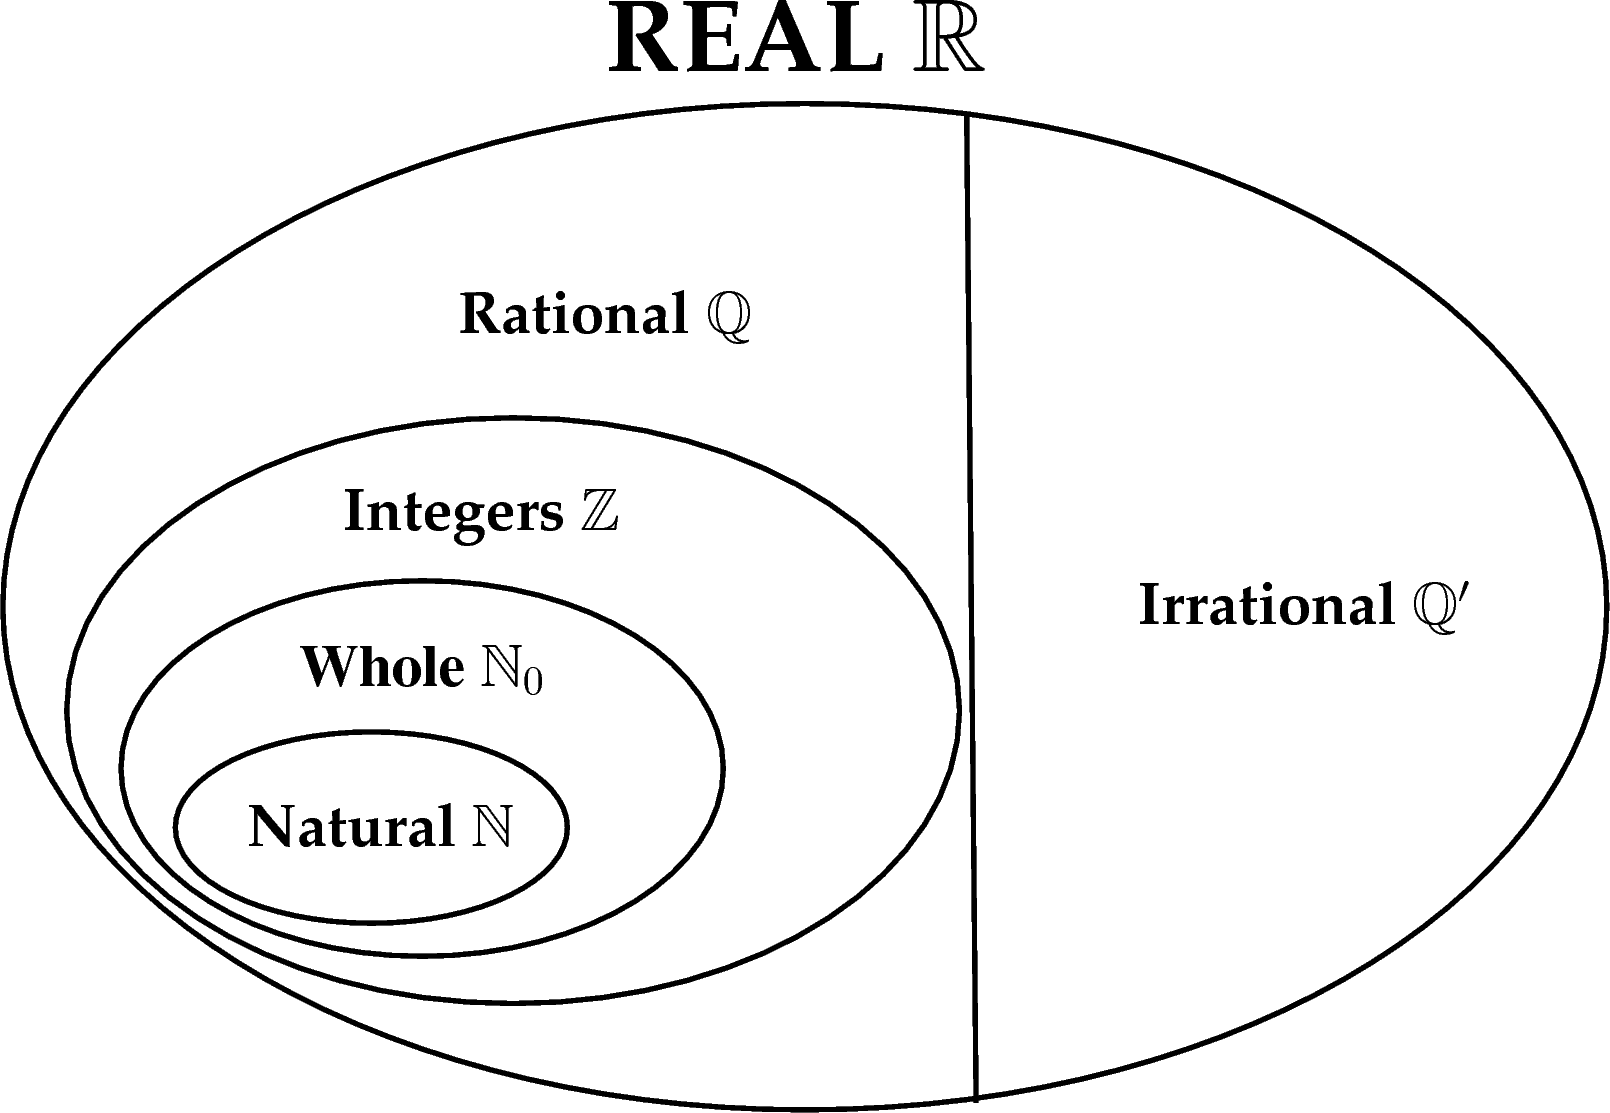
\includegraphics[width=9cm]{col11306.imgs/m38348_MG10C3_001.png} % m38348;MG10C3\_001.png;;;6.0;8.5;
\scalebox{1} % Change this value to rescale the drawing.
{
\begin{pspicture}(0,-4.764375)(14.481563,4.804375)
\psellipse[linewidth=0.04,dimen=outer](6.81,-0.484375)(6.81,4.28)
\psline[linewidth=0.04cm](8.18,3.695625)(8.26,-4.684375)
\psellipse[linewidth=0.04,dimen=outer](4.34,-1.364375)(3.8,2.5)
\psellipse[linewidth=0.04,dimen=outer](3.57,-1.854375)(2.57,1.61)
\usefont{T1}{ppl}{b}{n}
\rput(6.735781,4.350625){\Huge REAL $\mathbb{R}$}
\usefont{T1}{ppl}{b}{n}
\rput(11.03875,-0.484375){\Large Irrational $\mathbb{Q'}$}
\usefont{T1}{ppl}{b}{n}
\rput(5.11875,1.975625){\Large Rational $\mathbb{Q}$}
\usefont{T1}{ppl}{b}{n}
\rput(4.06875,0.275625){\Large Integers $\mathbb{Z}$}
\usefont{T1}{ppl}{b}{n}
\rput(3.21875,-2.324375){\Large Natural $\mathbb{N}$}
\psellipse[linewidth=0.04,dimen=outer](3.14,-2.354375)(1.68,0.83)
\usefont{T1}{ptm}{b}{n}
\rput(3.5735939,-1.024375){\Large Whole $\mathbb{N}_0$}
\end{pspicture} 
}
      \vspace{2pt}
    \vspace{.1in}
    \end{center}
 \end{figure}       
      \par 
      \label{m38348*id62554}The term whole number does not have a consistent definition. Various authors use
it in many different ways. We use the following definitions:\par 
      \label{m38348*id62559}\begin{itemize}[noitemsep]
            \label{m38348*uid1}\item natural numbers are (1, 2, 3, ...)
\label{m38348*uid2}\item whole numbers are (0, 1, 2, 3, ...)
\label{m38348*uid3}\item integers are (... -3, -2, -1, 0, 1, 2, 3, ....)
\end{itemize}
    \subsection{ Definition}
            \nopagebreak
            \label{m38348*cid4} $ \hspace{-5pt}\begin{array}{cccccccccccc}   \end{array} $ \hspace{2 pt}\raisebox{-5 pt}{
\includegraphics[width=0.5cm]{col11306.imgs/summary_www.png}} {(subsection shortcode: MG10036 )} \par 
      \label{m38348*id62607}The following numbers are all rational numbers.\par 
      \label{m38348*uid4}\nopagebreak\noindent{}
        
    \begin{equation}
    \frac{10}{1},\frac{21}{7},\frac{-1}{-3},\frac{10}{20},\frac{-3}{6}\tag{4.1}
      \end{equation}
      \label{m38348*id62687}You can see that all denominators and all numerators are integers.\par 
\label{m38348*fhsst!!!underscore!!!id138}\begin{definition}
	  \begin{tabular*}{15 cm}{m{15 mm}m{}}
	\hspace*{-50pt}  
\includegraphics[width=0.5in]{col11306.imgs/psflag2.png}   & \Definition{   \label{id2489628}\textbf{ Rational Number }} { \label{m38348*meaningfhsst!!!underscore!!!id138}
      \label{m38348*id62709}A rational number is any number which can be written as:\par 
      \label{m38348*uid6}\nopagebreak\noindent{}
        
    \begin{equation}
    \frac{a}{b}\tag{4.2}
      \end{equation}
      \label{m38348*id62732}where $a$ and $b$ are integers and $b\ne 0$. \par 
       } 
      \end{tabular*}
      \end{definition}
\label{m38348*eip-761}Note that because we can write $\frac{a}{-b}$
as $\frac{-a}{b}$
(in other words, one can always find an equivalent rational expression where $b\greatthan{}0$) mathematicians typically define rational numbers not as both $a$ and $b$ being integers, but rather that $a$ is an integer and $b$ is a natural number. This avoids having to worry about zero in the denominator. \par \label{m38348*notfhsst!!!underscore!!!id150}
\begin{tabular}{cc}
	   \hspace*{-50pt}\raisebox{-8 mm}{ 
\includegraphics[width=0.5in]{col11306.imgs/pstip2.png}  }& 
	\begin{minipage}{0.85\textwidth}
	\begin{note}
      {tip: }Only fractions which have a numerator and a denominator (that is not 0) that are integers
are rational numbers.
	\end{note}
	\end{minipage}
	\end{tabular}
	\par
      \label{m38348*id62778}This means that all integers are rational numbers, because they can be written with a denominator of 1.\par 
      \label{m38348*id62782}Therefore\par 
      \label{m38348*uid7}\nopagebreak\noindent{}
        
    \begin{equation}
    \frac{\sqrt{2}}{7},\frac{\pi }{20}\tag{4.3}
      \end{equation}
      \label{m38348*id62817}are \textbf{not examples} of rational numbers, because in each case, either the numerator or the denominator is not an integer.\par 
      \label{m38348*id62829}A number may not be written as an integer divided by another integer, but may still
be a rational number. This is because the results may be expressed
as an integer divided by an integer. The rule is, if a number can be written
as a fraction of integers, it is rational even if it can also be written in another
way as well. Here are two examples that might not look like rational numbers
at first glance but are because there are equivalent forms that are expressed as an
integer divided by another integer:\par 
      \label{m38348*uid8}\nopagebreak\noindent{}
    \begin{equation}    
    \frac{-1,33}{-3}=\frac{133}{300},\frac{-3}{6,39}=\frac{-300}{639}=\frac{-100}{213}\tag{4.4}
      \end{equation}
\label{m38348*secfhsst!!!underscore!!!id232}
            \subsubsection{Exercise: Rational Numbers }
            \nopagebreak
            \label{m38348*id63121}\begin{enumerate}[noitemsep, label=\textbf{\arabic*}. ] 
            \label{m38348*uid9}\item If $a$ is an integer, $b$ is an integer and $c$ is irrational, which of the following are rational numbers? 
\label{m38348*id734}\begin{enumerate}[noitemsep, label=\textbf{\alph*}. ] 
            \item $\frac{5}{6}$\newline
    \item $\frac{a}{3}$\newline
    \item $\frac{b}{2}$\newline
    \item $\frac{1}{c}$\end{enumerate}
        \label{m38348*uid10}\item If $\frac{a}{1}$ is a rational number, which of the following are valid values for $a$?\label{m38348*id7432}\begin{enumerate}[noitemsep, label=\textbf{\alph*}. ] 
            \item 1\item $-10$\item $\sqrt{2}$\item $2,1$\end{enumerate}
        \end{enumerate}
\par \raisebox{-5 pt}{
\includegraphics[width=0.5cm]{col11306.imgs/summary_www.png}} Find the answers with the shortcodes:
 \par \begin{tabular}[h]{cccccc}
 (1.) l35  &  (2.) l3N  & \end{tabular}
    \subsection{Decimal Numbers}
            \nopagebreak
            \label{m38348*cid5} $ \hspace{-5pt}\begin{array}{cccccccccccc}   \end{array} $ \hspace{2 pt}\raisebox{-5 pt}{
\includegraphics[width=0.5cm]{col11306.imgs/summary_www.png}} {(subsection shortcode: MG10037 )} \par 
      \label{m38348*id63345}All integers and fractions with integer numerators and denominators are rational numbers. There are two more forms of rational numbers.\par 
\label{m38348*secfhsst!!!underscore!!!id245}
            \subsubsection{  Investigation : Decimal Numbers }
            \nopagebreak
      \label{m38348*id63357}You can write the rational number
$\frac{1}{2}$ as the decimal number 0,5. Write the following numbers as
decimals:\par 
      \label{m38348*id63375}\begin{enumerate}[noitemsep, label=\textbf{\arabic*}. ] 
            \label{m38348*uid11}\item 
          $\frac{1}{4}$
        \label{m38348*uid12}\item 
          $\frac{1}{10}$
        \label{m38348*uid13}\item 
          $\frac{2}{5}$
        \label{m38348*uid14}\item 
          $\frac{1}{100}$
        \label{m38348*uid15}\item 
          $\frac{2}{3}$
        \end{enumerate}
      \label{m38348*id63486}Do the numbers after the decimal comma end or do they continue? If they continue, is there a repeating pattern to the numbers? \par 
      \label{m38348*id63495}You can write a rational number as a decimal number. Two types of decimal numbers can be written as rational numbers:\par 
      \label{m38348*id63500}\begin{enumerate}[noitemsep, label=\textbf{\arabic*}. ] 
            \label{m38348*uid16}\item decimal numbers that end or \textsl{terminate}, for example the fraction $\frac{4}{10}$ can be written as 0,4.
\label{m38348*uid17}\item decimal numbers that have a repeating pattern of numbers, for example the fraction $\frac{1}{3}$ can be written as 
$0,\dot{3}$. 
The dot represents recurring $3$'s i.e.,
$0,333...=0,\dot{3}$.
\end{enumerate}
      \label{m38348*id63576}For example, the rational number $\frac{5}{6}$ can be written in decimal notation as $0,8\dot{3}$ and similarly, the decimal number 0,25 can be written as a rational number as $\frac{1}{4}$.\par 
\label{m38348*notfhsst!!!underscore!!!id301}
\begin{tabular}{cc}
	   \hspace*{-50pt}\raisebox{-8 mm}{ 
\includegraphics[width=0.5in]{col11306.imgs/pstip2.png}  }& 
	\begin{minipage}{0.85\textwidth}
	\begin{note}
      {tip: }You can use a bar over the repeated numbers to indicate that the decimal is a repeating decimal.
	\end{note}
	\end{minipage}
	\end{tabular}
	\par
    \subsection{ Converting Terminating Decimals into Rational Numbers}
            \nopagebreak
            \label{m38348*cid6} $ \hspace{-5pt}\begin{array}{cccccccccccc}   \end{array} $ \hspace{2 pt}\raisebox{-5 pt}{
\includegraphics[width=0.5cm]{col11306.imgs/summary_www.png}} {(subsection shortcode: MG10038 )} \par 
      \label{m38348*id63646}A decimal number has an integer part and a fractional part. For example $10,589$ has an integer part of 10 and a fractional part of $0,589$ because $10+0,589=10,589$. The fractional part can be written as a rational number, i.e. with a numerator and a denominator that are integers.\par 
      \label{m38348*id63704}Each digit after the decimal point is a fraction with a denominator in increasing powers of ten. For example:\par 
      \label{m38348*id63708}\begin{itemize}[noitemsep]
            \label{m38348*uid18}\item $\frac{1}{10}$ is $0,1$\label{m38348*uid19}\item $\frac{1}{100}$ is $0,01$\end{itemize}
      \label{m38348*id63781}This means that:\par 
      \label{m38348*id63784}\nopagebreak\noindent{}
    \begin{equation}
    \begin{array}{ccc}\hfill 10,589& =& 10+\frac{5}{10}+\frac{8}{100}+\frac{9}{1000}\hfill \\ & =& 10\frac{589}{1000}\hfill \\ & =& \frac{10589}{1000}\hfill \end{array}\tag{4.5}
      \end{equation}
\label{m38348*secfhsst!!!underscore!!!id378}
            \subsubsection{ Exercise: Fractions }
            \nopagebreak
      \label{m38348*id63882}\begin{enumerate}[noitemsep, label=\textbf{\arabic*}. ] 
            \label{m38348*uid20}\item Write the following as fractions:\label{m38348*id7322}\begin{enumerate}[noitemsep, label=\textbf{\alph*}. ] 
            \item $0,1$\item $0,12$\item $0,58$\item $0,2589$\end{enumerate}
        \end{enumerate}
\par \raisebox{-5 pt}{
\includegraphics[width=0.5cm]{col11306.imgs/summary_www.png}} Find the answers with the shortcodes:
 \par \begin{tabular}[h]{cccccc}
 (1.) l3R  & \end{tabular}
    \subsection{ Converting Repeating Decimals into Rational Numbers}
            \nopagebreak
            \label{m38348*cid7} $ \hspace{-5pt}\begin{array}{cccccccccccc}   \end{array} $ \hspace{2 pt}\raisebox{-5 pt}{
\includegraphics[width=0.5cm]{col11306.imgs/summary_www.png}} {(subsection shortcode: MG10039 )} \par 
      \label{m38348*id63993}When the decimal is a repeating decimal, a bit more work is needed to write the fractional part of the decimal number as a fraction. We will explain by means of an example.\par 
      \label{m38348*id63998}If we wish to write $0,\dot{3}$ in the form $\frac{a}{b}$ (where $a$ and $b$ are integers) then we would proceed as follows
\par 
      \label{m38348*uid21}\nopagebreak\noindent{}
    \begin{equation}
    \begin{array}{cccc}\hfill x& =& 0,33333...\hfill & \\ \hfill 10x& =& 3,33333...\hfill & \text{multiply}\phantom{\rule{4.pt}{0ex}}\text{by}\phantom{\rule{4.pt}{0ex}}\text{10}\phantom{\rule{4.pt}{0ex}}\text{on}\phantom{\rule{4.pt}{0ex}}\text{both}\phantom{\rule{4.pt}{0ex}}\text{sides}\hfill \\ \hfill 9x& =& 3\hfill & \text{(}\text{subtracting}\phantom{\rule{4.pt}{0ex}}\text{the}\phantom{\rule{4.pt}{0ex}}\text{second}\phantom{\rule{4.pt}{0ex}}\text{equation}\phantom{\rule{4.pt}{0ex}}\text{from}\phantom{\rule{4.pt}{0ex}}\text{the}\phantom{\rule{4.pt}{0ex}}\text{first}\phantom{\rule{4.pt}{0ex}}\text{equation}\text{)}\hfill \\ \hfill x& =& \frac{3}{9}=\frac{1}{3}\hfill & \end{array}\tag{4.6}
      \end{equation}
      \label{m38348*id64237}And another example would be to write 
$5,\dot{4}\dot{3}\dot{2}$ 
as a rational fraction.
\par 
      \label{m38348*uid22}\nopagebreak\noindent{}
    \begin{equation}
    \begin{array}{cccc}\hfill x& =& 5,432432432...\hfill & \\ \hfill 1000x& =& 5432,432432432...\hfill & \text{multiply by\hspace{0.17em}}\phantom{\rule{4.pt}{0ex}}\text{1000}\phantom{\rule{4.pt}{0ex}}\text{on both sides}\\ \hfill \\ \hfill 999x& =& 5427\hfill & \text{(}\text{subtracting the second equation from the first equation}\text{)}\\ \hfill x& =& \frac{5427}{999}=\frac{201}{37}\hfill & \end{array}\tag{4.7}
      \end{equation}
      \label{m38348*id64459}For the first example, the decimal was multiplied by 10 and for the second example, the decimal was multiplied by 1000. This is because for the first example there was only one digit (i.e. 3) recurring, while for the second example there were three digits (i.e. 432) recurring.\par 
      \label{m38348*id64465}In general, if you have one digit recurring, then multiply by 10. If you have two digits recurring, then multiply by 100. If you have three digits recurring, then multiply by 1000. Can you spot the pattern yet?\par 
      \label{m38348*id64470}The number of zeros is the same as the number of recurring digits.\par 
      \label{m38348*id64474}Not all decimal numbers can be written as rational numbers. Why? Irrational decimal numbers like 
$\sqrt{2}=1,4142135...$
cannot be written with an integer numerator and denominator, because they do not have a pattern of recurring digits. However, when possible, you should try to use rational numbers or fractions instead of decimals.\par 
\label{m38348*secfhsst!!!underscore!!!id606}
            \subsubsection{Exercise: Repeated Decimal Notation }
            \nopagebreak
      \label{m38348*id64513}\begin{enumerate}[noitemsep, label=\textbf{\arabic*}. ] 
            \label{m38348*uid23}\item Write the following using the repeated decimal notation:
\label{m38348*id64529}\begin{enumerate}[noitemsep, label=\textbf{\alph*}. ] 
            \label{m38348*uid24}\item $0,11111111...$\label{m38348*uid25}\item $0,1212121212...$\label{m38348*uid26}\item $0,123123123123...$\label{m38348*uid27}\item $0,11414541454145...$\end{enumerate}
        \label{m38348*uid28}\item Write the following in decimal form, using the repeated decimal notation:
\label{m38348*id64650}\begin{enumerate}[noitemsep, label=\textbf{\alph*}. ] 
            \label{m38348*uid29}\item $\frac{2}{3}$\label{m38348*uid30}\item $1\frac{3}{11}$\label{m38348*uid31}\item $4\frac{5}{6}$\label{m38348*uid32}\item $2\frac{1}{9}$\end{enumerate}
        \label{m38348*uid33}\item Write the following decimals in fractional form:
\label{m38348*id64767}\begin{enumerate}[noitemsep, label=\textbf{\alph*}. ] 
            \label{m38348*uid34}\item $0,633\dot{3}$\label{m38348*uid35}\item $5,3131\overline{31}$\label{m38348*uid36}\item $0,99999\dot{9}$\end{enumerate}
        \end{enumerate}
\par \raisebox{-5 pt}{
\includegraphics[width=0.5cm]{col11306.imgs/summary_www.png}} Find the answers with the shortcodes:
 \par \begin{tabular}[h]{cccccc}
 (1.) l3U  &  (2.) l3n  &  (3.) l3Q  & \end{tabular}
         \section{Irrational Numbers}
    \setcounter{figure}{1}
    \setcounter{subfigure}{1}
    \label{m38349}
    \subsection{ Introduction}
            \nopagebreak
            \label{m38349*cid2} $ \hspace{-5pt}\begin{array}{cccccccccccc}   \end{array} $ \hspace{2 pt}\raisebox{-5 pt}{
\includegraphics[width=0.5cm]{col11306.imgs/summary_www.png}} {(subsection shortcode: MG10055 )} \par 
      \label{m38349*id324260}You have seen that repeating decimals may take a lot of paper and ink to write out. Not only is that impossible, but writing numbers out to many decimal places or \textsl{a high accuracy} is very inconvenient and rarely gives practical answers. For this reason we often estimate the number to a certain number of decimal places or to a given number of \textsl{significant figures}, which is even better.\par 
    \subsection{ Definition}
            \nopagebreak
            \label{m38349*cid3} $ \hspace{-5pt}\begin{array}{cccccccccccc}   \end{array} $ \hspace{2 pt}\raisebox{-5 pt}{
\includegraphics[width=0.5cm]{col11306.imgs/summary_www.png}} {(subsection shortcode: MG10056 )} \par \label{m38349*id324624}Irrational numbers are numbers that cannot be written as a fraction with the numerator and denominator as integers. This means that any number that is \textsl{not} a terminating decimal number or a repeating decimal number is irrational. Examples of irrational numbers are:\par 
      \label{m38349*id324635}\nopagebreak\noindent{}
        
    \begin{equation}
    \begin{array}{cc}\hfill \sqrt{2},\sqrt{3},\sqrt[3]{4},\pi ,\\ \hfill \frac{1+\sqrt{5}}{2}\approx 1,618\phantom{\rule{0.166667em}{0ex}}033\phantom{\rule{0.166667em}{0ex}}989\phantom{\rule{0.166667em}{0ex}}\end{array}\tag{7.1}
      \end{equation}
\label{m38349*notfhsst!!!underscore!!!id128}
\begin{tabular}{cc}
	   \hspace*{-50pt}\raisebox{-8 mm}{ 
\includegraphics[width=0.5in]{col11306.imgs/pstip2.png}  }& 
	\begin{minipage}{0.85\textwidth}
	\begin{note}
      {tip: }When irrational numbers are written in decimal form, they go on forever and
there is no repeated pattern of digits.
	\end{note}
	\end{minipage}
	\end{tabular}
	\par
      \label{m38349*id324739}If you are asked to identify whether a number is rational or irrational, first write the number in decimal form. If the number is terminated then it is rational. If it goes on forever, then look for a repeated pattern of digits. If there is no repeated pattern, then the number is irrational.\par 
      \label{m38349*id324745}When you write irrational numbers in decimal form, you may (if you have a lot of time and paper!) continue writing them for many, many decimal places. However, this is not convenient and it is often necessary to round off.\par 
\label{m38349*secfhsst!!!underscore!!!id133}
            \subsubsection{  Investigation : Irrational Numbers }
            \nopagebreak
      \label{m38349*id324757}Which of the following cannot be
written as a rational number?\par 
      \label{m38349*id324763}\textbf{Remember}: A rational number is a fraction with numerator and denominator as integers. Terminating decimal numbers or repeating decimal numbers are rational.\par 
      \label{m38349*id324775}\begin{enumerate}[noitemsep, label=\textbf{\arabic*}. ] 
            \label{m38349*uid1}\item 
          $\pi =3,14159265358979323846264338327950288419716939937510...$
        \label{m38349*uid2}\item $1,4$
\label{m38349*uid3}\item 
          $1,618\phantom{\rule{0.166667em}{0ex}}033\phantom{\rule{0.166667em}{0ex}}989\phantom{\rule{0.166667em}{0ex}}...$
        \label{m38349*uid4}\item $100$
\end{enumerate}
    \section{ Rounding Off}
            \nopagebreak
            \label{m38349*cid4} $ \hspace{-5pt}\begin{array}{cccccccccccc}   
\includegraphics[width=0.75cm]{col11306.imgs/summary_fullmarks.png} &   \end{array} $ \hspace{2 pt}\raisebox{-5 pt}{} {(section shortcode: MG10057 )} \par 
      \label{m38349*id324198}Rounding off or approximating a decimal number to a given number of decimal places is the quickest way to approximate a number. For example, if you wanted to round-off $2,6525272$ to three decimal places then you would first count three places after the decimal and place a $|$ between the third and fourth number after the decimal.\par 
      \label{m38349*id325085}\nopagebreak\noindent{}
        
    \begin{equation}
    2,652|5272\tag{7.2}
      \end{equation}
      \label{m38349*id325105}All numbers to the right of the $|$ are ignored after you determine whether the number in the third decimal place must be rounded up or rounded down. You \textsl{round up} the final digit if the first digit after the $|$ was greater than or equal to 5 and \textsl{round down} (leave the digit alone) otherwise. In the case that the first digit before the $|$ is 9 \textsl{and} you need to round up, then the 9 becomes a 0 and the second digit before the $|$ is rounded up.\par 
      \label{m38349*id325160}So, since the first digit after the $|$ is a 5, we must round up the digit in the third decimal place to a 3 and the final answer of $2,6525272$ rounded to three decimal places is\par 
      \label{m38349*id325186}\nopagebreak\noindent{}
        
    \begin{equation}
    2,653\tag{7.3}
      \end{equation}
\par
            \label{m38349*secfhsst!!!underscore!!!id199}\vspace{.5cm} 
      \noindent
      \hspace*{-30pt}
\includegraphics[width=0.5in]{col11306.imgs/pspencil2.png}   \raisebox{25mm}{   
      \begin{mdframed}[linewidth=4, leftmargin=40, rightmargin=40]  
      \begin{exercise}
    \noindent\textbf{Exercise 7.1:  Rounding-Off }
      \label{m38349*probfhsst!!!underscore!!!id200}
      \label{m38349*id325213}Round-off the following numbers to the indicated number of decimal places:\par 
      \label{m38349*id325219}\begin{enumerate}[noitemsep, label=\textbf{\arabic*}. ] 
            \leftskip=20pt\rightskip=\leftskip\label{m38349*uid5}\item $\frac{120}{99}=1,212121212\dot{1}\dot{2}$ to 3 decimal places
\label{m38349*uid6}\item $\pi =3,141592654...$ to 4 decimal places
\label{m38349*uid7}\item $\sqrt{3}=1,7320508...$ to 4 decimal places
\label{m38349*uid789}\item $2,78974526...$ to 3 decimal places\end{enumerate}
      \vspace{5pt}
      \label{m38349*solfhsst!!!underscore!!!id212}\noindent\textbf{Solution to Exercise } \label{m38349*listfhsst!!!underscore!!!id212}\begin{enumerate}[noitemsep, label=\textbf{Step} \textbf{\arabic*}. ] 
            \leftskip=20pt\rightskip=\leftskip\item  
      \label{m38349*id325360}\begin{enumerate}[noitemsep, label=\textbf{\alph*}. ] 
            \leftskip=20pt\rightskip=\leftskip\label{m38349*uid8}\item 
          $\frac{120}{99}=1,212|121212\dot{1}\dot{2}$
        \label{m38349*uid9}\item 
          $\pi =3,1415|92654...$
        \label{m38349*uid10}\item 
          $\sqrt{3}=1,7320|508...$
        \item $2,789|74526...$\end{enumerate}
      \item  
      \label{m38349*id325490}\begin{enumerate}[noitemsep, label=\textbf{\alph*}. ] 
            \leftskip=20pt\rightskip=\leftskip\label{m38349*uid11}\item The last digit of $\frac{120}{99}=1,212|121212\dot{1}\dot{2}$  must be rounded down.
\label{m38349*uid12}\item The last digit of $\pi =3,1415|92654...$ must be rounded up.
\label{m38349*uid13}\item The last digit of $\sqrt{3}=1,7320|508...$ must be rounded up.
\item  The last digit of $2,789|74526...$ must be rounded up. Since this is a 9, we replace it with a 0 and round up the second last digit.\end{enumerate}
      \item  
      \label{m38349*id325626}\begin{enumerate}[noitemsep, label=\textbf{\alph*}. ] 
            \leftskip=20pt\rightskip=\leftskip\label{m38349*uid14}\item $\frac{120}{99}=1,212$ rounded to 3 decimal places
\label{m38349*uid15}\item $\pi =3,1416$  rounded to 4 decimal places
\label{m38349*uid16}\item $\sqrt{3}=1,7321$ rounded to 4 decimal places
\item $2,790$\end{enumerate}
      \end{enumerate}
    \end{exercise}
    \end{mdframed}
    }
    \noindent
         \section{Estimating surds}
    \setcounter{figure}{1}
    \setcounter{subfigure}{1}
    \label{m38347}
%     \subsection{ Introduction}
            \nopagebreak
            \label{m38347*cid1} $ \hspace{-5pt}\begin{array}{cccccccccccc}   
\includegraphics[width=0.75cm]{col11306.imgs/summary_fullmarks.png} &   \end{array} $ \hspace{2 pt}\raisebox{-5 pt}{} {(subsection shortcode: MG10052 )} \par 
      \label{m38347*id258007}You should know by now what the ${n}^{\mathrm{th}}$ root of a number means. If the ${n}^{\mathrm{th}}$ root of a number cannot be simplified to a rational number, we call it a $\mathit{surd}$. For example, $\sqrt{2}$ and $\sqrt[3]{6}$ are surds, but $\sqrt{4}$ is not a surd because it can be simplified to the rational number 2.\par 
      \label{m38347*id258405}In this chapter we will only look at surds that look like $\sqrt[n]{a}$, where $a$ is any positive number, for example $\sqrt{7}$ or $\sqrt[3]{5}$. It is very common for $n$ to be 2, so we usually do not write $\sqrt[2]{a}$. Instead we write the surd as just $\sqrt{a}$, which is much easier to read.\par 
      \label{m38347*id258479}It is sometimes useful to know the approximate value of a surd without having to use a calculator. For example, we want to be able to estimate where a surd like $\sqrt{3}$ is on the number line. So how do we know where surds lie on the number line? From a calculator we know that $\sqrt{3}$ is equal to $1,73205...$. It is easy to see that $\sqrt{3}$ is above 1 and below 2. But to see this for other surds like $\sqrt{18}$ without using a calculator, you must first understand the following fact:\par 
\label{m38347*notfhsst!!!underscore!!!id71}
\begin{tabular}{cc}
	\hspace*{-50pt}\raisebox{-8 mm}{\hspace{-0.2in}
\includegraphics[width=0.75in]{col11306.imgs/psfact2.png} } & 
	\begin{minipage}{0.85\textwidth}
	\begin{note}
      {note: } 
If $a$ and $b$ are positive whole numbers, and $a\lessthan{}b$, then $\sqrt[n]{a}\lessthan{}\sqrt[n]{b}$. (Challenge: Can you explain why?)
	\end{note}
	\end{minipage}
	\end{tabular}
	\par
      \label{m38347*id258599}If you don't believe this fact, check it for a few numbers to convince yourself it is true.\par 
      \label{m38347*id258603}How do we use this fact to help us guess what $\sqrt{18}$ is? Well, you can easily see that $18\lessthan{}25$. Using our rule, we also know that $\sqrt{18}\lessthan{}\sqrt{25}$. But we know that ${5}^{2}=25$ so that $\sqrt{25}=5$. Now it is easy to simplify to get $\sqrt{18}\lessthan{}5$. Now we have a better idea of what $\sqrt{18}$ is.\par 
      \label{m38347*id258700}Now we know that $\sqrt{18}$ is less than 5, but this is only half the story. We can use the same trick again, but this time with 18 on the right-hand side. You will agree that $16\lessthan{}18$. Using our rule again, we also know that $\sqrt{16}\lessthan{}\sqrt{18}$. But we know that 16 is a perfect square, so we can simplify $\sqrt{16}$ to 4, and so we get $4\lessthan{}\sqrt{18}$!\par 
      \label{m38347*id258766}As you can see, we have shown that $\sqrt{18}$ is between 4 and 5. If we check on our calculator, we can see that $\sqrt{18}=4,1231...$, and the idea was right! You will notice that our idea used perfect squares that were close to the number 18. We found the largest perfect square smaller than 18 was ${4}^{2}=16$, and the smallest perfect square greater than 18 was ${5}^{2}=25$. Here is a quick summary of what a perfect square or cube is:\par 
\label{m38347*notfhsst!!!underscore!!!id78}
\begin{tabular}{cc}
	\hspace*{-50pt}\raisebox{-8 mm}{\hspace{-0.2in}
\includegraphics[width=0.75in]{col11306.imgs/psfact2.png} } & 
	\begin{minipage}{0.85\textwidth}
	\begin{note}
      {note: } A perfect square is the number obtained when an integer is squared. For example, 9 is a perfect square since ${3}^{2}=9$. Similarly, a perfect cube is a number which is the cube of an integer. For example, 27 is a perfect cube, because ${3}^{3}=27$.
	\end{note}
	\end{minipage}
	\end{tabular}
	\par
      \label{m38347*id258890}To make it easier to use our idea, we will create a list of some of the perfect squares and perfect cubes. The list is shown in Table 6.1.\par 
    % \textbf{m38347*uid1}\par
    % how many colspecs?  3
          % name: cnx:colspec
            % colnum: 1
            % colwidth: 10*
            % latex-name: columna
            % colname: 
            % align/tgroup-align/default: //left
            % -------------------------
            % name: cnx:colspec
            % colnum: 2
            % colwidth: 10*
            % latex-name: columnb
            % colname: 
            % align/tgroup-align/default: //left
            % -------------------------
            % name: cnx:colspec
            % colnum: 3
            % colwidth: 10*
            % latex-name: columnc
            % colname: 
            % align/tgroup-align/default: //left
            % -------------------------
    \setlength\mytablespace{6\tabcolsep}
    \addtolength\mytablespace{4\arrayrulewidth}
    \setlength\mytablewidth{\linewidth}
    \setlength\mytableroom{\mytablewidth}
    \addtolength\mytableroom{-\mytablespace}
    \setlength\myfixedwidth{0pt}
    \setlength\mystarwidth{\mytableroom}
        \addtolength\mystarwidth{-\myfixedwidth}
        \divide\mystarwidth 30
      % ----- Begin capturing width of table in LR mode woof
      \settowidth{\mytableboxwidth}{\begin{tabular}[t]{|l|l|l|}\hline
    % count in rowspan-info-nodeset: 3
    % align/colidx: left,1
    % rowcount: '0' | start: 'false' | colidx: '1'
        % Formatting a regular cell and recurring on the next sibling
        Integer &
      % align/colidx: left,2
    % rowcount: '0' | start: 'false' | colidx: '2'
        % Formatting a regular cell and recurring on the next sibling
        Perfect Square &
      % align/colidx: left,3
    % rowcount: '0' | start: 'false' | colidx: '3'
        % Formatting a regular cell and recurring on the next sibling
        Perfect Cube% make-rowspan-placeholders
    % rowspan info: col1 '0' | 'false' | '' || col2 '0' | 'false' | '' || col3 '0' | 'false' | ''
     \tabularnewline\cline{1-1}\cline{2-2}\cline{3-3}
      %--------------------------------------------------------------------
    % align/colidx: left,1
    % rowcount: '0' | start: 'false' | colidx: '1'
        % Formatting a regular cell and recurring on the next sibling
        0 &
      % align/colidx: left,2
    % rowcount: '0' | start: 'false' | colidx: '2'
        % Formatting a regular cell and recurring on the next sibling
        0 &
      % align/colidx: left,3
    % rowcount: '0' | start: 'false' | colidx: '3'
        % Formatting a regular cell and recurring on the next sibling
        0% make-rowspan-placeholders
    % rowspan info: col1 '0' | 'false' | '' || col2 '0' | 'false' | '' || col3 '0' | 'false' | ''
     \tabularnewline\cline{1-1}\cline{2-2}\cline{3-3}
      %--------------------------------------------------------------------
    % align/colidx: left,1
    % rowcount: '0' | start: 'false' | colidx: '1'
        % Formatting a regular cell and recurring on the next sibling
        1 &
      % align/colidx: left,2
    % rowcount: '0' | start: 'false' | colidx: '2'
        % Formatting a regular cell and recurring on the next sibling
        1 &
      % align/colidx: left,3
    % rowcount: '0' | start: 'false' | colidx: '3'
        % Formatting a regular cell and recurring on the next sibling
        1% make-rowspan-placeholders
    % rowspan info: col1 '0' | 'false' | '' || col2 '0' | 'false' | '' || col3 '0' | 'false' | ''
     \tabularnewline\cline{1-1}\cline{2-2}\cline{3-3}
      %--------------------------------------------------------------------
    % align/colidx: left,1
    % rowcount: '0' | start: 'false' | colidx: '1'
        % Formatting a regular cell and recurring on the next sibling
        2 &
      % align/colidx: left,2
    % rowcount: '0' | start: 'false' | colidx: '2'
        % Formatting a regular cell and recurring on the next sibling
        4 &
      % align/colidx: left,3
    % rowcount: '0' | start: 'false' | colidx: '3'
        % Formatting a regular cell and recurring on the next sibling
        8% make-rowspan-placeholders
    % rowspan info: col1 '0' | 'false' | '' || col2 '0' | 'false' | '' || col3 '0' | 'false' | ''
     \tabularnewline\cline{1-1}\cline{2-2}\cline{3-3}
      %--------------------------------------------------------------------
    % align/colidx: left,1
    % rowcount: '0' | start: 'false' | colidx: '1'
        % Formatting a regular cell and recurring on the next sibling
        3 &
      % align/colidx: left,2
    % rowcount: '0' | start: 'false' | colidx: '2'
        % Formatting a regular cell and recurring on the next sibling
        9 &
      % align/colidx: left,3
    % rowcount: '0' | start: 'false' | colidx: '3'
        % Formatting a regular cell and recurring on the next sibling
        27% make-rowspan-placeholders
    % rowspan info: col1 '0' | 'false' | '' || col2 '0' | 'false' | '' || col3 '0' | 'false' | ''
     \tabularnewline\cline{1-1}\cline{2-2}\cline{3-3}
      %--------------------------------------------------------------------
    % align/colidx: left,1
    % rowcount: '0' | start: 'false' | colidx: '1'
        % Formatting a regular cell and recurring on the next sibling
        4 &
      % align/colidx: left,2
    % rowcount: '0' | start: 'false' | colidx: '2'
        % Formatting a regular cell and recurring on the next sibling
        16 &
      % align/colidx: left,3
    % rowcount: '0' | start: 'false' | colidx: '3'
        % Formatting a regular cell and recurring on the next sibling
        64% make-rowspan-placeholders
    % rowspan info: col1 '0' | 'false' | '' || col2 '0' | 'false' | '' || col3 '0' | 'false' | ''
     \tabularnewline\cline{1-1}\cline{2-2}\cline{3-3}
      %--------------------------------------------------------------------
    % align/colidx: left,1
    % rowcount: '0' | start: 'false' | colidx: '1'
        % Formatting a regular cell and recurring on the next sibling
        5 &
      % align/colidx: left,2
    % rowcount: '0' | start: 'false' | colidx: '2'
        % Formatting a regular cell and recurring on the next sibling
        25 &
      % align/colidx: left,3
    % rowcount: '0' | start: 'false' | colidx: '3'
        % Formatting a regular cell and recurring on the next sibling
        125% make-rowspan-placeholders
    % rowspan info: col1 '0' | 'false' | '' || col2 '0' | 'false' | '' || col3 '0' | 'false' | ''
     \tabularnewline\cline{1-1}\cline{2-2}\cline{3-3}
      %--------------------------------------------------------------------
    % align/colidx: left,1
    % rowcount: '0' | start: 'false' | colidx: '1'
        % Formatting a regular cell and recurring on the next sibling
        6 &
      % align/colidx: left,2
    % rowcount: '0' | start: 'false' | colidx: '2'
        % Formatting a regular cell and recurring on the next sibling
        36 &
      % align/colidx: left,3
    % rowcount: '0' | start: 'false' | colidx: '3'
        % Formatting a regular cell and recurring on the next sibling
        216% make-rowspan-placeholders
    % rowspan info: col1 '0' | 'false' | '' || col2 '0' | 'false' | '' || col3 '0' | 'false' | ''
     \tabularnewline\cline{1-1}\cline{2-2}\cline{3-3}
      %--------------------------------------------------------------------
    % align/colidx: left,1
    % rowcount: '0' | start: 'false' | colidx: '1'
        % Formatting a regular cell and recurring on the next sibling
        7 &
      % align/colidx: left,2
    % rowcount: '0' | start: 'false' | colidx: '2'
        % Formatting a regular cell and recurring on the next sibling
        49 &
      % align/colidx: left,3
    % rowcount: '0' | start: 'false' | colidx: '3'
        % Formatting a regular cell and recurring on the next sibling
        343% make-rowspan-placeholders
    % rowspan info: col1 '0' | 'false' | '' || col2 '0' | 'false' | '' || col3 '0' | 'false' | ''
     \tabularnewline\cline{1-1}\cline{2-2}\cline{3-3}
      %--------------------------------------------------------------------
    % align/colidx: left,1
    % rowcount: '0' | start: 'false' | colidx: '1'
        % Formatting a regular cell and recurring on the next sibling
        8 &
      % align/colidx: left,2
    % rowcount: '0' | start: 'false' | colidx: '2'
        % Formatting a regular cell and recurring on the next sibling
        64 &
      % align/colidx: left,3
    % rowcount: '0' | start: 'false' | colidx: '3'
        % Formatting a regular cell and recurring on the next sibling
        512% make-rowspan-placeholders
    % rowspan info: col1 '0' | 'false' | '' || col2 '0' | 'false' | '' || col3 '0' | 'false' | ''
     \tabularnewline\cline{1-1}\cline{2-2}\cline{3-3}
      %--------------------------------------------------------------------
    % align/colidx: left,1
    % rowcount: '0' | start: 'false' | colidx: '1'
        % Formatting a regular cell and recurring on the next sibling
        9 &
      % align/colidx: left,2
    % rowcount: '0' | start: 'false' | colidx: '2'
        % Formatting a regular cell and recurring on the next sibling
        81 &
      % align/colidx: left,3
    % rowcount: '0' | start: 'false' | colidx: '3'
        % Formatting a regular cell and recurring on the next sibling
        729% make-rowspan-placeholders
    % rowspan info: col1 '0' | 'false' | '' || col2 '0' | 'false' | '' || col3 '0' | 'false' | ''
     \tabularnewline\cline{1-1}\cline{2-2}\cline{3-3}
      %--------------------------------------------------------------------
    % align/colidx: left,1
    % rowcount: '0' | start: 'false' | colidx: '1'
        % Formatting a regular cell and recurring on the next sibling
        10 &
      % align/colidx: left,2
    % rowcount: '0' | start: 'false' | colidx: '2'
        % Formatting a regular cell and recurring on the next sibling
        100 &
      % align/colidx: left,3
    % rowcount: '0' | start: 'false' | colidx: '3'
        % Formatting a regular cell and recurring on the next sibling
        1000% make-rowspan-placeholders
    % rowspan info: col1 '0' | 'false' | '' || col2 '0' | 'false' | '' || col3 '0' | 'false' | ''
     \tabularnewline\cline{1-1}\cline{2-2}\cline{3-3}
      %--------------------------------------------------------------------
    \end{tabular}} % end mytableboxwidth set      
      % ----- End capturing width of table in LR mode
        % ----- LR or paragraph mode: must test
        % ----- Begin capturing height of table
        \settoheight{\mytableboxheight}{\begin{tabular}[t]{|l|l|l|}\hline
    % count in rowspan-info-nodeset: 3
    % align/colidx: left,1
    % rowcount: '0' | start: 'false' | colidx: '1'
        % Formatting a regular cell and recurring on the next sibling
        Integer &
      % align/colidx: left,2
    % rowcount: '0' | start: 'false' | colidx: '2'
        % Formatting a regular cell and recurring on the next sibling
        Perfect Square &
      % align/colidx: left,3
    % rowcount: '0' | start: 'false' | colidx: '3'
        % Formatting a regular cell and recurring on the next sibling
        Perfect Cube% make-rowspan-placeholders
    % rowspan info: col1 '0' | 'false' | '' || col2 '0' | 'false' | '' || col3 '0' | 'false' | ''
     \tabularnewline\cline{1-1}\cline{2-2}\cline{3-3}
      %--------------------------------------------------------------------
    % align/colidx: left,1
    % rowcount: '0' | start: 'false' | colidx: '1'
        % Formatting a regular cell and recurring on the next sibling
        0 &
      % align/colidx: left,2
    % rowcount: '0' | start: 'false' | colidx: '2'
        % Formatting a regular cell and recurring on the next sibling
        0 &
      % align/colidx: left,3
    % rowcount: '0' | start: 'false' | colidx: '3'
        % Formatting a regular cell and recurring on the next sibling
        0% make-rowspan-placeholders
    % rowspan info: col1 '0' | 'false' | '' || col2 '0' | 'false' | '' || col3 '0' | 'false' | ''
     \tabularnewline\cline{1-1}\cline{2-2}\cline{3-3}
      %--------------------------------------------------------------------
    % align/colidx: left,1
    % rowcount: '0' | start: 'false' | colidx: '1'
        % Formatting a regular cell and recurring on the next sibling
        1 &
      % align/colidx: left,2
    % rowcount: '0' | start: 'false' | colidx: '2'
        % Formatting a regular cell and recurring on the next sibling
        1 &
      % align/colidx: left,3
    % rowcount: '0' | start: 'false' | colidx: '3'
        % Formatting a regular cell and recurring on the next sibling
        1% make-rowspan-placeholders
    % rowspan info: col1 '0' | 'false' | '' || col2 '0' | 'false' | '' || col3 '0' | 'false' | ''
     \tabularnewline\cline{1-1}\cline{2-2}\cline{3-3}
      %--------------------------------------------------------------------
    % align/colidx: left,1
    % rowcount: '0' | start: 'false' | colidx: '1'
        % Formatting a regular cell and recurring on the next sibling
        2 &
      % align/colidx: left,2
    % rowcount: '0' | start: 'false' | colidx: '2'
        % Formatting a regular cell and recurring on the next sibling
        4 &
      % align/colidx: left,3
    % rowcount: '0' | start: 'false' | colidx: '3'
        % Formatting a regular cell and recurring on the next sibling
        8% make-rowspan-placeholders
    % rowspan info: col1 '0' | 'false' | '' || col2 '0' | 'false' | '' || col3 '0' | 'false' | ''
     \tabularnewline\cline{1-1}\cline{2-2}\cline{3-3}
      %--------------------------------------------------------------------
    % align/colidx: left,1
    % rowcount: '0' | start: 'false' | colidx: '1'
        % Formatting a regular cell and recurring on the next sibling
        3 &
      % align/colidx: left,2
    % rowcount: '0' | start: 'false' | colidx: '2'
        % Formatting a regular cell and recurring on the next sibling
        9 &
      % align/colidx: left,3
    % rowcount: '0' | start: 'false' | colidx: '3'
        % Formatting a regular cell and recurring on the next sibling
        27% make-rowspan-placeholders
    % rowspan info: col1 '0' | 'false' | '' || col2 '0' | 'false' | '' || col3 '0' | 'false' | ''
     \tabularnewline\cline{1-1}\cline{2-2}\cline{3-3}
      %--------------------------------------------------------------------
    % align/colidx: left,1
    % rowcount: '0' | start: 'false' | colidx: '1'
        % Formatting a regular cell and recurring on the next sibling
        4 &
      % align/colidx: left,2
    % rowcount: '0' | start: 'false' | colidx: '2'
        % Formatting a regular cell and recurring on the next sibling
        16 &
      % align/colidx: left,3
    % rowcount: '0' | start: 'false' | colidx: '3'
        % Formatting a regular cell and recurring on the next sibling
        64% make-rowspan-placeholders
    % rowspan info: col1 '0' | 'false' | '' || col2 '0' | 'false' | '' || col3 '0' | 'false' | ''
     \tabularnewline\cline{1-1}\cline{2-2}\cline{3-3}
      %--------------------------------------------------------------------
    % align/colidx: left,1
    % rowcount: '0' | start: 'false' | colidx: '1'
        % Formatting a regular cell and recurring on the next sibling
        5 &
      % align/colidx: left,2
    % rowcount: '0' | start: 'false' | colidx: '2'
        % Formatting a regular cell and recurring on the next sibling
        25 &
      % align/colidx: left,3
    % rowcount: '0' | start: 'false' | colidx: '3'
        % Formatting a regular cell and recurring on the next sibling
        125% make-rowspan-placeholders
    % rowspan info: col1 '0' | 'false' | '' || col2 '0' | 'false' | '' || col3 '0' | 'false' | ''
     \tabularnewline\cline{1-1}\cline{2-2}\cline{3-3}
      %--------------------------------------------------------------------
    % align/colidx: left,1
    % rowcount: '0' | start: 'false' | colidx: '1'
        % Formatting a regular cell and recurring on the next sibling
        6 &
      % align/colidx: left,2
    % rowcount: '0' | start: 'false' | colidx: '2'
        % Formatting a regular cell and recurring on the next sibling
        36 &
      % align/colidx: left,3
    % rowcount: '0' | start: 'false' | colidx: '3'
        % Formatting a regular cell and recurring on the next sibling
        216% make-rowspan-placeholders
    % rowspan info: col1 '0' | 'false' | '' || col2 '0' | 'false' | '' || col3 '0' | 'false' | ''
     \tabularnewline\cline{1-1}\cline{2-2}\cline{3-3}
      %--------------------------------------------------------------------
    % align/colidx: left,1
    % rowcount: '0' | start: 'false' | colidx: '1'
        % Formatting a regular cell and recurring on the next sibling
        7 &
      % align/colidx: left,2
    % rowcount: '0' | start: 'false' | colidx: '2'
        % Formatting a regular cell and recurring on the next sibling
        49 &
      % align/colidx: left,3
    % rowcount: '0' | start: 'false' | colidx: '3'
        % Formatting a regular cell and recurring on the next sibling
        343% make-rowspan-placeholders
    % rowspan info: col1 '0' | 'false' | '' || col2 '0' | 'false' | '' || col3 '0' | 'false' | ''
     \tabularnewline\cline{1-1}\cline{2-2}\cline{3-3}
      %--------------------------------------------------------------------
    % align/colidx: left,1
    % rowcount: '0' | start: 'false' | colidx: '1'
        % Formatting a regular cell and recurring on the next sibling
        8 &
      % align/colidx: left,2
    % rowcount: '0' | start: 'false' | colidx: '2'
        % Formatting a regular cell and recurring on the next sibling
        64 &
      % align/colidx: left,3
    % rowcount: '0' | start: 'false' | colidx: '3'
        % Formatting a regular cell and recurring on the next sibling
        512% make-rowspan-placeholders
    % rowspan info: col1 '0' | 'false' | '' || col2 '0' | 'false' | '' || col3 '0' | 'false' | ''
     \tabularnewline\cline{1-1}\cline{2-2}\cline{3-3}
      %--------------------------------------------------------------------
    % align/colidx: left,1
    % rowcount: '0' | start: 'false' | colidx: '1'
        % Formatting a regular cell and recurring on the next sibling
        9 &
      % align/colidx: left,2
    % rowcount: '0' | start: 'false' | colidx: '2'
        % Formatting a regular cell and recurring on the next sibling
        81 &
      % align/colidx: left,3
    % rowcount: '0' | start: 'false' | colidx: '3'
        % Formatting a regular cell and recurring on the next sibling
        729% make-rowspan-placeholders
    % rowspan info: col1 '0' | 'false' | '' || col2 '0' | 'false' | '' || col3 '0' | 'false' | ''
     \tabularnewline\cline{1-1}\cline{2-2}\cline{3-3}
      %--------------------------------------------------------------------
    % align/colidx: left,1
    % rowcount: '0' | start: 'false' | colidx: '1'
        % Formatting a regular cell and recurring on the next sibling
        10 &
      % align/colidx: left,2
    % rowcount: '0' | start: 'false' | colidx: '2'
        % Formatting a regular cell and recurring on the next sibling
        100 &
      % align/colidx: left,3
    % rowcount: '0' | start: 'false' | colidx: '3'
        % Formatting a regular cell and recurring on the next sibling
        1000% make-rowspan-placeholders
    % rowspan info: col1 '0' | 'false' | '' || col2 '0' | 'false' | '' || col3 '0' | 'false' | ''
     \tabularnewline\cline{1-1}\cline{2-2}\cline{3-3}
      %--------------------------------------------------------------------
    \end{tabular}} % end mytableboxheight set
        \settodepth{\mytableboxdepth}{\begin{tabular}[t]{|l|l|l|}\hline
    % count in rowspan-info-nodeset: 3
    % align/colidx: left,1
    % rowcount: '0' | start: 'false' | colidx: '1'
        % Formatting a regular cell and recurring on the next sibling
        Integer &
      % align/colidx: left,2
    % rowcount: '0' | start: 'false' | colidx: '2'
        % Formatting a regular cell and recurring on the next sibling
        Perfect Square &
      % align/colidx: left,3
    % rowcount: '0' | start: 'false' | colidx: '3'
        % Formatting a regular cell and recurring on the next sibling
        Perfect Cube% make-rowspan-placeholders
    % rowspan info: col1 '0' | 'false' | '' || col2 '0' | 'false' | '' || col3 '0' | 'false' | ''
     \tabularnewline\cline{1-1}\cline{2-2}\cline{3-3}
      %--------------------------------------------------------------------
    % align/colidx: left,1
    % rowcount: '0' | start: 'false' | colidx: '1'
        % Formatting a regular cell and recurring on the next sibling
        0 &
      % align/colidx: left,2
    % rowcount: '0' | start: 'false' | colidx: '2'
        % Formatting a regular cell and recurring on the next sibling
        0 &
      % align/colidx: left,3
    % rowcount: '0' | start: 'false' | colidx: '3'
        % Formatting a regular cell and recurring on the next sibling
        0% make-rowspan-placeholders
    % rowspan info: col1 '0' | 'false' | '' || col2 '0' | 'false' | '' || col3 '0' | 'false' | ''
     \tabularnewline\cline{1-1}\cline{2-2}\cline{3-3}
      %--------------------------------------------------------------------
    % align/colidx: left,1
    % rowcount: '0' | start: 'false' | colidx: '1'
        % Formatting a regular cell and recurring on the next sibling
        1 &
      % align/colidx: left,2
    % rowcount: '0' | start: 'false' | colidx: '2'
        % Formatting a regular cell and recurring on the next sibling
        1 &
      % align/colidx: left,3
    % rowcount: '0' | start: 'false' | colidx: '3'
        % Formatting a regular cell and recurring on the next sibling
        1% make-rowspan-placeholders
    % rowspan info: col1 '0' | 'false' | '' || col2 '0' | 'false' | '' || col3 '0' | 'false' | ''
     \tabularnewline\cline{1-1}\cline{2-2}\cline{3-3}
      %--------------------------------------------------------------------
    % align/colidx: left,1
    % rowcount: '0' | start: 'false' | colidx: '1'
        % Formatting a regular cell and recurring on the next sibling
        2 &
      % align/colidx: left,2
    % rowcount: '0' | start: 'false' | colidx: '2'
        % Formatting a regular cell and recurring on the next sibling
        4 &
      % align/colidx: left,3
    % rowcount: '0' | start: 'false' | colidx: '3'
        % Formatting a regular cell and recurring on the next sibling
        8% make-rowspan-placeholders
    % rowspan info: col1 '0' | 'false' | '' || col2 '0' | 'false' | '' || col3 '0' | 'false' | ''
     \tabularnewline\cline{1-1}\cline{2-2}\cline{3-3}
      %--------------------------------------------------------------------
    % align/colidx: left,1
    % rowcount: '0' | start: 'false' | colidx: '1'
        % Formatting a regular cell and recurring on the next sibling
        3 &
      % align/colidx: left,2
    % rowcount: '0' | start: 'false' | colidx: '2'
        % Formatting a regular cell and recurring on the next sibling
        9 &
      % align/colidx: left,3
    % rowcount: '0' | start: 'false' | colidx: '3'
        % Formatting a regular cell and recurring on the next sibling
        27% make-rowspan-placeholders
    % rowspan info: col1 '0' | 'false' | '' || col2 '0' | 'false' | '' || col3 '0' | 'false' | ''
     \tabularnewline\cline{1-1}\cline{2-2}\cline{3-3}
      %--------------------------------------------------------------------
    % align/colidx: left,1
    % rowcount: '0' | start: 'false' | colidx: '1'
        % Formatting a regular cell and recurring on the next sibling
        4 &
      % align/colidx: left,2
    % rowcount: '0' | start: 'false' | colidx: '2'
        % Formatting a regular cell and recurring on the next sibling
        16 &
      % align/colidx: left,3
    % rowcount: '0' | start: 'false' | colidx: '3'
        % Formatting a regular cell and recurring on the next sibling
        64% make-rowspan-placeholders
    % rowspan info: col1 '0' | 'false' | '' || col2 '0' | 'false' | '' || col3 '0' | 'false' | ''
     \tabularnewline\cline{1-1}\cline{2-2}\cline{3-3}
      %--------------------------------------------------------------------
    % align/colidx: left,1
    % rowcount: '0' | start: 'false' | colidx: '1'
        % Formatting a regular cell and recurring on the next sibling
        5 &
      % align/colidx: left,2
    % rowcount: '0' | start: 'false' | colidx: '2'
        % Formatting a regular cell and recurring on the next sibling
        25 &
      % align/colidx: left,3
    % rowcount: '0' | start: 'false' | colidx: '3'
        % Formatting a regular cell and recurring on the next sibling
        125% make-rowspan-placeholders
    % rowspan info: col1 '0' | 'false' | '' || col2 '0' | 'false' | '' || col3 '0' | 'false' | ''
     \tabularnewline\cline{1-1}\cline{2-2}\cline{3-3}
      %--------------------------------------------------------------------
    % align/colidx: left,1
    % rowcount: '0' | start: 'false' | colidx: '1'
        % Formatting a regular cell and recurring on the next sibling
        6 &
      % align/colidx: left,2
    % rowcount: '0' | start: 'false' | colidx: '2'
        % Formatting a regular cell and recurring on the next sibling
        36 &
      % align/colidx: left,3
    % rowcount: '0' | start: 'false' | colidx: '3'
        % Formatting a regular cell and recurring on the next sibling
        216% make-rowspan-placeholders
    % rowspan info: col1 '0' | 'false' | '' || col2 '0' | 'false' | '' || col3 '0' | 'false' | ''
     \tabularnewline\cline{1-1}\cline{2-2}\cline{3-3}
      %--------------------------------------------------------------------
    % align/colidx: left,1
    % rowcount: '0' | start: 'false' | colidx: '1'
        % Formatting a regular cell and recurring on the next sibling
        7 &
      % align/colidx: left,2
    % rowcount: '0' | start: 'false' | colidx: '2'
        % Formatting a regular cell and recurring on the next sibling
        49 &
      % align/colidx: left,3
    % rowcount: '0' | start: 'false' | colidx: '3'
        % Formatting a regular cell and recurring on the next sibling
        343% make-rowspan-placeholders
    % rowspan info: col1 '0' | 'false' | '' || col2 '0' | 'false' | '' || col3 '0' | 'false' | ''
     \tabularnewline\cline{1-1}\cline{2-2}\cline{3-3}
      %--------------------------------------------------------------------
    % align/colidx: left,1
    % rowcount: '0' | start: 'false' | colidx: '1'
        % Formatting a regular cell and recurring on the next sibling
        8 &
      % align/colidx: left,2
    % rowcount: '0' | start: 'false' | colidx: '2'
        % Formatting a regular cell and recurring on the next sibling
        64 &
      % align/colidx: left,3
    % rowcount: '0' | start: 'false' | colidx: '3'
        % Formatting a regular cell and recurring on the next sibling
        512% make-rowspan-placeholders
    % rowspan info: col1 '0' | 'false' | '' || col2 '0' | 'false' | '' || col3 '0' | 'false' | ''
     \tabularnewline\cline{1-1}\cline{2-2}\cline{3-3}
      %--------------------------------------------------------------------
    % align/colidx: left,1
    % rowcount: '0' | start: 'false' | colidx: '1'
        % Formatting a regular cell and recurring on the next sibling
        9 &
      % align/colidx: left,2
    % rowcount: '0' | start: 'false' | colidx: '2'
        % Formatting a regular cell and recurring on the next sibling
        81 &
      % align/colidx: left,3
    % rowcount: '0' | start: 'false' | colidx: '3'
        % Formatting a regular cell and recurring on the next sibling
        729% make-rowspan-placeholders
    % rowspan info: col1 '0' | 'false' | '' || col2 '0' | 'false' | '' || col3 '0' | 'false' | ''
     \tabularnewline\cline{1-1}\cline{2-2}\cline{3-3}
      %--------------------------------------------------------------------
    % align/colidx: left,1
    % rowcount: '0' | start: 'false' | colidx: '1'
        % Formatting a regular cell and recurring on the next sibling
        10 &
      % align/colidx: left,2
    % rowcount: '0' | start: 'false' | colidx: '2'
        % Formatting a regular cell and recurring on the next sibling
        100 &
      % align/colidx: left,3
    % rowcount: '0' | start: 'false' | colidx: '3'
        % Formatting a regular cell and recurring on the next sibling
        1000% make-rowspan-placeholders
    % rowspan info: col1 '0' | 'false' | '' || col2 '0' | 'false' | '' || col3 '0' | 'false' | ''
     \tabularnewline\cline{1-1}\cline{2-2}\cline{3-3}
      %--------------------------------------------------------------------
    \end{tabular}} % end mytableboxdepth set
        \addtolength{\mytableboxheight}{\mytableboxdepth}
        % ----- End capturing height of table        
        \ifthenelse{\mytableboxwidth<\textwidth}{% the table fits in LR mode
          \addtolength{\mytableboxwidth}{-\mytablespace}
          \typeout{textheight: \the\textheight}
          \typeout{mytableboxheight: \the\mytableboxheight}
          \typeout{textwidth: \the\textwidth}
          \typeout{mytableboxwidth: \the\mytableboxwidth}
          \ifthenelse{\mytableboxheight<\textheight}{%
    % \begin{table}[H]
    % \\ '' '0'
        \begin{center}
      \label{m38347*uid1}
    \noindent
    \begin{tabular}[t]{|l|l|l|}\hline
    % count in rowspan-info-nodeset: 3
    % align/colidx: left,1
    % rowcount: '0' | start: 'false' | colidx: '1'
        % Formatting a regular cell and recurring on the next sibling
        Integer &
      % align/colidx: left,2
    % rowcount: '0' | start: 'false' | colidx: '2'
        % Formatting a regular cell and recurring on the next sibling
        Perfect Square &
      % align/colidx: left,3
    % rowcount: '0' | start: 'false' | colidx: '3'
        % Formatting a regular cell and recurring on the next sibling
        Perfect Cube% make-rowspan-placeholders
    % rowspan info: col1 '0' | 'false' | '' || col2 '0' | 'false' | '' || col3 '0' | 'false' | ''
     \tabularnewline\cline{1-1}\cline{2-2}\cline{3-3}
      %--------------------------------------------------------------------
    % align/colidx: left,1
    % rowcount: '0' | start: 'false' | colidx: '1'
        % Formatting a regular cell and recurring on the next sibling
        0 &
      % align/colidx: left,2
    % rowcount: '0' | start: 'false' | colidx: '2'
        % Formatting a regular cell and recurring on the next sibling
        0 &
      % align/colidx: left,3
    % rowcount: '0' | start: 'false' | colidx: '3'
        % Formatting a regular cell and recurring on the next sibling
        0% make-rowspan-placeholders
    % rowspan info: col1 '0' | 'false' | '' || col2 '0' | 'false' | '' || col3 '0' | 'false' | ''
     \tabularnewline\cline{1-1}\cline{2-2}\cline{3-3}
      %--------------------------------------------------------------------
    % align/colidx: left,1
    % rowcount: '0' | start: 'false' | colidx: '1'
        % Formatting a regular cell and recurring on the next sibling
        1 &
      % align/colidx: left,2
    % rowcount: '0' | start: 'false' | colidx: '2'
        % Formatting a regular cell and recurring on the next sibling
        1 &
      % align/colidx: left,3
    % rowcount: '0' | start: 'false' | colidx: '3'
        % Formatting a regular cell and recurring on the next sibling
        1% make-rowspan-placeholders
    % rowspan info: col1 '0' | 'false' | '' || col2 '0' | 'false' | '' || col3 '0' | 'false' | ''
     \tabularnewline\cline{1-1}\cline{2-2}\cline{3-3}
      %--------------------------------------------------------------------
    % align/colidx: left,1
    % rowcount: '0' | start: 'false' | colidx: '1'
        % Formatting a regular cell and recurring on the next sibling
        2 &
      % align/colidx: left,2
    % rowcount: '0' | start: 'false' | colidx: '2'
        % Formatting a regular cell and recurring on the next sibling
        4 &
      % align/colidx: left,3
    % rowcount: '0' | start: 'false' | colidx: '3'
        % Formatting a regular cell and recurring on the next sibling
        8% make-rowspan-placeholders
    % rowspan info: col1 '0' | 'false' | '' || col2 '0' | 'false' | '' || col3 '0' | 'false' | ''
     \tabularnewline\cline{1-1}\cline{2-2}\cline{3-3}
      %--------------------------------------------------------------------
    % align/colidx: left,1
    % rowcount: '0' | start: 'false' | colidx: '1'
        % Formatting a regular cell and recurring on the next sibling
        3 &
      % align/colidx: left,2
    % rowcount: '0' | start: 'false' | colidx: '2'
        % Formatting a regular cell and recurring on the next sibling
        9 &
      % align/colidx: left,3
    % rowcount: '0' | start: 'false' | colidx: '3'
        % Formatting a regular cell and recurring on the next sibling
        27% make-rowspan-placeholders
    % rowspan info: col1 '0' | 'false' | '' || col2 '0' | 'false' | '' || col3 '0' | 'false' | ''
     \tabularnewline\cline{1-1}\cline{2-2}\cline{3-3}
      %--------------------------------------------------------------------
    % align/colidx: left,1
    % rowcount: '0' | start: 'false' | colidx: '1'
        % Formatting a regular cell and recurring on the next sibling
        4 &
      % align/colidx: left,2
    % rowcount: '0' | start: 'false' | colidx: '2'
        % Formatting a regular cell and recurring on the next sibling
        16 &
      % align/colidx: left,3
    % rowcount: '0' | start: 'false' | colidx: '3'
        % Formatting a regular cell and recurring on the next sibling
        64% make-rowspan-placeholders
    % rowspan info: col1 '0' | 'false' | '' || col2 '0' | 'false' | '' || col3 '0' | 'false' | ''
     \tabularnewline\cline{1-1}\cline{2-2}\cline{3-3}
      %--------------------------------------------------------------------
    % align/colidx: left,1
    % rowcount: '0' | start: 'false' | colidx: '1'
        % Formatting a regular cell and recurring on the next sibling
        5 &
      % align/colidx: left,2
    % rowcount: '0' | start: 'false' | colidx: '2'
        % Formatting a regular cell and recurring on the next sibling
        25 &
      % align/colidx: left,3
    % rowcount: '0' | start: 'false' | colidx: '3'
        % Formatting a regular cell and recurring on the next sibling
        125% make-rowspan-placeholders
    % rowspan info: col1 '0' | 'false' | '' || col2 '0' | 'false' | '' || col3 '0' | 'false' | ''
     \tabularnewline\cline{1-1}\cline{2-2}\cline{3-3}
      %--------------------------------------------------------------------
    % align/colidx: left,1
    % rowcount: '0' | start: 'false' | colidx: '1'
        % Formatting a regular cell and recurring on the next sibling
        6 &
      % align/colidx: left,2
    % rowcount: '0' | start: 'false' | colidx: '2'
        % Formatting a regular cell and recurring on the next sibling
        36 &
      % align/colidx: left,3
    % rowcount: '0' | start: 'false' | colidx: '3'
        % Formatting a regular cell and recurring on the next sibling
        216% make-rowspan-placeholders
    % rowspan info: col1 '0' | 'false' | '' || col2 '0' | 'false' | '' || col3 '0' | 'false' | ''
     \tabularnewline\cline{1-1}\cline{2-2}\cline{3-3}
      %--------------------------------------------------------------------
    % align/colidx: left,1
    % rowcount: '0' | start: 'false' | colidx: '1'
        % Formatting a regular cell and recurring on the next sibling
        7 &
      % align/colidx: left,2
    % rowcount: '0' | start: 'false' | colidx: '2'
        % Formatting a regular cell and recurring on the next sibling
        49 &
      % align/colidx: left,3
    % rowcount: '0' | start: 'false' | colidx: '3'
        % Formatting a regular cell and recurring on the next sibling
        343% make-rowspan-placeholders
    % rowspan info: col1 '0' | 'false' | '' || col2 '0' | 'false' | '' || col3 '0' | 'false' | ''
     \tabularnewline\cline{1-1}\cline{2-2}\cline{3-3}
      %--------------------------------------------------------------------
    % align/colidx: left,1
    % rowcount: '0' | start: 'false' | colidx: '1'
        % Formatting a regular cell and recurring on the next sibling
        8 &
      % align/colidx: left,2
    % rowcount: '0' | start: 'false' | colidx: '2'
        % Formatting a regular cell and recurring on the next sibling
        64 &
      % align/colidx: left,3
    % rowcount: '0' | start: 'false' | colidx: '3'
        % Formatting a regular cell and recurring on the next sibling
        512% make-rowspan-placeholders
    % rowspan info: col1 '0' | 'false' | '' || col2 '0' | 'false' | '' || col3 '0' | 'false' | ''
     \tabularnewline\cline{1-1}\cline{2-2}\cline{3-3}
      %--------------------------------------------------------------------
    % align/colidx: left,1
    % rowcount: '0' | start: 'false' | colidx: '1'
        % Formatting a regular cell and recurring on the next sibling
        9 &
      % align/colidx: left,2
    % rowcount: '0' | start: 'false' | colidx: '2'
        % Formatting a regular cell and recurring on the next sibling
        81 &
      % align/colidx: left,3
    % rowcount: '0' | start: 'false' | colidx: '3'
        % Formatting a regular cell and recurring on the next sibling
        729% make-rowspan-placeholders
    % rowspan info: col1 '0' | 'false' | '' || col2 '0' | 'false' | '' || col3 '0' | 'false' | ''
     \tabularnewline\cline{1-1}\cline{2-2}\cline{3-3}
      %--------------------------------------------------------------------
    % align/colidx: left,1
    % rowcount: '0' | start: 'false' | colidx: '1'
        % Formatting a regular cell and recurring on the next sibling
        10 &
      % align/colidx: left,2
    % rowcount: '0' | start: 'false' | colidx: '2'
        % Formatting a regular cell and recurring on the next sibling
        100 &
      % align/colidx: left,3
    % rowcount: '0' | start: 'false' | colidx: '3'
        % Formatting a regular cell and recurring on the next sibling
        1000% make-rowspan-placeholders
    % rowspan info: col1 '0' | 'false' | '' || col2 '0' | 'false' | '' || col3 '0' | 'false' | ''
     \tabularnewline\cline{1-1}\cline{2-2}\cline{3-3}
      %--------------------------------------------------------------------
    \end{tabular}
      \end{center}
    \begin{center}{\small\bfseries Table 6.1}: Some perfect squares and perfect cubes\end{center}
    %\end{table}
          }{ % else
    % \begin{table}[H]
    % \\ '' '0'
        \begin{center}
      \label{m38347*uid1}
    \noindent
    \tabletail{%
        \hline
        \multicolumn{3}{|p{\mytableboxwidth}|}{\raggedleft \small \sl continued on next page}\\
        \hline
      }
      \tablelasttail{}
      \begin{xtabular}[t]{|l|l|l|}\hline
    % count in rowspan-info-nodeset: 3
    % align/colidx: left,1
    % rowcount: '0' | start: 'false' | colidx: '1'
        % Formatting a regular cell and recurring on the next sibling
        Integer &
      % align/colidx: left,2
    % rowcount: '0' | start: 'false' | colidx: '2'
        % Formatting a regular cell and recurring on the next sibling
        Perfect Square &
      % align/colidx: left,3
    % rowcount: '0' | start: 'false' | colidx: '3'
        % Formatting a regular cell and recurring on the next sibling
        Perfect Cube% make-rowspan-placeholders
    % rowspan info: col1 '0' | 'false' | '' || col2 '0' | 'false' | '' || col3 '0' | 'false' | ''
     \tabularnewline\cline{1-1}\cline{2-2}\cline{3-3}
      %--------------------------------------------------------------------
    % align/colidx: left,1
    % rowcount: '0' | start: 'false' | colidx: '1'
        % Formatting a regular cell and recurring on the next sibling
        0 &
      % align/colidx: left,2
    % rowcount: '0' | start: 'false' | colidx: '2'
        % Formatting a regular cell and recurring on the next sibling
        0 &
      % align/colidx: left,3
    % rowcount: '0' | start: 'false' | colidx: '3'
        % Formatting a regular cell and recurring on the next sibling
        0% make-rowspan-placeholders
    % rowspan info: col1 '0' | 'false' | '' || col2 '0' | 'false' | '' || col3 '0' | 'false' | ''
     \tabularnewline\cline{1-1}\cline{2-2}\cline{3-3}
      %--------------------------------------------------------------------
    % align/colidx: left,1
    % rowcount: '0' | start: 'false' | colidx: '1'
        % Formatting a regular cell and recurring on the next sibling
        1 &
      % align/colidx: left,2
    % rowcount: '0' | start: 'false' | colidx: '2'
        % Formatting a regular cell and recurring on the next sibling
        1 &
      % align/colidx: left,3
    % rowcount: '0' | start: 'false' | colidx: '3'
        % Formatting a regular cell and recurring on the next sibling
        1% make-rowspan-placeholders
    % rowspan info: col1 '0' | 'false' | '' || col2 '0' | 'false' | '' || col3 '0' | 'false' | ''
     \tabularnewline\cline{1-1}\cline{2-2}\cline{3-3}
      %--------------------------------------------------------------------
    % align/colidx: left,1
    % rowcount: '0' | start: 'false' | colidx: '1'
        % Formatting a regular cell and recurring on the next sibling
        2 &
      % align/colidx: left,2
    % rowcount: '0' | start: 'false' | colidx: '2'
        % Formatting a regular cell and recurring on the next sibling
        4 &
      % align/colidx: left,3
    % rowcount: '0' | start: 'false' | colidx: '3'
        % Formatting a regular cell and recurring on the next sibling
        8% make-rowspan-placeholders
    % rowspan info: col1 '0' | 'false' | '' || col2 '0' | 'false' | '' || col3 '0' | 'false' | ''
     \tabularnewline\cline{1-1}\cline{2-2}\cline{3-3}
      %--------------------------------------------------------------------
    % align/colidx: left,1
    % rowcount: '0' | start: 'false' | colidx: '1'
        % Formatting a regular cell and recurring on the next sibling
        3 &
      % align/colidx: left,2
    % rowcount: '0' | start: 'false' | colidx: '2'
        % Formatting a regular cell and recurring on the next sibling
        9 &
      % align/colidx: left,3
    % rowcount: '0' | start: 'false' | colidx: '3'
        % Formatting a regular cell and recurring on the next sibling
        27% make-rowspan-placeholders
    % rowspan info: col1 '0' | 'false' | '' || col2 '0' | 'false' | '' || col3 '0' | 'false' | ''
     \tabularnewline\cline{1-1}\cline{2-2}\cline{3-3}
      %--------------------------------------------------------------------
    % align/colidx: left,1
    % rowcount: '0' | start: 'false' | colidx: '1'
        % Formatting a regular cell and recurring on the next sibling
        4 &
      % align/colidx: left,2
    % rowcount: '0' | start: 'false' | colidx: '2'
        % Formatting a regular cell and recurring on the next sibling
        16 &
      % align/colidx: left,3
    % rowcount: '0' | start: 'false' | colidx: '3'
        % Formatting a regular cell and recurring on the next sibling
        64% make-rowspan-placeholders
    % rowspan info: col1 '0' | 'false' | '' || col2 '0' | 'false' | '' || col3 '0' | 'false' | ''
     \tabularnewline\cline{1-1}\cline{2-2}\cline{3-3}
      %--------------------------------------------------------------------
    % align/colidx: left,1
    % rowcount: '0' | start: 'false' | colidx: '1'
        % Formatting a regular cell and recurring on the next sibling
        5 &
      % align/colidx: left,2
    % rowcount: '0' | start: 'false' | colidx: '2'
        % Formatting a regular cell and recurring on the next sibling
        25 &
      % align/colidx: left,3
    % rowcount: '0' | start: 'false' | colidx: '3'
        % Formatting a regular cell and recurring on the next sibling
        125% make-rowspan-placeholders
    % rowspan info: col1 '0' | 'false' | '' || col2 '0' | 'false' | '' || col3 '0' | 'false' | ''
     \tabularnewline\cline{1-1}\cline{2-2}\cline{3-3}
      %--------------------------------------------------------------------
    % align/colidx: left,1
    % rowcount: '0' | start: 'false' | colidx: '1'
        % Formatting a regular cell and recurring on the next sibling
        6 &
      % align/colidx: left,2
    % rowcount: '0' | start: 'false' | colidx: '2'
        % Formatting a regular cell and recurring on the next sibling
        36 &
      % align/colidx: left,3
    % rowcount: '0' | start: 'false' | colidx: '3'
        % Formatting a regular cell and recurring on the next sibling
        216% make-rowspan-placeholders
    % rowspan info: col1 '0' | 'false' | '' || col2 '0' | 'false' | '' || col3 '0' | 'false' | ''
     \tabularnewline\cline{1-1}\cline{2-2}\cline{3-3}
      %--------------------------------------------------------------------
    % align/colidx: left,1
    % rowcount: '0' | start: 'false' | colidx: '1'
        % Formatting a regular cell and recurring on the next sibling
        7 &
      % align/colidx: left,2
    % rowcount: '0' | start: 'false' | colidx: '2'
        % Formatting a regular cell and recurring on the next sibling
        49 &
      % align/colidx: left,3
    % rowcount: '0' | start: 'false' | colidx: '3'
        % Formatting a regular cell and recurring on the next sibling
        343% make-rowspan-placeholders
    % rowspan info: col1 '0' | 'false' | '' || col2 '0' | 'false' | '' || col3 '0' | 'false' | ''
     \tabularnewline\cline{1-1}\cline{2-2}\cline{3-3}
      %--------------------------------------------------------------------
    % align/colidx: left,1
    % rowcount: '0' | start: 'false' | colidx: '1'
        % Formatting a regular cell and recurring on the next sibling
        8 &
      % align/colidx: left,2
    % rowcount: '0' | start: 'false' | colidx: '2'
        % Formatting a regular cell and recurring on the next sibling
        64 &
      % align/colidx: left,3
    % rowcount: '0' | start: 'false' | colidx: '3'
        % Formatting a regular cell and recurring on the next sibling
        512% make-rowspan-placeholders
    % rowspan info: col1 '0' | 'false' | '' || col2 '0' | 'false' | '' || col3 '0' | 'false' | ''
     \tabularnewline\cline{1-1}\cline{2-2}\cline{3-3}
      %--------------------------------------------------------------------
    % align/colidx: left,1
    % rowcount: '0' | start: 'false' | colidx: '1'
        % Formatting a regular cell and recurring on the next sibling
        9 &
      % align/colidx: left,2
    % rowcount: '0' | start: 'false' | colidx: '2'
        % Formatting a regular cell and recurring on the next sibling
        81 &
      % align/colidx: left,3
    % rowcount: '0' | start: 'false' | colidx: '3'
        % Formatting a regular cell and recurring on the next sibling
        729% make-rowspan-placeholders
    % rowspan info: col1 '0' | 'false' | '' || col2 '0' | 'false' | '' || col3 '0' | 'false' | ''
     \tabularnewline\cline{1-1}\cline{2-2}\cline{3-3}
      %--------------------------------------------------------------------
    % align/colidx: left,1
    % rowcount: '0' | start: 'false' | colidx: '1'
        % Formatting a regular cell and recurring on the next sibling
        10 &
      % align/colidx: left,2
    % rowcount: '0' | start: 'false' | colidx: '2'
        % Formatting a regular cell and recurring on the next sibling
        100 &
      % align/colidx: left,3
    % rowcount: '0' | start: 'false' | colidx: '3'
        % Formatting a regular cell and recurring on the next sibling
        1000% make-rowspan-placeholders
    % rowspan info: col1 '0' | 'false' | '' || col2 '0' | 'false' | '' || col3 '0' | 'false' | ''
     \tabularnewline\cline{1-1}\cline{2-2}\cline{3-3}
      %--------------------------------------------------------------------
    \end{xtabular}
      \end{center}
    \begin{center}{\small\bfseries Table 6.1}: Some perfect squares and perfect cubes\end{center}
    %\end{table}
          } % 
        }{% else
        % typeset the table in paragraph mode
        % ----- Begin capturing height of table
        \settoheight{\mytableboxheight}{\begin{tabular*}{\mytablewidth}[t]{|p{10\mystarwidth}|p{10\mystarwidth}|p{10\mystarwidth}|}\hline
    % count in rowspan-info-nodeset: 3
    % align/colidx: left,1
    % rowcount: '0' | start: 'false' | colidx: '1'
        % Formatting a regular cell and recurring on the next sibling
        Integer &
      % align/colidx: left,2
    % rowcount: '0' | start: 'false' | colidx: '2'
        % Formatting a regular cell and recurring on the next sibling
        Perfect Square &
      % align/colidx: left,3
    % rowcount: '0' | start: 'false' | colidx: '3'
        % Formatting a regular cell and recurring on the next sibling
        Perfect Cube% make-rowspan-placeholders
    % rowspan info: col1 '0' | 'false' | '' || col2 '0' | 'false' | '' || col3 '0' | 'false' | ''
     \tabularnewline\cline{1-1}\cline{2-2}\cline{3-3}
      %--------------------------------------------------------------------
    % align/colidx: left,1
    % rowcount: '0' | start: 'false' | colidx: '1'
        % Formatting a regular cell and recurring on the next sibling
        0 &
      % align/colidx: left,2
    % rowcount: '0' | start: 'false' | colidx: '2'
        % Formatting a regular cell and recurring on the next sibling
        0 &
      % align/colidx: left,3
    % rowcount: '0' | start: 'false' | colidx: '3'
        % Formatting a regular cell and recurring on the next sibling
        0% make-rowspan-placeholders
    % rowspan info: col1 '0' | 'false' | '' || col2 '0' | 'false' | '' || col3 '0' | 'false' | ''
     \tabularnewline\cline{1-1}\cline{2-2}\cline{3-3}
      %--------------------------------------------------------------------
    % align/colidx: left,1
    % rowcount: '0' | start: 'false' | colidx: '1'
        % Formatting a regular cell and recurring on the next sibling
        1 &
      % align/colidx: left,2
    % rowcount: '0' | start: 'false' | colidx: '2'
        % Formatting a regular cell and recurring on the next sibling
        1 &
      % align/colidx: left,3
    % rowcount: '0' | start: 'false' | colidx: '3'
        % Formatting a regular cell and recurring on the next sibling
        1% make-rowspan-placeholders
    % rowspan info: col1 '0' | 'false' | '' || col2 '0' | 'false' | '' || col3 '0' | 'false' | ''
     \tabularnewline\cline{1-1}\cline{2-2}\cline{3-3}
      %--------------------------------------------------------------------
    % align/colidx: left,1
    % rowcount: '0' | start: 'false' | colidx: '1'
        % Formatting a regular cell and recurring on the next sibling
        2 &
      % align/colidx: left,2
    % rowcount: '0' | start: 'false' | colidx: '2'
        % Formatting a regular cell and recurring on the next sibling
        4 &
      % align/colidx: left,3
    % rowcount: '0' | start: 'false' | colidx: '3'
        % Formatting a regular cell and recurring on the next sibling
        8% make-rowspan-placeholders
    % rowspan info: col1 '0' | 'false' | '' || col2 '0' | 'false' | '' || col3 '0' | 'false' | ''
     \tabularnewline\cline{1-1}\cline{2-2}\cline{3-3}
      %--------------------------------------------------------------------
    % align/colidx: left,1
    % rowcount: '0' | start: 'false' | colidx: '1'
        % Formatting a regular cell and recurring on the next sibling
        3 &
      % align/colidx: left,2
    % rowcount: '0' | start: 'false' | colidx: '2'
        % Formatting a regular cell and recurring on the next sibling
        9 &
      % align/colidx: left,3
    % rowcount: '0' | start: 'false' | colidx: '3'
        % Formatting a regular cell and recurring on the next sibling
        27% make-rowspan-placeholders
    % rowspan info: col1 '0' | 'false' | '' || col2 '0' | 'false' | '' || col3 '0' | 'false' | ''
     \tabularnewline\cline{1-1}\cline{2-2}\cline{3-3}
      %--------------------------------------------------------------------
    % align/colidx: left,1
    % rowcount: '0' | start: 'false' | colidx: '1'
        % Formatting a regular cell and recurring on the next sibling
        4 &
      % align/colidx: left,2
    % rowcount: '0' | start: 'false' | colidx: '2'
        % Formatting a regular cell and recurring on the next sibling
        16 &
      % align/colidx: left,3
    % rowcount: '0' | start: 'false' | colidx: '3'
        % Formatting a regular cell and recurring on the next sibling
        64% make-rowspan-placeholders
    % rowspan info: col1 '0' | 'false' | '' || col2 '0' | 'false' | '' || col3 '0' | 'false' | ''
     \tabularnewline\cline{1-1}\cline{2-2}\cline{3-3}
      %--------------------------------------------------------------------
    % align/colidx: left,1
    % rowcount: '0' | start: 'false' | colidx: '1'
        % Formatting a regular cell and recurring on the next sibling
        5 &
      % align/colidx: left,2
    % rowcount: '0' | start: 'false' | colidx: '2'
        % Formatting a regular cell and recurring on the next sibling
        25 &
      % align/colidx: left,3
    % rowcount: '0' | start: 'false' | colidx: '3'
        % Formatting a regular cell and recurring on the next sibling
        125% make-rowspan-placeholders
    % rowspan info: col1 '0' | 'false' | '' || col2 '0' | 'false' | '' || col3 '0' | 'false' | ''
     \tabularnewline\cline{1-1}\cline{2-2}\cline{3-3}
      %--------------------------------------------------------------------
    % align/colidx: left,1
    % rowcount: '0' | start: 'false' | colidx: '1'
        % Formatting a regular cell and recurring on the next sibling
        6 &
      % align/colidx: left,2
    % rowcount: '0' | start: 'false' | colidx: '2'
        % Formatting a regular cell and recurring on the next sibling
        36 &
      % align/colidx: left,3
    % rowcount: '0' | start: 'false' | colidx: '3'
        % Formatting a regular cell and recurring on the next sibling
        216% make-rowspan-placeholders
    % rowspan info: col1 '0' | 'false' | '' || col2 '0' | 'false' | '' || col3 '0' | 'false' | ''
     \tabularnewline\cline{1-1}\cline{2-2}\cline{3-3}
      %--------------------------------------------------------------------
    % align/colidx: left,1
    % rowcount: '0' | start: 'false' | colidx: '1'
        % Formatting a regular cell and recurring on the next sibling
        7 &
      % align/colidx: left,2
    % rowcount: '0' | start: 'false' | colidx: '2'
        % Formatting a regular cell and recurring on the next sibling
        49 &
      % align/colidx: left,3
    % rowcount: '0' | start: 'false' | colidx: '3'
        % Formatting a regular cell and recurring on the next sibling
        343% make-rowspan-placeholders
    % rowspan info: col1 '0' | 'false' | '' || col2 '0' | 'false' | '' || col3 '0' | 'false' | ''
     \tabularnewline\cline{1-1}\cline{2-2}\cline{3-3}
      %--------------------------------------------------------------------
    % align/colidx: left,1
    % rowcount: '0' | start: 'false' | colidx: '1'
        % Formatting a regular cell and recurring on the next sibling
        8 &
      % align/colidx: left,2
    % rowcount: '0' | start: 'false' | colidx: '2'
        % Formatting a regular cell and recurring on the next sibling
        64 &
      % align/colidx: left,3
    % rowcount: '0' | start: 'false' | colidx: '3'
        % Formatting a regular cell and recurring on the next sibling
        512% make-rowspan-placeholders
    % rowspan info: col1 '0' | 'false' | '' || col2 '0' | 'false' | '' || col3 '0' | 'false' | ''
     \tabularnewline\cline{1-1}\cline{2-2}\cline{3-3}
      %--------------------------------------------------------------------
    % align/colidx: left,1
    % rowcount: '0' | start: 'false' | colidx: '1'
        % Formatting a regular cell and recurring on the next sibling
        9 &
      % align/colidx: left,2
    % rowcount: '0' | start: 'false' | colidx: '2'
        % Formatting a regular cell and recurring on the next sibling
        81 &
      % align/colidx: left,3
    % rowcount: '0' | start: 'false' | colidx: '3'
        % Formatting a regular cell and recurring on the next sibling
        729% make-rowspan-placeholders
    % rowspan info: col1 '0' | 'false' | '' || col2 '0' | 'false' | '' || col3 '0' | 'false' | ''
     \tabularnewline\cline{1-1}\cline{2-2}\cline{3-3}
      %--------------------------------------------------------------------
    % align/colidx: left,1
    % rowcount: '0' | start: 'false' | colidx: '1'
        % Formatting a regular cell and recurring on the next sibling
        10 &
      % align/colidx: left,2
    % rowcount: '0' | start: 'false' | colidx: '2'
        % Formatting a regular cell and recurring on the next sibling
        100 &
      % align/colidx: left,3
    % rowcount: '0' | start: 'false' | colidx: '3'
        % Formatting a regular cell and recurring on the next sibling
        1000% make-rowspan-placeholders
    % rowspan info: col1 '0' | 'false' | '' || col2 '0' | 'false' | '' || col3 '0' | 'false' | ''
     \tabularnewline\cline{1-1}\cline{2-2}\cline{3-3}
      %--------------------------------------------------------------------
    \end{tabular*}} % end mytableboxheight set
        \settodepth{\mytableboxdepth}{\begin{tabular*}{\mytablewidth}[t]{|p{10\mystarwidth}|p{10\mystarwidth}|p{10\mystarwidth}|}\hline
    % count in rowspan-info-nodeset: 3
    % align/colidx: left,1
    % rowcount: '0' | start: 'false' | colidx: '1'
        % Formatting a regular cell and recurring on the next sibling
        Integer &
      % align/colidx: left,2
    % rowcount: '0' | start: 'false' | colidx: '2'
        % Formatting a regular cell and recurring on the next sibling
        Perfect Square &
      % align/colidx: left,3
    % rowcount: '0' | start: 'false' | colidx: '3'
        % Formatting a regular cell and recurring on the next sibling
        Perfect Cube% make-rowspan-placeholders
    % rowspan info: col1 '0' | 'false' | '' || col2 '0' | 'false' | '' || col3 '0' | 'false' | ''
     \tabularnewline\cline{1-1}\cline{2-2}\cline{3-3}
      %--------------------------------------------------------------------
    % align/colidx: left,1
    % rowcount: '0' | start: 'false' | colidx: '1'
        % Formatting a regular cell and recurring on the next sibling
        0 &
      % align/colidx: left,2
    % rowcount: '0' | start: 'false' | colidx: '2'
        % Formatting a regular cell and recurring on the next sibling
        0 &
      % align/colidx: left,3
    % rowcount: '0' | start: 'false' | colidx: '3'
        % Formatting a regular cell and recurring on the next sibling
        0% make-rowspan-placeholders
    % rowspan info: col1 '0' | 'false' | '' || col2 '0' | 'false' | '' || col3 '0' | 'false' | ''
     \tabularnewline\cline{1-1}\cline{2-2}\cline{3-3}
      %--------------------------------------------------------------------
    % align/colidx: left,1
    % rowcount: '0' | start: 'false' | colidx: '1'
        % Formatting a regular cell and recurring on the next sibling
        1 &
      % align/colidx: left,2
    % rowcount: '0' | start: 'false' | colidx: '2'
        % Formatting a regular cell and recurring on the next sibling
        1 &
      % align/colidx: left,3
    % rowcount: '0' | start: 'false' | colidx: '3'
        % Formatting a regular cell and recurring on the next sibling
        1% make-rowspan-placeholders
    % rowspan info: col1 '0' | 'false' | '' || col2 '0' | 'false' | '' || col3 '0' | 'false' | ''
     \tabularnewline\cline{1-1}\cline{2-2}\cline{3-3}
      %--------------------------------------------------------------------
    % align/colidx: left,1
    % rowcount: '0' | start: 'false' | colidx: '1'
        % Formatting a regular cell and recurring on the next sibling
        2 &
      % align/colidx: left,2
    % rowcount: '0' | start: 'false' | colidx: '2'
        % Formatting a regular cell and recurring on the next sibling
        4 &
      % align/colidx: left,3
    % rowcount: '0' | start: 'false' | colidx: '3'
        % Formatting a regular cell and recurring on the next sibling
        8% make-rowspan-placeholders
    % rowspan info: col1 '0' | 'false' | '' || col2 '0' | 'false' | '' || col3 '0' | 'false' | ''
     \tabularnewline\cline{1-1}\cline{2-2}\cline{3-3}
      %--------------------------------------------------------------------
    % align/colidx: left,1
    % rowcount: '0' | start: 'false' | colidx: '1'
        % Formatting a regular cell and recurring on the next sibling
        3 &
      % align/colidx: left,2
    % rowcount: '0' | start: 'false' | colidx: '2'
        % Formatting a regular cell and recurring on the next sibling
        9 &
      % align/colidx: left,3
    % rowcount: '0' | start: 'false' | colidx: '3'
        % Formatting a regular cell and recurring on the next sibling
        27% make-rowspan-placeholders
    % rowspan info: col1 '0' | 'false' | '' || col2 '0' | 'false' | '' || col3 '0' | 'false' | ''
     \tabularnewline\cline{1-1}\cline{2-2}\cline{3-3}
      %--------------------------------------------------------------------
    % align/colidx: left,1
    % rowcount: '0' | start: 'false' | colidx: '1'
        % Formatting a regular cell and recurring on the next sibling
        4 &
      % align/colidx: left,2
    % rowcount: '0' | start: 'false' | colidx: '2'
        % Formatting a regular cell and recurring on the next sibling
        16 &
      % align/colidx: left,3
    % rowcount: '0' | start: 'false' | colidx: '3'
        % Formatting a regular cell and recurring on the next sibling
        64% make-rowspan-placeholders
    % rowspan info: col1 '0' | 'false' | '' || col2 '0' | 'false' | '' || col3 '0' | 'false' | ''
     \tabularnewline\cline{1-1}\cline{2-2}\cline{3-3}
      %--------------------------------------------------------------------
    % align/colidx: left,1
    % rowcount: '0' | start: 'false' | colidx: '1'
        % Formatting a regular cell and recurring on the next sibling
        5 &
      % align/colidx: left,2
    % rowcount: '0' | start: 'false' | colidx: '2'
        % Formatting a regular cell and recurring on the next sibling
        25 &
      % align/colidx: left,3
    % rowcount: '0' | start: 'false' | colidx: '3'
        % Formatting a regular cell and recurring on the next sibling
        125% make-rowspan-placeholders
    % rowspan info: col1 '0' | 'false' | '' || col2 '0' | 'false' | '' || col3 '0' | 'false' | ''
     \tabularnewline\cline{1-1}\cline{2-2}\cline{3-3}
      %--------------------------------------------------------------------
    % align/colidx: left,1
    % rowcount: '0' | start: 'false' | colidx: '1'
        % Formatting a regular cell and recurring on the next sibling
        6 &
      % align/colidx: left,2
    % rowcount: '0' | start: 'false' | colidx: '2'
        % Formatting a regular cell and recurring on the next sibling
        36 &
      % align/colidx: left,3
    % rowcount: '0' | start: 'false' | colidx: '3'
        % Formatting a regular cell and recurring on the next sibling
        216% make-rowspan-placeholders
    % rowspan info: col1 '0' | 'false' | '' || col2 '0' | 'false' | '' || col3 '0' | 'false' | ''
     \tabularnewline\cline{1-1}\cline{2-2}\cline{3-3}
      %--------------------------------------------------------------------
    % align/colidx: left,1
    % rowcount: '0' | start: 'false' | colidx: '1'
        % Formatting a regular cell and recurring on the next sibling
        7 &
      % align/colidx: left,2
    % rowcount: '0' | start: 'false' | colidx: '2'
        % Formatting a regular cell and recurring on the next sibling
        49 &
      % align/colidx: left,3
    % rowcount: '0' | start: 'false' | colidx: '3'
        % Formatting a regular cell and recurring on the next sibling
        343% make-rowspan-placeholders
    % rowspan info: col1 '0' | 'false' | '' || col2 '0' | 'false' | '' || col3 '0' | 'false' | ''
     \tabularnewline\cline{1-1}\cline{2-2}\cline{3-3}
      %--------------------------------------------------------------------
    % align/colidx: left,1
    % rowcount: '0' | start: 'false' | colidx: '1'
        % Formatting a regular cell and recurring on the next sibling
        8 &
      % align/colidx: left,2
    % rowcount: '0' | start: 'false' | colidx: '2'
        % Formatting a regular cell and recurring on the next sibling
        64 &
      % align/colidx: left,3
    % rowcount: '0' | start: 'false' | colidx: '3'
        % Formatting a regular cell and recurring on the next sibling
        512% make-rowspan-placeholders
    % rowspan info: col1 '0' | 'false' | '' || col2 '0' | 'false' | '' || col3 '0' | 'false' | ''
     \tabularnewline\cline{1-1}\cline{2-2}\cline{3-3}
      %--------------------------------------------------------------------
    % align/colidx: left,1
    % rowcount: '0' | start: 'false' | colidx: '1'
        % Formatting a regular cell and recurring on the next sibling
        9 &
      % align/colidx: left,2
    % rowcount: '0' | start: 'false' | colidx: '2'
        % Formatting a regular cell and recurring on the next sibling
        81 &
      % align/colidx: left,3
    % rowcount: '0' | start: 'false' | colidx: '3'
        % Formatting a regular cell and recurring on the next sibling
        729% make-rowspan-placeholders
    % rowspan info: col1 '0' | 'false' | '' || col2 '0' | 'false' | '' || col3 '0' | 'false' | ''
     \tabularnewline\cline{1-1}\cline{2-2}\cline{3-3}
      %--------------------------------------------------------------------
    % align/colidx: left,1
    % rowcount: '0' | start: 'false' | colidx: '1'
        % Formatting a regular cell and recurring on the next sibling
        10 &
      % align/colidx: left,2
    % rowcount: '0' | start: 'false' | colidx: '2'
        % Formatting a regular cell and recurring on the next sibling
        100 &
      % align/colidx: left,3
    % rowcount: '0' | start: 'false' | colidx: '3'
        % Formatting a regular cell and recurring on the next sibling
        1000% make-rowspan-placeholders
    % rowspan info: col1 '0' | 'false' | '' || col2 '0' | 'false' | '' || col3 '0' | 'false' | ''
     \tabularnewline\cline{1-1}\cline{2-2}\cline{3-3}
      %--------------------------------------------------------------------
    \end{tabular*}} % end mytableboxdepth set
        \addtolength{\mytableboxheight}{\mytableboxdepth}
        % ----- End capturing height of table
        \typeout{textheight: \the\textheight}
        \typeout{mytableboxheight: \the\mytableboxheight}
        \typeout{table too wide, outputting in para mode}
    % \begin{table}[H]
    % \\ '' '0'
        \begin{center}
      \label{m38347*uid1}
    \noindent
    \tabletail{%
        \hline
        \multicolumn{3}{|p{\mytableroom}|}{\raggedleft \small \sl continued on next page}\\
        \hline
      }
      \tablelasttail{}
      \begin{xtabular*}{\mytablewidth}[t]{|p{10\mystarwidth}|p{10\mystarwidth}|p{10\mystarwidth}|}\hline
    % count in rowspan-info-nodeset: 3
    % align/colidx: left,1
    % rowcount: '0' | start: 'false' | colidx: '1'
        % Formatting a regular cell and recurring on the next sibling
        Integer &
      % align/colidx: left,2
    % rowcount: '0' | start: 'false' | colidx: '2'
        % Formatting a regular cell and recurring on the next sibling
        Perfect Square &
      % align/colidx: left,3
    % rowcount: '0' | start: 'false' | colidx: '3'
        % Formatting a regular cell and recurring on the next sibling
        Perfect Cube% make-rowspan-placeholders
    % rowspan info: col1 '0' | 'false' | '' || col2 '0' | 'false' | '' || col3 '0' | 'false' | ''
     \tabularnewline\cline{1-1}\cline{2-2}\cline{3-3}
      %--------------------------------------------------------------------
    % align/colidx: left,1
    % rowcount: '0' | start: 'false' | colidx: '1'
        % Formatting a regular cell and recurring on the next sibling
        0 &
      % align/colidx: left,2
    % rowcount: '0' | start: 'false' | colidx: '2'
        % Formatting a regular cell and recurring on the next sibling
        0 &
      % align/colidx: left,3
    % rowcount: '0' | start: 'false' | colidx: '3'
        % Formatting a regular cell and recurring on the next sibling
        0% make-rowspan-placeholders
    % rowspan info: col1 '0' | 'false' | '' || col2 '0' | 'false' | '' || col3 '0' | 'false' | ''
     \tabularnewline\cline{1-1}\cline{2-2}\cline{3-3}
      %--------------------------------------------------------------------
    % align/colidx: left,1
    % rowcount: '0' | start: 'false' | colidx: '1'
        % Formatting a regular cell and recurring on the next sibling
        1 &
      % align/colidx: left,2
    % rowcount: '0' | start: 'false' | colidx: '2'
        % Formatting a regular cell and recurring on the next sibling
        1 &
      % align/colidx: left,3
    % rowcount: '0' | start: 'false' | colidx: '3'
        % Formatting a regular cell and recurring on the next sibling
        1% make-rowspan-placeholders
    % rowspan info: col1 '0' | 'false' | '' || col2 '0' | 'false' | '' || col3 '0' | 'false' | ''
     \tabularnewline\cline{1-1}\cline{2-2}\cline{3-3}
      %--------------------------------------------------------------------
    % align/colidx: left,1
    % rowcount: '0' | start: 'false' | colidx: '1'
        % Formatting a regular cell and recurring on the next sibling
        2 &
      % align/colidx: left,2
    % rowcount: '0' | start: 'false' | colidx: '2'
        % Formatting a regular cell and recurring on the next sibling
        4 &
      % align/colidx: left,3
    % rowcount: '0' | start: 'false' | colidx: '3'
        % Formatting a regular cell and recurring on the next sibling
        8% make-rowspan-placeholders
    % rowspan info: col1 '0' | 'false' | '' || col2 '0' | 'false' | '' || col3 '0' | 'false' | ''
     \tabularnewline\cline{1-1}\cline{2-2}\cline{3-3}
      %--------------------------------------------------------------------
    % align/colidx: left,1
    % rowcount: '0' | start: 'false' | colidx: '1'
        % Formatting a regular cell and recurring on the next sibling
        3 &
      % align/colidx: left,2
    % rowcount: '0' | start: 'false' | colidx: '2'
        % Formatting a regular cell and recurring on the next sibling
        9 &
      % align/colidx: left,3
    % rowcount: '0' | start: 'false' | colidx: '3'
        % Formatting a regular cell and recurring on the next sibling
        27% make-rowspan-placeholders
    % rowspan info: col1 '0' | 'false' | '' || col2 '0' | 'false' | '' || col3 '0' | 'false' | ''
     \tabularnewline\cline{1-1}\cline{2-2}\cline{3-3}
      %--------------------------------------------------------------------
    % align/colidx: left,1
    % rowcount: '0' | start: 'false' | colidx: '1'
        % Formatting a regular cell and recurring on the next sibling
        4 &
      % align/colidx: left,2
    % rowcount: '0' | start: 'false' | colidx: '2'
        % Formatting a regular cell and recurring on the next sibling
        16 &
      % align/colidx: left,3
    % rowcount: '0' | start: 'false' | colidx: '3'
        % Formatting a regular cell and recurring on the next sibling
        64% make-rowspan-placeholders
    % rowspan info: col1 '0' | 'false' | '' || col2 '0' | 'false' | '' || col3 '0' | 'false' | ''
     \tabularnewline\cline{1-1}\cline{2-2}\cline{3-3}
      %--------------------------------------------------------------------
    % align/colidx: left,1
    % rowcount: '0' | start: 'false' | colidx: '1'
        % Formatting a regular cell and recurring on the next sibling
        5 &
      % align/colidx: left,2
    % rowcount: '0' | start: 'false' | colidx: '2'
        % Formatting a regular cell and recurring on the next sibling
        25 &
      % align/colidx: left,3
    % rowcount: '0' | start: 'false' | colidx: '3'
        % Formatting a regular cell and recurring on the next sibling
        125% make-rowspan-placeholders
    % rowspan info: col1 '0' | 'false' | '' || col2 '0' | 'false' | '' || col3 '0' | 'false' | ''
     \tabularnewline\cline{1-1}\cline{2-2}\cline{3-3}
      %--------------------------------------------------------------------
    % align/colidx: left,1
    % rowcount: '0' | start: 'false' | colidx: '1'
        % Formatting a regular cell and recurring on the next sibling
        6 &
      % align/colidx: left,2
    % rowcount: '0' | start: 'false' | colidx: '2'
        % Formatting a regular cell and recurring on the next sibling
        36 &
      % align/colidx: left,3
    % rowcount: '0' | start: 'false' | colidx: '3'
        % Formatting a regular cell and recurring on the next sibling
        216% make-rowspan-placeholders
    % rowspan info: col1 '0' | 'false' | '' || col2 '0' | 'false' | '' || col3 '0' | 'false' | ''
     \tabularnewline\cline{1-1}\cline{2-2}\cline{3-3}
      %--------------------------------------------------------------------
    % align/colidx: left,1
    % rowcount: '0' | start: 'false' | colidx: '1'
        % Formatting a regular cell and recurring on the next sibling
        7 &
      % align/colidx: left,2
    % rowcount: '0' | start: 'false' | colidx: '2'
        % Formatting a regular cell and recurring on the next sibling
        49 &
      % align/colidx: left,3
    % rowcount: '0' | start: 'false' | colidx: '3'
        % Formatting a regular cell and recurring on the next sibling
        343% make-rowspan-placeholders
    % rowspan info: col1 '0' | 'false' | '' || col2 '0' | 'false' | '' || col3 '0' | 'false' | ''
     \tabularnewline\cline{1-1}\cline{2-2}\cline{3-3}
      %--------------------------------------------------------------------
    % align/colidx: left,1
    % rowcount: '0' | start: 'false' | colidx: '1'
        % Formatting a regular cell and recurring on the next sibling
        8 &
      % align/colidx: left,2
    % rowcount: '0' | start: 'false' | colidx: '2'
        % Formatting a regular cell and recurring on the next sibling
        64 &
      % align/colidx: left,3
    % rowcount: '0' | start: 'false' | colidx: '3'
        % Formatting a regular cell and recurring on the next sibling
        512% make-rowspan-placeholders
    % rowspan info: col1 '0' | 'false' | '' || col2 '0' | 'false' | '' || col3 '0' | 'false' | ''
     \tabularnewline\cline{1-1}\cline{2-2}\cline{3-3}
      %--------------------------------------------------------------------
    % align/colidx: left,1
    % rowcount: '0' | start: 'false' | colidx: '1'
        % Formatting a regular cell and recurring on the next sibling
        9 &
      % align/colidx: left,2
    % rowcount: '0' | start: 'false' | colidx: '2'
        % Formatting a regular cell and recurring on the next sibling
        81 &
      % align/colidx: left,3
    % rowcount: '0' | start: 'false' | colidx: '3'
        % Formatting a regular cell and recurring on the next sibling
        729% make-rowspan-placeholders
    % rowspan info: col1 '0' | 'false' | '' || col2 '0' | 'false' | '' || col3 '0' | 'false' | ''
     \tabularnewline\cline{1-1}\cline{2-2}\cline{3-3}
      %--------------------------------------------------------------------
    % align/colidx: left,1
    % rowcount: '0' | start: 'false' | colidx: '1'
        % Formatting a regular cell and recurring on the next sibling
        10 &
      % align/colidx: left,2
    % rowcount: '0' | start: 'false' | colidx: '2'
        % Formatting a regular cell and recurring on the next sibling
        100 &
      % align/colidx: left,3
    % rowcount: '0' | start: 'false' | colidx: '3'
        % Formatting a regular cell and recurring on the next sibling
        1000% make-rowspan-placeholders
    % rowspan info: col1 '0' | 'false' | '' || col2 '0' | 'false' | '' || col3 '0' | 'false' | ''
     \tabularnewline\cline{1-1}\cline{2-2}\cline{3-3}
      %--------------------------------------------------------------------
    \end{xtabular*}
      \end{center}
    \begin{center}{\small\bfseries Table 6.1}: Some perfect squares and perfect cubes\end{center}
    %\end{table}
        }% ending lr/para test clause
    \par
      \label{m38347*id259412}When given the surd $\sqrt[3]{52}$ you should be able to tell that it lies somewhere between 3 and 4, because $\sqrt[3]{27}=3$ and $\sqrt[3]{64}=4$ and 52 is between 27 and 64. In fact $\sqrt[3]{52}=3,73...$ which is indeed between 3 and 4.\par 
\label{m38347*secfhsst!!!underscore!!!id162}\vspace{.5cm} 
      \noindent
      \hspace*{-30pt}
\includegraphics[width=0.5in]{col11306.imgs/pspencil2.png}   \raisebox{25mm}{   
      \begin{mdframed}[linewidth=4, leftmargin=40, rightmargin=40]  
      \begin{exercise}
    \noindent\textbf{Exercise 6.1:  Estimating Surds }
      \label{m38347*probfhsst!!!underscore!!!id163}
      \label{m38347*id259741}Find the two consecutive integers such that $\sqrt{26}$ lies between them.\par 
      \label{m38347*id259757}(Remember that consecutive numbers are two numbers one after the other, like 5 and 6 or 8 and 9.) \par 
      \vspace{5pt}
      \label{m38347*solfhsst!!!underscore!!!id167}\noindent\textbf{Solution to Exercise } \label{m38347*listfhsst!!!underscore!!!id167}\begin{enumerate}[noitemsep, label=\textbf{Step} \textbf{\arabic*}. ] 
            \leftskip=20pt\rightskip=\leftskip\item  
      \label{m38347*id259781}This is ${5}^{2}=25$. Therefore $5\lessthan{}\sqrt{26}$.\par 
      \item  
      \label{m38347*id259824}This is ${6}^{2}=36$. Therefore $\sqrt{26}\lessthan{}6$.\par 
      \item  
      \label{m38347*id259866}Our answer is $5\lessthan{}\sqrt{26}\lessthan{}6$. \par 
      \end{enumerate}
    \end{exercise}
    \end{mdframed}
    }
    \noindent
\label{m38347*secfhsst!!!underscore!!!id176}\vspace{.5cm} 
      \noindent
      \hspace*{-30pt}
\includegraphics[width=0.5in]{col11306.imgs/pspencil2.png}   \raisebox{25mm}{   
      \begin{mdframed}[linewidth=4, leftmargin=40, rightmargin=40]  
      \begin{exercise}
    \noindent\textbf{Exercise 6.2: Estimating Surds }\label{m38347*probfhsst!!!underscore!!!id177}
      \label{m38347*id259913}$\sqrt[3]{49}$ lies between: \label{m38347*id7432}\begin{enumerate}[noitemsep, label=\textbf{\alph*}. ] 
            \leftskip=20pt\rightskip=\leftskip\item 1 and 2\item 2 and 3\item 3 and 4\item 4 and 5\end{enumerate}
        \par 
      \vspace{5pt}
      \label{m38347*solfhsst!!!underscore!!!id193}\noindent\textbf{Solution to Exercise } \label{m38347*listfhsst!!!underscore!!!id193}\begin{enumerate}[noitemsep, label=\textbf{Step} \textbf{\arabic*}. ] 
            \leftskip=20pt\rightskip=\leftskip\item  
      \label{m38347*id259980}If $1\lessthan{}\sqrt[3]{49}\lessthan{}2$ then cubing all terms gives $1\lessthan{}49\lessthan{}{2}^{3}$. Simplifying gives $1\lessthan{}49\lessthan{}8$ which is false. So $\sqrt[3]{49}$ does not lie between 1 and 2.\par 
      \item  
      \label{m38347*id260068}If $2\lessthan{}\sqrt[3]{49}\lessthan{}3$ then cubing all terms gives ${2}^{3}\lessthan{}49\lessthan{}{3}^{3}$. Simplifying gives $8\lessthan{}49\lessthan{}27$ which is false. So $\sqrt[3]{49}$ does not lie between 2 and 3.\par 
      \item  
      \label{m38347*id260160}If $3\lessthan{}\sqrt[3]{49}\lessthan{}4$ then cubing all terms gives ${3}^{3}\lessthan{}49\lessthan{}{4}^{3}$. Simplifying gives $27\lessthan{}49\lessthan{}64$ which is true. So $\sqrt[3]{49}$ lies between 3 and 4.
 \par 
      \end{enumerate}
    \end{exercise}
    \end{mdframed}
    }
    \noindent
         \section{Products}
    \setcounter{figure}{1}
    \setcounter{subfigure}{1}
    \label{d4e6ddcad4e2d9e383c4732da6858c66}
         \subsection{ Introduction and recap}
    \nopagebreak
            \label{m39383} $ \hspace{-5pt}\begin{array}{cccccccccccc}   
\includegraphics[width=0.75cm]{col11306.imgs/summary_fullmarks.png} &   \end{array} $ \hspace{2 pt}\raisebox{-5 pt}{} {(section shortcode: MG10060 )} \par 
%   
%     \label{m39383*cid2}
%             \subsubsection{ Introduction}
%             \nopagebreak
      \label{m39383*id266780}In this chapter you will learn how to work with algebraic expressions. You will recap some of the work on factorisation and multiplying out expressions that you learnt in earlier grades. This work will then be extended upon for Grade 10.\par 
%     \label{m39383*cid3}
%             \subsubsection{ Recap of Earlier Work}
%             \nopagebreak
      \label{m39383*id266794}The following should be familiar. Examples are given as reminders.\par 
      \label{m39383*uid1}
            \subsubsection{ Parts of an Expression}
            \nopagebreak
        \label{m39383*id267144}Mathematical expressions are just like sentences and their parts have special names. You should be familiar with the following names used to describe the parts of a mathematical expression.\par 
        \label{m39383*uid2}\nopagebreak\noindent{}
          
    \begin{equation}
    \begin{array}{cc}\hfill a\ensuremath{\cdot}{x}^{k}+b\ensuremath{\cdot}x+{c}^{m}=0\\ \hfill d\ensuremath{\cdot}{y}^{p}+e\ensuremath{\cdot}y+f\le 0\end{array}\tag{8.1}
      \end{equation}
    % \textbf{m39383*uid3}\par
    % how many colspecs?  2
          % name: cnx:colspec
            % colnum: 1
            % colwidth: 10*
            % latex-name: columna
            % colname: 
            % align/tgroup-align/default: //left
            % -------------------------
            % name: cnx:colspec
            % colnum: 2
            % colwidth: 10*
            % latex-name: columnb
            % colname: 
            % align/tgroup-align/default: //left
            % -------------------------
    \setlength\mytablespace{4\tabcolsep}
    \addtolength\mytablespace{3\arrayrulewidth}
    \setlength\mytablewidth{\linewidth}
    \setlength\mytableroom{\mytablewidth}
    \addtolength\mytableroom{-\mytablespace}
    \setlength\myfixedwidth{0pt}
    \setlength\mystarwidth{\mytableroom}
        \addtolength\mystarwidth{-\myfixedwidth}
        \divide\mystarwidth 20
      % ----- Begin capturing width of table in LR mode woof
      \settowidth{\mytableboxwidth}{\begin{tabular}[t]{|l|l|}\hline
    % count in rowspan-info-nodeset: 2
    % align/colidx: left,1
    % rowcount: '0' | start: 'false' | colidx: '1'
        % Formatting a regular cell and recurring on the next sibling
        \textbf{Name} &
      % align/colidx: left,2
    % rowcount: '0' | start: 'false' | colidx: '2'
        % Formatting a regular cell and recurring on the next sibling
        \textbf{Examples (separated by commas)}% make-rowspan-placeholders
    % rowspan info: col1 '0' | 'false' | '' || col2 '0' | 'false' | ''
     \tabularnewline\cline{1-1}\cline{2-2}
      %--------------------------------------------------------------------
    % align/colidx: left,1
    % rowcount: '0' | start: 'false' | colidx: '1'
        % Formatting a regular cell and recurring on the next sibling
        term &
      % align/colidx: left,2
    % rowcount: '0' | start: 'false' | colidx: '2'
        % Formatting a regular cell and recurring on the next sibling
        $a\ensuremath{\cdot}{x}^{k}$ ,$b\ensuremath{\cdot}x$, ${c}^{m}$, $d\ensuremath{\cdot}{y}^{p}$, $e\ensuremath{\cdot}y$, $f$\hspace{20ex}% make-rowspan-placeholders
    % rowspan info: col1 '0' | 'false' | '' || col2 '0' | 'false' | ''
     \tabularnewline\cline{1-1}\cline{2-2}
      %--------------------------------------------------------------------
    % align/colidx: left,1
    % rowcount: '0' | start: 'false' | colidx: '1'
        % Formatting a regular cell and recurring on the next sibling
        expression &
      % align/colidx: left,2
    % rowcount: '0' | start: 'false' | colidx: '2'
        % Formatting a regular cell and recurring on the next sibling
        $a\ensuremath{\cdot}{x}^{k}+b\ensuremath{\cdot}x+{c}^{m}$, $d\ensuremath{\cdot}{y}^{p}+e\ensuremath{\cdot}y+f$% make-rowspan-placeholders
    % rowspan info: col1 '0' | 'false' | '' || col2 '0' | 'false' | ''
     \tabularnewline\cline{1-1}\cline{2-2}
      %--------------------------------------------------------------------
    % align/colidx: left,1
    % rowcount: '0' | start: 'false' | colidx: '1'
        % Formatting a regular cell and recurring on the next sibling
        coefficient &
      % align/colidx: left,2
    % rowcount: '0' | start: 'false' | colidx: '2'
        % Formatting a regular cell and recurring on the next sibling
        $a$, $b$, $d$, $e$% make-rowspan-placeholders
    % rowspan info: col1 '0' | 'false' | '' || col2 '0' | 'false' | ''
     \tabularnewline\cline{1-1}\cline{2-2}
      %--------------------------------------------------------------------
    % align/colidx: left,1
    % rowcount: '0' | start: 'false' | colidx: '1'
        % Formatting a regular cell and recurring on the next sibling
        exponent (or index) &
      % align/colidx: left,2
    % rowcount: '0' | start: 'false' | colidx: '2'
        % Formatting a regular cell and recurring on the next sibling
        $k$, $p$% make-rowspan-placeholders
    % rowspan info: col1 '0' | 'false' | '' || col2 '0' | 'false' | ''
     \tabularnewline\cline{1-1}\cline{2-2}
      %--------------------------------------------------------------------
    % align/colidx: left,1
    % rowcount: '0' | start: 'false' | colidx: '1'
        % Formatting a regular cell and recurring on the next sibling
        base &
      % align/colidx: left,2
    % rowcount: '0' | start: 'false' | colidx: '2'
        % Formatting a regular cell and recurring on the next sibling
        $x$, $y$, $c$% make-rowspan-placeholders
    % rowspan info: col1 '0' | 'false' | '' || col2 '0' | 'false' | ''
     \tabularnewline\cline{1-1}\cline{2-2}
      %--------------------------------------------------------------------
    % align/colidx: left,1
    % rowcount: '0' | start: 'false' | colidx: '1'
        % Formatting a regular cell and recurring on the next sibling
        constant &
      % align/colidx: left,2
    % rowcount: '0' | start: 'false' | colidx: '2'
        % Formatting a regular cell and recurring on the next sibling
        $a$, $b$, $c$, $d$, $e$, $f$% make-rowspan-placeholders
    % rowspan info: col1 '0' | 'false' | '' || col2 '0' | 'false' | ''
     \tabularnewline\cline{1-1}\cline{2-2}
      %--------------------------------------------------------------------
    % align/colidx: left,1
    % rowcount: '0' | start: 'false' | colidx: '1'
        % Formatting a regular cell and recurring on the next sibling
        variable &
      % align/colidx: left,2
    % rowcount: '0' | start: 'false' | colidx: '2'
        % Formatting a regular cell and recurring on the next sibling
        $x$, $y$% make-rowspan-placeholders
    % rowspan info: col1 '0' | 'false' | '' || col2 '0' | 'false' | ''
     \tabularnewline\cline{1-1}\cline{2-2}
      %--------------------------------------------------------------------
    % align/colidx: left,1
    % rowcount: '0' | start: 'false' | colidx: '1'
        % Formatting a regular cell and recurring on the next sibling
        equation &
      % align/colidx: left,2
    % rowcount: '0' | start: 'false' | colidx: '2'
        % Formatting a regular cell and recurring on the next sibling
                  $a\ensuremath{\cdot}{x}^{k}+b\ensuremath{\cdot}x+{c}^{m}=0$
                % make-rowspan-placeholders
    % rowspan info: col1 '0' | 'false' | '' || col2 '0' | 'false' | ''
     \tabularnewline\cline{1-1}\cline{2-2}
      %--------------------------------------------------------------------
    % align/colidx: left,1
    % rowcount: '0' | start: 'false' | colidx: '1'
        % Formatting a regular cell and recurring on the next sibling
        inequality &
      % align/colidx: left,2
    % rowcount: '0' | start: 'false' | colidx: '2'
        % Formatting a regular cell and recurring on the next sibling
                  $d\ensuremath{\cdot}{y}^{p}+e\ensuremath{\cdot}y+f\le 0$
                % make-rowspan-placeholders
    % rowspan info: col1 '0' | 'false' | '' || col2 '0' | 'false' | ''
     \tabularnewline\cline{1-1}\cline{2-2}
      %--------------------------------------------------------------------
    % align/colidx: left,1
    % rowcount: '0' | start: 'false' | colidx: '1'
        % Formatting a regular cell and recurring on the next sibling
        binomial &
      % align/colidx: left,2
    % rowcount: '0' | start: 'false' | colidx: '2'
        % Formatting a regular cell and recurring on the next sibling
        expression with two terms% make-rowspan-placeholders
    % rowspan info: col1 '0' | 'false' | '' || col2 '0' | 'false' | ''
     \tabularnewline\cline{1-1}\cline{2-2}
      %--------------------------------------------------------------------
    % align/colidx: left,1
    % rowcount: '0' | start: 'false' | colidx: '1'
        % Formatting a regular cell and recurring on the next sibling
        trinomial &
      % align/colidx: left,2
    % rowcount: '0' | start: 'false' | colidx: '2'
        % Formatting a regular cell and recurring on the next sibling
        expression with three terms% make-rowspan-placeholders
    % rowspan info: col1 '0' | 'false' | '' || col2 '0' | 'false' | ''
     \tabularnewline\cline{1-1}\cline{2-2}
      %--------------------------------------------------------------------
    \end{tabular}} % end mytableboxwidth set      
      % ----- End capturing width of table in LR mode
        % ----- LR or paragraph mode: must test
        % ----- Begin capturing height of table
        \settoheight{\mytableboxheight}{\begin{tabular}[t]{|l|l|}\hline
    % count in rowspan-info-nodeset: 2
    % align/colidx: left,1
    % rowcount: '0' | start: 'false' | colidx: '1'
        % Formatting a regular cell and recurring on the next sibling
        \textbf{Name} &
      % align/colidx: left,2
    % rowcount: '0' | start: 'false' | colidx: '2'
        % Formatting a regular cell and recurring on the next sibling
        \textbf{Examples (separated by commas)}% make-rowspan-placeholders
    % rowspan info: col1 '0' | 'false' | '' || col2 '0' | 'false' | ''
     \tabularnewline\cline{1-1}\cline{2-2}
      %--------------------------------------------------------------------
    % align/colidx: left,1
    % rowcount: '0' | start: 'false' | colidx: '1'
        % Formatting a regular cell and recurring on the next sibling
        term &
      % align/colidx: left,2
    % rowcount: '0' | start: 'false' | colidx: '2'
        % Formatting a regular cell and recurring on the next sibling
        $a\ensuremath{\cdot}{x}^{k}$ ,$b\ensuremath{\cdot}x$, ${c}^{m}$, $d\ensuremath{\cdot}{y}^{p}$, $e\ensuremath{\cdot}y$, $f$\hspace{20ex}% make-rowspan-placeholders
    % rowspan info: col1 '0' | 'false' | '' || col2 '0' | 'false' | ''
     \tabularnewline\cline{1-1}\cline{2-2}
      %--------------------------------------------------------------------
    % align/colidx: left,1
    % rowcount: '0' | start: 'false' | colidx: '1'
        % Formatting a regular cell and recurring on the next sibling
        expression &
      % align/colidx: left,2
    % rowcount: '0' | start: 'false' | colidx: '2'
        % Formatting a regular cell and recurring on the next sibling
        $a\ensuremath{\cdot}{x}^{k}+b\ensuremath{\cdot}x+{c}^{m}$, $d\ensuremath{\cdot}{y}^{p}+e\ensuremath{\cdot}y+f$% make-rowspan-placeholders
    % rowspan info: col1 '0' | 'false' | '' || col2 '0' | 'false' | ''
     \tabularnewline\cline{1-1}\cline{2-2}
      %--------------------------------------------------------------------
    % align/colidx: left,1
    % rowcount: '0' | start: 'false' | colidx: '1'
        % Formatting a regular cell and recurring on the next sibling
        coefficient &
      % align/colidx: left,2
    % rowcount: '0' | start: 'false' | colidx: '2'
        % Formatting a regular cell and recurring on the next sibling
        $a$, $b$, $d$, $e$% make-rowspan-placeholders
    % rowspan info: col1 '0' | 'false' | '' || col2 '0' | 'false' | ''
     \tabularnewline\cline{1-1}\cline{2-2}
      %--------------------------------------------------------------------
    % align/colidx: left,1
    % rowcount: '0' | start: 'false' | colidx: '1'
        % Formatting a regular cell and recurring on the next sibling
        exponent (or index) &
      % align/colidx: left,2
    % rowcount: '0' | start: 'false' | colidx: '2'
        % Formatting a regular cell and recurring on the next sibling
        $k$, $p$% make-rowspan-placeholders
    % rowspan info: col1 '0' | 'false' | '' || col2 '0' | 'false' | ''
     \tabularnewline\cline{1-1}\cline{2-2}
      %--------------------------------------------------------------------
    % align/colidx: left,1
    % rowcount: '0' | start: 'false' | colidx: '1'
        % Formatting a regular cell and recurring on the next sibling
        base &
      % align/colidx: left,2
    % rowcount: '0' | start: 'false' | colidx: '2'
        % Formatting a regular cell and recurring on the next sibling
        $x$, $y$, $c$% make-rowspan-placeholders
    % rowspan info: col1 '0' | 'false' | '' || col2 '0' | 'false' | ''
     \tabularnewline\cline{1-1}\cline{2-2}
      %--------------------------------------------------------------------
    % align/colidx: left,1
    % rowcount: '0' | start: 'false' | colidx: '1'
        % Formatting a regular cell and recurring on the next sibling
        constant &
      % align/colidx: left,2
    % rowcount: '0' | start: 'false' | colidx: '2'
        % Formatting a regular cell and recurring on the next sibling
        $a$, $b$, $c$, $d$, $e$, $f$% make-rowspan-placeholders
    % rowspan info: col1 '0' | 'false' | '' || col2 '0' | 'false' | ''
     \tabularnewline\cline{1-1}\cline{2-2}
      %--------------------------------------------------------------------
    % align/colidx: left,1
    % rowcount: '0' | start: 'false' | colidx: '1'
        % Formatting a regular cell and recurring on the next sibling
        variable &
      % align/colidx: left,2
    % rowcount: '0' | start: 'false' | colidx: '2'
        % Formatting a regular cell and recurring on the next sibling
        $x$, $y$% make-rowspan-placeholders
    % rowspan info: col1 '0' | 'false' | '' || col2 '0' | 'false' | ''
     \tabularnewline\cline{1-1}\cline{2-2}
      %--------------------------------------------------------------------
    % align/colidx: left,1
    % rowcount: '0' | start: 'false' | colidx: '1'
        % Formatting a regular cell and recurring on the next sibling
        equation &
      % align/colidx: left,2
    % rowcount: '0' | start: 'false' | colidx: '2'
        % Formatting a regular cell and recurring on the next sibling
                  $a\ensuremath{\cdot}{x}^{k}+b\ensuremath{\cdot}x+{c}^{m}=0$
                % make-rowspan-placeholders
    % rowspan info: col1 '0' | 'false' | '' || col2 '0' | 'false' | ''
     \tabularnewline\cline{1-1}\cline{2-2}
      %--------------------------------------------------------------------
    % align/colidx: left,1
    % rowcount: '0' | start: 'false' | colidx: '1'
        % Formatting a regular cell and recurring on the next sibling
        inequality &
      % align/colidx: left,2
    % rowcount: '0' | start: 'false' | colidx: '2'
        % Formatting a regular cell and recurring on the next sibling
                  $d\ensuremath{\cdot}{y}^{p}+e\ensuremath{\cdot}y+f\le 0$
                % make-rowspan-placeholders
    % rowspan info: col1 '0' | 'false' | '' || col2 '0' | 'false' | ''
     \tabularnewline\cline{1-1}\cline{2-2}
      %--------------------------------------------------------------------
    % align/colidx: left,1
    % rowcount: '0' | start: 'false' | colidx: '1'
        % Formatting a regular cell and recurring on the next sibling
        binomial &
      % align/colidx: left,2
    % rowcount: '0' | start: 'false' | colidx: '2'
        % Formatting a regular cell and recurring on the next sibling
        expression with two terms% make-rowspan-placeholders
    % rowspan info: col1 '0' | 'false' | '' || col2 '0' | 'false' | ''
     \tabularnewline\cline{1-1}\cline{2-2}
      %--------------------------------------------------------------------
    % align/colidx: left,1
    % rowcount: '0' | start: 'false' | colidx: '1'
        % Formatting a regular cell and recurring on the next sibling
        trinomial &
      % align/colidx: left,2
    % rowcount: '0' | start: 'false' | colidx: '2'
        % Formatting a regular cell and recurring on the next sibling
        expression with three terms% make-rowspan-placeholders
    % rowspan info: col1 '0' | 'false' | '' || col2 '0' | 'false' | ''
     \tabularnewline\cline{1-1}\cline{2-2}
      %--------------------------------------------------------------------
    \end{tabular}} % end mytableboxheight set
        \settodepth{\mytableboxdepth}{\begin{tabular}[t]{|l|l|}\hline
    % count in rowspan-info-nodeset: 2
    % align/colidx: left,1
    % rowcount: '0' | start: 'false' | colidx: '1'
        % Formatting a regular cell and recurring on the next sibling
        \textbf{Name} &
      % align/colidx: left,2
    % rowcount: '0' | start: 'false' | colidx: '2'
        % Formatting a regular cell and recurring on the next sibling
        \textbf{Examples (separated by commas)}% make-rowspan-placeholders
    % rowspan info: col1 '0' | 'false' | '' || col2 '0' | 'false' | ''
     \tabularnewline\cline{1-1}\cline{2-2}
      %--------------------------------------------------------------------
    % align/colidx: left,1
    % rowcount: '0' | start: 'false' | colidx: '1'
        % Formatting a regular cell and recurring on the next sibling
        term &
      % align/colidx: left,2
    % rowcount: '0' | start: 'false' | colidx: '2'
        % Formatting a regular cell and recurring on the next sibling
        $a\ensuremath{\cdot}{x}^{k}$ ,$b\ensuremath{\cdot}x$, ${c}^{m}$, $d\ensuremath{\cdot}{y}^{p}$, $e\ensuremath{\cdot}y$, $f$\hspace{20ex}% make-rowspan-placeholders
    % rowspan info: col1 '0' | 'false' | '' || col2 '0' | 'false' | ''
     \tabularnewline\cline{1-1}\cline{2-2}
      %--------------------------------------------------------------------
    % align/colidx: left,1
    % rowcount: '0' | start: 'false' | colidx: '1'
        % Formatting a regular cell and recurring on the next sibling
        expression &
      % align/colidx: left,2
    % rowcount: '0' | start: 'false' | colidx: '2'
        % Formatting a regular cell and recurring on the next sibling
        $a\ensuremath{\cdot}{x}^{k}+b\ensuremath{\cdot}x+{c}^{m}$, $d\ensuremath{\cdot}{y}^{p}+e\ensuremath{\cdot}y+f$% make-rowspan-placeholders
    % rowspan info: col1 '0' | 'false' | '' || col2 '0' | 'false' | ''
     \tabularnewline\cline{1-1}\cline{2-2}
      %--------------------------------------------------------------------
    % align/colidx: left,1
    % rowcount: '0' | start: 'false' | colidx: '1'
        % Formatting a regular cell and recurring on the next sibling
        coefficient &
      % align/colidx: left,2
    % rowcount: '0' | start: 'false' | colidx: '2'
        % Formatting a regular cell and recurring on the next sibling
        $a$, $b$, $d$, $e$% make-rowspan-placeholders
    % rowspan info: col1 '0' | 'false' | '' || col2 '0' | 'false' | ''
     \tabularnewline\cline{1-1}\cline{2-2}
      %--------------------------------------------------------------------
    % align/colidx: left,1
    % rowcount: '0' | start: 'false' | colidx: '1'
        % Formatting a regular cell and recurring on the next sibling
        exponent (or index) &
      % align/colidx: left,2
    % rowcount: '0' | start: 'false' | colidx: '2'
        % Formatting a regular cell and recurring on the next sibling
        $k$, $p$% make-rowspan-placeholders
    % rowspan info: col1 '0' | 'false' | '' || col2 '0' | 'false' | ''
     \tabularnewline\cline{1-1}\cline{2-2}
      %--------------------------------------------------------------------
    % align/colidx: left,1
    % rowcount: '0' | start: 'false' | colidx: '1'
        % Formatting a regular cell and recurring on the next sibling
        base &
      % align/colidx: left,2
    % rowcount: '0' | start: 'false' | colidx: '2'
        % Formatting a regular cell and recurring on the next sibling
        $x$, $y$, $c$% make-rowspan-placeholders
    % rowspan info: col1 '0' | 'false' | '' || col2 '0' | 'false' | ''
     \tabularnewline\cline{1-1}\cline{2-2}
      %--------------------------------------------------------------------
    % align/colidx: left,1
    % rowcount: '0' | start: 'false' | colidx: '1'
        % Formatting a regular cell and recurring on the next sibling
        constant &
      % align/colidx: left,2
    % rowcount: '0' | start: 'false' | colidx: '2'
        % Formatting a regular cell and recurring on the next sibling
        $a$, $b$, $c$, $d$, $e$, $f$% make-rowspan-placeholders
    % rowspan info: col1 '0' | 'false' | '' || col2 '0' | 'false' | ''
     \tabularnewline\cline{1-1}\cline{2-2}
      %--------------------------------------------------------------------
    % align/colidx: left,1
    % rowcount: '0' | start: 'false' | colidx: '1'
        % Formatting a regular cell and recurring on the next sibling
        variable &
      % align/colidx: left,2
    % rowcount: '0' | start: 'false' | colidx: '2'
        % Formatting a regular cell and recurring on the next sibling
        $x$, $y$% make-rowspan-placeholders
    % rowspan info: col1 '0' | 'false' | '' || col2 '0' | 'false' | ''
     \tabularnewline\cline{1-1}\cline{2-2}
      %--------------------------------------------------------------------
    % align/colidx: left,1
    % rowcount: '0' | start: 'false' | colidx: '1'
        % Formatting a regular cell and recurring on the next sibling
        equation &
      % align/colidx: left,2
    % rowcount: '0' | start: 'false' | colidx: '2'
        % Formatting a regular cell and recurring on the next sibling
                  $a\ensuremath{\cdot}{x}^{k}+b\ensuremath{\cdot}x+{c}^{m}=0$
                % make-rowspan-placeholders
    % rowspan info: col1 '0' | 'false' | '' || col2 '0' | 'false' | ''
     \tabularnewline\cline{1-1}\cline{2-2}
      %--------------------------------------------------------------------
    % align/colidx: left,1
    % rowcount: '0' | start: 'false' | colidx: '1'
        % Formatting a regular cell and recurring on the next sibling
        inequality &
      % align/colidx: left,2
    % rowcount: '0' | start: 'false' | colidx: '2'
        % Formatting a regular cell and recurring on the next sibling
                  $d\ensuremath{\cdot}{y}^{p}+e\ensuremath{\cdot}y+f\le 0$
                % make-rowspan-placeholders
    % rowspan info: col1 '0' | 'false' | '' || col2 '0' | 'false' | ''
     \tabularnewline\cline{1-1}\cline{2-2}
      %--------------------------------------------------------------------
    % align/colidx: left,1
    % rowcount: '0' | start: 'false' | colidx: '1'
        % Formatting a regular cell and recurring on the next sibling
        binomial &
      % align/colidx: left,2
    % rowcount: '0' | start: 'false' | colidx: '2'
        % Formatting a regular cell and recurring on the next sibling
        expression with two terms% make-rowspan-placeholders
    % rowspan info: col1 '0' | 'false' | '' || col2 '0' | 'false' | ''
     \tabularnewline\cline{1-1}\cline{2-2}
      %--------------------------------------------------------------------
    % align/colidx: left,1
    % rowcount: '0' | start: 'false' | colidx: '1'
        % Formatting a regular cell and recurring on the next sibling
        trinomial &
      % align/colidx: left,2
    % rowcount: '0' | start: 'false' | colidx: '2'
        % Formatting a regular cell and recurring on the next sibling
        expression with three terms% make-rowspan-placeholders
    % rowspan info: col1 '0' | 'false' | '' || col2 '0' | 'false' | ''
     \tabularnewline\cline{1-1}\cline{2-2}
      %--------------------------------------------------------------------
    \end{tabular}} % end mytableboxdepth set
        \addtolength{\mytableboxheight}{\mytableboxdepth}
        % ----- End capturing height of table        
        \ifthenelse{\mytableboxwidth<\textwidth}{% the table fits in LR mode
          \addtolength{\mytableboxwidth}{-\mytablespace}
          \typeout{textheight: \the\textheight}
          \typeout{mytableboxheight: \the\mytableboxheight}
          \typeout{textwidth: \the\textwidth}
          \typeout{mytableboxwidth: \the\mytableboxwidth}
          \ifthenelse{\mytableboxheight<\textheight}{%
    % \begin{table}[H]
    % \\ '' '0'
        \begin{center}
      \label{m39383*uid3}
    \noindent
    \begin{tabular}[t]{|l|l|}\hline
    % count in rowspan-info-nodeset: 2
    % align/colidx: left,1
    % rowcount: '0' | start: 'false' | colidx: '1'
        % Formatting a regular cell and recurring on the next sibling
        \textbf{Name} &
      % align/colidx: left,2
    % rowcount: '0' | start: 'false' | colidx: '2'
        % Formatting a regular cell and recurring on the next sibling
        \textbf{Examples (separated by commas)}% make-rowspan-placeholders
    % rowspan info: col1 '0' | 'false' | '' || col2 '0' | 'false' | ''
     \tabularnewline\cline{1-1}\cline{2-2}
      %--------------------------------------------------------------------
    % align/colidx: left,1
    % rowcount: '0' | start: 'false' | colidx: '1'
        % Formatting a regular cell and recurring on the next sibling
        term &
      % align/colidx: left,2
    % rowcount: '0' | start: 'false' | colidx: '2'
        % Formatting a regular cell and recurring on the next sibling
        $a\ensuremath{\cdot}{x}^{k}$ ,$b\ensuremath{\cdot}x$, ${c}^{m}$, $d\ensuremath{\cdot}{y}^{p}$, $e\ensuremath{\cdot}y$, $f$\hspace{20ex}% make-rowspan-placeholders
    % rowspan info: col1 '0' | 'false' | '' || col2 '0' | 'false' | ''
     \tabularnewline\cline{1-1}\cline{2-2}
      %--------------------------------------------------------------------
    % align/colidx: left,1
    % rowcount: '0' | start: 'false' | colidx: '1'
        % Formatting a regular cell and recurring on the next sibling
        expression &
      % align/colidx: left,2
    % rowcount: '0' | start: 'false' | colidx: '2'
        % Formatting a regular cell and recurring on the next sibling
        $a\ensuremath{\cdot}{x}^{k}+b\ensuremath{\cdot}x+{c}^{m}$, $d\ensuremath{\cdot}{y}^{p}+e\ensuremath{\cdot}y+f$% make-rowspan-placeholders
    % rowspan info: col1 '0' | 'false' | '' || col2 '0' | 'false' | ''
     \tabularnewline\cline{1-1}\cline{2-2}
      %--------------------------------------------------------------------
    % align/colidx: left,1
    % rowcount: '0' | start: 'false' | colidx: '1'
        % Formatting a regular cell and recurring on the next sibling
        coefficient &
      % align/colidx: left,2
    % rowcount: '0' | start: 'false' | colidx: '2'
        % Formatting a regular cell and recurring on the next sibling
        $a$, $b$, $d$, $e$% make-rowspan-placeholders
    % rowspan info: col1 '0' | 'false' | '' || col2 '0' | 'false' | ''
     \tabularnewline\cline{1-1}\cline{2-2}
      %--------------------------------------------------------------------
    % align/colidx: left,1
    % rowcount: '0' | start: 'false' | colidx: '1'
        % Formatting a regular cell and recurring on the next sibling
        exponent (or index) &
      % align/colidx: left,2
    % rowcount: '0' | start: 'false' | colidx: '2'
        % Formatting a regular cell and recurring on the next sibling
        $k$, $p$% make-rowspan-placeholders
    % rowspan info: col1 '0' | 'false' | '' || col2 '0' | 'false' | ''
     \tabularnewline\cline{1-1}\cline{2-2}
      %--------------------------------------------------------------------
    % align/colidx: left,1
    % rowcount: '0' | start: 'false' | colidx: '1'
        % Formatting a regular cell and recurring on the next sibling
        base &
      % align/colidx: left,2
    % rowcount: '0' | start: 'false' | colidx: '2'
        % Formatting a regular cell and recurring on the next sibling
        $x$, $y$, $c$% make-rowspan-placeholders
    % rowspan info: col1 '0' | 'false' | '' || col2 '0' | 'false' | ''
     \tabularnewline\cline{1-1}\cline{2-2}
      %--------------------------------------------------------------------
    % align/colidx: left,1
    % rowcount: '0' | start: 'false' | colidx: '1'
        % Formatting a regular cell and recurring on the next sibling
        constant &
      % align/colidx: left,2
    % rowcount: '0' | start: 'false' | colidx: '2'
        % Formatting a regular cell and recurring on the next sibling
        $a$, $b$, $c$, $d$, $e$, $f$% make-rowspan-placeholders
    % rowspan info: col1 '0' | 'false' | '' || col2 '0' | 'false' | ''
     \tabularnewline\cline{1-1}\cline{2-2}
      %--------------------------------------------------------------------
    % align/colidx: left,1
    % rowcount: '0' | start: 'false' | colidx: '1'
        % Formatting a regular cell and recurring on the next sibling
        variable &
      % align/colidx: left,2
    % rowcount: '0' | start: 'false' | colidx: '2'
        % Formatting a regular cell and recurring on the next sibling
        $x$, $y$% make-rowspan-placeholders
    % rowspan info: col1 '0' | 'false' | '' || col2 '0' | 'false' | ''
     \tabularnewline\cline{1-1}\cline{2-2}
      %--------------------------------------------------------------------
    % align/colidx: left,1
    % rowcount: '0' | start: 'false' | colidx: '1'
        % Formatting a regular cell and recurring on the next sibling
        equation &
      % align/colidx: left,2
    % rowcount: '0' | start: 'false' | colidx: '2'
        % Formatting a regular cell and recurring on the next sibling
                  $a\ensuremath{\cdot}{x}^{k}+b\ensuremath{\cdot}x+{c}^{m}=0$
                % make-rowspan-placeholders
    % rowspan info: col1 '0' | 'false' | '' || col2 '0' | 'false' | ''
     \tabularnewline\cline{1-1}\cline{2-2}
      %--------------------------------------------------------------------
    % align/colidx: left,1
    % rowcount: '0' | start: 'false' | colidx: '1'
        % Formatting a regular cell and recurring on the next sibling
        inequality &
      % align/colidx: left,2
    % rowcount: '0' | start: 'false' | colidx: '2'
        % Formatting a regular cell and recurring on the next sibling
                  $d\ensuremath{\cdot}{y}^{p}+e\ensuremath{\cdot}y+f\le 0$
                % make-rowspan-placeholders
    % rowspan info: col1 '0' | 'false' | '' || col2 '0' | 'false' | ''
     \tabularnewline\cline{1-1}\cline{2-2}
      %--------------------------------------------------------------------
    % align/colidx: left,1
    % rowcount: '0' | start: 'false' | colidx: '1'
        % Formatting a regular cell and recurring on the next sibling
        binomial &
      % align/colidx: left,2
    % rowcount: '0' | start: 'false' | colidx: '2'
        % Formatting a regular cell and recurring on the next sibling
        expression with two terms% make-rowspan-placeholders
    % rowspan info: col1 '0' | 'false' | '' || col2 '0' | 'false' | ''
     \tabularnewline\cline{1-1}\cline{2-2}
      %--------------------------------------------------------------------
    % align/colidx: left,1
    % rowcount: '0' | start: 'false' | colidx: '1'
        % Formatting a regular cell and recurring on the next sibling
        trinomial &
      % align/colidx: left,2
    % rowcount: '0' | start: 'false' | colidx: '2'
        % Formatting a regular cell and recurring on the next sibling
        expression with three terms% make-rowspan-placeholders
    % rowspan info: col1 '0' | 'false' | '' || col2 '0' | 'false' | ''
     \tabularnewline\cline{1-1}\cline{2-2}
      %--------------------------------------------------------------------
    \end{tabular}
      \end{center}
    \begin{center}{\small\bfseries Table 8.1}\end{center}
    %\end{table}
          }{ % else
    % \begin{table}[H]
    % \\ '' '0'
        \begin{center}
      \label{m39383*uid3}
    \noindent
    \tabletail{%
        \hline
        \multicolumn{2}{|p{\mytableboxwidth}|}{\raggedleft \small \sl continued on next page}\\
        \hline
      }
      \tablelasttail{}
      \begin{xtabular}[t]{|l|l|}\hline
    % count in rowspan-info-nodeset: 2
    % align/colidx: left,1
    % rowcount: '0' | start: 'false' | colidx: '1'
        % Formatting a regular cell and recurring on the next sibling
        \textbf{Name} &
      % align/colidx: left,2
    % rowcount: '0' | start: 'false' | colidx: '2'
        % Formatting a regular cell and recurring on the next sibling
        \textbf{Examples (separated by commas)}% make-rowspan-placeholders
    % rowspan info: col1 '0' | 'false' | '' || col2 '0' | 'false' | ''
     \tabularnewline\cline{1-1}\cline{2-2}
      %--------------------------------------------------------------------
    % align/colidx: left,1
    % rowcount: '0' | start: 'false' | colidx: '1'
        % Formatting a regular cell and recurring on the next sibling
        term &
      % align/colidx: left,2
    % rowcount: '0' | start: 'false' | colidx: '2'
        % Formatting a regular cell and recurring on the next sibling
        $a\ensuremath{\cdot}{x}^{k}$ ,$b\ensuremath{\cdot}x$, ${c}^{m}$, $d\ensuremath{\cdot}{y}^{p}$, $e\ensuremath{\cdot}y$, $f$\hspace{20ex}% make-rowspan-placeholders
    % rowspan info: col1 '0' | 'false' | '' || col2 '0' | 'false' | ''
     \tabularnewline\cline{1-1}\cline{2-2}
      %--------------------------------------------------------------------
    % align/colidx: left,1
    % rowcount: '0' | start: 'false' | colidx: '1'
        % Formatting a regular cell and recurring on the next sibling
        expression &
      % align/colidx: left,2
    % rowcount: '0' | start: 'false' | colidx: '2'
        % Formatting a regular cell and recurring on the next sibling
        $a\ensuremath{\cdot}{x}^{k}+b\ensuremath{\cdot}x+{c}^{m}$, $d\ensuremath{\cdot}{y}^{p}+e\ensuremath{\cdot}y+f$% make-rowspan-placeholders
    % rowspan info: col1 '0' | 'false' | '' || col2 '0' | 'false' | ''
     \tabularnewline\cline{1-1}\cline{2-2}
      %--------------------------------------------------------------------
    % align/colidx: left,1
    % rowcount: '0' | start: 'false' | colidx: '1'
        % Formatting a regular cell and recurring on the next sibling
        coefficient &
      % align/colidx: left,2
    % rowcount: '0' | start: 'false' | colidx: '2'
        % Formatting a regular cell and recurring on the next sibling
        $a$, $b$, $d$, $e$% make-rowspan-placeholders
    % rowspan info: col1 '0' | 'false' | '' || col2 '0' | 'false' | ''
     \tabularnewline\cline{1-1}\cline{2-2}
      %--------------------------------------------------------------------
    % align/colidx: left,1
    % rowcount: '0' | start: 'false' | colidx: '1'
        % Formatting a regular cell and recurring on the next sibling
        exponent (or index) &
      % align/colidx: left,2
    % rowcount: '0' | start: 'false' | colidx: '2'
        % Formatting a regular cell and recurring on the next sibling
        $k$, $p$% make-rowspan-placeholders
    % rowspan info: col1 '0' | 'false' | '' || col2 '0' | 'false' | ''
     \tabularnewline\cline{1-1}\cline{2-2}
      %--------------------------------------------------------------------
    % align/colidx: left,1
    % rowcount: '0' | start: 'false' | colidx: '1'
        % Formatting a regular cell and recurring on the next sibling
        base &
      % align/colidx: left,2
    % rowcount: '0' | start: 'false' | colidx: '2'
        % Formatting a regular cell and recurring on the next sibling
        $x$, $y$, $c$% make-rowspan-placeholders
    % rowspan info: col1 '0' | 'false' | '' || col2 '0' | 'false' | ''
     \tabularnewline\cline{1-1}\cline{2-2}
      %--------------------------------------------------------------------
    % align/colidx: left,1
    % rowcount: '0' | start: 'false' | colidx: '1'
        % Formatting a regular cell and recurring on the next sibling
        constant &
      % align/colidx: left,2
    % rowcount: '0' | start: 'false' | colidx: '2'
        % Formatting a regular cell and recurring on the next sibling
        $a$, $b$, $c$, $d$, $e$, $f$% make-rowspan-placeholders
    % rowspan info: col1 '0' | 'false' | '' || col2 '0' | 'false' | ''
     \tabularnewline\cline{1-1}\cline{2-2}
      %--------------------------------------------------------------------
    % align/colidx: left,1
    % rowcount: '0' | start: 'false' | colidx: '1'
        % Formatting a regular cell and recurring on the next sibling
        variable &
      % align/colidx: left,2
    % rowcount: '0' | start: 'false' | colidx: '2'
        % Formatting a regular cell and recurring on the next sibling
        $x$, $y$% make-rowspan-placeholders
    % rowspan info: col1 '0' | 'false' | '' || col2 '0' | 'false' | ''
     \tabularnewline\cline{1-1}\cline{2-2}
      %--------------------------------------------------------------------
    % align/colidx: left,1
    % rowcount: '0' | start: 'false' | colidx: '1'
        % Formatting a regular cell and recurring on the next sibling
        equation &
      % align/colidx: left,2
    % rowcount: '0' | start: 'false' | colidx: '2'
        % Formatting a regular cell and recurring on the next sibling
                  $a\ensuremath{\cdot}{x}^{k}+b\ensuremath{\cdot}x+{c}^{m}=0$
                % make-rowspan-placeholders
    % rowspan info: col1 '0' | 'false' | '' || col2 '0' | 'false' | ''
     \tabularnewline\cline{1-1}\cline{2-2}
      %--------------------------------------------------------------------
    % align/colidx: left,1
    % rowcount: '0' | start: 'false' | colidx: '1'
        % Formatting a regular cell and recurring on the next sibling
        inequality &
      % align/colidx: left,2
    % rowcount: '0' | start: 'false' | colidx: '2'
        % Formatting a regular cell and recurring on the next sibling
                  $d\ensuremath{\cdot}{y}^{p}+e\ensuremath{\cdot}y+f\le 0$
                % make-rowspan-placeholders
    % rowspan info: col1 '0' | 'false' | '' || col2 '0' | 'false' | ''
     \tabularnewline\cline{1-1}\cline{2-2}
      %--------------------------------------------------------------------
    % align/colidx: left,1
    % rowcount: '0' | start: 'false' | colidx: '1'
        % Formatting a regular cell and recurring on the next sibling
        binomial &
      % align/colidx: left,2
    % rowcount: '0' | start: 'false' | colidx: '2'
        % Formatting a regular cell and recurring on the next sibling
        expression with two terms% make-rowspan-placeholders
    % rowspan info: col1 '0' | 'false' | '' || col2 '0' | 'false' | ''
     \tabularnewline\cline{1-1}\cline{2-2}
      %--------------------------------------------------------------------
    % align/colidx: left,1
    % rowcount: '0' | start: 'false' | colidx: '1'
        % Formatting a regular cell and recurring on the next sibling
        trinomial &
      % align/colidx: left,2
    % rowcount: '0' | start: 'false' | colidx: '2'
        % Formatting a regular cell and recurring on the next sibling
        expression with three terms% make-rowspan-placeholders
    % rowspan info: col1 '0' | 'false' | '' || col2 '0' | 'false' | ''
     \tabularnewline\cline{1-1}\cline{2-2}
      %--------------------------------------------------------------------
    \end{xtabular}
      \end{center}
    \begin{center}{\small\bfseries Table 8.1}\end{center}
    %\end{table}
          } % 
        }{% else
        % typeset the table in paragraph mode
        % ----- Begin capturing height of table
        \settoheight{\mytableboxheight}{\begin{tabular*}{\mytablewidth}[t]{|p{10\mystarwidth}|p{10\mystarwidth}|}\hline
    % count in rowspan-info-nodeset: 2
    % align/colidx: left,1
    % rowcount: '0' | start: 'false' | colidx: '1'
        % Formatting a regular cell and recurring on the next sibling
        \textbf{Name} &
      % align/colidx: left,2
    % rowcount: '0' | start: 'false' | colidx: '2'
        % Formatting a regular cell and recurring on the next sibling
        \textbf{Examples (separated by commas)}% make-rowspan-placeholders
    % rowspan info: col1 '0' | 'false' | '' || col2 '0' | 'false' | ''
     \tabularnewline\cline{1-1}\cline{2-2}
      %--------------------------------------------------------------------
    % align/colidx: left,1
    % rowcount: '0' | start: 'false' | colidx: '1'
        % Formatting a regular cell and recurring on the next sibling
        term &
      % align/colidx: left,2
    % rowcount: '0' | start: 'false' | colidx: '2'
        % Formatting a regular cell and recurring on the next sibling
        $a\ensuremath{\cdot}{x}^{k}$ ,$b\ensuremath{\cdot}x$, ${c}^{m}$, $d\ensuremath{\cdot}{y}^{p}$, $e\ensuremath{\cdot}y$, $f$\hspace{20ex}% make-rowspan-placeholders
    % rowspan info: col1 '0' | 'false' | '' || col2 '0' | 'false' | ''
     \tabularnewline\cline{1-1}\cline{2-2}
      %--------------------------------------------------------------------
    % align/colidx: left,1
    % rowcount: '0' | start: 'false' | colidx: '1'
        % Formatting a regular cell and recurring on the next sibling
        expression &
      % align/colidx: left,2
    % rowcount: '0' | start: 'false' | colidx: '2'
        % Formatting a regular cell and recurring on the next sibling
        $a\ensuremath{\cdot}{x}^{k}+b\ensuremath{\cdot}x+{c}^{m}$, $d\ensuremath{\cdot}{y}^{p}+e\ensuremath{\cdot}y+f$% make-rowspan-placeholders
    % rowspan info: col1 '0' | 'false' | '' || col2 '0' | 'false' | ''
     \tabularnewline\cline{1-1}\cline{2-2}
      %--------------------------------------------------------------------
    % align/colidx: left,1
    % rowcount: '0' | start: 'false' | colidx: '1'
        % Formatting a regular cell and recurring on the next sibling
        coefficient &
      % align/colidx: left,2
    % rowcount: '0' | start: 'false' | colidx: '2'
        % Formatting a regular cell and recurring on the next sibling
        $a$, $b$, $d$, $e$% make-rowspan-placeholders
    % rowspan info: col1 '0' | 'false' | '' || col2 '0' | 'false' | ''
     \tabularnewline\cline{1-1}\cline{2-2}
      %--------------------------------------------------------------------
    % align/colidx: left,1
    % rowcount: '0' | start: 'false' | colidx: '1'
        % Formatting a regular cell and recurring on the next sibling
        exponent (or index) &
      % align/colidx: left,2
    % rowcount: '0' | start: 'false' | colidx: '2'
        % Formatting a regular cell and recurring on the next sibling
        $k$, $p$% make-rowspan-placeholders
    % rowspan info: col1 '0' | 'false' | '' || col2 '0' | 'false' | ''
     \tabularnewline\cline{1-1}\cline{2-2}
      %--------------------------------------------------------------------
    % align/colidx: left,1
    % rowcount: '0' | start: 'false' | colidx: '1'
        % Formatting a regular cell and recurring on the next sibling
        base &
      % align/colidx: left,2
    % rowcount: '0' | start: 'false' | colidx: '2'
        % Formatting a regular cell and recurring on the next sibling
        $x$, $y$, $c$% make-rowspan-placeholders
    % rowspan info: col1 '0' | 'false' | '' || col2 '0' | 'false' | ''
     \tabularnewline\cline{1-1}\cline{2-2}
      %--------------------------------------------------------------------
    % align/colidx: left,1
    % rowcount: '0' | start: 'false' | colidx: '1'
        % Formatting a regular cell and recurring on the next sibling
        constant &
      % align/colidx: left,2
    % rowcount: '0' | start: 'false' | colidx: '2'
        % Formatting a regular cell and recurring on the next sibling
        $a$, $b$, $c$, $d$, $e$, $f$% make-rowspan-placeholders
    % rowspan info: col1 '0' | 'false' | '' || col2 '0' | 'false' | ''
     \tabularnewline\cline{1-1}\cline{2-2}
      %--------------------------------------------------------------------
    % align/colidx: left,1
    % rowcount: '0' | start: 'false' | colidx: '1'
        % Formatting a regular cell and recurring on the next sibling
        variable &
      % align/colidx: left,2
    % rowcount: '0' | start: 'false' | colidx: '2'
        % Formatting a regular cell and recurring on the next sibling
        $x$, $y$% make-rowspan-placeholders
    % rowspan info: col1 '0' | 'false' | '' || col2 '0' | 'false' | ''
     \tabularnewline\cline{1-1}\cline{2-2}
      %--------------------------------------------------------------------
    % align/colidx: left,1
    % rowcount: '0' | start: 'false' | colidx: '1'
        % Formatting a regular cell and recurring on the next sibling
        equation &
      % align/colidx: left,2
    % rowcount: '0' | start: 'false' | colidx: '2'
        % Formatting a regular cell and recurring on the next sibling
                  $a\ensuremath{\cdot}{x}^{k}+b\ensuremath{\cdot}x+{c}^{m}=0$
                % make-rowspan-placeholders
    % rowspan info: col1 '0' | 'false' | '' || col2 '0' | 'false' | ''
     \tabularnewline\cline{1-1}\cline{2-2}
      %--------------------------------------------------------------------
    % align/colidx: left,1
    % rowcount: '0' | start: 'false' | colidx: '1'
        % Formatting a regular cell and recurring on the next sibling
        inequality &
      % align/colidx: left,2
    % rowcount: '0' | start: 'false' | colidx: '2'
        % Formatting a regular cell and recurring on the next sibling
                  $d\ensuremath{\cdot}{y}^{p}+e\ensuremath{\cdot}y+f\le 0$
                % make-rowspan-placeholders
    % rowspan info: col1 '0' | 'false' | '' || col2 '0' | 'false' | ''
     \tabularnewline\cline{1-1}\cline{2-2}
      %--------------------------------------------------------------------
    % align/colidx: left,1
    % rowcount: '0' | start: 'false' | colidx: '1'
        % Formatting a regular cell and recurring on the next sibling
        binomial &
      % align/colidx: left,2
    % rowcount: '0' | start: 'false' | colidx: '2'
        % Formatting a regular cell and recurring on the next sibling
        expression with two terms% make-rowspan-placeholders
    % rowspan info: col1 '0' | 'false' | '' || col2 '0' | 'false' | ''
     \tabularnewline\cline{1-1}\cline{2-2}
      %--------------------------------------------------------------------
    % align/colidx: left,1
    % rowcount: '0' | start: 'false' | colidx: '1'
        % Formatting a regular cell and recurring on the next sibling
        trinomial &
      % align/colidx: left,2
    % rowcount: '0' | start: 'false' | colidx: '2'
        % Formatting a regular cell and recurring on the next sibling
        expression with three terms% make-rowspan-placeholders
    % rowspan info: col1 '0' | 'false' | '' || col2 '0' | 'false' | ''
     \tabularnewline\cline{1-1}\cline{2-2}
      %--------------------------------------------------------------------
    \end{tabular*}} % end mytableboxheight set
        \settodepth{\mytableboxdepth}{\begin{tabular*}{\mytablewidth}[t]{|p{10\mystarwidth}|p{10\mystarwidth}|}\hline
    % count in rowspan-info-nodeset: 2
    % align/colidx: left,1
    % rowcount: '0' | start: 'false' | colidx: '1'
        % Formatting a regular cell and recurring on the next sibling
        \textbf{Name} &
      % align/colidx: left,2
    % rowcount: '0' | start: 'false' | colidx: '2'
        % Formatting a regular cell and recurring on the next sibling
        \textbf{Examples (separated by commas)}% make-rowspan-placeholders
    % rowspan info: col1 '0' | 'false' | '' || col2 '0' | 'false' | ''
     \tabularnewline\cline{1-1}\cline{2-2}
      %--------------------------------------------------------------------
    % align/colidx: left,1
    % rowcount: '0' | start: 'false' | colidx: '1'
        % Formatting a regular cell and recurring on the next sibling
        term &
      % align/colidx: left,2
    % rowcount: '0' | start: 'false' | colidx: '2'
        % Formatting a regular cell and recurring on the next sibling
        $a\ensuremath{\cdot}{x}^{k}$ ,$b\ensuremath{\cdot}x$, ${c}^{m}$, $d\ensuremath{\cdot}{y}^{p}$, $e\ensuremath{\cdot}y$, $f$\hspace{20ex}% make-rowspan-placeholders
    % rowspan info: col1 '0' | 'false' | '' || col2 '0' | 'false' | ''
     \tabularnewline\cline{1-1}\cline{2-2}
      %--------------------------------------------------------------------
    % align/colidx: left,1
    % rowcount: '0' | start: 'false' | colidx: '1'
        % Formatting a regular cell and recurring on the next sibling
        expression &
      % align/colidx: left,2
    % rowcount: '0' | start: 'false' | colidx: '2'
        % Formatting a regular cell and recurring on the next sibling
        $a\ensuremath{\cdot}{x}^{k}+b\ensuremath{\cdot}x+{c}^{m}$, $d\ensuremath{\cdot}{y}^{p}+e\ensuremath{\cdot}y+f$% make-rowspan-placeholders
    % rowspan info: col1 '0' | 'false' | '' || col2 '0' | 'false' | ''
     \tabularnewline\cline{1-1}\cline{2-2}
      %--------------------------------------------------------------------
    % align/colidx: left,1
    % rowcount: '0' | start: 'false' | colidx: '1'
        % Formatting a regular cell and recurring on the next sibling
        coefficient &
      % align/colidx: left,2
    % rowcount: '0' | start: 'false' | colidx: '2'
        % Formatting a regular cell and recurring on the next sibling
        $a$, $b$, $d$, $e$% make-rowspan-placeholders
    % rowspan info: col1 '0' | 'false' | '' || col2 '0' | 'false' | ''
     \tabularnewline\cline{1-1}\cline{2-2}
      %--------------------------------------------------------------------
    % align/colidx: left,1
    % rowcount: '0' | start: 'false' | colidx: '1'
        % Formatting a regular cell and recurring on the next sibling
        exponent (or index) &
      % align/colidx: left,2
    % rowcount: '0' | start: 'false' | colidx: '2'
        % Formatting a regular cell and recurring on the next sibling
        $k$, $p$% make-rowspan-placeholders
    % rowspan info: col1 '0' | 'false' | '' || col2 '0' | 'false' | ''
     \tabularnewline\cline{1-1}\cline{2-2}
      %--------------------------------------------------------------------
    % align/colidx: left,1
    % rowcount: '0' | start: 'false' | colidx: '1'
        % Formatting a regular cell and recurring on the next sibling
        base &
      % align/colidx: left,2
    % rowcount: '0' | start: 'false' | colidx: '2'
        % Formatting a regular cell and recurring on the next sibling
        $x$, $y$, $c$% make-rowspan-placeholders
    % rowspan info: col1 '0' | 'false' | '' || col2 '0' | 'false' | ''
     \tabularnewline\cline{1-1}\cline{2-2}
      %--------------------------------------------------------------------
    % align/colidx: left,1
    % rowcount: '0' | start: 'false' | colidx: '1'
        % Formatting a regular cell and recurring on the next sibling
        constant &
      % align/colidx: left,2
    % rowcount: '0' | start: 'false' | colidx: '2'
        % Formatting a regular cell and recurring on the next sibling
        $a$, $b$, $c$, $d$, $e$, $f$% make-rowspan-placeholders
    % rowspan info: col1 '0' | 'false' | '' || col2 '0' | 'false' | ''
     \tabularnewline\cline{1-1}\cline{2-2}
      %--------------------------------------------------------------------
    % align/colidx: left,1
    % rowcount: '0' | start: 'false' | colidx: '1'
        % Formatting a regular cell and recurring on the next sibling
        variable &
      % align/colidx: left,2
    % rowcount: '0' | start: 'false' | colidx: '2'
        % Formatting a regular cell and recurring on the next sibling
        $x$, $y$% make-rowspan-placeholders
    % rowspan info: col1 '0' | 'false' | '' || col2 '0' | 'false' | ''
     \tabularnewline\cline{1-1}\cline{2-2}
      %--------------------------------------------------------------------
    % align/colidx: left,1
    % rowcount: '0' | start: 'false' | colidx: '1'
        % Formatting a regular cell and recurring on the next sibling
        equation &
      % align/colidx: left,2
    % rowcount: '0' | start: 'false' | colidx: '2'
        % Formatting a regular cell and recurring on the next sibling
                  $a\ensuremath{\cdot}{x}^{k}+b\ensuremath{\cdot}x+{c}^{m}=0$
                % make-rowspan-placeholders
    % rowspan info: col1 '0' | 'false' | '' || col2 '0' | 'false' | ''
     \tabularnewline\cline{1-1}\cline{2-2}
      %--------------------------------------------------------------------
    % align/colidx: left,1
    % rowcount: '0' | start: 'false' | colidx: '1'
        % Formatting a regular cell and recurring on the next sibling
        inequality &
      % align/colidx: left,2
    % rowcount: '0' | start: 'false' | colidx: '2'
        % Formatting a regular cell and recurring on the next sibling
                  $d\ensuremath{\cdot}{y}^{p}+e\ensuremath{\cdot}y+f\le 0$
                % make-rowspan-placeholders
    % rowspan info: col1 '0' | 'false' | '' || col2 '0' | 'false' | ''
     \tabularnewline\cline{1-1}\cline{2-2}
      %--------------------------------------------------------------------
    % align/colidx: left,1
    % rowcount: '0' | start: 'false' | colidx: '1'
        % Formatting a regular cell and recurring on the next sibling
        binomial &
      % align/colidx: left,2
    % rowcount: '0' | start: 'false' | colidx: '2'
        % Formatting a regular cell and recurring on the next sibling
        expression with two terms% make-rowspan-placeholders
    % rowspan info: col1 '0' | 'false' | '' || col2 '0' | 'false' | ''
     \tabularnewline\cline{1-1}\cline{2-2}
      %--------------------------------------------------------------------
    % align/colidx: left,1
    % rowcount: '0' | start: 'false' | colidx: '1'
        % Formatting a regular cell and recurring on the next sibling
        trinomial &
      % align/colidx: left,2
    % rowcount: '0' | start: 'false' | colidx: '2'
        % Formatting a regular cell and recurring on the next sibling
        expression with three terms% make-rowspan-placeholders
    % rowspan info: col1 '0' | 'false' | '' || col2 '0' | 'false' | ''
     \tabularnewline\cline{1-1}\cline{2-2}
      %--------------------------------------------------------------------
    \end{tabular*}} % end mytableboxdepth set
        \addtolength{\mytableboxheight}{\mytableboxdepth}
        % ----- End capturing height of table
        \typeout{textheight: \the\textheight}
        \typeout{mytableboxheight: \the\mytableboxheight}
        \typeout{table too wide, outputting in para mode}
    % \begin{table}[H]
    % \\ '' '0'
        \begin{center}
      \label{m39383*uid3}
    \noindent
    \tabletail{%
        \hline
        \multicolumn{2}{|p{\mytableroom}|}{\raggedleft \small \sl continued on next page}\\
        \hline
      }
      \tablelasttail{}
      \begin{xtabular*}{\mytablewidth}[t]{|p{10\mystarwidth}|p{10\mystarwidth}|}\hline
    % count in rowspan-info-nodeset: 2
    % align/colidx: left,1
    % rowcount: '0' | start: 'false' | colidx: '1'
        % Formatting a regular cell and recurring on the next sibling
        \textbf{Name} &
      % align/colidx: left,2
    % rowcount: '0' | start: 'false' | colidx: '2'
        % Formatting a regular cell and recurring on the next sibling
        \textbf{Examples (separated by commas)}% make-rowspan-placeholders
    % rowspan info: col1 '0' | 'false' | '' || col2 '0' | 'false' | ''
     \tabularnewline\cline{1-1}\cline{2-2}
      %--------------------------------------------------------------------
    % align/colidx: left,1
    % rowcount: '0' | start: 'false' | colidx: '1'
        % Formatting a regular cell and recurring on the next sibling
        term &
      % align/colidx: left,2
    % rowcount: '0' | start: 'false' | colidx: '2'
        % Formatting a regular cell and recurring on the next sibling
        $a\ensuremath{\cdot}{x}^{k}$ ,$b\ensuremath{\cdot}x$, ${c}^{m}$, $d\ensuremath{\cdot}{y}^{p}$, $e\ensuremath{\cdot}y$, $f$\hspace{20ex}% make-rowspan-placeholders
    % rowspan info: col1 '0' | 'false' | '' || col2 '0' | 'false' | ''
     \tabularnewline\cline{1-1}\cline{2-2}
      %--------------------------------------------------------------------
    % align/colidx: left,1
    % rowcount: '0' | start: 'false' | colidx: '1'
        % Formatting a regular cell and recurring on the next sibling
        expression &
      % align/colidx: left,2
    % rowcount: '0' | start: 'false' | colidx: '2'
        % Formatting a regular cell and recurring on the next sibling
        $a\ensuremath{\cdot}{x}^{k}+b\ensuremath{\cdot}x+{c}^{m}$, $d\ensuremath{\cdot}{y}^{p}+e\ensuremath{\cdot}y+f$% make-rowspan-placeholders
    % rowspan info: col1 '0' | 'false' | '' || col2 '0' | 'false' | ''
     \tabularnewline\cline{1-1}\cline{2-2}
      %--------------------------------------------------------------------
    % align/colidx: left,1
    % rowcount: '0' | start: 'false' | colidx: '1'
        % Formatting a regular cell and recurring on the next sibling
        coefficient &
      % align/colidx: left,2
    % rowcount: '0' | start: 'false' | colidx: '2'
        % Formatting a regular cell and recurring on the next sibling
        $a$, $b$, $d$, $e$% make-rowspan-placeholders
    % rowspan info: col1 '0' | 'false' | '' || col2 '0' | 'false' | ''
     \tabularnewline\cline{1-1}\cline{2-2}
      %--------------------------------------------------------------------
    % align/colidx: left,1
    % rowcount: '0' | start: 'false' | colidx: '1'
        % Formatting a regular cell and recurring on the next sibling
        exponent (or index) &
      % align/colidx: left,2
    % rowcount: '0' | start: 'false' | colidx: '2'
        % Formatting a regular cell and recurring on the next sibling
        $k$, $p$% make-rowspan-placeholders
    % rowspan info: col1 '0' | 'false' | '' || col2 '0' | 'false' | ''
     \tabularnewline\cline{1-1}\cline{2-2}
      %--------------------------------------------------------------------
    % align/colidx: left,1
    % rowcount: '0' | start: 'false' | colidx: '1'
        % Formatting a regular cell and recurring on the next sibling
        base &
      % align/colidx: left,2
    % rowcount: '0' | start: 'false' | colidx: '2'
        % Formatting a regular cell and recurring on the next sibling
        $x$, $y$, $c$% make-rowspan-placeholders
    % rowspan info: col1 '0' | 'false' | '' || col2 '0' | 'false' | ''
     \tabularnewline\cline{1-1}\cline{2-2}
      %--------------------------------------------------------------------
    % align/colidx: left,1
    % rowcount: '0' | start: 'false' | colidx: '1'
        % Formatting a regular cell and recurring on the next sibling
        constant &
      % align/colidx: left,2
    % rowcount: '0' | start: 'false' | colidx: '2'
        % Formatting a regular cell and recurring on the next sibling
        $a$, $b$, $c$, $d$, $e$, $f$% make-rowspan-placeholders
    % rowspan info: col1 '0' | 'false' | '' || col2 '0' | 'false' | ''
     \tabularnewline\cline{1-1}\cline{2-2}
      %--------------------------------------------------------------------
    % align/colidx: left,1
    % rowcount: '0' | start: 'false' | colidx: '1'
        % Formatting a regular cell and recurring on the next sibling
        variable &
      % align/colidx: left,2
    % rowcount: '0' | start: 'false' | colidx: '2'
        % Formatting a regular cell and recurring on the next sibling
        $x$, $y$% make-rowspan-placeholders
    % rowspan info: col1 '0' | 'false' | '' || col2 '0' | 'false' | ''
     \tabularnewline\cline{1-1}\cline{2-2}
      %--------------------------------------------------------------------
    % align/colidx: left,1
    % rowcount: '0' | start: 'false' | colidx: '1'
        % Formatting a regular cell and recurring on the next sibling
        equation &
      % align/colidx: left,2
    % rowcount: '0' | start: 'false' | colidx: '2'
        % Formatting a regular cell and recurring on the next sibling
                  $a\ensuremath{\cdot}{x}^{k}+b\ensuremath{\cdot}x+{c}^{m}=0$
                % make-rowspan-placeholders
    % rowspan info: col1 '0' | 'false' | '' || col2 '0' | 'false' | ''
     \tabularnewline\cline{1-1}\cline{2-2}
      %--------------------------------------------------------------------
    % align/colidx: left,1
    % rowcount: '0' | start: 'false' | colidx: '1'
        % Formatting a regular cell and recurring on the next sibling
        inequality &
      % align/colidx: left,2
    % rowcount: '0' | start: 'false' | colidx: '2'
        % Formatting a regular cell and recurring on the next sibling
                  $d\ensuremath{\cdot}{y}^{p}+e\ensuremath{\cdot}y+f\le 0$
                % make-rowspan-placeholders
    % rowspan info: col1 '0' | 'false' | '' || col2 '0' | 'false' | ''
     \tabularnewline\cline{1-1}\cline{2-2}
      %--------------------------------------------------------------------
    % align/colidx: left,1
    % rowcount: '0' | start: 'false' | colidx: '1'
        % Formatting a regular cell and recurring on the next sibling
        binomial &
      % align/colidx: left,2
    % rowcount: '0' | start: 'false' | colidx: '2'
        % Formatting a regular cell and recurring on the next sibling
        expression with two terms% make-rowspan-placeholders
    % rowspan info: col1 '0' | 'false' | '' || col2 '0' | 'false' | ''
     \tabularnewline\cline{1-1}\cline{2-2}
      %--------------------------------------------------------------------
    % align/colidx: left,1
    % rowcount: '0' | start: 'false' | colidx: '1'
        % Formatting a regular cell and recurring on the next sibling
        trinomial &
      % align/colidx: left,2
    % rowcount: '0' | start: 'false' | colidx: '2'
        % Formatting a regular cell and recurring on the next sibling
        expression with three terms% make-rowspan-placeholders
    % rowspan info: col1 '0' | 'false' | '' || col2 '0' | 'false' | ''
     \tabularnewline\cline{1-1}\cline{2-2}
      %--------------------------------------------------------------------
    \end{xtabular*}
      \end{center}
    \begin{center}{\small\bfseries Table 8.1}\end{center}
    %\end{table}
        }% ending lr/para test clause
    \par
      \label{m39383*uid4}
            \subsubsection{ Product of Two Binomials}
            \nopagebreak
        \label{m39383*id268015}A \textsl{binomial} is a mathematical expression with two terms, e.g. $\left(ax+b\right)$ and $\left(cx+d\right)$. If these two binomials are multiplied, the following is the result:\par 
        \label{m39383*id268064}\nopagebreak\noindent{}
    \begin{equation}
    \begin{array}{ccc}\hfill \left(a\ensuremath{\cdot}x+b\right)\left(c\ensuremath{\cdot}x+d\right)& =& \left(ax\right)\left(c\ensuremath{\cdot}x+d\right)+b\left(c\ensuremath{\cdot}x+d\right)\hfill \\ & =& \left(ax\right)\left(cx\right)+\left(ax\right)d+b\left(cx\right)+b\ensuremath{\cdot}d\hfill \\ & =& a{x}^{2}+x\left(ad+bc\right)+bd\hfill \end{array}\tag{8.2}
      \end{equation}
\par
            \label{m39383*secfhsst!!!underscore!!!id342}\vspace{.5cm} 
      \noindent
      \hspace*{-30pt}
\includegraphics[width=0.5in]{col11306.imgs/pspencil2.png}   \raisebox{25mm}{   
      \begin{mdframed}[linewidth=4, leftmargin=40, rightmargin=40]  
      \begin{exercise}
    \noindent\textbf{Exercise 8.1: Product of two binomials }\label{m39383*probfhsst!!!underscore!!!id343}
        \label{m39383*id268279}Find the product of $\left(3x-2\right)\left(5x+8\right)$ \par 
        \vspace{5pt}
        \label{m39383*solfhsst!!!underscore!!!id346}\noindent\textbf{Solution to Exercise } \label{m39383*listfhsst!!!underscore!!!id346}\begin{enumerate}[noitemsep, label=\textbf{Step} \textbf{\arabic*}. ] 
            \leftskip=20pt\rightskip=\leftskip\item  
        \label{m39383*id268333}\nopagebreak\noindent{}
          
    \begin{equation}
    \begin{array}{ccc}\hfill \left(3x-2\right)\left(5x+8\right)& =& \left(3x\right)\left(5x\right)+\left(3x\right)\left(8\right)+\left(-2\right)\left(5x\right)+\left(-2\right)\left(8\right)\hfill \\ & =& 15{x}^{2}+24x-10x-16\hfill \\ & =& 15{x}^{2}+14x-16\hfill \end{array}\tag{8.3}
      \end{equation}
        \end{enumerate}
    \end{exercise}
    \end{mdframed}
    }
    \noindent
        \label{m39383*id268534}The product of two identical binomials is known as the \textsl{square of the binomial} and is written as:\par 
        \label{m39383*id268543}\nopagebreak\noindent{}
          
    \begin{equation}
    {\left(ax+b\right)}^{2}={a}^{2}{x}^{2}+2abx+{b}^{2}\tag{8.4}
      \end{equation}
        \label{m39383*id268608}If the two terms are $ax+b$\hspace{1ex} and $ax-b$\hspace{1ex} then their product is:\par 
        \label{m39383*id268642}\nopagebreak\noindent{}
          
    \begin{equation}
    \left(ax+b\right)\left(ax-b\right)={a}^{2}{x}^{2}-{b}^{2}\tag{8.5}
      \end{equation}
        \label{m39383*id268705}This is known as the \textsl{difference of two squares}.\par 
%       \label{m39383*uid5}
%             \subsubsubsection{ Factorisation}
%             \nopagebreak
%             
%         
%         \label{m39383*id268725}Factorisation is the opposite of expanding brackets. For example expanding brackets would require $2\left(x+1\right)$ to be written as $2x+2$. Factorisation would be to start with $2x+2$\hspace{1ex} and to end up with $2\left(x+1\right)$. In previous grades, you factorised based on common factors and on difference of squares.\par 
%         \label{m39383*uid6}
%             \subsubsubsection{ Common Factors}
%             \nopagebreak
%             
%           
%           \label{m39383*id268808}Factorising based on common factors relies on there being common factors between your terms. For example, $2x-6{x}^{2}$\hspace{1ex}can be factorised as follows:\par 
%           \label{m39383*id268835}\nopagebreak\noindent{}
%             
%     \begin{equation}
%     2x-6{x}^{2}=2x\left(1-3x\right)\tag{8.6}
%       \end{equation}
%     
%           
% \label{m39383*secfhsst!!!underscore!!!id565}
%             \subsubsubsection{  Investigation : Common Factors }
%             \nopagebreak
%             
%           \label{m39383*id268887}Find the highest common factors of the
% following pairs of terms:\par 
%           
%     % \textbf{m39383*id268893}\par
%     
%     % how many colspecs?  5
%           % name: cnx:colspec
%             % colnum: 1
%             % colwidth: 10*
%             % latex-name: columna
%             % colname: 
%             % align/tgroup-align/default: //left
%             % -------------------------
%             % name: cnx:colspec
%             % colnum: 2
%             % colwidth: 10*
%             % latex-name: columnb
%             % colname: 
%             % align/tgroup-align/default: //left
%             % -------------------------
%             % name: cnx:colspec
%             % colnum: 3
%             % colwidth: 10*
%             % latex-name: columnc
%             % colname: 
%             % align/tgroup-align/default: //left
%             % -------------------------
%             % name: cnx:colspec
%             % colnum: 4
%             % colwidth: 10*
%             % latex-name: columnd
%             % colname: 
%             % align/tgroup-align/default: //left
%             % -------------------------
%             % name: cnx:colspec
%             % colnum: 5
%             % colwidth: 10*
%             % latex-name: columne
%             % colname: 
%             % align/tgroup-align/default: //left
%             % -------------------------
%       
%     
%     \setlength\mytablespace{10\tabcolsep}
%     \addtolength\mytablespace{6\arrayrulewidth}
%     \setlength\mytablewidth{\linewidth}
%         
%     
%     \setlength\mytableroom{\mytablewidth}
%     \addtolength\mytableroom{-\mytablespace}
%     
%     \setlength\myfixedwidth{0pt}
%     \setlength\mystarwidth{\mytableroom}
%         \addtolength\mystarwidth{-\myfixedwidth}
%         \divide\mystarwidth 50
%         
%     
%       % ----- Begin capturing width of table in LR mode woof
%       \settowidth{\mytableboxwidth}{\begin{tabular}[t]{|l|l|l|l|l|}\hline
%     % count in rowspan-info-nodeset: 5
%     % align/colidx: left,1
%     
%     % rowcount: '0' | start: 'false' | colidx: '1'
%     
%         % Formatting a regular cell and recurring on the next sibling
%         (a) $6y;18x$ &
%       % align/colidx: left,2
%     
%     % rowcount: '0' | start: 'false' | colidx: '2'
%     
%         % Formatting a regular cell and recurring on the next sibling
%         (b) $12mn;8n$ &
%       % align/colidx: left,3
%     
%     % rowcount: '0' | start: 'false' | colidx: '3'
%     
%         % Formatting a regular cell and recurring on the next sibling
%         (c) $3st;4su$ &
%       % align/colidx: left,4
%     
%     % rowcount: '0' | start: 'false' | colidx: '4'
%     
%         % Formatting a regular cell and recurring on the next sibling
%         (d) $18kl;9kp$ &
%       % align/colidx: left,5
%     
%     % rowcount: '0' | start: 'false' | colidx: '5'
%     
%         % Formatting a regular cell and recurring on the next sibling
%         (e) $abc;ac$% make-rowspan-placeholders
%     % rowspan info: col1 '0' | 'false' | '' || col2 '0' | 'false' | '' || col3 '0' | 'false' | '' || col4 '0' | 'false' | '' || col5 '0' | 'false' | ''
%      \tabularnewline\cline{1-1}\cline{2-2}\cline{3-3}\cline{4-4}\cline{5-5}
%       %--------------------------------------------------------------------
%     % align/colidx: left,1
%     
%     % rowcount: '0' | start: 'false' | colidx: '1'
%     
%         % Formatting a regular cell and recurring on the next sibling
%         (f) $2xy;4xyz$\hspace{5ex} &
%       % align/colidx: left,2
%     
%     % rowcount: '0' | start: 'false' | colidx: '2'
%     
%         % Formatting a regular cell and recurring on the next sibling
%         (g) $3uv;6u$ &
%       % align/colidx: left,3
%     
%     % rowcount: '0' | start: 'false' | colidx: '3'
%     
%         % Formatting a regular cell and recurring on the next sibling
%         (h) $9xy;15xz$\hspace{5ex} &
%       % align/colidx: left,4
%     
%     % rowcount: '0' | start: 'false' | colidx: '4'
%     
%         % Formatting a regular cell and recurring on the next sibling
%         (i) $24xyz;16yz$\hspace{5ex} &
%       % align/colidx: left,5
%     
%     % rowcount: '0' | start: 'false' | colidx: '5'
%     
%         % Formatting a regular cell and recurring on the next sibling
%         (j) $3m;45n$% make-rowspan-placeholders
%     % rowspan info: col1 '0' | 'false' | '' || col2 '0' | 'false' | '' || col3 '0' | 'false' | '' || col4 '0' | 'false' | '' || col5 '0' | 'false' | ''
%      \tabularnewline\cline{1-1}\cline{2-2}\cline{3-3}\cline{4-4}\cline{5-5}
%       %--------------------------------------------------------------------
%     \end{tabular}} % end mytableboxwidth set%       
%       % ----- End capturing width of table in LR mode
%     
%         % ----- LR or paragraph mode: must test
%         % ----- Begin capturing height of table
%         \settoheight{\mytableboxheight}{\begin{tabular}[t]{|l|l|l|l|l|}\hline
%     % count in rowspan-info-nodeset: 5
%     % align/colidx: left,1
%     
%     % rowcount: '0' | start: 'false' | colidx: '1'
%     
%         % Formatting a regular cell and recurring on the next sibling
%         (a) $6y;18x$ &
%       % align/colidx: left,2
%     
%     % rowcount: '0' | start: 'false' | colidx: '2'
%     
%         % Formatting a regular cell and recurring on the next sibling
%         (b) $12mn;8n$ &
%       % align/colidx: left,3
%     
%     % rowcount: '0' | start: 'false' | colidx: '3'
%     
%         % Formatting a regular cell and recurring on the next sibling
%         (c) $3st;4su$ &
%       % align/colidx: left,4
%     
%     % rowcount: '0' | start: 'false' | colidx: '4'
%     
%         % Formatting a regular cell and recurring on the next sibling
%         (d) $18kl;9kp$ &
%       % align/colidx: left,5
%     
%     % rowcount: '0' | start: 'false' | colidx: '5'
%     
%         % Formatting a regular cell and recurring on the next sibling
%         (e) $abc;ac$% make-rowspan-placeholders
%     % rowspan info: col1 '0' | 'false' | '' || col2 '0' | 'false' | '' || col3 '0' | 'false' | '' || col4 '0' | 'false' | '' || col5 '0' | 'false' | ''
%      \tabularnewline\cline{1-1}\cline{2-2}\cline{3-3}\cline{4-4}\cline{5-5}
%       %--------------------------------------------------------------------
%     % align/colidx: left,1
%     
%     % rowcount: '0' | start: 'false' | colidx: '1'
%     
%         % Formatting a regular cell and recurring on the next sibling
%         (f) $2xy;4xyz$\hspace{5ex} &
%       % align/colidx: left,2
%     
%     % rowcount: '0' | start: 'false' | colidx: '2'
%     
%         % Formatting a regular cell and recurring on the next sibling
%         (g) $3uv;6u$ &
%       % align/colidx: left,3
%     
%     % rowcount: '0' | start: 'false' | colidx: '3'
%     
%         % Formatting a regular cell and recurring on the next sibling
%         (h) $9xy;15xz$\hspace{5ex} &
%       % align/colidx: left,4
%     
%     % rowcount: '0' | start: 'false' | colidx: '4'
%     
%         % Formatting a regular cell and recurring on the next sibling
%         (i) $24xyz;16yz$\hspace{5ex} &
%       % align/colidx: left,5
%     
%     % rowcount: '0' | start: 'false' | colidx: '5'\label{m39383*uid5}
%  
         \subsection{ Multiplication of a Binomial by a Trinomial}
    \nopagebreak
            \label{m39387} $ \hspace{-5pt}\begin{array}{cccccccccccc}   
\includegraphics[width=0.75cm]{col11306.imgs/summary_fullmarks.png} &   
\includegraphics[width=0.75cm]{col11306.imgs/summary_video.png} &   \end{array} $ \hspace{2 pt}\raisebox{-5 pt}{} {(section shortcode: MG10061 )} \par 
%     \label{m39387*cid4}
%             \subsubsection{ More Products}
%             \nopagebreak
%             \label{m39387*eip-109}
%     \setcounter{subfigure}{0}
% 
% 
% 	\begin{figure}[H] % horizontal\label{m39387*productpolynomials}
%     
    \textnormal{Khan Academy video on products of polynomials.}\vspace{.1in} \nopagebreak
  \label{m39387*yt-media1}\label{m39387*yt-video1}
            \raisebox{-5 pt}{ 
\includegraphics[width=0.5cm]{col11306.imgs/summary_www.png}} { (Video:  MG10062 )}
      \vspace{2pt}
    \vspace{.1in}
 \end{figure}       \par \label{m39387*id271275}We have seen how to multiply two binomials in
"Product of Two Binomials". In this section, we learn how to
multiply a binomial (expression with two terms) by a trinomial (expression with
three terms). We can use the same methods we used to multiply two
binomials to multiply a binomial and a trinomial.\par 
      \label{m39387*id271285}For example, multiply $2x+1$ by ${x}^{2}+2x+1$.\par 
      \label{m39387*id271332}\nopagebreak\noindent{}
    \begin{equation}
    \begin{array}{cccc}& \phantom{\rule{4pt}{0ex}}& \left(2x+1\right)\left({x}^{2}+2x+1\right)\hfill & \\ & =& 2x\left({x}^{2}+2x+1\right)+1\left({x}^{2}+2x+1\right)\hfill & \left(\mathrm{apply\; distributive\; law}\right)\hfill \\ & =& \left[2x\left({x}^{2}\right)+2x\left(2x\right)+2x\left(1\right)\right]+\left[1\left({x}^{2}\right)+1\left(2x\right)+1\left(1\right)\right]\hfill & \\ & =& 2{x}^{3}+4{x}^{2}+2x+{x}^{2}+2x+1\hfill & \left(\mathrm{expand\; the\; brackets}\right)\hfill \\ & =& 2{x}^{3}+\left(4{x}^{2}+{x}^{2}\right)+\left(2x+2x\right)+1\hfill & \left(\mathrm{group\; like\; terms\; to\; simplify}\right)\hfill \\ & =& 2{x}^{3}+5{x}^{2}+4x+1\hfill & \left(\mathrm{simplify\; to\; get\; final\; answer}\right)\hfill & \end{array}\tag{8.14}
      \end{equation}
\label{m39387*notfhsst!!!underscore!!!id1230}
\begin{tabular}{cc}
	   \hspace*{-50pt}\raisebox{-8 mm}{ 
\includegraphics[width=0.5in]{col11306.imgs/pstip2.png}  }& 
	\begin{minipage}{0.85\textwidth}
	\begin{note}
      {tip: }
      \label{m39387*id271813}If the binomial is $A+B$ and the trinomial is $C+D+E$, then the very first step is to apply the distributive law:\par 
      \label{m39387*uid17}\nopagebreak\noindent{}
        
    \begin{equation}
    \left(A+B\right)\left(C+D+E\right)=A\left(C+D+E\right)+B\left(C+D+E\right)\tag{8.15}
      \end{equation}
      \label{m39387*id271930}If you remember this, you will never go wrong!\par 
	\end{note}
	\end{minipage}
	\end{tabular}
	\par
\label{m39387*secfhsst!!!underscore!!!id1269}\vspace{.5cm} 
      \noindent
      \hspace*{-30pt}
\includegraphics[width=0.5in]{col11306.imgs/pspencil2.png}   \raisebox{25mm}{   
      \begin{mdframed}[linewidth=4, leftmargin=40, rightmargin=40]  
      \begin{exercise}
    \noindent\textbf{Exercise 8.5:  Multiplication of Binomial with Trinomial }
      \label{m39387*probfhsst!!!underscore!!!id1270}
      \label{m39387*id271948}Multiply $x-1$ with ${x}^{2}-2x+1$. \par 
      \vspace{5pt}
      \label{m39387*solfhsst!!!underscore!!!id1273}\noindent\textbf{Solution to Exercise } \label{m39387*listfhsst!!!underscore!!!id1273}\begin{enumerate}[noitemsep, label=\textbf{Step} \textbf{\arabic*}. ] 
            \leftskip=20pt\rightskip=\leftskip\item  
      \label{m39387*id272012}We are given two expressions: a binomial, $x-1$, and a trinomial, ${x}^{2}-2x+1$. We need to multiply them together.\par 
      \item  
      \label{m39387*id272061}Apply the distributive law and then simplify the resulting expression.\par 
      \item  
      \label{m39387*id272068}\nopagebreak\noindent{}
    \begin{equation}
    \begin{array}{cccc}& \phantom{\rule{4pt}{0ex}}& \left(x-1\right)\left({x}^{2}-2x+1\right)\hfill & \\ & =& x\left({x}^{2}-2x+1\right)-1\left({x}^{2}-2x+1\right)\hfill & \left(\mathrm{apply\; distributive\; law}\right)\hfill \\ & =& \left[x\left({x}^{2}\right)+x\left(-2x\right)+x\left(1\right)\right]+\left[-1\left({x}^{2}\right)-1\left(-2x\right)-1\left(1\right)\right]\hfill & \\ & =& {x}^{3}-2{x}^{2}+x-{x}^{2}+2x-1\hfill & \left(\mathrm{expand\; the\; brackets}\right)\hfill & \\ & =& {x}^{3}+\left(-2{x}^{2}-{x}^{2}\right)+\left(x+2x\right)-1\hfill & \left(\mathrm{group\; like\; terms\; to\; simplify}\right)\hfill & \\ & =& {x}^{3}-3{x}^{2}+3x-1\hfill & \left(\mathrm{simplify\; to\; get\; final\; answer}\right)\hfill & \end{array}\tag{8.16}
      \end{equation}
      \item  
      \label{m39387*id272535}The product of $x-1$ and ${x}^{2}-2x+1$ is ${x}^{3}-3{x}^{2}+3x-1$. \par 
      \end{enumerate}
    \end{exercise}
    \end{mdframed}
    }
    \noindent
            \subsubsection{  Products Exercise}
            \nopagebreak
      \label{m39387*id273558}\begin{enumerate}[noitemsep, label=\textbf{\arabic*}. ] 
            \label{m39387*uid18}\item Find the products of:
    % \textbf{m39387*id273574}\par
    % how many colspecs?  2
          % name: cnx:colspec
            % colnum: 1
            % colwidth: 10*
            % latex-name: columna
            % colname: 
            % align/tgroup-align/default: //left
            % -------------------------
            % name: cnx:colspec
            % colnum: 2
            % colwidth: 10*
            % latex-name: columnb
            % colname: 
            % align/tgroup-align/default: //left
            % -------------------------
    \setlength\mytablespace{4\tabcolsep}
    \addtolength\mytablespace{3\arrayrulewidth}
    \setlength\mytablewidth{\linewidth}
    \setlength\mytableroom{\mytablewidth}
    \addtolength\mytableroom{-\mytablespace}
    \setlength\myfixedwidth{0pt}
    \setlength\mystarwidth{\mytableroom}
        \addtolength\mystarwidth{-\myfixedwidth}
        \divide\mystarwidth 20
      % ----- Begin capturing width of table in LR mode woof
      \settowidth{\mytableboxwidth}{\begin{tabular}[t]{|l|l|}\hline
    % count in rowspan-info-nodeset: 2
    % align/colidx: left,1
    % rowcount: '0' | start: 'false' | colidx: '1'
        % Formatting a regular cell and recurring on the next sibling
        (a) $\left(-2{y}^{2}-4y+11\right)\left(5y-12\right)$ &
      % align/colidx: left,2
    % rowcount: '0' | start: 'false' | colidx: '2'
        % Formatting a regular cell and recurring on the next sibling
        (b) $\left(-11y+3\right)\left(-10{y}^{2}-7y-9\right)$% make-rowspan-placeholders
    % rowspan info: col1 '0' | 'false' | '' || col2 '0' | 'false' | ''
     \tabularnewline\cline{1-1}\cline{2-2}
      %--------------------------------------------------------------------
    % align/colidx: left,1
    % rowcount: '0' | start: 'false' | colidx: '1'
        % Formatting a regular cell and recurring on the next sibling
        (c) $\left(4{y}^{2}+12y+10\right)\left(-9{y}^{2}+8y+2\right)$ &
      % align/colidx: left,2
    % rowcount: '0' | start: 'false' | colidx: '2'
        % Formatting a regular cell and recurring on the next sibling
        (d) $\left(7{y}^{2}-6y-8\right)\left(-2y+2\right)$% make-rowspan-placeholders
    % rowspan info: col1 '0' | 'false' | '' || col2 '0' | 'false' | ''
     \tabularnewline\cline{1-1}\cline{2-2}
      %--------------------------------------------------------------------
    % align/colidx: left,1
    % rowcount: '0' | start: 'false' | colidx: '1'
        % Formatting a regular cell and recurring on the next sibling
        (e) $\left(10{y}^{5}+3\right)\left(-2{y}^{2}-11y+2\right)$ &
      % align/colidx: left,2
    % rowcount: '0' | start: 'false' | colidx: '2'
        % Formatting a regular cell and recurring on the next sibling
        (f) $\left(-12y-3\right)\left(12{y}^{2}-11y+3\right)$% make-rowspan-placeholders
    % rowspan info: col1 '0' | 'false' | '' || col2 '0' | 'false' | ''
     \tabularnewline\cline{1-1}\cline{2-2}
      %--------------------------------------------------------------------
    % align/colidx: left,1
    % rowcount: '0' | start: 'false' | colidx: '1'
        % Formatting a regular cell and recurring on the next sibling
        (g) $\left(-10\right)\left(2{y}^{2}+8y+3\right)$ &
      % align/colidx: left,2
    % rowcount: '0' | start: 'false' | colidx: '2'
        % Formatting a regular cell and recurring on the next sibling
        (h) $\left(2{y}^{6}+3{y}^{5}\right)\left(-5y-12\right)$% make-rowspan-placeholders
    % rowspan info: col1 '0' | 'false' | '' || col2 '0' | 'false' | ''
     \tabularnewline\cline{1-1}\cline{2-2}
      %--------------------------------------------------------------------
    % align/colidx: left,1
    % rowcount: '0' | start: 'false' | colidx: '1'
        % Formatting a regular cell and recurring on the next sibling
        (i) $\left(6{y}^{7}-8{y}^{2}+7\right)\left(-4y-3\right)\left(-6{y}^{2}-7y-11\right)$ &
      % align/colidx: left,2
    % rowcount: '0' | start: 'false' | colidx: '2'
        % Formatting a regular cell and recurring on the next sibling
        (j) $\left(-9{y}^{2}+11y+2\right)\left(8{y}^{2}+6y-7\right)$% make-rowspan-placeholders
    % rowspan info: col1 '0' | 'false' | '' || col2 '0' | 'false' | ''
     \tabularnewline\cline{1-1}\cline{2-2}
      %--------------------------------------------------------------------
    % align/colidx: left,1
    % rowcount: '0' | start: 'false' | colidx: '1'
        % Formatting a regular cell and recurring on the next sibling
        (k) $\left(8{y}^{5}+3{y}^{4}+2{y}^{3}\right)\left(5y+10\right)\left(12{y}^{2}+6y+6\right)$ &
      % align/colidx: left,2
    % rowcount: '0' | start: 'false' | colidx: '2'
        % Formatting a regular cell and recurring on the next sibling
        (l) $\left(-7y+11\right)\left(-12y+3\right)$% make-rowspan-placeholders
    % rowspan info: col1 '0' | 'false' | '' || col2 '0' | 'false' | ''
     \tabularnewline\cline{1-1}\cline{2-2}
      %--------------------------------------------------------------------
    % align/colidx: left,1
    % rowcount: '0' | start: 'false' | colidx: '1'
        % Formatting a regular cell and recurring on the next sibling
        (m) $\left(4{y}^{3}+5{y}^{2}-12y\right)\left(-12y-2\right)\left(7{y}^{2}-9y+12\right)$ &
      % align/colidx: left,2
    % rowcount: '0' | start: 'false' | colidx: '2'
        % Formatting a regular cell and recurring on the next sibling
        (n) $\left(7y+3\right)\left(7{y}^{2}+3y+10\right)$% make-rowspan-placeholders
    % rowspan info: col1 '0' | 'false' | '' || col2 '0' | 'false' | ''
     \tabularnewline\cline{1-1}\cline{2-2}
      %--------------------------------------------------------------------
    % align/colidx: left,1
    % rowcount: '0' | start: 'false' | colidx: '1'
        % Formatting a regular cell and recurring on the next sibling
        (o) $\left(9\right)\left(8{y}^{2}-2y+3\right)$ &
      % align/colidx: left,2
    % rowcount: '0' | start: 'false' | colidx: '2'
        % Formatting a regular cell and recurring on the next sibling
        (p) $\left(-12y+12\right)\left(4{y}^{2}-11y+11\right)$% make-rowspan-placeholders
    % rowspan info: col1 '0' | 'false' | '' || col2 '0' | 'false' | ''
     \tabularnewline\cline{1-1}\cline{2-2}
      %--------------------------------------------------------------------
    % align/colidx: left,1
    % rowcount: '0' | start: 'false' | colidx: '1'
        % Formatting a regular cell and recurring on the next sibling
        (q) $\left(-6{y}^{4}+11{y}^{2}+3y\right)\left(10y+4\right)\left(4y-4\right)$ &
      % align/colidx: left,2
    % rowcount: '0' | start: 'false' | colidx: '2'
        % Formatting a regular cell and recurring on the next sibling
        (r) $\left(-3{y}^{6}-6{y}^{3}\right)\left(11y-6\right)\left(10y-10\right)$% make-rowspan-placeholders
    % rowspan info: col1 '0' | 'false' | '' || col2 '0' | 'false' | ''
     \tabularnewline\cline{1-1}\cline{2-2}
      %--------------------------------------------------------------------
    % align/colidx: left,1
    % rowcount: '0' | start: 'false' | colidx: '1'
        % Formatting a regular cell and recurring on the next sibling
        (s) $\left(-11{y}^{5}+11{y}^{4}+11\right)\left(9{y}^{3}-7{y}^{2}-4y+6\right)$ &
      % align/colidx: left,2
    % rowcount: '0' | start: 'false' | colidx: '2'
        % Formatting a regular cell and recurring on the next sibling
        (t) $\left(-3y+8\right)\left(-4{y}^{3}+8{y}^{2}-2y+12\right)$% make-rowspan-placeholders
    % rowspan info: col1 '0' | 'false' | '' || col2 '0' | 'false' | ''
     \tabularnewline\cline{1-1}\cline{2-2}
      %--------------------------------------------------------------------
    \end{tabular}} % end mytableboxwidth set      
      % ----- End capturing width of table in LR mode
        % ----- LR or paragraph mode: must test
        % ----- Begin capturing height of table
        \settoheight{\mytableboxheight}{\begin{tabular}[t]{|l|l|}\hline
    % count in rowspan-info-nodeset: 2
    % align/colidx: left,1
    % rowcount: '0' | start: 'false' | colidx: '1'
        % Formatting a regular cell and recurring on the next sibling
        (a) $\left(-2{y}^{2}-4y+11\right)\left(5y-12\right)$ &
      % align/colidx: left,2
    % rowcount: '0' | start: 'false' | colidx: '2'
        % Formatting a regular cell and recurring on the next sibling
        (b) $\left(-11y+3\right)\left(-10{y}^{2}-7y-9\right)$% make-rowspan-placeholders
    % rowspan info: col1 '0' | 'false' | '' || col2 '0' | 'false' | ''
     \tabularnewline\cline{1-1}\cline{2-2}
      %--------------------------------------------------------------------
    % align/colidx: left,1
    % rowcount: '0' | start: 'false' | colidx: '1'
        % Formatting a regular cell and recurring on the next sibling
        (c) $\left(4{y}^{2}+12y+10\right)\left(-9{y}^{2}+8y+2\right)$ &
      % align/colidx: left,2
    % rowcount: '0' | start: 'false' | colidx: '2'
        % Formatting a regular cell and recurring on the next sibling
        (d) $\left(7{y}^{2}-6y-8\right)\left(-2y+2\right)$% make-rowspan-placeholders
    % rowspan info: col1 '0' | 'false' | '' || col2 '0' | 'false' | ''
     \tabularnewline\cline{1-1}\cline{2-2}
      %--------------------------------------------------------------------
    % align/colidx: left,1
    % rowcount: '0' | start: 'false' | colidx: '1'
        % Formatting a regular cell and recurring on the next sibling
        (e) $\left(10{y}^{5}+3\right)\left(-2{y}^{2}-11y+2\right)$ &
      % align/colidx: left,2
    % rowcount: '0' | start: 'false' | colidx: '2'
        % Formatting a regular cell and recurring on the next sibling
        (f) $\left(-12y-3\right)\left(12{y}^{2}-11y+3\right)$% make-rowspan-placeholders
    % rowspan info: col1 '0' | 'false' | '' || col2 '0' | 'false' | ''
     \tabularnewline\cline{1-1}\cline{2-2}
      %--------------------------------------------------------------------
    % align/colidx: left,1
    % rowcount: '0' | start: 'false' | colidx: '1'
        % Formatting a regular cell and recurring on the next sibling
        (g) $\left(-10\right)\left(2{y}^{2}+8y+3\right)$ &
      % align/colidx: left,2
    % rowcount: '0' | start: 'false' | colidx: '2'
        % Formatting a regular cell and recurring on the next sibling
        (h) $\left(2{y}^{6}+3{y}^{5}\right)\left(-5y-12\right)$% make-rowspan-placeholders
    % rowspan info: col1 '0' | 'false' | '' || col2 '0' | 'false' | ''
     \tabularnewline\cline{1-1}\cline{2-2}
      %--------------------------------------------------------------------
    % align/colidx: left,1
    % rowcount: '0' | start: 'false' | colidx: '1'
        % Formatting a regular cell and recurring on the next sibling
        (i) $\left(6{y}^{7}-8{y}^{2}+7\right)\left(-4y-3\right)\left(-6{y}^{2}-7y-11\right)$ &
      % align/colidx: left,2
    % rowcount: '0' | start: 'false' | colidx: '2'
        % Formatting a regular cell and recurring on the next sibling
        (j) $\left(-9{y}^{2}+11y+2\right)\left(8{y}^{2}+6y-7\right)$% make-rowspan-placeholders
    % rowspan info: col1 '0' | 'false' | '' || col2 '0' | 'false' | ''
     \tabularnewline\cline{1-1}\cline{2-2}
      %--------------------------------------------------------------------
    % align/colidx: left,1
    % rowcount: '0' | start: 'false' | colidx: '1'
        % Formatting a regular cell and recurring on the next sibling
        (k) $\left(8{y}^{5}+3{y}^{4}+2{y}^{3}\right)\left(5y+10\right)\left(12{y}^{2}+6y+6\right)$ &
      % align/colidx: left,2
    % rowcount: '0' | start: 'false' | colidx: '2'
        % Formatting a regular cell and recurring on the next sibling
        (l) $\left(-7y+11\right)\left(-12y+3\right)$% make-rowspan-placeholders
    % rowspan info: col1 '0' | 'false' | '' || col2 '0' | 'false' | ''
     \tabularnewline\cline{1-1}\cline{2-2}
      %--------------------------------------------------------------------
    % align/colidx: left,1
    % rowcount: '0' | start: 'false' | colidx: '1'
        % Formatting a regular cell and recurring on the next sibling
        (m) $\left(4{y}^{3}+5{y}^{2}-12y\right)\left(-12y-2\right)\left(7{y}^{2}-9y+12\right)$ &
      % align/colidx: left,2
    % rowcount: '0' | start: 'false' | colidx: '2'
        % Formatting a regular cell and recurring on the next sibling
        (n) $\left(7y+3\right)\left(7{y}^{2}+3y+10\right)$% make-rowspan-placeholders
    % rowspan info: col1 '0' | 'false' | '' || col2 '0' | 'false' | ''
     \tabularnewline\cline{1-1}\cline{2-2}
      %--------------------------------------------------------------------
    % align/colidx: left,1
    % rowcount: '0' | start: 'false' | colidx: '1'
        % Formatting a regular cell and recurring on the next sibling
        (o) $\left(9\right)\left(8{y}^{2}-2y+3\right)$ &
      % align/colidx: left,2
    % rowcount: '0' | start: 'false' | colidx: '2'
        % Formatting a regular cell and recurring on the next sibling
        (p) $\left(-12y+12\right)\left(4{y}^{2}-11y+11\right)$% make-rowspan-placeholders
    % rowspan info: col1 '0' | 'false' | '' || col2 '0' | 'false' | ''
     \tabularnewline\cline{1-1}\cline{2-2}
      %--------------------------------------------------------------------
    % align/colidx: left,1
    % rowcount: '0' | start: 'false' | colidx: '1'
        % Formatting a regular cell and recurring on the next sibling
        (q) $\left(-6{y}^{4}+11{y}^{2}+3y\right)\left(10y+4\right)\left(4y-4\right)$ &
      % align/colidx: left,2
    % rowcount: '0' | start: 'false' | colidx: '2'
        % Formatting a regular cell and recurring on the next sibling
        (r) $\left(-3{y}^{6}-6{y}^{3}\right)\left(11y-6\right)\left(10y-10\right)$% make-rowspan-placeholders
    % rowspan info: col1 '0' | 'false' | '' || col2 '0' | 'false' | ''
     \tabularnewline\cline{1-1}\cline{2-2}
      %--------------------------------------------------------------------
    % align/colidx: left,1
    % rowcount: '0' | start: 'false' | colidx: '1'
        % Formatting a regular cell and recurring on the next sibling
        (s) $\left(-11{y}^{5}+11{y}^{4}+11\right)\left(9{y}^{3}-7{y}^{2}-4y+6\right)$ &
      % align/colidx: left,2
    % rowcount: '0' | start: 'false' | colidx: '2'
        % Formatting a regular cell and recurring on the next sibling
        (t) $\left(-3y+8\right)\left(-4{y}^{3}+8{y}^{2}-2y+12\right)$% make-rowspan-placeholders
    % rowspan info: col1 '0' | 'false' | '' || col2 '0' | 'false' | ''
     \tabularnewline\cline{1-1}\cline{2-2}
      %--------------------------------------------------------------------
    \end{tabular}} % end mytableboxheight set
        \settodepth{\mytableboxdepth}{\begin{tabular}[t]{|l|l|}\hline
    % count in rowspan-info-nodeset: 2
    % align/colidx: left,1
    % rowcount: '0' | start: 'false' | colidx: '1'
        % Formatting a regular cell and recurring on the next sibling
        (a) $\left(-2{y}^{2}-4y+11\right)\left(5y-12\right)$ &
      % align/colidx: left,2
    % rowcount: '0' | start: 'false' | colidx: '2'
        % Formatting a regular cell and recurring on the next sibling
        (b) $\left(-11y+3\right)\left(-10{y}^{2}-7y-9\right)$% make-rowspan-placeholders
    % rowspan info: col1 '0' | 'false' | '' || col2 '0' | 'false' | ''
     \tabularnewline\cline{1-1}\cline{2-2}
      %--------------------------------------------------------------------
    % align/colidx: left,1
    % rowcount: '0' | start: 'false' | colidx: '1'
        % Formatting a regular cell and recurring on the next sibling
        (c) $\left(4{y}^{2}+12y+10\right)\left(-9{y}^{2}+8y+2\right)$ &
      % align/colidx: left,2
    % rowcount: '0' | start: 'false' | colidx: '2'
        % Formatting a regular cell and recurring on the next sibling
        (d) $\left(7{y}^{2}-6y-8\right)\left(-2y+2\right)$% make-rowspan-placeholders
    % rowspan info: col1 '0' | 'false' | '' || col2 '0' | 'false' | ''
     \tabularnewline\cline{1-1}\cline{2-2}
      %--------------------------------------------------------------------
    % align/colidx: left,1
    % rowcount: '0' | start: 'false' | colidx: '1'
        % Formatting a regular cell and recurring on the next sibling
        (e) $\left(10{y}^{5}+3\right)\left(-2{y}^{2}-11y+2\right)$ &
      % align/colidx: left,2
    % rowcount: '0' | start: 'false' | colidx: '2'
        % Formatting a regular cell and recurring on the next sibling
        (f) $\left(-12y-3\right)\left(12{y}^{2}-11y+3\right)$% make-rowspan-placeholders
    % rowspan info: col1 '0' | 'false' | '' || col2 '0' | 'false' | ''
     \tabularnewline\cline{1-1}\cline{2-2}
      %--------------------------------------------------------------------
    % align/colidx: left,1
    % rowcount: '0' | start: 'false' | colidx: '1'
        % Formatting a regular cell and recurring on the next sibling
        (g) $\left(-10\right)\left(2{y}^{2}+8y+3\right)$ &
      % align/colidx: left,2
    % rowcount: '0' | start: 'false' | colidx: '2'
        % Formatting a regular cell and recurring on the next sibling
        (h) $\left(2{y}^{6}+3{y}^{5}\right)\left(-5y-12\right)$% make-rowspan-placeholders
    % rowspan info: col1 '0' | 'false' | '' || col2 '0' | 'false' | ''
     \tabularnewline\cline{1-1}\cline{2-2}
      %--------------------------------------------------------------------
    % align/colidx: left,1
    % rowcount: '0' | start: 'false' | colidx: '1'
        % Formatting a regular cell and recurring on the next sibling
        (i) $\left(6{y}^{7}-8{y}^{2}+7\right)\left(-4y-3\right)\left(-6{y}^{2}-7y-11\right)$ &
      % align/colidx: left,2
    % rowcount: '0' | start: 'false' | colidx: '2'
        % Formatting a regular cell and recurring on the next sibling
        (j) $\left(-9{y}^{2}+11y+2\right)\left(8{y}^{2}+6y-7\right)$% make-rowspan-placeholders
    % rowspan info: col1 '0' | 'false' | '' || col2 '0' | 'false' | ''
     \tabularnewline\cline{1-1}\cline{2-2}
      %--------------------------------------------------------------------
    % align/colidx: left,1
    % rowcount: '0' | start: 'false' | colidx: '1'
        % Formatting a regular cell and recurring on the next sibling
        (k) $\left(8{y}^{5}+3{y}^{4}+2{y}^{3}\right)\left(5y+10\right)\left(12{y}^{2}+6y+6\right)$ &
      % align/colidx: left,2
    % rowcount: '0' | start: 'false' | colidx: '2'
        % Formatting a regular cell and recurring on the next sibling
        (l) $\left(-7y+11\right)\left(-12y+3\right)$% make-rowspan-placeholders
    % rowspan info: col1 '0' | 'false' | '' || col2 '0' | 'false' | ''
     \tabularnewline\cline{1-1}\cline{2-2}
      %--------------------------------------------------------------------
    % align/colidx: left,1
    % rowcount: '0' | start: 'false' | colidx: '1'
        % Formatting a regular cell and recurring on the next sibling
        (m) $\left(4{y}^{3}+5{y}^{2}-12y\right)\left(-12y-2\right)\left(7{y}^{2}-9y+12\right)$ &
      % align/colidx: left,2
    % rowcount: '0' | start: 'false' | colidx: '2'
        % Formatting a regular cell and recurring on the next sibling
        (n) $\left(7y+3\right)\left(7{y}^{2}+3y+10\right)$% make-rowspan-placeholders
    % rowspan info: col1 '0' | 'false' | '' || col2 '0' | 'false' | ''
     \tabularnewline\cline{1-1}\cline{2-2}
      %--------------------------------------------------------------------
    % align/colidx: left,1
    % rowcount: '0' | start: 'false' | colidx: '1'
        % Formatting a regular cell and recurring on the next sibling
        (o) $\left(9\right)\left(8{y}^{2}-2y+3\right)$ &
      % align/colidx: left,2
    % rowcount: '0' | start: 'false' | colidx: '2'
        % Formatting a regular cell and recurring on the next sibling
        (p) $\left(-12y+12\right)\left(4{y}^{2}-11y+11\right)$% make-rowspan-placeholders
    % rowspan info: col1 '0' | 'false' | '' || col2 '0' | 'false' | ''
     \tabularnewline\cline{1-1}\cline{2-2}
      %--------------------------------------------------------------------
    % align/colidx: left,1
    % rowcount: '0' | start: 'false' | colidx: '1'
        % Formatting a regular cell and recurring on the next sibling
        (q) $\left(-6{y}^{4}+11{y}^{2}+3y\right)\left(10y+4\right)\left(4y-4\right)$ &
      % align/colidx: left,2
    % rowcount: '0' | start: 'false' | colidx: '2'
        % Formatting a regular cell and recurring on the next sibling
        (r) $\left(-3{y}^{6}-6{y}^{3}\right)\left(11y-6\right)\left(10y-10\right)$% make-rowspan-placeholders
    % rowspan info: col1 '0' | 'false' | '' || col2 '0' | 'false' | ''
     \tabularnewline\cline{1-1}\cline{2-2}
      %--------------------------------------------------------------------
    % align/colidx: left,1
    % rowcount: '0' | start: 'false' | colidx: '1'
        % Formatting a regular cell and recurring on the next sibling
        (s) $\left(-11{y}^{5}+11{y}^{4}+11\right)\left(9{y}^{3}-7{y}^{2}-4y+6\right)$ &
      % align/colidx: left,2
    % rowcount: '0' | start: 'false' | colidx: '2'
        % Formatting a regular cell and recurring on the next sibling
        (t) $\left(-3y+8\right)\left(-4{y}^{3}+8{y}^{2}-2y+12\right)$% make-rowspan-placeholders
    % rowspan info: col1 '0' | 'false' | '' || col2 '0' | 'false' | ''
     \tabularnewline\cline{1-1}\cline{2-2}
      %--------------------------------------------------------------------
    \end{tabular}} % end mytableboxdepth set
        \addtolength{\mytableboxheight}{\mytableboxdepth}
        % ----- End capturing height of table        
        \ifthenelse{\mytableboxwidth<\textwidth}{% the table fits in LR mode
          \addtolength{\mytableboxwidth}{-\mytablespace}
          \typeout{textheight: \the\textheight}
          \typeout{mytableboxheight: \the\mytableboxheight}
          \typeout{textwidth: \the\textwidth}
          \typeout{mytableboxwidth: \the\mytableboxwidth}
          \ifthenelse{\mytableboxheight<\textheight}{%
    % \begin{table}[H]
    % \\ 'id2889415' '1'
        \begin{center}
      \label{m39387*id273574}
    \noindent
    \begin{tabular}[t]{|l|l|}\hline
    % count in rowspan-info-nodeset: 2
    % align/colidx: left,1
    % rowcount: '0' | start: 'false' | colidx: '1'
        % Formatting a regular cell and recurring on the next sibling
        (a) $\left(-2{y}^{2}-4y+11\right)\left(5y-12\right)$ &
      % align/colidx: left,2
    % rowcount: '0' | start: 'false' | colidx: '2'
        % Formatting a regular cell and recurring on the next sibling
        (b) $\left(-11y+3\right)\left(-10{y}^{2}-7y-9\right)$% make-rowspan-placeholders
    % rowspan info: col1 '0' | 'false' | '' || col2 '0' | 'false' | ''
     \tabularnewline\cline{1-1}\cline{2-2}
      %--------------------------------------------------------------------
    % align/colidx: left,1
    % rowcount: '0' | start: 'false' | colidx: '1'
        % Formatting a regular cell and recurring on the next sibling
        (c) $\left(4{y}^{2}+12y+10\right)\left(-9{y}^{2}+8y+2\right)$ &
      % align/colidx: left,2
    % rowcount: '0' | start: 'false' | colidx: '2'
        % Formatting a regular cell and recurring on the next sibling
        (d) $\left(7{y}^{2}-6y-8\right)\left(-2y+2\right)$% make-rowspan-placeholders
    % rowspan info: col1 '0' | 'false' | '' || col2 '0' | 'false' | ''
     \tabularnewline\cline{1-1}\cline{2-2}
      %--------------------------------------------------------------------
    % align/colidx: left,1
    % rowcount: '0' | start: 'false' | colidx: '1'
        % Formatting a regular cell and recurring on the next sibling
        (e) $\left(10{y}^{5}+3\right)\left(-2{y}^{2}-11y+2\right)$ &
      % align/colidx: left,2
    % rowcount: '0' | start: 'false' | colidx: '2'
        % Formatting a regular cell and recurring on the next sibling
        (f) $\left(-12y-3\right)\left(12{y}^{2}-11y+3\right)$% make-rowspan-placeholders
    % rowspan info: col1 '0' | 'false' | '' || col2 '0' | 'false' | ''
     \tabularnewline\cline{1-1}\cline{2-2}
      %--------------------------------------------------------------------
    % align/colidx: left,1
    % rowcount: '0' | start: 'false' | colidx: '1'
        % Formatting a regular cell and recurring on the next sibling
        (g) $\left(-10\right)\left(2{y}^{2}+8y+3\right)$ &
      % align/colidx: left,2
    % rowcount: '0' | start: 'false' | colidx: '2'
        % Formatting a regular cell and recurring on the next sibling
        (h) $\left(2{y}^{6}+3{y}^{5}\right)\left(-5y-12\right)$% make-rowspan-placeholders
    % rowspan info: col1 '0' | 'false' | '' || col2 '0' | 'false' | ''
     \tabularnewline\cline{1-1}\cline{2-2}
      %--------------------------------------------------------------------
    % align/colidx: left,1
    % rowcount: '0' | start: 'false' | colidx: '1'
        % Formatting a regular cell and recurring on the next sibling
        (i) $\left(6{y}^{7}-8{y}^{2}+7\right)\left(-4y-3\right)\left(-6{y}^{2}-7y-11\right)$ &
      % align/colidx: left,2
    % rowcount: '0' | start: 'false' | colidx: '2'
        % Formatting a regular cell and recurring on the next sibling
        (j) $\left(-9{y}^{2}+11y+2\right)\left(8{y}^{2}+6y-7\right)$% make-rowspan-placeholders
    % rowspan info: col1 '0' | 'false' | '' || col2 '0' | 'false' | ''
     \tabularnewline\cline{1-1}\cline{2-2}
      %--------------------------------------------------------------------
    % align/colidx: left,1
    % rowcount: '0' | start: 'false' | colidx: '1'
        % Formatting a regular cell and recurring on the next sibling
        (k) $\left(8{y}^{5}+3{y}^{4}+2{y}^{3}\right)\left(5y+10\right)\left(12{y}^{2}+6y+6\right)$ &
      % align/colidx: left,2
    % rowcount: '0' | start: 'false' | colidx: '2'
        % Formatting a regular cell and recurring on the next sibling
        (l) $\left(-7y+11\right)\left(-12y+3\right)$% make-rowspan-placeholders
    % rowspan info: col1 '0' | 'false' | '' || col2 '0' | 'false' | ''
     \tabularnewline\cline{1-1}\cline{2-2}
      %--------------------------------------------------------------------
    % align/colidx: left,1
    % rowcount: '0' | start: 'false' | colidx: '1'
        % Formatting a regular cell and recurring on the next sibling
        (m) $\left(4{y}^{3}+5{y}^{2}-12y\right)\left(-12y-2\right)\left(7{y}^{2}-9y+12\right)$ &
      % align/colidx: left,2
    % rowcount: '0' | start: 'false' | colidx: '2'
        % Formatting a regular cell and recurring on the next sibling
        (n) $\left(7y+3\right)\left(7{y}^{2}+3y+10\right)$% make-rowspan-placeholders
    % rowspan info: col1 '0' | 'false' | '' || col2 '0' | 'false' | ''
     \tabularnewline\cline{1-1}\cline{2-2}
      %--------------------------------------------------------------------
    % align/colidx: left,1
    % rowcount: '0' | start: 'false' | colidx: '1'
        % Formatting a regular cell and recurring on the next sibling
        (o) $\left(9\right)\left(8{y}^{2}-2y+3\right)$ &
      % align/colidx: left,2
    % rowcount: '0' | start: 'false' | colidx: '2'
        % Formatting a regular cell and recurring on the next sibling
        (p) $\left(-12y+12\right)\left(4{y}^{2}-11y+11\right)$% make-rowspan-placeholders
    % rowspan info: col1 '0' | 'false' | '' || col2 '0' | 'false' | ''
     \tabularnewline\cline{1-1}\cline{2-2}
      %--------------------------------------------------------------------
    % align/colidx: left,1
    % rowcount: '0' | start: 'false' | colidx: '1'
        % Formatting a regular cell and recurring on the next sibling
        (q) $\left(-6{y}^{4}+11{y}^{2}+3y\right)\left(10y+4\right)\left(4y-4\right)$ &
      % align/colidx: left,2
    % rowcount: '0' | start: 'false' | colidx: '2'
        % Formatting a regular cell and recurring on the next sibling
        (r) $\left(-3{y}^{6}-6{y}^{3}\right)\left(11y-6\right)\left(10y-10\right)$% make-rowspan-placeholders
    % rowspan info: col1 '0' | 'false' | '' || col2 '0' | 'false' | ''
     \tabularnewline\cline{1-1}\cline{2-2}
      %--------------------------------------------------------------------
    % align/colidx: left,1
    % rowcount: '0' | start: 'false' | colidx: '1'
        % Formatting a regular cell and recurring on the next sibling
        (s) $\left(-11{y}^{5}+11{y}^{4}+11\right)\left(9{y}^{3}-7{y}^{2}-4y+6\right)$ &
      % align/colidx: left,2
    % rowcount: '0' | start: 'false' | colidx: '2'
        % Formatting a regular cell and recurring on the next sibling
        (t) $\left(-3y+8\right)\left(-4{y}^{3}+8{y}^{2}-2y+12\right)$% make-rowspan-placeholders
    % rowspan info: col1 '0' | 'false' | '' || col2 '0' | 'false' | ''
     \tabularnewline\cline{1-1}\cline{2-2}
      %--------------------------------------------------------------------
    \end{tabular}
      \end{center}
    \begin{center}{\small\bfseries Table 8.5}\end{center}
    %\end{table}
          }{ % else
    % \begin{table}[H]
    % \\ 'id2889415' '1'
        \begin{center}
      \label{m39387*id273574}
    \noindent
    \tabletail{%
        \hline
        \multicolumn{2}{|p{\mytableboxwidth}|}{\raggedleft \small \sl continued on next page}\\
        \hline
      }
      \tablelasttail{}
      \begin{xtabular}[t]{|l|l|}\hline
    % count in rowspan-info-nodeset: 2
    % align/colidx: left,1
    % rowcount: '0' | start: 'false' | colidx: '1'
        % Formatting a regular cell and recurring on the next sibling
        (a) $\left(-2{y}^{2}-4y+11\right)\left(5y-12\right)$ &
      % align/colidx: left,2
    % rowcount: '0' | start: 'false' | colidx: '2'
        % Formatting a regular cell and recurring on the next sibling
        (b) $\left(-11y+3\right)\left(-10{y}^{2}-7y-9\right)$% make-rowspan-placeholders
    % rowspan info: col1 '0' | 'false' | '' || col2 '0' | 'false' | ''
     \tabularnewline\cline{1-1}\cline{2-2}
      %--------------------------------------------------------------------
    % align/colidx: left,1
    % rowcount: '0' | start: 'false' | colidx: '1'
        % Formatting a regular cell and recurring on the next sibling
        (c) $\left(4{y}^{2}+12y+10\right)\left(-9{y}^{2}+8y+2\right)$ &
      % align/colidx: left,2
    % rowcount: '0' | start: 'false' | colidx: '2'
        % Formatting a regular cell and recurring on the next sibling
        (d) $\left(7{y}^{2}-6y-8\right)\left(-2y+2\right)$% make-rowspan-placeholders
    % rowspan info: col1 '0' | 'false' | '' || col2 '0' | 'false' | ''
     \tabularnewline\cline{1-1}\cline{2-2}
      %--------------------------------------------------------------------
    % align/colidx: left,1
    % rowcount: '0' | start: 'false' | colidx: '1'
        % Formatting a regular cell and recurring on the next sibling
        (e) $\left(10{y}^{5}+3\right)\left(-2{y}^{2}-11y+2\right)$ &
      % align/colidx: left,2
    % rowcount: '0' | start: 'false' | colidx: '2'
        % Formatting a regular cell and recurring on the next sibling
        (f) $\left(-12y-3\right)\left(12{y}^{2}-11y+3\right)$% make-rowspan-placeholders
    % rowspan info: col1 '0' | 'false' | '' || col2 '0' | 'false' | ''
     \tabularnewline\cline{1-1}\cline{2-2}
      %--------------------------------------------------------------------
    % align/colidx: left,1
    % rowcount: '0' | start: 'false' | colidx: '1'
        % Formatting a regular cell and recurring on the next sibling
        (g) $\left(-10\right)\left(2{y}^{2}+8y+3\right)$ &
      % align/colidx: left,2
    % rowcount: '0' | start: 'false' | colidx: '2'
        % Formatting a regular cell and recurring on the next sibling
        (h) $\left(2{y}^{6}+3{y}^{5}\right)\left(-5y-12\right)$% make-rowspan-placeholders
    % rowspan info: col1 '0' | 'false' | '' || col2 '0' | 'false' | ''
     \tabularnewline\cline{1-1}\cline{2-2}
      %--------------------------------------------------------------------
    % align/colidx: left,1
    % rowcount: '0' | start: 'false' | colidx: '1'
        % Formatting a regular cell and recurring on the next sibling
        (i) $\left(6{y}^{7}-8{y}^{2}+7\right)\left(-4y-3\right)\left(-6{y}^{2}-7y-11\right)$ &
      % align/colidx: left,2
    % rowcount: '0' | start: 'false' | colidx: '2'
        % Formatting a regular cell and recurring on the next sibling
        (j) $\left(-9{y}^{2}+11y+2\right)\left(8{y}^{2}+6y-7\right)$% make-rowspan-placeholders
    % rowspan info: col1 '0' | 'false' | '' || col2 '0' | 'false' | ''
     \tabularnewline\cline{1-1}\cline{2-2}
      %--------------------------------------------------------------------
    % align/colidx: left,1
    % rowcount: '0' | start: 'false' | colidx: '1'
        % Formatting a regular cell and recurring on the next sibling
        (k) $\left(8{y}^{5}+3{y}^{4}+2{y}^{3}\right)\left(5y+10\right)\left(12{y}^{2}+6y+6\right)$ &
      % align/colidx: left,2
    % rowcount: '0' | start: 'false' | colidx: '2'
        % Formatting a regular cell and recurring on the next sibling
        (l) $\left(-7y+11\right)\left(-12y+3\right)$% make-rowspan-placeholders
    % rowspan info: col1 '0' | 'false' | '' || col2 '0' | 'false' | ''
     \tabularnewline\cline{1-1}\cline{2-2}
      %--------------------------------------------------------------------
    % align/colidx: left,1
    % rowcount: '0' | start: 'false' | colidx: '1'
        % Formatting a regular cell and recurring on the next sibling
        (m) $\left(4{y}^{3}+5{y}^{2}-12y\right)\left(-12y-2\right)\left(7{y}^{2}-9y+12\right)$ &
      % align/colidx: left,2
    % rowcount: '0' | start: 'false' | colidx: '2'
        % Formatting a regular cell and recurring on the next sibling
        (n) $\left(7y+3\right)\left(7{y}^{2}+3y+10\right)$% make-rowspan-placeholders
    % rowspan info: col1 '0' | 'false' | '' || col2 '0' | 'false' | ''
     \tabularnewline\cline{1-1}\cline{2-2}
      %--------------------------------------------------------------------
    % align/colidx: left,1
    % rowcount: '0' | start: 'false' | colidx: '1'
        % Formatting a regular cell and recurring on the next sibling
        (o) $\left(9\right)\left(8{y}^{2}-2y+3\right)$ &
      % align/colidx: left,2
    % rowcount: '0' | start: 'false' | colidx: '2'
        % Formatting a regular cell and recurring on the next sibling
        (p) $\left(-12y+12\right)\left(4{y}^{2}-11y+11\right)$% make-rowspan-placeholders
    % rowspan info: col1 '0' | 'false' | '' || col2 '0' | 'false' | ''
     \tabularnewline\cline{1-1}\cline{2-2}
      %--------------------------------------------------------------------
    % align/colidx: left,1
    % rowcount: '0' | start: 'false' | colidx: '1'
        % Formatting a regular cell and recurring on the next sibling
        (q) $\left(-6{y}^{4}+11{y}^{2}+3y\right)\left(10y+4\right)\left(4y-4\right)$ &
      % align/colidx: left,2
    % rowcount: '0' | start: 'false' | colidx: '2'
        % Formatting a regular cell and recurring on the next sibling
        (r) $\left(-3{y}^{6}-6{y}^{3}\right)\left(11y-6\right)\left(10y-10\right)$% make-rowspan-placeholders
    % rowspan info: col1 '0' | 'false' | '' || col2 '0' | 'false' | ''
     \tabularnewline\cline{1-1}\cline{2-2}
      %--------------------------------------------------------------------
    % align/colidx: left,1
    % rowcount: '0' | start: 'false' | colidx: '1'
        % Formatting a regular cell and recurring on the next sibling
        (s) $\left(-11{y}^{5}+11{y}^{4}+11\right)\left(9{y}^{3}-7{y}^{2}-4y+6\right)$ &
      % align/colidx: left,2
    % rowcount: '0' | start: 'false' | colidx: '2'
        % Formatting a regular cell and recurring on the next sibling
        (t) $\left(-3y+8\right)\left(-4{y}^{3}+8{y}^{2}-2y+12\right)$% make-rowspan-placeholders
    % rowspan info: col1 '0' | 'false' | '' || col2 '0' | 'false' | ''
     \tabularnewline\cline{1-1}\cline{2-2}
      %--------------------------------------------------------------------
    \end{xtabular}
      \end{center}
    \begin{center}{\small\bfseries Table 8.5}\end{center}
    %\end{table}
          } % 
        }{% else
        % typeset the table in paragraph mode
        % ----- Begin capturing height of table
        \settoheight{\mytableboxheight}{\begin{tabular*}{\mytablewidth}[t]{|p{10\mystarwidth}|p{10\mystarwidth}|}\hline
    % count in rowspan-info-nodeset: 2
    % align/colidx: left,1
    % rowcount: '0' | start: 'false' | colidx: '1'
        % Formatting a regular cell and recurring on the next sibling
        (a) $\left(-2{y}^{2}-4y+11\right)\left(5y-12\right)$ &
      % align/colidx: left,2
    % rowcount: '0' | start: 'false' | colidx: '2'
        % Formatting a regular cell and recurring on the next sibling
        (b) $\left(-11y+3\right)\left(-10{y}^{2}-7y-9\right)$% make-rowspan-placeholders
    % rowspan info: col1 '0' | 'false' | '' || col2 '0' | 'false' | ''
     \tabularnewline\cline{1-1}\cline{2-2}
      %--------------------------------------------------------------------
    % align/colidx: left,1
    % rowcount: '0' | start: 'false' | colidx: '1'
        % Formatting a regular cell and recurring on the next sibling
        (c) $\left(4{y}^{2}+12y+10\right)\left(-9{y}^{2}+8y+2\right)$ &
      % align/colidx: left,2
    % rowcount: '0' | start: 'false' | colidx: '2'
        % Formatting a regular cell and recurring on the next sibling
        (d) $\left(7{y}^{2}-6y-8\right)\left(-2y+2\right)$% make-rowspan-placeholders
    % rowspan info: col1 '0' | 'false' | '' || col2 '0' | 'false' | ''
     \tabularnewline\cline{1-1}\cline{2-2}
      %--------------------------------------------------------------------
    % align/colidx: left,1
    % rowcount: '0' | start: 'false' | colidx: '1'
        % Formatting a regular cell and recurring on the next sibling
        (e) $\left(10{y}^{5}+3\right)\left(-2{y}^{2}-11y+2\right)$ &
      % align/colidx: left,2
    % rowcount: '0' | start: 'false' | colidx: '2'
        % Formatting a regular cell and recurring on the next sibling
        (f) $\left(-12y-3\right)\left(12{y}^{2}-11y+3\right)$% make-rowspan-placeholders
    % rowspan info: col1 '0' | 'false' | '' || col2 '0' | 'false' | ''
     \tabularnewline\cline{1-1}\cline{2-2}
      %--------------------------------------------------------------------
    % align/colidx: left,1
    % rowcount: '0' | start: 'false' | colidx: '1'
        % Formatting a regular cell and recurring on the next sibling
        (g) $\left(-10\right)\left(2{y}^{2}+8y+3\right)$ &
      % align/colidx: left,2
    % rowcount: '0' | start: 'false' | colidx: '2'
        % Formatting a regular cell and recurring on the next sibling
        (h) $\left(2{y}^{6}+3{y}^{5}\right)\left(-5y-12\right)$% make-rowspan-placeholders
    % rowspan info: col1 '0' | 'false' | '' || col2 '0' | 'false' | ''
     \tabularnewline\cline{1-1}\cline{2-2}
      %--------------------------------------------------------------------
    % align/colidx: left,1
    % rowcount: '0' | start: 'false' | colidx: '1'
        % Formatting a regular cell and recurring on the next sibling
        (i) $\left(6{y}^{7}-8{y}^{2}+7\right)\left(-4y-3\right)\left(-6{y}^{2}-7y-11\right)$ &
      % align/colidx: left,2
    % rowcount: '0' | start: 'false' | colidx: '2'
        % Formatting a regular cell and recurring on the next sibling
        (j) $\left(-9{y}^{2}+11y+2\right)\left(8{y}^{2}+6y-7\right)$% make-rowspan-placeholders
    % rowspan info: col1 '0' | 'false' | '' || col2 '0' | 'false' | ''
     \tabularnewline\cline{1-1}\cline{2-2}
      %--------------------------------------------------------------------
    % align/colidx: left,1
    % rowcount: '0' | start: 'false' | colidx: '1'
        % Formatting a regular cell and recurring on the next sibling
        (k) $\left(8{y}^{5}+3{y}^{4}+2{y}^{3}\right)\left(5y+10\right)\left(12{y}^{2}+6y+6\right)$ &
      % align/colidx: left,2
    % rowcount: '0' | start: 'false' | colidx: '2'
        % Formatting a regular cell and recurring on the next sibling
        (l) $\left(-7y+11\right)\left(-12y+3\right)$% make-rowspan-placeholders
    % rowspan info: col1 '0' | 'false' | '' || col2 '0' | 'false' | ''
     \tabularnewline\cline{1-1}\cline{2-2}
      %--------------------------------------------------------------------
    % align/colidx: left,1
    % rowcount: '0' | start: 'false' | colidx: '1'
        % Formatting a regular cell and recurring on the next sibling
        (m) $\left(4{y}^{3}+5{y}^{2}-12y\right)\left(-12y-2\right)\left(7{y}^{2}-9y+12\right)$ &
      % align/colidx: left,2
    % rowcount: '0' | start: 'false' | colidx: '2'
        % Formatting a regular cell and recurring on the next sibling
        (n) $\left(7y+3\right)\left(7{y}^{2}+3y+10\right)$% make-rowspan-placeholders
    % rowspan info: col1 '0' | 'false' | '' || col2 '0' | 'false' | ''
     \tabularnewline\cline{1-1}\cline{2-2}
      %--------------------------------------------------------------------
    % align/colidx: left,1
    % rowcount: '0' | start: 'false' | colidx: '1'
        % Formatting a regular cell and recurring on the next sibling
        (o) $\left(9\right)\left(8{y}^{2}-2y+3\right)$ &
      % align/colidx: left,2
    % rowcount: '0' | start: 'false' | colidx: '2'
        % Formatting a regular cell and recurring on the next sibling
        (p) $\left(-12y+12\right)\left(4{y}^{2}-11y+11\right)$% make-rowspan-placeholders
    % rowspan info: col1 '0' | 'false' | '' || col2 '0' | 'false' | ''
     \tabularnewline\cline{1-1}\cline{2-2}
      %--------------------------------------------------------------------
    % align/colidx: left,1
    % rowcount: '0' | start: 'false' | colidx: '1'
        % Formatting a regular cell and recurring on the next sibling
        (q) $\left(-6{y}^{4}+11{y}^{2}+3y\right)\left(10y+4\right)\left(4y-4\right)$ &
      % align/colidx: left,2
    % rowcount: '0' | start: 'false' | colidx: '2'
        % Formatting a regular cell and recurring on the next sibling
        (r) $\left(-3{y}^{6}-6{y}^{3}\right)\left(11y-6\right)\left(10y-10\right)$% make-rowspan-placeholders
    % rowspan info: col1 '0' | 'false' | '' || col2 '0' | 'false' | ''
     \tabularnewline\cline{1-1}\cline{2-2}
      %--------------------------------------------------------------------
    % align/colidx: left,1
    % rowcount: '0' | start: 'false' | colidx: '1'
        % Formatting a regular cell and recurring on the next sibling
        (s) $\left(-11{y}^{5}+11{y}^{4}+11\right)\left(9{y}^{3}-7{y}^{2}-4y+6\right)$ &
      % align/colidx: left,2
    % rowcount: '0' | start: 'false' | colidx: '2'
        % Formatting a regular cell and recurring on the next sibling
        (t) $\left(-3y+8\right)\left(-4{y}^{3}+8{y}^{2}-2y+12\right)$% make-rowspan-placeholders
    % rowspan info: col1 '0' | 'false' | '' || col2 '0' | 'false' | ''
     \tabularnewline\cline{1-1}\cline{2-2}
      %--------------------------------------------------------------------
    \end{tabular*}} % end mytableboxheight set
        \settodepth{\mytableboxdepth}{\begin{tabular*}{\mytablewidth}[t]{|p{10\mystarwidth}|p{10\mystarwidth}|}\hline
    % count in rowspan-info-nodeset: 2
    % align/colidx: left,1
    % rowcount: '0' | start: 'false' | colidx: '1'
        % Formatting a regular cell and recurring on the next sibling
        (a) $\left(-2{y}^{2}-4y+11\right)\left(5y-12\right)$ &
      % align/colidx: left,2
    % rowcount: '0' | start: 'false' | colidx: '2'
        % Formatting a regular cell and recurring on the next sibling
        (b) $\left(-11y+3\right)\left(-10{y}^{2}-7y-9\right)$% make-rowspan-placeholders
    % rowspan info: col1 '0' | 'false' | '' || col2 '0' | 'false' | ''
     \tabularnewline\cline{1-1}\cline{2-2}
      %--------------------------------------------------------------------
    % align/colidx: left,1
    % rowcount: '0' | start: 'false' | colidx: '1'
        % Formatting a regular cell and recurring on the next sibling
        (c) $\left(4{y}^{2}+12y+10\right)\left(-9{y}^{2}+8y+2\right)$ &
      % align/colidx: left,2
    % rowcount: '0' | start: 'false' | colidx: '2'
        % Formatting a regular cell and recurring on the next sibling
        (d) $\left(7{y}^{2}-6y-8\right)\left(-2y+2\right)$% make-rowspan-placeholders
    % rowspan info: col1 '0' | 'false' | '' || col2 '0' | 'false' | ''
     \tabularnewline\cline{1-1}\cline{2-2}
      %--------------------------------------------------------------------
    % align/colidx: left,1
    % rowcount: '0' | start: 'false' | colidx: '1'
        % Formatting a regular cell and recurring on the next sibling
        (e) $\left(10{y}^{5}+3\right)\left(-2{y}^{2}-11y+2\right)$ &
      % align/colidx: left,2
    % rowcount: '0' | start: 'false' | colidx: '2'
        % Formatting a regular cell and recurring on the next sibling
        (f) $\left(-12y-3\right)\left(12{y}^{2}-11y+3\right)$% make-rowspan-placeholders
    % rowspan info: col1 '0' | 'false' | '' || col2 '0' | 'false' | ''
     \tabularnewline\cline{1-1}\cline{2-2}
      %--------------------------------------------------------------------
    % align/colidx: left,1
    % rowcount: '0' | start: 'false' | colidx: '1'
        % Formatting a regular cell and recurring on the next sibling
        (g) $\left(-10\right)\left(2{y}^{2}+8y+3\right)$ &
      % align/colidx: left,2
    % rowcount: '0' | start: 'false' | colidx: '2'
        % Formatting a regular cell and recurring on the next sibling
        (h) $\left(2{y}^{6}+3{y}^{5}\right)\left(-5y-12\right)$% make-rowspan-placeholders
    % rowspan info: col1 '0' | 'false' | '' || col2 '0' | 'false' | ''
     \tabularnewline\cline{1-1}\cline{2-2}
      %--------------------------------------------------------------------
    % align/colidx: left,1
    % rowcount: '0' | start: 'false' | colidx: '1'
        % Formatting a regular cell and recurring on the next sibling
        (i) $\left(6{y}^{7}-8{y}^{2}+7\right)\left(-4y-3\right)\left(-6{y}^{2}-7y-11\right)$ &
      % align/colidx: left,2
    % rowcount: '0' | start: 'false' | colidx: '2'
        % Formatting a regular cell and recurring on the next sibling
        (j) $\left(-9{y}^{2}+11y+2\right)\left(8{y}^{2}+6y-7\right)$% make-rowspan-placeholders
    % rowspan info: col1 '0' | 'false' | '' || col2 '0' | 'false' | ''
     \tabularnewline\cline{1-1}\cline{2-2}
      %--------------------------------------------------------------------
    % align/colidx: left,1
    % rowcount: '0' | start: 'false' | colidx: '1'
        % Formatting a regular cell and recurring on the next sibling
        (k) $\left(8{y}^{5}+3{y}^{4}+2{y}^{3}\right)\left(5y+10\right)\left(12{y}^{2}+6y+6\right)$ &
      % align/colidx: left,2
    % rowcount: '0' | start: 'false' | colidx: '2'
        % Formatting a regular cell and recurring on the next sibling
        (l) $\left(-7y+11\right)\left(-12y+3\right)$% make-rowspan-placeholders
    % rowspan info: col1 '0' | 'false' | '' || col2 '0' | 'false' | ''
     \tabularnewline\cline{1-1}\cline{2-2}
      %--------------------------------------------------------------------
    % align/colidx: left,1
    % rowcount: '0' | start: 'false' | colidx: '1'
        % Formatting a regular cell and recurring on the next sibling
        (m) $\left(4{y}^{3}+5{y}^{2}-12y\right)\left(-12y-2\right)\left(7{y}^{2}-9y+12\right)$ &
      % align/colidx: left,2
    % rowcount: '0' | start: 'false' | colidx: '2'
        % Formatting a regular cell and recurring on the next sibling
        (n) $\left(7y+3\right)\left(7{y}^{2}+3y+10\right)$% make-rowspan-placeholders
    % rowspan info: col1 '0' | 'false' | '' || col2 '0' | 'false' | ''
     \tabularnewline\cline{1-1}\cline{2-2}
      %--------------------------------------------------------------------
    % align/colidx: left,1
    % rowcount: '0' | start: 'false' | colidx: '1'
        % Formatting a regular cell and recurring on the next sibling
        (o) $\left(9\right)\left(8{y}^{2}-2y+3\right)$ &
      % align/colidx: left,2
    % rowcount: '0' | start: 'false' | colidx: '2'
        % Formatting a regular cell and recurring on the next sibling
        (p) $\left(-12y+12\right)\left(4{y}^{2}-11y+11\right)$% make-rowspan-placeholders
    % rowspan info: col1 '0' | 'false' | '' || col2 '0' | 'false' | ''
     \tabularnewline\cline{1-1}\cline{2-2}
      %--------------------------------------------------------------------
    % align/colidx: left,1
    % rowcount: '0' | start: 'false' | colidx: '1'
        % Formatting a regular cell and recurring on the next sibling
        (q) $\left(-6{y}^{4}+11{y}^{2}+3y\right)\left(10y+4\right)\left(4y-4\right)$ &
      % align/colidx: left,2
    % rowcount: '0' | start: 'false' | colidx: '2'
        % Formatting a regular cell and recurring on the next sibling
        (r) $\left(-3{y}^{6}-6{y}^{3}\right)\left(11y-6\right)\left(10y-10\right)$% make-rowspan-placeholders
    % rowspan info: col1 '0' | 'false' | '' || col2 '0' | 'false' | ''
     \tabularnewline\cline{1-1}\cline{2-2}
      %--------------------------------------------------------------------
    % align/colidx: left,1
    % rowcount: '0' | start: 'false' | colidx: '1'
        % Formatting a regular cell and recurring on the next sibling
        (s) $\left(-11{y}^{5}+11{y}^{4}+11\right)\left(9{y}^{3}-7{y}^{2}-4y+6\right)$ &
      % align/colidx: left,2
    % rowcount: '0' | start: 'false' | colidx: '2'
        % Formatting a regular cell and recurring on the next sibling
        (t) $\left(-3y+8\right)\left(-4{y}^{3}+8{y}^{2}-2y+12\right)$% make-rowspan-placeholders
    % rowspan info: col1 '0' | 'false' | '' || col2 '0' | 'false' | ''
     \tabularnewline\cline{1-1}\cline{2-2}
      %--------------------------------------------------------------------
    \end{tabular*}} % end mytableboxdepth set
        \addtolength{\mytableboxheight}{\mytableboxdepth}
        % ----- End capturing height of table
        \typeout{textheight: \the\textheight}
        \typeout{mytableboxheight: \the\mytableboxheight}
        \typeout{table too wide, outputting in para mode}
    % \begin{table}[H]
    % \\ 'id2889415' '1'
        \begin{center}
      \label{m39387*id273574}
    \noindent
    \tabletail{%
        \hline
        \multicolumn{2}{|p{\mytableroom}|}{\raggedleft \small \sl continued on next page}\\
        \hline
      }
      \tablelasttail{}
      \begin{xtabular*}{\mytablewidth}[t]{|p{10\mystarwidth}|p{10\mystarwidth}|}\hline
    % count in rowspan-info-nodeset: 2
    % align/colidx: left,1
    % rowcount: '0' | start: 'false' | colidx: '1'
        % Formatting a regular cell and recurring on the next sibling
        (a) $\left(-2{y}^{2}-4y+11\right)\left(5y-12\right)$ &
      % align/colidx: left,2
    % rowcount: '0' | start: 'false' | colidx: '2'
        % Formatting a regular cell and recurring on the next sibling
        (b) $\left(-11y+3\right)\left(-10{y}^{2}-7y-9\right)$% make-rowspan-placeholders
    % rowspan info: col1 '0' | 'false' | '' || col2 '0' | 'false' | ''
     \tabularnewline\cline{1-1}\cline{2-2}
      %--------------------------------------------------------------------
    % align/colidx: left,1
    % rowcount: '0' | start: 'false' | colidx: '1'
        % Formatting a regular cell and recurring on the next sibling
        (c) $\left(4{y}^{2}+12y+10\right)\left(-9{y}^{2}+8y+2\right)$ &
      % align/colidx: left,2
    % rowcount: '0' | start: 'false' | colidx: '2'
        % Formatting a regular cell and recurring on the next sibling
        (d) $\left(7{y}^{2}-6y-8\right)\left(-2y+2\right)$% make-rowspan-placeholders
    % rowspan info: col1 '0' | 'false' | '' || col2 '0' | 'false' | ''
     \tabularnewline\cline{1-1}\cline{2-2}
      %--------------------------------------------------------------------
    % align/colidx: left,1
    % rowcount: '0' | start: 'false' | colidx: '1'
        % Formatting a regular cell and recurring on the next sibling
        (e) $\left(10{y}^{5}+3\right)\left(-2{y}^{2}-11y+2\right)$ &
      % align/colidx: left,2
    % rowcount: '0' | start: 'false' | colidx: '2'
        % Formatting a regular cell and recurring on the next sibling
        (f) $\left(-12y-3\right)\left(12{y}^{2}-11y+3\right)$% make-rowspan-placeholders
    % rowspan info: col1 '0' | 'false' | '' || col2 '0' | 'false' | ''
     \tabularnewline\cline{1-1}\cline{2-2}
      %--------------------------------------------------------------------
    % align/colidx: left,1
    % rowcount: '0' | start: 'false' | colidx: '1'
        % Formatting a regular cell and recurring on the next sibling
        (g) $\left(-10\right)\left(2{y}^{2}+8y+3\right)$ &
      % align/colidx: left,2
    % rowcount: '0' | start: 'false' | colidx: '2'
        % Formatting a regular cell and recurring on the next sibling
        (h) $\left(2{y}^{6}+3{y}^{5}\right)\left(-5y-12\right)$% make-rowspan-placeholders
    % rowspan info: col1 '0' | 'false' | '' || col2 '0' | 'false' | ''
     \tabularnewline\cline{1-1}\cline{2-2}
      %--------------------------------------------------------------------
    % align/colidx: left,1
    % rowcount: '0' | start: 'false' | colidx: '1'
        % Formatting a regular cell and recurring on the next sibling
        (i) $\left(6{y}^{7}-8{y}^{2}+7\right)\left(-4y-3\right)\left(-6{y}^{2}-7y-11\right)$ &
      % align/colidx: left,2
    % rowcount: '0' | start: 'false' | colidx: '2'
        % Formatting a regular cell and recurring on the next sibling
        (j) $\left(-9{y}^{2}+11y+2\right)\left(8{y}^{2}+6y-7\right)$% make-rowspan-placeholders
    % rowspan info: col1 '0' | 'false' | '' || col2 '0' | 'false' | ''
     \tabularnewline\cline{1-1}\cline{2-2}
      %--------------------------------------------------------------------
    % align/colidx: left,1
    % rowcount: '0' | start: 'false' | colidx: '1'
        % Formatting a regular cell and recurring on the next sibling
        (k) $\left(8{y}^{5}+3{y}^{4}+2{y}^{3}\right)\left(5y+10\right)\left(12{y}^{2}+6y+6\right)$ &
      % align/colidx: left,2
    % rowcount: '0' | start: 'false' | colidx: '2'
        % Formatting a regular cell and recurring on the next sibling
        (l) $\left(-7y+11\right)\left(-12y+3\right)$% make-rowspan-placeholders
    % rowspan info: col1 '0' | 'false' | '' || col2 '0' | 'false' | ''
     \tabularnewline\cline{1-1}\cline{2-2}
      %--------------------------------------------------------------------
    % align/colidx: left,1
    % rowcount: '0' | start: 'false' | colidx: '1'
        % Formatting a regular cell and recurring on the next sibling
        (m) $\left(4{y}^{3}+5{y}^{2}-12y\right)\left(-12y-2\right)\left(7{y}^{2}-9y+12\right)$ &
      % align/colidx: left,2
    % rowcount: '0' | start: 'false' | colidx: '2'
        % Formatting a regular cell and recurring on the next sibling
        (n) $\left(7y+3\right)\left(7{y}^{2}+3y+10\right)$% make-rowspan-placeholders
    % rowspan info: col1 '0' | 'false' | '' || col2 '0' | 'false' | ''
     \tabularnewline\cline{1-1}\cline{2-2}
      %--------------------------------------------------------------------
    % align/colidx: left,1
    % rowcount: '0' | start: 'false' | colidx: '1'
        % Formatting a regular cell and recurring on the next sibling
        (o) $\left(9\right)\left(8{y}^{2}-2y+3\right)$ &
      % align/colidx: left,2
    % rowcount: '0' | start: 'false' | colidx: '2'
        % Formatting a regular cell and recurring on the next sibling
        (p) $\left(-12y+12\right)\left(4{y}^{2}-11y+11\right)$% make-rowspan-placeholders
    % rowspan info: col1 '0' | 'false' | '' || col2 '0' | 'false' | ''
     \tabularnewline\cline{1-1}\cline{2-2}
      %--------------------------------------------------------------------
    % align/colidx: left,1
    % rowcount: '0' | start: 'false' | colidx: '1'
        % Formatting a regular cell and recurring on the next sibling
        (q) $\left(-6{y}^{4}+11{y}^{2}+3y\right)\left(10y+4\right)\left(4y-4\right)$ &
      % align/colidx: left,2
    % rowcount: '0' | start: 'false' | colidx: '2'
        % Formatting a regular cell and recurring on the next sibling
        (r) $\left(-3{y}^{6}-6{y}^{3}\right)\left(11y-6\right)\left(10y-10\right)$% make-rowspan-placeholders
    % rowspan info: col1 '0' | 'false' | '' || col2 '0' | 'false' | ''
     \tabularnewline\cline{1-1}\cline{2-2}
      %--------------------------------------------------------------------
    % align/colidx: left,1
    % rowcount: '0' | start: 'false' | colidx: '1'
        % Formatting a regular cell and recurring on the next sibling
        (s) $\left(-11{y}^{5}+11{y}^{4}+11\right)\left(9{y}^{3}-7{y}^{2}-4y+6\right)$ &
      % align/colidx: left,2
    % rowcount: '0' | start: 'false' | colidx: '2'
        % Formatting a regular cell and recurring on the next sibling
        (t) $\left(-3y+8\right)\left(-4{y}^{3}+8{y}^{2}-2y+12\right)$% make-rowspan-placeholders
    % rowspan info: col1 '0' | 'false' | '' || col2 '0' | 'false' | ''
     \tabularnewline\cline{1-1}\cline{2-2}
      %--------------------------------------------------------------------
    \end{xtabular*}
      \end{center}
    \begin{center}{\small\bfseries Table 8.5}\end{center}
    %\end{table}
        }% ending lr/para test clause
    \par
  \newline
\newline
        \end{enumerate}
  \label{m39387**end}
\par \raisebox{-5 pt}{
\includegraphics[width=0.5cm]{col11306.imgs/summary_www.png}} Find the answers with the shortcodes:
 \par \begin{tabular}[h]{cccccc}
 (1.) llz  & \end{tabular}
         \section{ Factorisation}
\subsection{Revision}
    \nopagebreak
            \label{m39394} $ \hspace{-5pt}\begin{array}{cccccccccccc}   
\includegraphics[width=0.75cm]{col11306.imgs/summary_fullmarks.png} &   
\includegraphics[width=0.75cm]{col11306.imgs/summary_video.png} &   \end{array} $ \hspace{2 pt}\raisebox{-5 pt}{} {(section shortcode: MG10063 )} \par 
%            \subsubsubsection{ Factorisation}
%             \nopagebreak
        \label{m39383*id268725}Factorisation is the opposite of expanding brackets. For example expanding brackets would require $2\left(x+1\right)$ to be written as $2x+2$. Factorisation would be to start with $2x+2$\hspace{1ex} and to end up with $2\left(x+1\right)$. In previous grades, you factorised based on common factors and on difference of squares.\par 
        \label{m39383*uid6}
            \subsubsection{ Common Factors}
            \nopagebreak
          \label{m39383*id268808}Factorising based on common factors relies on there being common factors between your terms. For example, $2x-6{x}^{2}$\hspace{1ex}can be factorised as follows:\par 
          \label{m39383*id268835}\nopagebreak\noindent{}
            
    \begin{equation}
    2x-6{x}^{2}=2x\left(1-3x\right)\tag{8.6}
      \end{equation}
\label{m39383*secfhsst!!!underscore!!!id565}
            \subsubsection{  Investigation : Common Factors }
            \nopagebreak
          \label{m39383*id268887}Find the highest common factors of the
following pairs of terms:\par 
    % \textbf{m39383*id268893}\par
    % how many colspecs?  5
          % name: cnx:colspec
            % colnum: 1
            % colwidth: 10*
            % latex-name: columna
            % colname: 
            % align/tgroup-align/default: //left
            % -------------------------
            % name: cnx:colspec
            % colnum: 2
            % colwidth: 10*
            % latex-name: columnb
            % colname: 
            % align/tgroup-align/default: //left
            % -------------------------
            % name: cnx:colspec
            % colnum: 3
            % colwidth: 10*
            % latex-name: columnc
            % colname: 
            % align/tgroup-align/default: //left
            % -------------------------
            % name: cnx:colspec
            % colnum: 4
            % colwidth: 10*
            % latex-name: columnd
            % colname: 
            % align/tgroup-align/default: //left
            % -------------------------
            % name: cnx:colspec
            % colnum: 5
            % colwidth: 10*
            % latex-name: columne
            % colname: 
            % align/tgroup-align/default: //left
            % -------------------------
    \setlength\mytablespace{10\tabcolsep}
    \addtolength\mytablespace{6\arrayrulewidth}
    \setlength\mytablewidth{\linewidth}
    \setlength\mytableroom{\mytablewidth}
    \addtolength\mytableroom{-\mytablespace}
    \setlength\myfixedwidth{0pt}
    \setlength\mystarwidth{\mytableroom}
        \addtolength\mystarwidth{-\myfixedwidth}
        \divide\mystarwidth 50
      % ----- Begin capturing width of table in LR mode woof
      \settowidth{\mytableboxwidth}{\begin{tabular}[t]{|l|l|l|l|l|}\hline
    % count in rowspan-info-nodeset: 5
    % align/colidx: left,1
    % rowcount: '0' | start: 'false' | colidx: '1'
        % Formatting a regular cell and recurring on the next sibling
        (a) $6y;18x$ &
      % align/colidx: left,2
    % rowcount: '0' | start: 'false' | colidx: '2'
        % Formatting a regular cell and recurring on the next sibling
        (b) $12mn;8n$ &
      % align/colidx: left,3
    % rowcount: '0' | start: 'false' | colidx: '3'
        % Formatting a regular cell and recurring on the next sibling
        (c) $3st;4su$ &
      % align/colidx: left,4
    % rowcount: '0' | start: 'false' | colidx: '4'
        % Formatting a regular cell and recurring on the next sibling
        (d) $18kl;9kp$ &
      % align/colidx: left,5
    % rowcount: '0' | start: 'false' | colidx: '5'
        % Formatting a regular cell and recurring on the next sibling
        (e) $abc;ac$% make-rowspan-placeholders
    % rowspan info: col1 '0' | 'false' | '' || col2 '0' | 'false' | '' || col3 '0' | 'false' | '' || col4 '0' | 'false' | '' || col5 '0' | 'false' | ''
     \tabularnewline\cline{1-1}\cline{2-2}\cline{3-3}\cline{4-4}\cline{5-5}
      %--------------------------------------------------------------------
    % align/colidx: left,1
    % rowcount: '0' | start: 'false' | colidx: '1'
        % Formatting a regular cell and recurring on the next sibling
        (f) $2xy;4xyz$\hspace{5ex} &
      % align/colidx: left,2
    % rowcount: '0' | start: 'false' | colidx: '2'
        % Formatting a regular cell and recurring on the next sibling
        (g) $3uv;6u$ &
      % align/colidx: left,3
    % rowcount: '0' | start: 'false' | colidx: '3'
        % Formatting a regular cell and recurring on the next sibling
        (h) $9xy;15xz$\hspace{5ex} &
      % align/colidx: left,4
    % rowcount: '0' | start: 'false' | colidx: '4'
        % Formatting a regular cell and recurring on the next sibling
        (i) $24xyz;16yz$\hspace{5ex} &
      % align/colidx: left,5
    % rowcount: '0' | start: 'false' | colidx: '5'
        % Formatting a regular cell and recurring on the next sibling
        (j) $3m;45n$% make-rowspan-placeholders
    % rowspan info: col1 '0' | 'false' | '' || col2 '0' | 'false' | '' || col3 '0' | 'false' | '' || col4 '0' | 'false' | '' || col5 '0' | 'false' | ''
     \tabularnewline\cline{1-1}\cline{2-2}\cline{3-3}\cline{4-4}\cline{5-5}
      %--------------------------------------------------------------------
    \end{tabular}} % end mytableboxwidth set      
      % ----- End capturing width of table in LR mode
        % ----- LR or paragraph mode: must test
        % ----- Begin capturing height of table
        \settoheight{\mytableboxheight}{\begin{tabular}[t]{|l|l|l|l|l|}\hline
    % count in rowspan-info-nodeset: 5
    % align/colidx: left,1
    % rowcount: '0' | start: 'false' | colidx: '1'
        % Formatting a regular cell and recurring on the next sibling
        (a) $6y;18x$ &
      % align/colidx: left,2
    % rowcount: '0' | start: 'false' | colidx: '2'
        % Formatting a regular cell and recurring on the next sibling
        (b) $12mn;8n$ &
      % align/colidx: left,3
    % rowcount: '0' | start: 'false' | colidx: '3'
        % Formatting a regular cell and recurring on the next sibling
        (c) $3st;4su$ &
      % align/colidx: left,4
    % rowcount: '0' | start: 'false' | colidx: '4'
        % Formatting a regular cell and recurring on the next sibling
        (d) $18kl;9kp$ &
      % align/colidx: left,5
    % rowcount: '0' | start: 'false' | colidx: '5'
        % Formatting a regular cell and recurring on the next sibling
        (e) $abc;ac$% make-rowspan-placeholders
    % rowspan info: col1 '0' | 'false' | '' || col2 '0' | 'false' | '' || col3 '0' | 'false' | '' || col4 '0' | 'false' | '' || col5 '0' | 'false' | ''
     \tabularnewline\cline{1-1}\cline{2-2}\cline{3-3}\cline{4-4}\cline{5-5}
      %--------------------------------------------------------------------
    % align/colidx: left,1
    % rowcount: '0' | start: 'false' | colidx: '1'
        % Formatting a regular cell and recurring on the next sibling
        (f) $2xy;4xyz$\hspace{5ex} &
      % align/colidx: left,2
    % rowcount: '0' | start: 'false' | colidx: '2'
        % Formatting a regular cell and recurring on the next sibling
        (g) $3uv;6u$ &
      % align/colidx: left,3
    % rowcount: '0' | start: 'false' | colidx: '3'
        % Formatting a regular cell and recurring on the next sibling
        (h) $9xy;15xz$\hspace{5ex} &
      % align/colidx: left,4
    % rowcount: '0' | start: 'false' | colidx: '4'
        % Formatting a regular cell and recurring on the next sibling
        (i) $24xyz;16yz$\hspace{5ex} &
      % align/colidx: left,5
    % rowcount: '0' | start: 'false' | colidx: '5'
        % Formatting a regular cell and recurring on the next sibling
        (j) $3m;45n$% make-rowspan-placeholders
    % rowspan info: col1 '0' | 'false' | '' || col2 '0' | 'false' | '' || col3 '0' | 'false' | '' || col4 '0' | 'false' | '' || col5 '0' | 'false' | ''
     \tabularnewline\cline{1-1}\cline{2-2}\cline{3-3}\cline{4-4}\cline{5-5}
      %--------------------------------------------------------------------
    \end{tabular}} % end mytableboxheight set
        \settodepth{\mytableboxdepth}{\begin{tabular}[t]{|l|l|l|l|l|}\hline
    % count in rowspan-info-nodeset: 5
    % align/colidx: left,1
    % rowcount: '0' | start: 'false' | colidx: '1'
        % Formatting a regular cell and recurring on the next sibling
        (a) $6y;18x$ &
      % align/colidx: left,2
    % rowcount: '0' | start: 'false' | colidx: '2'
        % Formatting a regular cell and recurring on the next sibling
        (b) $12mn;8n$ &
      % align/colidx: left,3
    % rowcount: '0' | start: 'false' | colidx: '3'
        % Formatting a regular cell and recurring on the next sibling
        (c) $3st;4su$ &
      % align/colidx: left,4
        % Formatting a regular cell and recurring on the next sibling
        (j) $3m;45n$% make-rowspan-placeholders
    % rowspan info: col1 '0' | 'false' | '' || col2 '0' | 'false' | '' || col3 '0' | 'false' | '' || col4 '0' | 'false' | '' || col5 '0' | 'false' | ''
     \tabularnewline\cline{1-1}\cline{2-2}\cline{3-3}\cline{4-4}\cline{5-5}
      %--------------------------------------------------------------------
    \end{tabular}} % end mytableboxheight set
        \settodepth{\mytableboxdepth}{\begin{tabular}[t]{|l|l|l|l|l|}\hline
    % count in rowspan-info-nodeset: 5
    % align/colidx: left,1
    % rowcount: '0' | start: 'false' | colidx: '1'
        % Formatting a regular cell and recurring on the next sibling
        (a) $6y;18x$ &
      % align/colidx: left,2
    % rowcount: '0' | start: 'false' | colidx: '2'
        % Formatting a regular cell and recurring on the next sibling
        (b) $12mn;8n$ &
      % align/colidx: left,3
    % rowcount: '0' | start: 'false' | colidx: '3'
        % Formatting a regular cell and recurring on the next sibling
        (c) $3st;4su$ &
      % align/colidx: left,4
    % rowcount: '0' | start: 'false' | colidx: '4'
        % Formatting a regular cell and recurring on the next sibling
        (d) $18kl;9kp$ &
      % align/colidx: left,5
    % rowcount: '0' | start: 'false' | colidx: '5'
        % Formatting a regular cell and recurring on the next sibling
        (e) $abc;ac$% make-rowspan-placeholders
    % rowspan info: col1 '0' | 'false' | '' || col2 '0' | 'false' | '' || col3 '0' | 'false' | '' || col4 '0' | 'false' | '' || col5 '0' | 'false' | ''
     \tabularnewline\cline{1-1}\cline{2-2}\cline{3-3}\cline{4-4}\cline{5-5}
      %--------------------------------------------------------------------
    % align/colidx: left,1
    % rowcount: '0' | start: 'false' | colidx: '1'
        % Formatting a regular cell and recurring on the next sibling
        (f) $2xy;4xyz$\hspace{5ex} &
      % align/colidx: left,2
    % rowcount: '0' | start: 'false' | colidx: '2'
        % Formatting a regular cell and recurring on the next sibling
        (g) $3uv;6u$ &
      % align/colidx: left,3
    % rowcount: '0' | start: 'false' | colidx: '3'
        % Formatting a regular cell and recurring on the next sibling
        (h) $9xy;15xz$\hspace{5ex} &
      % align/colidx: left,4
    % rowcount: '0' | start: 'false' | colidx: '4'
        % Formatting a regular cell and recurring on the next sibling
        (i) $24xyz;16yz$\hspace{5ex} &
      % align/colidx: left,5
    % rowcount: '0' | start: 'false' | colidx: '5'
        % Formatting a regular cell and recurring on the next sibling
        (j) $3m;45n$% make-rowspan-placeholders
    % rowspan info: col1 '0' | 'false' | '' || col2 '0' | 'false' | '' || col3 '0' | 'false' | '' || col4 '0' | 'false' | '' || col5 '0' | 'false' | ''
     \tabularnewline\cline{1-1}\cline{2-2}\cline{3-3}\cline{4-4}\cline{5-5}
      %--------------------------------------------------------------------
    \end{tabular}} % end mytableboxdepth set
        \addtolength{\mytableboxheight}{\mytableboxdepth}
        % ----- End capturing height of table        
        \ifthenelse{\mytableboxwidth<\textwidth}{% the table fits in LR mode
          \addtolength{\mytableboxwidth}{-\mytablespace}
          \typeout{textheight: \the\textheight}
          \typeout{mytableboxheight: \the\mytableboxheight}
          \typeout{textwidth: \the\textwidth}
          \typeout{mytableboxwidth: \the\mytableboxwidth}
          \ifthenelse{\mytableboxheight<\textheight}{%
    % \begin{table}[H]
    % \\ '' '0'
        \begin{center}
      \label{m39383*id268893}
    \noindent
    \begin{tabular}[t]{|l|l|l|l|l|}\hline
    % count in rowspan-info-nodeset: 5
    % align/colidx: left,1
    % rowcount: '0' | start: 'false' | colidx: '1'
        % Formatting a regular cell and recurring on the next sibling
        (a) $6y;18x$ &
      % align/colidx: left,2
    % rowcount: '0' | start: 'false' | colidx: '2'
        % Formatting a regular cell and recurring on the next sibling
        (b) $12mn;8n$ &
      % align/colidx: left,3
    % rowcount: '0' | start: 'false' | colidx: '3'
        % Formatting a regular cell and recurring on the next sibling
        (c) $3st;4su$ &
      % align/colidx: left,4
    % rowcount: '0' | start: 'false' | colidx: '4'
        % Formatting a regular cell and recurring on the next sibling
        (d) $18kl;9kp$ &
      % align/colidx: left,5
    % rowcount: '0' | start: 'false' | colidx: '5'
        % Formatting a regular cell and recurring on the next sibling
        (e) $abc;ac$% make-rowspan-placeholders
    % rowspan info: col1 '0' | 'false' | '' || col2 '0' | 'false' | '' || col3 '0' | 'false' | '' || col4 '0' | 'false' | '' || col5 '0' | 'false' | ''
     \tabularnewline\cline{1-1}\cline{2-2}\cline{3-3}\cline{4-4}\cline{5-5}
      %--------------------------------------------------------------------
    % align/colidx: left,1
    % rowcount: '0' | start: 'false' | colidx: '1'
        % Formatting a regular cell and recurring on the next sibling
        (f) $2xy;4xyz$\hspace{5ex} &
      % align/colidx: left,2
    % rowcount: '0' | start: 'false' | colidx: '2'
        % Formatting a regular cell and recurring on the next sibling
        (g) $3uv;6u$ &
      % align/colidx: left,3
    % rowcount: '0' | start: 'false' | colidx: '3'
        % Formatting a regular cell and recurring on the next sibling
        (h) $9xy;15xz$\hspace{5ex} &
      % align/colidx: left,4
    % rowcount: '0' | start: 'false' | colidx: '4'
        % Formatting a regular cell and recurring on the next sibling
        (i) $24xyz;16yz$\hspace{5ex} &
      % align/colidx: left,5
    % rowcount: '0' | start: 'false' | colidx: '5'
        % Formatting a regular cell and recurring on the next sibling
        (j) $3m;45n$% make-rowspan-placeholders
    % rowspan info: col1 '0' | 'false' | '' || col2 '0' | 'false' | '' || col3 '0' | 'false' | '' || col4 '0' | 'false' | '' || col5 '0' | 'false' | ''
     \tabularnewline\cline{1-1}\cline{2-2}\cline{3-3}\cline{4-4}\cline{5-5}
      %--------------------------------------------------------------------
    \end{tabular}
      \end{center}
    \begin{center}{\small\bfseries Table 8.2}\end{center}
    %\end{table}
          }{ % else
    % \begin{table}[H]
    % \\ '' '0'
        \begin{center}
      \label{m39383*id268893}
    \noindent
    \tabletail{%
        \hline
        \multicolumn{5}{|p{\mytableboxwidth}|}{\raggedleft \small \sl continued on next page}\\
        \hline
      }
      \tablelasttail{}
      \begin{xtabular}[t]{|l|l|l|l|l|}\hline
    % count in rowspan-info-nodeset: 5
    % align/colidx: left,1
    % rowcount: '0' | start: 'false' | colidx: '1'
        % Formatting a regular cell and recurring on the next sibling
        (a) $6y;18x$ &
      % align/colidx: left,2
    % rowcount: '0' | start: 'false' | colidx: '2'
        % Formatting a regular cell and recurring on the next sibling
        (b) $12mn;8n$ &
      % align/colidx: left,3
    % rowcount: '0' | start: 'false' | colidx: '3'
        % Formatting a regular cell and recurring on the next sibling
        (c) $3st;4su$ &
      % align/colidx: left,4
    % rowcount: '0' | start: 'false' | colidx: '4'
        % Formatting a regular cell and recurring on the next sibling
        (d) $18kl;9kp$ &
      % align/colidx: left,5
    % rowcount: '0' | start: 'false' | colidx: '5'
        % Formatting a regular cell and recurring on the next sibling
        (e) $abc;ac$% make-rowspan-placeholders
    % rowspan info: col1 '0' | 'false' | '' || col2 '0' | 'false' | '' || col3 '0' | 'false' | '' || col4 '0' | 'false' | '' || col5 '0' | 'false' | ''
     \tabularnewline\cline{1-1}\cline{2-2}\cline{3-3}\cline{4-4}\cline{5-5}
      %--------------------------------------------------------------------
    % align/colidx: left,1
    % rowcount: '0' | start: 'false' | colidx: '1'
        % Formatting a regular cell and recurring on the next sibling
        (f) $2xy;4xyz$\hspace{5ex} &
      % align/colidx: left,2
    % rowcount: '0' | start: 'false' | colidx: '2'
        % Formatting a regular cell and recurring on the next sibling
        (g) $3uv;6u$ &
      % align/colidx: left,3
    % rowcount: '0' | start: 'false' | colidx: '3'
        % Formatting a regular cell and recurring on the next sibling
        (h) $9xy;15xz$\hspace{5ex} &
      % align/colidx: left,4
    % rowcount: '0' | start: 'false' | colidx: '4'
        % Formatting a regular cell and recurring on the next sibling
        (i) $24xyz;16yz$\hspace{5ex} &
      % align/colidx: left,5
    % rowcount: '0' | start: 'false' | colidx: '5'
        % Formatting a regular cell and recurring on the next sibling
        (j) $3m;45n$% make-rowspan-placeholders
    % rowspan info: col1 '0' | 'false' | '' || col2 '0' | 'false' | '' || col3 '0' | 'false' | '' || col4 '0' | 'false' | '' || col5 '0' | 'false' | ''
     \tabularnewline\cline{1-1}\cline{2-2}\cline{3-3}\cline{4-4}\cline{5-5}
      %--------------------------------------------------------------------
    \end{xtabular}
      \end{center}
    \begin{center}{\small\bfseries Table 8.2}\end{center}
    %\end{table}
          } % 
        }{% else
        % typeset the table in paragraph mode
        % ----- Begin capturing height of table
        \settoheight{\mytableboxheight}{\begin{tabular*}{\mytablewidth}[t]{|p{10\mystarwidth}|p{10\mystarwidth}|p{10\mystarwidth}|p{10\mystarwidth}|p{10\mystarwidth}|}\hline
    % count in rowspan-info-nodeset: 5
    % align/colidx: left,1
    % rowcount: '0' | start: 'false' | colidx: '1'
        % Formatting a regular cell and recurring on the next sibling
        (a) $6y;18x$ &
      % align/colidx: left,2
    % rowcount: '0' | start: 'false' | colidx: '2'
        % Formatting a regular cell and recurring on the next sibling
        (b) $12mn;8n$ &
      % align/colidx: left,3
    % rowcount: '0' | start: 'false' | colidx: '3'
        % Formatting a regular cell and recurring on the next sibling
        (c) $3st;4su$ &
      % align/colidx: left,4
    % rowcount: '0' | start: 'false' | colidx: '4'
        % Formatting a regular cell and recurring on the next sibling
        (d) $18kl;9kp$ &
      % align/colidx: left,5
    % rowcount: '0' | start: 'false' | colidx: '5'
        % Formatting a regular cell and recurring on the next sibling
        (e) $abc;ac$% make-rowspan-placeholders
    % rowspan info: col1 '0' | 'false' | '' || col2 '0' | 'false' | '' || col3 '0' | 'false' | '' || col4 '0' | 'false' | '' || col5 '0' | 'false' | ''
     \tabularnewline\cline{1-1}\cline{2-2}\cline{3-3}\cline{4-4}\cline{5-5}
      %--------------------------------------------------------------------
    % align/colidx: left,1
    % rowcount: '0' | start: 'false' | colidx: '1'
        % Formatting a regular cell and recurring on the next sibling
        (f) $2xy;4xyz$\hspace{5ex} &
      % align/colidx: left,2
    % rowcount: '0' | start: 'false' | colidx: '2'
        % Formatting a regular cell and recurring on the next sibling
        (g) $3uv;6u$ &
      % align/colidx: left,3
    % rowcount: '0' | start: 'false' | colidx: '3'
        % Formatting a regular cell and recurring on the next sibling
        (h) $9xy;15xz$\hspace{5ex} &
      % align/colidx: left,4
    % rowcount: '0' | start: 'false' | colidx: '4'
        % Formatting a regular cell and recurring on the next sibling
        (i) $24xyz;16yz$\hspace{5ex} &
      % align/colidx: left,5
    % rowcount: '0' | start: 'false' | colidx: '5'
        % Formatting a regular cell and recurring on the next sibling
        (j) $3m;45n$% make-rowspan-placeholders
    % rowspan info: col1 '0' | 'false' | '' || col2 '0' | 'false' | '' || col3 '0' | 'false' | '' || col4 '0' | 'false' | '' || col5 '0' | 'false' | ''
     \tabularnewline\cline{1-1}\cline{2-2}\cline{3-3}\cline{4-4}\cline{5-5}
      %--------------------------------------------------------------------
    \end{tabular*}} % end mytableboxheight set
        \settodepth{\mytableboxdepth}{\begin{tabular*}{\mytablewidth}[t]{|p{10\mystarwidth}|p{10\mystarwidth}|p{10\mystarwidth}|p{10\mystarwidth}|p{10\mystarwidth}|}\hline
    % count in rowspan-info-nodeset: 5
    % align/colidx: left,1
    % rowcount: '0' | start: 'false' | colidx: '1'
        % Formatting a regular cell and recurring on the next sibling
        (a) $6y;18x$ &
      % align/colidx: left,2
    % rowcount: '0' | start: 'false' | colidx: '2'
        % Formatting a regular cell and recurring on the next sibling
        (b) $12mn;8n$ &
      % align/colidx: left,3
    % rowcount: '0' | start: 'false' | colidx: '3'
        % Formatting a regular cell and recurring on the next sibling
        (c) $3st;4su$ &
      % align/colidx: left,4
    % rowcount: '0' | start: 'false' | colidx: '4'
        % Formatting a regular cell and recurring on the next sibling
        (d) $18kl;9kp$ &
      % align/colidx: left,5
    % rowcount: '0' | start: 'false' | colidx: '5'
        % Formatting a regular cell and recurring on the next sibling
        (e) $abc;ac$% make-rowspan-placeholders
    % rowspan info: col1 '0' | 'false' | '' || col2 '0' | 'false' | '' || col3 '0' | 'false' | '' || col4 '0' | 'false' | '' || col5 '0' | 'false' | ''
     \tabularnewline\cline{1-1}\cline{2-2}\cline{3-3}\cline{4-4}\cline{5-5}
      %--------------------------------------------------------------------
    % align/colidx: left,1
    % rowcount: '0' | start: 'false' | colidx: '1'
        % Formatting a regular cell and recurring on the next sibling
        (f) $2xy;4xyz$\hspace{5ex} &
      % align/colidx: left,2
    % rowcount: '0' | start: 'false' | colidx: '2'
        % Formatting a regular cell and recurring on the next sibling
        (g) $3uv;6u$ &
      % align/colidx: left,3
    % rowcount: '0' | start: 'false' | colidx: '3'
        % Formatting a regular cell and recurring on the next sibling
        (h) $9xy;15xz$\hspace{5ex} &
      % align/colidx: left,4
    % rowcount: '0' | start: 'false' | colidx: '4'
        % Formatting a regular cell and recurring on the next sibling
        (i) $24xyz;16yz$\hspace{5ex} &
      % align/colidx: left,5
    % rowcount: '0' | start: 'false' | colidx: '5'
        % Formatting a regular cell and recurring on the next sibling
        (j) $3m;45n$% make-rowspan-placeholders
    % rowspan info: col1 '0' | 'false' | '' || col2 '0' | 'false' | '' || col3 '0' | 'false' | '' || col4 '0' | 'false' | '' || col5 '0' | 'false' | ''
     \tabularnewline\cline{1-1}\cline{2-2}\cline{3-3}\cline{4-4}\cline{5-5}
      %--------------------------------------------------------------------
    \end{tabular*}} % end mytableboxdepth set
        \addtolength{\mytableboxheight}{\mytableboxdepth}
        % ----- End capturing height of table
        \typeout{textheight: \the\textheight}
        \typeout{mytableboxheight: \the\mytableboxheight}
        \typeout{table too wide, outputting in para mode}
    % \begin{table}[H]
    % \\ '' '0'
        \begin{center}
      \label{m39383*id268893}
    \noindent
    \tabletail{%
        \hline
        \multicolumn{5}{|p{\mytableroom}|}{\raggedleft \small \sl continued on next page}\\
        \hline
      }
      \tablelasttail{}
      \begin{xtabular*}{\mytablewidth}[t]{|p{10\mystarwidth}|p{10\mystarwidth}|p{10\mystarwidth}|p{10\mystarwidth}|p{10\mystarwidth}|}\hline
    % count in rowspan-info-nodeset: 5
    % align/colidx: left,1
    % rowcount: '0' | start: 'false' | colidx: '1'
        % Formatting a regular cell and recurring on the next sibling
        (a) $6y;18x$ &
      % align/colidx: left,2
    % rowcount: '0' | start: 'false' | colidx: '2'
        % Formatting a regular cell and recurring on the next sibling
        (b) $12mn;8n$ &
      % align/colidx: left,3
    % rowcount: '0' | start: 'false' | colidx: '3'
        % Formatting a regular cell and recurring on the next sibling
        (c) $3st;4su$ &
      % align/colidx: left,4
    % rowcount: '0' | start: 'false' | colidx: '4'
        % Formatting a regular cell and recurring on the next sibling
        (d) $18kl;9kp$ &
      % align/colidx: left,5
    % rowcount: '0' | start: 'false' | colidx: '5'
        % Formatting a regular cell and recurring on the next sibling
        (e) $abc;ac$% make-rowspan-placeholders
    % rowspan info: col1 '0' | 'false' | '' || col2 '0' | 'false' | '' || col3 '0' | 'false' | '' || col4 '0' | 'false' | '' || col5 '0' | 'false' | ''
     \tabularnewline\cline{1-1}\cline{2-2}\cline{3-3}\cline{4-4}\cline{5-5}
      %--------------------------------------------------------------------
    % align/colidx: left,1
    % rowcount: '0' | start: 'false' | colidx: '1'
        % Formatting a regular cell and recurring on the next sibling
        (f) $2xy;4xyz$\hspace{5ex} &
      % align/colidx: left,2
    % rowcount: '0' | start: 'false' | colidx: '2'
        % Formatting a regular cell and recurring on the next sibling
        (g) $3uv;6u$ &
      % align/colidx: left,3
    % rowcount: '0' | start: 'false' | colidx: '3'
        % Formatting a regular cell and recurring on the next sibling
        (h) $9xy;15xz$\hspace{5ex} &
      % align/colidx: left,4
    % rowcount: '0' | start: 'false' | colidx: '4'
        % Formatting a regular cell and recurring on the next sibling
        (i) $24xyz;16yz$\hspace{5ex} &
      % align/colidx: left,5
    % rowcount: '0' | start: 'false' | colidx: '5'
        % Formatting a regular cell and recurring on the next sibling
        (j) $3m;45n$% make-rowspan-placeholders
    % rowspan info: col1 '0' | 'false' | '' || col2 '0' | 'false' | '' || col3 '0' | 'false' | '' || col4 '0' | 'false' | '' || col5 '0' | 'false' | ''
     \tabularnewline\cline{1-1}\cline{2-2}\cline{3-3}\cline{4-4}\cline{5-5}
      %--------------------------------------------------------------------
    \end{xtabular*}
      \end{center}
    \begin{center}{\small\bfseries Table 8.2}\end{center}
    %\end{table}
        }% ending lr/para test clause
    \par
        \label{m39383*uid7}
            \subsubsection{ Difference of Two Squares}
            \nopagebreak
          \label{m39383*id269179}We have seen that:\par 
          \label{m39383*uid8}\nopagebreak\noindent{}
            
    \begin{equation}
    \left(ax+b\right)\left(ax-b\right)={a}^{2}{x}^{2}-{b}^{2}\tag{8.7}
      \end{equation}
          \label{m39383*id269251}Since (8.7) is an equation, both sides are always equal. This means that an expression of the form:\par 
          \label{m39383*id269262}\nopagebreak\noindent{}
            
    \begin{equation}
    {a}^{2}{x}^{2}-{b}^{2}\tag{8.8}
      \end{equation}
          \label{m39383*id269297}can be factorised to\par 
          \label{m39383*id269302}\nopagebreak\noindent{}
            
    \begin{equation}
    \left(ax+b\right)\left(ax-b\right)\tag{8.9}
      \end{equation}
          \label{m39383*id269338}Therefore,\par 
          \label{m39383*id269343}\nopagebreak\noindent{}
            
    \begin{equation}
    {a}^{2}{x}^{2}-{b}^{2}=\left(ax+b\right)\left(ax-b\right)\tag{8.10}
      \end{equation}
          \label{m39383*id269408}For example, ${x}^{2}-16$\hspace{1ex} can be written as $\left({x}^{2}-{4}^{2}\right)$ which is a difference of two squares. Therefore, the factors of ${x}^{2}-16$\hspace{1ex}are $\left(x-4\right)$ and $\left(x+4\right)$.\par 
\label{m39383*secfhsst!!!underscore!!!id708}\vspace{.5cm} 
      \noindent
      \hspace*{-30pt}
\includegraphics[width=0.5in]{col11306.imgs/pspencil2.png}   \raisebox{25mm}{   
      \begin{mdframed}[linewidth=4, leftmargin=40, rightmargin=40]  
      \begin{exercise}
    \noindent\textbf{Exercise 8.2:  Factorisation }
          \label{m39383*probfhsst!!!underscore!!!id709}
          \label{m39383*id269529}Factorise completely: ${b}^{2}{y}^{5}-3ab{y}^{3}$ \par 
          \vspace{5pt}
          \label{m39383*solfhsst!!!underscore!!!id712}\noindent\textbf{Solution to Exercise } \label{m39383*listfhsst!!!underscore!!!id712}\begin{enumerate}[noitemsep, label=\textbf{Step} \textbf{\arabic*}. ] 
            \leftskip=20pt\rightskip=\leftskip\item  
          \label{m39383*id269591}\nopagebreak\noindent{}
            
    \begin{equation}
    \begin{array}{ccc}\hfill {b}^{2}{y}^{5}-3ab{y}^{3}& =& b{y}^{3}\left(b{y}^{2}-3a\right)\hfill \end{array}\tag{8.11}
      \end{equation}
          \end{enumerate}
    \end{exercise}
    \end{mdframed}
    }
    \noindent
\par
            \label{m39383*secfhsst!!!underscore!!!id769}\vspace{.5cm} 
      \noindent
      \hspace*{-30pt}
\includegraphics[width=0.5in]{col11306.imgs/pspencil2.png}   \raisebox{25mm}{   
      \begin{mdframed}[linewidth=4, leftmargin=40, rightmargin=40]  
      \begin{exercise}
    \noindent\textbf{Exercise 8.3:  Factorising binomials with a common bracket }
          \label{m39383*probfhsst!!!underscore!!!id770}
          \label{m39383*id269708}Factorise completely: $3a\left(a-4\right)-7\left(a-4\right)$ \par 
          \vspace{5pt}
          \label{m39383*solfhsst!!!underscore!!!id773}\noindent\textbf{Solution to Exercise } \label{m39383*listfhsst!!!underscore!!!id773}\begin{enumerate}[noitemsep, label=\textbf{Step} \textbf{\arabic*}. ] 
            \leftskip=20pt\rightskip=\leftskip\item  
          \newline
     $\left(a-4\right)$ is the common factor 
          \label{m39383*id269793}\nopagebreak\noindent{}
            
    \begin{equation}
    \begin{array}{ccc}\hfill 3a\left(a-4\right)-7\left(a-4\right)& =& \left(a-4\right)\left(3a-7\right)\hfill \end{array}\tag{8.12}
      \end{equation}
          \end{enumerate}
    \end{exercise}
    \end{mdframed}
    }
    \noindent
\par
            \label{m39383*secfhsst!!!underscore!!!id823}\vspace{.5cm} 
      \noindent
      \hspace*{-30pt}
\includegraphics[width=0.5in]{col11306.imgs/pspencil2.png}   \raisebox{25mm}{   
      \begin{mdframed}[linewidth=4, leftmargin=40, rightmargin=40]  
      \begin{exercise}
    \noindent\textbf{Exercise 8.4:  Factorising using a switch around in brackets }
          \label{m39383*probfhsst!!!underscore!!!id824}
          \label{m39383*id269901}Factorise $5\left(a-2\right)-b\left(2-a\right)$ \par 
          \vspace{5pt}
          \label{m39383*solfhsst!!!underscore!!!id827}\noindent\textbf{Solution to Exercise } \label{m39383*listfhsst!!!underscore!!!id827}\begin{enumerate}[noitemsep, label=\textbf{Step} \textbf{\arabic*}. ] 
            \leftskip=20pt\rightskip=\leftskip\item  
          \label{m39383*id269994}\nopagebreak\noindent{}
            
    \begin{equation}
    \begin{array}{ccc}\hfill 5\left(a-2\right)-b\left(2-a\right)& =& 5\left(a-2\right)-\left[-b\left(a-2\right)\right]\hfill \\ & =& 5\left(a-2\right)+b\left(a-2\right)\hfill \\ & =& \left(a-2\right)\left(5+b\right)\hfill \end{array}\tag{8.13}
      \end{equation}
          \end{enumerate}
    \end{exercise}
    \end{mdframed}
    }
    \noindent
\label{m39383*secfhsst!!!underscore!!!id923}
            \subsubsection{Factorisation  Exercises}
            \nopagebreak
          \label{m39383*id270174}\begin{enumerate}[noitemsep, label=\textbf{\arabic*}. ] 
            \label{m39383*uid9}\item Find the products of:
    % \textbf{m39383*id270189}\par
    % how many colspecs?  3
          % name: cnx:colspec
            % colnum: 1
            % colwidth: 10*
            % latex-name: columna
            % colname: 
            % align/tgroup-align/default: //left
            % -------------------------
            % name: cnx:colspec
            % colnum: 2
            % colwidth: 10*
            % latex-name: columnb
            % colname: 
            % align/tgroup-align/default: //left
            % -------------------------
            % name: cnx:colspec
            % colnum: 3
            % colwidth: 10*
            % latex-name: columnc
            % colname: 
            % align/tgroup-align/default: //left
            % -------------------------
    \setlength\mytablespace{6\tabcolsep}
    \addtolength\mytablespace{4\arrayrulewidth}
    \setlength\mytablewidth{\linewidth}
    \setlength\mytableroom{\mytablewidth}
    \addtolength\mytableroom{-\mytablespace}
    \setlength\myfixedwidth{0pt}
    \setlength\mystarwidth{\mytableroom}
        \addtolength\mystarwidth{-\myfixedwidth}
        \divide\mystarwidth 30
      % ----- Begin capturing width of table in LR mode woof
      \settowidth{\mytableboxwidth}{\begin{tabular}[t]{|l|l|l|}\hline
    % count in rowspan-info-nodeset: 3
    % align/colidx: left,1
    % rowcount: '0' | start: 'false' | colidx: '1'
        % Formatting a regular cell and recurring on the next sibling
        (a) $2y\left(y+4\right)$ &
      % align/colidx: left,2
    % rowcount: '0' | start: 'false' | colidx: '2'
        % Formatting a regular cell and recurring on the next sibling
        (b) $\left(y+5\right)\left(y+2\right)$ &
      % align/colidx: left,3
    % rowcount: '0' | start: 'false' | colidx: '3'
        % Formatting a regular cell and recurring on the next sibling
        (c) $\left(y+2\right)\left(2y+1\right)$% make-rowspan-placeholders
    % rowspan info: col1 '0' | 'false' | '' || col2 '0' | 'false' | '' || col3 '0' | 'false' | ''
     \tabularnewline\cline{1-1}\cline{2-2}\cline{3-3}
      %--------------------------------------------------------------------
    % align/colidx: left,1
    % rowcount: '0' | start: 'false' | colidx: '1'
        % Formatting a regular cell and recurring on the next sibling
        (d) $\left(y+8\right)\left(y+4\right)$ &
      % align/colidx: left,2
    % rowcount: '0' | start: 'false' | colidx: '2'
        % Formatting a regular cell and recurring on the next sibling
        (e) $\left(2y+9\right)\left(3y+1\right)$ &
      % align/colidx: left,3
    % rowcount: '0' | start: 'false' | colidx: '3'
        % Formatting a regular cell and recurring on the next sibling
        (f) $\left(3y-2\right)\left(y+6\right)$% make-rowspan-placeholders
    % rowspan info: col1 '0' | 'false' | '' || col2 '0' | 'false' | '' || col3 '0' | 'false' | ''
     \tabularnewline\cline{1-1}\cline{2-2}\cline{3-3}
      %--------------------------------------------------------------------
    \end{tabular}} % end mytableboxwidth set      
      % ----- End capturing width of table in LR mode
        % ----- LR or paragraph mode: must test
        % ----- Begin capturing height of table
        \settoheight{\mytableboxheight}{\begin{tabular}[t]{|l|l|l|}\hline
    % count in rowspan-info-nodeset: 3
    % align/colidx: left,1
    % rowcount: '0' | start: 'false' | colidx: '1'
        % Formatting a regular cell and recurring on the next sibling
        (a) $2y\left(y+4\right)$ &
      % align/colidx: left,2
    % rowcount: '0' | start: 'false' | colidx: '2'
        % Formatting a regular cell and recurring on the next sibling
        (b) $\left(y+5\right)\left(y+2\right)$ &
      % align/colidx: left,3
    % rowcount: '0' | start: 'false' | colidx: '3'
        % Formatting a regular cell and recurring on the next sibling
        (c) $\left(y+2\right)\left(2y+1\right)$% make-rowspan-placeholders
    % rowspan info: col1 '0' | 'false' | '' || col2 '0' | 'false' | '' || col3 '0' | 'false' | ''
     \tabularnewline\cline{1-1}\cline{2-2}\cline{3-3}
      %--------------------------------------------------------------------
    % align/colidx: left,1
    % rowcount: '0' | start: 'false' | colidx: '1'
        % Formatting a regular cell and recurring on the next sibling
        (d) $\left(y+8\right)\left(y+4\right)$ &
      % align/colidx: left,2
    % rowcount: '0' | start: 'false' | colidx: '2'
        % Formatting a regular cell and recurring on the next sibling
        (e) $\left(2y+9\right)\left(3y+1\right)$ &
      % align/colidx: left,3
    % rowcount: '0' | start: 'false' | colidx: '3'
        % Formatting a regular cell and recurring on the next sibling
        (f) $\left(3y-2\right)\left(y+6\right)$% make-rowspan-placeholders
    % rowspan info: col1 '0' | 'false' | '' || col2 '0' | 'false' | '' || col3 '0' | 'false' | ''
     \tabularnewline\cline{1-1}\cline{2-2}\cline{3-3}
      %--------------------------------------------------------------------
    \end{tabular}} % end mytableboxheight set
        \settodepth{\mytableboxdepth}{\begin{tabular}[t]{|l|l|l|}\hline
    % count in rowspan-info-nodeset: 3
    % align/colidx: left,1
    % rowcount: '0' | start: 'false' | colidx: '1'
        % Formatting a regular cell and recurring on the next sibling
        (a) $2y\left(y+4\right)$ &
      % align/colidx: left,2
    % rowcount: '0' | start: 'false' | colidx: '2'
        % Formatting a regular cell and recurring on the next sibling
        (b) $\left(y+5\right)\left(y+2\right)$ &
      % align/colidx: left,3
    % rowcount: '0' | start: 'false' | colidx: '3'
        % Formatting a regular cell and recurring on the next sibling
        (c) $\left(y+2\right)\left(2y+1\right)$% make-rowspan-placeholders
    % rowspan info: col1 '0' | 'false' | '' || col2 '0' | 'false' | '' || col3 '0' | 'false' | ''
     \tabularnewline\cline{1-1}\cline{2-2}\cline{3-3}
      %--------------------------------------------------------------------
    % align/colidx: left,1
    % rowcount: '0' | start: 'false' | colidx: '1'
        % Formatting a regular cell and recurring on the next sibling
        (d) $\left(y+8\right)\left(y+4\right)$ &
      % align/colidx: left,2
    % rowcount: '0' | start: 'false' | colidx: '2'
        % Formatting a regular cell and recurring on the next sibling
        (e) $\left(2y+9\right)\left(3y+1\right)$ &
      % align/colidx: left,3
    % rowcount: '0' | start: 'false' | colidx: '3'
        % Formatting a regular cell and recurring on the next sibling
        (f) $\left(3y-2\right)\left(y+6\right)$% make-rowspan-placeholders
    % rowspan info: col1 '0' | 'false' | '' || col2 '0' | 'false' | '' || col3 '0' | 'false' | ''
     \tabularnewline\cline{1-1}\cline{2-2}\cline{3-3}
      %--------------------------------------------------------------------
    \end{tabular}} % end mytableboxdepth set
        \addtolength{\mytableboxheight}{\mytableboxdepth}
        % ----- End capturing height of table        
        \ifthenelse{\mytableboxwidth<\textwidth}{% the table fits in LR mode
          \addtolength{\mytableboxwidth}{-\mytablespace}
          \typeout{textheight: \the\textheight}
          \typeout{mytableboxheight: \the\mytableboxheight}
          \typeout{textwidth: \the\textwidth}
          \typeout{mytableboxwidth: \the\mytableboxwidth}
          \ifthenelse{\mytableboxheight<\textheight}{%
    % \begin{table}[H]
    % \\ 'id2885380' '1'
        \begin{center}
      \label{m39383*id270189}
    \noindent
    \begin{tabular}[t]{|l|l|l|}\hline
    % count in rowspan-info-nodeset: 3
    % align/colidx: left,1
    % rowcount: '0' | start: 'false' | colidx: '1'
        % Formatting a regular cell and recurring on the next sibling
        (a) $2y\left(y+4\right)$ &
      % align/colidx: left,2
    % rowcount: '0' | start: 'false' | colidx: '2'
        % Formatting a regular cell and recurring on the next sibling
        (b) $\left(y+5\right)\left(y+2\right)$ &
      % align/colidx: left,3
    % rowcount: '0' | start: 'false' | colidx: '3'
        % Formatting a regular cell and recurring on the next sibling
        (c) $\left(y+2\right)\left(2y+1\right)$% make-rowspan-placeholders
    % rowspan info: col1 '0' | 'false' | '' || col2 '0' | 'false' | '' || col3 '0' | 'false' | ''
     \tabularnewline\cline{1-1}\cline{2-2}\cline{3-3}
      %--------------------------------------------------------------------
    % align/colidx: left,1
    % rowcount: '0' | start: 'false' | colidx: '1'
        % Formatting a regular cell and recurring on the next sibling
        (d) $\left(y+8\right)\left(y+4\right)$ &
      % align/colidx: left,2
    % rowcount: '0' | start: 'false' | colidx: '2'
        % Formatting a regular cell and recurring on the next sibling
        (e) $\left(2y+9\right)\left(3y+1\right)$ &
      % align/colidx: left,3
    % rowcount: '0' | start: 'false' | colidx: '3'
        % Formatting a regular cell and recurring on the next sibling
        (f) $\left(3y-2\right)\left(y+6\right)$% make-rowspan-placeholders
    % rowspan info: col1 '0' | 'false' | '' || col2 '0' | 'false' | '' || col3 '0' | 'false' | ''
     \tabularnewline\cline{1-1}\cline{2-2}\cline{3-3}
      %--------------------------------------------------------------------
    \end{tabular}
      \end{center}
    \begin{center}{\small\bfseries Table 8.3}\end{center}
    %\end{table}
          }{ % else
    % \begin{table}[H]
    % \\ 'id2885380' '1'
        \begin{center}
      \label{m39383*id270189}
    \noindent
    \tabletail{%
        \hline
        \multicolumn{3}{|p{\mytableboxwidth}|}{\raggedleft \small \sl continued on next page}\\
        \hline
      }
      \tablelasttail{}
      \begin{xtabular}[t]{|l|l|l|}\hline
    % count in rowspan-info-nodeset: 3
    % align/colidx: left,1
    % rowcount: '0' | start: 'false' | colidx: '1'
        % Formatting a regular cell and recurring on the next sibling
        (a) $2y\left(y+4\right)$ &
      % align/colidx: left,2
    % rowcount: '0' | start: 'false' | colidx: '2'
        % Formatting a regular cell and recurring on the next sibling
        (b) $\left(y+5\right)\left(y+2\right)$ &
      % align/colidx: left,3
    % rowcount: '0' | start: 'false' | colidx: '3'
        % Formatting a regular cell and recurring on the next sibling
        (c) $\left(y+2\right)\left(2y+1\right)$% make-rowspan-placeholders
    % rowspan info: col1 '0' | 'false' | '' || col2 '0' | 'false' | '' || col3 '0' | 'false' | ''
     \tabularnewline\cline{1-1}\cline{2-2}\cline{3-3}
      %--------------------------------------------------------------------
    % align/colidx: left,1
    % rowcount: '0' | start: 'false' | colidx: '1'
        % Formatting a regular cell and recurring on the next sibling
        (d) $\left(y+8\right)\left(y+4\right)$ &
      % align/colidx: left,2
    % rowcount: '0' | start: 'false' | colidx: '2'
        % Formatting a regular cell and recurring on the next sibling
        (e) $\left(2y+9\right)\left(3y+1\right)$ &
      % align/colidx: left,3
    % rowcount: '0' | start: 'false' | colidx: '3'
        % Formatting a regular cell and recurring on the next sibling
        (f) $\left(3y-2\right)\left(y+6\right)$% make-rowspan-placeholders
    % rowspan info: col1 '0' | 'false' | '' || col2 '0' | 'false' | '' || col3 '0' | 'false' | ''
     \tabularnewline\cline{1-1}\cline{2-2}\cline{3-3}
      %--------------------------------------------------------------------
    \end{xtabular}
      \end{center}
    \begin{center}{\small\bfseries Table 8.3}\end{center}
    %\end{table}
          } % 
        }{% else
        % typeset the table in paragraph mode
        % ----- Begin capturing height of table
        \settoheight{\mytableboxheight}{\begin{tabular*}{\mytablewidth}[t]{|p{10\mystarwidth}|p{10\mystarwidth}|p{10\mystarwidth}|}\hline
    % count in rowspan-info-nodeset: 3
    % align/colidx: left,1
    % rowcount: '0' | start: 'false' | colidx: '1'
        % Formatting a regular cell and recurring on the next sibling
        (a) $2y\left(y+4\right)$ &
      % align/colidx: left,2
    % rowcount: '0' | start: 'false' | colidx: '2'
        % Formatting a regular cell and recurring on the next sibling
        (b) $\left(y+5\right)\left(y+2\right)$ &
      % align/colidx: left,3
    % rowcount: '0' | start: 'false' | colidx: '3'
        % Formatting a regular cell and recurring on the next sibling
        (c) $\left(y+2\right)\left(2y+1\right)$% make-rowspan-placeholders
    % rowspan info: col1 '0' | 'false' | '' || col2 '0' | 'false' | '' || col3 '0' | 'false' | ''
     \tabularnewline\cline{1-1}\cline{2-2}\cline{3-3}
      %--------------------------------------------------------------------
    % align/colidx: left,1
    % rowcount: '0' | start: 'false' | colidx: '1'
        % Formatting a regular cell and recurring on the next sibling
        (d) $\left(y+8\right)\left(y+4\right)$ &
      % align/colidx: left,2
    % rowcount: '0' | start: 'false' | colidx: '2'
        % Formatting a regular cell and recurring on the next sibling
        (e) $\left(2y+9\right)\left(3y+1\right)$ &
      % align/colidx: left,3
    % rowcount: '0' | start: 'false' | colidx: '3'
        % Formatting a regular cell and recurring on the next sibling
        (f) $\left(3y-2\right)\left(y+6\right)$% make-rowspan-placeholders
    % rowspan info: col1 '0' | 'false' | '' || col2 '0' | 'false' | '' || col3 '0' | 'false' | ''
     \tabularnewline\cline{1-1}\cline{2-2}\cline{3-3}
      %--------------------------------------------------------------------
    \end{tabular*}} % end mytableboxheight set
        \settodepth{\mytableboxdepth}{\begin{tabular*}{\mytablewidth}[t]{|p{10\mystarwidth}|p{10\mystarwidth}|p{10\mystarwidth}|}\hline
    % count in rowspan-info-nodeset: 3
    % align/colidx: left,1
    % rowcount: '0' | start: 'false' | colidx: '1'
        % Formatting a regular cell and recurring on the next sibling
        (a) $2y\left(y+4\right)$ &
      % align/colidx: left,2
    % rowcount: '0' | start: 'false' | colidx: '2'
        % Formatting a regular cell and recurring on the next sibling
        (b) $\left(y+5\right)\left(y+2\right)$ &
      % align/colidx: left,3
    % rowcount: '0' | start: 'false' | colidx: '3'
        % Formatting a regular cell and recurring on the next sibling
        (c) $\left(y+2\right)\left(2y+1\right)$% make-rowspan-placeholders
    % rowspan info: col1 '0' | 'false' | '' || col2 '0' | 'false' | '' || col3 '0' | 'false' | ''
     \tabularnewline\cline{1-1}\cline{2-2}\cline{3-3}
      %--------------------------------------------------------------------
    % align/colidx: left,1
    % rowcount: '0' | start: 'false' | colidx: '1'
        % Formatting a regular cell and recurring on the next sibling
        (d) $\left(y+8\right)\left(y+4\right)$ &
      % align/colidx: left,2
    % rowcount: '0' | start: 'false' | colidx: '2'
        % Formatting a regular cell and recurring on the next sibling
        (e) $\left(2y+9\right)\left(3y+1\right)$ &
      % align/colidx: left,3
    % rowcount: '0' | start: 'false' | colidx: '3'
        % Formatting a regular cell and recurring on the next sibling
        (f) $\left(3y-2\right)\left(y+6\right)$% make-rowspan-placeholders
    % rowspan info: col1 '0' | 'false' | '' || col2 '0' | 'false' | '' || col3 '0' | 'false' | ''
     \tabularnewline\cline{1-1}\cline{2-2}\cline{3-3}
      %--------------------------------------------------------------------
    \end{tabular*}} % end mytableboxdepth set
        \addtolength{\mytableboxheight}{\mytableboxdepth}
        % ----- End capturing height of table
        \typeout{textheight: \the\textheight}
        \typeout{mytableboxheight: \the\mytableboxheight}
        \typeout{table too wide, outputting in para mode}
    % \begin{table}[H]
    % \\ 'id2885380' '1'
        \begin{center}
      \label{m39383*id270189}
    \noindent
    \tabletail{%
        \hline
        \multicolumn{3}{|p{\mytableroom}|}{\raggedleft \small \sl continued on next page}\\
        \hline
      }
      \tablelasttail{}
      \begin{xtabular*}{\mytablewidth}[t]{|p{10\mystarwidth}|p{10\mystarwidth}|p{10\mystarwidth}|}\hline
    % count in rowspan-info-nodeset: 3
    % align/colidx: left,1
    % rowcount: '0' | start: 'false' | colidx: '1'
        % Formatting a regular cell and recurring on the next sibling
        (a) $2y\left(y+4\right)$ &
      % align/colidx: left,2
    % rowcount: '0' | start: 'false' | colidx: '2'
        % Formatting a regular cell and recurring on the next sibling
        (b) $\left(y+5\right)\left(y+2\right)$ &
      % align/colidx: left,3
    % rowcount: '0' | start: 'false' | colidx: '3'
        % Formatting a regular cell and recurring on the next sibling
        (c) $\left(y+2\right)\left(2y+1\right)$% make-rowspan-placeholders
    % rowspan info: col1 '0' | 'false' | '' || col2 '0' | 'false' | '' || col3 '0' | 'false' | ''
     \tabularnewline\cline{1-1}\cline{2-2}\cline{3-3}
      %--------------------------------------------------------------------
    % align/colidx: left,1
    % rowcount: '0' | start: 'false' | colidx: '1'
        % Formatting a regular cell and recurring on the next sibling
        (d) $\left(y+8\right)\left(y+4\right)$ &
      % align/colidx: left,2
    % rowcount: '0' | start: 'false' | colidx: '2'
        % Formatting a regular cell and recurring on the next sibling
        (e) $\left(2y+9\right)\left(3y+1\right)$ &
      % align/colidx: left,3
    % rowcount: '0' | start: 'false' | colidx: '3'
        % Formatting a regular cell and recurring on the next sibling
        (f) $\left(3y-2\right)\left(y+6\right)$% make-rowspan-placeholders
    % rowspan info: col1 '0' | 'false' | '' || col2 '0' | 'false' | '' || col3 '0' | 'false' | ''
     \tabularnewline\cline{1-1}\cline{2-2}\cline{3-3}
      %--------------------------------------------------------------------
    \end{xtabular*}
      \end{center}
    \begin{center}{\small\bfseries Table 8.3}\end{center}
    %\end{table}
        }% ending lr/para test clause
    \par
  \newline
\newline
        \label{m39383*uid10}\item Factorise:
\label{m39383*id270414}\begin{enumerate}[noitemsep, label=\textbf{\alph*}. ] 
            \label{m39383*uid11}\item $2l+2w$\label{m39383*uid12}\item $12x+32y$\label{m39383*uid13}\item $6{x}^{2}+2x+10{x}^{3}$\label{m39383*uid14}\item $2x{y}^{2}+x{y}^{2}z+3xy$\label{m39383*uid15}\item $-2a{b}^{2}-4{a}^{2}b$\end{enumerate}
        \newline
\newline
        \label{m39383*uid16}\item Factorise completely:
    % \textbf{m39383*id270628}\par
    % how many colspecs?  3
          % name: cnx:colspec
            % colnum: 1
            % colwidth: 10*
            % latex-name: columna
            % colname: 
            % align/tgroup-align/default: //left
            % -------------------------
            % name: cnx:colspec
            % colnum: 2
            % colwidth: 10*
            % latex-name: columnb
            % colname: 
            % align/tgroup-align/default: //left
            % -------------------------
            % name: cnx:colspec
            % colnum: 3
            % colwidth: 10*
            % latex-name: columnc
            % colname: 
            % align/tgroup-align/default: //left
            % -------------------------
    \setlength\mytablespace{6\tabcolsep}
    \addtolength\mytablespace{4\arrayrulewidth}
    \setlength\mytablewidth{\linewidth}
    \setlength\mytableroom{\mytablewidth}
    \addtolength\mytableroom{-\mytablespace}
    \setlength\myfixedwidth{0pt}
    \setlength\mystarwidth{\mytableroom}
        \addtolength\mystarwidth{-\myfixedwidth}
        \divide\mystarwidth 30
      % ----- Begin capturing width of table in LR mode woof
      \settowidth{\mytableboxwidth}{\begin{tabular}[t]{|l|l|l|}\hline
    % count in rowspan-info-nodeset: 3
    % align/colidx: left,1
    % rowcount: '0' | start: 'false' | colidx: '1'
        % Formatting a regular cell and recurring on the next sibling
        (a) $7a+4$ &
      % align/colidx: left,2
    % rowcount: '0' | start: 'false' | colidx: '2'
        % Formatting a regular cell and recurring on the next sibling
        (b) $20a-10$ &
      % align/colidx: left,3
    % rowcount: '0' | start: 'false' | colidx: '3'
        % Formatting a regular cell and recurring on the next sibling
        (c) $18ab-3bc$% make-rowspan-placeholders
    % rowspan info: col1 '0' | 'false' | '' || col2 '0' | 'false' | '' || col3 '0' | 'false' | ''
     \tabularnewline\cline{1-1}\cline{2-2}\cline{3-3}
      %--------------------------------------------------------------------
    % align/colidx: left,1
    % rowcount: '0' | start: 'false' | colidx: '1'
        % Formatting a regular cell and recurring on the next sibling
        (d) $12kj+18kq$ &
      % align/colidx: left,2
    % rowcount: '0' | start: 'false' | colidx: '2'
        % Formatting a regular cell and recurring on the next sibling
        (e) $16{k}^{2}-4k$ &
      % align/colidx: left,3
    % rowcount: '0' | start: 'false' | colidx: '3'
        % Formatting a regular cell and recurring on the next sibling
        (f) $3{a}^{2}+6a-18$% make-rowspan-placeholders
    % rowspan info: col1 '0' | 'false' | '' || col2 '0' | 'false' | '' || col3 '0' | 'false' | ''
     \tabularnewline\cline{1-1}\cline{2-2}\cline{3-3}
      %--------------------------------------------------------------------
    % align/colidx: left,1
    % rowcount: '0' | start: 'false' | colidx: '1'
        % Formatting a regular cell and recurring on the next sibling
        (g) $-6a-24$ &
      % align/colidx: left,2
    % rowcount: '0' | start: 'false' | colidx: '2'
        % Formatting a regular cell and recurring on the next sibling
        (h) $-2ab-8a$ &
      % align/colidx: left,3
    % rowcount: '0' | start: 'false' | colidx: '3'
        % Formatting a regular cell and recurring on the next sibling
        (i) $24kj-16{k}^{2}j$% make-rowspan-placeholders
    % rowspan info: col1 '0' | 'false' | '' || col2 '0' | 'false' | '' || col3 '0' | 'false' | ''
     \tabularnewline\cline{1-1}\cline{2-2}\cline{3-3}
      %--------------------------------------------------------------------
    % align/colidx: left,1
    % rowcount: '0' | start: 'false' | colidx: '1'
        % Formatting a regular cell and recurring on the next sibling
        (j) $-{a}^{2}b-{b}^{2}a$ &
      % align/colidx: left,2
    % rowcount: '0' | start: 'false' | colidx: '2'
        % Formatting a regular cell and recurring on the next sibling
        (k) $12{k}^{2}j+24{k}^{2}{j}^{2}$ &
      % align/colidx: left,3
    % rowcount: '0' | start: 'false' | colidx: '3'
        % Formatting a regular cell and recurring on the next sibling
        (l) $72{b}^{2}q-18{b}^{3}{q}^{2}$% make-rowspan-placeholders
    % rowspan info: col1 '0' | 'false' | '' || col2 '0' | 'false' | '' || col3 '0' | 'false' | ''
     \tabularnewline\cline{1-1}\cline{2-2}\cline{3-3}
      %--------------------------------------------------------------------
    % align/colidx: left,1
    % rowcount: '0' | start: 'false' | colidx: '1'
        % Formatting a regular cell and recurring on the next sibling
        (m) $4\left(y-3\right)+k\left(3-y\right)$ &
      % align/colidx: left,2
    % rowcount: '0' | start: 'false' | colidx: '2'
        % Formatting a regular cell and recurring on the next sibling
        (n) $a\left(a-1\right)-5\left(a-1\right)$ &
      % align/colidx: left,3
    % rowcount: '0' | start: 'false' | colidx: '3'
        % Formatting a regular cell and recurring on the next sibling
        (o) $bm\left(b+4\right)-6m\left(b+4\right)$% make-rowspan-placeholders
    % rowspan info: col1 '0' | 'false' | '' || col2 '0' | 'false' | '' || col3 '0' | 'false' | ''
     \tabularnewline\cline{1-1}\cline{2-2}\cline{3-3}
      %--------------------------------------------------------------------
    % align/colidx: left,1
    % rowcount: '0' | start: 'false' | colidx: '1'
        % Formatting a regular cell and recurring on the next sibling
        (p) ${a}^{2}\left(a+7\right)+a\left(a+7\right)$ &
      % align/colidx: left,2
    % rowcount: '0' | start: 'false' | colidx: '2'
        % Formatting a regular cell and recurring on the next sibling
        (q) $3b\left(b-4\right)-7\left(4-b\right)$ &
      % align/colidx: left,3
    % rowcount: '0' | start: 'false' | colidx: '3'
        % Formatting a regular cell and recurring on the next sibling
        (r) ${a}^{2}{b}^{2}{c}^{2}-1$% make-rowspan-placeholders
    % rowspan info: col1 '0' | 'false' | '' || col2 '0' | 'false' | '' || col3 '0' | 'false' | ''
     \tabularnewline\cline{1-1}\cline{2-2}\cline{3-3}
      %--------------------------------------------------------------------
    \end{tabular}} % end mytableboxwidth set      
      % ----- End capturing width of table in LR mode
        % ----- LR or paragraph mode: must test
        % ----- Begin capturing height of table
        \settoheight{\mytableboxheight}{\begin{tabular}[t]{|l|l|l|}\hline
    % count in rowspan-info-nodeset: 3
    % align/colidx: left,1
    % rowcount: '0' | start: 'false' | colidx: '1'
        % Formatting a regular cell and recurring on the next sibling
        (a) $7a+4$ &
      % align/colidx: left,2
    % rowcount: '0' | start: 'false' | colidx: '2'
        % Formatting a regular cell and recurring on the next sibling
        (b) $20a-10$ &
      % align/colidx: left,3
    % rowcount: '0' | start: 'false' | colidx: '3'
        % Formatting a regular cell and recurring on the next sibling
        (c) $18ab-3bc$% make-rowspan-placeholders
    % rowspan info: col1 '0' | 'false' | '' || col2 '0' | 'false' | '' || col3 '0' | 'false' | ''
     \tabularnewline\cline{1-1}\cline{2-2}\cline{3-3}
      %--------------------------------------------------------------------
    % align/colidx: left,1
    % rowcount: '0' | start: 'false' | colidx: '1'
        % Formatting a regular cell and recurring on the next sibling
        (d) $12kj+18kq$ &
      % align/colidx: left,2
    % rowcount: '0' | start: 'false' | colidx: '2'
        % Formatting a regular cell and recurring on the next sibling
        (e) $16{k}^{2}-4k$ &
      % align/colidx: left,3
    % rowcount: '0' | start: 'false' | colidx: '3'
        % Formatting a regular cell and recurring on the next sibling
        (f) $3{a}^{2}+6a-18$% make-rowspan-placeholders
    % rowspan info: col1 '0' | 'false' | '' || col2 '0' | 'false' | '' || col3 '0' | 'false' | ''
     \tabularnewline\cline{1-1}\cline{2-2}\cline{3-3}
      %--------------------------------------------------------------------
    % align/colidx: left,1
    % rowcount: '0' | start: 'false' | colidx: '1'
        % Formatting a regular cell and recurring on the next sibling
        (g) $-6a-24$ &
      % align/colidx: left,2
    % rowcount: '0' | start: 'false' | colidx: '2'
        % Formatting a regular cell and recurring on the next sibling
        (h) $-2ab-8a$ &
      % align/colidx: left,3
    % rowcount: '0' | start: 'false' | colidx: '3'
        % Formatting a regular cell and recurring on the next sibling
        (i) $24kj-16{k}^{2}j$% make-rowspan-placeholders
    % rowspan info: col1 '0' | 'false' | '' || col2 '0' | 'false' | '' || col3 '0' | 'false' | ''
     \tabularnewline\cline{1-1}\cline{2-2}\cline{3-3}
      %--------------------------------------------------------------------
    % align/colidx: left,1
    % rowcount: '0' | start: 'false' | colidx: '1'
        % Formatting a regular cell and recurring on the next sibling
        (j) $-{a}^{2}b-{b}^{2}a$ &
      % align/colidx: left,2
    % rowcount: '0' | start: 'false' | colidx: '2'
        % Formatting a regular cell and recurring on the next sibling
        (k) $12{k}^{2}j+24{k}^{2}{j}^{2}$ &
      % align/colidx: left,3
    % rowcount: '0' | start: 'false' | colidx: '3'
        % Formatting a regular cell and recurring on the next sibling
        (l) $72{b}^{2}q-18{b}^{3}{q}^{2}$% make-rowspan-placeholders
    % rowspan info: col1 '0' | 'false' | '' || col2 '0' | 'false' | '' || col3 '0' | 'false' | ''
     \tabularnewline\cline{1-1}\cline{2-2}\cline{3-3}
      %--------------------------------------------------------------------
    % align/colidx: left,1
    % rowcount: '0' | start: 'false' | colidx: '1'
        % Formatting a regular cell and recurring on the next sibling
        (m) $4\left(y-3\right)+k\left(3-y\right)$ &
      % align/colidx: left,2
    % rowcount: '0' | start: 'false' | colidx: '2'
        % Formatting a regular cell and recurring on the next sibling
        (n) $a\left(a-1\right)-5\left(a-1\right)$ &
      % align/colidx: left,3
    % rowcount: '0' | start: 'false' | colidx: '3'
        % Formatting a regular cell and recurring on the next sibling
        (o) $bm\left(b+4\right)-6m\left(b+4\right)$% make-rowspan-placeholders
    % rowspan info: col1 '0' | 'false' | '' || col2 '0' | 'false' | '' || col3 '0' | 'false' | ''
     \tabularnewline\cline{1-1}\cline{2-2}\cline{3-3}
      %--------------------------------------------------------------------
    % align/colidx: left,1
    % rowcount: '0' | start: 'false' | colidx: '1'
        % Formatting a regular cell and recurring on the next sibling
        (p) ${a}^{2}\left(a+7\right)+a\left(a+7\right)$ &
      % align/colidx: left,2
    % rowcount: '0' | start: 'false' | colidx: '2'
        % Formatting a regular cell and recurring on the next sibling
        (q) $3b\left(b-4\right)-7\left(4-b\right)$ &
      % align/colidx: left,3
    % rowcount: '0' | start: 'false' | colidx: '3'
        % Formatting a regular cell and recurring on the next sibling
        (r) ${a}^{2}{b}^{2}{c}^{2}-1$% make-rowspan-placeholders
    % rowspan info: col1 '0' | 'false' | '' || col2 '0' | 'false' | '' || col3 '0' | 'false' | ''
     \tabularnewline\cline{1-1}\cline{2-2}\cline{3-3}
      %--------------------------------------------------------------------
    \end{tabular}} % end mytableboxheight set
        \settodepth{\mytableboxdepth}{\begin{tabular}[t]{|l|l|l|}\hline
    % count in rowspan-info-nodeset: 3
    % align/colidx: left,1
    % rowcount: '0' | start: 'false' | colidx: '1'
        % Formatting a regular cell and recurring on the next sibling
        (a) $7a+4$ &
      % align/colidx: left,2
    % rowcount: '0' | start: 'false' | colidx: '2'
        % Formatting a regular cell and recurring on the next sibling
        (b) $20a-10$ &
      % align/colidx: left,3
    % rowcount: '0' | start: 'false' | colidx: '3'
        % Formatting a regular cell and recurring on the next sibling
        (c) $18ab-3bc$% make-rowspan-placeholders
    % rowspan info: col1 '0' | 'false' | '' || col2 '0' | 'false' | '' || col3 '0' | 'false' | ''
     \tabularnewline\cline{1-1}\cline{2-2}\cline{3-3}
      %--------------------------------------------------------------------
    % align/colidx: left,1
    % rowcount: '0' | start: 'false' | colidx: '1'
        % Formatting a regular cell and recurring on the next sibling
        (d) $12kj+18kq$ &
      % align/colidx: left,2
    % rowcount: '0' | start: 'false' | colidx: '2'
        % Formatting a regular cell and recurring on the next sibling
        (e) $16{k}^{2}-4k$ &
      % align/colidx: left,3
    % rowcount: '0' | start: 'false' | colidx: '3'
        % Formatting a regular cell and recurring on the next sibling
        (f) $3{a}^{2}+6a-18$% make-rowspan-placeholders
    % rowspan info: col1 '0' | 'false' | '' || col2 '0' | 'false' | '' || col3 '0' | 'false' | ''
     \tabularnewline\cline{1-1}\cline{2-2}\cline{3-3}
      %--------------------------------------------------------------------
    % align/colidx: left,1
    % rowcount: '0' | start: 'false' | colidx: '1'
        % Formatting a regular cell and recurring on the next sibling
        (g) $-6a-24$ &
      % align/colidx: left,2
    % rowcount: '0' | start: 'false' | colidx: '2'
        % Formatting a regular cell and recurring on the next sibling
        (h) $-2ab-8a$ &
      % align/colidx: left,3
    % rowcount: '0' | start: 'false' | colidx: '3'
        % Formatting a regular cell and recurring on the next sibling
        (i) $24kj-16{k}^{2}j$% make-rowspan-placeholders
    % rowspan info: col1 '0' | 'false' | '' || col2 '0' | 'false' | '' || col3 '0' | 'false' | ''
     \tabularnewline\cline{1-1}\cline{2-2}\cline{3-3}
      %--------------------------------------------------------------------
    % align/colidx: left,1
    % rowcount: '0' | start: 'false' | colidx: '1'
        % Formatting a regular cell and recurring on the next sibling
        (j) $-{a}^{2}b-{b}^{2}a$ &
      % align/colidx: left,2
    % rowcount: '0' | start: 'false' | colidx: '2'
        % Formatting a regular cell and recurring on the next sibling
        (k) $12{k}^{2}j+24{k}^{2}{j}^{2}$ &
      % align/colidx: left,3
    % rowcount: '0' | start: 'false' | colidx: '3'
        % Formatting a regular cell and recurring on the next sibling
        (l) $72{b}^{2}q-18{b}^{3}{q}^{2}$% make-rowspan-placeholders
    % rowspan info: col1 '0' | 'false' | '' || col2 '0' | 'false' | '' || col3 '0' | 'false' | ''
     \tabularnewline\cline{1-1}\cline{2-2}\cline{3-3}
      %--------------------------------------------------------------------
    % align/colidx: left,1
    % rowcount: '0' | start: 'false' | colidx: '1'
        % Formatting a regular cell and recurring on the next sibling
        (m) $4\left(y-3\right)+k\left(3-y\right)$ &
      % align/colidx: left,2
    % rowcount: '0' | start: 'false' | colidx: '2'
        % Formatting a regular cell and recurring on the next sibling
        (n) $a\left(a-1\right)-5\left(a-1\right)$ &
      % align/colidx: left,3
    % rowcount: '0' | start: 'false' | colidx: '3'
        % Formatting a regular cell and recurring on the next sibling
        (o) $bm\left(b+4\right)-6m\left(b+4\right)$% make-rowspan-placeholders
    % rowspan info: col1 '0' | 'false' | '' || col2 '0' | 'false' | '' || col3 '0' | 'false' | ''
     \tabularnewline\cline{1-1}\cline{2-2}\cline{3-3}
      %--------------------------------------------------------------------
    % align/colidx: left,1
    % rowcount: '0' | start: 'false' | colidx: '1'
        % Formatting a regular cell and recurring on the next sibling
        (p) ${a}^{2}\left(a+7\right)+a\left(a+7\right)$ &
      % align/colidx: left,2
    % rowcount: '0' | start: 'false' | colidx: '2'
        % Formatting a regular cell and recurring on the next sibling
        (q) $3b\left(b-4\right)-7\left(4-b\right)$ &
      % align/colidx: left,3
    % rowcount: '0' | start: 'false' | colidx: '3'
        % Formatting a regular cell and recurring on the next sibling
        (r) ${a}^{2}{b}^{2}{c}^{2}-1$% make-rowspan-placeholders
    % rowspan info: col1 '0' | 'false' | '' || col2 '0' | 'false' | '' || col3 '0' | 'false' | ''
     \tabularnewline\cline{1-1}\cline{2-2}\cline{3-3}
      %--------------------------------------------------------------------
    \end{tabular}} % end mytableboxdepth set
        \addtolength{\mytableboxheight}{\mytableboxdepth}
        % ----- End capturing height of table        
        \ifthenelse{\mytableboxwidth<\textwidth}{% the table fits in LR mode
          \addtolength{\mytableboxwidth}{-\mytablespace}
          \typeout{textheight: \the\textheight}
          \typeout{mytableboxheight: \the\mytableboxheight}
          \typeout{textwidth: \the\textwidth}
          \typeout{mytableboxwidth: \the\mytableboxwidth}
          \ifthenelse{\mytableboxheight<\textheight}{%
    % \begin{table}[H]
    % \\ 'id2885729' '1'
        \begin{center}
      \label{m39383*id270628}
    \noindent
    \begin{tabular}[t]{|l|l|l|}\hline
    % count in rowspan-info-nodeset: 3
    % align/colidx: left,1
    % rowcount: '0' | start: 'false' | colidx: '1'
        % Formatting a regular cell and recurring on the next sibling
        (a) $7a+4$ &
      % align/colidx: left,2
    % rowcount: '0' | start: 'false' | colidx: '2'
        % Formatting a regular cell and recurring on the next sibling
        (b) $20a-10$ &
      % align/colidx: left,3
    % rowcount: '0' | start: 'false' | colidx: '3'
        % Formatting a regular cell and recurring on the next sibling
        (c) $18ab-3bc$% make-rowspan-placeholders
    % rowspan info: col1 '0' | 'false' | '' || col2 '0' | 'false' | '' || col3 '0' | 'false' | ''
     \tabularnewline\cline{1-1}\cline{2-2}\cline{3-3}
      %--------------------------------------------------------------------
    % align/colidx: left,1
    % rowcount: '0' | start: 'false' | colidx: '1'
        % Formatting a regular cell and recurring on the next sibling
        (d) $12kj+18kq$ &
      % align/colidx: left,2
    % rowcount: '0' | start: 'false' | colidx: '2'
        % Formatting a regular cell and recurring on the next sibling
        (e) $16{k}^{2}-4k$ &
      % align/colidx: left,3
    % rowcount: '0' | start: 'false' | colidx: '3'
        % Formatting a regular cell and recurring on the next sibling
        (f) $3{a}^{2}+6a-18$% make-rowspan-placeholders
    % rowspan info: col1 '0' | 'false' | '' || col2 '0' | 'false' | '' || col3 '0' | 'false' | ''
     \tabularnewline\cline{1-1}\cline{2-2}\cline{3-3}
      %--------------------------------------------------------------------
    % align/colidx: left,1
    % rowcount: '0' | start: 'false' | colidx: '1'
        % Formatting a regular cell and recurring on the next sibling
        (g) $-6a-24$ &
      % align/colidx: left,2
    % rowcount: '0' | start: 'false' | colidx: '2'
        % Formatting a regular cell and recurring on the next sibling
        (h) $-2ab-8a$ &
      % align/colidx: left,3
    % rowcount: '0' | start: 'false' | colidx: '3'
        % Formatting a regular cell and recurring on the next sibling
        (i) $24kj-16{k}^{2}j$% make-rowspan-placeholders
    % rowspan info: col1 '0' | 'false' | '' || col2 '0' | 'false' | '' || col3 '0' | 'false' | ''
     \tabularnewline\cline{1-1}\cline{2-2}\cline{3-3}
      %--------------------------------------------------------------------
    % align/colidx: left,1
    % rowcount: '0' | start: 'false' | colidx: '1'
        % Formatting a regular cell and recurring on the next sibling
        (j) $-{a}^{2}b-{b}^{2}a$ &
      % align/colidx: left,2
    % rowcount: '0' | start: 'false' | colidx: '2'
        % Formatting a regular cell and recurring on the next sibling
        (k) $12{k}^{2}j+24{k}^{2}{j}^{2}$ &
      % align/colidx: left,3
    % rowcount: '0' | start: 'false' | colidx: '3'
        % Formatting a regular cell and recurring on the next sibling
        (l) $72{b}^{2}q-18{b}^{3}{q}^{2}$% make-rowspan-placeholders
    % rowspan info: col1 '0' | 'false' | '' || col2 '0' | 'false' | '' || col3 '0' | 'false' | ''
     \tabularnewline\cline{1-1}\cline{2-2}\cline{3-3}
      %--------------------------------------------------------------------
    % align/colidx: left,1
    % rowcount: '0' | start: 'false' | colidx: '1'
        % Formatting a regular cell and recurring on the next sibling
        (m) $4\left(y-3\right)+k\left(3-y\right)$ &
      % align/colidx: left,2
    % rowcount: '0' | start: 'false' | colidx: '2'
        % Formatting a regular cell and recurring on the next sibling
        (n) $a\left(a-1\right)-5\left(a-1\right)$ &
      % align/colidx: left,3
    % rowcount: '0' | start: 'false' | colidx: '3'
        % Formatting a regular cell and recurring on the next sibling
        (o) $bm\left(b+4\right)-6m\left(b+4\right)$% make-rowspan-placeholders
    % rowspan info: col1 '0' | 'false' | '' || col2 '0' | 'false' | '' || col3 '0' | 'false' | ''
     \tabularnewline\cline{1-1}\cline{2-2}\cline{3-3}
      %--------------------------------------------------------------------
    % align/colidx: left,1
    % rowcount: '0' | start: 'false' | colidx: '1'
        % Formatting a regular cell and recurring on the next sibling
        (p) ${a}^{2}\left(a+7\right)+a\left(a+7\right)$ &
      % align/colidx: left,2
    % rowcount: '0' | start: 'false' | colidx: '2'
        % Formatting a regular cell and recurring on the next sibling
        (q) $3b\left(b-4\right)-7\left(4-b\right)$ &
      % align/colidx: left,3
    % rowcount: '0' | start: 'false' | colidx: '3'
        % Formatting a regular cell and recurring on the next sibling
        (r) ${a}^{2}{b}^{2}{c}^{2}-1$% make-rowspan-placeholders
    % rowspan info: col1 '0' | 'false' | '' || col2 '0' | 'false' | '' || col3 '0' | 'false' | ''
     \tabularnewline\cline{1-1}\cline{2-2}\cline{3-3}
      %--------------------------------------------------------------------
    \end{tabular}
      \end{center}
    \begin{center}{\small\bfseries Table 8.4}\end{center}
    %\end{table}
          }{ % else
    % \begin{table}[H]
    % \\ 'id2885729' '1'
        \begin{center}
      \label{m39383*id270628}
    \noindent
    \tabletail{%
        \hline
        \multicolumn{3}{|p{\mytableboxwidth}|}{\raggedleft \small \sl continued on next page}\\
        \hline
      }
      \tablelasttail{}
      \begin{xtabular}[t]{|l|l|l|}\hline
    % count in rowspan-info-nodeset: 3
    % align/colidx: left,1
    % rowcount: '0' | start: 'false' | colidx: '1'
        % Formatting a regular cell and recurring on the next sibling
        (a) $7a+4$ &
      % align/colidx: left,2
    % rowcount: '0' | start: 'false' | colidx: '2'
        % Formatting a regular cell and recurring on the next sibling
        (b) $20a-10$ &
      % align/colidx: left,3
    % rowcount: '0' | start: 'false' | colidx: '3'
        % Formatting a regular cell and recurring on the next sibling
        (c) $18ab-3bc$% make-rowspan-placeholders
    % rowspan info: col1 '0' | 'false' | '' || col2 '0' | 'false' | '' || col3 '0' | 'false' | ''
     \tabularnewline\cline{1-1}\cline{2-2}\cline{3-3}
      %--------------------------------------------------------------------
    % align/colidx: left,1
    % rowcount: '0' | start: 'false' | colidx: '1'
        % Formatting a regular cell and recurring on the next sibling
        (d) $12kj+18kq$ &
      % align/colidx: left,2
    % rowcount: '0' | start: 'false' | colidx: '2'
        % Formatting a regular cell and recurring on the next sibling
        (e) $16{k}^{2}-4k$ &
      % align/colidx: left,3
    % rowcount: '0' | start: 'false' | colidx: '3'
        % Formatting a regular cell and recurring on the next sibling
        (f) $3{a}^{2}+6a-18$% make-rowspan-placeholders
    % rowspan info: col1 '0' | 'false' | '' || col2 '0' | 'false' | '' || col3 '0' | 'false' | ''
     \tabularnewline\cline{1-1}\cline{2-2}\cline{3-3}
      %--------------------------------------------------------------------
    % align/colidx: left,1
    % rowcount: '0' | start: 'false' | colidx: '1'
        % Formatting a regular cell and recurring on the next sibling
        (g) $-6a-24$ &
      % align/colidx: left,2
    % rowcount: '0' | start: 'false' | colidx: '2'
        % Formatting a regular cell and recurring on the next sibling
        (h) $-2ab-8a$ &
      % align/colidx: left,3
    % rowcount: '0' | start: 'false' | colidx: '3'
        % Formatting a regular cell and recurring on the next sibling
        (i) $24kj-16{k}^{2}j$% make-rowspan-placeholders
    % rowspan info: col1 '0' | 'false' | '' || col2 '0' | 'false' | '' || col3 '0' | 'false' | ''
     \tabularnewline\cline{1-1}\cline{2-2}\cline{3-3}
      %--------------------------------------------------------------------
    % align/colidx: left,1
    % rowcount: '0' | start: 'false' | colidx: '1'
        % Formatting a regular cell and recurring on the next sibling
        (j) $-{a}^{2}b-{b}^{2}a$ &
      % align/colidx: left,2
    % rowcount: '0' | start: 'false' | colidx: '2'
        % Formatting a regular cell and recurring on the next sibling
        (k) $12{k}^{2}j+24{k}^{2}{j}^{2}$ &
      % align/colidx: left,3
    % rowcount: '0' | start: 'false' | colidx: '3'
        % Formatting a regular cell and recurring on the next sibling
        (l) $72{b}^{2}q-18{b}^{3}{q}^{2}$% make-rowspan-placeholders
    % rowspan info: col1 '0' | 'false' | '' || col2 '0' | 'false' | '' || col3 '0' | 'false' | ''
     \tabularnewline\cline{1-1}\cline{2-2}\cline{3-3}
      %--------------------------------------------------------------------
    % align/colidx: left,1
    % rowcount: '0' | start: 'false' | colidx: '1'
        % Formatting a regular cell and recurring on the next sibling
        (m) $4\left(y-3\right)+k\left(3-y\right)$ &
      % align/colidx: left,2
    % rowcount: '0' | start: 'false' | colidx: '2'
        % Formatting a regular cell and recurring on the next sibling
        (n) $a\left(a-1\right)-5\left(a-1\right)$ &
      % align/colidx: left,3
    % rowcount: '0' | start: 'false' | colidx: '3'
        % Formatting a regular cell and recurring on the next sibling
        (o) $bm\left(b+4\right)-6m\left(b+4\right)$% make-rowspan-placeholders
    % rowspan info: col1 '0' | 'false' | '' || col2 '0' | 'false' | '' || col3 '0' | 'false' | ''
     \tabularnewline\cline{1-1}\cline{2-2}\cline{3-3}
      %--------------------------------------------------------------------
    % align/colidx: left,1
    % rowcount: '0' | start: 'false' | colidx: '1'
        % Formatting a regular cell and recurring on the next sibling
        (p) ${a}^{2}\left(a+7\right)+a\left(a+7\right)$ &
      % align/colidx: left,2
    % rowcount: '0' | start: 'false' | colidx: '2'
        % Formatting a regular cell and recurring on the next sibling
        (q) $3b\left(b-4\right)-7\left(4-b\right)$ &
      % align/colidx: left,3
    % rowcount: '0' | start: 'false' | colidx: '3'
        % Formatting a regular cell and recurring on the next sibling
        (r) ${a}^{2}{b}^{2}{c}^{2}-1$% make-rowspan-placeholders
    % rowspan info: col1 '0' | 'false' | '' || col2 '0' | 'false' | '' || col3 '0' | 'false' | ''
     \tabularnewline\cline{1-1}\cline{2-2}\cline{3-3}
      %--------------------------------------------------------------------
    \end{xtabular}
      \end{center}
    \begin{center}{\small\bfseries Table 8.4}\end{center}
    %\end{table}
          } % 
        }{% else
        % typeset the table in paragraph mode
        % ----- Begin capturing height of table
        \settoheight{\mytableboxheight}{\begin{tabular*}{\mytablewidth}[t]{|p{10\mystarwidth}|p{10\mystarwidth}|p{10\mystarwidth}|}\hline
    % count in rowspan-info-nodeset: 3
    % align/colidx: left,1
    % rowcount: '0' | start: 'false' | colidx: '1'
        % Formatting a regular cell and recurring on the next sibling
        (a) $7a+4$ &
      % align/colidx: left,2
    % rowcount: '0' | start: 'false' | colidx: '2'
        % Formatting a regular cell and recurring on the next sibling
        (b) $20a-10$ &
      % align/colidx: left,3
    % rowcount: '0' | start: 'false' | colidx: '3'
        % Formatting a regular cell and recurring on the next sibling
        (c) $18ab-3bc$% make-rowspan-placeholders
    % rowspan info: col1 '0' | 'false' | '' || col2 '0' | 'false' | '' || col3 '0' | 'false' | ''
     \tabularnewline\cline{1-1}\cline{2-2}\cline{3-3}
      %--------------------------------------------------------------------
    % align/colidx: left,1
    % rowcount: '0' | start: 'false' | colidx: '1'
        % Formatting a regular cell and recurring on the next sibling
        (d) $12kj+18kq$ &
      % align/colidx: left,2
    % rowcount: '0' | start: 'false' | colidx: '2'
        % Formatting a regular cell and recurring on the next sibling
        (e) $16{k}^{2}-4k$ &
      % align/colidx: left,3
    % rowcount: '0' | start: 'false' | colidx: '3'
        % Formatting a regular cell and recurring on the next sibling
        (f) $3{a}^{2}+6a-18$% make-rowspan-placeholders
    % rowspan info: col1 '0' | 'false' | '' || col2 '0' | 'false' | '' || col3 '0' | 'false' | ''
     \tabularnewline\cline{1-1}\cline{2-2}\cline{3-3}
      %--------------------------------------------------------------------
    % align/colidx: left,1
    % rowcount: '0' | start: 'false' | colidx: '1'
        % Formatting a regular cell and recurring on the next sibling
        (g) $-6a-24$ &
      % align/colidx: left,2
    % rowcount: '0' | start: 'false' | colidx: '2'
        % Formatting a regular cell and recurring on the next sibling
        (h) $-2ab-8a$ &
      % align/colidx: left,3
    % rowcount: '0' | start: 'false' | colidx: '3'
        % Formatting a regular cell and recurring on the next sibling
        (i) $24kj-16{k}^{2}j$% make-rowspan-placeholders
    % rowspan info: col1 '0' | 'false' | '' || col2 '0' | 'false' | '' || col3 '0' | 'false' | ''
     \tabularnewline\cline{1-1}\cline{2-2}\cline{3-3}
      %--------------------------------------------------------------------
    % align/colidx: left,1
    % rowcount: '0' | start: 'false' | colidx: '1'
        % Formatting a regular cell and recurring on the next sibling
        (j) $-{a}^{2}b-{b}^{2}a$ &
      % align/colidx: left,2
    % rowcount: '0' | start: 'false' | colidx: '2'
        % Formatting a regular cell and recurring on the next sibling
        (k) $12{k}^{2}j+24{k}^{2}{j}^{2}$ &
      % align/colidx: left,3
    % rowcount: '0' | start: 'false' | colidx: '3'
        % Formatting a regular cell and recurring on the next sibling
        (l) $72{b}^{2}q-18{b}^{3}{q}^{2}$% make-rowspan-placeholders
    % rowspan info: col1 '0' | 'false' | '' || col2 '0' | 'false' | '' || col3 '0' | 'false' | ''
     \tabularnewline\cline{1-1}\cline{2-2}\cline{3-3}
      %--------------------------------------------------------------------
    % align/colidx: left,1
    % rowcount: '0' | start: 'false' | colidx: '1'
        % Formatting a regular cell and recurring on the next sibling
        (m) $4\left(y-3\right)+k\left(3-y\right)$ &
      % align/colidx: left,2
    % rowcount: '0' | start: 'false' | colidx: '2'
        % Formatting a regular cell and recurring on the next sibling
        (n) $a\left(a-1\right)-5\left(a-1\right)$ &
      % align/colidx: left,3
    % rowcount: '0' | start: 'false' | colidx: '3'
        % Formatting a regular cell and recurring on the next sibling
        (o) $bm\left(b+4\right)-6m\left(b+4\right)$% make-rowspan-placeholders
    % rowspan info: col1 '0' | 'false' | '' || col2 '0' | 'false' | '' || col3 '0' | 'false' | ''
     \tabularnewline\cline{1-1}\cline{2-2}\cline{3-3}
      %--------------------------------------------------------------------
    % align/colidx: left,1
    % rowcount: '0' | start: 'false' | colidx: '1'
        % Formatting a regular cell and recurring on the next sibling
        (p) ${a}^{2}\left(a+7\right)+a\left(a+7\right)$ &
      % align/colidx: left,2
    % rowcount: '0' | start: 'false' | colidx: '2'
        % Formatting a regular cell and recurring on the next sibling
        (q) $3b\left(b-4\right)-7\left(4-b\right)$ &
      % align/colidx: left,3
    % rowcount: '0' | start: 'false' | colidx: '3'
        % Formatting a regular cell and recurring on the next sibling
        (r) ${a}^{2}{b}^{2}{c}^{2}-1$% make-rowspan-placeholders
    % rowspan info: col1 '0' | 'false' | '' || col2 '0' | 'false' | '' || col3 '0' | 'false' | ''
     \tabularnewline\cline{1-1}\cline{2-2}\cline{3-3}
      %--------------------------------------------------------------------
    \end{tabular*}} % end mytableboxheight set
        \settodepth{\mytableboxdepth}{\begin{tabular*}{\mytablewidth}[t]{|p{10\mystarwidth}|p{10\mystarwidth}|p{10\mystarwidth}|}\hline
    % count in rowspan-info-nodeset: 3
    % align/colidx: left,1
    % rowcount: '0' | start: 'false' | colidx: '1'
        % Formatting a regular cell and recurring on the next sibling
        (a) $7a+4$ &
      % align/colidx: left,2
    % rowcount: '0' | start: 'false' | colidx: '2'
        % Formatting a regular cell and recurring on the next sibling
        (b) $20a-10$ &
      % align/colidx: left,3
    % rowcount: '0' | start: 'false' | colidx: '3'
        % Formatting a regular cell and recurring on the next sibling
        (c) $18ab-3bc$% make-rowspan-placeholders
    % rowspan info: col1 '0' | 'false' | '' || col2 '0' | 'false' | '' || col3 '0' | 'false' | ''
     \tabularnewline\cline{1-1}\cline{2-2}\cline{3-3}
      %--------------------------------------------------------------------
    % align/colidx: left,1
    % rowcount: '0' | start: 'false' | colidx: '1'
        % Formatting a regular cell and recurring on the next sibling
        (d) $12kj+18kq$ &
      % align/colidx: left,2
    % rowcount: '0' | start: 'false' | colidx: '2'
        % Formatting a regular cell and recurring on the next sibling
        (e) $16{k}^{2}-4k$ &
      % align/colidx: left,3
    % rowcount: '0' | start: 'false' | colidx: '3'
        % Formatting a regular cell and recurring on the next sibling
        (f) $3{a}^{2}+6a-18$% make-rowspan-placeholders
    % rowspan info: col1 '0' | 'false' | '' || col2 '0' | 'false' | '' || col3 '0' | 'false' | ''
     \tabularnewline\cline{1-1}\cline{2-2}\cline{3-3}
      %--------------------------------------------------------------------
    % align/colidx: left,1
    % rowcount: '0' | start: 'false' | colidx: '1'
        % Formatting a regular cell and recurring on the next sibling
        (g) $-6a-24$ &
      % align/colidx: left,2
    % rowcount: '0' | start: 'false' | colidx: '2'
        % Formatting a regular cell and recurring on the next sibling
        (h) $-2ab-8a$ &
      % align/colidx: left,3
    % rowcount: '0' | start: 'false' | colidx: '3'
        % Formatting a regular cell and recurring on the next sibling
        (i) $24kj-16{k}^{2}j$% make-rowspan-placeholders
    % rowspan info: col1 '0' | 'false' | '' || col2 '0' | 'false' | '' || col3 '0' | 'false' | ''
     \tabularnewline\cline{1-1}\cline{2-2}\cline{3-3}
      %--------------------------------------------------------------------
    % align/colidx: left,1
    % rowcount: '0' | start: 'false' | colidx: '1'
        % Formatting a regular cell and recurring on the next sibling
        (j) $-{a}^{2}b-{b}^{2}a$ &
      % align/colidx: left,2
    % rowcount: '0' | start: 'false' | colidx: '2'
        % Formatting a regular cell and recurring on the next sibling
        (k) $12{k}^{2}j+24{k}^{2}{j}^{2}$ &
      % align/colidx: left,3
    % rowcount: '0' | start: 'false' | colidx: '3'
        % Formatting a regular cell and recurring on the next sibling
        (l) $72{b}^{2}q-18{b}^{3}{q}^{2}$% make-rowspan-placeholders
    % rowspan info: col1 '0' | 'false' | '' || col2 '0' | 'false' | '' || col3 '0' | 'false' | ''
     \tabularnewline\cline{1-1}\cline{2-2}\cline{3-3}
      %--------------------------------------------------------------------
    % align/colidx: left,1
    % rowcount: '0' | start: 'false' | colidx: '1'
        % Formatting a regular cell and recurring on the next sibling
        (m) $4\left(y-3\right)+k\left(3-y\right)$ &
      % align/colidx: left,2
    % rowcount: '0' | start: 'false' | colidx: '2'
        % Formatting a regular cell and recurring on the next sibling
        (n) $a\left(a-1\right)-5\left(a-1\right)$ &
      % align/colidx: left,3
    % rowcount: '0' | start: 'false' | colidx: '3'
        % Formatting a regular cell and recurring on the next sibling
        (o) $bm\left(b+4\right)-6m\left(b+4\right)$% make-rowspan-placeholders
    % rowspan info: col1 '0' | 'false' | '' || col2 '0' | 'false' | '' || col3 '0' | 'false' | ''
     \tabularnewline\cline{1-1}\cline{2-2}\cline{3-3}
      %--------------------------------------------------------------------
    % align/colidx: left,1
    % rowcount: '0' | start: 'false' | colidx: '1'
        % Formatting a regular cell and recurring on the next sibling
        (p) ${a}^{2}\left(a+7\right)+a\left(a+7\right)$ &
      % align/colidx: left,2
    % rowcount: '0' | start: 'false' | colidx: '2'
        % Formatting a regular cell and recurring on the next sibling
        (q) $3b\left(b-4\right)-7\left(4-b\right)$ &
      % align/colidx: left,3
    % rowcount: '0' | start: 'false' | colidx: '3'
        % Formatting a regular cell and recurring on the next sibling
        (r) ${a}^{2}{b}^{2}{c}^{2}-1$% make-rowspan-placeholders
    % rowspan info: col1 '0' | 'false' | '' || col2 '0' | 'false' | '' || col3 '0' | 'false' | ''
     \tabularnewline\cline{1-1}\cline{2-2}\cline{3-3}
      %--------------------------------------------------------------------
    \end{tabular*}} % end mytableboxdepth set
        \addtolength{\mytableboxheight}{\mytableboxdepth}
        % ----- End capturing height of table
        \typeout{textheight: \the\textheight}
        \typeout{mytableboxheight: \the\mytableboxheight}
        \typeout{table too wide, outputting in para mode}
    % \begin{table}[H]
    % \\ 'id2885729' '1'
        \begin{center}
      \label{m39383*id270628}
    \noindent
    \tabletail{%
        \hline
        \multicolumn{3}{|p{\mytableroom}|}{\raggedleft \small \sl continued on next page}\\
        \hline
      }
      \tablelasttail{}
      \begin{xtabular*}{\mytablewidth}[t]{|p{10\mystarwidth}|p{10\mystarwidth}|p{10\mystarwidth}|}\hline
    % count in rowspan-info-nodeset: 3
    % align/colidx: left,1
    % rowcount: '0' | start: 'false' | colidx: '1'
        % Formatting a regular cell and recurring on the next sibling
        (a) $7a+4$ &
      % align/colidx: left,2
    % rowcount: '0' | start: 'false' | colidx: '2'
        % Formatting a regular cell and recurring on the next sibling
        (b) $20a-10$ &
      % align/colidx: left,3
    % rowcount: '0' | start: 'false' | colidx: '3'
        % Formatting a regular cell and recurring on the next sibling
        (c) $18ab-3bc$% make-rowspan-placeholders
    % rowspan info: col1 '0' | 'false' | '' || col2 '0' | 'false' | '' || col3 '0' | 'false' | ''
     \tabularnewline\cline{1-1}\cline{2-2}\cline{3-3}
      %--------------------------------------------------------------------
    % align/colidx: left,1
    % rowcount: '0' | start: 'false' | colidx: '1'
        % Formatting a regular cell and recurring on the next sibling
        (d) $12kj+18kq$ &
      % align/colidx: left,2
    % rowcount: '0' | start: 'false' | colidx: '2'
        % Formatting a regular cell and recurring on the next sibling
        (e) $16{k}^{2}-4k$ &
      % align/colidx: left,3
    % rowcount: '0' | start: 'false' | colidx: '3'
        % Formatting a regular cell and recurring on the next sibling
        (f) $3{a}^{2}+6a-18$% make-rowspan-placeholders
    % rowspan info: col1 '0' | 'false' | '' || col2 '0' | 'false' | '' || col3 '0' | 'false' | ''
     \tabularnewline\cline{1-1}\cline{2-2}\cline{3-3}
      %--------------------------------------------------------------------
    % align/colidx: left,1
    % rowcount: '0' | start: 'false' | colidx: '1'
        % Formatting a regular cell and recurring on the next sibling
        (g) $-6a-24$ &
      % align/colidx: left,2
    % rowcount: '0' | start: 'false' | colidx: '2'
        % Formatting a regular cell and recurring on the next sibling
        (h) $-2ab-8a$ &
      % align/colidx: left,3
    % rowcount: '0' | start: 'false' | colidx: '3'
        % Formatting a regular cell and recurring on the next sibling
        (i) $24kj-16{k}^{2}j$% make-rowspan-placeholders
    % rowspan info: col1 '0' | 'false' | '' || col2 '0' | 'false' | '' || col3 '0' | 'false' | ''
     \tabularnewline\cline{1-1}\cline{2-2}\cline{3-3}
      %--------------------------------------------------------------------
    % align/colidx: left,1
    % rowcount: '0' | start: 'false' | colidx: '1'
        % Formatting a regular cell and recurring on the next sibling
        (j) $-{a}^{2}b-{b}^{2}a$ &
      % align/colidx: left,2
    % rowcount: '0' | start: 'false' | colidx: '2'
        % Formatting a regular cell and recurring on the next sibling
        (k) $12{k}^{2}j+24{k}^{2}{j}^{2}$ &
      % align/colidx: left,3
    % rowcount: '0' | start: 'false' | colidx: '3'
        % Formatting a regular cell and recurring on the next sibling
        (l) $72{b}^{2}q-18{b}^{3}{q}^{2}$% make-rowspan-placeholders
    % rowspan info: col1 '0' | 'false' | '' || col2 '0' | 'false' | '' || col3 '0' | 'false' | ''
     \tabularnewline\cline{1-1}\cline{2-2}\cline{3-3}
      %--------------------------------------------------------------------
    % align/colidx: left,1
    % rowcount: '0' | start: 'false' | colidx: '1'
        % Formatting a regular cell and recurring on the next sibling
        (m) $4\left(y-3\right)+k\left(3-y\right)$ &
      % align/colidx: left,2
    % rowcount: '0' | start: 'false' | colidx: '2'
        % Formatting a regular cell and recurring on the next sibling
        (n) $a\left(a-1\right)-5\left(a-1\right)$ &
      % align/colidx: left,3
    % rowcount: '0' | start: 'false' | colidx: '3'
        % Formatting a regular cell and recurring on the next sibling
        (o) $bm\left(b+4\right)-6m\left(b+4\right)$% make-rowspan-placeholders
    % rowspan info: col1 '0' | 'false' | '' || col2 '0' | 'false' | '' || col3 '0' | 'false' | ''
     \tabularnewline\cline{1-1}\cline{2-2}\cline{3-3}
      %--------------------------------------------------------------------
    % align/colidx: left,1
    % rowcount: '0' | start: 'false' | colidx: '1'
        % Formatting a regular cell and recurring on the next sibling
        (p) ${a}^{2}\left(a+7\right)+a\left(a+7\right)$ &
      % align/colidx: left,2
    % rowcount: '0' | start: 'false' | colidx: '2'
        % Formatting a regular cell and recurring on the next sibling
        (q) $3b\left(b-4\right)-7\left(4-b\right)$ &
      % align/colidx: left,3
    % rowcount: '0' | start: 'false' | colidx: '3'
        % Formatting a regular cell and recurring on the next sibling
        (r) ${a}^{2}{b}^{2}{c}^{2}-1$% make-rowspan-placeholders
    % rowspan info: col1 '0' | 'false' | '' || col2 '0' | 'false' | '' || col3 '0' | 'false' | ''
     \tabularnewline\cline{1-1}\cline{2-2}\cline{3-3}
      %--------------------------------------------------------------------
    \end{xtabular*}
      \end{center}
    \begin{center}{\small\bfseries Table 8.4}\end{center}
    %\end{table}
        }% ending lr/para test clause
    \par
  \newline
\newline
        \end{enumerate}
  \label{m39383**end}
\par \raisebox{-5 pt}{
\includegraphics[width=0.5cm]{col11306.imgs/summary_www.png}} Find the answers with the shortcodes:
 \par \begin{tabular}[h]{cccccc}
 (1.) lxI  &  (2.) lqV  &  (3.) lqE  & \end{tabular}
    \label{m39394*cid5}
            \subsubsection{ Factorising a Quadratic}
            \nopagebreak
      \label{m39394*eip-218}
    \setcounter{subfigure}{0}
	\begin{figure}[H] % horizontal\label{m39394*factorisingquadratic}
    \textnormal{Khan Academy video on factorising a quadratic.}\vspace{.1in} \nopagebreak
  \label{m39394*yt-media2}\label{m39394*yt-video2}
            \raisebox{-5 pt}{ 
\includegraphics[width=0.5cm]{col11306.imgs/summary_www.png}} { (Video:  MG10064 )}
      \vspace{2pt}
    \vspace{.1in}
 \end{figure}       \par \label{m39394*eip-411}Factorisation can be seen as the reverse of calculating the product of factors. In order to factorise a quadratic, we need to find the factors which when multiplied together equal the original quadratic.\par 
      \label{m39394*id275057}Let us consider a quadratic that is of the form $a{x}^{2}+bx$\hspace{1ex}. We can see here that $x$ is a common factor of both terms. Therefore,\hspace{1ex}$a{x}^{2}+bx$\hspace{1ex}factorises to $x\left(ax+b\right)$. For example, $8{y}^{2}+4y$\hspace{1ex}factorises to\hspace{1ex}$4y\left(2y+1\right)$.\par 
      \label{m39394*id275188}Another type of quadratic is made up of the difference of squares. We know that:\par 
      \label{m39394*id275192}\nopagebreak\noindent{}
        
    \begin{equation}
    \left(a+b\right)\left(a-b\right)={a}^{2}-{b}^{2}.\tag{8.19}
      \end{equation}
      \label{m39394*id275245}This is true for any values of $a$ and $b$, and more importantly since it is an equality, we can also write:\par 
      \label{m39394*id275270}\nopagebreak\noindent{}
        
    \begin{equation}
    {a}^{2}-{b}^{2}=\left(a+b\right)\left(a-b\right).\tag{8.20}
      \end{equation}
      \label{m39394*id275324}This means that if we ever come across a quadratic that is made up of a difference of squares, we can immediately write down what the factors are.\par 
\label{m39394*secfhsst!!!underscore!!!id2008}\vspace{.5cm} 
      \noindent
      \hspace*{-30pt}
\includegraphics[width=0.5in]{col11306.imgs/pspencil2.png}   \raisebox{25mm}{   
      \begin{mdframed}[linewidth=4, leftmargin=40, rightmargin=40]  
      \begin{exercise}
    \noindent\textbf{Exercise 8.7:  Difference of Squares }
      \label{m39394*probfhsst!!!underscore!!!id2009}
      \label{m39394*id275343}Find the factors of $9{x}^{2}-25$. \par 
      \vspace{5pt}
      \label{m39394*solfhsst!!!underscore!!!id2012}\noindent\textbf{Solution to Exercise } \label{m39394*listfhsst!!!underscore!!!id2012}\begin{enumerate}[noitemsep, label=\textbf{Step} \textbf{\arabic*}. ] 
            \leftskip=20pt\rightskip=\leftskip\item  
      \label{m39394*id275388}We see that the quadratic is a difference of squares because:\par 
      \label{m39394*id275392}\nopagebreak\noindent{}
        
    \begin{equation}
    {\left(3x\right)}^{2}=9{x}^{2}\tag{8.21}
      \end{equation}
      \label{m39394*id275430}and\par 
      \label{m39394*id275435}\nopagebreak\noindent{}
        
    \begin{equation}
    {5}^{2}=25.\tag{8.22}
      \end{equation}
      \item  
      \label{m39394*id275463}\nopagebreak\noindent{}
        
    \begin{equation}
    9{x}^{2}-25={\left(3x\right)}^{2}-{5}^{2}\tag{8.23}
      \end{equation}
      \item  
      \label{m39394*id275517}\nopagebreak\noindent{}
        
    \begin{equation}
    {\left(3x\right)}^{2}-{5}^{2}=\left(3x-5\right)\left(3x+5\right)\tag{8.24}
      \end{equation}
      \item  
      \label{m39394*id275585}The factors of $9{x}^{2}-25$\hspace{1ex} are $\left(3x-5\right)\left(3x+5\right)$. \par 
      \end{enumerate}
    \end{exercise}
    \end{mdframed}
    }
    \noindent
      \label{m39394*id275654}These types of quadratics are very simple to factorise. However, many quadratics do not fall into these categories and we need a more general method to factorise quadratics like ${x}^{2}-x-2$\hspace{1ex}?\par 
      \label{m39394*id275684}We can learn about how to factorise quadratics by looking at how two binomials are multiplied to get a quadratic. For example, $\left(x+2\right)\left(x+3\right)$ is multiplied out as:\par 
      \label{m39394*id275716}\nopagebreak\noindent{}
        
    \begin{equation}
    \begin{array}{ccc}\hfill \left(x+2\right)\left(x+3\right)& =& x\left(x+3\right)+2\left(x+3\right)\hfill \\ & =& \left(x\right)\left(x\right)+3x+2x+\left(2\right)\left(3\right)\hfill \\ & =& {x}^{2}+5x+6.\hfill \end{array}\tag{8.25}
      \end{equation}
      \label{m39394*id275871}We see that the ${x}^{2}$\hspace{1ex}term in the quadratic is the product of the $x$-terms in each bracket. Similarly, the 6 in the quadratic is the product of the 2 and 3 in the brackets. Finally, the middle term is the sum of two terms.\par 
      \label{m39394*id275901}So, how do we use this information to factorise the quadratic?\par 
      \label{m39394*id275905}Let us start with factorising ${x}^{2}+5x+6$ \hspace{1ex}and see if we can decide upon some general rules. Firstly, write down two brackets with an $x$ in each bracket and space for the remaining terms.\par 
      \label{m39394*id275944}\nopagebreak\noindent{}
        
    \begin{equation}
    \left(x\phantom{\rule{2.em}{0ex}}\right)\left(x\phantom{\rule{2.em}{0ex}}\right)\tag{8.26}
      \end{equation}
      \label{m39394*id275980}Next, decide upon the factors of 6. Since the 6 is positive, these are:\par 
    % \textbf{m39394*id275986}\par
    % how many colspecs?  2
          % name: cnx:colspec
            % colnum: 1
            % colwidth: 10*
            % latex-name: columna
            % colname: c1
            % align/tgroup-align/default: //left
            % -------------------------
            % name: cnx:colspec
            % colnum: 2
            % colwidth: 10*
            % latex-name: columnb
            % colname: c2
            % align/tgroup-align/default: //left
            % -------------------------
    \setlength\mytablespace{4\tabcolsep}
    \addtolength\mytablespace{3\arrayrulewidth}
    \setlength\mytablewidth{\linewidth}
    \setlength\mytableroom{\mytablewidth}
    \addtolength\mytableroom{-\mytablespace}
    \setlength\myfixedwidth{0pt}
    \setlength\mystarwidth{\mytableroom}
        \addtolength\mystarwidth{-\myfixedwidth}
        \divide\mystarwidth 20
      % ----- Begin capturing width of table in LR mode woof
      \settowidth{\mytableboxwidth}{\begin{tabular}[t]{|l|l|}\hline
    % count in rowspan-info-nodeset: 2
    % My position: 0
    % my spanname: 
    % my ct of spanspec: 0
    % my column-count: 2
    % align/colidx: center,1
    \multicolumn{2}{|c|}{Factors of 6}
    % rowspan info: col1 '0' | 'false' | '' || col2 '0' | 'false' | ''
     \tabularnewline\cline{1-1}\cline{2-2}
      %--------------------------------------------------------------------
    % align/colidx: left,1
    % rowcount: '0' | start: 'false' | colidx: '1'
        % Formatting a regular cell and recurring on the next sibling
        1 &
      % align/colidx: left,2
    % rowcount: '0' | start: 'false' | colidx: '2'
        % Formatting a regular cell and recurring on the next sibling
        6% make-rowspan-placeholders
    % rowspan info: col1 '0' | 'false' | '' || col2 '0' | 'false' | ''
     \tabularnewline\cline{1-1}\cline{2-2}
      %--------------------------------------------------------------------
    % align/colidx: left,1
    % rowcount: '0' | start: 'false' | colidx: '1'
        % Formatting a regular cell and recurring on the next sibling
        2 &
      % align/colidx: left,2
    % rowcount: '0' | start: 'false' | colidx: '2'
        % Formatting a regular cell and recurring on the next sibling
        3% make-rowspan-placeholders
    % rowspan info: col1 '0' | 'false' | '' || col2 '0' | 'false' | ''
     \tabularnewline\cline{1-1}\cline{2-2}
      %--------------------------------------------------------------------
    % align/colidx: left,1
    % rowcount: '0' | start: 'false' | colidx: '1'
        % Formatting a regular cell and recurring on the next sibling
        -1 &
      % align/colidx: left,2
    % rowcount: '0' | start: 'false' | colidx: '2'
        % Formatting a regular cell and recurring on the next sibling
        -6% make-rowspan-placeholders
    % rowspan info: col1 '0' | 'false' | '' || col2 '0' | 'false' | ''
     \tabularnewline\cline{1-1}\cline{2-2}
      %--------------------------------------------------------------------
    % align/colidx: left,1
    % rowcount: '0' | start: 'false' | colidx: '1'
        % Formatting a regular cell and recurring on the next sibling
        -2 &
      % align/colidx: left,2
    % rowcount: '0' | start: 'false' | colidx: '2'
        % Formatting a regular cell and recurring on the next sibling
        -3% make-rowspan-placeholders
    % rowspan info: col1 '0' | 'false' | '' || col2 '0' | 'false' | ''
     \tabularnewline\cline{1-1}\cline{2-2}
      %--------------------------------------------------------------------
    \end{tabular}} % end mytableboxwidth set      
      % ----- End capturing width of table in LR mode
        % ----- LR or paragraph mode: must test
        % ----- Begin capturing height of table
        \settoheight{\mytableboxheight}{\begin{tabular}[t]{|l|l|}\hline
    % count in rowspan-info-nodeset: 2
    % My position: 0
    % my spanname: 
    % my ct of spanspec: 0
    % my column-count: 2
    % align/colidx: center,1
    \multicolumn{2}{|c|}{Factors of 6}
    % rowspan info: col1 '0' | 'false' | '' || col2 '0' | 'false' | ''
     \tabularnewline\cline{1-1}\cline{2-2}
      %--------------------------------------------------------------------
    % align/colidx: left,1
    % rowcount: '0' | start: 'false' | colidx: '1'
        % Formatting a regular cell and recurring on the next sibling
        1 &
      % align/colidx: left,2
    % rowcount: '0' | start: 'false' | colidx: '2'
        % Formatting a regular cell and recurring on the next sibling
        6% make-rowspan-placeholders
    % rowspan info: col1 '0' | 'false' | '' || col2 '0' | 'false' | ''
     \tabularnewline\cline{1-1}\cline{2-2}
      %--------------------------------------------------------------------
    % align/colidx: left,1
    % rowcount: '0' | start: 'false' | colidx: '1'
        % Formatting a regular cell and recurring on the next sibling
        2 &
      % align/colidx: left,2
    % rowcount: '0' | start: 'false' | colidx: '2'
        % Formatting a regular cell and recurring on the next sibling
        3% make-rowspan-placeholders
    % rowspan info: col1 '0' | 'false' | '' || col2 '0' | 'false' | ''
     \tabularnewline\cline{1-1}\cline{2-2}
      %--------------------------------------------------------------------
    % align/colidx: left,1
    % rowcount: '0' | start: 'false' | colidx: '1'
        % Formatting a regular cell and recurring on the next sibling
        -1 &
      % align/colidx: left,2
    % rowcount: '0' | start: 'false' | colidx: '2'
        % Formatting a regular cell and recurring on the next sibling
        -6% make-rowspan-placeholders
    % rowspan info: col1 '0' | 'false' | '' || col2 '0' | 'false' | ''
     \tabularnewline\cline{1-1}\cline{2-2}
      %--------------------------------------------------------------------
    % align/colidx: left,1
    % rowcount: '0' | start: 'false' | colidx: '1'
        % Formatting a regular cell and recurring on the next sibling
        -2 &
      % align/colidx: left,2
    % rowcount: '0' | start: 'false' | colidx: '2'
        % Formatting a regular cell and recurring on the next sibling
        -3% make-rowspan-placeholders
    % rowspan info: col1 '0' | 'false' | '' || col2 '0' | 'false' | ''
     \tabularnewline\cline{1-1}\cline{2-2}
      %--------------------------------------------------------------------
    \end{tabular}} % end mytableboxheight set
        \settodepth{\mytableboxdepth}{\begin{tabular}[t]{|l|l|}\hline
    % count in rowspan-info-nodeset: 2
    % My position: 0
    % my spanname: 
    % my ct of spanspec: 0
    % my column-count: 2
    % align/colidx: center,1
    \multicolumn{2}{|c|}{Factors of 6}
    % rowspan info: col1 '0' | 'false' | '' || col2 '0' | 'false' | ''
     \tabularnewline\cline{1-1}\cline{2-2}
      %--------------------------------------------------------------------
    % align/colidx: left,1
    % rowcount: '0' | start: 'false' | colidx: '1'
        % Formatting a regular cell and recurring on the next sibling
        1 &
      % align/colidx: left,2
    % rowcount: '0' | start: 'false' | colidx: '2'
        % Formatting a regular cell and recurring on the next sibling
        6% make-rowspan-placeholders
    % rowspan info: col1 '0' | 'false' | '' || col2 '0' | 'false' | ''
     \tabularnewline\cline{1-1}\cline{2-2}
      %--------------------------------------------------------------------
    % align/colidx: left,1
    % rowcount: '0' | start: 'false' | colidx: '1'
        % Formatting a regular cell and recurring on the next sibling
        2 &
      % align/colidx: left,2
    % rowcount: '0' | start: 'false' | colidx: '2'
        % Formatting a regular cell and recurring on the next sibling
        3% make-rowspan-placeholders
    % rowspan info: col1 '0' | 'false' | '' || col2 '0' | 'false' | ''
     \tabularnewline\cline{1-1}\cline{2-2}
      %--------------------------------------------------------------------
    % align/colidx: left,1
    % rowcount: '0' | start: 'false' | colidx: '1'
        % Formatting a regular cell and recurring on the next sibling
        -1 &
      % align/colidx: left,2
    % rowcount: '0' | start: 'false' | colidx: '2'
        % Formatting a regular cell and recurring on the next sibling
        -6% make-rowspan-placeholders
    % rowspan info: col1 '0' | 'false' | '' || col2 '0' | 'false' | ''
     \tabularnewline\cline{1-1}\cline{2-2}
      %--------------------------------------------------------------------
    % align/colidx: left,1
    % rowcount: '0' | start: 'false' | colidx: '1'
        % Formatting a regular cell and recurring on the next sibling
        -2 &
      % align/colidx: left,2
    % rowcount: '0' | start: 'false' | colidx: '2'
        % Formatting a regular cell and recurring on the next sibling
        -3% make-rowspan-placeholders
    % rowspan info: col1 '0' | 'false' | '' || col2 '0' | 'false' | ''
     \tabularnewline\cline{1-1}\cline{2-2}
      %--------------------------------------------------------------------
    \end{tabular}} % end mytableboxdepth set
        \addtolength{\mytableboxheight}{\mytableboxdepth}
        % ----- End capturing height of table        
        \ifthenelse{\mytableboxwidth<\textwidth}{% the table fits in LR mode
          \addtolength{\mytableboxwidth}{-\mytablespace}
          \typeout{textheight: \the\textheight}
          \typeout{mytableboxheight: \the\mytableboxheight}
          \typeout{textwidth: \the\textwidth}
          \typeout{mytableboxwidth: \the\mytableboxwidth}
          \ifthenelse{\mytableboxheight<\textheight}{%
    % \begin{table}[H]
    % \\ '' '0'
        \begin{center}
      \label{m39394*id275986}
    \noindent
    \begin{tabular}[t]{|l|l|}\hline
    % count in rowspan-info-nodeset: 2
    % My position: 0
    % my spanname: 
    % my ct of spanspec: 0
    % my column-count: 2
    % align/colidx: center,1
    \multicolumn{2}{|c|}{Factors of 6}
    % rowspan info: col1 '0' | 'false' | '' || col2 '0' | 'false' | ''
     \tabularnewline\cline{1-1}\cline{2-2}
      %--------------------------------------------------------------------
    % align/colidx: left,1
    % rowcount: '0' | start: 'false' | colidx: '1'
        % Formatting a regular cell and recurring on the next sibling
        1 &
      % align/colidx: left,2
    % rowcount: '0' | start: 'false' | colidx: '2'
        % Formatting a regular cell and recurring on the next sibling
        6% make-rowspan-placeholders
    % rowspan info: col1 '0' | 'false' | '' || col2 '0' | 'false' | ''
     \tabularnewline\cline{1-1}\cline{2-2}
      %--------------------------------------------------------------------
    % align/colidx: left,1
    % rowcount: '0' | start: 'false' | colidx: '1'
        % Formatting a regular cell and recurring on the next sibling
        2 &
      % align/colidx: left,2
    % rowcount: '0' | start: 'false' | colidx: '2'
        % Formatting a regular cell and recurring on the next sibling
        3% make-rowspan-placeholders
    % rowspan info: col1 '0' | 'false' | '' || col2 '0' | 'false' | ''
     \tabularnewline\cline{1-1}\cline{2-2}
      %--------------------------------------------------------------------
    % align/colidx: left,1
    % rowcount: '0' | start: 'false' | colidx: '1'
        % Formatting a regular cell and recurring on the next sibling
        -1 &
      % align/colidx: left,2
    % rowcount: '0' | start: 'false' | colidx: '2'
        % Formatting a regular cell and recurring on the next sibling
        -6% make-rowspan-placeholders
    % rowspan info: col1 '0' | 'false' | '' || col2 '0' | 'false' | ''
     \tabularnewline\cline{1-1}\cline{2-2}
      %--------------------------------------------------------------------
    % align/colidx: left,1
    % rowcount: '0' | start: 'false' | colidx: '1'
        % Formatting a regular cell and recurring on the next sibling
        -2 &
      % align/colidx: left,2
    % rowcount: '0' | start: 'false' | colidx: '2'
        % Formatting a regular cell and recurring on the next sibling
        -3% make-rowspan-placeholders
    % rowspan info: col1 '0' | 'false' | '' || col2 '0' | 'false' | ''
     \tabularnewline\cline{1-1}\cline{2-2}
      %--------------------------------------------------------------------
    \end{tabular}
      \end{center}
    \begin{center}{\small\bfseries Table 8.6}\end{center}
    %\end{table}
          }{ % else
    % \begin{table}[H]
    % \\ '' '0'
        \begin{center}
      \label{m39394*id275986}
    \noindent
    \tabletail{%
        \hline
        \multicolumn{2}{|p{\mytableboxwidth}|}{\raggedleft \small \sl continued on next page}\\
        \hline
      }
      \tablelasttail{}
      \begin{xtabular}[t]{|l|l|}\hline
    % count in rowspan-info-nodeset: 2
    % My position: 0
    % my spanname: 
    % my ct of spanspec: 0
    % my column-count: 2
    % align/colidx: center,1
    \multicolumn{2}{|c|}{Factors of 6}
    % rowspan info: col1 '0' | 'false' | '' || col2 '0' | 'false' | ''
     \tabularnewline\cline{1-1}\cline{2-2}
      %--------------------------------------------------------------------
    % align/colidx: left,1
    % rowcount: '0' | start: 'false' | colidx: '1'
        % Formatting a regular cell and recurring on the next sibling
        1 &
      % align/colidx: left,2
    % rowcount: '0' | start: 'false' | colidx: '2'
        % Formatting a regular cell and recurring on the next sibling
        6% make-rowspan-placeholders
    % rowspan info: col1 '0' | 'false' | '' || col2 '0' | 'false' | ''
     \tabularnewline\cline{1-1}\cline{2-2}
      %--------------------------------------------------------------------
    % align/colidx: left,1
    % rowcount: '0' | start: 'false' | colidx: '1'
        % Formatting a regular cell and recurring on the next sibling
        2 &
      % align/colidx: left,2
    % rowcount: '0' | start: 'false' | colidx: '2'
        % Formatting a regular cell and recurring on the next sibling
        3% make-rowspan-placeholders
    % rowspan info: col1 '0' | 'false' | '' || col2 '0' | 'false' | ''
     \tabularnewline\cline{1-1}\cline{2-2}
      %--------------------------------------------------------------------
    % align/colidx: left,1
    % rowcount: '0' | start: 'false' | colidx: '1'
        % Formatting a regular cell and recurring on the next sibling
        -1 &
      % align/colidx: left,2
    % rowcount: '0' | start: 'false' | colidx: '2'
        % Formatting a regular cell and recurring on the next sibling
        -6% make-rowspan-placeholders
    % rowspan info: col1 '0' | 'false' | '' || col2 '0' | 'false' | ''
     \tabularnewline\cline{1-1}\cline{2-2}
      %--------------------------------------------------------------------
    % align/colidx: left,1
    % rowcount: '0' | start: 'false' | colidx: '1'
        % Formatting a regular cell and recurring on the next sibling
        -2 &
      % align/colidx: left,2
    % rowcount: '0' | start: 'false' | colidx: '2'
        % Formatting a regular cell and recurring on the next sibling
        -3% make-rowspan-placeholders
    % rowspan info: col1 '0' | 'false' | '' || col2 '0' | 'false' | ''
     \tabularnewline\cline{1-1}\cline{2-2}
      %--------------------------------------------------------------------
    \end{xtabular}
      \end{center}
    \begin{center}{\small\bfseries Table 8.6}\end{center}
    %\end{table}
          } % 
        }{% else
        % typeset the table in paragraph mode
        % ----- Begin capturing height of table
        \settoheight{\mytableboxheight}{\begin{tabular*}{\mytablewidth}[t]{|p{10\mystarwidth}|p{10\mystarwidth}|}\hline
    % count in rowspan-info-nodeset: 2
    % My position: 0
    % my spanname: 
    % my ct of spanspec: 0
    % my column-count: 2
    % align/colidx: center,1
    \multicolumn{2}{|p{\dimexpr10\mystarwidth+10\mystarwidth+2\tabcolsep+1\arrayrulewidth\relax}|}{Factors of 6}
    % rowspan info: col1 '0' | 'false' | '' || col2 '0' | 'false' | ''
     \tabularnewline\cline{1-1}\cline{2-2}
      %--------------------------------------------------------------------
    % align/colidx: left,1
    % rowcount: '0' | start: 'false' | colidx: '1'
        % Formatting a regular cell and recurring on the next sibling
        1 &
      % align/colidx: left,2
    % rowcount: '0' | start: 'false' | colidx: '2'
        % Formatting a regular cell and recurring on the next sibling
        6% make-rowspan-placeholders
    % rowspan info: col1 '0' | 'false' | '' || col2 '0' | 'false' | ''
     \tabularnewline\cline{1-1}\cline{2-2}
      %--------------------------------------------------------------------
    % align/colidx: left,1
    % rowcount: '0' | start: 'false' | colidx: '1'
        % Formatting a regular cell and recurring on the next sibling
        2 &
      % align/colidx: left,2
    % rowcount: '0' | start: 'false' | colidx: '2'
        % Formatting a regular cell and recurring on the next sibling
        3% make-rowspan-placeholders
    % rowspan info: col1 '0' | 'false' | '' || col2 '0' | 'false' | ''
     \tabularnewline\cline{1-1}\cline{2-2}
      %--------------------------------------------------------------------
    % align/colidx: left,1
    % rowcount: '0' | start: 'false' | colidx: '1'
        % Formatting a regular cell and recurring on the next sibling
        -1 &
      % align/colidx: left,2
    % rowcount: '0' | start: 'false' | colidx: '2'
        % Formatting a regular cell and recurring on the next sibling
        -6% make-rowspan-placeholders
    % rowspan info: col1 '0' | 'false' | '' || col2 '0' | 'false' | ''
     \tabularnewline\cline{1-1}\cline{2-2}
      %--------------------------------------------------------------------
    % align/colidx: left,1
    % rowcount: '0' | start: 'false' | colidx: '1'
        % Formatting a regular cell and recurring on the next sibling
        -2 &
      % align/colidx: left,2
    % rowcount: '0' | start: 'false' | colidx: '2'
        % Formatting a regular cell and recurring on the next sibling
        -3% make-rowspan-placeholders
    % rowspan info: col1 '0' | 'false' | '' || col2 '0' | 'false' | ''
     \tabularnewline\cline{1-1}\cline{2-2}
      %--------------------------------------------------------------------
    \end{tabular*}} % end mytableboxheight set
        \settodepth{\mytableboxdepth}{\begin{tabular*}{\mytablewidth}[t]{|p{10\mystarwidth}|p{10\mystarwidth}|}\hline
    % count in rowspan-info-nodeset: 2
    % My position: 0
    % my spanname: 
    % my ct of spanspec: 0
    % my column-count: 2
    % align/colidx: center,1
    \multicolumn{2}{|p{\dimexpr10\mystarwidth+10\mystarwidth+2\tabcolsep+1\arrayrulewidth\relax}|}{Factors of 6}
    % rowspan info: col1 '0' | 'false' | '' || col2 '0' | 'false' | ''
     \tabularnewline\cline{1-1}\cline{2-2}
      %--------------------------------------------------------------------
    % align/colidx: left,1
    % rowcount: '0' | start: 'false' | colidx: '1'
        % Formatting a regular cell and recurring on the next sibling
        1 &
      % align/colidx: left,2
    % rowcount: '0' | start: 'false' | colidx: '2'
        % Formatting a regular cell and recurring on the next sibling
        6% make-rowspan-placeholders
    % rowspan info: col1 '0' | 'false' | '' || col2 '0' | 'false' | ''
     \tabularnewline\cline{1-1}\cline{2-2}
      %--------------------------------------------------------------------
    % align/colidx: left,1
    % rowcount: '0' | start: 'false' | colidx: '1'
        % Formatting a regular cell and recurring on the next sibling
        2 &
      % align/colidx: left,2
    % rowcount: '0' | start: 'false' | colidx: '2'
        % Formatting a regular cell and recurring on the next sibling
        3% make-rowspan-placeholders
    % rowspan info: col1 '0' | 'false' | '' || col2 '0' | 'false' | ''
     \tabularnewline\cline{1-1}\cline{2-2}
      %--------------------------------------------------------------------
    % align/colidx: left,1
    % rowcount: '0' | start: 'false' | colidx: '1'
        % Formatting a regular cell and recurring on the next sibling
        -1 &
      % align/colidx: left,2
    % rowcount: '0' | start: 'false' | colidx: '2'
        % Formatting a regular cell and recurring on the next sibling
        -6% make-rowspan-placeholders
    % rowspan info: col1 '0' | 'false' | '' || col2 '0' | 'false' | ''
     \tabularnewline\cline{1-1}\cline{2-2}
      %--------------------------------------------------------------------
    % align/colidx: left,1
    % rowcount: '0' | start: 'false' | colidx: '1'
        % Formatting a regular cell and recurring on the next sibling
        -2 &
      % align/colidx: left,2
    % rowcount: '0' | start: 'false' | colidx: '2'
        % Formatting a regular cell and recurring on the next sibling
        -3% make-rowspan-placeholders
    % rowspan info: col1 '0' | 'false' | '' || col2 '0' | 'false' | ''
     \tabularnewline\cline{1-1}\cline{2-2}
      %--------------------------------------------------------------------
    \end{tabular*}} % end mytableboxdepth set
        \addtolength{\mytableboxheight}{\mytableboxdepth}
        % ----- End capturing height of table
        \typeout{textheight: \the\textheight}
        \typeout{mytableboxheight: \the\mytableboxheight}
        \typeout{table too wide, outputting in para mode}
    % \begin{table}[H]
    % \\ '' '0'
        \begin{center}
      \label{m39394*id275986}
    \noindent
    \tabletail{%
        \hline
        \multicolumn{2}{|p{\mytableroom}|}{\raggedleft \small \sl continued on next page}\\
        \hline
      }
      \tablelasttail{}
      \begin{xtabular*}{\mytablewidth}[t]{|p{10\mystarwidth}|p{10\mystarwidth}|}\hline
    % count in rowspan-info-nodeset: 2
    % My position: 0
    % my spanname: 
    % my ct of spanspec: 0
    % my column-count: 2
    % align/colidx: center,1
    \multicolumn{2}{|p{\dimexpr10\mystarwidth+10\mystarwidth+2\tabcolsep+1\arrayrulewidth\relax}|}{Factors of 6}
    % rowspan info: col1 '0' | 'false' | '' || col2 '0' | 'false' | ''
     \tabularnewline\cline{1-1}\cline{2-2}
      %--------------------------------------------------------------------
    % align/colidx: left,1
    % rowcount: '0' | start: 'false' | colidx: '1'
        % Formatting a regular cell and recurring on the next sibling
        1 &
      % align/colidx: left,2
    % rowcount: '0' | start: 'false' | colidx: '2'
        % Formatting a regular cell and recurring on the next sibling
        6% make-rowspan-placeholders
    % rowspan info: col1 '0' | 'false' | '' || col2 '0' | 'false' | ''
     \tabularnewline\cline{1-1}\cline{2-2}
      %--------------------------------------------------------------------
    % align/colidx: left,1
    % rowcount: '0' | start: 'false' | colidx: '1'
        % Formatting a regular cell and recurring on the next sibling
        2 &
      % align/colidx: left,2
    % rowcount: '0' | start: 'false' | colidx: '2'
        % Formatting a regular cell and recurring on the next sibling
        3% make-rowspan-placeholders
    % rowspan info: col1 '0' | 'false' | '' || col2 '0' | 'false' | ''
     \tabularnewline\cline{1-1}\cline{2-2}
      %--------------------------------------------------------------------
    % align/colidx: left,1
    % rowcount: '0' | start: 'false' | colidx: '1'
        % Formatting a regular cell and recurring on the next sibling
        -1 &
      % align/colidx: left,2
    % rowcount: '0' | start: 'false' | colidx: '2'
        % Formatting a regular cell and recurring on the next sibling
        -6% make-rowspan-placeholders
    % rowspan info: col1 '0' | 'false' | '' || col2 '0' | 'false' | ''
     \tabularnewline\cline{1-1}\cline{2-2}
      %--------------------------------------------------------------------
    % align/colidx: left,1
    % rowcount: '0' | start: 'false' | colidx: '1'
        % Formatting a regular cell and recurring on the next sibling
        -2 &
      % align/colidx: left,2
    % rowcount: '0' | start: 'false' | colidx: '2'
        % Formatting a regular cell and recurring on the next sibling
        -3% make-rowspan-placeholders
    % rowspan info: col1 '0' | 'false' | '' || col2 '0' | 'false' | ''
     \tabularnewline\cline{1-1}\cline{2-2}
      %--------------------------------------------------------------------
    \end{xtabular*}
      \end{center}
    \begin{center}{\small\bfseries Table 8.6}\end{center}
    %\end{table}
        }% ending lr/para test clause
    \par
      \label{m39394*id276096}Therefore, we have four possibilities:\par 
    % \textbf{m39394*id276099}\par
    % how many colspecs?  4
          % name: cnx:colspec
            % colnum: 1
            % colwidth: 10*
            % latex-name: columna
            % colname: 
            % align/tgroup-align/default: //left
            % -------------------------
            % name: cnx:colspec
            % colnum: 2
            % colwidth: 10*
            % latex-name: columnb
            % colname: 
            % align/tgroup-align/default: //left
            % -------------------------
            % name: cnx:colspec
            % colnum: 3
            % colwidth: 10*
            % latex-name: columnc
            % colname: 
            % align/tgroup-align/default: //left
            % -------------------------
            % name: cnx:colspec
            % colnum: 4
            % colwidth: 10*
            % latex-name: columnd
            % colname: 
            % align/tgroup-align/default: //left
            % -------------------------
    \setlength\mytablespace{8\tabcolsep}
    \addtolength\mytablespace{5\arrayrulewidth}
    \setlength\mytablewidth{\linewidth}
    \setlength\mytableroom{\mytablewidth}
    \addtolength\mytableroom{-\mytablespace}
    \setlength\myfixedwidth{0pt}
    \setlength\mystarwidth{\mytableroom}
        \addtolength\mystarwidth{-\myfixedwidth}
        \divide\mystarwidth 40
      % ----- Begin capturing width of table in LR mode woof
      \settowidth{\mytableboxwidth}{\begin{tabular}[t]{|l|l|l|l|}\hline
    % count in rowspan-info-nodeset: 4
    % align/colidx: left,1
    % rowcount: '0' | start: 'false' | colidx: '1'
        % Formatting a regular cell and recurring on the next sibling
        Option 1 &
      % align/colidx: left,2
    % rowcount: '0' | start: 'false' | colidx: '2'
        % Formatting a regular cell and recurring on the next sibling
        Option 2 &
      % align/colidx: left,3
    % rowcount: '0' | start: 'false' | colidx: '3'
        % Formatting a regular cell and recurring on the next sibling
        Option 3 &
      % align/colidx: left,4
    % rowcount: '0' | start: 'false' | colidx: '4'
        % Formatting a regular cell and recurring on the next sibling
        Option 4% make-rowspan-placeholders
    % rowspan info: col1 '0' | 'false' | '' || col2 '0' | 'false' | '' || col3 '0' | 'false' | '' || col4 '0' | 'false' | ''
     \tabularnewline\cline{1-1}\cline{2-2}\cline{3-3}\cline{4-4}
      %--------------------------------------------------------------------
    % align/colidx: left,1
    % rowcount: '0' | start: 'false' | colidx: '1'
        % Formatting a regular cell and recurring on the next sibling
                $\left(x+1\right)\left(x+6\right)$
               &
      % align/colidx: left,2
    % rowcount: '0' | start: 'false' | colidx: '2'
        % Formatting a regular cell and recurring on the next sibling
                $\left(x-1\right)\left(x-6\right)$
               &
      % align/colidx: left,3
    % rowcount: '0' | start: 'false' | colidx: '3'
        % Formatting a regular cell and recurring on the next sibling
                $\left(x+2\right)\left(x+3\right)$
               &
      % align/colidx: left,4
    % rowcount: '0' | start: 'false' | colidx: '4'
        % Formatting a regular cell and recurring on the next sibling
                $\left(x-2\right)\left(x-3\right)$
              % make-rowspan-placeholders
    % rowspan info: col1 '0' | 'false' | '' || col2 '0' | 'false' | '' || col3 '0' | 'false' | '' || col4 '0' | 'false' | ''
     \tabularnewline\cline{1-1}\cline{2-2}\cline{3-3}\cline{4-4}
      %--------------------------------------------------------------------
    \end{tabular}} % end mytableboxwidth set      
      % ----- End capturing width of table in LR mode
        % ----- LR or paragraph mode: must test
        % ----- Begin capturing height of table
        \settoheight{\mytableboxheight}{\begin{tabular}[t]{|l|l|l|l|}\hline
    % count in rowspan-info-nodeset: 4
    % align/colidx: left,1
    % rowcount: '0' | start: 'false' | colidx: '1'
        % Formatting a regular cell and recurring on the next sibling
        Option 1 &
      % align/colidx: left,2
    % rowcount: '0' | start: 'false' | colidx: '2'
        % Formatting a regular cell and recurring on the next sibling
        Option 2 &
      % align/colidx: left,3
    % rowcount: '0' | start: 'false' | colidx: '3'
        % Formatting a regular cell and recurring on the next sibling
        Option 3 &
      % align/colidx: left,4
    % rowcount: '0' | start: 'false' | colidx: '4'
        % Formatting a regular cell and recurring on the next sibling
        Option 4% make-rowspan-placeholders
    % rowspan info: col1 '0' | 'false' | '' || col2 '0' | 'false' | '' || col3 '0' | 'false' | '' || col4 '0' | 'false' | ''
     \tabularnewline\cline{1-1}\cline{2-2}\cline{3-3}\cline{4-4}
      %--------------------------------------------------------------------
    % align/colidx: left,1
    % rowcount: '0' | start: 'false' | colidx: '1'
        % Formatting a regular cell and recurring on the next sibling
                $\left(x+1\right)\left(x+6\right)$
               &
      % align/colidx: left,2
    % rowcount: '0' | start: 'false' | colidx: '2'
        % Formatting a regular cell and recurring on the next sibling
                $\left(x-1\right)\left(x-6\right)$
               &
      % align/colidx: left,3
    % rowcount: '0' | start: 'false' | colidx: '3'
        % Formatting a regular cell and recurring on the next sibling
                $\left(x+2\right)\left(x+3\right)$
               &
      % align/colidx: left,4
    % rowcount: '0' | start: 'false' | colidx: '4'
        % Formatting a regular cell and recurring on the next sibling
                $\left(x-2\right)\left(x-3\right)$
              % make-rowspan-placeholders
    % rowspan info: col1 '0' | 'false' | '' || col2 '0' | 'false' | '' || col3 '0' | 'false' | '' || col4 '0' | 'false' | ''
     \tabularnewline\cline{1-1}\cline{2-2}\cline{3-3}\cline{4-4}
      %--------------------------------------------------------------------
    \end{tabular}} % end mytableboxheight set
        \settodepth{\mytableboxdepth}{\begin{tabular}[t]{|l|l|l|l|}\hline
    % count in rowspan-info-nodeset: 4
    % align/colidx: left,1
    % rowcount: '0' | start: 'false' | colidx: '1'
        % Formatting a regular cell and recurring on the next sibling
        Option 1 &
      % align/colidx: left,2
    % rowcount: '0' | start: 'false' | colidx: '2'
        % Formatting a regular cell and recurring on the next sibling
        Option 2 &
      % align/colidx: left,3
    % rowcount: '0' | start: 'false' | colidx: '3'
        % Formatting a regular cell and recurring on the next sibling
        Option 3 &
      % align/colidx: left,4
    % rowcount: '0' | start: 'false' | colidx: '4'
        % Formatting a regular cell and recurring on the next sibling
        Option 4% make-rowspan-placeholders
    % rowspan info: col1 '0' | 'false' | '' || col2 '0' | 'false' | '' || col3 '0' | 'false' | '' || col4 '0' | 'false' | ''
     \tabularnewline\cline{1-1}\cline{2-2}\cline{3-3}\cline{4-4}
      %--------------------------------------------------------------------
    % align/colidx: left,1
    % rowcount: '0' | start: 'false' | colidx: '1'
        % Formatting a regular cell and recurring on the next sibling
                $\left(x+1\right)\left(x+6\right)$
               &
      % align/colidx: left,2
    % rowcount: '0' | start: 'false' | colidx: '2'
        % Formatting a regular cell and recurring on the next sibling
                $\left(x-1\right)\left(x-6\right)$
               &
      % align/colidx: left,3
    % rowcount: '0' | start: 'false' | colidx: '3'
        % Formatting a regular cell and recurring on the next sibling
                $\left(x+2\right)\left(x+3\right)$
               &
      % align/colidx: left,4
    % rowcount: '0' | start: 'false' | colidx: '4'
        % Formatting a regular cell and recurring on the next sibling
                $\left(x-2\right)\left(x-3\right)$
              % make-rowspan-placeholders
    % rowspan info: col1 '0' | 'false' | '' || col2 '0' | 'false' | '' || col3 '0' | 'false' | '' || col4 '0' | 'false' | ''
     \tabularnewline\cline{1-1}\cline{2-2}\cline{3-3}\cline{4-4}
      %--------------------------------------------------------------------
    \end{tabular}} % end mytableboxdepth set
        \addtolength{\mytableboxheight}{\mytableboxdepth}
        % ----- End capturing height of table        
        \ifthenelse{\mytableboxwidth<\textwidth}{% the table fits in LR mode
          \addtolength{\mytableboxwidth}{-\mytablespace}
          \typeout{textheight: \the\textheight}
          \typeout{mytableboxheight: \the\mytableboxheight}
          \typeout{textwidth: \the\textwidth}
          \typeout{mytableboxwidth: \the\mytableboxwidth}
          \ifthenelse{\mytableboxheight<\textheight}{%
    % \begin{table}[H]
    % \\ '' '0'
        \begin{center}
      \label{m39394*id276099}
    \noindent
    \begin{tabular}[t]{|l|l|l|l|}\hline
    % count in rowspan-info-nodeset: 4
    % align/colidx: left,1
    % rowcount: '0' | start: 'false' | colidx: '1'
        % Formatting a regular cell and recurring on the next sibling
        Option 1 &
      % align/colidx: left,2
    % rowcount: '0' | start: 'false' | colidx: '2'
        % Formatting a regular cell and recurring on the next sibling
        Option 2 &
      % align/colidx: left,3
    % rowcount: '0' | start: 'false' | colidx: '3'
        % Formatting a regular cell and recurring on the next sibling
        Option 3 &
      % align/colidx: left,4
    % rowcount: '0' | start: 'false' | colidx: '4'
        % Formatting a regular cell and recurring on the next sibling
        Option 4% make-rowspan-placeholders
    % rowspan info: col1 '0' | 'false' | '' || col2 '0' | 'false' | '' || col3 '0' | 'false' | '' || col4 '0' | 'false' | ''
     \tabularnewline\cline{1-1}\cline{2-2}\cline{3-3}\cline{4-4}
      %--------------------------------------------------------------------
    % align/colidx: left,1
    % rowcount: '0' | start: 'false' | colidx: '1'
        % Formatting a regular cell and recurring on the next sibling
                $\left(x+1\right)\left(x+6\right)$
               &
      % align/colidx: left,2
    % rowcount: '0' | start: 'false' | colidx: '2'
        % Formatting a regular cell and recurring on the next sibling
                $\left(x-1\right)\left(x-6\right)$
               &
      % align/colidx: left,3
    % rowcount: '0' | start: 'false' | colidx: '3'
        % Formatting a regular cell and recurring on the next sibling
                $\left(x+2\right)\left(x+3\right)$
               &
      % align/colidx: left,4
    % rowcount: '0' | start: 'false' | colidx: '4'
        % Formatting a regular cell and recurring on the next sibling
                $\left(x-2\right)\left(x-3\right)$
              % make-rowspan-placeholders
    % rowspan info: col1 '0' | 'false' | '' || col2 '0' | 'false' | '' || col3 '0' | 'false' | '' || col4 '0' | 'false' | ''
     \tabularnewline\cline{1-1}\cline{2-2}\cline{3-3}\cline{4-4}
      %--------------------------------------------------------------------
    \end{tabular}
      \end{center}
    \begin{center}{\small\bfseries Table 8.7}\end{center}
    %\end{table}
          }{ % else
    % \begin{table}[H]
    % \\ '' '0'
        \begin{center}
      \label{m39394*id276099}
    \noindent
    \tabletail{%
        \hline
        \multicolumn{4}{|p{\mytableboxwidth}|}{\raggedleft \small \sl continued on next page}\\
        \hline
      }
      \tablelasttail{}
      \begin{xtabular}[t]{|l|l|l|l|}\hline
    % count in rowspan-info-nodeset: 4
    % align/colidx: left,1
    % rowcount: '0' | start: 'false' | colidx: '1'
        % Formatting a regular cell and recurring on the next sibling
        Option 1 &
      % align/colidx: left,2
    % rowcount: '0' | start: 'false' | colidx: '2'
        % Formatting a regular cell and recurring on the next sibling
        Option 2 &
      % align/colidx: left,3
    % rowcount: '0' | start: 'false' | colidx: '3'
        % Formatting a regular cell and recurring on the next sibling
        Option 3 &
      % align/colidx: left,4
    % rowcount: '0' | start: 'false' | colidx: '4'
        % Formatting a regular cell and recurring on the next sibling
        Option 4% make-rowspan-placeholders
    % rowspan info: col1 '0' | 'false' | '' || col2 '0' | 'false' | '' || col3 '0' | 'false' | '' || col4 '0' | 'false' | ''
     \tabularnewline\cline{1-1}\cline{2-2}\cline{3-3}\cline{4-4}
      %--------------------------------------------------------------------
    % align/colidx: left,1
    % rowcount: '0' | start: 'false' | colidx: '1'
        % Formatting a regular cell and recurring on the next sibling
                $\left(x+1\right)\left(x+6\right)$
               &
      % align/colidx: left,2
    % rowcount: '0' | start: 'false' | colidx: '2'
        % Formatting a regular cell and recurring on the next sibling
                $\left(x-1\right)\left(x-6\right)$
               &
      % align/colidx: left,3
    % rowcount: '0' | start: 'false' | colidx: '3'
        % Formatting a regular cell and recurring on the next sibling
                $\left(x+2\right)\left(x+3\right)$
               &
      % align/colidx: left,4
    % rowcount: '0' | start: 'false' | colidx: '4'
        % Formatting a regular cell and recurring on the next sibling
                $\left(x-2\right)\left(x-3\right)$
              % make-rowspan-placeholders
    % rowspan info: col1 '0' | 'false' | '' || col2 '0' | 'false' | '' || col3 '0' | 'false' | '' || col4 '0' | 'false' | ''
     \tabularnewline\cline{1-1}\cline{2-2}\cline{3-3}\cline{4-4}
      %--------------------------------------------------------------------
    \end{xtabular}
      \end{center}
    \begin{center}{\small\bfseries Table 8.7}\end{center}
    %\end{table}
          } % 
        }{% else
        % typeset the table in paragraph mode
        % ----- Begin capturing height of table
        \settoheight{\mytableboxheight}{\begin{tabular*}{\mytablewidth}[t]{|p{10\mystarwidth}|p{10\mystarwidth}|p{10\mystarwidth}|p{10\mystarwidth}|}\hline
    % count in rowspan-info-nodeset: 4
    % align/colidx: left,1
    % rowcount: '0' | start: 'false' | colidx: '1'
        % Formatting a regular cell and recurring on the next sibling
        Option 1 &
      % align/colidx: left,2
    % rowcount: '0' | start: 'false' | colidx: '2'
        % Formatting a regular cell and recurring on the next sibling
        Option 2 &
      % align/colidx: left,3
    % rowcount: '0' | start: 'false' | colidx: '3'
        % Formatting a regular cell and recurring on the next sibling
        Option 3 &
      % align/colidx: left,4
    % rowcount: '0' | start: 'false' | colidx: '4'
        % Formatting a regular cell and recurring on the next sibling
        Option 4% make-rowspan-placeholders
    % rowspan info: col1 '0' | 'false' | '' || col2 '0' | 'false' | '' || col3 '0' | 'false' | '' || col4 '0' | 'false' | ''
     \tabularnewline\cline{1-1}\cline{2-2}\cline{3-3}\cline{4-4}
      %--------------------------------------------------------------------
    % align/colidx: left,1
    % rowcount: '0' | start: 'false' | colidx: '1'
        % Formatting a regular cell and recurring on the next sibling
                $\left(x+1\right)\left(x+6\right)$
               &
      % align/colidx: left,2
    % rowcount: '0' | start: 'false' | colidx: '2'
        % Formatting a regular cell and recurring on the next sibling
                $\left(x-1\right)\left(x-6\right)$
               &
      % align/colidx: left,3
    % rowcount: '0' | start: 'false' | colidx: '3'
        % Formatting a regular cell and recurring on the next sibling
                $\left(x+2\right)\left(x+3\right)$
               &
      % align/colidx: left,4
    % rowcount: '0' | start: 'false' | colidx: '4'
        % Formatting a regular cell and recurring on the next sibling
                $\left(x-2\right)\left(x-3\right)$
              % make-rowspan-placeholders
    % rowspan info: col1 '0' | 'false' | '' || col2 '0' | 'false' | '' || col3 '0' | 'false' | '' || col4 '0' | 'false' | ''
     \tabularnewline\cline{1-1}\cline{2-2}\cline{3-3}\cline{4-4}
      %--------------------------------------------------------------------
    \end{tabular*}} % end mytableboxheight set
        \settodepth{\mytableboxdepth}{\begin{tabular*}{\mytablewidth}[t]{|p{10\mystarwidth}|p{10\mystarwidth}|p{10\mystarwidth}|p{10\mystarwidth}|}\hline
    % count in rowspan-info-nodeset: 4
    % align/colidx: left,1
    % rowcount: '0' | start: 'false' | colidx: '1'
        % Formatting a regular cell and recurring on the next sibling
        Option 1 &
      % align/colidx: left,2
    % rowcount: '0' | start: 'false' | colidx: '2'
        % Formatting a regular cell and recurring on the next sibling
        Option 2 &
      % align/colidx: left,3
    % rowcount: '0' | start: 'false' | colidx: '3'
        % Formatting a regular cell and recurring on the next sibling
        Option 3 &
      % align/colidx: left,4
    % rowcount: '0' | start: 'false' | colidx: '4'
        % Formatting a regular cell and recurring on the next sibling
        Option 4% make-rowspan-placeholders
    % rowspan info: col1 '0' | 'false' | '' || col2 '0' | 'false' | '' || col3 '0' | 'false' | '' || col4 '0' | 'false' | ''
     \tabularnewline\cline{1-1}\cline{2-2}\cline{3-3}\cline{4-4}
      %--------------------------------------------------------------------
    % align/colidx: left,1
    % rowcount: '0' | start: 'false' | colidx: '1'
        % Formatting a regular cell and recurring on the next sibling
                $\left(x+1\right)\left(x+6\right)$
               &
      % align/colidx: left,2
    % rowcount: '0' | start: 'false' | colidx: '2'
        % Formatting a regular cell and recurring on the next sibling
                $\left(x-1\right)\left(x-6\right)$
               &
      % align/colidx: left,3
    % rowcount: '0' | start: 'false' | colidx: '3'
        % Formatting a regular cell and recurring on the next sibling
                $\left(x+2\right)\left(x+3\right)$
               &
      % align/colidx: left,4
    % rowcount: '0' | start: 'false' | colidx: '4'
        % Formatting a regular cell and recurring on the next sibling
                $\left(x-2\right)\left(x-3\right)$
              % make-rowspan-placeholders
    % rowspan info: col1 '0' | 'false' | '' || col2 '0' | 'false' | '' || col3 '0' | 'false' | '' || col4 '0' | 'false' | ''
     \tabularnewline\cline{1-1}\cline{2-2}\cline{3-3}\cline{4-4}
      %--------------------------------------------------------------------
    \end{tabular*}} % end mytableboxdepth set
        \addtolength{\mytableboxheight}{\mytableboxdepth}
        % ----- End capturing height of table
        \typeout{textheight: \the\textheight}
        \typeout{mytableboxheight: \the\mytableboxheight}
        \typeout{table too wide, outputting in para mode}
    % \begin{table}[H]
    % \\ '' '0'
        \begin{center}
      \label{m39394*id276099}
    \noindent
    \tabletail{%
        \hline
        \multicolumn{4}{|p{\mytableroom}|}{\raggedleft \small \sl continued on next page}\\
        \hline
      }
      \tablelasttail{}
      \begin{xtabular*}{\mytablewidth}[t]{|p{10\mystarwidth}|p{10\mystarwidth}|p{10\mystarwidth}|p{10\mystarwidth}|}\hline
    % count in rowspan-info-nodeset: 4
    % align/colidx: left,1
    % rowcount: '0' | start: 'false' | colidx: '1'
        % Formatting a regular cell and recurring on the next sibling
        Option 1 &
      % align/colidx: left,2
    % rowcount: '0' | start: 'false' | colidx: '2'
        % Formatting a regular cell and recurring on the next sibling
        Option 2 &
      % align/colidx: left,3
    % rowcount: '0' | start: 'false' | colidx: '3'
        % Formatting a regular cell and recurring on the next sibling
        Option 3 &
      % align/colidx: left,4
    % rowcount: '0' | start: 'false' | colidx: '4'
        % Formatting a regular cell and recurring on the next sibling
        Option 4% make-rowspan-placeholders
    % rowspan info: col1 '0' | 'false' | '' || col2 '0' | 'false' | '' || col3 '0' | 'false' | '' || col4 '0' | 'false' | ''
     \tabularnewline\cline{1-1}\cline{2-2}\cline{3-3}\cline{4-4}
      %--------------------------------------------------------------------
    % align/colidx: left,1
    % rowcount: '0' | start: 'false' | colidx: '1'
        % Formatting a regular cell and recurring on the next sibling
                $\left(x+1\right)\left(x+6\right)$
               &
      % align/colidx: left,2
    % rowcount: '0' | start: 'false' | colidx: '2'
        % Formatting a regular cell and recurring on the next sibling
                $\left(x-1\right)\left(x-6\right)$
               &
      % align/colidx: left,3
    % rowcount: '0' | start: 'false' | colidx: '3'
        % Formatting a regular cell and recurring on the next sibling
                $\left(x+2\right)\left(x+3\right)$
               &
      % align/colidx: left,4
    % rowcount: '0' | start: 'false' | colidx: '4'
        % Formatting a regular cell and recurring on the next sibling
                $\left(x-2\right)\left(x-3\right)$
              % make-rowspan-placeholders
    % rowspan info: col1 '0' | 'false' | '' || col2 '0' | 'false' | '' || col3 '0' | 'false' | '' || col4 '0' | 'false' | ''
     \tabularnewline\cline{1-1}\cline{2-2}\cline{3-3}\cline{4-4}
      %--------------------------------------------------------------------
    \end{xtabular*}
      \end{center}
    \begin{center}{\small\bfseries Table 8.7}\end{center}
    %\end{table}
        }% ending lr/para test clause
    \par
      \label{m39394*id276261}Next, we expand each set of brackets to see which option gives us the correct middle term.\par 
    % \textbf{m39394*id276265}\par
    % how many colspecs?  4
          % name: cnx:colspec
            % colnum: 1
            % colwidth: 10*
            % latex-name: columna
            % colname: 
            % align/tgroup-align/default: //left
            % -------------------------
            % name: cnx:colspec
            % colnum: 2
            % colwidth: 10*
            % latex-name: columnb
            % colname: 
            % align/tgroup-align/default: //left
            % -------------------------
            % name: cnx:colspec
            % colnum: 3
            % colwidth: 10*
            % latex-name: columnc
            % colname: 
            % align/tgroup-align/default: //left
            % -------------------------
            % name: cnx:colspec
            % colnum: 4
            % colwidth: 10*
            % latex-name: columnd
            % colname: 
            % align/tgroup-align/default: //left
            % -------------------------
    \setlength\mytablespace{8\tabcolsep}
    \addtolength\mytablespace{5\arrayrulewidth}
    \setlength\mytablewidth{\linewidth}
    \setlength\mytableroom{\mytablewidth}
    \addtolength\mytableroom{-\mytablespace}
    \setlength\myfixedwidth{0pt}
    \setlength\mystarwidth{\mytableroom}
        \addtolength\mystarwidth{-\myfixedwidth}
        \divide\mystarwidth 40
      % ----- Begin capturing width of table in LR mode woof
      \settowidth{\mytableboxwidth}{\begin{tabular}[t]{|l|l|l|l|}\hline
    % count in rowspan-info-nodeset: 4
    % align/colidx: left,1
    % rowcount: '0' | start: 'false' | colidx: '1'
        % Formatting a regular cell and recurring on the next sibling
        Option 1 &
      % align/colidx: left,2
    % rowcount: '0' | start: 'false' | colidx: '2'
        % Formatting a regular cell and recurring on the next sibling
        Option 2 &
      % align/colidx: left,3
    % rowcount: '0' | start: 'false' | colidx: '3'
        % Formatting a regular cell and recurring on the next sibling
        Option 3 &
      % align/colidx: left,4
    % rowcount: '0' | start: 'false' | colidx: '4'
        % Formatting a regular cell and recurring on the next sibling
        Option 4% make-rowspan-placeholders
    % rowspan info: col1 '0' | 'false' | '' || col2 '0' | 'false' | '' || col3 '0' | 'false' | '' || col4 '0' | 'false' | ''
     \tabularnewline\cline{1-1}\cline{2-2}\cline{3-3}\cline{4-4}
      %--------------------------------------------------------------------
    % align/colidx: left,1
    % rowcount: '0' | start: 'false' | colidx: '1'
        % Formatting a regular cell and recurring on the next sibling
                $\left(x+1\right)\left(x+6\right)$
               &
      % align/colidx: left,2
    % rowcount: '0' | start: 'false' | colidx: '2'
        % Formatting a regular cell and recurring on the next sibling
                $\left(x-1\right)\left(x-6\right)$
               &
      % align/colidx: left,3
    % rowcount: '0' | start: 'false' | colidx: '3'
        % Formatting a regular cell and recurring on the next sibling
                $\left(x+2\right)\left(x+3\right)$
               &
      % align/colidx: left,4
    % rowcount: '0' | start: 'false' | colidx: '4'
        % Formatting a regular cell and recurring on the next sibling
                $\left(x-2\right)\left(x-3\right)$
              % make-rowspan-placeholders
    % rowspan info: col1 '0' | 'false' | '' || col2 '0' | 'false' | '' || col3 '0' | 'false' | '' || col4 '0' | 'false' | ''
     \tabularnewline\cline{1-1}\cline{2-2}\cline{3-3}\cline{4-4}
      %--------------------------------------------------------------------
    % align/colidx: left,1
    % rowcount: '0' | start: 'false' | colidx: '1'
        % Formatting a regular cell and recurring on the next sibling
                ${x}^{2}+7x+6$
               &
      % align/colidx: left,2
    % rowcount: '0' | start: 'false' | colidx: '2'
        % Formatting a regular cell and recurring on the next sibling
                ${x}^{2}-7x+6$
               &
      % align/colidx: left,3
    % rowcount: '0' | start: 'false' | colidx: '3'
        % Formatting a regular cell and recurring on the next sibling
                \uline{
                  ${x}^{2}+5x+6$
                }
               &
      % align/colidx: left,4
    % rowcount: '0' | start: 'false' | colidx: '4'
        % Formatting a regular cell and recurring on the next sibling
                ${x}^{2}-5x+6$
              % make-rowspan-placeholders
    % rowspan info: col1 '0' | 'false' | '' || col2 '0' | 'false' | '' || col3 '0' | 'false' | '' || col4 '0' | 'false' | ''
     \tabularnewline\cline{1-1}\cline{2-2}\cline{3-3}\cline{4-4}
      %--------------------------------------------------------------------
    \end{tabular}} % end mytableboxwidth set      
      % ----- End capturing width of table in LR mode
        % ----- LR or paragraph mode: must test
        % ----- Begin capturing height of table
        \settoheight{\mytableboxheight}{\begin{tabular}[t]{|l|l|l|l|}\hline
    % count in rowspan-info-nodeset: 4
    % align/colidx: left,1
    % rowcount: '0' | start: 'false' | colidx: '1'
        % Formatting a regular cell and recurring on the next sibling
        Option 1 &
      % align/colidx: left,2
    % rowcount: '0' | start: 'false' | colidx: '2'
        % Formatting a regular cell and recurring on the next sibling
        Option 2 &
      % align/colidx: left,3
    % rowcount: '0' | start: 'false' | colidx: '3'
        % Formatting a regular cell and recurring on the next sibling
        Option 3 &
      % align/colidx: left,4
    % rowcount: '0' | start: 'false' | colidx: '4'
        % Formatting a regular cell and recurring on the next sibling
        Option 4% make-rowspan-placeholders
    % rowspan info: col1 '0' | 'false' | '' || col2 '0' | 'false' | '' || col3 '0' | 'false' | '' || col4 '0' | 'false' | ''
     \tabularnewline\cline{1-1}\cline{2-2}\cline{3-3}\cline{4-4}
      %--------------------------------------------------------------------
    % align/colidx: left,1
    % rowcount: '0' | start: 'false' | colidx: '1'
        % Formatting a regular cell and recurring on the next sibling
                $\left(x+1\right)\left(x+6\right)$
               &
      % align/colidx: left,2
    % rowcount: '0' | start: 'false' | colidx: '2'
        % Formatting a regular cell and recurring on the next sibling
                $\left(x-1\right)\left(x-6\right)$
               &
      % align/colidx: left,3
    % rowcount: '0' | start: 'false' | colidx: '3'
        % Formatting a regular cell and recurring on the next sibling
                $\left(x+2\right)\left(x+3\right)$
               &
      % align/colidx: left,4
    % rowcount: '0' | start: 'false' | colidx: '4'
        % Formatting a regular cell and recurring on the next sibling
                $\left(x-2\right)\left(x-3\right)$
              % make-rowspan-placeholders
    % rowspan info: col1 '0' | 'false' | '' || col2 '0' | 'false' | '' || col3 '0' | 'false' | '' || col4 '0' | 'false' | ''
     \tabularnewline\cline{1-1}\cline{2-2}\cline{3-3}\cline{4-4}
      %--------------------------------------------------------------------
    % align/colidx: left,1
    % rowcount: '0' | start: 'false' | colidx: '1'
        % Formatting a regular cell and recurring on the next sibling
                ${x}^{2}+7x+6$
               &
      % align/colidx: left,2
    % rowcount: '0' | start: 'false' | colidx: '2'
        % Formatting a regular cell and recurring on the next sibling
                ${x}^{2}-7x+6$
               &
      % align/colidx: left,3
    % rowcount: '0' | start: 'false' | colidx: '3'
        % Formatting a regular cell and recurring on the next sibling
                \uline{
                  ${x}^{2}+5x+6$
                }
               &
      % align/colidx: left,4
    % rowcount: '0' | start: 'false' | colidx: '4'
        % Formatting a regular cell and recurring on the next sibling
                ${x}^{2}-5x+6$
              % make-rowspan-placeholders
    % rowspan info: col1 '0' | 'false' | '' || col2 '0' | 'false' | '' || col3 '0' | 'false' | '' || col4 '0' | 'false' | ''
     \tabularnewline\cline{1-1}\cline{2-2}\cline{3-3}\cline{4-4}
      %--------------------------------------------------------------------
    \end{tabular}} % end mytableboxheight set
        \settodepth{\mytableboxdepth}{\begin{tabular}[t]{|l|l|l|l|}\hline
    % count in rowspan-info-nodeset: 4
    % align/colidx: left,1
    % rowcount: '0' | start: 'false' | colidx: '1'
        % Formatting a regular cell and recurring on the next sibling
        Option 1 &
      % align/colidx: left,2
    % rowcount: '0' | start: 'false' | colidx: '2'
        % Formatting a regular cell and recurring on the next sibling
        Option 2 &
      % align/colidx: left,3
    % rowcount: '0' | start: 'false' | colidx: '3'
        % Formatting a regular cell and recurring on the next sibling
        Option 3 &
      % align/colidx: left,4
    % rowcount: '0' | start: 'false' | colidx: '4'
        % Formatting a regular cell and recurring on the next sibling
        Option 4% make-rowspan-placeholders
    % rowspan info: col1 '0' | 'false' | '' || col2 '0' | 'false' | '' || col3 '0' | 'false' | '' || col4 '0' | 'false' | ''
     \tabularnewline\cline{1-1}\cline{2-2}\cline{3-3}\cline{4-4}
      %--------------------------------------------------------------------
    % align/colidx: left,1
    % rowcount: '0' | start: 'false' | colidx: '1'
        % Formatting a regular cell and recurring on the next sibling
                $\left(x+1\right)\left(x+6\right)$
               &
      % align/colidx: left,2
    % rowcount: '0' | start: 'false' | colidx: '2'
        % Formatting a regular cell and recurring on the next sibling
                $\left(x-1\right)\left(x-6\right)$
               &
      % align/colidx: left,3
    % rowcount: '0' | start: 'false' | colidx: '3'
        % Formatting a regular cell and recurring on the next sibling
                $\left(x+2\right)\left(x+3\right)$
               &
      % align/colidx: left,4
    % rowcount: '0' | start: 'false' | colidx: '4'
        % Formatting a regular cell and recurring on the next sibling
                $\left(x-2\right)\left(x-3\right)$
              % make-rowspan-placeholders
    % rowspan info: col1 '0' | 'false' | '' || col2 '0' | 'false' | '' || col3 '0' | 'false' | '' || col4 '0' | 'false' | ''
     \tabularnewline\cline{1-1}\cline{2-2}\cline{3-3}\cline{4-4}
      %--------------------------------------------------------------------
    % align/colidx: left,1
    % rowcount: '0' | start: 'false' | colidx: '1'
        % Formatting a regular cell and recurring on the next sibling
                ${x}^{2}+7x+6$
               &
      % align/colidx: left,2
    % rowcount: '0' | start: 'false' | colidx: '2'
        % Formatting a regular cell and recurring on the next sibling
                ${x}^{2}-7x+6$
               &
      % align/colidx: left,3
    % rowcount: '0' | start: 'false' | colidx: '3'
        % Formatting a regular cell and recurring on the next sibling
                \uline{
                  ${x}^{2}+5x+6$
                }
               &
      % align/colidx: left,4
    % rowcount: '0' | start: 'false' | colidx: '4'
        % Formatting a regular cell and recurring on the next sibling
                ${x}^{2}-5x+6$
              % make-rowspan-placeholders
    % rowspan info: col1 '0' | 'false' | '' || col2 '0' | 'false' | '' || col3 '0' | 'false' | '' || col4 '0' | 'false' | ''
     \tabularnewline\cline{1-1}\cline{2-2}\cline{3-3}\cline{4-4}
      %--------------------------------------------------------------------
    \end{tabular}} % end mytableboxdepth set
        \addtolength{\mytableboxheight}{\mytableboxdepth}
        % ----- End capturing height of table        
        \ifthenelse{\mytableboxwidth<\textwidth}{% the table fits in LR mode
          \addtolength{\mytableboxwidth}{-\mytablespace}
          \typeout{textheight: \the\textheight}
          \typeout{mytableboxheight: \the\mytableboxheight}
          \typeout{textwidth: \the\textwidth}
          \typeout{mytableboxwidth: \the\mytableboxwidth}
          \ifthenelse{\mytableboxheight<\textheight}{%
    % \begin{table}[H]
    % \\ '' '0'
        \begin{center}
      \label{m39394*id276265}
    \noindent
    \begin{tabular}[t]{|l|l|l|l|}\hline
    % count in rowspan-info-nodeset: 4
    % align/colidx: left,1
    % rowcount: '0' | start: 'false' | colidx: '1'
        % Formatting a regular cell and recurring on the next sibling
        Option 1 &
      % align/colidx: left,2
    % rowcount: '0' | start: 'false' | colidx: '2'
        % Formatting a regular cell and recurring on the next sibling
        Option 2 &
      % align/colidx: left,3
    % rowcount: '0' | start: 'false' | colidx: '3'
        % Formatting a regular cell and recurring on the next sibling
        Option 3 &
      % align/colidx: left,4
    % rowcount: '0' | start: 'false' | colidx: '4'
        % Formatting a regular cell and recurring on the next sibling
        Option 4% make-rowspan-placeholders
    % rowspan info: col1 '0' | 'false' | '' || col2 '0' | 'false' | '' || col3 '0' | 'false' | '' || col4 '0' | 'false' | ''
     \tabularnewline\cline{1-1}\cline{2-2}\cline{3-3}\cline{4-4}
      %--------------------------------------------------------------------
    % align/colidx: left,1
    % rowcount: '0' | start: 'false' | colidx: '1'
        % Formatting a regular cell and recurring on the next sibling
                $\left(x+1\right)\left(x+6\right)$
               &
      % align/colidx: left,2
    % rowcount: '0' | start: 'false' | colidx: '2'
        % Formatting a regular cell and recurring on the next sibling
                $\left(x-1\right)\left(x-6\right)$
               &
      % align/colidx: left,3
    % rowcount: '0' | start: 'false' | colidx: '3'
        % Formatting a regular cell and recurring on the next sibling
                $\left(x+2\right)\left(x+3\right)$
               &
      % align/colidx: left,4
    % rowcount: '0' | start: 'false' | colidx: '4'
        % Formatting a regular cell and recurring on the next sibling
                $\left(x-2\right)\left(x-3\right)$
              % make-rowspan-placeholders
    % rowspan info: col1 '0' | 'false' | '' || col2 '0' | 'false' | '' || col3 '0' | 'false' | '' || col4 '0' | 'false' | ''
     \tabularnewline\cline{1-1}\cline{2-2}\cline{3-3}\cline{4-4}
      %--------------------------------------------------------------------
    % align/colidx: left,1
    % rowcount: '0' | start: 'false' | colidx: '1'
        % Formatting a regular cell and recurring on the next sibling
                ${x}^{2}+7x+6$
               &
      % align/colidx: left,2
    % rowcount: '0' | start: 'false' | colidx: '2'
        % Formatting a regular cell and recurring on the next sibling
                ${x}^{2}-7x+6$
               &
      % align/colidx: left,3
    % rowcount: '0' | start: 'false' | colidx: '3'
        % Formatting a regular cell and recurring on the next sibling
                \uline{
                  ${x}^{2}+5x+6$
                }
               &
      % align/colidx: left,4
    % rowcount: '0' | start: 'false' | colidx: '4'
        % Formatting a regular cell and recurring on the next sibling
                ${x}^{2}-5x+6$
              % make-rowspan-placeholders
    % rowspan info: col1 '0' | 'false' | '' || col2 '0' | 'false' | '' || col3 '0' | 'false' | '' || col4 '0' | 'false' | ''
     \tabularnewline\cline{1-1}\cline{2-2}\cline{3-3}\cline{4-4}
      %--------------------------------------------------------------------
    \end{tabular}
      \end{center}
    \begin{center}{\small\bfseries Table 8.8}\end{center}
    %\end{table}
          }{ % else
    % \begin{table}[H]
    % \\ '' '0'
        \begin{center}
      \label{m39394*id276265}
    \noindent
    \tabletail{%
        \hline
        \multicolumn{4}{|p{\mytableboxwidth}|}{\raggedleft \small \sl continued on next page}\\
        \hline
      }
      \tablelasttail{}
      \begin{xtabular}[t]{|l|l|l|l|}\hline
    % count in rowspan-info-nodeset: 4
    % align/colidx: left,1
    % rowcount: '0' | start: 'false' | colidx: '1'
        % Formatting a regular cell and recurring on the next sibling
        Option 1 &
      % align/colidx: left,2
    % rowcount: '0' | start: 'false' | colidx: '2'
        % Formatting a regular cell and recurring on the next sibling
        Option 2 &
      % align/colidx: left,3
    % rowcount: '0' | start: 'false' | colidx: '3'
        % Formatting a regular cell and recurring on the next sibling
        Option 3 &
      % align/colidx: left,4
    % rowcount: '0' | start: 'false' | colidx: '4'
        % Formatting a regular cell and recurring on the next sibling
        Option 4% make-rowspan-placeholders
    % rowspan info: col1 '0' | 'false' | '' || col2 '0' | 'false' | '' || col3 '0' | 'false' | '' || col4 '0' | 'false' | ''
     \tabularnewline\cline{1-1}\cline{2-2}\cline{3-3}\cline{4-4}
      %--------------------------------------------------------------------
    % align/colidx: left,1
    % rowcount: '0' | start: 'false' | colidx: '1'
        % Formatting a regular cell and recurring on the next sibling
                $\left(x+1\right)\left(x+6\right)$
               &
      % align/colidx: left,2
    % rowcount: '0' | start: 'false' | colidx: '2'
        % Formatting a regular cell and recurring on the next sibling
                $\left(x-1\right)\left(x-6\right)$
               &
      % align/colidx: left,3
    % rowcount: '0' | start: 'false' | colidx: '3'
        % Formatting a regular cell and recurring on the next sibling
                $\left(x+2\right)\left(x+3\right)$
               &
      % align/colidx: left,4
    % rowcount: '0' | start: 'false' | colidx: '4'
        % Formatting a regular cell and recurring on the next sibling
                $\left(x-2\right)\left(x-3\right)$
              % make-rowspan-placeholders
    % rowspan info: col1 '0' | 'false' | '' || col2 '0' | 'false' | '' || col3 '0' | 'false' | '' || col4 '0' | 'false' | ''
     \tabularnewline\cline{1-1}\cline{2-2}\cline{3-3}\cline{4-4}
      %--------------------------------------------------------------------
    % align/colidx: left,1
    % rowcount: '0' | start: 'false' | colidx: '1'
        % Formatting a regular cell and recurring on the next sibling
                ${x}^{2}+7x+6$
               &
      % align/colidx: left,2
    % rowcount: '0' | start: 'false' | colidx: '2'
        % Formatting a regular cell and recurring on the next sibling
                ${x}^{2}-7x+6$
               &
      % align/colidx: left,3
    % rowcount: '0' | start: 'false' | colidx: '3'
        % Formatting a regular cell and recurring on the next sibling
                \uline{
                  ${x}^{2}+5x+6$
                }
               &
      % align/colidx: left,4
    % rowcount: '0' | start: 'false' | colidx: '4'
        % Formatting a regular cell and recurring on the next sibling
                ${x}^{2}-5x+6$
              % make-rowspan-placeholders
    % rowspan info: col1 '0' | 'false' | '' || col2 '0' | 'false' | '' || col3 '0' | 'false' | '' || col4 '0' | 'false' | ''
     \tabularnewline\cline{1-1}\cline{2-2}\cline{3-3}\cline{4-4}
      %--------------------------------------------------------------------
    \end{xtabular}
      \end{center}
    \begin{center}{\small\bfseries Table 8.8}\end{center}
    %\end{table}
          } % 
        }{% else
        % typeset the table in paragraph mode
        % ----- Begin capturing height of table
        \settoheight{\mytableboxheight}{\begin{tabular*}{\mytablewidth}[t]{|p{10\mystarwidth}|p{10\mystarwidth}|p{10\mystarwidth}|p{10\mystarwidth}|}\hline
    % count in rowspan-info-nodeset: 4
    % align/colidx: left,1
    % rowcount: '0' | start: 'false' | colidx: '1'
        % Formatting a regular cell and recurring on the next sibling
        Option 1 &
      % align/colidx: left,2
    % rowcount: '0' | start: 'false' | colidx: '2'
        % Formatting a regular cell and recurring on the next sibling
        Option 2 &
      % align/colidx: left,3
    % rowcount: '0' | start: 'false' | colidx: '3'
        % Formatting a regular cell and recurring on the next sibling
        Option 3 &
      % align/colidx: left,4
    % rowcount: '0' | start: 'false' | colidx: '4'
        % Formatting a regular cell and recurring on the next sibling
        Option 4% make-rowspan-placeholders
    % rowspan info: col1 '0' | 'false' | '' || col2 '0' | 'false' | '' || col3 '0' | 'false' | '' || col4 '0' | 'false' | ''
     \tabularnewline\cline{1-1}\cline{2-2}\cline{3-3}\cline{4-4}
      %--------------------------------------------------------------------
    % align/colidx: left,1
    % rowcount: '0' | start: 'false' | colidx: '1'
        % Formatting a regular cell and recurring on the next sibling
                $\left(x+1\right)\left(x+6\right)$
               &
      % align/colidx: left,2
    % rowcount: '0' | start: 'false' | colidx: '2'
        % Formatting a regular cell and recurring on the next sibling
                $\left(x-1\right)\left(x-6\right)$
               &
      % align/colidx: left,3
    % rowcount: '0' | start: 'false' | colidx: '3'
        % Formatting a regular cell and recurring on the next sibling
                $\left(x+2\right)\left(x+3\right)$
               &
      % align/colidx: left,4
    % rowcount: '0' | start: 'false' | colidx: '4'
        % Formatting a regular cell and recurring on the next sibling
                $\left(x-2\right)\left(x-3\right)$
              % make-rowspan-placeholders
    % rowspan info: col1 '0' | 'false' | '' || col2 '0' | 'false' | '' || col3 '0' | 'false' | '' || col4 '0' | 'false' | ''
     \tabularnewline\cline{1-1}\cline{2-2}\cline{3-3}\cline{4-4}
      %--------------------------------------------------------------------
    % align/colidx: left,1
    % rowcount: '0' | start: 'false' | colidx: '1'
        % Formatting a regular cell and recurring on the next sibling
                ${x}^{2}+7x+6$
               &
      % align/colidx: left,2
    % rowcount: '0' | start: 'false' | colidx: '2'
        % Formatting a regular cell and recurring on the next sibling
                ${x}^{2}-7x+6$
               &
      % align/colidx: left,3
    % rowcount: '0' | start: 'false' | colidx: '3'
        % Formatting a regular cell and recurring on the next sibling
                \uline{
                  ${x}^{2}+5x+6$
                }
               &
      % align/colidx: left,4
    % rowcount: '0' | start: 'false' | colidx: '4'
        % Formatting a regular cell and recurring on the next sibling
                ${x}^{2}-5x+6$
              % make-rowspan-placeholders
    % rowspan info: col1 '0' | 'false' | '' || col2 '0' | 'false' | '' || col3 '0' | 'false' | '' || col4 '0' | 'false' | ''
     \tabularnewline\cline{1-1}\cline{2-2}\cline{3-3}\cline{4-4}
      %--------------------------------------------------------------------
    \end{tabular*}} % end mytableboxheight set
        \settodepth{\mytableboxdepth}{\begin{tabular*}{\mytablewidth}[t]{|p{10\mystarwidth}|p{10\mystarwidth}|p{10\mystarwidth}|p{10\mystarwidth}|}\hline
    % count in rowspan-info-nodeset: 4
    % align/colidx: left,1
    % rowcount: '0' | start: 'false' | colidx: '1'
        % Formatting a regular cell and recurring on the next sibling
        Option 1 &
      % align/colidx: left,2
    % rowcount: '0' | start: 'false' | colidx: '2'
        % Formatting a regular cell and recurring on the next sibling
        Option 2 &
      % align/colidx: left,3
    % rowcount: '0' | start: 'false' | colidx: '3'
        % Formatting a regular cell and recurring on the next sibling
        Option 3 &
      % align/colidx: left,4
    % rowcount: '0' | start: 'false' | colidx: '4'
        % Formatting a regular cell and recurring on the next sibling
        Option 4% make-rowspan-placeholders
    % rowspan info: col1 '0' | 'false' | '' || col2 '0' | 'false' | '' || col3 '0' | 'false' | '' || col4 '0' | 'false' | ''
     \tabularnewline\cline{1-1}\cline{2-2}\cline{3-3}\cline{4-4}
      %--------------------------------------------------------------------
    % align/colidx: left,1
    % rowcount: '0' | start: 'false' | colidx: '1'
        % Formatting a regular cell and recurring on the next sibling
                $\left(x+1\right)\left(x+6\right)$
               &
      % align/colidx: left,2
    % rowcount: '0' | start: 'false' | colidx: '2'
        % Formatting a regular cell and recurring on the next sibling
                $\left(x-1\right)\left(x-6\right)$
               &
      % align/colidx: left,3
    % rowcount: '0' | start: 'false' | colidx: '3'
        % Formatting a regular cell and recurring on the next sibling
                $\left(x+2\right)\left(x+3\right)$
               &
      % align/colidx: left,4
    % rowcount: '0' | start: 'false' | colidx: '4'
        % Formatting a regular cell and recurring on the next sibling
                $\left(x-2\right)\left(x-3\right)$
              % make-rowspan-placeholders
    % rowspan info: col1 '0' | 'false' | '' || col2 '0' | 'false' | '' || col3 '0' | 'false' | '' || col4 '0' | 'false' | ''
     \tabularnewline\cline{1-1}\cline{2-2}\cline{3-3}\cline{4-4}
      %--------------------------------------------------------------------
    % align/colidx: left,1
    % rowcount: '0' | start: 'false' | colidx: '1'
        % Formatting a regular cell and recurring on the next sibling
                ${x}^{2}+7x+6$
               &
      % align/colidx: left,2
    % rowcount: '0' | start: 'false' | colidx: '2'
        % Formatting a regular cell and recurring on the next sibling
                ${x}^{2}-7x+6$
               &
      % align/colidx: left,3
    % rowcount: '0' | start: 'false' | colidx: '3'
        % Formatting a regular cell and recurring on the next sibling
                \uline{
                  ${x}^{2}+5x+6$
                }
               &
      % align/colidx: left,4
    % rowcount: '0' | start: 'false' | colidx: '4'
        % Formatting a regular cell and recurring on the next sibling
                ${x}^{2}-5x+6$
              % make-rowspan-placeholders
    % rowspan info: col1 '0' | 'false' | '' || col2 '0' | 'false' | '' || col3 '0' | 'false' | '' || col4 '0' | 'false' | ''
     \tabularnewline\cline{1-1}\cline{2-2}\cline{3-3}\cline{4-4}
      %--------------------------------------------------------------------
    \end{tabular*}} % end mytableboxdepth set
        \addtolength{\mytableboxheight}{\mytableboxdepth}
        % ----- End capturing height of table
        \typeout{textheight: \the\textheight}
        \typeout{mytableboxheight: \the\mytableboxheight}
        \typeout{table too wide, outputting in para mode}
    % \begin{table}[H]
    % \\ '' '0'
        \begin{center}
      \label{m39394*id276265}
    \noindent
    \tabletail{%
        \hline
        \multicolumn{4}{|p{\mytableroom}|}{\raggedleft \small \sl continued on next page}\\
        \hline
      }
      \tablelasttail{}
      \begin{xtabular*}{\mytablewidth}[t]{|p{10\mystarwidth}|p{10\mystarwidth}|p{10\mystarwidth}|p{10\mystarwidth}|}\hline
    % count in rowspan-info-nodeset: 4
    % align/colidx: left,1
    % rowcount: '0' | start: 'false' | colidx: '1'
        % Formatting a regular cell and recurring on the next sibling
        Option 1 &
      % align/colidx: left,2
    % rowcount: '0' | start: 'false' | colidx: '2'
        % Formatting a regular cell and recurring on the next sibling
        Option 2 &
      % align/colidx: left,3
    % rowcount: '0' | start: 'false' | colidx: '3'
        % Formatting a regular cell and recurring on the next sibling
        Option 3 &
      % align/colidx: left,4
    % rowcount: '0' | start: 'false' | colidx: '4'
        % Formatting a regular cell and recurring on the next sibling
        Option 4% make-rowspan-placeholders
    % rowspan info: col1 '0' | 'false' | '' || col2 '0' | 'false' | '' || col3 '0' | 'false' | '' || col4 '0' | 'false' | ''
     \tabularnewline\cline{1-1}\cline{2-2}\cline{3-3}\cline{4-4}
      %--------------------------------------------------------------------
    % align/colidx: left,1
    % rowcount: '0' | start: 'false' | colidx: '1'
        % Formatting a regular cell and recurring on the next sibling
                $\left(x+1\right)\left(x+6\right)$
               &
      % align/colidx: left,2
    % rowcount: '0' | start: 'false' | colidx: '2'
        % Formatting a regular cell and recurring on the next sibling
                $\left(x-1\right)\left(x-6\right)$
               &
      % align/colidx: left,3
    % rowcount: '0' | start: 'false' | colidx: '3'
        % Formatting a regular cell and recurring on the next sibling
                $\left(x+2\right)\left(x+3\right)$
               &
      % align/colidx: left,4
    % rowcount: '0' | start: 'false' | colidx: '4'
        % Formatting a regular cell and recurring on the next sibling
                $\left(x-2\right)\left(x-3\right)$
              % make-rowspan-placeholders
    % rowspan info: col1 '0' | 'false' | '' || col2 '0' | 'false' | '' || col3 '0' | 'false' | '' || col4 '0' | 'false' | ''
     \tabularnewline\cline{1-1}\cline{2-2}\cline{3-3}\cline{4-4}
      %--------------------------------------------------------------------
    % align/colidx: left,1
    % rowcount: '0' | start: 'false' | colidx: '1'
        % Formatting a regular cell and recurring on the next sibling
                ${x}^{2}+7x+6$
               &
      % align/colidx: left,2
    % rowcount: '0' | start: 'false' | colidx: '2'
        % Formatting a regular cell and recurring on the next sibling
                ${x}^{2}-7x+6$
               &
      % align/colidx: left,3
    % rowcount: '0' | start: 'false' | colidx: '3'
        % Formatting a regular cell and recurring on the next sibling
                \uline{
                  ${x}^{2}+5x+6$
                }
               &
      % align/colidx: left,4
    % rowcount: '0' | start: 'false' | colidx: '4'
        % Formatting a regular cell and recurring on the next sibling
                ${x}^{2}-5x+6$
              % make-rowspan-placeholders
    % rowspan info: col1 '0' | 'false' | '' || col2 '0' | 'false' | '' || col3 '0' | 'false' | '' || col4 '0' | 'false' | ''
     \tabularnewline\cline{1-1}\cline{2-2}\cline{3-3}\cline{4-4}
      %--------------------------------------------------------------------
    \end{xtabular*}
      \end{center}
    \begin{center}{\small\bfseries Table 8.8}\end{center}
    %\end{table}
        }% ending lr/para test clause
    \par
      \label{m39394*id276547}We see that Option 3 (x+2)(x+3) is the correct solution. As you have seen that the process of factorising a quadratic is mostly trial and error, there is some information that can be used to simplify the process.\par 
      \label{m39394*uid20}
            \subsection{Factorising a Trinomial}
            \nopagebreak
        \label{m39394*id276561}\begin{enumerate}[noitemsep, label=\textbf{\arabic*}. ] 
            \label{m39394*uid21}\item First, divide the entire equation by any common factor of the coefficients so as to obtain an equation of the form $a{x}^{2}+bx+c=0$\hspace{1ex}where $a$, $b$ and $c$ have no common factors and $a$ is positive.
\label{m39394*uid22}\item Write down two brackets with an $x$ in each bracket and space for the remaining terms.
\label{m39394*uid23}\nopagebreak\noindent{}
    \begin{equation}
    \left(x\phantom{\rule{2.em}{0ex}}\right)\left(x\phantom{\rule{2.em}{0ex}}\right)\tag{8.27}
      \end{equation}
    \label{m39394*uid24}\item Write down a set of factors for $a$ and $c$.
\label{m39394*uid25}\item Write down a set of options for the possible factors for the quadratic using the factors of $a$ and $c$.
\label{m39394*uid26}\item Expand all options to see which one gives you the correct answer.
\end{enumerate}
        \label{m39394*id276779}
          \textbf{There are some tips that you can keep in mind:}
        \par 
        \label{m39394*id276789}\begin{itemize}[noitemsep]
            \label{m39394*uid27}\item If $c$ is positive, then the factors of $c$ must be either both positive or both negative. The factors are both negative if $b$ is negative, and are both positive if $b$ is positive. If $c$ is negative, it means only one of the factors of $c$ is negative, the other one being positive.
\label{m39394*uid28}\item Once you get an answer, multiply out your brackets again just to make sure it really works.
\end{itemize}
\par
            \label{m39394*secfhsst!!!underscore!!!id2510}\vspace{.5cm} 
      \noindent
      \hspace*{-30pt}
\includegraphics[width=0.5in]{col11306.imgs/pspencil2.png}   \raisebox{25mm}{   
      \begin{mdframed}[linewidth=4, leftmargin=40, rightmargin=40]  
      \begin{exercise}
    \noindent\textbf{Exercise 8.8:  Factorising a Quadratic }
        \label{m39394*probfhsst!!!underscore!!!id2511}
        \label{m39394*id276886}Find the factors of $3{x}^{2}+2x-1$. \par 
        \vspace{5pt}
        \label{m39394*solfhsst!!!underscore!!!id2514}\noindent\textbf{Solution to Exercise } \label{m39394*listfhsst!!!underscore!!!id2514}\begin{enumerate}[noitemsep, label=\textbf{Step} \textbf{\arabic*}. ] 
            \leftskip=20pt\rightskip=\leftskip\item  
        \label{m39394*id276979}The quadratic is in the required form.\par 
        \item  
        \label{m39394*uid29}\nopagebreak\noindent{}
          
    \begin{equation}
    \left(x\phantom{\rule{2.em}{0ex}}\right)\left(x\phantom{\rule{2.em}{0ex}}\right)\tag{8.28}
      \end{equation}
        \label{m39394*id277035}Write down a set of factors for $a$ and $c$.
The possible factors for $a$ are: (1,3).
The possible factors for $c$ are: (-1,1) or (1,-1).\par 
        \label{m39394*id277075}Write down a set of options for the possible factors of the quadratic using the factors of $a$ and $c$.
Therefore, there are two possible options.\par 
    % \textbf{m39394*id277097}\par
    % how many colspecs?  2
          % name: cnx:colspec
            % colnum: 1
            % colwidth: 10*
            % latex-name: columna
            % colname: 
            % align/tgroup-align/default: //left
            % -------------------------
            % name: cnx:colspec
            % colnum: 2
            % colwidth: 10*
            % latex-name: columnb
            % colname: 
            % align/tgroup-align/default: //left
            % -------------------------
    \setlength\mytablespace{4\tabcolsep}
    \addtolength\mytablespace{3\arrayrulewidth}
    \setlength\mytablewidth{\linewidth}
    \setlength\mytableroom{\mytablewidth}
    \addtolength\mytableroom{-\mytablespace}
    \setlength\myfixedwidth{0pt}
    \setlength\mystarwidth{\mytableroom}
        \addtolength\mystarwidth{-\myfixedwidth}
        \divide\mystarwidth 20
      % ----- Begin capturing width of table in LR mode woof
      \settowidth{\mytableboxwidth}{\begin{tabular}[t]{|l|l|}\hline
    % count in rowspan-info-nodeset: 2
    % align/colidx: left,1
    % rowcount: '0' | start: 'false' | colidx: '1'
        % Formatting a regular cell and recurring on the next sibling
        Option 1 &
      % align/colidx: left,2
    % rowcount: '0' | start: 'false' | colidx: '2'
        % Formatting a regular cell and recurring on the next sibling
        Option 2% make-rowspan-placeholders
    % rowspan info: col1 '0' | 'false' | '' || col2 '0' | 'false' | ''
     \tabularnewline\cline{1-1}\cline{2-2}
      %--------------------------------------------------------------------
    % align/colidx: left,1
    % rowcount: '0' | start: 'false' | colidx: '1'
        % Formatting a regular cell and recurring on the next sibling
                  $\left(x-1\right)\left(3x+1\right)$
                 &
      % align/colidx: left,2
    % rowcount: '0' | start: 'false' | colidx: '2'
        % Formatting a regular cell and recurring on the next sibling
                  $\left(x+1\right)\left(3x-1\right)$
                % make-rowspan-placeholders
    % rowspan info: col1 '0' | 'false' | '' || col2 '0' | 'false' | ''
     \tabularnewline\cline{1-1}\cline{2-2}
      %--------------------------------------------------------------------
    % align/colidx: left,1
    % rowcount: '0' | start: 'false' | colidx: '1'
        % Formatting a regular cell and recurring on the next sibling
                  $3{x}^{2}-2x-1$
                 &
      % align/colidx: left,2
    % rowcount: '0' | start: 'false' | colidx: '2'
        % Formatting a regular cell and recurring on the next sibling
                  \uline{
                    $3{x}^{2}+2x-1$
                  }
                % make-rowspan-placeholders
    % rowspan info: col1 '0' | 'false' | '' || col2 '0' | 'false' | ''
     \tabularnewline\cline{1-1}\cline{2-2}
      %--------------------------------------------------------------------
    \end{tabular}} % end mytableboxwidth set      
      % ----- End capturing width of table in LR mode
        % ----- LR or paragraph mode: must test
        % ----- Begin capturing height of table
        \settoheight{\mytableboxheight}{\begin{tabular}[t]{|l|l|}\hline
    % count in rowspan-info-nodeset: 2
    % align/colidx: left,1
    % rowcount: '0' | start: 'false' | colidx: '1'
        % Formatting a regular cell and recurring on the next sibling
        Option 1 &
      % align/colidx: left,2
    % rowcount: '0' | start: 'false' | colidx: '2'
        % Formatting a regular cell and recurring on the next sibling
        Option 2% make-rowspan-placeholders
    % rowspan info: col1 '0' | 'false' | '' || col2 '0' | 'false' | ''
     \tabularnewline\cline{1-1}\cline{2-2}
      %--------------------------------------------------------------------
    % align/colidx: left,1
    % rowcount: '0' | start: 'false' | colidx: '1'
        % Formatting a regular cell and recurring on the next sibling
                  $\left(x-1\right)\left(3x+1\right)$
                 &
      % align/colidx: left,2
    % rowcount: '0' | start: 'false' | colidx: '2'
        % Formatting a regular cell and recurring on the next sibling
                  $\left(x+1\right)\left(3x-1\right)$
                % make-rowspan-placeholders
    % rowspan info: col1 '0' | 'false' | '' || col2 '0' | 'false' | ''
     \tabularnewline\cline{1-1}\cline{2-2}
      %--------------------------------------------------------------------
    % align/colidx: left,1
    % rowcount: '0' | start: 'false' | colidx: '1'
        % Formatting a regular cell and recurring on the next sibling
                  $3{x}^{2}-2x-1$
                 &
      % align/colidx: left,2
    % rowcount: '0' | start: 'false' | colidx: '2'
        % Formatting a regular cell and recurring on the next sibling
                  \uline{
                    $3{x}^{2}+2x-1$
                  }
                % make-rowspan-placeholders
    % rowspan info: col1 '0' | 'false' | '' || col2 '0' | 'false' | ''
     \tabularnewline\cline{1-1}\cline{2-2}
      %--------------------------------------------------------------------
    \end{tabular}} % end mytableboxheight set
        \settodepth{\mytableboxdepth}{\begin{tabular}[t]{|l|l|}\hline
    % count in rowspan-info-nodeset: 2
    % align/colidx: left,1
    % rowcount: '0' | start: 'false' | colidx: '1'
        % Formatting a regular cell and recurring on the next sibling
        Option 1 &
      % align/colidx: left,2
    % rowcount: '0' | start: 'false' | colidx: '2'
        % Formatting a regular cell and recurring on the next sibling
        Option 2% make-rowspan-placeholders
    % rowspan info: col1 '0' | 'false' | '' || col2 '0' | 'false' | ''
     \tabularnewline\cline{1-1}\cline{2-2}
      %--------------------------------------------------------------------
    % align/colidx: left,1
    % rowcount: '0' | start: 'false' | colidx: '1'
        % Formatting a regular cell and recurring on the next sibling
                  $\left(x-1\right)\left(3x+1\right)$
                 &
      % align/colidx: left,2
    % rowcount: '0' | start: 'false' | colidx: '2'
        % Formatting a regular cell and recurring on the next sibling
                  $\left(x+1\right)\left(3x-1\right)$
                % make-rowspan-placeholders
    % rowspan info: col1 '0' | 'false' | '' || col2 '0' | 'false' | ''
     \tabularnewline\cline{1-1}\cline{2-2}
      %--------------------------------------------------------------------
    % align/colidx: left,1
    % rowcount: '0' | start: 'false' | colidx: '1'
        % Formatting a regular cell and recurring on the next sibling
                  $3{x}^{2}-2x-1$
                 &
      % align/colidx: left,2
    % rowcount: '0' | start: 'false' | colidx: '2'
        % Formatting a regular cell and recurring on the next sibling
                  \uline{
                    $3{x}^{2}+2x-1$
                  }
                % make-rowspan-placeholders
    % rowspan info: col1 '0' | 'false' | '' || col2 '0' | 'false' | ''
     \tabularnewline\cline{1-1}\cline{2-2}
      %--------------------------------------------------------------------
    \end{tabular}} % end mytableboxdepth set
        \addtolength{\mytableboxheight}{\mytableboxdepth}
        % ----- End capturing height of table        
        \ifthenelse{\mytableboxwidth<\textwidth}{% the table fits in LR mode
          \addtolength{\mytableboxwidth}{-\mytablespace}
          \typeout{textheight: \the\textheight}
          \typeout{mytableboxheight: \the\mytableboxheight}
          \typeout{textwidth: \the\textwidth}
          \typeout{mytableboxwidth: \the\mytableboxwidth}
          \ifthenelse{\mytableboxheight<\textheight}{%
    % \begin{table}[H]
    % \\ 'id2892888' '1'
        \begin{center}
      \label{m39394*id277097}
    \noindent
    \begin{tabular}[t]{|l|l|}\hline
    % count in rowspan-info-nodeset: 2
    % align/colidx: left,1
    % rowcount: '0' | start: 'false' | colidx: '1'
        % Formatting a regular cell and recurring on the next sibling
        Option 1 &
      % align/colidx: left,2
    % rowcount: '0' | start: 'false' | colidx: '2'
        % Formatting a regular cell and recurring on the next sibling
        Option 2% make-rowspan-placeholders
    % rowspan info: col1 '0' | 'false' | '' || col2 '0' | 'false' | ''
     \tabularnewline\cline{1-1}\cline{2-2}
      %--------------------------------------------------------------------
    % align/colidx: left,1
    % rowcount: '0' | start: 'false' | colidx: '1'
        % Formatting a regular cell and recurring on the next sibling
                  $\left(x-1\right)\left(3x+1\right)$
                 &
      % align/colidx: left,2
    % rowcount: '0' | start: 'false' | colidx: '2'
        % Formatting a regular cell and recurring on the next sibling
                  $\left(x+1\right)\left(3x-1\right)$
                % make-rowspan-placeholders
    % rowspan info: col1 '0' | 'false' | '' || col2 '0' | 'false' | ''
     \tabularnewline\cline{1-1}\cline{2-2}
      %--------------------------------------------------------------------
    % align/colidx: left,1
    % rowcount: '0' | start: 'false' | colidx: '1'
        % Formatting a regular cell and recurring on the next sibling
                  $3{x}^{2}-2x-1$
                 &
      % align/colidx: left,2
    % rowcount: '0' | start: 'false' | colidx: '2'
        % Formatting a regular cell and recurring on the next sibling
                  \uline{
                    $3{x}^{2}+2x-1$
                  }
                % make-rowspan-placeholders
    % rowspan info: col1 '0' | 'false' | '' || col2 '0' | 'false' | ''
     \tabularnewline\cline{1-1}\cline{2-2}
      %--------------------------------------------------------------------
    \end{tabular}
      \end{center}
    \begin{center}{\small\bfseries Table 8.9}\end{center}
    %\end{table}
          }{ % else
    % \begin{table}[H]
    % \\ 'id2892888' '1'
        \begin{center}
      \label{m39394*id277097}
    \noindent
    \tabletail{%
        \hline
        \multicolumn{2}{|p{\mytableboxwidth}|}{\raggedleft \small \sl continued on next page}\\
        \hline
      }
      \tablelasttail{}
      \begin{xtabular}[t]{|l|l|}\hline
    % count in rowspan-info-nodeset: 2
    % align/colidx: left,1
    % rowcount: '0' | start: 'false' | colidx: '1'
        % Formatting a regular cell and recurring on the next sibling
        Option 1 &
      % align/colidx: left,2
    % rowcount: '0' | start: 'false' | colidx: '2'
        % Formatting a regular cell and recurring on the next sibling
        Option 2% make-rowspan-placeholders
    % rowspan info: col1 '0' | 'false' | '' || col2 '0' | 'false' | ''
     \tabularnewline\cline{1-1}\cline{2-2}
      %--------------------------------------------------------------------
    % align/colidx: left,1
    % rowcount: '0' | start: 'false' | colidx: '1'
        % Formatting a regular cell and recurring on the next sibling
                  $\left(x-1\right)\left(3x+1\right)$
                 &
      % align/colidx: left,2
    % rowcount: '0' | start: 'false' | colidx: '2'
        % Formatting a regular cell and recurring on the next sibling
                  $\left(x+1\right)\left(3x-1\right)$
                % make-rowspan-placeholders
    % rowspan info: col1 '0' | 'false' | '' || col2 '0' | 'false' | ''
     \tabularnewline\cline{1-1}\cline{2-2}
      %--------------------------------------------------------------------
    % align/colidx: left,1
    % rowcount: '0' | start: 'false' | colidx: '1'
        % Formatting a regular cell and recurring on the next sibling
                  $3{x}^{2}-2x-1$
                 &
      % align/colidx: left,2
    % rowcount: '0' | start: 'false' | colidx: '2'
        % Formatting a regular cell and recurring on the next sibling
                  \uline{
                    $3{x}^{2}+2x-1$
                  }
                % make-rowspan-placeholders
    % rowspan info: col1 '0' | 'false' | '' || col2 '0' | 'false' | ''
     \tabularnewline\cline{1-1}\cline{2-2}
      %--------------------------------------------------------------------
    \end{xtabular}
      \end{center}
    \begin{center}{\small\bfseries Table 8.9}\end{center}
    %\end{table}
          } % 
        }{% else
        % typeset the table in paragraph mode
        % ----- Begin capturing height of table
        \settoheight{\mytableboxheight}{\begin{tabular*}{\mytablewidth}[t]{|p{10\mystarwidth}|p{10\mystarwidth}|}\hline
    % count in rowspan-info-nodeset: 2
    % align/colidx: left,1
    % rowcount: '0' | start: 'false' | colidx: '1'
        % Formatting a regular cell and recurring on the next sibling
        Option 1 &
      % align/colidx: left,2
    % rowcount: '0' | start: 'false' | colidx: '2'
        % Formatting a regular cell and recurring on the next sibling
        Option 2% make-rowspan-placeholders
    % rowspan info: col1 '0' | 'false' | '' || col2 '0' | 'false' | ''
     \tabularnewline\cline{1-1}\cline{2-2}
      %--------------------------------------------------------------------
    % align/colidx: left,1
    % rowcount: '0' | start: 'false' | colidx: '1'
        % Formatting a regular cell and recurring on the next sibling
                  $\left(x-1\right)\left(3x+1\right)$
                 &
      % align/colidx: left,2
    % rowcount: '0' | start: 'false' | colidx: '2'
        % Formatting a regular cell and recurring on the next sibling
                  $\left(x+1\right)\left(3x-1\right)$
                % make-rowspan-placeholders
    % rowspan info: col1 '0' | 'false' | '' || col2 '0' | 'false' | ''
     \tabularnewline\cline{1-1}\cline{2-2}
      %--------------------------------------------------------------------
    % align/colidx: left,1
    % rowcount: '0' | start: 'false' | colidx: '1'
        % Formatting a regular cell and recurring on the next sibling
                  $3{x}^{2}-2x-1$
                 &
      % align/colidx: left,2
    % rowcount: '0' | start: 'false' | colidx: '2'
        % Formatting a regular cell and recurring on the next sibling
                  \uline{
                    $3{x}^{2}+2x-1$
                  }
                % make-rowspan-placeholders
    % rowspan info: col1 '0' | 'false' | '' || col2 '0' | 'false' | ''
     \tabularnewline\cline{1-1}\cline{2-2}
      %--------------------------------------------------------------------
    \end{tabular*}} % end mytableboxheight set
        \settodepth{\mytableboxdepth}{\begin{tabular*}{\mytablewidth}[t]{|p{10\mystarwidth}|p{10\mystarwidth}|}\hline
    % count in rowspan-info-nodeset: 2
    % align/colidx: left,1
    % rowcount: '0' | start: 'false' | colidx: '1'
        % Formatting a regular cell and recurring on the next sibling
        Option 1 &
      % align/colidx: left,2
    % rowcount: '0' | start: 'false' | colidx: '2'
        % Formatting a regular cell and recurring on the next sibling
        Option 2% make-rowspan-placeholders
    % rowspan info: col1 '0' | 'false' | '' || col2 '0' | 'false' | ''
     \tabularnewline\cline{1-1}\cline{2-2}
      %--------------------------------------------------------------------
    % align/colidx: left,1
    % rowcount: '0' | start: 'false' | colidx: '1'
        % Formatting a regular cell and recurring on the next sibling
                  $\left(x-1\right)\left(3x+1\right)$
                 &
      % align/colidx: left,2
    % rowcount: '0' | start: 'false' | colidx: '2'
        % Formatting a regular cell and recurring on the next sibling
                  $\left(x+1\right)\left(3x-1\right)$
                % make-rowspan-placeholders
    % rowspan info: col1 '0' | 'false' | '' || col2 '0' | 'false' | ''
     \tabularnewline\cline{1-1}\cline{2-2}
      %--------------------------------------------------------------------
    % align/colidx: left,1
    % rowcount: '0' | start: 'false' | colidx: '1'
        % Formatting a regular cell and recurring on the next sibling
                  $3{x}^{2}-2x-1$
                 &
      % align/colidx: left,2
    % rowcount: '0' | start: 'false' | colidx: '2'
        % Formatting a regular cell and recurring on the next sibling
                  \uline{
                    $3{x}^{2}+2x-1$
                  }
                % make-rowspan-placeholders
    % rowspan info: col1 '0' | 'false' | '' || col2 '0' | 'false' | ''
     \tabularnewline\cline{1-1}\cline{2-2}
      %--------------------------------------------------------------------
    \end{tabular*}} % end mytableboxdepth set
        \addtolength{\mytableboxheight}{\mytableboxdepth}
        % ----- End capturing height of table
        \typeout{textheight: \the\textheight}
        \typeout{mytableboxheight: \the\mytableboxheight}
        \typeout{table too wide, outputting in para mode}
    % \begin{table}[H]
    % \\ 'id2892888' '1'
        \begin{center}
      \label{m39394*id277097}
    \noindent
    \tabletail{%
        \hline
        \multicolumn{2}{|p{\mytableroom}|}{\raggedleft \small \sl continued on next page}\\
        \hline
      }
      \tablelasttail{}
      \begin{xtabular*}{\mytablewidth}[t]{|p{10\mystarwidth}|p{10\mystarwidth}|}\hline
    % count in rowspan-info-nodeset: 2
    % align/colidx: left,1
    % rowcount: '0' | start: 'false' | colidx: '1'
        % Formatting a regular cell and recurring on the next sibling
        Option 1 &
      % align/colidx: left,2
    % rowcount: '0' | start: 'false' | colidx: '2'
        % Formatting a regular cell and recurring on the next sibling
        Option 2% make-rowspan-placeholders
    % rowspan info: col1 '0' | 'false' | '' || col2 '0' | 'false' | ''
     \tabularnewline\cline{1-1}\cline{2-2}
      %--------------------------------------------------------------------
    % align/colidx: left,1
    % rowcount: '0' | start: 'false' | colidx: '1'
        % Formatting a regular cell and recurring on the next sibling
                  $\left(x-1\right)\left(3x+1\right)$
                 &
      % align/colidx: left,2
    % rowcount: '0' | start: 'false' | colidx: '2'
        % Formatting a regular cell and recurring on the next sibling
                  $\left(x+1\right)\left(3x-1\right)$
                % make-rowspan-placeholders
    % rowspan info: col1 '0' | 'false' | '' || col2 '0' | 'false' | ''
     \tabularnewline\cline{1-1}\cline{2-2}
      %--------------------------------------------------------------------
    % align/colidx: left,1
    % rowcount: '0' | start: 'false' | colidx: '1'
        % Formatting a regular cell and recurring on the next sibling
                  $3{x}^{2}-2x-1$
                 &
      % align/colidx: left,2
    % rowcount: '0' | start: 'false' | colidx: '2'
        % Formatting a regular cell and recurring on the next sibling
                  \uline{
                    $3{x}^{2}+2x-1$
                  }
                % make-rowspan-placeholders
    % rowspan info: col1 '0' | 'false' | '' || col2 '0' | 'false' | ''
     \tabularnewline\cline{1-1}\cline{2-2}
      %--------------------------------------------------------------------
    \end{xtabular*}
      \end{center}
    \begin{center}{\small\bfseries Table 8.9}\end{center}
    %\end{table}
        }% ending lr/para test clause
    \par
        \item  
        \label{m39394*id277257}\nopagebreak\noindent{}
          
    \begin{equation}
    \begin{array}{ccc}\hfill \left(x+1\right)\left(3x-1\right)& =& x\left(3x-1\right)+1\left(3x-1\right)\hfill \\ & =& \left(x\right)\left(3x\right)+\left(x\right)\left(-1\right)+\left(1\right)\left(3x\right)+\left(1\right)\left(-1\right)\hfill \\ & =& 3{x}^{2}-x+3x-1\hfill \\ & =& {x}^{2}+2x-1.\hfill \end{array}\tag{8.29}
      \end{equation}
        \item  
        \label{m39394*id277481}The factors of $3{x}^{2}+2x-1$\hspace{1ex}are $\left(x+1\right)$ and $\left(3x-1\right)$.
 \par 
        \end{enumerate}
    \end{exercise}
    \end{mdframed}
    }
    \noindent
\label{m39394*secfhsst!!!underscore!!!id2756}
            \subsubsection{Exercise:  Factorising a Trinomial }
            \nopagebreak
        \label{m39394*id277570}\begin{enumerate}[noitemsep, label=\textbf{\arabic*}. ] 
            \label{m39394*uid30}\item Factorise the following:
    % \textbf{m39394*id277586}\par
    % how many colspecs?  3
          % name: cnx:colspec
            % colnum: 1
            % colwidth: 10*
            % latex-name: columna
            % colname: 
            % align/tgroup-align/default: //left
            % -------------------------
            % name: cnx:colspec
            % colnum: 2
            % colwidth: 10*
            % latex-name: columnb
            % colname: 
            % align/tgroup-align/default: //left
            % -------------------------
            % name: cnx:colspec
            % colnum: 3
            % colwidth: 10*
            % latex-name: columnc
            % colname: 
            % align/tgroup-align/default: //left
            % -------------------------
    \setlength\mytablespace{6\tabcolsep}
    \addtolength\mytablespace{4\arrayrulewidth}
    \setlength\mytablewidth{\linewidth}
    \setlength\mytableroom{\mytablewidth}
    \addtolength\mytableroom{-\mytablespace}
    \setlength\myfixedwidth{0pt}
    \setlength\mystarwidth{\mytableroom}
        \addtolength\mystarwidth{-\myfixedwidth}
        \divide\mystarwidth 30
      % ----- Begin capturing width of table in LR mode woof
      \settowidth{\mytableboxwidth}{\begin{tabular}[t]{|l|l|l|}\hline
    % count in rowspan-info-nodeset: 3
    % align/colidx: left,1
    % rowcount: '0' | start: 'false' | colidx: '1'
        % Formatting a regular cell and recurring on the next sibling
        (a) ${x}^{2}+8x+15$\hspace{1ex} &
      % align/colidx: left,2
    % rowcount: '0' | start: 'false' | colidx: '2'
        % Formatting a regular cell and recurring on the next sibling
        (b) ${x}^{2}+10x+24$\hspace{1ex} &
      % align/colidx: left,3
    % rowcount: '0' | start: 'false' | colidx: '3'
        % Formatting a regular cell and recurring on the next sibling
        (c) ${x}^{2}+9x+8$\hspace{1ex}% make-rowspan-placeholders
    % rowspan info: col1 '0' | 'false' | '' || col2 '0' | 'false' | '' || col3 '0' | 'false' | ''
     \tabularnewline\cline{1-1}\cline{2-2}\cline{3-3}
      %--------------------------------------------------------------------
    % align/colidx: left,1
    % rowcount: '0' | start: 'false' | colidx: '1'
        % Formatting a regular cell and recurring on the next sibling
        (d) ${x}^{2}+9x+14$\hspace{1ex} &
      % align/colidx: left,2
    % rowcount: '0' | start: 'false' | colidx: '2'
        % Formatting a regular cell and recurring on the next sibling
        (e) ${x}^{2}+15x+36$\hspace{1ex} &
      % align/colidx: left,3
    % rowcount: '0' | start: 'false' | colidx: '3'
        % Formatting a regular cell and recurring on the next sibling
        (f) ${x}^{2}+12x+36$\hspace{1ex}% make-rowspan-placeholders
    % rowspan info: col1 '0' | 'false' | '' || col2 '0' | 'false' | '' || col3 '0' | 'false' | ''
     \tabularnewline\cline{1-1}\cline{2-2}\cline{3-3}
      %--------------------------------------------------------------------
    \end{tabular}} % end mytableboxwidth set      
      % ----- End capturing width of table in LR mode
        % ----- LR or paragraph mode: must test
        % ----- Begin capturing height of table
        \settoheight{\mytableboxheight}{\begin{tabular}[t]{|l|l|l|}\hline
    % count in rowspan-info-nodeset: 3
    % align/colidx: left,1
    % rowcount: '0' | start: 'false' | colidx: '1'
        % Formatting a regular cell and recurring on the next sibling
        (a) ${x}^{2}+8x+15$\hspace{1ex} &
      % align/colidx: left,2
    % rowcount: '0' | start: 'false' | colidx: '2'
        % Formatting a regular cell and recurring on the next sibling
        (b) ${x}^{2}+10x+24$\hspace{1ex} &
      % align/colidx: left,3
    % rowcount: '0' | start: 'false' | colidx: '3'
        % Formatting a regular cell and recurring on the next sibling
        (c) ${x}^{2}+9x+8$\hspace{1ex}% make-rowspan-placeholders
    % rowspan info: col1 '0' | 'false' | '' || col2 '0' | 'false' | '' || col3 '0' | 'false' | ''
     \tabularnewline\cline{1-1}\cline{2-2}\cline{3-3}
      %--------------------------------------------------------------------
    % align/colidx: left,1
    % rowcount: '0' | start: 'false' | colidx: '1'
        % Formatting a regular cell and recurring on the next sibling
        (d) ${x}^{2}+9x+14$\hspace{1ex} &
      % align/colidx: left,2
    % rowcount: '0' | start: 'false' | colidx: '2'
        % Formatting a regular cell and recurring on the next sibling
        (e) ${x}^{2}+15x+36$\hspace{1ex} &
      % align/colidx: left,3
    % rowcount: '0' | start: 'false' | colidx: '3'
        % Formatting a regular cell and recurring on the next sibling
        (f) ${x}^{2}+12x+36$\hspace{1ex}% make-rowspan-placeholders
    % rowspan info: col1 '0' | 'false' | '' || col2 '0' | 'false' | '' || col3 '0' | 'false' | ''
     \tabularnewline\cline{1-1}\cline{2-2}\cline{3-3}
      %--------------------------------------------------------------------
    \end{tabular}} % end mytableboxheight set
        \settodepth{\mytableboxdepth}{\begin{tabular}[t]{|l|l|l|}\hline
    % count in rowspan-info-nodeset: 3
    % align/colidx: left,1
    % rowcount: '0' | start: 'false' | colidx: '1'
        % Formatting a regular cell and recurring on the next sibling
        (a) ${x}^{2}+8x+15$\hspace{1ex} &
      % align/colidx: left,2
    % rowcount: '0' | start: 'false' | colidx: '2'
        % Formatting a regular cell and recurring on the next sibling
        (b) ${x}^{2}+10x+24$\hspace{1ex} &
      % align/colidx: left,3
    % rowcount: '0' | start: 'false' | colidx: '3'
        % Formatting a regular cell and recurring on the next sibling
        (c) ${x}^{2}+9x+8$\hspace{1ex}% make-rowspan-placeholders
    % rowspan info: col1 '0' | 'false' | '' || col2 '0' | 'false' | '' || col3 '0' | 'false' | ''
     \tabularnewline\cline{1-1}\cline{2-2}\cline{3-3}
      %--------------------------------------------------------------------
    % align/colidx: left,1
    % rowcount: '0' | start: 'false' | colidx: '1'
        % Formatting a regular cell and recurring on the next sibling
        (d) ${x}^{2}+9x+14$\hspace{1ex} &
      % align/colidx: left,2
    % rowcount: '0' | start: 'false' | colidx: '2'
        % Formatting a regular cell and recurring on the next sibling
        (e) ${x}^{2}+15x+36$\hspace{1ex} &
      % align/colidx: left,3
    % rowcount: '0' | start: 'false' | colidx: '3'
        % Formatting a regular cell and recurring on the next sibling
        (f) ${x}^{2}+12x+36$\hspace{1ex}% make-rowspan-placeholders
    % rowspan info: col1 '0' | 'false' | '' || col2 '0' | 'false' | '' || col3 '0' | 'false' | ''
     \tabularnewline\cline{1-1}\cline{2-2}\cline{3-3}
      %--------------------------------------------------------------------
    \end{tabular}} % end mytableboxdepth set
        \addtolength{\mytableboxheight}{\mytableboxdepth}
        % ----- End capturing height of table        
        \ifthenelse{\mytableboxwidth<\textwidth}{% the table fits in LR mode
          \addtolength{\mytableboxwidth}{-\mytablespace}
          \typeout{textheight: \the\textheight}
          \typeout{mytableboxheight: \the\mytableboxheight}
          \typeout{textwidth: \the\textwidth}
          \typeout{mytableboxwidth: \the\mytableboxwidth}
          \ifthenelse{\mytableboxheight<\textheight}{%
    % \begin{table}[H]
    % \\ 'id2893661' '1'
        \begin{center}
      \label{m39394*id277586}
    \noindent
    \begin{tabular}[t]{|l|l|l|}\hline
    % count in rowspan-info-nodeset: 3
    % align/colidx: left,1
    % rowcount: '0' | start: 'false' | colidx: '1'
        % Formatting a regular cell and recurring on the next sibling
        (a) ${x}^{2}+8x+15$\hspace{1ex} &
      % align/colidx: left,2
    % rowcount: '0' | start: 'false' | colidx: '2'
        % Formatting a regular cell and recurring on the next sibling
        (b) ${x}^{2}+10x+24$\hspace{1ex} &
      % align/colidx: left,3
    % rowcount: '0' | start: 'false' | colidx: '3'
        % Formatting a regular cell and recurring on the next sibling
        (c) ${x}^{2}+9x+8$\hspace{1ex}% make-rowspan-placeholders
    % rowspan info: col1 '0' | 'false' | '' || col2 '0' | 'false' | '' || col3 '0' | 'false' | ''
     \tabularnewline\cline{1-1}\cline{2-2}\cline{3-3}
      %--------------------------------------------------------------------
    % align/colidx: left,1
    % rowcount: '0' | start: 'false' | colidx: '1'
        % Formatting a regular cell and recurring on the next sibling
        (d) ${x}^{2}+9x+14$\hspace{1ex} &
      % align/colidx: left,2
    % rowcount: '0' | start: 'false' | colidx: '2'
        % Formatting a regular cell and recurring on the next sibling
        (e) ${x}^{2}+15x+36$\hspace{1ex} &
      % align/colidx: left,3
    % rowcount: '0' | start: 'false' | colidx: '3'
        % Formatting a regular cell and recurring on the next sibling
        (f) ${x}^{2}+12x+36$\hspace{1ex}% make-rowspan-placeholders
    % rowspan info: col1 '0' | 'false' | '' || col2 '0' | 'false' | '' || col3 '0' | 'false' | ''
     \tabularnewline\cline{1-1}\cline{2-2}\cline{3-3}
      %--------------------------------------------------------------------
    \end{tabular}
      \end{center}
    \begin{center}{\small\bfseries Table 8.10}\end{center}
    %\end{table}
          }{ % else
    % \begin{table}[H]
    % \\ 'id2893661' '1'
        \begin{center}
      \label{m39394*id277586}
    \noindent
    \tabletail{%
        \hline
        \multicolumn{3}{|p{\mytableboxwidth}|}{\raggedleft \small \sl continued on next page}\\
        \hline
      }
      \tablelasttail{}
      \begin{xtabular}[t]{|l|l|l|}\hline
    % count in rowspan-info-nodeset: 3
    % align/colidx: left,1
    % rowcount: '0' | start: 'false' | colidx: '1'
        % Formatting a regular cell and recurring on the next sibling
        (a) ${x}^{2}+8x+15$\hspace{1ex} &
      % align/colidx: left,2
    % rowcount: '0' | start: 'false' | colidx: '2'
        % Formatting a regular cell and recurring on the next sibling
        (b) ${x}^{2}+10x+24$\hspace{1ex} &
      % align/colidx: left,3
    % rowcount: '0' | start: 'false' | colidx: '3'
        % Formatting a regular cell and recurring on the next sibling
        (c) ${x}^{2}+9x+8$\hspace{1ex}% make-rowspan-placeholders
    % rowspan info: col1 '0' | 'false' | '' || col2 '0' | 'false' | '' || col3 '0' | 'false' | ''
     \tabularnewline\cline{1-1}\cline{2-2}\cline{3-3}
      %--------------------------------------------------------------------
    % align/colidx: left,1
    % rowcount: '0' | start: 'false' | colidx: '1'
        % Formatting a regular cell and recurring on the next sibling
        (d) ${x}^{2}+9x+14$\hspace{1ex} &
      % align/colidx: left,2
    % rowcount: '0' | start: 'false' | colidx: '2'
        % Formatting a regular cell and recurring on the next sibling
        (e) ${x}^{2}+15x+36$\hspace{1ex} &
      % align/colidx: left,3
    % rowcount: '0' | start: 'false' | colidx: '3'
        % Formatting a regular cell and recurring on the next sibling
        (f) ${x}^{2}+12x+36$\hspace{1ex}% make-rowspan-placeholders
    % rowspan info: col1 '0' | 'false' | '' || col2 '0' | 'false' | '' || col3 '0' | 'false' | ''
     \tabularnewline\cline{1-1}\cline{2-2}\cline{3-3}
      %--------------------------------------------------------------------
    \end{xtabular}
      \end{center}
    \begin{center}{\small\bfseries Table 8.10}\end{center}
    %\end{table}
          } % 
        }{% else
        % typeset the table in paragraph mode
        % ----- Begin capturing height of table
        \settoheight{\mytableboxheight}{\begin{tabular*}{\mytablewidth}[t]{|p{10\mystarwidth}|p{10\mystarwidth}|p{10\mystarwidth}|}\hline
    % count in rowspan-info-nodeset: 3
    % align/colidx: left,1
    % rowcount: '0' | start: 'false' | colidx: '1'
        % Formatting a regular cell and recurring on the next sibling
        (a) ${x}^{2}+8x+15$\hspace{1ex} &
      % align/colidx: left,2
    % rowcount: '0' | start: 'false' | colidx: '2'
        % Formatting a regular cell and recurring on the next sibling
        (b) ${x}^{2}+10x+24$\hspace{1ex} &
      % align/colidx: left,3
    % rowcount: '0' | start: 'false' | colidx: '3'
        % Formatting a regular cell and recurring on the next sibling
        (c) ${x}^{2}+9x+8$\hspace{1ex}% make-rowspan-placeholders
    % rowspan info: col1 '0' | 'false' | '' || col2 '0' | 'false' | '' || col3 '0' | 'false' | ''
     \tabularnewline\cline{1-1}\cline{2-2}\cline{3-3}
      %--------------------------------------------------------------------
    % align/colidx: left,1
    % rowcount: '0' | start: 'false' | colidx: '1'
        % Formatting a regular cell and recurring on the next sibling
        (d) ${x}^{2}+9x+14$\hspace{1ex} &
      % align/colidx: left,2
    % rowcount: '0' | start: 'false' | colidx: '2'
        % Formatting a regular cell and recurring on the next sibling
        (e) ${x}^{2}+15x+36$\hspace{1ex} &
      % align/colidx: left,3
    % rowcount: '0' | start: 'false' | colidx: '3'
        % Formatting a regular cell and recurring on the next sibling
        (f) ${x}^{2}+12x+36$\hspace{1ex}% make-rowspan-placeholders
    % rowspan info: col1 '0' | 'false' | '' || col2 '0' | 'false' | '' || col3 '0' | 'false' | ''
     \tabularnewline\cline{1-1}\cline{2-2}\cline{3-3}
      %--------------------------------------------------------------------
    \end{tabular*}} % end mytableboxheight set
        \settodepth{\mytableboxdepth}{\begin{tabular*}{\mytablewidth}[t]{|p{10\mystarwidth}|p{10\mystarwidth}|p{10\mystarwidth}|}\hline
    % count in rowspan-info-nodeset: 3
    % align/colidx: left,1
    % rowcount: '0' | start: 'false' | colidx: '1'
        % Formatting a regular cell and recurring on the next sibling
        (a) ${x}^{2}+8x+15$\hspace{1ex} &
      % align/colidx: left,2
    % rowcount: '0' | start: 'false' | colidx: '2'
        % Formatting a regular cell and recurring on the next sibling
        (b) ${x}^{2}+10x+24$\hspace{1ex} &
      % align/colidx: left,3
    % rowcount: '0' | start: 'false' | colidx: '3'
        % Formatting a regular cell and recurring on the next sibling
        (c) ${x}^{2}+9x+8$\hspace{1ex}% make-rowspan-placeholders
    % rowspan info: col1 '0' | 'false' | '' || col2 '0' | 'false' | '' || col3 '0' | 'false' | ''
     \tabularnewline\cline{1-1}\cline{2-2}\cline{3-3}
      %--------------------------------------------------------------------
    % align/colidx: left,1
    % rowcount: '0' | start: 'false' | colidx: '1'
        % Formatting a regular cell and recurring on the next sibling
        (d) ${x}^{2}+9x+14$\hspace{1ex} &
      % align/colidx: left,2
    % rowcount: '0' | start: 'false' | colidx: '2'
        % Formatting a regular cell and recurring on the next sibling
        (e) ${x}^{2}+15x+36$\hspace{1ex} &
      % align/colidx: left,3
    % rowcount: '0' | start: 'false' | colidx: '3'
        % Formatting a regular cell and recurring on the next sibling
        (f) ${x}^{2}+12x+36$\hspace{1ex}% make-rowspan-placeholders
    % rowspan info: col1 '0' | 'false' | '' || col2 '0' | 'false' | '' || col3 '0' | 'false' | ''
     \tabularnewline\cline{1-1}\cline{2-2}\cline{3-3}
      %--------------------------------------------------------------------
    \end{tabular*}} % end mytableboxdepth set
        \addtolength{\mytableboxheight}{\mytableboxdepth}
        % ----- End capturing height of table
        \typeout{textheight: \the\textheight}
        \typeout{mytableboxheight: \the\mytableboxheight}
        \typeout{table too wide, outputting in para mode}
    % \begin{table}[H]
    % \\ 'id2893661' '1'
        \begin{center}
      \label{m39394*id277586}
    \noindent
    \tabletail{%
        \hline
        \multicolumn{3}{|p{\mytableroom}|}{\raggedleft \small \sl continued on next page}\\
        \hline
      }
      \tablelasttail{}
      \begin{xtabular*}{\mytablewidth}[t]{|p{10\mystarwidth}|p{10\mystarwidth}|p{10\mystarwidth}|}\hline
    % count in rowspan-info-nodeset: 3
    % align/colidx: left,1
    % rowcount: '0' | start: 'false' | colidx: '1'
        % Formatting a regular cell and recurring on the next sibling
        (a) ${x}^{2}+8x+15$\hspace{1ex} &
      % align/colidx: left,2
    % rowcount: '0' | start: 'false' | colidx: '2'
        % Formatting a regular cell and recurring on the next sibling
        (b) ${x}^{2}+10x+24$\hspace{1ex} &
      % align/colidx: left,3
    % rowcount: '0' | start: 'false' | colidx: '3'
        % Formatting a regular cell and recurring on the next sibling
        (c) ${x}^{2}+9x+8$\hspace{1ex}% make-rowspan-placeholders
    % rowspan info: col1 '0' | 'false' | '' || col2 '0' | 'false' | '' || col3 '0' | 'false' | ''
     \tabularnewline\cline{1-1}\cline{2-2}\cline{3-3}
      %--------------------------------------------------------------------
    % align/colidx: left,1
    % rowcount: '0' | start: 'false' | colidx: '1'
        % Formatting a regular cell and recurring on the next sibling
        (d) ${x}^{2}+9x+14$\hspace{1ex} &
      % align/colidx: left,2
    % rowcount: '0' | start: 'false' | colidx: '2'
        % Formatting a regular cell and recurring on the next sibling
        (e) ${x}^{2}+15x+36$\hspace{1ex} &
      % align/colidx: left,3
    % rowcount: '0' | start: 'false' | colidx: '3'
        % Formatting a regular cell and recurring on the next sibling
        (f) ${x}^{2}+12x+36$\hspace{1ex}% make-rowspan-placeholders
    % rowspan info: col1 '0' | 'false' | '' || col2 '0' | 'false' | '' || col3 '0' | 'false' | ''
     \tabularnewline\cline{1-1}\cline{2-2}\cline{3-3}
      %--------------------------------------------------------------------
    \end{xtabular*}
      \end{center}
    \begin{center}{\small\bfseries Table 8.10}\end{center}
    %\end{table}
        }% ending lr/para test clause
    \par
          \label{m39394*uid31}\item Factorise the following:
\label{m39394*id277790}\begin{enumerate}[noitemsep, label=\textbf{\alph*}. ] 
            \label{m39394*uid32}\item ${x}^{2}-2x-15$\label{m39394*uid33}\item ${x}^{2}+2x-3$\label{m39394*uid34}\item ${x}^{2}+2x-8$\label{m39394*uid35}\item ${x}^{2}+x-20$\label{m39394*uid36}\item ${x}^{2}-x-20$
\newline
\newline
\end{enumerate}
        \label{m39394*uid37}\item Find the factors for the following trinomial expressions:
\label{m39394*id277980}\begin{enumerate}[noitemsep, label=\textbf{\alph*}. ] 
            \label{m39394*uid38}\item $2{x}^{2}+11x+5$\label{m39394*uid39}\item $3{x}^{2}+19x+6$\label{m39394*uid40}\item $6{x}^{2}+7x+2$\label{m39394*uid41}\item $12{x}^{2}+8x+1$\label{m39394*uid42}\item $8{x}^{2}+6x+1$
\newline
\newline
\end{enumerate}
        \label{m39394*uid43}\item Find the factors for the following trinomials:
\label{m39394*id278184}\begin{enumerate}[noitemsep, label=\textbf{\alph*}. ] 
            \label{m39394*uid44}\item $3{x}^{2}+17x-6$\label{m39394*uid45}\item $7{x}^{2}-6x-1$\label{m39394*uid46}\item $8{x}^{2}-6x+1$\label{m39394*uid47}\item $2{x}^{2}-5x-3$
\newline
\newline
\end{enumerate}
        \end{enumerate}
    \label{m39394*cid6}
\par \raisebox{-5 pt}{
\includegraphics[width=0.5cm]{col11306.imgs/summary_www.png}} Find the answers with the shortcodes:
 \par \begin{tabular}[h]{cccccc}
 (1.) liY  &  (2.) lir  &  (3.) li1  &  (4.) liC  & \end{tabular}
            \subsection{ Factorisation by Grouping}
            \nopagebreak
      \label{m39394*id278358}One other method of factorisation involves the use of common factors. We know that the factors of $3x+3$\hspace{1ex} are 3 and $\left(x+1\right)$. Similarly, the factors of $2{x}^{2}+2x$\hspace{1ex}are $2x$\hspace{1ex}and $\left(x+1\right)$. Therefore, if we have an expression:\par 
      \label{m39394*id278452}\nopagebreak\noindent{}
        
    \begin{equation}
    2{x}^{2}+2x+3x+3\tag{8.30}
      \end{equation}
      \label{m39394*id278488}then we can factorise as:\par 
      \label{m39394*id278494}\nopagebreak\noindent{}
        
    \begin{equation}
    2x\left(x+1\right)+3\left(x+1\right).\tag{8.31}
      \end{equation}
      \label{m39394*id278536}You can see that there is another common factor: $x+1$. Therefore, we can now write:\par 
      \label{m39394*id278556}\nopagebreak\noindent{}
        
    \begin{equation}
    \left(x+1\right)\left(2x+3\right).\tag{8.32}
      \end{equation}
      \label{m39394*id278591}We get this by taking out the $x+1$ and seeing what is left over. We have a $+2x$\hspace{1ex}from the first term and a $+3$ from the second term. This is called \textsl{factorisation by grouping}.\par 
\label{m39394*secfhsst!!!underscore!!!id2835}\vspace{.5cm} 
      \noindent
      \hspace*{-30pt}
\includegraphics[width=0.5in]{col11306.imgs/pspencil2.png}   \raisebox{25mm}{   
      \begin{mdframed}[linewidth=4, leftmargin=40, rightmargin=40]  
      \begin{exercise}
    \noindent\textbf{Exercise 8.9:  Exercise: Factorisation by Grouping }
      \label{m39394*probfhsst!!!underscore!!!id2836}
      \label{m39394*id278656}Find the factors of $7x+14y+bx+2by$\hspace{1ex} by grouping \par 
      \vspace{5pt}
      \label{m39394*solfhsst!!!underscore!!!id2839}\noindent\textbf{Solution to Exercise } \label{m39394*listfhsst!!!underscore!!!id2839}\begin{enumerate}[noitemsep, label=\textbf{Step} \textbf{\arabic*}. ] 
            \leftskip=20pt\rightskip=\leftskip\item  
      \label{m39394*id278713}There are no factors that are common to all terms.\par 
      \item  
      \label{m39394*id278721}7 is a common factor of the first two terms and $b$ is a common factor of the second two terms.\par 
      \item  
      \label{m39394*id278739}\nopagebreak\noindent{}
        
    \begin{equation}
    7x+14y+bx+2by=7\left(x+2y\right)+b\left(x+2y\right)\tag{8.33}
      \end{equation}
      \item  
      \label{m39394*id278811}$x+2y$\hspace{1ex}is a common factor.\par 
      \item  
      \label{m39394*id278835}\nopagebreak\noindent{}
        
    \begin{equation}
    7\left(x+2y\right)+b\left(x+2y\right)=\left(x+2y\right)\left(7+b\right)\tag{8.34}
      \end{equation}
      \item  
      \label{m39394*id278906}The factors of $7x+14y+bx+2by$\hspace{1ex}are $\left(7+b\right)$ and $\left(x+2y\right)$.
 \par 
      \end{enumerate}
    \end{exercise}
    \end{mdframed}
    }
    \noindent
\label{m39394*eip-280}
    \setcounter{subfigure}{0}
	\begin{figure}[H] % horizontal\label{m39394*factorisingtrinomial}
    \textnormal{Khan Academy video on factorising a trinomial by grouping.}\vspace{.1in} \nopagebreak
  \label{m39394*yt-media32}\label{m39394*yt-video32}
            \raisebox{-5 pt}{ 
\includegraphics[width=0.5cm]{col11306.imgs/summary_www.png}} { (Video:  MG10065 )}
      \vspace{2pt}
    \vspace{.1in}
 \end{figure}       \par \label{m39394*secfhsst!!!underscore!!!id2920}
            \subsubsection{Exercise: Factorisation by Grouping }
            \nopagebreak
      \label{m39394*id279000}\begin{enumerate}[noitemsep, label=\textbf{\arabic*}. ] 
            \label{m39394*uid48}\item Factorise by grouping: $6x+a+2ax+3$
\newline
        \label{m39394*uid49}\item Factorise by grouping: ${x}^{2}-6x+5x-30$\newline
        \label{m39394*uid50}\item Factorise by grouping: $5x+10y-ax-2ay$\newline
        \label{m39394*uid51}\item Factorise by grouping: ${a}^{2}-2a-ax+2x$\newline
        \label{m39394*uid52}\item Factorise by grouping: $5xy-3y+10x-6$\newline
        \end{enumerate}
  \label{m39394**end}
\par \raisebox{-5 pt}{
\includegraphics[width=0.5cm]{col11306.imgs/summary_www.png}} Find the answers with the shortcodes:
 \par \begin{tabular}[h]{cccccc}
 (1.) lih  &  (2.) liS  &  (3.) liJ  &  (4.) liu  &  (5.) liz  & \end{tabular}
\label{m39387*secfhsst!!!underscore!!!id1269}\vspace{.5cm} 
      \noindent
      \hspace*{-30pt}
\includegraphics[width=0.5in]{col11306.imgs/pspencil2.png}   \raisebox{25mm}{   
      \begin{mdframed}[linewidth=4, leftmargin=40, rightmargin=40]  
      \begin{exercise}
    \noindent\textbf{Exercise 8.5:  Multiplication of Binomial with Trinomial }
      \label{m39387*probfhsst!!!underscore!!!id1270}
      \label{m39387*id271948}Multiply $x-1$ with ${x}^{2}-2x+1$. \par 
      \vspace{5pt}
      \label{m39387*solfhsst!!!underscore!!!id1273}\noindent\textbf{Solution to Exercise } \label{m39387*listfhsst!!!underscore!!!id1273}\begin{enumerate}[noitemsep, label=\textbf{Step} \textbf{\arabic*}. ] 
            \leftskip=20pt\rightskip=\leftskip\item  
      \label{m39387*id272012}We are given two expressions: a binomial, $x-1$, and a trinomial, ${x}^{2}-2x+1$. We need to multiply them together.\par 
      \item  
      \label{m39387*id272061}Apply the distributive law and then simplify the resulting expression.\par 
      \item  
      \label{m39387*id272068}\nopagebreak\noindent{}
    \begin{equation}
    \begin{array}{cccc}& \phantom{\rule{4pt}{0ex}}& \left(x-1\right)\left({x}^{2}-2x+1\right)\hfill & \\ & =& x\left({x}^{2}-2x+1\right)-1\left({x}^{2}-2x+1\right)\hfill & \left(\mathrm{apply\; distributive\; law}\right)\hfill \\ & =& \left[x\left({x}^{2}\right)+x\left(-2x\right)+x\left(1\right)\right]+\left[-1\left({x}^{2}\right)-1\left(-2x\right)-1\left(1\right)\right]\hfill & \\ & =& {x}^{3}-2{x}^{2}+x-{x}^{2}+2x-1\hfill & \left(\mathrm{expand\; the\; brackets}\right)\hfill & \\ & =& {x}^{3}+\left(-2{x}^{2}-{x}^{2}\right)+\left(x+2x\right)-1\hfill & \left(\mathrm{group\; like\; terms\; to\; simplify}\right)\hfill & \\ & =& {x}^{3}-3{x}^{2}+3x-1\hfill & \left(\mathrm{simplify\; to\; get\; final\; answer}\right)\hfill & \end{array}\tag{8.16}
      \end{equation}
      \item  
      \label{m39387*id272535}The product of $x-1$ and ${x}^{2}-2x+1$ is ${x}^{3}-3{x}^{2}+3x-1$. \par 
      \end{enumerate}
    \end{exercise}
    \end{mdframed}
    }
    \noindent
\nopagebreak 
\label{m39387*secfhsst!!!underscore!!!id1562}\vspace{.5cm} 
\subsection{Sum and Difference of Two Cubes}      
      \noindent
      \hspace*{-30pt}
\includegraphics[width=0.5in]{col11306.imgs/pspencil2.png}   \raisebox{25mm}{   
      \begin{mdframed}[linewidth=4, leftmargin=40, rightmargin=40]  
      \begin{exercise}
    \noindent\textbf{Exercise 8.6:  Sum of Cubes }
      \label{m39387*probfhsst!!!underscore!!!id1563}
      \label{m39387*id272640}Find the product of $x+y$\hspace{1ex} and ${x}^{2}-xy+{y}^{2}$. \par 
      \vspace{5pt}
      \label{m39387*solfhsst!!!underscore!!!id1566}\noindent\textbf{Solution to Exercise } \label{m39387*listfhsst!!!underscore!!!id1566}\begin{enumerate}[noitemsep, label=\textbf{Step} \textbf{\arabic*}. ] 
            \leftskip=20pt\rightskip=\leftskip\item  
      \label{m39387*id272709}We are given two expressions: a binomial, $x+y$, and a trinomial, ${x}^{2}-xy+{y}^{2}$. \hspace{1ex}We need to multiply them together.\par 
      \item  
      \label{m39387*id272764}Apply the distributive law and then simplify the resulting expression.\par 
      \item  
      \label{m39387*id272771}\nopagebreak\noindent{}
    \begin{equation}
    \begin{array}{cccc}& \phantom{\rule{4pt}{0ex}}& \left(x+y\right)\left({x}^{2}-xy+{y}^{2}\right)\hfill & \\ & =& x\left({x}^{2}-xy+{y}^{2}\right)+y\left({x}^{2}-xy+{y}^{2}\right)\hfill & \left(\mathrm{apply\; distributive\; law}\right)\hfill \\ & =& \left[x\left({x}^{2}\right)+x\left(-xy\right)+x\left({y}^{2}\right)\right]+\left[y\left({x}^{2}\right)+y\left(-xy\right)+y\left({y}^{2}\right)\right]\hfill & \\ & =& {x}^{3}-{x}^{2}y+x{y}^{2}+y{x}^{2}-x{y}^{2}+{y}^{3}\hfill & \left(\mathrm{expand\; the\; brackets}\right)\hfill & \\ & =& {x}^{3}+\left(-{x}^{2}y+y{x}^{2}\right)+\left(x{y}^{2}-x{y}^{2}\right)+{y}^{3}\hfill & \left(\mathrm{group\; like\; terms\; to\; simplify}\right)\hfill & \\ & =& {x}^{3}+{y}^{3}\hfill & \left(\mathrm{simplify\; to\; get\; final\; answer}\right)\hfill & \end{array}\tag{8.17}
      \end{equation}
      \item  
      \label{m39387*id273290}The product of $x+y$\hspace{1ex} and ${x}^{2}-xy+{y}^{2}$\hspace{1ex} is ${x}^{3}+{y}^{3}$. \par 
      \end{enumerate}
    \end{exercise}
    \end{mdframed}
    }
    \noindent
\label{m39387*notfhsst!!!underscore!!!id1885}
\begin{tabular}{cc}
	   \hspace*{-50pt}\raisebox{-8 mm}{ 
\includegraphics[width=0.5in]{col11306.imgs/pstip2.png}  }& 
	\begin{minipage}{0.85\textwidth}
	\begin{note}
      {tip: }We have seen that:
      \label{m39387*id273381}\nopagebreak\noindent{}
        
    \begin{equation}
    \left(x+y\right)\left({x}^{2}-xy+{y}^{2}\right)={x}^{3}+{y}^{3}\tag{8.18}
      \end{equation}
      \label{m39387*id273451}This is known as a \textsl{sum of cubes}. \par  
	\end{note}
	\end{minipage}
	\end{tabular}
	\par
\label{m39387*secfhsst!!!underscore!!!id1926}
            \subsubsection{  Investigation : Difference of Cubes }
            \nopagebreak
      \label{m39387*id273469}Show that the difference of cubes
(${x}^{3}-{y}^{3}$\hspace{1ex}) is given by the product of $x-y$\hspace{1ex} and ${x}^{2}+xy+{y}^{2}$. \par 
         \section{ Simplification of Fractions}
    \nopagebreak
            \label{m39392} $ \hspace{-5pt}\begin{array}{cccccccccccc}   
\includegraphics[width=0.75cm]{col11306.imgs/summary_fullmarks.png} &   \end{array} $ \hspace{2 pt}\raisebox{-5 pt}{} {(subsection shortcode: MG10066 )} \par 
%   
%     \label{m39392*cid7}
%             \subsection{ Simplification of Fractions}
%             \nopagebreak
      \label{m39392*id279238}In some cases of simplifying an algebraic expression, the expression will be a fraction. For example,\par 
      \label{m39392*id279242}\nopagebreak\noindent{}
        
    \begin{equation}
    \frac{{x}^{2}+3x}{x+3}\tag{8.35}
      \end{equation}
      \label{m39392*id279276}has a quadratic in the numerator and a binomial in the denominator. You can apply the different factorisation methods to simplify the expression.\par 
      \label{m39392*id279282}\nopagebreak\noindent{}
    \begin{equation}
    \begin{array}{cccc}& \phantom{\rule{4pt}{0ex}}& \frac{{x}^{2}+3x}{x+3}\hfill & \\ & =& \frac{x\left(x+3\right)}{x+3}\hfill & \\ & =& x\hfill & \mathrm{provided}\phantom{\rule{2pt}{0ex}}x\ne -3\hfill \end{array}\tag{8.36}
      \end{equation}
      \label{m39392*id279389}If $x$ were 3 then the denominator, $x-3$, would be 0 and the fraction undefined.\par 
\label{m39392*secfhsst!!!underscore!!!id3026}\vspace{.5cm} 
      \noindent
      \hspace*{-30pt}\includegraphics[width=0.5in]{col11306.imgs/pspencil2.png}   \raisebox{25mm}{   
      \begin{mdframed}[linewidth=4, leftmargin=40, rightmargin=40]  
      \begin{exercise}
    \noindent\textbf{Exercise 8.10:  Simplification of Fractions }
      \label{m39392*probfhsst!!!underscore!!!id3027}
      \label{m39392*id279431}Simplify: $\frac{2x-b+x-ab}{a{x}^{2}-abx}$ \par 
      \vspace{5pt}
      \label{m39392*solfhsst!!!underscore!!!id3030}\noindent\textbf{Solution to Exercise } \label{m39392*listfhsst!!!underscore!!!id3030}\begin{enumerate}[noitemsep, label=\textbf{Step} \textbf{\arabic*}. ] 
            \leftskip=20pt\rightskip=\leftskip\item  
      \label{m39392*id279503}Use \textsl{grouping} for numerator and \textsl{common factor} for denominator in this example.\par 
      \label{m39392*id279518}\nopagebreak\noindent{}
        
    \begin{equation}
    \begin{array}{ccc}& =& \frac{\left(ax-ab\right)+\left(x-b\right)}{a{x}^{2}-abx}\hfill \\ & =& \frac{a\left(x-b\right)+\left(x-b\right)}{ax\left(x-b\right)}\hfill \\ & =& \frac{\left(x-b\right)\left(a+1\right)}{ax\left(x-b\right)}\hfill \end{array}\tag{8.37}
      \end{equation}
      \item  
      \label{m39392*id279695}The simplified answer is:\par 
      \label{m39392*id279699}\nopagebreak\noindent{}
        
    \begin{equation}
    \begin{array}{ccc}& =& \frac{a+1}{ax}\hfill \end{array}\tag{8.38}
      \end{equation}
      \end{enumerate}
    \end{exercise}
    \end{mdframed}
    }
    \noindent
\label{m39392*secfhsst!!!underscore!!!id3174}\vspace{.5cm} 
      \noindent
      \hspace*{-30pt}\includegraphics[width=0.5in]{col11306.imgs/pspencil2.png}   \raisebox{25mm}{   
      \begin{mdframed}[linewidth=4, leftmargin=40, rightmargin=40]  
      \begin{exercise}
    \noindent\textbf{Exercise 8.11:  Simplification of Fractions }
      \label{m39392*probfhsst!!!underscore!!!id3175}
      \label{m39392*id279776}Simplify:$\frac{{x}^{2}-x-2}{{x}^{2}-4}÷\frac{{x}^{2}+x}{{x}^{2}+2x}$ \par 
      \vspace{5pt}
      \label{m39392*solfhsst!!!underscore!!!id3178}\noindent\textbf{Solution to Exercise } \label{m39392*listfhsst!!!underscore!!!id3178}\begin{enumerate}[noitemsep, label=\textbf{Step} \textbf{\arabic*}. ] 
            \leftskip=20pt\rightskip=\leftskip\item  
      \label{m39392*id279872}\nopagebreak\noindent{}
        
    \begin{equation}
    \begin{array}{ccc}& =& \frac{\left(x+1\right)\left(x-2\right)}{\left(x+2\right)\left(x-2\right)}÷\frac{x\left(x+1\right)}{x\left(x+2\right)}\hfill \end{array}\tag{8.39}
      \end{equation}
      \item  
      \label{m39392*id279977}\nopagebreak\noindent{}
        
    \begin{equation}
    \begin{array}{ccc}& =& \frac{\left(x+1\right)\left(x-2\right)}{\left(x+2\right)\left(x-2\right)}\ensuremath{\times}\frac{x\left(x+2\right)}{x\left(x+1\right)}\hfill \end{array}\tag{8.40}
      \end{equation}
      \item  
      \label{m39392*id280081}The simplified answer is\par 
      \label{m39392*id280085}\nopagebreak\noindent{}
        
    \begin{equation}
    \begin{array}{ccc}& =& 1\hfill \end{array}\tag{8.41}
      \end{equation}
      \end{enumerate}
    \end{exercise}
    \end{mdframed}
    }
    \noindent
 \noindent
      \hspace*{-30pt}\includegraphics[width=0.5in]{col11306.imgs/pspencil2.png}   \raisebox{25mm}{   
      \begin{mdframed}[linewidth=4, leftmargin=40, rightmargin=40]  
      \begin{exercise}
    \noindent\textbf{Exercise 8.12}\label{m39392*probfhsst!!!underscore!!!id317245}
      \label{m39392*id2793436776}Simplify the following expression: $\frac{x-2}{{x}^{2}-4}+\frac{{x}^{2}}{x-2}-\frac{{x}^{3}+x-4}{{x}^{2}-4}$ \par 
      \vspace{5pt}
      \label{m39392*solfhsst!!!underscore!!!id3132478}\noindent\textbf{Solution to Exercise } \label{m39392*listfhsst!!!underscore!!!id343178}\begin{enumerate}[noitemsep, label=\textbf{Step} \textbf{\arabic*}. ] 
            \leftskip=20pt\rightskip=\leftskip\item  
      \label{m39392*id279353872}\nopagebreak\noindent{}
    \begin{equation}
    \frac{x-2}{\left(x+2\right)\left(x-2\right)}+\frac{{x}^{2}}{x-2}-\frac{{x}^{3}+x-4}{\left(x+2\right)\left(x-2\right)}\tag{8.42}
      \end{equation}
      \item  \label{m39392*id79242}We make all the denominators the same so that we can add or subtract the fractions. The lowest common denominator is $\left(x-2\right)\left(x+2\right)$.\par 
      \label{m39392*id27943653977}\nopagebreak\noindent{}
    \begin{equation}
    \frac{x-2}{\left(x+2\right)\left(x-2\right)}+\frac{\left({x}^{2}\right)
\left(x+2\right)}{\left(x+2\right)\left(x-2\right)}-\frac{{x}^{3}+x-4}{\left(x+2\right)\left(x-2\right)}\tag{8.43}
      \end{equation}
      \item  \label{m39392*id639247}Since the fractions all have the same denominator we can write them all as one fraction with the appropriate operator\par 
     \label{m39392*id653977}\nopagebreak\noindent{}
    \begin{equation}
    \frac{x-2+\left({x}^{2}\right)
\left(x+2\right)-{x}^{3}+x-4}{\left(x+2\right)\left(x-2\right)}\tag{8.44}
      \end{equation}
      \item \label{m39392*id9657}\nopagebreak\noindent{}
    \begin{equation}
    \frac{2{x}^{2}
+2x-6}{\left(x+2\right)\left(x-2\right)}\tag{8.45}
      \end{equation}
\item 
\label{m39392*id65677}\nopagebreak\noindent{}
    \begin{equation}
    \frac{2\left({x}^{2}
+x-3\right)}{\left(x+2\right)\left(x-2\right)}\tag{8.46}
      \end{equation}
\end{enumerate}
    \end{exercise}
    \end{mdframed}
    }
\label{m39392*secfhsst!!!underscore!!!id3323}
            \subsubsection{ Exercise: Simplification of Fractions }
            \nopagebreak
      \label{m39392*id280133}\begin{enumerate}[noitemsep, label=\textbf{\arabic*}. ] 
            \label{m39392*uid53}\item Simplify:
    % \textbf{m39392*id280148}\par
    % how many colspecs?  2
          % name: cnx:colspec
            % colnum: 1
            % colwidth: 10*
            % latex-name: columna
            % colname: 
            % align/tgroup-align/default: //left
            % -------------------------
            % name: cnx:colspec
            % colnum: 2
            % colwidth: 10*
            % latex-name: columnb
            % colname: 
            % align/tgroup-align/default: //left
            % -------------------------
    \setlength\mytablespace{4\tabcolsep}
    \addtolength\mytablespace{3\arrayrulewidth}
    \setlength\mytablewidth{\linewidth}
    \setlength\mytableroom{\mytablewidth}
    \addtolength\mytableroom{-\mytablespace}
    \setlength\myfixedwidth{0pt}
    \setlength\mystarwidth{\mytableroom}
        \addtolength\mystarwidth{-\myfixedwidth}
        \divide\mystarwidth 20
      % ----- Begin capturing width of table in LR mode woof
      \settowidth{\mytableboxwidth}{\begin{tabular}[t]{|l|l|}\hline
    % count in rowspan-info-nodeset: 2
    % align/colidx: left,1
    % rowcount: '0' | start: 'false' | colidx: '1'
        % Formatting a regular cell and recurring on the next sibling
        (a) $\frac{3a}{15}$\hspace{1ex} &
      % align/colidx: left,2
    % rowcount: '0' | start: 'false' | colidx: '2'
        % Formatting a regular cell and recurring on the next sibling
        (b) $\frac{2a+10}{4}$\hspace{1ex}% make-rowspan-placeholders
    % rowspan info: col1 '0' | 'false' | '' || col2 '0' | 'false' | ''
     \tabularnewline\cline{1-1}\cline{2-2}
      %--------------------------------------------------------------------
    % align/colidx: left,1
    % rowcount: '0' | start: 'false' | colidx: '1'
        % Formatting a regular cell and recurring on the next sibling
        (c) $\frac{5a+20}{a+4}$\hspace{1ex} &
      % align/colidx: left,2
    % rowcount: '0' | start: 'false' | colidx: '2'
        % Formatting a regular cell and recurring on the next sibling
        (d) $\frac{{a}^{2}-4a}{a-4}$\hspace{1ex}% make-rowspan-placeholders
    % rowspan info: col1 '0' | 'false' | '' || col2 '0' | 'false' | ''
     \tabularnewline\cline{1-1}\cline{2-2}
      %--------------------------------------------------------------------
    % align/colidx: left,1
    % rowcount: '0' | start: 'false' | colidx: '1'
        % Formatting a regular cell and recurring on the next sibling
        (e) $\frac{3{a}^{2}-9a}{2a-6}$\hspace{1ex} &
      % align/colidx: left,2
    % rowcount: '0' | start: 'false' | colidx: '2'
        % Formatting a regular cell and recurring on the next sibling
        (f) $\frac{9a+27}{9a+18}$\hspace{1ex}% make-rowspan-placeholders
    % rowspan info: col1 '0' | 'false' | '' || col2 '0' | 'false' | ''
     \tabularnewline\cline{1-1}\cline{2-2}
      %--------------------------------------------------------------------
    % align/colidx: left,1
    % rowcount: '0' | start: 'false' | colidx: '1'
        % Formatting a regular cell and recurring on the next sibling
        (g) $\frac{6ab+2a}{2b}$\hspace{1ex} &
      % align/colidx: left,2
    % rowcount: '0' | start: 'false' | colidx: '2'
        % Formatting a regular cell and recurring on the next sibling
        (h) $\frac{16{x}^{2}y-8xy}{12x-6}$\hspace{1ex}% make-rowspan-placeholders
    % rowspan info: col1 '0' | 'false' | '' || col2 '0' | 'false' | ''
     \tabularnewline\cline{1-1}\cline{2-2}
      %--------------------------------------------------------------------
    % align/colidx: left,1
    % rowcount: '0' | start: 'false' | colidx: '1'
        % Formatting a regular cell and recurring on the next sibling
        (i) $\frac{4xyp-8xp}{12xy}$\hspace{1ex} &
      % align/colidx: left,2
    % rowcount: '0' | start: 'false' | colidx: '2'
        % Formatting a regular cell and recurring on the next sibling
        (j) $\frac{3a+9}{14}÷\frac{7a+21}{a+3}$\hspace{1ex}% make-rowspan-placeholders
    % rowspan info: col1 '0' | 'false' | '' || col2 '0' | 'false' | ''
     \tabularnewline\cline{1-1}\cline{2-2}
      %--------------------------------------------------------------------
    % align/colidx: left,1
    % rowcount: '0' | start: 'false' | colidx: '1'
        % Formatting a regular cell and recurring on the next sibling
        (k) $\frac{{a}^{2}-5a}{2a+10}÷\frac{3a+15}{4a}$\hspace{1ex} &
      % align/colidx: left,2
    % rowcount: '0' | start: 'false' | colidx: '2'
        % Formatting a regular cell and recurring on the next sibling
        (l) $\frac{3xp+4p}{8p}÷\frac{12{p}^{2}}{3x+4}$\hspace{1ex}% make-rowspan-placeholders
    % rowspan info: col1 '0' | 'false' | '' || col2 '0' | 'false' | ''
     \tabularnewline\cline{1-1}\cline{2-2}
      %--------------------------------------------------------------------
    % align/colidx: left,1
    % rowcount: '0' | start: 'false' | colidx: '1'
        % Formatting a regular cell and recurring on the next sibling
        (m) $\frac{16}{2xp+4x}÷\frac{6{x}^{2}+8x}{12}$\hspace{1ex} &
      % align/colidx: left,2
    % rowcount: '0' | start: 'false' | colidx: '2'
        % Formatting a regular cell and recurring on the next sibling
        (n) $\frac{24a-8}{12}÷\frac{9a-3}{6}$\hspace{1ex}% make-rowspan-placeholders
    % rowspan info: col1 '0' | 'false' | '' || col2 '0' | 'false' | ''
     \tabularnewline\cline{1-1}\cline{2-2}
      %--------------------------------------------------------------------
    % align/colidx: left,1
    % rowcount: '0' | start: 'false' | colidx: '1'
        % Formatting a regular cell and recurring on the next sibling
        (o) $\frac{{a}^{2}+2a}{5}÷\frac{2a+4}{20}$\hspace{1ex} &
      % align/colidx: left,2
    % rowcount: '0' | start: 'false' | colidx: '2'
        % Formatting a regular cell and recurring on the next sibling
        (p) $\frac{{p}^{2}+pq}{7p}÷\frac{8p+8q}{21q}$\hspace{1ex}% make-rowspan-placeholders
    % rowspan info: col1 '0' | 'false' | '' || col2 '0' | 'false' | ''
     \tabularnewline\cline{1-1}\cline{2-2}
      %--------------------------------------------------------------------
    % align/colidx: left,1
    % rowcount: '0' | start: 'false' | colidx: '1'
        % Formatting a regular cell and recurring on the next sibling
        (q) $\frac{5ab-15b}{4a-12}÷\frac{6{b}^{2}}{a+b}$\hspace{1ex} &
      % align/colidx: left,2
    % rowcount: '0' | start: 'false' | colidx: '2'
        % Formatting a regular cell and recurring on the next sibling
        (r) $\frac{{f}^{2}a-f{a}^{2}}{f-a}$% make-rowspan-placeholders
    % rowspan info: col1 '0' | 'false' | '' || col2 '0' | 'false' | ''
     \tabularnewline\cline{1-1}\cline{2-2}
      %--------------------------------------------------------------------
    \end{tabular}} % end mytableboxwidth set      
      % ----- End capturing width of table in LR mode
        % ----- LR or paragraph mode: must test
        % ----- Begin capturing height of table
        \settoheight{\mytableboxheight}{\begin{tabular}[t]{|l|l|}\hline
    % count in rowspan-info-nodeset: 2
    % align/colidx: left,1
    % rowcount: '0' | start: 'false' | colidx: '1'
        % Formatting a regular cell and recurring on the next sibling
        (a) $\frac{3a}{15}$\hspace{1ex} &
      % align/colidx: left,2
    % rowcount: '0' | start: 'false' | colidx: '2'
        % Formatting a regular cell and recurring on the next sibling
        (b) $\frac{2a+10}{4}$\hspace{1ex}% make-rowspan-placeholders
    % rowspan info: col1 '0' | 'false' | '' || col2 '0' | 'false' | ''
     \tabularnewline\cline{1-1}\cline{2-2}
      %--------------------------------------------------------------------
    % align/colidx: left,1
    % rowcount: '0' | start: 'false' | colidx: '1'
        % Formatting a regular cell and recurring on the next sibling
        (c) $\frac{5a+20}{a+4}$\hspace{1ex} &
      % align/colidx: left,2
    % rowcount: '0' | start: 'false' | colidx: '2'
        % Formatting a regular cell and recurring on the next sibling
        (d) $\frac{{a}^{2}-4a}{a-4}$\hspace{1ex}% make-rowspan-placeholders
    % rowspan info: col1 '0' | 'false' | '' || col2 '0' | 'false' | ''
     \tabularnewline\cline{1-1}\cline{2-2}
      %--------------------------------------------------------------------
    % align/colidx: left,1
    % rowcount: '0' | start: 'false' | colidx: '1'
        % Formatting a regular cell and recurring on the next sibling
        (e) $\frac{3{a}^{2}-9a}{2a-6}$\hspace{1ex} &
      % align/colidx: left,2
    % rowcount: '0' | start: 'false' | colidx: '2'
        % Formatting a regular cell and recurring on the next sibling
        (f) $\frac{9a+27}{9a+18}$\hspace{1ex}% make-rowspan-placeholders
    % rowspan info: col1 '0' | 'false' | '' || col2 '0' | 'false' | ''
     \tabularnewline\cline{1-1}\cline{2-2}
      %--------------------------------------------------------------------
    % align/colidx: left,1
    % rowcount: '0' | start: 'false' | colidx: '1'
        % Formatting a regular cell and recurring on the next sibling
        (g) $\frac{6ab+2a}{2b}$\hspace{1ex} &
      % align/colidx: left,2
    % rowcount: '0' | start: 'false' | colidx: '2'
        % Formatting a regular cell and recurring on the next sibling
        (h) $\frac{16{x}^{2}y-8xy}{12x-6}$\hspace{1ex}% make-rowspan-placeholders
    % rowspan info: col1 '0' | 'false' | '' || col2 '0' | 'false' | ''
     \tabularnewline\cline{1-1}\cline{2-2}
      %--------------------------------------------------------------------
    % align/colidx: left,1
    % rowcount: '0' | start: 'false' | colidx: '1'
        % Formatting a regular cell and recurring on the next sibling
        (i) $\frac{4xyp-8xp}{12xy}$\hspace{1ex} &
      % align/colidx: left,2
    % rowcount: '0' | start: 'false' | colidx: '2'
        % Formatting a regular cell and recurring on the next sibling
        (j) $\frac{3a+9}{14}÷\frac{7a+21}{a+3}$\hspace{1ex}% make-rowspan-placeholders
    % rowspan info: col1 '0' | 'false' | '' || col2 '0' | 'false' | ''
     \tabularnewline\cline{1-1}\cline{2-2}
      %--------------------------------------------------------------------
    % align/colidx: left,1
    % rowcount: '0' | start: 'false' | colidx: '1'
        % Formatting a regular cell and recurring on the next sibling
        (k) $\frac{{a}^{2}-5a}{2a+10}÷\frac{3a+15}{4a}$\hspace{1ex} &
      % align/colidx: left,2
    % rowcount: '0' | start: 'false' | colidx: '2'
        % Formatting a regular cell and recurring on the next sibling
        (l) $\frac{3xp+4p}{8p}÷\frac{12{p}^{2}}{3x+4}$\hspace{1ex}% make-rowspan-placeholders
    % rowspan info: col1 '0' | 'false' | '' || col2 '0' | 'false' | ''
     \tabularnewline\cline{1-1}\cline{2-2}
      %--------------------------------------------------------------------
    % align/colidx: left,1
    % rowcount: '0' | start: 'false' | colidx: '1'
        % Formatting a regular cell and recurring on the next sibling
        (m) $\frac{16}{2xp+4x}÷\frac{6{x}^{2}+8x}{12}$\hspace{1ex} &
      % align/colidx: left,2
    % rowcount: '0' | start: 'false' | colidx: '2'
        % Formatting a regular cell and recurring on the next sibling
        (n) $\frac{24a-8}{12}÷\frac{9a-3}{6}$\hspace{1ex}% make-rowspan-placeholders
    % rowspan info: col1 '0' | 'false' | '' || col2 '0' | 'false' | ''
     \tabularnewline\cline{1-1}\cline{2-2}
      %--------------------------------------------------------------------
    % align/colidx: left,1
    % rowcount: '0' | start: 'false' | colidx: '1'
        % Formatting a regular cell and recurring on the next sibling
        (o) $\frac{{a}^{2}+2a}{5}÷\frac{2a+4}{20}$\hspace{1ex} &
      % align/colidx: left,2
    % rowcount: '0' | start: 'false' | colidx: '2'
        % Formatting a regular cell and recurring on the next sibling
        (p) $\frac{{p}^{2}+pq}{7p}÷\frac{8p+8q}{21q}$\hspace{1ex}% make-rowspan-placeholders
    % rowspan info: col1 '0' | 'false' | '' || col2 '0' | 'false' | ''
     \tabularnewline\cline{1-1}\cline{2-2}
      %--------------------------------------------------------------------
    % align/colidx: left,1
    % rowcount: '0' | start: 'false' | colidx: '1'
        % Formatting a regular cell and recurring on the next sibling
        (q) $\frac{5ab-15b}{4a-12}÷\frac{6{b}^{2}}{a+b}$\hspace{1ex} &
      % align/colidx: left,2
    % rowcount: '0' | start: 'false' | colidx: '2'
        % Formatting a regular cell and recurring on the next sibling
        (r) $\frac{{f}^{2}a-f{a}^{2}}{f-a}$% make-rowspan-placeholders
    % rowspan info: col1 '0' | 'false' | '' || col2 '0' | 'false' | ''
     \tabularnewline\cline{1-1}\cline{2-2}
      %--------------------------------------------------------------------
    \end{tabular}} % end mytableboxheight set
        \settodepth{\mytableboxdepth}{\begin{tabular}[t]{|l|l|}\hline
    % count in rowspan-info-nodeset: 2
    % align/colidx: left,1
    % rowcount: '0' | start: 'false' | colidx: '1'
        % Formatting a regular cell and recurring on the next sibling
        (a) $\frac{3a}{15}$\hspace{1ex} &
      % align/colidx: left,2
    % rowcount: '0' | start: 'false' | colidx: '2'
        % Formatting a regular cell and recurring on the next sibling
        (b) $\frac{2a+10}{4}$\hspace{1ex}% make-rowspan-placeholders
    % rowspan info: col1 '0' | 'false' | '' || col2 '0' | 'false' | ''
     \tabularnewline\cline{1-1}\cline{2-2}
      %--------------------------------------------------------------------
    % align/colidx: left,1
    % rowcount: '0' | start: 'false' | colidx: '1'
        % Formatting a regular cell and recurring on the next sibling
        (c) $\frac{5a+20}{a+4}$\hspace{1ex} &
      % align/colidx: left,2
    % rowcount: '0' | start: 'false' | colidx: '2'
        % Formatting a regular cell and recurring on the next sibling
        (d) $\frac{{a}^{2}-4a}{a-4}$\hspace{1ex}% make-rowspan-placeholders
    % rowspan info: col1 '0' | 'false' | '' || col2 '0' | 'false' | ''
     \tabularnewline\cline{1-1}\cline{2-2}
      %--------------------------------------------------------------------
    % align/colidx: left,1
    % rowcount: '0' | start: 'false' | colidx: '1'
        % Formatting a regular cell and recurring on the next sibling
        (e) $\frac{3{a}^{2}-9a}{2a-6}$\hspace{1ex} &
      % align/colidx: left,2
    % rowcount: '0' | start: 'false' | colidx: '2'
        % Formatting a regular cell and recurring on the next sibling
        (f) $\frac{9a+27}{9a+18}$\hspace{1ex}% make-rowspan-placeholders
    % rowspan info: col1 '0' | 'false' | '' || col2 '0' | 'false' | ''
     \tabularnewline\cline{1-1}\cline{2-2}
      %--------------------------------------------------------------------
    % align/colidx: left,1
    % rowcount: '0' | start: 'false' | colidx: '1'
        % Formatting a regular cell and recurring on the next sibling
        (g) $\frac{6ab+2a}{2b}$\hspace{1ex} &
      % align/colidx: left,2
    % rowcount: '0' | start: 'false' | colidx: '2'
        % Formatting a regular cell and recurring on the next sibling
        (h) $\frac{16{x}^{2}y-8xy}{12x-6}$\hspace{1ex}% make-rowspan-placeholders
    % rowspan info: col1 '0' | 'false' | '' || col2 '0' | 'false' | ''
     \tabularnewline\cline{1-1}\cline{2-2}
      %--------------------------------------------------------------------
    % align/colidx: left,1
    % rowcount: '0' | start: 'false' | colidx: '1'
        % Formatting a regular cell and recurring on the next sibling
        (i) $\frac{4xyp-8xp}{12xy}$\hspace{1ex} &
      % align/colidx: left,2
    % rowcount: '0' | start: 'false' | colidx: '2'
        % Formatting a regular cell and recurring on the next sibling
        (j) $\frac{3a+9}{14}÷\frac{7a+21}{a+3}$\hspace{1ex}% make-rowspan-placeholders
    % rowspan info: col1 '0' | 'false' | '' || col2 '0' | 'false' | ''
     \tabularnewline\cline{1-1}\cline{2-2}
      %--------------------------------------------------------------------
    % align/colidx: left,1
    % rowcount: '0' | start: 'false' | colidx: '1'
        % Formatting a regular cell and recurring on the next sibling
        (k) $\frac{{a}^{2}-5a}{2a+10}÷\frac{3a+15}{4a}$\hspace{1ex} &
      % align/colidx: left,2
    % rowcount: '0' | start: 'false' | colidx: '2'
        % Formatting a regular cell and recurring on the next sibling
        (l) $\frac{3xp+4p}{8p}÷\frac{12{p}^{2}}{3x+4}$\hspace{1ex}% make-rowspan-placeholders
    % rowspan info: col1 '0' | 'false' | '' || col2 '0' | 'false' | ''
     \tabularnewline\cline{1-1}\cline{2-2}
      %--------------------------------------------------------------------
    % align/colidx: left,1
    % rowcount: '0' | start: 'false' | colidx: '1'
        % Formatting a regular cell and recurring on the next sibling
        (m) $\frac{16}{2xp+4x}÷\frac{6{x}^{2}+8x}{12}$\hspace{1ex} &
      % align/colidx: left,2
    % rowcount: '0' | start: 'false' | colidx: '2'
        % Formatting a regular cell and recurring on the next sibling
        (n) $\frac{24a-8}{12}÷\frac{9a-3}{6}$\hspace{1ex}% make-rowspan-placeholders
    % rowspan info: col1 '0' | 'false' | '' || col2 '0' | 'false' | ''
     \tabularnewline\cline{1-1}\cline{2-2}
      %--------------------------------------------------------------------
    % align/colidx: left,1
    % rowcount: '0' | start: 'false' | colidx: '1'
        % Formatting a regular cell and recurring on the next sibling
        (o) $\frac{{a}^{2}+2a}{5}÷\frac{2a+4}{20}$\hspace{1ex} &
      % align/colidx: left,2
    % rowcount: '0' | start: 'false' | colidx: '2'
        % Formatting a regular cell and recurring on the next sibling
        (p) $\frac{{p}^{2}+pq}{7p}÷\frac{8p+8q}{21q}$\hspace{1ex}% make-rowspan-placeholders
    % rowspan info: col1 '0' | 'false' | '' || col2 '0' | 'false' | ''
     \tabularnewline\cline{1-1}\cline{2-2}
      %--------------------------------------------------------------------
    % align/colidx: left,1
    % rowcount: '0' | start: 'false' | colidx: '1'
        % Formatting a regular cell and recurring on the next sibling
        (q) $\frac{5ab-15b}{4a-12}÷\frac{6{b}^{2}}{a+b}$\hspace{1ex} &
      % align/colidx: left,2
    % rowcount: '0' | start: 'false' | colidx: '2'
        % Formatting a regular cell and recurring on the next sibling
        (r) $\frac{{f}^{2}a-f{a}^{2}}{f-a}$% make-rowspan-placeholders
    % rowspan info: col1 '0' | 'false' | '' || col2 '0' | 'false' | ''
     \tabularnewline\cline{1-1}\cline{2-2}
      %--------------------------------------------------------------------
    \end{tabular}} % end mytableboxdepth set
        \addtolength{\mytableboxheight}{\mytableboxdepth}
        % ----- End capturing height of table        
        \ifthenelse{\mytableboxwidth<\textwidth}{% the table fits in LR mode
          \addtolength{\mytableboxwidth}{-\mytablespace}
          \typeout{textheight: \the\textheight}
          \typeout{mytableboxheight: \the\mytableboxheight}
          \typeout{textwidth: \the\textwidth}
          \typeout{mytableboxwidth: \the\mytableboxwidth}
          \ifthenelse{\mytableboxheight<\textheight}{%
    % \begin{table}[H]
    % \\ 'id2896760' '1'
        \begin{center}
      \label{m39392*id280148}
    \noindent
    \begin{tabular}[t]{|l|l|}\hline
    % count in rowspan-info-nodeset: 2
    % align/colidx: left,1
    % rowcount: '0' | start: 'false' | colidx: '1'
        % Formatting a regular cell and recurring on the next sibling
        (a) $\frac{3a}{15}$\hspace{1ex} &
      % align/colidx: left,2
    % rowcount: '0' | start: 'false' | colidx: '2'
        % Formatting a regular cell and recurring on the next sibling
        (b) $\frac{2a+10}{4}$\hspace{1ex}% make-rowspan-placeholders
    % rowspan info: col1 '0' | 'false' | '' || col2 '0' | 'false' | ''
     \tabularnewline\cline{1-1}\cline{2-2}
      %--------------------------------------------------------------------
    % align/colidx: left,1
    % rowcount: '0' | start: 'false' | colidx: '1'
        % Formatting a regular cell and recurring on the next sibling
        (c) $\frac{5a+20}{a+4}$\hspace{1ex} &
      % align/colidx: left,2
    % rowcount: '0' | start: 'false' | colidx: '2'
        % Formatting a regular cell and recurring on the next sibling
        (d) $\frac{{a}^{2}-4a}{a-4}$\hspace{1ex}% make-rowspan-placeholders
    % rowspan info: col1 '0' | 'false' | '' || col2 '0' | 'false' | ''
     \tabularnewline\cline{1-1}\cline{2-2}
      %--------------------------------------------------------------------
    % align/colidx: left,1
    % rowcount: '0' | start: 'false' | colidx: '1'
        % Formatting a regular cell and recurring on the next sibling
        (e) $\frac{3{a}^{2}-9a}{2a-6}$\hspace{1ex} &
      % align/colidx: left,2
    % rowcount: '0' | start: 'false' | colidx: '2'
        % Formatting a regular cell and recurring on the next sibling
        (f) $\frac{9a+27}{9a+18}$\hspace{1ex}% make-rowspan-placeholders
    % rowspan info: col1 '0' | 'false' | '' || col2 '0' | 'false' | ''
     \tabularnewline\cline{1-1}\cline{2-2}
      %--------------------------------------------------------------------
    % align/colidx: left,1
    % rowcount: '0' | start: 'false' | colidx: '1'
        % Formatting a regular cell and recurring on the next sibling
        (g) $\frac{6ab+2a}{2b}$\hspace{1ex} &
      % align/colidx: left,2
    % rowcount: '0' | start: 'false' | colidx: '2'
        % Formatting a regular cell and recurring on the next sibling
        (h) $\frac{16{x}^{2}y-8xy}{12x-6}$\hspace{1ex}% make-rowspan-placeholders
    % rowspan info: col1 '0' | 'false' | '' || col2 '0' | 'false' | ''
     \tabularnewline\cline{1-1}\cline{2-2}
      %--------------------------------------------------------------------
    % align/colidx: left,1
    % rowcount: '0' | start: 'false' | colidx: '1'
        % Formatting a regular cell and recurring on the next sibling
        (i) $\frac{4xyp-8xp}{12xy}$\hspace{1ex} &
      % align/colidx: left,2
    % rowcount: '0' | start: 'false' | colidx: '2'
        % Formatting a regular cell and recurring on the next sibling
        (j) $\frac{3a+9}{14}÷\frac{7a+21}{a+3}$\hspace{1ex}% make-rowspan-placeholders
    % rowspan info: col1 '0' | 'false' | '' || col2 '0' | 'false' | ''
     \tabularnewline\cline{1-1}\cline{2-2}
      %--------------------------------------------------------------------
    % align/colidx: left,1
    % rowcount: '0' | start: 'false' | colidx: '1'
        % Formatting a regular cell and recurring on the next sibling
        (k) $\frac{{a}^{2}-5a}{2a+10}÷\frac{3a+15}{4a}$\hspace{1ex} &
      % align/colidx: left,2
    % rowcount: '0' | start: 'false' | colidx: '2'
        % Formatting a regular cell and recurring on the next sibling
        (l) $\frac{3xp+4p}{8p}÷\frac{12{p}^{2}}{3x+4}$\hspace{1ex}% make-rowspan-placeholders
    % rowspan info: col1 '0' | 'false' | '' || col2 '0' | 'false' | ''
     \tabularnewline\cline{1-1}\cline{2-2}
      %--------------------------------------------------------------------
    % align/colidx: left,1
    % rowcount: '0' | start: 'false' | colidx: '1'
        % Formatting a regular cell and recurring on the next sibling
        (m) $\frac{16}{2xp+4x}÷\frac{6{x}^{2}+8x}{12}$\hspace{1ex} &
      % align/colidx: left,2
    % rowcount: '0' | start: 'false' | colidx: '2'
        % Formatting a regular cell and recurring on the next sibling
        (n) $\frac{24a-8}{12}÷\frac{9a-3}{6}$\hspace{1ex}% make-rowspan-placeholders
    % rowspan info: col1 '0' | 'false' | '' || col2 '0' | 'false' | ''
     \tabularnewline\cline{1-1}\cline{2-2}
      %--------------------------------------------------------------------
    % align/colidx: left,1
    % rowcount: '0' | start: 'false' | colidx: '1'
        % Formatting a regular cell and recurring on the next sibling
        (o) $\frac{{a}^{2}+2a}{5}÷\frac{2a+4}{20}$\hspace{1ex} &
      % align/colidx: left,2
    % rowcount: '0' | start: 'false' | colidx: '2'
        % Formatting a regular cell and recurring on the next sibling
        (p) $\frac{{p}^{2}+pq}{7p}÷\frac{8p+8q}{21q}$\hspace{1ex}% make-rowspan-placeholders
    % rowspan info: col1 '0' | 'false' | '' || col2 '0' | 'false' | ''
     \tabularnewline\cline{1-1}\cline{2-2}
      %--------------------------------------------------------------------
    % align/colidx: left,1
    % rowcount: '0' | start: 'false' | colidx: '1'
        % Formatting a regular cell and recurring on the next sibling
        (q) $\frac{5ab-15b}{4a-12}÷\frac{6{b}^{2}}{a+b}$\hspace{1ex} &
      % align/colidx: left,2
    % rowcount: '0' | start: 'false' | colidx: '2'
        % Formatting a regular cell and recurring on the next sibling
        (r) $\frac{{f}^{2}a-f{a}^{2}}{f-a}$% make-rowspan-placeholders
    % rowspan info: col1 '0' | 'false' | '' || col2 '0' | 'false' | ''
     \tabularnewline\cline{1-1}\cline{2-2}
      %--------------------------------------------------------------------
    \end{tabular}
      \end{center}
    \begin{center}{\small\bfseries Table 8.11}\end{center}
    %\end{table}
          }{ % else
    % \begin{table}[H]
    % \\ 'id2896760' '1'
        \begin{center}
      \label{m39392*id280148}
    \noindent
    \tabletail{%
        \hline
        \multicolumn{2}{|p{\mytableboxwidth}|}{\raggedleft \small \sl continued on next page}\\
        \hline
      }
      \tablelasttail{}
      \begin{xtabular}[t]{|l|l|}\hline
    % count in rowspan-info-nodeset: 2
    % align/colidx: left,1
    % rowcount: '0' | start: 'false' | colidx: '1'
        % Formatting a regular cell and recurring on the next sibling
        (a) $\frac{3a}{15}$\hspace{1ex} &
      % align/colidx: left,2
    % rowcount: '0' | start: 'false' | colidx: '2'
        % Formatting a regular cell and recurring on the next sibling
        (b) $\frac{2a+10}{4}$\hspace{1ex}% make-rowspan-placeholders
    % rowspan info: col1 '0' | 'false' | '' || col2 '0' | 'false' | ''
     \tabularnewline\cline{1-1}\cline{2-2}
      %--------------------------------------------------------------------
    % align/colidx: left,1
    % rowcount: '0' | start: 'false' | colidx: '1'
        % Formatting a regular cell and recurring on the next sibling
        (c) $\frac{5a+20}{a+4}$\hspace{1ex} &
      % align/colidx: left,2
    % rowcount: '0' | start: 'false' | colidx: '2'
        % Formatting a regular cell and recurring on the next sibling
        (d) $\frac{{a}^{2}-4a}{a-4}$\hspace{1ex}% make-rowspan-placeholders
    % rowspan info: col1 '0' | 'false' | '' || col2 '0' | 'false' | ''
     \tabularnewline\cline{1-1}\cline{2-2}
      %--------------------------------------------------------------------
    % align/colidx: left,1
    % rowcount: '0' | start: 'false' | colidx: '1'
        % Formatting a regular cell and recurring on the next sibling
        (e) $\frac{3{a}^{2}-9a}{2a-6}$\hspace{1ex} &
      % align/colidx: left,2
    % rowcount: '0' | start: 'false' | colidx: '2'
        % Formatting a regular cell and recurring on the next sibling
        (f) $\frac{9a+27}{9a+18}$\hspace{1ex}% make-rowspan-placeholders
    % rowspan info: col1 '0' | 'false' | '' || col2 '0' | 'false' | ''
     \tabularnewline\cline{1-1}\cline{2-2}
      %--------------------------------------------------------------------
    % align/colidx: left,1
    % rowcount: '0' | start: 'false' | colidx: '1'
        % Formatting a regular cell and recurring on the next sibling
        (g) $\frac{6ab+2a}{2b}$\hspace{1ex} &
      % align/colidx: left,2
    % rowcount: '0' | start: 'false' | colidx: '2'
        % Formatting a regular cell and recurring on the next sibling
        (h) $\frac{16{x}^{2}y-8xy}{12x-6}$\hspace{1ex}% make-rowspan-placeholders
    % rowspan info: col1 '0' | 'false' | '' || col2 '0' | 'false' | ''
     \tabularnewline\cline{1-1}\cline{2-2}
      %--------------------------------------------------------------------
    % align/colidx: left,1
    % rowcount: '0' | start: 'false' | colidx: '1'
        % Formatting a regular cell and recurring on the next sibling
        (i) $\frac{4xyp-8xp}{12xy}$\hspace{1ex} &
      % align/colidx: left,2
    % rowcount: '0' | start: 'false' | colidx: '2'
        % Formatting a regular cell and recurring on the next sibling
        (j) $\frac{3a+9}{14}÷\frac{7a+21}{a+3}$\hspace{1ex}% make-rowspan-placeholders
    % rowspan info: col1 '0' | 'false' | '' || col2 '0' | 'false' | ''
     \tabularnewline\cline{1-1}\cline{2-2}
      %--------------------------------------------------------------------
    % align/colidx: left,1
    % rowcount: '0' | start: 'false' | colidx: '1'
        % Formatting a regular cell and recurring on the next sibling
        (k) $\frac{{a}^{2}-5a}{2a+10}÷\frac{3a+15}{4a}$\hspace{1ex} &
      % align/colidx: left,2
    % rowcount: '0' | start: 'false' | colidx: '2'
        % Formatting a regular cell and recurring on the next sibling
        (l) $\frac{3xp+4p}{8p}÷\frac{12{p}^{2}}{3x+4}$\hspace{1ex}% make-rowspan-placeholders
    % rowspan info: col1 '0' | 'false' | '' || col2 '0' | 'false' | ''
     \tabularnewline\cline{1-1}\cline{2-2}
      %--------------------------------------------------------------------
    % align/colidx: left,1
    % rowcount: '0' | start: 'false' | colidx: '1'
        % Formatting a regular cell and recurring on the next sibling
        (m) $\frac{16}{2xp+4x}÷\frac{6{x}^{2}+8x}{12}$\hspace{1ex} &
      % align/colidx: left,2
    % rowcount: '0' | start: 'false' | colidx: '2'
        % Formatting a regular cell and recurring on the next sibling
        (n) $\frac{24a-8}{12}÷\frac{9a-3}{6}$\hspace{1ex}% make-rowspan-placeholders
    % rowspan info: col1 '0' | 'false' | '' || col2 '0' | 'false' | ''
     \tabularnewline\cline{1-1}\cline{2-2}
      %--------------------------------------------------------------------
    % align/colidx: left,1
    % rowcount: '0' | start: 'false' | colidx: '1'
        % Formatting a regular cell and recurring on the next sibling
        (o) $\frac{{a}^{2}+2a}{5}÷\frac{2a+4}{20}$\hspace{1ex} &
      % align/colidx: left,2
    % rowcount: '0' | start: 'false' | colidx: '2'
        % Formatting a regular cell and recurring on the next sibling
        (p) $\frac{{p}^{2}+pq}{7p}÷\frac{8p+8q}{21q}$\hspace{1ex}% make-rowspan-placeholders
    % rowspan info: col1 '0' | 'false' | '' || col2 '0' | 'false' | ''
     \tabularnewline\cline{1-1}\cline{2-2}
      %--------------------------------------------------------------------
    % align/colidx: left,1
    % rowcount: '0' | start: 'false' | colidx: '1'
        % Formatting a regular cell and recurring on the next sibling
        (q) $\frac{5ab-15b}{4a-12}÷\frac{6{b}^{2}}{a+b}$\hspace{1ex} &
      % align/colidx: left,2
    % rowcount: '0' | start: 'false' | colidx: '2'
        % Formatting a regular cell and recurring on the next sibling
        (r) $\frac{{f}^{2}a-f{a}^{2}}{f-a}$% make-rowspan-placeholders
    % rowspan info: col1 '0' | 'false' | '' || col2 '0' | 'false' | ''
     \tabularnewline\cline{1-1}\cline{2-2}
      %--------------------------------------------------------------------
    \end{xtabular}
      \end{center}
    \begin{center}{\small\bfseries Table 8.11}\end{center}
    %\end{table}
          } % 
        }{% else
        % typeset the table in paragraph mode
        % ----- Begin capturing height of table
        \settoheight{\mytableboxheight}{\begin{tabular*}{\mytablewidth}[t]{|p{10\mystarwidth}|p{10\mystarwidth}|}\hline
    % count in rowspan-info-nodeset: 2
    % align/colidx: left,1
    % rowcount: '0' | start: 'false' | colidx: '1'
        % Formatting a regular cell and recurring on the next sibling
        (a) $\frac{3a}{15}$\hspace{1ex} &
      % align/colidx: left,2
    % rowcount: '0' | start: 'false' | colidx: '2'
        % Formatting a regular cell and recurring on the next sibling
        (b) $\frac{2a+10}{4}$\hspace{1ex}% make-rowspan-placeholders
    % rowspan info: col1 '0' | 'false' | '' || col2 '0' | 'false' | ''
     \tabularnewline\cline{1-1}\cline{2-2}
      %--------------------------------------------------------------------
    % align/colidx: left,1
    % rowcount: '0' | start: 'false' | colidx: '1'
        % Formatting a regular cell and recurring on the next sibling
        (c) $\frac{5a+20}{a+4}$\hspace{1ex} &
      % align/colidx: left,2
    % rowcount: '0' | start: 'false' | colidx: '2'
        % Formatting a regular cell and recurring on the next sibling
        (d) $\frac{{a}^{2}-4a}{a-4}$\hspace{1ex}% make-rowspan-placeholders
    % rowspan info: col1 '0' | 'false' | '' || col2 '0' | 'false' | ''
     \tabularnewline\cline{1-1}\cline{2-2}
      %--------------------------------------------------------------------
    % align/colidx: left,1
    % rowcount: '0' | start: 'false' | colidx: '1'
        % Formatting a regular cell and recurring on the next sibling
        (e) $\frac{3{a}^{2}-9a}{2a-6}$\hspace{1ex} &
      % align/colidx: left,2
    % rowcount: '0' | start: 'false' | colidx: '2'
        % Formatting a regular cell and recurring on the next sibling
        (f) $\frac{9a+27}{9a+18}$\hspace{1ex}% make-rowspan-placeholders
    % rowspan info: col1 '0' | 'false' | '' || col2 '0' | 'false' | ''
     \tabularnewline\cline{1-1}\cline{2-2}
      %--------------------------------------------------------------------
    % align/colidx: left,1
    % rowcount: '0' | start: 'false' | colidx: '1'
        % Formatting a regular cell and recurring on the next sibling
        (g) $\frac{6ab+2a}{2b}$\hspace{1ex} &
      % align/colidx: left,2
    % rowcount: '0' | start: 'false' | colidx: '2'
        % Formatting a regular cell and recurring on the next sibling
        (h) $\frac{16{x}^{2}y-8xy}{12x-6}$\hspace{1ex}% make-rowspan-placeholders
    % rowspan info: col1 '0' | 'false' | '' || col2 '0' | 'false' | ''
     \tabularnewline\cline{1-1}\cline{2-2}
      %--------------------------------------------------------------------
    % align/colidx: left,1
    % rowcount: '0' | start: 'false' | colidx: '1'
        % Formatting a regular cell and recurring on the next sibling
        (i) $\frac{4xyp-8xp}{12xy}$\hspace{1ex} &
      % align/colidx: left,2
    % rowcount: '0' | start: 'false' | colidx: '2'
        % Formatting a regular cell and recurring on the next sibling
        (j) $\frac{3a+9}{14}÷\frac{7a+21}{a+3}$\hspace{1ex}% make-rowspan-placeholders
    % rowspan info: col1 '0' | 'false' | '' || col2 '0' | 'false' | ''
     \tabularnewline\cline{1-1}\cline{2-2}
      %--------------------------------------------------------------------
    % align/colidx: left,1
    % rowcount: '0' | start: 'false' | colidx: '1'
        % Formatting a regular cell and recurring on the next sibling
        (k) $\frac{{a}^{2}-5a}{2a+10}÷\frac{3a+15}{4a}$\hspace{1ex} &
      % align/colidx: left,2
    % rowcount: '0' | start: 'false' | colidx: '2'
        % Formatting a regular cell and recurring on the next sibling
        (l) $\frac{3xp+4p}{8p}÷\frac{12{p}^{2}}{3x+4}$\hspace{1ex}% make-rowspan-placeholders
    % rowspan info: col1 '0' | 'false' | '' || col2 '0' | 'false' | ''
     \tabularnewline\cline{1-1}\cline{2-2}
      %--------------------------------------------------------------------
    % align/colidx: left,1
    % rowcount: '0' | start: 'false' | colidx: '1'
        % Formatting a regular cell and recurring on the next sibling
        (m) $\frac{16}{2xp+4x}÷\frac{6{x}^{2}+8x}{12}$\hspace{1ex} &
      % align/colidx: left,2
    % rowcount: '0' | start: 'false' | colidx: '2'
        % Formatting a regular cell and recurring on the next sibling
        (n) $\frac{24a-8}{12}÷\frac{9a-3}{6}$\hspace{1ex}% make-rowspan-placeholders
    % rowspan info: col1 '0' | 'false' | '' || col2 '0' | 'false' | ''
     \tabularnewline\cline{1-1}\cline{2-2}
      %--------------------------------------------------------------------
    % align/colidx: left,1
    % rowcount: '0' | start: 'false' | colidx: '1'
        % Formatting a regular cell and recurring on the next sibling
        (o) $\frac{{a}^{2}+2a}{5}÷\frac{2a+4}{20}$\hspace{1ex} &
      % align/colidx: left,2
    % rowcount: '0' | start: 'false' | colidx: '2'
        % Formatting a regular cell and recurring on the next sibling
        (p) $\frac{{p}^{2}+pq}{7p}÷\frac{8p+8q}{21q}$\hspace{1ex}% make-rowspan-placeholders
    % rowspan info: col1 '0' | 'false' | '' || col2 '0' | 'false' | ''
     \tabularnewline\cline{1-1}\cline{2-2}
      %--------------------------------------------------------------------
    % align/colidx: left,1
    % rowcount: '0' | start: 'false' | colidx: '1'
        % Formatting a regular cell and recurring on the next sibling
        (q) $\frac{5ab-15b}{4a-12}÷\frac{6{b}^{2}}{a+b}$\hspace{1ex} &
      % align/colidx: left,2
    % rowcount: '0' | start: 'false' | colidx: '2'
        % Formatting a regular cell and recurring on the next sibling
        (r) $\frac{{f}^{2}a-f{a}^{2}}{f-a}$% make-rowspan-placeholders
    % rowspan info: col1 '0' | 'false' | '' || col2 '0' | 'false' | ''
     \tabularnewline\cline{1-1}\cline{2-2}
      %--------------------------------------------------------------------
    \end{tabular*}} % end mytableboxheight set
        \settodepth{\mytableboxdepth}{\begin{tabular*}{\mytablewidth}[t]{|p{10\mystarwidth}|p{10\mystarwidth}|}\hline
    % count in rowspan-info-nodeset: 2
    % align/colidx: left,1
    % rowcount: '0' | start: 'false' | colidx: '1'
        % Formatting a regular cell and recurring on the next sibling
        (a) $\frac{3a}{15}$\hspace{1ex} &
      % align/colidx: left,2
    % rowcount: '0' | start: 'false' | colidx: '2'
        % Formatting a regular cell and recurring on the next sibling
        (b) $\frac{2a+10}{4}$\hspace{1ex}% make-rowspan-placeholders
    % rowspan info: col1 '0' | 'false' | '' || col2 '0' | 'false' | ''
     \tabularnewline\cline{1-1}\cline{2-2}
      %--------------------------------------------------------------------
    % align/colidx: left,1
    % rowcount: '0' | start: 'false' | colidx: '1'
        % Formatting a regular cell and recurring on the next sibling
        (c) $\frac{5a+20}{a+4}$\hspace{1ex} &
      % align/colidx: left,2
    % rowcount: '0' | start: 'false' | colidx: '2'
        % Formatting a regular cell and recurring on the next sibling
        (d) $\frac{{a}^{2}-4a}{a-4}$\hspace{1ex}% make-rowspan-placeholders
    % rowspan info: col1 '0' | 'false' | '' || col2 '0' | 'false' | ''
     \tabularnewline\cline{1-1}\cline{2-2}
      %--------------------------------------------------------------------
    % align/colidx: left,1
    % rowcount: '0' | start: 'false' | colidx: '1'
        % Formatting a regular cell and recurring on the next sibling
        (e) $\frac{3{a}^{2}-9a}{2a-6}$\hspace{1ex} &
      % align/colidx: left,2
    % rowcount: '0' | start: 'false' | colidx: '2'
        % Formatting a regular cell and recurring on the next sibling
        (f) $\frac{9a+27}{9a+18}$\hspace{1ex}% make-rowspan-placeholders
    % rowspan info: col1 '0' | 'false' | '' || col2 '0' | 'false' | ''
     \tabularnewline\cline{1-1}\cline{2-2}
      %--------------------------------------------------------------------
    % align/colidx: left,1
    % rowcount: '0' | start: 'false' | colidx: '1'
        % Formatting a regular cell and recurring on the next sibling
        (g) $\frac{6ab+2a}{2b}$\hspace{1ex} &
      % align/colidx: left,2
    % rowcount: '0' | start: 'false' | colidx: '2'
        % Formatting a regular cell and recurring on the next sibling
        (h) $\frac{16{x}^{2}y-8xy}{12x-6}$\hspace{1ex}% make-rowspan-placeholders
    % rowspan info: col1 '0' | 'false' | '' || col2 '0' | 'false' | ''
     \tabularnewline\cline{1-1}\cline{2-2}
      %--------------------------------------------------------------------
    % align/colidx: left,1
    % rowcount: '0' | start: 'false' | colidx: '1'
        % Formatting a regular cell and recurring on the next sibling
        (i) $\frac{4xyp-8xp}{12xy}$\hspace{1ex} &
      % align/colidx: left,2
    % rowcount: '0' | start: 'false' | colidx: '2'
        % Formatting a regular cell and recurring on the next sibling
        (j) $\frac{3a+9}{14}÷\frac{7a+21}{a+3}$\hspace{1ex}% make-rowspan-placeholders
    % rowspan info: col1 '0' | 'false' | '' || col2 '0' | 'false' | ''
     \tabularnewline\cline{1-1}\cline{2-2}
      %--------------------------------------------------------------------
    % align/colidx: left,1
    % rowcount: '0' | start: 'false' | colidx: '1'
        % Formatting a regular cell and recurring on the next sibling
        (k) $\frac{{a}^{2}-5a}{2a+10}÷\frac{3a+15}{4a}$\hspace{1ex} &
      % align/colidx: left,2
    % rowcount: '0' | start: 'false' | colidx: '2'
        % Formatting a regular cell and recurring on the next sibling
        (l) $\frac{3xp+4p}{8p}÷\frac{12{p}^{2}}{3x+4}$\hspace{1ex}% make-rowspan-placeholders
    % rowspan info: col1 '0' | 'false' | '' || col2 '0' | 'false' | ''
     \tabularnewline\cline{1-1}\cline{2-2}
      %--------------------------------------------------------------------
    % align/colidx: left,1
    % rowcount: '0' | start: 'false' | colidx: '1'
        % Formatting a regular cell and recurring on the next sibling
        (m) $\frac{16}{2xp+4x}÷\frac{6{x}^{2}+8x}{12}$\hspace{1ex} &
      % align/colidx: left,2
    % rowcount: '0' | start: 'false' | colidx: '2'
        % Formatting a regular cell and recurring on the next sibling
        (n) $\frac{24a-8}{12}÷\frac{9a-3}{6}$\hspace{1ex}% make-rowspan-placeholders
    % rowspan info: col1 '0' | 'false' | '' || col2 '0' | 'false' | ''
     \tabularnewline\cline{1-1}\cline{2-2}
      %--------------------------------------------------------------------
    % align/colidx: left,1
    % rowcount: '0' | start: 'false' | colidx: '1'
        % Formatting a regular cell and recurring on the next sibling
        (o) $\frac{{a}^{2}+2a}{5}÷\frac{2a+4}{20}$\hspace{1ex} &
      % align/colidx: left,2
    % rowcount: '0' | start: 'false' | colidx: '2'
        % Formatting a regular cell and recurring on the next sibling
        (p) $\frac{{p}^{2}+pq}{7p}÷\frac{8p+8q}{21q}$\hspace{1ex}% make-rowspan-placeholders
    % rowspan info: col1 '0' | 'false' | '' || col2 '0' | 'false' | ''
     \tabularnewline\cline{1-1}\cline{2-2}
      %--------------------------------------------------------------------
    % align/colidx: left,1
    % rowcount: '0' | start: 'false' | colidx: '1'
        % Formatting a regular cell and recurring on the next sibling
        (q) $\frac{5ab-15b}{4a-12}÷\frac{6{b}^{2}}{a+b}$\hspace{1ex} &
      % align/colidx: left,2
    % rowcount: '0' | start: 'false' | colidx: '2'
        % Formatting a regular cell and recurring on the next sibling
        (r) $\frac{{f}^{2}a-f{a}^{2}}{f-a}$% make-rowspan-placeholders
    % rowspan info: col1 '0' | 'false' | '' || col2 '0' | 'false' | ''
     \tabularnewline\cline{1-1}\cline{2-2}
      %--------------------------------------------------------------------
    \end{tabular*}} % end mytableboxdepth set
        \addtolength{\mytableboxheight}{\mytableboxdepth}
        % ----- End capturing height of table
        \typeout{textheight: \the\textheight}
        \typeout{mytableboxheight: \the\mytableboxheight}
        \typeout{table too wide, outputting in para mode}
    % \begin{table}[H]
    % \\ 'id2896760' '1'
        \begin{center}
      \label{m39392*id280148}
    \noindent
    \tabletail{%
        \hline
        \multicolumn{2}{|p{\mytableroom}|}{\raggedleft \small \sl continued on next page}\\
        \hline
      }
      \tablelasttail{}
      \begin{xtabular*}{\mytablewidth}[t]{|p{10\mystarwidth}|p{10\mystarwidth}|}\hline
    % count in rowspan-info-nodeset: 2
    % align/colidx: left,1
    % rowcount: '0' | start: 'false' | colidx: '1'
        % Formatting a regular cell and recurring on the next sibling
        (a) $\frac{3a}{15}$\hspace{1ex} &
      % align/colidx: left,2
    % rowcount: '0' | start: 'false' | colidx: '2'
        % Formatting a regular cell and recurring on the next sibling
        (b) $\frac{2a+10}{4}$\hspace{1ex}% make-rowspan-placeholders
    % rowspan info: col1 '0' | 'false' | '' || col2 '0' | 'false' | ''
     \tabularnewline\cline{1-1}\cline{2-2}
      %--------------------------------------------------------------------
    % align/colidx: left,1
    % rowcount: '0' | start: 'false' | colidx: '1'
        % Formatting a regular cell and recurring on the next sibling
        (c) $\frac{5a+20}{a+4}$\hspace{1ex} &
      % align/colidx: left,2
    % rowcount: '0' | start: 'false' | colidx: '2'
        % Formatting a regular cell and recurring on the next sibling
        (d) $\frac{{a}^{2}-4a}{a-4}$\hspace{1ex}% make-rowspan-placeholders
    % rowspan info: col1 '0' | 'false' | '' || col2 '0' | 'false' | ''
     \tabularnewline\cline{1-1}\cline{2-2}
      %--------------------------------------------------------------------
    % align/colidx: left,1
    % rowcount: '0' | start: 'false' | colidx: '1'
        % Formatting a regular cell and recurring on the next sibling
        (e) $\frac{3{a}^{2}-9a}{2a-6}$\hspace{1ex} &
      % align/colidx: left,2
    % rowcount: '0' | start: 'false' | colidx: '2'
        % Formatting a regular cell and recurring on the next sibling
        (f) $\frac{9a+27}{9a+18}$\hspace{1ex}% make-rowspan-placeholders
    % rowspan info: col1 '0' | 'false' | '' || col2 '0' | 'false' | ''
     \tabularnewline\cline{1-1}\cline{2-2}
      %--------------------------------------------------------------------
    % align/colidx: left,1
    % rowcount: '0' | start: 'false' | colidx: '1'
        % Formatting a regular cell and recurring on the next sibling
        (g) $\frac{6ab+2a}{2b}$\hspace{1ex} &
      % align/colidx: left,2
    % rowcount: '0' | start: 'false' | colidx: '2'
        % Formatting a regular cell and recurring on the next sibling
        (h) $\frac{16{x}^{2}y-8xy}{12x-6}$\hspace{1ex}% make-rowspan-placeholders
    % rowspan info: col1 '0' | 'false' | '' || col2 '0' | 'false' | ''
     \tabularnewline\cline{1-1}\cline{2-2}
      %--------------------------------------------------------------------
    % align/colidx: left,1
    % rowcount: '0' | start: 'false' | colidx: '1'
        % Formatting a regular cell and recurring on the next sibling
        (i) $\frac{4xyp-8xp}{12xy}$\hspace{1ex} &
      % align/colidx: left,2
    % rowcount: '0' | start: 'false' | colidx: '2'
        % Formatting a regular cell and recurring on the next sibling
        (j) $\frac{3a+9}{14}÷\frac{7a+21}{a+3}$\hspace{1ex}% make-rowspan-placeholders
    % rowspan info: col1 '0' | 'false' | '' || col2 '0' | 'false' | ''
     \tabularnewline\cline{1-1}\cline{2-2}
      %--------------------------------------------------------------------
    % align/colidx: left,1
    % rowcount: '0' | start: 'false' | colidx: '1'
        % Formatting a regular cell and recurring on the next sibling
        (k) $\frac{{a}^{2}-5a}{2a+10}÷\frac{3a+15}{4a}$\hspace{1ex} &
      % align/colidx: left,2
    % rowcount: '0' | start: 'false' | colidx: '2'
        % Formatting a regular cell and recurring on the next sibling
        (l) $\frac{3xp+4p}{8p}÷\frac{12{p}^{2}}{3x+4}$\hspace{1ex}% make-rowspan-placeholders
    % rowspan info: col1 '0' | 'false' | '' || col2 '0' | 'false' | ''
     \tabularnewline\cline{1-1}\cline{2-2}
      %--------------------------------------------------------------------
    % align/colidx: left,1
    % rowcount: '0' | start: 'false' | colidx: '1'
        % Formatting a regular cell and recurring on the next sibling
        (m) $\frac{16}{2xp+4x}÷\frac{6{x}^{2}+8x}{12}$\hspace{1ex} &
      % align/colidx: left,2
    % rowcount: '0' | start: 'false' | colidx: '2'
        % Formatting a regular cell and recurring on the next sibling
        (n) $\frac{24a-8}{12}÷\frac{9a-3}{6}$\hspace{1ex}% make-rowspan-placeholders
    % rowspan info: col1 '0' | 'false' | '' || col2 '0' | 'false' | ''
     \tabularnewline\cline{1-1}\cline{2-2}
      %--------------------------------------------------------------------
    % align/colidx: left,1
    % rowcount: '0' | start: 'false' | colidx: '1'
        % Formatting a regular cell and recurring on the next sibling
        (o) $\frac{{a}^{2}+2a}{5}÷\frac{2a+4}{20}$\hspace{1ex} &
      % align/colidx: left,2
    % rowcount: '0' | start: 'false' | colidx: '2'
        % Formatting a regular cell and recurring on the next sibling
        (p) $\frac{{p}^{2}+pq}{7p}÷\frac{8p+8q}{21q}$\hspace{1ex}% make-rowspan-placeholders
    % rowspan info: col1 '0' | 'false' | '' || col2 '0' | 'false' | ''
     \tabularnewline\cline{1-1}\cline{2-2}
      %--------------------------------------------------------------------
    % align/colidx: left,1
    % rowcount: '0' | start: 'false' | colidx: '1'
        % Formatting a regular cell and recurring on the next sibling
        (q) $\frac{5ab-15b}{4a-12}÷\frac{6{b}^{2}}{a+b}$\hspace{1ex} &
      % align/colidx: left,2
    % rowcount: '0' | start: 'false' | colidx: '2'
        % Formatting a regular cell and recurring on the next sibling
        (r) $\frac{{f}^{2}a-f{a}^{2}}{f-a}$% make-rowspan-placeholders
    % rowspan info: col1 '0' | 'false' | '' || col2 '0' | 'false' | ''
     \tabularnewline\cline{1-1}\cline{2-2}
      %--------------------------------------------------------------------
    \end{xtabular*}
      \end{center}
    \begin{center}{\small\bfseries Table 8.11}\end{center}
    %\end{table}
        }% ending lr/para test clause
    \par
          \label{m39392*uid54}\item Simplify: $\frac{{x}^{2}-1}{3}\ensuremath{\times}\frac{1}{x-1}-\frac{1}{2}$
\newline
\newline
\end{enumerate}
    \label{m39392*eip-770}
\par \raisebox{-5 pt}{\includegraphics[width=0.5cm]{col11306.imgs/summary_www.png}} Find the answers with the shortcodes:
 \par \begin{tabular}[h]{cccccc}
 (1.) lit  &  (2.) lie  & \end{tabular}
%             \subsubsection{ Adding and subtracting fractions}
%             \nopagebreak
%             \label{m39392*eip-107}Using the concepts learnt in simplification of fractions, we can now add and subtract simple fractions. To add or subtract fractions we note that we can only add or subtract fractions that have the same denominator. So we must first make all the denominators the same and then perform the addition or subtraction. This is called finding the lowest common denominator or multiple. 
% \par \label{m39392*eip-997}For example, if you wanted to add: $\frac{1}{2}$ and $\frac{3}{5}$ we would note that the lowest common denominator is 10. So we must multiply the first fraction by 5 and the second fraction by 2 to get both of these with the same denominator. Doing so gives: $\frac{5}{10}$ and $\frac{6}{10}$. Now we can add the fractions. Doing so, we get $\frac{11}{10}$.\par \label{m39392*eip-337}\vspace{.5cm} 
%       
%     \noindent
%   \label{m39392*eip-755}
%             \subsubsection{ Two interesting mathematical proofs}
%             \nopagebreak
%             \label{m39392*id76534}We can use the concepts learnt in this chapter to demonstrate two interesting mathematical proofs. The first proof states that ${n}^{2}+n$ is even for all $n\in {Z}$. The second proof states that ${n}^{3}-n$ is divisible by 6 for all $n\in {Z}$. Before we demonstrate that these two laws are true, we first need to note some other mathematical rules.
% \par 
% \label{m39392*id736}If we multiply an even number by an odd number, we get an even number. Similarly if we multiply an odd number by an even number we get an even number. Also, an even number multiplied by an even number is even and an odd number multiplied by an odd number is odd. This result is shown in the following table:
% 
% \par 
% 
%     % \textbf{m39392*eip-556}\par
%     
%     % how many colspecs?  3
%           % name: cnx:colspec
%             % colnum: 1
%             % colwidth: 10*
%             % latex-name: columna
%             % colname: 
%             % align/tgroup-align/default: //left
%             % -------------------------
%             % name: cnx:colspec
%             % colnum: 2
%             % colwidth: 10*
%             % latex-name: columnb
%             % colname: 
%             % align/tgroup-align/default: //left
%             % -------------------------
%             % name: cnx:colspec
%             % colnum: 3
%             % colwidth: 10*
%             % latex-name: columnc
%             % colname: 
%             % align/tgroup-align/default: //left
%             % -------------------------
%       
%     
%     \setlength\mytablespace{6\tabcolsep}
%     \addtolength\mytablespace{4\arrayrulewidth}
%     \setlength\mytablewidth{\linewidth}
%         
%     
%     \setlength\mytableroom{\mytablewidth}
%     \addtolength\mytableroom{-\mytablespace}
%     
%     \setlength\myfixedwidth{0pt}
%     \setlength\mystarwidth{\mytableroom}
%         \addtolength\mystarwidth{-\myfixedwidth}
%         \divide\mystarwidth 30
%         
%     
%       % ----- Begin capturing width of table in LR mode woof
%       \settowidth{\mytableboxwidth}{\begin{tabular}[t]{|l|l|l|}\hline
%     % count in rowspan-info-nodeset: 3
%     % align/colidx: left,1
%     
%     % rowcount: '0' | start: 'false' | colidx: '1'
%     
%         % Formatting a regular cell and recurring on the next sibling
%          &
%       % align/colidx: left,2
%     
%     % rowcount: '0' | start: 'false' | colidx: '2'
%     
%         % Formatting a regular cell and recurring on the next sibling
%         \textbf{Odd number} &
%       % align/colidx: left,3
%     
%     % rowcount: '0' | start: 'false' | colidx: '3'
%     
%         % Formatting a regular cell and recurring on the next sibling
%         \textbf{Even number}% make-rowspan-placeholders
%     % rowspan info: col1 '0' | 'false' | '' || col2 '0' | 'false' | '' || col3 '0' | 'false' | ''
%      \tabularnewline\cline{1-1}\cline{2-2}\cline{3-3}
%       %--------------------------------------------------------------------
%     % align/colidx: left,1
%     
%     % rowcount: '0' | start: 'false' | colidx: '1'
%     
%         % Formatting a regular cell and recurring on the next sibling
%         \textbf{Odd number} &
%       % align/colidx: left,2
%     
%     % rowcount: '0' | start: 'false' | colidx: '2'
%     
%         % Formatting a regular cell and recurring on the next sibling
%         Odd &
%       % align/colidx: left,3
%     
%     % rowcount: '0' | start: 'false' | colidx: '3'
%     
%         % Formatting a regular cell and recurring on the next sibling
%         Even% make-rowspan-placeholders
%     % rowspan info: col1 '0' | 'false' | '' || col2 '0' | 'false' | '' || col3 '0' | 'false' | ''
%      \tabularnewline\cline{1-1}\cline{2-2}\cline{3-3}
%       %--------------------------------------------------------------------
%     % align/colidx: left,1
%     
%     % rowcount: '0' | start: 'false' | colidx: '1'
%     
%         % Formatting a regular cell and recurring on the next sibling
%         \textbf{Even number} &
%       % align/colidx: left,2
%     
%     % rowcount: '0' | start: 'false' | colidx: '2'
%     
%         % Formatting a regular cell and recurring on the next sibling
%         Even &
%       % align/colidx: left,3
%     
%     % rowcount: '0' | start: 'false' | colidx: '3'
%     
%         % Formatting a regular cell and recurring on the next sibling
%         Even% make-rowspan-placeholders
%     % rowspan info: col1 '0' | 'false' | '' || col2 '0' | 'false' | '' || col3 '0' | 'false' | ''
%      \tabularnewline\cline{1-1}\cline{2-2}\cline{3-3}
%       %--------------------------------------------------------------------
%     \end{tabular}} % end mytableboxwidth set%       
%       % ----- End capturing width of table in LR mode
%     
%         % ----- LR or paragraph mode: must test
%         % ----- Begin capturing height of table
%         \settoheight{\mytableboxheight}{\begin{tabular}[t]{|l|l|l|}\hline
%     % count in rowspan-info-nodeset: 3
%     % align/colidx: left,1
%     
%     % rowcount: '0' | start: 'false' | colidx: '1'
%     
%         % Formatting a regular cell and recurring on the next sibling
%          &
%       % align/colidx: left,2
%     
%     % rowcount: '0' | start: 'false' | colidx: '2'
%     
%         % Formatting a regular cell and recurring on the next sibling
%         \textbf{Odd number} &
%       % align/colidx: left,3
%     
%     % rowcount: '0' | start: 'false' | colidx: '3'
%     
%         % Formatting a regular cell and recurring on the next sibling
%         \textbf{Even number}% make-rowspan-placeholders
%     % rowspan info: col1 '0' | 'false' | '' || col2 '0' | 'false' | '' || col3 '0' | 'false' | ''
%      \tabularnewline\cline{1-1}\cline{2-2}\cline{3-3}
%       %--------------------------------------------------------------------
%     % align/colidx: left,1
%     
%     % rowcount: '0' | start: 'false' | colidx: '1'
%     
%         % Formatting a regular cell and recurring on the next sibling
%         \textbf{Odd number} &
%       % align/colidx: left,2
%     
%     % rowcount: '0' | start: 'false' | colidx: '2'
%     
%         % Formatting a regular cell and recurring on the next sibling
%         Odd &
%       % align/colidx: left,3
%     
%     % rowcount: '0' | start: 'false' | colidx: '3'
%     
%         % Formatting a regular cell and recurring on the next sibling
%         Even% make-rowspan-placeholders
%     % rowspan info: col1 '0' | 'false' | '' || col2 '0' | 'false' | '' || col3 '0' | 'false' | ''
%      \tabularnewline\cline{1-1}\cline{2-2}\cline{3-3}
%       %--------------------------------------------------------------------
%     % align/colidx: left,1
%     
%     % rowcount: '0' | start: 'false' | colidx: '1'
%     
%         % Formatting a regular cell and recurring on the next sibling
%         \textbf{Even number} &
%       % align/colidx: left,2
%     
%     % rowcount: '0' | start: 'false' | colidx: '2'
%     
%         % Formatting a regular cell and recurring on the next sibling
%         Even &
%       % align/colidx: left,3
%     
%     % rowcount: '0' | start: 'false' | colidx: '3'
%     
%         % Formatting a regular cell and recurring on the next sibling
%         Even% make-rowspan-placeholders
%     % rowspan info: col1 '0' | 'false' | '' || col2 '0' | 'false' | '' || col3 '0' | 'false' | ''
%      \tabularnewline\cline{1-1}\cline{2-2}\cline{3-3}
%       %--------------------------------------------------------------------
%     \end{tabular}} % end mytableboxheight set
%         \settodepth{\mytableboxdepth}{\begin{tabular}[t]{|l|l|l|}\hline
%     % count in rowspan-info-nodeset: 3
%     % align/colidx: left,1
%     
%     % rowcount: '0' | start: 'false' | colidx: '1'
%     
%         % Formatting a regular cell and recurring on the next sibling
%          &
%       % align/colidx: left,2
%     
%     % rowcount: '0' | start: 'false' | colidx: '2'
%     
%         % Formatting a regular cell and recurring on the next sibling
%         \textbf{Odd number} &
%       % align/colidx: left,3
%     
%     % rowcount: '0' | start: 'false' | colidx: '3'
%     
%         % Formatting a regular cell and recurring on the next sibling
%         \textbf{Even number}% make-rowspan-placeholders
%     % rowspan info: col1 '0' | 'false' | '' || col2 '0' | 'false' | '' || col3 '0' | 'false' | ''
%      \tabularnewline\cline{1-1}\cline{2-2}\cline{3-3}
%       %--------------------------------------------------------------------
%     % align/colidx: left,1
%     
%     % rowcount: '0' | start: 'false' | colidx: '1'
%     
%         % Formatting a regular cell and recurring on the next sibling
%         \textbf{Odd number} &
%       % align/colidx: left,2
%     
%     % rowcount: '0' | start: 'false' | colidx: '2'
%     
%         % Formatting a regular cell and recurring on the next sibling
%         Odd &
%       % align/colidx: left,3
%     
%     % rowcount: '0' | start: 'false' | colidx: '3'
%     
%         % Formatting a regular cell and recurring on the next sibling
%         Even% make-rowspan-placeholders
%     % rowspan info: col1 '0' | 'false' | '' || col2 '0' | 'false' | '' || col3 '0' | 'false' | ''
%      \tabularnewline\cline{1-1}\cline{2-2}\cline{3-3}
%       %--------------------------------------------------------------------
%     % align/colidx: left,1
%     
%     % rowcount: '0' | start: 'false' | colidx: '1'
%     
%         % Formatting a regular cell and recurring on the next sibling
%         \textbf{Even number} &
%       % align/colidx: left,2
%     
%     % rowcount: '0' | start: 'false' | colidx: '2'
%     
%         % Formatting a regular cell and recurring on the next sibling
%         Even &
%       % align/colidx: left,3
%     
%     % rowcount: '0' | start: 'false' | colidx: '3'
%     
%         % Formatting a regular cell and recurring on the next sibling
%         Even% make-rowspan-placeholders
%     % rowspan info: col1 '0' | 'false' | '' || col2 '0' | 'false' | '' || col3 '0' | 'false' | ''
%      \tabularnewline\cline{1-1}\cline{2-2}\cline{3-3}
%       %--------------------------------------------------------------------
%     \end{tabular}} % end mytableboxdepth set
%         \addtolength{\mytableboxheight}{\mytableboxdepth}
%         % ----- End capturing height of table%         
%         \ifthenelse{\mytableboxwidth<\textwidth}{% the table fits in LR mode
%           \addtolength{\mytableboxwidth}{-\mytablespace}
%           \typeout{textheight: \the\textheight}
%           \typeout{mytableboxheight: \the\mytableboxheight}
%           \typeout{textwidth: \the\textwidth}
%           \typeout{mytableboxwidth: \the\mytableboxwidth}
%           \ifthenelse{\mytableboxheight<\textheight}{%
%         
%     % \begin{table}[H]
%     % \\ '' '0'
%     
%         \begin{center}
%       
%       \label{m39392*eip-556}
%       
%     \noindent
%     \begin{tabular}[t]{|l|l|l|}\hline
%     % count in rowspan-info-nodeset: 3
%     % align/colidx: left,1
%     
%     % rowcount: '0' | start: 'false' | colidx: '1'
%     
%         % Formatting a regular cell and recurring on the next sibling
%          &
%       % align/colidx: left,2
%     
%     % rowcount: '0' | start: 'false' | colidx: '2'
%     
%         % Formatting a regular cell and recurring on the next sibling
%         \textbf{Odd number} &
%       % align/colidx: left,3
%     
%     % rowcount: '0' | start: 'false' | colidx: '3'
%     
%         % Formatting a regular cell and recurring on the next sibling
%         \textbf{Even number}% make-rowspan-placeholders
%     % rowspan info: col1 '0' | 'false' | '' || col2 '0' | 'false' | '' || col3 '0' | 'false' | ''
%      \tabularnewline\cline{1-1}\cline{2-2}\cline{3-3}
%       %--------------------------------------------------------------------
%     % align/colidx: left,1
%     
%     % rowcount: '0' | start: 'false' | colidx: '1'
%     
%         % Formatting a regular cell and recurring on the next sibling
%         \textbf{Odd number} &
%       % align/colidx: left,2
%     
%     % rowcount: '0' | start: 'false' | colidx: '2'
%     
%         % Formatting a regular cell and recurring on the next sibling
%         Odd &
%       % align/colidx: left,3
%     
%     % rowcount: '0' | start: 'false' | colidx: '3'
%     
%         % Formatting a regular cell and recurring on the next sibling
%         Even% make-rowspan-placeholders
%     % rowspan info: col1 '0' | 'false' | '' || col2 '0' | 'false' | '' || col3 '0' | 'false' | ''
%      \tabularnewline\cline{1-1}\cline{2-2}\cline{3-3}
%       %--------------------------------------------------------------------
%     % align/colidx: left,1
%     
%     % rowcount: '0' | start: 'false' | colidx: '1'
%     
%         % Formatting a regular cell and recurring on the next sibling
%         \textbf{Even number} &
%       % align/colidx: left,2
%     
%     % rowcount: '0' | start: 'false' | colidx: '2'
%     
%         % Formatting a regular cell and recurring on the next sibling
%         Even &
%       % align/colidx: left,3
%     
%     % rowcount: '0' | start: 'false' | colidx: '3'
%     
%         % Formatting a regular cell and recurring on the next sibling
%         Even% make-rowspan-placeholders
%     % rowspan info: col1 '0' | 'false' | '' || col2 '0' | 'false' | '' || col3 '0' | 'false' | ''
%      \tabularnewline\cline{1-1}\cline{2-2}\cline{3-3}
%       %--------------------------------------------------------------------
%     \end{tabular}
%       \end{center}
%     \begin{center}{\small\bfseries Table 8.12}\end{center}
%     %\end{table}
%     %     
%           }{ % else
%         
%     % \begin{table}[H]
%     % \\ '' '0'
%     
%         \begin{center}
%       
%       \label{m39392*eip-556}
%       
%     \noindent
%     \tabletail{%
%         \hline
%         \multicolumn{3}{|p{\mytableboxwidth}|}{\raggedleft \small \sl continued on next page}\\
%         \hline
%       }
%       \tablelasttail{}
%       \begin{xtabular}[t]{|l|l|l|}\hline
%     % count in rowspan-info-nodeset: 3
%     % align/colidx: left,1
%     
%     % rowcount: '0' | start: 'false' | colidx: '1'
%     
%         % Formatting a regular cell and recurring on the next sibling
%          &
%       % align/colidx: left,2
%     
%     % rowcount: '0' | start: 'false' | colidx: '2'
%     
%         % Formatting a regular cell and recurring on the next sibling
%         \textbf{Odd number} &
%       % align/colidx: left,3
%     
%     % rowcount: '0' | start: 'false' | colidx: '3'
%     
%         % Formatting a regular cell and recurring on the next sibling
%         \textbf{Even number}% make-rowspan-placeholders
%     % rowspan info: col1 '0' | 'false' | '' || col2 '0' | 'false' | '' || col3 '0' | 'false' | ''
%      \tabularnewline\cline{1-1}\cline{2-2}\cline{3-3}
%       %--------------------------------------------------------------------
%     % align/colidx: left,1
%     
%     % rowcount: '0' | start: 'false' | colidx: '1'
%     
%         % Formatting a regular cell and recurring on the next sibling
%         \textbf{Odd number} &
%       % align/colidx: left,2
%     
%     % rowcount: '0' | start: 'false' | colidx: '2'
%     
%         % Formatting a regular cell and recurring on the next sibling
%         Odd &
%       % align/colidx: left,3
%     
%     % rowcount: '0' | start: 'false' | colidx: '3'
%     
%         % Formatting a regular cell and recurring on the next sibling
%         Even% make-rowspan-placeholders
%     % rowspan info: col1 '0' | 'false' | '' || col2 '0' | 'false' | '' || col3 '0' | 'false' | ''
%      \tabularnewline\cline{1-1}\cline{2-2}\cline{3-3}
%       %--------------------------------------------------------------------
%     % align/colidx: left,1
%     
%     % rowcount: '0' | start: 'false' | colidx: '1'
%     
%         % Formatting a regular cell and recurring on the next sibling
%         \textbf{Even number} &
%       % align/colidx: left,2
%     
%     % rowcount: '0' | start: 'false' | colidx: '2'
%     
%         % Formatting a regular cell and recurring on the next sibling
%         Even &
%       % align/colidx: left,3
%     
%     % rowcount: '0' | start: 'false' | colidx: '3'
%     
%         % Formatting a regular cell and recurring on the next sibling
%         Even% make-rowspan-placeholders
%     % rowspan info: col1 '0' | 'false' | '' || col2 '0' | 'false' | '' || col3 '0' | 'false' | ''
%      \tabularnewline\cline{1-1}\cline{2-2}\cline{3-3}
%       %--------------------------------------------------------------------
%     \end{xtabular}
%       \end{center}
%     \begin{center}{\small\bfseries Table 8.12}\end{center}
%     %\end{table}
%     %     
%           } % 
%         }{% else
%         % typeset the table in paragraph mode
%         % ----- Begin capturing height of table
%         \settoheight{\mytableboxheight}{\begin{tabular*}{\mytablewidth}[t]{|p{10\mystarwidth}|p{10\mystarwidth}|p{10\mystarwidth}|}\hline
%     % count in rowspan-info-nodeset: 3
%     % align/colidx: left,1
%     
%     % rowcount: '0' | start: 'false' | colidx: '1'
%     
%         % Formatting a regular cell and recurring on the next sibling
%          &
%       % align/colidx: left,2
%     
%     % rowcount: '0' | start: 'false' | colidx: '2'
%     
%         % Formatting a regular cell and recurring on the next sibling
%         \textbf{Odd number} &
%       % align/colidx: left,3
%     
%     % rowcount: '0' | start: 'false' | colidx: '3'
%     
%         % Formatting a regular cell and recurring on the next sibling
%         \textbf{Even number}% make-rowspan-placeholders
%     % rowspan info: col1 '0' | 'false' | '' || col2 '0' | 'false' | '' || col3 '0' | 'false' | ''
%      \tabularnewline\cline{1-1}\cline{2-2}\cline{3-3}
%       %--------------------------------------------------------------------
%     % align/colidx: left,1
%     
%     % rowcount: '0' | start: 'false' | colidx: '1'
%     
%         % Formatting a regular cell and recurring on the next sibling
%         \textbf{Odd number} &
%       % align/colidx: left,2
%     
%     % rowcount: '0' | start: 'false' | colidx: '2'
%     
%         % Formatting a regular cell and recurring on the next sibling
%         Odd &
%       % align/colidx: left,3
%     
%     % rowcount: '0' | start: 'false' | colidx: '3'
%     
%         % Formatting a regular cell and recurring on the next sibling
%         Even% make-rowspan-placeholders
%     % rowspan info: col1 '0' | 'false' | '' || col2 '0' | 'false' | '' || col3 '0' | 'false' | ''
%      \tabularnewline\cline{1-1}\cline{2-2}\cline{3-3}
%       %--------------------------------------------------------------------
%     % align/colidx: left,1
%     
%     % rowcount: '0' | start: 'false' | colidx: '1'
%     
%         % Formatting a regular cell and recurring on the next sibling
%         \textbf{Even number} &
%       % align/colidx: left,2
%     
%     % rowcount: '0' | start: 'false' | colidx: '2'
%     
%         % Formatting a regular cell and recurring on the next sibling
%         Even &
%       % align/colidx: left,3
%     
%     % rowcount: '0' | start: 'false' | colidx: '3'
%     
%         % Formatting a regular cell and recurring on the next sibling
%         Even% make-rowspan-placeholders
%     % rowspan info: col1 '0' | 'false' | '' || col2 '0' | 'false' | '' || col3 '0' | 'false' | ''
%      \tabularnewline\cline{1-1}\cline{2-2}\cline{3-3}
%       %--------------------------------------------------------------------
%     \end{tabular*}} % end mytableboxheight set
%         \settodepth{\mytableboxdepth}{\begin{tabular*}{\mytablewidth}[t]{|p{10\mystarwidth}|p{10\mystarwidth}|p{10\mystarwidth}|}\hline
%     % count in rowspan-info-nodeset: 3
%     % align/colidx: left,1
%     
%     % rowcount: '0' | start: 'false' | colidx: '1'
%     
%         % Formatting a regular cell and recurring on the next sibling
%          &
%       % align/colidx: left,2
%     
%     % rowcount: '0' | start: 'false' | colidx: '2'
%     
%         % Formatting a regular cell and recurring on the next sibling
%         \textbf{Odd number} &
%       % align/colidx: left,3
%     
%     % rowcount: '0' | start: 'false' | colidx: '3'
%     
%         % Formatting a regular cell and recurring on the next sibling
%         \textbf{Even number}% make-rowspan-placeholders
%     % rowspan info: col1 '0' | 'false' | '' || col2 '0' | 'false' | '' || col3 '0' | 'false' | ''
%      \tabularnewline\cline{1-1}\cline{2-2}\cline{3-3}
%       %--------------------------------------------------------------------
%     % align/colidx: left,1
%     
%     % rowcount: '0' | start: 'false' | colidx: '1'
%     
%         % Formatting a regular cell and recurring on the next sibling
%         \textbf{Odd number} &
%       % align/colidx: left,2
%     
%     % rowcount: '0' | start: 'false' | colidx: '2'
%     
%         % Formatting a regular cell and recurring on the next sibling
%         Odd &
%       % align/colidx: left,3
%     
%     % rowcount: '0' | start: 'false' | colidx: '3'
%     
%         % Formatting a regular cell and recurring on the next sibling
%         Even% make-rowspan-placeholders
%     % rowspan info: col1 '0' | 'false' | '' || col2 '0' | 'false' | '' || col3 '0' | 'false' | ''
%      \tabularnewline\cline{1-1}\cline{2-2}\cline{3-3}
%       %--------------------------------------------------------------------
%     % align/colidx: left,1
%     
%     % rowcount: '0' | start: 'false' | colidx: '1'
%     
%         % Formatting a regular cell and recurring on the next sibling
%         \textbf{Even number} &
%       % align/colidx: left,2
%     
%     % rowcount: '0' | start: 'false' | colidx: '2'
%     
%         % Formatting a regular cell and recurring on the next sibling
%         Even &
%       % align/colidx: left,3
%     
%     % rowcount: '0' | start: 'false' | colidx: '3'
%     
%         % Formatting a regular cell and recurring on the next sibling
%         Even% make-rowspan-placeholders
%     % rowspan info: col1 '0' | 'false' | '' || col2 '0' | 'false' | '' || col3 '0' | 'false' | ''
%      \tabularnewline\cline{1-1}\cline{2-2}\cline{3-3}
%       %--------------------------------------------------------------------
%     \end{tabular*}} % end mytableboxdepth set
%         \addtolength{\mytableboxheight}{\mytableboxdepth}
%         % ----- End capturing height of table
%         \typeout{textheight: \the\textheight}
%         \typeout{mytableboxheight: \the\mytableboxheight}
%         \typeout{table too wide, outputting in para mode}
%         
%     % \begin{table}[H]
%     % \\ '' '0'
%     
%         \begin{center}
%       
%       \label{m39392*eip-556}
%       
%     \noindent
%     \tabletail{%
%         \hline
%         \multicolumn{3}{|p{\mytableroom}|}{\raggedleft \small \sl continued on next page}\\
%         \hline
%       }
%       \tablelasttail{}
%       \begin{xtabular*}{\mytablewidth}[t]{|p{10\mystarwidth}|p{10\mystarwidth}|p{10\mystarwidth}|}\hline
%     % count in rowspan-info-nodeset: 3
%     % align/colidx: left,1
%     
%     % rowcount: '0' | start: 'false' | colidx: '1'
%     
%         % Formatting a regular cell and recurring on the next sibling
%          &
%       % align/colidx: left,2
%     
%     % rowcount: '0' | start: 'false' | colidx: '2'
%     
%         % Formatting a regular cell and recurring on the next sibling
%         \textbf{Odd number} &
%       % align/colidx: left,3
%     
%     % rowcount: '0' | start: 'false' | colidx: '3'
%     
%         % Formatting a regular cell and recurring on the next sibling
%         \textbf{Even number}% make-rowspan-placeholders
%     % rowspan info: col1 '0' | 'false' | '' || col2 '0' | 'false' | '' || col3 '0' | 'false' | ''
%      \tabularnewline\cline{1-1}\cline{2-2}\cline{3-3}
%       %--------------------------------------------------------------------
%     % align/colidx: left,1
%     
%     % rowcount: '0' | start: 'false' | colidx: '1'
%     
%         % Formatting a regular cell and recurring on the next sibling
%         \textbf{Odd number} &
%       % align/colidx: left,2
%     
%     % rowcount: '0' | start: 'false' | colidx: '2'
%     
%         % Formatting a regular cell and recurring on the next sibling
%         Odd &
%       % align/colidx: left,3
%     
%     % rowcount: '0' | start: 'false' | colidx: '3'
%     
%         % Formatting a regular cell and recurring on the next sibling
%         Even% make-rowspan-placeholders
%     % rowspan info: col1 '0' | 'false' | '' || col2 '0' | 'false' | '' || col3 '0' | 'false' | ''
%      \tabularnewline\cline{1-1}\cline{2-2}\cline{3-3}
%       %--------------------------------------------------------------------
%     % align/colidx: left,1
%     
%     % rowcount: '0' | start: 'false' | colidx: '1'
%     
%         % Formatting a regular cell and recurring on the next sibling
%         \textbf{Even number} &
%       % align/colidx: left,2
%     
%     % rowcount: '0' | start: 'false' | colidx: '2'
%     
%         % Formatting a regular cell and recurring on the next sibling
%         Even &
%       % align/colidx: left,3
%     
%     % rowcount: '0' | start: 'false' | colidx: '3'
%     
%         % Formatting a regular cell and recurring on the next sibling
%         Even% make-rowspan-placeholders
%     % rowspan info: col1 '0' | 'false' | '' || col2 '0' | 'false' | '' || col3 '0' | 'false' | ''
%      \tabularnewline\cline{1-1}\cline{2-2}\cline{3-3}
%       %--------------------------------------------------------------------
%     \end{xtabular*}
%       \end{center}
%     \begin{center}{\small\bfseries Table 8.12}\end{center}
%     %\end{table}
%     %     
%         }% ending lr/para test clause
%       
%     \par
%   \label{m39392*id697}If we take three consecutive numbers and multiply them together, the resulting number is always divisible by three. This should be obvious since if we have any three consecutive numbers, one of them will be divisible by 3.
% \par 
% \label{m39392*id67354}Now we are ready to demonstrate that ${n}^{2}+n$ is even for all $n\in {Z}$. If we factorise this expression we get:
% $n\left(n+1\right)$. If $n$ is even, than $n+1$ is odd. If $n$ is odd, than $n+1$ is even. Since we know that if we multiply an even number with an odd number or an odd number with an even number, we get an even number, we have demonstrated that ${n}^{2}+n$ is always even. Try this for a few values of $n$ and you should find that this is true.
% \par 
% \label{m39392*id67744}To demonstrate that ${n}^{3}-n$ is divisible by 6 for all $n\in {Z}$, we first note that the factors of 6 are 3 and 2. So if we show that ${n}^{3}-n$ is divisible by both 3 and 2, then we have shown that it is also divisible by 6! If we factorise this expression we get:
% $n\left(n+1\right)\left(n-1\right)$. Now we note that we are multiplying three consecutive numbers together (we are taking $n$ and then adding 1 or subtracting 1. This gives us the two numbers on either side of $n$.) For example, if $n=4$, then $n+1=5$ and $n-1=3$. But we know that when we multiply three consecutive numbers together, the resulting number is always divisible by 3. So we have demonstrated that ${n}^{3}-n$ is always divisible by 3. To demonstrate that it is also divisible by 2, we can also show that it is even. We have shown that ${n}^{2}+n$ is always even. So now we recall what we said about multiplying even and odd numbers. Since one number is always even and the other can be either even or odd, the result of multiplying these numbers together is always even. And so we have demonstrated that ${n}^{3}-n$ is divisible by 6 for all $n\in {Z}$.
% \par 
% \
% 
% 
\section{Summary}
  \subsection{ Summary: Rational Numbers}
             \nopagebreak
             \label{m38348*cid8} $ \hspace{-5pt}\begin{array}{cccccccccccc}   \end{array} $ \hspace{2 pt}\raisebox{-5 pt}{\includegraphics[width=0.5cm]{col11306.imgs/summary_www.png}} {(subsection shortcode: MG10040 )} \par \label{m38348*eip-280}\begin{itemize}[noitemsep, label=\textbullet{}]
             \item Real numbers can be either rational or irrational.\item  A rational number is any number which can be written as 
 $\frac{a}{b}$
where $a$ and $b$ are integers and $b\ne 0$\item The following are rational numbers:
       \label{m38348*id64890}\begin{enumerate}[noitemsep, label=\textbf{\alph*}. ] 
             \label{m38348*uid37}\item Fractions with both denominator and numerator as integers.
 \label{m38348*uid38}\item Integers.
 \label{m38348*uid39}\item Decimal numbers that end.
 \label{m38348*uid40}\item Decimal numbers that repeat.
 \end{enumerate}
         \end{itemize}
\subsection{Summary: Irrational Numbers and Rounding Off}  
            \nopagebreak
            \label{m38349*eip-361} $ \hspace{-5pt}\begin{array}{cccccccccccc}   \end{array} $ \hspace{2 pt}\raisebox{-5 pt}{\includegraphics[width=0.5cm]{col11306.imgs/summary_www.png}} {(subsection shortcode: MG10058 )} \par \label{m38349*uid0821}\begin{itemize}[noitemsep]
            \item Irrational numbers are numbers that cannot be written as a fraction with the numerator and denominator as integers.\item For convenience irrational numbers are often rounded off to a specified number of decimal places\end{itemize}
\subsection{Summary: Estimating Surds}
%     \subsection{ Summary}
            \nopagebreak
            \label{m38347*eip-194} $ \hspace{-5pt}\begin{array}{cccccccccccc}   \end{array} $ \hspace{2 pt}\raisebox{-5 pt}{\includegraphics[width=0.5cm]{col11306.imgs/summary_www.png}} {(subsection shortcode: MG10053 )} \par \label{m38347*eip-50}\begin{itemize}[noitemsep]
            \item If the ${n}^{\mathrm{th}}$ root of a number cannot be simplified to a rational number, we call it a $\mathit{surd}$\item If $a$ and $b$ are positive whole numbers, and $a\lessthan{}b$, then $\sqrt[n]{a}\lessthan{}\sqrt[n]{b}$\item Surds can be estimated by finding the largest perfect square (or perfect cube) that is less than the surd and the smallest perfect square (or perfect cube) that is greater than the surd. The surd lies between these two numbers.\end{itemize}
\subsection{Summary: Products and Factorisation}
\label{m39392*eip-735}
%             \subsubsection{ Summary}
            \nopagebreak
            \label{m39392*uid0812}\begin{itemize}[noitemsep]
            \item A binomial is a mathematical expression with two terms. The product of two identical binomials is known as the square of the binomial. The difference of two squares is when we multiply
                $\left(ax+b\right)\left(ax-b\right)$\item Factorising is the opposite of expanding the brackets. You can use common factors or the difference of two squares to help you factorise expressions.\item The distributive law ($\left(A+B\right)\left(C+D+E\right)=A\left(C+D+E\right)+B\left(C+D+E\right)$) helps us to multiply a binomial and a trinomial.\item The sum of cubes is: $\left(x+y\right)\left({x}^{2}-xy+{y}^{2}\right)={x}^{3}+{y}^{3}$ and the difference of cubes is: ${x}^{3}-{y}^{3}=\left(x-y\right)\left({x}^{2}+xy+{y}^{2}\right)$\item To factorise a quadratic we find the two binomials that were multiplied together to give the quadratic.\item We can also factorise a quadratic by grouping. This is where we find a common factor in the quadratic and take it out and then see what is left over.\item We can simplify fractions by using the methods we have learnt to factorise expressions.\item Fractions can be added or subtracted. To do this the denominators of each fraction must be the same.\end{itemize}
        \label{m39392*cid8}
\section{End of Chapter Exercises}
\subsection{Rational Numbers}
----------------------------------------------------------------------------------------------
% RATIONAL NUMBERS
%         
%     
%     \subsection{ End of Section Exercises}
            \nopagebreak
            \label{m38348*cid9} $ \hspace{-5pt}\begin{array}{cccccccccccc}   \end{array} $ \hspace{2 pt}\raisebox{-5 pt}{\includegraphics[width=0.5cm]{col11306.imgs/summary_www.png}} {(subsection shortcode: MG10041 )} \par \label{m38348*id64954}\begin{enumerate}[noitemsep, label=\textbf{\arabic*}. ] 
            \label{m38348*uid41}\item If $a$ is an integer, $b$ is an integer and $c$ is irrational, which of the following are rational numbers?
\label{m38348*id64997}\begin{enumerate}[noitemsep, label=\textbf{\alph*}. ] 
            \label{m38348*uid42}\item $\frac{5}{6}$\label{m38348*uid43}\item $\frac{a}{3}$\label{m38348*uid44}\item $\frac{b}{2}$\label{m38348*uid45}\item $\frac{1}{c}$
\end{enumerate}
\label{m38348*uid46}\item Write each decimal as a simple fraction:
\label{m38348*id65104}\begin{enumerate}[noitemsep, label=\textbf{\alph*}. ] 
            \label{m38348*uid47}\item $0,5$\label{m38348*uid48}\item $0,12$\label{m38348*uid49}\item $0,6$\label{m38348*uid50}\item $1,59$\label{m38348*uid51}\item $12,27\dot{7}$
\end{enumerate}
\label{m38348*uid52}\item Show that the decimal $3,21\dot{1}\dot{8}$ is a rational number.
\newline
\label{m38348*uid53}\item Express $0,7\dot{8}$ as a fraction $\frac{a}{b}$ where $a,b\in \mathbb{Z}$ (show all working).
\newline
\end{enumerate}
  \label{m38348**end}
\par \raisebox{-5 pt}{\includegraphics[width=0.5cm]{col11306.imgs/summary_www.png}} Find the answers with the shortcodes:
 \par \begin{tabular}[h]{cccccc}
 (1.) l3v  &  (2.) l3f  &  (3.) l3G  &  (4.) lOf  & \end{tabular}
% -----------------------------------------------------------------------------------
\subsection{Irrational Numbers and Rounding Off}
% IRRATIONAL NUMBERS & ROUNDING OFF
%        \subsection{End of Section Exercises}
            \nopagebreak
            \label{m38349*cid5} $ \hspace{-5pt}\begin{array}{cccccccccccc}   \end{array} $ \hspace{2 pt}\raisebox{-5 pt}{\includegraphics[width=0.5cm]{col11306.imgs/summary_www.png}} {(subsection shortcode: MG10059 )} \par \label{m38349*id325742}\begin{enumerate}[noitemsep, label=\textbf{\arabic*}. ] 
            \label{m38349*uid17}\item Write the following rational numbers to 2 decimal places:
\label{m38349*id325757}\begin{enumerate}[noitemsep, label=\textbf{\alph*}. ] 
            \label{m38349*uid18}\item $\frac{1}{2}$\label{m38349*uid19}\item 1
\label{m38349*uid20}\item $0,11111\overline{1}$\label{m38349*uid21}\item $0,99999\overline{1}$\end{enumerate}
        \label{m38349*uid22}\item Write the following irrational numbers to 2 decimal places:
\label{m38349*id325863}\begin{enumerate}[noitemsep, label=\textbf{\alph*}. ] 
            \label{m38349*uid23}\item $3,141592654...$\label{m38349*uid24}\item $1,618\phantom{\rule{0.166667em}{0ex}}033\phantom{\rule{0.166667em}{0ex}}989\phantom{\rule{0.166667em}{0ex}}...$\label{m38349*uid25}\item $1,41421356...$\label{m38349*uid26}\item $2,71828182845904523536...$\end{enumerate}
        \label{m38349*uid27}\item Use your calculator and write the following irrational numbers to 3 decimal places:
\label{m38349*id325991}\begin{enumerate}[noitemsep, label=\textbf{\alph*}. ] 
            \label{m38349*uid28}\item $\sqrt{2}$\label{m38349*uid29}\item $\sqrt{3}$\label{m38349*uid30}\item $\sqrt{5}$\label{m38349*uid31}\item $\sqrt{6}$\end{enumerate}
        \label{m38349*uid32}\item Use your calculator (where necessary) and write the following numbers to 5 decimal places. State whether the numbers are irrational or rational.
\label{m38349*id326080}\begin{enumerate}[noitemsep, label=\textbf{\alph*}. ] 
            \label{m38349*uid33}\item $\sqrt{8}$\label{m38349*uid34}\item $\sqrt{768}$\label{m38349*uid35}\item $\sqrt{100}$\label{m38349*uid36}\item $\sqrt{0,49}$\label{m38349*uid37}\item $\sqrt{0,0016}$\label{m38349*uid38}\item $\sqrt{0,25}$\label{m38349*uid39}\item $\sqrt{36}$\label{m38349*uid40}\item $\sqrt{1960}$\label{m38349*uid41}\item $\sqrt{0,0036}$\label{m38349*uid42}\item $-8\sqrt{0,04}$\label{m38349*uid43}\item $5\sqrt{80}$\end{enumerate}
        \label{m38349*uid44}\item Write the following irrational numbers to 3 decimal places and then write them as a rational number to get an approximation to the irrational number. For example, $\sqrt{3}=1,73205...$. To 3 decimal places, $\sqrt{3}=1,732$. $1,732=1\frac{732}{1000}=1\frac{183}{250}$. Therefore, $\sqrt{3}$ is approximately $1\frac{183}{250}$.
\label{m38349*id326443}\begin{enumerate}[noitemsep, label=\textbf{\alph*}. ] 
            \label{m38349*uid45}\item $3,141592654...$\label{m38349*uid46}\item $1,618\phantom{\rule{0.166667em}{0ex}}033\phantom{\rule{0.166667em}{0ex}}989\phantom{\rule{0.166667em}{0ex}}...$\label{m38349*uid47}\item $1,41421356...$\label{m38349*uid48}\item $2,71828182845904523536...$\end{enumerate}
        \end{enumerate}
  \label{m38349**end}
\par \raisebox{-5 pt}{\includegraphics[width=0.5cm]{col11306.imgs/summary_www.png}} Find the answers with the shortcodes:
 \par \begin{tabular}[h]{cccccc}
 (1.) llN  &  (2.) llR  &  (3.) lln  &  (4.) llQ  &  (5.) llU  & \end{tabular}
\subsection{Estimating Surds}% -------------------------------------------------------
% ESTIMATING SURDS
%         \subsection{ End of Chapter Exercises}
            \nopagebreak
            \label{m38347*cid4} $ \hspace{-5pt}\begin{array}{cccccccccccc}   \end{array} $ \hspace{2 pt}\raisebox{-5 pt}{\includegraphics[width=0.5cm]{col11306.imgs/summary_www.png}} {(subsection shortcode: MG10054 )} \par \label{m38347*id260269}\begin{enumerate}[noitemsep, label=\textbf{\arabic*}. ] 
            \item Answer the following multiple choice questions:
            \label{m38347*id7221}\begin{enumerate}[noitemsep, label=\textbf{\alph*}. ] 
            \item $\sqrt{5}$ lies between:
\label{m38347*id7241}\begin{enumerate}[noitemsep, label=\textbf{\roman*}. ] 
            \item 1 and 2\item 2 and 3\item 3 and 4\item 4 and 5\end{enumerate}
        \item 
              $\sqrt{10}$ lies between:
\label{m38347*id72245}\begin{enumerate}[noitemsep, label=\textbf{\roman*}. ] 
            \item  1 and 2\item  2 and 3\item  3 and 4\item  4 and 5\end{enumerate}
        \item 
              $\sqrt{20}$ lies between:
\label{m38347*id72345}\begin{enumerate}[noitemsep, label=\textbf{\roman*}. ] 
            \item 2 and 3\item 3 and 4\item 4 and 5\item 5 and 6\end{enumerate}
                      \item $\sqrt{30}$ lies between:
\label{m38347*id722643}\begin{enumerate}[noitemsep, label=\textbf{\roman*}. ] 
            \item 3 and 4\item 4 and 5\item 5 and 6\item 6 and 7\end{enumerate}
                      \item $\sqrt[3]{5}$ lies between:
\label{m38347*id7351}\begin{enumerate}[noitemsep, label=\textbf{\roman*}. ] 
            \item  1 and 2\item  2 and 3\item  3 and 4\item  4 and 5\end{enumerate}
                     \item $\sqrt[3]{10}$ lies between:
\label{m38347*id76451}\begin{enumerate}[noitemsep, label=\textbf{\roman*}. ] 
            \item  1 and 2\item  2 and 3\item  3 and 4\item  4 and 5\end{enumerate}
                      \item $\sqrt[3]{20}$ lies between:
\label{m38347*id7334}\begin{enumerate}[noitemsep, label=\textbf{\roman*}. ] 
            \item 2 and 3\item 3 and 4\item 4 and 5\item 5 and 6\end{enumerate}
                      \item $\sqrt[3]{30}$ lies between:
\label{m38347*id73224}\begin{enumerate}[noitemsep, label=\textbf{\roman*}. ] 
            \item 3 and 4\item 4 and 5\item 5 and 6\item 6 and 7\end{enumerate}
                      \end{enumerate}
        \item  Find two consecutive integers such that $\sqrt{7}$ lies between them.          \item  Find two consecutive integers such that $\sqrt{15}$ lies between them.          \end{enumerate}
  \label{m38347**end}
\par \raisebox{-5 pt}{\includegraphics[width=0.5cm]{col11306.imgs/summary_www.png}} Find the answers with the shortcodes:
 \par \begin{tabular}[h]{cccccc}
 (1.) lqr  &  (2.) lqY  &  (3.) lqg  &  (4.) lq4  &  (5.) lq2  &  (6.) lqT  &  (7.) lqb  &  (8.) ll5  &  (9.) lqW  &  (10.) lq1  & \end{tabular}
% ---------------------------------------------------------------------------------------
\subsection{Products and Factors}
% PRODUCTS AND FACTORS
%             \subsubsection{ End of Chapter Exercises}
            \nopagebreak
      \label{m39392*id281011}\begin{enumerate}[noitemsep, label=\textbf{\arabic*}. ] 
            \label{m39392*uid55}\item Factorise:
\label{m39392*id281026}\begin{enumerate}[noitemsep, label=\textbf{\alph*}. ] 
            \item ${a}^{2}-9$\item ${m}^{2}-36$\item $9{b}^{2}-81$\item $16{b}^{6}-25{a}^{2}$\item ${m}^{2}-\left(1/9\right)$\item $5-5{a}^{2}{b}^{6}$\item $16b{a}^{4}-81b$\item ${a}^{2}-10a+25$\item $16{b}^{2}+56b+49$\item $2{a}^{2}-12ab+18{b}^{2}$\item $-4{b}^{2}-144{b}^{8}+48{b}^{5}$\end{enumerate}
                \label{m39392*id632}\item Factorise completely: \label{m39392*id6423}\begin{enumerate}[noitemsep, label=\textbf{\alph*}. ] 
            \item $\left(16-{x}^{4}\right)$\item ${7x}^{2}-14x+7xy-14y$
\item ${y}^{2}-7y-30$
\item $1-x-{x}^{2}+{x}^{3}$
\item $-3\left(1-{p}^{2}\right)+p+1$\end{enumerate}
\item Simplify the following:
\label{m39392*eip-id1166762435067}\begin{enumerate}[noitemsep, label=\textbf{\alph*}. ] 
            \item ${\left(a-2\right)}^{2}-a\left(a+4\right)$\item $\left(5a-4b\right)\left(25{a}^{2}+20\mathrm{ab}+16{b}^{2}\right)$\item $\left(2m-3\right)\left(4{m}^{2}+9\right)\left(2m+3\right)$\item $\left(a+2b-c\right)\left(a+2b+c\right)$\end{enumerate}
\item Simplify the following:
\label{m39392*eip-id1153}\begin{enumerate}[noitemsep, label=\textbf{\alph*}. ] 
            \item $\frac{{p}^{2}-{q}^{2}}{p}÷\frac{p+q}{{p}^{2}-\mathrm{pq}}$\item $\frac{2}{x}+\frac{x}{2}-\frac{2x}{3}$\end{enumerate}
\label{m39392*uid56}\item Show that ${\left(2x-1\right)}^{2}-{\left(x-3\right)}^{2}$ can be simplified to $\left(x+2\right)\left(3x-4\right)$
\newline
\newline
\label{m39392*uid57}\item What must be added to ${x}^{2}-x+4$\hspace{1ex}to make it equal to ${\left(x+2\right)}^{2}$
\newline
\newline
\end{enumerate}
  \label{m39392**end}
  \label{d4e6ddcad4e2d9e383c4732da6858c66**end}
\par \raisebox{-5 pt}{\includegraphics[width=0.5cm]{col11306.imgs/summary_www.png}} Find the answers with the shortcodes:
 \par \begin{tabular}[h]{cccccc}
 (1.) liM  &  (2.) lTY  &  (3.) lTg  &  (4.) lT4  &  (5.) lib  &  (6.) liT  & \end{tabular}

             \chapter{Equations and inequalities}
    \setcounter{figure}{1}
    \setcounter{subfigure}{1}
    \label{108b030756318cdc732e3f8c9c583cfb}
%        
%          \section{ Strategy for solving equations}
%     \nopagebreak
%             \label{m39250} $ \hspace{-5pt}\begin{array}{cccccccccccc}   \end{array} $ \hspace{2 pt}\raisebox{-5 pt}{\includegraphics[width=0.5cm]{col11306.imgs/summary_www.png}} {(section shortcode: MG10067 )} \par 
%     
%     
%     
%     
%     
%     
%   
%     \label{m39250*cid2}
%             \subsection{ Strategy for Solving Equations}
%             \nopagebreak
%             
%       
%       \label{m39250*id143934}This chapter is all about solving different types of equations for one or two variables. In general, we want to get the unknown variable alone on the left hand side of the equation with all the constants on the right hand side of the equation. For example, in the equation $x-1=0$\hspace{1ex}, we want to be able to write the equation as $x=1$.\par 
%       \label{m39250*id144309}As we saw in rearranging equations\footnote{\raggedright{}"Review of Past Work": Section Rearranging Equations <http://http://cnx.org/content/m31330/latest/\#cid10>}, an equation is like a set of weighing scales that must always be balanced. When we solve equations, we need to keep in mind that what is done to one side must be done to the other.\par 
%       \label{m39250*uid1}
%             \subsubsection{ Method: Rearranging Equations}
%             \nopagebreak
%             
%         
%         \label{m39250*id144329}You can add, subtract, multiply or divide both sides of an equation by any number you want, as long as you always do it to both sides.\par 
%         \label{m39250*id144333}For example, in the equation $x+5-1=-6$\hspace{1ex}, we want to get $x$ alone on the left hand side of the equation. This means we need to subtract 5 and add 1 on the left hand side. However, because we need to keep the equation balanced, we also need to subtract 5 and add 1 on the right hand side.\par 
%         \label{m39250*id144370}\nopagebreak\noindent{}
%           
%     \begin{equation}
%     \begin{array}{ccc}\hfill x+5-1& =& -6\hfill \\ \hfill x+5-5-1+1& =& -6-5+1\hfill \\ \hfill x+0+0& =& -11+1\hfill \\ \hfill x& =& -10\hfill \end{array}\tag{9.1}
%       \end{equation}
%     
%         
%         \label{m39250*id144503}In another example, $\frac{2}{3}x=8$, we must divide by 2 and multiply by 3 on the left hand side in order to get $x$ alone. However, in order to keep the equation balanced, we must also divide by 2 and multiply by 3 on the right hand side.\par 
%         \label{m39250*id144535}\nopagebreak\noindent{}
%           
%     \begin{equation}
%     \begin{array}{ccc}\hfill \frac{2}{3}x& =& 8\hfill \\ \hfill \frac{2}{3}xÃ\ensuremath{\cdot}2Ã---3& =& 8Ã\ensuremath{\cdot}2Ã---3\hfill \\ \hfill \frac{2}{2}Ã---\frac{3}{3}Ã---x& =& \frac{8Ã---3}{2}\hfill \\ \hfill 1Ã---1Ã---x& =& 12\hfill \\ \hfill x& =& 12\hfill \end{array}\tag{9.2}
%       \end{equation}
%     
%         
%         \label{m39250*id144692}These are the basic rules to apply when simplifying any equation. In most cases, these rules have to be applied more than once, before we have the unknown variable on the left hand side of the equation.\par 
%         
% \label{m39250*notfhsst!!!underscore!!!id254}
% \begin{tabular}{cc}
% 	   \hspace*{-50pt}\raisebox{-8 mm}{ \includegraphics[width=0.5in]{col11306.imgs/pstip2.png}  }& 
% 
% 	\begin{minipage}{0.85\textwidth}
% 	\begin{note}
%       {tip: }The following must also be kept in mind:
%         \label{m39250*id144706}\begin{enumerate}[noitemsep, label=\textbf{\arabic*}. ] 
%             \label{m39250*uid2}\item Division by 0 is undefined.
% \label{m39250*uid3}\item If $\frac{x}{y}=0$, then $x=0$ and $y\^{a}‰~0$, because division by 0 is
% undefined.
% \end{enumerate}
%         
% 
% 	\end{note}
% 	\end{minipage}
% 	\end{tabular}
% 	\par
%       
% \label{m39250*id144697}We are now ready to solve some equations!\par 
% \label{m39250*secfhsst!!!underscore!!!id263}
%             \subsubsection{ Investigation : 4 = 3 ??}
%             \nopagebreak
%             
%         \label{m39250*id144787}In the following,
% identify what is wrong.\par 
%         \label{m39250*id144793}\nopagebreak\noindent{}
%     \begin{equation}
%     \begin{array}{ccc}\hfill x& =& 2\hfill \\ \hfill 4x-8& =& 3x-6\hfill \\ \hfill 4\left(x-2\right)& =& 3\left(x-2\right)\hfill \\ \hfill \frac{4\left(x-2\right)}{\left(x-2\right)}& =& \frac{3\left(x-2\right)}{\left(x-2\right)}\hfill \\ \hfill 4& =& 3\hfill \end{array}\tag{9.3}
%       \end{equation}
%     
%         
%         
% 
%       
%     
% \label{m39250**end}
         \section{ Solving linear equations}
    \nopagebreak
            \label{m39241} $ \hspace{-5pt}\begin{array}{cccccccccccc}   \includegraphics[width=0.75cm]{col11306.imgs/summary_fullmarks.png} &   \includegraphics[width=0.75cm]{col11306.imgs/summary_video.png} &   \end{array} $ \hspace{2 pt}\raisebox{-5 pt}{} {(section shortcode: MG10068 )} \par 
% \label{m39241*cid3}
%             \subsection{ Equations and inequalities: Solving linear equations}
%             \nopagebreak
%             
\label{m39241*id145155}The simplest equation to solve is a linear equation. A linear equation is an
equation where the power of the variable(letter, e.g. $x$) is 1(one). The
following are examples of linear equations.\par 
      \label{m39241*id145168}\nopagebreak\noindent{}
        
    \begin{equation}
    \begin{array}{ccc}\hfill 2x+2& =& 1\hfill \\ \hfill \frac{2-x}{3x+1}& =& 2\hfill \\ \hfill \frac{4}{3}x-6& =& 7x+2\hfill \end{array}\tag{9.4}
      \end{equation}
      \label{m39241*id145267}In this section, we will learn how to find the value of the variable that makes
both sides of the linear equation true. For example, what value of $x$ makes
both sides of the very simple equation, $x+1=1$ true.\par 
      \label{m39241*id145297}Since the definition of a linear equation is that if the variable has a highest power of one (1), there is
at most \textsl{one solution} or \textsl{root} for the equation.\par 
      \label{m39241*id145312}This section relies on all the methods we have already discussed: multiplying
out expressions, grouping terms and factorisation. Make sure that you are
comfortable with these methods, before trying out the work in the rest of this
chapter.\par 
      \label{m39241*id145317}\nopagebreak\noindent{}
    \begin{equation}
    \begin{array}{cccc}\hfill 2x+2& =& 1\hfill & \\ \hfill 2x& =& 1-2\hfill & \left(\mathrm{like\; terms\; together}\right)\hfill & \\ \hfill 2x& =& -1\hfill & \left(\mathrm{simplified\; as\; much\; as\; possible}\right)\hfill & \end{array}\tag{9.5}
      \end{equation}
      \label{m39241*id145430}Now we see that $2x=-1$. This means if we divide both sides by 2, we will get:\par 
      \label{m39241*id145453}\nopagebreak\noindent{}
        
    \begin{equation}
    x=-\frac{1}{2}\tag{9.6}
      \end{equation}
      \label{m39241*id145475}If we substitute $x=-\frac{1}{2}$, back into the original equation, we get:\par 
      \label{m39241*id145500}\nopagebreak\noindent{}
    \begin{equation}
    \begin{array}{ccc}\hfill \mathrm{LHS}& =& 2x+2\hfill \\ & =& 2\left(-\frac{1}{2}\right)+2\hfill \\ & =& -1+2\hfill \\ & =& 1\hfill \\ \hfill \mathrm{and}\\ \hfill \mathrm{RHS}& =& 1\hfill \end{array}\tag{9.7}
      \end{equation}
      \label{m39241*id145603}That is all that there is to solving linear equations.\par 
\label{m39241*notfhsst!!!underscore!!!id622}
\begin{tabular}{cc}
	   \hspace*{-50pt}\raisebox{-8 mm}{ \includegraphics[width=0.5in]{col11306.imgs/pstip2.png}  }& 
	\begin{minipage}{0.85\textwidth}
	\begin{note}
      {tip: }When you have found the solution to an equation,
substitute the solution into the original equation, to check your answer.
	\end{note}
	\end{minipage}
	\end{tabular}
	\par
      \label{m39241*uid4}
            \subsubsubsection{ Method: Solving Linear Equations}
            \nopagebreak
            \label{m39241*id145627}The general steps to solve linear equations are:\par 
        \label{m39241*id145635}\begin{enumerate}[noitemsep, label=\textbf{\arabic*}. ] 
            \label{m39241*uid5}\item  Expand (Remove) all brackets that are in the equation.
\label{m39241*uid6}\item  "Move" all terms with the variable to the left hand side of the equation, and
all constant terms (the numbers) to the right hand side of the equals sign.
Bearing in mind that the sign of the terms will change from ($+$) to ($-$) or vice
versa, as they "cross over" the equals sign.
\label{m39241*uid7}\item Group all like terms together and simplify as much as possible.
\label{m39241*uid8}\item  If necessary factorise.
\label{m39241*uid9}\item  Find the solution and write down the answer(s).
\label{m39241*uid10}\item Substitute solution into \textbf{original} equation to check answer.
\end{enumerate}
\label{m39241*eip-126}
    \setcounter{subfigure}{0}
	\begin{figure}[H] % horizontal\label{m39241*equations-1}
    \textnormal{Khan academy video on equations - 1}\vspace{.1in} \nopagebreak
  \label{m39241*yt-media1}\label{m39241*yt-video1}
            \raisebox{-5 pt}{ \includegraphics[width=0.5cm]{col11306.imgs/summary_www.png}} { (Video:  MG10069 )}
      \vspace{2pt}
    \vspace{.1in}
 \end{figure}       \par \label{m39241*secfhsst!!!underscore!!!id646}\vspace{.5cm} 
      \noindent
      \hspace*{-30pt}\includegraphics[width=0.5in]{col11306.imgs/pspencil2.png}   \raisebox{25mm}{   
      \begin{mdframed}[linewidth=4, leftmargin=40, rightmargin=40]  
      \begin{exercise}
    \noindent\textbf{Exercise 9.1:  Solving Linear Equations }
        \label{m39241*probfhsst!!!underscore!!!id647}
        \label{m39241*id145728}Solve for $x$: $4-x=4$ \par 
        \vspace{5pt}
        \label{m39241*solfhsst!!!underscore!!!id650}\noindent\textbf{Solution to Exercise } \label{m39241*listfhsst!!!underscore!!!id650}\begin{enumerate}[noitemsep, label=\textbf{Step} \textbf{\arabic*}. ] 
            \leftskip=20pt\rightskip=\leftskip\item  
        \label{m39241*id145775}We are given $4-x=4$ and are required to solve for $x$.\par 
        \item  
        \label{m39241*id145807}Since there are no brackets, we can start with rearranging and then grouping like terms.\par 
        \item  
        \label{m39241*id145815}\nopagebreak\noindent{}
    \begin{equation}
    \begin{array}{cccc}\hfill 4-x& =& 4\hfill & \\ \hfill -x& =& 4-4\hfill & \left(\mathrm{Rearrange}\right)\hfill \\ \hfill -x& =& 0\hfill & \left(\mathrm{group\; like\; terms}\right)\hfill \\ \hfill \^{a}ˆ´x& =& 0\hfill & \end{array}\tag{9.8}
      \end{equation}
        \item  
        \label{m39241*id146022}Substitute solution into original equation:\par 
        \label{m39241*id146026}\nopagebreak\noindent{}
    \begin{equation}
    \begin{array}{ccc}\hfill 4-0& =& 4\hfill \\ \hfill 4& =& 4\hfill \end{array}\tag{9.9}
      \end{equation}
        \label{m39241*id146060}Since both sides are equal, the answer is correct.\par 
        \item  
        \label{m39241*id146070}The solution of $4-x=4$ is $x=0$.
 \par 
        \end{enumerate}
    \end{exercise}
    \end{mdframed}
    }
    \noindent
\label{m39241*secfhsst!!!underscore!!!id822}\vspace{.5cm} 
      \noindent
      \hspace*{-30pt}\includegraphics[width=0.5in]{col11306.imgs/pspencil2.png}   \raisebox{25mm}{   
      \begin{mdframed}[linewidth=4, leftmargin=40, rightmargin=40]  
      \begin{exercise}
    \noindent\textbf{Exercise 9.2:  Solving Linear Equations }
        \label{m39241*probfhsst!!!underscore!!!id823}
        \label{m39241*id146127}Solve for $x$: $4\left(2x-9\right)-4x=4-6x$ \par 
        \vspace{5pt}
        \label{m39241*solfhsst!!!underscore!!!id826}\noindent\textbf{Solution to Exercise } \label{m39241*listfhsst!!!underscore!!!id826}\begin{enumerate}[noitemsep, label=\textbf{Step} \textbf{\arabic*}. ] 
            \leftskip=20pt\rightskip=\leftskip\item  
        \label{m39241*id146196}We are given $4\left(2x-9\right)-4x=4-6x$ and are required to solve for $x$.\par 
        \item  
        \label{m39241*id146249}We start with expanding the brackets, then rearranging, then grouping like terms and then
simplifying.\par 
        \item  
        \label{m39241*id146257}\nopagebreak\noindent{}
    \begin{equation}
    \begin{array}{cccc}\hfill 4\left(2x-9\right)-4x& =& 4-6x\hfill & \\ \hfill 8x-36-4x& =& 4-6x\hfill & \left(\mathrm{expand\; the\; brackets}\right)\hfill \\ \hfill 8x-4x+6x& =& 4+36\hfill & \left(\mathrm{Rearrange}\right)\hfill \\ \hfill \left(8x-4x+6x\right)& =& \left(4+36\right)\hfill & \left(\mathrm{group\; like\; terms}\right)\hfill \\ \hfill 10x& =& 40\hfill & \left(\mathrm{simplify\; grouped\; terms}\right)\hfill \\ \hfill \frac{10}{10}x& =& \frac{40}{10}\hfill & \left(\mathrm{divide\; both\; sides\; by}\phantom{\rule{2pt}{0ex}}10\right)\hfill \\ \hfill x& =& 4\hfill & \end{array}\tag{9.10}
      \end{equation}
        \item  
        \label{m39241*id146645}Substitute solution into original equation:\par 
        \label{m39241*id146649}\nopagebreak\noindent{}
          
    \begin{equation}
    \begin{array}{ccc}\hfill 4\left(2\left(4\right)-9\right)-4\left(4\right)& =& 4-6\left(4\right)\hfill \\ \hfill 4\left(8-9\right)-16& =& 4-24\hfill \\ \hfill 4\left(-1\right)-16& =& -20\hfill \\ \hfill -4-16& =& -20\hfill \\ \hfill -20& =& -20\hfill \end{array}\tag{9.11}
      \end{equation}
        \label{m39241*id146831}Since both sides are equal to $-20$, the answer is correct.\par 
        \item  
        \label{m39241*id146854}The solution of $4\left(2x-9\right)-4x=4-6x$ is $x=4$.
 \par 
        \end{enumerate}
    \end{exercise}
    \end{mdframed}
    }
    \noindent
\label{m39241*secfhsst!!!underscore!!!id1189}\vspace{.5cm} 
      \noindent
      \hspace*{-30pt}\includegraphics[width=0.5in]{col11306.imgs/pspencil2.png}   \raisebox{25mm}{   
      \begin{mdframed}[linewidth=4, leftmargin=40, rightmargin=40]  
      \begin{exercise}
    \noindent\textbf{Exercise 9.3:  Solving Linear Equations }
        \label{m39241*probfhsst!!!underscore!!!id1190}
        \label{m39241*id146935}Solve for $x$: $\frac{2-x}{3x+1}=2$ \par 
        \vspace{5pt}
        \label{m39241*solfhsst!!!underscore!!!id1193}\noindent\textbf{Solution to Exercise } \label{m39241*listfhsst!!!underscore!!!id1193}\begin{enumerate}[noitemsep, label=\textbf{Step} \textbf{\arabic*}. ] 
            \leftskip=20pt\rightskip=\leftskip\item  
        \label{m39241*id146999}We are given $\frac{2-x}{3x+1}=2$ and are required to solve for $x$.\par 
        \item  
        \label{m39241*id147046}Since there is a denominator of ($3x+1$), we can start by multiplying both sides
of the equation by ($3x+1$). But because division by 0 is not permissible, there
is a restriction on a value for x. ($x\^{a}‰~\frac{-1}{3}$)\par 
        \item  
        \label{m39241*id147077}\nopagebreak\noindent{}
    \begin{equation}
    \begin{array}{cccc}\hfill \frac{2-x}{3x+1}& =& 2\hfill & \\ \hfill \left(2-x\right)& =& 2\left(3x+1\right)\hfill & \\ \hfill 2-x& =& 6x+2\hfill & \left(\mathrm{expand\; brackets}\right)\hfill \\ \hfill -x-6x& =& 2-2\hfill & \left(\mathrm{rearrange}\right)\hfill \\ \hfill -7x& =& 0\hfill & \left(\mathrm{simplify\; grouped\; terms}\right)\hfill \\ \hfill x& =& 0Ã\ensuremath{\cdot}\left(-7\right)\hfill & \\ \hfill \^{a}ˆ´\; \; \phantom{\rule{2.em}{0ex}}x& =& 0\hfill & \left(\mathrm{zero\; divided\; by\; any\; number\; is}\phantom{\rule{3pt}{0ex}}0\right)\hfill \end{array}\tag{9.12}
      \end{equation}
        \item  
        \label{m39241*id147437}Substitute solution into original equation:\par 
        \label{m39241*id147441}\nopagebreak\noindent{}
          
    \begin{equation}
    \begin{array}{ccc}\hfill \frac{2-\left(0\right)}{3\left(0\right)+1}& =& 2\hfill \\ \hfill \frac{2}{1}& =& 2\hfill \end{array}\tag{9.13}
      \end{equation}
        \label{m39241*id147513}Since both sides are equal to 2, the answer is correct.\par 
        \item  
        \label{m39241*id147525}The solution of $\frac{2-x}{3x+1}=2$ is $x=0$.
 \par 
        \end{enumerate}
    \end{exercise}
    \end{mdframed}
    }
    \noindent
\label{m39241*secfhsst!!!underscore!!!id1472}\vspace{.5cm} 
      \noindent
      \hspace*{-30pt}\includegraphics[width=0.5in]{col11306.imgs/pspencil2.png}   \raisebox{25mm}{   
      \begin{mdframed}[linewidth=4, leftmargin=40, rightmargin=40]  
      \begin{exercise}
    \noindent\textbf{Exercise 9.4:  Solving Linear Equations }
        \label{m39241*probfhsst!!!underscore!!!id1473}
        \label{m39241*id147599}Solve for $x$: $\frac{4}{3}x-6=7x+2$ \par 
        \vspace{5pt}
        \label{m39241*solfhsst!!!underscore!!!id1476}\noindent\textbf{Solution to Exercise } \label{m39241*listfhsst!!!underscore!!!id1476}\begin{enumerate}[noitemsep, label=\textbf{Step} \textbf{\arabic*}. ] 
            \leftskip=20pt\rightskip=\leftskip\item  
        \label{m39241*id147662}We are given $\frac{4}{3}x-6=7x+2$ and are required to solve for $x$.\par 
        \item  
        \label{m39241*id147710}We start with multiplying each of the terms in the equation by 3, then
grouping like terms and then simplifying.\par 
        \item  
        \label{m39241*id147718}\nopagebreak\noindent{}
    \begin{equation}
    \begin{array}{cccc}\hfill \frac{4}{3}x-6& =& 7x+2\hfill & \\ \hfill 4x-18& =& 21x+6\hfill & \left(\mathrm{each\; term\; is\; multiplied\; by}\phantom{\rule{3pt}{0ex}}3\right)\hfill \\ \hfill 4x-21x& =& 6+18\hfill & \left(\mathrm{rearrange}\right)\hfill \\ \hfill -17x& =& 24\hfill & \left(\mathrm{simplify\; grouped\; terms}\right)\hfill \\ \hfill \frac{-17}{-17}x& =& \frac{24}{-17}\hfill & \left(\mathrm{divide\; both\; sides\; by}\phantom{\rule{2pt}{0ex}}-17\right)\hfill \\ \hfill x& =& \frac{-24}{17}\hfill & \end{array}\tag{9.14}
      \end{equation}
        \item  
        \label{m39241*id148040}Substitute solution into original equation:\par 
        \label{m39241*id148044}\nopagebreak\noindent{}
          
    \begin{equation}
    \begin{array}{ccc}\hfill \frac{4}{3}Ã---\frac{-24}{17}-6& =& 7Ã---\frac{-24}{17}+2\hfill \\ \hfill \frac{4Ã---\left(-8\right)}{\left(17\right)}-6& =& \frac{7Ã---\left(-24\right)}{17}+2\hfill \\ \hfill \frac{\left(-32\right)}{17}-6& =& \frac{-168}{17}+2\hfill \\ \hfill \frac{-32-102}{17}& =& \frac{\left(-168\right)+34}{17}\hfill \\ \hfill \frac{-134}{17}& =& \frac{-134}{17}\hfill \end{array}\tag{9.15}
      \end{equation}
        \label{m39241*id148292}Since both sides are equal to $\frac{-134}{17}$, the answer is correct.\par 
        \item  
        \label{m39241*id148321}The solution of $\frac{4}{3}x-6=7x+2$ is,\ensuremath{\hat{A}}~\ensuremath{\hat{A}}~\ensuremath{\hat{A}}~$x=\frac{-24}{17}$.
 \par 
        \end{enumerate}
    \end{exercise}
    \end{mdframed}
    }
    \noindent
\label{m39241*secfhsst!!!underscore!!!id1862}
            \subsubsection{ Exercise: Solving Linear Equations }
            \nopagebreak
        \label{m39241*id148396}\begin{enumerate}[noitemsep, label=\textbf{\arabic*}. ] 
            \label{m39241*uid11}\item Solve for $y$: $2y-3=7$\hspace{1ex}        
\label{m39241*uid12}\item Solve for $y$: $-3y=0$\hspace{1ex}        
\label{m39241*uid13}\item Solve for $y$: $4y=16$\hspace{1ex}        
\label{m39241*uid14}\item Solve for $y$: $12y+0=144$\hspace{1ex}        
\label{m39241*uid15}\item Solve for $y$: $7+5y=62$\hspace{1ex}        
\label{m39241*uid16}\item Solve for $x$: $55=5x+\frac{3}{4}$\hspace{1ex}        
\label{m39241*uid17}\item Solve for $x$: $5x=3x+45$\hspace{1ex}        
\label{m39241*uid18}\item Solve for $x$: $23x-12=6+2x$\hspace{1ex}        
\label{m39241*uid19}\item Solve for $x$: $12-6x+34x=2x-24-64$\hspace{1ex}        
\label{m39241*uid20}\item Solve for $x$: $6x+3x=4-5\left(2x-3\right)$\hspace{1ex}        
\label{m39241*uid21}\item Solve for $p$: $18-2p=p+9$\hspace{1ex}        
\label{m39241*uid22}\item Solve for $p$: $\frac{4}{p}=\frac{16}{24}$\hspace{1ex}        
\label{m39241*uid23}\item Solve for $p$: $\frac{4}{1}=\frac{p}{2}$\hspace{1ex}        
\label{m39241*uid24}\item Solve for $p$: $-\left(-16-p\right)=13p-1$\hspace{1ex}        
\label{m39241*uid25}\item Solve for $p$: $6p-2+2p=-2+4p+8$\hspace{1ex}        
\label{m39241*uid26}\item Solve for $f$: $3f-10=10$\hspace{1ex}        
\label{m39241*uid27}\item Solve for $f$: $3f+16=4f-10$\hspace{1ex}        
\label{m39241*uid28}\item Solve for $f$: $10f+5+0=-2f+-3f+80$\hspace{1ex}        
\label{m39241*uid29}\item Solve for $f$: $8\left(f-4\right)=5\left(f-4\right)$\hspace{1ex}        
\label{m39241*uid30}\item Solve for $f$: $6=6\left(f+7\right)+5f$\hspace{1ex}        
\end{enumerate}
\label{m39241**end}
\par \raisebox{-5 pt}{\includegraphics[width=0.5cm]{col11306.imgs/summary_www.png}} Find the answers with the shortcodes:
 \par \begin{tabular}[h]{cccccc}
 (1.) lcR  &  (2.) lcR  &  (3.) lcR  &  (4.) lcR  &  (5.) lcR  &  (6.) lcn  &  (7.) lcn  &  (8.) lcn  &  (9.) lcn  &  (10.) lcn  &  (11.) lcQ  &  (12.) lcQ  &  (13.) lcQ  &  (14.) lcQ  &  (15.) lcQ  &  (16.) lcU  &  (17.) lcU  &  (18.) lcU  &  (19.) lcU  &  (20.) lcU  & \end{tabular}
         \section{ Solving quadratic equations}
    \nopagebreak
            \label{m39247} $ \hspace{-5pt}\begin{array}{cccccccccccc}   \includegraphics[width=0.75cm]{col11306.imgs/summary_fullmarks.png} &   \includegraphics[width=0.75cm]{col11306.imgs/summary_video.png} &   \end{array} $ \hspace{2 pt}\raisebox{-5 pt}{} {(section shortcode: MG10070 )} \par 
% \label{m39247*cid4}
%             \subsection{ Equations and inequalities: Solving quadratic equations}
%             \nopagebreak
%             
\label{m39247*id149356}A quadratic equation is an equation where the power of the variable is at most
2. The following are examples of quadratic equations.\par 
      \label{m39247*id149360}\nopagebreak\noindent{}
        
    \begin{equation}
    \begin{array}{ccc}\hfill 2{x}^{2}+2x& =& 1\hfill \\ \hfill \frac{2-x}{3x+1}& =& 2x\hfill \\ \hfill \frac{4}{3}x-6& =& 7{x}^{2}+2\hfill \end{array}\tag{9.16}
      \end{equation}
      \label{m39247*id149478}Quadratic equations differ from linear equations by the fact that a linear
equation only has one solution, while a quadratic equation has \textsl{at most}
two solutions. However, there are some special situations when a quadratic equation only
has one solution.\par 
      \label{m39247*id149489}We solve quadratic equations by factorisation, that is writing the quadratic as
a product of two expressions in brackets. For example, we know that:\par 
      \label{m39247*id149493}\nopagebreak\noindent{}
        
    \begin{equation}
    \left(x+1\right)\left(2x-3\right)=2{x}^{2}-x-3.\tag{9.17}
      \end{equation}
      \label{m39247*id149552}In order to solve:\par 
      \label{m39247*id149557}\nopagebreak\noindent{}
        
    \begin{equation}
    2{x}^{2}-x-3=0\tag{9.18}
      \end{equation}
      \label{m39247*id149590}we need to be able to write $2{x}^{2}-x-3$ as $\left(x+1\right)\left(2x-3\right)$, which we already know
% how to do. The reason for equating to zero and factoring is that if we attempt to solve it in a 'normal' way, we may miss one of the solutions. On the other hand, if we have the (non-linear) equation $f\left(x\right)g\left(x\right)=0$, for some functions $f$ and $g$, we know that the solution is $f\left(x\right)=0$ OR $g\left(x\right)=0$, which allows us to find BOTH solutions (or know that there is only one solution if it turns out that $f=g$).\par 
% \label{m39247*secfhsst!!!underscore!!!id2031}
%             \subsubsection{  Investigation : Factorising a Quadratic }
%             \nopagebreak
%             
%       \label{m39247*id149660}Factorise the following
% quadratic expressions:\par 
%       \label{m39247*id149666}\begin{enumerate}[noitemsep, label=\textbf{\arabic*}. ] 
%             \label{m39247*uid31}\item 
%           $x+{x}^{2}$
%         \label{m39247*uid32}\item 
%           ${x}^{2}+1+2x$
%         \label{m39247*uid33}\item 
%           ${x}^{2}-4x+5$
%         \label{m39247*uid34}\item 
%           $16{x}^{2}-9$
%         \label{m39247*uid35}\item 
%           $4{x}^{2}+4x+1$
%         \end{enumerate}
%         
%       
% 
%       \label{m39247*id149848}Being able to factorise a quadratic means that you are one step away from
% solving a quadratic equation. For example, ${x}^{2}-3x-2=0$ can be written as
% $\left(x-1\right)\left(x-2\right)=0$. This means that both $x-1=0$ and $x-2=0$, which gives $x=1$ and
% $x=2$ as the two solutions to the quadratic equation ${x}^{2}-3x-2=0$.\par 
      \label{m39247*uid36}
            \subsubsection{ Method: Solving Quadratic Equations}
            \nopagebreak
        \label{m39247*id150020}\begin{enumerate}[noitemsep, label=\textbf{\arabic*}. ] 
            \label{m39247*uid37}\item First divide the entire equation by any common factor of the coefficients,
so as to obtain an equation of the form $a{x}^{2}+bx+c=0$ where $a$, $b$ and
$c$ have no common factors. For example, $2{x}^{2}+4x+2=0$\hspace{1ex} can be written as
${x}^{2}+2x+1=0$\hspace{1ex} by dividing by 2.
\label{m39247*uid38}\item Write $a{x}^{2}+bx+c$ in terms of its factors $\left(rx+s\right)\left(ux+v\right)$.
This means $\left(rx+s\right)\left(ux+v\right)=0$.
\label{m39247*uid39}\item Once writing the equation in the form $\left(rx+s\right)\left(ux+v\right)=0$, it then
follows that the two solutions are $x=-\frac{s}{r}$ or $x=-\frac{u}{v}$.
\item For each solution substitute the value into the original equation to check whether it is valid\end{enumerate}
\label{m39247*secfhsst!!!underscore!!!id2128}
            \subsubsection{  Solutions of Quadratic Equations }
            \nopagebreak
        \label{m39247*id150373}There are two solutions to a
quadratic equation, because any \textbf{one} of the values can solve the
equation. \par 
\label{m39247*eip-388}
    \setcounter{subfigure}{0}
	\begin{figure}[H] % horizontal\label{m39247*equations-3}
    \textnormal{Khan academy video on equations - 3}\vspace{.1in} \nopagebreak
  \label{m39247*yt-media3}\label{m39247*yt-video3}
            \raisebox{-5 pt}{ \includegraphics[width=0.5cm]{col11306.imgs/summary_www.png}} { (Video:  MG10071 )}
      \vspace{2pt}
    \vspace{.1in}
 \end{figure}       \par \label{m39247*secfhsst!!!underscore!!!id2133}\vspace{.5cm} 
      \noindent
      \hspace*{-30pt}\includegraphics[width=0.5in]{col11306.imgs/pspencil2.png}   \raisebox{25mm}{   
      \begin{mdframed}[linewidth=4, leftmargin=40, rightmargin=40]  
      \begin{exercise}
    \noindent\textbf{Exercise 9.5: Solving Quadratic Equations }\label{m39247*probfhsst!!!underscore!!!id2134}
        \label{m39247*id150403}Solve for $x$: $3{x}^{2}+2x-1=0$ \par 
        \vspace{5pt}
        \label{m39247*solfhsst!!!underscore!!!id2137}\noindent\textbf{Solution to Exercise } \label{m39247*listfhsst!!!underscore!!!id2137}\begin{enumerate}[noitemsep, label=\textbf{Step} \textbf{\arabic*}. ] 
            \leftskip=20pt\rightskip=\leftskip\item  
        \label{m39247*id150496}As we have seen the factors of $3{x}^{2}+2x-1$ are $\left(x+1\right)$ and $\left(3x-1\right)$.\par 
        \item  
        \label{m39247*id150570}\nopagebreak\noindent{}
          
    \begin{equation}
    \left(x+1\right)\left(3x-1\right)=0\tag{9.19}
      \end{equation}
        \item  
        \label{m39247*id150611}We have\par 
        \label{m39247*id150615}\nopagebreak\noindent{}
          
    \begin{equation}
    x+1=0\tag{9.20}
      \end{equation}
        \label{m39247*id150636}or\par 
        \label{m39247*id150641}\nopagebreak\noindent{}
          
    \begin{equation}
    3x-1=0\tag{9.21}
      \end{equation}
        \label{m39247*id150664}Therefore, $x=-1$ or $x=\frac{1}{3}$.\par 
        \item We substitute the answers back into the original equation and for both answers we find that the equation is true.\item  
        \label{m39247*id150708}$3{x}^{2}+2x-1=0$\hspace{1ex} for $x=-1$ or $x=\frac{1}{3}$.
 \par 
        \end{enumerate}
    \end{exercise}
    \end{mdframed}
    }
    \noindent
%   
%         \label{m39247*id150788}Sometimes an equation might not look like a quadratic at first glance but
% turns into one with a simple operation or two. Remember that you have to do the same operation on both sides of the equation for it to remain true.\par 
%         \label{m39247*id150793}You might need to do one (or a combination) of:\par 
%         \label{m39247*id150797}\begin{itemize}[noitemsep]
%             \label{m39247*uid40}\item For example,
% \label{m39247*id150815}\nopagebreak\noindent{}
%     \begin{equation}
%     \begin{array}{ccc}\hfill ax+b& =& \frac{c}{x}\hfill \\ \hfill x\left(ax+b\right)& =& x\left(\frac{c}{x}\right)\hfill \\ \hfill a{x}^{2}+bx& =& c\hfill \end{array}\tag{9.22}
%       \end{equation}
%     \label{m39247*uid41}\item This is raising both sides to the power of $-1$. For example,
% \label{m39247*id150952}\nopagebreak\noindent{}
%     \begin{equation}
%     \begin{array}{ccc}\hfill \frac{1}{a{x}^{2}+bx}& =& c\hfill \\ \hfill {\left(\frac{1}{a{x}^{2}+bx}\right)}^{-1}& =& {\left(c\right)}^{-1}\hfill \\ \hfill \frac{a{x}^{2}+bx}{1}& =& \frac{1}{c}\hfill \\ \hfill a{x}^{2}+bx& =& \frac{1}{c}\hfill \end{array}\tag{9.23}
%       \end{equation}
%     \label{m39247*uid42}\item This is raising both sides to the power of 2.
% For example,
% \label{m39247*id151148}\nopagebreak\noindent{}
%     \begin{equation}
%     \begin{array}{ccc}\hfill \sqrt{a{x}^{2}+bx}& =& c\hfill \\ \hfill {\left(\sqrt{a{x}^{2}+bx}\right)}^{2}& =& {c}^{2}\hfill \\ \hfill a{x}^{2}+bx& =& {c}^{2}\hfill \end{array}\tag{9.24}
%       \end{equation}
%     \end{itemize}
%         
%         \label{m39247*id151275}You can combine these in many ways and so the best way to develop your intuition for the best thing to do is practice problems. A combined set of operations could be, for example,\par 
%         \label{m39247*id151280}\nopagebreak\noindent{}
%     \begin{equation}
%     \begin{array}{cccc}\hfill \frac{1}{\sqrt{a{x}^{2}+bx}}& =& c\hfill & \\ \hfill {\left(\frac{1}{a{x}^{2}+bx}\right)}^{-1}& =& {\left(c\right)}^{-1}\hfill & \left(\mathrm{invert\; both\; sides}\right)\hfill \\ \hfill \frac{\sqrt{a{x}^{2}+bx}}{1}& =& \frac{1}{c}\hfill & \\ \hfill \sqrt{a{x}^{2}+bx}& =& \frac{1}{c}\hfill & \\ \hfill {\left(\sqrt{a{x}^{2}+bx}\right)}^{2}& =& {\left(\frac{1}{c}\right)}^{2}\hfill & \left(\mathrm{square\; both\; sides}\right)\hfill \\ \hfill a{x}^{2}+bx& =& \frac{1}{{c}^{2}}\hfill & \end{array}\tag{9.25}
%       \end{equation}
% \label{m39247*secfhsst!!!underscore!!!id2417}\vspace{.5cm} 
%       
%       \noindent
%       \hspace*{-30pt}\includegraphics[width=0.5in]{col11306.imgs/pspencil2.png}   \raisebox{25mm}{   
%       \begin{mdframed}[linewidth=4, leftmargin=40, rightmargin=40]  
%       \begin{exercise}
%     \noindent\textbf{Exercise 9.6:  Solving Quadratic Equations }
%         \label{m39247*probfhsst!!!underscore!!!id2418}
%         \label{m39247*id151608}Solve for $x$: $\sqrt{x+2}=x$ \par 
%         \vspace{5pt}
%         \label{m39247*solfhsst!!!underscore!!!id2421}\noindent\textbf{Solution to Exercise } \label{m39247*listfhsst!!!underscore!!!id2421}\begin{enumerate}[noitemsep, label=\textbf{Step} \textbf{\arabic*}. ] 
%             \leftskip=20pt\rightskip=\leftskip\item  
%         \label{m39247*id151660}Both sides of the equation should be squared to remove the square root sign.\par 
%         \label{m39247*id151664}\nopagebreak\noindent{}
%           
%     \begin{equation}
%     x+2={x}^{2}\tag{9.26}
%       \end{equation}
%     
%         
%         \item  
%         \label{m39247*id151727}\nopagebreak\noindent{}
%     \begin{equation}
%     \begin{array}{cccc}\hfill x+2& =& {x}^{2}\hfill & \left(\mathrm{subtract}\phantom{\rule{2pt}{0ex}}{\mathrm{x}}^{2}\phantom{\rule{2pt}{0ex}}\mathrm{from\; both\; sides}\right)\hfill \\ \hfill x+2-{x}^{2}& =& 0\hfill & \left(\mathrm{divide\; both\; sides\; by}\phantom{\rule{2pt}{0ex}}-1\right)\hfill \\ \hfill -x-2+{x}^{2}& =& 0\hfill & \\ \hfill {x}^{2}-x+2& =& 0\hfill & \end{array}\tag{9.27}
%       \end{equation}
%     
%         
%         \item  
%         \label{m39247*id151918}\nopagebreak\noindent{}
%           
%     \begin{equation}
%     {x}^{2}-x+2\tag{9.28}
%       \end{equation}
%     
%         
%         \label{m39247*id151944}The factors of ${x}^{2}-x+2$ are $\left(x-2\right)\left(x+1\right)$.\par 
%         \item  
%         \label{m39247*id152006}\nopagebreak\noindent{}
%           
%     \begin{equation}
%     \left(x-2\right)\left(x+1\right)=0\tag{9.29}
%       \end{equation}
%     
%         
%         \item  
%         \label{m39247*id152046}We have\par 
%         \label{m39247*id152049}\nopagebreak\noindent{}
%           
%     \begin{equation}
%     x+1=0\tag{9.30}
%       \end{equation}
%     
%         
%         \label{m39247*id152070}or\par 
%         \label{m39247*id152075}\nopagebreak\noindent{}
%           
%     \begin{equation}
%     x-2=0\tag{9.31}
%       \end{equation}
%     
%         
%         \label{m39247*id152096}Therefore, $x=-1$ or $x=2$.\par 
%         \item  
%         \label{m39247*id152138}Substitute $x=-1$\hspace{1ex}into the original equation $\sqrt{x+2}=x$:\par 
%         \label{m39247*id152178}\nopagebreak\noindent{}
%     \begin{equation}
%     \begin{array}{ccc}\hfill \mathrm{LHS}& =& \sqrt{\left(-1\right)+2}\hfill \\ & =& \sqrt{1}\hfill \\ & =& 1\hfill \\ \hfill \mathrm{but}\\ \hfill \mathrm{RHS}& =& \left(-1\right)\hfill \end{array}\tag{9.32}
%       \end{equation}
%     
%         
%         \label{m39247*id152286}Therefore LHS $\^{a}‰~$ RHS. The sides of an equation must always balance, a potential solution that does not balance the equation is not valid. In this case the equation does not balance.\par 
%         \label{m39247*id152303}Therefore $x\^{a}‰~-1$.\par 
%         \label{m39247*id152325}Now substitute $x=2$ into original equation $\sqrt{x+2}=x$:\par 
%         \label{m39247*id152365}\nopagebreak\noindent{}
%     \begin{equation}
%     \begin{array}{ccc}\hfill \mathrm{LHS}& =& \sqrt{2+2}\hfill \\ & =& \sqrt{4}\hfill \\ & =& 2\hfill \\ \hfill \mathrm{and}\\ \hfill \mathrm{RHS}& =& 2\hfill \end{array}\tag{9.33}
%       \end{equation}
%     
%         
%         \label{m39247*id152458}Therefore LHS = RHS\par 
%         \label{m39247*id152464}Therefore $x=2$ is the only valid solution\par 
%         \item  
%         \label{m39247*id152489}$\sqrt{x+2}=x$ for $x=2$ only.
%  \par 
%         \end{enumerate}
%          
% 
%     \end{exercise}
%     \end{mdframed}
%     }
%     \noindent
%   
\label{m39247*secfhsst!!!underscore!!!id2778}\vspace{.5cm} 
      \noindent
      \hspace*{-30pt}\includegraphics[width=0.5in]{col11306.imgs/pspencil2.png}   \raisebox{25mm}{   
      \begin{mdframed}[linewidth=4, leftmargin=40, rightmargin=40]  
      \begin{exercise}
    \noindent\textbf{Exercise 9.7:  Solving Quadratic Equations }
        \label{m39247*probfhsst!!!underscore!!!id2779}
        \label{m39247*id152550}Solve the equation: ${x}^{2}+3x-4=0$. \par 
        \vspace{5pt}
        \label{m39247*solfhsst!!!underscore!!!id2782}\noindent\textbf{Solution to Exercise } \label{m39247*listfhsst!!!underscore!!!id2782}\begin{enumerate}[noitemsep, label=\textbf{Step} \textbf{\arabic*}. ] 
            \leftskip=20pt\rightskip=\leftskip\item  
        \label{m39247*id152636}The equation is in the required form, with $a=1$.\par 
        \item  
        \label{m39247*id152658}You need the factors of 1 and 4 so that the middle term is $+3$
So the factors are:\par 
        \label{m39247*id152673}
          $\left(x-1\right)\left(x+4\right)$
        \par 
        \item  
        \label{m39247*uid43}\nopagebreak\noindent{}
          
    \begin{equation}
    {x}^{2}+3x-4=\left(x-1\right)\left(x+4\right)=0\tag{9.34}
      \end{equation}
        \label{m39247*id152772}Therefore $x=1$ or $x=-4$.\par 
        \item \label{m39247*eip-602}\nopagebreak\noindent{}
    \begin{equation}
    {1}^{2}+3\left(1\right)-4=0\tag{9.35}
      \end{equation}
    \label{m39247*eip-364}\nopagebreak\noindent{}
    \begin{equation}
    {\left(-4\right)}^{2}+3\left(-4\right)-4=0\tag{9.36}
      \end{equation}
    \label{m39247*id09732}Both solutions are valid.\par 
\item  
        \label{m39247*id152812}Therefore the solutions are $x=1$ or $x=-4$.
 \par 
        \end{enumerate}
    \end{exercise}
    \end{mdframed}
    }
    \noindent
\label{m39247*secfhsst!!!underscore!!!id2843}\vspace{.5cm} 
      \noindent
      \hspace*{-30pt}\includegraphics[width=0.5in]{col11306.imgs/pspencil2.png}   \raisebox{25mm}{   
      \begin{mdframed}[linewidth=4, leftmargin=40, rightmargin=40]  
      \begin{exercise}
    \noindent\textbf{Exercise 9.8:  Solving Quadratic Equations }
        \label{m39247*probfhsst!!!underscore!!!id2844}
        \label{m39247*id152870}Find the roots of the quadratic
equation $0=-2{x}^{2}+4x-2$. \par 
        \vspace{5pt}
        \label{m39247*solfhsst!!!underscore!!!id2848}\noindent\textbf{Solution to Exercise } \label{m39247*listfhsst!!!underscore!!!id2848}\begin{enumerate}[noitemsep, label=\textbf{Step} \textbf{\arabic*}. ] 
            \leftskip=20pt\rightskip=\leftskip\item  
        \label{m39247*id152962}There is a common factor: -2.
Therefore, divide both sides of the equation by -2.\par 
        \label{m39247*id152966}\nopagebreak\noindent{}
          
    \begin{equation}
    \begin{array}{ccc}\hfill -2{x}^{2}+4x-2& =& 0\hfill \\ \hfill {x}^{2}-2x+1& =& 0\hfill \end{array}\tag{9.37}
      \end{equation}
        \item  
        \label{m39247*id153076}The middle term is negative. Therefore, the factors are $\left(x-1\right)\left(x-1\right)$\par 
        \label{m39247*id153108}If we multiply out $\left(x-1\right)\left(x-1\right)$, we get ${x}^{2}-2x+1$.\par 
        \item  
        \label{m39247*id153172}\nopagebreak\noindent{}
          
    \begin{equation}
    {x}^{2}-2x+1=\left(x-1\right)\left(x-1\right)=0\tag{9.38}
      \end{equation}
        \label{m39247*id153229}In this case, the quadratic is a perfect square, so there is only one solution
for $x$: $x=1$.\par 
        \item  
        \label{m39247*id1532632}$-2{\left(1\right)}^{2}+4\left(1\right)-2=0$.
 \par 
        \item  
        \label{m39247*id153262}The root of $0=-2{x}^{2}+4x-2$ is $x=1$.
 \par 
        \end{enumerate}
    \end{exercise}
    \end{mdframed}
    }
    \noindent
\label{m39247*secfhsst!!!underscore!!!id2946}
            \subsubsection{Exercise:  Solving Quadratic Equations }
            \nopagebreak
        \label{m39247*id153332}\begin{enumerate}[noitemsep, label=\textbf{\arabic*}. ] 
            \label{m39247*uid44}\item Solve for $x$: $\left(3x+2\right)\left(3x-4\right)=0$\hspace{1ex}        
\label{m39247*uid45}\item Solve for $x$: $\left(5x-9\right)\left(x+6\right)=0$\hspace{1ex}        
\label{m39247*uid46}\item Solve for $x$: $\left(2x+3\right)\left(2x-3\right)=0$\hspace{1ex}        
\label{m39247*uid47}\item Solve for $x$: $\left(2x+1\right)\left(2x-9\right)=0$\hspace{1ex}        
\label{m39247*uid48}\item Solve for $x$: $\left(2x-3\right)\left(2x-3\right)=0$\hspace{1ex}        
\label{m39247*uid49}\item Solve for $x$: $20x+25{x}^{2}=0$\hspace{1ex}        
\label{m39247*uid50}\item Solve for $x$: $4{x}^{2}-17x-77=0$\hspace{1ex}        
\label{m39247*uid51}\item Solve for $x$: $2{x}^{2}-5x-12=0$  \hspace{1ex}        
\label{m39247*uid52}\item Solve for $x$: $-75{x}^{2}+290x-240=0$\hspace{1ex}        
\label{m39247*uid53}\item Solve for $x$: $2x=\frac{1}{3}{x}^{2}-3x+14\frac{2}{3}$\hspace{1ex}        
\label{m39247*uid54}\item Solve for $x$: ${x}^{2}-4x=-4$\hspace{1ex}        
\label{m39247*uid55}\item Solve for $x$: $-{x}^{2}+4x-6=4{x}^{2}-5x+3$\hspace{1ex}        
\label{m39247*uid56}\item Solve for $x$: ${x}^{2}=3x$\hspace{1ex}        
\label{m39247*uid57}\item Solve for $x$: $3{x}^{2}+10x-25=0$\hspace{1ex}        
\label{m39247*uid58}\item Solve for $x$: ${x}^{2}-x+3$\hspace{1ex}\hspace{1ex}        
\label{m39247*uid59}\item Solve for $x$: ${x}^{2}-4x+4=0$\hspace{1ex}        \label{m39247*uid60}\item Solve for $x$: ${x}^{2}-6x=7$\hspace{1ex}        
\label{m39247*uid61}\item Solve for $x$: $14{x}^{2}+5x=6$\hspace{1ex}        
\label{m39247*uid62}\item Solve for $x$: $2{x}^{2}-2x=12$\hspace{1ex}        
\label{m39247*uid63}\item Solve for $x$: $3{x}^{2}+2y-6={x}^{2}-x+2$\hspace{1ex}        
\end{enumerate}
\label{m39247**end}
\par \raisebox{-5 pt}{\includegraphics[width=0.5cm]{col11306.imgs/summary_www.png}} Find the answers with the shortcodes:
 \par \begin{tabular}[h]{cccccc}
 (1.) lcP  &  (2.) lcP  &  (3.) lcP  &  (4.) lcP  &  (5.) lcP  &  (6.) lcE  &  (7.) lcE  &  (8.) lcE  &  (9.) lcE  &  (10.) lcE  &  (11.) lcE  &  (12.) lcm  &  (13.) lcm  &  (14.) lcm  &  (15.) lcm  &  (16.) lcm  &  (17.) lcm  &  (18.) lcm  &  (19.) lcm  & \end{tabular}
%          \section{ Exponential equations}
%     \nopagebreak
%             \label{m39253} $ \hspace{-5pt}\begin{array}{cccccccccccc}   \includegraphics[width=0.75cm]{col11306.imgs/summary_fullmarks.png} &   \end{array} $ \hspace{2 pt}\raisebox{-5 pt}{} {(section shortcode: MG10072 )} \par 
%     
%     
         \section{ Linear simultaneous equations}
    \nopagebreak
            \label{m39257} $ \hspace{-5pt}\begin{array}{cccccccccccc}   \includegraphics[width=0.75cm]{col11306.imgs/summary_fullmarks.png} &   \includegraphics[width=0.75cm]{col11306.imgs/summary_video.png} &   \end{array} $ \hspace{2 pt}\raisebox{-5 pt}{} {(section shortcode: MG10076 )} \par 
%   
% \label{m39257*cid7}
%             \subsection{ Equations and inequalities: Linear simultaneous equations}
%             \nopagebreak
%             
\label{m39257*id158940}Thus far, all equations that have been encountered have one unknown variable that must be solved for. When two unknown variables need to be solved for, two equations are required and these equations are known as simultaneous equations. The solutions to the system of simultaneous equations are the values of the unknown variables which satisfy the system of equations simultaneously, that means at the same time. In general, if there are $n$ unknown variables, then $n$ equations are required to obtain a solution for each of the $n$ variables.\par 
      \label{m39257*id158974}An example of a system of simultaneous equations is:\par 
      \label{m39257*uid92}\nopagebreak\noindent{}
        
    \begin{equation}
    \begin{array}{cc}\hfill 2x+2y=1\\ \hfill \frac{2-x}{3y+1}=2\end{array}\tag{9.64}
      \end{equation}
      \label{m39257*uid93}
            \subsubsection{ Finding solutions}
            \nopagebreak
        \label{m39257*id159052}In order to find a numerical value for an unknown variable, one must have at least as many independent equations as variables. We solve simultaneous equations graphically and algebraically.\par \label{m39257*eip-487}
    \setcounter{subfigure}{0}
	\begin{figure}[H] % horizontal\label{m39257*simultaneous-equations}
    \textnormal{Khan academy video on simultaneous equations - 1}\vspace{.1in} \nopagebreak
  \label{m39257*yt-media7}\label{m39257*yt-video7}
            \raisebox{-5 pt}{ \includegraphics[width=0.5cm]{col11306.imgs/summary_www.png}} { (Video:  MG10077 )}
      \vspace{2pt}
    \vspace{.1in}
 \end{figure}       \par 
 \label{m39257*uid97}
            \subsubsection{ Solution by Substitution}
            \nopagebreak
        \label{m39257*id159786}A common algebraic technique is the substitution method: try to solve one of the equations for one of the variables and substitute the result into the other equations, thereby reducing the number of equations and the number of variables by 1. Continue until you reach a single equation with a single variable, which (hopefully) can be solved; back substitution then allows checking the values for the other variables.\par 
        \label{m39257*id159793}In the example (9.64), we first solve the first equation for $x$:\par 
        \label{m39257*id159811}\nopagebreak\noindent{}
          
    \begin{equation}
    x=\frac{1}{2}-y\tag{9.71}
      \end{equation}
        \label{m39257*id159835}and substitute this result into the second equation:\par 
        \label{m39257*id159838}\nopagebreak\noindent{}
          
    \begin{equation}
    \begin{array}{ccc}\hfill \frac{2-x}{3y+1}& =& 2\hfill \\ \hfill \frac{2-\left(\frac{1}{2}-y\right)}{3y+1}& =& 2\hfill \\ \hfill 2-\left(\frac{1}{2}-y\right)& =& 2\left(3y+1\right)\hfill \\ \hfill 2-\frac{1}{2}+y& =& 6y+2\hfill \\ \hfill y-6y& =& -2+\frac{1}{2}+2\hfill \\ \hfill -5y& =& \frac{1}{2}\hfill \\ \hfill y& =& -\frac{1}{10}\hfill \end{array}\tag{9.72}
      \end{equation}
        \label{m39257*id160097}\nopagebreak\noindent{}
          
    \begin{equation}
    \begin{array}{ccc}\hfill \^{a}ˆ´x& =& \frac{1}{2}-y\hfill \\ & =& \frac{1}{2}-\left(-\frac{1}{10}\right)\hfill \\ & =& \frac{6}{10}\hfill \\ & =& \frac{3}{5}\hfill \end{array}\tag{9.73}
      \end{equation}
        \label{m39257*id160203}The solution for the system of simultaneous equations (9.64) is:\par 
        \label{m39257*id160214}\nopagebreak\noindent{}
          
    \begin{equation}
    \begin{array}{ccc}\hfill x& =& \frac{3}{5}\hfill \\ \hfill y& =& -\frac{1}{10}\hfill \end{array}\tag{9.74}
      \end{equation}
\par
            \label{m39257*secfhsst!!!underscore!!!id5265}\vspace{.5cm} 
      \noindent
      \hspace*{-30pt}\includegraphics[width=0.5in]{col11306.imgs/pspencil2.png}   \raisebox{25mm}{   
      \begin{mdframed}[linewidth=4, leftmargin=40, rightmargin=40]  
      \begin{exercise}
    \noindent\textbf{Exercise 9.15:  Simultaneous Equations }
        \label{m39257*probfhsst!!!underscore!!!id5266}
        \label{m39257*id160281}Solve the following system of simultaneous equations:\par 
        \label{m39257*id160287}\nopagebreak\noindent{}
          
    \begin{equation}
    \begin{array}{ccc}\hfill 4y+3x& =& 100\hfill \\ \hfill 4y-19x& =& 12\hfill \end{array}\tag{9.75}
      \end{equation}
        \vspace{5pt}
        \label{m39257*solfhsst!!!underscore!!!id5310}\noindent\textbf{Solution to Exercise } \label{m39257*listfhsst!!!underscore!!!id5310}\begin{enumerate}[noitemsep, label=\textbf{Step} \textbf{\arabic*}. ] 
            \leftskip=20pt\rightskip=\leftskip\item   If the question does not explicitly ask for a graphical solution, then the system of equations should be solved algebraically.
        \item  
        \label{m39257*id160386}\nopagebreak\noindent{}
          
    \begin{equation}
    \begin{array}{ccc}\hfill 4y+3x& =& 100\hfill \\ \hfill 3x& =& 100-4y\hfill \\ \hfill x& =& \frac{100-4y}{3}\hfill \end{array}\tag{9.76}
      \end{equation}
        \item  
        \label{m39257*id160489}\nopagebreak\noindent{}
          
    \begin{equation}
    \begin{array}{ccc}\hfill 4y-19\left(\frac{100-4y}{3}\right)& =& 12\hfill \\ \hfill 12y-19\left(100-4y\right)& =& 36\hfill \\ \hfill 12y-1900+76y& =& 36\hfill \\ \hfill 88y& =& 1936\hfill \\ \hfill y& =& 22\hfill \end{array}\tag{9.77}
      \end{equation}
        \item  
        \label{m39257*id160653}\nopagebreak\noindent{}
          
    \begin{equation}
    \begin{array}{ccc}\hfill x& =& \frac{100-4\left(22\right)}{3}\hfill \\ & =& \frac{100-88}{3}\hfill \\ & =& \frac{12}{3}\hfill \\ & =& 4\hfill \end{array}\tag{9.78}
      \end{equation}
        \item  
        \label{m39257*id160765}\nopagebreak\noindent{}
          
    \begin{equation}
    \begin{array}{ccc}\hfill 4\left(22\right)+3\left(4\right)=88+12& =& 100\hfill \\ \hfill 4\left(22\right)-19\left(4\right)=88-76& =& 12\hfill \end{array}\tag{9.79}
      \end{equation}
        \end{enumerate}
    \end{exercise}
 \end{mdframed}
    }
    \noindent
\subsubsection{Solution by Elimination}
}
      \label{m39257*uid94}
            \subsubsection{ Graphical Solution}
            \nopagebreak
        \label{m39257*id159067}Simultaneous equations can be solved graphically. If the graph corresponding to each equation is drawn, then the solution to the system of simultaneous equations is the co-ordinate of the point at which both graphs intersect.\par 
        \label{m39257*uid95}\nopagebreak\noindent{}
          
    \begin{equation}
    \begin{array}{cc}\hfill x=2y\\ \hfill y=2x-3\end{array}\tag{9.65}
      \end{equation}
        \label{m39257*id159120}Draw the graphs of the two equations in (9.65).\par 
    \setcounter{subfigure}{0}
	\begin{figure}[H] % horizontal\label{m39257*uid96}
    \begin{center}
    \rule[.1in]{\figurerulewidth}{.005in} \\
        \label{m39257*uid96!!!underscore!!!media}\label{m39257*uid96!!!underscore!!!printimage}
%\includegraphics[width=.8\columnwidth]{col11306.imgs/m39257_MG10C10_006.png} % m39257;MG10C10\_006.png;;;6.0;8.5;
\begin{pspicture}(-3,-2)(4,2)
\psgrid[gridcolor=lightgray,gridlabels=0,gridwidth=0.5pt]
\psaxes[dx=1,Dx=1,arrows=<->](0,0)(-3,-2)(4,2)
\pstextpath[c](-1.1,-0.3){\psplot[xunit=1,plotstyle=curve,arrows=<->]{0.5}{2.5}{x 2 mul 3 sub}}{\small{$y=2x-3$}}
\pstextpath[c](1.5,-0.3){\psplot[xunit=1,plotstyle=curve,arrows=<->]{-1}{3.5}{0.5 x mul}}{\small{$y=\frac{1}{2}x$}}
\uput[l](2,1.1){(2,1)}
\psdot(2,1)
\end{pspicture}
      \vspace{2pt}
    \vspace{.1in}
    \rule[.1in]{\figurerulewidth}{.005in} \\
    \end{center}
 \end{figure}       
        \label{m39257*id159137}The intersection of the two graphs is $\left(2,1\right)$. So the solution to the system of simultaneous equations in (9.65) is $y=1$ and $x=2$.\par 
        \label{m39257*id159194}This can be shown algebraically as:\par 
        \label{m39257*id159197}\nopagebreak\noindent{}
    \begin{equation}
    \begin{array}{ccc}\hfill x& =& 2y\hfill \\ \hfill \^{a}ˆ´y& =& 2\left(2y\right)-3\hfill \\ \hfill y-4y& =& -3\hfill \\ \hfill -3y& =& -3\hfill \\ \hfill y& =& 1\hfill \\ \hfill \mathrm{Substitute\; into\; the\; first\; equation:}\phantom{\rule{2.em}{0ex}}\mathrm{x}& =& 2\left(1\right)\hfill \\ & =& 2\hfill \end{array}\tag{9.66}
      \end{equation}
\par
            \label{m39257*secfhsst!!!underscore!!!id4743}\vspace{.5cm} 
      \noindent
      \hspace*{-30pt}\includegraphics[width=0.5in]{col11306.imgs/pspencil2.png}   \raisebox{25mm}{   
      \begin{mdframed}[linewidth=4, leftmargin=40, rightmargin=40]  
      \begin{exercise}
    \noindent\textbf{Exercise 9.14:  Simultaneous Equations }
        \label{m39257*probfhsst!!!underscore!!!id4744}
        \label{m39257*id159395}Solve the following system of simultaneous equations graphically.\par 
        \label{m39257*id159402}\nopagebreak\noindent{}
          
    \begin{equation}
    \begin{array}{ccc}\hfill 4y+3x& =& 100\hfill \\ \hfill 4y-19x& =& 12\hfill \end{array}\tag{9.67}
      \end{equation}
        \vspace{5pt}
        \label{m39257*solfhsst!!!underscore!!!id4788}\noindent\textbf{Solution to Exercise } \label{m39257*listfhsst!!!underscore!!!id4788}\begin{enumerate}[noitemsep, label=\textbf{Step} \textbf{\arabic*}. ] 
            \leftskip=20pt\rightskip=\leftskip\item  
        \label{m39257*id159487}For the first equation:\par 
        \label{m39257*id159491}\nopagebreak\noindent{}
          
    \begin{equation}
    \begin{array}{ccc}\hfill 4y+3x& =& 100\hfill \\ \hfill 4y& =& 100-3x\hfill \\ \hfill y& =& 25-\frac{3}{4}x\hfill \end{array}\tag{9.68}
      \end{equation}
        \label{m39257*id159580}and for the second equation:\par 
        \label{m39257*id159586}\nopagebreak\noindent{}
          
    \begin{equation}
    \begin{array}{ccc}\hfill 4y-19x& =& 12\hfill \\ \hfill 4y& =& 19x+12\hfill \\ \hfill y& =& \frac{19}{4}x+3\hfill \end{array}\tag{9.69}
      \end{equation}
        \label{m39257*id159676}
    \setcounter{subfigure}{0}
	\begin{figure}[H] % horizontal\label{m39257*id159679}
    \begin{center}
    \label{m39257*id159679!!!underscore!!!media}\label{m39257*id159679!!!underscore!!!printimage}
%\includegraphics{col11306.imgs/m39257_MG10C10_007.png} % ;MG10C10\_007.png;;;6.0;8.5;
\begin{center}
\begin{pspicture}(-5,-1)(5,5)
\psgrid[subgriddiv=10,gridcolor=lightgray,gridlabels=0,gridwidth=0.1pt]
\psaxes[dx=1,dy=1,Dy=10,Dx=2,arrows=<->](0,0)(-5,-1)(5,5)
\pstextpath[c](-2,0.1){\psplot[xunit=0.5,yunit=0.1,plotstyle=curve,arrows=<->]{-10}{10}{0.75 x mul neg 25 add}}{\small{$4y+3x=100$}}
\pstextpath[c](2.2,0.1){\psplot[xunit=0.5,yunit=0.1,plotstyle=curve,arrows=<->]{-1}{10}{4.75 x mul 3 add}}{\small{$4y-19x=12$}}
\end{pspicture}
\end{center}

      \vspace{2pt}
    \vspace{.1in}
    \end{center}
 \end{figure}       
        \par 
        \item  
        \label{m39257*id159690}The graphs intersect at $\left(4,22\right)$.\par 
        \item  
        \label{m39257*id159717}\nopagebreak\noindent{}
          
    \begin{equation}
    \begin{array}{ccc}\hfill x& =& 4\hfill \\ \hfill y& =& 22\hfill \end{array}\tag{9.70}
      \end{equation}
        \end{enumerate}
    \end{exercise}
    \end{mdframed}
    }
    \noindent
\par
    \noindent
\label{m39257*secfhsst!!!underscore!!!id5809}
            \subsubsection{ Exercise: Simultaneous Equations }
            \nopagebreak
        \label{m39257*id161286}\begin{enumerate}[noitemsep, label=\textbf{\arabic*}. ] 
            \label{m39257*uid98}\item Solve graphically and confirm your answer algebraically:
$3a-2b7=0$ , $a-4b+1=0$\hspace{1ex}        
\label{m39257*uid99}\item Solve algebraically: $15c+11d-132=0$, $2c+3d-59=0$\hspace{1ex}        
\label{m39257*uid100}\item Solve algebraically: $-18e-18+3f=0$, $e-4f+47=0$\hspace{1ex}        
\label{m39257*uid101}\item Solve graphically: $x+2y=7$, $x+y=0$\hspace{1ex}        
\end{enumerate}
\label{m39257**end}
\par \raisebox{-5 pt}{\includegraphics[width=0.5cm]{col11306.imgs/summary_www.png}} Find the answers with the shortcodes:
 \par \begin{tabular}[h]{cccccc}
 (1.) lxq  &  (2.) lxl  &  (3.) lxi  &  (4.) lx3  & \end{tabular}
        \section{ Word Problems}
    \nopagebreak
            \label{m39262} $ \hspace{-5pt}\begin{array}{cccccccccccc}   \includegraphics[width=0.75cm]{col11306.imgs/summary_fullmarks.png} &   \end{array} $ \hspace{2 pt}\raisebox{-5 pt}{} {(section shortcode: MG10079 )} \par 
%   
% \label{m39262*cid8}
%             \subsection{ Equations and inequalities: Mathematical models}
%             \nopagebreak
% \label{m39262*uid102}
%             \subsubsection{ Introduction}
%             \nopagebreak
%             
        \label{m39262*id161557}Tom and Jane are friends. Tom picked up Jane's Physics test paper, but will not tell Jane what her marks are. He knows that Jane hates maths so he decided to tease her. Tom says: 'I have 2 marks more than you do and the sum of both our marks is equal to 14. How much did we get?'\par 
        \label{m39262*id161565}Let's help Jane find out what her marks are. We have two unknowns, Tom's mark (which we shall call $t$) and Jane's mark (which we shall call $j$). Tom has 2 more marks than Jane. Therefore,\par 
        \label{m39262*id161587}\nopagebreak\noindent{}
          
    \begin{equation}
    t=j+2\tag{9.84}
      \end{equation}
        \label{m39262*id161608}Also, both marks add up to 14. Therefore,\par 
        \label{m39262*id161614}\nopagebreak\noindent{}
          
    \begin{equation}
    t+j=14\tag{9.85}
      \end{equation}
        \label{m39262*id161635}The two equations make up a set of linear (because the highest power is one) simultaneous equations, which we know how to solve! Substitute for $t$ in the second equation to get:\par 
        \label{m39262*id161648}\nopagebreak\noindent{}
          
    \begin{equation}
    \begin{array}{ccc}\hfill t+j& =& 14\hfill \\ \hfill j+2+j& =& 14\hfill \\ \hfill 2j+2& =& 14\hfill \\ \hfill 2\left(j+1\right)& =& 14\hfill \\ \hfill j+1& =& 7\hfill \\ \hfill j& =& 7-1\hfill \\ & =& 6\hfill \end{array}\tag{9.86}
      \end{equation}
        \label{m39262*id161806}Then,\par 
        \label{m39262*id161812}\nopagebreak\noindent{}
          
    \begin{equation}
    \begin{array}{ccc}\hfill t& =& j+2\hfill \\ & =& 6+2\hfill \\ & =& 8\hfill \end{array}\tag{9.87}
      \end{equation}
        \label{m39262*id161871}So, we see that Tom scored 8 on his test and Jane scored 6.\par 
        \label{m39262*id161878}This problem is an example of a simple \textsl{mathematical model}. We took a problem and we were able to write a set of equations that represented the problem mathematically. The solution of the equations then gave the solution to the problem.\par 
      \label{m39262*uid103}
            \subsubsubsection{ Problem Solving Strategy}
            \nopagebreak
        \label{m39262*id161898}The purpose of this section is to teach you the skills that you need to be able to take a problem and formulate it mathematically in order to solve it. The general steps to follow are:\par 
        \label{m39262*id161903}\begin{enumerate}[noitemsep, label=\textbf{\arabic*}. ] 
            \label{m39262*uid104}\item Read ALL of the question !
\label{m39262*uid105}\item Find out what is requested.
\label{m39262*uid106}\item Use a variable(s) to denote the unknown quantity/quantities that has/have been requested e.g., $x$.
\label{m39262*uid107}\item Rewrite the information given in terms of the variable(s). That is, translate the words into algebraic expressions. 
\label{m39262*uid108}\item Set up an equation or set of equations (i.e. a mathematical sentence or model) to solve the required variable.
\label{m39262*uid109}\item Solve the equation algebraically to find the result.
\end{enumerate}
      \label{m39262*uid110}
            \subsubsection{ Application of Word Problems}
            \nopagebreak
            \par
            \label{m39262*secfhsst!!!underscore!!!id6176}\vspace{.5cm} 
      \noindent
      \hspace*{-30pt}\includegraphics[width=0.5in]{col11306.imgs/pspencil2.png}   \raisebox{25mm}{   
      \begin{mdframed}[linewidth=4, leftmargin=40, rightmargin=40]  
      \begin{exercise}
    \noindent\textbf{Exercise 9.18:  Mathematical Modelling: Two variables }
        \label{m39262*probfhsst!!!underscore!!!id6177}
        \label{m39262*id162387}Three rulers and two pens have a total cost of R 21,00. One ruler and one pen have a total cost of R 8,00. How much does a ruler costs on its own and how much does a pen cost on its own? \par 
        \vspace{5pt}
        \label{m39262*solfhsst!!!underscore!!!id6180}\noindent\textbf{Solution to Exercise } \label{m39262*listfhsst!!!underscore!!!id6180}\begin{enumerate}[noitemsep, label=\textbf{Step} \textbf{\arabic*}. ] 
            \leftskip=20pt\rightskip=\leftskip\item  
        \label{m39262*id162412}Let the cost of one ruler be $x$ rand and the cost of one pen be $y$ rand.\par 
        \item  
        \label{m39262*uid111}\nopagebreak\noindent{}
          
    \begin{equation}
    \begin{array}{ccc}\hfill 3x+2y& =& 21\hfill \\ \hfill x+y& =& 8\hfill \end{array}\tag{9.88}
      \end{equation}
        \item  
        \label{m39262*id162503}First solve the second equation for $y$:\par 
        \label{m39262*id162516}\nopagebreak\noindent{}
          
    \begin{equation}
    y=8-x\tag{9.89}
      \end{equation}
        \label{m39262*id162536}and substitute the result into the first equation:\par 
        \label{m39262*id162542}\nopagebreak\noindent{}
          
    \begin{equation}
    \begin{array}{ccc}\hfill 3x+2\left(8-x\right)& =& 21\hfill \\ \hfill 3x+16-2x& =& 21\hfill \\ \hfill x& =& 5\hfill \end{array}\tag{9.90}
      \end{equation}
        \label{m39262*id162631}therefore\par 
        \label{m39262*id162637}\nopagebreak\noindent{}
          
    \begin{equation}
    \begin{array}{ccc}\hfill y& =& 8-5\hfill \\ \hfill y& =& 3\hfill \end{array}\tag{9.91}
      \end{equation}
        \item  
        \label{m39262*id162689}\ensuremath{\hat{A}}~\ensuremath{\hat{A}}~\ensuremath{\hat{A}}~\ensuremath{\hat{A}}~\ensuremath{\hat{A}}~\ensuremath{\hat{A}}~\ensuremath{\hat{A}}~\ensuremath{\hat{A}}~\ensuremath{\hat{A}}~\ensuremath{\hat{A}}~\ensuremath{\hat{A}}~\ensuremath{\hat{A}}~One ruler costs R 5,00 and one pen costs R 3,00.
 \par 
        \end{enumerate}
    \end{exercise}
    \end{mdframed}
    }
 \label{m39257*secfhsst!!!underscore!!!id5599}\vspace{.5cm} 
      \noindent
      \hspace*{-30pt}\includegraphics[width=0.5in]{col11306.imgs/pspencil2.png}   \raisebox{25mm}{   
      \begin{mdframed}[linewidth=4, leftmargin=40, rightmargin=40]  
      \begin{exercise}
    \noindent\textbf{Exercise 9.16:  Bicycles and Tricycles }
        \label{m39257*probfhsst!!!underscore!!!id5600}
        \label{m39257*id160890}A shop sells bicycles and tricycles. In total there are 7 cycles (cycles includes both bicycles and tricycles) and 19 wheels. Determine how many of each there are, if a bicycle has two wheels and a tricycle has three wheels. \par 
        \vspace{5pt}
        \label{m39257*solfhsst!!!underscore!!!id5603}\noindent\textbf{Solution to Exercise } \label{m39257*listfhsst!!!underscore!!!id5603}\begin{enumerate}[noitemsep, label=\textbf{Step} \textbf{\arabic*}. ] 
            \leftskip=20pt\rightskip=\leftskip\item  
        \label{m39257*id160915}The number of bicycles and the number of tricycles are required.\par 
        \item  
        \label{m39257*id160923}If $b$ is the number of bicycles and $t$ is the number of tricycles, then:\par 
        \label{m39257*id160945}\nopagebreak\noindent{}
          
    \begin{equation}
    \begin{array}{ccc}\hfill b+t& =& 7\hfill \\ \hfill 2b+3t& =& 19\hfill \end{array}\tag{9.80}
      \end{equation}
        \item  
        \label{m39257*id161006}\nopagebreak\noindent{}
    \begin{equation}
    \begin{array}{ccc}\hfill b& =& 7-t\hfill \\ \hfill \mathrm{Into\; second\; equation:}2\left(7-\mathrm{t}\right)+3\mathrm{t}& =& 19\hfill \\ \hfill 14-2t+3t& =& 19\hfill \\ \hfill t& =& 5\hfill \\ \hfill \mathrm{Into\; first\; equation:}:\mathrm{b}& =& 7-5\hfill \\ & =& 2\hfill \end{array}\tag{9.81}
      \end{equation}
        \item  
        \label{m39257*id161187}\nopagebreak\noindent{}
          
    \begin{equation}
    \begin{array}{ccc}\hfill 2+5& =& 7\hfill \\ \hfill 2\left(2\right)+3\left(5\right)=4+15& =& 19\hfill \end{array}\tag{9.82}
      \end{equation}
        \end{enumerate}
 \par        
    \end{exercise}
    \end{mdframed}
    }
    \noindent
\label{m39262*secfhsst!!!underscore!!!id6031}\vspace{.5cm} 
      \noindent
      \hspace*{-30pt}\includegraphics[width=0.5in]{col11306.imgs/pspencil2.png}   \raisebox{25mm}{   
      \begin{mdframed}[linewidth=4, leftmargin=40, rightmargin=40]  
      \begin{exercise}
    \noindent\textbf{Exercise 9.19: Mathematical Modelling: One variable }\label{m39262*probfhsst!!!underscore!!!id6032}
        \label{m39262*id162036}A fruit shake costs R2,00 more than a chocolate milkshake. If three fruit shakes and 5 chocolate milkshakes cost R78,00, determine the individual prices. \par 
        \vspace{5pt}
        \label{m39262*solfhsst!!!underscore!!!id6035}\noindent\textbf{Solution to Exercise } \label{m39262*listfhsst!!!underscore!!!id6035}\begin{enumerate}[noitemsep, label=\textbf{Step} \textbf{\arabic*}. ] 
            \leftskip=20pt\rightskip=\leftskip\item  
        \label{m39262*eip-121}Let the price of a chocolate milkshake be $x$ and the price of a fruitshake be $y$.\par 
    % \textbf{m39262*id162061}\par
          \begin{table}
    % \begin{table}[H]
    % \\ 'id2925970' '1'
        \begin{center}
      \label{m39262*id162061}
    \noindent
    \tabletail{%
        \hline
        \multicolumn{4}{|p{\mytableboxwidth}|}{\raggedleft \small \sl continued on next page}\\
        \hline
      }
      \tablelasttail{}
      \begin{xtabular}[t]{|l|l|l|l|}\hline
         &
        Price &
        number &
        Total% make-rowspan-placeholders
     \tabularnewline\cline{1-1}\cline{2-2}\cline{3-3}\cline{4-4}
      %--------------------------------------------------------------------
        Fruit &
                  $y$
                 &
        3 &
                  $3y$
                % make-rowspan-placeholders
     \tabularnewline\cline{1-1}\cline{2-2}\cline{3-3}\cline{4-4}
      %--------------------------------------------------------------------
        Chocolate &
                  $x$
                 &
        5 &
                  $5x$
                % make-rowspan-placeholders
     \tabularnewline\cline{1-1}\cline{2-2}\cline{3-3}\cline{4-4}
      %--------------------------------------------------------------------
    \end{xtabular}
      \end{center}
    \begin{center}{\small\bfseries Table 9.4}\end{center}
    \begin{caption}{\small\bfseries Table 9.4}\end{caption}
\end{table}
    \par
        \item  
        \label{m39262*id162231}\nopagebreak\noindent{}
          
    \begin{equation}
    \begin{array}{ccc}\hfill 3y+5x& =& 78\hfill \end{array}\tag{9.92}
      \end{equation}
        \label{m39262*eip-840}$y=x+2$\par 
        \item  
        \label{m39262*id162280}\nopagebreak\noindent{}
    \begin{equation}
    \begin{array}{ccc}\hfill 3\left(x+2\right)+5x& =& 78\hfill \\ \hfill 3x+6+5x& =& 78\hfill \\ \hfill 8x& =& 72\hfill \\ \hfill x& =& 9\hfill \\ \hfill y& =& x+2\hfill \\ \hfill & =& 9+2\hfill \\ \hfill & =& 11\hfill \end{array}\tag{9.93}
      \end{equation}
        \item  
        \label{m39262*id162358}One chocolate milkshake costs R 9,00 and one Fruitshake costs R 11,00
 \par 
        \end{enumerate}
    \end{exercise}
    \end{mdframed}
    }
    \noindent
\label{m39262*secfhsst!!!underscore!!!id6331}
            \subsubsection{Exercise:  Word Problems }
            \nopagebreak
        \label{m39262*id162712}\begin{enumerate}[noitemsep, label=\textbf{\arabic*}. ] 
            \label{m39262*uid112}\item Stephen has 1\ensuremath{\hat{A}}~l of a mixture containing 69\% of salt. How much water must Stephen add to make the mixture 50\% salt? Write your answer as a fraction of a litre.
\hspace{1ex}        
\label{m39262*uid113}\item The diagonal of a rectangle is 25\ensuremath{\hat{A}}~cm more than its width. The length of the rectangle is 17\ensuremath{\hat{A}}~cm more than its width. What are the dimensions of the rectangle?
\hspace{1ex}        
\label{m39262*uid114}\item The sum of 27 and 12 is 73 more than an unknown number. Find the unknown number.
\hspace{1ex}        
\label{m39262*uid115}\item The two smaller angles in a right-angled triangle are in the ratio of 1:2. What are the sizes of the two angles?
\hspace{1ex}        
\label{m39262*uid116}\item George owns a bakery that specialises in wedding cakes. For each wedding cake, it costs George R150 for ingredients, R50 for overhead, and R5 for advertising. George's wedding cakes cost R400 each. As a percentage of George's costs, how much profit does he make for each cake sold?
\hspace{1ex}        
\label{m39262*uid117}\item If 4 times a number is increased by 7, the result is 15 less than the square of the number. Find the numbers that satisfy this statement, by formulating an equation and then solving it.
\hspace{1ex}        
\label{m39262*uid118}\item The length of a rectangle is 2\ensuremath{\hat{A}}~cm more than the width of the rectangle. The perimeter of the rectangle is 20\ensuremath{\hat{A}}~cm. Find the length and the width of the rectangle.
\hspace{1ex}        
\end{enumerate}
\label{m39262**end}
\par \raisebox{-5 pt}{\includegraphics[width=0.5cm]{col11306.imgs/summary_www.png}} Find the answers with the shortcodes:
 \par \begin{tabular}[h]{cccccc}
 (1.) lcy  &  (2.) lcV  &  (3.) lcp  &  (4.) lcw  &  (5.) lcd  &  (6.) lcf  &  (7.) lcv  & \end{tabular}
         \section{ Literal equations}
    \nopagebreak
            \label{m39258} $ \hspace{-5pt}\begin{array}{cccccccccccc}   \includegraphics[width=0.75cm]{col11306.imgs/summary_fullmarks.png} &   \end{array} $ \hspace{2 pt}\raisebox{-5 pt}{} {(section shortcode: MG10078 )} \par 
%   \label{m39258*eip-798}
%             \ssection{ Equations and inequalities: Literal equations}
%             \nopagebreak
%             
\label{m39258*eip-224}A literal equation is one that has several letters or variables. Examples include the area of a circle ($A=\mathrm{Ï€}{r}^{2}$) and the formula for speed ($s=\frac{d}{t}$). In this section you will learn how to solve literal equations in terms of one variable. To do this, you will use the principles you have learnt about solving equations and apply them to rearranging literal equations. Solving literal equations is also known as changing the subject of the formula.
\par 
\label{m39258*id9732423}
You should bear the following in mind when solving literal equations: \label{m39258*id987324}\begin{itemize}[noitemsep]
            \item We isolate the unknown by asking what is joined to it, how this is joined and we do the opposite operation (to both sides as a whole).
\item If the unknown variable is in two or more terms, then we take it out as a common factor. 
\item  If we have to take the square root of both sides, remember that there will be a positive and a negative answer.
\item  If the unknown variable is in the denominator, then we find the lowest common denominator (LCD), multiply both sides by LCD and then continue to solve the problem.
\end{itemize}
\par 
\par
            \label{m39258*eip-979}\vspace{.5cm} 
      \noindent
      \hspace*{-30pt}\includegraphics[width=0.5in]{col11306.imgs/pspencil2.png}   \raisebox{25mm}{   
      \begin{mdframed}[linewidth=4, leftmargin=40, rightmargin=40]  
      \begin{exercise}
    \noindent\textbf{Exercise 9.17: Solving literal equations - 1}\label{m39258*probfhsst!!!underscore!!!id64377}
        \label{m39258*id162453587}The area of a triangle is $A=\frac{1}{2}bÃ---h$. What is the height of the triangle in terms of the base and area?\par 
        \vspace{5pt}
        \label{m39258*solfhsst!!!underscore!!!id66480}\noindent\textbf{Solution to Exercise } \label{m39258*listfhsst!!!underscore!!!id63453480}\begin{enumerate}[noitemsep, label=\textbf{Step} \textbf{\arabic*}. ] 
            \leftskip=20pt\rightskip=\leftskip\item  We rearrange the equation so that the height is on one side of the equals sign and the rest of the variables are on the other side of the equation.
        \label{m39258*uid5665411}\nopagebreak\noindent{}
    \begin{equation}
    \begin{array}{cccc}\hfill A& =& \frac{1}{2}bÃ---h\hfill & \\ \hfill 2A& =& bÃ---h\hfill & \left(\mathrm{multiply\; both\; sides\; by\; 2}\right)\hfill \\ \hfill \frac{2A}{b}& =& h\hfill & \left(\mathrm{divide\; both\; sides\; by\; b}\right)\hfill \end{array}\tag{9.83}
      \end{equation}
        \item  
        \label{m39258*id1625465489}The height of a triangle is given by: $h=\frac{2A}{b}$
 \par 
        \end{enumerate}
    \end{exercise}
    \end{mdframed}
    }
    \noindent
\label{m39258*id978342}
            \subsubsection{Exercise: Solving literal equations}
            \nopagebreak
\label{m39258*id9734}\begin{enumerate}[noitemsep, label=\textbf{\arabic*}. ] 
            \item Solve for t:
$v=u+\mathrm{at}$\newline
\item Solve for x:
$ax-bx=c$\newline
\item  Solve for x:
$\frac{1}{b}+\frac{2b}{x}=2$
\newline
\end{enumerate}
\label{m39258**end}
\par \raisebox{-5 pt}{\includegraphics[width=0.5cm]{col11306.imgs/summary_www.png}} Find the answers with the shortcodes:
 \par \begin{tabular}[h]{cccccc}
 (1.) lgw  &  (2.) lgw  &  (3.) lgw  & \end{tabular}
\label{m39254*secfhsst!!!underscore!!!id4515}
     \section{ Linear inequalities}
    \nopagebreak
            \label{m39254} $ \hspace{-5pt}\begin{array}{cccccccccccc}   \includegraphics[width=0.75cm]{col11306.imgs/summary_fullmarks.png} &   \includegraphics[width=0.75cm]{col11306.imgs/summary_video.png} &   \end{array} $ \hspace{2 pt}\raisebox{-5 pt}{} {(section shortcode: MG10073 )} \par 
% \label{m39254*cid6}
%             \subsection{ Equations and inequalities: linear inequalities}
%             \nopagebreak
%             
%       
\label{m39254*secfhsst!!!underscore!!!id3912}
            \subsection{Inequalities and Interval Notation}
            \nopagebreak
      \label{m39254*id157128}Represent the following
on number lines:\par 
      \label{m39254*id157134}\begin{enumerate}[noitemsep, label=\textbf{\arabic*}. ] 
            \label{m39254*uid77}\item 
          $x=4$
        \label{m39254*uid78}\item 
          $x\lessthan{}4$
        \label{m39254*uid79}\item 
          $x\^{a}‰¤4$
        \label{m39254*uid80}\item 
          $x\^{a}‰¥4$
        \label{m39254*uid81}\item 
          $x\greatthan{}4$
        \end{enumerate}
      \label{m39254*id157267}A linear inequality is similar to a linear equation in that the largest exponent of a variable is 1. The following are examples of linear inequalities.\par 
      \label{m39254*id157271}\nopagebreak\noindent{}
        
    \begin{equation}
    \begin{array}{ccc}\hfill 2x+2& \^{a}‰¤& 1\hfill \\ \hfill \frac{2-x}{3x+1}& \^{a}‰¥& 2\hfill \\ \hfill \frac{4}{3}x-6& \lessthan{}& 7x+2\hfill \end{array}\tag{9.55}
      \end{equation}
      \label{m39254*id157374}The methods used to solve linear inequalities are identical to those used to
solve linear equations. The only difference occurs when there is a
multiplication or a division that involves a minus sign. For example, we know
that $8\greatthan{}6$. If both sides of the inequality are divided by $-2$, $-4$ is not
greater than $-3$. Therefore, the inequality must switch around, making
$-4\lessthan{}-3$.\par 
\label{m39254*notfhsst!!!underscore!!!id4041}
\begin{tabular}{cc}
	   \hspace*{-50pt}\raisebox{-8 mm}{ \includegraphics[width=0.5in]{col11306.imgs/pstip2.png}  }& 
	\begin{minipage}{0.85\textwidth}
	\begin{note}
      {tip: }When you divide or multiply both sides of an inequality by any number with
a minus sign, the direction of the inequality changes. For this reason you cannot divide or multiply by a variable.
	\end{note}
	\end{minipage}
	\end{tabular}
	\par
      \label{m39254*id157457}For example, if $x\lessthan{}1$, then $-x\greatthan{}-1$.\par 
      \label{m39254*id157494}In order to compare an inequality to a normal equation, we shall solve an equation first. Solve $2x+2=1$.\par 
      \label{m39254*id157519}\nopagebreak\noindent{}
        
    \begin{equation}
    \begin{array}{ccc}\hfill 2x+2& =& 1\hfill \\ \hfill 2x& =& 1-2\hfill \\ \hfill 2x& =& -1\hfill \\ \hfill x& =& -\frac{1}{2}\hfill \end{array}\tag{9.56}
      \end{equation}
      \label{m39254*id157620}If we represent this answer on a number line, we get\par 
      \label{m39254*id157626}
    \setcounter{subfigure}{0}
	\begin{figure}[H] % horizontal\label{m39254*id157630}
    \begin{center}
    \label{m39254*id157630!!!underscore!!!media}\label{m39254*id157630!!!underscore!!!printimage}
%\includegraphics[width=.8\columnwidth]{col11306.imgs/m39254_MG10C10_001.png} % m39254;MG10C10\_001.png;;;6.0;8.5;
\begin{center}
\begin{pspicture}(-4,0.75)(4,1.75)
%\psgrid
\psline[arrows=<->](-4,1)(4,1)
\psdot[dotsize=5pt](-0.5,1)
\multido{\n=-3+1}{7}
{\uput[d](\n,1){\n}
\psline(\n,1.1)(\n,0.9)}
\uput[u](-0.5,1){$x=-\frac{1}{2}$}
\end{pspicture}
\end{center}
      \vspace{2pt}
    \vspace{.1in}
    \end{center}
 \end{figure}       
      \par 
      \label{m39254*id157636}Now let us solve the inequality $2x+2\^{a}‰¤1$.\par 
      \label{m39254*id157661}\nopagebreak\noindent{}
        
    \begin{equation}
    \begin{array}{ccc}\hfill 2x+2& \^{a}‰¤& 1\hfill \\ \hfill 2x& \^{a}‰¤& 1-2\hfill \\ \hfill 2x& \^{a}‰¤& -1\hfill \\ \hfill x& \^{a}‰¤& -\frac{1}{2}\hfill \end{array}\tag{9.57}
      \end{equation}
      \label{m39254*id157764}If we represent this answer on a number line, we get\par 
      \label{m39254*id157770}
    \setcounter{subfigure}{0}
	\begin{figure}[H] % horizontal\label{m39254*id157774}
    \begin{center}
    \label{m39254*id157774!!!underscore!!!media}\label{m39254*id157774!!!underscore!!!printimage}
%\includegraphics[width=.8\columnwidth]{col11306.imgs/m39254_MG10C10_002.png} % m39254;MG10C10\_002.png;;;6.0;8.5;
\begin{center}
\begin{pspicture}(-4,0.75)(4,1.75)
%\psgrid
\psline[arrows=<->](-4,1)(4,1)
\psdot[dotsize=5pt](-0.5,1)
\multido{\n=-3+1}{7}
{\uput[d](\n,1){\n}
\psline(\n,1.1)(\n,0.9)}
\uput[u](-2,1){$x\le-\frac{1}{2}$}
\psline[linewidth=3pt]{->}(-0.5,1)(-4,1)
\end{pspicture}
\end{center}
      \vspace{2pt}
    \vspace{.1in}
    \end{center}
 \end{figure}       
      \par 
      \label{m39254*id157780}As you can see, for the equation, there is only a single value of $x$ for which the equation is true. However, for the inequality, there is a range of values for which the inequality is true. This is the main difference between an equation and an inequality.\par 
\label{m39254*eip-441}
    \setcounter{subfigure}{0}
	\begin{figure}[H] % horizontal\label{m39254*inequalities-1}
    \textnormal{Khan academy video on inequalities - 1}\vspace{.1in} \nopagebreak
  \label{m39254*yt-media4}\label{m39254*yt-video4}
            \raisebox{-5 pt}{ \includegraphics[width=0.5cm]{col11306.imgs/summary_www.png}} { (Video:  MG10074 )}
      \vspace{2pt}
    \vspace{.1in}
 \end{figure}       \par \label{m39254*eip-749}
    \setcounter{subfigure}{0}
	\begin{figure}[H] % horizontal\label{m39254*inequalities-2}
    \textnormal{Khan academy video on inequalities - 2}\vspace{.1in} \nopagebreak
  \label{m39254*yt-media5}\label{m39254*yt-video5}
            \raisebox{-5 pt}{ \includegraphics[width=0.5cm]{col11306.imgs/summary_www.png}} { (Video:  MG10075 )}
      \vspace{2pt}
    \vspace{.1in}
 \end{figure}       \par \label{m39254*secfhsst!!!underscore!!!id4213}\vspace{.5cm} 
      \noindent
      \hspace*{-30pt}\includegraphics[width=0.5in]{col11306.imgs/pspencil2.png}   \raisebox{25mm}{   
      \begin{mdframed}[linewidth=4, leftmargin=40, rightmargin=40]  
      \begin{exercise}
    \noindent\textbf{Exercise 9.11:  Linear Inequalities }
      \label{m39254*probfhsst!!!underscore!!!id4214}
      \label{m39254*id157808}Solve for $r$: $6-r\greatthan{}2$ \par 
      \vspace{5pt}
      \label{m39254*solfhsst!!!underscore!!!id4217}\noindent\textbf{Solution to Exercise } \label{m39254*listfhsst!!!underscore!!!id4217}\begin{enumerate}[noitemsep, label=\textbf{Step} \textbf{\arabic*}. ] 
            \leftskip=20pt\rightskip=\leftskip\item  
      \label{m39254*id157858}\nopagebreak\noindent{}
        
    \begin{equation}
    \begin{array}{cc}\hfill -r\greatthan{}2-6\\ \hfill -r\greatthan{}-4\end{array}\tag{9.58}
      \end{equation}
      \item  
      \label{m39254*id157909}When you multiply by a minus sign, the direction of the inequality changes.\par 
      \label{m39254*id157913}\nopagebreak\noindent{}
        
    \begin{equation}
    r\lessthan{}4\tag{9.59}
      \end{equation}
      \item  
      \label{m39254*id157934}
    \setcounter{subfigure}{0}
	\begin{figure}[H] % horizontal\label{m39254*id157937}
    \begin{center}
    \label{m39254*id157937!!!underscore!!!media}\label{m39254*id157937!!!underscore!!!printimage}
%\includegraphics{col11306.imgs/m39254_MG10C10_003.png} % ;MG10C10\_003.png;;;6.0;8.5;
\begin{center}
\begin{pspicture}(-1,0.4)(6,1.6)
%\psgrid
\psline[arrows=<->](-1,1)(6,1)
\multido{\n=0+1}{6}
{\uput[d](\n,1){\n}
\psline(\n,1.1)(\n,0.9)}
\uput[u](2,1){$r<4$}
\psline[linewidth=3pt]{->}(4,1)(-1,1)
\psdot[dotsize=5pt,dotstyle=o](4,1)
\end{pspicture}
\end{center}
}
      \vspace{2pt}
    \vspace{.1in}
    \end{center}
 \end{figure}       
      \par 
      \end{enumerate}
    \end{exercise}
    \end{mdframed}
    }
    \noindent
\label{m39254*secfhsst!!!underscore!!!id4271}\vspace{.5cm} 
      \noindent
      \hspace*{-30pt}\includegraphics[width=0.5in]{col11306.imgs/pspencil2.png}   \raisebox{25mm}{   
      \begin{mdframed}[linewidth=4, leftmargin=40, rightmargin=40]  
      \begin{exercise}
    \noindent\textbf{Exercise 9.12:  Linear Inequalities }
      \label{m39254*probfhsst!!!underscore!!!id4272}
      \label{m39254*id157972}Solve for $q$: $4q+3\lessthan{}2\left(q+3\right)$ and represent the solution on a number line. \par 
      \vspace{5pt}
      \label{m39254*solfhsst!!!underscore!!!id4275}\noindent\textbf{Solution to Exercise } \label{m39254*listfhsst!!!underscore!!!id4275}\begin{enumerate}[noitemsep, label=\textbf{Step} \textbf{\arabic*}. ] 
            \leftskip=20pt\rightskip=\leftskip\item  
      \label{m39254*id158035}\nopagebreak\noindent{}
        
    \begin{equation}
    \begin{array}{ccc}\hfill 4q+3& \lessthan{}& 2\left(q+3\right)\hfill \\ \hfill 4q+3& \lessthan{}& 2q+6\hfill \end{array}\tag{9.60}
      \end{equation}
      \item  
      \label{m39254*id158117}\nopagebreak\noindent{}
        
    \begin{equation}
    \begin{array}{ccc}\hfill 4q+3& \lessthan{}& 2q+6\hfill \\ \hfill 4q-2q& \lessthan{}& 6-3\hfill \\ \hfill 2q& \lessthan{}& 3\hfill \end{array}\tag{9.61}
      \end{equation}
      \item  
      \label{m39254*id158212}\nopagebreak\noindent{}
    \begin{equation}
    \begin{array}{ccccc}\hfill 2q& \lessthan{}& 3\hfill & \mathrm{Divide\; both\; sides\; by}\phantom{\rule{2pt}{0ex}}2\hfill & \\ \hfill q& \lessthan{}& \frac{3}{2}\hfill & \end{array}\tag{9.62}
      \end{equation}
      \item  
      \label{m39254*id158284}
    \setcounter{subfigure}{0}
	\begin{figure}[H] % horizontal\label{m39254*id158287}
    \begin{center}
    \label{m39254*id158287!!!underscore!!!media}\label{m39254*id158287!!!underscore!!!printimage}
%\includegraphics{col11306.imgs/m39254_MG10C10_004.png} % ;MG10C10\_004.png;;;6.0;8.5;
\begin{center}
\begin{pspicture}(-1,0.4)(6,1.6)
%\psgrid
\psline[arrows=<->](-1,1)(6,1)
\multido{\n=0+1}{6}
{\uput[d](\n,1){\n}
\psline(\n,1.1)(\n,0.9)}
\uput[u](1,1){$q<\frac{3}{2}$}
\psline[linewidth=3pt]{->}(1.5,1)(-1,1)
\psdot[dotsize=5pt,dotstyle=o](1.5,1)
\end{pspicture}
\end{center}

      \vspace{2pt}
    \vspace{.1in}
    \end{center}
 \end{figure}       
      \par 
      \end{enumerate}
    \end{exercise}
    \end{mdframed}
    }
    \noindent
\label{m39254*secfhsst!!!underscore!!!id4447}\vspace{.5cm} 
      \noindent
      \hspace*{-30pt}\includegraphics[width=0.5in]{col11306.imgs/pspencil2.png}   \raisebox{25mm}{   
      \begin{mdframed}[linewidth=4, leftmargin=40, rightmargin=40]  
      \begin{exercise}
    \noindent\textbf{Exercise 9.13:  Compound Linear Inequalities }
      \label{m39254*probfhsst!!!underscore!!!id4448}
      \label{m39254*id158322}Solve for $x$: $5\^{a}‰¤x+3\lessthan{}8$ and represent solution on a number line. \par 
      \vspace{5pt}
      \label{m39254*solfhsst!!!underscore!!!id4451}\noindent\textbf{Solution to Exercise } \label{m39254*listfhsst!!!underscore!!!id4451}\begin{enumerate}[noitemsep, label=\textbf{Step} \textbf{\arabic*}. ] 
            \leftskip=20pt\rightskip=\leftskip\item  
      \label{m39254*id158378}\nopagebreak\noindent{}
        
    \begin{equation}
    \begin{array}{ccc}\hfill 5-3\^{a}‰¤& x+3-3& \lessthan{}8-3\hfill \\ \hfill 2\^{a}‰¤& x& \lessthan{}5\hfill \end{array}\tag{9.63}
      \end{equation}
      \item  
      \label{m39254*id158456}
    \setcounter{subfigure}{0}
	\begin{figure}[H] % horizontal\label{m39254*id158459}
    \begin{center}
    \label{m39254*id158459!!!underscore!!!media}\label{m39254*id158459!!!underscore!!!printimage}
%\includegraphics{col11306.imgs/m39254_MG10C10_005.png} % ;MG10C10\_005.png;;;6.0;8.5;
\begin{center}
\begin{pspicture}(-1,0.4)(6,1.6)
%\psgrid
\psline[arrows=<->](-1,1)(6,1)
\multido{\n=0+1}{6}
{\uput[d](\n,1){\n}
\psline(\n,1.1)(\n,0.9)}
\uput[u](3,1){$2\le x < 5$}
\psline[linewidth=2.5pt](2,1)(5,1)
\psdot[dotsize=5pt,dotstyle=o](5,1)
\psdot[dotsize=5pt](2,1)
\end{pspicture}
\end{center}

      \vspace{2pt}
    \vspace{.1in}
    \end{center}
 \end{figure}       
      \par 
      \end{enumerate}
    \end{exercise}
    \end{mdframed}
    }
    \noindent
            \subsection{ Exercise: Linear Inequalities }
            \nopagebreak
      \label{m39254*id158488}\begin{enumerate}[noitemsep, label=\textbf{\arabic*}. ] 
            \label{m39254*uid82}\item Solve for $x$ and represent the solution graphically:
\label{m39254*id158514}\begin{enumerate}[noitemsep, label=\textbf{\alph*}. ] 
            \label{m39254*uid83}\item $3x+4\greatthan{}5x+8$\label{m39254*uid84}\item $3\left(x-1\right)-2\^{a}‰¤6x+4$\label{m39254*uid85}\item $\frac{x-7}{3}\greatthan{}\frac{2x-3}{2}$\label{m39254*uid86}\item $-4\left(x-1\right)\lessthan{}x+2$\label{m39254*uid87}\item $\frac{1}{2}x+\frac{1}{3}\left(x-1\right)\^{a}‰¥\frac{5}{6}x-\frac{1}{3}$\end{enumerate}
        \hspace{1ex}        
\label{m39254*uid88}\item Solve the following inequalities. Illustrate your answer on a number line if $x$ is a real number.
\label{m39254*id158773}\begin{enumerate}[noitemsep, label=\textbf{\alph*}. ] 
            \label{m39254*uid89}\item $-2\^{a}‰¤x-1\lessthan{}3$
\label{m39254*uid90}\item $-5\lessthan{}2x-3\^{a}‰¤7$
\end{enumerate}
\label{m39254*uid91}\item Solve for $x$: $7\left(3x+2\right)-5\left(2x-3\right)\greatthan{}7$\hspace{1ex}Illustrate this answer on a number line.\hspace{1ex}        
\end{enumerate}
\label{m39254**end}
\par \raisebox{-5 pt}{\includegraphics[width=0.5cm]{col11306.imgs/summary_www.png}} Find the answers with the shortcodes:
 \par \begin{tabular}[h]{cccccc}
 (1.) lcJ  &  (2.) lcS  &  (3.) lch  & \end{tabular}
          \section{ Summary}
    \nopagebreak
            \label{m39263} $ \hspace{-5pt}\begin{array}{cccccccccccc}   \end{array} $ \hspace{2 pt}\raisebox{-5 pt}{\includegraphics[width=0.5cm]{col11306.imgs/summary_www.png}} {(section shortcode: MG10080 )} \par 
% \label{m39263*eip-967}
%             \subsection{ ualitiesualities: Summary and exercises}
%             \nopagebreak
\label{m39263*eip-909}\begin{itemize}[noitemsep]
            \item A linear equation is an
equation where the power of the variable(letter, e.g. $x$) is 1(one). A linear equation has at most one solution\item A quadratic equation is an equation where the power of the variable is at most 2. A quadratic equation has at most two solutions\item Exponential equations generally have the unknown variable as the power. The general form of an exponential equation is: 
	$k{a}^{\left(x+p\right)}=m$\item A linear inequality is similar to a linear equation and has the power of the variable equal to 1.
	When you divide or multiply both sides of an inequality by any number with a minus sign, the direction of the inequality changes. You can solve linear inequalities using the same methods used for linear equations\item When two unknown variables need to be solved for, two equations are required and these equations are known as simultaneous equations. There are two ways to solve linear simultaneous equations: graphical solutions and algebraic solutions. To solve graphically you draw the graph of each equation and the solution will be the co-ordinates of the point of intersection. To solve algebraically you solve equation one, for variable one and then substitute that solution into equation two and solve for variable two.\item Literal equations are equations where you have several letters (variables) and you rearrange the equation to find the solution in terms of one letter (variable)\item Mathematical modelling is where we take a problem and we write a set of equations that represent the problem mathematically. The solution of the equations then gives the solution to the problem.\end{itemize}
        \label{m39263*uid119}
            \section{ End of Chapter Exercises}
            \nopagebreak
        \label{m39263*id162833}\begin{enumerate}[noitemsep, label=\textbf{\arabic*}. ] 
            \label{m39263*uid120}\item What are the roots of the quadratic equation ${x}^{2}-3x+2=0$\hspace{1ex}?
\hspace{1ex}        
\label{m39263*uid121}\item What are the solutions to the equation ${x}^{2}+x=6$\hspace{1ex}?
\hspace{1ex}        
\label{m39263*uid122}\item In the equation $y=2{x}^{2}-5x-18$, which is a value of $x$ when $y=0$\hspace{1ex}?
\hspace{1ex}        
\label{m39263*uid123}\item Manuel has 5 more CDs than Pedro has. Bob has twice as many CDs as Manuel has. Altogether the boys have 63 CDs. Find how many CDs each person has.
\hspace{1ex}        
\label{m39263*uid124}\item Seven-eighths of a certain number is 5 more than one-third of the number. Find the number.
\hspace{1ex}        
\label{m39263*uid125}\item A man runs to a telephone and back in 15 minutes. His speed on the way to the telephone is 5 m/s and his speed on the way back is 4 m/s. Find the distance to the telephone.
\hspace{1ex}        
\label{m39263*uid126}\item Solve the inequality and then answer the questions:
$\frac{x}{3}-14\greatthan{}14-\frac{x}{4}$\label{m39263*id163069}\begin{enumerate}[noitemsep, label=\textbf{\alph*}. ] 
            \label{m39263*uid127}\item If $x\^{a}ˆˆ\mathbb{R}$, write the solution in interval notation.
\label{m39263*uid128}\item if $x\^{a}ˆˆ\mathbb{Z}$ and $x\lessthan{}51$, write the solution as a set of integers.
\end{enumerate}
        \hspace{1ex}        
\label{m39263*uid129}\item Solve for $a$: $\frac{1-a}{2}-\frac{2-a}{3}\greatthan{}1$\hspace{1ex}        
\label{m39263*uid130}\item Solve for $x$: $x-1=\frac{42}{x}$\hspace{1ex}        
\label{m39263*uid131}\item Solve for $x$ and $y$: $7x+3y=13$ and $2x-3y=-4$\hspace{1ex}        
\end{enumerate}
    \label{m39263**end}
  \label{108b030756318cdc732e3f8c9c583cfb**end}
\par \raisebox{-5 pt}{\includegraphics[width=0.5cm]{col11306.imgs/summary_www.png}} Find the answers with the shortcodes:
 \par \begin{tabular}[h]{cccccc}
 (1.) lcG  &  (2.) lc7  &  (3.) lcA  &  (4.) lco  &  (5.) lcs  &  (6.) lcH  &  (7.) lc6  &  (8.) lcF  &  (9.) lcL  &  (10.) lcM  & \end{tabular}

             \chapter{Exponents}
    \setcounter{figure}{1}
    \setcounter{subfigure}{1}
    \label{m38359}
    \section{ Introduction}
            \nopagebreak
            \label{m38359*cid2} $ \hspace{-5pt}\begin{array}{cccccccccccc}   \end{array} $ \hspace{2 pt}\raisebox{-5 pt}{\includegraphics[width=0.5cm]{col11306.imgs/summary_www.png}} {(section shortcode: MG10042 )} \par 
      \label{m38359*id62184}In this chapter, you will learn about the short cuts to writing $2\ensuremath{\times}2\ensuremath{\times}2\ensuremath{\times}2$ . This is known as writing a number in \textsl{exponential notation}.\par 
    \section{ Definition}
            \nopagebreak
            \label{m38359*cid3} $ \hspace{-5pt}\begin{array}{cccccccccccc}   \includegraphics[width=0.75cm]{col11306.imgs/summary_video.png} &   \end{array} $ \hspace{2 pt}\raisebox{-5 pt}{} {(section shortcode: MG10043 )} \par 
      \label{m38359*id62562}Exponential notation is a short way of writing the same number multiplied by
itself many times. For example, instead of $5\ensuremath{\times}5\ensuremath{\times}5$, we write ${5}^{3}$ to show that the number 5 is multiplied by itself 3 times and we say ``5 to the power of 3''. Likewise ${5}^{2}$ is $5\ensuremath{\times}5$ and ${3}^{5}$ is $3\ensuremath{\times}3\ensuremath{\times}3\ensuremath{\times}3\ensuremath{\times}3$. We will now have a closer look at writing numbers using exponential notation.\par 
\label{m38359*fhsst!!!underscore!!!id74}\begin{definition}
	  \begin{tabular*}{15 cm}{m{15 mm}m{}}
	\hspace*{-50pt}  \includegraphics[width=0.5in]{col11306.imgs/psflag2.png}   & \Definition{   \label{id2492834}\textbf{ Exponential Notation }} { \label{m38359*meaningfhsst!!!underscore!!!id74}
      \label{m38359*id62672}Exponential notation means a number written like\par 
      \label{m38359*id62677}\nopagebreak\noindent{}
        
    \begin{equation}
    {a}^{n}\tag{5.1}
      \end{equation}
      \label{m38359*id62692}where $n$ is an integer and $a$ can be any real number. $a$ is called the \textsl{base} and $n$ is called the \textsl{exponent} or \textsl{index}. \par 
       } 
      \end{tabular*}
      \end{definition}
      \label{m38359*id62750}The ${n}^{\mathrm{th}}$ power of $a$ is defined as:\par 
      \label{m38359*uid1}\nopagebreak\noindent{}
    \begin{equation}
    {a}^{n}=a\ensuremath{\times}a\ensuremath{\times}\cdots \ensuremath{\times}a\phantom{\rule{2.em}{0ex}}\left(\mathrm{n\; times}\right)\tag{5.2}
      \end{equation}
      \label{m38359*id62819}with $a$ multiplied by itself $n$ times.\par 
      \label{m38359*id62840}We can also define what it means if we have a negative exponent $-n$. Then,\par 
      \label{m38359*uid2}\nopagebreak\noindent{}
    \begin{equation}
    {a}^{-n}=\frac{1}{a\ensuremath{\times}a\ensuremath{\times}\cdots \ensuremath{\times}a\phantom{\rule{2.em}{0ex}}\left(\mathrm{n\; times}\right)}\tag{5.3}
      \end{equation}
\label{m38359*notfhsst!!!underscore!!!id145}
\begin{tabular}{cc}
	   \hspace*{-50pt}\raisebox{-8 mm}{ \includegraphics[width=0.5in]{col11306.imgs/pstip2.png}  }& 
	\begin{minipage}{0.85\textwidth}
	\begin{note}
      {tip: }Exponentials
	\end{note}
	\end{minipage}
	\end{tabular}
	\par
      \label{m38359*id62918}If $n$ is an even integer, then ${a}^{n}$ will always be positive for any non-zero real number $a$. For example, although $-2$ is negative, ${\left(-2\right)}^{2}=-2\ensuremath{\times}-2=4$ is positive and so is ${\left(-2\right)}^{-2}=\frac{1}{-2\ensuremath{\times}-2}=\frac{1}{4}$.\par \label{m38359*eip-180}
    \setcounter{subfigure}{0}
	\begin{figure}[H] % horizontal\label{m38359*Exponents-1}
    \textnormal{Khan Academy video on Exponents - 1}\vspace{.1in} \nopagebreak
  \label{m38359*yt-media1}\label{m38359*yt-video1}
            \raisebox{-5 pt}{ \includegraphics[width=0.5cm]{col11306.imgs/summary_www.png}} { (Video:  MG10044 )}
      \vspace{2pt}
    \vspace{.1in}
 \end{figure}       \par \label{m38359*eip-375}
    \setcounter{subfigure}{0}
	\begin{figure}[H] % horizontal\label{m38359*Exponents-2}
    \textnormal{Khan Academy video on Exponents-2}\vspace{.1in} \nopagebreak
  \label{m38359*yt-media2}\label{m38359*yt-video2}
            \raisebox{-5 pt}{ \includegraphics[width=0.5cm]{col11306.imgs/summary_www.png}} { (Video:  MG10045 )}
      \vspace{2pt}
    \vspace{.1in}
 \end{figure}       \par 
    \section{ Laws of Exponents}
            \nopagebreak
            \label{m38359*cid4} $ \hspace{-5pt}\begin{array}{cccccccccccc}   \includegraphics[width=0.75cm]{col11306.imgs/summary_fullmarks.png} &   \includegraphics[width=0.75cm]{col11306.imgs/summary_video.png} &   \end{array} $ \hspace{2 pt}\raisebox{-5 pt}{} {(section shortcode: MG10046 )} \par 
      \label{m38359*id63061}There are several laws we can use to make working with exponential numbers easier. Some of these laws might have been seen in earlier grades, but we will list all the laws here for easy reference and explain each law in detail, so that you can understand them and not only remember them.\par 
      \label{m38359*uid3}\nopagebreak\noindent{}
        
    \begin{equation}
    \begin{array}{ccc}\hfill {a}^{0}& =& 1\hfill \\ \hfill {a}^{m}\ensuremath{\times}{a}^{n}& =& {a}^{m+n}\hfill \\ \hfill {a}^{-n}& =& \frac{1}{{a}^{n}}\hfill \\ \hfill {a}^{m}÷{a}^{n}& =& {a}^{m-n}\hfill \\ \hfill {\left(ab\right)}^{n}& =& {a}^{n}{b}^{n}\hfill \\ \hfill {\left({a}^{m}\right)}^{n}& =& {a}^{mn}\hfill \end{array}\tag{5.4}
      \end{equation}
      \label{m38359*uid4}
            \subsection{ Exponential Law 1: ${a}^{0}=1$}
            \nopagebreak
        \label{m38359*id63512}Our definition of exponential notation shows that\par 
        \label{m38359*uid5}\nopagebreak\noindent{}
          
    \begin{equation}
    \begin{array}{ccc}\hfill {a}^{0}& =& 1,\left(a\ne 0\right)\hfill \end{array}\tag{5.5}
      \end{equation}
        \label{m38359*eip-662}To convince yourself of why this is true, use the fourth exponential law above (division of exponents) and consider what happens when $m=n$.\par \label{m38359*id63571}For example, ${x}^{0}=1$ and ${\left(1\phantom{\rule{0.277778em}{0ex}}000\phantom{\rule{0.277778em}{0ex}}000\right)}^{0}=1$.\par 
\label{m38359*secfhsst!!!underscore!!!id339}
            \subsubsection{  Application using Exponential Law 1: ${a}^{0}=1,\left(a\ne 0\right)$ }
            \nopagebreak
        \label{m38359*id63666}\begin{enumerate}[noitemsep, label=\textbf{\arabic*}. ] 
            \label{m38359*uid6}\item 
            ${16}^{0}$
      \label{m38359*uid7}\item 
        $16{a}^{0}$
      \label{m38359*uid8}\item 
        ${\left(16+a\right)}^{0}$
      \label{m38359*uid9}\item 
        ${\left(-16\right)}^{0}$
      \label{m38359*uid10}\item 
        $-{16}^{0}$ 
\newline
\newline
          \end{enumerate}
      \label{m38359*uid11}
\par \raisebox{-5 pt}{\includegraphics[width=0.5cm]{col11306.imgs/summary_www.png}} Find the answers with the shortcodes:
 \par \begin{tabular}[h]{cccccc}
 (1.) lOG  & \end{tabular}
            \subsection{ Exponential Law 2: ${a}^{m}\ensuremath{\times}{a}^{n}={a}^{m+n}$}
            \nopagebreak
        \label{m38359*eip-427}
    \setcounter{subfigure}{0}
	\begin{figure}[H] % horizontal\label{m38359*ExponentsRule1}
    \textnormal{Khan Academy video on Exponents - 3}\vspace{.1in} \nopagebreak
  \label{m38359*yt-media3}\label{m38359*yt-video3}
            \raisebox{-5 pt}{ \includegraphics[width=0.5cm]{col11306.imgs/summary_www.png}} { (Video:  MG10047 )}
      \vspace{2pt}
    \vspace{.1in}
 \end{figure}       \par \label{m38359*id63888}Our definition of exponential notation shows that\par 
        \label{m38359*uid12}\nopagebreak\noindent{}
    \begin{equation}
    \begin{array}{cccc}\hfill {a}^{m}\ensuremath{\times}{a}^{n}& =& 1\ensuremath{\times}a\ensuremath{\times}...\ensuremath{\times}a\hfill & \left(\mathrm{m\; times}\right)\hfill \\ \hfill & & \phantom{\rule{-0.166667em}{0ex}}\phantom{\rule{-0.166667em}{0ex}}\phantom{\rule{-0.166667em}{0ex}}\phantom{\rule{-0.166667em}{0ex}}\ensuremath{\times}1\ensuremath{\times}a\ensuremath{\times}...\ensuremath{\times}a\hfill & \left(\mathrm{n\; times}\right)\hfill \\ \hfill & =& 1\ensuremath{\times}a\ensuremath{\times}...\ensuremath{\times}a\hfill & \left(\mathrm{m}+\mathrm{n\; times}\right)\hfill \\ \hfill & =& {a}^{m+n}\hfill & \end{array}\tag{5.6}
      \end{equation}
        \label{m38359*id64082}For example,\par 
        \label{m38359*id64085}\nopagebreak\noindent{}
          
    \begin{equation}
    \begin{array}{ccc}\hfill {2}^{7}\ensuremath{\times}{2}^{3}& =& \left(2\ensuremath{\times}2\ensuremath{\times}2\ensuremath{\times}2\ensuremath{\times}2\ensuremath{\times}2\ensuremath{\times}2\right)\ensuremath{\times}\left(2\ensuremath{\times}2\ensuremath{\times}2\right)\hfill \\ & =& {2}^{7+3}\hfill \\ & =& {2}^{10}\hfill \end{array}\tag{5.7}
      \end{equation}
\label{m38359*notfhsst!!!underscore!!!id613}
\begin{tabular}{cc}
	\hspace*{-50pt}\raisebox{-8 mm}{\hspace{-0.2in}\includegraphics[width=0.75in]{col11306.imgs/psfact2.png} } & 
	\begin{minipage}{0.85\textwidth}
	\begin{note}
      {note: } This simple law is the reason why exponentials were originally invented. In the days before calculators, all multiplication had to be done by hand with a pencil and a pad of paper. Multiplication takes a very long time to do and is very tedious. Adding numbers however, is very easy and quick to do. If you look at what this law is saying you will realise that it means that adding the exponents of two exponential numbers (of the same base) is the same as multiplying the two numbers together. This meant that for certain numbers, there was no need to actually multiply the numbers together in order to find out what their multiple was. This saved mathematicians a lot of time, which they could use to do something more productive.
	\end{note}
	\end{minipage}
	\end{tabular}
	\par
\label{m38359*secfhsst!!!underscore!!!id614}
            \subsubsection{  Application using Exponential Law 2: ${a}^{m}\ensuremath{\times}{a}^{n}={a}^{m+n}$ }
            \nopagebreak
        \label{m38359*id64269}\begin{enumerate}[noitemsep, label=\textbf{\arabic*}. ] 
            \label{m38359*uid13}\item 
            ${x}^{2}\ensuremath{\cdot}{x}^{5}$
      \label{m38359*uid14}\item 
        ${2}^{3}\ensuremath{\cdot}{2}^{4}$
        [Take note that the base (2) stays the same.]
      \label{m38359*uid15}\item 
        $3\ensuremath{\times}{3}^{2a}\ensuremath{\times}{3}^{2}$
\newline
\newline
          \end{enumerate}
      \label{m38359*uid16}
\par \raisebox{-5 pt}{\includegraphics[width=0.5cm]{col11306.imgs/summary_www.png}} Find the answers with the shortcodes:
 \par \begin{tabular}[h]{cccccc}
 (1.) lO7  & \end{tabular}
            \subsection{ Exponential Law 3: ${a}^{-n}=\frac{1}{{a}^{n}},a\ne 0$}
            \nopagebreak
        \label{m38359*id64482}Our definition of exponential notation for a negative exponent shows that\par 
        \label{m38359*uid17}\nopagebreak\noindent{}
    \begin{equation}
    \begin{array}{cccc}\hfill {a}^{-n}& =& 1÷a÷...÷a\hfill & \left(\mathrm{n\; times}\right)\hfill \\ \hfill & =& \frac{1}{1\ensuremath{\times}a\ensuremath{\times}\cdots \ensuremath{\times}a}\hfill & \left(\mathrm{n\; times}\right)\hfill \\ \hfill & =& \frac{1}{{a}^{n}}\hfill & \end{array}\tag{5.8}
      \end{equation}
        \label{m38359*id64624}This means that a minus sign in the exponent is just another way of showing that the whole exponential number is to be divided instead of multiplied.\par 
        \label{m38359*id64630}For example,\par 
        \label{m38359*id64634}\nopagebreak\noindent{}
          
    \begin{equation}
    \begin{array}{ccc}\hfill {2}^{-7}& =& \frac{1}{2\ensuremath{\times}2\ensuremath{\times}2\ensuremath{\times}2\ensuremath{\times}2\ensuremath{\times}2\ensuremath{\times}2}\hfill \\ & =& \frac{1}{{2}^{7}}\hfill \end{array}\tag{5.9}
      \end{equation}
\label{m38359*eip-294}This law is useful in helping us simplify fractions where there are exponents in both the denominator and the numerator. For example:
\label{m38359*id7902}\nopagebreak\noindent{}

    \begin{equation}
    \begin{array}{ccc}\frac{{a}^{-3}}{{a}^{4}}& =& \frac{1}{{a}^{3}{a}^{4}}\\ & =& \frac{1}{{a}^{7}}\end{array}\tag{5.10}
      \end{equation}
\par \label{m38359*secfhsst!!!underscore!!!id835}
            \subsubsection{  Application using Exponential Law 3: ${a}^{-n}=\frac{1}{{a}^{n}},a\ne 0$ }
            \nopagebreak
        \label{m38359*id64771}\begin{enumerate}[noitemsep, label=\textbf{\arabic*}. ] 
            \label{m38359*uid18}\item 
            ${2}^{-2}=\frac{1}{{2}^{2}}$
      \label{m38359*uid19}\item 
        $\frac{{2}^{-2}}{{3}^{2}}$
      \label{m38359*uid20}\item 
        ${\left(\frac{2}{3}\right)}^{-3}$
      \label{m38359*uid21}\item 
        $\frac{m}{{n}^{-4}}$
      \label{m38359*uid22}\item 
        $\frac{{a}^{-3}\ensuremath{\cdot}{x}^{4}}{{a}^{5}\ensuremath{\cdot}{x}^{-2}}$
\newline
\newline
          \end{enumerate}
      \label{m38359*uid23}
\par \raisebox{-5 pt}{\includegraphics[width=0.5cm]{col11306.imgs/summary_www.png}} Find the answers with the shortcodes:
 \par \begin{tabular}[h]{cccccc}
 (1.) lcx  & \end{tabular}
            \subsection{ Exponential Law 4: ${a}^{m}÷{a}^{n}={a}^{m-n}$}
            \nopagebreak
        \label{m38359*id65186}We already realised with law 3 that a minus sign is another way of saying that the exponential number is to be divided instead of multiplied. Law 4 is just a more general way of saying the same thing. We get this law by multiplying law 3 by ${a}^{m}$ on both sides and using law 2.\par 
        \label{m38359*uid24}\nopagebreak\noindent{}
          
    \begin{equation}
    \begin{array}{ccc}\hfill \frac{{a}^{m}}{{a}^{n}}& =& {a}^{m}{a}^{-n}\hfill \\ \hfill & =& {a}^{m-n}\hfill \end{array}\tag{5.11}
      \end{equation}
        \label{m38359*id65293}For example,\par 
        \label{m38359*id65296}\nopagebreak\noindent{}
          
    \begin{equation}
    \begin{array}{ccc}\hfill {2}^{7}÷{2}^{3}& =& \frac{2\ensuremath{\times}2\ensuremath{\times}2\ensuremath{\times}2\ensuremath{\times}2\ensuremath{\times}2\ensuremath{\times}2}{2\ensuremath{\times}2\ensuremath{\times}2}\hfill \\ & =& 2\ensuremath{\times}2\ensuremath{\times}2\ensuremath{\times}2\hfill \\ & =& {2}^{4}\hfill \\ & =& {2}^{7-3}\hfill \end{array}\tag{5.12}
      \end{equation}
\label{m38359*eip-693}
    \setcounter{subfigure}{0}
	\begin{figure}[H] % horizontal\label{m38359*exponents-5}
    \textnormal{Khan academy video on exponents - 4}\vspace{.1in} \nopagebreak
  \label{m38359*yt-media6}\label{m38359*yt-video6}
            \raisebox{-5 pt}{ \includegraphics[width=0.5cm]{col11306.imgs/summary_www.png}} { (Video:  MG10048 )}
      \vspace{2pt}
    \vspace{.1in}
 \end{figure}       \par \label{m38359*secfhsst!!!underscore!!!id1192}
            \subsubsection{ Application using Exponential Law 4: ${a}^{m}÷{a}^{n}={a}^{m-n}$}
            \nopagebreak
        \label{m38359*id65493}\begin{enumerate}[noitemsep, label=\textbf{\arabic*}. ] 
            \label{m38359*uid25}\item 
            $\frac{{a}^{6}}{{a}^{2}}={a}^{6-2}$
      \label{m38359*uid26}\item 
        $\frac{{3}^{2}}{{3}^{6}}$
      \label{m38359*uid27}\item 
        $\frac{32{a}^{2}}{4{a}^{8}}$
      \label{m38359*uid28}\item 
        $\frac{{a}^{3x}}{{a}^{4}}$
\newline
\newline
          \end{enumerate}
      \label{m38359*uid29}
\par \raisebox{-5 pt}{\includegraphics[width=0.5cm]{col11306.imgs/summary_www.png}} Find the answers with the shortcodes:
 \par \begin{tabular}[h]{cccccc}
 (1.) lOA  & \end{tabular}
            \subsection{ Exponential Law 5: ${\left(ab\right)}^{n}={a}^{n}{b}^{n}$}
            \nopagebreak
        \label{m38359*id65819}The order in which two real numbers are multiplied together does not matter. Therefore,\par 
        \label{m38359*uid30}\nopagebreak\noindent{}
    \begin{equation}
    \begin{array}{cccc}\hfill {\left(ab\right)}^{n}& =& a\ensuremath{\times}b\ensuremath{\times}a\ensuremath{\times}b\ensuremath{\times}...\ensuremath{\times}a\ensuremath{\times}b\hfill & \left(\mathrm{n\; times}\right)\hfill \\ \hfill & =& a\ensuremath{\times}a\ensuremath{\times}...\ensuremath{\times}a\hfill & \left(\mathrm{n\; times}\right)\hfill \\ \hfill & & \phantom{\rule{-0.166667em}{0ex}}\phantom{\rule{-0.166667em}{0ex}}\phantom{\rule{-0.166667em}{0ex}}\phantom{\rule{-0.166667em}{0ex}}\ensuremath{\times}b\ensuremath{\times}b\ensuremath{\times}...\ensuremath{\times}b\hfill & \left(\mathrm{n\; times}\right)\hfill \\ \hfill & =& {a}^{n}{b}^{n}\hfill & \end{array}\tag{5.13}
      \end{equation}
        \label{m38359*id66030}For example,\par 
        \label{m38359*id66034}\nopagebreak\noindent{}
          
    \begin{equation}
    \begin{array}{ccc}\hfill {\left(2\ensuremath{\cdot}3\right)}^{4}& =& \left(2\ensuremath{\cdot}3\right)\ensuremath{\times}\left(2\ensuremath{\cdot}3\right)\ensuremath{\times}\left(2\ensuremath{\cdot}3\right)\ensuremath{\times}\left(2\ensuremath{\cdot}3\right)\hfill \\ & =& \left(2\ensuremath{\times}2\ensuremath{\times}2\ensuremath{\times}2\right)\ensuremath{\times}\left(3\ensuremath{\times}3\ensuremath{\times}3\ensuremath{\times}3\right)\hfill \\ & =& \left({2}^{4}\right)\ensuremath{\times}\left({3}^{4}\right)\hfill \\ & =& {2}^{4}{3}^{4}\hfill \end{array}\tag{5.14}
      \end{equation}
\label{m38359*secfhsst!!!underscore!!!id1581}
            \subsubsection{ Application using Exponential Law 5: ${\left(ab\right)}^{n}={a}^{n}{b}^{n}$ }
            \nopagebreak
        \label{m38359*id66288}\begin{enumerate}[noitemsep, label=\textbf{\arabic*}. ] 
            \label{m38359*uid31}\item 
            ${\left(2xy\right)}^{3}={2}^{3}{x}^{3}{y}^{3}$
      \label{m38359*uid32}\item 
        ${\left(\frac{7a}{b}\right)}^{2}$
      \label{m38359*uid33}\item 
        ${\left(5a\right)}^{3}$
\newline
\newline
          \end{enumerate}
      \label{m38359*uid34}
\par \raisebox{-5 pt}{\includegraphics[width=0.5cm]{col11306.imgs/summary_www.png}} Find the answers with the shortcodes:
 \par \begin{tabular}[h]{cccccc}
 (1.) lOs  & \end{tabular}
            \subsection{ Exponential Law 6: ${\left({a}^{m}\right)}^{n}={a}^{mn}$}
            \nopagebreak
        \label{m38359*id66531}We can find the exponential of an exponential of a number. An exponential of a number is just a real number. So, even though the sentence sounds complicated, it is just saying that you can find the exponential of a number and then take the exponential of that number. You just take the exponential twice, using the answer of the first exponential as the argument for the second one.\par 
        \label{m38359*uid35}\nopagebreak\noindent{}
    \begin{equation}
    \begin{array}{cccc}\hfill {\left({a}^{m}\right)}^{n}& =& {a}^{m}\ensuremath{\times}{a}^{m}\ensuremath{\times}...\ensuremath{\times}{a}^{m}\hfill & \left(\mathrm{n\; times}\right)\hfill \\ \hfill & =& a\ensuremath{\times}a\ensuremath{\times}...\ensuremath{\times}a\hfill & \left(\mathrm{m}\ensuremath{\times}\mathrm{n\; times}\right)\hfill \\ \hfill & =& {a}^{mn}\hfill & \end{array}\tag{5.15}
      \end{equation}
        \label{m38359*id66694}For example,\par 
        \label{m38359*id66697}\nopagebreak\noindent{}
          
    \begin{equation}
    \begin{array}{ccc}\hfill {\left({2}^{2}\right)}^{3}& =& \left({2}^{2}\right)\ensuremath{\times}\left({2}^{2}\right)\ensuremath{\times}\left({2}^{2}\right)\hfill \\ & =& \left(2\ensuremath{\times}2\right)\ensuremath{\times}\left(2\ensuremath{\times}2\right)\ensuremath{\times}\left(2\ensuremath{\times}2\right)\hfill \\ & =& \left({2}^{6}\right)\hfill \\ & =& {2}^{\left(2\ensuremath{\times}3\right)}\hfill \end{array}\tag{5.16}
      \end{equation}
\label{m38359*secfhsst!!!underscore!!!id1894}
            \subsubsection{ Application using Exponential Law 6: ${\left({a}^{m}\right)}^{n}={a}^{mn}$ }
            \nopagebreak
        \label{m38359*id66924}\begin{enumerate}[noitemsep, label=\textbf{\arabic*}. ] 
            \label{m38359*uid36}\item 
            ${\left({x}^{3}\right)}^{4}$
      \label{m38359*uid37}\item 
        ${\left[{\left({a}^{4}\right)}^{3}\right]}^{2}$
      \label{m38359*uid38}\item 
        ${\left({3}^{n+3}\right)}^{2}$
\newline
\newline
          \end{enumerate}
\label{m38359*eip-323}\par
            \label{m38359*secfhsst!!!underscore!!!id41}\vspace{.5cm} 
      \noindent
      \hspace*{-30pt}\includegraphics[width=0.5in]{col11306.imgs/pspencil2.png}   \raisebox{25mm}{   
      \begin{mdframed}[linewidth=4, leftmargin=40, rightmargin=40]  
      \begin{exercise}
    \noindent\textbf{Exercise 5.1:  Simplifying indices }
    \label{m38359*probfhsst!!!underscore!!!id42}
    \label{m38359*id117610}Simplify: $\frac{{5}^{2x-1}\ensuremath{\cdot}{9}^{x-2}}{{15}^{2x-3}}$ \par 
    \vspace{5pt}
    \label{m38359*solfhsst!!!underscore!!!id45}\noindent\textbf{Solution to Exercise } \label{m38359*listfhsst!!!underscore!!!id45}\begin{enumerate}[noitemsep, label=\textbf{Step} \textbf{\arabic*}. ] 
            \leftskip=20pt\rightskip=\leftskip\item  
    \label{m38359*id118023}\nopagebreak\noindent{}
      
    \begin{equation}
    \begin{array}{ccc}& =& \frac{{5}^{2x-1}\ensuremath{\cdot}{\left({3}^{2}\right)}^{x-2}}{{\left(5.3\right)}^{2x-3}}\hfill \\ & =& \frac{{5}^{2x-1}\ensuremath{\cdot}{3}^{2x-4}}{{5}^{2x-3}\ensuremath{\cdot}{3}^{2x-3}}\hfill \end{array}\tag{5.17}
      \end{equation}
    \item  
    \label{m38359*id118205}\nopagebreak\noindent{}
      
    \begin{equation}
    \begin{array}{ccc}& =& {5}^{2x-1-2x+3}\ensuremath{\cdot}{3}^{2x-4-2x+3}\hfill \\ & =& {5}^{2}\ensuremath{\cdot}{3}^{-1}\hfill \end{array}\tag{5.18}
      \end{equation}
    \item  
    \label{m38359*id118312}\nopagebreak\noindent{}
      
    \begin{equation}
    =\frac{25}{3}\tag{5.19}
      \end{equation}
    \end{enumerate}
    \end{exercise}
    \end{mdframed}
    }
    \noindent
\par 
\label{m38359*secfhsst!!!underscore!!!id2193}
\par \raisebox{-5 pt}{\includegraphics[width=0.5cm]{col11306.imgs/summary_www.png}} Find the answers with the shortcodes:
 \par \begin{tabular}[h]{cccccc}
 (1.) lO6  & \end{tabular}
\section{Rational Exponents}
\section{Exponential Equations}
            \subsubsection{  Exercise : Exponential Numbers }
            \nopagebreak
        \label{m38359*id67549}Match the answers to the questions, by filling in the correct answer into the \textbf{Answer} column.
Possible answers are: $\frac{3}{2}$, 1, $-1$, $-\frac{1}{3}$, 8. Answers may be repeated.\par 
    % \textbf{m38359*id67604}\par
    % how many colspecs?  2
          % name: cnx:colspec
            % colnum: 1
            % colwidth: 10*
            % latex-name: columna
            % colname: 
            % align/tgroup-align/default: //left
            % -------------------------
            % name: cnx:colspec
            % colnum: 2
            % colwidth: 10*
            % latex-name: columnb
            % colname: 
            % align/tgroup-align/default: //left
            % -------------------------
    \setlength\mytablespace{4\tabcolsep}
    \addtolength\mytablespace{3\arrayrulewidth}
    \setlength\mytablewidth{\linewidth}
    \setlength\mytableroom{\mytablewidth}
    \addtolength\mytableroom{-\mytablespace}
    \setlength\myfixedwidth{0pt}
    \setlength\mystarwidth{\mytableroom}
        \addtolength\mystarwidth{-\myfixedwidth}
        \divide\mystarwidth 20
      % ----- Begin capturing width of table in LR mode woof
      \settowidth{\mytableboxwidth}{\begin{tabular}[t]{|l|l|}\hline
    % count in rowspan-info-nodeset: 2
    % align/colidx: left,1
    % rowcount: '0' | start: 'false' | colidx: '1'
        % Formatting a regular cell and recurring on the next sibling
                  \textbf{Question}
                 &
      % align/colidx: left,2
    % rowcount: '0' | start: 'false' | colidx: '2'
        % Formatting a regular cell and recurring on the next sibling
                  \textbf{Answer}
                % make-rowspan-placeholders
    % rowspan info: col1 '0' | 'false' | '' || col2 '0' | 'false' | ''
     \tabularnewline\cline{1-1}\cline{2-2}
      %--------------------------------------------------------------------
    % align/colidx: left,1
    % rowcount: '0' | start: 'false' | colidx: '1'
        % Formatting a regular cell and recurring on the next sibling
                  ${2}^{3}$
                 &
      % align/colidx: left,2
    % rowcount: '0' | start: 'false' | colidx: '2'
        % Formatting a regular cell and recurring on the next sibling
        % make-rowspan-placeholders
    % rowspan info: col1 '0' | 'false' | '' || col2 '0' | 'false' | ''
     \tabularnewline\cline{1-1}\cline{2-2}
      %--------------------------------------------------------------------
    % align/colidx: left,1
    % rowcount: '0' | start: 'false' | colidx: '1'
        % Formatting a regular cell and recurring on the next sibling
                  ${7}^{3-3}$
                 &
      % align/colidx: left,2
    % rowcount: '0' | start: 'false' | colidx: '2'
        % Formatting a regular cell and recurring on the next sibling
        % make-rowspan-placeholders
    % rowspan info: col1 '0' | 'false' | '' || col2 '0' | 'false' | ''
     \tabularnewline\cline{1-1}\cline{2-2}
      %--------------------------------------------------------------------
    % align/colidx: left,1
    % rowcount: '0' | start: 'false' | colidx: '1'
        % Formatting a regular cell and recurring on the next sibling
                  ${\left(\frac{2}{3}\right)}^{-1}$
                 &
      % align/colidx: left,2
    % rowcount: '0' | start: 'false' | colidx: '2'
        % Formatting a regular cell and recurring on the next sibling
        % make-rowspan-placeholders
    % rowspan info: col1 '0' | 'false' | '' || col2 '0' | 'false' | ''
     \tabularnewline\cline{1-1}\cline{2-2}
      %--------------------------------------------------------------------
    % align/colidx: left,1
    % rowcount: '0' | start: 'false' | colidx: '1'
        % Formatting a regular cell and recurring on the next sibling
                  ${8}^{7-6}$
                 &
      % align/colidx: left,2
    % rowcount: '0' | start: 'false' | colidx: '2'
        % Formatting a regular cell and recurring on the next sibling
        % make-rowspan-placeholders
    % rowspan info: col1 '0' | 'false' | '' || col2 '0' | 'false' | ''
     \tabularnewline\cline{1-1}\cline{2-2}
      %--------------------------------------------------------------------
    % align/colidx: left,1
    % rowcount: '0' | start: 'false' | colidx: '1'
        % Formatting a regular cell and recurring on the next sibling
                  ${\left(-3\right)}^{-1}$
                 &
      % align/colidx: left,2
    % rowcount: '0' | start: 'false' | colidx: '2'
        % Formatting a regular cell and recurring on the next sibling
        % make-rowspan-placeholders
    % rowspan info: col1 '0' | 'false' | '' || col2 '0' | 'false' | ''
     \tabularnewline\cline{1-1}\cline{2-2}
      %--------------------------------------------------------------------
    % align/colidx: left,1
    % rowcount: '0' | start: 'false' | colidx: '1'
        % Formatting a regular cell and recurring on the next sibling
                  ${\left(-1\right)}^{23}$
                 &
      % align/colidx: left,2
    % rowcount: '0' | start: 'false' | colidx: '2'
        % Formatting a regular cell and recurring on the next sibling
        % make-rowspan-placeholders
    % rowspan info: col1 '0' | 'false' | '' || col2 '0' | 'false' | ''
     \tabularnewline\cline{1-1}\cline{2-2}
      %--------------------------------------------------------------------
    \end{tabular}} % end mytableboxwidth set      
      % ----- End capturing width of table in LR mode
        % ----- LR or paragraph mode: must test
        % ----- Begin capturing height of table
        \settoheight{\mytableboxheight}{\begin{tabular}[t]{|l|l|}\hline
    % count in rowspan-info-nodeset: 2
    % align/colidx: left,1
    % rowcount: '0' | start: 'false' | colidx: '1'
        % Formatting a regular cell and recurring on the next sibling
                  \textbf{Question}
                 &
      % align/colidx: left,2
    % rowcount: '0' | start: 'false' | colidx: '2'
        % Formatting a regular cell and recurring on the next sibling
                  \textbf{Answer}
                % make-rowspan-placeholders
    % rowspan info: col1 '0' | 'false' | '' || col2 '0' | 'false' | ''
     \tabularnewline\cline{1-1}\cline{2-2}
      %--------------------------------------------------------------------
    % align/colidx: left,1
    % rowcount: '0' | start: 'false' | colidx: '1'
        % Formatting a regular cell and recurring on the next sibling
                  ${2}^{3}$
                 &
      % align/colidx: left,2
    % rowcount: '0' | start: 'false' | colidx: '2'
        % Formatting a regular cell and recurring on the next sibling
        % make-rowspan-placeholders
    % rowspan info: col1 '0' | 'false' | '' || col2 '0' | 'false' | ''
     \tabularnewline\cline{1-1}\cline{2-2}
      %--------------------------------------------------------------------
    % align/colidx: left,1
    % rowcount: '0' | start: 'false' | colidx: '1'
        % Formatting a regular cell and recurring on the next sibling
                  ${7}^{3-3}$
                 &
      % align/colidx: left,2
    % rowcount: '0' | start: 'false' | colidx: '2'
        % Formatting a regular cell and recurring on the next sibling
        % make-rowspan-placeholders
    % rowspan info: col1 '0' | 'false' | '' || col2 '0' | 'false' | ''
     \tabularnewline\cline{1-1}\cline{2-2}
      %--------------------------------------------------------------------
    % align/colidx: left,1
    % rowcount: '0' | start: 'false' | colidx: '1'
        % Formatting a regular cell and recurring on the next sibling
                  ${\left(\frac{2}{3}\right)}^{-1}$
                 &
      % align/colidx: left,2
    % rowcount: '0' | start: 'false' | colidx: '2'
        % Formatting a regular cell and recurring on the next sibling
        % make-rowspan-placeholders
    % rowspan info: col1 '0' | 'false' | '' || col2 '0' | 'false' | ''
     \tabularnewline\cline{1-1}\cline{2-2}
      %--------------------------------------------------------------------
    % align/colidx: left,1
    % rowcount: '0' | start: 'false' | colidx: '1'
        % Formatting a regular cell and recurring on the next sibling
                  ${8}^{7-6}$
                 &
      % align/colidx: left,2
    % rowcount: '0' | start: 'false' | colidx: '2'
        % Formatting a regular cell and recurring on the next sibling
        % make-rowspan-placeholders
    % rowspan info: col1 '0' | 'false' | '' || col2 '0' | 'false' | ''
     \tabularnewline\cline{1-1}\cline{2-2}
      %--------------------------------------------------------------------
    % align/colidx: left,1
    % rowcount: '0' | start: 'false' | colidx: '1'
        % Formatting a regular cell and recurring on the next sibling
                  ${\left(-3\right)}^{-1}$
                 &
      % align/colidx: left,2
    % rowcount: '0' | start: 'false' | colidx: '2'
        % Formatting a regular cell and recurring on the next sibling
        % make-rowspan-placeholders
    % rowspan info: col1 '0' | 'false' | '' || col2 '0' | 'false' | ''
     \tabularnewline\cline{1-1}\cline{2-2}
      %--------------------------------------------------------------------
    % align/colidx: left,1
    % rowcount: '0' | start: 'false' | colidx: '1'
        % Formatting a regular cell and recurring on the next sibling
                  ${\left(-1\right)}^{23}$
                 &
      % align/colidx: left,2
    % rowcount: '0' | start: 'false' | colidx: '2'
        % Formatting a regular cell and recurring on the next sibling
        % make-rowspan-placeholders
    % rowspan info: col1 '0' | 'false' | '' || col2 '0' | 'false' | ''
     \tabularnewline\cline{1-1}\cline{2-2}
      %--------------------------------------------------------------------
    \end{tabular}} % end mytableboxheight set
        \settodepth{\mytableboxdepth}{\begin{tabular}[t]{|l|l|}\hline
    % count in rowspan-info-nodeset: 2
    % align/colidx: left,1
    % rowcount: '0' | start: 'false' | colidx: '1'
        % Formatting a regular cell and recurring on the next sibling
                  \textbf{Question}
                 &
      % align/colidx: left,2
    % rowcount: '0' | start: 'false' | colidx: '2'
        % Formatting a regular cell and recurring on the next sibling
                  \textbf{Answer}
                % make-rowspan-placeholders
    % rowspan info: col1 '0' | 'false' | '' || col2 '0' | 'false' | ''
     \tabularnewline\cline{1-1}\cline{2-2}
      %--------------------------------------------------------------------
    % align/colidx: left,1
    % rowcount: '0' | start: 'false' | colidx: '1'
        % Formatting a regular cell and recurring on the next sibling
                  ${2}^{3}$
                 &
      % align/colidx: left,2
    % rowcount: '0' | start: 'false' | colidx: '2'
        % Formatting a regular cell and recurring on the next sibling
        % make-rowspan-placeholders
    % rowspan info: col1 '0' | 'false' | '' || col2 '0' | 'false' | ''
     \tabularnewline\cline{1-1}\cline{2-2}
      %--------------------------------------------------------------------
    % align/colidx: left,1
    % rowcount: '0' | start: 'false' | colidx: '1'
        % Formatting a regular cell and recurring on the next sibling
                  ${7}^{3-3}$
                 &
      % align/colidx: left,2
    % rowcount: '0' | start: 'false' | colidx: '2'
        % Formatting a regular cell and recurring on the next sibling
        % make-rowspan-placeholders
    % rowspan info: col1 '0' | 'false' | '' || col2 '0' | 'false' | ''
     \tabularnewline\cline{1-1}\cline{2-2}
      %--------------------------------------------------------------------
    % align/colidx: left,1
    % rowcount: '0' | start: 'false' | colidx: '1'
        % Formatting a regular cell and recurring on the next sibling
                  ${\left(\frac{2}{3}\right)}^{-1}$
                 &
      % align/colidx: left,2
    % rowcount: '0' | start: 'false' | colidx: '2'
        % Formatting a regular cell and recurring on the next sibling
        % make-rowspan-placeholders
    % rowspan info: col1 '0' | 'false' | '' || col2 '0' | 'false' | ''
     \tabularnewline\cline{1-1}\cline{2-2}
      %--------------------------------------------------------------------
    % align/colidx: left,1
    % rowcount: '0' | start: 'false' | colidx: '1'
        % Formatting a regular cell and recurring on the next sibling
                  ${8}^{7-6}$
                 &
      % align/colidx: left,2
    % rowcount: '0' | start: 'false' | colidx: '2'
        % Formatting a regular cell and recurring on the next sibling
        % make-rowspan-placeholders
    % rowspan info: col1 '0' | 'false' | '' || col2 '0' | 'false' | ''
     \tabularnewline\cline{1-1}\cline{2-2}
      %--------------------------------------------------------------------
    % align/colidx: left,1
    % rowcount: '0' | start: 'false' | colidx: '1'
        % Formatting a regular cell and recurring on the next sibling
                  ${\left(-3\right)}^{-1}$
                 &
      % align/colidx: left,2
    % rowcount: '0' | start: 'false' | colidx: '2'
        % Formatting a regular cell and recurring on the next sibling
        % make-rowspan-placeholders
    % rowspan info: col1 '0' | 'false' | '' || col2 '0' | 'false' | ''
     \tabularnewline\cline{1-1}\cline{2-2}
      %--------------------------------------------------------------------
    % align/colidx: left,1
    % rowcount: '0' | start: 'false' | colidx: '1'
        % Formatting a regular cell and recurring on the next sibling
                  ${\left(-1\right)}^{23}$
                 &
      % align/colidx: left,2
    % rowcount: '0' | start: 'false' | colidx: '2'
        % Formatting a regular cell and recurring on the next sibling
        % make-rowspan-placeholders
    % rowspan info: col1 '0' | 'false' | '' || col2 '0' | 'false' | ''
     \tabularnewline\cline{1-1}\cline{2-2}
      %--------------------------------------------------------------------
    \end{tabular}} % end mytableboxdepth set
        \addtolength{\mytableboxheight}{\mytableboxdepth}
        % ----- End capturing height of table        
        \ifthenelse{\mytableboxwidth<\textwidth}{% the table fits in LR mode
          \addtolength{\mytableboxwidth}{-\mytablespace}
          \typeout{textheight: \the\textheight}
          \typeout{mytableboxheight: \the\mytableboxheight}
          \typeout{textwidth: \the\textwidth}
          \typeout{mytableboxwidth: \the\mytableboxwidth}
          \ifthenelse{\mytableboxheight<\textheight}{%
    % \begin{table}[H]
    % \\ '' '0'
        \begin{center}
      \label{m38359*id67604}
    \noindent
    \begin{tabular}[t]{|l|l|}\hline
    % count in rowspan-info-nodeset: 2
    % align/colidx: left,1
    % rowcount: '0' | start: 'false' | colidx: '1'
        % Formatting a regular cell and recurring on the next sibling
                  \textbf{Question}
                 &
      % align/colidx: left,2
    % rowcount: '0' | start: 'false' | colidx: '2'
        % Formatting a regular cell and recurring on the next sibling
                  \textbf{Answer}
                % make-rowspan-placeholders
    % rowspan info: col1 '0' | 'false' | '' || col2 '0' | 'false' | ''
     \tabularnewline\cline{1-1}\cline{2-2}
      %--------------------------------------------------------------------
    % align/colidx: left,1
    % rowcount: '0' | start: 'false' | colidx: '1'
        % Formatting a regular cell and recurring on the next sibling
                  ${2}^{3}$
                 &
      % align/colidx: left,2
    % rowcount: '0' | start: 'false' | colidx: '2'
        % Formatting a regular cell and recurring on the next sibling
        % make-rowspan-placeholders
    % rowspan info: col1 '0' | 'false' | '' || col2 '0' | 'false' | ''
     \tabularnewline\cline{1-1}\cline{2-2}
      %--------------------------------------------------------------------
    % align/colidx: left,1
    % rowcount: '0' | start: 'false' | colidx: '1'
        % Formatting a regular cell and recurring on the next sibling
                  ${7}^{3-3}$
                 &
      % align/colidx: left,2
    % rowcount: '0' | start: 'false' | colidx: '2'
        % Formatting a regular cell and recurring on the next sibling
        % make-rowspan-placeholders
    % rowspan info: col1 '0' | 'false' | '' || col2 '0' | 'false' | ''
     \tabularnewline\cline{1-1}\cline{2-2}
      %--------------------------------------------------------------------
    % align/colidx: left,1
    % rowcount: '0' | start: 'false' | colidx: '1'
        % Formatting a regular cell and recurring on the next sibling
                  ${\left(\frac{2}{3}\right)}^{-1}$
                 &
      % align/colidx: left,2
    % rowcount: '0' | start: 'false' | colidx: '2'
        % Formatting a regular cell and recurring on the next sibling
        % make-rowspan-placeholders
    % rowspan info: col1 '0' | 'false' | '' || col2 '0' | 'false' | ''
     \tabularnewline\cline{1-1}\cline{2-2}
      %--------------------------------------------------------------------
    % align/colidx: left,1
    % rowcount: '0' | start: 'false' | colidx: '1'
        % Formatting a regular cell and recurring on the next sibling
                  ${8}^{7-6}$
                 &
      % align/colidx: left,2
    % rowcount: '0' | start: 'false' | colidx: '2'
        % Formatting a regular cell and recurring on the next sibling
        % make-rowspan-placeholders
    % rowspan info: col1 '0' | 'false' | '' || col2 '0' | 'false' | ''
     \tabularnewline\cline{1-1}\cline{2-2}
      %--------------------------------------------------------------------
    % align/colidx: left,1
    % rowcount: '0' | start: 'false' | colidx: '1'
        % Formatting a regular cell and recurring on the next sibling
                  ${\left(-3\right)}^{-1}$
                 &
      % align/colidx: left,2
    % rowcount: '0' | start: 'false' | colidx: '2'
        % Formatting a regular cell and recurring on the next sibling
        % make-rowspan-placeholders
    % rowspan info: col1 '0' | 'false' | '' || col2 '0' | 'false' | ''
     \tabularnewline\cline{1-1}\cline{2-2}
      %--------------------------------------------------------------------
    % align/colidx: left,1
    % rowcount: '0' | start: 'false' | colidx: '1'
        % Formatting a regular cell and recurring on the next sibling
                  ${\left(-1\right)}^{23}$
                 &
      % align/colidx: left,2
    % rowcount: '0' | start: 'false' | colidx: '2'
        % Formatting a regular cell and recurring on the next sibling
        % make-rowspan-placeholders
    % rowspan info: col1 '0' | 'false' | '' || col2 '0' | 'false' | ''
     \tabularnewline\cline{1-1}\cline{2-2}
      %--------------------------------------------------------------------
    \end{tabular}
      \end{center}
    \begin{center}{\small\bfseries Table 5.1}\end{center}
    %\end{table}
          }{ % else
    % \begin{table}[H]
    % \\ '' '0'
        \begin{center}
      \label{m38359*id67604}
    \noindent
    \tabletail{%
        \hline
        \multicolumn{2}{|p{\mytableboxwidth}|}{\raggedleft \small \sl continued on next page}\\
        \hline
      }
      \tablelasttail{}
      \begin{xtabular}[t]{|l|l|}\hline
    % count in rowspan-info-nodeset: 2
    % align/colidx: left,1
    % rowcount: '0' | start: 'false' | colidx: '1'
        % Formatting a regular cell and recurring on the next sibling
                  \textbf{Question}
                 &
      % align/colidx: left,2
    % rowcount: '0' | start: 'false' | colidx: '2'
        % Formatting a regular cell and recurring on the next sibling
                  \textbf{Answer}
                % make-rowspan-placeholders
    % rowspan info: col1 '0' | 'false' | '' || col2 '0' | 'false' | ''
     \tabularnewline\cline{1-1}\cline{2-2}
      %--------------------------------------------------------------------
    % align/colidx: left,1
    % rowcount: '0' | start: 'false' | colidx: '1'
        % Formatting a regular cell and recurring on the next sibling
                  ${2}^{3}$
                 &
      % align/colidx: left,2
    % rowcount: '0' | start: 'false' | colidx: '2'
        % Formatting a regular cell and recurring on the next sibling
        % make-rowspan-placeholders
    % rowspan info: col1 '0' | 'false' | '' || col2 '0' | 'false' | ''
     \tabularnewline\cline{1-1}\cline{2-2}
      %--------------------------------------------------------------------
    % align/colidx: left,1
    % rowcount: '0' | start: 'false' | colidx: '1'
        % Formatting a regular cell and recurring on the next sibling
                  ${7}^{3-3}$
                 &
      % align/colidx: left,2
    % rowcount: '0' | start: 'false' | colidx: '2'
        % Formatting a regular cell and recurring on the next sibling
        % make-rowspan-placeholders
    % rowspan info: col1 '0' | 'false' | '' || col2 '0' | 'false' | ''
     \tabularnewline\cline{1-1}\cline{2-2}
      %--------------------------------------------------------------------
    % align/colidx: left,1
    % rowcount: '0' | start: 'false' | colidx: '1'
        % Formatting a regular cell and recurring on the next sibling
                  ${\left(\frac{2}{3}\right)}^{-1}$
                 &
      % align/colidx: left,2
    % rowcount: '0' | start: 'false' | colidx: '2'
        % Formatting a regular cell and recurring on the next sibling
        % make-rowspan-placeholders
    % rowspan info: col1 '0' | 'false' | '' || col2 '0' | 'false' | ''
     \tabularnewline\cline{1-1}\cline{2-2}
      %--------------------------------------------------------------------
    % align/colidx: left,1
    % rowcount: '0' | start: 'false' | colidx: '1'
        % Formatting a regular cell and recurring on the next sibling
                  ${8}^{7-6}$
                 &
      % align/colidx: left,2
    % rowcount: '0' | start: 'false' | colidx: '2'
        % Formatting a regular cell and recurring on the next sibling
        % make-rowspan-placeholders
    % rowspan info: col1 '0' | 'false' | '' || col2 '0' | 'false' | ''
     \tabularnewline\cline{1-1}\cline{2-2}
      %--------------------------------------------------------------------
    % align/colidx: left,1
    % rowcount: '0' | start: 'false' | colidx: '1'
        % Formatting a regular cell and recurring on the next sibling
                  ${\left(-3\right)}^{-1}$
                 &
      % align/colidx: left,2
    % rowcount: '0' | start: 'false' | colidx: '2'
        % Formatting a regular cell and recurring on the next sibling
        % make-rowspan-placeholders
    % rowspan info: col1 '0' | 'false' | '' || col2 '0' | 'false' | ''
     \tabularnewline\cline{1-1}\cline{2-2}
      %--------------------------------------------------------------------
    % align/colidx: left,1
    % rowcount: '0' | start: 'false' | colidx: '1'
        % Formatting a regular cell and recurring on the next sibling
                  ${\left(-1\right)}^{23}$
                 &
      % align/colidx: left,2
    % rowcount: '0' | start: 'false' | colidx: '2'
        % Formatting a regular cell and recurring on the next sibling
        % make-rowspan-placeholders
    % rowspan info: col1 '0' | 'false' | '' || col2 '0' | 'false' | ''
     \tabularnewline\cline{1-1}\cline{2-2}
      %--------------------------------------------------------------------
    \end{xtabular}
      \end{center}
    \begin{center}{\small\bfseries Table 5.1}\end{center}
    %\end{table}
          } % 
        }{% else
        % typeset the table in paragraph mode
        % ----- Begin capturing height of table
        \settoheight{\mytableboxheight}{\begin{tabular*}{\mytablewidth}[t]{|p{10\mystarwidth}|p{10\mystarwidth}|}\hline
    % count in rowspan-info-nodeset: 2
    % align/colidx: left,1
    % rowcount: '0' | start: 'false' | colidx: '1'
        % Formatting a regular cell and recurring on the next sibling
                  \textbf{Question}
                 &
      % align/colidx: left,2
    % rowcount: '0' | start: 'false' | colidx: '2'
        % Formatting a regular cell and recurring on the next sibling
                  \textbf{Answer}
                % make-rowspan-placeholders
    % rowspan info: col1 '0' | 'false' | '' || col2 '0' | 'false' | ''
     \tabularnewline\cline{1-1}\cline{2-2}
      %--------------------------------------------------------------------
    % align/colidx: left,1
    % rowcount: '0' | start: 'false' | colidx: '1'
        % Formatting a regular cell and recurring on the next sibling
                  ${2}^{3}$
                 &
      % align/colidx: left,2
    % rowcount: '0' | start: 'false' | colidx: '2'
        % Formatting a regular cell and recurring on the next sibling
        % make-rowspan-placeholders
    % rowspan info: col1 '0' | 'false' | '' || col2 '0' | 'false' | ''
     \tabularnewline\cline{1-1}\cline{2-2}
      %--------------------------------------------------------------------
    % align/colidx: left,1
    % rowcount: '0' | start: 'false' | colidx: '1'
        % Formatting a regular cell and recurring on the next sibling
                  ${7}^{3-3}$
                 &
      % align/colidx: left,2
    % rowcount: '0' | start: 'false' | colidx: '2'
        % Formatting a regular cell and recurring on the next sibling
        % make-rowspan-placeholders
    % rowspan info: col1 '0' | 'false' | '' || col2 '0' | 'false' | ''
     \tabularnewline\cline{1-1}\cline{2-2}
      %--------------------------------------------------------------------
    % align/colidx: left,1
    % rowcount: '0' | start: 'false' | colidx: '1'
        % Formatting a regular cell and recurring on the next sibling
                  ${\left(\frac{2}{3}\right)}^{-1}$
                 &
      % align/colidx: left,2
    % rowcount: '0' | start: 'false' | colidx: '2'
        % Formatting a regular cell and recurring on the next sibling
        % make-rowspan-placeholders
    % rowspan info: col1 '0' | 'false' | '' || col2 '0' | 'false' | ''
     \tabularnewline\cline{1-1}\cline{2-2}
      %--------------------------------------------------------------------
    % align/colidx: left,1
    % rowcount: '0' | start: 'false' | colidx: '1'
        % Formatting a regular cell and recurring on the next sibling
                  ${8}^{7-6}$
                 &
      % align/colidx: left,2
    % rowcount: '0' | start: 'false' | colidx: '2'
        % Formatting a regular cell and recurring on the next sibling
        % make-rowspan-placeholders
    % rowspan info: col1 '0' | 'false' | '' || col2 '0' | 'false' | ''
     \tabularnewline\cline{1-1}\cline{2-2}
      %--------------------------------------------------------------------
    % align/colidx: left,1
    % rowcount: '0' | start: 'false' | colidx: '1'
        % Formatting a regular cell and recurring on the next sibling
                  ${\left(-3\right)}^{-1}$
                 &
      % align/colidx: left,2
    % rowcount: '0' | start: 'false' | colidx: '2'
        % Formatting a regular cell and recurring on the next sibling
        % make-rowspan-placeholders
    % rowspan info: col1 '0' | 'false' | '' || col2 '0' | 'false' | ''
     \tabularnewline\cline{1-1}\cline{2-2}
      %--------------------------------------------------------------------
    % align/colidx: left,1
    % rowcount: '0' | start: 'false' | colidx: '1'
        % Formatting a regular cell and recurring on the next sibling
                  ${\left(-1\right)}^{23}$
                 &
      % align/colidx: left,2
    % rowcount: '0' | start: 'false' | colidx: '2'
        % Formatting a regular cell and recurring on the next sibling
        % make-rowspan-placeholders
    % rowspan info: col1 '0' | 'false' | '' || col2 '0' | 'false' | ''
     \tabularnewline\cline{1-1}\cline{2-2}
      %--------------------------------------------------------------------
    \end{tabular*}} % end mytableboxheight set
        \settodepth{\mytableboxdepth}{\begin{tabular*}{\mytablewidth}[t]{|p{10\mystarwidth}|p{10\mystarwidth}|}\hline
    % count in rowspan-info-nodeset: 2
    % align/colidx: left,1
    % rowcount: '0' | start: 'false' | colidx: '1'
        % Formatting a regular cell and recurring on the next sibling
                  \textbf{Question}
                 &
      % align/colidx: left,2
    % rowcount: '0' | start: 'false' | colidx: '2'
        % Formatting a regular cell and recurring on the next sibling
                  \textbf{Answer}
                % make-rowspan-placeholders
    % rowspan info: col1 '0' | 'false' | '' || col2 '0' | 'false' | ''
     \tabularnewline\cline{1-1}\cline{2-2}
      %--------------------------------------------------------------------
    % align/colidx: left,1
    % rowcount: '0' | start: 'false' | colidx: '1'
        % Formatting a regular cell and recurring on the next sibling
                  ${2}^{3}$
                 &
      % align/colidx: left,2
    % rowcount: '0' | start: 'false' | colidx: '2'
        % Formatting a regular cell and recurring on the next sibling
        % make-rowspan-placeholders
    % rowspan info: col1 '0' | 'false' | '' || col2 '0' | 'false' | ''
     \tabularnewline\cline{1-1}\cline{2-2}
      %--------------------------------------------------------------------
    % align/colidx: left,1
    % rowcount: '0' | start: 'false' | colidx: '1'
        % Formatting a regular cell and recurring on the next sibling
                  ${7}^{3-3}$
                 &
      % align/colidx: left,2
    % rowcount: '0' | start: 'false' | colidx: '2'
        % Formatting a regular cell and recurring on the next sibling
        % make-rowspan-placeholders
    % rowspan info: col1 '0' | 'false' | '' || col2 '0' | 'false' | ''
     \tabularnewline\cline{1-1}\cline{2-2}
      %--------------------------------------------------------------------
    % align/colidx: left,1
    % rowcount: '0' | start: 'false' | colidx: '1'
        % Formatting a regular cell and recurring on the next sibling
                  ${\left(\frac{2}{3}\right)}^{-1}$
                 &
      % align/colidx: left,2
    % rowcount: '0' | start: 'false' | colidx: '2'
        % Formatting a regular cell and recurring on the next sibling
        % make-rowspan-placeholders
    % rowspan info: col1 '0' | 'false' | '' || col2 '0' | 'false' | ''
     \tabularnewline\cline{1-1}\cline{2-2}
      %--------------------------------------------------------------------
    % align/colidx: left,1
    % rowcount: '0' | start: 'false' | colidx: '1'
        % Formatting a regular cell and recurring on the next sibling
                  ${8}^{7-6}$
                 &
      % align/colidx: left,2
    % rowcount: '0' | start: 'false' | colidx: '2'
        % Formatting a regular cell and recurring on the next sibling
        % make-rowspan-placeholders
    % rowspan info: col1 '0' | 'false' | '' || col2 '0' | 'false' | ''
     \tabularnewline\cline{1-1}\cline{2-2}
      %--------------------------------------------------------------------
    % align/colidx: left,1
    % rowcount: '0' | start: 'false' | colidx: '1'
        % Formatting a regular cell and recurring on the next sibling
                  ${\left(-3\right)}^{-1}$
                 &
      % align/colidx: left,2
    % rowcount: '0' | start: 'false' | colidx: '2'
        % Formatting a regular cell and recurring on the next sibling
        % make-rowspan-placeholders
    % rowspan info: col1 '0' | 'false' | '' || col2 '0' | 'false' | ''
     \tabularnewline\cline{1-1}\cline{2-2}
      %--------------------------------------------------------------------
    % align/colidx: left,1
    % rowcount: '0' | start: 'false' | colidx: '1'
        % Formatting a regular cell and recurring on the next sibling
                  ${\left(-1\right)}^{23}$
                 &
      % align/colidx: left,2
    % rowcount: '0' | start: 'false' | colidx: '2'
        % Formatting a regular cell and recurring on the next sibling
        % make-rowspan-placeholders
    % rowspan info: col1 '0' | 'false' | '' || col2 '0' | 'false' | ''
     \tabularnewline\cline{1-1}\cline{2-2}
      %--------------------------------------------------------------------
    \end{tabular*}} % end mytableboxdepth set
        \addtolength{\mytableboxheight}{\mytableboxdepth}
        % ----- End capturing height of table
        \typeout{textheight: \the\textheight}
        \typeout{mytableboxheight: \the\mytableboxheight}
        \typeout{table too wide, outputting in para mode}
    % \begin{table}[H]
    % \\ '' '0'
        \begin{center}
      \label{m38359*id67604}
    \noindent
    \tabletail{%
        \hline
        \multicolumn{2}{|p{\mytableroom}|}{\raggedleft \small \sl continued on next page}\\
        \hline
      }
      \tablelasttail{}
      \begin{xtabular*}{\mytablewidth}[t]{|p{10\mystarwidth}|p{10\mystarwidth}|}\hline
    % count in rowspan-info-nodeset: 2
    % align/colidx: left,1
    % rowcount: '0' | start: 'false' | colidx: '1'
        % Formatting a regular cell and recurring on the next sibling
                  \textbf{Question}
                 &
      % align/colidx: left,2
    % rowcount: '0' | start: 'false' | colidx: '2'
        % Formatting a regular cell and recurring on the next sibling
                  \textbf{Answer}
                % make-rowspan-placeholders
    % rowspan info: col1 '0' | 'false' | '' || col2 '0' | 'false' | ''
     \tabularnewline\cline{1-1}\cline{2-2}
      %--------------------------------------------------------------------
    % align/colidx: left,1
    % rowcount: '0' | start: 'false' | colidx: '1'
        % Formatting a regular cell and recurring on the next sibling
                  ${2}^{3}$
                 &
      % align/colidx: left,2
    % rowcount: '0' | start: 'false' | colidx: '2'
        % Formatting a regular cell and recurring on the next sibling
        % make-rowspan-placeholders
    % rowspan info: col1 '0' | 'false' | '' || col2 '0' | 'false' | ''
     \tabularnewline\cline{1-1}\cline{2-2}
      %--------------------------------------------------------------------
    % align/colidx: left,1
    % rowcount: '0' | start: 'false' | colidx: '1'
        % Formatting a regular cell and recurring on the next sibling
                  ${7}^{3-3}$
                 &
      % align/colidx: left,2
    % rowcount: '0' | start: 'false' | colidx: '2'
        % Formatting a regular cell and recurring on the next sibling
        % make-rowspan-placeholders
    % rowspan info: col1 '0' | 'false' | '' || col2 '0' | 'false' | ''
     \tabularnewline\cline{1-1}\cline{2-2}
      %--------------------------------------------------------------------
    % align/colidx: left,1
    % rowcount: '0' | start: 'false' | colidx: '1'
        % Formatting a regular cell and recurring on the next sibling
                  ${\left(\frac{2}{3}\right)}^{-1}$
                 &
      % align/colidx: left,2
    % rowcount: '0' | start: 'false' | colidx: '2'
        % Formatting a regular cell and recurring on the next sibling
        % make-rowspan-placeholders
    % rowspan info: col1 '0' | 'false' | '' || col2 '0' | 'false' | ''
     \tabularnewline\cline{1-1}\cline{2-2}
      %--------------------------------------------------------------------
    % align/colidx: left,1
    % rowcount: '0' | start: 'false' | colidx: '1'
        % Formatting a regular cell and recurring on the next sibling
                  ${8}^{7-6}$
                 &
      % align/colidx: left,2
    % rowcount: '0' | start: 'false' | colidx: '2'
        % Formatting a regular cell and recurring on the next sibling
        % make-rowspan-placeholders
    % rowspan info: col1 '0' | 'false' | '' || col2 '0' | 'false' | ''
     \tabularnewline\cline{1-1}\cline{2-2}
      %--------------------------------------------------------------------
    % align/colidx: left,1
    % rowcount: '0' | start: 'false' | colidx: '1'
        % Formatting a regular cell and recurring on the next sibling
                  ${\left(-3\right)}^{-1}$
                 &
      % align/colidx: left,2
    % rowcount: '0' | start: 'false' | colidx: '2'
        % Formatting a regular cell and recurring on the next sibling
        % make-rowspan-placeholders
    % rowspan info: col1 '0' | 'false' | '' || col2 '0' | 'false' | ''
     \tabularnewline\cline{1-1}\cline{2-2}
      %--------------------------------------------------------------------
    % align/colidx: left,1
    % rowcount: '0' | start: 'false' | colidx: '1'
        % Formatting a regular cell and recurring on the next sibling
                  ${\left(-1\right)}^{23}$
                 &
      % align/colidx: left,2
    % rowcount: '0' | start: 'false' | colidx: '2'
        % Formatting a regular cell and recurring on the next sibling
        % make-rowspan-placeholders
    % rowspan info: col1 '0' | 'false' | '' || col2 '0' | 'false' | ''
     \tabularnewline\cline{1-1}\cline{2-2}
      %--------------------------------------------------------------------
    \end{xtabular*}
      \end{center}
    \begin{center}{\small\bfseries Table 5.1}\end{center}
    %\end{table}
        }% ending lr/para test clause
    \par
      \label{m38359*eip-117}We will use all these laws in Equations and Inequalities\footnote{\raggedright{}"Equations and Inequalities - Grade 10 [CAPS]" <http://http://cnx.org/content/m38372/latest/>} to help us solve exponential equations.\par \label{m38359*eip-160}The following video gives an example on using some of the concepts covered in this chapter.
    \setcounter{subfigure}{0}
	\begin{figure}[H] % horizontal\label{m38359*ExponentsLaw3}
    \textnormal{Khan Academy video on Exponents - 5}\vspace{.1in} \nopagebreak
  \label{m38359*yt-media5}\label{m38359*yt-video5}
            \raisebox{-5 pt}{ \includegraphics[width=0.5cm]{col11306.imgs/summary_www.png}} { (Video:  MG10049 )}
      \vspace{2pt}
    \vspace{.1in}
 \end{figure}       \par 
    \section{ Summary}
            \nopagebreak
            \label{m38359*eip-908} $ \hspace{-5pt}\begin{array}{cccccccccccc}   \end{array} $ \hspace{2 pt}\raisebox{-5 pt}{\includegraphics[width=0.5cm]{col11306.imgs/summary_www.png}} {(section shortcode: MG10050 )} \par \label{m38359*eip-948}\begin{itemize}[noitemsep, label=\textbullet{}]
            \item Exponential notation means a number written like ${a}^{n}$ where $n$ is an integer and $a$ can be any real number.\item $a$ is called the \textsl{base} and $n$ is called the \textsl{exponent} or \textsl{index}.\item The ${n}^{\mathrm{th}}$ power of $a$ is defined as: ${a}^{n}=a\ensuremath{\times}a\ensuremath{\times}\cdots \ensuremath{\times}a\phantom{\rule{2.em}{0ex}}\left(\mathrm{n\; times}\right)$\item  There are six laws of exponents: \label{m38359*uid098233}\begin{itemize}[noitemsep]
            \item Exponential Law 1: ${a}^{0}=1$\item Exponential Law 2: ${a}^{m}\ensuremath{\times}{a}^{n}={a}^{m+n}$\item Exponential Law 3: ${a}^{-n}=\frac{1}{{a}^{n}},a\ne 0$\item Exponential Law 4: ${a}^{m}÷{a}^{n}={a}^{m-n}$\item Exponential Law 5: ${\left(ab\right)}^{n}={a}^{n}{b}^{n}$\item Exponential Law 6: ${\left({a}^{m}\right)}^{n}={a}^{mn}$\end{itemize}
        \end{itemize}
        \section{ End of Chapter Exercises}
            \nopagebreak
            \label{m38359*cid5} $ \hspace{-5pt}\begin{array}{cccccccccccc}   \end{array} $ \hspace{2 pt}\raisebox{-5 pt}{\includegraphics[width=0.5cm]{col11306.imgs/summary_www.png}} {(section shortcode: MG10051 )} \par 
      \label{m38359*id67892}\begin{enumerate}[noitemsep, label=\textbf{\arabic*}. ] 
            \label{m38359*uid39}\item Simplify as far as possible:
\label{m38359*id67908}\begin{enumerate}[noitemsep, label=\textbf{\alph*}. ] 
            \label{m38359*uid56}\item 
  ${302}^{0}$
   \label{m38359*uid57}\item 
   ${1}^{0}$
    \label{m38359*uid58}\item  
   ${\left(xyz\right)}^{0}$
    \label{m38359*uid59}\item  
   ${\left[{\left(3{x}^{4}{y}^{7}{z}^{12}\right)}^{5}{\left(-5{x}^{9}{y}^{3}{z}^{4}\right)}^{2}\right]}^{0}$
    \label{m38359*uid60}\item  
    ${\left(2x\right)}^{3}$
    \label{m38359*uid61}\item 
    ${\left(-2x\right)}^{3}$
    \label{m38359*uid62}\item 
    ${\left(2x\right)}^{4}$
    \label{m38359*uid63}\item 
    ${\left(-2x\right)}^{4}$
    \end{enumerate}
    \label{m38359*uid40}\item Simplify without using a calculator. Leave your answers with positive exponents.
\label{m38359*id68198}\begin{enumerate}[noitemsep, label=\textbf{\alph*}. ] 
            \label{m38359*uid41}\item $\frac{3{x}^{-3}}{{\left(3x\right)}^{2}}$\newline
    \label{m38359*uid42}\item $5{x}^{0}+{8}^{-2}-{\left(\frac{1}{2}\right)}^{-2}\ensuremath{\cdot}{1}^{x}$\label{m38359*uid43}\item $\frac{{5}^{b-3}}{{5}^{b+1}}$
\end{enumerate}
                \label{m38359*uid44}\item Simplify, showing all steps:
\label{m38359*id68378}\begin{enumerate}[noitemsep, label=\textbf{\alph*}. ] 
            \label{m38359*uid45}\item $\frac{{2}^{a-2}.{3}^{a+3}}{{6}^{a}}$\newline
    \label{m38359*uid46}\item $\frac{{a}^{2m+n+p}}{{a}^{m+n+p}\ensuremath{\cdot}{a}^{m}}$\newline
    \label{m38359*uid47}\item $\frac{{3}^{n}\ensuremath{\cdot}{9}^{n-3}}{{27}^{n-1}}$\newline
    \label{m38359*uid48}\item ${\left(\frac{2{x}^{2a}}{{y}^{-b}}\right)}^{3}$\newline
    \newline
    \label{m38359*uid49}\item $\frac{{2}^{3x-1}\ensuremath{\cdot}{8}^{x+1}}{{4}^{2x-2}}$\newline
    \label{m38359*uid50}\item $\frac{{6}^{2x}\ensuremath{\cdot}{11}^{2x}}{{22}^{2x-1}\ensuremath{\cdot}{3}^{2x}}$
\end{enumerate}
                \label{m38359*uid51}\item Simplify, without using a calculator:
\label{m38359*id68759}\begin{enumerate}[noitemsep, label=\textbf{\alph*}. ] 
            \label{m38359*uid52}\item $\frac{{\left(-3\right)}^{-3}\ensuremath{\cdot}{\left(-3\right)}^{2}}{{\left(-3\right)}^{-4}}$\newline
    \label{m38359*uid53}\item ${\left({3}^{-1}+{2}^{-1}\right)}^{-1}$\newline
    \label{m38359*uid54}\item $\frac{{9}^{n-1}\ensuremath{\cdot}{27}^{3-2n}}{{81}^{2-n}}$\newline
    \label{m38359*uid55}\item $\frac{{2}^{3n+2}\ensuremath{\cdot}{8}^{n-3}}{{4}^{3n-2}}$
\end{enumerate}
                \end{enumerate}
  \label{m38359**end}
\par \raisebox{-5 pt}{\includegraphics[width=0.5cm]{col11306.imgs/summary_www.png}} Find the answers with the shortcodes:
 \par \begin{tabular}[h]{cccccc}
 (1.) lOJ  &  (2.) lOu  &  (3.) lOS  &  (4.) lOh  & \end{tabular}

              \chapter{Number patterns}
    \setcounter{figure}{1}
    \setcounter{subfigure}{1}
    \label{d2d281c6991a4da87e4a19596c1ef625}
    
    
    
    
       
%          \section{ Introduction}
    \nopagebreak
            \label{m39364} $ \hspace{-5pt}\begin{array}{cccccccccccc}   \includegraphics[width=0.75cm]{col11306.imgs/summary_fullmarks.png} &   \includegraphics[width=0.75cm]{col11306.imgs/summary_video.png} &   \end{array} $ \hspace{2 pt}\raisebox{-5 pt}{} {(section shortcode: MG10022 )} \par 
    
    
    
    
    
    
%   
%     \label{m39364*cid1}
%             \subsection{ Introduction}
%             \nopagebreak
%             
      
      \label{m39364*id62175}In earlier grades you saw patterns in the form of pictures and numbers. In this chapter, we learn more about the mathematics of patterns. Patterns are recognisable as repetitive sequences and can be found in nature, shapes, events, sets of numbers and almost everywhere you care to look. For example, seeds in a sunflower, snowflakes, geometric designs on quilts or tiles, the number sequence \begin{math}0;4;8;12;16;\mathrm{...}\end{math}.\par 
\label{m39364*secfhsst!!!underscore!!!id64}
            \subsubsection{  Investigation : Patterns }
            \nopagebreak
            
      \label{m39364*id62189}Can you spot any patterns in the following lists of numbers?\par 
      \label{m39364*id62194}\begin{enumerate}[noitemsep, label=\textbf{\arabic*}. ] 
            \label{m39364*uid1}\item \begin{math}2;4;6;8;10;...\end{math}\label{m39364*uid2}\item \begin{math}1;2;4;7;11;...\end{math}
\label{m39364*uid3}\item \begin{math}1;4;9;16;25;...\end{math}
\label{m39364*uid4}\item \begin{math}5;10;20;40;80;...\end{math}
\end{enumerate}
        
      

    
    \label{m39364*cid2}
            \section{Number Pattern Examples}
            \nopagebreak
            \label{m39364*id62635}Numbers can have interesting patterns. Here we list the most common patterns and how they are made.\par 
      \label{m39364*id62640}Examples:\par 
      \label{m39364*id62643}\begin{enumerate}[noitemsep, label=\textbf{\arabic*}. ] 
            \label{m39364*uid5}\item \begin{math}1;4;7;10;13;16;19;22;25;...\end{math}
This sequence has a difference of 3 between each number.
The pattern is continued by adding 3 to the last number each time.
\label{m39364*uid6}\item \begin{math}3;8;13;18;23;28;33;38;...\end{math}
This sequence has a difference of 5 between each number.
The pattern is continued by adding 5 to the last number each time.
\label{m39364*uid7}\item \begin{math}2;4;8;16;32;64;128;256;...\end{math}
This sequence has a factor of 2 between each number.
The pattern is continued by multiplying the last number by 2 each time.
\label{m39364*uid8}\item \begin{math}3;9;27;81;243;729;2187;...\end{math}
This sequence has a factor of 3 between each number.
The pattern is continued by multiplying the last number by 3 each time.
\end{enumerate}
        
      \label{m39364*uid9}
            \subsection{ Special Sequences}
            \nopagebreak
            \label{m39364*uid10}
            \subsubsubsection{ Triangular Numbers}
            \nopagebreak
            
          
          \label{m39364*id62915}
            \begin{math}1;3;6;10;15;21;28;36;45;...\end{math}
          \par 
          \label{m39364*id62968}This sequence is generated from a pattern of dots which form a triangle.
By adding another row of dots (with one more dot in each row than in the previous row) and counting all the dots, we can find the next number of the sequence.\par 
        
        \label{m39364*uid11}
            \subsubsubsection{ Square Numbers}
            \nopagebreak
            
          
          \label{m39364*id62984}
            \begin{math}1;4;9;16;25;36;49;64;81;...\end{math}
          \par 
          \label{m39364*id63037}The next number is made by squaring the number of the position in the pattern.
The second number is 2 squared (\begin{math}{2}^{2}\phantom{\rule{3.33333pt}{0ex}}or\phantom{\rule{3.33333pt}{0ex}}2\ensuremath{\times}2\end{math} \hspace{1ex}). 
The seventh number is 7 squared (\begin{math}{7}^{2}\phantom{\rule{3.33333pt}{0ex}}or\phantom{\rule{3.33333pt}{0ex}}7\ensuremath{\times}7\end{math}  \hspace{1ex} ) etc.\par 
        
        \label{m39364*uid12}
            \subsubsubsection{ Cube Numbers}
            \nopagebreak
            
          
          \label{m39364*id63115}
            \begin{math}1;8;27;64;125;216;343;512;729;...\end{math}
          \par 
          \label{m39364*id63168}The next number is made by cubing the number of the position in the pattern.
The second number is 2 cubed (\begin{math}{2}^{3}\phantom{\rule{3.33333pt}{0ex}}or\phantom{\rule{3.33333pt}{0ex}}2\ensuremath{\times}2\ensuremath{\times}2\end{math} \hspace{1ex}).
The seventh number is 7 cubed (\begin{math}{7}^{3}\phantom{\rule{3.33333pt}{0ex}}or\phantom{\rule{3.33333pt}{0ex}}7\ensuremath{\times}7\ensuremath{\times}7\end{math}\hspace{2ex}) etc.\par 
        
        \label{m39364*uid13}
            \subsubsubsection{ Fibonacci Numbers}
            \nopagebreak
            
          
          \label{m39364*id63254}
            \begin{math}0;1;1;2;3;5;8;13;21;34;...\end{math}
          \par 
          \label{m39364*id63490}The next number is found by adding the two numbers before it together.
The 2 is found by adding the two numbers in front of it (\begin{math}1+1\end{math}).
The 21 is found by adding the two numbers in front of it (\begin{math}8+13\end{math}).
The next number in the sequence above would be 55 (\begin{math}21+34\end{math}).\par 
          \label{m39364*id63538}Can you figure out the next few numbers?\par 
        

      
\label{m39364*eip-450}
    \setcounter{subfigure}{0}


	\begin{figure}[H] % horizontal\label{m39364*numberpatterns-1}
    
    
    \textnormal{Khan Academy video on Number Patterns - 1}\vspace{.1in} \nopagebreak
  \label{m39364*yt-media1}\label{m39364*yt-video1}
            \raisebox{-5 pt}{ \includegraphics[width=0.5cm]{col11306.imgs/summary_www.png}} { (Video:  MG10023 )}
      
      \vspace{2pt}
    \vspace{.1in}
    
    

 \end{figure}   

    \addtocounter{footnote}{-0}
    \par \label{m39364*secfhsst!!!underscore!!!id280}\vspace{.5cm} 
      
      \noindent
      \hspace*{-30pt}\includegraphics[width=0.5in]{col11306.imgs/pspencil2.png}   \raisebox{25mm}{   
      \begin{mdframed}[linewidth=4, leftmargin=40, rightmargin=40]  
      \begin{exercise}
    \noindent\textbf{Exercise 2.1:  Study Table }
      \label{m39364*probfhsst!!!underscore!!!id281}
      \label{m39364*id63645}Say you and 3 friends decide to study for Maths, and you are seated at a square table. A few minutes later, 2 other friends join you and would like to sit at your table and help you study. Naturally, you move another table and add it to the existing one. Now 6 of you sit at the table. Another 2 of your friends join your table, and you take a third table and add it to the existing tables. Now 8 of you can sit comfortably.\par 
      
    \setcounter{subfigure}{0}


	\begin{figure}[H] % horizontal\label{m39364*uid14}
    \begin{center}
    \label{m39364*uid14!!!underscore!!!media}\label{m39364*uid14!!!underscore!!!printimage}\includegraphics[width=300px]{col11306.imgs/m39364_MG10C7_002.png} % m39364;MG10C7\_002.png;;;6.0;8.5;
        
      \vspace{2pt}
    \vspace{\rubberspace}\par \begin{cnxcaption}
	  \small \textbf{Figure 2.2: }Two more people can be seated for each table added.
	\end{cnxcaption}
      
    \vspace{.1in}
    
    \end{center}

 \end{figure}   

    \addtocounter{footnote}{-0}
    
      \label{m39364*id63666}Examine how the number of people sitting is related to the number of tables. \par 
      \vspace{5pt}
      \label{m39364*solfhsst!!!underscore!!!id292}\noindent\textbf{Solution to Exercise } \label{m39364*listfhsst!!!underscore!!!id292}\begin{enumerate}[noitemsep, label=\textbf{Step} \textbf{\arabic*}. ] 
            \leftskip=20pt\rightskip=\leftskip\item  
      
    % \textbf{m39364*id63686}\par
    
    % how many colspecs?  2
          % name: cnx:colspec
            % colnum: 1
            % colwidth: 10*
            % latex-name: columna
            % colname: 
            % align/tgroup-align/default: //left
            % -------------------------
            % name: cnx:colspec
            % colnum: 2
            % colwidth: 10*
            % latex-name: columnb
            % colname: 
            % align/tgroup-align/default: //left
            % -------------------------
      
    
    \setlength\mytablespace{4\tabcolsep}
    \addtolength\mytablespace{3\arrayrulewidth}
    \setlength\mytablewidth{\linewidth}
        
    
    \setlength\mytableroom{\mytablewidth}
    \addtolength\mytableroom{-\mytablespace}
    
    \setlength\myfixedwidth{0pt}
    \setlength\mystarwidth{\mytableroom}
        \addtolength\mystarwidth{-\myfixedwidth}
        \divide\mystarwidth 20
        
    
      % ----- Begin capturing width of table in LR mode woof
      \settowidth{\mytableboxwidth}{\begin{tabular}[t]{|l|l|}\hline
    % count in rowspan-info-nodeset: 2
    % align/colidx: left,1
    
    % rowcount: '0' | start: 'false' | colidx: '1'
    
        % Formatting a regular cell and recurring on the next sibling
        \textbf{Number of Tables}, \begin{math}n\end{math} &
      % align/colidx: left,2
    
    % rowcount: '0' | start: 'false' | colidx: '2'
    
        % Formatting a regular cell and recurring on the next sibling
        
                \textbf{Number of people seated}
              % make-rowspan-placeholders
    % rowspan info: col1 '0' | 'false' | '' || col2 '0' | 'false' | ''
     \tabularnewline\cline{1-1}\cline{2-2}
      %--------------------------------------------------------------------
    % align/colidx: left,1
    
    % rowcount: '0' | start: 'false' | colidx: '1'
    
        % Formatting a regular cell and recurring on the next sibling
        1 &
      % align/colidx: left,2
    
    % rowcount: '0' | start: 'false' | colidx: '2'
    
        % Formatting a regular cell and recurring on the next sibling
        
                \begin{math}4=4\end{math}
              % make-rowspan-placeholders
    % rowspan info: col1 '0' | 'false' | '' || col2 '0' | 'false' | ''
     \tabularnewline\cline{1-1}\cline{2-2}
      %--------------------------------------------------------------------
    % align/colidx: left,1
    
    % rowcount: '0' | start: 'false' | colidx: '1'
    
        % Formatting a regular cell and recurring on the next sibling
        2 &
      % align/colidx: left,2
    
    % rowcount: '0' | start: 'false' | colidx: '2'
    
        % Formatting a regular cell and recurring on the next sibling
        
                \begin{math}4+2=6\end{math}
              % make-rowspan-placeholders
    % rowspan info: col1 '0' | 'false' | '' || col2 '0' | 'false' | ''
     \tabularnewline\cline{1-1}\cline{2-2}
      %--------------------------------------------------------------------
    % align/colidx: left,1
    
    % rowcount: '0' | start: 'false' | colidx: '1'
    
        % Formatting a regular cell and recurring on the next sibling
        3 &
      % align/colidx: left,2
    
    % rowcount: '0' | start: 'false' | colidx: '2'
    
        % Formatting a regular cell and recurring on the next sibling
        
                \begin{math}4+2+2=8\end{math}
              % make-rowspan-placeholders
    % rowspan info: col1 '0' | 'false' | '' || col2 '0' | 'false' | ''
     \tabularnewline\cline{1-1}\cline{2-2}
      %--------------------------------------------------------------------
    % align/colidx: left,1
    
    % rowcount: '0' | start: 'false' | colidx: '1'
    
        % Formatting a regular cell and recurring on the next sibling
        4 &
      % align/colidx: left,2
    
    % rowcount: '0' | start: 'false' | colidx: '2'
    
        % Formatting a regular cell and recurring on the next sibling
        
                \begin{math}4+2+2+2=10\end{math}
              % make-rowspan-placeholders
    % rowspan info: col1 '0' | 'false' | '' || col2 '0' | 'false' | ''
     \tabularnewline\cline{1-1}\cline{2-2}
      %--------------------------------------------------------------------
    % align/colidx: left,1
    
    % rowcount: '0' | start: 'false' | colidx: '1'
    
        % Formatting a regular cell and recurring on the next sibling
        
                \begin{math}\ensuremath{\vdots}\end{math}
               &
      % align/colidx: left,2
    
    % rowcount: '0' | start: 'false' | colidx: '2'
    
        % Formatting a regular cell and recurring on the next sibling
        ~~~~~~~~~~~~~~~\begin{math}\ensuremath{\vdots}\end{math}% make-rowspan-placeholders
    % rowspan info: col1 '0' | 'false' | '' || col2 '0' | 'false' | ''
     \tabularnewline\cline{1-1}\cline{2-2}
      %--------------------------------------------------------------------
    % align/colidx: left,1
    
    % rowcount: '0' | start: 'false' | colidx: '1'
    
        % Formatting a regular cell and recurring on the next sibling
        
                \begin{math}n\end{math}
               &
      % align/colidx: left,2
    
    % rowcount: '0' | start: 'false' | colidx: '2'
    
        % Formatting a regular cell and recurring on the next sibling
        
                \begin{math}4+2+2+2+...+2\end{math}
              % make-rowspan-placeholders
    % rowspan info: col1 '0' | 'false' | '' || col2 '0' | 'false' | ''
     \tabularnewline\cline{1-1}\cline{2-2}
      %--------------------------------------------------------------------
    \end{tabular}} % end mytableboxwidth set
      \addtocounter{footnote}{-0}
      
      % ----- End capturing width of table in LR mode
    
        % ----- LR or paragraph mode: must test
        % ----- Begin capturing height of table
        \settoheight{\mytableboxheight}{\begin{tabular}[t]{|l|l|}\hline
    % count in rowspan-info-nodeset: 2
    % align/colidx: left,1
    
    % rowcount: '0' | start: 'false' | colidx: '1'
    
        % Formatting a regular cell and recurring on the next sibling
        \textbf{Number of Tables}, \begin{math}n\end{math} &
      % align/colidx: left,2
    
    % rowcount: '0' | start: 'false' | colidx: '2'
    
        % Formatting a regular cell and recurring on the next sibling
        
                \textbf{Number of people seated}
              % make-rowspan-placeholders
    % rowspan info: col1 '0' | 'false' | '' || col2 '0' | 'false' | ''
     \tabularnewline\cline{1-1}\cline{2-2}
      %--------------------------------------------------------------------
    % align/colidx: left,1
    
    % rowcount: '0' | start: 'false' | colidx: '1'
    
        % Formatting a regular cell and recurring on the next sibling
        1 &
      % align/colidx: left,2
    
    % rowcount: '0' | start: 'false' | colidx: '2'
    
        % Formatting a regular cell and recurring on the next sibling
        
                \begin{math}4=4\end{math}
              % make-rowspan-placeholders
    % rowspan info: col1 '0' | 'false' | '' || col2 '0' | 'false' | ''
     \tabularnewline\cline{1-1}\cline{2-2}
      %--------------------------------------------------------------------
    % align/colidx: left,1
    
    % rowcount: '0' | start: 'false' | colidx: '1'
    
        % Formatting a regular cell and recurring on the next sibling
        2 &
      % align/colidx: left,2
    
    % rowcount: '0' | start: 'false' | colidx: '2'
    
        % Formatting a regular cell and recurring on the next sibling
        
                \begin{math}4+2=6\end{math}
              % make-rowspan-placeholders
    % rowspan info: col1 '0' | 'false' | '' || col2 '0' | 'false' | ''
     \tabularnewline\cline{1-1}\cline{2-2}
      %--------------------------------------------------------------------
    % align/colidx: left,1
    
    % rowcount: '0' | start: 'false' | colidx: '1'
    
        % Formatting a regular cell and recurring on the next sibling
        3 &
      % align/colidx: left,2
    
    % rowcount: '0' | start: 'false' | colidx: '2'
    
        % Formatting a regular cell and recurring on the next sibling
        
                \begin{math}4+2+2=8\end{math}
              % make-rowspan-placeholders
    % rowspan info: col1 '0' | 'false' | '' || col2 '0' | 'false' | ''
     \tabularnewline\cline{1-1}\cline{2-2}
      %--------------------------------------------------------------------
    % align/colidx: left,1
    
    % rowcount: '0' | start: 'false' | colidx: '1'
    
        % Formatting a regular cell and recurring on the next sibling
        4 &
      % align/colidx: left,2
    
    % rowcount: '0' | start: 'false' | colidx: '2'
    
        % Formatting a regular cell and recurring on the next sibling
        
                \begin{math}4+2+2+2=10\end{math}
              % make-rowspan-placeholders
    % rowspan info: col1 '0' | 'false' | '' || col2 '0' | 'false' | ''
     \tabularnewline\cline{1-1}\cline{2-2}
      %--------------------------------------------------------------------
    % align/colidx: left,1
    
    % rowcount: '0' | start: 'false' | colidx: '1'
    
        % Formatting a regular cell and recurring on the next sibling
        
                \begin{math}\ensuremath{\vdots}\end{math}
               &
      % align/colidx: left,2
    
    % rowcount: '0' | start: 'false' | colidx: '2'
    
        % Formatting a regular cell and recurring on the next sibling
        ~~~~~~~~~~~~~~~\begin{math}\ensuremath{\vdots}\end{math}% make-rowspan-placeholders
    % rowspan info: col1 '0' | 'false' | '' || col2 '0' | 'false' | ''
     \tabularnewline\cline{1-1}\cline{2-2}
      %--------------------------------------------------------------------
    % align/colidx: left,1
    
    % rowcount: '0' | start: 'false' | colidx: '1'
    
        % Formatting a regular cell and recurring on the next sibling
        
                \begin{math}n\end{math}
               &
      % align/colidx: left,2
    
    % rowcount: '0' | start: 'false' | colidx: '2'
    
        % Formatting a regular cell and recurring on the next sibling
        
                \begin{math}4+2+2+2+...+2\end{math}
              % make-rowspan-placeholders
    % rowspan info: col1 '0' | 'false' | '' || col2 '0' | 'false' | ''
     \tabularnewline\cline{1-1}\cline{2-2}
      %--------------------------------------------------------------------
    \end{tabular}} % end mytableboxheight set
        \settodepth{\mytableboxdepth}{\begin{tabular}[t]{|l|l|}\hline
    % count in rowspan-info-nodeset: 2
    % align/colidx: left,1
    
    % rowcount: '0' | start: 'false' | colidx: '1'
    
        % Formatting a regular cell and recurring on the next sibling
        \textbf{Number of Tables}, \begin{math}n\end{math} &
      % align/colidx: left,2
    
    % rowcount: '0' | start: 'false' | colidx: '2'
    
        % Formatting a regular cell and recurring on the next sibling
        
                \textbf{Number of people seated}
              % make-rowspan-placeholders
    % rowspan info: col1 '0' | 'false' | '' || col2 '0' | 'false' | ''
     \tabularnewline\cline{1-1}\cline{2-2}
      %--------------------------------------------------------------------
    % align/colidx: left,1
    
    % rowcount: '0' | start: 'false' | colidx: '1'
    
        % Formatting a regular cell and recurring on the next sibling
        1 &
      % align/colidx: left,2
    
    % rowcount: '0' | start: 'false' | colidx: '2'
    
        % Formatting a regular cell and recurring on the next sibling
        
                \begin{math}4=4\end{math}
              % make-rowspan-placeholders
    % rowspan info: col1 '0' | 'false' | '' || col2 '0' | 'false' | ''
     \tabularnewline\cline{1-1}\cline{2-2}
      %--------------------------------------------------------------------
    % align/colidx: left,1
    
    % rowcount: '0' | start: 'false' | colidx: '1'
    
        % Formatting a regular cell and recurring on the next sibling
        2 &
      % align/colidx: left,2
    
    % rowcount: '0' | start: 'false' | colidx: '2'
    
        % Formatting a regular cell and recurring on the next sibling
        
                \begin{math}4+2=6\end{math}
              % make-rowspan-placeholders
    % rowspan info: col1 '0' | 'false' | '' || col2 '0' | 'false' | ''
     \tabularnewline\cline{1-1}\cline{2-2}
      %--------------------------------------------------------------------
    % align/colidx: left,1
    
    % rowcount: '0' | start: 'false' | colidx: '1'
    
        % Formatting a regular cell and recurring on the next sibling
        3 &
      % align/colidx: left,2
    
    % rowcount: '0' | start: 'false' | colidx: '2'
    
        % Formatting a regular cell and recurring on the next sibling
        
                \begin{math}4+2+2=8\end{math}
              % make-rowspan-placeholders
    % rowspan info: col1 '0' | 'false' | '' || col2 '0' | 'false' | ''
     \tabularnewline\cline{1-1}\cline{2-2}
      %--------------------------------------------------------------------
    % align/colidx: left,1
    
    % rowcount: '0' | start: 'false' | colidx: '1'
    
        % Formatting a regular cell and recurring on the next sibling
        4 &
      % align/colidx: left,2
    
    % rowcount: '0' | start: 'false' | colidx: '2'
    
        % Formatting a regular cell and recurring on the next sibling
        
                \begin{math}4+2+2+2=10\end{math}
              % make-rowspan-placeholders
    % rowspan info: col1 '0' | 'false' | '' || col2 '0' | 'false' | ''
     \tabularnewline\cline{1-1}\cline{2-2}
      %--------------------------------------------------------------------
    % align/colidx: left,1
    
    % rowcount: '0' | start: 'false' | colidx: '1'
    
        % Formatting a regular cell and recurring on the next sibling
        
                \begin{math}\ensuremath{\vdots}\end{math}
               &
      % align/colidx: left,2
    
    % rowcount: '0' | start: 'false' | colidx: '2'
    
        % Formatting a regular cell and recurring on the next sibling
        ~~~~~~~~~~~~~~~\begin{math}\ensuremath{\vdots}\end{math}% make-rowspan-placeholders
    % rowspan info: col1 '0' | 'false' | '' || col2 '0' | 'false' | ''
     \tabularnewline\cline{1-1}\cline{2-2}
      %--------------------------------------------------------------------
    % align/colidx: left,1
    
    % rowcount: '0' | start: 'false' | colidx: '1'
    
        % Formatting a regular cell and recurring on the next sibling
        
                \begin{math}n\end{math}
               &
      % align/colidx: left,2
    
    % rowcount: '0' | start: 'false' | colidx: '2'
    
        % Formatting a regular cell and recurring on the next sibling
        
                \begin{math}4+2+2+2+...+2\end{math}
              % make-rowspan-placeholders
    % rowspan info: col1 '0' | 'false' | '' || col2 '0' | 'false' | ''
     \tabularnewline\cline{1-1}\cline{2-2}
      %--------------------------------------------------------------------
    \end{tabular}} % end mytableboxdepth set
        \addtolength{\mytableboxheight}{\mytableboxdepth}
        % ----- End capturing height of table
        \addtocounter{footnote}{-0}
        
        \ifthenelse{\mytableboxwidth<\textwidth}{% the table fits in LR mode
          \addtolength{\mytableboxwidth}{-\mytablespace}
          \typeout{textheight: \the\textheight}
          \typeout{mytableboxheight: \the\mytableboxheight}
          \typeout{textwidth: \the\textwidth}
          \typeout{mytableboxwidth: \the\mytableboxwidth}
          \ifthenelse{\mytableboxheight<\textheight}{%
        
    % \begin{table}[H]
    % \\ 'id2849496' '1'
    
        \begin{center}
      
      \label{m39364*id63686}
      
    \noindent
    \begin{tabular}[t]{|l|l|}\hline
    % count in rowspan-info-nodeset: 2
    % align/colidx: left,1
    
    % rowcount: '0' | start: 'false' | colidx: '1'
    
        % Formatting a regular cell and recurring on the next sibling
        \textbf{Number of Tables}, \begin{math}n\end{math} &
      % align/colidx: left,2
    
    % rowcount: '0' | start: 'false' | colidx: '2'
    
        % Formatting a regular cell and recurring on the next sibling
        
                \textbf{Number of people seated}
              % make-rowspan-placeholders
    % rowspan info: col1 '0' | 'false' | '' || col2 '0' | 'false' | ''
     \tabularnewline\cline{1-1}\cline{2-2}
      %--------------------------------------------------------------------
    % align/colidx: left,1
    
    % rowcount: '0' | start: 'false' | colidx: '1'
    
        % Formatting a regular cell and recurring on the next sibling
        1 &
      % align/colidx: left,2
    
    % rowcount: '0' | start: 'false' | colidx: '2'
    
        % Formatting a regular cell and recurring on the next sibling
        
                \begin{math}4=4\end{math}
              % make-rowspan-placeholders
    % rowspan info: col1 '0' | 'false' | '' || col2 '0' | 'false' | ''
     \tabularnewline\cline{1-1}\cline{2-2}
      %--------------------------------------------------------------------
    % align/colidx: left,1
    
    % rowcount: '0' | start: 'false' | colidx: '1'
    
        % Formatting a regular cell and recurring on the next sibling
        2 &
      % align/colidx: left,2
    
    % rowcount: '0' | start: 'false' | colidx: '2'
    
        % Formatting a regular cell and recurring on the next sibling
        
                \begin{math}4+2=6\end{math}
              % make-rowspan-placeholders
    % rowspan info: col1 '0' | 'false' | '' || col2 '0' | 'false' | ''
     \tabularnewline\cline{1-1}\cline{2-2}
      %--------------------------------------------------------------------
    % align/colidx: left,1
    
    % rowcount: '0' | start: 'false' | colidx: '1'
    
        % Formatting a regular cell and recurring on the next sibling
        3 &
      % align/colidx: left,2
    
    % rowcount: '0' | start: 'false' | colidx: '2'
    
        % Formatting a regular cell and recurring on the next sibling
        
                \begin{math}4+2+2=8\end{math}
              % make-rowspan-placeholders
    % rowspan info: col1 '0' | 'false' | '' || col2 '0' | 'false' | ''
     \tabularnewline\cline{1-1}\cline{2-2}
      %--------------------------------------------------------------------
    % align/colidx: left,1
    
    % rowcount: '0' | start: 'false' | colidx: '1'
    
        % Formatting a regular cell and recurring on the next sibling
        4 &
      % align/colidx: left,2
    
    % rowcount: '0' | start: 'false' | colidx: '2'
    
        % Formatting a regular cell and recurring on the next sibling
        
                \begin{math}4+2+2+2=10\end{math}
              % make-rowspan-placeholders
    % rowspan info: col1 '0' | 'false' | '' || col2 '0' | 'false' | ''
     \tabularnewline\cline{1-1}\cline{2-2}
      %--------------------------------------------------------------------
    % align/colidx: left,1
    
    % rowcount: '0' | start: 'false' | colidx: '1'
    
        % Formatting a regular cell and recurring on the next sibling
        
                \begin{math}\ensuremath{\vdots}\end{math}
               &
      % align/colidx: left,2
    
    % rowcount: '0' | start: 'false' | colidx: '2'
    
        % Formatting a regular cell and recurring on the next sibling
        ~~~~~~~~~~~~~~~\begin{math}\ensuremath{\vdots}\end{math}% make-rowspan-placeholders
    % rowspan info: col1 '0' | 'false' | '' || col2 '0' | 'false' | ''
     \tabularnewline\cline{1-1}\cline{2-2}
      %--------------------------------------------------------------------
    % align/colidx: left,1
    
    % rowcount: '0' | start: 'false' | colidx: '1'
    
        % Formatting a regular cell and recurring on the next sibling
        
                \begin{math}n\end{math}
               &
      % align/colidx: left,2
    
    % rowcount: '0' | start: 'false' | colidx: '2'
    
        % Formatting a regular cell and recurring on the next sibling
        
                \begin{math}4+2+2+2+...+2\end{math}
              % make-rowspan-placeholders
    % rowspan info: col1 '0' | 'false' | '' || col2 '0' | 'false' | ''
     \tabularnewline\cline{1-1}\cline{2-2}
      %--------------------------------------------------------------------
    \end{tabular}
      \end{center}
    \begin{center}{\small\bfseries Table 2.1}\end{center}
    %\end{table}
    
    \addtocounter{footnote}{-0}
    
          }{ % else
        
    % \begin{table}[H]
    % \\ 'id2849496' '1'
    
        \begin{center}
      
      \label{m39364*id63686}
      
    \noindent
    \tabletail{%
        \hline
        \multicolumn{2}{|p{\mytableboxwidth}|}{\raggedleft \small \sl continued on next page}\\
        \hline
      }
      \tablelasttail{}
      \begin{xtabular}[t]{|l|l|}\hline
    % count in rowspan-info-nodeset: 2
    % align/colidx: left,1
    
    % rowcount: '0' | start: 'false' | colidx: '1'
    
        % Formatting a regular cell and recurring on the next sibling
        \textbf{Number of Tables}, \begin{math}n\end{math} &
      % align/colidx: left,2
    
    % rowcount: '0' | start: 'false' | colidx: '2'
    
        % Formatting a regular cell and recurring on the next sibling
        
                \textbf{Number of people seated}
              % make-rowspan-placeholders
    % rowspan info: col1 '0' | 'false' | '' || col2 '0' | 'false' | ''
     \tabularnewline\cline{1-1}\cline{2-2}
      %--------------------------------------------------------------------
    % align/colidx: left,1
    
    % rowcount: '0' | start: 'false' | colidx: '1'
    
        % Formatting a regular cell and recurring on the next sibling
        1 &
      % align/colidx: left,2
    
    % rowcount: '0' | start: 'false' | colidx: '2'
    
        % Formatting a regular cell and recurring on the next sibling
        
                \begin{math}4=4\end{math}
              % make-rowspan-placeholders
    % rowspan info: col1 '0' | 'false' | '' || col2 '0' | 'false' | ''
     \tabularnewline\cline{1-1}\cline{2-2}
      %--------------------------------------------------------------------
    % align/colidx: left,1
    
    % rowcount: '0' | start: 'false' | colidx: '1'
    
        % Formatting a regular cell and recurring on the next sibling
        2 &
      % align/colidx: left,2
    
    % rowcount: '0' | start: 'false' | colidx: '2'
    
        % Formatting a regular cell and recurring on the next sibling
        
                \begin{math}4+2=6\end{math}
              % make-rowspan-placeholders
    % rowspan info: col1 '0' | 'false' | '' || col2 '0' | 'false' | ''
     \tabularnewline\cline{1-1}\cline{2-2}
      %--------------------------------------------------------------------
    % align/colidx: left,1
    
    % rowcount: '0' | start: 'false' | colidx: '1'
    
        % Formatting a regular cell and recurring on the next sibling
        3 &
      % align/colidx: left,2
    
    % rowcount: '0' | start: 'false' | colidx: '2'
    
        % Formatting a regular cell and recurring on the next sibling
        
                \begin{math}4+2+2=8\end{math}
              % make-rowspan-placeholders
    % rowspan info: col1 '0' | 'false' | '' || col2 '0' | 'false' | ''
     \tabularnewline\cline{1-1}\cline{2-2}
      %--------------------------------------------------------------------
    % align/colidx: left,1
    
    % rowcount: '0' | start: 'false' | colidx: '1'
    
        % Formatting a regular cell and recurring on the next sibling
        4 &
      % align/colidx: left,2
    
    % rowcount: '0' | start: 'false' | colidx: '2'
    
        % Formatting a regular cell and recurring on the next sibling
        
                \begin{math}4+2+2+2=10\end{math}
              % make-rowspan-placeholders
    % rowspan info: col1 '0' | 'false' | '' || col2 '0' | 'false' | ''
     \tabularnewline\cline{1-1}\cline{2-2}
      %--------------------------------------------------------------------
    % align/colidx: left,1
    
    % rowcount: '0' | start: 'false' | colidx: '1'
    
        % Formatting a regular cell and recurring on the next sibling
        
                \begin{math}\ensuremath{\vdots}\end{math}
               &
      % align/colidx: left,2
    
    % rowcount: '0' | start: 'false' | colidx: '2'
    
        % Formatting a regular cell and recurring on the next sibling
        ~~~~~~~~~~~~~~~\begin{math}\ensuremath{\vdots}\end{math}% make-rowspan-placeholders
    % rowspan info: col1 '0' | 'false' | '' || col2 '0' | 'false' | ''
     \tabularnewline\cline{1-1}\cline{2-2}
      %--------------------------------------------------------------------
    % align/colidx: left,1
    
    % rowcount: '0' | start: 'false' | colidx: '1'
    
        % Formatting a regular cell and recurring on the next sibling
        
                \begin{math}n\end{math}
               &
      % align/colidx: left,2
    
    % rowcount: '0' | start: 'false' | colidx: '2'
    
        % Formatting a regular cell and recurring on the next sibling
        
                \begin{math}4+2+2+2+...+2\end{math}
              % make-rowspan-placeholders
    % rowspan info: col1 '0' | 'false' | '' || col2 '0' | 'false' | ''
     \tabularnewline\cline{1-1}\cline{2-2}
      %--------------------------------------------------------------------
    \end{xtabular}
      \end{center}
    \begin{center}{\small\bfseries Table 2.1}\end{center}
    %\end{table}
    
    \addtocounter{footnote}{-0}
    
          } % 
        }{% else
        % typeset the table in paragraph mode
        % ----- Begin capturing height of table
        \settoheight{\mytableboxheight}{\begin{tabular*}{\mytablewidth}[t]{|p{10\mystarwidth}|p{10\mystarwidth}|}\hline
    % count in rowspan-info-nodeset: 2
    % align/colidx: left,1
    
    % rowcount: '0' | start: 'false' | colidx: '1'
    
        % Formatting a regular cell and recurring on the next sibling
        \textbf{Number of Tables}, \begin{math}n\end{math} &
      % align/colidx: left,2
    
    % rowcount: '0' | start: 'false' | colidx: '2'
    
        % Formatting a regular cell and recurring on the next sibling
        
                \textbf{Number of people seated}
              % make-rowspan-placeholders
    % rowspan info: col1 '0' | 'false' | '' || col2 '0' | 'false' | ''
     \tabularnewline\cline{1-1}\cline{2-2}
      %--------------------------------------------------------------------
    % align/colidx: left,1
    
    % rowcount: '0' | start: 'false' | colidx: '1'
    
        % Formatting a regular cell and recurring on the next sibling
        1 &
      % align/colidx: left,2
    
    % rowcount: '0' | start: 'false' | colidx: '2'
    
        % Formatting a regular cell and recurring on the next sibling
        
                \begin{math}4=4\end{math}
              % make-rowspan-placeholders
    % rowspan info: col1 '0' | 'false' | '' || col2 '0' | 'false' | ''
     \tabularnewline\cline{1-1}\cline{2-2}
      %--------------------------------------------------------------------
    % align/colidx: left,1
    
    % rowcount: '0' | start: 'false' | colidx: '1'
    
        % Formatting a regular cell and recurring on the next sibling
        2 &
      % align/colidx: left,2
    
    % rowcount: '0' | start: 'false' | colidx: '2'
    
        % Formatting a regular cell and recurring on the next sibling
        
                \begin{math}4+2=6\end{math}
              % make-rowspan-placeholders
    % rowspan info: col1 '0' | 'false' | '' || col2 '0' | 'false' | ''
     \tabularnewline\cline{1-1}\cline{2-2}
      %--------------------------------------------------------------------
    % align/colidx: left,1
    
    % rowcount: '0' | start: 'false' | colidx: '1'
    
        % Formatting a regular cell and recurring on the next sibling
        3 &
      % align/colidx: left,2
    
    % rowcount: '0' | start: 'false' | colidx: '2'
    
        % Formatting a regular cell and recurring on the next sibling
        
                \begin{math}4+2+2=8\end{math}
              % make-rowspan-placeholders
    % rowspan info: col1 '0' | 'false' | '' || col2 '0' | 'false' | ''
     \tabularnewline\cline{1-1}\cline{2-2}
      %--------------------------------------------------------------------
    % align/colidx: left,1
    
    % rowcount: '0' | start: 'false' | colidx: '1'
    
        % Formatting a regular cell and recurring on the next sibling
        4 &
      % align/colidx: left,2
    
    % rowcount: '0' | start: 'false' | colidx: '2'
    
        % Formatting a regular cell and recurring on the next sibling
        
                \begin{math}4+2+2+2=10\end{math}
              % make-rowspan-placeholders
    % rowspan info: col1 '0' | 'false' | '' || col2 '0' | 'false' | ''
     \tabularnewline\cline{1-1}\cline{2-2}
      %--------------------------------------------------------------------
    % align/colidx: left,1
    
    % rowcount: '0' | start: 'false' | colidx: '1'
    
        % Formatting a regular cell and recurring on the next sibling
        
                \begin{math}\ensuremath{\vdots}\end{math}
               &
      % align/colidx: left,2
    
    % rowcount: '0' | start: 'false' | colidx: '2'
    
        % Formatting a regular cell and recurring on the next sibling
        ~~~~~~~~~~~~~~~\begin{math}\ensuremath{\vdots}\end{math}% make-rowspan-placeholders
    % rowspan info: col1 '0' | 'false' | '' || col2 '0' | 'false' | ''
     \tabularnewline\cline{1-1}\cline{2-2}
      %--------------------------------------------------------------------
    % align/colidx: left,1
    
    % rowcount: '0' | start: 'false' | colidx: '1'
    
        % Formatting a regular cell and recurring on the next sibling
        
                \begin{math}n\end{math}
               &
      % align/colidx: left,2
    
    % rowcount: '0' | start: 'false' | colidx: '2'
    
        % Formatting a regular cell and recurring on the next sibling
        
                \begin{math}4+2+2+2+...+2\end{math}
              % make-rowspan-placeholders
    % rowspan info: col1 '0' | 'false' | '' || col2 '0' | 'false' | ''
     \tabularnewline\cline{1-1}\cline{2-2}
      %--------------------------------------------------------------------
    \end{tabular*}} % end mytableboxheight set
        \settodepth{\mytableboxdepth}{\begin{tabular*}{\mytablewidth}[t]{|p{10\mystarwidth}|p{10\mystarwidth}|}\hline
    % count in rowspan-info-nodeset: 2
    % align/colidx: left,1
    
    % rowcount: '0' | start: 'false' | colidx: '1'
    
        % Formatting a regular cell and recurring on the next sibling
        \textbf{Number of Tables}, \begin{math}n\end{math} &
      % align/colidx: left,2
    
    % rowcount: '0' | start: 'false' | colidx: '2'
    
        % Formatting a regular cell and recurring on the next sibling
        
                \textbf{Number of people seated}
              % make-rowspan-placeholders
    % rowspan info: col1 '0' | 'false' | '' || col2 '0' | 'false' | ''
     \tabularnewline\cline{1-1}\cline{2-2}
      %--------------------------------------------------------------------
    % align/colidx: left,1
    
    % rowcount: '0' | start: 'false' | colidx: '1'
    
        % Formatting a regular cell and recurring on the next sibling
        1 &
      % align/colidx: left,2
    
    % rowcount: '0' | start: 'false' | colidx: '2'
    
        % Formatting a regular cell and recurring on the next sibling
        
                \begin{math}4=4\end{math}
              % make-rowspan-placeholders
    % rowspan info: col1 '0' | 'false' | '' || col2 '0' | 'false' | ''
     \tabularnewline\cline{1-1}\cline{2-2}
      %--------------------------------------------------------------------
    % align/colidx: left,1
    
    % rowcount: '0' | start: 'false' | colidx: '1'
    
        % Formatting a regular cell and recurring on the next sibling
        2 &
      % align/colidx: left,2
    
    % rowcount: '0' | start: 'false' | colidx: '2'
    
        % Formatting a regular cell and recurring on the next sibling
        
                \begin{math}4+2=6\end{math}
              % make-rowspan-placeholders
    % rowspan info: col1 '0' | 'false' | '' || col2 '0' | 'false' | ''
     \tabularnewline\cline{1-1}\cline{2-2}
      %--------------------------------------------------------------------
    % align/colidx: left,1
    
    % rowcount: '0' | start: 'false' | colidx: '1'
    
        % Formatting a regular cell and recurring on the next sibling
        3 &
      % align/colidx: left,2
    
    % rowcount: '0' | start: 'false' | colidx: '2'
    
        % Formatting a regular cell and recurring on the next sibling
        
                \begin{math}4+2+2=8\end{math}
              % make-rowspan-placeholders
    % rowspan info: col1 '0' | 'false' | '' || col2 '0' | 'false' | ''
     \tabularnewline\cline{1-1}\cline{2-2}
      %--------------------------------------------------------------------
    % align/colidx: left,1
    
    % rowcount: '0' | start: 'false' | colidx: '1'
    
        % Formatting a regular cell and recurring on the next sibling
        4 &
      % align/colidx: left,2
    
    % rowcount: '0' | start: 'false' | colidx: '2'
    
        % Formatting a regular cell and recurring on the next sibling
        
                \begin{math}4+2+2+2=10\end{math}
              % make-rowspan-placeholders
    % rowspan info: col1 '0' | 'false' | '' || col2 '0' | 'false' | ''
     \tabularnewline\cline{1-1}\cline{2-2}
      %--------------------------------------------------------------------
    % align/colidx: left,1
    
    % rowcount: '0' | start: 'false' | colidx: '1'
    
        % Formatting a regular cell and recurring on the next sibling
        
                \begin{math}\ensuremath{\vdots}\end{math}
               &
      % align/colidx: left,2
    
    % rowcount: '0' | start: 'false' | colidx: '2'
    
        % Formatting a regular cell and recurring on the next sibling
        ~~~~~~~~~~~~~~~\begin{math}\ensuremath{\vdots}\end{math}% make-rowspan-placeholders
    % rowspan info: col1 '0' | 'false' | '' || col2 '0' | 'false' | ''
     \tabularnewline\cline{1-1}\cline{2-2}
      %--------------------------------------------------------------------
    % align/colidx: left,1
    
    % rowcount: '0' | start: 'false' | colidx: '1'
    
        % Formatting a regular cell and recurring on the next sibling
        
                \begin{math}n\end{math}
               &
      % align/colidx: left,2
    
    % rowcount: '0' | start: 'false' | colidx: '2'
    
        % Formatting a regular cell and recurring on the next sibling
        
                \begin{math}4+2+2+2+...+2\end{math}
              % make-rowspan-placeholders
    % rowspan info: col1 '0' | 'false' | '' || col2 '0' | 'false' | ''
     \tabularnewline\cline{1-1}\cline{2-2}
      %--------------------------------------------------------------------
    \end{tabular*}} % end mytableboxdepth set
        \addtolength{\mytableboxheight}{\mytableboxdepth}
        % ----- End capturing height of table
        \typeout{textheight: \the\textheight}
        \typeout{mytableboxheight: \the\mytableboxheight}
        \typeout{table too wide, outputting in para mode}
        
    % \begin{table}[H]
    % \\ 'id2849496' '1'
    
        \begin{center}
      
      \label{m39364*id63686}
      
    \noindent
    \tabletail{%
        \hline
        \multicolumn{2}{|p{\mytableroom}|}{\raggedleft \small \sl continued on next page}\\
        \hline
      }
      \tablelasttail{}
      \begin{xtabular*}{\mytablewidth}[t]{|p{10\mystarwidth}|p{10\mystarwidth}|}\hline
    % count in rowspan-info-nodeset: 2
    % align/colidx: left,1
    
    % rowcount: '0' | start: 'false' | colidx: '1'
    
        % Formatting a regular cell and recurring on the next sibling
        \textbf{Number of Tables}, \begin{math}n\end{math} &
      % align/colidx: left,2
    
    % rowcount: '0' | start: 'false' | colidx: '2'
    
        % Formatting a regular cell and recurring on the next sibling
        
                \textbf{Number of people seated}
              % make-rowspan-placeholders
    % rowspan info: col1 '0' | 'false' | '' || col2 '0' | 'false' | ''
     \tabularnewline\cline{1-1}\cline{2-2}
      %--------------------------------------------------------------------
    % align/colidx: left,1
    
    % rowcount: '0' | start: 'false' | colidx: '1'
    
        % Formatting a regular cell and recurring on the next sibling
        1 &
      % align/colidx: left,2
    
    % rowcount: '0' | start: 'false' | colidx: '2'
    
        % Formatting a regular cell and recurring on the next sibling
        
                \begin{math}4=4\end{math}
              % make-rowspan-placeholders
    % rowspan info: col1 '0' | 'false' | '' || col2 '0' | 'false' | ''
     \tabularnewline\cline{1-1}\cline{2-2}
      %--------------------------------------------------------------------
    % align/colidx: left,1
    
    % rowcount: '0' | start: 'false' | colidx: '1'
    
        % Formatting a regular cell and recurring on the next sibling
        2 &
      % align/colidx: left,2
    
    % rowcount: '0' | start: 'false' | colidx: '2'
    
        % Formatting a regular cell and recurring on the next sibling
        
                \begin{math}4+2=6\end{math}
              % make-rowspan-placeholders
    % rowspan info: col1 '0' | 'false' | '' || col2 '0' | 'false' | ''
     \tabularnewline\cline{1-1}\cline{2-2}
      %--------------------------------------------------------------------
    % align/colidx: left,1
    
    % rowcount: '0' | start: 'false' | colidx: '1'
    
        % Formatting a regular cell and recurring on the next sibling
        3 &
      % align/colidx: left,2
    
    % rowcount: '0' | start: 'false' | colidx: '2'
    
        % Formatting a regular cell and recurring on the next sibling
        
                \begin{math}4+2+2=8\end{math}
              % make-rowspan-placeholders
    % rowspan info: col1 '0' | 'false' | '' || col2 '0' | 'false' | ''
     \tabularnewline\cline{1-1}\cline{2-2}
      %--------------------------------------------------------------------
    % align/colidx: left,1
    
    % rowcount: '0' | start: 'false' | colidx: '1'
    
        % Formatting a regular cell and recurring on the next sibling
        4 &
      % align/colidx: left,2
    
    % rowcount: '0' | start: 'false' | colidx: '2'
    
        % Formatting a regular cell and recurring on the next sibling
        
                \begin{math}4+2+2+2=10\end{math}
              % make-rowspan-placeholders
    % rowspan info: col1 '0' | 'false' | '' || col2 '0' | 'false' | ''
     \tabularnewline\cline{1-1}\cline{2-2}
      %--------------------------------------------------------------------
    % align/colidx: left,1
    
    % rowcount: '0' | start: 'false' | colidx: '1'
    
        % Formatting a regular cell and recurring on the next sibling
        
                \begin{math}\ensuremath{\vdots}\end{math}
               &
      % align/colidx: left,2
    
    % rowcount: '0' | start: 'false' | colidx: '2'
    
        % Formatting a regular cell and recurring on the next sibling
        ~~~~~~~~~~~~~~~\begin{math}\ensuremath{\vdots}\end{math}% make-rowspan-placeholders
    % rowspan info: col1 '0' | 'false' | '' || col2 '0' | 'false' | ''
     \tabularnewline\cline{1-1}\cline{2-2}
      %--------------------------------------------------------------------
    % align/colidx: left,1
    
    % rowcount: '0' | start: 'false' | colidx: '1'
    
        % Formatting a regular cell and recurring on the next sibling
        
                \begin{math}n\end{math}
               &
      % align/colidx: left,2
    
    % rowcount: '0' | start: 'false' | colidx: '2'
    
        % Formatting a regular cell and recurring on the next sibling
        
                \begin{math}4+2+2+2+...+2\end{math}
              % make-rowspan-placeholders
    % rowspan info: col1 '0' | 'false' | '' || col2 '0' | 'false' | ''
     \tabularnewline\cline{1-1}\cline{2-2}
      %--------------------------------------------------------------------
    \end{xtabular*}
      \end{center}
    \begin{center}{\small\bfseries Table 2.1}\end{center}
    %\end{table}
    
    \addtocounter{footnote}{-0}
    
        }% ending lr/para test clause
      
    \par
  
      
      \item  
      \label{m39364*id63966}We can see that for 3 tables we can seat 8 people, for 4 tables we can seat 10 people and so on. We started out with 4 people and added two each time. Thus, for each table added, the number of persons increased by 2. \par 
      \end{enumerate}
         

    \end{exercise}
    \end{mdframed}
    }
    \noindent
  
    

  \label{m39364**end}
          
         \section{ Notation}
    \nopagebreak
            \label{m39362} $ \hspace{-5pt}\begin{array}{cccccccccccc}   \includegraphics[width=0.75cm]{col11306.imgs/summary_fullmarks.png} &   \includegraphics[width=0.75cm]{col11306.imgs/summary_video.png} &   \end{array} $ \hspace{2 pt}\raisebox{-5 pt}{} {(section shortcode: MG10024 )} \par 
    
    
    
    
    
    
%   
%     \label{m39362*cid4}
%             \subsection{ Notation}
%             \nopagebreak
            
    \setcounter{subfigure}{0}


	\begin{figure}[H] % horizontal\label{m39362*numberpatterns-3}
    
        
    \textnormal{Khan Academy video on Number Patterns}\vspace{.1in} \nopagebreak
  \label{m39362*yt-media3}\label{m39362*yt-video3}
            \raisebox{-5 pt}{ \includegraphics[width=0.5cm]{col11306.imgs/summary_www.png}} { (Video:  MG10025 )}
      
      \vspace{2pt}
    \vspace{.1in}
        
    

 \end{figure}   

    \addtocounter{footnote}{-0}
    
      \label{m39362*eip-149}The \begin{math}{n}^{\mathrm{th}}\end{math}-term of a sequence is written as \begin{math}{a}_{n}\end{math}. So for example, the \begin{math}{1}^{\mathrm{st}}\end{math}-term of a sequence is \begin{math}{a}_{1}\end{math}, the \begin{math}{10}^{\mathrm{th}}\end{math}-term is \begin{math}{a}_{10}\end{math}.\par \label{m39362*id63992}A sequence does not have to follow a pattern but when it does, we can often write down a formula to calculate the \begin{math}{n}^{\mathrm{th}}\end{math}-term, \begin{math}{a}_{n}\end{math}. In the sequence\par 
      \label{m39362*id64025}\nopagebreak\noindent{}
        \settowidth{\mymathboxwidth}{\begin{equation}
    1;4;9;16;25;...\tag{2.1}
      \end{equation}
    }
    \typeout{Columnwidth = \the\columnwidth}\typeout{math as usual width = \the\mymathboxwidth}
    \ifthenelse{\lengthtest{\mymathboxwidth < \columnwidth}}{% if the math fits, do it again, for real
    \begin{equation}
    1;4;9;16;25;...\tag{2.1}
      \end{equation}
    }{% else, if it doesn't fit
    \setlength{\mymathboxwidth}{\columnwidth}
      \addtolength{\mymathboxwidth}{-48pt}
    \par\vspace{12pt}\noindent\begin{minipage}{\columnwidth}
    \parbox[t]{\mymathboxwidth}{\large\begin{math}
    1;4;9;16;25;...\end{math}}\hfill
    \parbox[t]{48pt}{\raggedleft 
    (2.1)}
    \end{minipage}\vspace{12pt}\par
    }% end of conditional for this bit of math
    \typeout{math as usual width = \the\mymathboxwidth}
    
      
      \label{m39362*id64058}where the sequence consists of the squares of integers, the formula for the \begin{math}{n}^{\mathrm{th}}\end{math}-term is\par 
      \label{m39362*uid15}\nopagebreak\noindent{}
        \settowidth{\mymathboxwidth}{\begin{equation}
    \begin{array}{cc}\hfill {a}_{n}={n}^{2}\end{array}\tag{2.2}
      \end{equation}
    }
    \typeout{Columnwidth = \the\columnwidth}\typeout{math as usual width = \the\mymathboxwidth}
    \ifthenelse{\lengthtest{\mymathboxwidth < \columnwidth}}{% if the math fits, do it again, for real
    \begin{equation}
    \begin{array}{cc}\hfill {a}_{n}={n}^{2}\end{array}\tag{2.2}
      \end{equation}
    }{% else, if it doesn't fit
    \setlength{\mymathboxwidth}{\columnwidth}
      \addtolength{\mymathboxwidth}{-48pt}
    \par\vspace{12pt}\noindent\begin{minipage}{\columnwidth}
    \parbox[t]{\mymathboxwidth}{\large\begin{math}
    {a}_{n}={n}^{2}\end{math}}\hfill
    \parbox[t]{48pt}{\raggedleft 
    (2.2)}
    \end{minipage}\vspace{12pt}\par
    }% end of conditional for this bit of math
    \typeout{math as usual width = \the\mymathboxwidth}
    
      
      \label{m39362*id64117}You can check this by looking at:\par 
      \label{m39362*id64122}\nopagebreak\noindent{}
        \settowidth{\mymathboxwidth}{\begin{equation}
    \begin{array}{ccc}\hfill {a}_{1}& =& {1}^{2}\phantom{\rule{0.277778em}{0ex}}=\phantom{\rule{0.277778em}{0ex}}1\hfill \\ \hfill {a}_{2}& =& {2}^{2}\phantom{\rule{0.277778em}{0ex}}=\phantom{\rule{0.277778em}{0ex}}4\hfill \\ \hfill {a}_{3}& =& {3}^{2}\phantom{\rule{0.277778em}{0ex}}=\phantom{\rule{0.277778em}{0ex}}9\hfill \\ \hfill {a}_{4}& =& {4}^{2}\phantom{\rule{0.277778em}{0ex}}=\phantom{\rule{0.277778em}{0ex}}16\hfill \\ \hfill {a}_{5}& =& {5}^{2}\phantom{\rule{0.277778em}{0ex}}=\phantom{\rule{0.277778em}{0ex}}25\hfill \\ \hfill ...\end{array}\tag{2.3}
      \end{equation}
    }
    \typeout{Columnwidth = \the\columnwidth}\typeout{math as usual width = \the\mymathboxwidth}
    \ifthenelse{\lengthtest{\mymathboxwidth < \columnwidth}}{% if the math fits, do it again, for real
    \begin{equation}
    \begin{array}{ccc}\hfill {a}_{1}& =& {1}^{2}\phantom{\rule{0.277778em}{0ex}}=\phantom{\rule{0.277778em}{0ex}}1\hfill \\ \hfill {a}_{2}& =& {2}^{2}\phantom{\rule{0.277778em}{0ex}}=\phantom{\rule{0.277778em}{0ex}}4\hfill \\ \hfill {a}_{3}& =& {3}^{2}\phantom{\rule{0.277778em}{0ex}}=\phantom{\rule{0.277778em}{0ex}}9\hfill \\ \hfill {a}_{4}& =& {4}^{2}\phantom{\rule{0.277778em}{0ex}}=\phantom{\rule{0.277778em}{0ex}}16\hfill \\ \hfill {a}_{5}& =& {5}^{2}\phantom{\rule{0.277778em}{0ex}}=\phantom{\rule{0.277778em}{0ex}}25\hfill \\ \hfill ...\end{array}\tag{2.3}
      \end{equation}
    }{% else, if it doesn't fit
    \setlength{\mymathboxwidth}{\columnwidth}
      \addtolength{\mymathboxwidth}{-48pt}
    \par\vspace{12pt}\noindent\begin{minipage}{\columnwidth}
    \parbox[t]{\mymathboxwidth}{\large\begin{math}
    {a}_{1}={1}^{2}\phantom{\rule{0.277778em}{0ex}}=\phantom{\rule{0.277778em}{0ex}}1{a}_{2}={2}^{2}\phantom{\rule{0.277778em}{0ex}}=\phantom{\rule{0.277778em}{0ex}}4{a}_{3}={3}^{2}\phantom{\rule{0.277778em}{0ex}}=\phantom{\rule{0.277778em}{0ex}}9{a}_{4}={4}^{2}\phantom{\rule{0.277778em}{0ex}}=\phantom{\rule{0.277778em}{0ex}}16{a}_{5}={5}^{2}\phantom{\rule{0.277778em}{0ex}}=\phantom{\rule{0.277778em}{0ex}}25...\end{math}}\hfill
    \parbox[t]{48pt}{\raggedleft 
    (2.3)}
    \end{minipage}\vspace{12pt}\par
    }% end of conditional for this bit of math
    \typeout{math as usual width = \the\mymathboxwidth}
    
      
      \label{m39362*id64323}Therefore, using (2.2), we can generate a pattern, namely squares of integers.\par 
\label{m39362*eip-695}We can also define the common difference for a pattern. \vspace{\rubberspace}\par
        \label{m39362*id743}\begin{definition}
	  \begin{tabular*}{15 cm}{m{15 mm}m{}}
	\hspace*{-50pt}  \includegraphics[width=0.5in]{col11306.imgs/psflag2.png}   & \Definition{   \label{id2472543}\textbf{Common difference}} { \label{m39362*mean743}The common difference is the difference between successive terms and is denoted by d. } 
      \end{tabular*}
      \end{definition}

For example, consider the sequence \begin{math}10;7;4;1;\mathrm{...}\end{math} . To find the common difference, we simply subtract each successive term:
\label{m39362*id872}\nopagebreak\noindent{}
\settowidth{\mymathboxwidth}{\begin{equation}
    \begin{array}{ccc}7-10& =& -3\\ 4-7& =& -3\\ 1-4& =& -3\end{array}\tag{2.4}
      \end{equation}
    }
    \typeout{Columnwidth = \the\columnwidth}\typeout{math as usual width = \the\mymathboxwidth}
    \ifthenelse{\lengthtest{\mymathboxwidth < \columnwidth}}{% if the math fits, do it again, for real
    \begin{equation}
    \begin{array}{ccc}7-10& =& -3\\ 4-7& =& -3\\ 1-4& =& -3\end{array}\tag{2.4}
      \end{equation}
    }{% else, if it doesn't fit
    \setlength{\mymathboxwidth}{\columnwidth}
      \addtolength{\mymathboxwidth}{-48pt}
    \par\vspace{12pt}\noindent\begin{minipage}{\columnwidth}
    \parbox[t]{\mymathboxwidth}{\large\begin{math}
    7-10=-34-7=-31-4=-3\end{math}}\hfill
    \parbox[t]{48pt}{\raggedleft 
    (2.4)}
    \end{minipage}\vspace{12pt}\par
    }% end of conditional for this bit of math
    \typeout{math as usual width = \the\mymathboxwidth}
    
 \par \par
            \label{m39362*secfhsst!!!underscore!!!id574}\vspace{.5cm} 
      
      \noindent
      \hspace*{-30pt}\includegraphics[width=0.5in]{col11306.imgs/pspencil2.png}   \raisebox{25mm}{   
      \begin{mdframed}[linewidth=4, leftmargin=40, rightmargin=40]  
      \begin{exercise}
    \noindent\textbf{Exercise 2.2: Study Table continued .... }\label{m39362*probfhsst!!!underscore!!!id575}
      \label{m39362*id64346}As before, you and 3 friends are studying for Maths, and you are seated at a square table. A few minutes later, 2 other friends join you and add another table to the existing one. Now 6 of you can sit together. A short time later 2 more of your friends join your table, and you add a third table to the existing tables. Now 8 of you can sit comfortably as shown:\par 
      
    \setcounter{subfigure}{0}


	\begin{figure}[H] % horizontal\label{m39362*uid16}
    \begin{center}
    \label{m39362*uid16!!!underscore!!!media}\label{m39362*uid16!!!underscore!!!printimage}\includegraphics[width=300px]{col11306.imgs/m39362_MG10C7_003.png} % m39362;MG10C7\_003.png;;;6.0;8.5;
        
      \vspace{2pt}
    \vspace{\rubberspace}\par \begin{cnxcaption}
	  \small \textbf{Figure 2.4: }For each table added, two more people can be seated.
	\end{cnxcaption}
      
    \vspace{.1in}
    
    \end{center}

 \end{figure}   

    \addtocounter{footnote}{-0}
    
      \label{m39362*id64366}Find the expression for the number of people seated at \begin{math}n\end{math} tables. Then, use the general formula to determine how many people can sit around 12 tables and how many tables are needed for 20 people. \par 
      \vspace{5pt}
      \label{m39362*solfhsst!!!underscore!!!id586}\noindent\textbf{Solution to Exercise } \label{m39362*listfhsst!!!underscore!!!id586}\begin{enumerate}[noitemsep, label=\textbf{Step} \textbf{\arabic*}. ] 
            \leftskip=20pt\rightskip=\leftskip\item  
      
    % \textbf{m39362*id64395}\par
    
    % how many colspecs?  3
          % name: cnx:colspec
            % colnum: 1
            % colwidth: 10*
            % latex-name: columna
            % colname: 
            % align/tgroup-align/default: //left
            % -------------------------
            % name: cnx:colspec
            % colnum: 2
            % colwidth: 10*
            % latex-name: columnb
            % colname: 
            % align/tgroup-align/default: //left
            % -------------------------
            % name: cnx:colspec
            % colnum: 3
            % colwidth: 10*
            % latex-name: columnc
            % colname: 
            % align/tgroup-align/default: //left
            % -------------------------
      
    
    \setlength\mytablespace{6\tabcolsep}
    \addtolength\mytablespace{4\arrayrulewidth}
    \setlength\mytablewidth{\linewidth}
        
    
    \setlength\mytableroom{\mytablewidth}
    \addtolength\mytableroom{-\mytablespace}
    
    \setlength\myfixedwidth{0pt}
    \setlength\mystarwidth{\mytableroom}
        \addtolength\mystarwidth{-\myfixedwidth}
        \divide\mystarwidth 30
        
    
      % ----- Begin capturing width of table in LR mode woof
      \settowidth{\mytableboxwidth}{\begin{tabular}[t]{|l|l|l|}\hline
    % count in rowspan-info-nodeset: 3
    % align/colidx: left,1
    
    % rowcount: '0' | start: 'false' | colidx: '1'
    
        % Formatting a regular cell and recurring on the next sibling
        \textbf{Number of Tables}, \begin{math}n\end{math} &
      % align/colidx: left,2
    
    % rowcount: '0' | start: 'false' | colidx: '2'
    
        % Formatting a regular cell and recurring on the next sibling
        
                \textbf{Number of people seated}
               &
      % align/colidx: left,3
    
    % rowcount: '0' | start: 'false' | colidx: '3'
    
        % Formatting a regular cell and recurring on the next sibling
        
                \textbf{Formula}
              % make-rowspan-placeholders
    % rowspan info: col1 '0' | 'false' | '' || col2 '0' | 'false' | '' || col3 '0' | 'false' | ''
     \tabularnewline\cline{1-1}\cline{2-2}\cline{3-3}
      %--------------------------------------------------------------------
    % align/colidx: left,1
    
    % rowcount: '0' | start: 'false' | colidx: '1'
    
        % Formatting a regular cell and recurring on the next sibling
        1 &
      % align/colidx: left,2
    
    % rowcount: '0' | start: 'false' | colidx: '2'
    
        % Formatting a regular cell and recurring on the next sibling
        
                \begin{math}4=4\end{math}
               &
      % align/colidx: left,3
    
    % rowcount: '0' | start: 'false' | colidx: '3'
    
        % Formatting a regular cell and recurring on the next sibling
        
                \begin{math}=4+2\ensuremath{\cdot}\left(0\right)\end{math}
              % make-rowspan-placeholders
    % rowspan info: col1 '0' | 'false' | '' || col2 '0' | 'false' | '' || col3 '0' | 'false' | ''
     \tabularnewline\cline{1-1}\cline{2-2}\cline{3-3}
      %--------------------------------------------------------------------
    % align/colidx: left,1
    
    % rowcount: '0' | start: 'false' | colidx: '1'
    
        % Formatting a regular cell and recurring on the next sibling
        2 &
      % align/colidx: left,2
    
    % rowcount: '0' | start: 'false' | colidx: '2'
    
        % Formatting a regular cell and recurring on the next sibling
        
                \begin{math}4+2=6\end{math}
               &
      % align/colidx: left,3
    
    % rowcount: '0' | start: 'false' | colidx: '3'
    
        % Formatting a regular cell and recurring on the next sibling
        
                \begin{math}=4+2\ensuremath{\cdot}\left(1\right)\end{math}
              % make-rowspan-placeholders
    % rowspan info: col1 '0' | 'false' | '' || col2 '0' | 'false' | '' || col3 '0' | 'false' | ''
     \tabularnewline\cline{1-1}\cline{2-2}\cline{3-3}
      %--------------------------------------------------------------------
    % align/colidx: left,1
    
    % rowcount: '0' | start: 'false' | colidx: '1'
    
        % Formatting a regular cell and recurring on the next sibling
        3 &
      % align/colidx: left,2
    
    % rowcount: '0' | start: 'false' | colidx: '2'
    
        % Formatting a regular cell and recurring on the next sibling
        
                \begin{math}4+2+2=8\end{math}
               &
      % align/colidx: left,3
    
    % rowcount: '0' | start: 'false' | colidx: '3'
    
        % Formatting a regular cell and recurring on the next sibling
        
                \begin{math}=4+2\ensuremath{\cdot}\left(2\right)\end{math}
              % make-rowspan-placeholders
    % rowspan info: col1 '0' | 'false' | '' || col2 '0' | 'false' | '' || col3 '0' | 'false' | ''
     \tabularnewline\cline{1-1}\cline{2-2}\cline{3-3}
      %--------------------------------------------------------------------
    % align/colidx: left,1
    
    % rowcount: '0' | start: 'false' | colidx: '1'
    
        % Formatting a regular cell and recurring on the next sibling
        4 &
      % align/colidx: left,2
    
    % rowcount: '0' | start: 'false' | colidx: '2'
    
        % Formatting a regular cell and recurring on the next sibling
        
                \begin{math}4+2+2+2=10\end{math}
               &
      % align/colidx: left,3
    
    % rowcount: '0' | start: 'false' | colidx: '3'
    
        % Formatting a regular cell and recurring on the next sibling
        
                \begin{math}=4+2\ensuremath{\cdot}\left(3\right)\end{math}
              % make-rowspan-placeholders
    % rowspan info: col1 '0' | 'false' | '' || col2 '0' | 'false' | '' || col3 '0' | 'false' | ''
     \tabularnewline\cline{1-1}\cline{2-2}\cline{3-3}
      %--------------------------------------------------------------------
    % align/colidx: left,1
    
    % rowcount: '0' | start: 'false' | colidx: '1'
    
        % Formatting a regular cell and recurring on the next sibling
        
                \begin{math}\ensuremath{\vdots}\end{math}
               &
      % align/colidx: left,2
    
    % rowcount: '0' | start: 'false' | colidx: '2'
    
        % Formatting a regular cell and recurring on the next sibling
        ~~~~~~~~~~~~~~~\begin{math}\ensuremath{\vdots}\end{math} &
      % align/colidx: left,3
    
    % rowcount: '0' | start: 'false' | colidx: '3'
    
        % Formatting a regular cell and recurring on the next sibling
        
                \begin{math}\ensuremath{\vdots}\end{math}
              % make-rowspan-placeholders
    % rowspan info: col1 '0' | 'false' | '' || col2 '0' | 'false' | '' || col3 '0' | 'false' | ''
     \tabularnewline\cline{1-1}\cline{2-2}\cline{3-3}
      %--------------------------------------------------------------------
    % align/colidx: left,1
    
    % rowcount: '0' | start: 'false' | colidx: '1'
    
        % Formatting a regular cell and recurring on the next sibling
        
                \begin{math}n\end{math}
               &
      % align/colidx: left,2
    
    % rowcount: '0' | start: 'false' | colidx: '2'
    
        % Formatting a regular cell and recurring on the next sibling
        
                \begin{math}4+2+2+2+...+2\end{math}
               &
      % align/colidx: left,3
    
    % rowcount: '0' | start: 'false' | colidx: '3'
    
        % Formatting a regular cell and recurring on the next sibling
        
                \begin{math}=4+2\ensuremath{\cdot}\left(n-1\right)\end{math}
              % make-rowspan-placeholders
    % rowspan info: col1 '0' | 'false' | '' || col2 '0' | 'false' | '' || col3 '0' | 'false' | ''
     \tabularnewline\cline{1-1}\cline{2-2}\cline{3-3}
      %--------------------------------------------------------------------
    \end{tabular}} % end mytableboxwidth set
      \addtocounter{footnote}{-0}
      
      % ----- End capturing width of table in LR mode
    
        % ----- LR or paragraph mode: must test
        % ----- Begin capturing height of table
        \settoheight{\mytableboxheight}{\begin{tabular}[t]{|l|l|l|}\hline
    % count in rowspan-info-nodeset: 3
    % align/colidx: left,1
    
    % rowcount: '0' | start: 'false' | colidx: '1'
    
        % Formatting a regular cell and recurring on the next sibling
        \textbf{Number of Tables}, \begin{math}n\end{math} &
      % align/colidx: left,2
    
    % rowcount: '0' | start: 'false' | colidx: '2'
    
        % Formatting a regular cell and recurring on the next sibling
        
                \textbf{Number of people seated}
               &
      % align/colidx: left,3
    
    % rowcount: '0' | start: 'false' | colidx: '3'
    
        % Formatting a regular cell and recurring on the next sibling
        
                \textbf{Formula}
              % make-rowspan-placeholders
    % rowspan info: col1 '0' | 'false' | '' || col2 '0' | 'false' | '' || col3 '0' | 'false' | ''
     \tabularnewline\cline{1-1}\cline{2-2}\cline{3-3}
      %--------------------------------------------------------------------
    % align/colidx: left,1
    
    % rowcount: '0' | start: 'false' | colidx: '1'
    
        % Formatting a regular cell and recurring on the next sibling
        1 &
      % align/colidx: left,2
    
    % rowcount: '0' | start: 'false' | colidx: '2'
    
        % Formatting a regular cell and recurring on the next sibling
        
                \begin{math}4=4\end{math}
               &
      % align/colidx: left,3
    
    % rowcount: '0' | start: 'false' | colidx: '3'
    
        % Formatting a regular cell and recurring on the next sibling
        
                \begin{math}=4+2\ensuremath{\cdot}\left(0\right)\end{math}
              % make-rowspan-placeholders
    % rowspan info: col1 '0' | 'false' | '' || col2 '0' | 'false' | '' || col3 '0' | 'false' | ''
     \tabularnewline\cline{1-1}\cline{2-2}\cline{3-3}
      %--------------------------------------------------------------------
    % align/colidx: left,1
    
    % rowcount: '0' | start: 'false' | colidx: '1'
    
        % Formatting a regular cell and recurring on the next sibling
        2 &
      % align/colidx: left,2
    
    % rowcount: '0' | start: 'false' | colidx: '2'
    
        % Formatting a regular cell and recurring on the next sibling
        
                \begin{math}4+2=6\end{math}
               &
      % align/colidx: left,3
    
    % rowcount: '0' | start: 'false' | colidx: '3'
    
        % Formatting a regular cell and recurring on the next sibling
        
                \begin{math}=4+2\ensuremath{\cdot}\left(1\right)\end{math}
              % make-rowspan-placeholders
    % rowspan info: col1 '0' | 'false' | '' || col2 '0' | 'false' | '' || col3 '0' | 'false' | ''
     \tabularnewline\cline{1-1}\cline{2-2}\cline{3-3}
      %--------------------------------------------------------------------
    % align/colidx: left,1
    
    % rowcount: '0' | start: 'false' | colidx: '1'
    
        % Formatting a regular cell and recurring on the next sibling
        3 &
      % align/colidx: left,2
    
    % rowcount: '0' | start: 'false' | colidx: '2'
    
        % Formatting a regular cell and recurring on the next sibling
        
                \begin{math}4+2+2=8\end{math}
               &
      % align/colidx: left,3
    
    % rowcount: '0' | start: 'false' | colidx: '3'
    
        % Formatting a regular cell and recurring on the next sibling
        
                \begin{math}=4+2\ensuremath{\cdot}\left(2\right)\end{math}
              % make-rowspan-placeholders
    % rowspan info: col1 '0' | 'false' | '' || col2 '0' | 'false' | '' || col3 '0' | 'false' | ''
     \tabularnewline\cline{1-1}\cline{2-2}\cline{3-3}
      %--------------------------------------------------------------------
    % align/colidx: left,1
    
    % rowcount: '0' | start: 'false' | colidx: '1'
    
        % Formatting a regular cell and recurring on the next sibling
        4 &
      % align/colidx: left,2
    
    % rowcount: '0' | start: 'false' | colidx: '2'
    
        % Formatting a regular cell and recurring on the next sibling
        
                \begin{math}4+2+2+2=10\end{math}
               &
      % align/colidx: left,3
    
    % rowcount: '0' | start: 'false' | colidx: '3'
    
        % Formatting a regular cell and recurring on the next sibling
        
                \begin{math}=4+2\ensuremath{\cdot}\left(3\right)\end{math}
              % make-rowspan-placeholders
    % rowspan info: col1 '0' | 'false' | '' || col2 '0' | 'false' | '' || col3 '0' | 'false' | ''
     \tabularnewline\cline{1-1}\cline{2-2}\cline{3-3}
      %--------------------------------------------------------------------
    % align/colidx: left,1
    
    % rowcount: '0' | start: 'false' | colidx: '1'
    
        % Formatting a regular cell and recurring on the next sibling
        
                \begin{math}\ensuremath{\vdots}\end{math}
               &
      % align/colidx: left,2
    
    % rowcount: '0' | start: 'false' | colidx: '2'
    
        % Formatting a regular cell and recurring on the next sibling
        ~~~~~~~~~~~~~~~\begin{math}\ensuremath{\vdots}\end{math} &
      % align/colidx: left,3
    
    % rowcount: '0' | start: 'false' | colidx: '3'
    
        % Formatting a regular cell and recurring on the next sibling
        
                \begin{math}\ensuremath{\vdots}\end{math}
              % make-rowspan-placeholders
    % rowspan info: col1 '0' | 'false' | '' || col2 '0' | 'false' | '' || col3 '0' | 'false' | ''
     \tabularnewline\cline{1-1}\cline{2-2}\cline{3-3}
      %--------------------------------------------------------------------
    % align/colidx: left,1
    
    % rowcount: '0' | start: 'false' | colidx: '1'
    
        % Formatting a regular cell and recurring on the next sibling
        
                \begin{math}n\end{math}
               &
      % align/colidx: left,2
    
    % rowcount: '0' | start: 'false' | colidx: '2'
    
        % Formatting a regular cell and recurring on the next sibling
        
                \begin{math}4+2+2+2+...+2\end{math}
               &
      % align/colidx: left,3
    
    % rowcount: '0' | start: 'false' | colidx: '3'
    
        % Formatting a regular cell and recurring on the next sibling
        
                \begin{math}=4+2\ensuremath{\cdot}\left(n-1\right)\end{math}
              % make-rowspan-placeholders
    % rowspan info: col1 '0' | 'false' | '' || col2 '0' | 'false' | '' || col3 '0' | 'false' | ''
     \tabularnewline\cline{1-1}\cline{2-2}\cline{3-3}
      %--------------------------------------------------------------------
    \end{tabular}} % end mytableboxheight set
        \settodepth{\mytableboxdepth}{\begin{tabular}[t]{|l|l|l|}\hline
    % count in rowspan-info-nodeset: 3
    % align/colidx: left,1
    
    % rowcount: '0' | start: 'false' | colidx: '1'
    
        % Formatting a regular cell and recurring on the next sibling
        \textbf{Number of Tables}, \begin{math}n\end{math} &
      % align/colidx: left,2
    
    % rowcount: '0' | start: 'false' | colidx: '2'
    
        % Formatting a regular cell and recurring on the next sibling
        
                \textbf{Number of people seated}
               &
      % align/colidx: left,3
    
    % rowcount: '0' | start: 'false' | colidx: '3'
    
        % Formatting a regular cell and recurring on the next sibling
        
                \textbf{Formula}
              % make-rowspan-placeholders
    % rowspan info: col1 '0' | 'false' | '' || col2 '0' | 'false' | '' || col3 '0' | 'false' | ''
     \tabularnewline\cline{1-1}\cline{2-2}\cline{3-3}
      %--------------------------------------------------------------------
    % align/colidx: left,1
    
    % rowcount: '0' | start: 'false' | colidx: '1'
    
        % Formatting a regular cell and recurring on the next sibling
        1 &
      % align/colidx: left,2
    
    % rowcount: '0' | start: 'false' | colidx: '2'
    
        % Formatting a regular cell and recurring on the next sibling
        
                \begin{math}4=4\end{math}
               &
      % align/colidx: left,3
    
    % rowcount: '0' | start: 'false' | colidx: '3'
    
        % Formatting a regular cell and recurring on the next sibling
        
                \begin{math}=4+2\ensuremath{\cdot}\left(0\right)\end{math}
              % make-rowspan-placeholders
    % rowspan info: col1 '0' | 'false' | '' || col2 '0' | 'false' | '' || col3 '0' | 'false' | ''
     \tabularnewline\cline{1-1}\cline{2-2}\cline{3-3}
      %--------------------------------------------------------------------
    % align/colidx: left,1
    
    % rowcount: '0' | start: 'false' | colidx: '1'
    
        % Formatting a regular cell and recurring on the next sibling
        2 &
      % align/colidx: left,2
    
    % rowcount: '0' | start: 'false' | colidx: '2'
    
        % Formatting a regular cell and recurring on the next sibling
        
                \begin{math}4+2=6\end{math}
               &
      % align/colidx: left,3
    
    % rowcount: '0' | start: 'false' | colidx: '3'
    
        % Formatting a regular cell and recurring on the next sibling
        
                \begin{math}=4+2\ensuremath{\cdot}\left(1\right)\end{math}
              % make-rowspan-placeholders
    % rowspan info: col1 '0' | 'false' | '' || col2 '0' | 'false' | '' || col3 '0' | 'false' | ''
     \tabularnewline\cline{1-1}\cline{2-2}\cline{3-3}
      %--------------------------------------------------------------------
    % align/colidx: left,1
    
    % rowcount: '0' | start: 'false' | colidx: '1'
    
        % Formatting a regular cell and recurring on the next sibling
        3 &
      % align/colidx: left,2
    
    % rowcount: '0' | start: 'false' | colidx: '2'
    
        % Formatting a regular cell and recurring on the next sibling
        
                \begin{math}4+2+2=8\end{math}
               &
      % align/colidx: left,3
    
    % rowcount: '0' | start: 'false' | colidx: '3'
    
        % Formatting a regular cell and recurring on the next sibling
        
                \begin{math}=4+2\ensuremath{\cdot}\left(2\right)\end{math}
              % make-rowspan-placeholders
    % rowspan info: col1 '0' | 'false' | '' || col2 '0' | 'false' | '' || col3 '0' | 'false' | ''
     \tabularnewline\cline{1-1}\cline{2-2}\cline{3-3}
      %--------------------------------------------------------------------
    % align/colidx: left,1
    
    % rowcount: '0' | start: 'false' | colidx: '1'
    
        % Formatting a regular cell and recurring on the next sibling
        4 &
      % align/colidx: left,2
    
    % rowcount: '0' | start: 'false' | colidx: '2'
    
        % Formatting a regular cell and recurring on the next sibling
        
                \begin{math}4+2+2+2=10\end{math}
               &
      % align/colidx: left,3
    
    % rowcount: '0' | start: 'false' | colidx: '3'
    
        % Formatting a regular cell and recurring on the next sibling
        
                \begin{math}=4+2\ensuremath{\cdot}\left(3\right)\end{math}
              % make-rowspan-placeholders
    % rowspan info: col1 '0' | 'false' | '' || col2 '0' | 'false' | '' || col3 '0' | 'false' | ''
     \tabularnewline\cline{1-1}\cline{2-2}\cline{3-3}
      %--------------------------------------------------------------------
    % align/colidx: left,1
    
    % rowcount: '0' | start: 'false' | colidx: '1'
    
        % Formatting a regular cell and recurring on the next sibling
        
                \begin{math}\ensuremath{\vdots}\end{math}
               &
      % align/colidx: left,2
    
    % rowcount: '0' | start: 'false' | colidx: '2'
    
        % Formatting a regular cell and recurring on the next sibling
        ~~~~~~~~~~~~~~~\begin{math}\ensuremath{\vdots}\end{math} &
      % align/colidx: left,3
    
    % rowcount: '0' | start: 'false' | colidx: '3'
    
        % Formatting a regular cell and recurring on the next sibling
        
                \begin{math}\ensuremath{\vdots}\end{math}
              % make-rowspan-placeholders
    % rowspan info: col1 '0' | 'false' | '' || col2 '0' | 'false' | '' || col3 '0' | 'false' | ''
     \tabularnewline\cline{1-1}\cline{2-2}\cline{3-3}
      %--------------------------------------------------------------------
    % align/colidx: left,1
    
    % rowcount: '0' | start: 'false' | colidx: '1'
    
        % Formatting a regular cell and recurring on the next sibling
        
                \begin{math}n\end{math}
               &
      % align/colidx: left,2
    
    % rowcount: '0' | start: 'false' | colidx: '2'
    
        % Formatting a regular cell and recurring on the next sibling
        
                \begin{math}4+2+2+2+...+2\end{math}
               &
      % align/colidx: left,3
    
    % rowcount: '0' | start: 'false' | colidx: '3'
    
        % Formatting a regular cell and recurring on the next sibling
        
                \begin{math}=4+2\ensuremath{\cdot}\left(n-1\right)\end{math}
              % make-rowspan-placeholders
    % rowspan info: col1 '0' | 'false' | '' || col2 '0' | 'false' | '' || col3 '0' | 'false' | ''
     \tabularnewline\cline{1-1}\cline{2-2}\cline{3-3}
      %--------------------------------------------------------------------
    \end{tabular}} % end mytableboxdepth set
        \addtolength{\mytableboxheight}{\mytableboxdepth}
        % ----- End capturing height of table
        \addtocounter{footnote}{-0}
        
        \ifthenelse{\mytableboxwidth<\textwidth}{% the table fits in LR mode
          \addtolength{\mytableboxwidth}{-\mytablespace}
          \typeout{textheight: \the\textheight}
          \typeout{mytableboxheight: \the\mytableboxheight}
          \typeout{textwidth: \the\textwidth}
          \typeout{mytableboxwidth: \the\mytableboxwidth}
          \ifthenelse{\mytableboxheight<\textheight}{%
        
    % \begin{table}[H]
    % \\ 'id2850756' '1'
    
        \begin{center}
      
      \label{m39362*id64395}
      
    \noindent
    \begin{tabular}[t]{|l|l|l|}\hline
    % count in rowspan-info-nodeset: 3
    % align/colidx: left,1
    
    % rowcount: '0' | start: 'false' | colidx: '1'
    
        % Formatting a regular cell and recurring on the next sibling
        \textbf{Number of Tables}, \begin{math}n\end{math} &
      % align/colidx: left,2
    
    % rowcount: '0' | start: 'false' | colidx: '2'
    
        % Formatting a regular cell and recurring on the next sibling
        
                \textbf{Number of people seated}
               &
      % align/colidx: left,3
    
    % rowcount: '0' | start: 'false' | colidx: '3'
    
        % Formatting a regular cell and recurring on the next sibling
        
                \textbf{Formula}
              % make-rowspan-placeholders
    % rowspan info: col1 '0' | 'false' | '' || col2 '0' | 'false' | '' || col3 '0' | 'false' | ''
     \tabularnewline\cline{1-1}\cline{2-2}\cline{3-3}
      %--------------------------------------------------------------------
    % align/colidx: left,1
    
    % rowcount: '0' | start: 'false' | colidx: '1'
    
        % Formatting a regular cell and recurring on the next sibling
        1 &
      % align/colidx: left,2
    
    % rowcount: '0' | start: 'false' | colidx: '2'
    
        % Formatting a regular cell and recurring on the next sibling
        
                \begin{math}4=4\end{math}
               &
      % align/colidx: left,3
    
    % rowcount: '0' | start: 'false' | colidx: '3'
    
        % Formatting a regular cell and recurring on the next sibling
        
                \begin{math}=4+2\ensuremath{\cdot}\left(0\right)\end{math}
              % make-rowspan-placeholders
    % rowspan info: col1 '0' | 'false' | '' || col2 '0' | 'false' | '' || col3 '0' | 'false' | ''
     \tabularnewline\cline{1-1}\cline{2-2}\cline{3-3}
      %--------------------------------------------------------------------
    % align/colidx: left,1
    
    % rowcount: '0' | start: 'false' | colidx: '1'
    
        % Formatting a regular cell and recurring on the next sibling
        2 &
      % align/colidx: left,2
    
    % rowcount: '0' | start: 'false' | colidx: '2'
    
        % Formatting a regular cell and recurring on the next sibling
        
                \begin{math}4+2=6\end{math}
               &
      % align/colidx: left,3
    
    % rowcount: '0' | start: 'false' | colidx: '3'
    
        % Formatting a regular cell and recurring on the next sibling
        
                \begin{math}=4+2\ensuremath{\cdot}\left(1\right)\end{math}
              % make-rowspan-placeholders
    % rowspan info: col1 '0' | 'false' | '' || col2 '0' | 'false' | '' || col3 '0' | 'false' | ''
     \tabularnewline\cline{1-1}\cline{2-2}\cline{3-3}
      %--------------------------------------------------------------------
    % align/colidx: left,1
    
    % rowcount: '0' | start: 'false' | colidx: '1'
    
        % Formatting a regular cell and recurring on the next sibling
        3 &
      % align/colidx: left,2
    
    % rowcount: '0' | start: 'false' | colidx: '2'
    
        % Formatting a regular cell and recurring on the next sibling
        
                \begin{math}4+2+2=8\end{math}
               &
      % align/colidx: left,3
    
    % rowcount: '0' | start: 'false' | colidx: '3'
    
        % Formatting a regular cell and recurring on the next sibling
        
                \begin{math}=4+2\ensuremath{\cdot}\left(2\right)\end{math}
              % make-rowspan-placeholders
    % rowspan info: col1 '0' | 'false' | '' || col2 '0' | 'false' | '' || col3 '0' | 'false' | ''
     \tabularnewline\cline{1-1}\cline{2-2}\cline{3-3}
      %--------------------------------------------------------------------
    % align/colidx: left,1
    
    % rowcount: '0' | start: 'false' | colidx: '1'
    
        % Formatting a regular cell and recurring on the next sibling
        4 &
      % align/colidx: left,2
    
    % rowcount: '0' | start: 'false' | colidx: '2'
    
        % Formatting a regular cell and recurring on the next sibling
        
                \begin{math}4+2+2+2=10\end{math}
               &
      % align/colidx: left,3
    
    % rowcount: '0' | start: 'false' | colidx: '3'
    
        % Formatting a regular cell and recurring on the next sibling
        
                \begin{math}=4+2\ensuremath{\cdot}\left(3\right)\end{math}
              % make-rowspan-placeholders
    % rowspan info: col1 '0' | 'false' | '' || col2 '0' | 'false' | '' || col3 '0' | 'false' | ''
     \tabularnewline\cline{1-1}\cline{2-2}\cline{3-3}
      %--------------------------------------------------------------------
    % align/colidx: left,1
    
    % rowcount: '0' | start: 'false' | colidx: '1'
    
        % Formatting a regular cell and recurring on the next sibling
        
                \begin{math}\ensuremath{\vdots}\end{math}
               &
      % align/colidx: left,2
    
    % rowcount: '0' | start: 'false' | colidx: '2'
    
        % Formatting a regular cell and recurring on the next sibling
        ~~~~~~~~~~~~~~~\begin{math}\ensuremath{\vdots}\end{math} &
      % align/colidx: left,3
    
    % rowcount: '0' | start: 'false' | colidx: '3'
    
        % Formatting a regular cell and recurring on the next sibling
        
                \begin{math}\ensuremath{\vdots}\end{math}
              % make-rowspan-placeholders
    % rowspan info: col1 '0' | 'false' | '' || col2 '0' | 'false' | '' || col3 '0' | 'false' | ''
     \tabularnewline\cline{1-1}\cline{2-2}\cline{3-3}
      %--------------------------------------------------------------------
    % align/colidx: left,1
    
    % rowcount: '0' | start: 'false' | colidx: '1'
    
        % Formatting a regular cell and recurring on the next sibling
        
                \begin{math}n\end{math}
               &
      % align/colidx: left,2
    
    % rowcount: '0' | start: 'false' | colidx: '2'
    
        % Formatting a regular cell and recurring on the next sibling
        
                \begin{math}4+2+2+2+...+2\end{math}
               &
      % align/colidx: left,3
    
    % rowcount: '0' | start: 'false' | colidx: '3'
    
        % Formatting a regular cell and recurring on the next sibling
        
                \begin{math}=4+2\ensuremath{\cdot}\left(n-1\right)\end{math}
              % make-rowspan-placeholders
    % rowspan info: col1 '0' | 'false' | '' || col2 '0' | 'false' | '' || col3 '0' | 'false' | ''
     \tabularnewline\cline{1-1}\cline{2-2}\cline{3-3}
      %--------------------------------------------------------------------
    \end{tabular}
      \end{center}
    \begin{center}{\small\bfseries Table 2.2}\end{center}
    %\end{table}
    
    \addtocounter{footnote}{-0}
    
          }{ % else
        
    % \begin{table}[H]
    % \\ 'id2850756' '1'
    
        \begin{center}
      
      \label{m39362*id64395}
      
    \noindent
    \tabletail{%
        \hline
        \multicolumn{3}{|p{\mytableboxwidth}|}{\raggedleft \small \sl continued on next page}\\
        \hline
      }
      \tablelasttail{}
      \begin{xtabular}[t]{|l|l|l|}\hline
    % count in rowspan-info-nodeset: 3
    % align/colidx: left,1
    
    % rowcount: '0' | start: 'false' | colidx: '1'
    
        % Formatting a regular cell and recurring on the next sibling
        \textbf{Number of Tables}, \begin{math}n\end{math} &
      % align/colidx: left,2
    
    % rowcount: '0' | start: 'false' | colidx: '2'
    
        % Formatting a regular cell and recurring on the next sibling
        
                \textbf{Number of people seated}
               &
      % align/colidx: left,3
    
    % rowcount: '0' | start: 'false' | colidx: '3'
    
        % Formatting a regular cell and recurring on the next sibling
        
                \textbf{Formula}
              % make-rowspan-placeholders
    % rowspan info: col1 '0' | 'false' | '' || col2 '0' | 'false' | '' || col3 '0' | 'false' | ''
     \tabularnewline\cline{1-1}\cline{2-2}\cline{3-3}
      %--------------------------------------------------------------------
    % align/colidx: left,1
    
    % rowcount: '0' | start: 'false' | colidx: '1'
    
        % Formatting a regular cell and recurring on the next sibling
        1 &
      % align/colidx: left,2
    
    % rowcount: '0' | start: 'false' | colidx: '2'
    
        % Formatting a regular cell and recurring on the next sibling
        
                \begin{math}4=4\end{math}
               &
      % align/colidx: left,3
    
    % rowcount: '0' | start: 'false' | colidx: '3'
    
        % Formatting a regular cell and recurring on the next sibling
        
                \begin{math}=4+2\ensuremath{\cdot}\left(0\right)\end{math}
              % make-rowspan-placeholders
    % rowspan info: col1 '0' | 'false' | '' || col2 '0' | 'false' | '' || col3 '0' | 'false' | ''
     \tabularnewline\cline{1-1}\cline{2-2}\cline{3-3}
      %--------------------------------------------------------------------
    % align/colidx: left,1
    
    % rowcount: '0' | start: 'false' | colidx: '1'
    
        % Formatting a regular cell and recurring on the next sibling
        2 &
      % align/colidx: left,2
    
    % rowcount: '0' | start: 'false' | colidx: '2'
    
        % Formatting a regular cell and recurring on the next sibling
        
                \begin{math}4+2=6\end{math}
               &
      % align/colidx: left,3
    
    % rowcount: '0' | start: 'false' | colidx: '3'
    
        % Formatting a regular cell and recurring on the next sibling
        
                \begin{math}=4+2\ensuremath{\cdot}\left(1\right)\end{math}
              % make-rowspan-placeholders
    % rowspan info: col1 '0' | 'false' | '' || col2 '0' | 'false' | '' || col3 '0' | 'false' | ''
     \tabularnewline\cline{1-1}\cline{2-2}\cline{3-3}
      %--------------------------------------------------------------------
    % align/colidx: left,1
    
    % rowcount: '0' | start: 'false' | colidx: '1'
    
        % Formatting a regular cell and recurring on the next sibling
        3 &
      % align/colidx: left,2
    
    % rowcount: '0' | start: 'false' | colidx: '2'
    
        % Formatting a regular cell and recurring on the next sibling
        
                \begin{math}4+2+2=8\end{math}
               &
      % align/colidx: left,3
    
    % rowcount: '0' | start: 'false' | colidx: '3'
    
        % Formatting a regular cell and recurring on the next sibling
        
                \begin{math}=4+2\ensuremath{\cdot}\left(2\right)\end{math}
              % make-rowspan-placeholders
    % rowspan info: col1 '0' | 'false' | '' || col2 '0' | 'false' | '' || col3 '0' | 'false' | ''
     \tabularnewline\cline{1-1}\cline{2-2}\cline{3-3}
      %--------------------------------------------------------------------
    % align/colidx: left,1
    
    % rowcount: '0' | start: 'false' | colidx: '1'
    
        % Formatting a regular cell and recurring on the next sibling
        4 &
      % align/colidx: left,2
    
    % rowcount: '0' | start: 'false' | colidx: '2'
    
        % Formatting a regular cell and recurring on the next sibling
        
                \begin{math}4+2+2+2=10\end{math}
               &
      % align/colidx: left,3
    
    % rowcount: '0' | start: 'false' | colidx: '3'
    
        % Formatting a regular cell and recurring on the next sibling
        
                \begin{math}=4+2\ensuremath{\cdot}\left(3\right)\end{math}
              % make-rowspan-placeholders
    % rowspan info: col1 '0' | 'false' | '' || col2 '0' | 'false' | '' || col3 '0' | 'false' | ''
     \tabularnewline\cline{1-1}\cline{2-2}\cline{3-3}
      %--------------------------------------------------------------------
    % align/colidx: left,1
    
    % rowcount: '0' | start: 'false' | colidx: '1'
    
        % Formatting a regular cell and recurring on the next sibling
        
                \begin{math}\ensuremath{\vdots}\end{math}
               &
      % align/colidx: left,2
    
    % rowcount: '0' | start: 'false' | colidx: '2'
    
        % Formatting a regular cell and recurring on the next sibling
        ~~~~~~~~~~~~~~~\begin{math}\ensuremath{\vdots}\end{math} &
      % align/colidx: left,3
    
    % rowcount: '0' | start: 'false' | colidx: '3'
    
        % Formatting a regular cell and recurring on the next sibling
        
                \begin{math}\ensuremath{\vdots}\end{math}
              % make-rowspan-placeholders
    % rowspan info: col1 '0' | 'false' | '' || col2 '0' | 'false' | '' || col3 '0' | 'false' | ''
     \tabularnewline\cline{1-1}\cline{2-2}\cline{3-3}
      %--------------------------------------------------------------------
    % align/colidx: left,1
    
    % rowcount: '0' | start: 'false' | colidx: '1'
    
        % Formatting a regular cell and recurring on the next sibling
        
                \begin{math}n\end{math}
               &
      % align/colidx: left,2
    
    % rowcount: '0' | start: 'false' | colidx: '2'
    
        % Formatting a regular cell and recurring on the next sibling
        
                \begin{math}4+2+2+2+...+2\end{math}
               &
      % align/colidx: left,3
    
    % rowcount: '0' | start: 'false' | colidx: '3'
    
        % Formatting a regular cell and recurring on the next sibling
        
                \begin{math}=4+2\ensuremath{\cdot}\left(n-1\right)\end{math}
              % make-rowspan-placeholders
    % rowspan info: col1 '0' | 'false' | '' || col2 '0' | 'false' | '' || col3 '0' | 'false' | ''
     \tabularnewline\cline{1-1}\cline{2-2}\cline{3-3}
      %--------------------------------------------------------------------
    \end{xtabular}
      \end{center}
    \begin{center}{\small\bfseries Table 2.2}\end{center}
    %\end{table}
    
    \addtocounter{footnote}{-0}
    
          } % 
        }{% else
        % typeset the table in paragraph mode
        % ----- Begin capturing height of table
        \settoheight{\mytableboxheight}{\begin{tabular*}{\mytablewidth}[t]{|p{10\mystarwidth}|p{10\mystarwidth}|p{10\mystarwidth}|}\hline
    % count in rowspan-info-nodeset: 3
    % align/colidx: left,1
    
    % rowcount: '0' | start: 'false' | colidx: '1'
    
        % Formatting a regular cell and recurring on the next sibling
        \textbf{Number of Tables}, \begin{math}n\end{math} &
      % align/colidx: left,2
    
    % rowcount: '0' | start: 'false' | colidx: '2'
    
        % Formatting a regular cell and recurring on the next sibling
        
                \textbf{Number of people seated}
               &
      % align/colidx: left,3
    
    % rowcount: '0' | start: 'false' | colidx: '3'
    
        % Formatting a regular cell and recurring on the next sibling
        
                \textbf{Formula}
              % make-rowspan-placeholders
    % rowspan info: col1 '0' | 'false' | '' || col2 '0' | 'false' | '' || col3 '0' | 'false' | ''
     \tabularnewline\cline{1-1}\cline{2-2}\cline{3-3}
      %--------------------------------------------------------------------
    % align/colidx: left,1
    
    % rowcount: '0' | start: 'false' | colidx: '1'
    
        % Formatting a regular cell and recurring on the next sibling
        1 &
      % align/colidx: left,2
    
    % rowcount: '0' | start: 'false' | colidx: '2'
    
        % Formatting a regular cell and recurring on the next sibling
        
                \begin{math}4=4\end{math}
               &
      % align/colidx: left,3
    
    % rowcount: '0' | start: 'false' | colidx: '3'
    
        % Formatting a regular cell and recurring on the next sibling
        
                \begin{math}=4+2\ensuremath{\cdot}\left(0\right)\end{math}
              % make-rowspan-placeholders
    % rowspan info: col1 '0' | 'false' | '' || col2 '0' | 'false' | '' || col3 '0' | 'false' | ''
     \tabularnewline\cline{1-1}\cline{2-2}\cline{3-3}
      %--------------------------------------------------------------------
    % align/colidx: left,1
    
    % rowcount: '0' | start: 'false' | colidx: '1'
    
        % Formatting a regular cell and recurring on the next sibling
        2 &
      % align/colidx: left,2
    
    % rowcount: '0' | start: 'false' | colidx: '2'
    
        % Formatting a regular cell and recurring on the next sibling
        
                \begin{math}4+2=6\end{math}
               &
      % align/colidx: left,3
    
    % rowcount: '0' | start: 'false' | colidx: '3'
    
        % Formatting a regular cell and recurring on the next sibling
        
                \begin{math}=4+2\ensuremath{\cdot}\left(1\right)\end{math}
              % make-rowspan-placeholders
    % rowspan info: col1 '0' | 'false' | '' || col2 '0' | 'false' | '' || col3 '0' | 'false' | ''
     \tabularnewline\cline{1-1}\cline{2-2}\cline{3-3}
      %--------------------------------------------------------------------
    % align/colidx: left,1
    
    % rowcount: '0' | start: 'false' | colidx: '1'
    
        % Formatting a regular cell and recurring on the next sibling
        3 &
      % align/colidx: left,2
    
    % rowcount: '0' | start: 'false' | colidx: '2'
    
        % Formatting a regular cell and recurring on the next sibling
        
                \begin{math}4+2+2=8\end{math}
               &
      % align/colidx: left,3
    
    % rowcount: '0' | start: 'false' | colidx: '3'
    
        % Formatting a regular cell and recurring on the next sibling
        
                \begin{math}=4+2\ensuremath{\cdot}\left(2\right)\end{math}
              % make-rowspan-placeholders
    % rowspan info: col1 '0' | 'false' | '' || col2 '0' | 'false' | '' || col3 '0' | 'false' | ''
     \tabularnewline\cline{1-1}\cline{2-2}\cline{3-3}
      %--------------------------------------------------------------------
    % align/colidx: left,1
    
    % rowcount: '0' | start: 'false' | colidx: '1'
    
        % Formatting a regular cell and recurring on the next sibling
        4 &
      % align/colidx: left,2
    
    % rowcount: '0' | start: 'false' | colidx: '2'
    
        % Formatting a regular cell and recurring on the next sibling
        
                \begin{math}4+2+2+2=10\end{math}
               &
      % align/colidx: left,3
    
    % rowcount: '0' | start: 'false' | colidx: '3'
    
        % Formatting a regular cell and recurring on the next sibling
        
                \begin{math}=4+2\ensuremath{\cdot}\left(3\right)\end{math}
              % make-rowspan-placeholders
    % rowspan info: col1 '0' | 'false' | '' || col2 '0' | 'false' | '' || col3 '0' | 'false' | ''
     \tabularnewline\cline{1-1}\cline{2-2}\cline{3-3}
      %--------------------------------------------------------------------
    % align/colidx: left,1
    
    % rowcount: '0' | start: 'false' | colidx: '1'
    
        % Formatting a regular cell and recurring on the next sibling
        
                \begin{math}\ensuremath{\vdots}\end{math}
               &
      % align/colidx: left,2
    
    % rowcount: '0' | start: 'false' | colidx: '2'
    
        % Formatting a regular cell and recurring on the next sibling
        ~~~~~~~~~~~~~~~\begin{math}\ensuremath{\vdots}\end{math} &
      % align/colidx: left,3
    
    % rowcount: '0' | start: 'false' | colidx: '3'
    
        % Formatting a regular cell and recurring on the next sibling
        
                \begin{math}\ensuremath{\vdots}\end{math}
              % make-rowspan-placeholders
    % rowspan info: col1 '0' | 'false' | '' || col2 '0' | 'false' | '' || col3 '0' | 'false' | ''
     \tabularnewline\cline{1-1}\cline{2-2}\cline{3-3}
      %--------------------------------------------------------------------
    % align/colidx: left,1
    
    % rowcount: '0' | start: 'false' | colidx: '1'
    
        % Formatting a regular cell and recurring on the next sibling
        
                \begin{math}n\end{math}
               &
      % align/colidx: left,2
    
    % rowcount: '0' | start: 'false' | colidx: '2'
    
        % Formatting a regular cell and recurring on the next sibling
        
                \begin{math}4+2+2+2+...+2\end{math}
               &
      % align/colidx: left,3
    
    % rowcount: '0' | start: 'false' | colidx: '3'
    
        % Formatting a regular cell and recurring on the next sibling
        
                \begin{math}=4+2\ensuremath{\cdot}\left(n-1\right)\end{math}
              % make-rowspan-placeholders
    % rowspan info: col1 '0' | 'false' | '' || col2 '0' | 'false' | '' || col3 '0' | 'false' | ''
     \tabularnewline\cline{1-1}\cline{2-2}\cline{3-3}
      %--------------------------------------------------------------------
    \end{tabular*}} % end mytableboxheight set
        \settodepth{\mytableboxdepth}{\begin{tabular*}{\mytablewidth}[t]{|p{10\mystarwidth}|p{10\mystarwidth}|p{10\mystarwidth}|}\hline
    % count in rowspan-info-nodeset: 3
    % align/colidx: left,1
    
    % rowcount: '0' | start: 'false' | colidx: '1'
    
        % Formatting a regular cell and recurring on the next sibling
        \textbf{Number of Tables}, \begin{math}n\end{math} &
      % align/colidx: left,2
    
    % rowcount: '0' | start: 'false' | colidx: '2'
    
        % Formatting a regular cell and recurring on the next sibling
        
                \textbf{Number of people seated}
               &
      % align/colidx: left,3
    
    % rowcount: '0' | start: 'false' | colidx: '3'
    
        % Formatting a regular cell and recurring on the next sibling
        
                \textbf{Formula}
              % make-rowspan-placeholders
    % rowspan info: col1 '0' | 'false' | '' || col2 '0' | 'false' | '' || col3 '0' | 'false' | ''
     \tabularnewline\cline{1-1}\cline{2-2}\cline{3-3}
      %--------------------------------------------------------------------
    % align/colidx: left,1
    
    % rowcount: '0' | start: 'false' | colidx: '1'
    
        % Formatting a regular cell and recurring on the next sibling
        1 &
      % align/colidx: left,2
    
    % rowcount: '0' | start: 'false' | colidx: '2'
    
        % Formatting a regular cell and recurring on the next sibling
        
                \begin{math}4=4\end{math}
               &
      % align/colidx: left,3
    
    % rowcount: '0' | start: 'false' | colidx: '3'
    
        % Formatting a regular cell and recurring on the next sibling
        
                \begin{math}=4+2\ensuremath{\cdot}\left(0\right)\end{math}
              % make-rowspan-placeholders
    % rowspan info: col1 '0' | 'false' | '' || col2 '0' | 'false' | '' || col3 '0' | 'false' | ''
     \tabularnewline\cline{1-1}\cline{2-2}\cline{3-3}
      %--------------------------------------------------------------------
    % align/colidx: left,1
    
    % rowcount: '0' | start: 'false' | colidx: '1'
    
        % Formatting a regular cell and recurring on the next sibling
        2 &
      % align/colidx: left,2
    
    % rowcount: '0' | start: 'false' | colidx: '2'
    
        % Formatting a regular cell and recurring on the next sibling
        
                \begin{math}4+2=6\end{math}
               &
      % align/colidx: left,3
    
    % rowcount: '0' | start: 'false' | colidx: '3'
    
        % Formatting a regular cell and recurring on the next sibling
        
                \begin{math}=4+2\ensuremath{\cdot}\left(1\right)\end{math}
              % make-rowspan-placeholders
    % rowspan info: col1 '0' | 'false' | '' || col2 '0' | 'false' | '' || col3 '0' | 'false' | ''
     \tabularnewline\cline{1-1}\cline{2-2}\cline{3-3}
      %--------------------------------------------------------------------
    % align/colidx: left,1
    
    % rowcount: '0' | start: 'false' | colidx: '1'
    
        % Formatting a regular cell and recurring on the next sibling
        3 &
      % align/colidx: left,2
    
    % rowcount: '0' | start: 'false' | colidx: '2'
    
        % Formatting a regular cell and recurring on the next sibling
        
                \begin{math}4+2+2=8\end{math}
               &
      % align/colidx: left,3
    
    % rowcount: '0' | start: 'false' | colidx: '3'
    
        % Formatting a regular cell and recurring on the next sibling
        
                \begin{math}=4+2\ensuremath{\cdot}\left(2\right)\end{math}
              % make-rowspan-placeholders
    % rowspan info: col1 '0' | 'false' | '' || col2 '0' | 'false' | '' || col3 '0' | 'false' | ''
     \tabularnewline\cline{1-1}\cline{2-2}\cline{3-3}
      %--------------------------------------------------------------------
    % align/colidx: left,1
    
    % rowcount: '0' | start: 'false' | colidx: '1'
    
        % Formatting a regular cell and recurring on the next sibling
        4 &
      % align/colidx: left,2
    
    % rowcount: '0' | start: 'false' | colidx: '2'
    
        % Formatting a regular cell and recurring on the next sibling
        
                \begin{math}4+2+2+2=10\end{math}
               &
      % align/colidx: left,3
    
    % rowcount: '0' | start: 'false' | colidx: '3'
    
        % Formatting a regular cell and recurring on the next sibling
        
                \begin{math}=4+2\ensuremath{\cdot}\left(3\right)\end{math}
              % make-rowspan-placeholders
    % rowspan info: col1 '0' | 'false' | '' || col2 '0' | 'false' | '' || col3 '0' | 'false' | ''
     \tabularnewline\cline{1-1}\cline{2-2}\cline{3-3}
      %--------------------------------------------------------------------
    % align/colidx: left,1
    
    % rowcount: '0' | start: 'false' | colidx: '1'
    
        % Formatting a regular cell and recurring on the next sibling
        
                \begin{math}\ensuremath{\vdots}\end{math}
               &
      % align/colidx: left,2
    
    % rowcount: '0' | start: 'false' | colidx: '2'
    
        % Formatting a regular cell and recurring on the next sibling
        ~~~~~~~~~~~~~~~\begin{math}\ensuremath{\vdots}\end{math} &
      % align/colidx: left,3
    
    % rowcount: '0' | start: 'false' | colidx: '3'
    
        % Formatting a regular cell and recurring on the next sibling
        
                \begin{math}\ensuremath{\vdots}\end{math}
              % make-rowspan-placeholders
    % rowspan info: col1 '0' | 'false' | '' || col2 '0' | 'false' | '' || col3 '0' | 'false' | ''
     \tabularnewline\cline{1-1}\cline{2-2}\cline{3-3}
      %--------------------------------------------------------------------
    % align/colidx: left,1
    
    % rowcount: '0' | start: 'false' | colidx: '1'
    
        % Formatting a regular cell and recurring on the next sibling
        
                \begin{math}n\end{math}
               &
      % align/colidx: left,2
    
    % rowcount: '0' | start: 'false' | colidx: '2'
    
        % Formatting a regular cell and recurring on the next sibling
        
                \begin{math}4+2+2+2+...+2\end{math}
               &
      % align/colidx: left,3
    
    % rowcount: '0' | start: 'false' | colidx: '3'
    
        % Formatting a regular cell and recurring on the next sibling
        
                \begin{math}=4+2\ensuremath{\cdot}\left(n-1\right)\end{math}
              % make-rowspan-placeholders
    % rowspan info: col1 '0' | 'false' | '' || col2 '0' | 'false' | '' || col3 '0' | 'false' | ''
     \tabularnewline\cline{1-1}\cline{2-2}\cline{3-3}
      %--------------------------------------------------------------------
    \end{tabular*}} % end mytableboxdepth set
        \addtolength{\mytableboxheight}{\mytableboxdepth}
        % ----- End capturing height of table
        \typeout{textheight: \the\textheight}
        \typeout{mytableboxheight: \the\mytableboxheight}
        \typeout{table too wide, outputting in para mode}
        
    % \begin{table}[H]
    % \\ 'id2850756' '1'
    
        \begin{center}
      
      \label{m39362*id64395}
      
    \noindent
    \tabletail{%
        \hline
        \multicolumn{3}{|p{\mytableroom}|}{\raggedleft \small \sl continued on next page}\\
        \hline
      }
      \tablelasttail{}
      \begin{xtabular*}{\mytablewidth}[t]{|p{10\mystarwidth}|p{10\mystarwidth}|p{10\mystarwidth}|}\hline
    % count in rowspan-info-nodeset: 3
    % align/colidx: left,1
    
    % rowcount: '0' | start: 'false' | colidx: '1'
    
        % Formatting a regular cell and recurring on the next sibling
        \textbf{Number of Tables}, \begin{math}n\end{math} &
      % align/colidx: left,2
    
    % rowcount: '0' | start: 'false' | colidx: '2'
    
        % Formatting a regular cell and recurring on the next sibling
        
                \textbf{Number of people seated}
               &
      % align/colidx: left,3
    
    % rowcount: '0' | start: 'false' | colidx: '3'
    
        % Formatting a regular cell and recurring on the next sibling
        
                \textbf{Formula}
              % make-rowspan-placeholders
    % rowspan info: col1 '0' | 'false' | '' || col2 '0' | 'false' | '' || col3 '0' | 'false' | ''
     \tabularnewline\cline{1-1}\cline{2-2}\cline{3-3}
      %--------------------------------------------------------------------
    % align/colidx: left,1
    
    % rowcount: '0' | start: 'false' | colidx: '1'
    
        % Formatting a regular cell and recurring on the next sibling
        1 &
      % align/colidx: left,2
    
    % rowcount: '0' | start: 'false' | colidx: '2'
    
        % Formatting a regular cell and recurring on the next sibling
        
                \begin{math}4=4\end{math}
               &
      % align/colidx: left,3
    
    % rowcount: '0' | start: 'false' | colidx: '3'
    
        % Formatting a regular cell and recurring on the next sibling
        
                \begin{math}=4+2\ensuremath{\cdot}\left(0\right)\end{math}
              % make-rowspan-placeholders
    % rowspan info: col1 '0' | 'false' | '' || col2 '0' | 'false' | '' || col3 '0' | 'false' | ''
     \tabularnewline\cline{1-1}\cline{2-2}\cline{3-3}
      %--------------------------------------------------------------------
    % align/colidx: left,1
    
    % rowcount: '0' | start: 'false' | colidx: '1'
    
        % Formatting a regular cell and recurring on the next sibling
        2 &
      % align/colidx: left,2
    
    % rowcount: '0' | start: 'false' | colidx: '2'
    
        % Formatting a regular cell and recurring on the next sibling
        
                \begin{math}4+2=6\end{math}
               &
      % align/colidx: left,3
    
    % rowcount: '0' | start: 'false' | colidx: '3'
    
        % Formatting a regular cell and recurring on the next sibling
        
                \begin{math}=4+2\ensuremath{\cdot}\left(1\right)\end{math}
              % make-rowspan-placeholders
    % rowspan info: col1 '0' | 'false' | '' || col2 '0' | 'false' | '' || col3 '0' | 'false' | ''
     \tabularnewline\cline{1-1}\cline{2-2}\cline{3-3}
      %--------------------------------------------------------------------
    % align/colidx: left,1
    
    % rowcount: '0' | start: 'false' | colidx: '1'
    
        % Formatting a regular cell and recurring on the next sibling
        3 &
      % align/colidx: left,2
    
    % rowcount: '0' | start: 'false' | colidx: '2'
    
        % Formatting a regular cell and recurring on the next sibling
        
                \begin{math}4+2+2=8\end{math}
               &
      % align/colidx: left,3
    
    % rowcount: '0' | start: 'false' | colidx: '3'
    
        % Formatting a regular cell and recurring on the next sibling
        
                \begin{math}=4+2\ensuremath{\cdot}\left(2\right)\end{math}
              % make-rowspan-placeholders
    % rowspan info: col1 '0' | 'false' | '' || col2 '0' | 'false' | '' || col3 '0' | 'false' | ''
     \tabularnewline\cline{1-1}\cline{2-2}\cline{3-3}
      %--------------------------------------------------------------------
    % align/colidx: left,1
    
    % rowcount: '0' | start: 'false' | colidx: '1'
    
        % Formatting a regular cell and recurring on the next sibling
        4 &
      % align/colidx: left,2
    
    % rowcount: '0' | start: 'false' | colidx: '2'
    
        % Formatting a regular cell and recurring on the next sibling
        
                \begin{math}4+2+2+2=10\end{math}
               &
      % align/colidx: left,3
    
    % rowcount: '0' | start: 'false' | colidx: '3'
    
        % Formatting a regular cell and recurring on the next sibling
        
                \begin{math}=4+2\ensuremath{\cdot}\left(3\right)\end{math}
              % make-rowspan-placeholders
    % rowspan info: col1 '0' | 'false' | '' || col2 '0' | 'false' | '' || col3 '0' | 'false' | ''
     \tabularnewline\cline{1-1}\cline{2-2}\cline{3-3}
      %--------------------------------------------------------------------
    % align/colidx: left,1
    
    % rowcount: '0' | start: 'false' | colidx: '1'
    
        % Formatting a regular cell and recurring on the next sibling
        
                \begin{math}\ensuremath{\vdots}\end{math}
               &
      % align/colidx: left,2
    
    % rowcount: '0' | start: 'false' | colidx: '2'
    
        % Formatting a regular cell and recurring on the next sibling
        ~~~~~~~~~~~~~~~\begin{math}\ensuremath{\vdots}\end{math} &
      % align/colidx: left,3
    
    % rowcount: '0' | start: 'false' | colidx: '3'
    
        % Formatting a regular cell and recurring on the next sibling
        
                \begin{math}\ensuremath{\vdots}\end{math}
              % make-rowspan-placeholders
    % rowspan info: col1 '0' | 'false' | '' || col2 '0' | 'false' | '' || col3 '0' | 'false' | ''
     \tabularnewline\cline{1-1}\cline{2-2}\cline{3-3}
      %--------------------------------------------------------------------
    % align/colidx: left,1
    
    % rowcount: '0' | start: 'false' | colidx: '1'
    
        % Formatting a regular cell and recurring on the next sibling
        
                \begin{math}n\end{math}
               &
      % align/colidx: left,2
    
    % rowcount: '0' | start: 'false' | colidx: '2'
    
        % Formatting a regular cell and recurring on the next sibling
        
                \begin{math}4+2+2+2+...+2\end{math}
               &
      % align/colidx: left,3
    
    % rowcount: '0' | start: 'false' | colidx: '3'
    
        % Formatting a regular cell and recurring on the next sibling
        
                \begin{math}=4+2\ensuremath{\cdot}\left(n-1\right)\end{math}
              % make-rowspan-placeholders
    % rowspan info: col1 '0' | 'false' | '' || col2 '0' | 'false' | '' || col3 '0' | 'false' | ''
     \tabularnewline\cline{1-1}\cline{2-2}\cline{3-3}
      %--------------------------------------------------------------------
    \end{xtabular*}
      \end{center}
    \begin{center}{\small\bfseries Table 2.2}\end{center}
    %\end{table}
    
    \addtocounter{footnote}{-0}
    
        }% ending lr/para test clause
      
    \par
  
      
      \item  
      \label{m39362*id64900}The number of people seated at \begin{math}n\end{math} tables is:\par 
      \label{m39362*id64913}\nopagebreak\noindent{}\settowidth{\mymathboxwidth}{\begin{equation}
    {a}_{n}={a}_{1}+d\ensuremath{\cdot}\left(n-1\right)\tag{2.5}
      \end{equation}
    }
    \typeout{Columnwidth = \the\columnwidth}\typeout{math as usual width = \the\mymathboxwidth}
    \ifthenelse{\lengthtest{\mymathboxwidth < \columnwidth}}{% if the math fits, do it again, for real
    \begin{equation}
    {a}_{n}={a}_{1}+d\ensuremath{\cdot}\left(n-1\right)\tag{2.5}
      \end{equation}
    }{% else, if it doesn't fit
    \setlength{\mymathboxwidth}{\columnwidth}
      \addtolength{\mymathboxwidth}{-48pt}
    \par\vspace{12pt}\noindent\begin{minipage}{\columnwidth}
    \parbox[t]{\mymathboxwidth}{\large\begin{math}
    {a}_{n}={a}_{1}+d\ensuremath{\cdot}\left(n-1\right)\end{math}}\hfill
    \parbox[t]{48pt}{\raggedleft 
    (2.5)}
    \end{minipage}\vspace{12pt}\par
    }% end of conditional for this bit of math
    \typeout{math as usual width = \the\mymathboxwidth}
    
      \label{m39362*id742}Notice how we have used d to represent the common difference. We could also have written a 2 in place of the d. We also used \begin{math}{a}_{1}\end{math} to represent the first term, rather than using the actual value (4).\par 
      \item  
      \label{m39362*id64970}Considering the example from the previous section, how many people can sit around say 12 tables? We are looking for \begin{math}{a}_{12}\end{math}, that is, where \begin{math}n=12\end{math}:\par 
      \label{m39362*id65003}\nopagebreak\noindent{}
        \settowidth{\mymathboxwidth}{\begin{equation}
    \begin{array}{ccc}\hfill {a}_{n}& =& {a}_{1}+d\ensuremath{\cdot}\left(n-1\right)\hfill \\ \hfill {a}_{12}& =& 4+2\ensuremath{\cdot}\left(12-1\right)\hfill \\ & =& 4+2\left(11\right)\hfill \\ & =& 4+22\hfill \\ & =& 26\hfill \end{array}\tag{2.6}
      \end{equation}
    }
    \typeout{Columnwidth = \the\columnwidth}\typeout{math as usual width = \the\mymathboxwidth}
    \ifthenelse{\lengthtest{\mymathboxwidth < \columnwidth}}{% if the math fits, do it again, for real
    \begin{equation}
    \begin{array}{ccc}\hfill {a}_{n}& =& {a}_{1}+d\ensuremath{\cdot}\left(n-1\right)\hfill \\ \hfill {a}_{12}& =& 4+2\ensuremath{\cdot}\left(12-1\right)\hfill \\ & =& 4+2\left(11\right)\hfill \\ & =& 4+22\hfill \\ & =& 26\hfill \end{array}\tag{2.6}
      \end{equation}
    }{% else, if it doesn't fit
    \setlength{\mymathboxwidth}{\columnwidth}
      \addtolength{\mymathboxwidth}{-48pt}
    \par\vspace{12pt}\noindent\begin{minipage}{\columnwidth}
    \parbox[t]{\mymathboxwidth}{\large\begin{math}
    {a}_{n}={a}_{1}+d\ensuremath{\cdot}\left(n-1\right){a}_{12}=4+2\ensuremath{\cdot}\left(12-1\right)=4+2\left(11\right)=4+22=26\end{math}}\hfill
    \parbox[t]{48pt}{\raggedleft 
    (2.6)}
    \end{minipage}\vspace{12pt}\par
    }% end of conditional for this bit of math
    \typeout{math as usual width = \the\mymathboxwidth}
    
      
      \item  
      \label{m39362*id65172}\nopagebreak\noindent{}
        \settowidth{\mymathboxwidth}{\begin{equation}
    \begin{array}{ccc}\hfill {a}_{n}& =& {a}_{1}+d\ensuremath{\cdot}\left(n-1\right)\hfill \\ \hfill 20& =& 4+2\ensuremath{\cdot}\left(n-1\right)\hfill \\ \hfill 20-4& =& 2\ensuremath{\cdot}\left(n-1\right)\hfill \\ \hfill 16÷2& =& n-1\hfill \\ \hfill 8+1& =& n\hfill \\ \hfill n& =& 9\hfill \end{array}\tag{2.7}
      \end{equation}
    }
    \typeout{Columnwidth = \the\columnwidth}\typeout{math as usual width = \the\mymathboxwidth}
    \ifthenelse{\lengthtest{\mymathboxwidth < \columnwidth}}{% if the math fits, do it again, for real
    \begin{equation}
    \begin{array}{ccc}\hfill {a}_{n}& =& {a}_{1}+d\ensuremath{\cdot}\left(n-1\right)\hfill \\ \hfill 20& =& 4+2\ensuremath{\cdot}\left(n-1\right)\hfill \\ \hfill 20-4& =& 2\ensuremath{\cdot}\left(n-1\right)\hfill \\ \hfill 16÷2& =& n-1\hfill \\ \hfill 8+1& =& n\hfill \\ \hfill n& =& 9\hfill \end{array}\tag{2.7}
      \end{equation}
    }{% else, if it doesn't fit
    \setlength{\mymathboxwidth}{\columnwidth}
      \addtolength{\mymathboxwidth}{-48pt}
    \par\vspace{12pt}\noindent\begin{minipage}{\columnwidth}
    \parbox[t]{\mymathboxwidth}{\large\begin{math}
    {a}_{n}={a}_{1}+d\ensuremath{\cdot}\left(n-1\right)20=4+2\ensuremath{\cdot}\left(n-1\right)20-4=2\ensuremath{\cdot}\left(n-1\right)16÷2=n-18+1=nn=9\end{math}}\hfill
    \parbox[t]{48pt}{\raggedleft 
    (2.7)}
    \end{minipage}\vspace{12pt}\par
    }% end of conditional for this bit of math
    \typeout{math as usual width = \the\mymathboxwidth}
    
      
      \item  
      \label{m39362*id65362}26 people can be seated at 12 tables and 9 tables are needed to seat 20 people. \par 
      \end{enumerate}
         

    \end{exercise}
    \end{mdframed}
    }
    \noindent
  
      \label{m39362*id65378}It is also important to note the difference between \begin{math}n\end{math} and \begin{math}{a}_{n}\end{math}. \begin{math}n\end{math} can be compared to a place holder, while \begin{math}{a}_{n}\end{math} is the value at the place ``held'' by \begin{math}n\end{math}. Like our ``Study Table'' example above, the first table (Table 1) holds 4 people. Thus, at place \begin{math}n=1\end{math}, the value of \begin{math}{a}_{1}=4\end{math} and so on:\par 
      
    % \textbf{m39362*id65473}\par
    
    % how many colspecs?  6
          % name: cnx:colspec
            % colnum: 1
            % colwidth: 10*
            % latex-name: columna
            % colname: 
            % align/tgroup-align/default: //left
            % -------------------------
            % name: cnx:colspec
            % colnum: 2
            % colwidth: 10*
            % latex-name: columnb
            % colname: 
            % align/tgroup-align/default: //left
            % -------------------------
            % name: cnx:colspec
            % colnum: 3
            % colwidth: 10*
            % latex-name: columnc
            % colname: 
            % align/tgroup-align/default: //left
            % -------------------------
            % name: cnx:colspec
            % colnum: 4
            % colwidth: 10*
            % latex-name: columnd
            % colname: 
            % align/tgroup-align/default: //left
            % -------------------------
            % name: cnx:colspec
            % colnum: 5
            % colwidth: 10*
            % latex-name: columne
            % colname: 
            % align/tgroup-align/default: //left
            % -------------------------
            % name: cnx:colspec
            % colnum: 6
            % colwidth: 10*
            % latex-name: columnf
            % colname: 
            % align/tgroup-align/default: //left
            % -------------------------
      
    
    \setlength\mytablespace{12\tabcolsep}
    \addtolength\mytablespace{7\arrayrulewidth}
    \setlength\mytablewidth{\linewidth}
        
    
    \setlength\mytableroom{\mytablewidth}
    \addtolength\mytableroom{-\mytablespace}
    
    \setlength\myfixedwidth{0pt}
    \setlength\mystarwidth{\mytableroom}
        \addtolength\mystarwidth{-\myfixedwidth}
        \divide\mystarwidth 60
        
    
      % ----- Begin capturing width of table in LR mode woof
      \settowidth{\mytableboxwidth}{\begin{tabular}[t]{|l|l|l|l|l|l|}\hline
    % count in rowspan-info-nodeset: 6
    % align/colidx: left,1
    
    % rowcount: '0' | start: 'false' | colidx: '1'
    
        % Formatting a regular cell and recurring on the next sibling
        
                \begin{math}n\end{math}
               &
      % align/colidx: left,2
    
    % rowcount: '0' | start: 'false' | colidx: '2'
    
        % Formatting a regular cell and recurring on the next sibling
        1 &
      % align/colidx: left,3
    
    % rowcount: '0' | start: 'false' | colidx: '3'
    
        % Formatting a regular cell and recurring on the next sibling
        2 &
      % align/colidx: left,4
    
    % rowcount: '0' | start: 'false' | colidx: '4'
    
        % Formatting a regular cell and recurring on the next sibling
        3 &
      % align/colidx: left,5
    
    % rowcount: '0' | start: 'false' | colidx: '5'
    
        % Formatting a regular cell and recurring on the next sibling
        4 &
      % align/colidx: left,6
    
    % rowcount: '0' | start: 'false' | colidx: '6'
    
        % Formatting a regular cell and recurring on the next sibling
        ...% make-rowspan-placeholders
    % rowspan info: col1 '0' | 'false' | '' || col2 '0' | 'false' | '' || col3 '0' | 'false' | '' || col4 '0' | 'false' | '' || col5 '0' | 'false' | '' || col6 '0' | 'false' | ''
     \tabularnewline\cline{1-1}\cline{2-2}\cline{3-3}\cline{4-4}\cline{5-5}\cline{6-6}
      %--------------------------------------------------------------------
    % align/colidx: left,1
    
    % rowcount: '0' | start: 'false' | colidx: '1'
    
        % Formatting a regular cell and recurring on the next sibling
        
                \begin{math}{a}_{n}\end{math}
               &
      % align/colidx: left,2
    
    % rowcount: '0' | start: 'false' | colidx: '2'
    
        % Formatting a regular cell and recurring on the next sibling
        4 &
      % align/colidx: left,3
    
    % rowcount: '0' | start: 'false' | colidx: '3'
    
        % Formatting a regular cell and recurring on the next sibling
        6 &
      % align/colidx: left,4
    
    % rowcount: '0' | start: 'false' | colidx: '4'
    
        % Formatting a regular cell and recurring on the next sibling
        8 &
      % align/colidx: left,5
    
    % rowcount: '0' | start: 'false' | colidx: '5'
    
        % Formatting a regular cell and recurring on the next sibling
        10 &
      % align/colidx: left,6
    
    % rowcount: '0' | start: 'false' | colidx: '6'
    
        % Formatting a regular cell and recurring on the next sibling
        ...% make-rowspan-placeholders
    % rowspan info: col1 '0' | 'false' | '' || col2 '0' | 'false' | '' || col3 '0' | 'false' | '' || col4 '0' | 'false' | '' || col5 '0' | 'false' | '' || col6 '0' | 'false' | ''
     \tabularnewline\cline{1-1}\cline{2-2}\cline{3-3}\cline{4-4}\cline{5-5}\cline{6-6}
      %--------------------------------------------------------------------
    \end{tabular}} % end mytableboxwidth set
      \addtocounter{footnote}{-0}
      
      % ----- End capturing width of table in LR mode
    
        % ----- LR or paragraph mode: must test
        % ----- Begin capturing height of table
        \settoheight{\mytableboxheight}{\begin{tabular}[t]{|l|l|l|l|l|l|}\hline
    % count in rowspan-info-nodeset: 6
    % align/colidx: left,1
    
    % rowcount: '0' | start: 'false' | colidx: '1'
    
        % Formatting a regular cell and recurring on the next sibling
        
                \begin{math}n\end{math}
               &
      % align/colidx: left,2
    
    % rowcount: '0' | start: 'false' | colidx: '2'
    
        % Formatting a regular cell and recurring on the next sibling
        1 &
      % align/colidx: left,3
    
    % rowcount: '0' | start: 'false' | colidx: '3'
    
        % Formatting a regular cell and recurring on the next sibling
        2 &
      % align/colidx: left,4
    
    % rowcount: '0' | start: 'false' | colidx: '4'
    
        % Formatting a regular cell and recurring on the next sibling
        3 &
      % align/colidx: left,5
    
    % rowcount: '0' | start: 'false' | colidx: '5'
    
        % Formatting a regular cell and recurring on the next sibling
        4 &
      % align/colidx: left,6
    
    % rowcount: '0' | start: 'false' | colidx: '6'
    
        % Formatting a regular cell and recurring on the next sibling
        ...% make-rowspan-placeholders
    % rowspan info: col1 '0' | 'false' | '' || col2 '0' | 'false' | '' || col3 '0' | 'false' | '' || col4 '0' | 'false' | '' || col5 '0' | 'false' | '' || col6 '0' | 'false' | ''
     \tabularnewline\cline{1-1}\cline{2-2}\cline{3-3}\cline{4-4}\cline{5-5}\cline{6-6}
      %--------------------------------------------------------------------
    % align/colidx: left,1
    
    % rowcount: '0' | start: 'false' | colidx: '1'
    
        % Formatting a regular cell and recurring on the next sibling
        
                \begin{math}{a}_{n}\end{math}
               &
      % align/colidx: left,2
    
    % rowcount: '0' | start: 'false' | colidx: '2'
    
        % Formatting a regular cell and recurring on the next sibling
        4 &
      % align/colidx: left,3
    
    % rowcount: '0' | start: 'false' | colidx: '3'
    
        % Formatting a regular cell and recurring on the next sibling
        6 &
      % align/colidx: left,4
    
    % rowcount: '0' | start: 'false' | colidx: '4'
    
        % Formatting a regular cell and recurring on the next sibling
        8 &
      % align/colidx: left,5
    
    % rowcount: '0' | start: 'false' | colidx: '5'
    
        % Formatting a regular cell and recurring on the next sibling
        10 &
      % align/colidx: left,6
    
    % rowcount: '0' | start: 'false' | colidx: '6'
    
        % Formatting a regular cell and recurring on the next sibling
        ...% make-rowspan-placeholders
    % rowspan info: col1 '0' | 'false' | '' || col2 '0' | 'false' | '' || col3 '0' | 'false' | '' || col4 '0' | 'false' | '' || col5 '0' | 'false' | '' || col6 '0' | 'false' | ''
     \tabularnewline\cline{1-1}\cline{2-2}\cline{3-3}\cline{4-4}\cline{5-5}\cline{6-6}
      %--------------------------------------------------------------------
    \end{tabular}} % end mytableboxheight set
        \settodepth{\mytableboxdepth}{\begin{tabular}[t]{|l|l|l|l|l|l|}\hline
    % count in rowspan-info-nodeset: 6
    % align/colidx: left,1
    
    % rowcount: '0' | start: 'false' | colidx: '1'
    
        % Formatting a regular cell and recurring on the next sibling
        
                \begin{math}n\end{math}
               &
      % align/colidx: left,2
    
    % rowcount: '0' | start: 'false' | colidx: '2'
    
        % Formatting a regular cell and recurring on the next sibling
        1 &
      % align/colidx: left,3
    
    % rowcount: '0' | start: 'false' | colidx: '3'
    
        % Formatting a regular cell and recurring on the next sibling
        2 &
      % align/colidx: left,4
    
    % rowcount: '0' | start: 'false' | colidx: '4'
    
        % Formatting a regular cell and recurring on the next sibling
        3 &
      % align/colidx: left,5
    
    % rowcount: '0' | start: 'false' | colidx: '5'
    
        % Formatting a regular cell and recurring on the next sibling
        4 &
      % align/colidx: left,6
    
    % rowcount: '0' | start: 'false' | colidx: '6'
    
        % Formatting a regular cell and recurring on the next sibling
        ...% make-rowspan-placeholders
    % rowspan info: col1 '0' | 'false' | '' || col2 '0' | 'false' | '' || col3 '0' | 'false' | '' || col4 '0' | 'false' | '' || col5 '0' | 'false' | '' || col6 '0' | 'false' | ''
     \tabularnewline\cline{1-1}\cline{2-2}\cline{3-3}\cline{4-4}\cline{5-5}\cline{6-6}
      %--------------------------------------------------------------------
    % align/colidx: left,1
    
    % rowcount: '0' | start: 'false' | colidx: '1'
    
        % Formatting a regular cell and recurring on the next sibling
        
                \begin{math}{a}_{n}\end{math}
               &
      % align/colidx: left,2
    
    % rowcount: '0' | start: 'false' | colidx: '2'
    
        % Formatting a regular cell and recurring on the next sibling
        4 &
      % align/colidx: left,3
    
    % rowcount: '0' | start: 'false' | colidx: '3'
    
        % Formatting a regular cell and recurring on the next sibling
        6 &
      % align/colidx: left,4
    
    % rowcount: '0' | start: 'false' | colidx: '4'
    
        % Formatting a regular cell and recurring on the next sibling
        8 &
      % align/colidx: left,5
    
    % rowcount: '0' | start: 'false' | colidx: '5'
    
        % Formatting a regular cell and recurring on the next sibling
        10 &
      % align/colidx: left,6
    
    % rowcount: '0' | start: 'false' | colidx: '6'
    
        % Formatting a regular cell and recurring on the next sibling
        ...% make-rowspan-placeholders
    % rowspan info: col1 '0' | 'false' | '' || col2 '0' | 'false' | '' || col3 '0' | 'false' | '' || col4 '0' | 'false' | '' || col5 '0' | 'false' | '' || col6 '0' | 'false' | ''
     \tabularnewline\cline{1-1}\cline{2-2}\cline{3-3}\cline{4-4}\cline{5-5}\cline{6-6}
      %--------------------------------------------------------------------
    \end{tabular}} % end mytableboxdepth set
        \addtolength{\mytableboxheight}{\mytableboxdepth}
        % ----- End capturing height of table
        \addtocounter{footnote}{-0}
        
        \ifthenelse{\mytableboxwidth<\textwidth}{% the table fits in LR mode
          \addtolength{\mytableboxwidth}{-\mytablespace}
          \typeout{textheight: \the\textheight}
          \typeout{mytableboxheight: \the\mytableboxheight}
          \typeout{textwidth: \the\textwidth}
          \typeout{mytableboxwidth: \the\mytableboxwidth}
          \ifthenelse{\mytableboxheight<\textheight}{%
        
    % \begin{table}[H]
    % \\ '' '0'
    
        \begin{center}
      
      \label{m39362*id65473}
      
    \noindent
    \begin{tabular}[t]{|l|l|l|l|l|l|}\hline
    % count in rowspan-info-nodeset: 6
    % align/colidx: left,1
    
    % rowcount: '0' | start: 'false' | colidx: '1'
    
        % Formatting a regular cell and recurring on the next sibling
        
                \begin{math}n\end{math}
               &
      % align/colidx: left,2
    
    % rowcount: '0' | start: 'false' | colidx: '2'
    
        % Formatting a regular cell and recurring on the next sibling
        1 &
      % align/colidx: left,3
    
    % rowcount: '0' | start: 'false' | colidx: '3'
    
        % Formatting a regular cell and recurring on the next sibling
        2 &
      % align/colidx: left,4
    
    % rowcount: '0' | start: 'false' | colidx: '4'
    
        % Formatting a regular cell and recurring on the next sibling
        3 &
      % align/colidx: left,5
    
    % rowcount: '0' | start: 'false' | colidx: '5'
    
        % Formatting a regular cell and recurring on the next sibling
        4 &
      % align/colidx: left,6
    
    % rowcount: '0' | start: 'false' | colidx: '6'
    
        % Formatting a regular cell and recurring on the next sibling
        ...% make-rowspan-placeholders
    % rowspan info: col1 '0' | 'false' | '' || col2 '0' | 'false' | '' || col3 '0' | 'false' | '' || col4 '0' | 'false' | '' || col5 '0' | 'false' | '' || col6 '0' | 'false' | ''
     \tabularnewline\cline{1-1}\cline{2-2}\cline{3-3}\cline{4-4}\cline{5-5}\cline{6-6}
      %--------------------------------------------------------------------
    % align/colidx: left,1
    
    % rowcount: '0' | start: 'false' | colidx: '1'
    
        % Formatting a regular cell and recurring on the next sibling
        
                \begin{math}{a}_{n}\end{math}
               &
      % align/colidx: left,2
    
    % rowcount: '0' | start: 'false' | colidx: '2'
    
        % Formatting a regular cell and recurring on the next sibling
        4 &
      % align/colidx: left,3
    
    % rowcount: '0' | start: 'false' | colidx: '3'
    
        % Formatting a regular cell and recurring on the next sibling
        6 &
      % align/colidx: left,4
    
    % rowcount: '0' | start: 'false' | colidx: '4'
    
        % Formatting a regular cell and recurring on the next sibling
        8 &
      % align/colidx: left,5
    
    % rowcount: '0' | start: 'false' | colidx: '5'
    
        % Formatting a regular cell and recurring on the next sibling
        10 &
      % align/colidx: left,6
    
    % rowcount: '0' | start: 'false' | colidx: '6'
    
        % Formatting a regular cell and recurring on the next sibling
        ...% make-rowspan-placeholders
    % rowspan info: col1 '0' | 'false' | '' || col2 '0' | 'false' | '' || col3 '0' | 'false' | '' || col4 '0' | 'false' | '' || col5 '0' | 'false' | '' || col6 '0' | 'false' | ''
     \tabularnewline\cline{1-1}\cline{2-2}\cline{3-3}\cline{4-4}\cline{5-5}\cline{6-6}
      %--------------------------------------------------------------------
    \end{tabular}
      \end{center}
    \begin{center}{\small\bfseries Table 2.3}\end{center}
    %\end{table}
    
    \addtocounter{footnote}{-0}
    
          }{ % else
        
    % \begin{table}[H]
    % \\ '' '0'
    
        \begin{center}
      
      \label{m39362*id65473}
      
    \noindent
    \tabletail{%
        \hline
        \multicolumn{6}{|p{\mytableboxwidth}|}{\raggedleft \small \sl continued on next page}\\
        \hline
      }
      \tablelasttail{}
      \begin{xtabular}[t]{|l|l|l|l|l|l|}\hline
    % count in rowspan-info-nodeset: 6
    % align/colidx: left,1
    
    % rowcount: '0' | start: 'false' | colidx: '1'
    
        % Formatting a regular cell and recurring on the next sibling
        
                \begin{math}n\end{math}
               &
      % align/colidx: left,2
    
    % rowcount: '0' | start: 'false' | colidx: '2'
    
        % Formatting a regular cell and recurring on the next sibling
        1 &
      % align/colidx: left,3
    
    % rowcount: '0' | start: 'false' | colidx: '3'
    
        % Formatting a regular cell and recurring on the next sibling
        2 &
      % align/colidx: left,4
    
    % rowcount: '0' | start: 'false' | colidx: '4'
    
        % Formatting a regular cell and recurring on the next sibling
        3 &
      % align/colidx: left,5
    
    % rowcount: '0' | start: 'false' | colidx: '5'
    
        % Formatting a regular cell and recurring on the next sibling
        4 &
      % align/colidx: left,6
    
    % rowcount: '0' | start: 'false' | colidx: '6'
    
        % Formatting a regular cell and recurring on the next sibling
        ...% make-rowspan-placeholders
    % rowspan info: col1 '0' | 'false' | '' || col2 '0' | 'false' | '' || col3 '0' | 'false' | '' || col4 '0' | 'false' | '' || col5 '0' | 'false' | '' || col6 '0' | 'false' | ''
     \tabularnewline\cline{1-1}\cline{2-2}\cline{3-3}\cline{4-4}\cline{5-5}\cline{6-6}
      %--------------------------------------------------------------------
    % align/colidx: left,1
    
    % rowcount: '0' | start: 'false' | colidx: '1'
    
        % Formatting a regular cell and recurring on the next sibling
        
                \begin{math}{a}_{n}\end{math}
               &
      % align/colidx: left,2
    
    % rowcount: '0' | start: 'false' | colidx: '2'
    
        % Formatting a regular cell and recurring on the next sibling
        4 &
      % align/colidx: left,3
    
    % rowcount: '0' | start: 'false' | colidx: '3'
    
        % Formatting a regular cell and recurring on the next sibling
        6 &
      % align/colidx: left,4
    
    % rowcount: '0' | start: 'false' | colidx: '4'
    
        % Formatting a regular cell and recurring on the next sibling
        8 &
      % align/colidx: left,5
    
    % rowcount: '0' | start: 'false' | colidx: '5'
    
        % Formatting a regular cell and recurring on the next sibling
        10 &
      % align/colidx: left,6
    
    % rowcount: '0' | start: 'false' | colidx: '6'
    
        % Formatting a regular cell and recurring on the next sibling
        ...% make-rowspan-placeholders
    % rowspan info: col1 '0' | 'false' | '' || col2 '0' | 'false' | '' || col3 '0' | 'false' | '' || col4 '0' | 'false' | '' || col5 '0' | 'false' | '' || col6 '0' | 'false' | ''
     \tabularnewline\cline{1-1}\cline{2-2}\cline{3-3}\cline{4-4}\cline{5-5}\cline{6-6}
      %--------------------------------------------------------------------
    \end{xtabular}
      \end{center}
    \begin{center}{\small\bfseries Table 2.3}\end{center}
    %\end{table}
    
    \addtocounter{footnote}{-0}
    
          } % 
        }{% else
        % typeset the table in paragraph mode
        % ----- Begin capturing height of table
        \settoheight{\mytableboxheight}{\begin{tabular*}{\mytablewidth}[t]{|p{10\mystarwidth}|p{10\mystarwidth}|p{10\mystarwidth}|p{10\mystarwidth}|p{10\mystarwidth}|p{10\mystarwidth}|}\hline
    % count in rowspan-info-nodeset: 6
    % align/colidx: left,1
    
    % rowcount: '0' | start: 'false' | colidx: '1'
    
        % Formatting a regular cell and recurring on the next sibling
        
                \begin{math}n\end{math}
               &
      % align/colidx: left,2
    
    % rowcount: '0' | start: 'false' | colidx: '2'
    
        % Formatting a regular cell and recurring on the next sibling
        1 &
      % align/colidx: left,3
    
    % rowcount: '0' | start: 'false' | colidx: '3'
    
        % Formatting a regular cell and recurring on the next sibling
        2 &
      % align/colidx: left,4
    
    % rowcount: '0' | start: 'false' | colidx: '4'
    
        % Formatting a regular cell and recurring on the next sibling
        3 &
      % align/colidx: left,5
    
    % rowcount: '0' | start: 'false' | colidx: '5'
    
        % Formatting a regular cell and recurring on the next sibling
        4 &
      % align/colidx: left,6
    
    % rowcount: '0' | start: 'false' | colidx: '6'
    
        % Formatting a regular cell and recurring on the next sibling
        ...% make-rowspan-placeholders
    % rowspan info: col1 '0' | 'false' | '' || col2 '0' | 'false' | '' || col3 '0' | 'false' | '' || col4 '0' | 'false' | '' || col5 '0' | 'false' | '' || col6 '0' | 'false' | ''
     \tabularnewline\cline{1-1}\cline{2-2}\cline{3-3}\cline{4-4}\cline{5-5}\cline{6-6}
      %--------------------------------------------------------------------
    % align/colidx: left,1
    
    % rowcount: '0' | start: 'false' | colidx: '1'
    
        % Formatting a regular cell and recurring on the next sibling
        
                \begin{math}{a}_{n}\end{math}
               &
      % align/colidx: left,2
    
    % rowcount: '0' | start: 'false' | colidx: '2'
    
        % Formatting a regular cell and recurring on the next sibling
        4 &
      % align/colidx: left,3
    
    % rowcount: '0' | start: 'false' | colidx: '3'
    
        % Formatting a regular cell and recurring on the next sibling
        6 &
      % align/colidx: left,4
    
    % rowcount: '0' | start: 'false' | colidx: '4'
    
        % Formatting a regular cell and recurring on the next sibling
        8 &
      % align/colidx: left,5
    
    % rowcount: '0' | start: 'false' | colidx: '5'
    
        % Formatting a regular cell and recurring on the next sibling
        10 &
      % align/colidx: left,6
    
    % rowcount: '0' | start: 'false' | colidx: '6'
    
        % Formatting a regular cell and recurring on the next sibling
        ...% make-rowspan-placeholders
    % rowspan info: col1 '0' | 'false' | '' || col2 '0' | 'false' | '' || col3 '0' | 'false' | '' || col4 '0' | 'false' | '' || col5 '0' | 'false' | '' || col6 '0' | 'false' | ''
     \tabularnewline\cline{1-1}\cline{2-2}\cline{3-3}\cline{4-4}\cline{5-5}\cline{6-6}
      %--------------------------------------------------------------------
    \end{tabular*}} % end mytableboxheight set
        \settodepth{\mytableboxdepth}{\begin{tabular*}{\mytablewidth}[t]{|p{10\mystarwidth}|p{10\mystarwidth}|p{10\mystarwidth}|p{10\mystarwidth}|p{10\mystarwidth}|p{10\mystarwidth}|}\hline
    % count in rowspan-info-nodeset: 6
    % align/colidx: left,1
    
    % rowcount: '0' | start: 'false' | colidx: '1'
    
        % Formatting a regular cell and recurring on the next sibling
        
                \begin{math}n\end{math}
               &
      % align/colidx: left,2
    
    % rowcount: '0' | start: 'false' | colidx: '2'
    
        % Formatting a regular cell and recurring on the next sibling
        1 &
      % align/colidx: left,3
    
    % rowcount: '0' | start: 'false' | colidx: '3'
    
        % Formatting a regular cell and recurring on the next sibling
        2 &
      % align/colidx: left,4
    
    % rowcount: '0' | start: 'false' | colidx: '4'
    
        % Formatting a regular cell and recurring on the next sibling
        3 &
      % align/colidx: left,5
    
    % rowcount: '0' | start: 'false' | colidx: '5'
    
        % Formatting a regular cell and recurring on the next sibling
        4 &
      % align/colidx: left,6
    
    % rowcount: '0' | start: 'false' | colidx: '6'
    
        % Formatting a regular cell and recurring on the next sibling
        ...% make-rowspan-placeholders
    % rowspan info: col1 '0' | 'false' | '' || col2 '0' | 'false' | '' || col3 '0' | 'false' | '' || col4 '0' | 'false' | '' || col5 '0' | 'false' | '' || col6 '0' | 'false' | ''
     \tabularnewline\cline{1-1}\cline{2-2}\cline{3-3}\cline{4-4}\cline{5-5}\cline{6-6}
      %--------------------------------------------------------------------
    % align/colidx: left,1
    
    % rowcount: '0' | start: 'false' | colidx: '1'
    
        % Formatting a regular cell and recurring on the next sibling
        
                \begin{math}{a}_{n}\end{math}
               &
      % align/colidx: left,2
    
    % rowcount: '0' | start: 'false' | colidx: '2'
    
        % Formatting a regular cell and recurring on the next sibling
        4 &
      % align/colidx: left,3
    
    % rowcount: '0' | start: 'false' | colidx: '3'
    
        % Formatting a regular cell and recurring on the next sibling
        6 &
      % align/colidx: left,4
    
    % rowcount: '0' | start: 'false' | colidx: '4'
    
        % Formatting a regular cell and recurring on the next sibling
        8 &
      % align/colidx: left,5
    
    % rowcount: '0' | start: 'false' | colidx: '5'
    
        % Formatting a regular cell and recurring on the next sibling
        10 &
      % align/colidx: left,6
    
    % rowcount: '0' | start: 'false' | colidx: '6'
    
        % Formatting a regular cell and recurring on the next sibling
        ...% make-rowspan-placeholders
    % rowspan info: col1 '0' | 'false' | '' || col2 '0' | 'false' | '' || col3 '0' | 'false' | '' || col4 '0' | 'false' | '' || col5 '0' | 'false' | '' || col6 '0' | 'false' | ''
     \tabularnewline\cline{1-1}\cline{2-2}\cline{3-3}\cline{4-4}\cline{5-5}\cline{6-6}
      %--------------------------------------------------------------------
    \end{tabular*}} % end mytableboxdepth set
        \addtolength{\mytableboxheight}{\mytableboxdepth}
        % ----- End capturing height of table
        \typeout{textheight: \the\textheight}
        \typeout{mytableboxheight: \the\mytableboxheight}
        \typeout{table too wide, outputting in para mode}
        
    % \begin{table}[H]
    % \\ '' '0'
    
        \begin{center}
      
      \label{m39362*id65473}
      
    \noindent
    \tabletail{%
        \hline
        \multicolumn{6}{|p{\mytableroom}|}{\raggedleft \small \sl continued on next page}\\
        \hline
      }
      \tablelasttail{}
      \begin{xtabular*}{\mytablewidth}[t]{|p{10\mystarwidth}|p{10\mystarwidth}|p{10\mystarwidth}|p{10\mystarwidth}|p{10\mystarwidth}|p{10\mystarwidth}|}\hline
    % count in rowspan-info-nodeset: 6
    % align/colidx: left,1
    
    % rowcount: '0' | start: 'false' | colidx: '1'
    
        % Formatting a regular cell and recurring on the next sibling
        
                \begin{math}n\end{math}
               &
      % align/colidx: left,2
    
    % rowcount: '0' | start: 'false' | colidx: '2'
    
        % Formatting a regular cell and recurring on the next sibling
        1 &
      % align/colidx: left,3
    
    % rowcount: '0' | start: 'false' | colidx: '3'
    
        % Formatting a regular cell and recurring on the next sibling
        2 &
      % align/colidx: left,4
    
    % rowcount: '0' | start: 'false' | colidx: '4'
    
        % Formatting a regular cell and recurring on the next sibling
        3 &
      % align/colidx: left,5
    
    % rowcount: '0' | start: 'false' | colidx: '5'
    
        % Formatting a regular cell and recurring on the next sibling
        4 &
      % align/colidx: left,6
    
    % rowcount: '0' | start: 'false' | colidx: '6'
    
        % Formatting a regular cell and recurring on the next sibling
        ...% make-rowspan-placeholders
    % rowspan info: col1 '0' | 'false' | '' || col2 '0' | 'false' | '' || col3 '0' | 'false' | '' || col4 '0' | 'false' | '' || col5 '0' | 'false' | '' || col6 '0' | 'false' | ''
     \tabularnewline\cline{1-1}\cline{2-2}\cline{3-3}\cline{4-4}\cline{5-5}\cline{6-6}
      %--------------------------------------------------------------------
    % align/colidx: left,1
    
    % rowcount: '0' | start: 'false' | colidx: '1'
    
        % Formatting a regular cell and recurring on the next sibling
        
                \begin{math}{a}_{n}\end{math}
               &
      % align/colidx: left,2
    
    % rowcount: '0' | start: 'false' | colidx: '2'
    
        % Formatting a regular cell and recurring on the next sibling
        4 &
      % align/colidx: left,3
    
    % rowcount: '0' | start: 'false' | colidx: '3'
    
        % Formatting a regular cell and recurring on the next sibling
        6 &
      % align/colidx: left,4
    
    % rowcount: '0' | start: 'false' | colidx: '4'
    
        % Formatting a regular cell and recurring on the next sibling
        8 &
      % align/colidx: left,5
    
    % rowcount: '0' | start: 'false' | colidx: '5'
    
        % Formatting a regular cell and recurring on the next sibling
        10 &
      % align/colidx: left,6
    
    % rowcount: '0' | start: 'false' | colidx: '6'
    
        % Formatting a regular cell and recurring on the next sibling
        ...% make-rowspan-placeholders
    % rowspan info: col1 '0' | 'false' | '' || col2 '0' | 'false' | '' || col3 '0' | 'false' | '' || col4 '0' | 'false' | '' || col5 '0' | 'false' | '' || col6 '0' | 'false' | ''
     \tabularnewline\cline{1-1}\cline{2-2}\cline{3-3}\cline{4-4}\cline{5-5}\cline{6-6}
      %--------------------------------------------------------------------
    \end{xtabular*}
      \end{center}
    \begin{center}{\small\bfseries Table 2.3}\end{center}
    %\end{table}
    
    \addtocounter{footnote}{-0}
    
        }% ending lr/para test clause
      
    \par
  
      
\label{m39362*secfhsst!!!underscore!!!id1060}
            \subsubsection{  Exercise : General Formula }
            \nopagebreak
            
      \label{m39362*id65612}\begin{enumerate}[noitemsep, label=\textbf{\arabic*}. ] 
            \label{m39362*uid17}\item Find the general formula for the following sequences and then find \begin{math}{a}_{10}\end{math}, \begin{math}{a}_{50}\end{math} and \begin{math}{a}_{100}\end{math}:
\label{m39362*id65671}\begin{enumerate}[noitemsep, label=\textbf{\alph*}. ] 
            \label{m39362*uid18}\item \begin{math}2;5;8;11;14;...\end{math}\label{m39362*uid19}\item \begin{math}0;4;8;12;16;...\end{math}\label{m39362*uid20}\item \begin{math}2;-1;-4;-7;-10;...\end{math}\end{enumerate}
        \label{m39362*uid21}\item The general term has been given for each sequence below. Work out the missing terms.
\label{m39362*id65820}\begin{enumerate}[noitemsep, label=\textbf{\alph*}. ] 
            \label{m39362*uid22}\item \begin{math}0;3;...;15;24\end{math} ~~~~~~\begin{math}{n}^{2}-1\end{math}\label{m39362*uid23}\item \begin{math}3;2;1;0;...;-2\end{math} ~~~~~~\begin{math}-n+4\end{math}\label{m39362*uid24}\item \begin{math}-11;...;-7;...;-3\end{math} ~~~~~~\begin{math}-13+2n\end{math}\end{enumerate}
        \end{enumerate}
        
      

      \label{m39362*uid25}
            \section{ Patterns and Conjecture}
            \nopagebreak
            
        
        \label{m39362*eip-362}
    \setcounter{subfigure}{0}


	\begin{figure}[H] % horizontal\label{m39362*numberpatterns-2}
    
    
    \textnormal{Khan Academy video on Number Patterns - 2}\vspace{.1in} \nopagebreak
  \label{m39362*yt-media2}\label{m39362*yt-video2}
            \raisebox{-5 pt}{ \includegraphics[width=0.5cm]{col11306.imgs/summary_www.png}} { (Video:  MG10026 )}
      
      \vspace{2pt}
    \vspace{.1in}
    
    

 \end{figure}   

    \addtocounter{footnote}{-0}
    \par \label{m39362*id66036}In mathematics, a conjecture is a mathematical statement which appears to be true, but has not been formally proven to be true. A conjecture can be seen as an educated guess or an idea about a pattern. A conjecture can be thought of as the mathematicians way of saying I believe that this is true, but I have no proof.\par 
        \label{m39362*id66042}For example: Make a \textbf{conjecture} about the next number based on the pattern \begin{math}2;6;11;17;...\end{math}\par 
        \label{m39362*id66085}The numbers increase by 4, 5, and 6.\par 
        \label{m39362*id66090}\textbf{Conjecture:} The next number will increase by 7. So, it will be \begin{math}17+7\end{math} or 24.\par 
\label{m39362*secfhsst!!!underscore!!!id1075}\vspace{.5cm} 
      
      \noindent
      \hspace*{-30pt}\includegraphics[width=0.5in]{col11306.imgs/pspencil2.png}   \raisebox{25mm}{   
      \begin{mdframed}[linewidth=4, leftmargin=40, rightmargin=40]  
      \begin{exercise}
    \noindent\textbf{Exercise 2.3:  Number patterns }
        \label{m39362*probfhsst!!!underscore!!!id1076}
        \label{m39362*id66127}Consider the following pattern:\par 
        \label{m39362*id66133}\nopagebreak\noindent{}
          \settowidth{\mymathboxwidth}{\begin{equation}
    \begin{array}{ccc}\hfill {1}^{2}+1& =& {2}^{2}-2\hfill \\ \hfill {2}^{2}+2& =& {3}^{2}-3\hfill \\ \hfill {3}^{2}+3& =& {4}^{2}-4\hfill \\ \hfill {4}^{2}+4& =& {5}^{2}-5\hfill \end{array}\tag{2.8}
      \end{equation}
    }
    \typeout{Columnwidth = \the\columnwidth}\typeout{math as usual width = \the\mymathboxwidth}
    \ifthenelse{\lengthtest{\mymathboxwidth < \columnwidth}}{% if the math fits, do it again, for real
    \begin{equation}
    \begin{array}{ccc}\hfill {1}^{2}+1& =& {2}^{2}-2\hfill \\ \hfill {2}^{2}+2& =& {3}^{2}-3\hfill \\ \hfill {3}^{2}+3& =& {4}^{2}-4\hfill \\ \hfill {4}^{2}+4& =& {5}^{2}-5\hfill \end{array}\tag{2.8}
      \end{equation}
    }{% else, if it doesn't fit
    \setlength{\mymathboxwidth}{\columnwidth}
      \addtolength{\mymathboxwidth}{-48pt}
    \par\vspace{12pt}\noindent\begin{minipage}{\columnwidth}
    \parbox[t]{\mymathboxwidth}{\large\begin{math}
    {1}^{2}+1={2}^{2}-2{2}^{2}+2={3}^{2}-3{3}^{2}+3={4}^{2}-4{4}^{2}+4={5}^{2}-5\end{math}}\hfill
    \parbox[t]{48pt}{\raggedleft 
    (2.8)}
    \end{minipage}\vspace{12pt}\par
    }% end of conditional for this bit of math
    \typeout{math as usual width = \the\mymathboxwidth}
    
        
        \label{m39362*id66291}\begin{enumerate}[noitemsep, label=\textbf{\arabic*}. ] 
            \leftskip=20pt\rightskip=\leftskip\label{m39362*uid26}\item Add another two rows to the end of the pattern.
\label{m39362*uid27}\item Make a conjecture about this pattern. Write your conjecture in words.
\label{m39362*uid28}\item Generalise your conjecture for this pattern (in other words, write your conjecture algebraically).
\label{m39362*uid29}\item Prove that your conjecture is true.
\end{enumerate}
        
        
        \vspace{5pt}
        \label{m39362*solfhsst!!!underscore!!!id1196}\noindent\textbf{Solution to Exercise } \label{m39362*listfhsst!!!underscore!!!id1196}\begin{enumerate}[noitemsep, label=\textbf{Step} \textbf{\arabic*}. ] 
            \leftskip=20pt\rightskip=\leftskip\item  
        \label{m39362*id66367}\nopagebreak\noindent{}
          \settowidth{\mymathboxwidth}{\begin{equation}
    \begin{array}{cc}\hfill {5}^{2}+5={6}^{2}-6\\ \hfill {6}^{2}+6={7}^{2}-7\end{array}\tag{2.9}
      \end{equation}
    }
    \typeout{Columnwidth = \the\columnwidth}\typeout{math as usual width = \the\mymathboxwidth}
    \ifthenelse{\lengthtest{\mymathboxwidth < \columnwidth}}{% if the math fits, do it again, for real
    \begin{equation}
    \begin{array}{cc}\hfill {5}^{2}+5={6}^{2}-6\\ \hfill {6}^{2}+6={7}^{2}-7\end{array}\tag{2.9}
      \end{equation}
    }{% else, if it doesn't fit
    \setlength{\mymathboxwidth}{\columnwidth}
      \addtolength{\mymathboxwidth}{-48pt}
    \par\vspace{12pt}\noindent\begin{minipage}{\columnwidth}
    \parbox[t]{\mymathboxwidth}{\large\begin{math}
    {5}^{2}+5={6}^{2}-6{6}^{2}+6={7}^{2}-7\end{math}}\hfill
    \parbox[t]{48pt}{\raggedleft 
    (2.9)}
    \end{minipage}\vspace{12pt}\par
    }% end of conditional for this bit of math
    \typeout{math as usual width = \the\mymathboxwidth}
    
        
        \item  
        \label{m39362*id66445}Squaring a number and adding the same number gives the same result as squaring the next number and subtracting that number.\par 
        \item  
        \label{m39362*id66453}We have chosen to use \begin{math}x\end{math} here. You could choose any letter to generalise the pattern.\par 
        \label{m39362*id66467}\nopagebreak\noindent{}
          \settowidth{\mymathboxwidth}{\begin{equation}
    {x}^{2}+x={\left(x+1\right)}^{2}-\left(x+1\right)\tag{2.10}
      \end{equation}
    }
    \typeout{Columnwidth = \the\columnwidth}\typeout{math as usual width = \the\mymathboxwidth}
    \ifthenelse{\lengthtest{\mymathboxwidth < \columnwidth}}{% if the math fits, do it again, for real
    \begin{equation}
    {x}^{2}+x={\left(x+1\right)}^{2}-\left(x+1\right)\tag{2.10}
      \end{equation}
    }{% else, if it doesn't fit
    \setlength{\mymathboxwidth}{\columnwidth}
      \addtolength{\mymathboxwidth}{-48pt}
    \par\vspace{12pt}\noindent\begin{minipage}{\columnwidth}
    \parbox[t]{\mymathboxwidth}{\large\begin{math}
    {x}^{2}+x={\left(x+1\right)}^{2}-\left(x+1\right)\end{math}}\hfill
    \parbox[t]{48pt}{\raggedleft 
    (2.10)}
    \end{minipage}\vspace{12pt}\par
    }% end of conditional for this bit of math
    \typeout{math as usual width = \the\mymathboxwidth}
    
        
        \item  
        \label{m39362*id66525}\nopagebreak\noindent{}
          \settowidth{\mymathboxwidth}{\begin{equation}
    \mathrm{Left\; side}:\phantom{\rule{3.33333pt}{0ex}}{x}^{2}+x\tag{2.11}
      \end{equation}
    }
    \typeout{Columnwidth = \the\columnwidth}\typeout{math as usual width = \the\mymathboxwidth}
    \ifthenelse{\lengthtest{\mymathboxwidth < \columnwidth}}{% if the math fits, do it again, for real
    \begin{equation}
    \mathrm{Left\; side}:\phantom{\rule{3.33333pt}{0ex}}{x}^{2}+x\tag{2.11}
      \end{equation}
    }{% else, if it doesn't fit
    \setlength{\mymathboxwidth}{\columnwidth}
      \addtolength{\mymathboxwidth}{-48pt}
    \par\vspace{12pt}\noindent\begin{minipage}{\columnwidth}
    \parbox[t]{\mymathboxwidth}{\large\begin{math}
    \mathrm{Left\; side}:\phantom{\rule{3.33333pt}{0ex}}{x}^{2}+x\end{math}}\hfill
    \parbox[t]{48pt}{\raggedleft 
    (2.11)}
    \end{minipage}\vspace{12pt}\par
    }% end of conditional for this bit of math
    \typeout{math as usual width = \the\mymathboxwidth}
    
        
        \label{m39362*id66572}\nopagebreak\noindent{}
          \settowidth{\mymathboxwidth}{\begin{equation}
    \mathrm{Right\; side}:\phantom{\rule{3.33333pt}{0ex}}{\left(x+1\right)}^{2}-\left(x+1\right)\tag{2.12}
      \end{equation}
    }
    \typeout{Columnwidth = \the\columnwidth}\typeout{math as usual width = \the\mymathboxwidth}
    \ifthenelse{\lengthtest{\mymathboxwidth < \columnwidth}}{% if the math fits, do it again, for real
    \begin{equation}
    \mathrm{Right\; side}:\phantom{\rule{3.33333pt}{0ex}}{\left(x+1\right)}^{2}-\left(x+1\right)\tag{2.12}
      \end{equation}
    }{% else, if it doesn't fit
    \setlength{\mymathboxwidth}{\columnwidth}
      \addtolength{\mymathboxwidth}{-48pt}
    \par\vspace{12pt}\noindent\begin{minipage}{\columnwidth}
    \parbox[t]{\mymathboxwidth}{\large\begin{math}
    \mathrm{Right\; side}:\phantom{\rule{3.33333pt}{0ex}}{\left(x+1\right)}^{2}-\left(x+1\right)\end{math}}\hfill
    \parbox[t]{48pt}{\raggedleft 
    (2.12)}
    \end{minipage}\vspace{12pt}\par
    }% end of conditional for this bit of math
    \typeout{math as usual width = \the\mymathboxwidth}
    
        
        \label{m39362*id66641}\nopagebreak\noindent{}\settowidth{\mymathboxwidth}{\begin{equation}
    \begin{array}{ccc}\mathrm{Right\; side}\hfill & =& {x}^{2}+2x+1-x-1\hfill \\ & =& {x}^{2}+x\hfill \\ & =& \mathrm{Left\; side}\hfill \\ \therefore \phantom{\rule{3.33333pt}{0ex}}{x}^{2}+x\hfill & =& {\left(x+1\right)}^{2}-\left(x+1\right)\hfill \end{array}\tag{2.13}
      \end{equation}
    }
    \typeout{Columnwidth = \the\columnwidth}\typeout{math as usual width = \the\mymathboxwidth}
    \ifthenelse{\lengthtest{\mymathboxwidth < \columnwidth}}{% if the math fits, do it again, for real
    \begin{equation}
    \begin{array}{ccc}\mathrm{Right\; side}\hfill & =& {x}^{2}+2x+1-x-1\hfill \\ & =& {x}^{2}+x\hfill \\ & =& \mathrm{Left\; side}\hfill \\ \therefore \phantom{\rule{3.33333pt}{0ex}}{x}^{2}+x\hfill & =& {\left(x+1\right)}^{2}-\left(x+1\right)\hfill \end{array}\tag{2.13}
      \end{equation}
    }{% else, if it doesn't fit
    \setlength{\mymathboxwidth}{\columnwidth}
      \addtolength{\mymathboxwidth}{-48pt}
    \par\vspace{12pt}\noindent\begin{minipage}{\columnwidth}
    \parbox[t]{\mymathboxwidth}{\large\begin{math}
    \mathrm{Right\; side}={x}^{2}+2x+1-x-1={x}^{2}+x=\mathrm{Left\; side}\therefore \phantom{\rule{3.33333pt}{0ex}}{x}^{2}+x={\left(x+1\right)}^{2}-\left(x+1\right)\end{math}}\hfill
    \parbox[t]{48pt}{\raggedleft 
    (2.13)}
    \end{minipage}\vspace{12pt}\par
    }% end of conditional for this bit of math
    \typeout{math as usual width = \the\mymathboxwidth}
    
        
        
        \end{enumerate}
         

    \end{exercise}
    \end{mdframed}
    }
    \noindent
  
      
    
    \label{m39362*eip-817}
            \section{ Summary}
            \nopagebreak
            \label{m39362*uid08213123}\begin{itemize}[noitemsep]
            \item There are several special sequences of numbers: \label{m39362*uid8271312}\begin{itemize}[noitemsep]
            \item Triangular numbers  \begin{math}1;3;6;10;15;21;28;36;45;...\end{math}\item Square numbers \begin{math}1;4;9;16;25;36;49;64;81;...\end{math}\item Cube numbers \begin{math}1;8;27;64;125;216;343;512;729;...\end{math}\item Fibonacci numbers \begin{math}0;1;1;2;3;5;8;13;21;34;...\end{math}\end{itemize}
        \item We represent the \begin{math}{n}^{\mathrm{th}}\end{math}-term with the notation \begin{math}{a}_{n}\end{math}\item We can define the common difference of a sequence as the difference between successive terms.\item We can work out a general formula for each number pattern and use that to predict what any number in the pattern will be.\end{itemize}
        \label{m39362*cid5}
            \section{End of Chapter Exercises}
            \nopagebreak
            
      
      \label{m39362*id66867}\begin{enumerate}[noitemsep, label=\textbf{\arabic*}. ] 
            \label{m39362*uid30}\item Find the \begin{math}{n}^{\mathrm{th}}\end{math} term for: \begin{math}3,7,11,15,...\end{math}
        \label{m39362*uid31}\item Find the general term of the following sequences:
\label{m39362*id66935}\begin{enumerate}[noitemsep, label=\textbf{\alph*}. ] 
            \label{m39362*uid32}\item \begin{math}-2;1;4;7;...\end{math}\label{m39362*uid33}\item \begin{math}11;15;19;23;...\end{math}\label{m39362*uid34}\item sequence with \begin{math}{a}_{3}=7\end{math} and \begin{math}{a}_{8}=15\end{math}\label{m39362*uid35}\item sequence with \begin{math}{a}_{4}=-8\end{math} and \begin{math}{a}_{10}=10\end{math}\end{enumerate}
        
        \label{m39362*uid36}\item The seating in a section of a sports stadium can be arranged so the first row has 15 seats, the second row has 19 seats, the third row has 23 seats and so on. Calculate how many seats are in the row 25.
        \label{m39362*uid43}\item A single square is made from 4 matchsticks. Two squares in a row need 7 matchsticks and 3 squares in a row need 10 matchsticks. Determine:
\label{m39362*id67360}\begin{enumerate}[noitemsep, label=\textbf{\alph*}. ] 
            \label{m39362*uid44}\item the first term
\label{m39362*uid45}\item the common difference
\label{m39362*uid46}\item the formula for the general term
\label{m39362*uid47}\item how many matchsticks are in a row of 25 squares
\end{enumerate}
        
    \setcounter{subfigure}{0}


	\begin{figure}[H] % horizontal\label{m39362*id67417}
    \begin{center}
    \label{m39362*id67417!!!underscore!!!media}\label{m39362*id67417!!!underscore!!!printimage}\includegraphics[width=300px]{col11306.imgs/m39362_MG10C7_004.png} % m39362;MG10C7\_004.png;;;6.0;8.5;
        
      \vspace{2pt}
    \vspace{.1in}
    
    \end{center}

 \end{figure}   

    \addtocounter{footnote}{-0}
    
        \label{m39362*uid48}\item You would like to start saving some money, but because you have never tried to save money before, you have decided to start slowly. At the end of the first week you deposit R5 into your bank account. Then at the end of the second week you deposit R10 into your bank account. At the end of the third week you deposit R15. After how many weeks do you deposit R50 into your bank account?
        \label{m39362*uid49}\item A horizontal line intersects a piece of string at
four points and divides it into five parts, as shown below.

    \setcounter{subfigure}{0}


	\begin{figure}[H] % horizontal\label{m39362*id67455}
    \begin{center}
    \label{m39362*id67455!!!underscore!!!media}\label{m39362*id67455!!!underscore!!!printimage}\includegraphics[width=300px]{col11306.imgs/m39362_MG10C7_005.png} % m39362;MG10C7\_005.png;;;6.0;8.5;
        
      \vspace{2pt}
    \vspace{.1in}
    
    \end{center}

 \end{figure}   

    \addtocounter{footnote}{-0}
    
If the piece of string is intersected in this way by 19 parallel
lines, each of which intersects it at four points, find the number
of parts into which the string will be divided.
        \end{enumerate}
        
    
  \label{m39362**end}
          
       
    
  \label{d2d281c6991a4da87e4a19596c1ef625**end}
    
\par \raisebox{-5 pt}{\includegraphics[width=0.5cm]{col11306.imgs/summary_www.png}} Find the answers with the shortcodes:
 \par \begin{tabular}[h]{cccccc}
 (1.) lcq  &  (2.) lcl  &  (3.) lci  &  (4.) lOe  &  (5.) lcO  &  (6.) lcc  & \end{tabular}




              \chapter{Functions}
    \setcounter{figure}{1}
    \setcounter{subfigure}{1}
    \label{acabd86c2f495c693bc00f7e5c26834f}
%     
%        
%          \section{ Introduction and key concepts}
%     \nopagebreak
%             \label{m39337} $ \hspace{-5pt}\begin{array}{cccccccccccc}   \includegraphics[width=0.75cm]{col11306.imgs/summary_fullmarks.png} &   \end{array} $ \hspace{2 pt}\raisebox{-5 pt}{} {(section shortcode: MG10015 )} \par 
%     
%     
%     
%     \label{m39337*cid2}
%             \section{ Introduction to Functions and Graphs}
%             \nopagebreak
      \label{m39337*id231690}Functions are mathematical building blocks for designing machines, predicting natural disasters, curing diseases, understanding world economies and for keeping aeroplanes in the air. Functions can take input from many variables, but always give the same answer, unique to that function. It is the fact that you always get the same answer from a set of inputs that makes functions special.\par 
      \label{m39337*id231697}A major advantage of functions is that they allow us to \textsl{visualise} equations in terms of a \textsl{graph}. A graph is an accurate drawing of a function and is much easier to read than lists of numbers. In this chapter we will learn how to understand and create real valued functions, how to read graphs and how to draw them.\par 
      \label{m39337*id232051}In addition to their use in the problems facing humanity, functions also appear on a day-to-day level, so they are worth learning about. A function is always \textsl{dependent} on one or more variables, like time, distance or a more abstract quantity.\par 
    \label{m39337*cid3}
            \section{ Functions in the Real-World}
            \nopagebreak
 \label{m39337*id232071}Some typical examples of functions you may already have met
include:-\par 
      \label{m39337*id232074}\begin{itemize}[noitemsep]
            \label{m39337*uid1}\item how much money you have, as a function of time. You never have more than one amount of money at any time because you can always add everything to give one number. By understanding how your money changes over time, you can plan to spend your money sensibly. Businesses find it very useful to \textsl{plot the graph} of their money over time so that they can see when they are spending too much. Such observations are not always obvious from looking at the numbers alone.
\label{m39337*uid2}\item the temperature is a very complicated function because it has so many inputs, including; the time of day, the season, the amount of clouds in the sky, the strength of the wind, where you are and many more. But the important thing is that there is only one temperature when you measure it in a specific place. By understanding how the temperature is effected by these things, you can plan
for the day.
\label{m39337*uid3}\item where you are is a function of time, because you cannot be in two places at once! If you were to \textsl{plot the graphs} of where two people are as a function of time, if the lines cross it means that the two people meet each other at that time. This idea is used in \textsl{logistics}, an area of mathematics that tries to plan where people and items are for businesses.
\label{m39337*uid4}\item your weight is a function of how much you eat and how much exercise you do, but everybody has a different function so that is why people are all different sizes.
\end{itemize}
    \label{m39337*cid4}
            \section{ Basic Functions}
            \nopagebreak
      \label{m39337*id235621}There are many characteristics of graphs that help describe the graph of any function. These properties will be described in this chapter and are:\par 
      \label{m39337*id235628}\begin{enumerate}[noitemsep, label=\textbf{\arabic*}. ] 
            \label{m39337*uid31}\item dependent and independent variables
\label{m39337*uid32}\item domain and range
\label{m39337*uid33}\item intercepts with axes
\label{m39337*uid34}\item turning points
\label{m39337*uid35}\item asymptotes
\label{m39337*uid36}\item lines of symmetry
\label{m39337*uid37}\item intervals on which the function increases/decreases
\label{m39337*uid38}\item continuous nature of the function
\end{enumerate}
      \label{m39337*id235730}Some of these words may be unfamiliar to you, but each will be clearly described. Examples of these properties are shown in Figure~1.3.\par 
    \setcounter{subfigure}{0}
	\begin{figure}[H] % horizontal\label{m39337*uid39}
    \begin{center}
    \rule[.1in]{\figurerulewidth}{.005in} \\
        \label{m39337*uid39!!!underscore!!!media}\label{m39337*uid39!!!underscore!!!printimage}\includegraphics[width=300px]{col11306.imgs/m39337_MG10C11_034.png} % m39337;MG10C11\_034.png;;;6.0;8.5;
      \vspace{2pt}
    \vspace{\rubberspace}\par \begin{cnxcaption}
	  \small \textbf{Figure 1.3: }(a) Example graphs showing the characteristics of a function. (b) Example graph showing asymptotes of a function. The asymptotes are shown as dashed lines.
	\end{cnxcaption}
    \vspace{.1in}
    \rule[.1in]{\figurerulewidth}{.005in} \\
    \end{center}
 \end{figure}       
      \label{m39337*uid40}
            \subsection{ Dependent and Independent Variables}
            \nopagebreak
        \label{m39337*id235764}Thus far, all the graphs you have drawn have needed two values, an \begin{math}x\end{math}-value and a \begin{math}y\end{math}-value. The \begin{math}y\end{math}-value is usually determined from some relation based on a given or chosen \begin{math}x\end{math}-value. These values are given special names in mathematics. The given or chosen \begin{math}x\end{math}-value is known as the \textsl{independent} variable, because its value can be chosen freely. The calculated \begin{math}y\end{math}-value is known as the \textsl{dependent} variable, because its value depends on the chosen \begin{math}x\end{math}-value.\par 
      \label{m39337*uid41}
            \subsection{ Domain and Range}
            \nopagebreak
        \label{m39337*id235855}The \textsl{domain} of a relation is the set of all the \begin{math}x\end{math} values for which there exists at least one \begin{math}y\end{math} value according to that relation. The \textsl{range} is the set of all the \begin{math}y\end{math} values, which can be obtained using at least one \begin{math}x\end{math} value.\par 
        \label{m39337*id235908}If the relation is of height to people, then the domain is all living people, while the range would be about 0,1 to 3 metres --- no living person can have a height of 0m, and while strictly it's not impossible to be taller than 3 metres, no one alive is. An important aspect of this range is that it does not contain \textsl{all} the numbers between 0,1 and 3, but at most six billion of them (as many as there are people).\par 
        \label{m39337*id235939}As another example, suppose \begin{math}x\end{math} and \begin{math}y\end{math} are real valued variables, and we have the relation \begin{math}y={2}^{x}\end{math}. Then for \textsl{any} value of \begin{math}x\end{math}, there is a value of \begin{math}y\end{math}, so the domain of this relation is the whole set of real numbers. However, we know that no matter what value of \begin{math}x\end{math} we choose, \begin{math}{2}^{x}\end{math} can never be less than or equal to 0. Hence the range of this function is all the real numbers strictly greater than zero.\par 
        \label{m39337*id236030}These are two ways of writing the domain and range of a function, \textsl{set notation} and \textsl{interval notation}. Both notations are used in mathematics, so you should be familiar with each.\par 
        \label{m39337*uid42}
            \subsection{ Set Notation}
            \nopagebreak
          \label{m39337*id236056}A set of certain \begin{math}x\end{math} values has the following form:\par 
          \label{m39337*uid43}\nopagebreak\noindent{}
            \settowidth{\mymathboxwidth}{\begin{equation}
    x:\mathrm{conditions,\; more\; conditions}\tag{1.5}
      \end{equation}
    }
    \typeout{Columnwidth = \the\columnwidth}\typeout{math as usual width = \the\mymathboxwidth}
    \ifthenelse{\lengthtest{\mymathboxwidth < \columnwidth}}{% if the math fits, do it again, for real
    \begin{equation}
    x:\mathrm{conditions,\; more\; conditions}\tag{1.5}
      \end{equation}
    }{% else, if it doesn't fit
    \setlength{\mymathboxwidth}{\columnwidth}
      \addtolength{\mymathboxwidth}{-48pt}
    \par\vspace{12pt}\noindent\begin{minipage}{\columnwidth}
    \parbox[t]{\mymathboxwidth}{\large\begin{math}
    x:\mathrm{conditions,\; more\; conditions}\end{math}}\hfill
    \parbox[t]{48pt}{\raggedleft 
    (1.5)}
    \end{minipage}\vspace{12pt}\par
    }% end of conditional for this bit of math
    \typeout{math as usual width = \the\mymathboxwidth}
          \label{m39337*id236100}We read this notation as ``the set of all \begin{math}x\end{math} values where all the conditions are satisfied''. For example, the set of all positive real numbers can be written as \begin{math}\{x:x\in \mathbb{R},x\greatthan{}0\}\end{math} which reads as ``the set of all \begin{math}x\end{math} values where \begin{math}x\end{math} is a real number and is greater than zero''.\par 
        \label{m39337*uid44}
            \subsection{ Interval Notation}
            \nopagebreak
          \label{m39337*id236181}Here we write an interval in the form '\textsl{lower bracket, lower number, comma, upper number, upper bracket}'. We can use two types of brackets, square ones \begin{math}\left[;\right]\end{math} or round ones \begin{math}\left(;\right)\end{math}. A square bracket means including the number at the end of the interval whereas a round bracket means excluding the number at the end of the interval. It is important to note that this notation can only be used for all real numbers in an interval. It cannot be used to describe integers in an interval or rational numbers in an interval.\par 
          \label{m39337*id236225}So if \begin{math}x\end{math} is a real number greater than 2 and less than or equal to 8, then \begin{math}x\end{math} is any number in the interval\par 
          \label{m39337*uid45}\nopagebreak\noindent{}\settowidth{\mymathboxwidth}{\begin{equation}
    \left(2;8\right]\tag{1.6}
      \end{equation}
    }
    \typeout{Columnwidth = \the\columnwidth}\typeout{math as usual width = \the\mymathboxwidth}
    \ifthenelse{\lengthtest{\mymathboxwidth < \columnwidth}}{% if the math fits, do it again, for real
    \begin{equation}
    \left(2;8\right]\tag{1.6}
      \end{equation}
    }{% else, if it doesn't fit
    \setlength{\mymathboxwidth}{\columnwidth}
      \addtolength{\mymathboxwidth}{-48pt}
    \par\vspace{12pt}\noindent\begin{minipage}{\columnwidth}
    \parbox[t]{\mymathboxwidth}{\large\begin{math}
    \left(2;8\right]\end{math}}\hfill
    \parbox[t]{48pt}{\raggedleft 
    (1.6)}
    \end{minipage}\vspace{12pt}\par
    }% end of conditional for this bit of math
    \typeout{math as usual width = \the\mymathboxwidth}
          \label{m39337*id236274}It is obvious that 2 is the lower number and 8 the upper number. The round bracket means 'excluding 2', since \begin{math}x\end{math} is greater than 2, and the square bracket means 'including 8' as \begin{math}x\end{math} is less than or equal to 8.\par 
      \label{m39337*uid46}
            \subsection{ Intercepts with the Axes}
            \nopagebreak
        \label{m39337*id236308}The \textsl{intercept} is the point at which a graph intersects an axis. The \begin{math}x\end{math}-intercepts are the points at which the graph cuts the \begin{math}x\end{math}-axis and the \begin{math}y\end{math}-intercepts are the points at which the graph cuts the \begin{math}y\end{math}-axis.\par 
        \label{m39337*id236356}In Figure~1.3(a), the A is the \begin{math}y\end{math}-intercept and B, C and F are \begin{math}x\end{math}-intercepts.\par 
        \label{m39337*id236384}You \textbf{will} usually need to calculate the intercepts. The two most important things to remember is that at the \begin{math}x\end{math}-intercept, \begin{math}y=0\end{math} and at the \begin{math}y\end{math}-intercept, \begin{math}x=0\end{math}.\par 
        \label{m39337*id236442}For example, calculate the intercepts of \begin{math}y=3x+5\end{math}. For the \begin{math}y\end{math}-intercept, \begin{math}x=0\end{math}. Therefore the \begin{math}y\end{math}-intercept is \begin{math}{y}_{int}=3\left(0\right)+5=5\end{math}. For the \begin{math}x\end{math}-intercept, \begin{math}y=0\end{math}. Therefore the \begin{math}x\end{math}-intercept is found from \begin{math}0=3{x}_{int}+5\end{math}, giving \begin{math}{x}_{int}=-\frac{5}{3}\end{math}.\par 
      \label{m39337*uid47}
            \subsection{ Turning Points}
            \nopagebreak
        \label{m39337*id236645}Turning points only occur for graphs of functions whose highest power is greater than 1. For example, graphs of the following functions will have turning points.\par 
        \label{m39337*id236652}\nopagebreak\noindent{}
          \settowidth{\mymathboxwidth}{\begin{equation}
    \begin{array}{ccc}\hfill f\left(x\right)& =& 2{x}^{2}-2\hfill \\ \hfill g\left(x\right)& =& {x}^{3}-2{x}^{2}+x-2\hfill \\ \hfill h\left(x\right)& =& \frac{2}{3}{x}^{4}-2\hfill \end{array}\tag{1.7}
      \end{equation}
    }
    \typeout{Columnwidth = \the\columnwidth}\typeout{math as usual width = \the\mymathboxwidth}
    \ifthenelse{\lengthtest{\mymathboxwidth < \columnwidth}}{% if the math fits, do it again, for real
    \begin{equation}
    \begin{array}{ccc}\hfill f\left(x\right)& =& 2{x}^{2}-2\hfill \\ \hfill g\left(x\right)& =& {x}^{3}-2{x}^{2}+x-2\hfill \\ \hfill h\left(x\right)& =& \frac{2}{3}{x}^{4}-2\hfill \end{array}\tag{1.7}
      \end{equation}
    }{% else, if it doesn't fit
    \setlength{\mymathboxwidth}{\columnwidth}
      \addtolength{\mymathboxwidth}{-48pt}
    \par\vspace{12pt}\noindent\begin{minipage}{\columnwidth}
    \parbox[t]{\mymathboxwidth}{\large\begin{math}
    f\left(x\right)=2{x}^{2}-2g\left(x\right)={x}^{3}-2{x}^{2}+x-2h\left(x\right)=\frac{2}{3}{x}^{4}-2\end{math}}\hfill
    \parbox[t]{48pt}{\raggedleft 
    (1.7)}
    \end{minipage}\vspace{12pt}\par
    }% end of conditional for this bit of math
    \typeout{math as usual width = \the\mymathboxwidth}
        \label{m39337*id236788}There are two types of turning points: a minimal turning point and a maximal turning point. A minimal turning point is a point on the graph where the graph stops decreasing in value and starts increasing in value and a maximal turning point is a point on the graph where the graph stops increasing in value and starts decreasing. These are shown in Figure~1.4.\par 
    \setcounter{subfigure}{0}
	\begin{figure}[H] % horizontal\label{m39337*uid48}
    \begin{center}
    \rule[.1in]{\figurerulewidth}{.005in} \\
        \label{m39337*uid48!!!underscore!!!media}\label{m39337*uid48!!!underscore!!!printimage}\includegraphics[width=300px]{col11306.imgs/m39337_MG10C11_035.png} % m39337;MG10C11\_035.png;;;6.0;8.5;
      \vspace{2pt}
    \vspace{\rubberspace}\par \begin{cnxcaption}
	  \small \textbf{Figure 1.4: }(a) Maximal turning point. (b) Minimal turning point.
	\end{cnxcaption}
    \vspace{.1in}
    \rule[.1in]{\figurerulewidth}{.005in} \\
    \end{center}
 \end{figure}       
        \label{m39337*id236816}In Figure~1.3(a), E is a maximal turning point and D is a minimal turning point.\par 
      \label{m39337*uid49}
            \subsection{ Asymptotes}
            \nopagebreak
        \label{m39337*id236837}An asymptote is a straight or curved line, which the graph of a function will approach, but never touch.\par 
        \label{m39337*id236844}In Figure~1.3(b), the \begin{math}y\end{math}-axis and line \begin{math}h\end{math} are both asymptotes as the graph approaches both these lines, but never touches them.\par 
      \label{m39337*uid50}
            \subsection{ Lines of Symmetry}
            \nopagebreak
        \label{m39337*id236883}Graphs look the same on either side of lines of symmetry. These lines may include the \begin{math}x\end{math}- and \begin{math}y\end{math}- axes. For example, in Figure~1.5 is symmetric about the \begin{math}y\end{math}-axis. This is described as the axis of symmetry. Not every graph will have a line of symmetry.\par 
    \setcounter{subfigure}{0}
	\begin{figure}[H] % horizontal\label{m39337*uid51}
    \begin{center}
    \rule[.1in]{\figurerulewidth}{.005in} \\
        \label{m39337*uid51!!!underscore!!!media}\label{m39337*uid51!!!underscore!!!printimage}\includegraphics[width=300px]{col11306.imgs/m39337_MG10C11_036.png} % m39337;MG10C11\_036.png;;;6.0;8.5;
      \vspace{2pt}
    \vspace{\rubberspace}\par \begin{cnxcaption}
	  \small \textbf{Figure 1.5: }Demonstration of axis of symmetry. The \begin{math}y\end{math}-axis is an axis of symmetry, because the graph looks the same on both sides of the \begin{math}y\end{math}-axis.
	\end{cnxcaption}
    \vspace{.1in}
    \rule[.1in]{\figurerulewidth}{.005in} \\
    \end{center}
 \end{figure}       
      \label{m39337*uid52}
            \subsection{ Intervals on which the Function Increases/Decreases}
            \nopagebreak
        \label{m39337*id236961}In the discussion of turning points, we saw that the graph of a function can start or stop increasing or decreasing at a turning point. If the graph in Figure~1.3(a) is examined, we find that the values of the graph increase and decrease over different intervals. We see that the graph increases (i.e. that the \begin{math}y\end{math}-values increase) from -\begin{math}\infty \end{math} to point E, then it decreases (i.e. the \begin{math}y\end{math}-values decrease) from point E to point D and then it increases from point D to +\begin{math}\infty \end{math}.\par 
      \label{m39337*uid53}
            \subsection{ Discrete or Continuous Nature of the Graph}
            \nopagebreak
        \label{m39337*id237022}A graph is said to be continuous if there are no breaks in the graph. For example, the graph in Figure~1.3(a) can be described as a continuous graph, while the graph in Figure~1.3(b) has a break around the asymptotes which means that it is not continuous.
In Figure~1.3(b), it is clear that the graph does have a break in it around the asymptote.\par 
\label{m39337*secfhsst!!!underscore!!!id796}
            \subsection{  Domain and Range }
            \nopagebreak
        \label{m39337*id237058}\begin{enumerate}[noitemsep, label=\textbf{\arabic*}. ] 
            \label{m39337*uid54}\item The domain of the function \begin{math}f\left(x\right)=2x+5\end{math} is -3; -3; -3; 0. Determine the range of \begin{math}f\end{math}.
        \label{m39337*uid55}\item If \begin{math}g\left(x\right)=-{x}^{2}+5\end{math} and \begin{math}x\end{math} is between - 3 and 3, determine:
\label{m39337*id237164}\begin{enumerate}[noitemsep, label=\textbf{\alph*}. ] 
            \label{m39337*uid56}\item the domain of \begin{math}g\left(x\right)\end{math}\label{m39337*uid57}\item the range of \begin{math}g\left(x\right)\end{math}\end{enumerate}
                \label{m39337*uid58}\item On the following graph label:
\label{m39337*id237234}\begin{enumerate}[noitemsep, label=\textbf{\alph*}. ] 
            \label{m39337*uid59}\item the \begin{math}x\end{math}-intercept(s)
\label{m39337*uid60}\item the \begin{math}y\end{math}-intercept(s)
\label{m39337*uid61}\item regions where the graph is increasing
\label{m39337*uid62}\item regions where the graph is decreasing
\end{enumerate}
    \setcounter{subfigure}{0}
	\begin{figure}[H] % horizontal\label{m39337*id237308}
    \begin{center}
    \label{m39337*id237308!!!underscore!!!media}\label{m39337*id237308!!!underscore!!!printimage}\includegraphics[height=300px]{col11306.imgs/m39337_MG10C11_003.png} % m39337;MG10C11\_003.png;;;6.0;8.5;
      \vspace{2pt}
    \vspace{.1in}
    \end{center}
 \end{figure}               \label{m39337*uid63}\item On the following graph label:
\label{m39337*id237327}\begin{enumerate}[noitemsep, label=\textbf{\alph*}. ] 
            \label{m39337*uid64}\item the \begin{math}x\end{math}-intercept(s)
\label{m39337*uid65}\item the \begin{math}y\end{math}-intercept(s)
\label{m39337*uid66}\item regions where the graph is increasing
\label{m39337*uid67}\item regions where the graph is decreasing
\end{enumerate}
    \setcounter{subfigure}{0}
	\begin{figure}[H] % horizontal\label{m39337*id237401}
    \begin{center}
    \label{m39337*id237401!!!underscore!!!media}\label{m39337*id237401!!!underscore!!!printimage}\includegraphics[height=300px]{col11306.imgs/m39337_MG10C11_004.png} % m39337;MG10C11\_004.png;;;6.0;8.5;
      \vspace{2pt}
    \vspace{.1in}
    \end{center}
 \end{figure}               \end{enumerate}
\label{m39337**end}
\par \raisebox{-5 pt}{\includegraphics[width=0.5cm]{col11306.imgs/summary_www.png}} Find the answers with the shortcodes:
 \par \begin{tabular}[h]{cccccc}
 (1.) lxY  &  (2.) lxg  &  (3.) lx4  &  (4.) lx2  & \end{tabular}
% 
%          \section{ The straight line}
%     \nopagebreak
%             \label{m39338} $ \hspace{-5pt}\begin{array}{cccccccccccc}   \includegraphics[width=0.75cm]{col11306.imgs/summary_fullmarks.png} &   \end{array} $ \hspace{2 pt}\raisebox{-5 pt}{} {(section shortcode: MG10016 )} \par 
%     
%     
%     
%     
 \label{m39338*uid68}
            \section{ Linear functions of the form $y=ax+q$}
            \nopagebreak
 \subsection{Plotting the Graph}       
        \label{m39338*id237465}Functions with a general form of \begin{math}y=ax+q\end{math} are called \textsl{straight line} functions. In the equation, \begin{math}y=ax+q\end{math}, \begin{math}a\end{math} and \begin{math}q\end{math} are constants and have different effects on the graph of the function. The general shape of the graph of functions of this form is shown in Figure~1.8 for the function \begin{math}f\left(x\right)=2x+3\end{math}.\par 
    \setcounter{subfigure}{0}
	\begin{figure}[H] % horizontal\label{m39338*uid69}
    \begin{center}
    \rule[.1in]{\figurerulewidth}{.005in} \\
        \label{m39338*uid69!!!underscore!!!media}\label{m39338*uid69!!!underscore!!!printimage}\includegraphics[width=300px]{col11306.imgs/m39338_MG10C11_005.png} % m39338;MG10C11\_005.png;;;6.0;8.5;
      \vspace{2pt}
    \vspace{\rubberspace}\par \begin{cnxcaption}
	  \small \textbf{Figure 1.8: }Graph of \begin{math}f\left(x\right)=2x+3\end{math}
	\end{cnxcaption}
    \vspace{.1in}
    \rule[.1in]{\figurerulewidth}{.005in} \\
    \end{center}
 \end{figure}       
\label{m39338*secfhsst!!!underscore!!!id833}
            \subsection{  Investigating the effects of a and q}
            \nopagebreak
        \label{m39338*id237639}\begin{enumerate}[noitemsep, label=\textbf{\arabic*}. ] 
            \label{m39338*uid70}\item On the same set of axes, plot the following graphs:
\label{m39338*id237654}\begin{enumerate}[noitemsep, label=\textbf{\alph*}. ] 
            \label{m39338*uid71}\item \begin{math}a\left(x\right)=x-2\end{math}\label{m39338*uid72}\item \begin{math}b\left(x\right)=x-1\end{math}\label{m39338*uid73}\item \begin{math}c\left(x\right)=x\end{math}\label{m39338*uid74}\item \begin{math}d\left(x\right)=x+1\end{math}\label{m39338*uid75}\item \begin{math}e\left(x\right)=x+2\end{math}\end{enumerate}
Use your results to deduce the effect of different values of \begin{math}q\end{math} on the resulting graph.
\label{m39338*uid76}\item On the same set of axes, plot the following graphs:
\label{m39338*id237854}\begin{enumerate}[noitemsep, label=\textbf{\alph*}. ] 
            \label{m39338*uid77}\item \begin{math}f\left(x\right)=-2\ensuremath{\cdot}x\end{math}\label{m39338*uid78}\item \begin{math}g\left(x\right)=-1\ensuremath{\cdot}x\end{math}\label{m39338*uid79}\item \begin{math}h\left(x\right)=0\ensuremath{\cdot}x\end{math}\label{m39338*uid80}\item \begin{math}j\left(x\right)=1\ensuremath{\cdot}x\end{math}\label{m39338*uid81}\item \begin{math}k\left(x\right)=2\ensuremath{\cdot}x\end{math}\end{enumerate}
Use your results to deduce the effect of different values of \begin{math}a\end{math} on the resulting graph.
\end{enumerate}
        \label{m39338*id238062}You may have noticed that the value of \begin{math}a\end{math} affects the slope of the graph. As \begin{math}a\end{math} increases, the slope of the graph increases. If \begin{math}a\greatthan{}0\end{math} then the graph increases from left to right (slopes upwards). If \begin{math}a\lessthan{}0\end{math} then the graph increases from right to left (slopes downwards). For this reason, \begin{math}a\end{math} is referred to as the \textsl{slope} or \textsl{gradient} of a straight-line function.\par 
        \label{m39338*id238136}You should have also found that the value of \begin{math}q\end{math} affects where the graph passes through the \begin{math}y\end{math}-axis. For this reason, \begin{math}q\end{math} is known as the \textsl{y-intercept}.\par 
        \label{m39338*id238175}These different properties are summarised in Table 1.7.\par 
    % \textbf{m39338*uid82}\par
    % how many colspecs?  3
          % name: cnx:colspec
            % colnum: 1
            % colwidth: 10*
            % latex-name: columna
            % colname: 
            % align/tgroup-align/default: //left
            % -------------------------
            % name: cnx:colspec
            % colnum: 2
            % colwidth: 10*
            % latex-name: columnb
            % colname: 
            % align/tgroup-align/default: //left
            % -------------------------
            % name: cnx:colspec
            % colnum: 3
            % colwidth: 10*
            % latex-name: columnc
            % colname: 
            % align/tgroup-align/default: //left
            % -------------------------
    \setlength\mytablespace{6\tabcolsep}
    \addtolength\mytablespace{4\arrayrulewidth}
    \setlength\mytablewidth{\linewidth}
    \setlength\mytableroom{\mytablewidth}
    \addtolength\mytableroom{-\mytablespace}
    \setlength\myfixedwidth{0pt}
    \setlength\mystarwidth{\mytableroom}
        \addtolength\mystarwidth{-\myfixedwidth}
        \divide\mystarwidth 30
            % ----- Table with code
    % \begin{table}[H]
    % \\ '' '0'
        \begin{center}
      \label{m39338*uid82}
    \noindent
    \tabletail{%
        \hline
        \multicolumn{3}{|p{\mytableroom}|}{\raggedleft \small \sl continued on next page}\\
        \hline
      }
      \tablelasttail{}
      \begin{xtabular*}{\mytablewidth}[t]{|p{10\mystarwidth}|p{10\mystarwidth}|p{10\mystarwidth}|}\hline
    % count in rowspan-info-nodeset: 3
    % align/colidx: left,1
    % rowcount: '0' | start: 'false' | colidx: '1'
        % Formatting a regular cell and recurring on the next sibling
         &
      % align/colidx: left,2
    % rowcount: '0' | start: 'false' | colidx: '2'
        % Formatting a regular cell and recurring on the next sibling
                  \begin{math}a\greatthan{}0\end{math}
                 &
      % align/colidx: left,3
    % rowcount: '0' | start: 'false' | colidx: '3'
        % Formatting a regular cell and recurring on the next sibling
                  \begin{math}a\lessthan{}0\end{math}
                % make-rowspan-placeholders
    % rowspan info: col1 '0' | 'false' | '' || col2 '0' | 'false' | '' || col3 '0' | 'false' | ''
     \tabularnewline\cline{1-1}\cline{2-2}\cline{3-3}
      %--------------------------------------------------------------------
    % align/colidx: left,1
    % rowcount: '0' | start: 'false' | colidx: '1'
        % Formatting a regular cell and recurring on the next sibling
                  \begin{math}q\greatthan{}0\end{math}
                 &
      % align/colidx: left,2
    % rowcount: '0' | start: 'false' | colidx: '2'
        % Formatting a regular cell and recurring on the next sibling
    \setcounter{subfigure}{0}
\label{m39338*id238303}
    \begin{center}
    \label{m39338*id238303!!!underscore!!!media}\label{m39338*id238303!!!underscore!!!printimage}\includegraphics[width=.3\columnwidth]{col11306.imgs/m39338_MG10C11_006.png} % m39338;MG10C11\_006.png;;;6.0;8.5;
      \vspace{2pt}
    \vspace{.1in}
    \end{center}    
                 &
      % align/colidx: left,3
    % rowcount: '0' | start: 'false' | colidx: '3'
        % Formatting a regular cell and recurring on the next sibling
    \setcounter{subfigure}{0}
\label{m39338*id238315}
    \begin{center}
    \label{m39338*id238315!!!underscore!!!media}\label{m39338*id238315!!!underscore!!!printimage}\includegraphics[width=.3\columnwidth]{col11306.imgs/m39338_MG10C11_007.png} % m39338;MG10C11\_007.png;;;6.0;8.5;
      \vspace{2pt}
    \vspace{.1in}
    \end{center}    
                % make-rowspan-placeholders
    % rowspan info: col1 '0' | 'false' | '' || col2 '0' | 'false' | '' || col3 '0' | 'false' | ''
     \tabularnewline\cline{1-1}\cline{2-2}\cline{3-3}
      %--------------------------------------------------------------------
    % align/colidx: left,1
    % rowcount: '0' | start: 'false' | colidx: '1'
        % Formatting a regular cell and recurring on the next sibling
                  \begin{math}q\lessthan{}0\end{math}
                 &
      % align/colidx: left,2
    % rowcount: '0' | start: 'false' | colidx: '2'
        % Formatting a regular cell and recurring on the next sibling
    \setcounter{subfigure}{0}
\label{m39338*id238353}
    \begin{center}
    \label{m39338*id238353!!!underscore!!!media}\label{m39338*id238353!!!underscore!!!printimage}\includegraphics[width=.3\columnwidth]{col11306.imgs/m39338_MG10C11_008.png} % m39338;MG10C11\_008.png;;;6.0;8.5;
      \vspace{2pt}
    \vspace{.1in}
    \end{center}    
                 &
      % align/colidx: left,3
    % rowcount: '0' | start: 'false' | colidx: '3'
        % Formatting a regular cell and recurring on the next sibling
    \setcounter{subfigure}{0}
\label{m39338*id238365}
    \begin{center}
    \label{m39338*id238365!!!underscore!!!media}\label{m39338*id238365!!!underscore!!!printimage}\includegraphics[width=.3\columnwidth]{col11306.imgs/m39338_MG10C11_009.png} % m39338;MG10C11\_009.png;;;6.0;8.5;
      \vspace{2pt}
    \vspace{.1in}
    \end{center}    
                % make-rowspan-placeholders
    % rowspan info: col1 '0' | 'false' | '' || col2 '0' | 'false' | '' || col3 '0' | 'false' | ''
     \tabularnewline\cline{1-1}\cline{2-2}\cline{3-3}
      %--------------------------------------------------------------------
    \end{xtabular*}
      \end{center}
    \begin{center}{\small\bfseries Table 1.7}: Table summarising general shapes and positions of graphs of functions of the form \begin{math}y=ax+q\end{math}.\end{center}
    %\end{table}
    \par
 \subsection{Discovering the characteristics} 
        \label{m39338*uid83}
            \subsubsection{ Domain and Range}
            \nopagebreak
          \label{m39338*id238381}For \begin{math}f\left(x\right)=ax+q\end{math}, the domain is \begin{math}\{x:x\in \mathbb{R}\}\end{math} because there is no value of \begin{math}x\in \mathbb{R}\end{math} for which \begin{math}f\left(x\right)\end{math} is undefined.\par 
          \label{m39338*id238474}The range of \begin{math}f\left(x\right)=ax+q\end{math} is also \begin{math}\{f\left(x\right):f\left(x\right)\in \mathbb{R}\}\end{math} because there is no value of \begin{math}f\left(x\right)\in \mathbb{R}\end{math} for which \begin{math}f\left(x\right)\end{math} is undefined.\par 
          \label{m39338*id238584}For example, the domain of \begin{math}g\left(x\right)=x-1\end{math} is \begin{math}\{x:x\in \mathbb{R}\}\end{math} because there is no value of \begin{math}x\in \mathbb{R}\end{math} for which \begin{math}g\left(x\right)\end{math} is undefined. The range of \begin{math}g\left(x\right)\end{math} is \begin{math}\{g\left(x\right):g\left(x\right)\in \mathbb{R}\}\end{math}.\par 
        \label{m39338*uid84}
            \subsubsection{ Intercepts}
            \nopagebreak
          \label{m39338*id238738}For functions of the form, \begin{math}y=ax+q\end{math}, the details of calculating the intercepts with the \begin{math}x\end{math} and \begin{math}y\end{math} axis are given.\par 
          \label{m39338*id238783}The \begin{math}y\end{math}-intercept is calculated as follows:\par 
          \label{m39338*uid85}\nopagebreak\noindent{}
            \settowidth{\mymathboxwidth}{\begin{equation}
    \begin{array}{ccc}\hfill y& =& ax+q\hfill \\ \hfill {y}_{int}& =& a\left(0\right)+q\hfill \\ & =& q\hfill \end{array}\tag{1.8}
      \end{equation}
    }
    \typeout{Columnwidth = \the\columnwidth}\typeout{math as usual width = \the\mymathboxwidth}
    \ifthenelse{\lengthtest{\mymathboxwidth < \columnwidth}}{% if the math fits, do it again, for real
    \begin{equation}
    \begin{array}{ccc}\hfill y& =& ax+q\hfill \\ \hfill {y}_{int}& =& a\left(0\right)+q\hfill \\ & =& q\hfill \end{array}\tag{1.8}
      \end{equation}
    }{% else, if it doesn't fit
    \setlength{\mymathboxwidth}{\columnwidth}
      \addtolength{\mymathboxwidth}{-48pt}
    \par\vspace{12pt}\noindent\begin{minipage}{\columnwidth}
    \parbox[t]{\mymathboxwidth}{\large\begin{math}
    y=ax+q{y}_{int}=a\left(0\right)+q=q\end{math}}\hfill
    \parbox[t]{48pt}{\raggedleft 
    (1.8)}
    \end{minipage}\vspace{12pt}\par
    }% end of conditional for this bit of math
    \typeout{math as usual width = \the\mymathboxwidth}
          \label{m39338*id238884}For example, the \begin{math}y\end{math}-intercept of \begin{math}g\left(x\right)=x-1\end{math} is given by setting \begin{math}x=0\end{math} to get:\par 
          \label{m39338*id238939}\nopagebreak\noindent{}
            \settowidth{\mymathboxwidth}{\begin{equation}
    \begin{array}{ccc}\hfill g\left(x\right)& =& x-1\hfill \\ \hfill {y}_{int}& =& 0-1\hfill \\ & =& -1\hfill \end{array}\tag{1.9}
      \end{equation}
    }
    \typeout{Columnwidth = \the\columnwidth}\typeout{math as usual width = \the\mymathboxwidth}
    \ifthenelse{\lengthtest{\mymathboxwidth < \columnwidth}}{% if the math fits, do it again, for real
    \begin{equation}
    \begin{array}{ccc}\hfill g\left(x\right)& =& x-1\hfill \\ \hfill {y}_{int}& =& 0-1\hfill \\ & =& -1\hfill \end{array}\tag{1.9}
      \end{equation}
    }{% else, if it doesn't fit
    \setlength{\mymathboxwidth}{\columnwidth}
      \addtolength{\mymathboxwidth}{-48pt}
    \par\vspace{12pt}\noindent\begin{minipage}{\columnwidth}
    \parbox[t]{\mymathboxwidth}{\large\begin{math}
    g\left(x\right)=x-1{y}_{int}=0-1=-1\end{math}}\hfill
    \parbox[t]{48pt}{\raggedleft 
    (1.9)}
    \end{minipage}\vspace{12pt}\par
    }% end of conditional for this bit of math
    \typeout{math as usual width = \the\mymathboxwidth}
          \label{m39338*id239023}The \begin{math}x\end{math}-intercepts are calculated as follows:\par 
          \label{m39338*uid86}\nopagebreak\noindent{}
            \settowidth{\mymathboxwidth}{\begin{equation}
    \begin{array}{ccc}\hfill y& =& ax+q\hfill \\ \hfill 0& =& a\ensuremath{\cdot}{x}_{int}+q\hfill \\ \hfill a\ensuremath{\cdot}{x}_{int}& =& -q\hfill \\ \hfill {x}_{int}& =& -\frac{q}{a}\hfill \end{array}\tag{1.10}
      \end{equation}
    }
    \typeout{Columnwidth = \the\columnwidth}\typeout{math as usual width = \the\mymathboxwidth}
    \ifthenelse{\lengthtest{\mymathboxwidth < \columnwidth}}{% if the math fits, do it again, for real
    \begin{equation}
    \begin{array}{ccc}\hfill y& =& ax+q\hfill \\ \hfill 0& =& a\ensuremath{\cdot}{x}_{int}+q\hfill \\ \hfill a\ensuremath{\cdot}{x}_{int}& =& -q\hfill \\ \hfill {x}_{int}& =& -\frac{q}{a}\hfill \end{array}\tag{1.10}
      \end{equation}
    }{% else, if it doesn't fit
    \setlength{\mymathboxwidth}{\columnwidth}
      \addtolength{\mymathboxwidth}{-48pt}
    \par\vspace{12pt}\noindent\begin{minipage}{\columnwidth}
    \parbox[t]{\mymathboxwidth}{\large\begin{math}
    y=ax+q0=a\ensuremath{\cdot}{x}_{int}+qa\ensuremath{\cdot}{x}_{int}=-q{x}_{int}=-\frac{q}{a}\end{math}}\hfill
    \parbox[t]{48pt}{\raggedleft 
    (1.10)}
    \end{minipage}\vspace{12pt}\par
    }% end of conditional for this bit of math
    \typeout{math as usual width = \the\mymathboxwidth}
          \label{m39338*id239181}For example, the \begin{math}x\end{math}-intercepts of \begin{math}g\left(x\right)=x-1\end{math} is given by setting \begin{math}y=0\end{math} to get:\par 
          \label{m39338*id239235}\nopagebreak\noindent{}
            \settowidth{\mymathboxwidth}{\begin{equation}
    \begin{array}{ccc}\hfill g\left(x\right)& =& x-1\hfill \\ \hfill 0& =& {x}_{int}-1\hfill \\ \hfill {x}_{int}& =& 1\hfill \end{array}\tag{1.11}
      \end{equation}
    }
    \typeout{Columnwidth = \the\columnwidth}\typeout{math as usual width = \the\mymathboxwidth}
    \ifthenelse{\lengthtest{\mymathboxwidth < \columnwidth}}{% if the math fits, do it again, for real
    \begin{equation}
    \begin{array}{ccc}\hfill g\left(x\right)& =& x-1\hfill \\ \hfill 0& =& {x}_{int}-1\hfill \\ \hfill {x}_{int}& =& 1\hfill \end{array}\tag{1.11}
      \end{equation}
    }{% else, if it doesn't fit
    \setlength{\mymathboxwidth}{\columnwidth}
      \addtolength{\mymathboxwidth}{-48pt}
    \par\vspace{12pt}\noindent\begin{minipage}{\columnwidth}
    \parbox[t]{\mymathboxwidth}{\large\begin{math}
    g\left(x\right)=x-10={x}_{int}-1{x}_{int}=1\end{math}}\hfill
    \parbox[t]{48pt}{\raggedleft 
    (1.11)}
    \end{minipage}\vspace{12pt}\par
    }% end of conditional for this bit of math
    \typeout{math as usual width = \the\mymathboxwidth}
        \label{m39338*uid87}
            \subsubsection{ Turning Points}
            \nopagebreak
          \label{m39338*id239341}The graphs of straight line functions do not have any turning points.\par 
        \label{m39338*uid88}
            \subsubsection{ Axes of Symmetry}
            \nopagebreak
          \label{m39338*id239358}The graphs of straight-line functions do not, generally, have any axes of symmetry.\par 
        \label{m39338*uid89}
            \subsubsection{ Sketching Graphs of the Form $f\left(x\right)=ax+q$}
            \nopagebreak
          \label{m39338*id239401}In order to sketch graphs of the form, \begin{math}f\left(x\right)=ax+q\end{math}, we need to determine three characteristics:\par 
          \label{m39338*id239434}\begin{enumerate}[noitemsep, label=\textbf{\arabic*}. ] 
            \label{m39338*uid90}\item sign of \begin{math}a\end{math}\label{m39338*uid91}\item \begin{math}y\end{math}-intercept
\label{m39338*uid92}\item \begin{math}x\end{math}-intercept
\end{enumerate}
          \label{m39338*id239497}Only two points are needed to plot a straight line graph. The easiest points to use are the \textsl{\begin{math}x\end{math}-intercept} (where the line cuts the \begin{math}x\end{math}-axis) and the \begin{math}y\end{math}-intercept.\par 
          \label{m39338*id239534}For example, sketch the graph of \begin{math}g\left(x\right)=x-1\end{math}. Mark the intercepts.\par 
          \label{m39338*id239565}Firstly, we determine that \begin{math}a\greatthan{}0\end{math}. This means that the graph will have an upward slope.\par 
          \label{m39338*id239585}The \begin{math}y\end{math}-intercept is obtained by setting \begin{math}x=0\end{math} and was calculated earlier to be \begin{math}{y}_{int}=-1\end{math}. The \begin{math}x\end{math}-intercept is obtained by setting \begin{math}y=0\end{math} and was calculated earlier to be \begin{math}{x}_{int}=1\end{math}.\par 
    \setcounter{subfigure}{0}
	\begin{figure}[H] % horizontal\label{m39338*uid93}
    \begin{center}
    \rule[.1in]{\figurerulewidth}{.005in} \\
        \label{m39338*uid93!!!underscore!!!media}\label{m39338*uid93!!!underscore!!!printimage}\includegraphics[width=300px]{col11306.imgs/m39338_MG10C11_010.png} % m39338;MG10C11\_010.png;;;6.0;8.5;
      \vspace{2pt}
    \vspace{\rubberspace}\par \begin{cnxcaption}
	  \small \textbf{Figure 1.13: }Graph of the function \begin{math}g\left(x\right)=x-1\end{math}
	\end{cnxcaption}
    \vspace{.1in}
    \rule[.1in]{\figurerulewidth}{.005in} \\
    \end{center}
 \end{figure}       
\par
            \label{m39338*secfhsst!!!underscore!!!id1252}\vspace{.5cm} 
      \noindent
      \hspace*{-30pt}\includegraphics[width=0.5in]{col11306.imgs/pspencil2.png}   \raisebox{25mm}{   
      \begin{mdframed}[linewidth=4, leftmargin=40, rightmargin=40]  
      \begin{exercise}
    \noindent\textbf{Exercise 1.3:  Drawing a straight line graph }
          \label{m39338*probfhsst!!!underscore!!!id1253}
          \label{m39338*id239737}Draw the graph of \begin{math}y=2x+2\end{math} \par 
          \vspace{5pt}
          \label{m39338*solfhsst!!!underscore!!!id1256}\noindent\textbf{Solution to Exercise } \label{m39338*listfhsst!!!underscore!!!id1256}\begin{enumerate}[noitemsep, label=\textbf{Step} \textbf{\arabic*}. ] 
            \leftskip=20pt\rightskip=\leftskip\item  
          \label{m39338*id239781}To find the intercept on the y-axis, let \begin{math}x=0\end{math}\par 
          \label{m39338*id239801}\nopagebreak\noindent{}
            \settowidth{\mymathboxwidth}{\begin{equation}
    \begin{array}{ccc}\hfill y& =& 2\left(0\right)+2\hfill \\ & =& 2\hfill \end{array}\tag{1.12}
      \end{equation}
    }
    \typeout{Columnwidth = \the\columnwidth}\typeout{math as usual width = \the\mymathboxwidth}
    \ifthenelse{\lengthtest{\mymathboxwidth < \columnwidth}}{% if the math fits, do it again, for real
    \begin{equation}
    \begin{array}{ccc}\hfill y& =& 2\left(0\right)+2\hfill \\ & =& 2\hfill \end{array}\tag{1.12}
      \end{equation}
    }{% else, if it doesn't fit
    \setlength{\mymathboxwidth}{\columnwidth}
      \addtolength{\mymathboxwidth}{-48pt}
    \par\vspace{12pt}\noindent\begin{minipage}{\columnwidth}
    \parbox[t]{\mymathboxwidth}{\large\begin{math}
    y=2\left(0\right)+2=2\end{math}}\hfill
    \parbox[t]{48pt}{\raggedleft 
    (1.12)}
    \end{minipage}\vspace{12pt}\par
    }% end of conditional for this bit of math
    \typeout{math as usual width = \the\mymathboxwidth}
          \item  
          \label{m39338*id239855}For the intercept on the x-axis, let \begin{math}y=0\end{math}\par 
          \label{m39338*id239875}\nopagebreak\noindent{}
            \settowidth{\mymathboxwidth}{\begin{equation}
    \begin{array}{ccc}\hfill 0& =& 2x+2\hfill \\ \hfill 2x& =& -2\hfill \\ \hfill x& =& -1\hfill \end{array}\tag{1.13}
      \end{equation}
    }
    \typeout{Columnwidth = \the\columnwidth}\typeout{math as usual width = \the\mymathboxwidth}
    \ifthenelse{\lengthtest{\mymathboxwidth < \columnwidth}}{% if the math fits, do it again, for real
    \begin{equation}
    \begin{array}{ccc}\hfill 0& =& 2x+2\hfill \\ \hfill 2x& =& -2\hfill \\ \hfill x& =& -1\hfill \end{array}\tag{1.13}
      \end{equation}
    }{% else, if it doesn't fit
    \setlength{\mymathboxwidth}{\columnwidth}
      \addtolength{\mymathboxwidth}{-48pt}
    \par\vspace{12pt}\noindent\begin{minipage}{\columnwidth}
    \parbox[t]{\mymathboxwidth}{\large\begin{math}
    0=2x+22x=-2x=-1\end{math}}\hfill
    \parbox[t]{48pt}{\raggedleft 
    (1.13)}
    \end{minipage}\vspace{12pt}\par
    }% end of conditional for this bit of math
    \typeout{math as usual width = \the\mymathboxwidth}
          \item  
          \label{m39338*id239955}
    \setcounter{subfigure}{0}
	\begin{figure}[H] % horizontal\label{m39338*id239959}
    \begin{center}
    \label{m39338*id239959!!!underscore!!!media}\label{m39338*id239959!!!underscore!!!printimage}\includegraphics{col11306.imgs/m39338_MG10C11_011.png} % ;MG10C11\_011.png;;;6.0;8.5;
      \vspace{2pt}
    \vspace{.1in}
    \end{center}
 \end{figure}       
          \par 
          \end{enumerate}
    \end{exercise}
    \end{mdframed}
    }
    \noindent
\label{m39338*secfhsst!!!underscore!!!id1359}
            \subsubsection{ Exercise: Straight line graphs }
            \nopagebreak
          \label{m39338*id239994}\begin{enumerate}[noitemsep, label=\textbf{\arabic*}. ] 
            \label{m39338*uid94}\item List the \begin{math}y\end{math}-intercepts for the following straight-line graphs:
\label{m39338*id240020}\begin{enumerate}[noitemsep, label=\textbf{\alph*}. ] 
            \label{m39338*uid95}\item \begin{math}y=x\end{math}\label{m39338*uid96}\item \begin{math}y=x-1\end{math}\label{m39338*uid97}\item \begin{math}y=2x-1\end{math}\label{m39338*uid98}\item \begin{math}y+1=2x\end{math}\end{enumerate}
                \label{m39338*uid99}\item Give the equation of the illustrated graph below:
    \setcounter{subfigure}{0}
	\begin{figure}[H] % horizontal\label{m39338*id240155}
    \begin{center}
    \label{m39338*id240155!!!underscore!!!media}\label{m39338*id240155!!!underscore!!!printimage}\includegraphics[width=300px]{col11306.imgs/m39338_MG10C11_012.png} % m39338;MG10C11\_012.png;;;6.0;8.5;
      \vspace{2pt}
    \vspace{.1in}
    \end{center}
 \end{figure}               \label{m39338*uid100}\item Sketch the following relations on the same set of axes, clearly indicating the intercepts with the axes as well as the co-ordinates of the point of interception of the graph:
\begin{math}x+2y-5=0\end{math} and \begin{math}3x-y-1=0\end{math}\newline
            \end{enumerate}
  \label{m39338**end}
\par \raisebox{-5 pt}{\includegraphics[width=0.5cm]{col11306.imgs/summary_www.png}} Find the answers with the shortcodes:
 \par \begin{tabular}[h]{cccccc}
 (1.) lxT  &  (2.) lxb  &  (3.) lxj  & \end{tabular}
% 
%  \section{ Quadratic Functions The parabola}
%     \nopagebreak
%             \label{m39345} $ \hspace{-5pt}\begin{array}{cccccccccccc}   \includegraphics[width=0.75cm]{col11306.imgs/summary_fullmarks.png} &   \includegraphics[width=0.75cm]{col11306.imgs/summary_video.png} &   \end{array} $ \hspace{2 pt}\raisebox{-5 pt}{} {(section shortcode: MG10017 )} \par 
%     
%     
%     
   \par 
      \label{m39345*uid101}
            \section{ Quadratic Functions of the Form $y=a{x}^{2}+q$}
            \nopagebreak
  \subsection{Plotting the Graph}         
        \label{m39345*id240272}The general shape and position of the graph of the function of the form \begin{math}f\left(x\right)=a{x}^{2}+q\end{math}, called a parabola, is shown in Figure~1.16. These are \textsl{parabolic} functions.\par 
    \setcounter{subfigure}{0}
	\begin{figure}[H] % horizontal\label{m39345*uid102}
    \begin{center}
    \rule[.1in]{\figurerulewidth}{.005in} \\
        \label{m39345*uid102!!!underscore!!!media}\label{m39345*uid102!!!underscore!!!printimage}\includegraphics[width=300px]{col11306.imgs/m39345_MG10C11_013.png} % m39345;MG10C11\_013.png;;;6.0;8.5;
      \vspace{2pt}
    \vspace{\rubberspace}\par \begin{cnxcaption}
	  \small \textbf{Figure 1.16: }Graph of \begin{math}f\left(x\right)={x}^{2}-1\end{math}.
	\end{cnxcaption}
    \vspace{.1in}
    \rule[.1in]{\figurerulewidth}{.005in} \\
    \end{center}
 \end{figure}       
\label{m39345*secfhsst!!!underscore!!!id1384}
            \subsection{  Investigating the effects of a and q }
            \nopagebreak
        \label{m39345*id240398}\begin{enumerate}[noitemsep, label=\textbf{\arabic*}. ] 
            \label{m39345*uid103}\item On the same set of axes, plot the following graphs:
\label{m39345*id240413}\begin{enumerate}[noitemsep, label=\textbf{\alph*}. ] 
            \label{m39345*uid104}\item \begin{math}a\left(x\right)=-2\ensuremath{\cdot}{x}^{2}+1\end{math}\label{m39345*uid105}\item \begin{math}b\left(x\right)=-1\ensuremath{\cdot}{x}^{2}+1\end{math}\label{m39345*uid106}\item \begin{math}c\left(x\right)=0\ensuremath{\cdot}{x}^{2}+1\end{math}\label{m39345*uid107}\item \begin{math}d\left(x\right)=1\ensuremath{\cdot}{x}^{2}+1\end{math}\label{m39345*uid108}\item \begin{math}e\left(x\right)=2\ensuremath{\cdot}{x}^{2}+1\end{math}\end{enumerate}
Use your results to deduce the effect of \begin{math}a\end{math}.
\label{m39345*uid109}\item On the same set of axes, plot the following graphs:
\label{m39345*id240675}\begin{enumerate}[noitemsep, label=\textbf{\alph*}. ] 
            \label{m39345*uid110}\item \begin{math}f\left(x\right)={x}^{2}-2\end{math}\label{m39345*uid111}\item \begin{math}g\left(x\right)={x}^{2}-1\end{math}\label{m39345*uid112}\item \begin{math}h\left(x\right)={x}^{2}+0\end{math}\label{m39345*uid113}\item \begin{math}j\left(x\right)={x}^{2}+1\end{math}\label{m39345*uid114}\item \begin{math}k\left(x\right)={x}^{2}+2\end{math}\end{enumerate}
Use your results to deduce the effect of \begin{math}q\end{math}.
\end{enumerate}
        \label{m39345*eip-81}The effects of \begin{math}a\end{math} and \begin{math}q\end{math} are a few examples are what are collectively called \textsl{transformations} of the function \begin{math}y={x}^{2}\end{math}. The effect of \begin{math}q\end{math} is what is called a \textsl{translation} because all points are moved the same distance in the same direction, specifically a \textsl{vertical} translation (because it slides the graph up and down) of \begin{math}{x}^{2}\end{math} by \begin{math}q\end{math} (note that a horizontal translation by \begin{math}q\end{math} would look like \begin{math}y=\left(x-q{\right)}^{2}\end{math}). The effect of \begin{math}a\end{math} is what is called \textsl{scaling}. When \begin{math}a\greatthan{}1\end{math}, it is usually called a \textsl{stretch} because the effect on the graph is to stretch it apart, and when \begin{math}a\lessthan{}1\end{math} (but greater than zero), it is often called a \textsl{shrink} because it makes the graph shrink in on itself. When \begin{math}a=-1\end{math}, it is called a \textsl{reflection}, specifically a \textsl{reflection about the \begin{math}x\end{math}-axis} because the \begin{math}x\end{math}-axis acts as a mirror for the graph. If \begin{math}a\end{math} is some other negative number, one would refer to it as a \textsl{scaled reflection} (or, alternatively, a 'stretched' or 'shrunk' reflection), because it is reflected and scaled. One often refers to reflections, translations, scaling, etc., as the \textsl{effect} of the transformation on the given function.\par \label{m39345*eip-623}A more in-depth look at transformations can be found here\footnote{\raggedright{}"Geometry - Grade 10 [CAPS]": Section Transformations - Enrichment, not in CAPS <http://http://cnx.org/content/m38381/latest/\#cid6>}. This section on transformations is simply an extension and is not needed for examinations.\par \label{m39345*id240899}
Complete the following table of values for the functions \begin{math}a\end{math} to \begin{math}k\end{math} to help with drawing the required graphs in this activity:\par 
    % \textbf{m39345*id240930}\par
    % how many colspecs?  6
          % name: cnx:colspec
            % colnum: 1
            % colwidth: 10*
            % latex-name: columna
            % colname: 
            % align/tgroup-align/default: //left
            % -------------------------
            % name: cnx:colspec
            % colnum: 2
            % colwidth: 10*
            % latex-name: columnb
            % colname: 
            % align/tgroup-align/default: //left
            % -------------------------
            % name: cnx:colspec
            % colnum: 3
            % colwidth: 10*
            % latex-name: columnc
            % colname: 
            % align/tgroup-align/default: //left
            % -------------------------
            % name: cnx:colspec
            % colnum: 4
            % colwidth: 10*
            % latex-name: columnd
            % colname: 
            % align/tgroup-align/default: //left
            % -------------------------
            % name: cnx:colspec
            % colnum: 5
            % colwidth: 10*
            % latex-name: columne
            % colname: 
            % align/tgroup-align/default: //left
            % -------------------------
            % name: cnx:colspec
            % colnum: 6
            % colwidth: 10*
            % latex-name: columnf
            % colname: 
            % align/tgroup-align/default: //left
            % -------------------------
    \setlength\mytablespace{12\tabcolsep}
    \addtolength\mytablespace{7\arrayrulewidth}
    \setlength\mytablewidth{\linewidth}
    \setlength\mytableroom{\mytablewidth}
    \addtolength\mytableroom{-\mytablespace}
    \setlength\myfixedwidth{0pt}
    \setlength\mystarwidth{\mytableroom}
        \addtolength\mystarwidth{-\myfixedwidth}
        \divide\mystarwidth 60
      % ----- Begin capturing width of table in LR mode woof
      \settowidth{\mytableboxwidth}{\begin{tabular}[t]{|l|l|l|l|l|l|}\hline
    % count in rowspan-info-nodeset: 6
    % align/colidx: left,1
    % rowcount: '0' | start: 'false' | colidx: '1'
        % Formatting a regular cell and recurring on the next sibling
                  \begin{math}x\end{math}
                 &
      % align/colidx: left,2
    % rowcount: '0' | start: 'false' | colidx: '2'
        % Formatting a regular cell and recurring on the next sibling
                  \begin{math}-2\end{math}
                 &
      % align/colidx: left,3
    % rowcount: '0' | start: 'false' | colidx: '3'
        % Formatting a regular cell and recurring on the next sibling
                  \begin{math}-1\end{math}
                 &
      % align/colidx: left,4
    % rowcount: '0' | start: 'false' | colidx: '4'
        % Formatting a regular cell and recurring on the next sibling
                  \begin{math}0\end{math}
                 &
      % align/colidx: left,5
    % rowcount: '0' | start: 'false' | colidx: '5'
        % Formatting a regular cell and recurring on the next sibling
                  \begin{math}1\end{math}
                 &
      % align/colidx: left,6
    % rowcount: '0' | start: 'false' | colidx: '6'
        % Formatting a regular cell and recurring on the next sibling
                  \begin{math}2\end{math}
                % make-rowspan-placeholders
    % rowspan info: col1 '0' | 'false' | '' || col2 '0' | 'false' | '' || col3 '0' | 'false' | '' || col4 '0' | 'false' | '' || col5 '0' | 'false' | '' || col6 '0' | 'false' | ''
     \tabularnewline\cline{1-1}\cline{2-2}\cline{3-3}\cline{4-4}\cline{5-5}\cline{6-6}
      %--------------------------------------------------------------------
    % align/colidx: left,1
    % rowcount: '0' | start: 'false' | colidx: '1'
        % Formatting a regular cell and recurring on the next sibling
                  \begin{math}a\left(x\right)\end{math}
                 &
      % align/colidx: left,2
    % rowcount: '0' | start: 'false' | colidx: '2'
        % Formatting a regular cell and recurring on the next sibling
         &
      % align/colidx: left,3
    % rowcount: '0' | start: 'false' | colidx: '3'
        % Formatting a regular cell and recurring on the next sibling
         &
      % align/colidx: left,4
    % rowcount: '0' | start: 'false' | colidx: '4'
        % Formatting a regular cell and recurring on the next sibling
         &
      % align/colidx: left,5
    % rowcount: '0' | start: 'false' | colidx: '5'
        % Formatting a regular cell and recurring on the next sibling
         &
      % align/colidx: left,6
    % rowcount: '0' | start: 'false' | colidx: '6'
        % Formatting a regular cell and recurring on the next sibling
        % make-rowspan-placeholders
    % rowspan info: col1 '0' | 'false' | '' || col2 '0' | 'false' | '' || col3 '0' | 'false' | '' || col4 '0' | 'false' | '' || col5 '0' | 'false' | '' || col6 '0' | 'false' | ''
     \tabularnewline\cline{1-1}\cline{2-2}\cline{3-3}\cline{4-4}\cline{5-5}\cline{6-6}
      %--------------------------------------------------------------------
    % align/colidx: left,1
    % rowcount: '0' | start: 'false' | colidx: '1'
        % Formatting a regular cell and recurring on the next sibling
                  \begin{math}b\left(x\right)\end{math}
                 &
      % align/colidx: left,2
    % rowcount: '0' | start: 'false' | colidx: '2'
        % Formatting a regular cell and recurring on the next sibling
         &
      % align/colidx: left,3
    % rowcount: '0' | start: 'false' | colidx: '3'
        % Formatting a regular cell and recurring on the next sibling
         &
      % align/colidx: left,4
    % rowcount: '0' | start: 'false' | colidx: '4'
        % Formatting a regular cell and recurring on the next sibling
         &
      % align/colidx: left,5
    % rowcount: '0' | start: 'false' | colidx: '5'
        % Formatting a regular cell and recurring on the next sibling
         &
      % align/colidx: left,6
    % rowcount: '0' | start: 'false' | colidx: '6'
        % Formatting a regular cell and recurring on the next sibling
        % make-rowspan-placeholders
    % rowspan info: col1 '0' | 'false' | '' || col2 '0' | 'false' | '' || col3 '0' | 'false' | '' || col4 '0' | 'false' | '' || col5 '0' | 'false' | '' || col6 '0' | 'false' | ''
     \tabularnewline\cline{1-1}\cline{2-2}\cline{3-3}\cline{4-4}\cline{5-5}\cline{6-6}
      %--------------------------------------------------------------------
    % align/colidx: left,1
    % rowcount: '0' | start: 'false' | colidx: '1'
        % Formatting a regular cell and recurring on the next sibling
                  \begin{math}c\left(x\right)\end{math}
                 &
      % align/colidx: left,2
    % rowcount: '0' | start: 'false' | colidx: '2'
        % Formatting a regular cell and recurring on the next sibling
         &
      % align/colidx: left,3
    % rowcount: '0' | start: 'false' | colidx: '3'
        % Formatting a regular cell and recurring on the next sibling
         &
      % align/colidx: left,4
    % rowcount: '0' | start: 'false' | colidx: '4'
        % Formatting a regular cell and recurring on the next sibling
         &
      % align/colidx: left,5
    % rowcount: '0' | start: 'false' | colidx: '5'
        % Formatting a regular cell and recurring on the next sibling
         &
      % align/colidx: left,6
    % rowcount: '0' | start: 'false' | colidx: '6'
        % Formatting a regular cell and recurring on the next sibling
        % make-rowspan-placeholders
    % rowspan info: col1 '0' | 'false' | '' || col2 '0' | 'false' | '' || col3 '0' | 'false' | '' || col4 '0' | 'false' | '' || col5 '0' | 'false' | '' || col6 '0' | 'false' | ''
     \tabularnewline\cline{1-1}\cline{2-2}\cline{3-3}\cline{4-4}\cline{5-5}\cline{6-6}
      %--------------------------------------------------------------------
    % align/colidx: left,1
    % rowcount: '0' | start: 'false' | colidx: '1'
        % Formatting a regular cell and recurring on the next sibling
                  \begin{math}d\left(x\right)\end{math}
                 &
      % align/colidx: left,2
    % rowcount: '0' | start: 'false' | colidx: '2'
        % Formatting a regular cell and recurring on the next sibling
         &
      % align/colidx: left,3
    % rowcount: '0' | start: 'false' | colidx: '3'
        % Formatting a regular cell and recurring on the next sibling
         &
      % align/colidx: left,4
    % rowcount: '0' | start: 'false' | colidx: '4'
        % Formatting a regular cell and recurring on the next sibling
         &
      % align/colidx: left,5
    % rowcount: '0' | start: 'false' | colidx: '5'
        % Formatting a regular cell and recurring on the next sibling
         &
      % align/colidx: left,6
    % rowcount: '0' | start: 'false' | colidx: '6'
        % Formatting a regular cell and recurring on the next sibling
        % make-rowspan-placeholders
    % rowspan info: col1 '0' | 'false' | '' || col2 '0' | 'false' | '' || col3 '0' | 'false' | '' || col4 '0' | 'false' | '' || col5 '0' | 'false' | '' || col6 '0' | 'false' | ''
     \tabularnewline\cline{1-1}\cline{2-2}\cline{3-3}\cline{4-4}\cline{5-5}\cline{6-6}
      %--------------------------------------------------------------------
    % align/colidx: left,1
    % rowcount: '0' | start: 'false' | colidx: '1'
        % Formatting a regular cell and recurring on the next sibling
                  \begin{math}e\left(x\right)\end{math}
                 &
      % align/colidx: left,2
    % rowcount: '0' | start: 'false' | colidx: '2'
        % Formatting a regular cell and recurring on the next sibling
         &
      % align/colidx: left,3
    % rowcount: '0' | start: 'false' | colidx: '3'
        % Formatting a regular cell and recurring on the next sibling
         &
      % align/colidx: left,4
    % rowcount: '0' | start: 'false' | colidx: '4'
        % Formatting a regular cell and recurring on the next sibling
         &
      % align/colidx: left,5
    % rowcount: '0' | start: 'false' | colidx: '5'
        % Formatting a regular cell and recurring on the next sibling
         &
      % align/colidx: left,6
    % rowcount: '0' | start: 'false' | colidx: '6'
        % Formatting a regular cell and recurring on the next sibling
        % make-rowspan-placeholders
    % rowspan info: col1 '0' | 'false' | '' || col2 '0' | 'false' | '' || col3 '0' | 'false' | '' || col4 '0' | 'false' | '' || col5 '0' | 'false' | '' || col6 '0' | 'false' | ''
     \tabularnewline\cline{1-1}\cline{2-2}\cline{3-3}\cline{4-4}\cline{5-5}\cline{6-6}
      %--------------------------------------------------------------------
    % align/colidx: left,1
    % rowcount: '0' | start: 'false' | colidx: '1'
        % Formatting a regular cell and recurring on the next sibling
                  \begin{math}f\left(x\right)\end{math}
                 &
      % align/colidx: left,2
    % rowcount: '0' | start: 'false' | colidx: '2'
        % Formatting a regular cell and recurring on the next sibling
         &
      % align/colidx: left,3
    % rowcount: '0' | start: 'false' | colidx: '3'
        % Formatting a regular cell and recurring on the next sibling
         &
      % align/colidx: left,4
    % rowcount: '0' | start: 'false' | colidx: '4'
        % Formatting a regular cell and recurring on the next sibling
         &
      % align/colidx: left,5
    % rowcount: '0' | start: 'false' | colidx: '5'
        % Formatting a regular cell and recurring on the next sibling
         &
      % align/colidx: left,6
    % rowcount: '0' | start: 'false' | colidx: '6'
        % Formatting a regular cell and recurring on the next sibling
        % make-rowspan-placeholders
    % rowspan info: col1 '0' | 'false' | '' || col2 '0' | 'false' | '' || col3 '0' | 'false' | '' || col4 '0' | 'false' | '' || col5 '0' | 'false' | '' || col6 '0' | 'false' | ''
     \tabularnewline\cline{1-1}\cline{2-2}\cline{3-3}\cline{4-4}\cline{5-5}\cline{6-6}
      %--------------------------------------------------------------------
    % align/colidx: left,1
    % rowcount: '0' | start: 'false' | colidx: '1'
        % Formatting a regular cell and recurring on the next sibling
                  \begin{math}g\left(x\right)\end{math}
                 &
      % align/colidx: left,2
    % rowcount: '0' | start: 'false' | colidx: '2'
        % Formatting a regular cell and recurring on the next sibling
         &
      % align/colidx: left,3
    % rowcount: '0' | start: 'false' | colidx: '3'
        % Formatting a regular cell and recurring on the next sibling
         &
      % align/colidx: left,4
    % rowcount: '0' | start: 'false' | colidx: '4'
        % Formatting a regular cell and recurring on the next sibling
         &
      % align/colidx: left,5
    % rowcount: '0' | start: 'false' | colidx: '5'
        % Formatting a regular cell and recurring on the next sibling
         &
      % align/colidx: left,6
    % rowcount: '0' | start: 'false' | colidx: '6'
        % Formatting a regular cell and recurring on the next sibling
        % make-rowspan-placeholders
    % rowspan info: col1 '0' | 'false' | '' || col2 '0' | 'false' | '' || col3 '0' | 'false' | '' || col4 '0' | 'false' | '' || col5 '0' | 'false' | '' || col6 '0' | 'false' | ''
     \tabularnewline\cline{1-1}\cline{2-2}\cline{3-3}\cline{4-4}\cline{5-5}\cline{6-6}
      %--------------------------------------------------------------------
    % align/colidx: left,1
    % rowcount: '0' | start: 'false' | colidx: '1'
        % Formatting a regular cell and recurring on the next sibling
                  \begin{math}h\left(x\right)\end{math}
                 &
      % align/colidx: left,2
    % rowcount: '0' | start: 'false' | colidx: '2'
        % Formatting a regular cell and recurring on the next sibling
         &
      % align/colidx: left,3
    % rowcount: '0' | start: 'false' | colidx: '3'
        % Formatting a regular cell and recurring on the next sibling
         &
      % align/colidx: left,4
    % rowcount: '0' | start: 'false' | colidx: '4'
        % Formatting a regular cell and recurring on the next sibling
         &
      % align/colidx: left,5
    % rowcount: '0' | start: 'false' | colidx: '5'
        % Formatting a regular cell and recurring on the next sibling
         &
      % align/colidx: left,6
    % rowcount: '0' | start: 'false' | colidx: '6'
        % Formatting a regular cell and recurring on the next sibling
        % make-rowspan-placeholders
    % rowspan info: col1 '0' | 'false' | '' || col2 '0' | 'false' | '' || col3 '0' | 'false' | '' || col4 '0' | 'false' | '' || col5 '0' | 'false' | '' || col6 '0' | 'false' | ''
     \tabularnewline\cline{1-1}\cline{2-2}\cline{3-3}\cline{4-4}\cline{5-5}\cline{6-6}
      %--------------------------------------------------------------------
    % align/colidx: left,1
    % rowcount: '0' | start: 'false' | colidx: '1'
        % Formatting a regular cell and recurring on the next sibling
                  \begin{math}j\left(x\right)\end{math}
                 &
      % align/colidx: left,2
    % rowcount: '0' | start: 'false' | colidx: '2'
        % Formatting a regular cell and recurring on the next sibling
         &
      % align/colidx: left,3
    % rowcount: '0' | start: 'false' | colidx: '3'
        % Formatting a regular cell and recurring on the next sibling
         &
      % align/colidx: left,4
    % rowcount: '0' | start: 'false' | colidx: '4'
        % Formatting a regular cell and recurring on the next sibling
         &
      % align/colidx: left,5
    % rowcount: '0' | start: 'false' | colidx: '5'
        % Formatting a regular cell and recurring on the next sibling
         &
      % align/colidx: left,6
    % rowcount: '0' | start: 'false' | colidx: '6'
        % Formatting a regular cell and recurring on the next sibling
        % make-rowspan-placeholders
    % rowspan info: col1 '0' | 'false' | '' || col2 '0' | 'false' | '' || col3 '0' | 'false' | '' || col4 '0' | 'false' | '' || col5 '0' | 'false' | '' || col6 '0' | 'false' | ''
     \tabularnewline\cline{1-1}\cline{2-2}\cline{3-3}\cline{4-4}\cline{5-5}\cline{6-6}
      %--------------------------------------------------------------------
    % align/colidx: left,1
    % rowcount: '0' | start: 'false' | colidx: '1'
        % Formatting a regular cell and recurring on the next sibling
                  \begin{math}k\left(x\right)\end{math}
                 &
      % align/colidx: left,2
    % rowcount: '0' | start: 'false' | colidx: '2'
        % Formatting a regular cell and recurring on the next sibling
         &
      % align/colidx: left,3
    % rowcount: '0' | start: 'false' | colidx: '3'
        % Formatting a regular cell and recurring on the next sibling
         &
      % align/colidx: left,4
    % rowcount: '0' | start: 'false' | colidx: '4'
        % Formatting a regular cell and recurring on the next sibling
         &
      % align/colidx: left,5
    % rowcount: '0' | start: 'false' | colidx: '5'
        % Formatting a regular cell and recurring on the next sibling
         &
      % align/colidx: left,6
    % rowcount: '0' | start: 'false' | colidx: '6'
        % Formatting a regular cell and recurring on the next sibling
        % make-rowspan-placeholders
    % rowspan info: col1 '0' | 'false' | '' || col2 '0' | 'false' | '' || col3 '0' | 'false' | '' || col4 '0' | 'false' | '' || col5 '0' | 'false' | '' || col6 '0' | 'false' | ''
     \tabularnewline\cline{1-1}\cline{2-2}\cline{3-3}\cline{4-4}\cline{5-5}\cline{6-6}
      %--------------------------------------------------------------------
    \end{tabular}} % end mytableboxwidth set      
      % ----- End capturing width of table in LR mode
        % ----- LR or paragraph mode: must test
        % ----- Begin capturing height of table
        \settoheight{\mytableboxheight}{\begin{tabular}[t]{|l|l|l|l|l|l|}\hline
    % count in rowspan-info-nodeset: 6
    % align/colidx: left,1
    % rowcount: '0' | start: 'false' | colidx: '1'
        % Formatting a regular cell and recurring on the next sibling
                  \begin{math}x\end{math}
                 &
      % align/colidx: left,2
    % rowcount: '0' | start: 'false' | colidx: '2'
        % Formatting a regular cell and recurring on the next sibling
                  \begin{math}-2\end{math}
                 &
      % align/colidx: left,3
    % rowcount: '0' | start: 'false' | colidx: '3'
        % Formatting a regular cell and recurring on the next sibling
                  \begin{math}-1\end{math}
                 &
      % align/colidx: left,4
    % rowcount: '0' | start: 'false' | colidx: '4'
        % Formatting a regular cell and recurring on the next sibling
                  \begin{math}0\end{math}
                 &
      % align/colidx: left,5
    % rowcount: '0' | start: 'false' | colidx: '5'
        % Formatting a regular cell and recurring on the next sibling
                  \begin{math}1\end{math}
                 &
      % align/colidx: left,6
    % rowcount: '0' | start: 'false' | colidx: '6'
        % Formatting a regular cell and recurring on the next sibling
                  \begin{math}2\end{math}
                % make-rowspan-placeholders
    % rowspan info: col1 '0' | 'false' | '' || col2 '0' | 'false' | '' || col3 '0' | 'false' | '' || col4 '0' | 'false' | '' || col5 '0' | 'false' | '' || col6 '0' | 'false' | ''
     \tabularnewline\cline{1-1}\cline{2-2}\cline{3-3}\cline{4-4}\cline{5-5}\cline{6-6}
      %--------------------------------------------------------------------
    % align/colidx: left,1
    % rowcount: '0' | start: 'false' | colidx: '1'
        % Formatting a regular cell and recurring on the next sibling
                  \begin{math}a\left(x\right)\end{math}
                 &
      % align/colidx: left,2
    % rowcount: '0' | start: 'false' | colidx: '2'
        % Formatting a regular cell and recurring on the next sibling
         &
      % align/colidx: left,3
    % rowcount: '0' | start: 'false' | colidx: '3'
        % Formatting a regular cell and recurring on the next sibling
         &
      % align/colidx: left,4
    % rowcount: '0' | start: 'false' | colidx: '4'
        % Formatting a regular cell and recurring on the next sibling
         &
      % align/colidx: left,5
    % rowcount: '0' | start: 'false' | colidx: '5'
        % Formatting a regular cell and recurring on the next sibling
         &
      % align/colidx: left,6
    % rowcount: '0' | start: 'false' | colidx: '6'
        % Formatting a regular cell and recurring on the next sibling
        % make-rowspan-placeholders
    % rowspan info: col1 '0' | 'false' | '' || col2 '0' | 'false' | '' || col3 '0' | 'false' | '' || col4 '0' | 'false' | '' || col5 '0' | 'false' | '' || col6 '0' | 'false' | ''
     \tabularnewline\cline{1-1}\cline{2-2}\cline{3-3}\cline{4-4}\cline{5-5}\cline{6-6}
      %--------------------------------------------------------------------
    % align/colidx: left,1
    % rowcount: '0' | start: 'false' | colidx: '1'
        % Formatting a regular cell and recurring on the next sibling
                  \begin{math}b\left(x\right)\end{math}
                 &
      % align/colidx: left,2
    % rowcount: '0' | start: 'false' | colidx: '2'
        % Formatting a regular cell and recurring on the next sibling
         &
      % align/colidx: left,3
    % rowcount: '0' | start: 'false' | colidx: '3'
        % Formatting a regular cell and recurring on the next sibling
         &
      % align/colidx: left,4
    % rowcount: '0' | start: 'false' | colidx: '4'
        % Formatting a regular cell and recurring on the next sibling
         &
      % align/colidx: left,5
    % rowcount: '0' | start: 'false' | colidx: '5'
        % Formatting a regular cell and recurring on the next sibling
         &
      % align/colidx: left,6
    % rowcount: '0' | start: 'false' | colidx: '6'
        % Formatting a regular cell and recurring on the next sibling
        % make-rowspan-placeholders
    % rowspan info: col1 '0' | 'false' | '' || col2 '0' | 'false' | '' || col3 '0' | 'false' | '' || col4 '0' | 'false' | '' || col5 '0' | 'false' | '' || col6 '0' | 'false' | ''
     \tabularnewline\cline{1-1}\cline{2-2}\cline{3-3}\cline{4-4}\cline{5-5}\cline{6-6}
      %--------------------------------------------------------------------
    % align/colidx: left,1
    % rowcount: '0' | start: 'false' | colidx: '1'
        % Formatting a regular cell and recurring on the next sibling
                  \begin{math}c\left(x\right)\end{math}
                 &
      % align/colidx: left,2
    % rowcount: '0' | start: 'false' | colidx: '2'
        % Formatting a regular cell and recurring on the next sibling
         &
      % align/colidx: left,3
    % rowcount: '0' | start: 'false' | colidx: '3'
        % Formatting a regular cell and recurring on the next sibling
         &
      % align/colidx: left,4
    % rowcount: '0' | start: 'false' | colidx: '4'
        % Formatting a regular cell and recurring on the next sibling
         &
      % align/colidx: left,5
    % rowcount: '0' | start: 'false' | colidx: '5'
        % Formatting a regular cell and recurring on the next sibling
         &
      % align/colidx: left,6
    % rowcount: '0' | start: 'false' | colidx: '6'
        % Formatting a regular cell and recurring on the next sibling
        % make-rowspan-placeholders
    % rowspan info: col1 '0' | 'false' | '' || col2 '0' | 'false' | '' || col3 '0' | 'false' | '' || col4 '0' | 'false' | '' || col5 '0' | 'false' | '' || col6 '0' | 'false' | ''
     \tabularnewline\cline{1-1}\cline{2-2}\cline{3-3}\cline{4-4}\cline{5-5}\cline{6-6}
      %--------------------------------------------------------------------
    % align/colidx: left,1
    % rowcount: '0' | start: 'false' | colidx: '1'
        % Formatting a regular cell and recurring on the next sibling
                  \begin{math}d\left(x\right)\end{math}
                 &
      % align/colidx: left,2
    % rowcount: '0' | start: 'false' | colidx: '2'
        % Formatting a regular cell and recurring on the next sibling
         &
      % align/colidx: left,3
    % rowcount: '0' | start: 'false' | colidx: '3'
        % Formatting a regular cell and recurring on the next sibling
         &
      % align/colidx: left,4
    % rowcount: '0' | start: 'false' | colidx: '4'
        % Formatting a regular cell and recurring on the next sibling
         &
      % align/colidx: left,5
    % rowcount: '0' | start: 'false' | colidx: '5'
        % Formatting a regular cell and recurring on the next sibling
         &
      % align/colidx: left,6
    % rowcount: '0' | start: 'false' | colidx: '6'
        % Formatting a regular cell and recurring on the next sibling
        % make-rowspan-placeholders
    % rowspan info: col1 '0' | 'false' | '' || col2 '0' | 'false' | '' || col3 '0' | 'false' | '' || col4 '0' | 'false' | '' || col5 '0' | 'false' | '' || col6 '0' | 'false' | ''
     \tabularnewline\cline{1-1}\cline{2-2}\cline{3-3}\cline{4-4}\cline{5-5}\cline{6-6}
      %--------------------------------------------------------------------
    % align/colidx: left,1
    % rowcount: '0' | start: 'false' | colidx: '1'
        % Formatting a regular cell and recurring on the next sibling
                  \begin{math}e\left(x\right)\end{math}
                 &
      % align/colidx: left,2
    % rowcount: '0' | start: 'false' | colidx: '2'
        % Formatting a regular cell and recurring on the next sibling
         &
      % align/colidx: left,3
    % rowcount: '0' | start: 'false' | colidx: '3'
        % Formatting a regular cell and recurring on the next sibling
         &
      % align/colidx: left,4
    % rowcount: '0' | start: 'false' | colidx: '4'
        % Formatting a regular cell and recurring on the next sibling
         &
      % align/colidx: left,5
    % rowcount: '0' | start: 'false' | colidx: '5'
        % Formatting a regular cell and recurring on the next sibling
         &
      % align/colidx: left,6
    % rowcount: '0' | start: 'false' | colidx: '6'
        % Formatting a regular cell and recurring on the next sibling
        % make-rowspan-placeholders
    % rowspan info: col1 '0' | 'false' | '' || col2 '0' | 'false' | '' || col3 '0' | 'false' | '' || col4 '0' | 'false' | '' || col5 '0' | 'false' | '' || col6 '0' | 'false' | ''
     \tabularnewline\cline{1-1}\cline{2-2}\cline{3-3}\cline{4-4}\cline{5-5}\cline{6-6}
      %--------------------------------------------------------------------
    % align/colidx: left,1
    % rowcount: '0' | start: 'false' | colidx: '1'
        % Formatting a regular cell and recurring on the next sibling
                  \begin{math}f\left(x\right)\end{math}
                 &
      % align/colidx: left,2
    % rowcount: '0' | start: 'false' | colidx: '2'
        % Formatting a regular cell and recurring on the next sibling
         &
      % align/colidx: left,3
    % rowcount: '0' | start: 'false' | colidx: '3'
        % Formatting a regular cell and recurring on the next sibling
         &
      % align/colidx: left,4
    % rowcount: '0' | start: 'false' | colidx: '4'
        % Formatting a regular cell and recurring on the next sibling
         &
      % align/colidx: left,5
    % rowcount: '0' | start: 'false' | colidx: '5'
        % Formatting a regular cell and recurring on the next sibling
         &
      % align/colidx: left,6
    % rowcount: '0' | start: 'false' | colidx: '6'
        % Formatting a regular cell and recurring on the next sibling
        % make-rowspan-placeholders
    % rowspan info: col1 '0' | 'false' | '' || col2 '0' | 'false' | '' || col3 '0' | 'false' | '' || col4 '0' | 'false' | '' || col5 '0' | 'false' | '' || col6 '0' | 'false' | ''
     \tabularnewline\cline{1-1}\cline{2-2}\cline{3-3}\cline{4-4}\cline{5-5}\cline{6-6}
      %--------------------------------------------------------------------
    % align/colidx: left,1
    % rowcount: '0' | start: 'false' | colidx: '1'
        % Formatting a regular cell and recurring on the next sibling
                  \begin{math}g\left(x\right)\end{math}
                 &
      % align/colidx: left,2
    % rowcount: '0' | start: 'false' | colidx: '2'
        % Formatting a regular cell and recurring on the next sibling
         &
      % align/colidx: left,3
    % rowcount: '0' | start: 'false' | colidx: '3'
        % Formatting a regular cell and recurring on the next sibling
         &
      % align/colidx: left,4
    % rowcount: '0' | start: 'false' | colidx: '4'
        % Formatting a regular cell and recurring on the next sibling
         &
      % align/colidx: left,5
    % rowcount: '0' | start: 'false' | colidx: '5'
        % Formatting a regular cell and recurring on the next sibling
         &
      % align/colidx: left,6
    % rowcount: '0' | start: 'false' | colidx: '6'
        % Formatting a regular cell and recurring on the next sibling
        % make-rowspan-placeholders
    % rowspan info: col1 '0' | 'false' | '' || col2 '0' | 'false' | '' || col3 '0' | 'false' | '' || col4 '0' | 'false' | '' || col5 '0' | 'false' | '' || col6 '0' | 'false' | ''
     \tabularnewline\cline{1-1}\cline{2-2}\cline{3-3}\cline{4-4}\cline{5-5}\cline{6-6}
      %--------------------------------------------------------------------
    % align/colidx: left,1
    % rowcount: '0' | start: 'false' | colidx: '1'
        % Formatting a regular cell and recurring on the next sibling
                  \begin{math}h\left(x\right)\end{math}
                 &
      % align/colidx: left,2
    % rowcount: '0' | start: 'false' | colidx: '2'
        % Formatting a regular cell and recurring on the next sibling
         &
      % align/colidx: left,3
    % rowcount: '0' | start: 'false' | colidx: '3'
        % Formatting a regular cell and recurring on the next sibling
         &
      % align/colidx: left,4
    % rowcount: '0' | start: 'false' | colidx: '4'
        % Formatting a regular cell and recurring on the next sibling
         &
      % align/colidx: left,5
    % rowcount: '0' | start: 'false' | colidx: '5'
        % Formatting a regular cell and recurring on the next sibling
         &
      % align/colidx: left,6
    % rowcount: '0' | start: 'false' | colidx: '6'
        % Formatting a regular cell and recurring on the next sibling
        % make-rowspan-placeholders
    % rowspan info: col1 '0' | 'false' | '' || col2 '0' | 'false' | '' || col3 '0' | 'false' | '' || col4 '0' | 'false' | '' || col5 '0' | 'false' | '' || col6 '0' | 'false' | ''
     \tabularnewline\cline{1-1}\cline{2-2}\cline{3-3}\cline{4-4}\cline{5-5}\cline{6-6}
      %--------------------------------------------------------------------
    % align/colidx: left,1
    % rowcount: '0' | start: 'false' | colidx: '1'
        % Formatting a regular cell and recurring on the next sibling
                  \begin{math}j\left(x\right)\end{math}
                 &
      % align/colidx: left,2
    % rowcount: '0' | start: 'false' | colidx: '2'
        % Formatting a regular cell and recurring on the next sibling
         &
      % align/colidx: left,3
    % rowcount: '0' | start: 'false' | colidx: '3'
        % Formatting a regular cell and recurring on the next sibling
         &
      % align/colidx: left,4
    % rowcount: '0' | start: 'false' | colidx: '4'
        % Formatting a regular cell and recurring on the next sibling
         &
      % align/colidx: left,5
    % rowcount: '0' | start: 'false' | colidx: '5'
        % Formatting a regular cell and recurring on the next sibling
         &
      % align/colidx: left,6
    % rowcount: '0' | start: 'false' | colidx: '6'
        % Formatting a regular cell and recurring on the next sibling
        % make-rowspan-placeholders
    % rowspan info: col1 '0' | 'false' | '' || col2 '0' | 'false' | '' || col3 '0' | 'false' | '' || col4 '0' | 'false' | '' || col5 '0' | 'false' | '' || col6 '0' | 'false' | ''
     \tabularnewline\cline{1-1}\cline{2-2}\cline{3-3}\cline{4-4}\cline{5-5}\cline{6-6}
      %--------------------------------------------------------------------
    % align/colidx: left,1
    % rowcount: '0' | start: 'false' | colidx: '1'
        % Formatting a regular cell and recurring on the next sibling
                  \begin{math}k\left(x\right)\end{math}
                 &
      % align/colidx: left,2
    % rowcount: '0' | start: 'false' | colidx: '2'
        % Formatting a regular cell and recurring on the next sibling
         &
      % align/colidx: left,3
    % rowcount: '0' | start: 'false' | colidx: '3'
        % Formatting a regular cell and recurring on the next sibling
         &
      % align/colidx: left,4
    % rowcount: '0' | start: 'false' | colidx: '4'
        % Formatting a regular cell and recurring on the next sibling
         &
      % align/colidx: left,5
    % rowcount: '0' | start: 'false' | colidx: '5'
        % Formatting a regular cell and recurring on the next sibling
         &
      % align/colidx: left,6
    % rowcount: '0' | start: 'false' | colidx: '6'
        % Formatting a regular cell and recurring on the next sibling
        % make-rowspan-placeholders
    % rowspan info: col1 '0' | 'false' | '' || col2 '0' | 'false' | '' || col3 '0' | 'false' | '' || col4 '0' | 'false' | '' || col5 '0' | 'false' | '' || col6 '0' | 'false' | ''
     \tabularnewline\cline{1-1}\cline{2-2}\cline{3-3}\cline{4-4}\cline{5-5}\cline{6-6}
      %--------------------------------------------------------------------
    \end{tabular}} % end mytableboxheight set
        \settodepth{\mytableboxdepth}{\begin{tabular}[t]{|l|l|l|l|l|l|}\hline
    % count in rowspan-info-nodeset: 6
    % align/colidx: left,1
    % rowcount: '0' | start: 'false' | colidx: '1'
        % Formatting a regular cell and recurring on the next sibling
                  \begin{math}x\end{math}
                 &
      % align/colidx: left,2
    % rowcount: '0' | start: 'false' | colidx: '2'
        % Formatting a regular cell and recurring on the next sibling
                  \begin{math}-2\end{math}
                 &
      % align/colidx: left,3
    % rowcount: '0' | start: 'false' | colidx: '3'
        % Formatting a regular cell and recurring on the next sibling
                  \begin{math}-1\end{math}
                 &
      % align/colidx: left,4
    % rowcount: '0' | start: 'false' | colidx: '4'
        % Formatting a regular cell and recurring on the next sibling
                  \begin{math}0\end{math}
                 &
      % align/colidx: left,5
    % rowcount: '0' | start: 'false' | colidx: '5'
        % Formatting a regular cell and recurring on the next sibling
                  \begin{math}1\end{math}
                 &
      % align/colidx: left,6
    % rowcount: '0' | start: 'false' | colidx: '6'
        % Formatting a regular cell and recurring on the next sibling
                  \begin{math}2\end{math}
                % make-rowspan-placeholders
    % rowspan info: col1 '0' | 'false' | '' || col2 '0' | 'false' | '' || col3 '0' | 'false' | '' || col4 '0' | 'false' | '' || col5 '0' | 'false' | '' || col6 '0' | 'false' | ''
     \tabularnewline\cline{1-1}\cline{2-2}\cline{3-3}\cline{4-4}\cline{5-5}\cline{6-6}
      %--------------------------------------------------------------------
    % align/colidx: left,1
    % rowcount: '0' | start: 'false' | colidx: '1'
        % Formatting a regular cell and recurring on the next sibling
                  \begin{math}a\left(x\right)\end{math}
                 &
      % align/colidx: left,2
    % rowcount: '0' | start: 'false' | colidx: '2'
        % Formatting a regular cell and recurring on the next sibling
         &
      % align/colidx: left,3
    % rowcount: '0' | start: 'false' | colidx: '3'
        % Formatting a regular cell and recurring on the next sibling
         &
      % align/colidx: left,4
    % rowcount: '0' | start: 'false' | colidx: '4'
        % Formatting a regular cell and recurring on the next sibling
         &
      % align/colidx: left,5
    % rowcount: '0' | start: 'false' | colidx: '5'
        % Formatting a regular cell and recurring on the next sibling
         &
      % align/colidx: left,6
    % rowcount: '0' | start: 'false' | colidx: '6'
        % Formatting a regular cell and recurring on the next sibling
        % make-rowspan-placeholders
    % rowspan info: col1 '0' | 'false' | '' || col2 '0' | 'false' | '' || col3 '0' | 'false' | '' || col4 '0' | 'false' | '' || col5 '0' | 'false' | '' || col6 '0' | 'false' | ''
     \tabularnewline\cline{1-1}\cline{2-2}\cline{3-3}\cline{4-4}\cline{5-5}\cline{6-6}
      %--------------------------------------------------------------------
    % align/colidx: left,1
    % rowcount: '0' | start: 'false' | colidx: '1'
        % Formatting a regular cell and recurring on the next sibling
                  \begin{math}b\left(x\right)\end{math}
                 &
      % align/colidx: left,2
    % rowcount: '0' | start: 'false' | colidx: '2'
        % Formatting a regular cell and recurring on the next sibling
         &
      % align/colidx: left,3
    % rowcount: '0' | start: 'false' | colidx: '3'
        % Formatting a regular cell and recurring on the next sibling
         &
      % align/colidx: left,4
    % rowcount: '0' | start: 'false' | colidx: '4'
        % Formatting a regular cell and recurring on the next sibling
         &
      % align/colidx: left,5
    % rowcount: '0' | start: 'false' | colidx: '5'
        % Formatting a regular cell and recurring on the next sibling
         &
      % align/colidx: left,6
    % rowcount: '0' | start: 'false' | colidx: '6'
        % Formatting a regular cell and recurring on the next sibling
        % make-rowspan-placeholders
    % rowspan info: col1 '0' | 'false' | '' || col2 '0' | 'false' | '' || col3 '0' | 'false' | '' || col4 '0' | 'false' | '' || col5 '0' | 'false' | '' || col6 '0' | 'false' | ''
     \tabularnewline\cline{1-1}\cline{2-2}\cline{3-3}\cline{4-4}\cline{5-5}\cline{6-6}
      %--------------------------------------------------------------------
    % align/colidx: left,1
    % rowcount: '0' | start: 'false' | colidx: '1'
        % Formatting a regular cell and recurring on the next sibling
                  \begin{math}c\left(x\right)\end{math}
                 &
      % align/colidx: left,2
    % rowcount: '0' | start: 'false' | colidx: '2'
        % Formatting a regular cell and recurring on the next sibling
         &
      % align/colidx: left,3
    % rowcount: '0' | start: 'false' | colidx: '3'
        % Formatting a regular cell and recurring on the next sibling
         &
      % align/colidx: left,4
    % rowcount: '0' | start: 'false' | colidx: '4'
        % Formatting a regular cell and recurring on the next sibling
         &
      % align/colidx: left,5
    % rowcount: '0' | start: 'false' | colidx: '5'
        % Formatting a regular cell and recurring on the next sibling
         &
      % align/colidx: left,6
    % rowcount: '0' | start: 'false' | colidx: '6'
        % Formatting a regular cell and recurring on the next sibling
        % make-rowspan-placeholders
    % rowspan info: col1 '0' | 'false' | '' || col2 '0' | 'false' | '' || col3 '0' | 'false' | '' || col4 '0' | 'false' | '' || col5 '0' | 'false' | '' || col6 '0' | 'false' | ''
     \tabularnewline\cline{1-1}\cline{2-2}\cline{3-3}\cline{4-4}\cline{5-5}\cline{6-6}
      %--------------------------------------------------------------------
    % align/colidx: left,1
    % rowcount: '0' | start: 'false' | colidx: '1'
        % Formatting a regular cell and recurring on the next sibling
                  \begin{math}d\left(x\right)\end{math}
                 &
      % align/colidx: left,2
    % rowcount: '0' | start: 'false' | colidx: '2'
        % Formatting a regular cell and recurring on the next sibling
         &
      % align/colidx: left,3
    % rowcount: '0' | start: 'false' | colidx: '3'
        % Formatting a regular cell and recurring on the next sibling
         &
      % align/colidx: left,4
    % rowcount: '0' | start: 'false' | colidx: '4'
        % Formatting a regular cell and recurring on the next sibling
         &
      % align/colidx: left,5
    % rowcount: '0' | start: 'false' | colidx: '5'
        % Formatting a regular cell and recurring on the next sibling
         &
      % align/colidx: left,6
    % rowcount: '0' | start: 'false' | colidx: '6'
        % Formatting a regular cell and recurring on the next sibling
        % make-rowspan-placeholders
    % rowspan info: col1 '0' | 'false' | '' || col2 '0' | 'false' | '' || col3 '0' | 'false' | '' || col4 '0' | 'false' | '' || col5 '0' | 'false' | '' || col6 '0' | 'false' | ''
     \tabularnewline\cline{1-1}\cline{2-2}\cline{3-3}\cline{4-4}\cline{5-5}\cline{6-6}
      %--------------------------------------------------------------------
    % align/colidx: left,1
    % rowcount: '0' | start: 'false' | colidx: '1'
        % Formatting a regular cell and recurring on the next sibling
                  \begin{math}e\left(x\right)\end{math}
                 &
      % align/colidx: left,2
    % rowcount: '0' | start: 'false' | colidx: '2'
        % Formatting a regular cell and recurring on the next sibling
         &
      % align/colidx: left,3
    % rowcount: '0' | start: 'false' | colidx: '3'
        % Formatting a regular cell and recurring on the next sibling
         &
      % align/colidx: left,4
    % rowcount: '0' | start: 'false' | colidx: '4'
        % Formatting a regular cell and recurring on the next sibling
         &
      % align/colidx: left,5
    % rowcount: '0' | start: 'false' | colidx: '5'
        % Formatting a regular cell and recurring on the next sibling
         &
      % align/colidx: left,6
    % rowcount: '0' | start: 'false' | colidx: '6'
        % Formatting a regular cell and recurring on the next sibling
        % make-rowspan-placeholders
    % rowspan info: col1 '0' | 'false' | '' || col2 '0' | 'false' | '' || col3 '0' | 'false' | '' || col4 '0' | 'false' | '' || col5 '0' | 'false' | '' || col6 '0' | 'false' | ''
     \tabularnewline\cline{1-1}\cline{2-2}\cline{3-3}\cline{4-4}\cline{5-5}\cline{6-6}
      %--------------------------------------------------------------------
    % align/colidx: left,1
    % rowcount: '0' | start: 'false' | colidx: '1'
        % Formatting a regular cell and recurring on the next sibling
                  \begin{math}f\left(x\right)\end{math}
                 &
      % align/colidx: left,2
    % rowcount: '0' | start: 'false' | colidx: '2'
        % Formatting a regular cell and recurring on the next sibling
         &
      % align/colidx: left,3
    % rowcount: '0' | start: 'false' | colidx: '3'
        % Formatting a regular cell and recurring on the next sibling
         &
      % align/colidx: left,4
    % rowcount: '0' | start: 'false' | colidx: '4'
        % Formatting a regular cell and recurring on the next sibling
         &
      % align/colidx: left,5
    % rowcount: '0' | start: 'false' | colidx: '5'
        % Formatting a regular cell and recurring on the next sibling
         &
      % align/colidx: left,6
    % rowcount: '0' | start: 'false' | colidx: '6'
        % Formatting a regular cell and recurring on the next sibling
        % make-rowspan-placeholders
    % rowspan info: col1 '0' | 'false' | '' || col2 '0' | 'false' | '' || col3 '0' | 'false' | '' || col4 '0' | 'false' | '' || col5 '0' | 'false' | '' || col6 '0' | 'false' | ''
     \tabularnewline\cline{1-1}\cline{2-2}\cline{3-3}\cline{4-4}\cline{5-5}\cline{6-6}
      %--------------------------------------------------------------------
    % align/colidx: left,1
    % rowcount: '0' | start: 'false' | colidx: '1'
        % Formatting a regular cell and recurring on the next sibling
                  \begin{math}g\left(x\right)\end{math}
                 &
      % align/colidx: left,2
    % rowcount: '0' | start: 'false' | colidx: '2'
        % Formatting a regular cell and recurring on the next sibling
         &
      % align/colidx: left,3
    % rowcount: '0' | start: 'false' | colidx: '3'
        % Formatting a regular cell and recurring on the next sibling
         &
      % align/colidx: left,4
    % rowcount: '0' | start: 'false' | colidx: '4'
        % Formatting a regular cell and recurring on the next sibling
         &
      % align/colidx: left,5
    % rowcount: '0' | start: 'false' | colidx: '5'
        % Formatting a regular cell and recurring on the next sibling
         &
      % align/colidx: left,6
    % rowcount: '0' | start: 'false' | colidx: '6'
        % Formatting a regular cell and recurring on the next sibling
        % make-rowspan-placeholders
    % rowspan info: col1 '0' | 'false' | '' || col2 '0' | 'false' | '' || col3 '0' | 'false' | '' || col4 '0' | 'false' | '' || col5 '0' | 'false' | '' || col6 '0' | 'false' | ''
     \tabularnewline\cline{1-1}\cline{2-2}\cline{3-3}\cline{4-4}\cline{5-5}\cline{6-6}
      %--------------------------------------------------------------------
    % align/colidx: left,1
    % rowcount: '0' | start: 'false' | colidx: '1'
        % Formatting a regular cell and recurring on the next sibling
                  \begin{math}h\left(x\right)\end{math}
                 &
      % align/colidx: left,2
    % rowcount: '0' | start: 'false' | colidx: '2'
        % Formatting a regular cell and recurring on the next sibling
         &
      % align/colidx: left,3
    % rowcount: '0' | start: 'false' | colidx: '3'
        % Formatting a regular cell and recurring on the next sibling
         &
      % align/colidx: left,4
    % rowcount: '0' | start: 'false' | colidx: '4'
        % Formatting a regular cell and recurring on the next sibling
         &
      % align/colidx: left,5
    % rowcount: '0' | start: 'false' | colidx: '5'
        % Formatting a regular cell and recurring on the next sibling
         &
      % align/colidx: left,6
    % rowcount: '0' | start: 'false' | colidx: '6'
        % Formatting a regular cell and recurring on the next sibling
        % make-rowspan-placeholders
    % rowspan info: col1 '0' | 'false' | '' || col2 '0' | 'false' | '' || col3 '0' | 'false' | '' || col4 '0' | 'false' | '' || col5 '0' | 'false' | '' || col6 '0' | 'false' | ''
     \tabularnewline\cline{1-1}\cline{2-2}\cline{3-3}\cline{4-4}\cline{5-5}\cline{6-6}
      %--------------------------------------------------------------------
    % align/colidx: left,1
    % rowcount: '0' | start: 'false' | colidx: '1'
        % Formatting a regular cell and recurring on the next sibling
                  \begin{math}j\left(x\right)\end{math}
                 &
      % align/colidx: left,2
    % rowcount: '0' | start: 'false' | colidx: '2'
        % Formatting a regular cell and recurring on the next sibling
         &
      % align/colidx: left,3
    % rowcount: '0' | start: 'false' | colidx: '3'
        % Formatting a regular cell and recurring on the next sibling
         &
      % align/colidx: left,4
    % rowcount: '0' | start: 'false' | colidx: '4'
        % Formatting a regular cell and recurring on the next sibling
         &
      % align/colidx: left,5
    % rowcount: '0' | start: 'false' | colidx: '5'
        % Formatting a regular cell and recurring on the next sibling
         &
      % align/colidx: left,6
    % rowcount: '0' | start: 'false' | colidx: '6'
        % Formatting a regular cell and recurring on the next sibling
        % make-rowspan-placeholders
    % rowspan info: col1 '0' | 'false' | '' || col2 '0' | 'false' | '' || col3 '0' | 'false' | '' || col4 '0' | 'false' | '' || col5 '0' | 'false' | '' || col6 '0' | 'false' | ''
     \tabularnewline\cline{1-1}\cline{2-2}\cline{3-3}\cline{4-4}\cline{5-5}\cline{6-6}
      %--------------------------------------------------------------------
    % align/colidx: left,1
    % rowcount: '0' | start: 'false' | colidx: '1'
        % Formatting a regular cell and recurring on the next sibling
                  \begin{math}k\left(x\right)\end{math}
                 &
      % align/colidx: left,2
    % rowcount: '0' | start: 'false' | colidx: '2'
        % Formatting a regular cell and recurring on the next sibling
         &
      % align/colidx: left,3
    % rowcount: '0' | start: 'false' | colidx: '3'
        % Formatting a regular cell and recurring on the next sibling
         &
      % align/colidx: left,4
    % rowcount: '0' | start: 'false' | colidx: '4'
        % Formatting a regular cell and recurring on the next sibling
         &
      % align/colidx: left,5
    % rowcount: '0' | start: 'false' | colidx: '5'
        % Formatting a regular cell and recurring on the next sibling
         &
      % align/colidx: left,6
    % rowcount: '0' | start: 'false' | colidx: '6'
        % Formatting a regular cell and recurring on the next sibling
        % make-rowspan-placeholders
    % rowspan info: col1 '0' | 'false' | '' || col2 '0' | 'false' | '' || col3 '0' | 'false' | '' || col4 '0' | 'false' | '' || col5 '0' | 'false' | '' || col6 '0' | 'false' | ''
     \tabularnewline\cline{1-1}\cline{2-2}\cline{3-3}\cline{4-4}\cline{5-5}\cline{6-6}
      %--------------------------------------------------------------------
    \end{tabular}} % end mytableboxdepth set
        \addtolength{\mytableboxheight}{\mytableboxdepth}
        % ----- End capturing height of table        
        \ifthenelse{\mytableboxwidth<\textwidth}{% the table fits in LR mode
          \addtolength{\mytableboxwidth}{-\mytablespace}
          \typeout{textheight: \the\textheight}
          \typeout{mytableboxheight: \the\mytableboxheight}
          \typeout{textwidth: \the\textwidth}
          \typeout{mytableboxwidth: \the\mytableboxwidth}
          \ifthenelse{\mytableboxheight<\textheight}{%
    % \begin{table}[H]
    % \\ '' '0'
        \begin{center}
      \label{m39345*id240930}
    \noindent
    \begin{tabular}[t]{|l|l|l|l|l|l|}\hline
    % count in rowspan-info-nodeset: 6
    % align/colidx: left,1
    % rowcount: '0' | start: 'false' | colidx: '1'
        % Formatting a regular cell and recurring on the next sibling
                  \begin{math}x\end{math}
                 &
      % align/colidx: left,2
    % rowcount: '0' | start: 'false' | colidx: '2'
        % Formatting a regular cell and recurring on the next sibling
                  \begin{math}-2\end{math}
                 &
      % align/colidx: left,3
    % rowcount: '0' | start: 'false' | colidx: '3'
        % Formatting a regular cell and recurring on the next sibling
                  \begin{math}-1\end{math}
                 &
      % align/colidx: left,4
    % rowcount: '0' | start: 'false' | colidx: '4'
        % Formatting a regular cell and recurring on the next sibling
                  \begin{math}0\end{math}
                 &
      % align/colidx: left,5
    % rowcount: '0' | start: 'false' | colidx: '5'
        % Formatting a regular cell and recurring on the next sibling
                  \begin{math}1\end{math}
                 &
      % align/colidx: left,6
    % rowcount: '0' | start: 'false' | colidx: '6'
        % Formatting a regular cell and recurring on the next sibling
                  \begin{math}2\end{math}
                % make-rowspan-placeholders
    % rowspan info: col1 '0' | 'false' | '' || col2 '0' | 'false' | '' || col3 '0' | 'false' | '' || col4 '0' | 'false' | '' || col5 '0' | 'false' | '' || col6 '0' | 'false' | ''
     \tabularnewline\cline{1-1}\cline{2-2}\cline{3-3}\cline{4-4}\cline{5-5}\cline{6-6}
      %--------------------------------------------------------------------
    % align/colidx: left,1
    % rowcount: '0' | start: 'false' | colidx: '1'
        % Formatting a regular cell and recurring on the next sibling
                  \begin{math}a\left(x\right)\end{math}
                 &
      % align/colidx: left,2
    % rowcount: '0' | start: 'false' | colidx: '2'
        % Formatting a regular cell and recurring on the next sibling
         &
      % align/colidx: left,3
    % rowcount: '0' | start: 'false' | colidx: '3'
        % Formatting a regular cell and recurring on the next sibling
         &
      % align/colidx: left,4
    % rowcount: '0' | start: 'false' | colidx: '4'
        % Formatting a regular cell and recurring on the next sibling
         &
      % align/colidx: left,5
    % rowcount: '0' | start: 'false' | colidx: '5'
        % Formatting a regular cell and recurring on the next sibling
         &
      % align/colidx: left,6
    % rowcount: '0' | start: 'false' | colidx: '6'
        % Formatting a regular cell and recurring on the next sibling
        % make-rowspan-placeholders
    % rowspan info: col1 '0' | 'false' | '' || col2 '0' | 'false' | '' || col3 '0' | 'false' | '' || col4 '0' | 'false' | '' || col5 '0' | 'false' | '' || col6 '0' | 'false' | ''
     \tabularnewline\cline{1-1}\cline{2-2}\cline{3-3}\cline{4-4}\cline{5-5}\cline{6-6}
      %--------------------------------------------------------------------
    % align/colidx: left,1
    % rowcount: '0' | start: 'false' | colidx: '1'
        % Formatting a regular cell and recurring on the next sibling
                  \begin{math}b\left(x\right)\end{math}
                 &
      % align/colidx: left,2
    % rowcount: '0' | start: 'false' | colidx: '2'
        % Formatting a regular cell and recurring on the next sibling
         &
      % align/colidx: left,3
    % rowcount: '0' | start: 'false' | colidx: '3'
        % Formatting a regular cell and recurring on the next sibling
         &
      % align/colidx: left,4
    % rowcount: '0' | start: 'false' | colidx: '4'
        % Formatting a regular cell and recurring on the next sibling
         &
      % align/colidx: left,5
    % rowcount: '0' | start: 'false' | colidx: '5'
        % Formatting a regular cell and recurring on the next sibling
         &
      % align/colidx: left,6
    % rowcount: '0' | start: 'false' | colidx: '6'
        % Formatting a regular cell and recurring on the next sibling
        % make-rowspan-placeholders
    % rowspan info: col1 '0' | 'false' | '' || col2 '0' | 'false' | '' || col3 '0' | 'false' | '' || col4 '0' | 'false' | '' || col5 '0' | 'false' | '' || col6 '0' | 'false' | ''
     \tabularnewline\cline{1-1}\cline{2-2}\cline{3-3}\cline{4-4}\cline{5-5}\cline{6-6}
      %--------------------------------------------------------------------
    % align/colidx: left,1
    % rowcount: '0' | start: 'false' | colidx: '1'
        % Formatting a regular cell and recurring on the next sibling
                  \begin{math}c\left(x\right)\end{math}
                 &
      % align/colidx: left,2
    % rowcount: '0' | start: 'false' | colidx: '2'
        % Formatting a regular cell and recurring on the next sibling
         &
      % align/colidx: left,3
    % rowcount: '0' | start: 'false' | colidx: '3'
        % Formatting a regular cell and recurring on the next sibling
         &
      % align/colidx: left,4
    % rowcount: '0' | start: 'false' | colidx: '4'
        % Formatting a regular cell and recurring on the next sibling
         &
      % align/colidx: left,5
    % rowcount: '0' | start: 'false' | colidx: '5'
        % Formatting a regular cell and recurring on the next sibling
         &
      % align/colidx: left,6
    % rowcount: '0' | start: 'false' | colidx: '6'
        % Formatting a regular cell and recurring on the next sibling
        % make-rowspan-placeholders
    % rowspan info: col1 '0' | 'false' | '' || col2 '0' | 'false' | '' || col3 '0' | 'false' | '' || col4 '0' | 'false' | '' || col5 '0' | 'false' | '' || col6 '0' | 'false' | ''
     \tabularnewline\cline{1-1}\cline{2-2}\cline{3-3}\cline{4-4}\cline{5-5}\cline{6-6}
      %--------------------------------------------------------------------
    % align/colidx: left,1
    % rowcount: '0' | start: 'false' | colidx: '1'
        % Formatting a regular cell and recurring on the next sibling
                  \begin{math}d\left(x\right)\end{math}
                 &
      % align/colidx: left,2
    % rowcount: '0' | start: 'false' | colidx: '2'
        % Formatting a regular cell and recurring on the next sibling
         &
      % align/colidx: left,3
    % rowcount: '0' | start: 'false' | colidx: '3'
        % Formatting a regular cell and recurring on the next sibling
         &
      % align/colidx: left,4
    % rowcount: '0' | start: 'false' | colidx: '4'
        % Formatting a regular cell and recurring on the next sibling
         &
      % align/colidx: left,5
    % rowcount: '0' | start: 'false' | colidx: '5'
        % Formatting a regular cell and recurring on the next sibling
         &
      % align/colidx: left,6
    % rowcount: '0' | start: 'false' | colidx: '6'
        % Formatting a regular cell and recurring on the next sibling
        % make-rowspan-placeholders
    % rowspan info: col1 '0' | 'false' | '' || col2 '0' | 'false' | '' || col3 '0' | 'false' | '' || col4 '0' | 'false' | '' || col5 '0' | 'false' | '' || col6 '0' | 'false' | ''
     \tabularnewline\cline{1-1}\cline{2-2}\cline{3-3}\cline{4-4}\cline{5-5}\cline{6-6}
      %--------------------------------------------------------------------
    % align/colidx: left,1
    % rowcount: '0' | start: 'false' | colidx: '1'
        % Formatting a regular cell and recurring on the next sibling
                  \begin{math}e\left(x\right)\end{math}
                 &
      % align/colidx: left,2
    % rowcount: '0' | start: 'false' | colidx: '2'
        % Formatting a regular cell and recurring on the next sibling
         &
      % align/colidx: left,3
    % rowcount: '0' | start: 'false' | colidx: '3'
        % Formatting a regular cell and recurring on the next sibling
         &
      % align/colidx: left,4
    % rowcount: '0' | start: 'false' | colidx: '4'
        % Formatting a regular cell and recurring on the next sibling
         &
      % align/colidx: left,5
    % rowcount: '0' | start: 'false' | colidx: '5'
        % Formatting a regular cell and recurring on the next sibling
         &
      % align/colidx: left,6
    % rowcount: '0' | start: 'false' | colidx: '6'
        % Formatting a regular cell and recurring on the next sibling
        % make-rowspan-placeholders
    % rowspan info: col1 '0' | 'false' | '' || col2 '0' | 'false' | '' || col3 '0' | 'false' | '' || col4 '0' | 'false' | '' || col5 '0' | 'false' | '' || col6 '0' | 'false' | ''
     \tabularnewline\cline{1-1}\cline{2-2}\cline{3-3}\cline{4-4}\cline{5-5}\cline{6-6}
      %--------------------------------------------------------------------
    % align/colidx: left,1
    % rowcount: '0' | start: 'false' | colidx: '1'
        % Formatting a regular cell and recurring on the next sibling
                  \begin{math}f\left(x\right)\end{math}
                 &
      % align/colidx: left,2
    % rowcount: '0' | start: 'false' | colidx: '2'
        % Formatting a regular cell and recurring on the next sibling
         &
      % align/colidx: left,3
    % rowcount: '0' | start: 'false' | colidx: '3'
        % Formatting a regular cell and recurring on the next sibling
         &
      % align/colidx: left,4
    % rowcount: '0' | start: 'false' | colidx: '4'
        % Formatting a regular cell and recurring on the next sibling
         &
      % align/colidx: left,5
    % rowcount: '0' | start: 'false' | colidx: '5'
        % Formatting a regular cell and recurring on the next sibling
         &
      % align/colidx: left,6
    % rowcount: '0' | start: 'false' | colidx: '6'
        % Formatting a regular cell and recurring on the next sibling
        % make-rowspan-placeholders
    % rowspan info: col1 '0' | 'false' | '' || col2 '0' | 'false' | '' || col3 '0' | 'false' | '' || col4 '0' | 'false' | '' || col5 '0' | 'false' | '' || col6 '0' | 'false' | ''
     \tabularnewline\cline{1-1}\cline{2-2}\cline{3-3}\cline{4-4}\cline{5-5}\cline{6-6}
      %--------------------------------------------------------------------
    % align/colidx: left,1
    % rowcount: '0' | start: 'false' | colidx: '1'
        % Formatting a regular cell and recurring on the next sibling
                  \begin{math}g\left(x\right)\end{math}
                 &
      % align/colidx: left,2
    % rowcount: '0' | start: 'false' | colidx: '2'
        % Formatting a regular cell and recurring on the next sibling
         &
      % align/colidx: left,3
    % rowcount: '0' | start: 'false' | colidx: '3'
        % Formatting a regular cell and recurring on the next sibling
         &
      % align/colidx: left,4
    % rowcount: '0' | start: 'false' | colidx: '4'
        % Formatting a regular cell and recurring on the next sibling
         &
      % align/colidx: left,5
    % rowcount: '0' | start: 'false' | colidx: '5'
        % Formatting a regular cell and recurring on the next sibling
         &
      % align/colidx: left,6
    % rowcount: '0' | start: 'false' | colidx: '6'
        % Formatting a regular cell and recurring on the next sibling
        % make-rowspan-placeholders
    % rowspan info: col1 '0' | 'false' | '' || col2 '0' | 'false' | '' || col3 '0' | 'false' | '' || col4 '0' | 'false' | '' || col5 '0' | 'false' | '' || col6 '0' | 'false' | ''
     \tabularnewline\cline{1-1}\cline{2-2}\cline{3-3}\cline{4-4}\cline{5-5}\cline{6-6}
      %--------------------------------------------------------------------
    % align/colidx: left,1
    % rowcount: '0' | start: 'false' | colidx: '1'
        % Formatting a regular cell and recurring on the next sibling
                  \begin{math}h\left(x\right)\end{math}
                 &
      % align/colidx: left,2
    % rowcount: '0' | start: 'false' | colidx: '2'
        % Formatting a regular cell and recurring on the next sibling
         &
      % align/colidx: left,3
    % rowcount: '0' | start: 'false' | colidx: '3'
        % Formatting a regular cell and recurring on the next sibling
         &
      % align/colidx: left,4
    % rowcount: '0' | start: 'false' | colidx: '4'
        % Formatting a regular cell and recurring on the next sibling
         &
      % align/colidx: left,5
    % rowcount: '0' | start: 'false' | colidx: '5'
        % Formatting a regular cell and recurring on the next sibling
         &
      % align/colidx: left,6
    % rowcount: '0' | start: 'false' | colidx: '6'
        % Formatting a regular cell and recurring on the next sibling
        % make-rowspan-placeholders
    % rowspan info: col1 '0' | 'false' | '' || col2 '0' | 'false' | '' || col3 '0' | 'false' | '' || col4 '0' | 'false' | '' || col5 '0' | 'false' | '' || col6 '0' | 'false' | ''
     \tabularnewline\cline{1-1}\cline{2-2}\cline{3-3}\cline{4-4}\cline{5-5}\cline{6-6}
      %--------------------------------------------------------------------
    % align/colidx: left,1
    % rowcount: '0' | start: 'false' | colidx: '1'
        % Formatting a regular cell and recurring on the next sibling
                  \begin{math}j\left(x\right)\end{math}
                 &
      % align/colidx: left,2
    % rowcount: '0' | start: 'false' | colidx: '2'
        % Formatting a regular cell and recurring on the next sibling
         &
      % align/colidx: left,3
    % rowcount: '0' | start: 'false' | colidx: '3'
        % Formatting a regular cell and recurring on the next sibling
         &
      % align/colidx: left,4
    % rowcount: '0' | start: 'false' | colidx: '4'
        % Formatting a regular cell and recurring on the next sibling
         &
      % align/colidx: left,5
    % rowcount: '0' | start: 'false' | colidx: '5'
        % Formatting a regular cell and recurring on the next sibling
         &
      % align/colidx: left,6
    % rowcount: '0' | start: 'false' | colidx: '6'
        % Formatting a regular cell and recurring on the next sibling
        % make-rowspan-placeholders
    % rowspan info: col1 '0' | 'false' | '' || col2 '0' | 'false' | '' || col3 '0' | 'false' | '' || col4 '0' | 'false' | '' || col5 '0' | 'false' | '' || col6 '0' | 'false' | ''
     \tabularnewline\cline{1-1}\cline{2-2}\cline{3-3}\cline{4-4}\cline{5-5}\cline{6-6}
      %--------------------------------------------------------------------
    % align/colidx: left,1
    % rowcount: '0' | start: 'false' | colidx: '1'
        % Formatting a regular cell and recurring on the next sibling
                  \begin{math}k\left(x\right)\end{math}
                 &
      % align/colidx: left,2
    % rowcount: '0' | start: 'false' | colidx: '2'
        % Formatting a regular cell and recurring on the next sibling
         &
      % align/colidx: left,3
    % rowcount: '0' | start: 'false' | colidx: '3'
        % Formatting a regular cell and recurring on the next sibling
         &
      % align/colidx: left,4
    % rowcount: '0' | start: 'false' | colidx: '4'
        % Formatting a regular cell and recurring on the next sibling
         &
      % align/colidx: left,5
    % rowcount: '0' | start: 'false' | colidx: '5'
        % Formatting a regular cell and recurring on the next sibling
         &
      % align/colidx: left,6
    % rowcount: '0' | start: 'false' | colidx: '6'
        % Formatting a regular cell and recurring on the next sibling
        % make-rowspan-placeholders
    % rowspan info: col1 '0' | 'false' | '' || col2 '0' | 'false' | '' || col3 '0' | 'false' | '' || col4 '0' | 'false' | '' || col5 '0' | 'false' | '' || col6 '0' | 'false' | ''
     \tabularnewline\cline{1-1}\cline{2-2}\cline{3-3}\cline{4-4}\cline{5-5}\cline{6-6}
      %--------------------------------------------------------------------
    \end{tabular}
      \end{center}
    \begin{center}{\small\bfseries Table 1.8}\end{center}
    %\end{table}
          }{ % else
    % \begin{table}[H]
    % \\ '' '0'
        \begin{center}
      \label{m39345*id240930}
    \noindent
    \tabletail{%
        \hline
        \multicolumn{6}{|p{\mytableboxwidth}|}{\raggedleft \small \sl continued on next page}\\
        \hline
      }
      \tablelasttail{}
      \begin{xtabular}[t]{|l|l|l|l|l|l|}\hline
    % count in rowspan-info-nodeset: 6
    % align/colidx: left,1
    % rowcount: '0' | start: 'false' | colidx: '1'
        % Formatting a regular cell and recurring on the next sibling
                  \begin{math}x\end{math}
                 &
      % align/colidx: left,2
    % rowcount: '0' | start: 'false' | colidx: '2'
        % Formatting a regular cell and recurring on the next sibling
                  \begin{math}-2\end{math}
                 &
      % align/colidx: left,3
    % rowcount: '0' | start: 'false' | colidx: '3'
        % Formatting a regular cell and recurring on the next sibling
                  \begin{math}-1\end{math}
                 &
      % align/colidx: left,4
    % rowcount: '0' | start: 'false' | colidx: '4'
        % Formatting a regular cell and recurring on the next sibling
                  \begin{math}0\end{math}
                 &
      % align/colidx: left,5
    % rowcount: '0' | start: 'false' | colidx: '5'
        % Formatting a regular cell and recurring on the next sibling
                  \begin{math}1\end{math}
                 &
      % align/colidx: left,6
    % rowcount: '0' | start: 'false' | colidx: '6'
        % Formatting a regular cell and recurring on the next sibling
                  \begin{math}2\end{math}
                % make-rowspan-placeholders
    % rowspan info: col1 '0' | 'false' | '' || col2 '0' | 'false' | '' || col3 '0' | 'false' | '' || col4 '0' | 'false' | '' || col5 '0' | 'false' | '' || col6 '0' | 'false' | ''
     \tabularnewline\cline{1-1}\cline{2-2}\cline{3-3}\cline{4-4}\cline{5-5}\cline{6-6}
      %--------------------------------------------------------------------
    % align/colidx: left,1
    % rowcount: '0' | start: 'false' | colidx: '1'
        % Formatting a regular cell and recurring on the next sibling
                  \begin{math}a\left(x\right)\end{math}
                 &
      % align/colidx: left,2
    % rowcount: '0' | start: 'false' | colidx: '2'
        % Formatting a regular cell and recurring on the next sibling
         &
      % align/colidx: left,3
    % rowcount: '0' | start: 'false' | colidx: '3'
        % Formatting a regular cell and recurring on the next sibling
         &
      % align/colidx: left,4
    % rowcount: '0' | start: 'false' | colidx: '4'
        % Formatting a regular cell and recurring on the next sibling
         &
      % align/colidx: left,5
    % rowcount: '0' | start: 'false' | colidx: '5'
        % Formatting a regular cell and recurring on the next sibling
         &
      % align/colidx: left,6
    % rowcount: '0' | start: 'false' | colidx: '6'
        % Formatting a regular cell and recurring on the next sibling
        % make-rowspan-placeholders
    % rowspan info: col1 '0' | 'false' | '' || col2 '0' | 'false' | '' || col3 '0' | 'false' | '' || col4 '0' | 'false' | '' || col5 '0' | 'false' | '' || col6 '0' | 'false' | ''
     \tabularnewline\cline{1-1}\cline{2-2}\cline{3-3}\cline{4-4}\cline{5-5}\cline{6-6}
      %--------------------------------------------------------------------
    % align/colidx: left,1
    % rowcount: '0' | start: 'false' | colidx: '1'
        % Formatting a regular cell and recurring on the next sibling
                  \begin{math}b\left(x\right)\end{math}
                 &
      % align/colidx: left,2
    % rowcount: '0' | start: 'false' | colidx: '2'
        % Formatting a regular cell and recurring on the next sibling
         &
      % align/colidx: left,3
    % rowcount: '0' | start: 'false' | colidx: '3'
        % Formatting a regular cell and recurring on the next sibling
         &
      % align/colidx: left,4
    % rowcount: '0' | start: 'false' | colidx: '4'
        % Formatting a regular cell and recurring on the next sibling
         &
      % align/colidx: left,5
    % rowcount: '0' | start: 'false' | colidx: '5'
        % Formatting a regular cell and recurring on the next sibling
         &
      % align/colidx: left,6
    % rowcount: '0' | start: 'false' | colidx: '6'
        % Formatting a regular cell and recurring on the next sibling
        % make-rowspan-placeholders
    % rowspan info: col1 '0' | 'false' | '' || col2 '0' | 'false' | '' || col3 '0' | 'false' | '' || col4 '0' | 'false' | '' || col5 '0' | 'false' | '' || col6 '0' | 'false' | ''
     \tabularnewline\cline{1-1}\cline{2-2}\cline{3-3}\cline{4-4}\cline{5-5}\cline{6-6}
      %--------------------------------------------------------------------
    % align/colidx: left,1
    % rowcount: '0' | start: 'false' | colidx: '1'
        % Formatting a regular cell and recurring on the next sibling
                  \begin{math}c\left(x\right)\end{math}
                 &
      % align/colidx: left,2
    % rowcount: '0' | start: 'false' | colidx: '2'
        % Formatting a regular cell and recurring on the next sibling
         &
      % align/colidx: left,3
    % rowcount: '0' | start: 'false' | colidx: '3'
        % Formatting a regular cell and recurring on the next sibling
         &
      % align/colidx: left,4
    % rowcount: '0' | start: 'false' | colidx: '4'
        % Formatting a regular cell and recurring on the next sibling
         &
      % align/colidx: left,5
    % rowcount: '0' | start: 'false' | colidx: '5'
        % Formatting a regular cell and recurring on the next sibling
         &
      % align/colidx: left,6
    % rowcount: '0' | start: 'false' | colidx: '6'
        % Formatting a regular cell and recurring on the next sibling
        % make-rowspan-placeholders
    % rowspan info: col1 '0' | 'false' | '' || col2 '0' | 'false' | '' || col3 '0' | 'false' | '' || col4 '0' | 'false' | '' || col5 '0' | 'false' | '' || col6 '0' | 'false' | ''
     \tabularnewline\cline{1-1}\cline{2-2}\cline{3-3}\cline{4-4}\cline{5-5}\cline{6-6}
      %--------------------------------------------------------------------
    % align/colidx: left,1
    % rowcount: '0' | start: 'false' | colidx: '1'
        % Formatting a regular cell and recurring on the next sibling
                  \begin{math}d\left(x\right)\end{math}
                 &
      % align/colidx: left,2
    % rowcount: '0' | start: 'false' | colidx: '2'
        % Formatting a regular cell and recurring on the next sibling
         &
      % align/colidx: left,3
    % rowcount: '0' | start: 'false' | colidx: '3'
        % Formatting a regular cell and recurring on the next sibling
         &
      % align/colidx: left,4
    % rowcount: '0' | start: 'false' | colidx: '4'
        % Formatting a regular cell and recurring on the next sibling
         &
      % align/colidx: left,5
    % rowcount: '0' | start: 'false' | colidx: '5'
        % Formatting a regular cell and recurring on the next sibling
         &
      % align/colidx: left,6
    % rowcount: '0' | start: 'false' | colidx: '6'
        % Formatting a regular cell and recurring on the next sibling
        % make-rowspan-placeholders
    % rowspan info: col1 '0' | 'false' | '' || col2 '0' | 'false' | '' || col3 '0' | 'false' | '' || col4 '0' | 'false' | '' || col5 '0' | 'false' | '' || col6 '0' | 'false' | ''
     \tabularnewline\cline{1-1}\cline{2-2}\cline{3-3}\cline{4-4}\cline{5-5}\cline{6-6}
      %--------------------------------------------------------------------
    % align/colidx: left,1
    % rowcount: '0' | start: 'false' | colidx: '1'
        % Formatting a regular cell and recurring on the next sibling
                  \begin{math}e\left(x\right)\end{math}
                 &
      % align/colidx: left,2
    % rowcount: '0' | start: 'false' | colidx: '2'
        % Formatting a regular cell and recurring on the next sibling
         &
      % align/colidx: left,3
    % rowcount: '0' | start: 'false' | colidx: '3'
        % Formatting a regular cell and recurring on the next sibling
         &
      % align/colidx: left,4
    % rowcount: '0' | start: 'false' | colidx: '4'
        % Formatting a regular cell and recurring on the next sibling
         &
      % align/colidx: left,5
    % rowcount: '0' | start: 'false' | colidx: '5'
        % Formatting a regular cell and recurring on the next sibling
         &
      % align/colidx: left,6
    % rowcount: '0' | start: 'false' | colidx: '6'
        % Formatting a regular cell and recurring on the next sibling
        % make-rowspan-placeholders
    % rowspan info: col1 '0' | 'false' | '' || col2 '0' | 'false' | '' || col3 '0' | 'false' | '' || col4 '0' | 'false' | '' || col5 '0' | 'false' | '' || col6 '0' | 'false' | ''
     \tabularnewline\cline{1-1}\cline{2-2}\cline{3-3}\cline{4-4}\cline{5-5}\cline{6-6}
      %--------------------------------------------------------------------
    % align/colidx: left,1
    % rowcount: '0' | start: 'false' | colidx: '1'
        % Formatting a regular cell and recurring on the next sibling
                  \begin{math}f\left(x\right)\end{math}
                 &
      % align/colidx: left,2
    % rowcount: '0' | start: 'false' | colidx: '2'
        % Formatting a regular cell and recurring on the next sibling
         &
      % align/colidx: left,3
    % rowcount: '0' | start: 'false' | colidx: '3'
        % Formatting a regular cell and recurring on the next sibling
         &
      % align/colidx: left,4
    % rowcount: '0' | start: 'false' | colidx: '4'
        % Formatting a regular cell and recurring on the next sibling
         &
      % align/colidx: left,5
    % rowcount: '0' | start: 'false' | colidx: '5'
        % Formatting a regular cell and recurring on the next sibling
         &
      % align/colidx: left,6
    % rowcount: '0' | start: 'false' | colidx: '6'
        % Formatting a regular cell and recurring on the next sibling
        % make-rowspan-placeholders
    % rowspan info: col1 '0' | 'false' | '' || col2 '0' | 'false' | '' || col3 '0' | 'false' | '' || col4 '0' | 'false' | '' || col5 '0' | 'false' | '' || col6 '0' | 'false' | ''
     \tabularnewline\cline{1-1}\cline{2-2}\cline{3-3}\cline{4-4}\cline{5-5}\cline{6-6}
      %--------------------------------------------------------------------
    % align/colidx: left,1
    % rowcount: '0' | start: 'false' | colidx: '1'
        % Formatting a regular cell and recurring on the next sibling
                  \begin{math}g\left(x\right)\end{math}
                 &
      % align/colidx: left,2
    % rowcount: '0' | start: 'false' | colidx: '2'
        % Formatting a regular cell and recurring on the next sibling
         &
      % align/colidx: left,3
    % rowcount: '0' | start: 'false' | colidx: '3'
        % Formatting a regular cell and recurring on the next sibling
         &
      % align/colidx: left,4
    % rowcount: '0' | start: 'false' | colidx: '4'
        % Formatting a regular cell and recurring on the next sibling
         &
      % align/colidx: left,5
    % rowcount: '0' | start: 'false' | colidx: '5'
        % Formatting a regular cell and recurring on the next sibling
         &
      % align/colidx: left,6
    % rowcount: '0' | start: 'false' | colidx: '6'
        % Formatting a regular cell and recurring on the next sibling
        % make-rowspan-placeholders
    % rowspan info: col1 '0' | 'false' | '' || col2 '0' | 'false' | '' || col3 '0' | 'false' | '' || col4 '0' | 'false' | '' || col5 '0' | 'false' | '' || col6 '0' | 'false' | ''
     \tabularnewline\cline{1-1}\cline{2-2}\cline{3-3}\cline{4-4}\cline{5-5}\cline{6-6}
      %--------------------------------------------------------------------
    % align/colidx: left,1
    % rowcount: '0' | start: 'false' | colidx: '1'
        % Formatting a regular cell and recurring on the next sibling
                  \begin{math}h\left(x\right)\end{math}
                 &
      % align/colidx: left,2
    % rowcount: '0' | start: 'false' | colidx: '2'
        % Formatting a regular cell and recurring on the next sibling
         &
      % align/colidx: left,3
    % rowcount: '0' | start: 'false' | colidx: '3'
        % Formatting a regular cell and recurring on the next sibling
         &
      % align/colidx: left,4
    % rowcount: '0' | start: 'false' | colidx: '4'
        % Formatting a regular cell and recurring on the next sibling
         &
      % align/colidx: left,5
    % rowcount: '0' | start: 'false' | colidx: '5'
        % Formatting a regular cell and recurring on the next sibling
         &
      % align/colidx: left,6
    % rowcount: '0' | start: 'false' | colidx: '6'
        % Formatting a regular cell and recurring on the next sibling
        % make-rowspan-placeholders
    % rowspan info: col1 '0' | 'false' | '' || col2 '0' | 'false' | '' || col3 '0' | 'false' | '' || col4 '0' | 'false' | '' || col5 '0' | 'false' | '' || col6 '0' | 'false' | ''
     \tabularnewline\cline{1-1}\cline{2-2}\cline{3-3}\cline{4-4}\cline{5-5}\cline{6-6}
      %--------------------------------------------------------------------
    % align/colidx: left,1
    % rowcount: '0' | start: 'false' | colidx: '1'
        % Formatting a regular cell and recurring on the next sibling
                  \begin{math}j\left(x\right)\end{math}
                 &
      % align/colidx: left,2
    % rowcount: '0' | start: 'false' | colidx: '2'
        % Formatting a regular cell and recurring on the next sibling
         &
      % align/colidx: left,3
    % rowcount: '0' | start: 'false' | colidx: '3'
        % Formatting a regular cell and recurring on the next sibling
         &
      % align/colidx: left,4
    % rowcount: '0' | start: 'false' | colidx: '4'
        % Formatting a regular cell and recurring on the next sibling
         &
      % align/colidx: left,5
    % rowcount: '0' | start: 'false' | colidx: '5'
        % Formatting a regular cell and recurring on the next sibling
         &
      % align/colidx: left,6
    % rowcount: '0' | start: 'false' | colidx: '6'
        % Formatting a regular cell and recurring on the next sibling
        % make-rowspan-placeholders
    % rowspan info: col1 '0' | 'false' | '' || col2 '0' | 'false' | '' || col3 '0' | 'false' | '' || col4 '0' | 'false' | '' || col5 '0' | 'false' | '' || col6 '0' | 'false' | ''
     \tabularnewline\cline{1-1}\cline{2-2}\cline{3-3}\cline{4-4}\cline{5-5}\cline{6-6}
      %--------------------------------------------------------------------
    % align/colidx: left,1
    % rowcount: '0' | start: 'false' | colidx: '1'
        % Formatting a regular cell and recurring on the next sibling
                  \begin{math}k\left(x\right)\end{math}
                 &
      % align/colidx: left,2
    % rowcount: '0' | start: 'false' | colidx: '2'
        % Formatting a regular cell and recurring on the next sibling
         &
      % align/colidx: left,3
    % rowcount: '0' | start: 'false' | colidx: '3'
        % Formatting a regular cell and recurring on the next sibling
         &
      % align/colidx: left,4
    % rowcount: '0' | start: 'false' | colidx: '4'
        % Formatting a regular cell and recurring on the next sibling
         &
      % align/colidx: left,5
    % rowcount: '0' | start: 'false' | colidx: '5'
        % Formatting a regular cell and recurring on the next sibling
         &
      % align/colidx: left,6
    % rowcount: '0' | start: 'false' | colidx: '6'
        % Formatting a regular cell and recurring on the next sibling
        % make-rowspan-placeholders
    % rowspan info: col1 '0' | 'false' | '' || col2 '0' | 'false' | '' || col3 '0' | 'false' | '' || col4 '0' | 'false' | '' || col5 '0' | 'false' | '' || col6 '0' | 'false' | ''
     \tabularnewline\cline{1-1}\cline{2-2}\cline{3-3}\cline{4-4}\cline{5-5}\cline{6-6}
      %--------------------------------------------------------------------
    \end{xtabular}
      \end{center}
    \begin{center}{\small\bfseries Table 1.8}\end{center}
    %\end{table}
          } % 
        }{% else
        % typeset the table in paragraph mode
        % ----- Begin capturing height of table
        \settoheight{\mytableboxheight}{\begin{tabular*}{\mytablewidth}[t]{|p{10\mystarwidth}|p{10\mystarwidth}|p{10\mystarwidth}|p{10\mystarwidth}|p{10\mystarwidth}|p{10\mystarwidth}|}\hline
    % count in rowspan-info-nodeset: 6
    % align/colidx: left,1
    % rowcount: '0' | start: 'false' | colidx: '1'
        % Formatting a regular cell and recurring on the next sibling
                  \begin{math}x\end{math}
                 &
      % align/colidx: left,2
    % rowcount: '0' | start: 'false' | colidx: '2'
        % Formatting a regular cell and recurring on the next sibling
                  \begin{math}-2\end{math}
                 &
      % align/colidx: left,3
    % rowcount: '0' | start: 'false' | colidx: '3'
        % Formatting a regular cell and recurring on the next sibling
                  \begin{math}-1\end{math}
                 &
      % align/colidx: left,4
    % rowcount: '0' | start: 'false' | colidx: '4'
        % Formatting a regular cell and recurring on the next sibling
                  \begin{math}0\end{math}
                 &
      % align/colidx: left,5
    % rowcount: '0' | start: 'false' | colidx: '5'
        % Formatting a regular cell and recurring on the next sibling
                  \begin{math}1\end{math}
                 &
      % align/colidx: left,6
    % rowcount: '0' | start: 'false' | colidx: '6'
        % Formatting a regular cell and recurring on the next sibling
                  \begin{math}2\end{math}
                % make-rowspan-placeholders
    % rowspan info: col1 '0' | 'false' | '' || col2 '0' | 'false' | '' || col3 '0' | 'false' | '' || col4 '0' | 'false' | '' || col5 '0' | 'false' | '' || col6 '0' | 'false' | ''
     \tabularnewline\cline{1-1}\cline{2-2}\cline{3-3}\cline{4-4}\cline{5-5}\cline{6-6}
      %--------------------------------------------------------------------
    % align/colidx: left,1
    % rowcount: '0' | start: 'false' | colidx: '1'
        % Formatting a regular cell and recurring on the next sibling
                  \begin{math}a\left(x\right)\end{math}
                 &
      % align/colidx: left,2
    % rowcount: '0' | start: 'false' | colidx: '2'
        % Formatting a regular cell and recurring on the next sibling
         &
      % align/colidx: left,3
    % rowcount: '0' | start: 'false' | colidx: '3'
        % Formatting a regular cell and recurring on the next sibling
         &
      % align/colidx: left,4
    % rowcount: '0' | start: 'false' | colidx: '4'
        % Formatting a regular cell and recurring on the next sibling
         &
      % align/colidx: left,5
    % rowcount: '0' | start: 'false' | colidx: '5'
        % Formatting a regular cell and recurring on the next sibling
         &
      % align/colidx: left,6
    % rowcount: '0' | start: 'false' | colidx: '6'
        % Formatting a regular cell and recurring on the next sibling
        % make-rowspan-placeholders
    % rowspan info: col1 '0' | 'false' | '' || col2 '0' | 'false' | '' || col3 '0' | 'false' | '' || col4 '0' | 'false' | '' || col5 '0' | 'false' | '' || col6 '0' | 'false' | ''
     \tabularnewline\cline{1-1}\cline{2-2}\cline{3-3}\cline{4-4}\cline{5-5}\cline{6-6}
      %--------------------------------------------------------------------
    % align/colidx: left,1
    % rowcount: '0' | start: 'false' | colidx: '1'
        % Formatting a regular cell and recurring on the next sibling
                  \begin{math}b\left(x\right)\end{math}
                 &
      % align/colidx: left,2
    % rowcount: '0' | start: 'false' | colidx: '2'
        % Formatting a regular cell and recurring on the next sibling
         &
      % align/colidx: left,3
    % rowcount: '0' | start: 'false' | colidx: '3'
        % Formatting a regular cell and recurring on the next sibling
         &
      % align/colidx: left,4
    % rowcount: '0' | start: 'false' | colidx: '4'
        % Formatting a regular cell and recurring on the next sibling
         &
      % align/colidx: left,5
    % rowcount: '0' | start: 'false' | colidx: '5'
        % Formatting a regular cell and recurring on the next sibling
         &
      % align/colidx: left,6
    % rowcount: '0' | start: 'false' | colidx: '6'
        % Formatting a regular cell and recurring on the next sibling
        % make-rowspan-placeholders
    % rowspan info: col1 '0' | 'false' | '' || col2 '0' | 'false' | '' || col3 '0' | 'false' | '' || col4 '0' | 'false' | '' || col5 '0' | 'false' | '' || col6 '0' | 'false' | ''
     \tabularnewline\cline{1-1}\cline{2-2}\cline{3-3}\cline{4-4}\cline{5-5}\cline{6-6}
      %--------------------------------------------------------------------
    % align/colidx: left,1
    % rowcount: '0' | start: 'false' | colidx: '1'
        % Formatting a regular cell and recurring on the next sibling
                  \begin{math}c\left(x\right)\end{math}
                 &
      % align/colidx: left,2
    % rowcount: '0' | start: 'false' | colidx: '2'
        % Formatting a regular cell and recurring on the next sibling
         &
      % align/colidx: left,3
    % rowcount: '0' | start: 'false' | colidx: '3'
        % Formatting a regular cell and recurring on the next sibling
         &
      % align/colidx: left,4
    % rowcount: '0' | start: 'false' | colidx: '4'
        % Formatting a regular cell and recurring on the next sibling
         &
      % align/colidx: left,5
    % rowcount: '0' | start: 'false' | colidx: '5'
        % Formatting a regular cell and recurring on the next sibling
         &
      % align/colidx: left,6
    % rowcount: '0' | start: 'false' | colidx: '6'
        % Formatting a regular cell and recurring on the next sibling
        % make-rowspan-placeholders
    % rowspan info: col1 '0' | 'false' | '' || col2 '0' | 'false' | '' || col3 '0' | 'false' | '' || col4 '0' | 'false' | '' || col5 '0' | 'false' | '' || col6 '0' | 'false' | ''
     \tabularnewline\cline{1-1}\cline{2-2}\cline{3-3}\cline{4-4}\cline{5-5}\cline{6-6}
      %--------------------------------------------------------------------
    % align/colidx: left,1
    % rowcount: '0' | start: 'false' | colidx: '1'
        % Formatting a regular cell and recurring on the next sibling
                  \begin{math}d\left(x\right)\end{math}
                 &
      % align/colidx: left,2
    % rowcount: '0' | start: 'false' | colidx: '2'
        % Formatting a regular cell and recurring on the next sibling
         &
      % align/colidx: left,3
    % rowcount: '0' | start: 'false' | colidx: '3'
        % Formatting a regular cell and recurring on the next sibling
         &
      % align/colidx: left,4
    % rowcount: '0' | start: 'false' | colidx: '4'
        % Formatting a regular cell and recurring on the next sibling
         &
      % align/colidx: left,5
    % rowcount: '0' | start: 'false' | colidx: '5'
        % Formatting a regular cell and recurring on the next sibling
         &
      % align/colidx: left,6
    % rowcount: '0' | start: 'false' | colidx: '6'
        % Formatting a regular cell and recurring on the next sibling
        % make-rowspan-placeholders
    % rowspan info: col1 '0' | 'false' | '' || col2 '0' | 'false' | '' || col3 '0' | 'false' | '' || col4 '0' | 'false' | '' || col5 '0' | 'false' | '' || col6 '0' | 'false' | ''
     \tabularnewline\cline{1-1}\cline{2-2}\cline{3-3}\cline{4-4}\cline{5-5}\cline{6-6}
      %--------------------------------------------------------------------
    % align/colidx: left,1
    % rowcount: '0' | start: 'false' | colidx: '1'
        % Formatting a regular cell and recurring on the next sibling
                  \begin{math}e\left(x\right)\end{math}
                 &
      % align/colidx: left,2
    % rowcount: '0' | start: 'false' | colidx: '2'
        % Formatting a regular cell and recurring on the next sibling
         &
      % align/colidx: left,3
    % rowcount: '0' | start: 'false' | colidx: '3'
        % Formatting a regular cell and recurring on the next sibling
         &
      % align/colidx: left,4
    % rowcount: '0' | start: 'false' | colidx: '4'
        % Formatting a regular cell and recurring on the next sibling
         &
      % align/colidx: left,5
    % rowcount: '0' | start: 'false' | colidx: '5'
        % Formatting a regular cell and recurring on the next sibling
         &
      % align/colidx: left,6
    % rowcount: '0' | start: 'false' | colidx: '6'
        % Formatting a regular cell and recurring on the next sibling
        % make-rowspan-placeholders
    % rowspan info: col1 '0' | 'false' | '' || col2 '0' | 'false' | '' || col3 '0' | 'false' | '' || col4 '0' | 'false' | '' || col5 '0' | 'false' | '' || col6 '0' | 'false' | ''
     \tabularnewline\cline{1-1}\cline{2-2}\cline{3-3}\cline{4-4}\cline{5-5}\cline{6-6}
      %--------------------------------------------------------------------
    % align/colidx: left,1
    % rowcount: '0' | start: 'false' | colidx: '1'
        % Formatting a regular cell and recurring on the next sibling
                  \begin{math}f\left(x\right)\end{math}
                 &
      % align/colidx: left,2
    % rowcount: '0' | start: 'false' | colidx: '2'
        % Formatting a regular cell and recurring on the next sibling
         &
      % align/colidx: left,3
    % rowcount: '0' | start: 'false' | colidx: '3'
        % Formatting a regular cell and recurring on the next sibling
         &
      % align/colidx: left,4
    % rowcount: '0' | start: 'false' | colidx: '4'
        % Formatting a regular cell and recurring on the next sibling
         &
      % align/colidx: left,5
    % rowcount: '0' | start: 'false' | colidx: '5'
        % Formatting a regular cell and recurring on the next sibling
         &
      % align/colidx: left,6
    % rowcount: '0' | start: 'false' | colidx: '6'
        % Formatting a regular cell and recurring on the next sibling
        % make-rowspan-placeholders
    % rowspan info: col1 '0' | 'false' | '' || col2 '0' | 'false' | '' || col3 '0' | 'false' | '' || col4 '0' | 'false' | '' || col5 '0' | 'false' | '' || col6 '0' | 'false' | ''
     \tabularnewline\cline{1-1}\cline{2-2}\cline{3-3}\cline{4-4}\cline{5-5}\cline{6-6}
      %--------------------------------------------------------------------
    % align/colidx: left,1
    % rowcount: '0' | start: 'false' | colidx: '1'
        % Formatting a regular cell and recurring on the next sibling
                  \begin{math}g\left(x\right)\end{math}
                 &
      % align/colidx: left,2
    % rowcount: '0' | start: 'false' | colidx: '2'
        % Formatting a regular cell and recurring on the next sibling
         &
      % align/colidx: left,3
    % rowcount: '0' | start: 'false' | colidx: '3'
        % Formatting a regular cell and recurring on the next sibling
         &
      % align/colidx: left,4
    % rowcount: '0' | start: 'false' | colidx: '4'
        % Formatting a regular cell and recurring on the next sibling
         &
      % align/colidx: left,5
    % rowcount: '0' | start: 'false' | colidx: '5'
        % Formatting a regular cell and recurring on the next sibling
         &
      % align/colidx: left,6
    % rowcount: '0' | start: 'false' | colidx: '6'
        % Formatting a regular cell and recurring on the next sibling
        % make-rowspan-placeholders
    % rowspan info: col1 '0' | 'false' | '' || col2 '0' | 'false' | '' || col3 '0' | 'false' | '' || col4 '0' | 'false' | '' || col5 '0' | 'false' | '' || col6 '0' | 'false' | ''
     \tabularnewline\cline{1-1}\cline{2-2}\cline{3-3}\cline{4-4}\cline{5-5}\cline{6-6}
      %--------------------------------------------------------------------
    % align/colidx: left,1
    % rowcount: '0' | start: 'false' | colidx: '1'
        % Formatting a regular cell and recurring on the next sibling
                  \begin{math}h\left(x\right)\end{math}
                 &
      % align/colidx: left,2
    % rowcount: '0' | start: 'false' | colidx: '2'
        % Formatting a regular cell and recurring on the next sibling
         &
      % align/colidx: left,3
    % rowcount: '0' | start: 'false' | colidx: '3'
        % Formatting a regular cell and recurring on the next sibling
         &
      % align/colidx: left,4
    % rowcount: '0' | start: 'false' | colidx: '4'
        % Formatting a regular cell and recurring on the next sibling
         &
      % align/colidx: left,5
    % rowcount: '0' | start: 'false' | colidx: '5'
        % Formatting a regular cell and recurring on the next sibling
         &
      % align/colidx: left,6
    % rowcount: '0' | start: 'false' | colidx: '6'
        % Formatting a regular cell and recurring on the next sibling
        % make-rowspan-placeholders
    % rowspan info: col1 '0' | 'false' | '' || col2 '0' | 'false' | '' || col3 '0' | 'false' | '' || col4 '0' | 'false' | '' || col5 '0' | 'false' | '' || col6 '0' | 'false' | ''
     \tabularnewline\cline{1-1}\cline{2-2}\cline{3-3}\cline{4-4}\cline{5-5}\cline{6-6}
      %--------------------------------------------------------------------
    % align/colidx: left,1
    % rowcount: '0' | start: 'false' | colidx: '1'
        % Formatting a regular cell and recurring on the next sibling
                  \begin{math}j\left(x\right)\end{math}
                 &
      % align/colidx: left,2
    % rowcount: '0' | start: 'false' | colidx: '2'
        % Formatting a regular cell and recurring on the next sibling
         &
      % align/colidx: left,3
    % rowcount: '0' | start: 'false' | colidx: '3'
        % Formatting a regular cell and recurring on the next sibling
         &
      % align/colidx: left,4
    % rowcount: '0' | start: 'false' | colidx: '4'
        % Formatting a regular cell and recurring on the next sibling
         &
      % align/colidx: left,5
    % rowcount: '0' | start: 'false' | colidx: '5'
        % Formatting a regular cell and recurring on the next sibling
         &
      % align/colidx: left,6
    % rowcount: '0' | start: 'false' | colidx: '6'
        % Formatting a regular cell and recurring on the next sibling
        % make-rowspan-placeholders
    % rowspan info: col1 '0' | 'false' | '' || col2 '0' | 'false' | '' || col3 '0' | 'false' | '' || col4 '0' | 'false' | '' || col5 '0' | 'false' | '' || col6 '0' | 'false' | ''
     \tabularnewline\cline{1-1}\cline{2-2}\cline{3-3}\cline{4-4}\cline{5-5}\cline{6-6}
      %--------------------------------------------------------------------
    % align/colidx: left,1
    % rowcount: '0' | start: 'false' | colidx: '1'
        % Formatting a regular cell and recurring on the next sibling
                  \begin{math}k\left(x\right)\end{math}
                 &
      % align/colidx: left,2
    % rowcount: '0' | start: 'false' | colidx: '2'
        % Formatting a regular cell and recurring on the next sibling
         &
      % align/colidx: left,3
    % rowcount: '0' | start: 'false' | colidx: '3'
        % Formatting a regular cell and recurring on the next sibling
         &
      % align/colidx: left,4
    % rowcount: '0' | start: 'false' | colidx: '4'
        % Formatting a regular cell and recurring on the next sibling
         &
      % align/colidx: left,5
    % rowcount: '0' | start: 'false' | colidx: '5'
        % Formatting a regular cell and recurring on the next sibling
         &
      % align/colidx: left,6
    % rowcount: '0' | start: 'false' | colidx: '6'
        % Formatting a regular cell and recurring on the next sibling
        % make-rowspan-placeholders
    % rowspan info: col1 '0' | 'false' | '' || col2 '0' | 'false' | '' || col3 '0' | 'false' | '' || col4 '0' | 'false' | '' || col5 '0' | 'false' | '' || col6 '0' | 'false' | ''
     \tabularnewline\cline{1-1}\cline{2-2}\cline{3-3}\cline{4-4}\cline{5-5}\cline{6-6}
      %--------------------------------------------------------------------
    \end{tabular*}} % end mytableboxheight set
        \settodepth{\mytableboxdepth}{\begin{tabular*}{\mytablewidth}[t]{|p{10\mystarwidth}|p{10\mystarwidth}|p{10\mystarwidth}|p{10\mystarwidth}|p{10\mystarwidth}|p{10\mystarwidth}|}\hline
    % count in rowspan-info-nodeset: 6
    % align/colidx: left,1
    % rowcount: '0' | start: 'false' | colidx: '1'
        % Formatting a regular cell and recurring on the next sibling
                  \begin{math}x\end{math}
                 &
      % align/colidx: left,2
    % rowcount: '0' | start: 'false' | colidx: '2'
        % Formatting a regular cell and recurring on the next sibling
                  \begin{math}-2\end{math}
                 &
      % align/colidx: left,3
    % rowcount: '0' | start: 'false' | colidx: '3'
        % Formatting a regular cell and recurring on the next sibling
                  \begin{math}-1\end{math}
                 &
      % align/colidx: left,4
    % rowcount: '0' | start: 'false' | colidx: '4'
        % Formatting a regular cell and recurring on the next sibling
                  \begin{math}0\end{math}
                 &
      % align/colidx: left,5
    % rowcount: '0' | start: 'false' | colidx: '5'
        % Formatting a regular cell and recurring on the next sibling
                  \begin{math}1\end{math}
                 &
      % align/colidx: left,6
    % rowcount: '0' | start: 'false' | colidx: '6'
        % Formatting a regular cell and recurring on the next sibling
                  \begin{math}2\end{math}
                % make-rowspan-placeholders
    % rowspan info: col1 '0' | 'false' | '' || col2 '0' | 'false' | '' || col3 '0' | 'false' | '' || col4 '0' | 'false' | '' || col5 '0' | 'false' | '' || col6 '0' | 'false' | ''
     \tabularnewline\cline{1-1}\cline{2-2}\cline{3-3}\cline{4-4}\cline{5-5}\cline{6-6}
      %--------------------------------------------------------------------
    % align/colidx: left,1
    % rowcount: '0' | start: 'false' | colidx: '1'
        % Formatting a regular cell and recurring on the next sibling
                  \begin{math}a\left(x\right)\end{math}
                 &
      % align/colidx: left,2
    % rowcount: '0' | start: 'false' | colidx: '2'
        % Formatting a regular cell and recurring on the next sibling
         &
      % align/colidx: left,3
    % rowcount: '0' | start: 'false' | colidx: '3'
        % Formatting a regular cell and recurring on the next sibling
         &
      % align/colidx: left,4
    % rowcount: '0' | start: 'false' | colidx: '4'
        % Formatting a regular cell and recurring on the next sibling
         &
      % align/colidx: left,5
    % rowcount: '0' | start: 'false' | colidx: '5'
        % Formatting a regular cell and recurring on the next sibling
         &
      % align/colidx: left,6
    % rowcount: '0' | start: 'false' | colidx: '6'
        % Formatting a regular cell and recurring on the next sibling
        % make-rowspan-placeholders
    % rowspan info: col1 '0' | 'false' | '' || col2 '0' | 'false' | '' || col3 '0' | 'false' | '' || col4 '0' | 'false' | '' || col5 '0' | 'false' | '' || col6 '0' | 'false' | ''
     \tabularnewline\cline{1-1}\cline{2-2}\cline{3-3}\cline{4-4}\cline{5-5}\cline{6-6}
      %--------------------------------------------------------------------
    % align/colidx: left,1
    % rowcount: '0' | start: 'false' | colidx: '1'
        % Formatting a regular cell and recurring on the next sibling
                  \begin{math}b\left(x\right)\end{math}
                 &
      % align/colidx: left,2
    % rowcount: '0' | start: 'false' | colidx: '2'
        % Formatting a regular cell and recurring on the next sibling
         &
      % align/colidx: left,3
    % rowcount: '0' | start: 'false' | colidx: '3'
        % Formatting a regular cell and recurring on the next sibling
         &
      % align/colidx: left,4
    % rowcount: '0' | start: 'false' | colidx: '4'
        % Formatting a regular cell and recurring on the next sibling
         &
      % align/colidx: left,5
    % rowcount: '0' | start: 'false' | colidx: '5'
        % Formatting a regular cell and recurring on the next sibling
         &
      % align/colidx: left,6
    % rowcount: '0' | start: 'false' | colidx: '6'
        % Formatting a regular cell and recurring on the next sibling
        % make-rowspan-placeholders
    % rowspan info: col1 '0' | 'false' | '' || col2 '0' | 'false' | '' || col3 '0' | 'false' | '' || col4 '0' | 'false' | '' || col5 '0' | 'false' | '' || col6 '0' | 'false' | ''
     \tabularnewline\cline{1-1}\cline{2-2}\cline{3-3}\cline{4-4}\cline{5-5}\cline{6-6}
      %--------------------------------------------------------------------
    % align/colidx: left,1
    % rowcount: '0' | start: 'false' | colidx: '1'
        % Formatting a regular cell and recurring on the next sibling
                  \begin{math}c\left(x\right)\end{math}
                 &
      % align/colidx: left,2
    % rowcount: '0' | start: 'false' | colidx: '2'
        % Formatting a regular cell and recurring on the next sibling
         &
      % align/colidx: left,3
    % rowcount: '0' | start: 'false' | colidx: '3'
        % Formatting a regular cell and recurring on the next sibling
         &
      % align/colidx: left,4
    % rowcount: '0' | start: 'false' | colidx: '4'
        % Formatting a regular cell and recurring on the next sibling
         &
      % align/colidx: left,5
    % rowcount: '0' | start: 'false' | colidx: '5'
        % Formatting a regular cell and recurring on the next sibling
         &
      % align/colidx: left,6
    % rowcount: '0' | start: 'false' | colidx: '6'
        % Formatting a regular cell and recurring on the next sibling
        % make-rowspan-placeholders
    % rowspan info: col1 '0' | 'false' | '' || col2 '0' | 'false' | '' || col3 '0' | 'false' | '' || col4 '0' | 'false' | '' || col5 '0' | 'false' | '' || col6 '0' | 'false' | ''
     \tabularnewline\cline{1-1}\cline{2-2}\cline{3-3}\cline{4-4}\cline{5-5}\cline{6-6}
      %--------------------------------------------------------------------
    % align/colidx: left,1
    % rowcount: '0' | start: 'false' | colidx: '1'
        % Formatting a regular cell and recurring on the next sibling
                  \begin{math}d\left(x\right)\end{math}
                 &
      % align/colidx: left,2
    % rowcount: '0' | start: 'false' | colidx: '2'
        % Formatting a regular cell and recurring on the next sibling
         &
      % align/colidx: left,3
    % rowcount: '0' | start: 'false' | colidx: '3'
        % Formatting a regular cell and recurring on the next sibling
         &
      % align/colidx: left,4
    % rowcount: '0' | start: 'false' | colidx: '4'
        % Formatting a regular cell and recurring on the next sibling
         &
      % align/colidx: left,5
    % rowcount: '0' | start: 'false' | colidx: '5'
        % Formatting a regular cell and recurring on the next sibling
         &
      % align/colidx: left,6
    % rowcount: '0' | start: 'false' | colidx: '6'
        % Formatting a regular cell and recurring on the next sibling
        % make-rowspan-placeholders
    % rowspan info: col1 '0' | 'false' | '' || col2 '0' | 'false' | '' || col3 '0' | 'false' | '' || col4 '0' | 'false' | '' || col5 '0' | 'false' | '' || col6 '0' | 'false' | ''
     \tabularnewline\cline{1-1}\cline{2-2}\cline{3-3}\cline{4-4}\cline{5-5}\cline{6-6}
      %--------------------------------------------------------------------
    % align/colidx: left,1
    % rowcount: '0' | start: 'false' | colidx: '1'
        % Formatting a regular cell and recurring on the next sibling
                  \begin{math}e\left(x\right)\end{math}
                 &
      % align/colidx: left,2
    % rowcount: '0' | start: 'false' | colidx: '2'
        % Formatting a regular cell and recurring on the next sibling
         &
      % align/colidx: left,3
    % rowcount: '0' | start: 'false' | colidx: '3'
        % Formatting a regular cell and recurring on the next sibling
         &
      % align/colidx: left,4
    % rowcount: '0' | start: 'false' | colidx: '4'
        % Formatting a regular cell and recurring on the next sibling
         &
      % align/colidx: left,5
    % rowcount: '0' | start: 'false' | colidx: '5'
        % Formatting a regular cell and recurring on the next sibling
         &
      % align/colidx: left,6
    % rowcount: '0' | start: 'false' | colidx: '6'
        % Formatting a regular cell and recurring on the next sibling
        % make-rowspan-placeholders
    % rowspan info: col1 '0' | 'false' | '' || col2 '0' | 'false' | '' || col3 '0' | 'false' | '' || col4 '0' | 'false' | '' || col5 '0' | 'false' | '' || col6 '0' | 'false' | ''
     \tabularnewline\cline{1-1}\cline{2-2}\cline{3-3}\cline{4-4}\cline{5-5}\cline{6-6}
      %--------------------------------------------------------------------
    % align/colidx: left,1
    % rowcount: '0' | start: 'false' | colidx: '1'
        % Formatting a regular cell and recurring on the next sibling
                  \begin{math}f\left(x\right)\end{math}
                 &
      % align/colidx: left,2
    % rowcount: '0' | start: 'false' | colidx: '2'
        % Formatting a regular cell and recurring on the next sibling
         &
      % align/colidx: left,3
    % rowcount: '0' | start: 'false' | colidx: '3'
        % Formatting a regular cell and recurring on the next sibling
         &
      % align/colidx: left,4
    % rowcount: '0' | start: 'false' | colidx: '4'
        % Formatting a regular cell and recurring on the next sibling
         &
      % align/colidx: left,5
    % rowcount: '0' | start: 'false' | colidx: '5'
        % Formatting a regular cell and recurring on the next sibling
         &
      % align/colidx: left,6
    % rowcount: '0' | start: 'false' | colidx: '6'
        % Formatting a regular cell and recurring on the next sibling
        % make-rowspan-placeholders
    % rowspan info: col1 '0' | 'false' | '' || col2 '0' | 'false' | '' || col3 '0' | 'false' | '' || col4 '0' | 'false' | '' || col5 '0' | 'false' | '' || col6 '0' | 'false' | ''
     \tabularnewline\cline{1-1}\cline{2-2}\cline{3-3}\cline{4-4}\cline{5-5}\cline{6-6}
      %--------------------------------------------------------------------
    % align/colidx: left,1
    % rowcount: '0' | start: 'false' | colidx: '1'
        % Formatting a regular cell and recurring on the next sibling
                  \begin{math}g\left(x\right)\end{math}
                 &
      % align/colidx: left,2
    % rowcount: '0' | start: 'false' | colidx: '2'
        % Formatting a regular cell and recurring on the next sibling
         &
      % align/colidx: left,3
    % rowcount: '0' | start: 'false' | colidx: '3'
        % Formatting a regular cell and recurring on the next sibling
         &
      % align/colidx: left,4
    % rowcount: '0' | start: 'false' | colidx: '4'
        % Formatting a regular cell and recurring on the next sibling
         &
      % align/colidx: left,5
    % rowcount: '0' | start: 'false' | colidx: '5'
        % Formatting a regular cell and recurring on the next sibling
         &
      % align/colidx: left,6
    % rowcount: '0' | start: 'false' | colidx: '6'
        % Formatting a regular cell and recurring on the next sibling
        % make-rowspan-placeholders
    % rowspan info: col1 '0' | 'false' | '' || col2 '0' | 'false' | '' || col3 '0' | 'false' | '' || col4 '0' | 'false' | '' || col5 '0' | 'false' | '' || col6 '0' | 'false' | ''
     \tabularnewline\cline{1-1}\cline{2-2}\cline{3-3}\cline{4-4}\cline{5-5}\cline{6-6}
      %--------------------------------------------------------------------
    % align/colidx: left,1
    % rowcount: '0' | start: 'false' | colidx: '1'
        % Formatting a regular cell and recurring on the next sibling
                  \begin{math}h\left(x\right)\end{math}
                 &
      % align/colidx: left,2
    % rowcount: '0' | start: 'false' | colidx: '2'
        % Formatting a regular cell and recurring on the next sibling
         &
      % align/colidx: left,3
    % rowcount: '0' | start: 'false' | colidx: '3'
        % Formatting a regular cell and recurring on the next sibling
         &
      % align/colidx: left,4
    % rowcount: '0' | start: 'false' | colidx: '4'
        % Formatting a regular cell and recurring on the next sibling
         &
      % align/colidx: left,5
    % rowcount: '0' | start: 'false' | colidx: '5'
        % Formatting a regular cell and recurring on the next sibling
         &
      % align/colidx: left,6
    % rowcount: '0' | start: 'false' | colidx: '6'
        % Formatting a regular cell and recurring on the next sibling
        % make-rowspan-placeholders
    % rowspan info: col1 '0' | 'false' | '' || col2 '0' | 'false' | '' || col3 '0' | 'false' | '' || col4 '0' | 'false' | '' || col5 '0' | 'false' | '' || col6 '0' | 'false' | ''
     \tabularnewline\cline{1-1}\cline{2-2}\cline{3-3}\cline{4-4}\cline{5-5}\cline{6-6}
      %--------------------------------------------------------------------
    % align/colidx: left,1
    % rowcount: '0' | start: 'false' | colidx: '1'
        % Formatting a regular cell and recurring on the next sibling
                  \begin{math}j\left(x\right)\end{math}
                 &
      % align/colidx: left,2
    % rowcount: '0' | start: 'false' | colidx: '2'
        % Formatting a regular cell and recurring on the next sibling
         &
      % align/colidx: left,3
    % rowcount: '0' | start: 'false' | colidx: '3'
        % Formatting a regular cell and recurring on the next sibling
         &
      % align/colidx: left,4
    % rowcount: '0' | start: 'false' | colidx: '4'
        % Formatting a regular cell and recurring on the next sibling
         &
      % align/colidx: left,5
    % rowcount: '0' | start: 'false' | colidx: '5'
        % Formatting a regular cell and recurring on the next sibling
         &
      % align/colidx: left,6
    % rowcount: '0' | start: 'false' | colidx: '6'
        % Formatting a regular cell and recurring on the next sibling
        % make-rowspan-placeholders
    % rowspan info: col1 '0' | 'false' | '' || col2 '0' | 'false' | '' || col3 '0' | 'false' | '' || col4 '0' | 'false' | '' || col5 '0' | 'false' | '' || col6 '0' | 'false' | ''
     \tabularnewline\cline{1-1}\cline{2-2}\cline{3-3}\cline{4-4}\cline{5-5}\cline{6-6}
      %--------------------------------------------------------------------
    % align/colidx: left,1
    % rowcount: '0' | start: 'false' | colidx: '1'
        % Formatting a regular cell and recurring on the next sibling
                  \begin{math}k\left(x\right)\end{math}
                 &
      % align/colidx: left,2
    % rowcount: '0' | start: 'false' | colidx: '2'
        % Formatting a regular cell and recurring on the next sibling
         &
      % align/colidx: left,3
    % rowcount: '0' | start: 'false' | colidx: '3'
        % Formatting a regular cell and recurring on the next sibling
         &
      % align/colidx: left,4
    % rowcount: '0' | start: 'false' | colidx: '4'
        % Formatting a regular cell and recurring on the next sibling
         &
      % align/colidx: left,5
    % rowcount: '0' | start: 'false' | colidx: '5'
        % Formatting a regular cell and recurring on the next sibling
         &
      % align/colidx: left,6
    % rowcount: '0' | start: 'false' | colidx: '6'
        % Formatting a regular cell and recurring on the next sibling
        % make-rowspan-placeholders
    % rowspan info: col1 '0' | 'false' | '' || col2 '0' | 'false' | '' || col3 '0' | 'false' | '' || col4 '0' | 'false' | '' || col5 '0' | 'false' | '' || col6 '0' | 'false' | ''
     \tabularnewline\cline{1-1}\cline{2-2}\cline{3-3}\cline{4-4}\cline{5-5}\cline{6-6}
      %--------------------------------------------------------------------
    \end{tabular*}} % end mytableboxdepth set
        \addtolength{\mytableboxheight}{\mytableboxdepth}
        % ----- End capturing height of table
        \typeout{textheight: \the\textheight}
        \typeout{mytableboxheight: \the\mytableboxheight}
        \typeout{table too wide, outputting in para mode}
    % \begin{table}[H]
    % \\ '' '0'
        \begin{center}
      \label{m39345*id240930}
    \noindent
    \tabletail{%
        \hline
        \multicolumn{6}{|p{\mytableroom}|}{\raggedleft \small \sl continued on next page}\\
        \hline
      }
      \tablelasttail{}
      \begin{xtabular*}{\mytablewidth}[t]{|p{10\mystarwidth}|p{10\mystarwidth}|p{10\mystarwidth}|p{10\mystarwidth}|p{10\mystarwidth}|p{10\mystarwidth}|}\hline
    % count in rowspan-info-nodeset: 6
    % align/colidx: left,1
    % rowcount: '0' | start: 'false' | colidx: '1'
        % Formatting a regular cell and recurring on the next sibling
                  \begin{math}x\end{math}
                 &
      % align/colidx: left,2
    % rowcount: '0' | start: 'false' | colidx: '2'
        % Formatting a regular cell and recurring on the next sibling
                  \begin{math}-2\end{math}
                 &
      % align/colidx: left,3
    % rowcount: '0' | start: 'false' | colidx: '3'
        % Formatting a regular cell and recurring on the next sibling
                  \begin{math}-1\end{math}
                 &
      % align/colidx: left,4
    % rowcount: '0' | start: 'false' | colidx: '4'
        % Formatting a regular cell and recurring on the next sibling
                  \begin{math}0\end{math}
                 &
      % align/colidx: left,5
    % rowcount: '0' | start: 'false' | colidx: '5'
        % Formatting a regular cell and recurring on the next sibling
                  \begin{math}1\end{math}
                 &
      % align/colidx: left,6
    % rowcount: '0' | start: 'false' | colidx: '6'
        % Formatting a regular cell and recurring on the next sibling
                  \begin{math}2\end{math}
                % make-rowspan-placeholders
    % rowspan info: col1 '0' | 'false' | '' || col2 '0' | 'false' | '' || col3 '0' | 'false' | '' || col4 '0' | 'false' | '' || col5 '0' | 'false' | '' || col6 '0' | 'false' | ''
     \tabularnewline\cline{1-1}\cline{2-2}\cline{3-3}\cline{4-4}\cline{5-5}\cline{6-6}
      %--------------------------------------------------------------------
    % align/colidx: left,1
    % rowcount: '0' | start: 'false' | colidx: '1'
        % Formatting a regular cell and recurring on the next sibling
                  \begin{math}a\left(x\right)\end{math}
                 &
      % align/colidx: left,2
    % rowcount: '0' | start: 'false' | colidx: '2'
        % Formatting a regular cell and recurring on the next sibling
         &
      % align/colidx: left,3
    % rowcount: '0' | start: 'false' | colidx: '3'
        % Formatting a regular cell and recurring on the next sibling
         &
      % align/colidx: left,4
    % rowcount: '0' | start: 'false' | colidx: '4'
        % Formatting a regular cell and recurring on the next sibling
         &
      % align/colidx: left,5
    % rowcount: '0' | start: 'false' | colidx: '5'
        % Formatting a regular cell and recurring on the next sibling
         &
      % align/colidx: left,6
    % rowcount: '0' | start: 'false' | colidx: '6'
        % Formatting a regular cell and recurring on the next sibling
        % make-rowspan-placeholders
    % rowspan info: col1 '0' | 'false' | '' || col2 '0' | 'false' | '' || col3 '0' | 'false' | '' || col4 '0' | 'false' | '' || col5 '0' | 'false' | '' || col6 '0' | 'false' | ''
     \tabularnewline\cline{1-1}\cline{2-2}\cline{3-3}\cline{4-4}\cline{5-5}\cline{6-6}
      %--------------------------------------------------------------------
    % align/colidx: left,1
    % rowcount: '0' | start: 'false' | colidx: '1'
        % Formatting a regular cell and recurring on the next sibling
                  \begin{math}b\left(x\right)\end{math}
                 &
      % align/colidx: left,2
    % rowcount: '0' | start: 'false' | colidx: '2'
        % Formatting a regular cell and recurring on the next sibling
         &
      % align/colidx: left,3
    % rowcount: '0' | start: 'false' | colidx: '3'
        % Formatting a regular cell and recurring on the next sibling
         &
      % align/colidx: left,4
    % rowcount: '0' | start: 'false' | colidx: '4'
        % Formatting a regular cell and recurring on the next sibling
         &
      % align/colidx: left,5
    % rowcount: '0' | start: 'false' | colidx: '5'
        % Formatting a regular cell and recurring on the next sibling
         &
      % align/colidx: left,6
    % rowcount: '0' | start: 'false' | colidx: '6'
        % Formatting a regular cell and recurring on the next sibling
        % make-rowspan-placeholders
    % rowspan info: col1 '0' | 'false' | '' || col2 '0' | 'false' | '' || col3 '0' | 'false' | '' || col4 '0' | 'false' | '' || col5 '0' | 'false' | '' || col6 '0' | 'false' | ''
     \tabularnewline\cline{1-1}\cline{2-2}\cline{3-3}\cline{4-4}\cline{5-5}\cline{6-6}
      %--------------------------------------------------------------------
    % align/colidx: left,1
    % rowcount: '0' | start: 'false' | colidx: '1'
        % Formatting a regular cell and recurring on the next sibling
                  \begin{math}c\left(x\right)\end{math}
                 &
      % align/colidx: left,2
    % rowcount: '0' | start: 'false' | colidx: '2'
        % Formatting a regular cell and recurring on the next sibling
         &
      % align/colidx: left,3
    % rowcount: '0' | start: 'false' | colidx: '3'
        % Formatting a regular cell and recurring on the next sibling
         &
      % align/colidx: left,4
    % rowcount: '0' | start: 'false' | colidx: '4'
        % Formatting a regular cell and recurring on the next sibling
         &
      % align/colidx: left,5
    % rowcount: '0' | start: 'false' | colidx: '5'
        % Formatting a regular cell and recurring on the next sibling
         &
      % align/colidx: left,6
    % rowcount: '0' | start: 'false' | colidx: '6'
        % Formatting a regular cell and recurring on the next sibling
        % make-rowspan-placeholders
    % rowspan info: col1 '0' | 'false' | '' || col2 '0' | 'false' | '' || col3 '0' | 'false' | '' || col4 '0' | 'false' | '' || col5 '0' | 'false' | '' || col6 '0' | 'false' | ''
     \tabularnewline\cline{1-1}\cline{2-2}\cline{3-3}\cline{4-4}\cline{5-5}\cline{6-6}
      %--------------------------------------------------------------------
    % align/colidx: left,1
    % rowcount: '0' | start: 'false' | colidx: '1'
        % Formatting a regular cell and recurring on the next sibling
                  \begin{math}d\left(x\right)\end{math}
                 &
      % align/colidx: left,2
    % rowcount: '0' | start: 'false' | colidx: '2'
        % Formatting a regular cell and recurring on the next sibling
         &
      % align/colidx: left,3
    % rowcount: '0' | start: 'false' | colidx: '3'
        % Formatting a regular cell and recurring on the next sibling
         &
      % align/colidx: left,4
    % rowcount: '0' | start: 'false' | colidx: '4'
        % Formatting a regular cell and recurring on the next sibling
         &
      % align/colidx: left,5
    % rowcount: '0' | start: 'false' | colidx: '5'
        % Formatting a regular cell and recurring on the next sibling
         &
      % align/colidx: left,6
    % rowcount: '0' | start: 'false' | colidx: '6'
        % Formatting a regular cell and recurring on the next sibling
        % make-rowspan-placeholders
    % rowspan info: col1 '0' | 'false' | '' || col2 '0' | 'false' | '' || col3 '0' | 'false' | '' || col4 '0' | 'false' | '' || col5 '0' | 'false' | '' || col6 '0' | 'false' | ''
     \tabularnewline\cline{1-1}\cline{2-2}\cline{3-3}\cline{4-4}\cline{5-5}\cline{6-6}
      %--------------------------------------------------------------------
    % align/colidx: left,1
    % rowcount: '0' | start: 'false' | colidx: '1'
        % Formatting a regular cell and recurring on the next sibling
                  \begin{math}e\left(x\right)\end{math}
                 &
      % align/colidx: left,2
    % rowcount: '0' | start: 'false' | colidx: '2'
        % Formatting a regular cell and recurring on the next sibling
         &
      % align/colidx: left,3
    % rowcount: '0' | start: 'false' | colidx: '3'
        % Formatting a regular cell and recurring on the next sibling
         &
      % align/colidx: left,4
    % rowcount: '0' | start: 'false' | colidx: '4'
        % Formatting a regular cell and recurring on the next sibling
         &
      % align/colidx: left,5
    % rowcount: '0' | start: 'false' | colidx: '5'
        % Formatting a regular cell and recurring on the next sibling
         &
      % align/colidx: left,6
    % rowcount: '0' | start: 'false' | colidx: '6'
        % Formatting a regular cell and recurring on the next sibling
        % make-rowspan-placeholders
    % rowspan info: col1 '0' | 'false' | '' || col2 '0' | 'false' | '' || col3 '0' | 'false' | '' || col4 '0' | 'false' | '' || col5 '0' | 'false' | '' || col6 '0' | 'false' | ''
     \tabularnewline\cline{1-1}\cline{2-2}\cline{3-3}\cline{4-4}\cline{5-5}\cline{6-6}
      %--------------------------------------------------------------------
    % align/colidx: left,1
    % rowcount: '0' | start: 'false' | colidx: '1'
        % Formatting a regular cell and recurring on the next sibling
                  \begin{math}f\left(x\right)\end{math}
                 &
      % align/colidx: left,2
    % rowcount: '0' | start: 'false' | colidx: '2'
        % Formatting a regular cell and recurring on the next sibling
         &
      % align/colidx: left,3
    % rowcount: '0' | start: 'false' | colidx: '3'
        % Formatting a regular cell and recurring on the next sibling
         &
      % align/colidx: left,4
    % rowcount: '0' | start: 'false' | colidx: '4'
        % Formatting a regular cell and recurring on the next sibling
         &
      % align/colidx: left,5
    % rowcount: '0' | start: 'false' | colidx: '5'
        % Formatting a regular cell and recurring on the next sibling
         &
      % align/colidx: left,6
    % rowcount: '0' | start: 'false' | colidx: '6'
        % Formatting a regular cell and recurring on the next sibling
        % make-rowspan-placeholders
    % rowspan info: col1 '0' | 'false' | '' || col2 '0' | 'false' | '' || col3 '0' | 'false' | '' || col4 '0' | 'false' | '' || col5 '0' | 'false' | '' || col6 '0' | 'false' | ''
     \tabularnewline\cline{1-1}\cline{2-2}\cline{3-3}\cline{4-4}\cline{5-5}\cline{6-6}
      %--------------------------------------------------------------------
    % align/colidx: left,1
    % rowcount: '0' | start: 'false' | colidx: '1'
        % Formatting a regular cell and recurring on the next sibling
                  \begin{math}g\left(x\right)\end{math}
                 &
      % align/colidx: left,2
    % rowcount: '0' | start: 'false' | colidx: '2'
        % Formatting a regular cell and recurring on the next sibling
         &
      % align/colidx: left,3
    % rowcount: '0' | start: 'false' | colidx: '3'
        % Formatting a regular cell and recurring on the next sibling
         &
      % align/colidx: left,4
    % rowcount: '0' | start: 'false' | colidx: '4'
        % Formatting a regular cell and recurring on the next sibling
         &
      % align/colidx: left,5
    % rowcount: '0' | start: 'false' | colidx: '5'
        % Formatting a regular cell and recurring on the next sibling
         &
      % align/colidx: left,6
    % rowcount: '0' | start: 'false' | colidx: '6'
        % Formatting a regular cell and recurring on the next sibling
        % make-rowspan-placeholders
    % rowspan info: col1 '0' | 'false' | '' || col2 '0' | 'false' | '' || col3 '0' | 'false' | '' || col4 '0' | 'false' | '' || col5 '0' | 'false' | '' || col6 '0' | 'false' | ''
     \tabularnewline\cline{1-1}\cline{2-2}\cline{3-3}\cline{4-4}\cline{5-5}\cline{6-6}
      %--------------------------------------------------------------------
    % align/colidx: left,1
    % rowcount: '0' | start: 'false' | colidx: '1'
        % Formatting a regular cell and recurring on the next sibling
                  \begin{math}h\left(x\right)\end{math}
                 &
      % align/colidx: left,2
    % rowcount: '0' | start: 'false' | colidx: '2'
        % Formatting a regular cell and recurring on the next sibling
         &
      % align/colidx: left,3
    % rowcount: '0' | start: 'false' | colidx: '3'
        % Formatting a regular cell and recurring on the next sibling
         &
      % align/colidx: left,4
    % rowcount: '0' | start: 'false' | colidx: '4'
        % Formatting a regular cell and recurring on the next sibling
         &
      % align/colidx: left,5
    % rowcount: '0' | start: 'false' | colidx: '5'
        % Formatting a regular cell and recurring on the next sibling
         &
      % align/colidx: left,6
    % rowcount: '0' | start: 'false' | colidx: '6'
        % Formatting a regular cell and recurring on the next sibling
        % make-rowspan-placeholders
    % rowspan info: col1 '0' | 'false' | '' || col2 '0' | 'false' | '' || col3 '0' | 'false' | '' || col4 '0' | 'false' | '' || col5 '0' | 'false' | '' || col6 '0' | 'false' | ''
     \tabularnewline\cline{1-1}\cline{2-2}\cline{3-3}\cline{4-4}\cline{5-5}\cline{6-6}
      %--------------------------------------------------------------------
    % align/colidx: left,1
    % rowcount: '0' | start: 'false' | colidx: '1'
        % Formatting a regular cell and recurring on the next sibling
                  \begin{math}j\left(x\right)\end{math}
                 &
      % align/colidx: left,2
    % rowcount: '0' | start: 'false' | colidx: '2'
        % Formatting a regular cell and recurring on the next sibling
         &
      % align/colidx: left,3
    % rowcount: '0' | start: 'false' | colidx: '3'
        % Formatting a regular cell and recurring on the next sibling
         &
      % align/colidx: left,4
    % rowcount: '0' | start: 'false' | colidx: '4'
        % Formatting a regular cell and recurring on the next sibling
         &
      % align/colidx: left,5
    % rowcount: '0' | start: 'false' | colidx: '5'
        % Formatting a regular cell and recurring on the next sibling
         &
      % align/colidx: left,6
    % rowcount: '0' | start: 'false' | colidx: '6'
        % Formatting a regular cell and recurring on the next sibling
        % make-rowspan-placeholders
    % rowspan info: col1 '0' | 'false' | '' || col2 '0' | 'false' | '' || col3 '0' | 'false' | '' || col4 '0' | 'false' | '' || col5 '0' | 'false' | '' || col6 '0' | 'false' | ''
     \tabularnewline\cline{1-1}\cline{2-2}\cline{3-3}\cline{4-4}\cline{5-5}\cline{6-6}
      %--------------------------------------------------------------------
    % align/colidx: left,1
    % rowcount: '0' | start: 'false' | colidx: '1'
        % Formatting a regular cell and recurring on the next sibling
                  \begin{math}k\left(x\right)\end{math}
                 &
      % align/colidx: left,2
    % rowcount: '0' | start: 'false' | colidx: '2'
        % Formatting a regular cell and recurring on the next sibling
         &
      % align/colidx: left,3
    % rowcount: '0' | start: 'false' | colidx: '3'
        % Formatting a regular cell and recurring on the next sibling
         &
      % align/colidx: left,4
    % rowcount: '0' | start: 'false' | colidx: '4'
        % Formatting a regular cell and recurring on the next sibling
         &
      % align/colidx: left,5
    % rowcount: '0' | start: 'false' | colidx: '5'
        % Formatting a regular cell and recurring on the next sibling
         &
      % align/colidx: left,6
    % rowcount: '0' | start: 'false' | colidx: '6'
        % Formatting a regular cell and recurring on the next sibling
        % make-rowspan-placeholders
    % rowspan info: col1 '0' | 'false' | '' || col2 '0' | 'false' | '' || col3 '0' | 'false' | '' || col4 '0' | 'false' | '' || col5 '0' | 'false' | '' || col6 '0' | 'false' | ''
     \tabularnewline\cline{1-1}\cline{2-2}\cline{3-3}\cline{4-4}\cline{5-5}\cline{6-6}
      %--------------------------------------------------------------------
    \end{xtabular*}
      \end{center}
    \begin{center}{\small\bfseries Table 1.8}\end{center}
    %\end{table}
        }% ending lr/para test clause
    \par
        \label{m39345*eip-679}This simulation allows you to visualise the effect of changing a and q. Note that in this simulation q = c. Also an extra term bx has been added in. You can leave bx as 0, or you can also see what effect this has on the graph.
\par \label{m39345*eip-481}
    \setcounter{subfigure}{0}
	\begin{figure}[H] % horizontal\label{m39345*Ohms-Law}
    \textnormal{Phet simulation for graphing}\vspace{.1in} \nopagebreak
  \label{m39345*phet!!!underscore!!!sim}\label{m39345*phet-simulation}
            \raisebox{-5 pt}{ \includegraphics[width=0.5cm]{col11306.imgs/summary_www.png}} { (Simulation:  MG10018 )}
      \vspace{2pt}
    \vspace{.1in}
 \end{figure}       \par \label{m39345*id241684}From your graphs, you should have found that \begin{math}a\end{math} affects whether the graph makes a smile or a frown. If \begin{math}a\lessthan{}0\end{math}, the graph makes a frown and if \begin{math}a\greatthan{}0\end{math} then the graph makes a smile. This is shown in Figure~1.18.\par 
    \setcounter{subfigure}{0}
	\begin{figure}[H] % horizontal\label{m39345*uid115}
    \begin{center}
    \rule[.1in]{\figurerulewidth}{.005in} \\
        \label{m39345*uid115!!!underscore!!!media}\label{m39345*uid115!!!underscore!!!printimage}\includegraphics{col11306.imgs/m39345_MG10C11_014.png} % m39345;MG10C11\_014.png;;;6.0;8.5;
      \vspace{2pt}
    \vspace{\rubberspace}\par \begin{cnxcaption}
	  \small \textbf{Figure 1.18: }Distinctive shape of graphs of a parabola if \begin{math}a\greatthan{}0\end{math} and \begin{math}a\lessthan{}0\end{math}.
	\end{cnxcaption}
    \vspace{.1in}
    \rule[.1in]{\figurerulewidth}{.005in} \\
    \end{center}
 \end{figure}       
        \label{m39345*id241776}You should have also found that the value of \begin{math}q\end{math} affects whether the turning point is to the left of the \begin{math}y\end{math}-axis (\begin{math}q\greatthan{}0\end{math}) or to the right of the \begin{math}y\end{math}-axis (\begin{math}q\lessthan{}0\end{math}).\par 
        \label{m39345*id241837}These different properties are summarised in Table 1.9.\par 
    % \textbf{m39345*uid116}\par
    % how many colspecs?  3
          % name: cnx:colspec
            % colnum: 1
            % colwidth: 10*
            % latex-name: columna
            % colname: 
            % align/tgroup-align/default: //left
            % -------------------------
            % name: cnx:colspec
            % colnum: 2
            % colwidth: 10*
            % latex-name: columnb
            % colname: 
            % align/tgroup-align/default: //left
            % -------------------------
            % name: cnx:colspec
            % colnum: 3
            % colwidth: 10*
            % latex-name: columnc
            % colname: 
            % align/tgroup-align/default: //left
            % -------------------------
    \setlength\mytablespace{6\tabcolsep}
    \addtolength\mytablespace{4\arrayrulewidth}
    \setlength\mytablewidth{\linewidth}
    \setlength\mytableroom{\mytablewidth}
    \addtolength\mytableroom{-\mytablespace}
    \setlength\myfixedwidth{0pt}
    \setlength\mystarwidth{\mytableroom}
        \addtolength\mystarwidth{-\myfixedwidth}
        \divide\mystarwidth 30
            % ----- Table with code
    % \begin{table}[H]
    % \\ '' '0'
        \begin{center}
      \label{m39345*uid116}
    \noindent
    \tabletail{%
        \hline
        \multicolumn{3}{|p{\mytableroom}|}{\raggedleft \small \sl continued on next page}\\
        \hline
      }
      \tablelasttail{}
      \begin{xtabular*}{\mytablewidth}[t]{|p{10\mystarwidth}|p{10\mystarwidth}|p{10\mystarwidth}|}\hline
    % count in rowspan-info-nodeset: 3
    % align/colidx: left,1
    % rowcount: '0' | start: 'false' | colidx: '1'
        % Formatting a regular cell and recurring on the next sibling
         &
      % align/colidx: left,2
    % rowcount: '0' | start: 'false' | colidx: '2'
        % Formatting a regular cell and recurring on the next sibling
                  \begin{math}a\greatthan{}0\end{math}
                 &
      % align/colidx: left,3
    % rowcount: '0' | start: 'false' | colidx: '3'
        % Formatting a regular cell and recurring on the next sibling
                  \begin{math}a\lessthan{}0\end{math}
                % make-rowspan-placeholders
    % rowspan info: col1 '0' | 'false' | '' || col2 '0' | 'false' | '' || col3 '0' | 'false' | ''
     \tabularnewline\cline{1-1}\cline{2-2}\cline{3-3}
      %--------------------------------------------------------------------
    % align/colidx: left,1
    % rowcount: '0' | start: 'false' | colidx: '1'
        % Formatting a regular cell and recurring on the next sibling
                  \begin{math}q\greatthan{}0\end{math}
                 &
      % align/colidx: left,2
    % rowcount: '0' | start: 'false' | colidx: '2'
        % Formatting a regular cell and recurring on the next sibling
    \setcounter{subfigure}{0}
\label{m39345*id241967}
    \begin{center}
    \label{m39345*id241967!!!underscore!!!media}\label{m39345*id241967!!!underscore!!!printimage}\includegraphics[width=.3\columnwidth]{col11306.imgs/m39345_MG10C11_015.png} % m39345;MG10C11\_015.png;;;6.0;8.5;
      \vspace{2pt}
    \vspace{.1in}
    \end{center}    
                 &
      % align/colidx: left,3
    % rowcount: '0' | start: 'false' | colidx: '3'
        % Formatting a regular cell and recurring on the next sibling
    \setcounter{subfigure}{0}
\label{m39345*id241979}
    \begin{center}
    \label{m39345*id241979!!!underscore!!!media}\label{m39345*id241979!!!underscore!!!printimage}\includegraphics[width=.3\columnwidth]{col11306.imgs/m39345_MG10C11_016.png} % m39345;MG10C11\_016.png;;;6.0;8.5;
      \vspace{2pt}
    \vspace{.1in}
    \end{center}    
                % make-rowspan-placeholders
    % rowspan info: col1 '0' | 'false' | '' || col2 '0' | 'false' | '' || col3 '0' | 'false' | ''
     \tabularnewline\cline{1-1}\cline{2-2}\cline{3-3}
      %--------------------------------------------------------------------
    % align/colidx: left,1
    % rowcount: '0' | start: 'false' | colidx: '1'
        % Formatting a regular cell and recurring on the next sibling
                  \begin{math}q\lessthan{}0\end{math}
                 &
      % align/colidx: left,2
    % rowcount: '0' | start: 'false' | colidx: '2'
        % Formatting a regular cell and recurring on the next sibling
    \setcounter{subfigure}{0}
\label{m39345*id242017}
    \begin{center}
    \label{m39345*id242017!!!underscore!!!media}\label{m39345*id242017!!!underscore!!!printimage}\includegraphics[width=.3\columnwidth]{col11306.imgs/m39345_MG10C11_017.png} % m39345;MG10C11\_017.png;;;6.0;8.5;
      \vspace{2pt}
    \vspace{.1in}
    \end{center}    
                 &
      % align/colidx: left,3
    % rowcount: '0' | start: 'false' | colidx: '3'
        % Formatting a regular cell and recurring on the next sibling
    \setcounter{subfigure}{0}
\label{m39345*id242029}
    \begin{center}
    \label{m39345*id242029!!!underscore!!!media}\label{m39345*id242029!!!underscore!!!printimage}\includegraphics[width=.3\columnwidth]{col11306.imgs/m39345_MG10C11_018.png} % m39345;MG10C11\_018.png;;;6.0;8.5;
      \vspace{2pt}
    \vspace{.1in}
    \end{center}    
                % make-rowspan-placeholders
    % rowspan info: col1 '0' | 'false' | '' || col2 '0' | 'false' | '' || col3 '0' | 'false' | ''
     \tabularnewline\cline{1-1}\cline{2-2}\cline{3-3}
      %--------------------------------------------------------------------
    \end{xtabular*}
      \end{center}
    \begin{center}{\small\bfseries Table 1.9}: Table summarising general shapes and positions of functions of the form \begin{math}y=a{x}^{2}+q\end{math}.\end{center}
    %\end{table}
    \par
  \subsection{Discovering the characterstics}
        \label{m39345*uid117}
            \subsubsection{ Domain and Range}
            \nopagebreak
          \label{m39345*id242046}For \begin{math}f\left(x\right)=a{x}^{2}+q\end{math}, the domain is \begin{math}\{x:x\in \mathbb{R}\}\end{math} because there is no value of \begin{math}x\in \mathbb{R}\end{math} for which \begin{math}f\left(x\right)\end{math} is undefined.\par 
          \label{m39345*id242145}The range of \begin{math}f\left(x\right)=a{x}^{2}+q\end{math} depends on whether the value for \begin{math}a\end{math} is positive or negative. We will consider these two cases separately.\par 
          \label{m39345*id242193}If \begin{math}a\greatthan{}0\end{math} then we have:\par 
          \label{m39345*id242213}\nopagebreak\noindent{}\settowidth{\mymathboxwidth}{\begin{equation}
    \begin{array}{cccc}\hfill {x}^{2}& \ge & 0\hfill & \left(\mathrm{The\; square\; of\; an\; expression\; is\; always\; positive}\right)\hfill \\ \hfill a{x}^{2}& \ge & 0\hfill & \left(\mathrm{Multiplication\; by\; a\; positive\; number\; maintains\; the\; nature\; of\; the\; inequality}\right)\hfill \\ \hfill a{x}^{2}+q& \ge & q\hfill & \\ \hfill f\left(x\right)& \ge & q\hfill & \end{array}\tag{1.14}
      \end{equation}
    }
    \typeout{Columnwidth = \the\columnwidth}\typeout{math as usual width = \the\mymathboxwidth}
    \ifthenelse{\lengthtest{\mymathboxwidth < \columnwidth}}{% if the math fits, do it again, for real
    \begin{equation}
    \begin{array}{cccc}\hfill {x}^{2}& \ge & 0\hfill & \left(\mathrm{The\; square\; of\; an\; expression\; is\; always\; positive}\right)\hfill \\ \hfill a{x}^{2}& \ge & 0\hfill & \left(\mathrm{Multiplication\; by\; a\; positive\; number\; maintains\; the\; nature\; of\; the\; inequality}\right)\hfill \\ \hfill a{x}^{2}+q& \ge & q\hfill & \\ \hfill f\left(x\right)& \ge & q\hfill & \end{array}\tag{1.14}
      \end{equation}
    }{% else, if it doesn't fit
    \setlength{\mymathboxwidth}{\columnwidth}
      \addtolength{\mymathboxwidth}{-48pt}
    \par\vspace{12pt}\noindent\begin{minipage}{\columnwidth}
    \parbox[t]{\mymathboxwidth}{\large\begin{math}
    {x}^{2}\ge 0\left(\mathrm{The\; square\; of\; an\; expression\; is\; always\; positive}\right)a{x}^{2}\ge 0\left(\mathrm{Multiplication\; by\; a\; positive\; number\; maintains\; the\; nature\; of\; the\; inequality}\right)a{x}^{2}+q\ge qf\left(x\right)\ge q\end{math}}\hfill
    \parbox[t]{48pt}{\raggedleft 
    (1.14)}
    \end{minipage}\vspace{12pt}\par
    }% end of conditional for this bit of math
    \typeout{math as usual width = \the\mymathboxwidth}
          \label{m39345*id242387}This tells us that for all values of \begin{math}x\end{math}, \begin{math}f\left(x\right)\end{math} is always greater than \begin{math}q\end{math}. Therefore if \begin{math}a\greatthan{}0\end{math}, the range of \begin{math}f\left(x\right)=a{x}^{2}+q\end{math} is \begin{math}\{f\left(x\right):f\left(x\right)\in \left[q,\infty \right)\}\end{math}.\par 
          \label{m39345*id242519}Similarly, it can be shown that if \begin{math}a\lessthan{}0\end{math} that the range of \begin{math}f\left(x\right)=a{x}^{2}+q\end{math} is \begin{math}\{f\left(x\right):f\left(x\right)\in \left(-\infty ,q\right]\}\end{math}. This is left as an exercise.\par 
          \label{m39345*id242620}For example, the domain of \begin{math}g\left(x\right)={x}^{2}+2\end{math} is \begin{math}\{x:x\in \mathbb{R}\}\end{math} because there is no value of \begin{math}x\in \mathbb{R}\end{math} for which \begin{math}g\left(x\right)\end{math} is undefined. The range of \begin{math}g\left(x\right)\end{math} can be calculated as follows:\par 
          \label{m39345*id242733}\nopagebreak\noindent{}
            \settowidth{\mymathboxwidth}{\begin{equation}
    \begin{array}{ccc}\hfill {x}^{2}& \ge & 0\hfill \\ \hfill {x}^{2}+2& \ge & 2\hfill \\ \hfill g\left(x\right)& \ge & 2\hfill \end{array}\tag{1.15}
      \end{equation}
    }
    \typeout{Columnwidth = \the\columnwidth}\typeout{math as usual width = \the\mymathboxwidth}
    \ifthenelse{\lengthtest{\mymathboxwidth < \columnwidth}}{% if the math fits, do it again, for real
    \begin{equation}
    \begin{array}{ccc}\hfill {x}^{2}& \ge & 0\hfill \\ \hfill {x}^{2}+2& \ge & 2\hfill \\ \hfill g\left(x\right)& \ge & 2\hfill \end{array}\tag{1.15}
      \end{equation}
    }{% else, if it doesn't fit
    \setlength{\mymathboxwidth}{\columnwidth}
      \addtolength{\mymathboxwidth}{-48pt}
    \par\vspace{12pt}\noindent\begin{minipage}{\columnwidth}
    \parbox[t]{\mymathboxwidth}{\large\begin{math}
    {x}^{2}\ge 0{x}^{2}+2\ge 2g\left(x\right)\ge 2\end{math}}\hfill
    \parbox[t]{48pt}{\raggedleft 
    (1.15)}
    \end{minipage}\vspace{12pt}\par
    }% end of conditional for this bit of math
    \typeout{math as usual width = \the\mymathboxwidth}
          \label{m39345*id242814}Therefore the range is \begin{math}\{g\left(x\right):g\left(x\right)\in \left[2,\infty \right)\}\end{math}.\par 
        \label{m39345*uid118}
            \subsubsection{ Intercepts}
            \nopagebreak
          \label{m39345*id242875}For functions of the form, \begin{math}y=a{x}^{2}+q\end{math}, the details of calculating the intercepts with the \begin{math}x\end{math} and \begin{math}y\end{math} axis is given.\par 
          \label{m39345*id242926}The \begin{math}y\end{math}-intercept is calculated as follows:\par 
          \label{m39345*uid119}\nopagebreak\noindent{}
            \settowidth{\mymathboxwidth}{\begin{equation}
    \begin{array}{ccc}\hfill y& =& a{x}^{2}+q\hfill \\ \hfill {y}_{int}& =& a{\left(0\right)}^{2}+q\hfill \\ & =& q\hfill \end{array}\tag{1.16}
      \end{equation}
    }
    \typeout{Columnwidth = \the\columnwidth}\typeout{math as usual width = \the\mymathboxwidth}
    \ifthenelse{\lengthtest{\mymathboxwidth < \columnwidth}}{% if the math fits, do it again, for real
    \begin{equation}
    \begin{array}{ccc}\hfill y& =& a{x}^{2}+q\hfill \\ \hfill {y}_{int}& =& a{\left(0\right)}^{2}+q\hfill \\ & =& q\hfill \end{array}\tag{1.16}
      \end{equation}
    }{% else, if it doesn't fit
    \setlength{\mymathboxwidth}{\columnwidth}
      \addtolength{\mymathboxwidth}{-48pt}
    \par\vspace{12pt}\noindent\begin{minipage}{\columnwidth}
    \parbox[t]{\mymathboxwidth}{\large\begin{math}
    y=a{x}^{2}+q{y}_{int}=a{\left(0\right)}^{2}+q=q\end{math}}\hfill
    \parbox[t]{48pt}{\raggedleft 
    (1.16)}
    \end{minipage}\vspace{12pt}\par
    }% end of conditional for this bit of math
    \typeout{math as usual width = \the\mymathboxwidth}
          \label{m39345*id243039}For example, the \begin{math}y\end{math}-intercept of \begin{math}g\left(x\right)={x}^{2}+2\end{math} is given by setting \begin{math}x=0\end{math} to get:\par 
          \label{m39345*id243099}\nopagebreak\noindent{}
            \settowidth{\mymathboxwidth}{\begin{equation}
    \begin{array}{ccc}\hfill g\left(x\right)& =& {x}^{2}+2\hfill \\ \hfill {y}_{int}& =& {0}^{2}+2\hfill \\ & =& 2\hfill \end{array}\tag{1.17}
      \end{equation}
    }
    \typeout{Columnwidth = \the\columnwidth}\typeout{math as usual width = \the\mymathboxwidth}
    \ifthenelse{\lengthtest{\mymathboxwidth < \columnwidth}}{% if the math fits, do it again, for real
    \begin{equation}
    \begin{array}{ccc}\hfill g\left(x\right)& =& {x}^{2}+2\hfill \\ \hfill {y}_{int}& =& {0}^{2}+2\hfill \\ & =& 2\hfill \end{array}\tag{1.17}
      \end{equation}
    }{% else, if it doesn't fit
    \setlength{\mymathboxwidth}{\columnwidth}
      \addtolength{\mymathboxwidth}{-48pt}
    \par\vspace{12pt}\noindent\begin{minipage}{\columnwidth}
    \parbox[t]{\mymathboxwidth}{\large\begin{math}
    g\left(x\right)={x}^{2}+2{y}_{int}={0}^{2}+2=2\end{math}}\hfill
    \parbox[t]{48pt}{\raggedleft 
    (1.17)}
    \end{minipage}\vspace{12pt}\par
    }% end of conditional for this bit of math
    \typeout{math as usual width = \the\mymathboxwidth}
          \label{m39345*id243191}The \begin{math}x\end{math}-intercepts are calculated as follows:\par 
          \label{m39345*uid120}\nopagebreak\noindent{}
            \settowidth{\mymathboxwidth}{\begin{equation}
    \begin{array}{ccc}\hfill y& =& a{x}^{2}+q\hfill \\ \hfill 0& =& ax_{int}^{2}+q\hfill \\ \hfill ax_{int}^{2}& =& -q\hfill \\ \hfill {x}_{int}& =& \ensuremath{\pm}\sqrt{-\frac{q}{a}}\hfill \end{array}\tag{1.18}
      \end{equation}
    }
    \typeout{Columnwidth = \the\columnwidth}\typeout{math as usual width = \the\mymathboxwidth}
    \ifthenelse{\lengthtest{\mymathboxwidth < \columnwidth}}{% if the math fits, do it again, for real
    \begin{equation}
    \begin{array}{ccc}\hfill y& =& a{x}^{2}+q\hfill \\ \hfill 0& =& ax_{int}^{2}+q\hfill \\ \hfill ax_{int}^{2}& =& -q\hfill \\ \hfill {x}_{int}& =& \ensuremath{\pm}\sqrt{-\frac{q}{a}}\hfill \end{array}\tag{1.18}
      \end{equation}
    }{% else, if it doesn't fit
    \setlength{\mymathboxwidth}{\columnwidth}
      \addtolength{\mymathboxwidth}{-48pt}
    \par\vspace{12pt}\noindent\begin{minipage}{\columnwidth}
    \parbox[t]{\mymathboxwidth}{\large\begin{math}
    y=a{x}^{2}+q0=ax_{int}^{2}+qax_{int}^{2}=-q{x}_{int}=\ensuremath{\pm}\sqrt{-\frac{q}{a}}\end{math}}\hfill
    \parbox[t]{48pt}{\raggedleft 
    (1.18)}
    \end{minipage}\vspace{12pt}\par
    }% end of conditional for this bit of math
    \typeout{math as usual width = \the\mymathboxwidth}
          \label{m39345*id243360}However, (1.18) is only valid if \begin{math}-\frac{q}{a}\ge 0\end{math} which means that either \begin{math}q\le 0\end{math} or \begin{math}a\lessthan{}0\end{math}. This is consistent with what we expect, since if \begin{math}q\greatthan{}0\end{math} and \begin{math}a\greatthan{}0\end{math} then \begin{math}-\frac{q}{a}\end{math} is negative and in this case the graph lies above the \begin{math}x\end{math}-axis and therefore does not intersect the \begin{math}x\end{math}-axis. If however, \begin{math}q\greatthan{}0\end{math} and \begin{math}a\lessthan{}0\end{math}, then \begin{math}-\frac{q}{a}\end{math} is positive and the graph is hat shaped and should have two \begin{math}x\end{math}-intercepts. Similarly, if \begin{math}q\lessthan{}0\end{math} and \begin{math}a\greatthan{}0\end{math} then \begin{math}-\frac{q}{a}\end{math} is also positive, and the graph should intersect with the \begin{math}x\end{math}-axis.\par 
          \label{m39345*id243593}If \begin{math}q=0\end{math} then we have one intercept at \begin{math}x=0\end{math}.\par 
          \label{m39345*id243626}For example, the \begin{math}x\end{math}-intercepts of \begin{math}g\left(x\right)={x}^{2}+2\end{math} is given by setting \begin{math}y=0\end{math} to get:\par 
          \label{m39345*id243687}\nopagebreak\noindent{}
            \settowidth{\mymathboxwidth}{\begin{equation}
    \begin{array}{ccc}\hfill g\left(x\right)& =& {x}^{2}+2\hfill \\ \hfill 0& =& x_{int}^{2}+2\hfill \\ \hfill -2& =& x_{int}^{2}\hfill \end{array}\tag{1.19}
      \end{equation}
    }
    \typeout{Columnwidth = \the\columnwidth}\typeout{math as usual width = \the\mymathboxwidth}
    \ifthenelse{\lengthtest{\mymathboxwidth < \columnwidth}}{% if the math fits, do it again, for real
    \begin{equation}
    \begin{array}{ccc}\hfill g\left(x\right)& =& {x}^{2}+2\hfill \\ \hfill 0& =& x_{int}^{2}+2\hfill \\ \hfill -2& =& x_{int}^{2}\hfill \end{array}\tag{1.19}
      \end{equation}
    }{% else, if it doesn't fit
    \setlength{\mymathboxwidth}{\columnwidth}
      \addtolength{\mymathboxwidth}{-48pt}
    \par\vspace{12pt}\noindent\begin{minipage}{\columnwidth}
    \parbox[t]{\mymathboxwidth}{\large\begin{math}
    g\left(x\right)={x}^{2}+20=x_{int}^{2}+2-2=x_{int}^{2}\end{math}}\hfill
    \parbox[t]{48pt}{\raggedleft 
    (1.19)}
    \end{minipage}\vspace{12pt}\par
    }% end of conditional for this bit of math
    \typeout{math as usual width = \the\mymathboxwidth}
          \label{m39345*id243798}which is not real. Therefore, the graph of \begin{math}g\left(x\right)={x}^{2}+2\end{math} does not have any \begin{math}x\end{math}-intercepts.\par 
        \label{m39345*uid121}
            \subsubsection{ Turning Points}
            \nopagebreak
          \label{m39345*id243854}The turning point of the function of the form \begin{math}f\left(x\right)=a{x}^{2}+q\end{math} is given by examining the range of the function. We know that if \begin{math}a\greatthan{}0\end{math} then the range of \begin{math}f\left(x\right)=a{x}^{2}+q\end{math} is \begin{math}\{f\left(x\right):f\left(x\right)\in \left[q,\infty \right)\}\end{math} and if \begin{math}a\lessthan{}0\end{math} then the range of \begin{math}f\left(x\right)=a{x}^{2}+q\end{math} is \begin{math}\{f\left(x\right):f\left(x\right)\in \left(-\infty ,q\right]\}\end{math}.\par 
          \label{m39345*id244081}So, if \begin{math}a\greatthan{}0\end{math}, then the lowest value that \begin{math}f\left(x\right)\end{math} can take on is \begin{math}q\end{math}. Solving for the value of \begin{math}x\end{math} at which \begin{math}f\left(x\right)=q\end{math} gives:\par 
          \label{m39345*id244157}\nopagebreak\noindent{}
            \settowidth{\mymathboxwidth}{\begin{equation}
    \begin{array}{ccc}\hfill q& =& ax_{tp}^{2}+q\hfill \\ \hfill 0& =& ax_{tp}^{2}\hfill \\ \hfill 0& =& x_{tp}^{2}\hfill \\ \hfill {x}_{tp}& =& 0\hfill \end{array}\tag{1.20}
      \end{equation}
    }
    \typeout{Columnwidth = \the\columnwidth}\typeout{math as usual width = \the\mymathboxwidth}
    \ifthenelse{\lengthtest{\mymathboxwidth < \columnwidth}}{% if the math fits, do it again, for real
    \begin{equation}
    \begin{array}{ccc}\hfill q& =& ax_{tp}^{2}+q\hfill \\ \hfill 0& =& ax_{tp}^{2}\hfill \\ \hfill 0& =& x_{tp}^{2}\hfill \\ \hfill {x}_{tp}& =& 0\hfill \end{array}\tag{1.20}
      \end{equation}
    }{% else, if it doesn't fit
    \setlength{\mymathboxwidth}{\columnwidth}
      \addtolength{\mymathboxwidth}{-48pt}
    \par\vspace{12pt}\noindent\begin{minipage}{\columnwidth}
    \parbox[t]{\mymathboxwidth}{\large\begin{math}
    q=ax_{tp}^{2}+q0=ax_{tp}^{2}0=x_{tp}^{2}{x}_{tp}=0\end{math}}\hfill
    \parbox[t]{48pt}{\raggedleft 
    (1.20)}
    \end{minipage}\vspace{12pt}\par
    }% end of conditional for this bit of math
    \typeout{math as usual width = \the\mymathboxwidth}
          \label{m39345*id244283}\begin{math}\therefore \end{math}\begin{math}x=0\end{math} at \begin{math}f\left(x\right)=q\end{math}. The co-ordinates of the (minimal) turning point is therefore \begin{math}\left(0,q\right)\end{math}.\par 
          \label{m39345*id244351}Similarly, if \begin{math}a\lessthan{}0\end{math}, then the highest value that \begin{math}f\left(x\right)\end{math} can take on is \begin{math}q\end{math} and the co-ordinates of the (maximal) turning point is \begin{math}\left(0,q\right)\end{math}.\par 
        \label{m39345*uid122}
            \subsubsection{ Axes of Symmetry}
            \nopagebreak
          \label{m39345*id244424}There is one axis of symmetry for the function of the form \begin{math}f\left(x\right)=a{x}^{2}+q\end{math} that passes through the turning point. Since the turning point lies on the \begin{math}y\end{math}-axis, the axis of symmetry is the \begin{math}y\end{math}-axis.\par 
        \label{m39345*uid123}
            \subsubsection{ Sketching Graphs of the Form $f\left(x\right)=a{x}^{2}+q$}
            \nopagebreak
          \label{m39345*id244525}In order to sketch graphs of the form, \begin{math}f\left(x\right)=a{x}^{2}+q\end{math}, we need to determine five characteristics:\par 
          \label{m39345*id244564}\begin{enumerate}[noitemsep, label=\textbf{\arabic*}. ] 
            \label{m39345*uid124}\item sign of \begin{math}a\end{math}\label{m39345*uid125}\item domain and range
\label{m39345*uid126}\item turning point
\label{m39345*uid127}\item \begin{math}y\end{math}-intercept
\label{m39345*uid128}\item \begin{math}x\end{math}-intercept
\end{enumerate}
          \label{m39345*id244652}For example, sketch the graph of \begin{math}g\left(x\right)=-\frac{1}{2}{x}^{2}-3\end{math}. Mark the intercepts, turning point and axis of symmetry.\par 
          \label{m39345*id244698}Firstly, we determine that \begin{math}a\lessthan{}0\end{math}. This means that the graph will have a maximal turning point.\par 
          \label{m39345*id244718}The domain of the graph is \begin{math}\{x:x\in \mathbb{R}\}\end{math} because \begin{math}f\left(x\right)\end{math} is defined for all \begin{math}x\in \mathbb{R}\end{math}. The range of the graph is determined as follows:\par 
          \label{m39345*id244783}\nopagebreak\noindent{}
            \settowidth{\mymathboxwidth}{\begin{equation}
    \begin{array}{ccc}\hfill {x}^{2}& \ge & 0\hfill \\ \hfill -\frac{1}{2}{x}^{2}& \le & 0\hfill \\ \hfill -\frac{1}{2}{x}^{2}-3& \le & -3\hfill \\ \hfill \therefore f\left(x\right)& \le & -3\hfill \end{array}\tag{1.21}
      \end{equation}
    }
    \typeout{Columnwidth = \the\columnwidth}\typeout{math as usual width = \the\mymathboxwidth}
    \ifthenelse{\lengthtest{\mymathboxwidth < \columnwidth}}{% if the math fits, do it again, for real
    \begin{equation}
    \begin{array}{ccc}\hfill {x}^{2}& \ge & 0\hfill \\ \hfill -\frac{1}{2}{x}^{2}& \le & 0\hfill \\ \hfill -\frac{1}{2}{x}^{2}-3& \le & -3\hfill \\ \hfill \therefore f\left(x\right)& \le & -3\hfill \end{array}\tag{1.21}
      \end{equation}
    }{% else, if it doesn't fit
    \setlength{\mymathboxwidth}{\columnwidth}
      \addtolength{\mymathboxwidth}{-48pt}
    \par\vspace{12pt}\noindent\begin{minipage}{\columnwidth}
    \parbox[t]{\mymathboxwidth}{\large\begin{math}
    {x}^{2}\ge 0-\frac{1}{2}{x}^{2}\le 0-\frac{1}{2}{x}^{2}-3\le -3\therefore f\left(x\right)\le -3\end{math}}\hfill
    \parbox[t]{48pt}{\raggedleft 
    (1.21)}
    \end{minipage}\vspace{12pt}\par
    }% end of conditional for this bit of math
    \typeout{math as usual width = \the\mymathboxwidth}
          \label{m39345*id244912}Therefore the range of the graph is \begin{math}\{f\left(x\right):f\left(x\right)\in \left(-\infty ,-3\right]\}\end{math}.\par 
          \label{m39345*id244967}Using the fact that the maximum value that \begin{math}f\left(x\right)\end{math} achieves is -3, then the \begin{math}y\end{math}-coordinate of the turning point is -3. The \begin{math}x\end{math}-coordinate is determined as follows:\par 
          \label{m39345*id245008}\nopagebreak\noindent{}\settowidth{\mymathboxwidth}{\begin{equation}
    \begin{array}{ccc}\hfill -\frac{1}{2}{x}^{2}-3& =& -3\hfill \\ \hfill -\frac{1}{2}{x}^{2}-3+3& =& 0\hfill \\ \hfill -\frac{1}{2}{x}^{2}& =& 0\hfill \\ \hfill \mathrm{Divide\; both\; sides\; by}-\frac{1}{2}:{\mathrm{x}}^{2}& =& 0\hfill \\ \hfill \mathrm{Take\; square\; root\; of\; both\; sides:}\phantom{\rule{1.pt}{0ex}}\mathrm{x}& =& 0\hfill \\ \hfill \therefore x& =& 0\hfill \end{array}\tag{1.22}
      \end{equation}
    }
    \typeout{Columnwidth = \the\columnwidth}\typeout{math as usual width = \the\mymathboxwidth}
    \ifthenelse{\lengthtest{\mymathboxwidth < \columnwidth}}{% if the math fits, do it again, for real
    \begin{equation}
    \begin{array}{ccc}\hfill -\frac{1}{2}{x}^{2}-3& =& -3\hfill \\ \hfill -\frac{1}{2}{x}^{2}-3+3& =& 0\hfill \\ \hfill -\frac{1}{2}{x}^{2}& =& 0\hfill \\ \hfill \mathrm{Divide\; both\; sides\; by}-\frac{1}{2}:{\mathrm{x}}^{2}& =& 0\hfill \\ \hfill \mathrm{Take\; square\; root\; of\; both\; sides:}\phantom{\rule{1.pt}{0ex}}\mathrm{x}& =& 0\hfill \\ \hfill \therefore x& =& 0\hfill \end{array}\tag{1.22}
      \end{equation}
    }{% else, if it doesn't fit
    \setlength{\mymathboxwidth}{\columnwidth}
      \addtolength{\mymathboxwidth}{-48pt}
    \par\vspace{12pt}\noindent\begin{minipage}{\columnwidth}
    \parbox[t]{\mymathboxwidth}{\large\begin{math}
    -\frac{1}{2}{x}^{2}-3=-3-\frac{1}{2}{x}^{2}-3+3=0-\frac{1}{2}{x}^{2}=0\mathrm{Divide\; both\; sides\; by}-\frac{1}{2}:{\mathrm{x}}^{2}=0\mathrm{Take\; square\; root\; of\; both\; sides:}\phantom{\rule{1.pt}{0ex}}\mathrm{x}=0\therefore x=0\end{math}}\hfill
    \parbox[t]{48pt}{\raggedleft 
    (1.22)}
    \end{minipage}\vspace{12pt}\par
    }% end of conditional for this bit of math
    \typeout{math as usual width = \the\mymathboxwidth}
          \label{m39345*id245236}The coordinates of the turning point are: \begin{math}\left(0;-3\right)\end{math}.\par 
          \label{m39345*id245263}The \begin{math}y\end{math}-intercept is obtained by setting \begin{math}x=0\end{math}. This gives:\par 
          \label{m39345*id245291}\nopagebreak\noindent{}
            \settowidth{\mymathboxwidth}{\begin{equation}
    \begin{array}{ccc}\hfill {y}_{int}& =& -\frac{1}{2}{\left(0\right)}^{2}-3\hfill \\ & =& -\frac{1}{2}\left(0\right)-3\hfill \\ & =& -3\hfill \end{array}\tag{1.23}
      \end{equation}
    }
    \typeout{Columnwidth = \the\columnwidth}\typeout{math as usual width = \the\mymathboxwidth}
    \ifthenelse{\lengthtest{\mymathboxwidth < \columnwidth}}{% if the math fits, do it again, for real
    \begin{equation}
    \begin{array}{ccc}\hfill {y}_{int}& =& -\frac{1}{2}{\left(0\right)}^{2}-3\hfill \\ & =& -\frac{1}{2}\left(0\right)-3\hfill \\ & =& -3\hfill \end{array}\tag{1.23}
      \end{equation}
    }{% else, if it doesn't fit
    \setlength{\mymathboxwidth}{\columnwidth}
      \addtolength{\mymathboxwidth}{-48pt}
    \par\vspace{12pt}\noindent\begin{minipage}{\columnwidth}
    \parbox[t]{\mymathboxwidth}{\large\begin{math}
    {y}_{int}=-\frac{1}{2}{\left(0\right)}^{2}-3=-\frac{1}{2}\left(0\right)-3=-3\end{math}}\hfill
    \parbox[t]{48pt}{\raggedleft 
    (1.23)}
    \end{minipage}\vspace{12pt}\par
    }% end of conditional for this bit of math
    \typeout{math as usual width = \the\mymathboxwidth}
          \label{m39345*id245397}The \begin{math}x\end{math}-intercept is obtained by setting \begin{math}y=0\end{math}. This gives:\par 
          \label{m39345*id245426}\nopagebreak\noindent{}
            \settowidth{\mymathboxwidth}{\begin{equation}
    \begin{array}{ccc}\hfill 0& =& -\frac{1}{2}x_{int}^{2}-3\hfill \\ \hfill 3& =& -\frac{1}{2}x_{int}^{2}\hfill \\ \hfill -3\ensuremath{\cdot}2& =& x_{int}^{2}\hfill \\ \hfill -6& =& x_{int}^{2}\hfill \end{array}\tag{1.24}
      \end{equation}
    }
    \typeout{Columnwidth = \the\columnwidth}\typeout{math as usual width = \the\mymathboxwidth}
    \ifthenelse{\lengthtest{\mymathboxwidth < \columnwidth}}{% if the math fits, do it again, for real
    \begin{equation}
    \begin{array}{ccc}\hfill 0& =& -\frac{1}{2}x_{int}^{2}-3\hfill \\ \hfill 3& =& -\frac{1}{2}x_{int}^{2}\hfill \\ \hfill -3\ensuremath{\cdot}2& =& x_{int}^{2}\hfill \\ \hfill -6& =& x_{int}^{2}\hfill \end{array}\tag{1.24}
      \end{equation}
    }{% else, if it doesn't fit
    \setlength{\mymathboxwidth}{\columnwidth}
      \addtolength{\mymathboxwidth}{-48pt}
    \par\vspace{12pt}\noindent\begin{minipage}{\columnwidth}
    \parbox[t]{\mymathboxwidth}{\large\begin{math}
    0=-\frac{1}{2}x_{int}^{2}-33=-\frac{1}{2}x_{int}^{2}-3\ensuremath{\cdot}2=x_{int}^{2}-6=x_{int}^{2}\end{math}}\hfill
    \parbox[t]{48pt}{\raggedleft 
    (1.24)}
    \end{minipage}\vspace{12pt}\par
    }% end of conditional for this bit of math
    \typeout{math as usual width = \the\mymathboxwidth}
          \label{m39345*id245588}which is not real. Therefore, there are no \begin{math}x\end{math}-intercepts which means that the function does not cross or even touch the \begin{math}x\end{math}-axis at any point.\par 
          \label{m39345*id245613}We also know that the axis of symmetry is the \begin{math}y\end{math}-axis.\par 
          \label{m39345*eip-782}Finally, we draw the graph. Note that in the diagram only the y-intercept is marked. The graph has a maximal turning point (i.e. makes a frown) as determined from the sign of a, there are no x-intercepts and the turning point is that same as the y-intercept. The domain is all real numbers and the range is \begin{math}\{f\left(x\right):f\left(x\right)\in \left(-\infty ,-3\right]\}\end{math}.\par 
    \setcounter{subfigure}{0}
	\begin{figure}[H] % horizontal\label{m39345*uid129}
    \begin{center}
    \rule[.1in]{\figurerulewidth}{.005in} \\
        \label{m39345*uid129!!!underscore!!!media}\label{m39345*uid129!!!underscore!!!printimage}\includegraphics[width=300px]{col11306.imgs/m39345_MG10C11_019.png} % m39345;MG10C11\_019.png;;;6.0;8.5;
      \vspace{2pt}
    \vspace{\rubberspace}\par \begin{cnxcaption}
	  \small \textbf{Figure 1.23: }Graph of the function \begin{math}f\left(x\right)=-\frac{1}{2}{x}^{2}-3\end{math}
	\end{cnxcaption}
    \vspace{.1in}
    \rule[.1in]{\figurerulewidth}{.005in} \\
    \end{center}
 \end{figure}       
\par
            \label{m39345*eid7523}\vspace{.5cm} 
      \noindent
      \hspace*{-30pt}\includegraphics[width=0.5in]{col11306.imgs/pspencil2.png}   \raisebox{25mm}{   
      \begin{mdframed}[linewidth=4, leftmargin=40, rightmargin=40]  
      \begin{exercise}
    \noindent\textbf{Exercise 1.4: Drawing a parabola}
\label{m39345*probid7324}
\label{m39345*id6532}
Draw the graph of \begin{math}y={3x}^{2}+5\end{math}.\par 
\vspace{5pt}
\label{m39345*solid7324}\noindent\textbf{Solution to Exercise }
\label{m39345*id7323}\begin{enumerate}[noitemsep, label=\textbf{Step} \textbf{\arabic*}. ] 
            \leftskip=20pt\rightskip=\leftskip\item The sign of \begin{math}a\end{math} is positive. The parabola will therefore have a minimal turning point.\item The domain is: \begin{math}\{x:x\in \mathbb{R}\}\end{math} and the range is: \begin{math}\{f\left(x\right):f\left(x\right)\in \left[5,\infty \right)\}\end{math}.\item The turning point occurs at \begin{math}\left(0,q\right)\end{math}. For this function \begin{math}q=5\end{math}, so the turning point is at \begin{math}\left(0,5\right)\end{math}\item The y-intercept occurs when \begin{math}x=0\end{math}. Calculating the y-intercept gives:
\label{m39345*id7345}\nopagebreak\noindent{}
\settowidth{\mymathboxwidth}{\begin{equation}
    \begin{array}{ccc}\hfill y& =& {3x}^{2}+5\hfill \\ \hfill {y}_{\mathrm{int}}& =& {3\left(0\right)}^{2}+5\hfill \\ \hfill {y}_{\mathrm{int}}& =& 5\hfill \end{array}\tag{1.25}
      \end{equation}
    }
    \typeout{Columnwidth = \the\columnwidth}\typeout{math as usual width = \the\mymathboxwidth}
    \ifthenelse{\lengthtest{\mymathboxwidth < \columnwidth}}{% if the math fits, do it again, for real
    \begin{equation}
    \begin{array}{ccc}\hfill y& =& {3x}^{2}+5\hfill \\ \hfill {y}_{\mathrm{int}}& =& {3\left(0\right)}^{2}+5\hfill \\ \hfill {y}_{\mathrm{int}}& =& 5\hfill \end{array}\tag{1.25}
      \end{equation}
    }{% else, if it doesn't fit
    \setlength{\mymathboxwidth}{\columnwidth}
      \addtolength{\mymathboxwidth}{-48pt}
    \par\vspace{12pt}\noindent\begin{minipage}{\columnwidth}
    \parbox[t]{\mymathboxwidth}{\large\begin{math}
    y={3x}^{2}+5{y}_{\mathrm{int}}={3\left(0\right)}^{2}+5{y}_{\mathrm{int}}=5\end{math}}\hfill
    \parbox[t]{48pt}{\raggedleft 
    (1.25)}
    \end{minipage}\vspace{12pt}\par
    }% end of conditional for this bit of math
    \typeout{math as usual width = \the\mymathboxwidth}
 \item The x-intercepts occur when \begin{math}y=0\end{math}. Calculating the x-intercept gives:
\label{m39345*id73445}\nopagebreak\noindent{}
\settowidth{\mymathboxwidth}{\begin{equation}
    \begin{array}{ccc}\hfill y& =& {3x}^{2}+5\hfill \\ \hfill 0& =& {3x}^{2}+5\hfill \\ \hfill {x}^{2}& =& -\frac{3}{5}\hfill \end{array}\tag{1.26}
      \end{equation}
    }
    \typeout{Columnwidth = \the\columnwidth}\typeout{math as usual width = \the\mymathboxwidth}
    \ifthenelse{\lengthtest{\mymathboxwidth < \columnwidth}}{% if the math fits, do it again, for real
    \begin{equation}
    \begin{array}{ccc}\hfill y& =& {3x}^{2}+5\hfill \\ \hfill 0& =& {3x}^{2}+5\hfill \\ \hfill {x}^{2}& =& -\frac{3}{5}\hfill \end{array}\tag{1.26}
      \end{equation}
    }{% else, if it doesn't fit
    \setlength{\mymathboxwidth}{\columnwidth}
      \addtolength{\mymathboxwidth}{-48pt}
    \par\vspace{12pt}\noindent\begin{minipage}{\columnwidth}
    \parbox[t]{\mymathboxwidth}{\large\begin{math}
    y={3x}^{2}+50={3x}^{2}+5{x}^{2}=-\frac{3}{5}\end{math}}\hfill
    \parbox[t]{48pt}{\raggedleft 
    (1.26)}
    \end{minipage}\vspace{12pt}\par
    }% end of conditional for this bit of math
    \typeout{math as usual width = \the\mymathboxwidth}
which is not real, so there are no x-intercepts.\item Putting all this together gives us the following graph:
    \setcounter{subfigure}{0}
	\begin{figure}[H] % horizontal\label{m39345*uid12459}
    \begin{center}
    \label{m39345*uid12459!!!underscore!!!media}\label{m39345*uid12459!!!underscore!!!printimage}\includegraphics{col11306.imgs/m39345_parabola.png} % ;parabola.png;;;6.0;8.5;
      \vspace{2pt}
    \vspace{.1in}
    \end{center}
 \end{figure}       
\end{enumerate}
    \end{exercise}
    \end{mdframed}
    }
    \noindent
\label{m39345*eip-297}The following video shows one method of graphing parabolas. Note that in this video the term vertex is used in place of turning point. The vertex and the turning point are the same thing.
    \setcounter{subfigure}{0}
	\begin{figure}[H] % horizontal\label{m39345*parabola-1}
    \textnormal{Khan academy video on graphing parabolas - 1}\vspace{.1in} \nopagebreak
  \label{m39345*yt-media1}\label{m39345*yt-video1}
            \raisebox{-5 pt}{ \includegraphics[width=0.5cm]{col11306.imgs/summary_www.png}} { (Video:  MG10019 )}
      \vspace{2pt}
    \vspace{.1in}
 \end{figure}       \par \label{m39345*secfhsst!!!underscore!!!id2745}
            \subsubsection{Exercise:  Parabolas }
            \nopagebreak
          \label{m39345*id245690}\begin{enumerate}[noitemsep, label=\textbf{\arabic*}. ] 
            \label{m39345*uid130}\item Show that if \begin{math}a\lessthan{}0\end{math} that the range of \begin{math}f\left(x\right)=a{x}^{2}+q\end{math} is \begin{math}\{f\left(x\right):f\left(x\right)\in \left(-\infty ;q\right]\}\end{math}.
        \label{m39345*uid131}\item Draw the graph of the function \begin{math}y=-{x}^{2}+4\end{math} showing all intercepts with the axes.
\label{m39345*uid132}\item Two parabolas are drawn: \begin{math}g:y=a{x}^{2}+p\end{math} and \begin{math}h:y=b{x}^{2}+q\end{math}.
    \setcounter{subfigure}{0}
	\begin{figure}[H] % horizontal\label{m39345*id245918}
    \begin{center}
    \label{m39345*id245918!!!underscore!!!media}\label{m39345*id245918!!!underscore!!!printimage}\includegraphics[width=300px]{col11306.imgs/m39345_MG10C11_020.png} % m39345;MG10C11\_020.png;;;6.0;8.5;
      \vspace{2pt}
    \vspace{.1in}
    \end{center}
 \end{figure}       \label{m39345*id245925}\begin{enumerate}[noitemsep, label=\textbf{\alph*}. ] 
            \label{m39345*uid133}\item Find the values of \begin{math}a\end{math} and \begin{math}p\end{math}.
\label{m39345*uid134}\item Find the values of \begin{math}b\end{math} and \begin{math}q\end{math}.
\label{m39345*uid135}\item Find the values of \begin{math}x\end{math} for which \begin{math}a{x}^{2}+p\ge b{x}^{2}+q\end{math}.
\label{m39345*uid136}\item For what values of \begin{math}x\end{math} is \begin{math}g\end{math} increasing ?
\end{enumerate}
                \end{enumerate}
  \label{m39345**end}
\par \raisebox{-5 pt}{\includegraphics[width=0.5cm]{col11306.imgs/summary_www.png}} Find the answers with the shortcodes:
 \par \begin{tabular}[h]{cccccc}
 (1.) lxD  &  (2.) lxW  &  (3.) lxZ  & \end{tabular}
%          \section{ Hyperbolic functions}
%     \nopagebreak
%             \label{m39341} $ \hspace{-5pt}\begin{array}{cccccccccccc}   \includegraphics[width=0.75cm]{col11306.imgs/summary_fullmarks.png} &   \end{array} $ \hspace{2 pt}\raisebox{-5 pt}{} {(section shortcode: MG10020 )} \par 
%     
%     
%     
      \label{m39341*uid137}
            \section{ Hyperbolic Functions of the Form $y=\frac{a}{x}+q$}
            \nopagebreak
 \subsection{Plotting the Graph}           
        \label{m39341*id246121}Functions of the form \begin{math}y=\frac{a}{x}+q\end{math} are known as \textsl{hyperbolic} functions. The general form of the graph of this function is shown in Figure~1.27.\par 
    \setcounter{subfigure}{0}
	\begin{figure}[H] % horizontal\label{m39341*uid138}
    \begin{center}
    \rule[.1in]{\figurerulewidth}{.005in} \\
        \label{m39341*uid138!!!underscore!!!media}\label{m39341*uid138!!!underscore!!!printimage}\includegraphics[width=300px]{col11306.imgs/m39341_MG10C11_021.png} % m39341;MG10C11\_021.png;;;6.0;8.5;
      \vspace{2pt}
    \vspace{\rubberspace}\par \begin{cnxcaption}
	  \small \textbf{Figure 1.27: }General shape and position of the graph of a function of the form \begin{math}f\left(x\right)=\frac{a}{x}+q\end{math}.
	\end{cnxcaption}
    \vspace{.1in}
    \rule[.1in]{\figurerulewidth}{.005in} \\
    \end{center}
 \end{figure}       
\label{m39341*secfhsst!!!underscore!!!id2774}
            \subsection{  Investigating the effects of a and q }
            \nopagebreak
        \label{m39341*id246236}\begin{enumerate}[noitemsep, label=\textbf{\arabic*}. ] 
            \label{m39341*uid139}\item On the same set of axes, plot the following graphs:
\label{m39341*id246252}\begin{enumerate}[noitemsep, label=\textbf{\alph*}. ] 
            \label{m39341*uid140}\item \begin{math}a\left(x\right)=\frac{-2}{x}+1\end{math}\label{m39341*uid141}\item \begin{math}b\left(x\right)=\frac{-1}{x}+1\end{math}\label{m39341*uid142}\item \begin{math}c\left(x\right)=\frac{0}{x}+1\end{math}\label{m39341*uid143}\item \begin{math}d\left(x\right)=\frac{+1}{x}+1\end{math}\label{m39341*uid144}\item \begin{math}e\left(x\right)=\frac{+2}{x}+1\end{math}\end{enumerate}
Use your results to deduce the effect of \begin{math}a\end{math}.
\label{m39341*uid145}\item On the same set of axes, plot the following graphs:
\label{m39341*id246494}\begin{enumerate}[noitemsep, label=\textbf{\alph*}. ] 
            \label{m39341*uid146}\item \begin{math}f\left(x\right)=\frac{1}{x}-2\end{math}\label{m39341*uid147}\item \begin{math}g\left(x\right)=\frac{1}{x}-1\end{math}\label{m39341*uid148}\item \begin{math}h\left(x\right)=\frac{1}{x}+0\end{math}\label{m39341*uid149}\item \begin{math}j\left(x\right)=\frac{1}{x}+1\end{math}\label{m39341*uid150}\item \begin{math}k\left(x\right)=\frac{1}{x}+2\end{math}\end{enumerate}
Use your results to deduce the effect of \begin{math}q\end{math}.
\end{enumerate}
        \label{m39341*id246723}You should have found that the value of \begin{math}a\end{math} affects whether the graph is located in the first and third quadrants of Cartesian plane.\par 
        \label{m39341*id246740}You should have also found that the value of \begin{math}q\end{math} affects whether the graph lies above the \begin{math}x\end{math}-axis (\begin{math}q\greatthan{}0\end{math}) or below the \begin{math}x\end{math}-axis (\begin{math}q\lessthan{}0\end{math}).\par 
        \label{m39341*id246801}These different properties are summarised in Table 1.10. The axes of symmetry for each graph are shown as a dashed line.\par 
    % \textbf{m39341*uid151}\par
    % how many colspecs?  3
          % name: cnx:colspec
            % colnum: 1
            % colwidth: 10*
            % latex-name: columna
            % colname: 
            % align/tgroup-align/default: //left
            % -------------------------
            % name: cnx:colspec
            % colnum: 2
            % colwidth: 10*
            % latex-name: columnb
            % colname: 
            % align/tgroup-align/default: //left
            % -------------------------
            % name: cnx:colspec
            % colnum: 3
            % colwidth: 10*
            % latex-name: columnc
            % colname: 
            % align/tgroup-align/default: //left
            % -------------------------
    \setlength\mytablespace{6\tabcolsep}
    \addtolength\mytablespace{4\arrayrulewidth}
    \setlength\mytablewidth{\linewidth}
    \setlength\mytableroom{\mytablewidth}
    \addtolength\mytableroom{-\mytablespace}
    \setlength\myfixedwidth{0pt}
    \setlength\mystarwidth{\mytableroom}
        \addtolength\mystarwidth{-\myfixedwidth}
        \divide\mystarwidth 30
            % ----- Table with code
    % \begin{table}[H]
    % \\ '' '0'
        \begin{center}
      \label{m39341*uid151}
    \noindent
    \tabletail{%
        \hline
        \multicolumn{3}{|p{\mytableroom}|}{\raggedleft \small \sl continued on next page}\\
        \hline
      }
      \tablelasttail{}
      \begin{xtabular*}{\mytablewidth}[t]{|p{10\mystarwidth}|p{10\mystarwidth}|p{10\mystarwidth}|}\hline
    % count in rowspan-info-nodeset: 3
    % align/colidx: left,1
    % rowcount: '0' | start: 'false' | colidx: '1'
        % Formatting a regular cell and recurring on the next sibling
         &
      % align/colidx: left,2
    % rowcount: '0' | start: 'false' | colidx: '2'
        % Formatting a regular cell and recurring on the next sibling
                  \begin{math}a\greatthan{}0\end{math}
                 &
      % align/colidx: left,3
    % rowcount: '0' | start: 'false' | colidx: '3'
        % Formatting a regular cell and recurring on the next sibling
                  \begin{math}a\lessthan{}0\end{math}
                % make-rowspan-placeholders
    % rowspan info: col1 '0' | 'false' | '' || col2 '0' | 'false' | '' || col3 '0' | 'false' | ''
     \tabularnewline\cline{1-1}\cline{2-2}\cline{3-3}
      %--------------------------------------------------------------------
    % align/colidx: left,1
    % rowcount: '0' | start: 'false' | colidx: '1'
        % Formatting a regular cell and recurring on the next sibling
                  \begin{math}q\greatthan{}0\end{math}
                 &
      % align/colidx: left,2
    % rowcount: '0' | start: 'false' | colidx: '2'
        % Formatting a regular cell and recurring on the next sibling
    \setcounter{subfigure}{0}
\label{m39341*id246931}
    \begin{center}
    \label{m39341*id246931!!!underscore!!!media}\label{m39341*id246931!!!underscore!!!printimage}\includegraphics[width=.3\columnwidth]{col11306.imgs/m39341_MG10C11_022.png} % m39341;MG10C11\_022.png;;;6.0;8.5;
      \vspace{2pt}
    \vspace{.1in}
    \end{center}    
                 &
      % align/colidx: left,3
    % rowcount: '0' | start: 'false' | colidx: '3'
        % Formatting a regular cell and recurring on the next sibling
    \setcounter{subfigure}{0}
\label{m39341*id246943}
    \begin{center}
    \label{m39341*id246943!!!underscore!!!media}\label{m39341*id246943!!!underscore!!!printimage}\includegraphics[width=.3\columnwidth]{col11306.imgs/m39341_MG10C11_023.png} % m39341;MG10C11\_023.png;;;6.0;8.5;
      \vspace{2pt}
    \vspace{.1in}
    \end{center}    
                % make-rowspan-placeholders
    % rowspan info: col1 '0' | 'false' | '' || col2 '0' | 'false' | '' || col3 '0' | 'false' | ''
     \tabularnewline\cline{1-1}\cline{2-2}\cline{3-3}
      %--------------------------------------------------------------------
    % align/colidx: left,1
    % rowcount: '0' | start: 'false' | colidx: '1'
        % Formatting a regular cell and recurring on the next sibling
                  \begin{math}q\lessthan{}0\end{math}
                 &
      % align/colidx: left,2
    % rowcount: '0' | start: 'false' | colidx: '2'
        % Formatting a regular cell and recurring on the next sibling
    \setcounter{subfigure}{0}
\label{m39341*id246981}
    \begin{center}
    \label{m39341*id246981!!!underscore!!!media}\label{m39341*id246981!!!underscore!!!printimage}\includegraphics[width=.3\columnwidth]{col11306.imgs/m39341_MG10C11_024.png} % m39341;MG10C11\_024.png;;;6.0;8.5;
      \vspace{2pt}
    \vspace{.1in}
    \end{center}    
                 &
      % align/colidx: left,3
    % rowcount: '0' | start: 'false' | colidx: '3'
        % Formatting a regular cell and recurring on the next sibling
    \setcounter{subfigure}{0}
\label{m39341*id246993}
    \begin{center}
    \label{m39341*id246993!!!underscore!!!media}\label{m39341*id246993!!!underscore!!!printimage}\includegraphics[width=.3\columnwidth]{col11306.imgs/m39341_MG10C11_025.png} % m39341;MG10C11\_025.png;;;6.0;8.5;
      \vspace{2pt}
    \vspace{.1in}
    \end{center}    
                % make-rowspan-placeholders
    % rowspan info: col1 '0' | 'false' | '' || col2 '0' | 'false' | '' || col3 '0' | 'false' | ''
     \tabularnewline\cline{1-1}\cline{2-2}\cline{3-3}
      %--------------------------------------------------------------------
    \end{xtabular*}
      \end{center}
    \begin{center}{\small\bfseries Table 1.10}: Table summarising general shapes and positions of functions of the form \begin{math}y=\frac{a}{x}+q\end{math}. The axes of symmetry are shown as dashed lines.\end{center}
    %\end{table}
    \par
\subsection{Discovering the characteristics}  
        \label{m39341*uid152}
            \subsubsection{ Domain and Range}
            \nopagebreak
          \label{m39341*id247010}For \begin{math}y=\frac{a}{x}+q\end{math}, the function is undefined for \begin{math}x=0\end{math}. The domain is therefore \begin{math}\{x:x\in \mathbb{R},x\ne 0\}\end{math}.\par 
          \label{m39341*id247087}We see that \begin{math}y=\frac{a}{x}+q\end{math} can be re-written as:\par 
          \label{m39341*id247116}\nopagebreak\noindent{}\settowidth{\mymathboxwidth}{\begin{equation}
    \begin{array}{ccc}\hfill y& =& \frac{a}{x}+q\hfill \\ \hfill y-q& =& \frac{a}{x}\hfill \\ \hfill \mathrm{If}\phantom{\rule{3pt}{0ex}}x\; \ne \;  0 \phantom{\rule{3pt}{0ex}}\mathrm{then}:\left(y-q\right)x& =& a\hfill \\ \hfill x& =& \frac{a}{y-q}\hfill \end{array}\tag{1.27}
      \end{equation}
    }
    \typeout{Columnwidth = \the\columnwidth}\typeout{math as usual width = \the\mymathboxwidth}
    \ifthenelse{\lengthtest{\mymathboxwidth < \columnwidth}}{% if the math fits, do it again, for real
    \begin{equation}
    \begin{array}{ccc}\hfill y& =& \frac{a}{x}+q\hfill \\ \hfill y-q& =& \frac{a}{x}\hfill \\ \hfill \mathrm{If}\phantom{\rule{3pt}{0ex}}x\; \ne \;  0 \phantom{\rule{3pt}{0ex}}\mathrm{then}:\left(y-q\right)x& =& a\hfill \\ \hfill x& =& \frac{a}{y-q}\hfill \end{array}\tag{1.27}
      \end{equation}
    }{% else, if it doesn't fit
    \setlength{\mymathboxwidth}{\columnwidth}
      \addtolength{\mymathboxwidth}{-48pt}
    \par\vspace{12pt}\noindent\begin{minipage}{\columnwidth}
    \parbox[t]{\mymathboxwidth}{\large\begin{math}
    y=\frac{a}{x}+qy-q=\frac{a}{x}\mathrm{If}\phantom{\rule{3pt}{0ex}}x\; \ne \;  0 \phantom{\rule{3pt}{0ex}}\mathrm{then}:\left(y-q\right)x=ax=\frac{a}{y-q}\end{math}}\hfill
    \parbox[t]{48pt}{\raggedleft 
    (1.27)}
    \end{minipage}\vspace{12pt}\par
    }% end of conditional for this bit of math
    \typeout{math as usual width = \the\mymathboxwidth}
          \label{m39341*id247260}This shows that the function is undefined at \begin{math}y=q\end{math}. Therefore the range of \begin{math}f\left(x\right)=\frac{a}{x}+q\end{math} is \begin{math}\{f\left(x\right):f\left(x\right)\in \left(-\infty ;q\right)\cup \left(q;\infty \right)\}\end{math}.\par 
          \label{m39341*id247371}For example, the domain of \begin{math}g\left(x\right)=\frac{2}{x}+2\end{math} is \begin{math}\{x:x\in \mathbb{R},x\ne 0\}\end{math} because \begin{math}g\left(x\right)\end{math} is undefined at \begin{math}x=0\end{math}.\par 
          \label{m39341*id247472}\nopagebreak\noindent{}\settowidth{\mymathboxwidth}{\begin{equation}
    \begin{array}{ccc}\hfill y& =& \frac{2}{x}+2\hfill \\ \hfill \left(y-2\right)& =& \frac{2}{x}\hfill \\ \hfill \mathrm{If}\phantom{\rule{4pt}{0ex}}x\; \ne \;  0 \phantom{\rule{4pt}{0ex}}\mathrm{then}:x\left(y-2\right)& =& 2\hfill \\ \hfill x& =& \frac{2}{y-2}\hfill \end{array}\tag{1.28}
      \end{equation}
    }
    \typeout{Columnwidth = \the\columnwidth}\typeout{math as usual width = \the\mymathboxwidth}
    \ifthenelse{\lengthtest{\mymathboxwidth < \columnwidth}}{% if the math fits, do it again, for real
    \begin{equation}
    \begin{array}{ccc}\hfill y& =& \frac{2}{x}+2\hfill \\ \hfill \left(y-2\right)& =& \frac{2}{x}\hfill \\ \hfill \mathrm{If}\phantom{\rule{4pt}{0ex}}x\; \ne \;  0 \phantom{\rule{4pt}{0ex}}\mathrm{then}:x\left(y-2\right)& =& 2\hfill \\ \hfill x& =& \frac{2}{y-2}\hfill \end{array}\tag{1.28}
      \end{equation}
    }{% else, if it doesn't fit
    \setlength{\mymathboxwidth}{\columnwidth}
      \addtolength{\mymathboxwidth}{-48pt}
    \par\vspace{12pt}\noindent\begin{minipage}{\columnwidth}
    \parbox[t]{\mymathboxwidth}{\large\begin{math}
    y=\frac{2}{x}+2\left(y-2\right)=\frac{2}{x}\mathrm{If}\phantom{\rule{4pt}{0ex}}x\; \ne \;  0 \phantom{\rule{4pt}{0ex}}\mathrm{then}:x\left(y-2\right)=2x=\frac{2}{y-2}\end{math}}\hfill
    \parbox[t]{48pt}{\raggedleft 
    (1.28)}
    \end{minipage}\vspace{12pt}\par
    }% end of conditional for this bit of math
    \typeout{math as usual width = \the\mymathboxwidth}
          \label{m39341*id247614}We see that \begin{math}g\left(x\right)\end{math} is undefined at \begin{math}y=2\end{math}. Therefore the range is \begin{math}\{g\left(x\right):g\left(x\right)\in \left(-\infty ;2\right)\cup \left(2;\infty \right)\}\end{math}.\par 
        \label{m39341*uid153}
            \subsubsection{ Intercepts}
            \nopagebreak
          \label{m39341*id247720}For functions of the form, \begin{math}y=\frac{a}{x}+q\end{math}, the intercepts with the \begin{math}x\end{math} and \begin{math}y\end{math} axis is calculated by setting \begin{math}x=0\end{math} for the \begin{math}y\end{math}-intercept and by setting \begin{math}y=0\end{math} for the \begin{math}x\end{math}-intercept.\par 
          \label{m39341*id247814}The \begin{math}y\end{math}-intercept is calculated as follows:\par 
          \label{m39341*uid154}\nopagebreak\noindent{}
            \settowidth{\mymathboxwidth}{\begin{equation}
    \begin{array}{ccc}\hfill y& =& \frac{a}{x}+q\hfill \\ \hfill {y}_{int}& =& \frac{a}{0}+q\hfill \end{array}\tag{1.29}
      \end{equation}
    }
    \typeout{Columnwidth = \the\columnwidth}\typeout{math as usual width = \the\mymathboxwidth}
    \ifthenelse{\lengthtest{\mymathboxwidth < \columnwidth}}{% if the math fits, do it again, for real
    \begin{equation}
    \begin{array}{ccc}\hfill y& =& \frac{a}{x}+q\hfill \\ \hfill {y}_{int}& =& \frac{a}{0}+q\hfill \end{array}\tag{1.29}
      \end{equation}
    }{% else, if it doesn't fit
    \setlength{\mymathboxwidth}{\columnwidth}
      \addtolength{\mymathboxwidth}{-48pt}
    \par\vspace{12pt}\noindent\begin{minipage}{\columnwidth}
    \parbox[t]{\mymathboxwidth}{\large\begin{math}
    y=\frac{a}{x}+q{y}_{int}=\frac{a}{0}+q\end{math}}\hfill
    \parbox[t]{48pt}{\raggedleft 
    (1.29)}
    \end{minipage}\vspace{12pt}\par
    }% end of conditional for this bit of math
    \typeout{math as usual width = \the\mymathboxwidth}
          \label{m39341*id247904}which is undefined because we are dividing by 0. Therefore there is no \begin{math}y\end{math}-intercept.\par 
          \label{m39341*id247920}For example, the \begin{math}y\end{math}-intercept of \begin{math}g\left(x\right)=\frac{2}{x}+2\end{math} is given by setting \begin{math}x=0\end{math} to get:\par 
          \label{m39341*id247979}\nopagebreak\noindent{}
            \settowidth{\mymathboxwidth}{\begin{equation}
    \begin{array}{ccc}\hfill y& =& \frac{2}{x}+2\hfill \\ \hfill {y}_{int}& =& \frac{2}{0}+2\hfill \end{array}\tag{1.30}
      \end{equation}
    }
    \typeout{Columnwidth = \the\columnwidth}\typeout{math as usual width = \the\mymathboxwidth}
    \ifthenelse{\lengthtest{\mymathboxwidth < \columnwidth}}{% if the math fits, do it again, for real
    \begin{equation}
    \begin{array}{ccc}\hfill y& =& \frac{2}{x}+2\hfill \\ \hfill {y}_{int}& =& \frac{2}{0}+2\hfill \end{array}\tag{1.30}
      \end{equation}
    }{% else, if it doesn't fit
    \setlength{\mymathboxwidth}{\columnwidth}
      \addtolength{\mymathboxwidth}{-48pt}
    \par\vspace{12pt}\noindent\begin{minipage}{\columnwidth}
    \parbox[t]{\mymathboxwidth}{\large\begin{math}
    y=\frac{2}{x}+2{y}_{int}=\frac{2}{0}+2\end{math}}\hfill
    \parbox[t]{48pt}{\raggedleft 
    (1.30)}
    \end{minipage}\vspace{12pt}\par
    }% end of conditional for this bit of math
    \typeout{math as usual width = \the\mymathboxwidth}
          \label{m39341*id248050}which is undefined.\par 
          \label{m39341*id248056}The \begin{math}x\end{math}-intercepts are calculated by setting \begin{math}y=0\end{math} as follows:\par 
          \label{m39341*uid155}\nopagebreak\noindent{}
            \settowidth{\mymathboxwidth}{\begin{equation}
    \begin{array}{ccc}\hfill y& =& \frac{a}{x}+q\hfill \\ \hfill 0& =& \frac{a}{{x}_{int}}+q\hfill \\ \hfill \frac{a}{{x}_{int}}& =& -q\hfill \\ \hfill a& =& -q\left({x}_{int}\right)\hfill \\ \hfill {x}_{int}& =& \frac{a}{-q}\hfill \end{array}\tag{1.31}
      \end{equation}
    }
    \typeout{Columnwidth = \the\columnwidth}\typeout{math as usual width = \the\mymathboxwidth}
    \ifthenelse{\lengthtest{\mymathboxwidth < \columnwidth}}{% if the math fits, do it again, for real
    \begin{equation}
    \begin{array}{ccc}\hfill y& =& \frac{a}{x}+q\hfill \\ \hfill 0& =& \frac{a}{{x}_{int}}+q\hfill \\ \hfill \frac{a}{{x}_{int}}& =& -q\hfill \\ \hfill a& =& -q\left({x}_{int}\right)\hfill \\ \hfill {x}_{int}& =& \frac{a}{-q}\hfill \end{array}\tag{1.31}
      \end{equation}
    }{% else, if it doesn't fit
    \setlength{\mymathboxwidth}{\columnwidth}
      \addtolength{\mymathboxwidth}{-48pt}
    \par\vspace{12pt}\noindent\begin{minipage}{\columnwidth}
    \parbox[t]{\mymathboxwidth}{\large\begin{math}
    y=\frac{a}{x}+q0=\frac{a}{{x}_{int}}+q\frac{a}{{x}_{int}}=-qa=-q\left({x}_{int}\right){x}_{int}=\frac{a}{-q}\end{math}}\hfill
    \parbox[t]{48pt}{\raggedleft 
    (1.31)}
    \end{minipage}\vspace{12pt}\par
    }% end of conditional for this bit of math
    \typeout{math as usual width = \the\mymathboxwidth}
          \label{m39341*id248264}For example, the \begin{math}x\end{math}-intercept of \begin{math}g\left(x\right)=\frac{2}{x}+2\end{math} is given by setting \begin{math}x=0\end{math} to get:\par 
          \label{m39341*id248323}\nopagebreak\noindent{}
            \settowidth{\mymathboxwidth}{\begin{equation}
    \begin{array}{ccc}\hfill y& =& \frac{2}{x}+2\hfill \\ \hfill 0& =& \frac{2}{{x}_{int}}+2\hfill \\ \hfill -2& =& \frac{2}{{x}_{int}}\hfill \\ \hfill -2\left({x}_{int}\right)& =& 2\hfill \\ \hfill {x}_{int}& =& \frac{2}{-2}\hfill \\ \hfill {x}_{int}& =& -1\hfill \end{array}\tag{1.32}
      \end{equation}
    }
    \typeout{Columnwidth = \the\columnwidth}\typeout{math as usual width = \the\mymathboxwidth}
    \ifthenelse{\lengthtest{\mymathboxwidth < \columnwidth}}{% if the math fits, do it again, for real
    \begin{equation}
    \begin{array}{ccc}\hfill y& =& \frac{2}{x}+2\hfill \\ \hfill 0& =& \frac{2}{{x}_{int}}+2\hfill \\ \hfill -2& =& \frac{2}{{x}_{int}}\hfill \\ \hfill -2\left({x}_{int}\right)& =& 2\hfill \\ \hfill {x}_{int}& =& \frac{2}{-2}\hfill \\ \hfill {x}_{int}& =& -1\hfill \end{array}\tag{1.32}
      \end{equation}
    }{% else, if it doesn't fit
    \setlength{\mymathboxwidth}{\columnwidth}
      \addtolength{\mymathboxwidth}{-48pt}
    \par\vspace{12pt}\noindent\begin{minipage}{\columnwidth}
    \parbox[t]{\mymathboxwidth}{\large\begin{math}
    y=\frac{2}{x}+20=\frac{2}{{x}_{int}}+2-2=\frac{2}{{x}_{int}}-2\left({x}_{int}\right)=2{x}_{int}=\frac{2}{-2}{x}_{int}=-1\end{math}}\hfill
    \parbox[t]{48pt}{\raggedleft 
    (1.32)}
    \end{minipage}\vspace{12pt}\par
    }% end of conditional for this bit of math
    \typeout{math as usual width = \the\mymathboxwidth}
        \label{m39341*uid156}
            \subsubsection{ Asymptotes}
            \nopagebreak
          \label{m39341*id248536}There are two asymptotes for functions of the form \begin{math}y=\frac{a}{x}+q\end{math}. Just a reminder, an asymptote is a straight or curved line, which the graph of a function will approach, but never touch. They are determined by examining the domain and range.\par 
          \label{m39341*id248567}We saw that the function was undefined at \begin{math}x=0\end{math} and for \begin{math}y=q\end{math}. Therefore the asymptotes are \begin{math}x=0\end{math} and \begin{math}y=q\end{math}.\par 
          \label{m39341*id248630}For example, the domain of \begin{math}g\left(x\right)=\frac{2}{x}+2\end{math} is \begin{math}\{x:x\in \mathbb{R},x\ne 0\}\end{math} because \begin{math}g\left(x\right)\end{math} is undefined at \begin{math}x=0\end{math}. We also see that \begin{math}g\left(x\right)\end{math} is undefined at \begin{math}y=2\end{math}. Therefore the range is \begin{math}\{g\left(x\right):g\left(x\right)\in \left(-\infty ;2\right)\cup \left(2;\infty \right)\}\end{math}.\par 
          \label{m39341*id248820}From this we deduce that the asymptotes are at \begin{math}x=0\end{math} and \begin{math}y=2\end{math}.\par 
        \label{m39341*uid157}
            \subsubsection{ Sketching Graphs of the Form $f\left(x\right)=\frac{a}{x}+q$}
            \nopagebreak
          \label{m39341*id248894}In order to sketch graphs of functions of the form, \begin{math}f\left(x\right)=\frac{a}{x}+q\end{math}, we need to determine four characteristics:\par 
          \label{m39341*id248931}\begin{enumerate}[noitemsep, label=\textbf{\arabic*}. ] 
            \label{m39341*uid158}\item domain and range
\label{m39341*uid159}\item asymptotes
\label{m39341*uid160}\item \begin{math}y\end{math}-intercept
\label{m39341*uid161}\item \begin{math}x\end{math}-intercept
\end{enumerate}
          \label{m39341*id248998}For example, sketch the graph of \begin{math}g\left(x\right)=\frac{2}{x}+2\end{math}. Mark the intercepts and asymptotes.\par 
          \label{m39341*id249035}We have determined the domain to be \begin{math}\{x:x\in \mathbb{R},x\ne 0\}\end{math} and the range to be \begin{math}\{g\left(x\right):g\left(x\right)\in \left(-\infty ;2\right)\cup \left(2;\infty \right)\}\end{math}. Therefore the asymptotes are at \begin{math}x=0\end{math} and \begin{math}y=2\end{math}.\par 
          \label{m39341*id249164}There is no \begin{math}y\end{math}-intercept and the \begin{math}x\end{math}-intercept is \begin{math}{x}_{int}=-1\end{math}.\par 
    \setcounter{subfigure}{0}
	\begin{figure}[H] % horizontal\label{m39341*uid162}
    \begin{center}
    \rule[.1in]{\figurerulewidth}{.005in} \\
        \label{m39341*uid162!!!underscore!!!media}\label{m39341*uid162!!!underscore!!!printimage}\includegraphics[height=300px]{col11306.imgs/m39341_MG10C11_026.png} % m39341;MG10C11\_026.png;;;6.0;8.5;
      \vspace{2pt}
    \vspace{\rubberspace}\par \begin{cnxcaption}
	  \small \textbf{Figure 1.32: }Graph of \begin{math}g\left(x\right)=\frac{2}{x}+2\end{math}.
	\end{cnxcaption}
    \vspace{.1in}
    \rule[.1in]{\figurerulewidth}{.005in} \\
    \end{center}
 \end{figure}       
\par
            \label{m39341*eid75993}\vspace{.5cm} 
      \noindent
      \hspace*{-30pt}\includegraphics[width=0.5in]{col11306.imgs/pspencil2.png}   \raisebox{25mm}{   
      \begin{mdframed}[linewidth=4, leftmargin=40, rightmargin=40]  
      \begin{exercise}
    \noindent\textbf{Exercise 1.5: Drawing a hyperbola}
\label{m39341*probid734}\label{m39341*id6245}
Draw the graph of \begin{math}y=\frac{-4}{x}+7\end{math}.\par 
\vspace{5pt}
\label{m39341*solid734}\noindent\textbf{Solution to Exercise }
\label{m39341*id736743}\begin{enumerate}[noitemsep, label=\textbf{Step} \textbf{\arabic*}. ] 
            \leftskip=20pt\rightskip=\leftskip\item The domain is: \begin{math}\{x:x\in \mathbb{R},x\ne 0\}\end{math} and the range is: \begin{math}\{f\left(x\right):f\left(x\right)\in \left(-\infty ;7\right)\cup \left(7;\infty \right)\}\end{math}.\item We look at the domain and range to determine where the asymptotes lie. From the domain we see that the function is undefined when \begin{math}x=0\end{math}, so there is one asymptote at \begin{math}x=0\end{math}. The other asymptote is found from the range. The function is undefined at \begin{math}y=q\end{math} and so the second asymptote is at \begin{math}y=7\end{math}\item There is no y-intercept for graphs of this form.\item The x-intercept occurs when \begin{math}y=0\end{math}. Calculating the x-intercept gives:
\label{m39341*id739945}\nopagebreak\noindent{}
\settowidth{\mymathboxwidth}{\begin{equation}
    \begin{array}{ccc}\hfill y& =& \frac{-4}{x}+7\hfill \\ \hfill 0& =& \frac{-4}{x}+7\hfill \\ \hfill -7& =& \frac{-4}{x}\hfill \\ \hfill {x}_{\mathrm{int}}& =& \frac{4}{7}\hfill \end{array}\tag{1.33}
      \end{equation}
    }
    \typeout{Columnwidth = \the\columnwidth}\typeout{math as usual width = \the\mymathboxwidth}
    \ifthenelse{\lengthtest{\mymathboxwidth < \columnwidth}}{% if the math fits, do it again, for real
    \begin{equation}
    \begin{array}{ccc}\hfill y& =& \frac{-4}{x}+7\hfill \\ \hfill 0& =& \frac{-4}{x}+7\hfill \\ \hfill -7& =& \frac{-4}{x}\hfill \\ \hfill {x}_{\mathrm{int}}& =& \frac{4}{7}\hfill \end{array}\tag{1.33}
      \end{equation}
    }{% else, if it doesn't fit
    \setlength{\mymathboxwidth}{\columnwidth}
      \addtolength{\mymathboxwidth}{-48pt}
    \par\vspace{12pt}\noindent\begin{minipage}{\columnwidth}
    \parbox[t]{\mymathboxwidth}{\large\begin{math}
    y=\frac{-4}{x}+70=\frac{-4}{x}+7-7=\frac{-4}{x}{x}_{\mathrm{int}}=\frac{4}{7}\end{math}}\hfill
    \parbox[t]{48pt}{\raggedleft 
    (1.33)}
    \end{minipage}\vspace{12pt}\par
    }% end of conditional for this bit of math
    \typeout{math as usual width = \the\mymathboxwidth}
So there is one x-intercept at \begin{math}\left(\frac{4}{7},0\right)\end{math}.\item Putting all this together gives us the following graph:
    \setcounter{subfigure}{0}
	\begin{figure}[H] % horizontal\label{m39341*uid12479}
    \begin{center}
    \label{m39341*uid12479!!!underscore!!!media}\label{m39341*uid12479!!!underscore!!!printimage}\includegraphics[width=.6\columnwidth]{col11306.imgs/m39341_hyperbola1.png} % ;hyperbola1.png;;;6.0;8.5;
      \vspace{2pt}
    \vspace{.1in}
    \end{center}
 \end{figure}       
\end{enumerate}
    \end{exercise}
    \end{mdframed}
    }
    \noindent
\label{m39341*secfhsst!!!underscore!!!id3460}
            \subsubsection{Exercises: Hyperbolic Graphs }
            \nopagebreak
          \label{m39341*id249267}\begin{enumerate}[noitemsep, label=\textbf{\arabic*}. ] 
            \label{m39341*uid163}\item Using graph (grid) paper, draw the graph of \begin{math}xy=-6\end{math}.
\label{m39341*id249301}\begin{enumerate}[noitemsep, label=\textbf{\alph*}. ] 
            \label{m39341*uid164}\item Does the point (-2; 3) lie on the graph ? Give a reason for your answer.
\label{m39341*uid165}\item Why is the point (-2; -3) not on the graph ?
\label{m39341*uid166}\item If the \begin{math}x\end{math}-value of a point on the drawn graph is 0,25, what is the corresponding \begin{math}y\end{math}-value ?
\label{m39341*uid167}\item What happens to the \begin{math}y\end{math}-values as the \begin{math}x\end{math}-values become very large ?
\label{m39341*uid168}\item With the line \begin{math}y=-x\end{math} as line of symmetry, what is the point symmetrical to (-2; 3) ?
\end{enumerate}
                \label{m39341*uid169}\item Draw the graph of \begin{math}xy=8\end{math}.
\label{m39341*id249462}\begin{enumerate}[noitemsep, label=\textbf{\alph*}. ] 
            \label{m39341*uid170}\item How would the graph \begin{math}y=\frac{8}{3}+3\end{math} compare with that of \begin{math}xy=8\end{math}? Explain your answer fully.
\label{m39341*uid171}\item Draw the graph of \begin{math}y=\frac{8}{3}+3\end{math} on the same set of axes.
\end{enumerate}
                \end{enumerate}
  \label{m39341**end}
\par \raisebox{-5 pt}{\includegraphics[width=0.5cm]{col11306.imgs/summary_www.png}} Find the answers with the shortcodes:
 \par \begin{tabular}[h]{cccccc}
 (1.) lxB  &  (2.) lxK  & \end{tabular}
% 
%          \section{ Exponential functions}
%     \nopagebreak
%             \label{m39348} $ \hspace{-5pt}\begin{array}{cccccccccccc}   \includegraphics[width=0.75cm]{col11306.imgs/summary_fullmarks.png} &   \end{array} $ \hspace{2 pt}\raisebox{-5 pt}{} {(section shortcode: MG10021 )} \par 
%     
%     
%     
%     
%     
%     
      \label{m39348*uid172}
            \section{ Exponential Functions of the Form $y=a{b}^{\left(x\right)}+q$}
            \nopagebreak
   \subsection{Plotting the Graph}         
        \label{m39348*id249604}Functions of the form \begin{math}y=a{b}^{\left(x\right)}+q\end{math} are known as \textsl{exponential} functions. The general shape of a graph of a function of this form is shown in Figure~1.34.\par 
    \setcounter{subfigure}{0}
	\begin{figure}[H] % horizontal\label{m39348*uid173}
    \begin{center}
    \rule[.1in]{\figurerulewidth}{.005in} \\
        \label{m39348*uid173!!!underscore!!!media}\label{m39348*uid173!!!underscore!!!printimage}\includegraphics[width=300px]{col11306.imgs/m39348_MG10C11_027.png} % m39348;MG10C11\_027.png;;;6.0;8.5;
      \vspace{2pt}
    \vspace{\rubberspace}\par \begin{cnxcaption}
	  \small \textbf{Figure 1.34: }General shape and position of the graph of a function of the form \begin{math}f\left(x\right)=a{b}^{\left(x\right)}+q\end{math}.
	\end{cnxcaption}
    \vspace{.1in}
    \rule[.1in]{\figurerulewidth}{.005in} \\
    \end{center}
 \end{figure}       
\label{m39348*secfhsst!!!underscore!!!id3489}
            \subsection{  Investigating the effects of a and q}
            \nopagebreak
        \label{m39348*id249746}\begin{enumerate}[noitemsep, label=\textbf{\arabic*}. ] 
            \label{m39348*uid174}\item On the same set of axes, plot the following graphs:
\label{m39348*id249761}\begin{enumerate}[noitemsep, label=\textbf{\alph*}. ] 
            \label{m39348*uid175}\item \begin{math}a\left(x\right)=-2\ensuremath{\cdot}{b}^{\left(x\right)}+1\end{math}\label{m39348*uid176}\item \begin{math}b\left(x\right)=-1\ensuremath{\cdot}{b}^{\left(x\right)}+1\end{math}\label{m39348*uid177}\item \begin{math}c\left(x\right)=0\ensuremath{\cdot}{b}^{\left(x\right)}+1\end{math}\label{m39348*uid178}\item \begin{math}d\left(x\right)=1\ensuremath{\cdot}{b}^{\left(x\right)}+1\end{math}\label{m39348*uid179}\item \begin{math}e\left(x\right)=2\ensuremath{\cdot}{b}^{\left(x\right)}+1\end{math}\end{enumerate}
Use your results to deduce the effect of \begin{math}a\end{math}.
\label{m39348*uid180}\item On the same set of axes, plot the following graphs:
\label{m39348*id250057}\begin{enumerate}[noitemsep, label=\textbf{\alph*}. ] 
            \label{m39348*uid181}\item \begin{math}f\left(x\right)=1\ensuremath{\cdot}{b}^{\left(x\right)}-2\end{math}\label{m39348*uid182}\item \begin{math}g\left(x\right)=1\ensuremath{\cdot}{b}^{\left(x\right)}-1\end{math}\label{m39348*uid183}\item \begin{math}h\left(x\right)=1\ensuremath{\cdot}{b}^{\left(x\right)}+0\end{math}\label{m39348*uid184}\item \begin{math}j\left(x\right)=1\ensuremath{\cdot}{b}^{\left(x\right)}+1\end{math}\label{m39348*uid185}\item \begin{math}k\left(x\right)=1\ensuremath{\cdot}{b}^{\left(x\right)}+2\end{math}\end{enumerate}
Use your results to deduce the effect of \begin{math}q\end{math}.
\end{enumerate}
        \label{m39348*id250340}You should have found that the value of \begin{math}a\end{math} affects whether the graph curves upwards (\begin{math}a\greatthan{}0\end{math}) or curves downwards (\begin{math}a\lessthan{}0\end{math}).\par 
        \label{m39348*id250385}You should have also found that the value of \begin{math}q\end{math} affects the position of the \begin{math}y\end{math}-intercept.\par 
        \label{m39348*id250408}These different properties are summarised in Table 1.11.\par 
    % \textbf{m39348*uid186}\par
    % how many colspecs?  3
          % name: cnx:colspec
            % colnum: 1
            % colwidth: 10*
            % latex-name: columna
            % colname: 
            % align/tgroup-align/default: //left
            % -------------------------
            % name: cnx:colspec
            % colnum: 2
            % colwidth: 10*
            % latex-name: columnb
            % colname: 
            % align/tgroup-align/default: //left
            % -------------------------
            % name: cnx:colspec
            % colnum: 3
            % colwidth: 10*
            % latex-name: columnc
            % colname: 
            % align/tgroup-align/default: //left
            % -------------------------
    \setlength\mytablespace{6\tabcolsep}
    \addtolength\mytablespace{4\arrayrulewidth}
    \setlength\mytablewidth{\linewidth}
    \setlength\mytableroom{\mytablewidth}
    \addtolength\mytableroom{-\mytablespace}
    \setlength\myfixedwidth{0pt}
    \setlength\mystarwidth{\mytableroom}
        \addtolength\mystarwidth{-\myfixedwidth}
        \divide\mystarwidth 30
            % ----- Table with code
    % \begin{table}[H]
    % \\ '' '0'
        \begin{center}
      \label{m39348*uid186}
    \noindent
    \tabletail{%
        \hline
        \multicolumn{3}{|p{\mytableroom}|}{\raggedleft \small \sl continued on next page}\\
        \hline
      }
      \tablelasttail{}
      \begin{xtabular*}{\mytablewidth}[t]{|p{10\mystarwidth}|p{10\mystarwidth}|p{10\mystarwidth}|}\hline
    % count in rowspan-info-nodeset: 3
    % align/colidx: left,1
    % rowcount: '0' | start: 'false' | colidx: '1'
        % Formatting a regular cell and recurring on the next sibling
         &
      % align/colidx: left,2
    % rowcount: '0' | start: 'false' | colidx: '2'
        % Formatting a regular cell and recurring on the next sibling
                  \begin{math}a\greatthan{}0\end{math}
                 &
      % align/colidx: left,3
    % rowcount: '0' | start: 'false' | colidx: '3'
        % Formatting a regular cell and recurring on the next sibling
                  \begin{math}a\lessthan{}0\end{math}
                % make-rowspan-placeholders
    % rowspan info: col1 '0' | 'false' | '' || col2 '0' | 'false' | '' || col3 '0' | 'false' | ''
     \tabularnewline\cline{1-1}\cline{2-2}\cline{3-3}
      %--------------------------------------------------------------------
    % align/colidx: left,1
    % rowcount: '0' | start: 'false' | colidx: '1'
        % Formatting a regular cell and recurring on the next sibling
                  \begin{math}q\greatthan{}0\end{math}
                 &
      % align/colidx: left,2
    % rowcount: '0' | start: 'false' | colidx: '2'
        % Formatting a regular cell and recurring on the next sibling
    \setcounter{subfigure}{0}
\label{m39348*id250546}
    \begin{center}
    \label{m39348*id250546!!!underscore!!!media}\label{m39348*id250546!!!underscore!!!printimage}\includegraphics[width=.3\columnwidth]{col11306.imgs/m39348_MG10C11_028.png} % m39348;MG10C11\_028.png;;;6.0;8.5;
      \vspace{2pt}
    \vspace{.1in}
    \end{center}    
                 &
      % align/colidx: left,3
    % rowcount: '0' | start: 'false' | colidx: '3'
        % Formatting a regular cell and recurring on the next sibling
    \setcounter{subfigure}{0}
\label{m39348*id250558}
    \begin{center}
    \label{m39348*id250558!!!underscore!!!media}\label{m39348*id250558!!!underscore!!!printimage}\includegraphics[width=.3\columnwidth]{col11306.imgs/m39348_MG10C11_029.png} % m39348;MG10C11\_029.png;;;6.0;8.5;
      \vspace{2pt}
    \vspace{.1in}
    \end{center}    
                % make-rowspan-placeholders
    % rowspan info: col1 '0' | 'false' | '' || col2 '0' | 'false' | '' || col3 '0' | 'false' | ''
     \tabularnewline\cline{1-1}\cline{2-2}\cline{3-3}
      %--------------------------------------------------------------------
    % align/colidx: left,1
    % rowcount: '0' | start: 'false' | colidx: '1'
        % Formatting a regular cell and recurring on the next sibling
                  \begin{math}q\lessthan{}0\end{math}
                 &
      % align/colidx: left,2
    % rowcount: '0' | start: 'false' | colidx: '2'
        % Formatting a regular cell and recurring on the next sibling
    \setcounter{subfigure}{0}
\label{m39348*id250596}
    \begin{center}
    \label{m39348*id250596!!!underscore!!!media}\label{m39348*id250596!!!underscore!!!printimage}\includegraphics[width=.3\columnwidth]{col11306.imgs/m39348_MG10C11_030.png} % m39348;MG10C11\_030.png;;;6.0;8.5;
      \vspace{2pt}
    \vspace{.1in}
    \end{center}    
                 &
      % align/colidx: left,3
    % rowcount: '0' | start: 'false' | colidx: '3'
        % Formatting a regular cell and recurring on the next sibling
    \setcounter{subfigure}{0}
\label{m39348*id250608}
    \begin{center}
    \label{m39348*id250608!!!underscore!!!media}\label{m39348*id250608!!!underscore!!!printimage}\includegraphics[width=.3\columnwidth]{col11306.imgs/m39348_MG10C11_031.png} % m39348;MG10C11\_031.png;;;6.0;8.5;
      \vspace{2pt}
    \vspace{.1in}
    \end{center}    
                % make-rowspan-placeholders
    % rowspan info: col1 '0' | 'false' | '' || col2 '0' | 'false' | '' || col3 '0' | 'false' | ''
     \tabularnewline\cline{1-1}\cline{2-2}\cline{3-3}
      %--------------------------------------------------------------------
    \end{xtabular*}
      \end{center}
    \begin{center}{\small\bfseries Table 1.11}: Table summarising general shapes and positions of functions of the form \begin{math}y=a{b}^{\left(x\right)}+q\end{math}.\end{center}
    %\end{table}
    \par
  \subsection{Discovering the characteristics}
        \label{m39348*uid187}
            \subsubsection{ Domain and Range}
            \nopagebreak
          \label{m39348*id250625}For \begin{math}y=a{b}^{\left(x\right)}+q\end{math}, the function is defined for all real values of \begin{math}x\end{math}. Therefore, the domain is \begin{math}\{x:x\in \mathbb{R}\}\end{math}.\par 
          \label{m39348*id250696}The range of \begin{math}y=a{b}^{\left(x\right)}+q\end{math} is dependent on the sign of \begin{math}a\end{math}.\par 
          \label{m39348*id250742}If \begin{math}a\greatthan{}0\end{math} then:\par 
          \label{m39348*id250762}\nopagebreak\noindent{}
            \settowidth{\mymathboxwidth}{\begin{equation}
    \begin{array}{ccc}\hfill {b}^{\left(x\right)}& \ge & 0\hfill \\ \hfill a\ensuremath{\cdot}{b}^{\left(x\right)}& \ge & 0\hfill \\ \hfill a\ensuremath{\cdot}{b}^{\left(x\right)}+q& \ge & q\hfill \\ \hfill f\left(x\right)& \ge & q\hfill \end{array}\tag{1.34}
      \end{equation}
    }
    \typeout{Columnwidth = \the\columnwidth}\typeout{math as usual width = \the\mymathboxwidth}
    \ifthenelse{\lengthtest{\mymathboxwidth < \columnwidth}}{% if the math fits, do it again, for real
    \begin{equation}
    \begin{array}{ccc}\hfill {b}^{\left(x\right)}& \ge & 0\hfill \\ \hfill a\ensuremath{\cdot}{b}^{\left(x\right)}& \ge & 0\hfill \\ \hfill a\ensuremath{\cdot}{b}^{\left(x\right)}+q& \ge & q\hfill \\ \hfill f\left(x\right)& \ge & q\hfill \end{array}\tag{1.34}
      \end{equation}
    }{% else, if it doesn't fit
    \setlength{\mymathboxwidth}{\columnwidth}
      \addtolength{\mymathboxwidth}{-48pt}
    \par\vspace{12pt}\noindent\begin{minipage}{\columnwidth}
    \parbox[t]{\mymathboxwidth}{\large\begin{math}
    {b}^{\left(x\right)}\ge 0a\ensuremath{\cdot}{b}^{\left(x\right)}\ge 0a\ensuremath{\cdot}{b}^{\left(x\right)}+q\ge qf\left(x\right)\ge q\end{math}}\hfill
    \parbox[t]{48pt}{\raggedleft 
    (1.34)}
    \end{minipage}\vspace{12pt}\par
    }% end of conditional for this bit of math
    \typeout{math as usual width = \the\mymathboxwidth}
          \label{m39348*id250891}Therefore, if \begin{math}a\greatthan{}0\end{math}, then the range is \begin{math}\{f\left(x\right):f\left(x\right)\in \left[q;\infty \right)\}\end{math}.\par 
          \label{m39348*id250956}If \begin{math}a\lessthan{}0\end{math} then:\par 
          \label{m39348*id250976}\nopagebreak\noindent{}
            \settowidth{\mymathboxwidth}{\begin{equation}
    \begin{array}{ccc}\hfill {b}^{\left(x\right)}& \le & 0\hfill \\ \hfill a\ensuremath{\cdot}{b}^{\left(x\right)}& \le & 0\hfill \\ \hfill a\ensuremath{\cdot}{b}^{\left(x\right)}+q& \le & q\hfill \\ \hfill f\left(x\right)& \le & q\hfill \end{array}\tag{1.35}
      \end{equation}
    }
    \typeout{Columnwidth = \the\columnwidth}\typeout{math as usual width = \the\mymathboxwidth}
    \ifthenelse{\lengthtest{\mymathboxwidth < \columnwidth}}{% if the math fits, do it again, for real
    \begin{equation}
    \begin{array}{ccc}\hfill {b}^{\left(x\right)}& \le & 0\hfill \\ \hfill a\ensuremath{\cdot}{b}^{\left(x\right)}& \le & 0\hfill \\ \hfill a\ensuremath{\cdot}{b}^{\left(x\right)}+q& \le & q\hfill \\ \hfill f\left(x\right)& \le & q\hfill \end{array}\tag{1.35}
      \end{equation}
    }{% else, if it doesn't fit
    \setlength{\mymathboxwidth}{\columnwidth}
      \addtolength{\mymathboxwidth}{-48pt}
    \par\vspace{12pt}\noindent\begin{minipage}{\columnwidth}
    \parbox[t]{\mymathboxwidth}{\large\begin{math}
    {b}^{\left(x\right)}\le 0a\ensuremath{\cdot}{b}^{\left(x\right)}\le 0a\ensuremath{\cdot}{b}^{\left(x\right)}+q\le qf\left(x\right)\le q\end{math}}\hfill
    \parbox[t]{48pt}{\raggedleft 
    (1.35)}
    \end{minipage}\vspace{12pt}\par
    }% end of conditional for this bit of math
    \typeout{math as usual width = \the\mymathboxwidth}
          \label{m39348*id251104}Therefore, if \begin{math}a\lessthan{}0\end{math}, then the range is \begin{math}\{f\left(x\right):f\left(x\right)\in \left(-\infty ;q\right]\}\end{math}.\par 
          \label{m39348*id251171}For example, the domain of \begin{math}g\left(x\right)=3\ensuremath{\cdot}{2}^{x}+2\end{math} is \begin{math}\{x:x\in \mathbb{R}\}\end{math}.
For the range,\par 
          \label{m39348*id251239}\nopagebreak\noindent{}
            \settowidth{\mymathboxwidth}{\begin{equation}
    \begin{array}{ccc}\hfill {2}^{x}& \ge & 0\hfill \\ \hfill 3\ensuremath{\cdot}{2}^{x}& \ge & 0\hfill \\ \hfill 3\ensuremath{\cdot}{2}^{x}+2& \ge & 2\hfill \end{array}\tag{1.36}
      \end{equation}
    }
    \typeout{Columnwidth = \the\columnwidth}\typeout{math as usual width = \the\mymathboxwidth}
    \ifthenelse{\lengthtest{\mymathboxwidth < \columnwidth}}{% if the math fits, do it again, for real
    \begin{equation}
    \begin{array}{ccc}\hfill {2}^{x}& \ge & 0\hfill \\ \hfill 3\ensuremath{\cdot}{2}^{x}& \ge & 0\hfill \\ \hfill 3\ensuremath{\cdot}{2}^{x}+2& \ge & 2\hfill \end{array}\tag{1.36}
      \end{equation}
    }{% else, if it doesn't fit
    \setlength{\mymathboxwidth}{\columnwidth}
      \addtolength{\mymathboxwidth}{-48pt}
    \par\vspace{12pt}\noindent\begin{minipage}{\columnwidth}
    \parbox[t]{\mymathboxwidth}{\large\begin{math}
    {2}^{x}\ge 03\ensuremath{\cdot}{2}^{x}\ge 03\ensuremath{\cdot}{2}^{x}+2\ge 2\end{math}}\hfill
    \parbox[t]{48pt}{\raggedleft 
    (1.36)}
    \end{minipage}\vspace{12pt}\par
    }% end of conditional for this bit of math
    \typeout{math as usual width = \the\mymathboxwidth}
          \label{m39348*id251329}Therefore the range is \begin{math}\{g\left(x\right):g\left(x\right)\in \left[2;\infty \right)\}\end{math}.\par 
        \label{m39348*uid188}
            \subsubsection{ Intercepts}
            \nopagebreak
          \label{m39348*id251389}For functions of the form, \begin{math}y=a{b}^{\left(x\right)}+q\end{math}, the intercepts with the \begin{math}x\end{math} and \begin{math}y\end{math} axis is calculated by setting \begin{math}x=0\end{math} for the \begin{math}y\end{math}-intercept and by setting \begin{math}y=0\end{math} for the \begin{math}x\end{math}-intercept.\par 
          \label{m39348*id251491}The \begin{math}y\end{math}-intercept is calculated as follows:\par 
          \label{m39348*uid189}\nopagebreak\noindent{}
            \settowidth{\mymathboxwidth}{\begin{equation}
    \begin{array}{ccc}\hfill y& =& a{b}^{\left(x\right)}+q\hfill \\ \hfill {y}_{int}& =& a{b}^{\left(0\right)}+q\hfill \\ & =& a\left(1\right)+q\hfill \\ & =& a+q\hfill \end{array}\tag{1.37}
      \end{equation}
    }
    \typeout{Columnwidth = \the\columnwidth}\typeout{math as usual width = \the\mymathboxwidth}
    \ifthenelse{\lengthtest{\mymathboxwidth < \columnwidth}}{% if the math fits, do it again, for real
    \begin{equation}
    \begin{array}{ccc}\hfill y& =& a{b}^{\left(x\right)}+q\hfill \\ \hfill {y}_{int}& =& a{b}^{\left(0\right)}+q\hfill \\ & =& a\left(1\right)+q\hfill \\ & =& a+q\hfill \end{array}\tag{1.37}
      \end{equation}
    }{% else, if it doesn't fit
    \setlength{\mymathboxwidth}{\columnwidth}
      \addtolength{\mymathboxwidth}{-48pt}
    \par\vspace{12pt}\noindent\begin{minipage}{\columnwidth}
    \parbox[t]{\mymathboxwidth}{\large\begin{math}
    y=a{b}^{\left(x\right)}+q{y}_{int}=a{b}^{\left(0\right)}+q=a\left(1\right)+q=a+q\end{math}}\hfill
    \parbox[t]{48pt}{\raggedleft 
    (1.37)}
    \end{minipage}\vspace{12pt}\par
    }% end of conditional for this bit of math
    \typeout{math as usual width = \the\mymathboxwidth}
          \label{m39348*id251637}For example, the \begin{math}y\end{math}-intercept of \begin{math}g\left(x\right)=3\ensuremath{\cdot}{2}^{x}+2\end{math} is given by setting \begin{math}x=0\end{math} to get:\par 
          \label{m39348*id251703}\nopagebreak\noindent{}
            \settowidth{\mymathboxwidth}{\begin{equation}
    \begin{array}{ccc}\hfill y& =& 3\ensuremath{\cdot}{2}^{x}+2\hfill \\ \hfill {y}_{int}& =& 3\ensuremath{\cdot}{2}^{0}+2\hfill \\ & =& 3+2\hfill \\ & =& 5\hfill \end{array}\tag{1.38}
      \end{equation}
    }
    \typeout{Columnwidth = \the\columnwidth}\typeout{math as usual width = \the\mymathboxwidth}
    \ifthenelse{\lengthtest{\mymathboxwidth < \columnwidth}}{% if the math fits, do it again, for real
    \begin{equation}
    \begin{array}{ccc}\hfill y& =& 3\ensuremath{\cdot}{2}^{x}+2\hfill \\ \hfill {y}_{int}& =& 3\ensuremath{\cdot}{2}^{0}+2\hfill \\ & =& 3+2\hfill \\ & =& 5\hfill \end{array}\tag{1.38}
      \end{equation}
    }{% else, if it doesn't fit
    \setlength{\mymathboxwidth}{\columnwidth}
      \addtolength{\mymathboxwidth}{-48pt}
    \par\vspace{12pt}\noindent\begin{minipage}{\columnwidth}
    \parbox[t]{\mymathboxwidth}{\large\begin{math}
    y=3\ensuremath{\cdot}{2}^{x}+2{y}_{int}=3\ensuremath{\cdot}{2}^{0}+2=3+2=5\end{math}}\hfill
    \parbox[t]{48pt}{\raggedleft 
    (1.38)}
    \end{minipage}\vspace{12pt}\par
    }% end of conditional for this bit of math
    \typeout{math as usual width = \the\mymathboxwidth}
          \label{m39348*id251812}The \begin{math}x\end{math}-intercepts are calculated by setting \begin{math}y=0\end{math} as follows:\par 
          \label{m39348*uid190}\nopagebreak\noindent{}
            \settowidth{\mymathboxwidth}{\begin{equation}
    \begin{array}{ccc}\hfill y& =& a{b}^{\left(x\right)}+q\hfill \\ \hfill 0& =& a{b}^{\left({x}_{int}\right)}+q\hfill \\ \hfill a{b}^{\left({x}_{int}\right)}& =& -q\hfill \\ \hfill {b}^{\left({x}_{int}\right)}& =& -\frac{q}{a}\hfill \end{array}\tag{1.39}
      \end{equation}
    }
    \typeout{Columnwidth = \the\columnwidth}\typeout{math as usual width = \the\mymathboxwidth}
    \ifthenelse{\lengthtest{\mymathboxwidth < \columnwidth}}{% if the math fits, do it again, for real
    \begin{equation}
    \begin{array}{ccc}\hfill y& =& a{b}^{\left(x\right)}+q\hfill \\ \hfill 0& =& a{b}^{\left({x}_{int}\right)}+q\hfill \\ \hfill a{b}^{\left({x}_{int}\right)}& =& -q\hfill \\ \hfill {b}^{\left({x}_{int}\right)}& =& -\frac{q}{a}\hfill \end{array}\tag{1.39}
      \end{equation}
    }{% else, if it doesn't fit
    \setlength{\mymathboxwidth}{\columnwidth}
      \addtolength{\mymathboxwidth}{-48pt}
    \par\vspace{12pt}\noindent\begin{minipage}{\columnwidth}
    \parbox[t]{\mymathboxwidth}{\large\begin{math}
    y=a{b}^{\left(x\right)}+q0=a{b}^{\left({x}_{int}\right)}+qa{b}^{\left({x}_{int}\right)}=-q{b}^{\left({x}_{int}\right)}=-\frac{q}{a}\end{math}}\hfill
    \parbox[t]{48pt}{\raggedleft 
    (1.39)}
    \end{minipage}\vspace{12pt}\par
    }% end of conditional for this bit of math
    \typeout{math as usual width = \the\mymathboxwidth}
          \label{m39348*id252022}Which only has a real solution if either \begin{math}a\lessthan{}0\end{math} or \begin{math}q\lessthan{}0\end{math}. Otherwise, the graph of the function of form \begin{math}y=a{b}^{\left(x\right)}+q\end{math} does not have any \begin{math}x\end{math}-intercepts.\par 
          \label{m39348*id252098}For example, the \begin{math}x\end{math}-intercept of \begin{math}g\left(x\right)=3\ensuremath{\cdot}{2}^{x}+2\end{math} is given by setting \begin{math}y=0\end{math} to get:\par 
          \label{m39348*id252162}\nopagebreak\noindent{}
            \settowidth{\mymathboxwidth}{\begin{equation}
    \begin{array}{ccc}\hfill y& =& 3\ensuremath{\cdot}{2}^{x}+2\hfill \\ \hfill 0& =& 3\ensuremath{\cdot}{2}^{{x}_{int}}+2\hfill \\ \hfill -2& =& 3\ensuremath{\cdot}{2}^{{x}_{int}}\hfill \\ \hfill {2}^{{x}_{int}}& =& \frac{-2}{3}\hfill \end{array}\tag{1.40}
      \end{equation}
    }
    \typeout{Columnwidth = \the\columnwidth}\typeout{math as usual width = \the\mymathboxwidth}
    \ifthenelse{\lengthtest{\mymathboxwidth < \columnwidth}}{% if the math fits, do it again, for real
    \begin{equation}
    \begin{array}{ccc}\hfill y& =& 3\ensuremath{\cdot}{2}^{x}+2\hfill \\ \hfill 0& =& 3\ensuremath{\cdot}{2}^{{x}_{int}}+2\hfill \\ \hfill -2& =& 3\ensuremath{\cdot}{2}^{{x}_{int}}\hfill \\ \hfill {2}^{{x}_{int}}& =& \frac{-2}{3}\hfill \end{array}\tag{1.40}
      \end{equation}
    }{% else, if it doesn't fit
    \setlength{\mymathboxwidth}{\columnwidth}
      \addtolength{\mymathboxwidth}{-48pt}
    \par\vspace{12pt}\noindent\begin{minipage}{\columnwidth}
    \parbox[t]{\mymathboxwidth}{\large\begin{math}
    y=3\ensuremath{\cdot}{2}^{x}+20=3\ensuremath{\cdot}{2}^{{x}_{int}}+2-2=3\ensuremath{\cdot}{2}^{{x}_{int}}{2}^{{x}_{int}}=\frac{-2}{3}\end{math}}\hfill
    \parbox[t]{48pt}{\raggedleft 
    (1.40)}
    \end{minipage}\vspace{12pt}\par
    }% end of conditional for this bit of math
    \typeout{math as usual width = \the\mymathboxwidth}
          \label{m39348*id252323}which has no real solution. Therefore, the graph of \begin{math}g\left(x\right)=3\ensuremath{\cdot}{2}^{x}+2\end{math} does not have any \begin{math}x\end{math}-intercepts.\par 
        \label{m39348*uid191}
            \subsubsection{ Asymptotes}
            \nopagebreak
            \label{m39348*id252384}Functions of the form \begin{math}y=a{b}^{\left(x\right)}+q\end{math} have a single horizontal asymptote. The asymptote can be determined by examining the range.\par 
          \label{m39348*id252423}We have seen that the range is controlled by the value of q. If \begin{math}a\greatthan{}0\end{math}, then the range is \begin{math}\{f\left(x\right):f\left(x\right)\in \left[q;\infty \right)\}\end{math}.And if \begin{math}a\greatthan{}0\end{math}, then the range is \begin{math}\{f\left(x\right):f\left(x\right)\in \left[q;\infty \right)\}\end{math}.\par 
\label{m39348*id7623}This shows that the function tends towards the value of q as \begin{math}x\to -\infty \end{math}. Therefore the horizontal asymptote lies at \begin{math}x=q\end{math}.
\par 
        \label{m39348*uid192}
            \subsubsection{ Sketching Graphs of the Form $f\left(x\right)=a{b}^{\left(x\right)}+q$}
            \nopagebreak
          \label{m39348*id252708}In order to sketch graphs of functions of the form, \begin{math}f\left(x\right)=a{b}^{\left(x\right)}+q\end{math}, we need to determine four characteristics:\par 
          \label{m39348*id252753}\begin{enumerate}[noitemsep, label=\textbf{\arabic*}. ] 
            \label{m39348*uid193}\item domain and range
\label{m39348*id64532}\item asymptote
\label{m39348*uid194}\item \begin{math}y\end{math}-intercept
\label{m39348*uid195}\item \begin{math}x\end{math}-intercept
\end{enumerate}
          \label{m39348*id252808}For example, sketch the graph of \begin{math}g\left(x\right)=3\ensuremath{\cdot}{2}^{x}+2\end{math}. Mark the intercepts.\par 
          \label{m39348*id252849}We have determined the domain to be \begin{math}\{x:x\in \mathbb{R}\}\end{math} and the range to be \begin{math}\{g\left(x\right):g\left(x\right)\in \left[2,\infty \right)\}\end{math}.\par 
          \label{m39348*id252925}The \begin{math}y\end{math}-intercept is \begin{math}{y}_{int}=5\end{math} and there are no \begin{math}x\end{math}-intercepts.\par 
    \setcounter{subfigure}{0}
	\begin{figure}[H] % horizontal\label{m39348*uid196}
    \begin{center}
    \rule[.1in]{\figurerulewidth}{.005in} \\
        \label{m39348*uid196!!!underscore!!!media}\label{m39348*uid196!!!underscore!!!printimage}\includegraphics[width=300px]{col11306.imgs/m39348_MG10C11_032.png} % m39348;MG10C11\_032.png;;;6.0;8.5;
      \vspace{2pt}
    \vspace{\rubberspace}\par \begin{cnxcaption}
	  \small \textbf{Figure 1.39: }Graph of \begin{math}g\left(x\right)=3\ensuremath{\cdot}{2}^{x}+2\end{math}.
	\end{cnxcaption}
    \vspace{.1in}
    \rule[.1in]{\figurerulewidth}{.005in} \\
    \end{center}
 \end{figure}       
\par
            \label{m39348*eid78823}\vspace{.5cm} 
      \noindent
      \hspace*{-30pt}\includegraphics[width=0.5in]{col11306.imgs/pspencil2.png}   \raisebox{25mm}{   
      \begin{mdframed}[linewidth=4, leftmargin=40, rightmargin=40]  
      \begin{exercise}
    \noindent\textbf{Exercise 1.6: Drawing an exponential graph}
\label{m39348*probid7884}\label{m39348*id6255}
Draw the graph of \begin{math}y=-2.{3}^{x}+5\end{math}.\par 
\vspace{5pt}
\label{m39348*solid7884}\noindent\textbf{Solution to Exercise }
\label{m39348*id73683}\begin{enumerate}[noitemsep, label=\textbf{Step} \textbf{\arabic*}. ] 
            \leftskip=20pt\rightskip=\leftskip\item The domain is: \begin{math}\{x:x\in \mathbb{R}\}\end{math} and the range is: \begin{math}\{f\left(x\right):f\left(x\right)\in \left(-\infty ;5\right]\}\end{math}.\item There is one asymptote for functions of this form. This occurs at \begin{math}y=q\end{math}. So the asymptote for this graph is at \begin{math}y=5\end{math}\item The y-intercept occurs when \begin{math}x=0\end{math}.
\label{m39348*id72785}\nopagebreak\noindent{}
\settowidth{\mymathboxwidth}{\begin{equation}
    \begin{array}{ccc}\hfill y& =& -2.{3}^{x}+5\hfill \\ \hfill y& =& -2.{3}^{0}+5\hfill \\ \hfill y& =& -2\left(1\right)+5\hfill \\ \hfill {y}_{\mathrm{int}}& =& 7\hfill \end{array}\tag{1.41}
      \end{equation}
    }
    \typeout{Columnwidth = \the\columnwidth}\typeout{math as usual width = \the\mymathboxwidth}
    \ifthenelse{\lengthtest{\mymathboxwidth < \columnwidth}}{% if the math fits, do it again, for real
    \begin{equation}
    \begin{array}{ccc}\hfill y& =& -2.{3}^{x}+5\hfill \\ \hfill y& =& -2.{3}^{0}+5\hfill \\ \hfill y& =& -2\left(1\right)+5\hfill \\ \hfill {y}_{\mathrm{int}}& =& 7\hfill \end{array}\tag{1.41}
      \end{equation}
    }{% else, if it doesn't fit
    \setlength{\mymathboxwidth}{\columnwidth}
      \addtolength{\mymathboxwidth}{-48pt}
    \par\vspace{12pt}\noindent\begin{minipage}{\columnwidth}
    \parbox[t]{\mymathboxwidth}{\large\begin{math}
    y=-2.{3}^{x}+5y=-2.{3}^{0}+5y=-2\left(1\right)+5{y}_{\mathrm{int}}=7\end{math}}\hfill
    \parbox[t]{48pt}{\raggedleft 
    (1.41)}
    \end{minipage}\vspace{12pt}\par
    }% end of conditional for this bit of math
    \typeout{math as usual width = \the\mymathboxwidth}
So there is one y-intercept at \begin{math}\left(0,7\right)\end{math}.
\item The x-intercept occurs when \begin{math}y=0\end{math}. Calculating the x-intercept gives:
\label{m39348*id72545}\nopagebreak\noindent{}
\settowidth{\mymathboxwidth}{\begin{equation}
    \begin{array}{ccc}\hfill y& =& -2.{3}^{x}+5\hfill \\ \hfill 0& =& -2.{3}^{x}+5\hfill \\ \hfill -5& =& -2.{3}^{x}\hfill \\ \hfill {3}^{{x}_{\mathrm{int}}}& =& \frac{5}{2}\hfill \\ \hfill {x}_{\mathrm{int}}& =& 0,83\hfill \end{array}\tag{1.42}
      \end{equation}
    }
    \typeout{Columnwidth = \the\columnwidth}\typeout{math as usual width = \the\mymathboxwidth}
    \ifthenelse{\lengthtest{\mymathboxwidth < \columnwidth}}{% if the math fits, do it again, for real
    \begin{equation}
    \begin{array}{ccc}\hfill y& =& -2.{3}^{x}+5\hfill \\ \hfill 0& =& -2.{3}^{x}+5\hfill \\ \hfill -5& =& -2.{3}^{x}\hfill \\ \hfill {3}^{{x}_{\mathrm{int}}}& =& \frac{5}{2}\hfill \\ \hfill {x}_{\mathrm{int}}& =& 0,83\hfill \end{array}\tag{1.42}
      \end{equation}
    }{% else, if it doesn't fit
    \setlength{\mymathboxwidth}{\columnwidth}
      \addtolength{\mymathboxwidth}{-48pt}
    \par\vspace{12pt}\noindent\begin{minipage}{\columnwidth}
    \parbox[t]{\mymathboxwidth}{\large\begin{math}
    y=-2.{3}^{x}+50=-2.{3}^{x}+5-5=-2.{3}^{x}{3}^{{x}_{\mathrm{int}}}=\frac{5}{2}{x}_{\mathrm{int}}=0,83\end{math}}\hfill
    \parbox[t]{48pt}{\raggedleft 
    (1.42)}
    \end{minipage}\vspace{12pt}\par
    }% end of conditional for this bit of math
    \typeout{math as usual width = \the\mymathboxwidth}
So there is one x-intercept at \begin{math}\left(0,83,0\right)\end{math}.\item Putting all this together gives us the following graph:
    \setcounter{subfigure}{0}
	\begin{figure}[H] % horizontal\label{m39348*uid12329}
    \begin{center}
    \label{m39348*uid12329!!!underscore!!!media}\label{m39348*uid123279!!!underscore!!!printimage}\includegraphics[width=0.6\columnwidth]{col11306.imgs/m39348_exponent1.png} % ;exponent1.png;;;6.0;8.5;
      \vspace{2pt}
    \vspace{.1in}
    \end{center}
 \end{figure}       
\end{enumerate}
    \end{exercise}
    \end{mdframed}
    }
    \noindent
\label{m39348*secfhsst!!!underscore!!!id4260}
            \subsubsection{ Exercise: Exponential Functions and Graphs }
            \nopagebreak
          \label{m39348*id253033}\begin{enumerate}[noitemsep, label=\textbf{\arabic*}. ] 
            \label{m39348*uid197}\item Draw the graphs of \begin{math}y={2}^{x}\end{math} and \begin{math}y={\left(\frac{1}{2}\right)}^{x}\end{math} on the same set of axes.
\label{m39348*id253098}\begin{enumerate}[noitemsep, label=\textbf{\alph*}. ] 
            \label{m39348*uid198}\item Is the \begin{math}x\end{math}-axis and asymptote or and axis of symmetry to both graphs ? Explain your answer.
\label{m39348*uid199}\item Which graph is represented by the equation \begin{math}y={2}^{-x}\end{math} ? Explain your answer.
\label{m39348*uid200}\item Solve the equation \begin{math}{2}^{x}={\left(\frac{1}{2}\right)}^{x}\end{math} graphically and check that your answer is correct by using substitution.
\label{m39348*uid201}\item Predict how the graph \begin{math}y=2.{2}^{x}\end{math} will compare to \begin{math}y={2}^{x}\end{math} and then draw the graph of \begin{math}y=2.{2}^{x}\end{math} on the same set of axes.
\end{enumerate}
                \label{m39348*uid202}\item The curve of the exponential function \begin{math}f\end{math} in the accompanying diagram cuts the y-axis at the point A(0; 1) and B(2; 4) is on \begin{math}f\end{math}.
    \setcounter{subfigure}{0}
	\begin{figure}[H] % horizontal\label{m39348*id253318}
    \begin{center}
    \label{m39348*id253318!!!underscore!!!media}\label{m39348*id253318!!!underscore!!!printimage}\includegraphics[width=300px]{col11306.imgs/m39348_MG10C11_033.png} % m39348;MG10C11\_033.png;;;6.0;8.5;
      \vspace{2pt}
    \vspace{.1in}
    \end{center}
 \end{figure}       \label{m39348*id253324}\begin{enumerate}[noitemsep, label=\textbf{\alph*}. ] 
            \label{m39348*uid203}\item Determine the equation of the function \begin{math}f\end{math}.
\label{m39348*uid204}\item Determine the equation of \begin{math}h\end{math}, the function of which the curve is the reflection of the curve of \begin{math}f\end{math} in the \begin{math}x\end{math}-axis.
\label{m39348*uid205}\item Determine the range of \begin{math}h\end{math}.
\end{enumerate}
                \end{enumerate}
    \label{m39348*eip-714}
\par \raisebox{-5 pt}{\includegraphics[width=0.5cm]{col11306.imgs/summary_www.png}} Find the answers with the shortcodes:
 \par \begin{tabular}[h]{cccccc}
 (1.) lxk  &  (2.) lx0  & \end{tabular}
  \label{m39414*cid7}
            \subsection{ Graphs of Trigonometric Functions}
            \nopagebreak
      \label{m39414*id83471}This section describes the graphs of trigonometric functions.\par 
      \label{m39414*uid30}
            \subsubsection{ Graph of $sin\theta $}
            \nopagebreak
\label{m39414*secfhsst!!!underscore!!!id1866}
            \subsubsection{  Graph of $sin\theta $ }
            \nopagebreak
             \label{m39414*uid0983}Complete the following table, using your calculator to calculate the values. Then plot the values with \begin{math}sin\theta \end{math} on the \begin{math}y\end{math}-axis and \begin{math}\theta \end{math} on the \begin{math}x\end{math}-axis. Round answers to 1 decimal place.\par 
    % \textbf{m39414*id83562}\par
    % how many colspecs?  8
          % name: cnx:colspec
            % colnum: 1
            % colwidth: 10*
            % latex-name: columna
            % colname: c1
            % align/tgroup-align/default: //left
            % -------------------------
            % name: cnx:colspec
            % colnum: 2
            % colwidth: 10*
            % latex-name: columnb
            % colname: c2
            % align/tgroup-align/default: //left
            % -------------------------
            % name: cnx:colspec
            % colnum: 3
            % colwidth: 10*
            % latex-name: columnc
            % colname: c3
            % align/tgroup-align/default: //left
            % -------------------------
            % name: cnx:colspec
            % colnum: 4
            % colwidth: 10*
            % latex-name: columnd
            % colname: c4
            % align/tgroup-align/default: //left
            % -------------------------
            % name: cnx:colspec
            % colnum: 5
            % colwidth: 10*
            % latex-name: columne
            % colname: c5
            % align/tgroup-align/default: //left
            % -------------------------
            % name: cnx:colspec
            % colnum: 6
            % colwidth: 10*
            % latex-name: columnf
            % colname: c6
            % align/tgroup-align/default: //left
            % -------------------------
            % name: cnx:colspec
            % colnum: 7
            % colwidth: 10*
            % latex-name: columng
            % colname: c7
            % align/tgroup-align/default: //left
            % -------------------------
            % name: cnx:colspec
            % colnum: 8
            % colwidth: 10*
            % latex-name: columnh
            % colname: c8
            % align/tgroup-align/default: //left
            % -------------------------
    \setlength\mytablespace{16\tabcolsep}
    \addtolength\mytablespace{9\arrayrulewidth}
    \setlength\mytablewidth{\linewidth}
    \setlength\mytableroom{\mytablewidth}
    \addtolength\mytableroom{-\mytablespace}
    \setlength\myfixedwidth{0pt}
    \setlength\mystarwidth{\mytableroom}
        \addtolength\mystarwidth{-\myfixedwidth}
        \divide\mystarwidth 80
            % ----- Table with code
    % \begin{table}[H]
    % \\ '' '0'
        \begin{center}
      \label{m39414*id83562}
    \noindent
    \tabletail{%
        \hline
        \multicolumn{8}{|p{\mytableroom}|}{\raggedleft \small \sl continued on next page}\\
        \hline
      }
      \tablelasttail{}
      \begin{xtabular*}{\mytablewidth}[t]{|p{10\mystarwidth}|p{10\mystarwidth}|p{10\mystarwidth}|p{10\mystarwidth}|p{10\mystarwidth}|p{10\mystarwidth}|p{10\mystarwidth}|p{10\mystarwidth}|}\hline
    % count in rowspan-info-nodeset: 8
    % align/colidx: left,1
    % rowcount: '0' | start: 'false' | colidx: '1'
        % Formatting a regular cell and recurring on the next sibling
                  \begin{math}\theta \end{math}
                 &
      % align/colidx: left,2
    % rowcount: '0' | start: 'false' | colidx: '2'
        % Formatting a regular cell and recurring on the next sibling
        0\begin{math}{}^{\circ }\end{math} &
      % align/colidx: left,3
    % rowcount: '0' | start: 'false' | colidx: '3'
        % Formatting a regular cell and recurring on the next sibling
        30\begin{math}{}^{\circ }\end{math} &
      % align/colidx: left,4
    % rowcount: '0' | start: 'false' | colidx: '4'
        % Formatting a regular cell and recurring on the next sibling
        60\begin{math}{}^{\circ }\end{math} &
      % align/colidx: left,5
    % rowcount: '0' | start: 'false' | colidx: '5'
        % Formatting a regular cell and recurring on the next sibling
        90\begin{math}{}^{\circ }\end{math} &
      % align/colidx: left,6
    % rowcount: '0' | start: 'false' | colidx: '6'
        % Formatting a regular cell and recurring on the next sibling
        120\begin{math}{}^{\circ }\end{math} &
      % align/colidx: left,7
    % rowcount: '0' | start: 'false' | colidx: '7'
        % Formatting a regular cell and recurring on the next sibling
        150\begin{math}{}^{\circ }\end{math} &
      % align/colidx: left,8
    % rowcount: '0' | start: 'false' | colidx: '8'
        % Formatting a regular cell and recurring on the next sibling
        % make-rowspan-placeholders
    % rowspan info: col1 '0' | 'false' | '' || col2 '0' | 'false' | '' || col3 '0' | 'false' | '' || col4 '0' | 'false' | '' || col5 '0' | 'false' | '' || col6 '0' | 'false' | '' || col7 '0' | 'false' | '' || col8 '0' | 'false' | ''
     \tabularnewline\cline{1-1}\cline{2-2}\cline{3-3}\cline{4-4}\cline{5-5}\cline{6-6}\cline{7-7}\cline{8-8}
      %--------------------------------------------------------------------
    % align/colidx: left,1
    % rowcount: '0' | start: 'false' | colidx: '1'
        % Formatting a regular cell and recurring on the next sibling
                  \begin{math}sin\theta \end{math}
                 &
      % align/colidx: left,2
    % rowcount: '0' | start: 'false' | colidx: '2'
        % Formatting a regular cell and recurring on the next sibling
         &
      % align/colidx: left,3
    % rowcount: '0' | start: 'false' | colidx: '3'
        % Formatting a regular cell and recurring on the next sibling
         &
      % align/colidx: left,4
    % rowcount: '0' | start: 'false' | colidx: '4'
        % Formatting a regular cell and recurring on the next sibling
         &
      % align/colidx: left,5
    % rowcount: '0' | start: 'false' | colidx: '5'
        % Formatting a regular cell and recurring on the next sibling
         &
      % align/colidx: left,6
    % rowcount: '0' | start: 'false' | colidx: '6'
        % Formatting a regular cell and recurring on the next sibling
         &
      % align/colidx: left,7
    % rowcount: '0' | start: 'false' | colidx: '7'
        % Formatting a regular cell and recurring on the next sibling
         &
      % align/colidx: left,8
    % rowcount: '0' | start: 'false' | colidx: '8'
        % Formatting a regular cell and recurring on the next sibling
        % make-rowspan-placeholders
    % rowspan info: col1 '0' | 'false' | '' || col2 '0' | 'false' | '' || col3 '0' | 'false' | '' || col4 '0' | 'false' | '' || col5 '0' | 'false' | '' || col6 '0' | 'false' | '' || col7 '0' | 'false' | '' || col8 '0' | 'false' | ''
     \tabularnewline\cline{1-1}\cline{2-2}\cline{3-3}\cline{4-4}\cline{5-5}\cline{6-6}\cline{7-7}\cline{8-8}
      %--------------------------------------------------------------------
    % align/colidx: left,1
    % rowcount: '0' | start: 'false' | colidx: '1'
        % Formatting a regular cell and recurring on the next sibling
                  \begin{math}\theta \end{math}
                 &
      % align/colidx: left,2
    % rowcount: '0' | start: 'false' | colidx: '2'
        % Formatting a regular cell and recurring on the next sibling
        180\begin{math}{}^{\circ }\end{math} &
      % align/colidx: left,3
    % rowcount: '0' | start: 'false' | colidx: '3'
        % Formatting a regular cell and recurring on the next sibling
        210\begin{math}{}^{\circ }\end{math} &
      % align/colidx: left,4
    % rowcount: '0' | start: 'false' | colidx: '4'
        % Formatting a regular cell and recurring on the next sibling
        240\begin{math}{}^{\circ }\end{math} &
      % align/colidx: left,5
    % rowcount: '0' | start: 'false' | colidx: '5'
        % Formatting a regular cell and recurring on the next sibling
        270\begin{math}{}^{\circ }\end{math} &
      % align/colidx: left,6
    % rowcount: '0' | start: 'false' | colidx: '6'
        % Formatting a regular cell and recurring on the next sibling
        300\begin{math}{}^{\circ }\end{math} &
      % align/colidx: left,7
    % rowcount: '0' | start: 'false' | colidx: '7'
        % Formatting a regular cell and recurring on the next sibling
        330\begin{math}{}^{\circ }\end{math} &
      % align/colidx: left,8
    % rowcount: '0' | start: 'false' | colidx: '8'
        % Formatting a regular cell and recurring on the next sibling
        360\begin{math}{}^{\circ }\end{math}% make-rowspan-placeholders
    % rowspan info: col1 '0' | 'false' | '' || col2 '0' | 'false' | '' || col3 '0' | 'false' | '' || col4 '0' | 'false' | '' || col5 '0' | 'false' | '' || col6 '0' | 'false' | '' || col7 '0' | 'false' | '' || col8 '0' | 'false' | ''
     \tabularnewline\cline{1-1}\cline{2-2}\cline{3-3}\cline{4-4}\cline{5-5}\cline{6-6}\cline{7-7}\cline{8-8}
      %--------------------------------------------------------------------
    % align/colidx: left,1
    % rowcount: '0' | start: 'false' | colidx: '1'
        % Formatting a regular cell and recurring on the next sibling
                  \begin{math}sin\theta \end{math}
                 &
      % align/colidx: left,2
    % rowcount: '0' | start: 'false' | colidx: '2'
        % Formatting a regular cell and recurring on the next sibling
         &
      % align/colidx: left,3
    % rowcount: '0' | start: 'false' | colidx: '3'
        % Formatting a regular cell and recurring on the next sibling
         &
      % align/colidx: left,4
    % rowcount: '0' | start: 'false' | colidx: '4'
        % Formatting a regular cell and recurring on the next sibling
         &
      % align/colidx: left,5
    % rowcount: '0' | start: 'false' | colidx: '5'
        % Formatting a regular cell and recurring on the next sibling
         &
      % align/colidx: left,6
    % rowcount: '0' | start: 'false' | colidx: '6'
        % Formatting a regular cell and recurring on the next sibling
         &
      % align/colidx: left,7
    % rowcount: '0' | start: 'false' | colidx: '7'
        % Formatting a regular cell and recurring on the next sibling
         &
      % align/colidx: left,8
    % rowcount: '0' | start: 'false' | colidx: '8'
        % Formatting a regular cell and recurring on the next sibling
        % make-rowspan-placeholders
    % rowspan info: col1 '0' | 'false' | '' || col2 '0' | 'false' | '' || col3 '0' | 'false' | '' || col4 '0' | 'false' | '' || col5 '0' | 'false' | '' || col6 '0' | 'false' | '' || col7 '0' | 'false' | '' || col8 '0' | 'false' | ''
     \tabularnewline\cline{1-1}\cline{2-2}\cline{3-3}\cline{4-4}\cline{5-5}\cline{6-6}\cline{7-7}\cline{8-8}
      %--------------------------------------------------------------------
    % My position: 0
    % my spanname: 
    % my ct of spanspec: 0
    % my column-count: 8
    % align/colidx: center,1
    \multicolumn{8}{|p{\dimexpr10\mystarwidth+10\mystarwidth+10\mystarwidth+10\mystarwidth+10\mystarwidth+10\mystarwidth+10\mystarwidth+10\mystarwidth+14\tabcolsep+7\arrayrulewidth\relax}|}{}
    % rowspan info: col1 '0' | 'false' | '' || col2 '0' | 'false' | '' || col3 '0' | 'false' | '' || col4 '0' | 'false' | '' || col5 '0' | 'false' | '' || col6 '0' | 'false' | '' || col7 '0' | 'false' | '' || col8 '0' | 'false' | ''
     \tabularnewline\cline{1-1}\cline{2-2}\cline{3-3}\cline{4-4}\cline{5-5}\cline{6-6}\cline{7-7}\cline{8-8}
      %--------------------------------------------------------------------
    % My position: 0
    % my spanname: 
    % my ct of spanspec: 0
    % my column-count: 8
    % align/colidx: center,1
    \multicolumn{8}{|p{\dimexpr10\mystarwidth+10\mystarwidth+10\mystarwidth+10\mystarwidth+10\mystarwidth+10\mystarwidth+10\mystarwidth+10\mystarwidth+14\tabcolsep+7\arrayrulewidth\relax}|}{
    \setcounter{subfigure}{0}
\label{m39414*id84030}
    \begin{center}
    \label{m39414*id84030!!!underscore!!!media}\label{m39414*id84030!!!underscore!!!printimage}\includegraphics{col11306.imgs/m39414_MG10C15_016.png} % m39414;MG10C15\_016.png;;;6.0;8.5;
      \vspace{2pt}
    \vspace{.1in}
    \end{center}    
                }
    % rowspan info: col1 '0' | 'false' | '' || col2 '0' | 'false' | '' || col3 '0' | 'false' | '' || col4 '0' | 'false' | '' || col5 '0' | 'false' | '' || col6 '0' | 'false' | '' || col7 '0' | 'false' | '' || col8 '0' | 'false' | ''
     \tabularnewline\cline{1-1}\cline{2-2}\cline{3-3}\cline{4-4}\cline{5-5}\cline{6-6}\cline{7-7}\cline{8-8}
      %--------------------------------------------------------------------
    \end{xtabular*}
      \end{center}
    \begin{center}{\small\bfseries Table 14.4}\end{center}
    %\end{table}
    \par
        \label{m39414*id84056}Let us look back at our values for \begin{math}sin\theta \end{math}\par 
    % \textbf{m39414*id84073}\par
    % how many colspecs?  7
          % name: cnx:colspec
            % colnum: 1
            % colwidth: 10*
            % latex-name: columna
            % colname: 
            % align/tgroup-align/default: //left
            % -------------------------
            % name: cnx:colspec
            % colnum: 2
            % colwidth: 10*
            % latex-name: columnb
            % colname: 
            % align/tgroup-align/default: //left
            % -------------------------
            % name: cnx:colspec
            % colnum: 3
            % colwidth: 10*
            % latex-name: columnc
            % colname: 
            % align/tgroup-align/default: //left
            % -------------------------
            % name: cnx:colspec
            % colnum: 4
            % colwidth: 10*
            % latex-name: columnd
            % colname: 
            % align/tgroup-align/default: //left
            % -------------------------
            % name: cnx:colspec
            % colnum: 5
            % colwidth: 10*
            % latex-name: columne
            % colname: 
            % align/tgroup-align/default: //left
            % -------------------------
            % name: cnx:colspec
            % colnum: 6
            % colwidth: 10*
            % latex-name: columnf
            % colname: 
            % align/tgroup-align/default: //left
            % -------------------------
            % name: cnx:colspec
            % colnum: 7
            % colwidth: 10*
            % latex-name: columng
            % colname: 
            % align/tgroup-align/default: //left
            % -------------------------
    \setlength\mytablespace{14\tabcolsep}
    \addtolength\mytablespace{8\arrayrulewidth}
    \setlength\mytablewidth{\linewidth}
    \setlength\mytableroom{\mytablewidth}
    \addtolength\mytableroom{-\mytablespace}
    \setlength\myfixedwidth{0pt}
    \setlength\mystarwidth{\mytableroom}
        \addtolength\mystarwidth{-\myfixedwidth}
        \divide\mystarwidth 70
      % ----- Begin capturing width of table in LR mode woof
      \settowidth{\mytableboxwidth}{\begin{tabular}[t]{|l|l|l|l|l|l|l|}\hline
    % count in rowspan-info-nodeset: 7
    % align/colidx: left,1
    % rowcount: '0' | start: 'false' | colidx: '1'
        % Formatting a regular cell and recurring on the next sibling
                  \begin{math}\theta \end{math}
                 &
      % align/colidx: left,2
    % rowcount: '0' | start: 'false' | colidx: '2'
        % Formatting a regular cell and recurring on the next sibling
                  \begin{math}{0}^{\circ }\end{math}
                 &
      % align/colidx: left,3
    % rowcount: '0' | start: 'false' | colidx: '3'
        % Formatting a regular cell and recurring on the next sibling
                  \begin{math}{30}^{\circ }\end{math}
                 &
      % align/colidx: left,4
    % rowcount: '0' | start: 'false' | colidx: '4'
        % Formatting a regular cell and recurring on the next sibling
                  \begin{math}{45}^{\circ }\end{math}
                 &
      % align/colidx: left,5
    % rowcount: '0' | start: 'false' | colidx: '5'
        % Formatting a regular cell and recurring on the next sibling
                  \begin{math}{60}^{\circ }\end{math}
                 &
      % align/colidx: left,6
    % rowcount: '0' | start: 'false' | colidx: '6'
        % Formatting a regular cell and recurring on the next sibling
                  \begin{math}{90}^{\circ }\end{math}
                 &
      % align/colidx: left,7
    % rowcount: '0' | start: 'false' | colidx: '7'
        % Formatting a regular cell and recurring on the next sibling
                  \begin{math}{180}^{\circ }\end{math}
                % make-rowspan-placeholders
    % rowspan info: col1 '0' | 'false' | '' || col2 '0' | 'false' | '' || col3 '0' | 'false' | '' || col4 '0' | 'false' | '' || col5 '0' | 'false' | '' || col6 '0' | 'false' | '' || col7 '0' | 'false' | ''
     \tabularnewline\cline{1-1}\cline{2-2}\cline{3-3}\cline{4-4}\cline{5-5}\cline{6-6}\cline{7-7}
      %--------------------------------------------------------------------
    % align/colidx: left,1
    % rowcount: '0' | start: 'false' | colidx: '1'
        % Formatting a regular cell and recurring on the next sibling
                  \begin{math}sin\theta \end{math}
                 &
      % align/colidx: left,2
    % rowcount: '0' | start: 'false' | colidx: '2'
        % Formatting a regular cell and recurring on the next sibling
        0 &
      % align/colidx: left,3
    % rowcount: '0' | start: 'false' | colidx: '3'
        % Formatting a regular cell and recurring on the next sibling
                  \begin{math}\frac{1}{2}\end{math}
                 &
      % align/colidx: left,4
    % rowcount: '0' | start: 'false' | colidx: '4'
        % Formatting a regular cell and recurring on the next sibling
                  \begin{math}\frac{1}{\sqrt{2}}\end{math}
                 &
      % align/colidx: left,5
    % rowcount: '0' | start: 'false' | colidx: '5'
        % Formatting a regular cell and recurring on the next sibling
                  \begin{math}\frac{\sqrt{3}}{2}\end{math}
                 &
      % align/colidx: left,6
    % rowcount: '0' | start: 'false' | colidx: '6'
        % Formatting a regular cell and recurring on the next sibling
        1 &
      % align/colidx: left,7
    % rowcount: '0' | start: 'false' | colidx: '7'
        % Formatting a regular cell and recurring on the next sibling
        0% make-rowspan-placeholders
    % rowspan info: col1 '0' | 'false' | '' || col2 '0' | 'false' | '' || col3 '0' | 'false' | '' || col4 '0' | 'false' | '' || col5 '0' | 'false' | '' || col6 '0' | 'false' | '' || col7 '0' | 'false' | ''
     \tabularnewline\cline{1-1}\cline{2-2}\cline{3-3}\cline{4-4}\cline{5-5}\cline{6-6}\cline{7-7}
      %--------------------------------------------------------------------
    \end{tabular}} % end mytableboxwidth set      
      % ----- End capturing width of table in LR mode
        % ----- LR or paragraph mode: must test
        % ----- Begin capturing height of table
        \settoheight{\mytableboxheight}{\begin{tabular}[t]{|l|l|l|l|l|l|l|}\hline
    % count in rowspan-info-nodeset: 7
    % align/colidx: left,1
    % rowcount: '0' | start: 'false' | colidx: '1'
        % Formatting a regular cell and recurring on the next sibling
                  \begin{math}\theta \end{math}
                 &
      % align/colidx: left,2
    % rowcount: '0' | start: 'false' | colidx: '2'
        % Formatting a regular cell and recurring on the next sibling
                  \begin{math}{0}^{\circ }\end{math}
                 &
      % align/colidx: left,3
    % rowcount: '0' | start: 'false' | colidx: '3'
        % Formatting a regular cell and recurring on the next sibling
                  \begin{math}{30}^{\circ }\end{math}
                 &
      % align/colidx: left,4
    % rowcount: '0' | start: 'false' | colidx: '4'
        % Formatting a regular cell and recurring on the next sibling
                  \begin{math}{45}^{\circ }\end{math}
                 &
      % align/colidx: left,5
    % rowcount: '0' | start: 'false' | colidx: '5'
        % Formatting a regular cell and recurring on the next sibling
                  \begin{math}{60}^{\circ }\end{math}
                 &
      % align/colidx: left,6
    % rowcount: '0' | start: 'false' | colidx: '6'
        % Formatting a regular cell and recurring on the next sibling
                  \begin{math}{90}^{\circ }\end{math}
                 &
      % align/colidx: left,7
    % rowcount: '0' | start: 'false' | colidx: '7'
        % Formatting a regular cell and recurring on the next sibling
                  \begin{math}{180}^{\circ }\end{math}
                % make-rowspan-placeholders
    % rowspan info: col1 '0' | 'false' | '' || col2 '0' | 'false' | '' || col3 '0' | 'false' | '' || col4 '0' | 'false' | '' || col5 '0' | 'false' | '' || col6 '0' | 'false' | '' || col7 '0' | 'false' | ''
     \tabularnewline\cline{1-1}\cline{2-2}\cline{3-3}\cline{4-4}\cline{5-5}\cline{6-6}\cline{7-7}
      %--------------------------------------------------------------------
    % align/colidx: left,1
    % rowcount: '0' | start: 'false' | colidx: '1'
        % Formatting a regular cell and recurring on the next sibling
                  \begin{math}sin\theta \end{math}
                 &
      % align/colidx: left,2
    % rowcount: '0' | start: 'false' | colidx: '2'
        % Formatting a regular cell and recurring on the next sibling
        0 &
      % align/colidx: left,3
    % rowcount: '0' | start: 'false' | colidx: '3'
        % Formatting a regular cell and recurring on the next sibling
                  \begin{math}\frac{1}{2}\end{math}
                 &
      % align/colidx: left,4
    % rowcount: '0' | start: 'false' | colidx: '4'
        % Formatting a regular cell and recurring on the next sibling
                  \begin{math}\frac{1}{\sqrt{2}}\end{math}
                 &
      % align/colidx: left,5
    % rowcount: '0' | start: 'false' | colidx: '5'
        % Formatting a regular cell and recurring on the next sibling
                  \begin{math}\frac{\sqrt{3}}{2}\end{math}
                 &
      % align/colidx: left,6
    % rowcount: '0' | start: 'false' | colidx: '6'
        % Formatting a regular cell and recurring on the next sibling
        1 &
      % align/colidx: left,7
    % rowcount: '0' | start: 'false' | colidx: '7'
        % Formatting a regular cell and recurring on the next sibling
        0% make-rowspan-placeholders
    % rowspan info: col1 '0' | 'false' | '' || col2 '0' | 'false' | '' || col3 '0' | 'false' | '' || col4 '0' | 'false' | '' || col5 '0' | 'false' | '' || col6 '0' | 'false' | '' || col7 '0' | 'false' | ''
     \tabularnewline\cline{1-1}\cline{2-2}\cline{3-3}\cline{4-4}\cline{5-5}\cline{6-6}\cline{7-7}
      %--------------------------------------------------------------------
    \end{tabular}} % end mytableboxheight set
        \settodepth{\mytableboxdepth}{\begin{tabular}[t]{|l|l|l|l|l|l|l|}\hline
    % count in rowspan-info-nodeset: 7
    % align/colidx: left,1
    % rowcount: '0' | start: 'false' | colidx: '1'
        % Formatting a regular cell and recurring on the next sibling
                  \begin{math}\theta \end{math}
                 &
      % align/colidx: left,2
    % rowcount: '0' | start: 'false' | colidx: '2'
        % Formatting a regular cell and recurring on the next sibling
                  \begin{math}{0}^{\circ }\end{math}
                 &
      % align/colidx: left,3
    % rowcount: '0' | start: 'false' | colidx: '3'
        % Formatting a regular cell and recurring on the next sibling
                  \begin{math}{30}^{\circ }\end{math}
                 &
      % align/colidx: left,4
    % rowcount: '0' | start: 'false' | colidx: '4'
        % Formatting a regular cell and recurring on the next sibling
                  \begin{math}{45}^{\circ }\end{math}
                 &
      % align/colidx: left,5
    % rowcount: '0' | start: 'false' | colidx: '5'
        % Formatting a regular cell and recurring on the next sibling
                  \begin{math}{60}^{\circ }\end{math}
                 &
      % align/colidx: left,6
    % rowcount: '0' | start: 'false' | colidx: '6'
        % Formatting a regular cell and recurring on the next sibling
                  \begin{math}{90}^{\circ }\end{math}
                 &
      % align/colidx: left,7
    % rowcount: '0' | start: 'false' | colidx: '7'
        % Formatting a regular cell and recurring on the next sibling
                  \begin{math}{180}^{\circ }\end{math}
                % make-rowspan-placeholders
    % rowspan info: col1 '0' | 'false' | '' || col2 '0' | 'false' | '' || col3 '0' | 'false' | '' || col4 '0' | 'false' | '' || col5 '0' | 'false' | '' || col6 '0' | 'false' | '' || col7 '0' | 'false' | ''
     \tabularnewline\cline{1-1}\cline{2-2}\cline{3-3}\cline{4-4}\cline{5-5}\cline{6-6}\cline{7-7}
      %--------------------------------------------------------------------
    % align/colidx: left,1
    % rowcount: '0' | start: 'false' | colidx: '1'
        % Formatting a regular cell and recurring on the next sibling
                  \begin{math}sin\theta \end{math}
                 &
      % align/colidx: left,2
    % rowcount: '0' | start: 'false' | colidx: '2'
        % Formatting a regular cell and recurring on the next sibling
        0 &
      % align/colidx: left,3
    % rowcount: '0' | start: 'false' | colidx: '3'
        % Formatting a regular cell and recurring on the next sibling
                  \begin{math}\frac{1}{2}\end{math}
                 &
      % align/colidx: left,4
    % rowcount: '0' | start: 'false' | colidx: '4'
        % Formatting a regular cell and recurring on the next sibling
                  \begin{math}\frac{1}{\sqrt{2}}\end{math}
                 &
      % align/colidx: left,5
    % rowcount: '0' | start: 'false' | colidx: '5'
        % Formatting a regular cell and recurring on the next sibling
                  \begin{math}\frac{\sqrt{3}}{2}\end{math}
                 &
      % align/colidx: left,6
    % rowcount: '0' | start: 'false' | colidx: '6'
        % Formatting a regular cell and recurring on the next sibling
        1 &
      % align/colidx: left,7
    % rowcount: '0' | start: 'false' | colidx: '7'
        % Formatting a regular cell and recurring on the next sibling
        0% make-rowspan-placeholders
    % rowspan info: col1 '0' | 'false' | '' || col2 '0' | 'false' | '' || col3 '0' | 'false' | '' || col4 '0' | 'false' | '' || col5 '0' | 'false' | '' || col6 '0' | 'false' | '' || col7 '0' | 'false' | ''
     \tabularnewline\cline{1-1}\cline{2-2}\cline{3-3}\cline{4-4}\cline{5-5}\cline{6-6}\cline{7-7}
      %--------------------------------------------------------------------
    \end{tabular}} % end mytableboxdepth set
        \addtolength{\mytableboxheight}{\mytableboxdepth}
        % ----- End capturing height of table        
        \ifthenelse{\mytableboxwidth<\textwidth}{% the table fits in LR mode
          \addtolength{\mytableboxwidth}{-\mytablespace}
          \typeout{textheight: \the\textheight}
          \typeout{mytableboxheight: \the\mytableboxheight}
          \typeout{textwidth: \the\textwidth}
          \typeout{mytableboxwidth: \the\mytableboxwidth}
          \ifthenelse{\mytableboxheight<\textheight}{%
    % \begin{table}[H]
    % \\ '' '0'
        \begin{center}
      \label{m39414*id84073}
    \noindent
    \begin{tabular}[t]{|l|l|l|l|l|l|l|}\hline
    % count in rowspan-info-nodeset: 7
    % align/colidx: left,1
    % rowcount: '0' | start: 'false' | colidx: '1'
        % Formatting a regular cell and recurring on the next sibling
                  \begin{math}\theta \end{math}
                 &
      % align/colidx: left,2
    % rowcount: '0' | start: 'false' | colidx: '2'
        % Formatting a regular cell and recurring on the next sibling
                  \begin{math}{0}^{\circ }\end{math}
                 &
      % align/colidx: left,3
    % rowcount: '0' | start: 'false' | colidx: '3'
        % Formatting a regular cell and recurring on the next sibling
                  \begin{math}{30}^{\circ }\end{math}
                 &
      % align/colidx: left,4
    % rowcount: '0' | start: 'false' | colidx: '4'
        % Formatting a regular cell and recurring on the next sibling
                  \begin{math}{45}^{\circ }\end{math}
                 &
      % align/colidx: left,5
    % rowcount: '0' | start: 'false' | colidx: '5'
        % Formatting a regular cell and recurring on the next sibling
                  \begin{math}{60}^{\circ }\end{math}
                 &
      % align/colidx: left,6
    % rowcount: '0' | start: 'false' | colidx: '6'
        % Formatting a regular cell and recurring on the next sibling
                  \begin{math}{90}^{\circ }\end{math}
                 &
      % align/colidx: left,7
    % rowcount: '0' | start: 'false' | colidx: '7'
        % Formatting a regular cell and recurring on the next sibling
                  \begin{math}{180}^{\circ }\end{math}
                % make-rowspan-placeholders
    % rowspan info: col1 '0' | 'false' | '' || col2 '0' | 'false' | '' || col3 '0' | 'false' | '' || col4 '0' | 'false' | '' || col5 '0' | 'false' | '' || col6 '0' | 'false' | '' || col7 '0' | 'false' | ''
     \tabularnewline\cline{1-1}\cline{2-2}\cline{3-3}\cline{4-4}\cline{5-5}\cline{6-6}\cline{7-7}
      %--------------------------------------------------------------------
    % align/colidx: left,1
    % rowcount: '0' | start: 'false' | colidx: '1'
        % Formatting a regular cell and recurring on the next sibling
                  \begin{math}sin\theta \end{math}
                 &
      % align/colidx: left,2
    % rowcount: '0' | start: 'false' | colidx: '2'
        % Formatting a regular cell and recurring on the next sibling
        0 &
      % align/colidx: left,3
    % rowcount: '0' | start: 'false' | colidx: '3'
        % Formatting a regular cell and recurring on the next sibling
                  \begin{math}\frac{1}{2}\end{math}
                 &
      % align/colidx: left,4
    % rowcount: '0' | start: 'false' | colidx: '4'
        % Formatting a regular cell and recurring on the next sibling
                  \begin{math}\frac{1}{\sqrt{2}}\end{math}
                 &
      % align/colidx: left,5
    % rowcount: '0' | start: 'false' | colidx: '5'
        % Formatting a regular cell and recurring on the next sibling
                  \begin{math}\frac{\sqrt{3}}{2}\end{math}
                 &
      % align/colidx: left,6
    % rowcount: '0' | start: 'false' | colidx: '6'
        % Formatting a regular cell and recurring on the next sibling
        1 &
      % align/colidx: left,7
    % rowcount: '0' | start: 'false' | colidx: '7'
        % Formatting a regular cell and recurring on the next sibling
        0% make-rowspan-placeholders
    % rowspan info: col1 '0' | 'false' | '' || col2 '0' | 'false' | '' || col3 '0' | 'false' | '' || col4 '0' | 'false' | '' || col5 '0' | 'false' | '' || col6 '0' | 'false' | '' || col7 '0' | 'false' | ''
     \tabularnewline\cline{1-1}\cline{2-2}\cline{3-3}\cline{4-4}\cline{5-5}\cline{6-6}\cline{7-7}
      %--------------------------------------------------------------------
    \end{tabular}
      \end{center}
    \begin{center}{\small\bfseries Table 14.5}\end{center}
    %\end{table}
          }{ % else
    % \begin{table}[H]
    % \\ '' '0'
        \begin{center}
      \label{m39414*id84073}
    \noindent
    \tabletail{%
        \hline
        \multicolumn{7}{|p{\mytableboxwidth}|}{\raggedleft \small \sl continued on next page}\\
        \hline
      }
      \tablelasttail{}
      \begin{xtabular}[t]{|l|l|l|l|l|l|l|}\hline
    % count in rowspan-info-nodeset: 7
    % align/colidx: left,1
    % rowcount: '0' | start: 'false' | colidx: '1'
        % Formatting a regular cell and recurring on the next sibling
                  \begin{math}\theta \end{math}
                 &
      % align/colidx: left,2
    % rowcount: '0' | start: 'false' | colidx: '2'
        % Formatting a regular cell and recurring on the next sibling
                  \begin{math}{0}^{\circ }\end{math}
                 &
      % align/colidx: left,3
    % rowcount: '0' | start: 'false' | colidx: '3'
        % Formatting a regular cell and recurring on the next sibling
                  \begin{math}{30}^{\circ }\end{math}
                 &
      % align/colidx: left,4
    % rowcount: '0' | start: 'false' | colidx: '4'
        % Formatting a regular cell and recurring on the next sibling
                  \begin{math}{45}^{\circ }\end{math}
                 &
      % align/colidx: left,5
    % rowcount: '0' | start: 'false' | colidx: '5'
        % Formatting a regular cell and recurring on the next sibling
                  \begin{math}{60}^{\circ }\end{math}
                 &
      % align/colidx: left,6
    % rowcount: '0' | start: 'false' | colidx: '6'
        % Formatting a regular cell and recurring on the next sibling
                  \begin{math}{90}^{\circ }\end{math}
                 &
      % align/colidx: left,7
    % rowcount: '0' | start: 'false' | colidx: '7'
        % Formatting a regular cell and recurring on the next sibling
                  \begin{math}{180}^{\circ }\end{math}
                % make-rowspan-placeholders
    % rowspan info: col1 '0' | 'false' | '' || col2 '0' | 'false' | '' || col3 '0' | 'false' | '' || col4 '0' | 'false' | '' || col5 '0' | 'false' | '' || col6 '0' | 'false' | '' || col7 '0' | 'false' | ''
     \tabularnewline\cline{1-1}\cline{2-2}\cline{3-3}\cline{4-4}\cline{5-5}\cline{6-6}\cline{7-7}
      %--------------------------------------------------------------------
    % align/colidx: left,1
    % rowcount: '0' | start: 'false' | colidx: '1'
        % Formatting a regular cell and recurring on the next sibling
                  \begin{math}sin\theta \end{math}
                 &
      % align/colidx: left,2
    % rowcount: '0' | start: 'false' | colidx: '2'
        % Formatting a regular cell and recurring on the next sibling
        0 &
      % align/colidx: left,3
    % rowcount: '0' | start: 'false' | colidx: '3'
        % Formatting a regular cell and recurring on the next sibling
                  \begin{math}\frac{1}{2}\end{math}
                 &
      % align/colidx: left,4
    % rowcount: '0' | start: 'false' | colidx: '4'
        % Formatting a regular cell and recurring on the next sibling
                  \begin{math}\frac{1}{\sqrt{2}}\end{math}
                 &
      % align/colidx: left,5
    % rowcount: '0' | start: 'false' | colidx: '5'
        % Formatting a regular cell and recurring on the next sibling
                  \begin{math}\frac{\sqrt{3}}{2}\end{math}
                 &
      % align/colidx: left,6
    % rowcount: '0' | start: 'false' | colidx: '6'
        % Formatting a regular cell and recurring on the next sibling
        1 &
      % align/colidx: left,7
    % rowcount: '0' | start: 'false' | colidx: '7'
        % Formatting a regular cell and recurring on the next sibling
        0% make-rowspan-placeholders
    % rowspan info: col1 '0' | 'false' | '' || col2 '0' | 'false' | '' || col3 '0' | 'false' | '' || col4 '0' | 'false' | '' || col5 '0' | 'false' | '' || col6 '0' | 'false' | '' || col7 '0' | 'false' | ''
     \tabularnewline\cline{1-1}\cline{2-2}\cline{3-3}\cline{4-4}\cline{5-5}\cline{6-6}\cline{7-7}
      %--------------------------------------------------------------------
    \end{xtabular}
      \end{center}
    \begin{center}{\small\bfseries Table 14.5}\end{center}
    %\end{table}
          } % 
        }{% else
        % typeset the table in paragraph mode
        % ----- Begin capturing height of table
        \settoheight{\mytableboxheight}{\begin{tabular*}{\mytablewidth}[t]{|p{10\mystarwidth}|p{10\mystarwidth}|p{10\mystarwidth}|p{10\mystarwidth}|p{10\mystarwidth}|p{10\mystarwidth}|p{10\mystarwidth}|}\hline
    % count in rowspan-info-nodeset: 7
    % align/colidx: left,1
    % rowcount: '0' | start: 'false' | colidx: '1'
        % Formatting a regular cell and recurring on the next sibling
                  \begin{math}\theta \end{math}
                 &
      % align/colidx: left,2
    % rowcount: '0' | start: 'false' | colidx: '2'
        % Formatting a regular cell and recurring on the next sibling
                  \begin{math}{0}^{\circ }\end{math}
                 &
      % align/colidx: left,3
    % rowcount: '0' | start: 'false' | colidx: '3'
        % Formatting a regular cell and recurring on the next sibling
                  \begin{math}{30}^{\circ }\end{math}
                 &
      % align/colidx: left,4
    % rowcount: '0' | start: 'false' | colidx: '4'
        % Formatting a regular cell and recurring on the next sibling
                  \begin{math}{45}^{\circ }\end{math}
                 &
      % align/colidx: left,5
    % rowcount: '0' | start: 'false' | colidx: '5'
        % Formatting a regular cell and recurring on the next sibling
                  \begin{math}{60}^{\circ }\end{math}
                 &
      % align/colidx: left,6
    % rowcount: '0' | start: 'false' | colidx: '6'
        % Formatting a regular cell and recurring on the next sibling
                  \begin{math}{90}^{\circ }\end{math}
                 &
      % align/colidx: left,7
    % rowcount: '0' | start: 'false' | colidx: '7'
        % Formatting a regular cell and recurring on the next sibling
                  \begin{math}{180}^{\circ }\end{math}
                % make-rowspan-placeholders
    % rowspan info: col1 '0' | 'false' | '' || col2 '0' | 'false' | '' || col3 '0' | 'false' | '' || col4 '0' | 'false' | '' || col5 '0' | 'false' | '' || col6 '0' | 'false' | '' || col7 '0' | 'false' | ''
     \tabularnewline\cline{1-1}\cline{2-2}\cline{3-3}\cline{4-4}\cline{5-5}\cline{6-6}\cline{7-7}
      %--------------------------------------------------------------------
    % align/colidx: left,1
    % rowcount: '0' | start: 'false' | colidx: '1'
        % Formatting a regular cell and recurring on the next sibling
                  \begin{math}sin\theta \end{math}
                 &
      % align/colidx: left,2
    % rowcount: '0' | start: 'false' | colidx: '2'
        % Formatting a regular cell and recurring on the next sibling
        0 &
      % align/colidx: left,3
    % rowcount: '0' | start: 'false' | colidx: '3'
        % Formatting a regular cell and recurring on the next sibling
                  \begin{math}\frac{1}{2}\end{math}
                 &
      % align/colidx: left,4
    % rowcount: '0' | start: 'false' | colidx: '4'
        % Formatting a regular cell and recurring on the next sibling
                  \begin{math}\frac{1}{\sqrt{2}}\end{math}
                 &
      % align/colidx: left,5
    % rowcount: '0' | start: 'false' | colidx: '5'
        % Formatting a regular cell and recurring on the next sibling
                  \begin{math}\frac{\sqrt{3}}{2}\end{math}
                 &
      % align/colidx: left,6
    % rowcount: '0' | start: 'false' | colidx: '6'
        % Formatting a regular cell and recurring on the next sibling
        1 &
      % align/colidx: left,7
    % rowcount: '0' | start: 'false' | colidx: '7'
        % Formatting a regular cell and recurring on the next sibling
        0% make-rowspan-placeholders
    % rowspan info: col1 '0' | 'false' | '' || col2 '0' | 'false' | '' || col3 '0' | 'false' | '' || col4 '0' | 'false' | '' || col5 '0' | 'false' | '' || col6 '0' | 'false' | '' || col7 '0' | 'false' | ''
     \tabularnewline\cline{1-1}\cline{2-2}\cline{3-3}\cline{4-4}\cline{5-5}\cline{6-6}\cline{7-7}
      %--------------------------------------------------------------------
    \end{tabular*}} % end mytableboxheight set
        \settodepth{\mytableboxdepth}{\begin{tabular*}{\mytablewidth}[t]{|p{10\mystarwidth}|p{10\mystarwidth}|p{10\mystarwidth}|p{10\mystarwidth}|p{10\mystarwidth}|p{10\mystarwidth}|p{10\mystarwidth}|}\hline
    % count in rowspan-info-nodeset: 7
    % align/colidx: left,1
    % rowcount: '0' | start: 'false' | colidx: '1'
        % Formatting a regular cell and recurring on the next sibling
                  \begin{math}\theta \end{math}
                 &
      % align/colidx: left,2
    % rowcount: '0' | start: 'false' | colidx: '2'
        % Formatting a regular cell and recurring on the next sibling
                  \begin{math}{0}^{\circ }\end{math}
                 &
      % align/colidx: left,3
    % rowcount: '0' | start: 'false' | colidx: '3'
        % Formatting a regular cell and recurring on the next sibling
                  \begin{math}{30}^{\circ }\end{math}
                 &
      % align/colidx: left,4
    % rowcount: '0' | start: 'false' | colidx: '4'
        % Formatting a regular cell and recurring on the next sibling
                  \begin{math}{45}^{\circ }\end{math}
                 &
      % align/colidx: left,5
    % rowcount: '0' | start: 'false' | colidx: '5'
        % Formatting a regular cell and recurring on the next sibling
                  \begin{math}{60}^{\circ }\end{math}
                 &
      % align/colidx: left,6
    % rowcount: '0' | start: 'false' | colidx: '6'
        % Formatting a regular cell and recurring on the next sibling
                  \begin{math}{90}^{\circ }\end{math}
                 &
      % align/colidx: left,7
    % rowcount: '0' | start: 'false' | colidx: '7'
        % Formatting a regular cell and recurring on the next sibling
                  \begin{math}{180}^{\circ }\end{math}
                % make-rowspan-placeholders
    % rowspan info: col1 '0' | 'false' | '' || col2 '0' | 'false' | '' || col3 '0' | 'false' | '' || col4 '0' | 'false' | '' || col5 '0' | 'false' | '' || col6 '0' | 'false' | '' || col7 '0' | 'false' | ''
     \tabularnewline\cline{1-1}\cline{2-2}\cline{3-3}\cline{4-4}\cline{5-5}\cline{6-6}\cline{7-7}
      %--------------------------------------------------------------------
    % align/colidx: left,1
    % rowcount: '0' | start: 'false' | colidx: '1'
        % Formatting a regular cell and recurring on the next sibling
                  \begin{math}sin\theta \end{math}
                 &
      % align/colidx: left,2
    % rowcount: '0' | start: 'false' | colidx: '2'
        % Formatting a regular cell and recurring on the next sibling
        0 &
      % align/colidx: left,3
    % rowcount: '0' | start: 'false' | colidx: '3'
        % Formatting a regular cell and recurring on the next sibling
                  \begin{math}\frac{1}{2}\end{math}
                 &
      % align/colidx: left,4
    % rowcount: '0' | start: 'false' | colidx: '4'
        % Formatting a regular cell and recurring on the next sibling
                  \begin{math}\frac{1}{\sqrt{2}}\end{math}
                 &
      % align/colidx: left,5
    % rowcount: '0' | start: 'false' | colidx: '5'
        % Formatting a regular cell and recurring on the next sibling
                  \begin{math}\frac{\sqrt{3}}{2}\end{math}
                 &
      % align/colidx: left,6
    % rowcount: '0' | start: 'false' | colidx: '6'
        % Formatting a regular cell and recurring on the next sibling
        1 &
      % align/colidx: left,7
    % rowcount: '0' | start: 'false' | colidx: '7'
        % Formatting a regular cell and recurring on the next sibling
        0% make-rowspan-placeholders
    % rowspan info: col1 '0' | 'false' | '' || col2 '0' | 'false' | '' || col3 '0' | 'false' | '' || col4 '0' | 'false' | '' || col5 '0' | 'false' | '' || col6 '0' | 'false' | '' || col7 '0' | 'false' | ''
     \tabularnewline\cline{1-1}\cline{2-2}\cline{3-3}\cline{4-4}\cline{5-5}\cline{6-6}\cline{7-7}
      %--------------------------------------------------------------------
    \end{tabular*}} % end mytableboxdepth set
        \addtolength{\mytableboxheight}{\mytableboxdepth}
        % ----- End capturing height of table
        \typeout{textheight: \the\textheight}
        \typeout{mytableboxheight: \the\mytableboxheight}
        \typeout{table too wide, outputting in para mode}
    % \begin{table}[H]
    % \\ '' '0'
        \begin{center}
      \label{m39414*id84073}
    \noindent
    \tabletail{%
        \hline
        \multicolumn{7}{|p{\mytableroom}|}{\raggedleft \small \sl continued on next page}\\
        \hline
      }
      \tablelasttail{}
      \begin{xtabular*}{\mytablewidth}[t]{|p{10\mystarwidth}|p{10\mystarwidth}|p{10\mystarwidth}|p{10\mystarwidth}|p{10\mystarwidth}|p{10\mystarwidth}|p{10\mystarwidth}|}\hline
    % count in rowspan-info-nodeset: 7
    % align/colidx: left,1
    % rowcount: '0' | start: 'false' | colidx: '1'
        % Formatting a regular cell and recurring on the next sibling
                  \begin{math}\theta \end{math}
                 &
      % align/colidx: left,2
    % rowcount: '0' | start: 'false' | colidx: '2'
        % Formatting a regular cell and recurring on the next sibling
                  \begin{math}{0}^{\circ }\end{math}
                 &
      % align/colidx: left,3
    % rowcount: '0' | start: 'false' | colidx: '3'
        % Formatting a regular cell and recurring on the next sibling
                  \begin{math}{30}^{\circ }\end{math}
                 &
      % align/colidx: left,4
    % rowcount: '0' | start: 'false' | colidx: '4'
        % Formatting a regular cell and recurring on the next sibling
                  \begin{math}{45}^{\circ }\end{math}
                 &
      % align/colidx: left,5
    % rowcount: '0' | start: 'false' | colidx: '5'
        % Formatting a regular cell and recurring on the next sibling
                  \begin{math}{60}^{\circ }\end{math}
                 &
      % align/colidx: left,6
    % rowcount: '0' | start: 'false' | colidx: '6'
        % Formatting a regular cell and recurring on the next sibling
                  \begin{math}{90}^{\circ }\end{math}
                 &
      % align/colidx: left,7
    % rowcount: '0' | start: 'false' | colidx: '7'
        % Formatting a regular cell and recurring on the next sibling
                  \begin{math}{180}^{\circ }\end{math}
                % make-rowspan-placeholders
    % rowspan info: col1 '0' | 'false' | '' || col2 '0' | 'false' | '' || col3 '0' | 'false' | '' || col4 '0' | 'false' | '' || col5 '0' | 'false' | '' || col6 '0' | 'false' | '' || col7 '0' | 'false' | ''
     \tabularnewline\cline{1-1}\cline{2-2}\cline{3-3}\cline{4-4}\cline{5-5}\cline{6-6}\cline{7-7}
      %--------------------------------------------------------------------
    % align/colidx: left,1
    % rowcount: '0' | start: 'false' | colidx: '1'
        % Formatting a regular cell and recurring on the next sibling
                  \begin{math}sin\theta \end{math}
                 &
      % align/colidx: left,2
    % rowcount: '0' | start: 'false' | colidx: '2'
        % Formatting a regular cell and recurring on the next sibling
        0 &
      % align/colidx: left,3
    % rowcount: '0' | start: 'false' | colidx: '3'
        % Formatting a regular cell and recurring on the next sibling
                  \begin{math}\frac{1}{2}\end{math}
                 &
      % align/colidx: left,4
    % rowcount: '0' | start: 'false' | colidx: '4'
        % Formatting a regular cell and recurring on the next sibling
                  \begin{math}\frac{1}{\sqrt{2}}\end{math}
                 &
      % align/colidx: left,5
    % rowcount: '0' | start: 'false' | colidx: '5'
        % Formatting a regular cell and recurring on the next sibling
                  \begin{math}\frac{\sqrt{3}}{2}\end{math}
                 &
      % align/colidx: left,6
    % rowcount: '0' | start: 'false' | colidx: '6'
        % Formatting a regular cell and recurring on the next sibling
        1 &
      % align/colidx: left,7
    % rowcount: '0' | start: 'false' | colidx: '7'
        % Formatting a regular cell and recurring on the next sibling
        0% make-rowspan-placeholders
    % rowspan info: col1 '0' | 'false' | '' || col2 '0' | 'false' | '' || col3 '0' | 'false' | '' || col4 '0' | 'false' | '' || col5 '0' | 'false' | '' || col6 '0' | 'false' | '' || col7 '0' | 'false' | ''
     \tabularnewline\cline{1-1}\cline{2-2}\cline{3-3}\cline{4-4}\cline{5-5}\cline{6-6}\cline{7-7}
      %--------------------------------------------------------------------
    \end{xtabular*}
      \end{center}
    \begin{center}{\small\bfseries Table 14.5}\end{center}
    %\end{table}
        }% ending lr/para test clause
    \par
        \label{m39414*id84327}As you can see, the function \begin{math}sin\theta \end{math} has a value of 0 at \begin{math}\theta ={0}^{\circ }\end{math}. Its value then smoothly increases until \begin{math}\theta ={90}^{\circ }\end{math} when its value is 1. We also know that it later decreases to 0 when \begin{math}\theta ={180}^{\circ }\end{math}. Putting all this together we can start to picture the full extent of the sine graph. The sine graph is shown in Figure~14.23. Notice the wave shape, with each wave having a length of \begin{math}{360}^{\circ }\end{math}. We say the graph has a \textsl{period} of \begin{math}{360}^{\circ }\end{math}. The height of the wave above (or below) the \begin{math}x\end{math}-axis is called the wave's \textsl{amplitude}. Thus the maximum amplitude of the sine-wave is 1, and its minimum amplitude is -1.\par 
    \setcounter{subfigure}{0}
	\begin{figure}[H] % horizontal\label{m39414*uid31}
    \begin{center}
    \rule[.1in]{\figurerulewidth}{.005in} \\
        \label{m39414*uid31!!!underscore!!!media}\label{m39414*uid31!!!underscore!!!printimage}\includegraphics{col11306.imgs/m39414_MG10C15_017.png} % m39414;MG10C15\_017.png;;;6.0;8.5;
      \vspace{2pt}
    \vspace{\rubberspace}\par \begin{cnxcaption}
	  \small \textbf{Figure 14.23: }The graph of \begin{math}sin\theta \end{math}.
	\end{cnxcaption}
    \vspace{.1in}
    \rule[.1in]{\figurerulewidth}{.005in} \\
    \end{center}
 \end{figure}       
      \label{m39414*uid32}
            \subsubsection{ Functions of the form $y=asin\left(x\right)+q$}
            \nopagebreak
        \label{m39414*id84527}In the equation, \begin{math}y=asin\left(x\right)+q\end{math}, \begin{math}a\end{math} and \begin{math}q\end{math} are constants and have different effects on the graph of the function. The general shape of the graph of functions of this form is shown in Figure~14.24 for the function \begin{math}f\left(\theta \right)=2sin\theta +3\end{math}.\par 
    \setcounter{subfigure}{0}
	\begin{figure}[H] % horizontal\label{m39414*uid33}
    \begin{center}
    \rule[.1in]{\figurerulewidth}{.005in} \\
        \label{m39414*uid33!!!underscore!!!media}\label{m39414*uid33!!!underscore!!!printimage}\includegraphics[width=300px]{col11306.imgs/m39414_trigrep.png} % m39414;trigrep.png;;;6.0;8.5;
      \vspace{2pt}
    \vspace{\rubberspace}\par \begin{cnxcaption}
	  \small \textbf{Figure 14.24: }Graph of \begin{math}f\left(\theta \right)=2sin\theta +3\end{math}
	\end{cnxcaption}
    \vspace{.1in}
    \rule[.1in]{\figurerulewidth}{.005in} \\
    \end{center}
 \end{figure}       
\label{m39414*secfhsst!!!underscore!!!id2083}
            \subsubsection{  Functions of the Form $y=asin\left(\theta \right)+q$ :}
            \nopagebreak
        \label{m39414*id84695}\begin{enumerate}[noitemsep, label=\textbf{\arabic*}. ] 
            \label{m39414*uid34}\item On the same set of axes, plot the following graphs:
\label{m39414*id84710}\begin{enumerate}[noitemsep, label=\textbf{\alph*}. ] 
            \label{m39414*uid35}\item \begin{math}a\left(\theta \right)=sin\theta -2\end{math}\label{m39414*uid36}\item \begin{math}b\left(\theta \right)=sin\theta -1\end{math}\label{m39414*uid37}\item \begin{math}c\left(\theta \right)=sin\theta \end{math}\label{m39414*uid38}\item \begin{math}d\left(\theta \right)=sin\theta +1\end{math}\label{m39414*uid39}\item \begin{math}e\left(\theta \right)=sin\theta +2\end{math}\end{enumerate}
Use your results to deduce the effect of \begin{math}q\end{math}.
\label{m39414*uid40}\item On the same set of axes, plot the following graphs:
\label{m39414*id84931}\begin{enumerate}[noitemsep, label=\textbf{\alph*}. ] 
            \label{m39414*uid41}\item \begin{math}f\left(\theta \right)=-2\ensuremath{\cdot}sin\theta \end{math}\label{m39414*uid42}\item \begin{math}g\left(\theta \right)=-1\ensuremath{\cdot}sin\theta \end{math}\label{m39414*uid43}\item \begin{math}h\left(\theta \right)=0\ensuremath{\cdot}sin\theta \end{math}\label{m39414*uid44}\item \begin{math}j\left(\theta \right)=1\ensuremath{\cdot}sin\theta \end{math}\label{m39414*uid45}\item \begin{math}k\left(\theta \right)=2\ensuremath{\cdot}sin\theta \end{math}\end{enumerate}
Use your results to deduce the effect of \begin{math}a\end{math}.
\end{enumerate}
        \label{m39414*id85165}You should have found that the value of \begin{math}a\end{math} affects the height of the peaks of the graph. As the magnitude of \begin{math}a\end{math} increases, the peaks get higher. As it decreases, the peaks get lower.\par 
        \label{m39414*id85188}\begin{math}q\end{math} is called the \textsl{vertical shift}. If \begin{math}q=2\end{math}, then the whole sine graph shifts up 2 units. If \begin{math}q=-1\end{math}, the whole sine graph shifts down 1 unit.\par 
        \label{m39414*id85237}These different properties are summarised in Table 14.6.\par 
    % \textbf{m39414*uid46}\par
    % how many colspecs?  3
          % name: cnx:colspec
            % colnum: 1
            % colwidth: 10*
            % latex-name: columna
            % colname: 
            % align/tgroup-align/default: //left
            % -------------------------
            % name: cnx:colspec
            % colnum: 2
            % colwidth: 10*
            % latex-name: columnb
            % colname: 
            % align/tgroup-align/default: //left
            % -------------------------
            % name: cnx:colspec
            % colnum: 3
            % colwidth: 10*
            % latex-name: columnc
            % colname: 
            % align/tgroup-align/default: //left
            % -------------------------
    \setlength\mytablespace{6\tabcolsep}
    \addtolength\mytablespace{4\arrayrulewidth}
    \setlength\mytablewidth{\linewidth}
    \setlength\mytableroom{\mytablewidth}
    \addtolength\mytableroom{-\mytablespace}
    \setlength\myfixedwidth{0pt}
    \setlength\mystarwidth{\mytableroom}
        \addtolength\mystarwidth{-\myfixedwidth}
        \divide\mystarwidth 30
            % ----- Table with code
    % \begin{table}[H]
    % \\ '' '0'
        \begin{center}
      \label{m39414*uid46}
    \noindent
    \tabletail{%
        \hline
        \multicolumn{3}{|p{\mytableroom}|}{\raggedleft \small \sl continued on next page}\\
        \hline
      }
      \tablelasttail{}
      \begin{xtabular*}{\mytablewidth}[t]{|p{10\mystarwidth}|p{10\mystarwidth}|p{10\mystarwidth}|}\hline
    % count in rowspan-info-nodeset: 3
    % align/colidx: left,1
    % rowcount: '0' | start: 'false' | colidx: '1'
        % Formatting a regular cell and recurring on the next sibling
         &
      % align/colidx: left,2
    % rowcount: '0' | start: 'false' | colidx: '2'
        % Formatting a regular cell and recurring on the next sibling
                  \begin{math}a\greatthan{}0\end{math}
                 &
      % align/colidx: left,3
    % rowcount: '0' | start: 'false' | colidx: '3'
        % Formatting a regular cell and recurring on the next sibling
                  \begin{math}a\lessthan{}0\end{math}
                % make-rowspan-placeholders
    % rowspan info: col1 '0' | 'false' | '' || col2 '0' | 'false' | '' || col3 '0' | 'false' | ''
     \tabularnewline\cline{1-1}\cline{2-2}\cline{3-3}
      %--------------------------------------------------------------------
    % align/colidx: left,1
    % rowcount: '0' | start: 'false' | colidx: '1'
        % Formatting a regular cell and recurring on the next sibling
                  \begin{math}q\greatthan{}0\end{math}
                 &
      % align/colidx: left,2
    % rowcount: '0' | start: 'false' | colidx: '2'
        % Formatting a regular cell and recurring on the next sibling
    \setcounter{subfigure}{0}
\label{m39414*id85372}
    \begin{center}
    \label{m39414*id85372!!!underscore!!!media}\label{m39414*id85372!!!underscore!!!printimage}\includegraphics{col11306.imgs/m39414_MG10C15_019.png} % m39414;MG10C15\_019.png;;;6.0;8.5;
      \vspace{2pt}
    \vspace{.1in}
    \end{center}    
                 &
      % align/colidx: left,3
    % rowcount: '0' | start: 'false' | colidx: '3'
        % Formatting a regular cell and recurring on the next sibling
    \setcounter{subfigure}{0}
\label{m39414*id85384}
    \begin{center}
    \label{m39414*id85384!!!underscore!!!media}\label{m39414*id85384!!!underscore!!!printimage}\includegraphics{col11306.imgs/m39414_MG10C15_020.png} % m39414;MG10C15\_020.png;;;6.0;8.5;
      \vspace{2pt}
    \vspace{.1in}
    \end{center}    
                % make-rowspan-placeholders
    % rowspan info: col1 '0' | 'false' | '' || col2 '0' | 'false' | '' || col3 '0' | 'false' | ''
     \tabularnewline\cline{1-1}\cline{2-2}\cline{3-3}
      %--------------------------------------------------------------------
    % align/colidx: left,1
    % rowcount: '0' | start: 'false' | colidx: '1'
        % Formatting a regular cell and recurring on the next sibling
                  \begin{math}q\lessthan{}0\end{math}
                 &
      % align/colidx: left,2
    % rowcount: '0' | start: 'false' | colidx: '2'
        % Formatting a regular cell and recurring on the next sibling
    \setcounter{subfigure}{0}
\label{m39414*id85421}
    \begin{center}
    \label{m39414*id85421!!!underscore!!!media}\label{m39414*id85421!!!underscore!!!printimage}\includegraphics{col11306.imgs/m39414_MG10C15_021.png} % m39414;MG10C15\_021.png;;;6.0;8.5;
      \vspace{2pt}
    \vspace{.1in}
    \end{center}    
                 &
      % align/colidx: left,3
    % rowcount: '0' | start: 'false' | colidx: '3'
        % Formatting a regular cell and recurring on the next sibling
    \setcounter{subfigure}{0}
\label{m39414*id85433}
    \begin{center}
    \label{m39414*id85433!!!underscore!!!media}\label{m39414*id85433!!!underscore!!!printimage}\includegraphics{col11306.imgs/m39414_MG10C15_022.png} % m39414;MG10C15\_022.png;;;6.0;8.5;
      \vspace{2pt}
    \vspace{.1in}
    \end{center}    
                % make-rowspan-placeholders
    % rowspan info: col1 '0' | 'false' | '' || col2 '0' | 'false' | '' || col3 '0' | 'false' | ''
     \tabularnewline\cline{1-1}\cline{2-2}\cline{3-3}
      %--------------------------------------------------------------------
    \end{xtabular*}
      \end{center}
    \begin{center}{\small\bfseries Table 14.6}: Table summarising general shapes and positions of graphs of functions of the form \begin{math}y=asin\left(x\right)+q\end{math}.\end{center}
    %\end{table}
    \par
        \label{m39414*uid47}
            \subsubsection{ Domain and Range}
            \nopagebreak
          \label{m39414*id85450}For \begin{math}f\left(\theta \right)=asin\left(\theta \right)+q\end{math}, the domain is \begin{math}\{\theta :\theta \in \mathbb{R}\}\end{math} because there is no value of \begin{math}\theta \in \mathbb{R}\end{math} for which \begin{math}f\left(\theta \right)\end{math} is undefined.\par 
          \label{m39414*id85550}The range of \begin{math}f\left(\theta \right)=asin\theta +q\end{math} depends on whether the value for \begin{math}a\end{math} is positive or negative. We will consider these two cases separately.\par 
          \label{m39414*id85596}If \begin{math}a\greatthan{}0\end{math} we have:\par 
          \label{m39414*id85612}\nopagebreak\noindent{}\settowidth{\mymathboxwidth}{\begin{equation}
    \begin{array}{ccc}\hfill -1\le sin\theta & \le & 1\hfill \\ \hfill -a\le asin\theta & \le & a\hfill \\ \hfill -a+q\le asin\theta +q& \le & a+q\hfill \\ \hfill -a+q\le f\left(\theta \right)& \le & a+q\hfill \end{array}\tag{14.31}
      \end{equation}
    }
    \typeout{Columnwidth = \the\columnwidth}\typeout{math as usual width = \the\mymathboxwidth}
    \ifthenelse{\lengthtest{\mymathboxwidth < \columnwidth}}{% if the math fits, do it again, for real
    \begin{equation}
    \begin{array}{ccc}\hfill -1\le sin\theta & \le & 1\hfill \\ \hfill -a\le asin\theta & \le & a\hfill \\ \hfill -a+q\le asin\theta +q& \le & a+q\hfill \\ \hfill -a+q\le f\left(\theta \right)& \le & a+q\hfill \end{array}\tag{14.31}
      \end{equation}
    }{% else, if it doesn't fit
    \setlength{\mymathboxwidth}{\columnwidth}
      \addtolength{\mymathboxwidth}{-48pt}
    \par\vspace{12pt}\noindent\begin{minipage}{\columnwidth}
    \parbox[t]{\mymathboxwidth}{\large\begin{math}
    -1\le sin\theta \le 1-a\le asin\theta \le a-a+q\le asin\theta +q\le a+q-a+q\le f\left(\theta \right)\le a+q\end{math}}\hfill
    \parbox[t]{48pt}{\raggedleft 
    (14.31)}
    \end{minipage}\vspace{12pt}\par
    }% end of conditional for this bit of math
    \typeout{math as usual width = \the\mymathboxwidth}
          \label{m39414*id85804}This tells us that for all values of \begin{math}\theta \end{math}, \begin{math}f\left(\theta \right)\end{math} is always between \begin{math}-a+q\end{math} and \begin{math}a+q\end{math}. Therefore if \begin{math}a\greatthan{}0\end{math}, the range of \begin{math}f\left(\theta \right)=asin\theta +q\end{math} is \begin{math}\{f\left(\theta \right):f\left(\theta \right)\in \left[-a+q,a+q\right]\}\end{math}.\par 
          \label{m39414*id85967}Similarly, it can be shown that if \begin{math}a\lessthan{}0\end{math}, the range of \begin{math}f\left(\theta \right)=asin\theta +q\end{math} is \begin{math}\{f\left(\theta \right):f\left(\theta \right)\in \left[a+q,-a+q\right]\}\end{math}. This is left as an exercise.\par 
\label{m39414*notfhsst!!!underscore!!!id2299}
\begin{tabular}{cc}
	   \hspace*{-50pt}\raisebox{-8 mm}{ \includegraphics[width=0.5in]{col11306.imgs/pstip2.png}  }& 
	\begin{minipage}{0.85\textwidth}
	\begin{note}
      {tip: }The easiest way to find the range is simply to look for the "bottom" and the "top" of the graph.
	\end{note}
	\end{minipage}
	\end{tabular}
	\par
        \label{m39414*uid48}
            \subsubsection{ Intercepts}
            \nopagebreak
          \label{m39414*id86090}The \begin{math}y\end{math}-intercept, \begin{math}{y}_{int}\end{math}, of \begin{math}f\left(\theta \right)=asin\left(x\right)+q\end{math} is simply the value of \begin{math}f\left(\theta \right)\end{math} at \begin{math}\theta ={0}^{\circ }\end{math}.\par 
          \label{m39414*id86195}\nopagebreak\noindent{}
            \settowidth{\mymathboxwidth}{\begin{equation}
    \begin{array}{ccc}\hfill {y}_{int}& =& f\left({0}^{\circ }\right)\hfill \\ & =& asin\left({0}^{\circ }\right)+q\hfill \\ & =& a\left(0\right)+q\hfill \\ & =& q\hfill \end{array}\tag{14.32}
      \end{equation}
    }
    \typeout{Columnwidth = \the\columnwidth}\typeout{math as usual width = \the\mymathboxwidth}
    \ifthenelse{\lengthtest{\mymathboxwidth < \columnwidth}}{% if the math fits, do it again, for real
    \begin{equation}
    \begin{array}{ccc}\hfill {y}_{int}& =& f\left({0}^{\circ }\right)\hfill \\ & =& asin\left({0}^{\circ }\right)+q\hfill \\ & =& a\left(0\right)+q\hfill \\ & =& q\hfill \end{array}\tag{14.32}
      \end{equation}
    }{% else, if it doesn't fit
    \setlength{\mymathboxwidth}{\columnwidth}
      \addtolength{\mymathboxwidth}{-48pt}
    \par\vspace{12pt}\noindent\begin{minipage}{\columnwidth}
    \parbox[t]{\mymathboxwidth}{\large\begin{math}
    {y}_{int}=f\left({0}^{\circ }\right)=asin\left({0}^{\circ }\right)+q=a\left(0\right)+q=q\end{math}}\hfill
    \parbox[t]{48pt}{\raggedleft 
    (14.32)}
    \end{minipage}\vspace{12pt}\par
    }% end of conditional for this bit of math
    \typeout{math as usual width = \the\mymathboxwidth}
      \label{m39414*uid49}
            \subsubsection{ Graph of $cos\theta $}
            \nopagebreak
\label{m39414*secfhsst!!!underscore!!!id2385}
            \subsubsection{  Graph of $cos\theta $ :}
            \nopagebreak
\label{m39414*uid8032} Complete the following table, using your calculator to calculate the values correct to 1 decimal place. Then plot the values with \begin{math}cos\theta \end{math} on the \begin{math}y\end{math}-axis and \begin{math}\theta \end{math} on the \begin{math}x\end{math}-axis.\par 
    % \textbf{m39414*id86399}\par
    % how many colspecs?  8
          % name: cnx:colspec
            % colnum: 1
            % colwidth: 10*
            % latex-name: columna
            % colname: c1
            % align/tgroup-align/default: //left
            % -------------------------
            % name: cnx:colspec
            % colnum: 2
            % colwidth: 10*
            % latex-name: columnb
            % colname: c2
            % align/tgroup-align/default: //left
            % -------------------------
            % name: cnx:colspec
            % colnum: 3
            % colwidth: 10*
            % latex-name: columnc
            % colname: c3
            % align/tgroup-align/default: //left
            % -------------------------
            % name: cnx:colspec
            % colnum: 4
            % colwidth: 10*
            % latex-name: columnd
            % colname: c4
            % align/tgroup-align/default: //left
            % -------------------------
            % name: cnx:colspec
            % colnum: 5
            % colwidth: 10*
            % latex-name: columne
            % colname: c5
            % align/tgroup-align/default: //left
            % -------------------------
            % name: cnx:colspec
            % colnum: 6
            % colwidth: 10*
            % latex-name: columnf
            % colname: c6
            % align/tgroup-align/default: //left
            % -------------------------
            % name: cnx:colspec
            % colnum: 7
            % colwidth: 10*
            % latex-name: columng
            % colname: c7
            % align/tgroup-align/default: //left
            % -------------------------
            % name: cnx:colspec
            % colnum: 8
            % colwidth: 10*
            % latex-name: columnh
            % colname: c8
            % align/tgroup-align/default: //left
            % -------------------------
    \setlength\mytablespace{16\tabcolsep}
    \addtolength\mytablespace{9\arrayrulewidth}
    \setlength\mytablewidth{\linewidth}
    \setlength\mytableroom{\mytablewidth}
    \addtolength\mytableroom{-\mytablespace}
    \setlength\myfixedwidth{0pt}
    \setlength\mystarwidth{\mytableroom}
        \addtolength\mystarwidth{-\myfixedwidth}
        \divide\mystarwidth 80
            % ----- Table with code
    % \begin{table}[H]
    % \\ '' '0'
        \begin{center}
      \label{m39414*id86399}
    \noindent
    \tabletail{%
        \hline
        \multicolumn{8}{|p{\mytableroom}|}{\raggedleft \small \sl continued on next page}\\
        \hline
      }
      \tablelasttail{}
      \begin{xtabular*}{\mytablewidth}[t]{|p{10\mystarwidth}|p{10\mystarwidth}|p{10\mystarwidth}|p{10\mystarwidth}|p{10\mystarwidth}|p{10\mystarwidth}|p{10\mystarwidth}|p{10\mystarwidth}|}\hline
    % count in rowspan-info-nodeset: 8
    % align/colidx: left,1
    % rowcount: '0' | start: 'false' | colidx: '1'
        % Formatting a regular cell and recurring on the next sibling
                  \begin{math}\theta \end{math}
                 &
      % align/colidx: left,2
    % rowcount: '0' | start: 'false' | colidx: '2'
        % Formatting a regular cell and recurring on the next sibling
        0\begin{math}{}^{\circ }\end{math} &
      % align/colidx: left,3
    % rowcount: '0' | start: 'false' | colidx: '3'
        % Formatting a regular cell and recurring on the next sibling
        30\begin{math}{}^{\circ }\end{math} &
      % align/colidx: left,4
    % rowcount: '0' | start: 'false' | colidx: '4'
        % Formatting a regular cell and recurring on the next sibling
        60\begin{math}{}^{\circ }\end{math} &
      % align/colidx: left,5
    % rowcount: '0' | start: 'false' | colidx: '5'
        % Formatting a regular cell and recurring on the next sibling
        90\begin{math}{}^{\circ }\end{math} &
      % align/colidx: left,6
    % rowcount: '0' | start: 'false' | colidx: '6'
        % Formatting a regular cell and recurring on the next sibling
        120\begin{math}{}^{\circ }\end{math} &
      % align/colidx: left,7
    % rowcount: '0' | start: 'false' | colidx: '7'
        % Formatting a regular cell and recurring on the next sibling
        150\begin{math}{}^{\circ }\end{math} &
      % align/colidx: left,8
    % rowcount: '0' | start: 'false' | colidx: '8'
        % Formatting a regular cell and recurring on the next sibling
        % make-rowspan-placeholders
    % rowspan info: col1 '0' | 'false' | '' || col2 '0' | 'false' | '' || col3 '0' | 'false' | '' || col4 '0' | 'false' | '' || col5 '0' | 'false' | '' || col6 '0' | 'false' | '' || col7 '0' | 'false' | '' || col8 '0' | 'false' | ''
     \tabularnewline\cline{1-1}\cline{2-2}\cline{3-3}\cline{4-4}\cline{5-5}\cline{6-6}\cline{7-7}\cline{8-8}
      %--------------------------------------------------------------------
    % align/colidx: left,1
    % rowcount: '0' | start: 'false' | colidx: '1'
        % Formatting a regular cell and recurring on the next sibling
                  \begin{math}cos\theta \end{math}
                 &
      % align/colidx: left,2
    % rowcount: '0' | start: 'false' | colidx: '2'
        % Formatting a regular cell and recurring on the next sibling
         &
      % align/colidx: left,3
    % rowcount: '0' | start: 'false' | colidx: '3'
        % Formatting a regular cell and recurring on the next sibling
         &
      % align/colidx: left,4
    % rowcount: '0' | start: 'false' | colidx: '4'
        % Formatting a regular cell and recurring on the next sibling
         &
      % align/colidx: left,5
    % rowcount: '0' | start: 'false' | colidx: '5'
        % Formatting a regular cell and recurring on the next sibling
         &
      % align/colidx: left,6
    % rowcount: '0' | start: 'false' | colidx: '6'
        % Formatting a regular cell and recurring on the next sibling
         &
      % align/colidx: left,7
    % rowcount: '0' | start: 'false' | colidx: '7'
        % Formatting a regular cell and recurring on the next sibling
         &
      % align/colidx: left,8
    % rowcount: '0' | start: 'false' | colidx: '8'
        % Formatting a regular cell and recurring on the next sibling
        % make-rowspan-placeholders
    % rowspan info: col1 '0' | 'false' | '' || col2 '0' | 'false' | '' || col3 '0' | 'false' | '' || col4 '0' | 'false' | '' || col5 '0' | 'false' | '' || col6 '0' | 'false' | '' || col7 '0' | 'false' | '' || col8 '0' | 'false' | ''
     \tabularnewline\cline{1-1}\cline{2-2}\cline{3-3}\cline{4-4}\cline{5-5}\cline{6-6}\cline{7-7}\cline{8-8}
      %--------------------------------------------------------------------
    % align/colidx: left,1
    % rowcount: '0' | start: 'false' | colidx: '1'
        % Formatting a regular cell and recurring on the next sibling
                  \begin{math}\theta \end{math}
                 &
      % align/colidx: left,2
    % rowcount: '0' | start: 'false' | colidx: '2'
        % Formatting a regular cell and recurring on the next sibling
        180\begin{math}{}^{\circ }\end{math} &
      % align/colidx: left,3
    % rowcount: '0' | start: 'false' | colidx: '3'
        % Formatting a regular cell and recurring on the next sibling
        210\begin{math}{}^{\circ }\end{math} &
      % align/colidx: left,4
    % rowcount: '0' | start: 'false' | colidx: '4'
        % Formatting a regular cell and recurring on the next sibling
        240\begin{math}{}^{\circ }\end{math} &
      % align/colidx: left,5
    % rowcount: '0' | start: 'false' | colidx: '5'
        % Formatting a regular cell and recurring on the next sibling
        270\begin{math}{}^{\circ }\end{math} &
      % align/colidx: left,6
    % rowcount: '0' | start: 'false' | colidx: '6'
        % Formatting a regular cell and recurring on the next sibling
        300\begin{math}{}^{\circ }\end{math} &
      % align/colidx: left,7
    % rowcount: '0' | start: 'false' | colidx: '7'
        % Formatting a regular cell and recurring on the next sibling
        330\begin{math}{}^{\circ }\end{math} &
      % align/colidx: left,8
    % rowcount: '0' | start: 'false' | colidx: '8'
        % Formatting a regular cell and recurring on the next sibling
        360\begin{math}{}^{\circ }\end{math}% make-rowspan-placeholders
    % rowspan info: col1 '0' | 'false' | '' || col2 '0' | 'false' | '' || col3 '0' | 'false' | '' || col4 '0' | 'false' | '' || col5 '0' | 'false' | '' || col6 '0' | 'false' | '' || col7 '0' | 'false' | '' || col8 '0' | 'false' | ''
     \tabularnewline\cline{1-1}\cline{2-2}\cline{3-3}\cline{4-4}\cline{5-5}\cline{6-6}\cline{7-7}\cline{8-8}
      %--------------------------------------------------------------------
    % align/colidx: left,1
    % rowcount: '0' | start: 'false' | colidx: '1'
        % Formatting a regular cell and recurring on the next sibling
                  \begin{math}cos\theta \end{math}
                 &
      % align/colidx: left,2
    % rowcount: '0' | start: 'false' | colidx: '2'
        % Formatting a regular cell and recurring on the next sibling
         &
      % align/colidx: left,3
    % rowcount: '0' | start: 'false' | colidx: '3'
        % Formatting a regular cell and recurring on the next sibling
         &
      % align/colidx: left,4
    % rowcount: '0' | start: 'false' | colidx: '4'
        % Formatting a regular cell and recurring on the next sibling
         &
      % align/colidx: left,5
    % rowcount: '0' | start: 'false' | colidx: '5'
        % Formatting a regular cell and recurring on the next sibling
         &
      % align/colidx: left,6
    % rowcount: '0' | start: 'false' | colidx: '6'
        % Formatting a regular cell and recurring on the next sibling
         &
      % align/colidx: left,7
    % rowcount: '0' | start: 'false' | colidx: '7'
        % Formatting a regular cell and recurring on the next sibling
         &
      % align/colidx: left,8
    % rowcount: '0' | start: 'false' | colidx: '8'
        % Formatting a regular cell and recurring on the next sibling
        % make-rowspan-placeholders
    % rowspan info: col1 '0' | 'false' | '' || col2 '0' | 'false' | '' || col3 '0' | 'false' | '' || col4 '0' | 'false' | '' || col5 '0' | 'false' | '' || col6 '0' | 'false' | '' || col7 '0' | 'false' | '' || col8 '0' | 'false' | ''
     \tabularnewline\cline{1-1}\cline{2-2}\cline{3-3}\cline{4-4}\cline{5-5}\cline{6-6}\cline{7-7}\cline{8-8}
      %--------------------------------------------------------------------
    % My position: 0
    % my spanname: 
    % my ct of spanspec: 0
    % my column-count: 8
    % align/colidx: center,1
    \multicolumn{8}{|p{\dimexpr10\mystarwidth+10\mystarwidth+10\mystarwidth+10\mystarwidth+10\mystarwidth+10\mystarwidth+10\mystarwidth+10\mystarwidth+14\tabcolsep+7\arrayrulewidth\relax}|}{}
    % rowspan info: col1 '0' | 'false' | '' || col2 '0' | 'false' | '' || col3 '0' | 'false' | '' || col4 '0' | 'false' | '' || col5 '0' | 'false' | '' || col6 '0' | 'false' | '' || col7 '0' | 'false' | '' || col8 '0' | 'false' | ''
     \tabularnewline\cline{1-1}\cline{2-2}\cline{3-3}\cline{4-4}\cline{5-5}\cline{6-6}\cline{7-7}\cline{8-8}
      %--------------------------------------------------------------------
    % My position: 0
    % my spanname: 
    % my ct of spanspec: 0
    % my column-count: 8
    % align/colidx: center,1
    \multicolumn{8}{|p{\dimexpr10\mystarwidth+10\mystarwidth+10\mystarwidth+10\mystarwidth+10\mystarwidth+10\mystarwidth+10\mystarwidth+10\mystarwidth+14\tabcolsep+7\arrayrulewidth\relax}|}{
    \setcounter{subfigure}{0}
\label{m39414*id86866}
    \begin{center}
    \label{m39414*id86866!!!underscore!!!media}\label{m39414*id86866!!!underscore!!!printimage}\includegraphics{col11306.imgs/m39414_MG10C15_023.png} % m39414;MG10C15\_023.png;;;6.0;8.5;
      \vspace{2pt}
    \vspace{.1in}
    \end{center}    
                }
    % rowspan info: col1 '0' | 'false' | '' || col2 '0' | 'false' | '' || col3 '0' | 'false' | '' || col4 '0' | 'false' | '' || col5 '0' | 'false' | '' || col6 '0' | 'false' | '' || col7 '0' | 'false' | '' || col8 '0' | 'false' | ''
     \tabularnewline\cline{1-1}\cline{2-2}\cline{3-3}\cline{4-4}\cline{5-5}\cline{6-6}\cline{7-7}\cline{8-8}
      %--------------------------------------------------------------------
    \end{xtabular*}
      \end{center}
    \begin{center}{\small\bfseries Table 14.7}\end{center}
    %\end{table}
    \par
        \label{m39414*id86892}Let us look back at our values for \begin{math}cos\theta \end{math}\par 
    % \textbf{m39414*id86909}\par
    % how many colspecs?  7
          % name: cnx:colspec
            % colnum: 1
            % colwidth: 10*
            % latex-name: columna
            % colname: 
            % align/tgroup-align/default: //left
            % -------------------------
            % name: cnx:colspec
            % colnum: 2
            % colwidth: 10*
            % latex-name: columnb
            % colname: 
            % align/tgroup-align/default: //left
            % -------------------------
            % name: cnx:colspec
            % colnum: 3
            % colwidth: 10*
            % latex-name: columnc
            % colname: 
            % align/tgroup-align/default: //left
            % -------------------------
            % name: cnx:colspec
            % colnum: 4
            % colwidth: 10*
            % latex-name: columnd
            % colname: 
            % align/tgroup-align/default: //left
            % -------------------------
            % name: cnx:colspec
            % colnum: 5
            % colwidth: 10*
            % latex-name: columne
            % colname: 
            % align/tgroup-align/default: //left
            % -------------------------
            % name: cnx:colspec
            % colnum: 6
            % colwidth: 10*
            % latex-name: columnf
            % colname: 
            % align/tgroup-align/default: //left
            % -------------------------
            % name: cnx:colspec
            % colnum: 7
            % colwidth: 10*
            % latex-name: columng
            % colname: 
            % align/tgroup-align/default: //left
            % -------------------------
    \setlength\mytablespace{14\tabcolsep}
    \addtolength\mytablespace{8\arrayrulewidth}
    \setlength\mytablewidth{\linewidth}
    \setlength\mytableroom{\mytablewidth}
    \addtolength\mytableroom{-\mytablespace}
    \setlength\myfixedwidth{0pt}
    \setlength\mystarwidth{\mytableroom}
        \addtolength\mystarwidth{-\myfixedwidth}
        \divide\mystarwidth 70
      % ----- Begin capturing width of table in LR mode woof
      \settowidth{\mytableboxwidth}{\begin{tabular}[t]{|l|l|l|l|l|l|l|}\hline
    % count in rowspan-info-nodeset: 7
    % align/colidx: left,1
    % rowcount: '0' | start: 'false' | colidx: '1'
        % Formatting a regular cell and recurring on the next sibling
                  \begin{math}\theta \end{math}
                 &
      % align/colidx: left,2
    % rowcount: '0' | start: 'false' | colidx: '2'
        % Formatting a regular cell and recurring on the next sibling
                  \begin{math}{0}^{\circ }\end{math}
                 &
      % align/colidx: left,3
    % rowcount: '0' | start: 'false' | colidx: '3'
        % Formatting a regular cell and recurring on the next sibling
                  \begin{math}{30}^{\circ }\end{math}
                 &
      % align/colidx: left,4
    % rowcount: '0' | start: 'false' | colidx: '4'
        % Formatting a regular cell and recurring on the next sibling
                  \begin{math}{45}^{\circ }\end{math}
                 &
      % align/colidx: left,5
    % rowcount: '0' | start: 'false' | colidx: '5'
        % Formatting a regular cell and recurring on the next sibling
                  \begin{math}{60}^{\circ }\end{math}
                 &
      % align/colidx: left,6
    % rowcount: '0' | start: 'false' | colidx: '6'
        % Formatting a regular cell and recurring on the next sibling
                  \begin{math}{90}^{\circ }\end{math}
                 &
      % align/colidx: left,7
    % rowcount: '0' | start: 'false' | colidx: '7'
        % Formatting a regular cell and recurring on the next sibling
                  \begin{math}{180}^{\circ }\end{math}
                % make-rowspan-placeholders
    % rowspan info: col1 '0' | 'false' | '' || col2 '0' | 'false' | '' || col3 '0' | 'false' | '' || col4 '0' | 'false' | '' || col5 '0' | 'false' | '' || col6 '0' | 'false' | '' || col7 '0' | 'false' | ''
     \tabularnewline\cline{1-1}\cline{2-2}\cline{3-3}\cline{4-4}\cline{5-5}\cline{6-6}\cline{7-7}
      %--------------------------------------------------------------------
    % align/colidx: left,1
    % rowcount: '0' | start: 'false' | colidx: '1'
        % Formatting a regular cell and recurring on the next sibling
                  \begin{math}cos\theta \end{math}
                 &
      % align/colidx: left,2
    % rowcount: '0' | start: 'false' | colidx: '2'
        % Formatting a regular cell and recurring on the next sibling
        1 &
      % align/colidx: left,3
    % rowcount: '0' | start: 'false' | colidx: '3'
        % Formatting a regular cell and recurring on the next sibling
                  \begin{math}\frac{\sqrt{3}}{2}\end{math}
                 &
      % align/colidx: left,4
    % rowcount: '0' | start: 'false' | colidx: '4'
        % Formatting a regular cell and recurring on the next sibling
                  \begin{math}\frac{1}{\sqrt{2}}\end{math}
                 &
      % align/colidx: left,5
    % rowcount: '0' | start: 'false' | colidx: '5'
        % Formatting a regular cell and recurring on the next sibling
                  \begin{math}\frac{1}{2}\end{math}
                 &
      % align/colidx: left,6
    % rowcount: '0' | start: 'false' | colidx: '6'
        % Formatting a regular cell and recurring on the next sibling
        0 &
      % align/colidx: left,7
    % rowcount: '0' | start: 'false' | colidx: '7'
        % Formatting a regular cell and recurring on the next sibling
                  \begin{math}-1\end{math}
                % make-rowspan-placeholders
    % rowspan info: col1 '0' | 'false' | '' || col2 '0' | 'false' | '' || col3 '0' | 'false' | '' || col4 '0' | 'false' | '' || col5 '0' | 'false' | '' || col6 '0' | 'false' | '' || col7 '0' | 'false' | ''
     \tabularnewline\cline{1-1}\cline{2-2}\cline{3-3}\cline{4-4}\cline{5-5}\cline{6-6}\cline{7-7}
      %--------------------------------------------------------------------
    \end{tabular}} % end mytableboxwidth set      
      % ----- End capturing width of table in LR mode
        % ----- LR or paragraph mode: must test
        % ----- Begin capturing height of table
        \settoheight{\mytableboxheight}{\begin{tabular}[t]{|l|l|l|l|l|l|l|}\hline
    % count in rowspan-info-nodeset: 7
    % align/colidx: left,1
    % rowcount: '0' | start: 'false' | colidx: '1'
        % Formatting a regular cell and recurring on the next sibling
                  \begin{math}\theta \end{math}
                 &
      % align/colidx: left,2
    % rowcount: '0' | start: 'false' | colidx: '2'
        % Formatting a regular cell and recurring on the next sibling
                  \begin{math}{0}^{\circ }\end{math}
                 &
      % align/colidx: left,3
    % rowcount: '0' | start: 'false' | colidx: '3'
        % Formatting a regular cell and recurring on the next sibling
                  \begin{math}{30}^{\circ }\end{math}
                 &
      % align/colidx: left,4
    % rowcount: '0' | start: 'false' | colidx: '4'
        % Formatting a regular cell and recurring on the next sibling
                  \begin{math}{45}^{\circ }\end{math}
                 &
      % align/colidx: left,5
    % rowcount: '0' | start: 'false' | colidx: '5'
        % Formatting a regular cell and recurring on the next sibling
                  \begin{math}{60}^{\circ }\end{math}
                 &
      % align/colidx: left,6
    % rowcount: '0' | start: 'false' | colidx: '6'
        % Formatting a regular cell and recurring on the next sibling
                  \begin{math}{90}^{\circ }\end{math}
                 &
      % align/colidx: left,7
    % rowcount: '0' | start: 'false' | colidx: '7'
        % Formatting a regular cell and recurring on the next sibling
                  \begin{math}{180}^{\circ }\end{math}
                % make-rowspan-placeholders
    % rowspan info: col1 '0' | 'false' | '' || col2 '0' | 'false' | '' || col3 '0' | 'false' | '' || col4 '0' | 'false' | '' || col5 '0' | 'false' | '' || col6 '0' | 'false' | '' || col7 '0' | 'false' | ''
     \tabularnewline\cline{1-1}\cline{2-2}\cline{3-3}\cline{4-4}\cline{5-5}\cline{6-6}\cline{7-7}
      %--------------------------------------------------------------------
    % align/colidx: left,1
    % rowcount: '0' | start: 'false' | colidx: '1'
        % Formatting a regular cell and recurring on the next sibling
                  \begin{math}cos\theta \end{math}
                 &
      % align/colidx: left,2
    % rowcount: '0' | start: 'false' | colidx: '2'
        % Formatting a regular cell and recurring on the next sibling
        1 &
      % align/colidx: left,3
    % rowcount: '0' | start: 'false' | colidx: '3'
        % Formatting a regular cell and recurring on the next sibling
                  \begin{math}\frac{\sqrt{3}}{2}\end{math}
                 &
      % align/colidx: left,4
    % rowcount: '0' | start: 'false' | colidx: '4'
        % Formatting a regular cell and recurring on the next sibling
                  \begin{math}\frac{1}{\sqrt{2}}\end{math}
                 &
      % align/colidx: left,5
    % rowcount: '0' | start: 'false' | colidx: '5'
        % Formatting a regular cell and recurring on the next sibling
                  \begin{math}\frac{1}{2}\end{math}
                 &
      % align/colidx: left,6
    % rowcount: '0' | start: 'false' | colidx: '6'
        % Formatting a regular cell and recurring on the next sibling
        0 &
      % align/colidx: left,7
    % rowcount: '0' | start: 'false' | colidx: '7'
        % Formatting a regular cell and recurring on the next sibling
                  \begin{math}-1\end{math}
                % make-rowspan-placeholders
    % rowspan info: col1 '0' | 'false' | '' || col2 '0' | 'false' | '' || col3 '0' | 'false' | '' || col4 '0' | 'false' | '' || col5 '0' | 'false' | '' || col6 '0' | 'false' | '' || col7 '0' | 'false' | ''
     \tabularnewline\cline{1-1}\cline{2-2}\cline{3-3}\cline{4-4}\cline{5-5}\cline{6-6}\cline{7-7}
      %--------------------------------------------------------------------
    \end{tabular}} % end mytableboxheight set
        \settodepth{\mytableboxdepth}{\begin{tabular}[t]{|l|l|l|l|l|l|l|}\hline
    % count in rowspan-info-nodeset: 7
    % align/colidx: left,1
    % rowcount: '0' | start: 'false' | colidx: '1'
        % Formatting a regular cell and recurring on the next sibling
                  \begin{math}\theta \end{math}
                 &
      % align/colidx: left,2
    % rowcount: '0' | start: 'false' | colidx: '2'
        % Formatting a regular cell and recurring on the next sibling
                  \begin{math}{0}^{\circ }\end{math}
                 &
      % align/colidx: left,3
    % rowcount: '0' | start: 'false' | colidx: '3'
        % Formatting a regular cell and recurring on the next sibling
                  \begin{math}{30}^{\circ }\end{math}
                 &
      % align/colidx: left,4
    % rowcount: '0' | start: 'false' | colidx: '4'
        % Formatting a regular cell and recurring on the next sibling
                  \begin{math}{45}^{\circ }\end{math}
                 &
      % align/colidx: left,5
    % rowcount: '0' | start: 'false' | colidx: '5'
        % Formatting a regular cell and recurring on the next sibling
                  \begin{math}{60}^{\circ }\end{math}
                 &
      % align/colidx: left,6
    % rowcount: '0' | start: 'false' | colidx: '6'
        % Formatting a regular cell and recurring on the next sibling
                  \begin{math}{90}^{\circ }\end{math}
                 &
      % align/colidx: left,7
    % rowcount: '0' | start: 'false' | colidx: '7'
        % Formatting a regular cell and recurring on the next sibling
                  \begin{math}{180}^{\circ }\end{math}
                % make-rowspan-placeholders
    % rowspan info: col1 '0' | 'false' | '' || col2 '0' | 'false' | '' || col3 '0' | 'false' | '' || col4 '0' | 'false' | '' || col5 '0' | 'false' | '' || col6 '0' | 'false' | '' || col7 '0' | 'false' | ''
     \tabularnewline\cline{1-1}\cline{2-2}\cline{3-3}\cline{4-4}\cline{5-5}\cline{6-6}\cline{7-7}
      %--------------------------------------------------------------------
    % align/colidx: left,1
    % rowcount: '0' | start: 'false' | colidx: '1'
        % Formatting a regular cell and recurring on the next sibling
                  \begin{math}cos\theta \end{math}
                 &
      % align/colidx: left,2
    % rowcount: '0' | start: 'false' | colidx: '2'
        % Formatting a regular cell and recurring on the next sibling
        1 &
      % align/colidx: left,3
    % rowcount: '0' | start: 'false' | colidx: '3'
        % Formatting a regular cell and recurring on the next sibling
                  \begin{math}\frac{\sqrt{3}}{2}\end{math}
                 &
      % align/colidx: left,4
    % rowcount: '0' | start: 'false' | colidx: '4'
        % Formatting a regular cell and recurring on the next sibling
                  \begin{math}\frac{1}{\sqrt{2}}\end{math}
                 &
      % align/colidx: left,5
    % rowcount: '0' | start: 'false' | colidx: '5'
        % Formatting a regular cell and recurring on the next sibling
                  \begin{math}\frac{1}{2}\end{math}
                 &
      % align/colidx: left,6
    % rowcount: '0' | start: 'false' | colidx: '6'
        % Formatting a regular cell and recurring on the next sibling
        0 &
      % align/colidx: left,7
    % rowcount: '0' | start: 'false' | colidx: '7'
        % Formatting a regular cell and recurring on the next sibling
                  \begin{math}-1\end{math}
                % make-rowspan-placeholders
    % rowspan info: col1 '0' | 'false' | '' || col2 '0' | 'false' | '' || col3 '0' | 'false' | '' || col4 '0' | 'false' | '' || col5 '0' | 'false' | '' || col6 '0' | 'false' | '' || col7 '0' | 'false' | ''
     \tabularnewline\cline{1-1}\cline{2-2}\cline{3-3}\cline{4-4}\cline{5-5}\cline{6-6}\cline{7-7}
      %--------------------------------------------------------------------
    \end{tabular}} % end mytableboxdepth set
        \addtolength{\mytableboxheight}{\mytableboxdepth}
        % ----- End capturing height of table        
        \ifthenelse{\mytableboxwidth<\textwidth}{% the table fits in LR mode
          \addtolength{\mytableboxwidth}{-\mytablespace}
          \typeout{textheight: \the\textheight}
          \typeout{mytableboxheight: \the\mytableboxheight}
          \typeout{textwidth: \the\textwidth}
          \typeout{mytableboxwidth: \the\mytableboxwidth}
          \ifthenelse{\mytableboxheight<\textheight}{%
    % \begin{table}[H]
    % \\ '' '0'
        \begin{center}
      \label{m39414*id86909}
    \noindent
    \begin{tabular}[t]{|l|l|l|l|l|l|l|}\hline
    % count in rowspan-info-nodeset: 7
    % align/colidx: left,1
    % rowcount: '0' | start: 'false' | colidx: '1'
        % Formatting a regular cell and recurring on the next sibling
                  \begin{math}\theta \end{math}
                 &
      % align/colidx: left,2
    % rowcount: '0' | start: 'false' | colidx: '2'
        % Formatting a regular cell and recurring on the next sibling
                  \begin{math}{0}^{\circ }\end{math}
                 &
      % align/colidx: left,3
    % rowcount: '0' | start: 'false' | colidx: '3'
        % Formatting a regular cell and recurring on the next sibling
                  \begin{math}{30}^{\circ }\end{math}
                 &
      % align/colidx: left,4
    % rowcount: '0' | start: 'false' | colidx: '4'
        % Formatting a regular cell and recurring on the next sibling
                  \begin{math}{45}^{\circ }\end{math}
                 &
      % align/colidx: left,5
    % rowcount: '0' | start: 'false' | colidx: '5'
        % Formatting a regular cell and recurring on the next sibling
                  \begin{math}{60}^{\circ }\end{math}
                 &
      % align/colidx: left,6
    % rowcount: '0' | start: 'false' | colidx: '6'
        % Formatting a regular cell and recurring on the next sibling
                  \begin{math}{90}^{\circ }\end{math}
                 &
      % align/colidx: left,7
    % rowcount: '0' | start: 'false' | colidx: '7'
        % Formatting a regular cell and recurring on the next sibling
                  \begin{math}{180}^{\circ }\end{math}
                % make-rowspan-placeholders
    % rowspan info: col1 '0' | 'false' | '' || col2 '0' | 'false' | '' || col3 '0' | 'false' | '' || col4 '0' | 'false' | '' || col5 '0' | 'false' | '' || col6 '0' | 'false' | '' || col7 '0' | 'false' | ''
     \tabularnewline\cline{1-1}\cline{2-2}\cline{3-3}\cline{4-4}\cline{5-5}\cline{6-6}\cline{7-7}
      %--------------------------------------------------------------------
    % align/colidx: left,1
    % rowcount: '0' | start: 'false' | colidx: '1'
        % Formatting a regular cell and recurring on the next sibling
                  \begin{math}cos\theta \end{math}
                 &
      % align/colidx: left,2
    % rowcount: '0' | start: 'false' | colidx: '2'
        % Formatting a regular cell and recurring on the next sibling
        1 &
      % align/colidx: left,3
    % rowcount: '0' | start: 'false' | colidx: '3'
        % Formatting a regular cell and recurring on the next sibling
                  \begin{math}\frac{\sqrt{3}}{2}\end{math}
                 &
      % align/colidx: left,4
    % rowcount: '0' | start: 'false' | colidx: '4'
        % Formatting a regular cell and recurring on the next sibling
                  \begin{math}\frac{1}{\sqrt{2}}\end{math}
                 &
      % align/colidx: left,5
    % rowcount: '0' | start: 'false' | colidx: '5'
        % Formatting a regular cell and recurring on the next sibling
                  \begin{math}\frac{1}{2}\end{math}
                 &
      % align/colidx: left,6
    % rowcount: '0' | start: 'false' | colidx: '6'
        % Formatting a regular cell and recurring on the next sibling
        0 &
      % align/colidx: left,7
    % rowcount: '0' | start: 'false' | colidx: '7'
        % Formatting a regular cell and recurring on the next sibling
                  \begin{math}-1\end{math}
                % make-rowspan-placeholders
    % rowspan info: col1 '0' | 'false' | '' || col2 '0' | 'false' | '' || col3 '0' | 'false' | '' || col4 '0' | 'false' | '' || col5 '0' | 'false' | '' || col6 '0' | 'false' | '' || col7 '0' | 'false' | ''
     \tabularnewline\cline{1-1}\cline{2-2}\cline{3-3}\cline{4-4}\cline{5-5}\cline{6-6}\cline{7-7}
      %--------------------------------------------------------------------
    \end{tabular}
      \end{center}
    \begin{center}{\small\bfseries Table 14.8}\end{center}
    %\end{table}
          }{ % else
    % \begin{table}[H]
    % \\ '' '0'
        \begin{center}
      \label{m39414*id86909}
    \noindent
    \tabletail{%
        \hline
        \multicolumn{7}{|p{\mytableboxwidth}|}{\raggedleft \small \sl continued on next page}\\
        \hline
      }
      \tablelasttail{}
      \begin{xtabular}[t]{|l|l|l|l|l|l|l|}\hline
    % count in rowspan-info-nodeset: 7
    % align/colidx: left,1
    % rowcount: '0' | start: 'false' | colidx: '1'
        % Formatting a regular cell and recurring on the next sibling
                  \begin{math}\theta \end{math}
                 &
      % align/colidx: left,2
    % rowcount: '0' | start: 'false' | colidx: '2'
        % Formatting a regular cell and recurring on the next sibling
                  \begin{math}{0}^{\circ }\end{math}
                 &
      % align/colidx: left,3
    % rowcount: '0' | start: 'false' | colidx: '3'
        % Formatting a regular cell and recurring on the next sibling
                  \begin{math}{30}^{\circ }\end{math}
                 &
      % align/colidx: left,4
    % rowcount: '0' | start: 'false' | colidx: '4'
        % Formatting a regular cell and recurring on the next sibling
                  \begin{math}{45}^{\circ }\end{math}
                 &
      % align/colidx: left,5
    % rowcount: '0' | start: 'false' | colidx: '5'
        % Formatting a regular cell and recurring on the next sibling
                  \begin{math}{60}^{\circ }\end{math}
                 &
      % align/colidx: left,6
    % rowcount: '0' | start: 'false' | colidx: '6'
        % Formatting a regular cell and recurring on the next sibling
                  \begin{math}{90}^{\circ }\end{math}
                 &
      % align/colidx: left,7
    % rowcount: '0' | start: 'false' | colidx: '7'
        % Formatting a regular cell and recurring on the next sibling
                  \begin{math}{180}^{\circ }\end{math}
                % make-rowspan-placeholders
    % rowspan info: col1 '0' | 'false' | '' || col2 '0' | 'false' | '' || col3 '0' | 'false' | '' || col4 '0' | 'false' | '' || col5 '0' | 'false' | '' || col6 '0' | 'false' | '' || col7 '0' | 'false' | ''
     \tabularnewline\cline{1-1}\cline{2-2}\cline{3-3}\cline{4-4}\cline{5-5}\cline{6-6}\cline{7-7}
      %--------------------------------------------------------------------
    % align/colidx: left,1
    % rowcount: '0' | start: 'false' | colidx: '1'
        % Formatting a regular cell and recurring on the next sibling
                  \begin{math}cos\theta \end{math}
                 &
      % align/colidx: left,2
    % rowcount: '0' | start: 'false' | colidx: '2'
        % Formatting a regular cell and recurring on the next sibling
        1 &
      % align/colidx: left,3
    % rowcount: '0' | start: 'false' | colidx: '3'
        % Formatting a regular cell and recurring on the next sibling
                  \begin{math}\frac{\sqrt{3}}{2}\end{math}
                 &
      % align/colidx: left,4
    % rowcount: '0' | start: 'false' | colidx: '4'
        % Formatting a regular cell and recurring on the next sibling
                  \begin{math}\frac{1}{\sqrt{2}}\end{math}
                 &
      % align/colidx: left,5
    % rowcount: '0' | start: 'false' | colidx: '5'
        % Formatting a regular cell and recurring on the next sibling
                  \begin{math}\frac{1}{2}\end{math}
                 &
      % align/colidx: left,6
    % rowcount: '0' | start: 'false' | colidx: '6'
        % Formatting a regular cell and recurring on the next sibling
        0 &
      % align/colidx: left,7
    % rowcount: '0' | start: 'false' | colidx: '7'
        % Formatting a regular cell and recurring on the next sibling
                  \begin{math}-1\end{math}
                % make-rowspan-placeholders
    % rowspan info: col1 '0' | 'false' | '' || col2 '0' | 'false' | '' || col3 '0' | 'false' | '' || col4 '0' | 'false' | '' || col5 '0' | 'false' | '' || col6 '0' | 'false' | '' || col7 '0' | 'false' | ''
     \tabularnewline\cline{1-1}\cline{2-2}\cline{3-3}\cline{4-4}\cline{5-5}\cline{6-6}\cline{7-7}
      %--------------------------------------------------------------------
    \end{xtabular}
      \end{center}
    \begin{center}{\small\bfseries Table 14.8}\end{center}
    %\end{table}
          } % 
        }{% else
        % typeset the table in paragraph mode
        % ----- Begin capturing height of table
        \settoheight{\mytableboxheight}{\begin{tabular*}{\mytablewidth}[t]{|p{10\mystarwidth}|p{10\mystarwidth}|p{10\mystarwidth}|p{10\mystarwidth}|p{10\mystarwidth}|p{10\mystarwidth}|p{10\mystarwidth}|}\hline
    % count in rowspan-info-nodeset: 7
    % align/colidx: left,1
    % rowcount: '0' | start: 'false' | colidx: '1'
        % Formatting a regular cell and recurring on the next sibling
                  \begin{math}\theta \end{math}
                 &
      % align/colidx: left,2
    % rowcount: '0' | start: 'false' | colidx: '2'
        % Formatting a regular cell and recurring on the next sibling
                  \begin{math}{0}^{\circ }\end{math}
                 &
      % align/colidx: left,3
    % rowcount: '0' | start: 'false' | colidx: '3'
        % Formatting a regular cell and recurring on the next sibling
                  \begin{math}{30}^{\circ }\end{math}
                 &
      % align/colidx: left,4
    % rowcount: '0' | start: 'false' | colidx: '4'
        % Formatting a regular cell and recurring on the next sibling
                  \begin{math}{45}^{\circ }\end{math}
                 &
      % align/colidx: left,5
    % rowcount: '0' | start: 'false' | colidx: '5'
        % Formatting a regular cell and recurring on the next sibling
                  \begin{math}{60}^{\circ }\end{math}
                 &
      % align/colidx: left,6
    % rowcount: '0' | start: 'false' | colidx: '6'
        % Formatting a regular cell and recurring on the next sibling
                  \begin{math}{90}^{\circ }\end{math}
                 &
      % align/colidx: left,7
    % rowcount: '0' | start: 'false' | colidx: '7'
        % Formatting a regular cell and recurring on the next sibling
                  \begin{math}{180}^{\circ }\end{math}
                % make-rowspan-placeholders
    % rowspan info: col1 '0' | 'false' | '' || col2 '0' | 'false' | '' || col3 '0' | 'false' | '' || col4 '0' | 'false' | '' || col5 '0' | 'false' | '' || col6 '0' | 'false' | '' || col7 '0' | 'false' | ''
     \tabularnewline\cline{1-1}\cline{2-2}\cline{3-3}\cline{4-4}\cline{5-5}\cline{6-6}\cline{7-7}
      %--------------------------------------------------------------------
    % align/colidx: left,1
    % rowcount: '0' | start: 'false' | colidx: '1'
        % Formatting a regular cell and recurring on the next sibling
                  \begin{math}cos\theta \end{math}
                 &
      % align/colidx: left,2
    % rowcount: '0' | start: 'false' | colidx: '2'
        % Formatting a regular cell and recurring on the next sibling
        1 &
      % align/colidx: left,3
    % rowcount: '0' | start: 'false' | colidx: '3'
        % Formatting a regular cell and recurring on the next sibling
                  \begin{math}\frac{\sqrt{3}}{2}\end{math}
                 &
      % align/colidx: left,4
    % rowcount: '0' | start: 'false' | colidx: '4'
        % Formatting a regular cell and recurring on the next sibling
                  \begin{math}\frac{1}{\sqrt{2}}\end{math}
                 &
      % align/colidx: left,5
    % rowcount: '0' | start: 'false' | colidx: '5'
        % Formatting a regular cell and recurring on the next sibling
                  \begin{math}\frac{1}{2}\end{math}
                 &
      % align/colidx: left,6
    % rowcount: '0' | start: 'false' | colidx: '6'
        % Formatting a regular cell and recurring on the next sibling
        0 &
      % align/colidx: left,7
    % rowcount: '0' | start: 'false' | colidx: '7'
        % Formatting a regular cell and recurring on the next sibling
                  \begin{math}-1\end{math}
                % make-rowspan-placeholders
    % rowspan info: col1 '0' | 'false' | '' || col2 '0' | 'false' | '' || col3 '0' | 'false' | '' || col4 '0' | 'false' | '' || col5 '0' | 'false' | '' || col6 '0' | 'false' | '' || col7 '0' | 'false' | ''
     \tabularnewline\cline{1-1}\cline{2-2}\cline{3-3}\cline{4-4}\cline{5-5}\cline{6-6}\cline{7-7}
      %--------------------------------------------------------------------
    \end{tabular*}} % end mytableboxheight set
        \settodepth{\mytableboxdepth}{\begin{tabular*}{\mytablewidth}[t]{|p{10\mystarwidth}|p{10\mystarwidth}|p{10\mystarwidth}|p{10\mystarwidth}|p{10\mystarwidth}|p{10\mystarwidth}|p{10\mystarwidth}|}\hline
    % count in rowspan-info-nodeset: 7
    % align/colidx: left,1
    % rowcount: '0' | start: 'false' | colidx: '1'
        % Formatting a regular cell and recurring on the next sibling
                  \begin{math}\theta \end{math}
                 &
      % align/colidx: left,2
    % rowcount: '0' | start: 'false' | colidx: '2'
        % Formatting a regular cell and recurring on the next sibling
                  \begin{math}{0}^{\circ }\end{math}
                 &
      % align/colidx: left,3
    % rowcount: '0' | start: 'false' | colidx: '3'
        % Formatting a regular cell and recurring on the next sibling
                  \begin{math}{30}^{\circ }\end{math}
                 &
      % align/colidx: left,4
    % rowcount: '0' | start: 'false' | colidx: '4'
        % Formatting a regular cell and recurring on the next sibling
                  \begin{math}{45}^{\circ }\end{math}
                 &
      % align/colidx: left,5
    % rowcount: '0' | start: 'false' | colidx: '5'
        % Formatting a regular cell and recurring on the next sibling
                  \begin{math}{60}^{\circ }\end{math}
                 &
      % align/colidx: left,6
    % rowcount: '0' | start: 'false' | colidx: '6'
        % Formatting a regular cell and recurring on the next sibling
                  \begin{math}{90}^{\circ }\end{math}
                 &
      % align/colidx: left,7
    % rowcount: '0' | start: 'false' | colidx: '7'
        % Formatting a regular cell and recurring on the next sibling
                  \begin{math}{180}^{\circ }\end{math}
                % make-rowspan-placeholders
    % rowspan info: col1 '0' | 'false' | '' || col2 '0' | 'false' | '' || col3 '0' | 'false' | '' || col4 '0' | 'false' | '' || col5 '0' | 'false' | '' || col6 '0' | 'false' | '' || col7 '0' | 'false' | ''
     \tabularnewline\cline{1-1}\cline{2-2}\cline{3-3}\cline{4-4}\cline{5-5}\cline{6-6}\cline{7-7}
      %--------------------------------------------------------------------
    % align/colidx: left,1
    % rowcount: '0' | start: 'false' | colidx: '1'
        % Formatting a regular cell and recurring on the next sibling
                  \begin{math}cos\theta \end{math}
                 &
      % align/colidx: left,2
    % rowcount: '0' | start: 'false' | colidx: '2'
        % Formatting a regular cell and recurring on the next sibling
        1 &
      % align/colidx: left,3
    % rowcount: '0' | start: 'false' | colidx: '3'
        % Formatting a regular cell and recurring on the next sibling
                  \begin{math}\frac{\sqrt{3}}{2}\end{math}
                 &
      % align/colidx: left,4
    % rowcount: '0' | start: 'false' | colidx: '4'
        % Formatting a regular cell and recurring on the next sibling
                  \begin{math}\frac{1}{\sqrt{2}}\end{math}
                 &
      % align/colidx: left,5
    % rowcount: '0' | start: 'false' | colidx: '5'
        % Formatting a regular cell and recurring on the next sibling
                  \begin{math}\frac{1}{2}\end{math}
                 &
      % align/colidx: left,6
    % rowcount: '0' | start: 'false' | colidx: '6'
        % Formatting a regular cell and recurring on the next sibling
        0 &
      % align/colidx: left,7
    % rowcount: '0' | start: 'false' | colidx: '7'
        % Formatting a regular cell and recurring on the next sibling
                  \begin{math}-1\end{math}
                % make-rowspan-placeholders
    % rowspan info: col1 '0' | 'false' | '' || col2 '0' | 'false' | '' || col3 '0' | 'false' | '' || col4 '0' | 'false' | '' || col5 '0' | 'false' | '' || col6 '0' | 'false' | '' || col7 '0' | 'false' | ''
     \tabularnewline\cline{1-1}\cline{2-2}\cline{3-3}\cline{4-4}\cline{5-5}\cline{6-6}\cline{7-7}
      %--------------------------------------------------------------------
    \end{tabular*}} % end mytableboxdepth set
        \addtolength{\mytableboxheight}{\mytableboxdepth}
        % ----- End capturing height of table
        \typeout{textheight: \the\textheight}
        \typeout{mytableboxheight: \the\mytableboxheight}
        \typeout{table too wide, outputting in para mode}
    % \begin{table}[H]
    % \\ '' '0'
        \begin{center}
      \label{m39414*id86909}
    \noindent
    \tabletail{%
        \hline
        \multicolumn{7}{|p{\mytableroom}|}{\raggedleft \small \sl continued on next page}\\
        \hline
      }
      \tablelasttail{}
      \begin{xtabular*}{\mytablewidth}[t]{|p{10\mystarwidth}|p{10\mystarwidth}|p{10\mystarwidth}|p{10\mystarwidth}|p{10\mystarwidth}|p{10\mystarwidth}|p{10\mystarwidth}|}\hline
    % count in rowspan-info-nodeset: 7
    % align/colidx: left,1
    % rowcount: '0' | start: 'false' | colidx: '1'
        % Formatting a regular cell and recurring on the next sibling
                  \begin{math}\theta \end{math}
                 &
      % align/colidx: left,2
    % rowcount: '0' | start: 'false' | colidx: '2'
        % Formatting a regular cell and recurring on the next sibling
                  \begin{math}{0}^{\circ }\end{math}
                 &
      % align/colidx: left,3
    % rowcount: '0' | start: 'false' | colidx: '3'
        % Formatting a regular cell and recurring on the next sibling
                  \begin{math}{30}^{\circ }\end{math}
                 &
      % align/colidx: left,4
    % rowcount: '0' | start: 'false' | colidx: '4'
        % Formatting a regular cell and recurring on the next sibling
                  \begin{math}{45}^{\circ }\end{math}
                 &
      % align/colidx: left,5
    % rowcount: '0' | start: 'false' | colidx: '5'
        % Formatting a regular cell and recurring on the next sibling
                  \begin{math}{60}^{\circ }\end{math}
                 &
      % align/colidx: left,6
    % rowcount: '0' | start: 'false' | colidx: '6'
        % Formatting a regular cell and recurring on the next sibling
                  \begin{math}{90}^{\circ }\end{math}
                 &
      % align/colidx: left,7
    % rowcount: '0' | start: 'false' | colidx: '7'
        % Formatting a regular cell and recurring on the next sibling
                  \begin{math}{180}^{\circ }\end{math}
                % make-rowspan-placeholders
    % rowspan info: col1 '0' | 'false' | '' || col2 '0' | 'false' | '' || col3 '0' | 'false' | '' || col4 '0' | 'false' | '' || col5 '0' | 'false' | '' || col6 '0' | 'false' | '' || col7 '0' | 'false' | ''
     \tabularnewline\cline{1-1}\cline{2-2}\cline{3-3}\cline{4-4}\cline{5-5}\cline{6-6}\cline{7-7}
      %--------------------------------------------------------------------
    % align/colidx: left,1
    % rowcount: '0' | start: 'false' | colidx: '1'
        % Formatting a regular cell and recurring on the next sibling
                  \begin{math}cos\theta \end{math}
                 &
      % align/colidx: left,2
    % rowcount: '0' | start: 'false' | colidx: '2'
        % Formatting a regular cell and recurring on the next sibling
        1 &
      % align/colidx: left,3
    % rowcount: '0' | start: 'false' | colidx: '3'
        % Formatting a regular cell and recurring on the next sibling
                  \begin{math}\frac{\sqrt{3}}{2}\end{math}
                 &
      % align/colidx: left,4
    % rowcount: '0' | start: 'false' | colidx: '4'
        % Formatting a regular cell and recurring on the next sibling
                  \begin{math}\frac{1}{\sqrt{2}}\end{math}
                 &
      % align/colidx: left,5
    % rowcount: '0' | start: 'false' | colidx: '5'
        % Formatting a regular cell and recurring on the next sibling
                  \begin{math}\frac{1}{2}\end{math}
                 &
      % align/colidx: left,6
    % rowcount: '0' | start: 'false' | colidx: '6'
        % Formatting a regular cell and recurring on the next sibling
        0 &
      % align/colidx: left,7
    % rowcount: '0' | start: 'false' | colidx: '7'
        % Formatting a regular cell and recurring on the next sibling
                  \begin{math}-1\end{math}
                % make-rowspan-placeholders
    % rowspan info: col1 '0' | 'false' | '' || col2 '0' | 'false' | '' || col3 '0' | 'false' | '' || col4 '0' | 'false' | '' || col5 '0' | 'false' | '' || col6 '0' | 'false' | '' || col7 '0' | 'false' | ''
     \tabularnewline\cline{1-1}\cline{2-2}\cline{3-3}\cline{4-4}\cline{5-5}\cline{6-6}\cline{7-7}
      %--------------------------------------------------------------------
    \end{xtabular*}
      \end{center}
    \begin{center}{\small\bfseries Table 14.8}\end{center}
    %\end{table}
        }% ending lr/para test clause
    \par
        \label{m39414*id87173}If you look carefully, you will notice that the cosine of an angle \begin{math}\theta \end{math} is the same as the sine of the angle \begin{math}{90}^{\circ }-\theta \end{math}. Take for example,\par 
        \label{m39414*id87206}\nopagebreak\noindent{}
          \settowidth{\mymathboxwidth}{\begin{equation}
    cos{60}^{\circ }=\frac{1}{2}=sin{30}^{\circ }=sin\left({90}^{\circ }-{60}^{\circ }\right)\tag{14.33}
      \end{equation}
    }
    \typeout{Columnwidth = \the\columnwidth}\typeout{math as usual width = \the\mymathboxwidth}
    \ifthenelse{\lengthtest{\mymathboxwidth < \columnwidth}}{% if the math fits, do it again, for real
    \begin{equation}
    cos{60}^{\circ }=\frac{1}{2}=sin{30}^{\circ }=sin\left({90}^{\circ }-{60}^{\circ }\right)\tag{14.33}
      \end{equation}
    }{% else, if it doesn't fit
    \setlength{\mymathboxwidth}{\columnwidth}
      \addtolength{\mymathboxwidth}{-48pt}
    \par\vspace{12pt}\noindent\begin{minipage}{\columnwidth}
    \parbox[t]{\mymathboxwidth}{\large\begin{math}
    cos{60}^{\circ }=\frac{1}{2}=sin{30}^{\circ }=sin\left({90}^{\circ }-{60}^{\circ }\right)\end{math}}\hfill
    \parbox[t]{48pt}{\raggedleft 
    (14.33)}
    \end{minipage}\vspace{12pt}\par
    }% end of conditional for this bit of math
    \typeout{math as usual width = \the\mymathboxwidth}
        \label{m39414*id87280}This tells us that in order to create the cosine graph, all we need to do is to shift the sine graph \begin{math}{90}^{\circ }\end{math} to the left. The graph of \begin{math}cos\theta \end{math} is shown in Figure~14.30. As the cosine graph is simply a shifted sine graph, it will have the same period and amplitude as the sine graph.\par 
    \setcounter{subfigure}{0}
	\begin{figure}[H] % horizontal\label{m39414*uid50}
    \begin{center}
    \rule[.1in]{\figurerulewidth}{.005in} \\
        \label{m39414*uid50!!!underscore!!!media}\label{m39414*uid50!!!underscore!!!printimage}\includegraphics{col11306.imgs/m39414_MG10C15_024.png} % m39414;MG10C15\_024.png;;;6.0;8.5;
      \vspace{2pt}
    \vspace{\rubberspace}\par \begin{cnxcaption}
	  \small \textbf{Figure 14.30: }The graph of \begin{math}cos\theta \end{math}.
	\end{cnxcaption}
    \vspace{.1in}
    \rule[.1in]{\figurerulewidth}{.005in} \\
    \end{center}
 \end{figure}       
      \label{m39414*uid51}
            \subsubsection{ Functions of the form $y=acos\left(x\right)+q$}
            \nopagebreak
        \label{m39414*id87386}In the equation, \begin{math}y=acos\left(x\right)+q\end{math}, \begin{math}a\end{math} and \begin{math}q\end{math} are constants and have different effects on the graph of the function. The general shape of the graph of functions of this form is shown in Figure~14.31 for the function \begin{math}f\left(\theta \right)=2cos\theta +3\end{math}.\par 
    \setcounter{subfigure}{0}
	\begin{figure}[H] % horizontal\label{m39414*uid52}
    \begin{center}
    \rule[.1in]{\figurerulewidth}{.005in} \\
        \label{m39414*uid52!!!underscore!!!media}\label{m39414*uid52!!!underscore!!!printimage}\includegraphics[width=300px]{col11306.imgs/m39414_trigrep1.png} % m39414;trigrep1.png;;;6.0;8.5;
      \vspace{2pt}
    \vspace{\rubberspace}\par \begin{cnxcaption}
	  \small \textbf{Figure 14.31: }Graph of \begin{math}f\left(\theta \right)=2cos\theta +3\end{math}
	\end{cnxcaption}
    \vspace{.1in}
    \rule[.1in]{\figurerulewidth}{.005in} \\
    \end{center}
 \end{figure}       
\label{m39414*secfhsst!!!underscore!!!id2647}
            \subsubsection{  Functions of the Form $y=acos\left(\theta \right)+q$ :}
            \nopagebreak
        \label{m39414*id87553}\begin{enumerate}[noitemsep, label=\textbf{\arabic*}. ] 
            \label{m39414*uid53}\item On the same set of axes, plot the following graphs:
\label{m39414*id87568}\begin{enumerate}[noitemsep, label=\textbf{\alph*}. ] 
            \label{m39414*uid54}\item \begin{math}a\left(\theta \right)=cos\theta -2\end{math}\label{m39414*uid55}\item \begin{math}b\left(\theta \right)=cos\theta -1\end{math}\label{m39414*uid56}\item \begin{math}c\left(\theta \right)=cos\theta \end{math}\label{m39414*uid57}\item \begin{math}d\left(\theta \right)=cos\theta +1\end{math}\label{m39414*uid58}\item \begin{math}e\left(\theta \right)=cos\theta +2\end{math}\end{enumerate}
Use your results to deduce the effect of \begin{math}q\end{math}.
\label{m39414*uid59}\item On the same set of axes, plot the following graphs:
\label{m39414*id87790}\begin{enumerate}[noitemsep, label=\textbf{\alph*}. ] 
            \label{m39414*uid60}\item \begin{math}f\left(\theta \right)=-2\ensuremath{\cdot}cos\theta \end{math}\label{m39414*uid61}\item \begin{math}g\left(\theta \right)=-1\ensuremath{\cdot}cos\theta \end{math}\label{m39414*uid62}\item \begin{math}h\left(\theta \right)=0\ensuremath{\cdot}cos\theta \end{math}\label{m39414*uid63}\item \begin{math}j\left(\theta \right)=1\ensuremath{\cdot}cos\theta \end{math}\label{m39414*uid64}\item \begin{math}k\left(\theta \right)=2\ensuremath{\cdot}cos\theta \end{math}\end{enumerate}
Use your results to deduce the effect of \begin{math}a\end{math}.
\end{enumerate}
        \label{m39414*id88024}You should have found that the value of \begin{math}a\end{math} affects the amplitude of the cosine graph in the same way it did for the sine graph.\par 
        \label{m39414*id88038}You should have also found that the value of \begin{math}q\end{math} shifts the cosine graph in the same way as it did the sine graph.\par 
        \label{m39414*id88050}These different properties are summarised in Table 14.9.\par 
    % \textbf{m39414*uid65}\par
    % how many colspecs?  3
          % name: cnx:colspec
            % colnum: 1
            % colwidth: 10*
            % latex-name: columna
            % colname: 
            % align/tgroup-align/default: //left
            % -------------------------
            % name: cnx:colspec
            % colnum: 2
            % colwidth: 10*
            % latex-name: columnb
            % colname: 
            % align/tgroup-align/default: //left
            % -------------------------
            % name: cnx:colspec
            % colnum: 3
            % colwidth: 10*
            % latex-name: columnc
            % colname: 
            % align/tgroup-align/default: //left
            % -------------------------
    \setlength\mytablespace{6\tabcolsep}
    \addtolength\mytablespace{4\arrayrulewidth}
    \setlength\mytablewidth{\linewidth}
    \setlength\mytableroom{\mytablewidth}
    \addtolength\mytableroom{-\mytablespace}
    \setlength\myfixedwidth{0pt}
    \setlength\mystarwidth{\mytableroom}
        \addtolength\mystarwidth{-\myfixedwidth}
        \divide\mystarwidth 30
            % ----- Table with code
    % \begin{table}[H]
    % \\ '' '0'
        \begin{center}
      \label{m39414*uid65}
    \noindent
    \tabletail{%
        \hline
        \multicolumn{3}{|p{\mytableroom}|}{\raggedleft \small \sl continued on next page}\\
        \hline
      }
      \tablelasttail{}
      \begin{xtabular*}{\mytablewidth}[t]{|p{10\mystarwidth}|p{10\mystarwidth}|p{10\mystarwidth}|}\hline
    % count in rowspan-info-nodeset: 3
    % align/colidx: left,1
    % rowcount: '0' | start: 'false' | colidx: '1'
        % Formatting a regular cell and recurring on the next sibling
         &
      % align/colidx: left,2
    % rowcount: '0' | start: 'false' | colidx: '2'
        % Formatting a regular cell and recurring on the next sibling
                  \begin{math}a\greatthan{}0\end{math}
                 &
      % align/colidx: left,3
    % rowcount: '0' | start: 'false' | colidx: '3'
        % Formatting a regular cell and recurring on the next sibling
                  \begin{math}a\lessthan{}0\end{math}
                % make-rowspan-placeholders
    % rowspan info: col1 '0' | 'false' | '' || col2 '0' | 'false' | '' || col3 '0' | 'false' | ''
     \tabularnewline\cline{1-1}\cline{2-2}\cline{3-3}
      %--------------------------------------------------------------------
    % align/colidx: left,1
    % rowcount: '0' | start: 'false' | colidx: '1'
        % Formatting a regular cell and recurring on the next sibling
                  \begin{math}q\greatthan{}0\end{math}
                 &
      % align/colidx: left,2
    % rowcount: '0' | start: 'false' | colidx: '2'
        % Formatting a regular cell and recurring on the next sibling
    \setcounter{subfigure}{0}
\label{m39414*id88184}
    \begin{center}
    \label{m39414*id88184!!!underscore!!!media}\label{m39414*id88184!!!underscore!!!printimage}\includegraphics{col11306.imgs/m39414_MG10C15_026.png} % m39414;MG10C15\_026.png;;;6.0;8.5;
      \vspace{2pt}
    \vspace{.1in}
    \end{center}    
                 &
      % align/colidx: left,3
    % rowcount: '0' | start: 'false' | colidx: '3'
        % Formatting a regular cell and recurring on the next sibling
    \setcounter{subfigure}{0}
\label{m39414*id88196}
    \begin{center}
    \label{m39414*id88196!!!underscore!!!media}\label{m39414*id88196!!!underscore!!!printimage}\includegraphics{col11306.imgs/m39414_MG10C15_027.png} % m39414;MG10C15\_027.png;;;6.0;8.5;
      \vspace{2pt}
    \vspace{.1in}
    \end{center}    
                % make-rowspan-placeholders
    % rowspan info: col1 '0' | 'false' | '' || col2 '0' | 'false' | '' || col3 '0' | 'false' | ''
     \tabularnewline\cline{1-1}\cline{2-2}\cline{3-3}
      %--------------------------------------------------------------------
    % align/colidx: left,1
    % rowcount: '0' | start: 'false' | colidx: '1'
        % Formatting a regular cell and recurring on the next sibling
                  \begin{math}q\lessthan{}0\end{math}
                 &
      % align/colidx: left,2
    % rowcount: '0' | start: 'false' | colidx: '2'
        % Formatting a regular cell and recurring on the next sibling
    \setcounter{subfigure}{0}
\label{m39414*id88234}
    \begin{center}
    \label{m39414*id88234!!!underscore!!!media}\label{m39414*id88234!!!underscore!!!printimage}\includegraphics{col11306.imgs/m39414_MG10C15_028.png} % m39414;MG10C15\_028.png;;;6.0;8.5;
      \vspace{2pt}
    \vspace{.1in}
    \end{center}    
                 &
      % align/colidx: left,3
    % rowcount: '0' | start: 'false' | colidx: '3'
        % Formatting a regular cell and recurring on the next sibling
    \setcounter{subfigure}{0}
\label{m39414*id88246}
    \begin{center}
    \label{m39414*id88246!!!underscore!!!media}\label{m39414*id88246!!!underscore!!!printimage}\includegraphics{col11306.imgs/m39414_MG10C15_029.png} % m39414;MG10C15\_029.png;;;6.0;8.5;
      \vspace{2pt}
    \vspace{.1in}
    \end{center}    
                % make-rowspan-placeholders
    % rowspan info: col1 '0' | 'false' | '' || col2 '0' | 'false' | '' || col3 '0' | 'false' | ''
     \tabularnewline\cline{1-1}\cline{2-2}\cline{3-3}
      %--------------------------------------------------------------------
    \end{xtabular*}
      \end{center}
    \begin{center}{\small\bfseries Table 14.9}: Table summarising general shapes and positions of graphs of functions of the form \begin{math}y=acos\left(x\right)+q\end{math}.\end{center}
    %\end{table}
    \par
        \label{m39414*uid66}
            \subsubsection{ Domain and Range}
            \nopagebreak
          \label{m39414*id88263}For \begin{math}f\left(\theta \right)=acos\left(\theta \right)+q\end{math}, the domain is \begin{math}\{\theta :\theta \in \mathbb{R}\}\end{math} because there is no value of \begin{math}\theta \in \mathbb{R}\end{math} for which \begin{math}f\left(\theta \right)\end{math} is undefined.\par 
          \label{m39414*id88363}It is easy to see that the range of \begin{math}f\left(\theta \right)\end{math} will be the same as the range of \begin{math}asin\left(\theta \right)+q\end{math}. This is because the maximum and minimum values of \begin{math}acos\left(\theta \right)+q\end{math} will be the same as the maximum and minimum values of \begin{math}asin\left(\theta \right)+q\end{math}.\par 
        \label{m39414*uid67}
            \subsubsection{ Intercepts}
            \nopagebreak
          \label{m39414*id88468}The \begin{math}y\end{math}-intercept of \begin{math}f\left(\theta \right)=acos\left(x\right)+q\end{math} is calculated in the same way as for sine.\par 
          \label{m39414*id88517}\nopagebreak\noindent{}
            \settowidth{\mymathboxwidth}{\begin{equation}
    \begin{array}{ccc}\hfill {y}_{int}& =& f\left({0}^{\circ }\right)\hfill \\ & =& acos\left({0}^{\circ }\right)+q\hfill \\ & =& a\left(1\right)+q\hfill \\ & =& a+q\hfill \end{array}\tag{14.34}
      \end{equation}
    }
    \typeout{Columnwidth = \the\columnwidth}\typeout{math as usual width = \the\mymathboxwidth}
    \ifthenelse{\lengthtest{\mymathboxwidth < \columnwidth}}{% if the math fits, do it again, for real
    \begin{equation}
    \begin{array}{ccc}\hfill {y}_{int}& =& f\left({0}^{\circ }\right)\hfill \\ & =& acos\left({0}^{\circ }\right)+q\hfill \\ & =& a\left(1\right)+q\hfill \\ & =& a+q\hfill \end{array}\tag{14.34}
      \end{equation}
    }{% else, if it doesn't fit
    \setlength{\mymathboxwidth}{\columnwidth}
      \addtolength{\mymathboxwidth}{-48pt}
    \par\vspace{12pt}\noindent\begin{minipage}{\columnwidth}
    \parbox[t]{\mymathboxwidth}{\large\begin{math}
    {y}_{int}=f\left({0}^{\circ }\right)=acos\left({0}^{\circ }\right)+q=a\left(1\right)+q=a+q\end{math}}\hfill
    \parbox[t]{48pt}{\raggedleft 
    (14.34)}
    \end{minipage}\vspace{12pt}\par
    }% end of conditional for this bit of math
    \typeout{math as usual width = \the\mymathboxwidth}
      \label{m39414*uid68}
            \subsubsection{ Comparison of Graphs of $sin\theta $ and $cos\theta $}
            \nopagebreak
    \setcounter{subfigure}{0}
	\begin{figure}[H] % horizontal\label{m39414*uid69}
    \begin{center}
    \rule[.1in]{\figurerulewidth}{.005in} \\
        \label{m39414*uid69!!!underscore!!!media}\label{m39414*uid69!!!underscore!!!printimage}\includegraphics{col11306.imgs/m39414_MG10C15_030.png} % m39414;MG10C15\_030.png;;;6.0;8.5;
      \vspace{2pt}
    \vspace{\rubberspace}\par \begin{cnxcaption}
	  \small \textbf{Figure 14.36: }The graph of \begin{math}cos\theta \end{math} (solid-line) and the graph of \begin{math}sin\theta \end{math} (dashed-line).
	\end{cnxcaption}
    \vspace{.1in}
    \rule[.1in]{\figurerulewidth}{.005in} \\
    \end{center}
 \end{figure}       
        \label{m39414*id88718}Notice that the two graphs look very similar. Both oscillate up and down around the \begin{math}x\end{math}-axis as you move along the axis. The distances between the peaks of the two graphs is the same and is constant along each graph. The height of the peaks and the depths of the troughs are the same.\par 
        \label{m39414*id88733}The only difference is that the \begin{math}sin\end{math} graph is shifted a little to the right of the \begin{math}cos\end{math} graph by 90\begin{math}{}^{\circ }\end{math}. That means that if you shift the whole \begin{math}cos\end{math} graph to the right by 90 \begin{math}{}^{\circ }\end{math} it will overlap perfectly with the \begin{math}sin\end{math} graph. You could also move the \begin{math}sin\end{math} graph by 90 \begin{math}{}^{\circ }\end{math}to the left and it would overlap perfectly with the \begin{math}cos\end{math} graph. This means that:\par 
        \label{m39414*id88844}\nopagebreak\noindent{}\settowidth{\mymathboxwidth}{\begin{equation}
    \begin{array}{ccc}\hfill sin\theta & =& cos\left(\theta -90\right)\left(\mathrm{shift\; the}\phantom{\rule{2.pt}{0ex}}cos\phantom{\rule{2.pt}{0ex}}\mathrm{graph\; to\; the\; right}\right)\hfill \\ & \mathbf{a}\mathrm{nd}& \\ \hfill cos\theta & =& sin\left(\theta +90\right)\left(\mathrm{shift\; the}\phantom{\rule{2.pt}{0ex}}sin\phantom{\rule{2.pt}{0ex}}\mathrm{graph\; to\; the\; left}\right)\hfill \end{array}\tag{14.35}
      \end{equation}
    }
    \typeout{Columnwidth = \the\columnwidth}\typeout{math as usual width = \the\mymathboxwidth}
    \ifthenelse{\lengthtest{\mymathboxwidth < \columnwidth}}{% if the math fits, do it again, for real
    \begin{equation}
    \begin{array}{ccc}\hfill sin\theta & =& cos\left(\theta -90\right)\left(\mathrm{shift\; the}\phantom{\rule{2.pt}{0ex}}cos\phantom{\rule{2.pt}{0ex}}\mathrm{graph\; to\; the\; right}\right)\hfill \\ & \mathbf{a}\mathrm{nd}& \\ \hfill cos\theta & =& sin\left(\theta +90\right)\left(\mathrm{shift\; the}\phantom{\rule{2.pt}{0ex}}sin\phantom{\rule{2.pt}{0ex}}\mathrm{graph\; to\; the\; left}\right)\hfill \end{array}\tag{14.35}
      \end{equation}
    }{% else, if it doesn't fit
    \setlength{\mymathboxwidth}{\columnwidth}
      \addtolength{\mymathboxwidth}{-48pt}
    \par\vspace{12pt}\noindent\begin{minipage}{\columnwidth}
    \parbox[t]{\mymathboxwidth}{\large\begin{math}
    sin\theta =cos\left(\theta -90\right)\left(\mathrm{shift\; the}\phantom{\rule{2.pt}{0ex}}cos\phantom{\rule{2.pt}{0ex}}\mathrm{graph\; to\; the\; right}\right)\mathbf{a}\mathrm{nd}cos\theta =sin\left(\theta +90\right)\left(\mathrm{shift\; the}\phantom{\rule{2.pt}{0ex}}sin\phantom{\rule{2.pt}{0ex}}\mathrm{graph\; to\; the\; left}\right)\end{math}}\hfill
    \parbox[t]{48pt}{\raggedleft 
    (14.35)}
    \end{minipage}\vspace{12pt}\par
    }% end of conditional for this bit of math
    \typeout{math as usual width = \the\mymathboxwidth}
      \label{m39414*uid70}
            \subsubsection{ Graph of $tan\theta $}
            \nopagebreak
\label{m39414*secfhsst!!!underscore!!!id2937}
            \subsubsection{  Graph of $tan\theta $ }
            \nopagebreak
             \label{m39414*uid982734}Complete the following table, using your calculator to calculate the values correct to 1 decimal place. Then plot the values with \begin{math}tan\theta \end{math} on the \begin{math}y\end{math}-axis and \begin{math}\theta \end{math} on the \begin{math}x\end{math}-axis.\par 
    % \textbf{m39414*id89083}\par
    % how many colspecs?  8
          % name: cnx:colspec
            % colnum: 1
            % colwidth: 10*
            % latex-name: columna
            % colname: c1
            % align/tgroup-align/default: //left
            % -------------------------
            % name: cnx:colspec
            % colnum: 2
            % colwidth: 10*
            % latex-name: columnb
            % colname: c2
            % align/tgroup-align/default: //left
            % -------------------------
            % name: cnx:colspec
            % colnum: 3
            % colwidth: 10*
            % latex-name: columnc
            % colname: c3
            % align/tgroup-align/default: //left
            % -------------------------
            % name: cnx:colspec
            % colnum: 4
            % colwidth: 10*
            % latex-name: columnd
            % colname: c4
            % align/tgroup-align/default: //left
            % -------------------------
            % name: cnx:colspec
            % colnum: 5
            % colwidth: 10*
            % latex-name: columne
            % colname: c5
            % align/tgroup-align/default: //left
            % -------------------------
            % name: cnx:colspec
            % colnum: 6
            % colwidth: 10*
            % latex-name: columnf
            % colname: c6
            % align/tgroup-align/default: //left
            % -------------------------
            % name: cnx:colspec
            % colnum: 7
            % colwidth: 10*
            % latex-name: columng
            % colname: c7
            % align/tgroup-align/default: //left
            % -------------------------
            % name: cnx:colspec
            % colnum: 8
            % colwidth: 10*
            % latex-name: columnh
            % colname: c8
            % align/tgroup-align/default: //left
            % -------------------------
    \setlength\mytablespace{16\tabcolsep}
    \addtolength\mytablespace{9\arrayrulewidth}
    \setlength\mytablewidth{\linewidth}
    \setlength\mytableroom{\mytablewidth}
    \addtolength\mytableroom{-\mytablespace}
    \setlength\myfixedwidth{0pt}
    \setlength\mystarwidth{\mytableroom}
        \addtolength\mystarwidth{-\myfixedwidth}
        \divide\mystarwidth 80
            % ----- Table with code
    % \begin{table}[H]
    % \\ '' '0'
        \begin{center}
      \label{m39414*id89083}
    \noindent
    \tabletail{%
        \hline
        \multicolumn{8}{|p{\mytableroom}|}{\raggedleft \small \sl continued on next page}\\
        \hline
      }
      \tablelasttail{}
      \begin{xtabular*}{\mytablewidth}[t]{|p{10\mystarwidth}|p{10\mystarwidth}|p{10\mystarwidth}|p{10\mystarwidth}|p{10\mystarwidth}|p{10\mystarwidth}|p{10\mystarwidth}|p{10\mystarwidth}|}\hline
    % count in rowspan-info-nodeset: 8
    % align/colidx: left,1
    % rowcount: '0' | start: 'false' | colidx: '1'
        % Formatting a regular cell and recurring on the next sibling
                  \begin{math}\theta \end{math}
                 &
      % align/colidx: left,2
    % rowcount: '0' | start: 'false' | colidx: '2'
        % Formatting a regular cell and recurring on the next sibling
        0\begin{math}{}^{\circ }\end{math} &
      % align/colidx: left,3
    % rowcount: '0' | start: 'false' | colidx: '3'
        % Formatting a regular cell and recurring on the next sibling
        30\begin{math}{}^{\circ }\end{math} &
      % align/colidx: left,4
    % rowcount: '0' | start: 'false' | colidx: '4'
        % Formatting a regular cell and recurring on the next sibling
        60\begin{math}{}^{\circ }\end{math} &
      % align/colidx: left,5
    % rowcount: '0' | start: 'false' | colidx: '5'
        % Formatting a regular cell and recurring on the next sibling
        90\begin{math}{}^{\circ }\end{math} &
      % align/colidx: left,6
    % rowcount: '0' | start: 'false' | colidx: '6'
        % Formatting a regular cell and recurring on the next sibling
        120\begin{math}{}^{\circ }\end{math} &
      % align/colidx: left,7
    % rowcount: '0' | start: 'false' | colidx: '7'
        % Formatting a regular cell and recurring on the next sibling
        150\begin{math}{}^{\circ }\end{math} &
      % align/colidx: left,8
    % rowcount: '0' | start: 'false' | colidx: '8'
        % Formatting a regular cell and recurring on the next sibling
        % make-rowspan-placeholders
    % rowspan info: col1 '0' | 'false' | '' || col2 '0' | 'false' | '' || col3 '0' | 'false' | '' || col4 '0' | 'false' | '' || col5 '0' | 'false' | '' || col6 '0' | 'false' | '' || col7 '0' | 'false' | '' || col8 '0' | 'false' | ''
     \tabularnewline\cline{1-1}\cline{2-2}\cline{3-3}\cline{4-4}\cline{5-5}\cline{6-6}\cline{7-7}\cline{8-8}
      %--------------------------------------------------------------------
    % align/colidx: left,1
    % rowcount: '0' | start: 'false' | colidx: '1'
        % Formatting a regular cell and recurring on the next sibling
                  \begin{math}tan\theta \end{math}
                 &
      % align/colidx: left,2
    % rowcount: '0' | start: 'false' | colidx: '2'
        % Formatting a regular cell and recurring on the next sibling
         &
      % align/colidx: left,3
    % rowcount: '0' | start: 'false' | colidx: '3'
        % Formatting a regular cell and recurring on the next sibling
         &
      % align/colidx: left,4
    % rowcount: '0' | start: 'false' | colidx: '4'
        % Formatting a regular cell and recurring on the next sibling
         &
      % align/colidx: left,5
    % rowcount: '0' | start: 'false' | colidx: '5'
        % Formatting a regular cell and recurring on the next sibling
         &
      % align/colidx: left,6
    % rowcount: '0' | start: 'false' | colidx: '6'
        % Formatting a regular cell and recurring on the next sibling
         &
      % align/colidx: left,7
    % rowcount: '0' | start: 'false' | colidx: '7'
        % Formatting a regular cell and recurring on the next sibling
         &
      % align/colidx: left,8
    % rowcount: '0' | start: 'false' | colidx: '8'
        % Formatting a regular cell and recurring on the next sibling
        % make-rowspan-placeholders
    % rowspan info: col1 '0' | 'false' | '' || col2 '0' | 'false' | '' || col3 '0' | 'false' | '' || col4 '0' | 'false' | '' || col5 '0' | 'false' | '' || col6 '0' | 'false' | '' || col7 '0' | 'false' | '' || col8 '0' | 'false' | ''
     \tabularnewline\cline{1-1}\cline{2-2}\cline{3-3}\cline{4-4}\cline{5-5}\cline{6-6}\cline{7-7}\cline{8-8}
      %--------------------------------------------------------------------
    % align/colidx: left,1
    % rowcount: '0' | start: 'false' | colidx: '1'
        % Formatting a regular cell and recurring on the next sibling
                  \begin{math}\theta \end{math}
                 &
      % align/colidx: left,2
    % rowcount: '0' | start: 'false' | colidx: '2'
        % Formatting a regular cell and recurring on the next sibling
        180\begin{math}{}^{\circ }\end{math} &
      % align/colidx: left,3
    % rowcount: '0' | start: 'false' | colidx: '3'
        % Formatting a regular cell and recurring on the next sibling
        210\begin{math}{}^{\circ }\end{math} &
      % align/colidx: left,4
    % rowcount: '0' | start: 'false' | colidx: '4'
        % Formatting a regular cell and recurring on the next sibling
        240\begin{math}{}^{\circ }\end{math} &
      % align/colidx: left,5
    % rowcount: '0' | start: 'false' | colidx: '5'
        % Formatting a regular cell and recurring on the next sibling
        270\begin{math}{}^{\circ }\end{math} &
      % align/colidx: left,6
    % rowcount: '0' | start: 'false' | colidx: '6'
        % Formatting a regular cell and recurring on the next sibling
        300\begin{math}{}^{\circ }\end{math} &
      % align/colidx: left,7
    % rowcount: '0' | start: 'false' | colidx: '7'
        % Formatting a regular cell and recurring on the next sibling
        330\begin{math}{}^{\circ }\end{math} &
      % align/colidx: left,8
    % rowcount: '0' | start: 'false' | colidx: '8'
        % Formatting a regular cell and recurring on the next sibling
        360\begin{math}{}^{\circ }\end{math}% make-rowspan-placeholders
    % rowspan info: col1 '0' | 'false' | '' || col2 '0' | 'false' | '' || col3 '0' | 'false' | '' || col4 '0' | 'false' | '' || col5 '0' | 'false' | '' || col6 '0' | 'false' | '' || col7 '0' | 'false' | '' || col8 '0' | 'false' | ''
     \tabularnewline\cline{1-1}\cline{2-2}\cline{3-3}\cline{4-4}\cline{5-5}\cline{6-6}\cline{7-7}\cline{8-8}
      %--------------------------------------------------------------------
    % align/colidx: left,1
    % rowcount: '0' | start: 'false' | colidx: '1'
        % Formatting a regular cell and recurring on the next sibling
                  \begin{math}tan\theta \end{math}
                 &
      % align/colidx: left,2
    % rowcount: '0' | start: 'false' | colidx: '2'
        % Formatting a regular cell and recurring on the next sibling
         &
      % align/colidx: left,3
    % rowcount: '0' | start: 'false' | colidx: '3'
        % Formatting a regular cell and recurring on the next sibling
         &
      % align/colidx: left,4
    % rowcount: '0' | start: 'false' | colidx: '4'
        % Formatting a regular cell and recurring on the next sibling
         &
      % align/colidx: left,5
    % rowcount: '0' | start: 'false' | colidx: '5'
        % Formatting a regular cell and recurring on the next sibling
         &
      % align/colidx: left,6
    % rowcount: '0' | start: 'false' | colidx: '6'
        % Formatting a regular cell and recurring on the next sibling
         &
      % align/colidx: left,7
    % rowcount: '0' | start: 'false' | colidx: '7'
        % Formatting a regular cell and recurring on the next sibling
         &
      % align/colidx: left,8
    % rowcount: '0' | start: 'false' | colidx: '8'
        % Formatting a regular cell and recurring on the next sibling
        % make-rowspan-placeholders
    % rowspan info: col1 '0' | 'false' | '' || col2 '0' | 'false' | '' || col3 '0' | 'false' | '' || col4 '0' | 'false' | '' || col5 '0' | 'false' | '' || col6 '0' | 'false' | '' || col7 '0' | 'false' | '' || col8 '0' | 'false' | ''
     \tabularnewline\cline{1-1}\cline{2-2}\cline{3-3}\cline{4-4}\cline{5-5}\cline{6-6}\cline{7-7}\cline{8-8}
      %--------------------------------------------------------------------
    % My position: 0
    % my spanname: 
    % my ct of spanspec: 0
    % my column-count: 8
    % align/colidx: center,1
    \multicolumn{8}{|p{\dimexpr10\mystarwidth+10\mystarwidth+10\mystarwidth+10\mystarwidth+10\mystarwidth+10\mystarwidth+10\mystarwidth+10\mystarwidth+14\tabcolsep+7\arrayrulewidth\relax}|}{}
    % rowspan info: col1 '0' | 'false' | '' || col2 '0' | 'false' | '' || col3 '0' | 'false' | '' || col4 '0' | 'false' | '' || col5 '0' | 'false' | '' || col6 '0' | 'false' | '' || col7 '0' | 'false' | '' || col8 '0' | 'false' | ''
     \tabularnewline\cline{1-1}\cline{2-2}\cline{3-3}\cline{4-4}\cline{5-5}\cline{6-6}\cline{7-7}\cline{8-8}
      %--------------------------------------------------------------------
    % My position: 0
    % my spanname: 
    % my ct of spanspec: 0
    % my column-count: 8
    % align/colidx: center,1
    \multicolumn{8}{|p{\dimexpr10\mystarwidth+10\mystarwidth+10\mystarwidth+10\mystarwidth+10\mystarwidth+10\mystarwidth+10\mystarwidth+10\mystarwidth+14\tabcolsep+7\arrayrulewidth\relax}|}{
    \setcounter{subfigure}{0}
\label{m39414*id89550}
    \begin{center}
    \label{m39414*id89550!!!underscore!!!media}\label{m39414*id89550!!!underscore!!!printimage}\includegraphics{col11306.imgs/m39414_MG10C15_031.png} % m39414;MG10C15\_031.png;;;6.0;8.5;
      \vspace{2pt}
    \vspace{.1in}
    \end{center}    
                }
    % rowspan info: col1 '0' | 'false' | '' || col2 '0' | 'false' | '' || col3 '0' | 'false' | '' || col4 '0' | 'false' | '' || col5 '0' | 'false' | '' || col6 '0' | 'false' | '' || col7 '0' | 'false' | '' || col8 '0' | 'false' | ''
     \tabularnewline\cline{1-1}\cline{2-2}\cline{3-3}\cline{4-4}\cline{5-5}\cline{6-6}\cline{7-7}\cline{8-8}
      %--------------------------------------------------------------------
    \end{xtabular*}
      \end{center}
    \begin{center}{\small\bfseries Table 14.10}\end{center}
    %\end{table}
    \par
        \label{m39414*id89576}Let us look back at our values for \begin{math}tan\theta \end{math}\par 
    % \textbf{m39414*id89593}\par
    % how many colspecs?  7
          % name: cnx:colspec
            % colnum: 1
            % colwidth: 10*
            % latex-name: columna
            % colname: 
            % align/tgroup-align/default: //left
            % -------------------------
            % name: cnx:colspec
            % colnum: 2
            % colwidth: 10*
            % latex-name: columnb
            % colname: 
            % align/tgroup-align/default: //left
            % -------------------------
            % name: cnx:colspec
            % colnum: 3
            % colwidth: 10*
            % latex-name: columnc
            % colname: 
            % align/tgroup-align/default: //left
            % -------------------------
            % name: cnx:colspec
            % colnum: 4
            % colwidth: 10*
            % latex-name: columnd
            % colname: 
            % align/tgroup-align/default: //left
            % -------------------------
            % name: cnx:colspec
            % colnum: 5
            % colwidth: 10*
            % latex-name: columne
            % colname: 
            % align/tgroup-align/default: //left
            % -------------------------
            % name: cnx:colspec
            % colnum: 6
            % colwidth: 10*
            % latex-name: columnf
            % colname: 
            % align/tgroup-align/default: //left
            % -------------------------
            % name: cnx:colspec
            % colnum: 7
            % colwidth: 10*
            % latex-name: columng
            % colname: 
            % align/tgroup-align/default: //left
            % -------------------------
    \setlength\mytablespace{14\tabcolsep}
    \addtolength\mytablespace{8\arrayrulewidth}
    \setlength\mytablewidth{\linewidth}
    \setlength\mytableroom{\mytablewidth}
    \addtolength\mytableroom{-\mytablespace}
    \setlength\myfixedwidth{0pt}
    \setlength\mystarwidth{\mytableroom}
        \addtolength\mystarwidth{-\myfixedwidth}
        \divide\mystarwidth 70
      % ----- Begin capturing width of table in LR mode woof
      \settowidth{\mytableboxwidth}{\begin{tabular}[t]{|l|l|l|l|l|l|l|}\hline
    % count in rowspan-info-nodeset: 7
    % align/colidx: left,1
    % rowcount: '0' | start: 'false' | colidx: '1'
        % Formatting a regular cell and recurring on the next sibling
                  \begin{math}\theta \end{math}
                 &
      % align/colidx: left,2
    % rowcount: '0' | start: 'false' | colidx: '2'
        % Formatting a regular cell and recurring on the next sibling
                  \begin{math}{0}^{\circ }\end{math}
                 &
      % align/colidx: left,3
    % rowcount: '0' | start: 'false' | colidx: '3'
        % Formatting a regular cell and recurring on the next sibling
                  \begin{math}{30}^{\circ }\end{math}
                 &
      % align/colidx: left,4
    % rowcount: '0' | start: 'false' | colidx: '4'
        % Formatting a regular cell and recurring on the next sibling
                  \begin{math}{45}^{\circ }\end{math}
                 &
      % align/colidx: left,5
    % rowcount: '0' | start: 'false' | colidx: '5'
        % Formatting a regular cell and recurring on the next sibling
                  \begin{math}{60}^{\circ }\end{math}
                 &
      % align/colidx: left,6
    % rowcount: '0' | start: 'false' | colidx: '6'
        % Formatting a regular cell and recurring on the next sibling
                  \begin{math}{90}^{\circ }\end{math}
                 &
      % align/colidx: left,7
    % rowcount: '0' | start: 'false' | colidx: '7'
        % Formatting a regular cell and recurring on the next sibling
                  \begin{math}{180}^{\circ }\end{math}
                % make-rowspan-placeholders
    % rowspan info: col1 '0' | 'false' | '' || col2 '0' | 'false' | '' || col3 '0' | 'false' | '' || col4 '0' | 'false' | '' || col5 '0' | 'false' | '' || col6 '0' | 'false' | '' || col7 '0' | 'false' | ''
     \tabularnewline\cline{1-1}\cline{2-2}\cline{3-3}\cline{4-4}\cline{5-5}\cline{6-6}\cline{7-7}
      %--------------------------------------------------------------------
    % align/colidx: left,1
    % rowcount: '0' | start: 'false' | colidx: '1'
        % Formatting a regular cell and recurring on the next sibling
                  \begin{math}tan\theta \end{math}
                 &
      % align/colidx: left,2
    % rowcount: '0' | start: 'false' | colidx: '2'
        % Formatting a regular cell and recurring on the next sibling
        0 &
      % align/colidx: left,3
    % rowcount: '0' | start: 'false' | colidx: '3'
        % Formatting a regular cell and recurring on the next sibling
                  \begin{math}\frac{1}{\sqrt{3}}\end{math}
                 &
      % align/colidx: left,4
    % rowcount: '0' | start: 'false' | colidx: '4'
        % Formatting a regular cell and recurring on the next sibling
        1 &
      % align/colidx: left,5
    % rowcount: '0' | start: 'false' | colidx: '5'
        % Formatting a regular cell and recurring on the next sibling
                  \begin{math}\sqrt{3}\end{math}
                 &
      % align/colidx: left,6
    % rowcount: '0' | start: 'false' | colidx: '6'
        % Formatting a regular cell and recurring on the next sibling
                  \begin{math}\infty \end{math}
                 &
      % align/colidx: left,7
    % rowcount: '0' | start: 'false' | colidx: '7'
        % Formatting a regular cell and recurring on the next sibling
        0% make-rowspan-placeholders
    % rowspan info: col1 '0' | 'false' | '' || col2 '0' | 'false' | '' || col3 '0' | 'false' | '' || col4 '0' | 'false' | '' || col5 '0' | 'false' | '' || col6 '0' | 'false' | '' || col7 '0' | 'false' | ''
     \tabularnewline\cline{1-1}\cline{2-2}\cline{3-3}\cline{4-4}\cline{5-5}\cline{6-6}\cline{7-7}
      %--------------------------------------------------------------------
    \end{tabular}} % end mytableboxwidth set      
      % ----- End capturing width of table in LR mode
        % ----- LR or paragraph mode: must test
        % ----- Begin capturing height of table
        \settoheight{\mytableboxheight}{\begin{tabular}[t]{|l|l|l|l|l|l|l|}\hline
    % count in rowspan-info-nodeset: 7
    % align/colidx: left,1
    % rowcount: '0' | start: 'false' | colidx: '1'
        % Formatting a regular cell and recurring on the next sibling
                  \begin{math}\theta \end{math}
                 &
      % align/colidx: left,2
    % rowcount: '0' | start: 'false' | colidx: '2'
        % Formatting a regular cell and recurring on the next sibling
                  \begin{math}{0}^{\circ }\end{math}
                 &
      % align/colidx: left,3
    % rowcount: '0' | start: 'false' | colidx: '3'
        % Formatting a regular cell and recurring on the next sibling
                  \begin{math}{30}^{\circ }\end{math}
                 &
      % align/colidx: left,4
    % rowcount: '0' | start: 'false' | colidx: '4'
        % Formatting a regular cell and recurring on the next sibling
                  \begin{math}{45}^{\circ }\end{math}
                 &
      % align/colidx: left,5
    % rowcount: '0' | start: 'false' | colidx: '5'
        % Formatting a regular cell and recurring on the next sibling
                  \begin{math}{60}^{\circ }\end{math}
                 &
      % align/colidx: left,6
    % rowcount: '0' | start: 'false' | colidx: '6'
        % Formatting a regular cell and recurring on the next sibling
                  \begin{math}{90}^{\circ }\end{math}
                 &
      % align/colidx: left,7
    % rowcount: '0' | start: 'false' | colidx: '7'
        % Formatting a regular cell and recurring on the next sibling
                  \begin{math}{180}^{\circ }\end{math}
                % make-rowspan-placeholders
    % rowspan info: col1 '0' | 'false' | '' || col2 '0' | 'false' | '' || col3 '0' | 'false' | '' || col4 '0' | 'false' | '' || col5 '0' | 'false' | '' || col6 '0' | 'false' | '' || col7 '0' | 'false' | ''
     \tabularnewline\cline{1-1}\cline{2-2}\cline{3-3}\cline{4-4}\cline{5-5}\cline{6-6}\cline{7-7}
      %--------------------------------------------------------------------
    % align/colidx: left,1
    % rowcount: '0' | start: 'false' | colidx: '1'
        % Formatting a regular cell and recurring on the next sibling
                  \begin{math}tan\theta \end{math}
                 &
      % align/colidx: left,2
    % rowcount: '0' | start: 'false' | colidx: '2'
        % Formatting a regular cell and recurring on the next sibling
        0 &
      % align/colidx: left,3
    % rowcount: '0' | start: 'false' | colidx: '3'
        % Formatting a regular cell and recurring on the next sibling
                  \begin{math}\frac{1}{\sqrt{3}}\end{math}
                 &
      % align/colidx: left,4
    % rowcount: '0' | start: 'false' | colidx: '4'
        % Formatting a regular cell and recurring on the next sibling
        1 &
      % align/colidx: left,5
    % rowcount: '0' | start: 'false' | colidx: '5'
        % Formatting a regular cell and recurring on the next sibling
                  \begin{math}\sqrt{3}\end{math}
                 &
      % align/colidx: left,6
    % rowcount: '0' | start: 'false' | colidx: '6'
        % Formatting a regular cell and recurring on the next sibling
                  \begin{math}\infty \end{math}
                 &
      % align/colidx: left,7
    % rowcount: '0' | start: 'false' | colidx: '7'
        % Formatting a regular cell and recurring on the next sibling
        0% make-rowspan-placeholders
    % rowspan info: col1 '0' | 'false' | '' || col2 '0' | 'false' | '' || col3 '0' | 'false' | '' || col4 '0' | 'false' | '' || col5 '0' | 'false' | '' || col6 '0' | 'false' | '' || col7 '0' | 'false' | ''
     \tabularnewline\cline{1-1}\cline{2-2}\cline{3-3}\cline{4-4}\cline{5-5}\cline{6-6}\cline{7-7}
      %--------------------------------------------------------------------
    \end{tabular}} % end mytableboxheight set
        \settodepth{\mytableboxdepth}{\begin{tabular}[t]{|l|l|l|l|l|l|l|}\hline
    % count in rowspan-info-nodeset: 7
    % align/colidx: left,1
    % rowcount: '0' | start: 'false' | colidx: '1'
        % Formatting a regular cell and recurring on the next sibling
                  \begin{math}\theta \end{math}
                 &
      % align/colidx: left,2
    % rowcount: '0' | start: 'false' | colidx: '2'
        % Formatting a regular cell and recurring on the next sibling
                  \begin{math}{0}^{\circ }\end{math}
                 &
      % align/colidx: left,3
    % rowcount: '0' | start: 'false' | colidx: '3'
        % Formatting a regular cell and recurring on the next sibling
                  \begin{math}{30}^{\circ }\end{math}
                 &
      % align/colidx: left,4
    % rowcount: '0' | start: 'false' | colidx: '4'
        % Formatting a regular cell and recurring on the next sibling
                  \begin{math}{45}^{\circ }\end{math}
                 &
      % align/colidx: left,5
    % rowcount: '0' | start: 'false' | colidx: '5'
        % Formatting a regular cell and recurring on the next sibling
                  \begin{math}{60}^{\circ }\end{math}
                 &
      % align/colidx: left,6
    % rowcount: '0' | start: 'false' | colidx: '6'
        % Formatting a regular cell and recurring on the next sibling
                  \begin{math}{90}^{\circ }\end{math}
                 &
      % align/colidx: left,7
    % rowcount: '0' | start: 'false' | colidx: '7'
        % Formatting a regular cell and recurring on the next sibling
                  \begin{math}{180}^{\circ }\end{math}
                % make-rowspan-placeholders
    % rowspan info: col1 '0' | 'false' | '' || col2 '0' | 'false' | '' || col3 '0' | 'false' | '' || col4 '0' | 'false' | '' || col5 '0' | 'false' | '' || col6 '0' | 'false' | '' || col7 '0' | 'false' | ''
     \tabularnewline\cline{1-1}\cline{2-2}\cline{3-3}\cline{4-4}\cline{5-5}\cline{6-6}\cline{7-7}
      %--------------------------------------------------------------------
    % align/colidx: left,1
    % rowcount: '0' | start: 'false' | colidx: '1'
        % Formatting a regular cell and recurring on the next sibling
                  \begin{math}tan\theta \end{math}
                 &
      % align/colidx: left,2
    % rowcount: '0' | start: 'false' | colidx: '2'
        % Formatting a regular cell and recurring on the next sibling
        0 &
      % align/colidx: left,3
    % rowcount: '0' | start: 'false' | colidx: '3'
        % Formatting a regular cell and recurring on the next sibling
                  \begin{math}\frac{1}{\sqrt{3}}\end{math}
                 &
      % align/colidx: left,4
    % rowcount: '0' | start: 'false' | colidx: '4'
        % Formatting a regular cell and recurring on the next sibling
        1 &
      % align/colidx: left,5
    % rowcount: '0' | start: 'false' | colidx: '5'
        % Formatting a regular cell and recurring on the next sibling
                  \begin{math}\sqrt{3}\end{math}
                 &
      % align/colidx: left,6
    % rowcount: '0' | start: 'false' | colidx: '6'
        % Formatting a regular cell and recurring on the next sibling
                  \begin{math}\infty \end{math}
                 &
      % align/colidx: left,7
    % rowcount: '0' | start: 'false' | colidx: '7'
        % Formatting a regular cell and recurring on the next sibling
        0% make-rowspan-placeholders
    % rowspan info: col1 '0' | 'false' | '' || col2 '0' | 'false' | '' || col3 '0' | 'false' | '' || col4 '0' | 'false' | '' || col5 '0' | 'false' | '' || col6 '0' | 'false' | '' || col7 '0' | 'false' | ''
     \tabularnewline\cline{1-1}\cline{2-2}\cline{3-3}\cline{4-4}\cline{5-5}\cline{6-6}\cline{7-7}
      %--------------------------------------------------------------------
    \end{tabular}} % end mytableboxdepth set
        \addtolength{\mytableboxheight}{\mytableboxdepth}
        % ----- End capturing height of table        
        \ifthenelse{\mytableboxwidth<\textwidth}{% the table fits in LR mode
          \addtolength{\mytableboxwidth}{-\mytablespace}
          \typeout{textheight: \the\textheight}
          \typeout{mytableboxheight: \the\mytableboxheight}
          \typeout{textwidth: \the\textwidth}
          \typeout{mytableboxwidth: \the\mytableboxwidth}
          \ifthenelse{\mytableboxheight<\textheight}{%
    % \begin{table}[H]
    % \\ '' '0'
        \begin{center}
      \label{m39414*id89593}
    \noindent
    \begin{tabular}[t]{|l|l|l|l|l|l|l|}\hline
    % count in rowspan-info-nodeset: 7
    % align/colidx: left,1
    % rowcount: '0' | start: 'false' | colidx: '1'
        % Formatting a regular cell and recurring on the next sibling
                  \begin{math}\theta \end{math}
                 &
      % align/colidx: left,2
    % rowcount: '0' | start: 'false' | colidx: '2'
        % Formatting a regular cell and recurring on the next sibling
                  \begin{math}{0}^{\circ }\end{math}
                 &
      % align/colidx: left,3
    % rowcount: '0' | start: 'false' | colidx: '3'
        % Formatting a regular cell and recurring on the next sibling
                  \begin{math}{30}^{\circ }\end{math}
                 &
      % align/colidx: left,4
    % rowcount: '0' | start: 'false' | colidx: '4'
        % Formatting a regular cell and recurring on the next sibling
                  \begin{math}{45}^{\circ }\end{math}
                 &
      % align/colidx: left,5
    % rowcount: '0' | start: 'false' | colidx: '5'
        % Formatting a regular cell and recurring on the next sibling
                  \begin{math}{60}^{\circ }\end{math}
                 &
      % align/colidx: left,6
    % rowcount: '0' | start: 'false' | colidx: '6'
        % Formatting a regular cell and recurring on the next sibling
                  \begin{math}{90}^{\circ }\end{math}
                 &
      % align/colidx: left,7
    % rowcount: '0' | start: 'false' | colidx: '7'
        % Formatting a regular cell and recurring on the next sibling
                  \begin{math}{180}^{\circ }\end{math}
                % make-rowspan-placeholders
    % rowspan info: col1 '0' | 'false' | '' || col2 '0' | 'false' | '' || col3 '0' | 'false' | '' || col4 '0' | 'false' | '' || col5 '0' | 'false' | '' || col6 '0' | 'false' | '' || col7 '0' | 'false' | ''
     \tabularnewline\cline{1-1}\cline{2-2}\cline{3-3}\cline{4-4}\cline{5-5}\cline{6-6}\cline{7-7}
      %--------------------------------------------------------------------
    % align/colidx: left,1
    % rowcount: '0' | start: 'false' | colidx: '1'
        % Formatting a regular cell and recurring on the next sibling
                  \begin{math}tan\theta \end{math}
                 &
      % align/colidx: left,2
    % rowcount: '0' | start: 'false' | colidx: '2'
        % Formatting a regular cell and recurring on the next sibling
        0 &
      % align/colidx: left,3
    % rowcount: '0' | start: 'false' | colidx: '3'
        % Formatting a regular cell and recurring on the next sibling
                  \begin{math}\frac{1}{\sqrt{3}}\end{math}
                 &
      % align/colidx: left,4
    % rowcount: '0' | start: 'false' | colidx: '4'
        % Formatting a regular cell and recurring on the next sibling
        1 &
      % align/colidx: left,5
    % rowcount: '0' | start: 'false' | colidx: '5'
        % Formatting a regular cell and recurring on the next sibling
                  \begin{math}\sqrt{3}\end{math}
                 &
      % align/colidx: left,6
    % rowcount: '0' | start: 'false' | colidx: '6'
        % Formatting a regular cell and recurring on the next sibling
                  \begin{math}\infty \end{math}
                 &
      % align/colidx: left,7
    % rowcount: '0' | start: 'false' | colidx: '7'
        % Formatting a regular cell and recurring on the next sibling
        0% make-rowspan-placeholders
    % rowspan info: col1 '0' | 'false' | '' || col2 '0' | 'false' | '' || col3 '0' | 'false' | '' || col4 '0' | 'false' | '' || col5 '0' | 'false' | '' || col6 '0' | 'false' | '' || col7 '0' | 'false' | ''
     \tabularnewline\cline{1-1}\cline{2-2}\cline{3-3}\cline{4-4}\cline{5-5}\cline{6-6}\cline{7-7}
      %--------------------------------------------------------------------
    \end{tabular}
      \end{center}
    \begin{center}{\small\bfseries Table 14.11}\end{center}
    %\end{table}
          }{ % else
    % \begin{table}[H]
    % \\ '' '0'
        \begin{center}
      \label{m39414*id89593}
    \noindent
    \tabletail{%
        \hline
        \multicolumn{7}{|p{\mytableboxwidth}|}{\raggedleft \small \sl continued on next page}\\
        \hline
      }
      \tablelasttail{}
      \begin{xtabular}[t]{|l|l|l|l|l|l|l|}\hline
    % count in rowspan-info-nodeset: 7
    % align/colidx: left,1
    % rowcount: '0' | start: 'false' | colidx: '1'
        % Formatting a regular cell and recurring on the next sibling
                  \begin{math}\theta \end{math}
                 &
      % align/colidx: left,2
    % rowcount: '0' | start: 'false' | colidx: '2'
        % Formatting a regular cell and recurring on the next sibling
                  \begin{math}{0}^{\circ }\end{math}
                 &
      % align/colidx: left,3
    % rowcount: '0' | start: 'false' | colidx: '3'
        % Formatting a regular cell and recurring on the next sibling
                  \begin{math}{30}^{\circ }\end{math}
                 &
      % align/colidx: left,4
    % rowcount: '0' | start: 'false' | colidx: '4'
        % Formatting a regular cell and recurring on the next sibling
                  \begin{math}{45}^{\circ }\end{math}
                 &
      % align/colidx: left,5
    % rowcount: '0' | start: 'false' | colidx: '5'
        % Formatting a regular cell and recurring on the next sibling
                  \begin{math}{60}^{\circ }\end{math}
                 &
      % align/colidx: left,6
    % rowcount: '0' | start: 'false' | colidx: '6'
        % Formatting a regular cell and recurring on the next sibling
                  \begin{math}{90}^{\circ }\end{math}
                 &
      % align/colidx: left,7
    % rowcount: '0' | start: 'false' | colidx: '7'
        % Formatting a regular cell and recurring on the next sibling
                  \begin{math}{180}^{\circ }\end{math}
                % make-rowspan-placeholders
    % rowspan info: col1 '0' | 'false' | '' || col2 '0' | 'false' | '' || col3 '0' | 'false' | '' || col4 '0' | 'false' | '' || col5 '0' | 'false' | '' || col6 '0' | 'false' | '' || col7 '0' | 'false' | ''
     \tabularnewline\cline{1-1}\cline{2-2}\cline{3-3}\cline{4-4}\cline{5-5}\cline{6-6}\cline{7-7}
      %--------------------------------------------------------------------
    % align/colidx: left,1
    % rowcount: '0' | start: 'false' | colidx: '1'
        % Formatting a regular cell and recurring on the next sibling
                  \begin{math}tan\theta \end{math}
                 &
      % align/colidx: left,2
    % rowcount: '0' | start: 'false' | colidx: '2'
        % Formatting a regular cell and recurring on the next sibling
        0 &
      % align/colidx: left,3
    % rowcount: '0' | start: 'false' | colidx: '3'
        % Formatting a regular cell and recurring on the next sibling
                  \begin{math}\frac{1}{\sqrt{3}}\end{math}
                 &
      % align/colidx: left,4
    % rowcount: '0' | start: 'false' | colidx: '4'
        % Formatting a regular cell and recurring on the next sibling
        1 &
      % align/colidx: left,5
    % rowcount: '0' | start: 'false' | colidx: '5'
        % Formatting a regular cell and recurring on the next sibling
                  \begin{math}\sqrt{3}\end{math}
                 &
      % align/colidx: left,6
    % rowcount: '0' | start: 'false' | colidx: '6'
        % Formatting a regular cell and recurring on the next sibling
                  \begin{math}\infty \end{math}
                 &
      % align/colidx: left,7
    % rowcount: '0' | start: 'false' | colidx: '7'
        % Formatting a regular cell and recurring on the next sibling
        0% make-rowspan-placeholders
    % rowspan info: col1 '0' | 'false' | '' || col2 '0' | 'false' | '' || col3 '0' | 'false' | '' || col4 '0' | 'false' | '' || col5 '0' | 'false' | '' || col6 '0' | 'false' | '' || col7 '0' | 'false' | ''
     \tabularnewline\cline{1-1}\cline{2-2}\cline{3-3}\cline{4-4}\cline{5-5}\cline{6-6}\cline{7-7}
      %--------------------------------------------------------------------
    \end{xtabular}
      \end{center}
    \begin{center}{\small\bfseries Table 14.11}\end{center}
    %\end{table}
          } % 
        }{% else
        % typeset the table in paragraph mode
        % ----- Begin capturing height of table
        \settoheight{\mytableboxheight}{\begin{tabular*}{\mytablewidth}[t]{|p{10\mystarwidth}|p{10\mystarwidth}|p{10\mystarwidth}|p{10\mystarwidth}|p{10\mystarwidth}|p{10\mystarwidth}|p{10\mystarwidth}|}\hline
    % count in rowspan-info-nodeset: 7
    % align/colidx: left,1
    % rowcount: '0' | start: 'false' | colidx: '1'
        % Formatting a regular cell and recurring on the next sibling
                  \begin{math}\theta \end{math}
                 &
      % align/colidx: left,2
    % rowcount: '0' | start: 'false' | colidx: '2'
        % Formatting a regular cell and recurring on the next sibling
                  \begin{math}{0}^{\circ }\end{math}
                 &
      % align/colidx: left,3
    % rowcount: '0' | start: 'false' | colidx: '3'
        % Formatting a regular cell and recurring on the next sibling
                  \begin{math}{30}^{\circ }\end{math}
                 &
      % align/colidx: left,4
    % rowcount: '0' | start: 'false' | colidx: '4'
        % Formatting a regular cell and recurring on the next sibling
                  \begin{math}{45}^{\circ }\end{math}
                 &
      % align/colidx: left,5
    % rowcount: '0' | start: 'false' | colidx: '5'
        % Formatting a regular cell and recurring on the next sibling
                  \begin{math}{60}^{\circ }\end{math}
                 &
      % align/colidx: left,6
    % rowcount: '0' | start: 'false' | colidx: '6'
        % Formatting a regular cell and recurring on the next sibling
                  \begin{math}{90}^{\circ }\end{math}
                 &
      % align/colidx: left,7
    % rowcount: '0' | start: 'false' | colidx: '7'
        % Formatting a regular cell and recurring on the next sibling
                  \begin{math}{180}^{\circ }\end{math}
                % make-rowspan-placeholders
    % rowspan info: col1 '0' | 'false' | '' || col2 '0' | 'false' | '' || col3 '0' | 'false' | '' || col4 '0' | 'false' | '' || col5 '0' | 'false' | '' || col6 '0' | 'false' | '' || col7 '0' | 'false' | ''
     \tabularnewline\cline{1-1}\cline{2-2}\cline{3-3}\cline{4-4}\cline{5-5}\cline{6-6}\cline{7-7}
      %--------------------------------------------------------------------
    % align/colidx: left,1
    % rowcount: '0' | start: 'false' | colidx: '1'
        % Formatting a regular cell and recurring on the next sibling
                  \begin{math}tan\theta \end{math}
                 &
      % align/colidx: left,2
    % rowcount: '0' | start: 'false' | colidx: '2'
        % Formatting a regular cell and recurring on the next sibling
        0 &
      % align/colidx: left,3
    % rowcount: '0' | start: 'false' | colidx: '3'
        % Formatting a regular cell and recurring on the next sibling
                  \begin{math}\frac{1}{\sqrt{3}}\end{math}
                 &
      % align/colidx: left,4
    % rowcount: '0' | start: 'false' | colidx: '4'
        % Formatting a regular cell and recurring on the next sibling
        1 &
      % align/colidx: left,5
    % rowcount: '0' | start: 'false' | colidx: '5'
        % Formatting a regular cell and recurring on the next sibling
                  \begin{math}\sqrt{3}\end{math}
                 &
      % align/colidx: left,6
    % rowcount: '0' | start: 'false' | colidx: '6'
        % Formatting a regular cell and recurring on the next sibling
                  \begin{math}\infty \end{math}
                 &
      % align/colidx: left,7
    % rowcount: '0' | start: 'false' | colidx: '7'
        % Formatting a regular cell and recurring on the next sibling
        0% make-rowspan-placeholders
    % rowspan info: col1 '0' | 'false' | '' || col2 '0' | 'false' | '' || col3 '0' | 'false' | '' || col4 '0' | 'false' | '' || col5 '0' | 'false' | '' || col6 '0' | 'false' | '' || col7 '0' | 'false' | ''
     \tabularnewline\cline{1-1}\cline{2-2}\cline{3-3}\cline{4-4}\cline{5-5}\cline{6-6}\cline{7-7}
      %--------------------------------------------------------------------
    \end{tabular*}} % end mytableboxheight set
        \settodepth{\mytableboxdepth}{\begin{tabular*}{\mytablewidth}[t]{|p{10\mystarwidth}|p{10\mystarwidth}|p{10\mystarwidth}|p{10\mystarwidth}|p{10\mystarwidth}|p{10\mystarwidth}|p{10\mystarwidth}|}\hline
    % count in rowspan-info-nodeset: 7
    % align/colidx: left,1
    % rowcount: '0' | start: 'false' | colidx: '1'
        % Formatting a regular cell and recurring on the next sibling
                  \begin{math}\theta \end{math}
                 &
      % align/colidx: left,2
    % rowcount: '0' | start: 'false' | colidx: '2'
        % Formatting a regular cell and recurring on the next sibling
                  \begin{math}{0}^{\circ }\end{math}
                 &
      % align/colidx: left,3
    % rowcount: '0' | start: 'false' | colidx: '3'
        % Formatting a regular cell and recurring on the next sibling
                  \begin{math}{30}^{\circ }\end{math}
                 &
      % align/colidx: left,4
    % rowcount: '0' | start: 'false' | colidx: '4'
        % Formatting a regular cell and recurring on the next sibling
                  \begin{math}{45}^{\circ }\end{math}
                 &
      % align/colidx: left,5
    % rowcount: '0' | start: 'false' | colidx: '5'
        % Formatting a regular cell and recurring on the next sibling
                  \begin{math}{60}^{\circ }\end{math}
                 &
      % align/colidx: left,6
    % rowcount: '0' | start: 'false' | colidx: '6'
        % Formatting a regular cell and recurring on the next sibling
                  \begin{math}{90}^{\circ }\end{math}
                 &
      % align/colidx: left,7
    % rowcount: '0' | start: 'false' | colidx: '7'
        % Formatting a regular cell and recurring on the next sibling
                  \begin{math}{180}^{\circ }\end{math}
                % make-rowspan-placeholders
    % rowspan info: col1 '0' | 'false' | '' || col2 '0' | 'false' | '' || col3 '0' | 'false' | '' || col4 '0' | 'false' | '' || col5 '0' | 'false' | '' || col6 '0' | 'false' | '' || col7 '0' | 'false' | ''
     \tabularnewline\cline{1-1}\cline{2-2}\cline{3-3}\cline{4-4}\cline{5-5}\cline{6-6}\cline{7-7}
      %--------------------------------------------------------------------
    % align/colidx: left,1
    % rowcount: '0' | start: 'false' | colidx: '1'
        % Formatting a regular cell and recurring on the next sibling
                  \begin{math}tan\theta \end{math}
                 &
      % align/colidx: left,2
    % rowcount: '0' | start: 'false' | colidx: '2'
        % Formatting a regular cell and recurring on the next sibling
        0 &
      % align/colidx: left,3
    % rowcount: '0' | start: 'false' | colidx: '3'
        % Formatting a regular cell and recurring on the next sibling
                  \begin{math}\frac{1}{\sqrt{3}}\end{math}
                 &
      % align/colidx: left,4
    % rowcount: '0' | start: 'false' | colidx: '4'
        % Formatting a regular cell and recurring on the next sibling
        1 &
      % align/colidx: left,5
    % rowcount: '0' | start: 'false' | colidx: '5'
        % Formatting a regular cell and recurring on the next sibling
                  \begin{math}\sqrt{3}\end{math}
                 &
      % align/colidx: left,6
    % rowcount: '0' | start: 'false' | colidx: '6'
        % Formatting a regular cell and recurring on the next sibling
                  \begin{math}\infty \end{math}
                 &
      % align/colidx: left,7
    % rowcount: '0' | start: 'false' | colidx: '7'
        % Formatting a regular cell and recurring on the next sibling
        0% make-rowspan-placeholders
    % rowspan info: col1 '0' | 'false' | '' || col2 '0' | 'false' | '' || col3 '0' | 'false' | '' || col4 '0' | 'false' | '' || col5 '0' | 'false' | '' || col6 '0' | 'false' | '' || col7 '0' | 'false' | ''
     \tabularnewline\cline{1-1}\cline{2-2}\cline{3-3}\cline{4-4}\cline{5-5}\cline{6-6}\cline{7-7}
      %--------------------------------------------------------------------
    \end{tabular*}} % end mytableboxdepth set
        \addtolength{\mytableboxheight}{\mytableboxdepth}
        % ----- End capturing height of table
        \typeout{textheight: \the\textheight}
        \typeout{mytableboxheight: \the\mytableboxheight}
        \typeout{table too wide, outputting in para mode}
    % \begin{table}[H]
    % \\ '' '0'
        \begin{center}
      \label{m39414*id89593}
    \noindent
    \tabletail{%
        \hline
        \multicolumn{7}{|p{\mytableroom}|}{\raggedleft \small \sl continued on next page}\\
        \hline
      }
      \tablelasttail{}
      \begin{xtabular*}{\mytablewidth}[t]{|p{10\mystarwidth}|p{10\mystarwidth}|p{10\mystarwidth}|p{10\mystarwidth}|p{10\mystarwidth}|p{10\mystarwidth}|p{10\mystarwidth}|}\hline
    % count in rowspan-info-nodeset: 7
    % align/colidx: left,1
    % rowcount: '0' | start: 'false' | colidx: '1'
        % Formatting a regular cell and recurring on the next sibling
                  \begin{math}\theta \end{math}
                 &
      % align/colidx: left,2
    % rowcount: '0' | start: 'false' | colidx: '2'
        % Formatting a regular cell and recurring on the next sibling
                  \begin{math}{0}^{\circ }\end{math}
                 &
      % align/colidx: left,3
    % rowcount: '0' | start: 'false' | colidx: '3'
        % Formatting a regular cell and recurring on the next sibling
                  \begin{math}{30}^{\circ }\end{math}
                 &
      % align/colidx: left,4
    % rowcount: '0' | start: 'false' | colidx: '4'
        % Formatting a regular cell and recurring on the next sibling
                  \begin{math}{45}^{\circ }\end{math}
                 &
      % align/colidx: left,5
    % rowcount: '0' | start: 'false' | colidx: '5'
        % Formatting a regular cell and recurring on the next sibling
                  \begin{math}{60}^{\circ }\end{math}
                 &
      % align/colidx: left,6
    % rowcount: '0' | start: 'false' | colidx: '6'
        % Formatting a regular cell and recurring on the next sibling
                  \begin{math}{90}^{\circ }\end{math}
                 &
      % align/colidx: left,7
    % rowcount: '0' | start: 'false' | colidx: '7'
        % Formatting a regular cell and recurring on the next sibling
                  \begin{math}{180}^{\circ }\end{math}
                % make-rowspan-placeholders
    % rowspan info: col1 '0' | 'false' | '' || col2 '0' | 'false' | '' || col3 '0' | 'false' | '' || col4 '0' | 'false' | '' || col5 '0' | 'false' | '' || col6 '0' | 'false' | '' || col7 '0' | 'false' | ''
     \tabularnewline\cline{1-1}\cline{2-2}\cline{3-3}\cline{4-4}\cline{5-5}\cline{6-6}\cline{7-7}
      %--------------------------------------------------------------------
    % align/colidx: left,1
    % rowcount: '0' | start: 'false' | colidx: '1'
        % Formatting a regular cell and recurring on the next sibling
                  \begin{math}tan\theta \end{math}
                 &
      % align/colidx: left,2
    % rowcount: '0' | start: 'false' | colidx: '2'
        % Formatting a regular cell and recurring on the next sibling
        0 &
      % align/colidx: left,3
    % rowcount: '0' | start: 'false' | colidx: '3'
        % Formatting a regular cell and recurring on the next sibling
                  \begin{math}\frac{1}{\sqrt{3}}\end{math}
                 &
      % align/colidx: left,4
    % rowcount: '0' | start: 'false' | colidx: '4'
        % Formatting a regular cell and recurring on the next sibling
        1 &
      % align/colidx: left,5
    % rowcount: '0' | start: 'false' | colidx: '5'
        % Formatting a regular cell and recurring on the next sibling
                  \begin{math}\sqrt{3}\end{math}
                 &
      % align/colidx: left,6
    % rowcount: '0' | start: 'false' | colidx: '6'
        % Formatting a regular cell and recurring on the next sibling
                  \begin{math}\infty \end{math}
                 &
      % align/colidx: left,7
    % rowcount: '0' | start: 'false' | colidx: '7'
        % Formatting a regular cell and recurring on the next sibling
        0% make-rowspan-placeholders
    % rowspan info: col1 '0' | 'false' | '' || col2 '0' | 'false' | '' || col3 '0' | 'false' | '' || col4 '0' | 'false' | '' || col5 '0' | 'false' | '' || col6 '0' | 'false' | '' || col7 '0' | 'false' | ''
     \tabularnewline\cline{1-1}\cline{2-2}\cline{3-3}\cline{4-4}\cline{5-5}\cline{6-6}\cline{7-7}
      %--------------------------------------------------------------------
    \end{xtabular*}
      \end{center}
    \begin{center}{\small\bfseries Table 14.11}\end{center}
    %\end{table}
        }% ending lr/para test clause
    \par
        \label{m39414*id89839}Now that we have graphs for \begin{math}sin\theta \end{math} and \begin{math}cos\theta \end{math}, there is an easy way to visualise the tangent graph. Let us look back at our definitions of \begin{math}sin\theta \end{math} and \begin{math}cos\theta \end{math} for a right-angled triangle.\par 
        \label{m39414*id89902}\nopagebreak\noindent{}
          \settowidth{\mymathboxwidth}{\begin{equation}
    \frac{sin\theta }{cos\theta }=\frac{\frac{\mathrm{opposite}}{\mathrm{hypotenuse}}}{\frac{\mathrm{adjacent}}{\mathrm{hypotenuse}}}=\frac{\mathrm{opposite}}{\mathrm{adjacent}}=tan\theta \tag{14.36}
      \end{equation}
    }
    \typeout{Columnwidth = \the\columnwidth}\typeout{math as usual width = \the\mymathboxwidth}
    \ifthenelse{\lengthtest{\mymathboxwidth < \columnwidth}}{% if the math fits, do it again, for real
    \begin{equation}
    \frac{sin\theta }{cos\theta }=\frac{\frac{\mathrm{opposite}}{\mathrm{hypotenuse}}}{\frac{\mathrm{adjacent}}{\mathrm{hypotenuse}}}=\frac{\mathrm{opposite}}{\mathrm{adjacent}}=tan\theta \tag{14.36}
      \end{equation}
    }{% else, if it doesn't fit
    \setlength{\mymathboxwidth}{\columnwidth}
      \addtolength{\mymathboxwidth}{-48pt}
    \par\vspace{12pt}\noindent\begin{minipage}{\columnwidth}
    \parbox[t]{\mymathboxwidth}{\large\begin{math}
    \frac{sin\theta }{cos\theta }=\frac{\frac{\mathrm{opposite}}{\mathrm{hypotenuse}}}{\frac{\mathrm{adjacent}}{\mathrm{hypotenuse}}}=\frac{\mathrm{opposite}}{\mathrm{adjacent}}=tan\theta \end{math}}\hfill
    \parbox[t]{48pt}{\raggedleft 
    (14.36)}
    \end{minipage}\vspace{12pt}\par
    }% end of conditional for this bit of math
    \typeout{math as usual width = \the\mymathboxwidth}
        \label{m39414*id89965}This is the first of an important set of equations called \textsl{trigonometric identities}. An identity is an equation, which holds true for any value which is put into it. In this case we have shown that\par 
        \label{m39414*id89978}\nopagebreak\noindent{}
          \settowidth{\mymathboxwidth}{\begin{equation}
    tan\theta =\frac{sin\theta }{cos\theta }\tag{14.37}
      \end{equation}
    }
    \typeout{Columnwidth = \the\columnwidth}\typeout{math as usual width = \the\mymathboxwidth}
    \ifthenelse{\lengthtest{\mymathboxwidth < \columnwidth}}{% if the math fits, do it again, for real
    \begin{equation}
    tan\theta =\frac{sin\theta }{cos\theta }\tag{14.37}
      \end{equation}
    }{% else, if it doesn't fit
    \setlength{\mymathboxwidth}{\columnwidth}
      \addtolength{\mymathboxwidth}{-48pt}
    \par\vspace{12pt}\noindent\begin{minipage}{\columnwidth}
    \parbox[t]{\mymathboxwidth}{\large\begin{math}
    tan\theta =\frac{sin\theta }{cos\theta }\end{math}}\hfill
    \parbox[t]{48pt}{\raggedleft 
    (14.37)}
    \end{minipage}\vspace{12pt}\par
    }% end of conditional for this bit of math
    \typeout{math as usual width = \the\mymathboxwidth}
        \label{m39414*id90014}for any value of \begin{math}\theta \end{math}.\par 
        \label{m39414*id90030}So we know that for values of \begin{math}\theta \end{math} for which \begin{math}sin\theta =0\end{math}, we must also have \begin{math}tan\theta =0\end{math}. Also, if \begin{math}cos\theta =0\end{math} our value of \begin{math}tan\theta \end{math} is undefined as we cannot divide by 0. The graph is shown in Figure~14.38. The dashed vertical lines are at the values of \begin{math}\theta \end{math} where \begin{math}tan\theta \end{math} is not defined.\par 
    \setcounter{subfigure}{0}
	\begin{figure}[H] % horizontal\label{m39414*uid71}
    \begin{center}
    \rule[.1in]{\figurerulewidth}{.005in} \\
        \label{m39414*uid71!!!underscore!!!media}\label{m39414*uid71!!!underscore!!!printimage}\includegraphics{col11306.imgs/m39414_MG10C15_044.png} % m39414;MG10C15\_044.png;;;6.0;8.5;
      \vspace{2pt}
    \vspace{\rubberspace}\par \begin{cnxcaption}
	  \small \textbf{Figure 14.38: }The graph of \begin{math}tan\theta \end{math}.
	\end{cnxcaption}
    \vspace{.1in}
    \rule[.1in]{\figurerulewidth}{.005in} \\
    \end{center}
 \end{figure}       
      \label{m39414*uid72}
            \subsubsection{ Functions of the form $y=atan\left(x\right)+q$}
            \nopagebreak
        \label{m39414*id90209}In the figure below is an example of a function of the form \begin{math}y=atan\left(x\right)+q\end{math}.\par 
    \setcounter{subfigure}{0}
	\begin{figure}[H] % horizontal\label{m39414*uid73}
    \begin{center}
    \rule[.1in]{\figurerulewidth}{.005in} \\
        \label{m39414*uid73!!!underscore!!!media}\label{m39414*uid73!!!underscore!!!printimage}\includegraphics{col11306.imgs/m39414_MG10C15_045.png} % m39414;MG10C15\_045.png;;;6.0;8.5;
      \vspace{2pt}
    \vspace{\rubberspace}\par \begin{cnxcaption}
	  \small \textbf{Figure 14.39: }The graph of \begin{math}2tan\theta +1\end{math}.
	\end{cnxcaption}
    \vspace{.1in}
    \rule[.1in]{\figurerulewidth}{.005in} \\
    \end{center}
 \end{figure}       
\label{m39414*secfhsst!!!underscore!!!id3205}
            \subsubsection{  Functions of the Form $y=atan\left(\theta \right)+q$ :}
            \nopagebreak
        \label{m39414*id90310}\begin{enumerate}[noitemsep, label=\textbf{\arabic*}. ] 
            \label{m39414*uid74}\item On the same set of axes, plot the following graphs:
\label{m39414*id90326}\begin{enumerate}[noitemsep, label=\textbf{\alph*}. ] 
            \label{m39414*uid75}\item \begin{math}a\left(\theta \right)=tan\theta -2\end{math}\label{m39414*uid76}\item \begin{math}b\left(\theta \right)=tan\theta -1\end{math}\label{m39414*uid77}\item \begin{math}c\left(\theta \right)=tan\theta \end{math}\label{m39414*uid78}\item \begin{math}d\left(\theta \right)=tan\theta +1\end{math}\label{m39414*uid79}\item \begin{math}e\left(\theta \right)=tan\theta +2\end{math}\end{enumerate}
Use your results to deduce the effect of \begin{math}q\end{math}.
\label{m39414*uid80}\item On the same set of axes, plot the following graphs:
\label{m39414*id90547}\begin{enumerate}[noitemsep, label=\textbf{\alph*}. ] 
            \label{m39414*uid81}\item \begin{math}f\left(\theta \right)=-2\ensuremath{\cdot}tan\theta \end{math}\label{m39414*uid82}\item \begin{math}g\left(\theta \right)=-1\ensuremath{\cdot}tan\theta \end{math}\label{m39414*uid83}\item \begin{math}h\left(\theta \right)=0\ensuremath{\cdot}tan\theta \end{math}\label{m39414*uid84}\item \begin{math}j\left(\theta \right)=1\ensuremath{\cdot}tan\theta \end{math}\label{m39414*uid85}\item \begin{math}k\left(\theta \right)=2\ensuremath{\cdot}tan\theta \end{math}\end{enumerate}
Use your results to deduce the effect of \begin{math}a\end{math}.
\end{enumerate}
        \label{m39414*id90781}You should have found that the value of \begin{math}a\end{math} affects the steepness of each of the branches. The larger the absolute magnitude of \textsl{a}, the quicker the branches approach their asymptotes, the values where they are not defined. Negative \begin{math}\mathit{a}\end{math} values switch the direction of the branches.
You should have also found that the value of \begin{math}q\end{math} affects the vertical shift as for \begin{math}sin\theta \end{math} and \begin{math}cos\theta \end{math}.
These different properties are summarised in Table 14.12.\par 
    % \textbf{m39414*uid86}\par
    % how many colspecs?  3
          % name: cnx:colspec
            % colnum: 1
            % colwidth: 10*
            % latex-name: columna
            % colname: 
            % align/tgroup-align/default: //left
            % -------------------------
            % name: cnx:colspec
            % colnum: 2
            % colwidth: 10*
            % latex-name: columnb
            % colname: 
            % align/tgroup-align/default: //left
            % -------------------------
            % name: cnx:colspec
            % colnum: 3
            % colwidth: 10*
            % latex-name: columnc
            % colname: 
            % align/tgroup-align/default: //left
            % -------------------------
    \setlength\mytablespace{6\tabcolsep}
    \addtolength\mytablespace{4\arrayrulewidth}
    \setlength\mytablewidth{\linewidth}
    \setlength\mytableroom{\mytablewidth}
    \addtolength\mytableroom{-\mytablespace}
    \setlength\myfixedwidth{0pt}
    \setlength\mystarwidth{\mytableroom}
        \addtolength\mystarwidth{-\myfixedwidth}
        \divide\mystarwidth 30
            % ----- Table with code
    % \begin{table}[H]
    % \\ '' '0'
        \begin{center}
      \label{m39414*uid86}
    \noindent
    \tabletail{%
        \hline
        \multicolumn{3}{|p{\mytableroom}|}{\raggedleft \small \sl continued on next page}\\
        \hline
      }
      \tablelasttail{}
      \begin{xtabular*}{\mytablewidth}[t]{|p{10\mystarwidth}|p{10\mystarwidth}|p{10\mystarwidth}|}\hline
    % count in rowspan-info-nodeset: 3
    % align/colidx: left,1
    % rowcount: '0' | start: 'false' | colidx: '1'
        % Formatting a regular cell and recurring on the next sibling
         &
      % align/colidx: left,2
    % rowcount: '0' | start: 'false' | colidx: '2'
        % Formatting a regular cell and recurring on the next sibling
                  \begin{math}a\greatthan{}0\end{math}
                 &
      % align/colidx: left,3
    % rowcount: '0' | start: 'false' | colidx: '3'
        % Formatting a regular cell and recurring on the next sibling
                  \begin{math}a\lessthan{}0\end{math}
                % make-rowspan-placeholders
    % rowspan info: col1 '0' | 'false' | '' || col2 '0' | 'false' | '' || col3 '0' | 'false' | ''
     \tabularnewline\cline{1-1}\cline{2-2}\cline{3-3}
      %--------------------------------------------------------------------
    % align/colidx: left,1
    % rowcount: '0' | start: 'false' | colidx: '1'
        % Formatting a regular cell and recurring on the next sibling
                  \begin{math}q\greatthan{}0\end{math}
                 &
      % align/colidx: left,2
    % rowcount: '0' | start: 'false' | colidx: '2'
        % Formatting a regular cell and recurring on the next sibling
    \setcounter{subfigure}{0}
\label{m39414*id90981}
    \begin{center}
    \label{m39414*id90981!!!underscore!!!media}\label{m39414*id90981!!!underscore!!!printimage}\includegraphics{col11306.imgs/m39414_MG10C15_034.png} % m39414;MG10C15\_034.png;;;6.0;8.5;
      \vspace{2pt}
    \vspace{.1in}
    \end{center}    
                 &
      % align/colidx: left,3
    % rowcount: '0' | start: 'false' | colidx: '3'
        % Formatting a regular cell and recurring on the next sibling
    \setcounter{subfigure}{0}
\label{m39414*id90993}
    \begin{center}
    \label{m39414*id90993!!!underscore!!!media}\label{m39414*id90993!!!underscore!!!printimage}\includegraphics{col11306.imgs/m39414_MG10C15_035.png} % m39414;MG10C15\_035.png;;;6.0;8.5;
      \vspace{2pt}
    \vspace{.1in}
    \end{center}    
                % make-rowspan-placeholders
    % rowspan info: col1 '0' | 'false' | '' || col2 '0' | 'false' | '' || col3 '0' | 'false' | ''
     \tabularnewline\cline{1-1}\cline{2-2}\cline{3-3}
      %--------------------------------------------------------------------
    % align/colidx: left,1
    % rowcount: '0' | start: 'false' | colidx: '1'
        % Formatting a regular cell and recurring on the next sibling
                  \begin{math}q\lessthan{}0\end{math}
                 &
      % align/colidx: left,2
    % rowcount: '0' | start: 'false' | colidx: '2'
        % Formatting a regular cell and recurring on the next sibling
    \setcounter{subfigure}{0}
\label{m39414*id91030}
    \begin{center}
    \label{m39414*id91030!!!underscore!!!media}\label{m39414*id91030!!!underscore!!!printimage}\includegraphics{col11306.imgs/m39414_MG10C15_036.png} % m39414;MG10C15\_036.png;;;6.0;8.5;
      \vspace{2pt}
    \vspace{.1in}
    \end{center}    
                 &
      % align/colidx: left,3
    % rowcount: '0' | start: 'false' | colidx: '3'
        % Formatting a regular cell and recurring on the next sibling
    \setcounter{subfigure}{0}
\label{m39414*id91042}
    \begin{center}
    \label{m39414*id91042!!!underscore!!!media}\label{m39414*id91042!!!underscore!!!printimage}\includegraphics[width=.2\columnwidth]{col11306.imgs/m39414_MG10C15_037.png} % m39414;MG10C15\_037.png;;;6.0;8.5;
      \vspace{2pt}
    \vspace{.1in}
    \end{center}    
                % make-rowspan-placeholders
    % rowspan info: col1 '0' | 'false' | '' || col2 '0' | 'false' | '' || col3 '0' | 'false' | ''
     \tabularnewline\cline{1-1}\cline{2-2}\cline{3-3}
      %--------------------------------------------------------------------
    \end{xtabular*}
      \end{center}
    \begin{center}{\small\bfseries Table 14.12}: Table summarising general shapes and positions of graphs of functions of the form \begin{math}y=atan\left(x\right)+q\end{math}.\end{center}
    %\end{table}
    \par
        \label{m39414*uid87}
            \subsubsection{ Domain and Range}
            \nopagebreak
          \label{m39414*id91059}The domain of \begin{math}f\left(\theta \right)=atan\left(\theta \right)+q\end{math} is all the values of \begin{math}\theta \end{math} such that \begin{math}cos\theta \end{math} is not equal to 0. We have already seen that when \begin{math}cos\theta =0\end{math}, \begin{math}tan\theta =\frac{sin\theta }{cos\theta }\end{math} is undefined, as we have division by zero. We know that \begin{math}cos\theta =0\end{math} for all \begin{math}\theta ={90}^{\circ }+{180}^{\circ }n\end{math}, where \begin{math}n\end{math} is an integer. So the domain of \begin{math}f\left(\theta \right)=atan\left(\theta \right)+q\end{math} is all values of \begin{math}\theta \end{math}, except the values \begin{math}\theta ={90}^{\circ }+{180}^{\circ }n\end{math}.\par 
          \label{m39414*id91313}The range of \begin{math}f\left(\theta \right)=atan\theta +q\end{math} is \begin{math}\{f\left(\theta \right):f\left(\theta \right)\in \left(-\infty ,\infty \right)\}\end{math}.\par 
        \label{m39414*uid88}
            \subsubsection{ Intercepts}
            \nopagebreak
          \label{m39414*id91406}The \begin{math}y\end{math}-intercept, \begin{math}{y}_{int}\end{math}, of \begin{math}f\left(\theta \right)=atan\left(x\right)+q\end{math} is again simply the value of \begin{math}f\left(\theta \right)\end{math} at \begin{math}\theta ={0}^{\circ }\end{math}.\par 
          \label{m39414*id91511}\nopagebreak\noindent{}
            \settowidth{\mymathboxwidth}{\begin{equation}
    \begin{array}{ccc}\hfill {y}_{int}& =& f\left({0}^{\circ }\right)\hfill \\ & =& atan\left({0}^{\circ }\right)+q\hfill \\ & =& a\left(0\right)+q\hfill \\ & =& q\hfill \end{array}\tag{14.38}
      \end{equation}
    }
    \typeout{Columnwidth = \the\columnwidth}\typeout{math as usual width = \the\mymathboxwidth}
    \ifthenelse{\lengthtest{\mymathboxwidth < \columnwidth}}{% if the math fits, do it again, for real
    \begin{equation}
    \begin{array}{ccc}\hfill {y}_{int}& =& f\left({0}^{\circ }\right)\hfill \\ & =& atan\left({0}^{\circ }\right)+q\hfill \\ & =& a\left(0\right)+q\hfill \\ & =& q\hfill \end{array}\tag{14.38}
      \end{equation}
    }{% else, if it doesn't fit
    \setlength{\mymathboxwidth}{\columnwidth}
      \addtolength{\mymathboxwidth}{-48pt}
    \par\vspace{12pt}\noindent\begin{minipage}{\columnwidth}
    \parbox[t]{\mymathboxwidth}{\large\begin{math}
    {y}_{int}=f\left({0}^{\circ }\right)=atan\left({0}^{\circ }\right)+q=a\left(0\right)+q=q\end{math}}\hfill
    \parbox[t]{48pt}{\raggedleft 
    (14.38)}
    \end{minipage}\vspace{12pt}\par
    }% end of conditional for this bit of math
    \typeout{math as usual width = \the\mymathboxwidth}
        \label{m39414*uid89}
            \subsubsection{ Asymptotes}
            \nopagebreak
          \label{m39414*id91637}As \begin{math}\theta \end{math} approaches \begin{math}{90}^{\circ }\end{math}, \begin{math}tan\theta \end{math} approaches infinity. But as \begin{math}\theta \end{math} is undefined at \begin{math}{90}^{\circ }\end{math}, \begin{math}\theta \end{math} can only approach \begin{math}{90}^{\circ }\end{math}, but never equal it. Thus the \begin{math}tan\theta \end{math} curve gets closer and closer to the line \begin{math}\theta ={90}^{\circ }\end{math}, without ever touching it. Thus the line \begin{math}\theta ={90}^{\circ }\end{math} is an asymptote of \begin{math}tan\theta \end{math}. \begin{math}tan\theta \end{math} also has asymptotes at \begin{math}\theta ={90}^{\circ }+{180}^{\circ }n\end{math}, where \begin{math}n\end{math} is an integer.\par 
\label{m39414*secfhsst!!!underscore!!!id3393}
            \subsubsection{  Graphs of Trigonometric Functions }
            \nopagebreak
          \label{m39414*id91858}\begin{enumerate}[noitemsep, label=\textbf{\arabic*}. ] 
            \label{m39414*uid90}\item Using your knowldge of the effects of \begin{math}a\end{math} and \begin{math}q\end{math}, sketch each of the following graphs, without using a table of values, for \begin{math}\theta \in \left[{0}^{\circ };{360}^{\circ }\right]\end{math}\label{m39414*id91924}\begin{enumerate}[noitemsep, label=\textbf{\alph*}. ] 
            \label{m39414*uid91}\item \begin{math}y=2sin\theta \end{math}\label{m39414*uid92}\item \begin{math}y=-4cos\theta \end{math}\label{m39414*uid93}\item \begin{math}y=-2cos\theta +1\end{math}\label{m39414*uid94}\item \begin{math}y=sin\theta -3\end{math}\label{m39414*uid95}\item \begin{math}y=tan\theta -2\end{math}\label{m39414*uid96}\item \begin{math}y=2cos\theta -1\end{math}\end{enumerate}
                \label{m39414*uid97}\item Give the equations of each of the following graphs:
    \setcounter{subfigure}{0}
	\begin{figure}[H] % horizontal\label{m39414*id92152}
    \begin{center}
    \label{m39414*id92152!!!underscore!!!media}\label{m39414*id92152!!!underscore!!!printimage}\includegraphics[width=300px]{col11306.imgs/m39414_trigrep4.png} % m39414;trigrep4.png;;;6.0;8.5;
      \vspace{2pt}
    \vspace{.1in}
    \end{center}
 \end{figure}       
    \setcounter{subfigure}{0}
	\begin{figure}[H] % horizontal\label{m39414*id92162}
    \begin{center}
    \label{m39414*id92162!!!underscore!!!media}\label{m39414*id92162!!!underscore!!!printimage}\includegraphics[width=300px]{col11306.imgs/m39414_trigrep5.png} % m39414;trigrep5.png;;;6.0;8.5;
      \vspace{2pt}
    \vspace{.1in}
    \end{center}
 \end{figure}       
    \setcounter{subfigure}{0}
	\begin{figure}[H] % horizontal\label{m39414*id92174}
    \begin{center}
    \label{m39414*id92174!!!underscore!!!media}\label{m39414*id92174!!!underscore!!!printimage}\includegraphics[height=300px]{col11306.imgs/m39414_trigrep6.png} % m39414;trigrep6.png;;;6.0;8.5;
      \vspace{2pt}
    \vspace{.1in}
    \end{center}
 \end{figure}               \end{enumerate}
      \label{m39414*eip-749}The following presentation summarises what you have learnt in this chapter.
    \setcounter{subfigure}{0}
	\begin{figure}[H] % horizontal\label{m39414*slidesharefigure}
    \label{m39414*slidesharemedia}\label{m39414*slideshareflash}\raisebox{-5 pt}{ \includegraphics[width=0.5cm]{col11306.imgs/summary_www.png}} { (Presentation:  MG10106 )}
      \vspace{2pt}
    \vspace{.1in}
 \end{figure}       \par 
    \label{m39414*eip-300}
\par \raisebox{-5 pt}{\includegraphics[width=0.5cm]{col11306.imgs/summary_www.png}} Find the answers with the shortcodes:
 \par \begin{tabular}[h]{cccccc}
 (1.) la8  &  (2.) la0  & \end{tabular}
\section{Interpretation of Graphs}
            \section{ Summary}
            \nopagebreak
            \label{m39348*eip-408}\begin{itemize}[noitemsep]
            \item You should know the following charecteristics of functions: \label{m39348*id69342}\begin{itemize}[noitemsep]
            \item The given or chosen x-value is known as the independent variable, because its value can be chosen freely. The calculated y-value is known as the dependent variable, because its value depends on the chosen x-value.\item The domain of a relation is the set of all the x values for which there exists at least one y value according to that relation. The range is the set of all the y values, which can be obtained using at least one x value.\item The intercept is the point at which a graph intersects an axis. The x-intercepts are the points at which the graph cuts the x-axis and the y-intercepts are the points at which the graph cuts the y-axis. \item Only for graphs of functions whose highest power is more than 1. There are two types of turning points: a minimal turning point and a maximal turning point. A minimal turning point is a point on the graph where the graph stops decreasing in value and starts increasing in value and a maximal turning point is a point on the graph where the graph stops increasing in value and starts decreasing. \item An asymptote is a straight or curved line, which the graph of a function will approach, but never touch.\item A line about which the graph is symmetric\item  The interval on which a graph increases or decreases\item A graph is said to be continuous if there are no breaks in the graph. \end{itemize}
        \item 
Set notation
	A set of certain x values has the following form: \{x : conditions, more conditions\}\item 
Interval notation
	Here we write an interval in the form 'lower bracket, lower number, comma, upper number, upper bracket'\item  You should know the following functions and their properties:\label{m39348*id679348}\begin{itemize}[noitemsep]
            \item 
Functions of the form \begin{math}y=ax+q\end{math}. These are straight lines.\item 
Functions of the Form \begin{math}y=a{x}^{2}+q\end{math} These are known as parabolic functions or parabolas.\item 
Functions of the Form \begin{math}y=\frac{a}{x}+q\end{math}. These are known as hyperbolic functions.\item 
Functions of the Form \begin{math}y=a{b}^{\left(x\right)}+q\end{math}. These are known as exponential functions.\end{itemize}
        \end{itemize}
        \label{m39348*cid7}
            \section{ End of Chapter Exercises}
            \nopagebreak
      \label{m39348*id253432}\begin{enumerate}[noitemsep, label=\textbf{\arabic*}. ] 
            \label{m39348*uid405}\item Sketch the following straight lines: 
\label{m39348*id254512}\begin{enumerate}[noitemsep, label=\textbf{\alph*}. ] 
            \item 
\begin{math}y=2x+4\end{math} \item 
\begin{math}y-x=0\end{math} \item  
\begin{math}y=-\frac{1}{2}x+2\end{math}\end{enumerate}
        \label{m39348*uid406}\item Sketch the following functions: 
\label{m39348*id254513}\begin{enumerate}[noitemsep, label=\textbf{\alph*}. ] 
            \item 
\begin{math}y={x}^{2}+3\end{math} \item 
\begin{math}y=\frac{1}{2}{x}^{2}+4\end{math}\item 
\begin{math}y=2{x}^{2}-4\end{math}\end{enumerate}
        \label{m39348*uid407}\item Sketch the following functions and identify the asymptotes: 
\label{m39348*id254514}\begin{enumerate}[noitemsep, label=\textbf{\alph*}. ] 
            \item 
\begin{math}y={3}^{x}+2\end{math} \item 
\begin{math}y=-4.{2}^{x}+1\end{math} \item 
\begin{math}y=2.{3}^{x}-2\end{math} \end{enumerate}
        \label{m39348*uid408}\item Sketch the following functions and identify the asymptotes: 
\label{m39348*id254515}\begin{enumerate}[noitemsep, label=\textbf{\alph*}. ] 
            \item 
\begin{math}y=\frac{3}{x}+4\end{math} \item 
\begin{math}y=\frac{1}{x}\end{math} \item 
\begin{math}y=\frac{2}{x}-2\end{math} \end{enumerate}
        \label{m39348*uid409}\item Determine whether the following statements are true or false. If the statement is false, give reasons why:
\label{m39348*id254516}\begin{enumerate}[noitemsep, label=\textbf{\alph*}. ] 
            \item The given or chosen y-value is known as the independent variable.\item An intercept is the point at which a graph intersects itself.\item There are two types of turning points -- minimal and maximal.\item A graph is said to be congruent if there are no breaks in the graph.\item Functions of the form \begin{math}y=ax+q\end{math} are straight lines.\item Functions of the form \begin{math}y=\frac{a}{x}+q\end{math} are exponential functions.\item  An asymptote is a straight or curved line which a graph will intersect once.\item Given a function of the form \begin{math}y=ax+q\end{math} , to find the y-intersect put \begin{math}x=0\end{math} and solve for \begin{math}y\end{math}.\item The graph of a straight line always has a turning point.\end{enumerate}
        \label{m39348*uid206}\item Given the functions \begin{math}f\left(x\right)=-2{x}^{2}-18\end{math} and \begin{math}g\left(x\right)=-2x+6\end{math}\label{m39348*id253512}\begin{enumerate}[noitemsep, label=\textbf{\alph*}. ] 
            \label{m39348*uid207}\item Draw \begin{math}f\end{math} and \begin{math}g\end{math} on the same set of axes.
\label{m39348*uid208}\item Calculate the points of intersection of \begin{math}f\end{math} and \begin{math}g\end{math}.
\label{m39348*uid209}\item Hence use your graphs and the points of intersection to solve for \begin{math}x\end{math} when:
\label{m39348*id253596}\begin{enumerate}[noitemsep, label=\textbf{\roman*}. ] 
            \label{m39348*uid210}\item \begin{math}f\left(x\right)\greatthan{}0\end{math}\label{m39348*uid211}\item \begin{math}\frac{f\left(x\right)}{g\left(x\right)}\le 0\end{math}\end{enumerate}
        \label{m39348*uid212}\item Give the equation of the reflection of \begin{math}f\end{math} in the \begin{math}x\end{math}-axis.
\end{enumerate}
                \label{m39348*uid213}\item After a ball is dropped, the rebound height of each bounce decreases. The equation \begin{math}y=5\ensuremath{\cdot}{\left(0,8\right)}^{x}\end{math} shows the relationship between \begin{math}x\end{math}, the number of bounces, and \begin{math}y\end{math}, the height of the bounce, for a certain ball. What is the approximate height of the fifth bounce of this ball to the nearest tenth of a unit ?\newline
        \label{m39348*uid214}\item Mark had 15 coins in five Rand and two Rand pieces. He had 3 more R2-coins than R5-coins. He wrote a system of equations to represent this situation, letting \begin{math}x\end{math} represent the number of five rand coins and \begin{math}y\end{math} represent the number of two rand coins. Then he solved the system by graphing.
\label{m39348*id253801}\begin{enumerate}[noitemsep, label=\textbf{\alph*}. ] 
            \label{m39348*uid215}\item Write down the system of equations.
\label{m39348*uid216}\item Draw their graphs on the same set of axes.
\label{m39348*uid217}\item What is the solution?
\end{enumerate}
                \end{enumerate}
  \label{m39348**end}
  \label{acabd86c2f495c693bc00f7e5c26834f**end}
\par \raisebox{-5 pt}{\includegraphics[width=0.5cm]{col11306.imgs/summary_www.png}} Find the answers with the shortcodes:
 \par \begin{tabular}[h]{cccccc}
 (1.) lTN  &  (2.) lTR  &  (3.) lTp  &  (4.) lTn  &  (5.) lTy  &  (6.) lx8  &  (7.) lxX  &  (8.) lx9  & \end{tabular}

           \chapter{Finance and Growth}
    \setcounter{figure}{1}
    \setcounter{subfigure}{1}
    \label{5925cb6120ab0c0f7c78bd2516b027ff}
%          \section{ Introduction and simple interest}
%     \nopagebreak
%             \label{m39332} $ \hspace{-5pt}\begin{array}{cccccccccccc}   \includegraphics[width=0.75cm]{col11306.imgs/summary_fullmarks.png} &   \end{array} $ \hspace{2 pt}\raisebox{-5 pt}{} {(section shortcode: MG10027 )} \par 
%     
%     
%     
%     
%     
%     
%   
%     \label{m39332*cid2}
%             \subsection{ Introduction}
%             \nopagebreak
      \label{m39332*cid4}
            \section{ Being Interested in Interest}
            \nopagebreak
      \label{m39332*id66349}Should you ever find yourself stuck with a mathematics question on a television quiz show, you will probably wish you had remembered how many even prime numbers there are between 1 and 100 for the sake of R1~000~000. And who does not want to be a millionaire, right?\par 
      \label{m39332*id66356}Welcome to the Grade 10 Finance Chapter, where we apply maths skills to everyday financial situations that you are likely to face both now and along your journey to purchasing your first private jet.\par 
      \label{m39332*id66361}If you master the techniques in this chapter, you will grasp the concept of \textsl{compound interest}, and how it can ruin your fortunes if you have credit card debt, or make you millions if you successfully invest your hard-earned money. You will also understand the effects of fluctuating exchange rates, and its impact on your spending power during your overseas holidays!\par \label{m39332*eip-810}Before we begin this chapter it is worth noting that the vast majority of countries use a decimal currency system. This simply means that countries use a currency system that works with powers of ten, for example in South Africa we have 100 (10 squared) cents in a rand. In America there are 100 cents in a dollar. Another way of saying this is that the country has one basic unit of currency and a sub-unit which is a power of 10 of the major unit. This means that, if we ignore the effect of exchange rates, we can essentially substitute rands for dollars or rands for pounds.\par 
      \label{m39332*id69176}If you had R1~000, you could either keep it in your wallet, or deposit it in a bank account. If it stayed in your wallet, you could spend it any time you wanted. If the bank looked after it for you, then they could spend it, with the plan of making profit from it. The bank usually ``pays" you to deposit it into an account, as a way of encouraging you to bank it with them, This payment is like a reward, which provides you with a reason to leave it with the bank for a while, rather than keeping the money in your wallet.\par 
      \label{m39332*id69184}We call this reward "interest".\par 
      \label{m39332*id69188}If you deposit money into a bank account, you are effectively lending money to the bank - and you can expect to receive interest in return. Similarly, if you borrow money from a bank (or from a department store, or a car dealership, for example) then you can expect to have to pay interest on the loan. That is the price of borrowing money.\par 
      \label{m39332*id69194}The concept is simple, yet it is core to the world of finance. Accountants, actuaries and bankers, for example, could spend their entire working career dealing with the effects of interest on financial matters.\par 
      \label{m39332*id69199}In this chapter you will be introduced to the concept of financial mathematics - and given the tools to cope with even advanced concepts and problems.\par 
\label{m39332*notfhsst!!!underscore!!!id901}
\begin{tabular}{cc}
	   \hspace*{-50pt}\raisebox{-8 mm}{ \includegraphics[width=0.5in]{col11306.imgs/pstip2.png}  }& 
	\begin{minipage}{0.85\textwidth}
	\begin{note}
      {tip: }Interest
	\end{note}
	\end{minipage}
	\end{tabular}
	\par
      \label{m39332*id69209}The concepts in this chapter are simple - we are just looking at the same idea, but from many different angles. The best way to learn from this chapter is to do the examples yourself, as you work your way through. Do not just take our word for it!\par 
    \label{m39332*cid5}
            \section{ Simple Interest}
            \nopagebreak
\par
            \label{m39332*fhsst!!!underscore!!!id906}\begin{definition}
	  \begin{tabular*}{15 cm}{m{15 mm}m{}}
	\hspace*{-50pt}  \includegraphics[width=0.5in]{col11306.imgs/psflag2.png}   & \Definition{   \label{id2476740}\textbf{ Simple Interest }} { \label{m39332*meaningfhsst!!!underscore!!!id906}
      \label{m39332*id69230}Simple interest is where you earn interest on the initial amount that you invested, but not interest on interest. \par 
       } 
      \end{tabular*}
      \end{definition}
      \label{m39332*id69242}As an easy example of simple interest, consider how much you will get by investing R1~000 for 1 year with a bank that pays you 5\% simple interest. At the end of the year, you will get an interest of:\par 
      \label{m39332*id69248}\nopagebreak\noindent{}\settowidth{\mymathboxwidth}{\begin{equation}
    \begin{array}{ccc}\hfill \mathrm{Interest}& =& R1\phantom{\rule{3.33333pt}{0ex}}000\ensuremath{\times}5\%\hfill \\ & =& R1\phantom{\rule{3.33333pt}{0ex}}000\ensuremath{\times}\frac{5}{100}\hfill \\ & =& R1\phantom{\rule{3.33333pt}{0ex}}000\ensuremath{\times}0,05\hfill \\ & =& R50\hfill \end{array}\tag{3.1}
      \end{equation}
    }
    \typeout{Columnwidth = \the\columnwidth}\typeout{math as usual width = \the\mymathboxwidth}
    \ifthenelse{\lengthtest{\mymathboxwidth < \columnwidth}}{% if the math fits, do it again, for real
    \begin{equation}
    \begin{array}{ccc}\hfill \mathrm{Interest}& =& R1\phantom{\rule{3.33333pt}{0ex}}000\ensuremath{\times}5\%\hfill \\ & =& R1\phantom{\rule{3.33333pt}{0ex}}000\ensuremath{\times}\frac{5}{100}\hfill \\ & =& R1\phantom{\rule{3.33333pt}{0ex}}000\ensuremath{\times}0,05\hfill \\ & =& R50\hfill \end{array}\tag{3.1}
      \end{equation}
    }{% else, if it doesn't fit
    \setlength{\mymathboxwidth}{\columnwidth}
      \addtolength{\mymathboxwidth}{-48pt}
    \par\vspace{12pt}\noindent\begin{minipage}{\columnwidth}
    \parbox[t]{\mymathboxwidth}{\large$
    \mathrm{Interest}=R1\phantom{\rule{3.33333pt}{0ex}}000\ensuremath{\times}5\%=R1\phantom{\rule{3.33333pt}{0ex}}000\ensuremath{\times}\frac{5}{100}=R1\phantom{\rule{3.33333pt}{0ex}}000\ensuremath{\times}0,05=R50$}\hfill
    \parbox[t]{48pt}{\raggedleft 
    (3.1)}
    \end{minipage}\vspace{12pt}\par
    }% end of conditional for this bit of math
    \typeout{math as usual width = \the\mymathboxwidth}
      \label{m39332*id69370}So, with an ``opening balance" of R1~000 at the start of the year, your ``closing balance" at the end of the year will therefore be:\par 
      \label{m39332*id69376}\nopagebreak\noindent{}\settowidth{\mymathboxwidth}{\begin{equation}
    \begin{array}{ccc}\hfill \mathrm{Closing\; Balance}& =& \mathrm{Opening\; Balance}+\mathrm{Interest}\hfill \\ & =& \mathrm{R}1\phantom{\rule{3.33333pt}{0ex}}000+\mathrm{R}50\hfill \\ & =& \mathrm{R}1\phantom{\rule{3.33333pt}{0ex}}050\hfill \end{array}\tag{3.2}
      \end{equation}
    }
    \typeout{Columnwidth = \the\columnwidth}\typeout{math as usual width = \the\mymathboxwidth}
    \ifthenelse{\lengthtest{\mymathboxwidth < \columnwidth}}{% if the math fits, do it again, for real
    \begin{equation}
    \begin{array}{ccc}\hfill \mathrm{Closing\; Balance}& =& \mathrm{Opening\; Balance}+\mathrm{Interest}\hfill \\ & =& \mathrm{R}1\phantom{\rule{3.33333pt}{0ex}}000+\mathrm{R}50\hfill \\ & =& \mathrm{R}1\phantom{\rule{3.33333pt}{0ex}}050\hfill \end{array}\tag{3.2}
      \end{equation}
    }{% else, if it doesn't fit
    \setlength{\mymathboxwidth}{\columnwidth}
      \addtolength{\mymathboxwidth}{-48pt}
    \par\vspace{12pt}\noindent\begin{minipage}{\columnwidth}
    \parbox[t]{\mymathboxwidth}{\large$
    \mathrm{Closing\; Balance}=\mathrm{Opening\; Balance}+\mathrm{Interest}=\mathrm{R}1\phantom{\rule{3.33333pt}{0ex}}000+\mathrm{R}50=\mathrm{R}1\phantom{\rule{3.33333pt}{0ex}}050$}\hfill
    \parbox[t]{48pt}{\raggedleft 
    (3.2)}
    \end{minipage}\vspace{12pt}\par
    }% end of conditional for this bit of math
    \typeout{math as usual width = \the\mymathboxwidth}
      \label{m39332*id69469}We sometimes call the opening balance in financial calculations the \textsl{Principal}, which is abbreviated as $P$ (R1~000 in the example). The interest rate is usually labelled $i$ (5\% in the example), and the interest amount (in Rand terms) is labelled $I$ (R50 in the example).\par 
      \label{m39332*id69507}So we can see that:\par 
      \label{m39332*uid28}\nopagebreak\noindent{}
        \settowidth{\mymathboxwidth}{\begin{equation}
    I=P\ensuremath{\times}i\tag{3.3}
      \end{equation}
    }
    \typeout{Columnwidth = \the\columnwidth}\typeout{math as usual width = \the\mymathboxwidth}
    \ifthenelse{\lengthtest{\mymathboxwidth < \columnwidth}}{% if the math fits, do it again, for real
    \begin{equation}
    I=P\ensuremath{\times}i\tag{3.3}
      \end{equation}
    }{% else, if it doesn't fit
    \setlength{\mymathboxwidth}{\columnwidth}
      \addtolength{\mymathboxwidth}{-48pt}
    \par\vspace{12pt}\noindent\begin{minipage}{\columnwidth}
    \parbox[t]{\mymathboxwidth}{\large$
    I=P\ensuremath{\times}i$}\hfill
    \parbox[t]{48pt}{\raggedleft 
    (3.3)}
    \end{minipage}\vspace{12pt}\par
    }% end of conditional for this bit of math
    \typeout{math as usual width = \the\mymathboxwidth}
      \label{m39332*id69536}and\par 
      \label{m39332*id69539}\nopagebreak\noindent{}\settowidth{\mymathboxwidth}{\begin{equation}
    \begin{array}{ccc}\hfill \mathrm{Closing\; Balance}& =& \mathrm{Opening\; Balance}+\mathrm{Interest}\hfill \\ & =& P+I\hfill \\ & =& P+\left(P\ensuremath{\times}i\right)\hfill \\ & =& P\left(1+i\right)\hfill \end{array}\tag{3.4}
      \end{equation}
    }
    \typeout{Columnwidth = \the\columnwidth}\typeout{math as usual width = \the\mymathboxwidth}
    \ifthenelse{\lengthtest{\mymathboxwidth < \columnwidth}}{% if the math fits, do it again, for real
    \begin{equation}
    \begin{array}{ccc}\hfill \mathrm{Closing\; Balance}& =& \mathrm{Opening\; Balance}+\mathrm{Interest}\hfill \\ & =& P+I\hfill \\ & =& P+\left(P\ensuremath{\times}i\right)\hfill \\ & =& P\left(1+i\right)\hfill \end{array}\tag{3.4}
      \end{equation}
    }{% else, if it doesn't fit
    \setlength{\mymathboxwidth}{\columnwidth}
      \addtolength{\mymathboxwidth}{-48pt}
    \par\vspace{12pt}\noindent\begin{minipage}{\columnwidth}
    \parbox[t]{\mymathboxwidth}{\large$
    \mathrm{Closing\; Balance}=\mathrm{Opening\; Balance}+\mathrm{Interest}=P+I=P+\left(P\ensuremath{\times}i\right)=P\left(1+i\right)$}\hfill
    \parbox[t]{48pt}{\raggedleft 
    (3.4)}
    \end{minipage}\vspace{12pt}\par
    }% end of conditional for this bit of math
    \typeout{math as usual width = \the\mymathboxwidth}
      \label{m39332*id69642}This is how you calculate simple interest. It is not a complicated formula, which is just as well because you are going to see a lot of it!\par 
      \label{m39332*uid29}
            \subsection{ Simple Interest Monthly Calculations}
            \nopagebreak
        \label{m39332*id69658}You might be wondering to yourself:\par 
        \label{m39332*id69662}\begin{enumerate}[noitemsep, label=\textbf{\arabic*}. ] 
            \label{m39332*uid30}\item how much interest will you be paid if you only leave the money in the account for 3 months, or
\label{m39332*uid31}\item what if you leave it there for 3 years?
\end{enumerate}
        \label{m39332*id69691}
It is actually quite simple - which is why they call it \textbf{Simple Interest}.\par 
        \label{m39332*id69703}\begin{enumerate}[noitemsep, label=\textbf{\arabic*}. ] 
            \label{m39332*uid32}\item Three months is 1/4 of a year, so you would only get 1/4 of a full year's interest, which is: $1/4\ensuremath{\times}\left(P\ensuremath{\times}i\right)$. The closing balance would therefore be:
\label{m39332*id69748}\nopagebreak\noindent{}\settowidth{\mymathboxwidth}{\begin{equation}
    \begin{array}{ccc}\hfill \mathrm{Closing\; Balance}& =& P+1/4\ensuremath{\times}\left(P\ensuremath{\times}i\right)\hfill \\ & =& P\left(1+\left(1/4\right)i\right)\hfill \end{array}\tag{3.5}
      \end{equation}
    }
    \typeout{Columnwidth = \the\columnwidth}\typeout{math as usual width = \the\mymathboxwidth}
    \ifthenelse{\lengthtest{\mymathboxwidth < \columnwidth}}{% if the math fits, do it again, for real
    \begin{equation}
    \begin{array}{ccc}\hfill \mathrm{Closing\; Balance}& =& P+1/4\ensuremath{\times}\left(P\ensuremath{\times}i\right)\hfill \\ & =& P\left(1+\left(1/4\right)i\right)\hfill \end{array}\tag{3.5}
      \end{equation}
    }{% else, if it doesn't fit
    \setlength{\mymathboxwidth}{\columnwidth}
      \addtolength{\mymathboxwidth}{-48pt}
    \par\vspace{12pt}\noindent\begin{minipage}{\columnwidth}
    \parbox[t]{\mymathboxwidth}{\large$
    \mathrm{Closing\; Balance}=P+1/4\ensuremath{\times}\left(P\ensuremath{\times}i\right)=P\left(1+\left(1/4\right)i\right)$}\hfill
    \parbox[t]{48pt}{\raggedleft 
    (3.5)}
    \end{minipage}\vspace{12pt}\par
    }% end of conditional for this bit of math
    \typeout{math as usual width = \the\mymathboxwidth}
    \label{m39332*uid33}\item For 3 years, you would get three years' worth of interest, being: $3\ensuremath{\times}\left(P\ensuremath{\times}i\right)$. The closing balance at the end of the three year period would be:
\label{m39332*id69871}\nopagebreak\noindent{}\settowidth{\mymathboxwidth}{\begin{equation}
    \begin{array}{ccc}\hfill \mathrm{Closing\; Balance}& =& P+3\ensuremath{\times}\left(P\ensuremath{\times}i\right)\hfill \\ & =& P\ensuremath{\times}\left(1+\left(3\right)i\right)\hfill \end{array}\tag{3.6}
      \end{equation}
    }
    \typeout{Columnwidth = \the\columnwidth}\typeout{math as usual width = \the\mymathboxwidth}
    \ifthenelse{\lengthtest{\mymathboxwidth < \columnwidth}}{% if the math fits, do it again, for real
    \begin{equation}
    \begin{array}{ccc}\hfill \mathrm{Closing\; Balance}& =& P+3\ensuremath{\times}\left(P\ensuremath{\times}i\right)\hfill \\ & =& P\ensuremath{\times}\left(1+\left(3\right)i\right)\hfill \end{array}\tag{3.6}
      \end{equation}
    }{% else, if it doesn't fit
    \setlength{\mymathboxwidth}{\columnwidth}
      \addtolength{\mymathboxwidth}{-48pt}
    \par\vspace{12pt}\noindent\begin{minipage}{\columnwidth}
    \parbox[t]{\mymathboxwidth}{\large$
    \mathrm{Closing\; Balance}=P+3\ensuremath{\times}\left(P\ensuremath{\times}i\right)=P\ensuremath{\times}\left(1+\left(3\right)i\right)$}\hfill
    \parbox[t]{48pt}{\raggedleft 
    (3.6)}
    \end{minipage}\vspace{12pt}\par
    }% end of conditional for this bit of math
    \typeout{math as usual width = \the\mymathboxwidth}
    \end{enumerate}
        \label{m39332*id69952}If you look carefully at the similarities between the two answers above, we can generalise the result. If you invest your money ($P$) in an account which pays a rate of interest ($i$) for a period of time ($n$ years), then, using the symbol $A$ for the Closing Balance:\par 
        \label{m39332*uid34}\nopagebreak\noindent{}
          \settowidth{\mymathboxwidth}{\begin{equation}
    A=P\left(1+i\ensuremath{\cdot}n\right)\tag{3.7}
      \end{equation}
    }
    \typeout{Columnwidth = \the\columnwidth}\typeout{math as usual width = \the\mymathboxwidth}
    \ifthenelse{\lengthtest{\mymathboxwidth < \columnwidth}}{% if the math fits, do it again, for real
    \begin{equation}
    A=P\left(1+i\ensuremath{\cdot}n\right)\tag{3.7}
      \end{equation}
    }{% else, if it doesn't fit
    \setlength{\mymathboxwidth}{\columnwidth}
      \addtolength{\mymathboxwidth}{-48pt}
    \par\vspace{12pt}\noindent\begin{minipage}{\columnwidth}
    \parbox[t]{\mymathboxwidth}{\large$
    A=P\left(1+i\ensuremath{\cdot}n\right)$}\hfill
    \parbox[t]{48pt}{\raggedleft 
    (3.7)}
    \end{minipage}\vspace{12pt}\par
    }% end of conditional for this bit of math
    \typeout{math as usual width = \the\mymathboxwidth}
        \label{m39332*id70029}As we have seen, this works when $n$ is a fraction of a year and also when $n$ covers several years.\par 
\label{m39332*notfhsst!!!underscore!!!id1166}
\begin{tabular}{cc}
	\hspace*{-50pt}\raisebox{-8 mm}{\hspace{-0.2in}\includegraphics[width=0.75in]{col11306.imgs/psfact2.png} } & 
	\begin{minipage}{0.85\textwidth}
	\begin{note}
      {important: }Annual Rates means Yearly rates. and p.a.(per annum) = per year
	\end{note}
	\end{minipage}
	\end{tabular}
	\par
\label{m39332*secfhsst!!!underscore!!!id1168}\vspace{.5cm} 
      \noindent
      \hspace*{-30pt}\includegraphics[width=0.5in]{col11306.imgs/pspencil2.png}   \raisebox{25mm}{   
      \begin{mdframed}[linewidth=4, leftmargin=40, rightmargin=40]  
      \begin{exercise}
    \noindent\textbf{Exercise 3.1:  Simple Interest }
        \label{m39332*probfhsst!!!underscore!!!id1169}
        \label{m39332*id70072}If I deposit R1~000 into a special bank account which pays a Simple Interest of 7\% for 3 years, how much will I get back at the end of this term? \par 
        \vspace{5pt}
        \label{m39332*solfhsst!!!underscore!!!id1172}\noindent\textbf{Solution to Exercise } \label{m39332*listfhsst!!!underscore!!!id1172}\begin{enumerate}[noitemsep, label=\textbf{Step} \textbf{\arabic*}. ] 
            \leftskip=20pt\rightskip=\leftskip\item  
        \label{m39332*id70098}\begin{itemize}[noitemsep]
            \leftskip=20pt\rightskip=\leftskip\label{m39332*uid35}\item opening balance, $P=\mathrm{R}1\phantom{\rule{3.33333pt}{0ex}}000$\label{m39332*uid36}\item interest rate, $i=7\%$\label{m39332*uid37}\item period of time, $n=3\phantom{\rule{3.33333pt}{0ex}}\mathrm{years}$\end{itemize}
        \label{m39332*id70196}We are required to find the closing balance (A).\par 
        \item  
        \label{m39332*id70204}We know from (3.7) that:\par 
        \label{m39332*id70212}\nopagebreak\noindent{}\settowidth{\mymathboxwidth}{\begin{equation}
    \mathrm{A}=\mathrm{P}\left(1+\mathrm{i}\ensuremath{\cdot}\mathrm{n}\right)\tag{3.8}
      \end{equation}
    }
    \typeout{Columnwidth = \the\columnwidth}\typeout{math as usual width = \the\mymathboxwidth}
    \ifthenelse{\lengthtest{\mymathboxwidth < \columnwidth}}{% if the math fits, do it again, for real
    \begin{equation}
    \mathrm{A}=\mathrm{P}\left(1+\mathrm{i}\ensuremath{\cdot}\mathrm{n}\right)\tag{3.8}
      \end{equation}
    }{% else, if it doesn't fit
    \setlength{\mymathboxwidth}{\columnwidth}
      \addtolength{\mymathboxwidth}{-48pt}
    \par\vspace{12pt}\noindent\begin{minipage}{\columnwidth}
    \parbox[t]{\mymathboxwidth}{\large$
    \mathrm{A}=\mathrm{P}\left(1+\mathrm{i}\ensuremath{\cdot}\mathrm{n}\right)$}\hfill
    \parbox[t]{48pt}{\raggedleft 
    (3.8)}
    \end{minipage}\vspace{12pt}\par
    }% end of conditional for this bit of math
    \typeout{math as usual width = \the\mymathboxwidth}
        \item  
        \label{m39332*id70268}\nopagebreak\noindent{}
          \settowidth{\mymathboxwidth}{\begin{equation}
    \begin{array}{ccc}\hfill \mathrm{A}& =& P\left(1+i\ensuremath{\cdot}n\right)\hfill \\ & =& R1\phantom{\rule{3.33333pt}{0ex}}000\left(1+3\ensuremath{\times}7\%\right)\hfill \\ & =& R1\phantom{\rule{3.33333pt}{0ex}}210\hfill \end{array}\tag{3.9}
      \end{equation}
    }
    \typeout{Columnwidth = \the\columnwidth}\typeout{math as usual width = \the\mymathboxwidth}
    \ifthenelse{\lengthtest{\mymathboxwidth < \columnwidth}}{% if the math fits, do it again, for real
    \begin{equation}
    \begin{array}{ccc}\hfill \mathrm{A}& =& P\left(1+i\ensuremath{\cdot}n\right)\hfill \\ & =& R1\phantom{\rule{3.33333pt}{0ex}}000\left(1+3\ensuremath{\times}7\%\right)\hfill \\ & =& R1\phantom{\rule{3.33333pt}{0ex}}210\hfill \end{array}\tag{3.9}
      \end{equation}
    }{% else, if it doesn't fit
    \setlength{\mymathboxwidth}{\columnwidth}
      \addtolength{\mymathboxwidth}{-48pt}
    \par\vspace{12pt}\noindent\begin{minipage}{\columnwidth}
    \parbox[t]{\mymathboxwidth}{\large$
    \mathrm{A}=P\left(1+i\ensuremath{\cdot}n\right)=R1\phantom{\rule{3.33333pt}{0ex}}000\left(1+3\ensuremath{\times}7\%\right)=R1\phantom{\rule{3.33333pt}{0ex}}210$}\hfill
    \parbox[t]{48pt}{\raggedleft 
    (3.9)}
    \end{minipage}\vspace{12pt}\par
    }% end of conditional for this bit of math
    \typeout{math as usual width = \the\mymathboxwidth}
        \item  
        \label{m39332*id70374}The closing balance after 3 years of saving R1~000 at an interest rate of 7\% is R1~210. \par 
        \end{enumerate}
    \end{exercise}
    \end{mdframed}
    }
    \noindent
\label{m39332*secfhsst!!!underscore!!!id1272}\vspace{.5cm} 
      \noindent
      \hspace*{-30pt}\includegraphics[width=0.5in]{col11306.imgs/pspencil2.png}   \raisebox{25mm}{   
      \begin{mdframed}[linewidth=4, leftmargin=40, rightmargin=40]  
      \begin{exercise}
    \noindent\textbf{Exercise 3.2:  Calculating $n$ }
        \label{m39332*probfhsst!!!underscore!!!id1273}
        \label{m39332*id70413}If I deposit R30~000 into a special bank account which pays a Simple Interest of 7.5\%, for how many years must I invest this amount to generate R45~000? \par 
        \vspace{5pt}
        \label{m39332*solfhsst!!!underscore!!!id1276}\noindent\textbf{Solution to Exercise } \label{m39332*listfhsst!!!underscore!!!id1276}\begin{enumerate}[noitemsep, label=\textbf{Step} \textbf{\arabic*}. ] 
            \leftskip=20pt\rightskip=\leftskip\item  
        \label{m39332*id70439}\begin{itemize}[noitemsep]
            \leftskip=20pt\rightskip=\leftskip\label{m39332*uid38}\item opening balance, $P=\mathrm{R}30\phantom{\rule{3.33333pt}{0ex}}000$\label{m39332*uid39}\item interest rate, $i=7,5\%$\label{m39332*uid40}\item closing balance, $A=\mathrm{R}45\phantom{\rule{3.33333pt}{0ex}}000$\end{itemize}
        \label{m39332*id70545}We are required to find the number of years.\par 
        \item  
        \label{m39332*id70552}We know from (3.7) that:\par 
        \label{m39332*id70560}\nopagebreak\noindent{}\settowidth{\mymathboxwidth}{\begin{equation}
    A=\mathrm{P}\left(1+\mathrm{i}\ensuremath{\cdot}\mathrm{n}\right)\tag{3.10}
      \end{equation}
    }
    \typeout{Columnwidth = \the\columnwidth}\typeout{math as usual width = \the\mymathboxwidth}
    \ifthenelse{\lengthtest{\mymathboxwidth < \columnwidth}}{% if the math fits, do it again, for real
    \begin{equation}
    A=\mathrm{P}\left(1+\mathrm{i}\ensuremath{\cdot}\mathrm{n}\right)\tag{3.10}
      \end{equation}
    }{% else, if it doesn't fit
    \setlength{\mymathboxwidth}{\columnwidth}
      \addtolength{\mymathboxwidth}{-48pt}
    \par\vspace{12pt}\noindent\begin{minipage}{\columnwidth}
    \parbox[t]{\mymathboxwidth}{\large$
    A=\mathrm{P}\left(1+\mathrm{i}\ensuremath{\cdot}\mathrm{n}\right)$}\hfill
    \parbox[t]{48pt}{\raggedleft 
    (3.10)}
    \end{minipage}\vspace{12pt}\par
    }% end of conditional for this bit of math
    \typeout{math as usual width = \the\mymathboxwidth}
        \item  
        \label{m39332*id70614}\nopagebreak\noindent{}\settowidth{\mymathboxwidth}{\begin{equation}
    \begin{array}{ccc}\hfill A& =& P\left(1+i\ensuremath{\cdot}n\right)\hfill \\ \hfill R45\phantom{\rule{3.33333pt}{0ex}}000& =& R30\phantom{\rule{3.33333pt}{0ex}}000\left(1+n\ensuremath{\times}7,5\%\right)\hfill \\ \hfill \left(1+0,075\ensuremath{\times}n\right)& =& \frac{45000}{30000}\hfill \\ \hfill 0,075\ensuremath{\times}n& =& 1,5-1\hfill \\ \hfill n& =& \frac{0,5}{0,075}\hfill \\ \hfill n& =& 6,6666667\hfill \\ \hfill n& =& 6\phantom{\rule{1mm}{0ex}}\mathrm{years}\phantom{\rule{1mm}{0ex}}8\phantom{\rule{1mm}{0ex}}\mathrm{months}\hfill \end{array}\tag{3.11}
      \end{equation}
    }
    \typeout{Columnwidth = \the\columnwidth}\typeout{math as usual width = \the\mymathboxwidth}
    \ifthenelse{\lengthtest{\mymathboxwidth < \columnwidth}}{% if the math fits, do it again, for real
    \begin{equation}
    \begin{array}{ccc}\hfill A& =& P\left(1+i\ensuremath{\cdot}n\right)\hfill \\ \hfill R45\phantom{\rule{3.33333pt}{0ex}}000& =& R30\phantom{\rule{3.33333pt}{0ex}}000\left(1+n\ensuremath{\times}7,5\%\right)\hfill \\ \hfill \left(1+0,075\ensuremath{\times}n\right)& =& \frac{45000}{30000}\hfill \\ \hfill 0,075\ensuremath{\times}n& =& 1,5-1\hfill \\ \hfill n& =& \frac{0,5}{0,075}\hfill \\ \hfill n& =& 6,6666667\hfill \\ \hfill n& =& 6\phantom{\rule{1mm}{0ex}}\mathrm{years}\phantom{\rule{1mm}{0ex}}8\phantom{\rule{1mm}{0ex}}\mathrm{months}\hfill \end{array}\tag{3.11}
      \end{equation}
    }{% else, if it doesn't fit
    \setlength{\mymathboxwidth}{\columnwidth}
      \addtolength{\mymathboxwidth}{-48pt}
    \par\vspace{12pt}\noindent\begin{minipage}{\columnwidth}
    \parbox[t]{\mymathboxwidth}{\large$
    A=P\left(1+i\ensuremath{\cdot}n\right)R45\phantom{\rule{3.33333pt}{0ex}}000=R30\phantom{\rule{3.33333pt}{0ex}}000\left(1+n\ensuremath{\times}7,5\%\right)\left(1+0,075\ensuremath{\times}n\right)=\frac{45000}{30000}0,075\ensuremath{\times}n=1,5-1n=\frac{0,5}{0,075}n=6,6666667n=6\phantom{\rule{1mm}{0ex}}\mathrm{years}\phantom{\rule{1mm}{0ex}}8\phantom{\rule{1mm}{0ex}}\mathrm{months}$}\hfill
    \parbox[t]{48pt}{\raggedleft 
    (3.11)}
    \end{minipage}\vspace{12pt}\par
    }% end of conditional for this bit of math
    \typeout{math as usual width = \the\mymathboxwidth}
        \item  
        \label{m39332*id70878}The period is 6 years and 8 months for R30~000 to generate R45~000 at a simple interest rate of 7,5\%. If we were asked for the nearest whole number of years, we would have to invest the money for 7 years.\par 
        \end{enumerate}
    \end{exercise}
    \end{mdframed}
    }
    \noindent
      \label{m39332*uid41}
            \subsection{ Other Applications of the Simple Interest Formula}
            \nopagebreak
\par
            \label{m39332*secfhsst!!!underscore!!!id1464}\vspace{.5cm} 
      \noindent
      \hspace*{-30pt}\includegraphics[width=0.5in]{col11306.imgs/pspencil2.png}   \raisebox{25mm}{   
      \begin{mdframed}[linewidth=4, leftmargin=40, rightmargin=40]  
      \begin{exercise}
    \noindent\textbf{Exercise 3.3:  Hire-Purchase }
        \label{m39332*probfhsst!!!underscore!!!id1465}
        \label{m39332*id70919}Troy is keen to buy an additional hard drive for his laptop advertised for R 2~500 on the internet. There is an option of paying a 10\% deposit then making 24 monthly payments using a hire-purchase agreement where interest is calculated at 7,5\% p.a. simple interest. Calculate what Troy's monthly payments will be. \par 
        \vspace{5pt}
        \label{m39332*solfhsst!!!underscore!!!id1468}\noindent\textbf{Solution to Exercise } \label{m39332*listfhsst!!!underscore!!!id1468}\begin{enumerate}[noitemsep, label=\textbf{Step} \textbf{\arabic*}. ] 
            \leftskip=20pt\rightskip=\leftskip\item  
        \label{m39332*id70948}A new opening balance is required, as the 10\% deposit is paid in cash.\par 
        \label{m39332*id70952}\begin{itemize}[noitemsep]
            \leftskip=20pt\rightskip=\leftskip\label{m39332*uid42}\item 10\% of R 2~500 = R250
\label{m39332*uid43}\item new opening balance, $P=\mathrm{R}2\phantom{\rule{3.33333pt}{0ex}}500-\mathrm{R}250=\mathrm{R}2\phantom{\rule{3.33333pt}{0ex}}250$\label{m39332*uid44}\item interest rate, $i=7,5\%$\label{m39332*uid45}\item period of time, $n=2\phantom{\rule{3.33333pt}{0ex}}\mathrm{years}$\end{itemize}
        \label{m39332*id71089}
We are required to find the closing balance (A) and then the monthly payments.\par 
        \item  
        \label{m39332*id71099}We know from (3.7) that:\par 
        \label{m39332*id71107}\nopagebreak\noindent{}\settowidth{\mymathboxwidth}{\begin{equation}
    \mathrm{A}=\mathrm{P}\left(1+\mathrm{i}\ensuremath{\cdot}\mathrm{n}\right)\tag{3.12}
      \end{equation}
    }
    \typeout{Columnwidth = \the\columnwidth}\typeout{math as usual width = \the\mymathboxwidth}
    \ifthenelse{\lengthtest{\mymathboxwidth < \columnwidth}}{% if the math fits, do it again, for real
    \begin{equation}
    \mathrm{A}=\mathrm{P}\left(1+\mathrm{i}\ensuremath{\cdot}\mathrm{n}\right)\tag{3.12}
      \end{equation}
    }{% else, if it doesn't fit
    \setlength{\mymathboxwidth}{\columnwidth}
      \addtolength{\mymathboxwidth}{-48pt}
    \par\vspace{12pt}\noindent\begin{minipage}{\columnwidth}
    \parbox[t]{\mymathboxwidth}{\large$
    \mathrm{A}=\mathrm{P}\left(1+\mathrm{i}\ensuremath{\cdot}\mathrm{n}\right)$}\hfill
    \parbox[t]{48pt}{\raggedleft 
    (3.12)}
    \end{minipage}\vspace{12pt}\par
    }% end of conditional for this bit of math
    \typeout{math as usual width = \the\mymathboxwidth}
        \item  
        \label{m39332*id71164}\nopagebreak\noindent{}\settowidth{\mymathboxwidth}{\begin{equation}
    \begin{array}{ccc}\hfill \mathrm{A}& =& P\left(1+i\ensuremath{\cdot}n\right)\hfill \\ & =& R2\phantom{\rule{3.33333pt}{0ex}}250\left(1+\left(2\ensuremath{\times}7,5\%\right)\right)\hfill \\ & =& R2\phantom{\rule{3.33333pt}{0ex}}587,50\hfill \\ \hfill \mathrm{Monthly\; payment}& =& 2587,50÷24\hfill \\ & =& R107,81\hfill \end{array}\tag{3.13}
      \end{equation}
    }
    \typeout{Columnwidth = \the\columnwidth}\typeout{math as usual width = \the\mymathboxwidth}
    \ifthenelse{\lengthtest{\mymathboxwidth < \columnwidth}}{% if the math fits, do it again, for real
    \begin{equation}
    \begin{array}{ccc}\hfill \mathrm{A}& =& P\left(1+i\ensuremath{\cdot}n\right)\hfill \\ & =& R2\phantom{\rule{3.33333pt}{0ex}}250\left(1+\left(2\ensuremath{\times}7,5\%\right)\right)\hfill \\ & =& R2\phantom{\rule{3.33333pt}{0ex}}587,50\hfill \\ \hfill \mathrm{Monthly\; payment}& =& 2587,50÷24\hfill \\ & =& R107,81\hfill \end{array}\tag{3.13}
      \end{equation}
    }{% else, if it doesn't fit
    \setlength{\mymathboxwidth}{\columnwidth}
      \addtolength{\mymathboxwidth}{-48pt}
    \par\vspace{12pt}\noindent\begin{minipage}{\columnwidth}
    \parbox[t]{\mymathboxwidth}{\large$
    \mathrm{A}=P\left(1+i\ensuremath{\cdot}n\right)=R2\phantom{\rule{3.33333pt}{0ex}}250\left(1+\left(2\ensuremath{\times}7,5\%\right)\right)=R2\phantom{\rule{3.33333pt}{0ex}}587,50\mathrm{Monthly\; payment}=2587,50÷24=R107,81$}\hfill
    \parbox[t]{48pt}{\raggedleft 
    (3.13)}
    \end{minipage}\vspace{12pt}\par
    }% end of conditional for this bit of math
    \typeout{math as usual width = \the\mymathboxwidth}
        \item  
        \label{m39332*id71325}Troy's monthly payments = R 107,81
 \par 
        \end{enumerate}
    \end{exercise}
    \end{mdframed}
    }
    \noindent
        \label{m39332*id71341}Many items become less valuable as they are used and age. For example, you pay less for a second hand car than a new car of the same model. The older a car is the less you pay for it. The reduction in value with time can be due purely to wear and tear from usage but also to the development of new technology that makes the item obsolete, for example, new computers that are released force down the value of older models. The term we use to descrive the decrease in value of items with time is \textsl{depreciation}.\par 
        \label{m39332*id71354}Depreciation, like interest can be calculated on an annual basis and is often done with a rate or percentage change per year. It is like ''negative'' interest. The simplest way to do depreciation is to assume a constant rate per year, which we will call simple depreciation. There are more complicated models for depreciation but we won't deal with them here.\par 
\label{m39332*secfhsst!!!underscore!!!id1613}\vspace{.5cm} 
      \noindent
      \hspace*{-30pt}\includegraphics[width=0.5in]{col11306.imgs/pspencil2.png}   \raisebox{25mm}{   
      \begin{mdframed}[linewidth=4, leftmargin=40, rightmargin=40]  
      \begin{exercise}
    \noindent\textbf{Exercise 3.4:  Depreciation }
        \label{m39332*probfhsst!!!underscore!!!id1614}
        \label{m39332*id71376}Seven years ago, Tjad's drum kit cost him R12~500. It has now been valued at R2~300. What rate of simple depreciation does this represent ? \par 
        \vspace{5pt}
        \label{m39332*solfhsst!!!underscore!!!id1617}\noindent\textbf{Solution to Exercise } \label{m39332*listfhsst!!!underscore!!!id1617}\begin{enumerate}[noitemsep, label=\textbf{Step} \textbf{\arabic*}. ] 
            \leftskip=20pt\rightskip=\leftskip\item  
        \label{m39332*id71402}\begin{itemize}[noitemsep]
            \leftskip=20pt\rightskip=\leftskip\label{m39332*uid46}\item opening balance, $P=\mathrm{R}12\phantom{\rule{3.33333pt}{0ex}}500$\label{m39332*uid47}\item period of time, $n=7\phantom{\rule{3.33333pt}{0ex}}\mathrm{years}$\label{m39332*uid48}\item closing balance, $A=\mathrm{R}2\phantom{\rule{3.33333pt}{0ex}}300$\end{itemize}
        \label{m39332*id71507}We are required to find the interest rate($i$).\par 
        \item  
        \label{m39332*id71526}We know from (3.7) that:\par 
        \label{m39332*id71534}\nopagebreak\noindent{}\settowidth{\mymathboxwidth}{\begin{equation}
    \mathrm{A}=\mathrm{P}\left(1+\mathrm{i}\ensuremath{\cdot}\mathrm{n}\right)\tag{3.14}
      \end{equation}
    }
    \typeout{Columnwidth = \the\columnwidth}\typeout{math as usual width = \the\mymathboxwidth}
    \ifthenelse{\lengthtest{\mymathboxwidth < \columnwidth}}{% if the math fits, do it again, for real
    \begin{equation}
    \mathrm{A}=\mathrm{P}\left(1+\mathrm{i}\ensuremath{\cdot}\mathrm{n}\right)\tag{3.14}
      \end{equation}
    }{% else, if it doesn't fit
    \setlength{\mymathboxwidth}{\columnwidth}
      \addtolength{\mymathboxwidth}{-48pt}
    \par\vspace{12pt}\noindent\begin{minipage}{\columnwidth}
    \parbox[t]{\mymathboxwidth}{\large$
    \mathrm{A}=\mathrm{P}\left(1+\mathrm{i}\ensuremath{\cdot}\mathrm{n}\right)$}\hfill
    \parbox[t]{48pt}{\raggedleft 
    (3.14)}
    \end{minipage}\vspace{12pt}\par
    }% end of conditional for this bit of math
    \typeout{math as usual width = \the\mymathboxwidth}
        \label{m39332*id71586}Therefore, for \textbf{depreciation} the formula will change to:\par 
        \label{m39332*id71598}\nopagebreak\noindent{}\settowidth{\mymathboxwidth}{\begin{equation}
    \mathrm{A}=\mathrm{P}\left(1-\mathrm{i}\ensuremath{\cdot}\mathrm{n}\right)\tag{3.15}
      \end{equation}
    }
    \typeout{Columnwidth = \the\columnwidth}\typeout{math as usual width = \the\mymathboxwidth}
    \ifthenelse{\lengthtest{\mymathboxwidth < \columnwidth}}{% if the math fits, do it again, for real
    \begin{equation}
    \mathrm{A}=\mathrm{P}\left(1-\mathrm{i}\ensuremath{\cdot}\mathrm{n}\right)\tag{3.15}
      \end{equation}
    }{% else, if it doesn't fit
    \setlength{\mymathboxwidth}{\columnwidth}
      \addtolength{\mymathboxwidth}{-48pt}
    \par\vspace{12pt}\noindent\begin{minipage}{\columnwidth}
    \parbox[t]{\mymathboxwidth}{\large$
    \mathrm{A}=\mathrm{P}\left(1-\mathrm{i}\ensuremath{\cdot}\mathrm{n}\right)$}\hfill
    \parbox[t]{48pt}{\raggedleft 
    (3.15)}
    \end{minipage}\vspace{12pt}\par
    }% end of conditional for this bit of math
    \typeout{math as usual width = \the\mymathboxwidth}
        \item  
        \label{m39332*id71654}\nopagebreak\noindent{}
          \settowidth{\mymathboxwidth}{\begin{equation}
    \begin{array}{ccc}\hfill \mathrm{A}& =& P\left(1-i\ensuremath{\cdot}n\right)\hfill \\ \hfill R2\phantom{\rule{3.33333pt}{0ex}}300& =& R12\phantom{\rule{3.33333pt}{0ex}}500\left(1-7\ensuremath{\times}i\right)\hfill \\ \hfill i& =& 0,11657...\hfill \end{array}\tag{3.16}
      \end{equation}
    }
    \typeout{Columnwidth = \the\columnwidth}\typeout{math as usual width = \the\mymathboxwidth}
    \ifthenelse{\lengthtest{\mymathboxwidth < \columnwidth}}{% if the math fits, do it again, for real
    \begin{equation}
    \begin{array}{ccc}\hfill \mathrm{A}& =& P\left(1-i\ensuremath{\cdot}n\right)\hfill \\ \hfill R2\phantom{\rule{3.33333pt}{0ex}}300& =& R12\phantom{\rule{3.33333pt}{0ex}}500\left(1-7\ensuremath{\times}i\right)\hfill \\ \hfill i& =& 0,11657...\hfill \end{array}\tag{3.16}
      \end{equation}
    }{% else, if it doesn't fit
    \setlength{\mymathboxwidth}{\columnwidth}
      \addtolength{\mymathboxwidth}{-48pt}
    \par\vspace{12pt}\noindent\begin{minipage}{\columnwidth}
    \parbox[t]{\mymathboxwidth}{\large$
    \mathrm{A}=P\left(1-i\ensuremath{\cdot}n\right)R2\phantom{\rule{3.33333pt}{0ex}}300=R12\phantom{\rule{3.33333pt}{0ex}}500\left(1-7\ensuremath{\times}i\right)i=0,11657...$}\hfill
    \parbox[t]{48pt}{\raggedleft 
    (3.16)}
    \end{minipage}\vspace{12pt}\par
    }% end of conditional for this bit of math
    \typeout{math as usual width = \the\mymathboxwidth}
        \item  
        \label{m39332*id71779}Therefore the rate of depreciation is $11,66\%$
 \par 
        \end{enumerate}
    \end{exercise}
    \end{mdframed}
    }
    \noindent
\label{m39332*secfhsst!!!underscore!!!id1753}
            \subsection{Exercises: Simple Interest }
            \nopagebreak
            \label{m39332*id71818}\begin{enumerate}[noitemsep, label=\textbf{\arabic*}. ] 
            \label{m39332*uid49}\item An amount of R3 500 is invested in a savings account which pays simple interest at a rate of 7,5\% per annum. Calculate the balance accumulated by the end of 2 years.\newline
\label{m39332*uid50}\item Calculate the simple interest for the following problems.
\label{m39332*id71847}\begin{enumerate}[noitemsep, label=\textbf{\alph*}. ] 
            \label{m39332*uid51}\item A loan of R300 at a rate of 8\% for l year.
\label{m39332*uid52}\item An investment of R225 at a rate of 12,5\% for 6 years.
\end{enumerate}
\label{m39332*uid53}\item I made a deposit of R5~000 in the bank for my 5 year old son's 21st birthday. I have given him the amount of R 18~000 on his birthday. At what rate was the money invested, if simple interest was calculated ?\newline
\label{m39332*uid54}\item Bongani buys a dining room table costing R 8~500 on Hire Purchase. He is charged simple interest at 17,5\% per annum over 3 years.
\label{m39332*id71906}\begin{enumerate}[noitemsep, label=\textbf{\alph*}. ] 
            \label{m39332*uid55}\item How much will Bongani pay in total ?
\label{m39332*uid56}\item How much interest does he pay ?
\label{m39332*uid57}\item What is his monthly installment ?
\end{enumerate}
\end{enumerate}
  \label{m39332**end}
\par \raisebox{-5 pt}{\includegraphics[width=0.5cm]{col11306.imgs/summary_www.png}} Find the answers with the shortcodes:
 \par \begin{tabular}[h]{cccccc}
 (1.) lcT  &  (2.) lcb  &  (3.) lcj  &  (4.) lcD  & \end{tabular}
         \section{ Compound interest}
    \nopagebreak
            \label{m39334} $ \hspace{-5pt}\begin{array}{cccccccccccc}   \includegraphics[width=0.75cm]{col11306.imgs/summary_fullmarks.png} &   \end{array} $ \hspace{2 pt}\raisebox{-5 pt}{} {(section shortcode: MG10028 )} \par 
%     \label{m39334*cid6}
%             \subsection{ Compound Interest}
%             \nopagebreak
%             
      \label{m39334*id71967}To explain the concept of compound interest, the following example is discussed:\par 
\label{m39334*secfhsst!!!underscore!!!id1776}\vspace{.5cm} 
      \noindent
      \hspace*{-30pt}\includegraphics[width=0.5in]{col11306.imgs/pspencil2.png}   \raisebox{25mm}{   
      \begin{mdframed}[linewidth=4, leftmargin=40, rightmargin=40]  
      \begin{exercise}
    \noindent\textbf{Exercise 3.5:  Using Simple Interest to lead to the concept Compound Interest }
      \label{m39334*probfhsst!!!underscore!!!id1777}
      \label{m39334*id71984}I deposit R1~000 into a special bank account which pays a Simple Interest of 7\%. What if I empty the bank account after a year, and then take the principal and the interest and invest it back into the same account again. Then I take it all out at the end of the second year, and then put it all back in again? And then I take it all out at the end of 3 years? \par 
      \vspace{5pt}
      \label{m39334*solfhsst!!!underscore!!!id1780}\noindent\textbf{Solution to Exercise } \label{m39334*listfhsst!!!underscore!!!id1780}\begin{enumerate}[noitemsep, label=\textbf{Step} \textbf{\arabic*}. ] 
            \leftskip=20pt\rightskip=\leftskip\item  
      \label{m39334*id72013}\begin{itemize}[noitemsep]
            \leftskip=20pt\rightskip=\leftskip\label{m39334*uid58}\item opening balance, $P=\mathrm{R}1\phantom{\rule{3.33333pt}{0ex}}000$\label{m39334*uid59}\item interest rate, $i=7\%$\label{m39334*uid60}\item period of time, $1\phantom{\rule{3.33333pt}{0ex}}\mathrm{year}$ at a time, for 3 years
\end{itemize}
      \label{m39334*id72108}We are required to find the closing balance at the end of three years.\par 
      \item  
      \label{m39334*id72115}We know that:\par 
      \label{m39334*id72119}\nopagebreak\noindent{}\settowidth{\mymathboxwidth}{\begin{equation}
    \mathrm{A}=\mathrm{P}\left(1+\mathrm{i}\ensuremath{\cdot}\mathrm{n}\right)\tag{3.17}
      \end{equation}
    }
    \typeout{Columnwidth = \the\columnwidth}\typeout{math as usual width = \the\mymathboxwidth}
    \ifthenelse{\lengthtest{\mymathboxwidth < \columnwidth}}{% if the math fits, do it again, for real
    \begin{equation}
    \mathrm{A}=\mathrm{P}\left(1+\mathrm{i}\ensuremath{\cdot}\mathrm{n}\right)\tag{3.17}
      \end{equation}
    }{% else, if it doesn't fit
    \setlength{\mymathboxwidth}{\columnwidth}
      \addtolength{\mymathboxwidth}{-48pt}
    \par\vspace{12pt}\noindent\begin{minipage}{\columnwidth}
    \parbox[t]{\mymathboxwidth}{\large$
    \mathrm{A}=\mathrm{P}\left(1+\mathrm{i}\ensuremath{\cdot}\mathrm{n}\right)$}\hfill
    \parbox[t]{48pt}{\raggedleft 
    (3.17)}
    \end{minipage}\vspace{12pt}\par
    }% end of conditional for this bit of math
    \typeout{math as usual width = \the\mymathboxwidth}
      \item  
      \label{m39334*id72165}\nopagebreak\noindent{}\settowidth{\mymathboxwidth}{\begin{equation}
    \begin{array}{ccc}\hfill \mathrm{A}& =& P\left(1+i\ensuremath{\cdot}n\right)\hfill \\ & =& \mathrm{R}1\phantom{\rule{3.33333pt}{0ex}}000\left(1+1\ensuremath{\times}7\%\right)\hfill \\ & =& \mathrm{R}1\phantom{\rule{3.33333pt}{0ex}}070\hfill \end{array}\tag{3.18}
      \end{equation}
    }
    \typeout{Columnwidth = \the\columnwidth}\typeout{math as usual width = \the\mymathboxwidth}
    \ifthenelse{\lengthtest{\mymathboxwidth < \columnwidth}}{% if the math fits, do it again, for real
    \begin{equation}
    \begin{array}{ccc}\hfill \mathrm{A}& =& P\left(1+i\ensuremath{\cdot}n\right)\hfill \\ & =& \mathrm{R}1\phantom{\rule{3.33333pt}{0ex}}000\left(1+1\ensuremath{\times}7\%\right)\hfill \\ & =& \mathrm{R}1\phantom{\rule{3.33333pt}{0ex}}070\hfill \end{array}\tag{3.18}
      \end{equation}
    }{% else, if it doesn't fit
    \setlength{\mymathboxwidth}{\columnwidth}
      \addtolength{\mymathboxwidth}{-48pt}
    \par\vspace{12pt}\noindent\begin{minipage}{\columnwidth}
    \parbox[t]{\mymathboxwidth}{\large$
    \mathrm{A}=P\left(1+i\ensuremath{\cdot}n\right)=\mathrm{R}1\phantom{\rule{3.33333pt}{0ex}}000\left(1+1\ensuremath{\times}7\%\right)=\mathrm{R}1\phantom{\rule{3.33333pt}{0ex}}070$}\hfill
    \parbox[t]{48pt}{\raggedleft 
    (3.18)}
    \end{minipage}\vspace{12pt}\par
    }% end of conditional for this bit of math
    \typeout{math as usual width = \the\mymathboxwidth}
      \item  
      \label{m39334*id72277}After the first year, we withdraw all the money and re-deposit it. The opening balance for the second year is therefore $\mathrm{R}1\phantom{\rule{3.33333pt}{0ex}}070$, because this is the balance after the first year.\par 
      \label{m39334*id72302}\nopagebreak\noindent{}\settowidth{\mymathboxwidth}{\begin{equation}
    \begin{array}{ccc}\hfill \mathrm{A}& =& P\left(1+i\ensuremath{\cdot}n\right)\hfill \\ & =& \mathrm{R}1\phantom{\rule{3.33333pt}{0ex}}070\left(1+1\ensuremath{\times}7\%\right)\hfill \\ & =& \mathrm{R}1\phantom{\rule{3.33333pt}{0ex}}144,90\hfill \end{array}\tag{3.19}
      \end{equation}
    }
    \typeout{Columnwidth = \the\columnwidth}\typeout{math as usual width = \the\mymathboxwidth}
    \ifthenelse{\lengthtest{\mymathboxwidth < \columnwidth}}{% if the math fits, do it again, for real
    \begin{equation}
    \begin{array}{ccc}\hfill \mathrm{A}& =& P\left(1+i\ensuremath{\cdot}n\right)\hfill \\ & =& \mathrm{R}1\phantom{\rule{3.33333pt}{0ex}}070\left(1+1\ensuremath{\times}7\%\right)\hfill \\ & =& \mathrm{R}1\phantom{\rule{3.33333pt}{0ex}}144,90\hfill \end{array}\tag{3.19}
      \end{equation}
    }{% else, if it doesn't fit
    \setlength{\mymathboxwidth}{\columnwidth}
      \addtolength{\mymathboxwidth}{-48pt}
    \par\vspace{12pt}\noindent\begin{minipage}{\columnwidth}
    \parbox[t]{\mymathboxwidth}{\large$
    \mathrm{A}=P\left(1+i\ensuremath{\cdot}n\right)=\mathrm{R}1\phantom{\rule{3.33333pt}{0ex}}070\left(1+1\ensuremath{\times}7\%\right)=\mathrm{R}1\phantom{\rule{3.33333pt}{0ex}}144,90$}\hfill
    \parbox[t]{48pt}{\raggedleft 
    (3.19)}
    \end{minipage}\vspace{12pt}\par
    }% end of conditional for this bit of math
    \typeout{math as usual width = \the\mymathboxwidth}
      \item  
      \label{m39334*id72418}After the second year, we withdraw all the money and re-deposit it. The opening balance for the third year is therefore $\mathrm{R}1\phantom{\rule{3.33333pt}{0ex}}144,90$, because this is the balance after the first year.\par 
      \label{m39334*id72447}\nopagebreak\noindent{}\settowidth{\mymathboxwidth}{\begin{equation}
    \begin{array}{ccc}\hfill \mathrm{A}& =& P\left(1+i\ensuremath{\cdot}n\right)\hfill \\ & =& \mathrm{R}1\phantom{\rule{3.33333pt}{0ex}}144,90\left(1+1\ensuremath{\times}7\%\right)\hfill \\ & =& \mathrm{R}1\phantom{\rule{3.33333pt}{0ex}}225,04\hfill \end{array}\tag{3.20}
      \end{equation}
    }
    \typeout{Columnwidth = \the\columnwidth}\typeout{math as usual width = \the\mymathboxwidth}
    \ifthenelse{\lengthtest{\mymathboxwidth < \columnwidth}}{% if the math fits, do it again, for real
    \begin{equation}
    \begin{array}{ccc}\hfill \mathrm{A}& =& P\left(1+i\ensuremath{\cdot}n\right)\hfill \\ & =& \mathrm{R}1\phantom{\rule{3.33333pt}{0ex}}144,90\left(1+1\ensuremath{\times}7\%\right)\hfill \\ & =& \mathrm{R}1\phantom{\rule{3.33333pt}{0ex}}225,04\hfill \end{array}\tag{3.20}
      \end{equation}
    }{% else, if it doesn't fit
    \setlength{\mymathboxwidth}{\columnwidth}
      \addtolength{\mymathboxwidth}{-48pt}
    \par\vspace{12pt}\noindent\begin{minipage}{\columnwidth}
    \parbox[t]{\mymathboxwidth}{\large$
    \mathrm{A}=P\left(1+i\ensuremath{\cdot}n\right)=\mathrm{R}1\phantom{\rule{3.33333pt}{0ex}}144,90\left(1+1\ensuremath{\times}7\%\right)=\mathrm{R}1\phantom{\rule{3.33333pt}{0ex}}225,04$}\hfill
    \parbox[t]{48pt}{\raggedleft 
    (3.20)}
    \end{minipage}\vspace{12pt}\par
    }% end of conditional for this bit of math
    \typeout{math as usual width = \the\mymathboxwidth}
      \item  
      \label{m39334*id72567}The closing balance after withdrawing all the money and re-depositing each year for 3 years of saving R1~000 at an interest rate of 7\% is R1~225,04. \par 
      \end{enumerate}
    \end{exercise}
    \end{mdframed}
    }
    \noindent
      \label{m39334*id72585}In the two worked examples using simple interest ( and Exercise~3.5 ( Using Simple Interest to lead to the concept Compound Interest )), we have basically the same problem because $P$=R1~000, $i$=7\% and $n$=3 years for both problems. Except in the second situation, we end up with R1 225,04 which is more than R1 210 from the first example. What has changed?\par 
      \label{m39334*id72618}In the first example I earned R70 interest each year - the same in the first, second and third year. But in the second situation, when I took the money out and then re-invested it, I was actually earning interest in the second year on my interest (R70) from the first year. (And interest on the interest on my interest in the third year!)\par 
      \label{m39334*id72624}This more realistically reflects what happens in the real world, and is known as Compound Interest. It is this concept which underlies just about everything we do - so we will look at it more closely next.\par 
\label{m39334*fhsst!!!underscore!!!id2023}\begin{definition}
	  \begin{tabular*}{15 cm}{m{15 mm}m{}}
	\hspace*{-50pt}  \includegraphics[width=0.5in]{col11306.imgs/psflag2.png}   & \Definition{   \label{id2481335}\textbf{ Compound Interest }} { \label{m39334*meaningfhsst!!!underscore!!!id2023}
      \label{m39334*id72635}Compound interest is the interest payable on the principal and its accumulated interest. \par 
       } 
      \end{tabular*}
      \end{definition}
      \label{m39334*id72647}Compound interest is a double-edged sword, though - great if you are earning interest on cash you have invested, but more serious if you are stuck having to pay interest on money you have borrowed!\par 
      \label{m39334*id72652}In the same way that we developed a formula for Simple Interest, let us find one for Compound Interest.\par 
      \label{m39334*id72656}If our opening balance is $P$ and we have an interest rate of $i$ then, the closing balance at the end of the first year is:\par 
      \label{m39334*id72678}\nopagebreak\noindent{}\settowidth{\mymathboxwidth}{\begin{equation}
    \mathrm{Closing\; Balance\; after}\phantom{\rule{2pt}{0ex}} 1 \phantom{\rule{2pt}{0ex}}\mathrm{year}=\mathrm{P}\left(1+\mathrm{i}\right)\tag{3.21}
      \end{equation}
    }
    \typeout{Columnwidth = \the\columnwidth}\typeout{math as usual width = \the\mymathboxwidth}
    \ifthenelse{\lengthtest{\mymathboxwidth < \columnwidth}}{% if the math fits, do it again, for real
    \begin{equation}
    \mathrm{Closing\; Balance\; after}\phantom{\rule{2pt}{0ex}} 1 \phantom{\rule{2pt}{0ex}}\mathrm{year}=\mathrm{P}\left(1+\mathrm{i}\right)\tag{3.21}
      \end{equation}
    }{% else, if it doesn't fit
    \setlength{\mymathboxwidth}{\columnwidth}
      \addtolength{\mymathboxwidth}{-48pt}
    \par\vspace{12pt}\noindent\begin{minipage}{\columnwidth}
    \parbox[t]{\mymathboxwidth}{\large$
    \mathrm{Closing\; Balance\; after}\phantom{\rule{2pt}{0ex}} 1 \phantom{\rule{2pt}{0ex}}\mathrm{year}=\mathrm{P}\left(1+\mathrm{i}\right)$}\hfill
    \parbox[t]{48pt}{\raggedleft 
    (3.21)}
    \end{minipage}\vspace{12pt}\par
    }% end of conditional for this bit of math
    \typeout{math as usual width = \the\mymathboxwidth}
      \label{m39334*id72719}This is the same as Simple Interest because it only covers a single year. Then, if we take that out and re-invest it for another year - just as you saw us doing in the worked example above - then the balance after the second year will be:\par 
      \label{m39334*id72727}\nopagebreak\noindent{}\settowidth{\mymathboxwidth}{\begin{equation}
    \begin{array}{ccc}\hfill \mathrm{Closing\; Balance\; after}\phantom{\rule{2pt}{0ex}}2\phantom{\rule{2pt}{0ex}}\mathrm{years}& =& \left[P\left(1+i\right)\right]\ensuremath{\times}\left(1+i\right)\hfill \\ & =& P{\left(1+i\right)}^{2}\hfill \end{array}\tag{3.22}
      \end{equation}
    }
    \typeout{Columnwidth = \the\columnwidth}\typeout{math as usual width = \the\mymathboxwidth}
    \ifthenelse{\lengthtest{\mymathboxwidth < \columnwidth}}{% if the math fits, do it again, for real
    \begin{equation}
    \begin{array}{ccc}\hfill \mathrm{Closing\; Balance\; after}\phantom{\rule{2pt}{0ex}}2\phantom{\rule{2pt}{0ex}}\mathrm{years}& =& \left[P\left(1+i\right)\right]\ensuremath{\times}\left(1+i\right)\hfill \\ & =& P{\left(1+i\right)}^{2}\hfill \end{array}\tag{3.22}
      \end{equation}
    }{% else, if it doesn't fit
    \setlength{\mymathboxwidth}{\columnwidth}
      \addtolength{\mymathboxwidth}{-48pt}
    \par\vspace{12pt}\noindent\begin{minipage}{\columnwidth}
    \parbox[t]{\mymathboxwidth}{\large$
    \mathrm{Closing\; Balance\; after}\phantom{\rule{2pt}{0ex}}2\phantom{\rule{2pt}{0ex}}\mathrm{years}=\left[P\left(1+i\right)\right]\ensuremath{\times}\left(1+i\right)=P{\left(1+i\right)}^{2}$}\hfill
    \parbox[t]{48pt}{\raggedleft 
    (3.22)}
    \end{minipage}\vspace{12pt}\par
    }% end of conditional for this bit of math
    \typeout{math as usual width = \the\mymathboxwidth}
      \label{m39334*id72823}And if we take that money out, then invest it for another year, the balance becomes:\par 
      \label{m39334*id72827}\nopagebreak\noindent{}\settowidth{\mymathboxwidth}{\begin{equation}
    \begin{array}{ccc}\hfill \mathrm{Closing\; Balance\; after}\phantom{\rule{2pt}{0ex}}3\phantom{\rule{2pt}{0ex}}\mathrm{years}& =& \left[P{\left(1+i\right)}^{2}\right]\ensuremath{\times}\left(1+i\right)\hfill \\ & =& P{\left(1+i\right)}^{3}\hfill \end{array}\tag{3.23}
      \end{equation}
    }
    \typeout{Columnwidth = \the\columnwidth}\typeout{math as usual width = \the\mymathboxwidth}
    \ifthenelse{\lengthtest{\mymathboxwidth < \columnwidth}}{% if the math fits, do it again, for real
    \begin{equation}
    \begin{array}{ccc}\hfill \mathrm{Closing\; Balance\; after}\phantom{\rule{2pt}{0ex}}3\phantom{\rule{2pt}{0ex}}\mathrm{years}& =& \left[P{\left(1+i\right)}^{2}\right]\ensuremath{\times}\left(1+i\right)\hfill \\ & =& P{\left(1+i\right)}^{3}\hfill \end{array}\tag{3.23}
      \end{equation}
    }{% else, if it doesn't fit
    \setlength{\mymathboxwidth}{\columnwidth}
      \addtolength{\mymathboxwidth}{-48pt}
    \par\vspace{12pt}\noindent\begin{minipage}{\columnwidth}
    \parbox[t]{\mymathboxwidth}{\large$
    \mathrm{Closing\; Balance\; after}\phantom{\rule{2pt}{0ex}}3\phantom{\rule{2pt}{0ex}}\mathrm{years}=\left[P{\left(1+i\right)}^{2}\right]\ensuremath{\times}\left(1+i\right)=P{\left(1+i\right)}^{3}$}\hfill
    \parbox[t]{48pt}{\raggedleft 
    (3.23)}
    \end{minipage}\vspace{12pt}\par
    }% end of conditional for this bit of math
    \typeout{math as usual width = \the\mymathboxwidth}
      \label{m39334*id72931}We can see that the power of the term $\left(1+i\right)$ is the same as the number of years. Therefore,\par 
      \label{m39334*uid61}\nopagebreak\noindent{}\settowidth{\mymathboxwidth}{\begin{equation}
    \mathrm{Closing\; Balance\; after}\phantom{\rule{2pt}{0ex}}n\phantom{\rule{2pt}{0ex}}\mathrm{years}=\mathrm{P}{\left(1+\mathrm{i}\right)}^{\mathrm{n}}\tag{3.24}
      \end{equation}
    }
    \typeout{Columnwidth = \the\columnwidth}\typeout{math as usual width = \the\mymathboxwidth}
    \ifthenelse{\lengthtest{\mymathboxwidth < \columnwidth}}{% if the math fits, do it again, for real
    \begin{equation}
    \mathrm{Closing\; Balance\; after}\phantom{\rule{2pt}{0ex}}n\phantom{\rule{2pt}{0ex}}\mathrm{years}=\mathrm{P}{\left(1+\mathrm{i}\right)}^{\mathrm{n}}\tag{3.24}
      \end{equation}
    }{% else, if it doesn't fit
    \setlength{\mymathboxwidth}{\columnwidth}
      \addtolength{\mymathboxwidth}{-48pt}
    \par\vspace{12pt}\noindent\begin{minipage}{\columnwidth}
    \parbox[t]{\mymathboxwidth}{\large$
    \mathrm{Closing\; Balance\; after}\phantom{\rule{2pt}{0ex}}n\phantom{\rule{2pt}{0ex}}\mathrm{years}=\mathrm{P}{\left(1+\mathrm{i}\right)}^{\mathrm{n}}$}\hfill
    \parbox[t]{48pt}{\raggedleft 
    (3.24)}
    \end{minipage}\vspace{12pt}\par
    }% end of conditional for this bit of math
    \typeout{math as usual width = \the\mymathboxwidth}
%       \label{m39334*uid62}
%             \subsubsection{ Fractions add up to the Whole}
%             \nopagebreak
%             
%         
%         \label{m39334*id73019}It is easy to show that this formula works even when $n$ is a fraction of a year. For example, let us invest the money for 1 month, then for 4 months, then for 7 months.\par 
%         \label{m39334*id73033}\nopagebreak\noindent{}\settowidth{\mymathboxwidth}{\begin{equation}
%     \begin{array}{ccc}\hfill \mathrm{Closing\; Balance\; after}\phantom{\rule{2pt}{0ex}}1\phantom{\rule{2pt}{0ex}}\mathrm{month}& =& P{\left(1+i\right)}^{\frac{1}{12}}\hfill \\ \hfill \mathrm{Closing\; Balance\; after}\phantom{\rule{2pt}{0ex}}5\phantom{\rule{2pt}{0ex}}\mathrm{months}& =& \mathrm{Closing\; Balance\; after}\phantom{\rule{2pt}{0ex}}1\phantom{\rule{2pt}{0ex}}\mathrm{month\; invested\; for}\phantom{\rule{2pt}{0ex}}4\phantom{\rule{2pt}{0ex}}\mathrm{months\; more}\hfill \\ & =& \left[P{\left(1+i\right)}^{\frac{1}{12}}\right]{\left(1+i\right)}^{\frac{4}{12}}\hfill \\ & =& P{\left(1+i\right)}^{\frac{1}{12}+\frac{4}{12}}\hfill \\ & =& P{\left(1+i\right)}^{\frac{5}{12}}\hfill \\ \hfill \mathrm{Closing\; Balance\; after}\phantom{\rule{2pt}{0ex}}12\phantom{\rule{2pt}{0ex}}\mathrm{months}& =& \mathrm{Closing\; Balance\; after}\phantom{\rule{2pt}{0ex}}5\phantom{\rule{2pt}{0ex}}\mathrm{months\; invested\; for}\phantom{\rule{2pt}{0ex}}7\phantom{\rule{2pt}{0ex}}\mathrm{months\; more}\hfill \\ & =& \left[P{\left(1+i\right)}^{\frac{5}{12}}\right]{\left(1+i\right)}^{\frac{7}{12}}\hfill \\ & =& P{\left(1+i\right)}^{\frac{5}{12}+\frac{7}{12}}\hfill \\ & =& P{\left(1+i\right)}^{\frac{12}{12}}\hfill \\ & =& P{\left(1+i\right)}^{1}\hfill \end{array}\tag{3.25}
%       \end{equation}
%     }
%     \typeout{Columnwidth = \the\columnwidth}\typeout{math as usual width = \the\mymathboxwidth}
%     \ifthenelse{\lengthtest{\mymathboxwidth < \columnwidth}}{% if the math fits, do it again, for real
%     \begin{equation}
%     \begin{array}{ccc}\hfill \mathrm{Closing\; Balance\; after}\phantom{\rule{2pt}{0ex}}1\phantom{\rule{2pt}{0ex}}\mathrm{month}& =& P{\left(1+i\right)}^{\frac{1}{12}}\hfill \\ \hfill \mathrm{Closing\; Balance\; after}\phantom{\rule{2pt}{0ex}}5\phantom{\rule{2pt}{0ex}}\mathrm{months}& =& \mathrm{Closing\; Balance\; after}\phantom{\rule{2pt}{0ex}}1\phantom{\rule{2pt}{0ex}}\mathrm{month\; invested\; for}\phantom{\rule{2pt}{0ex}}4\phantom{\rule{2pt}{0ex}}\mathrm{months\; more}\hfill \\ & =& \left[P{\left(1+i\right)}^{\frac{1}{12}}\right]{\left(1+i\right)}^{\frac{4}{12}}\hfill \\ & =& P{\left(1+i\right)}^{\frac{1}{12}+\frac{4}{12}}\hfill \\ & =& P{\left(1+i\right)}^{\frac{5}{12}}\hfill \\ \hfill \mathrm{Closing\; Balance\; after}\phantom{\rule{2pt}{0ex}}12\phantom{\rule{2pt}{0ex}}\mathrm{months}& =& \mathrm{Closing\; Balance\; after}\phantom{\rule{2pt}{0ex}}5\phantom{\rule{2pt}{0ex}}\mathrm{months\; invested\; for}\phantom{\rule{2pt}{0ex}}7\phantom{\rule{2pt}{0ex}}\mathrm{months\; more}\hfill \\ & =& \left[P{\left(1+i\right)}^{\frac{5}{12}}\right]{\left(1+i\right)}^{\frac{7}{12}}\hfill \\ & =& P{\left(1+i\right)}^{\frac{5}{12}+\frac{7}{12}}\hfill \\ & =& P{\left(1+i\right)}^{\frac{12}{12}}\hfill \\ & =& P{\left(1+i\right)}^{1}\hfill \end{array}\tag{3.25}
%       \end{equation}
%     }{% else, if it doesn't fit
%     \setlength{\mymathboxwidth}{\columnwidth}
%       \addtolength{\mymathboxwidth}{-48pt}
%     \par\vspace{12pt}\noindent\begin{minipage}{\columnwidth}
%     \parbox[t]{\mymathboxwidth}{\large$
%     \mathrm{Closing\; Balance\; after}\phantom{\rule{2pt}{0ex}}1\phantom{\rule{2pt}{0ex}}\mathrm{month}=P{\left(1+i\right)}^{\frac{1}{12}}\mathrm{Closing\; Balance\; after}\phantom{\rule{2pt}{0ex}}5\phantom{\rule{2pt}{0ex}}\mathrm{months}=\mathrm{Closing\; Balance\; after}\phantom{\rule{2pt}{0ex}}1\phantom{\rule{2pt}{0ex}}\mathrm{month\; invested\; for}\phantom{\rule{2pt}{0ex}}4\phantom{\rule{2pt}{0ex}}\mathrm{months\; more}=\left[P{\left(1+i\right)}^{\frac{1}{12}}\right]{\left(1+i\right)}^{\frac{4}{12}}=P{\left(1+i\right)}^{\frac{1}{12}+\frac{4}{12}}=P{\left(1+i\right)}^{\frac{5}{12}}\mathrm{Closing\; Balance\; after}\phantom{\rule{2pt}{0ex}}12\phantom{\rule{2pt}{0ex}}\mathrm{months}=\mathrm{Closing\; Balance\; after}\phantom{\rule{2pt}{0ex}}5\phantom{\rule{2pt}{0ex}}\mathrm{months\; invested\; for}\phantom{\rule{2pt}{0ex}}7\phantom{\rule{2pt}{0ex}}\mathrm{months\; more}=\left[P{\left(1+i\right)}^{\frac{5}{12}}\right]{\left(1+i\right)}^{\frac{7}{12}}=P{\left(1+i\right)}^{\frac{5}{12}+\frac{7}{12}}=P{\left(1+i\right)}^{\frac{12}{12}}=P{\left(1+i\right)}^{1}$}\hfill
%     \parbox[t]{48pt}{\raggedleft 
%     (3.25)}
%     \end{minipage}\vspace{12pt}\par
%     }% end of conditional for this bit of math
%     \typeout{math as usual width = \the\mymathboxwidth}
%     
%         
%         \label{m39334*id73464}which is the same as investing the money for a year.\par 
%         \label{m39334*id73470}Look carefully at the long equation above. It is not as complicated as it looks! All we are doing is taking the opening amount ($P$), then adding interest for just 1 month. Then we are taking that new balance and adding interest for a further 4 months, and then finally we are taking the new balance after a total of 5 months, and adding interest for 7 more months. Take a look again, and check how easy it really is.\par 
%         \label{m39334*id73487}Does the final formula look familiar? Correct - it is the same result as you would get for simply investing $P$ for one full year. This is exactly what we would expect, because:\par 
%         \label{m39334*id73500}1 month + 4 months + 7 months = 12 months, which is a year.\par 
%         \label{m39334*id73506}Can you see that? Do not move on until you have understood this point.\par 
%       
      \label{m39334*uid63}
            \subsection{ The Power of Compound Interest}
            \nopagebreak
        \label{m39334*id73519}To see how important this ``interest on interest" is, we shall compare the difference in closing balances for money earning simple interest and money earning compound interest. Consider an amount of R10~000 that you have to invest for 10 years, and assume we can earn interest of 9\%. How much would that be worth after 10 years?\par 
        \label{m39334*id73528}The closing balance for the money earning simple interest is:\par 
        \label{m39334*id73532}\nopagebreak\noindent{}\settowidth{\mymathboxwidth}{\begin{equation}
    \begin{array}{ccc}\hfill \mathrm{A}& =& P\left(1+i\ensuremath{\cdot}n\right)\hfill \\ & =& \mathrm{R}10\phantom{\rule{3.33333pt}{0ex}}000\left(1+9\%\ensuremath{\times}10\right)\hfill \\ & =& \mathrm{R}19\phantom{\rule{3.33333pt}{0ex}}000\hfill \end{array}\tag{3.26}
      \end{equation}
    }
    \typeout{Columnwidth = \the\columnwidth}\typeout{math as usual width = \the\mymathboxwidth}
    \ifthenelse{\lengthtest{\mymathboxwidth < \columnwidth}}{% if the math fits, do it again, for real
    \begin{equation}
    \begin{array}{ccc}\hfill \mathrm{A}& =& P\left(1+i\ensuremath{\cdot}n\right)\hfill \\ & =& \mathrm{R}10\phantom{\rule{3.33333pt}{0ex}}000\left(1+9\%\ensuremath{\times}10\right)\hfill \\ & =& \mathrm{R}19\phantom{\rule{3.33333pt}{0ex}}000\hfill \end{array}\tag{3.26}
      \end{equation}
    }{% else, if it doesn't fit
    \setlength{\mymathboxwidth}{\columnwidth}
      \addtolength{\mymathboxwidth}{-48pt}
    \par\vspace{12pt}\noindent\begin{minipage}{\columnwidth}
    \parbox[t]{\mymathboxwidth}{\large$
    \mathrm{A}=P\left(1+i\ensuremath{\cdot}n\right)=\mathrm{R}10\phantom{\rule{3.33333pt}{0ex}}000\left(1+9\%\ensuremath{\times}10\right)=\mathrm{R}19\phantom{\rule{3.33333pt}{0ex}}000$}\hfill
    \parbox[t]{48pt}{\raggedleft 
    (3.26)}
    \end{minipage}\vspace{12pt}\par
    }% end of conditional for this bit of math
    \typeout{math as usual width = \the\mymathboxwidth}
        \label{m39334*id73640}The closing balance for the money earning compound interest is:\par 
        \label{m39334*id73644}\nopagebreak\noindent{}\settowidth{\mymathboxwidth}{\begin{equation}
    \begin{array}{ccc}\hfill \mathrm{A}& =& P{\left(1+i\right)}^{n}\hfill \\ & =& \mathrm{R}10\phantom{\rule{3.33333pt}{0ex}}000{\left(1+9\%\right)}^{10}\hfill \\ & =& \mathrm{R}23\phantom{\rule{3.33333pt}{0ex}}673,64\hfill \end{array}\tag{3.27}
      \end{equation}
    }
    \typeout{Columnwidth = \the\columnwidth}\typeout{math as usual width = \the\mymathboxwidth}
    \ifthenelse{\lengthtest{\mymathboxwidth < \columnwidth}}{% if the math fits, do it again, for real
    \begin{equation}
    \begin{array}{ccc}\hfill \mathrm{A}& =& P{\left(1+i\right)}^{n}\hfill \\ & =& \mathrm{R}10\phantom{\rule{3.33333pt}{0ex}}000{\left(1+9\%\right)}^{10}\hfill \\ & =& \mathrm{R}23\phantom{\rule{3.33333pt}{0ex}}673,64\hfill \end{array}\tag{3.27}
      \end{equation}
    }{% else, if it doesn't fit
    \setlength{\mymathboxwidth}{\columnwidth}
      \addtolength{\mymathboxwidth}{-48pt}
    \par\vspace{12pt}\noindent\begin{minipage}{\columnwidth}
    \parbox[t]{\mymathboxwidth}{\large$
    \mathrm{A}=P{\left(1+i\right)}^{n}=\mathrm{R}10\phantom{\rule{3.33333pt}{0ex}}000{\left(1+9\%\right)}^{10}=\mathrm{R}23\phantom{\rule{3.33333pt}{0ex}}673,64$}\hfill
    \parbox[t]{48pt}{\raggedleft 
    (3.27)}
    \end{minipage}\vspace{12pt}\par
    }% end of conditional for this bit of math
    \typeout{math as usual width = \the\mymathboxwidth}
        \label{m39334*id73760}So next time someone talks about the ``magic of compound interest", not only will you know what they mean - but you will be able to prove it mathematically yourself!\par 
        \label{m39334*id73766}Again, keep in mind that this is good news and bad news. When you are earning interest on money you have invested, compound interest helps that amount to increase exponentially. But if you have borrowed money, the build up of the amount you owe will grow exponentially too.\par 
% \label{m39334*secfhsst!!!underscore!!!id2645}\vspace{.5cm} 
%       
%       \noindent
%       \hspace*{-30pt}\includegraphics[width=0.5in]{col11306.imgs/pspencil2.png}   \raisebox{25mm}{   
%       \begin{mdframed}[linewidth=4, leftmargin=40, rightmargin=40]  
%       \begin{exercise}
%     \noindent\textbf{Exercise 3.6:  Taking out a Loan }
%         \label{m39334*probfhsst!!!underscore!!!id2646}
%         \label{m39334*id73785}Mr Lowe wants to take out a loan of R 350~000.
% He does not want to pay back more than R625~000 altogether on the loan. If the
% interest rate he is offered is 13\%, over what period should he take the loan. \par 
%         \vspace{5pt}
%         \label{m39334*solfhsst!!!underscore!!!id2651}\noindent\textbf{Solution to Exercise } \label{m39334*listfhsst!!!underscore!!!id2651}\begin{enumerate}[noitemsep, label=\textbf{Step} \textbf{\arabic*}. ] 
%             \leftskip=20pt\rightskip=\leftskip\item  
%         \label{m39334*id73812}\begin{itemize}[noitemsep]
%             \leftskip=20pt\rightskip=\leftskip\label{m39334*uid64}\item opening balance, $P=\mathrm{R}350\phantom{\rule{3.33333pt}{0ex}}000$\label{m39334*uid65}\item closing balance, $A=\mathrm{R}625\phantom{\rule{3.33333pt}{0ex}}000$\label{m39334*uid66}\item interest rate, $i=13\%\phantom{\rule{3.33333pt}{0ex}}\mathrm{per}\mathrm{year}$\end{itemize}
%         
%         \label{m39334*id73922}
% We are required to find the time period($n$).\par 
%         \item  
%         \label{m39334*id73942}We know from (3.24) that:\par 
%         \label{m39334*id73949}\nopagebreak\noindent{}\settowidth{\mymathboxwidth}{\begin{equation}
%     \mathrm{A}=\mathrm{P}{\left(1+\mathrm{i}\right)}^{\mathrm{n}}\tag{3.28}
%       \end{equation}
%     }
%     \typeout{Columnwidth = \the\columnwidth}\typeout{math as usual width = \the\mymathboxwidth}
%     \ifthenelse{\lengthtest{\mymathboxwidth < \columnwidth}}{% if the math fits, do it again, for real
%     \begin{equation}
%     \mathrm{A}=\mathrm{P}{\left(1+\mathrm{i}\right)}^{\mathrm{n}}\tag{3.28}
%       \end{equation}
%     }{% else, if it doesn't fit
%     \setlength{\mymathboxwidth}{\columnwidth}
%       \addtolength{\mymathboxwidth}{-48pt}
%     \par\vspace{12pt}\noindent\begin{minipage}{\columnwidth}
%     \parbox[t]{\mymathboxwidth}{\large$
%     \mathrm{A}=\mathrm{P}{\left(1+\mathrm{i}\right)}^{\mathrm{n}}$}\hfill
%     \parbox[t]{48pt}{\raggedleft 
%     (3.28)}
%     \end{minipage}\vspace{12pt}\par
%     }% end of conditional for this bit of math
%     \typeout{math as usual width = \the\mymathboxwidth}
%     
%         
%         \label{m39334*id74003}We need to find $n$.\par 
%         \label{m39334*id74019}Therefore we convert the formula to:\par 
%         \label{m39334*id74024}\nopagebreak\noindent{}
%           \settowidth{\mymathboxwidth}{\begin{equation}
%     \frac{\mathrm{A}}{\mathrm{P}}={\left(1+i\right)}^{n}\tag{3.29}
%       \end{equation}
%     }
%     \typeout{Columnwidth = \the\columnwidth}\typeout{math as usual width = \the\mymathboxwidth}
%     \ifthenelse{\lengthtest{\mymathboxwidth < \columnwidth}}{% if the math fits, do it again, for real
%     \begin{equation}
%     \frac{\mathrm{A}}{\mathrm{P}}={\left(1+i\right)}^{n}\tag{3.29}
%       \end{equation}
%     }{% else, if it doesn't fit
%     \setlength{\mymathboxwidth}{\columnwidth}
%       \addtolength{\mymathboxwidth}{-48pt}
%     \par\vspace{12pt}\noindent\begin{minipage}{\columnwidth}
%     \parbox[t]{\mymathboxwidth}{\large$
%     \frac{\mathrm{A}}{\mathrm{P}}={\left(1+i\right)}^{n}$}\hfill
%     \parbox[t]{48pt}{\raggedleft 
%     (3.29)}
%     \end{minipage}\vspace{12pt}\par
%     }% end of conditional for this bit of math
%     \typeout{math as usual width = \the\mymathboxwidth}
%     
%         
%         \label{m39334*id74064}and then find $n$ by trial and error.\par 
%         \item  
%         \label{m39334*id74083}\nopagebreak\noindent{}\settowidth{\mymathboxwidth}{\begin{equation}
%     \begin{array}{ccc}\hfill \frac{\mathrm{A}}{\mathrm{P}}& =& {\left(1+i\right)}^{n}\hfill \\ \hfill \frac{625000}{350000}& =& {\left(1+0,13\right)}^{n}\hfill \\ \hfill 1,785...& =& {\left(1,13\right)}^{n}\hfill \\ & & \\ \hfill \mathrm{Try}\phantom{\rule{2pt}{0ex}}n& =& 3:{\left(1,13\right)}^{3}=1,44...\hfill \\ \hfill \mathrm{Try}\phantom{\rule{2pt}{0ex}}n& =& 4:{\left(1,13\right)}^{4}=1,63...\hfill \\ \hfill \mathrm{Try}\phantom{\rule{2pt}{0ex}}n& =& 5:{\left(1,13\right)}^{5}=1,84...\hfill \end{array}\tag{3.30}
%       \end{equation}
%     }
%     \typeout{Columnwidth = \the\columnwidth}\typeout{math as usual width = \the\mymathboxwidth}
%     \ifthenelse{\lengthtest{\mymathboxwidth < \columnwidth}}{% if the math fits, do it again, for real
%     \begin{equation}
%     \begin{array}{ccc}\hfill \frac{\mathrm{A}}{\mathrm{P}}& =& {\left(1+i\right)}^{n}\hfill \\ \hfill \frac{625000}{350000}& =& {\left(1+0,13\right)}^{n}\hfill \\ \hfill 1,785...& =& {\left(1,13\right)}^{n}\hfill \\ & & \\ \hfill \mathrm{Try}\phantom{\rule{2pt}{0ex}}n& =& 3:{\left(1,13\right)}^{3}=1,44...\hfill \\ \hfill \mathrm{Try}\phantom{\rule{2pt}{0ex}}n& =& 4:{\left(1,13\right)}^{4}=1,63...\hfill \\ \hfill \mathrm{Try}\phantom{\rule{2pt}{0ex}}n& =& 5:{\left(1,13\right)}^{5}=1,84...\hfill \end{array}\tag{3.30}
%       \end{equation}
%     }{% else, if it doesn't fit
%     \setlength{\mymathboxwidth}{\columnwidth}
%       \addtolength{\mymathboxwidth}{-48pt}
%     \par\vspace{12pt}\noindent\begin{minipage}{\columnwidth}
%     \parbox[t]{\mymathboxwidth}{\large$
%     \frac{\mathrm{A}}{\mathrm{P}}={\left(1+i\right)}^{n}\frac{625000}{350000}={\left(1+0,13\right)}^{n}1,785...={\left(1,13\right)}^{n}\mathrm{Try}\phantom{\rule{2pt}{0ex}}n=3:{\left(1,13\right)}^{3}=1,44...\mathrm{Try}\phantom{\rule{2pt}{0ex}}n=4:{\left(1,13\right)}^{4}=1,63...\mathrm{Try}\phantom{\rule{2pt}{0ex}}n=5:{\left(1,13\right)}^{5}=1,84...$}\hfill
%     \parbox[t]{48pt}{\raggedleft 
%     (3.30)}
%     \end{minipage}\vspace{12pt}\par
%     }% end of conditional for this bit of math
%     \typeout{math as usual width = \the\mymathboxwidth}
%     
%         
%         \item  
%         Mr Lowe should take the loan over four years (If he took the loan over five years, he would end up paying more than he wants to.)
%         \end{enumerate}
%          
% 
%     \end{exercise}
%     \end{mdframed}
%     }
%     \noindent
%   
      \label{m39334*uid67}
            \subsection{ Other Applications of Compound Growth}
            \nopagebreak
\label{m39334*eip-431}The following two examples show how we can take the formula for compound interest and apply it to real life problems involving compound growth or compound decrease.\par \label{m39334*secfhsst!!!underscore!!!id2915}\vspace{.5cm} 
      \noindent
      \hspace*{-30pt}\includegraphics[width=0.5in]{col11306.imgs/pspencil2.png}   \raisebox{25mm}{   
      \begin{mdframed}[linewidth=4, leftmargin=40, rightmargin=40]  
      \begin{exercise}
    \noindent\textbf{Exercise 3.7:  Population Growth }
        \label{m39334*probfhsst!!!underscore!!!id2916}
        \label{m39334*id74449}South Africa's population is increasing by 2,5\% per year. If the current population is 43 million, how many more people will there be in South Africa in two years' time ? \par 
        \vspace{5pt}
        \label{m39334*solfhsst!!!underscore!!!id2919}\noindent\textbf{Solution to Exercise } \label{m39334*listfhsst!!!underscore!!!id2919}\begin{enumerate}[noitemsep, label=\textbf{Step} \textbf{\arabic*}. ] 
            \leftskip=20pt\rightskip=\leftskip\item  
        \label{m39334*id74474}\begin{itemize}[noitemsep]
            \leftskip=20pt\rightskip=\leftskip\label{m39334*uid68}\item initial value (opening balance), $P=43\phantom{\rule{3.33333pt}{0ex}}000\phantom{\rule{3.33333pt}{0ex}}000$\label{m39334*uid69}\item period of time, $n=2\phantom{\rule{3.33333pt}{0ex}}\mathrm{year}$\label{m39334*uid70}\item rate of increase, $i=2,5\%\phantom{\rule{3.33333pt}{0ex}}\mathrm{per\; year}$\end{itemize}
        \label{m39334*id74586}We are required to find the final value (closing balance $A$).\par 
        \item  
        \label{m39334*id74605}We know from (3.24) that:\par 
        \label{m39334*id74612}\nopagebreak\noindent{}
          \settowidth{\mymathboxwidth}{\begin{equation}
    A=P{\left(1+i\right)}^{n}\tag{3.31}
      \end{equation}
    }
    \typeout{Columnwidth = \the\columnwidth}\typeout{math as usual width = \the\mymathboxwidth}
    \ifthenelse{\lengthtest{\mymathboxwidth < \columnwidth}}{% if the math fits, do it again, for real
    \begin{equation}
    A=P{\left(1+i\right)}^{n}\tag{3.31}
      \end{equation}
    }{% else, if it doesn't fit
    \setlength{\mymathboxwidth}{\columnwidth}
      \addtolength{\mymathboxwidth}{-48pt}
    \par\vspace{12pt}\noindent\begin{minipage}{\columnwidth}
    \parbox[t]{\mymathboxwidth}{\large$
    A=P{\left(1+i\right)}^{n}$}\hfill
    \parbox[t]{48pt}{\raggedleft 
    (3.31)}
    \end{minipage}\vspace{12pt}\par
    }% end of conditional for this bit of math
    \typeout{math as usual width = \the\mymathboxwidth}
        \item  
        \label{m39334*id74650}\nopagebreak\noindent{}
          \settowidth{\mymathboxwidth}{\begin{equation}
    \begin{array}{ccc}\hfill \mathrm{A}& =& P{\left(1+i\right)}^{n}\hfill \\ & =& 43\phantom{\rule{3.33333pt}{0ex}}000\phantom{\rule{3.33333pt}{0ex}}000{\left(1+0,025\right)}^{2}\hfill \\ & =& 45\phantom{\rule{3.33333pt}{0ex}}176\phantom{\rule{3.33333pt}{0ex}}875\hfill \end{array}\tag{3.32}
      \end{equation}
    }
    \typeout{Columnwidth = \the\columnwidth}\typeout{math as usual width = \the\mymathboxwidth}
    \ifthenelse{\lengthtest{\mymathboxwidth < \columnwidth}}{% if the math fits, do it again, for real
    \begin{equation}
    \begin{array}{ccc}\hfill \mathrm{A}& =& P{\left(1+i\right)}^{n}\hfill \\ & =& 43\phantom{\rule{3.33333pt}{0ex}}000\phantom{\rule{3.33333pt}{0ex}}000{\left(1+0,025\right)}^{2}\hfill \\ & =& 45\phantom{\rule{3.33333pt}{0ex}}176\phantom{\rule{3.33333pt}{0ex}}875\hfill \end{array}\tag{3.32}
      \end{equation}
    }{% else, if it doesn't fit
    \setlength{\mymathboxwidth}{\columnwidth}
      \addtolength{\mymathboxwidth}{-48pt}
    \par\vspace{12pt}\noindent\begin{minipage}{\columnwidth}
    \parbox[t]{\mymathboxwidth}{\large$
    \mathrm{A}=P{\left(1+i\right)}^{n}=43\phantom{\rule{3.33333pt}{0ex}}000\phantom{\rule{3.33333pt}{0ex}}000{\left(1+0,025\right)}^{2}=45\phantom{\rule{3.33333pt}{0ex}}176\phantom{\rule{3.33333pt}{0ex}}875$}\hfill
    \parbox[t]{48pt}{\raggedleft 
    (3.32)}
    \end{minipage}\vspace{12pt}\par
    }% end of conditional for this bit of math
    \typeout{math as usual width = \the\mymathboxwidth}
        \item  
        \label{m39334*id74768}There will be $45\phantom{\rule{3.33333pt}{0ex}}176\phantom{\rule{3.33333pt}{0ex}}875-43\phantom{\rule{3.33333pt}{0ex}}000\phantom{\rule{3.33333pt}{0ex}}000=2\phantom{\rule{3.33333pt}{0ex}}176\phantom{\rule{3.33333pt}{0ex}}875$ more people in 2 years' time
 \par 
        \end{enumerate}
    \end{exercise}
    \end{mdframed}
    }
    \noindent
\label{m39334*secfhsst!!!underscore!!!id3026}\vspace{.5cm} 
      \noindent
      \hspace*{-30pt}\includegraphics[width=0.5in]{col11306.imgs/pspencil2.png}   \raisebox{25mm}{   
      \begin{mdframed}[linewidth=4, leftmargin=40, rightmargin=40]  
      \begin{exercise}
    \noindent\textbf{Exercise 3.8:  Compound Decrease }
        \label{m39334*probfhsst!!!underscore!!!id3027}
        \label{m39334*id74847}A swimming pool is being treated for a build-up of algae. Initially, $50{m}^{2}$ of the pool is covered by algae. With each day of treatment, the algae reduces by 5\%. What area is covered by algae after 30 days of treatment ? \par 
        \vspace{5pt}
        \label{m39334*solfhsst!!!underscore!!!id3030}\noindent\textbf{Solution to Exercise } \label{m39334*listfhsst!!!underscore!!!id3030}\begin{enumerate}[noitemsep, label=\textbf{Step} \textbf{\arabic*}. ] 
            \leftskip=20pt\rightskip=\leftskip\item  
        \label{m39334*id74890}\begin{itemize}[noitemsep]
            \leftskip=20pt\rightskip=\leftskip\label{m39334*uid71}\item Starting amount (opening balance), $P=50{\mathrm{m}}^{2}$\label{m39334*uid72}\item period of time, $n=30\phantom{\rule{3.33333pt}{0ex}}\mathrm{days}$\label{m39334*uid73}\item rate of decrease, $i=5\%\phantom{\rule{3.33333pt}{0ex}}\mathrm{per\; day}$\end{itemize}
        \label{m39334*id74996}We are required to find the final area covered by algae (closing balance $A$).\par 
        \item  
        \label{m39334*id75016}We know from (3.24) that:\par 
        \label{m39334*id75023}\nopagebreak\noindent{}\settowidth{\mymathboxwidth}{\begin{equation}
    \mathrm{A}=\mathrm{P}{\left(1+\mathrm{i}\right)}^{\mathrm{n}}\tag{3.33}
      \end{equation}
    }
    \typeout{Columnwidth = \the\columnwidth}\typeout{math as usual width = \the\mymathboxwidth}
    \ifthenelse{\lengthtest{\mymathboxwidth < \columnwidth}}{% if the math fits, do it again, for real
    \begin{equation}
    \mathrm{A}=\mathrm{P}{\left(1+\mathrm{i}\right)}^{\mathrm{n}}\tag{3.33}
      \end{equation}
    }{% else, if it doesn't fit
    \setlength{\mymathboxwidth}{\columnwidth}
      \addtolength{\mymathboxwidth}{-48pt}
    \par\vspace{12pt}\noindent\begin{minipage}{\columnwidth}
    \parbox[t]{\mymathboxwidth}{\large$
    \mathrm{A}=\mathrm{P}{\left(1+\mathrm{i}\right)}^{\mathrm{n}}$}\hfill
    \parbox[t]{48pt}{\raggedleft 
    (3.33)}
    \end{minipage}\vspace{12pt}\par
    }% end of conditional for this bit of math
    \typeout{math as usual width = \the\mymathboxwidth}
        \label{m39334*id75077}But this is compound \textbf{decrease} so we can use the formula:\par 
        \label{m39334*id75089}\nopagebreak\noindent{}\settowidth{\mymathboxwidth}{\begin{equation}
    \mathrm{A}=\mathrm{P}{\left(1-\mathrm{i}\right)}^{\mathrm{n}}\tag{3.34}
      \end{equation}
    }
    \typeout{Columnwidth = \the\columnwidth}\typeout{math as usual width = \the\mymathboxwidth}
    \ifthenelse{\lengthtest{\mymathboxwidth < \columnwidth}}{% if the math fits, do it again, for real
    \begin{equation}
    \mathrm{A}=\mathrm{P}{\left(1-\mathrm{i}\right)}^{\mathrm{n}}\tag{3.34}
      \end{equation}
    }{% else, if it doesn't fit
    \setlength{\mymathboxwidth}{\columnwidth}
      \addtolength{\mymathboxwidth}{-48pt}
    \par\vspace{12pt}\noindent\begin{minipage}{\columnwidth}
    \parbox[t]{\mymathboxwidth}{\large$
    \mathrm{A}=\mathrm{P}{\left(1-\mathrm{i}\right)}^{\mathrm{n}}$}\hfill
    \parbox[t]{48pt}{\raggedleft 
    (3.34)}
    \end{minipage}\vspace{12pt}\par
    }% end of conditional for this bit of math
    \typeout{math as usual width = \the\mymathboxwidth}
        \item  
        \label{m39334*id75148}\nopagebreak\noindent{}
          \settowidth{\mymathboxwidth}{\begin{equation}
    \begin{array}{ccc}\hfill \mathrm{A}& =& P{\left(1-i\right)}^{n}\hfill \\ & =& 50{\left(1-0,05\right)}^{30}\hfill \\ & =& 10,73{m}^{2}\hfill \end{array}\tag{3.35}
      \end{equation}
    }
    \typeout{Columnwidth = \the\columnwidth}\typeout{math as usual width = \the\mymathboxwidth}
    \ifthenelse{\lengthtest{\mymathboxwidth < \columnwidth}}{% if the math fits, do it again, for real
    \begin{equation}
    \begin{array}{ccc}\hfill \mathrm{A}& =& P{\left(1-i\right)}^{n}\hfill \\ & =& 50{\left(1-0,05\right)}^{30}\hfill \\ & =& 10,73{m}^{2}\hfill \end{array}\tag{3.35}
      \end{equation}
    }{% else, if it doesn't fit
    \setlength{\mymathboxwidth}{\columnwidth}
      \addtolength{\mymathboxwidth}{-48pt}
    \par\vspace{12pt}\noindent\begin{minipage}{\columnwidth}
    \parbox[t]{\mymathboxwidth}{\large$
    \mathrm{A}=P{\left(1-i\right)}^{n}=50{\left(1-0,05\right)}^{30}=10,73{m}^{2}$}\hfill
    \parbox[t]{48pt}{\raggedleft 
    (3.35)}
    \end{minipage}\vspace{12pt}\par
    }% end of conditional for this bit of math
    \typeout{math as usual width = \the\mymathboxwidth}
        \item  
        \label{m39334*id75256}Therefore the area still covered with algae is $10,73{m}^{2}$
 \par 
        \end{enumerate}
    \end{exercise}
    \end{mdframed}
    }
    \noindent
\label{m39334*secfhsst!!!underscore!!!id3169}
            \subsection{Exercises: Compound Interest }
            \nopagebreak
            \label{m39334*id75300}\begin{enumerate}[noitemsep, label=\textbf{\arabic*}. ] 
            \label{m39334*uid74}\item An amount of R3 500 is invested in a savings account which pays compound interest at a rate of 7,5\% per annum. Calculate the balance accumulated by the end of 2 years.\newline
\label{m39334*uid75}\item If the average rate of inflation for the past few years was 7,3\% and your water and electricity account is R 1~425 on average, what would you expect to pay in 6 years time ?\newline
\label{m39334*uid76}\item Shrek wants to invest some money at 11\% per annum compound interest. How much money (to the nearest rand) should he invest if he wants to reach a sum of R 100~000 in five year's time ?\newline
\end{enumerate}
  \label{m39334*eip-523}The next section on exchange rates is included for completeness. However, you should know about fluctuating exchange rates and the impact that this has on imports and exports. Fluctuating exchange rates lead to things like increases in the cost of petrol. You can read more about this in Fluctuating exchange rates.\par 
  \label{m39334**end}
\par \raisebox{-5 pt}{\includegraphics[width=0.5cm]{col11306.imgs/summary_www.png}} Find the answers with the shortcodes:
 \par \begin{tabular}[h]{cccccc}
 (1.) lcW  &  (2.) lcZ  &  (3.) lcB  & \end{tabular}
         \section{ Foreign exchange rates}
    \nopagebreak
            \label{m39335} $ \hspace{-5pt}\begin{array}{cccccccccccc}   \includegraphics[width=0.75cm]{col11306.imgs/summary_fullmarks.png} &   \includegraphics[width=0.75cm]{col11306.imgs/summary_video.png} &   \end{array} $ \hspace{2 pt}\raisebox{-5 pt}{} {(section shortcode: MG10029 )} \par 
% \label{m39335*cid3}
%             \subsection{ Foreign Exchange Rates - (Not in CAPS, included for completeness)}
%             \nopagebreak
%             
%       \label{m39335*id66720}Is \$500 ("500 US dollars") per person per night a good deal on a hotel in New York City? The first question you will ask is ``How much is that worth in Rands?". A quick call to the local bank or a search on the Internet (for example on http://www.x-rates.com\footnote{http://www.x-rates.com}
%         ) for the Dollar/Rand exchange rate will give you a basis for assessing the price.\par 
%       \label{m39335*id66734}A foreign exchange rate is nothing more than the price of one currency in terms of another. For example, the exchange rate of 6,18 Rands/US Dollars means that \$1 costs R6,18. In other words, if you have \$1 you could sell it for R6,18 - or if you wanted \$1 you would have to pay R6,18 for it.\par 
%       \label{m39335*id66739}But what drives exchange rates, and what causes exchange rates to change? And how does this affect you anyway? This section looks at answering these questions.\par 
%       \label{m39335*uid1}
%             \subsubsection{ How much is R1 really worth?}
%             \nopagebreak
%             
%         
%         \label{m39335*id66752}We can quote the price of a currency in terms of any other currency, for example, we can quote the Japanese Yen in term of the Indian Rupee. The US Dollar (USD), British Pound Sterling (GBP) and the Euro (EUR) are, however, the most common used market standards. You will notice that the financial news will report the South African Rand exchange rate in terms of these three major currencies.\par 
%         
%     % \textbf{m39335*uid2}\par
%     
%     % how many colspecs?  3
%           % name: cnx:colspec
%             % colnum: 1
%             % colwidth: 10*
%             % latex-name: columna
%             % colname: 
%             % align/tgroup-align/default: //left
%             % -------------------------
%             % name: cnx:colspec
%             % colnum: 2
%             % colwidth: 10*
%             % latex-name: columnb
%             % colname: 
%             % align/tgroup-align/default: //left
%             % -------------------------
%             % name: cnx:colspec
%             % colnum: 3
%             % colwidth: 10*
%             % latex-name: columnc
%             % colname: 
%             % align/tgroup-align/default: //left
%             % -------------------------
%       
%     
%     \setlength\mytablespace{6\tabcolsep}
%     \addtolength\mytablespace{4\arrayrulewidth}
%     \setlength\mytablewidth{\linewidth}
%         
%     
%     \setlength\mytableroom{\mytablewidth}
%     \addtolength\mytableroom{-\mytablespace}
%     
%     \setlength\myfixedwidth{0pt}
%     \setlength\mystarwidth{\mytableroom}
%         \addtolength\mystarwidth{-\myfixedwidth}
%         \divide\mystarwidth 30
%         
%     
%       % ----- Begin capturing width of table in LR mode woof
%       \settowidth{\mytableboxwidth}{\begin{tabular}[t]{|l|l|l|}\hline
%     % count in rowspan-info-nodeset: 3
%     % align/colidx: left,1
%     
%     % rowcount: '0' | start: 'false' | colidx: '1'
%     
%         % Formatting a regular cell and recurring on the next sibling
%         
%                   \textbf{Currency}
%                  &
%       % align/colidx: left,2
%     
%     % rowcount: '0' | start: 'false' | colidx: '2'
%     
%         % Formatting a regular cell and recurring on the next sibling
%         
%                   \textbf{Abbreviation}
%                  &
%       % align/colidx: left,3
%     
%     % rowcount: '0' | start: 'false' | colidx: '3'
%     
%         % Formatting a regular cell and recurring on the next sibling
%         
%                   \textbf{Symbol}
%                 % make-rowspan-placeholders
%     % rowspan info: col1 '0' | 'false' | '' || col2 '0' | 'false' | '' || col3 '0' | 'false' | ''
%      \tabularnewline\cline{1-1}\cline{2-2}\cline{3-3}
%       %--------------------------------------------------------------------
%     % align/colidx: left,1
%     
%     % rowcount: '0' | start: 'false' | colidx: '1'
%     
%         % Formatting a regular cell and recurring on the next sibling
%         South African Rand &
%       % align/colidx: left,2
%     
%     % rowcount: '0' | start: 'false' | colidx: '2'
%     
%         % Formatting a regular cell and recurring on the next sibling
%         ZAR &
%       % align/colidx: left,3
%     
%     % rowcount: '0' | start: 'false' | colidx: '3'
%     
%         % Formatting a regular cell and recurring on the next sibling
%         R% make-rowspan-placeholders
%     % rowspan info: col1 '0' | 'false' | '' || col2 '0' | 'false' | '' || col3 '0' | 'false' | ''
%      \tabularnewline\cline{1-1}\cline{2-2}\cline{3-3}
%       %--------------------------------------------------------------------
%     % align/colidx: left,1
%     
%     % rowcount: '0' | start: 'false' | colidx: '1'
%     
%         % Formatting a regular cell and recurring on the next sibling
%         United States Dollar &
%       % align/colidx: left,2
%     
%     % rowcount: '0' | start: 'false' | colidx: '2'
%     
%         % Formatting a regular cell and recurring on the next sibling
%         USD &
%       % align/colidx: left,3
%     
%     % rowcount: '0' | start: 'false' | colidx: '3'
%     
%         % Formatting a regular cell and recurring on the next sibling
%         \$% make-rowspan-placeholders
%     % rowspan info: col1 '0' | 'false' | '' || col2 '0' | 'false' | '' || col3 '0' | 'false' | ''
%      \tabularnewline\cline{1-1}\cline{2-2}\cline{3-3}
%       %--------------------------------------------------------------------
%     % align/colidx: left,1
%     
%     % rowcount: '0' | start: 'false' | colidx: '1'
%     
%         % Formatting a regular cell and recurring on the next sibling
%         British Pounds Sterling &
%       % align/colidx: left,2
%     
%     % rowcount: '0' | start: 'false' | colidx: '2'
%     
%         % Formatting a regular cell and recurring on the next sibling
%         GBP &
%       % align/colidx: left,3
%     
%     % rowcount: '0' | start: 'false' | colidx: '3'
%     
%         % Formatting a regular cell and recurring on the next sibling
%         £% make-rowspan-placeholders
%     % rowspan info: col1 '0' | 'false' | '' || col2 '0' | 'false' | '' || col3 '0' | 'false' | ''
%      \tabularnewline\cline{1-1}\cline{2-2}\cline{3-3}
%       %--------------------------------------------------------------------
%     \end{tabular}} % end mytableboxwidth set%       
%       % ----- End capturing width of table in LR mode
%     
%         % ----- LR or paragraph mode: must test
%         % ----- Begin capturing height of table
%         \settoheight{\mytableboxheight}{\begin{tabular}[t]{|l|l|l|}\hline
%     % count in rowspan-info-nodeset: 3
%     % align/colidx: left,1
%     
%     % rowcount: '0' | start: 'false' | colidx: '1'
%     
%         % Formatting a regular cell and recurring on the next sibling
%         
%                   \textbf{Currency}
%                  &
%       % align/colidx: left,2
%     
%     % rowcount: '0' | start: 'false' | colidx: '2'
%     
%         % Formatting a regular cell and recurring on the next sibling
%         
%                   \textbf{Abbreviation}
%                  &
%       % align/colidx: left,3
%     
%     % rowcount: '0' | start: 'false' | colidx: '3'
%     
%         % Formatting a regular cell and recurring on the next sibling
%         
%                   \textbf{Symbol}
%                 % make-rowspan-placeholders
%     % rowspan info: col1 '0' | 'false' | '' || col2 '0' | 'false' | '' || col3 '0' | 'false' | ''
%      \tabularnewline\cline{1-1}\cline{2-2}\cline{3-3}
%       %--------------------------------------------------------------------
%     % align/colidx: left,1
%     
%     % rowcount: '0' | start: 'false' | colidx: '1'
%     
%         % Formatting a regular cell and recurring on the next sibling
%         South African Rand &
%       % align/colidx: left,2
%     
%     % rowcount: '0' | start: 'false' | colidx: '2'
%     
%         % Formatting a regular cell and recurring on the next sibling
%         ZAR &
%       % align/colidx: left,3
%     
%     % rowcount: '0' | start: 'false' | colidx: '3'
%     
%         % Formatting a regular cell and recurring on the next sibling
%         R% make-rowspan-placeholders
%     % rowspan info: col1 '0' | 'false' | '' || col2 '0' | 'false' | '' || col3 '0' | 'false' | ''
%      \tabularnewline\cline{1-1}\cline{2-2}\cline{3-3}
%       %--------------------------------------------------------------------
%     % align/colidx: left,1
%     
%     % rowcount: '0' | start: 'false' | colidx: '1'
%     
%         % Formatting a regular cell and recurring on the next sibling
%         United States Dollar &
%       % align/colidx: left,2
%     
%     % rowcount: '0' | start: 'false' | colidx: '2'
%     
%         % Formatting a regular cell and recurring on the next sibling
%         USD &
%       % align/colidx: left,3
%     
%     % rowcount: '0' | start: 'false' | colidx: '3'
%     
%         % Formatting a regular cell and recurring on the next sibling
%         \$% make-rowspan-placeholders
%     % rowspan info: col1 '0' | 'false' | '' || col2 '0' | 'false' | '' || col3 '0' | 'false' | ''
%      \tabularnewline\cline{1-1}\cline{2-2}\cline{3-3}
%       %--------------------------------------------------------------------
%     % align/colidx: left,1
%     
%     % rowcount: '0' | start: 'false' | colidx: '1'
%     
%         % Formatting a regular cell and recurring on the next sibling
%         British Pounds Sterling &
%       % align/colidx: left,2
%     
%     % rowcount: '0' | start: 'false' | colidx: '2'
%     
%         % Formatting a regular cell and recurring on the next sibling
%         GBP &
%       % align/colidx: left,3
%     
%     % rowcount: '0' | start: 'false' | colidx: '3'
%     
%         % Formatting a regular cell and recurring on the next sibling
%         £% make-rowspan-placeholders
%     % rowspan info: col1 '0' | 'false' | '' || col2 '0' | 'false' | '' || col3 '0' | 'false' | ''
%      \tabularnewline\cline{1-1}\cline{2-2}\cline{3-3}
%       %--------------------------------------------------------------------
%     \end{tabular}} % end mytableboxheight set
%         \settodepth{\mytableboxdepth}{\begin{tabular}[t]{|l|l|l|}\hline
%     % count in rowspan-info-nodeset: 3
%     % align/colidx: left,1
%     
%     % rowcount: '0' | start: 'false' | colidx: '1'
%     
%         % Formatting a regular cell and recurring on the next sibling
%         
%                   \textbf{Currency}
%                  &
%       % align/colidx: left,2
%     
%     % rowcount: '0' | start: 'false' | colidx: '2'
%     
%         % Formatting a regular cell and recurring on the next sibling
%         
%                   \textbf{Abbreviation}
%                  &
%       % align/colidx: left,3
%     
%     % rowcount: '0' | start: 'false' | colidx: '3'
%     
%         % Formatting a regular cell and recurring on the next sibling
%         
%                   \textbf{Symbol}
%                 % make-rowspan-placeholders
%     % rowspan info: col1 '0' | 'false' | '' || col2 '0' | 'false' | '' || col3 '0' | 'false' | ''
%      \tabularnewline\cline{1-1}\cline{2-2}\cline{3-3}
%       %--------------------------------------------------------------------
%     % align/colidx: left,1
%     
%     % rowcount: '0' | start: 'false' | colidx: '1'
%     
%         % Formatting a regular cell and recurring on the next sibling
%         South African Rand &
%       % align/colidx: left,2
%     
%     % rowcount: '0' | start: 'false' | colidx: '2'
%     
%         % Formatting a regular cell and recurring on the next sibling
%         ZAR &
%       % align/colidx: left,3
%     
%     % rowcount: '0' | start: 'false' | colidx: '3'
%     
%         % Formatting a regular cell and recurring on the next sibling
%         R% make-rowspan-placeholders
%     % rowspan info: col1 '0' | 'false' | '' || col2 '0' | 'false' | '' || col3 '0' | 'false' | ''
%      \tabularnewline\cline{1-1}\cline{2-2}\cline{3-3}
%       %--------------------------------------------------------------------
%     % align/colidx: left,1
%     
%     % rowcount: '0' | start: 'false' | colidx: '1'
%     
%         % Formatting a regular cell and recurring on the next sibling
%         United States Dollar &
%       % align/colidx: left,2
%     
%     % rowcount: '0' | start: 'false' | colidx: '2'
%     
%         % Formatting a regular cell and recurring on the next sibling
%         USD &
%       % align/colidx: left,3
%     
%     % rowcount: '0' | start: 'false' | colidx: '3'
%     
%         % Formatting a regular cell and recurring on the next sibling
%         \$% make-rowspan-placeholders
%     % rowspan info: col1 '0' | 'false' | '' || col2 '0' | 'false' | '' || col3 '0' | 'false' | ''
%      \tabularnewline\cline{1-1}\cline{2-2}\cline{3-3}
%       %--------------------------------------------------------------------
%     % align/colidx: left,1
%     
%     % rowcount: '0' | start: 'false' | colidx: '1'
%     
%         % Formatting a regular cell and recurring on the next sibling
%         British Pounds Sterling &
%       % align/colidx: left,2
%     
%     % rowcount: '0' | start: 'false' | colidx: '2'
%     
%         % Formatting a regular cell and recurring on the next sibling
%         GBP &
%       % align/colidx: left,3
%     
%     % rowcount: '0' | start: 'false' | colidx: '3'
%     
%         % Formatting a regular cell and recurring on the next sibling
%         £% make-rowspan-placeholders
%     % rowspan info: col1 '0' | 'false' | '' || col2 '0' | 'false' | '' || col3 '0' | 'false' | ''
%      \tabularnewline\cline{1-1}\cline{2-2}\cline{3-3}
%       %--------------------------------------------------------------------
%     \end{tabular}} % end mytableboxdepth set
%         \addtolength{\mytableboxheight}{\mytableboxdepth}
%         % ----- End capturing height of table%         
%         \ifthenelse{\mytableboxwidth<\textwidth}{% the table fits in LR mode
%           \addtolength{\mytableboxwidth}{-\mytablespace}
%           \typeout{textheight: \the\textheight}
%           \typeout{mytableboxheight: \the\mytableboxheight}
%           \typeout{textwidth: \the\textwidth}
%           \typeout{mytableboxwidth: \the\mytableboxwidth}
%           \ifthenelse{\mytableboxheight<\textheight}{%
%         
%     % \begin{table}[H]
%     % \\ '' '0'
%     
%         \begin{center}
%       
%       \label{m39335*uid2}
%       
%     \noindent
%     \begin{tabular}[t]{|l|l|l|}\hline
%     % count in rowspan-info-nodeset: 3
%     % align/colidx: left,1
%     
%     % rowcount: '0' | start: 'false' | colidx: '1'
%     
%         % Formatting a regular cell and recurring on the next sibling
%         
%                   \textbf{Currency}
%                  &
%       % align/colidx: left,2
%     
%     % rowcount: '0' | start: 'false' | colidx: '2'
%     
%         % Formatting a regular cell and recurring on the next sibling
%         
%                   \textbf{Abbreviation}
%                  &
%       % align/colidx: left,3
%     
%     % rowcount: '0' | start: 'false' | colidx: '3'
%     
%         % Formatting a regular cell and recurring on the next sibling
%         
%                   \textbf{Symbol}
%                 % make-rowspan-placeholders
%     % rowspan info: col1 '0' | 'false' | '' || col2 '0' | 'false' | '' || col3 '0' | 'false' | ''
%      \tabularnewline\cline{1-1}\cline{2-2}\cline{3-3}
%       %--------------------------------------------------------------------
%     % align/colidx: left,1
%     
%     % rowcount: '0' | start: 'false' | colidx: '1'
%     
%         % Formatting a regular cell and recurring on the next sibling
%         South African Rand &
%       % align/colidx: left,2
%     
%     % rowcount: '0' | start: 'false' | colidx: '2'
%     
%         % Formatting a regular cell and recurring on the next sibling
%         ZAR &
%       % align/colidx: left,3
%     
%     % rowcount: '0' | start: 'false' | colidx: '3'
%     
%         % Formatting a regular cell and recurring on the next sibling
%         R% make-rowspan-placeholders
%     % rowspan info: col1 '0' | 'false' | '' || col2 '0' | 'false' | '' || col3 '0' | 'false' | ''
%      \tabularnewline\cline{1-1}\cline{2-2}\cline{3-3}
%       %--------------------------------------------------------------------
%     % align/colidx: left,1
%     
%     % rowcount: '0' | start: 'false' | colidx: '1'
%     
%         % Formatting a regular cell and recurring on the next sibling
%         United States Dollar &
%       % align/colidx: left,2
%     
%     % rowcount: '0' | start: 'false' | colidx: '2'
%     
%         % Formatting a regular cell and recurring on the next sibling
%         USD &
%       % align/colidx: left,3
%     
%     % rowcount: '0' | start: 'false' | colidx: '3'
%     
%         % Formatting a regular cell and recurring on the next sibling
%         \$% make-rowspan-placeholders
%     % rowspan info: col1 '0' | 'false' | '' || col2 '0' | 'false' | '' || col3 '0' | 'false' | ''
%      \tabularnewline\cline{1-1}\cline{2-2}\cline{3-3}
%       %--------------------------------------------------------------------
%     % align/colidx: left,1
%     
%     % rowcount: '0' | start: 'false' | colidx: '1'
%     
%         % Formatting a regular cell and recurring on the next sibling
%         British Pounds Sterling &
%       % align/colidx: left,2
%     
%     % rowcount: '0' | start: 'false' | colidx: '2'
%     
%         % Formatting a regular cell and recurring on the next sibling
%         GBP &
%       % align/colidx: left,3
%     
%     % rowcount: '0' | start: 'false' | colidx: '3'
%     
%         % Formatting a regular cell and recurring on the next sibling
%         £% make-rowspan-placeholders
%     % rowspan info: col1 '0' | 'false' | '' || col2 '0' | 'false' | '' || col3 '0' | 'false' | ''
%      \tabularnewline\cline{1-1}\cline{2-2}\cline{3-3}
%       %--------------------------------------------------------------------
%     \end{tabular}
%       \end{center}
%     \begin{center}{\small\bfseries Table 3.1}: Abbreviations and symbols for some common currencies.\end{center}
%     %\end{table}
%     %     
%           }{ % else
%         
%     % \begin{table}[H]
%     % \\ '' '0'
%     
%         \begin{center}
%       
%       \label{m39335*uid2}
%       
%     \noindent
%     \tabletail{%
%         \hline
%         \multicolumn{3}{|p{\mytableboxwidth}|}{\raggedleft \small \sl continued on next page}\\
%         \hline
%       }
%       \tablelasttail{}
%       \begin{xtabular}[t]{|l|l|l|}\hline
%     % count in rowspan-info-nodeset: 3
%     % align/colidx: left,1
%     
%     % rowcount: '0' | start: 'false' | colidx: '1'
%     
%         % Formatting a regular cell and recurring on the next sibling
%         
%                   \textbf{Currency}
%                  &
%       % align/colidx: left,2
%     
%     % rowcount: '0' | start: 'false' | colidx: '2'
%     
%         % Formatting a regular cell and recurring on the next sibling
%         
%                   \textbf{Abbreviation}
%                  &
%       % align/colidx: left,3
%     
%     % rowcount: '0' | start: 'false' | colidx: '3'
%     
%         % Formatting a regular cell and recurring on the next sibling
%         
%                   \textbf{Symbol}
%                 % make-rowspan-placeholders
%     % rowspan info: col1 '0' | 'false' | '' || col2 '0' | 'false' | '' || col3 '0' | 'false' | ''
%      \tabularnewline\cline{1-1}\cline{2-2}\cline{3-3}
%       %--------------------------------------------------------------------
%     % align/colidx: left,1
%     
%     % rowcount: '0' | start: 'false' | colidx: '1'
%     
%         % Formatting a regular cell and recurring on the next sibling
%         South African Rand &
%       % align/colidx: left,2
%     
%     % rowcount: '0' | start: 'false' | colidx: '2'
%     
%         % Formatting a regular cell and recurring on the next sibling
%         ZAR &
%       % align/colidx: left,3
%     
%     % rowcount: '0' | start: 'false' | colidx: '3'
%     
%         % Formatting a regular cell and recurring on the next sibling
%         R% make-rowspan-placeholders
%     % rowspan info: col1 '0' | 'false' | '' || col2 '0' | 'false' | '' || col3 '0' | 'false' | ''
%      \tabularnewline\cline{1-1}\cline{2-2}\cline{3-3}
%       %--------------------------------------------------------------------
%     % align/colidx: left,1
%     
%     % rowcount: '0' | start: 'false' | colidx: '1'
%     
%         % Formatting a regular cell and recurring on the next sibling
%         United States Dollar &
%       % align/colidx: left,2
%     
%     % rowcount: '0' | start: 'false' | colidx: '2'
%     
%         % Formatting a regular cell and recurring on the next sibling
%         USD &
%       % align/colidx: left,3
%     
%     % rowcount: '0' | start: 'false' | colidx: '3'
%     
%         % Formatting a regular cell and recurring on the next sibling
%         \$% make-rowspan-placeholders
%     % rowspan info: col1 '0' | 'false' | '' || col2 '0' | 'false' | '' || col3 '0' | 'false' | ''
%      \tabularnewline\cline{1-1}\cline{2-2}\cline{3-3}
%       %--------------------------------------------------------------------
%     % align/colidx: left,1
%     
%     % rowcount: '0' | start: 'false' | colidx: '1'
%     
%         % Formatting a regular cell and recurring on the next sibling
%         British Pounds Sterling &
%       % align/colidx: left,2
%     
%     % rowcount: '0' | start: 'false' | colidx: '2'
%     
%         % Formatting a regular cell and recurring on the next sibling
%         GBP &
%       % align/colidx: left,3
%     
%     % rowcount: '0' | start: 'false' | colidx: '3'
%     
%         % Formatting a regular cell and recurring on the next sibling
%         £% make-rowspan-placeholders
%     % rowspan info: col1 '0' | 'false' | '' || col2 '0' | 'false' | '' || col3 '0' | 'false' | ''
%      \tabularnewline\cline{1-1}\cline{2-2}\cline{3-3}
%       %--------------------------------------------------------------------
%     \end{xtabular}
%       \end{center}
%     \begin{center}{\small\bfseries Table 3.1}: Abbreviations and symbols for some common currencies.\end{center}
%     %\end{table}
%     %     
%           } % 
%         }{% else
%         % typeset the table in paragraph mode
%         % ----- Begin capturing height of table
%         \settoheight{\mytableboxheight}{\begin{tabular*}{\mytablewidth}[t]{|p{10\mystarwidth}|p{10\mystarwidth}|p{10\mystarwidth}|}\hline
%     % count in rowspan-info-nodeset: 3
%     % align/colidx: left,1
%     
%     % rowcount: '0' | start: 'false' | colidx: '1'
%     
%         % Formatting a regular cell and recurring on the next sibling
%         
%                   \textbf{Currency}
%                  &
%       % align/colidx: left,2
%     
%     % rowcount: '0' | start: 'false' | colidx: '2'
%     
%         % Formatting a regular cell and recurring on the next sibling
%         
%                   \textbf{Abbreviation}
%                  &
%       % align/colidx: left,3
%     
%     % rowcount: '0' | start: 'false' | colidx: '3'
%     
%         % Formatting a regular cell and recurring on the next sibling
%         
%                   \textbf{Symbol}
%                 % make-rowspan-placeholders
%     % rowspan info: col1 '0' | 'false' | '' || col2 '0' | 'false' | '' || col3 '0' | 'false' | ''
%      \tabularnewline\cline{1-1}\cline{2-2}\cline{3-3}
%       %--------------------------------------------------------------------
%     % align/colidx: left,1
%     
%     % rowcount: '0' | start: 'false' | colidx: '1'
%     
%         % Formatting a regular cell and recurring on the next sibling
%         South African Rand &
%       % align/colidx: left,2
%     
%     % rowcount: '0' | start: 'false' | colidx: '2'
%     
%         % Formatting a regular cell and recurring on the next sibling
%         ZAR &
%       % align/colidx: left,3
%     
%     % rowcount: '0' | start: 'false' | colidx: '3'
%     
%         % Formatting a regular cell and recurring on the next sibling
%         R% make-rowspan-placeholders
%     % rowspan info: col1 '0' | 'false' | '' || col2 '0' | 'false' | '' || col3 '0' | 'false' | ''
%      \tabularnewline\cline{1-1}\cline{2-2}\cline{3-3}
%       %--------------------------------------------------------------------
%     % align/colidx: left,1
%     
%     % rowcount: '0' | start: 'false' | colidx: '1'
%     
%         % Formatting a regular cell and recurring on the next sibling
%         United States Dollar &
%       % align/colidx: left,2
%     
%     % rowcount: '0' | start: 'false' | colidx: '2'
%     
%         % Formatting a regular cell and recurring on the next sibling
%         USD &
%       % align/colidx: left,3
%     
%     % rowcount: '0' | start: 'false' | colidx: '3'
%     
%         % Formatting a regular cell and recurring on the next sibling
%         \$% make-rowspan-placeholders
%     % rowspan info: col1 '0' | 'false' | '' || col2 '0' | 'false' | '' || col3 '0' | 'false' | ''
%      \tabularnewline\cline{1-1}\cline{2-2}\cline{3-3}
%       %--------------------------------------------------------------------
%     % align/colidx: left,1
%     
%     % rowcount: '0' | start: 'false' | colidx: '1'
%     
%         % Formatting a regular cell and recurring on the next sibling
%         British Pounds Sterling &
%       % align/colidx: left,2
%     
%     % rowcount: '0' | start: 'false' | colidx: '2'
%     
%         % Formatting a regular cell and recurring on the next sibling
%         GBP &
%       % align/colidx: left,3
%     
%     % rowcount: '0' | start: 'false' | colidx: '3'
%     
%         % Formatting a regular cell and recurring on the next sibling
%         £% make-rowspan-placeholders
%     % rowspan info: col1 '0' | 'false' | '' || col2 '0' | 'false' | '' || col3 '0' | 'false' | ''
%      \tabularnewline\cline{1-1}\cline{2-2}\cline{3-3}
%       %--------------------------------------------------------------------
%     \end{tabular*}} % end mytableboxheight set
%         \settodepth{\mytableboxdepth}{\begin{tabular*}{\mytablewidth}[t]{|p{10\mystarwidth}|p{10\mystarwidth}|p{10\mystarwidth}|}\hline
%     % count in rowspan-info-nodeset: 3
%     % align/colidx: left,1
%     
%     % rowcount: '0' | start: 'false' | colidx: '1'
%     
%         % Formatting a regular cell and recurring on the next sibling
%         
%                   \textbf{Currency}
%                  &
%       % align/colidx: left,2
%     
%     % rowcount: '0' | start: 'false' | colidx: '2'
%     
%         % Formatting a regular cell and recurring on the next sibling
%         
%                   \textbf{Abbreviation}
%                  &
%       % align/colidx: left,3
%     
%     % rowcount: '0' | start: 'false' | colidx: '3'
%     
%         % Formatting a regular cell and recurring on the next sibling
%         
%                   \textbf{Symbol}
%                 % make-rowspan-placeholders
%     % rowspan info: col1 '0' | 'false' | '' || col2 '0' | 'false' | '' || col3 '0' | 'false' | ''
%      \tabularnewline\cline{1-1}\cline{2-2}\cline{3-3}
%       %--------------------------------------------------------------------
%     % align/colidx: left,1
%     
%     % rowcount: '0' | start: 'false' | colidx: '1'
%     
%         % Formatting a regular cell and recurring on the next sibling
%         South African Rand &
%       % align/colidx: left,2
%     
%     % rowcount: '0' | start: 'false' | colidx: '2'
%     
%         % Formatting a regular cell and recurring on the next sibling
%         ZAR &
%       % align/colidx: left,3
%     
%     % rowcount: '0' | start: 'false' | colidx: '3'
%     
%         % Formatting a regular cell and recurring on the next sibling
%         R% make-rowspan-placeholders
%     % rowspan info: col1 '0' | 'false' | '' || col2 '0' | 'false' | '' || col3 '0' | 'false' | ''
%      \tabularnewline\cline{1-1}\cline{2-2}\cline{3-3}
%       %--------------------------------------------------------------------
%     % align/colidx: left,1
%     
%     % rowcount: '0' | start: 'false' | colidx: '1'
%     
%         % Formatting a regular cell and recurring on the next sibling
%         United States Dollar &
%       % align/colidx: left,2
%     
%     % rowcount: '0' | start: 'false' | colidx: '2'
%     
%         % Formatting a regular cell and recurring on the next sibling
%         USD &
%       % align/colidx: left,3
%     
%     % rowcount: '0' | start: 'false' | colidx: '3'
%     
%         % Formatting a regular cell and recurring on the next sibling
%         \$% make-rowspan-placeholders
%     % rowspan info: col1 '0' | 'false' | '' || col2 '0' | 'false' | '' || col3 '0' | 'false' | ''
%      \tabularnewline\cline{1-1}\cline{2-2}\cline{3-3}
%       %--------------------------------------------------------------------
%     % align/colidx: left,1
%     
%     % rowcount: '0' | start: 'false' | colidx: '1'
%     
%         % Formatting a regular cell and recurring on the next sibling
%         British Pounds Sterling &
%       % align/colidx: left,2
%     
%     % rowcount: '0' | start: 'false' | colidx: '2'
%     
%         % Formatting a regular cell and recurring on the next sibling
%         GBP &
%       % align/colidx: left,3
%     
%     % rowcount: '0' | start: 'false' | colidx: '3'
%     
%         % Formatting a regular cell and recurring on the next sibling
%         £% make-rowspan-placeholders
%     % rowspan info: col1 '0' | 'false' | '' || col2 '0' | 'false' | '' || col3 '0' | 'false' | ''
%      \tabularnewline\cline{1-1}\cline{2-2}\cline{3-3}
%       %--------------------------------------------------------------------
%     \end{tabular*}} % end mytableboxdepth set
%         \addtolength{\mytableboxheight}{\mytableboxdepth}
%         % ----- End capturing height of table
%         \typeout{textheight: \the\textheight}
%         \typeout{mytableboxheight: \the\mytableboxheight}
%         \typeout{table too wide, outputting in para mode}
%         
%     % \begin{table}[H]
%     % \\ '' '0'
%     
%         \begin{center}
%       
%       \label{m39335*uid2}
%       
%     \noindent
%     \tabletail{%
%         \hline
%         \multicolumn{3}{|p{\mytableroom}|}{\raggedleft \small \sl continued on next page}\\
%         \hline
%       }
%       \tablelasttail{}
%       \begin{xtabular*}{\mytablewidth}[t]{|p{10\mystarwidth}|p{10\mystarwidth}|p{10\mystarwidth}|}\hline
%     % count in rowspan-info-nodeset: 3
%     % align/colidx: left,1
%     
%     % rowcount: '0' | start: 'false' | colidx: '1'
%     
%         % Formatting a regular cell and recurring on the next sibling
%         
%                   \textbf{Currency}
%                  &
%       % align/colidx: left,2
%     
%     % rowcount: '0' | start: 'false' | colidx: '2'
%     
%         % Formatting a regular cell and recurring on the next sibling
%         
%                   \textbf{Abbreviation}
%                  &
%       % align/colidx: left,3
%     
%     % rowcount: '0' | start: 'false' | colidx: '3'
%     
%         % Formatting a regular cell and recurring on the next sibling
%         
%                   \textbf{Symbol}
%                 % make-rowspan-placeholders
%     % rowspan info: col1 '0' | 'false' | '' || col2 '0' | 'false' | '' || col3 '0' | 'false' | ''
%      \tabularnewline\cline{1-1}\cline{2-2}\cline{3-3}
%       %--------------------------------------------------------------------
%     % align/colidx: left,1
%     
%     % rowcount: '0' | start: 'false' | colidx: '1'
%     
%         % Formatting a regular cell and recurring on the next sibling
%         South African Rand &
%       % align/colidx: left,2
%     
%     % rowcount: '0' | start: 'false' | colidx: '2'
%     
%         % Formatting a regular cell and recurring on the next sibling
%         ZAR &
%       % align/colidx: left,3
%     
%     % rowcount: '0' | start: 'false' | colidx: '3'
%     
%         % Formatting a regular cell and recurring on the next sibling
%         R% make-rowspan-placeholders
%     % rowspan info: col1 '0' | 'false' | '' || col2 '0' | 'false' | '' || col3 '0' | 'false' | ''
%      \tabularnewline\cline{1-1}\cline{2-2}\cline{3-3}
%       %--------------------------------------------------------------------
%     % align/colidx: left,1
%     
%     % rowcount: '0' | start: 'false' | colidx: '1'
%     
%         % Formatting a regular cell and recurring on the next sibling
%         United States Dollar &
%       % align/colidx: left,2
%     
%     % rowcount: '0' | start: 'false' | colidx: '2'
%     
%         % Formatting a regular cell and recurring on the next sibling
%         USD &
%       % align/colidx: left,3
%     
%     % rowcount: '0' | start: 'false' | colidx: '3'
%     
%         % Formatting a regular cell and recurring on the next sibling
%         \$% make-rowspan-placeholders
%     % rowspan info: col1 '0' | 'false' | '' || col2 '0' | 'false' | '' || col3 '0' | 'false' | ''
%      \tabularnewline\cline{1-1}\cline{2-2}\cline{3-3}
%       %--------------------------------------------------------------------
%     % align/colidx: left,1
%     
%     % rowcount: '0' | start: 'false' | colidx: '1'
%     
%         % Formatting a regular cell and recurring on the next sibling
%         British Pounds Sterling &
%       % align/colidx: left,2
%     
%     % rowcount: '0' | start: 'false' | colidx: '2'
%     
%         % Formatting a regular cell and recurring on the next sibling
%         GBP &
%       % align/colidx: left,3
%     
%     % rowcount: '0' | start: 'false' | colidx: '3'
%     
%         % Formatting a regular cell and recurring on the next sibling
%         £% make-rowspan-placeholders
%     % rowspan info: col1 '0' | 'false' | '' || col2 '0' | 'false' | '' || col3 '0' | 'false' | ''
%      \tabularnewline\cline{1-1}\cline{2-2}\cline{3-3}
%       %--------------------------------------------------------------------
%     \end{xtabular*}
%       \end{center}
%     \begin{center}{\small\bfseries Table 3.1}: Abbreviations and symbols for some common currencies.\end{center}
%     %\end{table}
%     %     
%         }% ending lr/para test clause
%       
%     \par
%   
%         \label{m39335*id66888}So the South African Rand, noted ZAR, could be quoted on a certain date as 6,07040 ZAR per USD (i.e. \$1,00 costs R6,07040), or 12,2374 ZAR per GBP. So if I wanted to spend \$1~000 on a holiday in the United States of America, this would cost me R6~070,40; and if I wanted £1~000 for a weekend in London it would cost me R12~237,40.\par 
%         \label{m39335*id66897}This seems obvious, but let us see how we calculated those numbers:
% The rate is given as ZAR per USD, or ZAR/USD such that \$1,00 buys R6,0704. Therefore, we need to multiply by 1~000 to get the number of Rands per \$1~000.\par 
%         \label{m39335*id66904}Mathematically,\par 
%         \label{m39335*id66909}\nopagebreak\noindent{}\settowidth{\mymathboxwidth}{\begin{equation}
%     \begin{array}{ccc}\hfill \mathrm{\$}1,00& =& \mathrm{R}6,0740\hfill \\ \hfill \therefore \phantom{\rule{3.33333pt}{0ex}}1\phantom{\rule{3.33333pt}{0ex}}000\phantom{\rule{3.33333pt}{0ex}}\ensuremath{\times}\phantom{\rule{3.33333pt}{0ex}}\mathrm{\$}1,00& =& 1\phantom{\rule{3.33333pt}{0ex}}000\phantom{\rule{3.33333pt}{0ex}}\ensuremath{\times}\phantom{\rule{3.33333pt}{0ex}}\mathrm{R}6,0740\hfill \\ & =& \mathrm{R}6\phantom{\rule{3.33333pt}{0ex}}074,00\hfill \end{array}\tag{3.36}
%       \end{equation}
%     }
%     \typeout{Columnwidth = \the\columnwidth}\typeout{math as usual width = \the\mymathboxwidth}
%     \ifthenelse{\lengthtest{\mymathboxwidth < \columnwidth}}{% if the math fits, do it again, for real
%     \begin{equation}
%     \begin{array}{ccc}\hfill \mathrm{\$}1,00& =& \mathrm{R}6,0740\hfill \\ \hfill \therefore \phantom{\rule{3.33333pt}{0ex}}1\phantom{\rule{3.33333pt}{0ex}}000\phantom{\rule{3.33333pt}{0ex}}\ensuremath{\times}\phantom{\rule{3.33333pt}{0ex}}\mathrm{\$}1,00& =& 1\phantom{\rule{3.33333pt}{0ex}}000\phantom{\rule{3.33333pt}{0ex}}\ensuremath{\times}\phantom{\rule{3.33333pt}{0ex}}\mathrm{R}6,0740\hfill \\ & =& \mathrm{R}6\phantom{\rule{3.33333pt}{0ex}}074,00\hfill \end{array}\tag{3.36}
%       \end{equation}
%     }{% else, if it doesn't fit
%     \setlength{\mymathboxwidth}{\columnwidth}
%       \addtolength{\mymathboxwidth}{-48pt}
%     \par\vspace{12pt}\noindent\begin{minipage}{\columnwidth}
%     \parbox[t]{\mymathboxwidth}{\large$
%     \mathrm{\$}1,00=\mathrm{R}6,0740\therefore \phantom{\rule{3.33333pt}{0ex}}1\phantom{\rule{3.33333pt}{0ex}}000\phantom{\rule{3.33333pt}{0ex}}\ensuremath{\times}\phantom{\rule{3.33333pt}{0ex}}\mathrm{\$}1,00=1\phantom{\rule{3.33333pt}{0ex}}000\phantom{\rule{3.33333pt}{0ex}}\ensuremath{\times}\phantom{\rule{3.33333pt}{0ex}}\mathrm{R}6,0740=\mathrm{R}6\phantom{\rule{3.33333pt}{0ex}}074,00$}\hfill
%     \parbox[t]{48pt}{\raggedleft 
%     (3.36)}
%     \end{minipage}\vspace{12pt}\par
%     }% end of conditional for this bit of math
%     \typeout{math as usual width = \the\mymathboxwidth}
%     
%         
%         \label{m39335*id67034}as expected.\par 
%         \label{m39335*id67039}What if you have saved R10~000 for spending money for the same trip and you wanted to use this to buy USD? How many USD could you get for this? Our rate is in ZAR/USD but we want to know how many USD we can get for our ZAR. This is easy. We know how much \$1,00 costs in terms of Rands.\par 
%         \label{m39335*id67049}\nopagebreak\noindent{}
%           \settowidth{\mymathboxwidth}{\begin{equation}
%     \begin{array}{ccc}\hfill \mathrm{\$}1,00& =& \mathrm{R}6,0740\hfill \\ \hfill \therefore \frac{\mathrm{\$}1,00}{6,0740}& =& \frac{\mathrm{R}6,0740}{6,0740}\hfill \\ \hfill \mathrm{\$}\frac{1,00}{6,0740}& =& \mathrm{R}1,00\hfill \\ \hfill \mathrm{R}1,00& =& \mathrm{\$}\frac{1,00}{6,0740}\hfill \\ & =& \mathrm{\$}0,164636\hfill \end{array}\tag{3.37}
%       \end{equation}
%     }
%     \typeout{Columnwidth = \the\columnwidth}\typeout{math as usual width = \the\mymathboxwidth}
%     \ifthenelse{\lengthtest{\mymathboxwidth < \columnwidth}}{% if the math fits, do it again, for real
%     \begin{equation}
%     \begin{array}{ccc}\hfill \mathrm{\$}1,00& =& \mathrm{R}6,0740\hfill \\ \hfill \therefore \frac{\mathrm{\$}1,00}{6,0740}& =& \frac{\mathrm{R}6,0740}{6,0740}\hfill \\ \hfill \mathrm{\$}\frac{1,00}{6,0740}& =& \mathrm{R}1,00\hfill \\ \hfill \mathrm{R}1,00& =& \mathrm{\$}\frac{1,00}{6,0740}\hfill \\ & =& \mathrm{\$}0,164636\hfill \end{array}\tag{3.37}
%       \end{equation}
%     }{% else, if it doesn't fit
%     \setlength{\mymathboxwidth}{\columnwidth}
%       \addtolength{\mymathboxwidth}{-48pt}
%     \par\vspace{12pt}\noindent\begin{minipage}{\columnwidth}
%     \parbox[t]{\mymathboxwidth}{\large$
%     \mathrm{\$}1,00=\mathrm{R}6,0740\therefore \frac{\mathrm{\$}1,00}{6,0740}=\frac{\mathrm{R}6,0740}{6,0740}\mathrm{\$}\frac{1,00}{6,0740}=\mathrm{R}1,00\mathrm{R}1,00=\mathrm{\$}\frac{1,00}{6,0740}=\mathrm{\$}0,164636$}\hfill
%     \parbox[t]{48pt}{\raggedleft 
%     (3.37)}
%     \end{minipage}\vspace{12pt}\par
%     }% end of conditional for this bit of math
%     \typeout{math as usual width = \the\mymathboxwidth}
%     
%         
%         \label{m39335*id67253}As we can see, the final answer is simply the reciprocal of the ZAR/USD rate. Therefore, for R10~000 will get:\par 
%         \label{m39335*id67260}\nopagebreak\noindent{}\settowidth{\mymathboxwidth}{\begin{equation}
%     \begin{array}{ccc}\hfill \mathrm{R}1,00& =& \mathrm{\$}\frac{1,00}{6,0740}\hfill \\ \hfill \therefore \phantom{\rule{3.33333pt}{0ex}}10\phantom{\rule{3.33333pt}{0ex}}000\ensuremath{\times}\mathrm{R}1,00& =& 10\phantom{\rule{3.33333pt}{0ex}}000\ensuremath{\times}\mathrm{\$}\frac{1,00}{6,0740}\hfill \\ & =& \mathrm{\$}1\phantom{\rule{3.33333pt}{0ex}}646,36\hfill \end{array}\tag{3.38}
%       \end{equation}
%     }
%     \typeout{Columnwidth = \the\columnwidth}\typeout{math as usual width = \the\mymathboxwidth}
%     \ifthenelse{\lengthtest{\mymathboxwidth < \columnwidth}}{% if the math fits, do it again, for real
%     \begin{equation}
%     \begin{array}{ccc}\hfill \mathrm{R}1,00& =& \mathrm{\$}\frac{1,00}{6,0740}\hfill \\ \hfill \therefore \phantom{\rule{3.33333pt}{0ex}}10\phantom{\rule{3.33333pt}{0ex}}000\ensuremath{\times}\mathrm{R}1,00& =& 10\phantom{\rule{3.33333pt}{0ex}}000\ensuremath{\times}\mathrm{\$}\frac{1,00}{6,0740}\hfill \\ & =& \mathrm{\$}1\phantom{\rule{3.33333pt}{0ex}}646,36\hfill \end{array}\tag{3.38}
%       \end{equation}
%     }{% else, if it doesn't fit
%     \setlength{\mymathboxwidth}{\columnwidth}
%       \addtolength{\mymathboxwidth}{-48pt}
%     \par\vspace{12pt}\noindent\begin{minipage}{\columnwidth}
%     \parbox[t]{\mymathboxwidth}{\large$
%     \mathrm{R}1,00=\mathrm{\$}\frac{1,00}{6,0740}\therefore \phantom{\rule{3.33333pt}{0ex}}10\phantom{\rule{3.33333pt}{0ex}}000\ensuremath{\times}\mathrm{R}1,00=10\phantom{\rule{3.33333pt}{0ex}}000\ensuremath{\times}\mathrm{\$}\frac{1,00}{6,0740}=\mathrm{\$}1\phantom{\rule{3.33333pt}{0ex}}646,36$}\hfill
%     \parbox[t]{48pt}{\raggedleft 
%     (3.38)}
%     \end{minipage}\vspace{12pt}\par
%     }% end of conditional for this bit of math
%     \typeout{math as usual width = \the\mymathboxwidth}
%     
%         
%         \label{m39335*id67402}We can check the answer as follows:\par 
%         \label{m39335*id67408}\nopagebreak\noindent{}\settowidth{\mymathboxwidth}{\begin{equation}
%     \begin{array}{ccc}\hfill \mathrm{\$}1,00& =& \mathrm{R}6,0740\hfill \\ \hfill \therefore \phantom{\rule{3.33333pt}{0ex}}1\phantom{\rule{3.33333pt}{0ex}}646,36\ensuremath{\times}\mathrm{\$}1,00& =& 1\phantom{\rule{3.33333pt}{0ex}}646,36\ensuremath{\times}\mathrm{R}6,0740\hfill \\ & =& \mathrm{R}10\phantom{\rule{3.33333pt}{0ex}}000,00\hfill \end{array}\tag{3.39}
%       \end{equation}
%     }
%     \typeout{Columnwidth = \the\columnwidth}\typeout{math as usual width = \the\mymathboxwidth}
%     \ifthenelse{\lengthtest{\mymathboxwidth < \columnwidth}}{% if the math fits, do it again, for real
%     \begin{equation}
%     \begin{array}{ccc}\hfill \mathrm{\$}1,00& =& \mathrm{R}6,0740\hfill \\ \hfill \therefore \phantom{\rule{3.33333pt}{0ex}}1\phantom{\rule{3.33333pt}{0ex}}646,36\ensuremath{\times}\mathrm{\$}1,00& =& 1\phantom{\rule{3.33333pt}{0ex}}646,36\ensuremath{\times}\mathrm{R}6,0740\hfill \\ & =& \mathrm{R}10\phantom{\rule{3.33333pt}{0ex}}000,00\hfill \end{array}\tag{3.39}
%       \end{equation}
%     }{% else, if it doesn't fit
%     \setlength{\mymathboxwidth}{\columnwidth}
%       \addtolength{\mymathboxwidth}{-48pt}
%     \par\vspace{12pt}\noindent\begin{minipage}{\columnwidth}
%     \parbox[t]{\mymathboxwidth}{\large$
%     \mathrm{\$}1,00=\mathrm{R}6,0740\therefore \phantom{\rule{3.33333pt}{0ex}}1\phantom{\rule{3.33333pt}{0ex}}646,36\ensuremath{\times}\mathrm{\$}1,00=1\phantom{\rule{3.33333pt}{0ex}}646,36\ensuremath{\times}\mathrm{R}6,0740=\mathrm{R}10\phantom{\rule{3.33333pt}{0ex}}000,00$}\hfill
%     \parbox[t]{48pt}{\raggedleft 
%     (3.39)}
%     \end{minipage}\vspace{12pt}\par
%     }% end of conditional for this bit of math
%     \typeout{math as usual width = \the\mymathboxwidth}
%     
%         
%         \label{m39335*uid3}
%             \subsubsection{ Six of one and half a dozen of the other}
%             \nopagebreak
%             
%           
%           \label{m39335*id67548}So we have two different ways of expressing the same exchange rate: Rands per Dollar (ZAR/USD) and Dollar per Rands (USD/ZAR). Both exchange rates mean the same thing and express the value of one currency in terms of another. You can easily work out one from the other - they are just the reciprocals of the other.\par 
%           \label{m39335*id67554}If the South African Rand is our domestic (or home) currency, we call the ZAR/USD rate a ``direct" rate, and we call a USD/ZAR rate an ``indirect" rate.\par 
%           \label{m39335*id67560}In general, a direct rate is an exchange rate that is expressed as units of home currency per units of foreign currency, i.e., $\frac{\mathrm{Domestic\; Currency}}{\mathrm{Foreign\; Currency}}$.\par 
%           \label{m39335*id67583}The Rand exchange rates that we see on the news are usually expressed as direct rates, for example you might see:\par 
%           
%     % \textbf{m39335*uid4}\par
%     
%     % how many colspecs?  2
%           % name: cnx:colspec
%             % colnum: 1
%             % colwidth: 10*
%             % latex-name: columna
%             % colname: 
%             % align/tgroup-align/default: //left
%             % -------------------------
%             % name: cnx:colspec
%             % colnum: 2
%             % colwidth: 10*
%             % latex-name: columnb
%             % colname: 
%             % align/tgroup-align/default: //left
%             % -------------------------
%       
%     
%     \setlength\mytablespace{4\tabcolsep}
%     \addtolength\mytablespace{3\arrayrulewidth}
%     \setlength\mytablewidth{\linewidth}
%         
%     
%     \setlength\mytableroom{\mytablewidth}
%     \addtolength\mytableroom{-\mytablespace}
%     
%     \setlength\myfixedwidth{0pt}
%     \setlength\mystarwidth{\mytableroom}
%         \addtolength\mystarwidth{-\myfixedwidth}
%         \divide\mystarwidth 20
%         
%     
%       % ----- Begin capturing width of table in LR mode woof
%       \settowidth{\mytableboxwidth}{\begin{tabular}[t]{|l|l|}\hline
%     % count in rowspan-info-nodeset: 2
%     % align/colidx: left,1
%     
%     % rowcount: '0' | start: 'false' | colidx: '1'
%     
%         % Formatting a regular cell and recurring on the next sibling
%         
%                     \textbf{Currency Abbreviation}
%                    &
%       % align/colidx: left,2
%     
%     % rowcount: '0' | start: 'false' | colidx: '2'
%     
%         % Formatting a regular cell and recurring on the next sibling
%         
%                     \textbf{Exchange Rates}
%                   % make-rowspan-placeholders
%     % rowspan info: col1 '0' | 'false' | '' || col2 '0' | 'false' | ''
%      \tabularnewline\cline{1-1}\cline{2-2}
%       %--------------------------------------------------------------------
%     % align/colidx: left,1
%     
%     % rowcount: '0' | start: 'false' | colidx: '1'
%     
%         % Formatting a regular cell and recurring on the next sibling
%         1 USD &
%       % align/colidx: left,2
%     
%     % rowcount: '0' | start: 'false' | colidx: '2'
%     
%         % Formatting a regular cell and recurring on the next sibling
%         R6,9556% make-rowspan-placeholders
%     % rowspan info: col1 '0' | 'false' | '' || col2 '0' | 'false' | ''
%      \tabularnewline\cline{1-1}\cline{2-2}
%       %--------------------------------------------------------------------
%     % align/colidx: left,1
%     
%     % rowcount: '0' | start: 'false' | colidx: '1'
%     
%         % Formatting a regular cell and recurring on the next sibling
%         1 GBP &
%       % align/colidx: left,2
%     
%     % rowcount: '0' | start: 'false' | colidx: '2'
%     
%         % Formatting a regular cell and recurring on the next sibling
%         R13,6628% make-rowspan-placeholders
%     % rowspan info: col1 '0' | 'false' | '' || col2 '0' | 'false' | ''
%      \tabularnewline\cline{1-1}\cline{2-2}
%       %--------------------------------------------------------------------
%     % align/colidx: left,1
%     
%     % rowcount: '0' | start: 'false' | colidx: '1'
%     
%         % Formatting a regular cell and recurring on the next sibling
%         1 EUR &
%       % align/colidx: left,2
%     
%     % rowcount: '0' | start: 'false' | colidx: '2'
%     
%         % Formatting a regular cell and recurring on the next sibling
%         R9,1954% make-rowspan-placeholders
%     % rowspan info: col1 '0' | 'false' | '' || col2 '0' | 'false' | ''
%      \tabularnewline\cline{1-1}\cline{2-2}
%       %--------------------------------------------------------------------
%     \end{tabular}} % end mytableboxwidth set%       
%       % ----- End capturing width of table in LR mode
%     
%         % ----- LR or paragraph mode: must test
%         % ----- Begin capturing height of table
%         \settoheight{\mytableboxheight}{\begin{tabular}[t]{|l|l|}\hline
%     % count in rowspan-info-nodeset: 2
%     % align/colidx: left,1
%     
%     % rowcount: '0' | start: 'false' | colidx: '1'
%     
%         % Formatting a regular cell and recurring on the next sibling
%         
%                     \textbf{Currency Abbreviation}
%                    &
%       % align/colidx: left,2
%     
%     % rowcount: '0' | start: 'false' | colidx: '2'
%     
%         % Formatting a regular cell and recurring on the next sibling
%         
%                     \textbf{Exchange Rates}
%                   % make-rowspan-placeholders
%     % rowspan info: col1 '0' | 'false' | '' || col2 '0' | 'false' | ''
%      \tabularnewline\cline{1-1}\cline{2-2}
%       %--------------------------------------------------------------------
%     % align/colidx: left,1
%     
%     % rowcount: '0' | start: 'false' | colidx: '1'
%     
%         % Formatting a regular cell and recurring on the next sibling
%         1 USD &
%       % align/colidx: left,2
%     
%     % rowcount: '0' | start: 'false' | colidx: '2'
%     
%         % Formatting a regular cell and recurring on the next sibling
%         R6,9556% make-rowspan-placeholders
%     % rowspan info: col1 '0' | 'false' | '' || col2 '0' | 'false' | ''
%      \tabularnewline\cline{1-1}\cline{2-2}
%       %--------------------------------------------------------------------
%     % align/colidx: left,1
%     
%     % rowcount: '0' | start: 'false' | colidx: '1'
%     
%         % Formatting a regular cell and recurring on the next sibling
%         1 GBP &
%       % align/colidx: left,2
%     
%     % rowcount: '0' | start: 'false' | colidx: '2'
%     
%         % Formatting a regular cell and recurring on the next sibling
%         R13,6628% make-rowspan-placeholders
%     % rowspan info: col1 '0' | 'false' | '' || col2 '0' | 'false' | ''
%      \tabularnewline\cline{1-1}\cline{2-2}
%       %--------------------------------------------------------------------
%     % align/colidx: left,1
%     
%     % rowcount: '0' | start: 'false' | colidx: '1'
%     
%         % Formatting a regular cell and recurring on the next sibling
%         1 EUR &
%       % align/colidx: left,2
%     
%     % rowcount: '0' | start: 'false' | colidx: '2'
%     
%         % Formatting a regular cell and recurring on the next sibling
%         R9,1954% make-rowspan-placeholders
%     % rowspan info: col1 '0' | 'false' | '' || col2 '0' | 'false' | ''
%      \tabularnewline\cline{1-1}\cline{2-2}
%       %--------------------------------------------------------------------
%     \end{tabular}} % end mytableboxheight set
%         \settodepth{\mytableboxdepth}{\begin{tabular}[t]{|l|l|}\hline
%     % count in rowspan-info-nodeset: 2
%     % align/colidx: left,1
%     
%     % rowcount: '0' | start: 'false' | colidx: '1'
%     
%         % Formatting a regular cell and recurring on the next sibling
%         
%                     \textbf{Currency Abbreviation}
%                    &
%       % align/colidx: left,2
%     
%     % rowcount: '0' | start: 'false' | colidx: '2'
%     
%         % Formatting a regular cell and recurring on the next sibling
%         
%                     \textbf{Exchange Rates}
%                   % make-rowspan-placeholders
%     % rowspan info: col1 '0' | 'false' | '' || col2 '0' | 'false' | ''
%      \tabularnewline\cline{1-1}\cline{2-2}
%       %--------------------------------------------------------------------
%     % align/colidx: left,1
%     
%     % rowcount: '0' | start: 'false' | colidx: '1'
%     
%         % Formatting a regular cell and recurring on the next sibling
%         1 USD &
%       % align/colidx: left,2
%     
%     % rowcount: '0' | start: 'false' | colidx: '2'
%     
%         % Formatting a regular cell and recurring on the next sibling
%         R6,9556% make-rowspan-placeholders
%     % rowspan info: col1 '0' | 'false' | '' || col2 '0' | 'false' | ''
%      \tabularnewline\cline{1-1}\cline{2-2}
%       %--------------------------------------------------------------------
%     % align/colidx: left,1
%     
%     % rowcount: '0' | start: 'false' | colidx: '1'
%     
%         % Formatting a regular cell and recurring on the next sibling
%         1 GBP &
%       % align/colidx: left,2
%     
%     % rowcount: '0' | start: 'false' | colidx: '2'
%     
%         % Formatting a regular cell and recurring on the next sibling
%         R13,6628% make-rowspan-placeholders
%     % rowspan info: col1 '0' | 'false' | '' || col2 '0' | 'false' | ''
%      \tabularnewline\cline{1-1}\cline{2-2}
%       %--------------------------------------------------------------------
%     % align/colidx: left,1
%     
%     % rowcount: '0' | start: 'false' | colidx: '1'
%     
%         % Formatting a regular cell and recurring on the next sibling
%         1 EUR &
%       % align/colidx: left,2
%     
%     % rowcount: '0' | start: 'false' | colidx: '2'
%     
%         % Formatting a regular cell and recurring on the next sibling
%         R9,1954% make-rowspan-placeholders
%     % rowspan info: col1 '0' | 'false' | '' || col2 '0' | 'false' | ''
%      \tabularnewline\cline{1-1}\cline{2-2}
%       %--------------------------------------------------------------------
%     \end{tabular}} % end mytableboxdepth set
%         \addtolength{\mytableboxheight}{\mytableboxdepth}
%         % ----- End capturing height of table%         
%         \ifthenelse{\mytableboxwidth<\textwidth}{% the table fits in LR mode
%           \addtolength{\mytableboxwidth}{-\mytablespace}
%           \typeout{textheight: \the\textheight}
%           \typeout{mytableboxheight: \the\mytableboxheight}
%           \typeout{textwidth: \the\textwidth}
%           \typeout{mytableboxwidth: \the\mytableboxwidth}
%           \ifthenelse{\mytableboxheight<\textheight}{%
%         
%     % \begin{table}[H]
%     % \\ '' '0'
%     
%         \begin{center}
%       
%       \label{m39335*uid4}
%       
%     \noindent
%     \begin{tabular}[t]{|l|l|}\hline
%     % count in rowspan-info-nodeset: 2
%     % align/colidx: left,1
%     
%     % rowcount: '0' | start: 'false' | colidx: '1'
%     
%         % Formatting a regular cell and recurring on the next sibling
%         
%                     \textbf{Currency Abbreviation}
%                    &
%       % align/colidx: left,2
%     
%     % rowcount: '0' | start: 'false' | colidx: '2'
%     
%         % Formatting a regular cell and recurring on the next sibling
%         
%                     \textbf{Exchange Rates}
%                   % make-rowspan-placeholders
%     % rowspan info: col1 '0' | 'false' | '' || col2 '0' | 'false' | ''
%      \tabularnewline\cline{1-1}\cline{2-2}
%       %--------------------------------------------------------------------
%     % align/colidx: left,1
%     
%     % rowcount: '0' | start: 'false' | colidx: '1'
%     
%         % Formatting a regular cell and recurring on the next sibling
%         1 USD &
%       % align/colidx: left,2
%     
%     % rowcount: '0' | start: 'false' | colidx: '2'
%     
%         % Formatting a regular cell and recurring on the next sibling
%         R6,9556% make-rowspan-placeholders
%     % rowspan info: col1 '0' | 'false' | '' || col2 '0' | 'false' | ''
%      \tabularnewline\cline{1-1}\cline{2-2}
%       %--------------------------------------------------------------------
%     % align/colidx: left,1
%     
%     % rowcount: '0' | start: 'false' | colidx: '1'
%     
%         % Formatting a regular cell and recurring on the next sibling
%         1 GBP &
%       % align/colidx: left,2
%     
%     % rowcount: '0' | start: 'false' | colidx: '2'
%     
%         % Formatting a regular cell and recurring on the next sibling
%         R13,6628% make-rowspan-placeholders
%     % rowspan info: col1 '0' | 'false' | '' || col2 '0' | 'false' | ''
%      \tabularnewline\cline{1-1}\cline{2-2}
%       %--------------------------------------------------------------------
%     % align/colidx: left,1
%     
%     % rowcount: '0' | start: 'false' | colidx: '1'
%     
%         % Formatting a regular cell and recurring on the next sibling
%         1 EUR &
%       % align/colidx: left,2
%     
%     % rowcount: '0' | start: 'false' | colidx: '2'
%     
%         % Formatting a regular cell and recurring on the next sibling
%         R9,1954% make-rowspan-placeholders
%     % rowspan info: col1 '0' | 'false' | '' || col2 '0' | 'false' | ''
%      \tabularnewline\cline{1-1}\cline{2-2}
%       %--------------------------------------------------------------------
%     \end{tabular}
%       \end{center}
%     \begin{center}{\small\bfseries Table 3.2}: Examples of exchange rates\end{center}
%     %\end{table}
%     %     
%           }{ % else
%         
%     % \begin{table}[H]
%     % \\ '' '0'
%     
%         \begin{center}
%       
%       \label{m39335*uid4}
%       
%     \noindent
%     \tabletail{%
%         \hline
%         \multicolumn{2}{|p{\mytableboxwidth}|}{\raggedleft \small \sl continued on next page}\\
%         \hline
%       }
%       \tablelasttail{}
%       \begin{xtabular}[t]{|l|l|}\hline
%     % count in rowspan-info-nodeset: 2
%     % align/colidx: left,1
%     
%     % rowcount: '0' | start: 'false' | colidx: '1'
%     
%         % Formatting a regular cell and recurring on the next sibling
%         
%                     \textbf{Currency Abbreviation}
%                    &
%       % align/colidx: left,2
%     
%     % rowcount: '0' | start: 'false' | colidx: '2'
%     
%         % Formatting a regular cell and recurring on the next sibling
%         
%                     \textbf{Exchange Rates}
%                   % make-rowspan-placeholders
%     % rowspan info: col1 '0' | 'false' | '' || col2 '0' | 'false' | ''
%      \tabularnewline\cline{1-1}\cline{2-2}
%       %--------------------------------------------------------------------
%     % align/colidx: left,1
%     
%     % rowcount: '0' | start: 'false' | colidx: '1'
%     
%         % Formatting a regular cell and recurring on the next sibling
%         1 USD &
%       % align/colidx: left,2
%     
%     % rowcount: '0' | start: 'false' | colidx: '2'
%     
%         % Formatting a regular cell and recurring on the next sibling
%         R6,9556% make-rowspan-placeholders
%     % rowspan info: col1 '0' | 'false' | '' || col2 '0' | 'false' | ''
%      \tabularnewline\cline{1-1}\cline{2-2}
%       %--------------------------------------------------------------------
%     % align/colidx: left,1
%     
%     % rowcount: '0' | start: 'false' | colidx: '1'
%     
%         % Formatting a regular cell and recurring on the next sibling
%         1 GBP &
%       % align/colidx: left,2
%     
%     % rowcount: '0' | start: 'false' | colidx: '2'
%     
%         % Formatting a regular cell and recurring on the next sibling
%         R13,6628% make-rowspan-placeholders
%     % rowspan info: col1 '0' | 'false' | '' || col2 '0' | 'false' | ''
%      \tabularnewline\cline{1-1}\cline{2-2}
%       %--------------------------------------------------------------------
%     % align/colidx: left,1
%     
%     % rowcount: '0' | start: 'false' | colidx: '1'
%     
%         % Formatting a regular cell and recurring on the next sibling
%         1 EUR &
%       % align/colidx: left,2
%     
%     % rowcount: '0' | start: 'false' | colidx: '2'
%     
%         % Formatting a regular cell and recurring on the next sibling
%         R9,1954% make-rowspan-placeholders
%     % rowspan info: col1 '0' | 'false' | '' || col2 '0' | 'false' | ''
%      \tabularnewline\cline{1-1}\cline{2-2}
%       %--------------------------------------------------------------------
%     \end{xtabular}
%       \end{center}
%     \begin{center}{\small\bfseries Table 3.2}: Examples of exchange rates\end{center}
%     %\end{table}
%     %     
%           } % 
%         }{% else
%         % typeset the table in paragraph mode
%         % ----- Begin capturing height of table
%         \settoheight{\mytableboxheight}{\begin{tabular*}{\mytablewidth}[t]{|p{10\mystarwidth}|p{10\mystarwidth}|}\hline
%     % count in rowspan-info-nodeset: 2
%     % align/colidx: left,1
%     
%     % rowcount: '0' | start: 'false' | colidx: '1'
%     
%         % Formatting a regular cell and recurring on the next sibling
%         
%                     \textbf{Currency Abbreviation}
%                    &
%       % align/colidx: left,2
%     
%     % rowcount: '0' | start: 'false' | colidx: '2'
%     
%         % Formatting a regular cell and recurring on the next sibling
%         
%                     \textbf{Exchange Rates}
%                   % make-rowspan-placeholders
%     % rowspan info: col1 '0' | 'false' | '' || col2 '0' | 'false' | ''
%      \tabularnewline\cline{1-1}\cline{2-2}
%       %--------------------------------------------------------------------
%     % align/colidx: left,1
%     
%     % rowcount: '0' | start: 'false' | colidx: '1'
%     
%         % Formatting a regular cell and recurring on the next sibling
%         1 USD &
%       % align/colidx: left,2
%     
%     % rowcount: '0' | start: 'false' | colidx: '2'
%     
%         % Formatting a regular cell and recurring on the next sibling
%         R6,9556% make-rowspan-placeholders
%     % rowspan info: col1 '0' | 'false' | '' || col2 '0' | 'false' | ''
%      \tabularnewline\cline{1-1}\cline{2-2}
%       %--------------------------------------------------------------------
%     % align/colidx: left,1
%     
%     % rowcount: '0' | start: 'false' | colidx: '1'
%     
%         % Formatting a regular cell and recurring on the next sibling
%         1 GBP &
%       % align/colidx: left,2
%     
%     % rowcount: '0' | start: 'false' | colidx: '2'
%     
%         % Formatting a regular cell and recurring on the next sibling
%         R13,6628% make-rowspan-placeholders
%     % rowspan info: col1 '0' | 'false' | '' || col2 '0' | 'false' | ''
%      \tabularnewline\cline{1-1}\cline{2-2}
%       %--------------------------------------------------------------------
%     % align/colidx: left,1
%     
%     % rowcount: '0' | start: 'false' | colidx: '1'
%     
%         % Formatting a regular cell and recurring on the next sibling
%         1 EUR &
%       % align/colidx: left,2
%     
%     % rowcount: '0' | start: 'false' | colidx: '2'
%     
%         % Formatting a regular cell and recurring on the next sibling
%         R9,1954% make-rowspan-placeholders
%     % rowspan info: col1 '0' | 'false' | '' || col2 '0' | 'false' | ''
%      \tabularnewline\cline{1-1}\cline{2-2}
%       %--------------------------------------------------------------------
%     \end{tabular*}} % end mytableboxheight set
%         \settodepth{\mytableboxdepth}{\begin{tabular*}{\mytablewidth}[t]{|p{10\mystarwidth}|p{10\mystarwidth}|}\hline
%     % count in rowspan-info-nodeset: 2
%     % align/colidx: left,1
%     
%     % rowcount: '0' | start: 'false' | colidx: '1'
%     
%         % Formatting a regular cell and recurring on the next sibling
%         
%                     \textbf{Currency Abbreviation}
%                    &
%       % align/colidx: left,2
%     
%     % rowcount: '0' | start: 'false' | colidx: '2'
%     
%         % Formatting a regular cell and recurring on the next sibling
%         
%                     \textbf{Exchange Rates}
%                   % make-rowspan-placeholders
%     % rowspan info: col1 '0' | 'false' | '' || col2 '0' | 'false' | ''
%      \tabularnewline\cline{1-1}\cline{2-2}
%       %--------------------------------------------------------------------
%     % align/colidx: left,1
%     
%     % rowcount: '0' | start: 'false' | colidx: '1'
%     
%         % Formatting a regular cell and recurring on the next sibling
%         1 USD &
%       % align/colidx: left,2
%     
%     % rowcount: '0' | start: 'false' | colidx: '2'
%     
%         % Formatting a regular cell and recurring on the next sibling
%         R6,9556% make-rowspan-placeholders
%     % rowspan info: col1 '0' | 'false' | '' || col2 '0' | 'false' | ''
%      \tabularnewline\cline{1-1}\cline{2-2}
%       %--------------------------------------------------------------------
%     % align/colidx: left,1
%     
%     % rowcount: '0' | start: 'false' | colidx: '1'
%     
%         % Formatting a regular cell and recurring on the next sibling
%         1 GBP &
%       % align/colidx: left,2
%     
%     % rowcount: '0' | start: 'false' | colidx: '2'
%     
%         % Formatting a regular cell and recurring on the next sibling
%         R13,6628% make-rowspan-placeholders
%     % rowspan info: col1 '0' | 'false' | '' || col2 '0' | 'false' | ''
%      \tabularnewline\cline{1-1}\cline{2-2}
%       %--------------------------------------------------------------------
%     % align/colidx: left,1
%     
%     % rowcount: '0' | start: 'false' | colidx: '1'
%     
%         % Formatting a regular cell and recurring on the next sibling
%         1 EUR &
%       % align/colidx: left,2
%     
%     % rowcount: '0' | start: 'false' | colidx: '2'
%     
%         % Formatting a regular cell and recurring on the next sibling
%         R9,1954% make-rowspan-placeholders
%     % rowspan info: col1 '0' | 'false' | '' || col2 '0' | 'false' | ''
%      \tabularnewline\cline{1-1}\cline{2-2}
%       %--------------------------------------------------------------------
%     \end{tabular*}} % end mytableboxdepth set
%         \addtolength{\mytableboxheight}{\mytableboxdepth}
%         % ----- End capturing height of table
%         \typeout{textheight: \the\textheight}
%         \typeout{mytableboxheight: \the\mytableboxheight}
%         \typeout{table too wide, outputting in para mode}
%         
%     % \begin{table}[H]
%     % \\ '' '0'
%     
%         \begin{center}
%       
%       \label{m39335*uid4}
%       
%     \noindent
%     \tabletail{%
%         \hline
%         \multicolumn{2}{|p{\mytableroom}|}{\raggedleft \small \sl continued on next page}\\
%         \hline
%       }
%       \tablelasttail{}
%       \begin{xtabular*}{\mytablewidth}[t]{|p{10\mystarwidth}|p{10\mystarwidth}|}\hline
%     % count in rowspan-info-nodeset: 2
%     % align/colidx: left,1
%     
%     % rowcount: '0' | start: 'false' | colidx: '1'
%     
%         % Formatting a regular cell and recurring on the next sibling
%         
%                     \textbf{Currency Abbreviation}
%                    &
%       % align/colidx: left,2
%     
%     % rowcount: '0' | start: 'false' | colidx: '2'
%     
%         % Formatting a regular cell and recurring on the next sibling
%         
%                     \textbf{Exchange Rates}
%                   % make-rowspan-placeholders
%     % rowspan info: col1 '0' | 'false' | '' || col2 '0' | 'false' | ''
%      \tabularnewline\cline{1-1}\cline{2-2}
%       %--------------------------------------------------------------------
%     % align/colidx: left,1
%     
%     % rowcount: '0' | start: 'false' | colidx: '1'
%     
%         % Formatting a regular cell and recurring on the next sibling
%         1 USD &
%       % align/colidx: left,2
%     
%     % rowcount: '0' | start: 'false' | colidx: '2'
%     
%         % Formatting a regular cell and recurring on the next sibling
%         R6,9556% make-rowspan-placeholders
%     % rowspan info: col1 '0' | 'false' | '' || col2 '0' | 'false' | ''
%      \tabularnewline\cline{1-1}\cline{2-2}
%       %--------------------------------------------------------------------
%     % align/colidx: left,1
%     
%     % rowcount: '0' | start: 'false' | colidx: '1'
%     
%         % Formatting a regular cell and recurring on the next sibling
%         1 GBP &
%       % align/colidx: left,2
%     
%     % rowcount: '0' | start: 'false' | colidx: '2'
%     
%         % Formatting a regular cell and recurring on the next sibling
%         R13,6628% make-rowspan-placeholders
%     % rowspan info: col1 '0' | 'false' | '' || col2 '0' | 'false' | ''
%      \tabularnewline\cline{1-1}\cline{2-2}
%       %--------------------------------------------------------------------
%     % align/colidx: left,1
%     
%     % rowcount: '0' | start: 'false' | colidx: '1'
%     
%         % Formatting a regular cell and recurring on the next sibling
%         1 EUR &
%       % align/colidx: left,2
%     
%     % rowcount: '0' | start: 'false' | colidx: '2'
%     
%         % Formatting a regular cell and recurring on the next sibling
%         R9,1954% make-rowspan-placeholders
%     % rowspan info: col1 '0' | 'false' | '' || col2 '0' | 'false' | ''
%      \tabularnewline\cline{1-1}\cline{2-2}
%       %--------------------------------------------------------------------
%     \end{xtabular*}
%       \end{center}
%     \begin{center}{\small\bfseries Table 3.2}: Examples of exchange rates\end{center}
%     %\end{table}
%     %     
%         }% ending lr/para test clause
%       
%     \par
%   
%           \label{m39335*id67685}The exchange rate is just the price of each of the Foreign Currencies (USD, GBP and EUR) in terms of our domestic currency, Rands.\par 
%           \label{m39335*id67689}An indirect rate is an exchange rate expressed as units of foreign currency per units of home currency, i.e. $\frac{\mathrm{Foreign\; Currency}}{\mathrm{Domestic\; Currency}}$.\par 
%           \label{m39335*id67712}Defining exchange rates as direct or indirect depends on which currency is defined as the domestic currency. The domestic currency for an American investor would be USD which is the South African investor's foreign currency. So direct rates, from the perspective of the American investor (USD/ZAR), would be the same as the indirect rate from the perspective of the South Africa investor.\par 
%         
%         \label{m39335*uid5}
%             \subsubsection{ Terminology}
%             \nopagebreak
%             
%           
%           \label{m39335*id67731}Since exchange rates are simply prices of currencies, movements in exchange rates means that the price or value of the currency has changed. The price of petrol changes all the time, so does the price of gold, and currency prices also move up and down all the time.\par 
%           \label{m39335*id67737}If the Rand exchange rate moved from say R6,71 per USD to R6,50 per USD, what does this mean? Well, it means that \$1 would now cost only R6,50 instead of R6,71. The Dollar is now cheaper to buy, and we say that the Dollar has depreciated (or weakened) against the Rand. Alternatively we could say that the Rand has appreciated (or strengthened) against the Dollar.\par 
%           \label{m39335*id67743}What if we were looking at indirect exchange rates, and the exchange rate moved from \$0,149 per ZAR (=$\frac{1}{6,71}$) to \$0,1538 per ZAR (=$\frac{1}{6,50}$).\par 
%           \label{m39335*id67782}Well now we can see that the R1,00 cost \$0,149 at the start, and then cost \$0,1538 at the end. The Rand has become more expensive (in terms of Dollars), and again we can say that the Rand has appreciated.\par 
%           \label{m39335*id67787}Regardless of which exchange rate is used, we still come to the same conclusions.\par 
%           \label{m39335*id67791}In general,\par 
%           \label{m39335*id67794}\begin{itemize}[noitemsep]
%             \label{m39335*uid6}\item for direct exchange rates, the home currency will appreciate (depreciate) if the exchange rate falls (rises)
% \label{m39335*uid7}\item For indirect exchange rates, the home currency will appreciate (depreciate) if the exchange rate rises (falls)
% \end{itemize}
%         
%           \label{m39335*id67823}As with just about everything in this chapter, do not get caught up in memorising these formulae - doing so is only going to get confusing. Think about what you have and what you want - and it should be quite clear how to get the correct answer.\par 
% \label{m39335*secfhsst!!!underscore!!!id536}
%             \subsubsection{  Discussion : Foreign Exchange Rates }
%             \nopagebreak
%             
%           \label{m39335*id67836}In groups of 5, discuss:\par 
%           \label{m39335*id67841}\begin{enumerate}[noitemsep, label=\textbf{\arabic*}. ] 
%             \label{m39335*uid8}\item Why might we need to know exchange rates?
% \label{m39335*uid9}\item What happens if one country's currency falls drastically vs another country's currency?
% \label{m39335*uid10}\item When might you use exchange rates?
% \end{enumerate}
%         
%           
% 
%         
%       
%       \label{m39335*uid11}
%             \subsubsection{ Cross Currency Exchange Rates - (not in CAPS, included for completeness)}
%             \nopagebreak
%             
%         
%         \label{m39335*id67898}We know that exchange rates are the value of one currency expressed in terms of another currency, and we can quote exchange rates against any other currency. The Rand exchange rates we see on the news are usually expressed against the major currencies, USD, GBP and EUR.\par 
%         \label{m39335*id67904}So if for example, the Rand exchange rates were given as 6,71 ZAR/USD and 12,71 ZAR/GBP, does this tell us anything about the exchange rate between USD and GBP?\par 
%         \label{m39335*id67908}Well I know that if \$1 will buy me R6,71, and if £1.00 will buy me R12,71, then surely the GBP is stronger than the USD because you will get more Rands for one unit of the currency, and we can work out the USD/GBP exchange rate as follows:\par 
%         \label{m39335*id67916}Before we plug in any numbers, how can we get a USD/GBP exchange rate from the ZAR/USD and ZAR/GBP exchange rates?\par 
%         \label{m39335*id67920}Well,\par 
%         \label{m39335*id67923}\nopagebreak\noindent{}
%           \settowidth{\mymathboxwidth}{\begin{equation}
%     \mathrm{USD}/\mathrm{GBP}=\mathrm{USD}/\mathrm{ZAR}\ensuremath{\times}\mathrm{ZAR}/\mathrm{GBP}.\tag{3.40}
%       \end{equation}
%     }
%     \typeout{Columnwidth = \the\columnwidth}\typeout{math as usual width = \the\mymathboxwidth}
%     \ifthenelse{\lengthtest{\mymathboxwidth < \columnwidth}}{% if the math fits, do it again, for real
%     \begin{equation}
%     \mathrm{USD}/\mathrm{GBP}=\mathrm{USD}/\mathrm{ZAR}\ensuremath{\times}\mathrm{ZAR}/\mathrm{GBP}.\tag{3.40}
%       \end{equation}
%     }{% else, if it doesn't fit
%     \setlength{\mymathboxwidth}{\columnwidth}
%       \addtolength{\mymathboxwidth}{-48pt}
%     \par\vspace{12pt}\noindent\begin{minipage}{\columnwidth}
%     \parbox[t]{\mymathboxwidth}{\large$
%     \mathrm{USD}/\mathrm{GBP}=\mathrm{USD}/\mathrm{ZAR}\ensuremath{\times}\mathrm{ZAR}/\mathrm{GBP}.$}\hfill
%     \parbox[t]{48pt}{\raggedleft 
%     (3.40)}
%     \end{minipage}\vspace{12pt}\par
%     }% end of conditional for this bit of math
%     \typeout{math as usual width = \the\mymathboxwidth}
%     
%         
%         \label{m39335*id67961}Note that the ZAR in the numerator will cancel out with the ZAR in the denominator, and we are left with the USD/GBP exchange rate.\par 
%         \label{m39335*id67965}Although we do not have the USD/ZAR exchange rate, we know that this is just the reciprocal of the ZAR/USD exchange rate.\par 
%         \label{m39335*id67970}\nopagebreak\noindent{}
%           \settowidth{\mymathboxwidth}{\begin{equation}
%     \mathrm{USD}/\mathrm{ZAR}=\frac{1}{\mathrm{ZAR}/\mathrm{USD}}\tag{3.41}
%       \end{equation}
%     }
%     \typeout{Columnwidth = \the\columnwidth}\typeout{math as usual width = \the\mymathboxwidth}
%     \ifthenelse{\lengthtest{\mymathboxwidth < \columnwidth}}{% if the math fits, do it again, for real
%     \begin{equation}
%     \mathrm{USD}/\mathrm{ZAR}=\frac{1}{\mathrm{ZAR}/\mathrm{USD}}\tag{3.41}
%       \end{equation}
%     }{% else, if it doesn't fit
%     \setlength{\mymathboxwidth}{\columnwidth}
%       \addtolength{\mymathboxwidth}{-48pt}
%     \par\vspace{12pt}\noindent\begin{minipage}{\columnwidth}
%     \parbox[t]{\mymathboxwidth}{\large$
%     \mathrm{USD}/\mathrm{ZAR}=\frac{1}{\mathrm{ZAR}/\mathrm{USD}}$}\hfill
%     \parbox[t]{48pt}{\raggedleft 
%     (3.41)}
%     \end{minipage}\vspace{12pt}\par
%     }% end of conditional for this bit of math
%     \typeout{math as usual width = \the\mymathboxwidth}
%     
%         
%         \label{m39335*id68000}Now plugging in the numbers, we get:\par 
%         \label{m39335*id68003}\nopagebreak\noindent{}
%           \settowidth{\mymathboxwidth}{\begin{equation}
%     \begin{array}{ccc}\hfill \mathrm{USD}/\mathrm{GBP}& =& \mathrm{USD}/\mathrm{ZAR}\ensuremath{\times}\mathrm{ZAR}/\mathrm{GBP}\hfill \\ & =& \frac{1}{\mathrm{ZAR}/\mathrm{USD}}\ensuremath{\times}\mathrm{ZAR}/\mathrm{GBP}\hfill \\ & =& \frac{1}{6,71}\ensuremath{\times}12,71\hfill \\ & =& 1,894\hfill \end{array}\tag{3.42}
%       \end{equation}
%     }
%     \typeout{Columnwidth = \the\columnwidth}\typeout{math as usual width = \the\mymathboxwidth}
%     \ifthenelse{\lengthtest{\mymathboxwidth < \columnwidth}}{% if the math fits, do it again, for real
%     \begin{equation}
%     \begin{array}{ccc}\hfill \mathrm{USD}/\mathrm{GBP}& =& \mathrm{USD}/\mathrm{ZAR}\ensuremath{\times}\mathrm{ZAR}/\mathrm{GBP}\hfill \\ & =& \frac{1}{\mathrm{ZAR}/\mathrm{USD}}\ensuremath{\times}\mathrm{ZAR}/\mathrm{GBP}\hfill \\ & =& \frac{1}{6,71}\ensuremath{\times}12,71\hfill \\ & =& 1,894\hfill \end{array}\tag{3.42}
%       \end{equation}
%     }{% else, if it doesn't fit
%     \setlength{\mymathboxwidth}{\columnwidth}
%       \addtolength{\mymathboxwidth}{-48pt}
%     \par\vspace{12pt}\noindent\begin{minipage}{\columnwidth}
%     \parbox[t]{\mymathboxwidth}{\large$
%     \mathrm{USD}/\mathrm{GBP}=\mathrm{USD}/\mathrm{ZAR}\ensuremath{\times}\mathrm{ZAR}/\mathrm{GBP}=\frac{1}{\mathrm{ZAR}/\mathrm{USD}}\ensuremath{\times}\mathrm{ZAR}/\mathrm{GBP}=\frac{1}{6,71}\ensuremath{\times}12,71=1,894$}\hfill
%     \parbox[t]{48pt}{\raggedleft 
%     (3.42)}
%     \end{minipage}\vspace{12pt}\par
%     }% end of conditional for this bit of math
%     \typeout{math as usual width = \the\mymathboxwidth}
%     
%         
% \label{m39335*notfhsst!!!underscore!!!id696}
% \begin{tabular}{cc}
% 	   \hspace*{-50pt}\raisebox{-8 mm}{ \includegraphics[width=0.5in]{col11306.imgs/pstip2.png}  }& 
% 
% 	\begin{minipage}{0.85\textwidth}
% 	\begin{note}
%       {tip: }Sometimes you will see exchange rates in the real world that do not appear
% to work exactly like this. This is usually because some financial institutions
% add other costs to the exchange rates, which alter the results. However, if you
% could remove the effect of those extra costs, the numbers would balance again.
% 	\end{note}
% 	\end{minipage}
% 	\end{tabular}
% 	\par
%       
% \label{m39335*secfhsst!!!underscore!!!id700}\vspace{.5cm} 
%       
%       \noindent
%       \hspace*{-30pt}\includegraphics[width=0.5in]{col11306.imgs/pspencil2.png}   \raisebox{25mm}{   
%       \begin{mdframed}[linewidth=4, leftmargin=40, rightmargin=40]  
%       \begin{exercise}
%     \noindent\textbf{Exercise 3.9:  Cross Exchange Rates }
%         \label{m39335*probfhsst!!!underscore!!!id701}
%         \label{m39335*id68151}If \$1 = R 6,40, and £1 = R11,58 what is the \$/£ exchange rate (i.e. the number of US\$ per £)? \par 
%         \vspace{5pt}
%         \label{m39335*solfhsst!!!underscore!!!id704}\noindent\textbf{Solution to Exercise } \label{m39335*listfhsst!!!underscore!!!id704}\begin{enumerate}[noitemsep, label=\textbf{Step} \textbf{\arabic*}. ] 
%             \leftskip=20pt\rightskip=\leftskip\item  
%         \label{m39335*id68176}The following are given:\par 
%         \label{m39335*id68180}\begin{itemize}[noitemsep]
%             \leftskip=20pt\rightskip=\leftskip\label{m39335*uid12}\item ZAR/USD rate = R6,40
% \label{m39335*uid13}\item ZAR/GBP rate = R11,58
% \end{itemize}
%         
%         \label{m39335*id68208}The following is required:\par 
%         \label{m39335*id68212}\begin{itemize}[noitemsep]
%             \leftskip=20pt\rightskip=\leftskip\label{m39335*uid14}\item USD/GBP rate
% \end{itemize}
%         
%         \item  
%         \label{m39335*id68233}We know that:\par 
%         \label{m39335*id68236}\nopagebreak\noindent{}
%           \settowidth{\mymathboxwidth}{\begin{equation}
%     \mathrm{USD}/\mathrm{GBP}=\mathrm{USD}/\mathrm{ZAR}\ensuremath{\times}\mathrm{ZAR}/\mathrm{GBP}.\tag{3.43}
%       \end{equation}
%     }
%     \typeout{Columnwidth = \the\columnwidth}\typeout{math as usual width = \the\mymathboxwidth}
%     \ifthenelse{\lengthtest{\mymathboxwidth < \columnwidth}}{% if the math fits, do it again, for real
%     \begin{equation}
%     \mathrm{USD}/\mathrm{GBP}=\mathrm{USD}/\mathrm{ZAR}\ensuremath{\times}\mathrm{ZAR}/\mathrm{GBP}.\tag{3.43}
%       \end{equation}
%     }{% else, if it doesn't fit
%     \setlength{\mymathboxwidth}{\columnwidth}
%       \addtolength{\mymathboxwidth}{-48pt}
%     \par\vspace{12pt}\noindent\begin{minipage}{\columnwidth}
%     \parbox[t]{\mymathboxwidth}{\large$
%     \mathrm{USD}/\mathrm{GBP}=\mathrm{USD}/\mathrm{ZAR}\ensuremath{\times}\mathrm{ZAR}/\mathrm{GBP}.$}\hfill
%     \parbox[t]{48pt}{\raggedleft 
%     (3.43)}
%     \end{minipage}\vspace{12pt}\par
%     }% end of conditional for this bit of math
%     \typeout{math as usual width = \the\mymathboxwidth}
%     
%         
%         \item  
%         \label{m39335*id68280}\nopagebreak\noindent{}
%           \settowidth{\mymathboxwidth}{\begin{equation}
%     \begin{array}{ccc}\hfill \mathrm{USD}/\mathrm{GBP}& =& \mathrm{USD}/\mathrm{ZAR}\ensuremath{\times}\mathrm{ZAR}/\mathrm{GBP}\hfill \\ & =& \frac{1}{\mathrm{ZAR}/\mathrm{USD}}\ensuremath{\times}\mathrm{ZAR}/\mathrm{GBP}\hfill \\ & =& \frac{1}{6,40}\ensuremath{\times}11,58\hfill \\ & =& 1,8094\hfill \end{array}\tag{3.44}
%       \end{equation}
%     }
%     \typeout{Columnwidth = \the\columnwidth}\typeout{math as usual width = \the\mymathboxwidth}
%     \ifthenelse{\lengthtest{\mymathboxwidth < \columnwidth}}{% if the math fits, do it again, for real
%     \begin{equation}
%     \begin{array}{ccc}\hfill \mathrm{USD}/\mathrm{GBP}& =& \mathrm{USD}/\mathrm{ZAR}\ensuremath{\times}\mathrm{ZAR}/\mathrm{GBP}\hfill \\ & =& \frac{1}{\mathrm{ZAR}/\mathrm{USD}}\ensuremath{\times}\mathrm{ZAR}/\mathrm{GBP}\hfill \\ & =& \frac{1}{6,40}\ensuremath{\times}11,58\hfill \\ & =& 1,8094\hfill \end{array}\tag{3.44}
%       \end{equation}
%     }{% else, if it doesn't fit
%     \setlength{\mymathboxwidth}{\columnwidth}
%       \addtolength{\mymathboxwidth}{-48pt}
%     \par\vspace{12pt}\noindent\begin{minipage}{\columnwidth}
%     \parbox[t]{\mymathboxwidth}{\large$
%     \mathrm{USD}/\mathrm{GBP}=\mathrm{USD}/\mathrm{ZAR}\ensuremath{\times}\mathrm{ZAR}/\mathrm{GBP}=\frac{1}{\mathrm{ZAR}/\mathrm{USD}}\ensuremath{\times}\mathrm{ZAR}/\mathrm{GBP}=\frac{1}{6,40}\ensuremath{\times}11,58=1,8094$}\hfill
%     \parbox[t]{48pt}{\raggedleft 
%     (3.44)}
%     \end{minipage}\vspace{12pt}\par
%     }% end of conditional for this bit of math
%     \typeout{math as usual width = \the\mymathboxwidth}
%     
%         
%         \item  
%         \label{m39335*id68414}\$ 1,8094 can be bought for £1. \par 
%         \end{enumerate}
%          
% 
%     \end{exercise}
%     \end{mdframed}
%     }
%     \noindent
%   
% \label{m39335*secfhsst!!!underscore!!!id841}
%             \subsubsection{  Investigation : Cross Exchange Rates - Alternative Method }
%             \nopagebreak
%             
%         \label{m39335*id68438}If \$1 = R
% 6,40, and £1 = R11,58 what is the \$/£ exchange rate (i.e. the
% number of US\$ per £)?\par 
%         \label{m39335*id68445}
%           \textbf{Overview of problem}
%         \par 
%         \label{m39335*id68454}You need the \$/£ exchange rate, in other words how many dollars must you pay for a pound. So you need £1. From the given information we know that it would cost you R11,58 to buy £1 and that \$ 1 = R6,40.\par 
%         \label{m39335*id68463}Use this information to:\par 
%         \label{m39335*id68466}\begin{enumerate}[noitemsep, label=\textbf{\arabic*}. ] 
%             \label{m39335*uid15}\item calculate how much R1 is worth in \$.
% \label{m39335*uid16}\item calculate how much R11,58 is worth in \$.
% \end{enumerate}
%         
%         \label{m39335*id68496}Do you get the same answer as in the worked example? \par 
      \label{m39335*uid17}
            \subsection{ Fluctuating exchange rates}
            \nopagebreak
        \label{m39335*id68515}If everyone wants to buy houses in a certain suburb, then house prices are going to go up - because the buyers will be competing to buy those houses. If there is a suburb where all residents want to move out, then there are lots of sellers and this will cause house prices in the area to fall - because the buyers would not have to struggle as much to find an eager seller.\par 
        \label{m39335*id68522}This is all about supply and demand, which is a very important section in the study of Economics. You can think about this is many different contexts, like stamp-collecting for example. If there is a stamp that lots of people want (high demand) and few people own (low supply) then that stamp is going to be expensive.\par 
        \label{m39335*id68528}And if you are starting to wonder why this is relevant - think about currencies. If you are going to visit London, then you have Rands but you need to ``buy" Pounds. The exchange rate is the price you have to pay to buy those Pounds.\par 
        \label{m39335*id68535}Think about a time where lots of South Africans are visiting the United Kingdom, and other South Africans are importing goods from the United Kingdom. That means there are lots of Rands (high supply) trying to buy Pounds. Pounds will start to become more expensive (compare this to the house price example at the start of this section if you are not convinced), and the exchange rate will change. In other words, for R1~000 you will get fewer Pounds than you would have before the exchange rate moved.\par 
        \label{m39335*id68547}Another context which might be useful for you to understand this: consider what would happen if people in other countries felt that South Africa was becoming a great place to live, and that more people were wanting to invest in South Africa - whether in properties, businesses - or just buying more goods from South Africa. There would be a greater demand for Rands - and the ``price of the Rand" would go up. In other words, people would need to use more Dollars, or Pounds, or Euros ... to buy the same amount of Rands. This is seen as a movement in exchange rates.\par 
        \label{m39335*id68560}Although it really does come down to supply and demand, it is interesting to think about what factors might affect the supply (people wanting to ``sell" a particular currency) and the demand (people trying to ``buy" another currency). This is covered in detail in the study of Economics, but let us look at some of the basic issues here.\par 
        \label{m39335*id68568}There are various factors which affect exchange rates, some of which have more economic rationale than others:\par 
        \label{m39335*id68573}\begin{itemize}[noitemsep]
            \label{m39335*uid18}\item economic factors (such as inflation figures, interest rates, trade deficit information, monetary policy and fiscal policy)
\label{m39335*uid19}\item political factors (such as uncertain political environment, or political unrest)
\label{m39335*uid20}\item market sentiments and market behaviour (for example if foreign exchange markets perceived a currency to be overvalued and starting selling the currency, this would cause the currency to fall in value - a self-fulfilling expectation).
\end{itemize}
\label{m39335*id7324}The exchange rate also influences the price we pay for certain goods. All countries import certain goods and export other goods. For example, South Africa has a lot of minerals (gold, platinum, etc.) that the rest of the world wants. So South Africa exports these minerals to the world for a certain price. The exchange rate at the time of export influences how much we can get for the minerals. In the same way, any goods that are imported are also influenced by the exchange rate. The price of petrol is a good example of something that is affected by the exchange rate. 
\par 
\label{m39335*secfhsst!!!underscore!!!id876}
            \subsection{Exercise: Foreign Exchange }
            \nopagebreak
            \label{m39335*id68624}\begin{enumerate}[noitemsep, label=\textbf{\arabic*}. ] 
            \label{m39335*uid21}\item I want to buy an IPOD that costs £100, with the exchange rate currently at
$£1=R14$. I believe the exchange rate will reach $R12$ in a month.
\label{m39335*id68677}\begin{enumerate}[noitemsep, label=\textbf{\alph*}. ] 
            \label{m39335*uid22}\item How much will the MP3 player cost in Rands, if I buy it now?
\label{m39335*uid23}\item How much will I save if the exchange rate drops to $R12$?
\label{m39335*uid24}\item How much will I lose if the exchange rate moves to $R15$?
\end{enumerate}
        \label{m39335*uid25}\item Study the following exchange rate table:
    % \textbf{m39335*id68755}\par
    % how many colspecs?  3
          % name: cnx:colspec
            % colnum: 1
            % colwidth: 10*
            % latex-name: columna
            % colname: 
            % align/tgroup-align/default: //left
            % -------------------------
            % name: cnx:colspec
            % colnum: 2
            % colwidth: 10*
            % latex-name: columnb
            % colname: 
            % align/tgroup-align/default: //left
            % -------------------------
            % name: cnx:colspec
            % colnum: 3
            % colwidth: 10*
            % latex-name: columnc
            % colname: 
            % align/tgroup-align/default: //left
            % -------------------------
    \setlength\mytablespace{6\tabcolsep}
    \addtolength\mytablespace{4\arrayrulewidth}
    \setlength\mytablewidth{\linewidth}
    \setlength\mytableroom{\mytablewidth}
    \addtolength\mytableroom{-\mytablespace}
    \setlength\myfixedwidth{0pt}
    \setlength\mystarwidth{\mytableroom}
        \addtolength\mystarwidth{-\myfixedwidth}
        \divide\mystarwidth 30
      % ----- Begin capturing width of table in LR mode woof
      \settowidth{\mytableboxwidth}{\begin{tabular}[t]{|l|l|l|}\hline
    % count in rowspan-info-nodeset: 3
    % align/colidx: left,1
    % rowcount: '0' | start: 'false' | colidx: '1'
        % Formatting a regular cell and recurring on the next sibling
        Country &
      % align/colidx: left,2
    % rowcount: '0' | start: 'false' | colidx: '2'
        % Formatting a regular cell and recurring on the next sibling
        Currency &
      % align/colidx: left,3
    % rowcount: '0' | start: 'false' | colidx: '3'
        % Formatting a regular cell and recurring on the next sibling
        Exchange Rate% make-rowspan-placeholders
    % rowspan info: col1 '0' | 'false' | '' || col2 '0' | 'false' | '' || col3 '0' | 'false' | ''
     \tabularnewline\cline{1-1}\cline{2-2}\cline{3-3}
      %--------------------------------------------------------------------
    % align/colidx: left,1
    % rowcount: '0' | start: 'false' | colidx: '1'
        % Formatting a regular cell and recurring on the next sibling
        United Kingdom (UK) &
      % align/colidx: left,2
    % rowcount: '0' | start: 'false' | colidx: '2'
        % Formatting a regular cell and recurring on the next sibling
        Pounds(£) &
      % align/colidx: left,3
    % rowcount: '0' | start: 'false' | colidx: '3'
        % Formatting a regular cell and recurring on the next sibling
        $R14,13$% make-rowspan-placeholders
    % rowspan info: col1 '0' | 'false' | '' || col2 '0' | 'false' | '' || col3 '0' | 'false' | ''
     \tabularnewline\cline{1-1}\cline{2-2}\cline{3-3}
      %--------------------------------------------------------------------
    % align/colidx: left,1
    % rowcount: '0' | start: 'false' | colidx: '1'
        % Formatting a regular cell and recurring on the next sibling
        United States (USA) &
      % align/colidx: left,2
    % rowcount: '0' | start: 'false' | colidx: '2'
        % Formatting a regular cell and recurring on the next sibling
        Dollars (\$) &
      % align/colidx: left,3
    % rowcount: '0' | start: 'false' | colidx: '3'
        % Formatting a regular cell and recurring on the next sibling
        $R7,04$% make-rowspan-placeholders
    % rowspan info: col1 '0' | 'false' | '' || col2 '0' | 'false' | '' || col3 '0' | 'false' | ''
     \tabularnewline\cline{1-1}\cline{2-2}\cline{3-3}
      %--------------------------------------------------------------------
    \end{tabular}} % end mytableboxwidth set      
      % ----- End capturing width of table in LR mode
        % ----- LR or paragraph mode: must test
        % ----- Begin capturing height of table
        \settoheight{\mytableboxheight}{\begin{tabular}[t]{|l|l|l|}\hline
    % count in rowspan-info-nodeset: 3
    % align/colidx: left,1
    % rowcount: '0' | start: 'false' | colidx: '1'
        % Formatting a regular cell and recurring on the next sibling
        Country &
      % align/colidx: left,2
    % rowcount: '0' | start: 'false' | colidx: '2'
        % Formatting a regular cell and recurring on the next sibling
        Currency &
      % align/colidx: left,3
    % rowcount: '0' | start: 'false' | colidx: '3'
        % Formatting a regular cell and recurring on the next sibling
        Exchange Rate% make-rowspan-placeholders
    % rowspan info: col1 '0' | 'false' | '' || col2 '0' | 'false' | '' || col3 '0' | 'false' | ''
     \tabularnewline\cline{1-1}\cline{2-2}\cline{3-3}
      %--------------------------------------------------------------------
    % align/colidx: left,1
    % rowcount: '0' | start: 'false' | colidx: '1'
        % Formatting a regular cell and recurring on the next sibling
        United Kingdom (UK) &
      % align/colidx: left,2
    % rowcount: '0' | start: 'false' | colidx: '2'
        % Formatting a regular cell and recurring on the next sibling
        Pounds(£) &
      % align/colidx: left,3
    % rowcount: '0' | start: 'false' | colidx: '3'
        % Formatting a regular cell and recurring on the next sibling
        $R14,13$% make-rowspan-placeholders
    % rowspan info: col1 '0' | 'false' | '' || col2 '0' | 'false' | '' || col3 '0' | 'false' | ''
     \tabularnewline\cline{1-1}\cline{2-2}\cline{3-3}
      %--------------------------------------------------------------------
    % align/colidx: left,1
    % rowcount: '0' | start: 'false' | colidx: '1'
        % Formatting a regular cell and recurring on the next sibling
        United States (USA) &
      % align/colidx: left,2
    % rowcount: '0' | start: 'false' | colidx: '2'
        % Formatting a regular cell and recurring on the next sibling
        Dollars (\$) &
      % align/colidx: left,3
    % rowcount: '0' | start: 'false' | colidx: '3'
        % Formatting a regular cell and recurring on the next sibling
        $R7,04$% make-rowspan-placeholders
    % rowspan info: col1 '0' | 'false' | '' || col2 '0' | 'false' | '' || col3 '0' | 'false' | ''
     \tabularnewline\cline{1-1}\cline{2-2}\cline{3-3}
      %--------------------------------------------------------------------
    \end{tabular}} % end mytableboxheight set
        \settodepth{\mytableboxdepth}{\begin{tabular}[t]{|l|l|l|}\hline
    % count in rowspan-info-nodeset: 3
    % align/colidx: left,1
    % rowcount: '0' | start: 'false' | colidx: '1'
        % Formatting a regular cell and recurring on the next sibling
        Country &
      % align/colidx: left,2
    % rowcount: '0' | start: 'false' | colidx: '2'
        % Formatting a regular cell and recurring on the next sibling
        Currency &
      % align/colidx: left,3
    % rowcount: '0' | start: 'false' | colidx: '3'
        % Formatting a regular cell and recurring on the next sibling
        Exchange Rate% make-rowspan-placeholders
    % rowspan info: col1 '0' | 'false' | '' || col2 '0' | 'false' | '' || col3 '0' | 'false' | ''
     \tabularnewline\cline{1-1}\cline{2-2}\cline{3-3}
      %--------------------------------------------------------------------
    % align/colidx: left,1
    % rowcount: '0' | start: 'false' | colidx: '1'
        % Formatting a regular cell and recurring on the next sibling
        United Kingdom (UK) &
      % align/colidx: left,2
    % rowcount: '0' | start: 'false' | colidx: '2'
        % Formatting a regular cell and recurring on the next sibling
        Pounds(£) &
      % align/colidx: left,3
    % rowcount: '0' | start: 'false' | colidx: '3'
        % Formatting a regular cell and recurring on the next sibling
        $R14,13$% make-rowspan-placeholders
    % rowspan info: col1 '0' | 'false' | '' || col2 '0' | 'false' | '' || col3 '0' | 'false' | ''
     \tabularnewline\cline{1-1}\cline{2-2}\cline{3-3}
      %--------------------------------------------------------------------
    % align/colidx: left,1
    % rowcount: '0' | start: 'false' | colidx: '1'
        % Formatting a regular cell and recurring on the next sibling
        United States (USA) &
      % align/colidx: left,2
    % rowcount: '0' | start: 'false' | colidx: '2'
        % Formatting a regular cell and recurring on the next sibling
        Dollars (\$) &
      % align/colidx: left,3
    % rowcount: '0' | start: 'false' | colidx: '3'
        % Formatting a regular cell and recurring on the next sibling
        $R7,04$% make-rowspan-placeholders
    % rowspan info: col1 '0' | 'false' | '' || col2 '0' | 'false' | '' || col3 '0' | 'false' | ''
     \tabularnewline\cline{1-1}\cline{2-2}\cline{3-3}
      %--------------------------------------------------------------------
    \end{tabular}} % end mytableboxdepth set
        \addtolength{\mytableboxheight}{\mytableboxdepth}
        % ----- End capturing height of table        
        \ifthenelse{\mytableboxwidth<\textwidth}{% the table fits in LR mode
          \addtolength{\mytableboxwidth}{-\mytablespace}
          \typeout{textheight: \the\textheight}
          \typeout{mytableboxheight: \the\mytableboxheight}
          \typeout{textwidth: \the\textwidth}
          \typeout{mytableboxwidth: \the\mytableboxwidth}
          \ifthenelse{\mytableboxheight<\textheight}{%
    % \begin{table}[H]
    % \\ 'id2866031' '1'
        \begin{center}
      \label{m39335*id68755}
    \noindent
    \begin{tabular}[t]{|l|l|l|}\hline
    % count in rowspan-info-nodeset: 3
    % align/colidx: left,1
    % rowcount: '0' | start: 'false' | colidx: '1'
        % Formatting a regular cell and recurring on the next sibling
        Country &
      % align/colidx: left,2
    % rowcount: '0' | start: 'false' | colidx: '2'
        % Formatting a regular cell and recurring on the next sibling
        Currency &
      % align/colidx: left,3
    % rowcount: '0' | start: 'false' | colidx: '3'
        % Formatting a regular cell and recurring on the next sibling
        Exchange Rate% make-rowspan-placeholders
    % rowspan info: col1 '0' | 'false' | '' || col2 '0' | 'false' | '' || col3 '0' | 'false' | ''
     \tabularnewline\cline{1-1}\cline{2-2}\cline{3-3}
      %--------------------------------------------------------------------
    % align/colidx: left,1
    % rowcount: '0' | start: 'false' | colidx: '1'
        % Formatting a regular cell and recurring on the next sibling
        United Kingdom (UK) &
      % align/colidx: left,2
    % rowcount: '0' | start: 'false' | colidx: '2'
        % Formatting a regular cell and recurring on the next sibling
        Pounds(£) &
      % align/colidx: left,3
    % rowcount: '0' | start: 'false' | colidx: '3'
        % Formatting a regular cell and recurring on the next sibling
        $R14,13$% make-rowspan-placeholders
    % rowspan info: col1 '0' | 'false' | '' || col2 '0' | 'false' | '' || col3 '0' | 'false' | ''
     \tabularnewline\cline{1-1}\cline{2-2}\cline{3-3}
      %--------------------------------------------------------------------
    % align/colidx: left,1
    % rowcount: '0' | start: 'false' | colidx: '1'
        % Formatting a regular cell and recurring on the next sibling
        United States (USA) &
      % align/colidx: left,2
    % rowcount: '0' | start: 'false' | colidx: '2'
        % Formatting a regular cell and recurring on the next sibling
        Dollars (\$) &
      % align/colidx: left,3
    % rowcount: '0' | start: 'false' | colidx: '3'
        % Formatting a regular cell and recurring on the next sibling
        $R7,04$% make-rowspan-placeholders
    % rowspan info: col1 '0' | 'false' | '' || col2 '0' | 'false' | '' || col3 '0' | 'false' | ''
     \tabularnewline\cline{1-1}\cline{2-2}\cline{3-3}
      %--------------------------------------------------------------------
    \end{tabular}
      \end{center}
    \begin{center}{\small\bfseries Table 3.3}\end{center}
    %\end{table}
          }{ % else
    % \begin{table}[H]
    % \\ 'id2866031' '1'
        \begin{center}
      \label{m39335*id68755}
    \noindent
    \tabletail{%
        \hline
        \multicolumn{3}{|p{\mytableboxwidth}|}{\raggedleft \small \sl continued on next page}\\
        \hline
      }
      \tablelasttail{}
      \begin{xtabular}[t]{|l|l|l|}\hline
    % count in rowspan-info-nodeset: 3
    % align/colidx: left,1
    % rowcount: '0' | start: 'false' | colidx: '1'
        % Formatting a regular cell and recurring on the next sibling
        Country &
      % align/colidx: left,2
    % rowcount: '0' | start: 'false' | colidx: '2'
        % Formatting a regular cell and recurring on the next sibling
        Currency &
      % align/colidx: left,3
    % rowcount: '0' | start: 'false' | colidx: '3'
        % Formatting a regular cell and recurring on the next sibling
        Exchange Rate% make-rowspan-placeholders
    % rowspan info: col1 '0' | 'false' | '' || col2 '0' | 'false' | '' || col3 '0' | 'false' | ''
     \tabularnewline\cline{1-1}\cline{2-2}\cline{3-3}
      %--------------------------------------------------------------------
    % align/colidx: left,1
    % rowcount: '0' | start: 'false' | colidx: '1'
        % Formatting a regular cell and recurring on the next sibling
        United Kingdom (UK) &
      % align/colidx: left,2
    % rowcount: '0' | start: 'false' | colidx: '2'
        % Formatting a regular cell and recurring on the next sibling
        Pounds(£) &
      % align/colidx: left,3
    % rowcount: '0' | start: 'false' | colidx: '3'
        % Formatting a regular cell and recurring on the next sibling
        $R14,13$% make-rowspan-placeholders
    % rowspan info: col1 '0' | 'false' | '' || col2 '0' | 'false' | '' || col3 '0' | 'false' | ''
     \tabularnewline\cline{1-1}\cline{2-2}\cline{3-3}
      %--------------------------------------------------------------------
    % align/colidx: left,1
    % rowcount: '0' | start: 'false' | colidx: '1'
        % Formatting a regular cell and recurring on the next sibling
        United States (USA) &
      % align/colidx: left,2
    % rowcount: '0' | start: 'false' | colidx: '2'
        % Formatting a regular cell and recurring on the next sibling
        Dollars (\$) &
      % align/colidx: left,3
    % rowcount: '0' | start: 'false' | colidx: '3'
        % Formatting a regular cell and recurring on the next sibling
        $R7,04$% make-rowspan-placeholders
    % rowspan info: col1 '0' | 'false' | '' || col2 '0' | 'false' | '' || col3 '0' | 'false' | ''
     \tabularnewline\cline{1-1}\cline{2-2}\cline{3-3}
      %--------------------------------------------------------------------
    \end{xtabular}
      \end{center}
    \begin{center}{\small\bfseries Table 3.3}\end{center}
    %\end{table}
          } % 
        }{% else
        % typeset the table in paragraph mode
        % ----- Begin capturing height of table
        \settoheight{\mytableboxheight}{\begin{tabular*}{\mytablewidth}[t]{|p{10\mystarwidth}|p{10\mystarwidth}|p{10\mystarwidth}|}\hline
    % count in rowspan-info-nodeset: 3
    % align/colidx: left,1
    % rowcount: '0' | start: 'false' | colidx: '1'
        % Formatting a regular cell and recurring on the next sibling
        Country &
      % align/colidx: left,2
    % rowcount: '0' | start: 'false' | colidx: '2'
        % Formatting a regular cell and recurring on the next sibling
        Currency &
      % align/colidx: left,3
    % rowcount: '0' | start: 'false' | colidx: '3'
        % Formatting a regular cell and recurring on the next sibling
        Exchange Rate% make-rowspan-placeholders
    % rowspan info: col1 '0' | 'false' | '' || col2 '0' | 'false' | '' || col3 '0' | 'false' | ''
     \tabularnewline\cline{1-1}\cline{2-2}\cline{3-3}
      %--------------------------------------------------------------------
    % align/colidx: left,1
    % rowcount: '0' | start: 'false' | colidx: '1'
        % Formatting a regular cell and recurring on the next sibling
        United Kingdom (UK) &
      % align/colidx: left,2
    % rowcount: '0' | start: 'false' | colidx: '2'
        % Formatting a regular cell and recurring on the next sibling
        Pounds(£) &
      % align/colidx: left,3
    % rowcount: '0' | start: 'false' | colidx: '3'
        % Formatting a regular cell and recurring on the next sibling
        $R14,13$% make-rowspan-placeholders
    % rowspan info: col1 '0' | 'false' | '' || col2 '0' | 'false' | '' || col3 '0' | 'false' | ''
     \tabularnewline\cline{1-1}\cline{2-2}\cline{3-3}
      %--------------------------------------------------------------------
    % align/colidx: left,1
    % rowcount: '0' | start: 'false' | colidx: '1'
        % Formatting a regular cell and recurring on the next sibling
        United States (USA) &
      % align/colidx: left,2
    % rowcount: '0' | start: 'false' | colidx: '2'
        % Formatting a regular cell and recurring on the next sibling
        Dollars (\$) &
      % align/colidx: left,3
    % rowcount: '0' | start: 'false' | colidx: '3'
        % Formatting a regular cell and recurring on the next sibling
        $R7,04$% make-rowspan-placeholders
    % rowspan info: col1 '0' | 'false' | '' || col2 '0' | 'false' | '' || col3 '0' | 'false' | ''
     \tabularnewline\cline{1-1}\cline{2-2}\cline{3-3}
      %--------------------------------------------------------------------
    \end{tabular*}} % end mytableboxheight set
        \settodepth{\mytableboxdepth}{\begin{tabular*}{\mytablewidth}[t]{|p{10\mystarwidth}|p{10\mystarwidth}|p{10\mystarwidth}|}\hline
    % count in rowspan-info-nodeset: 3
    % align/colidx: left,1
    % rowcount: '0' | start: 'false' | colidx: '1'
        % Formatting a regular cell and recurring on the next sibling
        Country &
      % align/colidx: left,2
    % rowcount: '0' | start: 'false' | colidx: '2'
        % Formatting a regular cell and recurring on the next sibling
        Currency &
      % align/colidx: left,3
    % rowcount: '0' | start: 'false' | colidx: '3'
        % Formatting a regular cell and recurring on the next sibling
        Exchange Rate% make-rowspan-placeholders
    % rowspan info: col1 '0' | 'false' | '' || col2 '0' | 'false' | '' || col3 '0' | 'false' | ''
     \tabularnewline\cline{1-1}\cline{2-2}\cline{3-3}
      %--------------------------------------------------------------------
    % align/colidx: left,1
    % rowcount: '0' | start: 'false' | colidx: '1'
        % Formatting a regular cell and recurring on the next sibling
        United Kingdom (UK) &
      % align/colidx: left,2
    % rowcount: '0' | start: 'false' | colidx: '2'
        % Formatting a regular cell and recurring on the next sibling
        Pounds(£) &
      % align/colidx: left,3
    % rowcount: '0' | start: 'false' | colidx: '3'
        % Formatting a regular cell and recurring on the next sibling
        $R14,13$% make-rowspan-placeholders
    % rowspan info: col1 '0' | 'false' | '' || col2 '0' | 'false' | '' || col3 '0' | 'false' | ''
     \tabularnewline\cline{1-1}\cline{2-2}\cline{3-3}
      %--------------------------------------------------------------------
    % align/colidx: left,1
    % rowcount: '0' | start: 'false' | colidx: '1'
        % Formatting a regular cell and recurring on the next sibling
        United States (USA) &
      % align/colidx: left,2
    % rowcount: '0' | start: 'false' | colidx: '2'
        % Formatting a regular cell and recurring on the next sibling
        Dollars (\$) &
      % align/colidx: left,3
    % rowcount: '0' | start: 'false' | colidx: '3'
        % Formatting a regular cell and recurring on the next sibling
        $R7,04$% make-rowspan-placeholders
    % rowspan info: col1 '0' | 'false' | '' || col2 '0' | 'false' | '' || col3 '0' | 'false' | ''
     \tabularnewline\cline{1-1}\cline{2-2}\cline{3-3}
      %--------------------------------------------------------------------
    \end{tabular*}} % end mytableboxdepth set
        \addtolength{\mytableboxheight}{\mytableboxdepth}
        % ----- End capturing height of table
        \typeout{textheight: \the\textheight}
        \typeout{mytableboxheight: \the\mytableboxheight}
        \typeout{table too wide, outputting in para mode}
    % \begin{table}[H]
    % \\ 'id2866031' '1'
        \begin{center}
      \label{m39335*id68755}
    \noindent
    \tabletail{%
        \hline
        \multicolumn{3}{|p{\mytableroom}|}{\raggedleft \small \sl continued on next page}\\
        \hline
      }
      \tablelasttail{}
      \begin{xtabular*}{\mytablewidth}[t]{|p{10\mystarwidth}|p{10\mystarwidth}|p{10\mystarwidth}|}\hline
    % count in rowspan-info-nodeset: 3
    % align/colidx: left,1
    % rowcount: '0' | start: 'false' | colidx: '1'
        % Formatting a regular cell and recurring on the next sibling
        Country &
      % align/colidx: left,2
    % rowcount: '0' | start: 'false' | colidx: '2'
        % Formatting a regular cell and recurring on the next sibling
        Currency &
      % align/colidx: left,3
    % rowcount: '0' | start: 'false' | colidx: '3'
        % Formatting a regular cell and recurring on the next sibling
        Exchange Rate% make-rowspan-placeholders
    % rowspan info: col1 '0' | 'false' | '' || col2 '0' | 'false' | '' || col3 '0' | 'false' | ''
     \tabularnewline\cline{1-1}\cline{2-2}\cline{3-3}
      %--------------------------------------------------------------------
    % align/colidx: left,1
    % rowcount: '0' | start: 'false' | colidx: '1'
        % Formatting a regular cell and recurring on the next sibling
        United Kingdom (UK) &
      % align/colidx: left,2
    % rowcount: '0' | start: 'false' | colidx: '2'
        % Formatting a regular cell and recurring on the next sibling
        Pounds(£) &
      % align/colidx: left,3
    % rowcount: '0' | start: 'false' | colidx: '3'
        % Formatting a regular cell and recurring on the next sibling
        $R14,13$% make-rowspan-placeholders
    % rowspan info: col1 '0' | 'false' | '' || col2 '0' | 'false' | '' || col3 '0' | 'false' | ''
     \tabularnewline\cline{1-1}\cline{2-2}\cline{3-3}
      %--------------------------------------------------------------------
    % align/colidx: left,1
    % rowcount: '0' | start: 'false' | colidx: '1'
        % Formatting a regular cell and recurring on the next sibling
        United States (USA) &
      % align/colidx: left,2
    % rowcount: '0' | start: 'false' | colidx: '2'
        % Formatting a regular cell and recurring on the next sibling
        Dollars (\$) &
      % align/colidx: left,3
    % rowcount: '0' | start: 'false' | colidx: '3'
        % Formatting a regular cell and recurring on the next sibling
        $R7,04$% make-rowspan-placeholders
    % rowspan info: col1 '0' | 'false' | '' || col2 '0' | 'false' | '' || col3 '0' | 'false' | ''
     \tabularnewline\cline{1-1}\cline{2-2}\cline{3-3}
      %--------------------------------------------------------------------
    \end{xtabular*}
      \end{center}
    \begin{center}{\small\bfseries Table 3.3}\end{center}
    %\end{table}
        }% ending lr/para test clause
    \par
  \label{m39335*id68888}\begin{enumerate}[noitemsep, label=\textbf{\alph*}. ] 
            \label{m39335*uid26}\item In South Africa the cost of a new Honda Civic is $R173\phantom{\rule{3.33333pt}{0ex}}400$. In England the same vehicle costs $£12\phantom{\rule{3.33333pt}{0ex}}200$ and in the USA \$ $21\phantom{\rule{3.33333pt}{0ex}}900$. In which country is the car the cheapest when you compare the prices converted to South African Rand ?
\label{m39335*uid27}\item Sollie and Arinda are waiters in a South African restaurant attracting many tourists from abroad. Sollie gets a $£6$ tip from a tourist and Arinda gets \$ 12.
How many South African Rand did each one get ?
\end{enumerate}
        \end{enumerate}
    \label{m39335*cid7}
\par \raisebox{-5 pt}{\includegraphics[width=0.5cm]{col11306.imgs/summary_www.png}} Find the answers with the shortcodes:
 \par \begin{tabular}[h]{cccccc}
 (1.) lc4  &  (2.) lc2  & \end{tabular}
            \section{ Summary}
            \nopagebreak
            \label{m39335*eip-923}\begin{itemize}[noitemsep]
            \item There are two types of interest: simple and compound.\item The following table summarises the key definitions that are used in both simple and compound interest.
    % \textbf{m39335*id75382}\par
    % how many colspecs?  2
          % name: cnx:colspec
            % colnum: 1
            % colwidth: 10*
            % latex-name: columna
            % colname: 
            % align/tgroup-align/default: //left
            % -------------------------
            % name: cnx:colspec
            % colnum: 2
            % colwidth: 10*
            % latex-name: columnb
            % colname: 
            % align/tgroup-align/default: //left
            % -------------------------
    \setlength\mytablespace{4\tabcolsep}
    \addtolength\mytablespace{3\arrayrulewidth}
    \setlength\mytablewidth{\linewidth}
    \setlength\mytableroom{\mytablewidth}
    \addtolength\mytableroom{-\mytablespace}
    \setlength\myfixedwidth{0pt}
    \setlength\mystarwidth{\mytableroom}
        \addtolength\mystarwidth{-\myfixedwidth}
        \divide\mystarwidth 20
      % ----- Begin capturing width of table in LR mode woof
      \settowidth{\mytableboxwidth}{\begin{tabular}[t]{|l|l|}\hline
    % count in rowspan-info-nodeset: 2
    % align/colidx: left,1
    % rowcount: '0' | start: 'false' | colidx: '1'
        % Formatting a regular cell and recurring on the next sibling
                  $P$
                 &
      % align/colidx: left,2
    % rowcount: '0' | start: 'false' | colidx: '2'
        % Formatting a regular cell and recurring on the next sibling
        Principal (the amount of money at the starting point of the calculation)% make-rowspan-placeholders
    % rowspan info: col1 '0' | 'false' | '' || col2 '0' | 'false' | ''
     \tabularnewline\cline{1-1}\cline{2-2}
      %--------------------------------------------------------------------
    % align/colidx: left,1
    % rowcount: '0' | start: 'false' | colidx: '1'
        % Formatting a regular cell and recurring on the next sibling
                  $A$
                 &
      % align/colidx: left,2
    % rowcount: '0' | start: 'false' | colidx: '2'
        % Formatting a regular cell and recurring on the next sibling
        Closing balance (the amount of money at the ending point of the calculation)% make-rowspan-placeholders
    % rowspan info: col1 '0' | 'false' | '' || col2 '0' | 'false' | ''
     \tabularnewline\cline{1-1}\cline{2-2}
      %--------------------------------------------------------------------
    % align/colidx: left,1
    % rowcount: '0' | start: 'false' | colidx: '1'
        % Formatting a regular cell and recurring on the next sibling
                  $i$
                 &
      % align/colidx: left,2
    % rowcount: '0' | start: 'false' | colidx: '2'
        % Formatting a regular cell and recurring on the next sibling
        interest rate, normally the effective rate per annum% make-rowspan-placeholders
    % rowspan info: col1 '0' | 'false' | '' || col2 '0' | 'false' | ''
     \tabularnewline\cline{1-1}\cline{2-2}
      %--------------------------------------------------------------------
    % align/colidx: left,1
    % rowcount: '0' | start: 'false' | colidx: '1'
        % Formatting a regular cell and recurring on the next sibling
                  $n$
                 &
      % align/colidx: left,2
    % rowcount: '0' | start: 'false' | colidx: '2'
        % Formatting a regular cell and recurring on the next sibling
        period for which the investment is made% make-rowspan-placeholders
    % rowspan info: col1 '0' | 'false' | '' || col2 '0' | 'false' | ''
     \tabularnewline\cline{1-1}\cline{2-2}
      %--------------------------------------------------------------------
    \end{tabular}} % end mytableboxwidth set      
      % ----- End capturing width of table in LR mode
        % ----- LR or paragraph mode: must test
        % ----- Begin capturing height of table
        \settoheight{\mytableboxheight}{\begin{tabular}[t]{|l|l|}\hline
    % count in rowspan-info-nodeset: 2
    % align/colidx: left,1
    % rowcount: '0' | start: 'false' | colidx: '1'
        % Formatting a regular cell and recurring on the next sibling
                  $P$
                 &
      % align/colidx: left,2
    % rowcount: '0' | start: 'false' | colidx: '2'
        % Formatting a regular cell and recurring on the next sibling
        Principal (the amount of money at the starting point of the calculation)% make-rowspan-placeholders
    % rowspan info: col1 '0' | 'false' | '' || col2 '0' | 'false' | ''
     \tabularnewline\cline{1-1}\cline{2-2}
      %--------------------------------------------------------------------
    % align/colidx: left,1
    % rowcount: '0' | start: 'false' | colidx: '1'
        % Formatting a regular cell and recurring on the next sibling
                  $A$
                 &
      % align/colidx: left,2
    % rowcount: '0' | start: 'false' | colidx: '2'
        % Formatting a regular cell and recurring on the next sibling
        Closing balance (the amount of money at the ending point of the calculation)% make-rowspan-placeholders
    % rowspan info: col1 '0' | 'false' | '' || col2 '0' | 'false' | ''
     \tabularnewline\cline{1-1}\cline{2-2}
      %--------------------------------------------------------------------
    % align/colidx: left,1
    % rowcount: '0' | start: 'false' | colidx: '1'
        % Formatting a regular cell and recurring on the next sibling
                  $i$
                 &
      % align/colidx: left,2
    % rowcount: '0' | start: 'false' | colidx: '2'
        % Formatting a regular cell and recurring on the next sibling
        interest rate, normally the effective rate per annum% make-rowspan-placeholders
    % rowspan info: col1 '0' | 'false' | '' || col2 '0' | 'false' | ''
     \tabularnewline\cline{1-1}\cline{2-2}
      %--------------------------------------------------------------------
    % align/colidx: left,1
    % rowcount: '0' | start: 'false' | colidx: '1'
        % Formatting a regular cell and recurring on the next sibling
                  $n$
                 &
      % align/colidx: left,2
    % rowcount: '0' | start: 'false' | colidx: '2'
        % Formatting a regular cell and recurring on the next sibling
        period for which the investment is made% make-rowspan-placeholders
    % rowspan info: col1 '0' | 'false' | '' || col2 '0' | 'false' | ''
     \tabularnewline\cline{1-1}\cline{2-2}
      %--------------------------------------------------------------------
    \end{tabular}} % end mytableboxheight set
        \settodepth{\mytableboxdepth}{\begin{tabular}[t]{|l|l|}\hline
    % count in rowspan-info-nodeset: 2
    % align/colidx: left,1
    % rowcount: '0' | start: 'false' | colidx: '1'
        % Formatting a regular cell and recurring on the next sibling
                  $P$
                 &
      % align/colidx: left,2
    % rowcount: '0' | start: 'false' | colidx: '2'
        % Formatting a regular cell and recurring on the next sibling
        Principal (the amount of money at the starting point of the calculation)% make-rowspan-placeholders
    % rowspan info: col1 '0' | 'false' | '' || col2 '0' | 'false' | ''
     \tabularnewline\cline{1-1}\cline{2-2}
      %--------------------------------------------------------------------
    % align/colidx: left,1
    % rowcount: '0' | start: 'false' | colidx: '1'
        % Formatting a regular cell and recurring on the next sibling
                  $A$
                 &
      % align/colidx: left,2
    % rowcount: '0' | start: 'false' | colidx: '2'
        % Formatting a regular cell and recurring on the next sibling
        Closing balance (the amount of money at the ending point of the calculation)% make-rowspan-placeholders
    % rowspan info: col1 '0' | 'false' | '' || col2 '0' | 'false' | ''
     \tabularnewline\cline{1-1}\cline{2-2}
      %--------------------------------------------------------------------
    % align/colidx: left,1
    % rowcount: '0' | start: 'false' | colidx: '1'
        % Formatting a regular cell and recurring on the next sibling
                  $i$
                 &
      % align/colidx: left,2
    % rowcount: '0' | start: 'false' | colidx: '2'
        % Formatting a regular cell and recurring on the next sibling
        interest rate, normally the effective rate per annum% make-rowspan-placeholders
    % rowspan info: col1 '0' | 'false' | '' || col2 '0' | 'false' | ''
     \tabularnewline\cline{1-1}\cline{2-2}
      %--------------------------------------------------------------------
    % align/colidx: left,1
    % rowcount: '0' | start: 'false' | colidx: '1'
        % Formatting a regular cell and recurring on the next sibling
                  $n$
                 &
      % align/colidx: left,2
    % rowcount: '0' | start: 'false' | colidx: '2'
        % Formatting a regular cell and recurring on the next sibling
        period for which the investment is made% make-rowspan-placeholders
    % rowspan info: col1 '0' | 'false' | '' || col2 '0' | 'false' | ''
     \tabularnewline\cline{1-1}\cline{2-2}
      %--------------------------------------------------------------------
    \end{tabular}} % end mytableboxdepth set
        \addtolength{\mytableboxheight}{\mytableboxdepth}
        % ----- End capturing height of table        
        \ifthenelse{\mytableboxwidth<\textwidth}{% the table fits in LR mode
          \addtolength{\mytableboxwidth}{-\mytablespace}
          \typeout{textheight: \the\textheight}
          \typeout{mytableboxheight: \the\mytableboxheight}
          \typeout{textwidth: \the\textwidth}
          \typeout{mytableboxwidth: \the\mytableboxwidth}
          \ifthenelse{\mytableboxheight<\textheight}{%
    % \begin{table}[H]
    % \\ 'id2866211' '1'
        \begin{center}
      \label{m39335*id75382}
    \noindent
    \begin{tabular}[t]{|l|l|}\hline
    % count in rowspan-info-nodeset: 2
    % align/colidx: left,1
    % rowcount: '0' | start: 'false' | colidx: '1'
        % Formatting a regular cell and recurring on the next sibling
                  $P$
                 &
      % align/colidx: left,2
    % rowcount: '0' | start: 'false' | colidx: '2'
        % Formatting a regular cell and recurring on the next sibling
        Principal (the amount of money at the starting point of the calculation)% make-rowspan-placeholders
    % rowspan info: col1 '0' | 'false' | '' || col2 '0' | 'false' | ''
     \tabularnewline\cline{1-1}\cline{2-2}
      %--------------------------------------------------------------------
    % align/colidx: left,1
    % rowcount: '0' | start: 'false' | colidx: '1'
        % Formatting a regular cell and recurring on the next sibling
                  $A$
                 &
      % align/colidx: left,2
    % rowcount: '0' | start: 'false' | colidx: '2'
        % Formatting a regular cell and recurring on the next sibling
        Closing balance (the amount of money at the ending point of the calculation)% make-rowspan-placeholders
    % rowspan info: col1 '0' | 'false' | '' || col2 '0' | 'false' | ''
     \tabularnewline\cline{1-1}\cline{2-2}
      %--------------------------------------------------------------------
    % align/colidx: left,1
    % rowcount: '0' | start: 'false' | colidx: '1'
        % Formatting a regular cell and recurring on the next sibling
                  $i$
                 &
      % align/colidx: left,2
    % rowcount: '0' | start: 'false' | colidx: '2'
        % Formatting a regular cell and recurring on the next sibling
        interest rate, normally the effective rate per annum% make-rowspan-placeholders
    % rowspan info: col1 '0' | 'false' | '' || col2 '0' | 'false' | ''
     \tabularnewline\cline{1-1}\cline{2-2}
      %--------------------------------------------------------------------
    % align/colidx: left,1
    % rowcount: '0' | start: 'false' | colidx: '1'
        % Formatting a regular cell and recurring on the next sibling
                  $n$
                 &
      % align/colidx: left,2
    % rowcount: '0' | start: 'false' | colidx: '2'
        % Formatting a regular cell and recurring on the next sibling
        period for which the investment is made% make-rowspan-placeholders
    % rowspan info: col1 '0' | 'false' | '' || col2 '0' | 'false' | ''
     \tabularnewline\cline{1-1}\cline{2-2}
      %--------------------------------------------------------------------
    \end{tabular}
      \end{center}
    \begin{center}{\small\bfseries Table 3.4}\end{center}
    %\end{table}
          }{ % else
    % \begin{table}[H]
    % \\ 'id2866211' '1'
        \begin{center}
      \label{m39335*id75382}
    \noindent
    \tabletail{%
        \hline
        \multicolumn{2}{|p{\mytableboxwidth}|}{\raggedleft \small \sl continued on next page}\\
        \hline
      }
      \tablelasttail{}
      \begin{xtabular}[t]{|l|l|}\hline
    % count in rowspan-info-nodeset: 2
    % align/colidx: left,1
    % rowcount: '0' | start: 'false' | colidx: '1'
        % Formatting a regular cell and recurring on the next sibling
                  $P$
                 &
      % align/colidx: left,2
    % rowcount: '0' | start: 'false' | colidx: '2'
        % Formatting a regular cell and recurring on the next sibling
        Principal (the amount of money at the starting point of the calculation)% make-rowspan-placeholders
    % rowspan info: col1 '0' | 'false' | '' || col2 '0' | 'false' | ''
     \tabularnewline\cline{1-1}\cline{2-2}
      %--------------------------------------------------------------------
    % align/colidx: left,1
    % rowcount: '0' | start: 'false' | colidx: '1'
        % Formatting a regular cell and recurring on the next sibling
                  $A$
                 &
      % align/colidx: left,2
    % rowcount: '0' | start: 'false' | colidx: '2'
        % Formatting a regular cell and recurring on the next sibling
        Closing balance (the amount of money at the ending point of the calculation)% make-rowspan-placeholders
    % rowspan info: col1 '0' | 'false' | '' || col2 '0' | 'false' | ''
     \tabularnewline\cline{1-1}\cline{2-2}
      %--------------------------------------------------------------------
    % align/colidx: left,1
    % rowcount: '0' | start: 'false' | colidx: '1'
        % Formatting a regular cell and recurring on the next sibling
                  $i$
                 &
      % align/colidx: left,2
    % rowcount: '0' | start: 'false' | colidx: '2'
        % Formatting a regular cell and recurring on the next sibling
        interest rate, normally the effective rate per annum% make-rowspan-placeholders
    % rowspan info: col1 '0' | 'false' | '' || col2 '0' | 'false' | ''
     \tabularnewline\cline{1-1}\cline{2-2}
      %--------------------------------------------------------------------
    % align/colidx: left,1
    % rowcount: '0' | start: 'false' | colidx: '1'
        % Formatting a regular cell and recurring on the next sibling
                  $n$
                 &
      % align/colidx: left,2
    % rowcount: '0' | start: 'false' | colidx: '2'
        % Formatting a regular cell and recurring on the next sibling
        period for which the investment is made% make-rowspan-placeholders
    % rowspan info: col1 '0' | 'false' | '' || col2 '0' | 'false' | ''
     \tabularnewline\cline{1-1}\cline{2-2}
      %--------------------------------------------------------------------
    \end{xtabular}
      \end{center}
    \begin{center}{\small\bfseries Table 3.4}\end{center}
    %\end{table}
          } % 
        }{% else
        % typeset the table in paragraph mode
        % ----- Begin capturing height of table
        \settoheight{\mytableboxheight}{\begin{tabular*}{\mytablewidth}[t]{|p{10\mystarwidth}|p{10\mystarwidth}|}\hline
    % count in rowspan-info-nodeset: 2
    % align/colidx: left,1
    % rowcount: '0' | start: 'false' | colidx: '1'
        % Formatting a regular cell and recurring on the next sibling
                  $P$
                 &
      % align/colidx: left,2
    % rowcount: '0' | start: 'false' | colidx: '2'
        % Formatting a regular cell and recurring on the next sibling
        Principal (the amount of money at the starting point of the calculation)% make-rowspan-placeholders
    % rowspan info: col1 '0' | 'false' | '' || col2 '0' | 'false' | ''
     \tabularnewline\cline{1-1}\cline{2-2}
      %--------------------------------------------------------------------
    % align/colidx: left,1
    % rowcount: '0' | start: 'false' | colidx: '1'
        % Formatting a regular cell and recurring on the next sibling
                  $A$
                 &
      % align/colidx: left,2
    % rowcount: '0' | start: 'false' | colidx: '2'
        % Formatting a regular cell and recurring on the next sibling
        Closing balance (the amount of money at the ending point of the calculation)% make-rowspan-placeholders
    % rowspan info: col1 '0' | 'false' | '' || col2 '0' | 'false' | ''
     \tabularnewline\cline{1-1}\cline{2-2}
      %--------------------------------------------------------------------
    % align/colidx: left,1
    % rowcount: '0' | start: 'false' | colidx: '1'
        % Formatting a regular cell and recurring on the next sibling
                  $i$
                 &
      % align/colidx: left,2
    % rowcount: '0' | start: 'false' | colidx: '2'
        % Formatting a regular cell and recurring on the next sibling
        interest rate, normally the effective rate per annum% make-rowspan-placeholders
    % rowspan info: col1 '0' | 'false' | '' || col2 '0' | 'false' | ''
     \tabularnewline\cline{1-1}\cline{2-2}
      %--------------------------------------------------------------------
    % align/colidx: left,1
    % rowcount: '0' | start: 'false' | colidx: '1'
        % Formatting a regular cell and recurring on the next sibling
                  $n$
                 &
      % align/colidx: left,2
    % rowcount: '0' | start: 'false' | colidx: '2'
        % Formatting a regular cell and recurring on the next sibling
        period for which the investment is made% make-rowspan-placeholders
    % rowspan info: col1 '0' | 'false' | '' || col2 '0' | 'false' | ''
     \tabularnewline\cline{1-1}\cline{2-2}
      %--------------------------------------------------------------------
    \end{tabular*}} % end mytableboxheight set
        \settodepth{\mytableboxdepth}{\begin{tabular*}{\mytablewidth}[t]{|p{10\mystarwidth}|p{10\mystarwidth}|}\hline
    % count in rowspan-info-nodeset: 2
    % align/colidx: left,1
    % rowcount: '0' | start: 'false' | colidx: '1'
        % Formatting a regular cell and recurring on the next sibling
                  $P$
                 &
      % align/colidx: left,2
    % rowcount: '0' | start: 'false' | colidx: '2'
        % Formatting a regular cell and recurring on the next sibling
        Principal (the amount of money at the starting point of the calculation)% make-rowspan-placeholders
    % rowspan info: col1 '0' | 'false' | '' || col2 '0' | 'false' | ''
     \tabularnewline\cline{1-1}\cline{2-2}
      %--------------------------------------------------------------------
    % align/colidx: left,1
    % rowcount: '0' | start: 'false' | colidx: '1'
        % Formatting a regular cell and recurring on the next sibling
                  $A$
                 &
      % align/colidx: left,2
    % rowcount: '0' | start: 'false' | colidx: '2'
        % Formatting a regular cell and recurring on the next sibling
        Closing balance (the amount of money at the ending point of the calculation)% make-rowspan-placeholders
    % rowspan info: col1 '0' | 'false' | '' || col2 '0' | 'false' | ''
     \tabularnewline\cline{1-1}\cline{2-2}
      %--------------------------------------------------------------------
    % align/colidx: left,1
    % rowcount: '0' | start: 'false' | colidx: '1'
        % Formatting a regular cell and recurring on the next sibling
                  $i$
                 &
      % align/colidx: left,2
    % rowcount: '0' | start: 'false' | colidx: '2'
        % Formatting a regular cell and recurring on the next sibling
        interest rate, normally the effective rate per annum% make-rowspan-placeholders
    % rowspan info: col1 '0' | 'false' | '' || col2 '0' | 'false' | ''
     \tabularnewline\cline{1-1}\cline{2-2}
      %--------------------------------------------------------------------
    % align/colidx: left,1
    % rowcount: '0' | start: 'false' | colidx: '1'
        % Formatting a regular cell and recurring on the next sibling
                  $n$
                 &
      % align/colidx: left,2
    % rowcount: '0' | start: 'false' | colidx: '2'
        % Formatting a regular cell and recurring on the next sibling
        period for which the investment is made% make-rowspan-placeholders
    % rowspan info: col1 '0' | 'false' | '' || col2 '0' | 'false' | ''
     \tabularnewline\cline{1-1}\cline{2-2}
      %--------------------------------------------------------------------
    \end{tabular*}} % end mytableboxdepth set
        \addtolength{\mytableboxheight}{\mytableboxdepth}
        % ----- End capturing height of table
        \typeout{textheight: \the\textheight}
        \typeout{mytableboxheight: \the\mytableboxheight}
        \typeout{table too wide, outputting in para mode}
    % \begin{table}[H]
    % \\ 'id2866211' '1'
        \begin{center}
      \label{m39335*id75382}
    \noindent
    \tabletail{%
        \hline
        \multicolumn{2}{|p{\mytableroom}|}{\raggedleft \small \sl continued on next page}\\
        \hline
      }
      \tablelasttail{}
      \begin{xtabular*}{\mytablewidth}[t]{|p{10\mystarwidth}|p{10\mystarwidth}|}\hline
    % count in rowspan-info-nodeset: 2
    % align/colidx: left,1
    % rowcount: '0' | start: 'false' | colidx: '1'
        % Formatting a regular cell and recurring on the next sibling
                  $P$
                 &
      % align/colidx: left,2
    % rowcount: '0' | start: 'false' | colidx: '2'
        % Formatting a regular cell and recurring on the next sibling
        Principal (the amount of money at the starting point of the calculation)% make-rowspan-placeholders
    % rowspan info: col1 '0' | 'false' | '' || col2 '0' | 'false' | ''
     \tabularnewline\cline{1-1}\cline{2-2}
      %--------------------------------------------------------------------
    % align/colidx: left,1
    % rowcount: '0' | start: 'false' | colidx: '1'
        % Formatting a regular cell and recurring on the next sibling
                  $A$
                 &
      % align/colidx: left,2
    % rowcount: '0' | start: 'false' | colidx: '2'
        % Formatting a regular cell and recurring on the next sibling
        Closing balance (the amount of money at the ending point of the calculation)% make-rowspan-placeholders
    % rowspan info: col1 '0' | 'false' | '' || col2 '0' | 'false' | ''
     \tabularnewline\cline{1-1}\cline{2-2}
      %--------------------------------------------------------------------
    % align/colidx: left,1
    % rowcount: '0' | start: 'false' | colidx: '1'
        % Formatting a regular cell and recurring on the next sibling
                  $i$
                 &
      % align/colidx: left,2
    % rowcount: '0' | start: 'false' | colidx: '2'
        % Formatting a regular cell and recurring on the next sibling
        interest rate, normally the effective rate per annum% make-rowspan-placeholders
    % rowspan info: col1 '0' | 'false' | '' || col2 '0' | 'false' | ''
     \tabularnewline\cline{1-1}\cline{2-2}
      %--------------------------------------------------------------------
    % align/colidx: left,1
    % rowcount: '0' | start: 'false' | colidx: '1'
        % Formatting a regular cell and recurring on the next sibling
                  $n$
                 &
      % align/colidx: left,2
    % rowcount: '0' | start: 'false' | colidx: '2'
        % Formatting a regular cell and recurring on the next sibling
        period for which the investment is made% make-rowspan-placeholders
    % rowspan info: col1 '0' | 'false' | '' || col2 '0' | 'false' | ''
     \tabularnewline\cline{1-1}\cline{2-2}
      %--------------------------------------------------------------------
    \end{xtabular*}
      \end{center}
    \begin{center}{\small\bfseries Table 3.4}\end{center}
    %\end{table}
        }% ending lr/para test clause
    \par
\item For simple interest we use:
        \label{m39335*id75453}\nopagebreak\noindent{}\settowidth{\mymathboxwidth}{\begin{equation}
    \mathrm{A}=P\left(1+i\ensuremath{\cdot}n\right)\tag{3.45}
      \end{equation}
    }
    \typeout{Columnwidth = \the\columnwidth}\typeout{math as usual width = \the\mymathboxwidth}
    \ifthenelse{\lengthtest{\mymathboxwidth < \columnwidth}}{% if the math fits, do it again, for real
    \begin{equation}
    \mathrm{A}=P\left(1+i\ensuremath{\cdot}n\right)\tag{3.45}
      \end{equation}
    }{% else, if it doesn't fit
    \setlength{\mymathboxwidth}{\columnwidth}
      \addtolength{\mymathboxwidth}{-48pt}
    \par\vspace{12pt}\noindent\begin{minipage}{\columnwidth}
    \parbox[t]{\mymathboxwidth}{\large$
    \mathrm{A}=P\left(1+i\ensuremath{\cdot}n\right)$}\hfill
    \parbox[t]{48pt}{\raggedleft 
    (3.45)}
    \end{minipage}\vspace{12pt}\par
    }% end of conditional for this bit of math
    \typeout{math as usual width = \the\mymathboxwidth}
        \item  For compound interest we use:
        \label{m39335*id75538}\nopagebreak\noindent{}\settowidth{\mymathboxwidth}{\begin{equation}
    \mathrm{A}=P{\left(1+i\right)}^{n}\tag{3.46}
      \end{equation}
    }
    \typeout{Columnwidth = \the\columnwidth}\typeout{math as usual width = \the\mymathboxwidth}
    \ifthenelse{\lengthtest{\mymathboxwidth < \columnwidth}}{% if the math fits, do it again, for real
    \begin{equation}
    \mathrm{A}=P{\left(1+i\right)}^{n}\tag{3.46}
      \end{equation}
    }{% else, if it doesn't fit
    \setlength{\mymathboxwidth}{\columnwidth}
      \addtolength{\mymathboxwidth}{-48pt}
    \par\vspace{12pt}\noindent\begin{minipage}{\columnwidth}
    \parbox[t]{\mymathboxwidth}{\large$
    \mathrm{A}=P{\left(1+i\right)}^{n}$}\hfill
    \parbox[t]{48pt}{\raggedleft 
    (3.46)}
    \end{minipage}\vspace{12pt}\par
    }% end of conditional for this bit of math
    \typeout{math as usual width = \the\mymathboxwidth}
        \item The formulae for simple and compound interest can be applied to many everyday problems.\item A foreign exchange rate is the price of one currency in terms of another.\end{itemize}
\label{m39335*notfhsst!!!underscore!!!id3321}
\begin{tabular}{cc}
	   \hspace*{-50pt}\raisebox{-8 mm}{ \includegraphics[width=0.5in]{col11306.imgs/pstip2.png}  }& 
	\begin{minipage}{0.85\textwidth}
	\begin{note}
      {tip: }Always keep the interest and the time period in the same units of time (e.g. both in years, or both in months etc.).
	\end{note}
	\end{minipage}
	\end{tabular}
	\par
     \label{m39335*eip-595}The following three videos provide a summary of how to calculate interest. Take note that although the examples are done using dollars, we can use the fact that dollars are a decimal currency and so are interchangeable (ignoring the exchange rate) with rands. This is what is done in the subtitles.\par \label{m39335*eip-209}
    \setcounter{subfigure}{0}
	\begin{figure}[H] % horizontal\label{m39335*circuits-1}
    \textnormal{Khan academy video on interest - 1}\vspace{.1in} \nopagebreak
  \label{m39335*yt-media1}\label{m39335*yt-video1}
            \raisebox{-5 pt}{ \includegraphics[width=0.5cm]{col11306.imgs/summary_www.png}} { (Video:  MG10030 )}
      \vspace{2pt}
    \vspace{.1in}
 \end{figure}       \par 
    \label{m39335*eip-20912}
    \setcounter{subfigure}{0}
	\begin{figure}[H] % horizontal\label{m39335*interest-2}
    \textnormal{Khan academy video on interest - 2}\vspace{.1in} \nopagebreak
  \label{m39335*yt-media2}\label{m39335*yt-video2}
            \raisebox{-5 pt}{ \includegraphics[width=0.5cm]{col11306.imgs/summary_www.png}} { (Video:  MG10031 )}
      \vspace{2pt}
    \vspace{.1in}
 \end{figure}       \par 
\label{m39335*eip-20913}Note in this video that at the very end the rule of 72 is mentioned. You will not be using this rule, but will rather be using trial and error to solve the problem posed. 
    \setcounter{subfigure}{0}
	\begin{figure}[H] % horizontal\label{m39335*interest-3}
    \textnormal{Khan academy video on interest - 3}\vspace{.1in} \nopagebreak
  \label{m39335*yt-media3}\label{m39335*yt-video3}
            \raisebox{-5 pt}{ \includegraphics[width=0.5cm]{col11306.imgs/summary_www.png}} { (Video:  MG10032 )}
      \vspace{2pt}
    \vspace{.1in}
 \end{figure}       \par 
    \label{m39335*cid8}
            \section{ End of Chapter Exercises}
            \nopagebreak
            \label{m39335*id75641}\begin{enumerate}[noitemsep, label=\textbf{\arabic*}. ] 
            \label{m39335*uid79}\item You are going on holiday to Europe. Your hotel will cost 200 euros per night. How much will you need in Rands to cover your hotel bill, if the exchange rate is 1 euro = R9,20?\newline
\label{m39335*uid80}\item Calculate how much you will earn if you invested R500 for 1 year at the following interest rates:
\label{m39335*id75671}\begin{enumerate}[noitemsep, label=\textbf{\alph*}. ] 
            \label{m39335*uid81}\item 6,85\% simple interest.
\label{m39335*uid82}\item 4,00\% compound interest.
\end{enumerate}
\label{m39335*uid83}\item Bianca has R1 450 to invest for 3 years. Bank A offers a savings account which pays simple interest at a rate of 11\% per annum, whereas Bank B offers a savings account paying compound interest at a rate of 10,5\% per annum. Which account would leave Bianca with the highest accumulated balance at the end of the 3 year period?\newline
\label{m39335*uid84}\item How much simple interest is payable on a loan of R2~000 for a year, if the interest rate is 10\%?\newline
\label{m39335*uid85}\item How much compound interest is payable on a loan of R2~000 for a year, if the interest rate is 10\%?\newline
\label{m39335*uid86}\item Discuss:
\label{m39335*id75754}\begin{enumerate}[noitemsep, label=\textbf{\alph*}. ] 
            \label{m39335*uid87}\item Which type of interest would you like to use if you are the borrower?
\label{m39335*uid88}\item Which type of interest would you like to use if you were the banker?
\end{enumerate}
\label{m39335*uid89}\item Calculate the compound interest for the following problems.
\label{m39335*id75796}\begin{enumerate}[noitemsep, label=\textbf{\alph*}. ] 
            \label{m39335*uid90}\item A R2~000 loan for 2 years at 5\%.
\label{m39335*uid91}\item A R1~500 investment for 3 years at 6\%.
\label{m39335*uid92}\item An R800 loan for l year at 16\%.
\end{enumerate}
\label{m39335*uid93}\item If the exchange rate for 100 Yen = R 6,2287 and 1 Australian Doller (AUD) = R 5,1094 , determine the exchange rate between the Australian Dollar and the Japanese Yen.\newline
\label{m39335*uid94}\item Bonnie bought a stove for R 3~750. After 3 years she had finished paying for it and the R 956,25 interest that was charged for hire-purchase. Determine the rate of simple interest that was charged.\newline
\end{enumerate}
  \label{m39335**end}
  \label{5925cb6120ab0c0f7c78bd2516b027ff**end}
\par \raisebox{-5 pt}{\includegraphics[width=0.5cm]{col11306.imgs/summary_www.png}} Find the answers with the shortcodes:
 \par \begin{tabular}[h]{cccccc}
 (1.) lcK  &  (2.) lck  &  (3.) lc0  &  (4.) lc8  &  (5.) lc9  &  (6.) lcX  &  (7.) lcI  &  (8.) lc5  &  (9.) lcN  & \end{tabular}

             \chapter{Trigonometry}
    \setcounter{figure}{1}
    \setcounter{subfigure}{1}
    \label{fbcda86bdf0258b6e91dcea5caee5b76}
    
    
    
    
       
         \section{ Introduction and key concepts}
    \nopagebreak
            \label{m39405} $ \hspace{-5pt}\begin{array}{cccccccccccc}   \end{array} $ \hspace{2 pt}\raisebox{-5 pt}{\includegraphics[width=0.5cm]{col11306.imgs/summary_www.png}} {(section shortcode: MG10100 )} \par 
    
    
    
    
    
    
  
    \label{m39405*cid2}
            \subsection{ Introduction}
            \nopagebreak
            
      
      \label{m39405*id77510}In geometry we learn about how the sides of polygons relate to the angles in the polygons, but we have not learned how to calculate an angle if we only know the lengths of the sides. Trigonometry (pronounced: trig-oh-nom-eh-tree) deals with the relationship between the angles and the sides of a right-angled triangle. We will learn about trigonometric functions, which form the basis of trigonometry.\par 
\label{m39405*secfhsst!!!underscore!!!id65}
            \subsubsection{  Investigation : History of Trigonometry }
            \nopagebreak
            
      \label{m39405*id77524}Work in pairs or groups and investigate the history of the foundation of trigonometry. Describe the various stages of development and how the following cultures used trigonometry to improve their lives.\par 
      \label{m39405*id77870}The works of the following people or cultures can be investigated:\par 
      \label{m39405*id77873}\begin{enumerate}[noitemsep, label=\textbf{\arabic*}. ] 
            \label{m39405*uid1}\item Cultures
\label{m39405*id77887}\begin{enumerate}[noitemsep, label=\textbf{\alph*}. ] 
            \label{m39405*uid2}\item Ancient Egyptians
\label{m39405*uid3}\item Mesopotamians
\label{m39405*uid4}\item Ancient Indians of the Indus Valley
\end{enumerate}
        \label{m39405*uid5}\item People
\label{m39405*id77937}\begin{enumerate}[noitemsep, label=\textbf{\alph*}. ] 
            \label{m39405*uid6}\item Lagadha (circa 1350-1200 BC)
\label{m39405*uid7}\item Hipparchus (circa 150 BC)
\label{m39405*uid8}\item Ptolemy (circa 100)
\label{m39405*uid9}\item Aryabhata (circa 499)
\label{m39405*uid10}\item Omar Khayyam (1048-1131)
\label{m39405*uid11}\item Bhaskara (circa 1150)
\label{m39405*uid12}\item Nasir al-Din (13th century)
\label{m39405*uid13}\item al-Kashi and Ulugh Beg (14th century)
\label{m39405*uid14}\item Bartholemaeus Pitiscus (1595)
\end{enumerate}
        \end{enumerate}
        
      

\label{m39405*notfhsst!!!underscore!!!id88}
\begin{tabular}{cc}
	\hspace*{-50pt}\raisebox{-8 mm}{\hspace{-0.2in}\includegraphics[width=0.75in]{col11306.imgs/psfact2.png} } & 

	\begin{minipage}{0.85\textwidth}
	\begin{note}
      {note: }
      \label{m39405*id78058}You should be familiar with the idea of measuring angles from geometry but have you ever stopped to think why there are 360 degrees in a circle? The reason is purely historical. There are 360 degrees in a circle because the ancient Babylonians had a number system with base 60. A base is the number at which you add another digit when you count. The number system that we use everyday is called the decimal system (the base is 10), but computers use the binary system (the base is 2). \begin{math}360=6\ensuremath{\times}60\end{math} so for them it made sense to have 360 degrees in a circle.\par 

	\end{note}
	\end{minipage}
	\end{tabular}
	\par
      
    
    \label{m39405*cid3}
            \subsection{ Where Trigonometry is Used}
            \nopagebreak
            
      
      \label{m39405*id78100}There are many applications of trigonometry. Of particular value is the technique of triangulation, which is used in astronomy to measure the distance to nearby stars, in geography to measure distances between landmarks, and in satellite navigation systems. GPSs (global positioning systems) would not be possible without trigonometry. Other fields which make use of trigonometry include astronomy (and hence navigation, on the oceans, in aircraft, and in space), music theory, acoustics, optics, analysis of financial markets, electronics, probability theory, statistics, biology, medical imaging (CAT scans and ultrasound), pharmacy, chemistry, number theory (and hence cryptology), seismology, meteorology, oceanography, many physical sciences, land surveying and geodesy, architecture, phonetics, economics, electrical engineering, mechanical engineering, civil engineering, computer graphics, cartography, crystallography and game development.\par 
\label{m39405*secfhsst!!!underscore!!!id95}
            \subsubsection{  Discussion : Uses of Trigonometry }
            \nopagebreak
            
      \label{m39405*id78126}Select one of the fields that uses trigonometry from the list given above and write a 1-page report describing \textsl{how} trigonometry is used in the field that you chose. \par 

    
    \label{m39405*cid4}
            \subsection{ Similarity of Triangles}
            \nopagebreak
            
      
      \label{m39405*id78153}If \begin{math}▵ABC\end{math} is similar to \begin{math}▵DEF\end{math}, then this is written as:\par 
      \label{m39405*id78186}\nopagebreak\noindent{}\settowidth{\mymathboxwidth}{\begin{equation}
    ▵ABC|||▵DEF\tag{14.1}
      \end{equation}
    }
    \typeout{Columnwidth = \the\columnwidth}\typeout{math as usual width = \the\mymathboxwidth}
    \ifthenelse{\lengthtest{\mymathboxwidth < \columnwidth}}{% if the math fits, do it again, for real
    \begin{equation}
    ▵ABC|||▵DEF\tag{14.1}
      \end{equation}
    }{% else, if it doesn't fit
    \setlength{\mymathboxwidth}{\columnwidth}
      \addtolength{\mymathboxwidth}{-48pt}
    \par\vspace{12pt}\noindent\begin{minipage}{\columnwidth}
    \parbox[t]{\mymathboxwidth}{\large\begin{math}
    ▵ABC|||▵DEF\end{math}}\hfill
    \parbox[t]{48pt}{\raggedleft 
    (14.1)}
    \end{minipage}\vspace{12pt}\par
    }% end of conditional for this bit of math
    \typeout{math as usual width = \the\mymathboxwidth}
    
      
      \label{m39405*id78214}
        
    \setcounter{subfigure}{0}


	\begin{figure}[H] % horizontal\label{m39405*id78218}
    \begin{center}
    \label{m39405*id78218!!!underscore!!!media}\label{m39405*id78218!!!underscore!!!printimage}\includegraphics{col11306.imgs/m39405_MG10C15_001.png} % m39405;MG10C15\_001.png;;;6.0;8.5;
        
      \vspace{2pt}
    \vspace{.1in}
    
    \end{center}

 \end{figure}   

    \addtocounter{footnote}{-0}
    
      \par 
      \label{m39405*id78224}Then, it is possible to deduce ratios between corresponding sides of the two triangles, such as the following:\par 
      \label{m39405*id78228}\nopagebreak\noindent{}
        \settowidth{\mymathboxwidth}{\begin{equation}
    \begin{array}{ccc}\hfill \frac{AB}{BC}& =& \frac{DE}{EF}\hfill \\ \hfill \frac{AB}{AC}& =& \frac{DE}{DF}\hfill \\ \hfill \frac{AC}{BC}& =& \frac{DF}{EF}\hfill \\ \hfill \frac{AB}{DE}& =& \frac{BC}{EF}=\frac{AC}{DF}\hfill \end{array}\tag{14.2}
      \end{equation}
    }
    \typeout{Columnwidth = \the\columnwidth}\typeout{math as usual width = \the\mymathboxwidth}
    \ifthenelse{\lengthtest{\mymathboxwidth < \columnwidth}}{% if the math fits, do it again, for real
    \begin{equation}
    \begin{array}{ccc}\hfill \frac{AB}{BC}& =& \frac{DE}{EF}\hfill \\ \hfill \frac{AB}{AC}& =& \frac{DE}{DF}\hfill \\ \hfill \frac{AC}{BC}& =& \frac{DF}{EF}\hfill \\ \hfill \frac{AB}{DE}& =& \frac{BC}{EF}=\frac{AC}{DF}\hfill \end{array}\tag{14.2}
      \end{equation}
    }{% else, if it doesn't fit
    \setlength{\mymathboxwidth}{\columnwidth}
      \addtolength{\mymathboxwidth}{-48pt}
    \par\vspace{12pt}\noindent\begin{minipage}{\columnwidth}
    \parbox[t]{\mymathboxwidth}{\large\begin{math}
    \frac{AB}{BC}=\frac{DE}{EF}\frac{AB}{AC}=\frac{DE}{DF}\frac{AC}{BC}=\frac{DF}{EF}\frac{AB}{DE}=\frac{BC}{EF}=\frac{AC}{DF}\end{math}}\hfill
    \parbox[t]{48pt}{\raggedleft 
    (14.2)}
    \end{minipage}\vspace{12pt}\par
    }% end of conditional for this bit of math
    \typeout{math as usual width = \the\mymathboxwidth}
    
      
      \label{m39405*id78401}The most important fact about similar triangles \begin{math}ABC\end{math} and \begin{math}DEF\end{math} is that the angle at vertex A is equal to the angle at vertex D, the angle at B is equal to the angle at E, and the angle at C is equal to the angle at F.\par 
      \label{m39405*id78434}\nopagebreak\noindent{}
        \settowidth{\mymathboxwidth}{\begin{equation}
    \begin{array}{ccc}\hfill \angle A& =& \angle D\hfill \\ \hfill \angle B& =& \angle E\hfill \\ \hfill \angle C& =& \angle F\hfill \end{array}\tag{14.3}
      \end{equation}
    }
    \typeout{Columnwidth = \the\columnwidth}\typeout{math as usual width = \the\mymathboxwidth}
    \ifthenelse{\lengthtest{\mymathboxwidth < \columnwidth}}{% if the math fits, do it again, for real
    \begin{equation}
    \begin{array}{ccc}\hfill \angle A& =& \angle D\hfill \\ \hfill \angle B& =& \angle E\hfill \\ \hfill \angle C& =& \angle F\hfill \end{array}\tag{14.3}
      \end{equation}
    }{% else, if it doesn't fit
    \setlength{\mymathboxwidth}{\columnwidth}
      \addtolength{\mymathboxwidth}{-48pt}
    \par\vspace{12pt}\noindent\begin{minipage}{\columnwidth}
    \parbox[t]{\mymathboxwidth}{\large\begin{math}
    \angle A=\angle D\angle B=\angle E\angle C=\angle F\end{math}}\hfill
    \parbox[t]{48pt}{\raggedleft 
    (14.3)}
    \end{minipage}\vspace{12pt}\par
    }% end of conditional for this bit of math
    \typeout{math as usual width = \the\mymathboxwidth}
    
      
\label{m39405*secfhsst!!!underscore!!!id319}
            \subsubsection{  Investigation : Ratios of Similar Triangles }
            \nopagebreak
            
      \label{m39405*id78516}In your exercise book, draw three similar triangles of different sizes, but each with \begin{math}\hat{A}={30}^{\circ }\end{math}; \begin{math}\hat{B}={90}^{\circ }\end{math} and \begin{math}\hat{C}={60}^{\circ }\end{math}. Measure angles and lengths very accurately in order to fill in the table below (round answers to one decimal place).\par 
      \label{m39405*id78597}
        
    \setcounter{subfigure}{0}


	\begin{figure}[H] % horizontal\label{m39405*id78598}
    \begin{center}
    \label{m39405*id78598!!!underscore!!!media}\label{m39405*id78598!!!underscore!!!printimage}\includegraphics{col11306.imgs/m39405_MG10C15_002.png} % m39405;MG10C15\_002.png;;;6.0;8.5;
        
      \vspace{2pt}
    \vspace{.1in}
    
    \end{center}

 \end{figure}   

    \addtocounter{footnote}{-0}
    
      \par 
      
    % \textbf{m39405*id78604}\par
    
    % how many colspecs?  3
          % name: cnx:colspec
            % colnum: 1
            % colwidth: 10*
            % latex-name: columna
            % colname: c1
            % align/tgroup-align/default: //left
            % -------------------------
            % name: cnx:colspec
            % colnum: 2
            % colwidth: 10*
            % latex-name: columnb
            % colname: c2
            % align/tgroup-align/default: //left
            % -------------------------
            % name: cnx:colspec
            % colnum: 3
            % colwidth: 10*
            % latex-name: columnc
            % colname: c3
            % align/tgroup-align/default: //left
            % -------------------------
      
    
    \setlength\mytablespace{6\tabcolsep}
    \addtolength\mytablespace{4\arrayrulewidth}
    \setlength\mytablewidth{\linewidth}
        
    
    \setlength\mytableroom{\mytablewidth}
    \addtolength\mytableroom{-\mytablespace}
    
    \setlength\myfixedwidth{0pt}
    \setlength\mystarwidth{\mytableroom}
        \addtolength\mystarwidth{-\myfixedwidth}
        \divide\mystarwidth 30
        
    
      % ----- Begin capturing width of table in LR mode woof
      \settowidth{\mytableboxwidth}{\begin{tabular}[t]{|l|l|l|}\hline
    % count in rowspan-info-nodeset: 3
    % My position: 0
    % my spanname: 
    % my ct of spanspec: 0
    % my column-count: 3
    % align/colidx: center,1
    \multicolumn{3}{|c|}{Dividing lengths of sides (Ratios)}
    % rowspan info: col1 '0' | 'false' | '' || col2 '0' | 'false' | '' || col3 '0' | 'false' | ''
     \tabularnewline\cline{1-1}\cline{2-2}\cline{3-3}
      %--------------------------------------------------------------------
    % align/colidx: left,1
    
    % rowcount: '0' | start: 'false' | colidx: '1'
    
        % Formatting a regular cell and recurring on the next sibling
        
                \begin{math}\frac{AB}{BC}=\phantom{\rule{42.67912pt}{0ex}}\end{math}
               &
      % align/colidx: left,2
    
    % rowcount: '0' | start: 'false' | colidx: '2'
    
        % Formatting a regular cell and recurring on the next sibling
        
                \begin{math}\frac{AB}{AC}=\phantom{\rule{42.67912pt}{0ex}}\end{math}
               &
      % align/colidx: left,3
    
    % rowcount: '0' | start: 'false' | colidx: '3'
    
        % Formatting a regular cell and recurring on the next sibling
        
                \begin{math}\frac{CB}{AC}=\phantom{\rule{42.67912pt}{0ex}}\end{math}
              % make-rowspan-placeholders
    % rowspan info: col1 '0' | 'false' | '' || col2 '0' | 'false' | '' || col3 '0' | 'false' | ''
     \tabularnewline\cline{1-1}\cline{2-2}\cline{3-3}
      %--------------------------------------------------------------------
    % align/colidx: left,1
    
    % rowcount: '0' | start: 'false' | colidx: '1'
    
        % Formatting a regular cell and recurring on the next sibling
        
                \begin{math}\frac{{A}^{\text{'}}{B}^{\text{'}}}{{B}^{\text{'}}{C}^{\text{'}}}=\phantom{\rule{42.67912pt}{0ex}}\end{math}
               &
      % align/colidx: left,2
    
    % rowcount: '0' | start: 'false' | colidx: '2'
    
        % Formatting a regular cell and recurring on the next sibling
        
                \begin{math}\frac{{A}^{\text{'}}{B}^{\text{'}}}{{A}^{\text{'}}{C}^{\text{'}}}=\phantom{\rule{42.67912pt}{0ex}}\end{math}
               &
      % align/colidx: left,3
    
    % rowcount: '0' | start: 'false' | colidx: '3'
    
        % Formatting a regular cell and recurring on the next sibling
        
                \begin{math}\frac{{C}^{\text{'}}{B}^{\text{'}}}{{A}^{\text{'}}{C}^{\text{'}}}=\phantom{\rule{42.67912pt}{0ex}}\end{math}
              % make-rowspan-placeholders
    % rowspan info: col1 '0' | 'false' | '' || col2 '0' | 'false' | '' || col3 '0' | 'false' | ''
     \tabularnewline\cline{1-1}\cline{2-2}\cline{3-3}
      %--------------------------------------------------------------------
    % align/colidx: left,1
    
    % rowcount: '0' | start: 'false' | colidx: '1'
    
        % Formatting a regular cell and recurring on the next sibling
        
                \begin{math}\frac{{A}^{\text{'}\text{'}}{B}^{\text{'}\text{'}}}{{B}^{\text{'}\text{'}}{C}^{\text{'}\text{'}}}=\phantom{\rule{42.67912pt}{0ex}}\end{math}
               &
      % align/colidx: left,2
    
    % rowcount: '0' | start: 'false' | colidx: '2'
    
        % Formatting a regular cell and recurring on the next sibling
        
                \begin{math}\frac{{A}^{\text{'}\text{'}}{B}^{\text{'}\text{'}}}{{A}^{\text{'}\text{'}}{C}^{\text{'}\text{'}}}=\phantom{\rule{42.67912pt}{0ex}}\end{math}
               &
      % align/colidx: left,3
    
    % rowcount: '0' | start: 'false' | colidx: '3'
    
        % Formatting a regular cell and recurring on the next sibling
        
                \begin{math}\frac{{C}^{\text{'}\text{'}}{B}^{\text{'}\text{'}}}{{A}^{\text{'}\text{'}}{C}^{\text{'}\text{'}}}=\phantom{\rule{42.67912pt}{0ex}}\end{math}
              % make-rowspan-placeholders
    % rowspan info: col1 '0' | 'false' | '' || col2 '0' | 'false' | '' || col3 '0' | 'false' | ''
     \tabularnewline\cline{1-1}\cline{2-2}\cline{3-3}
      %--------------------------------------------------------------------
    \end{tabular}} % end mytableboxwidth set
      \addtocounter{footnote}{-0}
      
      % ----- End capturing width of table in LR mode
    
        % ----- LR or paragraph mode: must test
        % ----- Begin capturing height of table
        \settoheight{\mytableboxheight}{\begin{tabular}[t]{|l|l|l|}\hline
    % count in rowspan-info-nodeset: 3
    % My position: 0
    % my spanname: 
    % my ct of spanspec: 0
    % my column-count: 3
    % align/colidx: center,1
    \multicolumn{3}{|c|}{Dividing lengths of sides (Ratios)}
    % rowspan info: col1 '0' | 'false' | '' || col2 '0' | 'false' | '' || col3 '0' | 'false' | ''
     \tabularnewline\cline{1-1}\cline{2-2}\cline{3-3}
      %--------------------------------------------------------------------
    % align/colidx: left,1
    
    % rowcount: '0' | start: 'false' | colidx: '1'
    
        % Formatting a regular cell and recurring on the next sibling
        
                \begin{math}\frac{AB}{BC}=\phantom{\rule{42.67912pt}{0ex}}\end{math}
               &
      % align/colidx: left,2
    
    % rowcount: '0' | start: 'false' | colidx: '2'
    
        % Formatting a regular cell and recurring on the next sibling
        
                \begin{math}\frac{AB}{AC}=\phantom{\rule{42.67912pt}{0ex}}\end{math}
               &
      % align/colidx: left,3
    
    % rowcount: '0' | start: 'false' | colidx: '3'
    
        % Formatting a regular cell and recurring on the next sibling
        
                \begin{math}\frac{CB}{AC}=\phantom{\rule{42.67912pt}{0ex}}\end{math}
              % make-rowspan-placeholders
    % rowspan info: col1 '0' | 'false' | '' || col2 '0' | 'false' | '' || col3 '0' | 'false' | ''
     \tabularnewline\cline{1-1}\cline{2-2}\cline{3-3}
      %--------------------------------------------------------------------
    % align/colidx: left,1
    
    % rowcount: '0' | start: 'false' | colidx: '1'
    
        % Formatting a regular cell and recurring on the next sibling
        
                \begin{math}\frac{{A}^{\text{'}}{B}^{\text{'}}}{{B}^{\text{'}}{C}^{\text{'}}}=\phantom{\rule{42.67912pt}{0ex}}\end{math}
               &
      % align/colidx: left,2
    
    % rowcount: '0' | start: 'false' | colidx: '2'
    
        % Formatting a regular cell and recurring on the next sibling
        
                \begin{math}\frac{{A}^{\text{'}}{B}^{\text{'}}}{{A}^{\text{'}}{C}^{\text{'}}}=\phantom{\rule{42.67912pt}{0ex}}\end{math}
               &
      % align/colidx: left,3
    
    % rowcount: '0' | start: 'false' | colidx: '3'
    
        % Formatting a regular cell and recurring on the next sibling
        
                \begin{math}\frac{{C}^{\text{'}}{B}^{\text{'}}}{{A}^{\text{'}}{C}^{\text{'}}}=\phantom{\rule{42.67912pt}{0ex}}\end{math}
              % make-rowspan-placeholders
    % rowspan info: col1 '0' | 'false' | '' || col2 '0' | 'false' | '' || col3 '0' | 'false' | ''
     \tabularnewline\cline{1-1}\cline{2-2}\cline{3-3}
      %--------------------------------------------------------------------
    % align/colidx: left,1
    
    % rowcount: '0' | start: 'false' | colidx: '1'
    
        % Formatting a regular cell and recurring on the next sibling
        
                \begin{math}\frac{{A}^{\text{'}\text{'}}{B}^{\text{'}\text{'}}}{{B}^{\text{'}\text{'}}{C}^{\text{'}\text{'}}}=\phantom{\rule{42.67912pt}{0ex}}\end{math}
               &
      % align/colidx: left,2
    
    % rowcount: '0' | start: 'false' | colidx: '2'
    
        % Formatting a regular cell and recurring on the next sibling
        
                \begin{math}\frac{{A}^{\text{'}\text{'}}{B}^{\text{'}\text{'}}}{{A}^{\text{'}\text{'}}{C}^{\text{'}\text{'}}}=\phantom{\rule{42.67912pt}{0ex}}\end{math}
               &
      % align/colidx: left,3
    
    % rowcount: '0' | start: 'false' | colidx: '3'
    
        % Formatting a regular cell and recurring on the next sibling
        
                \begin{math}\frac{{C}^{\text{'}\text{'}}{B}^{\text{'}\text{'}}}{{A}^{\text{'}\text{'}}{C}^{\text{'}\text{'}}}=\phantom{\rule{42.67912pt}{0ex}}\end{math}
              % make-rowspan-placeholders
    % rowspan info: col1 '0' | 'false' | '' || col2 '0' | 'false' | '' || col3 '0' | 'false' | ''
     \tabularnewline\cline{1-1}\cline{2-2}\cline{3-3}
      %--------------------------------------------------------------------
    \end{tabular}} % end mytableboxheight set
        \settodepth{\mytableboxdepth}{\begin{tabular}[t]{|l|l|l|}\hline
    % count in rowspan-info-nodeset: 3
    % My position: 0
    % my spanname: 
    % my ct of spanspec: 0
    % my column-count: 3
    % align/colidx: center,1
    \multicolumn{3}{|c|}{Dividing lengths of sides (Ratios)}
    % rowspan info: col1 '0' | 'false' | '' || col2 '0' | 'false' | '' || col3 '0' | 'false' | ''
     \tabularnewline\cline{1-1}\cline{2-2}\cline{3-3}
      %--------------------------------------------------------------------
    % align/colidx: left,1
    
    % rowcount: '0' | start: 'false' | colidx: '1'
    
        % Formatting a regular cell and recurring on the next sibling
        
                \begin{math}\frac{AB}{BC}=\phantom{\rule{42.67912pt}{0ex}}\end{math}
               &
      % align/colidx: left,2
    
    % rowcount: '0' | start: 'false' | colidx: '2'
    
        % Formatting a regular cell and recurring on the next sibling
        
                \begin{math}\frac{AB}{AC}=\phantom{\rule{42.67912pt}{0ex}}\end{math}
               &
      % align/colidx: left,3
    
    % rowcount: '0' | start: 'false' | colidx: '3'
    
        % Formatting a regular cell and recurring on the next sibling
        
                \begin{math}\frac{CB}{AC}=\phantom{\rule{42.67912pt}{0ex}}\end{math}
              % make-rowspan-placeholders
    % rowspan info: col1 '0' | 'false' | '' || col2 '0' | 'false' | '' || col3 '0' | 'false' | ''
     \tabularnewline\cline{1-1}\cline{2-2}\cline{3-3}
      %--------------------------------------------------------------------
    % align/colidx: left,1
    
    % rowcount: '0' | start: 'false' | colidx: '1'
    
        % Formatting a regular cell and recurring on the next sibling
        
                \begin{math}\frac{{A}^{\text{'}}{B}^{\text{'}}}{{B}^{\text{'}}{C}^{\text{'}}}=\phantom{\rule{42.67912pt}{0ex}}\end{math}
               &
      % align/colidx: left,2
    
    % rowcount: '0' | start: 'false' | colidx: '2'
    
        % Formatting a regular cell and recurring on the next sibling
        
                \begin{math}\frac{{A}^{\text{'}}{B}^{\text{'}}}{{A}^{\text{'}}{C}^{\text{'}}}=\phantom{\rule{42.67912pt}{0ex}}\end{math}
               &
      % align/colidx: left,3
    
    % rowcount: '0' | start: 'false' | colidx: '3'
    
        % Formatting a regular cell and recurring on the next sibling
        
                \begin{math}\frac{{C}^{\text{'}}{B}^{\text{'}}}{{A}^{\text{'}}{C}^{\text{'}}}=\phantom{\rule{42.67912pt}{0ex}}\end{math}
              % make-rowspan-placeholders
    % rowspan info: col1 '0' | 'false' | '' || col2 '0' | 'false' | '' || col3 '0' | 'false' | ''
     \tabularnewline\cline{1-1}\cline{2-2}\cline{3-3}
      %--------------------------------------------------------------------
    % align/colidx: left,1
    
    % rowcount: '0' | start: 'false' | colidx: '1'
    
        % Formatting a regular cell and recurring on the next sibling
        
                \begin{math}\frac{{A}^{\text{'}\text{'}}{B}^{\text{'}\text{'}}}{{B}^{\text{'}\text{'}}{C}^{\text{'}\text{'}}}=\phantom{\rule{42.67912pt}{0ex}}\end{math}
               &
      % align/colidx: left,2
    
    % rowcount: '0' | start: 'false' | colidx: '2'
    
        % Formatting a regular cell and recurring on the next sibling
        
                \begin{math}\frac{{A}^{\text{'}\text{'}}{B}^{\text{'}\text{'}}}{{A}^{\text{'}\text{'}}{C}^{\text{'}\text{'}}}=\phantom{\rule{42.67912pt}{0ex}}\end{math}
               &
      % align/colidx: left,3
    
    % rowcount: '0' | start: 'false' | colidx: '3'
    
        % Formatting a regular cell and recurring on the next sibling
        
                \begin{math}\frac{{C}^{\text{'}\text{'}}{B}^{\text{'}\text{'}}}{{A}^{\text{'}\text{'}}{C}^{\text{'}\text{'}}}=\phantom{\rule{42.67912pt}{0ex}}\end{math}
              % make-rowspan-placeholders
    % rowspan info: col1 '0' | 'false' | '' || col2 '0' | 'false' | '' || col3 '0' | 'false' | ''
     \tabularnewline\cline{1-1}\cline{2-2}\cline{3-3}
      %--------------------------------------------------------------------
    \end{tabular}} % end mytableboxdepth set
        \addtolength{\mytableboxheight}{\mytableboxdepth}
        % ----- End capturing height of table
        \addtocounter{footnote}{-0}
        
        \ifthenelse{\mytableboxwidth<\textwidth}{% the table fits in LR mode
          \addtolength{\mytableboxwidth}{-\mytablespace}
          \typeout{textheight: \the\textheight}
          \typeout{mytableboxheight: \the\mytableboxheight}
          \typeout{textwidth: \the\textwidth}
          \typeout{mytableboxwidth: \the\mytableboxwidth}
          \ifthenelse{\mytableboxheight<\textheight}{%
        
    % \begin{table}[H]
    % \\ '' '0'
    
        \begin{center}
      
      \label{m39405*id78604}
      
    \noindent
    \begin{tabular}[t]{|l|l|l|}\hline
    % count in rowspan-info-nodeset: 3
    % My position: 0
    % my spanname: 
    % my ct of spanspec: 0
    % my column-count: 3
    % align/colidx: center,1
    \multicolumn{3}{|c|}{Dividing lengths of sides (Ratios)}
    % rowspan info: col1 '0' | 'false' | '' || col2 '0' | 'false' | '' || col3 '0' | 'false' | ''
     \tabularnewline\cline{1-1}\cline{2-2}\cline{3-3}
      %--------------------------------------------------------------------
    % align/colidx: left,1
    
    % rowcount: '0' | start: 'false' | colidx: '1'
    
        % Formatting a regular cell and recurring on the next sibling
        
                \begin{math}\frac{AB}{BC}=\phantom{\rule{42.67912pt}{0ex}}\end{math}
               &
      % align/colidx: left,2
    
    % rowcount: '0' | start: 'false' | colidx: '2'
    
        % Formatting a regular cell and recurring on the next sibling
        
                \begin{math}\frac{AB}{AC}=\phantom{\rule{42.67912pt}{0ex}}\end{math}
               &
      % align/colidx: left,3
    
    % rowcount: '0' | start: 'false' | colidx: '3'
    
        % Formatting a regular cell and recurring on the next sibling
        
                \begin{math}\frac{CB}{AC}=\phantom{\rule{42.67912pt}{0ex}}\end{math}
              % make-rowspan-placeholders
    % rowspan info: col1 '0' | 'false' | '' || col2 '0' | 'false' | '' || col3 '0' | 'false' | ''
     \tabularnewline\cline{1-1}\cline{2-2}\cline{3-3}
      %--------------------------------------------------------------------
    % align/colidx: left,1
    
    % rowcount: '0' | start: 'false' | colidx: '1'
    
        % Formatting a regular cell and recurring on the next sibling
        
                \begin{math}\frac{{A}^{\text{'}}{B}^{\text{'}}}{{B}^{\text{'}}{C}^{\text{'}}}=\phantom{\rule{42.67912pt}{0ex}}\end{math}
               &
      % align/colidx: left,2
    
    % rowcount: '0' | start: 'false' | colidx: '2'
    
        % Formatting a regular cell and recurring on the next sibling
        
                \begin{math}\frac{{A}^{\text{'}}{B}^{\text{'}}}{{A}^{\text{'}}{C}^{\text{'}}}=\phantom{\rule{42.67912pt}{0ex}}\end{math}
               &
      % align/colidx: left,3
    
    % rowcount: '0' | start: 'false' | colidx: '3'
    
        % Formatting a regular cell and recurring on the next sibling
        
                \begin{math}\frac{{C}^{\text{'}}{B}^{\text{'}}}{{A}^{\text{'}}{C}^{\text{'}}}=\phantom{\rule{42.67912pt}{0ex}}\end{math}
              % make-rowspan-placeholders
    % rowspan info: col1 '0' | 'false' | '' || col2 '0' | 'false' | '' || col3 '0' | 'false' | ''
     \tabularnewline\cline{1-1}\cline{2-2}\cline{3-3}
      %--------------------------------------------------------------------
    % align/colidx: left,1
    
    % rowcount: '0' | start: 'false' | colidx: '1'
    
        % Formatting a regular cell and recurring on the next sibling
        
                \begin{math}\frac{{A}^{\text{'}\text{'}}{B}^{\text{'}\text{'}}}{{B}^{\text{'}\text{'}}{C}^{\text{'}\text{'}}}=\phantom{\rule{42.67912pt}{0ex}}\end{math}
               &
      % align/colidx: left,2
    
    % rowcount: '0' | start: 'false' | colidx: '2'
    
        % Formatting a regular cell and recurring on the next sibling
        
                \begin{math}\frac{{A}^{\text{'}\text{'}}{B}^{\text{'}\text{'}}}{{A}^{\text{'}\text{'}}{C}^{\text{'}\text{'}}}=\phantom{\rule{42.67912pt}{0ex}}\end{math}
               &
      % align/colidx: left,3
    
    % rowcount: '0' | start: 'false' | colidx: '3'
    
        % Formatting a regular cell and recurring on the next sibling
        
                \begin{math}\frac{{C}^{\text{'}\text{'}}{B}^{\text{'}\text{'}}}{{A}^{\text{'}\text{'}}{C}^{\text{'}\text{'}}}=\phantom{\rule{42.67912pt}{0ex}}\end{math}
              % make-rowspan-placeholders
    % rowspan info: col1 '0' | 'false' | '' || col2 '0' | 'false' | '' || col3 '0' | 'false' | ''
     \tabularnewline\cline{1-1}\cline{2-2}\cline{3-3}
      %--------------------------------------------------------------------
    \end{tabular}
      \end{center}
    \begin{center}{\small\bfseries Table 14.1}\end{center}
    %\end{table}
    
    \addtocounter{footnote}{-0}
    
          }{ % else
        
    % \begin{table}[H]
    % \\ '' '0'
    
        \begin{center}
      
      \label{m39405*id78604}
      
    \noindent
    \tabletail{%
        \hline
        \multicolumn{3}{|p{\mytableboxwidth}|}{\raggedleft \small \sl continued on next page}\\
        \hline
      }
      \tablelasttail{}
      \begin{xtabular}[t]{|l|l|l|}\hline
    % count in rowspan-info-nodeset: 3
    % My position: 0
    % my spanname: 
    % my ct of spanspec: 0
    % my column-count: 3
    % align/colidx: center,1
    \multicolumn{3}{|c|}{Dividing lengths of sides (Ratios)}
    % rowspan info: col1 '0' | 'false' | '' || col2 '0' | 'false' | '' || col3 '0' | 'false' | ''
     \tabularnewline\cline{1-1}\cline{2-2}\cline{3-3}
      %--------------------------------------------------------------------
    % align/colidx: left,1
    
    % rowcount: '0' | start: 'false' | colidx: '1'
    
        % Formatting a regular cell and recurring on the next sibling
        
                \begin{math}\frac{AB}{BC}=\phantom{\rule{42.67912pt}{0ex}}\end{math}
               &
      % align/colidx: left,2
    
    % rowcount: '0' | start: 'false' | colidx: '2'
    
        % Formatting a regular cell and recurring on the next sibling
        
                \begin{math}\frac{AB}{AC}=\phantom{\rule{42.67912pt}{0ex}}\end{math}
               &
      % align/colidx: left,3
    
    % rowcount: '0' | start: 'false' | colidx: '3'
    
        % Formatting a regular cell and recurring on the next sibling
        
                \begin{math}\frac{CB}{AC}=\phantom{\rule{42.67912pt}{0ex}}\end{math}
              % make-rowspan-placeholders
    % rowspan info: col1 '0' | 'false' | '' || col2 '0' | 'false' | '' || col3 '0' | 'false' | ''
     \tabularnewline\cline{1-1}\cline{2-2}\cline{3-3}
      %--------------------------------------------------------------------
    % align/colidx: left,1
    
    % rowcount: '0' | start: 'false' | colidx: '1'
    
        % Formatting a regular cell and recurring on the next sibling
        
                \begin{math}\frac{{A}^{\text{'}}{B}^{\text{'}}}{{B}^{\text{'}}{C}^{\text{'}}}=\phantom{\rule{42.67912pt}{0ex}}\end{math}
               &
      % align/colidx: left,2
    
    % rowcount: '0' | start: 'false' | colidx: '2'
    
        % Formatting a regular cell and recurring on the next sibling
        
                \begin{math}\frac{{A}^{\text{'}}{B}^{\text{'}}}{{A}^{\text{'}}{C}^{\text{'}}}=\phantom{\rule{42.67912pt}{0ex}}\end{math}
               &
      % align/colidx: left,3
    
    % rowcount: '0' | start: 'false' | colidx: '3'
    
        % Formatting a regular cell and recurring on the next sibling
        
                \begin{math}\frac{{C}^{\text{'}}{B}^{\text{'}}}{{A}^{\text{'}}{C}^{\text{'}}}=\phantom{\rule{42.67912pt}{0ex}}\end{math}
              % make-rowspan-placeholders
    % rowspan info: col1 '0' | 'false' | '' || col2 '0' | 'false' | '' || col3 '0' | 'false' | ''
     \tabularnewline\cline{1-1}\cline{2-2}\cline{3-3}
      %--------------------------------------------------------------------
    % align/colidx: left,1
    
    % rowcount: '0' | start: 'false' | colidx: '1'
    
        % Formatting a regular cell and recurring on the next sibling
        
                \begin{math}\frac{{A}^{\text{'}\text{'}}{B}^{\text{'}\text{'}}}{{B}^{\text{'}\text{'}}{C}^{\text{'}\text{'}}}=\phantom{\rule{42.67912pt}{0ex}}\end{math}
               &
      % align/colidx: left,2
    
    % rowcount: '0' | start: 'false' | colidx: '2'
    
        % Formatting a regular cell and recurring on the next sibling
        
                \begin{math}\frac{{A}^{\text{'}\text{'}}{B}^{\text{'}\text{'}}}{{A}^{\text{'}\text{'}}{C}^{\text{'}\text{'}}}=\phantom{\rule{42.67912pt}{0ex}}\end{math}
               &
      % align/colidx: left,3
    
    % rowcount: '0' | start: 'false' | colidx: '3'
    
        % Formatting a regular cell and recurring on the next sibling
        
                \begin{math}\frac{{C}^{\text{'}\text{'}}{B}^{\text{'}\text{'}}}{{A}^{\text{'}\text{'}}{C}^{\text{'}\text{'}}}=\phantom{\rule{42.67912pt}{0ex}}\end{math}
              % make-rowspan-placeholders
    % rowspan info: col1 '0' | 'false' | '' || col2 '0' | 'false' | '' || col3 '0' | 'false' | ''
     \tabularnewline\cline{1-1}\cline{2-2}\cline{3-3}
      %--------------------------------------------------------------------
    \end{xtabular}
      \end{center}
    \begin{center}{\small\bfseries Table 14.1}\end{center}
    %\end{table}
    
    \addtocounter{footnote}{-0}
    
          } % 
        }{% else
        % typeset the table in paragraph mode
        % ----- Begin capturing height of table
        \settoheight{\mytableboxheight}{\begin{tabular*}{\mytablewidth}[t]{|p{10\mystarwidth}|p{10\mystarwidth}|p{10\mystarwidth}|}\hline
    % count in rowspan-info-nodeset: 3
    % My position: 0
    % my spanname: 
    % my ct of spanspec: 0
    % my column-count: 3
    % align/colidx: center,1
    \multicolumn{3}{|p{\dimexpr10\mystarwidth+10\mystarwidth+10\mystarwidth+4\tabcolsep+2\arrayrulewidth\relax}|}{Dividing lengths of sides (Ratios)}
    % rowspan info: col1 '0' | 'false' | '' || col2 '0' | 'false' | '' || col3 '0' | 'false' | ''
     \tabularnewline\cline{1-1}\cline{2-2}\cline{3-3}
      %--------------------------------------------------------------------
    % align/colidx: left,1
    
    % rowcount: '0' | start: 'false' | colidx: '1'
    
        % Formatting a regular cell and recurring on the next sibling
        
                \begin{math}\frac{AB}{BC}=\phantom{\rule{42.67912pt}{0ex}}\end{math}
               &
      % align/colidx: left,2
    
    % rowcount: '0' | start: 'false' | colidx: '2'
    
        % Formatting a regular cell and recurring on the next sibling
        
                \begin{math}\frac{AB}{AC}=\phantom{\rule{42.67912pt}{0ex}}\end{math}
               &
      % align/colidx: left,3
    
    % rowcount: '0' | start: 'false' | colidx: '3'
    
        % Formatting a regular cell and recurring on the next sibling
        
                \begin{math}\frac{CB}{AC}=\phantom{\rule{42.67912pt}{0ex}}\end{math}
              % make-rowspan-placeholders
    % rowspan info: col1 '0' | 'false' | '' || col2 '0' | 'false' | '' || col3 '0' | 'false' | ''
     \tabularnewline\cline{1-1}\cline{2-2}\cline{3-3}
      %--------------------------------------------------------------------
    % align/colidx: left,1
    
    % rowcount: '0' | start: 'false' | colidx: '1'
    
        % Formatting a regular cell and recurring on the next sibling
        
                \begin{math}\frac{{A}^{\text{'}}{B}^{\text{'}}}{{B}^{\text{'}}{C}^{\text{'}}}=\phantom{\rule{42.67912pt}{0ex}}\end{math}
               &
      % align/colidx: left,2
    
    % rowcount: '0' | start: 'false' | colidx: '2'
    
        % Formatting a regular cell and recurring on the next sibling
        
                \begin{math}\frac{{A}^{\text{'}}{B}^{\text{'}}}{{A}^{\text{'}}{C}^{\text{'}}}=\phantom{\rule{42.67912pt}{0ex}}\end{math}
               &
      % align/colidx: left,3
    
    % rowcount: '0' | start: 'false' | colidx: '3'
    
        % Formatting a regular cell and recurring on the next sibling
        
                \begin{math}\frac{{C}^{\text{'}}{B}^{\text{'}}}{{A}^{\text{'}}{C}^{\text{'}}}=\phantom{\rule{42.67912pt}{0ex}}\end{math}
              % make-rowspan-placeholders
    % rowspan info: col1 '0' | 'false' | '' || col2 '0' | 'false' | '' || col3 '0' | 'false' | ''
     \tabularnewline\cline{1-1}\cline{2-2}\cline{3-3}
      %--------------------------------------------------------------------
    % align/colidx: left,1
    
    % rowcount: '0' | start: 'false' | colidx: '1'
    
        % Formatting a regular cell and recurring on the next sibling
        
                \begin{math}\frac{{A}^{\text{'}\text{'}}{B}^{\text{'}\text{'}}}{{B}^{\text{'}\text{'}}{C}^{\text{'}\text{'}}}=\phantom{\rule{42.67912pt}{0ex}}\end{math}
               &
      % align/colidx: left,2
    
    % rowcount: '0' | start: 'false' | colidx: '2'
    
        % Formatting a regular cell and recurring on the next sibling
        
                \begin{math}\frac{{A}^{\text{'}\text{'}}{B}^{\text{'}\text{'}}}{{A}^{\text{'}\text{'}}{C}^{\text{'}\text{'}}}=\phantom{\rule{42.67912pt}{0ex}}\end{math}
               &
      % align/colidx: left,3
    
    % rowcount: '0' | start: 'false' | colidx: '3'
    
        % Formatting a regular cell and recurring on the next sibling
        
                \begin{math}\frac{{C}^{\text{'}\text{'}}{B}^{\text{'}\text{'}}}{{A}^{\text{'}\text{'}}{C}^{\text{'}\text{'}}}=\phantom{\rule{42.67912pt}{0ex}}\end{math}
              % make-rowspan-placeholders
    % rowspan info: col1 '0' | 'false' | '' || col2 '0' | 'false' | '' || col3 '0' | 'false' | ''
     \tabularnewline\cline{1-1}\cline{2-2}\cline{3-3}
      %--------------------------------------------------------------------
    \end{tabular*}} % end mytableboxheight set
        \settodepth{\mytableboxdepth}{\begin{tabular*}{\mytablewidth}[t]{|p{10\mystarwidth}|p{10\mystarwidth}|p{10\mystarwidth}|}\hline
    % count in rowspan-info-nodeset: 3
    % My position: 0
    % my spanname: 
    % my ct of spanspec: 0
    % my column-count: 3
    % align/colidx: center,1
    \multicolumn{3}{|p{\dimexpr10\mystarwidth+10\mystarwidth+10\mystarwidth+4\tabcolsep+2\arrayrulewidth\relax}|}{Dividing lengths of sides (Ratios)}
    % rowspan info: col1 '0' | 'false' | '' || col2 '0' | 'false' | '' || col3 '0' | 'false' | ''
     \tabularnewline\cline{1-1}\cline{2-2}\cline{3-3}
      %--------------------------------------------------------------------
    % align/colidx: left,1
    
    % rowcount: '0' | start: 'false' | colidx: '1'
    
        % Formatting a regular cell and recurring on the next sibling
        
                \begin{math}\frac{AB}{BC}=\phantom{\rule{42.67912pt}{0ex}}\end{math}
               &
      % align/colidx: left,2
    
    % rowcount: '0' | start: 'false' | colidx: '2'
    
        % Formatting a regular cell and recurring on the next sibling
        
                \begin{math}\frac{AB}{AC}=\phantom{\rule{42.67912pt}{0ex}}\end{math}
               &
      % align/colidx: left,3
    
    % rowcount: '0' | start: 'false' | colidx: '3'
    
        % Formatting a regular cell and recurring on the next sibling
        
                \begin{math}\frac{CB}{AC}=\phantom{\rule{42.67912pt}{0ex}}\end{math}
              % make-rowspan-placeholders
    % rowspan info: col1 '0' | 'false' | '' || col2 '0' | 'false' | '' || col3 '0' | 'false' | ''
     \tabularnewline\cline{1-1}\cline{2-2}\cline{3-3}
      %--------------------------------------------------------------------
    % align/colidx: left,1
    
    % rowcount: '0' | start: 'false' | colidx: '1'
    
        % Formatting a regular cell and recurring on the next sibling
        
                \begin{math}\frac{{A}^{\text{'}}{B}^{\text{'}}}{{B}^{\text{'}}{C}^{\text{'}}}=\phantom{\rule{42.67912pt}{0ex}}\end{math}
               &
      % align/colidx: left,2
    
    % rowcount: '0' | start: 'false' | colidx: '2'
    
        % Formatting a regular cell and recurring on the next sibling
        
                \begin{math}\frac{{A}^{\text{'}}{B}^{\text{'}}}{{A}^{\text{'}}{C}^{\text{'}}}=\phantom{\rule{42.67912pt}{0ex}}\end{math}
               &
      % align/colidx: left,3
    
    % rowcount: '0' | start: 'false' | colidx: '3'
    
        % Formatting a regular cell and recurring on the next sibling
        
                \begin{math}\frac{{C}^{\text{'}}{B}^{\text{'}}}{{A}^{\text{'}}{C}^{\text{'}}}=\phantom{\rule{42.67912pt}{0ex}}\end{math}
              % make-rowspan-placeholders
    % rowspan info: col1 '0' | 'false' | '' || col2 '0' | 'false' | '' || col3 '0' | 'false' | ''
     \tabularnewline\cline{1-1}\cline{2-2}\cline{3-3}
      %--------------------------------------------------------------------
    % align/colidx: left,1
    
    % rowcount: '0' | start: 'false' | colidx: '1'
    
        % Formatting a regular cell and recurring on the next sibling
        
                \begin{math}\frac{{A}^{\text{'}\text{'}}{B}^{\text{'}\text{'}}}{{B}^{\text{'}\text{'}}{C}^{\text{'}\text{'}}}=\phantom{\rule{42.67912pt}{0ex}}\end{math}
               &
      % align/colidx: left,2
    
    % rowcount: '0' | start: 'false' | colidx: '2'
    
        % Formatting a regular cell and recurring on the next sibling
        
                \begin{math}\frac{{A}^{\text{'}\text{'}}{B}^{\text{'}\text{'}}}{{A}^{\text{'}\text{'}}{C}^{\text{'}\text{'}}}=\phantom{\rule{42.67912pt}{0ex}}\end{math}
               &
      % align/colidx: left,3
    
    % rowcount: '0' | start: 'false' | colidx: '3'
    
        % Formatting a regular cell and recurring on the next sibling
        
                \begin{math}\frac{{C}^{\text{'}\text{'}}{B}^{\text{'}\text{'}}}{{A}^{\text{'}\text{'}}{C}^{\text{'}\text{'}}}=\phantom{\rule{42.67912pt}{0ex}}\end{math}
              % make-rowspan-placeholders
    % rowspan info: col1 '0' | 'false' | '' || col2 '0' | 'false' | '' || col3 '0' | 'false' | ''
     \tabularnewline\cline{1-1}\cline{2-2}\cline{3-3}
      %--------------------------------------------------------------------
    \end{tabular*}} % end mytableboxdepth set
        \addtolength{\mytableboxheight}{\mytableboxdepth}
        % ----- End capturing height of table
        \typeout{textheight: \the\textheight}
        \typeout{mytableboxheight: \the\mytableboxheight}
        \typeout{table too wide, outputting in para mode}
        
    % \begin{table}[H]
    % \\ '' '0'
    
        \begin{center}
      
      \label{m39405*id78604}
      
    \noindent
    \tabletail{%
        \hline
        \multicolumn{3}{|p{\mytableroom}|}{\raggedleft \small \sl continued on next page}\\
        \hline
      }
      \tablelasttail{}
      \begin{xtabular*}{\mytablewidth}[t]{|p{10\mystarwidth}|p{10\mystarwidth}|p{10\mystarwidth}|}\hline
    % count in rowspan-info-nodeset: 3
    % My position: 0
    % my spanname: 
    % my ct of spanspec: 0
    % my column-count: 3
    % align/colidx: center,1
    \multicolumn{3}{|p{\dimexpr10\mystarwidth+10\mystarwidth+10\mystarwidth+4\tabcolsep+2\arrayrulewidth\relax}|}{Dividing lengths of sides (Ratios)}
    % rowspan info: col1 '0' | 'false' | '' || col2 '0' | 'false' | '' || col3 '0' | 'false' | ''
     \tabularnewline\cline{1-1}\cline{2-2}\cline{3-3}
      %--------------------------------------------------------------------
    % align/colidx: left,1
    
    % rowcount: '0' | start: 'false' | colidx: '1'
    
        % Formatting a regular cell and recurring on the next sibling
        
                \begin{math}\frac{AB}{BC}=\phantom{\rule{42.67912pt}{0ex}}\end{math}
               &
      % align/colidx: left,2
    
    % rowcount: '0' | start: 'false' | colidx: '2'
    
        % Formatting a regular cell and recurring on the next sibling
        
                \begin{math}\frac{AB}{AC}=\phantom{\rule{42.67912pt}{0ex}}\end{math}
               &
      % align/colidx: left,3
    
    % rowcount: '0' | start: 'false' | colidx: '3'
    
        % Formatting a regular cell and recurring on the next sibling
        
                \begin{math}\frac{CB}{AC}=\phantom{\rule{42.67912pt}{0ex}}\end{math}
              % make-rowspan-placeholders
    % rowspan info: col1 '0' | 'false' | '' || col2 '0' | 'false' | '' || col3 '0' | 'false' | ''
     \tabularnewline\cline{1-1}\cline{2-2}\cline{3-3}
      %--------------------------------------------------------------------
    % align/colidx: left,1
    
    % rowcount: '0' | start: 'false' | colidx: '1'
    
        % Formatting a regular cell and recurring on the next sibling
        
                \begin{math}\frac{{A}^{\text{'}}{B}^{\text{'}}}{{B}^{\text{'}}{C}^{\text{'}}}=\phantom{\rule{42.67912pt}{0ex}}\end{math}
               &
      % align/colidx: left,2
    
    % rowcount: '0' | start: 'false' | colidx: '2'
    
        % Formatting a regular cell and recurring on the next sibling
        
                \begin{math}\frac{{A}^{\text{'}}{B}^{\text{'}}}{{A}^{\text{'}}{C}^{\text{'}}}=\phantom{\rule{42.67912pt}{0ex}}\end{math}
               &
      % align/colidx: left,3
    
    % rowcount: '0' | start: 'false' | colidx: '3'
    
        % Formatting a regular cell and recurring on the next sibling
        
                \begin{math}\frac{{C}^{\text{'}}{B}^{\text{'}}}{{A}^{\text{'}}{C}^{\text{'}}}=\phantom{\rule{42.67912pt}{0ex}}\end{math}
              % make-rowspan-placeholders
    % rowspan info: col1 '0' | 'false' | '' || col2 '0' | 'false' | '' || col3 '0' | 'false' | ''
     \tabularnewline\cline{1-1}\cline{2-2}\cline{3-3}
      %--------------------------------------------------------------------
    % align/colidx: left,1
    
    % rowcount: '0' | start: 'false' | colidx: '1'
    
        % Formatting a regular cell and recurring on the next sibling
        
                \begin{math}\frac{{A}^{\text{'}\text{'}}{B}^{\text{'}\text{'}}}{{B}^{\text{'}\text{'}}{C}^{\text{'}\text{'}}}=\phantom{\rule{42.67912pt}{0ex}}\end{math}
               &
      % align/colidx: left,2
    
    % rowcount: '0' | start: 'false' | colidx: '2'
    
        % Formatting a regular cell and recurring on the next sibling
        
                \begin{math}\frac{{A}^{\text{'}\text{'}}{B}^{\text{'}\text{'}}}{{A}^{\text{'}\text{'}}{C}^{\text{'}\text{'}}}=\phantom{\rule{42.67912pt}{0ex}}\end{math}
               &
      % align/colidx: left,3
    
    % rowcount: '0' | start: 'false' | colidx: '3'
    
        % Formatting a regular cell and recurring on the next sibling
        
                \begin{math}\frac{{C}^{\text{'}\text{'}}{B}^{\text{'}\text{'}}}{{A}^{\text{'}\text{'}}{C}^{\text{'}\text{'}}}=\phantom{\rule{42.67912pt}{0ex}}\end{math}
              % make-rowspan-placeholders
    % rowspan info: col1 '0' | 'false' | '' || col2 '0' | 'false' | '' || col3 '0' | 'false' | ''
     \tabularnewline\cline{1-1}\cline{2-2}\cline{3-3}
      %--------------------------------------------------------------------
    \end{xtabular*}
      \end{center}
    \begin{center}{\small\bfseries Table 14.1}\end{center}
    %\end{table}
    
    \addtocounter{footnote}{-0}
    
        }% ending lr/para test clause
      
    \par
  
      \label{m39405*id79075}What observations can you make about the ratios of the sides?\par 
      \label{m39405*id79081}These equal ratios are used to define the trigonometric functions.\par 
      \label{m39405*id79087}\uline{Note:} In algebra, we often use the letter \begin{math}x\end{math} for our unknown variable (although we can use any other letter too, such as \begin{math}a\end{math}, \begin{math}b\end{math}, \begin{math}k\end{math}, etc). In trigonometry, we often use the Greek symbol \begin{math}\theta \end{math} for an unknown angle (we also use \begin{math}\alpha \end{math} , \begin{math}\beta \end{math} , \begin{math}\gamma \end{math} etc). \par 

    

  \label{m39405**end}
          
         \section{ The trig functions and 2-D problems}
    \nopagebreak
            \label{m39408} $ \hspace{-5pt}\begin{array}{cccccccccccc}   \includegraphics[width=0.75cm]{col11306.imgs/summary_fullmarks.png} &   \includegraphics[width=0.75cm]{col11306.imgs/summary_video.png} &   \end{array} $ \hspace{2 pt}\raisebox{-5 pt}{} {(section shortcode: MG10101 )} \par 
    
    
    
    
    
    
  
    \label{m39408*cid5}
            \subsection{ Definition of the Trigonometric Functions}
            \nopagebreak
            
      
      \label{m39408*id79356}We are familiar with a function of the form \begin{math}f\left(x\right)\end{math} where \begin{math}f\end{math} is the function and \begin{math}x\end{math} is the argument. Examples are:\par 
      \label{m39408*id79391}\nopagebreak\noindent{}\settowidth{\mymathboxwidth}{\begin{equation}
    \begin{array}{cccc}\hfill f\left(x\right)& =& {2}^{x}\hfill & \mathrm{\left(exponential\; function\right)}\hfill \\ \hfill g\left(x\right)& =& x+2\hfill & \mathrm{\left(linear\; function\right)}\hfill \\ \hfill h\left(x\right)& =& 2{x}^{2}\hfill & \mathrm{\left(parabolic\; function\right)}\hfill \end{array}\tag{14.4}
      \end{equation}
    }
    \typeout{Columnwidth = \the\columnwidth}\typeout{math as usual width = \the\mymathboxwidth}
    \ifthenelse{\lengthtest{\mymathboxwidth < \columnwidth}}{% if the math fits, do it again, for real
    \begin{equation}
    \begin{array}{cccc}\hfill f\left(x\right)& =& {2}^{x}\hfill & \mathrm{\left(exponential\; function\right)}\hfill \\ \hfill g\left(x\right)& =& x+2\hfill & \mathrm{\left(linear\; function\right)}\hfill \\ \hfill h\left(x\right)& =& 2{x}^{2}\hfill & \mathrm{\left(parabolic\; function\right)}\hfill \end{array}\tag{14.4}
      \end{equation}
    }{% else, if it doesn't fit
    \setlength{\mymathboxwidth}{\columnwidth}
      \addtolength{\mymathboxwidth}{-48pt}
    \par\vspace{12pt}\noindent\begin{minipage}{\columnwidth}
    \parbox[t]{\mymathboxwidth}{\large\begin{math}
    f\left(x\right)={2}^{x}\mathrm{\left(exponential\; function\right)}g\left(x\right)=x+2\mathrm{\left(linear\; function\right)}h\left(x\right)=2{x}^{2}\mathrm{\left(parabolic\; function\right)}\end{math}}\hfill
    \parbox[t]{48pt}{\raggedleft 
    (14.4)}
    \end{minipage}\vspace{12pt}\par
    }% end of conditional for this bit of math
    \typeout{math as usual width = \the\mymathboxwidth}
    
      
      \label{m39408*id79540}The basis of trigonometry are the \textsl{trigonometric functions}. There are three basic trigonometric functions:\par 
      \label{m39408*id79552}\begin{enumerate}[noitemsep, label=\textbf{\arabic*}. ] 
            \label{m39408*uid15}\item sine
\label{m39408*uid16}\item cosine
\label{m39408*uid17}\item tangent
\end{enumerate}
        
      \label{m39408*id79593}These are abbreviated to:\par 
      \label{m39408*id79596}\begin{enumerate}[noitemsep, label=\textbf{\arabic*}. ] 
            \label{m39408*uid18}\item sin
\label{m39408*uid19}\item cos
\label{m39408*uid20}\item tan
\end{enumerate}
        
      \label{m39408*id79636}These functions can be defined from a \textbf{right-angled triangle}, a triangle where one internal angle is 90 \begin{math}{}^{\circ }\end{math}.\par 
      \label{m39408*id79660}Consider a right-angled triangle.\par 
      \label{m39408*id79664}
        
    \setcounter{subfigure}{0}


	\begin{figure}[H] % horizontal\label{m39408*id79667}
    \begin{center}
    \label{m39408*id79667!!!underscore!!!media}\label{m39408*id79667!!!underscore!!!printimage}\includegraphics[width=300px]{col11306.imgs/m39408_MG10C15_003.png} % m39408;MG10C15\_003.png;;;6.0;8.5;
        
      \vspace{2pt}
    \vspace{.1in}
    
    \end{center}

 \end{figure}   

    \addtocounter{footnote}{-0}
    
      \par 
      \label{m39408*id79673}In the right-angled triangle, we refer to the lengths of the three sides according to how they are placed in relation to the angle \begin{math}\theta \end{math}. The side opposite to the right angle is labeled the \textsl{hypotenuse}, the side opposite \begin{math}\theta \end{math} is labeled \textsl{opposite}, the side next to \begin{math}\theta \end{math} is labeled \textsl{adjacent}. Note that the choice of non-90 degree internal angle is arbitrary. You can choose either internal angle and then define the adjacent and opposite sides accordingly. However, the hypotenuse remains the same regardless of which internal angle you are referring to (because it is ALWAYS opposite the right angle and ALWAYS the longest side).\par 
      \label{m39408*id79725}We define the trigonometric functions, also known as trigonometric identities, as:
\par 
      \label{m39408*uid21}\nopagebreak\noindent{}\settowidth{\mymathboxwidth}{\begin{equation}
    \begin{array}{ccc}\hfill sin\theta & =& \frac{\mathrm{opposite}}{\mathrm{hypotenuse}}\hfill \\ \hfill cos\theta & =& \frac{\mathrm{adjacent}}{\mathrm{hypotenuse}}\hfill \\ \hfill tan\theta & =& \frac{\mathrm{opposite}}{\mathrm{adjacent}}\hfill \end{array}\tag{14.5}
      \end{equation}
    }
    \typeout{Columnwidth = \the\columnwidth}\typeout{math as usual width = \the\mymathboxwidth}
    \ifthenelse{\lengthtest{\mymathboxwidth < \columnwidth}}{% if the math fits, do it again, for real
    \begin{equation}
    \begin{array}{ccc}\hfill sin\theta & =& \frac{\mathrm{opposite}}{\mathrm{hypotenuse}}\hfill \\ \hfill cos\theta & =& \frac{\mathrm{adjacent}}{\mathrm{hypotenuse}}\hfill \\ \hfill tan\theta & =& \frac{\mathrm{opposite}}{\mathrm{adjacent}}\hfill \end{array}\tag{14.5}
      \end{equation}
    }{% else, if it doesn't fit
    \setlength{\mymathboxwidth}{\columnwidth}
      \addtolength{\mymathboxwidth}{-48pt}
    \par\vspace{12pt}\noindent\begin{minipage}{\columnwidth}
    \parbox[t]{\mymathboxwidth}{\large\begin{math}
    sin\theta =\frac{\mathrm{opposite}}{\mathrm{hypotenuse}}cos\theta =\frac{\mathrm{adjacent}}{\mathrm{hypotenuse}}tan\theta =\frac{\mathrm{opposite}}{\mathrm{adjacent}}\end{math}}\hfill
    \parbox[t]{48pt}{\raggedleft 
    (14.5)}
    \end{minipage}\vspace{12pt}\par
    }% end of conditional for this bit of math
    \typeout{math as usual width = \the\mymathboxwidth}
    
      
      \label{m39408*id79934}These functions relate the lengths of the sides of a right-angled triangle to its interior angles.\par 
      \label{m39408*eip-55}
\begin{tabular}{cc}
	\hspace*{-50pt}\raisebox{-8 mm}{\hspace{-0.2in}\includegraphics[width=0.75in]{col11306.imgs/psfact2.png} } & 

	\begin{minipage}{0.85\textwidth}
	\begin{note}
      {note: }The trig ratios are independent of the lengths of the sides of a triangle and depend only on the angles, this is why we can consider them to be functions of the angles.
	\end{note}
	\end{minipage}
	\end{tabular}
	\par
      \label{m39408*id79941}One way of remembering the definitions is to use the following mnemonic that is perhaps easier to remember:\par 
      \label{m39408*id79945}
        
    % \textbf{m39408*id79953}\par
    
    % how many colspecs?  2
          % name: cnx:colspec
            % colnum: 1
            % colwidth: 10*
            % latex-name: columna
            % colname: 
            % align/tgroup-align/default: //left
            % -------------------------
            % name: cnx:colspec
            % colnum: 2
            % colwidth: 10*
            % latex-name: columnb
            % colname: 
            % align/tgroup-align/default: //left
            % -------------------------
      
    
    \setlength\mytablespace{4\tabcolsep}
    \addtolength\mytablespace{3\arrayrulewidth}
    \setlength\mytablewidth{\linewidth}
        
    
    \setlength\mytableroom{\mytablewidth}
    \addtolength\mytableroom{-\mytablespace}
    
    \setlength\myfixedwidth{0pt}
    \setlength\mystarwidth{\mytableroom}
        \addtolength\mystarwidth{-\myfixedwidth}
        \divide\mystarwidth 20
        
    
      % ----- Begin capturing width of table in LR mode woof
      \settowidth{\mytableboxwidth}{\begin{tabular}[t]{|l|l|}\hline
    % count in rowspan-info-nodeset: 2
    % align/colidx: left,1
    
    % rowcount: '0' | start: 'false' | colidx: '1'
    
        % Formatting a regular cell and recurring on the next sibling
        \textbf{S}illy \textbf{O}ld \textbf{H}ens &
      % align/colidx: left,2
    
    % rowcount: '0' | start: 'false' | colidx: '2'
    
        % Formatting a regular cell and recurring on the next sibling
        
                  \begin{math}\mathbf{S}\mathrm{in}=\frac{\mathbf{O}\mathrm{pposite}}{\mathbf{H}\mathrm{ypotenuse}}\end{math}
                % make-rowspan-placeholders
    % rowspan info: col1 '0' | 'false' | '' || col2 '0' | 'false' | ''
     \tabularnewline\cline{1-1}\cline{2-2}
      %--------------------------------------------------------------------
    % align/colidx: left,1
    
    % rowcount: '0' | start: 'false' | colidx: '1'
    
        % Formatting a regular cell and recurring on the next sibling
        \textbf{C}ackle \textbf{A}nd \textbf{H}owl &
      % align/colidx: left,2
    
    % rowcount: '0' | start: 'false' | colidx: '2'
    
        % Formatting a regular cell and recurring on the next sibling
        
                  \begin{math}\mathbf{C}\mathrm{os}=\frac{\mathbf{A}\mathrm{djacent}}{\mathbf{H}\mathrm{ypotenuse}}\end{math}
                % make-rowspan-placeholders
    % rowspan info: col1 '0' | 'false' | '' || col2 '0' | 'false' | ''
     \tabularnewline\cline{1-1}\cline{2-2}
      %--------------------------------------------------------------------
    % align/colidx: left,1
    
    % rowcount: '0' | start: 'false' | colidx: '1'
    
        % Formatting a regular cell and recurring on the next sibling
        \textbf{T}ill \textbf{O}ld \textbf{A}ge &
      % align/colidx: left,2
    
    % rowcount: '0' | start: 'false' | colidx: '2'
    
        % Formatting a regular cell and recurring on the next sibling
        
                  \begin{math}\mathbf{T}\mathrm{an}=\frac{\mathbf{O}\mathrm{pposite}}{\mathbf{A}\mathrm{djacent}}\end{math}
                % make-rowspan-placeholders
    % rowspan info: col1 '0' | 'false' | '' || col2 '0' | 'false' | ''
     \tabularnewline\cline{1-1}\cline{2-2}
      %--------------------------------------------------------------------
    \end{tabular}} % end mytableboxwidth set
      \addtocounter{footnote}{-0}
      
      % ----- End capturing width of table in LR mode
    
        % ----- LR or paragraph mode: must test
        % ----- Begin capturing height of table
        \settoheight{\mytableboxheight}{\begin{tabular}[t]{|l|l|}\hline
    % count in rowspan-info-nodeset: 2
    % align/colidx: left,1
    
    % rowcount: '0' | start: 'false' | colidx: '1'
    
        % Formatting a regular cell and recurring on the next sibling
        \textbf{S}illy \textbf{O}ld \textbf{H}ens &
      % align/colidx: left,2
    
    % rowcount: '0' | start: 'false' | colidx: '2'
    
        % Formatting a regular cell and recurring on the next sibling
        
                  \begin{math}\mathbf{S}\mathrm{in}=\frac{\mathbf{O}\mathrm{pposite}}{\mathbf{H}\mathrm{ypotenuse}}\end{math}
                % make-rowspan-placeholders
    % rowspan info: col1 '0' | 'false' | '' || col2 '0' | 'false' | ''
     \tabularnewline\cline{1-1}\cline{2-2}
      %--------------------------------------------------------------------
    % align/colidx: left,1
    
    % rowcount: '0' | start: 'false' | colidx: '1'
    
        % Formatting a regular cell and recurring on the next sibling
        \textbf{C}ackle \textbf{A}nd \textbf{H}owl &
      % align/colidx: left,2
    
    % rowcount: '0' | start: 'false' | colidx: '2'
    
        % Formatting a regular cell and recurring on the next sibling
        
                  \begin{math}\mathbf{C}\mathrm{os}=\frac{\mathbf{A}\mathrm{djacent}}{\mathbf{H}\mathrm{ypotenuse}}\end{math}
                % make-rowspan-placeholders
    % rowspan info: col1 '0' | 'false' | '' || col2 '0' | 'false' | ''
     \tabularnewline\cline{1-1}\cline{2-2}
      %--------------------------------------------------------------------
    % align/colidx: left,1
    
    % rowcount: '0' | start: 'false' | colidx: '1'
    
        % Formatting a regular cell and recurring on the next sibling
        \textbf{T}ill \textbf{O}ld \textbf{A}ge &
      % align/colidx: left,2
    
    % rowcount: '0' | start: 'false' | colidx: '2'
    
        % Formatting a regular cell and recurring on the next sibling
        
                  \begin{math}\mathbf{T}\mathrm{an}=\frac{\mathbf{O}\mathrm{pposite}}{\mathbf{A}\mathrm{djacent}}\end{math}
                % make-rowspan-placeholders
    % rowspan info: col1 '0' | 'false' | '' || col2 '0' | 'false' | ''
     \tabularnewline\cline{1-1}\cline{2-2}
      %--------------------------------------------------------------------
    \end{tabular}} % end mytableboxheight set
        \settodepth{\mytableboxdepth}{\begin{tabular}[t]{|l|l|}\hline
    % count in rowspan-info-nodeset: 2
    % align/colidx: left,1
    
    % rowcount: '0' | start: 'false' | colidx: '1'
    
        % Formatting a regular cell and recurring on the next sibling
        \textbf{S}illy \textbf{O}ld \textbf{H}ens &
      % align/colidx: left,2
    
    % rowcount: '0' | start: 'false' | colidx: '2'
    
        % Formatting a regular cell and recurring on the next sibling
        
                  \begin{math}\mathbf{S}\mathrm{in}=\frac{\mathbf{O}\mathrm{pposite}}{\mathbf{H}\mathrm{ypotenuse}}\end{math}
                % make-rowspan-placeholders
    % rowspan info: col1 '0' | 'false' | '' || col2 '0' | 'false' | ''
     \tabularnewline\cline{1-1}\cline{2-2}
      %--------------------------------------------------------------------
    % align/colidx: left,1
    
    % rowcount: '0' | start: 'false' | colidx: '1'
    
        % Formatting a regular cell and recurring on the next sibling
        \textbf{C}ackle \textbf{A}nd \textbf{H}owl &
      % align/colidx: left,2
    
    % rowcount: '0' | start: 'false' | colidx: '2'
    
        % Formatting a regular cell and recurring on the next sibling
        
                  \begin{math}\mathbf{C}\mathrm{os}=\frac{\mathbf{A}\mathrm{djacent}}{\mathbf{H}\mathrm{ypotenuse}}\end{math}
                % make-rowspan-placeholders
    % rowspan info: col1 '0' | 'false' | '' || col2 '0' | 'false' | ''
     \tabularnewline\cline{1-1}\cline{2-2}
      %--------------------------------------------------------------------
    % align/colidx: left,1
    
    % rowcount: '0' | start: 'false' | colidx: '1'
    
        % Formatting a regular cell and recurring on the next sibling
        \textbf{T}ill \textbf{O}ld \textbf{A}ge &
      % align/colidx: left,2
    
    % rowcount: '0' | start: 'false' | colidx: '2'
    
        % Formatting a regular cell and recurring on the next sibling
        
                  \begin{math}\mathbf{T}\mathrm{an}=\frac{\mathbf{O}\mathrm{pposite}}{\mathbf{A}\mathrm{djacent}}\end{math}
                % make-rowspan-placeholders
    % rowspan info: col1 '0' | 'false' | '' || col2 '0' | 'false' | ''
     \tabularnewline\cline{1-1}\cline{2-2}
      %--------------------------------------------------------------------
    \end{tabular}} % end mytableboxdepth set
        \addtolength{\mytableboxheight}{\mytableboxdepth}
        % ----- End capturing height of table
        \addtocounter{footnote}{-0}
        
        \ifthenelse{\mytableboxwidth<\textwidth}{% the table fits in LR mode
          \addtolength{\mytableboxwidth}{-\mytablespace}
          \typeout{textheight: \the\textheight}
          \typeout{mytableboxheight: \the\mytableboxheight}
          \typeout{textwidth: \the\textwidth}
          \typeout{mytableboxwidth: \the\mytableboxwidth}
          \ifthenelse{\mytableboxheight<\textheight}{%
        
    % \begin{table}[H]
    % \\ '' '0'
    
        \begin{center}
      
      \label{m39408*id79953}
      
    \noindent
    \begin{tabular}[t]{|l|l|}\hline
    % count in rowspan-info-nodeset: 2
    % align/colidx: left,1
    
    % rowcount: '0' | start: 'false' | colidx: '1'
    
        % Formatting a regular cell and recurring on the next sibling
        \textbf{S}illy \textbf{O}ld \textbf{H}ens &
      % align/colidx: left,2
    
    % rowcount: '0' | start: 'false' | colidx: '2'
    
        % Formatting a regular cell and recurring on the next sibling
        
                  \begin{math}\mathbf{S}\mathrm{in}=\frac{\mathbf{O}\mathrm{pposite}}{\mathbf{H}\mathrm{ypotenuse}}\end{math}
                % make-rowspan-placeholders
    % rowspan info: col1 '0' | 'false' | '' || col2 '0' | 'false' | ''
     \tabularnewline\cline{1-1}\cline{2-2}
      %--------------------------------------------------------------------
    % align/colidx: left,1
    
    % rowcount: '0' | start: 'false' | colidx: '1'
    
        % Formatting a regular cell and recurring on the next sibling
        \textbf{C}ackle \textbf{A}nd \textbf{H}owl &
      % align/colidx: left,2
    
    % rowcount: '0' | start: 'false' | colidx: '2'
    
        % Formatting a regular cell and recurring on the next sibling
        
                  \begin{math}\mathbf{C}\mathrm{os}=\frac{\mathbf{A}\mathrm{djacent}}{\mathbf{H}\mathrm{ypotenuse}}\end{math}
                % make-rowspan-placeholders
    % rowspan info: col1 '0' | 'false' | '' || col2 '0' | 'false' | ''
     \tabularnewline\cline{1-1}\cline{2-2}
      %--------------------------------------------------------------------
    % align/colidx: left,1
    
    % rowcount: '0' | start: 'false' | colidx: '1'
    
        % Formatting a regular cell and recurring on the next sibling
        \textbf{T}ill \textbf{O}ld \textbf{A}ge &
      % align/colidx: left,2
    
    % rowcount: '0' | start: 'false' | colidx: '2'
    
        % Formatting a regular cell and recurring on the next sibling
        
                  \begin{math}\mathbf{T}\mathrm{an}=\frac{\mathbf{O}\mathrm{pposite}}{\mathbf{A}\mathrm{djacent}}\end{math}
                % make-rowspan-placeholders
    % rowspan info: col1 '0' | 'false' | '' || col2 '0' | 'false' | ''
     \tabularnewline\cline{1-1}\cline{2-2}
      %--------------------------------------------------------------------
    \end{tabular}
      \end{center}
    \begin{center}{\small\bfseries Table 14.2}\end{center}
    %\end{table}
    
    \addtocounter{footnote}{-0}
    
          }{ % else
        
    % \begin{table}[H]
    % \\ '' '0'
    
        \begin{center}
      
      \label{m39408*id79953}
      
    \noindent
    \tabletail{%
        \hline
        \multicolumn{2}{|p{\mytableboxwidth}|}{\raggedleft \small \sl continued on next page}\\
        \hline
      }
      \tablelasttail{}
      \begin{xtabular}[t]{|l|l|}\hline
    % count in rowspan-info-nodeset: 2
    % align/colidx: left,1
    
    % rowcount: '0' | start: 'false' | colidx: '1'
    
        % Formatting a regular cell and recurring on the next sibling
        \textbf{S}illy \textbf{O}ld \textbf{H}ens &
      % align/colidx: left,2
    
    % rowcount: '0' | start: 'false' | colidx: '2'
    
        % Formatting a regular cell and recurring on the next sibling
        
                  \begin{math}\mathbf{S}\mathrm{in}=\frac{\mathbf{O}\mathrm{pposite}}{\mathbf{H}\mathrm{ypotenuse}}\end{math}
                % make-rowspan-placeholders
    % rowspan info: col1 '0' | 'false' | '' || col2 '0' | 'false' | ''
     \tabularnewline\cline{1-1}\cline{2-2}
      %--------------------------------------------------------------------
    % align/colidx: left,1
    
    % rowcount: '0' | start: 'false' | colidx: '1'
    
        % Formatting a regular cell and recurring on the next sibling
        \textbf{C}ackle \textbf{A}nd \textbf{H}owl &
      % align/colidx: left,2
    
    % rowcount: '0' | start: 'false' | colidx: '2'
    
        % Formatting a regular cell and recurring on the next sibling
        
                  \begin{math}\mathbf{C}\mathrm{os}=\frac{\mathbf{A}\mathrm{djacent}}{\mathbf{H}\mathrm{ypotenuse}}\end{math}
                % make-rowspan-placeholders
    % rowspan info: col1 '0' | 'false' | '' || col2 '0' | 'false' | ''
     \tabularnewline\cline{1-1}\cline{2-2}
      %--------------------------------------------------------------------
    % align/colidx: left,1
    
    % rowcount: '0' | start: 'false' | colidx: '1'
    
        % Formatting a regular cell and recurring on the next sibling
        \textbf{T}ill \textbf{O}ld \textbf{A}ge &
      % align/colidx: left,2
    
    % rowcount: '0' | start: 'false' | colidx: '2'
    
        % Formatting a regular cell and recurring on the next sibling
        
                  \begin{math}\mathbf{T}\mathrm{an}=\frac{\mathbf{O}\mathrm{pposite}}{\mathbf{A}\mathrm{djacent}}\end{math}
                % make-rowspan-placeholders
    % rowspan info: col1 '0' | 'false' | '' || col2 '0' | 'false' | ''
     \tabularnewline\cline{1-1}\cline{2-2}
      %--------------------------------------------------------------------
    \end{xtabular}
      \end{center}
    \begin{center}{\small\bfseries Table 14.2}\end{center}
    %\end{table}
    
    \addtocounter{footnote}{-0}
    
          } % 
        }{% else
        % typeset the table in paragraph mode
        % ----- Begin capturing height of table
        \settoheight{\mytableboxheight}{\begin{tabular*}{\mytablewidth}[t]{|p{10\mystarwidth}|p{10\mystarwidth}|}\hline
    % count in rowspan-info-nodeset: 2
    % align/colidx: left,1
    
    % rowcount: '0' | start: 'false' | colidx: '1'
    
        % Formatting a regular cell and recurring on the next sibling
        \textbf{S}illy \textbf{O}ld \textbf{H}ens &
      % align/colidx: left,2
    
    % rowcount: '0' | start: 'false' | colidx: '2'
    
        % Formatting a regular cell and recurring on the next sibling
        
                  \begin{math}\mathbf{S}\mathrm{in}=\frac{\mathbf{O}\mathrm{pposite}}{\mathbf{H}\mathrm{ypotenuse}}\end{math}
                % make-rowspan-placeholders
    % rowspan info: col1 '0' | 'false' | '' || col2 '0' | 'false' | ''
     \tabularnewline\cline{1-1}\cline{2-2}
      %--------------------------------------------------------------------
    % align/colidx: left,1
    
    % rowcount: '0' | start: 'false' | colidx: '1'
    
        % Formatting a regular cell and recurring on the next sibling
        \textbf{C}ackle \textbf{A}nd \textbf{H}owl &
      % align/colidx: left,2
    
    % rowcount: '0' | start: 'false' | colidx: '2'
    
        % Formatting a regular cell and recurring on the next sibling
        
                  \begin{math}\mathbf{C}\mathrm{os}=\frac{\mathbf{A}\mathrm{djacent}}{\mathbf{H}\mathrm{ypotenuse}}\end{math}
                % make-rowspan-placeholders
    % rowspan info: col1 '0' | 'false' | '' || col2 '0' | 'false' | ''
     \tabularnewline\cline{1-1}\cline{2-2}
      %--------------------------------------------------------------------
    % align/colidx: left,1
    
    % rowcount: '0' | start: 'false' | colidx: '1'
    
        % Formatting a regular cell and recurring on the next sibling
        \textbf{T}ill \textbf{O}ld \textbf{A}ge &
      % align/colidx: left,2
    
    % rowcount: '0' | start: 'false' | colidx: '2'
    
        % Formatting a regular cell and recurring on the next sibling
        
                  \begin{math}\mathbf{T}\mathrm{an}=\frac{\mathbf{O}\mathrm{pposite}}{\mathbf{A}\mathrm{djacent}}\end{math}
                % make-rowspan-placeholders
    % rowspan info: col1 '0' | 'false' | '' || col2 '0' | 'false' | ''
     \tabularnewline\cline{1-1}\cline{2-2}
      %--------------------------------------------------------------------
    \end{tabular*}} % end mytableboxheight set
        \settodepth{\mytableboxdepth}{\begin{tabular*}{\mytablewidth}[t]{|p{10\mystarwidth}|p{10\mystarwidth}|}\hline
    % count in rowspan-info-nodeset: 2
    % align/colidx: left,1
    
    % rowcount: '0' | start: 'false' | colidx: '1'
    
        % Formatting a regular cell and recurring on the next sibling
        \textbf{S}illy \textbf{O}ld \textbf{H}ens &
      % align/colidx: left,2
    
    % rowcount: '0' | start: 'false' | colidx: '2'
    
        % Formatting a regular cell and recurring on the next sibling
        
                  \begin{math}\mathbf{S}\mathrm{in}=\frac{\mathbf{O}\mathrm{pposite}}{\mathbf{H}\mathrm{ypotenuse}}\end{math}
                % make-rowspan-placeholders
    % rowspan info: col1 '0' | 'false' | '' || col2 '0' | 'false' | ''
     \tabularnewline\cline{1-1}\cline{2-2}
      %--------------------------------------------------------------------
    % align/colidx: left,1
    
    % rowcount: '0' | start: 'false' | colidx: '1'
    
        % Formatting a regular cell and recurring on the next sibling
        \textbf{C}ackle \textbf{A}nd \textbf{H}owl &
      % align/colidx: left,2
    
    % rowcount: '0' | start: 'false' | colidx: '2'
    
        % Formatting a regular cell and recurring on the next sibling
        
                  \begin{math}\mathbf{C}\mathrm{os}=\frac{\mathbf{A}\mathrm{djacent}}{\mathbf{H}\mathrm{ypotenuse}}\end{math}
                % make-rowspan-placeholders
    % rowspan info: col1 '0' | 'false' | '' || col2 '0' | 'false' | ''
     \tabularnewline\cline{1-1}\cline{2-2}
      %--------------------------------------------------------------------
    % align/colidx: left,1
    
    % rowcount: '0' | start: 'false' | colidx: '1'
    
        % Formatting a regular cell and recurring on the next sibling
        \textbf{T}ill \textbf{O}ld \textbf{A}ge &
      % align/colidx: left,2
    
    % rowcount: '0' | start: 'false' | colidx: '2'
    
        % Formatting a regular cell and recurring on the next sibling
        
                  \begin{math}\mathbf{T}\mathrm{an}=\frac{\mathbf{O}\mathrm{pposite}}{\mathbf{A}\mathrm{djacent}}\end{math}
                % make-rowspan-placeholders
    % rowspan info: col1 '0' | 'false' | '' || col2 '0' | 'false' | ''
     \tabularnewline\cline{1-1}\cline{2-2}
      %--------------------------------------------------------------------
    \end{tabular*}} % end mytableboxdepth set
        \addtolength{\mytableboxheight}{\mytableboxdepth}
        % ----- End capturing height of table
        \typeout{textheight: \the\textheight}
        \typeout{mytableboxheight: \the\mytableboxheight}
        \typeout{table too wide, outputting in para mode}
        
    % \begin{table}[H]
    % \\ '' '0'
    
        \begin{center}
      
      \label{m39408*id79953}
      
    \noindent
    \tabletail{%
        \hline
        \multicolumn{2}{|p{\mytableroom}|}{\raggedleft \small \sl continued on next page}\\
        \hline
      }
      \tablelasttail{}
      \begin{xtabular*}{\mytablewidth}[t]{|p{10\mystarwidth}|p{10\mystarwidth}|}\hline
    % count in rowspan-info-nodeset: 2
    % align/colidx: left,1
    
    % rowcount: '0' | start: 'false' | colidx: '1'
    
        % Formatting a regular cell and recurring on the next sibling
        \textbf{S}illy \textbf{O}ld \textbf{H}ens &
      % align/colidx: left,2
    
    % rowcount: '0' | start: 'false' | colidx: '2'
    
        % Formatting a regular cell and recurring on the next sibling
        
                  \begin{math}\mathbf{S}\mathrm{in}=\frac{\mathbf{O}\mathrm{pposite}}{\mathbf{H}\mathrm{ypotenuse}}\end{math}
                % make-rowspan-placeholders
    % rowspan info: col1 '0' | 'false' | '' || col2 '0' | 'false' | ''
     \tabularnewline\cline{1-1}\cline{2-2}
      %--------------------------------------------------------------------
    % align/colidx: left,1
    
    % rowcount: '0' | start: 'false' | colidx: '1'
    
        % Formatting a regular cell and recurring on the next sibling
        \textbf{C}ackle \textbf{A}nd \textbf{H}owl &
      % align/colidx: left,2
    
    % rowcount: '0' | start: 'false' | colidx: '2'
    
        % Formatting a regular cell and recurring on the next sibling
        
                  \begin{math}\mathbf{C}\mathrm{os}=\frac{\mathbf{A}\mathrm{djacent}}{\mathbf{H}\mathrm{ypotenuse}}\end{math}
                % make-rowspan-placeholders
    % rowspan info: col1 '0' | 'false' | '' || col2 '0' | 'false' | ''
     \tabularnewline\cline{1-1}\cline{2-2}
      %--------------------------------------------------------------------
    % align/colidx: left,1
    
    % rowcount: '0' | start: 'false' | colidx: '1'
    
        % Formatting a regular cell and recurring on the next sibling
        \textbf{T}ill \textbf{O}ld \textbf{A}ge &
      % align/colidx: left,2
    
    % rowcount: '0' | start: 'false' | colidx: '2'
    
        % Formatting a regular cell and recurring on the next sibling
        
                  \begin{math}\mathbf{T}\mathrm{an}=\frac{\mathbf{O}\mathrm{pposite}}{\mathbf{A}\mathrm{djacent}}\end{math}
                % make-rowspan-placeholders
    % rowspan info: col1 '0' | 'false' | '' || col2 '0' | 'false' | ''
     \tabularnewline\cline{1-1}\cline{2-2}
      %--------------------------------------------------------------------
    \end{xtabular*}
      \end{center}
    \begin{center}{\small\bfseries Table 14.2}\end{center}
    %\end{table}
    
    \addtocounter{footnote}{-0}
    
        }% ending lr/para test clause
      
    \par
  
      \par 
\label{m39408*eip-186}You may also hear people saying Soh Cah Toa. This is just another way to remember the trig functions.\par \label{m39408*notfhsst!!!underscore!!!id934}
\begin{tabular}{cc}
	   \hspace*{-50pt}\raisebox{-8 mm}{ \includegraphics[width=0.5in]{col11306.imgs/pstip2.png}  }& 

	\begin{minipage}{0.85\textwidth}
	\begin{note}
      {tip: }The definitions of opposite, adjacent and hypotenuse are only applicable when you are working with right-angled triangles! Always check to make sure your triangle has a right-angle before you use them, otherwise you will get the wrong answer. We will find ways of using our knowledge of right-angled triangles to deal with the trigonometry of non right-angled triangles in Grade 11.
	\end{note}
	\end{minipage}
	\end{tabular}
	\par
      
\label{m39408*secfhsst!!!underscore!!!id935}
            \subsubsection{  Investigation : Definitions of Trigonometric Functions }
            \nopagebreak
            
      \label{m39408*id80155}\begin{enumerate}[noitemsep, label=\textbf{\arabic*}. ] 
            \label{m39408*uid22}\item In each of the following triangles, state whether \begin{math}a\end{math}, \begin{math}b\end{math} and \begin{math}c\end{math} are the hypotenuse, opposite or adjacent sides of the triangle with respect to the marked angle.

    \setcounter{subfigure}{0}


	\begin{figure}[H] % horizontal\label{m39408*id80200}
    \begin{center}
    \label{m39408*id80200!!!underscore!!!media}\label{m39408*id80200!!!underscore!!!printimage}\includegraphics{col11306.imgs/m39408_MG10C15_004.png} % m39408;MG10C15\_004.png;;;6.0;8.5;
        
      \vspace{2pt}
    \vspace{.1in}
    
    \end{center}

 \end{figure}   

    \addtocounter{footnote}{-0}
    \label{m39408*uid23}\item Complete each of the following, the first has been done for you

    \setcounter{subfigure}{0}


	\begin{figure}[H] % horizontal\label{m39408*id80226}
    \begin{center}
    \label{m39408*id80226!!!underscore!!!media}\label{m39408*id80226!!!underscore!!!printimage}\includegraphics{col11306.imgs/m39408_MG10C15_005.png} % m39408;MG10C15\_005.png;;;6.0;8.5;
        
      \vspace{2pt}
    \vspace{.1in}
    
    \end{center}

 \end{figure}   

    \addtocounter{footnote}{-0}
    \label{m39408*id80237}\nopagebreak\noindent{}\settowidth{\mymathboxwidth}{\begin{equation}
    \begin{array}{ccc}\hfill a\right)sin\hat{A}& =& \frac{\mathrm{opposite}}{\mathrm{hypotenuse}}=\frac{CB}{AC}\hfill \\ \hfill b\right)cos\hat{A}& =& \\ \hfill c\right)tan\hat{A}& =\end{array}\tag{14.6}
      \end{equation}
    }
    \typeout{Columnwidth = \the\columnwidth}\typeout{math as usual width = \the\mymathboxwidth}
    \ifthenelse{\lengthtest{\mymathboxwidth < \columnwidth}}{% if the math fits, do it again, for real
    \begin{equation}
    \begin{array}{ccc}\hfill a\right)sin\hat{A}& =& \frac{\mathrm{opposite}}{\mathrm{hypotenuse}}=\frac{CB}{AC}\hfill \\ \hfill b\right)cos\hat{A}& =& \\ \hfill c\right)tan\hat{A}& =\end{array}\tag{14.6}
      \end{equation}
    }{% else, if it doesn't fit
    \setlength{\mymathboxwidth}{\columnwidth}
      \addtolength{\mymathboxwidth}{-48pt}
    \par\vspace{12pt}\noindent\begin{minipage}{\columnwidth}
    \parbox[t]{\mymathboxwidth}{\large\begin{math}
    a\right)sin\hat{A}=\frac{\mathrm{opposite}}{\mathrm{hypotenuse}}=\frac{CB}{AC}b\right)cos\hat{A}=c\right)tan\hat{A}=\end{math}}\hfill
    \parbox[t]{48pt}{\raggedleft 
    (14.6)}
    \end{minipage}\vspace{12pt}\par
    }% end of conditional for this bit of math
    \typeout{math as usual width = \the\mymathboxwidth}
    \label{m39408*id80376}\nopagebreak\noindent{}\settowidth{\mymathboxwidth}{\begin{equation}
    \begin{array}{ccc}& d\right)& sin\hat{C}=\hfill \\ & e\right)& cos\hat{C}=\hfill \\ & f\right)& tan\hat{C}=\hfill \end{array}\tag{14.7}
      \end{equation}
    }
    \typeout{Columnwidth = \the\columnwidth}\typeout{math as usual width = \the\mymathboxwidth}
    \ifthenelse{\lengthtest{\mymathboxwidth < \columnwidth}}{% if the math fits, do it again, for real
    \begin{equation}
    \begin{array}{ccc}& d\right)& sin\hat{C}=\hfill \\ & e\right)& cos\hat{C}=\hfill \\ & f\right)& tan\hat{C}=\hfill \end{array}\tag{14.7}
      \end{equation}
    }{% else, if it doesn't fit
    \setlength{\mymathboxwidth}{\columnwidth}
      \addtolength{\mymathboxwidth}{-48pt}
    \par\vspace{12pt}\noindent\begin{minipage}{\columnwidth}
    \parbox[t]{\mymathboxwidth}{\large\begin{math}
    d\right)sin\hat{C}=e\right)cos\hat{C}=f\right)tan\hat{C}=\end{math}}\hfill
    \parbox[t]{48pt}{\raggedleft 
    (14.7)}
    \end{minipage}\vspace{12pt}\par
    }% end of conditional for this bit of math
    \typeout{math as usual width = \the\mymathboxwidth}
    \label{m39408*uid24}\item Complete each of the following without a calculator:

    \setcounter{subfigure}{0}


	\begin{figure}[H] % horizontal\label{m39408*id80508}
    \begin{center}
    \label{m39408*id80508!!!underscore!!!media}\label{m39408*id80508!!!underscore!!!printimage}\includegraphics{col11306.imgs/m39408_MG10C15_006.png} % m39408;MG10C15\_006.png;;;6.0;8.5;
        
      \vspace{2pt}
    \vspace{.1in}
    
    \end{center}

 \end{figure}   

    \addtocounter{footnote}{-0}
    \label{m39408*id80519}\nopagebreak\noindent{}\settowidth{\mymathboxwidth}{\begin{equation}
    \begin{array}{ccc}\hfill sin60& =& \\ \hfill cos30& =& \\ \hfill tan60& =\end{array}\tag{14.8}
      \end{equation}
    }
    \typeout{Columnwidth = \the\columnwidth}\typeout{math as usual width = \the\mymathboxwidth}
    \ifthenelse{\lengthtest{\mymathboxwidth < \columnwidth}}{% if the math fits, do it again, for real
    \begin{equation}
    \begin{array}{ccc}\hfill sin60& =& \\ \hfill cos30& =& \\ \hfill tan60& =\end{array}\tag{14.8}
      \end{equation}
    }{% else, if it doesn't fit
    \setlength{\mymathboxwidth}{\columnwidth}
      \addtolength{\mymathboxwidth}{-48pt}
    \par\vspace{12pt}\noindent\begin{minipage}{\columnwidth}
    \parbox[t]{\mymathboxwidth}{\large\begin{math}
    sin60=cos30=tan60=\end{math}}\hfill
    \parbox[t]{48pt}{\raggedleft 
    (14.8)}
    \end{minipage}\vspace{12pt}\par
    }% end of conditional for this bit of math
    \typeout{math as usual width = \the\mymathboxwidth}
    
    \setcounter{subfigure}{0}


	\begin{figure}[H] % horizontal\label{m39408*id80587}
    \begin{center}
    \label{m39408*id80587!!!underscore!!!media}\label{m39408*id80587!!!underscore!!!printimage}\includegraphics{col11306.imgs/m39408_MG10C15_007.png} % m39408;MG10C15\_007.png;;;6.0;8.5;
        
      \vspace{2pt}
    \vspace{.1in}
    
    \end{center}

 \end{figure}   

    \addtocounter{footnote}{-0}
    \label{m39408*id80598}\nopagebreak\noindent{}\settowidth{\mymathboxwidth}{\begin{equation}
    \begin{array}{ccc}\hfill sin45& =& \\ \hfill cos45& =& \\ \hfill tan45& =\end{array}\tag{14.9}
      \end{equation}
    }
    \typeout{Columnwidth = \the\columnwidth}\typeout{math as usual width = \the\mymathboxwidth}
    \ifthenelse{\lengthtest{\mymathboxwidth < \columnwidth}}{% if the math fits, do it again, for real
    \begin{equation}
    \begin{array}{ccc}\hfill sin45& =& \\ \hfill cos45& =& \\ \hfill tan45& =\end{array}\tag{14.9}
      \end{equation}
    }{% else, if it doesn't fit
    \setlength{\mymathboxwidth}{\columnwidth}
      \addtolength{\mymathboxwidth}{-48pt}
    \par\vspace{12pt}\noindent\begin{minipage}{\columnwidth}
    \parbox[t]{\mymathboxwidth}{\large\begin{math}
    sin45=cos45=tan45=\end{math}}\hfill
    \parbox[t]{48pt}{\raggedleft 
    (14.9)}
    \end{minipage}\vspace{12pt}\par
    }% end of conditional for this bit of math
    \typeout{math as usual width = \the\mymathboxwidth}
    \end{enumerate}
        
      

      \label{m39408*id80673}For most angles \begin{math}\theta \end{math}, it is very difficult to calculate the values of \begin{math}sin\theta \end{math}, \begin{math}cos\theta \end{math} and \begin{math}tan\theta \end{math}. One usually needs to use a calculator to do so. However, we saw in the above Activity that we could work these values out for some special angles. Some of these angles are listed in the table below, along with the values of the trigonometric functions at these angles. Remember that the lengths of the sides of a right angled triangle must obey Pythagoras' theorem. The square of the hypotenuse (side opposite the 90 degree angle) equals the sum of the squares of the two other sides.\par 
      
    % \textbf{m39408*id80733}\par
    
    % how many colspecs?  7
          % name: cnx:colspec
            % colnum: 1
            % colwidth: 10*
            % latex-name: columna
            % colname: 
            % align/tgroup-align/default: //left
            % -------------------------
            % name: cnx:colspec
            % colnum: 2
            % colwidth: 10*
            % latex-name: columnb
            % colname: 
            % align/tgroup-align/default: //left
            % -------------------------
            % name: cnx:colspec
            % colnum: 3
            % colwidth: 10*
            % latex-name: columnc
            % colname: 
            % align/tgroup-align/default: //left
            % -------------------------
            % name: cnx:colspec
            % colnum: 4
            % colwidth: 10*
            % latex-name: columnd
            % colname: 
            % align/tgroup-align/default: //left
            % -------------------------
            % name: cnx:colspec
            % colnum: 5
            % colwidth: 10*
            % latex-name: columne
            % colname: 
            % align/tgroup-align/default: //left
            % -------------------------
            % name: cnx:colspec
            % colnum: 6
            % colwidth: 10*
            % latex-name: columnf
            % colname: 
            % align/tgroup-align/default: //left
            % -------------------------
            % name: cnx:colspec
            % colnum: 7
            % colwidth: 10*
            % latex-name: columng
            % colname: 
            % align/tgroup-align/default: //left
            % -------------------------
      
    
    \setlength\mytablespace{14\tabcolsep}
    \addtolength\mytablespace{8\arrayrulewidth}
    \setlength\mytablewidth{\linewidth}
        
    
    \setlength\mytableroom{\mytablewidth}
    \addtolength\mytableroom{-\mytablespace}
    
    \setlength\myfixedwidth{0pt}
    \setlength\mystarwidth{\mytableroom}
        \addtolength\mystarwidth{-\myfixedwidth}
        \divide\mystarwidth 70
        
    
      % ----- Begin capturing width of table in LR mode woof
      \settowidth{\mytableboxwidth}{\begin{tabular}[t]{|l|l|l|l|l|l|l|}\hline
    % count in rowspan-info-nodeset: 7
    % align/colidx: left,1
    
    % rowcount: '0' | start: 'false' | colidx: '1'
    
        % Formatting a regular cell and recurring on the next sibling
         &
      % align/colidx: left,2
    
    % rowcount: '0' | start: 'false' | colidx: '2'
    
        % Formatting a regular cell and recurring on the next sibling
        
                \begin{math}{0}^{\circ }\end{math}
               &
      % align/colidx: left,3
    
    % rowcount: '0' | start: 'false' | colidx: '3'
    
        % Formatting a regular cell and recurring on the next sibling
        
                \begin{math}{30}^{\circ }\end{math}
               &
      % align/colidx: left,4
    
    % rowcount: '0' | start: 'false' | colidx: '4'
    
        % Formatting a regular cell and recurring on the next sibling
        
                \begin{math}{45}^{\circ }\end{math}
               &
      % align/colidx: left,5
    
    % rowcount: '0' | start: 'false' | colidx: '5'
    
        % Formatting a regular cell and recurring on the next sibling
        
                \begin{math}{60}^{\circ }\end{math}
               &
      % align/colidx: left,6
    
    % rowcount: '0' | start: 'false' | colidx: '6'
    
        % Formatting a regular cell and recurring on the next sibling
        
                \begin{math}{90}^{\circ }\end{math}
               &
      % align/colidx: left,7
    
    % rowcount: '0' | start: 'false' | colidx: '7'
    
        % Formatting a regular cell and recurring on the next sibling
        
                \begin{math}{180}^{\circ }\end{math}
              % make-rowspan-placeholders
    % rowspan info: col1 '0' | 'false' | '' || col2 '0' | 'false' | '' || col3 '0' | 'false' | '' || col4 '0' | 'false' | '' || col5 '0' | 'false' | '' || col6 '0' | 'false' | '' || col7 '0' | 'false' | ''
     \tabularnewline\cline{1-1}\cline{2-2}\cline{3-3}\cline{4-4}\cline{5-5}\cline{6-6}\cline{7-7}
      %--------------------------------------------------------------------
    % align/colidx: left,1
    
    % rowcount: '0' | start: 'false' | colidx: '1'
    
        % Formatting a regular cell and recurring on the next sibling
        
                \begin{math}cos\theta \end{math}
               &
      % align/colidx: left,2
    
    % rowcount: '0' | start: 'false' | colidx: '2'
    
        % Formatting a regular cell and recurring on the next sibling
        1 &
      % align/colidx: left,3
    
    % rowcount: '0' | start: 'false' | colidx: '3'
    
        % Formatting a regular cell and recurring on the next sibling
        
                \begin{math}\frac{\sqrt{3}}{2}\end{math}
               &
      % align/colidx: left,4
    
    % rowcount: '0' | start: 'false' | colidx: '4'
    
        % Formatting a regular cell and recurring on the next sibling
        
                \begin{math}\frac{1}{\sqrt{2}}\end{math}
               &
      % align/colidx: left,5
    
    % rowcount: '0' | start: 'false' | colidx: '5'
    
        % Formatting a regular cell and recurring on the next sibling
        
                \begin{math}\frac{1}{2}\end{math}
               &
      % align/colidx: left,6
    
    % rowcount: '0' | start: 'false' | colidx: '6'
    
        % Formatting a regular cell and recurring on the next sibling
        0 &
      % align/colidx: left,7
    
    % rowcount: '0' | start: 'false' | colidx: '7'
    
        % Formatting a regular cell and recurring on the next sibling
        
                \begin{math}-1\end{math}
              % make-rowspan-placeholders
    % rowspan info: col1 '0' | 'false' | '' || col2 '0' | 'false' | '' || col3 '0' | 'false' | '' || col4 '0' | 'false' | '' || col5 '0' | 'false' | '' || col6 '0' | 'false' | '' || col7 '0' | 'false' | ''
     \tabularnewline\cline{1-1}\cline{2-2}\cline{3-3}\cline{4-4}\cline{5-5}\cline{6-6}\cline{7-7}
      %--------------------------------------------------------------------
    % align/colidx: left,1
    
    % rowcount: '0' | start: 'false' | colidx: '1'
    
        % Formatting a regular cell and recurring on the next sibling
        
                \begin{math}sin\theta \end{math}
               &
      % align/colidx: left,2
    
    % rowcount: '0' | start: 'false' | colidx: '2'
    
        % Formatting a regular cell and recurring on the next sibling
        0 &
      % align/colidx: left,3
    
    % rowcount: '0' | start: 'false' | colidx: '3'
    
        % Formatting a regular cell and recurring on the next sibling
        
                \begin{math}\frac{1}{2}\end{math}
               &
      % align/colidx: left,4
    
    % rowcount: '0' | start: 'false' | colidx: '4'
    
        % Formatting a regular cell and recurring on the next sibling
        
                \begin{math}\frac{1}{\sqrt{2}}\end{math}
               &
      % align/colidx: left,5
    
    % rowcount: '0' | start: 'false' | colidx: '5'
    
        % Formatting a regular cell and recurring on the next sibling
        
                \begin{math}\frac{\sqrt{3}}{2}\end{math}
               &
      % align/colidx: left,6
    
    % rowcount: '0' | start: 'false' | colidx: '6'
    
        % Formatting a regular cell and recurring on the next sibling
        1 &
      % align/colidx: left,7
    
    % rowcount: '0' | start: 'false' | colidx: '7'
    
        % Formatting a regular cell and recurring on the next sibling
        0% make-rowspan-placeholders
    % rowspan info: col1 '0' | 'false' | '' || col2 '0' | 'false' | '' || col3 '0' | 'false' | '' || col4 '0' | 'false' | '' || col5 '0' | 'false' | '' || col6 '0' | 'false' | '' || col7 '0' | 'false' | ''
     \tabularnewline\cline{1-1}\cline{2-2}\cline{3-3}\cline{4-4}\cline{5-5}\cline{6-6}\cline{7-7}
      %--------------------------------------------------------------------
    % align/colidx: left,1
    
    % rowcount: '0' | start: 'false' | colidx: '1'
    
        % Formatting a regular cell and recurring on the next sibling
        
                \begin{math}tan\theta \end{math}
               &
      % align/colidx: left,2
    
    % rowcount: '0' | start: 'false' | colidx: '2'
    
        % Formatting a regular cell and recurring on the next sibling
        0 &
      % align/colidx: left,3
    
    % rowcount: '0' | start: 'false' | colidx: '3'
    
        % Formatting a regular cell and recurring on the next sibling
        
                \begin{math}\frac{1}{\sqrt{3}}\end{math}
               &
      % align/colidx: left,4
    
    % rowcount: '0' | start: 'false' | colidx: '4'
    
        % Formatting a regular cell and recurring on the next sibling
        1 &
      % align/colidx: left,5
    
    % rowcount: '0' | start: 'false' | colidx: '5'
    
        % Formatting a regular cell and recurring on the next sibling
        
                \begin{math}\sqrt{3}\end{math}
               &
      % align/colidx: left,6
    
    % rowcount: '0' | start: 'false' | colidx: '6'
    
        % Formatting a regular cell and recurring on the next sibling
        
                \begin{math}-\end{math}
               &
      % align/colidx: left,7
    
    % rowcount: '0' | start: 'false' | colidx: '7'
    
        % Formatting a regular cell and recurring on the next sibling
        0% make-rowspan-placeholders
    % rowspan info: col1 '0' | 'false' | '' || col2 '0' | 'false' | '' || col3 '0' | 'false' | '' || col4 '0' | 'false' | '' || col5 '0' | 'false' | '' || col6 '0' | 'false' | '' || col7 '0' | 'false' | ''
     \tabularnewline\cline{1-1}\cline{2-2}\cline{3-3}\cline{4-4}\cline{5-5}\cline{6-6}\cline{7-7}
      %--------------------------------------------------------------------
    \end{tabular}} % end mytableboxwidth set
      \addtocounter{footnote}{-0}
      
      % ----- End capturing width of table in LR mode
    
        % ----- LR or paragraph mode: must test
        % ----- Begin capturing height of table
        \settoheight{\mytableboxheight}{\begin{tabular}[t]{|l|l|l|l|l|l|l|}\hline
    % count in rowspan-info-nodeset: 7
    % align/colidx: left,1
    
    % rowcount: '0' | start: 'false' | colidx: '1'
    
        % Formatting a regular cell and recurring on the next sibling
         &
      % align/colidx: left,2
    
    % rowcount: '0' | start: 'false' | colidx: '2'
    
        % Formatting a regular cell and recurring on the next sibling
        
                \begin{math}{0}^{\circ }\end{math}
               &
      % align/colidx: left,3
    
    % rowcount: '0' | start: 'false' | colidx: '3'
    
        % Formatting a regular cell and recurring on the next sibling
        
                \begin{math}{30}^{\circ }\end{math}
               &
      % align/colidx: left,4
    
    % rowcount: '0' | start: 'false' | colidx: '4'
    
        % Formatting a regular cell and recurring on the next sibling
        
                \begin{math}{45}^{\circ }\end{math}
               &
      % align/colidx: left,5
    
    % rowcount: '0' | start: 'false' | colidx: '5'
    
        % Formatting a regular cell and recurring on the next sibling
        
                \begin{math}{60}^{\circ }\end{math}
               &
      % align/colidx: left,6
    
    % rowcount: '0' | start: 'false' | colidx: '6'
    
        % Formatting a regular cell and recurring on the next sibling
        
                \begin{math}{90}^{\circ }\end{math}
               &
      % align/colidx: left,7
    
    % rowcount: '0' | start: 'false' | colidx: '7'
    
        % Formatting a regular cell and recurring on the next sibling
        
                \begin{math}{180}^{\circ }\end{math}
              % make-rowspan-placeholders
    % rowspan info: col1 '0' | 'false' | '' || col2 '0' | 'false' | '' || col3 '0' | 'false' | '' || col4 '0' | 'false' | '' || col5 '0' | 'false' | '' || col6 '0' | 'false' | '' || col7 '0' | 'false' | ''
     \tabularnewline\cline{1-1}\cline{2-2}\cline{3-3}\cline{4-4}\cline{5-5}\cline{6-6}\cline{7-7}
      %--------------------------------------------------------------------
    % align/colidx: left,1
    
    % rowcount: '0' | start: 'false' | colidx: '1'
    
        % Formatting a regular cell and recurring on the next sibling
        
                \begin{math}cos\theta \end{math}
               &
      % align/colidx: left,2
    
    % rowcount: '0' | start: 'false' | colidx: '2'
    
        % Formatting a regular cell and recurring on the next sibling
        1 &
      % align/colidx: left,3
    
    % rowcount: '0' | start: 'false' | colidx: '3'
    
        % Formatting a regular cell and recurring on the next sibling
        
                \begin{math}\frac{\sqrt{3}}{2}\end{math}
               &
      % align/colidx: left,4
    
    % rowcount: '0' | start: 'false' | colidx: '4'
    
        % Formatting a regular cell and recurring on the next sibling
        
                \begin{math}\frac{1}{\sqrt{2}}\end{math}
               &
      % align/colidx: left,5
    
    % rowcount: '0' | start: 'false' | colidx: '5'
    
        % Formatting a regular cell and recurring on the next sibling
        
                \begin{math}\frac{1}{2}\end{math}
               &
      % align/colidx: left,6
    
    % rowcount: '0' | start: 'false' | colidx: '6'
    
        % Formatting a regular cell and recurring on the next sibling
        0 &
      % align/colidx: left,7
    
    % rowcount: '0' | start: 'false' | colidx: '7'
    
        % Formatting a regular cell and recurring on the next sibling
        
                \begin{math}-1\end{math}
              % make-rowspan-placeholders
    % rowspan info: col1 '0' | 'false' | '' || col2 '0' | 'false' | '' || col3 '0' | 'false' | '' || col4 '0' | 'false' | '' || col5 '0' | 'false' | '' || col6 '0' | 'false' | '' || col7 '0' | 'false' | ''
     \tabularnewline\cline{1-1}\cline{2-2}\cline{3-3}\cline{4-4}\cline{5-5}\cline{6-6}\cline{7-7}
      %--------------------------------------------------------------------
    % align/colidx: left,1
    
    % rowcount: '0' | start: 'false' | colidx: '1'
    
        % Formatting a regular cell and recurring on the next sibling
        
                \begin{math}sin\theta \end{math}
               &
      % align/colidx: left,2
    
    % rowcount: '0' | start: 'false' | colidx: '2'
    
        % Formatting a regular cell and recurring on the next sibling
        0 &
      % align/colidx: left,3
    
    % rowcount: '0' | start: 'false' | colidx: '3'
    
        % Formatting a regular cell and recurring on the next sibling
        
                \begin{math}\frac{1}{2}\end{math}
               &
      % align/colidx: left,4
    
    % rowcount: '0' | start: 'false' | colidx: '4'
    
        % Formatting a regular cell and recurring on the next sibling
        
                \begin{math}\frac{1}{\sqrt{2}}\end{math}
               &
      % align/colidx: left,5
    
    % rowcount: '0' | start: 'false' | colidx: '5'
    
        % Formatting a regular cell and recurring on the next sibling
        
                \begin{math}\frac{\sqrt{3}}{2}\end{math}
               &
      % align/colidx: left,6
    
    % rowcount: '0' | start: 'false' | colidx: '6'
    
        % Formatting a regular cell and recurring on the next sibling
        1 &
      % align/colidx: left,7
    
    % rowcount: '0' | start: 'false' | colidx: '7'
    
        % Formatting a regular cell and recurring on the next sibling
        0% make-rowspan-placeholders
    % rowspan info: col1 '0' | 'false' | '' || col2 '0' | 'false' | '' || col3 '0' | 'false' | '' || col4 '0' | 'false' | '' || col5 '0' | 'false' | '' || col6 '0' | 'false' | '' || col7 '0' | 'false' | ''
     \tabularnewline\cline{1-1}\cline{2-2}\cline{3-3}\cline{4-4}\cline{5-5}\cline{6-6}\cline{7-7}
      %--------------------------------------------------------------------
    % align/colidx: left,1
    
    % rowcount: '0' | start: 'false' | colidx: '1'
    
        % Formatting a regular cell and recurring on the next sibling
        
                \begin{math}tan\theta \end{math}
               &
      % align/colidx: left,2
    
    % rowcount: '0' | start: 'false' | colidx: '2'
    
        % Formatting a regular cell and recurring on the next sibling
        0 &
      % align/colidx: left,3
    
    % rowcount: '0' | start: 'false' | colidx: '3'
    
        % Formatting a regular cell and recurring on the next sibling
        
                \begin{math}\frac{1}{\sqrt{3}}\end{math}
               &
      % align/colidx: left,4
    
    % rowcount: '0' | start: 'false' | colidx: '4'
    
        % Formatting a regular cell and recurring on the next sibling
        1 &
      % align/colidx: left,5
    
    % rowcount: '0' | start: 'false' | colidx: '5'
    
        % Formatting a regular cell and recurring on the next sibling
        
                \begin{math}\sqrt{3}\end{math}
               &
      % align/colidx: left,6
    
    % rowcount: '0' | start: 'false' | colidx: '6'
    
        % Formatting a regular cell and recurring on the next sibling
        
                \begin{math}-\end{math}
               &
      % align/colidx: left,7
    
    % rowcount: '0' | start: 'false' | colidx: '7'
    
        % Formatting a regular cell and recurring on the next sibling
        0% make-rowspan-placeholders
    % rowspan info: col1 '0' | 'false' | '' || col2 '0' | 'false' | '' || col3 '0' | 'false' | '' || col4 '0' | 'false' | '' || col5 '0' | 'false' | '' || col6 '0' | 'false' | '' || col7 '0' | 'false' | ''
     \tabularnewline\cline{1-1}\cline{2-2}\cline{3-3}\cline{4-4}\cline{5-5}\cline{6-6}\cline{7-7}
      %--------------------------------------------------------------------
    \end{tabular}} % end mytableboxheight set
        \settodepth{\mytableboxdepth}{\begin{tabular}[t]{|l|l|l|l|l|l|l|}\hline
    % count in rowspan-info-nodeset: 7
    % align/colidx: left,1
    
    % rowcount: '0' | start: 'false' | colidx: '1'
    
        % Formatting a regular cell and recurring on the next sibling
         &
      % align/colidx: left,2
    
    % rowcount: '0' | start: 'false' | colidx: '2'
    
        % Formatting a regular cell and recurring on the next sibling
        
                \begin{math}{0}^{\circ }\end{math}
               &
      % align/colidx: left,3
    
    % rowcount: '0' | start: 'false' | colidx: '3'
    
        % Formatting a regular cell and recurring on the next sibling
        
                \begin{math}{30}^{\circ }\end{math}
               &
      % align/colidx: left,4
    
    % rowcount: '0' | start: 'false' | colidx: '4'
    
        % Formatting a regular cell and recurring on the next sibling
        
                \begin{math}{45}^{\circ }\end{math}
               &
      % align/colidx: left,5
    
    % rowcount: '0' | start: 'false' | colidx: '5'
    
        % Formatting a regular cell and recurring on the next sibling
        
                \begin{math}{60}^{\circ }\end{math}
               &
      % align/colidx: left,6
    
    % rowcount: '0' | start: 'false' | colidx: '6'
    
        % Formatting a regular cell and recurring on the next sibling
        
                \begin{math}{90}^{\circ }\end{math}
               &
      % align/colidx: left,7
    
    % rowcount: '0' | start: 'false' | colidx: '7'
    
        % Formatting a regular cell and recurring on the next sibling
        
                \begin{math}{180}^{\circ }\end{math}
              % make-rowspan-placeholders
    % rowspan info: col1 '0' | 'false' | '' || col2 '0' | 'false' | '' || col3 '0' | 'false' | '' || col4 '0' | 'false' | '' || col5 '0' | 'false' | '' || col6 '0' | 'false' | '' || col7 '0' | 'false' | ''
     \tabularnewline\cline{1-1}\cline{2-2}\cline{3-3}\cline{4-4}\cline{5-5}\cline{6-6}\cline{7-7}
      %--------------------------------------------------------------------
    % align/colidx: left,1
    
    % rowcount: '0' | start: 'false' | colidx: '1'
    
        % Formatting a regular cell and recurring on the next sibling
        
                \begin{math}cos\theta \end{math}
               &
      % align/colidx: left,2
    
    % rowcount: '0' | start: 'false' | colidx: '2'
    
        % Formatting a regular cell and recurring on the next sibling
        1 &
      % align/colidx: left,3
    
    % rowcount: '0' | start: 'false' | colidx: '3'
    
        % Formatting a regular cell and recurring on the next sibling
        
                \begin{math}\frac{\sqrt{3}}{2}\end{math}
               &
      % align/colidx: left,4
    
    % rowcount: '0' | start: 'false' | colidx: '4'
    
        % Formatting a regular cell and recurring on the next sibling
        
                \begin{math}\frac{1}{\sqrt{2}}\end{math}
               &
      % align/colidx: left,5
    
    % rowcount: '0' | start: 'false' | colidx: '5'
    
        % Formatting a regular cell and recurring on the next sibling
        
                \begin{math}\frac{1}{2}\end{math}
               &
      % align/colidx: left,6
    
    % rowcount: '0' | start: 'false' | colidx: '6'
    
        % Formatting a regular cell and recurring on the next sibling
        0 &
      % align/colidx: left,7
    
    % rowcount: '0' | start: 'false' | colidx: '7'
    
        % Formatting a regular cell and recurring on the next sibling
        
                \begin{math}-1\end{math}
              % make-rowspan-placeholders
    % rowspan info: col1 '0' | 'false' | '' || col2 '0' | 'false' | '' || col3 '0' | 'false' | '' || col4 '0' | 'false' | '' || col5 '0' | 'false' | '' || col6 '0' | 'false' | '' || col7 '0' | 'false' | ''
     \tabularnewline\cline{1-1}\cline{2-2}\cline{3-3}\cline{4-4}\cline{5-5}\cline{6-6}\cline{7-7}
      %--------------------------------------------------------------------
    % align/colidx: left,1
    
    % rowcount: '0' | start: 'false' | colidx: '1'
    
        % Formatting a regular cell and recurring on the next sibling
        
                \begin{math}sin\theta \end{math}
               &
      % align/colidx: left,2
    
    % rowcount: '0' | start: 'false' | colidx: '2'
    
        % Formatting a regular cell and recurring on the next sibling
        0 &
      % align/colidx: left,3
    
    % rowcount: '0' | start: 'false' | colidx: '3'
    
        % Formatting a regular cell and recurring on the next sibling
        
                \begin{math}\frac{1}{2}\end{math}
               &
      % align/colidx: left,4
    
    % rowcount: '0' | start: 'false' | colidx: '4'
    
        % Formatting a regular cell and recurring on the next sibling
        
                \begin{math}\frac{1}{\sqrt{2}}\end{math}
               &
      % align/colidx: left,5
    
    % rowcount: '0' | start: 'false' | colidx: '5'
    
        % Formatting a regular cell and recurring on the next sibling
        
                \begin{math}\frac{\sqrt{3}}{2}\end{math}
               &
      % align/colidx: left,6
    
    % rowcount: '0' | start: 'false' | colidx: '6'
    
        % Formatting a regular cell and recurring on the next sibling
        1 &
      % align/colidx: left,7
    
    % rowcount: '0' | start: 'false' | colidx: '7'
    
        % Formatting a regular cell and recurring on the next sibling
        0% make-rowspan-placeholders
    % rowspan info: col1 '0' | 'false' | '' || col2 '0' | 'false' | '' || col3 '0' | 'false' | '' || col4 '0' | 'false' | '' || col5 '0' | 'false' | '' || col6 '0' | 'false' | '' || col7 '0' | 'false' | ''
     \tabularnewline\cline{1-1}\cline{2-2}\cline{3-3}\cline{4-4}\cline{5-5}\cline{6-6}\cline{7-7}
      %--------------------------------------------------------------------
    % align/colidx: left,1
    
    % rowcount: '0' | start: 'false' | colidx: '1'
    
        % Formatting a regular cell and recurring on the next sibling
        
                \begin{math}tan\theta \end{math}
               &
      % align/colidx: left,2
    
    % rowcount: '0' | start: 'false' | colidx: '2'
    
        % Formatting a regular cell and recurring on the next sibling
        0 &
      % align/colidx: left,3
    
    % rowcount: '0' | start: 'false' | colidx: '3'
    
        % Formatting a regular cell and recurring on the next sibling
        
                \begin{math}\frac{1}{\sqrt{3}}\end{math}
               &
      % align/colidx: left,4
    
    % rowcount: '0' | start: 'false' | colidx: '4'
    
        % Formatting a regular cell and recurring on the next sibling
        1 &
      % align/colidx: left,5
    
    % rowcount: '0' | start: 'false' | colidx: '5'
    
        % Formatting a regular cell and recurring on the next sibling
        
                \begin{math}\sqrt{3}\end{math}
               &
      % align/colidx: left,6
    
    % rowcount: '0' | start: 'false' | colidx: '6'
    
        % Formatting a regular cell and recurring on the next sibling
        
                \begin{math}-\end{math}
               &
      % align/colidx: left,7
    
    % rowcount: '0' | start: 'false' | colidx: '7'
    
        % Formatting a regular cell and recurring on the next sibling
        0% make-rowspan-placeholders
    % rowspan info: col1 '0' | 'false' | '' || col2 '0' | 'false' | '' || col3 '0' | 'false' | '' || col4 '0' | 'false' | '' || col5 '0' | 'false' | '' || col6 '0' | 'false' | '' || col7 '0' | 'false' | ''
     \tabularnewline\cline{1-1}\cline{2-2}\cline{3-3}\cline{4-4}\cline{5-5}\cline{6-6}\cline{7-7}
      %--------------------------------------------------------------------
    \end{tabular}} % end mytableboxdepth set
        \addtolength{\mytableboxheight}{\mytableboxdepth}
        % ----- End capturing height of table
        \addtocounter{footnote}{-0}
        
        \ifthenelse{\mytableboxwidth<\textwidth}{% the table fits in LR mode
          \addtolength{\mytableboxwidth}{-\mytablespace}
          \typeout{textheight: \the\textheight}
          \typeout{mytableboxheight: \the\mytableboxheight}
          \typeout{textwidth: \the\textwidth}
          \typeout{mytableboxwidth: \the\mytableboxwidth}
          \ifthenelse{\mytableboxheight<\textheight}{%
        
    % \begin{table}[H]
    % \\ '' '0'
    
        \begin{center}
      
      \label{m39408*id80733}
      
    \noindent
    \begin{tabular}[t]{|l|l|l|l|l|l|l|}\hline
    % count in rowspan-info-nodeset: 7
    % align/colidx: left,1
    
    % rowcount: '0' | start: 'false' | colidx: '1'
    
        % Formatting a regular cell and recurring on the next sibling
         &
      % align/colidx: left,2
    
    % rowcount: '0' | start: 'false' | colidx: '2'
    
        % Formatting a regular cell and recurring on the next sibling
        
                \begin{math}{0}^{\circ }\end{math}
               &
      % align/colidx: left,3
    
    % rowcount: '0' | start: 'false' | colidx: '3'
    
        % Formatting a regular cell and recurring on the next sibling
        
                \begin{math}{30}^{\circ }\end{math}
               &
      % align/colidx: left,4
    
    % rowcount: '0' | start: 'false' | colidx: '4'
    
        % Formatting a regular cell and recurring on the next sibling
        
                \begin{math}{45}^{\circ }\end{math}
               &
      % align/colidx: left,5
    
    % rowcount: '0' | start: 'false' | colidx: '5'
    
        % Formatting a regular cell and recurring on the next sibling
        
                \begin{math}{60}^{\circ }\end{math}
               &
      % align/colidx: left,6
    
    % rowcount: '0' | start: 'false' | colidx: '6'
    
        % Formatting a regular cell and recurring on the next sibling
        
                \begin{math}{90}^{\circ }\end{math}
               &
      % align/colidx: left,7
    
    % rowcount: '0' | start: 'false' | colidx: '7'
    
        % Formatting a regular cell and recurring on the next sibling
        
                \begin{math}{180}^{\circ }\end{math}
              % make-rowspan-placeholders
    % rowspan info: col1 '0' | 'false' | '' || col2 '0' | 'false' | '' || col3 '0' | 'false' | '' || col4 '0' | 'false' | '' || col5 '0' | 'false' | '' || col6 '0' | 'false' | '' || col7 '0' | 'false' | ''
     \tabularnewline\cline{1-1}\cline{2-2}\cline{3-3}\cline{4-4}\cline{5-5}\cline{6-6}\cline{7-7}
      %--------------------------------------------------------------------
    % align/colidx: left,1
    
    % rowcount: '0' | start: 'false' | colidx: '1'
    
        % Formatting a regular cell and recurring on the next sibling
        
                \begin{math}cos\theta \end{math}
               &
      % align/colidx: left,2
    
    % rowcount: '0' | start: 'false' | colidx: '2'
    
        % Formatting a regular cell and recurring on the next sibling
        1 &
      % align/colidx: left,3
    
    % rowcount: '0' | start: 'false' | colidx: '3'
    
        % Formatting a regular cell and recurring on the next sibling
        
                \begin{math}\frac{\sqrt{3}}{2}\end{math}
               &
      % align/colidx: left,4
    
    % rowcount: '0' | start: 'false' | colidx: '4'
    
        % Formatting a regular cell and recurring on the next sibling
        
                \begin{math}\frac{1}{\sqrt{2}}\end{math}
               &
      % align/colidx: left,5
    
    % rowcount: '0' | start: 'false' | colidx: '5'
    
        % Formatting a regular cell and recurring on the next sibling
        
                \begin{math}\frac{1}{2}\end{math}
               &
      % align/colidx: left,6
    
    % rowcount: '0' | start: 'false' | colidx: '6'
    
        % Formatting a regular cell and recurring on the next sibling
        0 &
      % align/colidx: left,7
    
    % rowcount: '0' | start: 'false' | colidx: '7'
    
        % Formatting a regular cell and recurring on the next sibling
        
                \begin{math}-1\end{math}
              % make-rowspan-placeholders
    % rowspan info: col1 '0' | 'false' | '' || col2 '0' | 'false' | '' || col3 '0' | 'false' | '' || col4 '0' | 'false' | '' || col5 '0' | 'false' | '' || col6 '0' | 'false' | '' || col7 '0' | 'false' | ''
     \tabularnewline\cline{1-1}\cline{2-2}\cline{3-3}\cline{4-4}\cline{5-5}\cline{6-6}\cline{7-7}
      %--------------------------------------------------------------------
    % align/colidx: left,1
    
    % rowcount: '0' | start: 'false' | colidx: '1'
    
        % Formatting a regular cell and recurring on the next sibling
        
                \begin{math}sin\theta \end{math}
               &
      % align/colidx: left,2
    
    % rowcount: '0' | start: 'false' | colidx: '2'
    
        % Formatting a regular cell and recurring on the next sibling
        0 &
      % align/colidx: left,3
    
    % rowcount: '0' | start: 'false' | colidx: '3'
    
        % Formatting a regular cell and recurring on the next sibling
        
                \begin{math}\frac{1}{2}\end{math}
               &
      % align/colidx: left,4
    
    % rowcount: '0' | start: 'false' | colidx: '4'
    
        % Formatting a regular cell and recurring on the next sibling
        
                \begin{math}\frac{1}{\sqrt{2}}\end{math}
               &
      % align/colidx: left,5
    
    % rowcount: '0' | start: 'false' | colidx: '5'
    
        % Formatting a regular cell and recurring on the next sibling
        
                \begin{math}\frac{\sqrt{3}}{2}\end{math}
               &
      % align/colidx: left,6
    
    % rowcount: '0' | start: 'false' | colidx: '6'
    
        % Formatting a regular cell and recurring on the next sibling
        1 &
      % align/colidx: left,7
    
    % rowcount: '0' | start: 'false' | colidx: '7'
    
        % Formatting a regular cell and recurring on the next sibling
        0% make-rowspan-placeholders
    % rowspan info: col1 '0' | 'false' | '' || col2 '0' | 'false' | '' || col3 '0' | 'false' | '' || col4 '0' | 'false' | '' || col5 '0' | 'false' | '' || col6 '0' | 'false' | '' || col7 '0' | 'false' | ''
     \tabularnewline\cline{1-1}\cline{2-2}\cline{3-3}\cline{4-4}\cline{5-5}\cline{6-6}\cline{7-7}
      %--------------------------------------------------------------------
    % align/colidx: left,1
    
    % rowcount: '0' | start: 'false' | colidx: '1'
    
        % Formatting a regular cell and recurring on the next sibling
        
                \begin{math}tan\theta \end{math}
               &
      % align/colidx: left,2
    
    % rowcount: '0' | start: 'false' | colidx: '2'
    
        % Formatting a regular cell and recurring on the next sibling
        0 &
      % align/colidx: left,3
    
    % rowcount: '0' | start: 'false' | colidx: '3'
    
        % Formatting a regular cell and recurring on the next sibling
        
                \begin{math}\frac{1}{\sqrt{3}}\end{math}
               &
      % align/colidx: left,4
    
    % rowcount: '0' | start: 'false' | colidx: '4'
    
        % Formatting a regular cell and recurring on the next sibling
        1 &
      % align/colidx: left,5
    
    % rowcount: '0' | start: 'false' | colidx: '5'
    
        % Formatting a regular cell and recurring on the next sibling
        
                \begin{math}\sqrt{3}\end{math}
               &
      % align/colidx: left,6
    
    % rowcount: '0' | start: 'false' | colidx: '6'
    
        % Formatting a regular cell and recurring on the next sibling
        
                \begin{math}-\end{math}
               &
      % align/colidx: left,7
    
    % rowcount: '0' | start: 'false' | colidx: '7'
    
        % Formatting a regular cell and recurring on the next sibling
        0% make-rowspan-placeholders
    % rowspan info: col1 '0' | 'false' | '' || col2 '0' | 'false' | '' || col3 '0' | 'false' | '' || col4 '0' | 'false' | '' || col5 '0' | 'false' | '' || col6 '0' | 'false' | '' || col7 '0' | 'false' | ''
     \tabularnewline\cline{1-1}\cline{2-2}\cline{3-3}\cline{4-4}\cline{5-5}\cline{6-6}\cline{7-7}
      %--------------------------------------------------------------------
    \end{tabular}
      \end{center}
    \begin{center}{\small\bfseries Table 14.3}\end{center}
    %\end{table}
    
    \addtocounter{footnote}{-0}
    
          }{ % else
        
    % \begin{table}[H]
    % \\ '' '0'
    
        \begin{center}
      
      \label{m39408*id80733}
      
    \noindent
    \tabletail{%
        \hline
        \multicolumn{7}{|p{\mytableboxwidth}|}{\raggedleft \small \sl continued on next page}\\
        \hline
      }
      \tablelasttail{}
      \begin{xtabular}[t]{|l|l|l|l|l|l|l|}\hline
    % count in rowspan-info-nodeset: 7
    % align/colidx: left,1
    
    % rowcount: '0' | start: 'false' | colidx: '1'
    
        % Formatting a regular cell and recurring on the next sibling
         &
      % align/colidx: left,2
    
    % rowcount: '0' | start: 'false' | colidx: '2'
    
        % Formatting a regular cell and recurring on the next sibling
        
                \begin{math}{0}^{\circ }\end{math}
               &
      % align/colidx: left,3
    
    % rowcount: '0' | start: 'false' | colidx: '3'
    
        % Formatting a regular cell and recurring on the next sibling
        
                \begin{math}{30}^{\circ }\end{math}
               &
      % align/colidx: left,4
    
    % rowcount: '0' | start: 'false' | colidx: '4'
    
        % Formatting a regular cell and recurring on the next sibling
        
                \begin{math}{45}^{\circ }\end{math}
               &
      % align/colidx: left,5
    
    % rowcount: '0' | start: 'false' | colidx: '5'
    
        % Formatting a regular cell and recurring on the next sibling
        
                \begin{math}{60}^{\circ }\end{math}
               &
      % align/colidx: left,6
    
    % rowcount: '0' | start: 'false' | colidx: '6'
    
        % Formatting a regular cell and recurring on the next sibling
        
                \begin{math}{90}^{\circ }\end{math}
               &
      % align/colidx: left,7
    
    % rowcount: '0' | start: 'false' | colidx: '7'
    
        % Formatting a regular cell and recurring on the next sibling
        
                \begin{math}{180}^{\circ }\end{math}
              % make-rowspan-placeholders
    % rowspan info: col1 '0' | 'false' | '' || col2 '0' | 'false' | '' || col3 '0' | 'false' | '' || col4 '0' | 'false' | '' || col5 '0' | 'false' | '' || col6 '0' | 'false' | '' || col7 '0' | 'false' | ''
     \tabularnewline\cline{1-1}\cline{2-2}\cline{3-3}\cline{4-4}\cline{5-5}\cline{6-6}\cline{7-7}
      %--------------------------------------------------------------------
    % align/colidx: left,1
    
    % rowcount: '0' | start: 'false' | colidx: '1'
    
        % Formatting a regular cell and recurring on the next sibling
        
                \begin{math}cos\theta \end{math}
               &
      % align/colidx: left,2
    
    % rowcount: '0' | start: 'false' | colidx: '2'
    
        % Formatting a regular cell and recurring on the next sibling
        1 &
      % align/colidx: left,3
    
    % rowcount: '0' | start: 'false' | colidx: '3'
    
        % Formatting a regular cell and recurring on the next sibling
        
                \begin{math}\frac{\sqrt{3}}{2}\end{math}
               &
      % align/colidx: left,4
    
    % rowcount: '0' | start: 'false' | colidx: '4'
    
        % Formatting a regular cell and recurring on the next sibling
        
                \begin{math}\frac{1}{\sqrt{2}}\end{math}
               &
      % align/colidx: left,5
    
    % rowcount: '0' | start: 'false' | colidx: '5'
    
        % Formatting a regular cell and recurring on the next sibling
        
                \begin{math}\frac{1}{2}\end{math}
               &
      % align/colidx: left,6
    
    % rowcount: '0' | start: 'false' | colidx: '6'
    
        % Formatting a regular cell and recurring on the next sibling
        0 &
      % align/colidx: left,7
    
    % rowcount: '0' | start: 'false' | colidx: '7'
    
        % Formatting a regular cell and recurring on the next sibling
        
                \begin{math}-1\end{math}
              % make-rowspan-placeholders
    % rowspan info: col1 '0' | 'false' | '' || col2 '0' | 'false' | '' || col3 '0' | 'false' | '' || col4 '0' | 'false' | '' || col5 '0' | 'false' | '' || col6 '0' | 'false' | '' || col7 '0' | 'false' | ''
     \tabularnewline\cline{1-1}\cline{2-2}\cline{3-3}\cline{4-4}\cline{5-5}\cline{6-6}\cline{7-7}
      %--------------------------------------------------------------------
    % align/colidx: left,1
    
    % rowcount: '0' | start: 'false' | colidx: '1'
    
        % Formatting a regular cell and recurring on the next sibling
        
                \begin{math}sin\theta \end{math}
               &
      % align/colidx: left,2
    
    % rowcount: '0' | start: 'false' | colidx: '2'
    
        % Formatting a regular cell and recurring on the next sibling
        0 &
      % align/colidx: left,3
    
    % rowcount: '0' | start: 'false' | colidx: '3'
    
        % Formatting a regular cell and recurring on the next sibling
        
                \begin{math}\frac{1}{2}\end{math}
               &
      % align/colidx: left,4
    
    % rowcount: '0' | start: 'false' | colidx: '4'
    
        % Formatting a regular cell and recurring on the next sibling
        
                \begin{math}\frac{1}{\sqrt{2}}\end{math}
               &
      % align/colidx: left,5
    
    % rowcount: '0' | start: 'false' | colidx: '5'
    
        % Formatting a regular cell and recurring on the next sibling
        
                \begin{math}\frac{\sqrt{3}}{2}\end{math}
               &
      % align/colidx: left,6
    
    % rowcount: '0' | start: 'false' | colidx: '6'
    
        % Formatting a regular cell and recurring on the next sibling
        1 &
      % align/colidx: left,7
    
    % rowcount: '0' | start: 'false' | colidx: '7'
    
        % Formatting a regular cell and recurring on the next sibling
        0% make-rowspan-placeholders
    % rowspan info: col1 '0' | 'false' | '' || col2 '0' | 'false' | '' || col3 '0' | 'false' | '' || col4 '0' | 'false' | '' || col5 '0' | 'false' | '' || col6 '0' | 'false' | '' || col7 '0' | 'false' | ''
     \tabularnewline\cline{1-1}\cline{2-2}\cline{3-3}\cline{4-4}\cline{5-5}\cline{6-6}\cline{7-7}
      %--------------------------------------------------------------------
    % align/colidx: left,1
    
    % rowcount: '0' | start: 'false' | colidx: '1'
    
        % Formatting a regular cell and recurring on the next sibling
        
                \begin{math}tan\theta \end{math}
               &
      % align/colidx: left,2
    
    % rowcount: '0' | start: 'false' | colidx: '2'
    
        % Formatting a regular cell and recurring on the next sibling
        0 &
      % align/colidx: left,3
    
    % rowcount: '0' | start: 'false' | colidx: '3'
    
        % Formatting a regular cell and recurring on the next sibling
        
                \begin{math}\frac{1}{\sqrt{3}}\end{math}
               &
      % align/colidx: left,4
    
    % rowcount: '0' | start: 'false' | colidx: '4'
    
        % Formatting a regular cell and recurring on the next sibling
        1 &
      % align/colidx: left,5
    
    % rowcount: '0' | start: 'false' | colidx: '5'
    
        % Formatting a regular cell and recurring on the next sibling
        
                \begin{math}\sqrt{3}\end{math}
               &
      % align/colidx: left,6
    
    % rowcount: '0' | start: 'false' | colidx: '6'
    
        % Formatting a regular cell and recurring on the next sibling
        
                \begin{math}-\end{math}
               &
      % align/colidx: left,7
    
    % rowcount: '0' | start: 'false' | colidx: '7'
    
        % Formatting a regular cell and recurring on the next sibling
        0% make-rowspan-placeholders
    % rowspan info: col1 '0' | 'false' | '' || col2 '0' | 'false' | '' || col3 '0' | 'false' | '' || col4 '0' | 'false' | '' || col5 '0' | 'false' | '' || col6 '0' | 'false' | '' || col7 '0' | 'false' | ''
     \tabularnewline\cline{1-1}\cline{2-2}\cline{3-3}\cline{4-4}\cline{5-5}\cline{6-6}\cline{7-7}
      %--------------------------------------------------------------------
    \end{xtabular}
      \end{center}
    \begin{center}{\small\bfseries Table 14.3}\end{center}
    %\end{table}
    
    \addtocounter{footnote}{-0}
    
          } % 
        }{% else
        % typeset the table in paragraph mode
        % ----- Begin capturing height of table
        \settoheight{\mytableboxheight}{\begin{tabular*}{\mytablewidth}[t]{|p{10\mystarwidth}|p{10\mystarwidth}|p{10\mystarwidth}|p{10\mystarwidth}|p{10\mystarwidth}|p{10\mystarwidth}|p{10\mystarwidth}|}\hline
    % count in rowspan-info-nodeset: 7
    % align/colidx: left,1
    
    % rowcount: '0' | start: 'false' | colidx: '1'
    
        % Formatting a regular cell and recurring on the next sibling
         &
      % align/colidx: left,2
    
    % rowcount: '0' | start: 'false' | colidx: '2'
    
        % Formatting a regular cell and recurring on the next sibling
        
                \begin{math}{0}^{\circ }\end{math}
               &
      % align/colidx: left,3
    
    % rowcount: '0' | start: 'false' | colidx: '3'
    
        % Formatting a regular cell and recurring on the next sibling
        
                \begin{math}{30}^{\circ }\end{math}
               &
      % align/colidx: left,4
    
    % rowcount: '0' | start: 'false' | colidx: '4'
    
        % Formatting a regular cell and recurring on the next sibling
        
                \begin{math}{45}^{\circ }\end{math}
               &
      % align/colidx: left,5
    
    % rowcount: '0' | start: 'false' | colidx: '5'
    
        % Formatting a regular cell and recurring on the next sibling
        
                \begin{math}{60}^{\circ }\end{math}
               &
      % align/colidx: left,6
    
    % rowcount: '0' | start: 'false' | colidx: '6'
    
        % Formatting a regular cell and recurring on the next sibling
        
                \begin{math}{90}^{\circ }\end{math}
               &
      % align/colidx: left,7
    
    % rowcount: '0' | start: 'false' | colidx: '7'
    
        % Formatting a regular cell and recurring on the next sibling
        
                \begin{math}{180}^{\circ }\end{math}
              % make-rowspan-placeholders
    % rowspan info: col1 '0' | 'false' | '' || col2 '0' | 'false' | '' || col3 '0' | 'false' | '' || col4 '0' | 'false' | '' || col5 '0' | 'false' | '' || col6 '0' | 'false' | '' || col7 '0' | 'false' | ''
     \tabularnewline\cline{1-1}\cline{2-2}\cline{3-3}\cline{4-4}\cline{5-5}\cline{6-6}\cline{7-7}
      %--------------------------------------------------------------------
    % align/colidx: left,1
    
    % rowcount: '0' | start: 'false' | colidx: '1'
    
        % Formatting a regular cell and recurring on the next sibling
        
                \begin{math}cos\theta \end{math}
               &
      % align/colidx: left,2
    
    % rowcount: '0' | start: 'false' | colidx: '2'
    
        % Formatting a regular cell and recurring on the next sibling
        1 &
      % align/colidx: left,3
    
    % rowcount: '0' | start: 'false' | colidx: '3'
    
        % Formatting a regular cell and recurring on the next sibling
        
                \begin{math}\frac{\sqrt{3}}{2}\end{math}
               &
      % align/colidx: left,4
    
    % rowcount: '0' | start: 'false' | colidx: '4'
    
        % Formatting a regular cell and recurring on the next sibling
        
                \begin{math}\frac{1}{\sqrt{2}}\end{math}
               &
      % align/colidx: left,5
    
    % rowcount: '0' | start: 'false' | colidx: '5'
    
        % Formatting a regular cell and recurring on the next sibling
        
                \begin{math}\frac{1}{2}\end{math}
               &
      % align/colidx: left,6
    
    % rowcount: '0' | start: 'false' | colidx: '6'
    
        % Formatting a regular cell and recurring on the next sibling
        0 &
      % align/colidx: left,7
    
    % rowcount: '0' | start: 'false' | colidx: '7'
    
        % Formatting a regular cell and recurring on the next sibling
        
                \begin{math}-1\end{math}
              % make-rowspan-placeholders
    % rowspan info: col1 '0' | 'false' | '' || col2 '0' | 'false' | '' || col3 '0' | 'false' | '' || col4 '0' | 'false' | '' || col5 '0' | 'false' | '' || col6 '0' | 'false' | '' || col7 '0' | 'false' | ''
     \tabularnewline\cline{1-1}\cline{2-2}\cline{3-3}\cline{4-4}\cline{5-5}\cline{6-6}\cline{7-7}
      %--------------------------------------------------------------------
    % align/colidx: left,1
    
    % rowcount: '0' | start: 'false' | colidx: '1'
    
        % Formatting a regular cell and recurring on the next sibling
        
                \begin{math}sin\theta \end{math}
               &
      % align/colidx: left,2
    
    % rowcount: '0' | start: 'false' | colidx: '2'
    
        % Formatting a regular cell and recurring on the next sibling
        0 &
      % align/colidx: left,3
    
    % rowcount: '0' | start: 'false' | colidx: '3'
    
        % Formatting a regular cell and recurring on the next sibling
        
                \begin{math}\frac{1}{2}\end{math}
               &
      % align/colidx: left,4
    
    % rowcount: '0' | start: 'false' | colidx: '4'
    
        % Formatting a regular cell and recurring on the next sibling
        
                \begin{math}\frac{1}{\sqrt{2}}\end{math}
               &
      % align/colidx: left,5
    
    % rowcount: '0' | start: 'false' | colidx: '5'
    
        % Formatting a regular cell and recurring on the next sibling
        
                \begin{math}\frac{\sqrt{3}}{2}\end{math}
               &
      % align/colidx: left,6
    
    % rowcount: '0' | start: 'false' | colidx: '6'
    
        % Formatting a regular cell and recurring on the next sibling
        1 &
      % align/colidx: left,7
    
    % rowcount: '0' | start: 'false' | colidx: '7'
    
        % Formatting a regular cell and recurring on the next sibling
        0% make-rowspan-placeholders
    % rowspan info: col1 '0' | 'false' | '' || col2 '0' | 'false' | '' || col3 '0' | 'false' | '' || col4 '0' | 'false' | '' || col5 '0' | 'false' | '' || col6 '0' | 'false' | '' || col7 '0' | 'false' | ''
     \tabularnewline\cline{1-1}\cline{2-2}\cline{3-3}\cline{4-4}\cline{5-5}\cline{6-6}\cline{7-7}
      %--------------------------------------------------------------------
    % align/colidx: left,1
    
    % rowcount: '0' | start: 'false' | colidx: '1'
    
        % Formatting a regular cell and recurring on the next sibling
        
                \begin{math}tan\theta \end{math}
               &
      % align/colidx: left,2
    
    % rowcount: '0' | start: 'false' | colidx: '2'
    
        % Formatting a regular cell and recurring on the next sibling
        0 &
      % align/colidx: left,3
    
    % rowcount: '0' | start: 'false' | colidx: '3'
    
        % Formatting a regular cell and recurring on the next sibling
        
                \begin{math}\frac{1}{\sqrt{3}}\end{math}
               &
      % align/colidx: left,4
    
    % rowcount: '0' | start: 'false' | colidx: '4'
    
        % Formatting a regular cell and recurring on the next sibling
        1 &
      % align/colidx: left,5
    
    % rowcount: '0' | start: 'false' | colidx: '5'
    
        % Formatting a regular cell and recurring on the next sibling
        
                \begin{math}\sqrt{3}\end{math}
               &
      % align/colidx: left,6
    
    % rowcount: '0' | start: 'false' | colidx: '6'
    
        % Formatting a regular cell and recurring on the next sibling
        
                \begin{math}-\end{math}
               &
      % align/colidx: left,7
    
    % rowcount: '0' | start: 'false' | colidx: '7'
    
        % Formatting a regular cell and recurring on the next sibling
        0% make-rowspan-placeholders
    % rowspan info: col1 '0' | 'false' | '' || col2 '0' | 'false' | '' || col3 '0' | 'false' | '' || col4 '0' | 'false' | '' || col5 '0' | 'false' | '' || col6 '0' | 'false' | '' || col7 '0' | 'false' | ''
     \tabularnewline\cline{1-1}\cline{2-2}\cline{3-3}\cline{4-4}\cline{5-5}\cline{6-6}\cline{7-7}
      %--------------------------------------------------------------------
    \end{tabular*}} % end mytableboxheight set
        \settodepth{\mytableboxdepth}{\begin{tabular*}{\mytablewidth}[t]{|p{10\mystarwidth}|p{10\mystarwidth}|p{10\mystarwidth}|p{10\mystarwidth}|p{10\mystarwidth}|p{10\mystarwidth}|p{10\mystarwidth}|}\hline
    % count in rowspan-info-nodeset: 7
    % align/colidx: left,1
    
    % rowcount: '0' | start: 'false' | colidx: '1'
    
        % Formatting a regular cell and recurring on the next sibling
         &
      % align/colidx: left,2
    
    % rowcount: '0' | start: 'false' | colidx: '2'
    
        % Formatting a regular cell and recurring on the next sibling
        
                \begin{math}{0}^{\circ }\end{math}
               &
      % align/colidx: left,3
    
    % rowcount: '0' | start: 'false' | colidx: '3'
    
        % Formatting a regular cell and recurring on the next sibling
        
                \begin{math}{30}^{\circ }\end{math}
               &
      % align/colidx: left,4
    
    % rowcount: '0' | start: 'false' | colidx: '4'
    
        % Formatting a regular cell and recurring on the next sibling
        
                \begin{math}{45}^{\circ }\end{math}
               &
      % align/colidx: left,5
    
    % rowcount: '0' | start: 'false' | colidx: '5'
    
        % Formatting a regular cell and recurring on the next sibling
        
                \begin{math}{60}^{\circ }\end{math}
               &
      % align/colidx: left,6
    
    % rowcount: '0' | start: 'false' | colidx: '6'
    
        % Formatting a regular cell and recurring on the next sibling
        
                \begin{math}{90}^{\circ }\end{math}
               &
      % align/colidx: left,7
    
    % rowcount: '0' | start: 'false' | colidx: '7'
    
        % Formatting a regular cell and recurring on the next sibling
        
                \begin{math}{180}^{\circ }\end{math}
              % make-rowspan-placeholders
    % rowspan info: col1 '0' | 'false' | '' || col2 '0' | 'false' | '' || col3 '0' | 'false' | '' || col4 '0' | 'false' | '' || col5 '0' | 'false' | '' || col6 '0' | 'false' | '' || col7 '0' | 'false' | ''
     \tabularnewline\cline{1-1}\cline{2-2}\cline{3-3}\cline{4-4}\cline{5-5}\cline{6-6}\cline{7-7}
      %--------------------------------------------------------------------
    % align/colidx: left,1
    
    % rowcount: '0' | start: 'false' | colidx: '1'
    
        % Formatting a regular cell and recurring on the next sibling
        
                \begin{math}cos\theta \end{math}
               &
      % align/colidx: left,2
    
    % rowcount: '0' | start: 'false' | colidx: '2'
    
        % Formatting a regular cell and recurring on the next sibling
        1 &
      % align/colidx: left,3
    
    % rowcount: '0' | start: 'false' | colidx: '3'
    
        % Formatting a regular cell and recurring on the next sibling
        
                \begin{math}\frac{\sqrt{3}}{2}\end{math}
               &
      % align/colidx: left,4
    
    % rowcount: '0' | start: 'false' | colidx: '4'
    
        % Formatting a regular cell and recurring on the next sibling
        
                \begin{math}\frac{1}{\sqrt{2}}\end{math}
               &
      % align/colidx: left,5
    
    % rowcount: '0' | start: 'false' | colidx: '5'
    
        % Formatting a regular cell and recurring on the next sibling
        
                \begin{math}\frac{1}{2}\end{math}
               &
      % align/colidx: left,6
    
    % rowcount: '0' | start: 'false' | colidx: '6'
    
        % Formatting a regular cell and recurring on the next sibling
        0 &
      % align/colidx: left,7
    
    % rowcount: '0' | start: 'false' | colidx: '7'
    
        % Formatting a regular cell and recurring on the next sibling
        
                \begin{math}-1\end{math}
              % make-rowspan-placeholders
    % rowspan info: col1 '0' | 'false' | '' || col2 '0' | 'false' | '' || col3 '0' | 'false' | '' || col4 '0' | 'false' | '' || col5 '0' | 'false' | '' || col6 '0' | 'false' | '' || col7 '0' | 'false' | ''
     \tabularnewline\cline{1-1}\cline{2-2}\cline{3-3}\cline{4-4}\cline{5-5}\cline{6-6}\cline{7-7}
      %--------------------------------------------------------------------
    % align/colidx: left,1
    
    % rowcount: '0' | start: 'false' | colidx: '1'
    
        % Formatting a regular cell and recurring on the next sibling
        
                \begin{math}sin\theta \end{math}
               &
      % align/colidx: left,2
    
    % rowcount: '0' | start: 'false' | colidx: '2'
    
        % Formatting a regular cell and recurring on the next sibling
        0 &
      % align/colidx: left,3
    
    % rowcount: '0' | start: 'false' | colidx: '3'
    
        % Formatting a regular cell and recurring on the next sibling
        
                \begin{math}\frac{1}{2}\end{math}
               &
      % align/colidx: left,4
    
    % rowcount: '0' | start: 'false' | colidx: '4'
    
        % Formatting a regular cell and recurring on the next sibling
        
                \begin{math}\frac{1}{\sqrt{2}}\end{math}
               &
      % align/colidx: left,5
    
    % rowcount: '0' | start: 'false' | colidx: '5'
    
        % Formatting a regular cell and recurring on the next sibling
        
                \begin{math}\frac{\sqrt{3}}{2}\end{math}
               &
      % align/colidx: left,6
    
    % rowcount: '0' | start: 'false' | colidx: '6'
    
        % Formatting a regular cell and recurring on the next sibling
        1 &
      % align/colidx: left,7
    
    % rowcount: '0' | start: 'false' | colidx: '7'
    
        % Formatting a regular cell and recurring on the next sibling
        0% make-rowspan-placeholders
    % rowspan info: col1 '0' | 'false' | '' || col2 '0' | 'false' | '' || col3 '0' | 'false' | '' || col4 '0' | 'false' | '' || col5 '0' | 'false' | '' || col6 '0' | 'false' | '' || col7 '0' | 'false' | ''
     \tabularnewline\cline{1-1}\cline{2-2}\cline{3-3}\cline{4-4}\cline{5-5}\cline{6-6}\cline{7-7}
      %--------------------------------------------------------------------
    % align/colidx: left,1
    
    % rowcount: '0' | start: 'false' | colidx: '1'
    
        % Formatting a regular cell and recurring on the next sibling
        
                \begin{math}tan\theta \end{math}
               &
      % align/colidx: left,2
    
    % rowcount: '0' | start: 'false' | colidx: '2'
    
        % Formatting a regular cell and recurring on the next sibling
        0 &
      % align/colidx: left,3
    
    % rowcount: '0' | start: 'false' | colidx: '3'
    
        % Formatting a regular cell and recurring on the next sibling
        
                \begin{math}\frac{1}{\sqrt{3}}\end{math}
               &
      % align/colidx: left,4
    
    % rowcount: '0' | start: 'false' | colidx: '4'
    
        % Formatting a regular cell and recurring on the next sibling
        1 &
      % align/colidx: left,5
    
    % rowcount: '0' | start: 'false' | colidx: '5'
    
        % Formatting a regular cell and recurring on the next sibling
        
                \begin{math}\sqrt{3}\end{math}
               &
      % align/colidx: left,6
    
    % rowcount: '0' | start: 'false' | colidx: '6'
    
        % Formatting a regular cell and recurring on the next sibling
        
                \begin{math}-\end{math}
               &
      % align/colidx: left,7
    
    % rowcount: '0' | start: 'false' | colidx: '7'
    
        % Formatting a regular cell and recurring on the next sibling
        0% make-rowspan-placeholders
    % rowspan info: col1 '0' | 'false' | '' || col2 '0' | 'false' | '' || col3 '0' | 'false' | '' || col4 '0' | 'false' | '' || col5 '0' | 'false' | '' || col6 '0' | 'false' | '' || col7 '0' | 'false' | ''
     \tabularnewline\cline{1-1}\cline{2-2}\cline{3-3}\cline{4-4}\cline{5-5}\cline{6-6}\cline{7-7}
      %--------------------------------------------------------------------
    \end{tabular*}} % end mytableboxdepth set
        \addtolength{\mytableboxheight}{\mytableboxdepth}
        % ----- End capturing height of table
        \typeout{textheight: \the\textheight}
        \typeout{mytableboxheight: \the\mytableboxheight}
        \typeout{table too wide, outputting in para mode}
        
    % \begin{table}[H]
    % \\ '' '0'
    
        \begin{center}
      
      \label{m39408*id80733}
      
    \noindent
    \tabletail{%
        \hline
        \multicolumn{7}{|p{\mytableroom}|}{\raggedleft \small \sl continued on next page}\\
        \hline
      }
      \tablelasttail{}
      \begin{xtabular*}{\mytablewidth}[t]{|p{10\mystarwidth}|p{10\mystarwidth}|p{10\mystarwidth}|p{10\mystarwidth}|p{10\mystarwidth}|p{10\mystarwidth}|p{10\mystarwidth}|}\hline
    % count in rowspan-info-nodeset: 7
    % align/colidx: left,1
    
    % rowcount: '0' | start: 'false' | colidx: '1'
    
        % Formatting a regular cell and recurring on the next sibling
         &
      % align/colidx: left,2
    
    % rowcount: '0' | start: 'false' | colidx: '2'
    
        % Formatting a regular cell and recurring on the next sibling
        
                \begin{math}{0}^{\circ }\end{math}
               &
      % align/colidx: left,3
    
    % rowcount: '0' | start: 'false' | colidx: '3'
    
        % Formatting a regular cell and recurring on the next sibling
        
                \begin{math}{30}^{\circ }\end{math}
               &
      % align/colidx: left,4
    
    % rowcount: '0' | start: 'false' | colidx: '4'
    
        % Formatting a regular cell and recurring on the next sibling
        
                \begin{math}{45}^{\circ }\end{math}
               &
      % align/colidx: left,5
    
    % rowcount: '0' | start: 'false' | colidx: '5'
    
        % Formatting a regular cell and recurring on the next sibling
        
                \begin{math}{60}^{\circ }\end{math}
               &
      % align/colidx: left,6
    
    % rowcount: '0' | start: 'false' | colidx: '6'
    
        % Formatting a regular cell and recurring on the next sibling
        
                \begin{math}{90}^{\circ }\end{math}
               &
      % align/colidx: left,7
    
    % rowcount: '0' | start: 'false' | colidx: '7'
    
        % Formatting a regular cell and recurring on the next sibling
        
                \begin{math}{180}^{\circ }\end{math}
              % make-rowspan-placeholders
    % rowspan info: col1 '0' | 'false' | '' || col2 '0' | 'false' | '' || col3 '0' | 'false' | '' || col4 '0' | 'false' | '' || col5 '0' | 'false' | '' || col6 '0' | 'false' | '' || col7 '0' | 'false' | ''
     \tabularnewline\cline{1-1}\cline{2-2}\cline{3-3}\cline{4-4}\cline{5-5}\cline{6-6}\cline{7-7}
      %--------------------------------------------------------------------
    % align/colidx: left,1
    
    % rowcount: '0' | start: 'false' | colidx: '1'
    
        % Formatting a regular cell and recurring on the next sibling
        
                \begin{math}cos\theta \end{math}
               &
      % align/colidx: left,2
    
    % rowcount: '0' | start: 'false' | colidx: '2'
    
        % Formatting a regular cell and recurring on the next sibling
        1 &
      % align/colidx: left,3
    
    % rowcount: '0' | start: 'false' | colidx: '3'
    
        % Formatting a regular cell and recurring on the next sibling
        
                \begin{math}\frac{\sqrt{3}}{2}\end{math}
               &
      % align/colidx: left,4
    
    % rowcount: '0' | start: 'false' | colidx: '4'
    
        % Formatting a regular cell and recurring on the next sibling
        
                \begin{math}\frac{1}{\sqrt{2}}\end{math}
               &
      % align/colidx: left,5
    
    % rowcount: '0' | start: 'false' | colidx: '5'
    
        % Formatting a regular cell and recurring on the next sibling
        
                \begin{math}\frac{1}{2}\end{math}
               &
      % align/colidx: left,6
    
    % rowcount: '0' | start: 'false' | colidx: '6'
    
        % Formatting a regular cell and recurring on the next sibling
        0 &
      % align/colidx: left,7
    
    % rowcount: '0' | start: 'false' | colidx: '7'
    
        % Formatting a regular cell and recurring on the next sibling
        
                \begin{math}-1\end{math}
              % make-rowspan-placeholders
    % rowspan info: col1 '0' | 'false' | '' || col2 '0' | 'false' | '' || col3 '0' | 'false' | '' || col4 '0' | 'false' | '' || col5 '0' | 'false' | '' || col6 '0' | 'false' | '' || col7 '0' | 'false' | ''
     \tabularnewline\cline{1-1}\cline{2-2}\cline{3-3}\cline{4-4}\cline{5-5}\cline{6-6}\cline{7-7}
      %--------------------------------------------------------------------
    % align/colidx: left,1
    
    % rowcount: '0' | start: 'false' | colidx: '1'
    
        % Formatting a regular cell and recurring on the next sibling
        
                \begin{math}sin\theta \end{math}
               &
      % align/colidx: left,2
    
    % rowcount: '0' | start: 'false' | colidx: '2'
    
        % Formatting a regular cell and recurring on the next sibling
        0 &
      % align/colidx: left,3
    
    % rowcount: '0' | start: 'false' | colidx: '3'
    
        % Formatting a regular cell and recurring on the next sibling
        
                \begin{math}\frac{1}{2}\end{math}
               &
      % align/colidx: left,4
    
    % rowcount: '0' | start: 'false' | colidx: '4'
    
        % Formatting a regular cell and recurring on the next sibling
        
                \begin{math}\frac{1}{\sqrt{2}}\end{math}
               &
      % align/colidx: left,5
    
    % rowcount: '0' | start: 'false' | colidx: '5'
    
        % Formatting a regular cell and recurring on the next sibling
        
                \begin{math}\frac{\sqrt{3}}{2}\end{math}
               &
      % align/colidx: left,6
    
    % rowcount: '0' | start: 'false' | colidx: '6'
    
        % Formatting a regular cell and recurring on the next sibling
        1 &
      % align/colidx: left,7
    
    % rowcount: '0' | start: 'false' | colidx: '7'
    
        % Formatting a regular cell and recurring on the next sibling
        0% make-rowspan-placeholders
    % rowspan info: col1 '0' | 'false' | '' || col2 '0' | 'false' | '' || col3 '0' | 'false' | '' || col4 '0' | 'false' | '' || col5 '0' | 'false' | '' || col6 '0' | 'false' | '' || col7 '0' | 'false' | ''
     \tabularnewline\cline{1-1}\cline{2-2}\cline{3-3}\cline{4-4}\cline{5-5}\cline{6-6}\cline{7-7}
      %--------------------------------------------------------------------
    % align/colidx: left,1
    
    % rowcount: '0' | start: 'false' | colidx: '1'
    
        % Formatting a regular cell and recurring on the next sibling
        
                \begin{math}tan\theta \end{math}
               &
      % align/colidx: left,2
    
    % rowcount: '0' | start: 'false' | colidx: '2'
    
        % Formatting a regular cell and recurring on the next sibling
        0 &
      % align/colidx: left,3
    
    % rowcount: '0' | start: 'false' | colidx: '3'
    
        % Formatting a regular cell and recurring on the next sibling
        
                \begin{math}\frac{1}{\sqrt{3}}\end{math}
               &
      % align/colidx: left,4
    
    % rowcount: '0' | start: 'false' | colidx: '4'
    
        % Formatting a regular cell and recurring on the next sibling
        1 &
      % align/colidx: left,5
    
    % rowcount: '0' | start: 'false' | colidx: '5'
    
        % Formatting a regular cell and recurring on the next sibling
        
                \begin{math}\sqrt{3}\end{math}
               &
      % align/colidx: left,6
    
    % rowcount: '0' | start: 'false' | colidx: '6'
    
        % Formatting a regular cell and recurring on the next sibling
        
                \begin{math}-\end{math}
               &
      % align/colidx: left,7
    
    % rowcount: '0' | start: 'false' | colidx: '7'
    
        % Formatting a regular cell and recurring on the next sibling
        0% make-rowspan-placeholders
    % rowspan info: col1 '0' | 'false' | '' || col2 '0' | 'false' | '' || col3 '0' | 'false' | '' || col4 '0' | 'false' | '' || col5 '0' | 'false' | '' || col6 '0' | 'false' | '' || col7 '0' | 'false' | ''
     \tabularnewline\cline{1-1}\cline{2-2}\cline{3-3}\cline{4-4}\cline{5-5}\cline{6-6}\cline{7-7}
      %--------------------------------------------------------------------
    \end{xtabular*}
      \end{center}
    \begin{center}{\small\bfseries Table 14.3}\end{center}
    %\end{table}
    
    \addtocounter{footnote}{-0}
    
        }% ending lr/para test clause
      
    \par
  
      
      \label{m39408*id81112}These values are useful when asked to solve a problem involving trig functions \textsl{without} using a calculator.\par 
\label{m39408*eip-466}Each of the trigonometric functions has a reciprocal that has a special name. The three reciprocals are cosecant (or cosec), secant (or sec) and cotangent (or cot). These reciprocals are given below:
\label{m39408*eid64932}\nopagebreak\noindent{}\settowidth{\mymathboxwidth}{\begin{equation}
    \begin{array}{ccc}cosec\theta & =& \frac{1}{sin\theta }\\ sec\theta & =& \frac{1}{cos\theta }\\ cot\theta & =& \frac{1}{tan\theta }\end{array}\tag{14.10}
      \end{equation}
    }
    \typeout{Columnwidth = \the\columnwidth}\typeout{math as usual width = \the\mymathboxwidth}
    \ifthenelse{\lengthtest{\mymathboxwidth < \columnwidth}}{% if the math fits, do it again, for real
    \begin{equation}
    \begin{array}{ccc}cosec\theta & =& \frac{1}{sin\theta }\\ sec\theta & =& \frac{1}{cos\theta }\\ cot\theta & =& \frac{1}{tan\theta }\end{array}\tag{14.10}
      \end{equation}
    }{% else, if it doesn't fit
    \setlength{\mymathboxwidth}{\columnwidth}
      \addtolength{\mymathboxwidth}{-48pt}
    \par\vspace{12pt}\noindent\begin{minipage}{\columnwidth}
    \parbox[t]{\mymathboxwidth}{\large\begin{math}
    cosec\theta =\frac{1}{sin\theta }sec\theta =\frac{1}{cos\theta }cot\theta =\frac{1}{tan\theta }\end{math}}\hfill
    \parbox[t]{48pt}{\raggedleft 
    (14.10)}
    \end{minipage}\vspace{12pt}\par
    }% end of conditional for this bit of math
    \typeout{math as usual width = \the\mymathboxwidth}
    
\par \label{m39408*eip-520}We can also define these reciprocals for any right angled triangle:
\label{m39408*eid96732}\nopagebreak\noindent{}
\settowidth{\mymathboxwidth}{\begin{equation}
    \begin{array}{ccc}\hfill cosec\theta & =& \frac{\mathrm{hypotenuse}}{\mathrm{opposite}}\hfill \\ \hfill sec\theta & =& \frac{\mathrm{hypotenuse}}{\mathrm{adjacent}}\hfill \\ \hfill cot\theta & =& \frac{\mathrm{adjacent}}{\mathrm{opposite}}\hfill \end{array}\tag{14.11}
      \end{equation}
    }
    \typeout{Columnwidth = \the\columnwidth}\typeout{math as usual width = \the\mymathboxwidth}
    \ifthenelse{\lengthtest{\mymathboxwidth < \columnwidth}}{% if the math fits, do it again, for real
    \begin{equation}
    \begin{array}{ccc}\hfill cosec\theta & =& \frac{\mathrm{hypotenuse}}{\mathrm{opposite}}\hfill \\ \hfill sec\theta & =& \frac{\mathrm{hypotenuse}}{\mathrm{adjacent}}\hfill \\ \hfill cot\theta & =& \frac{\mathrm{adjacent}}{\mathrm{opposite}}\hfill \end{array}\tag{14.11}
      \end{equation}
    }{% else, if it doesn't fit
    \setlength{\mymathboxwidth}{\columnwidth}
      \addtolength{\mymathboxwidth}{-48pt}
    \par\vspace{12pt}\noindent\begin{minipage}{\columnwidth}
    \parbox[t]{\mymathboxwidth}{\large\begin{math}
    cosec\theta =\frac{\mathrm{hypotenuse}}{\mathrm{opposite}}sec\theta =\frac{\mathrm{hypotenuse}}{\mathrm{adjacent}}cot\theta =\frac{\mathrm{adjacent}}{\mathrm{opposite}}\end{math}}\hfill
    \parbox[t]{48pt}{\raggedleft 
    (14.11)}
    \end{minipage}\vspace{12pt}\par
    }% end of conditional for this bit of math
    \typeout{math as usual width = \the\mymathboxwidth}
    
\par \par
            \label{m39408*secfhsst!!!underscore!!!id1130}\vspace{.5cm} 
      
      \noindent
      \hspace*{-30pt}\includegraphics[width=0.5in]{col11306.imgs/pspencil2.png}   \raisebox{25mm}{   
      \begin{mdframed}[linewidth=4, leftmargin=40, rightmargin=40]  
      \begin{exercise}
    \noindent\textbf{Exercise 14.1:  Finding Lengths }
      \label{m39408*probfhsst!!!underscore!!!id1131}
      \label{m39408*id81134}Find the length of x in the following triangle.\par 
      \label{m39408*id81140}
        
    \setcounter{subfigure}{0}


	\begin{figure}[H] % horizontal\label{m39408*id81141}
    \begin{center}
    \label{m39408*id81141!!!underscore!!!media}\label{m39408*id81141!!!underscore!!!printimage}\includegraphics[width=300px]{col11306.imgs/m39408_MG10C15_008.png} % m39408;MG10C15\_008.png;;;6.0;8.5;
        
      \vspace{2pt}
    \vspace{.1in}
    
    \end{center}

 \end{figure}   

    \addtocounter{footnote}{-0}
    
      \par 
      
      \vspace{5pt}
      \label{m39408*solfhsst!!!underscore!!!id1143}\noindent\textbf{Solution to Exercise } \label{m39408*listfhsst!!!underscore!!!id1143}\begin{enumerate}[noitemsep, label=\textbf{Step} \textbf{\arabic*}. ] 
            \leftskip=20pt\rightskip=\leftskip\item  
      \label{m39408*id81169}In this case you have an angle (\begin{math}{50}^{\circ }\end{math}), the opposite side and the hypotenuse.\par 
      \label{m39408*id81188}So you should use \begin{math}sin\end{math}\par 
      \label{m39408*id81204}\nopagebreak\noindent{}
        \settowidth{\mymathboxwidth}{\begin{equation}
    sin{50}^{\circ }=\frac{x}{100}\tag{14.12}
      \end{equation}
    }
    \typeout{Columnwidth = \the\columnwidth}\typeout{math as usual width = \the\mymathboxwidth}
    \ifthenelse{\lengthtest{\mymathboxwidth < \columnwidth}}{% if the math fits, do it again, for real
    \begin{equation}
    sin{50}^{\circ }=\frac{x}{100}\tag{14.12}
      \end{equation}
    }{% else, if it doesn't fit
    \setlength{\mymathboxwidth}{\columnwidth}
      \addtolength{\mymathboxwidth}{-48pt}
    \par\vspace{12pt}\noindent\begin{minipage}{\columnwidth}
    \parbox[t]{\mymathboxwidth}{\large\begin{math}
    sin{50}^{\circ }=\frac{x}{100}\end{math}}\hfill
    \parbox[t]{48pt}{\raggedleft 
    (14.12)}
    \end{minipage}\vspace{12pt}\par
    }% end of conditional for this bit of math
    \typeout{math as usual width = \the\mymathboxwidth}
    
      
      \item  
      \label{m39408*id81247}\nopagebreak\noindent{}
        \settowidth{\mymathboxwidth}{\begin{equation}
    \ensuremath{\Rightarrow}x=100\ensuremath{\times}sin{50}^{\circ }\tag{14.13}
      \end{equation}
    }
    \typeout{Columnwidth = \the\columnwidth}\typeout{math as usual width = \the\mymathboxwidth}
    \ifthenelse{\lengthtest{\mymathboxwidth < \columnwidth}}{% if the math fits, do it again, for real
    \begin{equation}
    \ensuremath{\Rightarrow}x=100\ensuremath{\times}sin{50}^{\circ }\tag{14.13}
      \end{equation}
    }{% else, if it doesn't fit
    \setlength{\mymathboxwidth}{\columnwidth}
      \addtolength{\mymathboxwidth}{-48pt}
    \par\vspace{12pt}\noindent\begin{minipage}{\columnwidth}
    \parbox[t]{\mymathboxwidth}{\large\begin{math}
    \ensuremath{\Rightarrow}x=100\ensuremath{\times}sin{50}^{\circ }\end{math}}\hfill
    \parbox[t]{48pt}{\raggedleft 
    (14.13)}
    \end{minipage}\vspace{12pt}\par
    }% end of conditional for this bit of math
    \typeout{math as usual width = \the\mymathboxwidth}
    
      
      \item  
      \label{m39408*id81284}Use the sin
 button on your calculator\par 
      \label{m39408*id81293}\nopagebreak\noindent{}
        \settowidth{\mymathboxwidth}{\begin{equation}
    \ensuremath{\Rightarrow}x=76.6\mathrm{m}\tag{14.14}
      \end{equation}
    }
    \typeout{Columnwidth = \the\columnwidth}\typeout{math as usual width = \the\mymathboxwidth}
    \ifthenelse{\lengthtest{\mymathboxwidth < \columnwidth}}{% if the math fits, do it again, for real
    \begin{equation}
    \ensuremath{\Rightarrow}x=76.6\mathrm{m}\tag{14.14}
      \end{equation}
    }{% else, if it doesn't fit
    \setlength{\mymathboxwidth}{\columnwidth}
      \addtolength{\mymathboxwidth}{-48pt}
    \par\vspace{12pt}\noindent\begin{minipage}{\columnwidth}
    \parbox[t]{\mymathboxwidth}{\large\begin{math}
    \ensuremath{\Rightarrow}x=76.6\mathrm{m}\end{math}}\hfill
    \parbox[t]{48pt}{\raggedleft 
    (14.14)}
    \end{minipage}\vspace{12pt}\par
    }% end of conditional for this bit of math
    \typeout{math as usual width = \the\mymathboxwidth}
    
      
      
      \end{enumerate}
         

    \end{exercise}
    \end{mdframed}
    }
    \noindent
  
\par
            \label{m39408*secfhsst!!!underscore!!!id1199}\vspace{.5cm} 
      
      \noindent
      \hspace*{-30pt}\includegraphics[width=0.5in]{col11306.imgs/pspencil2.png}   \raisebox{25mm}{   
      \begin{mdframed}[linewidth=4, leftmargin=40, rightmargin=40]  
      \begin{exercise}
    \noindent\textbf{Exercise 14.2:  Finding Angles }
      \label{m39408*probfhsst!!!underscore!!!id1200}
      \label{m39408*id81349}Find the value of \begin{math}\theta \end{math} in the following triangle.\par 
      \label{m39408*id81364}
    \setcounter{subfigure}{0}


	\begin{figure}[H] % horizontal\label{m39408*id81368}
    \begin{center}
    \label{m39408*id81368!!!underscore!!!media}\label{m39408*id81368!!!underscore!!!printimage}\includegraphics[width=300px]{col11306.imgs/m39408_MG10C15_009.png} % m39408;MG10C15\_009.png;;;6.0;8.5;
        
      \vspace{2pt}
    \vspace{.1in}
    
    \end{center}

 \end{figure}   

    \addtocounter{footnote}{-0}
    

 \par 
      \vspace{5pt}
      \label{m39408*solfhsst!!!underscore!!!id1206}\noindent\textbf{Solution to Exercise } \label{m39408*listfhsst!!!underscore!!!id1206}\begin{enumerate}[noitemsep, label=\textbf{Step} \textbf{\arabic*}. ] 
            \leftskip=20pt\rightskip=\leftskip\item  
      \label{m39408*id81396}In this case you have the opposite side and the hypotenuse to the angle \begin{math}\theta \end{math}.\par 
      \label{m39408*id81410}So you should use \begin{math}tan\end{math}\par 
      \label{m39408*id81425}\nopagebreak\noindent{}
        \settowidth{\mymathboxwidth}{\begin{equation}
    tan\theta =\frac{50}{100}\tag{14.15}
      \end{equation}
    }
    \typeout{Columnwidth = \the\columnwidth}\typeout{math as usual width = \the\mymathboxwidth}
    \ifthenelse{\lengthtest{\mymathboxwidth < \columnwidth}}{% if the math fits, do it again, for real
    \begin{equation}
    tan\theta =\frac{50}{100}\tag{14.15}
      \end{equation}
    }{% else, if it doesn't fit
    \setlength{\mymathboxwidth}{\columnwidth}
      \addtolength{\mymathboxwidth}{-48pt}
    \par\vspace{12pt}\noindent\begin{minipage}{\columnwidth}
    \parbox[t]{\mymathboxwidth}{\large\begin{math}
    tan\theta =\frac{50}{100}\end{math}}\hfill
    \parbox[t]{48pt}{\raggedleft 
    (14.15)}
    \end{minipage}\vspace{12pt}\par
    }% end of conditional for this bit of math
    \typeout{math as usual width = \the\mymathboxwidth}
    
      
      \item  
      \label{m39408*id81454}\nopagebreak\noindent{}\settowidth{\mymathboxwidth}{\begin{equation}
    tan\theta =0.5\tag{14.16}
      \end{equation}
    }
    \typeout{Columnwidth = \the\columnwidth}\typeout{math as usual width = \the\mymathboxwidth}
    \ifthenelse{\lengthtest{\mymathboxwidth < \columnwidth}}{% if the math fits, do it again, for real
    \begin{equation}
    tan\theta =0.5\tag{14.16}
      \end{equation}
    }{% else, if it doesn't fit
    \setlength{\mymathboxwidth}{\columnwidth}
      \addtolength{\mymathboxwidth}{-48pt}
    \par\vspace{12pt}\noindent\begin{minipage}{\columnwidth}
    \parbox[t]{\mymathboxwidth}{\large\begin{math}
    tan\theta =0.5\end{math}}\hfill
    \parbox[t]{48pt}{\raggedleft 
    (14.16)}
    \end{minipage}\vspace{12pt}\par
    }% end of conditional for this bit of math
    \typeout{math as usual width = \the\mymathboxwidth}
    
      
      \item  
      \label{m39408*id81485}Since you are finding the \textsl{angle},\par 
      \label{m39408*id81494}use \begin{math}{tan}^{-1}\end{math}
 on your calculator\par 
      \label{m39408*id81524}Don't forget to set your calculator to `deg' mode!\par 
      \label{m39408*id81529}\nopagebreak\noindent{}\settowidth{\mymathboxwidth}{\begin{equation}
    \theta =26.{6}^{\circ }\tag{14.17}
      \end{equation}
    }
    \typeout{Columnwidth = \the\columnwidth}\typeout{math as usual width = \the\mymathboxwidth}
    \ifthenelse{\lengthtest{\mymathboxwidth < \columnwidth}}{% if the math fits, do it again, for real
    \begin{equation}
    \theta =26.{6}^{\circ }\tag{14.17}
      \end{equation}
    }{% else, if it doesn't fit
    \setlength{\mymathboxwidth}{\columnwidth}
      \addtolength{\mymathboxwidth}{-48pt}
    \par\vspace{12pt}\noindent\begin{minipage}{\columnwidth}
    \parbox[t]{\mymathboxwidth}{\large\begin{math}
    \theta =26.{6}^{\circ }\end{math}}\hfill
    \parbox[t]{48pt}{\raggedleft 
    (14.17)}
    \end{minipage}\vspace{12pt}\par
    }% end of conditional for this bit of math
    \typeout{math as usual width = \the\mymathboxwidth}
    
      
      
      \end{enumerate}
         

    \end{exercise}
    \end{mdframed}
    }
    \noindent
  
\label{m39408*eip-200}In the previous example we used \begin{math}{\mathrm{tan}}^{-1}\end{math}. This is simply the inverse of the tan function. Sin and cos also have inverses. All this means is that we want to find the angle that makes the expression true and so we must move the tan (or sin or cos) to the other side of the equals sign and leave the angle where it is. Sometimes the reciprocal trigonometric functions are also referred to as the 'inverse trigonometric functions'. You should note, however that \begin{math}{\mathrm{tan}}^{-1}\end{math} and \begin{math}\mathrm{cot}\end{math} are definitely NOT the same thing. \par \label{m39408*eip-358}The following videos provide a summary of what you have learnt so far.

    \setcounter{subfigure}{0}


	\begin{figure}[H] % horizontal\label{m39408*trigonometry-1}
    
    
    \textnormal{Trigonometry - 1}\vspace{.1in} \nopagebreak
  \label{m39408*yt-media}\label{m39408*yt-video}
            \raisebox{-5 pt}{ \includegraphics[width=0.5cm]{col11306.imgs/summary_www.png}} { (Video:  MG10102 )}
      
      \vspace{2pt}
    \vspace{.1in}
    
    

 \end{figure}   

    \addtocounter{footnote}{-0}
    \par \label{m39408*eip-33}
    \setcounter{subfigure}{0}


	\begin{figure}[H] % horizontal\label{m39408*trigonometry-2}
    
    
    \textnormal{Khan academy video on trigonometry - 2}\vspace{.1in} \nopagebreak
  \label{m39408*yt-media2}\label{m39408*yt-video2}
            \raisebox{-5 pt}{ \includegraphics[width=0.5cm]{col11306.imgs/summary_www.png}} { (Video:  MG10103 )}
      
      \vspace{2pt}
    \vspace{.1in}
    
    

 \end{figure}   

    \addtocounter{footnote}{-0}
    \par \label{m39408*secfhsst!!!underscore!!!id1260}
            \subsubsection{ Finding Lengths }
            \nopagebreak
            \label{m39408*id81582}Find the length of the sides marked with letters. Give answers correct to 2 decimal places.
      
    \setcounter{subfigure}{0}


	\begin{figure}[H] % horizontal\label{m39408*id81592}
    \begin{center}
    \label{m39408*id81592!!!underscore!!!media}\label{m39408*id81592!!!underscore!!!printimage}\includegraphics{col11306.imgs/m39408_MG10C15_010.png} % m39408;MG10C15\_010.png;;;6.0;8.5;
        
      \vspace{2pt}
    \vspace{.1in}
    
    \end{center}

 \end{figure}   

    \addtocounter{footnote}{-0}
    
      
    \setcounter{subfigure}{0}


	\begin{figure}[H] % horizontal\label{m39408*id816001}
    \begin{center}
    \label{m39408*id816001!!!underscore!!!media}\label{m39408*id816001!!!underscore!!!printimage}\includegraphics{col11306.imgs/m39408_MG10C15_011.png} % m39408;MG10C15\_011.png;;;6.0;8.5;
        
      \vspace{2pt}
    \vspace{.1in}
    
    \end{center}

 \end{figure}   

    \addtocounter{footnote}{-0}
    
              \par 
      

    
    \label{m39408*eip-403}
\par \raisebox{-5 pt}{\includegraphics[width=0.5cm]{col11306.imgs/summary_www.png}} Find the answers with the shortcodes:
 \par \begin{tabular}[h]{cccccc}
 (1.) lc1  & \end{tabular}



            \subsection{ Two-dimensional problems}
            \nopagebreak
            \label{m39408*eip-153}
We can use the trig functions to solve problems in two dimensions that involve right angled triangles. For example if you are given a quadrilateral and asked to find the one of the angles, you can construct a right angled triangle and use the trig functions to solve for the angle. This will become clearer after working through the following example.
\par \label{m39408*eip-187}\vspace{.5cm} 
      
      \noindent
      \hspace*{-30pt}\includegraphics[width=0.5in]{col11306.imgs/pspencil2.png}   \raisebox{25mm}{   
      \begin{mdframed}[linewidth=4, leftmargin=40, rightmargin=40]  
      \begin{exercise}
    \noindent\textbf{Exercise 14.3}\label{m39408*eip-532}
  \label{m39408*eip-716}Let ABCD be a trapezium with \begin{math}\mathrm{AB}=4\phantom{\rule{1pt}{0ex}}\mathrm{cm}\end{math}, \begin{math}\mathrm{CD}=6\phantom{\rule{1pt}{0ex}}\mathrm{cm}\end{math}, \begin{math}\mathrm{BC}=5\phantom{\rule{1pt}{0ex}}\mathrm{cm}\end{math} and \begin{math}\mathrm{AD}=5\phantom{\rule{1pt}{0ex}}\mathrm{cm}\end{math}. Point E on diagonal AC divides the diagonal such that \begin{math}\mathrm{AE}=3\phantom{\rule{1pt}{0ex}}\mathrm{cm}\end{math}. Find \begin{math}A\hat{B}C\end{math}.
  \par 
\vspace{5pt}

\label{m39408*eip-325}\noindent\textbf{Solution to Exercise }
\label{m39408*listfhsst!!!underscore!!!id1932}\begin{enumerate}[noitemsep, label=\textbf{Step} \textbf{\arabic*}. ] 
            \leftskip=20pt\rightskip=\leftskip\item 
We draw a diagram and construct right angled triangles to help us visualize the problem.

    \setcounter{subfigure}{0}


	\begin{figure}[H] % horizontal\label{m39408*fid9827}
    \begin{center}
    \label{m39408*id81601!!!underscore!!!media}\label{m39408*id81601!!!underscore!!!printimage}\includegraphics{col11306.imgs/m39408_q1trig.png} % ;q1trig.png;;;6.0;8.5;
        
      \vspace{2pt}
    \vspace{.1in}
    
    \end{center}

 \end{figure}   

    \addtocounter{footnote}{-0}
    \item We will use triangle ABE and triangle BEC to get the two angles, and then we will add these two angles together to find the angle we want.\item We use sin for both triangles since we have the hypotenuse and the opposite side.\item In triangle ABE we find:
\label{m39408*eid824}\nopagebreak\noindent{}\settowidth{\mymathboxwidth}{\begin{equation}
    \begin{array}{ccc}\hfill sin\left(A\hat{B}E\right)& =& \frac{\mathrm{opp}}{\mathrm{hyp}}\hfill \\ \hfill sin\left(A\hat{B}E\right)& =& \frac{3}{4}\hfill \\ A\hat{B}E& =& {sin}^{-1}\left(\frac{3}{4}\right)\hfill \\ A\hat{B}E& =& {48,59}^{\circ }\hfill \end{array}\tag{14.18}
      \end{equation}
    }
    \typeout{Columnwidth = \the\columnwidth}\typeout{math as usual width = \the\mymathboxwidth}
    \ifthenelse{\lengthtest{\mymathboxwidth < \columnwidth}}{% if the math fits, do it again, for real
    \begin{equation}
    \begin{array}{ccc}\hfill sin\left(A\hat{B}E\right)& =& \frac{\mathrm{opp}}{\mathrm{hyp}}\hfill \\ \hfill sin\left(A\hat{B}E\right)& =& \frac{3}{4}\hfill \\ A\hat{B}E& =& {sin}^{-1}\left(\frac{3}{4}\right)\hfill \\ A\hat{B}E& =& {48,59}^{\circ }\hfill \end{array}\tag{14.18}
      \end{equation}
    }{% else, if it doesn't fit
    \setlength{\mymathboxwidth}{\columnwidth}
      \addtolength{\mymathboxwidth}{-48pt}
    \par\vspace{12pt}\noindent\begin{minipage}{\columnwidth}
    \parbox[t]{\mymathboxwidth}{\large\begin{math}
    sin\left(A\hat{B}E\right)=\frac{\mathrm{opp}}{\mathrm{hyp}}sin\left(A\hat{B}E\right)=\frac{3}{4}A\hat{B}E={sin}^{-1}\left(\frac{3}{4}\right)A\hat{B}E={48,59}^{\circ }\end{math}}\hfill
    \parbox[t]{48pt}{\raggedleft 
    (14.18)}
    \end{minipage}\vspace{12pt}\par
    }% end of conditional for this bit of math
    \typeout{math as usual width = \the\mymathboxwidth}
    

We use the theorem of Pythagoras to find \begin{math}\mathrm{EC}=4,4\phantom{\rule{1pt}{0ex}}\mathrm{cm}\end{math}.
In triangle BEC we find:
\label{m39408*eid82344}\nopagebreak\noindent{}\settowidth{\mymathboxwidth}{\begin{equation}
    \begin{array}{ccc}\hfill sin\left(C\hat{B}E\right)& =& \frac{\mathrm{opp}}{\mathrm{hyp}}\hfill \\ \hfill sin\left(C\hat{B}E\right)& =& \frac{4,4}{5}\hfill \\ A\hat{B}E& =& {sin}^{-1}\left(\frac{4,4}{5}\right)\hfill \\ C\hat{B}E& =& {61,64}^{\circ }\hfill \end{array}\tag{14.19}
      \end{equation}
    }
    \typeout{Columnwidth = \the\columnwidth}\typeout{math as usual width = \the\mymathboxwidth}
    \ifthenelse{\lengthtest{\mymathboxwidth < \columnwidth}}{% if the math fits, do it again, for real
    \begin{equation}
    \begin{array}{ccc}\hfill sin\left(C\hat{B}E\right)& =& \frac{\mathrm{opp}}{\mathrm{hyp}}\hfill \\ \hfill sin\left(C\hat{B}E\right)& =& \frac{4,4}{5}\hfill \\ A\hat{B}E& =& {sin}^{-1}\left(\frac{4,4}{5}\right)\hfill \\ C\hat{B}E& =& {61,64}^{\circ }\hfill \end{array}\tag{14.19}
      \end{equation}
    }{% else, if it doesn't fit
    \setlength{\mymathboxwidth}{\columnwidth}
      \addtolength{\mymathboxwidth}{-48pt}
    \par\vspace{12pt}\noindent\begin{minipage}{\columnwidth}
    \parbox[t]{\mymathboxwidth}{\large\begin{math}
    sin\left(C\hat{B}E\right)=\frac{\mathrm{opp}}{\mathrm{hyp}}sin\left(C\hat{B}E\right)=\frac{4,4}{5}A\hat{B}E={sin}^{-1}\left(\frac{4,4}{5}\right)C\hat{B}E={61,64}^{\circ }\end{math}}\hfill
    \parbox[t]{48pt}{\raggedleft 
    (14.19)}
    \end{minipage}\vspace{12pt}\par
    }% end of conditional for this bit of math
    \typeout{math as usual width = \the\mymathboxwidth}
    
\item We add the two angles together to get: \begin{math}{48,59}^{\circ }+{61,64}^{\circ }={110,23}^{\circ }\end{math}\end{enumerate}
        


    \end{exercise}
    \end{mdframed}
    }
    \noindent
  
  \label{m39408**end}
          
         \section{ The trig functions for any angle and applications}
    \nopagebreak
            \label{m39411} $ \hspace{-5pt}\begin{array}{cccccccccccc}   \includegraphics[width=0.75cm]{col11306.imgs/summary_fullmarks.png} &   \end{array} $ \hspace{2 pt}\raisebox{-5 pt}{} {(section shortcode: MG10104 )} \par 
    
    
    
    
    
    
  
\label{m39411*eip-945}
            \subsection{ The trig functions for any angle}
            \nopagebreak
            \label{m39411*eip-156}So far we have defined the trig functions using right angled triangles. We can now extend these definitions to any angle. We do this by noting that the definitions do not rely on the lengths of the sides of the triangle, but only on the angle. So if we plot any point on the Cartesian plane and then draw a line from the origin to that point, we can work out the angle of that line. In Figure~14.15 points P and Q have been plotted. A line from the origin to each point is drawn. The dotted lines show how we can construct right angle triangles for each point. Now we can find the angles A and B.
\par \label{m39411*eip-970}
    \setcounter{subfigure}{0}


	\begin{figure}[H] % horizontal\label{m39411*id63458}
    \begin{center}
    \label{m39411*id63458!!!underscore!!!media}\label{m39411*id63458!!!underscore!!!printimage}\includegraphics[width=300px]{col11306.imgs/m39411_trigfunc1.png} % m39411;trigfunc1.png;;;6.0;8.5;
        
      \vspace{2pt}
    \vspace{.1in}
    
    \end{center}

 \end{figure}   

    \addtocounter{footnote}{-0}
    \par \label{m39411*eip-9}You should find the angle A is \begin{math}63,{43}^{\circ }\end{math}. For angle B, you first work out x (\begin{math}33,{69}^{\circ }\end{math}) and then B is \begin{math}{180}^{\circ }-33,{69}^{\circ }=146,{31}^{\circ }\end{math}. But what if we wanted to do this without working out these angles and figuring out whether to add or subtract 180 or 90? Can we use the trig functions to do this? Consider point P in Figure~14.15. To find the angle you would have used one of the trig functions, e.g. \begin{math}\mathrm{tan}\phantom{\rule{1pt}{0ex}}\theta \end{math}. You should also have noted that the side adjacent to the angle was just the x-co-ordinate and that the side opposite the angle was just the y-co-ordinate. But what about the hypotenuse? Well, you can find that using Pythagoras since you have two sides of a right angled triangle. If we were to draw a circle centered on the origin, then the length from the origin to point P is the radius of the circle, which we denote r. Now we can rewrite all our trig functions in terms of x, y and r. But how does this help us to find angle B? Well, we know that from point Q to the origin is r, and we have the co-ordinates of Q. So we simply use the newly defined trig functions to find angle B! (Try it for yourself and confirm that you get the same answer as before.) One final point to note is that when we go anti-clockwise around the Cartesian plane the angles are positive and when we go clockwise around the Cartesian plane, the angles are negative. \par \label{m39411*eip-634}So we get the following definitions for the trig functions:
\par \label{m39411*eip-169}\nopagebreak\noindent{}\settowidth{\mymathboxwidth}{\begin{equation}
    \begin{array}{ccc}\hfill sin\theta & =& \frac{x}{r}\hfill \\ \hfill cos\theta & =& \frac{y}{r}\hfill \\ \hfill tan\theta & =& \frac{y}{x}\hfill \end{array}\tag{14.20}
      \end{equation}
    }
    \typeout{Columnwidth = \the\columnwidth}\typeout{math as usual width = \the\mymathboxwidth}
    \ifthenelse{\lengthtest{\mymathboxwidth < \columnwidth}}{% if the math fits, do it again, for real
    \begin{equation}
    \begin{array}{ccc}\hfill sin\theta & =& \frac{x}{r}\hfill \\ \hfill cos\theta & =& \frac{y}{r}\hfill \\ \hfill tan\theta & =& \frac{y}{x}\hfill \end{array}\tag{14.20}
      \end{equation}
    }{% else, if it doesn't fit
    \setlength{\mymathboxwidth}{\columnwidth}
      \addtolength{\mymathboxwidth}{-48pt}
    \par\vspace{12pt}\noindent\begin{minipage}{\columnwidth}
    \parbox[t]{\mymathboxwidth}{\large\begin{math}
    sin\theta =\frac{x}{r}cos\theta =\frac{y}{r}tan\theta =\frac{y}{x}\end{math}}\hfill
    \parbox[t]{48pt}{\raggedleft 
    (14.20)}
    \end{minipage}\vspace{12pt}\par
    }% end of conditional for this bit of math
    \typeout{math as usual width = \the\mymathboxwidth}
    \label{m39411*eip-102}But what if the x- or y-co-ordinate is negative? Do we ignore that, or is there some way to take that into account? The answer is that we do not ignore it. The sign in front of the x- or y-co-ordinate tells us whether or not sin, cos and tan are positive or negative. We divide the Cartesian plane into quadrants and then we can use Figure~14.16 to tell us whether the trig function is positive or negative. This diagram is known as the CAST diagram.\par \label{m39411*eip-216}
    \setcounter{subfigure}{0}


	\begin{figure}[H] % horizontal\label{m39411*id63358}
    \begin{center}
    \label{m39411*id63358!!!underscore!!!media}\label{m39411*id63358!!!underscore!!!printimage}\includegraphics[width=300px]{col11306.imgs/m39411_CAST.png} % m39411;CAST.png;;;6.0;8.5;
        
      \vspace{2pt}
    \vspace{.1in}
    
    \end{center}

 \end{figure}   

    \addtocounter{footnote}{-0}
    \par \label{m39411*eip-927}We can also extend the definitions of the reciprocals in the same way:
\label{m39411*id89342}\nopagebreak\noindent{}
\settowidth{\mymathboxwidth}{\begin{equation}
    \begin{array}{ccc}\hfill cosec\theta & =& \frac{r}{x}\hfill \\ \hfill sec\theta & =& \frac{r}{y}\hfill \\ \hfill cot\theta & =& \frac{x}{y}\hfill \end{array}\tag{14.21}
      \end{equation}
    }
    \typeout{Columnwidth = \the\columnwidth}\typeout{math as usual width = \the\mymathboxwidth}
    \ifthenelse{\lengthtest{\mymathboxwidth < \columnwidth}}{% if the math fits, do it again, for real
    \begin{equation}
    \begin{array}{ccc}\hfill cosec\theta & =& \frac{r}{x}\hfill \\ \hfill sec\theta & =& \frac{r}{y}\hfill \\ \hfill cot\theta & =& \frac{x}{y}\hfill \end{array}\tag{14.21}
      \end{equation}
    }{% else, if it doesn't fit
    \setlength{\mymathboxwidth}{\columnwidth}
      \addtolength{\mymathboxwidth}{-48pt}
    \par\vspace{12pt}\noindent\begin{minipage}{\columnwidth}
    \parbox[t]{\mymathboxwidth}{\large\begin{math}
    cosec\theta =\frac{r}{x}sec\theta =\frac{r}{y}cot\theta =\frac{x}{y}\end{math}}\hfill
    \parbox[t]{48pt}{\raggedleft 
    (14.21)}
    \end{minipage}\vspace{12pt}\par
    }% end of conditional for this bit of math
    \typeout{math as usual width = \the\mymathboxwidth}
    
\par \par
            \label{m39411*eip-986}\vspace{.5cm} 
      
      \noindent
      \hspace*{-30pt}\includegraphics[width=0.5in]{col11306.imgs/pspencil2.png}   \raisebox{25mm}{   
      \begin{mdframed}[linewidth=4, leftmargin=40, rightmargin=40]  
      \begin{exercise}
    \noindent\textbf{Exercise 14.4: Finding the angle}\label{m39411*probfhsst!!!underscore!!!id182}
        \label{m39411*id8189}Points R(-1;-3) and point S(3;-3) are plotted in the diagram below. Find the angles \begin{math}\alpha \end{math} and \begin{math}\beta \end{math}. \par 
        \label{m39411*id8128}
          
    \setcounter{subfigure}{0}


	\begin{figure}[H] % horizontal\label{m39411*id8199}
    \begin{center}
    \label{m39411*id8199!!!underscore!!!media}\label{m39411*id8199!!!underscore!!!printimage}\includegraphics[width=300px]{col11306.imgs/m39411_qtrig.png} % m39411;qtrig.png;;;6.0;8.5;
        
      \vspace{2pt}
    \vspace{.1in}
    
    \end{center}

 \end{figure}   

    \addtocounter{footnote}{-0}
    
        \par 
        
        \vspace{5pt}
        \label{m39411*solfhsst!!!underscore!!!id194}\noindent\textbf{Solution to Exercise } \label{m39411*listfhsst!!!underscore!!!id194}\begin{enumerate}[noitemsep, label=\textbf{Step} \textbf{\arabic*}. ] 
            \leftskip=20pt\rightskip=\leftskip\item  
        \label{m39411*id81936}We have the co-ordinates of the points R and S. We are required to find two angles. Angle \begin{math}\beta \end{math} is positive and angle \begin{math}\alpha \end{math} is negative.\par 
        \item  
        \label{m39411*id8267}We use tan to find \begin{math}\beta \end{math}, since we are only given x and y. We note that we are in the third quadrant, where tan is positive.\par 
        \label{m39411*id82128}\nopagebreak\noindent{}\settowidth{\mymathboxwidth}{\begin{equation}
    \begin{array}{ccc}\hfill tan\left(\beta \right)& =& \frac{y}{x}\hfill \\ \hfill tan\left(\beta \right)& =& \frac{-3}{-1}\hfill \\ \beta & =& {tan}^{-1}\left(3\right)\hfill \\ \beta & =& 71,{57}^{\circ }\hfill \end{array}\tag{14.22}
      \end{equation}
    }
    \typeout{Columnwidth = \the\columnwidth}\typeout{math as usual width = \the\mymathboxwidth}
    \ifthenelse{\lengthtest{\mymathboxwidth < \columnwidth}}{% if the math fits, do it again, for real
    \begin{equation}
    \begin{array}{ccc}\hfill tan\left(\beta \right)& =& \frac{y}{x}\hfill \\ \hfill tan\left(\beta \right)& =& \frac{-3}{-1}\hfill \\ \beta & =& {tan}^{-1}\left(3\right)\hfill \\ \beta & =& 71,{57}^{\circ }\hfill \end{array}\tag{14.22}
      \end{equation}
    }{% else, if it doesn't fit
    \setlength{\mymathboxwidth}{\columnwidth}
      \addtolength{\mymathboxwidth}{-48pt}
    \par\vspace{12pt}\noindent\begin{minipage}{\columnwidth}
    \parbox[t]{\mymathboxwidth}{\large\begin{math}
    tan\left(\beta \right)=\frac{y}{x}tan\left(\beta \right)=\frac{-3}{-1}\beta ={tan}^{-1}\left(3\right)\beta =71,{57}^{\circ }\end{math}}\hfill
    \parbox[t]{48pt}{\raggedleft 
    (14.22)}
    \end{minipage}\vspace{12pt}\par
    }% end of conditional for this bit of math
    \typeout{math as usual width = \the\mymathboxwidth}
    
        
        \item  
\label{m39411*id9732}We use tan to calculate \begin{math}\alpha \end{math}, since we are only given x and y. We also note that we are in the fourth quadrant, where tan is positive.
\par 
        \label{m39411*id8254}\nopagebreak\noindent{}\settowidth{\mymathboxwidth}{\begin{equation}
    \begin{array}{ccc}\hfill tan\left(\alpha \right)& =& \frac{y}{x}\hfill \\ \hfill tan\left(\alpha \right)& =& \frac{-3}{3}\hfill \\ \alpha & =& {tan}^{-1}\left(-1\right)\hfill \\ \alpha & =& {-45}^{\circ }\hfill \end{array}\tag{14.23}
      \end{equation}
    }
    \typeout{Columnwidth = \the\columnwidth}\typeout{math as usual width = \the\mymathboxwidth}
    \ifthenelse{\lengthtest{\mymathboxwidth < \columnwidth}}{% if the math fits, do it again, for real
    \begin{equation}
    \begin{array}{ccc}\hfill tan\left(\alpha \right)& =& \frac{y}{x}\hfill \\ \hfill tan\left(\alpha \right)& =& \frac{-3}{3}\hfill \\ \alpha & =& {tan}^{-1}\left(-1\right)\hfill \\ \alpha & =& {-45}^{\circ }\hfill \end{array}\tag{14.23}
      \end{equation}
    }{% else, if it doesn't fit
    \setlength{\mymathboxwidth}{\columnwidth}
      \addtolength{\mymathboxwidth}{-48pt}
    \par\vspace{12pt}\noindent\begin{minipage}{\columnwidth}
    \parbox[t]{\mymathboxwidth}{\large\begin{math}
    tan\left(\alpha \right)=\frac{y}{x}tan\left(\alpha \right)=\frac{-3}{3}\alpha ={tan}^{-1}\left(-1\right)\alpha ={-45}^{\circ }\end{math}}\hfill
    \parbox[t]{48pt}{\raggedleft 
    (14.23)}
    \end{minipage}\vspace{12pt}\par
    }% end of conditional for this bit of math
    \typeout{math as usual width = \the\mymathboxwidth}
    
        
        \item  
        \label{m39411*id827} Angle \begin{math}\alpha \end{math} is \begin{math}{-45}^{\circ }\end{math} and angle \begin{math}\beta \end{math} is \begin{math}71,{57}^{\circ }\end{math}
 \par 
        \end{enumerate}
         

    \end{exercise}
    \end{mdframed}
    }
    \noindent
  \label{m39411*eip-94}
\begin{tabular}{cc}
	\hspace*{-50pt}\raisebox{-8 mm}{\hspace{-0.2in}\includegraphics[width=0.75in]{col11306.imgs/psfact2.png} } & 

	\begin{minipage}{0.85\textwidth}
	\begin{note}
      {note: }You should observe that in the worked example above, the angle \begin{math}\alpha \end{math} is simply the angle that line OS makes with the x-axis. So if you are asked to find out what angle a line makes with the x- or y-axes, then you can use trigonometry!
	\end{note}
	\end{minipage}
	\end{tabular}
	\par
      \label{m39411*eip-797}
\begin{tabular}{cc}
	\hspace*{-50pt}\raisebox{-8 mm}{\hspace{-0.2in}\includegraphics[width=0.75in]{col11306.imgs/psfact2.png} } & 

	\begin{minipage}{0.85\textwidth}
	\begin{note}
      {note: }The CAST diagram can be generalized to a very powerful tool for solving trigonometric functions by hand (that is, without a calculator) called \textsl{the unit circle}. You may or may not touch on this in Grade 11 or 12.
	\end{note}
	\end{minipage}
	\end{tabular}
	\par
      \label{m39411*eip-822}
            \subsection{ Solving simple trigonometric equations}
            \nopagebreak
            \label{m39411*eip-361}
Using what we have learnt about trig functions we can now solve some simple trig equations. We use the principles from Equations and Inequalities\footnote{\raggedright{}"Equations and Inequalities - Grade 10 [CAPS]" <http://http://cnx.org/content/m38372/latest/>} to help us solve trig equations. 
\par \label{m39411*eip-301}
\begin{tabular}{cc}
	\hspace*{-50pt}\raisebox{-8 mm}{\hspace{-0.2in}\includegraphics[width=0.75in]{col11306.imgs/psfact2.png} } & 

	\begin{minipage}{0.85\textwidth}
	\begin{note}
      {note: }It is important to note that in general \begin{math}2sin\theta \ne sin\left(2\theta \right)\end{math}. In other words doubling (or multiplying by 2) has a different effect from doubling the angle.
	\end{note}
	\end{minipage}
	\end{tabular}
	\par
      \label{m39411*eip-618}\vspace{.5cm} 
      
      \noindent
      \hspace*{-30pt}\includegraphics[width=0.5in]{col11306.imgs/pspencil2.png}   \raisebox{25mm}{   
      \begin{mdframed}[linewidth=4, leftmargin=40, rightmargin=40]  
      \begin{exercise}
    \noindent\textbf{Exercise 14.5}\label{m39411*eip-440}
  \label{m39411*eip-811}
   Solve the following trig equation: \begin{math}3cos\left(2x+{38}^{\circ }\right)+3=2\end{math}
  \par 
\vspace{5pt}

\label{m39411*eip-616}\noindent\textbf{Solution to Exercise }
 \label{m39411*id987324}\begin{enumerate}[noitemsep, label=\textbf{Step} \textbf{\arabic*}. ] 
            \leftskip=20pt\rightskip=\leftskip\item 
\label{m39411*id0832}\nopagebreak\noindent{}\settowidth{\mymathboxwidth}{\begin{equation}
    \begin{array}{ccc}\hfill 3cos\left(2x+{38}^{\circ }\right)& =& 2-3\hfill \\ \hfill cos\left(2x+{38}^{\circ }\right)& =& \frac{-1}{3}\hfill \\ \hfill \left(2x+{38}^{\circ }\right)& =& 107,{46}^{\circ }\hfill \\ \hfill 2x& =& 107,{46}^{\circ }-{38}^{\circ }\hfill \\ \hfill 2x& =& 69,{46}^{\circ }\hfill \\ \hfill x& =& 34,{73}^{\circ }\hfill \end{array}\tag{14.24}
      \end{equation}
    }
    \typeout{Columnwidth = \the\columnwidth}\typeout{math as usual width = \the\mymathboxwidth}
    \ifthenelse{\lengthtest{\mymathboxwidth < \columnwidth}}{% if the math fits, do it again, for real
    \begin{equation}
    \begin{array}{ccc}\hfill 3cos\left(2x+{38}^{\circ }\right)& =& 2-3\hfill \\ \hfill cos\left(2x+{38}^{\circ }\right)& =& \frac{-1}{3}\hfill \\ \hfill \left(2x+{38}^{\circ }\right)& =& 107,{46}^{\circ }\hfill \\ \hfill 2x& =& 107,{46}^{\circ }-{38}^{\circ }\hfill \\ \hfill 2x& =& 69,{46}^{\circ }\hfill \\ \hfill x& =& 34,{73}^{\circ }\hfill \end{array}\tag{14.24}
      \end{equation}
    }{% else, if it doesn't fit
    \setlength{\mymathboxwidth}{\columnwidth}
      \addtolength{\mymathboxwidth}{-48pt}
    \par\vspace{12pt}\noindent\begin{minipage}{\columnwidth}
    \parbox[t]{\mymathboxwidth}{\large\begin{math}
    3cos\left(2x+{38}^{\circ }\right)=2-3cos\left(2x+{38}^{\circ }\right)=\frac{-1}{3}\left(2x+{38}^{\circ }\right)=107,{46}^{\circ }2x=107,{46}^{\circ }-{38}^{\circ }2x=69,{46}^{\circ }x=34,{73}^{\circ }\end{math}}\hfill
    \parbox[t]{48pt}{\raggedleft 
    (14.24)}
    \end{minipage}\vspace{12pt}\par
    }% end of conditional for this bit of math
    \typeout{math as usual width = \the\mymathboxwidth}
    
\item 
\begin{math}x=34,{73}^{\circ }\end{math}
\end{enumerate}
        


    \end{exercise}
    \end{mdframed}
    }
    \noindent
  \label{m39411*eip-858}
\begin{tabular}{cc}
	\hspace*{-50pt}\includegraphics[width=0.5in]{col11306.imgs/psbulb2.png}  & 

	\begin{minipage}{0.85\textwidth}
	\begin{note}
      {aside: }In grade 11 and 12, you will learn more about solving trig equations. 
	\end{note}
	\end{minipage}
	\end{tabular}
	\par
      \label{m39411*cid6}
            \subsection{ Simple Applications of Trigonometric Functions}
            \nopagebreak
            
      
      \label{m39411*id81626}Trigonometry was probably invented in ancient civilisations to solve practical problems such as building construction and navigating by the stars. In this section we will show how trigonometry can be used to solve some other practical problems.\par 
      \label{m39411*uid25}
            \subsubsection{ Height and Depth}
            \nopagebreak
            
        
        
    \setcounter{subfigure}{0}


	\begin{figure}[H] % horizontal\label{m39411*uid26}
    \begin{center}
    \rule[.1in]{\figurerulewidth}{.005in} \\
        \label{m39411*uid26!!!underscore!!!media}\label{m39411*uid26!!!underscore!!!printimage}\includegraphics[width=300px]{col11306.imgs/m39411_MG10C15_012.png} % m39411;MG10C15\_012.png;;;6.0;8.5;
        
      \vspace{2pt}
    \vspace{\rubberspace}\par \begin{cnxcaption}
	  \small \textbf{Figure 14.18: }Determining the height of a building using trigonometry.
	\end{cnxcaption}
      
    \vspace{.1in}
    \rule[.1in]{\figurerulewidth}{.005in} \\
        
    \end{center}

 \end{figure}   

    \addtocounter{footnote}{-0}
    
        \label{m39411*id81653}One simple task is to find the height of a building by using trigonometry. We could just use a tape measure lowered from the roof, but this is impractical (and dangerous) for tall buildings. It is much more sensible to measure a distance along the ground and use trigonometry to find the height of the building.\par 
        \label{m39411*id81658}Figure~14.18 shows a building whose height we do not know. We have walked 100~m away from the building and measured the angle from the ground up to the top of the building. This angle is found to be \begin{math}38,{7}^{\circ }\end{math}. We call this angle the \textsl{angle of elevation}. As you can see from Figure~14.18, we now have a right-angled triangle. As we know the length of one side and an angle, we can calculate the height of the triangle, which is the height of the building we are trying to find.\par 
        \label{m39411*id81702}If we examine the figure, we see that we have the \textsl{opposite} and the \textsl{adjacent} of the angle of elevation and we can write:\par 
        \label{m39411*id81717}\nopagebreak\noindent{}\settowidth{\mymathboxwidth}{\begin{equation}
    \begin{array}{ccc}\hfill tan38,{7}^{\circ }& =& \frac{\mathrm{opposite}}{\mathrm{adjacent}}\hfill \\ & =& \frac{\mathrm{height}}{100\phantom{\rule{0.166667em}{0ex}}\mathrm{m}}\hfill \\ \hfill \mathrm{height}& =& 100\phantom{\rule{0.166667em}{0ex}}\mathrm{m}\ensuremath{\times}tan38,{7}^{\circ }\hfill \\ & =& 80\phantom{\rule{0.166667em}{0ex}}\mathrm{m}\hfill \end{array}\tag{14.25}
      \end{equation}
    }
    \typeout{Columnwidth = \the\columnwidth}\typeout{math as usual width = \the\mymathboxwidth}
    \ifthenelse{\lengthtest{\mymathboxwidth < \columnwidth}}{% if the math fits, do it again, for real
    \begin{equation}
    \begin{array}{ccc}\hfill tan38,{7}^{\circ }& =& \frac{\mathrm{opposite}}{\mathrm{adjacent}}\hfill \\ & =& \frac{\mathrm{height}}{100\phantom{\rule{0.166667em}{0ex}}\mathrm{m}}\hfill \\ \hfill \mathrm{height}& =& 100\phantom{\rule{0.166667em}{0ex}}\mathrm{m}\ensuremath{\times}tan38,{7}^{\circ }\hfill \\ & =& 80\phantom{\rule{0.166667em}{0ex}}\mathrm{m}\hfill \end{array}\tag{14.25}
      \end{equation}
    }{% else, if it doesn't fit
    \setlength{\mymathboxwidth}{\columnwidth}
      \addtolength{\mymathboxwidth}{-48pt}
    \par\vspace{12pt}\noindent\begin{minipage}{\columnwidth}
    \parbox[t]{\mymathboxwidth}{\large\begin{math}
    tan38,{7}^{\circ }=\frac{\mathrm{opposite}}{\mathrm{adjacent}}=\frac{\mathrm{height}}{100\phantom{\rule{0.166667em}{0ex}}\mathrm{m}}\mathrm{height}=100\phantom{\rule{0.166667em}{0ex}}\mathrm{m}\ensuremath{\times}tan38,{7}^{\circ }=80\phantom{\rule{0.166667em}{0ex}}\mathrm{m}\end{math}}\hfill
    \parbox[t]{48pt}{\raggedleft 
    (14.25)}
    \end{minipage}\vspace{12pt}\par
    }% end of conditional for this bit of math
    \typeout{math as usual width = \the\mymathboxwidth}
    
        
\par
            \label{m39411*secfhsst!!!underscore!!!id1381}\vspace{.5cm} 
      
      \noindent
      \hspace*{-30pt}\includegraphics[width=0.5in]{col11306.imgs/pspencil2.png}   \raisebox{25mm}{   
      \begin{mdframed}[linewidth=4, leftmargin=40, rightmargin=40]  
      \begin{exercise}
    \noindent\textbf{Exercise 14.6:  Height of a tower }
        \label{m39411*probfhsst!!!underscore!!!id1382}
        \label{m39411*id81869}A block of flats is 100m away from a cellphone tower. Someone stands at \begin{math}B\end{math}. They measure the angle from \begin{math}B\end{math} up to the top of the tower \begin{math}E\end{math} to be 62 \begin{math}{}^{\circ }\end{math}. This is the angle of elevation. They then measure the angle from \begin{math}B\end{math} down to the bottom of the tower at \begin{math}C\end{math} to be 34 \begin{math}{}^{\circ }\end{math}. This is the angle of depression.What is the height of the cellph one tower correct to 1 decimal place?\par 
        \label{m39411*id81948}
          
    \setcounter{subfigure}{0}


	\begin{figure}[H] % horizontal\label{m39411*id81949}
    \begin{center}
    \label{m39411*id81949!!!underscore!!!media}\label{m39411*id81949!!!underscore!!!printimage}\includegraphics{col11306.imgs/m39411_MG10C15_013.png} % m39411;MG10C15\_013.png;;;6.0;8.5;
        
      \vspace{2pt}
    \vspace{.1in}
    
    \end{center}

 \end{figure}   

    \addtocounter{footnote}{-0}
    
        \par 
        
        \vspace{5pt}
        \label{m39411*solfhsst!!!underscore!!!id1394}\noindent\textbf{Solution to Exercise } \label{m39411*listfhsst!!!underscore!!!id1394}\begin{enumerate}[noitemsep, label=\textbf{Step} \textbf{\arabic*}. ] 
            \leftskip=20pt\rightskip=\leftskip\item  
        \label{m39411*id81976}To find the height of the tower, all we have to do is find the length of \begin{math}CD\end{math} and \begin{math}DE\end{math}. We see that \begin{math}▵BDE\end{math} and \begin{math}▵BDC\end{math} are both right-angled triangles. For each of the triangles, we have an angle and we have the length \begin{math}AD\end{math}. Thus we can calculate the sides of the triangles.\par 
        \item  
        \label{m39411*id82067}We are given that the length \begin{math}AC\end{math} is 100m. \begin{math}CABD\end{math} is a rectangle so \begin{math}BD\phantom{\rule{4pt}{0ex}}=\phantom{\rule{4pt}{0ex}}AC\phantom{\rule{4pt}{0ex}}=\phantom{\rule{4pt}{0ex}}100\mathrm{m}\end{math}.\par 
        \label{m39411*id82138}\nopagebreak\noindent{}
          \settowidth{\mymathboxwidth}{\begin{equation}
    \begin{array}{ccc}\hfill tan\left(C\hat{B}D\right)& =& \frac{CD}{BD}\hfill \\ \hfill \ensuremath{\Rightarrow}\phantom{\rule{4pt}{0ex}}\phantom{\rule{4pt}{0ex}}\phantom{\rule{4pt}{0ex}}\phantom{\rule{4pt}{0ex}}CD& =& BD\ensuremath{\times}tan\left(C\hat{B}D\right)\hfill \\ & =& 100\ensuremath{\times}tan{34}^{\circ }\hfill \end{array}\tag{14.26}
      \end{equation}
    }
    \typeout{Columnwidth = \the\columnwidth}\typeout{math as usual width = \the\mymathboxwidth}
    \ifthenelse{\lengthtest{\mymathboxwidth < \columnwidth}}{% if the math fits, do it again, for real
    \begin{equation}
    \begin{array}{ccc}\hfill tan\left(C\hat{B}D\right)& =& \frac{CD}{BD}\hfill \\ \hfill \ensuremath{\Rightarrow}\phantom{\rule{4pt}{0ex}}\phantom{\rule{4pt}{0ex}}\phantom{\rule{4pt}{0ex}}\phantom{\rule{4pt}{0ex}}CD& =& BD\ensuremath{\times}tan\left(C\hat{B}D\right)\hfill \\ & =& 100\ensuremath{\times}tan{34}^{\circ }\hfill \end{array}\tag{14.26}
      \end{equation}
    }{% else, if it doesn't fit
    \setlength{\mymathboxwidth}{\columnwidth}
      \addtolength{\mymathboxwidth}{-48pt}
    \par\vspace{12pt}\noindent\begin{minipage}{\columnwidth}
    \parbox[t]{\mymathboxwidth}{\large\begin{math}
    tan\left(C\hat{B}D\right)=\frac{CD}{BD}\ensuremath{\Rightarrow}\phantom{\rule{4pt}{0ex}}\phantom{\rule{4pt}{0ex}}\phantom{\rule{4pt}{0ex}}\phantom{\rule{4pt}{0ex}}CD=BD\ensuremath{\times}tan\left(C\hat{B}D\right)=100\ensuremath{\times}tan{34}^{\circ }\end{math}}\hfill
    \parbox[t]{48pt}{\raggedleft 
    (14.26)}
    \end{minipage}\vspace{12pt}\par
    }% end of conditional for this bit of math
    \typeout{math as usual width = \the\mymathboxwidth}
    
        
        \label{m39411*id82283}Use your calculator to find that \begin{math}tan{34}^{\circ }=0,6745\end{math}. Using this, we find that \begin{math}CD=67,45\end{math}m\par 
        \item  
        \label{m39411*id82354}\nopagebreak\noindent{}
          \settowidth{\mymathboxwidth}{\begin{equation}
    \begin{array}{ccc}\hfill tan\left(D\hat{B}E\right)& =& \frac{DE}{BD}\hfill \\ \hfill \ensuremath{\Rightarrow}\phantom{\rule{4pt}{0ex}}\phantom{\rule{4pt}{0ex}}\phantom{\rule{4pt}{0ex}}\phantom{\rule{4pt}{0ex}}DE& =& BD\ensuremath{\times}tan\left(D\hat{B}E\right)\hfill \\ & =& 100\ensuremath{\times}tan{62}^{\circ }\hfill \\ & =& 188,07\phantom{\rule{0.166667em}{0ex}}\mathrm{m}\hfill \end{array}\tag{14.27}
      \end{equation}
    }
    \typeout{Columnwidth = \the\columnwidth}\typeout{math as usual width = \the\mymathboxwidth}
    \ifthenelse{\lengthtest{\mymathboxwidth < \columnwidth}}{% if the math fits, do it again, for real
    \begin{equation}
    \begin{array}{ccc}\hfill tan\left(D\hat{B}E\right)& =& \frac{DE}{BD}\hfill \\ \hfill \ensuremath{\Rightarrow}\phantom{\rule{4pt}{0ex}}\phantom{\rule{4pt}{0ex}}\phantom{\rule{4pt}{0ex}}\phantom{\rule{4pt}{0ex}}DE& =& BD\ensuremath{\times}tan\left(D\hat{B}E\right)\hfill \\ & =& 100\ensuremath{\times}tan{62}^{\circ }\hfill \\ & =& 188,07\phantom{\rule{0.166667em}{0ex}}\mathrm{m}\hfill \end{array}\tag{14.27}
      \end{equation}
    }{% else, if it doesn't fit
    \setlength{\mymathboxwidth}{\columnwidth}
      \addtolength{\mymathboxwidth}{-48pt}
    \par\vspace{12pt}\noindent\begin{minipage}{\columnwidth}
    \parbox[t]{\mymathboxwidth}{\large\begin{math}
    tan\left(D\hat{B}E\right)=\frac{DE}{BD}\ensuremath{\Rightarrow}\phantom{\rule{4pt}{0ex}}\phantom{\rule{4pt}{0ex}}\phantom{\rule{4pt}{0ex}}\phantom{\rule{4pt}{0ex}}DE=BD\ensuremath{\times}tan\left(D\hat{B}E\right)=100\ensuremath{\times}tan{62}^{\circ }=188,07\phantom{\rule{0.166667em}{0ex}}\mathrm{m}\end{math}}\hfill
    \parbox[t]{48pt}{\raggedleft 
    (14.27)}
    \end{minipage}\vspace{12pt}\par
    }% end of conditional for this bit of math
    \typeout{math as usual width = \the\mymathboxwidth}
    
        
        \item  
        \label{m39411*id82527}We have that the height of the tower
\begin{math}CE=CD+DE=67,45\phantom{\rule{0.166667em}{0ex}}\mathrm{m}+188,07\phantom{\rule{0.166667em}{0ex}}\mathrm{m}=255.5\phantom{\rule{0.166667em}{0ex}}\mathrm{m}\end{math}.
 \par 
        \end{enumerate}
         

    \end{exercise}
    \end{mdframed}
    }
    \noindent
  
      
      \label{m39411*uid27}
            \subsubsection{ Maps and Plans}
            \nopagebreak
            
        
        \label{m39411*id82626}Maps and plans are usually scale drawings. This means that they are an exact copy of the real thing, but are usually smaller. So, only lengths are changed, but all angles are the same. We can use this idea to make use of maps and plans by adding information from the real world.\par 
\label{m39411*secfhsst!!!underscore!!!id1596}\vspace{.5cm} 
      
      \noindent
      \hspace*{-30pt}\includegraphics[width=0.5in]{col11306.imgs/pspencil2.png}   \raisebox{25mm}{   
      \begin{mdframed}[linewidth=4, leftmargin=40, rightmargin=40]  
      \begin{exercise}
    \noindent\textbf{Exercise 14.7:  Scale Drawing }
        \label{m39411*probfhsst!!!underscore!!!id1597}
        \label{m39411*id82645}A ship approaching Cape Town Harbour reaches point A on the map, due south of Pretoria and due east of Cape Town. If the distance from Cape Town to Pretoria is 1000km, use trigonometry to find out how far east the ship is from Cape Town, and hence find the scale of the map.\par 
        \label{m39411*id82652}
          
    \setcounter{subfigure}{0}


	\begin{figure}[H] % horizontal\label{m39411*id82657}
    \begin{center}
    \label{m39411*id82657!!!underscore!!!media}\label{m39411*id82657!!!underscore!!!printimage}\includegraphics[width=300px]{col11306.imgs/m39411_MG10C15_014.png} % m39411;MG10C15\_014.png;;;6.0;8.5;
        
      \vspace{2pt}
    \vspace{.1in}
    
    \end{center}

 \end{figure}   

    \addtocounter{footnote}{-0}
    
        \par 
        
        \vspace{5pt}
        \label{m39411*solfhsst!!!underscore!!!id1611}\noindent\textbf{Solution to Exercise } \label{m39411*listfhsst!!!underscore!!!id1611}\begin{enumerate}[noitemsep, label=\textbf{Step} \textbf{\arabic*}. ] 
            \leftskip=20pt\rightskip=\leftskip\item  
        \label{m39411*id82688}We already know the distance between Cape Town and \begin{math}A\end{math} in blocks from the given map (it is 5 blocks). Thus if we work out how many kilometers this same distance is, we can calculate how many kilometers each block represents, and thus we have the scale of the map.\par 
        \item  
        \label{m39411*id82707}Let us denote Cape Town with \begin{math}C\end{math} and Pretoria with \begin{math}P\end{math}.
We can see that triangle \begin{math}APC\end{math} is a right-angled triangle. Furthermore, we see that the distance \begin{math}AC\end{math} and distance \begin{math}AP\end{math} are both 5 blocks. Thus it is an isoceles triangle, and so \begin{math}A\hat{C}P=A\hat{P}C={45}^{\circ }\end{math}.\par 
        \item  
        \label{m39411*id82816}\nopagebreak\noindent{}
          \settowidth{\mymathboxwidth}{\begin{equation}
    \begin{array}{cc}\hfill CA=& CP\ensuremath{\times}cos\left(A\hat{C}P\right)\\ \hfill =& 1000\ensuremath{\times}cos\left({45}^{\circ }\right)\\ \hfill =& \frac{1000}{\sqrt{2}}\phantom{\rule{0.166667em}{0ex}}\mathrm{km}\end{array}\tag{14.28}
      \end{equation}
    }
    \typeout{Columnwidth = \the\columnwidth}\typeout{math as usual width = \the\mymathboxwidth}
    \ifthenelse{\lengthtest{\mymathboxwidth < \columnwidth}}{% if the math fits, do it again, for real
    \begin{equation}
    \begin{array}{cc}\hfill CA=& CP\ensuremath{\times}cos\left(A\hat{C}P\right)\\ \hfill =& 1000\ensuremath{\times}cos\left({45}^{\circ }\right)\\ \hfill =& \frac{1000}{\sqrt{2}}\phantom{\rule{0.166667em}{0ex}}\mathrm{km}\end{array}\tag{14.28}
      \end{equation}
    }{% else, if it doesn't fit
    \setlength{\mymathboxwidth}{\columnwidth}
      \addtolength{\mymathboxwidth}{-48pt}
    \par\vspace{12pt}\noindent\begin{minipage}{\columnwidth}
    \parbox[t]{\mymathboxwidth}{\large\begin{math}
    CA=CP\ensuremath{\times}cos\left(A\hat{C}P\right)=1000\ensuremath{\times}cos\left({45}^{\circ }\right)=\frac{1000}{\sqrt{2}}\phantom{\rule{0.166667em}{0ex}}\mathrm{km}\end{math}}\hfill
    \parbox[t]{48pt}{\raggedleft 
    (14.28)}
    \end{minipage}\vspace{12pt}\par
    }% end of conditional for this bit of math
    \typeout{math as usual width = \the\mymathboxwidth}
    
        
        \label{m39411*id82923}To work out the scale, we see that\par 
        \label{m39411*id82929}\nopagebreak\noindent{}
          \settowidth{\mymathboxwidth}{\begin{equation}
    \begin{array}{cc}\hfill 5\phantom{\rule{4pt}{0ex}}\text{blocks}=& \frac{1000}{\sqrt{2}}\phantom{\rule{0.166667em}{0ex}}\text{km}\\ \hfill \ensuremath{\Rightarrow}\phantom{\rule{4pt}{0ex}}\phantom{\rule{4pt}{0ex}}\phantom{\rule{4pt}{0ex}}\phantom{\rule{4pt}{0ex}}\phantom{\rule{4pt}{0ex}}\phantom{\rule{4pt}{0ex}}1\phantom{\rule{4pt}{0ex}}\text{block}=& \frac{200}{\sqrt{2}}\phantom{\rule{0.166667em}{0ex}}\text{km}\end{array}\tag{14.29}
      \end{equation}
    }
    \typeout{Columnwidth = \the\columnwidth}\typeout{math as usual width = \the\mymathboxwidth}
    \ifthenelse{\lengthtest{\mymathboxwidth < \columnwidth}}{% if the math fits, do it again, for real
    \begin{equation}
    \begin{array}{cc}\hfill 5\phantom{\rule{4pt}{0ex}}\text{blocks}=& \frac{1000}{\sqrt{2}}\phantom{\rule{0.166667em}{0ex}}\text{km}\\ \hfill \ensuremath{\Rightarrow}\phantom{\rule{4pt}{0ex}}\phantom{\rule{4pt}{0ex}}\phantom{\rule{4pt}{0ex}}\phantom{\rule{4pt}{0ex}}\phantom{\rule{4pt}{0ex}}\phantom{\rule{4pt}{0ex}}1\phantom{\rule{4pt}{0ex}}\text{block}=& \frac{200}{\sqrt{2}}\phantom{\rule{0.166667em}{0ex}}\text{km}\end{array}\tag{14.29}
      \end{equation}
    }{% else, if it doesn't fit
    \setlength{\mymathboxwidth}{\columnwidth}
      \addtolength{\mymathboxwidth}{-48pt}
    \par\vspace{12pt}\noindent\begin{minipage}{\columnwidth}
    \parbox[t]{\mymathboxwidth}{\large\begin{math}
    5\phantom{\rule{4pt}{0ex}}\text{blocks}=\frac{1000}{\sqrt{2}}\phantom{\rule{0.166667em}{0ex}}\text{km}\ensuremath{\Rightarrow}\phantom{\rule{4pt}{0ex}}\phantom{\rule{4pt}{0ex}}\phantom{\rule{4pt}{0ex}}\phantom{\rule{4pt}{0ex}}\phantom{\rule{4pt}{0ex}}\phantom{\rule{4pt}{0ex}}1\phantom{\rule{4pt}{0ex}}\text{block}=\frac{200}{\sqrt{2}}\phantom{\rule{0.166667em}{0ex}}\text{km}\end{math}}\hfill
    \parbox[t]{48pt}{\raggedleft 
    (14.29)}
    \end{minipage}\vspace{12pt}\par
    }% end of conditional for this bit of math
    \typeout{math as usual width = \the\mymathboxwidth}
    
        
        
        \end{enumerate}
         

    \end{exercise}
    \end{mdframed}
    }
    \noindent
  
\par
            \label{m39411*secfhsst!!!underscore!!!id1745}\vspace{.5cm} 
      
      \noindent
      \hspace*{-30pt}\includegraphics[width=0.5in]{col11306.imgs/pspencil2.png}   \raisebox{25mm}{   
      \begin{mdframed}[linewidth=4, leftmargin=40, rightmargin=40]  
      \begin{exercise}
    \noindent\textbf{Exercise 14.8:  Building plan }
        \label{m39411*probfhsst!!!underscore!!!id1746}
        \label{m39411*id83053}Mr Nkosi has a garage at his house, and he decides that he wants to add a corrugated iron roof to the side of the garage. The garage is 4m high, and his sheet for the roof is 5m long. If he wants the roof to be at an angle of \begin{math}{5}^{\circ }\end{math}, how high must he build the wall \begin{math}BD\end{math}, which is holding up the roof? Give the answer to 2 decimal places.\par 
        \label{m39411*id83089}
          
    \setcounter{subfigure}{0}


	\begin{figure}[H] % horizontal\label{m39411*id83090}
    \begin{center}
    \label{m39411*id83090!!!underscore!!!media}\label{m39411*id83090!!!underscore!!!printimage}\includegraphics{col11306.imgs/m39411_MG10C15_015.png} % m39411;MG10C15\_015.png;;;6.0;8.5;
        
      \vspace{2pt}
    \vspace{.1in}
    
    \end{center}

 \end{figure}   

    \addtocounter{footnote}{-0}
    
        \par 
        
        \vspace{5pt}
        \label{m39411*solfhsst!!!underscore!!!id1758}\noindent\textbf{Solution to Exercise } \label{m39411*listfhsst!!!underscore!!!id1758}\begin{enumerate}[noitemsep, label=\textbf{Step} \textbf{\arabic*}. ] 
            \leftskip=20pt\rightskip=\leftskip\item  
        \label{m39411*id83116}We see that the triangle \begin{math}ABC\end{math} is a right-angled triangle. As we have one side and an angle of this triangle, we can calculate \begin{math}AC\end{math}. The height of the wall is then the height of the garage minus \begin{math}AC\end{math}.\par 
        \item  
        \label{m39411*id83164}If \begin{math}BC\end{math}=5m, and angle \begin{math}A\hat{B}C={5}^{\circ }\end{math}, then\par 
        \label{m39411*id83209}\nopagebreak\noindent{}
          \settowidth{\mymathboxwidth}{\begin{equation}
    \begin{array}{ccc}\hfill AC& =& BC\ensuremath{\times}sin\left(A\hat{B}C\right)\hfill \\ & =& 5\ensuremath{\times}sin{5}^{\circ }\hfill \\ & =& 5\ensuremath{\times}0,0871\hfill \\ & =& 0.4358\phantom{\rule{0.166667em}{0ex}}\mathrm{m}\hfill \end{array}\tag{14.30}
      \end{equation}
    }
    \typeout{Columnwidth = \the\columnwidth}\typeout{math as usual width = \the\mymathboxwidth}
    \ifthenelse{\lengthtest{\mymathboxwidth < \columnwidth}}{% if the math fits, do it again, for real
    \begin{equation}
    \begin{array}{ccc}\hfill AC& =& BC\ensuremath{\times}sin\left(A\hat{B}C\right)\hfill \\ & =& 5\ensuremath{\times}sin{5}^{\circ }\hfill \\ & =& 5\ensuremath{\times}0,0871\hfill \\ & =& 0.4358\phantom{\rule{0.166667em}{0ex}}\mathrm{m}\hfill \end{array}\tag{14.30}
      \end{equation}
    }{% else, if it doesn't fit
    \setlength{\mymathboxwidth}{\columnwidth}
      \addtolength{\mymathboxwidth}{-48pt}
    \par\vspace{12pt}\noindent\begin{minipage}{\columnwidth}
    \parbox[t]{\mymathboxwidth}{\large\begin{math}
    AC=BC\ensuremath{\times}sin\left(A\hat{B}C\right)=5\ensuremath{\times}sin{5}^{\circ }=5\ensuremath{\times}0,0871=0.4358\phantom{\rule{0.166667em}{0ex}}\mathrm{m}\end{math}}\hfill
    \parbox[t]{48pt}{\raggedleft 
    (14.30)}
    \end{minipage}\vspace{12pt}\par
    }% end of conditional for this bit of math
    \typeout{math as usual width = \the\mymathboxwidth}
    
        
        \label{m39411*id83338}Thus we have that the height of the wall \begin{math}BD=4\phantom{\rule{0.166667em}{0ex}}\mathrm{m}-0.4358\phantom{\rule{0.166667em}{0ex}}\mathrm{m}=3.56\phantom{\rule{0.166667em}{0ex}}\mathrm{m}\end{math}.
 \par 
        \end{enumerate}
         

    \end{exercise}
    \end{mdframed}
    }
    \noindent
  
\label{m39411*secfhsst!!!underscore!!!id1847}
            \subsubsection{  Applications of Trigonometric Functions }
            \nopagebreak
            
        \label{m39411*id83420}\begin{enumerate}[noitemsep, label=\textbf{\arabic*}. ] 
            \label{m39411*uid28}\item A boy flying a kite is standing 30~m from a point directly under the
kite. If the string to the kite is 50~m long, find the angle of
elevation of the kite.\newline
            
\label{m39411*uid29}\item What is the angle of elevation of the sun when a tree 7,15 m tall
casts a shadow 10,1 m long?\newline
            
\end{enumerate}
        
        

      
    

  \label{m39411**end}
          
\par \raisebox{-5 pt}{\includegraphics[width=0.5cm]{col11306.imgs/summary_www.png}} Find the answers with the shortcodes:
 \par \begin{tabular}[h]{cccccc}
 (1.) lcY  &  (2.) lcr  & \end{tabular}



         \section{ Graphs of trig functions}
    \nopagebreak
            \label{m39414} $ \hspace{-5pt}\begin{array}{cccccccccccc}   \includegraphics[width=0.75cm]{col11306.imgs/summary_video.png} &   \includegraphics[width=0.75cm]{col11306.imgs/summary_presentation.png} &   \end{array} $ \hspace{2 pt}\raisebox{-5 pt}{} {(section shortcode: MG10105 )} \par 
    
    
    
    
    
    
  
    \label{m39414*cid7}
            \subsection{ Graphs of Trigonometric Functions}
            \nopagebreak
            
      
      \label{m39414*id83471}This section describes the graphs of trigonometric functions.\par 
      \label{m39414*uid30}
            \subsubsection{ Graph of $sin\theta $}
            \nopagebreak
            
        
\label{m39414*secfhsst!!!underscore!!!id1866}
            \subsubsection{  Graph of $sin\theta $ }
            \nopagebreak
             \label{m39414*uid0983}Complete the following table, using your calculator to calculate the values. Then plot the values with \begin{math}sin\theta \end{math} on the \begin{math}y\end{math}-axis and \begin{math}\theta \end{math} on the \begin{math}x\end{math}-axis. Round answers to 1 decimal place.\par 
        
    % \textbf{m39414*id83562}\par
    
    % how many colspecs?  8
          % name: cnx:colspec
            % colnum: 1
            % colwidth: 10*
            % latex-name: columna
            % colname: c1
            % align/tgroup-align/default: //left
            % -------------------------
            % name: cnx:colspec
            % colnum: 2
            % colwidth: 10*
            % latex-name: columnb
            % colname: c2
            % align/tgroup-align/default: //left
            % -------------------------
            % name: cnx:colspec
            % colnum: 3
            % colwidth: 10*
            % latex-name: columnc
            % colname: c3
            % align/tgroup-align/default: //left
            % -------------------------
            % name: cnx:colspec
            % colnum: 4
            % colwidth: 10*
            % latex-name: columnd
            % colname: c4
            % align/tgroup-align/default: //left
            % -------------------------
            % name: cnx:colspec
            % colnum: 5
            % colwidth: 10*
            % latex-name: columne
            % colname: c5
            % align/tgroup-align/default: //left
            % -------------------------
            % name: cnx:colspec
            % colnum: 6
            % colwidth: 10*
            % latex-name: columnf
            % colname: c6
            % align/tgroup-align/default: //left
            % -------------------------
            % name: cnx:colspec
            % colnum: 7
            % colwidth: 10*
            % latex-name: columng
            % colname: c7
            % align/tgroup-align/default: //left
            % -------------------------
            % name: cnx:colspec
            % colnum: 8
            % colwidth: 10*
            % latex-name: columnh
            % colname: c8
            % align/tgroup-align/default: //left
            % -------------------------
      
    
    \setlength\mytablespace{16\tabcolsep}
    \addtolength\mytablespace{9\arrayrulewidth}
    \setlength\mytablewidth{\linewidth}
        
    
    \setlength\mytableroom{\mytablewidth}
    \addtolength\mytableroom{-\mytablespace}
    
    \setlength\myfixedwidth{0pt}
    \setlength\mystarwidth{\mytableroom}
        \addtolength\mystarwidth{-\myfixedwidth}
        \divide\mystarwidth 80
        
    
            % ----- Table with code
            
    % \begin{table}[H]
    % \\ '' '0'
    
        \begin{center}
      
      \label{m39414*id83562}
      
    \noindent
    \tabletail{%
        \hline
        \multicolumn{8}{|p{\mytableroom}|}{\raggedleft \small \sl continued on next page}\\
        \hline
      }
      \tablelasttail{}
      \begin{xtabular*}{\mytablewidth}[t]{|p{10\mystarwidth}|p{10\mystarwidth}|p{10\mystarwidth}|p{10\mystarwidth}|p{10\mystarwidth}|p{10\mystarwidth}|p{10\mystarwidth}|p{10\mystarwidth}|}\hline
    % count in rowspan-info-nodeset: 8
    % align/colidx: left,1
    
    % rowcount: '0' | start: 'false' | colidx: '1'
    
        % Formatting a regular cell and recurring on the next sibling
        
                  \begin{math}\theta \end{math}
                 &
      % align/colidx: left,2
    
    % rowcount: '0' | start: 'false' | colidx: '2'
    
        % Formatting a regular cell and recurring on the next sibling
        0\begin{math}{}^{\circ }\end{math} &
      % align/colidx: left,3
    
    % rowcount: '0' | start: 'false' | colidx: '3'
    
        % Formatting a regular cell and recurring on the next sibling
        30\begin{math}{}^{\circ }\end{math} &
      % align/colidx: left,4
    
    % rowcount: '0' | start: 'false' | colidx: '4'
    
        % Formatting a regular cell and recurring on the next sibling
        60\begin{math}{}^{\circ }\end{math} &
      % align/colidx: left,5
    
    % rowcount: '0' | start: 'false' | colidx: '5'
    
        % Formatting a regular cell and recurring on the next sibling
        90\begin{math}{}^{\circ }\end{math} &
      % align/colidx: left,6
    
    % rowcount: '0' | start: 'false' | colidx: '6'
    
        % Formatting a regular cell and recurring on the next sibling
        120\begin{math}{}^{\circ }\end{math} &
      % align/colidx: left,7
    
    % rowcount: '0' | start: 'false' | colidx: '7'
    
        % Formatting a regular cell and recurring on the next sibling
        150\begin{math}{}^{\circ }\end{math} &
      % align/colidx: left,8
    
    % rowcount: '0' | start: 'false' | colidx: '8'
    
        % Formatting a regular cell and recurring on the next sibling
        % make-rowspan-placeholders
    % rowspan info: col1 '0' | 'false' | '' || col2 '0' | 'false' | '' || col3 '0' | 'false' | '' || col4 '0' | 'false' | '' || col5 '0' | 'false' | '' || col6 '0' | 'false' | '' || col7 '0' | 'false' | '' || col8 '0' | 'false' | ''
     \tabularnewline\cline{1-1}\cline{2-2}\cline{3-3}\cline{4-4}\cline{5-5}\cline{6-6}\cline{7-7}\cline{8-8}
      %--------------------------------------------------------------------
    % align/colidx: left,1
    
    % rowcount: '0' | start: 'false' | colidx: '1'
    
        % Formatting a regular cell and recurring on the next sibling
        
                  \begin{math}sin\theta \end{math}
                 &
      % align/colidx: left,2
    
    % rowcount: '0' | start: 'false' | colidx: '2'
    
        % Formatting a regular cell and recurring on the next sibling
         &
      % align/colidx: left,3
    
    % rowcount: '0' | start: 'false' | colidx: '3'
    
        % Formatting a regular cell and recurring on the next sibling
         &
      % align/colidx: left,4
    
    % rowcount: '0' | start: 'false' | colidx: '4'
    
        % Formatting a regular cell and recurring on the next sibling
         &
      % align/colidx: left,5
    
    % rowcount: '0' | start: 'false' | colidx: '5'
    
        % Formatting a regular cell and recurring on the next sibling
         &
      % align/colidx: left,6
    
    % rowcount: '0' | start: 'false' | colidx: '6'
    
        % Formatting a regular cell and recurring on the next sibling
         &
      % align/colidx: left,7
    
    % rowcount: '0' | start: 'false' | colidx: '7'
    
        % Formatting a regular cell and recurring on the next sibling
         &
      % align/colidx: left,8
    
    % rowcount: '0' | start: 'false' | colidx: '8'
    
        % Formatting a regular cell and recurring on the next sibling
        % make-rowspan-placeholders
    % rowspan info: col1 '0' | 'false' | '' || col2 '0' | 'false' | '' || col3 '0' | 'false' | '' || col4 '0' | 'false' | '' || col5 '0' | 'false' | '' || col6 '0' | 'false' | '' || col7 '0' | 'false' | '' || col8 '0' | 'false' | ''
     \tabularnewline\cline{1-1}\cline{2-2}\cline{3-3}\cline{4-4}\cline{5-5}\cline{6-6}\cline{7-7}\cline{8-8}
      %--------------------------------------------------------------------
    % align/colidx: left,1
    
    % rowcount: '0' | start: 'false' | colidx: '1'
    
        % Formatting a regular cell and recurring on the next sibling
        
                  \begin{math}\theta \end{math}
                 &
      % align/colidx: left,2
    
    % rowcount: '0' | start: 'false' | colidx: '2'
    
        % Formatting a regular cell and recurring on the next sibling
        180\begin{math}{}^{\circ }\end{math} &
      % align/colidx: left,3
    
    % rowcount: '0' | start: 'false' | colidx: '3'
    
        % Formatting a regular cell and recurring on the next sibling
        210\begin{math}{}^{\circ }\end{math} &
      % align/colidx: left,4
    
    % rowcount: '0' | start: 'false' | colidx: '4'
    
        % Formatting a regular cell and recurring on the next sibling
        240\begin{math}{}^{\circ }\end{math} &
      % align/colidx: left,5
    
    % rowcount: '0' | start: 'false' | colidx: '5'
    
        % Formatting a regular cell and recurring on the next sibling
        270\begin{math}{}^{\circ }\end{math} &
      % align/colidx: left,6
    
    % rowcount: '0' | start: 'false' | colidx: '6'
    
        % Formatting a regular cell and recurring on the next sibling
        300\begin{math}{}^{\circ }\end{math} &
      % align/colidx: left,7
    
    % rowcount: '0' | start: 'false' | colidx: '7'
    
        % Formatting a regular cell and recurring on the next sibling
        330\begin{math}{}^{\circ }\end{math} &
      % align/colidx: left,8
    
    % rowcount: '0' | start: 'false' | colidx: '8'
    
        % Formatting a regular cell and recurring on the next sibling
        360\begin{math}{}^{\circ }\end{math}% make-rowspan-placeholders
    % rowspan info: col1 '0' | 'false' | '' || col2 '0' | 'false' | '' || col3 '0' | 'false' | '' || col4 '0' | 'false' | '' || col5 '0' | 'false' | '' || col6 '0' | 'false' | '' || col7 '0' | 'false' | '' || col8 '0' | 'false' | ''
     \tabularnewline\cline{1-1}\cline{2-2}\cline{3-3}\cline{4-4}\cline{5-5}\cline{6-6}\cline{7-7}\cline{8-8}
      %--------------------------------------------------------------------
    % align/colidx: left,1
    
    % rowcount: '0' | start: 'false' | colidx: '1'
    
        % Formatting a regular cell and recurring on the next sibling
        
                  \begin{math}sin\theta \end{math}
                 &
      % align/colidx: left,2
    
    % rowcount: '0' | start: 'false' | colidx: '2'
    
        % Formatting a regular cell and recurring on the next sibling
         &
      % align/colidx: left,3
    
    % rowcount: '0' | start: 'false' | colidx: '3'
    
        % Formatting a regular cell and recurring on the next sibling
         &
      % align/colidx: left,4
    
    % rowcount: '0' | start: 'false' | colidx: '4'
    
        % Formatting a regular cell and recurring on the next sibling
         &
      % align/colidx: left,5
    
    % rowcount: '0' | start: 'false' | colidx: '5'
    
        % Formatting a regular cell and recurring on the next sibling
         &
      % align/colidx: left,6
    
    % rowcount: '0' | start: 'false' | colidx: '6'
    
        % Formatting a regular cell and recurring on the next sibling
         &
      % align/colidx: left,7
    
    % rowcount: '0' | start: 'false' | colidx: '7'
    
        % Formatting a regular cell and recurring on the next sibling
         &
      % align/colidx: left,8
    
    % rowcount: '0' | start: 'false' | colidx: '8'
    
        % Formatting a regular cell and recurring on the next sibling
        % make-rowspan-placeholders
    % rowspan info: col1 '0' | 'false' | '' || col2 '0' | 'false' | '' || col3 '0' | 'false' | '' || col4 '0' | 'false' | '' || col5 '0' | 'false' | '' || col6 '0' | 'false' | '' || col7 '0' | 'false' | '' || col8 '0' | 'false' | ''
     \tabularnewline\cline{1-1}\cline{2-2}\cline{3-3}\cline{4-4}\cline{5-5}\cline{6-6}\cline{7-7}\cline{8-8}
      %--------------------------------------------------------------------
    % My position: 0
    % my spanname: 
    % my ct of spanspec: 0
    % my column-count: 8
    % align/colidx: center,1
    \multicolumn{8}{|p{\dimexpr10\mystarwidth+10\mystarwidth+10\mystarwidth+10\mystarwidth+10\mystarwidth+10\mystarwidth+10\mystarwidth+10\mystarwidth+14\tabcolsep+7\arrayrulewidth\relax}|}{}
    % rowspan info: col1 '0' | 'false' | '' || col2 '0' | 'false' | '' || col3 '0' | 'false' | '' || col4 '0' | 'false' | '' || col5 '0' | 'false' | '' || col6 '0' | 'false' | '' || col7 '0' | 'false' | '' || col8 '0' | 'false' | ''
     \tabularnewline\cline{1-1}\cline{2-2}\cline{3-3}\cline{4-4}\cline{5-5}\cline{6-6}\cline{7-7}\cline{8-8}
      %--------------------------------------------------------------------
    % My position: 0
    % my spanname: 
    % my ct of spanspec: 0
    % my column-count: 8
    % align/colidx: center,1
    \multicolumn{8}{|p{\dimexpr10\mystarwidth+10\mystarwidth+10\mystarwidth+10\mystarwidth+10\mystarwidth+10\mystarwidth+10\mystarwidth+10\mystarwidth+14\tabcolsep+7\arrayrulewidth\relax}|}{
                  
    \setcounter{subfigure}{0}

\label{m39414*id84030}
    \begin{center}
    \label{m39414*id84030!!!underscore!!!media}\label{m39414*id84030!!!underscore!!!printimage}\includegraphics{col11306.imgs/m39414_MG10C15_016.png} % m39414;MG10C15\_016.png;;;6.0;8.5;
        
      \vspace{2pt}
    \vspace{.1in}
    
    \end{center}



    \addtocounter{footnote}{-0}
    
                }
    % rowspan info: col1 '0' | 'false' | '' || col2 '0' | 'false' | '' || col3 '0' | 'false' | '' || col4 '0' | 'false' | '' || col5 '0' | 'false' | '' || col6 '0' | 'false' | '' || col7 '0' | 'false' | '' || col8 '0' | 'false' | ''
     \tabularnewline\cline{1-1}\cline{2-2}\cline{3-3}\cline{4-4}\cline{5-5}\cline{6-6}\cline{7-7}\cline{8-8}
      %--------------------------------------------------------------------
    \end{xtabular*}
      \end{center}
    \begin{center}{\small\bfseries Table 14.4}\end{center}
    %\end{table}
    
    \addtocounter{footnote}{-0}
    
    \par
  
        
        
        

        \label{m39414*id84056}Let us look back at our values for \begin{math}sin\theta \end{math}\par 
        
    % \textbf{m39414*id84073}\par
    
    % how many colspecs?  7
          % name: cnx:colspec
            % colnum: 1
            % colwidth: 10*
            % latex-name: columna
            % colname: 
            % align/tgroup-align/default: //left
            % -------------------------
            % name: cnx:colspec
            % colnum: 2
            % colwidth: 10*
            % latex-name: columnb
            % colname: 
            % align/tgroup-align/default: //left
            % -------------------------
            % name: cnx:colspec
            % colnum: 3
            % colwidth: 10*
            % latex-name: columnc
            % colname: 
            % align/tgroup-align/default: //left
            % -------------------------
            % name: cnx:colspec
            % colnum: 4
            % colwidth: 10*
            % latex-name: columnd
            % colname: 
            % align/tgroup-align/default: //left
            % -------------------------
            % name: cnx:colspec
            % colnum: 5
            % colwidth: 10*
            % latex-name: columne
            % colname: 
            % align/tgroup-align/default: //left
            % -------------------------
            % name: cnx:colspec
            % colnum: 6
            % colwidth: 10*
            % latex-name: columnf
            % colname: 
            % align/tgroup-align/default: //left
            % -------------------------
            % name: cnx:colspec
            % colnum: 7
            % colwidth: 10*
            % latex-name: columng
            % colname: 
            % align/tgroup-align/default: //left
            % -------------------------
      
    
    \setlength\mytablespace{14\tabcolsep}
    \addtolength\mytablespace{8\arrayrulewidth}
    \setlength\mytablewidth{\linewidth}
        
    
    \setlength\mytableroom{\mytablewidth}
    \addtolength\mytableroom{-\mytablespace}
    
    \setlength\myfixedwidth{0pt}
    \setlength\mystarwidth{\mytableroom}
        \addtolength\mystarwidth{-\myfixedwidth}
        \divide\mystarwidth 70
        
    
      % ----- Begin capturing width of table in LR mode woof
      \settowidth{\mytableboxwidth}{\begin{tabular}[t]{|l|l|l|l|l|l|l|}\hline
    % count in rowspan-info-nodeset: 7
    % align/colidx: left,1
    
    % rowcount: '0' | start: 'false' | colidx: '1'
    
        % Formatting a regular cell and recurring on the next sibling
        
                  \begin{math}\theta \end{math}
                 &
      % align/colidx: left,2
    
    % rowcount: '0' | start: 'false' | colidx: '2'
    
        % Formatting a regular cell and recurring on the next sibling
        
                  \begin{math}{0}^{\circ }\end{math}
                 &
      % align/colidx: left,3
    
    % rowcount: '0' | start: 'false' | colidx: '3'
    
        % Formatting a regular cell and recurring on the next sibling
        
                  \begin{math}{30}^{\circ }\end{math}
                 &
      % align/colidx: left,4
    
    % rowcount: '0' | start: 'false' | colidx: '4'
    
        % Formatting a regular cell and recurring on the next sibling
        
                  \begin{math}{45}^{\circ }\end{math}
                 &
      % align/colidx: left,5
    
    % rowcount: '0' | start: 'false' | colidx: '5'
    
        % Formatting a regular cell and recurring on the next sibling
        
                  \begin{math}{60}^{\circ }\end{math}
                 &
      % align/colidx: left,6
    
    % rowcount: '0' | start: 'false' | colidx: '6'
    
        % Formatting a regular cell and recurring on the next sibling
        
                  \begin{math}{90}^{\circ }\end{math}
                 &
      % align/colidx: left,7
    
    % rowcount: '0' | start: 'false' | colidx: '7'
    
        % Formatting a regular cell and recurring on the next sibling
        
                  \begin{math}{180}^{\circ }\end{math}
                % make-rowspan-placeholders
    % rowspan info: col1 '0' | 'false' | '' || col2 '0' | 'false' | '' || col3 '0' | 'false' | '' || col4 '0' | 'false' | '' || col5 '0' | 'false' | '' || col6 '0' | 'false' | '' || col7 '0' | 'false' | ''
     \tabularnewline\cline{1-1}\cline{2-2}\cline{3-3}\cline{4-4}\cline{5-5}\cline{6-6}\cline{7-7}
      %--------------------------------------------------------------------
    % align/colidx: left,1
    
    % rowcount: '0' | start: 'false' | colidx: '1'
    
        % Formatting a regular cell and recurring on the next sibling
        
                  \begin{math}sin\theta \end{math}
                 &
      % align/colidx: left,2
    
    % rowcount: '0' | start: 'false' | colidx: '2'
    
        % Formatting a regular cell and recurring on the next sibling
        0 &
      % align/colidx: left,3
    
    % rowcount: '0' | start: 'false' | colidx: '3'
    
        % Formatting a regular cell and recurring on the next sibling
        
                  \begin{math}\frac{1}{2}\end{math}
                 &
      % align/colidx: left,4
    
    % rowcount: '0' | start: 'false' | colidx: '4'
    
        % Formatting a regular cell and recurring on the next sibling
        
                  \begin{math}\frac{1}{\sqrt{2}}\end{math}
                 &
      % align/colidx: left,5
    
    % rowcount: '0' | start: 'false' | colidx: '5'
    
        % Formatting a regular cell and recurring on the next sibling
        
                  \begin{math}\frac{\sqrt{3}}{2}\end{math}
                 &
      % align/colidx: left,6
    
    % rowcount: '0' | start: 'false' | colidx: '6'
    
        % Formatting a regular cell and recurring on the next sibling
        1 &
      % align/colidx: left,7
    
    % rowcount: '0' | start: 'false' | colidx: '7'
    
        % Formatting a regular cell and recurring on the next sibling
        0% make-rowspan-placeholders
    % rowspan info: col1 '0' | 'false' | '' || col2 '0' | 'false' | '' || col3 '0' | 'false' | '' || col4 '0' | 'false' | '' || col5 '0' | 'false' | '' || col6 '0' | 'false' | '' || col7 '0' | 'false' | ''
     \tabularnewline\cline{1-1}\cline{2-2}\cline{3-3}\cline{4-4}\cline{5-5}\cline{6-6}\cline{7-7}
      %--------------------------------------------------------------------
    \end{tabular}} % end mytableboxwidth set
      \addtocounter{footnote}{-0}
      
      % ----- End capturing width of table in LR mode
    
        % ----- LR or paragraph mode: must test
        % ----- Begin capturing height of table
        \settoheight{\mytableboxheight}{\begin{tabular}[t]{|l|l|l|l|l|l|l|}\hline
    % count in rowspan-info-nodeset: 7
    % align/colidx: left,1
    
    % rowcount: '0' | start: 'false' | colidx: '1'
    
        % Formatting a regular cell and recurring on the next sibling
        
                  \begin{math}\theta \end{math}
                 &
      % align/colidx: left,2
    
    % rowcount: '0' | start: 'false' | colidx: '2'
    
        % Formatting a regular cell and recurring on the next sibling
        
                  \begin{math}{0}^{\circ }\end{math}
                 &
      % align/colidx: left,3
    
    % rowcount: '0' | start: 'false' | colidx: '3'
    
        % Formatting a regular cell and recurring on the next sibling
        
                  \begin{math}{30}^{\circ }\end{math}
                 &
      % align/colidx: left,4
    
    % rowcount: '0' | start: 'false' | colidx: '4'
    
        % Formatting a regular cell and recurring on the next sibling
        
                  \begin{math}{45}^{\circ }\end{math}
                 &
      % align/colidx: left,5
    
    % rowcount: '0' | start: 'false' | colidx: '5'
    
        % Formatting a regular cell and recurring on the next sibling
        
                  \begin{math}{60}^{\circ }\end{math}
                 &
      % align/colidx: left,6
    
    % rowcount: '0' | start: 'false' | colidx: '6'
    
        % Formatting a regular cell and recurring on the next sibling
        
                  \begin{math}{90}^{\circ }\end{math}
                 &
      % align/colidx: left,7
    
    % rowcount: '0' | start: 'false' | colidx: '7'
    
        % Formatting a regular cell and recurring on the next sibling
        
                  \begin{math}{180}^{\circ }\end{math}
                % make-rowspan-placeholders
    % rowspan info: col1 '0' | 'false' | '' || col2 '0' | 'false' | '' || col3 '0' | 'false' | '' || col4 '0' | 'false' | '' || col5 '0' | 'false' | '' || col6 '0' | 'false' | '' || col7 '0' | 'false' | ''
     \tabularnewline\cline{1-1}\cline{2-2}\cline{3-3}\cline{4-4}\cline{5-5}\cline{6-6}\cline{7-7}
      %--------------------------------------------------------------------
    % align/colidx: left,1
    
    % rowcount: '0' | start: 'false' | colidx: '1'
    
        % Formatting a regular cell and recurring on the next sibling
        
                  \begin{math}sin\theta \end{math}
                 &
      % align/colidx: left,2
    
    % rowcount: '0' | start: 'false' | colidx: '2'
    
        % Formatting a regular cell and recurring on the next sibling
        0 &
      % align/colidx: left,3
    
    % rowcount: '0' | start: 'false' | colidx: '3'
    
        % Formatting a regular cell and recurring on the next sibling
        
                  \begin{math}\frac{1}{2}\end{math}
                 &
      % align/colidx: left,4
    
    % rowcount: '0' | start: 'false' | colidx: '4'
    
        % Formatting a regular cell and recurring on the next sibling
        
                  \begin{math}\frac{1}{\sqrt{2}}\end{math}
                 &
      % align/colidx: left,5
    
    % rowcount: '0' | start: 'false' | colidx: '5'
    
        % Formatting a regular cell and recurring on the next sibling
        
                  \begin{math}\frac{\sqrt{3}}{2}\end{math}
                 &
      % align/colidx: left,6
    
    % rowcount: '0' | start: 'false' | colidx: '6'
    
        % Formatting a regular cell and recurring on the next sibling
        1 &
      % align/colidx: left,7
    
    % rowcount: '0' | start: 'false' | colidx: '7'
    
        % Formatting a regular cell and recurring on the next sibling
        0% make-rowspan-placeholders
    % rowspan info: col1 '0' | 'false' | '' || col2 '0' | 'false' | '' || col3 '0' | 'false' | '' || col4 '0' | 'false' | '' || col5 '0' | 'false' | '' || col6 '0' | 'false' | '' || col7 '0' | 'false' | ''
     \tabularnewline\cline{1-1}\cline{2-2}\cline{3-3}\cline{4-4}\cline{5-5}\cline{6-6}\cline{7-7}
      %--------------------------------------------------------------------
    \end{tabular}} % end mytableboxheight set
        \settodepth{\mytableboxdepth}{\begin{tabular}[t]{|l|l|l|l|l|l|l|}\hline
    % count in rowspan-info-nodeset: 7
    % align/colidx: left,1
    
    % rowcount: '0' | start: 'false' | colidx: '1'
    
        % Formatting a regular cell and recurring on the next sibling
        
                  \begin{math}\theta \end{math}
                 &
      % align/colidx: left,2
    
    % rowcount: '0' | start: 'false' | colidx: '2'
    
        % Formatting a regular cell and recurring on the next sibling
        
                  \begin{math}{0}^{\circ }\end{math}
                 &
      % align/colidx: left,3
    
    % rowcount: '0' | start: 'false' | colidx: '3'
    
        % Formatting a regular cell and recurring on the next sibling
        
                  \begin{math}{30}^{\circ }\end{math}
                 &
      % align/colidx: left,4
    
    % rowcount: '0' | start: 'false' | colidx: '4'
    
        % Formatting a regular cell and recurring on the next sibling
        
                  \begin{math}{45}^{\circ }\end{math}
                 &
      % align/colidx: left,5
    
    % rowcount: '0' | start: 'false' | colidx: '5'
    
        % Formatting a regular cell and recurring on the next sibling
        
                  \begin{math}{60}^{\circ }\end{math}
                 &
      % align/colidx: left,6
    
    % rowcount: '0' | start: 'false' | colidx: '6'
    
        % Formatting a regular cell and recurring on the next sibling
        
                  \begin{math}{90}^{\circ }\end{math}
                 &
      % align/colidx: left,7
    
    % rowcount: '0' | start: 'false' | colidx: '7'
    
        % Formatting a regular cell and recurring on the next sibling
        
                  \begin{math}{180}^{\circ }\end{math}
                % make-rowspan-placeholders
    % rowspan info: col1 '0' | 'false' | '' || col2 '0' | 'false' | '' || col3 '0' | 'false' | '' || col4 '0' | 'false' | '' || col5 '0' | 'false' | '' || col6 '0' | 'false' | '' || col7 '0' | 'false' | ''
     \tabularnewline\cline{1-1}\cline{2-2}\cline{3-3}\cline{4-4}\cline{5-5}\cline{6-6}\cline{7-7}
      %--------------------------------------------------------------------
    % align/colidx: left,1
    
    % rowcount: '0' | start: 'false' | colidx: '1'
    
        % Formatting a regular cell and recurring on the next sibling
        
                  \begin{math}sin\theta \end{math}
                 &
      % align/colidx: left,2
    
    % rowcount: '0' | start: 'false' | colidx: '2'
    
        % Formatting a regular cell and recurring on the next sibling
        0 &
      % align/colidx: left,3
    
    % rowcount: '0' | start: 'false' | colidx: '3'
    
        % Formatting a regular cell and recurring on the next sibling
        
                  \begin{math}\frac{1}{2}\end{math}
                 &
      % align/colidx: left,4
    
    % rowcount: '0' | start: 'false' | colidx: '4'
    
        % Formatting a regular cell and recurring on the next sibling
        
                  \begin{math}\frac{1}{\sqrt{2}}\end{math}
                 &
      % align/colidx: left,5
    
    % rowcount: '0' | start: 'false' | colidx: '5'
    
        % Formatting a regular cell and recurring on the next sibling
        
                  \begin{math}\frac{\sqrt{3}}{2}\end{math}
                 &
      % align/colidx: left,6
    
    % rowcount: '0' | start: 'false' | colidx: '6'
    
        % Formatting a regular cell and recurring on the next sibling
        1 &
      % align/colidx: left,7
    
    % rowcount: '0' | start: 'false' | colidx: '7'
    
        % Formatting a regular cell and recurring on the next sibling
        0% make-rowspan-placeholders
    % rowspan info: col1 '0' | 'false' | '' || col2 '0' | 'false' | '' || col3 '0' | 'false' | '' || col4 '0' | 'false' | '' || col5 '0' | 'false' | '' || col6 '0' | 'false' | '' || col7 '0' | 'false' | ''
     \tabularnewline\cline{1-1}\cline{2-2}\cline{3-3}\cline{4-4}\cline{5-5}\cline{6-6}\cline{7-7}
      %--------------------------------------------------------------------
    \end{tabular}} % end mytableboxdepth set
        \addtolength{\mytableboxheight}{\mytableboxdepth}
        % ----- End capturing height of table
        \addtocounter{footnote}{-0}
        
        \ifthenelse{\mytableboxwidth<\textwidth}{% the table fits in LR mode
          \addtolength{\mytableboxwidth}{-\mytablespace}
          \typeout{textheight: \the\textheight}
          \typeout{mytableboxheight: \the\mytableboxheight}
          \typeout{textwidth: \the\textwidth}
          \typeout{mytableboxwidth: \the\mytableboxwidth}
          \ifthenelse{\mytableboxheight<\textheight}{%
        
    % \begin{table}[H]
    % \\ '' '0'
    
        \begin{center}
      
      \label{m39414*id84073}
      
    \noindent
    \begin{tabular}[t]{|l|l|l|l|l|l|l|}\hline
    % count in rowspan-info-nodeset: 7
    % align/colidx: left,1
    
    % rowcount: '0' | start: 'false' | colidx: '1'
    
        % Formatting a regular cell and recurring on the next sibling
        
                  \begin{math}\theta \end{math}
                 &
      % align/colidx: left,2
    
    % rowcount: '0' | start: 'false' | colidx: '2'
    
        % Formatting a regular cell and recurring on the next sibling
        
                  \begin{math}{0}^{\circ }\end{math}
                 &
      % align/colidx: left,3
    
    % rowcount: '0' | start: 'false' | colidx: '3'
    
        % Formatting a regular cell and recurring on the next sibling
        
                  \begin{math}{30}^{\circ }\end{math}
                 &
      % align/colidx: left,4
    
    % rowcount: '0' | start: 'false' | colidx: '4'
    
        % Formatting a regular cell and recurring on the next sibling
        
                  \begin{math}{45}^{\circ }\end{math}
                 &
      % align/colidx: left,5
    
    % rowcount: '0' | start: 'false' | colidx: '5'
    
        % Formatting a regular cell and recurring on the next sibling
        
                  \begin{math}{60}^{\circ }\end{math}
                 &
      % align/colidx: left,6
    
    % rowcount: '0' | start: 'false' | colidx: '6'
    
        % Formatting a regular cell and recurring on the next sibling
        
                  \begin{math}{90}^{\circ }\end{math}
                 &
      % align/colidx: left,7
    
    % rowcount: '0' | start: 'false' | colidx: '7'
    
        % Formatting a regular cell and recurring on the next sibling
        
                  \begin{math}{180}^{\circ }\end{math}
                % make-rowspan-placeholders
    % rowspan info: col1 '0' | 'false' | '' || col2 '0' | 'false' | '' || col3 '0' | 'false' | '' || col4 '0' | 'false' | '' || col5 '0' | 'false' | '' || col6 '0' | 'false' | '' || col7 '0' | 'false' | ''
     \tabularnewline\cline{1-1}\cline{2-2}\cline{3-3}\cline{4-4}\cline{5-5}\cline{6-6}\cline{7-7}
      %--------------------------------------------------------------------
    % align/colidx: left,1
    
    % rowcount: '0' | start: 'false' | colidx: '1'
    
        % Formatting a regular cell and recurring on the next sibling
        
                  \begin{math}sin\theta \end{math}
                 &
      % align/colidx: left,2
    
    % rowcount: '0' | start: 'false' | colidx: '2'
    
        % Formatting a regular cell and recurring on the next sibling
        0 &
      % align/colidx: left,3
    
    % rowcount: '0' | start: 'false' | colidx: '3'
    
        % Formatting a regular cell and recurring on the next sibling
        
                  \begin{math}\frac{1}{2}\end{math}
                 &
      % align/colidx: left,4
    
    % rowcount: '0' | start: 'false' | colidx: '4'
    
        % Formatting a regular cell and recurring on the next sibling
        
                  \begin{math}\frac{1}{\sqrt{2}}\end{math}
                 &
      % align/colidx: left,5
    
    % rowcount: '0' | start: 'false' | colidx: '5'
    
        % Formatting a regular cell and recurring on the next sibling
        
                  \begin{math}\frac{\sqrt{3}}{2}\end{math}
                 &
      % align/colidx: left,6
    
    % rowcount: '0' | start: 'false' | colidx: '6'
    
        % Formatting a regular cell and recurring on the next sibling
        1 &
      % align/colidx: left,7
    
    % rowcount: '0' | start: 'false' | colidx: '7'
    
        % Formatting a regular cell and recurring on the next sibling
        0% make-rowspan-placeholders
    % rowspan info: col1 '0' | 'false' | '' || col2 '0' | 'false' | '' || col3 '0' | 'false' | '' || col4 '0' | 'false' | '' || col5 '0' | 'false' | '' || col6 '0' | 'false' | '' || col7 '0' | 'false' | ''
     \tabularnewline\cline{1-1}\cline{2-2}\cline{3-3}\cline{4-4}\cline{5-5}\cline{6-6}\cline{7-7}
      %--------------------------------------------------------------------
    \end{tabular}
      \end{center}
    \begin{center}{\small\bfseries Table 14.5}\end{center}
    %\end{table}
    
    \addtocounter{footnote}{-0}
    
          }{ % else
        
    % \begin{table}[H]
    % \\ '' '0'
    
        \begin{center}
      
      \label{m39414*id84073}
      
    \noindent
    \tabletail{%
        \hline
        \multicolumn{7}{|p{\mytableboxwidth}|}{\raggedleft \small \sl continued on next page}\\
        \hline
      }
      \tablelasttail{}
      \begin{xtabular}[t]{|l|l|l|l|l|l|l|}\hline
    % count in rowspan-info-nodeset: 7
    % align/colidx: left,1
    
    % rowcount: '0' | start: 'false' | colidx: '1'
    
        % Formatting a regular cell and recurring on the next sibling
        
                  \begin{math}\theta \end{math}
                 &
      % align/colidx: left,2
    
    % rowcount: '0' | start: 'false' | colidx: '2'
    
        % Formatting a regular cell and recurring on the next sibling
        
                  \begin{math}{0}^{\circ }\end{math}
                 &
      % align/colidx: left,3
    
    % rowcount: '0' | start: 'false' | colidx: '3'
    
        % Formatting a regular cell and recurring on the next sibling
        
                  \begin{math}{30}^{\circ }\end{math}
                 &
      % align/colidx: left,4
    
    % rowcount: '0' | start: 'false' | colidx: '4'
    
        % Formatting a regular cell and recurring on the next sibling
        
                  \begin{math}{45}^{\circ }\end{math}
                 &
      % align/colidx: left,5
    
    % rowcount: '0' | start: 'false' | colidx: '5'
    
        % Formatting a regular cell and recurring on the next sibling
        
                  \begin{math}{60}^{\circ }\end{math}
                 &
      % align/colidx: left,6
    
    % rowcount: '0' | start: 'false' | colidx: '6'
    
        % Formatting a regular cell and recurring on the next sibling
        
                  \begin{math}{90}^{\circ }\end{math}
                 &
      % align/colidx: left,7
    
    % rowcount: '0' | start: 'false' | colidx: '7'
    
        % Formatting a regular cell and recurring on the next sibling
        
                  \begin{math}{180}^{\circ }\end{math}
                % make-rowspan-placeholders
    % rowspan info: col1 '0' | 'false' | '' || col2 '0' | 'false' | '' || col3 '0' | 'false' | '' || col4 '0' | 'false' | '' || col5 '0' | 'false' | '' || col6 '0' | 'false' | '' || col7 '0' | 'false' | ''
     \tabularnewline\cline{1-1}\cline{2-2}\cline{3-3}\cline{4-4}\cline{5-5}\cline{6-6}\cline{7-7}
      %--------------------------------------------------------------------
    % align/colidx: left,1
    
    % rowcount: '0' | start: 'false' | colidx: '1'
    
        % Formatting a regular cell and recurring on the next sibling
        
                  \begin{math}sin\theta \end{math}
                 &
      % align/colidx: left,2
    
    % rowcount: '0' | start: 'false' | colidx: '2'
    
        % Formatting a regular cell and recurring on the next sibling
        0 &
      % align/colidx: left,3
    
    % rowcount: '0' | start: 'false' | colidx: '3'
    
        % Formatting a regular cell and recurring on the next sibling
        
                  \begin{math}\frac{1}{2}\end{math}
                 &
      % align/colidx: left,4
    
    % rowcount: '0' | start: 'false' | colidx: '4'
    
        % Formatting a regular cell and recurring on the next sibling
        
                  \begin{math}\frac{1}{\sqrt{2}}\end{math}
                 &
      % align/colidx: left,5
    
    % rowcount: '0' | start: 'false' | colidx: '5'
    
        % Formatting a regular cell and recurring on the next sibling
        
                  \begin{math}\frac{\sqrt{3}}{2}\end{math}
                 &
      % align/colidx: left,6
    
    % rowcount: '0' | start: 'false' | colidx: '6'
    
        % Formatting a regular cell and recurring on the next sibling
        1 &
      % align/colidx: left,7
    
    % rowcount: '0' | start: 'false' | colidx: '7'
    
        % Formatting a regular cell and recurring on the next sibling
        0% make-rowspan-placeholders
    % rowspan info: col1 '0' | 'false' | '' || col2 '0' | 'false' | '' || col3 '0' | 'false' | '' || col4 '0' | 'false' | '' || col5 '0' | 'false' | '' || col6 '0' | 'false' | '' || col7 '0' | 'false' | ''
     \tabularnewline\cline{1-1}\cline{2-2}\cline{3-3}\cline{4-4}\cline{5-5}\cline{6-6}\cline{7-7}
      %--------------------------------------------------------------------
    \end{xtabular}
      \end{center}
    \begin{center}{\small\bfseries Table 14.5}\end{center}
    %\end{table}
    
    \addtocounter{footnote}{-0}
    
          } % 
        }{% else
        % typeset the table in paragraph mode
        % ----- Begin capturing height of table
        \settoheight{\mytableboxheight}{\begin{tabular*}{\mytablewidth}[t]{|p{10\mystarwidth}|p{10\mystarwidth}|p{10\mystarwidth}|p{10\mystarwidth}|p{10\mystarwidth}|p{10\mystarwidth}|p{10\mystarwidth}|}\hline
    % count in rowspan-info-nodeset: 7
    % align/colidx: left,1
    
    % rowcount: '0' | start: 'false' | colidx: '1'
    
        % Formatting a regular cell and recurring on the next sibling
        
                  \begin{math}\theta \end{math}
                 &
      % align/colidx: left,2
    
    % rowcount: '0' | start: 'false' | colidx: '2'
    
        % Formatting a regular cell and recurring on the next sibling
        
                  \begin{math}{0}^{\circ }\end{math}
                 &
      % align/colidx: left,3
    
    % rowcount: '0' | start: 'false' | colidx: '3'
    
        % Formatting a regular cell and recurring on the next sibling
        
                  \begin{math}{30}^{\circ }\end{math}
                 &
      % align/colidx: left,4
    
    % rowcount: '0' | start: 'false' | colidx: '4'
    
        % Formatting a regular cell and recurring on the next sibling
        
                  \begin{math}{45}^{\circ }\end{math}
                 &
      % align/colidx: left,5
    
    % rowcount: '0' | start: 'false' | colidx: '5'
    
        % Formatting a regular cell and recurring on the next sibling
        
                  \begin{math}{60}^{\circ }\end{math}
                 &
      % align/colidx: left,6
    
    % rowcount: '0' | start: 'false' | colidx: '6'
    
        % Formatting a regular cell and recurring on the next sibling
        
                  \begin{math}{90}^{\circ }\end{math}
                 &
      % align/colidx: left,7
    
    % rowcount: '0' | start: 'false' | colidx: '7'
    
        % Formatting a regular cell and recurring on the next sibling
        
                  \begin{math}{180}^{\circ }\end{math}
                % make-rowspan-placeholders
    % rowspan info: col1 '0' | 'false' | '' || col2 '0' | 'false' | '' || col3 '0' | 'false' | '' || col4 '0' | 'false' | '' || col5 '0' | 'false' | '' || col6 '0' | 'false' | '' || col7 '0' | 'false' | ''
     \tabularnewline\cline{1-1}\cline{2-2}\cline{3-3}\cline{4-4}\cline{5-5}\cline{6-6}\cline{7-7}
      %--------------------------------------------------------------------
    % align/colidx: left,1
    
    % rowcount: '0' | start: 'false' | colidx: '1'
    
        % Formatting a regular cell and recurring on the next sibling
        
                  \begin{math}sin\theta \end{math}
                 &
      % align/colidx: left,2
    
    % rowcount: '0' | start: 'false' | colidx: '2'
    
        % Formatting a regular cell and recurring on the next sibling
        0 &
      % align/colidx: left,3
    
    % rowcount: '0' | start: 'false' | colidx: '3'
    
        % Formatting a regular cell and recurring on the next sibling
        
                  \begin{math}\frac{1}{2}\end{math}
                 &
      % align/colidx: left,4
    
    % rowcount: '0' | start: 'false' | colidx: '4'
    
        % Formatting a regular cell and recurring on the next sibling
        
                  \begin{math}\frac{1}{\sqrt{2}}\end{math}
                 &
      % align/colidx: left,5
    
    % rowcount: '0' | start: 'false' | colidx: '5'
    
        % Formatting a regular cell and recurring on the next sibling
        
                  \begin{math}\frac{\sqrt{3}}{2}\end{math}
                 &
      % align/colidx: left,6
    
    % rowcount: '0' | start: 'false' | colidx: '6'
    
        % Formatting a regular cell and recurring on the next sibling
        1 &
      % align/colidx: left,7
    
    % rowcount: '0' | start: 'false' | colidx: '7'
    
        % Formatting a regular cell and recurring on the next sibling
        0% make-rowspan-placeholders
    % rowspan info: col1 '0' | 'false' | '' || col2 '0' | 'false' | '' || col3 '0' | 'false' | '' || col4 '0' | 'false' | '' || col5 '0' | 'false' | '' || col6 '0' | 'false' | '' || col7 '0' | 'false' | ''
     \tabularnewline\cline{1-1}\cline{2-2}\cline{3-3}\cline{4-4}\cline{5-5}\cline{6-6}\cline{7-7}
      %--------------------------------------------------------------------
    \end{tabular*}} % end mytableboxheight set
        \settodepth{\mytableboxdepth}{\begin{tabular*}{\mytablewidth}[t]{|p{10\mystarwidth}|p{10\mystarwidth}|p{10\mystarwidth}|p{10\mystarwidth}|p{10\mystarwidth}|p{10\mystarwidth}|p{10\mystarwidth}|}\hline
    % count in rowspan-info-nodeset: 7
    % align/colidx: left,1
    
    % rowcount: '0' | start: 'false' | colidx: '1'
    
        % Formatting a regular cell and recurring on the next sibling
        
                  \begin{math}\theta \end{math}
                 &
      % align/colidx: left,2
    
    % rowcount: '0' | start: 'false' | colidx: '2'
    
        % Formatting a regular cell and recurring on the next sibling
        
                  \begin{math}{0}^{\circ }\end{math}
                 &
      % align/colidx: left,3
    
    % rowcount: '0' | start: 'false' | colidx: '3'
    
        % Formatting a regular cell and recurring on the next sibling
        
                  \begin{math}{30}^{\circ }\end{math}
                 &
      % align/colidx: left,4
    
    % rowcount: '0' | start: 'false' | colidx: '4'
    
        % Formatting a regular cell and recurring on the next sibling
        
                  \begin{math}{45}^{\circ }\end{math}
                 &
      % align/colidx: left,5
    
    % rowcount: '0' | start: 'false' | colidx: '5'
    
        % Formatting a regular cell and recurring on the next sibling
        
                  \begin{math}{60}^{\circ }\end{math}
                 &
      % align/colidx: left,6
    
    % rowcount: '0' | start: 'false' | colidx: '6'
    
        % Formatting a regular cell and recurring on the next sibling
        
                  \begin{math}{90}^{\circ }\end{math}
                 &
      % align/colidx: left,7
    
    % rowcount: '0' | start: 'false' | colidx: '7'
    
        % Formatting a regular cell and recurring on the next sibling
        
                  \begin{math}{180}^{\circ }\end{math}
                % make-rowspan-placeholders
    % rowspan info: col1 '0' | 'false' | '' || col2 '0' | 'false' | '' || col3 '0' | 'false' | '' || col4 '0' | 'false' | '' || col5 '0' | 'false' | '' || col6 '0' | 'false' | '' || col7 '0' | 'false' | ''
     \tabularnewline\cline{1-1}\cline{2-2}\cline{3-3}\cline{4-4}\cline{5-5}\cline{6-6}\cline{7-7}
      %--------------------------------------------------------------------
    % align/colidx: left,1
    
    % rowcount: '0' | start: 'false' | colidx: '1'
    
        % Formatting a regular cell and recurring on the next sibling
        
                  \begin{math}sin\theta \end{math}
                 &
      % align/colidx: left,2
    
    % rowcount: '0' | start: 'false' | colidx: '2'
    
        % Formatting a regular cell and recurring on the next sibling
        0 &
      % align/colidx: left,3
    
    % rowcount: '0' | start: 'false' | colidx: '3'
    
        % Formatting a regular cell and recurring on the next sibling
        
                  \begin{math}\frac{1}{2}\end{math}
                 &
      % align/colidx: left,4
    
    % rowcount: '0' | start: 'false' | colidx: '4'
    
        % Formatting a regular cell and recurring on the next sibling
        
                  \begin{math}\frac{1}{\sqrt{2}}\end{math}
                 &
      % align/colidx: left,5
    
    % rowcount: '0' | start: 'false' | colidx: '5'
    
        % Formatting a regular cell and recurring on the next sibling
        
                  \begin{math}\frac{\sqrt{3}}{2}\end{math}
                 &
      % align/colidx: left,6
    
    % rowcount: '0' | start: 'false' | colidx: '6'
    
        % Formatting a regular cell and recurring on the next sibling
        1 &
      % align/colidx: left,7
    
    % rowcount: '0' | start: 'false' | colidx: '7'
    
        % Formatting a regular cell and recurring on the next sibling
        0% make-rowspan-placeholders
    % rowspan info: col1 '0' | 'false' | '' || col2 '0' | 'false' | '' || col3 '0' | 'false' | '' || col4 '0' | 'false' | '' || col5 '0' | 'false' | '' || col6 '0' | 'false' | '' || col7 '0' | 'false' | ''
     \tabularnewline\cline{1-1}\cline{2-2}\cline{3-3}\cline{4-4}\cline{5-5}\cline{6-6}\cline{7-7}
      %--------------------------------------------------------------------
    \end{tabular*}} % end mytableboxdepth set
        \addtolength{\mytableboxheight}{\mytableboxdepth}
        % ----- End capturing height of table
        \typeout{textheight: \the\textheight}
        \typeout{mytableboxheight: \the\mytableboxheight}
        \typeout{table too wide, outputting in para mode}
        
    % \begin{table}[H]
    % \\ '' '0'
    
        \begin{center}
      
      \label{m39414*id84073}
      
    \noindent
    \tabletail{%
        \hline
        \multicolumn{7}{|p{\mytableroom}|}{\raggedleft \small \sl continued on next page}\\
        \hline
      }
      \tablelasttail{}
      \begin{xtabular*}{\mytablewidth}[t]{|p{10\mystarwidth}|p{10\mystarwidth}|p{10\mystarwidth}|p{10\mystarwidth}|p{10\mystarwidth}|p{10\mystarwidth}|p{10\mystarwidth}|}\hline
    % count in rowspan-info-nodeset: 7
    % align/colidx: left,1
    
    % rowcount: '0' | start: 'false' | colidx: '1'
    
        % Formatting a regular cell and recurring on the next sibling
        
                  \begin{math}\theta \end{math}
                 &
      % align/colidx: left,2
    
    % rowcount: '0' | start: 'false' | colidx: '2'
    
        % Formatting a regular cell and recurring on the next sibling
        
                  \begin{math}{0}^{\circ }\end{math}
                 &
      % align/colidx: left,3
    
    % rowcount: '0' | start: 'false' | colidx: '3'
    
        % Formatting a regular cell and recurring on the next sibling
        
                  \begin{math}{30}^{\circ }\end{math}
                 &
      % align/colidx: left,4
    
    % rowcount: '0' | start: 'false' | colidx: '4'
    
        % Formatting a regular cell and recurring on the next sibling
        
                  \begin{math}{45}^{\circ }\end{math}
                 &
      % align/colidx: left,5
    
    % rowcount: '0' | start: 'false' | colidx: '5'
    
        % Formatting a regular cell and recurring on the next sibling
        
                  \begin{math}{60}^{\circ }\end{math}
                 &
      % align/colidx: left,6
    
    % rowcount: '0' | start: 'false' | colidx: '6'
    
        % Formatting a regular cell and recurring on the next sibling
        
                  \begin{math}{90}^{\circ }\end{math}
                 &
      % align/colidx: left,7
    
    % rowcount: '0' | start: 'false' | colidx: '7'
    
        % Formatting a regular cell and recurring on the next sibling
        
                  \begin{math}{180}^{\circ }\end{math}
                % make-rowspan-placeholders
    % rowspan info: col1 '0' | 'false' | '' || col2 '0' | 'false' | '' || col3 '0' | 'false' | '' || col4 '0' | 'false' | '' || col5 '0' | 'false' | '' || col6 '0' | 'false' | '' || col7 '0' | 'false' | ''
     \tabularnewline\cline{1-1}\cline{2-2}\cline{3-3}\cline{4-4}\cline{5-5}\cline{6-6}\cline{7-7}
      %--------------------------------------------------------------------
    % align/colidx: left,1
    
    % rowcount: '0' | start: 'false' | colidx: '1'
    
        % Formatting a regular cell and recurring on the next sibling
        
                  \begin{math}sin\theta \end{math}
                 &
      % align/colidx: left,2
    
    % rowcount: '0' | start: 'false' | colidx: '2'
    
        % Formatting a regular cell and recurring on the next sibling
        0 &
      % align/colidx: left,3
    
    % rowcount: '0' | start: 'false' | colidx: '3'
    
        % Formatting a regular cell and recurring on the next sibling
        
                  \begin{math}\frac{1}{2}\end{math}
                 &
      % align/colidx: left,4
    
    % rowcount: '0' | start: 'false' | colidx: '4'
    
        % Formatting a regular cell and recurring on the next sibling
        
                  \begin{math}\frac{1}{\sqrt{2}}\end{math}
                 &
      % align/colidx: left,5
    
    % rowcount: '0' | start: 'false' | colidx: '5'
    
        % Formatting a regular cell and recurring on the next sibling
        
                  \begin{math}\frac{\sqrt{3}}{2}\end{math}
                 &
      % align/colidx: left,6
    
    % rowcount: '0' | start: 'false' | colidx: '6'
    
        % Formatting a regular cell and recurring on the next sibling
        1 &
      % align/colidx: left,7
    
    % rowcount: '0' | start: 'false' | colidx: '7'
    
        % Formatting a regular cell and recurring on the next sibling
        0% make-rowspan-placeholders
    % rowspan info: col1 '0' | 'false' | '' || col2 '0' | 'false' | '' || col3 '0' | 'false' | '' || col4 '0' | 'false' | '' || col5 '0' | 'false' | '' || col6 '0' | 'false' | '' || col7 '0' | 'false' | ''
     \tabularnewline\cline{1-1}\cline{2-2}\cline{3-3}\cline{4-4}\cline{5-5}\cline{6-6}\cline{7-7}
      %--------------------------------------------------------------------
    \end{xtabular*}
      \end{center}
    \begin{center}{\small\bfseries Table 14.5}\end{center}
    %\end{table}
    
    \addtocounter{footnote}{-0}
    
        }% ending lr/para test clause
      
    \par
  
        
        \label{m39414*id84327}As you can see, the function \begin{math}sin\theta \end{math} has a value of 0 at \begin{math}\theta ={0}^{\circ }\end{math}. Its value then smoothly increases until \begin{math}\theta ={90}^{\circ }\end{math} when its value is 1. We also know that it later decreases to 0 when \begin{math}\theta ={180}^{\circ }\end{math}. Putting all this together we can start to picture the full extent of the sine graph. The sine graph is shown in Figure~14.23. Notice the wave shape, with each wave having a length of \begin{math}{360}^{\circ }\end{math}. We say the graph has a \textsl{period} of \begin{math}{360}^{\circ }\end{math}. The height of the wave above (or below) the \begin{math}x\end{math}-axis is called the wave's \textsl{amplitude}. Thus the maximum amplitude of the sine-wave is 1, and its minimum amplitude is -1.\par 
        
    \setcounter{subfigure}{0}


	\begin{figure}[H] % horizontal\label{m39414*uid31}
    \begin{center}
    \rule[.1in]{\figurerulewidth}{.005in} \\
        \label{m39414*uid31!!!underscore!!!media}\label{m39414*uid31!!!underscore!!!printimage}\includegraphics{col11306.imgs/m39414_MG10C15_017.png} % m39414;MG10C15\_017.png;;;6.0;8.5;
        
      \vspace{2pt}
    \vspace{\rubberspace}\par \begin{cnxcaption}
	  \small \textbf{Figure 14.23: }The graph of \begin{math}sin\theta \end{math}.
	\end{cnxcaption}
      
    \vspace{.1in}
    \rule[.1in]{\figurerulewidth}{.005in} \\
        
    \end{center}

 \end{figure}   

    \addtocounter{footnote}{-0}
    
      
      \label{m39414*uid32}
            \subsubsection{ Functions of the form $y=asin\left(x\right)+q$}
            \nopagebreak
            
        
        \label{m39414*id84527}In the equation, \begin{math}y=asin\left(x\right)+q\end{math}, \begin{math}a\end{math} and \begin{math}q\end{math} are constants and have different effects on the graph of the function. The general shape of the graph of functions of this form is shown in Figure~14.24 for the function \begin{math}f\left(\theta \right)=2sin\theta +3\end{math}.\par 
        
    \setcounter{subfigure}{0}


	\begin{figure}[H] % horizontal\label{m39414*uid33}
    \begin{center}
    \rule[.1in]{\figurerulewidth}{.005in} \\
        \label{m39414*uid33!!!underscore!!!media}\label{m39414*uid33!!!underscore!!!printimage}\includegraphics[width=300px]{col11306.imgs/m39414_trigrep.png} % m39414;trigrep.png;;;6.0;8.5;
        
      \vspace{2pt}
    \vspace{\rubberspace}\par \begin{cnxcaption}
	  \small \textbf{Figure 14.24: }Graph of \begin{math}f\left(\theta \right)=2sin\theta +3\end{math}
	\end{cnxcaption}
      
    \vspace{.1in}
    \rule[.1in]{\figurerulewidth}{.005in} \\
        
    \end{center}

 \end{figure}   

    \addtocounter{footnote}{-0}
    
\label{m39414*secfhsst!!!underscore!!!id2083}
            \subsubsection{  Functions of the Form $y=asin\left(\theta \right)+q$ :}
            \nopagebreak
            
        \label{m39414*id84695}\begin{enumerate}[noitemsep, label=\textbf{\arabic*}. ] 
            \label{m39414*uid34}\item On the same set of axes, plot the following graphs:
\label{m39414*id84710}\begin{enumerate}[noitemsep, label=\textbf{\alph*}. ] 
            \label{m39414*uid35}\item \begin{math}a\left(\theta \right)=sin\theta -2\end{math}\label{m39414*uid36}\item \begin{math}b\left(\theta \right)=sin\theta -1\end{math}\label{m39414*uid37}\item \begin{math}c\left(\theta \right)=sin\theta \end{math}\label{m39414*uid38}\item \begin{math}d\left(\theta \right)=sin\theta +1\end{math}\label{m39414*uid39}\item \begin{math}e\left(\theta \right)=sin\theta +2\end{math}\end{enumerate}
        
Use your results to deduce the effect of \begin{math}q\end{math}.
\label{m39414*uid40}\item On the same set of axes, plot the following graphs:
\label{m39414*id84931}\begin{enumerate}[noitemsep, label=\textbf{\alph*}. ] 
            \label{m39414*uid41}\item \begin{math}f\left(\theta \right)=-2\ensuremath{\cdot}sin\theta \end{math}\label{m39414*uid42}\item \begin{math}g\left(\theta \right)=-1\ensuremath{\cdot}sin\theta \end{math}\label{m39414*uid43}\item \begin{math}h\left(\theta \right)=0\ensuremath{\cdot}sin\theta \end{math}\label{m39414*uid44}\item \begin{math}j\left(\theta \right)=1\ensuremath{\cdot}sin\theta \end{math}\label{m39414*uid45}\item \begin{math}k\left(\theta \right)=2\ensuremath{\cdot}sin\theta \end{math}\end{enumerate}
        
Use your results to deduce the effect of \begin{math}a\end{math}.
\end{enumerate}
        
        
        

        \label{m39414*id85165}You should have found that the value of \begin{math}a\end{math} affects the height of the peaks of the graph. As the magnitude of \begin{math}a\end{math} increases, the peaks get higher. As it decreases, the peaks get lower.\par 
        \label{m39414*id85188}\begin{math}q\end{math} is called the \textsl{vertical shift}. If \begin{math}q=2\end{math}, then the whole sine graph shifts up 2 units. If \begin{math}q=-1\end{math}, the whole sine graph shifts down 1 unit.\par 
        \label{m39414*id85237}These different properties are summarised in Table 14.6.\par 

        
    % \textbf{m39414*uid46}\par
    
    % how many colspecs?  3
          % name: cnx:colspec
            % colnum: 1
            % colwidth: 10*
            % latex-name: columna
            % colname: 
            % align/tgroup-align/default: //left
            % -------------------------
            % name: cnx:colspec
            % colnum: 2
            % colwidth: 10*
            % latex-name: columnb
            % colname: 
            % align/tgroup-align/default: //left
            % -------------------------
            % name: cnx:colspec
            % colnum: 3
            % colwidth: 10*
            % latex-name: columnc
            % colname: 
            % align/tgroup-align/default: //left
            % -------------------------
      
    
    \setlength\mytablespace{6\tabcolsep}
    \addtolength\mytablespace{4\arrayrulewidth}
    \setlength\mytablewidth{\linewidth}
        
    
    \setlength\mytableroom{\mytablewidth}
    \addtolength\mytableroom{-\mytablespace}
    
    \setlength\myfixedwidth{0pt}
    \setlength\mystarwidth{\mytableroom}
        \addtolength\mystarwidth{-\myfixedwidth}
        \divide\mystarwidth 30
        
    
            % ----- Table with code
            
    % \begin{table}[H]
    % \\ '' '0'
    
        \begin{center}
      
      \label{m39414*uid46}
      
    \noindent
    \tabletail{%
        \hline
        \multicolumn{3}{|p{\mytableroom}|}{\raggedleft \small \sl continued on next page}\\
        \hline
      }
      \tablelasttail{}
      \begin{xtabular*}{\mytablewidth}[t]{|p{10\mystarwidth}|p{10\mystarwidth}|p{10\mystarwidth}|}\hline
    % count in rowspan-info-nodeset: 3
    % align/colidx: left,1
    
    % rowcount: '0' | start: 'false' | colidx: '1'
    
        % Formatting a regular cell and recurring on the next sibling
         &
      % align/colidx: left,2
    
    % rowcount: '0' | start: 'false' | colidx: '2'
    
        % Formatting a regular cell and recurring on the next sibling
        
                  \begin{math}a\greatthan{}0\end{math}
                 &
      % align/colidx: left,3
    
    % rowcount: '0' | start: 'false' | colidx: '3'
    
        % Formatting a regular cell and recurring on the next sibling
        
                  \begin{math}a\lessthan{}0\end{math}
                % make-rowspan-placeholders
    % rowspan info: col1 '0' | 'false' | '' || col2 '0' | 'false' | '' || col3 '0' | 'false' | ''
     \tabularnewline\cline{1-1}\cline{2-2}\cline{3-3}
      %--------------------------------------------------------------------
    % align/colidx: left,1
    
    % rowcount: '0' | start: 'false' | colidx: '1'
    
        % Formatting a regular cell and recurring on the next sibling
        
                  \begin{math}q\greatthan{}0\end{math}
                 &
      % align/colidx: left,2
    
    % rowcount: '0' | start: 'false' | colidx: '2'
    
        % Formatting a regular cell and recurring on the next sibling
        
                  
    \setcounter{subfigure}{0}

\label{m39414*id85372}
    \begin{center}
    \label{m39414*id85372!!!underscore!!!media}\label{m39414*id85372!!!underscore!!!printimage}\includegraphics{col11306.imgs/m39414_MG10C15_019.png} % m39414;MG10C15\_019.png;;;6.0;8.5;
        
      \vspace{2pt}
    \vspace{.1in}
    
    \end{center}



    \addtocounter{footnote}{-0}
    
                 &
      % align/colidx: left,3
    
    % rowcount: '0' | start: 'false' | colidx: '3'
    
        % Formatting a regular cell and recurring on the next sibling
        
                  
    \setcounter{subfigure}{0}

\label{m39414*id85384}
    \begin{center}
    \label{m39414*id85384!!!underscore!!!media}\label{m39414*id85384!!!underscore!!!printimage}\includegraphics{col11306.imgs/m39414_MG10C15_020.png} % m39414;MG10C15\_020.png;;;6.0;8.5;
        
      \vspace{2pt}
    \vspace{.1in}
    
    \end{center}



    \addtocounter{footnote}{-0}
    
                % make-rowspan-placeholders
    % rowspan info: col1 '0' | 'false' | '' || col2 '0' | 'false' | '' || col3 '0' | 'false' | ''
     \tabularnewline\cline{1-1}\cline{2-2}\cline{3-3}
      %--------------------------------------------------------------------
    % align/colidx: left,1
    
    % rowcount: '0' | start: 'false' | colidx: '1'
    
        % Formatting a regular cell and recurring on the next sibling
        
                  \begin{math}q\lessthan{}0\end{math}
                 &
      % align/colidx: left,2
    
    % rowcount: '0' | start: 'false' | colidx: '2'
    
        % Formatting a regular cell and recurring on the next sibling
        
                  
    \setcounter{subfigure}{0}

\label{m39414*id85421}
    \begin{center}
    \label{m39414*id85421!!!underscore!!!media}\label{m39414*id85421!!!underscore!!!printimage}\includegraphics{col11306.imgs/m39414_MG10C15_021.png} % m39414;MG10C15\_021.png;;;6.0;8.5;
        
      \vspace{2pt}
    \vspace{.1in}
    
    \end{center}



    \addtocounter{footnote}{-0}
    
                 &
      % align/colidx: left,3
    
    % rowcount: '0' | start: 'false' | colidx: '3'
    
        % Formatting a regular cell and recurring on the next sibling
        
                  
    \setcounter{subfigure}{0}

\label{m39414*id85433}
    \begin{center}
    \label{m39414*id85433!!!underscore!!!media}\label{m39414*id85433!!!underscore!!!printimage}\includegraphics{col11306.imgs/m39414_MG10C15_022.png} % m39414;MG10C15\_022.png;;;6.0;8.5;
        
      \vspace{2pt}
    \vspace{.1in}
    
    \end{center}



    \addtocounter{footnote}{-0}
    
                % make-rowspan-placeholders
    % rowspan info: col1 '0' | 'false' | '' || col2 '0' | 'false' | '' || col3 '0' | 'false' | ''
     \tabularnewline\cline{1-1}\cline{2-2}\cline{3-3}
      %--------------------------------------------------------------------
    \end{xtabular*}
      \end{center}
    \begin{center}{\small\bfseries Table 14.6}: Table summarising general shapes and positions of graphs of functions of the form \begin{math}y=asin\left(x\right)+q\end{math}.\end{center}
    %\end{table}
    
    \addtocounter{footnote}{-0}
    
    \par
  

        \label{m39414*uid47}
            \subsubsection{ Domain and Range}
            \nopagebreak
            
          
          \label{m39414*id85450}For \begin{math}f\left(\theta \right)=asin\left(\theta \right)+q\end{math}, the domain is \begin{math}\{\theta :\theta \in \mathbb{R}\}\end{math} because there is no value of \begin{math}\theta \in \mathbb{R}\end{math} for which \begin{math}f\left(\theta \right)\end{math} is undefined.\par 
          \label{m39414*id85550}The range of \begin{math}f\left(\theta \right)=asin\theta +q\end{math} depends on whether the value for \begin{math}a\end{math} is positive or negative. We will consider these two cases separately.\par 
          \label{m39414*id85596}If \begin{math}a\greatthan{}0\end{math} we have:\par 
          \label{m39414*id85612}\nopagebreak\noindent{}\settowidth{\mymathboxwidth}{\begin{equation}
    \begin{array}{ccc}\hfill -1\le sin\theta & \le & 1\hfill \\ \hfill -a\le asin\theta & \le & a\hfill \\ \hfill -a+q\le asin\theta +q& \le & a+q\hfill \\ \hfill -a+q\le f\left(\theta \right)& \le & a+q\hfill \end{array}\tag{14.31}
      \end{equation}
    }
    \typeout{Columnwidth = \the\columnwidth}\typeout{math as usual width = \the\mymathboxwidth}
    \ifthenelse{\lengthtest{\mymathboxwidth < \columnwidth}}{% if the math fits, do it again, for real
    \begin{equation}
    \begin{array}{ccc}\hfill -1\le sin\theta & \le & 1\hfill \\ \hfill -a\le asin\theta & \le & a\hfill \\ \hfill -a+q\le asin\theta +q& \le & a+q\hfill \\ \hfill -a+q\le f\left(\theta \right)& \le & a+q\hfill \end{array}\tag{14.31}
      \end{equation}
    }{% else, if it doesn't fit
    \setlength{\mymathboxwidth}{\columnwidth}
      \addtolength{\mymathboxwidth}{-48pt}
    \par\vspace{12pt}\noindent\begin{minipage}{\columnwidth}
    \parbox[t]{\mymathboxwidth}{\large\begin{math}
    -1\le sin\theta \le 1-a\le asin\theta \le a-a+q\le asin\theta +q\le a+q-a+q\le f\left(\theta \right)\le a+q\end{math}}\hfill
    \parbox[t]{48pt}{\raggedleft 
    (14.31)}
    \end{minipage}\vspace{12pt}\par
    }% end of conditional for this bit of math
    \typeout{math as usual width = \the\mymathboxwidth}
    
          
          \label{m39414*id85804}This tells us that for all values of \begin{math}\theta \end{math}, \begin{math}f\left(\theta \right)\end{math} is always between \begin{math}-a+q\end{math} and \begin{math}a+q\end{math}. Therefore if \begin{math}a\greatthan{}0\end{math}, the range of \begin{math}f\left(\theta \right)=asin\theta +q\end{math} is \begin{math}\{f\left(\theta \right):f\left(\theta \right)\in \left[-a+q,a+q\right]\}\end{math}.\par 
          \label{m39414*id85967}Similarly, it can be shown that if \begin{math}a\lessthan{}0\end{math}, the range of \begin{math}f\left(\theta \right)=asin\theta +q\end{math} is \begin{math}\{f\left(\theta \right):f\left(\theta \right)\in \left[a+q,-a+q\right]\}\end{math}. This is left as an exercise.\par 
\label{m39414*notfhsst!!!underscore!!!id2299}
\begin{tabular}{cc}
	   \hspace*{-50pt}\raisebox{-8 mm}{ \includegraphics[width=0.5in]{col11306.imgs/pstip2.png}  }& 

	\begin{minipage}{0.85\textwidth}
	\begin{note}
      {tip: }The easiest way to find the range is simply to look for the "bottom" and the "top" of the graph.
	\end{note}
	\end{minipage}
	\end{tabular}
	\par
      
        
        \label{m39414*uid48}
            \subsubsection{ Intercepts}
            \nopagebreak
            
          
          \label{m39414*id86090}The \begin{math}y\end{math}-intercept, \begin{math}{y}_{int}\end{math}, of \begin{math}f\left(\theta \right)=asin\left(x\right)+q\end{math} is simply the value of \begin{math}f\left(\theta \right)\end{math} at \begin{math}\theta ={0}^{\circ }\end{math}.\par 
          \label{m39414*id86195}\nopagebreak\noindent{}
            \settowidth{\mymathboxwidth}{\begin{equation}
    \begin{array}{ccc}\hfill {y}_{int}& =& f\left({0}^{\circ }\right)\hfill \\ & =& asin\left({0}^{\circ }\right)+q\hfill \\ & =& a\left(0\right)+q\hfill \\ & =& q\hfill \end{array}\tag{14.32}
      \end{equation}
    }
    \typeout{Columnwidth = \the\columnwidth}\typeout{math as usual width = \the\mymathboxwidth}
    \ifthenelse{\lengthtest{\mymathboxwidth < \columnwidth}}{% if the math fits, do it again, for real
    \begin{equation}
    \begin{array}{ccc}\hfill {y}_{int}& =& f\left({0}^{\circ }\right)\hfill \\ & =& asin\left({0}^{\circ }\right)+q\hfill \\ & =& a\left(0\right)+q\hfill \\ & =& q\hfill \end{array}\tag{14.32}
      \end{equation}
    }{% else, if it doesn't fit
    \setlength{\mymathboxwidth}{\columnwidth}
      \addtolength{\mymathboxwidth}{-48pt}
    \par\vspace{12pt}\noindent\begin{minipage}{\columnwidth}
    \parbox[t]{\mymathboxwidth}{\large\begin{math}
    {y}_{int}=f\left({0}^{\circ }\right)=asin\left({0}^{\circ }\right)+q=a\left(0\right)+q=q\end{math}}\hfill
    \parbox[t]{48pt}{\raggedleft 
    (14.32)}
    \end{minipage}\vspace{12pt}\par
    }% end of conditional for this bit of math
    \typeout{math as usual width = \the\mymathboxwidth}
    
          
        
      
      \label{m39414*uid49}
            \subsubsection{ Graph of $cos\theta $}
            \nopagebreak
            
        
\label{m39414*secfhsst!!!underscore!!!id2385}
            \subsubsection{  Graph of $cos\theta $ :}
            \nopagebreak
            
\label{m39414*uid8032} Complete the following table, using your calculator to calculate the values correct to 1 decimal place. Then plot the values with \begin{math}cos\theta \end{math} on the \begin{math}y\end{math}-axis and \begin{math}\theta \end{math} on the \begin{math}x\end{math}-axis.\par 
        
    % \textbf{m39414*id86399}\par
    
    % how many colspecs?  8
          % name: cnx:colspec
            % colnum: 1
            % colwidth: 10*
            % latex-name: columna
            % colname: c1
            % align/tgroup-align/default: //left
            % -------------------------
            % name: cnx:colspec
            % colnum: 2
            % colwidth: 10*
            % latex-name: columnb
            % colname: c2
            % align/tgroup-align/default: //left
            % -------------------------
            % name: cnx:colspec
            % colnum: 3
            % colwidth: 10*
            % latex-name: columnc
            % colname: c3
            % align/tgroup-align/default: //left
            % -------------------------
            % name: cnx:colspec
            % colnum: 4
            % colwidth: 10*
            % latex-name: columnd
            % colname: c4
            % align/tgroup-align/default: //left
            % -------------------------
            % name: cnx:colspec
            % colnum: 5
            % colwidth: 10*
            % latex-name: columne
            % colname: c5
            % align/tgroup-align/default: //left
            % -------------------------
            % name: cnx:colspec
            % colnum: 6
            % colwidth: 10*
            % latex-name: columnf
            % colname: c6
            % align/tgroup-align/default: //left
            % -------------------------
            % name: cnx:colspec
            % colnum: 7
            % colwidth: 10*
            % latex-name: columng
            % colname: c7
            % align/tgroup-align/default: //left
            % -------------------------
            % name: cnx:colspec
            % colnum: 8
            % colwidth: 10*
            % latex-name: columnh
            % colname: c8
            % align/tgroup-align/default: //left
            % -------------------------
      
    
    \setlength\mytablespace{16\tabcolsep}
    \addtolength\mytablespace{9\arrayrulewidth}
    \setlength\mytablewidth{\linewidth}
        
    
    \setlength\mytableroom{\mytablewidth}
    \addtolength\mytableroom{-\mytablespace}
    
    \setlength\myfixedwidth{0pt}
    \setlength\mystarwidth{\mytableroom}
        \addtolength\mystarwidth{-\myfixedwidth}
        \divide\mystarwidth 80
        
    
            % ----- Table with code
            
    % \begin{table}[H]
    % \\ '' '0'
    
        \begin{center}
      
      \label{m39414*id86399}
      
    \noindent
    \tabletail{%
        \hline
        \multicolumn{8}{|p{\mytableroom}|}{\raggedleft \small \sl continued on next page}\\
        \hline
      }
      \tablelasttail{}
      \begin{xtabular*}{\mytablewidth}[t]{|p{10\mystarwidth}|p{10\mystarwidth}|p{10\mystarwidth}|p{10\mystarwidth}|p{10\mystarwidth}|p{10\mystarwidth}|p{10\mystarwidth}|p{10\mystarwidth}|}\hline
    % count in rowspan-info-nodeset: 8
    % align/colidx: left,1
    
    % rowcount: '0' | start: 'false' | colidx: '1'
    
        % Formatting a regular cell and recurring on the next sibling
        
                  \begin{math}\theta \end{math}
                 &
      % align/colidx: left,2
    
    % rowcount: '0' | start: 'false' | colidx: '2'
    
        % Formatting a regular cell and recurring on the next sibling
        0\begin{math}{}^{\circ }\end{math} &
      % align/colidx: left,3
    
    % rowcount: '0' | start: 'false' | colidx: '3'
    
        % Formatting a regular cell and recurring on the next sibling
        30\begin{math}{}^{\circ }\end{math} &
      % align/colidx: left,4
    
    % rowcount: '0' | start: 'false' | colidx: '4'
    
        % Formatting a regular cell and recurring on the next sibling
        60\begin{math}{}^{\circ }\end{math} &
      % align/colidx: left,5
    
    % rowcount: '0' | start: 'false' | colidx: '5'
    
        % Formatting a regular cell and recurring on the next sibling
        90\begin{math}{}^{\circ }\end{math} &
      % align/colidx: left,6
    
    % rowcount: '0' | start: 'false' | colidx: '6'
    
        % Formatting a regular cell and recurring on the next sibling
        120\begin{math}{}^{\circ }\end{math} &
      % align/colidx: left,7
    
    % rowcount: '0' | start: 'false' | colidx: '7'
    
        % Formatting a regular cell and recurring on the next sibling
        150\begin{math}{}^{\circ }\end{math} &
      % align/colidx: left,8
    
    % rowcount: '0' | start: 'false' | colidx: '8'
    
        % Formatting a regular cell and recurring on the next sibling
        % make-rowspan-placeholders
    % rowspan info: col1 '0' | 'false' | '' || col2 '0' | 'false' | '' || col3 '0' | 'false' | '' || col4 '0' | 'false' | '' || col5 '0' | 'false' | '' || col6 '0' | 'false' | '' || col7 '0' | 'false' | '' || col8 '0' | 'false' | ''
     \tabularnewline\cline{1-1}\cline{2-2}\cline{3-3}\cline{4-4}\cline{5-5}\cline{6-6}\cline{7-7}\cline{8-8}
      %--------------------------------------------------------------------
    % align/colidx: left,1
    
    % rowcount: '0' | start: 'false' | colidx: '1'
    
        % Formatting a regular cell and recurring on the next sibling
        
                  \begin{math}cos\theta \end{math}
                 &
      % align/colidx: left,2
    
    % rowcount: '0' | start: 'false' | colidx: '2'
    
        % Formatting a regular cell and recurring on the next sibling
         &
      % align/colidx: left,3
    
    % rowcount: '0' | start: 'false' | colidx: '3'
    
        % Formatting a regular cell and recurring on the next sibling
         &
      % align/colidx: left,4
    
    % rowcount: '0' | start: 'false' | colidx: '4'
    
        % Formatting a regular cell and recurring on the next sibling
         &
      % align/colidx: left,5
    
    % rowcount: '0' | start: 'false' | colidx: '5'
    
        % Formatting a regular cell and recurring on the next sibling
         &
      % align/colidx: left,6
    
    % rowcount: '0' | start: 'false' | colidx: '6'
    
        % Formatting a regular cell and recurring on the next sibling
         &
      % align/colidx: left,7
    
    % rowcount: '0' | start: 'false' | colidx: '7'
    
        % Formatting a regular cell and recurring on the next sibling
         &
      % align/colidx: left,8
    
    % rowcount: '0' | start: 'false' | colidx: '8'
    
        % Formatting a regular cell and recurring on the next sibling
        % make-rowspan-placeholders
    % rowspan info: col1 '0' | 'false' | '' || col2 '0' | 'false' | '' || col3 '0' | 'false' | '' || col4 '0' | 'false' | '' || col5 '0' | 'false' | '' || col6 '0' | 'false' | '' || col7 '0' | 'false' | '' || col8 '0' | 'false' | ''
     \tabularnewline\cline{1-1}\cline{2-2}\cline{3-3}\cline{4-4}\cline{5-5}\cline{6-6}\cline{7-7}\cline{8-8}
      %--------------------------------------------------------------------
    % align/colidx: left,1
    
    % rowcount: '0' | start: 'false' | colidx: '1'
    
        % Formatting a regular cell and recurring on the next sibling
        
                  \begin{math}\theta \end{math}
                 &
      % align/colidx: left,2
    
    % rowcount: '0' | start: 'false' | colidx: '2'
    
        % Formatting a regular cell and recurring on the next sibling
        180\begin{math}{}^{\circ }\end{math} &
      % align/colidx: left,3
    
    % rowcount: '0' | start: 'false' | colidx: '3'
    
        % Formatting a regular cell and recurring on the next sibling
        210\begin{math}{}^{\circ }\end{math} &
      % align/colidx: left,4
    
    % rowcount: '0' | start: 'false' | colidx: '4'
    
        % Formatting a regular cell and recurring on the next sibling
        240\begin{math}{}^{\circ }\end{math} &
      % align/colidx: left,5
    
    % rowcount: '0' | start: 'false' | colidx: '5'
    
        % Formatting a regular cell and recurring on the next sibling
        270\begin{math}{}^{\circ }\end{math} &
      % align/colidx: left,6
    
    % rowcount: '0' | start: 'false' | colidx: '6'
    
        % Formatting a regular cell and recurring on the next sibling
        300\begin{math}{}^{\circ }\end{math} &
      % align/colidx: left,7
    
    % rowcount: '0' | start: 'false' | colidx: '7'
    
        % Formatting a regular cell and recurring on the next sibling
        330\begin{math}{}^{\circ }\end{math} &
      % align/colidx: left,8
    
    % rowcount: '0' | start: 'false' | colidx: '8'
    
        % Formatting a regular cell and recurring on the next sibling
        360\begin{math}{}^{\circ }\end{math}% make-rowspan-placeholders
    % rowspan info: col1 '0' | 'false' | '' || col2 '0' | 'false' | '' || col3 '0' | 'false' | '' || col4 '0' | 'false' | '' || col5 '0' | 'false' | '' || col6 '0' | 'false' | '' || col7 '0' | 'false' | '' || col8 '0' | 'false' | ''
     \tabularnewline\cline{1-1}\cline{2-2}\cline{3-3}\cline{4-4}\cline{5-5}\cline{6-6}\cline{7-7}\cline{8-8}
      %--------------------------------------------------------------------
    % align/colidx: left,1
    
    % rowcount: '0' | start: 'false' | colidx: '1'
    
        % Formatting a regular cell and recurring on the next sibling
        
                  \begin{math}cos\theta \end{math}
                 &
      % align/colidx: left,2
    
    % rowcount: '0' | start: 'false' | colidx: '2'
    
        % Formatting a regular cell and recurring on the next sibling
         &
      % align/colidx: left,3
    
    % rowcount: '0' | start: 'false' | colidx: '3'
    
        % Formatting a regular cell and recurring on the next sibling
         &
      % align/colidx: left,4
    
    % rowcount: '0' | start: 'false' | colidx: '4'
    
        % Formatting a regular cell and recurring on the next sibling
         &
      % align/colidx: left,5
    
    % rowcount: '0' | start: 'false' | colidx: '5'
    
        % Formatting a regular cell and recurring on the next sibling
         &
      % align/colidx: left,6
    
    % rowcount: '0' | start: 'false' | colidx: '6'
    
        % Formatting a regular cell and recurring on the next sibling
         &
      % align/colidx: left,7
    
    % rowcount: '0' | start: 'false' | colidx: '7'
    
        % Formatting a regular cell and recurring on the next sibling
         &
      % align/colidx: left,8
    
    % rowcount: '0' | start: 'false' | colidx: '8'
    
        % Formatting a regular cell and recurring on the next sibling
        % make-rowspan-placeholders
    % rowspan info: col1 '0' | 'false' | '' || col2 '0' | 'false' | '' || col3 '0' | 'false' | '' || col4 '0' | 'false' | '' || col5 '0' | 'false' | '' || col6 '0' | 'false' | '' || col7 '0' | 'false' | '' || col8 '0' | 'false' | ''
     \tabularnewline\cline{1-1}\cline{2-2}\cline{3-3}\cline{4-4}\cline{5-5}\cline{6-6}\cline{7-7}\cline{8-8}
      %--------------------------------------------------------------------
    % My position: 0
    % my spanname: 
    % my ct of spanspec: 0
    % my column-count: 8
    % align/colidx: center,1
    \multicolumn{8}{|p{\dimexpr10\mystarwidth+10\mystarwidth+10\mystarwidth+10\mystarwidth+10\mystarwidth+10\mystarwidth+10\mystarwidth+10\mystarwidth+14\tabcolsep+7\arrayrulewidth\relax}|}{}
    % rowspan info: col1 '0' | 'false' | '' || col2 '0' | 'false' | '' || col3 '0' | 'false' | '' || col4 '0' | 'false' | '' || col5 '0' | 'false' | '' || col6 '0' | 'false' | '' || col7 '0' | 'false' | '' || col8 '0' | 'false' | ''
     \tabularnewline\cline{1-1}\cline{2-2}\cline{3-3}\cline{4-4}\cline{5-5}\cline{6-6}\cline{7-7}\cline{8-8}
      %--------------------------------------------------------------------
    % My position: 0
    % my spanname: 
    % my ct of spanspec: 0
    % my column-count: 8
    % align/colidx: center,1
    \multicolumn{8}{|p{\dimexpr10\mystarwidth+10\mystarwidth+10\mystarwidth+10\mystarwidth+10\mystarwidth+10\mystarwidth+10\mystarwidth+10\mystarwidth+14\tabcolsep+7\arrayrulewidth\relax}|}{
                  
    \setcounter{subfigure}{0}

\label{m39414*id86866}
    \begin{center}
    \label{m39414*id86866!!!underscore!!!media}\label{m39414*id86866!!!underscore!!!printimage}\includegraphics{col11306.imgs/m39414_MG10C15_023.png} % m39414;MG10C15\_023.png;;;6.0;8.5;
        
      \vspace{2pt}
    \vspace{.1in}
    
    \end{center}



    \addtocounter{footnote}{-0}
    
                }
    % rowspan info: col1 '0' | 'false' | '' || col2 '0' | 'false' | '' || col3 '0' | 'false' | '' || col4 '0' | 'false' | '' || col5 '0' | 'false' | '' || col6 '0' | 'false' | '' || col7 '0' | 'false' | '' || col8 '0' | 'false' | ''
     \tabularnewline\cline{1-1}\cline{2-2}\cline{3-3}\cline{4-4}\cline{5-5}\cline{6-6}\cline{7-7}\cline{8-8}
      %--------------------------------------------------------------------
    \end{xtabular*}
      \end{center}
    \begin{center}{\small\bfseries Table 14.7}\end{center}
    %\end{table}
    
    \addtocounter{footnote}{-0}
    
    \par
  
        
        
        

        \label{m39414*id86892}Let us look back at our values for \begin{math}cos\theta \end{math}\par 
        
    % \textbf{m39414*id86909}\par
    
    % how many colspecs?  7
          % name: cnx:colspec
            % colnum: 1
            % colwidth: 10*
            % latex-name: columna
            % colname: 
            % align/tgroup-align/default: //left
            % -------------------------
            % name: cnx:colspec
            % colnum: 2
            % colwidth: 10*
            % latex-name: columnb
            % colname: 
            % align/tgroup-align/default: //left
            % -------------------------
            % name: cnx:colspec
            % colnum: 3
            % colwidth: 10*
            % latex-name: columnc
            % colname: 
            % align/tgroup-align/default: //left
            % -------------------------
            % name: cnx:colspec
            % colnum: 4
            % colwidth: 10*
            % latex-name: columnd
            % colname: 
            % align/tgroup-align/default: //left
            % -------------------------
            % name: cnx:colspec
            % colnum: 5
            % colwidth: 10*
            % latex-name: columne
            % colname: 
            % align/tgroup-align/default: //left
            % -------------------------
            % name: cnx:colspec
            % colnum: 6
            % colwidth: 10*
            % latex-name: columnf
            % colname: 
            % align/tgroup-align/default: //left
            % -------------------------
            % name: cnx:colspec
            % colnum: 7
            % colwidth: 10*
            % latex-name: columng
            % colname: 
            % align/tgroup-align/default: //left
            % -------------------------
      
    
    \setlength\mytablespace{14\tabcolsep}
    \addtolength\mytablespace{8\arrayrulewidth}
    \setlength\mytablewidth{\linewidth}
        
    
    \setlength\mytableroom{\mytablewidth}
    \addtolength\mytableroom{-\mytablespace}
    
    \setlength\myfixedwidth{0pt}
    \setlength\mystarwidth{\mytableroom}
        \addtolength\mystarwidth{-\myfixedwidth}
        \divide\mystarwidth 70
        
    
      % ----- Begin capturing width of table in LR mode woof
      \settowidth{\mytableboxwidth}{\begin{tabular}[t]{|l|l|l|l|l|l|l|}\hline
    % count in rowspan-info-nodeset: 7
    % align/colidx: left,1
    
    % rowcount: '0' | start: 'false' | colidx: '1'
    
        % Formatting a regular cell and recurring on the next sibling
        
                  \begin{math}\theta \end{math}
                 &
      % align/colidx: left,2
    
    % rowcount: '0' | start: 'false' | colidx: '2'
    
        % Formatting a regular cell and recurring on the next sibling
        
                  \begin{math}{0}^{\circ }\end{math}
                 &
      % align/colidx: left,3
    
    % rowcount: '0' | start: 'false' | colidx: '3'
    
        % Formatting a regular cell and recurring on the next sibling
        
                  \begin{math}{30}^{\circ }\end{math}
                 &
      % align/colidx: left,4
    
    % rowcount: '0' | start: 'false' | colidx: '4'
    
        % Formatting a regular cell and recurring on the next sibling
        
                  \begin{math}{45}^{\circ }\end{math}
                 &
      % align/colidx: left,5
    
    % rowcount: '0' | start: 'false' | colidx: '5'
    
        % Formatting a regular cell and recurring on the next sibling
        
                  \begin{math}{60}^{\circ }\end{math}
                 &
      % align/colidx: left,6
    
    % rowcount: '0' | start: 'false' | colidx: '6'
    
        % Formatting a regular cell and recurring on the next sibling
        
                  \begin{math}{90}^{\circ }\end{math}
                 &
      % align/colidx: left,7
    
    % rowcount: '0' | start: 'false' | colidx: '7'
    
        % Formatting a regular cell and recurring on the next sibling
        
                  \begin{math}{180}^{\circ }\end{math}
                % make-rowspan-placeholders
    % rowspan info: col1 '0' | 'false' | '' || col2 '0' | 'false' | '' || col3 '0' | 'false' | '' || col4 '0' | 'false' | '' || col5 '0' | 'false' | '' || col6 '0' | 'false' | '' || col7 '0' | 'false' | ''
     \tabularnewline\cline{1-1}\cline{2-2}\cline{3-3}\cline{4-4}\cline{5-5}\cline{6-6}\cline{7-7}
      %--------------------------------------------------------------------
    % align/colidx: left,1
    
    % rowcount: '0' | start: 'false' | colidx: '1'
    
        % Formatting a regular cell and recurring on the next sibling
        
                  \begin{math}cos\theta \end{math}
                 &
      % align/colidx: left,2
    
    % rowcount: '0' | start: 'false' | colidx: '2'
    
        % Formatting a regular cell and recurring on the next sibling
        1 &
      % align/colidx: left,3
    
    % rowcount: '0' | start: 'false' | colidx: '3'
    
        % Formatting a regular cell and recurring on the next sibling
        
                  \begin{math}\frac{\sqrt{3}}{2}\end{math}
                 &
      % align/colidx: left,4
    
    % rowcount: '0' | start: 'false' | colidx: '4'
    
        % Formatting a regular cell and recurring on the next sibling
        
                  \begin{math}\frac{1}{\sqrt{2}}\end{math}
                 &
      % align/colidx: left,5
    
    % rowcount: '0' | start: 'false' | colidx: '5'
    
        % Formatting a regular cell and recurring on the next sibling
        
                  \begin{math}\frac{1}{2}\end{math}
                 &
      % align/colidx: left,6
    
    % rowcount: '0' | start: 'false' | colidx: '6'
    
        % Formatting a regular cell and recurring on the next sibling
        0 &
      % align/colidx: left,7
    
    % rowcount: '0' | start: 'false' | colidx: '7'
    
        % Formatting a regular cell and recurring on the next sibling
        
                  \begin{math}-1\end{math}
                % make-rowspan-placeholders
    % rowspan info: col1 '0' | 'false' | '' || col2 '0' | 'false' | '' || col3 '0' | 'false' | '' || col4 '0' | 'false' | '' || col5 '0' | 'false' | '' || col6 '0' | 'false' | '' || col7 '0' | 'false' | ''
     \tabularnewline\cline{1-1}\cline{2-2}\cline{3-3}\cline{4-4}\cline{5-5}\cline{6-6}\cline{7-7}
      %--------------------------------------------------------------------
    \end{tabular}} % end mytableboxwidth set
      \addtocounter{footnote}{-0}
      
      % ----- End capturing width of table in LR mode
    
        % ----- LR or paragraph mode: must test
        % ----- Begin capturing height of table
        \settoheight{\mytableboxheight}{\begin{tabular}[t]{|l|l|l|l|l|l|l|}\hline
    % count in rowspan-info-nodeset: 7
    % align/colidx: left,1
    
    % rowcount: '0' | start: 'false' | colidx: '1'
    
        % Formatting a regular cell and recurring on the next sibling
        
                  \begin{math}\theta \end{math}
                 &
      % align/colidx: left,2
    
    % rowcount: '0' | start: 'false' | colidx: '2'
    
        % Formatting a regular cell and recurring on the next sibling
        
                  \begin{math}{0}^{\circ }\end{math}
                 &
      % align/colidx: left,3
    
    % rowcount: '0' | start: 'false' | colidx: '3'
    
        % Formatting a regular cell and recurring on the next sibling
        
                  \begin{math}{30}^{\circ }\end{math}
                 &
      % align/colidx: left,4
    
    % rowcount: '0' | start: 'false' | colidx: '4'
    
        % Formatting a regular cell and recurring on the next sibling
        
                  \begin{math}{45}^{\circ }\end{math}
                 &
      % align/colidx: left,5
    
    % rowcount: '0' | start: 'false' | colidx: '5'
    
        % Formatting a regular cell and recurring on the next sibling
        
                  \begin{math}{60}^{\circ }\end{math}
                 &
      % align/colidx: left,6
    
    % rowcount: '0' | start: 'false' | colidx: '6'
    
        % Formatting a regular cell and recurring on the next sibling
        
                  \begin{math}{90}^{\circ }\end{math}
                 &
      % align/colidx: left,7
    
    % rowcount: '0' | start: 'false' | colidx: '7'
    
        % Formatting a regular cell and recurring on the next sibling
        
                  \begin{math}{180}^{\circ }\end{math}
                % make-rowspan-placeholders
    % rowspan info: col1 '0' | 'false' | '' || col2 '0' | 'false' | '' || col3 '0' | 'false' | '' || col4 '0' | 'false' | '' || col5 '0' | 'false' | '' || col6 '0' | 'false' | '' || col7 '0' | 'false' | ''
     \tabularnewline\cline{1-1}\cline{2-2}\cline{3-3}\cline{4-4}\cline{5-5}\cline{6-6}\cline{7-7}
      %--------------------------------------------------------------------
    % align/colidx: left,1
    
    % rowcount: '0' | start: 'false' | colidx: '1'
    
        % Formatting a regular cell and recurring on the next sibling
        
                  \begin{math}cos\theta \end{math}
                 &
      % align/colidx: left,2
    
    % rowcount: '0' | start: 'false' | colidx: '2'
    
        % Formatting a regular cell and recurring on the next sibling
        1 &
      % align/colidx: left,3
    
    % rowcount: '0' | start: 'false' | colidx: '3'
    
        % Formatting a regular cell and recurring on the next sibling
        
                  \begin{math}\frac{\sqrt{3}}{2}\end{math}
                 &
      % align/colidx: left,4
    
    % rowcount: '0' | start: 'false' | colidx: '4'
    
        % Formatting a regular cell and recurring on the next sibling
        
                  \begin{math}\frac{1}{\sqrt{2}}\end{math}
                 &
      % align/colidx: left,5
    
    % rowcount: '0' | start: 'false' | colidx: '5'
    
        % Formatting a regular cell and recurring on the next sibling
        
                  \begin{math}\frac{1}{2}\end{math}
                 &
      % align/colidx: left,6
    
    % rowcount: '0' | start: 'false' | colidx: '6'
    
        % Formatting a regular cell and recurring on the next sibling
        0 &
      % align/colidx: left,7
    
    % rowcount: '0' | start: 'false' | colidx: '7'
    
        % Formatting a regular cell and recurring on the next sibling
        
                  \begin{math}-1\end{math}
                % make-rowspan-placeholders
    % rowspan info: col1 '0' | 'false' | '' || col2 '0' | 'false' | '' || col3 '0' | 'false' | '' || col4 '0' | 'false' | '' || col5 '0' | 'false' | '' || col6 '0' | 'false' | '' || col7 '0' | 'false' | ''
     \tabularnewline\cline{1-1}\cline{2-2}\cline{3-3}\cline{4-4}\cline{5-5}\cline{6-6}\cline{7-7}
      %--------------------------------------------------------------------
    \end{tabular}} % end mytableboxheight set
        \settodepth{\mytableboxdepth}{\begin{tabular}[t]{|l|l|l|l|l|l|l|}\hline
    % count in rowspan-info-nodeset: 7
    % align/colidx: left,1
    
    % rowcount: '0' | start: 'false' | colidx: '1'
    
        % Formatting a regular cell and recurring on the next sibling
        
                  \begin{math}\theta \end{math}
                 &
      % align/colidx: left,2
    
    % rowcount: '0' | start: 'false' | colidx: '2'
    
        % Formatting a regular cell and recurring on the next sibling
        
                  \begin{math}{0}^{\circ }\end{math}
                 &
      % align/colidx: left,3
    
    % rowcount: '0' | start: 'false' | colidx: '3'
    
        % Formatting a regular cell and recurring on the next sibling
        
                  \begin{math}{30}^{\circ }\end{math}
                 &
      % align/colidx: left,4
    
    % rowcount: '0' | start: 'false' | colidx: '4'
    
        % Formatting a regular cell and recurring on the next sibling
        
                  \begin{math}{45}^{\circ }\end{math}
                 &
      % align/colidx: left,5
    
    % rowcount: '0' | start: 'false' | colidx: '5'
    
        % Formatting a regular cell and recurring on the next sibling
        
                  \begin{math}{60}^{\circ }\end{math}
                 &
      % align/colidx: left,6
    
    % rowcount: '0' | start: 'false' | colidx: '6'
    
        % Formatting a regular cell and recurring on the next sibling
        
                  \begin{math}{90}^{\circ }\end{math}
                 &
      % align/colidx: left,7
    
    % rowcount: '0' | start: 'false' | colidx: '7'
    
        % Formatting a regular cell and recurring on the next sibling
        
                  \begin{math}{180}^{\circ }\end{math}
                % make-rowspan-placeholders
    % rowspan info: col1 '0' | 'false' | '' || col2 '0' | 'false' | '' || col3 '0' | 'false' | '' || col4 '0' | 'false' | '' || col5 '0' | 'false' | '' || col6 '0' | 'false' | '' || col7 '0' | 'false' | ''
     \tabularnewline\cline{1-1}\cline{2-2}\cline{3-3}\cline{4-4}\cline{5-5}\cline{6-6}\cline{7-7}
      %--------------------------------------------------------------------
    % align/colidx: left,1
    
    % rowcount: '0' | start: 'false' | colidx: '1'
    
        % Formatting a regular cell and recurring on the next sibling
        
                  \begin{math}cos\theta \end{math}
                 &
      % align/colidx: left,2
    
    % rowcount: '0' | start: 'false' | colidx: '2'
    
        % Formatting a regular cell and recurring on the next sibling
        1 &
      % align/colidx: left,3
    
    % rowcount: '0' | start: 'false' | colidx: '3'
    
        % Formatting a regular cell and recurring on the next sibling
        
                  \begin{math}\frac{\sqrt{3}}{2}\end{math}
                 &
      % align/colidx: left,4
    
    % rowcount: '0' | start: 'false' | colidx: '4'
    
        % Formatting a regular cell and recurring on the next sibling
        
                  \begin{math}\frac{1}{\sqrt{2}}\end{math}
                 &
      % align/colidx: left,5
    
    % rowcount: '0' | start: 'false' | colidx: '5'
    
        % Formatting a regular cell and recurring on the next sibling
        
                  \begin{math}\frac{1}{2}\end{math}
                 &
      % align/colidx: left,6
    
    % rowcount: '0' | start: 'false' | colidx: '6'
    
        % Formatting a regular cell and recurring on the next sibling
        0 &
      % align/colidx: left,7
    
    % rowcount: '0' | start: 'false' | colidx: '7'
    
        % Formatting a regular cell and recurring on the next sibling
        
                  \begin{math}-1\end{math}
                % make-rowspan-placeholders
    % rowspan info: col1 '0' | 'false' | '' || col2 '0' | 'false' | '' || col3 '0' | 'false' | '' || col4 '0' | 'false' | '' || col5 '0' | 'false' | '' || col6 '0' | 'false' | '' || col7 '0' | 'false' | ''
     \tabularnewline\cline{1-1}\cline{2-2}\cline{3-3}\cline{4-4}\cline{5-5}\cline{6-6}\cline{7-7}
      %--------------------------------------------------------------------
    \end{tabular}} % end mytableboxdepth set
        \addtolength{\mytableboxheight}{\mytableboxdepth}
        % ----- End capturing height of table
        \addtocounter{footnote}{-0}
        
        \ifthenelse{\mytableboxwidth<\textwidth}{% the table fits in LR mode
          \addtolength{\mytableboxwidth}{-\mytablespace}
          \typeout{textheight: \the\textheight}
          \typeout{mytableboxheight: \the\mytableboxheight}
          \typeout{textwidth: \the\textwidth}
          \typeout{mytableboxwidth: \the\mytableboxwidth}
          \ifthenelse{\mytableboxheight<\textheight}{%
        
    % \begin{table}[H]
    % \\ '' '0'
    
        \begin{center}
      
      \label{m39414*id86909}
      
    \noindent
    \begin{tabular}[t]{|l|l|l|l|l|l|l|}\hline
    % count in rowspan-info-nodeset: 7
    % align/colidx: left,1
    
    % rowcount: '0' | start: 'false' | colidx: '1'
    
        % Formatting a regular cell and recurring on the next sibling
        
                  \begin{math}\theta \end{math}
                 &
      % align/colidx: left,2
    
    % rowcount: '0' | start: 'false' | colidx: '2'
    
        % Formatting a regular cell and recurring on the next sibling
        
                  \begin{math}{0}^{\circ }\end{math}
                 &
      % align/colidx: left,3
    
    % rowcount: '0' | start: 'false' | colidx: '3'
    
        % Formatting a regular cell and recurring on the next sibling
        
                  \begin{math}{30}^{\circ }\end{math}
                 &
      % align/colidx: left,4
    
    % rowcount: '0' | start: 'false' | colidx: '4'
    
        % Formatting a regular cell and recurring on the next sibling
        
                  \begin{math}{45}^{\circ }\end{math}
                 &
      % align/colidx: left,5
    
    % rowcount: '0' | start: 'false' | colidx: '5'
    
        % Formatting a regular cell and recurring on the next sibling
        
                  \begin{math}{60}^{\circ }\end{math}
                 &
      % align/colidx: left,6
    
    % rowcount: '0' | start: 'false' | colidx: '6'
    
        % Formatting a regular cell and recurring on the next sibling
        
                  \begin{math}{90}^{\circ }\end{math}
                 &
      % align/colidx: left,7
    
    % rowcount: '0' | start: 'false' | colidx: '7'
    
        % Formatting a regular cell and recurring on the next sibling
        
                  \begin{math}{180}^{\circ }\end{math}
                % make-rowspan-placeholders
    % rowspan info: col1 '0' | 'false' | '' || col2 '0' | 'false' | '' || col3 '0' | 'false' | '' || col4 '0' | 'false' | '' || col5 '0' | 'false' | '' || col6 '0' | 'false' | '' || col7 '0' | 'false' | ''
     \tabularnewline\cline{1-1}\cline{2-2}\cline{3-3}\cline{4-4}\cline{5-5}\cline{6-6}\cline{7-7}
      %--------------------------------------------------------------------
    % align/colidx: left,1
    
    % rowcount: '0' | start: 'false' | colidx: '1'
    
        % Formatting a regular cell and recurring on the next sibling
        
                  \begin{math}cos\theta \end{math}
                 &
      % align/colidx: left,2
    
    % rowcount: '0' | start: 'false' | colidx: '2'
    
        % Formatting a regular cell and recurring on the next sibling
        1 &
      % align/colidx: left,3
    
    % rowcount: '0' | start: 'false' | colidx: '3'
    
        % Formatting a regular cell and recurring on the next sibling
        
                  \begin{math}\frac{\sqrt{3}}{2}\end{math}
                 &
      % align/colidx: left,4
    
    % rowcount: '0' | start: 'false' | colidx: '4'
    
        % Formatting a regular cell and recurring on the next sibling
        
                  \begin{math}\frac{1}{\sqrt{2}}\end{math}
                 &
      % align/colidx: left,5
    
    % rowcount: '0' | start: 'false' | colidx: '5'
    
        % Formatting a regular cell and recurring on the next sibling
        
                  \begin{math}\frac{1}{2}\end{math}
                 &
      % align/colidx: left,6
    
    % rowcount: '0' | start: 'false' | colidx: '6'
    
        % Formatting a regular cell and recurring on the next sibling
        0 &
      % align/colidx: left,7
    
    % rowcount: '0' | start: 'false' | colidx: '7'
    
        % Formatting a regular cell and recurring on the next sibling
        
                  \begin{math}-1\end{math}
                % make-rowspan-placeholders
    % rowspan info: col1 '0' | 'false' | '' || col2 '0' | 'false' | '' || col3 '0' | 'false' | '' || col4 '0' | 'false' | '' || col5 '0' | 'false' | '' || col6 '0' | 'false' | '' || col7 '0' | 'false' | ''
     \tabularnewline\cline{1-1}\cline{2-2}\cline{3-3}\cline{4-4}\cline{5-5}\cline{6-6}\cline{7-7}
      %--------------------------------------------------------------------
    \end{tabular}
      \end{center}
    \begin{center}{\small\bfseries Table 14.8}\end{center}
    %\end{table}
    
    \addtocounter{footnote}{-0}
    
          }{ % else
        
    % \begin{table}[H]
    % \\ '' '0'
    
        \begin{center}
      
      \label{m39414*id86909}
      
    \noindent
    \tabletail{%
        \hline
        \multicolumn{7}{|p{\mytableboxwidth}|}{\raggedleft \small \sl continued on next page}\\
        \hline
      }
      \tablelasttail{}
      \begin{xtabular}[t]{|l|l|l|l|l|l|l|}\hline
    % count in rowspan-info-nodeset: 7
    % align/colidx: left,1
    
    % rowcount: '0' | start: 'false' | colidx: '1'
    
        % Formatting a regular cell and recurring on the next sibling
        
                  \begin{math}\theta \end{math}
                 &
      % align/colidx: left,2
    
    % rowcount: '0' | start: 'false' | colidx: '2'
    
        % Formatting a regular cell and recurring on the next sibling
        
                  \begin{math}{0}^{\circ }\end{math}
                 &
      % align/colidx: left,3
    
    % rowcount: '0' | start: 'false' | colidx: '3'
    
        % Formatting a regular cell and recurring on the next sibling
        
                  \begin{math}{30}^{\circ }\end{math}
                 &
      % align/colidx: left,4
    
    % rowcount: '0' | start: 'false' | colidx: '4'
    
        % Formatting a regular cell and recurring on the next sibling
        
                  \begin{math}{45}^{\circ }\end{math}
                 &
      % align/colidx: left,5
    
    % rowcount: '0' | start: 'false' | colidx: '5'
    
        % Formatting a regular cell and recurring on the next sibling
        
                  \begin{math}{60}^{\circ }\end{math}
                 &
      % align/colidx: left,6
    
    % rowcount: '0' | start: 'false' | colidx: '6'
    
        % Formatting a regular cell and recurring on the next sibling
        
                  \begin{math}{90}^{\circ }\end{math}
                 &
      % align/colidx: left,7
    
    % rowcount: '0' | start: 'false' | colidx: '7'
    
        % Formatting a regular cell and recurring on the next sibling
        
                  \begin{math}{180}^{\circ }\end{math}
                % make-rowspan-placeholders
    % rowspan info: col1 '0' | 'false' | '' || col2 '0' | 'false' | '' || col3 '0' | 'false' | '' || col4 '0' | 'false' | '' || col5 '0' | 'false' | '' || col6 '0' | 'false' | '' || col7 '0' | 'false' | ''
     \tabularnewline\cline{1-1}\cline{2-2}\cline{3-3}\cline{4-4}\cline{5-5}\cline{6-6}\cline{7-7}
      %--------------------------------------------------------------------
    % align/colidx: left,1
    
    % rowcount: '0' | start: 'false' | colidx: '1'
    
        % Formatting a regular cell and recurring on the next sibling
        
                  \begin{math}cos\theta \end{math}
                 &
      % align/colidx: left,2
    
    % rowcount: '0' | start: 'false' | colidx: '2'
    
        % Formatting a regular cell and recurring on the next sibling
        1 &
      % align/colidx: left,3
    
    % rowcount: '0' | start: 'false' | colidx: '3'
    
        % Formatting a regular cell and recurring on the next sibling
        
                  \begin{math}\frac{\sqrt{3}}{2}\end{math}
                 &
      % align/colidx: left,4
    
    % rowcount: '0' | start: 'false' | colidx: '4'
    
        % Formatting a regular cell and recurring on the next sibling
        
                  \begin{math}\frac{1}{\sqrt{2}}\end{math}
                 &
      % align/colidx: left,5
    
    % rowcount: '0' | start: 'false' | colidx: '5'
    
        % Formatting a regular cell and recurring on the next sibling
        
                  \begin{math}\frac{1}{2}\end{math}
                 &
      % align/colidx: left,6
    
    % rowcount: '0' | start: 'false' | colidx: '6'
    
        % Formatting a regular cell and recurring on the next sibling
        0 &
      % align/colidx: left,7
    
    % rowcount: '0' | start: 'false' | colidx: '7'
    
        % Formatting a regular cell and recurring on the next sibling
        
                  \begin{math}-1\end{math}
                % make-rowspan-placeholders
    % rowspan info: col1 '0' | 'false' | '' || col2 '0' | 'false' | '' || col3 '0' | 'false' | '' || col4 '0' | 'false' | '' || col5 '0' | 'false' | '' || col6 '0' | 'false' | '' || col7 '0' | 'false' | ''
     \tabularnewline\cline{1-1}\cline{2-2}\cline{3-3}\cline{4-4}\cline{5-5}\cline{6-6}\cline{7-7}
      %--------------------------------------------------------------------
    \end{xtabular}
      \end{center}
    \begin{center}{\small\bfseries Table 14.8}\end{center}
    %\end{table}
    
    \addtocounter{footnote}{-0}
    
          } % 
        }{% else
        % typeset the table in paragraph mode
        % ----- Begin capturing height of table
        \settoheight{\mytableboxheight}{\begin{tabular*}{\mytablewidth}[t]{|p{10\mystarwidth}|p{10\mystarwidth}|p{10\mystarwidth}|p{10\mystarwidth}|p{10\mystarwidth}|p{10\mystarwidth}|p{10\mystarwidth}|}\hline
    % count in rowspan-info-nodeset: 7
    % align/colidx: left,1
    
    % rowcount: '0' | start: 'false' | colidx: '1'
    
        % Formatting a regular cell and recurring on the next sibling
        
                  \begin{math}\theta \end{math}
                 &
      % align/colidx: left,2
    
    % rowcount: '0' | start: 'false' | colidx: '2'
    
        % Formatting a regular cell and recurring on the next sibling
        
                  \begin{math}{0}^{\circ }\end{math}
                 &
      % align/colidx: left,3
    
    % rowcount: '0' | start: 'false' | colidx: '3'
    
        % Formatting a regular cell and recurring on the next sibling
        
                  \begin{math}{30}^{\circ }\end{math}
                 &
      % align/colidx: left,4
    
    % rowcount: '0' | start: 'false' | colidx: '4'
    
        % Formatting a regular cell and recurring on the next sibling
        
                  \begin{math}{45}^{\circ }\end{math}
                 &
      % align/colidx: left,5
    
    % rowcount: '0' | start: 'false' | colidx: '5'
    
        % Formatting a regular cell and recurring on the next sibling
        
                  \begin{math}{60}^{\circ }\end{math}
                 &
      % align/colidx: left,6
    
    % rowcount: '0' | start: 'false' | colidx: '6'
    
        % Formatting a regular cell and recurring on the next sibling
        
                  \begin{math}{90}^{\circ }\end{math}
                 &
      % align/colidx: left,7
    
    % rowcount: '0' | start: 'false' | colidx: '7'
    
        % Formatting a regular cell and recurring on the next sibling
        
                  \begin{math}{180}^{\circ }\end{math}
                % make-rowspan-placeholders
    % rowspan info: col1 '0' | 'false' | '' || col2 '0' | 'false' | '' || col3 '0' | 'false' | '' || col4 '0' | 'false' | '' || col5 '0' | 'false' | '' || col6 '0' | 'false' | '' || col7 '0' | 'false' | ''
     \tabularnewline\cline{1-1}\cline{2-2}\cline{3-3}\cline{4-4}\cline{5-5}\cline{6-6}\cline{7-7}
      %--------------------------------------------------------------------
    % align/colidx: left,1
    
    % rowcount: '0' | start: 'false' | colidx: '1'
    
        % Formatting a regular cell and recurring on the next sibling
        
                  \begin{math}cos\theta \end{math}
                 &
      % align/colidx: left,2
    
    % rowcount: '0' | start: 'false' | colidx: '2'
    
        % Formatting a regular cell and recurring on the next sibling
        1 &
      % align/colidx: left,3
    
    % rowcount: '0' | start: 'false' | colidx: '3'
    
        % Formatting a regular cell and recurring on the next sibling
        
                  \begin{math}\frac{\sqrt{3}}{2}\end{math}
                 &
      % align/colidx: left,4
    
    % rowcount: '0' | start: 'false' | colidx: '4'
    
        % Formatting a regular cell and recurring on the next sibling
        
                  \begin{math}\frac{1}{\sqrt{2}}\end{math}
                 &
      % align/colidx: left,5
    
    % rowcount: '0' | start: 'false' | colidx: '5'
    
        % Formatting a regular cell and recurring on the next sibling
        
                  \begin{math}\frac{1}{2}\end{math}
                 &
      % align/colidx: left,6
    
    % rowcount: '0' | start: 'false' | colidx: '6'
    
        % Formatting a regular cell and recurring on the next sibling
        0 &
      % align/colidx: left,7
    
    % rowcount: '0' | start: 'false' | colidx: '7'
    
        % Formatting a regular cell and recurring on the next sibling
        
                  \begin{math}-1\end{math}
                % make-rowspan-placeholders
    % rowspan info: col1 '0' | 'false' | '' || col2 '0' | 'false' | '' || col3 '0' | 'false' | '' || col4 '0' | 'false' | '' || col5 '0' | 'false' | '' || col6 '0' | 'false' | '' || col7 '0' | 'false' | ''
     \tabularnewline\cline{1-1}\cline{2-2}\cline{3-3}\cline{4-4}\cline{5-5}\cline{6-6}\cline{7-7}
      %--------------------------------------------------------------------
    \end{tabular*}} % end mytableboxheight set
        \settodepth{\mytableboxdepth}{\begin{tabular*}{\mytablewidth}[t]{|p{10\mystarwidth}|p{10\mystarwidth}|p{10\mystarwidth}|p{10\mystarwidth}|p{10\mystarwidth}|p{10\mystarwidth}|p{10\mystarwidth}|}\hline
    % count in rowspan-info-nodeset: 7
    % align/colidx: left,1
    
    % rowcount: '0' | start: 'false' | colidx: '1'
    
        % Formatting a regular cell and recurring on the next sibling
        
                  \begin{math}\theta \end{math}
                 &
      % align/colidx: left,2
    
    % rowcount: '0' | start: 'false' | colidx: '2'
    
        % Formatting a regular cell and recurring on the next sibling
        
                  \begin{math}{0}^{\circ }\end{math}
                 &
      % align/colidx: left,3
    
    % rowcount: '0' | start: 'false' | colidx: '3'
    
        % Formatting a regular cell and recurring on the next sibling
        
                  \begin{math}{30}^{\circ }\end{math}
                 &
      % align/colidx: left,4
    
    % rowcount: '0' | start: 'false' | colidx: '4'
    
        % Formatting a regular cell and recurring on the next sibling
        
                  \begin{math}{45}^{\circ }\end{math}
                 &
      % align/colidx: left,5
    
    % rowcount: '0' | start: 'false' | colidx: '5'
    
        % Formatting a regular cell and recurring on the next sibling
        
                  \begin{math}{60}^{\circ }\end{math}
                 &
      % align/colidx: left,6
    
    % rowcount: '0' | start: 'false' | colidx: '6'
    
        % Formatting a regular cell and recurring on the next sibling
        
                  \begin{math}{90}^{\circ }\end{math}
                 &
      % align/colidx: left,7
    
    % rowcount: '0' | start: 'false' | colidx: '7'
    
        % Formatting a regular cell and recurring on the next sibling
        
                  \begin{math}{180}^{\circ }\end{math}
                % make-rowspan-placeholders
    % rowspan info: col1 '0' | 'false' | '' || col2 '0' | 'false' | '' || col3 '0' | 'false' | '' || col4 '0' | 'false' | '' || col5 '0' | 'false' | '' || col6 '0' | 'false' | '' || col7 '0' | 'false' | ''
     \tabularnewline\cline{1-1}\cline{2-2}\cline{3-3}\cline{4-4}\cline{5-5}\cline{6-6}\cline{7-7}
      %--------------------------------------------------------------------
    % align/colidx: left,1
    
    % rowcount: '0' | start: 'false' | colidx: '1'
    
        % Formatting a regular cell and recurring on the next sibling
        
                  \begin{math}cos\theta \end{math}
                 &
      % align/colidx: left,2
    
    % rowcount: '0' | start: 'false' | colidx: '2'
    
        % Formatting a regular cell and recurring on the next sibling
        1 &
      % align/colidx: left,3
    
    % rowcount: '0' | start: 'false' | colidx: '3'
    
        % Formatting a regular cell and recurring on the next sibling
        
                  \begin{math}\frac{\sqrt{3}}{2}\end{math}
                 &
      % align/colidx: left,4
    
    % rowcount: '0' | start: 'false' | colidx: '4'
    
        % Formatting a regular cell and recurring on the next sibling
        
                  \begin{math}\frac{1}{\sqrt{2}}\end{math}
                 &
      % align/colidx: left,5
    
    % rowcount: '0' | start: 'false' | colidx: '5'
    
        % Formatting a regular cell and recurring on the next sibling
        
                  \begin{math}\frac{1}{2}\end{math}
                 &
      % align/colidx: left,6
    
    % rowcount: '0' | start: 'false' | colidx: '6'
    
        % Formatting a regular cell and recurring on the next sibling
        0 &
      % align/colidx: left,7
    
    % rowcount: '0' | start: 'false' | colidx: '7'
    
        % Formatting a regular cell and recurring on the next sibling
        
                  \begin{math}-1\end{math}
                % make-rowspan-placeholders
    % rowspan info: col1 '0' | 'false' | '' || col2 '0' | 'false' | '' || col3 '0' | 'false' | '' || col4 '0' | 'false' | '' || col5 '0' | 'false' | '' || col6 '0' | 'false' | '' || col7 '0' | 'false' | ''
     \tabularnewline\cline{1-1}\cline{2-2}\cline{3-3}\cline{4-4}\cline{5-5}\cline{6-6}\cline{7-7}
      %--------------------------------------------------------------------
    \end{tabular*}} % end mytableboxdepth set
        \addtolength{\mytableboxheight}{\mytableboxdepth}
        % ----- End capturing height of table
        \typeout{textheight: \the\textheight}
        \typeout{mytableboxheight: \the\mytableboxheight}
        \typeout{table too wide, outputting in para mode}
        
    % \begin{table}[H]
    % \\ '' '0'
    
        \begin{center}
      
      \label{m39414*id86909}
      
    \noindent
    \tabletail{%
        \hline
        \multicolumn{7}{|p{\mytableroom}|}{\raggedleft \small \sl continued on next page}\\
        \hline
      }
      \tablelasttail{}
      \begin{xtabular*}{\mytablewidth}[t]{|p{10\mystarwidth}|p{10\mystarwidth}|p{10\mystarwidth}|p{10\mystarwidth}|p{10\mystarwidth}|p{10\mystarwidth}|p{10\mystarwidth}|}\hline
    % count in rowspan-info-nodeset: 7
    % align/colidx: left,1
    
    % rowcount: '0' | start: 'false' | colidx: '1'
    
        % Formatting a regular cell and recurring on the next sibling
        
                  \begin{math}\theta \end{math}
                 &
      % align/colidx: left,2
    
    % rowcount: '0' | start: 'false' | colidx: '2'
    
        % Formatting a regular cell and recurring on the next sibling
        
                  \begin{math}{0}^{\circ }\end{math}
                 &
      % align/colidx: left,3
    
    % rowcount: '0' | start: 'false' | colidx: '3'
    
        % Formatting a regular cell and recurring on the next sibling
        
                  \begin{math}{30}^{\circ }\end{math}
                 &
      % align/colidx: left,4
    
    % rowcount: '0' | start: 'false' | colidx: '4'
    
        % Formatting a regular cell and recurring on the next sibling
        
                  \begin{math}{45}^{\circ }\end{math}
                 &
      % align/colidx: left,5
    
    % rowcount: '0' | start: 'false' | colidx: '5'
    
        % Formatting a regular cell and recurring on the next sibling
        
                  \begin{math}{60}^{\circ }\end{math}
                 &
      % align/colidx: left,6
    
    % rowcount: '0' | start: 'false' | colidx: '6'
    
        % Formatting a regular cell and recurring on the next sibling
        
                  \begin{math}{90}^{\circ }\end{math}
                 &
      % align/colidx: left,7
    
    % rowcount: '0' | start: 'false' | colidx: '7'
    
        % Formatting a regular cell and recurring on the next sibling
        
                  \begin{math}{180}^{\circ }\end{math}
                % make-rowspan-placeholders
    % rowspan info: col1 '0' | 'false' | '' || col2 '0' | 'false' | '' || col3 '0' | 'false' | '' || col4 '0' | 'false' | '' || col5 '0' | 'false' | '' || col6 '0' | 'false' | '' || col7 '0' | 'false' | ''
     \tabularnewline\cline{1-1}\cline{2-2}\cline{3-3}\cline{4-4}\cline{5-5}\cline{6-6}\cline{7-7}
      %--------------------------------------------------------------------
    % align/colidx: left,1
    
    % rowcount: '0' | start: 'false' | colidx: '1'
    
        % Formatting a regular cell and recurring on the next sibling
        
                  \begin{math}cos\theta \end{math}
                 &
      % align/colidx: left,2
    
    % rowcount: '0' | start: 'false' | colidx: '2'
    
        % Formatting a regular cell and recurring on the next sibling
        1 &
      % align/colidx: left,3
    
    % rowcount: '0' | start: 'false' | colidx: '3'
    
        % Formatting a regular cell and recurring on the next sibling
        
                  \begin{math}\frac{\sqrt{3}}{2}\end{math}
                 &
      % align/colidx: left,4
    
    % rowcount: '0' | start: 'false' | colidx: '4'
    
        % Formatting a regular cell and recurring on the next sibling
        
                  \begin{math}\frac{1}{\sqrt{2}}\end{math}
                 &
      % align/colidx: left,5
    
    % rowcount: '0' | start: 'false' | colidx: '5'
    
        % Formatting a regular cell and recurring on the next sibling
        
                  \begin{math}\frac{1}{2}\end{math}
                 &
      % align/colidx: left,6
    
    % rowcount: '0' | start: 'false' | colidx: '6'
    
        % Formatting a regular cell and recurring on the next sibling
        0 &
      % align/colidx: left,7
    
    % rowcount: '0' | start: 'false' | colidx: '7'
    
        % Formatting a regular cell and recurring on the next sibling
        
                  \begin{math}-1\end{math}
                % make-rowspan-placeholders
    % rowspan info: col1 '0' | 'false' | '' || col2 '0' | 'false' | '' || col3 '0' | 'false' | '' || col4 '0' | 'false' | '' || col5 '0' | 'false' | '' || col6 '0' | 'false' | '' || col7 '0' | 'false' | ''
     \tabularnewline\cline{1-1}\cline{2-2}\cline{3-3}\cline{4-4}\cline{5-5}\cline{6-6}\cline{7-7}
      %--------------------------------------------------------------------
    \end{xtabular*}
      \end{center}
    \begin{center}{\small\bfseries Table 14.8}\end{center}
    %\end{table}
    
    \addtocounter{footnote}{-0}
    
        }% ending lr/para test clause
      
    \par
  
        
        \label{m39414*id87173}If you look carefully, you will notice that the cosine of an angle \begin{math}\theta \end{math} is the same as the sine of the angle \begin{math}{90}^{\circ }-\theta \end{math}. Take for example,\par 
        \label{m39414*id87206}\nopagebreak\noindent{}
          \settowidth{\mymathboxwidth}{\begin{equation}
    cos{60}^{\circ }=\frac{1}{2}=sin{30}^{\circ }=sin\left({90}^{\circ }-{60}^{\circ }\right)\tag{14.33}
      \end{equation}
    }
    \typeout{Columnwidth = \the\columnwidth}\typeout{math as usual width = \the\mymathboxwidth}
    \ifthenelse{\lengthtest{\mymathboxwidth < \columnwidth}}{% if the math fits, do it again, for real
    \begin{equation}
    cos{60}^{\circ }=\frac{1}{2}=sin{30}^{\circ }=sin\left({90}^{\circ }-{60}^{\circ }\right)\tag{14.33}
      \end{equation}
    }{% else, if it doesn't fit
    \setlength{\mymathboxwidth}{\columnwidth}
      \addtolength{\mymathboxwidth}{-48pt}
    \par\vspace{12pt}\noindent\begin{minipage}{\columnwidth}
    \parbox[t]{\mymathboxwidth}{\large\begin{math}
    cos{60}^{\circ }=\frac{1}{2}=sin{30}^{\circ }=sin\left({90}^{\circ }-{60}^{\circ }\right)\end{math}}\hfill
    \parbox[t]{48pt}{\raggedleft 
    (14.33)}
    \end{minipage}\vspace{12pt}\par
    }% end of conditional for this bit of math
    \typeout{math as usual width = \the\mymathboxwidth}
    
        
        \label{m39414*id87280}This tells us that in order to create the cosine graph, all we need to do is to shift the sine graph \begin{math}{90}^{\circ }\end{math} to the left. The graph of \begin{math}cos\theta \end{math} is shown in Figure~14.30. As the cosine graph is simply a shifted sine graph, it will have the same period and amplitude as the sine graph.\par 
        
    \setcounter{subfigure}{0}


	\begin{figure}[H] % horizontal\label{m39414*uid50}
    \begin{center}
    \rule[.1in]{\figurerulewidth}{.005in} \\
        \label{m39414*uid50!!!underscore!!!media}\label{m39414*uid50!!!underscore!!!printimage}\includegraphics{col11306.imgs/m39414_MG10C15_024.png} % m39414;MG10C15\_024.png;;;6.0;8.5;
        
      \vspace{2pt}
    \vspace{\rubberspace}\par \begin{cnxcaption}
	  \small \textbf{Figure 14.30: }The graph of \begin{math}cos\theta \end{math}.
	\end{cnxcaption}
      
    \vspace{.1in}
    \rule[.1in]{\figurerulewidth}{.005in} \\
        
    \end{center}

 \end{figure}   

    \addtocounter{footnote}{-0}
    
      
      \label{m39414*uid51}
            \subsubsection{ Functions of the form $y=acos\left(x\right)+q$}
            \nopagebreak
            
        
        \label{m39414*id87386}In the equation, \begin{math}y=acos\left(x\right)+q\end{math}, \begin{math}a\end{math} and \begin{math}q\end{math} are constants and have different effects on the graph of the function. The general shape of the graph of functions of this form is shown in Figure~14.31 for the function \begin{math}f\left(\theta \right)=2cos\theta +3\end{math}.\par 
        
    \setcounter{subfigure}{0}


	\begin{figure}[H] % horizontal\label{m39414*uid52}
    \begin{center}
    \rule[.1in]{\figurerulewidth}{.005in} \\
        \label{m39414*uid52!!!underscore!!!media}\label{m39414*uid52!!!underscore!!!printimage}\includegraphics[width=300px]{col11306.imgs/m39414_trigrep1.png} % m39414;trigrep1.png;;;6.0;8.5;
        
      \vspace{2pt}
    \vspace{\rubberspace}\par \begin{cnxcaption}
	  \small \textbf{Figure 14.31: }Graph of \begin{math}f\left(\theta \right)=2cos\theta +3\end{math}
	\end{cnxcaption}
      
    \vspace{.1in}
    \rule[.1in]{\figurerulewidth}{.005in} \\
        
    \end{center}

 \end{figure}   

    \addtocounter{footnote}{-0}
    
\label{m39414*secfhsst!!!underscore!!!id2647}
            \subsubsection{  Functions of the Form $y=acos\left(\theta \right)+q$ :}
            \nopagebreak
            
        \label{m39414*id87553}\begin{enumerate}[noitemsep, label=\textbf{\arabic*}. ] 
            \label{m39414*uid53}\item On the same set of axes, plot the following graphs:
\label{m39414*id87568}\begin{enumerate}[noitemsep, label=\textbf{\alph*}. ] 
            \label{m39414*uid54}\item \begin{math}a\left(\theta \right)=cos\theta -2\end{math}\label{m39414*uid55}\item \begin{math}b\left(\theta \right)=cos\theta -1\end{math}\label{m39414*uid56}\item \begin{math}c\left(\theta \right)=cos\theta \end{math}\label{m39414*uid57}\item \begin{math}d\left(\theta \right)=cos\theta +1\end{math}\label{m39414*uid58}\item \begin{math}e\left(\theta \right)=cos\theta +2\end{math}\end{enumerate}
        
Use your results to deduce the effect of \begin{math}q\end{math}.
\label{m39414*uid59}\item On the same set of axes, plot the following graphs:
\label{m39414*id87790}\begin{enumerate}[noitemsep, label=\textbf{\alph*}. ] 
            \label{m39414*uid60}\item \begin{math}f\left(\theta \right)=-2\ensuremath{\cdot}cos\theta \end{math}\label{m39414*uid61}\item \begin{math}g\left(\theta \right)=-1\ensuremath{\cdot}cos\theta \end{math}\label{m39414*uid62}\item \begin{math}h\left(\theta \right)=0\ensuremath{\cdot}cos\theta \end{math}\label{m39414*uid63}\item \begin{math}j\left(\theta \right)=1\ensuremath{\cdot}cos\theta \end{math}\label{m39414*uid64}\item \begin{math}k\left(\theta \right)=2\ensuremath{\cdot}cos\theta \end{math}\end{enumerate}
        
Use your results to deduce the effect of \begin{math}a\end{math}.
\end{enumerate}
        
        
        

        \label{m39414*id88024}You should have found that the value of \begin{math}a\end{math} affects the amplitude of the cosine graph in the same way it did for the sine graph.\par 
        \label{m39414*id88038}You should have also found that the value of \begin{math}q\end{math} shifts the cosine graph in the same way as it did the sine graph.\par 
        \label{m39414*id88050}These different properties are summarised in Table 14.9.\par 
        
    % \textbf{m39414*uid65}\par
    
    % how many colspecs?  3
          % name: cnx:colspec
            % colnum: 1
            % colwidth: 10*
            % latex-name: columna
            % colname: 
            % align/tgroup-align/default: //left
            % -------------------------
            % name: cnx:colspec
            % colnum: 2
            % colwidth: 10*
            % latex-name: columnb
            % colname: 
            % align/tgroup-align/default: //left
            % -------------------------
            % name: cnx:colspec
            % colnum: 3
            % colwidth: 10*
            % latex-name: columnc
            % colname: 
            % align/tgroup-align/default: //left
            % -------------------------
      
    
    \setlength\mytablespace{6\tabcolsep}
    \addtolength\mytablespace{4\arrayrulewidth}
    \setlength\mytablewidth{\linewidth}
        
    
    \setlength\mytableroom{\mytablewidth}
    \addtolength\mytableroom{-\mytablespace}
    
    \setlength\myfixedwidth{0pt}
    \setlength\mystarwidth{\mytableroom}
        \addtolength\mystarwidth{-\myfixedwidth}
        \divide\mystarwidth 30
        
    
            % ----- Table with code
            
    % \begin{table}[H]
    % \\ '' '0'
    
        \begin{center}
      
      \label{m39414*uid65}
      
    \noindent
    \tabletail{%
        \hline
        \multicolumn{3}{|p{\mytableroom}|}{\raggedleft \small \sl continued on next page}\\
        \hline
      }
      \tablelasttail{}
      \begin{xtabular*}{\mytablewidth}[t]{|p{10\mystarwidth}|p{10\mystarwidth}|p{10\mystarwidth}|}\hline
    % count in rowspan-info-nodeset: 3
    % align/colidx: left,1
    
    % rowcount: '0' | start: 'false' | colidx: '1'
    
        % Formatting a regular cell and recurring on the next sibling
         &
      % align/colidx: left,2
    
    % rowcount: '0' | start: 'false' | colidx: '2'
    
        % Formatting a regular cell and recurring on the next sibling
        
                  \begin{math}a\greatthan{}0\end{math}
                 &
      % align/colidx: left,3
    
    % rowcount: '0' | start: 'false' | colidx: '3'
    
        % Formatting a regular cell and recurring on the next sibling
        
                  \begin{math}a\lessthan{}0\end{math}
                % make-rowspan-placeholders
    % rowspan info: col1 '0' | 'false' | '' || col2 '0' | 'false' | '' || col3 '0' | 'false' | ''
     \tabularnewline\cline{1-1}\cline{2-2}\cline{3-3}
      %--------------------------------------------------------------------
    % align/colidx: left,1
    
    % rowcount: '0' | start: 'false' | colidx: '1'
    
        % Formatting a regular cell and recurring on the next sibling
        
                  \begin{math}q\greatthan{}0\end{math}
                 &
      % align/colidx: left,2
    
    % rowcount: '0' | start: 'false' | colidx: '2'
    
        % Formatting a regular cell and recurring on the next sibling
        
                  
    \setcounter{subfigure}{0}

\label{m39414*id88184}
    \begin{center}
    \label{m39414*id88184!!!underscore!!!media}\label{m39414*id88184!!!underscore!!!printimage}\includegraphics{col11306.imgs/m39414_MG10C15_026.png} % m39414;MG10C15\_026.png;;;6.0;8.5;
        
      \vspace{2pt}
    \vspace{.1in}
    
    \end{center}



    \addtocounter{footnote}{-0}
    
                 &
      % align/colidx: left,3
    
    % rowcount: '0' | start: 'false' | colidx: '3'
    
        % Formatting a regular cell and recurring on the next sibling
        
                  
    \setcounter{subfigure}{0}

\label{m39414*id88196}
    \begin{center}
    \label{m39414*id88196!!!underscore!!!media}\label{m39414*id88196!!!underscore!!!printimage}\includegraphics{col11306.imgs/m39414_MG10C15_027.png} % m39414;MG10C15\_027.png;;;6.0;8.5;
        
      \vspace{2pt}
    \vspace{.1in}
    
    \end{center}



    \addtocounter{footnote}{-0}
    
                % make-rowspan-placeholders
    % rowspan info: col1 '0' | 'false' | '' || col2 '0' | 'false' | '' || col3 '0' | 'false' | ''
     \tabularnewline\cline{1-1}\cline{2-2}\cline{3-3}
      %--------------------------------------------------------------------
    % align/colidx: left,1
    
    % rowcount: '0' | start: 'false' | colidx: '1'
    
        % Formatting a regular cell and recurring on the next sibling
        
                  \begin{math}q\lessthan{}0\end{math}
                 &
      % align/colidx: left,2
    
    % rowcount: '0' | start: 'false' | colidx: '2'
    
        % Formatting a regular cell and recurring on the next sibling
        
                  
    \setcounter{subfigure}{0}

\label{m39414*id88234}
    \begin{center}
    \label{m39414*id88234!!!underscore!!!media}\label{m39414*id88234!!!underscore!!!printimage}\includegraphics{col11306.imgs/m39414_MG10C15_028.png} % m39414;MG10C15\_028.png;;;6.0;8.5;
        
      \vspace{2pt}
    \vspace{.1in}
    
    \end{center}



    \addtocounter{footnote}{-0}
    
                 &
      % align/colidx: left,3
    
    % rowcount: '0' | start: 'false' | colidx: '3'
    
        % Formatting a regular cell and recurring on the next sibling
        
                  
    \setcounter{subfigure}{0}

\label{m39414*id88246}
    \begin{center}
    \label{m39414*id88246!!!underscore!!!media}\label{m39414*id88246!!!underscore!!!printimage}\includegraphics{col11306.imgs/m39414_MG10C15_029.png} % m39414;MG10C15\_029.png;;;6.0;8.5;
        
      \vspace{2pt}
    \vspace{.1in}
    
    \end{center}



    \addtocounter{footnote}{-0}
    
                % make-rowspan-placeholders
    % rowspan info: col1 '0' | 'false' | '' || col2 '0' | 'false' | '' || col3 '0' | 'false' | ''
     \tabularnewline\cline{1-1}\cline{2-2}\cline{3-3}
      %--------------------------------------------------------------------
    \end{xtabular*}
      \end{center}
    \begin{center}{\small\bfseries Table 14.9}: Table summarising general shapes and positions of graphs of functions of the form \begin{math}y=acos\left(x\right)+q\end{math}.\end{center}
    %\end{table}
    
    \addtocounter{footnote}{-0}
    
    \par
  
        \label{m39414*uid66}
            \subsubsection{ Domain and Range}
            \nopagebreak
            
          
          \label{m39414*id88263}For \begin{math}f\left(\theta \right)=acos\left(\theta \right)+q\end{math}, the domain is \begin{math}\{\theta :\theta \in \mathbb{R}\}\end{math} because there is no value of \begin{math}\theta \in \mathbb{R}\end{math} for which \begin{math}f\left(\theta \right)\end{math} is undefined.\par 
          \label{m39414*id88363}It is easy to see that the range of \begin{math}f\left(\theta \right)\end{math} will be the same as the range of \begin{math}asin\left(\theta \right)+q\end{math}. This is because the maximum and minimum values of \begin{math}acos\left(\theta \right)+q\end{math} will be the same as the maximum and minimum values of \begin{math}asin\left(\theta \right)+q\end{math}.\par 
        
        \label{m39414*uid67}
            \subsubsection{ Intercepts}
            \nopagebreak
            
          
          \label{m39414*id88468}The \begin{math}y\end{math}-intercept of \begin{math}f\left(\theta \right)=acos\left(x\right)+q\end{math} is calculated in the same way as for sine.\par 
          \label{m39414*id88517}\nopagebreak\noindent{}
            \settowidth{\mymathboxwidth}{\begin{equation}
    \begin{array}{ccc}\hfill {y}_{int}& =& f\left({0}^{\circ }\right)\hfill \\ & =& acos\left({0}^{\circ }\right)+q\hfill \\ & =& a\left(1\right)+q\hfill \\ & =& a+q\hfill \end{array}\tag{14.34}
      \end{equation}
    }
    \typeout{Columnwidth = \the\columnwidth}\typeout{math as usual width = \the\mymathboxwidth}
    \ifthenelse{\lengthtest{\mymathboxwidth < \columnwidth}}{% if the math fits, do it again, for real
    \begin{equation}
    \begin{array}{ccc}\hfill {y}_{int}& =& f\left({0}^{\circ }\right)\hfill \\ & =& acos\left({0}^{\circ }\right)+q\hfill \\ & =& a\left(1\right)+q\hfill \\ & =& a+q\hfill \end{array}\tag{14.34}
      \end{equation}
    }{% else, if it doesn't fit
    \setlength{\mymathboxwidth}{\columnwidth}
      \addtolength{\mymathboxwidth}{-48pt}
    \par\vspace{12pt}\noindent\begin{minipage}{\columnwidth}
    \parbox[t]{\mymathboxwidth}{\large\begin{math}
    {y}_{int}=f\left({0}^{\circ }\right)=acos\left({0}^{\circ }\right)+q=a\left(1\right)+q=a+q\end{math}}\hfill
    \parbox[t]{48pt}{\raggedleft 
    (14.34)}
    \end{minipage}\vspace{12pt}\par
    }% end of conditional for this bit of math
    \typeout{math as usual width = \the\mymathboxwidth}
    
          
        
      
      \label{m39414*uid68}
            \subsubsection{ Comparison of Graphs of $sin\theta $ and $cos\theta $}
            \nopagebreak
            
        
        
    \setcounter{subfigure}{0}


	\begin{figure}[H] % horizontal\label{m39414*uid69}
    \begin{center}
    \rule[.1in]{\figurerulewidth}{.005in} \\
        \label{m39414*uid69!!!underscore!!!media}\label{m39414*uid69!!!underscore!!!printimage}\includegraphics{col11306.imgs/m39414_MG10C15_030.png} % m39414;MG10C15\_030.png;;;6.0;8.5;
        
      \vspace{2pt}
    \vspace{\rubberspace}\par \begin{cnxcaption}
	  \small \textbf{Figure 14.36: }The graph of \begin{math}cos\theta \end{math} (solid-line) and the graph of \begin{math}sin\theta \end{math} (dashed-line).
	\end{cnxcaption}
      
    \vspace{.1in}
    \rule[.1in]{\figurerulewidth}{.005in} \\
        
    \end{center}

 \end{figure}   

    \addtocounter{footnote}{-0}
    
        \label{m39414*id88718}Notice that the two graphs look very similar. Both oscillate up and down around the \begin{math}x\end{math}-axis as you move along the axis. The distances between the peaks of the two graphs is the same and is constant along each graph. The height of the peaks and the depths of the troughs are the same.\par 
        \label{m39414*id88733}The only difference is that the \begin{math}sin\end{math} graph is shifted a little to the right of the \begin{math}cos\end{math} graph by 90\begin{math}{}^{\circ }\end{math}. That means that if you shift the whole \begin{math}cos\end{math} graph to the right by 90 \begin{math}{}^{\circ }\end{math} it will overlap perfectly with the \begin{math}sin\end{math} graph. You could also move the \begin{math}sin\end{math} graph by 90 \begin{math}{}^{\circ }\end{math}to the left and it would overlap perfectly with the \begin{math}cos\end{math} graph. This means that:\par 
        \label{m39414*id88844}\nopagebreak\noindent{}\settowidth{\mymathboxwidth}{\begin{equation}
    \begin{array}{ccc}\hfill sin\theta & =& cos\left(\theta -90\right)\left(\mathrm{shift\; the}\phantom{\rule{2.pt}{0ex}}cos\phantom{\rule{2.pt}{0ex}}\mathrm{graph\; to\; the\; right}\right)\hfill \\ & \mathbf{a}\mathrm{nd}& \\ \hfill cos\theta & =& sin\left(\theta +90\right)\left(\mathrm{shift\; the}\phantom{\rule{2.pt}{0ex}}sin\phantom{\rule{2.pt}{0ex}}\mathrm{graph\; to\; the\; left}\right)\hfill \end{array}\tag{14.35}
      \end{equation}
    }
    \typeout{Columnwidth = \the\columnwidth}\typeout{math as usual width = \the\mymathboxwidth}
    \ifthenelse{\lengthtest{\mymathboxwidth < \columnwidth}}{% if the math fits, do it again, for real
    \begin{equation}
    \begin{array}{ccc}\hfill sin\theta & =& cos\left(\theta -90\right)\left(\mathrm{shift\; the}\phantom{\rule{2.pt}{0ex}}cos\phantom{\rule{2.pt}{0ex}}\mathrm{graph\; to\; the\; right}\right)\hfill \\ & \mathbf{a}\mathrm{nd}& \\ \hfill cos\theta & =& sin\left(\theta +90\right)\left(\mathrm{shift\; the}\phantom{\rule{2.pt}{0ex}}sin\phantom{\rule{2.pt}{0ex}}\mathrm{graph\; to\; the\; left}\right)\hfill \end{array}\tag{14.35}
      \end{equation}
    }{% else, if it doesn't fit
    \setlength{\mymathboxwidth}{\columnwidth}
      \addtolength{\mymathboxwidth}{-48pt}
    \par\vspace{12pt}\noindent\begin{minipage}{\columnwidth}
    \parbox[t]{\mymathboxwidth}{\large\begin{math}
    sin\theta =cos\left(\theta -90\right)\left(\mathrm{shift\; the}\phantom{\rule{2.pt}{0ex}}cos\phantom{\rule{2.pt}{0ex}}\mathrm{graph\; to\; the\; right}\right)\mathbf{a}\mathrm{nd}cos\theta =sin\left(\theta +90\right)\left(\mathrm{shift\; the}\phantom{\rule{2.pt}{0ex}}sin\phantom{\rule{2.pt}{0ex}}\mathrm{graph\; to\; the\; left}\right)\end{math}}\hfill
    \parbox[t]{48pt}{\raggedleft 
    (14.35)}
    \end{minipage}\vspace{12pt}\par
    }% end of conditional for this bit of math
    \typeout{math as usual width = \the\mymathboxwidth}
    
        
      
      \label{m39414*uid70}
            \subsubsection{ Graph of $tan\theta $}
            \nopagebreak
            
        
\label{m39414*secfhsst!!!underscore!!!id2937}
            \subsubsection{  Graph of $tan\theta $ }
            \nopagebreak
             \label{m39414*uid982734}Complete the following table, using your calculator to calculate the values correct to 1 decimal place. Then plot the values with \begin{math}tan\theta \end{math} on the \begin{math}y\end{math}-axis and \begin{math}\theta \end{math} on the \begin{math}x\end{math}-axis.\par 
        
    % \textbf{m39414*id89083}\par
    
    % how many colspecs?  8
          % name: cnx:colspec
            % colnum: 1
            % colwidth: 10*
            % latex-name: columna
            % colname: c1
            % align/tgroup-align/default: //left
            % -------------------------
            % name: cnx:colspec
            % colnum: 2
            % colwidth: 10*
            % latex-name: columnb
            % colname: c2
            % align/tgroup-align/default: //left
            % -------------------------
            % name: cnx:colspec
            % colnum: 3
            % colwidth: 10*
            % latex-name: columnc
            % colname: c3
            % align/tgroup-align/default: //left
            % -------------------------
            % name: cnx:colspec
            % colnum: 4
            % colwidth: 10*
            % latex-name: columnd
            % colname: c4
            % align/tgroup-align/default: //left
            % -------------------------
            % name: cnx:colspec
            % colnum: 5
            % colwidth: 10*
            % latex-name: columne
            % colname: c5
            % align/tgroup-align/default: //left
            % -------------------------
            % name: cnx:colspec
            % colnum: 6
            % colwidth: 10*
            % latex-name: columnf
            % colname: c6
            % align/tgroup-align/default: //left
            % -------------------------
            % name: cnx:colspec
            % colnum: 7
            % colwidth: 10*
            % latex-name: columng
            % colname: c7
            % align/tgroup-align/default: //left
            % -------------------------
            % name: cnx:colspec
            % colnum: 8
            % colwidth: 10*
            % latex-name: columnh
            % colname: c8
            % align/tgroup-align/default: //left
            % -------------------------
      
    
    \setlength\mytablespace{16\tabcolsep}
    \addtolength\mytablespace{9\arrayrulewidth}
    \setlength\mytablewidth{\linewidth}
        
    
    \setlength\mytableroom{\mytablewidth}
    \addtolength\mytableroom{-\mytablespace}
    
    \setlength\myfixedwidth{0pt}
    \setlength\mystarwidth{\mytableroom}
        \addtolength\mystarwidth{-\myfixedwidth}
        \divide\mystarwidth 80
        
    
            % ----- Table with code
            
    % \begin{table}[H]
    % \\ '' '0'
    
        \begin{center}
      
      \label{m39414*id89083}
      
    \noindent
    \tabletail{%
        \hline
        \multicolumn{8}{|p{\mytableroom}|}{\raggedleft \small \sl continued on next page}\\
        \hline
      }
      \tablelasttail{}
      \begin{xtabular*}{\mytablewidth}[t]{|p{10\mystarwidth}|p{10\mystarwidth}|p{10\mystarwidth}|p{10\mystarwidth}|p{10\mystarwidth}|p{10\mystarwidth}|p{10\mystarwidth}|p{10\mystarwidth}|}\hline
    % count in rowspan-info-nodeset: 8
    % align/colidx: left,1
    
    % rowcount: '0' | start: 'false' | colidx: '1'
    
        % Formatting a regular cell and recurring on the next sibling
        
                  \begin{math}\theta \end{math}
                 &
      % align/colidx: left,2
    
    % rowcount: '0' | start: 'false' | colidx: '2'
    
        % Formatting a regular cell and recurring on the next sibling
        0\begin{math}{}^{\circ }\end{math} &
      % align/colidx: left,3
    
    % rowcount: '0' | start: 'false' | colidx: '3'
    
        % Formatting a regular cell and recurring on the next sibling
        30\begin{math}{}^{\circ }\end{math} &
      % align/colidx: left,4
    
    % rowcount: '0' | start: 'false' | colidx: '4'
    
        % Formatting a regular cell and recurring on the next sibling
        60\begin{math}{}^{\circ }\end{math} &
      % align/colidx: left,5
    
    % rowcount: '0' | start: 'false' | colidx: '5'
    
        % Formatting a regular cell and recurring on the next sibling
        90\begin{math}{}^{\circ }\end{math} &
      % align/colidx: left,6
    
    % rowcount: '0' | start: 'false' | colidx: '6'
    
        % Formatting a regular cell and recurring on the next sibling
        120\begin{math}{}^{\circ }\end{math} &
      % align/colidx: left,7
    
    % rowcount: '0' | start: 'false' | colidx: '7'
    
        % Formatting a regular cell and recurring on the next sibling
        150\begin{math}{}^{\circ }\end{math} &
      % align/colidx: left,8
    
    % rowcount: '0' | start: 'false' | colidx: '8'
    
        % Formatting a regular cell and recurring on the next sibling
        % make-rowspan-placeholders
    % rowspan info: col1 '0' | 'false' | '' || col2 '0' | 'false' | '' || col3 '0' | 'false' | '' || col4 '0' | 'false' | '' || col5 '0' | 'false' | '' || col6 '0' | 'false' | '' || col7 '0' | 'false' | '' || col8 '0' | 'false' | ''
     \tabularnewline\cline{1-1}\cline{2-2}\cline{3-3}\cline{4-4}\cline{5-5}\cline{6-6}\cline{7-7}\cline{8-8}
      %--------------------------------------------------------------------
    % align/colidx: left,1
    
    % rowcount: '0' | start: 'false' | colidx: '1'
    
        % Formatting a regular cell and recurring on the next sibling
        
                  \begin{math}tan\theta \end{math}
                 &
      % align/colidx: left,2
    
    % rowcount: '0' | start: 'false' | colidx: '2'
    
        % Formatting a regular cell and recurring on the next sibling
         &
      % align/colidx: left,3
    
    % rowcount: '0' | start: 'false' | colidx: '3'
    
        % Formatting a regular cell and recurring on the next sibling
         &
      % align/colidx: left,4
    
    % rowcount: '0' | start: 'false' | colidx: '4'
    
        % Formatting a regular cell and recurring on the next sibling
         &
      % align/colidx: left,5
    
    % rowcount: '0' | start: 'false' | colidx: '5'
    
        % Formatting a regular cell and recurring on the next sibling
         &
      % align/colidx: left,6
    
    % rowcount: '0' | start: 'false' | colidx: '6'
    
        % Formatting a regular cell and recurring on the next sibling
         &
      % align/colidx: left,7
    
    % rowcount: '0' | start: 'false' | colidx: '7'
    
        % Formatting a regular cell and recurring on the next sibling
         &
      % align/colidx: left,8
    
    % rowcount: '0' | start: 'false' | colidx: '8'
    
        % Formatting a regular cell and recurring on the next sibling
        % make-rowspan-placeholders
    % rowspan info: col1 '0' | 'false' | '' || col2 '0' | 'false' | '' || col3 '0' | 'false' | '' || col4 '0' | 'false' | '' || col5 '0' | 'false' | '' || col6 '0' | 'false' | '' || col7 '0' | 'false' | '' || col8 '0' | 'false' | ''
     \tabularnewline\cline{1-1}\cline{2-2}\cline{3-3}\cline{4-4}\cline{5-5}\cline{6-6}\cline{7-7}\cline{8-8}
      %--------------------------------------------------------------------
    % align/colidx: left,1
    
    % rowcount: '0' | start: 'false' | colidx: '1'
    
        % Formatting a regular cell and recurring on the next sibling
        
                  \begin{math}\theta \end{math}
                 &
      % align/colidx: left,2
    
    % rowcount: '0' | start: 'false' | colidx: '2'
    
        % Formatting a regular cell and recurring on the next sibling
        180\begin{math}{}^{\circ }\end{math} &
      % align/colidx: left,3
    
    % rowcount: '0' | start: 'false' | colidx: '3'
    
        % Formatting a regular cell and recurring on the next sibling
        210\begin{math}{}^{\circ }\end{math} &
      % align/colidx: left,4
    
    % rowcount: '0' | start: 'false' | colidx: '4'
    
        % Formatting a regular cell and recurring on the next sibling
        240\begin{math}{}^{\circ }\end{math} &
      % align/colidx: left,5
    
    % rowcount: '0' | start: 'false' | colidx: '5'
    
        % Formatting a regular cell and recurring on the next sibling
        270\begin{math}{}^{\circ }\end{math} &
      % align/colidx: left,6
    
    % rowcount: '0' | start: 'false' | colidx: '6'
    
        % Formatting a regular cell and recurring on the next sibling
        300\begin{math}{}^{\circ }\end{math} &
      % align/colidx: left,7
    
    % rowcount: '0' | start: 'false' | colidx: '7'
    
        % Formatting a regular cell and recurring on the next sibling
        330\begin{math}{}^{\circ }\end{math} &
      % align/colidx: left,8
    
    % rowcount: '0' | start: 'false' | colidx: '8'
    
        % Formatting a regular cell and recurring on the next sibling
        360\begin{math}{}^{\circ }\end{math}% make-rowspan-placeholders
    % rowspan info: col1 '0' | 'false' | '' || col2 '0' | 'false' | '' || col3 '0' | 'false' | '' || col4 '0' | 'false' | '' || col5 '0' | 'false' | '' || col6 '0' | 'false' | '' || col7 '0' | 'false' | '' || col8 '0' | 'false' | ''
     \tabularnewline\cline{1-1}\cline{2-2}\cline{3-3}\cline{4-4}\cline{5-5}\cline{6-6}\cline{7-7}\cline{8-8}
      %--------------------------------------------------------------------
    % align/colidx: left,1
    
    % rowcount: '0' | start: 'false' | colidx: '1'
    
        % Formatting a regular cell and recurring on the next sibling
        
                  \begin{math}tan\theta \end{math}
                 &
      % align/colidx: left,2
    
    % rowcount: '0' | start: 'false' | colidx: '2'
    
        % Formatting a regular cell and recurring on the next sibling
         &
      % align/colidx: left,3
    
    % rowcount: '0' | start: 'false' | colidx: '3'
    
        % Formatting a regular cell and recurring on the next sibling
         &
      % align/colidx: left,4
    
    % rowcount: '0' | start: 'false' | colidx: '4'
    
        % Formatting a regular cell and recurring on the next sibling
         &
      % align/colidx: left,5
    
    % rowcount: '0' | start: 'false' | colidx: '5'
    
        % Formatting a regular cell and recurring on the next sibling
         &
      % align/colidx: left,6
    
    % rowcount: '0' | start: 'false' | colidx: '6'
    
        % Formatting a regular cell and recurring on the next sibling
         &
      % align/colidx: left,7
    
    % rowcount: '0' | start: 'false' | colidx: '7'
    
        % Formatting a regular cell and recurring on the next sibling
         &
      % align/colidx: left,8
    
    % rowcount: '0' | start: 'false' | colidx: '8'
    
        % Formatting a regular cell and recurring on the next sibling
        % make-rowspan-placeholders
    % rowspan info: col1 '0' | 'false' | '' || col2 '0' | 'false' | '' || col3 '0' | 'false' | '' || col4 '0' | 'false' | '' || col5 '0' | 'false' | '' || col6 '0' | 'false' | '' || col7 '0' | 'false' | '' || col8 '0' | 'false' | ''
     \tabularnewline\cline{1-1}\cline{2-2}\cline{3-3}\cline{4-4}\cline{5-5}\cline{6-6}\cline{7-7}\cline{8-8}
      %--------------------------------------------------------------------
    % My position: 0
    % my spanname: 
    % my ct of spanspec: 0
    % my column-count: 8
    % align/colidx: center,1
    \multicolumn{8}{|p{\dimexpr10\mystarwidth+10\mystarwidth+10\mystarwidth+10\mystarwidth+10\mystarwidth+10\mystarwidth+10\mystarwidth+10\mystarwidth+14\tabcolsep+7\arrayrulewidth\relax}|}{}
    % rowspan info: col1 '0' | 'false' | '' || col2 '0' | 'false' | '' || col3 '0' | 'false' | '' || col4 '0' | 'false' | '' || col5 '0' | 'false' | '' || col6 '0' | 'false' | '' || col7 '0' | 'false' | '' || col8 '0' | 'false' | ''
     \tabularnewline\cline{1-1}\cline{2-2}\cline{3-3}\cline{4-4}\cline{5-5}\cline{6-6}\cline{7-7}\cline{8-8}
      %--------------------------------------------------------------------
    % My position: 0
    % my spanname: 
    % my ct of spanspec: 0
    % my column-count: 8
    % align/colidx: center,1
    \multicolumn{8}{|p{\dimexpr10\mystarwidth+10\mystarwidth+10\mystarwidth+10\mystarwidth+10\mystarwidth+10\mystarwidth+10\mystarwidth+10\mystarwidth+14\tabcolsep+7\arrayrulewidth\relax}|}{
                  
    \setcounter{subfigure}{0}

\label{m39414*id89550}
    \begin{center}
    \label{m39414*id89550!!!underscore!!!media}\label{m39414*id89550!!!underscore!!!printimage}\includegraphics{col11306.imgs/m39414_MG10C15_031.png} % m39414;MG10C15\_031.png;;;6.0;8.5;
        
      \vspace{2pt}
    \vspace{.1in}
    
    \end{center}



    \addtocounter{footnote}{-0}
    
                }
    % rowspan info: col1 '0' | 'false' | '' || col2 '0' | 'false' | '' || col3 '0' | 'false' | '' || col4 '0' | 'false' | '' || col5 '0' | 'false' | '' || col6 '0' | 'false' | '' || col7 '0' | 'false' | '' || col8 '0' | 'false' | ''
     \tabularnewline\cline{1-1}\cline{2-2}\cline{3-3}\cline{4-4}\cline{5-5}\cline{6-6}\cline{7-7}\cline{8-8}
      %--------------------------------------------------------------------
    \end{xtabular*}
      \end{center}
    \begin{center}{\small\bfseries Table 14.10}\end{center}
    %\end{table}
    
    \addtocounter{footnote}{-0}
    
    \par
  
        
        
        

        \label{m39414*id89576}Let us look back at our values for \begin{math}tan\theta \end{math}\par 
        
    % \textbf{m39414*id89593}\par
    
    % how many colspecs?  7
          % name: cnx:colspec
            % colnum: 1
            % colwidth: 10*
            % latex-name: columna
            % colname: 
            % align/tgroup-align/default: //left
            % -------------------------
            % name: cnx:colspec
            % colnum: 2
            % colwidth: 10*
            % latex-name: columnb
            % colname: 
            % align/tgroup-align/default: //left
            % -------------------------
            % name: cnx:colspec
            % colnum: 3
            % colwidth: 10*
            % latex-name: columnc
            % colname: 
            % align/tgroup-align/default: //left
            % -------------------------
            % name: cnx:colspec
            % colnum: 4
            % colwidth: 10*
            % latex-name: columnd
            % colname: 
            % align/tgroup-align/default: //left
            % -------------------------
            % name: cnx:colspec
            % colnum: 5
            % colwidth: 10*
            % latex-name: columne
            % colname: 
            % align/tgroup-align/default: //left
            % -------------------------
            % name: cnx:colspec
            % colnum: 6
            % colwidth: 10*
            % latex-name: columnf
            % colname: 
            % align/tgroup-align/default: //left
            % -------------------------
            % name: cnx:colspec
            % colnum: 7
            % colwidth: 10*
            % latex-name: columng
            % colname: 
            % align/tgroup-align/default: //left
            % -------------------------
      
    
    \setlength\mytablespace{14\tabcolsep}
    \addtolength\mytablespace{8\arrayrulewidth}
    \setlength\mytablewidth{\linewidth}
        
    
    \setlength\mytableroom{\mytablewidth}
    \addtolength\mytableroom{-\mytablespace}
    
    \setlength\myfixedwidth{0pt}
    \setlength\mystarwidth{\mytableroom}
        \addtolength\mystarwidth{-\myfixedwidth}
        \divide\mystarwidth 70
        
    
      % ----- Begin capturing width of table in LR mode woof
      \settowidth{\mytableboxwidth}{\begin{tabular}[t]{|l|l|l|l|l|l|l|}\hline
    % count in rowspan-info-nodeset: 7
    % align/colidx: left,1
    
    % rowcount: '0' | start: 'false' | colidx: '1'
    
        % Formatting a regular cell and recurring on the next sibling
        
                  \begin{math}\theta \end{math}
                 &
      % align/colidx: left,2
    
    % rowcount: '0' | start: 'false' | colidx: '2'
    
        % Formatting a regular cell and recurring on the next sibling
        
                  \begin{math}{0}^{\circ }\end{math}
                 &
      % align/colidx: left,3
    
    % rowcount: '0' | start: 'false' | colidx: '3'
    
        % Formatting a regular cell and recurring on the next sibling
        
                  \begin{math}{30}^{\circ }\end{math}
                 &
      % align/colidx: left,4
    
    % rowcount: '0' | start: 'false' | colidx: '4'
    
        % Formatting a regular cell and recurring on the next sibling
        
                  \begin{math}{45}^{\circ }\end{math}
                 &
      % align/colidx: left,5
    
    % rowcount: '0' | start: 'false' | colidx: '5'
    
        % Formatting a regular cell and recurring on the next sibling
        
                  \begin{math}{60}^{\circ }\end{math}
                 &
      % align/colidx: left,6
    
    % rowcount: '0' | start: 'false' | colidx: '6'
    
        % Formatting a regular cell and recurring on the next sibling
        
                  \begin{math}{90}^{\circ }\end{math}
                 &
      % align/colidx: left,7
    
    % rowcount: '0' | start: 'false' | colidx: '7'
    
        % Formatting a regular cell and recurring on the next sibling
        
                  \begin{math}{180}^{\circ }\end{math}
                % make-rowspan-placeholders
    % rowspan info: col1 '0' | 'false' | '' || col2 '0' | 'false' | '' || col3 '0' | 'false' | '' || col4 '0' | 'false' | '' || col5 '0' | 'false' | '' || col6 '0' | 'false' | '' || col7 '0' | 'false' | ''
     \tabularnewline\cline{1-1}\cline{2-2}\cline{3-3}\cline{4-4}\cline{5-5}\cline{6-6}\cline{7-7}
      %--------------------------------------------------------------------
    % align/colidx: left,1
    
    % rowcount: '0' | start: 'false' | colidx: '1'
    
        % Formatting a regular cell and recurring on the next sibling
        
                  \begin{math}tan\theta \end{math}
                 &
      % align/colidx: left,2
    
    % rowcount: '0' | start: 'false' | colidx: '2'
    
        % Formatting a regular cell and recurring on the next sibling
        0 &
      % align/colidx: left,3
    
    % rowcount: '0' | start: 'false' | colidx: '3'
    
        % Formatting a regular cell and recurring on the next sibling
        
                  \begin{math}\frac{1}{\sqrt{3}}\end{math}
                 &
      % align/colidx: left,4
    
    % rowcount: '0' | start: 'false' | colidx: '4'
    
        % Formatting a regular cell and recurring on the next sibling
        1 &
      % align/colidx: left,5
    
    % rowcount: '0' | start: 'false' | colidx: '5'
    
        % Formatting a regular cell and recurring on the next sibling
        
                  \begin{math}\sqrt{3}\end{math}
                 &
      % align/colidx: left,6
    
    % rowcount: '0' | start: 'false' | colidx: '6'
    
        % Formatting a regular cell and recurring on the next sibling
        
                  \begin{math}\infty \end{math}
                 &
      % align/colidx: left,7
    
    % rowcount: '0' | start: 'false' | colidx: '7'
    
        % Formatting a regular cell and recurring on the next sibling
        0% make-rowspan-placeholders
    % rowspan info: col1 '0' | 'false' | '' || col2 '0' | 'false' | '' || col3 '0' | 'false' | '' || col4 '0' | 'false' | '' || col5 '0' | 'false' | '' || col6 '0' | 'false' | '' || col7 '0' | 'false' | ''
     \tabularnewline\cline{1-1}\cline{2-2}\cline{3-3}\cline{4-4}\cline{5-5}\cline{6-6}\cline{7-7}
      %--------------------------------------------------------------------
    \end{tabular}} % end mytableboxwidth set
      \addtocounter{footnote}{-0}
      
      % ----- End capturing width of table in LR mode
    
        % ----- LR or paragraph mode: must test
        % ----- Begin capturing height of table
        \settoheight{\mytableboxheight}{\begin{tabular}[t]{|l|l|l|l|l|l|l|}\hline
    % count in rowspan-info-nodeset: 7
    % align/colidx: left,1
    
    % rowcount: '0' | start: 'false' | colidx: '1'
    
        % Formatting a regular cell and recurring on the next sibling
        
                  \begin{math}\theta \end{math}
                 &
      % align/colidx: left,2
    
    % rowcount: '0' | start: 'false' | colidx: '2'
    
        % Formatting a regular cell and recurring on the next sibling
        
                  \begin{math}{0}^{\circ }\end{math}
                 &
      % align/colidx: left,3
    
    % rowcount: '0' | start: 'false' | colidx: '3'
    
        % Formatting a regular cell and recurring on the next sibling
        
                  \begin{math}{30}^{\circ }\end{math}
                 &
      % align/colidx: left,4
    
    % rowcount: '0' | start: 'false' | colidx: '4'
    
        % Formatting a regular cell and recurring on the next sibling
        
                  \begin{math}{45}^{\circ }\end{math}
                 &
      % align/colidx: left,5
    
    % rowcount: '0' | start: 'false' | colidx: '5'
    
        % Formatting a regular cell and recurring on the next sibling
        
                  \begin{math}{60}^{\circ }\end{math}
                 &
      % align/colidx: left,6
    
    % rowcount: '0' | start: 'false' | colidx: '6'
    
        % Formatting a regular cell and recurring on the next sibling
        
                  \begin{math}{90}^{\circ }\end{math}
                 &
      % align/colidx: left,7
    
    % rowcount: '0' | start: 'false' | colidx: '7'
    
        % Formatting a regular cell and recurring on the next sibling
        
                  \begin{math}{180}^{\circ }\end{math}
                % make-rowspan-placeholders
    % rowspan info: col1 '0' | 'false' | '' || col2 '0' | 'false' | '' || col3 '0' | 'false' | '' || col4 '0' | 'false' | '' || col5 '0' | 'false' | '' || col6 '0' | 'false' | '' || col7 '0' | 'false' | ''
     \tabularnewline\cline{1-1}\cline{2-2}\cline{3-3}\cline{4-4}\cline{5-5}\cline{6-6}\cline{7-7}
      %--------------------------------------------------------------------
    % align/colidx: left,1
    
    % rowcount: '0' | start: 'false' | colidx: '1'
    
        % Formatting a regular cell and recurring on the next sibling
        
                  \begin{math}tan\theta \end{math}
                 &
      % align/colidx: left,2
    
    % rowcount: '0' | start: 'false' | colidx: '2'
    
        % Formatting a regular cell and recurring on the next sibling
        0 &
      % align/colidx: left,3
    
    % rowcount: '0' | start: 'false' | colidx: '3'
    
        % Formatting a regular cell and recurring on the next sibling
        
                  \begin{math}\frac{1}{\sqrt{3}}\end{math}
                 &
      % align/colidx: left,4
    
    % rowcount: '0' | start: 'false' | colidx: '4'
    
        % Formatting a regular cell and recurring on the next sibling
        1 &
      % align/colidx: left,5
    
    % rowcount: '0' | start: 'false' | colidx: '5'
    
        % Formatting a regular cell and recurring on the next sibling
        
                  \begin{math}\sqrt{3}\end{math}
                 &
      % align/colidx: left,6
    
    % rowcount: '0' | start: 'false' | colidx: '6'
    
        % Formatting a regular cell and recurring on the next sibling
        
                  \begin{math}\infty \end{math}
                 &
      % align/colidx: left,7
    
    % rowcount: '0' | start: 'false' | colidx: '7'
    
        % Formatting a regular cell and recurring on the next sibling
        0% make-rowspan-placeholders
    % rowspan info: col1 '0' | 'false' | '' || col2 '0' | 'false' | '' || col3 '0' | 'false' | '' || col4 '0' | 'false' | '' || col5 '0' | 'false' | '' || col6 '0' | 'false' | '' || col7 '0' | 'false' | ''
     \tabularnewline\cline{1-1}\cline{2-2}\cline{3-3}\cline{4-4}\cline{5-5}\cline{6-6}\cline{7-7}
      %--------------------------------------------------------------------
    \end{tabular}} % end mytableboxheight set
        \settodepth{\mytableboxdepth}{\begin{tabular}[t]{|l|l|l|l|l|l|l|}\hline
    % count in rowspan-info-nodeset: 7
    % align/colidx: left,1
    
    % rowcount: '0' | start: 'false' | colidx: '1'
    
        % Formatting a regular cell and recurring on the next sibling
        
                  \begin{math}\theta \end{math}
                 &
      % align/colidx: left,2
    
    % rowcount: '0' | start: 'false' | colidx: '2'
    
        % Formatting a regular cell and recurring on the next sibling
        
                  \begin{math}{0}^{\circ }\end{math}
                 &
      % align/colidx: left,3
    
    % rowcount: '0' | start: 'false' | colidx: '3'
    
        % Formatting a regular cell and recurring on the next sibling
        
                  \begin{math}{30}^{\circ }\end{math}
                 &
      % align/colidx: left,4
    
    % rowcount: '0' | start: 'false' | colidx: '4'
    
        % Formatting a regular cell and recurring on the next sibling
        
                  \begin{math}{45}^{\circ }\end{math}
                 &
      % align/colidx: left,5
    
    % rowcount: '0' | start: 'false' | colidx: '5'
    
        % Formatting a regular cell and recurring on the next sibling
        
                  \begin{math}{60}^{\circ }\end{math}
                 &
      % align/colidx: left,6
    
    % rowcount: '0' | start: 'false' | colidx: '6'
    
        % Formatting a regular cell and recurring on the next sibling
        
                  \begin{math}{90}^{\circ }\end{math}
                 &
      % align/colidx: left,7
    
    % rowcount: '0' | start: 'false' | colidx: '7'
    
        % Formatting a regular cell and recurring on the next sibling
        
                  \begin{math}{180}^{\circ }\end{math}
                % make-rowspan-placeholders
    % rowspan info: col1 '0' | 'false' | '' || col2 '0' | 'false' | '' || col3 '0' | 'false' | '' || col4 '0' | 'false' | '' || col5 '0' | 'false' | '' || col6 '0' | 'false' | '' || col7 '0' | 'false' | ''
     \tabularnewline\cline{1-1}\cline{2-2}\cline{3-3}\cline{4-4}\cline{5-5}\cline{6-6}\cline{7-7}
      %--------------------------------------------------------------------
    % align/colidx: left,1
    
    % rowcount: '0' | start: 'false' | colidx: '1'
    
        % Formatting a regular cell and recurring on the next sibling
        
                  \begin{math}tan\theta \end{math}
                 &
      % align/colidx: left,2
    
    % rowcount: '0' | start: 'false' | colidx: '2'
    
        % Formatting a regular cell and recurring on the next sibling
        0 &
      % align/colidx: left,3
    
    % rowcount: '0' | start: 'false' | colidx: '3'
    
        % Formatting a regular cell and recurring on the next sibling
        
                  \begin{math}\frac{1}{\sqrt{3}}\end{math}
                 &
      % align/colidx: left,4
    
    % rowcount: '0' | start: 'false' | colidx: '4'
    
        % Formatting a regular cell and recurring on the next sibling
        1 &
      % align/colidx: left,5
    
    % rowcount: '0' | start: 'false' | colidx: '5'
    
        % Formatting a regular cell and recurring on the next sibling
        
                  \begin{math}\sqrt{3}\end{math}
                 &
      % align/colidx: left,6
    
    % rowcount: '0' | start: 'false' | colidx: '6'
    
        % Formatting a regular cell and recurring on the next sibling
        
                  \begin{math}\infty \end{math}
                 &
      % align/colidx: left,7
    
    % rowcount: '0' | start: 'false' | colidx: '7'
    
        % Formatting a regular cell and recurring on the next sibling
        0% make-rowspan-placeholders
    % rowspan info: col1 '0' | 'false' | '' || col2 '0' | 'false' | '' || col3 '0' | 'false' | '' || col4 '0' | 'false' | '' || col5 '0' | 'false' | '' || col6 '0' | 'false' | '' || col7 '0' | 'false' | ''
     \tabularnewline\cline{1-1}\cline{2-2}\cline{3-3}\cline{4-4}\cline{5-5}\cline{6-6}\cline{7-7}
      %--------------------------------------------------------------------
    \end{tabular}} % end mytableboxdepth set
        \addtolength{\mytableboxheight}{\mytableboxdepth}
        % ----- End capturing height of table
        \addtocounter{footnote}{-0}
        
        \ifthenelse{\mytableboxwidth<\textwidth}{% the table fits in LR mode
          \addtolength{\mytableboxwidth}{-\mytablespace}
          \typeout{textheight: \the\textheight}
          \typeout{mytableboxheight: \the\mytableboxheight}
          \typeout{textwidth: \the\textwidth}
          \typeout{mytableboxwidth: \the\mytableboxwidth}
          \ifthenelse{\mytableboxheight<\textheight}{%
        
    % \begin{table}[H]
    % \\ '' '0'
    
        \begin{center}
      
      \label{m39414*id89593}
      
    \noindent
    \begin{tabular}[t]{|l|l|l|l|l|l|l|}\hline
    % count in rowspan-info-nodeset: 7
    % align/colidx: left,1
    
    % rowcount: '0' | start: 'false' | colidx: '1'
    
        % Formatting a regular cell and recurring on the next sibling
        
                  \begin{math}\theta \end{math}
                 &
      % align/colidx: left,2
    
    % rowcount: '0' | start: 'false' | colidx: '2'
    
        % Formatting a regular cell and recurring on the next sibling
        
                  \begin{math}{0}^{\circ }\end{math}
                 &
      % align/colidx: left,3
    
    % rowcount: '0' | start: 'false' | colidx: '3'
    
        % Formatting a regular cell and recurring on the next sibling
        
                  \begin{math}{30}^{\circ }\end{math}
                 &
      % align/colidx: left,4
    
    % rowcount: '0' | start: 'false' | colidx: '4'
    
        % Formatting a regular cell and recurring on the next sibling
        
                  \begin{math}{45}^{\circ }\end{math}
                 &
      % align/colidx: left,5
    
    % rowcount: '0' | start: 'false' | colidx: '5'
    
        % Formatting a regular cell and recurring on the next sibling
        
                  \begin{math}{60}^{\circ }\end{math}
                 &
      % align/colidx: left,6
    
    % rowcount: '0' | start: 'false' | colidx: '6'
    
        % Formatting a regular cell and recurring on the next sibling
        
                  \begin{math}{90}^{\circ }\end{math}
                 &
      % align/colidx: left,7
    
    % rowcount: '0' | start: 'false' | colidx: '7'
    
        % Formatting a regular cell and recurring on the next sibling
        
                  \begin{math}{180}^{\circ }\end{math}
                % make-rowspan-placeholders
    % rowspan info: col1 '0' | 'false' | '' || col2 '0' | 'false' | '' || col3 '0' | 'false' | '' || col4 '0' | 'false' | '' || col5 '0' | 'false' | '' || col6 '0' | 'false' | '' || col7 '0' | 'false' | ''
     \tabularnewline\cline{1-1}\cline{2-2}\cline{3-3}\cline{4-4}\cline{5-5}\cline{6-6}\cline{7-7}
      %--------------------------------------------------------------------
    % align/colidx: left,1
    
    % rowcount: '0' | start: 'false' | colidx: '1'
    
        % Formatting a regular cell and recurring on the next sibling
        
                  \begin{math}tan\theta \end{math}
                 &
      % align/colidx: left,2
    
    % rowcount: '0' | start: 'false' | colidx: '2'
    
        % Formatting a regular cell and recurring on the next sibling
        0 &
      % align/colidx: left,3
    
    % rowcount: '0' | start: 'false' | colidx: '3'
    
        % Formatting a regular cell and recurring on the next sibling
        
                  \begin{math}\frac{1}{\sqrt{3}}\end{math}
                 &
      % align/colidx: left,4
    
    % rowcount: '0' | start: 'false' | colidx: '4'
    
        % Formatting a regular cell and recurring on the next sibling
        1 &
      % align/colidx: left,5
    
    % rowcount: '0' | start: 'false' | colidx: '5'
    
        % Formatting a regular cell and recurring on the next sibling
        
                  \begin{math}\sqrt{3}\end{math}
                 &
      % align/colidx: left,6
    
    % rowcount: '0' | start: 'false' | colidx: '6'
    
        % Formatting a regular cell and recurring on the next sibling
        
                  \begin{math}\infty \end{math}
                 &
      % align/colidx: left,7
    
    % rowcount: '0' | start: 'false' | colidx: '7'
    
        % Formatting a regular cell and recurring on the next sibling
        0% make-rowspan-placeholders
    % rowspan info: col1 '0' | 'false' | '' || col2 '0' | 'false' | '' || col3 '0' | 'false' | '' || col4 '0' | 'false' | '' || col5 '0' | 'false' | '' || col6 '0' | 'false' | '' || col7 '0' | 'false' | ''
     \tabularnewline\cline{1-1}\cline{2-2}\cline{3-3}\cline{4-4}\cline{5-5}\cline{6-6}\cline{7-7}
      %--------------------------------------------------------------------
    \end{tabular}
      \end{center}
    \begin{center}{\small\bfseries Table 14.11}\end{center}
    %\end{table}
    
    \addtocounter{footnote}{-0}
    
          }{ % else
        
    % \begin{table}[H]
    % \\ '' '0'
    
        \begin{center}
      
      \label{m39414*id89593}
      
    \noindent
    \tabletail{%
        \hline
        \multicolumn{7}{|p{\mytableboxwidth}|}{\raggedleft \small \sl continued on next page}\\
        \hline
      }
      \tablelasttail{}
      \begin{xtabular}[t]{|l|l|l|l|l|l|l|}\hline
    % count in rowspan-info-nodeset: 7
    % align/colidx: left,1
    
    % rowcount: '0' | start: 'false' | colidx: '1'
    
        % Formatting a regular cell and recurring on the next sibling
        
                  \begin{math}\theta \end{math}
                 &
      % align/colidx: left,2
    
    % rowcount: '0' | start: 'false' | colidx: '2'
    
        % Formatting a regular cell and recurring on the next sibling
        
                  \begin{math}{0}^{\circ }\end{math}
                 &
      % align/colidx: left,3
    
    % rowcount: '0' | start: 'false' | colidx: '3'
    
        % Formatting a regular cell and recurring on the next sibling
        
                  \begin{math}{30}^{\circ }\end{math}
                 &
      % align/colidx: left,4
    
    % rowcount: '0' | start: 'false' | colidx: '4'
    
        % Formatting a regular cell and recurring on the next sibling
        
                  \begin{math}{45}^{\circ }\end{math}
                 &
      % align/colidx: left,5
    
    % rowcount: '0' | start: 'false' | colidx: '5'
    
        % Formatting a regular cell and recurring on the next sibling
        
                  \begin{math}{60}^{\circ }\end{math}
                 &
      % align/colidx: left,6
    
    % rowcount: '0' | start: 'false' | colidx: '6'
    
        % Formatting a regular cell and recurring on the next sibling
        
                  \begin{math}{90}^{\circ }\end{math}
                 &
      % align/colidx: left,7
    
    % rowcount: '0' | start: 'false' | colidx: '7'
    
        % Formatting a regular cell and recurring on the next sibling
        
                  \begin{math}{180}^{\circ }\end{math}
                % make-rowspan-placeholders
    % rowspan info: col1 '0' | 'false' | '' || col2 '0' | 'false' | '' || col3 '0' | 'false' | '' || col4 '0' | 'false' | '' || col5 '0' | 'false' | '' || col6 '0' | 'false' | '' || col7 '0' | 'false' | ''
     \tabularnewline\cline{1-1}\cline{2-2}\cline{3-3}\cline{4-4}\cline{5-5}\cline{6-6}\cline{7-7}
      %--------------------------------------------------------------------
    % align/colidx: left,1
    
    % rowcount: '0' | start: 'false' | colidx: '1'
    
        % Formatting a regular cell and recurring on the next sibling
        
                  \begin{math}tan\theta \end{math}
                 &
      % align/colidx: left,2
    
    % rowcount: '0' | start: 'false' | colidx: '2'
    
        % Formatting a regular cell and recurring on the next sibling
        0 &
      % align/colidx: left,3
    
    % rowcount: '0' | start: 'false' | colidx: '3'
    
        % Formatting a regular cell and recurring on the next sibling
        
                  \begin{math}\frac{1}{\sqrt{3}}\end{math}
                 &
      % align/colidx: left,4
    
    % rowcount: '0' | start: 'false' | colidx: '4'
    
        % Formatting a regular cell and recurring on the next sibling
        1 &
      % align/colidx: left,5
    
    % rowcount: '0' | start: 'false' | colidx: '5'
    
        % Formatting a regular cell and recurring on the next sibling
        
                  \begin{math}\sqrt{3}\end{math}
                 &
      % align/colidx: left,6
    
    % rowcount: '0' | start: 'false' | colidx: '6'
    
        % Formatting a regular cell and recurring on the next sibling
        
                  \begin{math}\infty \end{math}
                 &
      % align/colidx: left,7
    
    % rowcount: '0' | start: 'false' | colidx: '7'
    
        % Formatting a regular cell and recurring on the next sibling
        0% make-rowspan-placeholders
    % rowspan info: col1 '0' | 'false' | '' || col2 '0' | 'false' | '' || col3 '0' | 'false' | '' || col4 '0' | 'false' | '' || col5 '0' | 'false' | '' || col6 '0' | 'false' | '' || col7 '0' | 'false' | ''
     \tabularnewline\cline{1-1}\cline{2-2}\cline{3-3}\cline{4-4}\cline{5-5}\cline{6-6}\cline{7-7}
      %--------------------------------------------------------------------
    \end{xtabular}
      \end{center}
    \begin{center}{\small\bfseries Table 14.11}\end{center}
    %\end{table}
    
    \addtocounter{footnote}{-0}
    
          } % 
        }{% else
        % typeset the table in paragraph mode
        % ----- Begin capturing height of table
        \settoheight{\mytableboxheight}{\begin{tabular*}{\mytablewidth}[t]{|p{10\mystarwidth}|p{10\mystarwidth}|p{10\mystarwidth}|p{10\mystarwidth}|p{10\mystarwidth}|p{10\mystarwidth}|p{10\mystarwidth}|}\hline
    % count in rowspan-info-nodeset: 7
    % align/colidx: left,1
    
    % rowcount: '0' | start: 'false' | colidx: '1'
    
        % Formatting a regular cell and recurring on the next sibling
        
                  \begin{math}\theta \end{math}
                 &
      % align/colidx: left,2
    
    % rowcount: '0' | start: 'false' | colidx: '2'
    
        % Formatting a regular cell and recurring on the next sibling
        
                  \begin{math}{0}^{\circ }\end{math}
                 &
      % align/colidx: left,3
    
    % rowcount: '0' | start: 'false' | colidx: '3'
    
        % Formatting a regular cell and recurring on the next sibling
        
                  \begin{math}{30}^{\circ }\end{math}
                 &
      % align/colidx: left,4
    
    % rowcount: '0' | start: 'false' | colidx: '4'
    
        % Formatting a regular cell and recurring on the next sibling
        
                  \begin{math}{45}^{\circ }\end{math}
                 &
      % align/colidx: left,5
    
    % rowcount: '0' | start: 'false' | colidx: '5'
    
        % Formatting a regular cell and recurring on the next sibling
        
                  \begin{math}{60}^{\circ }\end{math}
                 &
      % align/colidx: left,6
    
    % rowcount: '0' | start: 'false' | colidx: '6'
    
        % Formatting a regular cell and recurring on the next sibling
        
                  \begin{math}{90}^{\circ }\end{math}
                 &
      % align/colidx: left,7
    
    % rowcount: '0' | start: 'false' | colidx: '7'
    
        % Formatting a regular cell and recurring on the next sibling
        
                  \begin{math}{180}^{\circ }\end{math}
                % make-rowspan-placeholders
    % rowspan info: col1 '0' | 'false' | '' || col2 '0' | 'false' | '' || col3 '0' | 'false' | '' || col4 '0' | 'false' | '' || col5 '0' | 'false' | '' || col6 '0' | 'false' | '' || col7 '0' | 'false' | ''
     \tabularnewline\cline{1-1}\cline{2-2}\cline{3-3}\cline{4-4}\cline{5-5}\cline{6-6}\cline{7-7}
      %--------------------------------------------------------------------
    % align/colidx: left,1
    
    % rowcount: '0' | start: 'false' | colidx: '1'
    
        % Formatting a regular cell and recurring on the next sibling
        
                  \begin{math}tan\theta \end{math}
                 &
      % align/colidx: left,2
    
    % rowcount: '0' | start: 'false' | colidx: '2'
    
        % Formatting a regular cell and recurring on the next sibling
        0 &
      % align/colidx: left,3
    
    % rowcount: '0' | start: 'false' | colidx: '3'
    
        % Formatting a regular cell and recurring on the next sibling
        
                  \begin{math}\frac{1}{\sqrt{3}}\end{math}
                 &
      % align/colidx: left,4
    
    % rowcount: '0' | start: 'false' | colidx: '4'
    
        % Formatting a regular cell and recurring on the next sibling
        1 &
      % align/colidx: left,5
    
    % rowcount: '0' | start: 'false' | colidx: '5'
    
        % Formatting a regular cell and recurring on the next sibling
        
                  \begin{math}\sqrt{3}\end{math}
                 &
      % align/colidx: left,6
    
    % rowcount: '0' | start: 'false' | colidx: '6'
    
        % Formatting a regular cell and recurring on the next sibling
        
                  \begin{math}\infty \end{math}
                 &
      % align/colidx: left,7
    
    % rowcount: '0' | start: 'false' | colidx: '7'
    
        % Formatting a regular cell and recurring on the next sibling
        0% make-rowspan-placeholders
    % rowspan info: col1 '0' | 'false' | '' || col2 '0' | 'false' | '' || col3 '0' | 'false' | '' || col4 '0' | 'false' | '' || col5 '0' | 'false' | '' || col6 '0' | 'false' | '' || col7 '0' | 'false' | ''
     \tabularnewline\cline{1-1}\cline{2-2}\cline{3-3}\cline{4-4}\cline{5-5}\cline{6-6}\cline{7-7}
      %--------------------------------------------------------------------
    \end{tabular*}} % end mytableboxheight set
        \settodepth{\mytableboxdepth}{\begin{tabular*}{\mytablewidth}[t]{|p{10\mystarwidth}|p{10\mystarwidth}|p{10\mystarwidth}|p{10\mystarwidth}|p{10\mystarwidth}|p{10\mystarwidth}|p{10\mystarwidth}|}\hline
    % count in rowspan-info-nodeset: 7
    % align/colidx: left,1
    
    % rowcount: '0' | start: 'false' | colidx: '1'
    
        % Formatting a regular cell and recurring on the next sibling
        
                  \begin{math}\theta \end{math}
                 &
      % align/colidx: left,2
    
    % rowcount: '0' | start: 'false' | colidx: '2'
    
        % Formatting a regular cell and recurring on the next sibling
        
                  \begin{math}{0}^{\circ }\end{math}
                 &
      % align/colidx: left,3
    
    % rowcount: '0' | start: 'false' | colidx: '3'
    
        % Formatting a regular cell and recurring on the next sibling
        
                  \begin{math}{30}^{\circ }\end{math}
                 &
      % align/colidx: left,4
    
    % rowcount: '0' | start: 'false' | colidx: '4'
    
        % Formatting a regular cell and recurring on the next sibling
        
                  \begin{math}{45}^{\circ }\end{math}
                 &
      % align/colidx: left,5
    
    % rowcount: '0' | start: 'false' | colidx: '5'
    
        % Formatting a regular cell and recurring on the next sibling
        
                  \begin{math}{60}^{\circ }\end{math}
                 &
      % align/colidx: left,6
    
    % rowcount: '0' | start: 'false' | colidx: '6'
    
        % Formatting a regular cell and recurring on the next sibling
        
                  \begin{math}{90}^{\circ }\end{math}
                 &
      % align/colidx: left,7
    
    % rowcount: '0' | start: 'false' | colidx: '7'
    
        % Formatting a regular cell and recurring on the next sibling
        
                  \begin{math}{180}^{\circ }\end{math}
                % make-rowspan-placeholders
    % rowspan info: col1 '0' | 'false' | '' || col2 '0' | 'false' | '' || col3 '0' | 'false' | '' || col4 '0' | 'false' | '' || col5 '0' | 'false' | '' || col6 '0' | 'false' | '' || col7 '0' | 'false' | ''
     \tabularnewline\cline{1-1}\cline{2-2}\cline{3-3}\cline{4-4}\cline{5-5}\cline{6-6}\cline{7-7}
      %--------------------------------------------------------------------
    % align/colidx: left,1
    
    % rowcount: '0' | start: 'false' | colidx: '1'
    
        % Formatting a regular cell and recurring on the next sibling
        
                  \begin{math}tan\theta \end{math}
                 &
      % align/colidx: left,2
    
    % rowcount: '0' | start: 'false' | colidx: '2'
    
        % Formatting a regular cell and recurring on the next sibling
        0 &
      % align/colidx: left,3
    
    % rowcount: '0' | start: 'false' | colidx: '3'
    
        % Formatting a regular cell and recurring on the next sibling
        
                  \begin{math}\frac{1}{\sqrt{3}}\end{math}
                 &
      % align/colidx: left,4
    
    % rowcount: '0' | start: 'false' | colidx: '4'
    
        % Formatting a regular cell and recurring on the next sibling
        1 &
      % align/colidx: left,5
    
    % rowcount: '0' | start: 'false' | colidx: '5'
    
        % Formatting a regular cell and recurring on the next sibling
        
                  \begin{math}\sqrt{3}\end{math}
                 &
      % align/colidx: left,6
    
    % rowcount: '0' | start: 'false' | colidx: '6'
    
        % Formatting a regular cell and recurring on the next sibling
        
                  \begin{math}\infty \end{math}
                 &
      % align/colidx: left,7
    
    % rowcount: '0' | start: 'false' | colidx: '7'
    
        % Formatting a regular cell and recurring on the next sibling
        0% make-rowspan-placeholders
    % rowspan info: col1 '0' | 'false' | '' || col2 '0' | 'false' | '' || col3 '0' | 'false' | '' || col4 '0' | 'false' | '' || col5 '0' | 'false' | '' || col6 '0' | 'false' | '' || col7 '0' | 'false' | ''
     \tabularnewline\cline{1-1}\cline{2-2}\cline{3-3}\cline{4-4}\cline{5-5}\cline{6-6}\cline{7-7}
      %--------------------------------------------------------------------
    \end{tabular*}} % end mytableboxdepth set
        \addtolength{\mytableboxheight}{\mytableboxdepth}
        % ----- End capturing height of table
        \typeout{textheight: \the\textheight}
        \typeout{mytableboxheight: \the\mytableboxheight}
        \typeout{table too wide, outputting in para mode}
        
    % \begin{table}[H]
    % \\ '' '0'
    
        \begin{center}
      
      \label{m39414*id89593}
      
    \noindent
    \tabletail{%
        \hline
        \multicolumn{7}{|p{\mytableroom}|}{\raggedleft \small \sl continued on next page}\\
        \hline
      }
      \tablelasttail{}
      \begin{xtabular*}{\mytablewidth}[t]{|p{10\mystarwidth}|p{10\mystarwidth}|p{10\mystarwidth}|p{10\mystarwidth}|p{10\mystarwidth}|p{10\mystarwidth}|p{10\mystarwidth}|}\hline
    % count in rowspan-info-nodeset: 7
    % align/colidx: left,1
    
    % rowcount: '0' | start: 'false' | colidx: '1'
    
        % Formatting a regular cell and recurring on the next sibling
        
                  \begin{math}\theta \end{math}
                 &
      % align/colidx: left,2
    
    % rowcount: '0' | start: 'false' | colidx: '2'
    
        % Formatting a regular cell and recurring on the next sibling
        
                  \begin{math}{0}^{\circ }\end{math}
                 &
      % align/colidx: left,3
    
    % rowcount: '0' | start: 'false' | colidx: '3'
    
        % Formatting a regular cell and recurring on the next sibling
        
                  \begin{math}{30}^{\circ }\end{math}
                 &
      % align/colidx: left,4
    
    % rowcount: '0' | start: 'false' | colidx: '4'
    
        % Formatting a regular cell and recurring on the next sibling
        
                  \begin{math}{45}^{\circ }\end{math}
                 &
      % align/colidx: left,5
    
    % rowcount: '0' | start: 'false' | colidx: '5'
    
        % Formatting a regular cell and recurring on the next sibling
        
                  \begin{math}{60}^{\circ }\end{math}
                 &
      % align/colidx: left,6
    
    % rowcount: '0' | start: 'false' | colidx: '6'
    
        % Formatting a regular cell and recurring on the next sibling
        
                  \begin{math}{90}^{\circ }\end{math}
                 &
      % align/colidx: left,7
    
    % rowcount: '0' | start: 'false' | colidx: '7'
    
        % Formatting a regular cell and recurring on the next sibling
        
                  \begin{math}{180}^{\circ }\end{math}
                % make-rowspan-placeholders
    % rowspan info: col1 '0' | 'false' | '' || col2 '0' | 'false' | '' || col3 '0' | 'false' | '' || col4 '0' | 'false' | '' || col5 '0' | 'false' | '' || col6 '0' | 'false' | '' || col7 '0' | 'false' | ''
     \tabularnewline\cline{1-1}\cline{2-2}\cline{3-3}\cline{4-4}\cline{5-5}\cline{6-6}\cline{7-7}
      %--------------------------------------------------------------------
    % align/colidx: left,1
    
    % rowcount: '0' | start: 'false' | colidx: '1'
    
        % Formatting a regular cell and recurring on the next sibling
        
                  \begin{math}tan\theta \end{math}
                 &
      % align/colidx: left,2
    
    % rowcount: '0' | start: 'false' | colidx: '2'
    
        % Formatting a regular cell and recurring on the next sibling
        0 &
      % align/colidx: left,3
    
    % rowcount: '0' | start: 'false' | colidx: '3'
    
        % Formatting a regular cell and recurring on the next sibling
        
                  \begin{math}\frac{1}{\sqrt{3}}\end{math}
                 &
      % align/colidx: left,4
    
    % rowcount: '0' | start: 'false' | colidx: '4'
    
        % Formatting a regular cell and recurring on the next sibling
        1 &
      % align/colidx: left,5
    
    % rowcount: '0' | start: 'false' | colidx: '5'
    
        % Formatting a regular cell and recurring on the next sibling
        
                  \begin{math}\sqrt{3}\end{math}
                 &
      % align/colidx: left,6
    
    % rowcount: '0' | start: 'false' | colidx: '6'
    
        % Formatting a regular cell and recurring on the next sibling
        
                  \begin{math}\infty \end{math}
                 &
      % align/colidx: left,7
    
    % rowcount: '0' | start: 'false' | colidx: '7'
    
        % Formatting a regular cell and recurring on the next sibling
        0% make-rowspan-placeholders
    % rowspan info: col1 '0' | 'false' | '' || col2 '0' | 'false' | '' || col3 '0' | 'false' | '' || col4 '0' | 'false' | '' || col5 '0' | 'false' | '' || col6 '0' | 'false' | '' || col7 '0' | 'false' | ''
     \tabularnewline\cline{1-1}\cline{2-2}\cline{3-3}\cline{4-4}\cline{5-5}\cline{6-6}\cline{7-7}
      %--------------------------------------------------------------------
    \end{xtabular*}
      \end{center}
    \begin{center}{\small\bfseries Table 14.11}\end{center}
    %\end{table}
    
    \addtocounter{footnote}{-0}
    
        }% ending lr/para test clause
      
    \par
  
        
        \label{m39414*id89839}Now that we have graphs for \begin{math}sin\theta \end{math} and \begin{math}cos\theta \end{math}, there is an easy way to visualise the tangent graph. Let us look back at our definitions of \begin{math}sin\theta \end{math} and \begin{math}cos\theta \end{math} for a right-angled triangle.\par 
        \label{m39414*id89902}\nopagebreak\noindent{}
          \settowidth{\mymathboxwidth}{\begin{equation}
    \frac{sin\theta }{cos\theta }=\frac{\frac{\mathrm{opposite}}{\mathrm{hypotenuse}}}{\frac{\mathrm{adjacent}}{\mathrm{hypotenuse}}}=\frac{\mathrm{opposite}}{\mathrm{adjacent}}=tan\theta \tag{14.36}
      \end{equation}
    }
    \typeout{Columnwidth = \the\columnwidth}\typeout{math as usual width = \the\mymathboxwidth}
    \ifthenelse{\lengthtest{\mymathboxwidth < \columnwidth}}{% if the math fits, do it again, for real
    \begin{equation}
    \frac{sin\theta }{cos\theta }=\frac{\frac{\mathrm{opposite}}{\mathrm{hypotenuse}}}{\frac{\mathrm{adjacent}}{\mathrm{hypotenuse}}}=\frac{\mathrm{opposite}}{\mathrm{adjacent}}=tan\theta \tag{14.36}
      \end{equation}
    }{% else, if it doesn't fit
    \setlength{\mymathboxwidth}{\columnwidth}
      \addtolength{\mymathboxwidth}{-48pt}
    \par\vspace{12pt}\noindent\begin{minipage}{\columnwidth}
    \parbox[t]{\mymathboxwidth}{\large\begin{math}
    \frac{sin\theta }{cos\theta }=\frac{\frac{\mathrm{opposite}}{\mathrm{hypotenuse}}}{\frac{\mathrm{adjacent}}{\mathrm{hypotenuse}}}=\frac{\mathrm{opposite}}{\mathrm{adjacent}}=tan\theta \end{math}}\hfill
    \parbox[t]{48pt}{\raggedleft 
    (14.36)}
    \end{minipage}\vspace{12pt}\par
    }% end of conditional for this bit of math
    \typeout{math as usual width = \the\mymathboxwidth}
    
        
        \label{m39414*id89965}This is the first of an important set of equations called \textsl{trigonometric identities}. An identity is an equation, which holds true for any value which is put into it. In this case we have shown that\par 
        \label{m39414*id89978}\nopagebreak\noindent{}
          \settowidth{\mymathboxwidth}{\begin{equation}
    tan\theta =\frac{sin\theta }{cos\theta }\tag{14.37}
      \end{equation}
    }
    \typeout{Columnwidth = \the\columnwidth}\typeout{math as usual width = \the\mymathboxwidth}
    \ifthenelse{\lengthtest{\mymathboxwidth < \columnwidth}}{% if the math fits, do it again, for real
    \begin{equation}
    tan\theta =\frac{sin\theta }{cos\theta }\tag{14.37}
      \end{equation}
    }{% else, if it doesn't fit
    \setlength{\mymathboxwidth}{\columnwidth}
      \addtolength{\mymathboxwidth}{-48pt}
    \par\vspace{12pt}\noindent\begin{minipage}{\columnwidth}
    \parbox[t]{\mymathboxwidth}{\large\begin{math}
    tan\theta =\frac{sin\theta }{cos\theta }\end{math}}\hfill
    \parbox[t]{48pt}{\raggedleft 
    (14.37)}
    \end{minipage}\vspace{12pt}\par
    }% end of conditional for this bit of math
    \typeout{math as usual width = \the\mymathboxwidth}
    
        
        \label{m39414*id90014}for any value of \begin{math}\theta \end{math}.\par 
        \label{m39414*id90030}So we know that for values of \begin{math}\theta \end{math} for which \begin{math}sin\theta =0\end{math}, we must also have \begin{math}tan\theta =0\end{math}. Also, if \begin{math}cos\theta =0\end{math} our value of \begin{math}tan\theta \end{math} is undefined as we cannot divide by 0. The graph is shown in Figure~14.38. The dashed vertical lines are at the values of \begin{math}\theta \end{math} where \begin{math}tan\theta \end{math} is not defined.\par 
        
    \setcounter{subfigure}{0}


	\begin{figure}[H] % horizontal\label{m39414*uid71}
    \begin{center}
    \rule[.1in]{\figurerulewidth}{.005in} \\
        \label{m39414*uid71!!!underscore!!!media}\label{m39414*uid71!!!underscore!!!printimage}\includegraphics{col11306.imgs/m39414_MG10C15_044.png} % m39414;MG10C15\_044.png;;;6.0;8.5;
        
      \vspace{2pt}
    \vspace{\rubberspace}\par \begin{cnxcaption}
	  \small \textbf{Figure 14.38: }The graph of \begin{math}tan\theta \end{math}.
	\end{cnxcaption}
      
    \vspace{.1in}
    \rule[.1in]{\figurerulewidth}{.005in} \\
        
    \end{center}

 \end{figure}   

    \addtocounter{footnote}{-0}
    
      
      \label{m39414*uid72}
            \subsubsection{ Functions of the form $y=atan\left(x\right)+q$}
            \nopagebreak
            
        
        \label{m39414*id90209}In the figure below is an example of a function of the form \begin{math}y=atan\left(x\right)+q\end{math}.\par 
        
    \setcounter{subfigure}{0}


	\begin{figure}[H] % horizontal\label{m39414*uid73}
    \begin{center}
    \rule[.1in]{\figurerulewidth}{.005in} \\
        \label{m39414*uid73!!!underscore!!!media}\label{m39414*uid73!!!underscore!!!printimage}\includegraphics{col11306.imgs/m39414_MG10C15_045.png} % m39414;MG10C15\_045.png;;;6.0;8.5;
        
      \vspace{2pt}
    \vspace{\rubberspace}\par \begin{cnxcaption}
	  \small \textbf{Figure 14.39: }The graph of \begin{math}2tan\theta +1\end{math}.
	\end{cnxcaption}
      
    \vspace{.1in}
    \rule[.1in]{\figurerulewidth}{.005in} \\
        
    \end{center}

 \end{figure}   

    \addtocounter{footnote}{-0}
    
\label{m39414*secfhsst!!!underscore!!!id3205}
            \subsubsection{  Functions of the Form $y=atan\left(\theta \right)+q$ :}
            \nopagebreak
            
        \label{m39414*id90310}\begin{enumerate}[noitemsep, label=\textbf{\arabic*}. ] 
            \label{m39414*uid74}\item On the same set of axes, plot the following graphs:
\label{m39414*id90326}\begin{enumerate}[noitemsep, label=\textbf{\alph*}. ] 
            \label{m39414*uid75}\item \begin{math}a\left(\theta \right)=tan\theta -2\end{math}\label{m39414*uid76}\item \begin{math}b\left(\theta \right)=tan\theta -1\end{math}\label{m39414*uid77}\item \begin{math}c\left(\theta \right)=tan\theta \end{math}\label{m39414*uid78}\item \begin{math}d\left(\theta \right)=tan\theta +1\end{math}\label{m39414*uid79}\item \begin{math}e\left(\theta \right)=tan\theta +2\end{math}\end{enumerate}
        
Use your results to deduce the effect of \begin{math}q\end{math}.
\label{m39414*uid80}\item On the same set of axes, plot the following graphs:
\label{m39414*id90547}\begin{enumerate}[noitemsep, label=\textbf{\alph*}. ] 
            \label{m39414*uid81}\item \begin{math}f\left(\theta \right)=-2\ensuremath{\cdot}tan\theta \end{math}\label{m39414*uid82}\item \begin{math}g\left(\theta \right)=-1\ensuremath{\cdot}tan\theta \end{math}\label{m39414*uid83}\item \begin{math}h\left(\theta \right)=0\ensuremath{\cdot}tan\theta \end{math}\label{m39414*uid84}\item \begin{math}j\left(\theta \right)=1\ensuremath{\cdot}tan\theta \end{math}\label{m39414*uid85}\item \begin{math}k\left(\theta \right)=2\ensuremath{\cdot}tan\theta \end{math}\end{enumerate}
        
Use your results to deduce the effect of \begin{math}a\end{math}.
\end{enumerate}
        
        
        

        \label{m39414*id90781}You should have found that the value of \begin{math}a\end{math} affects the steepness of each of the branches. The larger the absolute magnitude of \textsl{a}, the quicker the branches approach their asymptotes, the values where they are not defined. Negative \begin{math}\mathit{a}\end{math} values switch the direction of the branches.
You should have also found that the value of \begin{math}q\end{math} affects the vertical shift as for \begin{math}sin\theta \end{math} and \begin{math}cos\theta \end{math}.
These different properties are summarised in Table 14.12.\par 
        
    % \textbf{m39414*uid86}\par
    
    % how many colspecs?  3
          % name: cnx:colspec
            % colnum: 1
            % colwidth: 10*
            % latex-name: columna
            % colname: 
            % align/tgroup-align/default: //left
            % -------------------------
            % name: cnx:colspec
            % colnum: 2
            % colwidth: 10*
            % latex-name: columnb
            % colname: 
            % align/tgroup-align/default: //left
            % -------------------------
            % name: cnx:colspec
            % colnum: 3
            % colwidth: 10*
            % latex-name: columnc
            % colname: 
            % align/tgroup-align/default: //left
            % -------------------------
      
    
    \setlength\mytablespace{6\tabcolsep}
    \addtolength\mytablespace{4\arrayrulewidth}
    \setlength\mytablewidth{\linewidth}
        
    
    \setlength\mytableroom{\mytablewidth}
    \addtolength\mytableroom{-\mytablespace}
    
    \setlength\myfixedwidth{0pt}
    \setlength\mystarwidth{\mytableroom}
        \addtolength\mystarwidth{-\myfixedwidth}
        \divide\mystarwidth 30
        
    
            % ----- Table with code
            
    % \begin{table}[H]
    % \\ '' '0'
    
        \begin{center}
      
      \label{m39414*uid86}
      
    \noindent
    \tabletail{%
        \hline
        \multicolumn{3}{|p{\mytableroom}|}{\raggedleft \small \sl continued on next page}\\
        \hline
      }
      \tablelasttail{}
      \begin{xtabular*}{\mytablewidth}[t]{|p{10\mystarwidth}|p{10\mystarwidth}|p{10\mystarwidth}|}\hline
    % count in rowspan-info-nodeset: 3
    % align/colidx: left,1
    
    % rowcount: '0' | start: 'false' | colidx: '1'
    
        % Formatting a regular cell and recurring on the next sibling
         &
      % align/colidx: left,2
    
    % rowcount: '0' | start: 'false' | colidx: '2'
    
        % Formatting a regular cell and recurring on the next sibling
        
                  \begin{math}a\greatthan{}0\end{math}
                 &
      % align/colidx: left,3
    
    % rowcount: '0' | start: 'false' | colidx: '3'
    
        % Formatting a regular cell and recurring on the next sibling
        
                  \begin{math}a\lessthan{}0\end{math}
                % make-rowspan-placeholders
    % rowspan info: col1 '0' | 'false' | '' || col2 '0' | 'false' | '' || col3 '0' | 'false' | ''
     \tabularnewline\cline{1-1}\cline{2-2}\cline{3-3}
      %--------------------------------------------------------------------
    % align/colidx: left,1
    
    % rowcount: '0' | start: 'false' | colidx: '1'
    
        % Formatting a regular cell and recurring on the next sibling
        
                  \begin{math}q\greatthan{}0\end{math}
                 &
      % align/colidx: left,2
    
    % rowcount: '0' | start: 'false' | colidx: '2'
    
        % Formatting a regular cell and recurring on the next sibling
        
                  
    \setcounter{subfigure}{0}

\label{m39414*id90981}
    \begin{center}
    \label{m39414*id90981!!!underscore!!!media}\label{m39414*id90981!!!underscore!!!printimage}\includegraphics{col11306.imgs/m39414_MG10C15_034.png} % m39414;MG10C15\_034.png;;;6.0;8.5;
        
      \vspace{2pt}
    \vspace{.1in}
    
    \end{center}



    \addtocounter{footnote}{-0}
    
                 &
      % align/colidx: left,3
    
    % rowcount: '0' | start: 'false' | colidx: '3'
    
        % Formatting a regular cell and recurring on the next sibling
        
                  
    \setcounter{subfigure}{0}

\label{m39414*id90993}
    \begin{center}
    \label{m39414*id90993!!!underscore!!!media}\label{m39414*id90993!!!underscore!!!printimage}\includegraphics{col11306.imgs/m39414_MG10C15_035.png} % m39414;MG10C15\_035.png;;;6.0;8.5;
        
      \vspace{2pt}
    \vspace{.1in}
    
    \end{center}



    \addtocounter{footnote}{-0}
    
                % make-rowspan-placeholders
    % rowspan info: col1 '0' | 'false' | '' || col2 '0' | 'false' | '' || col3 '0' | 'false' | ''
     \tabularnewline\cline{1-1}\cline{2-2}\cline{3-3}
      %--------------------------------------------------------------------
    % align/colidx: left,1
    
    % rowcount: '0' | start: 'false' | colidx: '1'
    
        % Formatting a regular cell and recurring on the next sibling
        
                  \begin{math}q\lessthan{}0\end{math}
                 &
      % align/colidx: left,2
    
    % rowcount: '0' | start: 'false' | colidx: '2'
    
        % Formatting a regular cell and recurring on the next sibling
        
                  
    \setcounter{subfigure}{0}

\label{m39414*id91030}
    \begin{center}
    \label{m39414*id91030!!!underscore!!!media}\label{m39414*id91030!!!underscore!!!printimage}\includegraphics{col11306.imgs/m39414_MG10C15_036.png} % m39414;MG10C15\_036.png;;;6.0;8.5;
        
      \vspace{2pt}
    \vspace{.1in}
    
    \end{center}



    \addtocounter{footnote}{-0}
    
                 &
      % align/colidx: left,3
    
    % rowcount: '0' | start: 'false' | colidx: '3'
    
        % Formatting a regular cell and recurring on the next sibling
        
                  
    \setcounter{subfigure}{0}

\label{m39414*id91042}
    \begin{center}
    \label{m39414*id91042!!!underscore!!!media}\label{m39414*id91042!!!underscore!!!printimage}\includegraphics[width=300px]{col11306.imgs/m39414_MG10C15_037.png} % m39414;MG10C15\_037.png;;;6.0;8.5;
        
      \vspace{2pt}
    \vspace{.1in}
    
    \end{center}



    \addtocounter{footnote}{-0}
    
                % make-rowspan-placeholders
    % rowspan info: col1 '0' | 'false' | '' || col2 '0' | 'false' | '' || col3 '0' | 'false' | ''
     \tabularnewline\cline{1-1}\cline{2-2}\cline{3-3}
      %--------------------------------------------------------------------
    \end{xtabular*}
      \end{center}
    \begin{center}{\small\bfseries Table 14.12}: Table summarising general shapes and positions of graphs of functions of the form \begin{math}y=atan\left(x\right)+q\end{math}.\end{center}
    %\end{table}
    
    \addtocounter{footnote}{-0}
    
    \par
  
        \label{m39414*uid87}
            \subsubsection{ Domain and Range}
            \nopagebreak
            
          
          \label{m39414*id91059}The domain of \begin{math}f\left(\theta \right)=atan\left(\theta \right)+q\end{math} is all the values of \begin{math}\theta \end{math} such that \begin{math}cos\theta \end{math} is not equal to 0. We have already seen that when \begin{math}cos\theta =0\end{math}, \begin{math}tan\theta =\frac{sin\theta }{cos\theta }\end{math} is undefined, as we have division by zero. We know that \begin{math}cos\theta =0\end{math} for all \begin{math}\theta ={90}^{\circ }+{180}^{\circ }n\end{math}, where \begin{math}n\end{math} is an integer. So the domain of \begin{math}f\left(\theta \right)=atan\left(\theta \right)+q\end{math} is all values of \begin{math}\theta \end{math}, except the values \begin{math}\theta ={90}^{\circ }+{180}^{\circ }n\end{math}.\par 
          \label{m39414*id91313}The range of \begin{math}f\left(\theta \right)=atan\theta +q\end{math} is \begin{math}\{f\left(\theta \right):f\left(\theta \right)\in \left(-\infty ,\infty \right)\}\end{math}.\par 
        
        \label{m39414*uid88}
            \subsubsection{ Intercepts}
            \nopagebreak
            
          
          \label{m39414*id91406}The \begin{math}y\end{math}-intercept, \begin{math}{y}_{int}\end{math}, of \begin{math}f\left(\theta \right)=atan\left(x\right)+q\end{math} is again simply the value of \begin{math}f\left(\theta \right)\end{math} at \begin{math}\theta ={0}^{\circ }\end{math}.\par 
          \label{m39414*id91511}\nopagebreak\noindent{}
            \settowidth{\mymathboxwidth}{\begin{equation}
    \begin{array}{ccc}\hfill {y}_{int}& =& f\left({0}^{\circ }\right)\hfill \\ & =& atan\left({0}^{\circ }\right)+q\hfill \\ & =& a\left(0\right)+q\hfill \\ & =& q\hfill \end{array}\tag{14.38}
      \end{equation}
    }
    \typeout{Columnwidth = \the\columnwidth}\typeout{math as usual width = \the\mymathboxwidth}
    \ifthenelse{\lengthtest{\mymathboxwidth < \columnwidth}}{% if the math fits, do it again, for real
    \begin{equation}
    \begin{array}{ccc}\hfill {y}_{int}& =& f\left({0}^{\circ }\right)\hfill \\ & =& atan\left({0}^{\circ }\right)+q\hfill \\ & =& a\left(0\right)+q\hfill \\ & =& q\hfill \end{array}\tag{14.38}
      \end{equation}
    }{% else, if it doesn't fit
    \setlength{\mymathboxwidth}{\columnwidth}
      \addtolength{\mymathboxwidth}{-48pt}
    \par\vspace{12pt}\noindent\begin{minipage}{\columnwidth}
    \parbox[t]{\mymathboxwidth}{\large\begin{math}
    {y}_{int}=f\left({0}^{\circ }\right)=atan\left({0}^{\circ }\right)+q=a\left(0\right)+q=q\end{math}}\hfill
    \parbox[t]{48pt}{\raggedleft 
    (14.38)}
    \end{minipage}\vspace{12pt}\par
    }% end of conditional for this bit of math
    \typeout{math as usual width = \the\mymathboxwidth}
    
          
        
        \label{m39414*uid89}
            \subsubsection{ Asymptotes}
            \nopagebreak
            
          
          \label{m39414*id91637}As \begin{math}\theta \end{math} approaches \begin{math}{90}^{\circ }\end{math}, \begin{math}tan\theta \end{math} approaches infinity. But as \begin{math}\theta \end{math} is undefined at \begin{math}{90}^{\circ }\end{math}, \begin{math}\theta \end{math} can only approach \begin{math}{90}^{\circ }\end{math}, but never equal it. Thus the \begin{math}tan\theta \end{math} curve gets closer and closer to the line \begin{math}\theta ={90}^{\circ }\end{math}, without ever touching it. Thus the line \begin{math}\theta ={90}^{\circ }\end{math} is an asymptote of \begin{math}tan\theta \end{math}. \begin{math}tan\theta \end{math} also has asymptotes at \begin{math}\theta ={90}^{\circ }+{180}^{\circ }n\end{math}, where \begin{math}n\end{math} is an integer.\par 
\label{m39414*secfhsst!!!underscore!!!id3393}
            \subsubsection{  Graphs of Trigonometric Functions }
            \nopagebreak
            
          \label{m39414*id91858}\begin{enumerate}[noitemsep, label=\textbf{\arabic*}. ] 
            \label{m39414*uid90}\item Using your knowldge of the effects of \begin{math}a\end{math} and \begin{math}q\end{math}, sketch each of the following graphs, without using a table of values, for \begin{math}\theta \in \left[{0}^{\circ };{360}^{\circ }\right]\end{math}\label{m39414*id91924}\begin{enumerate}[noitemsep, label=\textbf{\alph*}. ] 
            \label{m39414*uid91}\item \begin{math}y=2sin\theta \end{math}\label{m39414*uid92}\item \begin{math}y=-4cos\theta \end{math}\label{m39414*uid93}\item \begin{math}y=-2cos\theta +1\end{math}\label{m39414*uid94}\item \begin{math}y=sin\theta -3\end{math}\label{m39414*uid95}\item \begin{math}y=tan\theta -2\end{math}\label{m39414*uid96}\item \begin{math}y=2cos\theta -1\end{math}\end{enumerate}
                \label{m39414*uid97}\item Give the equations of each of the following graphs:


    \setcounter{subfigure}{0}


	\begin{figure}[H] % horizontal\label{m39414*id92152}
    \begin{center}
    \label{m39414*id92152!!!underscore!!!media}\label{m39414*id92152!!!underscore!!!printimage}\includegraphics[width=300px]{col11306.imgs/m39414_trigrep4.png} % m39414;trigrep4.png;;;6.0;8.5;
        
      \vspace{2pt}
    \vspace{.1in}
    
    \end{center}

 \end{figure}   

    \addtocounter{footnote}{-0}
    
    \setcounter{subfigure}{0}


	\begin{figure}[H] % horizontal\label{m39414*id92162}
    \begin{center}
    \label{m39414*id92162!!!underscore!!!media}\label{m39414*id92162!!!underscore!!!printimage}\includegraphics[width=300px]{col11306.imgs/m39414_trigrep5.png} % m39414;trigrep5.png;;;6.0;8.5;
        
      \vspace{2pt}
    \vspace{.1in}
    
    \end{center}

 \end{figure}   

    \addtocounter{footnote}{-0}
    
    \setcounter{subfigure}{0}


	\begin{figure}[H] % horizontal\label{m39414*id92174}
    \begin{center}
    \label{m39414*id92174!!!underscore!!!media}\label{m39414*id92174!!!underscore!!!printimage}\includegraphics[height=300px]{col11306.imgs/m39414_trigrep6.png} % m39414;trigrep6.png;;;6.0;8.5;
        
      \vspace{2pt}
    \vspace{.1in}
    
    \end{center}

 \end{figure}   

    \addtocounter{footnote}{-0}
            \end{enumerate}
        
          

        
      \label{m39414*eip-749}The following presentation summarises what you have learnt in this chapter.

    \setcounter{subfigure}{0}


	\begin{figure}[H] % horizontal\label{m39414*slidesharefigure}
    
    \label{m39414*slidesharemedia}\label{m39414*slideshareflash}\raisebox{-5 pt}{ \includegraphics[width=0.5cm]{col11306.imgs/summary_www.png}} { (Presentation:  MG10106 )}
      
      \vspace{2pt}
    \vspace{.1in}
    
    

 \end{figure}   

    \addtocounter{footnote}{-0}
    \par 
    
    \label{m39414*eip-300}
\par \raisebox{-5 pt}{\includegraphics[width=0.5cm]{col11306.imgs/summary_www.png}} Find the answers with the shortcodes:
 \par \begin{tabular}[h]{cccccc}
 (1.) la8  &  (2.) la0  & \end{tabular}



            \subsection{ Summary}
            \nopagebreak
            \label{m39414*eip-197}\begin{itemize}[noitemsep]
            \item We can define three trigonometric functions for right angled triangles: sine (sin), cosine (cos) and tangent (tan).\item Each of these functions have a reciprocal: cosecant (cosec), secant (sec) and cotangent (cot).
\item We can use the principles of solving equations and the trigonometric functions to help us solve simple trigonometric equations.\item We can solve problems in two dimensions that involve right angled triangles.\item For some special angles, we can easily find the values of sin, cos and tan.\item We can extend the definitions of the trigonometric functions to any angle.\item 
Trigonometry is used to help us solve problems in 2-dimensions, such as finding the height of a building.\item 
We can draw graphs for sin, cos and tan\end{itemize}
        \label{m39414*cid8}
            \subsection{ End of Chapter Exercises}
            \nopagebreak
            
      
      \label{m39414*id92202}\begin{enumerate}[noitemsep, label=\textbf{\arabic*}. ] 
            \label{m39414*uid98}\item Calculate the unknown lengths


    \setcounter{subfigure}{0}


	\begin{figure}[H] % horizontal\label{m39414*id92222}
    \begin{center}
    \label{m39414*id92222!!!underscore!!!media}\label{m39414*id92222!!!underscore!!!printimage}\includegraphics{col11306.imgs/m39414_MG10C15_041.png} % m39414;MG10C15\_041.png;;;6.0;8.5;
        
      \vspace{2pt}
    \vspace{.1in}
    
    \end{center}

 \end{figure}   

    \addtocounter{footnote}{-0}
            \label{m39414*uid99}\item In the triangle \begin{math}PQR\end{math}, \begin{math}PR=20\end{math}~cm, \begin{math}QR=22\end{math}~cm and \begin{math}P\hat{R}Q={30}^{\circ }\end{math}. The perpendicular line from \begin{math}P\end{math} to \begin{math}QR\end{math} intersects \begin{math}QR\end{math} at \begin{math}X\end{math}. Calculate
\label{m39414*id92364}\begin{enumerate}[noitemsep, label=\textbf{\alph*}. ] 
            \label{m39414*uid100}\item the length \begin{math}XR\end{math},
\label{m39414*uid101}\item the length \begin{math}PX\end{math}, and
\label{m39414*uid102}\item the angle \begin{math}Q\hat{P}X\end{math}\end{enumerate}
                \label{m39414*uid103}\item A ladder of length 15 m is resting against a wall, the base of the ladder is 5 m from the wall. Find the angle between the wall and the ladder?\newline
            
\label{m39414*uid104}\item A ladder of length 25 m is resting against a wall, the ladder makes an angle \begin{math}{37}^{\circ }\end{math} to the wall. Find the distance between the wall and the base of the ladder?\newline
            
\label{m39414*uid105}\item In the following triangle find the angle \begin{math}A\hat{B}C\end{math}
    \setcounter{subfigure}{0}


	\begin{figure}[H] % horizontal\label{m39414*id92525}
    \begin{center}
    \label{m39414*id92525!!!underscore!!!media}\label{m39414*id92525!!!underscore!!!printimage}\includegraphics{col11306.imgs/m39414_MG10C15_042.png} % m39414;MG10C15\_042.png;;;6.0;8.5;
        
      \vspace{2pt}
    \vspace{.1in}
    
    \end{center}

 \end{figure}   

    \addtocounter{footnote}{-0}
            \label{m39414*uid106}\item In the following triangle find the length of side \begin{math}CD\end{math}
    \setcounter{subfigure}{0}


	\begin{figure}[H] % horizontal\label{m39414*id92559}
    \begin{center}
    \label{m39414*id92559!!!underscore!!!media}\label{m39414*id92559!!!underscore!!!printimage}\includegraphics{col11306.imgs/m39414_MG10C15_043.png} % m39414;MG10C15\_043.png;;;6.0;8.5;
        
      \vspace{2pt}
    \vspace{.1in}
    
    \end{center}

 \end{figure}   

    \addtocounter{footnote}{-0}
            \label{m39414*uid107}\item \begin{math}A\left(5;0\right)\end{math} and \begin{math}B\left(11;4\right)\end{math}. Find the angle between the line through A and B and the x-axis.\newline
            
\label{m39414*uid108}\item \begin{math}C\left(0;-13\right)\end{math} and \begin{math}D\left(-12;14\right)\end{math}. Find the angle between the line through C and D and the y-axis.\newline
            
\label{m39414*uid110}\item A \begin{math}5\phantom{\rule{0.166667em}{0ex}}\mathrm{m}\end{math} ladder is placed \begin{math}2\phantom{\rule{0.166667em}{0ex}}\mathrm{m}\end{math} from the wall. What is the angle the ladder makes with the wall?\newline
            
\label{m39414*uid981203}\item Given the points: E(5;0), F(6;2) and G(8;-2), find angle \begin{math}F\hat{E}G\end{math}.\newline
            \label{m39414*uid111}\item An isosceles triangle has sides \begin{math}9\phantom{\rule{0.166667em}{0ex}}\mathrm{cm},\phantom{\rule{0.166667em}{0ex}}9\phantom{\rule{0.166667em}{0ex}}\mathrm{cm}\end{math} and \begin{math}2\phantom{\rule{0.166667em}{0ex}}\mathrm{cm}\end{math}. Find the size of the smallest angle of the triangle.\newline
            
\label{m39414*uid112}\item A right-angled triangle has hypotenuse \begin{math}13\phantom{\rule{0.166667em}{0ex}}\mathrm{mm}\end{math}. Find the length of the other two sides if one of the angles of the triangle is \begin{math}{50}^{\circ }\end{math}.\newline
            
\label{m39414*uid113}\item One of the angles of a rhombus (\textbf{rhombus} - A four-sided polygon, each of whose sides is of equal length) with perimeter \begin{math}20\phantom{\rule{0.166667em}{0ex}}\mathrm{cm}\end{math} is \begin{math}{30}^{\circ }\end{math}.
\label{m39414*id92966}\begin{enumerate}[noitemsep, label=\textbf{\alph*}. ] 
            \label{m39414*uid114}\item Find the sides of the rhombus.
\label{m39414*uid115}\item Find the length of both diagonals.
\end{enumerate}
                \label{m39414*uid116}\item Captain Hook was sailing towards a lighthouse with a height of \begin{math}10\phantom{\rule{0.166667em}{0ex}}\mathrm{m}\end{math}.
\label{m39414*id93025}\begin{enumerate}[noitemsep, label=\textbf{\alph*}. ] 
            \label{m39414*uid117}\item If the top of the lighthouse is \begin{math}30\phantom{\rule{0.166667em}{0ex}}\mathrm{m}\end{math} away, what is the angle of elevation of the boat to the nearest integer?
\label{m39414*uid118}\item If the boat moves another \begin{math}7\phantom{\rule{0.166667em}{0ex}}\mathrm{m}\end{math} towards the lighthouse, what is the new angle of elevation of the boat to the nearest integer?
\end{enumerate}
                \label{m39414*uid119}\item (Tricky) A triangle with angles \begin{math}{40}^{\circ },\phantom{\rule{0.166667em}{0ex}}{40}^{\circ }\end{math} and \begin{math}{100}^{\circ }\end{math} has a perimeter of \begin{math}20\phantom{\rule{0.166667em}{0ex}}\mathrm{cm}\end{math}. Find the length of each side of the triangle.\newline
            
\end{enumerate}
        
    
  \label{m39414**end}
          
       
    
  \label{fbcda86bdf0258b6e91dcea5caee5b76**end}
    
\par \raisebox{-5 pt}{\includegraphics[width=0.5cm]{col11306.imgs/summary_www.png}} Find the answers with the shortcodes:
 \par \begin{tabular}[h]{cccccc}
 (1.) la9  &  (2.) laX  &  (3.) laI  &  (4.) la5  &  (5.) laN  &  (6.) laR  &  (7.) lan  &  (8.) laQ  &  (9.) laU  &  (10.) lap  &  (11.) laV  &  (12.) laP  &  (13.) laE  &  (14.) lam  &  (15.) lay  & \end{tabular}




               \chapter{Analytical geometry}
    \setcounter{figure}{1}
    \setcounter{subfigure}{1}
    \label{71522cd1c95e0cbedb9f300409036b1b}
%          \section{ Cartesian plane \& Distance between two points}
%     \nopagebreak
%             \label{m39107} $ \hspace{-5pt}\begin{array}{cccccccccccc}   \includegraphics[width=0.75cm]{col11306.imgs/summary_video.png} &   \end{array} $ \hspace{2 pt}\raisebox{-5 pt}{} {(section shortcode: MG10107 )} \par 
%     
%     
%     
%     
%   
%       \label{m39107*uid36}
%             \subsection{ Introduction}
%             \nopagebreak
%             
        \label{m39107*id66769}Analytical geometry, also called co-ordinate geometry and earlier referred to as Cartesian geometry, is the study of geometry using the principles of algebra, and the Cartesian co-ordinate system. It is concerned with defining geometrical shapes in a numerical way, and extracting numerical information from that representation. Some consider that the introduction of analytic geometry was the beginning of modern mathematics.\par 
      \label{m39107*eip-448}
            \section{ Drawing figures on the Cartesian plane}
            \nopagebreak
            \label{m39107*eip-728}If we are given the co-ordinates of the vertices of a figure then we can draw that figure on the Cartesian plane. For example take quadrilateral ABCD with co-ordinates: A(1,1), B(1,3), C(3,3) and D(1,3) and represent it on the Cartesian plane. This is shown in Figure~15.1.   
\par \label{m39107*eip-199}
    \setcounter{subfigure}{0}
	\begin{figure}[H] % horizontal\label{m39107*id63458}
    \begin{center}
    \label{m39107*id63458!!!underscore!!!media}\label{m39107*id63458!!!underscore!!!printimage}\includegraphics[width=300px]{col11306.imgs/m39107_square.png} % m39107;square.png;;;6.0;8.5;
      \vspace{2pt}
    \vspace{\rubberspace}\par \begin{cnxcaption}
	  \small \textbf{Figure 15.1: }Quadrilateral ABCD represented on the Cartesian plane
	\end{cnxcaption}
    \vspace{.1in}
    \end{center}
 \end{figure}       
\par \label{m39107*eip-645}To represent any figure on the Cartesian plane, you place a dot at each given co-ordinate and then connect these points with straight lines. One point to note is in naming a figure. In the above example, we called the quadrilateral ABCD. This tells us that we move from point A, to point B, to point C, to point D and then back to point A again. So when you are asked to draw a figure on the Cartesian plane, you will follow this naming scheme. If you had the same points, and called it, for example, ACBD you would not get a quadrilateral but a pair of triangles instead. This is important. Sometimes you may be given only some of the points and you will then be required to find the other points using the work covered in the rest of this chapter. \par \label{m39107*uid37}
            \section{ Distance between Two Points}
            \nopagebreak
            \label{m39107*id66786}One of the simplest things that can be done with analytical geometry is to calculate the distance between two points. \textsl{Distance} is a number that describes how far apart two point are. For example, point $P$ has co-ordinates $\left(2,1\right)$ and point $Q$ has co-ordinates $\left(-2,-2\right)$. How far apart are points $P$ and $Q$? In the figure, this means how long is the dashed line?\par 
    \setcounter{subfigure}{0}
	\begin{figure}[H] % horizontal\label{m39107*uid38}
    \begin{center}
    \rule[.1in]{\figurerulewidth}{.005in} \\
        \label{m39107*uid38!!!underscore!!!media}\label{m39107*uid38!!!underscore!!!printimage}\includegraphics[width=0.5\columnwidth]{col11306.imgs/m39107_MG10C14_015.png} % m39107;MG10C14\_015.png;;;6.0;8.5;
      \vspace{2pt}
    \vspace{.1in}
    \rule[.1in]{\figurerulewidth}{.005in} \\
    \end{center}
 \end{figure}       
        \label{m39107*id66883}In the figure, it can be seen that the length of the line $PR$ is 3 units and the length of the line $QR$ is four units. However, the $\mathrm{\^{a}--µ}PQR$, has a right angle at $R$. Therefore, the length of the side $PQ$ can be obtained by using the Theorem of Pythagoras:\par 
        \label{m39107*id66950}\nopagebreak\noindent{}
          
    \begin{equation}
    \begin{array}{ccc}\hfill P{Q}^{2}& =& P{R}^{2}+Q{R}^{2}\hfill \\ \hfill \^{a}ˆ´P{Q}^{2}& =& {3}^{2}+{4}^{2}\hfill \\ \hfill \^{a}ˆ´PQ& =& \sqrt{{3}^{2}+{4}^{2}}=5\hfill \end{array}\tag{15.1}
      \end{equation}
        \label{m39107*id67090}The length of $PQ$ is the distance between the points $P$ and $Q$.\par 
        \label{m39107*id67126}In order to generalise the idea, assume $A$ is any point with co-ordinates $\left({x}_{1};{y}_{1}\right)$ and $B$ is any other point with co-ordinates $\left({x}_{2};{y}_{2}\right)$.\par 
    \setcounter{subfigure}{0}
	\begin{figure}[H] % horizontal\label{m39107*uid39}
    \begin{center}
    \rule[.1in]{\figurerulewidth}{.005in} \\
        \label{m39107*uid39!!!underscore!!!media}\label{m39107*uid39!!!underscore!!!printimage}\includegraphics[width=0.5\columnwidth]{col11306.imgs/m39107_MG10C14_016.png} % m39107;MG10C14\_016.png;;;6.0;8.5;
      \vspace{2pt}
    \vspace{.1in}
    \rule[.1in]{\figurerulewidth}{.005in} \\
    \end{center}
 \end{figure}       
        \label{m39107*id67214}The formula for calculating the distance between two points is derived as follows. The distance between the points $A$ and $B$ is the length of the line $AB$. According to the Theorem of Pythagoras, the length of $AB$ is given by:\par 
        \label{m39107*id67261}\nopagebreak\noindent{}
          
    \begin{equation}
    AB=\sqrt{A{C}^{2}+B{C}^{2}}\tag{15.2}
      \end{equation}
        \label{m39107*id67300}However,\par 
        \label{m39107*id67306}\nopagebreak\noindent{}
          
    \begin{equation}
    \begin{array}{cc}\hfill BC={y}_{2}-{y}_{1}\\ \hfill AC={x}_{2}-{x}_{1}\end{array}\tag{15.3}
      \end{equation}
        \label{m39107*id67375}Therefore,\par 
        \label{m39107*id67379}\nopagebreak\noindent{}
          
    \begin{equation}
    \begin{array}{ccc}\hfill AB& =& \sqrt{A{C}^{2}+B{C}^{2}}\hfill \\ & =& \sqrt{{\left({x}_{1}-{x}_{2}\right)}^{2}+{\left({y}_{1}-{y}_{2}\right)}^{2}}\hfill \end{array}\tag{15.4}
      \end{equation}
        \label{m39107*id67499}Therefore, for any two points, $\left({x}_{1};{y}_{1}\right)$ and $\left({x}_{2};{y}_{2}\right)$, the formula is:\par 
        \label{m39107*id67561}$\mathrm{Distance}=\sqrt{{\left({x}_{1}-{x}_{2}\right)}^{2}+{\left({y}_{1}-{y}_{2}\right)}^{2}}$\par 
        \label{m39107*id67630}Using the formula, distance between the points $P$ and $Q$ with co-ordinates (2;1) and (-2;-2) is then found as follows. Let the co-ordinates of point $P$ be $\left({x}_{1};{y}_{1}\right)$ and the co-ordinates of point $Q$ be $\left({x}_{2};{y}_{2}\right)$. Then the distance is:\par 
        \label{m39107*id67728}\nopagebreak\noindent{}
          
    \begin{equation}
    \begin{array}{ccc}\hfill \mathrm{Distance}& =& \sqrt{{\left({x}_{1}-{x}_{2}\right)}^{2}+{\left({y}_{1}-{y}_{2}\right)}^{2}}\hfill \\ & =& \sqrt{{\left(2-\left(-2\right)\right)}^{2}+{\left(1-\left(-2\right)\right)}^{2}}\hfill \\ & =& \sqrt{{\left(2+2\right)}^{2}+{\left(1+2\right)}^{2}}\hfill \\ & =& \sqrt{16+9}\hfill \\ & =& \sqrt{25}\hfill \\ & =& 5\hfill \end{array}\tag{15.5}
      \end{equation}
        \label{m39107*eip-130}The following video provides a summary of the distance formula.
    \setcounter{subfigure}{0}
	\begin{figure}[H] % horizontal\label{m39107*uid99}
    \textnormal{Khan academy video on distance formula}\vspace{.1in} \nopagebreak
  \label{m39107*yt-media}\label{m39107*yt-video}
            \raisebox{-5 pt}{ \includegraphics[width=0.5cm]{col11306.imgs/summary_www.png}} { (Video:  MG10108 )}
      \vspace{2pt}
    \vspace{.1in}
 \end{figure}       \par 
      \label{m39107**end}
%          \section{ Calculation of the gradient line}
%     \nopagebreak
%             \label{m39108} $ \hspace{-5pt}\begin{array}{cccccccccccc}   \includegraphics[width=0.75cm]{col11306.imgs/summary_video.png} &   \end{array} $ \hspace{2 pt}\raisebox{-5 pt}{} {(section shortcode: MG10109 )} \par 
%     
%     
%     
      \label{m39108*uid40}
            \section{ Gradient of a line}
            \nopagebreak
\label{m39108*id67971}The gradient of a line describes how steep the line is. In the figure, line $PT$ is the steepest. Line $PS$ is less steep than $PT$ but is steeper than $PR$, and line $PR$ is steeper than $PQ$.\par 
    \setcounter{subfigure}{0}
	\begin{figure}[H] % horizontal\label{m39108*uid41}
    \begin{center}
    \rule[.1in]{\figurerulewidth}{.005in} \\
        \label{m39108*uid41!!!underscore!!!media}\label{m39108*uid41!!!underscore!!!printimage}\includegraphics{col11306.imgs/m39108_MG10C14_017.png} % m39108;MG10C14\_017.png;;;6.0;8.5;
      \vspace{2pt}
    \vspace{.1in}
    \rule[.1in]{\figurerulewidth}{.005in} \\
    \end{center}
 \end{figure}       
        \label{m39108*id68057}The gradient of a line is defined as the ratio of the vertical distance to the horizontal distance. This can be understood by looking at the line as the hypotenuse of a right-angled triangle. Then the gradient is the ratio of the length of the vertical side of the triangle to the horizontal side of the triangle. Consider a line between a point $A$ with co-ordinates $\left({x}_{1};{y}_{1}\right)$ and a point $B$ with co-ordinates $\left({x}_{2};{y}_{2}\right)$.\par 
    \setcounter{subfigure}{0}
	\begin{figure}[H] % horizontal\label{m39108*uid42}
    \begin{center}
    \rule[.1in]{\figurerulewidth}{.005in} \\
        \label{m39108*uid42!!!underscore!!!media}\label{m39108*uid42!!!underscore!!!printimage}\includegraphics{col11306.imgs/m39108_MG10C14_018.png} % m39108;MG10C14\_018.png;;;6.0;8.5;
      \vspace{2pt}
    \vspace{.1in}
    \rule[.1in]{\figurerulewidth}{.005in} \\
    \end{center}
 \end{figure}   \subsection{Parallel and Perpendicular Lines}    
        \label{m39108*eip-127}So we obtain the following for the gradient of a line:\par \label{m39108*id68147}$\mathrm{Gradient}=\frac{{y}_{2}-{y}_{1}}{{x}_{2}-{x}_{1}}$\par 
        \label{m39108*eip-332}We can use the gradient of a line to determine if two lines are parallel or perpendicular. If the lines are parallel (Figure~15.7a) then they will have the same gradient, i.e. ${m}_{\mathrm{AB}}={m}_{\mathrm{CD}}$. If the lines are perpendicular (Figure~15.7b) than we have: $-\frac{1}{{m}_{\mathrm{AB}}}={m}_{\mathrm{CD}}$
    \setcounter{subfigure}{0}
	\begin{figure}[H] % horizontal\label{m39108*uid4212}
    \begin{center}
    \label{m39108*uid4212!!!underscore!!!media}\label{m39108*uid4212!!!underscore!!!printimage}\includegraphics[width=0.4\columnwidth]{col11306.imgs/m39108_geom.png} % m39108;geom.png;;;6.0;8.5;
      \vspace{2pt}
    \vspace{.1in}
    \end{center}
 \end{figure}       
\par \label{m39108*id68198}For example the gradient of the line between the points $P$ and $Q$, with co-ordinates (2;1) and (-2;-2) () is:\par 
        \label{m39108*id68224}\nopagebreak\noindent{}
          
    \begin{equation}
    \begin{array}{ccc}\hfill \mathrm{Gradient}& =& \frac{{y}_{2}-{y}_{1}}{{x}_{2}-{x}_{1}}\hfill \\ & =& \frac{-2-1}{-2-2}\hfill \\ & =& \frac{-3}{-4}\hfill \\ & =& \frac{3}{4}\hfill \end{array}\tag{15.6}
      \end{equation}
        \label{m39108*eip-611}The following video provides a summary of the gradient of a line.
    \setcounter{subfigure}{0}
	\begin{figure}[H] % horizontal\label{m39108*uid993}
    \textnormal{Gradient of a line}\vspace{.1in} \nopagebreak
  \label{m39108*yt-media1}\label{m39108*yt-video1}
            \raisebox{-5 pt}{ \includegraphics[width=0.5cm]{col11306.imgs/summary_www.png}} { (Video:  MG10110 )}
      \vspace{2pt}
    \vspace{.1in}
 \end{figure}       \par 
      \label{m39108**end}
%          \section{ Midpoint of a line}
%     \nopagebreak
%             \label{m39119} $ \hspace{-5pt}\begin{array}{cccccccccccc}   \includegraphics[width=0.75cm]{col11306.imgs/summary_video.png} &   \end{array} $ \hspace{2 pt}\raisebox{-5 pt}{} {(section shortcode: MG10111 )} \par 
%     
%     
%     
      \label{m39119*uid43}
            \section{ Midpoint of a line}
            \nopagebreak
\label{m39119*id68364}Sometimes, knowing the co-ordinates of the middle point or \textsl{midpoint} of a line is useful. For example, what is the midpoint of the line between point $P$ with co-ordinates $\left(2;1\right)$ and point $Q$ with co-ordinates $\left(-2;-2\right)$.\par 
        \label{m39119*id68433}The co-ordinates of the midpoint of any line between any two points $A$ and $B$ with co-ordinates $\left({x}_{1};{y}_{1}\right)$ and $\left({x}_{2};{y}_{2}\right)$, is generally calculated as follows. Let the midpoint of $AB$ be at point $S$ with co-ordinates $\left(X;Y\right)$. The aim is to calculate $X$ and $Y$ in terms of $\left({x}_{1};{y}_{1}\right)$ and $\left({x}_{2};{y}_{2}\right)$.\par 
    \setcounter{subfigure}{0}
	\begin{figure}[H] % horizontal\label{m39119*uid44}
    \begin{center}
    \rule[.1in]{\figurerulewidth}{.005in} \\
        \label{m39119*uid44!!!underscore!!!media}\label{m39119*uid44!!!underscore!!!printimage}\includegraphics{col11306.imgs/m39119_MG10C14_019.png} % m39119;MG10C14\_019.png;;;6.0;8.5;
      \vspace{2pt}
    \vspace{.1in}
    \rule[.1in]{\figurerulewidth}{.005in} \\
    \end{center}
 \end{figure}       
        \label{m39119*id68637}\nopagebreak\noindent{}
          
    \begin{equation}
    \begin{array}{ccc}\hfill X& =& \frac{{x}_{1}+{x}_{2}}{2}\hfill \\ \hfill Y& =& \frac{{y}_{1}+{y}_{2}}{2}\hfill \\ \hfill \^{a}ˆ´& & S\left(\frac{{x}_{1}+{x}_{2}}{2};\frac{{y}_{1}+{y}_{2}}{2}\right)\hfill \end{array}\tag{15.7}
      \end{equation}
        \label{m39119*id68788}Then the co-ordinates of the midpoint ($S$) of the line between point $P$ with co-ordinates $\left(2;1\right)$ and point $Q$ with co-ordinates $\left(-2;-2\right)$ is:\par 
        \label{m39119*id68860}\nopagebreak\noindent{}
          
    \begin{equation}
    \begin{array}{ccc}\hfill X& =& \frac{{x}_{1}+{x}_{2}}{2}\hfill \\ & =& \frac{-2+2}{2}\hfill \\ & =& 0\hfill \\ \hfill Y& =& \frac{{y}_{1}+{y}_{2}}{2}\hfill \\ & =& \frac{-2+1}{2}\hfill \\ & =& -\frac{1}{2}\hfill \\ \hfill \^{a}ˆ´S\phantom{\rule{4pt}{0ex}}\mathrm{is}\phantom{\rule{4pt}{0ex}}\mathrm{at}\phantom{\rule{4pt}{0ex}}\left(0;-\frac{1}{2}\right)\end{array}\tag{15.8}
      \end{equation}
        \label{m39119*id69058}It can be confirmed that the distance from each end point to the midpoint is equal. The co-ordinate of the midpoint $S$ is $\left(0;-0,5\right)$.\par 
        \label{m39119*id69097}\nopagebreak\noindent{}
          
    \begin{equation}
    \begin{array}{ccc}\hfill PS& =& \sqrt{{\left({x}_{1}-{x}_{2}\right)}^{2}+{\left({y}_{1}-{y}_{2}\right)}^{2}}\hfill \\ & =& \sqrt{{\left(0-2\right)}^{2}+{\left(-0.5-1\right)}^{2}}\hfill \\ & =& \sqrt{{\left(-2\right)}^{2}+{\left(-1.5\right)}^{2}}\hfill \\ & =& \sqrt{4+2.25}\hfill \\ & =& \sqrt{6.25}\hfill \end{array}\tag{15.9}
      \end{equation}
        \label{m39119*id69323}and\par 
        \label{m39119*id69326}\nopagebreak\noindent{}
          
    \begin{equation}
    \begin{array}{ccc}\hfill QS& =& \sqrt{{\left({x}_{1}-{x}_{2}\right)}^{2}+{\left({y}_{1}-{y}_{2}\right)}^{2}}\hfill \\ & =& \sqrt{{\left(0-\left(-2\right)\right)}^{2}+{\left(-0.5-\left(-2\right)\right)}^{2}}\hfill \\ & =& \sqrt{{\left(0+2\right)\right)}^{2}{+\left(-0.5+2\right)\right)}^{2}}\hfill \\ & =& \sqrt{{\left(2\right)\right)}^{2}{+\left(-1.5\right)\right)}^{2}}\hfill \\ & =& \sqrt{4+2.25}\hfill \\ & =& \sqrt{6.25}\hfill \end{array}\tag{15.10}
      \end{equation}
        \label{m39119*id69633}It can be seen that $PS=QS$ as expected.\par 
    \setcounter{subfigure}{0}
	\begin{figure}[H] % horizontal\label{m39119*uid45}
    \begin{center}
    \rule[.1in]{\figurerulewidth}{.005in} \\
        \label{m39119*uid45!!!underscore!!!media}\label{m39119*uid45!!!underscore!!!printimage}\includegraphics{col11306.imgs/m39119_MG10C14_020.png} % m39119;MG10C14\_020.png;;;6.0;8.5;
      \vspace{2pt}
    \vspace{.1in}
    \rule[.1in]{\figurerulewidth}{.005in} \\
    \end{center}
 \end{figure}       \label{m39119*eip-891}The following video provides a summary of the midpoint of a line.
    \setcounter{subfigure}{0}
	\begin{figure}[H] % horizontal\label{m39119*uid666}
    \textnormal{Khan academy video on midpoint of a line}\vspace{.1in} \nopagebreak
  \label{m39119*yt-media2}\label{m39119*yt-video2}
            \raisebox{-5 pt}{ \includegraphics[width=0.5cm]{col11306.imgs/summary_www.png}} { (Video:  MG10112 )}
      \vspace{2pt}
    \vspace{.1in}
 \end{figure}       \par \label{m39119**end}
%          \section{ Summary \& Exercises}
%     \nopagebreak
%             \label{m39167} $ \hspace{-5pt}\begin{array}{cccccccccccc}   \end{array} $ \hspace{2 pt}\raisebox{-5 pt}{\includegraphics[width=0.5cm]{col11306.imgs/summary_www.png}} {(section shortcode: MG10113 )} \par 
%     
%     
%     
  \label{m39167*fs-id5760712}
            \section{ Summary }
            \nopagebreak
\label{m39167*fs-id1165371842904}
\label{m39167*eip-966}\begin{itemize}[noitemsep]
            \item Figures can be represented on the Cartesian plane\item The formula for finding the distance between two points is: \label{m39167*eid9734}\nopagebreak\noindent{}
    \begin{equation}
    \mathrm{Distance}=\sqrt{{\left({x}_{1}-{x}_{2}\right)}^{2}+{\left({y}_{1}-{y}_{2}\right)}^{2}}\tag{15.11}
      \end{equation}
    \item The formula for finding the gradient of a line is: \label{m39167*edi6342}\nopagebreak\noindent{}
    \begin{equation}
    \mathrm{Gradient}=\frac{{y}_{2}-{y}_{1}}{{x}_{2}-{x}_{1}}\tag{15.12}
      \end{equation}
    \item The formula for finding the midpoint between two points is: \label{m39167*eid6743}\nopagebreak\noindent{}
    \begin{equation}
    S\left(\frac{{x}_{1}+{x}_{2}}{2};\frac{{y}_{1}+{y}_{2}}{2}\right)\tag{15.13}
      \end{equation}
\item  If two lines are parallel then they will have the same gradient, i.e. ${m}_{\mathrm{AB}}={m}_{\mathrm{CD}}$. If two lines are perpendicular than we have: $-\frac{1}{{m}_{\mathrm{AB}}}={m}_{\mathrm{CD}}$\end{itemize}
\par 
\label{m39167*secfhsst!!!underscore!!!id2370}
            \section{ End of Chapter exercises}
            \nopagebreak
        \label{m39167*id69671}\begin{enumerate}[noitemsep, label=\textbf{\arabic*}. ] 
            \label{m39167*uid43466}\item 
Represent the following figures on the Cartesian plane: \label{m39167*id6549695}\begin{enumerate}[noitemsep, label=\textbf{\alph*}. ] 
            \label{m39167*uid4746}\item 
Triangle DEF with D(1;2), E(3;2) and F(2;4) 
\label{m39167*uid4548}\item Quadrilateral GHIJ with G(2;-1), H(0;2), I(-2;-2) and J(1;-3)
\label{m39167*uid4549}\item  Quadrilateral MNOP with M(1;1), N(-1;3), O(-2;3) and P(-4;1) 
\label{m39167*uid5450}\item  Quadrilateral WXYZ with W(1;-2), X(-1;-3), Y(2;-4) and Z(3;-2)
\end{enumerate}
                \label{m39167*uid46}\item 
In the diagram given the vertices of a quadrilateral are F(2;0), G(1;5), H(3;7) and I(7;2).
    \setcounter{subfigure}{0}
	\begin{figure}[H] % horizontal\label{m39167*id69688}
    \begin{center}
    \label{m39167*id69688!!!underscore!!!media}\label{m39167*id69688!!!underscore!!!printimage}\includegraphics[width=0.4\columnwidth]{col11306.imgs/m39167_MG10C14_021.png} % m39167;MG10C14\_021.png;;;6.0;8.5;
      \vspace{2pt}
    \vspace{.1in}
    \end{center}
 \end{figure}       \label{m39167*id69695}\begin{enumerate}[noitemsep, label=\textbf{\alph*}. ] 
            \label{m39167*uid47}\item 
What are the lengths of the opposite sides of FGHI?
\label{m39167*uid48}\item Are the opposite sides of FGHI parallel?
\label{m39167*uid49}\item  Do the diagonals of FGHI bisect each other?
\label{m39167*uid50}\item  Can you state what type of quadrilateral FGHI is? Give reasons for your answer.
\end{enumerate}
                \label{m39167*uid51}\item 
A quadrialteral ABCD with vertices A(3;2), B(1;7), C(4;5) and D(1;3) is given.
\label{m39167*id69770}\begin{enumerate}[noitemsep, label=\textbf{\alph*}. ] 
            \label{m39167*uid52}\item  Draw the quadrilateral.
\label{m39167*uid53}\item  Find the lengths of the sides of the quadrilateral.
\end{enumerate}
                \label{m39167*uid54}\item ABCD is a quadrilateral with verticies A(0;3), B(4;3), C(5;-1) and D(-1;-1).
\label{m39167*id69816}\begin{enumerate}[noitemsep, label=\textbf{\alph*}. ] 
            \label{m39167*uid55}\item Show that:
\label{m39167*id69834}\begin{enumerate}[noitemsep, label=\textbf{\roman*}. ] 
            \label{m39167*uid56}\item AD = BC
\label{m39167*uid57}\item AB $\^{a}ˆ¥$ DC
\end{enumerate}
        \label{m39167*uid58}\item What name would you give to ABCD?
\label{m39167*uid59}\item Show that the diagonals AC and BD do not bisect each other.
\end{enumerate}
                \label{m39167*uid60}\item P, Q, R and S are the points (-2;0), (2;3), (5;3), (-3;-3) respectively.
\label{m39167*id69919}\begin{enumerate}[noitemsep, label=\textbf{\alph*}. ] 
            \label{m39167*uid61}\item Show that:
\label{m39167*id69937}\begin{enumerate}[noitemsep, label=\textbf{\roman*}. ] 
            \label{m39167*uid62}\item SR = 2PQ
\label{m39167*uid63}\item SR $\^{a}ˆ¥$ PQ
\end{enumerate}
        \label{m39167*uid64}\item Calculate:
\label{m39167*id69993}\begin{enumerate}[noitemsep, label=\textbf{\roman*}. ] 
            \label{m39167*uid65}\item PS
\label{m39167*uid66}\item QR
\end{enumerate}
        \label{m39167*uid67}\item What kind of a quadrilateral is PQRS? Give reasons for your answers.
\end{enumerate}
                \label{m39167*uid68}\item EFGH is a parallelogram with verticies E(-1;2), F(-2;-1) and G(2;0). Find the co-ordinates of H by using the fact that the diagonals of a parallelogram bisect each other.\newline
\item  
PQRS is a quadrilateral with points P(0; \^{a}ˆ'3) ; Q(\^{a}ˆ'2;5) ; R(3;2) and S(3;\^{a}€``2)  in the Cartesian plane.
\label{m39167*id0812312}\begin{enumerate}[noitemsep, label=\textbf{\alph*}. ] 
            \label{m39167*id08123}\item Find the length of QR.\label{m39167*id981221}\item Find the gradient of PS.\label{m39167*id08213}\item Find the midpoint of PR.\label{m39167*id9871293}\item Is PQRS a parallelogram?  Give reasons for your answer. \end{enumerate}
                \item A(\^{a}€``2;3) and B(2;6) are points in the Cartesian plane.  C(a;b) is the midpoint of AB. Find the values of a and b.\newline
\item 
Consider: Triangle ABC with vertices A (1; 3) B (4; 1) and C (6; 4):
\label{m39167*id9173123}\begin{enumerate}[noitemsep, label=\textbf{\alph*}. ] 
            \item Sketch triangle ABC on the Cartesian plane. \item Show that ABC is an isoceles triangle.\item Determine the co-ordinates of M, the midpoint of AC.\item Determine the gradient of AB.\item Show that the following points are collinear: A, B and D(7;-1)\end{enumerate}
\item In the diagram, A is the point (-6;1) and B is the point (0;3)
    \setcounter{subfigure}{0}
	\begin{figure}[H] % horizontal\label{m39167*id740344}
    \begin{center}
    \label{m39167*id740344!!!underscore!!!media}\label{m39167*id740344!!!underscore!!!printimage}\includegraphics[width=0.4\columnwidth]{col11306.imgs/m39167_MG10C14_5.png} % m39167;MG10C14\_5.png;;;6.0;8.5;
      \vspace{2pt}
    \vspace{.1in}
    \end{center}
 \end{figure}       \label{m39167*id982373}\begin{enumerate}[noitemsep, label=\textbf{\alph*}. ] 
            \item Find the equation of line AB \item Calculate the length of AB\item  A\^{a}€™ is the image of A and B\^{a}€™ is the image of B. Both these images are obtain by applying the transformation: (x;y)$\^{a}†'$(x-4;y-1). Give the coordinates of both A\^{a}€™ and B\^{a}€™\item Find the equation of A\^{a}€™B\^{a}€™\item Calculate the length of A\^{a}€™B\^{a}€™\item Can you state with certainty that AA'B'B is a parallelogram? Justify your answer.\end{enumerate}
                 \end{enumerate}
\label{m39167**end}
  \label{71522cd1c95e0cbedb9f300409036b1b**end}
\par \raisebox{-5 pt}{\includegraphics[width=0.5cm]{col11306.imgs/summary_www.png}} Find the answers with the shortcodes:
 \par \begin{tabular}[h]{cccccc}
 (1.) lgv  &  (2.) liZ  &  (3.) liB  &  (4.) lac  &  (5.) lax  &  (6.) laa  &  (7.) laY  &  (8.) lag  &  (9.) la4  &  (10.) l4o  & \end{tabular}


             \chapter{Statistics}
    \setcounter{figure}{1}
    \setcounter{subfigure}{1}
    \label{ea5128681e667fecbf404a0996287edc}
    
    
    
    
       
         \section{ Introduction and recap}
    \nopagebreak
            \label{m39403} $ \hspace{-5pt}\begin{array}{cccccccccccc}   \includegraphics[width=0.75cm]{col11306.imgs/summary_fullmarks.png} &   \end{array} $ \hspace{2 pt}\raisebox{-5 pt}{} {(section shortcode: MG10114 )} \par 
    
    
    
    
    
    
  
    \label{m39403*cid2}
            \subsection{ Introduction}
            \nopagebreak
            
      
      \label{m39403*id199946}Information in the form of numbers, graphs and tables is all around us; on television, on the radio or in the newspaper. We are exposed to crime rates, sports results, rainfall, government spending, rate of HIV/AIDS infection, population growth and economic growth.\par 
      
      \label{m39403*eip-765}This chapter demonstrates how Mathematics can be used to manipulate data, to represent or misrepresent trends and patterns and to provide solutions that are directly applicable to the world around us.
\par \label{m39403*id199957}Skills relating to the collection, organisation, display, analysis and interpretation of information that were introduced in earlier grades are developed further.\par 
    
    \label{m39403*cid3}
            \subsection{ Recap of Earlier Work}
            \nopagebreak
            
      
      \label{m39403*id200309}The collection of data has been introduced in earlier grades as a method of obtaining answers to questions about the world around us. This work will be briefly reviewed.\par 
      \label{m39403*uid1}
            \subsubsection{ Data and Data Collection}
            \nopagebreak
            
        
        \label{m39403*uid2}
            \subsubsection{ Data}
            \nopagebreak
            
          
\par
            \label{m39403*fhsst!!!underscore!!!id85}\begin{definition}
	  \begin{tabular*}{15 cm}{m{15 mm}m{}}
	\hspace*{-50pt}  \includegraphics[width=0.5in]{col11306.imgs/psflag2.png}   & \Definition{   \label{id2616525}\textbf{ Data }} { \label{m39403*meaningfhsst!!!underscore!!!id85}
          \label{m39403*id200337}Data refers to the pieces of information that have been observed and recorded, from an experiment or a survey. There are two types of data: primary and secondary. The word "data" is the plural of the word "datum", and therefore one should say, "the data are" and not "the data is". \par 
           } 
      \end{tabular*}
      \end{definition}

          \label{m39403*id200350}Data can be classified as \textsl{primary} or \textsl{secondary}, and primary or secondary data can be classified as \textsl{qualitative} or \textsl{quantitative}. Figure~16.1 summarises the classifications of data.\par 
          
    \setcounter{subfigure}{0}


	\begin{figure}[H] % horizontal\label{m39403*uid3}
    \begin{center}
    \rule[.1in]{\figurerulewidth}{.005in} \\
        \label{m39403*uid3!!!underscore!!!media}\label{m39403*uid3!!!underscore!!!printimage}\includegraphics[width=300px]{col11306.imgs/m39403_MG10C16_001.png} % m39403;MG10C16\_001.png;;;6.0;8.5;
        
      \vspace{2pt}
    \vspace{\rubberspace}\par \begin{cnxcaption}
	  \small \textbf{Figure 16.1: }Classes of data.
	\end{cnxcaption}
      
    \vspace{.1in}
    \rule[.1in]{\figurerulewidth}{.005in} \\
        
    \end{center}

 \end{figure}   

    \addtocounter{footnote}{-0}
    
          \label{m39403*id200390}\begin{description}[noitemsep]
            \label{m39403*uid4}
            \item[Primary data:]
          describes the original data that have been collected. This type of data is also known as \textsl{raw} data. Often the primary data set is very large and is therefore summarised or processed to extract meaningful information.
\label{m39403*uid5}
            \item[Qualitative data:]
          is information that cannot be written as numbers, for example, if you were collecting data from people on how they feel or what their favourite colour is.
\label{m39403*uid6}
            \item[Quantitative data:]
          is information that can be written as numbers, for example, if you were collecting data from people on their height or weight.
\label{m39403*uid7}
            \item[Secondary data:]
          is primary data that has been summarised or processed, for example, the set of colours that people gave as favourite colours would be secondary data because it is a summary of responses.
\end{itemize}
        
          \label{m39403*id200459}Transforming primary data into secondary data through analysis, grouping or organisation into secondary data is the process of generating information.\par 
        
        \label{m39403*uid8}
            \subsubsection{ Purpose of Collecting Primary Data}
            \nopagebreak
            
          
          \label{m39403*id200473}Data is collected to provide answers that help with understanding a particular situation. Here are examples to illustrate some real world data collections scenarios in the categories of qualitative and quantitative data.\par 
        
        \label{m39403*id200480}
            \subsubsection{ Qualitative Data}
            \nopagebreak
            
          
          \label{m39403*id200486}\begin{itemize}[noitemsep]
            \label{m39403*uid9}\item The local government might want to know how many residents have electricity and might ask the question: "Does your home have a safe, independent supply of electricity?"
\label{m39403*uid10}\item A supermarket manager might ask the question: ``What flavours of soft drink should be stocked in my supermarket?" The question asked of customers might be ``What is your favourite soft drink?'' Based on the customers' responses (i.e. which flavours are chosen), the manager can make an informed decision as to what soft drinks to stock.
\label{m39403*uid11}\item A company manufacturing medicines might ask ``How effective is our pill at relieving a headache?'' The question asked of people using the pill for a headache might be: ``Does taking the pill relieve your headache?'' Based on responses, the company learns how effective their product is.
\label{m39403*uid12}\item A motor car company might want to improve their customer service, and might ask their customers: ``How can we improve our customer service?''
\end{itemize}
        
        
        \label{m39403*id200551}
            \subsubsection{ Quantitative Data}
            \nopagebreak
            
          
          \label{m39403*id200557}\begin{itemize}[noitemsep]
            \label{m39403*uid13}\item A cell phone manufacturing company might collect data about how often people buy new cell phones and what factors affect their choice, so that the cell phone company can focus on those features that would make their product more attractive to buyers.
\label{m39403*uid14}\item A town councillor might want to know how many accidents have occurred at a particular intersection, to decide whether a robot should be installed. The councillor would visit the local police station to research their records to collect the appropriate data.
\label{m39403*uid15}\item A supermarket manager might ask the question: ``What flavours of soft drink should be stocked in my supermarket?" The question asked of customers might be ``What is your favourite soft drink?'' Based on the customers' responses (i.e. the number of customers who liked soft drink A), the manager can make an informed decision as to what soft drinks to stock. 
\end{itemize}
        
          \label{m39403*id200605}However, it is important to note that different questions reveal different features of a situation, and that this affects the ability to understand
the situation. For example, if the first question in the list was re-phrased to be: "Does your home have electricity?" then if you answered yes, but you were getting your electricity from a neighbour, then this would give the wrong impression that you did not need an independent supply of electricity.\par 
        
      
      \label{m39403*uid16}
            \subsubsection{ Methods of Data Collection}
            \nopagebreak
            
        
        \label{m39403*id200621}The method of collecting the data must be appropriate to the question being asked. Some examples of data collecting methods are:\par 
        \label{m39403*id200626}\begin{enumerate}[noitemsep, label=\textbf{\arabic*}. ] 
            \label{m39403*uid17}\item Questionnaires, surveys and interviews
\label{m39403*uid18}\item Experiments
\label{m39403*uid19}\item Other sources (friends, family, newspapers, books, magazines and the Internet)
\end{enumerate}
        
        \label{m39403*id200664}The most important aspect of each method of data collecting is to clearly formulate the question that is to be answered. The details of the data collection should therefore be structured to take your question into account.\par 
        \label{m39403*id200670}For example, questionnaires, interviews or surveys would be most appropriate for the list of questions in "Purpose of Collecting Primary Data" (Section~16.1.2.1.2: Purpose of Collecting Primary Data).\par 
      
      \label{m39403*uid20}
            \subsubsection{ Samples and Populations}
            \nopagebreak
            
        
        \label{m39403*id200688}Before the data collecting starts, it is important to decide how much data is needed to make sure that the results give an accurate reflection to the required answers. Ideally, the study should be designed to maximise the amount of information collected while minimising the effort. The concepts of \textsl{populations} and \textsl{samples} is vital to minimising effort.\par 
        \label{m39403*id200705}The following terms should be familiar:\par 
        \label{m39403*id200708}\begin{description}[noitemsep]
            \label{m39403*uid21}
            \item[Population:]
          describes the entire group under consideration in a study. For example, if you wanted to know how many learners in your school got the flu each winter, then your population would be all the learners in your school.
\label{m39403*uid22}
            \item[Sample:]
          describes a group chosen to represent the population under consideration in a study. For example, for the survey on winter flu, you might select a sample of learners, maybe one from each class.
\label{m39403*uid23}
            \item[Random sample:]
          describes a sample chosen from a population in such a way that each member of the population has an equal chance of being chosen.
\end{itemize}
        
        \label{m39403*id200757}
          
    \setcounter{subfigure}{0}


	\begin{figure}[H] % horizontal\label{m39403*id200760}
    \begin{center}
    \label{m39403*id200760!!!underscore!!!media}\label{m39403*id200760!!!underscore!!!printimage}\includegraphics[width=300px]{col11306.imgs/m39403_MG10C16_002.png} % m39403;MG10C16\_002.png;;;6.0;8.5;
        
      \vspace{2pt}
    \vspace{.1in}
    
    \end{center}

 \end{figure}   

    \addtocounter{footnote}{-0}
    
        \par 
        \label{m39403*id200766}Choosing a representative sample is crucial to obtaining results that are unbiased. For example, if we wanted to determine whether peer pressure affects the decision to start smoking, then the results would be different if only boys were interviewed, compared to if only girls were interviewed, compared to both boys and girls being interviewed.\par 
        \label{m39403*id200773}Therefore questions like: "How many interviews are needed?" and "How do I select the candidates for the interviews?" must be asked during the design stage of the sampling process.\par 
        \label{m39403*id200777}The most accurate results are obtained if the entire population is sampled for the survey, but this is expensive and time-consuming. The next best method is to \textsl{randomly} select a sample of subjects for the interviews. This means that whatever the method used to select subjects for the interviews, each subject has an equal chance of being selected. There are various methods of doing this for example, names can be picked out of a hat or can be selected by using a random number generator. Most modern scientific calculators have a random number generator or you can find one on a spreadsheet program on a computer.\par 
        \label{m39403*id200791}So, if you had a total population of 1 000 learners in your school and you randomly selected 100, then that would be the sample that is used to conduct your survey.\par 
      
    
    \label{m39403*cid4}
            \subsection{ Example Data Sets}
            \nopagebreak
            
      
      \label{m39403*id200805}The remainder of this chapter deals with the mathematical details that are required to analyse the data collected.\par 
      \label{m39403*id200809}The following are some example sets of data which can be used to apply the methods that are being explained.\par 
      \label{m39403*uid24}
            \subsubsection{ Data Set 1: Tossing a Coin}
            \nopagebreak
            
        
        \label{m39403*id200822}A fair coin was tossed 100 times and the values on the top face were recorded. The data are recorded in "Data Set 1: Tossing a coin" (Table 16.1).\par 
        
    % \textbf{m39403*uid25}\par
    
    % how many colspecs?  10
          % name: cnx:colspec
            % colnum: 1
            % colwidth: 10*
            % latex-name: columna
            % colname: 
            % align/tgroup-align/default: //left
            % -------------------------
            % name: cnx:colspec
            % colnum: 2
            % colwidth: 10*
            % latex-name: columnb
            % colname: 
            % align/tgroup-align/default: //left
            % -------------------------
            % name: cnx:colspec
            % colnum: 3
            % colwidth: 10*
            % latex-name: columnc
            % colname: 
            % align/tgroup-align/default: //left
            % -------------------------
            % name: cnx:colspec
            % colnum: 4
            % colwidth: 10*
            % latex-name: columnd
            % colname: 
            % align/tgroup-align/default: //left
            % -------------------------
            % name: cnx:colspec
            % colnum: 5
            % colwidth: 10*
            % latex-name: columne
            % colname: 
            % align/tgroup-align/default: //left
            % -------------------------
            % name: cnx:colspec
            % colnum: 6
            % colwidth: 10*
            % latex-name: columnf
            % colname: 
            % align/tgroup-align/default: //left
            % -------------------------
            % name: cnx:colspec
            % colnum: 7
            % colwidth: 10*
            % latex-name: columng
            % colname: 
            % align/tgroup-align/default: //left
            % -------------------------
            % name: cnx:colspec
            % colnum: 8
            % colwidth: 10*
            % latex-name: columnh
            % colname: 
            % align/tgroup-align/default: //left
            % -------------------------
            % name: cnx:colspec
            % colnum: 9
            % colwidth: 10*
            % latex-name: columni
            % colname: 
            % align/tgroup-align/default: //left
            % -------------------------
            % name: cnx:colspec
            % colnum: 10
            % colwidth: 10*
            % latex-name: columnj
            % colname: 
            % align/tgroup-align/default: //left
            % -------------------------
      
    
    \setlength\mytablespace{20\tabcolsep}
    \addtolength\mytablespace{11\arrayrulewidth}
    \setlength\mytablewidth{\linewidth}
        
    
    \setlength\mytableroom{\mytablewidth}
    \addtolength\mytableroom{-\mytablespace}
    
    \setlength\myfixedwidth{0pt}
    \setlength\mystarwidth{\mytableroom}
        \addtolength\mystarwidth{-\myfixedwidth}
        \divide\mystarwidth 100
        
    
      % ----- Begin capturing width of table in LR mode woof
      \settowidth{\mytableboxwidth}{\begin{tabular}[t]{|l|l|l|l|l|l|l|l|l|l|}\hline
    % count in rowspan-info-nodeset: 10
    % align/colidx: left,1
    
    % rowcount: '0' | start: 'false' | colidx: '1'
    
        % Formatting a regular cell and recurring on the next sibling
        H &
      % align/colidx: left,2
    
    % rowcount: '0' | start: 'false' | colidx: '2'
    
        % Formatting a regular cell and recurring on the next sibling
        T &
      % align/colidx: left,3
    
    % rowcount: '0' | start: 'false' | colidx: '3'
    
        % Formatting a regular cell and recurring on the next sibling
        T &
      % align/colidx: left,4
    
    % rowcount: '0' | start: 'false' | colidx: '4'
    
        % Formatting a regular cell and recurring on the next sibling
        H &
      % align/colidx: left,5
    
    % rowcount: '0' | start: 'false' | colidx: '5'
    
        % Formatting a regular cell and recurring on the next sibling
        H &
      % align/colidx: left,6
    
    % rowcount: '0' | start: 'false' | colidx: '6'
    
        % Formatting a regular cell and recurring on the next sibling
        T &
      % align/colidx: left,7
    
    % rowcount: '0' | start: 'false' | colidx: '7'
    
        % Formatting a regular cell and recurring on the next sibling
        H &
      % align/colidx: left,8
    
    % rowcount: '0' | start: 'false' | colidx: '8'
    
        % Formatting a regular cell and recurring on the next sibling
        H &
      % align/colidx: left,9
    
    % rowcount: '0' | start: 'false' | colidx: '9'
    
        % Formatting a regular cell and recurring on the next sibling
        H &
      % align/colidx: left,10
    
    % rowcount: '0' | start: 'false' | colidx: '10'
    
        % Formatting a regular cell and recurring on the next sibling
        H% make-rowspan-placeholders
    % rowspan info: col1 '0' | 'false' | '' || col2 '0' | 'false' | '' || col3 '0' | 'false' | '' || col4 '0' | 'false' | '' || col5 '0' | 'false' | '' || col6 '0' | 'false' | '' || col7 '0' | 'false' | '' || col8 '0' | 'false' | '' || col9 '0' | 'false' | '' || col10 '0' | 'false' | ''
     \tabularnewline\cline{1-1}\cline{2-2}\cline{3-3}\cline{4-4}\cline{5-5}\cline{6-6}\cline{7-7}\cline{8-8}\cline{9-9}\cline{10-10}
      %--------------------------------------------------------------------
    % align/colidx: left,1
    
    % rowcount: '0' | start: 'false' | colidx: '1'
    
        % Formatting a regular cell and recurring on the next sibling
        H &
      % align/colidx: left,2
    
    % rowcount: '0' | start: 'false' | colidx: '2'
    
        % Formatting a regular cell and recurring on the next sibling
        H &
      % align/colidx: left,3
    
    % rowcount: '0' | start: 'false' | colidx: '3'
    
        % Formatting a regular cell and recurring on the next sibling
        H &
      % align/colidx: left,4
    
    % rowcount: '0' | start: 'false' | colidx: '4'
    
        % Formatting a regular cell and recurring on the next sibling
        H &
      % align/colidx: left,5
    
    % rowcount: '0' | start: 'false' | colidx: '5'
    
        % Formatting a regular cell and recurring on the next sibling
        T &
      % align/colidx: left,6
    
    % rowcount: '0' | start: 'false' | colidx: '6'
    
        % Formatting a regular cell and recurring on the next sibling
        H &
      % align/colidx: left,7
    
    % rowcount: '0' | start: 'false' | colidx: '7'
    
        % Formatting a regular cell and recurring on the next sibling
        H &
      % align/colidx: left,8
    
    % rowcount: '0' | start: 'false' | colidx: '8'
    
        % Formatting a regular cell and recurring on the next sibling
        T &
      % align/colidx: left,9
    
    % rowcount: '0' | start: 'false' | colidx: '9'
    
        % Formatting a regular cell and recurring on the next sibling
        T &
      % align/colidx: left,10
    
    % rowcount: '0' | start: 'false' | colidx: '10'
    
        % Formatting a regular cell and recurring on the next sibling
        T% make-rowspan-placeholders
    % rowspan info: col1 '0' | 'false' | '' || col2 '0' | 'false' | '' || col3 '0' | 'false' | '' || col4 '0' | 'false' | '' || col5 '0' | 'false' | '' || col6 '0' | 'false' | '' || col7 '0' | 'false' | '' || col8 '0' | 'false' | '' || col9 '0' | 'false' | '' || col10 '0' | 'false' | ''
     \tabularnewline\cline{1-1}\cline{2-2}\cline{3-3}\cline{4-4}\cline{5-5}\cline{6-6}\cline{7-7}\cline{8-8}\cline{9-9}\cline{10-10}
      %--------------------------------------------------------------------
    % align/colidx: left,1
    
    % rowcount: '0' | start: 'false' | colidx: '1'
    
        % Formatting a regular cell and recurring on the next sibling
        T &
      % align/colidx: left,2
    
    % rowcount: '0' | start: 'false' | colidx: '2'
    
        % Formatting a regular cell and recurring on the next sibling
        T &
      % align/colidx: left,3
    
    % rowcount: '0' | start: 'false' | colidx: '3'
    
        % Formatting a regular cell and recurring on the next sibling
        H &
      % align/colidx: left,4
    
    % rowcount: '0' | start: 'false' | colidx: '4'
    
        % Formatting a regular cell and recurring on the next sibling
        T &
      % align/colidx: left,5
    
    % rowcount: '0' | start: 'false' | colidx: '5'
    
        % Formatting a regular cell and recurring on the next sibling
        T &
      % align/colidx: left,6
    
    % rowcount: '0' | start: 'false' | colidx: '6'
    
        % Formatting a regular cell and recurring on the next sibling
        H &
      % align/colidx: left,7
    
    % rowcount: '0' | start: 'false' | colidx: '7'
    
        % Formatting a regular cell and recurring on the next sibling
        T &
      % align/colidx: left,8
    
    % rowcount: '0' | start: 'false' | colidx: '8'
    
        % Formatting a regular cell and recurring on the next sibling
        H &
      % align/colidx: left,9
    
    % rowcount: '0' | start: 'false' | colidx: '9'
    
        % Formatting a regular cell and recurring on the next sibling
        T &
      % align/colidx: left,10
    
    % rowcount: '0' | start: 'false' | colidx: '10'
    
        % Formatting a regular cell and recurring on the next sibling
        H% make-rowspan-placeholders
    % rowspan info: col1 '0' | 'false' | '' || col2 '0' | 'false' | '' || col3 '0' | 'false' | '' || col4 '0' | 'false' | '' || col5 '0' | 'false' | '' || col6 '0' | 'false' | '' || col7 '0' | 'false' | '' || col8 '0' | 'false' | '' || col9 '0' | 'false' | '' || col10 '0' | 'false' | ''
     \tabularnewline\cline{1-1}\cline{2-2}\cline{3-3}\cline{4-4}\cline{5-5}\cline{6-6}\cline{7-7}\cline{8-8}\cline{9-9}\cline{10-10}
      %--------------------------------------------------------------------
    % align/colidx: left,1
    
    % rowcount: '0' | start: 'false' | colidx: '1'
    
        % Formatting a regular cell and recurring on the next sibling
        H &
      % align/colidx: left,2
    
    % rowcount: '0' | start: 'false' | colidx: '2'
    
        % Formatting a regular cell and recurring on the next sibling
        H &
      % align/colidx: left,3
    
    % rowcount: '0' | start: 'false' | colidx: '3'
    
        % Formatting a regular cell and recurring on the next sibling
        T &
      % align/colidx: left,4
    
    % rowcount: '0' | start: 'false' | colidx: '4'
    
        % Formatting a regular cell and recurring on the next sibling
        T &
      % align/colidx: left,5
    
    % rowcount: '0' | start: 'false' | colidx: '5'
    
        % Formatting a regular cell and recurring on the next sibling
        H &
      % align/colidx: left,6
    
    % rowcount: '0' | start: 'false' | colidx: '6'
    
        % Formatting a regular cell and recurring on the next sibling
        T &
      % align/colidx: left,7
    
    % rowcount: '0' | start: 'false' | colidx: '7'
    
        % Formatting a regular cell and recurring on the next sibling
        T &
      % align/colidx: left,8
    
    % rowcount: '0' | start: 'false' | colidx: '8'
    
        % Formatting a regular cell and recurring on the next sibling
        H &
      % align/colidx: left,9
    
    % rowcount: '0' | start: 'false' | colidx: '9'
    
        % Formatting a regular cell and recurring on the next sibling
        T &
      % align/colidx: left,10
    
    % rowcount: '0' | start: 'false' | colidx: '10'
    
        % Formatting a regular cell and recurring on the next sibling
        T% make-rowspan-placeholders
    % rowspan info: col1 '0' | 'false' | '' || col2 '0' | 'false' | '' || col3 '0' | 'false' | '' || col4 '0' | 'false' | '' || col5 '0' | 'false' | '' || col6 '0' | 'false' | '' || col7 '0' | 'false' | '' || col8 '0' | 'false' | '' || col9 '0' | 'false' | '' || col10 '0' | 'false' | ''
     \tabularnewline\cline{1-1}\cline{2-2}\cline{3-3}\cline{4-4}\cline{5-5}\cline{6-6}\cline{7-7}\cline{8-8}\cline{9-9}\cline{10-10}
      %--------------------------------------------------------------------
    % align/colidx: left,1
    
    % rowcount: '0' | start: 'false' | colidx: '1'
    
        % Formatting a regular cell and recurring on the next sibling
        T &
      % align/colidx: left,2
    
    % rowcount: '0' | start: 'false' | colidx: '2'
    
        % Formatting a regular cell and recurring on the next sibling
        H &
      % align/colidx: left,3
    
    % rowcount: '0' | start: 'false' | colidx: '3'
    
        % Formatting a regular cell and recurring on the next sibling
        H &
      % align/colidx: left,4
    
    % rowcount: '0' | start: 'false' | colidx: '4'
    
        % Formatting a regular cell and recurring on the next sibling
        H &
      % align/colidx: left,5
    
    % rowcount: '0' | start: 'false' | colidx: '5'
    
        % Formatting a regular cell and recurring on the next sibling
        T &
      % align/colidx: left,6
    
    % rowcount: '0' | start: 'false' | colidx: '6'
    
        % Formatting a regular cell and recurring on the next sibling
        T &
      % align/colidx: left,7
    
    % rowcount: '0' | start: 'false' | colidx: '7'
    
        % Formatting a regular cell and recurring on the next sibling
        H &
      % align/colidx: left,8
    
    % rowcount: '0' | start: 'false' | colidx: '8'
    
        % Formatting a regular cell and recurring on the next sibling
        T &
      % align/colidx: left,9
    
    % rowcount: '0' | start: 'false' | colidx: '9'
    
        % Formatting a regular cell and recurring on the next sibling
        T &
      % align/colidx: left,10
    
    % rowcount: '0' | start: 'false' | colidx: '10'
    
        % Formatting a regular cell and recurring on the next sibling
        H% make-rowspan-placeholders
    % rowspan info: col1 '0' | 'false' | '' || col2 '0' | 'false' | '' || col3 '0' | 'false' | '' || col4 '0' | 'false' | '' || col5 '0' | 'false' | '' || col6 '0' | 'false' | '' || col7 '0' | 'false' | '' || col8 '0' | 'false' | '' || col9 '0' | 'false' | '' || col10 '0' | 'false' | ''
     \tabularnewline\cline{1-1}\cline{2-2}\cline{3-3}\cline{4-4}\cline{5-5}\cline{6-6}\cline{7-7}\cline{8-8}\cline{9-9}\cline{10-10}
      %--------------------------------------------------------------------
    % align/colidx: left,1
    
    % rowcount: '0' | start: 'false' | colidx: '1'
    
        % Formatting a regular cell and recurring on the next sibling
        H &
      % align/colidx: left,2
    
    % rowcount: '0' | start: 'false' | colidx: '2'
    
        % Formatting a regular cell and recurring on the next sibling
        T &
      % align/colidx: left,3
    
    % rowcount: '0' | start: 'false' | colidx: '3'
    
        % Formatting a regular cell and recurring on the next sibling
        T &
      % align/colidx: left,4
    
    % rowcount: '0' | start: 'false' | colidx: '4'
    
        % Formatting a regular cell and recurring on the next sibling
        T &
      % align/colidx: left,5
    
    % rowcount: '0' | start: 'false' | colidx: '5'
    
        % Formatting a regular cell and recurring on the next sibling
        T &
      % align/colidx: left,6
    
    % rowcount: '0' | start: 'false' | colidx: '6'
    
        % Formatting a regular cell and recurring on the next sibling
        H &
      % align/colidx: left,7
    
    % rowcount: '0' | start: 'false' | colidx: '7'
    
        % Formatting a regular cell and recurring on the next sibling
        T &
      % align/colidx: left,8
    
    % rowcount: '0' | start: 'false' | colidx: '8'
    
        % Formatting a regular cell and recurring on the next sibling
        T &
      % align/colidx: left,9
    
    % rowcount: '0' | start: 'false' | colidx: '9'
    
        % Formatting a regular cell and recurring on the next sibling
        H &
      % align/colidx: left,10
    
    % rowcount: '0' | start: 'false' | colidx: '10'
    
        % Formatting a regular cell and recurring on the next sibling
        H% make-rowspan-placeholders
    % rowspan info: col1 '0' | 'false' | '' || col2 '0' | 'false' | '' || col3 '0' | 'false' | '' || col4 '0' | 'false' | '' || col5 '0' | 'false' | '' || col6 '0' | 'false' | '' || col7 '0' | 'false' | '' || col8 '0' | 'false' | '' || col9 '0' | 'false' | '' || col10 '0' | 'false' | ''
     \tabularnewline\cline{1-1}\cline{2-2}\cline{3-3}\cline{4-4}\cline{5-5}\cline{6-6}\cline{7-7}\cline{8-8}\cline{9-9}\cline{10-10}
      %--------------------------------------------------------------------
    % align/colidx: left,1
    
    % rowcount: '0' | start: 'false' | colidx: '1'
    
        % Formatting a regular cell and recurring on the next sibling
        T &
      % align/colidx: left,2
    
    % rowcount: '0' | start: 'false' | colidx: '2'
    
        % Formatting a regular cell and recurring on the next sibling
        T &
      % align/colidx: left,3
    
    % rowcount: '0' | start: 'false' | colidx: '3'
    
        % Formatting a regular cell and recurring on the next sibling
        H &
      % align/colidx: left,4
    
    % rowcount: '0' | start: 'false' | colidx: '4'
    
        % Formatting a regular cell and recurring on the next sibling
        T &
      % align/colidx: left,5
    
    % rowcount: '0' | start: 'false' | colidx: '5'
    
        % Formatting a regular cell and recurring on the next sibling
        T &
      % align/colidx: left,6
    
    % rowcount: '0' | start: 'false' | colidx: '6'
    
        % Formatting a regular cell and recurring on the next sibling
        H &
      % align/colidx: left,7
    
    % rowcount: '0' | start: 'false' | colidx: '7'
    
        % Formatting a regular cell and recurring on the next sibling
        T &
      % align/colidx: left,8
    
    % rowcount: '0' | start: 'false' | colidx: '8'
    
        % Formatting a regular cell and recurring on the next sibling
        T &
      % align/colidx: left,9
    
    % rowcount: '0' | start: 'false' | colidx: '9'
    
        % Formatting a regular cell and recurring on the next sibling
        H &
      % align/colidx: left,10
    
    % rowcount: '0' | start: 'false' | colidx: '10'
    
        % Formatting a regular cell and recurring on the next sibling
        T% make-rowspan-placeholders
    % rowspan info: col1 '0' | 'false' | '' || col2 '0' | 'false' | '' || col3 '0' | 'false' | '' || col4 '0' | 'false' | '' || col5 '0' | 'false' | '' || col6 '0' | 'false' | '' || col7 '0' | 'false' | '' || col8 '0' | 'false' | '' || col9 '0' | 'false' | '' || col10 '0' | 'false' | ''
     \tabularnewline\cline{1-1}\cline{2-2}\cline{3-3}\cline{4-4}\cline{5-5}\cline{6-6}\cline{7-7}\cline{8-8}\cline{9-9}\cline{10-10}
      %--------------------------------------------------------------------
    % align/colidx: left,1
    
    % rowcount: '0' | start: 'false' | colidx: '1'
    
        % Formatting a regular cell and recurring on the next sibling
        H &
      % align/colidx: left,2
    
    % rowcount: '0' | start: 'false' | colidx: '2'
    
        % Formatting a regular cell and recurring on the next sibling
        T &
      % align/colidx: left,3
    
    % rowcount: '0' | start: 'false' | colidx: '3'
    
        % Formatting a regular cell and recurring on the next sibling
        T &
      % align/colidx: left,4
    
    % rowcount: '0' | start: 'false' | colidx: '4'
    
        % Formatting a regular cell and recurring on the next sibling
        H &
      % align/colidx: left,5
    
    % rowcount: '0' | start: 'false' | colidx: '5'
    
        % Formatting a regular cell and recurring on the next sibling
        T &
      % align/colidx: left,6
    
    % rowcount: '0' | start: 'false' | colidx: '6'
    
        % Formatting a regular cell and recurring on the next sibling
        T &
      % align/colidx: left,7
    
    % rowcount: '0' | start: 'false' | colidx: '7'
    
        % Formatting a regular cell and recurring on the next sibling
        T &
      % align/colidx: left,8
    
    % rowcount: '0' | start: 'false' | colidx: '8'
    
        % Formatting a regular cell and recurring on the next sibling
        T &
      % align/colidx: left,9
    
    % rowcount: '0' | start: 'false' | colidx: '9'
    
        % Formatting a regular cell and recurring on the next sibling
        H &
      % align/colidx: left,10
    
    % rowcount: '0' | start: 'false' | colidx: '10'
    
        % Formatting a regular cell and recurring on the next sibling
        T% make-rowspan-placeholders
    % rowspan info: col1 '0' | 'false' | '' || col2 '0' | 'false' | '' || col3 '0' | 'false' | '' || col4 '0' | 'false' | '' || col5 '0' | 'false' | '' || col6 '0' | 'false' | '' || col7 '0' | 'false' | '' || col8 '0' | 'false' | '' || col9 '0' | 'false' | '' || col10 '0' | 'false' | ''
     \tabularnewline\cline{1-1}\cline{2-2}\cline{3-3}\cline{4-4}\cline{5-5}\cline{6-6}\cline{7-7}\cline{8-8}\cline{9-9}\cline{10-10}
      %--------------------------------------------------------------------
    % align/colidx: left,1
    
    % rowcount: '0' | start: 'false' | colidx: '1'
    
        % Formatting a regular cell and recurring on the next sibling
        T &
      % align/colidx: left,2
    
    % rowcount: '0' | start: 'false' | colidx: '2'
    
        % Formatting a regular cell and recurring on the next sibling
        H &
      % align/colidx: left,3
    
    % rowcount: '0' | start: 'false' | colidx: '3'
    
        % Formatting a regular cell and recurring on the next sibling
        T &
      % align/colidx: left,4
    
    % rowcount: '0' | start: 'false' | colidx: '4'
    
        % Formatting a regular cell and recurring on the next sibling
        T &
      % align/colidx: left,5
    
    % rowcount: '0' | start: 'false' | colidx: '5'
    
        % Formatting a regular cell and recurring on the next sibling
        H &
      % align/colidx: left,6
    
    % rowcount: '0' | start: 'false' | colidx: '6'
    
        % Formatting a regular cell and recurring on the next sibling
        H &
      % align/colidx: left,7
    
    % rowcount: '0' | start: 'false' | colidx: '7'
    
        % Formatting a regular cell and recurring on the next sibling
        H &
      % align/colidx: left,8
    
    % rowcount: '0' | start: 'false' | colidx: '8'
    
        % Formatting a regular cell and recurring on the next sibling
        T &
      % align/colidx: left,9
    
    % rowcount: '0' | start: 'false' | colidx: '9'
    
        % Formatting a regular cell and recurring on the next sibling
        H &
      % align/colidx: left,10
    
    % rowcount: '0' | start: 'false' | colidx: '10'
    
        % Formatting a regular cell and recurring on the next sibling
        T% make-rowspan-placeholders
    % rowspan info: col1 '0' | 'false' | '' || col2 '0' | 'false' | '' || col3 '0' | 'false' | '' || col4 '0' | 'false' | '' || col5 '0' | 'false' | '' || col6 '0' | 'false' | '' || col7 '0' | 'false' | '' || col8 '0' | 'false' | '' || col9 '0' | 'false' | '' || col10 '0' | 'false' | ''
     \tabularnewline\cline{1-1}\cline{2-2}\cline{3-3}\cline{4-4}\cline{5-5}\cline{6-6}\cline{7-7}\cline{8-8}\cline{9-9}\cline{10-10}
      %--------------------------------------------------------------------
    % align/colidx: left,1
    
    % rowcount: '0' | start: 'false' | colidx: '1'
    
        % Formatting a regular cell and recurring on the next sibling
        T &
      % align/colidx: left,2
    
    % rowcount: '0' | start: 'false' | colidx: '2'
    
        % Formatting a regular cell and recurring on the next sibling
        T &
      % align/colidx: left,3
    
    % rowcount: '0' | start: 'false' | colidx: '3'
    
        % Formatting a regular cell and recurring on the next sibling
        T &
      % align/colidx: left,4
    
    % rowcount: '0' | start: 'false' | colidx: '4'
    
        % Formatting a regular cell and recurring on the next sibling
        H &
      % align/colidx: left,5
    
    % rowcount: '0' | start: 'false' | colidx: '5'
    
        % Formatting a regular cell and recurring on the next sibling
        H &
      % align/colidx: left,6
    
    % rowcount: '0' | start: 'false' | colidx: '6'
    
        % Formatting a regular cell and recurring on the next sibling
        T &
      % align/colidx: left,7
    
    % rowcount: '0' | start: 'false' | colidx: '7'
    
        % Formatting a regular cell and recurring on the next sibling
        T &
      % align/colidx: left,8
    
    % rowcount: '0' | start: 'false' | colidx: '8'
    
        % Formatting a regular cell and recurring on the next sibling
        T &
      % align/colidx: left,9
    
    % rowcount: '0' | start: 'false' | colidx: '9'
    
        % Formatting a regular cell and recurring on the next sibling
        H &
      % align/colidx: left,10
    
    % rowcount: '0' | start: 'false' | colidx: '10'
    
        % Formatting a regular cell and recurring on the next sibling
        T% make-rowspan-placeholders
    % rowspan info: col1 '0' | 'false' | '' || col2 '0' | 'false' | '' || col3 '0' | 'false' | '' || col4 '0' | 'false' | '' || col5 '0' | 'false' | '' || col6 '0' | 'false' | '' || col7 '0' | 'false' | '' || col8 '0' | 'false' | '' || col9 '0' | 'false' | '' || col10 '0' | 'false' | ''
     \tabularnewline\cline{1-1}\cline{2-2}\cline{3-3}\cline{4-4}\cline{5-5}\cline{6-6}\cline{7-7}\cline{8-8}\cline{9-9}\cline{10-10}
      %--------------------------------------------------------------------
    \end{tabular}} % end mytableboxwidth set
      \addtocounter{footnote}{-0}
      
      % ----- End capturing width of table in LR mode
    
        % ----- LR or paragraph mode: must test
        % ----- Begin capturing height of table
        \settoheight{\mytableboxheight}{\begin{tabular}[t]{|l|l|l|l|l|l|l|l|l|l|}\hline
    % count in rowspan-info-nodeset: 10
    % align/colidx: left,1
    
    % rowcount: '0' | start: 'false' | colidx: '1'
    
        % Formatting a regular cell and recurring on the next sibling
        H &
      % align/colidx: left,2
    
    % rowcount: '0' | start: 'false' | colidx: '2'
    
        % Formatting a regular cell and recurring on the next sibling
        T &
      % align/colidx: left,3
    
    % rowcount: '0' | start: 'false' | colidx: '3'
    
        % Formatting a regular cell and recurring on the next sibling
        T &
      % align/colidx: left,4
    
    % rowcount: '0' | start: 'false' | colidx: '4'
    
        % Formatting a regular cell and recurring on the next sibling
        H &
      % align/colidx: left,5
    
    % rowcount: '0' | start: 'false' | colidx: '5'
    
        % Formatting a regular cell and recurring on the next sibling
        H &
      % align/colidx: left,6
    
    % rowcount: '0' | start: 'false' | colidx: '6'
    
        % Formatting a regular cell and recurring on the next sibling
        T &
      % align/colidx: left,7
    
    % rowcount: '0' | start: 'false' | colidx: '7'
    
        % Formatting a regular cell and recurring on the next sibling
        H &
      % align/colidx: left,8
    
    % rowcount: '0' | start: 'false' | colidx: '8'
    
        % Formatting a regular cell and recurring on the next sibling
        H &
      % align/colidx: left,9
    
    % rowcount: '0' | start: 'false' | colidx: '9'
    
        % Formatting a regular cell and recurring on the next sibling
        H &
      % align/colidx: left,10
    
    % rowcount: '0' | start: 'false' | colidx: '10'
    
        % Formatting a regular cell and recurring on the next sibling
        H% make-rowspan-placeholders
    % rowspan info: col1 '0' | 'false' | '' || col2 '0' | 'false' | '' || col3 '0' | 'false' | '' || col4 '0' | 'false' | '' || col5 '0' | 'false' | '' || col6 '0' | 'false' | '' || col7 '0' | 'false' | '' || col8 '0' | 'false' | '' || col9 '0' | 'false' | '' || col10 '0' | 'false' | ''
     \tabularnewline\cline{1-1}\cline{2-2}\cline{3-3}\cline{4-4}\cline{5-5}\cline{6-6}\cline{7-7}\cline{8-8}\cline{9-9}\cline{10-10}
      %--------------------------------------------------------------------
    % align/colidx: left,1
    
    % rowcount: '0' | start: 'false' | colidx: '1'
    
        % Formatting a regular cell and recurring on the next sibling
        H &
      % align/colidx: left,2
    
    % rowcount: '0' | start: 'false' | colidx: '2'
    
        % Formatting a regular cell and recurring on the next sibling
        H &
      % align/colidx: left,3
    
    % rowcount: '0' | start: 'false' | colidx: '3'
    
        % Formatting a regular cell and recurring on the next sibling
        H &
      % align/colidx: left,4
    
    % rowcount: '0' | start: 'false' | colidx: '4'
    
        % Formatting a regular cell and recurring on the next sibling
        H &
      % align/colidx: left,5
    
    % rowcount: '0' | start: 'false' | colidx: '5'
    
        % Formatting a regular cell and recurring on the next sibling
        T &
      % align/colidx: left,6
    
    % rowcount: '0' | start: 'false' | colidx: '6'
    
        % Formatting a regular cell and recurring on the next sibling
        H &
      % align/colidx: left,7
    
    % rowcount: '0' | start: 'false' | colidx: '7'
    
        % Formatting a regular cell and recurring on the next sibling
        H &
      % align/colidx: left,8
    
    % rowcount: '0' | start: 'false' | colidx: '8'
    
        % Formatting a regular cell and recurring on the next sibling
        T &
      % align/colidx: left,9
    
    % rowcount: '0' | start: 'false' | colidx: '9'
    
        % Formatting a regular cell and recurring on the next sibling
        T &
      % align/colidx: left,10
    
    % rowcount: '0' | start: 'false' | colidx: '10'
    
        % Formatting a regular cell and recurring on the next sibling
        T% make-rowspan-placeholders
    % rowspan info: col1 '0' | 'false' | '' || col2 '0' | 'false' | '' || col3 '0' | 'false' | '' || col4 '0' | 'false' | '' || col5 '0' | 'false' | '' || col6 '0' | 'false' | '' || col7 '0' | 'false' | '' || col8 '0' | 'false' | '' || col9 '0' | 'false' | '' || col10 '0' | 'false' | ''
     \tabularnewline\cline{1-1}\cline{2-2}\cline{3-3}\cline{4-4}\cline{5-5}\cline{6-6}\cline{7-7}\cline{8-8}\cline{9-9}\cline{10-10}
      %--------------------------------------------------------------------
    % align/colidx: left,1
    
    % rowcount: '0' | start: 'false' | colidx: '1'
    
        % Formatting a regular cell and recurring on the next sibling
        T &
      % align/colidx: left,2
    
    % rowcount: '0' | start: 'false' | colidx: '2'
    
        % Formatting a regular cell and recurring on the next sibling
        T &
      % align/colidx: left,3
    
    % rowcount: '0' | start: 'false' | colidx: '3'
    
        % Formatting a regular cell and recurring on the next sibling
        H &
      % align/colidx: left,4
    
    % rowcount: '0' | start: 'false' | colidx: '4'
    
        % Formatting a regular cell and recurring on the next sibling
        T &
      % align/colidx: left,5
    
    % rowcount: '0' | start: 'false' | colidx: '5'
    
        % Formatting a regular cell and recurring on the next sibling
        T &
      % align/colidx: left,6
    
    % rowcount: '0' | start: 'false' | colidx: '6'
    
        % Formatting a regular cell and recurring on the next sibling
        H &
      % align/colidx: left,7
    
    % rowcount: '0' | start: 'false' | colidx: '7'
    
        % Formatting a regular cell and recurring on the next sibling
        T &
      % align/colidx: left,8
    
    % rowcount: '0' | start: 'false' | colidx: '8'
    
        % Formatting a regular cell and recurring on the next sibling
        H &
      % align/colidx: left,9
    
    % rowcount: '0' | start: 'false' | colidx: '9'
    
        % Formatting a regular cell and recurring on the next sibling
        T &
      % align/colidx: left,10
    
    % rowcount: '0' | start: 'false' | colidx: '10'
    
        % Formatting a regular cell and recurring on the next sibling
        H% make-rowspan-placeholders
    % rowspan info: col1 '0' | 'false' | '' || col2 '0' | 'false' | '' || col3 '0' | 'false' | '' || col4 '0' | 'false' | '' || col5 '0' | 'false' | '' || col6 '0' | 'false' | '' || col7 '0' | 'false' | '' || col8 '0' | 'false' | '' || col9 '0' | 'false' | '' || col10 '0' | 'false' | ''
     \tabularnewline\cline{1-1}\cline{2-2}\cline{3-3}\cline{4-4}\cline{5-5}\cline{6-6}\cline{7-7}\cline{8-8}\cline{9-9}\cline{10-10}
      %--------------------------------------------------------------------
    % align/colidx: left,1
    
    % rowcount: '0' | start: 'false' | colidx: '1'
    
        % Formatting a regular cell and recurring on the next sibling
        H &
      % align/colidx: left,2
    
    % rowcount: '0' | start: 'false' | colidx: '2'
    
        % Formatting a regular cell and recurring on the next sibling
        H &
      % align/colidx: left,3
    
    % rowcount: '0' | start: 'false' | colidx: '3'
    
        % Formatting a regular cell and recurring on the next sibling
        T &
      % align/colidx: left,4
    
    % rowcount: '0' | start: 'false' | colidx: '4'
    
        % Formatting a regular cell and recurring on the next sibling
        T &
      % align/colidx: left,5
    
    % rowcount: '0' | start: 'false' | colidx: '5'
    
        % Formatting a regular cell and recurring on the next sibling
        H &
      % align/colidx: left,6
    
    % rowcount: '0' | start: 'false' | colidx: '6'
    
        % Formatting a regular cell and recurring on the next sibling
        T &
      % align/colidx: left,7
    
    % rowcount: '0' | start: 'false' | colidx: '7'
    
        % Formatting a regular cell and recurring on the next sibling
        T &
      % align/colidx: left,8
    
    % rowcount: '0' | start: 'false' | colidx: '8'
    
        % Formatting a regular cell and recurring on the next sibling
        H &
      % align/colidx: left,9
    
    % rowcount: '0' | start: 'false' | colidx: '9'
    
        % Formatting a regular cell and recurring on the next sibling
        T &
      % align/colidx: left,10
    
    % rowcount: '0' | start: 'false' | colidx: '10'
    
        % Formatting a regular cell and recurring on the next sibling
        T% make-rowspan-placeholders
    % rowspan info: col1 '0' | 'false' | '' || col2 '0' | 'false' | '' || col3 '0' | 'false' | '' || col4 '0' | 'false' | '' || col5 '0' | 'false' | '' || col6 '0' | 'false' | '' || col7 '0' | 'false' | '' || col8 '0' | 'false' | '' || col9 '0' | 'false' | '' || col10 '0' | 'false' | ''
     \tabularnewline\cline{1-1}\cline{2-2}\cline{3-3}\cline{4-4}\cline{5-5}\cline{6-6}\cline{7-7}\cline{8-8}\cline{9-9}\cline{10-10}
      %--------------------------------------------------------------------
    % align/colidx: left,1
    
    % rowcount: '0' | start: 'false' | colidx: '1'
    
        % Formatting a regular cell and recurring on the next sibling
        T &
      % align/colidx: left,2
    
    % rowcount: '0' | start: 'false' | colidx: '2'
    
        % Formatting a regular cell and recurring on the next sibling
        H &
      % align/colidx: left,3
    
    % rowcount: '0' | start: 'false' | colidx: '3'
    
        % Formatting a regular cell and recurring on the next sibling
        H &
      % align/colidx: left,4
    
    % rowcount: '0' | start: 'false' | colidx: '4'
    
        % Formatting a regular cell and recurring on the next sibling
        H &
      % align/colidx: left,5
    
    % rowcount: '0' | start: 'false' | colidx: '5'
    
        % Formatting a regular cell and recurring on the next sibling
        T &
      % align/colidx: left,6
    
    % rowcount: '0' | start: 'false' | colidx: '6'
    
        % Formatting a regular cell and recurring on the next sibling
        T &
      % align/colidx: left,7
    
    % rowcount: '0' | start: 'false' | colidx: '7'
    
        % Formatting a regular cell and recurring on the next sibling
        H &
      % align/colidx: left,8
    
    % rowcount: '0' | start: 'false' | colidx: '8'
    
        % Formatting a regular cell and recurring on the next sibling
        T &
      % align/colidx: left,9
    
    % rowcount: '0' | start: 'false' | colidx: '9'
    
        % Formatting a regular cell and recurring on the next sibling
        T &
      % align/colidx: left,10
    
    % rowcount: '0' | start: 'false' | colidx: '10'
    
        % Formatting a regular cell and recurring on the next sibling
        H% make-rowspan-placeholders
    % rowspan info: col1 '0' | 'false' | '' || col2 '0' | 'false' | '' || col3 '0' | 'false' | '' || col4 '0' | 'false' | '' || col5 '0' | 'false' | '' || col6 '0' | 'false' | '' || col7 '0' | 'false' | '' || col8 '0' | 'false' | '' || col9 '0' | 'false' | '' || col10 '0' | 'false' | ''
     \tabularnewline\cline{1-1}\cline{2-2}\cline{3-3}\cline{4-4}\cline{5-5}\cline{6-6}\cline{7-7}\cline{8-8}\cline{9-9}\cline{10-10}
      %--------------------------------------------------------------------
    % align/colidx: left,1
    
    % rowcount: '0' | start: 'false' | colidx: '1'
    
        % Formatting a regular cell and recurring on the next sibling
        H &
      % align/colidx: left,2
    
    % rowcount: '0' | start: 'false' | colidx: '2'
    
        % Formatting a regular cell and recurring on the next sibling
        T &
      % align/colidx: left,3
    
    % rowcount: '0' | start: 'false' | colidx: '3'
    
        % Formatting a regular cell and recurring on the next sibling
        T &
      % align/colidx: left,4
    
    % rowcount: '0' | start: 'false' | colidx: '4'
    
        % Formatting a regular cell and recurring on the next sibling
        T &
      % align/colidx: left,5
    
    % rowcount: '0' | start: 'false' | colidx: '5'
    
        % Formatting a regular cell and recurring on the next sibling
        T &
      % align/colidx: left,6
    
    % rowcount: '0' | start: 'false' | colidx: '6'
    
        % Formatting a regular cell and recurring on the next sibling
        H &
      % align/colidx: left,7
    
    % rowcount: '0' | start: 'false' | colidx: '7'
    
        % Formatting a regular cell and recurring on the next sibling
        T &
      % align/colidx: left,8
    
    % rowcount: '0' | start: 'false' | colidx: '8'
    
        % Formatting a regular cell and recurring on the next sibling
        T &
      % align/colidx: left,9
    
    % rowcount: '0' | start: 'false' | colidx: '9'
    
        % Formatting a regular cell and recurring on the next sibling
        H &
      % align/colidx: left,10
    
    % rowcount: '0' | start: 'false' | colidx: '10'
    
        % Formatting a regular cell and recurring on the next sibling
        H% make-rowspan-placeholders
    % rowspan info: col1 '0' | 'false' | '' || col2 '0' | 'false' | '' || col3 '0' | 'false' | '' || col4 '0' | 'false' | '' || col5 '0' | 'false' | '' || col6 '0' | 'false' | '' || col7 '0' | 'false' | '' || col8 '0' | 'false' | '' || col9 '0' | 'false' | '' || col10 '0' | 'false' | ''
     \tabularnewline\cline{1-1}\cline{2-2}\cline{3-3}\cline{4-4}\cline{5-5}\cline{6-6}\cline{7-7}\cline{8-8}\cline{9-9}\cline{10-10}
      %--------------------------------------------------------------------
    % align/colidx: left,1
    
    % rowcount: '0' | start: 'false' | colidx: '1'
    
        % Formatting a regular cell and recurring on the next sibling
        T &
      % align/colidx: left,2
    
    % rowcount: '0' | start: 'false' | colidx: '2'
    
        % Formatting a regular cell and recurring on the next sibling
        T &
      % align/colidx: left,3
    
    % rowcount: '0' | start: 'false' | colidx: '3'
    
        % Formatting a regular cell and recurring on the next sibling
        H &
      % align/colidx: left,4
    
    % rowcount: '0' | start: 'false' | colidx: '4'
    
        % Formatting a regular cell and recurring on the next sibling
        T &
      % align/colidx: left,5
    
    % rowcount: '0' | start: 'false' | colidx: '5'
    
        % Formatting a regular cell and recurring on the next sibling
        T &
      % align/colidx: left,6
    
    % rowcount: '0' | start: 'false' | colidx: '6'
    
        % Formatting a regular cell and recurring on the next sibling
        H &
      % align/colidx: left,7
    
    % rowcount: '0' | start: 'false' | colidx: '7'
    
        % Formatting a regular cell and recurring on the next sibling
        T &
      % align/colidx: left,8
    
    % rowcount: '0' | start: 'false' | colidx: '8'
    
        % Formatting a regular cell and recurring on the next sibling
        T &
      % align/colidx: left,9
    
    % rowcount: '0' | start: 'false' | colidx: '9'
    
        % Formatting a regular cell and recurring on the next sibling
        H &
      % align/colidx: left,10
    
    % rowcount: '0' | start: 'false' | colidx: '10'
    
        % Formatting a regular cell and recurring on the next sibling
        T% make-rowspan-placeholders
    % rowspan info: col1 '0' | 'false' | '' || col2 '0' | 'false' | '' || col3 '0' | 'false' | '' || col4 '0' | 'false' | '' || col5 '0' | 'false' | '' || col6 '0' | 'false' | '' || col7 '0' | 'false' | '' || col8 '0' | 'false' | '' || col9 '0' | 'false' | '' || col10 '0' | 'false' | ''
     \tabularnewline\cline{1-1}\cline{2-2}\cline{3-3}\cline{4-4}\cline{5-5}\cline{6-6}\cline{7-7}\cline{8-8}\cline{9-9}\cline{10-10}
      %--------------------------------------------------------------------
    % align/colidx: left,1
    
    % rowcount: '0' | start: 'false' | colidx: '1'
    
        % Formatting a regular cell and recurring on the next sibling
        H &
      % align/colidx: left,2
    
    % rowcount: '0' | start: 'false' | colidx: '2'
    
        % Formatting a regular cell and recurring on the next sibling
        T &
      % align/colidx: left,3
    
    % rowcount: '0' | start: 'false' | colidx: '3'
    
        % Formatting a regular cell and recurring on the next sibling
        T &
      % align/colidx: left,4
    
    % rowcount: '0' | start: 'false' | colidx: '4'
    
        % Formatting a regular cell and recurring on the next sibling
        H &
      % align/colidx: left,5
    
    % rowcount: '0' | start: 'false' | colidx: '5'
    
        % Formatting a regular cell and recurring on the next sibling
        T &
      % align/colidx: left,6
    
    % rowcount: '0' | start: 'false' | colidx: '6'
    
        % Formatting a regular cell and recurring on the next sibling
        T &
      % align/colidx: left,7
    
    % rowcount: '0' | start: 'false' | colidx: '7'
    
        % Formatting a regular cell and recurring on the next sibling
        T &
      % align/colidx: left,8
    
    % rowcount: '0' | start: 'false' | colidx: '8'
    
        % Formatting a regular cell and recurring on the next sibling
        T &
      % align/colidx: left,9
    
    % rowcount: '0' | start: 'false' | colidx: '9'
    
        % Formatting a regular cell and recurring on the next sibling
        H &
      % align/colidx: left,10
    
    % rowcount: '0' | start: 'false' | colidx: '10'
    
        % Formatting a regular cell and recurring on the next sibling
        T% make-rowspan-placeholders
    % rowspan info: col1 '0' | 'false' | '' || col2 '0' | 'false' | '' || col3 '0' | 'false' | '' || col4 '0' | 'false' | '' || col5 '0' | 'false' | '' || col6 '0' | 'false' | '' || col7 '0' | 'false' | '' || col8 '0' | 'false' | '' || col9 '0' | 'false' | '' || col10 '0' | 'false' | ''
     \tabularnewline\cline{1-1}\cline{2-2}\cline{3-3}\cline{4-4}\cline{5-5}\cline{6-6}\cline{7-7}\cline{8-8}\cline{9-9}\cline{10-10}
      %--------------------------------------------------------------------
    % align/colidx: left,1
    
    % rowcount: '0' | start: 'false' | colidx: '1'
    
        % Formatting a regular cell and recurring on the next sibling
        T &
      % align/colidx: left,2
    
    % rowcount: '0' | start: 'false' | colidx: '2'
    
        % Formatting a regular cell and recurring on the next sibling
        H &
      % align/colidx: left,3
    
    % rowcount: '0' | start: 'false' | colidx: '3'
    
        % Formatting a regular cell and recurring on the next sibling
        T &
      % align/colidx: left,4
    
    % rowcount: '0' | start: 'false' | colidx: '4'
    
        % Formatting a regular cell and recurring on the next sibling
        T &
      % align/colidx: left,5
    
    % rowcount: '0' | start: 'false' | colidx: '5'
    
        % Formatting a regular cell and recurring on the next sibling
        H &
      % align/colidx: left,6
    
    % rowcount: '0' | start: 'false' | colidx: '6'
    
        % Formatting a regular cell and recurring on the next sibling
        H &
      % align/colidx: left,7
    
    % rowcount: '0' | start: 'false' | colidx: '7'
    
        % Formatting a regular cell and recurring on the next sibling
        H &
      % align/colidx: left,8
    
    % rowcount: '0' | start: 'false' | colidx: '8'
    
        % Formatting a regular cell and recurring on the next sibling
        T &
      % align/colidx: left,9
    
    % rowcount: '0' | start: 'false' | colidx: '9'
    
        % Formatting a regular cell and recurring on the next sibling
        H &
      % align/colidx: left,10
    
    % rowcount: '0' | start: 'false' | colidx: '10'
    
        % Formatting a regular cell and recurring on the next sibling
        T% make-rowspan-placeholders
    % rowspan info: col1 '0' | 'false' | '' || col2 '0' | 'false' | '' || col3 '0' | 'false' | '' || col4 '0' | 'false' | '' || col5 '0' | 'false' | '' || col6 '0' | 'false' | '' || col7 '0' | 'false' | '' || col8 '0' | 'false' | '' || col9 '0' | 'false' | '' || col10 '0' | 'false' | ''
     \tabularnewline\cline{1-1}\cline{2-2}\cline{3-3}\cline{4-4}\cline{5-5}\cline{6-6}\cline{7-7}\cline{8-8}\cline{9-9}\cline{10-10}
      %--------------------------------------------------------------------
    % align/colidx: left,1
    
    % rowcount: '0' | start: 'false' | colidx: '1'
    
        % Formatting a regular cell and recurring on the next sibling
        T &
      % align/colidx: left,2
    
    % rowcount: '0' | start: 'false' | colidx: '2'
    
        % Formatting a regular cell and recurring on the next sibling
        T &
      % align/colidx: left,3
    
    % rowcount: '0' | start: 'false' | colidx: '3'
    
        % Formatting a regular cell and recurring on the next sibling
        T &
      % align/colidx: left,4
    
    % rowcount: '0' | start: 'false' | colidx: '4'
    
        % Formatting a regular cell and recurring on the next sibling
        H &
      % align/colidx: left,5
    
    % rowcount: '0' | start: 'false' | colidx: '5'
    
        % Formatting a regular cell and recurring on the next sibling
        H &
      % align/colidx: left,6
    
    % rowcount: '0' | start: 'false' | colidx: '6'
    
        % Formatting a regular cell and recurring on the next sibling
        T &
      % align/colidx: left,7
    
    % rowcount: '0' | start: 'false' | colidx: '7'
    
        % Formatting a regular cell and recurring on the next sibling
        T &
      % align/colidx: left,8
    
    % rowcount: '0' | start: 'false' | colidx: '8'
    
        % Formatting a regular cell and recurring on the next sibling
        T &
      % align/colidx: left,9
    
    % rowcount: '0' | start: 'false' | colidx: '9'
    
        % Formatting a regular cell and recurring on the next sibling
        H &
      % align/colidx: left,10
    
    % rowcount: '0' | start: 'false' | colidx: '10'
    
        % Formatting a regular cell and recurring on the next sibling
        T% make-rowspan-placeholders
    % rowspan info: col1 '0' | 'false' | '' || col2 '0' | 'false' | '' || col3 '0' | 'false' | '' || col4 '0' | 'false' | '' || col5 '0' | 'false' | '' || col6 '0' | 'false' | '' || col7 '0' | 'false' | '' || col8 '0' | 'false' | '' || col9 '0' | 'false' | '' || col10 '0' | 'false' | ''
     \tabularnewline\cline{1-1}\cline{2-2}\cline{3-3}\cline{4-4}\cline{5-5}\cline{6-6}\cline{7-7}\cline{8-8}\cline{9-9}\cline{10-10}
      %--------------------------------------------------------------------
    \end{tabular}} % end mytableboxheight set
        \settodepth{\mytableboxdepth}{\begin{tabular}[t]{|l|l|l|l|l|l|l|l|l|l|}\hline
    % count in rowspan-info-nodeset: 10
    % align/colidx: left,1
    
    % rowcount: '0' | start: 'false' | colidx: '1'
    
        % Formatting a regular cell and recurring on the next sibling
        H &
      % align/colidx: left,2
    
    % rowcount: '0' | start: 'false' | colidx: '2'
    
        % Formatting a regular cell and recurring on the next sibling
        T &
      % align/colidx: left,3
    
    % rowcount: '0' | start: 'false' | colidx: '3'
    
        % Formatting a regular cell and recurring on the next sibling
        T &
      % align/colidx: left,4
    
    % rowcount: '0' | start: 'false' | colidx: '4'
    
        % Formatting a regular cell and recurring on the next sibling
        H &
      % align/colidx: left,5
    
    % rowcount: '0' | start: 'false' | colidx: '5'
    
        % Formatting a regular cell and recurring on the next sibling
        H &
      % align/colidx: left,6
    
    % rowcount: '0' | start: 'false' | colidx: '6'
    
        % Formatting a regular cell and recurring on the next sibling
        T &
      % align/colidx: left,7
    
    % rowcount: '0' | start: 'false' | colidx: '7'
    
        % Formatting a regular cell and recurring on the next sibling
        H &
      % align/colidx: left,8
    
    % rowcount: '0' | start: 'false' | colidx: '8'
    
        % Formatting a regular cell and recurring on the next sibling
        H &
      % align/colidx: left,9
    
    % rowcount: '0' | start: 'false' | colidx: '9'
    
        % Formatting a regular cell and recurring on the next sibling
        H &
      % align/colidx: left,10
    
    % rowcount: '0' | start: 'false' | colidx: '10'
    
        % Formatting a regular cell and recurring on the next sibling
        H% make-rowspan-placeholders
    % rowspan info: col1 '0' | 'false' | '' || col2 '0' | 'false' | '' || col3 '0' | 'false' | '' || col4 '0' | 'false' | '' || col5 '0' | 'false' | '' || col6 '0' | 'false' | '' || col7 '0' | 'false' | '' || col8 '0' | 'false' | '' || col9 '0' | 'false' | '' || col10 '0' | 'false' | ''
     \tabularnewline\cline{1-1}\cline{2-2}\cline{3-3}\cline{4-4}\cline{5-5}\cline{6-6}\cline{7-7}\cline{8-8}\cline{9-9}\cline{10-10}
      %--------------------------------------------------------------------
    % align/colidx: left,1
    
    % rowcount: '0' | start: 'false' | colidx: '1'
    
        % Formatting a regular cell and recurring on the next sibling
        H &
      % align/colidx: left,2
    
    % rowcount: '0' | start: 'false' | colidx: '2'
    
        % Formatting a regular cell and recurring on the next sibling
        H &
      % align/colidx: left,3
    
    % rowcount: '0' | start: 'false' | colidx: '3'
    
        % Formatting a regular cell and recurring on the next sibling
        H &
      % align/colidx: left,4
    
    % rowcount: '0' | start: 'false' | colidx: '4'
    
        % Formatting a regular cell and recurring on the next sibling
        H &
      % align/colidx: left,5
    
    % rowcount: '0' | start: 'false' | colidx: '5'
    
        % Formatting a regular cell and recurring on the next sibling
        T &
      % align/colidx: left,6
    
    % rowcount: '0' | start: 'false' | colidx: '6'
    
        % Formatting a regular cell and recurring on the next sibling
        H &
      % align/colidx: left,7
    
    % rowcount: '0' | start: 'false' | colidx: '7'
    
        % Formatting a regular cell and recurring on the next sibling
        H &
      % align/colidx: left,8
    
    % rowcount: '0' | start: 'false' | colidx: '8'
    
        % Formatting a regular cell and recurring on the next sibling
        T &
      % align/colidx: left,9
    
    % rowcount: '0' | start: 'false' | colidx: '9'
    
        % Formatting a regular cell and recurring on the next sibling
        T &
      % align/colidx: left,10
    
    % rowcount: '0' | start: 'false' | colidx: '10'
    
        % Formatting a regular cell and recurring on the next sibling
        T% make-rowspan-placeholders
    % rowspan info: col1 '0' | 'false' | '' || col2 '0' | 'false' | '' || col3 '0' | 'false' | '' || col4 '0' | 'false' | '' || col5 '0' | 'false' | '' || col6 '0' | 'false' | '' || col7 '0' | 'false' | '' || col8 '0' | 'false' | '' || col9 '0' | 'false' | '' || col10 '0' | 'false' | ''
     \tabularnewline\cline{1-1}\cline{2-2}\cline{3-3}\cline{4-4}\cline{5-5}\cline{6-6}\cline{7-7}\cline{8-8}\cline{9-9}\cline{10-10}
      %--------------------------------------------------------------------
    % align/colidx: left,1
    
    % rowcount: '0' | start: 'false' | colidx: '1'
    
        % Formatting a regular cell and recurring on the next sibling
        T &
      % align/colidx: left,2
    
    % rowcount: '0' | start: 'false' | colidx: '2'
    
        % Formatting a regular cell and recurring on the next sibling
        T &
      % align/colidx: left,3
    
    % rowcount: '0' | start: 'false' | colidx: '3'
    
        % Formatting a regular cell and recurring on the next sibling
        H &
      % align/colidx: left,4
    
    % rowcount: '0' | start: 'false' | colidx: '4'
    
        % Formatting a regular cell and recurring on the next sibling
        T &
      % align/colidx: left,5
    
    % rowcount: '0' | start: 'false' | colidx: '5'
    
        % Formatting a regular cell and recurring on the next sibling
        T &
      % align/colidx: left,6
    
    % rowcount: '0' | start: 'false' | colidx: '6'
    
        % Formatting a regular cell and recurring on the next sibling
        H &
      % align/colidx: left,7
    
    % rowcount: '0' | start: 'false' | colidx: '7'
    
        % Formatting a regular cell and recurring on the next sibling
        T &
      % align/colidx: left,8
    
    % rowcount: '0' | start: 'false' | colidx: '8'
    
        % Formatting a regular cell and recurring on the next sibling
        H &
      % align/colidx: left,9
    
    % rowcount: '0' | start: 'false' | colidx: '9'
    
        % Formatting a regular cell and recurring on the next sibling
        T &
      % align/colidx: left,10
    
    % rowcount: '0' | start: 'false' | colidx: '10'
    
        % Formatting a regular cell and recurring on the next sibling
        H% make-rowspan-placeholders
    % rowspan info: col1 '0' | 'false' | '' || col2 '0' | 'false' | '' || col3 '0' | 'false' | '' || col4 '0' | 'false' | '' || col5 '0' | 'false' | '' || col6 '0' | 'false' | '' || col7 '0' | 'false' | '' || col8 '0' | 'false' | '' || col9 '0' | 'false' | '' || col10 '0' | 'false' | ''
     \tabularnewline\cline{1-1}\cline{2-2}\cline{3-3}\cline{4-4}\cline{5-5}\cline{6-6}\cline{7-7}\cline{8-8}\cline{9-9}\cline{10-10}
      %--------------------------------------------------------------------
    % align/colidx: left,1
    
    % rowcount: '0' | start: 'false' | colidx: '1'
    
        % Formatting a regular cell and recurring on the next sibling
        H &
      % align/colidx: left,2
    
    % rowcount: '0' | start: 'false' | colidx: '2'
    
        % Formatting a regular cell and recurring on the next sibling
        H &
      % align/colidx: left,3
    
    % rowcount: '0' | start: 'false' | colidx: '3'
    
        % Formatting a regular cell and recurring on the next sibling
        T &
      % align/colidx: left,4
    
    % rowcount: '0' | start: 'false' | colidx: '4'
    
        % Formatting a regular cell and recurring on the next sibling
        T &
      % align/colidx: left,5
    
    % rowcount: '0' | start: 'false' | colidx: '5'
    
        % Formatting a regular cell and recurring on the next sibling
        H &
      % align/colidx: left,6
    
    % rowcount: '0' | start: 'false' | colidx: '6'
    
        % Formatting a regular cell and recurring on the next sibling
        T &
      % align/colidx: left,7
    
    % rowcount: '0' | start: 'false' | colidx: '7'
    
        % Formatting a regular cell and recurring on the next sibling
        T &
      % align/colidx: left,8
    
    % rowcount: '0' | start: 'false' | colidx: '8'
    
        % Formatting a regular cell and recurring on the next sibling
        H &
      % align/colidx: left,9
    
    % rowcount: '0' | start: 'false' | colidx: '9'
    
        % Formatting a regular cell and recurring on the next sibling
        T &
      % align/colidx: left,10
    
    % rowcount: '0' | start: 'false' | colidx: '10'
    
        % Formatting a regular cell and recurring on the next sibling
        T% make-rowspan-placeholders
    % rowspan info: col1 '0' | 'false' | '' || col2 '0' | 'false' | '' || col3 '0' | 'false' | '' || col4 '0' | 'false' | '' || col5 '0' | 'false' | '' || col6 '0' | 'false' | '' || col7 '0' | 'false' | '' || col8 '0' | 'false' | '' || col9 '0' | 'false' | '' || col10 '0' | 'false' | ''
     \tabularnewline\cline{1-1}\cline{2-2}\cline{3-3}\cline{4-4}\cline{5-5}\cline{6-6}\cline{7-7}\cline{8-8}\cline{9-9}\cline{10-10}
      %--------------------------------------------------------------------
    % align/colidx: left,1
    
    % rowcount: '0' | start: 'false' | colidx: '1'
    
        % Formatting a regular cell and recurring on the next sibling
        T &
      % align/colidx: left,2
    
    % rowcount: '0' | start: 'false' | colidx: '2'
    
        % Formatting a regular cell and recurring on the next sibling
        H &
      % align/colidx: left,3
    
    % rowcount: '0' | start: 'false' | colidx: '3'
    
        % Formatting a regular cell and recurring on the next sibling
        H &
      % align/colidx: left,4
    
    % rowcount: '0' | start: 'false' | colidx: '4'
    
        % Formatting a regular cell and recurring on the next sibling
        H &
      % align/colidx: left,5
    
    % rowcount: '0' | start: 'false' | colidx: '5'
    
        % Formatting a regular cell and recurring on the next sibling
        T &
      % align/colidx: left,6
    
    % rowcount: '0' | start: 'false' | colidx: '6'
    
        % Formatting a regular cell and recurring on the next sibling
        T &
      % align/colidx: left,7
    
    % rowcount: '0' | start: 'false' | colidx: '7'
    
        % Formatting a regular cell and recurring on the next sibling
        H &
      % align/colidx: left,8
    
    % rowcount: '0' | start: 'false' | colidx: '8'
    
        % Formatting a regular cell and recurring on the next sibling
        T &
      % align/colidx: left,9
    
    % rowcount: '0' | start: 'false' | colidx: '9'
    
        % Formatting a regular cell and recurring on the next sibling
        T &
      % align/colidx: left,10
    
    % rowcount: '0' | start: 'false' | colidx: '10'
    
        % Formatting a regular cell and recurring on the next sibling
        H% make-rowspan-placeholders
    % rowspan info: col1 '0' | 'false' | '' || col2 '0' | 'false' | '' || col3 '0' | 'false' | '' || col4 '0' | 'false' | '' || col5 '0' | 'false' | '' || col6 '0' | 'false' | '' || col7 '0' | 'false' | '' || col8 '0' | 'false' | '' || col9 '0' | 'false' | '' || col10 '0' | 'false' | ''
     \tabularnewline\cline{1-1}\cline{2-2}\cline{3-3}\cline{4-4}\cline{5-5}\cline{6-6}\cline{7-7}\cline{8-8}\cline{9-9}\cline{10-10}
      %--------------------------------------------------------------------
    % align/colidx: left,1
    
    % rowcount: '0' | start: 'false' | colidx: '1'
    
        % Formatting a regular cell and recurring on the next sibling
        H &
      % align/colidx: left,2
    
    % rowcount: '0' | start: 'false' | colidx: '2'
    
        % Formatting a regular cell and recurring on the next sibling
        T &
      % align/colidx: left,3
    
    % rowcount: '0' | start: 'false' | colidx: '3'
    
        % Formatting a regular cell and recurring on the next sibling
        T &
      % align/colidx: left,4
    
    % rowcount: '0' | start: 'false' | colidx: '4'
    
        % Formatting a regular cell and recurring on the next sibling
        T &
      % align/colidx: left,5
    
    % rowcount: '0' | start: 'false' | colidx: '5'
    
        % Formatting a regular cell and recurring on the next sibling
        T &
      % align/colidx: left,6
    
    % rowcount: '0' | start: 'false' | colidx: '6'
    
        % Formatting a regular cell and recurring on the next sibling
        H &
      % align/colidx: left,7
    
    % rowcount: '0' | start: 'false' | colidx: '7'
    
        % Formatting a regular cell and recurring on the next sibling
        T &
      % align/colidx: left,8
    
    % rowcount: '0' | start: 'false' | colidx: '8'
    
        % Formatting a regular cell and recurring on the next sibling
        T &
      % align/colidx: left,9
    
    % rowcount: '0' | start: 'false' | colidx: '9'
    
        % Formatting a regular cell and recurring on the next sibling
        H &
      % align/colidx: left,10
    
    % rowcount: '0' | start: 'false' | colidx: '10'
    
        % Formatting a regular cell and recurring on the next sibling
        H% make-rowspan-placeholders
    % rowspan info: col1 '0' | 'false' | '' || col2 '0' | 'false' | '' || col3 '0' | 'false' | '' || col4 '0' | 'false' | '' || col5 '0' | 'false' | '' || col6 '0' | 'false' | '' || col7 '0' | 'false' | '' || col8 '0' | 'false' | '' || col9 '0' | 'false' | '' || col10 '0' | 'false' | ''
     \tabularnewline\cline{1-1}\cline{2-2}\cline{3-3}\cline{4-4}\cline{5-5}\cline{6-6}\cline{7-7}\cline{8-8}\cline{9-9}\cline{10-10}
      %--------------------------------------------------------------------
    % align/colidx: left,1
    
    % rowcount: '0' | start: 'false' | colidx: '1'
    
        % Formatting a regular cell and recurring on the next sibling
        T &
      % align/colidx: left,2
    
    % rowcount: '0' | start: 'false' | colidx: '2'
    
        % Formatting a regular cell and recurring on the next sibling
        T &
      % align/colidx: left,3
    
    % rowcount: '0' | start: 'false' | colidx: '3'
    
        % Formatting a regular cell and recurring on the next sibling
        H &
      % align/colidx: left,4
    
    % rowcount: '0' | start: 'false' | colidx: '4'
    
        % Formatting a regular cell and recurring on the next sibling
        T &
      % align/colidx: left,5
    
    % rowcount: '0' | start: 'false' | colidx: '5'
    
        % Formatting a regular cell and recurring on the next sibling
        T &
      % align/colidx: left,6
    
    % rowcount: '0' | start: 'false' | colidx: '6'
    
        % Formatting a regular cell and recurring on the next sibling
        H &
      % align/colidx: left,7
    
    % rowcount: '0' | start: 'false' | colidx: '7'
    
        % Formatting a regular cell and recurring on the next sibling
        T &
      % align/colidx: left,8
    
    % rowcount: '0' | start: 'false' | colidx: '8'
    
        % Formatting a regular cell and recurring on the next sibling
        T &
      % align/colidx: left,9
    
    % rowcount: '0' | start: 'false' | colidx: '9'
    
        % Formatting a regular cell and recurring on the next sibling
        H &
      % align/colidx: left,10
    
    % rowcount: '0' | start: 'false' | colidx: '10'
    
        % Formatting a regular cell and recurring on the next sibling
        T% make-rowspan-placeholders
    % rowspan info: col1 '0' | 'false' | '' || col2 '0' | 'false' | '' || col3 '0' | 'false' | '' || col4 '0' | 'false' | '' || col5 '0' | 'false' | '' || col6 '0' | 'false' | '' || col7 '0' | 'false' | '' || col8 '0' | 'false' | '' || col9 '0' | 'false' | '' || col10 '0' | 'false' | ''
     \tabularnewline\cline{1-1}\cline{2-2}\cline{3-3}\cline{4-4}\cline{5-5}\cline{6-6}\cline{7-7}\cline{8-8}\cline{9-9}\cline{10-10}
      %--------------------------------------------------------------------
    % align/colidx: left,1
    
    % rowcount: '0' | start: 'false' | colidx: '1'
    
        % Formatting a regular cell and recurring on the next sibling
        H &
      % align/colidx: left,2
    
    % rowcount: '0' | start: 'false' | colidx: '2'
    
        % Formatting a regular cell and recurring on the next sibling
        T &
      % align/colidx: left,3
    
    % rowcount: '0' | start: 'false' | colidx: '3'
    
        % Formatting a regular cell and recurring on the next sibling
        T &
      % align/colidx: left,4
    
    % rowcount: '0' | start: 'false' | colidx: '4'
    
        % Formatting a regular cell and recurring on the next sibling
        H &
      % align/colidx: left,5
    
    % rowcount: '0' | start: 'false' | colidx: '5'
    
        % Formatting a regular cell and recurring on the next sibling
        T &
      % align/colidx: left,6
    
    % rowcount: '0' | start: 'false' | colidx: '6'
    
        % Formatting a regular cell and recurring on the next sibling
        T &
      % align/colidx: left,7
    
    % rowcount: '0' | start: 'false' | colidx: '7'
    
        % Formatting a regular cell and recurring on the next sibling
        T &
      % align/colidx: left,8
    
    % rowcount: '0' | start: 'false' | colidx: '8'
    
        % Formatting a regular cell and recurring on the next sibling
        T &
      % align/colidx: left,9
    
    % rowcount: '0' | start: 'false' | colidx: '9'
    
        % Formatting a regular cell and recurring on the next sibling
        H &
      % align/colidx: left,10
    
    % rowcount: '0' | start: 'false' | colidx: '10'
    
        % Formatting a regular cell and recurring on the next sibling
        T% make-rowspan-placeholders
    % rowspan info: col1 '0' | 'false' | '' || col2 '0' | 'false' | '' || col3 '0' | 'false' | '' || col4 '0' | 'false' | '' || col5 '0' | 'false' | '' || col6 '0' | 'false' | '' || col7 '0' | 'false' | '' || col8 '0' | 'false' | '' || col9 '0' | 'false' | '' || col10 '0' | 'false' | ''
     \tabularnewline\cline{1-1}\cline{2-2}\cline{3-3}\cline{4-4}\cline{5-5}\cline{6-6}\cline{7-7}\cline{8-8}\cline{9-9}\cline{10-10}
      %--------------------------------------------------------------------
    % align/colidx: left,1
    
    % rowcount: '0' | start: 'false' | colidx: '1'
    
        % Formatting a regular cell and recurring on the next sibling
        T &
      % align/colidx: left,2
    
    % rowcount: '0' | start: 'false' | colidx: '2'
    
        % Formatting a regular cell and recurring on the next sibling
        H &
      % align/colidx: left,3
    
    % rowcount: '0' | start: 'false' | colidx: '3'
    
        % Formatting a regular cell and recurring on the next sibling
        T &
      % align/colidx: left,4
    
    % rowcount: '0' | start: 'false' | colidx: '4'
    
        % Formatting a regular cell and recurring on the next sibling
        T &
      % align/colidx: left,5
    
    % rowcount: '0' | start: 'false' | colidx: '5'
    
        % Formatting a regular cell and recurring on the next sibling
        H &
      % align/colidx: left,6
    
    % rowcount: '0' | start: 'false' | colidx: '6'
    
        % Formatting a regular cell and recurring on the next sibling
        H &
      % align/colidx: left,7
    
    % rowcount: '0' | start: 'false' | colidx: '7'
    
        % Formatting a regular cell and recurring on the next sibling
        H &
      % align/colidx: left,8
    
    % rowcount: '0' | start: 'false' | colidx: '8'
    
        % Formatting a regular cell and recurring on the next sibling
        T &
      % align/colidx: left,9
    
    % rowcount: '0' | start: 'false' | colidx: '9'
    
        % Formatting a regular cell and recurring on the next sibling
        H &
      % align/colidx: left,10
    
    % rowcount: '0' | start: 'false' | colidx: '10'
    
        % Formatting a regular cell and recurring on the next sibling
        T% make-rowspan-placeholders
    % rowspan info: col1 '0' | 'false' | '' || col2 '0' | 'false' | '' || col3 '0' | 'false' | '' || col4 '0' | 'false' | '' || col5 '0' | 'false' | '' || col6 '0' | 'false' | '' || col7 '0' | 'false' | '' || col8 '0' | 'false' | '' || col9 '0' | 'false' | '' || col10 '0' | 'false' | ''
     \tabularnewline\cline{1-1}\cline{2-2}\cline{3-3}\cline{4-4}\cline{5-5}\cline{6-6}\cline{7-7}\cline{8-8}\cline{9-9}\cline{10-10}
      %--------------------------------------------------------------------
    % align/colidx: left,1
    
    % rowcount: '0' | start: 'false' | colidx: '1'
    
        % Formatting a regular cell and recurring on the next sibling
        T &
      % align/colidx: left,2
    
    % rowcount: '0' | start: 'false' | colidx: '2'
    
        % Formatting a regular cell and recurring on the next sibling
        T &
      % align/colidx: left,3
    
    % rowcount: '0' | start: 'false' | colidx: '3'
    
        % Formatting a regular cell and recurring on the next sibling
        T &
      % align/colidx: left,4
    
    % rowcount: '0' | start: 'false' | colidx: '4'
    
        % Formatting a regular cell and recurring on the next sibling
        H &
      % align/colidx: left,5
    
    % rowcount: '0' | start: 'false' | colidx: '5'
    
        % Formatting a regular cell and recurring on the next sibling
        H &
      % align/colidx: left,6
    
    % rowcount: '0' | start: 'false' | colidx: '6'
    
        % Formatting a regular cell and recurring on the next sibling
        T &
      % align/colidx: left,7
    
    % rowcount: '0' | start: 'false' | colidx: '7'
    
        % Formatting a regular cell and recurring on the next sibling
        T &
      % align/colidx: left,8
    
    % rowcount: '0' | start: 'false' | colidx: '8'
    
        % Formatting a regular cell and recurring on the next sibling
        T &
      % align/colidx: left,9
    
    % rowcount: '0' | start: 'false' | colidx: '9'
    
        % Formatting a regular cell and recurring on the next sibling
        H &
      % align/colidx: left,10
    
    % rowcount: '0' | start: 'false' | colidx: '10'
    
        % Formatting a regular cell and recurring on the next sibling
        T% make-rowspan-placeholders
    % rowspan info: col1 '0' | 'false' | '' || col2 '0' | 'false' | '' || col3 '0' | 'false' | '' || col4 '0' | 'false' | '' || col5 '0' | 'false' | '' || col6 '0' | 'false' | '' || col7 '0' | 'false' | '' || col8 '0' | 'false' | '' || col9 '0' | 'false' | '' || col10 '0' | 'false' | ''
     \tabularnewline\cline{1-1}\cline{2-2}\cline{3-3}\cline{4-4}\cline{5-5}\cline{6-6}\cline{7-7}\cline{8-8}\cline{9-9}\cline{10-10}
      %--------------------------------------------------------------------
    \end{tabular}} % end mytableboxdepth set
        \addtolength{\mytableboxheight}{\mytableboxdepth}
        % ----- End capturing height of table
        \addtocounter{footnote}{-0}
        
        \ifthenelse{\mytableboxwidth<\textwidth}{% the table fits in LR mode
          \addtolength{\mytableboxwidth}{-\mytablespace}
          \typeout{textheight: \the\textheight}
          \typeout{mytableboxheight: \the\mytableboxheight}
          \typeout{textwidth: \the\textwidth}
          \typeout{mytableboxwidth: \the\mytableboxwidth}
          \ifthenelse{\mytableboxheight<\textheight}{%
        
    % \begin{table}[H]
    % \\ '' '0'
    
        \begin{center}
      
      \label{m39403*uid25}
      
    \noindent
    \begin{tabular}[t]{|l|l|l|l|l|l|l|l|l|l|}\hline
    % count in rowspan-info-nodeset: 10
    % align/colidx: left,1
    
    % rowcount: '0' | start: 'false' | colidx: '1'
    
        % Formatting a regular cell and recurring on the next sibling
        H &
      % align/colidx: left,2
    
    % rowcount: '0' | start: 'false' | colidx: '2'
    
        % Formatting a regular cell and recurring on the next sibling
        T &
      % align/colidx: left,3
    
    % rowcount: '0' | start: 'false' | colidx: '3'
    
        % Formatting a regular cell and recurring on the next sibling
        T &
      % align/colidx: left,4
    
    % rowcount: '0' | start: 'false' | colidx: '4'
    
        % Formatting a regular cell and recurring on the next sibling
        H &
      % align/colidx: left,5
    
    % rowcount: '0' | start: 'false' | colidx: '5'
    
        % Formatting a regular cell and recurring on the next sibling
        H &
      % align/colidx: left,6
    
    % rowcount: '0' | start: 'false' | colidx: '6'
    
        % Formatting a regular cell and recurring on the next sibling
        T &
      % align/colidx: left,7
    
    % rowcount: '0' | start: 'false' | colidx: '7'
    
        % Formatting a regular cell and recurring on the next sibling
        H &
      % align/colidx: left,8
    
    % rowcount: '0' | start: 'false' | colidx: '8'
    
        % Formatting a regular cell and recurring on the next sibling
        H &
      % align/colidx: left,9
    
    % rowcount: '0' | start: 'false' | colidx: '9'
    
        % Formatting a regular cell and recurring on the next sibling
        H &
      % align/colidx: left,10
    
    % rowcount: '0' | start: 'false' | colidx: '10'
    
        % Formatting a regular cell and recurring on the next sibling
        H% make-rowspan-placeholders
    % rowspan info: col1 '0' | 'false' | '' || col2 '0' | 'false' | '' || col3 '0' | 'false' | '' || col4 '0' | 'false' | '' || col5 '0' | 'false' | '' || col6 '0' | 'false' | '' || col7 '0' | 'false' | '' || col8 '0' | 'false' | '' || col9 '0' | 'false' | '' || col10 '0' | 'false' | ''
     \tabularnewline\cline{1-1}\cline{2-2}\cline{3-3}\cline{4-4}\cline{5-5}\cline{6-6}\cline{7-7}\cline{8-8}\cline{9-9}\cline{10-10}
      %--------------------------------------------------------------------
    % align/colidx: left,1
    
    % rowcount: '0' | start: 'false' | colidx: '1'
    
        % Formatting a regular cell and recurring on the next sibling
        H &
      % align/colidx: left,2
    
    % rowcount: '0' | start: 'false' | colidx: '2'
    
        % Formatting a regular cell and recurring on the next sibling
        H &
      % align/colidx: left,3
    
    % rowcount: '0' | start: 'false' | colidx: '3'
    
        % Formatting a regular cell and recurring on the next sibling
        H &
      % align/colidx: left,4
    
    % rowcount: '0' | start: 'false' | colidx: '4'
    
        % Formatting a regular cell and recurring on the next sibling
        H &
      % align/colidx: left,5
    
    % rowcount: '0' | start: 'false' | colidx: '5'
    
        % Formatting a regular cell and recurring on the next sibling
        T &
      % align/colidx: left,6
    
    % rowcount: '0' | start: 'false' | colidx: '6'
    
        % Formatting a regular cell and recurring on the next sibling
        H &
      % align/colidx: left,7
    
    % rowcount: '0' | start: 'false' | colidx: '7'
    
        % Formatting a regular cell and recurring on the next sibling
        H &
      % align/colidx: left,8
    
    % rowcount: '0' | start: 'false' | colidx: '8'
    
        % Formatting a regular cell and recurring on the next sibling
        T &
      % align/colidx: left,9
    
    % rowcount: '0' | start: 'false' | colidx: '9'
    
        % Formatting a regular cell and recurring on the next sibling
        T &
      % align/colidx: left,10
    
    % rowcount: '0' | start: 'false' | colidx: '10'
    
        % Formatting a regular cell and recurring on the next sibling
        T% make-rowspan-placeholders
    % rowspan info: col1 '0' | 'false' | '' || col2 '0' | 'false' | '' || col3 '0' | 'false' | '' || col4 '0' | 'false' | '' || col5 '0' | 'false' | '' || col6 '0' | 'false' | '' || col7 '0' | 'false' | '' || col8 '0' | 'false' | '' || col9 '0' | 'false' | '' || col10 '0' | 'false' | ''
     \tabularnewline\cline{1-1}\cline{2-2}\cline{3-3}\cline{4-4}\cline{5-5}\cline{6-6}\cline{7-7}\cline{8-8}\cline{9-9}\cline{10-10}
      %--------------------------------------------------------------------
    % align/colidx: left,1
    
    % rowcount: '0' | start: 'false' | colidx: '1'
    
        % Formatting a regular cell and recurring on the next sibling
        T &
      % align/colidx: left,2
    
    % rowcount: '0' | start: 'false' | colidx: '2'
    
        % Formatting a regular cell and recurring on the next sibling
        T &
      % align/colidx: left,3
    
    % rowcount: '0' | start: 'false' | colidx: '3'
    
        % Formatting a regular cell and recurring on the next sibling
        H &
      % align/colidx: left,4
    
    % rowcount: '0' | start: 'false' | colidx: '4'
    
        % Formatting a regular cell and recurring on the next sibling
        T &
      % align/colidx: left,5
    
    % rowcount: '0' | start: 'false' | colidx: '5'
    
        % Formatting a regular cell and recurring on the next sibling
        T &
      % align/colidx: left,6
    
    % rowcount: '0' | start: 'false' | colidx: '6'
    
        % Formatting a regular cell and recurring on the next sibling
        H &
      % align/colidx: left,7
    
    % rowcount: '0' | start: 'false' | colidx: '7'
    
        % Formatting a regular cell and recurring on the next sibling
        T &
      % align/colidx: left,8
    
    % rowcount: '0' | start: 'false' | colidx: '8'
    
        % Formatting a regular cell and recurring on the next sibling
        H &
      % align/colidx: left,9
    
    % rowcount: '0' | start: 'false' | colidx: '9'
    
        % Formatting a regular cell and recurring on the next sibling
        T &
      % align/colidx: left,10
    
    % rowcount: '0' | start: 'false' | colidx: '10'
    
        % Formatting a regular cell and recurring on the next sibling
        H% make-rowspan-placeholders
    % rowspan info: col1 '0' | 'false' | '' || col2 '0' | 'false' | '' || col3 '0' | 'false' | '' || col4 '0' | 'false' | '' || col5 '0' | 'false' | '' || col6 '0' | 'false' | '' || col7 '0' | 'false' | '' || col8 '0' | 'false' | '' || col9 '0' | 'false' | '' || col10 '0' | 'false' | ''
     \tabularnewline\cline{1-1}\cline{2-2}\cline{3-3}\cline{4-4}\cline{5-5}\cline{6-6}\cline{7-7}\cline{8-8}\cline{9-9}\cline{10-10}
      %--------------------------------------------------------------------
    % align/colidx: left,1
    
    % rowcount: '0' | start: 'false' | colidx: '1'
    
        % Formatting a regular cell and recurring on the next sibling
        H &
      % align/colidx: left,2
    
    % rowcount: '0' | start: 'false' | colidx: '2'
    
        % Formatting a regular cell and recurring on the next sibling
        H &
      % align/colidx: left,3
    
    % rowcount: '0' | start: 'false' | colidx: '3'
    
        % Formatting a regular cell and recurring on the next sibling
        T &
      % align/colidx: left,4
    
    % rowcount: '0' | start: 'false' | colidx: '4'
    
        % Formatting a regular cell and recurring on the next sibling
        T &
      % align/colidx: left,5
    
    % rowcount: '0' | start: 'false' | colidx: '5'
    
        % Formatting a regular cell and recurring on the next sibling
        H &
      % align/colidx: left,6
    
    % rowcount: '0' | start: 'false' | colidx: '6'
    
        % Formatting a regular cell and recurring on the next sibling
        T &
      % align/colidx: left,7
    
    % rowcount: '0' | start: 'false' | colidx: '7'
    
        % Formatting a regular cell and recurring on the next sibling
        T &
      % align/colidx: left,8
    
    % rowcount: '0' | start: 'false' | colidx: '8'
    
        % Formatting a regular cell and recurring on the next sibling
        H &
      % align/colidx: left,9
    
    % rowcount: '0' | start: 'false' | colidx: '9'
    
        % Formatting a regular cell and recurring on the next sibling
        T &
      % align/colidx: left,10
    
    % rowcount: '0' | start: 'false' | colidx: '10'
    
        % Formatting a regular cell and recurring on the next sibling
        T% make-rowspan-placeholders
    % rowspan info: col1 '0' | 'false' | '' || col2 '0' | 'false' | '' || col3 '0' | 'false' | '' || col4 '0' | 'false' | '' || col5 '0' | 'false' | '' || col6 '0' | 'false' | '' || col7 '0' | 'false' | '' || col8 '0' | 'false' | '' || col9 '0' | 'false' | '' || col10 '0' | 'false' | ''
     \tabularnewline\cline{1-1}\cline{2-2}\cline{3-3}\cline{4-4}\cline{5-5}\cline{6-6}\cline{7-7}\cline{8-8}\cline{9-9}\cline{10-10}
      %--------------------------------------------------------------------
    % align/colidx: left,1
    
    % rowcount: '0' | start: 'false' | colidx: '1'
    
        % Formatting a regular cell and recurring on the next sibling
        T &
      % align/colidx: left,2
    
    % rowcount: '0' | start: 'false' | colidx: '2'
    
        % Formatting a regular cell and recurring on the next sibling
        H &
      % align/colidx: left,3
    
    % rowcount: '0' | start: 'false' | colidx: '3'
    
        % Formatting a regular cell and recurring on the next sibling
        H &
      % align/colidx: left,4
    
    % rowcount: '0' | start: 'false' | colidx: '4'
    
        % Formatting a regular cell and recurring on the next sibling
        H &
      % align/colidx: left,5
    
    % rowcount: '0' | start: 'false' | colidx: '5'
    
        % Formatting a regular cell and recurring on the next sibling
        T &
      % align/colidx: left,6
    
    % rowcount: '0' | start: 'false' | colidx: '6'
    
        % Formatting a regular cell and recurring on the next sibling
        T &
      % align/colidx: left,7
    
    % rowcount: '0' | start: 'false' | colidx: '7'
    
        % Formatting a regular cell and recurring on the next sibling
        H &
      % align/colidx: left,8
    
    % rowcount: '0' | start: 'false' | colidx: '8'
    
        % Formatting a regular cell and recurring on the next sibling
        T &
      % align/colidx: left,9
    
    % rowcount: '0' | start: 'false' | colidx: '9'
    
        % Formatting a regular cell and recurring on the next sibling
        T &
      % align/colidx: left,10
    
    % rowcount: '0' | start: 'false' | colidx: '10'
    
        % Formatting a regular cell and recurring on the next sibling
        H% make-rowspan-placeholders
    % rowspan info: col1 '0' | 'false' | '' || col2 '0' | 'false' | '' || col3 '0' | 'false' | '' || col4 '0' | 'false' | '' || col5 '0' | 'false' | '' || col6 '0' | 'false' | '' || col7 '0' | 'false' | '' || col8 '0' | 'false' | '' || col9 '0' | 'false' | '' || col10 '0' | 'false' | ''
     \tabularnewline\cline{1-1}\cline{2-2}\cline{3-3}\cline{4-4}\cline{5-5}\cline{6-6}\cline{7-7}\cline{8-8}\cline{9-9}\cline{10-10}
      %--------------------------------------------------------------------
    % align/colidx: left,1
    
    % rowcount: '0' | start: 'false' | colidx: '1'
    
        % Formatting a regular cell and recurring on the next sibling
        H &
      % align/colidx: left,2
    
    % rowcount: '0' | start: 'false' | colidx: '2'
    
        % Formatting a regular cell and recurring on the next sibling
        T &
      % align/colidx: left,3
    
    % rowcount: '0' | start: 'false' | colidx: '3'
    
        % Formatting a regular cell and recurring on the next sibling
        T &
      % align/colidx: left,4
    
    % rowcount: '0' | start: 'false' | colidx: '4'
    
        % Formatting a regular cell and recurring on the next sibling
        T &
      % align/colidx: left,5
    
    % rowcount: '0' | start: 'false' | colidx: '5'
    
        % Formatting a regular cell and recurring on the next sibling
        T &
      % align/colidx: left,6
    
    % rowcount: '0' | start: 'false' | colidx: '6'
    
        % Formatting a regular cell and recurring on the next sibling
        H &
      % align/colidx: left,7
    
    % rowcount: '0' | start: 'false' | colidx: '7'
    
        % Formatting a regular cell and recurring on the next sibling
        T &
      % align/colidx: left,8
    
    % rowcount: '0' | start: 'false' | colidx: '8'
    
        % Formatting a regular cell and recurring on the next sibling
        T &
      % align/colidx: left,9
    
    % rowcount: '0' | start: 'false' | colidx: '9'
    
        % Formatting a regular cell and recurring on the next sibling
        H &
      % align/colidx: left,10
    
    % rowcount: '0' | start: 'false' | colidx: '10'
    
        % Formatting a regular cell and recurring on the next sibling
        H% make-rowspan-placeholders
    % rowspan info: col1 '0' | 'false' | '' || col2 '0' | 'false' | '' || col3 '0' | 'false' | '' || col4 '0' | 'false' | '' || col5 '0' | 'false' | '' || col6 '0' | 'false' | '' || col7 '0' | 'false' | '' || col8 '0' | 'false' | '' || col9 '0' | 'false' | '' || col10 '0' | 'false' | ''
     \tabularnewline\cline{1-1}\cline{2-2}\cline{3-3}\cline{4-4}\cline{5-5}\cline{6-6}\cline{7-7}\cline{8-8}\cline{9-9}\cline{10-10}
      %--------------------------------------------------------------------
    % align/colidx: left,1
    
    % rowcount: '0' | start: 'false' | colidx: '1'
    
        % Formatting a regular cell and recurring on the next sibling
        T &
      % align/colidx: left,2
    
    % rowcount: '0' | start: 'false' | colidx: '2'
    
        % Formatting a regular cell and recurring on the next sibling
        T &
      % align/colidx: left,3
    
    % rowcount: '0' | start: 'false' | colidx: '3'
    
        % Formatting a regular cell and recurring on the next sibling
        H &
      % align/colidx: left,4
    
    % rowcount: '0' | start: 'false' | colidx: '4'
    
        % Formatting a regular cell and recurring on the next sibling
        T &
      % align/colidx: left,5
    
    % rowcount: '0' | start: 'false' | colidx: '5'
    
        % Formatting a regular cell and recurring on the next sibling
        T &
      % align/colidx: left,6
    
    % rowcount: '0' | start: 'false' | colidx: '6'
    
        % Formatting a regular cell and recurring on the next sibling
        H &
      % align/colidx: left,7
    
    % rowcount: '0' | start: 'false' | colidx: '7'
    
        % Formatting a regular cell and recurring on the next sibling
        T &
      % align/colidx: left,8
    
    % rowcount: '0' | start: 'false' | colidx: '8'
    
        % Formatting a regular cell and recurring on the next sibling
        T &
      % align/colidx: left,9
    
    % rowcount: '0' | start: 'false' | colidx: '9'
    
        % Formatting a regular cell and recurring on the next sibling
        H &
      % align/colidx: left,10
    
    % rowcount: '0' | start: 'false' | colidx: '10'
    
        % Formatting a regular cell and recurring on the next sibling
        T% make-rowspan-placeholders
    % rowspan info: col1 '0' | 'false' | '' || col2 '0' | 'false' | '' || col3 '0' | 'false' | '' || col4 '0' | 'false' | '' || col5 '0' | 'false' | '' || col6 '0' | 'false' | '' || col7 '0' | 'false' | '' || col8 '0' | 'false' | '' || col9 '0' | 'false' | '' || col10 '0' | 'false' | ''
     \tabularnewline\cline{1-1}\cline{2-2}\cline{3-3}\cline{4-4}\cline{5-5}\cline{6-6}\cline{7-7}\cline{8-8}\cline{9-9}\cline{10-10}
      %--------------------------------------------------------------------
    % align/colidx: left,1
    
    % rowcount: '0' | start: 'false' | colidx: '1'
    
        % Formatting a regular cell and recurring on the next sibling
        H &
      % align/colidx: left,2
    
    % rowcount: '0' | start: 'false' | colidx: '2'
    
        % Formatting a regular cell and recurring on the next sibling
        T &
      % align/colidx: left,3
    
    % rowcount: '0' | start: 'false' | colidx: '3'
    
        % Formatting a regular cell and recurring on the next sibling
        T &
      % align/colidx: left,4
    
    % rowcount: '0' | start: 'false' | colidx: '4'
    
        % Formatting a regular cell and recurring on the next sibling
        H &
      % align/colidx: left,5
    
    % rowcount: '0' | start: 'false' | colidx: '5'
    
        % Formatting a regular cell and recurring on the next sibling
        T &
      % align/colidx: left,6
    
    % rowcount: '0' | start: 'false' | colidx: '6'
    
        % Formatting a regular cell and recurring on the next sibling
        T &
      % align/colidx: left,7
    
    % rowcount: '0' | start: 'false' | colidx: '7'
    
        % Formatting a regular cell and recurring on the next sibling
        T &
      % align/colidx: left,8
    
    % rowcount: '0' | start: 'false' | colidx: '8'
    
        % Formatting a regular cell and recurring on the next sibling
        T &
      % align/colidx: left,9
    
    % rowcount: '0' | start: 'false' | colidx: '9'
    
        % Formatting a regular cell and recurring on the next sibling
        H &
      % align/colidx: left,10
    
    % rowcount: '0' | start: 'false' | colidx: '10'
    
        % Formatting a regular cell and recurring on the next sibling
        T% make-rowspan-placeholders
    % rowspan info: col1 '0' | 'false' | '' || col2 '0' | 'false' | '' || col3 '0' | 'false' | '' || col4 '0' | 'false' | '' || col5 '0' | 'false' | '' || col6 '0' | 'false' | '' || col7 '0' | 'false' | '' || col8 '0' | 'false' | '' || col9 '0' | 'false' | '' || col10 '0' | 'false' | ''
     \tabularnewline\cline{1-1}\cline{2-2}\cline{3-3}\cline{4-4}\cline{5-5}\cline{6-6}\cline{7-7}\cline{8-8}\cline{9-9}\cline{10-10}
      %--------------------------------------------------------------------
    % align/colidx: left,1
    
    % rowcount: '0' | start: 'false' | colidx: '1'
    
        % Formatting a regular cell and recurring on the next sibling
        T &
      % align/colidx: left,2
    
    % rowcount: '0' | start: 'false' | colidx: '2'
    
        % Formatting a regular cell and recurring on the next sibling
        H &
      % align/colidx: left,3
    
    % rowcount: '0' | start: 'false' | colidx: '3'
    
        % Formatting a regular cell and recurring on the next sibling
        T &
      % align/colidx: left,4
    
    % rowcount: '0' | start: 'false' | colidx: '4'
    
        % Formatting a regular cell and recurring on the next sibling
        T &
      % align/colidx: left,5
    
    % rowcount: '0' | start: 'false' | colidx: '5'
    
        % Formatting a regular cell and recurring on the next sibling
        H &
      % align/colidx: left,6
    
    % rowcount: '0' | start: 'false' | colidx: '6'
    
        % Formatting a regular cell and recurring on the next sibling
        H &
      % align/colidx: left,7
    
    % rowcount: '0' | start: 'false' | colidx: '7'
    
        % Formatting a regular cell and recurring on the next sibling
        H &
      % align/colidx: left,8
    
    % rowcount: '0' | start: 'false' | colidx: '8'
    
        % Formatting a regular cell and recurring on the next sibling
        T &
      % align/colidx: left,9
    
    % rowcount: '0' | start: 'false' | colidx: '9'
    
        % Formatting a regular cell and recurring on the next sibling
        H &
      % align/colidx: left,10
    
    % rowcount: '0' | start: 'false' | colidx: '10'
    
        % Formatting a regular cell and recurring on the next sibling
        T% make-rowspan-placeholders
    % rowspan info: col1 '0' | 'false' | '' || col2 '0' | 'false' | '' || col3 '0' | 'false' | '' || col4 '0' | 'false' | '' || col5 '0' | 'false' | '' || col6 '0' | 'false' | '' || col7 '0' | 'false' | '' || col8 '0' | 'false' | '' || col9 '0' | 'false' | '' || col10 '0' | 'false' | ''
     \tabularnewline\cline{1-1}\cline{2-2}\cline{3-3}\cline{4-4}\cline{5-5}\cline{6-6}\cline{7-7}\cline{8-8}\cline{9-9}\cline{10-10}
      %--------------------------------------------------------------------
    % align/colidx: left,1
    
    % rowcount: '0' | start: 'false' | colidx: '1'
    
        % Formatting a regular cell and recurring on the next sibling
        T &
      % align/colidx: left,2
    
    % rowcount: '0' | start: 'false' | colidx: '2'
    
        % Formatting a regular cell and recurring on the next sibling
        T &
      % align/colidx: left,3
    
    % rowcount: '0' | start: 'false' | colidx: '3'
    
        % Formatting a regular cell and recurring on the next sibling
        T &
      % align/colidx: left,4
    
    % rowcount: '0' | start: 'false' | colidx: '4'
    
        % Formatting a regular cell and recurring on the next sibling
        H &
      % align/colidx: left,5
    
    % rowcount: '0' | start: 'false' | colidx: '5'
    
        % Formatting a regular cell and recurring on the next sibling
        H &
      % align/colidx: left,6
    
    % rowcount: '0' | start: 'false' | colidx: '6'
    
        % Formatting a regular cell and recurring on the next sibling
        T &
      % align/colidx: left,7
    
    % rowcount: '0' | start: 'false' | colidx: '7'
    
        % Formatting a regular cell and recurring on the next sibling
        T &
      % align/colidx: left,8
    
    % rowcount: '0' | start: 'false' | colidx: '8'
    
        % Formatting a regular cell and recurring on the next sibling
        T &
      % align/colidx: left,9
    
    % rowcount: '0' | start: 'false' | colidx: '9'
    
        % Formatting a regular cell and recurring on the next sibling
        H &
      % align/colidx: left,10
    
    % rowcount: '0' | start: 'false' | colidx: '10'
    
        % Formatting a regular cell and recurring on the next sibling
        T% make-rowspan-placeholders
    % rowspan info: col1 '0' | 'false' | '' || col2 '0' | 'false' | '' || col3 '0' | 'false' | '' || col4 '0' | 'false' | '' || col5 '0' | 'false' | '' || col6 '0' | 'false' | '' || col7 '0' | 'false' | '' || col8 '0' | 'false' | '' || col9 '0' | 'false' | '' || col10 '0' | 'false' | ''
     \tabularnewline\cline{1-1}\cline{2-2}\cline{3-3}\cline{4-4}\cline{5-5}\cline{6-6}\cline{7-7}\cline{8-8}\cline{9-9}\cline{10-10}
      %--------------------------------------------------------------------
    \end{tabular}
      \end{center}
    \begin{center}{\small\bfseries Table 16.1}: Results of 100 tosses of a fair coin. H means that the coin landed heads-up and T means that the coin landed tails-up.\end{center}
    %\end{table}
    
    \addtocounter{footnote}{-0}
    
          }{ % else
        
    % \begin{table}[H]
    % \\ '' '0'
    
        \begin{center}
      
      \label{m39403*uid25}
      
    \noindent
    \tabletail{%
        \hline
        \multicolumn{10}{|p{\mytableboxwidth}|}{\raggedleft \small \sl continued on next page}\\
        \hline
      }
      \tablelasttail{}
      \begin{xtabular}[t]{|l|l|l|l|l|l|l|l|l|l|}\hline
    % count in rowspan-info-nodeset: 10
    % align/colidx: left,1
    
    % rowcount: '0' | start: 'false' | colidx: '1'
    
        % Formatting a regular cell and recurring on the next sibling
        H &
      % align/colidx: left,2
    
    % rowcount: '0' | start: 'false' | colidx: '2'
    
        % Formatting a regular cell and recurring on the next sibling
        T &
      % align/colidx: left,3
    
    % rowcount: '0' | start: 'false' | colidx: '3'
    
        % Formatting a regular cell and recurring on the next sibling
        T &
      % align/colidx: left,4
    
    % rowcount: '0' | start: 'false' | colidx: '4'
    
        % Formatting a regular cell and recurring on the next sibling
        H &
      % align/colidx: left,5
    
    % rowcount: '0' | start: 'false' | colidx: '5'
    
        % Formatting a regular cell and recurring on the next sibling
        H &
      % align/colidx: left,6
    
    % rowcount: '0' | start: 'false' | colidx: '6'
    
        % Formatting a regular cell and recurring on the next sibling
        T &
      % align/colidx: left,7
    
    % rowcount: '0' | start: 'false' | colidx: '7'
    
        % Formatting a regular cell and recurring on the next sibling
        H &
      % align/colidx: left,8
    
    % rowcount: '0' | start: 'false' | colidx: '8'
    
        % Formatting a regular cell and recurring on the next sibling
        H &
      % align/colidx: left,9
    
    % rowcount: '0' | start: 'false' | colidx: '9'
    
        % Formatting a regular cell and recurring on the next sibling
        H &
      % align/colidx: left,10
    
    % rowcount: '0' | start: 'false' | colidx: '10'
    
        % Formatting a regular cell and recurring on the next sibling
        H% make-rowspan-placeholders
    % rowspan info: col1 '0' | 'false' | '' || col2 '0' | 'false' | '' || col3 '0' | 'false' | '' || col4 '0' | 'false' | '' || col5 '0' | 'false' | '' || col6 '0' | 'false' | '' || col7 '0' | 'false' | '' || col8 '0' | 'false' | '' || col9 '0' | 'false' | '' || col10 '0' | 'false' | ''
     \tabularnewline\cline{1-1}\cline{2-2}\cline{3-3}\cline{4-4}\cline{5-5}\cline{6-6}\cline{7-7}\cline{8-8}\cline{9-9}\cline{10-10}
      %--------------------------------------------------------------------
    % align/colidx: left,1
    
    % rowcount: '0' | start: 'false' | colidx: '1'
    
        % Formatting a regular cell and recurring on the next sibling
        H &
      % align/colidx: left,2
    
    % rowcount: '0' | start: 'false' | colidx: '2'
    
        % Formatting a regular cell and recurring on the next sibling
        H &
      % align/colidx: left,3
    
    % rowcount: '0' | start: 'false' | colidx: '3'
    
        % Formatting a regular cell and recurring on the next sibling
        H &
      % align/colidx: left,4
    
    % rowcount: '0' | start: 'false' | colidx: '4'
    
        % Formatting a regular cell and recurring on the next sibling
        H &
      % align/colidx: left,5
    
    % rowcount: '0' | start: 'false' | colidx: '5'
    
        % Formatting a regular cell and recurring on the next sibling
        T &
      % align/colidx: left,6
    
    % rowcount: '0' | start: 'false' | colidx: '6'
    
        % Formatting a regular cell and recurring on the next sibling
        H &
      % align/colidx: left,7
    
    % rowcount: '0' | start: 'false' | colidx: '7'
    
        % Formatting a regular cell and recurring on the next sibling
        H &
      % align/colidx: left,8
    
    % rowcount: '0' | start: 'false' | colidx: '8'
    
        % Formatting a regular cell and recurring on the next sibling
        T &
      % align/colidx: left,9
    
    % rowcount: '0' | start: 'false' | colidx: '9'
    
        % Formatting a regular cell and recurring on the next sibling
        T &
      % align/colidx: left,10
    
    % rowcount: '0' | start: 'false' | colidx: '10'
    
        % Formatting a regular cell and recurring on the next sibling
        T% make-rowspan-placeholders
    % rowspan info: col1 '0' | 'false' | '' || col2 '0' | 'false' | '' || col3 '0' | 'false' | '' || col4 '0' | 'false' | '' || col5 '0' | 'false' | '' || col6 '0' | 'false' | '' || col7 '0' | 'false' | '' || col8 '0' | 'false' | '' || col9 '0' | 'false' | '' || col10 '0' | 'false' | ''
     \tabularnewline\cline{1-1}\cline{2-2}\cline{3-3}\cline{4-4}\cline{5-5}\cline{6-6}\cline{7-7}\cline{8-8}\cline{9-9}\cline{10-10}
      %--------------------------------------------------------------------
    % align/colidx: left,1
    
    % rowcount: '0' | start: 'false' | colidx: '1'
    
        % Formatting a regular cell and recurring on the next sibling
        T &
      % align/colidx: left,2
    
    % rowcount: '0' | start: 'false' | colidx: '2'
    
        % Formatting a regular cell and recurring on the next sibling
        T &
      % align/colidx: left,3
    
    % rowcount: '0' | start: 'false' | colidx: '3'
    
        % Formatting a regular cell and recurring on the next sibling
        H &
      % align/colidx: left,4
    
    % rowcount: '0' | start: 'false' | colidx: '4'
    
        % Formatting a regular cell and recurring on the next sibling
        T &
      % align/colidx: left,5
    
    % rowcount: '0' | start: 'false' | colidx: '5'
    
        % Formatting a regular cell and recurring on the next sibling
        T &
      % align/colidx: left,6
    
    % rowcount: '0' | start: 'false' | colidx: '6'
    
        % Formatting a regular cell and recurring on the next sibling
        H &
      % align/colidx: left,7
    
    % rowcount: '0' | start: 'false' | colidx: '7'
    
        % Formatting a regular cell and recurring on the next sibling
        T &
      % align/colidx: left,8
    
    % rowcount: '0' | start: 'false' | colidx: '8'
    
        % Formatting a regular cell and recurring on the next sibling
        H &
      % align/colidx: left,9
    
    % rowcount: '0' | start: 'false' | colidx: '9'
    
        % Formatting a regular cell and recurring on the next sibling
        T &
      % align/colidx: left,10
    
    % rowcount: '0' | start: 'false' | colidx: '10'
    
        % Formatting a regular cell and recurring on the next sibling
        H% make-rowspan-placeholders
    % rowspan info: col1 '0' | 'false' | '' || col2 '0' | 'false' | '' || col3 '0' | 'false' | '' || col4 '0' | 'false' | '' || col5 '0' | 'false' | '' || col6 '0' | 'false' | '' || col7 '0' | 'false' | '' || col8 '0' | 'false' | '' || col9 '0' | 'false' | '' || col10 '0' | 'false' | ''
     \tabularnewline\cline{1-1}\cline{2-2}\cline{3-3}\cline{4-4}\cline{5-5}\cline{6-6}\cline{7-7}\cline{8-8}\cline{9-9}\cline{10-10}
      %--------------------------------------------------------------------
    % align/colidx: left,1
    
    % rowcount: '0' | start: 'false' | colidx: '1'
    
        % Formatting a regular cell and recurring on the next sibling
        H &
      % align/colidx: left,2
    
    % rowcount: '0' | start: 'false' | colidx: '2'
    
        % Formatting a regular cell and recurring on the next sibling
        H &
      % align/colidx: left,3
    
    % rowcount: '0' | start: 'false' | colidx: '3'
    
        % Formatting a regular cell and recurring on the next sibling
        T &
      % align/colidx: left,4
    
    % rowcount: '0' | start: 'false' | colidx: '4'
    
        % Formatting a regular cell and recurring on the next sibling
        T &
      % align/colidx: left,5
    
    % rowcount: '0' | start: 'false' | colidx: '5'
    
        % Formatting a regular cell and recurring on the next sibling
        H &
      % align/colidx: left,6
    
    % rowcount: '0' | start: 'false' | colidx: '6'
    
        % Formatting a regular cell and recurring on the next sibling
        T &
      % align/colidx: left,7
    
    % rowcount: '0' | start: 'false' | colidx: '7'
    
        % Formatting a regular cell and recurring on the next sibling
        T &
      % align/colidx: left,8
    
    % rowcount: '0' | start: 'false' | colidx: '8'
    
        % Formatting a regular cell and recurring on the next sibling
        H &
      % align/colidx: left,9
    
    % rowcount: '0' | start: 'false' | colidx: '9'
    
        % Formatting a regular cell and recurring on the next sibling
        T &
      % align/colidx: left,10
    
    % rowcount: '0' | start: 'false' | colidx: '10'
    
        % Formatting a regular cell and recurring on the next sibling
        T% make-rowspan-placeholders
    % rowspan info: col1 '0' | 'false' | '' || col2 '0' | 'false' | '' || col3 '0' | 'false' | '' || col4 '0' | 'false' | '' || col5 '0' | 'false' | '' || col6 '0' | 'false' | '' || col7 '0' | 'false' | '' || col8 '0' | 'false' | '' || col9 '0' | 'false' | '' || col10 '0' | 'false' | ''
     \tabularnewline\cline{1-1}\cline{2-2}\cline{3-3}\cline{4-4}\cline{5-5}\cline{6-6}\cline{7-7}\cline{8-8}\cline{9-9}\cline{10-10}
      %--------------------------------------------------------------------
    % align/colidx: left,1
    
    % rowcount: '0' | start: 'false' | colidx: '1'
    
        % Formatting a regular cell and recurring on the next sibling
        T &
      % align/colidx: left,2
    
    % rowcount: '0' | start: 'false' | colidx: '2'
    
        % Formatting a regular cell and recurring on the next sibling
        H &
      % align/colidx: left,3
    
    % rowcount: '0' | start: 'false' | colidx: '3'
    
        % Formatting a regular cell and recurring on the next sibling
        H &
      % align/colidx: left,4
    
    % rowcount: '0' | start: 'false' | colidx: '4'
    
        % Formatting a regular cell and recurring on the next sibling
        H &
      % align/colidx: left,5
    
    % rowcount: '0' | start: 'false' | colidx: '5'
    
        % Formatting a regular cell and recurring on the next sibling
        T &
      % align/colidx: left,6
    
    % rowcount: '0' | start: 'false' | colidx: '6'
    
        % Formatting a regular cell and recurring on the next sibling
        T &
      % align/colidx: left,7
    
    % rowcount: '0' | start: 'false' | colidx: '7'
    
        % Formatting a regular cell and recurring on the next sibling
        H &
      % align/colidx: left,8
    
    % rowcount: '0' | start: 'false' | colidx: '8'
    
        % Formatting a regular cell and recurring on the next sibling
        T &
      % align/colidx: left,9
    
    % rowcount: '0' | start: 'false' | colidx: '9'
    
        % Formatting a regular cell and recurring on the next sibling
        T &
      % align/colidx: left,10
    
    % rowcount: '0' | start: 'false' | colidx: '10'
    
        % Formatting a regular cell and recurring on the next sibling
        H% make-rowspan-placeholders
    % rowspan info: col1 '0' | 'false' | '' || col2 '0' | 'false' | '' || col3 '0' | 'false' | '' || col4 '0' | 'false' | '' || col5 '0' | 'false' | '' || col6 '0' | 'false' | '' || col7 '0' | 'false' | '' || col8 '0' | 'false' | '' || col9 '0' | 'false' | '' || col10 '0' | 'false' | ''
     \tabularnewline\cline{1-1}\cline{2-2}\cline{3-3}\cline{4-4}\cline{5-5}\cline{6-6}\cline{7-7}\cline{8-8}\cline{9-9}\cline{10-10}
      %--------------------------------------------------------------------
    % align/colidx: left,1
    
    % rowcount: '0' | start: 'false' | colidx: '1'
    
        % Formatting a regular cell and recurring on the next sibling
        H &
      % align/colidx: left,2
    
    % rowcount: '0' | start: 'false' | colidx: '2'
    
        % Formatting a regular cell and recurring on the next sibling
        T &
      % align/colidx: left,3
    
    % rowcount: '0' | start: 'false' | colidx: '3'
    
        % Formatting a regular cell and recurring on the next sibling
        T &
      % align/colidx: left,4
    
    % rowcount: '0' | start: 'false' | colidx: '4'
    
        % Formatting a regular cell and recurring on the next sibling
        T &
      % align/colidx: left,5
    
    % rowcount: '0' | start: 'false' | colidx: '5'
    
        % Formatting a regular cell and recurring on the next sibling
        T &
      % align/colidx: left,6
    
    % rowcount: '0' | start: 'false' | colidx: '6'
    
        % Formatting a regular cell and recurring on the next sibling
        H &
      % align/colidx: left,7
    
    % rowcount: '0' | start: 'false' | colidx: '7'
    
        % Formatting a regular cell and recurring on the next sibling
        T &
      % align/colidx: left,8
    
    % rowcount: '0' | start: 'false' | colidx: '8'
    
        % Formatting a regular cell and recurring on the next sibling
        T &
      % align/colidx: left,9
    
    % rowcount: '0' | start: 'false' | colidx: '9'
    
        % Formatting a regular cell and recurring on the next sibling
        H &
      % align/colidx: left,10
    
    % rowcount: '0' | start: 'false' | colidx: '10'
    
        % Formatting a regular cell and recurring on the next sibling
        H% make-rowspan-placeholders
    % rowspan info: col1 '0' | 'false' | '' || col2 '0' | 'false' | '' || col3 '0' | 'false' | '' || col4 '0' | 'false' | '' || col5 '0' | 'false' | '' || col6 '0' | 'false' | '' || col7 '0' | 'false' | '' || col8 '0' | 'false' | '' || col9 '0' | 'false' | '' || col10 '0' | 'false' | ''
     \tabularnewline\cline{1-1}\cline{2-2}\cline{3-3}\cline{4-4}\cline{5-5}\cline{6-6}\cline{7-7}\cline{8-8}\cline{9-9}\cline{10-10}
      %--------------------------------------------------------------------
    % align/colidx: left,1
    
    % rowcount: '0' | start: 'false' | colidx: '1'
    
        % Formatting a regular cell and recurring on the next sibling
        T &
      % align/colidx: left,2
    
    % rowcount: '0' | start: 'false' | colidx: '2'
    
        % Formatting a regular cell and recurring on the next sibling
        T &
      % align/colidx: left,3
    
    % rowcount: '0' | start: 'false' | colidx: '3'
    
        % Formatting a regular cell and recurring on the next sibling
        H &
      % align/colidx: left,4
    
    % rowcount: '0' | start: 'false' | colidx: '4'
    
        % Formatting a regular cell and recurring on the next sibling
        T &
      % align/colidx: left,5
    
    % rowcount: '0' | start: 'false' | colidx: '5'
    
        % Formatting a regular cell and recurring on the next sibling
        T &
      % align/colidx: left,6
    
    % rowcount: '0' | start: 'false' | colidx: '6'
    
        % Formatting a regular cell and recurring on the next sibling
        H &
      % align/colidx: left,7
    
    % rowcount: '0' | start: 'false' | colidx: '7'
    
        % Formatting a regular cell and recurring on the next sibling
        T &
      % align/colidx: left,8
    
    % rowcount: '0' | start: 'false' | colidx: '8'
    
        % Formatting a regular cell and recurring on the next sibling
        T &
      % align/colidx: left,9
    
    % rowcount: '0' | start: 'false' | colidx: '9'
    
        % Formatting a regular cell and recurring on the next sibling
        H &
      % align/colidx: left,10
    
    % rowcount: '0' | start: 'false' | colidx: '10'
    
        % Formatting a regular cell and recurring on the next sibling
        T% make-rowspan-placeholders
    % rowspan info: col1 '0' | 'false' | '' || col2 '0' | 'false' | '' || col3 '0' | 'false' | '' || col4 '0' | 'false' | '' || col5 '0' | 'false' | '' || col6 '0' | 'false' | '' || col7 '0' | 'false' | '' || col8 '0' | 'false' | '' || col9 '0' | 'false' | '' || col10 '0' | 'false' | ''
     \tabularnewline\cline{1-1}\cline{2-2}\cline{3-3}\cline{4-4}\cline{5-5}\cline{6-6}\cline{7-7}\cline{8-8}\cline{9-9}\cline{10-10}
      %--------------------------------------------------------------------
    % align/colidx: left,1
    
    % rowcount: '0' | start: 'false' | colidx: '1'
    
        % Formatting a regular cell and recurring on the next sibling
        H &
      % align/colidx: left,2
    
    % rowcount: '0' | start: 'false' | colidx: '2'
    
        % Formatting a regular cell and recurring on the next sibling
        T &
      % align/colidx: left,3
    
    % rowcount: '0' | start: 'false' | colidx: '3'
    
        % Formatting a regular cell and recurring on the next sibling
        T &
      % align/colidx: left,4
    
    % rowcount: '0' | start: 'false' | colidx: '4'
    
        % Formatting a regular cell and recurring on the next sibling
        H &
      % align/colidx: left,5
    
    % rowcount: '0' | start: 'false' | colidx: '5'
    
        % Formatting a regular cell and recurring on the next sibling
        T &
      % align/colidx: left,6
    
    % rowcount: '0' | start: 'false' | colidx: '6'
    
        % Formatting a regular cell and recurring on the next sibling
        T &
      % align/colidx: left,7
    
    % rowcount: '0' | start: 'false' | colidx: '7'
    
        % Formatting a regular cell and recurring on the next sibling
        T &
      % align/colidx: left,8
    
    % rowcount: '0' | start: 'false' | colidx: '8'
    
        % Formatting a regular cell and recurring on the next sibling
        T &
      % align/colidx: left,9
    
    % rowcount: '0' | start: 'false' | colidx: '9'
    
        % Formatting a regular cell and recurring on the next sibling
        H &
      % align/colidx: left,10
    
    % rowcount: '0' | start: 'false' | colidx: '10'
    
        % Formatting a regular cell and recurring on the next sibling
        T% make-rowspan-placeholders
    % rowspan info: col1 '0' | 'false' | '' || col2 '0' | 'false' | '' || col3 '0' | 'false' | '' || col4 '0' | 'false' | '' || col5 '0' | 'false' | '' || col6 '0' | 'false' | '' || col7 '0' | 'false' | '' || col8 '0' | 'false' | '' || col9 '0' | 'false' | '' || col10 '0' | 'false' | ''
     \tabularnewline\cline{1-1}\cline{2-2}\cline{3-3}\cline{4-4}\cline{5-5}\cline{6-6}\cline{7-7}\cline{8-8}\cline{9-9}\cline{10-10}
      %--------------------------------------------------------------------
    % align/colidx: left,1
    
    % rowcount: '0' | start: 'false' | colidx: '1'
    
        % Formatting a regular cell and recurring on the next sibling
        T &
      % align/colidx: left,2
    
    % rowcount: '0' | start: 'false' | colidx: '2'
    
        % Formatting a regular cell and recurring on the next sibling
        H &
      % align/colidx: left,3
    
    % rowcount: '0' | start: 'false' | colidx: '3'
    
        % Formatting a regular cell and recurring on the next sibling
        T &
      % align/colidx: left,4
    
    % rowcount: '0' | start: 'false' | colidx: '4'
    
        % Formatting a regular cell and recurring on the next sibling
        T &
      % align/colidx: left,5
    
    % rowcount: '0' | start: 'false' | colidx: '5'
    
        % Formatting a regular cell and recurring on the next sibling
        H &
      % align/colidx: left,6
    
    % rowcount: '0' | start: 'false' | colidx: '6'
    
        % Formatting a regular cell and recurring on the next sibling
        H &
      % align/colidx: left,7
    
    % rowcount: '0' | start: 'false' | colidx: '7'
    
        % Formatting a regular cell and recurring on the next sibling
        H &
      % align/colidx: left,8
    
    % rowcount: '0' | start: 'false' | colidx: '8'
    
        % Formatting a regular cell and recurring on the next sibling
        T &
      % align/colidx: left,9
    
    % rowcount: '0' | start: 'false' | colidx: '9'
    
        % Formatting a regular cell and recurring on the next sibling
        H &
      % align/colidx: left,10
    
    % rowcount: '0' | start: 'false' | colidx: '10'
    
        % Formatting a regular cell and recurring on the next sibling
        T% make-rowspan-placeholders
    % rowspan info: col1 '0' | 'false' | '' || col2 '0' | 'false' | '' || col3 '0' | 'false' | '' || col4 '0' | 'false' | '' || col5 '0' | 'false' | '' || col6 '0' | 'false' | '' || col7 '0' | 'false' | '' || col8 '0' | 'false' | '' || col9 '0' | 'false' | '' || col10 '0' | 'false' | ''
     \tabularnewline\cline{1-1}\cline{2-2}\cline{3-3}\cline{4-4}\cline{5-5}\cline{6-6}\cline{7-7}\cline{8-8}\cline{9-9}\cline{10-10}
      %--------------------------------------------------------------------
    % align/colidx: left,1
    
    % rowcount: '0' | start: 'false' | colidx: '1'
    
        % Formatting a regular cell and recurring on the next sibling
        T &
      % align/colidx: left,2
    
    % rowcount: '0' | start: 'false' | colidx: '2'
    
        % Formatting a regular cell and recurring on the next sibling
        T &
      % align/colidx: left,3
    
    % rowcount: '0' | start: 'false' | colidx: '3'
    
        % Formatting a regular cell and recurring on the next sibling
        T &
      % align/colidx: left,4
    
    % rowcount: '0' | start: 'false' | colidx: '4'
    
        % Formatting a regular cell and recurring on the next sibling
        H &
      % align/colidx: left,5
    
    % rowcount: '0' | start: 'false' | colidx: '5'
    
        % Formatting a regular cell and recurring on the next sibling
        H &
      % align/colidx: left,6
    
    % rowcount: '0' | start: 'false' | colidx: '6'
    
        % Formatting a regular cell and recurring on the next sibling
        T &
      % align/colidx: left,7
    
    % rowcount: '0' | start: 'false' | colidx: '7'
    
        % Formatting a regular cell and recurring on the next sibling
        T &
      % align/colidx: left,8
    
    % rowcount: '0' | start: 'false' | colidx: '8'
    
        % Formatting a regular cell and recurring on the next sibling
        T &
      % align/colidx: left,9
    
    % rowcount: '0' | start: 'false' | colidx: '9'
    
        % Formatting a regular cell and recurring on the next sibling
        H &
      % align/colidx: left,10
    
    % rowcount: '0' | start: 'false' | colidx: '10'
    
        % Formatting a regular cell and recurring on the next sibling
        T% make-rowspan-placeholders
    % rowspan info: col1 '0' | 'false' | '' || col2 '0' | 'false' | '' || col3 '0' | 'false' | '' || col4 '0' | 'false' | '' || col5 '0' | 'false' | '' || col6 '0' | 'false' | '' || col7 '0' | 'false' | '' || col8 '0' | 'false' | '' || col9 '0' | 'false' | '' || col10 '0' | 'false' | ''
     \tabularnewline\cline{1-1}\cline{2-2}\cline{3-3}\cline{4-4}\cline{5-5}\cline{6-6}\cline{7-7}\cline{8-8}\cline{9-9}\cline{10-10}
      %--------------------------------------------------------------------
    \end{xtabular}
      \end{center}
    \begin{center}{\small\bfseries Table 16.1}: Results of 100 tosses of a fair coin. H means that the coin landed heads-up and T means that the coin landed tails-up.\end{center}
    %\end{table}
    
    \addtocounter{footnote}{-0}
    
          } % 
        }{% else
        % typeset the table in paragraph mode
        % ----- Begin capturing height of table
        \settoheight{\mytableboxheight}{\begin{tabular*}{\mytablewidth}[t]{|p{10\mystarwidth}|p{10\mystarwidth}|p{10\mystarwidth}|p{10\mystarwidth}|p{10\mystarwidth}|p{10\mystarwidth}|p{10\mystarwidth}|p{10\mystarwidth}|p{10\mystarwidth}|p{10\mystarwidth}|}\hline
    % count in rowspan-info-nodeset: 10
    % align/colidx: left,1
    
    % rowcount: '0' | start: 'false' | colidx: '1'
    
        % Formatting a regular cell and recurring on the next sibling
        H &
      % align/colidx: left,2
    
    % rowcount: '0' | start: 'false' | colidx: '2'
    
        % Formatting a regular cell and recurring on the next sibling
        T &
      % align/colidx: left,3
    
    % rowcount: '0' | start: 'false' | colidx: '3'
    
        % Formatting a regular cell and recurring on the next sibling
        T &
      % align/colidx: left,4
    
    % rowcount: '0' | start: 'false' | colidx: '4'
    
        % Formatting a regular cell and recurring on the next sibling
        H &
      % align/colidx: left,5
    
    % rowcount: '0' | start: 'false' | colidx: '5'
    
        % Formatting a regular cell and recurring on the next sibling
        H &
      % align/colidx: left,6
    
    % rowcount: '0' | start: 'false' | colidx: '6'
    
        % Formatting a regular cell and recurring on the next sibling
        T &
      % align/colidx: left,7
    
    % rowcount: '0' | start: 'false' | colidx: '7'
    
        % Formatting a regular cell and recurring on the next sibling
        H &
      % align/colidx: left,8
    
    % rowcount: '0' | start: 'false' | colidx: '8'
    
        % Formatting a regular cell and recurring on the next sibling
        H &
      % align/colidx: left,9
    
    % rowcount: '0' | start: 'false' | colidx: '9'
    
        % Formatting a regular cell and recurring on the next sibling
        H &
      % align/colidx: left,10
    
    % rowcount: '0' | start: 'false' | colidx: '10'
    
        % Formatting a regular cell and recurring on the next sibling
        H% make-rowspan-placeholders
    % rowspan info: col1 '0' | 'false' | '' || col2 '0' | 'false' | '' || col3 '0' | 'false' | '' || col4 '0' | 'false' | '' || col5 '0' | 'false' | '' || col6 '0' | 'false' | '' || col7 '0' | 'false' | '' || col8 '0' | 'false' | '' || col9 '0' | 'false' | '' || col10 '0' | 'false' | ''
     \tabularnewline\cline{1-1}\cline{2-2}\cline{3-3}\cline{4-4}\cline{5-5}\cline{6-6}\cline{7-7}\cline{8-8}\cline{9-9}\cline{10-10}
      %--------------------------------------------------------------------
    % align/colidx: left,1
    
    % rowcount: '0' | start: 'false' | colidx: '1'
    
        % Formatting a regular cell and recurring on the next sibling
        H &
      % align/colidx: left,2
    
    % rowcount: '0' | start: 'false' | colidx: '2'
    
        % Formatting a regular cell and recurring on the next sibling
        H &
      % align/colidx: left,3
    
    % rowcount: '0' | start: 'false' | colidx: '3'
    
        % Formatting a regular cell and recurring on the next sibling
        H &
      % align/colidx: left,4
    
    % rowcount: '0' | start: 'false' | colidx: '4'
    
        % Formatting a regular cell and recurring on the next sibling
        H &
      % align/colidx: left,5
    
    % rowcount: '0' | start: 'false' | colidx: '5'
    
        % Formatting a regular cell and recurring on the next sibling
        T &
      % align/colidx: left,6
    
    % rowcount: '0' | start: 'false' | colidx: '6'
    
        % Formatting a regular cell and recurring on the next sibling
        H &
      % align/colidx: left,7
    
    % rowcount: '0' | start: 'false' | colidx: '7'
    
        % Formatting a regular cell and recurring on the next sibling
        H &
      % align/colidx: left,8
    
    % rowcount: '0' | start: 'false' | colidx: '8'
    
        % Formatting a regular cell and recurring on the next sibling
        T &
      % align/colidx: left,9
    
    % rowcount: '0' | start: 'false' | colidx: '9'
    
        % Formatting a regular cell and recurring on the next sibling
        T &
      % align/colidx: left,10
    
    % rowcount: '0' | start: 'false' | colidx: '10'
    
        % Formatting a regular cell and recurring on the next sibling
        T% make-rowspan-placeholders
    % rowspan info: col1 '0' | 'false' | '' || col2 '0' | 'false' | '' || col3 '0' | 'false' | '' || col4 '0' | 'false' | '' || col5 '0' | 'false' | '' || col6 '0' | 'false' | '' || col7 '0' | 'false' | '' || col8 '0' | 'false' | '' || col9 '0' | 'false' | '' || col10 '0' | 'false' | ''
     \tabularnewline\cline{1-1}\cline{2-2}\cline{3-3}\cline{4-4}\cline{5-5}\cline{6-6}\cline{7-7}\cline{8-8}\cline{9-9}\cline{10-10}
      %--------------------------------------------------------------------
    % align/colidx: left,1
    
    % rowcount: '0' | start: 'false' | colidx: '1'
    
        % Formatting a regular cell and recurring on the next sibling
        T &
      % align/colidx: left,2
    
    % rowcount: '0' | start: 'false' | colidx: '2'
    
        % Formatting a regular cell and recurring on the next sibling
        T &
      % align/colidx: left,3
    
    % rowcount: '0' | start: 'false' | colidx: '3'
    
        % Formatting a regular cell and recurring on the next sibling
        H &
      % align/colidx: left,4
    
    % rowcount: '0' | start: 'false' | colidx: '4'
    
        % Formatting a regular cell and recurring on the next sibling
        T &
      % align/colidx: left,5
    
    % rowcount: '0' | start: 'false' | colidx: '5'
    
        % Formatting a regular cell and recurring on the next sibling
        T &
      % align/colidx: left,6
    
    % rowcount: '0' | start: 'false' | colidx: '6'
    
        % Formatting a regular cell and recurring on the next sibling
        H &
      % align/colidx: left,7
    
    % rowcount: '0' | start: 'false' | colidx: '7'
    
        % Formatting a regular cell and recurring on the next sibling
        T &
      % align/colidx: left,8
    
    % rowcount: '0' | start: 'false' | colidx: '8'
    
        % Formatting a regular cell and recurring on the next sibling
        H &
      % align/colidx: left,9
    
    % rowcount: '0' | start: 'false' | colidx: '9'
    
        % Formatting a regular cell and recurring on the next sibling
        T &
      % align/colidx: left,10
    
    % rowcount: '0' | start: 'false' | colidx: '10'
    
        % Formatting a regular cell and recurring on the next sibling
        H% make-rowspan-placeholders
    % rowspan info: col1 '0' | 'false' | '' || col2 '0' | 'false' | '' || col3 '0' | 'false' | '' || col4 '0' | 'false' | '' || col5 '0' | 'false' | '' || col6 '0' | 'false' | '' || col7 '0' | 'false' | '' || col8 '0' | 'false' | '' || col9 '0' | 'false' | '' || col10 '0' | 'false' | ''
     \tabularnewline\cline{1-1}\cline{2-2}\cline{3-3}\cline{4-4}\cline{5-5}\cline{6-6}\cline{7-7}\cline{8-8}\cline{9-9}\cline{10-10}
      %--------------------------------------------------------------------
    % align/colidx: left,1
    
    % rowcount: '0' | start: 'false' | colidx: '1'
    
        % Formatting a regular cell and recurring on the next sibling
        H &
      % align/colidx: left,2
    
    % rowcount: '0' | start: 'false' | colidx: '2'
    
        % Formatting a regular cell and recurring on the next sibling
        H &
      % align/colidx: left,3
    
    % rowcount: '0' | start: 'false' | colidx: '3'
    
        % Formatting a regular cell and recurring on the next sibling
        T &
      % align/colidx: left,4
    
    % rowcount: '0' | start: 'false' | colidx: '4'
    
        % Formatting a regular cell and recurring on the next sibling
        T &
      % align/colidx: left,5
    
    % rowcount: '0' | start: 'false' | colidx: '5'
    
        % Formatting a regular cell and recurring on the next sibling
        H &
      % align/colidx: left,6
    
    % rowcount: '0' | start: 'false' | colidx: '6'
    
        % Formatting a regular cell and recurring on the next sibling
        T &
      % align/colidx: left,7
    
    % rowcount: '0' | start: 'false' | colidx: '7'
    
        % Formatting a regular cell and recurring on the next sibling
        T &
      % align/colidx: left,8
    
    % rowcount: '0' | start: 'false' | colidx: '8'
    
        % Formatting a regular cell and recurring on the next sibling
        H &
      % align/colidx: left,9
    
    % rowcount: '0' | start: 'false' | colidx: '9'
    
        % Formatting a regular cell and recurring on the next sibling
        T &
      % align/colidx: left,10
    
    % rowcount: '0' | start: 'false' | colidx: '10'
    
        % Formatting a regular cell and recurring on the next sibling
        T% make-rowspan-placeholders
    % rowspan info: col1 '0' | 'false' | '' || col2 '0' | 'false' | '' || col3 '0' | 'false' | '' || col4 '0' | 'false' | '' || col5 '0' | 'false' | '' || col6 '0' | 'false' | '' || col7 '0' | 'false' | '' || col8 '0' | 'false' | '' || col9 '0' | 'false' | '' || col10 '0' | 'false' | ''
     \tabularnewline\cline{1-1}\cline{2-2}\cline{3-3}\cline{4-4}\cline{5-5}\cline{6-6}\cline{7-7}\cline{8-8}\cline{9-9}\cline{10-10}
      %--------------------------------------------------------------------
    % align/colidx: left,1
    
    % rowcount: '0' | start: 'false' | colidx: '1'
    
        % Formatting a regular cell and recurring on the next sibling
        T &
      % align/colidx: left,2
    
    % rowcount: '0' | start: 'false' | colidx: '2'
    
        % Formatting a regular cell and recurring on the next sibling
        H &
      % align/colidx: left,3
    
    % rowcount: '0' | start: 'false' | colidx: '3'
    
        % Formatting a regular cell and recurring on the next sibling
        H &
      % align/colidx: left,4
    
    % rowcount: '0' | start: 'false' | colidx: '4'
    
        % Formatting a regular cell and recurring on the next sibling
        H &
      % align/colidx: left,5
    
    % rowcount: '0' | start: 'false' | colidx: '5'
    
        % Formatting a regular cell and recurring on the next sibling
        T &
      % align/colidx: left,6
    
    % rowcount: '0' | start: 'false' | colidx: '6'
    
        % Formatting a regular cell and recurring on the next sibling
        T &
      % align/colidx: left,7
    
    % rowcount: '0' | start: 'false' | colidx: '7'
    
        % Formatting a regular cell and recurring on the next sibling
        H &
      % align/colidx: left,8
    
    % rowcount: '0' | start: 'false' | colidx: '8'
    
        % Formatting a regular cell and recurring on the next sibling
        T &
      % align/colidx: left,9
    
    % rowcount: '0' | start: 'false' | colidx: '9'
    
        % Formatting a regular cell and recurring on the next sibling
        T &
      % align/colidx: left,10
    
    % rowcount: '0' | start: 'false' | colidx: '10'
    
        % Formatting a regular cell and recurring on the next sibling
        H% make-rowspan-placeholders
    % rowspan info: col1 '0' | 'false' | '' || col2 '0' | 'false' | '' || col3 '0' | 'false' | '' || col4 '0' | 'false' | '' || col5 '0' | 'false' | '' || col6 '0' | 'false' | '' || col7 '0' | 'false' | '' || col8 '0' | 'false' | '' || col9 '0' | 'false' | '' || col10 '0' | 'false' | ''
     \tabularnewline\cline{1-1}\cline{2-2}\cline{3-3}\cline{4-4}\cline{5-5}\cline{6-6}\cline{7-7}\cline{8-8}\cline{9-9}\cline{10-10}
      %--------------------------------------------------------------------
    % align/colidx: left,1
    
    % rowcount: '0' | start: 'false' | colidx: '1'
    
        % Formatting a regular cell and recurring on the next sibling
        H &
      % align/colidx: left,2
    
    % rowcount: '0' | start: 'false' | colidx: '2'
    
        % Formatting a regular cell and recurring on the next sibling
        T &
      % align/colidx: left,3
    
    % rowcount: '0' | start: 'false' | colidx: '3'
    
        % Formatting a regular cell and recurring on the next sibling
        T &
      % align/colidx: left,4
    
    % rowcount: '0' | start: 'false' | colidx: '4'
    
        % Formatting a regular cell and recurring on the next sibling
        T &
      % align/colidx: left,5
    
    % rowcount: '0' | start: 'false' | colidx: '5'
    
        % Formatting a regular cell and recurring on the next sibling
        T &
      % align/colidx: left,6
    
    % rowcount: '0' | start: 'false' | colidx: '6'
    
        % Formatting a regular cell and recurring on the next sibling
        H &
      % align/colidx: left,7
    
    % rowcount: '0' | start: 'false' | colidx: '7'
    
        % Formatting a regular cell and recurring on the next sibling
        T &
      % align/colidx: left,8
    
    % rowcount: '0' | start: 'false' | colidx: '8'
    
        % Formatting a regular cell and recurring on the next sibling
        T &
      % align/colidx: left,9
    
    % rowcount: '0' | start: 'false' | colidx: '9'
    
        % Formatting a regular cell and recurring on the next sibling
        H &
      % align/colidx: left,10
    
    % rowcount: '0' | start: 'false' | colidx: '10'
    
        % Formatting a regular cell and recurring on the next sibling
        H% make-rowspan-placeholders
    % rowspan info: col1 '0' | 'false' | '' || col2 '0' | 'false' | '' || col3 '0' | 'false' | '' || col4 '0' | 'false' | '' || col5 '0' | 'false' | '' || col6 '0' | 'false' | '' || col7 '0' | 'false' | '' || col8 '0' | 'false' | '' || col9 '0' | 'false' | '' || col10 '0' | 'false' | ''
     \tabularnewline\cline{1-1}\cline{2-2}\cline{3-3}\cline{4-4}\cline{5-5}\cline{6-6}\cline{7-7}\cline{8-8}\cline{9-9}\cline{10-10}
      %--------------------------------------------------------------------
    % align/colidx: left,1
    
    % rowcount: '0' | start: 'false' | colidx: '1'
    
        % Formatting a regular cell and recurring on the next sibling
        T &
      % align/colidx: left,2
    
    % rowcount: '0' | start: 'false' | colidx: '2'
    
        % Formatting a regular cell and recurring on the next sibling
        T &
      % align/colidx: left,3
    
    % rowcount: '0' | start: 'false' | colidx: '3'
    
        % Formatting a regular cell and recurring on the next sibling
        H &
      % align/colidx: left,4
    
    % rowcount: '0' | start: 'false' | colidx: '4'
    
        % Formatting a regular cell and recurring on the next sibling
        T &
      % align/colidx: left,5
    
    % rowcount: '0' | start: 'false' | colidx: '5'
    
        % Formatting a regular cell and recurring on the next sibling
        T &
      % align/colidx: left,6
    
    % rowcount: '0' | start: 'false' | colidx: '6'
    
        % Formatting a regular cell and recurring on the next sibling
        H &
      % align/colidx: left,7
    
    % rowcount: '0' | start: 'false' | colidx: '7'
    
        % Formatting a regular cell and recurring on the next sibling
        T &
      % align/colidx: left,8
    
    % rowcount: '0' | start: 'false' | colidx: '8'
    
        % Formatting a regular cell and recurring on the next sibling
        T &
      % align/colidx: left,9
    
    % rowcount: '0' | start: 'false' | colidx: '9'
    
        % Formatting a regular cell and recurring on the next sibling
        H &
      % align/colidx: left,10
    
    % rowcount: '0' | start: 'false' | colidx: '10'
    
        % Formatting a regular cell and recurring on the next sibling
        T% make-rowspan-placeholders
    % rowspan info: col1 '0' | 'false' | '' || col2 '0' | 'false' | '' || col3 '0' | 'false' | '' || col4 '0' | 'false' | '' || col5 '0' | 'false' | '' || col6 '0' | 'false' | '' || col7 '0' | 'false' | '' || col8 '0' | 'false' | '' || col9 '0' | 'false' | '' || col10 '0' | 'false' | ''
     \tabularnewline\cline{1-1}\cline{2-2}\cline{3-3}\cline{4-4}\cline{5-5}\cline{6-6}\cline{7-7}\cline{8-8}\cline{9-9}\cline{10-10}
      %--------------------------------------------------------------------
    % align/colidx: left,1
    
    % rowcount: '0' | start: 'false' | colidx: '1'
    
        % Formatting a regular cell and recurring on the next sibling
        H &
      % align/colidx: left,2
    
    % rowcount: '0' | start: 'false' | colidx: '2'
    
        % Formatting a regular cell and recurring on the next sibling
        T &
      % align/colidx: left,3
    
    % rowcount: '0' | start: 'false' | colidx: '3'
    
        % Formatting a regular cell and recurring on the next sibling
        T &
      % align/colidx: left,4
    
    % rowcount: '0' | start: 'false' | colidx: '4'
    
        % Formatting a regular cell and recurring on the next sibling
        H &
      % align/colidx: left,5
    
    % rowcount: '0' | start: 'false' | colidx: '5'
    
        % Formatting a regular cell and recurring on the next sibling
        T &
      % align/colidx: left,6
    
    % rowcount: '0' | start: 'false' | colidx: '6'
    
        % Formatting a regular cell and recurring on the next sibling
        T &
      % align/colidx: left,7
    
    % rowcount: '0' | start: 'false' | colidx: '7'
    
        % Formatting a regular cell and recurring on the next sibling
        T &
      % align/colidx: left,8
    
    % rowcount: '0' | start: 'false' | colidx: '8'
    
        % Formatting a regular cell and recurring on the next sibling
        T &
      % align/colidx: left,9
    
    % rowcount: '0' | start: 'false' | colidx: '9'
    
        % Formatting a regular cell and recurring on the next sibling
        H &
      % align/colidx: left,10
    
    % rowcount: '0' | start: 'false' | colidx: '10'
    
        % Formatting a regular cell and recurring on the next sibling
        T% make-rowspan-placeholders
    % rowspan info: col1 '0' | 'false' | '' || col2 '0' | 'false' | '' || col3 '0' | 'false' | '' || col4 '0' | 'false' | '' || col5 '0' | 'false' | '' || col6 '0' | 'false' | '' || col7 '0' | 'false' | '' || col8 '0' | 'false' | '' || col9 '0' | 'false' | '' || col10 '0' | 'false' | ''
     \tabularnewline\cline{1-1}\cline{2-2}\cline{3-3}\cline{4-4}\cline{5-5}\cline{6-6}\cline{7-7}\cline{8-8}\cline{9-9}\cline{10-10}
      %--------------------------------------------------------------------
    % align/colidx: left,1
    
    % rowcount: '0' | start: 'false' | colidx: '1'
    
        % Formatting a regular cell and recurring on the next sibling
        T &
      % align/colidx: left,2
    
    % rowcount: '0' | start: 'false' | colidx: '2'
    
        % Formatting a regular cell and recurring on the next sibling
        H &
      % align/colidx: left,3
    
    % rowcount: '0' | start: 'false' | colidx: '3'
    
        % Formatting a regular cell and recurring on the next sibling
        T &
      % align/colidx: left,4
    
    % rowcount: '0' | start: 'false' | colidx: '4'
    
        % Formatting a regular cell and recurring on the next sibling
        T &
      % align/colidx: left,5
    
    % rowcount: '0' | start: 'false' | colidx: '5'
    
        % Formatting a regular cell and recurring on the next sibling
        H &
      % align/colidx: left,6
    
    % rowcount: '0' | start: 'false' | colidx: '6'
    
        % Formatting a regular cell and recurring on the next sibling
        H &
      % align/colidx: left,7
    
    % rowcount: '0' | start: 'false' | colidx: '7'
    
        % Formatting a regular cell and recurring on the next sibling
        H &
      % align/colidx: left,8
    
    % rowcount: '0' | start: 'false' | colidx: '8'
    
        % Formatting a regular cell and recurring on the next sibling
        T &
      % align/colidx: left,9
    
    % rowcount: '0' | start: 'false' | colidx: '9'
    
        % Formatting a regular cell and recurring on the next sibling
        H &
      % align/colidx: left,10
    
    % rowcount: '0' | start: 'false' | colidx: '10'
    
        % Formatting a regular cell and recurring on the next sibling
        T% make-rowspan-placeholders
    % rowspan info: col1 '0' | 'false' | '' || col2 '0' | 'false' | '' || col3 '0' | 'false' | '' || col4 '0' | 'false' | '' || col5 '0' | 'false' | '' || col6 '0' | 'false' | '' || col7 '0' | 'false' | '' || col8 '0' | 'false' | '' || col9 '0' | 'false' | '' || col10 '0' | 'false' | ''
     \tabularnewline\cline{1-1}\cline{2-2}\cline{3-3}\cline{4-4}\cline{5-5}\cline{6-6}\cline{7-7}\cline{8-8}\cline{9-9}\cline{10-10}
      %--------------------------------------------------------------------
    % align/colidx: left,1
    
    % rowcount: '0' | start: 'false' | colidx: '1'
    
        % Formatting a regular cell and recurring on the next sibling
        T &
      % align/colidx: left,2
    
    % rowcount: '0' | start: 'false' | colidx: '2'
    
        % Formatting a regular cell and recurring on the next sibling
        T &
      % align/colidx: left,3
    
    % rowcount: '0' | start: 'false' | colidx: '3'
    
        % Formatting a regular cell and recurring on the next sibling
        T &
      % align/colidx: left,4
    
    % rowcount: '0' | start: 'false' | colidx: '4'
    
        % Formatting a regular cell and recurring on the next sibling
        H &
      % align/colidx: left,5
    
    % rowcount: '0' | start: 'false' | colidx: '5'
    
        % Formatting a regular cell and recurring on the next sibling
        H &
      % align/colidx: left,6
    
    % rowcount: '0' | start: 'false' | colidx: '6'
    
        % Formatting a regular cell and recurring on the next sibling
        T &
      % align/colidx: left,7
    
    % rowcount: '0' | start: 'false' | colidx: '7'
    
        % Formatting a regular cell and recurring on the next sibling
        T &
      % align/colidx: left,8
    
    % rowcount: '0' | start: 'false' | colidx: '8'
    
        % Formatting a regular cell and recurring on the next sibling
        T &
      % align/colidx: left,9
    
    % rowcount: '0' | start: 'false' | colidx: '9'
    
        % Formatting a regular cell and recurring on the next sibling
        H &
      % align/colidx: left,10
    
    % rowcount: '0' | start: 'false' | colidx: '10'
    
        % Formatting a regular cell and recurring on the next sibling
        T% make-rowspan-placeholders
    % rowspan info: col1 '0' | 'false' | '' || col2 '0' | 'false' | '' || col3 '0' | 'false' | '' || col4 '0' | 'false' | '' || col5 '0' | 'false' | '' || col6 '0' | 'false' | '' || col7 '0' | 'false' | '' || col8 '0' | 'false' | '' || col9 '0' | 'false' | '' || col10 '0' | 'false' | ''
     \tabularnewline\cline{1-1}\cline{2-2}\cline{3-3}\cline{4-4}\cline{5-5}\cline{6-6}\cline{7-7}\cline{8-8}\cline{9-9}\cline{10-10}
      %--------------------------------------------------------------------
    \end{tabular*}} % end mytableboxheight set
        \settodepth{\mytableboxdepth}{\begin{tabular*}{\mytablewidth}[t]{|p{10\mystarwidth}|p{10\mystarwidth}|p{10\mystarwidth}|p{10\mystarwidth}|p{10\mystarwidth}|p{10\mystarwidth}|p{10\mystarwidth}|p{10\mystarwidth}|p{10\mystarwidth}|p{10\mystarwidth}|}\hline
    % count in rowspan-info-nodeset: 10
    % align/colidx: left,1
    
    % rowcount: '0' | start: 'false' | colidx: '1'
    
        % Formatting a regular cell and recurring on the next sibling
        H &
      % align/colidx: left,2
    
    % rowcount: '0' | start: 'false' | colidx: '2'
    
        % Formatting a regular cell and recurring on the next sibling
        T &
      % align/colidx: left,3
    
    % rowcount: '0' | start: 'false' | colidx: '3'
    
        % Formatting a regular cell and recurring on the next sibling
        T &
      % align/colidx: left,4
    
    % rowcount: '0' | start: 'false' | colidx: '4'
    
        % Formatting a regular cell and recurring on the next sibling
        H &
      % align/colidx: left,5
    
    % rowcount: '0' | start: 'false' | colidx: '5'
    
        % Formatting a regular cell and recurring on the next sibling
        H &
      % align/colidx: left,6
    
    % rowcount: '0' | start: 'false' | colidx: '6'
    
        % Formatting a regular cell and recurring on the next sibling
        T &
      % align/colidx: left,7
    
    % rowcount: '0' | start: 'false' | colidx: '7'
    
        % Formatting a regular cell and recurring on the next sibling
        H &
      % align/colidx: left,8
    
    % rowcount: '0' | start: 'false' | colidx: '8'
    
        % Formatting a regular cell and recurring on the next sibling
        H &
      % align/colidx: left,9
    
    % rowcount: '0' | start: 'false' | colidx: '9'
    
        % Formatting a regular cell and recurring on the next sibling
        H &
      % align/colidx: left,10
    
    % rowcount: '0' | start: 'false' | colidx: '10'
    
        % Formatting a regular cell and recurring on the next sibling
        H% make-rowspan-placeholders
    % rowspan info: col1 '0' | 'false' | '' || col2 '0' | 'false' | '' || col3 '0' | 'false' | '' || col4 '0' | 'false' | '' || col5 '0' | 'false' | '' || col6 '0' | 'false' | '' || col7 '0' | 'false' | '' || col8 '0' | 'false' | '' || col9 '0' | 'false' | '' || col10 '0' | 'false' | ''
     \tabularnewline\cline{1-1}\cline{2-2}\cline{3-3}\cline{4-4}\cline{5-5}\cline{6-6}\cline{7-7}\cline{8-8}\cline{9-9}\cline{10-10}
      %--------------------------------------------------------------------
    % align/colidx: left,1
    
    % rowcount: '0' | start: 'false' | colidx: '1'
    
        % Formatting a regular cell and recurring on the next sibling
        H &
      % align/colidx: left,2
    
    % rowcount: '0' | start: 'false' | colidx: '2'
    
        % Formatting a regular cell and recurring on the next sibling
        H &
      % align/colidx: left,3
    
    % rowcount: '0' | start: 'false' | colidx: '3'
    
        % Formatting a regular cell and recurring on the next sibling
        H &
      % align/colidx: left,4
    
    % rowcount: '0' | start: 'false' | colidx: '4'
    
        % Formatting a regular cell and recurring on the next sibling
        H &
      % align/colidx: left,5
    
    % rowcount: '0' | start: 'false' | colidx: '5'
    
        % Formatting a regular cell and recurring on the next sibling
        T &
      % align/colidx: left,6
    
    % rowcount: '0' | start: 'false' | colidx: '6'
    
        % Formatting a regular cell and recurring on the next sibling
        H &
      % align/colidx: left,7
    
    % rowcount: '0' | start: 'false' | colidx: '7'
    
        % Formatting a regular cell and recurring on the next sibling
        H &
      % align/colidx: left,8
    
    % rowcount: '0' | start: 'false' | colidx: '8'
    
        % Formatting a regular cell and recurring on the next sibling
        T &
      % align/colidx: left,9
    
    % rowcount: '0' | start: 'false' | colidx: '9'
    
        % Formatting a regular cell and recurring on the next sibling
        T &
      % align/colidx: left,10
    
    % rowcount: '0' | start: 'false' | colidx: '10'
    
        % Formatting a regular cell and recurring on the next sibling
        T% make-rowspan-placeholders
    % rowspan info: col1 '0' | 'false' | '' || col2 '0' | 'false' | '' || col3 '0' | 'false' | '' || col4 '0' | 'false' | '' || col5 '0' | 'false' | '' || col6 '0' | 'false' | '' || col7 '0' | 'false' | '' || col8 '0' | 'false' | '' || col9 '0' | 'false' | '' || col10 '0' | 'false' | ''
     \tabularnewline\cline{1-1}\cline{2-2}\cline{3-3}\cline{4-4}\cline{5-5}\cline{6-6}\cline{7-7}\cline{8-8}\cline{9-9}\cline{10-10}
      %--------------------------------------------------------------------
    % align/colidx: left,1
    
    % rowcount: '0' | start: 'false' | colidx: '1'
    
        % Formatting a regular cell and recurring on the next sibling
        T &
      % align/colidx: left,2
    
    % rowcount: '0' | start: 'false' | colidx: '2'
    
        % Formatting a regular cell and recurring on the next sibling
        T &
      % align/colidx: left,3
    
    % rowcount: '0' | start: 'false' | colidx: '3'
    
        % Formatting a regular cell and recurring on the next sibling
        H &
      % align/colidx: left,4
    
    % rowcount: '0' | start: 'false' | colidx: '4'
    
        % Formatting a regular cell and recurring on the next sibling
        T &
      % align/colidx: left,5
    
    % rowcount: '0' | start: 'false' | colidx: '5'
    
        % Formatting a regular cell and recurring on the next sibling
        T &
      % align/colidx: left,6
    
    % rowcount: '0' | start: 'false' | colidx: '6'
    
        % Formatting a regular cell and recurring on the next sibling
        H &
      % align/colidx: left,7
    
    % rowcount: '0' | start: 'false' | colidx: '7'
    
        % Formatting a regular cell and recurring on the next sibling
        T &
      % align/colidx: left,8
    
    % rowcount: '0' | start: 'false' | colidx: '8'
    
        % Formatting a regular cell and recurring on the next sibling
        H &
      % align/colidx: left,9
    
    % rowcount: '0' | start: 'false' | colidx: '9'
    
        % Formatting a regular cell and recurring on the next sibling
        T &
      % align/colidx: left,10
    
    % rowcount: '0' | start: 'false' | colidx: '10'
    
        % Formatting a regular cell and recurring on the next sibling
        H% make-rowspan-placeholders
    % rowspan info: col1 '0' | 'false' | '' || col2 '0' | 'false' | '' || col3 '0' | 'false' | '' || col4 '0' | 'false' | '' || col5 '0' | 'false' | '' || col6 '0' | 'false' | '' || col7 '0' | 'false' | '' || col8 '0' | 'false' | '' || col9 '0' | 'false' | '' || col10 '0' | 'false' | ''
     \tabularnewline\cline{1-1}\cline{2-2}\cline{3-3}\cline{4-4}\cline{5-5}\cline{6-6}\cline{7-7}\cline{8-8}\cline{9-9}\cline{10-10}
      %--------------------------------------------------------------------
    % align/colidx: left,1
    
    % rowcount: '0' | start: 'false' | colidx: '1'
    
        % Formatting a regular cell and recurring on the next sibling
        H &
      % align/colidx: left,2
    
    % rowcount: '0' | start: 'false' | colidx: '2'
    
        % Formatting a regular cell and recurring on the next sibling
        H &
      % align/colidx: left,3
    
    % rowcount: '0' | start: 'false' | colidx: '3'
    
        % Formatting a regular cell and recurring on the next sibling
        T &
      % align/colidx: left,4
    
    % rowcount: '0' | start: 'false' | colidx: '4'
    
        % Formatting a regular cell and recurring on the next sibling
        T &
      % align/colidx: left,5
    
    % rowcount: '0' | start: 'false' | colidx: '5'
    
        % Formatting a regular cell and recurring on the next sibling
        H &
      % align/colidx: left,6
    
    % rowcount: '0' | start: 'false' | colidx: '6'
    
        % Formatting a regular cell and recurring on the next sibling
        T &
      % align/colidx: left,7
    
    % rowcount: '0' | start: 'false' | colidx: '7'
    
        % Formatting a regular cell and recurring on the next sibling
        T &
      % align/colidx: left,8
    
    % rowcount: '0' | start: 'false' | colidx: '8'
    
        % Formatting a regular cell and recurring on the next sibling
        H &
      % align/colidx: left,9
    
    % rowcount: '0' | start: 'false' | colidx: '9'
    
        % Formatting a regular cell and recurring on the next sibling
        T &
      % align/colidx: left,10
    
    % rowcount: '0' | start: 'false' | colidx: '10'
    
        % Formatting a regular cell and recurring on the next sibling
        T% make-rowspan-placeholders
    % rowspan info: col1 '0' | 'false' | '' || col2 '0' | 'false' | '' || col3 '0' | 'false' | '' || col4 '0' | 'false' | '' || col5 '0' | 'false' | '' || col6 '0' | 'false' | '' || col7 '0' | 'false' | '' || col8 '0' | 'false' | '' || col9 '0' | 'false' | '' || col10 '0' | 'false' | ''
     \tabularnewline\cline{1-1}\cline{2-2}\cline{3-3}\cline{4-4}\cline{5-5}\cline{6-6}\cline{7-7}\cline{8-8}\cline{9-9}\cline{10-10}
      %--------------------------------------------------------------------
    % align/colidx: left,1
    
    % rowcount: '0' | start: 'false' | colidx: '1'
    
        % Formatting a regular cell and recurring on the next sibling
        T &
      % align/colidx: left,2
    
    % rowcount: '0' | start: 'false' | colidx: '2'
    
        % Formatting a regular cell and recurring on the next sibling
        H &
      % align/colidx: left,3
    
    % rowcount: '0' | start: 'false' | colidx: '3'
    
        % Formatting a regular cell and recurring on the next sibling
        H &
      % align/colidx: left,4
    
    % rowcount: '0' | start: 'false' | colidx: '4'
    
        % Formatting a regular cell and recurring on the next sibling
        H &
      % align/colidx: left,5
    
    % rowcount: '0' | start: 'false' | colidx: '5'
    
        % Formatting a regular cell and recurring on the next sibling
        T &
      % align/colidx: left,6
    
    % rowcount: '0' | start: 'false' | colidx: '6'
    
        % Formatting a regular cell and recurring on the next sibling
        T &
      % align/colidx: left,7
    
    % rowcount: '0' | start: 'false' | colidx: '7'
    
        % Formatting a regular cell and recurring on the next sibling
        H &
      % align/colidx: left,8
    
    % rowcount: '0' | start: 'false' | colidx: '8'
    
        % Formatting a regular cell and recurring on the next sibling
        T &
      % align/colidx: left,9
    
    % rowcount: '0' | start: 'false' | colidx: '9'
    
        % Formatting a regular cell and recurring on the next sibling
        T &
      % align/colidx: left,10
    
    % rowcount: '0' | start: 'false' | colidx: '10'
    
        % Formatting a regular cell and recurring on the next sibling
        H% make-rowspan-placeholders
    % rowspan info: col1 '0' | 'false' | '' || col2 '0' | 'false' | '' || col3 '0' | 'false' | '' || col4 '0' | 'false' | '' || col5 '0' | 'false' | '' || col6 '0' | 'false' | '' || col7 '0' | 'false' | '' || col8 '0' | 'false' | '' || col9 '0' | 'false' | '' || col10 '0' | 'false' | ''
     \tabularnewline\cline{1-1}\cline{2-2}\cline{3-3}\cline{4-4}\cline{5-5}\cline{6-6}\cline{7-7}\cline{8-8}\cline{9-9}\cline{10-10}
      %--------------------------------------------------------------------
    % align/colidx: left,1
    
    % rowcount: '0' | start: 'false' | colidx: '1'
    
        % Formatting a regular cell and recurring on the next sibling
        H &
      % align/colidx: left,2
    
    % rowcount: '0' | start: 'false' | colidx: '2'
    
        % Formatting a regular cell and recurring on the next sibling
        T &
      % align/colidx: left,3
    
    % rowcount: '0' | start: 'false' | colidx: '3'
    
        % Formatting a regular cell and recurring on the next sibling
        T &
      % align/colidx: left,4
    
    % rowcount: '0' | start: 'false' | colidx: '4'
    
        % Formatting a regular cell and recurring on the next sibling
        T &
      % align/colidx: left,5
    
    % rowcount: '0' | start: 'false' | colidx: '5'
    
        % Formatting a regular cell and recurring on the next sibling
        T &
      % align/colidx: left,6
    
    % rowcount: '0' | start: 'false' | colidx: '6'
    
        % Formatting a regular cell and recurring on the next sibling
        H &
      % align/colidx: left,7
    
    % rowcount: '0' | start: 'false' | colidx: '7'
    
        % Formatting a regular cell and recurring on the next sibling
        T &
      % align/colidx: left,8
    
    % rowcount: '0' | start: 'false' | colidx: '8'
    
        % Formatting a regular cell and recurring on the next sibling
        T &
      % align/colidx: left,9
    
    % rowcount: '0' | start: 'false' | colidx: '9'
    
        % Formatting a regular cell and recurring on the next sibling
        H &
      % align/colidx: left,10
    
    % rowcount: '0' | start: 'false' | colidx: '10'
    
        % Formatting a regular cell and recurring on the next sibling
        H% make-rowspan-placeholders
    % rowspan info: col1 '0' | 'false' | '' || col2 '0' | 'false' | '' || col3 '0' | 'false' | '' || col4 '0' | 'false' | '' || col5 '0' | 'false' | '' || col6 '0' | 'false' | '' || col7 '0' | 'false' | '' || col8 '0' | 'false' | '' || col9 '0' | 'false' | '' || col10 '0' | 'false' | ''
     \tabularnewline\cline{1-1}\cline{2-2}\cline{3-3}\cline{4-4}\cline{5-5}\cline{6-6}\cline{7-7}\cline{8-8}\cline{9-9}\cline{10-10}
      %--------------------------------------------------------------------
    % align/colidx: left,1
    
    % rowcount: '0' | start: 'false' | colidx: '1'
    
        % Formatting a regular cell and recurring on the next sibling
        T &
      % align/colidx: left,2
    
    % rowcount: '0' | start: 'false' | colidx: '2'
    
        % Formatting a regular cell and recurring on the next sibling
        T &
      % align/colidx: left,3
    
    % rowcount: '0' | start: 'false' | colidx: '3'
    
        % Formatting a regular cell and recurring on the next sibling
        H &
      % align/colidx: left,4
    
    % rowcount: '0' | start: 'false' | colidx: '4'
    
        % Formatting a regular cell and recurring on the next sibling
        T &
      % align/colidx: left,5
    
    % rowcount: '0' | start: 'false' | colidx: '5'
    
        % Formatting a regular cell and recurring on the next sibling
        T &
      % align/colidx: left,6
    
    % rowcount: '0' | start: 'false' | colidx: '6'
    
        % Formatting a regular cell and recurring on the next sibling
        H &
      % align/colidx: left,7
    
    % rowcount: '0' | start: 'false' | colidx: '7'
    
        % Formatting a regular cell and recurring on the next sibling
        T &
      % align/colidx: left,8
    
    % rowcount: '0' | start: 'false' | colidx: '8'
    
        % Formatting a regular cell and recurring on the next sibling
        T &
      % align/colidx: left,9
    
    % rowcount: '0' | start: 'false' | colidx: '9'
    
        % Formatting a regular cell and recurring on the next sibling
        H &
      % align/colidx: left,10
    
    % rowcount: '0' | start: 'false' | colidx: '10'
    
        % Formatting a regular cell and recurring on the next sibling
        T% make-rowspan-placeholders
    % rowspan info: col1 '0' | 'false' | '' || col2 '0' | 'false' | '' || col3 '0' | 'false' | '' || col4 '0' | 'false' | '' || col5 '0' | 'false' | '' || col6 '0' | 'false' | '' || col7 '0' | 'false' | '' || col8 '0' | 'false' | '' || col9 '0' | 'false' | '' || col10 '0' | 'false' | ''
     \tabularnewline\cline{1-1}\cline{2-2}\cline{3-3}\cline{4-4}\cline{5-5}\cline{6-6}\cline{7-7}\cline{8-8}\cline{9-9}\cline{10-10}
      %--------------------------------------------------------------------
    % align/colidx: left,1
    
    % rowcount: '0' | start: 'false' | colidx: '1'
    
        % Formatting a regular cell and recurring on the next sibling
        H &
      % align/colidx: left,2
    
    % rowcount: '0' | start: 'false' | colidx: '2'
    
        % Formatting a regular cell and recurring on the next sibling
        T &
      % align/colidx: left,3
    
    % rowcount: '0' | start: 'false' | colidx: '3'
    
        % Formatting a regular cell and recurring on the next sibling
        T &
      % align/colidx: left,4
    
    % rowcount: '0' | start: 'false' | colidx: '4'
    
        % Formatting a regular cell and recurring on the next sibling
        H &
      % align/colidx: left,5
    
    % rowcount: '0' | start: 'false' | colidx: '5'
    
        % Formatting a regular cell and recurring on the next sibling
        T &
      % align/colidx: left,6
    
    % rowcount: '0' | start: 'false' | colidx: '6'
    
        % Formatting a regular cell and recurring on the next sibling
        T &
      % align/colidx: left,7
    
    % rowcount: '0' | start: 'false' | colidx: '7'
    
        % Formatting a regular cell and recurring on the next sibling
        T &
      % align/colidx: left,8
    
    % rowcount: '0' | start: 'false' | colidx: '8'
    
        % Formatting a regular cell and recurring on the next sibling
        T &
      % align/colidx: left,9
    
    % rowcount: '0' | start: 'false' | colidx: '9'
    
        % Formatting a regular cell and recurring on the next sibling
        H &
      % align/colidx: left,10
    
    % rowcount: '0' | start: 'false' | colidx: '10'
    
        % Formatting a regular cell and recurring on the next sibling
        T% make-rowspan-placeholders
    % rowspan info: col1 '0' | 'false' | '' || col2 '0' | 'false' | '' || col3 '0' | 'false' | '' || col4 '0' | 'false' | '' || col5 '0' | 'false' | '' || col6 '0' | 'false' | '' || col7 '0' | 'false' | '' || col8 '0' | 'false' | '' || col9 '0' | 'false' | '' || col10 '0' | 'false' | ''
     \tabularnewline\cline{1-1}\cline{2-2}\cline{3-3}\cline{4-4}\cline{5-5}\cline{6-6}\cline{7-7}\cline{8-8}\cline{9-9}\cline{10-10}
      %--------------------------------------------------------------------
    % align/colidx: left,1
    
    % rowcount: '0' | start: 'false' | colidx: '1'
    
        % Formatting a regular cell and recurring on the next sibling
        T &
      % align/colidx: left,2
    
    % rowcount: '0' | start: 'false' | colidx: '2'
    
        % Formatting a regular cell and recurring on the next sibling
        H &
      % align/colidx: left,3
    
    % rowcount: '0' | start: 'false' | colidx: '3'
    
        % Formatting a regular cell and recurring on the next sibling
        T &
      % align/colidx: left,4
    
    % rowcount: '0' | start: 'false' | colidx: '4'
    
        % Formatting a regular cell and recurring on the next sibling
        T &
      % align/colidx: left,5
    
    % rowcount: '0' | start: 'false' | colidx: '5'
    
        % Formatting a regular cell and recurring on the next sibling
        H &
      % align/colidx: left,6
    
    % rowcount: '0' | start: 'false' | colidx: '6'
    
        % Formatting a regular cell and recurring on the next sibling
        H &
      % align/colidx: left,7
    
    % rowcount: '0' | start: 'false' | colidx: '7'
    
        % Formatting a regular cell and recurring on the next sibling
        H &
      % align/colidx: left,8
    
    % rowcount: '0' | start: 'false' | colidx: '8'
    
        % Formatting a regular cell and recurring on the next sibling
        T &
      % align/colidx: left,9
    
    % rowcount: '0' | start: 'false' | colidx: '9'
    
        % Formatting a regular cell and recurring on the next sibling
        H &
      % align/colidx: left,10
    
    % rowcount: '0' | start: 'false' | colidx: '10'
    
        % Formatting a regular cell and recurring on the next sibling
        T% make-rowspan-placeholders
    % rowspan info: col1 '0' | 'false' | '' || col2 '0' | 'false' | '' || col3 '0' | 'false' | '' || col4 '0' | 'false' | '' || col5 '0' | 'false' | '' || col6 '0' | 'false' | '' || col7 '0' | 'false' | '' || col8 '0' | 'false' | '' || col9 '0' | 'false' | '' || col10 '0' | 'false' | ''
     \tabularnewline\cline{1-1}\cline{2-2}\cline{3-3}\cline{4-4}\cline{5-5}\cline{6-6}\cline{7-7}\cline{8-8}\cline{9-9}\cline{10-10}
      %--------------------------------------------------------------------
    % align/colidx: left,1
    
    % rowcount: '0' | start: 'false' | colidx: '1'
    
        % Formatting a regular cell and recurring on the next sibling
        T &
      % align/colidx: left,2
    
    % rowcount: '0' | start: 'false' | colidx: '2'
    
        % Formatting a regular cell and recurring on the next sibling
        T &
      % align/colidx: left,3
    
    % rowcount: '0' | start: 'false' | colidx: '3'
    
        % Formatting a regular cell and recurring on the next sibling
        T &
      % align/colidx: left,4
    
    % rowcount: '0' | start: 'false' | colidx: '4'
    
        % Formatting a regular cell and recurring on the next sibling
        H &
      % align/colidx: left,5
    
    % rowcount: '0' | start: 'false' | colidx: '5'
    
        % Formatting a regular cell and recurring on the next sibling
        H &
      % align/colidx: left,6
    
    % rowcount: '0' | start: 'false' | colidx: '6'
    
        % Formatting a regular cell and recurring on the next sibling
        T &
      % align/colidx: left,7
    
    % rowcount: '0' | start: 'false' | colidx: '7'
    
        % Formatting a regular cell and recurring on the next sibling
        T &
      % align/colidx: left,8
    
    % rowcount: '0' | start: 'false' | colidx: '8'
    
        % Formatting a regular cell and recurring on the next sibling
        T &
      % align/colidx: left,9
    
    % rowcount: '0' | start: 'false' | colidx: '9'
    
        % Formatting a regular cell and recurring on the next sibling
        H &
      % align/colidx: left,10
    
    % rowcount: '0' | start: 'false' | colidx: '10'
    
        % Formatting a regular cell and recurring on the next sibling
        T% make-rowspan-placeholders
    % rowspan info: col1 '0' | 'false' | '' || col2 '0' | 'false' | '' || col3 '0' | 'false' | '' || col4 '0' | 'false' | '' || col5 '0' | 'false' | '' || col6 '0' | 'false' | '' || col7 '0' | 'false' | '' || col8 '0' | 'false' | '' || col9 '0' | 'false' | '' || col10 '0' | 'false' | ''
     \tabularnewline\cline{1-1}\cline{2-2}\cline{3-3}\cline{4-4}\cline{5-5}\cline{6-6}\cline{7-7}\cline{8-8}\cline{9-9}\cline{10-10}
      %--------------------------------------------------------------------
    \end{tabular*}} % end mytableboxdepth set
        \addtolength{\mytableboxheight}{\mytableboxdepth}
        % ----- End capturing height of table
        \typeout{textheight: \the\textheight}
        \typeout{mytableboxheight: \the\mytableboxheight}
        \typeout{table too wide, outputting in para mode}
        
    % \begin{table}[H]
    % \\ '' '0'
    
        \begin{center}
      
      \label{m39403*uid25}
      
    \noindent
    \tabletail{%
        \hline
        \multicolumn{10}{|p{\mytableroom}|}{\raggedleft \small \sl continued on next page}\\
        \hline
      }
      \tablelasttail{}
      \begin{xtabular*}{\mytablewidth}[t]{|p{10\mystarwidth}|p{10\mystarwidth}|p{10\mystarwidth}|p{10\mystarwidth}|p{10\mystarwidth}|p{10\mystarwidth}|p{10\mystarwidth}|p{10\mystarwidth}|p{10\mystarwidth}|p{10\mystarwidth}|}\hline
    % count in rowspan-info-nodeset: 10
    % align/colidx: left,1
    
    % rowcount: '0' | start: 'false' | colidx: '1'
    
        % Formatting a regular cell and recurring on the next sibling
        H &
      % align/colidx: left,2
    
    % rowcount: '0' | start: 'false' | colidx: '2'
    
        % Formatting a regular cell and recurring on the next sibling
        T &
      % align/colidx: left,3
    
    % rowcount: '0' | start: 'false' | colidx: '3'
    
        % Formatting a regular cell and recurring on the next sibling
        T &
      % align/colidx: left,4
    
    % rowcount: '0' | start: 'false' | colidx: '4'
    
        % Formatting a regular cell and recurring on the next sibling
        H &
      % align/colidx: left,5
    
    % rowcount: '0' | start: 'false' | colidx: '5'
    
        % Formatting a regular cell and recurring on the next sibling
        H &
      % align/colidx: left,6
    
    % rowcount: '0' | start: 'false' | colidx: '6'
    
        % Formatting a regular cell and recurring on the next sibling
        T &
      % align/colidx: left,7
    
    % rowcount: '0' | start: 'false' | colidx: '7'
    
        % Formatting a regular cell and recurring on the next sibling
        H &
      % align/colidx: left,8
    
    % rowcount: '0' | start: 'false' | colidx: '8'
    
        % Formatting a regular cell and recurring on the next sibling
        H &
      % align/colidx: left,9
    
    % rowcount: '0' | start: 'false' | colidx: '9'
    
        % Formatting a regular cell and recurring on the next sibling
        H &
      % align/colidx: left,10
    
    % rowcount: '0' | start: 'false' | colidx: '10'
    
        % Formatting a regular cell and recurring on the next sibling
        H% make-rowspan-placeholders
    % rowspan info: col1 '0' | 'false' | '' || col2 '0' | 'false' | '' || col3 '0' | 'false' | '' || col4 '0' | 'false' | '' || col5 '0' | 'false' | '' || col6 '0' | 'false' | '' || col7 '0' | 'false' | '' || col8 '0' | 'false' | '' || col9 '0' | 'false' | '' || col10 '0' | 'false' | ''
     \tabularnewline\cline{1-1}\cline{2-2}\cline{3-3}\cline{4-4}\cline{5-5}\cline{6-6}\cline{7-7}\cline{8-8}\cline{9-9}\cline{10-10}
      %--------------------------------------------------------------------
    % align/colidx: left,1
    
    % rowcount: '0' | start: 'false' | colidx: '1'
    
        % Formatting a regular cell and recurring on the next sibling
        H &
      % align/colidx: left,2
    
    % rowcount: '0' | start: 'false' | colidx: '2'
    
        % Formatting a regular cell and recurring on the next sibling
        H &
      % align/colidx: left,3
    
    % rowcount: '0' | start: 'false' | colidx: '3'
    
        % Formatting a regular cell and recurring on the next sibling
        H &
      % align/colidx: left,4
    
    % rowcount: '0' | start: 'false' | colidx: '4'
    
        % Formatting a regular cell and recurring on the next sibling
        H &
      % align/colidx: left,5
    
    % rowcount: '0' | start: 'false' | colidx: '5'
    
        % Formatting a regular cell and recurring on the next sibling
        T &
      % align/colidx: left,6
    
    % rowcount: '0' | start: 'false' | colidx: '6'
    
        % Formatting a regular cell and recurring on the next sibling
        H &
      % align/colidx: left,7
    
    % rowcount: '0' | start: 'false' | colidx: '7'
    
        % Formatting a regular cell and recurring on the next sibling
        H &
      % align/colidx: left,8
    
    % rowcount: '0' | start: 'false' | colidx: '8'
    
        % Formatting a regular cell and recurring on the next sibling
        T &
      % align/colidx: left,9
    
    % rowcount: '0' | start: 'false' | colidx: '9'
    
        % Formatting a regular cell and recurring on the next sibling
        T &
      % align/colidx: left,10
    
    % rowcount: '0' | start: 'false' | colidx: '10'
    
        % Formatting a regular cell and recurring on the next sibling
        T% make-rowspan-placeholders
    % rowspan info: col1 '0' | 'false' | '' || col2 '0' | 'false' | '' || col3 '0' | 'false' | '' || col4 '0' | 'false' | '' || col5 '0' | 'false' | '' || col6 '0' | 'false' | '' || col7 '0' | 'false' | '' || col8 '0' | 'false' | '' || col9 '0' | 'false' | '' || col10 '0' | 'false' | ''
     \tabularnewline\cline{1-1}\cline{2-2}\cline{3-3}\cline{4-4}\cline{5-5}\cline{6-6}\cline{7-7}\cline{8-8}\cline{9-9}\cline{10-10}
      %--------------------------------------------------------------------
    % align/colidx: left,1
    
    % rowcount: '0' | start: 'false' | colidx: '1'
    
        % Formatting a regular cell and recurring on the next sibling
        T &
      % align/colidx: left,2
    
    % rowcount: '0' | start: 'false' | colidx: '2'
    
        % Formatting a regular cell and recurring on the next sibling
        T &
      % align/colidx: left,3
    
    % rowcount: '0' | start: 'false' | colidx: '3'
    
        % Formatting a regular cell and recurring on the next sibling
        H &
      % align/colidx: left,4
    
    % rowcount: '0' | start: 'false' | colidx: '4'
    
        % Formatting a regular cell and recurring on the next sibling
        T &
      % align/colidx: left,5
    
    % rowcount: '0' | start: 'false' | colidx: '5'
    
        % Formatting a regular cell and recurring on the next sibling
        T &
      % align/colidx: left,6
    
    % rowcount: '0' | start: 'false' | colidx: '6'
    
        % Formatting a regular cell and recurring on the next sibling
        H &
      % align/colidx: left,7
    
    % rowcount: '0' | start: 'false' | colidx: '7'
    
        % Formatting a regular cell and recurring on the next sibling
        T &
      % align/colidx: left,8
    
    % rowcount: '0' | start: 'false' | colidx: '8'
    
        % Formatting a regular cell and recurring on the next sibling
        H &
      % align/colidx: left,9
    
    % rowcount: '0' | start: 'false' | colidx: '9'
    
        % Formatting a regular cell and recurring on the next sibling
        T &
      % align/colidx: left,10
    
    % rowcount: '0' | start: 'false' | colidx: '10'
    
        % Formatting a regular cell and recurring on the next sibling
        H% make-rowspan-placeholders
    % rowspan info: col1 '0' | 'false' | '' || col2 '0' | 'false' | '' || col3 '0' | 'false' | '' || col4 '0' | 'false' | '' || col5 '0' | 'false' | '' || col6 '0' | 'false' | '' || col7 '0' | 'false' | '' || col8 '0' | 'false' | '' || col9 '0' | 'false' | '' || col10 '0' | 'false' | ''
     \tabularnewline\cline{1-1}\cline{2-2}\cline{3-3}\cline{4-4}\cline{5-5}\cline{6-6}\cline{7-7}\cline{8-8}\cline{9-9}\cline{10-10}
      %--------------------------------------------------------------------
    % align/colidx: left,1
    
    % rowcount: '0' | start: 'false' | colidx: '1'
    
        % Formatting a regular cell and recurring on the next sibling
        H &
      % align/colidx: left,2
    
    % rowcount: '0' | start: 'false' | colidx: '2'
    
        % Formatting a regular cell and recurring on the next sibling
        H &
      % align/colidx: left,3
    
    % rowcount: '0' | start: 'false' | colidx: '3'
    
        % Formatting a regular cell and recurring on the next sibling
        T &
      % align/colidx: left,4
    
    % rowcount: '0' | start: 'false' | colidx: '4'
    
        % Formatting a regular cell and recurring on the next sibling
        T &
      % align/colidx: left,5
    
    % rowcount: '0' | start: 'false' | colidx: '5'
    
        % Formatting a regular cell and recurring on the next sibling
        H &
      % align/colidx: left,6
    
    % rowcount: '0' | start: 'false' | colidx: '6'
    
        % Formatting a regular cell and recurring on the next sibling
        T &
      % align/colidx: left,7
    
    % rowcount: '0' | start: 'false' | colidx: '7'
    
        % Formatting a regular cell and recurring on the next sibling
        T &
      % align/colidx: left,8
    
    % rowcount: '0' | start: 'false' | colidx: '8'
    
        % Formatting a regular cell and recurring on the next sibling
        H &
      % align/colidx: left,9
    
    % rowcount: '0' | start: 'false' | colidx: '9'
    
        % Formatting a regular cell and recurring on the next sibling
        T &
      % align/colidx: left,10
    
    % rowcount: '0' | start: 'false' | colidx: '10'
    
        % Formatting a regular cell and recurring on the next sibling
        T% make-rowspan-placeholders
    % rowspan info: col1 '0' | 'false' | '' || col2 '0' | 'false' | '' || col3 '0' | 'false' | '' || col4 '0' | 'false' | '' || col5 '0' | 'false' | '' || col6 '0' | 'false' | '' || col7 '0' | 'false' | '' || col8 '0' | 'false' | '' || col9 '0' | 'false' | '' || col10 '0' | 'false' | ''
     \tabularnewline\cline{1-1}\cline{2-2}\cline{3-3}\cline{4-4}\cline{5-5}\cline{6-6}\cline{7-7}\cline{8-8}\cline{9-9}\cline{10-10}
      %--------------------------------------------------------------------
    % align/colidx: left,1
    
    % rowcount: '0' | start: 'false' | colidx: '1'
    
        % Formatting a regular cell and recurring on the next sibling
        T &
      % align/colidx: left,2
    
    % rowcount: '0' | start: 'false' | colidx: '2'
    
        % Formatting a regular cell and recurring on the next sibling
        H &
      % align/colidx: left,3
    
    % rowcount: '0' | start: 'false' | colidx: '3'
    
        % Formatting a regular cell and recurring on the next sibling
        H &
      % align/colidx: left,4
    
    % rowcount: '0' | start: 'false' | colidx: '4'
    
        % Formatting a regular cell and recurring on the next sibling
        H &
      % align/colidx: left,5
    
    % rowcount: '0' | start: 'false' | colidx: '5'
    
        % Formatting a regular cell and recurring on the next sibling
        T &
      % align/colidx: left,6
    
    % rowcount: '0' | start: 'false' | colidx: '6'
    
        % Formatting a regular cell and recurring on the next sibling
        T &
      % align/colidx: left,7
    
    % rowcount: '0' | start: 'false' | colidx: '7'
    
        % Formatting a regular cell and recurring on the next sibling
        H &
      % align/colidx: left,8
    
    % rowcount: '0' | start: 'false' | colidx: '8'
    
        % Formatting a regular cell and recurring on the next sibling
        T &
      % align/colidx: left,9
    
    % rowcount: '0' | start: 'false' | colidx: '9'
    
        % Formatting a regular cell and recurring on the next sibling
        T &
      % align/colidx: left,10
    
    % rowcount: '0' | start: 'false' | colidx: '10'
    
        % Formatting a regular cell and recurring on the next sibling
        H% make-rowspan-placeholders
    % rowspan info: col1 '0' | 'false' | '' || col2 '0' | 'false' | '' || col3 '0' | 'false' | '' || col4 '0' | 'false' | '' || col5 '0' | 'false' | '' || col6 '0' | 'false' | '' || col7 '0' | 'false' | '' || col8 '0' | 'false' | '' || col9 '0' | 'false' | '' || col10 '0' | 'false' | ''
     \tabularnewline\cline{1-1}\cline{2-2}\cline{3-3}\cline{4-4}\cline{5-5}\cline{6-6}\cline{7-7}\cline{8-8}\cline{9-9}\cline{10-10}
      %--------------------------------------------------------------------
    % align/colidx: left,1
    
    % rowcount: '0' | start: 'false' | colidx: '1'
    
        % Formatting a regular cell and recurring on the next sibling
        H &
      % align/colidx: left,2
    
    % rowcount: '0' | start: 'false' | colidx: '2'
    
        % Formatting a regular cell and recurring on the next sibling
        T &
      % align/colidx: left,3
    
    % rowcount: '0' | start: 'false' | colidx: '3'
    
        % Formatting a regular cell and recurring on the next sibling
        T &
      % align/colidx: left,4
    
    % rowcount: '0' | start: 'false' | colidx: '4'
    
        % Formatting a regular cell and recurring on the next sibling
        T &
      % align/colidx: left,5
    
    % rowcount: '0' | start: 'false' | colidx: '5'
    
        % Formatting a regular cell and recurring on the next sibling
        T &
      % align/colidx: left,6
    
    % rowcount: '0' | start: 'false' | colidx: '6'
    
        % Formatting a regular cell and recurring on the next sibling
        H &
      % align/colidx: left,7
    
    % rowcount: '0' | start: 'false' | colidx: '7'
    
        % Formatting a regular cell and recurring on the next sibling
        T &
      % align/colidx: left,8
    
    % rowcount: '0' | start: 'false' | colidx: '8'
    
        % Formatting a regular cell and recurring on the next sibling
        T &
      % align/colidx: left,9
    
    % rowcount: '0' | start: 'false' | colidx: '9'
    
        % Formatting a regular cell and recurring on the next sibling
        H &
      % align/colidx: left,10
    
    % rowcount: '0' | start: 'false' | colidx: '10'
    
        % Formatting a regular cell and recurring on the next sibling
        H% make-rowspan-placeholders
    % rowspan info: col1 '0' | 'false' | '' || col2 '0' | 'false' | '' || col3 '0' | 'false' | '' || col4 '0' | 'false' | '' || col5 '0' | 'false' | '' || col6 '0' | 'false' | '' || col7 '0' | 'false' | '' || col8 '0' | 'false' | '' || col9 '0' | 'false' | '' || col10 '0' | 'false' | ''
     \tabularnewline\cline{1-1}\cline{2-2}\cline{3-3}\cline{4-4}\cline{5-5}\cline{6-6}\cline{7-7}\cline{8-8}\cline{9-9}\cline{10-10}
      %--------------------------------------------------------------------
    % align/colidx: left,1
    
    % rowcount: '0' | start: 'false' | colidx: '1'
    
        % Formatting a regular cell and recurring on the next sibling
        T &
      % align/colidx: left,2
    
    % rowcount: '0' | start: 'false' | colidx: '2'
    
        % Formatting a regular cell and recurring on the next sibling
        T &
      % align/colidx: left,3
    
    % rowcount: '0' | start: 'false' | colidx: '3'
    
        % Formatting a regular cell and recurring on the next sibling
        H &
      % align/colidx: left,4
    
    % rowcount: '0' | start: 'false' | colidx: '4'
    
        % Formatting a regular cell and recurring on the next sibling
        T &
      % align/colidx: left,5
    
    % rowcount: '0' | start: 'false' | colidx: '5'
    
        % Formatting a regular cell and recurring on the next sibling
        T &
      % align/colidx: left,6
    
    % rowcount: '0' | start: 'false' | colidx: '6'
    
        % Formatting a regular cell and recurring on the next sibling
        H &
      % align/colidx: left,7
    
    % rowcount: '0' | start: 'false' | colidx: '7'
    
        % Formatting a regular cell and recurring on the next sibling
        T &
      % align/colidx: left,8
    
    % rowcount: '0' | start: 'false' | colidx: '8'
    
        % Formatting a regular cell and recurring on the next sibling
        T &
      % align/colidx: left,9
    
    % rowcount: '0' | start: 'false' | colidx: '9'
    
        % Formatting a regular cell and recurring on the next sibling
        H &
      % align/colidx: left,10
    
    % rowcount: '0' | start: 'false' | colidx: '10'
    
        % Formatting a regular cell and recurring on the next sibling
        T% make-rowspan-placeholders
    % rowspan info: col1 '0' | 'false' | '' || col2 '0' | 'false' | '' || col3 '0' | 'false' | '' || col4 '0' | 'false' | '' || col5 '0' | 'false' | '' || col6 '0' | 'false' | '' || col7 '0' | 'false' | '' || col8 '0' | 'false' | '' || col9 '0' | 'false' | '' || col10 '0' | 'false' | ''
     \tabularnewline\cline{1-1}\cline{2-2}\cline{3-3}\cline{4-4}\cline{5-5}\cline{6-6}\cline{7-7}\cline{8-8}\cline{9-9}\cline{10-10}
      %--------------------------------------------------------------------
    % align/colidx: left,1
    
    % rowcount: '0' | start: 'false' | colidx: '1'
    
        % Formatting a regular cell and recurring on the next sibling
        H &
      % align/colidx: left,2
    
    % rowcount: '0' | start: 'false' | colidx: '2'
    
        % Formatting a regular cell and recurring on the next sibling
        T &
      % align/colidx: left,3
    
    % rowcount: '0' | start: 'false' | colidx: '3'
    
        % Formatting a regular cell and recurring on the next sibling
        T &
      % align/colidx: left,4
    
    % rowcount: '0' | start: 'false' | colidx: '4'
    
        % Formatting a regular cell and recurring on the next sibling
        H &
      % align/colidx: left,5
    
    % rowcount: '0' | start: 'false' | colidx: '5'
    
        % Formatting a regular cell and recurring on the next sibling
        T &
      % align/colidx: left,6
    
    % rowcount: '0' | start: 'false' | colidx: '6'
    
        % Formatting a regular cell and recurring on the next sibling
        T &
      % align/colidx: left,7
    
    % rowcount: '0' | start: 'false' | colidx: '7'
    
        % Formatting a regular cell and recurring on the next sibling
        T &
      % align/colidx: left,8
    
    % rowcount: '0' | start: 'false' | colidx: '8'
    
        % Formatting a regular cell and recurring on the next sibling
        T &
      % align/colidx: left,9
    
    % rowcount: '0' | start: 'false' | colidx: '9'
    
        % Formatting a regular cell and recurring on the next sibling
        H &
      % align/colidx: left,10
    
    % rowcount: '0' | start: 'false' | colidx: '10'
    
        % Formatting a regular cell and recurring on the next sibling
        T% make-rowspan-placeholders
    % rowspan info: col1 '0' | 'false' | '' || col2 '0' | 'false' | '' || col3 '0' | 'false' | '' || col4 '0' | 'false' | '' || col5 '0' | 'false' | '' || col6 '0' | 'false' | '' || col7 '0' | 'false' | '' || col8 '0' | 'false' | '' || col9 '0' | 'false' | '' || col10 '0' | 'false' | ''
     \tabularnewline\cline{1-1}\cline{2-2}\cline{3-3}\cline{4-4}\cline{5-5}\cline{6-6}\cline{7-7}\cline{8-8}\cline{9-9}\cline{10-10}
      %--------------------------------------------------------------------
    % align/colidx: left,1
    
    % rowcount: '0' | start: 'false' | colidx: '1'
    
        % Formatting a regular cell and recurring on the next sibling
        T &
      % align/colidx: left,2
    
    % rowcount: '0' | start: 'false' | colidx: '2'
    
        % Formatting a regular cell and recurring on the next sibling
        H &
      % align/colidx: left,3
    
    % rowcount: '0' | start: 'false' | colidx: '3'
    
        % Formatting a regular cell and recurring on the next sibling
        T &
      % align/colidx: left,4
    
    % rowcount: '0' | start: 'false' | colidx: '4'
    
        % Formatting a regular cell and recurring on the next sibling
        T &
      % align/colidx: left,5
    
    % rowcount: '0' | start: 'false' | colidx: '5'
    
        % Formatting a regular cell and recurring on the next sibling
        H &
      % align/colidx: left,6
    
    % rowcount: '0' | start: 'false' | colidx: '6'
    
        % Formatting a regular cell and recurring on the next sibling
        H &
      % align/colidx: left,7
    
    % rowcount: '0' | start: 'false' | colidx: '7'
    
        % Formatting a regular cell and recurring on the next sibling
        H &
      % align/colidx: left,8
    
    % rowcount: '0' | start: 'false' | colidx: '8'
    
        % Formatting a regular cell and recurring on the next sibling
        T &
      % align/colidx: left,9
    
    % rowcount: '0' | start: 'false' | colidx: '9'
    
        % Formatting a regular cell and recurring on the next sibling
        H &
      % align/colidx: left,10
    
    % rowcount: '0' | start: 'false' | colidx: '10'
    
        % Formatting a regular cell and recurring on the next sibling
        T% make-rowspan-placeholders
    % rowspan info: col1 '0' | 'false' | '' || col2 '0' | 'false' | '' || col3 '0' | 'false' | '' || col4 '0' | 'false' | '' || col5 '0' | 'false' | '' || col6 '0' | 'false' | '' || col7 '0' | 'false' | '' || col8 '0' | 'false' | '' || col9 '0' | 'false' | '' || col10 '0' | 'false' | ''
     \tabularnewline\cline{1-1}\cline{2-2}\cline{3-3}\cline{4-4}\cline{5-5}\cline{6-6}\cline{7-7}\cline{8-8}\cline{9-9}\cline{10-10}
      %--------------------------------------------------------------------
    % align/colidx: left,1
    
    % rowcount: '0' | start: 'false' | colidx: '1'
    
        % Formatting a regular cell and recurring on the next sibling
        T &
      % align/colidx: left,2
    
    % rowcount: '0' | start: 'false' | colidx: '2'
    
        % Formatting a regular cell and recurring on the next sibling
        T &
      % align/colidx: left,3
    
    % rowcount: '0' | start: 'false' | colidx: '3'
    
        % Formatting a regular cell and recurring on the next sibling
        T &
      % align/colidx: left,4
    
    % rowcount: '0' | start: 'false' | colidx: '4'
    
        % Formatting a regular cell and recurring on the next sibling
        H &
      % align/colidx: left,5
    
    % rowcount: '0' | start: 'false' | colidx: '5'
    
        % Formatting a regular cell and recurring on the next sibling
        H &
      % align/colidx: left,6
    
    % rowcount: '0' | start: 'false' | colidx: '6'
    
        % Formatting a regular cell and recurring on the next sibling
        T &
      % align/colidx: left,7
    
    % rowcount: '0' | start: 'false' | colidx: '7'
    
        % Formatting a regular cell and recurring on the next sibling
        T &
      % align/colidx: left,8
    
    % rowcount: '0' | start: 'false' | colidx: '8'
    
        % Formatting a regular cell and recurring on the next sibling
        T &
      % align/colidx: left,9
    
    % rowcount: '0' | start: 'false' | colidx: '9'
    
        % Formatting a regular cell and recurring on the next sibling
        H &
      % align/colidx: left,10
    
    % rowcount: '0' | start: 'false' | colidx: '10'
    
        % Formatting a regular cell and recurring on the next sibling
        T% make-rowspan-placeholders
    % rowspan info: col1 '0' | 'false' | '' || col2 '0' | 'false' | '' || col3 '0' | 'false' | '' || col4 '0' | 'false' | '' || col5 '0' | 'false' | '' || col6 '0' | 'false' | '' || col7 '0' | 'false' | '' || col8 '0' | 'false' | '' || col9 '0' | 'false' | '' || col10 '0' | 'false' | ''
     \tabularnewline\cline{1-1}\cline{2-2}\cline{3-3}\cline{4-4}\cline{5-5}\cline{6-6}\cline{7-7}\cline{8-8}\cline{9-9}\cline{10-10}
      %--------------------------------------------------------------------
    \end{xtabular*}
      \end{center}
    \begin{center}{\small\bfseries Table 16.1}: Results of 100 tosses of a fair coin. H means that the coin landed heads-up and T means that the coin landed tails-up.\end{center}
    %\end{table}
    
    \addtocounter{footnote}{-0}
    
        }% ending lr/para test clause
      
    \par
  
      
      \label{m39403*uid26}
            \subsubsection{ Data Set 2: Casting a die}
            \nopagebreak
            
        
        \label{m39403*id201632}A fair die was cast 100 times and the values on the top face were recorded. The data are recorded in "Data Set 2: Casting a die" (Section~16.1.3.2: Data Set 2: Casting a die).\par 
        
    % \textbf{m39403*uid27}\par
    
    % how many colspecs?  20
          % name: cnx:colspec
            % colnum: 1
            % colwidth: 10*
            % latex-name: columna
            % colname: 
            % align/tgroup-align/default: //left
            % -------------------------
            % name: cnx:colspec
            % colnum: 2
            % colwidth: 10*
            % latex-name: columnb
            % colname: 
            % align/tgroup-align/default: //left
            % -------------------------
            % name: cnx:colspec
            % colnum: 3
            % colwidth: 10*
            % latex-name: columnc
            % colname: 
            % align/tgroup-align/default: //left
            % -------------------------
            % name: cnx:colspec
            % colnum: 4
            % colwidth: 10*
            % latex-name: columnd
            % colname: 
            % align/tgroup-align/default: //left
            % -------------------------
            % name: cnx:colspec
            % colnum: 5
            % colwidth: 10*
            % latex-name: columne
            % colname: 
            % align/tgroup-align/default: //left
            % -------------------------
            % name: cnx:colspec
            % colnum: 6
            % colwidth: 10*
            % latex-name: columnf
            % colname: 
            % align/tgroup-align/default: //left
            % -------------------------
            % name: cnx:colspec
            % colnum: 7
            % colwidth: 10*
            % latex-name: columng
            % colname: 
            % align/tgroup-align/default: //left
            % -------------------------
            % name: cnx:colspec
            % colnum: 8
            % colwidth: 10*
            % latex-name: columnh
            % colname: 
            % align/tgroup-align/default: //left
            % -------------------------
            % name: cnx:colspec
            % colnum: 9
            % colwidth: 10*
            % latex-name: columni
            % colname: 
            % align/tgroup-align/default: //left
            % -------------------------
            % name: cnx:colspec
            % colnum: 10
            % colwidth: 10*
            % latex-name: columnj
            % colname: 
            % align/tgroup-align/default: //left
            % -------------------------
            % name: cnx:colspec
            % colnum: 11
            % colwidth: 10*
            % latex-name: columnk
            % colname: 
            % align/tgroup-align/default: //left
            % -------------------------
            % name: cnx:colspec
            % colnum: 12
            % colwidth: 10*
            % latex-name: columnl
            % colname: 
            % align/tgroup-align/default: //left
            % -------------------------
            % name: cnx:colspec
            % colnum: 13
            % colwidth: 10*
            % latex-name: columnm
            % colname: 
            % align/tgroup-align/default: //left
            % -------------------------
            % name: cnx:colspec
            % colnum: 14
            % colwidth: 10*
            % latex-name: columnn
            % colname: 
            % align/tgroup-align/default: //left
            % -------------------------
            % name: cnx:colspec
            % colnum: 15
            % colwidth: 10*
            % latex-name: columno
            % colname: 
            % align/tgroup-align/default: //left
            % -------------------------
            % name: cnx:colspec
            % colnum: 16
            % colwidth: 10*
            % latex-name: columnp
            % colname: 
            % align/tgroup-align/default: //left
            % -------------------------
            % name: cnx:colspec
            % colnum: 17
            % colwidth: 10*
            % latex-name: columnq
            % colname: 
            % align/tgroup-align/default: //left
            % -------------------------
            % name: cnx:colspec
            % colnum: 18
            % colwidth: 10*
            % latex-name: columnr
            % colname: 
            % align/tgroup-align/default: //left
            % -------------------------
            % name: cnx:colspec
            % colnum: 19
            % colwidth: 10*
            % latex-name: columns
            % colname: 
            % align/tgroup-align/default: //left
            % -------------------------
            % name: cnx:colspec
            % colnum: 20
            % colwidth: 10*
            % latex-name: columnt
            % colname: 
            % align/tgroup-align/default: //left
            % -------------------------
      
    
    \setlength\mytablespace{40\tabcolsep}
    \addtolength\mytablespace{21\arrayrulewidth}
    \setlength\mytablewidth{\linewidth}
        
    
    \setlength\mytableroom{\mytablewidth}
    \addtolength\mytableroom{-\mytablespace}
    
    \setlength\myfixedwidth{0pt}
    \setlength\mystarwidth{\mytableroom}
        \addtolength\mystarwidth{-\myfixedwidth}
        \divide\mystarwidth 200
        
    
      % ----- Begin capturing width of table in LR mode woof
      \settowidth{\mytableboxwidth}{\begin{tabular}[t]{|l|l|l|l|l|l|l|l|l|l|l|l|l|l|l|l|l|l|l|l|}\hline
    % count in rowspan-info-nodeset: 20
    % align/colidx: left,1
    
    % rowcount: '0' | start: 'false' | colidx: '1'
    
        % Formatting a regular cell and recurring on the next sibling
        3 &
      % align/colidx: left,2
    
    % rowcount: '0' | start: 'false' | colidx: '2'
    
        % Formatting a regular cell and recurring on the next sibling
        5 &
      % align/colidx: left,3
    
    % rowcount: '0' | start: 'false' | colidx: '3'
    
        % Formatting a regular cell and recurring on the next sibling
        3 &
      % align/colidx: left,4
    
    % rowcount: '0' | start: 'false' | colidx: '4'
    
        % Formatting a regular cell and recurring on the next sibling
        6 &
      % align/colidx: left,5
    
    % rowcount: '0' | start: 'false' | colidx: '5'
    
        % Formatting a regular cell and recurring on the next sibling
        2 &
      % align/colidx: left,6
    
    % rowcount: '0' | start: 'false' | colidx: '6'
    
        % Formatting a regular cell and recurring on the next sibling
        6 &
      % align/colidx: left,7
    
    % rowcount: '0' | start: 'false' | colidx: '7'
    
        % Formatting a regular cell and recurring on the next sibling
        6 &
      % align/colidx: left,8
    
    % rowcount: '0' | start: 'false' | colidx: '8'
    
        % Formatting a regular cell and recurring on the next sibling
        5 &
      % align/colidx: left,9
    
    % rowcount: '0' | start: 'false' | colidx: '9'
    
        % Formatting a regular cell and recurring on the next sibling
        5 &
      % align/colidx: left,10
    
    % rowcount: '0' | start: 'false' | colidx: '10'
    
        % Formatting a regular cell and recurring on the next sibling
        6 &
      % align/colidx: left,11
    
    % rowcount: '0' | start: 'false' | colidx: '11'
    
        % Formatting a regular cell and recurring on the next sibling
        6 &
      % align/colidx: left,12
    
    % rowcount: '0' | start: 'false' | colidx: '12'
    
        % Formatting a regular cell and recurring on the next sibling
        4 &
      % align/colidx: left,13
    
    % rowcount: '0' | start: 'false' | colidx: '13'
    
        % Formatting a regular cell and recurring on the next sibling
        2 &
      % align/colidx: left,14
    
    % rowcount: '0' | start: 'false' | colidx: '14'
    
        % Formatting a regular cell and recurring on the next sibling
        1 &
      % align/colidx: left,15
    
    % rowcount: '0' | start: 'false' | colidx: '15'
    
        % Formatting a regular cell and recurring on the next sibling
        5 &
      % align/colidx: left,16
    
    % rowcount: '0' | start: 'false' | colidx: '16'
    
        % Formatting a regular cell and recurring on the next sibling
        3 &
      % align/colidx: left,17
    
    % rowcount: '0' | start: 'false' | colidx: '17'
    
        % Formatting a regular cell and recurring on the next sibling
        2 &
      % align/colidx: left,18
    
    % rowcount: '0' | start: 'false' | colidx: '18'
    
        % Formatting a regular cell and recurring on the next sibling
        4 &
      % align/colidx: left,19
    
    % rowcount: '0' | start: 'false' | colidx: '19'
    
        % Formatting a regular cell and recurring on the next sibling
        5 &
      % align/colidx: left,20
    
    % rowcount: '0' | start: 'false' | colidx: '20'
    
        % Formatting a regular cell and recurring on the next sibling
        4% make-rowspan-placeholders
    % rowspan info: col1 '0' | 'false' | '' || col2 '0' | 'false' | '' || col3 '0' | 'false' | '' || col4 '0' | 'false' | '' || col5 '0' | 'false' | '' || col6 '0' | 'false' | '' || col7 '0' | 'false' | '' || col8 '0' | 'false' | '' || col9 '0' | 'false' | '' || col10 '0' | 'false' | '' || col11 '0' | 'false' | '' || col12 '0' | 'false' | '' || col13 '0' | 'false' | '' || col14 '0' | 'false' | '' || col15 '0' | 'false' | '' || col16 '0' | 'false' | '' || col17 '0' | 'false' | '' || col18 '0' | 'false' | '' || col19 '0' | 'false' | '' || col20 '0' | 'false' | ''
     \tabularnewline\cline{1-1}\cline{2-2}\cline{3-3}\cline{4-4}\cline{5-5}\cline{6-6}\cline{7-7}\cline{8-8}\cline{9-9}\cline{10-10}\cline{11-11}\cline{12-12}\cline{13-13}\cline{14-14}\cline{15-15}\cline{16-16}\cline{17-17}\cline{18-18}\cline{19-19}\cline{20-20}
      %--------------------------------------------------------------------
    % align/colidx: left,1
    
    % rowcount: '0' | start: 'false' | colidx: '1'
    
        % Formatting a regular cell and recurring on the next sibling
        1 &
      % align/colidx: left,2
    
    % rowcount: '0' | start: 'false' | colidx: '2'
    
        % Formatting a regular cell and recurring on the next sibling
        4 &
      % align/colidx: left,3
    
    % rowcount: '0' | start: 'false' | colidx: '3'
    
        % Formatting a regular cell and recurring on the next sibling
        3 &
      % align/colidx: left,4
    
    % rowcount: '0' | start: 'false' | colidx: '4'
    
        % Formatting a regular cell and recurring on the next sibling
        2 &
      % align/colidx: left,5
    
    % rowcount: '0' | start: 'false' | colidx: '5'
    
        % Formatting a regular cell and recurring on the next sibling
        6 &
      % align/colidx: left,6
    
    % rowcount: '0' | start: 'false' | colidx: '6'
    
        % Formatting a regular cell and recurring on the next sibling
        6 &
      % align/colidx: left,7
    
    % rowcount: '0' | start: 'false' | colidx: '7'
    
        % Formatting a regular cell and recurring on the next sibling
        4 &
      % align/colidx: left,8
    
    % rowcount: '0' | start: 'false' | colidx: '8'
    
        % Formatting a regular cell and recurring on the next sibling
        6 &
      % align/colidx: left,9
    
    % rowcount: '0' | start: 'false' | colidx: '9'
    
        % Formatting a regular cell and recurring on the next sibling
        2 &
      % align/colidx: left,10
    
    % rowcount: '0' | start: 'false' | colidx: '10'
    
        % Formatting a regular cell and recurring on the next sibling
        6 &
      % align/colidx: left,11
    
    % rowcount: '0' | start: 'false' | colidx: '11'
    
        % Formatting a regular cell and recurring on the next sibling
        5 &
      % align/colidx: left,12
    
    % rowcount: '0' | start: 'false' | colidx: '12'
    
        % Formatting a regular cell and recurring on the next sibling
        1 &
      % align/colidx: left,13
    
    % rowcount: '0' | start: 'false' | colidx: '13'
    
        % Formatting a regular cell and recurring on the next sibling
        5 &
      % align/colidx: left,14
    
    % rowcount: '0' | start: 'false' | colidx: '14'
    
        % Formatting a regular cell and recurring on the next sibling
        1 &
      % align/colidx: left,15
    
    % rowcount: '0' | start: 'false' | colidx: '15'
    
        % Formatting a regular cell and recurring on the next sibling
        2 &
      % align/colidx: left,16
    
    % rowcount: '0' | start: 'false' | colidx: '16'
    
        % Formatting a regular cell and recurring on the next sibling
        4 &
      % align/colidx: left,17
    
    % rowcount: '0' | start: 'false' | colidx: '17'
    
        % Formatting a regular cell and recurring on the next sibling
        4 &
      % align/colidx: left,18
    
    % rowcount: '0' | start: 'false' | colidx: '18'
    
        % Formatting a regular cell and recurring on the next sibling
        2 &
      % align/colidx: left,19
    
    % rowcount: '0' | start: 'false' | colidx: '19'
    
        % Formatting a regular cell and recurring on the next sibling
        4 &
      % align/colidx: left,20
    
    % rowcount: '0' | start: 'false' | colidx: '20'
    
        % Formatting a regular cell and recurring on the next sibling
        4% make-rowspan-placeholders
    % rowspan info: col1 '0' | 'false' | '' || col2 '0' | 'false' | '' || col3 '0' | 'false' | '' || col4 '0' | 'false' | '' || col5 '0' | 'false' | '' || col6 '0' | 'false' | '' || col7 '0' | 'false' | '' || col8 '0' | 'false' | '' || col9 '0' | 'false' | '' || col10 '0' | 'false' | '' || col11 '0' | 'false' | '' || col12 '0' | 'false' | '' || col13 '0' | 'false' | '' || col14 '0' | 'false' | '' || col15 '0' | 'false' | '' || col16 '0' | 'false' | '' || col17 '0' | 'false' | '' || col18 '0' | 'false' | '' || col19 '0' | 'false' | '' || col20 '0' | 'false' | ''
     \tabularnewline\cline{1-1}\cline{2-2}\cline{3-3}\cline{4-4}\cline{5-5}\cline{6-6}\cline{7-7}\cline{8-8}\cline{9-9}\cline{10-10}\cline{11-11}\cline{12-12}\cline{13-13}\cline{14-14}\cline{15-15}\cline{16-16}\cline{17-17}\cline{18-18}\cline{19-19}\cline{20-20}
      %--------------------------------------------------------------------
    % align/colidx: left,1
    
    % rowcount: '0' | start: 'false' | colidx: '1'
    
        % Formatting a regular cell and recurring on the next sibling
        4 &
      % align/colidx: left,2
    
    % rowcount: '0' | start: 'false' | colidx: '2'
    
        % Formatting a regular cell and recurring on the next sibling
        2 &
      % align/colidx: left,3
    
    % rowcount: '0' | start: 'false' | colidx: '3'
    
        % Formatting a regular cell and recurring on the next sibling
        6 &
      % align/colidx: left,4
    
    % rowcount: '0' | start: 'false' | colidx: '4'
    
        % Formatting a regular cell and recurring on the next sibling
        4 &
      % align/colidx: left,5
    
    % rowcount: '0' | start: 'false' | colidx: '5'
    
        % Formatting a regular cell and recurring on the next sibling
        5 &
      % align/colidx: left,6
    
    % rowcount: '0' | start: 'false' | colidx: '6'
    
        % Formatting a regular cell and recurring on the next sibling
        4 &
      % align/colidx: left,7
    
    % rowcount: '0' | start: 'false' | colidx: '7'
    
        % Formatting a regular cell and recurring on the next sibling
        3 &
      % align/colidx: left,8
    
    % rowcount: '0' | start: 'false' | colidx: '8'
    
        % Formatting a regular cell and recurring on the next sibling
        5 &
      % align/colidx: left,9
    
    % rowcount: '0' | start: 'false' | colidx: '9'
    
        % Formatting a regular cell and recurring on the next sibling
        5 &
      % align/colidx: left,10
    
    % rowcount: '0' | start: 'false' | colidx: '10'
    
        % Formatting a regular cell and recurring on the next sibling
        4 &
      % align/colidx: left,11
    
    % rowcount: '0' | start: 'false' | colidx: '11'
    
        % Formatting a regular cell and recurring on the next sibling
        6 &
      % align/colidx: left,12
    
    % rowcount: '0' | start: 'false' | colidx: '12'
    
        % Formatting a regular cell and recurring on the next sibling
        1 &
      % align/colidx: left,13
    
    % rowcount: '0' | start: 'false' | colidx: '13'
    
        % Formatting a regular cell and recurring on the next sibling
        1 &
      % align/colidx: left,14
    
    % rowcount: '0' | start: 'false' | colidx: '14'
    
        % Formatting a regular cell and recurring on the next sibling
        4 &
      % align/colidx: left,15
    
    % rowcount: '0' | start: 'false' | colidx: '15'
    
        % Formatting a regular cell and recurring on the next sibling
        6 &
      % align/colidx: left,16
    
    % rowcount: '0' | start: 'false' | colidx: '16'
    
        % Formatting a regular cell and recurring on the next sibling
        6 &
      % align/colidx: left,17
    
    % rowcount: '0' | start: 'false' | colidx: '17'
    
        % Formatting a regular cell and recurring on the next sibling
        4 &
      % align/colidx: left,18
    
    % rowcount: '0' | start: 'false' | colidx: '18'
    
        % Formatting a regular cell and recurring on the next sibling
        5 &
      % align/colidx: left,19
    
    % rowcount: '0' | start: 'false' | colidx: '19'
    
        % Formatting a regular cell and recurring on the next sibling
        3 &
      % align/colidx: left,20
    
    % rowcount: '0' | start: 'false' | colidx: '20'
    
        % Formatting a regular cell and recurring on the next sibling
        5% make-rowspan-placeholders
    % rowspan info: col1 '0' | 'false' | '' || col2 '0' | 'false' | '' || col3 '0' | 'false' | '' || col4 '0' | 'false' | '' || col5 '0' | 'false' | '' || col6 '0' | 'false' | '' || col7 '0' | 'false' | '' || col8 '0' | 'false' | '' || col9 '0' | 'false' | '' || col10 '0' | 'false' | '' || col11 '0' | 'false' | '' || col12 '0' | 'false' | '' || col13 '0' | 'false' | '' || col14 '0' | 'false' | '' || col15 '0' | 'false' | '' || col16 '0' | 'false' | '' || col17 '0' | 'false' | '' || col18 '0' | 'false' | '' || col19 '0' | 'false' | '' || col20 '0' | 'false' | ''
     \tabularnewline\cline{1-1}\cline{2-2}\cline{3-3}\cline{4-4}\cline{5-5}\cline{6-6}\cline{7-7}\cline{8-8}\cline{9-9}\cline{10-10}\cline{11-11}\cline{12-12}\cline{13-13}\cline{14-14}\cline{15-15}\cline{16-16}\cline{17-17}\cline{18-18}\cline{19-19}\cline{20-20}
      %--------------------------------------------------------------------
    % align/colidx: left,1
    
    % rowcount: '0' | start: 'false' | colidx: '1'
    
        % Formatting a regular cell and recurring on the next sibling
        2 &
      % align/colidx: left,2
    
    % rowcount: '0' | start: 'false' | colidx: '2'
    
        % Formatting a regular cell and recurring on the next sibling
        6 &
      % align/colidx: left,3
    
    % rowcount: '0' | start: 'false' | colidx: '3'
    
        % Formatting a regular cell and recurring on the next sibling
        3 &
      % align/colidx: left,4
    
    % rowcount: '0' | start: 'false' | colidx: '4'
    
        % Formatting a regular cell and recurring on the next sibling
        2 &
      % align/colidx: left,5
    
    % rowcount: '0' | start: 'false' | colidx: '5'
    
        % Formatting a regular cell and recurring on the next sibling
        4 &
      % align/colidx: left,6
    
    % rowcount: '0' | start: 'false' | colidx: '6'
    
        % Formatting a regular cell and recurring on the next sibling
        5 &
      % align/colidx: left,7
    
    % rowcount: '0' | start: 'false' | colidx: '7'
    
        % Formatting a regular cell and recurring on the next sibling
        3 &
      % align/colidx: left,8
    
    % rowcount: '0' | start: 'false' | colidx: '8'
    
        % Formatting a regular cell and recurring on the next sibling
        2 &
      % align/colidx: left,9
    
    % rowcount: '0' | start: 'false' | colidx: '9'
    
        % Formatting a regular cell and recurring on the next sibling
        2 &
      % align/colidx: left,10
    
    % rowcount: '0' | start: 'false' | colidx: '10'
    
        % Formatting a regular cell and recurring on the next sibling
        6 &
      % align/colidx: left,11
    
    % rowcount: '0' | start: 'false' | colidx: '11'
    
        % Formatting a regular cell and recurring on the next sibling
        3 &
      % align/colidx: left,12
    
    % rowcount: '0' | start: 'false' | colidx: '12'
    
        % Formatting a regular cell and recurring on the next sibling
        4 &
      % align/colidx: left,13
    
    % rowcount: '0' | start: 'false' | colidx: '13'
    
        % Formatting a regular cell and recurring on the next sibling
        3 &
      % align/colidx: left,14
    
    % rowcount: '0' | start: 'false' | colidx: '14'
    
        % Formatting a regular cell and recurring on the next sibling
        2 &
      % align/colidx: left,15
    
    % rowcount: '0' | start: 'false' | colidx: '15'
    
        % Formatting a regular cell and recurring on the next sibling
        6 &
      % align/colidx: left,16
    
    % rowcount: '0' | start: 'false' | colidx: '16'
    
        % Formatting a regular cell and recurring on the next sibling
        4 &
      % align/colidx: left,17
    
    % rowcount: '0' | start: 'false' | colidx: '17'
    
        % Formatting a regular cell and recurring on the next sibling
        5 &
      % align/colidx: left,18
    
    % rowcount: '0' | start: 'false' | colidx: '18'
    
        % Formatting a regular cell and recurring on the next sibling
        2 &
      % align/colidx: left,19
    
    % rowcount: '0' | start: 'false' | colidx: '19'
    
        % Formatting a regular cell and recurring on the next sibling
        1 &
      % align/colidx: left,20
    
    % rowcount: '0' | start: 'false' | colidx: '20'
    
        % Formatting a regular cell and recurring on the next sibling
        5% make-rowspan-placeholders
    % rowspan info: col1 '0' | 'false' | '' || col2 '0' | 'false' | '' || col3 '0' | 'false' | '' || col4 '0' | 'false' | '' || col5 '0' | 'false' | '' || col6 '0' | 'false' | '' || col7 '0' | 'false' | '' || col8 '0' | 'false' | '' || col9 '0' | 'false' | '' || col10 '0' | 'false' | '' || col11 '0' | 'false' | '' || col12 '0' | 'false' | '' || col13 '0' | 'false' | '' || col14 '0' | 'false' | '' || col15 '0' | 'false' | '' || col16 '0' | 'false' | '' || col17 '0' | 'false' | '' || col18 '0' | 'false' | '' || col19 '0' | 'false' | '' || col20 '0' | 'false' | ''
     \tabularnewline\cline{1-1}\cline{2-2}\cline{3-3}\cline{4-4}\cline{5-5}\cline{6-6}\cline{7-7}\cline{8-8}\cline{9-9}\cline{10-10}\cline{11-11}\cline{12-12}\cline{13-13}\cline{14-14}\cline{15-15}\cline{16-16}\cline{17-17}\cline{18-18}\cline{19-19}\cline{20-20}
      %--------------------------------------------------------------------
    % align/colidx: left,1
    
    % rowcount: '0' | start: 'false' | colidx: '1'
    
        % Formatting a regular cell and recurring on the next sibling
        5 &
      % align/colidx: left,2
    
    % rowcount: '0' | start: 'false' | colidx: '2'
    
        % Formatting a regular cell and recurring on the next sibling
        4 &
      % align/colidx: left,3
    
    % rowcount: '0' | start: 'false' | colidx: '3'
    
        % Formatting a regular cell and recurring on the next sibling
        1 &
      % align/colidx: left,4
    
    % rowcount: '0' | start: 'false' | colidx: '4'
    
        % Formatting a regular cell and recurring on the next sibling
        3 &
      % align/colidx: left,5
    
    % rowcount: '0' | start: 'false' | colidx: '5'
    
        % Formatting a regular cell and recurring on the next sibling
        1 &
      % align/colidx: left,6
    
    % rowcount: '0' | start: 'false' | colidx: '6'
    
        % Formatting a regular cell and recurring on the next sibling
        3 &
      % align/colidx: left,7
    
    % rowcount: '0' | start: 'false' | colidx: '7'
    
        % Formatting a regular cell and recurring on the next sibling
        5 &
      % align/colidx: left,8
    
    % rowcount: '0' | start: 'false' | colidx: '8'
    
        % Formatting a regular cell and recurring on the next sibling
        1 &
      % align/colidx: left,9
    
    % rowcount: '0' | start: 'false' | colidx: '9'
    
        % Formatting a regular cell and recurring on the next sibling
        3 &
      % align/colidx: left,10
    
    % rowcount: '0' | start: 'false' | colidx: '10'
    
        % Formatting a regular cell and recurring on the next sibling
        6 &
      % align/colidx: left,11
    
    % rowcount: '0' | start: 'false' | colidx: '11'
    
        % Formatting a regular cell and recurring on the next sibling
        5 &
      % align/colidx: left,12
    
    % rowcount: '0' | start: 'false' | colidx: '12'
    
        % Formatting a regular cell and recurring on the next sibling
        3 &
      % align/colidx: left,13
    
    % rowcount: '0' | start: 'false' | colidx: '13'
    
        % Formatting a regular cell and recurring on the next sibling
        4 &
      % align/colidx: left,14
    
    % rowcount: '0' | start: 'false' | colidx: '14'
    
        % Formatting a regular cell and recurring on the next sibling
        3 &
      % align/colidx: left,15
    
    % rowcount: '0' | start: 'false' | colidx: '15'
    
        % Formatting a regular cell and recurring on the next sibling
        4 &
      % align/colidx: left,16
    
    % rowcount: '0' | start: 'false' | colidx: '16'
    
        % Formatting a regular cell and recurring on the next sibling
        5 &
      % align/colidx: left,17
    
    % rowcount: '0' | start: 'false' | colidx: '17'
    
        % Formatting a regular cell and recurring on the next sibling
        1 &
      % align/colidx: left,18
    
    % rowcount: '0' | start: 'false' | colidx: '18'
    
        % Formatting a regular cell and recurring on the next sibling
        2 &
      % align/colidx: left,19
    
    % rowcount: '0' | start: 'false' | colidx: '19'
    
        % Formatting a regular cell and recurring on the next sibling
        1 &
      % align/colidx: left,20
    
    % rowcount: '0' | start: 'false' | colidx: '20'
    
        % Formatting a regular cell and recurring on the next sibling
        2% make-rowspan-placeholders
    % rowspan info: col1 '0' | 'false' | '' || col2 '0' | 'false' | '' || col3 '0' | 'false' | '' || col4 '0' | 'false' | '' || col5 '0' | 'false' | '' || col6 '0' | 'false' | '' || col7 '0' | 'false' | '' || col8 '0' | 'false' | '' || col9 '0' | 'false' | '' || col10 '0' | 'false' | '' || col11 '0' | 'false' | '' || col12 '0' | 'false' | '' || col13 '0' | 'false' | '' || col14 '0' | 'false' | '' || col15 '0' | 'false' | '' || col16 '0' | 'false' | '' || col17 '0' | 'false' | '' || col18 '0' | 'false' | '' || col19 '0' | 'false' | '' || col20 '0' | 'false' | ''
     \tabularnewline\cline{1-1}\cline{2-2}\cline{3-3}\cline{4-4}\cline{5-5}\cline{6-6}\cline{7-7}\cline{8-8}\cline{9-9}\cline{10-10}\cline{11-11}\cline{12-12}\cline{13-13}\cline{14-14}\cline{15-15}\cline{16-16}\cline{17-17}\cline{18-18}\cline{19-19}\cline{20-20}
      %--------------------------------------------------------------------
    % align/colidx: left,1
    
    % rowcount: '0' | start: 'false' | colidx: '1'
    
        % Formatting a regular cell and recurring on the next sibling
        1 &
      % align/colidx: left,2
    
    % rowcount: '0' | start: 'false' | colidx: '2'
    
        % Formatting a regular cell and recurring on the next sibling
        3 &
      % align/colidx: left,3
    
    % rowcount: '0' | start: 'false' | colidx: '3'
    
        % Formatting a regular cell and recurring on the next sibling
        2 &
      % align/colidx: left,4
    
    % rowcount: '0' | start: 'false' | colidx: '4'
    
        % Formatting a regular cell and recurring on the next sibling
        3 &
      % align/colidx: left,5
    
    % rowcount: '0' | start: 'false' | colidx: '5'
    
        % Formatting a regular cell and recurring on the next sibling
        6 &
      % align/colidx: left,6
    
    % rowcount: '0' | start: 'false' | colidx: '6'
    
        % Formatting a regular cell and recurring on the next sibling
        3 &
      % align/colidx: left,7
    
    % rowcount: '0' | start: 'false' | colidx: '7'
    
        % Formatting a regular cell and recurring on the next sibling
        1 &
      % align/colidx: left,8
    
    % rowcount: '0' | start: 'false' | colidx: '8'
    
        % Formatting a regular cell and recurring on the next sibling
        6 &
      % align/colidx: left,9
    
    % rowcount: '0' | start: 'false' | colidx: '9'
    
        % Formatting a regular cell and recurring on the next sibling
        3 &
      % align/colidx: left,10
    
    % rowcount: '0' | start: 'false' | colidx: '10'
    
        % Formatting a regular cell and recurring on the next sibling
        6 &
      % align/colidx: left,11
    
    % rowcount: '0' | start: 'false' | colidx: '11'
    
        % Formatting a regular cell and recurring on the next sibling
        6 &
      % align/colidx: left,12
    
    % rowcount: '0' | start: 'false' | colidx: '12'
    
        % Formatting a regular cell and recurring on the next sibling
        1 &
      % align/colidx: left,13
    
    % rowcount: '0' | start: 'false' | colidx: '13'
    
        % Formatting a regular cell and recurring on the next sibling
        4 &
      % align/colidx: left,14
    
    % rowcount: '0' | start: 'false' | colidx: '14'
    
        % Formatting a regular cell and recurring on the next sibling
        5 &
      % align/colidx: left,15
    
    % rowcount: '0' | start: 'false' | colidx: '15'
    
        % Formatting a regular cell and recurring on the next sibling
        2 &
      % align/colidx: left,16
    
    % rowcount: '0' | start: 'false' | colidx: '16'
    
        % Formatting a regular cell and recurring on the next sibling
        2 &
      % align/colidx: left,17
    
    % rowcount: '0' | start: 'false' | colidx: '17'
    
        % Formatting a regular cell and recurring on the next sibling
        6 &
      % align/colidx: left,18
    
    % rowcount: '0' | start: 'false' | colidx: '18'
    
        % Formatting a regular cell and recurring on the next sibling
        3 &
      % align/colidx: left,19
    
    % rowcount: '0' | start: 'false' | colidx: '19'
    
        % Formatting a regular cell and recurring on the next sibling
        5 &
      % align/colidx: left,20
    
    % rowcount: '0' | start: 'false' | colidx: '20'
    
        % Formatting a regular cell and recurring on the next sibling
        3% make-rowspan-placeholders
    % rowspan info: col1 '0' | 'false' | '' || col2 '0' | 'false' | '' || col3 '0' | 'false' | '' || col4 '0' | 'false' | '' || col5 '0' | 'false' | '' || col6 '0' | 'false' | '' || col7 '0' | 'false' | '' || col8 '0' | 'false' | '' || col9 '0' | 'false' | '' || col10 '0' | 'false' | '' || col11 '0' | 'false' | '' || col12 '0' | 'false' | '' || col13 '0' | 'false' | '' || col14 '0' | 'false' | '' || col15 '0' | 'false' | '' || col16 '0' | 'false' | '' || col17 '0' | 'false' | '' || col18 '0' | 'false' | '' || col19 '0' | 'false' | '' || col20 '0' | 'false' | ''
     \tabularnewline\cline{1-1}\cline{2-2}\cline{3-3}\cline{4-4}\cline{5-5}\cline{6-6}\cline{7-7}\cline{8-8}\cline{9-9}\cline{10-10}\cline{11-11}\cline{12-12}\cline{13-13}\cline{14-14}\cline{15-15}\cline{16-16}\cline{17-17}\cline{18-18}\cline{19-19}\cline{20-20}
      %--------------------------------------------------------------------
    % align/colidx: left,1
    
    % rowcount: '0' | start: 'false' | colidx: '1'
    
        % Formatting a regular cell and recurring on the next sibling
        1 &
      % align/colidx: left,2
    
    % rowcount: '0' | start: 'false' | colidx: '2'
    
        % Formatting a regular cell and recurring on the next sibling
        1 &
      % align/colidx: left,3
    
    % rowcount: '0' | start: 'false' | colidx: '3'
    
        % Formatting a regular cell and recurring on the next sibling
        6 &
      % align/colidx: left,4
    
    % rowcount: '0' | start: 'false' | colidx: '4'
    
        % Formatting a regular cell and recurring on the next sibling
        4 &
      % align/colidx: left,5
    
    % rowcount: '0' | start: 'false' | colidx: '5'
    
        % Formatting a regular cell and recurring on the next sibling
        5 &
      % align/colidx: left,6
    
    % rowcount: '0' | start: 'false' | colidx: '6'
    
        % Formatting a regular cell and recurring on the next sibling
        1 &
      % align/colidx: left,7
    
    % rowcount: '0' | start: 'false' | colidx: '7'
    
        % Formatting a regular cell and recurring on the next sibling
        6 &
      % align/colidx: left,8
    
    % rowcount: '0' | start: 'false' | colidx: '8'
    
        % Formatting a regular cell and recurring on the next sibling
        5 &
      % align/colidx: left,9
    
    % rowcount: '0' | start: 'false' | colidx: '9'
    
        % Formatting a regular cell and recurring on the next sibling
        3 &
      % align/colidx: left,10
    
    % rowcount: '0' | start: 'false' | colidx: '10'
    
        % Formatting a regular cell and recurring on the next sibling
        2 &
      % align/colidx: left,11
    
    % rowcount: '0' | start: 'false' | colidx: '11'
    
        % Formatting a regular cell and recurring on the next sibling
        6 &
      % align/colidx: left,12
    
    % rowcount: '0' | start: 'false' | colidx: '12'
    
        % Formatting a regular cell and recurring on the next sibling
        2 &
      % align/colidx: left,13
    
    % rowcount: '0' | start: 'false' | colidx: '13'
    
        % Formatting a regular cell and recurring on the next sibling
        3 &
      % align/colidx: left,14
    
    % rowcount: '0' | start: 'false' | colidx: '14'
    
        % Formatting a regular cell and recurring on the next sibling
        2 &
      % align/colidx: left,15
    
    % rowcount: '0' | start: 'false' | colidx: '15'
    
        % Formatting a regular cell and recurring on the next sibling
        5 &
      % align/colidx: left,16
    
    % rowcount: '0' | start: 'false' | colidx: '16'
    
        % Formatting a regular cell and recurring on the next sibling
        6 &
      % align/colidx: left,17
    
    % rowcount: '0' | start: 'false' | colidx: '17'
    
        % Formatting a regular cell and recurring on the next sibling
        3 &
      % align/colidx: left,18
    
    % rowcount: '0' | start: 'false' | colidx: '18'
    
        % Formatting a regular cell and recurring on the next sibling
        5 &
      % align/colidx: left,19
    
    % rowcount: '0' | start: 'false' | colidx: '19'
    
        % Formatting a regular cell and recurring on the next sibling
        5 &
      % align/colidx: left,20
    
    % rowcount: '0' | start: 'false' | colidx: '20'
    
        % Formatting a regular cell and recurring on the next sibling
        6% make-rowspan-placeholders
    % rowspan info: col1 '0' | 'false' | '' || col2 '0' | 'false' | '' || col3 '0' | 'false' | '' || col4 '0' | 'false' | '' || col5 '0' | 'false' | '' || col6 '0' | 'false' | '' || col7 '0' | 'false' | '' || col8 '0' | 'false' | '' || col9 '0' | 'false' | '' || col10 '0' | 'false' | '' || col11 '0' | 'false' | '' || col12 '0' | 'false' | '' || col13 '0' | 'false' | '' || col14 '0' | 'false' | '' || col15 '0' | 'false' | '' || col16 '0' | 'false' | '' || col17 '0' | 'false' | '' || col18 '0' | 'false' | '' || col19 '0' | 'false' | '' || col20 '0' | 'false' | ''
     \tabularnewline\cline{1-1}\cline{2-2}\cline{3-3}\cline{4-4}\cline{5-5}\cline{6-6}\cline{7-7}\cline{8-8}\cline{9-9}\cline{10-10}\cline{11-11}\cline{12-12}\cline{13-13}\cline{14-14}\cline{15-15}\cline{16-16}\cline{17-17}\cline{18-18}\cline{19-19}\cline{20-20}
      %--------------------------------------------------------------------
    % align/colidx: left,1
    
    % rowcount: '0' | start: 'false' | colidx: '1'
    
        % Formatting a regular cell and recurring on the next sibling
        2 &
      % align/colidx: left,2
    
    % rowcount: '0' | start: 'false' | colidx: '2'
    
        % Formatting a regular cell and recurring on the next sibling
        6 &
      % align/colidx: left,3
    
    % rowcount: '0' | start: 'false' | colidx: '3'
    
        % Formatting a regular cell and recurring on the next sibling
        6 &
      % align/colidx: left,4
    
    % rowcount: '0' | start: 'false' | colidx: '4'
    
        % Formatting a regular cell and recurring on the next sibling
        3 &
      % align/colidx: left,5
    
    % rowcount: '0' | start: 'false' | colidx: '5'
    
        % Formatting a regular cell and recurring on the next sibling
        5 &
      % align/colidx: left,6
    
    % rowcount: '0' | start: 'false' | colidx: '6'
    
        % Formatting a regular cell and recurring on the next sibling
        4 &
      % align/colidx: left,7
    
    % rowcount: '0' | start: 'false' | colidx: '7'
    
        % Formatting a regular cell and recurring on the next sibling
        1 &
      % align/colidx: left,8
    
    % rowcount: '0' | start: 'false' | colidx: '8'
    
        % Formatting a regular cell and recurring on the next sibling
        4 &
      % align/colidx: left,9
    
    % rowcount: '0' | start: 'false' | colidx: '9'
    
        % Formatting a regular cell and recurring on the next sibling
        5 &
      % align/colidx: left,10
    
    % rowcount: '0' | start: 'false' | colidx: '10'
    
        % Formatting a regular cell and recurring on the next sibling
        1 &
      % align/colidx: left,11
    
    % rowcount: '0' | start: 'false' | colidx: '11'
    
        % Formatting a regular cell and recurring on the next sibling
        4 &
      % align/colidx: left,12
    
    % rowcount: '0' | start: 'false' | colidx: '12'
    
        % Formatting a regular cell and recurring on the next sibling
        1 &
      % align/colidx: left,13
    
    % rowcount: '0' | start: 'false' | colidx: '13'
    
        % Formatting a regular cell and recurring on the next sibling
        3 &
      % align/colidx: left,14
    
    % rowcount: '0' | start: 'false' | colidx: '14'
    
        % Formatting a regular cell and recurring on the next sibling
        4 &
      % align/colidx: left,15
    
    % rowcount: '0' | start: 'false' | colidx: '15'
    
        % Formatting a regular cell and recurring on the next sibling
        3 &
      % align/colidx: left,16
    
    % rowcount: '0' | start: 'false' | colidx: '16'
    
        % Formatting a regular cell and recurring on the next sibling
        6 &
      % align/colidx: left,17
    
    % rowcount: '0' | start: 'false' | colidx: '17'
    
        % Formatting a regular cell and recurring on the next sibling
        2 &
      % align/colidx: left,18
    
    % rowcount: '0' | start: 'false' | colidx: '18'
    
        % Formatting a regular cell and recurring on the next sibling
        4 &
      % align/colidx: left,19
    
    % rowcount: '0' | start: 'false' | colidx: '19'
    
        % Formatting a regular cell and recurring on the next sibling
        3 &
      % align/colidx: left,20
    
    % rowcount: '0' | start: 'false' | colidx: '20'
    
        % Formatting a regular cell and recurring on the next sibling
        6% make-rowspan-placeholders
    % rowspan info: col1 '0' | 'false' | '' || col2 '0' | 'false' | '' || col3 '0' | 'false' | '' || col4 '0' | 'false' | '' || col5 '0' | 'false' | '' || col6 '0' | 'false' | '' || col7 '0' | 'false' | '' || col8 '0' | 'false' | '' || col9 '0' | 'false' | '' || col10 '0' | 'false' | '' || col11 '0' | 'false' | '' || col12 '0' | 'false' | '' || col13 '0' | 'false' | '' || col14 '0' | 'false' | '' || col15 '0' | 'false' | '' || col16 '0' | 'false' | '' || col17 '0' | 'false' | '' || col18 '0' | 'false' | '' || col19 '0' | 'false' | '' || col20 '0' | 'false' | ''
     \tabularnewline\cline{1-1}\cline{2-2}\cline{3-3}\cline{4-4}\cline{5-5}\cline{6-6}\cline{7-7}\cline{8-8}\cline{9-9}\cline{10-10}\cline{11-11}\cline{12-12}\cline{13-13}\cline{14-14}\cline{15-15}\cline{16-16}\cline{17-17}\cline{18-18}\cline{19-19}\cline{20-20}
      %--------------------------------------------------------------------
    % align/colidx: left,1
    
    % rowcount: '0' | start: 'false' | colidx: '1'
    
        % Formatting a regular cell and recurring on the next sibling
        6 &
      % align/colidx: left,2
    
    % rowcount: '0' | start: 'false' | colidx: '2'
    
        % Formatting a regular cell and recurring on the next sibling
        1 &
      % align/colidx: left,3
    
    % rowcount: '0' | start: 'false' | colidx: '3'
    
        % Formatting a regular cell and recurring on the next sibling
        1 &
      % align/colidx: left,4
    
    % rowcount: '0' | start: 'false' | colidx: '4'
    
        % Formatting a regular cell and recurring on the next sibling
        2 &
      % align/colidx: left,5
    
    % rowcount: '0' | start: 'false' | colidx: '5'
    
        % Formatting a regular cell and recurring on the next sibling
        4 &
      % align/colidx: left,6
    
    % rowcount: '0' | start: 'false' | colidx: '6'
    
        % Formatting a regular cell and recurring on the next sibling
        5 &
      % align/colidx: left,7
    
    % rowcount: '0' | start: 'false' | colidx: '7'
    
        % Formatting a regular cell and recurring on the next sibling
        2 &
      % align/colidx: left,8
    
    % rowcount: '0' | start: 'false' | colidx: '8'
    
        % Formatting a regular cell and recurring on the next sibling
        5 &
      % align/colidx: left,9
    
    % rowcount: '0' | start: 'false' | colidx: '9'
    
        % Formatting a regular cell and recurring on the next sibling
        3 &
      % align/colidx: left,10
    
    % rowcount: '0' | start: 'false' | colidx: '10'
    
        % Formatting a regular cell and recurring on the next sibling
        4 &
      % align/colidx: left,11
    
    % rowcount: '0' | start: 'false' | colidx: '11'
    
        % Formatting a regular cell and recurring on the next sibling
        3 &
      % align/colidx: left,12
    
    % rowcount: '0' | start: 'false' | colidx: '12'
    
        % Formatting a regular cell and recurring on the next sibling
        4 &
      % align/colidx: left,13
    
    % rowcount: '0' | start: 'false' | colidx: '13'
    
        % Formatting a regular cell and recurring on the next sibling
        5 &
      % align/colidx: left,14
    
    % rowcount: '0' | start: 'false' | colidx: '14'
    
        % Formatting a regular cell and recurring on the next sibling
        3 &
      % align/colidx: left,15
    
    % rowcount: '0' | start: 'false' | colidx: '15'
    
        % Formatting a regular cell and recurring on the next sibling
        3 &
      % align/colidx: left,16
    
    % rowcount: '0' | start: 'false' | colidx: '16'
    
        % Formatting a regular cell and recurring on the next sibling
        3 &
      % align/colidx: left,17
    
    % rowcount: '0' | start: 'false' | colidx: '17'
    
        % Formatting a regular cell and recurring on the next sibling
        1 &
      % align/colidx: left,18
    
    % rowcount: '0' | start: 'false' | colidx: '18'
    
        % Formatting a regular cell and recurring on the next sibling
        1 &
      % align/colidx: left,19
    
    % rowcount: '0' | start: 'false' | colidx: '19'
    
        % Formatting a regular cell and recurring on the next sibling
        4 &
      % align/colidx: left,20
    
    % rowcount: '0' | start: 'false' | colidx: '20'
    
        % Formatting a regular cell and recurring on the next sibling
        3% make-rowspan-placeholders
    % rowspan info: col1 '0' | 'false' | '' || col2 '0' | 'false' | '' || col3 '0' | 'false' | '' || col4 '0' | 'false' | '' || col5 '0' | 'false' | '' || col6 '0' | 'false' | '' || col7 '0' | 'false' | '' || col8 '0' | 'false' | '' || col9 '0' | 'false' | '' || col10 '0' | 'false' | '' || col11 '0' | 'false' | '' || col12 '0' | 'false' | '' || col13 '0' | 'false' | '' || col14 '0' | 'false' | '' || col15 '0' | 'false' | '' || col16 '0' | 'false' | '' || col17 '0' | 'false' | '' || col18 '0' | 'false' | '' || col19 '0' | 'false' | '' || col20 '0' | 'false' | ''
     \tabularnewline\cline{1-1}\cline{2-2}\cline{3-3}\cline{4-4}\cline{5-5}\cline{6-6}\cline{7-7}\cline{8-8}\cline{9-9}\cline{10-10}\cline{11-11}\cline{12-12}\cline{13-13}\cline{14-14}\cline{15-15}\cline{16-16}\cline{17-17}\cline{18-18}\cline{19-19}\cline{20-20}
      %--------------------------------------------------------------------
    % align/colidx: left,1
    
    % rowcount: '0' | start: 'false' | colidx: '1'
    
        % Formatting a regular cell and recurring on the next sibling
        5 &
      % align/colidx: left,2
    
    % rowcount: '0' | start: 'false' | colidx: '2'
    
        % Formatting a regular cell and recurring on the next sibling
        2 &
      % align/colidx: left,3
    
    % rowcount: '0' | start: 'false' | colidx: '3'
    
        % Formatting a regular cell and recurring on the next sibling
        1 &
      % align/colidx: left,4
    
    % rowcount: '0' | start: 'false' | colidx: '4'
    
        % Formatting a regular cell and recurring on the next sibling
        4 &
      % align/colidx: left,5
    
    % rowcount: '0' | start: 'false' | colidx: '5'
    
        % Formatting a regular cell and recurring on the next sibling
        2 &
      % align/colidx: left,6
    
    % rowcount: '0' | start: 'false' | colidx: '6'
    
        % Formatting a regular cell and recurring on the next sibling
        5 &
      % align/colidx: left,7
    
    % rowcount: '0' | start: 'false' | colidx: '7'
    
        % Formatting a regular cell and recurring on the next sibling
        2 &
      % align/colidx: left,8
    
    % rowcount: '0' | start: 'false' | colidx: '8'
    
        % Formatting a regular cell and recurring on the next sibling
        2 &
      % align/colidx: left,9
    
    % rowcount: '0' | start: 'false' | colidx: '9'
    
        % Formatting a regular cell and recurring on the next sibling
        1 &
      % align/colidx: left,10
    
    % rowcount: '0' | start: 'false' | colidx: '10'
    
        % Formatting a regular cell and recurring on the next sibling
        5 &
      % align/colidx: left,11
    
    % rowcount: '0' | start: 'false' | colidx: '11'
    
        % Formatting a regular cell and recurring on the next sibling
        4 &
      % align/colidx: left,12
    
    % rowcount: '0' | start: 'false' | colidx: '12'
    
        % Formatting a regular cell and recurring on the next sibling
        5 &
      % align/colidx: left,13
    
    % rowcount: '0' | start: 'false' | colidx: '13'
    
        % Formatting a regular cell and recurring on the next sibling
        1 &
      % align/colidx: left,14
    
    % rowcount: '0' | start: 'false' | colidx: '14'
    
        % Formatting a regular cell and recurring on the next sibling
        5 &
      % align/colidx: left,15
    
    % rowcount: '0' | start: 'false' | colidx: '15'
    
        % Formatting a regular cell and recurring on the next sibling
        3 &
      % align/colidx: left,16
    
    % rowcount: '0' | start: 'false' | colidx: '16'
    
        % Formatting a regular cell and recurring on the next sibling
        2 &
      % align/colidx: left,17
    
    % rowcount: '0' | start: 'false' | colidx: '17'
    
        % Formatting a regular cell and recurring on the next sibling
        2 &
      % align/colidx: left,18
    
    % rowcount: '0' | start: 'false' | colidx: '18'
    
        % Formatting a regular cell and recurring on the next sibling
        5 &
      % align/colidx: left,19
    
    % rowcount: '0' | start: 'false' | colidx: '19'
    
        % Formatting a regular cell and recurring on the next sibling
        1 &
      % align/colidx: left,20
    
    % rowcount: '0' | start: 'false' | colidx: '20'
    
        % Formatting a regular cell and recurring on the next sibling
        1% make-rowspan-placeholders
    % rowspan info: col1 '0' | 'false' | '' || col2 '0' | 'false' | '' || col3 '0' | 'false' | '' || col4 '0' | 'false' | '' || col5 '0' | 'false' | '' || col6 '0' | 'false' | '' || col7 '0' | 'false' | '' || col8 '0' | 'false' | '' || col9 '0' | 'false' | '' || col10 '0' | 'false' | '' || col11 '0' | 'false' | '' || col12 '0' | 'false' | '' || col13 '0' | 'false' | '' || col14 '0' | 'false' | '' || col15 '0' | 'false' | '' || col16 '0' | 'false' | '' || col17 '0' | 'false' | '' || col18 '0' | 'false' | '' || col19 '0' | 'false' | '' || col20 '0' | 'false' | ''
     \tabularnewline\cline{1-1}\cline{2-2}\cline{3-3}\cline{4-4}\cline{5-5}\cline{6-6}\cline{7-7}\cline{8-8}\cline{9-9}\cline{10-10}\cline{11-11}\cline{12-12}\cline{13-13}\cline{14-14}\cline{15-15}\cline{16-16}\cline{17-17}\cline{18-18}\cline{19-19}\cline{20-20}
      %--------------------------------------------------------------------
    \end{tabular}} % end mytableboxwidth set
      \addtocounter{footnote}{-0}
      
      % ----- End capturing width of table in LR mode
    
        % ----- LR or paragraph mode: must test
        % ----- Begin capturing height of table
        \settoheight{\mytableboxheight}{\begin{tabular}[t]{|l|l|l|l|l|l|l|l|l|l|l|l|l|l|l|l|l|l|l|l|}\hline
    % count in rowspan-info-nodeset: 20
    % align/colidx: left,1
    
    % rowcount: '0' | start: 'false' | colidx: '1'
    
        % Formatting a regular cell and recurring on the next sibling
        3 &
      % align/colidx: left,2
    
    % rowcount: '0' | start: 'false' | colidx: '2'
    
        % Formatting a regular cell and recurring on the next sibling
        5 &
      % align/colidx: left,3
    
    % rowcount: '0' | start: 'false' | colidx: '3'
    
        % Formatting a regular cell and recurring on the next sibling
        3 &
      % align/colidx: left,4
    
    % rowcount: '0' | start: 'false' | colidx: '4'
    
        % Formatting a regular cell and recurring on the next sibling
        6 &
      % align/colidx: left,5
    
    % rowcount: '0' | start: 'false' | colidx: '5'
    
        % Formatting a regular cell and recurring on the next sibling
        2 &
      % align/colidx: left,6
    
    % rowcount: '0' | start: 'false' | colidx: '6'
    
        % Formatting a regular cell and recurring on the next sibling
        6 &
      % align/colidx: left,7
    
    % rowcount: '0' | start: 'false' | colidx: '7'
    
        % Formatting a regular cell and recurring on the next sibling
        6 &
      % align/colidx: left,8
    
    % rowcount: '0' | start: 'false' | colidx: '8'
    
        % Formatting a regular cell and recurring on the next sibling
        5 &
      % align/colidx: left,9
    
    % rowcount: '0' | start: 'false' | colidx: '9'
    
        % Formatting a regular cell and recurring on the next sibling
        5 &
      % align/colidx: left,10
    
    % rowcount: '0' | start: 'false' | colidx: '10'
    
        % Formatting a regular cell and recurring on the next sibling
        6 &
      % align/colidx: left,11
    
    % rowcount: '0' | start: 'false' | colidx: '11'
    
        % Formatting a regular cell and recurring on the next sibling
        6 &
      % align/colidx: left,12
    
    % rowcount: '0' | start: 'false' | colidx: '12'
    
        % Formatting a regular cell and recurring on the next sibling
        4 &
      % align/colidx: left,13
    
    % rowcount: '0' | start: 'false' | colidx: '13'
    
        % Formatting a regular cell and recurring on the next sibling
        2 &
      % align/colidx: left,14
    
    % rowcount: '0' | start: 'false' | colidx: '14'
    
        % Formatting a regular cell and recurring on the next sibling
        1 &
      % align/colidx: left,15
    
    % rowcount: '0' | start: 'false' | colidx: '15'
    
        % Formatting a regular cell and recurring on the next sibling
        5 &
      % align/colidx: left,16
    
    % rowcount: '0' | start: 'false' | colidx: '16'
    
        % Formatting a regular cell and recurring on the next sibling
        3 &
      % align/colidx: left,17
    
    % rowcount: '0' | start: 'false' | colidx: '17'
    
        % Formatting a regular cell and recurring on the next sibling
        2 &
      % align/colidx: left,18
    
    % rowcount: '0' | start: 'false' | colidx: '18'
    
        % Formatting a regular cell and recurring on the next sibling
        4 &
      % align/colidx: left,19
    
    % rowcount: '0' | start: 'false' | colidx: '19'
    
        % Formatting a regular cell and recurring on the next sibling
        5 &
      % align/colidx: left,20
    
    % rowcount: '0' | start: 'false' | colidx: '20'
    
        % Formatting a regular cell and recurring on the next sibling
        4% make-rowspan-placeholders
    % rowspan info: col1 '0' | 'false' | '' || col2 '0' | 'false' | '' || col3 '0' | 'false' | '' || col4 '0' | 'false' | '' || col5 '0' | 'false' | '' || col6 '0' | 'false' | '' || col7 '0' | 'false' | '' || col8 '0' | 'false' | '' || col9 '0' | 'false' | '' || col10 '0' | 'false' | '' || col11 '0' | 'false' | '' || col12 '0' | 'false' | '' || col13 '0' | 'false' | '' || col14 '0' | 'false' | '' || col15 '0' | 'false' | '' || col16 '0' | 'false' | '' || col17 '0' | 'false' | '' || col18 '0' | 'false' | '' || col19 '0' | 'false' | '' || col20 '0' | 'false' | ''
     \tabularnewline\cline{1-1}\cline{2-2}\cline{3-3}\cline{4-4}\cline{5-5}\cline{6-6}\cline{7-7}\cline{8-8}\cline{9-9}\cline{10-10}\cline{11-11}\cline{12-12}\cline{13-13}\cline{14-14}\cline{15-15}\cline{16-16}\cline{17-17}\cline{18-18}\cline{19-19}\cline{20-20}
      %--------------------------------------------------------------------
    % align/colidx: left,1
    
    % rowcount: '0' | start: 'false' | colidx: '1'
    
        % Formatting a regular cell and recurring on the next sibling
        1 &
      % align/colidx: left,2
    
    % rowcount: '0' | start: 'false' | colidx: '2'
    
        % Formatting a regular cell and recurring on the next sibling
        4 &
      % align/colidx: left,3
    
    % rowcount: '0' | start: 'false' | colidx: '3'
    
        % Formatting a regular cell and recurring on the next sibling
        3 &
      % align/colidx: left,4
    
    % rowcount: '0' | start: 'false' | colidx: '4'
    
        % Formatting a regular cell and recurring on the next sibling
        2 &
      % align/colidx: left,5
    
    % rowcount: '0' | start: 'false' | colidx: '5'
    
        % Formatting a regular cell and recurring on the next sibling
        6 &
      % align/colidx: left,6
    
    % rowcount: '0' | start: 'false' | colidx: '6'
    
        % Formatting a regular cell and recurring on the next sibling
        6 &
      % align/colidx: left,7
    
    % rowcount: '0' | start: 'false' | colidx: '7'
    
        % Formatting a regular cell and recurring on the next sibling
        4 &
      % align/colidx: left,8
    
    % rowcount: '0' | start: 'false' | colidx: '8'
    
        % Formatting a regular cell and recurring on the next sibling
        6 &
      % align/colidx: left,9
    
    % rowcount: '0' | start: 'false' | colidx: '9'
    
        % Formatting a regular cell and recurring on the next sibling
        2 &
      % align/colidx: left,10
    
    % rowcount: '0' | start: 'false' | colidx: '10'
    
        % Formatting a regular cell and recurring on the next sibling
        6 &
      % align/colidx: left,11
    
    % rowcount: '0' | start: 'false' | colidx: '11'
    
        % Formatting a regular cell and recurring on the next sibling
        5 &
      % align/colidx: left,12
    
    % rowcount: '0' | start: 'false' | colidx: '12'
    
        % Formatting a regular cell and recurring on the next sibling
        1 &
      % align/colidx: left,13
    
    % rowcount: '0' | start: 'false' | colidx: '13'
    
        % Formatting a regular cell and recurring on the next sibling
        5 &
      % align/colidx: left,14
    
    % rowcount: '0' | start: 'false' | colidx: '14'
    
        % Formatting a regular cell and recurring on the next sibling
        1 &
      % align/colidx: left,15
    
    % rowcount: '0' | start: 'false' | colidx: '15'
    
        % Formatting a regular cell and recurring on the next sibling
        2 &
      % align/colidx: left,16
    
    % rowcount: '0' | start: 'false' | colidx: '16'
    
        % Formatting a regular cell and recurring on the next sibling
        4 &
      % align/colidx: left,17
    
    % rowcount: '0' | start: 'false' | colidx: '17'
    
        % Formatting a regular cell and recurring on the next sibling
        4 &
      % align/colidx: left,18
    
    % rowcount: '0' | start: 'false' | colidx: '18'
    
        % Formatting a regular cell and recurring on the next sibling
        2 &
      % align/colidx: left,19
    
    % rowcount: '0' | start: 'false' | colidx: '19'
    
        % Formatting a regular cell and recurring on the next sibling
        4 &
      % align/colidx: left,20
    
    % rowcount: '0' | start: 'false' | colidx: '20'
    
        % Formatting a regular cell and recurring on the next sibling
        4% make-rowspan-placeholders
    % rowspan info: col1 '0' | 'false' | '' || col2 '0' | 'false' | '' || col3 '0' | 'false' | '' || col4 '0' | 'false' | '' || col5 '0' | 'false' | '' || col6 '0' | 'false' | '' || col7 '0' | 'false' | '' || col8 '0' | 'false' | '' || col9 '0' | 'false' | '' || col10 '0' | 'false' | '' || col11 '0' | 'false' | '' || col12 '0' | 'false' | '' || col13 '0' | 'false' | '' || col14 '0' | 'false' | '' || col15 '0' | 'false' | '' || col16 '0' | 'false' | '' || col17 '0' | 'false' | '' || col18 '0' | 'false' | '' || col19 '0' | 'false' | '' || col20 '0' | 'false' | ''
     \tabularnewline\cline{1-1}\cline{2-2}\cline{3-3}\cline{4-4}\cline{5-5}\cline{6-6}\cline{7-7}\cline{8-8}\cline{9-9}\cline{10-10}\cline{11-11}\cline{12-12}\cline{13-13}\cline{14-14}\cline{15-15}\cline{16-16}\cline{17-17}\cline{18-18}\cline{19-19}\cline{20-20}
      %--------------------------------------------------------------------
    % align/colidx: left,1
    
    % rowcount: '0' | start: 'false' | colidx: '1'
    
        % Formatting a regular cell and recurring on the next sibling
        4 &
      % align/colidx: left,2
    
    % rowcount: '0' | start: 'false' | colidx: '2'
    
        % Formatting a regular cell and recurring on the next sibling
        2 &
      % align/colidx: left,3
    
    % rowcount: '0' | start: 'false' | colidx: '3'
    
        % Formatting a regular cell and recurring on the next sibling
        6 &
      % align/colidx: left,4
    
    % rowcount: '0' | start: 'false' | colidx: '4'
    
        % Formatting a regular cell and recurring on the next sibling
        4 &
      % align/colidx: left,5
    
    % rowcount: '0' | start: 'false' | colidx: '5'
    
        % Formatting a regular cell and recurring on the next sibling
        5 &
      % align/colidx: left,6
    
    % rowcount: '0' | start: 'false' | colidx: '6'
    
        % Formatting a regular cell and recurring on the next sibling
        4 &
      % align/colidx: left,7
    
    % rowcount: '0' | start: 'false' | colidx: '7'
    
        % Formatting a regular cell and recurring on the next sibling
        3 &
      % align/colidx: left,8
    
    % rowcount: '0' | start: 'false' | colidx: '8'
    
        % Formatting a regular cell and recurring on the next sibling
        5 &
      % align/colidx: left,9
    
    % rowcount: '0' | start: 'false' | colidx: '9'
    
        % Formatting a regular cell and recurring on the next sibling
        5 &
      % align/colidx: left,10
    
    % rowcount: '0' | start: 'false' | colidx: '10'
    
        % Formatting a regular cell and recurring on the next sibling
        4 &
      % align/colidx: left,11
    
    % rowcount: '0' | start: 'false' | colidx: '11'
    
        % Formatting a regular cell and recurring on the next sibling
        6 &
      % align/colidx: left,12
    
    % rowcount: '0' | start: 'false' | colidx: '12'
    
        % Formatting a regular cell and recurring on the next sibling
        1 &
      % align/colidx: left,13
    
    % rowcount: '0' | start: 'false' | colidx: '13'
    
        % Formatting a regular cell and recurring on the next sibling
        1 &
      % align/colidx: left,14
    
    % rowcount: '0' | start: 'false' | colidx: '14'
    
        % Formatting a regular cell and recurring on the next sibling
        4 &
      % align/colidx: left,15
    
    % rowcount: '0' | start: 'false' | colidx: '15'
    
        % Formatting a regular cell and recurring on the next sibling
        6 &
      % align/colidx: left,16
    
    % rowcount: '0' | start: 'false' | colidx: '16'
    
        % Formatting a regular cell and recurring on the next sibling
        6 &
      % align/colidx: left,17
    
    % rowcount: '0' | start: 'false' | colidx: '17'
    
        % Formatting a regular cell and recurring on the next sibling
        4 &
      % align/colidx: left,18
    
    % rowcount: '0' | start: 'false' | colidx: '18'
    
        % Formatting a regular cell and recurring on the next sibling
        5 &
      % align/colidx: left,19
    
    % rowcount: '0' | start: 'false' | colidx: '19'
    
        % Formatting a regular cell and recurring on the next sibling
        3 &
      % align/colidx: left,20
    
    % rowcount: '0' | start: 'false' | colidx: '20'
    
        % Formatting a regular cell and recurring on the next sibling
        5% make-rowspan-placeholders
    % rowspan info: col1 '0' | 'false' | '' || col2 '0' | 'false' | '' || col3 '0' | 'false' | '' || col4 '0' | 'false' | '' || col5 '0' | 'false' | '' || col6 '0' | 'false' | '' || col7 '0' | 'false' | '' || col8 '0' | 'false' | '' || col9 '0' | 'false' | '' || col10 '0' | 'false' | '' || col11 '0' | 'false' | '' || col12 '0' | 'false' | '' || col13 '0' | 'false' | '' || col14 '0' | 'false' | '' || col15 '0' | 'false' | '' || col16 '0' | 'false' | '' || col17 '0' | 'false' | '' || col18 '0' | 'false' | '' || col19 '0' | 'false' | '' || col20 '0' | 'false' | ''
     \tabularnewline\cline{1-1}\cline{2-2}\cline{3-3}\cline{4-4}\cline{5-5}\cline{6-6}\cline{7-7}\cline{8-8}\cline{9-9}\cline{10-10}\cline{11-11}\cline{12-12}\cline{13-13}\cline{14-14}\cline{15-15}\cline{16-16}\cline{17-17}\cline{18-18}\cline{19-19}\cline{20-20}
      %--------------------------------------------------------------------
    % align/colidx: left,1
    
    % rowcount: '0' | start: 'false' | colidx: '1'
    
        % Formatting a regular cell and recurring on the next sibling
        2 &
      % align/colidx: left,2
    
    % rowcount: '0' | start: 'false' | colidx: '2'
    
        % Formatting a regular cell and recurring on the next sibling
        6 &
      % align/colidx: left,3
    
    % rowcount: '0' | start: 'false' | colidx: '3'
    
        % Formatting a regular cell and recurring on the next sibling
        3 &
      % align/colidx: left,4
    
    % rowcount: '0' | start: 'false' | colidx: '4'
    
        % Formatting a regular cell and recurring on the next sibling
        2 &
      % align/colidx: left,5
    
    % rowcount: '0' | start: 'false' | colidx: '5'
    
        % Formatting a regular cell and recurring on the next sibling
        4 &
      % align/colidx: left,6
    
    % rowcount: '0' | start: 'false' | colidx: '6'
    
        % Formatting a regular cell and recurring on the next sibling
        5 &
      % align/colidx: left,7
    
    % rowcount: '0' | start: 'false' | colidx: '7'
    
        % Formatting a regular cell and recurring on the next sibling
        3 &
      % align/colidx: left,8
    
    % rowcount: '0' | start: 'false' | colidx: '8'
    
        % Formatting a regular cell and recurring on the next sibling
        2 &
      % align/colidx: left,9
    
    % rowcount: '0' | start: 'false' | colidx: '9'
    
        % Formatting a regular cell and recurring on the next sibling
        2 &
      % align/colidx: left,10
    
    % rowcount: '0' | start: 'false' | colidx: '10'
    
        % Formatting a regular cell and recurring on the next sibling
        6 &
      % align/colidx: left,11
    
    % rowcount: '0' | start: 'false' | colidx: '11'
    
        % Formatting a regular cell and recurring on the next sibling
        3 &
      % align/colidx: left,12
    
    % rowcount: '0' | start: 'false' | colidx: '12'
    
        % Formatting a regular cell and recurring on the next sibling
        4 &
      % align/colidx: left,13
    
    % rowcount: '0' | start: 'false' | colidx: '13'
    
        % Formatting a regular cell and recurring on the next sibling
        3 &
      % align/colidx: left,14
    
    % rowcount: '0' | start: 'false' | colidx: '14'
    
        % Formatting a regular cell and recurring on the next sibling
        2 &
      % align/colidx: left,15
    
    % rowcount: '0' | start: 'false' | colidx: '15'
    
        % Formatting a regular cell and recurring on the next sibling
        6 &
      % align/colidx: left,16
    
    % rowcount: '0' | start: 'false' | colidx: '16'
    
        % Formatting a regular cell and recurring on the next sibling
        4 &
      % align/colidx: left,17
    
    % rowcount: '0' | start: 'false' | colidx: '17'
    
        % Formatting a regular cell and recurring on the next sibling
        5 &
      % align/colidx: left,18
    
    % rowcount: '0' | start: 'false' | colidx: '18'
    
        % Formatting a regular cell and recurring on the next sibling
        2 &
      % align/colidx: left,19
    
    % rowcount: '0' | start: 'false' | colidx: '19'
    
        % Formatting a regular cell and recurring on the next sibling
        1 &
      % align/colidx: left,20
    
    % rowcount: '0' | start: 'false' | colidx: '20'
    
        % Formatting a regular cell and recurring on the next sibling
        5% make-rowspan-placeholders
    % rowspan info: col1 '0' | 'false' | '' || col2 '0' | 'false' | '' || col3 '0' | 'false' | '' || col4 '0' | 'false' | '' || col5 '0' | 'false' | '' || col6 '0' | 'false' | '' || col7 '0' | 'false' | '' || col8 '0' | 'false' | '' || col9 '0' | 'false' | '' || col10 '0' | 'false' | '' || col11 '0' | 'false' | '' || col12 '0' | 'false' | '' || col13 '0' | 'false' | '' || col14 '0' | 'false' | '' || col15 '0' | 'false' | '' || col16 '0' | 'false' | '' || col17 '0' | 'false' | '' || col18 '0' | 'false' | '' || col19 '0' | 'false' | '' || col20 '0' | 'false' | ''
     \tabularnewline\cline{1-1}\cline{2-2}\cline{3-3}\cline{4-4}\cline{5-5}\cline{6-6}\cline{7-7}\cline{8-8}\cline{9-9}\cline{10-10}\cline{11-11}\cline{12-12}\cline{13-13}\cline{14-14}\cline{15-15}\cline{16-16}\cline{17-17}\cline{18-18}\cline{19-19}\cline{20-20}
      %--------------------------------------------------------------------
    % align/colidx: left,1
    
    % rowcount: '0' | start: 'false' | colidx: '1'
    
        % Formatting a regular cell and recurring on the next sibling
        5 &
      % align/colidx: left,2
    
    % rowcount: '0' | start: 'false' | colidx: '2'
    
        % Formatting a regular cell and recurring on the next sibling
        4 &
      % align/colidx: left,3
    
    % rowcount: '0' | start: 'false' | colidx: '3'
    
        % Formatting a regular cell and recurring on the next sibling
        1 &
      % align/colidx: left,4
    
    % rowcount: '0' | start: 'false' | colidx: '4'
    
        % Formatting a regular cell and recurring on the next sibling
        3 &
      % align/colidx: left,5
    
    % rowcount: '0' | start: 'false' | colidx: '5'
    
        % Formatting a regular cell and recurring on the next sibling
        1 &
      % align/colidx: left,6
    
    % rowcount: '0' | start: 'false' | colidx: '6'
    
        % Formatting a regular cell and recurring on the next sibling
        3 &
      % align/colidx: left,7
    
    % rowcount: '0' | start: 'false' | colidx: '7'
    
        % Formatting a regular cell and recurring on the next sibling
        5 &
      % align/colidx: left,8
    
    % rowcount: '0' | start: 'false' | colidx: '8'
    
        % Formatting a regular cell and recurring on the next sibling
        1 &
      % align/colidx: left,9
    
    % rowcount: '0' | start: 'false' | colidx: '9'
    
        % Formatting a regular cell and recurring on the next sibling
        3 &
      % align/colidx: left,10
    
    % rowcount: '0' | start: 'false' | colidx: '10'
    
        % Formatting a regular cell and recurring on the next sibling
        6 &
      % align/colidx: left,11
    
    % rowcount: '0' | start: 'false' | colidx: '11'
    
        % Formatting a regular cell and recurring on the next sibling
        5 &
      % align/colidx: left,12
    
    % rowcount: '0' | start: 'false' | colidx: '12'
    
        % Formatting a regular cell and recurring on the next sibling
        3 &
      % align/colidx: left,13
    
    % rowcount: '0' | start: 'false' | colidx: '13'
    
        % Formatting a regular cell and recurring on the next sibling
        4 &
      % align/colidx: left,14
    
    % rowcount: '0' | start: 'false' | colidx: '14'
    
        % Formatting a regular cell and recurring on the next sibling
        3 &
      % align/colidx: left,15
    
    % rowcount: '0' | start: 'false' | colidx: '15'
    
        % Formatting a regular cell and recurring on the next sibling
        4 &
      % align/colidx: left,16
    
    % rowcount: '0' | start: 'false' | colidx: '16'
    
        % Formatting a regular cell and recurring on the next sibling
        5 &
      % align/colidx: left,17
    
    % rowcount: '0' | start: 'false' | colidx: '17'
    
        % Formatting a regular cell and recurring on the next sibling
        1 &
      % align/colidx: left,18
    
    % rowcount: '0' | start: 'false' | colidx: '18'
    
        % Formatting a regular cell and recurring on the next sibling
        2 &
      % align/colidx: left,19
    
    % rowcount: '0' | start: 'false' | colidx: '19'
    
        % Formatting a regular cell and recurring on the next sibling
        1 &
      % align/colidx: left,20
    
    % rowcount: '0' | start: 'false' | colidx: '20'
    
        % Formatting a regular cell and recurring on the next sibling
        2% make-rowspan-placeholders
    % rowspan info: col1 '0' | 'false' | '' || col2 '0' | 'false' | '' || col3 '0' | 'false' | '' || col4 '0' | 'false' | '' || col5 '0' | 'false' | '' || col6 '0' | 'false' | '' || col7 '0' | 'false' | '' || col8 '0' | 'false' | '' || col9 '0' | 'false' | '' || col10 '0' | 'false' | '' || col11 '0' | 'false' | '' || col12 '0' | 'false' | '' || col13 '0' | 'false' | '' || col14 '0' | 'false' | '' || col15 '0' | 'false' | '' || col16 '0' | 'false' | '' || col17 '0' | 'false' | '' || col18 '0' | 'false' | '' || col19 '0' | 'false' | '' || col20 '0' | 'false' | ''
     \tabularnewline\cline{1-1}\cline{2-2}\cline{3-3}\cline{4-4}\cline{5-5}\cline{6-6}\cline{7-7}\cline{8-8}\cline{9-9}\cline{10-10}\cline{11-11}\cline{12-12}\cline{13-13}\cline{14-14}\cline{15-15}\cline{16-16}\cline{17-17}\cline{18-18}\cline{19-19}\cline{20-20}
      %--------------------------------------------------------------------
    % align/colidx: left,1
    
    % rowcount: '0' | start: 'false' | colidx: '1'
    
        % Formatting a regular cell and recurring on the next sibling
        1 &
      % align/colidx: left,2
    
    % rowcount: '0' | start: 'false' | colidx: '2'
    
        % Formatting a regular cell and recurring on the next sibling
        3 &
      % align/colidx: left,3
    
    % rowcount: '0' | start: 'false' | colidx: '3'
    
        % Formatting a regular cell and recurring on the next sibling
        2 &
      % align/colidx: left,4
    
    % rowcount: '0' | start: 'false' | colidx: '4'
    
        % Formatting a regular cell and recurring on the next sibling
        3 &
      % align/colidx: left,5
    
    % rowcount: '0' | start: 'false' | colidx: '5'
    
        % Formatting a regular cell and recurring on the next sibling
        6 &
      % align/colidx: left,6
    
    % rowcount: '0' | start: 'false' | colidx: '6'
    
        % Formatting a regular cell and recurring on the next sibling
        3 &
      % align/colidx: left,7
    
    % rowcount: '0' | start: 'false' | colidx: '7'
    
        % Formatting a regular cell and recurring on the next sibling
        1 &
      % align/colidx: left,8
    
    % rowcount: '0' | start: 'false' | colidx: '8'
    
        % Formatting a regular cell and recurring on the next sibling
        6 &
      % align/colidx: left,9
    
    % rowcount: '0' | start: 'false' | colidx: '9'
    
        % Formatting a regular cell and recurring on the next sibling
        3 &
      % align/colidx: left,10
    
    % rowcount: '0' | start: 'false' | colidx: '10'
    
        % Formatting a regular cell and recurring on the next sibling
        6 &
      % align/colidx: left,11
    
    % rowcount: '0' | start: 'false' | colidx: '11'
    
        % Formatting a regular cell and recurring on the next sibling
        6 &
      % align/colidx: left,12
    
    % rowcount: '0' | start: 'false' | colidx: '12'
    
        % Formatting a regular cell and recurring on the next sibling
        1 &
      % align/colidx: left,13
    
    % rowcount: '0' | start: 'false' | colidx: '13'
    
        % Formatting a regular cell and recurring on the next sibling
        4 &
      % align/colidx: left,14
    
    % rowcount: '0' | start: 'false' | colidx: '14'
    
        % Formatting a regular cell and recurring on the next sibling
        5 &
      % align/colidx: left,15
    
    % rowcount: '0' | start: 'false' | colidx: '15'
    
        % Formatting a regular cell and recurring on the next sibling
        2 &
      % align/colidx: left,16
    
    % rowcount: '0' | start: 'false' | colidx: '16'
    
        % Formatting a regular cell and recurring on the next sibling
        2 &
      % align/colidx: left,17
    
    % rowcount: '0' | start: 'false' | colidx: '17'
    
        % Formatting a regular cell and recurring on the next sibling
        6 &
      % align/colidx: left,18
    
    % rowcount: '0' | start: 'false' | colidx: '18'
    
        % Formatting a regular cell and recurring on the next sibling
        3 &
      % align/colidx: left,19
    
    % rowcount: '0' | start: 'false' | colidx: '19'
    
        % Formatting a regular cell and recurring on the next sibling
        5 &
      % align/colidx: left,20
    
    % rowcount: '0' | start: 'false' | colidx: '20'
    
        % Formatting a regular cell and recurring on the next sibling
        3% make-rowspan-placeholders
    % rowspan info: col1 '0' | 'false' | '' || col2 '0' | 'false' | '' || col3 '0' | 'false' | '' || col4 '0' | 'false' | '' || col5 '0' | 'false' | '' || col6 '0' | 'false' | '' || col7 '0' | 'false' | '' || col8 '0' | 'false' | '' || col9 '0' | 'false' | '' || col10 '0' | 'false' | '' || col11 '0' | 'false' | '' || col12 '0' | 'false' | '' || col13 '0' | 'false' | '' || col14 '0' | 'false' | '' || col15 '0' | 'false' | '' || col16 '0' | 'false' | '' || col17 '0' | 'false' | '' || col18 '0' | 'false' | '' || col19 '0' | 'false' | '' || col20 '0' | 'false' | ''
     \tabularnewline\cline{1-1}\cline{2-2}\cline{3-3}\cline{4-4}\cline{5-5}\cline{6-6}\cline{7-7}\cline{8-8}\cline{9-9}\cline{10-10}\cline{11-11}\cline{12-12}\cline{13-13}\cline{14-14}\cline{15-15}\cline{16-16}\cline{17-17}\cline{18-18}\cline{19-19}\cline{20-20}
      %--------------------------------------------------------------------
    % align/colidx: left,1
    
    % rowcount: '0' | start: 'false' | colidx: '1'
    
        % Formatting a regular cell and recurring on the next sibling
        1 &
      % align/colidx: left,2
    
    % rowcount: '0' | start: 'false' | colidx: '2'
    
        % Formatting a regular cell and recurring on the next sibling
        1 &
      % align/colidx: left,3
    
    % rowcount: '0' | start: 'false' | colidx: '3'
    
        % Formatting a regular cell and recurring on the next sibling
        6 &
      % align/colidx: left,4
    
    % rowcount: '0' | start: 'false' | colidx: '4'
    
        % Formatting a regular cell and recurring on the next sibling
        4 &
      % align/colidx: left,5
    
    % rowcount: '0' | start: 'false' | colidx: '5'
    
        % Formatting a regular cell and recurring on the next sibling
        5 &
      % align/colidx: left,6
    
    % rowcount: '0' | start: 'false' | colidx: '6'
    
        % Formatting a regular cell and recurring on the next sibling
        1 &
      % align/colidx: left,7
    
    % rowcount: '0' | start: 'false' | colidx: '7'
    
        % Formatting a regular cell and recurring on the next sibling
        6 &
      % align/colidx: left,8
    
    % rowcount: '0' | start: 'false' | colidx: '8'
    
        % Formatting a regular cell and recurring on the next sibling
        5 &
      % align/colidx: left,9
    
    % rowcount: '0' | start: 'false' | colidx: '9'
    
        % Formatting a regular cell and recurring on the next sibling
        3 &
      % align/colidx: left,10
    
    % rowcount: '0' | start: 'false' | colidx: '10'
    
        % Formatting a regular cell and recurring on the next sibling
        2 &
      % align/colidx: left,11
    
    % rowcount: '0' | start: 'false' | colidx: '11'
    
        % Formatting a regular cell and recurring on the next sibling
        6 &
      % align/colidx: left,12
    
    % rowcount: '0' | start: 'false' | colidx: '12'
    
        % Formatting a regular cell and recurring on the next sibling
        2 &
      % align/colidx: left,13
    
    % rowcount: '0' | start: 'false' | colidx: '13'
    
        % Formatting a regular cell and recurring on the next sibling
        3 &
      % align/colidx: left,14
    
    % rowcount: '0' | start: 'false' | colidx: '14'
    
        % Formatting a regular cell and recurring on the next sibling
        2 &
      % align/colidx: left,15
    
    % rowcount: '0' | start: 'false' | colidx: '15'
    
        % Formatting a regular cell and recurring on the next sibling
        5 &
      % align/colidx: left,16
    
    % rowcount: '0' | start: 'false' | colidx: '16'
    
        % Formatting a regular cell and recurring on the next sibling
        6 &
      % align/colidx: left,17
    
    % rowcount: '0' | start: 'false' | colidx: '17'
    
        % Formatting a regular cell and recurring on the next sibling
        3 &
      % align/colidx: left,18
    
    % rowcount: '0' | start: 'false' | colidx: '18'
    
        % Formatting a regular cell and recurring on the next sibling
        5 &
      % align/colidx: left,19
    
    % rowcount: '0' | start: 'false' | colidx: '19'
    
        % Formatting a regular cell and recurring on the next sibling
        5 &
      % align/colidx: left,20
    
    % rowcount: '0' | start: 'false' | colidx: '20'
    
        % Formatting a regular cell and recurring on the next sibling
        6% make-rowspan-placeholders
    % rowspan info: col1 '0' | 'false' | '' || col2 '0' | 'false' | '' || col3 '0' | 'false' | '' || col4 '0' | 'false' | '' || col5 '0' | 'false' | '' || col6 '0' | 'false' | '' || col7 '0' | 'false' | '' || col8 '0' | 'false' | '' || col9 '0' | 'false' | '' || col10 '0' | 'false' | '' || col11 '0' | 'false' | '' || col12 '0' | 'false' | '' || col13 '0' | 'false' | '' || col14 '0' | 'false' | '' || col15 '0' | 'false' | '' || col16 '0' | 'false' | '' || col17 '0' | 'false' | '' || col18 '0' | 'false' | '' || col19 '0' | 'false' | '' || col20 '0' | 'false' | ''
     \tabularnewline\cline{1-1}\cline{2-2}\cline{3-3}\cline{4-4}\cline{5-5}\cline{6-6}\cline{7-7}\cline{8-8}\cline{9-9}\cline{10-10}\cline{11-11}\cline{12-12}\cline{13-13}\cline{14-14}\cline{15-15}\cline{16-16}\cline{17-17}\cline{18-18}\cline{19-19}\cline{20-20}
      %--------------------------------------------------------------------
    % align/colidx: left,1
    
    % rowcount: '0' | start: 'false' | colidx: '1'
    
        % Formatting a regular cell and recurring on the next sibling
        2 &
      % align/colidx: left,2
    
    % rowcount: '0' | start: 'false' | colidx: '2'
    
        % Formatting a regular cell and recurring on the next sibling
        6 &
      % align/colidx: left,3
    
    % rowcount: '0' | start: 'false' | colidx: '3'
    
        % Formatting a regular cell and recurring on the next sibling
        6 &
      % align/colidx: left,4
    
    % rowcount: '0' | start: 'false' | colidx: '4'
    
        % Formatting a regular cell and recurring on the next sibling
        3 &
      % align/colidx: left,5
    
    % rowcount: '0' | start: 'false' | colidx: '5'
    
        % Formatting a regular cell and recurring on the next sibling
        5 &
      % align/colidx: left,6
    
    % rowcount: '0' | start: 'false' | colidx: '6'
    
        % Formatting a regular cell and recurring on the next sibling
        4 &
      % align/colidx: left,7
    
    % rowcount: '0' | start: 'false' | colidx: '7'
    
        % Formatting a regular cell and recurring on the next sibling
        1 &
      % align/colidx: left,8
    
    % rowcount: '0' | start: 'false' | colidx: '8'
    
        % Formatting a regular cell and recurring on the next sibling
        4 &
      % align/colidx: left,9
    
    % rowcount: '0' | start: 'false' | colidx: '9'
    
        % Formatting a regular cell and recurring on the next sibling
        5 &
      % align/colidx: left,10
    
    % rowcount: '0' | start: 'false' | colidx: '10'
    
        % Formatting a regular cell and recurring on the next sibling
        1 &
      % align/colidx: left,11
    
    % rowcount: '0' | start: 'false' | colidx: '11'
    
        % Formatting a regular cell and recurring on the next sibling
        4 &
      % align/colidx: left,12
    
    % rowcount: '0' | start: 'false' | colidx: '12'
    
        % Formatting a regular cell and recurring on the next sibling
        1 &
      % align/colidx: left,13
    
    % rowcount: '0' | start: 'false' | colidx: '13'
    
        % Formatting a regular cell and recurring on the next sibling
        3 &
      % align/colidx: left,14
    
    % rowcount: '0' | start: 'false' | colidx: '14'
    
        % Formatting a regular cell and recurring on the next sibling
        4 &
      % align/colidx: left,15
    
    % rowcount: '0' | start: 'false' | colidx: '15'
    
        % Formatting a regular cell and recurring on the next sibling
        3 &
      % align/colidx: left,16
    
    % rowcount: '0' | start: 'false' | colidx: '16'
    
        % Formatting a regular cell and recurring on the next sibling
        6 &
      % align/colidx: left,17
    
    % rowcount: '0' | start: 'false' | colidx: '17'
    
        % Formatting a regular cell and recurring on the next sibling
        2 &
      % align/colidx: left,18
    
    % rowcount: '0' | start: 'false' | colidx: '18'
    
        % Formatting a regular cell and recurring on the next sibling
        4 &
      % align/colidx: left,19
    
    % rowcount: '0' | start: 'false' | colidx: '19'
    
        % Formatting a regular cell and recurring on the next sibling
        3 &
      % align/colidx: left,20
    
    % rowcount: '0' | start: 'false' | colidx: '20'
    
        % Formatting a regular cell and recurring on the next sibling
        6% make-rowspan-placeholders
    % rowspan info: col1 '0' | 'false' | '' || col2 '0' | 'false' | '' || col3 '0' | 'false' | '' || col4 '0' | 'false' | '' || col5 '0' | 'false' | '' || col6 '0' | 'false' | '' || col7 '0' | 'false' | '' || col8 '0' | 'false' | '' || col9 '0' | 'false' | '' || col10 '0' | 'false' | '' || col11 '0' | 'false' | '' || col12 '0' | 'false' | '' || col13 '0' | 'false' | '' || col14 '0' | 'false' | '' || col15 '0' | 'false' | '' || col16 '0' | 'false' | '' || col17 '0' | 'false' | '' || col18 '0' | 'false' | '' || col19 '0' | 'false' | '' || col20 '0' | 'false' | ''
     \tabularnewline\cline{1-1}\cline{2-2}\cline{3-3}\cline{4-4}\cline{5-5}\cline{6-6}\cline{7-7}\cline{8-8}\cline{9-9}\cline{10-10}\cline{11-11}\cline{12-12}\cline{13-13}\cline{14-14}\cline{15-15}\cline{16-16}\cline{17-17}\cline{18-18}\cline{19-19}\cline{20-20}
      %--------------------------------------------------------------------
    % align/colidx: left,1
    
    % rowcount: '0' | start: 'false' | colidx: '1'
    
        % Formatting a regular cell and recurring on the next sibling
        6 &
      % align/colidx: left,2
    
    % rowcount: '0' | start: 'false' | colidx: '2'
    
        % Formatting a regular cell and recurring on the next sibling
        1 &
      % align/colidx: left,3
    
    % rowcount: '0' | start: 'false' | colidx: '3'
    
        % Formatting a regular cell and recurring on the next sibling
        1 &
      % align/colidx: left,4
    
    % rowcount: '0' | start: 'false' | colidx: '4'
    
        % Formatting a regular cell and recurring on the next sibling
        2 &
      % align/colidx: left,5
    
    % rowcount: '0' | start: 'false' | colidx: '5'
    
        % Formatting a regular cell and recurring on the next sibling
        4 &
      % align/colidx: left,6
    
    % rowcount: '0' | start: 'false' | colidx: '6'
    
        % Formatting a regular cell and recurring on the next sibling
        5 &
      % align/colidx: left,7
    
    % rowcount: '0' | start: 'false' | colidx: '7'
    
        % Formatting a regular cell and recurring on the next sibling
        2 &
      % align/colidx: left,8
    
    % rowcount: '0' | start: 'false' | colidx: '8'
    
        % Formatting a regular cell and recurring on the next sibling
        5 &
      % align/colidx: left,9
    
    % rowcount: '0' | start: 'false' | colidx: '9'
    
        % Formatting a regular cell and recurring on the next sibling
        3 &
      % align/colidx: left,10
    
    % rowcount: '0' | start: 'false' | colidx: '10'
    
        % Formatting a regular cell and recurring on the next sibling
        4 &
      % align/colidx: left,11
    
    % rowcount: '0' | start: 'false' | colidx: '11'
    
        % Formatting a regular cell and recurring on the next sibling
        3 &
      % align/colidx: left,12
    
    % rowcount: '0' | start: 'false' | colidx: '12'
    
        % Formatting a regular cell and recurring on the next sibling
        4 &
      % align/colidx: left,13
    
    % rowcount: '0' | start: 'false' | colidx: '13'
    
        % Formatting a regular cell and recurring on the next sibling
        5 &
      % align/colidx: left,14
    
    % rowcount: '0' | start: 'false' | colidx: '14'
    
        % Formatting a regular cell and recurring on the next sibling
        3 &
      % align/colidx: left,15
    
    % rowcount: '0' | start: 'false' | colidx: '15'
    
        % Formatting a regular cell and recurring on the next sibling
        3 &
      % align/colidx: left,16
    
    % rowcount: '0' | start: 'false' | colidx: '16'
    
        % Formatting a regular cell and recurring on the next sibling
        3 &
      % align/colidx: left,17
    
    % rowcount: '0' | start: 'false' | colidx: '17'
    
        % Formatting a regular cell and recurring on the next sibling
        1 &
      % align/colidx: left,18
    
    % rowcount: '0' | start: 'false' | colidx: '18'
    
        % Formatting a regular cell and recurring on the next sibling
        1 &
      % align/colidx: left,19
    
    % rowcount: '0' | start: 'false' | colidx: '19'
    
        % Formatting a regular cell and recurring on the next sibling
        4 &
      % align/colidx: left,20
    
    % rowcount: '0' | start: 'false' | colidx: '20'
    
        % Formatting a regular cell and recurring on the next sibling
        3% make-rowspan-placeholders
    % rowspan info: col1 '0' | 'false' | '' || col2 '0' | 'false' | '' || col3 '0' | 'false' | '' || col4 '0' | 'false' | '' || col5 '0' | 'false' | '' || col6 '0' | 'false' | '' || col7 '0' | 'false' | '' || col8 '0' | 'false' | '' || col9 '0' | 'false' | '' || col10 '0' | 'false' | '' || col11 '0' | 'false' | '' || col12 '0' | 'false' | '' || col13 '0' | 'false' | '' || col14 '0' | 'false' | '' || col15 '0' | 'false' | '' || col16 '0' | 'false' | '' || col17 '0' | 'false' | '' || col18 '0' | 'false' | '' || col19 '0' | 'false' | '' || col20 '0' | 'false' | ''
     \tabularnewline\cline{1-1}\cline{2-2}\cline{3-3}\cline{4-4}\cline{5-5}\cline{6-6}\cline{7-7}\cline{8-8}\cline{9-9}\cline{10-10}\cline{11-11}\cline{12-12}\cline{13-13}\cline{14-14}\cline{15-15}\cline{16-16}\cline{17-17}\cline{18-18}\cline{19-19}\cline{20-20}
      %--------------------------------------------------------------------
    % align/colidx: left,1
    
    % rowcount: '0' | start: 'false' | colidx: '1'
    
        % Formatting a regular cell and recurring on the next sibling
        5 &
      % align/colidx: left,2
    
    % rowcount: '0' | start: 'false' | colidx: '2'
    
        % Formatting a regular cell and recurring on the next sibling
        2 &
      % align/colidx: left,3
    
    % rowcount: '0' | start: 'false' | colidx: '3'
    
        % Formatting a regular cell and recurring on the next sibling
        1 &
      % align/colidx: left,4
    
    % rowcount: '0' | start: 'false' | colidx: '4'
    
        % Formatting a regular cell and recurring on the next sibling
        4 &
      % align/colidx: left,5
    
    % rowcount: '0' | start: 'false' | colidx: '5'
    
        % Formatting a regular cell and recurring on the next sibling
        2 &
      % align/colidx: left,6
    
    % rowcount: '0' | start: 'false' | colidx: '6'
    
        % Formatting a regular cell and recurring on the next sibling
        5 &
      % align/colidx: left,7
    
    % rowcount: '0' | start: 'false' | colidx: '7'
    
        % Formatting a regular cell and recurring on the next sibling
        2 &
      % align/colidx: left,8
    
    % rowcount: '0' | start: 'false' | colidx: '8'
    
        % Formatting a regular cell and recurring on the next sibling
        2 &
      % align/colidx: left,9
    
    % rowcount: '0' | start: 'false' | colidx: '9'
    
        % Formatting a regular cell and recurring on the next sibling
        1 &
      % align/colidx: left,10
    
    % rowcount: '0' | start: 'false' | colidx: '10'
    
        % Formatting a regular cell and recurring on the next sibling
        5 &
      % align/colidx: left,11
    
    % rowcount: '0' | start: 'false' | colidx: '11'
    
        % Formatting a regular cell and recurring on the next sibling
        4 &
      % align/colidx: left,12
    
    % rowcount: '0' | start: 'false' | colidx: '12'
    
        % Formatting a regular cell and recurring on the next sibling
        5 &
      % align/colidx: left,13
    
    % rowcount: '0' | start: 'false' | colidx: '13'
    
        % Formatting a regular cell and recurring on the next sibling
        1 &
      % align/colidx: left,14
    
    % rowcount: '0' | start: 'false' | colidx: '14'
    
        % Formatting a regular cell and recurring on the next sibling
        5 &
      % align/colidx: left,15
    
    % rowcount: '0' | start: 'false' | colidx: '15'
    
        % Formatting a regular cell and recurring on the next sibling
        3 &
      % align/colidx: left,16
    
    % rowcount: '0' | start: 'false' | colidx: '16'
    
        % Formatting a regular cell and recurring on the next sibling
        2 &
      % align/colidx: left,17
    
    % rowcount: '0' | start: 'false' | colidx: '17'
    
        % Formatting a regular cell and recurring on the next sibling
        2 &
      % align/colidx: left,18
    
    % rowcount: '0' | start: 'false' | colidx: '18'
    
        % Formatting a regular cell and recurring on the next sibling
        5 &
      % align/colidx: left,19
    
    % rowcount: '0' | start: 'false' | colidx: '19'
    
        % Formatting a regular cell and recurring on the next sibling
        1 &
      % align/colidx: left,20
    
    % rowcount: '0' | start: 'false' | colidx: '20'
    
        % Formatting a regular cell and recurring on the next sibling
        1% make-rowspan-placeholders
    % rowspan info: col1 '0' | 'false' | '' || col2 '0' | 'false' | '' || col3 '0' | 'false' | '' || col4 '0' | 'false' | '' || col5 '0' | 'false' | '' || col6 '0' | 'false' | '' || col7 '0' | 'false' | '' || col8 '0' | 'false' | '' || col9 '0' | 'false' | '' || col10 '0' | 'false' | '' || col11 '0' | 'false' | '' || col12 '0' | 'false' | '' || col13 '0' | 'false' | '' || col14 '0' | 'false' | '' || col15 '0' | 'false' | '' || col16 '0' | 'false' | '' || col17 '0' | 'false' | '' || col18 '0' | 'false' | '' || col19 '0' | 'false' | '' || col20 '0' | 'false' | ''
     \tabularnewline\cline{1-1}\cline{2-2}\cline{3-3}\cline{4-4}\cline{5-5}\cline{6-6}\cline{7-7}\cline{8-8}\cline{9-9}\cline{10-10}\cline{11-11}\cline{12-12}\cline{13-13}\cline{14-14}\cline{15-15}\cline{16-16}\cline{17-17}\cline{18-18}\cline{19-19}\cline{20-20}
      %--------------------------------------------------------------------
    \end{tabular}} % end mytableboxheight set
        \settodepth{\mytableboxdepth}{\begin{tabular}[t]{|l|l|l|l|l|l|l|l|l|l|l|l|l|l|l|l|l|l|l|l|}\hline
    % count in rowspan-info-nodeset: 20
    % align/colidx: left,1
    
    % rowcount: '0' | start: 'false' | colidx: '1'
    
        % Formatting a regular cell and recurring on the next sibling
        3 &
      % align/colidx: left,2
    
    % rowcount: '0' | start: 'false' | colidx: '2'
    
        % Formatting a regular cell and recurring on the next sibling
        5 &
      % align/colidx: left,3
    
    % rowcount: '0' | start: 'false' | colidx: '3'
    
        % Formatting a regular cell and recurring on the next sibling
        3 &
      % align/colidx: left,4
    
    % rowcount: '0' | start: 'false' | colidx: '4'
    
        % Formatting a regular cell and recurring on the next sibling
        6 &
      % align/colidx: left,5
    
    % rowcount: '0' | start: 'false' | colidx: '5'
    
        % Formatting a regular cell and recurring on the next sibling
        2 &
      % align/colidx: left,6
    
    % rowcount: '0' | start: 'false' | colidx: '6'
    
        % Formatting a regular cell and recurring on the next sibling
        6 &
      % align/colidx: left,7
    
    % rowcount: '0' | start: 'false' | colidx: '7'
    
        % Formatting a regular cell and recurring on the next sibling
        6 &
      % align/colidx: left,8
    
    % rowcount: '0' | start: 'false' | colidx: '8'
    
        % Formatting a regular cell and recurring on the next sibling
        5 &
      % align/colidx: left,9
    
    % rowcount: '0' | start: 'false' | colidx: '9'
    
        % Formatting a regular cell and recurring on the next sibling
        5 &
      % align/colidx: left,10
    
    % rowcount: '0' | start: 'false' | colidx: '10'
    
        % Formatting a regular cell and recurring on the next sibling
        6 &
      % align/colidx: left,11
    
    % rowcount: '0' | start: 'false' | colidx: '11'
    
        % Formatting a regular cell and recurring on the next sibling
        6 &
      % align/colidx: left,12
    
    % rowcount: '0' | start: 'false' | colidx: '12'
    
        % Formatting a regular cell and recurring on the next sibling
        4 &
      % align/colidx: left,13
    
    % rowcount: '0' | start: 'false' | colidx: '13'
    
        % Formatting a regular cell and recurring on the next sibling
        2 &
      % align/colidx: left,14
    
    % rowcount: '0' | start: 'false' | colidx: '14'
    
        % Formatting a regular cell and recurring on the next sibling
        1 &
      % align/colidx: left,15
    
    % rowcount: '0' | start: 'false' | colidx: '15'
    
        % Formatting a regular cell and recurring on the next sibling
        5 &
      % align/colidx: left,16
    
    % rowcount: '0' | start: 'false' | colidx: '16'
    
        % Formatting a regular cell and recurring on the next sibling
        3 &
      % align/colidx: left,17
    
    % rowcount: '0' | start: 'false' | colidx: '17'
    
        % Formatting a regular cell and recurring on the next sibling
        2 &
      % align/colidx: left,18
    
    % rowcount: '0' | start: 'false' | colidx: '18'
    
        % Formatting a regular cell and recurring on the next sibling
        4 &
      % align/colidx: left,19
    
    % rowcount: '0' | start: 'false' | colidx: '19'
    
        % Formatting a regular cell and recurring on the next sibling
        5 &
      % align/colidx: left,20
    
    % rowcount: '0' | start: 'false' | colidx: '20'
    
        % Formatting a regular cell and recurring on the next sibling
        4% make-rowspan-placeholders
    % rowspan info: col1 '0' | 'false' | '' || col2 '0' | 'false' | '' || col3 '0' | 'false' | '' || col4 '0' | 'false' | '' || col5 '0' | 'false' | '' || col6 '0' | 'false' | '' || col7 '0' | 'false' | '' || col8 '0' | 'false' | '' || col9 '0' | 'false' | '' || col10 '0' | 'false' | '' || col11 '0' | 'false' | '' || col12 '0' | 'false' | '' || col13 '0' | 'false' | '' || col14 '0' | 'false' | '' || col15 '0' | 'false' | '' || col16 '0' | 'false' | '' || col17 '0' | 'false' | '' || col18 '0' | 'false' | '' || col19 '0' | 'false' | '' || col20 '0' | 'false' | ''
     \tabularnewline\cline{1-1}\cline{2-2}\cline{3-3}\cline{4-4}\cline{5-5}\cline{6-6}\cline{7-7}\cline{8-8}\cline{9-9}\cline{10-10}\cline{11-11}\cline{12-12}\cline{13-13}\cline{14-14}\cline{15-15}\cline{16-16}\cline{17-17}\cline{18-18}\cline{19-19}\cline{20-20}
      %--------------------------------------------------------------------
    % align/colidx: left,1
    
    % rowcount: '0' | start: 'false' | colidx: '1'
    
        % Formatting a regular cell and recurring on the next sibling
        1 &
      % align/colidx: left,2
    
    % rowcount: '0' | start: 'false' | colidx: '2'
    
        % Formatting a regular cell and recurring on the next sibling
        4 &
      % align/colidx: left,3
    
    % rowcount: '0' | start: 'false' | colidx: '3'
    
        % Formatting a regular cell and recurring on the next sibling
        3 &
      % align/colidx: left,4
    
    % rowcount: '0' | start: 'false' | colidx: '4'
    
        % Formatting a regular cell and recurring on the next sibling
        2 &
      % align/colidx: left,5
    
    % rowcount: '0' | start: 'false' | colidx: '5'
    
        % Formatting a regular cell and recurring on the next sibling
        6 &
      % align/colidx: left,6
    
    % rowcount: '0' | start: 'false' | colidx: '6'
    
        % Formatting a regular cell and recurring on the next sibling
        6 &
      % align/colidx: left,7
    
    % rowcount: '0' | start: 'false' | colidx: '7'
    
        % Formatting a regular cell and recurring on the next sibling
        4 &
      % align/colidx: left,8
    
    % rowcount: '0' | start: 'false' | colidx: '8'
    
        % Formatting a regular cell and recurring on the next sibling
        6 &
      % align/colidx: left,9
    
    % rowcount: '0' | start: 'false' | colidx: '9'
    
        % Formatting a regular cell and recurring on the next sibling
        2 &
      % align/colidx: left,10
    
    % rowcount: '0' | start: 'false' | colidx: '10'
    
        % Formatting a regular cell and recurring on the next sibling
        6 &
      % align/colidx: left,11
    
    % rowcount: '0' | start: 'false' | colidx: '11'
    
        % Formatting a regular cell and recurring on the next sibling
        5 &
      % align/colidx: left,12
    
    % rowcount: '0' | start: 'false' | colidx: '12'
    
        % Formatting a regular cell and recurring on the next sibling
        1 &
      % align/colidx: left,13
    
    % rowcount: '0' | start: 'false' | colidx: '13'
    
        % Formatting a regular cell and recurring on the next sibling
        5 &
      % align/colidx: left,14
    
    % rowcount: '0' | start: 'false' | colidx: '14'
    
        % Formatting a regular cell and recurring on the next sibling
        1 &
      % align/colidx: left,15
    
    % rowcount: '0' | start: 'false' | colidx: '15'
    
        % Formatting a regular cell and recurring on the next sibling
        2 &
      % align/colidx: left,16
    
    % rowcount: '0' | start: 'false' | colidx: '16'
    
        % Formatting a regular cell and recurring on the next sibling
        4 &
      % align/colidx: left,17
    
    % rowcount: '0' | start: 'false' | colidx: '17'
    
        % Formatting a regular cell and recurring on the next sibling
        4 &
      % align/colidx: left,18
    
    % rowcount: '0' | start: 'false' | colidx: '18'
    
        % Formatting a regular cell and recurring on the next sibling
        2 &
      % align/colidx: left,19
    
    % rowcount: '0' | start: 'false' | colidx: '19'
    
        % Formatting a regular cell and recurring on the next sibling
        4 &
      % align/colidx: left,20
    
    % rowcount: '0' | start: 'false' | colidx: '20'
    
        % Formatting a regular cell and recurring on the next sibling
        4% make-rowspan-placeholders
    % rowspan info: col1 '0' | 'false' | '' || col2 '0' | 'false' | '' || col3 '0' | 'false' | '' || col4 '0' | 'false' | '' || col5 '0' | 'false' | '' || col6 '0' | 'false' | '' || col7 '0' | 'false' | '' || col8 '0' | 'false' | '' || col9 '0' | 'false' | '' || col10 '0' | 'false' | '' || col11 '0' | 'false' | '' || col12 '0' | 'false' | '' || col13 '0' | 'false' | '' || col14 '0' | 'false' | '' || col15 '0' | 'false' | '' || col16 '0' | 'false' | '' || col17 '0' | 'false' | '' || col18 '0' | 'false' | '' || col19 '0' | 'false' | '' || col20 '0' | 'false' | ''
     \tabularnewline\cline{1-1}\cline{2-2}\cline{3-3}\cline{4-4}\cline{5-5}\cline{6-6}\cline{7-7}\cline{8-8}\cline{9-9}\cline{10-10}\cline{11-11}\cline{12-12}\cline{13-13}\cline{14-14}\cline{15-15}\cline{16-16}\cline{17-17}\cline{18-18}\cline{19-19}\cline{20-20}
      %--------------------------------------------------------------------
    % align/colidx: left,1
    
    % rowcount: '0' | start: 'false' | colidx: '1'
    
        % Formatting a regular cell and recurring on the next sibling
        4 &
      % align/colidx: left,2
    
    % rowcount: '0' | start: 'false' | colidx: '2'
    
        % Formatting a regular cell and recurring on the next sibling
        2 &
      % align/colidx: left,3
    
    % rowcount: '0' | start: 'false' | colidx: '3'
    
        % Formatting a regular cell and recurring on the next sibling
        6 &
      % align/colidx: left,4
    
    % rowcount: '0' | start: 'false' | colidx: '4'
    
        % Formatting a regular cell and recurring on the next sibling
        4 &
      % align/colidx: left,5
    
    % rowcount: '0' | start: 'false' | colidx: '5'
    
        % Formatting a regular cell and recurring on the next sibling
        5 &
      % align/colidx: left,6
    
    % rowcount: '0' | start: 'false' | colidx: '6'
    
        % Formatting a regular cell and recurring on the next sibling
        4 &
      % align/colidx: left,7
    
    % rowcount: '0' | start: 'false' | colidx: '7'
    
        % Formatting a regular cell and recurring on the next sibling
        3 &
      % align/colidx: left,8
    
    % rowcount: '0' | start: 'false' | colidx: '8'
    
        % Formatting a regular cell and recurring on the next sibling
        5 &
      % align/colidx: left,9
    
    % rowcount: '0' | start: 'false' | colidx: '9'
    
        % Formatting a regular cell and recurring on the next sibling
        5 &
      % align/colidx: left,10
    
    % rowcount: '0' | start: 'false' | colidx: '10'
    
        % Formatting a regular cell and recurring on the next sibling
        4 &
      % align/colidx: left,11
    
    % rowcount: '0' | start: 'false' | colidx: '11'
    
        % Formatting a regular cell and recurring on the next sibling
        6 &
      % align/colidx: left,12
    
    % rowcount: '0' | start: 'false' | colidx: '12'
    
        % Formatting a regular cell and recurring on the next sibling
        1 &
      % align/colidx: left,13
    
    % rowcount: '0' | start: 'false' | colidx: '13'
    
        % Formatting a regular cell and recurring on the next sibling
        1 &
      % align/colidx: left,14
    
    % rowcount: '0' | start: 'false' | colidx: '14'
    
        % Formatting a regular cell and recurring on the next sibling
        4 &
      % align/colidx: left,15
    
    % rowcount: '0' | start: 'false' | colidx: '15'
    
        % Formatting a regular cell and recurring on the next sibling
        6 &
      % align/colidx: left,16
    
    % rowcount: '0' | start: 'false' | colidx: '16'
    
        % Formatting a regular cell and recurring on the next sibling
        6 &
      % align/colidx: left,17
    
    % rowcount: '0' | start: 'false' | colidx: '17'
    
        % Formatting a regular cell and recurring on the next sibling
        4 &
      % align/colidx: left,18
    
    % rowcount: '0' | start: 'false' | colidx: '18'
    
        % Formatting a regular cell and recurring on the next sibling
        5 &
      % align/colidx: left,19
    
    % rowcount: '0' | start: 'false' | colidx: '19'
    
        % Formatting a regular cell and recurring on the next sibling
        3 &
      % align/colidx: left,20
    
    % rowcount: '0' | start: 'false' | colidx: '20'
    
        % Formatting a regular cell and recurring on the next sibling
        5% make-rowspan-placeholders
    % rowspan info: col1 '0' | 'false' | '' || col2 '0' | 'false' | '' || col3 '0' | 'false' | '' || col4 '0' | 'false' | '' || col5 '0' | 'false' | '' || col6 '0' | 'false' | '' || col7 '0' | 'false' | '' || col8 '0' | 'false' | '' || col9 '0' | 'false' | '' || col10 '0' | 'false' | '' || col11 '0' | 'false' | '' || col12 '0' | 'false' | '' || col13 '0' | 'false' | '' || col14 '0' | 'false' | '' || col15 '0' | 'false' | '' || col16 '0' | 'false' | '' || col17 '0' | 'false' | '' || col18 '0' | 'false' | '' || col19 '0' | 'false' | '' || col20 '0' | 'false' | ''
     \tabularnewline\cline{1-1}\cline{2-2}\cline{3-3}\cline{4-4}\cline{5-5}\cline{6-6}\cline{7-7}\cline{8-8}\cline{9-9}\cline{10-10}\cline{11-11}\cline{12-12}\cline{13-13}\cline{14-14}\cline{15-15}\cline{16-16}\cline{17-17}\cline{18-18}\cline{19-19}\cline{20-20}
      %--------------------------------------------------------------------
    % align/colidx: left,1
    
    % rowcount: '0' | start: 'false' | colidx: '1'
    
        % Formatting a regular cell and recurring on the next sibling
        2 &
      % align/colidx: left,2
    
    % rowcount: '0' | start: 'false' | colidx: '2'
    
        % Formatting a regular cell and recurring on the next sibling
        6 &
      % align/colidx: left,3
    
    % rowcount: '0' | start: 'false' | colidx: '3'
    
        % Formatting a regular cell and recurring on the next sibling
        3 &
      % align/colidx: left,4
    
    % rowcount: '0' | start: 'false' | colidx: '4'
    
        % Formatting a regular cell and recurring on the next sibling
        2 &
      % align/colidx: left,5
    
    % rowcount: '0' | start: 'false' | colidx: '5'
    
        % Formatting a regular cell and recurring on the next sibling
        4 &
      % align/colidx: left,6
    
    % rowcount: '0' | start: 'false' | colidx: '6'
    
        % Formatting a regular cell and recurring on the next sibling
        5 &
      % align/colidx: left,7
    
    % rowcount: '0' | start: 'false' | colidx: '7'
    
        % Formatting a regular cell and recurring on the next sibling
        3 &
      % align/colidx: left,8
    
    % rowcount: '0' | start: 'false' | colidx: '8'
    
        % Formatting a regular cell and recurring on the next sibling
        2 &
      % align/colidx: left,9
    
    % rowcount: '0' | start: 'false' | colidx: '9'
    
        % Formatting a regular cell and recurring on the next sibling
        2 &
      % align/colidx: left,10
    
    % rowcount: '0' | start: 'false' | colidx: '10'
    
        % Formatting a regular cell and recurring on the next sibling
        6 &
      % align/colidx: left,11
    
    % rowcount: '0' | start: 'false' | colidx: '11'
    
        % Formatting a regular cell and recurring on the next sibling
        3 &
      % align/colidx: left,12
    
    % rowcount: '0' | start: 'false' | colidx: '12'
    
        % Formatting a regular cell and recurring on the next sibling
        4 &
      % align/colidx: left,13
    
    % rowcount: '0' | start: 'false' | colidx: '13'
    
        % Formatting a regular cell and recurring on the next sibling
        3 &
      % align/colidx: left,14
    
    % rowcount: '0' | start: 'false' | colidx: '14'
    
        % Formatting a regular cell and recurring on the next sibling
        2 &
      % align/colidx: left,15
    
    % rowcount: '0' | start: 'false' | colidx: '15'
    
        % Formatting a regular cell and recurring on the next sibling
        6 &
      % align/colidx: left,16
    
    % rowcount: '0' | start: 'false' | colidx: '16'
    
        % Formatting a regular cell and recurring on the next sibling
        4 &
      % align/colidx: left,17
    
    % rowcount: '0' | start: 'false' | colidx: '17'
    
        % Formatting a regular cell and recurring on the next sibling
        5 &
      % align/colidx: left,18
    
    % rowcount: '0' | start: 'false' | colidx: '18'
    
        % Formatting a regular cell and recurring on the next sibling
        2 &
      % align/colidx: left,19
    
    % rowcount: '0' | start: 'false' | colidx: '19'
    
        % Formatting a regular cell and recurring on the next sibling
        1 &
      % align/colidx: left,20
    
    % rowcount: '0' | start: 'false' | colidx: '20'
    
        % Formatting a regular cell and recurring on the next sibling
        5% make-rowspan-placeholders
    % rowspan info: col1 '0' | 'false' | '' || col2 '0' | 'false' | '' || col3 '0' | 'false' | '' || col4 '0' | 'false' | '' || col5 '0' | 'false' | '' || col6 '0' | 'false' | '' || col7 '0' | 'false' | '' || col8 '0' | 'false' | '' || col9 '0' | 'false' | '' || col10 '0' | 'false' | '' || col11 '0' | 'false' | '' || col12 '0' | 'false' | '' || col13 '0' | 'false' | '' || col14 '0' | 'false' | '' || col15 '0' | 'false' | '' || col16 '0' | 'false' | '' || col17 '0' | 'false' | '' || col18 '0' | 'false' | '' || col19 '0' | 'false' | '' || col20 '0' | 'false' | ''
     \tabularnewline\cline{1-1}\cline{2-2}\cline{3-3}\cline{4-4}\cline{5-5}\cline{6-6}\cline{7-7}\cline{8-8}\cline{9-9}\cline{10-10}\cline{11-11}\cline{12-12}\cline{13-13}\cline{14-14}\cline{15-15}\cline{16-16}\cline{17-17}\cline{18-18}\cline{19-19}\cline{20-20}
      %--------------------------------------------------------------------
    % align/colidx: left,1
    
    % rowcount: '0' | start: 'false' | colidx: '1'
    
        % Formatting a regular cell and recurring on the next sibling
        5 &
      % align/colidx: left,2
    
    % rowcount: '0' | start: 'false' | colidx: '2'
    
        % Formatting a regular cell and recurring on the next sibling
        4 &
      % align/colidx: left,3
    
    % rowcount: '0' | start: 'false' | colidx: '3'
    
        % Formatting a regular cell and recurring on the next sibling
        1 &
      % align/colidx: left,4
    
    % rowcount: '0' | start: 'false' | colidx: '4'
    
        % Formatting a regular cell and recurring on the next sibling
        3 &
      % align/colidx: left,5
    
    % rowcount: '0' | start: 'false' | colidx: '5'
    
        % Formatting a regular cell and recurring on the next sibling
        1 &
      % align/colidx: left,6
    
    % rowcount: '0' | start: 'false' | colidx: '6'
    
        % Formatting a regular cell and recurring on the next sibling
        3 &
      % align/colidx: left,7
    
    % rowcount: '0' | start: 'false' | colidx: '7'
    
        % Formatting a regular cell and recurring on the next sibling
        5 &
      % align/colidx: left,8
    
    % rowcount: '0' | start: 'false' | colidx: '8'
    
        % Formatting a regular cell and recurring on the next sibling
        1 &
      % align/colidx: left,9
    
    % rowcount: '0' | start: 'false' | colidx: '9'
    
        % Formatting a regular cell and recurring on the next sibling
        3 &
      % align/colidx: left,10
    
    % rowcount: '0' | start: 'false' | colidx: '10'
    
        % Formatting a regular cell and recurring on the next sibling
        6 &
      % align/colidx: left,11
    
    % rowcount: '0' | start: 'false' | colidx: '11'
    
        % Formatting a regular cell and recurring on the next sibling
        5 &
      % align/colidx: left,12
    
    % rowcount: '0' | start: 'false' | colidx: '12'
    
        % Formatting a regular cell and recurring on the next sibling
        3 &
      % align/colidx: left,13
    
    % rowcount: '0' | start: 'false' | colidx: '13'
    
        % Formatting a regular cell and recurring on the next sibling
        4 &
      % align/colidx: left,14
    
    % rowcount: '0' | start: 'false' | colidx: '14'
    
        % Formatting a regular cell and recurring on the next sibling
        3 &
      % align/colidx: left,15
    
    % rowcount: '0' | start: 'false' | colidx: '15'
    
        % Formatting a regular cell and recurring on the next sibling
        4 &
      % align/colidx: left,16
    
    % rowcount: '0' | start: 'false' | colidx: '16'
    
        % Formatting a regular cell and recurring on the next sibling
        5 &
      % align/colidx: left,17
    
    % rowcount: '0' | start: 'false' | colidx: '17'
    
        % Formatting a regular cell and recurring on the next sibling
        1 &
      % align/colidx: left,18
    
    % rowcount: '0' | start: 'false' | colidx: '18'
    
        % Formatting a regular cell and recurring on the next sibling
        2 &
      % align/colidx: left,19
    
    % rowcount: '0' | start: 'false' | colidx: '19'
    
        % Formatting a regular cell and recurring on the next sibling
        1 &
      % align/colidx: left,20
    
    % rowcount: '0' | start: 'false' | colidx: '20'
    
        % Formatting a regular cell and recurring on the next sibling
        2% make-rowspan-placeholders
    % rowspan info: col1 '0' | 'false' | '' || col2 '0' | 'false' | '' || col3 '0' | 'false' | '' || col4 '0' | 'false' | '' || col5 '0' | 'false' | '' || col6 '0' | 'false' | '' || col7 '0' | 'false' | '' || col8 '0' | 'false' | '' || col9 '0' | 'false' | '' || col10 '0' | 'false' | '' || col11 '0' | 'false' | '' || col12 '0' | 'false' | '' || col13 '0' | 'false' | '' || col14 '0' | 'false' | '' || col15 '0' | 'false' | '' || col16 '0' | 'false' | '' || col17 '0' | 'false' | '' || col18 '0' | 'false' | '' || col19 '0' | 'false' | '' || col20 '0' | 'false' | ''
     \tabularnewline\cline{1-1}\cline{2-2}\cline{3-3}\cline{4-4}\cline{5-5}\cline{6-6}\cline{7-7}\cline{8-8}\cline{9-9}\cline{10-10}\cline{11-11}\cline{12-12}\cline{13-13}\cline{14-14}\cline{15-15}\cline{16-16}\cline{17-17}\cline{18-18}\cline{19-19}\cline{20-20}
      %--------------------------------------------------------------------
    % align/colidx: left,1
    
    % rowcount: '0' | start: 'false' | colidx: '1'
    
        % Formatting a regular cell and recurring on the next sibling
        1 &
      % align/colidx: left,2
    
    % rowcount: '0' | start: 'false' | colidx: '2'
    
        % Formatting a regular cell and recurring on the next sibling
        3 &
      % align/colidx: left,3
    
    % rowcount: '0' | start: 'false' | colidx: '3'
    
        % Formatting a regular cell and recurring on the next sibling
        2 &
      % align/colidx: left,4
    
    % rowcount: '0' | start: 'false' | colidx: '4'
    
        % Formatting a regular cell and recurring on the next sibling
        3 &
      % align/colidx: left,5
    
    % rowcount: '0' | start: 'false' | colidx: '5'
    
        % Formatting a regular cell and recurring on the next sibling
        6 &
      % align/colidx: left,6
    
    % rowcount: '0' | start: 'false' | colidx: '6'
    
        % Formatting a regular cell and recurring on the next sibling
        3 &
      % align/colidx: left,7
    
    % rowcount: '0' | start: 'false' | colidx: '7'
    
        % Formatting a regular cell and recurring on the next sibling
        1 &
      % align/colidx: left,8
    
    % rowcount: '0' | start: 'false' | colidx: '8'
    
        % Formatting a regular cell and recurring on the next sibling
        6 &
      % align/colidx: left,9
    
    % rowcount: '0' | start: 'false' | colidx: '9'
    
        % Formatting a regular cell and recurring on the next sibling
        3 &
      % align/colidx: left,10
    
    % rowcount: '0' | start: 'false' | colidx: '10'
    
        % Formatting a regular cell and recurring on the next sibling
        6 &
      % align/colidx: left,11
    
    % rowcount: '0' | start: 'false' | colidx: '11'
    
        % Formatting a regular cell and recurring on the next sibling
        6 &
      % align/colidx: left,12
    
    % rowcount: '0' | start: 'false' | colidx: '12'
    
        % Formatting a regular cell and recurring on the next sibling
        1 &
      % align/colidx: left,13
    
    % rowcount: '0' | start: 'false' | colidx: '13'
    
        % Formatting a regular cell and recurring on the next sibling
        4 &
      % align/colidx: left,14
    
    % rowcount: '0' | start: 'false' | colidx: '14'
    
        % Formatting a regular cell and recurring on the next sibling
        5 &
      % align/colidx: left,15
    
    % rowcount: '0' | start: 'false' | colidx: '15'
    
        % Formatting a regular cell and recurring on the next sibling
        2 &
      % align/colidx: left,16
    
    % rowcount: '0' | start: 'false' | colidx: '16'
    
        % Formatting a regular cell and recurring on the next sibling
        2 &
      % align/colidx: left,17
    
    % rowcount: '0' | start: 'false' | colidx: '17'
    
        % Formatting a regular cell and recurring on the next sibling
        6 &
      % align/colidx: left,18
    
    % rowcount: '0' | start: 'false' | colidx: '18'
    
        % Formatting a regular cell and recurring on the next sibling
        3 &
      % align/colidx: left,19
    
    % rowcount: '0' | start: 'false' | colidx: '19'
    
        % Formatting a regular cell and recurring on the next sibling
        5 &
      % align/colidx: left,20
    
    % rowcount: '0' | start: 'false' | colidx: '20'
    
        % Formatting a regular cell and recurring on the next sibling
        3% make-rowspan-placeholders
    % rowspan info: col1 '0' | 'false' | '' || col2 '0' | 'false' | '' || col3 '0' | 'false' | '' || col4 '0' | 'false' | '' || col5 '0' | 'false' | '' || col6 '0' | 'false' | '' || col7 '0' | 'false' | '' || col8 '0' | 'false' | '' || col9 '0' | 'false' | '' || col10 '0' | 'false' | '' || col11 '0' | 'false' | '' || col12 '0' | 'false' | '' || col13 '0' | 'false' | '' || col14 '0' | 'false' | '' || col15 '0' | 'false' | '' || col16 '0' | 'false' | '' || col17 '0' | 'false' | '' || col18 '0' | 'false' | '' || col19 '0' | 'false' | '' || col20 '0' | 'false' | ''
     \tabularnewline\cline{1-1}\cline{2-2}\cline{3-3}\cline{4-4}\cline{5-5}\cline{6-6}\cline{7-7}\cline{8-8}\cline{9-9}\cline{10-10}\cline{11-11}\cline{12-12}\cline{13-13}\cline{14-14}\cline{15-15}\cline{16-16}\cline{17-17}\cline{18-18}\cline{19-19}\cline{20-20}
      %--------------------------------------------------------------------
    % align/colidx: left,1
    
    % rowcount: '0' | start: 'false' | colidx: '1'
    
        % Formatting a regular cell and recurring on the next sibling
        1 &
      % align/colidx: left,2
    
    % rowcount: '0' | start: 'false' | colidx: '2'
    
        % Formatting a regular cell and recurring on the next sibling
        1 &
      % align/colidx: left,3
    
    % rowcount: '0' | start: 'false' | colidx: '3'
    
        % Formatting a regular cell and recurring on the next sibling
        6 &
      % align/colidx: left,4
    
    % rowcount: '0' | start: 'false' | colidx: '4'
    
        % Formatting a regular cell and recurring on the next sibling
        4 &
      % align/colidx: left,5
    
    % rowcount: '0' | start: 'false' | colidx: '5'
    
        % Formatting a regular cell and recurring on the next sibling
        5 &
      % align/colidx: left,6
    
    % rowcount: '0' | start: 'false' | colidx: '6'
    
        % Formatting a regular cell and recurring on the next sibling
        1 &
      % align/colidx: left,7
    
    % rowcount: '0' | start: 'false' | colidx: '7'
    
        % Formatting a regular cell and recurring on the next sibling
        6 &
      % align/colidx: left,8
    
    % rowcount: '0' | start: 'false' | colidx: '8'
    
        % Formatting a regular cell and recurring on the next sibling
        5 &
      % align/colidx: left,9
    
    % rowcount: '0' | start: 'false' | colidx: '9'
    
        % Formatting a regular cell and recurring on the next sibling
        3 &
      % align/colidx: left,10
    
    % rowcount: '0' | start: 'false' | colidx: '10'
    
        % Formatting a regular cell and recurring on the next sibling
        2 &
      % align/colidx: left,11
    
    % rowcount: '0' | start: 'false' | colidx: '11'
    
        % Formatting a regular cell and recurring on the next sibling
        6 &
      % align/colidx: left,12
    
    % rowcount: '0' | start: 'false' | colidx: '12'
    
        % Formatting a regular cell and recurring on the next sibling
        2 &
      % align/colidx: left,13
    
    % rowcount: '0' | start: 'false' | colidx: '13'
    
        % Formatting a regular cell and recurring on the next sibling
        3 &
      % align/colidx: left,14
    
    % rowcount: '0' | start: 'false' | colidx: '14'
    
        % Formatting a regular cell and recurring on the next sibling
        2 &
      % align/colidx: left,15
    
    % rowcount: '0' | start: 'false' | colidx: '15'
    
        % Formatting a regular cell and recurring on the next sibling
        5 &
      % align/colidx: left,16
    
    % rowcount: '0' | start: 'false' | colidx: '16'
    
        % Formatting a regular cell and recurring on the next sibling
        6 &
      % align/colidx: left,17
    
    % rowcount: '0' | start: 'false' | colidx: '17'
    
        % Formatting a regular cell and recurring on the next sibling
        3 &
      % align/colidx: left,18
    
    % rowcount: '0' | start: 'false' | colidx: '18'
    
        % Formatting a regular cell and recurring on the next sibling
        5 &
      % align/colidx: left,19
    
    % rowcount: '0' | start: 'false' | colidx: '19'
    
        % Formatting a regular cell and recurring on the next sibling
        5 &
      % align/colidx: left,20
    
    % rowcount: '0' | start: 'false' | colidx: '20'
    
        % Formatting a regular cell and recurring on the next sibling
        6% make-rowspan-placeholders
    % rowspan info: col1 '0' | 'false' | '' || col2 '0' | 'false' | '' || col3 '0' | 'false' | '' || col4 '0' | 'false' | '' || col5 '0' | 'false' | '' || col6 '0' | 'false' | '' || col7 '0' | 'false' | '' || col8 '0' | 'false' | '' || col9 '0' | 'false' | '' || col10 '0' | 'false' | '' || col11 '0' | 'false' | '' || col12 '0' | 'false' | '' || col13 '0' | 'false' | '' || col14 '0' | 'false' | '' || col15 '0' | 'false' | '' || col16 '0' | 'false' | '' || col17 '0' | 'false' | '' || col18 '0' | 'false' | '' || col19 '0' | 'false' | '' || col20 '0' | 'false' | ''
     \tabularnewline\cline{1-1}\cline{2-2}\cline{3-3}\cline{4-4}\cline{5-5}\cline{6-6}\cline{7-7}\cline{8-8}\cline{9-9}\cline{10-10}\cline{11-11}\cline{12-12}\cline{13-13}\cline{14-14}\cline{15-15}\cline{16-16}\cline{17-17}\cline{18-18}\cline{19-19}\cline{20-20}
      %--------------------------------------------------------------------
    % align/colidx: left,1
    
    % rowcount: '0' | start: 'false' | colidx: '1'
    
        % Formatting a regular cell and recurring on the next sibling
        2 &
      % align/colidx: left,2
    
    % rowcount: '0' | start: 'false' | colidx: '2'
    
        % Formatting a regular cell and recurring on the next sibling
        6 &
      % align/colidx: left,3
    
    % rowcount: '0' | start: 'false' | colidx: '3'
    
        % Formatting a regular cell and recurring on the next sibling
        6 &
      % align/colidx: left,4
    
    % rowcount: '0' | start: 'false' | colidx: '4'
    
        % Formatting a regular cell and recurring on the next sibling
        3 &
      % align/colidx: left,5
    
    % rowcount: '0' | start: 'false' | colidx: '5'
    
        % Formatting a regular cell and recurring on the next sibling
        5 &
      % align/colidx: left,6
    
    % rowcount: '0' | start: 'false' | colidx: '6'
    
        % Formatting a regular cell and recurring on the next sibling
        4 &
      % align/colidx: left,7
    
    % rowcount: '0' | start: 'false' | colidx: '7'
    
        % Formatting a regular cell and recurring on the next sibling
        1 &
      % align/colidx: left,8
    
    % rowcount: '0' | start: 'false' | colidx: '8'
    
        % Formatting a regular cell and recurring on the next sibling
        4 &
      % align/colidx: left,9
    
    % rowcount: '0' | start: 'false' | colidx: '9'
    
        % Formatting a regular cell and recurring on the next sibling
        5 &
      % align/colidx: left,10
    
    % rowcount: '0' | start: 'false' | colidx: '10'
    
        % Formatting a regular cell and recurring on the next sibling
        1 &
      % align/colidx: left,11
    
    % rowcount: '0' | start: 'false' | colidx: '11'
    
        % Formatting a regular cell and recurring on the next sibling
        4 &
      % align/colidx: left,12
    
    % rowcount: '0' | start: 'false' | colidx: '12'
    
        % Formatting a regular cell and recurring on the next sibling
        1 &
      % align/colidx: left,13
    
    % rowcount: '0' | start: 'false' | colidx: '13'
    
        % Formatting a regular cell and recurring on the next sibling
        3 &
      % align/colidx: left,14
    
    % rowcount: '0' | start: 'false' | colidx: '14'
    
        % Formatting a regular cell and recurring on the next sibling
        4 &
      % align/colidx: left,15
    
    % rowcount: '0' | start: 'false' | colidx: '15'
    
        % Formatting a regular cell and recurring on the next sibling
        3 &
      % align/colidx: left,16
    
    % rowcount: '0' | start: 'false' | colidx: '16'
    
        % Formatting a regular cell and recurring on the next sibling
        6 &
      % align/colidx: left,17
    
    % rowcount: '0' | start: 'false' | colidx: '17'
    
        % Formatting a regular cell and recurring on the next sibling
        2 &
      % align/colidx: left,18
    
    % rowcount: '0' | start: 'false' | colidx: '18'
    
        % Formatting a regular cell and recurring on the next sibling
        4 &
      % align/colidx: left,19
    
    % rowcount: '0' | start: 'false' | colidx: '19'
    
        % Formatting a regular cell and recurring on the next sibling
        3 &
      % align/colidx: left,20
    
    % rowcount: '0' | start: 'false' | colidx: '20'
    
        % Formatting a regular cell and recurring on the next sibling
        6% make-rowspan-placeholders
    % rowspan info: col1 '0' | 'false' | '' || col2 '0' | 'false' | '' || col3 '0' | 'false' | '' || col4 '0' | 'false' | '' || col5 '0' | 'false' | '' || col6 '0' | 'false' | '' || col7 '0' | 'false' | '' || col8 '0' | 'false' | '' || col9 '0' | 'false' | '' || col10 '0' | 'false' | '' || col11 '0' | 'false' | '' || col12 '0' | 'false' | '' || col13 '0' | 'false' | '' || col14 '0' | 'false' | '' || col15 '0' | 'false' | '' || col16 '0' | 'false' | '' || col17 '0' | 'false' | '' || col18 '0' | 'false' | '' || col19 '0' | 'false' | '' || col20 '0' | 'false' | ''
     \tabularnewline\cline{1-1}\cline{2-2}\cline{3-3}\cline{4-4}\cline{5-5}\cline{6-6}\cline{7-7}\cline{8-8}\cline{9-9}\cline{10-10}\cline{11-11}\cline{12-12}\cline{13-13}\cline{14-14}\cline{15-15}\cline{16-16}\cline{17-17}\cline{18-18}\cline{19-19}\cline{20-20}
      %--------------------------------------------------------------------
    % align/colidx: left,1
    
    % rowcount: '0' | start: 'false' | colidx: '1'
    
        % Formatting a regular cell and recurring on the next sibling
        6 &
      % align/colidx: left,2
    
    % rowcount: '0' | start: 'false' | colidx: '2'
    
        % Formatting a regular cell and recurring on the next sibling
        1 &
      % align/colidx: left,3
    
    % rowcount: '0' | start: 'false' | colidx: '3'
    
        % Formatting a regular cell and recurring on the next sibling
        1 &
      % align/colidx: left,4
    
    % rowcount: '0' | start: 'false' | colidx: '4'
    
        % Formatting a regular cell and recurring on the next sibling
        2 &
      % align/colidx: left,5
    
    % rowcount: '0' | start: 'false' | colidx: '5'
    
        % Formatting a regular cell and recurring on the next sibling
        4 &
      % align/colidx: left,6
    
    % rowcount: '0' | start: 'false' | colidx: '6'
    
        % Formatting a regular cell and recurring on the next sibling
        5 &
      % align/colidx: left,7
    
    % rowcount: '0' | start: 'false' | colidx: '7'
    
        % Formatting a regular cell and recurring on the next sibling
        2 &
      % align/colidx: left,8
    
    % rowcount: '0' | start: 'false' | colidx: '8'
    
        % Formatting a regular cell and recurring on the next sibling
        5 &
      % align/colidx: left,9
    
    % rowcount: '0' | start: 'false' | colidx: '9'
    
        % Formatting a regular cell and recurring on the next sibling
        3 &
      % align/colidx: left,10
    
    % rowcount: '0' | start: 'false' | colidx: '10'
    
        % Formatting a regular cell and recurring on the next sibling
        4 &
      % align/colidx: left,11
    
    % rowcount: '0' | start: 'false' | colidx: '11'
    
        % Formatting a regular cell and recurring on the next sibling
        3 &
      % align/colidx: left,12
    
    % rowcount: '0' | start: 'false' | colidx: '12'
    
        % Formatting a regular cell and recurring on the next sibling
        4 &
      % align/colidx: left,13
    
    % rowcount: '0' | start: 'false' | colidx: '13'
    
        % Formatting a regular cell and recurring on the next sibling
        5 &
      % align/colidx: left,14
    
    % rowcount: '0' | start: 'false' | colidx: '14'
    
        % Formatting a regular cell and recurring on the next sibling
        3 &
      % align/colidx: left,15
    
    % rowcount: '0' | start: 'false' | colidx: '15'
    
        % Formatting a regular cell and recurring on the next sibling
        3 &
      % align/colidx: left,16
    
    % rowcount: '0' | start: 'false' | colidx: '16'
    
        % Formatting a regular cell and recurring on the next sibling
        3 &
      % align/colidx: left,17
    
    % rowcount: '0' | start: 'false' | colidx: '17'
    
        % Formatting a regular cell and recurring on the next sibling
        1 &
      % align/colidx: left,18
    
    % rowcount: '0' | start: 'false' | colidx: '18'
    
        % Formatting a regular cell and recurring on the next sibling
        1 &
      % align/colidx: left,19
    
    % rowcount: '0' | start: 'false' | colidx: '19'
    
        % Formatting a regular cell and recurring on the next sibling
        4 &
      % align/colidx: left,20
    
    % rowcount: '0' | start: 'false' | colidx: '20'
    
        % Formatting a regular cell and recurring on the next sibling
        3% make-rowspan-placeholders
    % rowspan info: col1 '0' | 'false' | '' || col2 '0' | 'false' | '' || col3 '0' | 'false' | '' || col4 '0' | 'false' | '' || col5 '0' | 'false' | '' || col6 '0' | 'false' | '' || col7 '0' | 'false' | '' || col8 '0' | 'false' | '' || col9 '0' | 'false' | '' || col10 '0' | 'false' | '' || col11 '0' | 'false' | '' || col12 '0' | 'false' | '' || col13 '0' | 'false' | '' || col14 '0' | 'false' | '' || col15 '0' | 'false' | '' || col16 '0' | 'false' | '' || col17 '0' | 'false' | '' || col18 '0' | 'false' | '' || col19 '0' | 'false' | '' || col20 '0' | 'false' | ''
     \tabularnewline\cline{1-1}\cline{2-2}\cline{3-3}\cline{4-4}\cline{5-5}\cline{6-6}\cline{7-7}\cline{8-8}\cline{9-9}\cline{10-10}\cline{11-11}\cline{12-12}\cline{13-13}\cline{14-14}\cline{15-15}\cline{16-16}\cline{17-17}\cline{18-18}\cline{19-19}\cline{20-20}
      %--------------------------------------------------------------------
    % align/colidx: left,1
    
    % rowcount: '0' | start: 'false' | colidx: '1'
    
        % Formatting a regular cell and recurring on the next sibling
        5 &
      % align/colidx: left,2
    
    % rowcount: '0' | start: 'false' | colidx: '2'
    
        % Formatting a regular cell and recurring on the next sibling
        2 &
      % align/colidx: left,3
    
    % rowcount: '0' | start: 'false' | colidx: '3'
    
        % Formatting a regular cell and recurring on the next sibling
        1 &
      % align/colidx: left,4
    
    % rowcount: '0' | start: 'false' | colidx: '4'
    
        % Formatting a regular cell and recurring on the next sibling
        4 &
      % align/colidx: left,5
    
    % rowcount: '0' | start: 'false' | colidx: '5'
    
        % Formatting a regular cell and recurring on the next sibling
        2 &
      % align/colidx: left,6
    
    % rowcount: '0' | start: 'false' | colidx: '6'
    
        % Formatting a regular cell and recurring on the next sibling
        5 &
      % align/colidx: left,7
    
    % rowcount: '0' | start: 'false' | colidx: '7'
    
        % Formatting a regular cell and recurring on the next sibling
        2 &
      % align/colidx: left,8
    
    % rowcount: '0' | start: 'false' | colidx: '8'
    
        % Formatting a regular cell and recurring on the next sibling
        2 &
      % align/colidx: left,9
    
    % rowcount: '0' | start: 'false' | colidx: '9'
    
        % Formatting a regular cell and recurring on the next sibling
        1 &
      % align/colidx: left,10
    
    % rowcount: '0' | start: 'false' | colidx: '10'
    
        % Formatting a regular cell and recurring on the next sibling
        5 &
      % align/colidx: left,11
    
    % rowcount: '0' | start: 'false' | colidx: '11'
    
        % Formatting a regular cell and recurring on the next sibling
        4 &
      % align/colidx: left,12
    
    % rowcount: '0' | start: 'false' | colidx: '12'
    
        % Formatting a regular cell and recurring on the next sibling
        5 &
      % align/colidx: left,13
    
    % rowcount: '0' | start: 'false' | colidx: '13'
    
        % Formatting a regular cell and recurring on the next sibling
        1 &
      % align/colidx: left,14
    
    % rowcount: '0' | start: 'false' | colidx: '14'
    
        % Formatting a regular cell and recurring on the next sibling
        5 &
      % align/colidx: left,15
    
    % rowcount: '0' | start: 'false' | colidx: '15'
    
        % Formatting a regular cell and recurring on the next sibling
        3 &
      % align/colidx: left,16
    
    % rowcount: '0' | start: 'false' | colidx: '16'
    
        % Formatting a regular cell and recurring on the next sibling
        2 &
      % align/colidx: left,17
    
    % rowcount: '0' | start: 'false' | colidx: '17'
    
        % Formatting a regular cell and recurring on the next sibling
        2 &
      % align/colidx: left,18
    
    % rowcount: '0' | start: 'false' | colidx: '18'
    
        % Formatting a regular cell and recurring on the next sibling
        5 &
      % align/colidx: left,19
    
    % rowcount: '0' | start: 'false' | colidx: '19'
    
        % Formatting a regular cell and recurring on the next sibling
        1 &
      % align/colidx: left,20
    
    % rowcount: '0' | start: 'false' | colidx: '20'
    
        % Formatting a regular cell and recurring on the next sibling
        1% make-rowspan-placeholders
    % rowspan info: col1 '0' | 'false' | '' || col2 '0' | 'false' | '' || col3 '0' | 'false' | '' || col4 '0' | 'false' | '' || col5 '0' | 'false' | '' || col6 '0' | 'false' | '' || col7 '0' | 'false' | '' || col8 '0' | 'false' | '' || col9 '0' | 'false' | '' || col10 '0' | 'false' | '' || col11 '0' | 'false' | '' || col12 '0' | 'false' | '' || col13 '0' | 'false' | '' || col14 '0' | 'false' | '' || col15 '0' | 'false' | '' || col16 '0' | 'false' | '' || col17 '0' | 'false' | '' || col18 '0' | 'false' | '' || col19 '0' | 'false' | '' || col20 '0' | 'false' | ''
     \tabularnewline\cline{1-1}\cline{2-2}\cline{3-3}\cline{4-4}\cline{5-5}\cline{6-6}\cline{7-7}\cline{8-8}\cline{9-9}\cline{10-10}\cline{11-11}\cline{12-12}\cline{13-13}\cline{14-14}\cline{15-15}\cline{16-16}\cline{17-17}\cline{18-18}\cline{19-19}\cline{20-20}
      %--------------------------------------------------------------------
    \end{tabular}} % end mytableboxdepth set
        \addtolength{\mytableboxheight}{\mytableboxdepth}
        % ----- End capturing height of table
        \addtocounter{footnote}{-0}
        
        \ifthenelse{\mytableboxwidth<\textwidth}{% the table fits in LR mode
          \addtolength{\mytableboxwidth}{-\mytablespace}
          \typeout{textheight: \the\textheight}
          \typeout{mytableboxheight: \the\mytableboxheight}
          \typeout{textwidth: \the\textwidth}
          \typeout{mytableboxwidth: \the\mytableboxwidth}
          \ifthenelse{\mytableboxheight<\textheight}{%
        
    % \begin{table}[H]
    % \\ '' '0'
    
        \begin{center}
      
      \label{m39403*uid27}
      
    \noindent
    \begin{tabular}[t]{|l|l|l|l|l|l|l|l|l|l|l|l|l|l|l|l|l|l|l|l|}\hline
    % count in rowspan-info-nodeset: 20
    % align/colidx: left,1
    
    % rowcount: '0' | start: 'false' | colidx: '1'
    
        % Formatting a regular cell and recurring on the next sibling
        3 &
      % align/colidx: left,2
    
    % rowcount: '0' | start: 'false' | colidx: '2'
    
        % Formatting a regular cell and recurring on the next sibling
        5 &
      % align/colidx: left,3
    
    % rowcount: '0' | start: 'false' | colidx: '3'
    
        % Formatting a regular cell and recurring on the next sibling
        3 &
      % align/colidx: left,4
    
    % rowcount: '0' | start: 'false' | colidx: '4'
    
        % Formatting a regular cell and recurring on the next sibling
        6 &
      % align/colidx: left,5
    
    % rowcount: '0' | start: 'false' | colidx: '5'
    
        % Formatting a regular cell and recurring on the next sibling
        2 &
      % align/colidx: left,6
    
    % rowcount: '0' | start: 'false' | colidx: '6'
    
        % Formatting a regular cell and recurring on the next sibling
        6 &
      % align/colidx: left,7
    
    % rowcount: '0' | start: 'false' | colidx: '7'
    
        % Formatting a regular cell and recurring on the next sibling
        6 &
      % align/colidx: left,8
    
    % rowcount: '0' | start: 'false' | colidx: '8'
    
        % Formatting a regular cell and recurring on the next sibling
        5 &
      % align/colidx: left,9
    
    % rowcount: '0' | start: 'false' | colidx: '9'
    
        % Formatting a regular cell and recurring on the next sibling
        5 &
      % align/colidx: left,10
    
    % rowcount: '0' | start: 'false' | colidx: '10'
    
        % Formatting a regular cell and recurring on the next sibling
        6 &
      % align/colidx: left,11
    
    % rowcount: '0' | start: 'false' | colidx: '11'
    
        % Formatting a regular cell and recurring on the next sibling
        6 &
      % align/colidx: left,12
    
    % rowcount: '0' | start: 'false' | colidx: '12'
    
        % Formatting a regular cell and recurring on the next sibling
        4 &
      % align/colidx: left,13
    
    % rowcount: '0' | start: 'false' | colidx: '13'
    
        % Formatting a regular cell and recurring on the next sibling
        2 &
      % align/colidx: left,14
    
    % rowcount: '0' | start: 'false' | colidx: '14'
    
        % Formatting a regular cell and recurring on the next sibling
        1 &
      % align/colidx: left,15
    
    % rowcount: '0' | start: 'false' | colidx: '15'
    
        % Formatting a regular cell and recurring on the next sibling
        5 &
      % align/colidx: left,16
    
    % rowcount: '0' | start: 'false' | colidx: '16'
    
        % Formatting a regular cell and recurring on the next sibling
        3 &
      % align/colidx: left,17
    
    % rowcount: '0' | start: 'false' | colidx: '17'
    
        % Formatting a regular cell and recurring on the next sibling
        2 &
      % align/colidx: left,18
    
    % rowcount: '0' | start: 'false' | colidx: '18'
    
        % Formatting a regular cell and recurring on the next sibling
        4 &
      % align/colidx: left,19
    
    % rowcount: '0' | start: 'false' | colidx: '19'
    
        % Formatting a regular cell and recurring on the next sibling
        5 &
      % align/colidx: left,20
    
    % rowcount: '0' | start: 'false' | colidx: '20'
    
        % Formatting a regular cell and recurring on the next sibling
        4% make-rowspan-placeholders
    % rowspan info: col1 '0' | 'false' | '' || col2 '0' | 'false' | '' || col3 '0' | 'false' | '' || col4 '0' | 'false' | '' || col5 '0' | 'false' | '' || col6 '0' | 'false' | '' || col7 '0' | 'false' | '' || col8 '0' | 'false' | '' || col9 '0' | 'false' | '' || col10 '0' | 'false' | '' || col11 '0' | 'false' | '' || col12 '0' | 'false' | '' || col13 '0' | 'false' | '' || col14 '0' | 'false' | '' || col15 '0' | 'false' | '' || col16 '0' | 'false' | '' || col17 '0' | 'false' | '' || col18 '0' | 'false' | '' || col19 '0' | 'false' | '' || col20 '0' | 'false' | ''
     \tabularnewline\cline{1-1}\cline{2-2}\cline{3-3}\cline{4-4}\cline{5-5}\cline{6-6}\cline{7-7}\cline{8-8}\cline{9-9}\cline{10-10}\cline{11-11}\cline{12-12}\cline{13-13}\cline{14-14}\cline{15-15}\cline{16-16}\cline{17-17}\cline{18-18}\cline{19-19}\cline{20-20}
      %--------------------------------------------------------------------
    % align/colidx: left,1
    
    % rowcount: '0' | start: 'false' | colidx: '1'
    
        % Formatting a regular cell and recurring on the next sibling
        1 &
      % align/colidx: left,2
    
    % rowcount: '0' | start: 'false' | colidx: '2'
    
        % Formatting a regular cell and recurring on the next sibling
        4 &
      % align/colidx: left,3
    
    % rowcount: '0' | start: 'false' | colidx: '3'
    
        % Formatting a regular cell and recurring on the next sibling
        3 &
      % align/colidx: left,4
    
    % rowcount: '0' | start: 'false' | colidx: '4'
    
        % Formatting a regular cell and recurring on the next sibling
        2 &
      % align/colidx: left,5
    
    % rowcount: '0' | start: 'false' | colidx: '5'
    
        % Formatting a regular cell and recurring on the next sibling
        6 &
      % align/colidx: left,6
    
    % rowcount: '0' | start: 'false' | colidx: '6'
    
        % Formatting a regular cell and recurring on the next sibling
        6 &
      % align/colidx: left,7
    
    % rowcount: '0' | start: 'false' | colidx: '7'
    
        % Formatting a regular cell and recurring on the next sibling
        4 &
      % align/colidx: left,8
    
    % rowcount: '0' | start: 'false' | colidx: '8'
    
        % Formatting a regular cell and recurring on the next sibling
        6 &
      % align/colidx: left,9
    
    % rowcount: '0' | start: 'false' | colidx: '9'
    
        % Formatting a regular cell and recurring on the next sibling
        2 &
      % align/colidx: left,10
    
    % rowcount: '0' | start: 'false' | colidx: '10'
    
        % Formatting a regular cell and recurring on the next sibling
        6 &
      % align/colidx: left,11
    
    % rowcount: '0' | start: 'false' | colidx: '11'
    
        % Formatting a regular cell and recurring on the next sibling
        5 &
      % align/colidx: left,12
    
    % rowcount: '0' | start: 'false' | colidx: '12'
    
        % Formatting a regular cell and recurring on the next sibling
        1 &
      % align/colidx: left,13
    
    % rowcount: '0' | start: 'false' | colidx: '13'
    
        % Formatting a regular cell and recurring on the next sibling
        5 &
      % align/colidx: left,14
    
    % rowcount: '0' | start: 'false' | colidx: '14'
    
        % Formatting a regular cell and recurring on the next sibling
        1 &
      % align/colidx: left,15
    
    % rowcount: '0' | start: 'false' | colidx: '15'
    
        % Formatting a regular cell and recurring on the next sibling
        2 &
      % align/colidx: left,16
    
    % rowcount: '0' | start: 'false' | colidx: '16'
    
        % Formatting a regular cell and recurring on the next sibling
        4 &
      % align/colidx: left,17
    
    % rowcount: '0' | start: 'false' | colidx: '17'
    
        % Formatting a regular cell and recurring on the next sibling
        4 &
      % align/colidx: left,18
    
    % rowcount: '0' | start: 'false' | colidx: '18'
    
        % Formatting a regular cell and recurring on the next sibling
        2 &
      % align/colidx: left,19
    
    % rowcount: '0' | start: 'false' | colidx: '19'
    
        % Formatting a regular cell and recurring on the next sibling
        4 &
      % align/colidx: left,20
    
    % rowcount: '0' | start: 'false' | colidx: '20'
    
        % Formatting a regular cell and recurring on the next sibling
        4% make-rowspan-placeholders
    % rowspan info: col1 '0' | 'false' | '' || col2 '0' | 'false' | '' || col3 '0' | 'false' | '' || col4 '0' | 'false' | '' || col5 '0' | 'false' | '' || col6 '0' | 'false' | '' || col7 '0' | 'false' | '' || col8 '0' | 'false' | '' || col9 '0' | 'false' | '' || col10 '0' | 'false' | '' || col11 '0' | 'false' | '' || col12 '0' | 'false' | '' || col13 '0' | 'false' | '' || col14 '0' | 'false' | '' || col15 '0' | 'false' | '' || col16 '0' | 'false' | '' || col17 '0' | 'false' | '' || col18 '0' | 'false' | '' || col19 '0' | 'false' | '' || col20 '0' | 'false' | ''
     \tabularnewline\cline{1-1}\cline{2-2}\cline{3-3}\cline{4-4}\cline{5-5}\cline{6-6}\cline{7-7}\cline{8-8}\cline{9-9}\cline{10-10}\cline{11-11}\cline{12-12}\cline{13-13}\cline{14-14}\cline{15-15}\cline{16-16}\cline{17-17}\cline{18-18}\cline{19-19}\cline{20-20}
      %--------------------------------------------------------------------
    % align/colidx: left,1
    
    % rowcount: '0' | start: 'false' | colidx: '1'
    
        % Formatting a regular cell and recurring on the next sibling
        4 &
      % align/colidx: left,2
    
    % rowcount: '0' | start: 'false' | colidx: '2'
    
        % Formatting a regular cell and recurring on the next sibling
        2 &
      % align/colidx: left,3
    
    % rowcount: '0' | start: 'false' | colidx: '3'
    
        % Formatting a regular cell and recurring on the next sibling
        6 &
      % align/colidx: left,4
    
    % rowcount: '0' | start: 'false' | colidx: '4'
    
        % Formatting a regular cell and recurring on the next sibling
        4 &
      % align/colidx: left,5
    
    % rowcount: '0' | start: 'false' | colidx: '5'
    
        % Formatting a regular cell and recurring on the next sibling
        5 &
      % align/colidx: left,6
    
    % rowcount: '0' | start: 'false' | colidx: '6'
    
        % Formatting a regular cell and recurring on the next sibling
        4 &
      % align/colidx: left,7
    
    % rowcount: '0' | start: 'false' | colidx: '7'
    
        % Formatting a regular cell and recurring on the next sibling
        3 &
      % align/colidx: left,8
    
    % rowcount: '0' | start: 'false' | colidx: '8'
    
        % Formatting a regular cell and recurring on the next sibling
        5 &
      % align/colidx: left,9
    
    % rowcount: '0' | start: 'false' | colidx: '9'
    
        % Formatting a regular cell and recurring on the next sibling
        5 &
      % align/colidx: left,10
    
    % rowcount: '0' | start: 'false' | colidx: '10'
    
        % Formatting a regular cell and recurring on the next sibling
        4 &
      % align/colidx: left,11
    
    % rowcount: '0' | start: 'false' | colidx: '11'
    
        % Formatting a regular cell and recurring on the next sibling
        6 &
      % align/colidx: left,12
    
    % rowcount: '0' | start: 'false' | colidx: '12'
    
        % Formatting a regular cell and recurring on the next sibling
        1 &
      % align/colidx: left,13
    
    % rowcount: '0' | start: 'false' | colidx: '13'
    
        % Formatting a regular cell and recurring on the next sibling
        1 &
      % align/colidx: left,14
    
    % rowcount: '0' | start: 'false' | colidx: '14'
    
        % Formatting a regular cell and recurring on the next sibling
        4 &
      % align/colidx: left,15
    
    % rowcount: '0' | start: 'false' | colidx: '15'
    
        % Formatting a regular cell and recurring on the next sibling
        6 &
      % align/colidx: left,16
    
    % rowcount: '0' | start: 'false' | colidx: '16'
    
        % Formatting a regular cell and recurring on the next sibling
        6 &
      % align/colidx: left,17
    
    % rowcount: '0' | start: 'false' | colidx: '17'
    
        % Formatting a regular cell and recurring on the next sibling
        4 &
      % align/colidx: left,18
    
    % rowcount: '0' | start: 'false' | colidx: '18'
    
        % Formatting a regular cell and recurring on the next sibling
        5 &
      % align/colidx: left,19
    
    % rowcount: '0' | start: 'false' | colidx: '19'
    
        % Formatting a regular cell and recurring on the next sibling
        3 &
      % align/colidx: left,20
    
    % rowcount: '0' | start: 'false' | colidx: '20'
    
        % Formatting a regular cell and recurring on the next sibling
        5% make-rowspan-placeholders
    % rowspan info: col1 '0' | 'false' | '' || col2 '0' | 'false' | '' || col3 '0' | 'false' | '' || col4 '0' | 'false' | '' || col5 '0' | 'false' | '' || col6 '0' | 'false' | '' || col7 '0' | 'false' | '' || col8 '0' | 'false' | '' || col9 '0' | 'false' | '' || col10 '0' | 'false' | '' || col11 '0' | 'false' | '' || col12 '0' | 'false' | '' || col13 '0' | 'false' | '' || col14 '0' | 'false' | '' || col15 '0' | 'false' | '' || col16 '0' | 'false' | '' || col17 '0' | 'false' | '' || col18 '0' | 'false' | '' || col19 '0' | 'false' | '' || col20 '0' | 'false' | ''
     \tabularnewline\cline{1-1}\cline{2-2}\cline{3-3}\cline{4-4}\cline{5-5}\cline{6-6}\cline{7-7}\cline{8-8}\cline{9-9}\cline{10-10}\cline{11-11}\cline{12-12}\cline{13-13}\cline{14-14}\cline{15-15}\cline{16-16}\cline{17-17}\cline{18-18}\cline{19-19}\cline{20-20}
      %--------------------------------------------------------------------
    % align/colidx: left,1
    
    % rowcount: '0' | start: 'false' | colidx: '1'
    
        % Formatting a regular cell and recurring on the next sibling
        2 &
      % align/colidx: left,2
    
    % rowcount: '0' | start: 'false' | colidx: '2'
    
        % Formatting a regular cell and recurring on the next sibling
        6 &
      % align/colidx: left,3
    
    % rowcount: '0' | start: 'false' | colidx: '3'
    
        % Formatting a regular cell and recurring on the next sibling
        3 &
      % align/colidx: left,4
    
    % rowcount: '0' | start: 'false' | colidx: '4'
    
        % Formatting a regular cell and recurring on the next sibling
        2 &
      % align/colidx: left,5
    
    % rowcount: '0' | start: 'false' | colidx: '5'
    
        % Formatting a regular cell and recurring on the next sibling
        4 &
      % align/colidx: left,6
    
    % rowcount: '0' | start: 'false' | colidx: '6'
    
        % Formatting a regular cell and recurring on the next sibling
        5 &
      % align/colidx: left,7
    
    % rowcount: '0' | start: 'false' | colidx: '7'
    
        % Formatting a regular cell and recurring on the next sibling
        3 &
      % align/colidx: left,8
    
    % rowcount: '0' | start: 'false' | colidx: '8'
    
        % Formatting a regular cell and recurring on the next sibling
        2 &
      % align/colidx: left,9
    
    % rowcount: '0' | start: 'false' | colidx: '9'
    
        % Formatting a regular cell and recurring on the next sibling
        2 &
      % align/colidx: left,10
    
    % rowcount: '0' | start: 'false' | colidx: '10'
    
        % Formatting a regular cell and recurring on the next sibling
        6 &
      % align/colidx: left,11
    
    % rowcount: '0' | start: 'false' | colidx: '11'
    
        % Formatting a regular cell and recurring on the next sibling
        3 &
      % align/colidx: left,12
    
    % rowcount: '0' | start: 'false' | colidx: '12'
    
        % Formatting a regular cell and recurring on the next sibling
        4 &
      % align/colidx: left,13
    
    % rowcount: '0' | start: 'false' | colidx: '13'
    
        % Formatting a regular cell and recurring on the next sibling
        3 &
      % align/colidx: left,14
    
    % rowcount: '0' | start: 'false' | colidx: '14'
    
        % Formatting a regular cell and recurring on the next sibling
        2 &
      % align/colidx: left,15
    
    % rowcount: '0' | start: 'false' | colidx: '15'
    
        % Formatting a regular cell and recurring on the next sibling
        6 &
      % align/colidx: left,16
    
    % rowcount: '0' | start: 'false' | colidx: '16'
    
        % Formatting a regular cell and recurring on the next sibling
        4 &
      % align/colidx: left,17
    
    % rowcount: '0' | start: 'false' | colidx: '17'
    
        % Formatting a regular cell and recurring on the next sibling
        5 &
      % align/colidx: left,18
    
    % rowcount: '0' | start: 'false' | colidx: '18'
    
        % Formatting a regular cell and recurring on the next sibling
        2 &
      % align/colidx: left,19
    
    % rowcount: '0' | start: 'false' | colidx: '19'
    
        % Formatting a regular cell and recurring on the next sibling
        1 &
      % align/colidx: left,20
    
    % rowcount: '0' | start: 'false' | colidx: '20'
    
        % Formatting a regular cell and recurring on the next sibling
        5% make-rowspan-placeholders
    % rowspan info: col1 '0' | 'false' | '' || col2 '0' | 'false' | '' || col3 '0' | 'false' | '' || col4 '0' | 'false' | '' || col5 '0' | 'false' | '' || col6 '0' | 'false' | '' || col7 '0' | 'false' | '' || col8 '0' | 'false' | '' || col9 '0' | 'false' | '' || col10 '0' | 'false' | '' || col11 '0' | 'false' | '' || col12 '0' | 'false' | '' || col13 '0' | 'false' | '' || col14 '0' | 'false' | '' || col15 '0' | 'false' | '' || col16 '0' | 'false' | '' || col17 '0' | 'false' | '' || col18 '0' | 'false' | '' || col19 '0' | 'false' | '' || col20 '0' | 'false' | ''
     \tabularnewline\cline{1-1}\cline{2-2}\cline{3-3}\cline{4-4}\cline{5-5}\cline{6-6}\cline{7-7}\cline{8-8}\cline{9-9}\cline{10-10}\cline{11-11}\cline{12-12}\cline{13-13}\cline{14-14}\cline{15-15}\cline{16-16}\cline{17-17}\cline{18-18}\cline{19-19}\cline{20-20}
      %--------------------------------------------------------------------
    % align/colidx: left,1
    
    % rowcount: '0' | start: 'false' | colidx: '1'
    
        % Formatting a regular cell and recurring on the next sibling
        5 &
      % align/colidx: left,2
    
    % rowcount: '0' | start: 'false' | colidx: '2'
    
        % Formatting a regular cell and recurring on the next sibling
        4 &
      % align/colidx: left,3
    
    % rowcount: '0' | start: 'false' | colidx: '3'
    
        % Formatting a regular cell and recurring on the next sibling
        1 &
      % align/colidx: left,4
    
    % rowcount: '0' | start: 'false' | colidx: '4'
    
        % Formatting a regular cell and recurring on the next sibling
        3 &
      % align/colidx: left,5
    
    % rowcount: '0' | start: 'false' | colidx: '5'
    
        % Formatting a regular cell and recurring on the next sibling
        1 &
      % align/colidx: left,6
    
    % rowcount: '0' | start: 'false' | colidx: '6'
    
        % Formatting a regular cell and recurring on the next sibling
        3 &
      % align/colidx: left,7
    
    % rowcount: '0' | start: 'false' | colidx: '7'
    
        % Formatting a regular cell and recurring on the next sibling
        5 &
      % align/colidx: left,8
    
    % rowcount: '0' | start: 'false' | colidx: '8'
    
        % Formatting a regular cell and recurring on the next sibling
        1 &
      % align/colidx: left,9
    
    % rowcount: '0' | start: 'false' | colidx: '9'
    
        % Formatting a regular cell and recurring on the next sibling
        3 &
      % align/colidx: left,10
    
    % rowcount: '0' | start: 'false' | colidx: '10'
    
        % Formatting a regular cell and recurring on the next sibling
        6 &
      % align/colidx: left,11
    
    % rowcount: '0' | start: 'false' | colidx: '11'
    
        % Formatting a regular cell and recurring on the next sibling
        5 &
      % align/colidx: left,12
    
    % rowcount: '0' | start: 'false' | colidx: '12'
    
        % Formatting a regular cell and recurring on the next sibling
        3 &
      % align/colidx: left,13
    
    % rowcount: '0' | start: 'false' | colidx: '13'
    
        % Formatting a regular cell and recurring on the next sibling
        4 &
      % align/colidx: left,14
    
    % rowcount: '0' | start: 'false' | colidx: '14'
    
        % Formatting a regular cell and recurring on the next sibling
        3 &
      % align/colidx: left,15
    
    % rowcount: '0' | start: 'false' | colidx: '15'
    
        % Formatting a regular cell and recurring on the next sibling
        4 &
      % align/colidx: left,16
    
    % rowcount: '0' | start: 'false' | colidx: '16'
    
        % Formatting a regular cell and recurring on the next sibling
        5 &
      % align/colidx: left,17
    
    % rowcount: '0' | start: 'false' | colidx: '17'
    
        % Formatting a regular cell and recurring on the next sibling
        1 &
      % align/colidx: left,18
    
    % rowcount: '0' | start: 'false' | colidx: '18'
    
        % Formatting a regular cell and recurring on the next sibling
        2 &
      % align/colidx: left,19
    
    % rowcount: '0' | start: 'false' | colidx: '19'
    
        % Formatting a regular cell and recurring on the next sibling
        1 &
      % align/colidx: left,20
    
    % rowcount: '0' | start: 'false' | colidx: '20'
    
        % Formatting a regular cell and recurring on the next sibling
        2% make-rowspan-placeholders
    % rowspan info: col1 '0' | 'false' | '' || col2 '0' | 'false' | '' || col3 '0' | 'false' | '' || col4 '0' | 'false' | '' || col5 '0' | 'false' | '' || col6 '0' | 'false' | '' || col7 '0' | 'false' | '' || col8 '0' | 'false' | '' || col9 '0' | 'false' | '' || col10 '0' | 'false' | '' || col11 '0' | 'false' | '' || col12 '0' | 'false' | '' || col13 '0' | 'false' | '' || col14 '0' | 'false' | '' || col15 '0' | 'false' | '' || col16 '0' | 'false' | '' || col17 '0' | 'false' | '' || col18 '0' | 'false' | '' || col19 '0' | 'false' | '' || col20 '0' | 'false' | ''
     \tabularnewline\cline{1-1}\cline{2-2}\cline{3-3}\cline{4-4}\cline{5-5}\cline{6-6}\cline{7-7}\cline{8-8}\cline{9-9}\cline{10-10}\cline{11-11}\cline{12-12}\cline{13-13}\cline{14-14}\cline{15-15}\cline{16-16}\cline{17-17}\cline{18-18}\cline{19-19}\cline{20-20}
      %--------------------------------------------------------------------
    % align/colidx: left,1
    
    % rowcount: '0' | start: 'false' | colidx: '1'
    
        % Formatting a regular cell and recurring on the next sibling
        1 &
      % align/colidx: left,2
    
    % rowcount: '0' | start: 'false' | colidx: '2'
    
        % Formatting a regular cell and recurring on the next sibling
        3 &
      % align/colidx: left,3
    
    % rowcount: '0' | start: 'false' | colidx: '3'
    
        % Formatting a regular cell and recurring on the next sibling
        2 &
      % align/colidx: left,4
    
    % rowcount: '0' | start: 'false' | colidx: '4'
    
        % Formatting a regular cell and recurring on the next sibling
        3 &
      % align/colidx: left,5
    
    % rowcount: '0' | start: 'false' | colidx: '5'
    
        % Formatting a regular cell and recurring on the next sibling
        6 &
      % align/colidx: left,6
    
    % rowcount: '0' | start: 'false' | colidx: '6'
    
        % Formatting a regular cell and recurring on the next sibling
        3 &
      % align/colidx: left,7
    
    % rowcount: '0' | start: 'false' | colidx: '7'
    
        % Formatting a regular cell and recurring on the next sibling
        1 &
      % align/colidx: left,8
    
    % rowcount: '0' | start: 'false' | colidx: '8'
    
        % Formatting a regular cell and recurring on the next sibling
        6 &
      % align/colidx: left,9
    
    % rowcount: '0' | start: 'false' | colidx: '9'
    
        % Formatting a regular cell and recurring on the next sibling
        3 &
      % align/colidx: left,10
    
    % rowcount: '0' | start: 'false' | colidx: '10'
    
        % Formatting a regular cell and recurring on the next sibling
        6 &
      % align/colidx: left,11
    
    % rowcount: '0' | start: 'false' | colidx: '11'
    
        % Formatting a regular cell and recurring on the next sibling
        6 &
      % align/colidx: left,12
    
    % rowcount: '0' | start: 'false' | colidx: '12'
    
        % Formatting a regular cell and recurring on the next sibling
        1 &
      % align/colidx: left,13
    
    % rowcount: '0' | start: 'false' | colidx: '13'
    
        % Formatting a regular cell and recurring on the next sibling
        4 &
      % align/colidx: left,14
    
    % rowcount: '0' | start: 'false' | colidx: '14'
    
        % Formatting a regular cell and recurring on the next sibling
        5 &
      % align/colidx: left,15
    
    % rowcount: '0' | start: 'false' | colidx: '15'
    
        % Formatting a regular cell and recurring on the next sibling
        2 &
      % align/colidx: left,16
    
    % rowcount: '0' | start: 'false' | colidx: '16'
    
        % Formatting a regular cell and recurring on the next sibling
        2 &
      % align/colidx: left,17
    
    % rowcount: '0' | start: 'false' | colidx: '17'
    
        % Formatting a regular cell and recurring on the next sibling
        6 &
      % align/colidx: left,18
    
    % rowcount: '0' | start: 'false' | colidx: '18'
    
        % Formatting a regular cell and recurring on the next sibling
        3 &
      % align/colidx: left,19
    
    % rowcount: '0' | start: 'false' | colidx: '19'
    
        % Formatting a regular cell and recurring on the next sibling
        5 &
      % align/colidx: left,20
    
    % rowcount: '0' | start: 'false' | colidx: '20'
    
        % Formatting a regular cell and recurring on the next sibling
        3% make-rowspan-placeholders
    % rowspan info: col1 '0' | 'false' | '' || col2 '0' | 'false' | '' || col3 '0' | 'false' | '' || col4 '0' | 'false' | '' || col5 '0' | 'false' | '' || col6 '0' | 'false' | '' || col7 '0' | 'false' | '' || col8 '0' | 'false' | '' || col9 '0' | 'false' | '' || col10 '0' | 'false' | '' || col11 '0' | 'false' | '' || col12 '0' | 'false' | '' || col13 '0' | 'false' | '' || col14 '0' | 'false' | '' || col15 '0' | 'false' | '' || col16 '0' | 'false' | '' || col17 '0' | 'false' | '' || col18 '0' | 'false' | '' || col19 '0' | 'false' | '' || col20 '0' | 'false' | ''
     \tabularnewline\cline{1-1}\cline{2-2}\cline{3-3}\cline{4-4}\cline{5-5}\cline{6-6}\cline{7-7}\cline{8-8}\cline{9-9}\cline{10-10}\cline{11-11}\cline{12-12}\cline{13-13}\cline{14-14}\cline{15-15}\cline{16-16}\cline{17-17}\cline{18-18}\cline{19-19}\cline{20-20}
      %--------------------------------------------------------------------
    % align/colidx: left,1
    
    % rowcount: '0' | start: 'false' | colidx: '1'
    
        % Formatting a regular cell and recurring on the next sibling
        1 &
      % align/colidx: left,2
    
    % rowcount: '0' | start: 'false' | colidx: '2'
    
        % Formatting a regular cell and recurring on the next sibling
        1 &
      % align/colidx: left,3
    
    % rowcount: '0' | start: 'false' | colidx: '3'
    
        % Formatting a regular cell and recurring on the next sibling
        6 &
      % align/colidx: left,4
    
    % rowcount: '0' | start: 'false' | colidx: '4'
    
        % Formatting a regular cell and recurring on the next sibling
        4 &
      % align/colidx: left,5
    
    % rowcount: '0' | start: 'false' | colidx: '5'
    
        % Formatting a regular cell and recurring on the next sibling
        5 &
      % align/colidx: left,6
    
    % rowcount: '0' | start: 'false' | colidx: '6'
    
        % Formatting a regular cell and recurring on the next sibling
        1 &
      % align/colidx: left,7
    
    % rowcount: '0' | start: 'false' | colidx: '7'
    
        % Formatting a regular cell and recurring on the next sibling
        6 &
      % align/colidx: left,8
    
    % rowcount: '0' | start: 'false' | colidx: '8'
    
        % Formatting a regular cell and recurring on the next sibling
        5 &
      % align/colidx: left,9
    
    % rowcount: '0' | start: 'false' | colidx: '9'
    
        % Formatting a regular cell and recurring on the next sibling
        3 &
      % align/colidx: left,10
    
    % rowcount: '0' | start: 'false' | colidx: '10'
    
        % Formatting a regular cell and recurring on the next sibling
        2 &
      % align/colidx: left,11
    
    % rowcount: '0' | start: 'false' | colidx: '11'
    
        % Formatting a regular cell and recurring on the next sibling
        6 &
      % align/colidx: left,12
    
    % rowcount: '0' | start: 'false' | colidx: '12'
    
        % Formatting a regular cell and recurring on the next sibling
        2 &
      % align/colidx: left,13
    
    % rowcount: '0' | start: 'false' | colidx: '13'
    
        % Formatting a regular cell and recurring on the next sibling
        3 &
      % align/colidx: left,14
    
    % rowcount: '0' | start: 'false' | colidx: '14'
    
        % Formatting a regular cell and recurring on the next sibling
        2 &
      % align/colidx: left,15
    
    % rowcount: '0' | start: 'false' | colidx: '15'
    
        % Formatting a regular cell and recurring on the next sibling
        5 &
      % align/colidx: left,16
    
    % rowcount: '0' | start: 'false' | colidx: '16'
    
        % Formatting a regular cell and recurring on the next sibling
        6 &
      % align/colidx: left,17
    
    % rowcount: '0' | start: 'false' | colidx: '17'
    
        % Formatting a regular cell and recurring on the next sibling
        3 &
      % align/colidx: left,18
    
    % rowcount: '0' | start: 'false' | colidx: '18'
    
        % Formatting a regular cell and recurring on the next sibling
        5 &
      % align/colidx: left,19
    
    % rowcount: '0' | start: 'false' | colidx: '19'
    
        % Formatting a regular cell and recurring on the next sibling
        5 &
      % align/colidx: left,20
    
    % rowcount: '0' | start: 'false' | colidx: '20'
    
        % Formatting a regular cell and recurring on the next sibling
        6% make-rowspan-placeholders
    % rowspan info: col1 '0' | 'false' | '' || col2 '0' | 'false' | '' || col3 '0' | 'false' | '' || col4 '0' | 'false' | '' || col5 '0' | 'false' | '' || col6 '0' | 'false' | '' || col7 '0' | 'false' | '' || col8 '0' | 'false' | '' || col9 '0' | 'false' | '' || col10 '0' | 'false' | '' || col11 '0' | 'false' | '' || col12 '0' | 'false' | '' || col13 '0' | 'false' | '' || col14 '0' | 'false' | '' || col15 '0' | 'false' | '' || col16 '0' | 'false' | '' || col17 '0' | 'false' | '' || col18 '0' | 'false' | '' || col19 '0' | 'false' | '' || col20 '0' | 'false' | ''
     \tabularnewline\cline{1-1}\cline{2-2}\cline{3-3}\cline{4-4}\cline{5-5}\cline{6-6}\cline{7-7}\cline{8-8}\cline{9-9}\cline{10-10}\cline{11-11}\cline{12-12}\cline{13-13}\cline{14-14}\cline{15-15}\cline{16-16}\cline{17-17}\cline{18-18}\cline{19-19}\cline{20-20}
      %--------------------------------------------------------------------
    % align/colidx: left,1
    
    % rowcount: '0' | start: 'false' | colidx: '1'
    
        % Formatting a regular cell and recurring on the next sibling
        2 &
      % align/colidx: left,2
    
    % rowcount: '0' | start: 'false' | colidx: '2'
    
        % Formatting a regular cell and recurring on the next sibling
        6 &
      % align/colidx: left,3
    
    % rowcount: '0' | start: 'false' | colidx: '3'
    
        % Formatting a regular cell and recurring on the next sibling
        6 &
      % align/colidx: left,4
    
    % rowcount: '0' | start: 'false' | colidx: '4'
    
        % Formatting a regular cell and recurring on the next sibling
        3 &
      % align/colidx: left,5
    
    % rowcount: '0' | start: 'false' | colidx: '5'
    
        % Formatting a regular cell and recurring on the next sibling
        5 &
      % align/colidx: left,6
    
    % rowcount: '0' | start: 'false' | colidx: '6'
    
        % Formatting a regular cell and recurring on the next sibling
        4 &
      % align/colidx: left,7
    
    % rowcount: '0' | start: 'false' | colidx: '7'
    
        % Formatting a regular cell and recurring on the next sibling
        1 &
      % align/colidx: left,8
    
    % rowcount: '0' | start: 'false' | colidx: '8'
    
        % Formatting a regular cell and recurring on the next sibling
        4 &
      % align/colidx: left,9
    
    % rowcount: '0' | start: 'false' | colidx: '9'
    
        % Formatting a regular cell and recurring on the next sibling
        5 &
      % align/colidx: left,10
    
    % rowcount: '0' | start: 'false' | colidx: '10'
    
        % Formatting a regular cell and recurring on the next sibling
        1 &
      % align/colidx: left,11
    
    % rowcount: '0' | start: 'false' | colidx: '11'
    
        % Formatting a regular cell and recurring on the next sibling
        4 &
      % align/colidx: left,12
    
    % rowcount: '0' | start: 'false' | colidx: '12'
    
        % Formatting a regular cell and recurring on the next sibling
        1 &
      % align/colidx: left,13
    
    % rowcount: '0' | start: 'false' | colidx: '13'
    
        % Formatting a regular cell and recurring on the next sibling
        3 &
      % align/colidx: left,14
    
    % rowcount: '0' | start: 'false' | colidx: '14'
    
        % Formatting a regular cell and recurring on the next sibling
        4 &
      % align/colidx: left,15
    
    % rowcount: '0' | start: 'false' | colidx: '15'
    
        % Formatting a regular cell and recurring on the next sibling
        3 &
      % align/colidx: left,16
    
    % rowcount: '0' | start: 'false' | colidx: '16'
    
        % Formatting a regular cell and recurring on the next sibling
        6 &
      % align/colidx: left,17
    
    % rowcount: '0' | start: 'false' | colidx: '17'
    
        % Formatting a regular cell and recurring on the next sibling
        2 &
      % align/colidx: left,18
    
    % rowcount: '0' | start: 'false' | colidx: '18'
    
        % Formatting a regular cell and recurring on the next sibling
        4 &
      % align/colidx: left,19
    
    % rowcount: '0' | start: 'false' | colidx: '19'
    
        % Formatting a regular cell and recurring on the next sibling
        3 &
      % align/colidx: left,20
    
    % rowcount: '0' | start: 'false' | colidx: '20'
    
        % Formatting a regular cell and recurring on the next sibling
        6% make-rowspan-placeholders
    % rowspan info: col1 '0' | 'false' | '' || col2 '0' | 'false' | '' || col3 '0' | 'false' | '' || col4 '0' | 'false' | '' || col5 '0' | 'false' | '' || col6 '0' | 'false' | '' || col7 '0' | 'false' | '' || col8 '0' | 'false' | '' || col9 '0' | 'false' | '' || col10 '0' | 'false' | '' || col11 '0' | 'false' | '' || col12 '0' | 'false' | '' || col13 '0' | 'false' | '' || col14 '0' | 'false' | '' || col15 '0' | 'false' | '' || col16 '0' | 'false' | '' || col17 '0' | 'false' | '' || col18 '0' | 'false' | '' || col19 '0' | 'false' | '' || col20 '0' | 'false' | ''
     \tabularnewline\cline{1-1}\cline{2-2}\cline{3-3}\cline{4-4}\cline{5-5}\cline{6-6}\cline{7-7}\cline{8-8}\cline{9-9}\cline{10-10}\cline{11-11}\cline{12-12}\cline{13-13}\cline{14-14}\cline{15-15}\cline{16-16}\cline{17-17}\cline{18-18}\cline{19-19}\cline{20-20}
      %--------------------------------------------------------------------
    % align/colidx: left,1
    
    % rowcount: '0' | start: 'false' | colidx: '1'
    
        % Formatting a regular cell and recurring on the next sibling
        6 &
      % align/colidx: left,2
    
    % rowcount: '0' | start: 'false' | colidx: '2'
    
        % Formatting a regular cell and recurring on the next sibling
        1 &
      % align/colidx: left,3
    
    % rowcount: '0' | start: 'false' | colidx: '3'
    
        % Formatting a regular cell and recurring on the next sibling
        1 &
      % align/colidx: left,4
    
    % rowcount: '0' | start: 'false' | colidx: '4'
    
        % Formatting a regular cell and recurring on the next sibling
        2 &
      % align/colidx: left,5
    
    % rowcount: '0' | start: 'false' | colidx: '5'
    
        % Formatting a regular cell and recurring on the next sibling
        4 &
      % align/colidx: left,6
    
    % rowcount: '0' | start: 'false' | colidx: '6'
    
        % Formatting a regular cell and recurring on the next sibling
        5 &
      % align/colidx: left,7
    
    % rowcount: '0' | start: 'false' | colidx: '7'
    
        % Formatting a regular cell and recurring on the next sibling
        2 &
      % align/colidx: left,8
    
    % rowcount: '0' | start: 'false' | colidx: '8'
    
        % Formatting a regular cell and recurring on the next sibling
        5 &
      % align/colidx: left,9
    
    % rowcount: '0' | start: 'false' | colidx: '9'
    
        % Formatting a regular cell and recurring on the next sibling
        3 &
      % align/colidx: left,10
    
    % rowcount: '0' | start: 'false' | colidx: '10'
    
        % Formatting a regular cell and recurring on the next sibling
        4 &
      % align/colidx: left,11
    
    % rowcount: '0' | start: 'false' | colidx: '11'
    
        % Formatting a regular cell and recurring on the next sibling
        3 &
      % align/colidx: left,12
    
    % rowcount: '0' | start: 'false' | colidx: '12'
    
        % Formatting a regular cell and recurring on the next sibling
        4 &
      % align/colidx: left,13
    
    % rowcount: '0' | start: 'false' | colidx: '13'
    
        % Formatting a regular cell and recurring on the next sibling
        5 &
      % align/colidx: left,14
    
    % rowcount: '0' | start: 'false' | colidx: '14'
    
        % Formatting a regular cell and recurring on the next sibling
        3 &
      % align/colidx: left,15
    
    % rowcount: '0' | start: 'false' | colidx: '15'
    
        % Formatting a regular cell and recurring on the next sibling
        3 &
      % align/colidx: left,16
    
    % rowcount: '0' | start: 'false' | colidx: '16'
    
        % Formatting a regular cell and recurring on the next sibling
        3 &
      % align/colidx: left,17
    
    % rowcount: '0' | start: 'false' | colidx: '17'
    
        % Formatting a regular cell and recurring on the next sibling
        1 &
      % align/colidx: left,18
    
    % rowcount: '0' | start: 'false' | colidx: '18'
    
        % Formatting a regular cell and recurring on the next sibling
        1 &
      % align/colidx: left,19
    
    % rowcount: '0' | start: 'false' | colidx: '19'
    
        % Formatting a regular cell and recurring on the next sibling
        4 &
      % align/colidx: left,20
    
    % rowcount: '0' | start: 'false' | colidx: '20'
    
        % Formatting a regular cell and recurring on the next sibling
        3% make-rowspan-placeholders
    % rowspan info: col1 '0' | 'false' | '' || col2 '0' | 'false' | '' || col3 '0' | 'false' | '' || col4 '0' | 'false' | '' || col5 '0' | 'false' | '' || col6 '0' | 'false' | '' || col7 '0' | 'false' | '' || col8 '0' | 'false' | '' || col9 '0' | 'false' | '' || col10 '0' | 'false' | '' || col11 '0' | 'false' | '' || col12 '0' | 'false' | '' || col13 '0' | 'false' | '' || col14 '0' | 'false' | '' || col15 '0' | 'false' | '' || col16 '0' | 'false' | '' || col17 '0' | 'false' | '' || col18 '0' | 'false' | '' || col19 '0' | 'false' | '' || col20 '0' | 'false' | ''
     \tabularnewline\cline{1-1}\cline{2-2}\cline{3-3}\cline{4-4}\cline{5-5}\cline{6-6}\cline{7-7}\cline{8-8}\cline{9-9}\cline{10-10}\cline{11-11}\cline{12-12}\cline{13-13}\cline{14-14}\cline{15-15}\cline{16-16}\cline{17-17}\cline{18-18}\cline{19-19}\cline{20-20}
      %--------------------------------------------------------------------
    % align/colidx: left,1
    
    % rowcount: '0' | start: 'false' | colidx: '1'
    
        % Formatting a regular cell and recurring on the next sibling
        5 &
      % align/colidx: left,2
    
    % rowcount: '0' | start: 'false' | colidx: '2'
    
        % Formatting a regular cell and recurring on the next sibling
        2 &
      % align/colidx: left,3
    
    % rowcount: '0' | start: 'false' | colidx: '3'
    
        % Formatting a regular cell and recurring on the next sibling
        1 &
      % align/colidx: left,4
    
    % rowcount: '0' | start: 'false' | colidx: '4'
    
        % Formatting a regular cell and recurring on the next sibling
        4 &
      % align/colidx: left,5
    
    % rowcount: '0' | start: 'false' | colidx: '5'
    
        % Formatting a regular cell and recurring on the next sibling
        2 &
      % align/colidx: left,6
    
    % rowcount: '0' | start: 'false' | colidx: '6'
    
        % Formatting a regular cell and recurring on the next sibling
        5 &
      % align/colidx: left,7
    
    % rowcount: '0' | start: 'false' | colidx: '7'
    
        % Formatting a regular cell and recurring on the next sibling
        2 &
      % align/colidx: left,8
    
    % rowcount: '0' | start: 'false' | colidx: '8'
    
        % Formatting a regular cell and recurring on the next sibling
        2 &
      % align/colidx: left,9
    
    % rowcount: '0' | start: 'false' | colidx: '9'
    
        % Formatting a regular cell and recurring on the next sibling
        1 &
      % align/colidx: left,10
    
    % rowcount: '0' | start: 'false' | colidx: '10'
    
        % Formatting a regular cell and recurring on the next sibling
        5 &
      % align/colidx: left,11
    
    % rowcount: '0' | start: 'false' | colidx: '11'
    
        % Formatting a regular cell and recurring on the next sibling
        4 &
      % align/colidx: left,12
    
    % rowcount: '0' | start: 'false' | colidx: '12'
    
        % Formatting a regular cell and recurring on the next sibling
        5 &
      % align/colidx: left,13
    
    % rowcount: '0' | start: 'false' | colidx: '13'
    
        % Formatting a regular cell and recurring on the next sibling
        1 &
      % align/colidx: left,14
    
    % rowcount: '0' | start: 'false' | colidx: '14'
    
        % Formatting a regular cell and recurring on the next sibling
        5 &
      % align/colidx: left,15
    
    % rowcount: '0' | start: 'false' | colidx: '15'
    
        % Formatting a regular cell and recurring on the next sibling
        3 &
      % align/colidx: left,16
    
    % rowcount: '0' | start: 'false' | colidx: '16'
    
        % Formatting a regular cell and recurring on the next sibling
        2 &
      % align/colidx: left,17
    
    % rowcount: '0' | start: 'false' | colidx: '17'
    
        % Formatting a regular cell and recurring on the next sibling
        2 &
      % align/colidx: left,18
    
    % rowcount: '0' | start: 'false' | colidx: '18'
    
        % Formatting a regular cell and recurring on the next sibling
        5 &
      % align/colidx: left,19
    
    % rowcount: '0' | start: 'false' | colidx: '19'
    
        % Formatting a regular cell and recurring on the next sibling
        1 &
      % align/colidx: left,20
    
    % rowcount: '0' | start: 'false' | colidx: '20'
    
        % Formatting a regular cell and recurring on the next sibling
        1% make-rowspan-placeholders
    % rowspan info: col1 '0' | 'false' | '' || col2 '0' | 'false' | '' || col3 '0' | 'false' | '' || col4 '0' | 'false' | '' || col5 '0' | 'false' | '' || col6 '0' | 'false' | '' || col7 '0' | 'false' | '' || col8 '0' | 'false' | '' || col9 '0' | 'false' | '' || col10 '0' | 'false' | '' || col11 '0' | 'false' | '' || col12 '0' | 'false' | '' || col13 '0' | 'false' | '' || col14 '0' | 'false' | '' || col15 '0' | 'false' | '' || col16 '0' | 'false' | '' || col17 '0' | 'false' | '' || col18 '0' | 'false' | '' || col19 '0' | 'false' | '' || col20 '0' | 'false' | ''
     \tabularnewline\cline{1-1}\cline{2-2}\cline{3-3}\cline{4-4}\cline{5-5}\cline{6-6}\cline{7-7}\cline{8-8}\cline{9-9}\cline{10-10}\cline{11-11}\cline{12-12}\cline{13-13}\cline{14-14}\cline{15-15}\cline{16-16}\cline{17-17}\cline{18-18}\cline{19-19}\cline{20-20}
      %--------------------------------------------------------------------
    \end{tabular}
      \end{center}
    \begin{center}{\small\bfseries Table 16.2}: Results of 200 casts of a fair die.\end{center}
    %\end{table}
    
    \addtocounter{footnote}{-0}
    
          }{ % else
        
    % \begin{table}[H]
    % \\ '' '0'
    
        \begin{center}
      
      \label{m39403*uid27}
      
    \noindent
    \tabletail{%
        \hline
        \multicolumn{20}{|p{\mytableboxwidth}|}{\raggedleft \small \sl continued on next page}\\
        \hline
      }
      \tablelasttail{}
      \begin{xtabular}[t]{|l|l|l|l|l|l|l|l|l|l|l|l|l|l|l|l|l|l|l|l|}\hline
    % count in rowspan-info-nodeset: 20
    % align/colidx: left,1
    
    % rowcount: '0' | start: 'false' | colidx: '1'
    
        % Formatting a regular cell and recurring on the next sibling
        3 &
      % align/colidx: left,2
    
    % rowcount: '0' | start: 'false' | colidx: '2'
    
        % Formatting a regular cell and recurring on the next sibling
        5 &
      % align/colidx: left,3
    
    % rowcount: '0' | start: 'false' | colidx: '3'
    
        % Formatting a regular cell and recurring on the next sibling
        3 &
      % align/colidx: left,4
    
    % rowcount: '0' | start: 'false' | colidx: '4'
    
        % Formatting a regular cell and recurring on the next sibling
        6 &
      % align/colidx: left,5
    
    % rowcount: '0' | start: 'false' | colidx: '5'
    
        % Formatting a regular cell and recurring on the next sibling
        2 &
      % align/colidx: left,6
    
    % rowcount: '0' | start: 'false' | colidx: '6'
    
        % Formatting a regular cell and recurring on the next sibling
        6 &
      % align/colidx: left,7
    
    % rowcount: '0' | start: 'false' | colidx: '7'
    
        % Formatting a regular cell and recurring on the next sibling
        6 &
      % align/colidx: left,8
    
    % rowcount: '0' | start: 'false' | colidx: '8'
    
        % Formatting a regular cell and recurring on the next sibling
        5 &
      % align/colidx: left,9
    
    % rowcount: '0' | start: 'false' | colidx: '9'
    
        % Formatting a regular cell and recurring on the next sibling
        5 &
      % align/colidx: left,10
    
    % rowcount: '0' | start: 'false' | colidx: '10'
    
        % Formatting a regular cell and recurring on the next sibling
        6 &
      % align/colidx: left,11
    
    % rowcount: '0' | start: 'false' | colidx: '11'
    
        % Formatting a regular cell and recurring on the next sibling
        6 &
      % align/colidx: left,12
    
    % rowcount: '0' | start: 'false' | colidx: '12'
    
        % Formatting a regular cell and recurring on the next sibling
        4 &
      % align/colidx: left,13
    
    % rowcount: '0' | start: 'false' | colidx: '13'
    
        % Formatting a regular cell and recurring on the next sibling
        2 &
      % align/colidx: left,14
    
    % rowcount: '0' | start: 'false' | colidx: '14'
    
        % Formatting a regular cell and recurring on the next sibling
        1 &
      % align/colidx: left,15
    
    % rowcount: '0' | start: 'false' | colidx: '15'
    
        % Formatting a regular cell and recurring on the next sibling
        5 &
      % align/colidx: left,16
    
    % rowcount: '0' | start: 'false' | colidx: '16'
    
        % Formatting a regular cell and recurring on the next sibling
        3 &
      % align/colidx: left,17
    
    % rowcount: '0' | start: 'false' | colidx: '17'
    
        % Formatting a regular cell and recurring on the next sibling
        2 &
      % align/colidx: left,18
    
    % rowcount: '0' | start: 'false' | colidx: '18'
    
        % Formatting a regular cell and recurring on the next sibling
        4 &
      % align/colidx: left,19
    
    % rowcount: '0' | start: 'false' | colidx: '19'
    
        % Formatting a regular cell and recurring on the next sibling
        5 &
      % align/colidx: left,20
    
    % rowcount: '0' | start: 'false' | colidx: '20'
    
        % Formatting a regular cell and recurring on the next sibling
        4% make-rowspan-placeholders
    % rowspan info: col1 '0' | 'false' | '' || col2 '0' | 'false' | '' || col3 '0' | 'false' | '' || col4 '0' | 'false' | '' || col5 '0' | 'false' | '' || col6 '0' | 'false' | '' || col7 '0' | 'false' | '' || col8 '0' | 'false' | '' || col9 '0' | 'false' | '' || col10 '0' | 'false' | '' || col11 '0' | 'false' | '' || col12 '0' | 'false' | '' || col13 '0' | 'false' | '' || col14 '0' | 'false' | '' || col15 '0' | 'false' | '' || col16 '0' | 'false' | '' || col17 '0' | 'false' | '' || col18 '0' | 'false' | '' || col19 '0' | 'false' | '' || col20 '0' | 'false' | ''
     \tabularnewline\cline{1-1}\cline{2-2}\cline{3-3}\cline{4-4}\cline{5-5}\cline{6-6}\cline{7-7}\cline{8-8}\cline{9-9}\cline{10-10}\cline{11-11}\cline{12-12}\cline{13-13}\cline{14-14}\cline{15-15}\cline{16-16}\cline{17-17}\cline{18-18}\cline{19-19}\cline{20-20}
      %--------------------------------------------------------------------
    % align/colidx: left,1
    
    % rowcount: '0' | start: 'false' | colidx: '1'
    
        % Formatting a regular cell and recurring on the next sibling
        1 &
      % align/colidx: left,2
    
    % rowcount: '0' | start: 'false' | colidx: '2'
    
        % Formatting a regular cell and recurring on the next sibling
        4 &
      % align/colidx: left,3
    
    % rowcount: '0' | start: 'false' | colidx: '3'
    
        % Formatting a regular cell and recurring on the next sibling
        3 &
      % align/colidx: left,4
    
    % rowcount: '0' | start: 'false' | colidx: '4'
    
        % Formatting a regular cell and recurring on the next sibling
        2 &
      % align/colidx: left,5
    
    % rowcount: '0' | start: 'false' | colidx: '5'
    
        % Formatting a regular cell and recurring on the next sibling
        6 &
      % align/colidx: left,6
    
    % rowcount: '0' | start: 'false' | colidx: '6'
    
        % Formatting a regular cell and recurring on the next sibling
        6 &
      % align/colidx: left,7
    
    % rowcount: '0' | start: 'false' | colidx: '7'
    
        % Formatting a regular cell and recurring on the next sibling
        4 &
      % align/colidx: left,8
    
    % rowcount: '0' | start: 'false' | colidx: '8'
    
        % Formatting a regular cell and recurring on the next sibling
        6 &
      % align/colidx: left,9
    
    % rowcount: '0' | start: 'false' | colidx: '9'
    
        % Formatting a regular cell and recurring on the next sibling
        2 &
      % align/colidx: left,10
    
    % rowcount: '0' | start: 'false' | colidx: '10'
    
        % Formatting a regular cell and recurring on the next sibling
        6 &
      % align/colidx: left,11
    
    % rowcount: '0' | start: 'false' | colidx: '11'
    
        % Formatting a regular cell and recurring on the next sibling
        5 &
      % align/colidx: left,12
    
    % rowcount: '0' | start: 'false' | colidx: '12'
    
        % Formatting a regular cell and recurring on the next sibling
        1 &
      % align/colidx: left,13
    
    % rowcount: '0' | start: 'false' | colidx: '13'
    
        % Formatting a regular cell and recurring on the next sibling
        5 &
      % align/colidx: left,14
    
    % rowcount: '0' | start: 'false' | colidx: '14'
    
        % Formatting a regular cell and recurring on the next sibling
        1 &
      % align/colidx: left,15
    
    % rowcount: '0' | start: 'false' | colidx: '15'
    
        % Formatting a regular cell and recurring on the next sibling
        2 &
      % align/colidx: left,16
    
    % rowcount: '0' | start: 'false' | colidx: '16'
    
        % Formatting a regular cell and recurring on the next sibling
        4 &
      % align/colidx: left,17
    
    % rowcount: '0' | start: 'false' | colidx: '17'
    
        % Formatting a regular cell and recurring on the next sibling
        4 &
      % align/colidx: left,18
    
    % rowcount: '0' | start: 'false' | colidx: '18'
    
        % Formatting a regular cell and recurring on the next sibling
        2 &
      % align/colidx: left,19
    
    % rowcount: '0' | start: 'false' | colidx: '19'
    
        % Formatting a regular cell and recurring on the next sibling
        4 &
      % align/colidx: left,20
    
    % rowcount: '0' | start: 'false' | colidx: '20'
    
        % Formatting a regular cell and recurring on the next sibling
        4% make-rowspan-placeholders
    % rowspan info: col1 '0' | 'false' | '' || col2 '0' | 'false' | '' || col3 '0' | 'false' | '' || col4 '0' | 'false' | '' || col5 '0' | 'false' | '' || col6 '0' | 'false' | '' || col7 '0' | 'false' | '' || col8 '0' | 'false' | '' || col9 '0' | 'false' | '' || col10 '0' | 'false' | '' || col11 '0' | 'false' | '' || col12 '0' | 'false' | '' || col13 '0' | 'false' | '' || col14 '0' | 'false' | '' || col15 '0' | 'false' | '' || col16 '0' | 'false' | '' || col17 '0' | 'false' | '' || col18 '0' | 'false' | '' || col19 '0' | 'false' | '' || col20 '0' | 'false' | ''
     \tabularnewline\cline{1-1}\cline{2-2}\cline{3-3}\cline{4-4}\cline{5-5}\cline{6-6}\cline{7-7}\cline{8-8}\cline{9-9}\cline{10-10}\cline{11-11}\cline{12-12}\cline{13-13}\cline{14-14}\cline{15-15}\cline{16-16}\cline{17-17}\cline{18-18}\cline{19-19}\cline{20-20}
      %--------------------------------------------------------------------
    % align/colidx: left,1
    
    % rowcount: '0' | start: 'false' | colidx: '1'
    
        % Formatting a regular cell and recurring on the next sibling
        4 &
      % align/colidx: left,2
    
    % rowcount: '0' | start: 'false' | colidx: '2'
    
        % Formatting a regular cell and recurring on the next sibling
        2 &
      % align/colidx: left,3
    
    % rowcount: '0' | start: 'false' | colidx: '3'
    
        % Formatting a regular cell and recurring on the next sibling
        6 &
      % align/colidx: left,4
    
    % rowcount: '0' | start: 'false' | colidx: '4'
    
        % Formatting a regular cell and recurring on the next sibling
        4 &
      % align/colidx: left,5
    
    % rowcount: '0' | start: 'false' | colidx: '5'
    
        % Formatting a regular cell and recurring on the next sibling
        5 &
      % align/colidx: left,6
    
    % rowcount: '0' | start: 'false' | colidx: '6'
    
        % Formatting a regular cell and recurring on the next sibling
        4 &
      % align/colidx: left,7
    
    % rowcount: '0' | start: 'false' | colidx: '7'
    
        % Formatting a regular cell and recurring on the next sibling
        3 &
      % align/colidx: left,8
    
    % rowcount: '0' | start: 'false' | colidx: '8'
    
        % Formatting a regular cell and recurring on the next sibling
        5 &
      % align/colidx: left,9
    
    % rowcount: '0' | start: 'false' | colidx: '9'
    
        % Formatting a regular cell and recurring on the next sibling
        5 &
      % align/colidx: left,10
    
    % rowcount: '0' | start: 'false' | colidx: '10'
    
        % Formatting a regular cell and recurring on the next sibling
        4 &
      % align/colidx: left,11
    
    % rowcount: '0' | start: 'false' | colidx: '11'
    
        % Formatting a regular cell and recurring on the next sibling
        6 &
      % align/colidx: left,12
    
    % rowcount: '0' | start: 'false' | colidx: '12'
    
        % Formatting a regular cell and recurring on the next sibling
        1 &
      % align/colidx: left,13
    
    % rowcount: '0' | start: 'false' | colidx: '13'
    
        % Formatting a regular cell and recurring on the next sibling
        1 &
      % align/colidx: left,14
    
    % rowcount: '0' | start: 'false' | colidx: '14'
    
        % Formatting a regular cell and recurring on the next sibling
        4 &
      % align/colidx: left,15
    
    % rowcount: '0' | start: 'false' | colidx: '15'
    
        % Formatting a regular cell and recurring on the next sibling
        6 &
      % align/colidx: left,16
    
    % rowcount: '0' | start: 'false' | colidx: '16'
    
        % Formatting a regular cell and recurring on the next sibling
        6 &
      % align/colidx: left,17
    
    % rowcount: '0' | start: 'false' | colidx: '17'
    
        % Formatting a regular cell and recurring on the next sibling
        4 &
      % align/colidx: left,18
    
    % rowcount: '0' | start: 'false' | colidx: '18'
    
        % Formatting a regular cell and recurring on the next sibling
        5 &
      % align/colidx: left,19
    
    % rowcount: '0' | start: 'false' | colidx: '19'
    
        % Formatting a regular cell and recurring on the next sibling
        3 &
      % align/colidx: left,20
    
    % rowcount: '0' | start: 'false' | colidx: '20'
    
        % Formatting a regular cell and recurring on the next sibling
        5% make-rowspan-placeholders
    % rowspan info: col1 '0' | 'false' | '' || col2 '0' | 'false' | '' || col3 '0' | 'false' | '' || col4 '0' | 'false' | '' || col5 '0' | 'false' | '' || col6 '0' | 'false' | '' || col7 '0' | 'false' | '' || col8 '0' | 'false' | '' || col9 '0' | 'false' | '' || col10 '0' | 'false' | '' || col11 '0' | 'false' | '' || col12 '0' | 'false' | '' || col13 '0' | 'false' | '' || col14 '0' | 'false' | '' || col15 '0' | 'false' | '' || col16 '0' | 'false' | '' || col17 '0' | 'false' | '' || col18 '0' | 'false' | '' || col19 '0' | 'false' | '' || col20 '0' | 'false' | ''
     \tabularnewline\cline{1-1}\cline{2-2}\cline{3-3}\cline{4-4}\cline{5-5}\cline{6-6}\cline{7-7}\cline{8-8}\cline{9-9}\cline{10-10}\cline{11-11}\cline{12-12}\cline{13-13}\cline{14-14}\cline{15-15}\cline{16-16}\cline{17-17}\cline{18-18}\cline{19-19}\cline{20-20}
      %--------------------------------------------------------------------
    % align/colidx: left,1
    
    % rowcount: '0' | start: 'false' | colidx: '1'
    
        % Formatting a regular cell and recurring on the next sibling
        2 &
      % align/colidx: left,2
    
    % rowcount: '0' | start: 'false' | colidx: '2'
    
        % Formatting a regular cell and recurring on the next sibling
        6 &
      % align/colidx: left,3
    
    % rowcount: '0' | start: 'false' | colidx: '3'
    
        % Formatting a regular cell and recurring on the next sibling
        3 &
      % align/colidx: left,4
    
    % rowcount: '0' | start: 'false' | colidx: '4'
    
        % Formatting a regular cell and recurring on the next sibling
        2 &
      % align/colidx: left,5
    
    % rowcount: '0' | start: 'false' | colidx: '5'
    
        % Formatting a regular cell and recurring on the next sibling
        4 &
      % align/colidx: left,6
    
    % rowcount: '0' | start: 'false' | colidx: '6'
    
        % Formatting a regular cell and recurring on the next sibling
        5 &
      % align/colidx: left,7
    
    % rowcount: '0' | start: 'false' | colidx: '7'
    
        % Formatting a regular cell and recurring on the next sibling
        3 &
      % align/colidx: left,8
    
    % rowcount: '0' | start: 'false' | colidx: '8'
    
        % Formatting a regular cell and recurring on the next sibling
        2 &
      % align/colidx: left,9
    
    % rowcount: '0' | start: 'false' | colidx: '9'
    
        % Formatting a regular cell and recurring on the next sibling
        2 &
      % align/colidx: left,10
    
    % rowcount: '0' | start: 'false' | colidx: '10'
    
        % Formatting a regular cell and recurring on the next sibling
        6 &
      % align/colidx: left,11
    
    % rowcount: '0' | start: 'false' | colidx: '11'
    
        % Formatting a regular cell and recurring on the next sibling
        3 &
      % align/colidx: left,12
    
    % rowcount: '0' | start: 'false' | colidx: '12'
    
        % Formatting a regular cell and recurring on the next sibling
        4 &
      % align/colidx: left,13
    
    % rowcount: '0' | start: 'false' | colidx: '13'
    
        % Formatting a regular cell and recurring on the next sibling
        3 &
      % align/colidx: left,14
    
    % rowcount: '0' | start: 'false' | colidx: '14'
    
        % Formatting a regular cell and recurring on the next sibling
        2 &
      % align/colidx: left,15
    
    % rowcount: '0' | start: 'false' | colidx: '15'
    
        % Formatting a regular cell and recurring on the next sibling
        6 &
      % align/colidx: left,16
    
    % rowcount: '0' | start: 'false' | colidx: '16'
    
        % Formatting a regular cell and recurring on the next sibling
        4 &
      % align/colidx: left,17
    
    % rowcount: '0' | start: 'false' | colidx: '17'
    
        % Formatting a regular cell and recurring on the next sibling
        5 &
      % align/colidx: left,18
    
    % rowcount: '0' | start: 'false' | colidx: '18'
    
        % Formatting a regular cell and recurring on the next sibling
        2 &
      % align/colidx: left,19
    
    % rowcount: '0' | start: 'false' | colidx: '19'
    
        % Formatting a regular cell and recurring on the next sibling
        1 &
      % align/colidx: left,20
    
    % rowcount: '0' | start: 'false' | colidx: '20'
    
        % Formatting a regular cell and recurring on the next sibling
        5% make-rowspan-placeholders
    % rowspan info: col1 '0' | 'false' | '' || col2 '0' | 'false' | '' || col3 '0' | 'false' | '' || col4 '0' | 'false' | '' || col5 '0' | 'false' | '' || col6 '0' | 'false' | '' || col7 '0' | 'false' | '' || col8 '0' | 'false' | '' || col9 '0' | 'false' | '' || col10 '0' | 'false' | '' || col11 '0' | 'false' | '' || col12 '0' | 'false' | '' || col13 '0' | 'false' | '' || col14 '0' | 'false' | '' || col15 '0' | 'false' | '' || col16 '0' | 'false' | '' || col17 '0' | 'false' | '' || col18 '0' | 'false' | '' || col19 '0' | 'false' | '' || col20 '0' | 'false' | ''
     \tabularnewline\cline{1-1}\cline{2-2}\cline{3-3}\cline{4-4}\cline{5-5}\cline{6-6}\cline{7-7}\cline{8-8}\cline{9-9}\cline{10-10}\cline{11-11}\cline{12-12}\cline{13-13}\cline{14-14}\cline{15-15}\cline{16-16}\cline{17-17}\cline{18-18}\cline{19-19}\cline{20-20}
      %--------------------------------------------------------------------
    % align/colidx: left,1
    
    % rowcount: '0' | start: 'false' | colidx: '1'
    
        % Formatting a regular cell and recurring on the next sibling
        5 &
      % align/colidx: left,2
    
    % rowcount: '0' | start: 'false' | colidx: '2'
    
        % Formatting a regular cell and recurring on the next sibling
        4 &
      % align/colidx: left,3
    
    % rowcount: '0' | start: 'false' | colidx: '3'
    
        % Formatting a regular cell and recurring on the next sibling
        1 &
      % align/colidx: left,4
    
    % rowcount: '0' | start: 'false' | colidx: '4'
    
        % Formatting a regular cell and recurring on the next sibling
        3 &
      % align/colidx: left,5
    
    % rowcount: '0' | start: 'false' | colidx: '5'
    
        % Formatting a regular cell and recurring on the next sibling
        1 &
      % align/colidx: left,6
    
    % rowcount: '0' | start: 'false' | colidx: '6'
    
        % Formatting a regular cell and recurring on the next sibling
        3 &
      % align/colidx: left,7
    
    % rowcount: '0' | start: 'false' | colidx: '7'
    
        % Formatting a regular cell and recurring on the next sibling
        5 &
      % align/colidx: left,8
    
    % rowcount: '0' | start: 'false' | colidx: '8'
    
        % Formatting a regular cell and recurring on the next sibling
        1 &
      % align/colidx: left,9
    
    % rowcount: '0' | start: 'false' | colidx: '9'
    
        % Formatting a regular cell and recurring on the next sibling
        3 &
      % align/colidx: left,10
    
    % rowcount: '0' | start: 'false' | colidx: '10'
    
        % Formatting a regular cell and recurring on the next sibling
        6 &
      % align/colidx: left,11
    
    % rowcount: '0' | start: 'false' | colidx: '11'
    
        % Formatting a regular cell and recurring on the next sibling
        5 &
      % align/colidx: left,12
    
    % rowcount: '0' | start: 'false' | colidx: '12'
    
        % Formatting a regular cell and recurring on the next sibling
        3 &
      % align/colidx: left,13
    
    % rowcount: '0' | start: 'false' | colidx: '13'
    
        % Formatting a regular cell and recurring on the next sibling
        4 &
      % align/colidx: left,14
    
    % rowcount: '0' | start: 'false' | colidx: '14'
    
        % Formatting a regular cell and recurring on the next sibling
        3 &
      % align/colidx: left,15
    
    % rowcount: '0' | start: 'false' | colidx: '15'
    
        % Formatting a regular cell and recurring on the next sibling
        4 &
      % align/colidx: left,16
    
    % rowcount: '0' | start: 'false' | colidx: '16'
    
        % Formatting a regular cell and recurring on the next sibling
        5 &
      % align/colidx: left,17
    
    % rowcount: '0' | start: 'false' | colidx: '17'
    
        % Formatting a regular cell and recurring on the next sibling
        1 &
      % align/colidx: left,18
    
    % rowcount: '0' | start: 'false' | colidx: '18'
    
        % Formatting a regular cell and recurring on the next sibling
        2 &
      % align/colidx: left,19
    
    % rowcount: '0' | start: 'false' | colidx: '19'
    
        % Formatting a regular cell and recurring on the next sibling
        1 &
      % align/colidx: left,20
    
    % rowcount: '0' | start: 'false' | colidx: '20'
    
        % Formatting a regular cell and recurring on the next sibling
        2% make-rowspan-placeholders
    % rowspan info: col1 '0' | 'false' | '' || col2 '0' | 'false' | '' || col3 '0' | 'false' | '' || col4 '0' | 'false' | '' || col5 '0' | 'false' | '' || col6 '0' | 'false' | '' || col7 '0' | 'false' | '' || col8 '0' | 'false' | '' || col9 '0' | 'false' | '' || col10 '0' | 'false' | '' || col11 '0' | 'false' | '' || col12 '0' | 'false' | '' || col13 '0' | 'false' | '' || col14 '0' | 'false' | '' || col15 '0' | 'false' | '' || col16 '0' | 'false' | '' || col17 '0' | 'false' | '' || col18 '0' | 'false' | '' || col19 '0' | 'false' | '' || col20 '0' | 'false' | ''
     \tabularnewline\cline{1-1}\cline{2-2}\cline{3-3}\cline{4-4}\cline{5-5}\cline{6-6}\cline{7-7}\cline{8-8}\cline{9-9}\cline{10-10}\cline{11-11}\cline{12-12}\cline{13-13}\cline{14-14}\cline{15-15}\cline{16-16}\cline{17-17}\cline{18-18}\cline{19-19}\cline{20-20}
      %--------------------------------------------------------------------
    % align/colidx: left,1
    
    % rowcount: '0' | start: 'false' | colidx: '1'
    
        % Formatting a regular cell and recurring on the next sibling
        1 &
      % align/colidx: left,2
    
    % rowcount: '0' | start: 'false' | colidx: '2'
    
        % Formatting a regular cell and recurring on the next sibling
        3 &
      % align/colidx: left,3
    
    % rowcount: '0' | start: 'false' | colidx: '3'
    
        % Formatting a regular cell and recurring on the next sibling
        2 &
      % align/colidx: left,4
    
    % rowcount: '0' | start: 'false' | colidx: '4'
    
        % Formatting a regular cell and recurring on the next sibling
        3 &
      % align/colidx: left,5
    
    % rowcount: '0' | start: 'false' | colidx: '5'
    
        % Formatting a regular cell and recurring on the next sibling
        6 &
      % align/colidx: left,6
    
    % rowcount: '0' | start: 'false' | colidx: '6'
    
        % Formatting a regular cell and recurring on the next sibling
        3 &
      % align/colidx: left,7
    
    % rowcount: '0' | start: 'false' | colidx: '7'
    
        % Formatting a regular cell and recurring on the next sibling
        1 &
      % align/colidx: left,8
    
    % rowcount: '0' | start: 'false' | colidx: '8'
    
        % Formatting a regular cell and recurring on the next sibling
        6 &
      % align/colidx: left,9
    
    % rowcount: '0' | start: 'false' | colidx: '9'
    
        % Formatting a regular cell and recurring on the next sibling
        3 &
      % align/colidx: left,10
    
    % rowcount: '0' | start: 'false' | colidx: '10'
    
        % Formatting a regular cell and recurring on the next sibling
        6 &
      % align/colidx: left,11
    
    % rowcount: '0' | start: 'false' | colidx: '11'
    
        % Formatting a regular cell and recurring on the next sibling
        6 &
      % align/colidx: left,12
    
    % rowcount: '0' | start: 'false' | colidx: '12'
    
        % Formatting a regular cell and recurring on the next sibling
        1 &
      % align/colidx: left,13
    
    % rowcount: '0' | start: 'false' | colidx: '13'
    
        % Formatting a regular cell and recurring on the next sibling
        4 &
      % align/colidx: left,14
    
    % rowcount: '0' | start: 'false' | colidx: '14'
    
        % Formatting a regular cell and recurring on the next sibling
        5 &
      % align/colidx: left,15
    
    % rowcount: '0' | start: 'false' | colidx: '15'
    
        % Formatting a regular cell and recurring on the next sibling
        2 &
      % align/colidx: left,16
    
    % rowcount: '0' | start: 'false' | colidx: '16'
    
        % Formatting a regular cell and recurring on the next sibling
        2 &
      % align/colidx: left,17
    
    % rowcount: '0' | start: 'false' | colidx: '17'
    
        % Formatting a regular cell and recurring on the next sibling
        6 &
      % align/colidx: left,18
    
    % rowcount: '0' | start: 'false' | colidx: '18'
    
        % Formatting a regular cell and recurring on the next sibling
        3 &
      % align/colidx: left,19
    
    % rowcount: '0' | start: 'false' | colidx: '19'
    
        % Formatting a regular cell and recurring on the next sibling
        5 &
      % align/colidx: left,20
    
    % rowcount: '0' | start: 'false' | colidx: '20'
    
        % Formatting a regular cell and recurring on the next sibling
        3% make-rowspan-placeholders
    % rowspan info: col1 '0' | 'false' | '' || col2 '0' | 'false' | '' || col3 '0' | 'false' | '' || col4 '0' | 'false' | '' || col5 '0' | 'false' | '' || col6 '0' | 'false' | '' || col7 '0' | 'false' | '' || col8 '0' | 'false' | '' || col9 '0' | 'false' | '' || col10 '0' | 'false' | '' || col11 '0' | 'false' | '' || col12 '0' | 'false' | '' || col13 '0' | 'false' | '' || col14 '0' | 'false' | '' || col15 '0' | 'false' | '' || col16 '0' | 'false' | '' || col17 '0' | 'false' | '' || col18 '0' | 'false' | '' || col19 '0' | 'false' | '' || col20 '0' | 'false' | ''
     \tabularnewline\cline{1-1}\cline{2-2}\cline{3-3}\cline{4-4}\cline{5-5}\cline{6-6}\cline{7-7}\cline{8-8}\cline{9-9}\cline{10-10}\cline{11-11}\cline{12-12}\cline{13-13}\cline{14-14}\cline{15-15}\cline{16-16}\cline{17-17}\cline{18-18}\cline{19-19}\cline{20-20}
      %--------------------------------------------------------------------
    % align/colidx: left,1
    
    % rowcount: '0' | start: 'false' | colidx: '1'
    
        % Formatting a regular cell and recurring on the next sibling
        1 &
      % align/colidx: left,2
    
    % rowcount: '0' | start: 'false' | colidx: '2'
    
        % Formatting a regular cell and recurring on the next sibling
        1 &
      % align/colidx: left,3
    
    % rowcount: '0' | start: 'false' | colidx: '3'
    
        % Formatting a regular cell and recurring on the next sibling
        6 &
      % align/colidx: left,4
    
    % rowcount: '0' | start: 'false' | colidx: '4'
    
        % Formatting a regular cell and recurring on the next sibling
        4 &
      % align/colidx: left,5
    
    % rowcount: '0' | start: 'false' | colidx: '5'
    
        % Formatting a regular cell and recurring on the next sibling
        5 &
      % align/colidx: left,6
    
    % rowcount: '0' | start: 'false' | colidx: '6'
    
        % Formatting a regular cell and recurring on the next sibling
        1 &
      % align/colidx: left,7
    
    % rowcount: '0' | start: 'false' | colidx: '7'
    
        % Formatting a regular cell and recurring on the next sibling
        6 &
      % align/colidx: left,8
    
    % rowcount: '0' | start: 'false' | colidx: '8'
    
        % Formatting a regular cell and recurring on the next sibling
        5 &
      % align/colidx: left,9
    
    % rowcount: '0' | start: 'false' | colidx: '9'
    
        % Formatting a regular cell and recurring on the next sibling
        3 &
      % align/colidx: left,10
    
    % rowcount: '0' | start: 'false' | colidx: '10'
    
        % Formatting a regular cell and recurring on the next sibling
        2 &
      % align/colidx: left,11
    
    % rowcount: '0' | start: 'false' | colidx: '11'
    
        % Formatting a regular cell and recurring on the next sibling
        6 &
      % align/colidx: left,12
    
    % rowcount: '0' | start: 'false' | colidx: '12'
    
        % Formatting a regular cell and recurring on the next sibling
        2 &
      % align/colidx: left,13
    
    % rowcount: '0' | start: 'false' | colidx: '13'
    
        % Formatting a regular cell and recurring on the next sibling
        3 &
      % align/colidx: left,14
    
    % rowcount: '0' | start: 'false' | colidx: '14'
    
        % Formatting a regular cell and recurring on the next sibling
        2 &
      % align/colidx: left,15
    
    % rowcount: '0' | start: 'false' | colidx: '15'
    
        % Formatting a regular cell and recurring on the next sibling
        5 &
      % align/colidx: left,16
    
    % rowcount: '0' | start: 'false' | colidx: '16'
    
        % Formatting a regular cell and recurring on the next sibling
        6 &
      % align/colidx: left,17
    
    % rowcount: '0' | start: 'false' | colidx: '17'
    
        % Formatting a regular cell and recurring on the next sibling
        3 &
      % align/colidx: left,18
    
    % rowcount: '0' | start: 'false' | colidx: '18'
    
        % Formatting a regular cell and recurring on the next sibling
        5 &
      % align/colidx: left,19
    
    % rowcount: '0' | start: 'false' | colidx: '19'
    
        % Formatting a regular cell and recurring on the next sibling
        5 &
      % align/colidx: left,20
    
    % rowcount: '0' | start: 'false' | colidx: '20'
    
        % Formatting a regular cell and recurring on the next sibling
        6% make-rowspan-placeholders
    % rowspan info: col1 '0' | 'false' | '' || col2 '0' | 'false' | '' || col3 '0' | 'false' | '' || col4 '0' | 'false' | '' || col5 '0' | 'false' | '' || col6 '0' | 'false' | '' || col7 '0' | 'false' | '' || col8 '0' | 'false' | '' || col9 '0' | 'false' | '' || col10 '0' | 'false' | '' || col11 '0' | 'false' | '' || col12 '0' | 'false' | '' || col13 '0' | 'false' | '' || col14 '0' | 'false' | '' || col15 '0' | 'false' | '' || col16 '0' | 'false' | '' || col17 '0' | 'false' | '' || col18 '0' | 'false' | '' || col19 '0' | 'false' | '' || col20 '0' | 'false' | ''
     \tabularnewline\cline{1-1}\cline{2-2}\cline{3-3}\cline{4-4}\cline{5-5}\cline{6-6}\cline{7-7}\cline{8-8}\cline{9-9}\cline{10-10}\cline{11-11}\cline{12-12}\cline{13-13}\cline{14-14}\cline{15-15}\cline{16-16}\cline{17-17}\cline{18-18}\cline{19-19}\cline{20-20}
      %--------------------------------------------------------------------
    % align/colidx: left,1
    
    % rowcount: '0' | start: 'false' | colidx: '1'
    
        % Formatting a regular cell and recurring on the next sibling
        2 &
      % align/colidx: left,2
    
    % rowcount: '0' | start: 'false' | colidx: '2'
    
        % Formatting a regular cell and recurring on the next sibling
        6 &
      % align/colidx: left,3
    
    % rowcount: '0' | start: 'false' | colidx: '3'
    
        % Formatting a regular cell and recurring on the next sibling
        6 &
      % align/colidx: left,4
    
    % rowcount: '0' | start: 'false' | colidx: '4'
    
        % Formatting a regular cell and recurring on the next sibling
        3 &
      % align/colidx: left,5
    
    % rowcount: '0' | start: 'false' | colidx: '5'
    
        % Formatting a regular cell and recurring on the next sibling
        5 &
      % align/colidx: left,6
    
    % rowcount: '0' | start: 'false' | colidx: '6'
    
        % Formatting a regular cell and recurring on the next sibling
        4 &
      % align/colidx: left,7
    
    % rowcount: '0' | start: 'false' | colidx: '7'
    
        % Formatting a regular cell and recurring on the next sibling
        1 &
      % align/colidx: left,8
    
    % rowcount: '0' | start: 'false' | colidx: '8'
    
        % Formatting a regular cell and recurring on the next sibling
        4 &
      % align/colidx: left,9
    
    % rowcount: '0' | start: 'false' | colidx: '9'
    
        % Formatting a regular cell and recurring on the next sibling
        5 &
      % align/colidx: left,10
    
    % rowcount: '0' | start: 'false' | colidx: '10'
    
        % Formatting a regular cell and recurring on the next sibling
        1 &
      % align/colidx: left,11
    
    % rowcount: '0' | start: 'false' | colidx: '11'
    
        % Formatting a regular cell and recurring on the next sibling
        4 &
      % align/colidx: left,12
    
    % rowcount: '0' | start: 'false' | colidx: '12'
    
        % Formatting a regular cell and recurring on the next sibling
        1 &
      % align/colidx: left,13
    
    % rowcount: '0' | start: 'false' | colidx: '13'
    
        % Formatting a regular cell and recurring on the next sibling
        3 &
      % align/colidx: left,14
    
    % rowcount: '0' | start: 'false' | colidx: '14'
    
        % Formatting a regular cell and recurring on the next sibling
        4 &
      % align/colidx: left,15
    
    % rowcount: '0' | start: 'false' | colidx: '15'
    
        % Formatting a regular cell and recurring on the next sibling
        3 &
      % align/colidx: left,16
    
    % rowcount: '0' | start: 'false' | colidx: '16'
    
        % Formatting a regular cell and recurring on the next sibling
        6 &
      % align/colidx: left,17
    
    % rowcount: '0' | start: 'false' | colidx: '17'
    
        % Formatting a regular cell and recurring on the next sibling
        2 &
      % align/colidx: left,18
    
    % rowcount: '0' | start: 'false' | colidx: '18'
    
        % Formatting a regular cell and recurring on the next sibling
        4 &
      % align/colidx: left,19
    
    % rowcount: '0' | start: 'false' | colidx: '19'
    
        % Formatting a regular cell and recurring on the next sibling
        3 &
      % align/colidx: left,20
    
    % rowcount: '0' | start: 'false' | colidx: '20'
    
        % Formatting a regular cell and recurring on the next sibling
        6% make-rowspan-placeholders
    % rowspan info: col1 '0' | 'false' | '' || col2 '0' | 'false' | '' || col3 '0' | 'false' | '' || col4 '0' | 'false' | '' || col5 '0' | 'false' | '' || col6 '0' | 'false' | '' || col7 '0' | 'false' | '' || col8 '0' | 'false' | '' || col9 '0' | 'false' | '' || col10 '0' | 'false' | '' || col11 '0' | 'false' | '' || col12 '0' | 'false' | '' || col13 '0' | 'false' | '' || col14 '0' | 'false' | '' || col15 '0' | 'false' | '' || col16 '0' | 'false' | '' || col17 '0' | 'false' | '' || col18 '0' | 'false' | '' || col19 '0' | 'false' | '' || col20 '0' | 'false' | ''
     \tabularnewline\cline{1-1}\cline{2-2}\cline{3-3}\cline{4-4}\cline{5-5}\cline{6-6}\cline{7-7}\cline{8-8}\cline{9-9}\cline{10-10}\cline{11-11}\cline{12-12}\cline{13-13}\cline{14-14}\cline{15-15}\cline{16-16}\cline{17-17}\cline{18-18}\cline{19-19}\cline{20-20}
      %--------------------------------------------------------------------
    % align/colidx: left,1
    
    % rowcount: '0' | start: 'false' | colidx: '1'
    
        % Formatting a regular cell and recurring on the next sibling
        6 &
      % align/colidx: left,2
    
    % rowcount: '0' | start: 'false' | colidx: '2'
    
        % Formatting a regular cell and recurring on the next sibling
        1 &
      % align/colidx: left,3
    
    % rowcount: '0' | start: 'false' | colidx: '3'
    
        % Formatting a regular cell and recurring on the next sibling
        1 &
      % align/colidx: left,4
    
    % rowcount: '0' | start: 'false' | colidx: '4'
    
        % Formatting a regular cell and recurring on the next sibling
        2 &
      % align/colidx: left,5
    
    % rowcount: '0' | start: 'false' | colidx: '5'
    
        % Formatting a regular cell and recurring on the next sibling
        4 &
      % align/colidx: left,6
    
    % rowcount: '0' | start: 'false' | colidx: '6'
    
        % Formatting a regular cell and recurring on the next sibling
        5 &
      % align/colidx: left,7
    
    % rowcount: '0' | start: 'false' | colidx: '7'
    
        % Formatting a regular cell and recurring on the next sibling
        2 &
      % align/colidx: left,8
    
    % rowcount: '0' | start: 'false' | colidx: '8'
    
        % Formatting a regular cell and recurring on the next sibling
        5 &
      % align/colidx: left,9
    
    % rowcount: '0' | start: 'false' | colidx: '9'
    
        % Formatting a regular cell and recurring on the next sibling
        3 &
      % align/colidx: left,10
    
    % rowcount: '0' | start: 'false' | colidx: '10'
    
        % Formatting a regular cell and recurring on the next sibling
        4 &
      % align/colidx: left,11
    
    % rowcount: '0' | start: 'false' | colidx: '11'
    
        % Formatting a regular cell and recurring on the next sibling
        3 &
      % align/colidx: left,12
    
    % rowcount: '0' | start: 'false' | colidx: '12'
    
        % Formatting a regular cell and recurring on the next sibling
        4 &
      % align/colidx: left,13
    
    % rowcount: '0' | start: 'false' | colidx: '13'
    
        % Formatting a regular cell and recurring on the next sibling
        5 &
      % align/colidx: left,14
    
    % rowcount: '0' | start: 'false' | colidx: '14'
    
        % Formatting a regular cell and recurring on the next sibling
        3 &
      % align/colidx: left,15
    
    % rowcount: '0' | start: 'false' | colidx: '15'
    
        % Formatting a regular cell and recurring on the next sibling
        3 &
      % align/colidx: left,16
    
    % rowcount: '0' | start: 'false' | colidx: '16'
    
        % Formatting a regular cell and recurring on the next sibling
        3 &
      % align/colidx: left,17
    
    % rowcount: '0' | start: 'false' | colidx: '17'
    
        % Formatting a regular cell and recurring on the next sibling
        1 &
      % align/colidx: left,18
    
    % rowcount: '0' | start: 'false' | colidx: '18'
    
        % Formatting a regular cell and recurring on the next sibling
        1 &
      % align/colidx: left,19
    
    % rowcount: '0' | start: 'false' | colidx: '19'
    
        % Formatting a regular cell and recurring on the next sibling
        4 &
      % align/colidx: left,20
    
    % rowcount: '0' | start: 'false' | colidx: '20'
    
        % Formatting a regular cell and recurring on the next sibling
        3% make-rowspan-placeholders
    % rowspan info: col1 '0' | 'false' | '' || col2 '0' | 'false' | '' || col3 '0' | 'false' | '' || col4 '0' | 'false' | '' || col5 '0' | 'false' | '' || col6 '0' | 'false' | '' || col7 '0' | 'false' | '' || col8 '0' | 'false' | '' || col9 '0' | 'false' | '' || col10 '0' | 'false' | '' || col11 '0' | 'false' | '' || col12 '0' | 'false' | '' || col13 '0' | 'false' | '' || col14 '0' | 'false' | '' || col15 '0' | 'false' | '' || col16 '0' | 'false' | '' || col17 '0' | 'false' | '' || col18 '0' | 'false' | '' || col19 '0' | 'false' | '' || col20 '0' | 'false' | ''
     \tabularnewline\cline{1-1}\cline{2-2}\cline{3-3}\cline{4-4}\cline{5-5}\cline{6-6}\cline{7-7}\cline{8-8}\cline{9-9}\cline{10-10}\cline{11-11}\cline{12-12}\cline{13-13}\cline{14-14}\cline{15-15}\cline{16-16}\cline{17-17}\cline{18-18}\cline{19-19}\cline{20-20}
      %--------------------------------------------------------------------
    % align/colidx: left,1
    
    % rowcount: '0' | start: 'false' | colidx: '1'
    
        % Formatting a regular cell and recurring on the next sibling
        5 &
      % align/colidx: left,2
    
    % rowcount: '0' | start: 'false' | colidx: '2'
    
        % Formatting a regular cell and recurring on the next sibling
        2 &
      % align/colidx: left,3
    
    % rowcount: '0' | start: 'false' | colidx: '3'
    
        % Formatting a regular cell and recurring on the next sibling
        1 &
      % align/colidx: left,4
    
    % rowcount: '0' | start: 'false' | colidx: '4'
    
        % Formatting a regular cell and recurring on the next sibling
        4 &
      % align/colidx: left,5
    
    % rowcount: '0' | start: 'false' | colidx: '5'
    
        % Formatting a regular cell and recurring on the next sibling
        2 &
      % align/colidx: left,6
    
    % rowcount: '0' | start: 'false' | colidx: '6'
    
        % Formatting a regular cell and recurring on the next sibling
        5 &
      % align/colidx: left,7
    
    % rowcount: '0' | start: 'false' | colidx: '7'
    
        % Formatting a regular cell and recurring on the next sibling
        2 &
      % align/colidx: left,8
    
    % rowcount: '0' | start: 'false' | colidx: '8'
    
        % Formatting a regular cell and recurring on the next sibling
        2 &
      % align/colidx: left,9
    
    % rowcount: '0' | start: 'false' | colidx: '9'
    
        % Formatting a regular cell and recurring on the next sibling
        1 &
      % align/colidx: left,10
    
    % rowcount: '0' | start: 'false' | colidx: '10'
    
        % Formatting a regular cell and recurring on the next sibling
        5 &
      % align/colidx: left,11
    
    % rowcount: '0' | start: 'false' | colidx: '11'
    
        % Formatting a regular cell and recurring on the next sibling
        4 &
      % align/colidx: left,12
    
    % rowcount: '0' | start: 'false' | colidx: '12'
    
        % Formatting a regular cell and recurring on the next sibling
        5 &
      % align/colidx: left,13
    
    % rowcount: '0' | start: 'false' | colidx: '13'
    
        % Formatting a regular cell and recurring on the next sibling
        1 &
      % align/colidx: left,14
    
    % rowcount: '0' | start: 'false' | colidx: '14'
    
        % Formatting a regular cell and recurring on the next sibling
        5 &
      % align/colidx: left,15
    
    % rowcount: '0' | start: 'false' | colidx: '15'
    
        % Formatting a regular cell and recurring on the next sibling
        3 &
      % align/colidx: left,16
    
    % rowcount: '0' | start: 'false' | colidx: '16'
    
        % Formatting a regular cell and recurring on the next sibling
        2 &
      % align/colidx: left,17
    
    % rowcount: '0' | start: 'false' | colidx: '17'
    
        % Formatting a regular cell and recurring on the next sibling
        2 &
      % align/colidx: left,18
    
    % rowcount: '0' | start: 'false' | colidx: '18'
    
        % Formatting a regular cell and recurring on the next sibling
        5 &
      % align/colidx: left,19
    
    % rowcount: '0' | start: 'false' | colidx: '19'
    
        % Formatting a regular cell and recurring on the next sibling
        1 &
      % align/colidx: left,20
    
    % rowcount: '0' | start: 'false' | colidx: '20'
    
        % Formatting a regular cell and recurring on the next sibling
        1% make-rowspan-placeholders
    % rowspan info: col1 '0' | 'false' | '' || col2 '0' | 'false' | '' || col3 '0' | 'false' | '' || col4 '0' | 'false' | '' || col5 '0' | 'false' | '' || col6 '0' | 'false' | '' || col7 '0' | 'false' | '' || col8 '0' | 'false' | '' || col9 '0' | 'false' | '' || col10 '0' | 'false' | '' || col11 '0' | 'false' | '' || col12 '0' | 'false' | '' || col13 '0' | 'false' | '' || col14 '0' | 'false' | '' || col15 '0' | 'false' | '' || col16 '0' | 'false' | '' || col17 '0' | 'false' | '' || col18 '0' | 'false' | '' || col19 '0' | 'false' | '' || col20 '0' | 'false' | ''
     \tabularnewline\cline{1-1}\cline{2-2}\cline{3-3}\cline{4-4}\cline{5-5}\cline{6-6}\cline{7-7}\cline{8-8}\cline{9-9}\cline{10-10}\cline{11-11}\cline{12-12}\cline{13-13}\cline{14-14}\cline{15-15}\cline{16-16}\cline{17-17}\cline{18-18}\cline{19-19}\cline{20-20}
      %--------------------------------------------------------------------
    \end{xtabular}
      \end{center}
    \begin{center}{\small\bfseries Table 16.2}: Results of 200 casts of a fair die.\end{center}
    %\end{table}
    
    \addtocounter{footnote}{-0}
    
          } % 
        }{% else
        % typeset the table in paragraph mode
        % ----- Begin capturing height of table
        \settoheight{\mytableboxheight}{\begin{tabular*}{\mytablewidth}[t]{|p{10\mystarwidth}|p{10\mystarwidth}|p{10\mystarwidth}|p{10\mystarwidth}|p{10\mystarwidth}|p{10\mystarwidth}|p{10\mystarwidth}|p{10\mystarwidth}|p{10\mystarwidth}|p{10\mystarwidth}|p{10\mystarwidth}|p{10\mystarwidth}|p{10\mystarwidth}|p{10\mystarwidth}|p{10\mystarwidth}|p{10\mystarwidth}|p{10\mystarwidth}|p{10\mystarwidth}|p{10\mystarwidth}|p{10\mystarwidth}|}\hline
    % count in rowspan-info-nodeset: 20
    % align/colidx: left,1
    
    % rowcount: '0' | start: 'false' | colidx: '1'
    
        % Formatting a regular cell and recurring on the next sibling
        3 &
      % align/colidx: left,2
    
    % rowcount: '0' | start: 'false' | colidx: '2'
    
        % Formatting a regular cell and recurring on the next sibling
        5 &
      % align/colidx: left,3
    
    % rowcount: '0' | start: 'false' | colidx: '3'
    
        % Formatting a regular cell and recurring on the next sibling
        3 &
      % align/colidx: left,4
    
    % rowcount: '0' | start: 'false' | colidx: '4'
    
        % Formatting a regular cell and recurring on the next sibling
        6 &
      % align/colidx: left,5
    
    % rowcount: '0' | start: 'false' | colidx: '5'
    
        % Formatting a regular cell and recurring on the next sibling
        2 &
      % align/colidx: left,6
    
    % rowcount: '0' | start: 'false' | colidx: '6'
    
        % Formatting a regular cell and recurring on the next sibling
        6 &
      % align/colidx: left,7
    
    % rowcount: '0' | start: 'false' | colidx: '7'
    
        % Formatting a regular cell and recurring on the next sibling
        6 &
      % align/colidx: left,8
    
    % rowcount: '0' | start: 'false' | colidx: '8'
    
        % Formatting a regular cell and recurring on the next sibling
        5 &
      % align/colidx: left,9
    
    % rowcount: '0' | start: 'false' | colidx: '9'
    
        % Formatting a regular cell and recurring on the next sibling
        5 &
      % align/colidx: left,10
    
    % rowcount: '0' | start: 'false' | colidx: '10'
    
        % Formatting a regular cell and recurring on the next sibling
        6 &
      % align/colidx: left,11
    
    % rowcount: '0' | start: 'false' | colidx: '11'
    
        % Formatting a regular cell and recurring on the next sibling
        6 &
      % align/colidx: left,12
    
    % rowcount: '0' | start: 'false' | colidx: '12'
    
        % Formatting a regular cell and recurring on the next sibling
        4 &
      % align/colidx: left,13
    
    % rowcount: '0' | start: 'false' | colidx: '13'
    
        % Formatting a regular cell and recurring on the next sibling
        2 &
      % align/colidx: left,14
    
    % rowcount: '0' | start: 'false' | colidx: '14'
    
        % Formatting a regular cell and recurring on the next sibling
        1 &
      % align/colidx: left,15
    
    % rowcount: '0' | start: 'false' | colidx: '15'
    
        % Formatting a regular cell and recurring on the next sibling
        5 &
      % align/colidx: left,16
    
    % rowcount: '0' | start: 'false' | colidx: '16'
    
        % Formatting a regular cell and recurring on the next sibling
        3 &
      % align/colidx: left,17
    
    % rowcount: '0' | start: 'false' | colidx: '17'
    
        % Formatting a regular cell and recurring on the next sibling
        2 &
      % align/colidx: left,18
    
    % rowcount: '0' | start: 'false' | colidx: '18'
    
        % Formatting a regular cell and recurring on the next sibling
        4 &
      % align/colidx: left,19
    
    % rowcount: '0' | start: 'false' | colidx: '19'
    
        % Formatting a regular cell and recurring on the next sibling
        5 &
      % align/colidx: left,20
    
    % rowcount: '0' | start: 'false' | colidx: '20'
    
        % Formatting a regular cell and recurring on the next sibling
        4% make-rowspan-placeholders
    % rowspan info: col1 '0' | 'false' | '' || col2 '0' | 'false' | '' || col3 '0' | 'false' | '' || col4 '0' | 'false' | '' || col5 '0' | 'false' | '' || col6 '0' | 'false' | '' || col7 '0' | 'false' | '' || col8 '0' | 'false' | '' || col9 '0' | 'false' | '' || col10 '0' | 'false' | '' || col11 '0' | 'false' | '' || col12 '0' | 'false' | '' || col13 '0' | 'false' | '' || col14 '0' | 'false' | '' || col15 '0' | 'false' | '' || col16 '0' | 'false' | '' || col17 '0' | 'false' | '' || col18 '0' | 'false' | '' || col19 '0' | 'false' | '' || col20 '0' | 'false' | ''
     \tabularnewline\cline{1-1}\cline{2-2}\cline{3-3}\cline{4-4}\cline{5-5}\cline{6-6}\cline{7-7}\cline{8-8}\cline{9-9}\cline{10-10}\cline{11-11}\cline{12-12}\cline{13-13}\cline{14-14}\cline{15-15}\cline{16-16}\cline{17-17}\cline{18-18}\cline{19-19}\cline{20-20}
      %--------------------------------------------------------------------
    % align/colidx: left,1
    
    % rowcount: '0' | start: 'false' | colidx: '1'
    
        % Formatting a regular cell and recurring on the next sibling
        1 &
      % align/colidx: left,2
    
    % rowcount: '0' | start: 'false' | colidx: '2'
    
        % Formatting a regular cell and recurring on the next sibling
        4 &
      % align/colidx: left,3
    
    % rowcount: '0' | start: 'false' | colidx: '3'
    
        % Formatting a regular cell and recurring on the next sibling
        3 &
      % align/colidx: left,4
    
    % rowcount: '0' | start: 'false' | colidx: '4'
    
        % Formatting a regular cell and recurring on the next sibling
        2 &
      % align/colidx: left,5
    
    % rowcount: '0' | start: 'false' | colidx: '5'
    
        % Formatting a regular cell and recurring on the next sibling
        6 &
      % align/colidx: left,6
    
    % rowcount: '0' | start: 'false' | colidx: '6'
    
        % Formatting a regular cell and recurring on the next sibling
        6 &
      % align/colidx: left,7
    
    % rowcount: '0' | start: 'false' | colidx: '7'
    
        % Formatting a regular cell and recurring on the next sibling
        4 &
      % align/colidx: left,8
    
    % rowcount: '0' | start: 'false' | colidx: '8'
    
        % Formatting a regular cell and recurring on the next sibling
        6 &
      % align/colidx: left,9
    
    % rowcount: '0' | start: 'false' | colidx: '9'
    
        % Formatting a regular cell and recurring on the next sibling
        2 &
      % align/colidx: left,10
    
    % rowcount: '0' | start: 'false' | colidx: '10'
    
        % Formatting a regular cell and recurring on the next sibling
        6 &
      % align/colidx: left,11
    
    % rowcount: '0' | start: 'false' | colidx: '11'
    
        % Formatting a regular cell and recurring on the next sibling
        5 &
      % align/colidx: left,12
    
    % rowcount: '0' | start: 'false' | colidx: '12'
    
        % Formatting a regular cell and recurring on the next sibling
        1 &
      % align/colidx: left,13
    
    % rowcount: '0' | start: 'false' | colidx: '13'
    
        % Formatting a regular cell and recurring on the next sibling
        5 &
      % align/colidx: left,14
    
    % rowcount: '0' | start: 'false' | colidx: '14'
    
        % Formatting a regular cell and recurring on the next sibling
        1 &
      % align/colidx: left,15
    
    % rowcount: '0' | start: 'false' | colidx: '15'
    
        % Formatting a regular cell and recurring on the next sibling
        2 &
      % align/colidx: left,16
    
    % rowcount: '0' | start: 'false' | colidx: '16'
    
        % Formatting a regular cell and recurring on the next sibling
        4 &
      % align/colidx: left,17
    
    % rowcount: '0' | start: 'false' | colidx: '17'
    
        % Formatting a regular cell and recurring on the next sibling
        4 &
      % align/colidx: left,18
    
    % rowcount: '0' | start: 'false' | colidx: '18'
    
        % Formatting a regular cell and recurring on the next sibling
        2 &
      % align/colidx: left,19
    
    % rowcount: '0' | start: 'false' | colidx: '19'
    
        % Formatting a regular cell and recurring on the next sibling
        4 &
      % align/colidx: left,20
    
    % rowcount: '0' | start: 'false' | colidx: '20'
    
        % Formatting a regular cell and recurring on the next sibling
        4% make-rowspan-placeholders
    % rowspan info: col1 '0' | 'false' | '' || col2 '0' | 'false' | '' || col3 '0' | 'false' | '' || col4 '0' | 'false' | '' || col5 '0' | 'false' | '' || col6 '0' | 'false' | '' || col7 '0' | 'false' | '' || col8 '0' | 'false' | '' || col9 '0' | 'false' | '' || col10 '0' | 'false' | '' || col11 '0' | 'false' | '' || col12 '0' | 'false' | '' || col13 '0' | 'false' | '' || col14 '0' | 'false' | '' || col15 '0' | 'false' | '' || col16 '0' | 'false' | '' || col17 '0' | 'false' | '' || col18 '0' | 'false' | '' || col19 '0' | 'false' | '' || col20 '0' | 'false' | ''
     \tabularnewline\cline{1-1}\cline{2-2}\cline{3-3}\cline{4-4}\cline{5-5}\cline{6-6}\cline{7-7}\cline{8-8}\cline{9-9}\cline{10-10}\cline{11-11}\cline{12-12}\cline{13-13}\cline{14-14}\cline{15-15}\cline{16-16}\cline{17-17}\cline{18-18}\cline{19-19}\cline{20-20}
      %--------------------------------------------------------------------
    % align/colidx: left,1
    
    % rowcount: '0' | start: 'false' | colidx: '1'
    
        % Formatting a regular cell and recurring on the next sibling
        4 &
      % align/colidx: left,2
    
    % rowcount: '0' | start: 'false' | colidx: '2'
    
        % Formatting a regular cell and recurring on the next sibling
        2 &
      % align/colidx: left,3
    
    % rowcount: '0' | start: 'false' | colidx: '3'
    
        % Formatting a regular cell and recurring on the next sibling
        6 &
      % align/colidx: left,4
    
    % rowcount: '0' | start: 'false' | colidx: '4'
    
        % Formatting a regular cell and recurring on the next sibling
        4 &
      % align/colidx: left,5
    
    % rowcount: '0' | start: 'false' | colidx: '5'
    
        % Formatting a regular cell and recurring on the next sibling
        5 &
      % align/colidx: left,6
    
    % rowcount: '0' | start: 'false' | colidx: '6'
    
        % Formatting a regular cell and recurring on the next sibling
        4 &
      % align/colidx: left,7
    
    % rowcount: '0' | start: 'false' | colidx: '7'
    
        % Formatting a regular cell and recurring on the next sibling
        3 &
      % align/colidx: left,8
    
    % rowcount: '0' | start: 'false' | colidx: '8'
    
        % Formatting a regular cell and recurring on the next sibling
        5 &
      % align/colidx: left,9
    
    % rowcount: '0' | start: 'false' | colidx: '9'
    
        % Formatting a regular cell and recurring on the next sibling
        5 &
      % align/colidx: left,10
    
    % rowcount: '0' | start: 'false' | colidx: '10'
    
        % Formatting a regular cell and recurring on the next sibling
        4 &
      % align/colidx: left,11
    
    % rowcount: '0' | start: 'false' | colidx: '11'
    
        % Formatting a regular cell and recurring on the next sibling
        6 &
      % align/colidx: left,12
    
    % rowcount: '0' | start: 'false' | colidx: '12'
    
        % Formatting a regular cell and recurring on the next sibling
        1 &
      % align/colidx: left,13
    
    % rowcount: '0' | start: 'false' | colidx: '13'
    
        % Formatting a regular cell and recurring on the next sibling
        1 &
      % align/colidx: left,14
    
    % rowcount: '0' | start: 'false' | colidx: '14'
    
        % Formatting a regular cell and recurring on the next sibling
        4 &
      % align/colidx: left,15
    
    % rowcount: '0' | start: 'false' | colidx: '15'
    
        % Formatting a regular cell and recurring on the next sibling
        6 &
      % align/colidx: left,16
    
    % rowcount: '0' | start: 'false' | colidx: '16'
    
        % Formatting a regular cell and recurring on the next sibling
        6 &
      % align/colidx: left,17
    
    % rowcount: '0' | start: 'false' | colidx: '17'
    
        % Formatting a regular cell and recurring on the next sibling
        4 &
      % align/colidx: left,18
    
    % rowcount: '0' | start: 'false' | colidx: '18'
    
        % Formatting a regular cell and recurring on the next sibling
        5 &
      % align/colidx: left,19
    
    % rowcount: '0' | start: 'false' | colidx: '19'
    
        % Formatting a regular cell and recurring on the next sibling
        3 &
      % align/colidx: left,20
    
    % rowcount: '0' | start: 'false' | colidx: '20'
    
        % Formatting a regular cell and recurring on the next sibling
        5% make-rowspan-placeholders
    % rowspan info: col1 '0' | 'false' | '' || col2 '0' | 'false' | '' || col3 '0' | 'false' | '' || col4 '0' | 'false' | '' || col5 '0' | 'false' | '' || col6 '0' | 'false' | '' || col7 '0' | 'false' | '' || col8 '0' | 'false' | '' || col9 '0' | 'false' | '' || col10 '0' | 'false' | '' || col11 '0' | 'false' | '' || col12 '0' | 'false' | '' || col13 '0' | 'false' | '' || col14 '0' | 'false' | '' || col15 '0' | 'false' | '' || col16 '0' | 'false' | '' || col17 '0' | 'false' | '' || col18 '0' | 'false' | '' || col19 '0' | 'false' | '' || col20 '0' | 'false' | ''
     \tabularnewline\cline{1-1}\cline{2-2}\cline{3-3}\cline{4-4}\cline{5-5}\cline{6-6}\cline{7-7}\cline{8-8}\cline{9-9}\cline{10-10}\cline{11-11}\cline{12-12}\cline{13-13}\cline{14-14}\cline{15-15}\cline{16-16}\cline{17-17}\cline{18-18}\cline{19-19}\cline{20-20}
      %--------------------------------------------------------------------
    % align/colidx: left,1
    
    % rowcount: '0' | start: 'false' | colidx: '1'
    
        % Formatting a regular cell and recurring on the next sibling
        2 &
      % align/colidx: left,2
    
    % rowcount: '0' | start: 'false' | colidx: '2'
    
        % Formatting a regular cell and recurring on the next sibling
        6 &
      % align/colidx: left,3
    
    % rowcount: '0' | start: 'false' | colidx: '3'
    
        % Formatting a regular cell and recurring on the next sibling
        3 &
      % align/colidx: left,4
    
    % rowcount: '0' | start: 'false' | colidx: '4'
    
        % Formatting a regular cell and recurring on the next sibling
        2 &
      % align/colidx: left,5
    
    % rowcount: '0' | start: 'false' | colidx: '5'
    
        % Formatting a regular cell and recurring on the next sibling
        4 &
      % align/colidx: left,6
    
    % rowcount: '0' | start: 'false' | colidx: '6'
    
        % Formatting a regular cell and recurring on the next sibling
        5 &
      % align/colidx: left,7
    
    % rowcount: '0' | start: 'false' | colidx: '7'
    
        % Formatting a regular cell and recurring on the next sibling
        3 &
      % align/colidx: left,8
    
    % rowcount: '0' | start: 'false' | colidx: '8'
    
        % Formatting a regular cell and recurring on the next sibling
        2 &
      % align/colidx: left,9
    
    % rowcount: '0' | start: 'false' | colidx: '9'
    
        % Formatting a regular cell and recurring on the next sibling
        2 &
      % align/colidx: left,10
    
    % rowcount: '0' | start: 'false' | colidx: '10'
    
        % Formatting a regular cell and recurring on the next sibling
        6 &
      % align/colidx: left,11
    
    % rowcount: '0' | start: 'false' | colidx: '11'
    
        % Formatting a regular cell and recurring on the next sibling
        3 &
      % align/colidx: left,12
    
    % rowcount: '0' | start: 'false' | colidx: '12'
    
        % Formatting a regular cell and recurring on the next sibling
        4 &
      % align/colidx: left,13
    
    % rowcount: '0' | start: 'false' | colidx: '13'
    
        % Formatting a regular cell and recurring on the next sibling
        3 &
      % align/colidx: left,14
    
    % rowcount: '0' | start: 'false' | colidx: '14'
    
        % Formatting a regular cell and recurring on the next sibling
        2 &
      % align/colidx: left,15
    
    % rowcount: '0' | start: 'false' | colidx: '15'
    
        % Formatting a regular cell and recurring on the next sibling
        6 &
      % align/colidx: left,16
    
    % rowcount: '0' | start: 'false' | colidx: '16'
    
        % Formatting a regular cell and recurring on the next sibling
        4 &
      % align/colidx: left,17
    
    % rowcount: '0' | start: 'false' | colidx: '17'
    
        % Formatting a regular cell and recurring on the next sibling
        5 &
      % align/colidx: left,18
    
    % rowcount: '0' | start: 'false' | colidx: '18'
    
        % Formatting a regular cell and recurring on the next sibling
        2 &
      % align/colidx: left,19
    
    % rowcount: '0' | start: 'false' | colidx: '19'
    
        % Formatting a regular cell and recurring on the next sibling
        1 &
      % align/colidx: left,20
    
    % rowcount: '0' | start: 'false' | colidx: '20'
    
        % Formatting a regular cell and recurring on the next sibling
        5% make-rowspan-placeholders
    % rowspan info: col1 '0' | 'false' | '' || col2 '0' | 'false' | '' || col3 '0' | 'false' | '' || col4 '0' | 'false' | '' || col5 '0' | 'false' | '' || col6 '0' | 'false' | '' || col7 '0' | 'false' | '' || col8 '0' | 'false' | '' || col9 '0' | 'false' | '' || col10 '0' | 'false' | '' || col11 '0' | 'false' | '' || col12 '0' | 'false' | '' || col13 '0' | 'false' | '' || col14 '0' | 'false' | '' || col15 '0' | 'false' | '' || col16 '0' | 'false' | '' || col17 '0' | 'false' | '' || col18 '0' | 'false' | '' || col19 '0' | 'false' | '' || col20 '0' | 'false' | ''
     \tabularnewline\cline{1-1}\cline{2-2}\cline{3-3}\cline{4-4}\cline{5-5}\cline{6-6}\cline{7-7}\cline{8-8}\cline{9-9}\cline{10-10}\cline{11-11}\cline{12-12}\cline{13-13}\cline{14-14}\cline{15-15}\cline{16-16}\cline{17-17}\cline{18-18}\cline{19-19}\cline{20-20}
      %--------------------------------------------------------------------
    % align/colidx: left,1
    
    % rowcount: '0' | start: 'false' | colidx: '1'
    
        % Formatting a regular cell and recurring on the next sibling
        5 &
      % align/colidx: left,2
    
    % rowcount: '0' | start: 'false' | colidx: '2'
    
        % Formatting a regular cell and recurring on the next sibling
        4 &
      % align/colidx: left,3
    
    % rowcount: '0' | start: 'false' | colidx: '3'
    
        % Formatting a regular cell and recurring on the next sibling
        1 &
      % align/colidx: left,4
    
    % rowcount: '0' | start: 'false' | colidx: '4'
    
        % Formatting a regular cell and recurring on the next sibling
        3 &
      % align/colidx: left,5
    
    % rowcount: '0' | start: 'false' | colidx: '5'
    
        % Formatting a regular cell and recurring on the next sibling
        1 &
      % align/colidx: left,6
    
    % rowcount: '0' | start: 'false' | colidx: '6'
    
        % Formatting a regular cell and recurring on the next sibling
        3 &
      % align/colidx: left,7
    
    % rowcount: '0' | start: 'false' | colidx: '7'
    
        % Formatting a regular cell and recurring on the next sibling
        5 &
      % align/colidx: left,8
    
    % rowcount: '0' | start: 'false' | colidx: '8'
    
        % Formatting a regular cell and recurring on the next sibling
        1 &
      % align/colidx: left,9
    
    % rowcount: '0' | start: 'false' | colidx: '9'
    
        % Formatting a regular cell and recurring on the next sibling
        3 &
      % align/colidx: left,10
    
    % rowcount: '0' | start: 'false' | colidx: '10'
    
        % Formatting a regular cell and recurring on the next sibling
        6 &
      % align/colidx: left,11
    
    % rowcount: '0' | start: 'false' | colidx: '11'
    
        % Formatting a regular cell and recurring on the next sibling
        5 &
      % align/colidx: left,12
    
    % rowcount: '0' | start: 'false' | colidx: '12'
    
        % Formatting a regular cell and recurring on the next sibling
        3 &
      % align/colidx: left,13
    
    % rowcount: '0' | start: 'false' | colidx: '13'
    
        % Formatting a regular cell and recurring on the next sibling
        4 &
      % align/colidx: left,14
    
    % rowcount: '0' | start: 'false' | colidx: '14'
    
        % Formatting a regular cell and recurring on the next sibling
        3 &
      % align/colidx: left,15
    
    % rowcount: '0' | start: 'false' | colidx: '15'
    
        % Formatting a regular cell and recurring on the next sibling
        4 &
      % align/colidx: left,16
    
    % rowcount: '0' | start: 'false' | colidx: '16'
    
        % Formatting a regular cell and recurring on the next sibling
        5 &
      % align/colidx: left,17
    
    % rowcount: '0' | start: 'false' | colidx: '17'
    
        % Formatting a regular cell and recurring on the next sibling
        1 &
      % align/colidx: left,18
    
    % rowcount: '0' | start: 'false' | colidx: '18'
    
        % Formatting a regular cell and recurring on the next sibling
        2 &
      % align/colidx: left,19
    
    % rowcount: '0' | start: 'false' | colidx: '19'
    
        % Formatting a regular cell and recurring on the next sibling
        1 &
      % align/colidx: left,20
    
    % rowcount: '0' | start: 'false' | colidx: '20'
    
        % Formatting a regular cell and recurring on the next sibling
        2% make-rowspan-placeholders
    % rowspan info: col1 '0' | 'false' | '' || col2 '0' | 'false' | '' || col3 '0' | 'false' | '' || col4 '0' | 'false' | '' || col5 '0' | 'false' | '' || col6 '0' | 'false' | '' || col7 '0' | 'false' | '' || col8 '0' | 'false' | '' || col9 '0' | 'false' | '' || col10 '0' | 'false' | '' || col11 '0' | 'false' | '' || col12 '0' | 'false' | '' || col13 '0' | 'false' | '' || col14 '0' | 'false' | '' || col15 '0' | 'false' | '' || col16 '0' | 'false' | '' || col17 '0' | 'false' | '' || col18 '0' | 'false' | '' || col19 '0' | 'false' | '' || col20 '0' | 'false' | ''
     \tabularnewline\cline{1-1}\cline{2-2}\cline{3-3}\cline{4-4}\cline{5-5}\cline{6-6}\cline{7-7}\cline{8-8}\cline{9-9}\cline{10-10}\cline{11-11}\cline{12-12}\cline{13-13}\cline{14-14}\cline{15-15}\cline{16-16}\cline{17-17}\cline{18-18}\cline{19-19}\cline{20-20}
      %--------------------------------------------------------------------
    % align/colidx: left,1
    
    % rowcount: '0' | start: 'false' | colidx: '1'
    
        % Formatting a regular cell and recurring on the next sibling
        1 &
      % align/colidx: left,2
    
    % rowcount: '0' | start: 'false' | colidx: '2'
    
        % Formatting a regular cell and recurring on the next sibling
        3 &
      % align/colidx: left,3
    
    % rowcount: '0' | start: 'false' | colidx: '3'
    
        % Formatting a regular cell and recurring on the next sibling
        2 &
      % align/colidx: left,4
    
    % rowcount: '0' | start: 'false' | colidx: '4'
    
        % Formatting a regular cell and recurring on the next sibling
        3 &
      % align/colidx: left,5
    
    % rowcount: '0' | start: 'false' | colidx: '5'
    
        % Formatting a regular cell and recurring on the next sibling
        6 &
      % align/colidx: left,6
    
    % rowcount: '0' | start: 'false' | colidx: '6'
    
        % Formatting a regular cell and recurring on the next sibling
        3 &
      % align/colidx: left,7
    
    % rowcount: '0' | start: 'false' | colidx: '7'
    
        % Formatting a regular cell and recurring on the next sibling
        1 &
      % align/colidx: left,8
    
    % rowcount: '0' | start: 'false' | colidx: '8'
    
        % Formatting a regular cell and recurring on the next sibling
        6 &
      % align/colidx: left,9
    
    % rowcount: '0' | start: 'false' | colidx: '9'
    
        % Formatting a regular cell and recurring on the next sibling
        3 &
      % align/colidx: left,10
    
    % rowcount: '0' | start: 'false' | colidx: '10'
    
        % Formatting a regular cell and recurring on the next sibling
        6 &
      % align/colidx: left,11
    
    % rowcount: '0' | start: 'false' | colidx: '11'
    
        % Formatting a regular cell and recurring on the next sibling
        6 &
      % align/colidx: left,12
    
    % rowcount: '0' | start: 'false' | colidx: '12'
    
        % Formatting a regular cell and recurring on the next sibling
        1 &
      % align/colidx: left,13
    
    % rowcount: '0' | start: 'false' | colidx: '13'
    
        % Formatting a regular cell and recurring on the next sibling
        4 &
      % align/colidx: left,14
    
    % rowcount: '0' | start: 'false' | colidx: '14'
    
        % Formatting a regular cell and recurring on the next sibling
        5 &
      % align/colidx: left,15
    
    % rowcount: '0' | start: 'false' | colidx: '15'
    
        % Formatting a regular cell and recurring on the next sibling
        2 &
      % align/colidx: left,16
    
    % rowcount: '0' | start: 'false' | colidx: '16'
    
        % Formatting a regular cell and recurring on the next sibling
        2 &
      % align/colidx: left,17
    
    % rowcount: '0' | start: 'false' | colidx: '17'
    
        % Formatting a regular cell and recurring on the next sibling
        6 &
      % align/colidx: left,18
    
    % rowcount: '0' | start: 'false' | colidx: '18'
    
        % Formatting a regular cell and recurring on the next sibling
        3 &
      % align/colidx: left,19
    
    % rowcount: '0' | start: 'false' | colidx: '19'
    
        % Formatting a regular cell and recurring on the next sibling
        5 &
      % align/colidx: left,20
    
    % rowcount: '0' | start: 'false' | colidx: '20'
    
        % Formatting a regular cell and recurring on the next sibling
        3% make-rowspan-placeholders
    % rowspan info: col1 '0' | 'false' | '' || col2 '0' | 'false' | '' || col3 '0' | 'false' | '' || col4 '0' | 'false' | '' || col5 '0' | 'false' | '' || col6 '0' | 'false' | '' || col7 '0' | 'false' | '' || col8 '0' | 'false' | '' || col9 '0' | 'false' | '' || col10 '0' | 'false' | '' || col11 '0' | 'false' | '' || col12 '0' | 'false' | '' || col13 '0' | 'false' | '' || col14 '0' | 'false' | '' || col15 '0' | 'false' | '' || col16 '0' | 'false' | '' || col17 '0' | 'false' | '' || col18 '0' | 'false' | '' || col19 '0' | 'false' | '' || col20 '0' | 'false' | ''
     \tabularnewline\cline{1-1}\cline{2-2}\cline{3-3}\cline{4-4}\cline{5-5}\cline{6-6}\cline{7-7}\cline{8-8}\cline{9-9}\cline{10-10}\cline{11-11}\cline{12-12}\cline{13-13}\cline{14-14}\cline{15-15}\cline{16-16}\cline{17-17}\cline{18-18}\cline{19-19}\cline{20-20}
      %--------------------------------------------------------------------
    % align/colidx: left,1
    
    % rowcount: '0' | start: 'false' | colidx: '1'
    
        % Formatting a regular cell and recurring on the next sibling
        1 &
      % align/colidx: left,2
    
    % rowcount: '0' | start: 'false' | colidx: '2'
    
        % Formatting a regular cell and recurring on the next sibling
        1 &
      % align/colidx: left,3
    
    % rowcount: '0' | start: 'false' | colidx: '3'
    
        % Formatting a regular cell and recurring on the next sibling
        6 &
      % align/colidx: left,4
    
    % rowcount: '0' | start: 'false' | colidx: '4'
    
        % Formatting a regular cell and recurring on the next sibling
        4 &
      % align/colidx: left,5
    
    % rowcount: '0' | start: 'false' | colidx: '5'
    
        % Formatting a regular cell and recurring on the next sibling
        5 &
      % align/colidx: left,6
    
    % rowcount: '0' | start: 'false' | colidx: '6'
    
        % Formatting a regular cell and recurring on the next sibling
        1 &
      % align/colidx: left,7
    
    % rowcount: '0' | start: 'false' | colidx: '7'
    
        % Formatting a regular cell and recurring on the next sibling
        6 &
      % align/colidx: left,8
    
    % rowcount: '0' | start: 'false' | colidx: '8'
    
        % Formatting a regular cell and recurring on the next sibling
        5 &
      % align/colidx: left,9
    
    % rowcount: '0' | start: 'false' | colidx: '9'
    
        % Formatting a regular cell and recurring on the next sibling
        3 &
      % align/colidx: left,10
    
    % rowcount: '0' | start: 'false' | colidx: '10'
    
        % Formatting a regular cell and recurring on the next sibling
        2 &
      % align/colidx: left,11
    
    % rowcount: '0' | start: 'false' | colidx: '11'
    
        % Formatting a regular cell and recurring on the next sibling
        6 &
      % align/colidx: left,12
    
    % rowcount: '0' | start: 'false' | colidx: '12'
    
        % Formatting a regular cell and recurring on the next sibling
        2 &
      % align/colidx: left,13
    
    % rowcount: '0' | start: 'false' | colidx: '13'
    
        % Formatting a regular cell and recurring on the next sibling
        3 &
      % align/colidx: left,14
    
    % rowcount: '0' | start: 'false' | colidx: '14'
    
        % Formatting a regular cell and recurring on the next sibling
        2 &
      % align/colidx: left,15
    
    % rowcount: '0' | start: 'false' | colidx: '15'
    
        % Formatting a regular cell and recurring on the next sibling
        5 &
      % align/colidx: left,16
    
    % rowcount: '0' | start: 'false' | colidx: '16'
    
        % Formatting a regular cell and recurring on the next sibling
        6 &
      % align/colidx: left,17
    
    % rowcount: '0' | start: 'false' | colidx: '17'
    
        % Formatting a regular cell and recurring on the next sibling
        3 &
      % align/colidx: left,18
    
    % rowcount: '0' | start: 'false' | colidx: '18'
    
        % Formatting a regular cell and recurring on the next sibling
        5 &
      % align/colidx: left,19
    
    % rowcount: '0' | start: 'false' | colidx: '19'
    
        % Formatting a regular cell and recurring on the next sibling
        5 &
      % align/colidx: left,20
    
    % rowcount: '0' | start: 'false' | colidx: '20'
    
        % Formatting a regular cell and recurring on the next sibling
        6% make-rowspan-placeholders
    % rowspan info: col1 '0' | 'false' | '' || col2 '0' | 'false' | '' || col3 '0' | 'false' | '' || col4 '0' | 'false' | '' || col5 '0' | 'false' | '' || col6 '0' | 'false' | '' || col7 '0' | 'false' | '' || col8 '0' | 'false' | '' || col9 '0' | 'false' | '' || col10 '0' | 'false' | '' || col11 '0' | 'false' | '' || col12 '0' | 'false' | '' || col13 '0' | 'false' | '' || col14 '0' | 'false' | '' || col15 '0' | 'false' | '' || col16 '0' | 'false' | '' || col17 '0' | 'false' | '' || col18 '0' | 'false' | '' || col19 '0' | 'false' | '' || col20 '0' | 'false' | ''
     \tabularnewline\cline{1-1}\cline{2-2}\cline{3-3}\cline{4-4}\cline{5-5}\cline{6-6}\cline{7-7}\cline{8-8}\cline{9-9}\cline{10-10}\cline{11-11}\cline{12-12}\cline{13-13}\cline{14-14}\cline{15-15}\cline{16-16}\cline{17-17}\cline{18-18}\cline{19-19}\cline{20-20}
      %--------------------------------------------------------------------
    % align/colidx: left,1
    
    % rowcount: '0' | start: 'false' | colidx: '1'
    
        % Formatting a regular cell and recurring on the next sibling
        2 &
      % align/colidx: left,2
    
    % rowcount: '0' | start: 'false' | colidx: '2'
    
        % Formatting a regular cell and recurring on the next sibling
        6 &
      % align/colidx: left,3
    
    % rowcount: '0' | start: 'false' | colidx: '3'
    
        % Formatting a regular cell and recurring on the next sibling
        6 &
      % align/colidx: left,4
    
    % rowcount: '0' | start: 'false' | colidx: '4'
    
        % Formatting a regular cell and recurring on the next sibling
        3 &
      % align/colidx: left,5
    
    % rowcount: '0' | start: 'false' | colidx: '5'
    
        % Formatting a regular cell and recurring on the next sibling
        5 &
      % align/colidx: left,6
    
    % rowcount: '0' | start: 'false' | colidx: '6'
    
        % Formatting a regular cell and recurring on the next sibling
        4 &
      % align/colidx: left,7
    
    % rowcount: '0' | start: 'false' | colidx: '7'
    
        % Formatting a regular cell and recurring on the next sibling
        1 &
      % align/colidx: left,8
    
    % rowcount: '0' | start: 'false' | colidx: '8'
    
        % Formatting a regular cell and recurring on the next sibling
        4 &
      % align/colidx: left,9
    
    % rowcount: '0' | start: 'false' | colidx: '9'
    
        % Formatting a regular cell and recurring on the next sibling
        5 &
      % align/colidx: left,10
    
    % rowcount: '0' | start: 'false' | colidx: '10'
    
        % Formatting a regular cell and recurring on the next sibling
        1 &
      % align/colidx: left,11
    
    % rowcount: '0' | start: 'false' | colidx: '11'
    
        % Formatting a regular cell and recurring on the next sibling
        4 &
      % align/colidx: left,12
    
    % rowcount: '0' | start: 'false' | colidx: '12'
    
        % Formatting a regular cell and recurring on the next sibling
        1 &
      % align/colidx: left,13
    
    % rowcount: '0' | start: 'false' | colidx: '13'
    
        % Formatting a regular cell and recurring on the next sibling
        3 &
      % align/colidx: left,14
    
    % rowcount: '0' | start: 'false' | colidx: '14'
    
        % Formatting a regular cell and recurring on the next sibling
        4 &
      % align/colidx: left,15
    
    % rowcount: '0' | start: 'false' | colidx: '15'
    
        % Formatting a regular cell and recurring on the next sibling
        3 &
      % align/colidx: left,16
    
    % rowcount: '0' | start: 'false' | colidx: '16'
    
        % Formatting a regular cell and recurring on the next sibling
        6 &
      % align/colidx: left,17
    
    % rowcount: '0' | start: 'false' | colidx: '17'
    
        % Formatting a regular cell and recurring on the next sibling
        2 &
      % align/colidx: left,18
    
    % rowcount: '0' | start: 'false' | colidx: '18'
    
        % Formatting a regular cell and recurring on the next sibling
        4 &
      % align/colidx: left,19
    
    % rowcount: '0' | start: 'false' | colidx: '19'
    
        % Formatting a regular cell and recurring on the next sibling
        3 &
      % align/colidx: left,20
    
    % rowcount: '0' | start: 'false' | colidx: '20'
    
        % Formatting a regular cell and recurring on the next sibling
        6% make-rowspan-placeholders
    % rowspan info: col1 '0' | 'false' | '' || col2 '0' | 'false' | '' || col3 '0' | 'false' | '' || col4 '0' | 'false' | '' || col5 '0' | 'false' | '' || col6 '0' | 'false' | '' || col7 '0' | 'false' | '' || col8 '0' | 'false' | '' || col9 '0' | 'false' | '' || col10 '0' | 'false' | '' || col11 '0' | 'false' | '' || col12 '0' | 'false' | '' || col13 '0' | 'false' | '' || col14 '0' | 'false' | '' || col15 '0' | 'false' | '' || col16 '0' | 'false' | '' || col17 '0' | 'false' | '' || col18 '0' | 'false' | '' || col19 '0' | 'false' | '' || col20 '0' | 'false' | ''
     \tabularnewline\cline{1-1}\cline{2-2}\cline{3-3}\cline{4-4}\cline{5-5}\cline{6-6}\cline{7-7}\cline{8-8}\cline{9-9}\cline{10-10}\cline{11-11}\cline{12-12}\cline{13-13}\cline{14-14}\cline{15-15}\cline{16-16}\cline{17-17}\cline{18-18}\cline{19-19}\cline{20-20}
      %--------------------------------------------------------------------
    % align/colidx: left,1
    
    % rowcount: '0' | start: 'false' | colidx: '1'
    
        % Formatting a regular cell and recurring on the next sibling
        6 &
      % align/colidx: left,2
    
    % rowcount: '0' | start: 'false' | colidx: '2'
    
        % Formatting a regular cell and recurring on the next sibling
        1 &
      % align/colidx: left,3
    
    % rowcount: '0' | start: 'false' | colidx: '3'
    
        % Formatting a regular cell and recurring on the next sibling
        1 &
      % align/colidx: left,4
    
    % rowcount: '0' | start: 'false' | colidx: '4'
    
        % Formatting a regular cell and recurring on the next sibling
        2 &
      % align/colidx: left,5
    
    % rowcount: '0' | start: 'false' | colidx: '5'
    
        % Formatting a regular cell and recurring on the next sibling
        4 &
      % align/colidx: left,6
    
    % rowcount: '0' | start: 'false' | colidx: '6'
    
        % Formatting a regular cell and recurring on the next sibling
        5 &
      % align/colidx: left,7
    
    % rowcount: '0' | start: 'false' | colidx: '7'
    
        % Formatting a regular cell and recurring on the next sibling
        2 &
      % align/colidx: left,8
    
    % rowcount: '0' | start: 'false' | colidx: '8'
    
        % Formatting a regular cell and recurring on the next sibling
        5 &
      % align/colidx: left,9
    
    % rowcount: '0' | start: 'false' | colidx: '9'
    
        % Formatting a regular cell and recurring on the next sibling
        3 &
      % align/colidx: left,10
    
    % rowcount: '0' | start: 'false' | colidx: '10'
    
        % Formatting a regular cell and recurring on the next sibling
        4 &
      % align/colidx: left,11
    
    % rowcount: '0' | start: 'false' | colidx: '11'
    
        % Formatting a regular cell and recurring on the next sibling
        3 &
      % align/colidx: left,12
    
    % rowcount: '0' | start: 'false' | colidx: '12'
    
        % Formatting a regular cell and recurring on the next sibling
        4 &
      % align/colidx: left,13
    
    % rowcount: '0' | start: 'false' | colidx: '13'
    
        % Formatting a regular cell and recurring on the next sibling
        5 &
      % align/colidx: left,14
    
    % rowcount: '0' | start: 'false' | colidx: '14'
    
        % Formatting a regular cell and recurring on the next sibling
        3 &
      % align/colidx: left,15
    
    % rowcount: '0' | start: 'false' | colidx: '15'
    
        % Formatting a regular cell and recurring on the next sibling
        3 &
      % align/colidx: left,16
    
    % rowcount: '0' | start: 'false' | colidx: '16'
    
        % Formatting a regular cell and recurring on the next sibling
        3 &
      % align/colidx: left,17
    
    % rowcount: '0' | start: 'false' | colidx: '17'
    
        % Formatting a regular cell and recurring on the next sibling
        1 &
      % align/colidx: left,18
    
    % rowcount: '0' | start: 'false' | colidx: '18'
    
        % Formatting a regular cell and recurring on the next sibling
        1 &
      % align/colidx: left,19
    
    % rowcount: '0' | start: 'false' | colidx: '19'
    
        % Formatting a regular cell and recurring on the next sibling
        4 &
      % align/colidx: left,20
    
    % rowcount: '0' | start: 'false' | colidx: '20'
    
        % Formatting a regular cell and recurring on the next sibling
        3% make-rowspan-placeholders
    % rowspan info: col1 '0' | 'false' | '' || col2 '0' | 'false' | '' || col3 '0' | 'false' | '' || col4 '0' | 'false' | '' || col5 '0' | 'false' | '' || col6 '0' | 'false' | '' || col7 '0' | 'false' | '' || col8 '0' | 'false' | '' || col9 '0' | 'false' | '' || col10 '0' | 'false' | '' || col11 '0' | 'false' | '' || col12 '0' | 'false' | '' || col13 '0' | 'false' | '' || col14 '0' | 'false' | '' || col15 '0' | 'false' | '' || col16 '0' | 'false' | '' || col17 '0' | 'false' | '' || col18 '0' | 'false' | '' || col19 '0' | 'false' | '' || col20 '0' | 'false' | ''
     \tabularnewline\cline{1-1}\cline{2-2}\cline{3-3}\cline{4-4}\cline{5-5}\cline{6-6}\cline{7-7}\cline{8-8}\cline{9-9}\cline{10-10}\cline{11-11}\cline{12-12}\cline{13-13}\cline{14-14}\cline{15-15}\cline{16-16}\cline{17-17}\cline{18-18}\cline{19-19}\cline{20-20}
      %--------------------------------------------------------------------
    % align/colidx: left,1
    
    % rowcount: '0' | start: 'false' | colidx: '1'
    
        % Formatting a regular cell and recurring on the next sibling
        5 &
      % align/colidx: left,2
    
    % rowcount: '0' | start: 'false' | colidx: '2'
    
        % Formatting a regular cell and recurring on the next sibling
        2 &
      % align/colidx: left,3
    
    % rowcount: '0' | start: 'false' | colidx: '3'
    
        % Formatting a regular cell and recurring on the next sibling
        1 &
      % align/colidx: left,4
    
    % rowcount: '0' | start: 'false' | colidx: '4'
    
        % Formatting a regular cell and recurring on the next sibling
        4 &
      % align/colidx: left,5
    
    % rowcount: '0' | start: 'false' | colidx: '5'
    
        % Formatting a regular cell and recurring on the next sibling
        2 &
      % align/colidx: left,6
    
    % rowcount: '0' | start: 'false' | colidx: '6'
    
        % Formatting a regular cell and recurring on the next sibling
        5 &
      % align/colidx: left,7
    
    % rowcount: '0' | start: 'false' | colidx: '7'
    
        % Formatting a regular cell and recurring on the next sibling
        2 &
      % align/colidx: left,8
    
    % rowcount: '0' | start: 'false' | colidx: '8'
    
        % Formatting a regular cell and recurring on the next sibling
        2 &
      % align/colidx: left,9
    
    % rowcount: '0' | start: 'false' | colidx: '9'
    
        % Formatting a regular cell and recurring on the next sibling
        1 &
      % align/colidx: left,10
    
    % rowcount: '0' | start: 'false' | colidx: '10'
    
        % Formatting a regular cell and recurring on the next sibling
        5 &
      % align/colidx: left,11
    
    % rowcount: '0' | start: 'false' | colidx: '11'
    
        % Formatting a regular cell and recurring on the next sibling
        4 &
      % align/colidx: left,12
    
    % rowcount: '0' | start: 'false' | colidx: '12'
    
        % Formatting a regular cell and recurring on the next sibling
        5 &
      % align/colidx: left,13
    
    % rowcount: '0' | start: 'false' | colidx: '13'
    
        % Formatting a regular cell and recurring on the next sibling
        1 &
      % align/colidx: left,14
    
    % rowcount: '0' | start: 'false' | colidx: '14'
    
        % Formatting a regular cell and recurring on the next sibling
        5 &
      % align/colidx: left,15
    
    % rowcount: '0' | start: 'false' | colidx: '15'
    
        % Formatting a regular cell and recurring on the next sibling
        3 &
      % align/colidx: left,16
    
    % rowcount: '0' | start: 'false' | colidx: '16'
    
        % Formatting a regular cell and recurring on the next sibling
        2 &
      % align/colidx: left,17
    
    % rowcount: '0' | start: 'false' | colidx: '17'
    
        % Formatting a regular cell and recurring on the next sibling
        2 &
      % align/colidx: left,18
    
    % rowcount: '0' | start: 'false' | colidx: '18'
    
        % Formatting a regular cell and recurring on the next sibling
        5 &
      % align/colidx: left,19
    
    % rowcount: '0' | start: 'false' | colidx: '19'
    
        % Formatting a regular cell and recurring on the next sibling
        1 &
      % align/colidx: left,20
    
    % rowcount: '0' | start: 'false' | colidx: '20'
    
        % Formatting a regular cell and recurring on the next sibling
        1% make-rowspan-placeholders
    % rowspan info: col1 '0' | 'false' | '' || col2 '0' | 'false' | '' || col3 '0' | 'false' | '' || col4 '0' | 'false' | '' || col5 '0' | 'false' | '' || col6 '0' | 'false' | '' || col7 '0' | 'false' | '' || col8 '0' | 'false' | '' || col9 '0' | 'false' | '' || col10 '0' | 'false' | '' || col11 '0' | 'false' | '' || col12 '0' | 'false' | '' || col13 '0' | 'false' | '' || col14 '0' | 'false' | '' || col15 '0' | 'false' | '' || col16 '0' | 'false' | '' || col17 '0' | 'false' | '' || col18 '0' | 'false' | '' || col19 '0' | 'false' | '' || col20 '0' | 'false' | ''
     \tabularnewline\cline{1-1}\cline{2-2}\cline{3-3}\cline{4-4}\cline{5-5}\cline{6-6}\cline{7-7}\cline{8-8}\cline{9-9}\cline{10-10}\cline{11-11}\cline{12-12}\cline{13-13}\cline{14-14}\cline{15-15}\cline{16-16}\cline{17-17}\cline{18-18}\cline{19-19}\cline{20-20}
      %--------------------------------------------------------------------
    \end{tabular*}} % end mytableboxheight set
        \settodepth{\mytableboxdepth}{\begin{tabular*}{\mytablewidth}[t]{|p{10\mystarwidth}|p{10\mystarwidth}|p{10\mystarwidth}|p{10\mystarwidth}|p{10\mystarwidth}|p{10\mystarwidth}|p{10\mystarwidth}|p{10\mystarwidth}|p{10\mystarwidth}|p{10\mystarwidth}|p{10\mystarwidth}|p{10\mystarwidth}|p{10\mystarwidth}|p{10\mystarwidth}|p{10\mystarwidth}|p{10\mystarwidth}|p{10\mystarwidth}|p{10\mystarwidth}|p{10\mystarwidth}|p{10\mystarwidth}|}\hline
    % count in rowspan-info-nodeset: 20
    % align/colidx: left,1
    
    % rowcount: '0' | start: 'false' | colidx: '1'
    
        % Formatting a regular cell and recurring on the next sibling
        3 &
      % align/colidx: left,2
    
    % rowcount: '0' | start: 'false' | colidx: '2'
    
        % Formatting a regular cell and recurring on the next sibling
        5 &
      % align/colidx: left,3
    
    % rowcount: '0' | start: 'false' | colidx: '3'
    
        % Formatting a regular cell and recurring on the next sibling
        3 &
      % align/colidx: left,4
    
    % rowcount: '0' | start: 'false' | colidx: '4'
    
        % Formatting a regular cell and recurring on the next sibling
        6 &
      % align/colidx: left,5
    
    % rowcount: '0' | start: 'false' | colidx: '5'
    
        % Formatting a regular cell and recurring on the next sibling
        2 &
      % align/colidx: left,6
    
    % rowcount: '0' | start: 'false' | colidx: '6'
    
        % Formatting a regular cell and recurring on the next sibling
        6 &
      % align/colidx: left,7
    
    % rowcount: '0' | start: 'false' | colidx: '7'
    
        % Formatting a regular cell and recurring on the next sibling
        6 &
      % align/colidx: left,8
    
    % rowcount: '0' | start: 'false' | colidx: '8'
    
        % Formatting a regular cell and recurring on the next sibling
        5 &
      % align/colidx: left,9
    
    % rowcount: '0' | start: 'false' | colidx: '9'
    
        % Formatting a regular cell and recurring on the next sibling
        5 &
      % align/colidx: left,10
    
    % rowcount: '0' | start: 'false' | colidx: '10'
    
        % Formatting a regular cell and recurring on the next sibling
        6 &
      % align/colidx: left,11
    
    % rowcount: '0' | start: 'false' | colidx: '11'
    
        % Formatting a regular cell and recurring on the next sibling
        6 &
      % align/colidx: left,12
    
    % rowcount: '0' | start: 'false' | colidx: '12'
    
        % Formatting a regular cell and recurring on the next sibling
        4 &
      % align/colidx: left,13
    
    % rowcount: '0' | start: 'false' | colidx: '13'
    
        % Formatting a regular cell and recurring on the next sibling
        2 &
      % align/colidx: left,14
    
    % rowcount: '0' | start: 'false' | colidx: '14'
    
        % Formatting a regular cell and recurring on the next sibling
        1 &
      % align/colidx: left,15
    
    % rowcount: '0' | start: 'false' | colidx: '15'
    
        % Formatting a regular cell and recurring on the next sibling
        5 &
      % align/colidx: left,16
    
    % rowcount: '0' | start: 'false' | colidx: '16'
    
        % Formatting a regular cell and recurring on the next sibling
        3 &
      % align/colidx: left,17
    
    % rowcount: '0' | start: 'false' | colidx: '17'
    
        % Formatting a regular cell and recurring on the next sibling
        2 &
      % align/colidx: left,18
    
    % rowcount: '0' | start: 'false' | colidx: '18'
    
        % Formatting a regular cell and recurring on the next sibling
        4 &
      % align/colidx: left,19
    
    % rowcount: '0' | start: 'false' | colidx: '19'
    
        % Formatting a regular cell and recurring on the next sibling
        5 &
      % align/colidx: left,20
    
    % rowcount: '0' | start: 'false' | colidx: '20'
    
        % Formatting a regular cell and recurring on the next sibling
        4% make-rowspan-placeholders
    % rowspan info: col1 '0' | 'false' | '' || col2 '0' | 'false' | '' || col3 '0' | 'false' | '' || col4 '0' | 'false' | '' || col5 '0' | 'false' | '' || col6 '0' | 'false' | '' || col7 '0' | 'false' | '' || col8 '0' | 'false' | '' || col9 '0' | 'false' | '' || col10 '0' | 'false' | '' || col11 '0' | 'false' | '' || col12 '0' | 'false' | '' || col13 '0' | 'false' | '' || col14 '0' | 'false' | '' || col15 '0' | 'false' | '' || col16 '0' | 'false' | '' || col17 '0' | 'false' | '' || col18 '0' | 'false' | '' || col19 '0' | 'false' | '' || col20 '0' | 'false' | ''
     \tabularnewline\cline{1-1}\cline{2-2}\cline{3-3}\cline{4-4}\cline{5-5}\cline{6-6}\cline{7-7}\cline{8-8}\cline{9-9}\cline{10-10}\cline{11-11}\cline{12-12}\cline{13-13}\cline{14-14}\cline{15-15}\cline{16-16}\cline{17-17}\cline{18-18}\cline{19-19}\cline{20-20}
      %--------------------------------------------------------------------
    % align/colidx: left,1
    
    % rowcount: '0' | start: 'false' | colidx: '1'
    
        % Formatting a regular cell and recurring on the next sibling
        1 &
      % align/colidx: left,2
    
    % rowcount: '0' | start: 'false' | colidx: '2'
    
        % Formatting a regular cell and recurring on the next sibling
        4 &
      % align/colidx: left,3
    
    % rowcount: '0' | start: 'false' | colidx: '3'
    
        % Formatting a regular cell and recurring on the next sibling
        3 &
      % align/colidx: left,4
    
    % rowcount: '0' | start: 'false' | colidx: '4'
    
        % Formatting a regular cell and recurring on the next sibling
        2 &
      % align/colidx: left,5
    
    % rowcount: '0' | start: 'false' | colidx: '5'
    
        % Formatting a regular cell and recurring on the next sibling
        6 &
      % align/colidx: left,6
    
    % rowcount: '0' | start: 'false' | colidx: '6'
    
        % Formatting a regular cell and recurring on the next sibling
        6 &
      % align/colidx: left,7
    
    % rowcount: '0' | start: 'false' | colidx: '7'
    
        % Formatting a regular cell and recurring on the next sibling
        4 &
      % align/colidx: left,8
    
    % rowcount: '0' | start: 'false' | colidx: '8'
    
        % Formatting a regular cell and recurring on the next sibling
        6 &
      % align/colidx: left,9
    
    % rowcount: '0' | start: 'false' | colidx: '9'
    
        % Formatting a regular cell and recurring on the next sibling
        2 &
      % align/colidx: left,10
    
    % rowcount: '0' | start: 'false' | colidx: '10'
    
        % Formatting a regular cell and recurring on the next sibling
        6 &
      % align/colidx: left,11
    
    % rowcount: '0' | start: 'false' | colidx: '11'
    
        % Formatting a regular cell and recurring on the next sibling
        5 &
      % align/colidx: left,12
    
    % rowcount: '0' | start: 'false' | colidx: '12'
    
        % Formatting a regular cell and recurring on the next sibling
        1 &
      % align/colidx: left,13
    
    % rowcount: '0' | start: 'false' | colidx: '13'
    
        % Formatting a regular cell and recurring on the next sibling
        5 &
      % align/colidx: left,14
    
    % rowcount: '0' | start: 'false' | colidx: '14'
    
        % Formatting a regular cell and recurring on the next sibling
        1 &
      % align/colidx: left,15
    
    % rowcount: '0' | start: 'false' | colidx: '15'
    
        % Formatting a regular cell and recurring on the next sibling
        2 &
      % align/colidx: left,16
    
    % rowcount: '0' | start: 'false' | colidx: '16'
    
        % Formatting a regular cell and recurring on the next sibling
        4 &
      % align/colidx: left,17
    
    % rowcount: '0' | start: 'false' | colidx: '17'
    
        % Formatting a regular cell and recurring on the next sibling
        4 &
      % align/colidx: left,18
    
    % rowcount: '0' | start: 'false' | colidx: '18'
    
        % Formatting a regular cell and recurring on the next sibling
        2 &
      % align/colidx: left,19
    
    % rowcount: '0' | start: 'false' | colidx: '19'
    
        % Formatting a regular cell and recurring on the next sibling
        4 &
      % align/colidx: left,20
    
    % rowcount: '0' | start: 'false' | colidx: '20'
    
        % Formatting a regular cell and recurring on the next sibling
        4% make-rowspan-placeholders
    % rowspan info: col1 '0' | 'false' | '' || col2 '0' | 'false' | '' || col3 '0' | 'false' | '' || col4 '0' | 'false' | '' || col5 '0' | 'false' | '' || col6 '0' | 'false' | '' || col7 '0' | 'false' | '' || col8 '0' | 'false' | '' || col9 '0' | 'false' | '' || col10 '0' | 'false' | '' || col11 '0' | 'false' | '' || col12 '0' | 'false' | '' || col13 '0' | 'false' | '' || col14 '0' | 'false' | '' || col15 '0' | 'false' | '' || col16 '0' | 'false' | '' || col17 '0' | 'false' | '' || col18 '0' | 'false' | '' || col19 '0' | 'false' | '' || col20 '0' | 'false' | ''
     \tabularnewline\cline{1-1}\cline{2-2}\cline{3-3}\cline{4-4}\cline{5-5}\cline{6-6}\cline{7-7}\cline{8-8}\cline{9-9}\cline{10-10}\cline{11-11}\cline{12-12}\cline{13-13}\cline{14-14}\cline{15-15}\cline{16-16}\cline{17-17}\cline{18-18}\cline{19-19}\cline{20-20}
      %--------------------------------------------------------------------
    % align/colidx: left,1
    
    % rowcount: '0' | start: 'false' | colidx: '1'
    
        % Formatting a regular cell and recurring on the next sibling
        4 &
      % align/colidx: left,2
    
    % rowcount: '0' | start: 'false' | colidx: '2'
    
        % Formatting a regular cell and recurring on the next sibling
        2 &
      % align/colidx: left,3
    
    % rowcount: '0' | start: 'false' | colidx: '3'
    
        % Formatting a regular cell and recurring on the next sibling
        6 &
      % align/colidx: left,4
    
    % rowcount: '0' | start: 'false' | colidx: '4'
    
        % Formatting a regular cell and recurring on the next sibling
        4 &
      % align/colidx: left,5
    
    % rowcount: '0' | start: 'false' | colidx: '5'
    
        % Formatting a regular cell and recurring on the next sibling
        5 &
      % align/colidx: left,6
    
    % rowcount: '0' | start: 'false' | colidx: '6'
    
        % Formatting a regular cell and recurring on the next sibling
        4 &
      % align/colidx: left,7
    
    % rowcount: '0' | start: 'false' | colidx: '7'
    
        % Formatting a regular cell and recurring on the next sibling
        3 &
      % align/colidx: left,8
    
    % rowcount: '0' | start: 'false' | colidx: '8'
    
        % Formatting a regular cell and recurring on the next sibling
        5 &
      % align/colidx: left,9
    
    % rowcount: '0' | start: 'false' | colidx: '9'
    
        % Formatting a regular cell and recurring on the next sibling
        5 &
      % align/colidx: left,10
    
    % rowcount: '0' | start: 'false' | colidx: '10'
    
        % Formatting a regular cell and recurring on the next sibling
        4 &
      % align/colidx: left,11
    
    % rowcount: '0' | start: 'false' | colidx: '11'
    
        % Formatting a regular cell and recurring on the next sibling
        6 &
      % align/colidx: left,12
    
    % rowcount: '0' | start: 'false' | colidx: '12'
    
        % Formatting a regular cell and recurring on the next sibling
        1 &
      % align/colidx: left,13
    
    % rowcount: '0' | start: 'false' | colidx: '13'
    
        % Formatting a regular cell and recurring on the next sibling
        1 &
      % align/colidx: left,14
    
    % rowcount: '0' | start: 'false' | colidx: '14'
    
        % Formatting a regular cell and recurring on the next sibling
        4 &
      % align/colidx: left,15
    
    % rowcount: '0' | start: 'false' | colidx: '15'
    
        % Formatting a regular cell and recurring on the next sibling
        6 &
      % align/colidx: left,16
    
    % rowcount: '0' | start: 'false' | colidx: '16'
    
        % Formatting a regular cell and recurring on the next sibling
        6 &
      % align/colidx: left,17
    
    % rowcount: '0' | start: 'false' | colidx: '17'
    
        % Formatting a regular cell and recurring on the next sibling
        4 &
      % align/colidx: left,18
    
    % rowcount: '0' | start: 'false' | colidx: '18'
    
        % Formatting a regular cell and recurring on the next sibling
        5 &
      % align/colidx: left,19
    
    % rowcount: '0' | start: 'false' | colidx: '19'
    
        % Formatting a regular cell and recurring on the next sibling
        3 &
      % align/colidx: left,20
    
    % rowcount: '0' | start: 'false' | colidx: '20'
    
        % Formatting a regular cell and recurring on the next sibling
        5% make-rowspan-placeholders
    % rowspan info: col1 '0' | 'false' | '' || col2 '0' | 'false' | '' || col3 '0' | 'false' | '' || col4 '0' | 'false' | '' || col5 '0' | 'false' | '' || col6 '0' | 'false' | '' || col7 '0' | 'false' | '' || col8 '0' | 'false' | '' || col9 '0' | 'false' | '' || col10 '0' | 'false' | '' || col11 '0' | 'false' | '' || col12 '0' | 'false' | '' || col13 '0' | 'false' | '' || col14 '0' | 'false' | '' || col15 '0' | 'false' | '' || col16 '0' | 'false' | '' || col17 '0' | 'false' | '' || col18 '0' | 'false' | '' || col19 '0' | 'false' | '' || col20 '0' | 'false' | ''
     \tabularnewline\cline{1-1}\cline{2-2}\cline{3-3}\cline{4-4}\cline{5-5}\cline{6-6}\cline{7-7}\cline{8-8}\cline{9-9}\cline{10-10}\cline{11-11}\cline{12-12}\cline{13-13}\cline{14-14}\cline{15-15}\cline{16-16}\cline{17-17}\cline{18-18}\cline{19-19}\cline{20-20}
      %--------------------------------------------------------------------
    % align/colidx: left,1
    
    % rowcount: '0' | start: 'false' | colidx: '1'
    
        % Formatting a regular cell and recurring on the next sibling
        2 &
      % align/colidx: left,2
    
    % rowcount: '0' | start: 'false' | colidx: '2'
    
        % Formatting a regular cell and recurring on the next sibling
        6 &
      % align/colidx: left,3
    
    % rowcount: '0' | start: 'false' | colidx: '3'
    
        % Formatting a regular cell and recurring on the next sibling
        3 &
      % align/colidx: left,4
    
    % rowcount: '0' | start: 'false' | colidx: '4'
    
        % Formatting a regular cell and recurring on the next sibling
        2 &
      % align/colidx: left,5
    
    % rowcount: '0' | start: 'false' | colidx: '5'
    
        % Formatting a regular cell and recurring on the next sibling
        4 &
      % align/colidx: left,6
    
    % rowcount: '0' | start: 'false' | colidx: '6'
    
        % Formatting a regular cell and recurring on the next sibling
        5 &
      % align/colidx: left,7
    
    % rowcount: '0' | start: 'false' | colidx: '7'
    
        % Formatting a regular cell and recurring on the next sibling
        3 &
      % align/colidx: left,8
    
    % rowcount: '0' | start: 'false' | colidx: '8'
    
        % Formatting a regular cell and recurring on the next sibling
        2 &
      % align/colidx: left,9
    
    % rowcount: '0' | start: 'false' | colidx: '9'
    
        % Formatting a regular cell and recurring on the next sibling
        2 &
      % align/colidx: left,10
    
    % rowcount: '0' | start: 'false' | colidx: '10'
    
        % Formatting a regular cell and recurring on the next sibling
        6 &
      % align/colidx: left,11
    
    % rowcount: '0' | start: 'false' | colidx: '11'
    
        % Formatting a regular cell and recurring on the next sibling
        3 &
      % align/colidx: left,12
    
    % rowcount: '0' | start: 'false' | colidx: '12'
    
        % Formatting a regular cell and recurring on the next sibling
        4 &
      % align/colidx: left,13
    
    % rowcount: '0' | start: 'false' | colidx: '13'
    
        % Formatting a regular cell and recurring on the next sibling
        3 &
      % align/colidx: left,14
    
    % rowcount: '0' | start: 'false' | colidx: '14'
    
        % Formatting a regular cell and recurring on the next sibling
        2 &
      % align/colidx: left,15
    
    % rowcount: '0' | start: 'false' | colidx: '15'
    
        % Formatting a regular cell and recurring on the next sibling
        6 &
      % align/colidx: left,16
    
    % rowcount: '0' | start: 'false' | colidx: '16'
    
        % Formatting a regular cell and recurring on the next sibling
        4 &
      % align/colidx: left,17
    
    % rowcount: '0' | start: 'false' | colidx: '17'
    
        % Formatting a regular cell and recurring on the next sibling
        5 &
      % align/colidx: left,18
    
    % rowcount: '0' | start: 'false' | colidx: '18'
    
        % Formatting a regular cell and recurring on the next sibling
        2 &
      % align/colidx: left,19
    
    % rowcount: '0' | start: 'false' | colidx: '19'
    
        % Formatting a regular cell and recurring on the next sibling
        1 &
      % align/colidx: left,20
    
    % rowcount: '0' | start: 'false' | colidx: '20'
    
        % Formatting a regular cell and recurring on the next sibling
        5% make-rowspan-placeholders
    % rowspan info: col1 '0' | 'false' | '' || col2 '0' | 'false' | '' || col3 '0' | 'false' | '' || col4 '0' | 'false' | '' || col5 '0' | 'false' | '' || col6 '0' | 'false' | '' || col7 '0' | 'false' | '' || col8 '0' | 'false' | '' || col9 '0' | 'false' | '' || col10 '0' | 'false' | '' || col11 '0' | 'false' | '' || col12 '0' | 'false' | '' || col13 '0' | 'false' | '' || col14 '0' | 'false' | '' || col15 '0' | 'false' | '' || col16 '0' | 'false' | '' || col17 '0' | 'false' | '' || col18 '0' | 'false' | '' || col19 '0' | 'false' | '' || col20 '0' | 'false' | ''
     \tabularnewline\cline{1-1}\cline{2-2}\cline{3-3}\cline{4-4}\cline{5-5}\cline{6-6}\cline{7-7}\cline{8-8}\cline{9-9}\cline{10-10}\cline{11-11}\cline{12-12}\cline{13-13}\cline{14-14}\cline{15-15}\cline{16-16}\cline{17-17}\cline{18-18}\cline{19-19}\cline{20-20}
      %--------------------------------------------------------------------
    % align/colidx: left,1
    
    % rowcount: '0' | start: 'false' | colidx: '1'
    
        % Formatting a regular cell and recurring on the next sibling
        5 &
      % align/colidx: left,2
    
    % rowcount: '0' | start: 'false' | colidx: '2'
    
        % Formatting a regular cell and recurring on the next sibling
        4 &
      % align/colidx: left,3
    
    % rowcount: '0' | start: 'false' | colidx: '3'
    
        % Formatting a regular cell and recurring on the next sibling
        1 &
      % align/colidx: left,4
    
    % rowcount: '0' | start: 'false' | colidx: '4'
    
        % Formatting a regular cell and recurring on the next sibling
        3 &
      % align/colidx: left,5
    
    % rowcount: '0' | start: 'false' | colidx: '5'
    
        % Formatting a regular cell and recurring on the next sibling
        1 &
      % align/colidx: left,6
    
    % rowcount: '0' | start: 'false' | colidx: '6'
    
        % Formatting a regular cell and recurring on the next sibling
        3 &
      % align/colidx: left,7
    
    % rowcount: '0' | start: 'false' | colidx: '7'
    
        % Formatting a regular cell and recurring on the next sibling
        5 &
      % align/colidx: left,8
    
    % rowcount: '0' | start: 'false' | colidx: '8'
    
        % Formatting a regular cell and recurring on the next sibling
        1 &
      % align/colidx: left,9
    
    % rowcount: '0' | start: 'false' | colidx: '9'
    
        % Formatting a regular cell and recurring on the next sibling
        3 &
      % align/colidx: left,10
    
    % rowcount: '0' | start: 'false' | colidx: '10'
    
        % Formatting a regular cell and recurring on the next sibling
        6 &
      % align/colidx: left,11
    
    % rowcount: '0' | start: 'false' | colidx: '11'
    
        % Formatting a regular cell and recurring on the next sibling
        5 &
      % align/colidx: left,12
    
    % rowcount: '0' | start: 'false' | colidx: '12'
    
        % Formatting a regular cell and recurring on the next sibling
        3 &
      % align/colidx: left,13
    
    % rowcount: '0' | start: 'false' | colidx: '13'
    
        % Formatting a regular cell and recurring on the next sibling
        4 &
      % align/colidx: left,14
    
    % rowcount: '0' | start: 'false' | colidx: '14'
    
        % Formatting a regular cell and recurring on the next sibling
        3 &
      % align/colidx: left,15
    
    % rowcount: '0' | start: 'false' | colidx: '15'
    
        % Formatting a regular cell and recurring on the next sibling
        4 &
      % align/colidx: left,16
    
    % rowcount: '0' | start: 'false' | colidx: '16'
    
        % Formatting a regular cell and recurring on the next sibling
        5 &
      % align/colidx: left,17
    
    % rowcount: '0' | start: 'false' | colidx: '17'
    
        % Formatting a regular cell and recurring on the next sibling
        1 &
      % align/colidx: left,18
    
    % rowcount: '0' | start: 'false' | colidx: '18'
    
        % Formatting a regular cell and recurring on the next sibling
        2 &
      % align/colidx: left,19
    
    % rowcount: '0' | start: 'false' | colidx: '19'
    
        % Formatting a regular cell and recurring on the next sibling
        1 &
      % align/colidx: left,20
    
    % rowcount: '0' | start: 'false' | colidx: '20'
    
        % Formatting a regular cell and recurring on the next sibling
        2% make-rowspan-placeholders
    % rowspan info: col1 '0' | 'false' | '' || col2 '0' | 'false' | '' || col3 '0' | 'false' | '' || col4 '0' | 'false' | '' || col5 '0' | 'false' | '' || col6 '0' | 'false' | '' || col7 '0' | 'false' | '' || col8 '0' | 'false' | '' || col9 '0' | 'false' | '' || col10 '0' | 'false' | '' || col11 '0' | 'false' | '' || col12 '0' | 'false' | '' || col13 '0' | 'false' | '' || col14 '0' | 'false' | '' || col15 '0' | 'false' | '' || col16 '0' | 'false' | '' || col17 '0' | 'false' | '' || col18 '0' | 'false' | '' || col19 '0' | 'false' | '' || col20 '0' | 'false' | ''
     \tabularnewline\cline{1-1}\cline{2-2}\cline{3-3}\cline{4-4}\cline{5-5}\cline{6-6}\cline{7-7}\cline{8-8}\cline{9-9}\cline{10-10}\cline{11-11}\cline{12-12}\cline{13-13}\cline{14-14}\cline{15-15}\cline{16-16}\cline{17-17}\cline{18-18}\cline{19-19}\cline{20-20}
      %--------------------------------------------------------------------
    % align/colidx: left,1
    
    % rowcount: '0' | start: 'false' | colidx: '1'
    
        % Formatting a regular cell and recurring on the next sibling
        1 &
      % align/colidx: left,2
    
    % rowcount: '0' | start: 'false' | colidx: '2'
    
        % Formatting a regular cell and recurring on the next sibling
        3 &
      % align/colidx: left,3
    
    % rowcount: '0' | start: 'false' | colidx: '3'
    
        % Formatting a regular cell and recurring on the next sibling
        2 &
      % align/colidx: left,4
    
    % rowcount: '0' | start: 'false' | colidx: '4'
    
        % Formatting a regular cell and recurring on the next sibling
        3 &
      % align/colidx: left,5
    
    % rowcount: '0' | start: 'false' | colidx: '5'
    
        % Formatting a regular cell and recurring on the next sibling
        6 &
      % align/colidx: left,6
    
    % rowcount: '0' | start: 'false' | colidx: '6'
    
        % Formatting a regular cell and recurring on the next sibling
        3 &
      % align/colidx: left,7
    
    % rowcount: '0' | start: 'false' | colidx: '7'
    
        % Formatting a regular cell and recurring on the next sibling
        1 &
      % align/colidx: left,8
    
    % rowcount: '0' | start: 'false' | colidx: '8'
    
        % Formatting a regular cell and recurring on the next sibling
        6 &
      % align/colidx: left,9
    
    % rowcount: '0' | start: 'false' | colidx: '9'
    
        % Formatting a regular cell and recurring on the next sibling
        3 &
      % align/colidx: left,10
    
    % rowcount: '0' | start: 'false' | colidx: '10'
    
        % Formatting a regular cell and recurring on the next sibling
        6 &
      % align/colidx: left,11
    
    % rowcount: '0' | start: 'false' | colidx: '11'
    
        % Formatting a regular cell and recurring on the next sibling
        6 &
      % align/colidx: left,12
    
    % rowcount: '0' | start: 'false' | colidx: '12'
    
        % Formatting a regular cell and recurring on the next sibling
        1 &
      % align/colidx: left,13
    
    % rowcount: '0' | start: 'false' | colidx: '13'
    
        % Formatting a regular cell and recurring on the next sibling
        4 &
      % align/colidx: left,14
    
    % rowcount: '0' | start: 'false' | colidx: '14'
    
        % Formatting a regular cell and recurring on the next sibling
        5 &
      % align/colidx: left,15
    
    % rowcount: '0' | start: 'false' | colidx: '15'
    
        % Formatting a regular cell and recurring on the next sibling
        2 &
      % align/colidx: left,16
    
    % rowcount: '0' | start: 'false' | colidx: '16'
    
        % Formatting a regular cell and recurring on the next sibling
        2 &
      % align/colidx: left,17
    
    % rowcount: '0' | start: 'false' | colidx: '17'
    
        % Formatting a regular cell and recurring on the next sibling
        6 &
      % align/colidx: left,18
    
    % rowcount: '0' | start: 'false' | colidx: '18'
    
        % Formatting a regular cell and recurring on the next sibling
        3 &
      % align/colidx: left,19
    
    % rowcount: '0' | start: 'false' | colidx: '19'
    
        % Formatting a regular cell and recurring on the next sibling
        5 &
      % align/colidx: left,20
    
    % rowcount: '0' | start: 'false' | colidx: '20'
    
        % Formatting a regular cell and recurring on the next sibling
        3% make-rowspan-placeholders
    % rowspan info: col1 '0' | 'false' | '' || col2 '0' | 'false' | '' || col3 '0' | 'false' | '' || col4 '0' | 'false' | '' || col5 '0' | 'false' | '' || col6 '0' | 'false' | '' || col7 '0' | 'false' | '' || col8 '0' | 'false' | '' || col9 '0' | 'false' | '' || col10 '0' | 'false' | '' || col11 '0' | 'false' | '' || col12 '0' | 'false' | '' || col13 '0' | 'false' | '' || col14 '0' | 'false' | '' || col15 '0' | 'false' | '' || col16 '0' | 'false' | '' || col17 '0' | 'false' | '' || col18 '0' | 'false' | '' || col19 '0' | 'false' | '' || col20 '0' | 'false' | ''
     \tabularnewline\cline{1-1}\cline{2-2}\cline{3-3}\cline{4-4}\cline{5-5}\cline{6-6}\cline{7-7}\cline{8-8}\cline{9-9}\cline{10-10}\cline{11-11}\cline{12-12}\cline{13-13}\cline{14-14}\cline{15-15}\cline{16-16}\cline{17-17}\cline{18-18}\cline{19-19}\cline{20-20}
      %--------------------------------------------------------------------
    % align/colidx: left,1
    
    % rowcount: '0' | start: 'false' | colidx: '1'
    
        % Formatting a regular cell and recurring on the next sibling
        1 &
      % align/colidx: left,2
    
    % rowcount: '0' | start: 'false' | colidx: '2'
    
        % Formatting a regular cell and recurring on the next sibling
        1 &
      % align/colidx: left,3
    
    % rowcount: '0' | start: 'false' | colidx: '3'
    
        % Formatting a regular cell and recurring on the next sibling
        6 &
      % align/colidx: left,4
    
    % rowcount: '0' | start: 'false' | colidx: '4'
    
        % Formatting a regular cell and recurring on the next sibling
        4 &
      % align/colidx: left,5
    
    % rowcount: '0' | start: 'false' | colidx: '5'
    
        % Formatting a regular cell and recurring on the next sibling
        5 &
      % align/colidx: left,6
    
    % rowcount: '0' | start: 'false' | colidx: '6'
    
        % Formatting a regular cell and recurring on the next sibling
        1 &
      % align/colidx: left,7
    
    % rowcount: '0' | start: 'false' | colidx: '7'
    
        % Formatting a regular cell and recurring on the next sibling
        6 &
      % align/colidx: left,8
    
    % rowcount: '0' | start: 'false' | colidx: '8'
    
        % Formatting a regular cell and recurring on the next sibling
        5 &
      % align/colidx: left,9
    
    % rowcount: '0' | start: 'false' | colidx: '9'
    
        % Formatting a regular cell and recurring on the next sibling
        3 &
      % align/colidx: left,10
    
    % rowcount: '0' | start: 'false' | colidx: '10'
    
        % Formatting a regular cell and recurring on the next sibling
        2 &
      % align/colidx: left,11
    
    % rowcount: '0' | start: 'false' | colidx: '11'
    
        % Formatting a regular cell and recurring on the next sibling
        6 &
      % align/colidx: left,12
    
    % rowcount: '0' | start: 'false' | colidx: '12'
    
        % Formatting a regular cell and recurring on the next sibling
        2 &
      % align/colidx: left,13
    
    % rowcount: '0' | start: 'false' | colidx: '13'
    
        % Formatting a regular cell and recurring on the next sibling
        3 &
      % align/colidx: left,14
    
    % rowcount: '0' | start: 'false' | colidx: '14'
    
        % Formatting a regular cell and recurring on the next sibling
        2 &
      % align/colidx: left,15
    
    % rowcount: '0' | start: 'false' | colidx: '15'
    
        % Formatting a regular cell and recurring on the next sibling
        5 &
      % align/colidx: left,16
    
    % rowcount: '0' | start: 'false' | colidx: '16'
    
        % Formatting a regular cell and recurring on the next sibling
        6 &
      % align/colidx: left,17
    
    % rowcount: '0' | start: 'false' | colidx: '17'
    
        % Formatting a regular cell and recurring on the next sibling
        3 &
      % align/colidx: left,18
    
    % rowcount: '0' | start: 'false' | colidx: '18'
    
        % Formatting a regular cell and recurring on the next sibling
        5 &
      % align/colidx: left,19
    
    % rowcount: '0' | start: 'false' | colidx: '19'
    
        % Formatting a regular cell and recurring on the next sibling
        5 &
      % align/colidx: left,20
    
    % rowcount: '0' | start: 'false' | colidx: '20'
    
        % Formatting a regular cell and recurring on the next sibling
        6% make-rowspan-placeholders
    % rowspan info: col1 '0' | 'false' | '' || col2 '0' | 'false' | '' || col3 '0' | 'false' | '' || col4 '0' | 'false' | '' || col5 '0' | 'false' | '' || col6 '0' | 'false' | '' || col7 '0' | 'false' | '' || col8 '0' | 'false' | '' || col9 '0' | 'false' | '' || col10 '0' | 'false' | '' || col11 '0' | 'false' | '' || col12 '0' | 'false' | '' || col13 '0' | 'false' | '' || col14 '0' | 'false' | '' || col15 '0' | 'false' | '' || col16 '0' | 'false' | '' || col17 '0' | 'false' | '' || col18 '0' | 'false' | '' || col19 '0' | 'false' | '' || col20 '0' | 'false' | ''
     \tabularnewline\cline{1-1}\cline{2-2}\cline{3-3}\cline{4-4}\cline{5-5}\cline{6-6}\cline{7-7}\cline{8-8}\cline{9-9}\cline{10-10}\cline{11-11}\cline{12-12}\cline{13-13}\cline{14-14}\cline{15-15}\cline{16-16}\cline{17-17}\cline{18-18}\cline{19-19}\cline{20-20}
      %--------------------------------------------------------------------
    % align/colidx: left,1
    
    % rowcount: '0' | start: 'false' | colidx: '1'
    
        % Formatting a regular cell and recurring on the next sibling
        2 &
      % align/colidx: left,2
    
    % rowcount: '0' | start: 'false' | colidx: '2'
    
        % Formatting a regular cell and recurring on the next sibling
        6 &
      % align/colidx: left,3
    
    % rowcount: '0' | start: 'false' | colidx: '3'
    
        % Formatting a regular cell and recurring on the next sibling
        6 &
      % align/colidx: left,4
    
    % rowcount: '0' | start: 'false' | colidx: '4'
    
        % Formatting a regular cell and recurring on the next sibling
        3 &
      % align/colidx: left,5
    
    % rowcount: '0' | start: 'false' | colidx: '5'
    
        % Formatting a regular cell and recurring on the next sibling
        5 &
      % align/colidx: left,6
    
    % rowcount: '0' | start: 'false' | colidx: '6'
    
        % Formatting a regular cell and recurring on the next sibling
        4 &
      % align/colidx: left,7
    
    % rowcount: '0' | start: 'false' | colidx: '7'
    
        % Formatting a regular cell and recurring on the next sibling
        1 &
      % align/colidx: left,8
    
    % rowcount: '0' | start: 'false' | colidx: '8'
    
        % Formatting a regular cell and recurring on the next sibling
        4 &
      % align/colidx: left,9
    
    % rowcount: '0' | start: 'false' | colidx: '9'
    
        % Formatting a regular cell and recurring on the next sibling
        5 &
      % align/colidx: left,10
    
    % rowcount: '0' | start: 'false' | colidx: '10'
    
        % Formatting a regular cell and recurring on the next sibling
        1 &
      % align/colidx: left,11
    
    % rowcount: '0' | start: 'false' | colidx: '11'
    
        % Formatting a regular cell and recurring on the next sibling
        4 &
      % align/colidx: left,12
    
    % rowcount: '0' | start: 'false' | colidx: '12'
    
        % Formatting a regular cell and recurring on the next sibling
        1 &
      % align/colidx: left,13
    
    % rowcount: '0' | start: 'false' | colidx: '13'
    
        % Formatting a regular cell and recurring on the next sibling
        3 &
      % align/colidx: left,14
    
    % rowcount: '0' | start: 'false' | colidx: '14'
    
        % Formatting a regular cell and recurring on the next sibling
        4 &
      % align/colidx: left,15
    
    % rowcount: '0' | start: 'false' | colidx: '15'
    
        % Formatting a regular cell and recurring on the next sibling
        3 &
      % align/colidx: left,16
    
    % rowcount: '0' | start: 'false' | colidx: '16'
    
        % Formatting a regular cell and recurring on the next sibling
        6 &
      % align/colidx: left,17
    
    % rowcount: '0' | start: 'false' | colidx: '17'
    
        % Formatting a regular cell and recurring on the next sibling
        2 &
      % align/colidx: left,18
    
    % rowcount: '0' | start: 'false' | colidx: '18'
    
        % Formatting a regular cell and recurring on the next sibling
        4 &
      % align/colidx: left,19
    
    % rowcount: '0' | start: 'false' | colidx: '19'
    
        % Formatting a regular cell and recurring on the next sibling
        3 &
      % align/colidx: left,20
    
    % rowcount: '0' | start: 'false' | colidx: '20'
    
        % Formatting a regular cell and recurring on the next sibling
        6% make-rowspan-placeholders
    % rowspan info: col1 '0' | 'false' | '' || col2 '0' | 'false' | '' || col3 '0' | 'false' | '' || col4 '0' | 'false' | '' || col5 '0' | 'false' | '' || col6 '0' | 'false' | '' || col7 '0' | 'false' | '' || col8 '0' | 'false' | '' || col9 '0' | 'false' | '' || col10 '0' | 'false' | '' || col11 '0' | 'false' | '' || col12 '0' | 'false' | '' || col13 '0' | 'false' | '' || col14 '0' | 'false' | '' || col15 '0' | 'false' | '' || col16 '0' | 'false' | '' || col17 '0' | 'false' | '' || col18 '0' | 'false' | '' || col19 '0' | 'false' | '' || col20 '0' | 'false' | ''
     \tabularnewline\cline{1-1}\cline{2-2}\cline{3-3}\cline{4-4}\cline{5-5}\cline{6-6}\cline{7-7}\cline{8-8}\cline{9-9}\cline{10-10}\cline{11-11}\cline{12-12}\cline{13-13}\cline{14-14}\cline{15-15}\cline{16-16}\cline{17-17}\cline{18-18}\cline{19-19}\cline{20-20}
      %--------------------------------------------------------------------
    % align/colidx: left,1
    
    % rowcount: '0' | start: 'false' | colidx: '1'
    
        % Formatting a regular cell and recurring on the next sibling
        6 &
      % align/colidx: left,2
    
    % rowcount: '0' | start: 'false' | colidx: '2'
    
        % Formatting a regular cell and recurring on the next sibling
        1 &
      % align/colidx: left,3
    
    % rowcount: '0' | start: 'false' | colidx: '3'
    
        % Formatting a regular cell and recurring on the next sibling
        1 &
      % align/colidx: left,4
    
    % rowcount: '0' | start: 'false' | colidx: '4'
    
        % Formatting a regular cell and recurring on the next sibling
        2 &
      % align/colidx: left,5
    
    % rowcount: '0' | start: 'false' | colidx: '5'
    
        % Formatting a regular cell and recurring on the next sibling
        4 &
      % align/colidx: left,6
    
    % rowcount: '0' | start: 'false' | colidx: '6'
    
        % Formatting a regular cell and recurring on the next sibling
        5 &
      % align/colidx: left,7
    
    % rowcount: '0' | start: 'false' | colidx: '7'
    
        % Formatting a regular cell and recurring on the next sibling
        2 &
      % align/colidx: left,8
    
    % rowcount: '0' | start: 'false' | colidx: '8'
    
        % Formatting a regular cell and recurring on the next sibling
        5 &
      % align/colidx: left,9
    
    % rowcount: '0' | start: 'false' | colidx: '9'
    
        % Formatting a regular cell and recurring on the next sibling
        3 &
      % align/colidx: left,10
    
    % rowcount: '0' | start: 'false' | colidx: '10'
    
        % Formatting a regular cell and recurring on the next sibling
        4 &
      % align/colidx: left,11
    
    % rowcount: '0' | start: 'false' | colidx: '11'
    
        % Formatting a regular cell and recurring on the next sibling
        3 &
      % align/colidx: left,12
    
    % rowcount: '0' | start: 'false' | colidx: '12'
    
        % Formatting a regular cell and recurring on the next sibling
        4 &
      % align/colidx: left,13
    
    % rowcount: '0' | start: 'false' | colidx: '13'
    
        % Formatting a regular cell and recurring on the next sibling
        5 &
      % align/colidx: left,14
    
    % rowcount: '0' | start: 'false' | colidx: '14'
    
        % Formatting a regular cell and recurring on the next sibling
        3 &
      % align/colidx: left,15
    
    % rowcount: '0' | start: 'false' | colidx: '15'
    
        % Formatting a regular cell and recurring on the next sibling
        3 &
      % align/colidx: left,16
    
    % rowcount: '0' | start: 'false' | colidx: '16'
    
        % Formatting a regular cell and recurring on the next sibling
        3 &
      % align/colidx: left,17
    
    % rowcount: '0' | start: 'false' | colidx: '17'
    
        % Formatting a regular cell and recurring on the next sibling
        1 &
      % align/colidx: left,18
    
    % rowcount: '0' | start: 'false' | colidx: '18'
    
        % Formatting a regular cell and recurring on the next sibling
        1 &
      % align/colidx: left,19
    
    % rowcount: '0' | start: 'false' | colidx: '19'
    
        % Formatting a regular cell and recurring on the next sibling
        4 &
      % align/colidx: left,20
    
    % rowcount: '0' | start: 'false' | colidx: '20'
    
        % Formatting a regular cell and recurring on the next sibling
        3% make-rowspan-placeholders
    % rowspan info: col1 '0' | 'false' | '' || col2 '0' | 'false' | '' || col3 '0' | 'false' | '' || col4 '0' | 'false' | '' || col5 '0' | 'false' | '' || col6 '0' | 'false' | '' || col7 '0' | 'false' | '' || col8 '0' | 'false' | '' || col9 '0' | 'false' | '' || col10 '0' | 'false' | '' || col11 '0' | 'false' | '' || col12 '0' | 'false' | '' || col13 '0' | 'false' | '' || col14 '0' | 'false' | '' || col15 '0' | 'false' | '' || col16 '0' | 'false' | '' || col17 '0' | 'false' | '' || col18 '0' | 'false' | '' || col19 '0' | 'false' | '' || col20 '0' | 'false' | ''
     \tabularnewline\cline{1-1}\cline{2-2}\cline{3-3}\cline{4-4}\cline{5-5}\cline{6-6}\cline{7-7}\cline{8-8}\cline{9-9}\cline{10-10}\cline{11-11}\cline{12-12}\cline{13-13}\cline{14-14}\cline{15-15}\cline{16-16}\cline{17-17}\cline{18-18}\cline{19-19}\cline{20-20}
      %--------------------------------------------------------------------
    % align/colidx: left,1
    
    % rowcount: '0' | start: 'false' | colidx: '1'
    
        % Formatting a regular cell and recurring on the next sibling
        5 &
      % align/colidx: left,2
    
    % rowcount: '0' | start: 'false' | colidx: '2'
    
        % Formatting a regular cell and recurring on the next sibling
        2 &
      % align/colidx: left,3
    
    % rowcount: '0' | start: 'false' | colidx: '3'
    
        % Formatting a regular cell and recurring on the next sibling
        1 &
      % align/colidx: left,4
    
    % rowcount: '0' | start: 'false' | colidx: '4'
    
        % Formatting a regular cell and recurring on the next sibling
        4 &
      % align/colidx: left,5
    
    % rowcount: '0' | start: 'false' | colidx: '5'
    
        % Formatting a regular cell and recurring on the next sibling
        2 &
      % align/colidx: left,6
    
    % rowcount: '0' | start: 'false' | colidx: '6'
    
        % Formatting a regular cell and recurring on the next sibling
        5 &
      % align/colidx: left,7
    
    % rowcount: '0' | start: 'false' | colidx: '7'
    
        % Formatting a regular cell and recurring on the next sibling
        2 &
      % align/colidx: left,8
    
    % rowcount: '0' | start: 'false' | colidx: '8'
    
        % Formatting a regular cell and recurring on the next sibling
        2 &
      % align/colidx: left,9
    
    % rowcount: '0' | start: 'false' | colidx: '9'
    
        % Formatting a regular cell and recurring on the next sibling
        1 &
      % align/colidx: left,10
    
    % rowcount: '0' | start: 'false' | colidx: '10'
    
        % Formatting a regular cell and recurring on the next sibling
        5 &
      % align/colidx: left,11
    
    % rowcount: '0' | start: 'false' | colidx: '11'
    
        % Formatting a regular cell and recurring on the next sibling
        4 &
      % align/colidx: left,12
    
    % rowcount: '0' | start: 'false' | colidx: '12'
    
        % Formatting a regular cell and recurring on the next sibling
        5 &
      % align/colidx: left,13
    
    % rowcount: '0' | start: 'false' | colidx: '13'
    
        % Formatting a regular cell and recurring on the next sibling
        1 &
      % align/colidx: left,14
    
    % rowcount: '0' | start: 'false' | colidx: '14'
    
        % Formatting a regular cell and recurring on the next sibling
        5 &
      % align/colidx: left,15
    
    % rowcount: '0' | start: 'false' | colidx: '15'
    
        % Formatting a regular cell and recurring on the next sibling
        3 &
      % align/colidx: left,16
    
    % rowcount: '0' | start: 'false' | colidx: '16'
    
        % Formatting a regular cell and recurring on the next sibling
        2 &
      % align/colidx: left,17
    
    % rowcount: '0' | start: 'false' | colidx: '17'
    
        % Formatting a regular cell and recurring on the next sibling
        2 &
      % align/colidx: left,18
    
    % rowcount: '0' | start: 'false' | colidx: '18'
    
        % Formatting a regular cell and recurring on the next sibling
        5 &
      % align/colidx: left,19
    
    % rowcount: '0' | start: 'false' | colidx: '19'
    
        % Formatting a regular cell and recurring on the next sibling
        1 &
      % align/colidx: left,20
    
    % rowcount: '0' | start: 'false' | colidx: '20'
    
        % Formatting a regular cell and recurring on the next sibling
        1% make-rowspan-placeholders
    % rowspan info: col1 '0' | 'false' | '' || col2 '0' | 'false' | '' || col3 '0' | 'false' | '' || col4 '0' | 'false' | '' || col5 '0' | 'false' | '' || col6 '0' | 'false' | '' || col7 '0' | 'false' | '' || col8 '0' | 'false' | '' || col9 '0' | 'false' | '' || col10 '0' | 'false' | '' || col11 '0' | 'false' | '' || col12 '0' | 'false' | '' || col13 '0' | 'false' | '' || col14 '0' | 'false' | '' || col15 '0' | 'false' | '' || col16 '0' | 'false' | '' || col17 '0' | 'false' | '' || col18 '0' | 'false' | '' || col19 '0' | 'false' | '' || col20 '0' | 'false' | ''
     \tabularnewline\cline{1-1}\cline{2-2}\cline{3-3}\cline{4-4}\cline{5-5}\cline{6-6}\cline{7-7}\cline{8-8}\cline{9-9}\cline{10-10}\cline{11-11}\cline{12-12}\cline{13-13}\cline{14-14}\cline{15-15}\cline{16-16}\cline{17-17}\cline{18-18}\cline{19-19}\cline{20-20}
      %--------------------------------------------------------------------
    \end{tabular*}} % end mytableboxdepth set
        \addtolength{\mytableboxheight}{\mytableboxdepth}
        % ----- End capturing height of table
        \typeout{textheight: \the\textheight}
        \typeout{mytableboxheight: \the\mytableboxheight}
        \typeout{table too wide, outputting in para mode}
        
    % \begin{table}[H]
    % \\ '' '0'
    
        \begin{center}
      
      \label{m39403*uid27}
      
    \noindent
    \tabletail{%
        \hline
        \multicolumn{20}{|p{\mytableroom}|}{\raggedleft \small \sl continued on next page}\\
        \hline
      }
      \tablelasttail{}
      \begin{xtabular*}{\mytablewidth}[t]{|p{10\mystarwidth}|p{10\mystarwidth}|p{10\mystarwidth}|p{10\mystarwidth}|p{10\mystarwidth}|p{10\mystarwidth}|p{10\mystarwidth}|p{10\mystarwidth}|p{10\mystarwidth}|p{10\mystarwidth}|p{10\mystarwidth}|p{10\mystarwidth}|p{10\mystarwidth}|p{10\mystarwidth}|p{10\mystarwidth}|p{10\mystarwidth}|p{10\mystarwidth}|p{10\mystarwidth}|p{10\mystarwidth}|p{10\mystarwidth}|}\hline
    % count in rowspan-info-nodeset: 20
    % align/colidx: left,1
    
    % rowcount: '0' | start: 'false' | colidx: '1'
    
        % Formatting a regular cell and recurring on the next sibling
        3 &
      % align/colidx: left,2
    
    % rowcount: '0' | start: 'false' | colidx: '2'
    
        % Formatting a regular cell and recurring on the next sibling
        5 &
      % align/colidx: left,3
    
    % rowcount: '0' | start: 'false' | colidx: '3'
    
        % Formatting a regular cell and recurring on the next sibling
        3 &
      % align/colidx: left,4
    
    % rowcount: '0' | start: 'false' | colidx: '4'
    
        % Formatting a regular cell and recurring on the next sibling
        6 &
      % align/colidx: left,5
    
    % rowcount: '0' | start: 'false' | colidx: '5'
    
        % Formatting a regular cell and recurring on the next sibling
        2 &
      % align/colidx: left,6
    
    % rowcount: '0' | start: 'false' | colidx: '6'
    
        % Formatting a regular cell and recurring on the next sibling
        6 &
      % align/colidx: left,7
    
    % rowcount: '0' | start: 'false' | colidx: '7'
    
        % Formatting a regular cell and recurring on the next sibling
        6 &
      % align/colidx: left,8
    
    % rowcount: '0' | start: 'false' | colidx: '8'
    
        % Formatting a regular cell and recurring on the next sibling
        5 &
      % align/colidx: left,9
    
    % rowcount: '0' | start: 'false' | colidx: '9'
    
        % Formatting a regular cell and recurring on the next sibling
        5 &
      % align/colidx: left,10
    
    % rowcount: '0' | start: 'false' | colidx: '10'
    
        % Formatting a regular cell and recurring on the next sibling
        6 &
      % align/colidx: left,11
    
    % rowcount: '0' | start: 'false' | colidx: '11'
    
        % Formatting a regular cell and recurring on the next sibling
        6 &
      % align/colidx: left,12
    
    % rowcount: '0' | start: 'false' | colidx: '12'
    
        % Formatting a regular cell and recurring on the next sibling
        4 &
      % align/colidx: left,13
    
    % rowcount: '0' | start: 'false' | colidx: '13'
    
        % Formatting a regular cell and recurring on the next sibling
        2 &
      % align/colidx: left,14
    
    % rowcount: '0' | start: 'false' | colidx: '14'
    
        % Formatting a regular cell and recurring on the next sibling
        1 &
      % align/colidx: left,15
    
    % rowcount: '0' | start: 'false' | colidx: '15'
    
        % Formatting a regular cell and recurring on the next sibling
        5 &
      % align/colidx: left,16
    
    % rowcount: '0' | start: 'false' | colidx: '16'
    
        % Formatting a regular cell and recurring on the next sibling
        3 &
      % align/colidx: left,17
    
    % rowcount: '0' | start: 'false' | colidx: '17'
    
        % Formatting a regular cell and recurring on the next sibling
        2 &
      % align/colidx: left,18
    
    % rowcount: '0' | start: 'false' | colidx: '18'
    
        % Formatting a regular cell and recurring on the next sibling
        4 &
      % align/colidx: left,19
    
    % rowcount: '0' | start: 'false' | colidx: '19'
    
        % Formatting a regular cell and recurring on the next sibling
        5 &
      % align/colidx: left,20
    
    % rowcount: '0' | start: 'false' | colidx: '20'
    
        % Formatting a regular cell and recurring on the next sibling
        4% make-rowspan-placeholders
    % rowspan info: col1 '0' | 'false' | '' || col2 '0' | 'false' | '' || col3 '0' | 'false' | '' || col4 '0' | 'false' | '' || col5 '0' | 'false' | '' || col6 '0' | 'false' | '' || col7 '0' | 'false' | '' || col8 '0' | 'false' | '' || col9 '0' | 'false' | '' || col10 '0' | 'false' | '' || col11 '0' | 'false' | '' || col12 '0' | 'false' | '' || col13 '0' | 'false' | '' || col14 '0' | 'false' | '' || col15 '0' | 'false' | '' || col16 '0' | 'false' | '' || col17 '0' | 'false' | '' || col18 '0' | 'false' | '' || col19 '0' | 'false' | '' || col20 '0' | 'false' | ''
     \tabularnewline\cline{1-1}\cline{2-2}\cline{3-3}\cline{4-4}\cline{5-5}\cline{6-6}\cline{7-7}\cline{8-8}\cline{9-9}\cline{10-10}\cline{11-11}\cline{12-12}\cline{13-13}\cline{14-14}\cline{15-15}\cline{16-16}\cline{17-17}\cline{18-18}\cline{19-19}\cline{20-20}
      %--------------------------------------------------------------------
    % align/colidx: left,1
    
    % rowcount: '0' | start: 'false' | colidx: '1'
    
        % Formatting a regular cell and recurring on the next sibling
        1 &
      % align/colidx: left,2
    
    % rowcount: '0' | start: 'false' | colidx: '2'
    
        % Formatting a regular cell and recurring on the next sibling
        4 &
      % align/colidx: left,3
    
    % rowcount: '0' | start: 'false' | colidx: '3'
    
        % Formatting a regular cell and recurring on the next sibling
        3 &
      % align/colidx: left,4
    
    % rowcount: '0' | start: 'false' | colidx: '4'
    
        % Formatting a regular cell and recurring on the next sibling
        2 &
      % align/colidx: left,5
    
    % rowcount: '0' | start: 'false' | colidx: '5'
    
        % Formatting a regular cell and recurring on the next sibling
        6 &
      % align/colidx: left,6
    
    % rowcount: '0' | start: 'false' | colidx: '6'
    
        % Formatting a regular cell and recurring on the next sibling
        6 &
      % align/colidx: left,7
    
    % rowcount: '0' | start: 'false' | colidx: '7'
    
        % Formatting a regular cell and recurring on the next sibling
        4 &
      % align/colidx: left,8
    
    % rowcount: '0' | start: 'false' | colidx: '8'
    
        % Formatting a regular cell and recurring on the next sibling
        6 &
      % align/colidx: left,9
    
    % rowcount: '0' | start: 'false' | colidx: '9'
    
        % Formatting a regular cell and recurring on the next sibling
        2 &
      % align/colidx: left,10
    
    % rowcount: '0' | start: 'false' | colidx: '10'
    
        % Formatting a regular cell and recurring on the next sibling
        6 &
      % align/colidx: left,11
    
    % rowcount: '0' | start: 'false' | colidx: '11'
    
        % Formatting a regular cell and recurring on the next sibling
        5 &
      % align/colidx: left,12
    
    % rowcount: '0' | start: 'false' | colidx: '12'
    
        % Formatting a regular cell and recurring on the next sibling
        1 &
      % align/colidx: left,13
    
    % rowcount: '0' | start: 'false' | colidx: '13'
    
        % Formatting a regular cell and recurring on the next sibling
        5 &
      % align/colidx: left,14
    
    % rowcount: '0' | start: 'false' | colidx: '14'
    
        % Formatting a regular cell and recurring on the next sibling
        1 &
      % align/colidx: left,15
    
    % rowcount: '0' | start: 'false' | colidx: '15'
    
        % Formatting a regular cell and recurring on the next sibling
        2 &
      % align/colidx: left,16
    
    % rowcount: '0' | start: 'false' | colidx: '16'
    
        % Formatting a regular cell and recurring on the next sibling
        4 &
      % align/colidx: left,17
    
    % rowcount: '0' | start: 'false' | colidx: '17'
    
        % Formatting a regular cell and recurring on the next sibling
        4 &
      % align/colidx: left,18
    
    % rowcount: '0' | start: 'false' | colidx: '18'
    
        % Formatting a regular cell and recurring on the next sibling
        2 &
      % align/colidx: left,19
    
    % rowcount: '0' | start: 'false' | colidx: '19'
    
        % Formatting a regular cell and recurring on the next sibling
        4 &
      % align/colidx: left,20
    
    % rowcount: '0' | start: 'false' | colidx: '20'
    
        % Formatting a regular cell and recurring on the next sibling
        4% make-rowspan-placeholders
    % rowspan info: col1 '0' | 'false' | '' || col2 '0' | 'false' | '' || col3 '0' | 'false' | '' || col4 '0' | 'false' | '' || col5 '0' | 'false' | '' || col6 '0' | 'false' | '' || col7 '0' | 'false' | '' || col8 '0' | 'false' | '' || col9 '0' | 'false' | '' || col10 '0' | 'false' | '' || col11 '0' | 'false' | '' || col12 '0' | 'false' | '' || col13 '0' | 'false' | '' || col14 '0' | 'false' | '' || col15 '0' | 'false' | '' || col16 '0' | 'false' | '' || col17 '0' | 'false' | '' || col18 '0' | 'false' | '' || col19 '0' | 'false' | '' || col20 '0' | 'false' | ''
     \tabularnewline\cline{1-1}\cline{2-2}\cline{3-3}\cline{4-4}\cline{5-5}\cline{6-6}\cline{7-7}\cline{8-8}\cline{9-9}\cline{10-10}\cline{11-11}\cline{12-12}\cline{13-13}\cline{14-14}\cline{15-15}\cline{16-16}\cline{17-17}\cline{18-18}\cline{19-19}\cline{20-20}
      %--------------------------------------------------------------------
    % align/colidx: left,1
    
    % rowcount: '0' | start: 'false' | colidx: '1'
    
        % Formatting a regular cell and recurring on the next sibling
        4 &
      % align/colidx: left,2
    
    % rowcount: '0' | start: 'false' | colidx: '2'
    
        % Formatting a regular cell and recurring on the next sibling
        2 &
      % align/colidx: left,3
    
    % rowcount: '0' | start: 'false' | colidx: '3'
    
        % Formatting a regular cell and recurring on the next sibling
        6 &
      % align/colidx: left,4
    
    % rowcount: '0' | start: 'false' | colidx: '4'
    
        % Formatting a regular cell and recurring on the next sibling
        4 &
      % align/colidx: left,5
    
    % rowcount: '0' | start: 'false' | colidx: '5'
    
        % Formatting a regular cell and recurring on the next sibling
        5 &
      % align/colidx: left,6
    
    % rowcount: '0' | start: 'false' | colidx: '6'
    
        % Formatting a regular cell and recurring on the next sibling
        4 &
      % align/colidx: left,7
    
    % rowcount: '0' | start: 'false' | colidx: '7'
    
        % Formatting a regular cell and recurring on the next sibling
        3 &
      % align/colidx: left,8
    
    % rowcount: '0' | start: 'false' | colidx: '8'
    
        % Formatting a regular cell and recurring on the next sibling
        5 &
      % align/colidx: left,9
    
    % rowcount: '0' | start: 'false' | colidx: '9'
    
        % Formatting a regular cell and recurring on the next sibling
        5 &
      % align/colidx: left,10
    
    % rowcount: '0' | start: 'false' | colidx: '10'
    
        % Formatting a regular cell and recurring on the next sibling
        4 &
      % align/colidx: left,11
    
    % rowcount: '0' | start: 'false' | colidx: '11'
    
        % Formatting a regular cell and recurring on the next sibling
        6 &
      % align/colidx: left,12
    
    % rowcount: '0' | start: 'false' | colidx: '12'
    
        % Formatting a regular cell and recurring on the next sibling
        1 &
      % align/colidx: left,13
    
    % rowcount: '0' | start: 'false' | colidx: '13'
    
        % Formatting a regular cell and recurring on the next sibling
        1 &
      % align/colidx: left,14
    
    % rowcount: '0' | start: 'false' | colidx: '14'
    
        % Formatting a regular cell and recurring on the next sibling
        4 &
      % align/colidx: left,15
    
    % rowcount: '0' | start: 'false' | colidx: '15'
    
        % Formatting a regular cell and recurring on the next sibling
        6 &
      % align/colidx: left,16
    
    % rowcount: '0' | start: 'false' | colidx: '16'
    
        % Formatting a regular cell and recurring on the next sibling
        6 &
      % align/colidx: left,17
    
    % rowcount: '0' | start: 'false' | colidx: '17'
    
        % Formatting a regular cell and recurring on the next sibling
        4 &
      % align/colidx: left,18
    
    % rowcount: '0' | start: 'false' | colidx: '18'
    
        % Formatting a regular cell and recurring on the next sibling
        5 &
      % align/colidx: left,19
    
    % rowcount: '0' | start: 'false' | colidx: '19'
    
        % Formatting a regular cell and recurring on the next sibling
        3 &
      % align/colidx: left,20
    
    % rowcount: '0' | start: 'false' | colidx: '20'
    
        % Formatting a regular cell and recurring on the next sibling
        5% make-rowspan-placeholders
    % rowspan info: col1 '0' | 'false' | '' || col2 '0' | 'false' | '' || col3 '0' | 'false' | '' || col4 '0' | 'false' | '' || col5 '0' | 'false' | '' || col6 '0' | 'false' | '' || col7 '0' | 'false' | '' || col8 '0' | 'false' | '' || col9 '0' | 'false' | '' || col10 '0' | 'false' | '' || col11 '0' | 'false' | '' || col12 '0' | 'false' | '' || col13 '0' | 'false' | '' || col14 '0' | 'false' | '' || col15 '0' | 'false' | '' || col16 '0' | 'false' | '' || col17 '0' | 'false' | '' || col18 '0' | 'false' | '' || col19 '0' | 'false' | '' || col20 '0' | 'false' | ''
     \tabularnewline\cline{1-1}\cline{2-2}\cline{3-3}\cline{4-4}\cline{5-5}\cline{6-6}\cline{7-7}\cline{8-8}\cline{9-9}\cline{10-10}\cline{11-11}\cline{12-12}\cline{13-13}\cline{14-14}\cline{15-15}\cline{16-16}\cline{17-17}\cline{18-18}\cline{19-19}\cline{20-20}
      %--------------------------------------------------------------------
    % align/colidx: left,1
    
    % rowcount: '0' | start: 'false' | colidx: '1'
    
        % Formatting a regular cell and recurring on the next sibling
        2 &
      % align/colidx: left,2
    
    % rowcount: '0' | start: 'false' | colidx: '2'
    
        % Formatting a regular cell and recurring on the next sibling
        6 &
      % align/colidx: left,3
    
    % rowcount: '0' | start: 'false' | colidx: '3'
    
        % Formatting a regular cell and recurring on the next sibling
        3 &
      % align/colidx: left,4
    
    % rowcount: '0' | start: 'false' | colidx: '4'
    
        % Formatting a regular cell and recurring on the next sibling
        2 &
      % align/colidx: left,5
    
    % rowcount: '0' | start: 'false' | colidx: '5'
    
        % Formatting a regular cell and recurring on the next sibling
        4 &
      % align/colidx: left,6
    
    % rowcount: '0' | start: 'false' | colidx: '6'
    
        % Formatting a regular cell and recurring on the next sibling
        5 &
      % align/colidx: left,7
    
    % rowcount: '0' | start: 'false' | colidx: '7'
    
        % Formatting a regular cell and recurring on the next sibling
        3 &
      % align/colidx: left,8
    
    % rowcount: '0' | start: 'false' | colidx: '8'
    
        % Formatting a regular cell and recurring on the next sibling
        2 &
      % align/colidx: left,9
    
    % rowcount: '0' | start: 'false' | colidx: '9'
    
        % Formatting a regular cell and recurring on the next sibling
        2 &
      % align/colidx: left,10
    
    % rowcount: '0' | start: 'false' | colidx: '10'
    
        % Formatting a regular cell and recurring on the next sibling
        6 &
      % align/colidx: left,11
    
    % rowcount: '0' | start: 'false' | colidx: '11'
    
        % Formatting a regular cell and recurring on the next sibling
        3 &
      % align/colidx: left,12
    
    % rowcount: '0' | start: 'false' | colidx: '12'
    
        % Formatting a regular cell and recurring on the next sibling
        4 &
      % align/colidx: left,13
    
    % rowcount: '0' | start: 'false' | colidx: '13'
    
        % Formatting a regular cell and recurring on the next sibling
        3 &
      % align/colidx: left,14
    
    % rowcount: '0' | start: 'false' | colidx: '14'
    
        % Formatting a regular cell and recurring on the next sibling
        2 &
      % align/colidx: left,15
    
    % rowcount: '0' | start: 'false' | colidx: '15'
    
        % Formatting a regular cell and recurring on the next sibling
        6 &
      % align/colidx: left,16
    
    % rowcount: '0' | start: 'false' | colidx: '16'
    
        % Formatting a regular cell and recurring on the next sibling
        4 &
      % align/colidx: left,17
    
    % rowcount: '0' | start: 'false' | colidx: '17'
    
        % Formatting a regular cell and recurring on the next sibling
        5 &
      % align/colidx: left,18
    
    % rowcount: '0' | start: 'false' | colidx: '18'
    
        % Formatting a regular cell and recurring on the next sibling
        2 &
      % align/colidx: left,19
    
    % rowcount: '0' | start: 'false' | colidx: '19'
    
        % Formatting a regular cell and recurring on the next sibling
        1 &
      % align/colidx: left,20
    
    % rowcount: '0' | start: 'false' | colidx: '20'
    
        % Formatting a regular cell and recurring on the next sibling
        5% make-rowspan-placeholders
    % rowspan info: col1 '0' | 'false' | '' || col2 '0' | 'false' | '' || col3 '0' | 'false' | '' || col4 '0' | 'false' | '' || col5 '0' | 'false' | '' || col6 '0' | 'false' | '' || col7 '0' | 'false' | '' || col8 '0' | 'false' | '' || col9 '0' | 'false' | '' || col10 '0' | 'false' | '' || col11 '0' | 'false' | '' || col12 '0' | 'false' | '' || col13 '0' | 'false' | '' || col14 '0' | 'false' | '' || col15 '0' | 'false' | '' || col16 '0' | 'false' | '' || col17 '0' | 'false' | '' || col18 '0' | 'false' | '' || col19 '0' | 'false' | '' || col20 '0' | 'false' | ''
     \tabularnewline\cline{1-1}\cline{2-2}\cline{3-3}\cline{4-4}\cline{5-5}\cline{6-6}\cline{7-7}\cline{8-8}\cline{9-9}\cline{10-10}\cline{11-11}\cline{12-12}\cline{13-13}\cline{14-14}\cline{15-15}\cline{16-16}\cline{17-17}\cline{18-18}\cline{19-19}\cline{20-20}
      %--------------------------------------------------------------------
    % align/colidx: left,1
    
    % rowcount: '0' | start: 'false' | colidx: '1'
    
        % Formatting a regular cell and recurring on the next sibling
        5 &
      % align/colidx: left,2
    
    % rowcount: '0' | start: 'false' | colidx: '2'
    
        % Formatting a regular cell and recurring on the next sibling
        4 &
      % align/colidx: left,3
    
    % rowcount: '0' | start: 'false' | colidx: '3'
    
        % Formatting a regular cell and recurring on the next sibling
        1 &
      % align/colidx: left,4
    
    % rowcount: '0' | start: 'false' | colidx: '4'
    
        % Formatting a regular cell and recurring on the next sibling
        3 &
      % align/colidx: left,5
    
    % rowcount: '0' | start: 'false' | colidx: '5'
    
        % Formatting a regular cell and recurring on the next sibling
        1 &
      % align/colidx: left,6
    
    % rowcount: '0' | start: 'false' | colidx: '6'
    
        % Formatting a regular cell and recurring on the next sibling
        3 &
      % align/colidx: left,7
    
    % rowcount: '0' | start: 'false' | colidx: '7'
    
        % Formatting a regular cell and recurring on the next sibling
        5 &
      % align/colidx: left,8
    
    % rowcount: '0' | start: 'false' | colidx: '8'
    
        % Formatting a regular cell and recurring on the next sibling
        1 &
      % align/colidx: left,9
    
    % rowcount: '0' | start: 'false' | colidx: '9'
    
        % Formatting a regular cell and recurring on the next sibling
        3 &
      % align/colidx: left,10
    
    % rowcount: '0' | start: 'false' | colidx: '10'
    
        % Formatting a regular cell and recurring on the next sibling
        6 &
      % align/colidx: left,11
    
    % rowcount: '0' | start: 'false' | colidx: '11'
    
        % Formatting a regular cell and recurring on the next sibling
        5 &
      % align/colidx: left,12
    
    % rowcount: '0' | start: 'false' | colidx: '12'
    
        % Formatting a regular cell and recurring on the next sibling
        3 &
      % align/colidx: left,13
    
    % rowcount: '0' | start: 'false' | colidx: '13'
    
        % Formatting a regular cell and recurring on the next sibling
        4 &
      % align/colidx: left,14
    
    % rowcount: '0' | start: 'false' | colidx: '14'
    
        % Formatting a regular cell and recurring on the next sibling
        3 &
      % align/colidx: left,15
    
    % rowcount: '0' | start: 'false' | colidx: '15'
    
        % Formatting a regular cell and recurring on the next sibling
        4 &
      % align/colidx: left,16
    
    % rowcount: '0' | start: 'false' | colidx: '16'
    
        % Formatting a regular cell and recurring on the next sibling
        5 &
      % align/colidx: left,17
    
    % rowcount: '0' | start: 'false' | colidx: '17'
    
        % Formatting a regular cell and recurring on the next sibling
        1 &
      % align/colidx: left,18
    
    % rowcount: '0' | start: 'false' | colidx: '18'
    
        % Formatting a regular cell and recurring on the next sibling
        2 &
      % align/colidx: left,19
    
    % rowcount: '0' | start: 'false' | colidx: '19'
    
        % Formatting a regular cell and recurring on the next sibling
        1 &
      % align/colidx: left,20
    
    % rowcount: '0' | start: 'false' | colidx: '20'
    
        % Formatting a regular cell and recurring on the next sibling
        2% make-rowspan-placeholders
    % rowspan info: col1 '0' | 'false' | '' || col2 '0' | 'false' | '' || col3 '0' | 'false' | '' || col4 '0' | 'false' | '' || col5 '0' | 'false' | '' || col6 '0' | 'false' | '' || col7 '0' | 'false' | '' || col8 '0' | 'false' | '' || col9 '0' | 'false' | '' || col10 '0' | 'false' | '' || col11 '0' | 'false' | '' || col12 '0' | 'false' | '' || col13 '0' | 'false' | '' || col14 '0' | 'false' | '' || col15 '0' | 'false' | '' || col16 '0' | 'false' | '' || col17 '0' | 'false' | '' || col18 '0' | 'false' | '' || col19 '0' | 'false' | '' || col20 '0' | 'false' | ''
     \tabularnewline\cline{1-1}\cline{2-2}\cline{3-3}\cline{4-4}\cline{5-5}\cline{6-6}\cline{7-7}\cline{8-8}\cline{9-9}\cline{10-10}\cline{11-11}\cline{12-12}\cline{13-13}\cline{14-14}\cline{15-15}\cline{16-16}\cline{17-17}\cline{18-18}\cline{19-19}\cline{20-20}
      %--------------------------------------------------------------------
    % align/colidx: left,1
    
    % rowcount: '0' | start: 'false' | colidx: '1'
    
        % Formatting a regular cell and recurring on the next sibling
        1 &
      % align/colidx: left,2
    
    % rowcount: '0' | start: 'false' | colidx: '2'
    
        % Formatting a regular cell and recurring on the next sibling
        3 &
      % align/colidx: left,3
    
    % rowcount: '0' | start: 'false' | colidx: '3'
    
        % Formatting a regular cell and recurring on the next sibling
        2 &
      % align/colidx: left,4
    
    % rowcount: '0' | start: 'false' | colidx: '4'
    
        % Formatting a regular cell and recurring on the next sibling
        3 &
      % align/colidx: left,5
    
    % rowcount: '0' | start: 'false' | colidx: '5'
    
        % Formatting a regular cell and recurring on the next sibling
        6 &
      % align/colidx: left,6
    
    % rowcount: '0' | start: 'false' | colidx: '6'
    
        % Formatting a regular cell and recurring on the next sibling
        3 &
      % align/colidx: left,7
    
    % rowcount: '0' | start: 'false' | colidx: '7'
    
        % Formatting a regular cell and recurring on the next sibling
        1 &
      % align/colidx: left,8
    
    % rowcount: '0' | start: 'false' | colidx: '8'
    
        % Formatting a regular cell and recurring on the next sibling
        6 &
      % align/colidx: left,9
    
    % rowcount: '0' | start: 'false' | colidx: '9'
    
        % Formatting a regular cell and recurring on the next sibling
        3 &
      % align/colidx: left,10
    
    % rowcount: '0' | start: 'false' | colidx: '10'
    
        % Formatting a regular cell and recurring on the next sibling
        6 &
      % align/colidx: left,11
    
    % rowcount: '0' | start: 'false' | colidx: '11'
    
        % Formatting a regular cell and recurring on the next sibling
        6 &
      % align/colidx: left,12
    
    % rowcount: '0' | start: 'false' | colidx: '12'
    
        % Formatting a regular cell and recurring on the next sibling
        1 &
      % align/colidx: left,13
    
    % rowcount: '0' | start: 'false' | colidx: '13'
    
        % Formatting a regular cell and recurring on the next sibling
        4 &
      % align/colidx: left,14
    
    % rowcount: '0' | start: 'false' | colidx: '14'
    
        % Formatting a regular cell and recurring on the next sibling
        5 &
      % align/colidx: left,15
    
    % rowcount: '0' | start: 'false' | colidx: '15'
    
        % Formatting a regular cell and recurring on the next sibling
        2 &
      % align/colidx: left,16
    
    % rowcount: '0' | start: 'false' | colidx: '16'
    
        % Formatting a regular cell and recurring on the next sibling
        2 &
      % align/colidx: left,17
    
    % rowcount: '0' | start: 'false' | colidx: '17'
    
        % Formatting a regular cell and recurring on the next sibling
        6 &
      % align/colidx: left,18
    
    % rowcount: '0' | start: 'false' | colidx: '18'
    
        % Formatting a regular cell and recurring on the next sibling
        3 &
      % align/colidx: left,19
    
    % rowcount: '0' | start: 'false' | colidx: '19'
    
        % Formatting a regular cell and recurring on the next sibling
        5 &
      % align/colidx: left,20
    
    % rowcount: '0' | start: 'false' | colidx: '20'
    
        % Formatting a regular cell and recurring on the next sibling
        3% make-rowspan-placeholders
    % rowspan info: col1 '0' | 'false' | '' || col2 '0' | 'false' | '' || col3 '0' | 'false' | '' || col4 '0' | 'false' | '' || col5 '0' | 'false' | '' || col6 '0' | 'false' | '' || col7 '0' | 'false' | '' || col8 '0' | 'false' | '' || col9 '0' | 'false' | '' || col10 '0' | 'false' | '' || col11 '0' | 'false' | '' || col12 '0' | 'false' | '' || col13 '0' | 'false' | '' || col14 '0' | 'false' | '' || col15 '0' | 'false' | '' || col16 '0' | 'false' | '' || col17 '0' | 'false' | '' || col18 '0' | 'false' | '' || col19 '0' | 'false' | '' || col20 '0' | 'false' | ''
     \tabularnewline\cline{1-1}\cline{2-2}\cline{3-3}\cline{4-4}\cline{5-5}\cline{6-6}\cline{7-7}\cline{8-8}\cline{9-9}\cline{10-10}\cline{11-11}\cline{12-12}\cline{13-13}\cline{14-14}\cline{15-15}\cline{16-16}\cline{17-17}\cline{18-18}\cline{19-19}\cline{20-20}
      %--------------------------------------------------------------------
    % align/colidx: left,1
    
    % rowcount: '0' | start: 'false' | colidx: '1'
    
        % Formatting a regular cell and recurring on the next sibling
        1 &
      % align/colidx: left,2
    
    % rowcount: '0' | start: 'false' | colidx: '2'
    
        % Formatting a regular cell and recurring on the next sibling
        1 &
      % align/colidx: left,3
    
    % rowcount: '0' | start: 'false' | colidx: '3'
    
        % Formatting a regular cell and recurring on the next sibling
        6 &
      % align/colidx: left,4
    
    % rowcount: '0' | start: 'false' | colidx: '4'
    
        % Formatting a regular cell and recurring on the next sibling
        4 &
      % align/colidx: left,5
    
    % rowcount: '0' | start: 'false' | colidx: '5'
    
        % Formatting a regular cell and recurring on the next sibling
        5 &
      % align/colidx: left,6
    
    % rowcount: '0' | start: 'false' | colidx: '6'
    
        % Formatting a regular cell and recurring on the next sibling
        1 &
      % align/colidx: left,7
    
    % rowcount: '0' | start: 'false' | colidx: '7'
    
        % Formatting a regular cell and recurring on the next sibling
        6 &
      % align/colidx: left,8
    
    % rowcount: '0' | start: 'false' | colidx: '8'
    
        % Formatting a regular cell and recurring on the next sibling
        5 &
      % align/colidx: left,9
    
    % rowcount: '0' | start: 'false' | colidx: '9'
    
        % Formatting a regular cell and recurring on the next sibling
        3 &
      % align/colidx: left,10
    
    % rowcount: '0' | start: 'false' | colidx: '10'
    
        % Formatting a regular cell and recurring on the next sibling
        2 &
      % align/colidx: left,11
    
    % rowcount: '0' | start: 'false' | colidx: '11'
    
        % Formatting a regular cell and recurring on the next sibling
        6 &
      % align/colidx: left,12
    
    % rowcount: '0' | start: 'false' | colidx: '12'
    
        % Formatting a regular cell and recurring on the next sibling
        2 &
      % align/colidx: left,13
    
    % rowcount: '0' | start: 'false' | colidx: '13'
    
        % Formatting a regular cell and recurring on the next sibling
        3 &
      % align/colidx: left,14
    
    % rowcount: '0' | start: 'false' | colidx: '14'
    
        % Formatting a regular cell and recurring on the next sibling
        2 &
      % align/colidx: left,15
    
    % rowcount: '0' | start: 'false' | colidx: '15'
    
        % Formatting a regular cell and recurring on the next sibling
        5 &
      % align/colidx: left,16
    
    % rowcount: '0' | start: 'false' | colidx: '16'
    
        % Formatting a regular cell and recurring on the next sibling
        6 &
      % align/colidx: left,17
    
    % rowcount: '0' | start: 'false' | colidx: '17'
    
        % Formatting a regular cell and recurring on the next sibling
        3 &
      % align/colidx: left,18
    
    % rowcount: '0' | start: 'false' | colidx: '18'
    
        % Formatting a regular cell and recurring on the next sibling
        5 &
      % align/colidx: left,19
    
    % rowcount: '0' | start: 'false' | colidx: '19'
    
        % Formatting a regular cell and recurring on the next sibling
        5 &
      % align/colidx: left,20
    
    % rowcount: '0' | start: 'false' | colidx: '20'
    
        % Formatting a regular cell and recurring on the next sibling
        6% make-rowspan-placeholders
    % rowspan info: col1 '0' | 'false' | '' || col2 '0' | 'false' | '' || col3 '0' | 'false' | '' || col4 '0' | 'false' | '' || col5 '0' | 'false' | '' || col6 '0' | 'false' | '' || col7 '0' | 'false' | '' || col8 '0' | 'false' | '' || col9 '0' | 'false' | '' || col10 '0' | 'false' | '' || col11 '0' | 'false' | '' || col12 '0' | 'false' | '' || col13 '0' | 'false' | '' || col14 '0' | 'false' | '' || col15 '0' | 'false' | '' || col16 '0' | 'false' | '' || col17 '0' | 'false' | '' || col18 '0' | 'false' | '' || col19 '0' | 'false' | '' || col20 '0' | 'false' | ''
     \tabularnewline\cline{1-1}\cline{2-2}\cline{3-3}\cline{4-4}\cline{5-5}\cline{6-6}\cline{7-7}\cline{8-8}\cline{9-9}\cline{10-10}\cline{11-11}\cline{12-12}\cline{13-13}\cline{14-14}\cline{15-15}\cline{16-16}\cline{17-17}\cline{18-18}\cline{19-19}\cline{20-20}
      %--------------------------------------------------------------------
    % align/colidx: left,1
    
    % rowcount: '0' | start: 'false' | colidx: '1'
    
        % Formatting a regular cell and recurring on the next sibling
        2 &
      % align/colidx: left,2
    
    % rowcount: '0' | start: 'false' | colidx: '2'
    
        % Formatting a regular cell and recurring on the next sibling
        6 &
      % align/colidx: left,3
    
    % rowcount: '0' | start: 'false' | colidx: '3'
    
        % Formatting a regular cell and recurring on the next sibling
        6 &
      % align/colidx: left,4
    
    % rowcount: '0' | start: 'false' | colidx: '4'
    
        % Formatting a regular cell and recurring on the next sibling
        3 &
      % align/colidx: left,5
    
    % rowcount: '0' | start: 'false' | colidx: '5'
    
        % Formatting a regular cell and recurring on the next sibling
        5 &
      % align/colidx: left,6
    
    % rowcount: '0' | start: 'false' | colidx: '6'
    
        % Formatting a regular cell and recurring on the next sibling
        4 &
      % align/colidx: left,7
    
    % rowcount: '0' | start: 'false' | colidx: '7'
    
        % Formatting a regular cell and recurring on the next sibling
        1 &
      % align/colidx: left,8
    
    % rowcount: '0' | start: 'false' | colidx: '8'
    
        % Formatting a regular cell and recurring on the next sibling
        4 &
      % align/colidx: left,9
    
    % rowcount: '0' | start: 'false' | colidx: '9'
    
        % Formatting a regular cell and recurring on the next sibling
        5 &
      % align/colidx: left,10
    
    % rowcount: '0' | start: 'false' | colidx: '10'
    
        % Formatting a regular cell and recurring on the next sibling
        1 &
      % align/colidx: left,11
    
    % rowcount: '0' | start: 'false' | colidx: '11'
    
        % Formatting a regular cell and recurring on the next sibling
        4 &
      % align/colidx: left,12
    
    % rowcount: '0' | start: 'false' | colidx: '12'
    
        % Formatting a regular cell and recurring on the next sibling
        1 &
      % align/colidx: left,13
    
    % rowcount: '0' | start: 'false' | colidx: '13'
    
        % Formatting a regular cell and recurring on the next sibling
        3 &
      % align/colidx: left,14
    
    % rowcount: '0' | start: 'false' | colidx: '14'
    
        % Formatting a regular cell and recurring on the next sibling
        4 &
      % align/colidx: left,15
    
    % rowcount: '0' | start: 'false' | colidx: '15'
    
        % Formatting a regular cell and recurring on the next sibling
        3 &
      % align/colidx: left,16
    
    % rowcount: '0' | start: 'false' | colidx: '16'
    
        % Formatting a regular cell and recurring on the next sibling
        6 &
      % align/colidx: left,17
    
    % rowcount: '0' | start: 'false' | colidx: '17'
    
        % Formatting a regular cell and recurring on the next sibling
        2 &
      % align/colidx: left,18
    
    % rowcount: '0' | start: 'false' | colidx: '18'
    
        % Formatting a regular cell and recurring on the next sibling
        4 &
      % align/colidx: left,19
    
    % rowcount: '0' | start: 'false' | colidx: '19'
    
        % Formatting a regular cell and recurring on the next sibling
        3 &
      % align/colidx: left,20
    
    % rowcount: '0' | start: 'false' | colidx: '20'
    
        % Formatting a regular cell and recurring on the next sibling
        6% make-rowspan-placeholders
    % rowspan info: col1 '0' | 'false' | '' || col2 '0' | 'false' | '' || col3 '0' | 'false' | '' || col4 '0' | 'false' | '' || col5 '0' | 'false' | '' || col6 '0' | 'false' | '' || col7 '0' | 'false' | '' || col8 '0' | 'false' | '' || col9 '0' | 'false' | '' || col10 '0' | 'false' | '' || col11 '0' | 'false' | '' || col12 '0' | 'false' | '' || col13 '0' | 'false' | '' || col14 '0' | 'false' | '' || col15 '0' | 'false' | '' || col16 '0' | 'false' | '' || col17 '0' | 'false' | '' || col18 '0' | 'false' | '' || col19 '0' | 'false' | '' || col20 '0' | 'false' | ''
     \tabularnewline\cline{1-1}\cline{2-2}\cline{3-3}\cline{4-4}\cline{5-5}\cline{6-6}\cline{7-7}\cline{8-8}\cline{9-9}\cline{10-10}\cline{11-11}\cline{12-12}\cline{13-13}\cline{14-14}\cline{15-15}\cline{16-16}\cline{17-17}\cline{18-18}\cline{19-19}\cline{20-20}
      %--------------------------------------------------------------------
    % align/colidx: left,1
    
    % rowcount: '0' | start: 'false' | colidx: '1'
    
        % Formatting a regular cell and recurring on the next sibling
        6 &
      % align/colidx: left,2
    
    % rowcount: '0' | start: 'false' | colidx: '2'
    
        % Formatting a regular cell and recurring on the next sibling
        1 &
      % align/colidx: left,3
    
    % rowcount: '0' | start: 'false' | colidx: '3'
    
        % Formatting a regular cell and recurring on the next sibling
        1 &
      % align/colidx: left,4
    
    % rowcount: '0' | start: 'false' | colidx: '4'
    
        % Formatting a regular cell and recurring on the next sibling
        2 &
      % align/colidx: left,5
    
    % rowcount: '0' | start: 'false' | colidx: '5'
    
        % Formatting a regular cell and recurring on the next sibling
        4 &
      % align/colidx: left,6
    
    % rowcount: '0' | start: 'false' | colidx: '6'
    
        % Formatting a regular cell and recurring on the next sibling
        5 &
      % align/colidx: left,7
    
    % rowcount: '0' | start: 'false' | colidx: '7'
    
        % Formatting a regular cell and recurring on the next sibling
        2 &
      % align/colidx: left,8
    
    % rowcount: '0' | start: 'false' | colidx: '8'
    
        % Formatting a regular cell and recurring on the next sibling
        5 &
      % align/colidx: left,9
    
    % rowcount: '0' | start: 'false' | colidx: '9'
    
        % Formatting a regular cell and recurring on the next sibling
        3 &
      % align/colidx: left,10
    
    % rowcount: '0' | start: 'false' | colidx: '10'
    
        % Formatting a regular cell and recurring on the next sibling
        4 &
      % align/colidx: left,11
    
    % rowcount: '0' | start: 'false' | colidx: '11'
    
        % Formatting a regular cell and recurring on the next sibling
        3 &
      % align/colidx: left,12
    
    % rowcount: '0' | start: 'false' | colidx: '12'
    
        % Formatting a regular cell and recurring on the next sibling
        4 &
      % align/colidx: left,13
    
    % rowcount: '0' | start: 'false' | colidx: '13'
    
        % Formatting a regular cell and recurring on the next sibling
        5 &
      % align/colidx: left,14
    
    % rowcount: '0' | start: 'false' | colidx: '14'
    
        % Formatting a regular cell and recurring on the next sibling
        3 &
      % align/colidx: left,15
    
    % rowcount: '0' | start: 'false' | colidx: '15'
    
        % Formatting a regular cell and recurring on the next sibling
        3 &
      % align/colidx: left,16
    
    % rowcount: '0' | start: 'false' | colidx: '16'
    
        % Formatting a regular cell and recurring on the next sibling
        3 &
      % align/colidx: left,17
    
    % rowcount: '0' | start: 'false' | colidx: '17'
    
        % Formatting a regular cell and recurring on the next sibling
        1 &
      % align/colidx: left,18
    
    % rowcount: '0' | start: 'false' | colidx: '18'
    
        % Formatting a regular cell and recurring on the next sibling
        1 &
      % align/colidx: left,19
    
    % rowcount: '0' | start: 'false' | colidx: '19'
    
        % Formatting a regular cell and recurring on the next sibling
        4 &
      % align/colidx: left,20
    
    % rowcount: '0' | start: 'false' | colidx: '20'
    
        % Formatting a regular cell and recurring on the next sibling
        3% make-rowspan-placeholders
    % rowspan info: col1 '0' | 'false' | '' || col2 '0' | 'false' | '' || col3 '0' | 'false' | '' || col4 '0' | 'false' | '' || col5 '0' | 'false' | '' || col6 '0' | 'false' | '' || col7 '0' | 'false' | '' || col8 '0' | 'false' | '' || col9 '0' | 'false' | '' || col10 '0' | 'false' | '' || col11 '0' | 'false' | '' || col12 '0' | 'false' | '' || col13 '0' | 'false' | '' || col14 '0' | 'false' | '' || col15 '0' | 'false' | '' || col16 '0' | 'false' | '' || col17 '0' | 'false' | '' || col18 '0' | 'false' | '' || col19 '0' | 'false' | '' || col20 '0' | 'false' | ''
     \tabularnewline\cline{1-1}\cline{2-2}\cline{3-3}\cline{4-4}\cline{5-5}\cline{6-6}\cline{7-7}\cline{8-8}\cline{9-9}\cline{10-10}\cline{11-11}\cline{12-12}\cline{13-13}\cline{14-14}\cline{15-15}\cline{16-16}\cline{17-17}\cline{18-18}\cline{19-19}\cline{20-20}
      %--------------------------------------------------------------------
    % align/colidx: left,1
    
    % rowcount: '0' | start: 'false' | colidx: '1'
    
        % Formatting a regular cell and recurring on the next sibling
        5 &
      % align/colidx: left,2
    
    % rowcount: '0' | start: 'false' | colidx: '2'
    
        % Formatting a regular cell and recurring on the next sibling
        2 &
      % align/colidx: left,3
    
    % rowcount: '0' | start: 'false' | colidx: '3'
    
        % Formatting a regular cell and recurring on the next sibling
        1 &
      % align/colidx: left,4
    
    % rowcount: '0' | start: 'false' | colidx: '4'
    
        % Formatting a regular cell and recurring on the next sibling
        4 &
      % align/colidx: left,5
    
    % rowcount: '0' | start: 'false' | colidx: '5'
    
        % Formatting a regular cell and recurring on the next sibling
        2 &
      % align/colidx: left,6
    
    % rowcount: '0' | start: 'false' | colidx: '6'
    
        % Formatting a regular cell and recurring on the next sibling
        5 &
      % align/colidx: left,7
    
    % rowcount: '0' | start: 'false' | colidx: '7'
    
        % Formatting a regular cell and recurring on the next sibling
        2 &
      % align/colidx: left,8
    
    % rowcount: '0' | start: 'false' | colidx: '8'
    
        % Formatting a regular cell and recurring on the next sibling
        2 &
      % align/colidx: left,9
    
    % rowcount: '0' | start: 'false' | colidx: '9'
    
        % Formatting a regular cell and recurring on the next sibling
        1 &
      % align/colidx: left,10
    
    % rowcount: '0' | start: 'false' | colidx: '10'
    
        % Formatting a regular cell and recurring on the next sibling
        5 &
      % align/colidx: left,11
    
    % rowcount: '0' | start: 'false' | colidx: '11'
    
        % Formatting a regular cell and recurring on the next sibling
        4 &
      % align/colidx: left,12
    
    % rowcount: '0' | start: 'false' | colidx: '12'
    
        % Formatting a regular cell and recurring on the next sibling
        5 &
      % align/colidx: left,13
    
    % rowcount: '0' | start: 'false' | colidx: '13'
    
        % Formatting a regular cell and recurring on the next sibling
        1 &
      % align/colidx: left,14
    
    % rowcount: '0' | start: 'false' | colidx: '14'
    
        % Formatting a regular cell and recurring on the next sibling
        5 &
      % align/colidx: left,15
    
    % rowcount: '0' | start: 'false' | colidx: '15'
    
        % Formatting a regular cell and recurring on the next sibling
        3 &
      % align/colidx: left,16
    
    % rowcount: '0' | start: 'false' | colidx: '16'
    
        % Formatting a regular cell and recurring on the next sibling
        2 &
      % align/colidx: left,17
    
    % rowcount: '0' | start: 'false' | colidx: '17'
    
        % Formatting a regular cell and recurring on the next sibling
        2 &
      % align/colidx: left,18
    
    % rowcount: '0' | start: 'false' | colidx: '18'
    
        % Formatting a regular cell and recurring on the next sibling
        5 &
      % align/colidx: left,19
    
    % rowcount: '0' | start: 'false' | colidx: '19'
    
        % Formatting a regular cell and recurring on the next sibling
        1 &
      % align/colidx: left,20
    
    % rowcount: '0' | start: 'false' | colidx: '20'
    
        % Formatting a regular cell and recurring on the next sibling
        1% make-rowspan-placeholders
    % rowspan info: col1 '0' | 'false' | '' || col2 '0' | 'false' | '' || col3 '0' | 'false' | '' || col4 '0' | 'false' | '' || col5 '0' | 'false' | '' || col6 '0' | 'false' | '' || col7 '0' | 'false' | '' || col8 '0' | 'false' | '' || col9 '0' | 'false' | '' || col10 '0' | 'false' | '' || col11 '0' | 'false' | '' || col12 '0' | 'false' | '' || col13 '0' | 'false' | '' || col14 '0' | 'false' | '' || col15 '0' | 'false' | '' || col16 '0' | 'false' | '' || col17 '0' | 'false' | '' || col18 '0' | 'false' | '' || col19 '0' | 'false' | '' || col20 '0' | 'false' | ''
     \tabularnewline\cline{1-1}\cline{2-2}\cline{3-3}\cline{4-4}\cline{5-5}\cline{6-6}\cline{7-7}\cline{8-8}\cline{9-9}\cline{10-10}\cline{11-11}\cline{12-12}\cline{13-13}\cline{14-14}\cline{15-15}\cline{16-16}\cline{17-17}\cline{18-18}\cline{19-19}\cline{20-20}
      %--------------------------------------------------------------------
    \end{xtabular*}
      \end{center}
    \begin{center}{\small\bfseries Table 16.2}: Results of 200 casts of a fair die.\end{center}
    %\end{table}
    
    \addtocounter{footnote}{-0}
    
        }% ending lr/para test clause
      
    \par
  
      
      \label{m39403*uid28}
            \subsubsection{ Data Set 3: Mass of a Loaf of Bread}
            \nopagebreak
            
        
        \label{m39403*id203270}There are regulations in South Africa related to bread production to protect consumers. Here is an excerpt from a report about the legislation:\par 
        \label{m39403*id203274}"The Trade Metrology Act requires that if a loaf of bread is not labelled, it must weigh 800g, with the leeway of five percent under or 10 percent over. However, an average of 10 loaves must be an exact match to the mass stipulated. - Sunday Tribune of 10 October 2004 on page 10"\par 
        \label{m39403*id203280}We can use measurements to test if consumers getting value for money. An unlabelled loaf of bread should weigh 800g. The masses of 10 different loaves of bread were measured at a store for 1 week. The data are shown in Table 16.3.\par 
        
    % \textbf{m39403*uid29}\par
    
    % how many colspecs?  7
          % name: cnx:colspec
            % colnum: 1
            % colwidth: 10*
            % latex-name: columna
            % colname: 
            % align/tgroup-align/default: //left
            % -------------------------
            % name: cnx:colspec
            % colnum: 2
            % colwidth: 10*
            % latex-name: columnb
            % colname: 
            % align/tgroup-align/default: //left
            % -------------------------
            % name: cnx:colspec
            % colnum: 3
            % colwidth: 10*
            % latex-name: columnc
            % colname: 
            % align/tgroup-align/default: //left
            % -------------------------
            % name: cnx:colspec
            % colnum: 4
            % colwidth: 10*
            % latex-name: columnd
            % colname: 
            % align/tgroup-align/default: //left
            % -------------------------
            % name: cnx:colspec
            % colnum: 5
            % colwidth: 10*
            % latex-name: columne
            % colname: 
            % align/tgroup-align/default: //left
            % -------------------------
            % name: cnx:colspec
            % colnum: 6
            % colwidth: 10*
            % latex-name: columnf
            % colname: 
            % align/tgroup-align/default: //left
            % -------------------------
            % name: cnx:colspec
            % colnum: 7
            % colwidth: 10*
            % latex-name: columng
            % colname: 
            % align/tgroup-align/default: //left
            % -------------------------
      
    
    \setlength\mytablespace{14\tabcolsep}
    \addtolength\mytablespace{8\arrayrulewidth}
    \setlength\mytablewidth{\linewidth}
        
    
    \setlength\mytableroom{\mytablewidth}
    \addtolength\mytableroom{-\mytablespace}
    
    \setlength\myfixedwidth{0pt}
    \setlength\mystarwidth{\mytableroom}
        \addtolength\mystarwidth{-\myfixedwidth}
        \divide\mystarwidth 70
        
    
      % ----- Begin capturing width of table in LR mode woof
      \settowidth{\mytableboxwidth}{\begin{tabular}[t]{|l|l|l|l|l|l|l|}\hline
    % count in rowspan-info-nodeset: 7
    % align/colidx: left,1
    
    % rowcount: '0' | start: 'false' | colidx: '1'
    
        % Formatting a regular cell and recurring on the next sibling
        Monday &
      % align/colidx: left,2
    
    % rowcount: '0' | start: 'false' | colidx: '2'
    
        % Formatting a regular cell and recurring on the next sibling
        Tuesday &
      % align/colidx: left,3
    
    % rowcount: '0' | start: 'false' | colidx: '3'
    
        % Formatting a regular cell and recurring on the next sibling
        Wednesday &
      % align/colidx: left,4
    
    % rowcount: '0' | start: 'false' | colidx: '4'
    
        % Formatting a regular cell and recurring on the next sibling
        Thursday &
      % align/colidx: left,5
    
    % rowcount: '0' | start: 'false' | colidx: '5'
    
        % Formatting a regular cell and recurring on the next sibling
        Friday &
      % align/colidx: left,6
    
    % rowcount: '0' | start: 'false' | colidx: '6'
    
        % Formatting a regular cell and recurring on the next sibling
        Saturday &
      % align/colidx: left,7
    
    % rowcount: '0' | start: 'false' | colidx: '7'
    
        % Formatting a regular cell and recurring on the next sibling
        Sunday% make-rowspan-placeholders
    % rowspan info: col1 '0' | 'false' | '' || col2 '0' | 'false' | '' || col3 '0' | 'false' | '' || col4 '0' | 'false' | '' || col5 '0' | 'false' | '' || col6 '0' | 'false' | '' || col7 '0' | 'false' | ''
     \tabularnewline\cline{1-1}\cline{2-2}\cline{3-3}\cline{4-4}\cline{5-5}\cline{6-6}\cline{7-7}
      %--------------------------------------------------------------------
    % align/colidx: left,1
    
    % rowcount: '0' | start: 'false' | colidx: '1'
    
        % Formatting a regular cell and recurring on the next sibling
        802.39 &
      % align/colidx: left,2
    
    % rowcount: '0' | start: 'false' | colidx: '2'
    
        % Formatting a regular cell and recurring on the next sibling
        787.78 &
      % align/colidx: left,3
    
    % rowcount: '0' | start: 'false' | colidx: '3'
    
        % Formatting a regular cell and recurring on the next sibling
        815.74 &
      % align/colidx: left,4
    
    % rowcount: '0' | start: 'false' | colidx: '4'
    
        % Formatting a regular cell and recurring on the next sibling
        807.41 &
      % align/colidx: left,5
    
    % rowcount: '0' | start: 'false' | colidx: '5'
    
        % Formatting a regular cell and recurring on the next sibling
        801.48 &
      % align/colidx: left,6
    
    % rowcount: '0' | start: 'false' | colidx: '6'
    
        % Formatting a regular cell and recurring on the next sibling
        786.59 &
      % align/colidx: left,7
    
    % rowcount: '0' | start: 'false' | colidx: '7'
    
        % Formatting a regular cell and recurring on the next sibling
        799.01% make-rowspan-placeholders
    % rowspan info: col1 '0' | 'false' | '' || col2 '0' | 'false' | '' || col3 '0' | 'false' | '' || col4 '0' | 'false' | '' || col5 '0' | 'false' | '' || col6 '0' | 'false' | '' || col7 '0' | 'false' | ''
     \tabularnewline\cline{1-1}\cline{2-2}\cline{3-3}\cline{4-4}\cline{5-5}\cline{6-6}\cline{7-7}
      %--------------------------------------------------------------------
    % align/colidx: left,1
    
    % rowcount: '0' | start: 'false' | colidx: '1'
    
        % Formatting a regular cell and recurring on the next sibling
        796.76 &
      % align/colidx: left,2
    
    % rowcount: '0' | start: 'false' | colidx: '2'
    
        % Formatting a regular cell and recurring on the next sibling
        798.93 &
      % align/colidx: left,3
    
    % rowcount: '0' | start: 'false' | colidx: '3'
    
        % Formatting a regular cell and recurring on the next sibling
        809.68 &
      % align/colidx: left,4
    
    % rowcount: '0' | start: 'false' | colidx: '4'
    
        % Formatting a regular cell and recurring on the next sibling
        798.72 &
      % align/colidx: left,5
    
    % rowcount: '0' | start: 'false' | colidx: '5'
    
        % Formatting a regular cell and recurring on the next sibling
        818.26 &
      % align/colidx: left,6
    
    % rowcount: '0' | start: 'false' | colidx: '6'
    
        % Formatting a regular cell and recurring on the next sibling
        789.08 &
      % align/colidx: left,7
    
    % rowcount: '0' | start: 'false' | colidx: '7'
    
        % Formatting a regular cell and recurring on the next sibling
        805.99% make-rowspan-placeholders
    % rowspan info: col1 '0' | 'false' | '' || col2 '0' | 'false' | '' || col3 '0' | 'false' | '' || col4 '0' | 'false' | '' || col5 '0' | 'false' | '' || col6 '0' | 'false' | '' || col7 '0' | 'false' | ''
     \tabularnewline\cline{1-1}\cline{2-2}\cline{3-3}\cline{4-4}\cline{5-5}\cline{6-6}\cline{7-7}
      %--------------------------------------------------------------------
    % align/colidx: left,1
    
    % rowcount: '0' | start: 'false' | colidx: '1'
    
        % Formatting a regular cell and recurring on the next sibling
        802.50 &
      % align/colidx: left,2
    
    % rowcount: '0' | start: 'false' | colidx: '2'
    
        % Formatting a regular cell and recurring on the next sibling
        793.63 &
      % align/colidx: left,3
    
    % rowcount: '0' | start: 'false' | colidx: '3'
    
        % Formatting a regular cell and recurring on the next sibling
        785.37 &
      % align/colidx: left,4
    
    % rowcount: '0' | start: 'false' | colidx: '4'
    
        % Formatting a regular cell and recurring on the next sibling
        809.30 &
      % align/colidx: left,5
    
    % rowcount: '0' | start: 'false' | colidx: '5'
    
        % Formatting a regular cell and recurring on the next sibling
        787.65 &
      % align/colidx: left,6
    
    % rowcount: '0' | start: 'false' | colidx: '6'
    
        % Formatting a regular cell and recurring on the next sibling
        801.45 &
      % align/colidx: left,7
    
    % rowcount: '0' | start: 'false' | colidx: '7'
    
        % Formatting a regular cell and recurring on the next sibling
        799.35% make-rowspan-placeholders
    % rowspan info: col1 '0' | 'false' | '' || col2 '0' | 'false' | '' || col3 '0' | 'false' | '' || col4 '0' | 'false' | '' || col5 '0' | 'false' | '' || col6 '0' | 'false' | '' || col7 '0' | 'false' | ''
     \tabularnewline\cline{1-1}\cline{2-2}\cline{3-3}\cline{4-4}\cline{5-5}\cline{6-6}\cline{7-7}
      %--------------------------------------------------------------------
    % align/colidx: left,1
    
    % rowcount: '0' | start: 'false' | colidx: '1'
    
        % Formatting a regular cell and recurring on the next sibling
        819.59 &
      % align/colidx: left,2
    
    % rowcount: '0' | start: 'false' | colidx: '2'
    
        % Formatting a regular cell and recurring on the next sibling
        812.62 &
      % align/colidx: left,3
    
    % rowcount: '0' | start: 'false' | colidx: '3'
    
        % Formatting a regular cell and recurring on the next sibling
        809.05 &
      % align/colidx: left,4
    
    % rowcount: '0' | start: 'false' | colidx: '4'
    
        % Formatting a regular cell and recurring on the next sibling
        791.13 &
      % align/colidx: left,5
    
    % rowcount: '0' | start: 'false' | colidx: '5'
    
        % Formatting a regular cell and recurring on the next sibling
        805.28 &
      % align/colidx: left,6
    
    % rowcount: '0' | start: 'false' | colidx: '6'
    
        % Formatting a regular cell and recurring on the next sibling
        817.76 &
      % align/colidx: left,7
    
    % rowcount: '0' | start: 'false' | colidx: '7'
    
        % Formatting a regular cell and recurring on the next sibling
        801.01% make-rowspan-placeholders
    % rowspan info: col1 '0' | 'false' | '' || col2 '0' | 'false' | '' || col3 '0' | 'false' | '' || col4 '0' | 'false' | '' || col5 '0' | 'false' | '' || col6 '0' | 'false' | '' || col7 '0' | 'false' | ''
     \tabularnewline\cline{1-1}\cline{2-2}\cline{3-3}\cline{4-4}\cline{5-5}\cline{6-6}\cline{7-7}
      %--------------------------------------------------------------------
    % align/colidx: left,1
    
    % rowcount: '0' | start: 'false' | colidx: '1'
    
        % Formatting a regular cell and recurring on the next sibling
        801.21 &
      % align/colidx: left,2
    
    % rowcount: '0' | start: 'false' | colidx: '2'
    
        % Formatting a regular cell and recurring on the next sibling
        795.86 &
      % align/colidx: left,3
    
    % rowcount: '0' | start: 'false' | colidx: '3'
    
        % Formatting a regular cell and recurring on the next sibling
        795.21 &
      % align/colidx: left,4
    
    % rowcount: '0' | start: 'false' | colidx: '4'
    
        % Formatting a regular cell and recurring on the next sibling
        820.39 &
      % align/colidx: left,5
    
    % rowcount: '0' | start: 'false' | colidx: '5'
    
        % Formatting a regular cell and recurring on the next sibling
        806.64 &
      % align/colidx: left,6
    
    % rowcount: '0' | start: 'false' | colidx: '6'
    
        % Formatting a regular cell and recurring on the next sibling
        819.54 &
      % align/colidx: left,7
    
    % rowcount: '0' | start: 'false' | colidx: '7'
    
        % Formatting a regular cell and recurring on the next sibling
        796.67% make-rowspan-placeholders
    % rowspan info: col1 '0' | 'false' | '' || col2 '0' | 'false' | '' || col3 '0' | 'false' | '' || col4 '0' | 'false' | '' || col5 '0' | 'false' | '' || col6 '0' | 'false' | '' || col7 '0' | 'false' | ''
     \tabularnewline\cline{1-1}\cline{2-2}\cline{3-3}\cline{4-4}\cline{5-5}\cline{6-6}\cline{7-7}
      %--------------------------------------------------------------------
    % align/colidx: left,1
    
    % rowcount: '0' | start: 'false' | colidx: '1'
    
        % Formatting a regular cell and recurring on the next sibling
        789.00 &
      % align/colidx: left,2
    
    % rowcount: '0' | start: 'false' | colidx: '2'
    
        % Formatting a regular cell and recurring on the next sibling
        796.33 &
      % align/colidx: left,3
    
    % rowcount: '0' | start: 'false' | colidx: '3'
    
        % Formatting a regular cell and recurring on the next sibling
        787.87 &
      % align/colidx: left,4
    
    % rowcount: '0' | start: 'false' | colidx: '4'
    
        % Formatting a regular cell and recurring on the next sibling
        799.84 &
      % align/colidx: left,5
    
    % rowcount: '0' | start: 'false' | colidx: '5'
    
        % Formatting a regular cell and recurring on the next sibling
        789.45 &
      % align/colidx: left,6
    
    % rowcount: '0' | start: 'false' | colidx: '6'
    
        % Formatting a regular cell and recurring on the next sibling
        802.05 &
      % align/colidx: left,7
    
    % rowcount: '0' | start: 'false' | colidx: '7'
    
        % Formatting a regular cell and recurring on the next sibling
        802.20% make-rowspan-placeholders
    % rowspan info: col1 '0' | 'false' | '' || col2 '0' | 'false' | '' || col3 '0' | 'false' | '' || col4 '0' | 'false' | '' || col5 '0' | 'false' | '' || col6 '0' | 'false' | '' || col7 '0' | 'false' | ''
     \tabularnewline\cline{1-1}\cline{2-2}\cline{3-3}\cline{4-4}\cline{5-5}\cline{6-6}\cline{7-7}
      %--------------------------------------------------------------------
    % align/colidx: left,1
    
    % rowcount: '0' | start: 'false' | colidx: '1'
    
        % Formatting a regular cell and recurring on the next sibling
        788.99 &
      % align/colidx: left,2
    
    % rowcount: '0' | start: 'false' | colidx: '2'
    
        % Formatting a regular cell and recurring on the next sibling
        797.72 &
      % align/colidx: left,3
    
    % rowcount: '0' | start: 'false' | colidx: '3'
    
        % Formatting a regular cell and recurring on the next sibling
        776.71 &
      % align/colidx: left,4
    
    % rowcount: '0' | start: 'false' | colidx: '4'
    
        % Formatting a regular cell and recurring on the next sibling
        790.69 &
      % align/colidx: left,5
    
    % rowcount: '0' | start: 'false' | colidx: '5'
    
        % Formatting a regular cell and recurring on the next sibling
        803.16 &
      % align/colidx: left,6
    
    % rowcount: '0' | start: 'false' | colidx: '6'
    
        % Formatting a regular cell and recurring on the next sibling
        801.24 &
      % align/colidx: left,7
    
    % rowcount: '0' | start: 'false' | colidx: '7'
    
        % Formatting a regular cell and recurring on the next sibling
        807.32% make-rowspan-placeholders
    % rowspan info: col1 '0' | 'false' | '' || col2 '0' | 'false' | '' || col3 '0' | 'false' | '' || col4 '0' | 'false' | '' || col5 '0' | 'false' | '' || col6 '0' | 'false' | '' || col7 '0' | 'false' | ''
     \tabularnewline\cline{1-1}\cline{2-2}\cline{3-3}\cline{4-4}\cline{5-5}\cline{6-6}\cline{7-7}
      %--------------------------------------------------------------------
    % align/colidx: left,1
    
    % rowcount: '0' | start: 'false' | colidx: '1'
    
        % Formatting a regular cell and recurring on the next sibling
        808.80 &
      % align/colidx: left,2
    
    % rowcount: '0' | start: 'false' | colidx: '2'
    
        % Formatting a regular cell and recurring on the next sibling
        780.38 &
      % align/colidx: left,3
    
    % rowcount: '0' | start: 'false' | colidx: '3'
    
        % Formatting a regular cell and recurring on the next sibling
        812.61 &
      % align/colidx: left,4
    
    % rowcount: '0' | start: 'false' | colidx: '4'
    
        % Formatting a regular cell and recurring on the next sibling
        801.82 &
      % align/colidx: left,5
    
    % rowcount: '0' | start: 'false' | colidx: '5'
    
        % Formatting a regular cell and recurring on the next sibling
        784.68 &
      % align/colidx: left,6
    
    % rowcount: '0' | start: 'false' | colidx: '6'
    
        % Formatting a regular cell and recurring on the next sibling
        792.19 &
      % align/colidx: left,7
    
    % rowcount: '0' | start: 'false' | colidx: '7'
    
        % Formatting a regular cell and recurring on the next sibling
        809.80% make-rowspan-placeholders
    % rowspan info: col1 '0' | 'false' | '' || col2 '0' | 'false' | '' || col3 '0' | 'false' | '' || col4 '0' | 'false' | '' || col5 '0' | 'false' | '' || col6 '0' | 'false' | '' || col7 '0' | 'false' | ''
     \tabularnewline\cline{1-1}\cline{2-2}\cline{3-3}\cline{4-4}\cline{5-5}\cline{6-6}\cline{7-7}
      %--------------------------------------------------------------------
    % align/colidx: left,1
    
    % rowcount: '0' | start: 'false' | colidx: '1'
    
        % Formatting a regular cell and recurring on the next sibling
        802.37 &
      % align/colidx: left,2
    
    % rowcount: '0' | start: 'false' | colidx: '2'
    
        % Formatting a regular cell and recurring on the next sibling
        790.83 &
      % align/colidx: left,3
    
    % rowcount: '0' | start: 'false' | colidx: '3'
    
        % Formatting a regular cell and recurring on the next sibling
        792.43 &
      % align/colidx: left,4
    
    % rowcount: '0' | start: 'false' | colidx: '4'
    
        % Formatting a regular cell and recurring on the next sibling
        789.24 &
      % align/colidx: left,5
    
    % rowcount: '0' | start: 'false' | colidx: '5'
    
        % Formatting a regular cell and recurring on the next sibling
        815.63 &
      % align/colidx: left,6
    
    % rowcount: '0' | start: 'false' | colidx: '6'
    
        % Formatting a regular cell and recurring on the next sibling
        799.35 &
      % align/colidx: left,7
    
    % rowcount: '0' | start: 'false' | colidx: '7'
    
        % Formatting a regular cell and recurring on the next sibling
        791.23% make-rowspan-placeholders
    % rowspan info: col1 '0' | 'false' | '' || col2 '0' | 'false' | '' || col3 '0' | 'false' | '' || col4 '0' | 'false' | '' || col5 '0' | 'false' | '' || col6 '0' | 'false' | '' || col7 '0' | 'false' | ''
     \tabularnewline\cline{1-1}\cline{2-2}\cline{3-3}\cline{4-4}\cline{5-5}\cline{6-6}\cline{7-7}
      %--------------------------------------------------------------------
    % align/colidx: left,1
    
    % rowcount: '0' | start: 'false' | colidx: '1'
    
        % Formatting a regular cell and recurring on the next sibling
        796.20 &
      % align/colidx: left,2
    
    % rowcount: '0' | start: 'false' | colidx: '2'
    
        % Formatting a regular cell and recurring on the next sibling
        817.57 &
      % align/colidx: left,3
    
    % rowcount: '0' | start: 'false' | colidx: '3'
    
        % Formatting a regular cell and recurring on the next sibling
        799.05 &
      % align/colidx: left,4
    
    % rowcount: '0' | start: 'false' | colidx: '4'
    
        % Formatting a regular cell and recurring on the next sibling
        825.96 &
      % align/colidx: left,5
    
    % rowcount: '0' | start: 'false' | colidx: '5'
    
        % Formatting a regular cell and recurring on the next sibling
        807.89 &
      % align/colidx: left,6
    
    % rowcount: '0' | start: 'false' | colidx: '6'
    
        % Formatting a regular cell and recurring on the next sibling
        806.65 &
      % align/colidx: left,7
    
    % rowcount: '0' | start: 'false' | colidx: '7'
    
        % Formatting a regular cell and recurring on the next sibling
        780.23% make-rowspan-placeholders
    % rowspan info: col1 '0' | 'false' | '' || col2 '0' | 'false' | '' || col3 '0' | 'false' | '' || col4 '0' | 'false' | '' || col5 '0' | 'false' | '' || col6 '0' | 'false' | '' || col7 '0' | 'false' | ''
     \tabularnewline\cline{1-1}\cline{2-2}\cline{3-3}\cline{4-4}\cline{5-5}\cline{6-6}\cline{7-7}
      %--------------------------------------------------------------------
    \end{tabular}} % end mytableboxwidth set
      \addtocounter{footnote}{-0}
      
      % ----- End capturing width of table in LR mode
    
        % ----- LR or paragraph mode: must test
        % ----- Begin capturing height of table
        \settoheight{\mytableboxheight}{\begin{tabular}[t]{|l|l|l|l|l|l|l|}\hline
    % count in rowspan-info-nodeset: 7
    % align/colidx: left,1
    
    % rowcount: '0' | start: 'false' | colidx: '1'
    
        % Formatting a regular cell and recurring on the next sibling
        Monday &
      % align/colidx: left,2
    
    % rowcount: '0' | start: 'false' | colidx: '2'
    
        % Formatting a regular cell and recurring on the next sibling
        Tuesday &
      % align/colidx: left,3
    
    % rowcount: '0' | start: 'false' | colidx: '3'
    
        % Formatting a regular cell and recurring on the next sibling
        Wednesday &
      % align/colidx: left,4
    
    % rowcount: '0' | start: 'false' | colidx: '4'
    
        % Formatting a regular cell and recurring on the next sibling
        Thursday &
      % align/colidx: left,5
    
    % rowcount: '0' | start: 'false' | colidx: '5'
    
        % Formatting a regular cell and recurring on the next sibling
        Friday &
      % align/colidx: left,6
    
    % rowcount: '0' | start: 'false' | colidx: '6'
    
        % Formatting a regular cell and recurring on the next sibling
        Saturday &
      % align/colidx: left,7
    
    % rowcount: '0' | start: 'false' | colidx: '7'
    
        % Formatting a regular cell and recurring on the next sibling
        Sunday% make-rowspan-placeholders
    % rowspan info: col1 '0' | 'false' | '' || col2 '0' | 'false' | '' || col3 '0' | 'false' | '' || col4 '0' | 'false' | '' || col5 '0' | 'false' | '' || col6 '0' | 'false' | '' || col7 '0' | 'false' | ''
     \tabularnewline\cline{1-1}\cline{2-2}\cline{3-3}\cline{4-4}\cline{5-5}\cline{6-6}\cline{7-7}
      %--------------------------------------------------------------------
    % align/colidx: left,1
    
    % rowcount: '0' | start: 'false' | colidx: '1'
    
        % Formatting a regular cell and recurring on the next sibling
        802.39 &
      % align/colidx: left,2
    
    % rowcount: '0' | start: 'false' | colidx: '2'
    
        % Formatting a regular cell and recurring on the next sibling
        787.78 &
      % align/colidx: left,3
    
    % rowcount: '0' | start: 'false' | colidx: '3'
    
        % Formatting a regular cell and recurring on the next sibling
        815.74 &
      % align/colidx: left,4
    
    % rowcount: '0' | start: 'false' | colidx: '4'
    
        % Formatting a regular cell and recurring on the next sibling
        807.41 &
      % align/colidx: left,5
    
    % rowcount: '0' | start: 'false' | colidx: '5'
    
        % Formatting a regular cell and recurring on the next sibling
        801.48 &
      % align/colidx: left,6
    
    % rowcount: '0' | start: 'false' | colidx: '6'
    
        % Formatting a regular cell and recurring on the next sibling
        786.59 &
      % align/colidx: left,7
    
    % rowcount: '0' | start: 'false' | colidx: '7'
    
        % Formatting a regular cell and recurring on the next sibling
        799.01% make-rowspan-placeholders
    % rowspan info: col1 '0' | 'false' | '' || col2 '0' | 'false' | '' || col3 '0' | 'false' | '' || col4 '0' | 'false' | '' || col5 '0' | 'false' | '' || col6 '0' | 'false' | '' || col7 '0' | 'false' | ''
     \tabularnewline\cline{1-1}\cline{2-2}\cline{3-3}\cline{4-4}\cline{5-5}\cline{6-6}\cline{7-7}
      %--------------------------------------------------------------------
    % align/colidx: left,1
    
    % rowcount: '0' | start: 'false' | colidx: '1'
    
        % Formatting a regular cell and recurring on the next sibling
        796.76 &
      % align/colidx: left,2
    
    % rowcount: '0' | start: 'false' | colidx: '2'
    
        % Formatting a regular cell and recurring on the next sibling
        798.93 &
      % align/colidx: left,3
    
    % rowcount: '0' | start: 'false' | colidx: '3'
    
        % Formatting a regular cell and recurring on the next sibling
        809.68 &
      % align/colidx: left,4
    
    % rowcount: '0' | start: 'false' | colidx: '4'
    
        % Formatting a regular cell and recurring on the next sibling
        798.72 &
      % align/colidx: left,5
    
    % rowcount: '0' | start: 'false' | colidx: '5'
    
        % Formatting a regular cell and recurring on the next sibling
        818.26 &
      % align/colidx: left,6
    
    % rowcount: '0' | start: 'false' | colidx: '6'
    
        % Formatting a regular cell and recurring on the next sibling
        789.08 &
      % align/colidx: left,7
    
    % rowcount: '0' | start: 'false' | colidx: '7'
    
        % Formatting a regular cell and recurring on the next sibling
        805.99% make-rowspan-placeholders
    % rowspan info: col1 '0' | 'false' | '' || col2 '0' | 'false' | '' || col3 '0' | 'false' | '' || col4 '0' | 'false' | '' || col5 '0' | 'false' | '' || col6 '0' | 'false' | '' || col7 '0' | 'false' | ''
     \tabularnewline\cline{1-1}\cline{2-2}\cline{3-3}\cline{4-4}\cline{5-5}\cline{6-6}\cline{7-7}
      %--------------------------------------------------------------------
    % align/colidx: left,1
    
    % rowcount: '0' | start: 'false' | colidx: '1'
    
        % Formatting a regular cell and recurring on the next sibling
        802.50 &
      % align/colidx: left,2
    
    % rowcount: '0' | start: 'false' | colidx: '2'
    
        % Formatting a regular cell and recurring on the next sibling
        793.63 &
      % align/colidx: left,3
    
    % rowcount: '0' | start: 'false' | colidx: '3'
    
        % Formatting a regular cell and recurring on the next sibling
        785.37 &
      % align/colidx: left,4
    
    % rowcount: '0' | start: 'false' | colidx: '4'
    
        % Formatting a regular cell and recurring on the next sibling
        809.30 &
      % align/colidx: left,5
    
    % rowcount: '0' | start: 'false' | colidx: '5'
    
        % Formatting a regular cell and recurring on the next sibling
        787.65 &
      % align/colidx: left,6
    
    % rowcount: '0' | start: 'false' | colidx: '6'
    
        % Formatting a regular cell and recurring on the next sibling
        801.45 &
      % align/colidx: left,7
    
    % rowcount: '0' | start: 'false' | colidx: '7'
    
        % Formatting a regular cell and recurring on the next sibling
        799.35% make-rowspan-placeholders
    % rowspan info: col1 '0' | 'false' | '' || col2 '0' | 'false' | '' || col3 '0' | 'false' | '' || col4 '0' | 'false' | '' || col5 '0' | 'false' | '' || col6 '0' | 'false' | '' || col7 '0' | 'false' | ''
     \tabularnewline\cline{1-1}\cline{2-2}\cline{3-3}\cline{4-4}\cline{5-5}\cline{6-6}\cline{7-7}
      %--------------------------------------------------------------------
    % align/colidx: left,1
    
    % rowcount: '0' | start: 'false' | colidx: '1'
    
        % Formatting a regular cell and recurring on the next sibling
        819.59 &
      % align/colidx: left,2
    
    % rowcount: '0' | start: 'false' | colidx: '2'
    
        % Formatting a regular cell and recurring on the next sibling
        812.62 &
      % align/colidx: left,3
    
    % rowcount: '0' | start: 'false' | colidx: '3'
    
        % Formatting a regular cell and recurring on the next sibling
        809.05 &
      % align/colidx: left,4
    
    % rowcount: '0' | start: 'false' | colidx: '4'
    
        % Formatting a regular cell and recurring on the next sibling
        791.13 &
      % align/colidx: left,5
    
    % rowcount: '0' | start: 'false' | colidx: '5'
    
        % Formatting a regular cell and recurring on the next sibling
        805.28 &
      % align/colidx: left,6
    
    % rowcount: '0' | start: 'false' | colidx: '6'
    
        % Formatting a regular cell and recurring on the next sibling
        817.76 &
      % align/colidx: left,7
    
    % rowcount: '0' | start: 'false' | colidx: '7'
    
        % Formatting a regular cell and recurring on the next sibling
        801.01% make-rowspan-placeholders
    % rowspan info: col1 '0' | 'false' | '' || col2 '0' | 'false' | '' || col3 '0' | 'false' | '' || col4 '0' | 'false' | '' || col5 '0' | 'false' | '' || col6 '0' | 'false' | '' || col7 '0' | 'false' | ''
     \tabularnewline\cline{1-1}\cline{2-2}\cline{3-3}\cline{4-4}\cline{5-5}\cline{6-6}\cline{7-7}
      %--------------------------------------------------------------------
    % align/colidx: left,1
    
    % rowcount: '0' | start: 'false' | colidx: '1'
    
        % Formatting a regular cell and recurring on the next sibling
        801.21 &
      % align/colidx: left,2
    
    % rowcount: '0' | start: 'false' | colidx: '2'
    
        % Formatting a regular cell and recurring on the next sibling
        795.86 &
      % align/colidx: left,3
    
    % rowcount: '0' | start: 'false' | colidx: '3'
    
        % Formatting a regular cell and recurring on the next sibling
        795.21 &
      % align/colidx: left,4
    
    % rowcount: '0' | start: 'false' | colidx: '4'
    
        % Formatting a regular cell and recurring on the next sibling
        820.39 &
      % align/colidx: left,5
    
    % rowcount: '0' | start: 'false' | colidx: '5'
    
        % Formatting a regular cell and recurring on the next sibling
        806.64 &
      % align/colidx: left,6
    
    % rowcount: '0' | start: 'false' | colidx: '6'
    
        % Formatting a regular cell and recurring on the next sibling
        819.54 &
      % align/colidx: left,7
    
    % rowcount: '0' | start: 'false' | colidx: '7'
    
        % Formatting a regular cell and recurring on the next sibling
        796.67% make-rowspan-placeholders
    % rowspan info: col1 '0' | 'false' | '' || col2 '0' | 'false' | '' || col3 '0' | 'false' | '' || col4 '0' | 'false' | '' || col5 '0' | 'false' | '' || col6 '0' | 'false' | '' || col7 '0' | 'false' | ''
     \tabularnewline\cline{1-1}\cline{2-2}\cline{3-3}\cline{4-4}\cline{5-5}\cline{6-6}\cline{7-7}
      %--------------------------------------------------------------------
    % align/colidx: left,1
    
    % rowcount: '0' | start: 'false' | colidx: '1'
    
        % Formatting a regular cell and recurring on the next sibling
        789.00 &
      % align/colidx: left,2
    
    % rowcount: '0' | start: 'false' | colidx: '2'
    
        % Formatting a regular cell and recurring on the next sibling
        796.33 &
      % align/colidx: left,3
    
    % rowcount: '0' | start: 'false' | colidx: '3'
    
        % Formatting a regular cell and recurring on the next sibling
        787.87 &
      % align/colidx: left,4
    
    % rowcount: '0' | start: 'false' | colidx: '4'
    
        % Formatting a regular cell and recurring on the next sibling
        799.84 &
      % align/colidx: left,5
    
    % rowcount: '0' | start: 'false' | colidx: '5'
    
        % Formatting a regular cell and recurring on the next sibling
        789.45 &
      % align/colidx: left,6
    
    % rowcount: '0' | start: 'false' | colidx: '6'
    
        % Formatting a regular cell and recurring on the next sibling
        802.05 &
      % align/colidx: left,7
    
    % rowcount: '0' | start: 'false' | colidx: '7'
    
        % Formatting a regular cell and recurring on the next sibling
        802.20% make-rowspan-placeholders
    % rowspan info: col1 '0' | 'false' | '' || col2 '0' | 'false' | '' || col3 '0' | 'false' | '' || col4 '0' | 'false' | '' || col5 '0' | 'false' | '' || col6 '0' | 'false' | '' || col7 '0' | 'false' | ''
     \tabularnewline\cline{1-1}\cline{2-2}\cline{3-3}\cline{4-4}\cline{5-5}\cline{6-6}\cline{7-7}
      %--------------------------------------------------------------------
    % align/colidx: left,1
    
    % rowcount: '0' | start: 'false' | colidx: '1'
    
        % Formatting a regular cell and recurring on the next sibling
        788.99 &
      % align/colidx: left,2
    
    % rowcount: '0' | start: 'false' | colidx: '2'
    
        % Formatting a regular cell and recurring on the next sibling
        797.72 &
      % align/colidx: left,3
    
    % rowcount: '0' | start: 'false' | colidx: '3'
    
        % Formatting a regular cell and recurring on the next sibling
        776.71 &
      % align/colidx: left,4
    
    % rowcount: '0' | start: 'false' | colidx: '4'
    
        % Formatting a regular cell and recurring on the next sibling
        790.69 &
      % align/colidx: left,5
    
    % rowcount: '0' | start: 'false' | colidx: '5'
    
        % Formatting a regular cell and recurring on the next sibling
        803.16 &
      % align/colidx: left,6
    
    % rowcount: '0' | start: 'false' | colidx: '6'
    
        % Formatting a regular cell and recurring on the next sibling
        801.24 &
      % align/colidx: left,7
    
    % rowcount: '0' | start: 'false' | colidx: '7'
    
        % Formatting a regular cell and recurring on the next sibling
        807.32% make-rowspan-placeholders
    % rowspan info: col1 '0' | 'false' | '' || col2 '0' | 'false' | '' || col3 '0' | 'false' | '' || col4 '0' | 'false' | '' || col5 '0' | 'false' | '' || col6 '0' | 'false' | '' || col7 '0' | 'false' | ''
     \tabularnewline\cline{1-1}\cline{2-2}\cline{3-3}\cline{4-4}\cline{5-5}\cline{6-6}\cline{7-7}
      %--------------------------------------------------------------------
    % align/colidx: left,1
    
    % rowcount: '0' | start: 'false' | colidx: '1'
    
        % Formatting a regular cell and recurring on the next sibling
        808.80 &
      % align/colidx: left,2
    
    % rowcount: '0' | start: 'false' | colidx: '2'
    
        % Formatting a regular cell and recurring on the next sibling
        780.38 &
      % align/colidx: left,3
    
    % rowcount: '0' | start: 'false' | colidx: '3'
    
        % Formatting a regular cell and recurring on the next sibling
        812.61 &
      % align/colidx: left,4
    
    % rowcount: '0' | start: 'false' | colidx: '4'
    
        % Formatting a regular cell and recurring on the next sibling
        801.82 &
      % align/colidx: left,5
    
    % rowcount: '0' | start: 'false' | colidx: '5'
    
        % Formatting a regular cell and recurring on the next sibling
        784.68 &
      % align/colidx: left,6
    
    % rowcount: '0' | start: 'false' | colidx: '6'
    
        % Formatting a regular cell and recurring on the next sibling
        792.19 &
      % align/colidx: left,7
    
    % rowcount: '0' | start: 'false' | colidx: '7'
    
        % Formatting a regular cell and recurring on the next sibling
        809.80% make-rowspan-placeholders
    % rowspan info: col1 '0' | 'false' | '' || col2 '0' | 'false' | '' || col3 '0' | 'false' | '' || col4 '0' | 'false' | '' || col5 '0' | 'false' | '' || col6 '0' | 'false' | '' || col7 '0' | 'false' | ''
     \tabularnewline\cline{1-1}\cline{2-2}\cline{3-3}\cline{4-4}\cline{5-5}\cline{6-6}\cline{7-7}
      %--------------------------------------------------------------------
    % align/colidx: left,1
    
    % rowcount: '0' | start: 'false' | colidx: '1'
    
        % Formatting a regular cell and recurring on the next sibling
        802.37 &
      % align/colidx: left,2
    
    % rowcount: '0' | start: 'false' | colidx: '2'
    
        % Formatting a regular cell and recurring on the next sibling
        790.83 &
      % align/colidx: left,3
    
    % rowcount: '0' | start: 'false' | colidx: '3'
    
        % Formatting a regular cell and recurring on the next sibling
        792.43 &
      % align/colidx: left,4
    
    % rowcount: '0' | start: 'false' | colidx: '4'
    
        % Formatting a regular cell and recurring on the next sibling
        789.24 &
      % align/colidx: left,5
    
    % rowcount: '0' | start: 'false' | colidx: '5'
    
        % Formatting a regular cell and recurring on the next sibling
        815.63 &
      % align/colidx: left,6
    
    % rowcount: '0' | start: 'false' | colidx: '6'
    
        % Formatting a regular cell and recurring on the next sibling
        799.35 &
      % align/colidx: left,7
    
    % rowcount: '0' | start: 'false' | colidx: '7'
    
        % Formatting a regular cell and recurring on the next sibling
        791.23% make-rowspan-placeholders
    % rowspan info: col1 '0' | 'false' | '' || col2 '0' | 'false' | '' || col3 '0' | 'false' | '' || col4 '0' | 'false' | '' || col5 '0' | 'false' | '' || col6 '0' | 'false' | '' || col7 '0' | 'false' | ''
     \tabularnewline\cline{1-1}\cline{2-2}\cline{3-3}\cline{4-4}\cline{5-5}\cline{6-6}\cline{7-7}
      %--------------------------------------------------------------------
    % align/colidx: left,1
    
    % rowcount: '0' | start: 'false' | colidx: '1'
    
        % Formatting a regular cell and recurring on the next sibling
        796.20 &
      % align/colidx: left,2
    
    % rowcount: '0' | start: 'false' | colidx: '2'
    
        % Formatting a regular cell and recurring on the next sibling
        817.57 &
      % align/colidx: left,3
    
    % rowcount: '0' | start: 'false' | colidx: '3'
    
        % Formatting a regular cell and recurring on the next sibling
        799.05 &
      % align/colidx: left,4
    
    % rowcount: '0' | start: 'false' | colidx: '4'
    
        % Formatting a regular cell and recurring on the next sibling
        825.96 &
      % align/colidx: left,5
    
    % rowcount: '0' | start: 'false' | colidx: '5'
    
        % Formatting a regular cell and recurring on the next sibling
        807.89 &
      % align/colidx: left,6
    
    % rowcount: '0' | start: 'false' | colidx: '6'
    
        % Formatting a regular cell and recurring on the next sibling
        806.65 &
      % align/colidx: left,7
    
    % rowcount: '0' | start: 'false' | colidx: '7'
    
        % Formatting a regular cell and recurring on the next sibling
        780.23% make-rowspan-placeholders
    % rowspan info: col1 '0' | 'false' | '' || col2 '0' | 'false' | '' || col3 '0' | 'false' | '' || col4 '0' | 'false' | '' || col5 '0' | 'false' | '' || col6 '0' | 'false' | '' || col7 '0' | 'false' | ''
     \tabularnewline\cline{1-1}\cline{2-2}\cline{3-3}\cline{4-4}\cline{5-5}\cline{6-6}\cline{7-7}
      %--------------------------------------------------------------------
    \end{tabular}} % end mytableboxheight set
        \settodepth{\mytableboxdepth}{\begin{tabular}[t]{|l|l|l|l|l|l|l|}\hline
    % count in rowspan-info-nodeset: 7
    % align/colidx: left,1
    
    % rowcount: '0' | start: 'false' | colidx: '1'
    
        % Formatting a regular cell and recurring on the next sibling
        Monday &
      % align/colidx: left,2
    
    % rowcount: '0' | start: 'false' | colidx: '2'
    
        % Formatting a regular cell and recurring on the next sibling
        Tuesday &
      % align/colidx: left,3
    
    % rowcount: '0' | start: 'false' | colidx: '3'
    
        % Formatting a regular cell and recurring on the next sibling
        Wednesday &
      % align/colidx: left,4
    
    % rowcount: '0' | start: 'false' | colidx: '4'
    
        % Formatting a regular cell and recurring on the next sibling
        Thursday &
      % align/colidx: left,5
    
    % rowcount: '0' | start: 'false' | colidx: '5'
    
        % Formatting a regular cell and recurring on the next sibling
        Friday &
      % align/colidx: left,6
    
    % rowcount: '0' | start: 'false' | colidx: '6'
    
        % Formatting a regular cell and recurring on the next sibling
        Saturday &
      % align/colidx: left,7
    
    % rowcount: '0' | start: 'false' | colidx: '7'
    
        % Formatting a regular cell and recurring on the next sibling
        Sunday% make-rowspan-placeholders
    % rowspan info: col1 '0' | 'false' | '' || col2 '0' | 'false' | '' || col3 '0' | 'false' | '' || col4 '0' | 'false' | '' || col5 '0' | 'false' | '' || col6 '0' | 'false' | '' || col7 '0' | 'false' | ''
     \tabularnewline\cline{1-1}\cline{2-2}\cline{3-3}\cline{4-4}\cline{5-5}\cline{6-6}\cline{7-7}
      %--------------------------------------------------------------------
    % align/colidx: left,1
    
    % rowcount: '0' | start: 'false' | colidx: '1'
    
        % Formatting a regular cell and recurring on the next sibling
        802.39 &
      % align/colidx: left,2
    
    % rowcount: '0' | start: 'false' | colidx: '2'
    
        % Formatting a regular cell and recurring on the next sibling
        787.78 &
      % align/colidx: left,3
    
    % rowcount: '0' | start: 'false' | colidx: '3'
    
        % Formatting a regular cell and recurring on the next sibling
        815.74 &
      % align/colidx: left,4
    
    % rowcount: '0' | start: 'false' | colidx: '4'
    
        % Formatting a regular cell and recurring on the next sibling
        807.41 &
      % align/colidx: left,5
    
    % rowcount: '0' | start: 'false' | colidx: '5'
    
        % Formatting a regular cell and recurring on the next sibling
        801.48 &
      % align/colidx: left,6
    
    % rowcount: '0' | start: 'false' | colidx: '6'
    
        % Formatting a regular cell and recurring on the next sibling
        786.59 &
      % align/colidx: left,7
    
    % rowcount: '0' | start: 'false' | colidx: '7'
    
        % Formatting a regular cell and recurring on the next sibling
        799.01% make-rowspan-placeholders
    % rowspan info: col1 '0' | 'false' | '' || col2 '0' | 'false' | '' || col3 '0' | 'false' | '' || col4 '0' | 'false' | '' || col5 '0' | 'false' | '' || col6 '0' | 'false' | '' || col7 '0' | 'false' | ''
     \tabularnewline\cline{1-1}\cline{2-2}\cline{3-3}\cline{4-4}\cline{5-5}\cline{6-6}\cline{7-7}
      %--------------------------------------------------------------------
    % align/colidx: left,1
    
    % rowcount: '0' | start: 'false' | colidx: '1'
    
        % Formatting a regular cell and recurring on the next sibling
        796.76 &
      % align/colidx: left,2
    
    % rowcount: '0' | start: 'false' | colidx: '2'
    
        % Formatting a regular cell and recurring on the next sibling
        798.93 &
      % align/colidx: left,3
    
    % rowcount: '0' | start: 'false' | colidx: '3'
    
        % Formatting a regular cell and recurring on the next sibling
        809.68 &
      % align/colidx: left,4
    
    % rowcount: '0' | start: 'false' | colidx: '4'
    
        % Formatting a regular cell and recurring on the next sibling
        798.72 &
      % align/colidx: left,5
    
    % rowcount: '0' | start: 'false' | colidx: '5'
    
        % Formatting a regular cell and recurring on the next sibling
        818.26 &
      % align/colidx: left,6
    
    % rowcount: '0' | start: 'false' | colidx: '6'
    
        % Formatting a regular cell and recurring on the next sibling
        789.08 &
      % align/colidx: left,7
    
    % rowcount: '0' | start: 'false' | colidx: '7'
    
        % Formatting a regular cell and recurring on the next sibling
        805.99% make-rowspan-placeholders
    % rowspan info: col1 '0' | 'false' | '' || col2 '0' | 'false' | '' || col3 '0' | 'false' | '' || col4 '0' | 'false' | '' || col5 '0' | 'false' | '' || col6 '0' | 'false' | '' || col7 '0' | 'false' | ''
     \tabularnewline\cline{1-1}\cline{2-2}\cline{3-3}\cline{4-4}\cline{5-5}\cline{6-6}\cline{7-7}
      %--------------------------------------------------------------------
    % align/colidx: left,1
    
    % rowcount: '0' | start: 'false' | colidx: '1'
    
        % Formatting a regular cell and recurring on the next sibling
        802.50 &
      % align/colidx: left,2
    
    % rowcount: '0' | start: 'false' | colidx: '2'
    
        % Formatting a regular cell and recurring on the next sibling
        793.63 &
      % align/colidx: left,3
    
    % rowcount: '0' | start: 'false' | colidx: '3'
    
        % Formatting a regular cell and recurring on the next sibling
        785.37 &
      % align/colidx: left,4
    
    % rowcount: '0' | start: 'false' | colidx: '4'
    
        % Formatting a regular cell and recurring on the next sibling
        809.30 &
      % align/colidx: left,5
    
    % rowcount: '0' | start: 'false' | colidx: '5'
    
        % Formatting a regular cell and recurring on the next sibling
        787.65 &
      % align/colidx: left,6
    
    % rowcount: '0' | start: 'false' | colidx: '6'
    
        % Formatting a regular cell and recurring on the next sibling
        801.45 &
      % align/colidx: left,7
    
    % rowcount: '0' | start: 'false' | colidx: '7'
    
        % Formatting a regular cell and recurring on the next sibling
        799.35% make-rowspan-placeholders
    % rowspan info: col1 '0' | 'false' | '' || col2 '0' | 'false' | '' || col3 '0' | 'false' | '' || col4 '0' | 'false' | '' || col5 '0' | 'false' | '' || col6 '0' | 'false' | '' || col7 '0' | 'false' | ''
     \tabularnewline\cline{1-1}\cline{2-2}\cline{3-3}\cline{4-4}\cline{5-5}\cline{6-6}\cline{7-7}
      %--------------------------------------------------------------------
    % align/colidx: left,1
    
    % rowcount: '0' | start: 'false' | colidx: '1'
    
        % Formatting a regular cell and recurring on the next sibling
        819.59 &
      % align/colidx: left,2
    
    % rowcount: '0' | start: 'false' | colidx: '2'
    
        % Formatting a regular cell and recurring on the next sibling
        812.62 &
      % align/colidx: left,3
    
    % rowcount: '0' | start: 'false' | colidx: '3'
    
        % Formatting a regular cell and recurring on the next sibling
        809.05 &
      % align/colidx: left,4
    
    % rowcount: '0' | start: 'false' | colidx: '4'
    
        % Formatting a regular cell and recurring on the next sibling
        791.13 &
      % align/colidx: left,5
    
    % rowcount: '0' | start: 'false' | colidx: '5'
    
        % Formatting a regular cell and recurring on the next sibling
        805.28 &
      % align/colidx: left,6
    
    % rowcount: '0' | start: 'false' | colidx: '6'
    
        % Formatting a regular cell and recurring on the next sibling
        817.76 &
      % align/colidx: left,7
    
    % rowcount: '0' | start: 'false' | colidx: '7'
    
        % Formatting a regular cell and recurring on the next sibling
        801.01% make-rowspan-placeholders
    % rowspan info: col1 '0' | 'false' | '' || col2 '0' | 'false' | '' || col3 '0' | 'false' | '' || col4 '0' | 'false' | '' || col5 '0' | 'false' | '' || col6 '0' | 'false' | '' || col7 '0' | 'false' | ''
     \tabularnewline\cline{1-1}\cline{2-2}\cline{3-3}\cline{4-4}\cline{5-5}\cline{6-6}\cline{7-7}
      %--------------------------------------------------------------------
    % align/colidx: left,1
    
    % rowcount: '0' | start: 'false' | colidx: '1'
    
        % Formatting a regular cell and recurring on the next sibling
        801.21 &
      % align/colidx: left,2
    
    % rowcount: '0' | start: 'false' | colidx: '2'
    
        % Formatting a regular cell and recurring on the next sibling
        795.86 &
      % align/colidx: left,3
    
    % rowcount: '0' | start: 'false' | colidx: '3'
    
        % Formatting a regular cell and recurring on the next sibling
        795.21 &
      % align/colidx: left,4
    
    % rowcount: '0' | start: 'false' | colidx: '4'
    
        % Formatting a regular cell and recurring on the next sibling
        820.39 &
      % align/colidx: left,5
    
    % rowcount: '0' | start: 'false' | colidx: '5'
    
        % Formatting a regular cell and recurring on the next sibling
        806.64 &
      % align/colidx: left,6
    
    % rowcount: '0' | start: 'false' | colidx: '6'
    
        % Formatting a regular cell and recurring on the next sibling
        819.54 &
      % align/colidx: left,7
    
    % rowcount: '0' | start: 'false' | colidx: '7'
    
        % Formatting a regular cell and recurring on the next sibling
        796.67% make-rowspan-placeholders
    % rowspan info: col1 '0' | 'false' | '' || col2 '0' | 'false' | '' || col3 '0' | 'false' | '' || col4 '0' | 'false' | '' || col5 '0' | 'false' | '' || col6 '0' | 'false' | '' || col7 '0' | 'false' | ''
     \tabularnewline\cline{1-1}\cline{2-2}\cline{3-3}\cline{4-4}\cline{5-5}\cline{6-6}\cline{7-7}
      %--------------------------------------------------------------------
    % align/colidx: left,1
    
    % rowcount: '0' | start: 'false' | colidx: '1'
    
        % Formatting a regular cell and recurring on the next sibling
        789.00 &
      % align/colidx: left,2
    
    % rowcount: '0' | start: 'false' | colidx: '2'
    
        % Formatting a regular cell and recurring on the next sibling
        796.33 &
      % align/colidx: left,3
    
    % rowcount: '0' | start: 'false' | colidx: '3'
    
        % Formatting a regular cell and recurring on the next sibling
        787.87 &
      % align/colidx: left,4
    
    % rowcount: '0' | start: 'false' | colidx: '4'
    
        % Formatting a regular cell and recurring on the next sibling
        799.84 &
      % align/colidx: left,5
    
    % rowcount: '0' | start: 'false' | colidx: '5'
    
        % Formatting a regular cell and recurring on the next sibling
        789.45 &
      % align/colidx: left,6
    
    % rowcount: '0' | start: 'false' | colidx: '6'
    
        % Formatting a regular cell and recurring on the next sibling
        802.05 &
      % align/colidx: left,7
    
    % rowcount: '0' | start: 'false' | colidx: '7'
    
        % Formatting a regular cell and recurring on the next sibling
        802.20% make-rowspan-placeholders
    % rowspan info: col1 '0' | 'false' | '' || col2 '0' | 'false' | '' || col3 '0' | 'false' | '' || col4 '0' | 'false' | '' || col5 '0' | 'false' | '' || col6 '0' | 'false' | '' || col7 '0' | 'false' | ''
     \tabularnewline\cline{1-1}\cline{2-2}\cline{3-3}\cline{4-4}\cline{5-5}\cline{6-6}\cline{7-7}
      %--------------------------------------------------------------------
    % align/colidx: left,1
    
    % rowcount: '0' | start: 'false' | colidx: '1'
    
        % Formatting a regular cell and recurring on the next sibling
        788.99 &
      % align/colidx: left,2
    
    % rowcount: '0' | start: 'false' | colidx: '2'
    
        % Formatting a regular cell and recurring on the next sibling
        797.72 &
      % align/colidx: left,3
    
    % rowcount: '0' | start: 'false' | colidx: '3'
    
        % Formatting a regular cell and recurring on the next sibling
        776.71 &
      % align/colidx: left,4
    
    % rowcount: '0' | start: 'false' | colidx: '4'
    
        % Formatting a regular cell and recurring on the next sibling
        790.69 &
      % align/colidx: left,5
    
    % rowcount: '0' | start: 'false' | colidx: '5'
    
        % Formatting a regular cell and recurring on the next sibling
        803.16 &
      % align/colidx: left,6
    
    % rowcount: '0' | start: 'false' | colidx: '6'
    
        % Formatting a regular cell and recurring on the next sibling
        801.24 &
      % align/colidx: left,7
    
    % rowcount: '0' | start: 'false' | colidx: '7'
    
        % Formatting a regular cell and recurring on the next sibling
        807.32% make-rowspan-placeholders
    % rowspan info: col1 '0' | 'false' | '' || col2 '0' | 'false' | '' || col3 '0' | 'false' | '' || col4 '0' | 'false' | '' || col5 '0' | 'false' | '' || col6 '0' | 'false' | '' || col7 '0' | 'false' | ''
     \tabularnewline\cline{1-1}\cline{2-2}\cline{3-3}\cline{4-4}\cline{5-5}\cline{6-6}\cline{7-7}
      %--------------------------------------------------------------------
    % align/colidx: left,1
    
    % rowcount: '0' | start: 'false' | colidx: '1'
    
        % Formatting a regular cell and recurring on the next sibling
        808.80 &
      % align/colidx: left,2
    
    % rowcount: '0' | start: 'false' | colidx: '2'
    
        % Formatting a regular cell and recurring on the next sibling
        780.38 &
      % align/colidx: left,3
    
    % rowcount: '0' | start: 'false' | colidx: '3'
    
        % Formatting a regular cell and recurring on the next sibling
        812.61 &
      % align/colidx: left,4
    
    % rowcount: '0' | start: 'false' | colidx: '4'
    
        % Formatting a regular cell and recurring on the next sibling
        801.82 &
      % align/colidx: left,5
    
    % rowcount: '0' | start: 'false' | colidx: '5'
    
        % Formatting a regular cell and recurring on the next sibling
        784.68 &
      % align/colidx: left,6
    
    % rowcount: '0' | start: 'false' | colidx: '6'
    
        % Formatting a regular cell and recurring on the next sibling
        792.19 &
      % align/colidx: left,7
    
    % rowcount: '0' | start: 'false' | colidx: '7'
    
        % Formatting a regular cell and recurring on the next sibling
        809.80% make-rowspan-placeholders
    % rowspan info: col1 '0' | 'false' | '' || col2 '0' | 'false' | '' || col3 '0' | 'false' | '' || col4 '0' | 'false' | '' || col5 '0' | 'false' | '' || col6 '0' | 'false' | '' || col7 '0' | 'false' | ''
     \tabularnewline\cline{1-1}\cline{2-2}\cline{3-3}\cline{4-4}\cline{5-5}\cline{6-6}\cline{7-7}
      %--------------------------------------------------------------------
    % align/colidx: left,1
    
    % rowcount: '0' | start: 'false' | colidx: '1'
    
        % Formatting a regular cell and recurring on the next sibling
        802.37 &
      % align/colidx: left,2
    
    % rowcount: '0' | start: 'false' | colidx: '2'
    
        % Formatting a regular cell and recurring on the next sibling
        790.83 &
      % align/colidx: left,3
    
    % rowcount: '0' | start: 'false' | colidx: '3'
    
        % Formatting a regular cell and recurring on the next sibling
        792.43 &
      % align/colidx: left,4
    
    % rowcount: '0' | start: 'false' | colidx: '4'
    
        % Formatting a regular cell and recurring on the next sibling
        789.24 &
      % align/colidx: left,5
    
    % rowcount: '0' | start: 'false' | colidx: '5'
    
        % Formatting a regular cell and recurring on the next sibling
        815.63 &
      % align/colidx: left,6
    
    % rowcount: '0' | start: 'false' | colidx: '6'
    
        % Formatting a regular cell and recurring on the next sibling
        799.35 &
      % align/colidx: left,7
    
    % rowcount: '0' | start: 'false' | colidx: '7'
    
        % Formatting a regular cell and recurring on the next sibling
        791.23% make-rowspan-placeholders
    % rowspan info: col1 '0' | 'false' | '' || col2 '0' | 'false' | '' || col3 '0' | 'false' | '' || col4 '0' | 'false' | '' || col5 '0' | 'false' | '' || col6 '0' | 'false' | '' || col7 '0' | 'false' | ''
     \tabularnewline\cline{1-1}\cline{2-2}\cline{3-3}\cline{4-4}\cline{5-5}\cline{6-6}\cline{7-7}
      %--------------------------------------------------------------------
    % align/colidx: left,1
    
    % rowcount: '0' | start: 'false' | colidx: '1'
    
        % Formatting a regular cell and recurring on the next sibling
        796.20 &
      % align/colidx: left,2
    
    % rowcount: '0' | start: 'false' | colidx: '2'
    
        % Formatting a regular cell and recurring on the next sibling
        817.57 &
      % align/colidx: left,3
    
    % rowcount: '0' | start: 'false' | colidx: '3'
    
        % Formatting a regular cell and recurring on the next sibling
        799.05 &
      % align/colidx: left,4
    
    % rowcount: '0' | start: 'false' | colidx: '4'
    
        % Formatting a regular cell and recurring on the next sibling
        825.96 &
      % align/colidx: left,5
    
    % rowcount: '0' | start: 'false' | colidx: '5'
    
        % Formatting a regular cell and recurring on the next sibling
        807.89 &
      % align/colidx: left,6
    
    % rowcount: '0' | start: 'false' | colidx: '6'
    
        % Formatting a regular cell and recurring on the next sibling
        806.65 &
      % align/colidx: left,7
    
    % rowcount: '0' | start: 'false' | colidx: '7'
    
        % Formatting a regular cell and recurring on the next sibling
        780.23% make-rowspan-placeholders
    % rowspan info: col1 '0' | 'false' | '' || col2 '0' | 'false' | '' || col3 '0' | 'false' | '' || col4 '0' | 'false' | '' || col5 '0' | 'false' | '' || col6 '0' | 'false' | '' || col7 '0' | 'false' | ''
     \tabularnewline\cline{1-1}\cline{2-2}\cline{3-3}\cline{4-4}\cline{5-5}\cline{6-6}\cline{7-7}
      %--------------------------------------------------------------------
    \end{tabular}} % end mytableboxdepth set
        \addtolength{\mytableboxheight}{\mytableboxdepth}
        % ----- End capturing height of table
        \addtocounter{footnote}{-0}
        
        \ifthenelse{\mytableboxwidth<\textwidth}{% the table fits in LR mode
          \addtolength{\mytableboxwidth}{-\mytablespace}
          \typeout{textheight: \the\textheight}
          \typeout{mytableboxheight: \the\mytableboxheight}
          \typeout{textwidth: \the\textwidth}
          \typeout{mytableboxwidth: \the\mytableboxwidth}
          \ifthenelse{\mytableboxheight<\textheight}{%
        
    % \begin{table}[H]
    % \\ '' '0'
    
        \begin{center}
      
      \label{m39403*uid29}
      
    \noindent
    \begin{tabular}[t]{|l|l|l|l|l|l|l|}\hline
    % count in rowspan-info-nodeset: 7
    % align/colidx: left,1
    
    % rowcount: '0' | start: 'false' | colidx: '1'
    
        % Formatting a regular cell and recurring on the next sibling
        Monday &
      % align/colidx: left,2
    
    % rowcount: '0' | start: 'false' | colidx: '2'
    
        % Formatting a regular cell and recurring on the next sibling
        Tuesday &
      % align/colidx: left,3
    
    % rowcount: '0' | start: 'false' | colidx: '3'
    
        % Formatting a regular cell and recurring on the next sibling
        Wednesday &
      % align/colidx: left,4
    
    % rowcount: '0' | start: 'false' | colidx: '4'
    
        % Formatting a regular cell and recurring on the next sibling
        Thursday &
      % align/colidx: left,5
    
    % rowcount: '0' | start: 'false' | colidx: '5'
    
        % Formatting a regular cell and recurring on the next sibling
        Friday &
      % align/colidx: left,6
    
    % rowcount: '0' | start: 'false' | colidx: '6'
    
        % Formatting a regular cell and recurring on the next sibling
        Saturday &
      % align/colidx: left,7
    
    % rowcount: '0' | start: 'false' | colidx: '7'
    
        % Formatting a regular cell and recurring on the next sibling
        Sunday% make-rowspan-placeholders
    % rowspan info: col1 '0' | 'false' | '' || col2 '0' | 'false' | '' || col3 '0' | 'false' | '' || col4 '0' | 'false' | '' || col5 '0' | 'false' | '' || col6 '0' | 'false' | '' || col7 '0' | 'false' | ''
     \tabularnewline\cline{1-1}\cline{2-2}\cline{3-3}\cline{4-4}\cline{5-5}\cline{6-6}\cline{7-7}
      %--------------------------------------------------------------------
    % align/colidx: left,1
    
    % rowcount: '0' | start: 'false' | colidx: '1'
    
        % Formatting a regular cell and recurring on the next sibling
        802.39 &
      % align/colidx: left,2
    
    % rowcount: '0' | start: 'false' | colidx: '2'
    
        % Formatting a regular cell and recurring on the next sibling
        787.78 &
      % align/colidx: left,3
    
    % rowcount: '0' | start: 'false' | colidx: '3'
    
        % Formatting a regular cell and recurring on the next sibling
        815.74 &
      % align/colidx: left,4
    
    % rowcount: '0' | start: 'false' | colidx: '4'
    
        % Formatting a regular cell and recurring on the next sibling
        807.41 &
      % align/colidx: left,5
    
    % rowcount: '0' | start: 'false' | colidx: '5'
    
        % Formatting a regular cell and recurring on the next sibling
        801.48 &
      % align/colidx: left,6
    
    % rowcount: '0' | start: 'false' | colidx: '6'
    
        % Formatting a regular cell and recurring on the next sibling
        786.59 &
      % align/colidx: left,7
    
    % rowcount: '0' | start: 'false' | colidx: '7'
    
        % Formatting a regular cell and recurring on the next sibling
        799.01% make-rowspan-placeholders
    % rowspan info: col1 '0' | 'false' | '' || col2 '0' | 'false' | '' || col3 '0' | 'false' | '' || col4 '0' | 'false' | '' || col5 '0' | 'false' | '' || col6 '0' | 'false' | '' || col7 '0' | 'false' | ''
     \tabularnewline\cline{1-1}\cline{2-2}\cline{3-3}\cline{4-4}\cline{5-5}\cline{6-6}\cline{7-7}
      %--------------------------------------------------------------------
    % align/colidx: left,1
    
    % rowcount: '0' | start: 'false' | colidx: '1'
    
        % Formatting a regular cell and recurring on the next sibling
        796.76 &
      % align/colidx: left,2
    
    % rowcount: '0' | start: 'false' | colidx: '2'
    
        % Formatting a regular cell and recurring on the next sibling
        798.93 &
      % align/colidx: left,3
    
    % rowcount: '0' | start: 'false' | colidx: '3'
    
        % Formatting a regular cell and recurring on the next sibling
        809.68 &
      % align/colidx: left,4
    
    % rowcount: '0' | start: 'false' | colidx: '4'
    
        % Formatting a regular cell and recurring on the next sibling
        798.72 &
      % align/colidx: left,5
    
    % rowcount: '0' | start: 'false' | colidx: '5'
    
        % Formatting a regular cell and recurring on the next sibling
        818.26 &
      % align/colidx: left,6
    
    % rowcount: '0' | start: 'false' | colidx: '6'
    
        % Formatting a regular cell and recurring on the next sibling
        789.08 &
      % align/colidx: left,7
    
    % rowcount: '0' | start: 'false' | colidx: '7'
    
        % Formatting a regular cell and recurring on the next sibling
        805.99% make-rowspan-placeholders
    % rowspan info: col1 '0' | 'false' | '' || col2 '0' | 'false' | '' || col3 '0' | 'false' | '' || col4 '0' | 'false' | '' || col5 '0' | 'false' | '' || col6 '0' | 'false' | '' || col7 '0' | 'false' | ''
     \tabularnewline\cline{1-1}\cline{2-2}\cline{3-3}\cline{4-4}\cline{5-5}\cline{6-6}\cline{7-7}
      %--------------------------------------------------------------------
    % align/colidx: left,1
    
    % rowcount: '0' | start: 'false' | colidx: '1'
    
        % Formatting a regular cell and recurring on the next sibling
        802.50 &
      % align/colidx: left,2
    
    % rowcount: '0' | start: 'false' | colidx: '2'
    
        % Formatting a regular cell and recurring on the next sibling
        793.63 &
      % align/colidx: left,3
    
    % rowcount: '0' | start: 'false' | colidx: '3'
    
        % Formatting a regular cell and recurring on the next sibling
        785.37 &
      % align/colidx: left,4
    
    % rowcount: '0' | start: 'false' | colidx: '4'
    
        % Formatting a regular cell and recurring on the next sibling
        809.30 &
      % align/colidx: left,5
    
    % rowcount: '0' | start: 'false' | colidx: '5'
    
        % Formatting a regular cell and recurring on the next sibling
        787.65 &
      % align/colidx: left,6
    
    % rowcount: '0' | start: 'false' | colidx: '6'
    
        % Formatting a regular cell and recurring on the next sibling
        801.45 &
      % align/colidx: left,7
    
    % rowcount: '0' | start: 'false' | colidx: '7'
    
        % Formatting a regular cell and recurring on the next sibling
        799.35% make-rowspan-placeholders
    % rowspan info: col1 '0' | 'false' | '' || col2 '0' | 'false' | '' || col3 '0' | 'false' | '' || col4 '0' | 'false' | '' || col5 '0' | 'false' | '' || col6 '0' | 'false' | '' || col7 '0' | 'false' | ''
     \tabularnewline\cline{1-1}\cline{2-2}\cline{3-3}\cline{4-4}\cline{5-5}\cline{6-6}\cline{7-7}
      %--------------------------------------------------------------------
    % align/colidx: left,1
    
    % rowcount: '0' | start: 'false' | colidx: '1'
    
        % Formatting a regular cell and recurring on the next sibling
        819.59 &
      % align/colidx: left,2
    
    % rowcount: '0' | start: 'false' | colidx: '2'
    
        % Formatting a regular cell and recurring on the next sibling
        812.62 &
      % align/colidx: left,3
    
    % rowcount: '0' | start: 'false' | colidx: '3'
    
        % Formatting a regular cell and recurring on the next sibling
        809.05 &
      % align/colidx: left,4
    
    % rowcount: '0' | start: 'false' | colidx: '4'
    
        % Formatting a regular cell and recurring on the next sibling
        791.13 &
      % align/colidx: left,5
    
    % rowcount: '0' | start: 'false' | colidx: '5'
    
        % Formatting a regular cell and recurring on the next sibling
        805.28 &
      % align/colidx: left,6
    
    % rowcount: '0' | start: 'false' | colidx: '6'
    
        % Formatting a regular cell and recurring on the next sibling
        817.76 &
      % align/colidx: left,7
    
    % rowcount: '0' | start: 'false' | colidx: '7'
    
        % Formatting a regular cell and recurring on the next sibling
        801.01% make-rowspan-placeholders
    % rowspan info: col1 '0' | 'false' | '' || col2 '0' | 'false' | '' || col3 '0' | 'false' | '' || col4 '0' | 'false' | '' || col5 '0' | 'false' | '' || col6 '0' | 'false' | '' || col7 '0' | 'false' | ''
     \tabularnewline\cline{1-1}\cline{2-2}\cline{3-3}\cline{4-4}\cline{5-5}\cline{6-6}\cline{7-7}
      %--------------------------------------------------------------------
    % align/colidx: left,1
    
    % rowcount: '0' | start: 'false' | colidx: '1'
    
        % Formatting a regular cell and recurring on the next sibling
        801.21 &
      % align/colidx: left,2
    
    % rowcount: '0' | start: 'false' | colidx: '2'
    
        % Formatting a regular cell and recurring on the next sibling
        795.86 &
      % align/colidx: left,3
    
    % rowcount: '0' | start: 'false' | colidx: '3'
    
        % Formatting a regular cell and recurring on the next sibling
        795.21 &
      % align/colidx: left,4
    
    % rowcount: '0' | start: 'false' | colidx: '4'
    
        % Formatting a regular cell and recurring on the next sibling
        820.39 &
      % align/colidx: left,5
    
    % rowcount: '0' | start: 'false' | colidx: '5'
    
        % Formatting a regular cell and recurring on the next sibling
        806.64 &
      % align/colidx: left,6
    
    % rowcount: '0' | start: 'false' | colidx: '6'
    
        % Formatting a regular cell and recurring on the next sibling
        819.54 &
      % align/colidx: left,7
    
    % rowcount: '0' | start: 'false' | colidx: '7'
    
        % Formatting a regular cell and recurring on the next sibling
        796.67% make-rowspan-placeholders
    % rowspan info: col1 '0' | 'false' | '' || col2 '0' | 'false' | '' || col3 '0' | 'false' | '' || col4 '0' | 'false' | '' || col5 '0' | 'false' | '' || col6 '0' | 'false' | '' || col7 '0' | 'false' | ''
     \tabularnewline\cline{1-1}\cline{2-2}\cline{3-3}\cline{4-4}\cline{5-5}\cline{6-6}\cline{7-7}
      %--------------------------------------------------------------------
    % align/colidx: left,1
    
    % rowcount: '0' | start: 'false' | colidx: '1'
    
        % Formatting a regular cell and recurring on the next sibling
        789.00 &
      % align/colidx: left,2
    
    % rowcount: '0' | start: 'false' | colidx: '2'
    
        % Formatting a regular cell and recurring on the next sibling
        796.33 &
      % align/colidx: left,3
    
    % rowcount: '0' | start: 'false' | colidx: '3'
    
        % Formatting a regular cell and recurring on the next sibling
        787.87 &
      % align/colidx: left,4
    
    % rowcount: '0' | start: 'false' | colidx: '4'
    
        % Formatting a regular cell and recurring on the next sibling
        799.84 &
      % align/colidx: left,5
    
    % rowcount: '0' | start: 'false' | colidx: '5'
    
        % Formatting a regular cell and recurring on the next sibling
        789.45 &
      % align/colidx: left,6
    
    % rowcount: '0' | start: 'false' | colidx: '6'
    
        % Formatting a regular cell and recurring on the next sibling
        802.05 &
      % align/colidx: left,7
    
    % rowcount: '0' | start: 'false' | colidx: '7'
    
        % Formatting a regular cell and recurring on the next sibling
        802.20% make-rowspan-placeholders
    % rowspan info: col1 '0' | 'false' | '' || col2 '0' | 'false' | '' || col3 '0' | 'false' | '' || col4 '0' | 'false' | '' || col5 '0' | 'false' | '' || col6 '0' | 'false' | '' || col7 '0' | 'false' | ''
     \tabularnewline\cline{1-1}\cline{2-2}\cline{3-3}\cline{4-4}\cline{5-5}\cline{6-6}\cline{7-7}
      %--------------------------------------------------------------------
    % align/colidx: left,1
    
    % rowcount: '0' | start: 'false' | colidx: '1'
    
        % Formatting a regular cell and recurring on the next sibling
        788.99 &
      % align/colidx: left,2
    
    % rowcount: '0' | start: 'false' | colidx: '2'
    
        % Formatting a regular cell and recurring on the next sibling
        797.72 &
      % align/colidx: left,3
    
    % rowcount: '0' | start: 'false' | colidx: '3'
    
        % Formatting a regular cell and recurring on the next sibling
        776.71 &
      % align/colidx: left,4
    
    % rowcount: '0' | start: 'false' | colidx: '4'
    
        % Formatting a regular cell and recurring on the next sibling
        790.69 &
      % align/colidx: left,5
    
    % rowcount: '0' | start: 'false' | colidx: '5'
    
        % Formatting a regular cell and recurring on the next sibling
        803.16 &
      % align/colidx: left,6
    
    % rowcount: '0' | start: 'false' | colidx: '6'
    
        % Formatting a regular cell and recurring on the next sibling
        801.24 &
      % align/colidx: left,7
    
    % rowcount: '0' | start: 'false' | colidx: '7'
    
        % Formatting a regular cell and recurring on the next sibling
        807.32% make-rowspan-placeholders
    % rowspan info: col1 '0' | 'false' | '' || col2 '0' | 'false' | '' || col3 '0' | 'false' | '' || col4 '0' | 'false' | '' || col5 '0' | 'false' | '' || col6 '0' | 'false' | '' || col7 '0' | 'false' | ''
     \tabularnewline\cline{1-1}\cline{2-2}\cline{3-3}\cline{4-4}\cline{5-5}\cline{6-6}\cline{7-7}
      %--------------------------------------------------------------------
    % align/colidx: left,1
    
    % rowcount: '0' | start: 'false' | colidx: '1'
    
        % Formatting a regular cell and recurring on the next sibling
        808.80 &
      % align/colidx: left,2
    
    % rowcount: '0' | start: 'false' | colidx: '2'
    
        % Formatting a regular cell and recurring on the next sibling
        780.38 &
      % align/colidx: left,3
    
    % rowcount: '0' | start: 'false' | colidx: '3'
    
        % Formatting a regular cell and recurring on the next sibling
        812.61 &
      % align/colidx: left,4
    
    % rowcount: '0' | start: 'false' | colidx: '4'
    
        % Formatting a regular cell and recurring on the next sibling
        801.82 &
      % align/colidx: left,5
    
    % rowcount: '0' | start: 'false' | colidx: '5'
    
        % Formatting a regular cell and recurring on the next sibling
        784.68 &
      % align/colidx: left,6
    
    % rowcount: '0' | start: 'false' | colidx: '6'
    
        % Formatting a regular cell and recurring on the next sibling
        792.19 &
      % align/colidx: left,7
    
    % rowcount: '0' | start: 'false' | colidx: '7'
    
        % Formatting a regular cell and recurring on the next sibling
        809.80% make-rowspan-placeholders
    % rowspan info: col1 '0' | 'false' | '' || col2 '0' | 'false' | '' || col3 '0' | 'false' | '' || col4 '0' | 'false' | '' || col5 '0' | 'false' | '' || col6 '0' | 'false' | '' || col7 '0' | 'false' | ''
     \tabularnewline\cline{1-1}\cline{2-2}\cline{3-3}\cline{4-4}\cline{5-5}\cline{6-6}\cline{7-7}
      %--------------------------------------------------------------------
    % align/colidx: left,1
    
    % rowcount: '0' | start: 'false' | colidx: '1'
    
        % Formatting a regular cell and recurring on the next sibling
        802.37 &
      % align/colidx: left,2
    
    % rowcount: '0' | start: 'false' | colidx: '2'
    
        % Formatting a regular cell and recurring on the next sibling
        790.83 &
      % align/colidx: left,3
    
    % rowcount: '0' | start: 'false' | colidx: '3'
    
        % Formatting a regular cell and recurring on the next sibling
        792.43 &
      % align/colidx: left,4
    
    % rowcount: '0' | start: 'false' | colidx: '4'
    
        % Formatting a regular cell and recurring on the next sibling
        789.24 &
      % align/colidx: left,5
    
    % rowcount: '0' | start: 'false' | colidx: '5'
    
        % Formatting a regular cell and recurring on the next sibling
        815.63 &
      % align/colidx: left,6
    
    % rowcount: '0' | start: 'false' | colidx: '6'
    
        % Formatting a regular cell and recurring on the next sibling
        799.35 &
      % align/colidx: left,7
    
    % rowcount: '0' | start: 'false' | colidx: '7'
    
        % Formatting a regular cell and recurring on the next sibling
        791.23% make-rowspan-placeholders
    % rowspan info: col1 '0' | 'false' | '' || col2 '0' | 'false' | '' || col3 '0' | 'false' | '' || col4 '0' | 'false' | '' || col5 '0' | 'false' | '' || col6 '0' | 'false' | '' || col7 '0' | 'false' | ''
     \tabularnewline\cline{1-1}\cline{2-2}\cline{3-3}\cline{4-4}\cline{5-5}\cline{6-6}\cline{7-7}
      %--------------------------------------------------------------------
    % align/colidx: left,1
    
    % rowcount: '0' | start: 'false' | colidx: '1'
    
        % Formatting a regular cell and recurring on the next sibling
        796.20 &
      % align/colidx: left,2
    
    % rowcount: '0' | start: 'false' | colidx: '2'
    
        % Formatting a regular cell and recurring on the next sibling
        817.57 &
      % align/colidx: left,3
    
    % rowcount: '0' | start: 'false' | colidx: '3'
    
        % Formatting a regular cell and recurring on the next sibling
        799.05 &
      % align/colidx: left,4
    
    % rowcount: '0' | start: 'false' | colidx: '4'
    
        % Formatting a regular cell and recurring on the next sibling
        825.96 &
      % align/colidx: left,5
    
    % rowcount: '0' | start: 'false' | colidx: '5'
    
        % Formatting a regular cell and recurring on the next sibling
        807.89 &
      % align/colidx: left,6
    
    % rowcount: '0' | start: 'false' | colidx: '6'
    
        % Formatting a regular cell and recurring on the next sibling
        806.65 &
      % align/colidx: left,7
    
    % rowcount: '0' | start: 'false' | colidx: '7'
    
        % Formatting a regular cell and recurring on the next sibling
        780.23% make-rowspan-placeholders
    % rowspan info: col1 '0' | 'false' | '' || col2 '0' | 'false' | '' || col3 '0' | 'false' | '' || col4 '0' | 'false' | '' || col5 '0' | 'false' | '' || col6 '0' | 'false' | '' || col7 '0' | 'false' | ''
     \tabularnewline\cline{1-1}\cline{2-2}\cline{3-3}\cline{4-4}\cline{5-5}\cline{6-6}\cline{7-7}
      %--------------------------------------------------------------------
    \end{tabular}
      \end{center}
    \begin{center}{\small\bfseries Table 16.3}: Masses (in g) of 10 different loaves of bread, from the same manufacturer, measured at the same store over a period of 1 week.\end{center}
    %\end{table}
    
    \addtocounter{footnote}{-0}
    
          }{ % else
        
    % \begin{table}[H]
    % \\ '' '0'
    
        \begin{center}
      
      \label{m39403*uid29}
      
    \noindent
    \tabletail{%
        \hline
        \multicolumn{7}{|p{\mytableboxwidth}|}{\raggedleft \small \sl continued on next page}\\
        \hline
      }
      \tablelasttail{}
      \begin{xtabular}[t]{|l|l|l|l|l|l|l|}\hline
    % count in rowspan-info-nodeset: 7
    % align/colidx: left,1
    
    % rowcount: '0' | start: 'false' | colidx: '1'
    
        % Formatting a regular cell and recurring on the next sibling
        Monday &
      % align/colidx: left,2
    
    % rowcount: '0' | start: 'false' | colidx: '2'
    
        % Formatting a regular cell and recurring on the next sibling
        Tuesday &
      % align/colidx: left,3
    
    % rowcount: '0' | start: 'false' | colidx: '3'
    
        % Formatting a regular cell and recurring on the next sibling
        Wednesday &
      % align/colidx: left,4
    
    % rowcount: '0' | start: 'false' | colidx: '4'
    
        % Formatting a regular cell and recurring on the next sibling
        Thursday &
      % align/colidx: left,5
    
    % rowcount: '0' | start: 'false' | colidx: '5'
    
        % Formatting a regular cell and recurring on the next sibling
        Friday &
      % align/colidx: left,6
    
    % rowcount: '0' | start: 'false' | colidx: '6'
    
        % Formatting a regular cell and recurring on the next sibling
        Saturday &
      % align/colidx: left,7
    
    % rowcount: '0' | start: 'false' | colidx: '7'
    
        % Formatting a regular cell and recurring on the next sibling
        Sunday% make-rowspan-placeholders
    % rowspan info: col1 '0' | 'false' | '' || col2 '0' | 'false' | '' || col3 '0' | 'false' | '' || col4 '0' | 'false' | '' || col5 '0' | 'false' | '' || col6 '0' | 'false' | '' || col7 '0' | 'false' | ''
     \tabularnewline\cline{1-1}\cline{2-2}\cline{3-3}\cline{4-4}\cline{5-5}\cline{6-6}\cline{7-7}
      %--------------------------------------------------------------------
    % align/colidx: left,1
    
    % rowcount: '0' | start: 'false' | colidx: '1'
    
        % Formatting a regular cell and recurring on the next sibling
        802.39 &
      % align/colidx: left,2
    
    % rowcount: '0' | start: 'false' | colidx: '2'
    
        % Formatting a regular cell and recurring on the next sibling
        787.78 &
      % align/colidx: left,3
    
    % rowcount: '0' | start: 'false' | colidx: '3'
    
        % Formatting a regular cell and recurring on the next sibling
        815.74 &
      % align/colidx: left,4
    
    % rowcount: '0' | start: 'false' | colidx: '4'
    
        % Formatting a regular cell and recurring on the next sibling
        807.41 &
      % align/colidx: left,5
    
    % rowcount: '0' | start: 'false' | colidx: '5'
    
        % Formatting a regular cell and recurring on the next sibling
        801.48 &
      % align/colidx: left,6
    
    % rowcount: '0' | start: 'false' | colidx: '6'
    
        % Formatting a regular cell and recurring on the next sibling
        786.59 &
      % align/colidx: left,7
    
    % rowcount: '0' | start: 'false' | colidx: '7'
    
        % Formatting a regular cell and recurring on the next sibling
        799.01% make-rowspan-placeholders
    % rowspan info: col1 '0' | 'false' | '' || col2 '0' | 'false' | '' || col3 '0' | 'false' | '' || col4 '0' | 'false' | '' || col5 '0' | 'false' | '' || col6 '0' | 'false' | '' || col7 '0' | 'false' | ''
     \tabularnewline\cline{1-1}\cline{2-2}\cline{3-3}\cline{4-4}\cline{5-5}\cline{6-6}\cline{7-7}
      %--------------------------------------------------------------------
    % align/colidx: left,1
    
    % rowcount: '0' | start: 'false' | colidx: '1'
    
        % Formatting a regular cell and recurring on the next sibling
        796.76 &
      % align/colidx: left,2
    
    % rowcount: '0' | start: 'false' | colidx: '2'
    
        % Formatting a regular cell and recurring on the next sibling
        798.93 &
      % align/colidx: left,3
    
    % rowcount: '0' | start: 'false' | colidx: '3'
    
        % Formatting a regular cell and recurring on the next sibling
        809.68 &
      % align/colidx: left,4
    
    % rowcount: '0' | start: 'false' | colidx: '4'
    
        % Formatting a regular cell and recurring on the next sibling
        798.72 &
      % align/colidx: left,5
    
    % rowcount: '0' | start: 'false' | colidx: '5'
    
        % Formatting a regular cell and recurring on the next sibling
        818.26 &
      % align/colidx: left,6
    
    % rowcount: '0' | start: 'false' | colidx: '6'
    
        % Formatting a regular cell and recurring on the next sibling
        789.08 &
      % align/colidx: left,7
    
    % rowcount: '0' | start: 'false' | colidx: '7'
    
        % Formatting a regular cell and recurring on the next sibling
        805.99% make-rowspan-placeholders
    % rowspan info: col1 '0' | 'false' | '' || col2 '0' | 'false' | '' || col3 '0' | 'false' | '' || col4 '0' | 'false' | '' || col5 '0' | 'false' | '' || col6 '0' | 'false' | '' || col7 '0' | 'false' | ''
     \tabularnewline\cline{1-1}\cline{2-2}\cline{3-3}\cline{4-4}\cline{5-5}\cline{6-6}\cline{7-7}
      %--------------------------------------------------------------------
    % align/colidx: left,1
    
    % rowcount: '0' | start: 'false' | colidx: '1'
    
        % Formatting a regular cell and recurring on the next sibling
        802.50 &
      % align/colidx: left,2
    
    % rowcount: '0' | start: 'false' | colidx: '2'
    
        % Formatting a regular cell and recurring on the next sibling
        793.63 &
      % align/colidx: left,3
    
    % rowcount: '0' | start: 'false' | colidx: '3'
    
        % Formatting a regular cell and recurring on the next sibling
        785.37 &
      % align/colidx: left,4
    
    % rowcount: '0' | start: 'false' | colidx: '4'
    
        % Formatting a regular cell and recurring on the next sibling
        809.30 &
      % align/colidx: left,5
    
    % rowcount: '0' | start: 'false' | colidx: '5'
    
        % Formatting a regular cell and recurring on the next sibling
        787.65 &
      % align/colidx: left,6
    
    % rowcount: '0' | start: 'false' | colidx: '6'
    
        % Formatting a regular cell and recurring on the next sibling
        801.45 &
      % align/colidx: left,7
    
    % rowcount: '0' | start: 'false' | colidx: '7'
    
        % Formatting a regular cell and recurring on the next sibling
        799.35% make-rowspan-placeholders
    % rowspan info: col1 '0' | 'false' | '' || col2 '0' | 'false' | '' || col3 '0' | 'false' | '' || col4 '0' | 'false' | '' || col5 '0' | 'false' | '' || col6 '0' | 'false' | '' || col7 '0' | 'false' | ''
     \tabularnewline\cline{1-1}\cline{2-2}\cline{3-3}\cline{4-4}\cline{5-5}\cline{6-6}\cline{7-7}
      %--------------------------------------------------------------------
    % align/colidx: left,1
    
    % rowcount: '0' | start: 'false' | colidx: '1'
    
        % Formatting a regular cell and recurring on the next sibling
        819.59 &
      % align/colidx: left,2
    
    % rowcount: '0' | start: 'false' | colidx: '2'
    
        % Formatting a regular cell and recurring on the next sibling
        812.62 &
      % align/colidx: left,3
    
    % rowcount: '0' | start: 'false' | colidx: '3'
    
        % Formatting a regular cell and recurring on the next sibling
        809.05 &
      % align/colidx: left,4
    
    % rowcount: '0' | start: 'false' | colidx: '4'
    
        % Formatting a regular cell and recurring on the next sibling
        791.13 &
      % align/colidx: left,5
    
    % rowcount: '0' | start: 'false' | colidx: '5'
    
        % Formatting a regular cell and recurring on the next sibling
        805.28 &
      % align/colidx: left,6
    
    % rowcount: '0' | start: 'false' | colidx: '6'
    
        % Formatting a regular cell and recurring on the next sibling
        817.76 &
      % align/colidx: left,7
    
    % rowcount: '0' | start: 'false' | colidx: '7'
    
        % Formatting a regular cell and recurring on the next sibling
        801.01% make-rowspan-placeholders
    % rowspan info: col1 '0' | 'false' | '' || col2 '0' | 'false' | '' || col3 '0' | 'false' | '' || col4 '0' | 'false' | '' || col5 '0' | 'false' | '' || col6 '0' | 'false' | '' || col7 '0' | 'false' | ''
     \tabularnewline\cline{1-1}\cline{2-2}\cline{3-3}\cline{4-4}\cline{5-5}\cline{6-6}\cline{7-7}
      %--------------------------------------------------------------------
    % align/colidx: left,1
    
    % rowcount: '0' | start: 'false' | colidx: '1'
    
        % Formatting a regular cell and recurring on the next sibling
        801.21 &
      % align/colidx: left,2
    
    % rowcount: '0' | start: 'false' | colidx: '2'
    
        % Formatting a regular cell and recurring on the next sibling
        795.86 &
      % align/colidx: left,3
    
    % rowcount: '0' | start: 'false' | colidx: '3'
    
        % Formatting a regular cell and recurring on the next sibling
        795.21 &
      % align/colidx: left,4
    
    % rowcount: '0' | start: 'false' | colidx: '4'
    
        % Formatting a regular cell and recurring on the next sibling
        820.39 &
      % align/colidx: left,5
    
    % rowcount: '0' | start: 'false' | colidx: '5'
    
        % Formatting a regular cell and recurring on the next sibling
        806.64 &
      % align/colidx: left,6
    
    % rowcount: '0' | start: 'false' | colidx: '6'
    
        % Formatting a regular cell and recurring on the next sibling
        819.54 &
      % align/colidx: left,7
    
    % rowcount: '0' | start: 'false' | colidx: '7'
    
        % Formatting a regular cell and recurring on the next sibling
        796.67% make-rowspan-placeholders
    % rowspan info: col1 '0' | 'false' | '' || col2 '0' | 'false' | '' || col3 '0' | 'false' | '' || col4 '0' | 'false' | '' || col5 '0' | 'false' | '' || col6 '0' | 'false' | '' || col7 '0' | 'false' | ''
     \tabularnewline\cline{1-1}\cline{2-2}\cline{3-3}\cline{4-4}\cline{5-5}\cline{6-6}\cline{7-7}
      %--------------------------------------------------------------------
    % align/colidx: left,1
    
    % rowcount: '0' | start: 'false' | colidx: '1'
    
        % Formatting a regular cell and recurring on the next sibling
        789.00 &
      % align/colidx: left,2
    
    % rowcount: '0' | start: 'false' | colidx: '2'
    
        % Formatting a regular cell and recurring on the next sibling
        796.33 &
      % align/colidx: left,3
    
    % rowcount: '0' | start: 'false' | colidx: '3'
    
        % Formatting a regular cell and recurring on the next sibling
        787.87 &
      % align/colidx: left,4
    
    % rowcount: '0' | start: 'false' | colidx: '4'
    
        % Formatting a regular cell and recurring on the next sibling
        799.84 &
      % align/colidx: left,5
    
    % rowcount: '0' | start: 'false' | colidx: '5'
    
        % Formatting a regular cell and recurring on the next sibling
        789.45 &
      % align/colidx: left,6
    
    % rowcount: '0' | start: 'false' | colidx: '6'
    
        % Formatting a regular cell and recurring on the next sibling
        802.05 &
      % align/colidx: left,7
    
    % rowcount: '0' | start: 'false' | colidx: '7'
    
        % Formatting a regular cell and recurring on the next sibling
        802.20% make-rowspan-placeholders
    % rowspan info: col1 '0' | 'false' | '' || col2 '0' | 'false' | '' || col3 '0' | 'false' | '' || col4 '0' | 'false' | '' || col5 '0' | 'false' | '' || col6 '0' | 'false' | '' || col7 '0' | 'false' | ''
     \tabularnewline\cline{1-1}\cline{2-2}\cline{3-3}\cline{4-4}\cline{5-5}\cline{6-6}\cline{7-7}
      %--------------------------------------------------------------------
    % align/colidx: left,1
    
    % rowcount: '0' | start: 'false' | colidx: '1'
    
        % Formatting a regular cell and recurring on the next sibling
        788.99 &
      % align/colidx: left,2
    
    % rowcount: '0' | start: 'false' | colidx: '2'
    
        % Formatting a regular cell and recurring on the next sibling
        797.72 &
      % align/colidx: left,3
    
    % rowcount: '0' | start: 'false' | colidx: '3'
    
        % Formatting a regular cell and recurring on the next sibling
        776.71 &
      % align/colidx: left,4
    
    % rowcount: '0' | start: 'false' | colidx: '4'
    
        % Formatting a regular cell and recurring on the next sibling
        790.69 &
      % align/colidx: left,5
    
    % rowcount: '0' | start: 'false' | colidx: '5'
    
        % Formatting a regular cell and recurring on the next sibling
        803.16 &
      % align/colidx: left,6
    
    % rowcount: '0' | start: 'false' | colidx: '6'
    
        % Formatting a regular cell and recurring on the next sibling
        801.24 &
      % align/colidx: left,7
    
    % rowcount: '0' | start: 'false' | colidx: '7'
    
        % Formatting a regular cell and recurring on the next sibling
        807.32% make-rowspan-placeholders
    % rowspan info: col1 '0' | 'false' | '' || col2 '0' | 'false' | '' || col3 '0' | 'false' | '' || col4 '0' | 'false' | '' || col5 '0' | 'false' | '' || col6 '0' | 'false' | '' || col7 '0' | 'false' | ''
     \tabularnewline\cline{1-1}\cline{2-2}\cline{3-3}\cline{4-4}\cline{5-5}\cline{6-6}\cline{7-7}
      %--------------------------------------------------------------------
    % align/colidx: left,1
    
    % rowcount: '0' | start: 'false' | colidx: '1'
    
        % Formatting a regular cell and recurring on the next sibling
        808.80 &
      % align/colidx: left,2
    
    % rowcount: '0' | start: 'false' | colidx: '2'
    
        % Formatting a regular cell and recurring on the next sibling
        780.38 &
      % align/colidx: left,3
    
    % rowcount: '0' | start: 'false' | colidx: '3'
    
        % Formatting a regular cell and recurring on the next sibling
        812.61 &
      % align/colidx: left,4
    
    % rowcount: '0' | start: 'false' | colidx: '4'
    
        % Formatting a regular cell and recurring on the next sibling
        801.82 &
      % align/colidx: left,5
    
    % rowcount: '0' | start: 'false' | colidx: '5'
    
        % Formatting a regular cell and recurring on the next sibling
        784.68 &
      % align/colidx: left,6
    
    % rowcount: '0' | start: 'false' | colidx: '6'
    
        % Formatting a regular cell and recurring on the next sibling
        792.19 &
      % align/colidx: left,7
    
    % rowcount: '0' | start: 'false' | colidx: '7'
    
        % Formatting a regular cell and recurring on the next sibling
        809.80% make-rowspan-placeholders
    % rowspan info: col1 '0' | 'false' | '' || col2 '0' | 'false' | '' || col3 '0' | 'false' | '' || col4 '0' | 'false' | '' || col5 '0' | 'false' | '' || col6 '0' | 'false' | '' || col7 '0' | 'false' | ''
     \tabularnewline\cline{1-1}\cline{2-2}\cline{3-3}\cline{4-4}\cline{5-5}\cline{6-6}\cline{7-7}
      %--------------------------------------------------------------------
    % align/colidx: left,1
    
    % rowcount: '0' | start: 'false' | colidx: '1'
    
        % Formatting a regular cell and recurring on the next sibling
        802.37 &
      % align/colidx: left,2
    
    % rowcount: '0' | start: 'false' | colidx: '2'
    
        % Formatting a regular cell and recurring on the next sibling
        790.83 &
      % align/colidx: left,3
    
    % rowcount: '0' | start: 'false' | colidx: '3'
    
        % Formatting a regular cell and recurring on the next sibling
        792.43 &
      % align/colidx: left,4
    
    % rowcount: '0' | start: 'false' | colidx: '4'
    
        % Formatting a regular cell and recurring on the next sibling
        789.24 &
      % align/colidx: left,5
    
    % rowcount: '0' | start: 'false' | colidx: '5'
    
        % Formatting a regular cell and recurring on the next sibling
        815.63 &
      % align/colidx: left,6
    
    % rowcount: '0' | start: 'false' | colidx: '6'
    
        % Formatting a regular cell and recurring on the next sibling
        799.35 &
      % align/colidx: left,7
    
    % rowcount: '0' | start: 'false' | colidx: '7'
    
        % Formatting a regular cell and recurring on the next sibling
        791.23% make-rowspan-placeholders
    % rowspan info: col1 '0' | 'false' | '' || col2 '0' | 'false' | '' || col3 '0' | 'false' | '' || col4 '0' | 'false' | '' || col5 '0' | 'false' | '' || col6 '0' | 'false' | '' || col7 '0' | 'false' | ''
     \tabularnewline\cline{1-1}\cline{2-2}\cline{3-3}\cline{4-4}\cline{5-5}\cline{6-6}\cline{7-7}
      %--------------------------------------------------------------------
    % align/colidx: left,1
    
    % rowcount: '0' | start: 'false' | colidx: '1'
    
        % Formatting a regular cell and recurring on the next sibling
        796.20 &
      % align/colidx: left,2
    
    % rowcount: '0' | start: 'false' | colidx: '2'
    
        % Formatting a regular cell and recurring on the next sibling
        817.57 &
      % align/colidx: left,3
    
    % rowcount: '0' | start: 'false' | colidx: '3'
    
        % Formatting a regular cell and recurring on the next sibling
        799.05 &
      % align/colidx: left,4
    
    % rowcount: '0' | start: 'false' | colidx: '4'
    
        % Formatting a regular cell and recurring on the next sibling
        825.96 &
      % align/colidx: left,5
    
    % rowcount: '0' | start: 'false' | colidx: '5'
    
        % Formatting a regular cell and recurring on the next sibling
        807.89 &
      % align/colidx: left,6
    
    % rowcount: '0' | start: 'false' | colidx: '6'
    
        % Formatting a regular cell and recurring on the next sibling
        806.65 &
      % align/colidx: left,7
    
    % rowcount: '0' | start: 'false' | colidx: '7'
    
        % Formatting a regular cell and recurring on the next sibling
        780.23% make-rowspan-placeholders
    % rowspan info: col1 '0' | 'false' | '' || col2 '0' | 'false' | '' || col3 '0' | 'false' | '' || col4 '0' | 'false' | '' || col5 '0' | 'false' | '' || col6 '0' | 'false' | '' || col7 '0' | 'false' | ''
     \tabularnewline\cline{1-1}\cline{2-2}\cline{3-3}\cline{4-4}\cline{5-5}\cline{6-6}\cline{7-7}
      %--------------------------------------------------------------------
    \end{xtabular}
      \end{center}
    \begin{center}{\small\bfseries Table 16.3}: Masses (in g) of 10 different loaves of bread, from the same manufacturer, measured at the same store over a period of 1 week.\end{center}
    %\end{table}
    
    \addtocounter{footnote}{-0}
    
          } % 
        }{% else
        % typeset the table in paragraph mode
        % ----- Begin capturing height of table
        \settoheight{\mytableboxheight}{\begin{tabular*}{\mytablewidth}[t]{|p{10\mystarwidth}|p{10\mystarwidth}|p{10\mystarwidth}|p{10\mystarwidth}|p{10\mystarwidth}|p{10\mystarwidth}|p{10\mystarwidth}|}\hline
    % count in rowspan-info-nodeset: 7
    % align/colidx: left,1
    
    % rowcount: '0' | start: 'false' | colidx: '1'
    
        % Formatting a regular cell and recurring on the next sibling
        Monday &
      % align/colidx: left,2
    
    % rowcount: '0' | start: 'false' | colidx: '2'
    
        % Formatting a regular cell and recurring on the next sibling
        Tuesday &
      % align/colidx: left,3
    
    % rowcount: '0' | start: 'false' | colidx: '3'
    
        % Formatting a regular cell and recurring on the next sibling
        Wednesday &
      % align/colidx: left,4
    
    % rowcount: '0' | start: 'false' | colidx: '4'
    
        % Formatting a regular cell and recurring on the next sibling
        Thursday &
      % align/colidx: left,5
    
    % rowcount: '0' | start: 'false' | colidx: '5'
    
        % Formatting a regular cell and recurring on the next sibling
        Friday &
      % align/colidx: left,6
    
    % rowcount: '0' | start: 'false' | colidx: '6'
    
        % Formatting a regular cell and recurring on the next sibling
        Saturday &
      % align/colidx: left,7
    
    % rowcount: '0' | start: 'false' | colidx: '7'
    
        % Formatting a regular cell and recurring on the next sibling
        Sunday% make-rowspan-placeholders
    % rowspan info: col1 '0' | 'false' | '' || col2 '0' | 'false' | '' || col3 '0' | 'false' | '' || col4 '0' | 'false' | '' || col5 '0' | 'false' | '' || col6 '0' | 'false' | '' || col7 '0' | 'false' | ''
     \tabularnewline\cline{1-1}\cline{2-2}\cline{3-3}\cline{4-4}\cline{5-5}\cline{6-6}\cline{7-7}
      %--------------------------------------------------------------------
    % align/colidx: left,1
    
    % rowcount: '0' | start: 'false' | colidx: '1'
    
        % Formatting a regular cell and recurring on the next sibling
        802.39 &
      % align/colidx: left,2
    
    % rowcount: '0' | start: 'false' | colidx: '2'
    
        % Formatting a regular cell and recurring on the next sibling
        787.78 &
      % align/colidx: left,3
    
    % rowcount: '0' | start: 'false' | colidx: '3'
    
        % Formatting a regular cell and recurring on the next sibling
        815.74 &
      % align/colidx: left,4
    
    % rowcount: '0' | start: 'false' | colidx: '4'
    
        % Formatting a regular cell and recurring on the next sibling
        807.41 &
      % align/colidx: left,5
    
    % rowcount: '0' | start: 'false' | colidx: '5'
    
        % Formatting a regular cell and recurring on the next sibling
        801.48 &
      % align/colidx: left,6
    
    % rowcount: '0' | start: 'false' | colidx: '6'
    
        % Formatting a regular cell and recurring on the next sibling
        786.59 &
      % align/colidx: left,7
    
    % rowcount: '0' | start: 'false' | colidx: '7'
    
        % Formatting a regular cell and recurring on the next sibling
        799.01% make-rowspan-placeholders
    % rowspan info: col1 '0' | 'false' | '' || col2 '0' | 'false' | '' || col3 '0' | 'false' | '' || col4 '0' | 'false' | '' || col5 '0' | 'false' | '' || col6 '0' | 'false' | '' || col7 '0' | 'false' | ''
     \tabularnewline\cline{1-1}\cline{2-2}\cline{3-3}\cline{4-4}\cline{5-5}\cline{6-6}\cline{7-7}
      %--------------------------------------------------------------------
    % align/colidx: left,1
    
    % rowcount: '0' | start: 'false' | colidx: '1'
    
        % Formatting a regular cell and recurring on the next sibling
        796.76 &
      % align/colidx: left,2
    
    % rowcount: '0' | start: 'false' | colidx: '2'
    
        % Formatting a regular cell and recurring on the next sibling
        798.93 &
      % align/colidx: left,3
    
    % rowcount: '0' | start: 'false' | colidx: '3'
    
        % Formatting a regular cell and recurring on the next sibling
        809.68 &
      % align/colidx: left,4
    
    % rowcount: '0' | start: 'false' | colidx: '4'
    
        % Formatting a regular cell and recurring on the next sibling
        798.72 &
      % align/colidx: left,5
    
    % rowcount: '0' | start: 'false' | colidx: '5'
    
        % Formatting a regular cell and recurring on the next sibling
        818.26 &
      % align/colidx: left,6
    
    % rowcount: '0' | start: 'false' | colidx: '6'
    
        % Formatting a regular cell and recurring on the next sibling
        789.08 &
      % align/colidx: left,7
    
    % rowcount: '0' | start: 'false' | colidx: '7'
    
        % Formatting a regular cell and recurring on the next sibling
        805.99% make-rowspan-placeholders
    % rowspan info: col1 '0' | 'false' | '' || col2 '0' | 'false' | '' || col3 '0' | 'false' | '' || col4 '0' | 'false' | '' || col5 '0' | 'false' | '' || col6 '0' | 'false' | '' || col7 '0' | 'false' | ''
     \tabularnewline\cline{1-1}\cline{2-2}\cline{3-3}\cline{4-4}\cline{5-5}\cline{6-6}\cline{7-7}
      %--------------------------------------------------------------------
    % align/colidx: left,1
    
    % rowcount: '0' | start: 'false' | colidx: '1'
    
        % Formatting a regular cell and recurring on the next sibling
        802.50 &
      % align/colidx: left,2
    
    % rowcount: '0' | start: 'false' | colidx: '2'
    
        % Formatting a regular cell and recurring on the next sibling
        793.63 &
      % align/colidx: left,3
    
    % rowcount: '0' | start: 'false' | colidx: '3'
    
        % Formatting a regular cell and recurring on the next sibling
        785.37 &
      % align/colidx: left,4
    
    % rowcount: '0' | start: 'false' | colidx: '4'
    
        % Formatting a regular cell and recurring on the next sibling
        809.30 &
      % align/colidx: left,5
    
    % rowcount: '0' | start: 'false' | colidx: '5'
    
        % Formatting a regular cell and recurring on the next sibling
        787.65 &
      % align/colidx: left,6
    
    % rowcount: '0' | start: 'false' | colidx: '6'
    
        % Formatting a regular cell and recurring on the next sibling
        801.45 &
      % align/colidx: left,7
    
    % rowcount: '0' | start: 'false' | colidx: '7'
    
        % Formatting a regular cell and recurring on the next sibling
        799.35% make-rowspan-placeholders
    % rowspan info: col1 '0' | 'false' | '' || col2 '0' | 'false' | '' || col3 '0' | 'false' | '' || col4 '0' | 'false' | '' || col5 '0' | 'false' | '' || col6 '0' | 'false' | '' || col7 '0' | 'false' | ''
     \tabularnewline\cline{1-1}\cline{2-2}\cline{3-3}\cline{4-4}\cline{5-5}\cline{6-6}\cline{7-7}
      %--------------------------------------------------------------------
    % align/colidx: left,1
    
    % rowcount: '0' | start: 'false' | colidx: '1'
    
        % Formatting a regular cell and recurring on the next sibling
        819.59 &
      % align/colidx: left,2
    
    % rowcount: '0' | start: 'false' | colidx: '2'
    
        % Formatting a regular cell and recurring on the next sibling
        812.62 &
      % align/colidx: left,3
    
    % rowcount: '0' | start: 'false' | colidx: '3'
    
        % Formatting a regular cell and recurring on the next sibling
        809.05 &
      % align/colidx: left,4
    
    % rowcount: '0' | start: 'false' | colidx: '4'
    
        % Formatting a regular cell and recurring on the next sibling
        791.13 &
      % align/colidx: left,5
    
    % rowcount: '0' | start: 'false' | colidx: '5'
    
        % Formatting a regular cell and recurring on the next sibling
        805.28 &
      % align/colidx: left,6
    
    % rowcount: '0' | start: 'false' | colidx: '6'
    
        % Formatting a regular cell and recurring on the next sibling
        817.76 &
      % align/colidx: left,7
    
    % rowcount: '0' | start: 'false' | colidx: '7'
    
        % Formatting a regular cell and recurring on the next sibling
        801.01% make-rowspan-placeholders
    % rowspan info: col1 '0' | 'false' | '' || col2 '0' | 'false' | '' || col3 '0' | 'false' | '' || col4 '0' | 'false' | '' || col5 '0' | 'false' | '' || col6 '0' | 'false' | '' || col7 '0' | 'false' | ''
     \tabularnewline\cline{1-1}\cline{2-2}\cline{3-3}\cline{4-4}\cline{5-5}\cline{6-6}\cline{7-7}
      %--------------------------------------------------------------------
    % align/colidx: left,1
    
    % rowcount: '0' | start: 'false' | colidx: '1'
    
        % Formatting a regular cell and recurring on the next sibling
        801.21 &
      % align/colidx: left,2
    
    % rowcount: '0' | start: 'false' | colidx: '2'
    
        % Formatting a regular cell and recurring on the next sibling
        795.86 &
      % align/colidx: left,3
    
    % rowcount: '0' | start: 'false' | colidx: '3'
    
        % Formatting a regular cell and recurring on the next sibling
        795.21 &
      % align/colidx: left,4
    
    % rowcount: '0' | start: 'false' | colidx: '4'
    
        % Formatting a regular cell and recurring on the next sibling
        820.39 &
      % align/colidx: left,5
    
    % rowcount: '0' | start: 'false' | colidx: '5'
    
        % Formatting a regular cell and recurring on the next sibling
        806.64 &
      % align/colidx: left,6
    
    % rowcount: '0' | start: 'false' | colidx: '6'
    
        % Formatting a regular cell and recurring on the next sibling
        819.54 &
      % align/colidx: left,7
    
    % rowcount: '0' | start: 'false' | colidx: '7'
    
        % Formatting a regular cell and recurring on the next sibling
        796.67% make-rowspan-placeholders
    % rowspan info: col1 '0' | 'false' | '' || col2 '0' | 'false' | '' || col3 '0' | 'false' | '' || col4 '0' | 'false' | '' || col5 '0' | 'false' | '' || col6 '0' | 'false' | '' || col7 '0' | 'false' | ''
     \tabularnewline\cline{1-1}\cline{2-2}\cline{3-3}\cline{4-4}\cline{5-5}\cline{6-6}\cline{7-7}
      %--------------------------------------------------------------------
    % align/colidx: left,1
    
    % rowcount: '0' | start: 'false' | colidx: '1'
    
        % Formatting a regular cell and recurring on the next sibling
        789.00 &
      % align/colidx: left,2
    
    % rowcount: '0' | start: 'false' | colidx: '2'
    
        % Formatting a regular cell and recurring on the next sibling
        796.33 &
      % align/colidx: left,3
    
    % rowcount: '0' | start: 'false' | colidx: '3'
    
        % Formatting a regular cell and recurring on the next sibling
        787.87 &
      % align/colidx: left,4
    
    % rowcount: '0' | start: 'false' | colidx: '4'
    
        % Formatting a regular cell and recurring on the next sibling
        799.84 &
      % align/colidx: left,5
    
    % rowcount: '0' | start: 'false' | colidx: '5'
    
        % Formatting a regular cell and recurring on the next sibling
        789.45 &
      % align/colidx: left,6
    
    % rowcount: '0' | start: 'false' | colidx: '6'
    
        % Formatting a regular cell and recurring on the next sibling
        802.05 &
      % align/colidx: left,7
    
    % rowcount: '0' | start: 'false' | colidx: '7'
    
        % Formatting a regular cell and recurring on the next sibling
        802.20% make-rowspan-placeholders
    % rowspan info: col1 '0' | 'false' | '' || col2 '0' | 'false' | '' || col3 '0' | 'false' | '' || col4 '0' | 'false' | '' || col5 '0' | 'false' | '' || col6 '0' | 'false' | '' || col7 '0' | 'false' | ''
     \tabularnewline\cline{1-1}\cline{2-2}\cline{3-3}\cline{4-4}\cline{5-5}\cline{6-6}\cline{7-7}
      %--------------------------------------------------------------------
    % align/colidx: left,1
    
    % rowcount: '0' | start: 'false' | colidx: '1'
    
        % Formatting a regular cell and recurring on the next sibling
        788.99 &
      % align/colidx: left,2
    
    % rowcount: '0' | start: 'false' | colidx: '2'
    
        % Formatting a regular cell and recurring on the next sibling
        797.72 &
      % align/colidx: left,3
    
    % rowcount: '0' | start: 'false' | colidx: '3'
    
        % Formatting a regular cell and recurring on the next sibling
        776.71 &
      % align/colidx: left,4
    
    % rowcount: '0' | start: 'false' | colidx: '4'
    
        % Formatting a regular cell and recurring on the next sibling
        790.69 &
      % align/colidx: left,5
    
    % rowcount: '0' | start: 'false' | colidx: '5'
    
        % Formatting a regular cell and recurring on the next sibling
        803.16 &
      % align/colidx: left,6
    
    % rowcount: '0' | start: 'false' | colidx: '6'
    
        % Formatting a regular cell and recurring on the next sibling
        801.24 &
      % align/colidx: left,7
    
    % rowcount: '0' | start: 'false' | colidx: '7'
    
        % Formatting a regular cell and recurring on the next sibling
        807.32% make-rowspan-placeholders
    % rowspan info: col1 '0' | 'false' | '' || col2 '0' | 'false' | '' || col3 '0' | 'false' | '' || col4 '0' | 'false' | '' || col5 '0' | 'false' | '' || col6 '0' | 'false' | '' || col7 '0' | 'false' | ''
     \tabularnewline\cline{1-1}\cline{2-2}\cline{3-3}\cline{4-4}\cline{5-5}\cline{6-6}\cline{7-7}
      %--------------------------------------------------------------------
    % align/colidx: left,1
    
    % rowcount: '0' | start: 'false' | colidx: '1'
    
        % Formatting a regular cell and recurring on the next sibling
        808.80 &
      % align/colidx: left,2
    
    % rowcount: '0' | start: 'false' | colidx: '2'
    
        % Formatting a regular cell and recurring on the next sibling
        780.38 &
      % align/colidx: left,3
    
    % rowcount: '0' | start: 'false' | colidx: '3'
    
        % Formatting a regular cell and recurring on the next sibling
        812.61 &
      % align/colidx: left,4
    
    % rowcount: '0' | start: 'false' | colidx: '4'
    
        % Formatting a regular cell and recurring on the next sibling
        801.82 &
      % align/colidx: left,5
    
    % rowcount: '0' | start: 'false' | colidx: '5'
    
        % Formatting a regular cell and recurring on the next sibling
        784.68 &
      % align/colidx: left,6
    
    % rowcount: '0' | start: 'false' | colidx: '6'
    
        % Formatting a regular cell and recurring on the next sibling
        792.19 &
      % align/colidx: left,7
    
    % rowcount: '0' | start: 'false' | colidx: '7'
    
        % Formatting a regular cell and recurring on the next sibling
        809.80% make-rowspan-placeholders
    % rowspan info: col1 '0' | 'false' | '' || col2 '0' | 'false' | '' || col3 '0' | 'false' | '' || col4 '0' | 'false' | '' || col5 '0' | 'false' | '' || col6 '0' | 'false' | '' || col7 '0' | 'false' | ''
     \tabularnewline\cline{1-1}\cline{2-2}\cline{3-3}\cline{4-4}\cline{5-5}\cline{6-6}\cline{7-7}
      %--------------------------------------------------------------------
    % align/colidx: left,1
    
    % rowcount: '0' | start: 'false' | colidx: '1'
    
        % Formatting a regular cell and recurring on the next sibling
        802.37 &
      % align/colidx: left,2
    
    % rowcount: '0' | start: 'false' | colidx: '2'
    
        % Formatting a regular cell and recurring on the next sibling
        790.83 &
      % align/colidx: left,3
    
    % rowcount: '0' | start: 'false' | colidx: '3'
    
        % Formatting a regular cell and recurring on the next sibling
        792.43 &
      % align/colidx: left,4
    
    % rowcount: '0' | start: 'false' | colidx: '4'
    
        % Formatting a regular cell and recurring on the next sibling
        789.24 &
      % align/colidx: left,5
    
    % rowcount: '0' | start: 'false' | colidx: '5'
    
        % Formatting a regular cell and recurring on the next sibling
        815.63 &
      % align/colidx: left,6
    
    % rowcount: '0' | start: 'false' | colidx: '6'
    
        % Formatting a regular cell and recurring on the next sibling
        799.35 &
      % align/colidx: left,7
    
    % rowcount: '0' | start: 'false' | colidx: '7'
    
        % Formatting a regular cell and recurring on the next sibling
        791.23% make-rowspan-placeholders
    % rowspan info: col1 '0' | 'false' | '' || col2 '0' | 'false' | '' || col3 '0' | 'false' | '' || col4 '0' | 'false' | '' || col5 '0' | 'false' | '' || col6 '0' | 'false' | '' || col7 '0' | 'false' | ''
     \tabularnewline\cline{1-1}\cline{2-2}\cline{3-3}\cline{4-4}\cline{5-5}\cline{6-6}\cline{7-7}
      %--------------------------------------------------------------------
    % align/colidx: left,1
    
    % rowcount: '0' | start: 'false' | colidx: '1'
    
        % Formatting a regular cell and recurring on the next sibling
        796.20 &
      % align/colidx: left,2
    
    % rowcount: '0' | start: 'false' | colidx: '2'
    
        % Formatting a regular cell and recurring on the next sibling
        817.57 &
      % align/colidx: left,3
    
    % rowcount: '0' | start: 'false' | colidx: '3'
    
        % Formatting a regular cell and recurring on the next sibling
        799.05 &
      % align/colidx: left,4
    
    % rowcount: '0' | start: 'false' | colidx: '4'
    
        % Formatting a regular cell and recurring on the next sibling
        825.96 &
      % align/colidx: left,5
    
    % rowcount: '0' | start: 'false' | colidx: '5'
    
        % Formatting a regular cell and recurring on the next sibling
        807.89 &
      % align/colidx: left,6
    
    % rowcount: '0' | start: 'false' | colidx: '6'
    
        % Formatting a regular cell and recurring on the next sibling
        806.65 &
      % align/colidx: left,7
    
    % rowcount: '0' | start: 'false' | colidx: '7'
    
        % Formatting a regular cell and recurring on the next sibling
        780.23% make-rowspan-placeholders
    % rowspan info: col1 '0' | 'false' | '' || col2 '0' | 'false' | '' || col3 '0' | 'false' | '' || col4 '0' | 'false' | '' || col5 '0' | 'false' | '' || col6 '0' | 'false' | '' || col7 '0' | 'false' | ''
     \tabularnewline\cline{1-1}\cline{2-2}\cline{3-3}\cline{4-4}\cline{5-5}\cline{6-6}\cline{7-7}
      %--------------------------------------------------------------------
    \end{tabular*}} % end mytableboxheight set
        \settodepth{\mytableboxdepth}{\begin{tabular*}{\mytablewidth}[t]{|p{10\mystarwidth}|p{10\mystarwidth}|p{10\mystarwidth}|p{10\mystarwidth}|p{10\mystarwidth}|p{10\mystarwidth}|p{10\mystarwidth}|}\hline
    % count in rowspan-info-nodeset: 7
    % align/colidx: left,1
    
    % rowcount: '0' | start: 'false' | colidx: '1'
    
        % Formatting a regular cell and recurring on the next sibling
        Monday &
      % align/colidx: left,2
    
    % rowcount: '0' | start: 'false' | colidx: '2'
    
        % Formatting a regular cell and recurring on the next sibling
        Tuesday &
      % align/colidx: left,3
    
    % rowcount: '0' | start: 'false' | colidx: '3'
    
        % Formatting a regular cell and recurring on the next sibling
        Wednesday &
      % align/colidx: left,4
    
    % rowcount: '0' | start: 'false' | colidx: '4'
    
        % Formatting a regular cell and recurring on the next sibling
        Thursday &
      % align/colidx: left,5
    
    % rowcount: '0' | start: 'false' | colidx: '5'
    
        % Formatting a regular cell and recurring on the next sibling
        Friday &
      % align/colidx: left,6
    
    % rowcount: '0' | start: 'false' | colidx: '6'
    
        % Formatting a regular cell and recurring on the next sibling
        Saturday &
      % align/colidx: left,7
    
    % rowcount: '0' | start: 'false' | colidx: '7'
    
        % Formatting a regular cell and recurring on the next sibling
        Sunday% make-rowspan-placeholders
    % rowspan info: col1 '0' | 'false' | '' || col2 '0' | 'false' | '' || col3 '0' | 'false' | '' || col4 '0' | 'false' | '' || col5 '0' | 'false' | '' || col6 '0' | 'false' | '' || col7 '0' | 'false' | ''
     \tabularnewline\cline{1-1}\cline{2-2}\cline{3-3}\cline{4-4}\cline{5-5}\cline{6-6}\cline{7-7}
      %--------------------------------------------------------------------
    % align/colidx: left,1
    
    % rowcount: '0' | start: 'false' | colidx: '1'
    
        % Formatting a regular cell and recurring on the next sibling
        802.39 &
      % align/colidx: left,2
    
    % rowcount: '0' | start: 'false' | colidx: '2'
    
        % Formatting a regular cell and recurring on the next sibling
        787.78 &
      % align/colidx: left,3
    
    % rowcount: '0' | start: 'false' | colidx: '3'
    
        % Formatting a regular cell and recurring on the next sibling
        815.74 &
      % align/colidx: left,4
    
    % rowcount: '0' | start: 'false' | colidx: '4'
    
        % Formatting a regular cell and recurring on the next sibling
        807.41 &
      % align/colidx: left,5
    
    % rowcount: '0' | start: 'false' | colidx: '5'
    
        % Formatting a regular cell and recurring on the next sibling
        801.48 &
      % align/colidx: left,6
    
    % rowcount: '0' | start: 'false' | colidx: '6'
    
        % Formatting a regular cell and recurring on the next sibling
        786.59 &
      % align/colidx: left,7
    
    % rowcount: '0' | start: 'false' | colidx: '7'
    
        % Formatting a regular cell and recurring on the next sibling
        799.01% make-rowspan-placeholders
    % rowspan info: col1 '0' | 'false' | '' || col2 '0' | 'false' | '' || col3 '0' | 'false' | '' || col4 '0' | 'false' | '' || col5 '0' | 'false' | '' || col6 '0' | 'false' | '' || col7 '0' | 'false' | ''
     \tabularnewline\cline{1-1}\cline{2-2}\cline{3-3}\cline{4-4}\cline{5-5}\cline{6-6}\cline{7-7}
      %--------------------------------------------------------------------
    % align/colidx: left,1
    
    % rowcount: '0' | start: 'false' | colidx: '1'
    
        % Formatting a regular cell and recurring on the next sibling
        796.76 &
      % align/colidx: left,2
    
    % rowcount: '0' | start: 'false' | colidx: '2'
    
        % Formatting a regular cell and recurring on the next sibling
        798.93 &
      % align/colidx: left,3
    
    % rowcount: '0' | start: 'false' | colidx: '3'
    
        % Formatting a regular cell and recurring on the next sibling
        809.68 &
      % align/colidx: left,4
    
    % rowcount: '0' | start: 'false' | colidx: '4'
    
        % Formatting a regular cell and recurring on the next sibling
        798.72 &
      % align/colidx: left,5
    
    % rowcount: '0' | start: 'false' | colidx: '5'
    
        % Formatting a regular cell and recurring on the next sibling
        818.26 &
      % align/colidx: left,6
    
    % rowcount: '0' | start: 'false' | colidx: '6'
    
        % Formatting a regular cell and recurring on the next sibling
        789.08 &
      % align/colidx: left,7
    
    % rowcount: '0' | start: 'false' | colidx: '7'
    
        % Formatting a regular cell and recurring on the next sibling
        805.99% make-rowspan-placeholders
    % rowspan info: col1 '0' | 'false' | '' || col2 '0' | 'false' | '' || col3 '0' | 'false' | '' || col4 '0' | 'false' | '' || col5 '0' | 'false' | '' || col6 '0' | 'false' | '' || col7 '0' | 'false' | ''
     \tabularnewline\cline{1-1}\cline{2-2}\cline{3-3}\cline{4-4}\cline{5-5}\cline{6-6}\cline{7-7}
      %--------------------------------------------------------------------
    % align/colidx: left,1
    
    % rowcount: '0' | start: 'false' | colidx: '1'
    
        % Formatting a regular cell and recurring on the next sibling
        802.50 &
      % align/colidx: left,2
    
    % rowcount: '0' | start: 'false' | colidx: '2'
    
        % Formatting a regular cell and recurring on the next sibling
        793.63 &
      % align/colidx: left,3
    
    % rowcount: '0' | start: 'false' | colidx: '3'
    
        % Formatting a regular cell and recurring on the next sibling
        785.37 &
      % align/colidx: left,4
    
    % rowcount: '0' | start: 'false' | colidx: '4'
    
        % Formatting a regular cell and recurring on the next sibling
        809.30 &
      % align/colidx: left,5
    
    % rowcount: '0' | start: 'false' | colidx: '5'
    
        % Formatting a regular cell and recurring on the next sibling
        787.65 &
      % align/colidx: left,6
    
    % rowcount: '0' | start: 'false' | colidx: '6'
    
        % Formatting a regular cell and recurring on the next sibling
        801.45 &
      % align/colidx: left,7
    
    % rowcount: '0' | start: 'false' | colidx: '7'
    
        % Formatting a regular cell and recurring on the next sibling
        799.35% make-rowspan-placeholders
    % rowspan info: col1 '0' | 'false' | '' || col2 '0' | 'false' | '' || col3 '0' | 'false' | '' || col4 '0' | 'false' | '' || col5 '0' | 'false' | '' || col6 '0' | 'false' | '' || col7 '0' | 'false' | ''
     \tabularnewline\cline{1-1}\cline{2-2}\cline{3-3}\cline{4-4}\cline{5-5}\cline{6-6}\cline{7-7}
      %--------------------------------------------------------------------
    % align/colidx: left,1
    
    % rowcount: '0' | start: 'false' | colidx: '1'
    
        % Formatting a regular cell and recurring on the next sibling
        819.59 &
      % align/colidx: left,2
    
    % rowcount: '0' | start: 'false' | colidx: '2'
    
        % Formatting a regular cell and recurring on the next sibling
        812.62 &
      % align/colidx: left,3
    
    % rowcount: '0' | start: 'false' | colidx: '3'
    
        % Formatting a regular cell and recurring on the next sibling
        809.05 &
      % align/colidx: left,4
    
    % rowcount: '0' | start: 'false' | colidx: '4'
    
        % Formatting a regular cell and recurring on the next sibling
        791.13 &
      % align/colidx: left,5
    
    % rowcount: '0' | start: 'false' | colidx: '5'
    
        % Formatting a regular cell and recurring on the next sibling
        805.28 &
      % align/colidx: left,6
    
    % rowcount: '0' | start: 'false' | colidx: '6'
    
        % Formatting a regular cell and recurring on the next sibling
        817.76 &
      % align/colidx: left,7
    
    % rowcount: '0' | start: 'false' | colidx: '7'
    
        % Formatting a regular cell and recurring on the next sibling
        801.01% make-rowspan-placeholders
    % rowspan info: col1 '0' | 'false' | '' || col2 '0' | 'false' | '' || col3 '0' | 'false' | '' || col4 '0' | 'false' | '' || col5 '0' | 'false' | '' || col6 '0' | 'false' | '' || col7 '0' | 'false' | ''
     \tabularnewline\cline{1-1}\cline{2-2}\cline{3-3}\cline{4-4}\cline{5-5}\cline{6-6}\cline{7-7}
      %--------------------------------------------------------------------
    % align/colidx: left,1
    
    % rowcount: '0' | start: 'false' | colidx: '1'
    
        % Formatting a regular cell and recurring on the next sibling
        801.21 &
      % align/colidx: left,2
    
    % rowcount: '0' | start: 'false' | colidx: '2'
    
        % Formatting a regular cell and recurring on the next sibling
        795.86 &
      % align/colidx: left,3
    
    % rowcount: '0' | start: 'false' | colidx: '3'
    
        % Formatting a regular cell and recurring on the next sibling
        795.21 &
      % align/colidx: left,4
    
    % rowcount: '0' | start: 'false' | colidx: '4'
    
        % Formatting a regular cell and recurring on the next sibling
        820.39 &
      % align/colidx: left,5
    
    % rowcount: '0' | start: 'false' | colidx: '5'
    
        % Formatting a regular cell and recurring on the next sibling
        806.64 &
      % align/colidx: left,6
    
    % rowcount: '0' | start: 'false' | colidx: '6'
    
        % Formatting a regular cell and recurring on the next sibling
        819.54 &
      % align/colidx: left,7
    
    % rowcount: '0' | start: 'false' | colidx: '7'
    
        % Formatting a regular cell and recurring on the next sibling
        796.67% make-rowspan-placeholders
    % rowspan info: col1 '0' | 'false' | '' || col2 '0' | 'false' | '' || col3 '0' | 'false' | '' || col4 '0' | 'false' | '' || col5 '0' | 'false' | '' || col6 '0' | 'false' | '' || col7 '0' | 'false' | ''
     \tabularnewline\cline{1-1}\cline{2-2}\cline{3-3}\cline{4-4}\cline{5-5}\cline{6-6}\cline{7-7}
      %--------------------------------------------------------------------
    % align/colidx: left,1
    
    % rowcount: '0' | start: 'false' | colidx: '1'
    
        % Formatting a regular cell and recurring on the next sibling
        789.00 &
      % align/colidx: left,2
    
    % rowcount: '0' | start: 'false' | colidx: '2'
    
        % Formatting a regular cell and recurring on the next sibling
        796.33 &
      % align/colidx: left,3
    
    % rowcount: '0' | start: 'false' | colidx: '3'
    
        % Formatting a regular cell and recurring on the next sibling
        787.87 &
      % align/colidx: left,4
    
    % rowcount: '0' | start: 'false' | colidx: '4'
    
        % Formatting a regular cell and recurring on the next sibling
        799.84 &
      % align/colidx: left,5
    
    % rowcount: '0' | start: 'false' | colidx: '5'
    
        % Formatting a regular cell and recurring on the next sibling
        789.45 &
      % align/colidx: left,6
    
    % rowcount: '0' | start: 'false' | colidx: '6'
    
        % Formatting a regular cell and recurring on the next sibling
        802.05 &
      % align/colidx: left,7
    
    % rowcount: '0' | start: 'false' | colidx: '7'
    
        % Formatting a regular cell and recurring on the next sibling
        802.20% make-rowspan-placeholders
    % rowspan info: col1 '0' | 'false' | '' || col2 '0' | 'false' | '' || col3 '0' | 'false' | '' || col4 '0' | 'false' | '' || col5 '0' | 'false' | '' || col6 '0' | 'false' | '' || col7 '0' | 'false' | ''
     \tabularnewline\cline{1-1}\cline{2-2}\cline{3-3}\cline{4-4}\cline{5-5}\cline{6-6}\cline{7-7}
      %--------------------------------------------------------------------
    % align/colidx: left,1
    
    % rowcount: '0' | start: 'false' | colidx: '1'
    
        % Formatting a regular cell and recurring on the next sibling
        788.99 &
      % align/colidx: left,2
    
    % rowcount: '0' | start: 'false' | colidx: '2'
    
        % Formatting a regular cell and recurring on the next sibling
        797.72 &
      % align/colidx: left,3
    
    % rowcount: '0' | start: 'false' | colidx: '3'
    
        % Formatting a regular cell and recurring on the next sibling
        776.71 &
      % align/colidx: left,4
    
    % rowcount: '0' | start: 'false' | colidx: '4'
    
        % Formatting a regular cell and recurring on the next sibling
        790.69 &
      % align/colidx: left,5
    
    % rowcount: '0' | start: 'false' | colidx: '5'
    
        % Formatting a regular cell and recurring on the next sibling
        803.16 &
      % align/colidx: left,6
    
    % rowcount: '0' | start: 'false' | colidx: '6'
    
        % Formatting a regular cell and recurring on the next sibling
        801.24 &
      % align/colidx: left,7
    
    % rowcount: '0' | start: 'false' | colidx: '7'
    
        % Formatting a regular cell and recurring on the next sibling
        807.32% make-rowspan-placeholders
    % rowspan info: col1 '0' | 'false' | '' || col2 '0' | 'false' | '' || col3 '0' | 'false' | '' || col4 '0' | 'false' | '' || col5 '0' | 'false' | '' || col6 '0' | 'false' | '' || col7 '0' | 'false' | ''
     \tabularnewline\cline{1-1}\cline{2-2}\cline{3-3}\cline{4-4}\cline{5-5}\cline{6-6}\cline{7-7}
      %--------------------------------------------------------------------
    % align/colidx: left,1
    
    % rowcount: '0' | start: 'false' | colidx: '1'
    
        % Formatting a regular cell and recurring on the next sibling
        808.80 &
      % align/colidx: left,2
    
    % rowcount: '0' | start: 'false' | colidx: '2'
    
        % Formatting a regular cell and recurring on the next sibling
        780.38 &
      % align/colidx: left,3
    
    % rowcount: '0' | start: 'false' | colidx: '3'
    
        % Formatting a regular cell and recurring on the next sibling
        812.61 &
      % align/colidx: left,4
    
    % rowcount: '0' | start: 'false' | colidx: '4'
    
        % Formatting a regular cell and recurring on the next sibling
        801.82 &
      % align/colidx: left,5
    
    % rowcount: '0' | start: 'false' | colidx: '5'
    
        % Formatting a regular cell and recurring on the next sibling
        784.68 &
      % align/colidx: left,6
    
    % rowcount: '0' | start: 'false' | colidx: '6'
    
        % Formatting a regular cell and recurring on the next sibling
        792.19 &
      % align/colidx: left,7
    
    % rowcount: '0' | start: 'false' | colidx: '7'
    
        % Formatting a regular cell and recurring on the next sibling
        809.80% make-rowspan-placeholders
    % rowspan info: col1 '0' | 'false' | '' || col2 '0' | 'false' | '' || col3 '0' | 'false' | '' || col4 '0' | 'false' | '' || col5 '0' | 'false' | '' || col6 '0' | 'false' | '' || col7 '0' | 'false' | ''
     \tabularnewline\cline{1-1}\cline{2-2}\cline{3-3}\cline{4-4}\cline{5-5}\cline{6-6}\cline{7-7}
      %--------------------------------------------------------------------
    % align/colidx: left,1
    
    % rowcount: '0' | start: 'false' | colidx: '1'
    
        % Formatting a regular cell and recurring on the next sibling
        802.37 &
      % align/colidx: left,2
    
    % rowcount: '0' | start: 'false' | colidx: '2'
    
        % Formatting a regular cell and recurring on the next sibling
        790.83 &
      % align/colidx: left,3
    
    % rowcount: '0' | start: 'false' | colidx: '3'
    
        % Formatting a regular cell and recurring on the next sibling
        792.43 &
      % align/colidx: left,4
    
    % rowcount: '0' | start: 'false' | colidx: '4'
    
        % Formatting a regular cell and recurring on the next sibling
        789.24 &
      % align/colidx: left,5
    
    % rowcount: '0' | start: 'false' | colidx: '5'
    
        % Formatting a regular cell and recurring on the next sibling
        815.63 &
      % align/colidx: left,6
    
    % rowcount: '0' | start: 'false' | colidx: '6'
    
        % Formatting a regular cell and recurring on the next sibling
        799.35 &
      % align/colidx: left,7
    
    % rowcount: '0' | start: 'false' | colidx: '7'
    
        % Formatting a regular cell and recurring on the next sibling
        791.23% make-rowspan-placeholders
    % rowspan info: col1 '0' | 'false' | '' || col2 '0' | 'false' | '' || col3 '0' | 'false' | '' || col4 '0' | 'false' | '' || col5 '0' | 'false' | '' || col6 '0' | 'false' | '' || col7 '0' | 'false' | ''
     \tabularnewline\cline{1-1}\cline{2-2}\cline{3-3}\cline{4-4}\cline{5-5}\cline{6-6}\cline{7-7}
      %--------------------------------------------------------------------
    % align/colidx: left,1
    
    % rowcount: '0' | start: 'false' | colidx: '1'
    
        % Formatting a regular cell and recurring on the next sibling
        796.20 &
      % align/colidx: left,2
    
    % rowcount: '0' | start: 'false' | colidx: '2'
    
        % Formatting a regular cell and recurring on the next sibling
        817.57 &
      % align/colidx: left,3
    
    % rowcount: '0' | start: 'false' | colidx: '3'
    
        % Formatting a regular cell and recurring on the next sibling
        799.05 &
      % align/colidx: left,4
    
    % rowcount: '0' | start: 'false' | colidx: '4'
    
        % Formatting a regular cell and recurring on the next sibling
        825.96 &
      % align/colidx: left,5
    
    % rowcount: '0' | start: 'false' | colidx: '5'
    
        % Formatting a regular cell and recurring on the next sibling
        807.89 &
      % align/colidx: left,6
    
    % rowcount: '0' | start: 'false' | colidx: '6'
    
        % Formatting a regular cell and recurring on the next sibling
        806.65 &
      % align/colidx: left,7
    
    % rowcount: '0' | start: 'false' | colidx: '7'
    
        % Formatting a regular cell and recurring on the next sibling
        780.23% make-rowspan-placeholders
    % rowspan info: col1 '0' | 'false' | '' || col2 '0' | 'false' | '' || col3 '0' | 'false' | '' || col4 '0' | 'false' | '' || col5 '0' | 'false' | '' || col6 '0' | 'false' | '' || col7 '0' | 'false' | ''
     \tabularnewline\cline{1-1}\cline{2-2}\cline{3-3}\cline{4-4}\cline{5-5}\cline{6-6}\cline{7-7}
      %--------------------------------------------------------------------
    \end{tabular*}} % end mytableboxdepth set
        \addtolength{\mytableboxheight}{\mytableboxdepth}
        % ----- End capturing height of table
        \typeout{textheight: \the\textheight}
        \typeout{mytableboxheight: \the\mytableboxheight}
        \typeout{table too wide, outputting in para mode}
        
    % \begin{table}[H]
    % \\ '' '0'
    
        \begin{center}
      
      \label{m39403*uid29}
      
    \noindent
    \tabletail{%
        \hline
        \multicolumn{7}{|p{\mytableroom}|}{\raggedleft \small \sl continued on next page}\\
        \hline
      }
      \tablelasttail{}
      \begin{xtabular*}{\mytablewidth}[t]{|p{10\mystarwidth}|p{10\mystarwidth}|p{10\mystarwidth}|p{10\mystarwidth}|p{10\mystarwidth}|p{10\mystarwidth}|p{10\mystarwidth}|}\hline
    % count in rowspan-info-nodeset: 7
    % align/colidx: left,1
    
    % rowcount: '0' | start: 'false' | colidx: '1'
    
        % Formatting a regular cell and recurring on the next sibling
        Monday &
      % align/colidx: left,2
    
    % rowcount: '0' | start: 'false' | colidx: '2'
    
        % Formatting a regular cell and recurring on the next sibling
        Tuesday &
      % align/colidx: left,3
    
    % rowcount: '0' | start: 'false' | colidx: '3'
    
        % Formatting a regular cell and recurring on the next sibling
        Wednesday &
      % align/colidx: left,4
    
    % rowcount: '0' | start: 'false' | colidx: '4'
    
        % Formatting a regular cell and recurring on the next sibling
        Thursday &
      % align/colidx: left,5
    
    % rowcount: '0' | start: 'false' | colidx: '5'
    
        % Formatting a regular cell and recurring on the next sibling
        Friday &
      % align/colidx: left,6
    
    % rowcount: '0' | start: 'false' | colidx: '6'
    
        % Formatting a regular cell and recurring on the next sibling
        Saturday &
      % align/colidx: left,7
    
    % rowcount: '0' | start: 'false' | colidx: '7'
    
        % Formatting a regular cell and recurring on the next sibling
        Sunday% make-rowspan-placeholders
    % rowspan info: col1 '0' | 'false' | '' || col2 '0' | 'false' | '' || col3 '0' | 'false' | '' || col4 '0' | 'false' | '' || col5 '0' | 'false' | '' || col6 '0' | 'false' | '' || col7 '0' | 'false' | ''
     \tabularnewline\cline{1-1}\cline{2-2}\cline{3-3}\cline{4-4}\cline{5-5}\cline{6-6}\cline{7-7}
      %--------------------------------------------------------------------
    % align/colidx: left,1
    
    % rowcount: '0' | start: 'false' | colidx: '1'
    
        % Formatting a regular cell and recurring on the next sibling
        802.39 &
      % align/colidx: left,2
    
    % rowcount: '0' | start: 'false' | colidx: '2'
    
        % Formatting a regular cell and recurring on the next sibling
        787.78 &
      % align/colidx: left,3
    
    % rowcount: '0' | start: 'false' | colidx: '3'
    
        % Formatting a regular cell and recurring on the next sibling
        815.74 &
      % align/colidx: left,4
    
    % rowcount: '0' | start: 'false' | colidx: '4'
    
        % Formatting a regular cell and recurring on the next sibling
        807.41 &
      % align/colidx: left,5
    
    % rowcount: '0' | start: 'false' | colidx: '5'
    
        % Formatting a regular cell and recurring on the next sibling
        801.48 &
      % align/colidx: left,6
    
    % rowcount: '0' | start: 'false' | colidx: '6'
    
        % Formatting a regular cell and recurring on the next sibling
        786.59 &
      % align/colidx: left,7
    
    % rowcount: '0' | start: 'false' | colidx: '7'
    
        % Formatting a regular cell and recurring on the next sibling
        799.01% make-rowspan-placeholders
    % rowspan info: col1 '0' | 'false' | '' || col2 '0' | 'false' | '' || col3 '0' | 'false' | '' || col4 '0' | 'false' | '' || col5 '0' | 'false' | '' || col6 '0' | 'false' | '' || col7 '0' | 'false' | ''
     \tabularnewline\cline{1-1}\cline{2-2}\cline{3-3}\cline{4-4}\cline{5-5}\cline{6-6}\cline{7-7}
      %--------------------------------------------------------------------
    % align/colidx: left,1
    
    % rowcount: '0' | start: 'false' | colidx: '1'
    
        % Formatting a regular cell and recurring on the next sibling
        796.76 &
      % align/colidx: left,2
    
    % rowcount: '0' | start: 'false' | colidx: '2'
    
        % Formatting a regular cell and recurring on the next sibling
        798.93 &
      % align/colidx: left,3
    
    % rowcount: '0' | start: 'false' | colidx: '3'
    
        % Formatting a regular cell and recurring on the next sibling
        809.68 &
      % align/colidx: left,4
    
    % rowcount: '0' | start: 'false' | colidx: '4'
    
        % Formatting a regular cell and recurring on the next sibling
        798.72 &
      % align/colidx: left,5
    
    % rowcount: '0' | start: 'false' | colidx: '5'
    
        % Formatting a regular cell and recurring on the next sibling
        818.26 &
      % align/colidx: left,6
    
    % rowcount: '0' | start: 'false' | colidx: '6'
    
        % Formatting a regular cell and recurring on the next sibling
        789.08 &
      % align/colidx: left,7
    
    % rowcount: '0' | start: 'false' | colidx: '7'
    
        % Formatting a regular cell and recurring on the next sibling
        805.99% make-rowspan-placeholders
    % rowspan info: col1 '0' | 'false' | '' || col2 '0' | 'false' | '' || col3 '0' | 'false' | '' || col4 '0' | 'false' | '' || col5 '0' | 'false' | '' || col6 '0' | 'false' | '' || col7 '0' | 'false' | ''
     \tabularnewline\cline{1-1}\cline{2-2}\cline{3-3}\cline{4-4}\cline{5-5}\cline{6-6}\cline{7-7}
      %--------------------------------------------------------------------
    % align/colidx: left,1
    
    % rowcount: '0' | start: 'false' | colidx: '1'
    
        % Formatting a regular cell and recurring on the next sibling
        802.50 &
      % align/colidx: left,2
    
    % rowcount: '0' | start: 'false' | colidx: '2'
    
        % Formatting a regular cell and recurring on the next sibling
        793.63 &
      % align/colidx: left,3
    
    % rowcount: '0' | start: 'false' | colidx: '3'
    
        % Formatting a regular cell and recurring on the next sibling
        785.37 &
      % align/colidx: left,4
    
    % rowcount: '0' | start: 'false' | colidx: '4'
    
        % Formatting a regular cell and recurring on the next sibling
        809.30 &
      % align/colidx: left,5
    
    % rowcount: '0' | start: 'false' | colidx: '5'
    
        % Formatting a regular cell and recurring on the next sibling
        787.65 &
      % align/colidx: left,6
    
    % rowcount: '0' | start: 'false' | colidx: '6'
    
        % Formatting a regular cell and recurring on the next sibling
        801.45 &
      % align/colidx: left,7
    
    % rowcount: '0' | start: 'false' | colidx: '7'
    
        % Formatting a regular cell and recurring on the next sibling
        799.35% make-rowspan-placeholders
    % rowspan info: col1 '0' | 'false' | '' || col2 '0' | 'false' | '' || col3 '0' | 'false' | '' || col4 '0' | 'false' | '' || col5 '0' | 'false' | '' || col6 '0' | 'false' | '' || col7 '0' | 'false' | ''
     \tabularnewline\cline{1-1}\cline{2-2}\cline{3-3}\cline{4-4}\cline{5-5}\cline{6-6}\cline{7-7}
      %--------------------------------------------------------------------
    % align/colidx: left,1
    
    % rowcount: '0' | start: 'false' | colidx: '1'
    
        % Formatting a regular cell and recurring on the next sibling
        819.59 &
      % align/colidx: left,2
    
    % rowcount: '0' | start: 'false' | colidx: '2'
    
        % Formatting a regular cell and recurring on the next sibling
        812.62 &
      % align/colidx: left,3
    
    % rowcount: '0' | start: 'false' | colidx: '3'
    
        % Formatting a regular cell and recurring on the next sibling
        809.05 &
      % align/colidx: left,4
    
    % rowcount: '0' | start: 'false' | colidx: '4'
    
        % Formatting a regular cell and recurring on the next sibling
        791.13 &
      % align/colidx: left,5
    
    % rowcount: '0' | start: 'false' | colidx: '5'
    
        % Formatting a regular cell and recurring on the next sibling
        805.28 &
      % align/colidx: left,6
    
    % rowcount: '0' | start: 'false' | colidx: '6'
    
        % Formatting a regular cell and recurring on the next sibling
        817.76 &
      % align/colidx: left,7
    
    % rowcount: '0' | start: 'false' | colidx: '7'
    
        % Formatting a regular cell and recurring on the next sibling
        801.01% make-rowspan-placeholders
    % rowspan info: col1 '0' | 'false' | '' || col2 '0' | 'false' | '' || col3 '0' | 'false' | '' || col4 '0' | 'false' | '' || col5 '0' | 'false' | '' || col6 '0' | 'false' | '' || col7 '0' | 'false' | ''
     \tabularnewline\cline{1-1}\cline{2-2}\cline{3-3}\cline{4-4}\cline{5-5}\cline{6-6}\cline{7-7}
      %--------------------------------------------------------------------
    % align/colidx: left,1
    
    % rowcount: '0' | start: 'false' | colidx: '1'
    
        % Formatting a regular cell and recurring on the next sibling
        801.21 &
      % align/colidx: left,2
    
    % rowcount: '0' | start: 'false' | colidx: '2'
    
        % Formatting a regular cell and recurring on the next sibling
        795.86 &
      % align/colidx: left,3
    
    % rowcount: '0' | start: 'false' | colidx: '3'
    
        % Formatting a regular cell and recurring on the next sibling
        795.21 &
      % align/colidx: left,4
    
    % rowcount: '0' | start: 'false' | colidx: '4'
    
        % Formatting a regular cell and recurring on the next sibling
        820.39 &
      % align/colidx: left,5
    
    % rowcount: '0' | start: 'false' | colidx: '5'
    
        % Formatting a regular cell and recurring on the next sibling
        806.64 &
      % align/colidx: left,6
    
    % rowcount: '0' | start: 'false' | colidx: '6'
    
        % Formatting a regular cell and recurring on the next sibling
        819.54 &
      % align/colidx: left,7
    
    % rowcount: '0' | start: 'false' | colidx: '7'
    
        % Formatting a regular cell and recurring on the next sibling
        796.67% make-rowspan-placeholders
    % rowspan info: col1 '0' | 'false' | '' || col2 '0' | 'false' | '' || col3 '0' | 'false' | '' || col4 '0' | 'false' | '' || col5 '0' | 'false' | '' || col6 '0' | 'false' | '' || col7 '0' | 'false' | ''
     \tabularnewline\cline{1-1}\cline{2-2}\cline{3-3}\cline{4-4}\cline{5-5}\cline{6-6}\cline{7-7}
      %--------------------------------------------------------------------
    % align/colidx: left,1
    
    % rowcount: '0' | start: 'false' | colidx: '1'
    
        % Formatting a regular cell and recurring on the next sibling
        789.00 &
      % align/colidx: left,2
    
    % rowcount: '0' | start: 'false' | colidx: '2'
    
        % Formatting a regular cell and recurring on the next sibling
        796.33 &
      % align/colidx: left,3
    
    % rowcount: '0' | start: 'false' | colidx: '3'
    
        % Formatting a regular cell and recurring on the next sibling
        787.87 &
      % align/colidx: left,4
    
    % rowcount: '0' | start: 'false' | colidx: '4'
    
        % Formatting a regular cell and recurring on the next sibling
        799.84 &
      % align/colidx: left,5
    
    % rowcount: '0' | start: 'false' | colidx: '5'
    
        % Formatting a regular cell and recurring on the next sibling
        789.45 &
      % align/colidx: left,6
    
    % rowcount: '0' | start: 'false' | colidx: '6'
    
        % Formatting a regular cell and recurring on the next sibling
        802.05 &
      % align/colidx: left,7
    
    % rowcount: '0' | start: 'false' | colidx: '7'
    
        % Formatting a regular cell and recurring on the next sibling
        802.20% make-rowspan-placeholders
    % rowspan info: col1 '0' | 'false' | '' || col2 '0' | 'false' | '' || col3 '0' | 'false' | '' || col4 '0' | 'false' | '' || col5 '0' | 'false' | '' || col6 '0' | 'false' | '' || col7 '0' | 'false' | ''
     \tabularnewline\cline{1-1}\cline{2-2}\cline{3-3}\cline{4-4}\cline{5-5}\cline{6-6}\cline{7-7}
      %--------------------------------------------------------------------
    % align/colidx: left,1
    
    % rowcount: '0' | start: 'false' | colidx: '1'
    
        % Formatting a regular cell and recurring on the next sibling
        788.99 &
      % align/colidx: left,2
    
    % rowcount: '0' | start: 'false' | colidx: '2'
    
        % Formatting a regular cell and recurring on the next sibling
        797.72 &
      % align/colidx: left,3
    
    % rowcount: '0' | start: 'false' | colidx: '3'
    
        % Formatting a regular cell and recurring on the next sibling
        776.71 &
      % align/colidx: left,4
    
    % rowcount: '0' | start: 'false' | colidx: '4'
    
        % Formatting a regular cell and recurring on the next sibling
        790.69 &
      % align/colidx: left,5
    
    % rowcount: '0' | start: 'false' | colidx: '5'
    
        % Formatting a regular cell and recurring on the next sibling
        803.16 &
      % align/colidx: left,6
    
    % rowcount: '0' | start: 'false' | colidx: '6'
    
        % Formatting a regular cell and recurring on the next sibling
        801.24 &
      % align/colidx: left,7
    
    % rowcount: '0' | start: 'false' | colidx: '7'
    
        % Formatting a regular cell and recurring on the next sibling
        807.32% make-rowspan-placeholders
    % rowspan info: col1 '0' | 'false' | '' || col2 '0' | 'false' | '' || col3 '0' | 'false' | '' || col4 '0' | 'false' | '' || col5 '0' | 'false' | '' || col6 '0' | 'false' | '' || col7 '0' | 'false' | ''
     \tabularnewline\cline{1-1}\cline{2-2}\cline{3-3}\cline{4-4}\cline{5-5}\cline{6-6}\cline{7-7}
      %--------------------------------------------------------------------
    % align/colidx: left,1
    
    % rowcount: '0' | start: 'false' | colidx: '1'
    
        % Formatting a regular cell and recurring on the next sibling
        808.80 &
      % align/colidx: left,2
    
    % rowcount: '0' | start: 'false' | colidx: '2'
    
        % Formatting a regular cell and recurring on the next sibling
        780.38 &
      % align/colidx: left,3
    
    % rowcount: '0' | start: 'false' | colidx: '3'
    
        % Formatting a regular cell and recurring on the next sibling
        812.61 &
      % align/colidx: left,4
    
    % rowcount: '0' | start: 'false' | colidx: '4'
    
        % Formatting a regular cell and recurring on the next sibling
        801.82 &
      % align/colidx: left,5
    
    % rowcount: '0' | start: 'false' | colidx: '5'
    
        % Formatting a regular cell and recurring on the next sibling
        784.68 &
      % align/colidx: left,6
    
    % rowcount: '0' | start: 'false' | colidx: '6'
    
        % Formatting a regular cell and recurring on the next sibling
        792.19 &
      % align/colidx: left,7
    
    % rowcount: '0' | start: 'false' | colidx: '7'
    
        % Formatting a regular cell and recurring on the next sibling
        809.80% make-rowspan-placeholders
    % rowspan info: col1 '0' | 'false' | '' || col2 '0' | 'false' | '' || col3 '0' | 'false' | '' || col4 '0' | 'false' | '' || col5 '0' | 'false' | '' || col6 '0' | 'false' | '' || col7 '0' | 'false' | ''
     \tabularnewline\cline{1-1}\cline{2-2}\cline{3-3}\cline{4-4}\cline{5-5}\cline{6-6}\cline{7-7}
      %--------------------------------------------------------------------
    % align/colidx: left,1
    
    % rowcount: '0' | start: 'false' | colidx: '1'
    
        % Formatting a regular cell and recurring on the next sibling
        802.37 &
      % align/colidx: left,2
    
    % rowcount: '0' | start: 'false' | colidx: '2'
    
        % Formatting a regular cell and recurring on the next sibling
        790.83 &
      % align/colidx: left,3
    
    % rowcount: '0' | start: 'false' | colidx: '3'
    
        % Formatting a regular cell and recurring on the next sibling
        792.43 &
      % align/colidx: left,4
    
    % rowcount: '0' | start: 'false' | colidx: '4'
    
        % Formatting a regular cell and recurring on the next sibling
        789.24 &
      % align/colidx: left,5
    
    % rowcount: '0' | start: 'false' | colidx: '5'
    
        % Formatting a regular cell and recurring on the next sibling
        815.63 &
      % align/colidx: left,6
    
    % rowcount: '0' | start: 'false' | colidx: '6'
    
        % Formatting a regular cell and recurring on the next sibling
        799.35 &
      % align/colidx: left,7
    
    % rowcount: '0' | start: 'false' | colidx: '7'
    
        % Formatting a regular cell and recurring on the next sibling
        791.23% make-rowspan-placeholders
    % rowspan info: col1 '0' | 'false' | '' || col2 '0' | 'false' | '' || col3 '0' | 'false' | '' || col4 '0' | 'false' | '' || col5 '0' | 'false' | '' || col6 '0' | 'false' | '' || col7 '0' | 'false' | ''
     \tabularnewline\cline{1-1}\cline{2-2}\cline{3-3}\cline{4-4}\cline{5-5}\cline{6-6}\cline{7-7}
      %--------------------------------------------------------------------
    % align/colidx: left,1
    
    % rowcount: '0' | start: 'false' | colidx: '1'
    
        % Formatting a regular cell and recurring on the next sibling
        796.20 &
      % align/colidx: left,2
    
    % rowcount: '0' | start: 'false' | colidx: '2'
    
        % Formatting a regular cell and recurring on the next sibling
        817.57 &
      % align/colidx: left,3
    
    % rowcount: '0' | start: 'false' | colidx: '3'
    
        % Formatting a regular cell and recurring on the next sibling
        799.05 &
      % align/colidx: left,4
    
    % rowcount: '0' | start: 'false' | colidx: '4'
    
        % Formatting a regular cell and recurring on the next sibling
        825.96 &
      % align/colidx: left,5
    
    % rowcount: '0' | start: 'false' | colidx: '5'
    
        % Formatting a regular cell and recurring on the next sibling
        807.89 &
      % align/colidx: left,6
    
    % rowcount: '0' | start: 'false' | colidx: '6'
    
        % Formatting a regular cell and recurring on the next sibling
        806.65 &
      % align/colidx: left,7
    
    % rowcount: '0' | start: 'false' | colidx: '7'
    
        % Formatting a regular cell and recurring on the next sibling
        780.23% make-rowspan-placeholders
    % rowspan info: col1 '0' | 'false' | '' || col2 '0' | 'false' | '' || col3 '0' | 'false' | '' || col4 '0' | 'false' | '' || col5 '0' | 'false' | '' || col6 '0' | 'false' | '' || col7 '0' | 'false' | ''
     \tabularnewline\cline{1-1}\cline{2-2}\cline{3-3}\cline{4-4}\cline{5-5}\cline{6-6}\cline{7-7}
      %--------------------------------------------------------------------
    \end{xtabular*}
      \end{center}
    \begin{center}{\small\bfseries Table 16.3}: Masses (in g) of 10 different loaves of bread, from the same manufacturer, measured at the same store over a period of 1 week.\end{center}
    %\end{table}
    
    \addtocounter{footnote}{-0}
    
        }% ending lr/para test clause
      
    \par
  
      
      \label{m39403*uid30}
            \subsubsection{ Data Set 4: Global Temperature}
            \nopagebreak
            \label{m39403*id203994}The mean global temperature from 1861 to 1996 is listed in Table 16.4. The data, obtained from http://www.cgd.ucar.edu/stats/Data/Climate/\footnote{http://www.cgd.ucar.edu/stats/Data/Climate/}
        , was converted to mean temperature in degrees Celsius.\par 
    % \textbf{m39403*eip-685}\par
    
    % how many colspecs?  8
          % name: cnx:colspec
            % colnum: 1
            % colwidth: 10*
            % latex-name: columna
            % colname: 
            % align/tgroup-align/default: //left
            % -------------------------
            % name: cnx:colspec
            % colnum: 2
            % colwidth: 10*
            % latex-name: columnb
            % colname: 
            % align/tgroup-align/default: //left
            % -------------------------
            % name: cnx:colspec
            % colnum: 3
            % colwidth: 10*
            % latex-name: columnc
            % colname: 
            % align/tgroup-align/default: //left
            % -------------------------
            % name: cnx:colspec
            % colnum: 4
            % colwidth: 10*
            % latex-name: columnd
            % colname: 
            % align/tgroup-align/default: //left
            % -------------------------
            % name: cnx:colspec
            % colnum: 5
            % colwidth: 10*
            % latex-name: columne
            % colname: 
            % align/tgroup-align/default: //left
            % -------------------------
            % name: cnx:colspec
            % colnum: 6
            % colwidth: 10*
            % latex-name: columnf
            % colname: 
            % align/tgroup-align/default: //left
            % -------------------------
            % name: cnx:colspec
            % colnum: 7
            % colwidth: 10*
            % latex-name: columng
            % colname: 
            % align/tgroup-align/default: //left
            % -------------------------
            % name: cnx:colspec
            % colnum: 8
            % colwidth: 10*
            % latex-name: columnh
            % colname: 
            % align/tgroup-align/default: //left
            % -------------------------
      
    
    \setlength\mytablespace{16\tabcolsep}
    \addtolength\mytablespace{9\arrayrulewidth}
    \setlength\mytablewidth{\linewidth}
        
    
    \setlength\mytableroom{\mytablewidth}
    \addtolength\mytableroom{-\mytablespace}
    
    \setlength\myfixedwidth{0pt}
    \setlength\mystarwidth{\mytableroom}
        \addtolength\mystarwidth{-\myfixedwidth}
        \divide\mystarwidth 80
        
    
      % ----- Begin capturing width of table in LR mode woof
      \settowidth{\mytableboxwidth}{\begin{tabular}[t]{|l|l|l|l|l|l|l|l|}\hline
    % count in rowspan-info-nodeset: 8
    % align/colidx: left,1
    
    % rowcount: '0' | start: 'false' | colidx: '1'
    
        % Formatting a regular cell and recurring on the next sibling
        \textbf{	Year}	 &
      % align/colidx: left,2
    
    % rowcount: '0' | start: 'false' | colidx: '2'
    
        % Formatting a regular cell and recurring on the next sibling
        	\textbf{Temperature}		 &
      % align/colidx: left,3
    
    % rowcount: '0' | start: 'false' | colidx: '3'
    
        % Formatting a regular cell and recurring on the next sibling
        	\textbf{Year}		 &
      % align/colidx: left,4
    
    % rowcount: '0' | start: 'false' | colidx: '4'
    
        % Formatting a regular cell and recurring on the next sibling
        \textbf{	Temperature}		 &
      % align/colidx: left,5
    
    % rowcount: '0' | start: 'false' | colidx: '5'
    
        % Formatting a regular cell and recurring on the next sibling
        \textbf{	Year}		 &
      % align/colidx: left,6
    
    % rowcount: '0' | start: 'false' | colidx: '6'
    
        % Formatting a regular cell and recurring on the next sibling
        	\textbf{Temperature}		 &
      % align/colidx: left,7
    
    % rowcount: '0' | start: 'false' | colidx: '7'
    
        % Formatting a regular cell and recurring on the next sibling
        	\textbf{Year}		 &
      % align/colidx: left,8
    
    % rowcount: '0' | start: 'false' | colidx: '8'
    
        % Formatting a regular cell and recurring on the next sibling
        	\textbf{Temperature}		% make-rowspan-placeholders
    % rowspan info: col1 '0' | 'false' | '' || col2 '0' | 'false' | '' || col3 '0' | 'false' | '' || col4 '0' | 'false' | '' || col5 '0' | 'false' | '' || col6 '0' | 'false' | '' || col7 '0' | 'false' | '' || col8 '0' | 'false' | ''
     \tabularnewline\cline{1-1}\cline{2-2}\cline{3-3}\cline{4-4}\cline{5-5}\cline{6-6}\cline{7-7}\cline{8-8}
      %--------------------------------------------------------------------
    % align/colidx: left,1
    
    % rowcount: '0' | start: 'false' | colidx: '1'
    
        % Formatting a regular cell and recurring on the next sibling
        	1861	 &
      % align/colidx: left,2
    
    % rowcount: '0' | start: 'false' | colidx: '2'
    
        % Formatting a regular cell and recurring on the next sibling
        	12.66	 &
      % align/colidx: left,3
    
    % rowcount: '0' | start: 'false' | colidx: '3'
    
        % Formatting a regular cell and recurring on the next sibling
        	1901	 &
      % align/colidx: left,4
    
    % rowcount: '0' | start: 'false' | colidx: '4'
    
        % Formatting a regular cell and recurring on the next sibling
        	12.871	 &
      % align/colidx: left,5
    
    % rowcount: '0' | start: 'false' | colidx: '5'
    
        % Formatting a regular cell and recurring on the next sibling
        	1941	 &
      % align/colidx: left,6
    
    % rowcount: '0' | start: 'false' | colidx: '6'
    
        % Formatting a regular cell and recurring on the next sibling
        	13.152	 &
      % align/colidx: left,7
    
    % rowcount: '0' | start: 'false' | colidx: '7'
    
        % Formatting a regular cell and recurring on the next sibling
        	1981	 &
      % align/colidx: left,8
    
    % rowcount: '0' | start: 'false' | colidx: '8'
    
        % Formatting a regular cell and recurring on the next sibling
        	13.228	% make-rowspan-placeholders
    % rowspan info: col1 '0' | 'false' | '' || col2 '0' | 'false' | '' || col3 '0' | 'false' | '' || col4 '0' | 'false' | '' || col5 '0' | 'false' | '' || col6 '0' | 'false' | '' || col7 '0' | 'false' | '' || col8 '0' | 'false' | ''
     \tabularnewline\cline{1-1}\cline{2-2}\cline{3-3}\cline{4-4}\cline{5-5}\cline{6-6}\cline{7-7}\cline{8-8}
      %--------------------------------------------------------------------
    % align/colidx: left,1
    
    % rowcount: '0' | start: 'false' | colidx: '1'
    
        % Formatting a regular cell and recurring on the next sibling
        	1862	 &
      % align/colidx: left,2
    
    % rowcount: '0' | start: 'false' | colidx: '2'
    
        % Formatting a regular cell and recurring on the next sibling
        	12.58	 &
      % align/colidx: left,3
    
    % rowcount: '0' | start: 'false' | colidx: '3'
    
        % Formatting a regular cell and recurring on the next sibling
        	1902	 &
      % align/colidx: left,4
    
    % rowcount: '0' | start: 'false' | colidx: '4'
    
        % Formatting a regular cell and recurring on the next sibling
        	12.726	 &
      % align/colidx: left,5
    
    % rowcount: '0' | start: 'false' | colidx: '5'
    
        % Formatting a regular cell and recurring on the next sibling
        	1942	 &
      % align/colidx: left,6
    
    % rowcount: '0' | start: 'false' | colidx: '6'
    
        % Formatting a regular cell and recurring on the next sibling
        	13.147	 &
      % align/colidx: left,7
    
    % rowcount: '0' | start: 'false' | colidx: '7'
    
        % Formatting a regular cell and recurring on the next sibling
        	1982	 &
      % align/colidx: left,8
    
    % rowcount: '0' | start: 'false' | colidx: '8'
    
        % Formatting a regular cell and recurring on the next sibling
        	13.145	% make-rowspan-placeholders
    % rowspan info: col1 '0' | 'false' | '' || col2 '0' | 'false' | '' || col3 '0' | 'false' | '' || col4 '0' | 'false' | '' || col5 '0' | 'false' | '' || col6 '0' | 'false' | '' || col7 '0' | 'false' | '' || col8 '0' | 'false' | ''
     \tabularnewline\cline{1-1}\cline{2-2}\cline{3-3}\cline{4-4}\cline{5-5}\cline{6-6}\cline{7-7}\cline{8-8}
      %--------------------------------------------------------------------
    % align/colidx: left,1
    
    % rowcount: '0' | start: 'false' | colidx: '1'
    
        % Formatting a regular cell and recurring on the next sibling
        	1863	 &
      % align/colidx: left,2
    
    % rowcount: '0' | start: 'false' | colidx: '2'
    
        % Formatting a regular cell and recurring on the next sibling
        	12.799	 &
      % align/colidx: left,3
    
    % rowcount: '0' | start: 'false' | colidx: '3'
    
        % Formatting a regular cell and recurring on the next sibling
        	1903	 &
      % align/colidx: left,4
    
    % rowcount: '0' | start: 'false' | colidx: '4'
    
        % Formatting a regular cell and recurring on the next sibling
        	12.647	 &
      % align/colidx: left,5
    
    % rowcount: '0' | start: 'false' | colidx: '5'
    
        % Formatting a regular cell and recurring on the next sibling
        	1943	 &
      % align/colidx: left,6
    
    % rowcount: '0' | start: 'false' | colidx: '6'
    
        % Formatting a regular cell and recurring on the next sibling
        	13.156	 &
      % align/colidx: left,7
    
    % rowcount: '0' | start: 'false' | colidx: '7'
    
        % Formatting a regular cell and recurring on the next sibling
        	1983	 &
      % align/colidx: left,8
    
    % rowcount: '0' | start: 'false' | colidx: '8'
    
        % Formatting a regular cell and recurring on the next sibling
        	13.332	% make-rowspan-placeholders
    % rowspan info: col1 '0' | 'false' | '' || col2 '0' | 'false' | '' || col3 '0' | 'false' | '' || col4 '0' | 'false' | '' || col5 '0' | 'false' | '' || col6 '0' | 'false' | '' || col7 '0' | 'false' | '' || col8 '0' | 'false' | ''
     \tabularnewline\cline{1-1}\cline{2-2}\cline{3-3}\cline{4-4}\cline{5-5}\cline{6-6}\cline{7-7}\cline{8-8}
      %--------------------------------------------------------------------
    % align/colidx: left,1
    
    % rowcount: '0' | start: 'false' | colidx: '1'
    
        % Formatting a regular cell and recurring on the next sibling
        	1864	 &
      % align/colidx: left,2
    
    % rowcount: '0' | start: 'false' | colidx: '2'
    
        % Formatting a regular cell and recurring on the next sibling
        	12.619	 &
      % align/colidx: left,3
    
    % rowcount: '0' | start: 'false' | colidx: '3'
    
        % Formatting a regular cell and recurring on the next sibling
        	1904	 &
      % align/colidx: left,4
    
    % rowcount: '0' | start: 'false' | colidx: '4'
    
        % Formatting a regular cell and recurring on the next sibling
        	12.601	 &
      % align/colidx: left,5
    
    % rowcount: '0' | start: 'false' | colidx: '5'
    
        % Formatting a regular cell and recurring on the next sibling
        	1944	 &
      % align/colidx: left,6
    
    % rowcount: '0' | start: 'false' | colidx: '6'
    
        % Formatting a regular cell and recurring on the next sibling
        	13.31	 &
      % align/colidx: left,7
    
    % rowcount: '0' | start: 'false' | colidx: '7'
    
        % Formatting a regular cell and recurring on the next sibling
        	1984	 &
      % align/colidx: left,8
    
    % rowcount: '0' | start: 'false' | colidx: '8'
    
        % Formatting a regular cell and recurring on the next sibling
        	13.107	% make-rowspan-placeholders
    % rowspan info: col1 '0' | 'false' | '' || col2 '0' | 'false' | '' || col3 '0' | 'false' | '' || col4 '0' | 'false' | '' || col5 '0' | 'false' | '' || col6 '0' | 'false' | '' || col7 '0' | 'false' | '' || col8 '0' | 'false' | ''
     \tabularnewline\cline{1-1}\cline{2-2}\cline{3-3}\cline{4-4}\cline{5-5}\cline{6-6}\cline{7-7}\cline{8-8}
      %--------------------------------------------------------------------
    % align/colidx: left,1
    
    % rowcount: '0' | start: 'false' | colidx: '1'
    
        % Formatting a regular cell and recurring on the next sibling
        	1865	 &
      % align/colidx: left,2
    
    % rowcount: '0' | start: 'false' | colidx: '2'
    
        % Formatting a regular cell and recurring on the next sibling
        	12.825	 &
      % align/colidx: left,3
    
    % rowcount: '0' | start: 'false' | colidx: '3'
    
        % Formatting a regular cell and recurring on the next sibling
        	1905	 &
      % align/colidx: left,4
    
    % rowcount: '0' | start: 'false' | colidx: '4'
    
        % Formatting a regular cell and recurring on the next sibling
        	12.719	 &
      % align/colidx: left,5
    
    % rowcount: '0' | start: 'false' | colidx: '5'
    
        % Formatting a regular cell and recurring on the next sibling
        	1945	 &
      % align/colidx: left,6
    
    % rowcount: '0' | start: 'false' | colidx: '6'
    
        % Formatting a regular cell and recurring on the next sibling
        	13.153	 &
      % align/colidx: left,7
    
    % rowcount: '0' | start: 'false' | colidx: '7'
    
        % Formatting a regular cell and recurring on the next sibling
        	1985	 &
      % align/colidx: left,8
    
    % rowcount: '0' | start: 'false' | colidx: '8'
    
        % Formatting a regular cell and recurring on the next sibling
        	13.09	% make-rowspan-placeholders
    % rowspan info: col1 '0' | 'false' | '' || col2 '0' | 'false' | '' || col3 '0' | 'false' | '' || col4 '0' | 'false' | '' || col5 '0' | 'false' | '' || col6 '0' | 'false' | '' || col7 '0' | 'false' | '' || col8 '0' | 'false' | ''
     \tabularnewline\cline{1-1}\cline{2-2}\cline{3-3}\cline{4-4}\cline{5-5}\cline{6-6}\cline{7-7}\cline{8-8}
      %--------------------------------------------------------------------
    % align/colidx: left,1
    
    % rowcount: '0' | start: 'false' | colidx: '1'
    
        % Formatting a regular cell and recurring on the next sibling
        	1866	 &
      % align/colidx: left,2
    
    % rowcount: '0' | start: 'false' | colidx: '2'
    
        % Formatting a regular cell and recurring on the next sibling
        	12.881	 &
      % align/colidx: left,3
    
    % rowcount: '0' | start: 'false' | colidx: '3'
    
        % Formatting a regular cell and recurring on the next sibling
        	1906	 &
      % align/colidx: left,4
    
    % rowcount: '0' | start: 'false' | colidx: '4'
    
        % Formatting a regular cell and recurring on the next sibling
        	12.79	 &
      % align/colidx: left,5
    
    % rowcount: '0' | start: 'false' | colidx: '5'
    
        % Formatting a regular cell and recurring on the next sibling
        	1946	 &
      % align/colidx: left,6
    
    % rowcount: '0' | start: 'false' | colidx: '6'
    
        % Formatting a regular cell and recurring on the next sibling
        	13.015	 &
      % align/colidx: left,7
    
    % rowcount: '0' | start: 'false' | colidx: '7'
    
        % Formatting a regular cell and recurring on the next sibling
        	1986	 &
      % align/colidx: left,8
    
    % rowcount: '0' | start: 'false' | colidx: '8'
    
        % Formatting a regular cell and recurring on the next sibling
        	13.183	% make-rowspan-placeholders
    % rowspan info: col1 '0' | 'false' | '' || col2 '0' | 'false' | '' || col3 '0' | 'false' | '' || col4 '0' | 'false' | '' || col5 '0' | 'false' | '' || col6 '0' | 'false' | '' || col7 '0' | 'false' | '' || col8 '0' | 'false' | ''
     \tabularnewline\cline{1-1}\cline{2-2}\cline{3-3}\cline{4-4}\cline{5-5}\cline{6-6}\cline{7-7}\cline{8-8}
      %--------------------------------------------------------------------
    % align/colidx: left,1
    
    % rowcount: '0' | start: 'false' | colidx: '1'
    
        % Formatting a regular cell and recurring on the next sibling
        	1867	 &
      % align/colidx: left,2
    
    % rowcount: '0' | start: 'false' | colidx: '2'
    
        % Formatting a regular cell and recurring on the next sibling
        	12.781	 &
      % align/colidx: left,3
    
    % rowcount: '0' | start: 'false' | colidx: '3'
    
        % Formatting a regular cell and recurring on the next sibling
        	1907	 &
      % align/colidx: left,4
    
    % rowcount: '0' | start: 'false' | colidx: '4'
    
        % Formatting a regular cell and recurring on the next sibling
        	12.594	 &
      % align/colidx: left,5
    
    % rowcount: '0' | start: 'false' | colidx: '5'
    
        % Formatting a regular cell and recurring on the next sibling
        	1947	 &
      % align/colidx: left,6
    
    % rowcount: '0' | start: 'false' | colidx: '6'
    
        % Formatting a regular cell and recurring on the next sibling
        	13.006	 &
      % align/colidx: left,7
    
    % rowcount: '0' | start: 'false' | colidx: '7'
    
        % Formatting a regular cell and recurring on the next sibling
        	1987	 &
      % align/colidx: left,8
    
    % rowcount: '0' | start: 'false' | colidx: '8'
    
        % Formatting a regular cell and recurring on the next sibling
        	13.323	% make-rowspan-placeholders
    % rowspan info: col1 '0' | 'false' | '' || col2 '0' | 'false' | '' || col3 '0' | 'false' | '' || col4 '0' | 'false' | '' || col5 '0' | 'false' | '' || col6 '0' | 'false' | '' || col7 '0' | 'false' | '' || col8 '0' | 'false' | ''
     \tabularnewline\cline{1-1}\cline{2-2}\cline{3-3}\cline{4-4}\cline{5-5}\cline{6-6}\cline{7-7}\cline{8-8}
      %--------------------------------------------------------------------
    % align/colidx: left,1
    
    % rowcount: '0' | start: 'false' | colidx: '1'
    
        % Formatting a regular cell and recurring on the next sibling
        	1868	 &
      % align/colidx: left,2
    
    % rowcount: '0' | start: 'false' | colidx: '2'
    
        % Formatting a regular cell and recurring on the next sibling
        	12.853	 &
      % align/colidx: left,3
    
    % rowcount: '0' | start: 'false' | colidx: '3'
    
        % Formatting a regular cell and recurring on the next sibling
        	1908	 &
      % align/colidx: left,4
    
    % rowcount: '0' | start: 'false' | colidx: '4'
    
        % Formatting a regular cell and recurring on the next sibling
        	12.575	 &
      % align/colidx: left,5
    
    % rowcount: '0' | start: 'false' | colidx: '5'
    
        % Formatting a regular cell and recurring on the next sibling
        	1948	 &
      % align/colidx: left,6
    
    % rowcount: '0' | start: 'false' | colidx: '6'
    
        % Formatting a regular cell and recurring on the next sibling
        	13.015	 &
      % align/colidx: left,7
    
    % rowcount: '0' | start: 'false' | colidx: '7'
    
        % Formatting a regular cell and recurring on the next sibling
        	1988	 &
      % align/colidx: left,8
    
    % rowcount: '0' | start: 'false' | colidx: '8'
    
        % Formatting a regular cell and recurring on the next sibling
        	13.34	% make-rowspan-placeholders
    % rowspan info: col1 '0' | 'false' | '' || col2 '0' | 'false' | '' || col3 '0' | 'false' | '' || col4 '0' | 'false' | '' || col5 '0' | 'false' | '' || col6 '0' | 'false' | '' || col7 '0' | 'false' | '' || col8 '0' | 'false' | ''
     \tabularnewline\cline{1-1}\cline{2-2}\cline{3-3}\cline{4-4}\cline{5-5}\cline{6-6}\cline{7-7}\cline{8-8}
      %--------------------------------------------------------------------
    % align/colidx: left,1
    
    % rowcount: '0' | start: 'false' | colidx: '1'
    
        % Formatting a regular cell and recurring on the next sibling
        	1869	 &
      % align/colidx: left,2
    
    % rowcount: '0' | start: 'false' | colidx: '2'
    
        % Formatting a regular cell and recurring on the next sibling
        	12.787	 &
      % align/colidx: left,3
    
    % rowcount: '0' | start: 'false' | colidx: '3'
    
        % Formatting a regular cell and recurring on the next sibling
        	1909	 &
      % align/colidx: left,4
    
    % rowcount: '0' | start: 'false' | colidx: '4'
    
        % Formatting a regular cell and recurring on the next sibling
        	12.596	 &
      % align/colidx: left,5
    
    % rowcount: '0' | start: 'false' | colidx: '5'
    
        % Formatting a regular cell and recurring on the next sibling
        	1949	 &
      % align/colidx: left,6
    
    % rowcount: '0' | start: 'false' | colidx: '6'
    
        % Formatting a regular cell and recurring on the next sibling
        	13.005	 &
      % align/colidx: left,7
    
    % rowcount: '0' | start: 'false' | colidx: '7'
    
        % Formatting a regular cell and recurring on the next sibling
        	1989	 &
      % align/colidx: left,8
    
    % rowcount: '0' | start: 'false' | colidx: '8'
    
        % Formatting a regular cell and recurring on the next sibling
        	13.269	% make-rowspan-placeholders
    % rowspan info: col1 '0' | 'false' | '' || col2 '0' | 'false' | '' || col3 '0' | 'false' | '' || col4 '0' | 'false' | '' || col5 '0' | 'false' | '' || col6 '0' | 'false' | '' || col7 '0' | 'false' | '' || col8 '0' | 'false' | ''
     \tabularnewline\cline{1-1}\cline{2-2}\cline{3-3}\cline{4-4}\cline{5-5}\cline{6-6}\cline{7-7}\cline{8-8}
      %--------------------------------------------------------------------
    % align/colidx: left,1
    
    % rowcount: '0' | start: 'false' | colidx: '1'
    
        % Formatting a regular cell and recurring on the next sibling
        	1870	 &
      % align/colidx: left,2
    
    % rowcount: '0' | start: 'false' | colidx: '2'
    
        % Formatting a regular cell and recurring on the next sibling
        	12.752	 &
      % align/colidx: left,3
    
    % rowcount: '0' | start: 'false' | colidx: '3'
    
        % Formatting a regular cell and recurring on the next sibling
        	1910	 &
      % align/colidx: left,4
    
    % rowcount: '0' | start: 'false' | colidx: '4'
    
        % Formatting a regular cell and recurring on the next sibling
        	12.635	 &
      % align/colidx: left,5
    
    % rowcount: '0' | start: 'false' | colidx: '5'
    
        % Formatting a regular cell and recurring on the next sibling
        	1950	 &
      % align/colidx: left,6
    
    % rowcount: '0' | start: 'false' | colidx: '6'
    
        % Formatting a regular cell and recurring on the next sibling
        	12.898	 &
      % align/colidx: left,7
    
    % rowcount: '0' | start: 'false' | colidx: '7'
    
        % Formatting a regular cell and recurring on the next sibling
        	1990	 &
      % align/colidx: left,8
    
    % rowcount: '0' | start: 'false' | colidx: '8'
    
        % Formatting a regular cell and recurring on the next sibling
        	13.437	% make-rowspan-placeholders
    % rowspan info: col1 '0' | 'false' | '' || col2 '0' | 'false' | '' || col3 '0' | 'false' | '' || col4 '0' | 'false' | '' || col5 '0' | 'false' | '' || col6 '0' | 'false' | '' || col7 '0' | 'false' | '' || col8 '0' | 'false' | ''
     \tabularnewline\cline{1-1}\cline{2-2}\cline{3-3}\cline{4-4}\cline{5-5}\cline{6-6}\cline{7-7}\cline{8-8}
      %--------------------------------------------------------------------
    % align/colidx: left,1
    
    % rowcount: '0' | start: 'false' | colidx: '1'
    
        % Formatting a regular cell and recurring on the next sibling
        	1871	 &
      % align/colidx: left,2
    
    % rowcount: '0' | start: 'false' | colidx: '2'
    
        % Formatting a regular cell and recurring on the next sibling
        	12.733	 &
      % align/colidx: left,3
    
    % rowcount: '0' | start: 'false' | colidx: '3'
    
        % Formatting a regular cell and recurring on the next sibling
        	1911	 &
      % align/colidx: left,4
    
    % rowcount: '0' | start: 'false' | colidx: '4'
    
        % Formatting a regular cell and recurring on the next sibling
        	12.611	 &
      % align/colidx: left,5
    
    % rowcount: '0' | start: 'false' | colidx: '5'
    
        % Formatting a regular cell and recurring on the next sibling
        	1951	 &
      % align/colidx: left,6
    
    % rowcount: '0' | start: 'false' | colidx: '6'
    
        % Formatting a regular cell and recurring on the next sibling
        	13.044	 &
      % align/colidx: left,7
    
    % rowcount: '0' | start: 'false' | colidx: '7'
    
        % Formatting a regular cell and recurring on the next sibling
        	1991	 &
      % align/colidx: left,8
    
    % rowcount: '0' | start: 'false' | colidx: '8'
    
        % Formatting a regular cell and recurring on the next sibling
        	13.385	% make-rowspan-placeholders
    % rowspan info: col1 '0' | 'false' | '' || col2 '0' | 'false' | '' || col3 '0' | 'false' | '' || col4 '0' | 'false' | '' || col5 '0' | 'false' | '' || col6 '0' | 'false' | '' || col7 '0' | 'false' | '' || col8 '0' | 'false' | ''
     \tabularnewline\cline{1-1}\cline{2-2}\cline{3-3}\cline{4-4}\cline{5-5}\cline{6-6}\cline{7-7}\cline{8-8}
      %--------------------------------------------------------------------
    % align/colidx: left,1
    
    % rowcount: '0' | start: 'false' | colidx: '1'
    
        % Formatting a regular cell and recurring on the next sibling
        	1872	 &
      % align/colidx: left,2
    
    % rowcount: '0' | start: 'false' | colidx: '2'
    
        % Formatting a regular cell and recurring on the next sibling
        	12.857	 &
      % align/colidx: left,3
    
    % rowcount: '0' | start: 'false' | colidx: '3'
    
        % Formatting a regular cell and recurring on the next sibling
        	1912	 &
      % align/colidx: left,4
    
    % rowcount: '0' | start: 'false' | colidx: '4'
    
        % Formatting a regular cell and recurring on the next sibling
        	12.678	 &
      % align/colidx: left,5
    
    % rowcount: '0' | start: 'false' | colidx: '5'
    
        % Formatting a regular cell and recurring on the next sibling
        	1952	 &
      % align/colidx: left,6
    
    % rowcount: '0' | start: 'false' | colidx: '6'
    
        % Formatting a regular cell and recurring on the next sibling
        	13.113	 &
      % align/colidx: left,7
    
    % rowcount: '0' | start: 'false' | colidx: '7'
    
        % Formatting a regular cell and recurring on the next sibling
        	1992	 &
      % align/colidx: left,8
    
    % rowcount: '0' | start: 'false' | colidx: '8'
    
        % Formatting a regular cell and recurring on the next sibling
        	13.237	% make-rowspan-placeholders
    % rowspan info: col1 '0' | 'false' | '' || col2 '0' | 'false' | '' || col3 '0' | 'false' | '' || col4 '0' | 'false' | '' || col5 '0' | 'false' | '' || col6 '0' | 'false' | '' || col7 '0' | 'false' | '' || col8 '0' | 'false' | ''
     \tabularnewline\cline{1-1}\cline{2-2}\cline{3-3}\cline{4-4}\cline{5-5}\cline{6-6}\cline{7-7}\cline{8-8}
      %--------------------------------------------------------------------
    % align/colidx: left,1
    
    % rowcount: '0' | start: 'false' | colidx: '1'
    
        % Formatting a regular cell and recurring on the next sibling
        	1873	 &
      % align/colidx: left,2
    
    % rowcount: '0' | start: 'false' | colidx: '2'
    
        % Formatting a regular cell and recurring on the next sibling
        	12.802	 &
      % align/colidx: left,3
    
    % rowcount: '0' | start: 'false' | colidx: '3'
    
        % Formatting a regular cell and recurring on the next sibling
        	1913	 &
      % align/colidx: left,4
    
    % rowcount: '0' | start: 'false' | colidx: '4'
    
        % Formatting a regular cell and recurring on the next sibling
        	12.671	 &
      % align/colidx: left,5
    
    % rowcount: '0' | start: 'false' | colidx: '5'
    
        % Formatting a regular cell and recurring on the next sibling
        	1953	 &
      % align/colidx: left,6
    
    % rowcount: '0' | start: 'false' | colidx: '6'
    
        % Formatting a regular cell and recurring on the next sibling
        	13.192	 &
      % align/colidx: left,7
    
    % rowcount: '0' | start: 'false' | colidx: '7'
    
        % Formatting a regular cell and recurring on the next sibling
        	1993	 &
      % align/colidx: left,8
    
    % rowcount: '0' | start: 'false' | colidx: '8'
    
        % Formatting a regular cell and recurring on the next sibling
        	13.28	% make-rowspan-placeholders
    % rowspan info: col1 '0' | 'false' | '' || col2 '0' | 'false' | '' || col3 '0' | 'false' | '' || col4 '0' | 'false' | '' || col5 '0' | 'false' | '' || col6 '0' | 'false' | '' || col7 '0' | 'false' | '' || col8 '0' | 'false' | ''
     \tabularnewline\cline{1-1}\cline{2-2}\cline{3-3}\cline{4-4}\cline{5-5}\cline{6-6}\cline{7-7}\cline{8-8}
      %--------------------------------------------------------------------
    % align/colidx: left,1
    
    % rowcount: '0' | start: 'false' | colidx: '1'
    
        % Formatting a regular cell and recurring on the next sibling
        	1874	 &
      % align/colidx: left,2
    
    % rowcount: '0' | start: 'false' | colidx: '2'
    
        % Formatting a regular cell and recurring on the next sibling
        	12.68	 &
      % align/colidx: left,3
    
    % rowcount: '0' | start: 'false' | colidx: '3'
    
        % Formatting a regular cell and recurring on the next sibling
        	1914	 &
      % align/colidx: left,4
    
    % rowcount: '0' | start: 'false' | colidx: '4'
    
        % Formatting a regular cell and recurring on the next sibling
        	12.85	 &
      % align/colidx: left,5
    
    % rowcount: '0' | start: 'false' | colidx: '5'
    
        % Formatting a regular cell and recurring on the next sibling
        	1954	 &
      % align/colidx: left,6
    
    % rowcount: '0' | start: 'false' | colidx: '6'
    
        % Formatting a regular cell and recurring on the next sibling
        	12.944	 &
      % align/colidx: left,7
    
    % rowcount: '0' | start: 'false' | colidx: '7'
    
        % Formatting a regular cell and recurring on the next sibling
        	1994	 &
      % align/colidx: left,8
    
    % rowcount: '0' | start: 'false' | colidx: '8'
    
        % Formatting a regular cell and recurring on the next sibling
        	13.355	% make-rowspan-placeholders
    % rowspan info: col1 '0' | 'false' | '' || col2 '0' | 'false' | '' || col3 '0' | 'false' | '' || col4 '0' | 'false' | '' || col5 '0' | 'false' | '' || col6 '0' | 'false' | '' || col7 '0' | 'false' | '' || col8 '0' | 'false' | ''
     \tabularnewline\cline{1-1}\cline{2-2}\cline{3-3}\cline{4-4}\cline{5-5}\cline{6-6}\cline{7-7}\cline{8-8}
      %--------------------------------------------------------------------
    % align/colidx: left,1
    
    % rowcount: '0' | start: 'false' | colidx: '1'
    
        % Formatting a regular cell and recurring on the next sibling
        	1875	 &
      % align/colidx: left,2
    
    % rowcount: '0' | start: 'false' | colidx: '2'
    
        % Formatting a regular cell and recurring on the next sibling
        	12.669	 &
      % align/colidx: left,3
    
    % rowcount: '0' | start: 'false' | colidx: '3'
    
        % Formatting a regular cell and recurring on the next sibling
        	1915	 &
      % align/colidx: left,4
    
    % rowcount: '0' | start: 'false' | colidx: '4'
    
        % Formatting a regular cell and recurring on the next sibling
        	12.962	 &
      % align/colidx: left,5
    
    % rowcount: '0' | start: 'false' | colidx: '5'
    
        % Formatting a regular cell and recurring on the next sibling
        	1955	 &
      % align/colidx: left,6
    
    % rowcount: '0' | start: 'false' | colidx: '6'
    
        % Formatting a regular cell and recurring on the next sibling
        	12.935	 &
      % align/colidx: left,7
    
    % rowcount: '0' | start: 'false' | colidx: '7'
    
        % Formatting a regular cell and recurring on the next sibling
        	1995	 &
      % align/colidx: left,8
    
    % rowcount: '0' | start: 'false' | colidx: '8'
    
        % Formatting a regular cell and recurring on the next sibling
        	13.483	% make-rowspan-placeholders
    % rowspan info: col1 '0' | 'false' | '' || col2 '0' | 'false' | '' || col3 '0' | 'false' | '' || col4 '0' | 'false' | '' || col5 '0' | 'false' | '' || col6 '0' | 'false' | '' || col7 '0' | 'false' | '' || col8 '0' | 'false' | ''
     \tabularnewline\cline{1-1}\cline{2-2}\cline{3-3}\cline{4-4}\cline{5-5}\cline{6-6}\cline{7-7}\cline{8-8}
      %--------------------------------------------------------------------
    % align/colidx: left,1
    
    % rowcount: '0' | start: 'false' | colidx: '1'
    
        % Formatting a regular cell and recurring on the next sibling
        	1876	 &
      % align/colidx: left,2
    
    % rowcount: '0' | start: 'false' | colidx: '2'
    
        % Formatting a regular cell and recurring on the next sibling
        	12.687	 &
      % align/colidx: left,3
    
    % rowcount: '0' | start: 'false' | colidx: '3'
    
        % Formatting a regular cell and recurring on the next sibling
        	1916	 &
      % align/colidx: left,4
    
    % rowcount: '0' | start: 'false' | colidx: '4'
    
        % Formatting a regular cell and recurring on the next sibling
        	12.727	 &
      % align/colidx: left,5
    
    % rowcount: '0' | start: 'false' | colidx: '5'
    
        % Formatting a regular cell and recurring on the next sibling
        	1956	 &
      % align/colidx: left,6
    
    % rowcount: '0' | start: 'false' | colidx: '6'
    
        % Formatting a regular cell and recurring on the next sibling
        	12.836	 &
      % align/colidx: left,7
    
    % rowcount: '0' | start: 'false' | colidx: '7'
    
        % Formatting a regular cell and recurring on the next sibling
        	1996	 &
      % align/colidx: left,8
    
    % rowcount: '0' | start: 'false' | colidx: '8'
    
        % Formatting a regular cell and recurring on the next sibling
        	13.314	% make-rowspan-placeholders
    % rowspan info: col1 '0' | 'false' | '' || col2 '0' | 'false' | '' || col3 '0' | 'false' | '' || col4 '0' | 'false' | '' || col5 '0' | 'false' | '' || col6 '0' | 'false' | '' || col7 '0' | 'false' | '' || col8 '0' | 'false' | ''
     \tabularnewline\cline{1-1}\cline{2-2}\cline{3-3}\cline{4-4}\cline{5-5}\cline{6-6}\cline{7-7}\cline{8-8}
      %--------------------------------------------------------------------
    % align/colidx: left,1
    
    % rowcount: '0' | start: 'false' | colidx: '1'
    
        % Formatting a regular cell and recurring on the next sibling
        	1877	 &
      % align/colidx: left,2
    
    % rowcount: '0' | start: 'false' | colidx: '2'
    
        % Formatting a regular cell and recurring on the next sibling
        	12.957	 &
      % align/colidx: left,3
    
    % rowcount: '0' | start: 'false' | colidx: '3'
    
        % Formatting a regular cell and recurring on the next sibling
        	1917	 &
      % align/colidx: left,4
    
    % rowcount: '0' | start: 'false' | colidx: '4'
    
        % Formatting a regular cell and recurring on the next sibling
        	12.584	 &
      % align/colidx: left,5
    
    % rowcount: '0' | start: 'false' | colidx: '5'
    
        % Formatting a regular cell and recurring on the next sibling
        	1957	 &
      % align/colidx: left,6
    
    % rowcount: '0' | start: 'false' | colidx: '6'
    
        % Formatting a regular cell and recurring on the next sibling
        	13.139	 &
      % align/colidx: left,7
    
    % rowcount: '0' | start: 'false' | colidx: '7'
    
        % Formatting a regular cell and recurring on the next sibling
        		 &
      % align/colidx: left,8
    
    % rowcount: '0' | start: 'false' | colidx: '8'
    
        % Formatting a regular cell and recurring on the next sibling
        		% make-rowspan-placeholders
    % rowspan info: col1 '0' | 'false' | '' || col2 '0' | 'false' | '' || col3 '0' | 'false' | '' || col4 '0' | 'false' | '' || col5 '0' | 'false' | '' || col6 '0' | 'false' | '' || col7 '0' | 'false' | '' || col8 '0' | 'false' | ''
     \tabularnewline\cline{1-1}\cline{2-2}\cline{3-3}\cline{4-4}\cline{5-5}\cline{6-6}\cline{7-7}\cline{8-8}
      %--------------------------------------------------------------------
    % align/colidx: left,1
    
    % rowcount: '0' | start: 'false' | colidx: '1'
    
        % Formatting a regular cell and recurring on the next sibling
        	1878	 &
      % align/colidx: left,2
    
    % rowcount: '0' | start: 'false' | colidx: '2'
    
        % Formatting a regular cell and recurring on the next sibling
        	13.092	 &
      % align/colidx: left,3
    
    % rowcount: '0' | start: 'false' | colidx: '3'
    
        % Formatting a regular cell and recurring on the next sibling
        	1918	 &
      % align/colidx: left,4
    
    % rowcount: '0' | start: 'false' | colidx: '4'
    
        % Formatting a regular cell and recurring on the next sibling
        	12.7	 &
      % align/colidx: left,5
    
    % rowcount: '0' | start: 'false' | colidx: '5'
    
        % Formatting a regular cell and recurring on the next sibling
        	1958	 &
      % align/colidx: left,6
    
    % rowcount: '0' | start: 'false' | colidx: '6'
    
        % Formatting a regular cell and recurring on the next sibling
        	13.208	 &
      % align/colidx: left,7
    
    % rowcount: '0' | start: 'false' | colidx: '7'
    
        % Formatting a regular cell and recurring on the next sibling
        		 &
      % align/colidx: left,8
    
    % rowcount: '0' | start: 'false' | colidx: '8'
    
        % Formatting a regular cell and recurring on the next sibling
        		% make-rowspan-placeholders
    % rowspan info: col1 '0' | 'false' | '' || col2 '0' | 'false' | '' || col3 '0' | 'false' | '' || col4 '0' | 'false' | '' || col5 '0' | 'false' | '' || col6 '0' | 'false' | '' || col7 '0' | 'false' | '' || col8 '0' | 'false' | ''
     \tabularnewline\cline{1-1}\cline{2-2}\cline{3-3}\cline{4-4}\cline{5-5}\cline{6-6}\cline{7-7}\cline{8-8}
      %--------------------------------------------------------------------
    % align/colidx: left,1
    
    % rowcount: '0' | start: 'false' | colidx: '1'
    
        % Formatting a regular cell and recurring on the next sibling
        	1879	 &
      % align/colidx: left,2
    
    % rowcount: '0' | start: 'false' | colidx: '2'
    
        % Formatting a regular cell and recurring on the next sibling
        	12.796	 &
      % align/colidx: left,3
    
    % rowcount: '0' | start: 'false' | colidx: '3'
    
        % Formatting a regular cell and recurring on the next sibling
        	1919	 &
      % align/colidx: left,4
    
    % rowcount: '0' | start: 'false' | colidx: '4'
    
        % Formatting a regular cell and recurring on the next sibling
        	12.792	 &
      % align/colidx: left,5
    
    % rowcount: '0' | start: 'false' | colidx: '5'
    
        % Formatting a regular cell and recurring on the next sibling
        	1959	 &
      % align/colidx: left,6
    
    % rowcount: '0' | start: 'false' | colidx: '6'
    
        % Formatting a regular cell and recurring on the next sibling
        	13.133	 &
      % align/colidx: left,7
    
    % rowcount: '0' | start: 'false' | colidx: '7'
    
        % Formatting a regular cell and recurring on the next sibling
        		 &
      % align/colidx: left,8
    
    % rowcount: '0' | start: 'false' | colidx: '8'
    
        % Formatting a regular cell and recurring on the next sibling
        		% make-rowspan-placeholders
    % rowspan info: col1 '0' | 'false' | '' || col2 '0' | 'false' | '' || col3 '0' | 'false' | '' || col4 '0' | 'false' | '' || col5 '0' | 'false' | '' || col6 '0' | 'false' | '' || col7 '0' | 'false' | '' || col8 '0' | 'false' | ''
     \tabularnewline\cline{1-1}\cline{2-2}\cline{3-3}\cline{4-4}\cline{5-5}\cline{6-6}\cline{7-7}\cline{8-8}
      %--------------------------------------------------------------------
    % align/colidx: left,1
    
    % rowcount: '0' | start: 'false' | colidx: '1'
    
        % Formatting a regular cell and recurring on the next sibling
        	1880	 &
      % align/colidx: left,2
    
    % rowcount: '0' | start: 'false' | colidx: '2'
    
        % Formatting a regular cell and recurring on the next sibling
        	12.811	 &
      % align/colidx: left,3
    
    % rowcount: '0' | start: 'false' | colidx: '3'
    
        % Formatting a regular cell and recurring on the next sibling
        	1920	 &
      % align/colidx: left,4
    
    % rowcount: '0' | start: 'false' | colidx: '4'
    
        % Formatting a regular cell and recurring on the next sibling
        	12.857	 &
      % align/colidx: left,5
    
    % rowcount: '0' | start: 'false' | colidx: '5'
    
        % Formatting a regular cell and recurring on the next sibling
        	1960	 &
      % align/colidx: left,6
    
    % rowcount: '0' | start: 'false' | colidx: '6'
    
        % Formatting a regular cell and recurring on the next sibling
        	13.094	 &
      % align/colidx: left,7
    
    % rowcount: '0' | start: 'false' | colidx: '7'
    
        % Formatting a regular cell and recurring on the next sibling
        		 &
      % align/colidx: left,8
    
    % rowcount: '0' | start: 'false' | colidx: '8'
    
        % Formatting a regular cell and recurring on the next sibling
        		% make-rowspan-placeholders
    % rowspan info: col1 '0' | 'false' | '' || col2 '0' | 'false' | '' || col3 '0' | 'false' | '' || col4 '0' | 'false' | '' || col5 '0' | 'false' | '' || col6 '0' | 'false' | '' || col7 '0' | 'false' | '' || col8 '0' | 'false' | ''
     \tabularnewline\cline{1-1}\cline{2-2}\cline{3-3}\cline{4-4}\cline{5-5}\cline{6-6}\cline{7-7}\cline{8-8}
      %--------------------------------------------------------------------
    % align/colidx: left,1
    
    % rowcount: '0' | start: 'false' | colidx: '1'
    
        % Formatting a regular cell and recurring on the next sibling
        	1881	 &
      % align/colidx: left,2
    
    % rowcount: '0' | start: 'false' | colidx: '2'
    
        % Formatting a regular cell and recurring on the next sibling
        	12.845	 &
      % align/colidx: left,3
    
    % rowcount: '0' | start: 'false' | colidx: '3'
    
        % Formatting a regular cell and recurring on the next sibling
        	1921	 &
      % align/colidx: left,4
    
    % rowcount: '0' | start: 'false' | colidx: '4'
    
        % Formatting a regular cell and recurring on the next sibling
        	12.902	 &
      % align/colidx: left,5
    
    % rowcount: '0' | start: 'false' | colidx: '5'
    
        % Formatting a regular cell and recurring on the next sibling
        	1961	 &
      % align/colidx: left,6
    
    % rowcount: '0' | start: 'false' | colidx: '6'
    
        % Formatting a regular cell and recurring on the next sibling
        	13.124	 &
      % align/colidx: left,7
    
    % rowcount: '0' | start: 'false' | colidx: '7'
    
        % Formatting a regular cell and recurring on the next sibling
        		 &
      % align/colidx: left,8
    
    % rowcount: '0' | start: 'false' | colidx: '8'
    
        % Formatting a regular cell and recurring on the next sibling
        		% make-rowspan-placeholders
    % rowspan info: col1 '0' | 'false' | '' || col2 '0' | 'false' | '' || col3 '0' | 'false' | '' || col4 '0' | 'false' | '' || col5 '0' | 'false' | '' || col6 '0' | 'false' | '' || col7 '0' | 'false' | '' || col8 '0' | 'false' | ''
     \tabularnewline\cline{1-1}\cline{2-2}\cline{3-3}\cline{4-4}\cline{5-5}\cline{6-6}\cline{7-7}\cline{8-8}
      %--------------------------------------------------------------------
    % align/colidx: left,1
    
    % rowcount: '0' | start: 'false' | colidx: '1'
    
        % Formatting a regular cell and recurring on the next sibling
        	1882	 &
      % align/colidx: left,2
    
    % rowcount: '0' | start: 'false' | colidx: '2'
    
        % Formatting a regular cell and recurring on the next sibling
        	12.864	 &
      % align/colidx: left,3
    
    % rowcount: '0' | start: 'false' | colidx: '3'
    
        % Formatting a regular cell and recurring on the next sibling
        	1922	 &
      % align/colidx: left,4
    
    % rowcount: '0' | start: 'false' | colidx: '4'
    
        % Formatting a regular cell and recurring on the next sibling
        	12.787	 &
      % align/colidx: left,5
    
    % rowcount: '0' | start: 'false' | colidx: '5'
    
        % Formatting a regular cell and recurring on the next sibling
        	1962	 &
      % align/colidx: left,6
    
    % rowcount: '0' | start: 'false' | colidx: '6'
    
        % Formatting a regular cell and recurring on the next sibling
        	13.129	 &
      % align/colidx: left,7
    
    % rowcount: '0' | start: 'false' | colidx: '7'
    
        % Formatting a regular cell and recurring on the next sibling
        		 &
      % align/colidx: left,8
    
    % rowcount: '0' | start: 'false' | colidx: '8'
    
        % Formatting a regular cell and recurring on the next sibling
        		% make-rowspan-placeholders
    % rowspan info: col1 '0' | 'false' | '' || col2 '0' | 'false' | '' || col3 '0' | 'false' | '' || col4 '0' | 'false' | '' || col5 '0' | 'false' | '' || col6 '0' | 'false' | '' || col7 '0' | 'false' | '' || col8 '0' | 'false' | ''
     \tabularnewline\cline{1-1}\cline{2-2}\cline{3-3}\cline{4-4}\cline{5-5}\cline{6-6}\cline{7-7}\cline{8-8}
      %--------------------------------------------------------------------
    % align/colidx: left,1
    
    % rowcount: '0' | start: 'false' | colidx: '1'
    
        % Formatting a regular cell and recurring on the next sibling
        	1883	 &
      % align/colidx: left,2
    
    % rowcount: '0' | start: 'false' | colidx: '2'
    
        % Formatting a regular cell and recurring on the next sibling
        	12.783	 &
      % align/colidx: left,3
    
    % rowcount: '0' | start: 'false' | colidx: '3'
    
        % Formatting a regular cell and recurring on the next sibling
        	1923	 &
      % align/colidx: left,4
    
    % rowcount: '0' | start: 'false' | colidx: '4'
    
        % Formatting a regular cell and recurring on the next sibling
        	12.821	 &
      % align/colidx: left,5
    
    % rowcount: '0' | start: 'false' | colidx: '5'
    
        % Formatting a regular cell and recurring on the next sibling
        	1963	 &
      % align/colidx: left,6
    
    % rowcount: '0' | start: 'false' | colidx: '6'
    
        % Formatting a regular cell and recurring on the next sibling
        	13.16	 &
      % align/colidx: left,7
    
    % rowcount: '0' | start: 'false' | colidx: '7'
    
        % Formatting a regular cell and recurring on the next sibling
        		 &
      % align/colidx: left,8
    
    % rowcount: '0' | start: 'false' | colidx: '8'
    
        % Formatting a regular cell and recurring on the next sibling
        		% make-rowspan-placeholders
    % rowspan info: col1 '0' | 'false' | '' || col2 '0' | 'false' | '' || col3 '0' | 'false' | '' || col4 '0' | 'false' | '' || col5 '0' | 'false' | '' || col6 '0' | 'false' | '' || col7 '0' | 'false' | '' || col8 '0' | 'false' | ''
     \tabularnewline\cline{1-1}\cline{2-2}\cline{3-3}\cline{4-4}\cline{5-5}\cline{6-6}\cline{7-7}\cline{8-8}
      %--------------------------------------------------------------------
    % align/colidx: left,1
    
    % rowcount: '0' | start: 'false' | colidx: '1'
    
        % Formatting a regular cell and recurring on the next sibling
        	1884	 &
      % align/colidx: left,2
    
    % rowcount: '0' | start: 'false' | colidx: '2'
    
        % Formatting a regular cell and recurring on the next sibling
        	12.73	 &
      % align/colidx: left,3
    
    % rowcount: '0' | start: 'false' | colidx: '3'
    
        % Formatting a regular cell and recurring on the next sibling
        	1924	 &
      % align/colidx: left,4
    
    % rowcount: '0' | start: 'false' | colidx: '4'
    
        % Formatting a regular cell and recurring on the next sibling
        	12.764	 &
      % align/colidx: left,5
    
    % rowcount: '0' | start: 'false' | colidx: '5'
    
        % Formatting a regular cell and recurring on the next sibling
        	1964	 &
      % align/colidx: left,6
    
    % rowcount: '0' | start: 'false' | colidx: '6'
    
        % Formatting a regular cell and recurring on the next sibling
        	12.868	 &
      % align/colidx: left,7
    
    % rowcount: '0' | start: 'false' | colidx: '7'
    
        % Formatting a regular cell and recurring on the next sibling
        		 &
      % align/colidx: left,8
    
    % rowcount: '0' | start: 'false' | colidx: '8'
    
        % Formatting a regular cell and recurring on the next sibling
        		% make-rowspan-placeholders
    % rowspan info: col1 '0' | 'false' | '' || col2 '0' | 'false' | '' || col3 '0' | 'false' | '' || col4 '0' | 'false' | '' || col5 '0' | 'false' | '' || col6 '0' | 'false' | '' || col7 '0' | 'false' | '' || col8 '0' | 'false' | ''
     \tabularnewline\cline{1-1}\cline{2-2}\cline{3-3}\cline{4-4}\cline{5-5}\cline{6-6}\cline{7-7}\cline{8-8}
      %--------------------------------------------------------------------
    % align/colidx: left,1
    
    % rowcount: '0' | start: 'false' | colidx: '1'
    
        % Formatting a regular cell and recurring on the next sibling
        	1885	 &
      % align/colidx: left,2
    
    % rowcount: '0' | start: 'false' | colidx: '2'
    
        % Formatting a regular cell and recurring on the next sibling
        	12.754	 &
      % align/colidx: left,3
    
    % rowcount: '0' | start: 'false' | colidx: '3'
    
        % Formatting a regular cell and recurring on the next sibling
        	1925	 &
      % align/colidx: left,4
    
    % rowcount: '0' | start: 'false' | colidx: '4'
    
        % Formatting a regular cell and recurring on the next sibling
        	12.868	 &
      % align/colidx: left,5
    
    % rowcount: '0' | start: 'false' | colidx: '5'
    
        % Formatting a regular cell and recurring on the next sibling
        	1965	 &
      % align/colidx: left,6
    
    % rowcount: '0' | start: 'false' | colidx: '6'
    
        % Formatting a regular cell and recurring on the next sibling
        	12.935	 &
      % align/colidx: left,7
    
    % rowcount: '0' | start: 'false' | colidx: '7'
    
        % Formatting a regular cell and recurring on the next sibling
        		 &
      % align/colidx: left,8
    
    % rowcount: '0' | start: 'false' | colidx: '8'
    
        % Formatting a regular cell and recurring on the next sibling
        		% make-rowspan-placeholders
    % rowspan info: col1 '0' | 'false' | '' || col2 '0' | 'false' | '' || col3 '0' | 'false' | '' || col4 '0' | 'false' | '' || col5 '0' | 'false' | '' || col6 '0' | 'false' | '' || col7 '0' | 'false' | '' || col8 '0' | 'false' | ''
     \tabularnewline\cline{1-1}\cline{2-2}\cline{3-3}\cline{4-4}\cline{5-5}\cline{6-6}\cline{7-7}\cline{8-8}
      %--------------------------------------------------------------------
    % align/colidx: left,1
    
    % rowcount: '0' | start: 'false' | colidx: '1'
    
        % Formatting a regular cell and recurring on the next sibling
        	1886	 &
      % align/colidx: left,2
    
    % rowcount: '0' | start: 'false' | colidx: '2'
    
        % Formatting a regular cell and recurring on the next sibling
        	12.826	 &
      % align/colidx: left,3
    
    % rowcount: '0' | start: 'false' | colidx: '3'
    
        % Formatting a regular cell and recurring on the next sibling
        	1926	 &
      % align/colidx: left,4
    
    % rowcount: '0' | start: 'false' | colidx: '4'
    
        % Formatting a regular cell and recurring on the next sibling
        	13.014	 &
      % align/colidx: left,5
    
    % rowcount: '0' | start: 'false' | colidx: '5'
    
        % Formatting a regular cell and recurring on the next sibling
        	1966	 &
      % align/colidx: left,6
    
    % rowcount: '0' | start: 'false' | colidx: '6'
    
        % Formatting a regular cell and recurring on the next sibling
        	13.035	 &
      % align/colidx: left,7
    
    % rowcount: '0' | start: 'false' | colidx: '7'
    
        % Formatting a regular cell and recurring on the next sibling
        		 &
      % align/colidx: left,8
    
    % rowcount: '0' | start: 'false' | colidx: '8'
    
        % Formatting a regular cell and recurring on the next sibling
        		% make-rowspan-placeholders
    % rowspan info: col1 '0' | 'false' | '' || col2 '0' | 'false' | '' || col3 '0' | 'false' | '' || col4 '0' | 'false' | '' || col5 '0' | 'false' | '' || col6 '0' | 'false' | '' || col7 '0' | 'false' | '' || col8 '0' | 'false' | ''
     \tabularnewline\cline{1-1}\cline{2-2}\cline{3-3}\cline{4-4}\cline{5-5}\cline{6-6}\cline{7-7}\cline{8-8}
      %--------------------------------------------------------------------
    % align/colidx: left,1
    
    % rowcount: '0' | start: 'false' | colidx: '1'
    
        % Formatting a regular cell and recurring on the next sibling
        	1887	 &
      % align/colidx: left,2
    
    % rowcount: '0' | start: 'false' | colidx: '2'
    
        % Formatting a regular cell and recurring on the next sibling
        	12.723	 &
      % align/colidx: left,3
    
    % rowcount: '0' | start: 'false' | colidx: '3'
    
        % Formatting a regular cell and recurring on the next sibling
        	1927	 &
      % align/colidx: left,4
    
    % rowcount: '0' | start: 'false' | colidx: '4'
    
        % Formatting a regular cell and recurring on the next sibling
        	12.904	 &
      % align/colidx: left,5
    
    % rowcount: '0' | start: 'false' | colidx: '5'
    
        % Formatting a regular cell and recurring on the next sibling
        	1967	 &
      % align/colidx: left,6
    
    % rowcount: '0' | start: 'false' | colidx: '6'
    
        % Formatting a regular cell and recurring on the next sibling
        	13.031	 &
      % align/colidx: left,7
    
    % rowcount: '0' | start: 'false' | colidx: '7'
    
        % Formatting a regular cell and recurring on the next sibling
        		 &
      % align/colidx: left,8
    
    % rowcount: '0' | start: 'false' | colidx: '8'
    
        % Formatting a regular cell and recurring on the next sibling
        		% make-rowspan-placeholders
    % rowspan info: col1 '0' | 'false' | '' || col2 '0' | 'false' | '' || col3 '0' | 'false' | '' || col4 '0' | 'false' | '' || col5 '0' | 'false' | '' || col6 '0' | 'false' | '' || col7 '0' | 'false' | '' || col8 '0' | 'false' | ''
     \tabularnewline\cline{1-1}\cline{2-2}\cline{3-3}\cline{4-4}\cline{5-5}\cline{6-6}\cline{7-7}\cline{8-8}
      %--------------------------------------------------------------------
    % align/colidx: left,1
    
    % rowcount: '0' | start: 'false' | colidx: '1'
    
        % Formatting a regular cell and recurring on the next sibling
        	1888	 &
      % align/colidx: left,2
    
    % rowcount: '0' | start: 'false' | colidx: '2'
    
        % Formatting a regular cell and recurring on the next sibling
        	12.783	 &
      % align/colidx: left,3
    
    % rowcount: '0' | start: 'false' | colidx: '3'
    
        % Formatting a regular cell and recurring on the next sibling
        	1928	 &
      % align/colidx: left,4
    
    % rowcount: '0' | start: 'false' | colidx: '4'
    
        % Formatting a regular cell and recurring on the next sibling
        	12.871	 &
      % align/colidx: left,5
    
    % rowcount: '0' | start: 'false' | colidx: '5'
    
        % Formatting a regular cell and recurring on the next sibling
        	1968	 &
      % align/colidx: left,6
    
    % rowcount: '0' | start: 'false' | colidx: '6'
    
        % Formatting a regular cell and recurring on the next sibling
        	13.004	 &
      % align/colidx: left,7
    
    % rowcount: '0' | start: 'false' | colidx: '7'
    
        % Formatting a regular cell and recurring on the next sibling
        		 &
      % align/colidx: left,8
    
    % rowcount: '0' | start: 'false' | colidx: '8'
    
        % Formatting a regular cell and recurring on the next sibling
        		% make-rowspan-placeholders
    % rowspan info: col1 '0' | 'false' | '' || col2 '0' | 'false' | '' || col3 '0' | 'false' | '' || col4 '0' | 'false' | '' || col5 '0' | 'false' | '' || col6 '0' | 'false' | '' || col7 '0' | 'false' | '' || col8 '0' | 'false' | ''
     \tabularnewline\cline{1-1}\cline{2-2}\cline{3-3}\cline{4-4}\cline{5-5}\cline{6-6}\cline{7-7}\cline{8-8}
      %--------------------------------------------------------------------
    % align/colidx: left,1
    
    % rowcount: '0' | start: 'false' | colidx: '1'
    
        % Formatting a regular cell and recurring on the next sibling
        	1889	 &
      % align/colidx: left,2
    
    % rowcount: '0' | start: 'false' | colidx: '2'
    
        % Formatting a regular cell and recurring on the next sibling
        	12.922	 &
      % align/colidx: left,3
    
    % rowcount: '0' | start: 'false' | colidx: '3'
    
        % Formatting a regular cell and recurring on the next sibling
        	1929	 &
      % align/colidx: left,4
    
    % rowcount: '0' | start: 'false' | colidx: '4'
    
        % Formatting a regular cell and recurring on the next sibling
        	12.718	 &
      % align/colidx: left,5
    
    % rowcount: '0' | start: 'false' | colidx: '5'
    
        % Formatting a regular cell and recurring on the next sibling
        	1969	 &
      % align/colidx: left,6
    
    % rowcount: '0' | start: 'false' | colidx: '6'
    
        % Formatting a regular cell and recurring on the next sibling
        	13.117	 &
      % align/colidx: left,7
    
    % rowcount: '0' | start: 'false' | colidx: '7'
    
        % Formatting a regular cell and recurring on the next sibling
        		 &
      % align/colidx: left,8
    
    % rowcount: '0' | start: 'false' | colidx: '8'
    
        % Formatting a regular cell and recurring on the next sibling
        		% make-rowspan-placeholders
    % rowspan info: col1 '0' | 'false' | '' || col2 '0' | 'false' | '' || col3 '0' | 'false' | '' || col4 '0' | 'false' | '' || col5 '0' | 'false' | '' || col6 '0' | 'false' | '' || col7 '0' | 'false' | '' || col8 '0' | 'false' | ''
     \tabularnewline\cline{1-1}\cline{2-2}\cline{3-3}\cline{4-4}\cline{5-5}\cline{6-6}\cline{7-7}\cline{8-8}
      %--------------------------------------------------------------------
    % align/colidx: left,1
    
    % rowcount: '0' | start: 'false' | colidx: '1'
    
        % Formatting a regular cell and recurring on the next sibling
        	1890	 &
      % align/colidx: left,2
    
    % rowcount: '0' | start: 'false' | colidx: '2'
    
        % Formatting a regular cell and recurring on the next sibling
        	12.703	 &
      % align/colidx: left,3
    
    % rowcount: '0' | start: 'false' | colidx: '3'
    
        % Formatting a regular cell and recurring on the next sibling
        	1930	 &
      % align/colidx: left,4
    
    % rowcount: '0' | start: 'false' | colidx: '4'
    
        % Formatting a regular cell and recurring on the next sibling
        	12.964	 &
      % align/colidx: left,5
    
    % rowcount: '0' | start: 'false' | colidx: '5'
    
        % Formatting a regular cell and recurring on the next sibling
        	1970	 &
      % align/colidx: left,6
    
    % rowcount: '0' | start: 'false' | colidx: '6'
    
        % Formatting a regular cell and recurring on the next sibling
        	13.064	 &
      % align/colidx: left,7
    
    % rowcount: '0' | start: 'false' | colidx: '7'
    
        % Formatting a regular cell and recurring on the next sibling
        		 &
      % align/colidx: left,8
    
    % rowcount: '0' | start: 'false' | colidx: '8'
    
        % Formatting a regular cell and recurring on the next sibling
        		% make-rowspan-placeholders
    % rowspan info: col1 '0' | 'false' | '' || col2 '0' | 'false' | '' || col3 '0' | 'false' | '' || col4 '0' | 'false' | '' || col5 '0' | 'false' | '' || col6 '0' | 'false' | '' || col7 '0' | 'false' | '' || col8 '0' | 'false' | ''
     \tabularnewline\cline{1-1}\cline{2-2}\cline{3-3}\cline{4-4}\cline{5-5}\cline{6-6}\cline{7-7}\cline{8-8}
      %--------------------------------------------------------------------
    % align/colidx: left,1
    
    % rowcount: '0' | start: 'false' | colidx: '1'
    
        % Formatting a regular cell and recurring on the next sibling
        	1891	 &
      % align/colidx: left,2
    
    % rowcount: '0' | start: 'false' | colidx: '2'
    
        % Formatting a regular cell and recurring on the next sibling
        	12.767	 &
      % align/colidx: left,3
    
    % rowcount: '0' | start: 'false' | colidx: '3'
    
        % Formatting a regular cell and recurring on the next sibling
        	1931	 &
      % align/colidx: left,4
    
    % rowcount: '0' | start: 'false' | colidx: '4'
    
        % Formatting a regular cell and recurring on the next sibling
        	13.041	 &
      % align/colidx: left,5
    
    % rowcount: '0' | start: 'false' | colidx: '5'
    
        % Formatting a regular cell and recurring on the next sibling
        	1971	 &
      % align/colidx: left,6
    
    % rowcount: '0' | start: 'false' | colidx: '6'
    
        % Formatting a regular cell and recurring on the next sibling
        	12.903	 &
      % align/colidx: left,7
    
    % rowcount: '0' | start: 'false' | colidx: '7'
    
        % Formatting a regular cell and recurring on the next sibling
        		 &
      % align/colidx: left,8
    
    % rowcount: '0' | start: 'false' | colidx: '8'
    
        % Formatting a regular cell and recurring on the next sibling
        		% make-rowspan-placeholders
    % rowspan info: col1 '0' | 'false' | '' || col2 '0' | 'false' | '' || col3 '0' | 'false' | '' || col4 '0' | 'false' | '' || col5 '0' | 'false' | '' || col6 '0' | 'false' | '' || col7 '0' | 'false' | '' || col8 '0' | 'false' | ''
     \tabularnewline\cline{1-1}\cline{2-2}\cline{3-3}\cline{4-4}\cline{5-5}\cline{6-6}\cline{7-7}\cline{8-8}
      %--------------------------------------------------------------------
    % align/colidx: left,1
    
    % rowcount: '0' | start: 'false' | colidx: '1'
    
        % Formatting a regular cell and recurring on the next sibling
        	1892	 &
      % align/colidx: left,2
    
    % rowcount: '0' | start: 'false' | colidx: '2'
    
        % Formatting a regular cell and recurring on the next sibling
        	12.671	 &
      % align/colidx: left,3
    
    % rowcount: '0' | start: 'false' | colidx: '3'
    
        % Formatting a regular cell and recurring on the next sibling
        	1932	 &
      % align/colidx: left,4
    
    % rowcount: '0' | start: 'false' | colidx: '4'
    
        % Formatting a regular cell and recurring on the next sibling
        	12.992	 &
      % align/colidx: left,5
    
    % rowcount: '0' | start: 'false' | colidx: '5'
    
        % Formatting a regular cell and recurring on the next sibling
        	1972	 &
      % align/colidx: left,6
    
    % rowcount: '0' | start: 'false' | colidx: '6'
    
        % Formatting a regular cell and recurring on the next sibling
        	13.031	 &
      % align/colidx: left,7
    
    % rowcount: '0' | start: 'false' | colidx: '7'
    
        % Formatting a regular cell and recurring on the next sibling
        		 &
      % align/colidx: left,8
    
    % rowcount: '0' | start: 'false' | colidx: '8'
    
        % Formatting a regular cell and recurring on the next sibling
        		% make-rowspan-placeholders
    % rowspan info: col1 '0' | 'false' | '' || col2 '0' | 'false' | '' || col3 '0' | 'false' | '' || col4 '0' | 'false' | '' || col5 '0' | 'false' | '' || col6 '0' | 'false' | '' || col7 '0' | 'false' | '' || col8 '0' | 'false' | ''
     \tabularnewline\cline{1-1}\cline{2-2}\cline{3-3}\cline{4-4}\cline{5-5}\cline{6-6}\cline{7-7}\cline{8-8}
      %--------------------------------------------------------------------
    % align/colidx: left,1
    
    % rowcount: '0' | start: 'false' | colidx: '1'
    
        % Formatting a regular cell and recurring on the next sibling
        	1893	 &
      % align/colidx: left,2
    
    % rowcount: '0' | start: 'false' | colidx: '2'
    
        % Formatting a regular cell and recurring on the next sibling
        	12.631	 &
      % align/colidx: left,3
    
    % rowcount: '0' | start: 'false' | colidx: '3'
    
        % Formatting a regular cell and recurring on the next sibling
        	1933	 &
      % align/colidx: left,4
    
    % rowcount: '0' | start: 'false' | colidx: '4'
    
        % Formatting a regular cell and recurring on the next sibling
        	12.857	 &
      % align/colidx: left,5
    
    % rowcount: '0' | start: 'false' | colidx: '5'
    
        % Formatting a regular cell and recurring on the next sibling
        	1973	 &
      % align/colidx: left,6
    
    % rowcount: '0' | start: 'false' | colidx: '6'
    
        % Formatting a regular cell and recurring on the next sibling
        	13.175	 &
      % align/colidx: left,7
    
    % rowcount: '0' | start: 'false' | colidx: '7'
    
        % Formatting a regular cell and recurring on the next sibling
        		 &
      % align/colidx: left,8
    
    % rowcount: '0' | start: 'false' | colidx: '8'
    
        % Formatting a regular cell and recurring on the next sibling
        		% make-rowspan-placeholders
    % rowspan info: col1 '0' | 'false' | '' || col2 '0' | 'false' | '' || col3 '0' | 'false' | '' || col4 '0' | 'false' | '' || col5 '0' | 'false' | '' || col6 '0' | 'false' | '' || col7 '0' | 'false' | '' || col8 '0' | 'false' | ''
     \tabularnewline\cline{1-1}\cline{2-2}\cline{3-3}\cline{4-4}\cline{5-5}\cline{6-6}\cline{7-7}\cline{8-8}
      %--------------------------------------------------------------------
    % align/colidx: left,1
    
    % rowcount: '0' | start: 'false' | colidx: '1'
    
        % Formatting a regular cell and recurring on the next sibling
        	1894	 &
      % align/colidx: left,2
    
    % rowcount: '0' | start: 'false' | colidx: '2'
    
        % Formatting a regular cell and recurring on the next sibling
        	12.709	 &
      % align/colidx: left,3
    
    % rowcount: '0' | start: 'false' | colidx: '3'
    
        % Formatting a regular cell and recurring on the next sibling
        	1934	 &
      % align/colidx: left,4
    
    % rowcount: '0' | start: 'false' | colidx: '4'
    
        % Formatting a regular cell and recurring on the next sibling
        	12.982	 &
      % align/colidx: left,5
    
    % rowcount: '0' | start: 'false' | colidx: '5'
    
        % Formatting a regular cell and recurring on the next sibling
        	1974	 &
      % align/colidx: left,6
    
    % rowcount: '0' | start: 'false' | colidx: '6'
    
        % Formatting a regular cell and recurring on the next sibling
        	12.912	 &
      % align/colidx: left,7
    
    % rowcount: '0' | start: 'false' | colidx: '7'
    
        % Formatting a regular cell and recurring on the next sibling
        		 &
      % align/colidx: left,8
    
    % rowcount: '0' | start: 'false' | colidx: '8'
    
        % Formatting a regular cell and recurring on the next sibling
        		% make-rowspan-placeholders
    % rowspan info: col1 '0' | 'false' | '' || col2 '0' | 'false' | '' || col3 '0' | 'false' | '' || col4 '0' | 'false' | '' || col5 '0' | 'false' | '' || col6 '0' | 'false' | '' || col7 '0' | 'false' | '' || col8 '0' | 'false' | ''
     \tabularnewline\cline{1-1}\cline{2-2}\cline{3-3}\cline{4-4}\cline{5-5}\cline{6-6}\cline{7-7}\cline{8-8}
      %--------------------------------------------------------------------
    % align/colidx: left,1
    
    % rowcount: '0' | start: 'false' | colidx: '1'
    
        % Formatting a regular cell and recurring on the next sibling
        	1895	 &
      % align/colidx: left,2
    
    % rowcount: '0' | start: 'false' | colidx: '2'
    
        % Formatting a regular cell and recurring on the next sibling
        	12.728	 &
      % align/colidx: left,3
    
    % rowcount: '0' | start: 'false' | colidx: '3'
    
        % Formatting a regular cell and recurring on the next sibling
        	1935	 &
      % align/colidx: left,4
    
    % rowcount: '0' | start: 'false' | colidx: '4'
    
        % Formatting a regular cell and recurring on the next sibling
        	12.943	 &
      % align/colidx: left,5
    
    % rowcount: '0' | start: 'false' | colidx: '5'
    
        % Formatting a regular cell and recurring on the next sibling
        	1975	 &
      % align/colidx: left,6
    
    % rowcount: '0' | start: 'false' | colidx: '6'
    
        % Formatting a regular cell and recurring on the next sibling
        	12.975	 &
      % align/colidx: left,7
    
    % rowcount: '0' | start: 'false' | colidx: '7'
    
        % Formatting a regular cell and recurring on the next sibling
        		 &
      % align/colidx: left,8
    
    % rowcount: '0' | start: 'false' | colidx: '8'
    
        % Formatting a regular cell and recurring on the next sibling
        		% make-rowspan-placeholders
    % rowspan info: col1 '0' | 'false' | '' || col2 '0' | 'false' | '' || col3 '0' | 'false' | '' || col4 '0' | 'false' | '' || col5 '0' | 'false' | '' || col6 '0' | 'false' | '' || col7 '0' | 'false' | '' || col8 '0' | 'false' | ''
     \tabularnewline\cline{1-1}\cline{2-2}\cline{3-3}\cline{4-4}\cline{5-5}\cline{6-6}\cline{7-7}\cline{8-8}
      %--------------------------------------------------------------------
    % align/colidx: left,1
    
    % rowcount: '0' | start: 'false' | colidx: '1'
    
        % Formatting a regular cell and recurring on the next sibling
        	1896	 &
      % align/colidx: left,2
    
    % rowcount: '0' | start: 'false' | colidx: '2'
    
        % Formatting a regular cell and recurring on the next sibling
        	12.93	 &
      % align/colidx: left,3
    
    % rowcount: '0' | start: 'false' | colidx: '3'
    
        % Formatting a regular cell and recurring on the next sibling
        	1936	 &
      % align/colidx: left,4
    
    % rowcount: '0' | start: 'false' | colidx: '4'
    
        % Formatting a regular cell and recurring on the next sibling
        	12.993	 &
      % align/colidx: left,5
    
    % rowcount: '0' | start: 'false' | colidx: '5'
    
        % Formatting a regular cell and recurring on the next sibling
        	1976	 &
      % align/colidx: left,6
    
    % rowcount: '0' | start: 'false' | colidx: '6'
    
        % Formatting a regular cell and recurring on the next sibling
        	12.869	 &
      % align/colidx: left,7
    
    % rowcount: '0' | start: 'false' | colidx: '7'
    
        % Formatting a regular cell and recurring on the next sibling
        		 &
      % align/colidx: left,8
    
    % rowcount: '0' | start: 'false' | colidx: '8'
    
        % Formatting a regular cell and recurring on the next sibling
        		% make-rowspan-placeholders
    % rowspan info: col1 '0' | 'false' | '' || col2 '0' | 'false' | '' || col3 '0' | 'false' | '' || col4 '0' | 'false' | '' || col5 '0' | 'false' | '' || col6 '0' | 'false' | '' || col7 '0' | 'false' | '' || col8 '0' | 'false' | ''
     \tabularnewline\cline{1-1}\cline{2-2}\cline{3-3}\cline{4-4}\cline{5-5}\cline{6-6}\cline{7-7}\cline{8-8}
      %--------------------------------------------------------------------
    % align/colidx: left,1
    
    % rowcount: '0' | start: 'false' | colidx: '1'
    
        % Formatting a regular cell and recurring on the next sibling
        	1897	 &
      % align/colidx: left,2
    
    % rowcount: '0' | start: 'false' | colidx: '2'
    
        % Formatting a regular cell and recurring on the next sibling
        	12.936	 &
      % align/colidx: left,3
    
    % rowcount: '0' | start: 'false' | colidx: '3'
    
        % Formatting a regular cell and recurring on the next sibling
        	1937	 &
      % align/colidx: left,4
    
    % rowcount: '0' | start: 'false' | colidx: '4'
    
        % Formatting a regular cell and recurring on the next sibling
        	13.092	 &
      % align/colidx: left,5
    
    % rowcount: '0' | start: 'false' | colidx: '5'
    
        % Formatting a regular cell and recurring on the next sibling
        	1977	 &
      % align/colidx: left,6
    
    % rowcount: '0' | start: 'false' | colidx: '6'
    
        % Formatting a regular cell and recurring on the next sibling
        	13.148	 &
      % align/colidx: left,7
    
    % rowcount: '0' | start: 'false' | colidx: '7'
    
        % Formatting a regular cell and recurring on the next sibling
        		 &
      % align/colidx: left,8
    
    % rowcount: '0' | start: 'false' | colidx: '8'
    
        % Formatting a regular cell and recurring on the next sibling
        		% make-rowspan-placeholders
    % rowspan info: col1 '0' | 'false' | '' || col2 '0' | 'false' | '' || col3 '0' | 'false' | '' || col4 '0' | 'false' | '' || col5 '0' | 'false' | '' || col6 '0' | 'false' | '' || col7 '0' | 'false' | '' || col8 '0' | 'false' | ''
     \tabularnewline\cline{1-1}\cline{2-2}\cline{3-3}\cline{4-4}\cline{5-5}\cline{6-6}\cline{7-7}\cline{8-8}
      %--------------------------------------------------------------------
    % align/colidx: left,1
    
    % rowcount: '0' | start: 'false' | colidx: '1'
    
        % Formatting a regular cell and recurring on the next sibling
        	1898	 &
      % align/colidx: left,2
    
    % rowcount: '0' | start: 'false' | colidx: '2'
    
        % Formatting a regular cell and recurring on the next sibling
        	12.759	 &
      % align/colidx: left,3
    
    % rowcount: '0' | start: 'false' | colidx: '3'
    
        % Formatting a regular cell and recurring on the next sibling
        	1938	 &
      % align/colidx: left,4
    
    % rowcount: '0' | start: 'false' | colidx: '4'
    
        % Formatting a regular cell and recurring on the next sibling
        	13.187	 &
      % align/colidx: left,5
    
    % rowcount: '0' | start: 'false' | colidx: '5'
    
        % Formatting a regular cell and recurring on the next sibling
        	1978	 &
      % align/colidx: left,6
    
    % rowcount: '0' | start: 'false' | colidx: '6'
    
        % Formatting a regular cell and recurring on the next sibling
        	13.057	 &
      % align/colidx: left,7
    
    % rowcount: '0' | start: 'false' | colidx: '7'
    
        % Formatting a regular cell and recurring on the next sibling
        		 &
      % align/colidx: left,8
    
    % rowcount: '0' | start: 'false' | colidx: '8'
    
        % Formatting a regular cell and recurring on the next sibling
        		% make-rowspan-placeholders
    % rowspan info: col1 '0' | 'false' | '' || col2 '0' | 'false' | '' || col3 '0' | 'false' | '' || col4 '0' | 'false' | '' || col5 '0' | 'false' | '' || col6 '0' | 'false' | '' || col7 '0' | 'false' | '' || col8 '0' | 'false' | ''
     \tabularnewline\cline{1-1}\cline{2-2}\cline{3-3}\cline{4-4}\cline{5-5}\cline{6-6}\cline{7-7}\cline{8-8}
      %--------------------------------------------------------------------
    % align/colidx: left,1
    
    % rowcount: '0' | start: 'false' | colidx: '1'
    
        % Formatting a regular cell and recurring on the next sibling
        	1899	 &
      % align/colidx: left,2
    
    % rowcount: '0' | start: 'false' | colidx: '2'
    
        % Formatting a regular cell and recurring on the next sibling
        	12.874	 &
      % align/colidx: left,3
    
    % rowcount: '0' | start: 'false' | colidx: '3'
    
        % Formatting a regular cell and recurring on the next sibling
        	1939	 &
      % align/colidx: left,4
    
    % rowcount: '0' | start: 'false' | colidx: '4'
    
        % Formatting a regular cell and recurring on the next sibling
        	13.111	 &
      % align/colidx: left,5
    
    % rowcount: '0' | start: 'false' | colidx: '5'
    
        % Formatting a regular cell and recurring on the next sibling
        	1979	 &
      % align/colidx: left,6
    
    % rowcount: '0' | start: 'false' | colidx: '6'
    
        % Formatting a regular cell and recurring on the next sibling
        	13.154	 &
      % align/colidx: left,7
    
    % rowcount: '0' | start: 'false' | colidx: '7'
    
        % Formatting a regular cell and recurring on the next sibling
        		 &
      % align/colidx: left,8
    
    % rowcount: '0' | start: 'false' | colidx: '8'
    
        % Formatting a regular cell and recurring on the next sibling
        		% make-rowspan-placeholders
    % rowspan info: col1 '0' | 'false' | '' || col2 '0' | 'false' | '' || col3 '0' | 'false' | '' || col4 '0' | 'false' | '' || col5 '0' | 'false' | '' || col6 '0' | 'false' | '' || col7 '0' | 'false' | '' || col8 '0' | 'false' | ''
     \tabularnewline\cline{1-1}\cline{2-2}\cline{3-3}\cline{4-4}\cline{5-5}\cline{6-6}\cline{7-7}\cline{8-8}
      %--------------------------------------------------------------------
    % align/colidx: left,1
    
    % rowcount: '0' | start: 'false' | colidx: '1'
    
        % Formatting a regular cell and recurring on the next sibling
        	1900	 &
      % align/colidx: left,2
    
    % rowcount: '0' | start: 'false' | colidx: '2'
    
        % Formatting a regular cell and recurring on the next sibling
        	12.959	 &
      % align/colidx: left,3
    
    % rowcount: '0' | start: 'false' | colidx: '3'
    
        % Formatting a regular cell and recurring on the next sibling
        	1940	 &
      % align/colidx: left,4
    
    % rowcount: '0' | start: 'false' | colidx: '4'
    
        % Formatting a regular cell and recurring on the next sibling
        	13.055	 &
      % align/colidx: left,5
    
    % rowcount: '0' | start: 'false' | colidx: '5'
    
        % Formatting a regular cell and recurring on the next sibling
        	1980	 &
      % align/colidx: left,6
    
    % rowcount: '0' | start: 'false' | colidx: '6'
    
        % Formatting a regular cell and recurring on the next sibling
        	13.195	 &
      % align/colidx: left,7
    
    % rowcount: '0' | start: 'false' | colidx: '7'
    
        % Formatting a regular cell and recurring on the next sibling
        		 &
      % align/colidx: left,8
    
    % rowcount: '0' | start: 'false' | colidx: '8'
    
        % Formatting a regular cell and recurring on the next sibling
        		% make-rowspan-placeholders
    % rowspan info: col1 '0' | 'false' | '' || col2 '0' | 'false' | '' || col3 '0' | 'false' | '' || col4 '0' | 'false' | '' || col5 '0' | 'false' | '' || col6 '0' | 'false' | '' || col7 '0' | 'false' | '' || col8 '0' | 'false' | ''
     \tabularnewline\cline{1-1}\cline{2-2}\cline{3-3}\cline{4-4}\cline{5-5}\cline{6-6}\cline{7-7}\cline{8-8}
      %--------------------------------------------------------------------
    \end{tabular}} % end mytableboxwidth set
      \addtocounter{footnote}{-0}
      
      % ----- End capturing width of table in LR mode
    
        % ----- LR or paragraph mode: must test
        % ----- Begin capturing height of table
        \settoheight{\mytableboxheight}{\begin{tabular}[t]{|l|l|l|l|l|l|l|l|}\hline
    % count in rowspan-info-nodeset: 8
    % align/colidx: left,1
    
    % rowcount: '0' | start: 'false' | colidx: '1'
    
        % Formatting a regular cell and recurring on the next sibling
        \textbf{	Year}	 &
      % align/colidx: left,2
    
    % rowcount: '0' | start: 'false' | colidx: '2'
    
        % Formatting a regular cell and recurring on the next sibling
        	\textbf{Temperature}		 &
      % align/colidx: left,3
    
    % rowcount: '0' | start: 'false' | colidx: '3'
    
        % Formatting a regular cell and recurring on the next sibling
        	\textbf{Year}		 &
      % align/colidx: left,4
    
    % rowcount: '0' | start: 'false' | colidx: '4'
    
        % Formatting a regular cell and recurring on the next sibling
        \textbf{	Temperature}		 &
      % align/colidx: left,5
    
    % rowcount: '0' | start: 'false' | colidx: '5'
    
        % Formatting a regular cell and recurring on the next sibling
        \textbf{	Year}		 &
      % align/colidx: left,6
    
    % rowcount: '0' | start: 'false' | colidx: '6'
    
        % Formatting a regular cell and recurring on the next sibling
        	\textbf{Temperature}		 &
      % align/colidx: left,7
    
    % rowcount: '0' | start: 'false' | colidx: '7'
    
        % Formatting a regular cell and recurring on the next sibling
        	\textbf{Year}		 &
      % align/colidx: left,8
    
    % rowcount: '0' | start: 'false' | colidx: '8'
    
        % Formatting a regular cell and recurring on the next sibling
        	\textbf{Temperature}		% make-rowspan-placeholders
    % rowspan info: col1 '0' | 'false' | '' || col2 '0' | 'false' | '' || col3 '0' | 'false' | '' || col4 '0' | 'false' | '' || col5 '0' | 'false' | '' || col6 '0' | 'false' | '' || col7 '0' | 'false' | '' || col8 '0' | 'false' | ''
     \tabularnewline\cline{1-1}\cline{2-2}\cline{3-3}\cline{4-4}\cline{5-5}\cline{6-6}\cline{7-7}\cline{8-8}
      %--------------------------------------------------------------------
    % align/colidx: left,1
    
    % rowcount: '0' | start: 'false' | colidx: '1'
    
        % Formatting a regular cell and recurring on the next sibling
        	1861	 &
      % align/colidx: left,2
    
    % rowcount: '0' | start: 'false' | colidx: '2'
    
        % Formatting a regular cell and recurring on the next sibling
        	12.66	 &
      % align/colidx: left,3
    
    % rowcount: '0' | start: 'false' | colidx: '3'
    
        % Formatting a regular cell and recurring on the next sibling
        	1901	 &
      % align/colidx: left,4
    
    % rowcount: '0' | start: 'false' | colidx: '4'
    
        % Formatting a regular cell and recurring on the next sibling
        	12.871	 &
      % align/colidx: left,5
    
    % rowcount: '0' | start: 'false' | colidx: '5'
    
        % Formatting a regular cell and recurring on the next sibling
        	1941	 &
      % align/colidx: left,6
    
    % rowcount: '0' | start: 'false' | colidx: '6'
    
        % Formatting a regular cell and recurring on the next sibling
        	13.152	 &
      % align/colidx: left,7
    
    % rowcount: '0' | start: 'false' | colidx: '7'
    
        % Formatting a regular cell and recurring on the next sibling
        	1981	 &
      % align/colidx: left,8
    
    % rowcount: '0' | start: 'false' | colidx: '8'
    
        % Formatting a regular cell and recurring on the next sibling
        	13.228	% make-rowspan-placeholders
    % rowspan info: col1 '0' | 'false' | '' || col2 '0' | 'false' | '' || col3 '0' | 'false' | '' || col4 '0' | 'false' | '' || col5 '0' | 'false' | '' || col6 '0' | 'false' | '' || col7 '0' | 'false' | '' || col8 '0' | 'false' | ''
     \tabularnewline\cline{1-1}\cline{2-2}\cline{3-3}\cline{4-4}\cline{5-5}\cline{6-6}\cline{7-7}\cline{8-8}
      %--------------------------------------------------------------------
    % align/colidx: left,1
    
    % rowcount: '0' | start: 'false' | colidx: '1'
    
        % Formatting a regular cell and recurring on the next sibling
        	1862	 &
      % align/colidx: left,2
    
    % rowcount: '0' | start: 'false' | colidx: '2'
    
        % Formatting a regular cell and recurring on the next sibling
        	12.58	 &
      % align/colidx: left,3
    
    % rowcount: '0' | start: 'false' | colidx: '3'
    
        % Formatting a regular cell and recurring on the next sibling
        	1902	 &
      % align/colidx: left,4
    
    % rowcount: '0' | start: 'false' | colidx: '4'
    
        % Formatting a regular cell and recurring on the next sibling
        	12.726	 &
      % align/colidx: left,5
    
    % rowcount: '0' | start: 'false' | colidx: '5'
    
        % Formatting a regular cell and recurring on the next sibling
        	1942	 &
      % align/colidx: left,6
    
    % rowcount: '0' | start: 'false' | colidx: '6'
    
        % Formatting a regular cell and recurring on the next sibling
        	13.147	 &
      % align/colidx: left,7
    
    % rowcount: '0' | start: 'false' | colidx: '7'
    
        % Formatting a regular cell and recurring on the next sibling
        	1982	 &
      % align/colidx: left,8
    
    % rowcount: '0' | start: 'false' | colidx: '8'
    
        % Formatting a regular cell and recurring on the next sibling
        	13.145	% make-rowspan-placeholders
    % rowspan info: col1 '0' | 'false' | '' || col2 '0' | 'false' | '' || col3 '0' | 'false' | '' || col4 '0' | 'false' | '' || col5 '0' | 'false' | '' || col6 '0' | 'false' | '' || col7 '0' | 'false' | '' || col8 '0' | 'false' | ''
     \tabularnewline\cline{1-1}\cline{2-2}\cline{3-3}\cline{4-4}\cline{5-5}\cline{6-6}\cline{7-7}\cline{8-8}
      %--------------------------------------------------------------------
    % align/colidx: left,1
    
    % rowcount: '0' | start: 'false' | colidx: '1'
    
        % Formatting a regular cell and recurring on the next sibling
        	1863	 &
      % align/colidx: left,2
    
    % rowcount: '0' | start: 'false' | colidx: '2'
    
        % Formatting a regular cell and recurring on the next sibling
        	12.799	 &
      % align/colidx: left,3
    
    % rowcount: '0' | start: 'false' | colidx: '3'
    
        % Formatting a regular cell and recurring on the next sibling
        	1903	 &
      % align/colidx: left,4
    
    % rowcount: '0' | start: 'false' | colidx: '4'
    
        % Formatting a regular cell and recurring on the next sibling
        	12.647	 &
      % align/colidx: left,5
    
    % rowcount: '0' | start: 'false' | colidx: '5'
    
        % Formatting a regular cell and recurring on the next sibling
        	1943	 &
      % align/colidx: left,6
    
    % rowcount: '0' | start: 'false' | colidx: '6'
    
        % Formatting a regular cell and recurring on the next sibling
        	13.156	 &
      % align/colidx: left,7
    
    % rowcount: '0' | start: 'false' | colidx: '7'
    
        % Formatting a regular cell and recurring on the next sibling
        	1983	 &
      % align/colidx: left,8
    
    % rowcount: '0' | start: 'false' | colidx: '8'
    
        % Formatting a regular cell and recurring on the next sibling
        	13.332	% make-rowspan-placeholders
    % rowspan info: col1 '0' | 'false' | '' || col2 '0' | 'false' | '' || col3 '0' | 'false' | '' || col4 '0' | 'false' | '' || col5 '0' | 'false' | '' || col6 '0' | 'false' | '' || col7 '0' | 'false' | '' || col8 '0' | 'false' | ''
     \tabularnewline\cline{1-1}\cline{2-2}\cline{3-3}\cline{4-4}\cline{5-5}\cline{6-6}\cline{7-7}\cline{8-8}
      %--------------------------------------------------------------------
    % align/colidx: left,1
    
    % rowcount: '0' | start: 'false' | colidx: '1'
    
        % Formatting a regular cell and recurring on the next sibling
        	1864	 &
      % align/colidx: left,2
    
    % rowcount: '0' | start: 'false' | colidx: '2'
    
        % Formatting a regular cell and recurring on the next sibling
        	12.619	 &
      % align/colidx: left,3
    
    % rowcount: '0' | start: 'false' | colidx: '3'
    
        % Formatting a regular cell and recurring on the next sibling
        	1904	 &
      % align/colidx: left,4
    
    % rowcount: '0' | start: 'false' | colidx: '4'
    
        % Formatting a regular cell and recurring on the next sibling
        	12.601	 &
      % align/colidx: left,5
    
    % rowcount: '0' | start: 'false' | colidx: '5'
    
        % Formatting a regular cell and recurring on the next sibling
        	1944	 &
      % align/colidx: left,6
    
    % rowcount: '0' | start: 'false' | colidx: '6'
    
        % Formatting a regular cell and recurring on the next sibling
        	13.31	 &
      % align/colidx: left,7
    
    % rowcount: '0' | start: 'false' | colidx: '7'
    
        % Formatting a regular cell and recurring on the next sibling
        	1984	 &
      % align/colidx: left,8
    
    % rowcount: '0' | start: 'false' | colidx: '8'
    
        % Formatting a regular cell and recurring on the next sibling
        	13.107	% make-rowspan-placeholders
    % rowspan info: col1 '0' | 'false' | '' || col2 '0' | 'false' | '' || col3 '0' | 'false' | '' || col4 '0' | 'false' | '' || col5 '0' | 'false' | '' || col6 '0' | 'false' | '' || col7 '0' | 'false' | '' || col8 '0' | 'false' | ''
     \tabularnewline\cline{1-1}\cline{2-2}\cline{3-3}\cline{4-4}\cline{5-5}\cline{6-6}\cline{7-7}\cline{8-8}
      %--------------------------------------------------------------------
    % align/colidx: left,1
    
    % rowcount: '0' | start: 'false' | colidx: '1'
    
        % Formatting a regular cell and recurring on the next sibling
        	1865	 &
      % align/colidx: left,2
    
    % rowcount: '0' | start: 'false' | colidx: '2'
    
        % Formatting a regular cell and recurring on the next sibling
        	12.825	 &
      % align/colidx: left,3
    
    % rowcount: '0' | start: 'false' | colidx: '3'
    
        % Formatting a regular cell and recurring on the next sibling
        	1905	 &
      % align/colidx: left,4
    
    % rowcount: '0' | start: 'false' | colidx: '4'
    
        % Formatting a regular cell and recurring on the next sibling
        	12.719	 &
      % align/colidx: left,5
    
    % rowcount: '0' | start: 'false' | colidx: '5'
    
        % Formatting a regular cell and recurring on the next sibling
        	1945	 &
      % align/colidx: left,6
    
    % rowcount: '0' | start: 'false' | colidx: '6'
    
        % Formatting a regular cell and recurring on the next sibling
        	13.153	 &
      % align/colidx: left,7
    
    % rowcount: '0' | start: 'false' | colidx: '7'
    
        % Formatting a regular cell and recurring on the next sibling
        	1985	 &
      % align/colidx: left,8
    
    % rowcount: '0' | start: 'false' | colidx: '8'
    
        % Formatting a regular cell and recurring on the next sibling
        	13.09	% make-rowspan-placeholders
    % rowspan info: col1 '0' | 'false' | '' || col2 '0' | 'false' | '' || col3 '0' | 'false' | '' || col4 '0' | 'false' | '' || col5 '0' | 'false' | '' || col6 '0' | 'false' | '' || col7 '0' | 'false' | '' || col8 '0' | 'false' | ''
     \tabularnewline\cline{1-1}\cline{2-2}\cline{3-3}\cline{4-4}\cline{5-5}\cline{6-6}\cline{7-7}\cline{8-8}
      %--------------------------------------------------------------------
    % align/colidx: left,1
    
    % rowcount: '0' | start: 'false' | colidx: '1'
    
        % Formatting a regular cell and recurring on the next sibling
        	1866	 &
      % align/colidx: left,2
    
    % rowcount: '0' | start: 'false' | colidx: '2'
    
        % Formatting a regular cell and recurring on the next sibling
        	12.881	 &
      % align/colidx: left,3
    
    % rowcount: '0' | start: 'false' | colidx: '3'
    
        % Formatting a regular cell and recurring on the next sibling
        	1906	 &
      % align/colidx: left,4
    
    % rowcount: '0' | start: 'false' | colidx: '4'
    
        % Formatting a regular cell and recurring on the next sibling
        	12.79	 &
      % align/colidx: left,5
    
    % rowcount: '0' | start: 'false' | colidx: '5'
    
        % Formatting a regular cell and recurring on the next sibling
        	1946	 &
      % align/colidx: left,6
    
    % rowcount: '0' | start: 'false' | colidx: '6'
    
        % Formatting a regular cell and recurring on the next sibling
        	13.015	 &
      % align/colidx: left,7
    
    % rowcount: '0' | start: 'false' | colidx: '7'
    
        % Formatting a regular cell and recurring on the next sibling
        	1986	 &
      % align/colidx: left,8
    
    % rowcount: '0' | start: 'false' | colidx: '8'
    
        % Formatting a regular cell and recurring on the next sibling
        	13.183	% make-rowspan-placeholders
    % rowspan info: col1 '0' | 'false' | '' || col2 '0' | 'false' | '' || col3 '0' | 'false' | '' || col4 '0' | 'false' | '' || col5 '0' | 'false' | '' || col6 '0' | 'false' | '' || col7 '0' | 'false' | '' || col8 '0' | 'false' | ''
     \tabularnewline\cline{1-1}\cline{2-2}\cline{3-3}\cline{4-4}\cline{5-5}\cline{6-6}\cline{7-7}\cline{8-8}
      %--------------------------------------------------------------------
    % align/colidx: left,1
    
    % rowcount: '0' | start: 'false' | colidx: '1'
    
        % Formatting a regular cell and recurring on the next sibling
        	1867	 &
      % align/colidx: left,2
    
    % rowcount: '0' | start: 'false' | colidx: '2'
    
        % Formatting a regular cell and recurring on the next sibling
        	12.781	 &
      % align/colidx: left,3
    
    % rowcount: '0' | start: 'false' | colidx: '3'
    
        % Formatting a regular cell and recurring on the next sibling
        	1907	 &
      % align/colidx: left,4
    
    % rowcount: '0' | start: 'false' | colidx: '4'
    
        % Formatting a regular cell and recurring on the next sibling
        	12.594	 &
      % align/colidx: left,5
    
    % rowcount: '0' | start: 'false' | colidx: '5'
    
        % Formatting a regular cell and recurring on the next sibling
        	1947	 &
      % align/colidx: left,6
    
    % rowcount: '0' | start: 'false' | colidx: '6'
    
        % Formatting a regular cell and recurring on the next sibling
        	13.006	 &
      % align/colidx: left,7
    
    % rowcount: '0' | start: 'false' | colidx: '7'
    
        % Formatting a regular cell and recurring on the next sibling
        	1987	 &
      % align/colidx: left,8
    
    % rowcount: '0' | start: 'false' | colidx: '8'
    
        % Formatting a regular cell and recurring on the next sibling
        	13.323	% make-rowspan-placeholders
    % rowspan info: col1 '0' | 'false' | '' || col2 '0' | 'false' | '' || col3 '0' | 'false' | '' || col4 '0' | 'false' | '' || col5 '0' | 'false' | '' || col6 '0' | 'false' | '' || col7 '0' | 'false' | '' || col8 '0' | 'false' | ''
     \tabularnewline\cline{1-1}\cline{2-2}\cline{3-3}\cline{4-4}\cline{5-5}\cline{6-6}\cline{7-7}\cline{8-8}
      %--------------------------------------------------------------------
    % align/colidx: left,1
    
    % rowcount: '0' | start: 'false' | colidx: '1'
    
        % Formatting a regular cell and recurring on the next sibling
        	1868	 &
      % align/colidx: left,2
    
    % rowcount: '0' | start: 'false' | colidx: '2'
    
        % Formatting a regular cell and recurring on the next sibling
        	12.853	 &
      % align/colidx: left,3
    
    % rowcount: '0' | start: 'false' | colidx: '3'
    
        % Formatting a regular cell and recurring on the next sibling
        	1908	 &
      % align/colidx: left,4
    
    % rowcount: '0' | start: 'false' | colidx: '4'
    
        % Formatting a regular cell and recurring on the next sibling
        	12.575	 &
      % align/colidx: left,5
    
    % rowcount: '0' | start: 'false' | colidx: '5'
    
        % Formatting a regular cell and recurring on the next sibling
        	1948	 &
      % align/colidx: left,6
    
    % rowcount: '0' | start: 'false' | colidx: '6'
    
        % Formatting a regular cell and recurring on the next sibling
        	13.015	 &
      % align/colidx: left,7
    
    % rowcount: '0' | start: 'false' | colidx: '7'
    
        % Formatting a regular cell and recurring on the next sibling
        	1988	 &
      % align/colidx: left,8
    
    % rowcount: '0' | start: 'false' | colidx: '8'
    
        % Formatting a regular cell and recurring on the next sibling
        	13.34	% make-rowspan-placeholders
    % rowspan info: col1 '0' | 'false' | '' || col2 '0' | 'false' | '' || col3 '0' | 'false' | '' || col4 '0' | 'false' | '' || col5 '0' | 'false' | '' || col6 '0' | 'false' | '' || col7 '0' | 'false' | '' || col8 '0' | 'false' | ''
     \tabularnewline\cline{1-1}\cline{2-2}\cline{3-3}\cline{4-4}\cline{5-5}\cline{6-6}\cline{7-7}\cline{8-8}
      %--------------------------------------------------------------------
    % align/colidx: left,1
    
    % rowcount: '0' | start: 'false' | colidx: '1'
    
        % Formatting a regular cell and recurring on the next sibling
        	1869	 &
      % align/colidx: left,2
    
    % rowcount: '0' | start: 'false' | colidx: '2'
    
        % Formatting a regular cell and recurring on the next sibling
        	12.787	 &
      % align/colidx: left,3
    
    % rowcount: '0' | start: 'false' | colidx: '3'
    
        % Formatting a regular cell and recurring on the next sibling
        	1909	 &
      % align/colidx: left,4
    
    % rowcount: '0' | start: 'false' | colidx: '4'
    
        % Formatting a regular cell and recurring on the next sibling
        	12.596	 &
      % align/colidx: left,5
    
    % rowcount: '0' | start: 'false' | colidx: '5'
    
        % Formatting a regular cell and recurring on the next sibling
        	1949	 &
      % align/colidx: left,6
    
    % rowcount: '0' | start: 'false' | colidx: '6'
    
        % Formatting a regular cell and recurring on the next sibling
        	13.005	 &
      % align/colidx: left,7
    
    % rowcount: '0' | start: 'false' | colidx: '7'
    
        % Formatting a regular cell and recurring on the next sibling
        	1989	 &
      % align/colidx: left,8
    
    % rowcount: '0' | start: 'false' | colidx: '8'
    
        % Formatting a regular cell and recurring on the next sibling
        	13.269	% make-rowspan-placeholders
    % rowspan info: col1 '0' | 'false' | '' || col2 '0' | 'false' | '' || col3 '0' | 'false' | '' || col4 '0' | 'false' | '' || col5 '0' | 'false' | '' || col6 '0' | 'false' | '' || col7 '0' | 'false' | '' || col8 '0' | 'false' | ''
     \tabularnewline\cline{1-1}\cline{2-2}\cline{3-3}\cline{4-4}\cline{5-5}\cline{6-6}\cline{7-7}\cline{8-8}
      %--------------------------------------------------------------------
    % align/colidx: left,1
    
    % rowcount: '0' | start: 'false' | colidx: '1'
    
        % Formatting a regular cell and recurring on the next sibling
        	1870	 &
      % align/colidx: left,2
    
    % rowcount: '0' | start: 'false' | colidx: '2'
    
        % Formatting a regular cell and recurring on the next sibling
        	12.752	 &
      % align/colidx: left,3
    
    % rowcount: '0' | start: 'false' | colidx: '3'
    
        % Formatting a regular cell and recurring on the next sibling
        	1910	 &
      % align/colidx: left,4
    
    % rowcount: '0' | start: 'false' | colidx: '4'
    
        % Formatting a regular cell and recurring on the next sibling
        	12.635	 &
      % align/colidx: left,5
    
    % rowcount: '0' | start: 'false' | colidx: '5'
    
        % Formatting a regular cell and recurring on the next sibling
        	1950	 &
      % align/colidx: left,6
    
    % rowcount: '0' | start: 'false' | colidx: '6'
    
        % Formatting a regular cell and recurring on the next sibling
        	12.898	 &
      % align/colidx: left,7
    
    % rowcount: '0' | start: 'false' | colidx: '7'
    
        % Formatting a regular cell and recurring on the next sibling
        	1990	 &
      % align/colidx: left,8
    
    % rowcount: '0' | start: 'false' | colidx: '8'
    
        % Formatting a regular cell and recurring on the next sibling
        	13.437	% make-rowspan-placeholders
    % rowspan info: col1 '0' | 'false' | '' || col2 '0' | 'false' | '' || col3 '0' | 'false' | '' || col4 '0' | 'false' | '' || col5 '0' | 'false' | '' || col6 '0' | 'false' | '' || col7 '0' | 'false' | '' || col8 '0' | 'false' | ''
     \tabularnewline\cline{1-1}\cline{2-2}\cline{3-3}\cline{4-4}\cline{5-5}\cline{6-6}\cline{7-7}\cline{8-8}
      %--------------------------------------------------------------------
    % align/colidx: left,1
    
    % rowcount: '0' | start: 'false' | colidx: '1'
    
        % Formatting a regular cell and recurring on the next sibling
        	1871	 &
      % align/colidx: left,2
    
    % rowcount: '0' | start: 'false' | colidx: '2'
    
        % Formatting a regular cell and recurring on the next sibling
        	12.733	 &
      % align/colidx: left,3
    
    % rowcount: '0' | start: 'false' | colidx: '3'
    
        % Formatting a regular cell and recurring on the next sibling
        	1911	 &
      % align/colidx: left,4
    
    % rowcount: '0' | start: 'false' | colidx: '4'
    
        % Formatting a regular cell and recurring on the next sibling
        	12.611	 &
      % align/colidx: left,5
    
    % rowcount: '0' | start: 'false' | colidx: '5'
    
        % Formatting a regular cell and recurring on the next sibling
        	1951	 &
      % align/colidx: left,6
    
    % rowcount: '0' | start: 'false' | colidx: '6'
    
        % Formatting a regular cell and recurring on the next sibling
        	13.044	 &
      % align/colidx: left,7
    
    % rowcount: '0' | start: 'false' | colidx: '7'
    
        % Formatting a regular cell and recurring on the next sibling
        	1991	 &
      % align/colidx: left,8
    
    % rowcount: '0' | start: 'false' | colidx: '8'
    
        % Formatting a regular cell and recurring on the next sibling
        	13.385	% make-rowspan-placeholders
    % rowspan info: col1 '0' | 'false' | '' || col2 '0' | 'false' | '' || col3 '0' | 'false' | '' || col4 '0' | 'false' | '' || col5 '0' | 'false' | '' || col6 '0' | 'false' | '' || col7 '0' | 'false' | '' || col8 '0' | 'false' | ''
     \tabularnewline\cline{1-1}\cline{2-2}\cline{3-3}\cline{4-4}\cline{5-5}\cline{6-6}\cline{7-7}\cline{8-8}
      %--------------------------------------------------------------------
    % align/colidx: left,1
    
    % rowcount: '0' | start: 'false' | colidx: '1'
    
        % Formatting a regular cell and recurring on the next sibling
        	1872	 &
      % align/colidx: left,2
    
    % rowcount: '0' | start: 'false' | colidx: '2'
    
        % Formatting a regular cell and recurring on the next sibling
        	12.857	 &
      % align/colidx: left,3
    
    % rowcount: '0' | start: 'false' | colidx: '3'
    
        % Formatting a regular cell and recurring on the next sibling
        	1912	 &
      % align/colidx: left,4
    
    % rowcount: '0' | start: 'false' | colidx: '4'
    
        % Formatting a regular cell and recurring on the next sibling
        	12.678	 &
      % align/colidx: left,5
    
    % rowcount: '0' | start: 'false' | colidx: '5'
    
        % Formatting a regular cell and recurring on the next sibling
        	1952	 &
      % align/colidx: left,6
    
    % rowcount: '0' | start: 'false' | colidx: '6'
    
        % Formatting a regular cell and recurring on the next sibling
        	13.113	 &
      % align/colidx: left,7
    
    % rowcount: '0' | start: 'false' | colidx: '7'
    
        % Formatting a regular cell and recurring on the next sibling
        	1992	 &
      % align/colidx: left,8
    
    % rowcount: '0' | start: 'false' | colidx: '8'
    
        % Formatting a regular cell and recurring on the next sibling
        	13.237	% make-rowspan-placeholders
    % rowspan info: col1 '0' | 'false' | '' || col2 '0' | 'false' | '' || col3 '0' | 'false' | '' || col4 '0' | 'false' | '' || col5 '0' | 'false' | '' || col6 '0' | 'false' | '' || col7 '0' | 'false' | '' || col8 '0' | 'false' | ''
     \tabularnewline\cline{1-1}\cline{2-2}\cline{3-3}\cline{4-4}\cline{5-5}\cline{6-6}\cline{7-7}\cline{8-8}
      %--------------------------------------------------------------------
    % align/colidx: left,1
    
    % rowcount: '0' | start: 'false' | colidx: '1'
    
        % Formatting a regular cell and recurring on the next sibling
        	1873	 &
      % align/colidx: left,2
    
    % rowcount: '0' | start: 'false' | colidx: '2'
    
        % Formatting a regular cell and recurring on the next sibling
        	12.802	 &
      % align/colidx: left,3
    
    % rowcount: '0' | start: 'false' | colidx: '3'
    
        % Formatting a regular cell and recurring on the next sibling
        	1913	 &
      % align/colidx: left,4
    
    % rowcount: '0' | start: 'false' | colidx: '4'
    
        % Formatting a regular cell and recurring on the next sibling
        	12.671	 &
      % align/colidx: left,5
    
    % rowcount: '0' | start: 'false' | colidx: '5'
    
        % Formatting a regular cell and recurring on the next sibling
        	1953	 &
      % align/colidx: left,6
    
    % rowcount: '0' | start: 'false' | colidx: '6'
    
        % Formatting a regular cell and recurring on the next sibling
        	13.192	 &
      % align/colidx: left,7
    
    % rowcount: '0' | start: 'false' | colidx: '7'
    
        % Formatting a regular cell and recurring on the next sibling
        	1993	 &
      % align/colidx: left,8
    
    % rowcount: '0' | start: 'false' | colidx: '8'
    
        % Formatting a regular cell and recurring on the next sibling
        	13.28	% make-rowspan-placeholders
    % rowspan info: col1 '0' | 'false' | '' || col2 '0' | 'false' | '' || col3 '0' | 'false' | '' || col4 '0' | 'false' | '' || col5 '0' | 'false' | '' || col6 '0' | 'false' | '' || col7 '0' | 'false' | '' || col8 '0' | 'false' | ''
     \tabularnewline\cline{1-1}\cline{2-2}\cline{3-3}\cline{4-4}\cline{5-5}\cline{6-6}\cline{7-7}\cline{8-8}
      %--------------------------------------------------------------------
    % align/colidx: left,1
    
    % rowcount: '0' | start: 'false' | colidx: '1'
    
        % Formatting a regular cell and recurring on the next sibling
        	1874	 &
      % align/colidx: left,2
    
    % rowcount: '0' | start: 'false' | colidx: '2'
    
        % Formatting a regular cell and recurring on the next sibling
        	12.68	 &
      % align/colidx: left,3
    
    % rowcount: '0' | start: 'false' | colidx: '3'
    
        % Formatting a regular cell and recurring on the next sibling
        	1914	 &
      % align/colidx: left,4
    
    % rowcount: '0' | start: 'false' | colidx: '4'
    
        % Formatting a regular cell and recurring on the next sibling
        	12.85	 &
      % align/colidx: left,5
    
    % rowcount: '0' | start: 'false' | colidx: '5'
    
        % Formatting a regular cell and recurring on the next sibling
        	1954	 &
      % align/colidx: left,6
    
    % rowcount: '0' | start: 'false' | colidx: '6'
    
        % Formatting a regular cell and recurring on the next sibling
        	12.944	 &
      % align/colidx: left,7
    
    % rowcount: '0' | start: 'false' | colidx: '7'
    
        % Formatting a regular cell and recurring on the next sibling
        	1994	 &
      % align/colidx: left,8
    
    % rowcount: '0' | start: 'false' | colidx: '8'
    
        % Formatting a regular cell and recurring on the next sibling
        	13.355	% make-rowspan-placeholders
    % rowspan info: col1 '0' | 'false' | '' || col2 '0' | 'false' | '' || col3 '0' | 'false' | '' || col4 '0' | 'false' | '' || col5 '0' | 'false' | '' || col6 '0' | 'false' | '' || col7 '0' | 'false' | '' || col8 '0' | 'false' | ''
     \tabularnewline\cline{1-1}\cline{2-2}\cline{3-3}\cline{4-4}\cline{5-5}\cline{6-6}\cline{7-7}\cline{8-8}
      %--------------------------------------------------------------------
    % align/colidx: left,1
    
    % rowcount: '0' | start: 'false' | colidx: '1'
    
        % Formatting a regular cell and recurring on the next sibling
        	1875	 &
      % align/colidx: left,2
    
    % rowcount: '0' | start: 'false' | colidx: '2'
    
        % Formatting a regular cell and recurring on the next sibling
        	12.669	 &
      % align/colidx: left,3
    
    % rowcount: '0' | start: 'false' | colidx: '3'
    
        % Formatting a regular cell and recurring on the next sibling
        	1915	 &
      % align/colidx: left,4
    
    % rowcount: '0' | start: 'false' | colidx: '4'
    
        % Formatting a regular cell and recurring on the next sibling
        	12.962	 &
      % align/colidx: left,5
    
    % rowcount: '0' | start: 'false' | colidx: '5'
    
        % Formatting a regular cell and recurring on the next sibling
        	1955	 &
      % align/colidx: left,6
    
    % rowcount: '0' | start: 'false' | colidx: '6'
    
        % Formatting a regular cell and recurring on the next sibling
        	12.935	 &
      % align/colidx: left,7
    
    % rowcount: '0' | start: 'false' | colidx: '7'
    
        % Formatting a regular cell and recurring on the next sibling
        	1995	 &
      % align/colidx: left,8
    
    % rowcount: '0' | start: 'false' | colidx: '8'
    
        % Formatting a regular cell and recurring on the next sibling
        	13.483	% make-rowspan-placeholders
    % rowspan info: col1 '0' | 'false' | '' || col2 '0' | 'false' | '' || col3 '0' | 'false' | '' || col4 '0' | 'false' | '' || col5 '0' | 'false' | '' || col6 '0' | 'false' | '' || col7 '0' | 'false' | '' || col8 '0' | 'false' | ''
     \tabularnewline\cline{1-1}\cline{2-2}\cline{3-3}\cline{4-4}\cline{5-5}\cline{6-6}\cline{7-7}\cline{8-8}
      %--------------------------------------------------------------------
    % align/colidx: left,1
    
    % rowcount: '0' | start: 'false' | colidx: '1'
    
        % Formatting a regular cell and recurring on the next sibling
        	1876	 &
      % align/colidx: left,2
    
    % rowcount: '0' | start: 'false' | colidx: '2'
    
        % Formatting a regular cell and recurring on the next sibling
        	12.687	 &
      % align/colidx: left,3
    
    % rowcount: '0' | start: 'false' | colidx: '3'
    
        % Formatting a regular cell and recurring on the next sibling
        	1916	 &
      % align/colidx: left,4
    
    % rowcount: '0' | start: 'false' | colidx: '4'
    
        % Formatting a regular cell and recurring on the next sibling
        	12.727	 &
      % align/colidx: left,5
    
    % rowcount: '0' | start: 'false' | colidx: '5'
    
        % Formatting a regular cell and recurring on the next sibling
        	1956	 &
      % align/colidx: left,6
    
    % rowcount: '0' | start: 'false' | colidx: '6'
    
        % Formatting a regular cell and recurring on the next sibling
        	12.836	 &
      % align/colidx: left,7
    
    % rowcount: '0' | start: 'false' | colidx: '7'
    
        % Formatting a regular cell and recurring on the next sibling
        	1996	 &
      % align/colidx: left,8
    
    % rowcount: '0' | start: 'false' | colidx: '8'
    
        % Formatting a regular cell and recurring on the next sibling
        	13.314	% make-rowspan-placeholders
    % rowspan info: col1 '0' | 'false' | '' || col2 '0' | 'false' | '' || col3 '0' | 'false' | '' || col4 '0' | 'false' | '' || col5 '0' | 'false' | '' || col6 '0' | 'false' | '' || col7 '0' | 'false' | '' || col8 '0' | 'false' | ''
     \tabularnewline\cline{1-1}\cline{2-2}\cline{3-3}\cline{4-4}\cline{5-5}\cline{6-6}\cline{7-7}\cline{8-8}
      %--------------------------------------------------------------------
    % align/colidx: left,1
    
    % rowcount: '0' | start: 'false' | colidx: '1'
    
        % Formatting a regular cell and recurring on the next sibling
        	1877	 &
      % align/colidx: left,2
    
    % rowcount: '0' | start: 'false' | colidx: '2'
    
        % Formatting a regular cell and recurring on the next sibling
        	12.957	 &
      % align/colidx: left,3
    
    % rowcount: '0' | start: 'false' | colidx: '3'
    
        % Formatting a regular cell and recurring on the next sibling
        	1917	 &
      % align/colidx: left,4
    
    % rowcount: '0' | start: 'false' | colidx: '4'
    
        % Formatting a regular cell and recurring on the next sibling
        	12.584	 &
      % align/colidx: left,5
    
    % rowcount: '0' | start: 'false' | colidx: '5'
    
        % Formatting a regular cell and recurring on the next sibling
        	1957	 &
      % align/colidx: left,6
    
    % rowcount: '0' | start: 'false' | colidx: '6'
    
        % Formatting a regular cell and recurring on the next sibling
        	13.139	 &
      % align/colidx: left,7
    
    % rowcount: '0' | start: 'false' | colidx: '7'
    
        % Formatting a regular cell and recurring on the next sibling
        		 &
      % align/colidx: left,8
    
    % rowcount: '0' | start: 'false' | colidx: '8'
    
        % Formatting a regular cell and recurring on the next sibling
        		% make-rowspan-placeholders
    % rowspan info: col1 '0' | 'false' | '' || col2 '0' | 'false' | '' || col3 '0' | 'false' | '' || col4 '0' | 'false' | '' || col5 '0' | 'false' | '' || col6 '0' | 'false' | '' || col7 '0' | 'false' | '' || col8 '0' | 'false' | ''
     \tabularnewline\cline{1-1}\cline{2-2}\cline{3-3}\cline{4-4}\cline{5-5}\cline{6-6}\cline{7-7}\cline{8-8}
      %--------------------------------------------------------------------
    % align/colidx: left,1
    
    % rowcount: '0' | start: 'false' | colidx: '1'
    
        % Formatting a regular cell and recurring on the next sibling
        	1878	 &
      % align/colidx: left,2
    
    % rowcount: '0' | start: 'false' | colidx: '2'
    
        % Formatting a regular cell and recurring on the next sibling
        	13.092	 &
      % align/colidx: left,3
    
    % rowcount: '0' | start: 'false' | colidx: '3'
    
        % Formatting a regular cell and recurring on the next sibling
        	1918	 &
      % align/colidx: left,4
    
    % rowcount: '0' | start: 'false' | colidx: '4'
    
        % Formatting a regular cell and recurring on the next sibling
        	12.7	 &
      % align/colidx: left,5
    
    % rowcount: '0' | start: 'false' | colidx: '5'
    
        % Formatting a regular cell and recurring on the next sibling
        	1958	 &
      % align/colidx: left,6
    
    % rowcount: '0' | start: 'false' | colidx: '6'
    
        % Formatting a regular cell and recurring on the next sibling
        	13.208	 &
      % align/colidx: left,7
    
    % rowcount: '0' | start: 'false' | colidx: '7'
    
        % Formatting a regular cell and recurring on the next sibling
        		 &
      % align/colidx: left,8
    
    % rowcount: '0' | start: 'false' | colidx: '8'
    
        % Formatting a regular cell and recurring on the next sibling
        		% make-rowspan-placeholders
    % rowspan info: col1 '0' | 'false' | '' || col2 '0' | 'false' | '' || col3 '0' | 'false' | '' || col4 '0' | 'false' | '' || col5 '0' | 'false' | '' || col6 '0' | 'false' | '' || col7 '0' | 'false' | '' || col8 '0' | 'false' | ''
     \tabularnewline\cline{1-1}\cline{2-2}\cline{3-3}\cline{4-4}\cline{5-5}\cline{6-6}\cline{7-7}\cline{8-8}
      %--------------------------------------------------------------------
    % align/colidx: left,1
    
    % rowcount: '0' | start: 'false' | colidx: '1'
    
        % Formatting a regular cell and recurring on the next sibling
        	1879	 &
      % align/colidx: left,2
    
    % rowcount: '0' | start: 'false' | colidx: '2'
    
        % Formatting a regular cell and recurring on the next sibling
        	12.796	 &
      % align/colidx: left,3
    
    % rowcount: '0' | start: 'false' | colidx: '3'
    
        % Formatting a regular cell and recurring on the next sibling
        	1919	 &
      % align/colidx: left,4
    
    % rowcount: '0' | start: 'false' | colidx: '4'
    
        % Formatting a regular cell and recurring on the next sibling
        	12.792	 &
      % align/colidx: left,5
    
    % rowcount: '0' | start: 'false' | colidx: '5'
    
        % Formatting a regular cell and recurring on the next sibling
        	1959	 &
      % align/colidx: left,6
    
    % rowcount: '0' | start: 'false' | colidx: '6'
    
        % Formatting a regular cell and recurring on the next sibling
        	13.133	 &
      % align/colidx: left,7
    
    % rowcount: '0' | start: 'false' | colidx: '7'
    
        % Formatting a regular cell and recurring on the next sibling
        		 &
      % align/colidx: left,8
    
    % rowcount: '0' | start: 'false' | colidx: '8'
    
        % Formatting a regular cell and recurring on the next sibling
        		% make-rowspan-placeholders
    % rowspan info: col1 '0' | 'false' | '' || col2 '0' | 'false' | '' || col3 '0' | 'false' | '' || col4 '0' | 'false' | '' || col5 '0' | 'false' | '' || col6 '0' | 'false' | '' || col7 '0' | 'false' | '' || col8 '0' | 'false' | ''
     \tabularnewline\cline{1-1}\cline{2-2}\cline{3-3}\cline{4-4}\cline{5-5}\cline{6-6}\cline{7-7}\cline{8-8}
      %--------------------------------------------------------------------
    % align/colidx: left,1
    
    % rowcount: '0' | start: 'false' | colidx: '1'
    
        % Formatting a regular cell and recurring on the next sibling
        	1880	 &
      % align/colidx: left,2
    
    % rowcount: '0' | start: 'false' | colidx: '2'
    
        % Formatting a regular cell and recurring on the next sibling
        	12.811	 &
      % align/colidx: left,3
    
    % rowcount: '0' | start: 'false' | colidx: '3'
    
        % Formatting a regular cell and recurring on the next sibling
        	1920	 &
      % align/colidx: left,4
    
    % rowcount: '0' | start: 'false' | colidx: '4'
    
        % Formatting a regular cell and recurring on the next sibling
        	12.857	 &
      % align/colidx: left,5
    
    % rowcount: '0' | start: 'false' | colidx: '5'
    
        % Formatting a regular cell and recurring on the next sibling
        	1960	 &
      % align/colidx: left,6
    
    % rowcount: '0' | start: 'false' | colidx: '6'
    
        % Formatting a regular cell and recurring on the next sibling
        	13.094	 &
      % align/colidx: left,7
    
    % rowcount: '0' | start: 'false' | colidx: '7'
    
        % Formatting a regular cell and recurring on the next sibling
        		 &
      % align/colidx: left,8
    
    % rowcount: '0' | start: 'false' | colidx: '8'
    
        % Formatting a regular cell and recurring on the next sibling
        		% make-rowspan-placeholders
    % rowspan info: col1 '0' | 'false' | '' || col2 '0' | 'false' | '' || col3 '0' | 'false' | '' || col4 '0' | 'false' | '' || col5 '0' | 'false' | '' || col6 '0' | 'false' | '' || col7 '0' | 'false' | '' || col8 '0' | 'false' | ''
     \tabularnewline\cline{1-1}\cline{2-2}\cline{3-3}\cline{4-4}\cline{5-5}\cline{6-6}\cline{7-7}\cline{8-8}
      %--------------------------------------------------------------------
    % align/colidx: left,1
    
    % rowcount: '0' | start: 'false' | colidx: '1'
    
        % Formatting a regular cell and recurring on the next sibling
        	1881	 &
      % align/colidx: left,2
    
    % rowcount: '0' | start: 'false' | colidx: '2'
    
        % Formatting a regular cell and recurring on the next sibling
        	12.845	 &
      % align/colidx: left,3
    
    % rowcount: '0' | start: 'false' | colidx: '3'
    
        % Formatting a regular cell and recurring on the next sibling
        	1921	 &
      % align/colidx: left,4
    
    % rowcount: '0' | start: 'false' | colidx: '4'
    
        % Formatting a regular cell and recurring on the next sibling
        	12.902	 &
      % align/colidx: left,5
    
    % rowcount: '0' | start: 'false' | colidx: '5'
    
        % Formatting a regular cell and recurring on the next sibling
        	1961	 &
      % align/colidx: left,6
    
    % rowcount: '0' | start: 'false' | colidx: '6'
    
        % Formatting a regular cell and recurring on the next sibling
        	13.124	 &
      % align/colidx: left,7
    
    % rowcount: '0' | start: 'false' | colidx: '7'
    
        % Formatting a regular cell and recurring on the next sibling
        		 &
      % align/colidx: left,8
    
    % rowcount: '0' | start: 'false' | colidx: '8'
    
        % Formatting a regular cell and recurring on the next sibling
        		% make-rowspan-placeholders
    % rowspan info: col1 '0' | 'false' | '' || col2 '0' | 'false' | '' || col3 '0' | 'false' | '' || col4 '0' | 'false' | '' || col5 '0' | 'false' | '' || col6 '0' | 'false' | '' || col7 '0' | 'false' | '' || col8 '0' | 'false' | ''
     \tabularnewline\cline{1-1}\cline{2-2}\cline{3-3}\cline{4-4}\cline{5-5}\cline{6-6}\cline{7-7}\cline{8-8}
      %--------------------------------------------------------------------
    % align/colidx: left,1
    
    % rowcount: '0' | start: 'false' | colidx: '1'
    
        % Formatting a regular cell and recurring on the next sibling
        	1882	 &
      % align/colidx: left,2
    
    % rowcount: '0' | start: 'false' | colidx: '2'
    
        % Formatting a regular cell and recurring on the next sibling
        	12.864	 &
      % align/colidx: left,3
    
    % rowcount: '0' | start: 'false' | colidx: '3'
    
        % Formatting a regular cell and recurring on the next sibling
        	1922	 &
      % align/colidx: left,4
    
    % rowcount: '0' | start: 'false' | colidx: '4'
    
        % Formatting a regular cell and recurring on the next sibling
        	12.787	 &
      % align/colidx: left,5
    
    % rowcount: '0' | start: 'false' | colidx: '5'
    
        % Formatting a regular cell and recurring on the next sibling
        	1962	 &
      % align/colidx: left,6
    
    % rowcount: '0' | start: 'false' | colidx: '6'
    
        % Formatting a regular cell and recurring on the next sibling
        	13.129	 &
      % align/colidx: left,7
    
    % rowcount: '0' | start: 'false' | colidx: '7'
    
        % Formatting a regular cell and recurring on the next sibling
        		 &
      % align/colidx: left,8
    
    % rowcount: '0' | start: 'false' | colidx: '8'
    
        % Formatting a regular cell and recurring on the next sibling
        		% make-rowspan-placeholders
    % rowspan info: col1 '0' | 'false' | '' || col2 '0' | 'false' | '' || col3 '0' | 'false' | '' || col4 '0' | 'false' | '' || col5 '0' | 'false' | '' || col6 '0' | 'false' | '' || col7 '0' | 'false' | '' || col8 '0' | 'false' | ''
     \tabularnewline\cline{1-1}\cline{2-2}\cline{3-3}\cline{4-4}\cline{5-5}\cline{6-6}\cline{7-7}\cline{8-8}
      %--------------------------------------------------------------------
    % align/colidx: left,1
    
    % rowcount: '0' | start: 'false' | colidx: '1'
    
        % Formatting a regular cell and recurring on the next sibling
        	1883	 &
      % align/colidx: left,2
    
    % rowcount: '0' | start: 'false' | colidx: '2'
    
        % Formatting a regular cell and recurring on the next sibling
        	12.783	 &
      % align/colidx: left,3
    
    % rowcount: '0' | start: 'false' | colidx: '3'
    
        % Formatting a regular cell and recurring on the next sibling
        	1923	 &
      % align/colidx: left,4
    
    % rowcount: '0' | start: 'false' | colidx: '4'
    
        % Formatting a regular cell and recurring on the next sibling
        	12.821	 &
      % align/colidx: left,5
    
    % rowcount: '0' | start: 'false' | colidx: '5'
    
        % Formatting a regular cell and recurring on the next sibling
        	1963	 &
      % align/colidx: left,6
    
    % rowcount: '0' | start: 'false' | colidx: '6'
    
        % Formatting a regular cell and recurring on the next sibling
        	13.16	 &
      % align/colidx: left,7
    
    % rowcount: '0' | start: 'false' | colidx: '7'
    
        % Formatting a regular cell and recurring on the next sibling
        		 &
      % align/colidx: left,8
    
    % rowcount: '0' | start: 'false' | colidx: '8'
    
        % Formatting a regular cell and recurring on the next sibling
        		% make-rowspan-placeholders
    % rowspan info: col1 '0' | 'false' | '' || col2 '0' | 'false' | '' || col3 '0' | 'false' | '' || col4 '0' | 'false' | '' || col5 '0' | 'false' | '' || col6 '0' | 'false' | '' || col7 '0' | 'false' | '' || col8 '0' | 'false' | ''
     \tabularnewline\cline{1-1}\cline{2-2}\cline{3-3}\cline{4-4}\cline{5-5}\cline{6-6}\cline{7-7}\cline{8-8}
      %--------------------------------------------------------------------
    % align/colidx: left,1
    
    % rowcount: '0' | start: 'false' | colidx: '1'
    
        % Formatting a regular cell and recurring on the next sibling
        	1884	 &
      % align/colidx: left,2
    
    % rowcount: '0' | start: 'false' | colidx: '2'
    
        % Formatting a regular cell and recurring on the next sibling
        	12.73	 &
      % align/colidx: left,3
    
    % rowcount: '0' | start: 'false' | colidx: '3'
    
        % Formatting a regular cell and recurring on the next sibling
        	1924	 &
      % align/colidx: left,4
    
    % rowcount: '0' | start: 'false' | colidx: '4'
    
        % Formatting a regular cell and recurring on the next sibling
        	12.764	 &
      % align/colidx: left,5
    
    % rowcount: '0' | start: 'false' | colidx: '5'
    
        % Formatting a regular cell and recurring on the next sibling
        	1964	 &
      % align/colidx: left,6
    
    % rowcount: '0' | start: 'false' | colidx: '6'
    
        % Formatting a regular cell and recurring on the next sibling
        	12.868	 &
      % align/colidx: left,7
    
    % rowcount: '0' | start: 'false' | colidx: '7'
    
        % Formatting a regular cell and recurring on the next sibling
        		 &
      % align/colidx: left,8
    
    % rowcount: '0' | start: 'false' | colidx: '8'
    
        % Formatting a regular cell and recurring on the next sibling
        		% make-rowspan-placeholders
    % rowspan info: col1 '0' | 'false' | '' || col2 '0' | 'false' | '' || col3 '0' | 'false' | '' || col4 '0' | 'false' | '' || col5 '0' | 'false' | '' || col6 '0' | 'false' | '' || col7 '0' | 'false' | '' || col8 '0' | 'false' | ''
     \tabularnewline\cline{1-1}\cline{2-2}\cline{3-3}\cline{4-4}\cline{5-5}\cline{6-6}\cline{7-7}\cline{8-8}
      %--------------------------------------------------------------------
    % align/colidx: left,1
    
    % rowcount: '0' | start: 'false' | colidx: '1'
    
        % Formatting a regular cell and recurring on the next sibling
        	1885	 &
      % align/colidx: left,2
    
    % rowcount: '0' | start: 'false' | colidx: '2'
    
        % Formatting a regular cell and recurring on the next sibling
        	12.754	 &
      % align/colidx: left,3
    
    % rowcount: '0' | start: 'false' | colidx: '3'
    
        % Formatting a regular cell and recurring on the next sibling
        	1925	 &
      % align/colidx: left,4
    
    % rowcount: '0' | start: 'false' | colidx: '4'
    
        % Formatting a regular cell and recurring on the next sibling
        	12.868	 &
      % align/colidx: left,5
    
    % rowcount: '0' | start: 'false' | colidx: '5'
    
        % Formatting a regular cell and recurring on the next sibling
        	1965	 &
      % align/colidx: left,6
    
    % rowcount: '0' | start: 'false' | colidx: '6'
    
        % Formatting a regular cell and recurring on the next sibling
        	12.935	 &
      % align/colidx: left,7
    
    % rowcount: '0' | start: 'false' | colidx: '7'
    
        % Formatting a regular cell and recurring on the next sibling
        		 &
      % align/colidx: left,8
    
    % rowcount: '0' | start: 'false' | colidx: '8'
    
        % Formatting a regular cell and recurring on the next sibling
        		% make-rowspan-placeholders
    % rowspan info: col1 '0' | 'false' | '' || col2 '0' | 'false' | '' || col3 '0' | 'false' | '' || col4 '0' | 'false' | '' || col5 '0' | 'false' | '' || col6 '0' | 'false' | '' || col7 '0' | 'false' | '' || col8 '0' | 'false' | ''
     \tabularnewline\cline{1-1}\cline{2-2}\cline{3-3}\cline{4-4}\cline{5-5}\cline{6-6}\cline{7-7}\cline{8-8}
      %--------------------------------------------------------------------
    % align/colidx: left,1
    
    % rowcount: '0' | start: 'false' | colidx: '1'
    
        % Formatting a regular cell and recurring on the next sibling
        	1886	 &
      % align/colidx: left,2
    
    % rowcount: '0' | start: 'false' | colidx: '2'
    
        % Formatting a regular cell and recurring on the next sibling
        	12.826	 &
      % align/colidx: left,3
    
    % rowcount: '0' | start: 'false' | colidx: '3'
    
        % Formatting a regular cell and recurring on the next sibling
        	1926	 &
      % align/colidx: left,4
    
    % rowcount: '0' | start: 'false' | colidx: '4'
    
        % Formatting a regular cell and recurring on the next sibling
        	13.014	 &
      % align/colidx: left,5
    
    % rowcount: '0' | start: 'false' | colidx: '5'
    
        % Formatting a regular cell and recurring on the next sibling
        	1966	 &
      % align/colidx: left,6
    
    % rowcount: '0' | start: 'false' | colidx: '6'
    
        % Formatting a regular cell and recurring on the next sibling
        	13.035	 &
      % align/colidx: left,7
    
    % rowcount: '0' | start: 'false' | colidx: '7'
    
        % Formatting a regular cell and recurring on the next sibling
        		 &
      % align/colidx: left,8
    
    % rowcount: '0' | start: 'false' | colidx: '8'
    
        % Formatting a regular cell and recurring on the next sibling
        		% make-rowspan-placeholders
    % rowspan info: col1 '0' | 'false' | '' || col2 '0' | 'false' | '' || col3 '0' | 'false' | '' || col4 '0' | 'false' | '' || col5 '0' | 'false' | '' || col6 '0' | 'false' | '' || col7 '0' | 'false' | '' || col8 '0' | 'false' | ''
     \tabularnewline\cline{1-1}\cline{2-2}\cline{3-3}\cline{4-4}\cline{5-5}\cline{6-6}\cline{7-7}\cline{8-8}
      %--------------------------------------------------------------------
    % align/colidx: left,1
    
    % rowcount: '0' | start: 'false' | colidx: '1'
    
        % Formatting a regular cell and recurring on the next sibling
        	1887	 &
      % align/colidx: left,2
    
    % rowcount: '0' | start: 'false' | colidx: '2'
    
        % Formatting a regular cell and recurring on the next sibling
        	12.723	 &
      % align/colidx: left,3
    
    % rowcount: '0' | start: 'false' | colidx: '3'
    
        % Formatting a regular cell and recurring on the next sibling
        	1927	 &
      % align/colidx: left,4
    
    % rowcount: '0' | start: 'false' | colidx: '4'
    
        % Formatting a regular cell and recurring on the next sibling
        	12.904	 &
      % align/colidx: left,5
    
    % rowcount: '0' | start: 'false' | colidx: '5'
    
        % Formatting a regular cell and recurring on the next sibling
        	1967	 &
      % align/colidx: left,6
    
    % rowcount: '0' | start: 'false' | colidx: '6'
    
        % Formatting a regular cell and recurring on the next sibling
        	13.031	 &
      % align/colidx: left,7
    
    % rowcount: '0' | start: 'false' | colidx: '7'
    
        % Formatting a regular cell and recurring on the next sibling
        		 &
      % align/colidx: left,8
    
    % rowcount: '0' | start: 'false' | colidx: '8'
    
        % Formatting a regular cell and recurring on the next sibling
        		% make-rowspan-placeholders
    % rowspan info: col1 '0' | 'false' | '' || col2 '0' | 'false' | '' || col3 '0' | 'false' | '' || col4 '0' | 'false' | '' || col5 '0' | 'false' | '' || col6 '0' | 'false' | '' || col7 '0' | 'false' | '' || col8 '0' | 'false' | ''
     \tabularnewline\cline{1-1}\cline{2-2}\cline{3-3}\cline{4-4}\cline{5-5}\cline{6-6}\cline{7-7}\cline{8-8}
      %--------------------------------------------------------------------
    % align/colidx: left,1
    
    % rowcount: '0' | start: 'false' | colidx: '1'
    
        % Formatting a regular cell and recurring on the next sibling
        	1888	 &
      % align/colidx: left,2
    
    % rowcount: '0' | start: 'false' | colidx: '2'
    
        % Formatting a regular cell and recurring on the next sibling
        	12.783	 &
      % align/colidx: left,3
    
    % rowcount: '0' | start: 'false' | colidx: '3'
    
        % Formatting a regular cell and recurring on the next sibling
        	1928	 &
      % align/colidx: left,4
    
    % rowcount: '0' | start: 'false' | colidx: '4'
    
        % Formatting a regular cell and recurring on the next sibling
        	12.871	 &
      % align/colidx: left,5
    
    % rowcount: '0' | start: 'false' | colidx: '5'
    
        % Formatting a regular cell and recurring on the next sibling
        	1968	 &
      % align/colidx: left,6
    
    % rowcount: '0' | start: 'false' | colidx: '6'
    
        % Formatting a regular cell and recurring on the next sibling
        	13.004	 &
      % align/colidx: left,7
    
    % rowcount: '0' | start: 'false' | colidx: '7'
    
        % Formatting a regular cell and recurring on the next sibling
        		 &
      % align/colidx: left,8
    
    % rowcount: '0' | start: 'false' | colidx: '8'
    
        % Formatting a regular cell and recurring on the next sibling
        		% make-rowspan-placeholders
    % rowspan info: col1 '0' | 'false' | '' || col2 '0' | 'false' | '' || col3 '0' | 'false' | '' || col4 '0' | 'false' | '' || col5 '0' | 'false' | '' || col6 '0' | 'false' | '' || col7 '0' | 'false' | '' || col8 '0' | 'false' | ''
     \tabularnewline\cline{1-1}\cline{2-2}\cline{3-3}\cline{4-4}\cline{5-5}\cline{6-6}\cline{7-7}\cline{8-8}
      %--------------------------------------------------------------------
    % align/colidx: left,1
    
    % rowcount: '0' | start: 'false' | colidx: '1'
    
        % Formatting a regular cell and recurring on the next sibling
        	1889	 &
      % align/colidx: left,2
    
    % rowcount: '0' | start: 'false' | colidx: '2'
    
        % Formatting a regular cell and recurring on the next sibling
        	12.922	 &
      % align/colidx: left,3
    
    % rowcount: '0' | start: 'false' | colidx: '3'
    
        % Formatting a regular cell and recurring on the next sibling
        	1929	 &
      % align/colidx: left,4
    
    % rowcount: '0' | start: 'false' | colidx: '4'
    
        % Formatting a regular cell and recurring on the next sibling
        	12.718	 &
      % align/colidx: left,5
    
    % rowcount: '0' | start: 'false' | colidx: '5'
    
        % Formatting a regular cell and recurring on the next sibling
        	1969	 &
      % align/colidx: left,6
    
    % rowcount: '0' | start: 'false' | colidx: '6'
    
        % Formatting a regular cell and recurring on the next sibling
        	13.117	 &
      % align/colidx: left,7
    
    % rowcount: '0' | start: 'false' | colidx: '7'
    
        % Formatting a regular cell and recurring on the next sibling
        		 &
      % align/colidx: left,8
    
    % rowcount: '0' | start: 'false' | colidx: '8'
    
        % Formatting a regular cell and recurring on the next sibling
        		% make-rowspan-placeholders
    % rowspan info: col1 '0' | 'false' | '' || col2 '0' | 'false' | '' || col3 '0' | 'false' | '' || col4 '0' | 'false' | '' || col5 '0' | 'false' | '' || col6 '0' | 'false' | '' || col7 '0' | 'false' | '' || col8 '0' | 'false' | ''
     \tabularnewline\cline{1-1}\cline{2-2}\cline{3-3}\cline{4-4}\cline{5-5}\cline{6-6}\cline{7-7}\cline{8-8}
      %--------------------------------------------------------------------
    % align/colidx: left,1
    
    % rowcount: '0' | start: 'false' | colidx: '1'
    
        % Formatting a regular cell and recurring on the next sibling
        	1890	 &
      % align/colidx: left,2
    
    % rowcount: '0' | start: 'false' | colidx: '2'
    
        % Formatting a regular cell and recurring on the next sibling
        	12.703	 &
      % align/colidx: left,3
    
    % rowcount: '0' | start: 'false' | colidx: '3'
    
        % Formatting a regular cell and recurring on the next sibling
        	1930	 &
      % align/colidx: left,4
    
    % rowcount: '0' | start: 'false' | colidx: '4'
    
        % Formatting a regular cell and recurring on the next sibling
        	12.964	 &
      % align/colidx: left,5
    
    % rowcount: '0' | start: 'false' | colidx: '5'
    
        % Formatting a regular cell and recurring on the next sibling
        	1970	 &
      % align/colidx: left,6
    
    % rowcount: '0' | start: 'false' | colidx: '6'
    
        % Formatting a regular cell and recurring on the next sibling
        	13.064	 &
      % align/colidx: left,7
    
    % rowcount: '0' | start: 'false' | colidx: '7'
    
        % Formatting a regular cell and recurring on the next sibling
        		 &
      % align/colidx: left,8
    
    % rowcount: '0' | start: 'false' | colidx: '8'
    
        % Formatting a regular cell and recurring on the next sibling
        		% make-rowspan-placeholders
    % rowspan info: col1 '0' | 'false' | '' || col2 '0' | 'false' | '' || col3 '0' | 'false' | '' || col4 '0' | 'false' | '' || col5 '0' | 'false' | '' || col6 '0' | 'false' | '' || col7 '0' | 'false' | '' || col8 '0' | 'false' | ''
     \tabularnewline\cline{1-1}\cline{2-2}\cline{3-3}\cline{4-4}\cline{5-5}\cline{6-6}\cline{7-7}\cline{8-8}
      %--------------------------------------------------------------------
    % align/colidx: left,1
    
    % rowcount: '0' | start: 'false' | colidx: '1'
    
        % Formatting a regular cell and recurring on the next sibling
        	1891	 &
      % align/colidx: left,2
    
    % rowcount: '0' | start: 'false' | colidx: '2'
    
        % Formatting a regular cell and recurring on the next sibling
        	12.767	 &
      % align/colidx: left,3
    
    % rowcount: '0' | start: 'false' | colidx: '3'
    
        % Formatting a regular cell and recurring on the next sibling
        	1931	 &
      % align/colidx: left,4
    
    % rowcount: '0' | start: 'false' | colidx: '4'
    
        % Formatting a regular cell and recurring on the next sibling
        	13.041	 &
      % align/colidx: left,5
    
    % rowcount: '0' | start: 'false' | colidx: '5'
    
        % Formatting a regular cell and recurring on the next sibling
        	1971	 &
      % align/colidx: left,6
    
    % rowcount: '0' | start: 'false' | colidx: '6'
    
        % Formatting a regular cell and recurring on the next sibling
        	12.903	 &
      % align/colidx: left,7
    
    % rowcount: '0' | start: 'false' | colidx: '7'
    
        % Formatting a regular cell and recurring on the next sibling
        		 &
      % align/colidx: left,8
    
    % rowcount: '0' | start: 'false' | colidx: '8'
    
        % Formatting a regular cell and recurring on the next sibling
        		% make-rowspan-placeholders
    % rowspan info: col1 '0' | 'false' | '' || col2 '0' | 'false' | '' || col3 '0' | 'false' | '' || col4 '0' | 'false' | '' || col5 '0' | 'false' | '' || col6 '0' | 'false' | '' || col7 '0' | 'false' | '' || col8 '0' | 'false' | ''
     \tabularnewline\cline{1-1}\cline{2-2}\cline{3-3}\cline{4-4}\cline{5-5}\cline{6-6}\cline{7-7}\cline{8-8}
      %--------------------------------------------------------------------
    % align/colidx: left,1
    
    % rowcount: '0' | start: 'false' | colidx: '1'
    
        % Formatting a regular cell and recurring on the next sibling
        	1892	 &
      % align/colidx: left,2
    
    % rowcount: '0' | start: 'false' | colidx: '2'
    
        % Formatting a regular cell and recurring on the next sibling
        	12.671	 &
      % align/colidx: left,3
    
    % rowcount: '0' | start: 'false' | colidx: '3'
    
        % Formatting a regular cell and recurring on the next sibling
        	1932	 &
      % align/colidx: left,4
    
    % rowcount: '0' | start: 'false' | colidx: '4'
    
        % Formatting a regular cell and recurring on the next sibling
        	12.992	 &
      % align/colidx: left,5
    
    % rowcount: '0' | start: 'false' | colidx: '5'
    
        % Formatting a regular cell and recurring on the next sibling
        	1972	 &
      % align/colidx: left,6
    
    % rowcount: '0' | start: 'false' | colidx: '6'
    
        % Formatting a regular cell and recurring on the next sibling
        	13.031	 &
      % align/colidx: left,7
    
    % rowcount: '0' | start: 'false' | colidx: '7'
    
        % Formatting a regular cell and recurring on the next sibling
        		 &
      % align/colidx: left,8
    
    % rowcount: '0' | start: 'false' | colidx: '8'
    
        % Formatting a regular cell and recurring on the next sibling
        		% make-rowspan-placeholders
    % rowspan info: col1 '0' | 'false' | '' || col2 '0' | 'false' | '' || col3 '0' | 'false' | '' || col4 '0' | 'false' | '' || col5 '0' | 'false' | '' || col6 '0' | 'false' | '' || col7 '0' | 'false' | '' || col8 '0' | 'false' | ''
     \tabularnewline\cline{1-1}\cline{2-2}\cline{3-3}\cline{4-4}\cline{5-5}\cline{6-6}\cline{7-7}\cline{8-8}
      %--------------------------------------------------------------------
    % align/colidx: left,1
    
    % rowcount: '0' | start: 'false' | colidx: '1'
    
        % Formatting a regular cell and recurring on the next sibling
        	1893	 &
      % align/colidx: left,2
    
    % rowcount: '0' | start: 'false' | colidx: '2'
    
        % Formatting a regular cell and recurring on the next sibling
        	12.631	 &
      % align/colidx: left,3
    
    % rowcount: '0' | start: 'false' | colidx: '3'
    
        % Formatting a regular cell and recurring on the next sibling
        	1933	 &
      % align/colidx: left,4
    
    % rowcount: '0' | start: 'false' | colidx: '4'
    
        % Formatting a regular cell and recurring on the next sibling
        	12.857	 &
      % align/colidx: left,5
    
    % rowcount: '0' | start: 'false' | colidx: '5'
    
        % Formatting a regular cell and recurring on the next sibling
        	1973	 &
      % align/colidx: left,6
    
    % rowcount: '0' | start: 'false' | colidx: '6'
    
        % Formatting a regular cell and recurring on the next sibling
        	13.175	 &
      % align/colidx: left,7
    
    % rowcount: '0' | start: 'false' | colidx: '7'
    
        % Formatting a regular cell and recurring on the next sibling
        		 &
      % align/colidx: left,8
    
    % rowcount: '0' | start: 'false' | colidx: '8'
    
        % Formatting a regular cell and recurring on the next sibling
        		% make-rowspan-placeholders
    % rowspan info: col1 '0' | 'false' | '' || col2 '0' | 'false' | '' || col3 '0' | 'false' | '' || col4 '0' | 'false' | '' || col5 '0' | 'false' | '' || col6 '0' | 'false' | '' || col7 '0' | 'false' | '' || col8 '0' | 'false' | ''
     \tabularnewline\cline{1-1}\cline{2-2}\cline{3-3}\cline{4-4}\cline{5-5}\cline{6-6}\cline{7-7}\cline{8-8}
      %--------------------------------------------------------------------
    % align/colidx: left,1
    
    % rowcount: '0' | start: 'false' | colidx: '1'
    
        % Formatting a regular cell and recurring on the next sibling
        	1894	 &
      % align/colidx: left,2
    
    % rowcount: '0' | start: 'false' | colidx: '2'
    
        % Formatting a regular cell and recurring on the next sibling
        	12.709	 &
      % align/colidx: left,3
    
    % rowcount: '0' | start: 'false' | colidx: '3'
    
        % Formatting a regular cell and recurring on the next sibling
        	1934	 &
      % align/colidx: left,4
    
    % rowcount: '0' | start: 'false' | colidx: '4'
    
        % Formatting a regular cell and recurring on the next sibling
        	12.982	 &
      % align/colidx: left,5
    
    % rowcount: '0' | start: 'false' | colidx: '5'
    
        % Formatting a regular cell and recurring on the next sibling
        	1974	 &
      % align/colidx: left,6
    
    % rowcount: '0' | start: 'false' | colidx: '6'
    
        % Formatting a regular cell and recurring on the next sibling
        	12.912	 &
      % align/colidx: left,7
    
    % rowcount: '0' | start: 'false' | colidx: '7'
    
        % Formatting a regular cell and recurring on the next sibling
        		 &
      % align/colidx: left,8
    
    % rowcount: '0' | start: 'false' | colidx: '8'
    
        % Formatting a regular cell and recurring on the next sibling
        		% make-rowspan-placeholders
    % rowspan info: col1 '0' | 'false' | '' || col2 '0' | 'false' | '' || col3 '0' | 'false' | '' || col4 '0' | 'false' | '' || col5 '0' | 'false' | '' || col6 '0' | 'false' | '' || col7 '0' | 'false' | '' || col8 '0' | 'false' | ''
     \tabularnewline\cline{1-1}\cline{2-2}\cline{3-3}\cline{4-4}\cline{5-5}\cline{6-6}\cline{7-7}\cline{8-8}
      %--------------------------------------------------------------------
    % align/colidx: left,1
    
    % rowcount: '0' | start: 'false' | colidx: '1'
    
        % Formatting a regular cell and recurring on the next sibling
        	1895	 &
      % align/colidx: left,2
    
    % rowcount: '0' | start: 'false' | colidx: '2'
    
        % Formatting a regular cell and recurring on the next sibling
        	12.728	 &
      % align/colidx: left,3
    
    % rowcount: '0' | start: 'false' | colidx: '3'
    
        % Formatting a regular cell and recurring on the next sibling
        	1935	 &
      % align/colidx: left,4
    
    % rowcount: '0' | start: 'false' | colidx: '4'
    
        % Formatting a regular cell and recurring on the next sibling
        	12.943	 &
      % align/colidx: left,5
    
    % rowcount: '0' | start: 'false' | colidx: '5'
    
        % Formatting a regular cell and recurring on the next sibling
        	1975	 &
      % align/colidx: left,6
    
    % rowcount: '0' | start: 'false' | colidx: '6'
    
        % Formatting a regular cell and recurring on the next sibling
        	12.975	 &
      % align/colidx: left,7
    
    % rowcount: '0' | start: 'false' | colidx: '7'
    
        % Formatting a regular cell and recurring on the next sibling
        		 &
      % align/colidx: left,8
    
    % rowcount: '0' | start: 'false' | colidx: '8'
    
        % Formatting a regular cell and recurring on the next sibling
        		% make-rowspan-placeholders
    % rowspan info: col1 '0' | 'false' | '' || col2 '0' | 'false' | '' || col3 '0' | 'false' | '' || col4 '0' | 'false' | '' || col5 '0' | 'false' | '' || col6 '0' | 'false' | '' || col7 '0' | 'false' | '' || col8 '0' | 'false' | ''
     \tabularnewline\cline{1-1}\cline{2-2}\cline{3-3}\cline{4-4}\cline{5-5}\cline{6-6}\cline{7-7}\cline{8-8}
      %--------------------------------------------------------------------
    % align/colidx: left,1
    
    % rowcount: '0' | start: 'false' | colidx: '1'
    
        % Formatting a regular cell and recurring on the next sibling
        	1896	 &
      % align/colidx: left,2
    
    % rowcount: '0' | start: 'false' | colidx: '2'
    
        % Formatting a regular cell and recurring on the next sibling
        	12.93	 &
      % align/colidx: left,3
    
    % rowcount: '0' | start: 'false' | colidx: '3'
    
        % Formatting a regular cell and recurring on the next sibling
        	1936	 &
      % align/colidx: left,4
    
    % rowcount: '0' | start: 'false' | colidx: '4'
    
        % Formatting a regular cell and recurring on the next sibling
        	12.993	 &
      % align/colidx: left,5
    
    % rowcount: '0' | start: 'false' | colidx: '5'
    
        % Formatting a regular cell and recurring on the next sibling
        	1976	 &
      % align/colidx: left,6
    
    % rowcount: '0' | start: 'false' | colidx: '6'
    
        % Formatting a regular cell and recurring on the next sibling
        	12.869	 &
      % align/colidx: left,7
    
    % rowcount: '0' | start: 'false' | colidx: '7'
    
        % Formatting a regular cell and recurring on the next sibling
        		 &
      % align/colidx: left,8
    
    % rowcount: '0' | start: 'false' | colidx: '8'
    
        % Formatting a regular cell and recurring on the next sibling
        		% make-rowspan-placeholders
    % rowspan info: col1 '0' | 'false' | '' || col2 '0' | 'false' | '' || col3 '0' | 'false' | '' || col4 '0' | 'false' | '' || col5 '0' | 'false' | '' || col6 '0' | 'false' | '' || col7 '0' | 'false' | '' || col8 '0' | 'false' | ''
     \tabularnewline\cline{1-1}\cline{2-2}\cline{3-3}\cline{4-4}\cline{5-5}\cline{6-6}\cline{7-7}\cline{8-8}
      %--------------------------------------------------------------------
    % align/colidx: left,1
    
    % rowcount: '0' | start: 'false' | colidx: '1'
    
        % Formatting a regular cell and recurring on the next sibling
        	1897	 &
      % align/colidx: left,2
    
    % rowcount: '0' | start: 'false' | colidx: '2'
    
        % Formatting a regular cell and recurring on the next sibling
        	12.936	 &
      % align/colidx: left,3
    
    % rowcount: '0' | start: 'false' | colidx: '3'
    
        % Formatting a regular cell and recurring on the next sibling
        	1937	 &
      % align/colidx: left,4
    
    % rowcount: '0' | start: 'false' | colidx: '4'
    
        % Formatting a regular cell and recurring on the next sibling
        	13.092	 &
      % align/colidx: left,5
    
    % rowcount: '0' | start: 'false' | colidx: '5'
    
        % Formatting a regular cell and recurring on the next sibling
        	1977	 &
      % align/colidx: left,6
    
    % rowcount: '0' | start: 'false' | colidx: '6'
    
        % Formatting a regular cell and recurring on the next sibling
        	13.148	 &
      % align/colidx: left,7
    
    % rowcount: '0' | start: 'false' | colidx: '7'
    
        % Formatting a regular cell and recurring on the next sibling
        		 &
      % align/colidx: left,8
    
    % rowcount: '0' | start: 'false' | colidx: '8'
    
        % Formatting a regular cell and recurring on the next sibling
        		% make-rowspan-placeholders
    % rowspan info: col1 '0' | 'false' | '' || col2 '0' | 'false' | '' || col3 '0' | 'false' | '' || col4 '0' | 'false' | '' || col5 '0' | 'false' | '' || col6 '0' | 'false' | '' || col7 '0' | 'false' | '' || col8 '0' | 'false' | ''
     \tabularnewline\cline{1-1}\cline{2-2}\cline{3-3}\cline{4-4}\cline{5-5}\cline{6-6}\cline{7-7}\cline{8-8}
      %--------------------------------------------------------------------
    % align/colidx: left,1
    
    % rowcount: '0' | start: 'false' | colidx: '1'
    
        % Formatting a regular cell and recurring on the next sibling
        	1898	 &
      % align/colidx: left,2
    
    % rowcount: '0' | start: 'false' | colidx: '2'
    
        % Formatting a regular cell and recurring on the next sibling
        	12.759	 &
      % align/colidx: left,3
    
    % rowcount: '0' | start: 'false' | colidx: '3'
    
        % Formatting a regular cell and recurring on the next sibling
        	1938	 &
      % align/colidx: left,4
    
    % rowcount: '0' | start: 'false' | colidx: '4'
    
        % Formatting a regular cell and recurring on the next sibling
        	13.187	 &
      % align/colidx: left,5
    
    % rowcount: '0' | start: 'false' | colidx: '5'
    
        % Formatting a regular cell and recurring on the next sibling
        	1978	 &
      % align/colidx: left,6
    
    % rowcount: '0' | start: 'false' | colidx: '6'
    
        % Formatting a regular cell and recurring on the next sibling
        	13.057	 &
      % align/colidx: left,7
    
    % rowcount: '0' | start: 'false' | colidx: '7'
    
        % Formatting a regular cell and recurring on the next sibling
        		 &
      % align/colidx: left,8
    
    % rowcount: '0' | start: 'false' | colidx: '8'
    
        % Formatting a regular cell and recurring on the next sibling
        		% make-rowspan-placeholders
    % rowspan info: col1 '0' | 'false' | '' || col2 '0' | 'false' | '' || col3 '0' | 'false' | '' || col4 '0' | 'false' | '' || col5 '0' | 'false' | '' || col6 '0' | 'false' | '' || col7 '0' | 'false' | '' || col8 '0' | 'false' | ''
     \tabularnewline\cline{1-1}\cline{2-2}\cline{3-3}\cline{4-4}\cline{5-5}\cline{6-6}\cline{7-7}\cline{8-8}
      %--------------------------------------------------------------------
    % align/colidx: left,1
    
    % rowcount: '0' | start: 'false' | colidx: '1'
    
        % Formatting a regular cell and recurring on the next sibling
        	1899	 &
      % align/colidx: left,2
    
    % rowcount: '0' | start: 'false' | colidx: '2'
    
        % Formatting a regular cell and recurring on the next sibling
        	12.874	 &
      % align/colidx: left,3
    
    % rowcount: '0' | start: 'false' | colidx: '3'
    
        % Formatting a regular cell and recurring on the next sibling
        	1939	 &
      % align/colidx: left,4
    
    % rowcount: '0' | start: 'false' | colidx: '4'
    
        % Formatting a regular cell and recurring on the next sibling
        	13.111	 &
      % align/colidx: left,5
    
    % rowcount: '0' | start: 'false' | colidx: '5'
    
        % Formatting a regular cell and recurring on the next sibling
        	1979	 &
      % align/colidx: left,6
    
    % rowcount: '0' | start: 'false' | colidx: '6'
    
        % Formatting a regular cell and recurring on the next sibling
        	13.154	 &
      % align/colidx: left,7
    
    % rowcount: '0' | start: 'false' | colidx: '7'
    
        % Formatting a regular cell and recurring on the next sibling
        		 &
      % align/colidx: left,8
    
    % rowcount: '0' | start: 'false' | colidx: '8'
    
        % Formatting a regular cell and recurring on the next sibling
        		% make-rowspan-placeholders
    % rowspan info: col1 '0' | 'false' | '' || col2 '0' | 'false' | '' || col3 '0' | 'false' | '' || col4 '0' | 'false' | '' || col5 '0' | 'false' | '' || col6 '0' | 'false' | '' || col7 '0' | 'false' | '' || col8 '0' | 'false' | ''
     \tabularnewline\cline{1-1}\cline{2-2}\cline{3-3}\cline{4-4}\cline{5-5}\cline{6-6}\cline{7-7}\cline{8-8}
      %--------------------------------------------------------------------
    % align/colidx: left,1
    
    % rowcount: '0' | start: 'false' | colidx: '1'
    
        % Formatting a regular cell and recurring on the next sibling
        	1900	 &
      % align/colidx: left,2
    
    % rowcount: '0' | start: 'false' | colidx: '2'
    
        % Formatting a regular cell and recurring on the next sibling
        	12.959	 &
      % align/colidx: left,3
    
    % rowcount: '0' | start: 'false' | colidx: '3'
    
        % Formatting a regular cell and recurring on the next sibling
        	1940	 &
      % align/colidx: left,4
    
    % rowcount: '0' | start: 'false' | colidx: '4'
    
        % Formatting a regular cell and recurring on the next sibling
        	13.055	 &
      % align/colidx: left,5
    
    % rowcount: '0' | start: 'false' | colidx: '5'
    
        % Formatting a regular cell and recurring on the next sibling
        	1980	 &
      % align/colidx: left,6
    
    % rowcount: '0' | start: 'false' | colidx: '6'
    
        % Formatting a regular cell and recurring on the next sibling
        	13.195	 &
      % align/colidx: left,7
    
    % rowcount: '0' | start: 'false' | colidx: '7'
    
        % Formatting a regular cell and recurring on the next sibling
        		 &
      % align/colidx: left,8
    
    % rowcount: '0' | start: 'false' | colidx: '8'
    
        % Formatting a regular cell and recurring on the next sibling
        		% make-rowspan-placeholders
    % rowspan info: col1 '0' | 'false' | '' || col2 '0' | 'false' | '' || col3 '0' | 'false' | '' || col4 '0' | 'false' | '' || col5 '0' | 'false' | '' || col6 '0' | 'false' | '' || col7 '0' | 'false' | '' || col8 '0' | 'false' | ''
     \tabularnewline\cline{1-1}\cline{2-2}\cline{3-3}\cline{4-4}\cline{5-5}\cline{6-6}\cline{7-7}\cline{8-8}
      %--------------------------------------------------------------------
    \end{tabular}} % end mytableboxheight set
        \settodepth{\mytableboxdepth}{\begin{tabular}[t]{|l|l|l|l|l|l|l|l|}\hline
    % count in rowspan-info-nodeset: 8
    % align/colidx: left,1
    
    % rowcount: '0' | start: 'false' | colidx: '1'
    
        % Formatting a regular cell and recurring on the next sibling
        \textbf{	Year}	 &
      % align/colidx: left,2
    
    % rowcount: '0' | start: 'false' | colidx: '2'
    
        % Formatting a regular cell and recurring on the next sibling
        	\textbf{Temperature}		 &
      % align/colidx: left,3
    
    % rowcount: '0' | start: 'false' | colidx: '3'
    
        % Formatting a regular cell and recurring on the next sibling
        	\textbf{Year}		 &
      % align/colidx: left,4
    
    % rowcount: '0' | start: 'false' | colidx: '4'
    
        % Formatting a regular cell and recurring on the next sibling
        \textbf{	Temperature}		 &
      % align/colidx: left,5
    
    % rowcount: '0' | start: 'false' | colidx: '5'
    
        % Formatting a regular cell and recurring on the next sibling
        \textbf{	Year}		 &
      % align/colidx: left,6
    
    % rowcount: '0' | start: 'false' | colidx: '6'
    
        % Formatting a regular cell and recurring on the next sibling
        	\textbf{Temperature}		 &
      % align/colidx: left,7
    
    % rowcount: '0' | start: 'false' | colidx: '7'
    
        % Formatting a regular cell and recurring on the next sibling
        	\textbf{Year}		 &
      % align/colidx: left,8
    
    % rowcount: '0' | start: 'false' | colidx: '8'
    
        % Formatting a regular cell and recurring on the next sibling
        	\textbf{Temperature}		% make-rowspan-placeholders
    % rowspan info: col1 '0' | 'false' | '' || col2 '0' | 'false' | '' || col3 '0' | 'false' | '' || col4 '0' | 'false' | '' || col5 '0' | 'false' | '' || col6 '0' | 'false' | '' || col7 '0' | 'false' | '' || col8 '0' | 'false' | ''
     \tabularnewline\cline{1-1}\cline{2-2}\cline{3-3}\cline{4-4}\cline{5-5}\cline{6-6}\cline{7-7}\cline{8-8}
      %--------------------------------------------------------------------
    % align/colidx: left,1
    
    % rowcount: '0' | start: 'false' | colidx: '1'
    
        % Formatting a regular cell and recurring on the next sibling
        	1861	 &
      % align/colidx: left,2
    
    % rowcount: '0' | start: 'false' | colidx: '2'
    
        % Formatting a regular cell and recurring on the next sibling
        	12.66	 &
      % align/colidx: left,3
    
    % rowcount: '0' | start: 'false' | colidx: '3'
    
        % Formatting a regular cell and recurring on the next sibling
        	1901	 &
      % align/colidx: left,4
    
    % rowcount: '0' | start: 'false' | colidx: '4'
    
        % Formatting a regular cell and recurring on the next sibling
        	12.871	 &
      % align/colidx: left,5
    
    % rowcount: '0' | start: 'false' | colidx: '5'
    
        % Formatting a regular cell and recurring on the next sibling
        	1941	 &
      % align/colidx: left,6
    
    % rowcount: '0' | start: 'false' | colidx: '6'
    
        % Formatting a regular cell and recurring on the next sibling
        	13.152	 &
      % align/colidx: left,7
    
    % rowcount: '0' | start: 'false' | colidx: '7'
    
        % Formatting a regular cell and recurring on the next sibling
        	1981	 &
      % align/colidx: left,8
    
    % rowcount: '0' | start: 'false' | colidx: '8'
    
        % Formatting a regular cell and recurring on the next sibling
        	13.228	% make-rowspan-placeholders
    % rowspan info: col1 '0' | 'false' | '' || col2 '0' | 'false' | '' || col3 '0' | 'false' | '' || col4 '0' | 'false' | '' || col5 '0' | 'false' | '' || col6 '0' | 'false' | '' || col7 '0' | 'false' | '' || col8 '0' | 'false' | ''
     \tabularnewline\cline{1-1}\cline{2-2}\cline{3-3}\cline{4-4}\cline{5-5}\cline{6-6}\cline{7-7}\cline{8-8}
      %--------------------------------------------------------------------
    % align/colidx: left,1
    
    % rowcount: '0' | start: 'false' | colidx: '1'
    
        % Formatting a regular cell and recurring on the next sibling
        	1862	 &
      % align/colidx: left,2
    
    % rowcount: '0' | start: 'false' | colidx: '2'
    
        % Formatting a regular cell and recurring on the next sibling
        	12.58	 &
      % align/colidx: left,3
    
    % rowcount: '0' | start: 'false' | colidx: '3'
    
        % Formatting a regular cell and recurring on the next sibling
        	1902	 &
      % align/colidx: left,4
    
    % rowcount: '0' | start: 'false' | colidx: '4'
    
        % Formatting a regular cell and recurring on the next sibling
        	12.726	 &
      % align/colidx: left,5
    
    % rowcount: '0' | start: 'false' | colidx: '5'
    
        % Formatting a regular cell and recurring on the next sibling
        	1942	 &
      % align/colidx: left,6
    
    % rowcount: '0' | start: 'false' | colidx: '6'
    
        % Formatting a regular cell and recurring on the next sibling
        	13.147	 &
      % align/colidx: left,7
    
    % rowcount: '0' | start: 'false' | colidx: '7'
    
        % Formatting a regular cell and recurring on the next sibling
        	1982	 &
      % align/colidx: left,8
    
    % rowcount: '0' | start: 'false' | colidx: '8'
    
        % Formatting a regular cell and recurring on the next sibling
        	13.145	% make-rowspan-placeholders
    % rowspan info: col1 '0' | 'false' | '' || col2 '0' | 'false' | '' || col3 '0' | 'false' | '' || col4 '0' | 'false' | '' || col5 '0' | 'false' | '' || col6 '0' | 'false' | '' || col7 '0' | 'false' | '' || col8 '0' | 'false' | ''
     \tabularnewline\cline{1-1}\cline{2-2}\cline{3-3}\cline{4-4}\cline{5-5}\cline{6-6}\cline{7-7}\cline{8-8}
      %--------------------------------------------------------------------
    % align/colidx: left,1
    
    % rowcount: '0' | start: 'false' | colidx: '1'
    
        % Formatting a regular cell and recurring on the next sibling
        	1863	 &
      % align/colidx: left,2
    
    % rowcount: '0' | start: 'false' | colidx: '2'
    
        % Formatting a regular cell and recurring on the next sibling
        	12.799	 &
      % align/colidx: left,3
    
    % rowcount: '0' | start: 'false' | colidx: '3'
    
        % Formatting a regular cell and recurring on the next sibling
        	1903	 &
      % align/colidx: left,4
    
    % rowcount: '0' | start: 'false' | colidx: '4'
    
        % Formatting a regular cell and recurring on the next sibling
        	12.647	 &
      % align/colidx: left,5
    
    % rowcount: '0' | start: 'false' | colidx: '5'
    
        % Formatting a regular cell and recurring on the next sibling
        	1943	 &
      % align/colidx: left,6
    
    % rowcount: '0' | start: 'false' | colidx: '6'
    
        % Formatting a regular cell and recurring on the next sibling
        	13.156	 &
      % align/colidx: left,7
    
    % rowcount: '0' | start: 'false' | colidx: '7'
    
        % Formatting a regular cell and recurring on the next sibling
        	1983	 &
      % align/colidx: left,8
    
    % rowcount: '0' | start: 'false' | colidx: '8'
    
        % Formatting a regular cell and recurring on the next sibling
        	13.332	% make-rowspan-placeholders
    % rowspan info: col1 '0' | 'false' | '' || col2 '0' | 'false' | '' || col3 '0' | 'false' | '' || col4 '0' | 'false' | '' || col5 '0' | 'false' | '' || col6 '0' | 'false' | '' || col7 '0' | 'false' | '' || col8 '0' | 'false' | ''
     \tabularnewline\cline{1-1}\cline{2-2}\cline{3-3}\cline{4-4}\cline{5-5}\cline{6-6}\cline{7-7}\cline{8-8}
      %--------------------------------------------------------------------
    % align/colidx: left,1
    
    % rowcount: '0' | start: 'false' | colidx: '1'
    
        % Formatting a regular cell and recurring on the next sibling
        	1864	 &
      % align/colidx: left,2
    
    % rowcount: '0' | start: 'false' | colidx: '2'
    
        % Formatting a regular cell and recurring on the next sibling
        	12.619	 &
      % align/colidx: left,3
    
    % rowcount: '0' | start: 'false' | colidx: '3'
    
        % Formatting a regular cell and recurring on the next sibling
        	1904	 &
      % align/colidx: left,4
    
    % rowcount: '0' | start: 'false' | colidx: '4'
    
        % Formatting a regular cell and recurring on the next sibling
        	12.601	 &
      % align/colidx: left,5
    
    % rowcount: '0' | start: 'false' | colidx: '5'
    
        % Formatting a regular cell and recurring on the next sibling
        	1944	 &
      % align/colidx: left,6
    
    % rowcount: '0' | start: 'false' | colidx: '6'
    
        % Formatting a regular cell and recurring on the next sibling
        	13.31	 &
      % align/colidx: left,7
    
    % rowcount: '0' | start: 'false' | colidx: '7'
    
        % Formatting a regular cell and recurring on the next sibling
        	1984	 &
      % align/colidx: left,8
    
    % rowcount: '0' | start: 'false' | colidx: '8'
    
        % Formatting a regular cell and recurring on the next sibling
        	13.107	% make-rowspan-placeholders
    % rowspan info: col1 '0' | 'false' | '' || col2 '0' | 'false' | '' || col3 '0' | 'false' | '' || col4 '0' | 'false' | '' || col5 '0' | 'false' | '' || col6 '0' | 'false' | '' || col7 '0' | 'false' | '' || col8 '0' | 'false' | ''
     \tabularnewline\cline{1-1}\cline{2-2}\cline{3-3}\cline{4-4}\cline{5-5}\cline{6-6}\cline{7-7}\cline{8-8}
      %--------------------------------------------------------------------
    % align/colidx: left,1
    
    % rowcount: '0' | start: 'false' | colidx: '1'
    
        % Formatting a regular cell and recurring on the next sibling
        	1865	 &
      % align/colidx: left,2
    
    % rowcount: '0' | start: 'false' | colidx: '2'
    
        % Formatting a regular cell and recurring on the next sibling
        	12.825	 &
      % align/colidx: left,3
    
    % rowcount: '0' | start: 'false' | colidx: '3'
    
        % Formatting a regular cell and recurring on the next sibling
        	1905	 &
      % align/colidx: left,4
    
    % rowcount: '0' | start: 'false' | colidx: '4'
    
        % Formatting a regular cell and recurring on the next sibling
        	12.719	 &
      % align/colidx: left,5
    
    % rowcount: '0' | start: 'false' | colidx: '5'
    
        % Formatting a regular cell and recurring on the next sibling
        	1945	 &
      % align/colidx: left,6
    
    % rowcount: '0' | start: 'false' | colidx: '6'
    
        % Formatting a regular cell and recurring on the next sibling
        	13.153	 &
      % align/colidx: left,7
    
    % rowcount: '0' | start: 'false' | colidx: '7'
    
        % Formatting a regular cell and recurring on the next sibling
        	1985	 &
      % align/colidx: left,8
    
    % rowcount: '0' | start: 'false' | colidx: '8'
    
        % Formatting a regular cell and recurring on the next sibling
        	13.09	% make-rowspan-placeholders
    % rowspan info: col1 '0' | 'false' | '' || col2 '0' | 'false' | '' || col3 '0' | 'false' | '' || col4 '0' | 'false' | '' || col5 '0' | 'false' | '' || col6 '0' | 'false' | '' || col7 '0' | 'false' | '' || col8 '0' | 'false' | ''
     \tabularnewline\cline{1-1}\cline{2-2}\cline{3-3}\cline{4-4}\cline{5-5}\cline{6-6}\cline{7-7}\cline{8-8}
      %--------------------------------------------------------------------
    % align/colidx: left,1
    
    % rowcount: '0' | start: 'false' | colidx: '1'
    
        % Formatting a regular cell and recurring on the next sibling
        	1866	 &
      % align/colidx: left,2
    
    % rowcount: '0' | start: 'false' | colidx: '2'
    
        % Formatting a regular cell and recurring on the next sibling
        	12.881	 &
      % align/colidx: left,3
    
    % rowcount: '0' | start: 'false' | colidx: '3'
    
        % Formatting a regular cell and recurring on the next sibling
        	1906	 &
      % align/colidx: left,4
    
    % rowcount: '0' | start: 'false' | colidx: '4'
    
        % Formatting a regular cell and recurring on the next sibling
        	12.79	 &
      % align/colidx: left,5
    
    % rowcount: '0' | start: 'false' | colidx: '5'
    
        % Formatting a regular cell and recurring on the next sibling
        	1946	 &
      % align/colidx: left,6
    
    % rowcount: '0' | start: 'false' | colidx: '6'
    
        % Formatting a regular cell and recurring on the next sibling
        	13.015	 &
      % align/colidx: left,7
    
    % rowcount: '0' | start: 'false' | colidx: '7'
    
        % Formatting a regular cell and recurring on the next sibling
        	1986	 &
      % align/colidx: left,8
    
    % rowcount: '0' | start: 'false' | colidx: '8'
    
        % Formatting a regular cell and recurring on the next sibling
        	13.183	% make-rowspan-placeholders
    % rowspan info: col1 '0' | 'false' | '' || col2 '0' | 'false' | '' || col3 '0' | 'false' | '' || col4 '0' | 'false' | '' || col5 '0' | 'false' | '' || col6 '0' | 'false' | '' || col7 '0' | 'false' | '' || col8 '0' | 'false' | ''
     \tabularnewline\cline{1-1}\cline{2-2}\cline{3-3}\cline{4-4}\cline{5-5}\cline{6-6}\cline{7-7}\cline{8-8}
      %--------------------------------------------------------------------
    % align/colidx: left,1
    
    % rowcount: '0' | start: 'false' | colidx: '1'
    
        % Formatting a regular cell and recurring on the next sibling
        	1867	 &
      % align/colidx: left,2
    
    % rowcount: '0' | start: 'false' | colidx: '2'
    
        % Formatting a regular cell and recurring on the next sibling
        	12.781	 &
      % align/colidx: left,3
    
    % rowcount: '0' | start: 'false' | colidx: '3'
    
        % Formatting a regular cell and recurring on the next sibling
        	1907	 &
      % align/colidx: left,4
    
    % rowcount: '0' | start: 'false' | colidx: '4'
    
        % Formatting a regular cell and recurring on the next sibling
        	12.594	 &
      % align/colidx: left,5
    
    % rowcount: '0' | start: 'false' | colidx: '5'
    
        % Formatting a regular cell and recurring on the next sibling
        	1947	 &
      % align/colidx: left,6
    
    % rowcount: '0' | start: 'false' | colidx: '6'
    
        % Formatting a regular cell and recurring on the next sibling
        	13.006	 &
      % align/colidx: left,7
    
    % rowcount: '0' | start: 'false' | colidx: '7'
    
        % Formatting a regular cell and recurring on the next sibling
        	1987	 &
      % align/colidx: left,8
    
    % rowcount: '0' | start: 'false' | colidx: '8'
    
        % Formatting a regular cell and recurring on the next sibling
        	13.323	% make-rowspan-placeholders
    % rowspan info: col1 '0' | 'false' | '' || col2 '0' | 'false' | '' || col3 '0' | 'false' | '' || col4 '0' | 'false' | '' || col5 '0' | 'false' | '' || col6 '0' | 'false' | '' || col7 '0' | 'false' | '' || col8 '0' | 'false' | ''
     \tabularnewline\cline{1-1}\cline{2-2}\cline{3-3}\cline{4-4}\cline{5-5}\cline{6-6}\cline{7-7}\cline{8-8}
      %--------------------------------------------------------------------
    % align/colidx: left,1
    
    % rowcount: '0' | start: 'false' | colidx: '1'
    
        % Formatting a regular cell and recurring on the next sibling
        	1868	 &
      % align/colidx: left,2
    
    % rowcount: '0' | start: 'false' | colidx: '2'
    
        % Formatting a regular cell and recurring on the next sibling
        	12.853	 &
      % align/colidx: left,3
    
    % rowcount: '0' | start: 'false' | colidx: '3'
    
        % Formatting a regular cell and recurring on the next sibling
        	1908	 &
      % align/colidx: left,4
    
    % rowcount: '0' | start: 'false' | colidx: '4'
    
        % Formatting a regular cell and recurring on the next sibling
        	12.575	 &
      % align/colidx: left,5
    
    % rowcount: '0' | start: 'false' | colidx: '5'
    
        % Formatting a regular cell and recurring on the next sibling
        	1948	 &
      % align/colidx: left,6
    
    % rowcount: '0' | start: 'false' | colidx: '6'
    
        % Formatting a regular cell and recurring on the next sibling
        	13.015	 &
      % align/colidx: left,7
    
    % rowcount: '0' | start: 'false' | colidx: '7'
    
        % Formatting a regular cell and recurring on the next sibling
        	1988	 &
      % align/colidx: left,8
    
    % rowcount: '0' | start: 'false' | colidx: '8'
    
        % Formatting a regular cell and recurring on the next sibling
        	13.34	% make-rowspan-placeholders
    % rowspan info: col1 '0' | 'false' | '' || col2 '0' | 'false' | '' || col3 '0' | 'false' | '' || col4 '0' | 'false' | '' || col5 '0' | 'false' | '' || col6 '0' | 'false' | '' || col7 '0' | 'false' | '' || col8 '0' | 'false' | ''
     \tabularnewline\cline{1-1}\cline{2-2}\cline{3-3}\cline{4-4}\cline{5-5}\cline{6-6}\cline{7-7}\cline{8-8}
      %--------------------------------------------------------------------
    % align/colidx: left,1
    
    % rowcount: '0' | start: 'false' | colidx: '1'
    
        % Formatting a regular cell and recurring on the next sibling
        	1869	 &
      % align/colidx: left,2
    
    % rowcount: '0' | start: 'false' | colidx: '2'
    
        % Formatting a regular cell and recurring on the next sibling
        	12.787	 &
      % align/colidx: left,3
    
    % rowcount: '0' | start: 'false' | colidx: '3'
    
        % Formatting a regular cell and recurring on the next sibling
        	1909	 &
      % align/colidx: left,4
    
    % rowcount: '0' | start: 'false' | colidx: '4'
    
        % Formatting a regular cell and recurring on the next sibling
        	12.596	 &
      % align/colidx: left,5
    
    % rowcount: '0' | start: 'false' | colidx: '5'
    
        % Formatting a regular cell and recurring on the next sibling
        	1949	 &
      % align/colidx: left,6
    
    % rowcount: '0' | start: 'false' | colidx: '6'
    
        % Formatting a regular cell and recurring on the next sibling
        	13.005	 &
      % align/colidx: left,7
    
    % rowcount: '0' | start: 'false' | colidx: '7'
    
        % Formatting a regular cell and recurring on the next sibling
        	1989	 &
      % align/colidx: left,8
    
    % rowcount: '0' | start: 'false' | colidx: '8'
    
        % Formatting a regular cell and recurring on the next sibling
        	13.269	% make-rowspan-placeholders
    % rowspan info: col1 '0' | 'false' | '' || col2 '0' | 'false' | '' || col3 '0' | 'false' | '' || col4 '0' | 'false' | '' || col5 '0' | 'false' | '' || col6 '0' | 'false' | '' || col7 '0' | 'false' | '' || col8 '0' | 'false' | ''
     \tabularnewline\cline{1-1}\cline{2-2}\cline{3-3}\cline{4-4}\cline{5-5}\cline{6-6}\cline{7-7}\cline{8-8}
      %--------------------------------------------------------------------
    % align/colidx: left,1
    
    % rowcount: '0' | start: 'false' | colidx: '1'
    
        % Formatting a regular cell and recurring on the next sibling
        	1870	 &
      % align/colidx: left,2
    
    % rowcount: '0' | start: 'false' | colidx: '2'
    
        % Formatting a regular cell and recurring on the next sibling
        	12.752	 &
      % align/colidx: left,3
    
    % rowcount: '0' | start: 'false' | colidx: '3'
    
        % Formatting a regular cell and recurring on the next sibling
        	1910	 &
      % align/colidx: left,4
    
    % rowcount: '0' | start: 'false' | colidx: '4'
    
        % Formatting a regular cell and recurring on the next sibling
        	12.635	 &
      % align/colidx: left,5
    
    % rowcount: '0' | start: 'false' | colidx: '5'
    
        % Formatting a regular cell and recurring on the next sibling
        	1950	 &
      % align/colidx: left,6
    
    % rowcount: '0' | start: 'false' | colidx: '6'
    
        % Formatting a regular cell and recurring on the next sibling
        	12.898	 &
      % align/colidx: left,7
    
    % rowcount: '0' | start: 'false' | colidx: '7'
    
        % Formatting a regular cell and recurring on the next sibling
        	1990	 &
      % align/colidx: left,8
    
    % rowcount: '0' | start: 'false' | colidx: '8'
    
        % Formatting a regular cell and recurring on the next sibling
        	13.437	% make-rowspan-placeholders
    % rowspan info: col1 '0' | 'false' | '' || col2 '0' | 'false' | '' || col3 '0' | 'false' | '' || col4 '0' | 'false' | '' || col5 '0' | 'false' | '' || col6 '0' | 'false' | '' || col7 '0' | 'false' | '' || col8 '0' | 'false' | ''
     \tabularnewline\cline{1-1}\cline{2-2}\cline{3-3}\cline{4-4}\cline{5-5}\cline{6-6}\cline{7-7}\cline{8-8}
      %--------------------------------------------------------------------
    % align/colidx: left,1
    
    % rowcount: '0' | start: 'false' | colidx: '1'
    
        % Formatting a regular cell and recurring on the next sibling
        	1871	 &
      % align/colidx: left,2
    
    % rowcount: '0' | start: 'false' | colidx: '2'
    
        % Formatting a regular cell and recurring on the next sibling
        	12.733	 &
      % align/colidx: left,3
    
    % rowcount: '0' | start: 'false' | colidx: '3'
    
        % Formatting a regular cell and recurring on the next sibling
        	1911	 &
      % align/colidx: left,4
    
    % rowcount: '0' | start: 'false' | colidx: '4'
    
        % Formatting a regular cell and recurring on the next sibling
        	12.611	 &
      % align/colidx: left,5
    
    % rowcount: '0' | start: 'false' | colidx: '5'
    
        % Formatting a regular cell and recurring on the next sibling
        	1951	 &
      % align/colidx: left,6
    
    % rowcount: '0' | start: 'false' | colidx: '6'
    
        % Formatting a regular cell and recurring on the next sibling
        	13.044	 &
      % align/colidx: left,7
    
    % rowcount: '0' | start: 'false' | colidx: '7'
    
        % Formatting a regular cell and recurring on the next sibling
        	1991	 &
      % align/colidx: left,8
    
    % rowcount: '0' | start: 'false' | colidx: '8'
    
        % Formatting a regular cell and recurring on the next sibling
        	13.385	% make-rowspan-placeholders
    % rowspan info: col1 '0' | 'false' | '' || col2 '0' | 'false' | '' || col3 '0' | 'false' | '' || col4 '0' | 'false' | '' || col5 '0' | 'false' | '' || col6 '0' | 'false' | '' || col7 '0' | 'false' | '' || col8 '0' | 'false' | ''
     \tabularnewline\cline{1-1}\cline{2-2}\cline{3-3}\cline{4-4}\cline{5-5}\cline{6-6}\cline{7-7}\cline{8-8}
      %--------------------------------------------------------------------
    % align/colidx: left,1
    
    % rowcount: '0' | start: 'false' | colidx: '1'
    
        % Formatting a regular cell and recurring on the next sibling
        	1872	 &
      % align/colidx: left,2
    
    % rowcount: '0' | start: 'false' | colidx: '2'
    
        % Formatting a regular cell and recurring on the next sibling
        	12.857	 &
      % align/colidx: left,3
    
    % rowcount: '0' | start: 'false' | colidx: '3'
    
        % Formatting a regular cell and recurring on the next sibling
        	1912	 &
      % align/colidx: left,4
    
    % rowcount: '0' | start: 'false' | colidx: '4'
    
        % Formatting a regular cell and recurring on the next sibling
        	12.678	 &
      % align/colidx: left,5
    
    % rowcount: '0' | start: 'false' | colidx: '5'
    
        % Formatting a regular cell and recurring on the next sibling
        	1952	 &
      % align/colidx: left,6
    
    % rowcount: '0' | start: 'false' | colidx: '6'
    
        % Formatting a regular cell and recurring on the next sibling
        	13.113	 &
      % align/colidx: left,7
    
    % rowcount: '0' | start: 'false' | colidx: '7'
    
        % Formatting a regular cell and recurring on the next sibling
        	1992	 &
      % align/colidx: left,8
    
    % rowcount: '0' | start: 'false' | colidx: '8'
    
        % Formatting a regular cell and recurring on the next sibling
        	13.237	% make-rowspan-placeholders
    % rowspan info: col1 '0' | 'false' | '' || col2 '0' | 'false' | '' || col3 '0' | 'false' | '' || col4 '0' | 'false' | '' || col5 '0' | 'false' | '' || col6 '0' | 'false' | '' || col7 '0' | 'false' | '' || col8 '0' | 'false' | ''
     \tabularnewline\cline{1-1}\cline{2-2}\cline{3-3}\cline{4-4}\cline{5-5}\cline{6-6}\cline{7-7}\cline{8-8}
      %--------------------------------------------------------------------
    % align/colidx: left,1
    
    % rowcount: '0' | start: 'false' | colidx: '1'
    
        % Formatting a regular cell and recurring on the next sibling
        	1873	 &
      % align/colidx: left,2
    
    % rowcount: '0' | start: 'false' | colidx: '2'
    
        % Formatting a regular cell and recurring on the next sibling
        	12.802	 &
      % align/colidx: left,3
    
    % rowcount: '0' | start: 'false' | colidx: '3'
    
        % Formatting a regular cell and recurring on the next sibling
        	1913	 &
      % align/colidx: left,4
    
    % rowcount: '0' | start: 'false' | colidx: '4'
    
        % Formatting a regular cell and recurring on the next sibling
        	12.671	 &
      % align/colidx: left,5
    
    % rowcount: '0' | start: 'false' | colidx: '5'
    
        % Formatting a regular cell and recurring on the next sibling
        	1953	 &
      % align/colidx: left,6
    
    % rowcount: '0' | start: 'false' | colidx: '6'
    
        % Formatting a regular cell and recurring on the next sibling
        	13.192	 &
      % align/colidx: left,7
    
    % rowcount: '0' | start: 'false' | colidx: '7'
    
        % Formatting a regular cell and recurring on the next sibling
        	1993	 &
      % align/colidx: left,8
    
    % rowcount: '0' | start: 'false' | colidx: '8'
    
        % Formatting a regular cell and recurring on the next sibling
        	13.28	% make-rowspan-placeholders
    % rowspan info: col1 '0' | 'false' | '' || col2 '0' | 'false' | '' || col3 '0' | 'false' | '' || col4 '0' | 'false' | '' || col5 '0' | 'false' | '' || col6 '0' | 'false' | '' || col7 '0' | 'false' | '' || col8 '0' | 'false' | ''
     \tabularnewline\cline{1-1}\cline{2-2}\cline{3-3}\cline{4-4}\cline{5-5}\cline{6-6}\cline{7-7}\cline{8-8}
      %--------------------------------------------------------------------
    % align/colidx: left,1
    
    % rowcount: '0' | start: 'false' | colidx: '1'
    
        % Formatting a regular cell and recurring on the next sibling
        	1874	 &
      % align/colidx: left,2
    
    % rowcount: '0' | start: 'false' | colidx: '2'
    
        % Formatting a regular cell and recurring on the next sibling
        	12.68	 &
      % align/colidx: left,3
    
    % rowcount: '0' | start: 'false' | colidx: '3'
    
        % Formatting a regular cell and recurring on the next sibling
        	1914	 &
      % align/colidx: left,4
    
    % rowcount: '0' | start: 'false' | colidx: '4'
    
        % Formatting a regular cell and recurring on the next sibling
        	12.85	 &
      % align/colidx: left,5
    
    % rowcount: '0' | start: 'false' | colidx: '5'
    
        % Formatting a regular cell and recurring on the next sibling
        	1954	 &
      % align/colidx: left,6
    
    % rowcount: '0' | start: 'false' | colidx: '6'
    
        % Formatting a regular cell and recurring on the next sibling
        	12.944	 &
      % align/colidx: left,7
    
    % rowcount: '0' | start: 'false' | colidx: '7'
    
        % Formatting a regular cell and recurring on the next sibling
        	1994	 &
      % align/colidx: left,8
    
    % rowcount: '0' | start: 'false' | colidx: '8'
    
        % Formatting a regular cell and recurring on the next sibling
        	13.355	% make-rowspan-placeholders
    % rowspan info: col1 '0' | 'false' | '' || col2 '0' | 'false' | '' || col3 '0' | 'false' | '' || col4 '0' | 'false' | '' || col5 '0' | 'false' | '' || col6 '0' | 'false' | '' || col7 '0' | 'false' | '' || col8 '0' | 'false' | ''
     \tabularnewline\cline{1-1}\cline{2-2}\cline{3-3}\cline{4-4}\cline{5-5}\cline{6-6}\cline{7-7}\cline{8-8}
      %--------------------------------------------------------------------
    % align/colidx: left,1
    
    % rowcount: '0' | start: 'false' | colidx: '1'
    
        % Formatting a regular cell and recurring on the next sibling
        	1875	 &
      % align/colidx: left,2
    
    % rowcount: '0' | start: 'false' | colidx: '2'
    
        % Formatting a regular cell and recurring on the next sibling
        	12.669	 &
      % align/colidx: left,3
    
    % rowcount: '0' | start: 'false' | colidx: '3'
    
        % Formatting a regular cell and recurring on the next sibling
        	1915	 &
      % align/colidx: left,4
    
    % rowcount: '0' | start: 'false' | colidx: '4'
    
        % Formatting a regular cell and recurring on the next sibling
        	12.962	 &
      % align/colidx: left,5
    
    % rowcount: '0' | start: 'false' | colidx: '5'
    
        % Formatting a regular cell and recurring on the next sibling
        	1955	 &
      % align/colidx: left,6
    
    % rowcount: '0' | start: 'false' | colidx: '6'
    
        % Formatting a regular cell and recurring on the next sibling
        	12.935	 &
      % align/colidx: left,7
    
    % rowcount: '0' | start: 'false' | colidx: '7'
    
        % Formatting a regular cell and recurring on the next sibling
        	1995	 &
      % align/colidx: left,8
    
    % rowcount: '0' | start: 'false' | colidx: '8'
    
        % Formatting a regular cell and recurring on the next sibling
        	13.483	% make-rowspan-placeholders
    % rowspan info: col1 '0' | 'false' | '' || col2 '0' | 'false' | '' || col3 '0' | 'false' | '' || col4 '0' | 'false' | '' || col5 '0' | 'false' | '' || col6 '0' | 'false' | '' || col7 '0' | 'false' | '' || col8 '0' | 'false' | ''
     \tabularnewline\cline{1-1}\cline{2-2}\cline{3-3}\cline{4-4}\cline{5-5}\cline{6-6}\cline{7-7}\cline{8-8}
      %--------------------------------------------------------------------
    % align/colidx: left,1
    
    % rowcount: '0' | start: 'false' | colidx: '1'
    
        % Formatting a regular cell and recurring on the next sibling
        	1876	 &
      % align/colidx: left,2
    
    % rowcount: '0' | start: 'false' | colidx: '2'
    
        % Formatting a regular cell and recurring on the next sibling
        	12.687	 &
      % align/colidx: left,3
    
    % rowcount: '0' | start: 'false' | colidx: '3'
    
        % Formatting a regular cell and recurring on the next sibling
        	1916	 &
      % align/colidx: left,4
    
    % rowcount: '0' | start: 'false' | colidx: '4'
    
        % Formatting a regular cell and recurring on the next sibling
        	12.727	 &
      % align/colidx: left,5
    
    % rowcount: '0' | start: 'false' | colidx: '5'
    
        % Formatting a regular cell and recurring on the next sibling
        	1956	 &
      % align/colidx: left,6
    
    % rowcount: '0' | start: 'false' | colidx: '6'
    
        % Formatting a regular cell and recurring on the next sibling
        	12.836	 &
      % align/colidx: left,7
    
    % rowcount: '0' | start: 'false' | colidx: '7'
    
        % Formatting a regular cell and recurring on the next sibling
        	1996	 &
      % align/colidx: left,8
    
    % rowcount: '0' | start: 'false' | colidx: '8'
    
        % Formatting a regular cell and recurring on the next sibling
        	13.314	% make-rowspan-placeholders
    % rowspan info: col1 '0' | 'false' | '' || col2 '0' | 'false' | '' || col3 '0' | 'false' | '' || col4 '0' | 'false' | '' || col5 '0' | 'false' | '' || col6 '0' | 'false' | '' || col7 '0' | 'false' | '' || col8 '0' | 'false' | ''
     \tabularnewline\cline{1-1}\cline{2-2}\cline{3-3}\cline{4-4}\cline{5-5}\cline{6-6}\cline{7-7}\cline{8-8}
      %--------------------------------------------------------------------
    % align/colidx: left,1
    
    % rowcount: '0' | start: 'false' | colidx: '1'
    
        % Formatting a regular cell and recurring on the next sibling
        	1877	 &
      % align/colidx: left,2
    
    % rowcount: '0' | start: 'false' | colidx: '2'
    
        % Formatting a regular cell and recurring on the next sibling
        	12.957	 &
      % align/colidx: left,3
    
    % rowcount: '0' | start: 'false' | colidx: '3'
    
        % Formatting a regular cell and recurring on the next sibling
        	1917	 &
      % align/colidx: left,4
    
    % rowcount: '0' | start: 'false' | colidx: '4'
    
        % Formatting a regular cell and recurring on the next sibling
        	12.584	 &
      % align/colidx: left,5
    
    % rowcount: '0' | start: 'false' | colidx: '5'
    
        % Formatting a regular cell and recurring on the next sibling
        	1957	 &
      % align/colidx: left,6
    
    % rowcount: '0' | start: 'false' | colidx: '6'
    
        % Formatting a regular cell and recurring on the next sibling
        	13.139	 &
      % align/colidx: left,7
    
    % rowcount: '0' | start: 'false' | colidx: '7'
    
        % Formatting a regular cell and recurring on the next sibling
        		 &
      % align/colidx: left,8
    
    % rowcount: '0' | start: 'false' | colidx: '8'
    
        % Formatting a regular cell and recurring on the next sibling
        		% make-rowspan-placeholders
    % rowspan info: col1 '0' | 'false' | '' || col2 '0' | 'false' | '' || col3 '0' | 'false' | '' || col4 '0' | 'false' | '' || col5 '0' | 'false' | '' || col6 '0' | 'false' | '' || col7 '0' | 'false' | '' || col8 '0' | 'false' | ''
     \tabularnewline\cline{1-1}\cline{2-2}\cline{3-3}\cline{4-4}\cline{5-5}\cline{6-6}\cline{7-7}\cline{8-8}
      %--------------------------------------------------------------------
    % align/colidx: left,1
    
    % rowcount: '0' | start: 'false' | colidx: '1'
    
        % Formatting a regular cell and recurring on the next sibling
        	1878	 &
      % align/colidx: left,2
    
    % rowcount: '0' | start: 'false' | colidx: '2'
    
        % Formatting a regular cell and recurring on the next sibling
        	13.092	 &
      % align/colidx: left,3
    
    % rowcount: '0' | start: 'false' | colidx: '3'
    
        % Formatting a regular cell and recurring on the next sibling
        	1918	 &
      % align/colidx: left,4
    
    % rowcount: '0' | start: 'false' | colidx: '4'
    
        % Formatting a regular cell and recurring on the next sibling
        	12.7	 &
      % align/colidx: left,5
    
    % rowcount: '0' | start: 'false' | colidx: '5'
    
        % Formatting a regular cell and recurring on the next sibling
        	1958	 &
      % align/colidx: left,6
    
    % rowcount: '0' | start: 'false' | colidx: '6'
    
        % Formatting a regular cell and recurring on the next sibling
        	13.208	 &
      % align/colidx: left,7
    
    % rowcount: '0' | start: 'false' | colidx: '7'
    
        % Formatting a regular cell and recurring on the next sibling
        		 &
      % align/colidx: left,8
    
    % rowcount: '0' | start: 'false' | colidx: '8'
    
        % Formatting a regular cell and recurring on the next sibling
        		% make-rowspan-placeholders
    % rowspan info: col1 '0' | 'false' | '' || col2 '0' | 'false' | '' || col3 '0' | 'false' | '' || col4 '0' | 'false' | '' || col5 '0' | 'false' | '' || col6 '0' | 'false' | '' || col7 '0' | 'false' | '' || col8 '0' | 'false' | ''
     \tabularnewline\cline{1-1}\cline{2-2}\cline{3-3}\cline{4-4}\cline{5-5}\cline{6-6}\cline{7-7}\cline{8-8}
      %--------------------------------------------------------------------
    % align/colidx: left,1
    
    % rowcount: '0' | start: 'false' | colidx: '1'
    
        % Formatting a regular cell and recurring on the next sibling
        	1879	 &
      % align/colidx: left,2
    
    % rowcount: '0' | start: 'false' | colidx: '2'
    
        % Formatting a regular cell and recurring on the next sibling
        	12.796	 &
      % align/colidx: left,3
    
    % rowcount: '0' | start: 'false' | colidx: '3'
    
        % Formatting a regular cell and recurring on the next sibling
        	1919	 &
      % align/colidx: left,4
    
    % rowcount: '0' | start: 'false' | colidx: '4'
    
        % Formatting a regular cell and recurring on the next sibling
        	12.792	 &
      % align/colidx: left,5
    
    % rowcount: '0' | start: 'false' | colidx: '5'
    
        % Formatting a regular cell and recurring on the next sibling
        	1959	 &
      % align/colidx: left,6
    
    % rowcount: '0' | start: 'false' | colidx: '6'
    
        % Formatting a regular cell and recurring on the next sibling
        	13.133	 &
      % align/colidx: left,7
    
    % rowcount: '0' | start: 'false' | colidx: '7'
    
        % Formatting a regular cell and recurring on the next sibling
        		 &
      % align/colidx: left,8
    
    % rowcount: '0' | start: 'false' | colidx: '8'
    
        % Formatting a regular cell and recurring on the next sibling
        		% make-rowspan-placeholders
    % rowspan info: col1 '0' | 'false' | '' || col2 '0' | 'false' | '' || col3 '0' | 'false' | '' || col4 '0' | 'false' | '' || col5 '0' | 'false' | '' || col6 '0' | 'false' | '' || col7 '0' | 'false' | '' || col8 '0' | 'false' | ''
     \tabularnewline\cline{1-1}\cline{2-2}\cline{3-3}\cline{4-4}\cline{5-5}\cline{6-6}\cline{7-7}\cline{8-8}
      %--------------------------------------------------------------------
    % align/colidx: left,1
    
    % rowcount: '0' | start: 'false' | colidx: '1'
    
        % Formatting a regular cell and recurring on the next sibling
        	1880	 &
      % align/colidx: left,2
    
    % rowcount: '0' | start: 'false' | colidx: '2'
    
        % Formatting a regular cell and recurring on the next sibling
        	12.811	 &
      % align/colidx: left,3
    
    % rowcount: '0' | start: 'false' | colidx: '3'
    
        % Formatting a regular cell and recurring on the next sibling
        	1920	 &
      % align/colidx: left,4
    
    % rowcount: '0' | start: 'false' | colidx: '4'
    
        % Formatting a regular cell and recurring on the next sibling
        	12.857	 &
      % align/colidx: left,5
    
    % rowcount: '0' | start: 'false' | colidx: '5'
    
        % Formatting a regular cell and recurring on the next sibling
        	1960	 &
      % align/colidx: left,6
    
    % rowcount: '0' | start: 'false' | colidx: '6'
    
        % Formatting a regular cell and recurring on the next sibling
        	13.094	 &
      % align/colidx: left,7
    
    % rowcount: '0' | start: 'false' | colidx: '7'
    
        % Formatting a regular cell and recurring on the next sibling
        		 &
      % align/colidx: left,8
    
    % rowcount: '0' | start: 'false' | colidx: '8'
    
        % Formatting a regular cell and recurring on the next sibling
        		% make-rowspan-placeholders
    % rowspan info: col1 '0' | 'false' | '' || col2 '0' | 'false' | '' || col3 '0' | 'false' | '' || col4 '0' | 'false' | '' || col5 '0' | 'false' | '' || col6 '0' | 'false' | '' || col7 '0' | 'false' | '' || col8 '0' | 'false' | ''
     \tabularnewline\cline{1-1}\cline{2-2}\cline{3-3}\cline{4-4}\cline{5-5}\cline{6-6}\cline{7-7}\cline{8-8}
      %--------------------------------------------------------------------
    % align/colidx: left,1
    
    % rowcount: '0' | start: 'false' | colidx: '1'
    
        % Formatting a regular cell and recurring on the next sibling
        	1881	 &
      % align/colidx: left,2
    
    % rowcount: '0' | start: 'false' | colidx: '2'
    
        % Formatting a regular cell and recurring on the next sibling
        	12.845	 &
      % align/colidx: left,3
    
    % rowcount: '0' | start: 'false' | colidx: '3'
    
        % Formatting a regular cell and recurring on the next sibling
        	1921	 &
      % align/colidx: left,4
    
    % rowcount: '0' | start: 'false' | colidx: '4'
    
        % Formatting a regular cell and recurring on the next sibling
        	12.902	 &
      % align/colidx: left,5
    
    % rowcount: '0' | start: 'false' | colidx: '5'
    
        % Formatting a regular cell and recurring on the next sibling
        	1961	 &
      % align/colidx: left,6
    
    % rowcount: '0' | start: 'false' | colidx: '6'
    
        % Formatting a regular cell and recurring on the next sibling
        	13.124	 &
      % align/colidx: left,7
    
    % rowcount: '0' | start: 'false' | colidx: '7'
    
        % Formatting a regular cell and recurring on the next sibling
        		 &
      % align/colidx: left,8
    
    % rowcount: '0' | start: 'false' | colidx: '8'
    
        % Formatting a regular cell and recurring on the next sibling
        		% make-rowspan-placeholders
    % rowspan info: col1 '0' | 'false' | '' || col2 '0' | 'false' | '' || col3 '0' | 'false' | '' || col4 '0' | 'false' | '' || col5 '0' | 'false' | '' || col6 '0' | 'false' | '' || col7 '0' | 'false' | '' || col8 '0' | 'false' | ''
     \tabularnewline\cline{1-1}\cline{2-2}\cline{3-3}\cline{4-4}\cline{5-5}\cline{6-6}\cline{7-7}\cline{8-8}
      %--------------------------------------------------------------------
    % align/colidx: left,1
    
    % rowcount: '0' | start: 'false' | colidx: '1'
    
        % Formatting a regular cell and recurring on the next sibling
        	1882	 &
      % align/colidx: left,2
    
    % rowcount: '0' | start: 'false' | colidx: '2'
    
        % Formatting a regular cell and recurring on the next sibling
        	12.864	 &
      % align/colidx: left,3
    
    % rowcount: '0' | start: 'false' | colidx: '3'
    
        % Formatting a regular cell and recurring on the next sibling
        	1922	 &
      % align/colidx: left,4
    
    % rowcount: '0' | start: 'false' | colidx: '4'
    
        % Formatting a regular cell and recurring on the next sibling
        	12.787	 &
      % align/colidx: left,5
    
    % rowcount: '0' | start: 'false' | colidx: '5'
    
        % Formatting a regular cell and recurring on the next sibling
        	1962	 &
      % align/colidx: left,6
    
    % rowcount: '0' | start: 'false' | colidx: '6'
    
        % Formatting a regular cell and recurring on the next sibling
        	13.129	 &
      % align/colidx: left,7
    
    % rowcount: '0' | start: 'false' | colidx: '7'
    
        % Formatting a regular cell and recurring on the next sibling
        		 &
      % align/colidx: left,8
    
    % rowcount: '0' | start: 'false' | colidx: '8'
    
        % Formatting a regular cell and recurring on the next sibling
        		% make-rowspan-placeholders
    % rowspan info: col1 '0' | 'false' | '' || col2 '0' | 'false' | '' || col3 '0' | 'false' | '' || col4 '0' | 'false' | '' || col5 '0' | 'false' | '' || col6 '0' | 'false' | '' || col7 '0' | 'false' | '' || col8 '0' | 'false' | ''
     \tabularnewline\cline{1-1}\cline{2-2}\cline{3-3}\cline{4-4}\cline{5-5}\cline{6-6}\cline{7-7}\cline{8-8}
      %--------------------------------------------------------------------
    % align/colidx: left,1
    
    % rowcount: '0' | start: 'false' | colidx: '1'
    
        % Formatting a regular cell and recurring on the next sibling
        	1883	 &
      % align/colidx: left,2
    
    % rowcount: '0' | start: 'false' | colidx: '2'
    
        % Formatting a regular cell and recurring on the next sibling
        	12.783	 &
      % align/colidx: left,3
    
    % rowcount: '0' | start: 'false' | colidx: '3'
    
        % Formatting a regular cell and recurring on the next sibling
        	1923	 &
      % align/colidx: left,4
    
    % rowcount: '0' | start: 'false' | colidx: '4'
    
        % Formatting a regular cell and recurring on the next sibling
        	12.821	 &
      % align/colidx: left,5
    
    % rowcount: '0' | start: 'false' | colidx: '5'
    
        % Formatting a regular cell and recurring on the next sibling
        	1963	 &
      % align/colidx: left,6
    
    % rowcount: '0' | start: 'false' | colidx: '6'
    
        % Formatting a regular cell and recurring on the next sibling
        	13.16	 &
      % align/colidx: left,7
    
    % rowcount: '0' | start: 'false' | colidx: '7'
    
        % Formatting a regular cell and recurring on the next sibling
        		 &
      % align/colidx: left,8
    
    % rowcount: '0' | start: 'false' | colidx: '8'
    
        % Formatting a regular cell and recurring on the next sibling
        		% make-rowspan-placeholders
    % rowspan info: col1 '0' | 'false' | '' || col2 '0' | 'false' | '' || col3 '0' | 'false' | '' || col4 '0' | 'false' | '' || col5 '0' | 'false' | '' || col6 '0' | 'false' | '' || col7 '0' | 'false' | '' || col8 '0' | 'false' | ''
     \tabularnewline\cline{1-1}\cline{2-2}\cline{3-3}\cline{4-4}\cline{5-5}\cline{6-6}\cline{7-7}\cline{8-8}
      %--------------------------------------------------------------------
    % align/colidx: left,1
    
    % rowcount: '0' | start: 'false' | colidx: '1'
    
        % Formatting a regular cell and recurring on the next sibling
        	1884	 &
      % align/colidx: left,2
    
    % rowcount: '0' | start: 'false' | colidx: '2'
    
        % Formatting a regular cell and recurring on the next sibling
        	12.73	 &
      % align/colidx: left,3
    
    % rowcount: '0' | start: 'false' | colidx: '3'
    
        % Formatting a regular cell and recurring on the next sibling
        	1924	 &
      % align/colidx: left,4
    
    % rowcount: '0' | start: 'false' | colidx: '4'
    
        % Formatting a regular cell and recurring on the next sibling
        	12.764	 &
      % align/colidx: left,5
    
    % rowcount: '0' | start: 'false' | colidx: '5'
    
        % Formatting a regular cell and recurring on the next sibling
        	1964	 &
      % align/colidx: left,6
    
    % rowcount: '0' | start: 'false' | colidx: '6'
    
        % Formatting a regular cell and recurring on the next sibling
        	12.868	 &
      % align/colidx: left,7
    
    % rowcount: '0' | start: 'false' | colidx: '7'
    
        % Formatting a regular cell and recurring on the next sibling
        		 &
      % align/colidx: left,8
    
    % rowcount: '0' | start: 'false' | colidx: '8'
    
        % Formatting a regular cell and recurring on the next sibling
        		% make-rowspan-placeholders
    % rowspan info: col1 '0' | 'false' | '' || col2 '0' | 'false' | '' || col3 '0' | 'false' | '' || col4 '0' | 'false' | '' || col5 '0' | 'false' | '' || col6 '0' | 'false' | '' || col7 '0' | 'false' | '' || col8 '0' | 'false' | ''
     \tabularnewline\cline{1-1}\cline{2-2}\cline{3-3}\cline{4-4}\cline{5-5}\cline{6-6}\cline{7-7}\cline{8-8}
      %--------------------------------------------------------------------
    % align/colidx: left,1
    
    % rowcount: '0' | start: 'false' | colidx: '1'
    
        % Formatting a regular cell and recurring on the next sibling
        	1885	 &
      % align/colidx: left,2
    
    % rowcount: '0' | start: 'false' | colidx: '2'
    
        % Formatting a regular cell and recurring on the next sibling
        	12.754	 &
      % align/colidx: left,3
    
    % rowcount: '0' | start: 'false' | colidx: '3'
    
        % Formatting a regular cell and recurring on the next sibling
        	1925	 &
      % align/colidx: left,4
    
    % rowcount: '0' | start: 'false' | colidx: '4'
    
        % Formatting a regular cell and recurring on the next sibling
        	12.868	 &
      % align/colidx: left,5
    
    % rowcount: '0' | start: 'false' | colidx: '5'
    
        % Formatting a regular cell and recurring on the next sibling
        	1965	 &
      % align/colidx: left,6
    
    % rowcount: '0' | start: 'false' | colidx: '6'
    
        % Formatting a regular cell and recurring on the next sibling
        	12.935	 &
      % align/colidx: left,7
    
    % rowcount: '0' | start: 'false' | colidx: '7'
    
        % Formatting a regular cell and recurring on the next sibling
        		 &
      % align/colidx: left,8
    
    % rowcount: '0' | start: 'false' | colidx: '8'
    
        % Formatting a regular cell and recurring on the next sibling
        		% make-rowspan-placeholders
    % rowspan info: col1 '0' | 'false' | '' || col2 '0' | 'false' | '' || col3 '0' | 'false' | '' || col4 '0' | 'false' | '' || col5 '0' | 'false' | '' || col6 '0' | 'false' | '' || col7 '0' | 'false' | '' || col8 '0' | 'false' | ''
     \tabularnewline\cline{1-1}\cline{2-2}\cline{3-3}\cline{4-4}\cline{5-5}\cline{6-6}\cline{7-7}\cline{8-8}
      %--------------------------------------------------------------------
    % align/colidx: left,1
    
    % rowcount: '0' | start: 'false' | colidx: '1'
    
        % Formatting a regular cell and recurring on the next sibling
        	1886	 &
      % align/colidx: left,2
    
    % rowcount: '0' | start: 'false' | colidx: '2'
    
        % Formatting a regular cell and recurring on the next sibling
        	12.826	 &
      % align/colidx: left,3
    
    % rowcount: '0' | start: 'false' | colidx: '3'
    
        % Formatting a regular cell and recurring on the next sibling
        	1926	 &
      % align/colidx: left,4
    
    % rowcount: '0' | start: 'false' | colidx: '4'
    
        % Formatting a regular cell and recurring on the next sibling
        	13.014	 &
      % align/colidx: left,5
    
    % rowcount: '0' | start: 'false' | colidx: '5'
    
        % Formatting a regular cell and recurring on the next sibling
        	1966	 &
      % align/colidx: left,6
    
    % rowcount: '0' | start: 'false' | colidx: '6'
    
        % Formatting a regular cell and recurring on the next sibling
        	13.035	 &
      % align/colidx: left,7
    
    % rowcount: '0' | start: 'false' | colidx: '7'
    
        % Formatting a regular cell and recurring on the next sibling
        		 &
      % align/colidx: left,8
    
    % rowcount: '0' | start: 'false' | colidx: '8'
    
        % Formatting a regular cell and recurring on the next sibling
        		% make-rowspan-placeholders
    % rowspan info: col1 '0' | 'false' | '' || col2 '0' | 'false' | '' || col3 '0' | 'false' | '' || col4 '0' | 'false' | '' || col5 '0' | 'false' | '' || col6 '0' | 'false' | '' || col7 '0' | 'false' | '' || col8 '0' | 'false' | ''
     \tabularnewline\cline{1-1}\cline{2-2}\cline{3-3}\cline{4-4}\cline{5-5}\cline{6-6}\cline{7-7}\cline{8-8}
      %--------------------------------------------------------------------
    % align/colidx: left,1
    
    % rowcount: '0' | start: 'false' | colidx: '1'
    
        % Formatting a regular cell and recurring on the next sibling
        	1887	 &
      % align/colidx: left,2
    
    % rowcount: '0' | start: 'false' | colidx: '2'
    
        % Formatting a regular cell and recurring on the next sibling
        	12.723	 &
      % align/colidx: left,3
    
    % rowcount: '0' | start: 'false' | colidx: '3'
    
        % Formatting a regular cell and recurring on the next sibling
        	1927	 &
      % align/colidx: left,4
    
    % rowcount: '0' | start: 'false' | colidx: '4'
    
        % Formatting a regular cell and recurring on the next sibling
        	12.904	 &
      % align/colidx: left,5
    
    % rowcount: '0' | start: 'false' | colidx: '5'
    
        % Formatting a regular cell and recurring on the next sibling
        	1967	 &
      % align/colidx: left,6
    
    % rowcount: '0' | start: 'false' | colidx: '6'
    
        % Formatting a regular cell and recurring on the next sibling
        	13.031	 &
      % align/colidx: left,7
    
    % rowcount: '0' | start: 'false' | colidx: '7'
    
        % Formatting a regular cell and recurring on the next sibling
        		 &
      % align/colidx: left,8
    
    % rowcount: '0' | start: 'false' | colidx: '8'
    
        % Formatting a regular cell and recurring on the next sibling
        		% make-rowspan-placeholders
    % rowspan info: col1 '0' | 'false' | '' || col2 '0' | 'false' | '' || col3 '0' | 'false' | '' || col4 '0' | 'false' | '' || col5 '0' | 'false' | '' || col6 '0' | 'false' | '' || col7 '0' | 'false' | '' || col8 '0' | 'false' | ''
     \tabularnewline\cline{1-1}\cline{2-2}\cline{3-3}\cline{4-4}\cline{5-5}\cline{6-6}\cline{7-7}\cline{8-8}
      %--------------------------------------------------------------------
    % align/colidx: left,1
    
    % rowcount: '0' | start: 'false' | colidx: '1'
    
        % Formatting a regular cell and recurring on the next sibling
        	1888	 &
      % align/colidx: left,2
    
    % rowcount: '0' | start: 'false' | colidx: '2'
    
        % Formatting a regular cell and recurring on the next sibling
        	12.783	 &
      % align/colidx: left,3
    
    % rowcount: '0' | start: 'false' | colidx: '3'
    
        % Formatting a regular cell and recurring on the next sibling
        	1928	 &
      % align/colidx: left,4
    
    % rowcount: '0' | start: 'false' | colidx: '4'
    
        % Formatting a regular cell and recurring on the next sibling
        	12.871	 &
      % align/colidx: left,5
    
    % rowcount: '0' | start: 'false' | colidx: '5'
    
        % Formatting a regular cell and recurring on the next sibling
        	1968	 &
      % align/colidx: left,6
    
    % rowcount: '0' | start: 'false' | colidx: '6'
    
        % Formatting a regular cell and recurring on the next sibling
        	13.004	 &
      % align/colidx: left,7
    
    % rowcount: '0' | start: 'false' | colidx: '7'
    
        % Formatting a regular cell and recurring on the next sibling
        		 &
      % align/colidx: left,8
    
    % rowcount: '0' | start: 'false' | colidx: '8'
    
        % Formatting a regular cell and recurring on the next sibling
        		% make-rowspan-placeholders
    % rowspan info: col1 '0' | 'false' | '' || col2 '0' | 'false' | '' || col3 '0' | 'false' | '' || col4 '0' | 'false' | '' || col5 '0' | 'false' | '' || col6 '0' | 'false' | '' || col7 '0' | 'false' | '' || col8 '0' | 'false' | ''
     \tabularnewline\cline{1-1}\cline{2-2}\cline{3-3}\cline{4-4}\cline{5-5}\cline{6-6}\cline{7-7}\cline{8-8}
      %--------------------------------------------------------------------
    % align/colidx: left,1
    
    % rowcount: '0' | start: 'false' | colidx: '1'
    
        % Formatting a regular cell and recurring on the next sibling
        	1889	 &
      % align/colidx: left,2
    
    % rowcount: '0' | start: 'false' | colidx: '2'
    
        % Formatting a regular cell and recurring on the next sibling
        	12.922	 &
      % align/colidx: left,3
    
    % rowcount: '0' | start: 'false' | colidx: '3'
    
        % Formatting a regular cell and recurring on the next sibling
        	1929	 &
      % align/colidx: left,4
    
    % rowcount: '0' | start: 'false' | colidx: '4'
    
        % Formatting a regular cell and recurring on the next sibling
        	12.718	 &
      % align/colidx: left,5
    
    % rowcount: '0' | start: 'false' | colidx: '5'
    
        % Formatting a regular cell and recurring on the next sibling
        	1969	 &
      % align/colidx: left,6
    
    % rowcount: '0' | start: 'false' | colidx: '6'
    
        % Formatting a regular cell and recurring on the next sibling
        	13.117	 &
      % align/colidx: left,7
    
    % rowcount: '0' | start: 'false' | colidx: '7'
    
        % Formatting a regular cell and recurring on the next sibling
        		 &
      % align/colidx: left,8
    
    % rowcount: '0' | start: 'false' | colidx: '8'
    
        % Formatting a regular cell and recurring on the next sibling
        		% make-rowspan-placeholders
    % rowspan info: col1 '0' | 'false' | '' || col2 '0' | 'false' | '' || col3 '0' | 'false' | '' || col4 '0' | 'false' | '' || col5 '0' | 'false' | '' || col6 '0' | 'false' | '' || col7 '0' | 'false' | '' || col8 '0' | 'false' | ''
     \tabularnewline\cline{1-1}\cline{2-2}\cline{3-3}\cline{4-4}\cline{5-5}\cline{6-6}\cline{7-7}\cline{8-8}
      %--------------------------------------------------------------------
    % align/colidx: left,1
    
    % rowcount: '0' | start: 'false' | colidx: '1'
    
        % Formatting a regular cell and recurring on the next sibling
        	1890	 &
      % align/colidx: left,2
    
    % rowcount: '0' | start: 'false' | colidx: '2'
    
        % Formatting a regular cell and recurring on the next sibling
        	12.703	 &
      % align/colidx: left,3
    
    % rowcount: '0' | start: 'false' | colidx: '3'
    
        % Formatting a regular cell and recurring on the next sibling
        	1930	 &
      % align/colidx: left,4
    
    % rowcount: '0' | start: 'false' | colidx: '4'
    
        % Formatting a regular cell and recurring on the next sibling
        	12.964	 &
      % align/colidx: left,5
    
    % rowcount: '0' | start: 'false' | colidx: '5'
    
        % Formatting a regular cell and recurring on the next sibling
        	1970	 &
      % align/colidx: left,6
    
    % rowcount: '0' | start: 'false' | colidx: '6'
    
        % Formatting a regular cell and recurring on the next sibling
        	13.064	 &
      % align/colidx: left,7
    
    % rowcount: '0' | start: 'false' | colidx: '7'
    
        % Formatting a regular cell and recurring on the next sibling
        		 &
      % align/colidx: left,8
    
    % rowcount: '0' | start: 'false' | colidx: '8'
    
        % Formatting a regular cell and recurring on the next sibling
        		% make-rowspan-placeholders
    % rowspan info: col1 '0' | 'false' | '' || col2 '0' | 'false' | '' || col3 '0' | 'false' | '' || col4 '0' | 'false' | '' || col5 '0' | 'false' | '' || col6 '0' | 'false' | '' || col7 '0' | 'false' | '' || col8 '0' | 'false' | ''
     \tabularnewline\cline{1-1}\cline{2-2}\cline{3-3}\cline{4-4}\cline{5-5}\cline{6-6}\cline{7-7}\cline{8-8}
      %--------------------------------------------------------------------
    % align/colidx: left,1
    
    % rowcount: '0' | start: 'false' | colidx: '1'
    
        % Formatting a regular cell and recurring on the next sibling
        	1891	 &
      % align/colidx: left,2
    
    % rowcount: '0' | start: 'false' | colidx: '2'
    
        % Formatting a regular cell and recurring on the next sibling
        	12.767	 &
      % align/colidx: left,3
    
    % rowcount: '0' | start: 'false' | colidx: '3'
    
        % Formatting a regular cell and recurring on the next sibling
        	1931	 &
      % align/colidx: left,4
    
    % rowcount: '0' | start: 'false' | colidx: '4'
    
        % Formatting a regular cell and recurring on the next sibling
        	13.041	 &
      % align/colidx: left,5
    
    % rowcount: '0' | start: 'false' | colidx: '5'
    
        % Formatting a regular cell and recurring on the next sibling
        	1971	 &
      % align/colidx: left,6
    
    % rowcount: '0' | start: 'false' | colidx: '6'
    
        % Formatting a regular cell and recurring on the next sibling
        	12.903	 &
      % align/colidx: left,7
    
    % rowcount: '0' | start: 'false' | colidx: '7'
    
        % Formatting a regular cell and recurring on the next sibling
        		 &
      % align/colidx: left,8
    
    % rowcount: '0' | start: 'false' | colidx: '8'
    
        % Formatting a regular cell and recurring on the next sibling
        		% make-rowspan-placeholders
    % rowspan info: col1 '0' | 'false' | '' || col2 '0' | 'false' | '' || col3 '0' | 'false' | '' || col4 '0' | 'false' | '' || col5 '0' | 'false' | '' || col6 '0' | 'false' | '' || col7 '0' | 'false' | '' || col8 '0' | 'false' | ''
     \tabularnewline\cline{1-1}\cline{2-2}\cline{3-3}\cline{4-4}\cline{5-5}\cline{6-6}\cline{7-7}\cline{8-8}
      %--------------------------------------------------------------------
    % align/colidx: left,1
    
    % rowcount: '0' | start: 'false' | colidx: '1'
    
        % Formatting a regular cell and recurring on the next sibling
        	1892	 &
      % align/colidx: left,2
    
    % rowcount: '0' | start: 'false' | colidx: '2'
    
        % Formatting a regular cell and recurring on the next sibling
        	12.671	 &
      % align/colidx: left,3
    
    % rowcount: '0' | start: 'false' | colidx: '3'
    
        % Formatting a regular cell and recurring on the next sibling
        	1932	 &
      % align/colidx: left,4
    
    % rowcount: '0' | start: 'false' | colidx: '4'
    
        % Formatting a regular cell and recurring on the next sibling
        	12.992	 &
      % align/colidx: left,5
    
    % rowcount: '0' | start: 'false' | colidx: '5'
    
        % Formatting a regular cell and recurring on the next sibling
        	1972	 &
      % align/colidx: left,6
    
    % rowcount: '0' | start: 'false' | colidx: '6'
    
        % Formatting a regular cell and recurring on the next sibling
        	13.031	 &
      % align/colidx: left,7
    
    % rowcount: '0' | start: 'false' | colidx: '7'
    
        % Formatting a regular cell and recurring on the next sibling
        		 &
      % align/colidx: left,8
    
    % rowcount: '0' | start: 'false' | colidx: '8'
    
        % Formatting a regular cell and recurring on the next sibling
        		% make-rowspan-placeholders
    % rowspan info: col1 '0' | 'false' | '' || col2 '0' | 'false' | '' || col3 '0' | 'false' | '' || col4 '0' | 'false' | '' || col5 '0' | 'false' | '' || col6 '0' | 'false' | '' || col7 '0' | 'false' | '' || col8 '0' | 'false' | ''
     \tabularnewline\cline{1-1}\cline{2-2}\cline{3-3}\cline{4-4}\cline{5-5}\cline{6-6}\cline{7-7}\cline{8-8}
      %--------------------------------------------------------------------
    % align/colidx: left,1
    
    % rowcount: '0' | start: 'false' | colidx: '1'
    
        % Formatting a regular cell and recurring on the next sibling
        	1893	 &
      % align/colidx: left,2
    
    % rowcount: '0' | start: 'false' | colidx: '2'
    
        % Formatting a regular cell and recurring on the next sibling
        	12.631	 &
      % align/colidx: left,3
    
    % rowcount: '0' | start: 'false' | colidx: '3'
    
        % Formatting a regular cell and recurring on the next sibling
        	1933	 &
      % align/colidx: left,4
    
    % rowcount: '0' | start: 'false' | colidx: '4'
    
        % Formatting a regular cell and recurring on the next sibling
        	12.857	 &
      % align/colidx: left,5
    
    % rowcount: '0' | start: 'false' | colidx: '5'
    
        % Formatting a regular cell and recurring on the next sibling
        	1973	 &
      % align/colidx: left,6
    
    % rowcount: '0' | start: 'false' | colidx: '6'
    
        % Formatting a regular cell and recurring on the next sibling
        	13.175	 &
      % align/colidx: left,7
    
    % rowcount: '0' | start: 'false' | colidx: '7'
    
        % Formatting a regular cell and recurring on the next sibling
        		 &
      % align/colidx: left,8
    
    % rowcount: '0' | start: 'false' | colidx: '8'
    
        % Formatting a regular cell and recurring on the next sibling
        		% make-rowspan-placeholders
    % rowspan info: col1 '0' | 'false' | '' || col2 '0' | 'false' | '' || col3 '0' | 'false' | '' || col4 '0' | 'false' | '' || col5 '0' | 'false' | '' || col6 '0' | 'false' | '' || col7 '0' | 'false' | '' || col8 '0' | 'false' | ''
     \tabularnewline\cline{1-1}\cline{2-2}\cline{3-3}\cline{4-4}\cline{5-5}\cline{6-6}\cline{7-7}\cline{8-8}
      %--------------------------------------------------------------------
    % align/colidx: left,1
    
    % rowcount: '0' | start: 'false' | colidx: '1'
    
        % Formatting a regular cell and recurring on the next sibling
        	1894	 &
      % align/colidx: left,2
    
    % rowcount: '0' | start: 'false' | colidx: '2'
    
        % Formatting a regular cell and recurring on the next sibling
        	12.709	 &
      % align/colidx: left,3
    
    % rowcount: '0' | start: 'false' | colidx: '3'
    
        % Formatting a regular cell and recurring on the next sibling
        	1934	 &
      % align/colidx: left,4
    
    % rowcount: '0' | start: 'false' | colidx: '4'
    
        % Formatting a regular cell and recurring on the next sibling
        	12.982	 &
      % align/colidx: left,5
    
    % rowcount: '0' | start: 'false' | colidx: '5'
    
        % Formatting a regular cell and recurring on the next sibling
        	1974	 &
      % align/colidx: left,6
    
    % rowcount: '0' | start: 'false' | colidx: '6'
    
        % Formatting a regular cell and recurring on the next sibling
        	12.912	 &
      % align/colidx: left,7
    
    % rowcount: '0' | start: 'false' | colidx: '7'
    
        % Formatting a regular cell and recurring on the next sibling
        		 &
      % align/colidx: left,8
    
    % rowcount: '0' | start: 'false' | colidx: '8'
    
        % Formatting a regular cell and recurring on the next sibling
        		% make-rowspan-placeholders
    % rowspan info: col1 '0' | 'false' | '' || col2 '0' | 'false' | '' || col3 '0' | 'false' | '' || col4 '0' | 'false' | '' || col5 '0' | 'false' | '' || col6 '0' | 'false' | '' || col7 '0' | 'false' | '' || col8 '0' | 'false' | ''
     \tabularnewline\cline{1-1}\cline{2-2}\cline{3-3}\cline{4-4}\cline{5-5}\cline{6-6}\cline{7-7}\cline{8-8}
      %--------------------------------------------------------------------
    % align/colidx: left,1
    
    % rowcount: '0' | start: 'false' | colidx: '1'
    
        % Formatting a regular cell and recurring on the next sibling
        	1895	 &
      % align/colidx: left,2
    
    % rowcount: '0' | start: 'false' | colidx: '2'
    
        % Formatting a regular cell and recurring on the next sibling
        	12.728	 &
      % align/colidx: left,3
    
    % rowcount: '0' | start: 'false' | colidx: '3'
    
        % Formatting a regular cell and recurring on the next sibling
        	1935	 &
      % align/colidx: left,4
    
    % rowcount: '0' | start: 'false' | colidx: '4'
    
        % Formatting a regular cell and recurring on the next sibling
        	12.943	 &
      % align/colidx: left,5
    
    % rowcount: '0' | start: 'false' | colidx: '5'
    
        % Formatting a regular cell and recurring on the next sibling
        	1975	 &
      % align/colidx: left,6
    
    % rowcount: '0' | start: 'false' | colidx: '6'
    
        % Formatting a regular cell and recurring on the next sibling
        	12.975	 &
      % align/colidx: left,7
    
    % rowcount: '0' | start: 'false' | colidx: '7'
    
        % Formatting a regular cell and recurring on the next sibling
        		 &
      % align/colidx: left,8
    
    % rowcount: '0' | start: 'false' | colidx: '8'
    
        % Formatting a regular cell and recurring on the next sibling
        		% make-rowspan-placeholders
    % rowspan info: col1 '0' | 'false' | '' || col2 '0' | 'false' | '' || col3 '0' | 'false' | '' || col4 '0' | 'false' | '' || col5 '0' | 'false' | '' || col6 '0' | 'false' | '' || col7 '0' | 'false' | '' || col8 '0' | 'false' | ''
     \tabularnewline\cline{1-1}\cline{2-2}\cline{3-3}\cline{4-4}\cline{5-5}\cline{6-6}\cline{7-7}\cline{8-8}
      %--------------------------------------------------------------------
    % align/colidx: left,1
    
    % rowcount: '0' | start: 'false' | colidx: '1'
    
        % Formatting a regular cell and recurring on the next sibling
        	1896	 &
      % align/colidx: left,2
    
    % rowcount: '0' | start: 'false' | colidx: '2'
    
        % Formatting a regular cell and recurring on the next sibling
        	12.93	 &
      % align/colidx: left,3
    
    % rowcount: '0' | start: 'false' | colidx: '3'
    
        % Formatting a regular cell and recurring on the next sibling
        	1936	 &
      % align/colidx: left,4
    
    % rowcount: '0' | start: 'false' | colidx: '4'
    
        % Formatting a regular cell and recurring on the next sibling
        	12.993	 &
      % align/colidx: left,5
    
    % rowcount: '0' | start: 'false' | colidx: '5'
    
        % Formatting a regular cell and recurring on the next sibling
        	1976	 &
      % align/colidx: left,6
    
    % rowcount: '0' | start: 'false' | colidx: '6'
    
        % Formatting a regular cell and recurring on the next sibling
        	12.869	 &
      % align/colidx: left,7
    
    % rowcount: '0' | start: 'false' | colidx: '7'
    
        % Formatting a regular cell and recurring on the next sibling
        		 &
      % align/colidx: left,8
    
    % rowcount: '0' | start: 'false' | colidx: '8'
    
        % Formatting a regular cell and recurring on the next sibling
        		% make-rowspan-placeholders
    % rowspan info: col1 '0' | 'false' | '' || col2 '0' | 'false' | '' || col3 '0' | 'false' | '' || col4 '0' | 'false' | '' || col5 '0' | 'false' | '' || col6 '0' | 'false' | '' || col7 '0' | 'false' | '' || col8 '0' | 'false' | ''
     \tabularnewline\cline{1-1}\cline{2-2}\cline{3-3}\cline{4-4}\cline{5-5}\cline{6-6}\cline{7-7}\cline{8-8}
      %--------------------------------------------------------------------
    % align/colidx: left,1
    
    % rowcount: '0' | start: 'false' | colidx: '1'
    
        % Formatting a regular cell and recurring on the next sibling
        	1897	 &
      % align/colidx: left,2
    
    % rowcount: '0' | start: 'false' | colidx: '2'
    
        % Formatting a regular cell and recurring on the next sibling
        	12.936	 &
      % align/colidx: left,3
    
    % rowcount: '0' | start: 'false' | colidx: '3'
    
        % Formatting a regular cell and recurring on the next sibling
        	1937	 &
      % align/colidx: left,4
    
    % rowcount: '0' | start: 'false' | colidx: '4'
    
        % Formatting a regular cell and recurring on the next sibling
        	13.092	 &
      % align/colidx: left,5
    
    % rowcount: '0' | start: 'false' | colidx: '5'
    
        % Formatting a regular cell and recurring on the next sibling
        	1977	 &
      % align/colidx: left,6
    
    % rowcount: '0' | start: 'false' | colidx: '6'
    
        % Formatting a regular cell and recurring on the next sibling
        	13.148	 &
      % align/colidx: left,7
    
    % rowcount: '0' | start: 'false' | colidx: '7'
    
        % Formatting a regular cell and recurring on the next sibling
        		 &
      % align/colidx: left,8
    
    % rowcount: '0' | start: 'false' | colidx: '8'
    
        % Formatting a regular cell and recurring on the next sibling
        		% make-rowspan-placeholders
    % rowspan info: col1 '0' | 'false' | '' || col2 '0' | 'false' | '' || col3 '0' | 'false' | '' || col4 '0' | 'false' | '' || col5 '0' | 'false' | '' || col6 '0' | 'false' | '' || col7 '0' | 'false' | '' || col8 '0' | 'false' | ''
     \tabularnewline\cline{1-1}\cline{2-2}\cline{3-3}\cline{4-4}\cline{5-5}\cline{6-6}\cline{7-7}\cline{8-8}
      %--------------------------------------------------------------------
    % align/colidx: left,1
    
    % rowcount: '0' | start: 'false' | colidx: '1'
    
        % Formatting a regular cell and recurring on the next sibling
        	1898	 &
      % align/colidx: left,2
    
    % rowcount: '0' | start: 'false' | colidx: '2'
    
        % Formatting a regular cell and recurring on the next sibling
        	12.759	 &
      % align/colidx: left,3
    
    % rowcount: '0' | start: 'false' | colidx: '3'
    
        % Formatting a regular cell and recurring on the next sibling
        	1938	 &
      % align/colidx: left,4
    
    % rowcount: '0' | start: 'false' | colidx: '4'
    
        % Formatting a regular cell and recurring on the next sibling
        	13.187	 &
      % align/colidx: left,5
    
    % rowcount: '0' | start: 'false' | colidx: '5'
    
        % Formatting a regular cell and recurring on the next sibling
        	1978	 &
      % align/colidx: left,6
    
    % rowcount: '0' | start: 'false' | colidx: '6'
    
        % Formatting a regular cell and recurring on the next sibling
        	13.057	 &
      % align/colidx: left,7
    
    % rowcount: '0' | start: 'false' | colidx: '7'
    
        % Formatting a regular cell and recurring on the next sibling
        		 &
      % align/colidx: left,8
    
    % rowcount: '0' | start: 'false' | colidx: '8'
    
        % Formatting a regular cell and recurring on the next sibling
        		% make-rowspan-placeholders
    % rowspan info: col1 '0' | 'false' | '' || col2 '0' | 'false' | '' || col3 '0' | 'false' | '' || col4 '0' | 'false' | '' || col5 '0' | 'false' | '' || col6 '0' | 'false' | '' || col7 '0' | 'false' | '' || col8 '0' | 'false' | ''
     \tabularnewline\cline{1-1}\cline{2-2}\cline{3-3}\cline{4-4}\cline{5-5}\cline{6-6}\cline{7-7}\cline{8-8}
      %--------------------------------------------------------------------
    % align/colidx: left,1
    
    % rowcount: '0' | start: 'false' | colidx: '1'
    
        % Formatting a regular cell and recurring on the next sibling
        	1899	 &
      % align/colidx: left,2
    
    % rowcount: '0' | start: 'false' | colidx: '2'
    
        % Formatting a regular cell and recurring on the next sibling
        	12.874	 &
      % align/colidx: left,3
    
    % rowcount: '0' | start: 'false' | colidx: '3'
    
        % Formatting a regular cell and recurring on the next sibling
        	1939	 &
      % align/colidx: left,4
    
    % rowcount: '0' | start: 'false' | colidx: '4'
    
        % Formatting a regular cell and recurring on the next sibling
        	13.111	 &
      % align/colidx: left,5
    
    % rowcount: '0' | start: 'false' | colidx: '5'
    
        % Formatting a regular cell and recurring on the next sibling
        	1979	 &
      % align/colidx: left,6
    
    % rowcount: '0' | start: 'false' | colidx: '6'
    
        % Formatting a regular cell and recurring on the next sibling
        	13.154	 &
      % align/colidx: left,7
    
    % rowcount: '0' | start: 'false' | colidx: '7'
    
        % Formatting a regular cell and recurring on the next sibling
        		 &
      % align/colidx: left,8
    
    % rowcount: '0' | start: 'false' | colidx: '8'
    
        % Formatting a regular cell and recurring on the next sibling
        		% make-rowspan-placeholders
    % rowspan info: col1 '0' | 'false' | '' || col2 '0' | 'false' | '' || col3 '0' | 'false' | '' || col4 '0' | 'false' | '' || col5 '0' | 'false' | '' || col6 '0' | 'false' | '' || col7 '0' | 'false' | '' || col8 '0' | 'false' | ''
     \tabularnewline\cline{1-1}\cline{2-2}\cline{3-3}\cline{4-4}\cline{5-5}\cline{6-6}\cline{7-7}\cline{8-8}
      %--------------------------------------------------------------------
    % align/colidx: left,1
    
    % rowcount: '0' | start: 'false' | colidx: '1'
    
        % Formatting a regular cell and recurring on the next sibling
        	1900	 &
      % align/colidx: left,2
    
    % rowcount: '0' | start: 'false' | colidx: '2'
    
        % Formatting a regular cell and recurring on the next sibling
        	12.959	 &
      % align/colidx: left,3
    
    % rowcount: '0' | start: 'false' | colidx: '3'
    
        % Formatting a regular cell and recurring on the next sibling
        	1940	 &
      % align/colidx: left,4
    
    % rowcount: '0' | start: 'false' | colidx: '4'
    
        % Formatting a regular cell and recurring on the next sibling
        	13.055	 &
      % align/colidx: left,5
    
    % rowcount: '0' | start: 'false' | colidx: '5'
    
        % Formatting a regular cell and recurring on the next sibling
        	1980	 &
      % align/colidx: left,6
    
    % rowcount: '0' | start: 'false' | colidx: '6'
    
        % Formatting a regular cell and recurring on the next sibling
        	13.195	 &
      % align/colidx: left,7
    
    % rowcount: '0' | start: 'false' | colidx: '7'
    
        % Formatting a regular cell and recurring on the next sibling
        		 &
      % align/colidx: left,8
    
    % rowcount: '0' | start: 'false' | colidx: '8'
    
        % Formatting a regular cell and recurring on the next sibling
        		% make-rowspan-placeholders
    % rowspan info: col1 '0' | 'false' | '' || col2 '0' | 'false' | '' || col3 '0' | 'false' | '' || col4 '0' | 'false' | '' || col5 '0' | 'false' | '' || col6 '0' | 'false' | '' || col7 '0' | 'false' | '' || col8 '0' | 'false' | ''
     \tabularnewline\cline{1-1}\cline{2-2}\cline{3-3}\cline{4-4}\cline{5-5}\cline{6-6}\cline{7-7}\cline{8-8}
      %--------------------------------------------------------------------
    \end{tabular}} % end mytableboxdepth set
        \addtolength{\mytableboxheight}{\mytableboxdepth}
        % ----- End capturing height of table
        \addtocounter{footnote}{-0}
        
        \ifthenelse{\mytableboxwidth<\textwidth}{% the table fits in LR mode
          \addtolength{\mytableboxwidth}{-\mytablespace}
          \typeout{textheight: \the\textheight}
          \typeout{mytableboxheight: \the\mytableboxheight}
          \typeout{textwidth: \the\textwidth}
          \typeout{mytableboxwidth: \the\mytableboxwidth}
          \ifthenelse{\mytableboxheight<\textheight}{%
        
    % \begin{table}[H]
    % \\ '' '0'
    
        \begin{center}
      
      \label{m39403*eip-685}
      
    \noindent
    \begin{tabular}[t]{|l|l|l|l|l|l|l|l|}\hline
    % count in rowspan-info-nodeset: 8
    % align/colidx: left,1
    
    % rowcount: '0' | start: 'false' | colidx: '1'
    
        % Formatting a regular cell and recurring on the next sibling
        \textbf{	Year}	 &
      % align/colidx: left,2
    
    % rowcount: '0' | start: 'false' | colidx: '2'
    
        % Formatting a regular cell and recurring on the next sibling
        	\textbf{Temperature}		 &
      % align/colidx: left,3
    
    % rowcount: '0' | start: 'false' | colidx: '3'
    
        % Formatting a regular cell and recurring on the next sibling
        	\textbf{Year}		 &
      % align/colidx: left,4
    
    % rowcount: '0' | start: 'false' | colidx: '4'
    
        % Formatting a regular cell and recurring on the next sibling
        \textbf{	Temperature}		 &
      % align/colidx: left,5
    
    % rowcount: '0' | start: 'false' | colidx: '5'
    
        % Formatting a regular cell and recurring on the next sibling
        \textbf{	Year}		 &
      % align/colidx: left,6
    
    % rowcount: '0' | start: 'false' | colidx: '6'
    
        % Formatting a regular cell and recurring on the next sibling
        	\textbf{Temperature}		 &
      % align/colidx: left,7
    
    % rowcount: '0' | start: 'false' | colidx: '7'
    
        % Formatting a regular cell and recurring on the next sibling
        	\textbf{Year}		 &
      % align/colidx: left,8
    
    % rowcount: '0' | start: 'false' | colidx: '8'
    
        % Formatting a regular cell and recurring on the next sibling
        	\textbf{Temperature}		% make-rowspan-placeholders
    % rowspan info: col1 '0' | 'false' | '' || col2 '0' | 'false' | '' || col3 '0' | 'false' | '' || col4 '0' | 'false' | '' || col5 '0' | 'false' | '' || col6 '0' | 'false' | '' || col7 '0' | 'false' | '' || col8 '0' | 'false' | ''
     \tabularnewline\cline{1-1}\cline{2-2}\cline{3-3}\cline{4-4}\cline{5-5}\cline{6-6}\cline{7-7}\cline{8-8}
      %--------------------------------------------------------------------
    % align/colidx: left,1
    
    % rowcount: '0' | start: 'false' | colidx: '1'
    
        % Formatting a regular cell and recurring on the next sibling
        	1861	 &
      % align/colidx: left,2
    
    % rowcount: '0' | start: 'false' | colidx: '2'
    
        % Formatting a regular cell and recurring on the next sibling
        	12.66	 &
      % align/colidx: left,3
    
    % rowcount: '0' | start: 'false' | colidx: '3'
    
        % Formatting a regular cell and recurring on the next sibling
        	1901	 &
      % align/colidx: left,4
    
    % rowcount: '0' | start: 'false' | colidx: '4'
    
        % Formatting a regular cell and recurring on the next sibling
        	12.871	 &
      % align/colidx: left,5
    
    % rowcount: '0' | start: 'false' | colidx: '5'
    
        % Formatting a regular cell and recurring on the next sibling
        	1941	 &
      % align/colidx: left,6
    
    % rowcount: '0' | start: 'false' | colidx: '6'
    
        % Formatting a regular cell and recurring on the next sibling
        	13.152	 &
      % align/colidx: left,7
    
    % rowcount: '0' | start: 'false' | colidx: '7'
    
        % Formatting a regular cell and recurring on the next sibling
        	1981	 &
      % align/colidx: left,8
    
    % rowcount: '0' | start: 'false' | colidx: '8'
    
        % Formatting a regular cell and recurring on the next sibling
        	13.228	% make-rowspan-placeholders
    % rowspan info: col1 '0' | 'false' | '' || col2 '0' | 'false' | '' || col3 '0' | 'false' | '' || col4 '0' | 'false' | '' || col5 '0' | 'false' | '' || col6 '0' | 'false' | '' || col7 '0' | 'false' | '' || col8 '0' | 'false' | ''
     \tabularnewline\cline{1-1}\cline{2-2}\cline{3-3}\cline{4-4}\cline{5-5}\cline{6-6}\cline{7-7}\cline{8-8}
      %--------------------------------------------------------------------
    % align/colidx: left,1
    
    % rowcount: '0' | start: 'false' | colidx: '1'
    
        % Formatting a regular cell and recurring on the next sibling
        	1862	 &
      % align/colidx: left,2
    
    % rowcount: '0' | start: 'false' | colidx: '2'
    
        % Formatting a regular cell and recurring on the next sibling
        	12.58	 &
      % align/colidx: left,3
    
    % rowcount: '0' | start: 'false' | colidx: '3'
    
        % Formatting a regular cell and recurring on the next sibling
        	1902	 &
      % align/colidx: left,4
    
    % rowcount: '0' | start: 'false' | colidx: '4'
    
        % Formatting a regular cell and recurring on the next sibling
        	12.726	 &
      % align/colidx: left,5
    
    % rowcount: '0' | start: 'false' | colidx: '5'
    
        % Formatting a regular cell and recurring on the next sibling
        	1942	 &
      % align/colidx: left,6
    
    % rowcount: '0' | start: 'false' | colidx: '6'
    
        % Formatting a regular cell and recurring on the next sibling
        	13.147	 &
      % align/colidx: left,7
    
    % rowcount: '0' | start: 'false' | colidx: '7'
    
        % Formatting a regular cell and recurring on the next sibling
        	1982	 &
      % align/colidx: left,8
    
    % rowcount: '0' | start: 'false' | colidx: '8'
    
        % Formatting a regular cell and recurring on the next sibling
        	13.145	% make-rowspan-placeholders
    % rowspan info: col1 '0' | 'false' | '' || col2 '0' | 'false' | '' || col3 '0' | 'false' | '' || col4 '0' | 'false' | '' || col5 '0' | 'false' | '' || col6 '0' | 'false' | '' || col7 '0' | 'false' | '' || col8 '0' | 'false' | ''
     \tabularnewline\cline{1-1}\cline{2-2}\cline{3-3}\cline{4-4}\cline{5-5}\cline{6-6}\cline{7-7}\cline{8-8}
      %--------------------------------------------------------------------
    % align/colidx: left,1
    
    % rowcount: '0' | start: 'false' | colidx: '1'
    
        % Formatting a regular cell and recurring on the next sibling
        	1863	 &
      % align/colidx: left,2
    
    % rowcount: '0' | start: 'false' | colidx: '2'
    
        % Formatting a regular cell and recurring on the next sibling
        	12.799	 &
      % align/colidx: left,3
    
    % rowcount: '0' | start: 'false' | colidx: '3'
    
        % Formatting a regular cell and recurring on the next sibling
        	1903	 &
      % align/colidx: left,4
    
    % rowcount: '0' | start: 'false' | colidx: '4'
    
        % Formatting a regular cell and recurring on the next sibling
        	12.647	 &
      % align/colidx: left,5
    
    % rowcount: '0' | start: 'false' | colidx: '5'
    
        % Formatting a regular cell and recurring on the next sibling
        	1943	 &
      % align/colidx: left,6
    
    % rowcount: '0' | start: 'false' | colidx: '6'
    
        % Formatting a regular cell and recurring on the next sibling
        	13.156	 &
      % align/colidx: left,7
    
    % rowcount: '0' | start: 'false' | colidx: '7'
    
        % Formatting a regular cell and recurring on the next sibling
        	1983	 &
      % align/colidx: left,8
    
    % rowcount: '0' | start: 'false' | colidx: '8'
    
        % Formatting a regular cell and recurring on the next sibling
        	13.332	% make-rowspan-placeholders
    % rowspan info: col1 '0' | 'false' | '' || col2 '0' | 'false' | '' || col3 '0' | 'false' | '' || col4 '0' | 'false' | '' || col5 '0' | 'false' | '' || col6 '0' | 'false' | '' || col7 '0' | 'false' | '' || col8 '0' | 'false' | ''
     \tabularnewline\cline{1-1}\cline{2-2}\cline{3-3}\cline{4-4}\cline{5-5}\cline{6-6}\cline{7-7}\cline{8-8}
      %--------------------------------------------------------------------
    % align/colidx: left,1
    
    % rowcount: '0' | start: 'false' | colidx: '1'
    
        % Formatting a regular cell and recurring on the next sibling
        	1864	 &
      % align/colidx: left,2
    
    % rowcount: '0' | start: 'false' | colidx: '2'
    
        % Formatting a regular cell and recurring on the next sibling
        	12.619	 &
      % align/colidx: left,3
    
    % rowcount: '0' | start: 'false' | colidx: '3'
    
        % Formatting a regular cell and recurring on the next sibling
        	1904	 &
      % align/colidx: left,4
    
    % rowcount: '0' | start: 'false' | colidx: '4'
    
        % Formatting a regular cell and recurring on the next sibling
        	12.601	 &
      % align/colidx: left,5
    
    % rowcount: '0' | start: 'false' | colidx: '5'
    
        % Formatting a regular cell and recurring on the next sibling
        	1944	 &
      % align/colidx: left,6
    
    % rowcount: '0' | start: 'false' | colidx: '6'
    
        % Formatting a regular cell and recurring on the next sibling
        	13.31	 &
      % align/colidx: left,7
    
    % rowcount: '0' | start: 'false' | colidx: '7'
    
        % Formatting a regular cell and recurring on the next sibling
        	1984	 &
      % align/colidx: left,8
    
    % rowcount: '0' | start: 'false' | colidx: '8'
    
        % Formatting a regular cell and recurring on the next sibling
        	13.107	% make-rowspan-placeholders
    % rowspan info: col1 '0' | 'false' | '' || col2 '0' | 'false' | '' || col3 '0' | 'false' | '' || col4 '0' | 'false' | '' || col5 '0' | 'false' | '' || col6 '0' | 'false' | '' || col7 '0' | 'false' | '' || col8 '0' | 'false' | ''
     \tabularnewline\cline{1-1}\cline{2-2}\cline{3-3}\cline{4-4}\cline{5-5}\cline{6-6}\cline{7-7}\cline{8-8}
      %--------------------------------------------------------------------
    % align/colidx: left,1
    
    % rowcount: '0' | start: 'false' | colidx: '1'
    
        % Formatting a regular cell and recurring on the next sibling
        	1865	 &
      % align/colidx: left,2
    
    % rowcount: '0' | start: 'false' | colidx: '2'
    
        % Formatting a regular cell and recurring on the next sibling
        	12.825	 &
      % align/colidx: left,3
    
    % rowcount: '0' | start: 'false' | colidx: '3'
    
        % Formatting a regular cell and recurring on the next sibling
        	1905	 &
      % align/colidx: left,4
    
    % rowcount: '0' | start: 'false' | colidx: '4'
    
        % Formatting a regular cell and recurring on the next sibling
        	12.719	 &
      % align/colidx: left,5
    
    % rowcount: '0' | start: 'false' | colidx: '5'
    
        % Formatting a regular cell and recurring on the next sibling
        	1945	 &
      % align/colidx: left,6
    
    % rowcount: '0' | start: 'false' | colidx: '6'
    
        % Formatting a regular cell and recurring on the next sibling
        	13.153	 &
      % align/colidx: left,7
    
    % rowcount: '0' | start: 'false' | colidx: '7'
    
        % Formatting a regular cell and recurring on the next sibling
        	1985	 &
      % align/colidx: left,8
    
    % rowcount: '0' | start: 'false' | colidx: '8'
    
        % Formatting a regular cell and recurring on the next sibling
        	13.09	% make-rowspan-placeholders
    % rowspan info: col1 '0' | 'false' | '' || col2 '0' | 'false' | '' || col3 '0' | 'false' | '' || col4 '0' | 'false' | '' || col5 '0' | 'false' | '' || col6 '0' | 'false' | '' || col7 '0' | 'false' | '' || col8 '0' | 'false' | ''
     \tabularnewline\cline{1-1}\cline{2-2}\cline{3-3}\cline{4-4}\cline{5-5}\cline{6-6}\cline{7-7}\cline{8-8}
      %--------------------------------------------------------------------
    % align/colidx: left,1
    
    % rowcount: '0' | start: 'false' | colidx: '1'
    
        % Formatting a regular cell and recurring on the next sibling
        	1866	 &
      % align/colidx: left,2
    
    % rowcount: '0' | start: 'false' | colidx: '2'
    
        % Formatting a regular cell and recurring on the next sibling
        	12.881	 &
      % align/colidx: left,3
    
    % rowcount: '0' | start: 'false' | colidx: '3'
    
        % Formatting a regular cell and recurring on the next sibling
        	1906	 &
      % align/colidx: left,4
    
    % rowcount: '0' | start: 'false' | colidx: '4'
    
        % Formatting a regular cell and recurring on the next sibling
        	12.79	 &
      % align/colidx: left,5
    
    % rowcount: '0' | start: 'false' | colidx: '5'
    
        % Formatting a regular cell and recurring on the next sibling
        	1946	 &
      % align/colidx: left,6
    
    % rowcount: '0' | start: 'false' | colidx: '6'
    
        % Formatting a regular cell and recurring on the next sibling
        	13.015	 &
      % align/colidx: left,7
    
    % rowcount: '0' | start: 'false' | colidx: '7'
    
        % Formatting a regular cell and recurring on the next sibling
        	1986	 &
      % align/colidx: left,8
    
    % rowcount: '0' | start: 'false' | colidx: '8'
    
        % Formatting a regular cell and recurring on the next sibling
        	13.183	% make-rowspan-placeholders
    % rowspan info: col1 '0' | 'false' | '' || col2 '0' | 'false' | '' || col3 '0' | 'false' | '' || col4 '0' | 'false' | '' || col5 '0' | 'false' | '' || col6 '0' | 'false' | '' || col7 '0' | 'false' | '' || col8 '0' | 'false' | ''
     \tabularnewline\cline{1-1}\cline{2-2}\cline{3-3}\cline{4-4}\cline{5-5}\cline{6-6}\cline{7-7}\cline{8-8}
      %--------------------------------------------------------------------
    % align/colidx: left,1
    
    % rowcount: '0' | start: 'false' | colidx: '1'
    
        % Formatting a regular cell and recurring on the next sibling
        	1867	 &
      % align/colidx: left,2
    
    % rowcount: '0' | start: 'false' | colidx: '2'
    
        % Formatting a regular cell and recurring on the next sibling
        	12.781	 &
      % align/colidx: left,3
    
    % rowcount: '0' | start: 'false' | colidx: '3'
    
        % Formatting a regular cell and recurring on the next sibling
        	1907	 &
      % align/colidx: left,4
    
    % rowcount: '0' | start: 'false' | colidx: '4'
    
        % Formatting a regular cell and recurring on the next sibling
        	12.594	 &
      % align/colidx: left,5
    
    % rowcount: '0' | start: 'false' | colidx: '5'
    
        % Formatting a regular cell and recurring on the next sibling
        	1947	 &
      % align/colidx: left,6
    
    % rowcount: '0' | start: 'false' | colidx: '6'
    
        % Formatting a regular cell and recurring on the next sibling
        	13.006	 &
      % align/colidx: left,7
    
    % rowcount: '0' | start: 'false' | colidx: '7'
    
        % Formatting a regular cell and recurring on the next sibling
        	1987	 &
      % align/colidx: left,8
    
    % rowcount: '0' | start: 'false' | colidx: '8'
    
        % Formatting a regular cell and recurring on the next sibling
        	13.323	% make-rowspan-placeholders
    % rowspan info: col1 '0' | 'false' | '' || col2 '0' | 'false' | '' || col3 '0' | 'false' | '' || col4 '0' | 'false' | '' || col5 '0' | 'false' | '' || col6 '0' | 'false' | '' || col7 '0' | 'false' | '' || col8 '0' | 'false' | ''
     \tabularnewline\cline{1-1}\cline{2-2}\cline{3-3}\cline{4-4}\cline{5-5}\cline{6-6}\cline{7-7}\cline{8-8}
      %--------------------------------------------------------------------
    % align/colidx: left,1
    
    % rowcount: '0' | start: 'false' | colidx: '1'
    
        % Formatting a regular cell and recurring on the next sibling
        	1868	 &
      % align/colidx: left,2
    
    % rowcount: '0' | start: 'false' | colidx: '2'
    
        % Formatting a regular cell and recurring on the next sibling
        	12.853	 &
      % align/colidx: left,3
    
    % rowcount: '0' | start: 'false' | colidx: '3'
    
        % Formatting a regular cell and recurring on the next sibling
        	1908	 &
      % align/colidx: left,4
    
    % rowcount: '0' | start: 'false' | colidx: '4'
    
        % Formatting a regular cell and recurring on the next sibling
        	12.575	 &
      % align/colidx: left,5
    
    % rowcount: '0' | start: 'false' | colidx: '5'
    
        % Formatting a regular cell and recurring on the next sibling
        	1948	 &
      % align/colidx: left,6
    
    % rowcount: '0' | start: 'false' | colidx: '6'
    
        % Formatting a regular cell and recurring on the next sibling
        	13.015	 &
      % align/colidx: left,7
    
    % rowcount: '0' | start: 'false' | colidx: '7'
    
        % Formatting a regular cell and recurring on the next sibling
        	1988	 &
      % align/colidx: left,8
    
    % rowcount: '0' | start: 'false' | colidx: '8'
    
        % Formatting a regular cell and recurring on the next sibling
        	13.34	% make-rowspan-placeholders
    % rowspan info: col1 '0' | 'false' | '' || col2 '0' | 'false' | '' || col3 '0' | 'false' | '' || col4 '0' | 'false' | '' || col5 '0' | 'false' | '' || col6 '0' | 'false' | '' || col7 '0' | 'false' | '' || col8 '0' | 'false' | ''
     \tabularnewline\cline{1-1}\cline{2-2}\cline{3-3}\cline{4-4}\cline{5-5}\cline{6-6}\cline{7-7}\cline{8-8}
      %--------------------------------------------------------------------
    % align/colidx: left,1
    
    % rowcount: '0' | start: 'false' | colidx: '1'
    
        % Formatting a regular cell and recurring on the next sibling
        	1869	 &
      % align/colidx: left,2
    
    % rowcount: '0' | start: 'false' | colidx: '2'
    
        % Formatting a regular cell and recurring on the next sibling
        	12.787	 &
      % align/colidx: left,3
    
    % rowcount: '0' | start: 'false' | colidx: '3'
    
        % Formatting a regular cell and recurring on the next sibling
        	1909	 &
      % align/colidx: left,4
    
    % rowcount: '0' | start: 'false' | colidx: '4'
    
        % Formatting a regular cell and recurring on the next sibling
        	12.596	 &
      % align/colidx: left,5
    
    % rowcount: '0' | start: 'false' | colidx: '5'
    
        % Formatting a regular cell and recurring on the next sibling
        	1949	 &
      % align/colidx: left,6
    
    % rowcount: '0' | start: 'false' | colidx: '6'
    
        % Formatting a regular cell and recurring on the next sibling
        	13.005	 &
      % align/colidx: left,7
    
    % rowcount: '0' | start: 'false' | colidx: '7'
    
        % Formatting a regular cell and recurring on the next sibling
        	1989	 &
      % align/colidx: left,8
    
    % rowcount: '0' | start: 'false' | colidx: '8'
    
        % Formatting a regular cell and recurring on the next sibling
        	13.269	% make-rowspan-placeholders
    % rowspan info: col1 '0' | 'false' | '' || col2 '0' | 'false' | '' || col3 '0' | 'false' | '' || col4 '0' | 'false' | '' || col5 '0' | 'false' | '' || col6 '0' | 'false' | '' || col7 '0' | 'false' | '' || col8 '0' | 'false' | ''
     \tabularnewline\cline{1-1}\cline{2-2}\cline{3-3}\cline{4-4}\cline{5-5}\cline{6-6}\cline{7-7}\cline{8-8}
      %--------------------------------------------------------------------
    % align/colidx: left,1
    
    % rowcount: '0' | start: 'false' | colidx: '1'
    
        % Formatting a regular cell and recurring on the next sibling
        	1870	 &
      % align/colidx: left,2
    
    % rowcount: '0' | start: 'false' | colidx: '2'
    
        % Formatting a regular cell and recurring on the next sibling
        	12.752	 &
      % align/colidx: left,3
    
    % rowcount: '0' | start: 'false' | colidx: '3'
    
        % Formatting a regular cell and recurring on the next sibling
        	1910	 &
      % align/colidx: left,4
    
    % rowcount: '0' | start: 'false' | colidx: '4'
    
        % Formatting a regular cell and recurring on the next sibling
        	12.635	 &
      % align/colidx: left,5
    
    % rowcount: '0' | start: 'false' | colidx: '5'
    
        % Formatting a regular cell and recurring on the next sibling
        	1950	 &
      % align/colidx: left,6
    
    % rowcount: '0' | start: 'false' | colidx: '6'
    
        % Formatting a regular cell and recurring on the next sibling
        	12.898	 &
      % align/colidx: left,7
    
    % rowcount: '0' | start: 'false' | colidx: '7'
    
        % Formatting a regular cell and recurring on the next sibling
        	1990	 &
      % align/colidx: left,8
    
    % rowcount: '0' | start: 'false' | colidx: '8'
    
        % Formatting a regular cell and recurring on the next sibling
        	13.437	% make-rowspan-placeholders
    % rowspan info: col1 '0' | 'false' | '' || col2 '0' | 'false' | '' || col3 '0' | 'false' | '' || col4 '0' | 'false' | '' || col5 '0' | 'false' | '' || col6 '0' | 'false' | '' || col7 '0' | 'false' | '' || col8 '0' | 'false' | ''
     \tabularnewline\cline{1-1}\cline{2-2}\cline{3-3}\cline{4-4}\cline{5-5}\cline{6-6}\cline{7-7}\cline{8-8}
      %--------------------------------------------------------------------
    % align/colidx: left,1
    
    % rowcount: '0' | start: 'false' | colidx: '1'
    
        % Formatting a regular cell and recurring on the next sibling
        	1871	 &
      % align/colidx: left,2
    
    % rowcount: '0' | start: 'false' | colidx: '2'
    
        % Formatting a regular cell and recurring on the next sibling
        	12.733	 &
      % align/colidx: left,3
    
    % rowcount: '0' | start: 'false' | colidx: '3'
    
        % Formatting a regular cell and recurring on the next sibling
        	1911	 &
      % align/colidx: left,4
    
    % rowcount: '0' | start: 'false' | colidx: '4'
    
        % Formatting a regular cell and recurring on the next sibling
        	12.611	 &
      % align/colidx: left,5
    
    % rowcount: '0' | start: 'false' | colidx: '5'
    
        % Formatting a regular cell and recurring on the next sibling
        	1951	 &
      % align/colidx: left,6
    
    % rowcount: '0' | start: 'false' | colidx: '6'
    
        % Formatting a regular cell and recurring on the next sibling
        	13.044	 &
      % align/colidx: left,7
    
    % rowcount: '0' | start: 'false' | colidx: '7'
    
        % Formatting a regular cell and recurring on the next sibling
        	1991	 &
      % align/colidx: left,8
    
    % rowcount: '0' | start: 'false' | colidx: '8'
    
        % Formatting a regular cell and recurring on the next sibling
        	13.385	% make-rowspan-placeholders
    % rowspan info: col1 '0' | 'false' | '' || col2 '0' | 'false' | '' || col3 '0' | 'false' | '' || col4 '0' | 'false' | '' || col5 '0' | 'false' | '' || col6 '0' | 'false' | '' || col7 '0' | 'false' | '' || col8 '0' | 'false' | ''
     \tabularnewline\cline{1-1}\cline{2-2}\cline{3-3}\cline{4-4}\cline{5-5}\cline{6-6}\cline{7-7}\cline{8-8}
      %--------------------------------------------------------------------
    % align/colidx: left,1
    
    % rowcount: '0' | start: 'false' | colidx: '1'
    
        % Formatting a regular cell and recurring on the next sibling
        	1872	 &
      % align/colidx: left,2
    
    % rowcount: '0' | start: 'false' | colidx: '2'
    
        % Formatting a regular cell and recurring on the next sibling
        	12.857	 &
      % align/colidx: left,3
    
    % rowcount: '0' | start: 'false' | colidx: '3'
    
        % Formatting a regular cell and recurring on the next sibling
        	1912	 &
      % align/colidx: left,4
    
    % rowcount: '0' | start: 'false' | colidx: '4'
    
        % Formatting a regular cell and recurring on the next sibling
        	12.678	 &
      % align/colidx: left,5
    
    % rowcount: '0' | start: 'false' | colidx: '5'
    
        % Formatting a regular cell and recurring on the next sibling
        	1952	 &
      % align/colidx: left,6
    
    % rowcount: '0' | start: 'false' | colidx: '6'
    
        % Formatting a regular cell and recurring on the next sibling
        	13.113	 &
      % align/colidx: left,7
    
    % rowcount: '0' | start: 'false' | colidx: '7'
    
        % Formatting a regular cell and recurring on the next sibling
        	1992	 &
      % align/colidx: left,8
    
    % rowcount: '0' | start: 'false' | colidx: '8'
    
        % Formatting a regular cell and recurring on the next sibling
        	13.237	% make-rowspan-placeholders
    % rowspan info: col1 '0' | 'false' | '' || col2 '0' | 'false' | '' || col3 '0' | 'false' | '' || col4 '0' | 'false' | '' || col5 '0' | 'false' | '' || col6 '0' | 'false' | '' || col7 '0' | 'false' | '' || col8 '0' | 'false' | ''
     \tabularnewline\cline{1-1}\cline{2-2}\cline{3-3}\cline{4-4}\cline{5-5}\cline{6-6}\cline{7-7}\cline{8-8}
      %--------------------------------------------------------------------
    % align/colidx: left,1
    
    % rowcount: '0' | start: 'false' | colidx: '1'
    
        % Formatting a regular cell and recurring on the next sibling
        	1873	 &
      % align/colidx: left,2
    
    % rowcount: '0' | start: 'false' | colidx: '2'
    
        % Formatting a regular cell and recurring on the next sibling
        	12.802	 &
      % align/colidx: left,3
    
    % rowcount: '0' | start: 'false' | colidx: '3'
    
        % Formatting a regular cell and recurring on the next sibling
        	1913	 &
      % align/colidx: left,4
    
    % rowcount: '0' | start: 'false' | colidx: '4'
    
        % Formatting a regular cell and recurring on the next sibling
        	12.671	 &
      % align/colidx: left,5
    
    % rowcount: '0' | start: 'false' | colidx: '5'
    
        % Formatting a regular cell and recurring on the next sibling
        	1953	 &
      % align/colidx: left,6
    
    % rowcount: '0' | start: 'false' | colidx: '6'
    
        % Formatting a regular cell and recurring on the next sibling
        	13.192	 &
      % align/colidx: left,7
    
    % rowcount: '0' | start: 'false' | colidx: '7'
    
        % Formatting a regular cell and recurring on the next sibling
        	1993	 &
      % align/colidx: left,8
    
    % rowcount: '0' | start: 'false' | colidx: '8'
    
        % Formatting a regular cell and recurring on the next sibling
        	13.28	% make-rowspan-placeholders
    % rowspan info: col1 '0' | 'false' | '' || col2 '0' | 'false' | '' || col3 '0' | 'false' | '' || col4 '0' | 'false' | '' || col5 '0' | 'false' | '' || col6 '0' | 'false' | '' || col7 '0' | 'false' | '' || col8 '0' | 'false' | ''
     \tabularnewline\cline{1-1}\cline{2-2}\cline{3-3}\cline{4-4}\cline{5-5}\cline{6-6}\cline{7-7}\cline{8-8}
      %--------------------------------------------------------------------
    % align/colidx: left,1
    
    % rowcount: '0' | start: 'false' | colidx: '1'
    
        % Formatting a regular cell and recurring on the next sibling
        	1874	 &
      % align/colidx: left,2
    
    % rowcount: '0' | start: 'false' | colidx: '2'
    
        % Formatting a regular cell and recurring on the next sibling
        	12.68	 &
      % align/colidx: left,3
    
    % rowcount: '0' | start: 'false' | colidx: '3'
    
        % Formatting a regular cell and recurring on the next sibling
        	1914	 &
      % align/colidx: left,4
    
    % rowcount: '0' | start: 'false' | colidx: '4'
    
        % Formatting a regular cell and recurring on the next sibling
        	12.85	 &
      % align/colidx: left,5
    
    % rowcount: '0' | start: 'false' | colidx: '5'
    
        % Formatting a regular cell and recurring on the next sibling
        	1954	 &
      % align/colidx: left,6
    
    % rowcount: '0' | start: 'false' | colidx: '6'
    
        % Formatting a regular cell and recurring on the next sibling
        	12.944	 &
      % align/colidx: left,7
    
    % rowcount: '0' | start: 'false' | colidx: '7'
    
        % Formatting a regular cell and recurring on the next sibling
        	1994	 &
      % align/colidx: left,8
    
    % rowcount: '0' | start: 'false' | colidx: '8'
    
        % Formatting a regular cell and recurring on the next sibling
        	13.355	% make-rowspan-placeholders
    % rowspan info: col1 '0' | 'false' | '' || col2 '0' | 'false' | '' || col3 '0' | 'false' | '' || col4 '0' | 'false' | '' || col5 '0' | 'false' | '' || col6 '0' | 'false' | '' || col7 '0' | 'false' | '' || col8 '0' | 'false' | ''
     \tabularnewline\cline{1-1}\cline{2-2}\cline{3-3}\cline{4-4}\cline{5-5}\cline{6-6}\cline{7-7}\cline{8-8}
      %--------------------------------------------------------------------
    % align/colidx: left,1
    
    % rowcount: '0' | start: 'false' | colidx: '1'
    
        % Formatting a regular cell and recurring on the next sibling
        	1875	 &
      % align/colidx: left,2
    
    % rowcount: '0' | start: 'false' | colidx: '2'
    
        % Formatting a regular cell and recurring on the next sibling
        	12.669	 &
      % align/colidx: left,3
    
    % rowcount: '0' | start: 'false' | colidx: '3'
    
        % Formatting a regular cell and recurring on the next sibling
        	1915	 &
      % align/colidx: left,4
    
    % rowcount: '0' | start: 'false' | colidx: '4'
    
        % Formatting a regular cell and recurring on the next sibling
        	12.962	 &
      % align/colidx: left,5
    
    % rowcount: '0' | start: 'false' | colidx: '5'
    
        % Formatting a regular cell and recurring on the next sibling
        	1955	 &
      % align/colidx: left,6
    
    % rowcount: '0' | start: 'false' | colidx: '6'
    
        % Formatting a regular cell and recurring on the next sibling
        	12.935	 &
      % align/colidx: left,7
    
    % rowcount: '0' | start: 'false' | colidx: '7'
    
        % Formatting a regular cell and recurring on the next sibling
        	1995	 &
      % align/colidx: left,8
    
    % rowcount: '0' | start: 'false' | colidx: '8'
    
        % Formatting a regular cell and recurring on the next sibling
        	13.483	% make-rowspan-placeholders
    % rowspan info: col1 '0' | 'false' | '' || col2 '0' | 'false' | '' || col3 '0' | 'false' | '' || col4 '0' | 'false' | '' || col5 '0' | 'false' | '' || col6 '0' | 'false' | '' || col7 '0' | 'false' | '' || col8 '0' | 'false' | ''
     \tabularnewline\cline{1-1}\cline{2-2}\cline{3-3}\cline{4-4}\cline{5-5}\cline{6-6}\cline{7-7}\cline{8-8}
      %--------------------------------------------------------------------
    % align/colidx: left,1
    
    % rowcount: '0' | start: 'false' | colidx: '1'
    
        % Formatting a regular cell and recurring on the next sibling
        	1876	 &
      % align/colidx: left,2
    
    % rowcount: '0' | start: 'false' | colidx: '2'
    
        % Formatting a regular cell and recurring on the next sibling
        	12.687	 &
      % align/colidx: left,3
    
    % rowcount: '0' | start: 'false' | colidx: '3'
    
        % Formatting a regular cell and recurring on the next sibling
        	1916	 &
      % align/colidx: left,4
    
    % rowcount: '0' | start: 'false' | colidx: '4'
    
        % Formatting a regular cell and recurring on the next sibling
        	12.727	 &
      % align/colidx: left,5
    
    % rowcount: '0' | start: 'false' | colidx: '5'
    
        % Formatting a regular cell and recurring on the next sibling
        	1956	 &
      % align/colidx: left,6
    
    % rowcount: '0' | start: 'false' | colidx: '6'
    
        % Formatting a regular cell and recurring on the next sibling
        	12.836	 &
      % align/colidx: left,7
    
    % rowcount: '0' | start: 'false' | colidx: '7'
    
        % Formatting a regular cell and recurring on the next sibling
        	1996	 &
      % align/colidx: left,8
    
    % rowcount: '0' | start: 'false' | colidx: '8'
    
        % Formatting a regular cell and recurring on the next sibling
        	13.314	% make-rowspan-placeholders
    % rowspan info: col1 '0' | 'false' | '' || col2 '0' | 'false' | '' || col3 '0' | 'false' | '' || col4 '0' | 'false' | '' || col5 '0' | 'false' | '' || col6 '0' | 'false' | '' || col7 '0' | 'false' | '' || col8 '0' | 'false' | ''
     \tabularnewline\cline{1-1}\cline{2-2}\cline{3-3}\cline{4-4}\cline{5-5}\cline{6-6}\cline{7-7}\cline{8-8}
      %--------------------------------------------------------------------
    % align/colidx: left,1
    
    % rowcount: '0' | start: 'false' | colidx: '1'
    
        % Formatting a regular cell and recurring on the next sibling
        	1877	 &
      % align/colidx: left,2
    
    % rowcount: '0' | start: 'false' | colidx: '2'
    
        % Formatting a regular cell and recurring on the next sibling
        	12.957	 &
      % align/colidx: left,3
    
    % rowcount: '0' | start: 'false' | colidx: '3'
    
        % Formatting a regular cell and recurring on the next sibling
        	1917	 &
      % align/colidx: left,4
    
    % rowcount: '0' | start: 'false' | colidx: '4'
    
        % Formatting a regular cell and recurring on the next sibling
        	12.584	 &
      % align/colidx: left,5
    
    % rowcount: '0' | start: 'false' | colidx: '5'
    
        % Formatting a regular cell and recurring on the next sibling
        	1957	 &
      % align/colidx: left,6
    
    % rowcount: '0' | start: 'false' | colidx: '6'
    
        % Formatting a regular cell and recurring on the next sibling
        	13.139	 &
      % align/colidx: left,7
    
    % rowcount: '0' | start: 'false' | colidx: '7'
    
        % Formatting a regular cell and recurring on the next sibling
        		 &
      % align/colidx: left,8
    
    % rowcount: '0' | start: 'false' | colidx: '8'
    
        % Formatting a regular cell and recurring on the next sibling
        		% make-rowspan-placeholders
    % rowspan info: col1 '0' | 'false' | '' || col2 '0' | 'false' | '' || col3 '0' | 'false' | '' || col4 '0' | 'false' | '' || col5 '0' | 'false' | '' || col6 '0' | 'false' | '' || col7 '0' | 'false' | '' || col8 '0' | 'false' | ''
     \tabularnewline\cline{1-1}\cline{2-2}\cline{3-3}\cline{4-4}\cline{5-5}\cline{6-6}\cline{7-7}\cline{8-8}
      %--------------------------------------------------------------------
    % align/colidx: left,1
    
    % rowcount: '0' | start: 'false' | colidx: '1'
    
        % Formatting a regular cell and recurring on the next sibling
        	1878	 &
      % align/colidx: left,2
    
    % rowcount: '0' | start: 'false' | colidx: '2'
    
        % Formatting a regular cell and recurring on the next sibling
        	13.092	 &
      % align/colidx: left,3
    
    % rowcount: '0' | start: 'false' | colidx: '3'
    
        % Formatting a regular cell and recurring on the next sibling
        	1918	 &
      % align/colidx: left,4
    
    % rowcount: '0' | start: 'false' | colidx: '4'
    
        % Formatting a regular cell and recurring on the next sibling
        	12.7	 &
      % align/colidx: left,5
    
    % rowcount: '0' | start: 'false' | colidx: '5'
    
        % Formatting a regular cell and recurring on the next sibling
        	1958	 &
      % align/colidx: left,6
    
    % rowcount: '0' | start: 'false' | colidx: '6'
    
        % Formatting a regular cell and recurring on the next sibling
        	13.208	 &
      % align/colidx: left,7
    
    % rowcount: '0' | start: 'false' | colidx: '7'
    
        % Formatting a regular cell and recurring on the next sibling
        		 &
      % align/colidx: left,8
    
    % rowcount: '0' | start: 'false' | colidx: '8'
    
        % Formatting a regular cell and recurring on the next sibling
        		% make-rowspan-placeholders
    % rowspan info: col1 '0' | 'false' | '' || col2 '0' | 'false' | '' || col3 '0' | 'false' | '' || col4 '0' | 'false' | '' || col5 '0' | 'false' | '' || col6 '0' | 'false' | '' || col7 '0' | 'false' | '' || col8 '0' | 'false' | ''
     \tabularnewline\cline{1-1}\cline{2-2}\cline{3-3}\cline{4-4}\cline{5-5}\cline{6-6}\cline{7-7}\cline{8-8}
      %--------------------------------------------------------------------
    % align/colidx: left,1
    
    % rowcount: '0' | start: 'false' | colidx: '1'
    
        % Formatting a regular cell and recurring on the next sibling
        	1879	 &
      % align/colidx: left,2
    
    % rowcount: '0' | start: 'false' | colidx: '2'
    
        % Formatting a regular cell and recurring on the next sibling
        	12.796	 &
      % align/colidx: left,3
    
    % rowcount: '0' | start: 'false' | colidx: '3'
    
        % Formatting a regular cell and recurring on the next sibling
        	1919	 &
      % align/colidx: left,4
    
    % rowcount: '0' | start: 'false' | colidx: '4'
    
        % Formatting a regular cell and recurring on the next sibling
        	12.792	 &
      % align/colidx: left,5
    
    % rowcount: '0' | start: 'false' | colidx: '5'
    
        % Formatting a regular cell and recurring on the next sibling
        	1959	 &
      % align/colidx: left,6
    
    % rowcount: '0' | start: 'false' | colidx: '6'
    
        % Formatting a regular cell and recurring on the next sibling
        	13.133	 &
      % align/colidx: left,7
    
    % rowcount: '0' | start: 'false' | colidx: '7'
    
        % Formatting a regular cell and recurring on the next sibling
        		 &
      % align/colidx: left,8
    
    % rowcount: '0' | start: 'false' | colidx: '8'
    
        % Formatting a regular cell and recurring on the next sibling
        		% make-rowspan-placeholders
    % rowspan info: col1 '0' | 'false' | '' || col2 '0' | 'false' | '' || col3 '0' | 'false' | '' || col4 '0' | 'false' | '' || col5 '0' | 'false' | '' || col6 '0' | 'false' | '' || col7 '0' | 'false' | '' || col8 '0' | 'false' | ''
     \tabularnewline\cline{1-1}\cline{2-2}\cline{3-3}\cline{4-4}\cline{5-5}\cline{6-6}\cline{7-7}\cline{8-8}
      %--------------------------------------------------------------------
    % align/colidx: left,1
    
    % rowcount: '0' | start: 'false' | colidx: '1'
    
        % Formatting a regular cell and recurring on the next sibling
        	1880	 &
      % align/colidx: left,2
    
    % rowcount: '0' | start: 'false' | colidx: '2'
    
        % Formatting a regular cell and recurring on the next sibling
        	12.811	 &
      % align/colidx: left,3
    
    % rowcount: '0' | start: 'false' | colidx: '3'
    
        % Formatting a regular cell and recurring on the next sibling
        	1920	 &
      % align/colidx: left,4
    
    % rowcount: '0' | start: 'false' | colidx: '4'
    
        % Formatting a regular cell and recurring on the next sibling
        	12.857	 &
      % align/colidx: left,5
    
    % rowcount: '0' | start: 'false' | colidx: '5'
    
        % Formatting a regular cell and recurring on the next sibling
        	1960	 &
      % align/colidx: left,6
    
    % rowcount: '0' | start: 'false' | colidx: '6'
    
        % Formatting a regular cell and recurring on the next sibling
        	13.094	 &
      % align/colidx: left,7
    
    % rowcount: '0' | start: 'false' | colidx: '7'
    
        % Formatting a regular cell and recurring on the next sibling
        		 &
      % align/colidx: left,8
    
    % rowcount: '0' | start: 'false' | colidx: '8'
    
        % Formatting a regular cell and recurring on the next sibling
        		% make-rowspan-placeholders
    % rowspan info: col1 '0' | 'false' | '' || col2 '0' | 'false' | '' || col3 '0' | 'false' | '' || col4 '0' | 'false' | '' || col5 '0' | 'false' | '' || col6 '0' | 'false' | '' || col7 '0' | 'false' | '' || col8 '0' | 'false' | ''
     \tabularnewline\cline{1-1}\cline{2-2}\cline{3-3}\cline{4-4}\cline{5-5}\cline{6-6}\cline{7-7}\cline{8-8}
      %--------------------------------------------------------------------
    % align/colidx: left,1
    
    % rowcount: '0' | start: 'false' | colidx: '1'
    
        % Formatting a regular cell and recurring on the next sibling
        	1881	 &
      % align/colidx: left,2
    
    % rowcount: '0' | start: 'false' | colidx: '2'
    
        % Formatting a regular cell and recurring on the next sibling
        	12.845	 &
      % align/colidx: left,3
    
    % rowcount: '0' | start: 'false' | colidx: '3'
    
        % Formatting a regular cell and recurring on the next sibling
        	1921	 &
      % align/colidx: left,4
    
    % rowcount: '0' | start: 'false' | colidx: '4'
    
        % Formatting a regular cell and recurring on the next sibling
        	12.902	 &
      % align/colidx: left,5
    
    % rowcount: '0' | start: 'false' | colidx: '5'
    
        % Formatting a regular cell and recurring on the next sibling
        	1961	 &
      % align/colidx: left,6
    
    % rowcount: '0' | start: 'false' | colidx: '6'
    
        % Formatting a regular cell and recurring on the next sibling
        	13.124	 &
      % align/colidx: left,7
    
    % rowcount: '0' | start: 'false' | colidx: '7'
    
        % Formatting a regular cell and recurring on the next sibling
        		 &
      % align/colidx: left,8
    
    % rowcount: '0' | start: 'false' | colidx: '8'
    
        % Formatting a regular cell and recurring on the next sibling
        		% make-rowspan-placeholders
    % rowspan info: col1 '0' | 'false' | '' || col2 '0' | 'false' | '' || col3 '0' | 'false' | '' || col4 '0' | 'false' | '' || col5 '0' | 'false' | '' || col6 '0' | 'false' | '' || col7 '0' | 'false' | '' || col8 '0' | 'false' | ''
     \tabularnewline\cline{1-1}\cline{2-2}\cline{3-3}\cline{4-4}\cline{5-5}\cline{6-6}\cline{7-7}\cline{8-8}
      %--------------------------------------------------------------------
    % align/colidx: left,1
    
    % rowcount: '0' | start: 'false' | colidx: '1'
    
        % Formatting a regular cell and recurring on the next sibling
        	1882	 &
      % align/colidx: left,2
    
    % rowcount: '0' | start: 'false' | colidx: '2'
    
        % Formatting a regular cell and recurring on the next sibling
        	12.864	 &
      % align/colidx: left,3
    
    % rowcount: '0' | start: 'false' | colidx: '3'
    
        % Formatting a regular cell and recurring on the next sibling
        	1922	 &
      % align/colidx: left,4
    
    % rowcount: '0' | start: 'false' | colidx: '4'
    
        % Formatting a regular cell and recurring on the next sibling
        	12.787	 &
      % align/colidx: left,5
    
    % rowcount: '0' | start: 'false' | colidx: '5'
    
        % Formatting a regular cell and recurring on the next sibling
        	1962	 &
      % align/colidx: left,6
    
    % rowcount: '0' | start: 'false' | colidx: '6'
    
        % Formatting a regular cell and recurring on the next sibling
        	13.129	 &
      % align/colidx: left,7
    
    % rowcount: '0' | start: 'false' | colidx: '7'
    
        % Formatting a regular cell and recurring on the next sibling
        		 &
      % align/colidx: left,8
    
    % rowcount: '0' | start: 'false' | colidx: '8'
    
        % Formatting a regular cell and recurring on the next sibling
        		% make-rowspan-placeholders
    % rowspan info: col1 '0' | 'false' | '' || col2 '0' | 'false' | '' || col3 '0' | 'false' | '' || col4 '0' | 'false' | '' || col5 '0' | 'false' | '' || col6 '0' | 'false' | '' || col7 '0' | 'false' | '' || col8 '0' | 'false' | ''
     \tabularnewline\cline{1-1}\cline{2-2}\cline{3-3}\cline{4-4}\cline{5-5}\cline{6-6}\cline{7-7}\cline{8-8}
      %--------------------------------------------------------------------
    % align/colidx: left,1
    
    % rowcount: '0' | start: 'false' | colidx: '1'
    
        % Formatting a regular cell and recurring on the next sibling
        	1883	 &
      % align/colidx: left,2
    
    % rowcount: '0' | start: 'false' | colidx: '2'
    
        % Formatting a regular cell and recurring on the next sibling
        	12.783	 &
      % align/colidx: left,3
    
    % rowcount: '0' | start: 'false' | colidx: '3'
    
        % Formatting a regular cell and recurring on the next sibling
        	1923	 &
      % align/colidx: left,4
    
    % rowcount: '0' | start: 'false' | colidx: '4'
    
        % Formatting a regular cell and recurring on the next sibling
        	12.821	 &
      % align/colidx: left,5
    
    % rowcount: '0' | start: 'false' | colidx: '5'
    
        % Formatting a regular cell and recurring on the next sibling
        	1963	 &
      % align/colidx: left,6
    
    % rowcount: '0' | start: 'false' | colidx: '6'
    
        % Formatting a regular cell and recurring on the next sibling
        	13.16	 &
      % align/colidx: left,7
    
    % rowcount: '0' | start: 'false' | colidx: '7'
    
        % Formatting a regular cell and recurring on the next sibling
        		 &
      % align/colidx: left,8
    
    % rowcount: '0' | start: 'false' | colidx: '8'
    
        % Formatting a regular cell and recurring on the next sibling
        		% make-rowspan-placeholders
    % rowspan info: col1 '0' | 'false' | '' || col2 '0' | 'false' | '' || col3 '0' | 'false' | '' || col4 '0' | 'false' | '' || col5 '0' | 'false' | '' || col6 '0' | 'false' | '' || col7 '0' | 'false' | '' || col8 '0' | 'false' | ''
     \tabularnewline\cline{1-1}\cline{2-2}\cline{3-3}\cline{4-4}\cline{5-5}\cline{6-6}\cline{7-7}\cline{8-8}
      %--------------------------------------------------------------------
    % align/colidx: left,1
    
    % rowcount: '0' | start: 'false' | colidx: '1'
    
        % Formatting a regular cell and recurring on the next sibling
        	1884	 &
      % align/colidx: left,2
    
    % rowcount: '0' | start: 'false' | colidx: '2'
    
        % Formatting a regular cell and recurring on the next sibling
        	12.73	 &
      % align/colidx: left,3
    
    % rowcount: '0' | start: 'false' | colidx: '3'
    
        % Formatting a regular cell and recurring on the next sibling
        	1924	 &
      % align/colidx: left,4
    
    % rowcount: '0' | start: 'false' | colidx: '4'
    
        % Formatting a regular cell and recurring on the next sibling
        	12.764	 &
      % align/colidx: left,5
    
    % rowcount: '0' | start: 'false' | colidx: '5'
    
        % Formatting a regular cell and recurring on the next sibling
        	1964	 &
      % align/colidx: left,6
    
    % rowcount: '0' | start: 'false' | colidx: '6'
    
        % Formatting a regular cell and recurring on the next sibling
        	12.868	 &
      % align/colidx: left,7
    
    % rowcount: '0' | start: 'false' | colidx: '7'
    
        % Formatting a regular cell and recurring on the next sibling
        		 &
      % align/colidx: left,8
    
    % rowcount: '0' | start: 'false' | colidx: '8'
    
        % Formatting a regular cell and recurring on the next sibling
        		% make-rowspan-placeholders
    % rowspan info: col1 '0' | 'false' | '' || col2 '0' | 'false' | '' || col3 '0' | 'false' | '' || col4 '0' | 'false' | '' || col5 '0' | 'false' | '' || col6 '0' | 'false' | '' || col7 '0' | 'false' | '' || col8 '0' | 'false' | ''
     \tabularnewline\cline{1-1}\cline{2-2}\cline{3-3}\cline{4-4}\cline{5-5}\cline{6-6}\cline{7-7}\cline{8-8}
      %--------------------------------------------------------------------
    % align/colidx: left,1
    
    % rowcount: '0' | start: 'false' | colidx: '1'
    
        % Formatting a regular cell and recurring on the next sibling
        	1885	 &
      % align/colidx: left,2
    
    % rowcount: '0' | start: 'false' | colidx: '2'
    
        % Formatting a regular cell and recurring on the next sibling
        	12.754	 &
      % align/colidx: left,3
    
    % rowcount: '0' | start: 'false' | colidx: '3'
    
        % Formatting a regular cell and recurring on the next sibling
        	1925	 &
      % align/colidx: left,4
    
    % rowcount: '0' | start: 'false' | colidx: '4'
    
        % Formatting a regular cell and recurring on the next sibling
        	12.868	 &
      % align/colidx: left,5
    
    % rowcount: '0' | start: 'false' | colidx: '5'
    
        % Formatting a regular cell and recurring on the next sibling
        	1965	 &
      % align/colidx: left,6
    
    % rowcount: '0' | start: 'false' | colidx: '6'
    
        % Formatting a regular cell and recurring on the next sibling
        	12.935	 &
      % align/colidx: left,7
    
    % rowcount: '0' | start: 'false' | colidx: '7'
    
        % Formatting a regular cell and recurring on the next sibling
        		 &
      % align/colidx: left,8
    
    % rowcount: '0' | start: 'false' | colidx: '8'
    
        % Formatting a regular cell and recurring on the next sibling
        		% make-rowspan-placeholders
    % rowspan info: col1 '0' | 'false' | '' || col2 '0' | 'false' | '' || col3 '0' | 'false' | '' || col4 '0' | 'false' | '' || col5 '0' | 'false' | '' || col6 '0' | 'false' | '' || col7 '0' | 'false' | '' || col8 '0' | 'false' | ''
     \tabularnewline\cline{1-1}\cline{2-2}\cline{3-3}\cline{4-4}\cline{5-5}\cline{6-6}\cline{7-7}\cline{8-8}
      %--------------------------------------------------------------------
    % align/colidx: left,1
    
    % rowcount: '0' | start: 'false' | colidx: '1'
    
        % Formatting a regular cell and recurring on the next sibling
        	1886	 &
      % align/colidx: left,2
    
    % rowcount: '0' | start: 'false' | colidx: '2'
    
        % Formatting a regular cell and recurring on the next sibling
        	12.826	 &
      % align/colidx: left,3
    
    % rowcount: '0' | start: 'false' | colidx: '3'
    
        % Formatting a regular cell and recurring on the next sibling
        	1926	 &
      % align/colidx: left,4
    
    % rowcount: '0' | start: 'false' | colidx: '4'
    
        % Formatting a regular cell and recurring on the next sibling
        	13.014	 &
      % align/colidx: left,5
    
    % rowcount: '0' | start: 'false' | colidx: '5'
    
        % Formatting a regular cell and recurring on the next sibling
        	1966	 &
      % align/colidx: left,6
    
    % rowcount: '0' | start: 'false' | colidx: '6'
    
        % Formatting a regular cell and recurring on the next sibling
        	13.035	 &
      % align/colidx: left,7
    
    % rowcount: '0' | start: 'false' | colidx: '7'
    
        % Formatting a regular cell and recurring on the next sibling
        		 &
      % align/colidx: left,8
    
    % rowcount: '0' | start: 'false' | colidx: '8'
    
        % Formatting a regular cell and recurring on the next sibling
        		% make-rowspan-placeholders
    % rowspan info: col1 '0' | 'false' | '' || col2 '0' | 'false' | '' || col3 '0' | 'false' | '' || col4 '0' | 'false' | '' || col5 '0' | 'false' | '' || col6 '0' | 'false' | '' || col7 '0' | 'false' | '' || col8 '0' | 'false' | ''
     \tabularnewline\cline{1-1}\cline{2-2}\cline{3-3}\cline{4-4}\cline{5-5}\cline{6-6}\cline{7-7}\cline{8-8}
      %--------------------------------------------------------------------
    % align/colidx: left,1
    
    % rowcount: '0' | start: 'false' | colidx: '1'
    
        % Formatting a regular cell and recurring on the next sibling
        	1887	 &
      % align/colidx: left,2
    
    % rowcount: '0' | start: 'false' | colidx: '2'
    
        % Formatting a regular cell and recurring on the next sibling
        	12.723	 &
      % align/colidx: left,3
    
    % rowcount: '0' | start: 'false' | colidx: '3'
    
        % Formatting a regular cell and recurring on the next sibling
        	1927	 &
      % align/colidx: left,4
    
    % rowcount: '0' | start: 'false' | colidx: '4'
    
        % Formatting a regular cell and recurring on the next sibling
        	12.904	 &
      % align/colidx: left,5
    
    % rowcount: '0' | start: 'false' | colidx: '5'
    
        % Formatting a regular cell and recurring on the next sibling
        	1967	 &
      % align/colidx: left,6
    
    % rowcount: '0' | start: 'false' | colidx: '6'
    
        % Formatting a regular cell and recurring on the next sibling
        	13.031	 &
      % align/colidx: left,7
    
    % rowcount: '0' | start: 'false' | colidx: '7'
    
        % Formatting a regular cell and recurring on the next sibling
        		 &
      % align/colidx: left,8
    
    % rowcount: '0' | start: 'false' | colidx: '8'
    
        % Formatting a regular cell and recurring on the next sibling
        		% make-rowspan-placeholders
    % rowspan info: col1 '0' | 'false' | '' || col2 '0' | 'false' | '' || col3 '0' | 'false' | '' || col4 '0' | 'false' | '' || col5 '0' | 'false' | '' || col6 '0' | 'false' | '' || col7 '0' | 'false' | '' || col8 '0' | 'false' | ''
     \tabularnewline\cline{1-1}\cline{2-2}\cline{3-3}\cline{4-4}\cline{5-5}\cline{6-6}\cline{7-7}\cline{8-8}
      %--------------------------------------------------------------------
    % align/colidx: left,1
    
    % rowcount: '0' | start: 'false' | colidx: '1'
    
        % Formatting a regular cell and recurring on the next sibling
        	1888	 &
      % align/colidx: left,2
    
    % rowcount: '0' | start: 'false' | colidx: '2'
    
        % Formatting a regular cell and recurring on the next sibling
        	12.783	 &
      % align/colidx: left,3
    
    % rowcount: '0' | start: 'false' | colidx: '3'
    
        % Formatting a regular cell and recurring on the next sibling
        	1928	 &
      % align/colidx: left,4
    
    % rowcount: '0' | start: 'false' | colidx: '4'
    
        % Formatting a regular cell and recurring on the next sibling
        	12.871	 &
      % align/colidx: left,5
    
    % rowcount: '0' | start: 'false' | colidx: '5'
    
        % Formatting a regular cell and recurring on the next sibling
        	1968	 &
      % align/colidx: left,6
    
    % rowcount: '0' | start: 'false' | colidx: '6'
    
        % Formatting a regular cell and recurring on the next sibling
        	13.004	 &
      % align/colidx: left,7
    
    % rowcount: '0' | start: 'false' | colidx: '7'
    
        % Formatting a regular cell and recurring on the next sibling
        		 &
      % align/colidx: left,8
    
    % rowcount: '0' | start: 'false' | colidx: '8'
    
        % Formatting a regular cell and recurring on the next sibling
        		% make-rowspan-placeholders
    % rowspan info: col1 '0' | 'false' | '' || col2 '0' | 'false' | '' || col3 '0' | 'false' | '' || col4 '0' | 'false' | '' || col5 '0' | 'false' | '' || col6 '0' | 'false' | '' || col7 '0' | 'false' | '' || col8 '0' | 'false' | ''
     \tabularnewline\cline{1-1}\cline{2-2}\cline{3-3}\cline{4-4}\cline{5-5}\cline{6-6}\cline{7-7}\cline{8-8}
      %--------------------------------------------------------------------
    % align/colidx: left,1
    
    % rowcount: '0' | start: 'false' | colidx: '1'
    
        % Formatting a regular cell and recurring on the next sibling
        	1889	 &
      % align/colidx: left,2
    
    % rowcount: '0' | start: 'false' | colidx: '2'
    
        % Formatting a regular cell and recurring on the next sibling
        	12.922	 &
      % align/colidx: left,3
    
    % rowcount: '0' | start: 'false' | colidx: '3'
    
        % Formatting a regular cell and recurring on the next sibling
        	1929	 &
      % align/colidx: left,4
    
    % rowcount: '0' | start: 'false' | colidx: '4'
    
        % Formatting a regular cell and recurring on the next sibling
        	12.718	 &
      % align/colidx: left,5
    
    % rowcount: '0' | start: 'false' | colidx: '5'
    
        % Formatting a regular cell and recurring on the next sibling
        	1969	 &
      % align/colidx: left,6
    
    % rowcount: '0' | start: 'false' | colidx: '6'
    
        % Formatting a regular cell and recurring on the next sibling
        	13.117	 &
      % align/colidx: left,7
    
    % rowcount: '0' | start: 'false' | colidx: '7'
    
        % Formatting a regular cell and recurring on the next sibling
        		 &
      % align/colidx: left,8
    
    % rowcount: '0' | start: 'false' | colidx: '8'
    
        % Formatting a regular cell and recurring on the next sibling
        		% make-rowspan-placeholders
    % rowspan info: col1 '0' | 'false' | '' || col2 '0' | 'false' | '' || col3 '0' | 'false' | '' || col4 '0' | 'false' | '' || col5 '0' | 'false' | '' || col6 '0' | 'false' | '' || col7 '0' | 'false' | '' || col8 '0' | 'false' | ''
     \tabularnewline\cline{1-1}\cline{2-2}\cline{3-3}\cline{4-4}\cline{5-5}\cline{6-6}\cline{7-7}\cline{8-8}
      %--------------------------------------------------------------------
    % align/colidx: left,1
    
    % rowcount: '0' | start: 'false' | colidx: '1'
    
        % Formatting a regular cell and recurring on the next sibling
        	1890	 &
      % align/colidx: left,2
    
    % rowcount: '0' | start: 'false' | colidx: '2'
    
        % Formatting a regular cell and recurring on the next sibling
        	12.703	 &
      % align/colidx: left,3
    
    % rowcount: '0' | start: 'false' | colidx: '3'
    
        % Formatting a regular cell and recurring on the next sibling
        	1930	 &
      % align/colidx: left,4
    
    % rowcount: '0' | start: 'false' | colidx: '4'
    
        % Formatting a regular cell and recurring on the next sibling
        	12.964	 &
      % align/colidx: left,5
    
    % rowcount: '0' | start: 'false' | colidx: '5'
    
        % Formatting a regular cell and recurring on the next sibling
        	1970	 &
      % align/colidx: left,6
    
    % rowcount: '0' | start: 'false' | colidx: '6'
    
        % Formatting a regular cell and recurring on the next sibling
        	13.064	 &
      % align/colidx: left,7
    
    % rowcount: '0' | start: 'false' | colidx: '7'
    
        % Formatting a regular cell and recurring on the next sibling
        		 &
      % align/colidx: left,8
    
    % rowcount: '0' | start: 'false' | colidx: '8'
    
        % Formatting a regular cell and recurring on the next sibling
        		% make-rowspan-placeholders
    % rowspan info: col1 '0' | 'false' | '' || col2 '0' | 'false' | '' || col3 '0' | 'false' | '' || col4 '0' | 'false' | '' || col5 '0' | 'false' | '' || col6 '0' | 'false' | '' || col7 '0' | 'false' | '' || col8 '0' | 'false' | ''
     \tabularnewline\cline{1-1}\cline{2-2}\cline{3-3}\cline{4-4}\cline{5-5}\cline{6-6}\cline{7-7}\cline{8-8}
      %--------------------------------------------------------------------
    % align/colidx: left,1
    
    % rowcount: '0' | start: 'false' | colidx: '1'
    
        % Formatting a regular cell and recurring on the next sibling
        	1891	 &
      % align/colidx: left,2
    
    % rowcount: '0' | start: 'false' | colidx: '2'
    
        % Formatting a regular cell and recurring on the next sibling
        	12.767	 &
      % align/colidx: left,3
    
    % rowcount: '0' | start: 'false' | colidx: '3'
    
        % Formatting a regular cell and recurring on the next sibling
        	1931	 &
      % align/colidx: left,4
    
    % rowcount: '0' | start: 'false' | colidx: '4'
    
        % Formatting a regular cell and recurring on the next sibling
        	13.041	 &
      % align/colidx: left,5
    
    % rowcount: '0' | start: 'false' | colidx: '5'
    
        % Formatting a regular cell and recurring on the next sibling
        	1971	 &
      % align/colidx: left,6
    
    % rowcount: '0' | start: 'false' | colidx: '6'
    
        % Formatting a regular cell and recurring on the next sibling
        	12.903	 &
      % align/colidx: left,7
    
    % rowcount: '0' | start: 'false' | colidx: '7'
    
        % Formatting a regular cell and recurring on the next sibling
        		 &
      % align/colidx: left,8
    
    % rowcount: '0' | start: 'false' | colidx: '8'
    
        % Formatting a regular cell and recurring on the next sibling
        		% make-rowspan-placeholders
    % rowspan info: col1 '0' | 'false' | '' || col2 '0' | 'false' | '' || col3 '0' | 'false' | '' || col4 '0' | 'false' | '' || col5 '0' | 'false' | '' || col6 '0' | 'false' | '' || col7 '0' | 'false' | '' || col8 '0' | 'false' | ''
     \tabularnewline\cline{1-1}\cline{2-2}\cline{3-3}\cline{4-4}\cline{5-5}\cline{6-6}\cline{7-7}\cline{8-8}
      %--------------------------------------------------------------------
    % align/colidx: left,1
    
    % rowcount: '0' | start: 'false' | colidx: '1'
    
        % Formatting a regular cell and recurring on the next sibling
        	1892	 &
      % align/colidx: left,2
    
    % rowcount: '0' | start: 'false' | colidx: '2'
    
        % Formatting a regular cell and recurring on the next sibling
        	12.671	 &
      % align/colidx: left,3
    
    % rowcount: '0' | start: 'false' | colidx: '3'
    
        % Formatting a regular cell and recurring on the next sibling
        	1932	 &
      % align/colidx: left,4
    
    % rowcount: '0' | start: 'false' | colidx: '4'
    
        % Formatting a regular cell and recurring on the next sibling
        	12.992	 &
      % align/colidx: left,5
    
    % rowcount: '0' | start: 'false' | colidx: '5'
    
        % Formatting a regular cell and recurring on the next sibling
        	1972	 &
      % align/colidx: left,6
    
    % rowcount: '0' | start: 'false' | colidx: '6'
    
        % Formatting a regular cell and recurring on the next sibling
        	13.031	 &
      % align/colidx: left,7
    
    % rowcount: '0' | start: 'false' | colidx: '7'
    
        % Formatting a regular cell and recurring on the next sibling
        		 &
      % align/colidx: left,8
    
    % rowcount: '0' | start: 'false' | colidx: '8'
    
        % Formatting a regular cell and recurring on the next sibling
        		% make-rowspan-placeholders
    % rowspan info: col1 '0' | 'false' | '' || col2 '0' | 'false' | '' || col3 '0' | 'false' | '' || col4 '0' | 'false' | '' || col5 '0' | 'false' | '' || col6 '0' | 'false' | '' || col7 '0' | 'false' | '' || col8 '0' | 'false' | ''
     \tabularnewline\cline{1-1}\cline{2-2}\cline{3-3}\cline{4-4}\cline{5-5}\cline{6-6}\cline{7-7}\cline{8-8}
      %--------------------------------------------------------------------
    % align/colidx: left,1
    
    % rowcount: '0' | start: 'false' | colidx: '1'
    
        % Formatting a regular cell and recurring on the next sibling
        	1893	 &
      % align/colidx: left,2
    
    % rowcount: '0' | start: 'false' | colidx: '2'
    
        % Formatting a regular cell and recurring on the next sibling
        	12.631	 &
      % align/colidx: left,3
    
    % rowcount: '0' | start: 'false' | colidx: '3'
    
        % Formatting a regular cell and recurring on the next sibling
        	1933	 &
      % align/colidx: left,4
    
    % rowcount: '0' | start: 'false' | colidx: '4'
    
        % Formatting a regular cell and recurring on the next sibling
        	12.857	 &
      % align/colidx: left,5
    
    % rowcount: '0' | start: 'false' | colidx: '5'
    
        % Formatting a regular cell and recurring on the next sibling
        	1973	 &
      % align/colidx: left,6
    
    % rowcount: '0' | start: 'false' | colidx: '6'
    
        % Formatting a regular cell and recurring on the next sibling
        	13.175	 &
      % align/colidx: left,7
    
    % rowcount: '0' | start: 'false' | colidx: '7'
    
        % Formatting a regular cell and recurring on the next sibling
        		 &
      % align/colidx: left,8
    
    % rowcount: '0' | start: 'false' | colidx: '8'
    
        % Formatting a regular cell and recurring on the next sibling
        		% make-rowspan-placeholders
    % rowspan info: col1 '0' | 'false' | '' || col2 '0' | 'false' | '' || col3 '0' | 'false' | '' || col4 '0' | 'false' | '' || col5 '0' | 'false' | '' || col6 '0' | 'false' | '' || col7 '0' | 'false' | '' || col8 '0' | 'false' | ''
     \tabularnewline\cline{1-1}\cline{2-2}\cline{3-3}\cline{4-4}\cline{5-5}\cline{6-6}\cline{7-7}\cline{8-8}
      %--------------------------------------------------------------------
    % align/colidx: left,1
    
    % rowcount: '0' | start: 'false' | colidx: '1'
    
        % Formatting a regular cell and recurring on the next sibling
        	1894	 &
      % align/colidx: left,2
    
    % rowcount: '0' | start: 'false' | colidx: '2'
    
        % Formatting a regular cell and recurring on the next sibling
        	12.709	 &
      % align/colidx: left,3
    
    % rowcount: '0' | start: 'false' | colidx: '3'
    
        % Formatting a regular cell and recurring on the next sibling
        	1934	 &
      % align/colidx: left,4
    
    % rowcount: '0' | start: 'false' | colidx: '4'
    
        % Formatting a regular cell and recurring on the next sibling
        	12.982	 &
      % align/colidx: left,5
    
    % rowcount: '0' | start: 'false' | colidx: '5'
    
        % Formatting a regular cell and recurring on the next sibling
        	1974	 &
      % align/colidx: left,6
    
    % rowcount: '0' | start: 'false' | colidx: '6'
    
        % Formatting a regular cell and recurring on the next sibling
        	12.912	 &
      % align/colidx: left,7
    
    % rowcount: '0' | start: 'false' | colidx: '7'
    
        % Formatting a regular cell and recurring on the next sibling
        		 &
      % align/colidx: left,8
    
    % rowcount: '0' | start: 'false' | colidx: '8'
    
        % Formatting a regular cell and recurring on the next sibling
        		% make-rowspan-placeholders
    % rowspan info: col1 '0' | 'false' | '' || col2 '0' | 'false' | '' || col3 '0' | 'false' | '' || col4 '0' | 'false' | '' || col5 '0' | 'false' | '' || col6 '0' | 'false' | '' || col7 '0' | 'false' | '' || col8 '0' | 'false' | ''
     \tabularnewline\cline{1-1}\cline{2-2}\cline{3-3}\cline{4-4}\cline{5-5}\cline{6-6}\cline{7-7}\cline{8-8}
      %--------------------------------------------------------------------
    % align/colidx: left,1
    
    % rowcount: '0' | start: 'false' | colidx: '1'
    
        % Formatting a regular cell and recurring on the next sibling
        	1895	 &
      % align/colidx: left,2
    
    % rowcount: '0' | start: 'false' | colidx: '2'
    
        % Formatting a regular cell and recurring on the next sibling
        	12.728	 &
      % align/colidx: left,3
    
    % rowcount: '0' | start: 'false' | colidx: '3'
    
        % Formatting a regular cell and recurring on the next sibling
        	1935	 &
      % align/colidx: left,4
    
    % rowcount: '0' | start: 'false' | colidx: '4'
    
        % Formatting a regular cell and recurring on the next sibling
        	12.943	 &
      % align/colidx: left,5
    
    % rowcount: '0' | start: 'false' | colidx: '5'
    
        % Formatting a regular cell and recurring on the next sibling
        	1975	 &
      % align/colidx: left,6
    
    % rowcount: '0' | start: 'false' | colidx: '6'
    
        % Formatting a regular cell and recurring on the next sibling
        	12.975	 &
      % align/colidx: left,7
    
    % rowcount: '0' | start: 'false' | colidx: '7'
    
        % Formatting a regular cell and recurring on the next sibling
        		 &
      % align/colidx: left,8
    
    % rowcount: '0' | start: 'false' | colidx: '8'
    
        % Formatting a regular cell and recurring on the next sibling
        		% make-rowspan-placeholders
    % rowspan info: col1 '0' | 'false' | '' || col2 '0' | 'false' | '' || col3 '0' | 'false' | '' || col4 '0' | 'false' | '' || col5 '0' | 'false' | '' || col6 '0' | 'false' | '' || col7 '0' | 'false' | '' || col8 '0' | 'false' | ''
     \tabularnewline\cline{1-1}\cline{2-2}\cline{3-3}\cline{4-4}\cline{5-5}\cline{6-6}\cline{7-7}\cline{8-8}
      %--------------------------------------------------------------------
    % align/colidx: left,1
    
    % rowcount: '0' | start: 'false' | colidx: '1'
    
        % Formatting a regular cell and recurring on the next sibling
        	1896	 &
      % align/colidx: left,2
    
    % rowcount: '0' | start: 'false' | colidx: '2'
    
        % Formatting a regular cell and recurring on the next sibling
        	12.93	 &
      % align/colidx: left,3
    
    % rowcount: '0' | start: 'false' | colidx: '3'
    
        % Formatting a regular cell and recurring on the next sibling
        	1936	 &
      % align/colidx: left,4
    
    % rowcount: '0' | start: 'false' | colidx: '4'
    
        % Formatting a regular cell and recurring on the next sibling
        	12.993	 &
      % align/colidx: left,5
    
    % rowcount: '0' | start: 'false' | colidx: '5'
    
        % Formatting a regular cell and recurring on the next sibling
        	1976	 &
      % align/colidx: left,6
    
    % rowcount: '0' | start: 'false' | colidx: '6'
    
        % Formatting a regular cell and recurring on the next sibling
        	12.869	 &
      % align/colidx: left,7
    
    % rowcount: '0' | start: 'false' | colidx: '7'
    
        % Formatting a regular cell and recurring on the next sibling
        		 &
      % align/colidx: left,8
    
    % rowcount: '0' | start: 'false' | colidx: '8'
    
        % Formatting a regular cell and recurring on the next sibling
        		% make-rowspan-placeholders
    % rowspan info: col1 '0' | 'false' | '' || col2 '0' | 'false' | '' || col3 '0' | 'false' | '' || col4 '0' | 'false' | '' || col5 '0' | 'false' | '' || col6 '0' | 'false' | '' || col7 '0' | 'false' | '' || col8 '0' | 'false' | ''
     \tabularnewline\cline{1-1}\cline{2-2}\cline{3-3}\cline{4-4}\cline{5-5}\cline{6-6}\cline{7-7}\cline{8-8}
      %--------------------------------------------------------------------
    % align/colidx: left,1
    
    % rowcount: '0' | start: 'false' | colidx: '1'
    
        % Formatting a regular cell and recurring on the next sibling
        	1897	 &
      % align/colidx: left,2
    
    % rowcount: '0' | start: 'false' | colidx: '2'
    
        % Formatting a regular cell and recurring on the next sibling
        	12.936	 &
      % align/colidx: left,3
    
    % rowcount: '0' | start: 'false' | colidx: '3'
    
        % Formatting a regular cell and recurring on the next sibling
        	1937	 &
      % align/colidx: left,4
    
    % rowcount: '0' | start: 'false' | colidx: '4'
    
        % Formatting a regular cell and recurring on the next sibling
        	13.092	 &
      % align/colidx: left,5
    
    % rowcount: '0' | start: 'false' | colidx: '5'
    
        % Formatting a regular cell and recurring on the next sibling
        	1977	 &
      % align/colidx: left,6
    
    % rowcount: '0' | start: 'false' | colidx: '6'
    
        % Formatting a regular cell and recurring on the next sibling
        	13.148	 &
      % align/colidx: left,7
    
    % rowcount: '0' | start: 'false' | colidx: '7'
    
        % Formatting a regular cell and recurring on the next sibling
        		 &
      % align/colidx: left,8
    
    % rowcount: '0' | start: 'false' | colidx: '8'
    
        % Formatting a regular cell and recurring on the next sibling
        		% make-rowspan-placeholders
    % rowspan info: col1 '0' | 'false' | '' || col2 '0' | 'false' | '' || col3 '0' | 'false' | '' || col4 '0' | 'false' | '' || col5 '0' | 'false' | '' || col6 '0' | 'false' | '' || col7 '0' | 'false' | '' || col8 '0' | 'false' | ''
     \tabularnewline\cline{1-1}\cline{2-2}\cline{3-3}\cline{4-4}\cline{5-5}\cline{6-6}\cline{7-7}\cline{8-8}
      %--------------------------------------------------------------------
    % align/colidx: left,1
    
    % rowcount: '0' | start: 'false' | colidx: '1'
    
        % Formatting a regular cell and recurring on the next sibling
        	1898	 &
      % align/colidx: left,2
    
    % rowcount: '0' | start: 'false' | colidx: '2'
    
        % Formatting a regular cell and recurring on the next sibling
        	12.759	 &
      % align/colidx: left,3
    
    % rowcount: '0' | start: 'false' | colidx: '3'
    
        % Formatting a regular cell and recurring on the next sibling
        	1938	 &
      % align/colidx: left,4
    
    % rowcount: '0' | start: 'false' | colidx: '4'
    
        % Formatting a regular cell and recurring on the next sibling
        	13.187	 &
      % align/colidx: left,5
    
    % rowcount: '0' | start: 'false' | colidx: '5'
    
        % Formatting a regular cell and recurring on the next sibling
        	1978	 &
      % align/colidx: left,6
    
    % rowcount: '0' | start: 'false' | colidx: '6'
    
        % Formatting a regular cell and recurring on the next sibling
        	13.057	 &
      % align/colidx: left,7
    
    % rowcount: '0' | start: 'false' | colidx: '7'
    
        % Formatting a regular cell and recurring on the next sibling
        		 &
      % align/colidx: left,8
    
    % rowcount: '0' | start: 'false' | colidx: '8'
    
        % Formatting a regular cell and recurring on the next sibling
        		% make-rowspan-placeholders
    % rowspan info: col1 '0' | 'false' | '' || col2 '0' | 'false' | '' || col3 '0' | 'false' | '' || col4 '0' | 'false' | '' || col5 '0' | 'false' | '' || col6 '0' | 'false' | '' || col7 '0' | 'false' | '' || col8 '0' | 'false' | ''
     \tabularnewline\cline{1-1}\cline{2-2}\cline{3-3}\cline{4-4}\cline{5-5}\cline{6-6}\cline{7-7}\cline{8-8}
      %--------------------------------------------------------------------
    % align/colidx: left,1
    
    % rowcount: '0' | start: 'false' | colidx: '1'
    
        % Formatting a regular cell and recurring on the next sibling
        	1899	 &
      % align/colidx: left,2
    
    % rowcount: '0' | start: 'false' | colidx: '2'
    
        % Formatting a regular cell and recurring on the next sibling
        	12.874	 &
      % align/colidx: left,3
    
    % rowcount: '0' | start: 'false' | colidx: '3'
    
        % Formatting a regular cell and recurring on the next sibling
        	1939	 &
      % align/colidx: left,4
    
    % rowcount: '0' | start: 'false' | colidx: '4'
    
        % Formatting a regular cell and recurring on the next sibling
        	13.111	 &
      % align/colidx: left,5
    
    % rowcount: '0' | start: 'false' | colidx: '5'
    
        % Formatting a regular cell and recurring on the next sibling
        	1979	 &
      % align/colidx: left,6
    
    % rowcount: '0' | start: 'false' | colidx: '6'
    
        % Formatting a regular cell and recurring on the next sibling
        	13.154	 &
      % align/colidx: left,7
    
    % rowcount: '0' | start: 'false' | colidx: '7'
    
        % Formatting a regular cell and recurring on the next sibling
        		 &
      % align/colidx: left,8
    
    % rowcount: '0' | start: 'false' | colidx: '8'
    
        % Formatting a regular cell and recurring on the next sibling
        		% make-rowspan-placeholders
    % rowspan info: col1 '0' | 'false' | '' || col2 '0' | 'false' | '' || col3 '0' | 'false' | '' || col4 '0' | 'false' | '' || col5 '0' | 'false' | '' || col6 '0' | 'false' | '' || col7 '0' | 'false' | '' || col8 '0' | 'false' | ''
     \tabularnewline\cline{1-1}\cline{2-2}\cline{3-3}\cline{4-4}\cline{5-5}\cline{6-6}\cline{7-7}\cline{8-8}
      %--------------------------------------------------------------------
    % align/colidx: left,1
    
    % rowcount: '0' | start: 'false' | colidx: '1'
    
        % Formatting a regular cell and recurring on the next sibling
        	1900	 &
      % align/colidx: left,2
    
    % rowcount: '0' | start: 'false' | colidx: '2'
    
        % Formatting a regular cell and recurring on the next sibling
        	12.959	 &
      % align/colidx: left,3
    
    % rowcount: '0' | start: 'false' | colidx: '3'
    
        % Formatting a regular cell and recurring on the next sibling
        	1940	 &
      % align/colidx: left,4
    
    % rowcount: '0' | start: 'false' | colidx: '4'
    
        % Formatting a regular cell and recurring on the next sibling
        	13.055	 &
      % align/colidx: left,5
    
    % rowcount: '0' | start: 'false' | colidx: '5'
    
        % Formatting a regular cell and recurring on the next sibling
        	1980	 &
      % align/colidx: left,6
    
    % rowcount: '0' | start: 'false' | colidx: '6'
    
        % Formatting a regular cell and recurring on the next sibling
        	13.195	 &
      % align/colidx: left,7
    
    % rowcount: '0' | start: 'false' | colidx: '7'
    
        % Formatting a regular cell and recurring on the next sibling
        		 &
      % align/colidx: left,8
    
    % rowcount: '0' | start: 'false' | colidx: '8'
    
        % Formatting a regular cell and recurring on the next sibling
        		% make-rowspan-placeholders
    % rowspan info: col1 '0' | 'false' | '' || col2 '0' | 'false' | '' || col3 '0' | 'false' | '' || col4 '0' | 'false' | '' || col5 '0' | 'false' | '' || col6 '0' | 'false' | '' || col7 '0' | 'false' | '' || col8 '0' | 'false' | ''
     \tabularnewline\cline{1-1}\cline{2-2}\cline{3-3}\cline{4-4}\cline{5-5}\cline{6-6}\cline{7-7}\cline{8-8}
      %--------------------------------------------------------------------
    \end{tabular}
      \end{center}
    \begin{center}{\small\bfseries Table 16.4}: Global temperature changes over the past 135 years. There has been a lot of discussion
regarding changing weather patterns and a possible link to pollution and greenhouse gasses.\end{center}
    %\end{table}
    
    \addtocounter{footnote}{-0}
    
          }{ % else
        
    % \begin{table}[H]
    % \\ '' '0'
    
        \begin{center}
      
      \label{m39403*eip-685}
      
    \noindent
    \tabletail{%
        \hline
        \multicolumn{8}{|p{\mytableboxwidth}|}{\raggedleft \small \sl continued on next page}\\
        \hline
      }
      \tablelasttail{}
      \begin{xtabular}[t]{|l|l|l|l|l|l|l|l|}\hline
    % count in rowspan-info-nodeset: 8
    % align/colidx: left,1
    
    % rowcount: '0' | start: 'false' | colidx: '1'
    
        % Formatting a regular cell and recurring on the next sibling
        \textbf{	Year}	 &
      % align/colidx: left,2
    
    % rowcount: '0' | start: 'false' | colidx: '2'
    
        % Formatting a regular cell and recurring on the next sibling
        	\textbf{Temperature}		 &
      % align/colidx: left,3
    
    % rowcount: '0' | start: 'false' | colidx: '3'
    
        % Formatting a regular cell and recurring on the next sibling
        	\textbf{Year}		 &
      % align/colidx: left,4
    
    % rowcount: '0' | start: 'false' | colidx: '4'
    
        % Formatting a regular cell and recurring on the next sibling
        \textbf{	Temperature}		 &
      % align/colidx: left,5
    
    % rowcount: '0' | start: 'false' | colidx: '5'
    
        % Formatting a regular cell and recurring on the next sibling
        \textbf{	Year}		 &
      % align/colidx: left,6
    
    % rowcount: '0' | start: 'false' | colidx: '6'
    
        % Formatting a regular cell and recurring on the next sibling
        	\textbf{Temperature}		 &
      % align/colidx: left,7
    
    % rowcount: '0' | start: 'false' | colidx: '7'
    
        % Formatting a regular cell and recurring on the next sibling
        	\textbf{Year}		 &
      % align/colidx: left,8
    
    % rowcount: '0' | start: 'false' | colidx: '8'
    
        % Formatting a regular cell and recurring on the next sibling
        	\textbf{Temperature}		% make-rowspan-placeholders
    % rowspan info: col1 '0' | 'false' | '' || col2 '0' | 'false' | '' || col3 '0' | 'false' | '' || col4 '0' | 'false' | '' || col5 '0' | 'false' | '' || col6 '0' | 'false' | '' || col7 '0' | 'false' | '' || col8 '0' | 'false' | ''
     \tabularnewline\cline{1-1}\cline{2-2}\cline{3-3}\cline{4-4}\cline{5-5}\cline{6-6}\cline{7-7}\cline{8-8}
      %--------------------------------------------------------------------
    % align/colidx: left,1
    
    % rowcount: '0' | start: 'false' | colidx: '1'
    
        % Formatting a regular cell and recurring on the next sibling
        	1861	 &
      % align/colidx: left,2
    
    % rowcount: '0' | start: 'false' | colidx: '2'
    
        % Formatting a regular cell and recurring on the next sibling
        	12.66	 &
      % align/colidx: left,3
    
    % rowcount: '0' | start: 'false' | colidx: '3'
    
        % Formatting a regular cell and recurring on the next sibling
        	1901	 &
      % align/colidx: left,4
    
    % rowcount: '0' | start: 'false' | colidx: '4'
    
        % Formatting a regular cell and recurring on the next sibling
        	12.871	 &
      % align/colidx: left,5
    
    % rowcount: '0' | start: 'false' | colidx: '5'
    
        % Formatting a regular cell and recurring on the next sibling
        	1941	 &
      % align/colidx: left,6
    
    % rowcount: '0' | start: 'false' | colidx: '6'
    
        % Formatting a regular cell and recurring on the next sibling
        	13.152	 &
      % align/colidx: left,7
    
    % rowcount: '0' | start: 'false' | colidx: '7'
    
        % Formatting a regular cell and recurring on the next sibling
        	1981	 &
      % align/colidx: left,8
    
    % rowcount: '0' | start: 'false' | colidx: '8'
    
        % Formatting a regular cell and recurring on the next sibling
        	13.228	% make-rowspan-placeholders
    % rowspan info: col1 '0' | 'false' | '' || col2 '0' | 'false' | '' || col3 '0' | 'false' | '' || col4 '0' | 'false' | '' || col5 '0' | 'false' | '' || col6 '0' | 'false' | '' || col7 '0' | 'false' | '' || col8 '0' | 'false' | ''
     \tabularnewline\cline{1-1}\cline{2-2}\cline{3-3}\cline{4-4}\cline{5-5}\cline{6-6}\cline{7-7}\cline{8-8}
      %--------------------------------------------------------------------
    % align/colidx: left,1
    
    % rowcount: '0' | start: 'false' | colidx: '1'
    
        % Formatting a regular cell and recurring on the next sibling
        	1862	 &
      % align/colidx: left,2
    
    % rowcount: '0' | start: 'false' | colidx: '2'
    
        % Formatting a regular cell and recurring on the next sibling
        	12.58	 &
      % align/colidx: left,3
    
    % rowcount: '0' | start: 'false' | colidx: '3'
    
        % Formatting a regular cell and recurring on the next sibling
        	1902	 &
      % align/colidx: left,4
    
    % rowcount: '0' | start: 'false' | colidx: '4'
    
        % Formatting a regular cell and recurring on the next sibling
        	12.726	 &
      % align/colidx: left,5
    
    % rowcount: '0' | start: 'false' | colidx: '5'
    
        % Formatting a regular cell and recurring on the next sibling
        	1942	 &
      % align/colidx: left,6
    
    % rowcount: '0' | start: 'false' | colidx: '6'
    
        % Formatting a regular cell and recurring on the next sibling
        	13.147	 &
      % align/colidx: left,7
    
    % rowcount: '0' | start: 'false' | colidx: '7'
    
        % Formatting a regular cell and recurring on the next sibling
        	1982	 &
      % align/colidx: left,8
    
    % rowcount: '0' | start: 'false' | colidx: '8'
    
        % Formatting a regular cell and recurring on the next sibling
        	13.145	% make-rowspan-placeholders
    % rowspan info: col1 '0' | 'false' | '' || col2 '0' | 'false' | '' || col3 '0' | 'false' | '' || col4 '0' | 'false' | '' || col5 '0' | 'false' | '' || col6 '0' | 'false' | '' || col7 '0' | 'false' | '' || col8 '0' | 'false' | ''
     \tabularnewline\cline{1-1}\cline{2-2}\cline{3-3}\cline{4-4}\cline{5-5}\cline{6-6}\cline{7-7}\cline{8-8}
      %--------------------------------------------------------------------
    % align/colidx: left,1
    
    % rowcount: '0' | start: 'false' | colidx: '1'
    
        % Formatting a regular cell and recurring on the next sibling
        	1863	 &
      % align/colidx: left,2
    
    % rowcount: '0' | start: 'false' | colidx: '2'
    
        % Formatting a regular cell and recurring on the next sibling
        	12.799	 &
      % align/colidx: left,3
    
    % rowcount: '0' | start: 'false' | colidx: '3'
    
        % Formatting a regular cell and recurring on the next sibling
        	1903	 &
      % align/colidx: left,4
    
    % rowcount: '0' | start: 'false' | colidx: '4'
    
        % Formatting a regular cell and recurring on the next sibling
        	12.647	 &
      % align/colidx: left,5
    
    % rowcount: '0' | start: 'false' | colidx: '5'
    
        % Formatting a regular cell and recurring on the next sibling
        	1943	 &
      % align/colidx: left,6
    
    % rowcount: '0' | start: 'false' | colidx: '6'
    
        % Formatting a regular cell and recurring on the next sibling
        	13.156	 &
      % align/colidx: left,7
    
    % rowcount: '0' | start: 'false' | colidx: '7'
    
        % Formatting a regular cell and recurring on the next sibling
        	1983	 &
      % align/colidx: left,8
    
    % rowcount: '0' | start: 'false' | colidx: '8'
    
        % Formatting a regular cell and recurring on the next sibling
        	13.332	% make-rowspan-placeholders
    % rowspan info: col1 '0' | 'false' | '' || col2 '0' | 'false' | '' || col3 '0' | 'false' | '' || col4 '0' | 'false' | '' || col5 '0' | 'false' | '' || col6 '0' | 'false' | '' || col7 '0' | 'false' | '' || col8 '0' | 'false' | ''
     \tabularnewline\cline{1-1}\cline{2-2}\cline{3-3}\cline{4-4}\cline{5-5}\cline{6-6}\cline{7-7}\cline{8-8}
      %--------------------------------------------------------------------
    % align/colidx: left,1
    
    % rowcount: '0' | start: 'false' | colidx: '1'
    
        % Formatting a regular cell and recurring on the next sibling
        	1864	 &
      % align/colidx: left,2
    
    % rowcount: '0' | start: 'false' | colidx: '2'
    
        % Formatting a regular cell and recurring on the next sibling
        	12.619	 &
      % align/colidx: left,3
    
    % rowcount: '0' | start: 'false' | colidx: '3'
    
        % Formatting a regular cell and recurring on the next sibling
        	1904	 &
      % align/colidx: left,4
    
    % rowcount: '0' | start: 'false' | colidx: '4'
    
        % Formatting a regular cell and recurring on the next sibling
        	12.601	 &
      % align/colidx: left,5
    
    % rowcount: '0' | start: 'false' | colidx: '5'
    
        % Formatting a regular cell and recurring on the next sibling
        	1944	 &
      % align/colidx: left,6
    
    % rowcount: '0' | start: 'false' | colidx: '6'
    
        % Formatting a regular cell and recurring on the next sibling
        	13.31	 &
      % align/colidx: left,7
    
    % rowcount: '0' | start: 'false' | colidx: '7'
    
        % Formatting a regular cell and recurring on the next sibling
        	1984	 &
      % align/colidx: left,8
    
    % rowcount: '0' | start: 'false' | colidx: '8'
    
        % Formatting a regular cell and recurring on the next sibling
        	13.107	% make-rowspan-placeholders
    % rowspan info: col1 '0' | 'false' | '' || col2 '0' | 'false' | '' || col3 '0' | 'false' | '' || col4 '0' | 'false' | '' || col5 '0' | 'false' | '' || col6 '0' | 'false' | '' || col7 '0' | 'false' | '' || col8 '0' | 'false' | ''
     \tabularnewline\cline{1-1}\cline{2-2}\cline{3-3}\cline{4-4}\cline{5-5}\cline{6-6}\cline{7-7}\cline{8-8}
      %--------------------------------------------------------------------
    % align/colidx: left,1
    
    % rowcount: '0' | start: 'false' | colidx: '1'
    
        % Formatting a regular cell and recurring on the next sibling
        	1865	 &
      % align/colidx: left,2
    
    % rowcount: '0' | start: 'false' | colidx: '2'
    
        % Formatting a regular cell and recurring on the next sibling
        	12.825	 &
      % align/colidx: left,3
    
    % rowcount: '0' | start: 'false' | colidx: '3'
    
        % Formatting a regular cell and recurring on the next sibling
        	1905	 &
      % align/colidx: left,4
    
    % rowcount: '0' | start: 'false' | colidx: '4'
    
        % Formatting a regular cell and recurring on the next sibling
        	12.719	 &
      % align/colidx: left,5
    
    % rowcount: '0' | start: 'false' | colidx: '5'
    
        % Formatting a regular cell and recurring on the next sibling
        	1945	 &
      % align/colidx: left,6
    
    % rowcount: '0' | start: 'false' | colidx: '6'
    
        % Formatting a regular cell and recurring on the next sibling
        	13.153	 &
      % align/colidx: left,7
    
    % rowcount: '0' | start: 'false' | colidx: '7'
    
        % Formatting a regular cell and recurring on the next sibling
        	1985	 &
      % align/colidx: left,8
    
    % rowcount: '0' | start: 'false' | colidx: '8'
    
        % Formatting a regular cell and recurring on the next sibling
        	13.09	% make-rowspan-placeholders
    % rowspan info: col1 '0' | 'false' | '' || col2 '0' | 'false' | '' || col3 '0' | 'false' | '' || col4 '0' | 'false' | '' || col5 '0' | 'false' | '' || col6 '0' | 'false' | '' || col7 '0' | 'false' | '' || col8 '0' | 'false' | ''
     \tabularnewline\cline{1-1}\cline{2-2}\cline{3-3}\cline{4-4}\cline{5-5}\cline{6-6}\cline{7-7}\cline{8-8}
      %--------------------------------------------------------------------
    % align/colidx: left,1
    
    % rowcount: '0' | start: 'false' | colidx: '1'
    
        % Formatting a regular cell and recurring on the next sibling
        	1866	 &
      % align/colidx: left,2
    
    % rowcount: '0' | start: 'false' | colidx: '2'
    
        % Formatting a regular cell and recurring on the next sibling
        	12.881	 &
      % align/colidx: left,3
    
    % rowcount: '0' | start: 'false' | colidx: '3'
    
        % Formatting a regular cell and recurring on the next sibling
        	1906	 &
      % align/colidx: left,4
    
    % rowcount: '0' | start: 'false' | colidx: '4'
    
        % Formatting a regular cell and recurring on the next sibling
        	12.79	 &
      % align/colidx: left,5
    
    % rowcount: '0' | start: 'false' | colidx: '5'
    
        % Formatting a regular cell and recurring on the next sibling
        	1946	 &
      % align/colidx: left,6
    
    % rowcount: '0' | start: 'false' | colidx: '6'
    
        % Formatting a regular cell and recurring on the next sibling
        	13.015	 &
      % align/colidx: left,7
    
    % rowcount: '0' | start: 'false' | colidx: '7'
    
        % Formatting a regular cell and recurring on the next sibling
        	1986	 &
      % align/colidx: left,8
    
    % rowcount: '0' | start: 'false' | colidx: '8'
    
        % Formatting a regular cell and recurring on the next sibling
        	13.183	% make-rowspan-placeholders
    % rowspan info: col1 '0' | 'false' | '' || col2 '0' | 'false' | '' || col3 '0' | 'false' | '' || col4 '0' | 'false' | '' || col5 '0' | 'false' | '' || col6 '0' | 'false' | '' || col7 '0' | 'false' | '' || col8 '0' | 'false' | ''
     \tabularnewline\cline{1-1}\cline{2-2}\cline{3-3}\cline{4-4}\cline{5-5}\cline{6-6}\cline{7-7}\cline{8-8}
      %--------------------------------------------------------------------
    % align/colidx: left,1
    
    % rowcount: '0' | start: 'false' | colidx: '1'
    
        % Formatting a regular cell and recurring on the next sibling
        	1867	 &
      % align/colidx: left,2
    
    % rowcount: '0' | start: 'false' | colidx: '2'
    
        % Formatting a regular cell and recurring on the next sibling
        	12.781	 &
      % align/colidx: left,3
    
    % rowcount: '0' | start: 'false' | colidx: '3'
    
        % Formatting a regular cell and recurring on the next sibling
        	1907	 &
      % align/colidx: left,4
    
    % rowcount: '0' | start: 'false' | colidx: '4'
    
        % Formatting a regular cell and recurring on the next sibling
        	12.594	 &
      % align/colidx: left,5
    
    % rowcount: '0' | start: 'false' | colidx: '5'
    
        % Formatting a regular cell and recurring on the next sibling
        	1947	 &
      % align/colidx: left,6
    
    % rowcount: '0' | start: 'false' | colidx: '6'
    
        % Formatting a regular cell and recurring on the next sibling
        	13.006	 &
      % align/colidx: left,7
    
    % rowcount: '0' | start: 'false' | colidx: '7'
    
        % Formatting a regular cell and recurring on the next sibling
        	1987	 &
      % align/colidx: left,8
    
    % rowcount: '0' | start: 'false' | colidx: '8'
    
        % Formatting a regular cell and recurring on the next sibling
        	13.323	% make-rowspan-placeholders
    % rowspan info: col1 '0' | 'false' | '' || col2 '0' | 'false' | '' || col3 '0' | 'false' | '' || col4 '0' | 'false' | '' || col5 '0' | 'false' | '' || col6 '0' | 'false' | '' || col7 '0' | 'false' | '' || col8 '0' | 'false' | ''
     \tabularnewline\cline{1-1}\cline{2-2}\cline{3-3}\cline{4-4}\cline{5-5}\cline{6-6}\cline{7-7}\cline{8-8}
      %--------------------------------------------------------------------
    % align/colidx: left,1
    
    % rowcount: '0' | start: 'false' | colidx: '1'
    
        % Formatting a regular cell and recurring on the next sibling
        	1868	 &
      % align/colidx: left,2
    
    % rowcount: '0' | start: 'false' | colidx: '2'
    
        % Formatting a regular cell and recurring on the next sibling
        	12.853	 &
      % align/colidx: left,3
    
    % rowcount: '0' | start: 'false' | colidx: '3'
    
        % Formatting a regular cell and recurring on the next sibling
        	1908	 &
      % align/colidx: left,4
    
    % rowcount: '0' | start: 'false' | colidx: '4'
    
        % Formatting a regular cell and recurring on the next sibling
        	12.575	 &
      % align/colidx: left,5
    
    % rowcount: '0' | start: 'false' | colidx: '5'
    
        % Formatting a regular cell and recurring on the next sibling
        	1948	 &
      % align/colidx: left,6
    
    % rowcount: '0' | start: 'false' | colidx: '6'
    
        % Formatting a regular cell and recurring on the next sibling
        	13.015	 &
      % align/colidx: left,7
    
    % rowcount: '0' | start: 'false' | colidx: '7'
    
        % Formatting a regular cell and recurring on the next sibling
        	1988	 &
      % align/colidx: left,8
    
    % rowcount: '0' | start: 'false' | colidx: '8'
    
        % Formatting a regular cell and recurring on the next sibling
        	13.34	% make-rowspan-placeholders
    % rowspan info: col1 '0' | 'false' | '' || col2 '0' | 'false' | '' || col3 '0' | 'false' | '' || col4 '0' | 'false' | '' || col5 '0' | 'false' | '' || col6 '0' | 'false' | '' || col7 '0' | 'false' | '' || col8 '0' | 'false' | ''
     \tabularnewline\cline{1-1}\cline{2-2}\cline{3-3}\cline{4-4}\cline{5-5}\cline{6-6}\cline{7-7}\cline{8-8}
      %--------------------------------------------------------------------
    % align/colidx: left,1
    
    % rowcount: '0' | start: 'false' | colidx: '1'
    
        % Formatting a regular cell and recurring on the next sibling
        	1869	 &
      % align/colidx: left,2
    
    % rowcount: '0' | start: 'false' | colidx: '2'
    
        % Formatting a regular cell and recurring on the next sibling
        	12.787	 &
      % align/colidx: left,3
    
    % rowcount: '0' | start: 'false' | colidx: '3'
    
        % Formatting a regular cell and recurring on the next sibling
        	1909	 &
      % align/colidx: left,4
    
    % rowcount: '0' | start: 'false' | colidx: '4'
    
        % Formatting a regular cell and recurring on the next sibling
        	12.596	 &
      % align/colidx: left,5
    
    % rowcount: '0' | start: 'false' | colidx: '5'
    
        % Formatting a regular cell and recurring on the next sibling
        	1949	 &
      % align/colidx: left,6
    
    % rowcount: '0' | start: 'false' | colidx: '6'
    
        % Formatting a regular cell and recurring on the next sibling
        	13.005	 &
      % align/colidx: left,7
    
    % rowcount: '0' | start: 'false' | colidx: '7'
    
        % Formatting a regular cell and recurring on the next sibling
        	1989	 &
      % align/colidx: left,8
    
    % rowcount: '0' | start: 'false' | colidx: '8'
    
        % Formatting a regular cell and recurring on the next sibling
        	13.269	% make-rowspan-placeholders
    % rowspan info: col1 '0' | 'false' | '' || col2 '0' | 'false' | '' || col3 '0' | 'false' | '' || col4 '0' | 'false' | '' || col5 '0' | 'false' | '' || col6 '0' | 'false' | '' || col7 '0' | 'false' | '' || col8 '0' | 'false' | ''
     \tabularnewline\cline{1-1}\cline{2-2}\cline{3-3}\cline{4-4}\cline{5-5}\cline{6-6}\cline{7-7}\cline{8-8}
      %--------------------------------------------------------------------
    % align/colidx: left,1
    
    % rowcount: '0' | start: 'false' | colidx: '1'
    
        % Formatting a regular cell and recurring on the next sibling
        	1870	 &
      % align/colidx: left,2
    
    % rowcount: '0' | start: 'false' | colidx: '2'
    
        % Formatting a regular cell and recurring on the next sibling
        	12.752	 &
      % align/colidx: left,3
    
    % rowcount: '0' | start: 'false' | colidx: '3'
    
        % Formatting a regular cell and recurring on the next sibling
        	1910	 &
      % align/colidx: left,4
    
    % rowcount: '0' | start: 'false' | colidx: '4'
    
        % Formatting a regular cell and recurring on the next sibling
        	12.635	 &
      % align/colidx: left,5
    
    % rowcount: '0' | start: 'false' | colidx: '5'
    
        % Formatting a regular cell and recurring on the next sibling
        	1950	 &
      % align/colidx: left,6
    
    % rowcount: '0' | start: 'false' | colidx: '6'
    
        % Formatting a regular cell and recurring on the next sibling
        	12.898	 &
      % align/colidx: left,7
    
    % rowcount: '0' | start: 'false' | colidx: '7'
    
        % Formatting a regular cell and recurring on the next sibling
        	1990	 &
      % align/colidx: left,8
    
    % rowcount: '0' | start: 'false' | colidx: '8'
    
        % Formatting a regular cell and recurring on the next sibling
        	13.437	% make-rowspan-placeholders
    % rowspan info: col1 '0' | 'false' | '' || col2 '0' | 'false' | '' || col3 '0' | 'false' | '' || col4 '0' | 'false' | '' || col5 '0' | 'false' | '' || col6 '0' | 'false' | '' || col7 '0' | 'false' | '' || col8 '0' | 'false' | ''
     \tabularnewline\cline{1-1}\cline{2-2}\cline{3-3}\cline{4-4}\cline{5-5}\cline{6-6}\cline{7-7}\cline{8-8}
      %--------------------------------------------------------------------
    % align/colidx: left,1
    
    % rowcount: '0' | start: 'false' | colidx: '1'
    
        % Formatting a regular cell and recurring on the next sibling
        	1871	 &
      % align/colidx: left,2
    
    % rowcount: '0' | start: 'false' | colidx: '2'
    
        % Formatting a regular cell and recurring on the next sibling
        	12.733	 &
      % align/colidx: left,3
    
    % rowcount: '0' | start: 'false' | colidx: '3'
    
        % Formatting a regular cell and recurring on the next sibling
        	1911	 &
      % align/colidx: left,4
    
    % rowcount: '0' | start: 'false' | colidx: '4'
    
        % Formatting a regular cell and recurring on the next sibling
        	12.611	 &
      % align/colidx: left,5
    
    % rowcount: '0' | start: 'false' | colidx: '5'
    
        % Formatting a regular cell and recurring on the next sibling
        	1951	 &
      % align/colidx: left,6
    
    % rowcount: '0' | start: 'false' | colidx: '6'
    
        % Formatting a regular cell and recurring on the next sibling
        	13.044	 &
      % align/colidx: left,7
    
    % rowcount: '0' | start: 'false' | colidx: '7'
    
        % Formatting a regular cell and recurring on the next sibling
        	1991	 &
      % align/colidx: left,8
    
    % rowcount: '0' | start: 'false' | colidx: '8'
    
        % Formatting a regular cell and recurring on the next sibling
        	13.385	% make-rowspan-placeholders
    % rowspan info: col1 '0' | 'false' | '' || col2 '0' | 'false' | '' || col3 '0' | 'false' | '' || col4 '0' | 'false' | '' || col5 '0' | 'false' | '' || col6 '0' | 'false' | '' || col7 '0' | 'false' | '' || col8 '0' | 'false' | ''
     \tabularnewline\cline{1-1}\cline{2-2}\cline{3-3}\cline{4-4}\cline{5-5}\cline{6-6}\cline{7-7}\cline{8-8}
      %--------------------------------------------------------------------
    % align/colidx: left,1
    
    % rowcount: '0' | start: 'false' | colidx: '1'
    
        % Formatting a regular cell and recurring on the next sibling
        	1872	 &
      % align/colidx: left,2
    
    % rowcount: '0' | start: 'false' | colidx: '2'
    
        % Formatting a regular cell and recurring on the next sibling
        	12.857	 &
      % align/colidx: left,3
    
    % rowcount: '0' | start: 'false' | colidx: '3'
    
        % Formatting a regular cell and recurring on the next sibling
        	1912	 &
      % align/colidx: left,4
    
    % rowcount: '0' | start: 'false' | colidx: '4'
    
        % Formatting a regular cell and recurring on the next sibling
        	12.678	 &
      % align/colidx: left,5
    
    % rowcount: '0' | start: 'false' | colidx: '5'
    
        % Formatting a regular cell and recurring on the next sibling
        	1952	 &
      % align/colidx: left,6
    
    % rowcount: '0' | start: 'false' | colidx: '6'
    
        % Formatting a regular cell and recurring on the next sibling
        	13.113	 &
      % align/colidx: left,7
    
    % rowcount: '0' | start: 'false' | colidx: '7'
    
        % Formatting a regular cell and recurring on the next sibling
        	1992	 &
      % align/colidx: left,8
    
    % rowcount: '0' | start: 'false' | colidx: '8'
    
        % Formatting a regular cell and recurring on the next sibling
        	13.237	% make-rowspan-placeholders
    % rowspan info: col1 '0' | 'false' | '' || col2 '0' | 'false' | '' || col3 '0' | 'false' | '' || col4 '0' | 'false' | '' || col5 '0' | 'false' | '' || col6 '0' | 'false' | '' || col7 '0' | 'false' | '' || col8 '0' | 'false' | ''
     \tabularnewline\cline{1-1}\cline{2-2}\cline{3-3}\cline{4-4}\cline{5-5}\cline{6-6}\cline{7-7}\cline{8-8}
      %--------------------------------------------------------------------
    % align/colidx: left,1
    
    % rowcount: '0' | start: 'false' | colidx: '1'
    
        % Formatting a regular cell and recurring on the next sibling
        	1873	 &
      % align/colidx: left,2
    
    % rowcount: '0' | start: 'false' | colidx: '2'
    
        % Formatting a regular cell and recurring on the next sibling
        	12.802	 &
      % align/colidx: left,3
    
    % rowcount: '0' | start: 'false' | colidx: '3'
    
        % Formatting a regular cell and recurring on the next sibling
        	1913	 &
      % align/colidx: left,4
    
    % rowcount: '0' | start: 'false' | colidx: '4'
    
        % Formatting a regular cell and recurring on the next sibling
        	12.671	 &
      % align/colidx: left,5
    
    % rowcount: '0' | start: 'false' | colidx: '5'
    
        % Formatting a regular cell and recurring on the next sibling
        	1953	 &
      % align/colidx: left,6
    
    % rowcount: '0' | start: 'false' | colidx: '6'
    
        % Formatting a regular cell and recurring on the next sibling
        	13.192	 &
      % align/colidx: left,7
    
    % rowcount: '0' | start: 'false' | colidx: '7'
    
        % Formatting a regular cell and recurring on the next sibling
        	1993	 &
      % align/colidx: left,8
    
    % rowcount: '0' | start: 'false' | colidx: '8'
    
        % Formatting a regular cell and recurring on the next sibling
        	13.28	% make-rowspan-placeholders
    % rowspan info: col1 '0' | 'false' | '' || col2 '0' | 'false' | '' || col3 '0' | 'false' | '' || col4 '0' | 'false' | '' || col5 '0' | 'false' | '' || col6 '0' | 'false' | '' || col7 '0' | 'false' | '' || col8 '0' | 'false' | ''
     \tabularnewline\cline{1-1}\cline{2-2}\cline{3-3}\cline{4-4}\cline{5-5}\cline{6-6}\cline{7-7}\cline{8-8}
      %--------------------------------------------------------------------
    % align/colidx: left,1
    
    % rowcount: '0' | start: 'false' | colidx: '1'
    
        % Formatting a regular cell and recurring on the next sibling
        	1874	 &
      % align/colidx: left,2
    
    % rowcount: '0' | start: 'false' | colidx: '2'
    
        % Formatting a regular cell and recurring on the next sibling
        	12.68	 &
      % align/colidx: left,3
    
    % rowcount: '0' | start: 'false' | colidx: '3'
    
        % Formatting a regular cell and recurring on the next sibling
        	1914	 &
      % align/colidx: left,4
    
    % rowcount: '0' | start: 'false' | colidx: '4'
    
        % Formatting a regular cell and recurring on the next sibling
        	12.85	 &
      % align/colidx: left,5
    
    % rowcount: '0' | start: 'false' | colidx: '5'
    
        % Formatting a regular cell and recurring on the next sibling
        	1954	 &
      % align/colidx: left,6
    
    % rowcount: '0' | start: 'false' | colidx: '6'
    
        % Formatting a regular cell and recurring on the next sibling
        	12.944	 &
      % align/colidx: left,7
    
    % rowcount: '0' | start: 'false' | colidx: '7'
    
        % Formatting a regular cell and recurring on the next sibling
        	1994	 &
      % align/colidx: left,8
    
    % rowcount: '0' | start: 'false' | colidx: '8'
    
        % Formatting a regular cell and recurring on the next sibling
        	13.355	% make-rowspan-placeholders
    % rowspan info: col1 '0' | 'false' | '' || col2 '0' | 'false' | '' || col3 '0' | 'false' | '' || col4 '0' | 'false' | '' || col5 '0' | 'false' | '' || col6 '0' | 'false' | '' || col7 '0' | 'false' | '' || col8 '0' | 'false' | ''
     \tabularnewline\cline{1-1}\cline{2-2}\cline{3-3}\cline{4-4}\cline{5-5}\cline{6-6}\cline{7-7}\cline{8-8}
      %--------------------------------------------------------------------
    % align/colidx: left,1
    
    % rowcount: '0' | start: 'false' | colidx: '1'
    
        % Formatting a regular cell and recurring on the next sibling
        	1875	 &
      % align/colidx: left,2
    
    % rowcount: '0' | start: 'false' | colidx: '2'
    
        % Formatting a regular cell and recurring on the next sibling
        	12.669	 &
      % align/colidx: left,3
    
    % rowcount: '0' | start: 'false' | colidx: '3'
    
        % Formatting a regular cell and recurring on the next sibling
        	1915	 &
      % align/colidx: left,4
    
    % rowcount: '0' | start: 'false' | colidx: '4'
    
        % Formatting a regular cell and recurring on the next sibling
        	12.962	 &
      % align/colidx: left,5
    
    % rowcount: '0' | start: 'false' | colidx: '5'
    
        % Formatting a regular cell and recurring on the next sibling
        	1955	 &
      % align/colidx: left,6
    
    % rowcount: '0' | start: 'false' | colidx: '6'
    
        % Formatting a regular cell and recurring on the next sibling
        	12.935	 &
      % align/colidx: left,7
    
    % rowcount: '0' | start: 'false' | colidx: '7'
    
        % Formatting a regular cell and recurring on the next sibling
        	1995	 &
      % align/colidx: left,8
    
    % rowcount: '0' | start: 'false' | colidx: '8'
    
        % Formatting a regular cell and recurring on the next sibling
        	13.483	% make-rowspan-placeholders
    % rowspan info: col1 '0' | 'false' | '' || col2 '0' | 'false' | '' || col3 '0' | 'false' | '' || col4 '0' | 'false' | '' || col5 '0' | 'false' | '' || col6 '0' | 'false' | '' || col7 '0' | 'false' | '' || col8 '0' | 'false' | ''
     \tabularnewline\cline{1-1}\cline{2-2}\cline{3-3}\cline{4-4}\cline{5-5}\cline{6-6}\cline{7-7}\cline{8-8}
      %--------------------------------------------------------------------
    % align/colidx: left,1
    
    % rowcount: '0' | start: 'false' | colidx: '1'
    
        % Formatting a regular cell and recurring on the next sibling
        	1876	 &
      % align/colidx: left,2
    
    % rowcount: '0' | start: 'false' | colidx: '2'
    
        % Formatting a regular cell and recurring on the next sibling
        	12.687	 &
      % align/colidx: left,3
    
    % rowcount: '0' | start: 'false' | colidx: '3'
    
        % Formatting a regular cell and recurring on the next sibling
        	1916	 &
      % align/colidx: left,4
    
    % rowcount: '0' | start: 'false' | colidx: '4'
    
        % Formatting a regular cell and recurring on the next sibling
        	12.727	 &
      % align/colidx: left,5
    
    % rowcount: '0' | start: 'false' | colidx: '5'
    
        % Formatting a regular cell and recurring on the next sibling
        	1956	 &
      % align/colidx: left,6
    
    % rowcount: '0' | start: 'false' | colidx: '6'
    
        % Formatting a regular cell and recurring on the next sibling
        	12.836	 &
      % align/colidx: left,7
    
    % rowcount: '0' | start: 'false' | colidx: '7'
    
        % Formatting a regular cell and recurring on the next sibling
        	1996	 &
      % align/colidx: left,8
    
    % rowcount: '0' | start: 'false' | colidx: '8'
    
        % Formatting a regular cell and recurring on the next sibling
        	13.314	% make-rowspan-placeholders
    % rowspan info: col1 '0' | 'false' | '' || col2 '0' | 'false' | '' || col3 '0' | 'false' | '' || col4 '0' | 'false' | '' || col5 '0' | 'false' | '' || col6 '0' | 'false' | '' || col7 '0' | 'false' | '' || col8 '0' | 'false' | ''
     \tabularnewline\cline{1-1}\cline{2-2}\cline{3-3}\cline{4-4}\cline{5-5}\cline{6-6}\cline{7-7}\cline{8-8}
      %--------------------------------------------------------------------
    % align/colidx: left,1
    
    % rowcount: '0' | start: 'false' | colidx: '1'
    
        % Formatting a regular cell and recurring on the next sibling
        	1877	 &
      % align/colidx: left,2
    
    % rowcount: '0' | start: 'false' | colidx: '2'
    
        % Formatting a regular cell and recurring on the next sibling
        	12.957	 &
      % align/colidx: left,3
    
    % rowcount: '0' | start: 'false' | colidx: '3'
    
        % Formatting a regular cell and recurring on the next sibling
        	1917	 &
      % align/colidx: left,4
    
    % rowcount: '0' | start: 'false' | colidx: '4'
    
        % Formatting a regular cell and recurring on the next sibling
        	12.584	 &
      % align/colidx: left,5
    
    % rowcount: '0' | start: 'false' | colidx: '5'
    
        % Formatting a regular cell and recurring on the next sibling
        	1957	 &
      % align/colidx: left,6
    
    % rowcount: '0' | start: 'false' | colidx: '6'
    
        % Formatting a regular cell and recurring on the next sibling
        	13.139	 &
      % align/colidx: left,7
    
    % rowcount: '0' | start: 'false' | colidx: '7'
    
        % Formatting a regular cell and recurring on the next sibling
        		 &
      % align/colidx: left,8
    
    % rowcount: '0' | start: 'false' | colidx: '8'
    
        % Formatting a regular cell and recurring on the next sibling
        		% make-rowspan-placeholders
    % rowspan info: col1 '0' | 'false' | '' || col2 '0' | 'false' | '' || col3 '0' | 'false' | '' || col4 '0' | 'false' | '' || col5 '0' | 'false' | '' || col6 '0' | 'false' | '' || col7 '0' | 'false' | '' || col8 '0' | 'false' | ''
     \tabularnewline\cline{1-1}\cline{2-2}\cline{3-3}\cline{4-4}\cline{5-5}\cline{6-6}\cline{7-7}\cline{8-8}
      %--------------------------------------------------------------------
    % align/colidx: left,1
    
    % rowcount: '0' | start: 'false' | colidx: '1'
    
        % Formatting a regular cell and recurring on the next sibling
        	1878	 &
      % align/colidx: left,2
    
    % rowcount: '0' | start: 'false' | colidx: '2'
    
        % Formatting a regular cell and recurring on the next sibling
        	13.092	 &
      % align/colidx: left,3
    
    % rowcount: '0' | start: 'false' | colidx: '3'
    
        % Formatting a regular cell and recurring on the next sibling
        	1918	 &
      % align/colidx: left,4
    
    % rowcount: '0' | start: 'false' | colidx: '4'
    
        % Formatting a regular cell and recurring on the next sibling
        	12.7	 &
      % align/colidx: left,5
    
    % rowcount: '0' | start: 'false' | colidx: '5'
    
        % Formatting a regular cell and recurring on the next sibling
        	1958	 &
      % align/colidx: left,6
    
    % rowcount: '0' | start: 'false' | colidx: '6'
    
        % Formatting a regular cell and recurring on the next sibling
        	13.208	 &
      % align/colidx: left,7
    
    % rowcount: '0' | start: 'false' | colidx: '7'
    
        % Formatting a regular cell and recurring on the next sibling
        		 &
      % align/colidx: left,8
    
    % rowcount: '0' | start: 'false' | colidx: '8'
    
        % Formatting a regular cell and recurring on the next sibling
        		% make-rowspan-placeholders
    % rowspan info: col1 '0' | 'false' | '' || col2 '0' | 'false' | '' || col3 '0' | 'false' | '' || col4 '0' | 'false' | '' || col5 '0' | 'false' | '' || col6 '0' | 'false' | '' || col7 '0' | 'false' | '' || col8 '0' | 'false' | ''
     \tabularnewline\cline{1-1}\cline{2-2}\cline{3-3}\cline{4-4}\cline{5-5}\cline{6-6}\cline{7-7}\cline{8-8}
      %--------------------------------------------------------------------
    % align/colidx: left,1
    
    % rowcount: '0' | start: 'false' | colidx: '1'
    
        % Formatting a regular cell and recurring on the next sibling
        	1879	 &
      % align/colidx: left,2
    
    % rowcount: '0' | start: 'false' | colidx: '2'
    
        % Formatting a regular cell and recurring on the next sibling
        	12.796	 &
      % align/colidx: left,3
    
    % rowcount: '0' | start: 'false' | colidx: '3'
    
        % Formatting a regular cell and recurring on the next sibling
        	1919	 &
      % align/colidx: left,4
    
    % rowcount: '0' | start: 'false' | colidx: '4'
    
        % Formatting a regular cell and recurring on the next sibling
        	12.792	 &
      % align/colidx: left,5
    
    % rowcount: '0' | start: 'false' | colidx: '5'
    
        % Formatting a regular cell and recurring on the next sibling
        	1959	 &
      % align/colidx: left,6
    
    % rowcount: '0' | start: 'false' | colidx: '6'
    
        % Formatting a regular cell and recurring on the next sibling
        	13.133	 &
      % align/colidx: left,7
    
    % rowcount: '0' | start: 'false' | colidx: '7'
    
        % Formatting a regular cell and recurring on the next sibling
        		 &
      % align/colidx: left,8
    
    % rowcount: '0' | start: 'false' | colidx: '8'
    
        % Formatting a regular cell and recurring on the next sibling
        		% make-rowspan-placeholders
    % rowspan info: col1 '0' | 'false' | '' || col2 '0' | 'false' | '' || col3 '0' | 'false' | '' || col4 '0' | 'false' | '' || col5 '0' | 'false' | '' || col6 '0' | 'false' | '' || col7 '0' | 'false' | '' || col8 '0' | 'false' | ''
     \tabularnewline\cline{1-1}\cline{2-2}\cline{3-3}\cline{4-4}\cline{5-5}\cline{6-6}\cline{7-7}\cline{8-8}
      %--------------------------------------------------------------------
    % align/colidx: left,1
    
    % rowcount: '0' | start: 'false' | colidx: '1'
    
        % Formatting a regular cell and recurring on the next sibling
        	1880	 &
      % align/colidx: left,2
    
    % rowcount: '0' | start: 'false' | colidx: '2'
    
        % Formatting a regular cell and recurring on the next sibling
        	12.811	 &
      % align/colidx: left,3
    
    % rowcount: '0' | start: 'false' | colidx: '3'
    
        % Formatting a regular cell and recurring on the next sibling
        	1920	 &
      % align/colidx: left,4
    
    % rowcount: '0' | start: 'false' | colidx: '4'
    
        % Formatting a regular cell and recurring on the next sibling
        	12.857	 &
      % align/colidx: left,5
    
    % rowcount: '0' | start: 'false' | colidx: '5'
    
        % Formatting a regular cell and recurring on the next sibling
        	1960	 &
      % align/colidx: left,6
    
    % rowcount: '0' | start: 'false' | colidx: '6'
    
        % Formatting a regular cell and recurring on the next sibling
        	13.094	 &
      % align/colidx: left,7
    
    % rowcount: '0' | start: 'false' | colidx: '7'
    
        % Formatting a regular cell and recurring on the next sibling
        		 &
      % align/colidx: left,8
    
    % rowcount: '0' | start: 'false' | colidx: '8'
    
        % Formatting a regular cell and recurring on the next sibling
        		% make-rowspan-placeholders
    % rowspan info: col1 '0' | 'false' | '' || col2 '0' | 'false' | '' || col3 '0' | 'false' | '' || col4 '0' | 'false' | '' || col5 '0' | 'false' | '' || col6 '0' | 'false' | '' || col7 '0' | 'false' | '' || col8 '0' | 'false' | ''
     \tabularnewline\cline{1-1}\cline{2-2}\cline{3-3}\cline{4-4}\cline{5-5}\cline{6-6}\cline{7-7}\cline{8-8}
      %--------------------------------------------------------------------
    % align/colidx: left,1
    
    % rowcount: '0' | start: 'false' | colidx: '1'
    
        % Formatting a regular cell and recurring on the next sibling
        	1881	 &
      % align/colidx: left,2
    
    % rowcount: '0' | start: 'false' | colidx: '2'
    
        % Formatting a regular cell and recurring on the next sibling
        	12.845	 &
      % align/colidx: left,3
    
    % rowcount: '0' | start: 'false' | colidx: '3'
    
        % Formatting a regular cell and recurring on the next sibling
        	1921	 &
      % align/colidx: left,4
    
    % rowcount: '0' | start: 'false' | colidx: '4'
    
        % Formatting a regular cell and recurring on the next sibling
        	12.902	 &
      % align/colidx: left,5
    
    % rowcount: '0' | start: 'false' | colidx: '5'
    
        % Formatting a regular cell and recurring on the next sibling
        	1961	 &
      % align/colidx: left,6
    
    % rowcount: '0' | start: 'false' | colidx: '6'
    
        % Formatting a regular cell and recurring on the next sibling
        	13.124	 &
      % align/colidx: left,7
    
    % rowcount: '0' | start: 'false' | colidx: '7'
    
        % Formatting a regular cell and recurring on the next sibling
        		 &
      % align/colidx: left,8
    
    % rowcount: '0' | start: 'false' | colidx: '8'
    
        % Formatting a regular cell and recurring on the next sibling
        		% make-rowspan-placeholders
    % rowspan info: col1 '0' | 'false' | '' || col2 '0' | 'false' | '' || col3 '0' | 'false' | '' || col4 '0' | 'false' | '' || col5 '0' | 'false' | '' || col6 '0' | 'false' | '' || col7 '0' | 'false' | '' || col8 '0' | 'false' | ''
     \tabularnewline\cline{1-1}\cline{2-2}\cline{3-3}\cline{4-4}\cline{5-5}\cline{6-6}\cline{7-7}\cline{8-8}
      %--------------------------------------------------------------------
    % align/colidx: left,1
    
    % rowcount: '0' | start: 'false' | colidx: '1'
    
        % Formatting a regular cell and recurring on the next sibling
        	1882	 &
      % align/colidx: left,2
    
    % rowcount: '0' | start: 'false' | colidx: '2'
    
        % Formatting a regular cell and recurring on the next sibling
        	12.864	 &
      % align/colidx: left,3
    
    % rowcount: '0' | start: 'false' | colidx: '3'
    
        % Formatting a regular cell and recurring on the next sibling
        	1922	 &
      % align/colidx: left,4
    
    % rowcount: '0' | start: 'false' | colidx: '4'
    
        % Formatting a regular cell and recurring on the next sibling
        	12.787	 &
      % align/colidx: left,5
    
    % rowcount: '0' | start: 'false' | colidx: '5'
    
        % Formatting a regular cell and recurring on the next sibling
        	1962	 &
      % align/colidx: left,6
    
    % rowcount: '0' | start: 'false' | colidx: '6'
    
        % Formatting a regular cell and recurring on the next sibling
        	13.129	 &
      % align/colidx: left,7
    
    % rowcount: '0' | start: 'false' | colidx: '7'
    
        % Formatting a regular cell and recurring on the next sibling
        		 &
      % align/colidx: left,8
    
    % rowcount: '0' | start: 'false' | colidx: '8'
    
        % Formatting a regular cell and recurring on the next sibling
        		% make-rowspan-placeholders
    % rowspan info: col1 '0' | 'false' | '' || col2 '0' | 'false' | '' || col3 '0' | 'false' | '' || col4 '0' | 'false' | '' || col5 '0' | 'false' | '' || col6 '0' | 'false' | '' || col7 '0' | 'false' | '' || col8 '0' | 'false' | ''
     \tabularnewline\cline{1-1}\cline{2-2}\cline{3-3}\cline{4-4}\cline{5-5}\cline{6-6}\cline{7-7}\cline{8-8}
      %--------------------------------------------------------------------
    % align/colidx: left,1
    
    % rowcount: '0' | start: 'false' | colidx: '1'
    
        % Formatting a regular cell and recurring on the next sibling
        	1883	 &
      % align/colidx: left,2
    
    % rowcount: '0' | start: 'false' | colidx: '2'
    
        % Formatting a regular cell and recurring on the next sibling
        	12.783	 &
      % align/colidx: left,3
    
    % rowcount: '0' | start: 'false' | colidx: '3'
    
        % Formatting a regular cell and recurring on the next sibling
        	1923	 &
      % align/colidx: left,4
    
    % rowcount: '0' | start: 'false' | colidx: '4'
    
        % Formatting a regular cell and recurring on the next sibling
        	12.821	 &
      % align/colidx: left,5
    
    % rowcount: '0' | start: 'false' | colidx: '5'
    
        % Formatting a regular cell and recurring on the next sibling
        	1963	 &
      % align/colidx: left,6
    
    % rowcount: '0' | start: 'false' | colidx: '6'
    
        % Formatting a regular cell and recurring on the next sibling
        	13.16	 &
      % align/colidx: left,7
    
    % rowcount: '0' | start: 'false' | colidx: '7'
    
        % Formatting a regular cell and recurring on the next sibling
        		 &
      % align/colidx: left,8
    
    % rowcount: '0' | start: 'false' | colidx: '8'
    
        % Formatting a regular cell and recurring on the next sibling
        		% make-rowspan-placeholders
    % rowspan info: col1 '0' | 'false' | '' || col2 '0' | 'false' | '' || col3 '0' | 'false' | '' || col4 '0' | 'false' | '' || col5 '0' | 'false' | '' || col6 '0' | 'false' | '' || col7 '0' | 'false' | '' || col8 '0' | 'false' | ''
     \tabularnewline\cline{1-1}\cline{2-2}\cline{3-3}\cline{4-4}\cline{5-5}\cline{6-6}\cline{7-7}\cline{8-8}
      %--------------------------------------------------------------------
    % align/colidx: left,1
    
    % rowcount: '0' | start: 'false' | colidx: '1'
    
        % Formatting a regular cell and recurring on the next sibling
        	1884	 &
      % align/colidx: left,2
    
    % rowcount: '0' | start: 'false' | colidx: '2'
    
        % Formatting a regular cell and recurring on the next sibling
        	12.73	 &
      % align/colidx: left,3
    
    % rowcount: '0' | start: 'false' | colidx: '3'
    
        % Formatting a regular cell and recurring on the next sibling
        	1924	 &
      % align/colidx: left,4
    
    % rowcount: '0' | start: 'false' | colidx: '4'
    
        % Formatting a regular cell and recurring on the next sibling
        	12.764	 &
      % align/colidx: left,5
    
    % rowcount: '0' | start: 'false' | colidx: '5'
    
        % Formatting a regular cell and recurring on the next sibling
        	1964	 &
      % align/colidx: left,6
    
    % rowcount: '0' | start: 'false' | colidx: '6'
    
        % Formatting a regular cell and recurring on the next sibling
        	12.868	 &
      % align/colidx: left,7
    
    % rowcount: '0' | start: 'false' | colidx: '7'
    
        % Formatting a regular cell and recurring on the next sibling
        		 &
      % align/colidx: left,8
    
    % rowcount: '0' | start: 'false' | colidx: '8'
    
        % Formatting a regular cell and recurring on the next sibling
        		% make-rowspan-placeholders
    % rowspan info: col1 '0' | 'false' | '' || col2 '0' | 'false' | '' || col3 '0' | 'false' | '' || col4 '0' | 'false' | '' || col5 '0' | 'false' | '' || col6 '0' | 'false' | '' || col7 '0' | 'false' | '' || col8 '0' | 'false' | ''
     \tabularnewline\cline{1-1}\cline{2-2}\cline{3-3}\cline{4-4}\cline{5-5}\cline{6-6}\cline{7-7}\cline{8-8}
      %--------------------------------------------------------------------
    % align/colidx: left,1
    
    % rowcount: '0' | start: 'false' | colidx: '1'
    
        % Formatting a regular cell and recurring on the next sibling
        	1885	 &
      % align/colidx: left,2
    
    % rowcount: '0' | start: 'false' | colidx: '2'
    
        % Formatting a regular cell and recurring on the next sibling
        	12.754	 &
      % align/colidx: left,3
    
    % rowcount: '0' | start: 'false' | colidx: '3'
    
        % Formatting a regular cell and recurring on the next sibling
        	1925	 &
      % align/colidx: left,4
    
    % rowcount: '0' | start: 'false' | colidx: '4'
    
        % Formatting a regular cell and recurring on the next sibling
        	12.868	 &
      % align/colidx: left,5
    
    % rowcount: '0' | start: 'false' | colidx: '5'
    
        % Formatting a regular cell and recurring on the next sibling
        	1965	 &
      % align/colidx: left,6
    
    % rowcount: '0' | start: 'false' | colidx: '6'
    
        % Formatting a regular cell and recurring on the next sibling
        	12.935	 &
      % align/colidx: left,7
    
    % rowcount: '0' | start: 'false' | colidx: '7'
    
        % Formatting a regular cell and recurring on the next sibling
        		 &
      % align/colidx: left,8
    
    % rowcount: '0' | start: 'false' | colidx: '8'
    
        % Formatting a regular cell and recurring on the next sibling
        		% make-rowspan-placeholders
    % rowspan info: col1 '0' | 'false' | '' || col2 '0' | 'false' | '' || col3 '0' | 'false' | '' || col4 '0' | 'false' | '' || col5 '0' | 'false' | '' || col6 '0' | 'false' | '' || col7 '0' | 'false' | '' || col8 '0' | 'false' | ''
     \tabularnewline\cline{1-1}\cline{2-2}\cline{3-3}\cline{4-4}\cline{5-5}\cline{6-6}\cline{7-7}\cline{8-8}
      %--------------------------------------------------------------------
    % align/colidx: left,1
    
    % rowcount: '0' | start: 'false' | colidx: '1'
    
        % Formatting a regular cell and recurring on the next sibling
        	1886	 &
      % align/colidx: left,2
    
    % rowcount: '0' | start: 'false' | colidx: '2'
    
        % Formatting a regular cell and recurring on the next sibling
        	12.826	 &
      % align/colidx: left,3
    
    % rowcount: '0' | start: 'false' | colidx: '3'
    
        % Formatting a regular cell and recurring on the next sibling
        	1926	 &
      % align/colidx: left,4
    
    % rowcount: '0' | start: 'false' | colidx: '4'
    
        % Formatting a regular cell and recurring on the next sibling
        	13.014	 &
      % align/colidx: left,5
    
    % rowcount: '0' | start: 'false' | colidx: '5'
    
        % Formatting a regular cell and recurring on the next sibling
        	1966	 &
      % align/colidx: left,6
    
    % rowcount: '0' | start: 'false' | colidx: '6'
    
        % Formatting a regular cell and recurring on the next sibling
        	13.035	 &
      % align/colidx: left,7
    
    % rowcount: '0' | start: 'false' | colidx: '7'
    
        % Formatting a regular cell and recurring on the next sibling
        		 &
      % align/colidx: left,8
    
    % rowcount: '0' | start: 'false' | colidx: '8'
    
        % Formatting a regular cell and recurring on the next sibling
        		% make-rowspan-placeholders
    % rowspan info: col1 '0' | 'false' | '' || col2 '0' | 'false' | '' || col3 '0' | 'false' | '' || col4 '0' | 'false' | '' || col5 '0' | 'false' | '' || col6 '0' | 'false' | '' || col7 '0' | 'false' | '' || col8 '0' | 'false' | ''
     \tabularnewline\cline{1-1}\cline{2-2}\cline{3-3}\cline{4-4}\cline{5-5}\cline{6-6}\cline{7-7}\cline{8-8}
      %--------------------------------------------------------------------
    % align/colidx: left,1
    
    % rowcount: '0' | start: 'false' | colidx: '1'
    
        % Formatting a regular cell and recurring on the next sibling
        	1887	 &
      % align/colidx: left,2
    
    % rowcount: '0' | start: 'false' | colidx: '2'
    
        % Formatting a regular cell and recurring on the next sibling
        	12.723	 &
      % align/colidx: left,3
    
    % rowcount: '0' | start: 'false' | colidx: '3'
    
        % Formatting a regular cell and recurring on the next sibling
        	1927	 &
      % align/colidx: left,4
    
    % rowcount: '0' | start: 'false' | colidx: '4'
    
        % Formatting a regular cell and recurring on the next sibling
        	12.904	 &
      % align/colidx: left,5
    
    % rowcount: '0' | start: 'false' | colidx: '5'
    
        % Formatting a regular cell and recurring on the next sibling
        	1967	 &
      % align/colidx: left,6
    
    % rowcount: '0' | start: 'false' | colidx: '6'
    
        % Formatting a regular cell and recurring on the next sibling
        	13.031	 &
      % align/colidx: left,7
    
    % rowcount: '0' | start: 'false' | colidx: '7'
    
        % Formatting a regular cell and recurring on the next sibling
        		 &
      % align/colidx: left,8
    
    % rowcount: '0' | start: 'false' | colidx: '8'
    
        % Formatting a regular cell and recurring on the next sibling
        		% make-rowspan-placeholders
    % rowspan info: col1 '0' | 'false' | '' || col2 '0' | 'false' | '' || col3 '0' | 'false' | '' || col4 '0' | 'false' | '' || col5 '0' | 'false' | '' || col6 '0' | 'false' | '' || col7 '0' | 'false' | '' || col8 '0' | 'false' | ''
     \tabularnewline\cline{1-1}\cline{2-2}\cline{3-3}\cline{4-4}\cline{5-5}\cline{6-6}\cline{7-7}\cline{8-8}
      %--------------------------------------------------------------------
    % align/colidx: left,1
    
    % rowcount: '0' | start: 'false' | colidx: '1'
    
        % Formatting a regular cell and recurring on the next sibling
        	1888	 &
      % align/colidx: left,2
    
    % rowcount: '0' | start: 'false' | colidx: '2'
    
        % Formatting a regular cell and recurring on the next sibling
        	12.783	 &
      % align/colidx: left,3
    
    % rowcount: '0' | start: 'false' | colidx: '3'
    
        % Formatting a regular cell and recurring on the next sibling
        	1928	 &
      % align/colidx: left,4
    
    % rowcount: '0' | start: 'false' | colidx: '4'
    
        % Formatting a regular cell and recurring on the next sibling
        	12.871	 &
      % align/colidx: left,5
    
    % rowcount: '0' | start: 'false' | colidx: '5'
    
        % Formatting a regular cell and recurring on the next sibling
        	1968	 &
      % align/colidx: left,6
    
    % rowcount: '0' | start: 'false' | colidx: '6'
    
        % Formatting a regular cell and recurring on the next sibling
        	13.004	 &
      % align/colidx: left,7
    
    % rowcount: '0' | start: 'false' | colidx: '7'
    
        % Formatting a regular cell and recurring on the next sibling
        		 &
      % align/colidx: left,8
    
    % rowcount: '0' | start: 'false' | colidx: '8'
    
        % Formatting a regular cell and recurring on the next sibling
        		% make-rowspan-placeholders
    % rowspan info: col1 '0' | 'false' | '' || col2 '0' | 'false' | '' || col3 '0' | 'false' | '' || col4 '0' | 'false' | '' || col5 '0' | 'false' | '' || col6 '0' | 'false' | '' || col7 '0' | 'false' | '' || col8 '0' | 'false' | ''
     \tabularnewline\cline{1-1}\cline{2-2}\cline{3-3}\cline{4-4}\cline{5-5}\cline{6-6}\cline{7-7}\cline{8-8}
      %--------------------------------------------------------------------
    % align/colidx: left,1
    
    % rowcount: '0' | start: 'false' | colidx: '1'
    
        % Formatting a regular cell and recurring on the next sibling
        	1889	 &
      % align/colidx: left,2
    
    % rowcount: '0' | start: 'false' | colidx: '2'
    
        % Formatting a regular cell and recurring on the next sibling
        	12.922	 &
      % align/colidx: left,3
    
    % rowcount: '0' | start: 'false' | colidx: '3'
    
        % Formatting a regular cell and recurring on the next sibling
        	1929	 &
      % align/colidx: left,4
    
    % rowcount: '0' | start: 'false' | colidx: '4'
    
        % Formatting a regular cell and recurring on the next sibling
        	12.718	 &
      % align/colidx: left,5
    
    % rowcount: '0' | start: 'false' | colidx: '5'
    
        % Formatting a regular cell and recurring on the next sibling
        	1969	 &
      % align/colidx: left,6
    
    % rowcount: '0' | start: 'false' | colidx: '6'
    
        % Formatting a regular cell and recurring on the next sibling
        	13.117	 &
      % align/colidx: left,7
    
    % rowcount: '0' | start: 'false' | colidx: '7'
    
        % Formatting a regular cell and recurring on the next sibling
        		 &
      % align/colidx: left,8
    
    % rowcount: '0' | start: 'false' | colidx: '8'
    
        % Formatting a regular cell and recurring on the next sibling
        		% make-rowspan-placeholders
    % rowspan info: col1 '0' | 'false' | '' || col2 '0' | 'false' | '' || col3 '0' | 'false' | '' || col4 '0' | 'false' | '' || col5 '0' | 'false' | '' || col6 '0' | 'false' | '' || col7 '0' | 'false' | '' || col8 '0' | 'false' | ''
     \tabularnewline\cline{1-1}\cline{2-2}\cline{3-3}\cline{4-4}\cline{5-5}\cline{6-6}\cline{7-7}\cline{8-8}
      %--------------------------------------------------------------------
    % align/colidx: left,1
    
    % rowcount: '0' | start: 'false' | colidx: '1'
    
        % Formatting a regular cell and recurring on the next sibling
        	1890	 &
      % align/colidx: left,2
    
    % rowcount: '0' | start: 'false' | colidx: '2'
    
        % Formatting a regular cell and recurring on the next sibling
        	12.703	 &
      % align/colidx: left,3
    
    % rowcount: '0' | start: 'false' | colidx: '3'
    
        % Formatting a regular cell and recurring on the next sibling
        	1930	 &
      % align/colidx: left,4
    
    % rowcount: '0' | start: 'false' | colidx: '4'
    
        % Formatting a regular cell and recurring on the next sibling
        	12.964	 &
      % align/colidx: left,5
    
    % rowcount: '0' | start: 'false' | colidx: '5'
    
        % Formatting a regular cell and recurring on the next sibling
        	1970	 &
      % align/colidx: left,6
    
    % rowcount: '0' | start: 'false' | colidx: '6'
    
        % Formatting a regular cell and recurring on the next sibling
        	13.064	 &
      % align/colidx: left,7
    
    % rowcount: '0' | start: 'false' | colidx: '7'
    
        % Formatting a regular cell and recurring on the next sibling
        		 &
      % align/colidx: left,8
    
    % rowcount: '0' | start: 'false' | colidx: '8'
    
        % Formatting a regular cell and recurring on the next sibling
        		% make-rowspan-placeholders
    % rowspan info: col1 '0' | 'false' | '' || col2 '0' | 'false' | '' || col3 '0' | 'false' | '' || col4 '0' | 'false' | '' || col5 '0' | 'false' | '' || col6 '0' | 'false' | '' || col7 '0' | 'false' | '' || col8 '0' | 'false' | ''
     \tabularnewline\cline{1-1}\cline{2-2}\cline{3-3}\cline{4-4}\cline{5-5}\cline{6-6}\cline{7-7}\cline{8-8}
      %--------------------------------------------------------------------
    % align/colidx: left,1
    
    % rowcount: '0' | start: 'false' | colidx: '1'
    
        % Formatting a regular cell and recurring on the next sibling
        	1891	 &
      % align/colidx: left,2
    
    % rowcount: '0' | start: 'false' | colidx: '2'
    
        % Formatting a regular cell and recurring on the next sibling
        	12.767	 &
      % align/colidx: left,3
    
    % rowcount: '0' | start: 'false' | colidx: '3'
    
        % Formatting a regular cell and recurring on the next sibling
        	1931	 &
      % align/colidx: left,4
    
    % rowcount: '0' | start: 'false' | colidx: '4'
    
        % Formatting a regular cell and recurring on the next sibling
        	13.041	 &
      % align/colidx: left,5
    
    % rowcount: '0' | start: 'false' | colidx: '5'
    
        % Formatting a regular cell and recurring on the next sibling
        	1971	 &
      % align/colidx: left,6
    
    % rowcount: '0' | start: 'false' | colidx: '6'
    
        % Formatting a regular cell and recurring on the next sibling
        	12.903	 &
      % align/colidx: left,7
    
    % rowcount: '0' | start: 'false' | colidx: '7'
    
        % Formatting a regular cell and recurring on the next sibling
        		 &
      % align/colidx: left,8
    
    % rowcount: '0' | start: 'false' | colidx: '8'
    
        % Formatting a regular cell and recurring on the next sibling
        		% make-rowspan-placeholders
    % rowspan info: col1 '0' | 'false' | '' || col2 '0' | 'false' | '' || col3 '0' | 'false' | '' || col4 '0' | 'false' | '' || col5 '0' | 'false' | '' || col6 '0' | 'false' | '' || col7 '0' | 'false' | '' || col8 '0' | 'false' | ''
     \tabularnewline\cline{1-1}\cline{2-2}\cline{3-3}\cline{4-4}\cline{5-5}\cline{6-6}\cline{7-7}\cline{8-8}
      %--------------------------------------------------------------------
    % align/colidx: left,1
    
    % rowcount: '0' | start: 'false' | colidx: '1'
    
        % Formatting a regular cell and recurring on the next sibling
        	1892	 &
      % align/colidx: left,2
    
    % rowcount: '0' | start: 'false' | colidx: '2'
    
        % Formatting a regular cell and recurring on the next sibling
        	12.671	 &
      % align/colidx: left,3
    
    % rowcount: '0' | start: 'false' | colidx: '3'
    
        % Formatting a regular cell and recurring on the next sibling
        	1932	 &
      % align/colidx: left,4
    
    % rowcount: '0' | start: 'false' | colidx: '4'
    
        % Formatting a regular cell and recurring on the next sibling
        	12.992	 &
      % align/colidx: left,5
    
    % rowcount: '0' | start: 'false' | colidx: '5'
    
        % Formatting a regular cell and recurring on the next sibling
        	1972	 &
      % align/colidx: left,6
    
    % rowcount: '0' | start: 'false' | colidx: '6'
    
        % Formatting a regular cell and recurring on the next sibling
        	13.031	 &
      % align/colidx: left,7
    
    % rowcount: '0' | start: 'false' | colidx: '7'
    
        % Formatting a regular cell and recurring on the next sibling
        		 &
      % align/colidx: left,8
    
    % rowcount: '0' | start: 'false' | colidx: '8'
    
        % Formatting a regular cell and recurring on the next sibling
        		% make-rowspan-placeholders
    % rowspan info: col1 '0' | 'false' | '' || col2 '0' | 'false' | '' || col3 '0' | 'false' | '' || col4 '0' | 'false' | '' || col5 '0' | 'false' | '' || col6 '0' | 'false' | '' || col7 '0' | 'false' | '' || col8 '0' | 'false' | ''
     \tabularnewline\cline{1-1}\cline{2-2}\cline{3-3}\cline{4-4}\cline{5-5}\cline{6-6}\cline{7-7}\cline{8-8}
      %--------------------------------------------------------------------
    % align/colidx: left,1
    
    % rowcount: '0' | start: 'false' | colidx: '1'
    
        % Formatting a regular cell and recurring on the next sibling
        	1893	 &
      % align/colidx: left,2
    
    % rowcount: '0' | start: 'false' | colidx: '2'
    
        % Formatting a regular cell and recurring on the next sibling
        	12.631	 &
      % align/colidx: left,3
    
    % rowcount: '0' | start: 'false' | colidx: '3'
    
        % Formatting a regular cell and recurring on the next sibling
        	1933	 &
      % align/colidx: left,4
    
    % rowcount: '0' | start: 'false' | colidx: '4'
    
        % Formatting a regular cell and recurring on the next sibling
        	12.857	 &
      % align/colidx: left,5
    
    % rowcount: '0' | start: 'false' | colidx: '5'
    
        % Formatting a regular cell and recurring on the next sibling
        	1973	 &
      % align/colidx: left,6
    
    % rowcount: '0' | start: 'false' | colidx: '6'
    
        % Formatting a regular cell and recurring on the next sibling
        	13.175	 &
      % align/colidx: left,7
    
    % rowcount: '0' | start: 'false' | colidx: '7'
    
        % Formatting a regular cell and recurring on the next sibling
        		 &
      % align/colidx: left,8
    
    % rowcount: '0' | start: 'false' | colidx: '8'
    
        % Formatting a regular cell and recurring on the next sibling
        		% make-rowspan-placeholders
    % rowspan info: col1 '0' | 'false' | '' || col2 '0' | 'false' | '' || col3 '0' | 'false' | '' || col4 '0' | 'false' | '' || col5 '0' | 'false' | '' || col6 '0' | 'false' | '' || col7 '0' | 'false' | '' || col8 '0' | 'false' | ''
     \tabularnewline\cline{1-1}\cline{2-2}\cline{3-3}\cline{4-4}\cline{5-5}\cline{6-6}\cline{7-7}\cline{8-8}
      %--------------------------------------------------------------------
    % align/colidx: left,1
    
    % rowcount: '0' | start: 'false' | colidx: '1'
    
        % Formatting a regular cell and recurring on the next sibling
        	1894	 &
      % align/colidx: left,2
    
    % rowcount: '0' | start: 'false' | colidx: '2'
    
        % Formatting a regular cell and recurring on the next sibling
        	12.709	 &
      % align/colidx: left,3
    
    % rowcount: '0' | start: 'false' | colidx: '3'
    
        % Formatting a regular cell and recurring on the next sibling
        	1934	 &
      % align/colidx: left,4
    
    % rowcount: '0' | start: 'false' | colidx: '4'
    
        % Formatting a regular cell and recurring on the next sibling
        	12.982	 &
      % align/colidx: left,5
    
    % rowcount: '0' | start: 'false' | colidx: '5'
    
        % Formatting a regular cell and recurring on the next sibling
        	1974	 &
      % align/colidx: left,6
    
    % rowcount: '0' | start: 'false' | colidx: '6'
    
        % Formatting a regular cell and recurring on the next sibling
        	12.912	 &
      % align/colidx: left,7
    
    % rowcount: '0' | start: 'false' | colidx: '7'
    
        % Formatting a regular cell and recurring on the next sibling
        		 &
      % align/colidx: left,8
    
    % rowcount: '0' | start: 'false' | colidx: '8'
    
        % Formatting a regular cell and recurring on the next sibling
        		% make-rowspan-placeholders
    % rowspan info: col1 '0' | 'false' | '' || col2 '0' | 'false' | '' || col3 '0' | 'false' | '' || col4 '0' | 'false' | '' || col5 '0' | 'false' | '' || col6 '0' | 'false' | '' || col7 '0' | 'false' | '' || col8 '0' | 'false' | ''
     \tabularnewline\cline{1-1}\cline{2-2}\cline{3-3}\cline{4-4}\cline{5-5}\cline{6-6}\cline{7-7}\cline{8-8}
      %--------------------------------------------------------------------
    % align/colidx: left,1
    
    % rowcount: '0' | start: 'false' | colidx: '1'
    
        % Formatting a regular cell and recurring on the next sibling
        	1895	 &
      % align/colidx: left,2
    
    % rowcount: '0' | start: 'false' | colidx: '2'
    
        % Formatting a regular cell and recurring on the next sibling
        	12.728	 &
      % align/colidx: left,3
    
    % rowcount: '0' | start: 'false' | colidx: '3'
    
        % Formatting a regular cell and recurring on the next sibling
        	1935	 &
      % align/colidx: left,4
    
    % rowcount: '0' | start: 'false' | colidx: '4'
    
        % Formatting a regular cell and recurring on the next sibling
        	12.943	 &
      % align/colidx: left,5
    
    % rowcount: '0' | start: 'false' | colidx: '5'
    
        % Formatting a regular cell and recurring on the next sibling
        	1975	 &
      % align/colidx: left,6
    
    % rowcount: '0' | start: 'false' | colidx: '6'
    
        % Formatting a regular cell and recurring on the next sibling
        	12.975	 &
      % align/colidx: left,7
    
    % rowcount: '0' | start: 'false' | colidx: '7'
    
        % Formatting a regular cell and recurring on the next sibling
        		 &
      % align/colidx: left,8
    
    % rowcount: '0' | start: 'false' | colidx: '8'
    
        % Formatting a regular cell and recurring on the next sibling
        		% make-rowspan-placeholders
    % rowspan info: col1 '0' | 'false' | '' || col2 '0' | 'false' | '' || col3 '0' | 'false' | '' || col4 '0' | 'false' | '' || col5 '0' | 'false' | '' || col6 '0' | 'false' | '' || col7 '0' | 'false' | '' || col8 '0' | 'false' | ''
     \tabularnewline\cline{1-1}\cline{2-2}\cline{3-3}\cline{4-4}\cline{5-5}\cline{6-6}\cline{7-7}\cline{8-8}
      %--------------------------------------------------------------------
    % align/colidx: left,1
    
    % rowcount: '0' | start: 'false' | colidx: '1'
    
        % Formatting a regular cell and recurring on the next sibling
        	1896	 &
      % align/colidx: left,2
    
    % rowcount: '0' | start: 'false' | colidx: '2'
    
        % Formatting a regular cell and recurring on the next sibling
        	12.93	 &
      % align/colidx: left,3
    
    % rowcount: '0' | start: 'false' | colidx: '3'
    
        % Formatting a regular cell and recurring on the next sibling
        	1936	 &
      % align/colidx: left,4
    
    % rowcount: '0' | start: 'false' | colidx: '4'
    
        % Formatting a regular cell and recurring on the next sibling
        	12.993	 &
      % align/colidx: left,5
    
    % rowcount: '0' | start: 'false' | colidx: '5'
    
        % Formatting a regular cell and recurring on the next sibling
        	1976	 &
      % align/colidx: left,6
    
    % rowcount: '0' | start: 'false' | colidx: '6'
    
        % Formatting a regular cell and recurring on the next sibling
        	12.869	 &
      % align/colidx: left,7
    
    % rowcount: '0' | start: 'false' | colidx: '7'
    
        % Formatting a regular cell and recurring on the next sibling
        		 &
      % align/colidx: left,8
    
    % rowcount: '0' | start: 'false' | colidx: '8'
    
        % Formatting a regular cell and recurring on the next sibling
        		% make-rowspan-placeholders
    % rowspan info: col1 '0' | 'false' | '' || col2 '0' | 'false' | '' || col3 '0' | 'false' | '' || col4 '0' | 'false' | '' || col5 '0' | 'false' | '' || col6 '0' | 'false' | '' || col7 '0' | 'false' | '' || col8 '0' | 'false' | ''
     \tabularnewline\cline{1-1}\cline{2-2}\cline{3-3}\cline{4-4}\cline{5-5}\cline{6-6}\cline{7-7}\cline{8-8}
      %--------------------------------------------------------------------
    % align/colidx: left,1
    
    % rowcount: '0' | start: 'false' | colidx: '1'
    
        % Formatting a regular cell and recurring on the next sibling
        	1897	 &
      % align/colidx: left,2
    
    % rowcount: '0' | start: 'false' | colidx: '2'
    
        % Formatting a regular cell and recurring on the next sibling
        	12.936	 &
      % align/colidx: left,3
    
    % rowcount: '0' | start: 'false' | colidx: '3'
    
        % Formatting a regular cell and recurring on the next sibling
        	1937	 &
      % align/colidx: left,4
    
    % rowcount: '0' | start: 'false' | colidx: '4'
    
        % Formatting a regular cell and recurring on the next sibling
        	13.092	 &
      % align/colidx: left,5
    
    % rowcount: '0' | start: 'false' | colidx: '5'
    
        % Formatting a regular cell and recurring on the next sibling
        	1977	 &
      % align/colidx: left,6
    
    % rowcount: '0' | start: 'false' | colidx: '6'
    
        % Formatting a regular cell and recurring on the next sibling
        	13.148	 &
      % align/colidx: left,7
    
    % rowcount: '0' | start: 'false' | colidx: '7'
    
        % Formatting a regular cell and recurring on the next sibling
        		 &
      % align/colidx: left,8
    
    % rowcount: '0' | start: 'false' | colidx: '8'
    
        % Formatting a regular cell and recurring on the next sibling
        		% make-rowspan-placeholders
    % rowspan info: col1 '0' | 'false' | '' || col2 '0' | 'false' | '' || col3 '0' | 'false' | '' || col4 '0' | 'false' | '' || col5 '0' | 'false' | '' || col6 '0' | 'false' | '' || col7 '0' | 'false' | '' || col8 '0' | 'false' | ''
     \tabularnewline\cline{1-1}\cline{2-2}\cline{3-3}\cline{4-4}\cline{5-5}\cline{6-6}\cline{7-7}\cline{8-8}
      %--------------------------------------------------------------------
    % align/colidx: left,1
    
    % rowcount: '0' | start: 'false' | colidx: '1'
    
        % Formatting a regular cell and recurring on the next sibling
        	1898	 &
      % align/colidx: left,2
    
    % rowcount: '0' | start: 'false' | colidx: '2'
    
        % Formatting a regular cell and recurring on the next sibling
        	12.759	 &
      % align/colidx: left,3
    
    % rowcount: '0' | start: 'false' | colidx: '3'
    
        % Formatting a regular cell and recurring on the next sibling
        	1938	 &
      % align/colidx: left,4
    
    % rowcount: '0' | start: 'false' | colidx: '4'
    
        % Formatting a regular cell and recurring on the next sibling
        	13.187	 &
      % align/colidx: left,5
    
    % rowcount: '0' | start: 'false' | colidx: '5'
    
        % Formatting a regular cell and recurring on the next sibling
        	1978	 &
      % align/colidx: left,6
    
    % rowcount: '0' | start: 'false' | colidx: '6'
    
        % Formatting a regular cell and recurring on the next sibling
        	13.057	 &
      % align/colidx: left,7
    
    % rowcount: '0' | start: 'false' | colidx: '7'
    
        % Formatting a regular cell and recurring on the next sibling
        		 &
      % align/colidx: left,8
    
    % rowcount: '0' | start: 'false' | colidx: '8'
    
        % Formatting a regular cell and recurring on the next sibling
        		% make-rowspan-placeholders
    % rowspan info: col1 '0' | 'false' | '' || col2 '0' | 'false' | '' || col3 '0' | 'false' | '' || col4 '0' | 'false' | '' || col5 '0' | 'false' | '' || col6 '0' | 'false' | '' || col7 '0' | 'false' | '' || col8 '0' | 'false' | ''
     \tabularnewline\cline{1-1}\cline{2-2}\cline{3-3}\cline{4-4}\cline{5-5}\cline{6-6}\cline{7-7}\cline{8-8}
      %--------------------------------------------------------------------
    % align/colidx: left,1
    
    % rowcount: '0' | start: 'false' | colidx: '1'
    
        % Formatting a regular cell and recurring on the next sibling
        	1899	 &
      % align/colidx: left,2
    
    % rowcount: '0' | start: 'false' | colidx: '2'
    
        % Formatting a regular cell and recurring on the next sibling
        	12.874	 &
      % align/colidx: left,3
    
    % rowcount: '0' | start: 'false' | colidx: '3'
    
        % Formatting a regular cell and recurring on the next sibling
        	1939	 &
      % align/colidx: left,4
    
    % rowcount: '0' | start: 'false' | colidx: '4'
    
        % Formatting a regular cell and recurring on the next sibling
        	13.111	 &
      % align/colidx: left,5
    
    % rowcount: '0' | start: 'false' | colidx: '5'
    
        % Formatting a regular cell and recurring on the next sibling
        	1979	 &
      % align/colidx: left,6
    
    % rowcount: '0' | start: 'false' | colidx: '6'
    
        % Formatting a regular cell and recurring on the next sibling
        	13.154	 &
      % align/colidx: left,7
    
    % rowcount: '0' | start: 'false' | colidx: '7'
    
        % Formatting a regular cell and recurring on the next sibling
        		 &
      % align/colidx: left,8
    
    % rowcount: '0' | start: 'false' | colidx: '8'
    
        % Formatting a regular cell and recurring on the next sibling
        		% make-rowspan-placeholders
    % rowspan info: col1 '0' | 'false' | '' || col2 '0' | 'false' | '' || col3 '0' | 'false' | '' || col4 '0' | 'false' | '' || col5 '0' | 'false' | '' || col6 '0' | 'false' | '' || col7 '0' | 'false' | '' || col8 '0' | 'false' | ''
     \tabularnewline\cline{1-1}\cline{2-2}\cline{3-3}\cline{4-4}\cline{5-5}\cline{6-6}\cline{7-7}\cline{8-8}
      %--------------------------------------------------------------------
    % align/colidx: left,1
    
    % rowcount: '0' | start: 'false' | colidx: '1'
    
        % Formatting a regular cell and recurring on the next sibling
        	1900	 &
      % align/colidx: left,2
    
    % rowcount: '0' | start: 'false' | colidx: '2'
    
        % Formatting a regular cell and recurring on the next sibling
        	12.959	 &
      % align/colidx: left,3
    
    % rowcount: '0' | start: 'false' | colidx: '3'
    
        % Formatting a regular cell and recurring on the next sibling
        	1940	 &
      % align/colidx: left,4
    
    % rowcount: '0' | start: 'false' | colidx: '4'
    
        % Formatting a regular cell and recurring on the next sibling
        	13.055	 &
      % align/colidx: left,5
    
    % rowcount: '0' | start: 'false' | colidx: '5'
    
        % Formatting a regular cell and recurring on the next sibling
        	1980	 &
      % align/colidx: left,6
    
    % rowcount: '0' | start: 'false' | colidx: '6'
    
        % Formatting a regular cell and recurring on the next sibling
        	13.195	 &
      % align/colidx: left,7
    
    % rowcount: '0' | start: 'false' | colidx: '7'
    
        % Formatting a regular cell and recurring on the next sibling
        		 &
      % align/colidx: left,8
    
    % rowcount: '0' | start: 'false' | colidx: '8'
    
        % Formatting a regular cell and recurring on the next sibling
        		% make-rowspan-placeholders
    % rowspan info: col1 '0' | 'false' | '' || col2 '0' | 'false' | '' || col3 '0' | 'false' | '' || col4 '0' | 'false' | '' || col5 '0' | 'false' | '' || col6 '0' | 'false' | '' || col7 '0' | 'false' | '' || col8 '0' | 'false' | ''
     \tabularnewline\cline{1-1}\cline{2-2}\cline{3-3}\cline{4-4}\cline{5-5}\cline{6-6}\cline{7-7}\cline{8-8}
      %--------------------------------------------------------------------
    \end{xtabular}
      \end{center}
    \begin{center}{\small\bfseries Table 16.4}: Global temperature changes over the past 135 years. There has been a lot of discussion
regarding changing weather patterns and a possible link to pollution and greenhouse gasses.\end{center}
    %\end{table}
    
    \addtocounter{footnote}{-0}
    
          } % 
        }{% else
        % typeset the table in paragraph mode
        % ----- Begin capturing height of table
        \settoheight{\mytableboxheight}{\begin{tabular*}{\mytablewidth}[t]{|p{10\mystarwidth}|p{10\mystarwidth}|p{10\mystarwidth}|p{10\mystarwidth}|p{10\mystarwidth}|p{10\mystarwidth}|p{10\mystarwidth}|p{10\mystarwidth}|}\hline
    % count in rowspan-info-nodeset: 8
    % align/colidx: left,1
    
    % rowcount: '0' | start: 'false' | colidx: '1'
    
        % Formatting a regular cell and recurring on the next sibling
        \textbf{	Year}	 &
      % align/colidx: left,2
    
    % rowcount: '0' | start: 'false' | colidx: '2'
    
        % Formatting a regular cell and recurring on the next sibling
        	\textbf{Temperature}		 &
      % align/colidx: left,3
    
    % rowcount: '0' | start: 'false' | colidx: '3'
    
        % Formatting a regular cell and recurring on the next sibling
        	\textbf{Year}		 &
      % align/colidx: left,4
    
    % rowcount: '0' | start: 'false' | colidx: '4'
    
        % Formatting a regular cell and recurring on the next sibling
        \textbf{	Temperature}		 &
      % align/colidx: left,5
    
    % rowcount: '0' | start: 'false' | colidx: '5'
    
        % Formatting a regular cell and recurring on the next sibling
        \textbf{	Year}		 &
      % align/colidx: left,6
    
    % rowcount: '0' | start: 'false' | colidx: '6'
    
        % Formatting a regular cell and recurring on the next sibling
        	\textbf{Temperature}		 &
      % align/colidx: left,7
    
    % rowcount: '0' | start: 'false' | colidx: '7'
    
        % Formatting a regular cell and recurring on the next sibling
        	\textbf{Year}		 &
      % align/colidx: left,8
    
    % rowcount: '0' | start: 'false' | colidx: '8'
    
        % Formatting a regular cell and recurring on the next sibling
        	\textbf{Temperature}		% make-rowspan-placeholders
    % rowspan info: col1 '0' | 'false' | '' || col2 '0' | 'false' | '' || col3 '0' | 'false' | '' || col4 '0' | 'false' | '' || col5 '0' | 'false' | '' || col6 '0' | 'false' | '' || col7 '0' | 'false' | '' || col8 '0' | 'false' | ''
     \tabularnewline\cline{1-1}\cline{2-2}\cline{3-3}\cline{4-4}\cline{5-5}\cline{6-6}\cline{7-7}\cline{8-8}
      %--------------------------------------------------------------------
    % align/colidx: left,1
    
    % rowcount: '0' | start: 'false' | colidx: '1'
    
        % Formatting a regular cell and recurring on the next sibling
        	1861	 &
      % align/colidx: left,2
    
    % rowcount: '0' | start: 'false' | colidx: '2'
    
        % Formatting a regular cell and recurring on the next sibling
        	12.66	 &
      % align/colidx: left,3
    
    % rowcount: '0' | start: 'false' | colidx: '3'
    
        % Formatting a regular cell and recurring on the next sibling
        	1901	 &
      % align/colidx: left,4
    
    % rowcount: '0' | start: 'false' | colidx: '4'
    
        % Formatting a regular cell and recurring on the next sibling
        	12.871	 &
      % align/colidx: left,5
    
    % rowcount: '0' | start: 'false' | colidx: '5'
    
        % Formatting a regular cell and recurring on the next sibling
        	1941	 &
      % align/colidx: left,6
    
    % rowcount: '0' | start: 'false' | colidx: '6'
    
        % Formatting a regular cell and recurring on the next sibling
        	13.152	 &
      % align/colidx: left,7
    
    % rowcount: '0' | start: 'false' | colidx: '7'
    
        % Formatting a regular cell and recurring on the next sibling
        	1981	 &
      % align/colidx: left,8
    
    % rowcount: '0' | start: 'false' | colidx: '8'
    
        % Formatting a regular cell and recurring on the next sibling
        	13.228	% make-rowspan-placeholders
    % rowspan info: col1 '0' | 'false' | '' || col2 '0' | 'false' | '' || col3 '0' | 'false' | '' || col4 '0' | 'false' | '' || col5 '0' | 'false' | '' || col6 '0' | 'false' | '' || col7 '0' | 'false' | '' || col8 '0' | 'false' | ''
     \tabularnewline\cline{1-1}\cline{2-2}\cline{3-3}\cline{4-4}\cline{5-5}\cline{6-6}\cline{7-7}\cline{8-8}
      %--------------------------------------------------------------------
    % align/colidx: left,1
    
    % rowcount: '0' | start: 'false' | colidx: '1'
    
        % Formatting a regular cell and recurring on the next sibling
        	1862	 &
      % align/colidx: left,2
    
    % rowcount: '0' | start: 'false' | colidx: '2'
    
        % Formatting a regular cell and recurring on the next sibling
        	12.58	 &
      % align/colidx: left,3
    
    % rowcount: '0' | start: 'false' | colidx: '3'
    
        % Formatting a regular cell and recurring on the next sibling
        	1902	 &
      % align/colidx: left,4
    
    % rowcount: '0' | start: 'false' | colidx: '4'
    
        % Formatting a regular cell and recurring on the next sibling
        	12.726	 &
      % align/colidx: left,5
    
    % rowcount: '0' | start: 'false' | colidx: '5'
    
        % Formatting a regular cell and recurring on the next sibling
        	1942	 &
      % align/colidx: left,6
    
    % rowcount: '0' | start: 'false' | colidx: '6'
    
        % Formatting a regular cell and recurring on the next sibling
        	13.147	 &
      % align/colidx: left,7
    
    % rowcount: '0' | start: 'false' | colidx: '7'
    
        % Formatting a regular cell and recurring on the next sibling
        	1982	 &
      % align/colidx: left,8
    
    % rowcount: '0' | start: 'false' | colidx: '8'
    
        % Formatting a regular cell and recurring on the next sibling
        	13.145	% make-rowspan-placeholders
    % rowspan info: col1 '0' | 'false' | '' || col2 '0' | 'false' | '' || col3 '0' | 'false' | '' || col4 '0' | 'false' | '' || col5 '0' | 'false' | '' || col6 '0' | 'false' | '' || col7 '0' | 'false' | '' || col8 '0' | 'false' | ''
     \tabularnewline\cline{1-1}\cline{2-2}\cline{3-3}\cline{4-4}\cline{5-5}\cline{6-6}\cline{7-7}\cline{8-8}
      %--------------------------------------------------------------------
    % align/colidx: left,1
    
    % rowcount: '0' | start: 'false' | colidx: '1'
    
        % Formatting a regular cell and recurring on the next sibling
        	1863	 &
      % align/colidx: left,2
    
    % rowcount: '0' | start: 'false' | colidx: '2'
    
        % Formatting a regular cell and recurring on the next sibling
        	12.799	 &
      % align/colidx: left,3
    
    % rowcount: '0' | start: 'false' | colidx: '3'
    
        % Formatting a regular cell and recurring on the next sibling
        	1903	 &
      % align/colidx: left,4
    
    % rowcount: '0' | start: 'false' | colidx: '4'
    
        % Formatting a regular cell and recurring on the next sibling
        	12.647	 &
      % align/colidx: left,5
    
    % rowcount: '0' | start: 'false' | colidx: '5'
    
        % Formatting a regular cell and recurring on the next sibling
        	1943	 &
      % align/colidx: left,6
    
    % rowcount: '0' | start: 'false' | colidx: '6'
    
        % Formatting a regular cell and recurring on the next sibling
        	13.156	 &
      % align/colidx: left,7
    
    % rowcount: '0' | start: 'false' | colidx: '7'
    
        % Formatting a regular cell and recurring on the next sibling
        	1983	 &
      % align/colidx: left,8
    
    % rowcount: '0' | start: 'false' | colidx: '8'
    
        % Formatting a regular cell and recurring on the next sibling
        	13.332	% make-rowspan-placeholders
    % rowspan info: col1 '0' | 'false' | '' || col2 '0' | 'false' | '' || col3 '0' | 'false' | '' || col4 '0' | 'false' | '' || col5 '0' | 'false' | '' || col6 '0' | 'false' | '' || col7 '0' | 'false' | '' || col8 '0' | 'false' | ''
     \tabularnewline\cline{1-1}\cline{2-2}\cline{3-3}\cline{4-4}\cline{5-5}\cline{6-6}\cline{7-7}\cline{8-8}
      %--------------------------------------------------------------------
    % align/colidx: left,1
    
    % rowcount: '0' | start: 'false' | colidx: '1'
    
        % Formatting a regular cell and recurring on the next sibling
        	1864	 &
      % align/colidx: left,2
    
    % rowcount: '0' | start: 'false' | colidx: '2'
    
        % Formatting a regular cell and recurring on the next sibling
        	12.619	 &
      % align/colidx: left,3
    
    % rowcount: '0' | start: 'false' | colidx: '3'
    
        % Formatting a regular cell and recurring on the next sibling
        	1904	 &
      % align/colidx: left,4
    
    % rowcount: '0' | start: 'false' | colidx: '4'
    
        % Formatting a regular cell and recurring on the next sibling
        	12.601	 &
      % align/colidx: left,5
    
    % rowcount: '0' | start: 'false' | colidx: '5'
    
        % Formatting a regular cell and recurring on the next sibling
        	1944	 &
      % align/colidx: left,6
    
    % rowcount: '0' | start: 'false' | colidx: '6'
    
        % Formatting a regular cell and recurring on the next sibling
        	13.31	 &
      % align/colidx: left,7
    
    % rowcount: '0' | start: 'false' | colidx: '7'
    
        % Formatting a regular cell and recurring on the next sibling
        	1984	 &
      % align/colidx: left,8
    
    % rowcount: '0' | start: 'false' | colidx: '8'
    
        % Formatting a regular cell and recurring on the next sibling
        	13.107	% make-rowspan-placeholders
    % rowspan info: col1 '0' | 'false' | '' || col2 '0' | 'false' | '' || col3 '0' | 'false' | '' || col4 '0' | 'false' | '' || col5 '0' | 'false' | '' || col6 '0' | 'false' | '' || col7 '0' | 'false' | '' || col8 '0' | 'false' | ''
     \tabularnewline\cline{1-1}\cline{2-2}\cline{3-3}\cline{4-4}\cline{5-5}\cline{6-6}\cline{7-7}\cline{8-8}
      %--------------------------------------------------------------------
    % align/colidx: left,1
    
    % rowcount: '0' | start: 'false' | colidx: '1'
    
        % Formatting a regular cell and recurring on the next sibling
        	1865	 &
      % align/colidx: left,2
    
    % rowcount: '0' | start: 'false' | colidx: '2'
    
        % Formatting a regular cell and recurring on the next sibling
        	12.825	 &
      % align/colidx: left,3
    
    % rowcount: '0' | start: 'false' | colidx: '3'
    
        % Formatting a regular cell and recurring on the next sibling
        	1905	 &
      % align/colidx: left,4
    
    % rowcount: '0' | start: 'false' | colidx: '4'
    
        % Formatting a regular cell and recurring on the next sibling
        	12.719	 &
      % align/colidx: left,5
    
    % rowcount: '0' | start: 'false' | colidx: '5'
    
        % Formatting a regular cell and recurring on the next sibling
        	1945	 &
      % align/colidx: left,6
    
    % rowcount: '0' | start: 'false' | colidx: '6'
    
        % Formatting a regular cell and recurring on the next sibling
        	13.153	 &
      % align/colidx: left,7
    
    % rowcount: '0' | start: 'false' | colidx: '7'
    
        % Formatting a regular cell and recurring on the next sibling
        	1985	 &
      % align/colidx: left,8
    
    % rowcount: '0' | start: 'false' | colidx: '8'
    
        % Formatting a regular cell and recurring on the next sibling
        	13.09	% make-rowspan-placeholders
    % rowspan info: col1 '0' | 'false' | '' || col2 '0' | 'false' | '' || col3 '0' | 'false' | '' || col4 '0' | 'false' | '' || col5 '0' | 'false' | '' || col6 '0' | 'false' | '' || col7 '0' | 'false' | '' || col8 '0' | 'false' | ''
     \tabularnewline\cline{1-1}\cline{2-2}\cline{3-3}\cline{4-4}\cline{5-5}\cline{6-6}\cline{7-7}\cline{8-8}
      %--------------------------------------------------------------------
    % align/colidx: left,1
    
    % rowcount: '0' | start: 'false' | colidx: '1'
    
        % Formatting a regular cell and recurring on the next sibling
        	1866	 &
      % align/colidx: left,2
    
    % rowcount: '0' | start: 'false' | colidx: '2'
    
        % Formatting a regular cell and recurring on the next sibling
        	12.881	 &
      % align/colidx: left,3
    
    % rowcount: '0' | start: 'false' | colidx: '3'
    
        % Formatting a regular cell and recurring on the next sibling
        	1906	 &
      % align/colidx: left,4
    
    % rowcount: '0' | start: 'false' | colidx: '4'
    
        % Formatting a regular cell and recurring on the next sibling
        	12.79	 &
      % align/colidx: left,5
    
    % rowcount: '0' | start: 'false' | colidx: '5'
    
        % Formatting a regular cell and recurring on the next sibling
        	1946	 &
      % align/colidx: left,6
    
    % rowcount: '0' | start: 'false' | colidx: '6'
    
        % Formatting a regular cell and recurring on the next sibling
        	13.015	 &
      % align/colidx: left,7
    
    % rowcount: '0' | start: 'false' | colidx: '7'
    
        % Formatting a regular cell and recurring on the next sibling
        	1986	 &
      % align/colidx: left,8
    
    % rowcount: '0' | start: 'false' | colidx: '8'
    
        % Formatting a regular cell and recurring on the next sibling
        	13.183	% make-rowspan-placeholders
    % rowspan info: col1 '0' | 'false' | '' || col2 '0' | 'false' | '' || col3 '0' | 'false' | '' || col4 '0' | 'false' | '' || col5 '0' | 'false' | '' || col6 '0' | 'false' | '' || col7 '0' | 'false' | '' || col8 '0' | 'false' | ''
     \tabularnewline\cline{1-1}\cline{2-2}\cline{3-3}\cline{4-4}\cline{5-5}\cline{6-6}\cline{7-7}\cline{8-8}
      %--------------------------------------------------------------------
    % align/colidx: left,1
    
    % rowcount: '0' | start: 'false' | colidx: '1'
    
        % Formatting a regular cell and recurring on the next sibling
        	1867	 &
      % align/colidx: left,2
    
    % rowcount: '0' | start: 'false' | colidx: '2'
    
        % Formatting a regular cell and recurring on the next sibling
        	12.781	 &
      % align/colidx: left,3
    
    % rowcount: '0' | start: 'false' | colidx: '3'
    
        % Formatting a regular cell and recurring on the next sibling
        	1907	 &
      % align/colidx: left,4
    
    % rowcount: '0' | start: 'false' | colidx: '4'
    
        % Formatting a regular cell and recurring on the next sibling
        	12.594	 &
      % align/colidx: left,5
    
    % rowcount: '0' | start: 'false' | colidx: '5'
    
        % Formatting a regular cell and recurring on the next sibling
        	1947	 &
      % align/colidx: left,6
    
    % rowcount: '0' | start: 'false' | colidx: '6'
    
        % Formatting a regular cell and recurring on the next sibling
        	13.006	 &
      % align/colidx: left,7
    
    % rowcount: '0' | start: 'false' | colidx: '7'
    
        % Formatting a regular cell and recurring on the next sibling
        	1987	 &
      % align/colidx: left,8
    
    % rowcount: '0' | start: 'false' | colidx: '8'
    
        % Formatting a regular cell and recurring on the next sibling
        	13.323	% make-rowspan-placeholders
    % rowspan info: col1 '0' | 'false' | '' || col2 '0' | 'false' | '' || col3 '0' | 'false' | '' || col4 '0' | 'false' | '' || col5 '0' | 'false' | '' || col6 '0' | 'false' | '' || col7 '0' | 'false' | '' || col8 '0' | 'false' | ''
     \tabularnewline\cline{1-1}\cline{2-2}\cline{3-3}\cline{4-4}\cline{5-5}\cline{6-6}\cline{7-7}\cline{8-8}
      %--------------------------------------------------------------------
    % align/colidx: left,1
    
    % rowcount: '0' | start: 'false' | colidx: '1'
    
        % Formatting a regular cell and recurring on the next sibling
        	1868	 &
      % align/colidx: left,2
    
    % rowcount: '0' | start: 'false' | colidx: '2'
    
        % Formatting a regular cell and recurring on the next sibling
        	12.853	 &
      % align/colidx: left,3
    
    % rowcount: '0' | start: 'false' | colidx: '3'
    
        % Formatting a regular cell and recurring on the next sibling
        	1908	 &
      % align/colidx: left,4
    
    % rowcount: '0' | start: 'false' | colidx: '4'
    
        % Formatting a regular cell and recurring on the next sibling
        	12.575	 &
      % align/colidx: left,5
    
    % rowcount: '0' | start: 'false' | colidx: '5'
    
        % Formatting a regular cell and recurring on the next sibling
        	1948	 &
      % align/colidx: left,6
    
    % rowcount: '0' | start: 'false' | colidx: '6'
    
        % Formatting a regular cell and recurring on the next sibling
        	13.015	 &
      % align/colidx: left,7
    
    % rowcount: '0' | start: 'false' | colidx: '7'
    
        % Formatting a regular cell and recurring on the next sibling
        	1988	 &
      % align/colidx: left,8
    
    % rowcount: '0' | start: 'false' | colidx: '8'
    
        % Formatting a regular cell and recurring on the next sibling
        	13.34	% make-rowspan-placeholders
    % rowspan info: col1 '0' | 'false' | '' || col2 '0' | 'false' | '' || col3 '0' | 'false' | '' || col4 '0' | 'false' | '' || col5 '0' | 'false' | '' || col6 '0' | 'false' | '' || col7 '0' | 'false' | '' || col8 '0' | 'false' | ''
     \tabularnewline\cline{1-1}\cline{2-2}\cline{3-3}\cline{4-4}\cline{5-5}\cline{6-6}\cline{7-7}\cline{8-8}
      %--------------------------------------------------------------------
    % align/colidx: left,1
    
    % rowcount: '0' | start: 'false' | colidx: '1'
    
        % Formatting a regular cell and recurring on the next sibling
        	1869	 &
      % align/colidx: left,2
    
    % rowcount: '0' | start: 'false' | colidx: '2'
    
        % Formatting a regular cell and recurring on the next sibling
        	12.787	 &
      % align/colidx: left,3
    
    % rowcount: '0' | start: 'false' | colidx: '3'
    
        % Formatting a regular cell and recurring on the next sibling
        	1909	 &
      % align/colidx: left,4
    
    % rowcount: '0' | start: 'false' | colidx: '4'
    
        % Formatting a regular cell and recurring on the next sibling
        	12.596	 &
      % align/colidx: left,5
    
    % rowcount: '0' | start: 'false' | colidx: '5'
    
        % Formatting a regular cell and recurring on the next sibling
        	1949	 &
      % align/colidx: left,6
    
    % rowcount: '0' | start: 'false' | colidx: '6'
    
        % Formatting a regular cell and recurring on the next sibling
        	13.005	 &
      % align/colidx: left,7
    
    % rowcount: '0' | start: 'false' | colidx: '7'
    
        % Formatting a regular cell and recurring on the next sibling
        	1989	 &
      % align/colidx: left,8
    
    % rowcount: '0' | start: 'false' | colidx: '8'
    
        % Formatting a regular cell and recurring on the next sibling
        	13.269	% make-rowspan-placeholders
    % rowspan info: col1 '0' | 'false' | '' || col2 '0' | 'false' | '' || col3 '0' | 'false' | '' || col4 '0' | 'false' | '' || col5 '0' | 'false' | '' || col6 '0' | 'false' | '' || col7 '0' | 'false' | '' || col8 '0' | 'false' | ''
     \tabularnewline\cline{1-1}\cline{2-2}\cline{3-3}\cline{4-4}\cline{5-5}\cline{6-6}\cline{7-7}\cline{8-8}
      %--------------------------------------------------------------------
    % align/colidx: left,1
    
    % rowcount: '0' | start: 'false' | colidx: '1'
    
        % Formatting a regular cell and recurring on the next sibling
        	1870	 &
      % align/colidx: left,2
    
    % rowcount: '0' | start: 'false' | colidx: '2'
    
        % Formatting a regular cell and recurring on the next sibling
        	12.752	 &
      % align/colidx: left,3
    
    % rowcount: '0' | start: 'false' | colidx: '3'
    
        % Formatting a regular cell and recurring on the next sibling
        	1910	 &
      % align/colidx: left,4
    
    % rowcount: '0' | start: 'false' | colidx: '4'
    
        % Formatting a regular cell and recurring on the next sibling
        	12.635	 &
      % align/colidx: left,5
    
    % rowcount: '0' | start: 'false' | colidx: '5'
    
        % Formatting a regular cell and recurring on the next sibling
        	1950	 &
      % align/colidx: left,6
    
    % rowcount: '0' | start: 'false' | colidx: '6'
    
        % Formatting a regular cell and recurring on the next sibling
        	12.898	 &
      % align/colidx: left,7
    
    % rowcount: '0' | start: 'false' | colidx: '7'
    
        % Formatting a regular cell and recurring on the next sibling
        	1990	 &
      % align/colidx: left,8
    
    % rowcount: '0' | start: 'false' | colidx: '8'
    
        % Formatting a regular cell and recurring on the next sibling
        	13.437	% make-rowspan-placeholders
    % rowspan info: col1 '0' | 'false' | '' || col2 '0' | 'false' | '' || col3 '0' | 'false' | '' || col4 '0' | 'false' | '' || col5 '0' | 'false' | '' || col6 '0' | 'false' | '' || col7 '0' | 'false' | '' || col8 '0' | 'false' | ''
     \tabularnewline\cline{1-1}\cline{2-2}\cline{3-3}\cline{4-4}\cline{5-5}\cline{6-6}\cline{7-7}\cline{8-8}
      %--------------------------------------------------------------------
    % align/colidx: left,1
    
    % rowcount: '0' | start: 'false' | colidx: '1'
    
        % Formatting a regular cell and recurring on the next sibling
        	1871	 &
      % align/colidx: left,2
    
    % rowcount: '0' | start: 'false' | colidx: '2'
    
        % Formatting a regular cell and recurring on the next sibling
        	12.733	 &
      % align/colidx: left,3
    
    % rowcount: '0' | start: 'false' | colidx: '3'
    
        % Formatting a regular cell and recurring on the next sibling
        	1911	 &
      % align/colidx: left,4
    
    % rowcount: '0' | start: 'false' | colidx: '4'
    
        % Formatting a regular cell and recurring on the next sibling
        	12.611	 &
      % align/colidx: left,5
    
    % rowcount: '0' | start: 'false' | colidx: '5'
    
        % Formatting a regular cell and recurring on the next sibling
        	1951	 &
      % align/colidx: left,6
    
    % rowcount: '0' | start: 'false' | colidx: '6'
    
        % Formatting a regular cell and recurring on the next sibling
        	13.044	 &
      % align/colidx: left,7
    
    % rowcount: '0' | start: 'false' | colidx: '7'
    
        % Formatting a regular cell and recurring on the next sibling
        	1991	 &
      % align/colidx: left,8
    
    % rowcount: '0' | start: 'false' | colidx: '8'
    
        % Formatting a regular cell and recurring on the next sibling
        	13.385	% make-rowspan-placeholders
    % rowspan info: col1 '0' | 'false' | '' || col2 '0' | 'false' | '' || col3 '0' | 'false' | '' || col4 '0' | 'false' | '' || col5 '0' | 'false' | '' || col6 '0' | 'false' | '' || col7 '0' | 'false' | '' || col8 '0' | 'false' | ''
     \tabularnewline\cline{1-1}\cline{2-2}\cline{3-3}\cline{4-4}\cline{5-5}\cline{6-6}\cline{7-7}\cline{8-8}
      %--------------------------------------------------------------------
    % align/colidx: left,1
    
    % rowcount: '0' | start: 'false' | colidx: '1'
    
        % Formatting a regular cell and recurring on the next sibling
        	1872	 &
      % align/colidx: left,2
    
    % rowcount: '0' | start: 'false' | colidx: '2'
    
        % Formatting a regular cell and recurring on the next sibling
        	12.857	 &
      % align/colidx: left,3
    
    % rowcount: '0' | start: 'false' | colidx: '3'
    
        % Formatting a regular cell and recurring on the next sibling
        	1912	 &
      % align/colidx: left,4
    
    % rowcount: '0' | start: 'false' | colidx: '4'
    
        % Formatting a regular cell and recurring on the next sibling
        	12.678	 &
      % align/colidx: left,5
    
    % rowcount: '0' | start: 'false' | colidx: '5'
    
        % Formatting a regular cell and recurring on the next sibling
        	1952	 &
      % align/colidx: left,6
    
    % rowcount: '0' | start: 'false' | colidx: '6'
    
        % Formatting a regular cell and recurring on the next sibling
        	13.113	 &
      % align/colidx: left,7
    
    % rowcount: '0' | start: 'false' | colidx: '7'
    
        % Formatting a regular cell and recurring on the next sibling
        	1992	 &
      % align/colidx: left,8
    
    % rowcount: '0' | start: 'false' | colidx: '8'
    
        % Formatting a regular cell and recurring on the next sibling
        	13.237	% make-rowspan-placeholders
    % rowspan info: col1 '0' | 'false' | '' || col2 '0' | 'false' | '' || col3 '0' | 'false' | '' || col4 '0' | 'false' | '' || col5 '0' | 'false' | '' || col6 '0' | 'false' | '' || col7 '0' | 'false' | '' || col8 '0' | 'false' | ''
     \tabularnewline\cline{1-1}\cline{2-2}\cline{3-3}\cline{4-4}\cline{5-5}\cline{6-6}\cline{7-7}\cline{8-8}
      %--------------------------------------------------------------------
    % align/colidx: left,1
    
    % rowcount: '0' | start: 'false' | colidx: '1'
    
        % Formatting a regular cell and recurring on the next sibling
        	1873	 &
      % align/colidx: left,2
    
    % rowcount: '0' | start: 'false' | colidx: '2'
    
        % Formatting a regular cell and recurring on the next sibling
        	12.802	 &
      % align/colidx: left,3
    
    % rowcount: '0' | start: 'false' | colidx: '3'
    
        % Formatting a regular cell and recurring on the next sibling
        	1913	 &
      % align/colidx: left,4
    
    % rowcount: '0' | start: 'false' | colidx: '4'
    
        % Formatting a regular cell and recurring on the next sibling
        	12.671	 &
      % align/colidx: left,5
    
    % rowcount: '0' | start: 'false' | colidx: '5'
    
        % Formatting a regular cell and recurring on the next sibling
        	1953	 &
      % align/colidx: left,6
    
    % rowcount: '0' | start: 'false' | colidx: '6'
    
        % Formatting a regular cell and recurring on the next sibling
        	13.192	 &
      % align/colidx: left,7
    
    % rowcount: '0' | start: 'false' | colidx: '7'
    
        % Formatting a regular cell and recurring on the next sibling
        	1993	 &
      % align/colidx: left,8
    
    % rowcount: '0' | start: 'false' | colidx: '8'
    
        % Formatting a regular cell and recurring on the next sibling
        	13.28	% make-rowspan-placeholders
    % rowspan info: col1 '0' | 'false' | '' || col2 '0' | 'false' | '' || col3 '0' | 'false' | '' || col4 '0' | 'false' | '' || col5 '0' | 'false' | '' || col6 '0' | 'false' | '' || col7 '0' | 'false' | '' || col8 '0' | 'false' | ''
     \tabularnewline\cline{1-1}\cline{2-2}\cline{3-3}\cline{4-4}\cline{5-5}\cline{6-6}\cline{7-7}\cline{8-8}
      %--------------------------------------------------------------------
    % align/colidx: left,1
    
    % rowcount: '0' | start: 'false' | colidx: '1'
    
        % Formatting a regular cell and recurring on the next sibling
        	1874	 &
      % align/colidx: left,2
    
    % rowcount: '0' | start: 'false' | colidx: '2'
    
        % Formatting a regular cell and recurring on the next sibling
        	12.68	 &
      % align/colidx: left,3
    
    % rowcount: '0' | start: 'false' | colidx: '3'
    
        % Formatting a regular cell and recurring on the next sibling
        	1914	 &
      % align/colidx: left,4
    
    % rowcount: '0' | start: 'false' | colidx: '4'
    
        % Formatting a regular cell and recurring on the next sibling
        	12.85	 &
      % align/colidx: left,5
    
    % rowcount: '0' | start: 'false' | colidx: '5'
    
        % Formatting a regular cell and recurring on the next sibling
        	1954	 &
      % align/colidx: left,6
    
    % rowcount: '0' | start: 'false' | colidx: '6'
    
        % Formatting a regular cell and recurring on the next sibling
        	12.944	 &
      % align/colidx: left,7
    
    % rowcount: '0' | start: 'false' | colidx: '7'
    
        % Formatting a regular cell and recurring on the next sibling
        	1994	 &
      % align/colidx: left,8
    
    % rowcount: '0' | start: 'false' | colidx: '8'
    
        % Formatting a regular cell and recurring on the next sibling
        	13.355	% make-rowspan-placeholders
    % rowspan info: col1 '0' | 'false' | '' || col2 '0' | 'false' | '' || col3 '0' | 'false' | '' || col4 '0' | 'false' | '' || col5 '0' | 'false' | '' || col6 '0' | 'false' | '' || col7 '0' | 'false' | '' || col8 '0' | 'false' | ''
     \tabularnewline\cline{1-1}\cline{2-2}\cline{3-3}\cline{4-4}\cline{5-5}\cline{6-6}\cline{7-7}\cline{8-8}
      %--------------------------------------------------------------------
    % align/colidx: left,1
    
    % rowcount: '0' | start: 'false' | colidx: '1'
    
        % Formatting a regular cell and recurring on the next sibling
        	1875	 &
      % align/colidx: left,2
    
    % rowcount: '0' | start: 'false' | colidx: '2'
    
        % Formatting a regular cell and recurring on the next sibling
        	12.669	 &
      % align/colidx: left,3
    
    % rowcount: '0' | start: 'false' | colidx: '3'
    
        % Formatting a regular cell and recurring on the next sibling
        	1915	 &
      % align/colidx: left,4
    
    % rowcount: '0' | start: 'false' | colidx: '4'
    
        % Formatting a regular cell and recurring on the next sibling
        	12.962	 &
      % align/colidx: left,5
    
    % rowcount: '0' | start: 'false' | colidx: '5'
    
        % Formatting a regular cell and recurring on the next sibling
        	1955	 &
      % align/colidx: left,6
    
    % rowcount: '0' | start: 'false' | colidx: '6'
    
        % Formatting a regular cell and recurring on the next sibling
        	12.935	 &
      % align/colidx: left,7
    
    % rowcount: '0' | start: 'false' | colidx: '7'
    
        % Formatting a regular cell and recurring on the next sibling
        	1995	 &
      % align/colidx: left,8
    
    % rowcount: '0' | start: 'false' | colidx: '8'
    
        % Formatting a regular cell and recurring on the next sibling
        	13.483	% make-rowspan-placeholders
    % rowspan info: col1 '0' | 'false' | '' || col2 '0' | 'false' | '' || col3 '0' | 'false' | '' || col4 '0' | 'false' | '' || col5 '0' | 'false' | '' || col6 '0' | 'false' | '' || col7 '0' | 'false' | '' || col8 '0' | 'false' | ''
     \tabularnewline\cline{1-1}\cline{2-2}\cline{3-3}\cline{4-4}\cline{5-5}\cline{6-6}\cline{7-7}\cline{8-8}
      %--------------------------------------------------------------------
    % align/colidx: left,1
    
    % rowcount: '0' | start: 'false' | colidx: '1'
    
        % Formatting a regular cell and recurring on the next sibling
        	1876	 &
      % align/colidx: left,2
    
    % rowcount: '0' | start: 'false' | colidx: '2'
    
        % Formatting a regular cell and recurring on the next sibling
        	12.687	 &
      % align/colidx: left,3
    
    % rowcount: '0' | start: 'false' | colidx: '3'
    
        % Formatting a regular cell and recurring on the next sibling
        	1916	 &
      % align/colidx: left,4
    
    % rowcount: '0' | start: 'false' | colidx: '4'
    
        % Formatting a regular cell and recurring on the next sibling
        	12.727	 &
      % align/colidx: left,5
    
    % rowcount: '0' | start: 'false' | colidx: '5'
    
        % Formatting a regular cell and recurring on the next sibling
        	1956	 &
      % align/colidx: left,6
    
    % rowcount: '0' | start: 'false' | colidx: '6'
    
        % Formatting a regular cell and recurring on the next sibling
        	12.836	 &
      % align/colidx: left,7
    
    % rowcount: '0' | start: 'false' | colidx: '7'
    
        % Formatting a regular cell and recurring on the next sibling
        	1996	 &
      % align/colidx: left,8
    
    % rowcount: '0' | start: 'false' | colidx: '8'
    
        % Formatting a regular cell and recurring on the next sibling
        	13.314	% make-rowspan-placeholders
    % rowspan info: col1 '0' | 'false' | '' || col2 '0' | 'false' | '' || col3 '0' | 'false' | '' || col4 '0' | 'false' | '' || col5 '0' | 'false' | '' || col6 '0' | 'false' | '' || col7 '0' | 'false' | '' || col8 '0' | 'false' | ''
     \tabularnewline\cline{1-1}\cline{2-2}\cline{3-3}\cline{4-4}\cline{5-5}\cline{6-6}\cline{7-7}\cline{8-8}
      %--------------------------------------------------------------------
    % align/colidx: left,1
    
    % rowcount: '0' | start: 'false' | colidx: '1'
    
        % Formatting a regular cell and recurring on the next sibling
        	1877	 &
      % align/colidx: left,2
    
    % rowcount: '0' | start: 'false' | colidx: '2'
    
        % Formatting a regular cell and recurring on the next sibling
        	12.957	 &
      % align/colidx: left,3
    
    % rowcount: '0' | start: 'false' | colidx: '3'
    
        % Formatting a regular cell and recurring on the next sibling
        	1917	 &
      % align/colidx: left,4
    
    % rowcount: '0' | start: 'false' | colidx: '4'
    
        % Formatting a regular cell and recurring on the next sibling
        	12.584	 &
      % align/colidx: left,5
    
    % rowcount: '0' | start: 'false' | colidx: '5'
    
        % Formatting a regular cell and recurring on the next sibling
        	1957	 &
      % align/colidx: left,6
    
    % rowcount: '0' | start: 'false' | colidx: '6'
    
        % Formatting a regular cell and recurring on the next sibling
        	13.139	 &
      % align/colidx: left,7
    
    % rowcount: '0' | start: 'false' | colidx: '7'
    
        % Formatting a regular cell and recurring on the next sibling
        		 &
      % align/colidx: left,8
    
    % rowcount: '0' | start: 'false' | colidx: '8'
    
        % Formatting a regular cell and recurring on the next sibling
        		% make-rowspan-placeholders
    % rowspan info: col1 '0' | 'false' | '' || col2 '0' | 'false' | '' || col3 '0' | 'false' | '' || col4 '0' | 'false' | '' || col5 '0' | 'false' | '' || col6 '0' | 'false' | '' || col7 '0' | 'false' | '' || col8 '0' | 'false' | ''
     \tabularnewline\cline{1-1}\cline{2-2}\cline{3-3}\cline{4-4}\cline{5-5}\cline{6-6}\cline{7-7}\cline{8-8}
      %--------------------------------------------------------------------
    % align/colidx: left,1
    
    % rowcount: '0' | start: 'false' | colidx: '1'
    
        % Formatting a regular cell and recurring on the next sibling
        	1878	 &
      % align/colidx: left,2
    
    % rowcount: '0' | start: 'false' | colidx: '2'
    
        % Formatting a regular cell and recurring on the next sibling
        	13.092	 &
      % align/colidx: left,3
    
    % rowcount: '0' | start: 'false' | colidx: '3'
    
        % Formatting a regular cell and recurring on the next sibling
        	1918	 &
      % align/colidx: left,4
    
    % rowcount: '0' | start: 'false' | colidx: '4'
    
        % Formatting a regular cell and recurring on the next sibling
        	12.7	 &
      % align/colidx: left,5
    
    % rowcount: '0' | start: 'false' | colidx: '5'
    
        % Formatting a regular cell and recurring on the next sibling
        	1958	 &
      % align/colidx: left,6
    
    % rowcount: '0' | start: 'false' | colidx: '6'
    
        % Formatting a regular cell and recurring on the next sibling
        	13.208	 &
      % align/colidx: left,7
    
    % rowcount: '0' | start: 'false' | colidx: '7'
    
        % Formatting a regular cell and recurring on the next sibling
        		 &
      % align/colidx: left,8
    
    % rowcount: '0' | start: 'false' | colidx: '8'
    
        % Formatting a regular cell and recurring on the next sibling
        		% make-rowspan-placeholders
    % rowspan info: col1 '0' | 'false' | '' || col2 '0' | 'false' | '' || col3 '0' | 'false' | '' || col4 '0' | 'false' | '' || col5 '0' | 'false' | '' || col6 '0' | 'false' | '' || col7 '0' | 'false' | '' || col8 '0' | 'false' | ''
     \tabularnewline\cline{1-1}\cline{2-2}\cline{3-3}\cline{4-4}\cline{5-5}\cline{6-6}\cline{7-7}\cline{8-8}
      %--------------------------------------------------------------------
    % align/colidx: left,1
    
    % rowcount: '0' | start: 'false' | colidx: '1'
    
        % Formatting a regular cell and recurring on the next sibling
        	1879	 &
      % align/colidx: left,2
    
    % rowcount: '0' | start: 'false' | colidx: '2'
    
        % Formatting a regular cell and recurring on the next sibling
        	12.796	 &
      % align/colidx: left,3
    
    % rowcount: '0' | start: 'false' | colidx: '3'
    
        % Formatting a regular cell and recurring on the next sibling
        	1919	 &
      % align/colidx: left,4
    
    % rowcount: '0' | start: 'false' | colidx: '4'
    
        % Formatting a regular cell and recurring on the next sibling
        	12.792	 &
      % align/colidx: left,5
    
    % rowcount: '0' | start: 'false' | colidx: '5'
    
        % Formatting a regular cell and recurring on the next sibling
        	1959	 &
      % align/colidx: left,6
    
    % rowcount: '0' | start: 'false' | colidx: '6'
    
        % Formatting a regular cell and recurring on the next sibling
        	13.133	 &
      % align/colidx: left,7
    
    % rowcount: '0' | start: 'false' | colidx: '7'
    
        % Formatting a regular cell and recurring on the next sibling
        		 &
      % align/colidx: left,8
    
    % rowcount: '0' | start: 'false' | colidx: '8'
    
        % Formatting a regular cell and recurring on the next sibling
        		% make-rowspan-placeholders
    % rowspan info: col1 '0' | 'false' | '' || col2 '0' | 'false' | '' || col3 '0' | 'false' | '' || col4 '0' | 'false' | '' || col5 '0' | 'false' | '' || col6 '0' | 'false' | '' || col7 '0' | 'false' | '' || col8 '0' | 'false' | ''
     \tabularnewline\cline{1-1}\cline{2-2}\cline{3-3}\cline{4-4}\cline{5-5}\cline{6-6}\cline{7-7}\cline{8-8}
      %--------------------------------------------------------------------
    % align/colidx: left,1
    
    % rowcount: '0' | start: 'false' | colidx: '1'
    
        % Formatting a regular cell and recurring on the next sibling
        	1880	 &
      % align/colidx: left,2
    
    % rowcount: '0' | start: 'false' | colidx: '2'
    
        % Formatting a regular cell and recurring on the next sibling
        	12.811	 &
      % align/colidx: left,3
    
    % rowcount: '0' | start: 'false' | colidx: '3'
    
        % Formatting a regular cell and recurring on the next sibling
        	1920	 &
      % align/colidx: left,4
    
    % rowcount: '0' | start: 'false' | colidx: '4'
    
        % Formatting a regular cell and recurring on the next sibling
        	12.857	 &
      % align/colidx: left,5
    
    % rowcount: '0' | start: 'false' | colidx: '5'
    
        % Formatting a regular cell and recurring on the next sibling
        	1960	 &
      % align/colidx: left,6
    
    % rowcount: '0' | start: 'false' | colidx: '6'
    
        % Formatting a regular cell and recurring on the next sibling
        	13.094	 &
      % align/colidx: left,7
    
    % rowcount: '0' | start: 'false' | colidx: '7'
    
        % Formatting a regular cell and recurring on the next sibling
        		 &
      % align/colidx: left,8
    
    % rowcount: '0' | start: 'false' | colidx: '8'
    
        % Formatting a regular cell and recurring on the next sibling
        		% make-rowspan-placeholders
    % rowspan info: col1 '0' | 'false' | '' || col2 '0' | 'false' | '' || col3 '0' | 'false' | '' || col4 '0' | 'false' | '' || col5 '0' | 'false' | '' || col6 '0' | 'false' | '' || col7 '0' | 'false' | '' || col8 '0' | 'false' | ''
     \tabularnewline\cline{1-1}\cline{2-2}\cline{3-3}\cline{4-4}\cline{5-5}\cline{6-6}\cline{7-7}\cline{8-8}
      %--------------------------------------------------------------------
    % align/colidx: left,1
    
    % rowcount: '0' | start: 'false' | colidx: '1'
    
        % Formatting a regular cell and recurring on the next sibling
        	1881	 &
      % align/colidx: left,2
    
    % rowcount: '0' | start: 'false' | colidx: '2'
    
        % Formatting a regular cell and recurring on the next sibling
        	12.845	 &
      % align/colidx: left,3
    
    % rowcount: '0' | start: 'false' | colidx: '3'
    
        % Formatting a regular cell and recurring on the next sibling
        	1921	 &
      % align/colidx: left,4
    
    % rowcount: '0' | start: 'false' | colidx: '4'
    
        % Formatting a regular cell and recurring on the next sibling
        	12.902	 &
      % align/colidx: left,5
    
    % rowcount: '0' | start: 'false' | colidx: '5'
    
        % Formatting a regular cell and recurring on the next sibling
        	1961	 &
      % align/colidx: left,6
    
    % rowcount: '0' | start: 'false' | colidx: '6'
    
        % Formatting a regular cell and recurring on the next sibling
        	13.124	 &
      % align/colidx: left,7
    
    % rowcount: '0' | start: 'false' | colidx: '7'
    
        % Formatting a regular cell and recurring on the next sibling
        		 &
      % align/colidx: left,8
    
    % rowcount: '0' | start: 'false' | colidx: '8'
    
        % Formatting a regular cell and recurring on the next sibling
        		% make-rowspan-placeholders
    % rowspan info: col1 '0' | 'false' | '' || col2 '0' | 'false' | '' || col3 '0' | 'false' | '' || col4 '0' | 'false' | '' || col5 '0' | 'false' | '' || col6 '0' | 'false' | '' || col7 '0' | 'false' | '' || col8 '0' | 'false' | ''
     \tabularnewline\cline{1-1}\cline{2-2}\cline{3-3}\cline{4-4}\cline{5-5}\cline{6-6}\cline{7-7}\cline{8-8}
      %--------------------------------------------------------------------
    % align/colidx: left,1
    
    % rowcount: '0' | start: 'false' | colidx: '1'
    
        % Formatting a regular cell and recurring on the next sibling
        	1882	 &
      % align/colidx: left,2
    
    % rowcount: '0' | start: 'false' | colidx: '2'
    
        % Formatting a regular cell and recurring on the next sibling
        	12.864	 &
      % align/colidx: left,3
    
    % rowcount: '0' | start: 'false' | colidx: '3'
    
        % Formatting a regular cell and recurring on the next sibling
        	1922	 &
      % align/colidx: left,4
    
    % rowcount: '0' | start: 'false' | colidx: '4'
    
        % Formatting a regular cell and recurring on the next sibling
        	12.787	 &
      % align/colidx: left,5
    
    % rowcount: '0' | start: 'false' | colidx: '5'
    
        % Formatting a regular cell and recurring on the next sibling
        	1962	 &
      % align/colidx: left,6
    
    % rowcount: '0' | start: 'false' | colidx: '6'
    
        % Formatting a regular cell and recurring on the next sibling
        	13.129	 &
      % align/colidx: left,7
    
    % rowcount: '0' | start: 'false' | colidx: '7'
    
        % Formatting a regular cell and recurring on the next sibling
        		 &
      % align/colidx: left,8
    
    % rowcount: '0' | start: 'false' | colidx: '8'
    
        % Formatting a regular cell and recurring on the next sibling
        		% make-rowspan-placeholders
    % rowspan info: col1 '0' | 'false' | '' || col2 '0' | 'false' | '' || col3 '0' | 'false' | '' || col4 '0' | 'false' | '' || col5 '0' | 'false' | '' || col6 '0' | 'false' | '' || col7 '0' | 'false' | '' || col8 '0' | 'false' | ''
     \tabularnewline\cline{1-1}\cline{2-2}\cline{3-3}\cline{4-4}\cline{5-5}\cline{6-6}\cline{7-7}\cline{8-8}
      %--------------------------------------------------------------------
    % align/colidx: left,1
    
    % rowcount: '0' | start: 'false' | colidx: '1'
    
        % Formatting a regular cell and recurring on the next sibling
        	1883	 &
      % align/colidx: left,2
    
    % rowcount: '0' | start: 'false' | colidx: '2'
    
        % Formatting a regular cell and recurring on the next sibling
        	12.783	 &
      % align/colidx: left,3
    
    % rowcount: '0' | start: 'false' | colidx: '3'
    
        % Formatting a regular cell and recurring on the next sibling
        	1923	 &
      % align/colidx: left,4
    
    % rowcount: '0' | start: 'false' | colidx: '4'
    
        % Formatting a regular cell and recurring on the next sibling
        	12.821	 &
      % align/colidx: left,5
    
    % rowcount: '0' | start: 'false' | colidx: '5'
    
        % Formatting a regular cell and recurring on the next sibling
        	1963	 &
      % align/colidx: left,6
    
    % rowcount: '0' | start: 'false' | colidx: '6'
    
        % Formatting a regular cell and recurring on the next sibling
        	13.16	 &
      % align/colidx: left,7
    
    % rowcount: '0' | start: 'false' | colidx: '7'
    
        % Formatting a regular cell and recurring on the next sibling
        		 &
      % align/colidx: left,8
    
    % rowcount: '0' | start: 'false' | colidx: '8'
    
        % Formatting a regular cell and recurring on the next sibling
        		% make-rowspan-placeholders
    % rowspan info: col1 '0' | 'false' | '' || col2 '0' | 'false' | '' || col3 '0' | 'false' | '' || col4 '0' | 'false' | '' || col5 '0' | 'false' | '' || col6 '0' | 'false' | '' || col7 '0' | 'false' | '' || col8 '0' | 'false' | ''
     \tabularnewline\cline{1-1}\cline{2-2}\cline{3-3}\cline{4-4}\cline{5-5}\cline{6-6}\cline{7-7}\cline{8-8}
      %--------------------------------------------------------------------
    % align/colidx: left,1
    
    % rowcount: '0' | start: 'false' | colidx: '1'
    
        % Formatting a regular cell and recurring on the next sibling
        	1884	 &
      % align/colidx: left,2
    
    % rowcount: '0' | start: 'false' | colidx: '2'
    
        % Formatting a regular cell and recurring on the next sibling
        	12.73	 &
      % align/colidx: left,3
    
    % rowcount: '0' | start: 'false' | colidx: '3'
    
        % Formatting a regular cell and recurring on the next sibling
        	1924	 &
      % align/colidx: left,4
    
    % rowcount: '0' | start: 'false' | colidx: '4'
    
        % Formatting a regular cell and recurring on the next sibling
        	12.764	 &
      % align/colidx: left,5
    
    % rowcount: '0' | start: 'false' | colidx: '5'
    
        % Formatting a regular cell and recurring on the next sibling
        	1964	 &
      % align/colidx: left,6
    
    % rowcount: '0' | start: 'false' | colidx: '6'
    
        % Formatting a regular cell and recurring on the next sibling
        	12.868	 &
      % align/colidx: left,7
    
    % rowcount: '0' | start: 'false' | colidx: '7'
    
        % Formatting a regular cell and recurring on the next sibling
        		 &
      % align/colidx: left,8
    
    % rowcount: '0' | start: 'false' | colidx: '8'
    
        % Formatting a regular cell and recurring on the next sibling
        		% make-rowspan-placeholders
    % rowspan info: col1 '0' | 'false' | '' || col2 '0' | 'false' | '' || col3 '0' | 'false' | '' || col4 '0' | 'false' | '' || col5 '0' | 'false' | '' || col6 '0' | 'false' | '' || col7 '0' | 'false' | '' || col8 '0' | 'false' | ''
     \tabularnewline\cline{1-1}\cline{2-2}\cline{3-3}\cline{4-4}\cline{5-5}\cline{6-6}\cline{7-7}\cline{8-8}
      %--------------------------------------------------------------------
    % align/colidx: left,1
    
    % rowcount: '0' | start: 'false' | colidx: '1'
    
        % Formatting a regular cell and recurring on the next sibling
        	1885	 &
      % align/colidx: left,2
    
    % rowcount: '0' | start: 'false' | colidx: '2'
    
        % Formatting a regular cell and recurring on the next sibling
        	12.754	 &
      % align/colidx: left,3
    
    % rowcount: '0' | start: 'false' | colidx: '3'
    
        % Formatting a regular cell and recurring on the next sibling
        	1925	 &
      % align/colidx: left,4
    
    % rowcount: '0' | start: 'false' | colidx: '4'
    
        % Formatting a regular cell and recurring on the next sibling
        	12.868	 &
      % align/colidx: left,5
    
    % rowcount: '0' | start: 'false' | colidx: '5'
    
        % Formatting a regular cell and recurring on the next sibling
        	1965	 &
      % align/colidx: left,6
    
    % rowcount: '0' | start: 'false' | colidx: '6'
    
        % Formatting a regular cell and recurring on the next sibling
        	12.935	 &
      % align/colidx: left,7
    
    % rowcount: '0' | start: 'false' | colidx: '7'
    
        % Formatting a regular cell and recurring on the next sibling
        		 &
      % align/colidx: left,8
    
    % rowcount: '0' | start: 'false' | colidx: '8'
    
        % Formatting a regular cell and recurring on the next sibling
        		% make-rowspan-placeholders
    % rowspan info: col1 '0' | 'false' | '' || col2 '0' | 'false' | '' || col3 '0' | 'false' | '' || col4 '0' | 'false' | '' || col5 '0' | 'false' | '' || col6 '0' | 'false' | '' || col7 '0' | 'false' | '' || col8 '0' | 'false' | ''
     \tabularnewline\cline{1-1}\cline{2-2}\cline{3-3}\cline{4-4}\cline{5-5}\cline{6-6}\cline{7-7}\cline{8-8}
      %--------------------------------------------------------------------
    % align/colidx: left,1
    
    % rowcount: '0' | start: 'false' | colidx: '1'
    
        % Formatting a regular cell and recurring on the next sibling
        	1886	 &
      % align/colidx: left,2
    
    % rowcount: '0' | start: 'false' | colidx: '2'
    
        % Formatting a regular cell and recurring on the next sibling
        	12.826	 &
      % align/colidx: left,3
    
    % rowcount: '0' | start: 'false' | colidx: '3'
    
        % Formatting a regular cell and recurring on the next sibling
        	1926	 &
      % align/colidx: left,4
    
    % rowcount: '0' | start: 'false' | colidx: '4'
    
        % Formatting a regular cell and recurring on the next sibling
        	13.014	 &
      % align/colidx: left,5
    
    % rowcount: '0' | start: 'false' | colidx: '5'
    
        % Formatting a regular cell and recurring on the next sibling
        	1966	 &
      % align/colidx: left,6
    
    % rowcount: '0' | start: 'false' | colidx: '6'
    
        % Formatting a regular cell and recurring on the next sibling
        	13.035	 &
      % align/colidx: left,7
    
    % rowcount: '0' | start: 'false' | colidx: '7'
    
        % Formatting a regular cell and recurring on the next sibling
        		 &
      % align/colidx: left,8
    
    % rowcount: '0' | start: 'false' | colidx: '8'
    
        % Formatting a regular cell and recurring on the next sibling
        		% make-rowspan-placeholders
    % rowspan info: col1 '0' | 'false' | '' || col2 '0' | 'false' | '' || col3 '0' | 'false' | '' || col4 '0' | 'false' | '' || col5 '0' | 'false' | '' || col6 '0' | 'false' | '' || col7 '0' | 'false' | '' || col8 '0' | 'false' | ''
     \tabularnewline\cline{1-1}\cline{2-2}\cline{3-3}\cline{4-4}\cline{5-5}\cline{6-6}\cline{7-7}\cline{8-8}
      %--------------------------------------------------------------------
    % align/colidx: left,1
    
    % rowcount: '0' | start: 'false' | colidx: '1'
    
        % Formatting a regular cell and recurring on the next sibling
        	1887	 &
      % align/colidx: left,2
    
    % rowcount: '0' | start: 'false' | colidx: '2'
    
        % Formatting a regular cell and recurring on the next sibling
        	12.723	 &
      % align/colidx: left,3
    
    % rowcount: '0' | start: 'false' | colidx: '3'
    
        % Formatting a regular cell and recurring on the next sibling
        	1927	 &
      % align/colidx: left,4
    
    % rowcount: '0' | start: 'false' | colidx: '4'
    
        % Formatting a regular cell and recurring on the next sibling
        	12.904	 &
      % align/colidx: left,5
    
    % rowcount: '0' | start: 'false' | colidx: '5'
    
        % Formatting a regular cell and recurring on the next sibling
        	1967	 &
      % align/colidx: left,6
    
    % rowcount: '0' | start: 'false' | colidx: '6'
    
        % Formatting a regular cell and recurring on the next sibling
        	13.031	 &
      % align/colidx: left,7
    
    % rowcount: '0' | start: 'false' | colidx: '7'
    
        % Formatting a regular cell and recurring on the next sibling
        		 &
      % align/colidx: left,8
    
    % rowcount: '0' | start: 'false' | colidx: '8'
    
        % Formatting a regular cell and recurring on the next sibling
        		% make-rowspan-placeholders
    % rowspan info: col1 '0' | 'false' | '' || col2 '0' | 'false' | '' || col3 '0' | 'false' | '' || col4 '0' | 'false' | '' || col5 '0' | 'false' | '' || col6 '0' | 'false' | '' || col7 '0' | 'false' | '' || col8 '0' | 'false' | ''
     \tabularnewline\cline{1-1}\cline{2-2}\cline{3-3}\cline{4-4}\cline{5-5}\cline{6-6}\cline{7-7}\cline{8-8}
      %--------------------------------------------------------------------
    % align/colidx: left,1
    
    % rowcount: '0' | start: 'false' | colidx: '1'
    
        % Formatting a regular cell and recurring on the next sibling
        	1888	 &
      % align/colidx: left,2
    
    % rowcount: '0' | start: 'false' | colidx: '2'
    
        % Formatting a regular cell and recurring on the next sibling
        	12.783	 &
      % align/colidx: left,3
    
    % rowcount: '0' | start: 'false' | colidx: '3'
    
        % Formatting a regular cell and recurring on the next sibling
        	1928	 &
      % align/colidx: left,4
    
    % rowcount: '0' | start: 'false' | colidx: '4'
    
        % Formatting a regular cell and recurring on the next sibling
        	12.871	 &
      % align/colidx: left,5
    
    % rowcount: '0' | start: 'false' | colidx: '5'
    
        % Formatting a regular cell and recurring on the next sibling
        	1968	 &
      % align/colidx: left,6
    
    % rowcount: '0' | start: 'false' | colidx: '6'
    
        % Formatting a regular cell and recurring on the next sibling
        	13.004	 &
      % align/colidx: left,7
    
    % rowcount: '0' | start: 'false' | colidx: '7'
    
        % Formatting a regular cell and recurring on the next sibling
        		 &
      % align/colidx: left,8
    
    % rowcount: '0' | start: 'false' | colidx: '8'
    
        % Formatting a regular cell and recurring on the next sibling
        		% make-rowspan-placeholders
    % rowspan info: col1 '0' | 'false' | '' || col2 '0' | 'false' | '' || col3 '0' | 'false' | '' || col4 '0' | 'false' | '' || col5 '0' | 'false' | '' || col6 '0' | 'false' | '' || col7 '0' | 'false' | '' || col8 '0' | 'false' | ''
     \tabularnewline\cline{1-1}\cline{2-2}\cline{3-3}\cline{4-4}\cline{5-5}\cline{6-6}\cline{7-7}\cline{8-8}
      %--------------------------------------------------------------------
    % align/colidx: left,1
    
    % rowcount: '0' | start: 'false' | colidx: '1'
    
        % Formatting a regular cell and recurring on the next sibling
        	1889	 &
      % align/colidx: left,2
    
    % rowcount: '0' | start: 'false' | colidx: '2'
    
        % Formatting a regular cell and recurring on the next sibling
        	12.922	 &
      % align/colidx: left,3
    
    % rowcount: '0' | start: 'false' | colidx: '3'
    
        % Formatting a regular cell and recurring on the next sibling
        	1929	 &
      % align/colidx: left,4
    
    % rowcount: '0' | start: 'false' | colidx: '4'
    
        % Formatting a regular cell and recurring on the next sibling
        	12.718	 &
      % align/colidx: left,5
    
    % rowcount: '0' | start: 'false' | colidx: '5'
    
        % Formatting a regular cell and recurring on the next sibling
        	1969	 &
      % align/colidx: left,6
    
    % rowcount: '0' | start: 'false' | colidx: '6'
    
        % Formatting a regular cell and recurring on the next sibling
        	13.117	 &
      % align/colidx: left,7
    
    % rowcount: '0' | start: 'false' | colidx: '7'
    
        % Formatting a regular cell and recurring on the next sibling
        		 &
      % align/colidx: left,8
    
    % rowcount: '0' | start: 'false' | colidx: '8'
    
        % Formatting a regular cell and recurring on the next sibling
        		% make-rowspan-placeholders
    % rowspan info: col1 '0' | 'false' | '' || col2 '0' | 'false' | '' || col3 '0' | 'false' | '' || col4 '0' | 'false' | '' || col5 '0' | 'false' | '' || col6 '0' | 'false' | '' || col7 '0' | 'false' | '' || col8 '0' | 'false' | ''
     \tabularnewline\cline{1-1}\cline{2-2}\cline{3-3}\cline{4-4}\cline{5-5}\cline{6-6}\cline{7-7}\cline{8-8}
      %--------------------------------------------------------------------
    % align/colidx: left,1
    
    % rowcount: '0' | start: 'false' | colidx: '1'
    
        % Formatting a regular cell and recurring on the next sibling
        	1890	 &
      % align/colidx: left,2
    
    % rowcount: '0' | start: 'false' | colidx: '2'
    
        % Formatting a regular cell and recurring on the next sibling
        	12.703	 &
      % align/colidx: left,3
    
    % rowcount: '0' | start: 'false' | colidx: '3'
    
        % Formatting a regular cell and recurring on the next sibling
        	1930	 &
      % align/colidx: left,4
    
    % rowcount: '0' | start: 'false' | colidx: '4'
    
        % Formatting a regular cell and recurring on the next sibling
        	12.964	 &
      % align/colidx: left,5
    
    % rowcount: '0' | start: 'false' | colidx: '5'
    
        % Formatting a regular cell and recurring on the next sibling
        	1970	 &
      % align/colidx: left,6
    
    % rowcount: '0' | start: 'false' | colidx: '6'
    
        % Formatting a regular cell and recurring on the next sibling
        	13.064	 &
      % align/colidx: left,7
    
    % rowcount: '0' | start: 'false' | colidx: '7'
    
        % Formatting a regular cell and recurring on the next sibling
        		 &
      % align/colidx: left,8
    
    % rowcount: '0' | start: 'false' | colidx: '8'
    
        % Formatting a regular cell and recurring on the next sibling
        		% make-rowspan-placeholders
    % rowspan info: col1 '0' | 'false' | '' || col2 '0' | 'false' | '' || col3 '0' | 'false' | '' || col4 '0' | 'false' | '' || col5 '0' | 'false' | '' || col6 '0' | 'false' | '' || col7 '0' | 'false' | '' || col8 '0' | 'false' | ''
     \tabularnewline\cline{1-1}\cline{2-2}\cline{3-3}\cline{4-4}\cline{5-5}\cline{6-6}\cline{7-7}\cline{8-8}
      %--------------------------------------------------------------------
    % align/colidx: left,1
    
    % rowcount: '0' | start: 'false' | colidx: '1'
    
        % Formatting a regular cell and recurring on the next sibling
        	1891	 &
      % align/colidx: left,2
    
    % rowcount: '0' | start: 'false' | colidx: '2'
    
        % Formatting a regular cell and recurring on the next sibling
        	12.767	 &
      % align/colidx: left,3
    
    % rowcount: '0' | start: 'false' | colidx: '3'
    
        % Formatting a regular cell and recurring on the next sibling
        	1931	 &
      % align/colidx: left,4
    
    % rowcount: '0' | start: 'false' | colidx: '4'
    
        % Formatting a regular cell and recurring on the next sibling
        	13.041	 &
      % align/colidx: left,5
    
    % rowcount: '0' | start: 'false' | colidx: '5'
    
        % Formatting a regular cell and recurring on the next sibling
        	1971	 &
      % align/colidx: left,6
    
    % rowcount: '0' | start: 'false' | colidx: '6'
    
        % Formatting a regular cell and recurring on the next sibling
        	12.903	 &
      % align/colidx: left,7
    
    % rowcount: '0' | start: 'false' | colidx: '7'
    
        % Formatting a regular cell and recurring on the next sibling
        		 &
      % align/colidx: left,8
    
    % rowcount: '0' | start: 'false' | colidx: '8'
    
        % Formatting a regular cell and recurring on the next sibling
        		% make-rowspan-placeholders
    % rowspan info: col1 '0' | 'false' | '' || col2 '0' | 'false' | '' || col3 '0' | 'false' | '' || col4 '0' | 'false' | '' || col5 '0' | 'false' | '' || col6 '0' | 'false' | '' || col7 '0' | 'false' | '' || col8 '0' | 'false' | ''
     \tabularnewline\cline{1-1}\cline{2-2}\cline{3-3}\cline{4-4}\cline{5-5}\cline{6-6}\cline{7-7}\cline{8-8}
      %--------------------------------------------------------------------
    % align/colidx: left,1
    
    % rowcount: '0' | start: 'false' | colidx: '1'
    
        % Formatting a regular cell and recurring on the next sibling
        	1892	 &
      % align/colidx: left,2
    
    % rowcount: '0' | start: 'false' | colidx: '2'
    
        % Formatting a regular cell and recurring on the next sibling
        	12.671	 &
      % align/colidx: left,3
    
    % rowcount: '0' | start: 'false' | colidx: '3'
    
        % Formatting a regular cell and recurring on the next sibling
        	1932	 &
      % align/colidx: left,4
    
    % rowcount: '0' | start: 'false' | colidx: '4'
    
        % Formatting a regular cell and recurring on the next sibling
        	12.992	 &
      % align/colidx: left,5
    
    % rowcount: '0' | start: 'false' | colidx: '5'
    
        % Formatting a regular cell and recurring on the next sibling
        	1972	 &
      % align/colidx: left,6
    
    % rowcount: '0' | start: 'false' | colidx: '6'
    
        % Formatting a regular cell and recurring on the next sibling
        	13.031	 &
      % align/colidx: left,7
    
    % rowcount: '0' | start: 'false' | colidx: '7'
    
        % Formatting a regular cell and recurring on the next sibling
        		 &
      % align/colidx: left,8
    
    % rowcount: '0' | start: 'false' | colidx: '8'
    
        % Formatting a regular cell and recurring on the next sibling
        		% make-rowspan-placeholders
    % rowspan info: col1 '0' | 'false' | '' || col2 '0' | 'false' | '' || col3 '0' | 'false' | '' || col4 '0' | 'false' | '' || col5 '0' | 'false' | '' || col6 '0' | 'false' | '' || col7 '0' | 'false' | '' || col8 '0' | 'false' | ''
     \tabularnewline\cline{1-1}\cline{2-2}\cline{3-3}\cline{4-4}\cline{5-5}\cline{6-6}\cline{7-7}\cline{8-8}
      %--------------------------------------------------------------------
    % align/colidx: left,1
    
    % rowcount: '0' | start: 'false' | colidx: '1'
    
        % Formatting a regular cell and recurring on the next sibling
        	1893	 &
      % align/colidx: left,2
    
    % rowcount: '0' | start: 'false' | colidx: '2'
    
        % Formatting a regular cell and recurring on the next sibling
        	12.631	 &
      % align/colidx: left,3
    
    % rowcount: '0' | start: 'false' | colidx: '3'
    
        % Formatting a regular cell and recurring on the next sibling
        	1933	 &
      % align/colidx: left,4
    
    % rowcount: '0' | start: 'false' | colidx: '4'
    
        % Formatting a regular cell and recurring on the next sibling
        	12.857	 &
      % align/colidx: left,5
    
    % rowcount: '0' | start: 'false' | colidx: '5'
    
        % Formatting a regular cell and recurring on the next sibling
        	1973	 &
      % align/colidx: left,6
    
    % rowcount: '0' | start: 'false' | colidx: '6'
    
        % Formatting a regular cell and recurring on the next sibling
        	13.175	 &
      % align/colidx: left,7
    
    % rowcount: '0' | start: 'false' | colidx: '7'
    
        % Formatting a regular cell and recurring on the next sibling
        		 &
      % align/colidx: left,8
    
    % rowcount: '0' | start: 'false' | colidx: '8'
    
        % Formatting a regular cell and recurring on the next sibling
        		% make-rowspan-placeholders
    % rowspan info: col1 '0' | 'false' | '' || col2 '0' | 'false' | '' || col3 '0' | 'false' | '' || col4 '0' | 'false' | '' || col5 '0' | 'false' | '' || col6 '0' | 'false' | '' || col7 '0' | 'false' | '' || col8 '0' | 'false' | ''
     \tabularnewline\cline{1-1}\cline{2-2}\cline{3-3}\cline{4-4}\cline{5-5}\cline{6-6}\cline{7-7}\cline{8-8}
      %--------------------------------------------------------------------
    % align/colidx: left,1
    
    % rowcount: '0' | start: 'false' | colidx: '1'
    
        % Formatting a regular cell and recurring on the next sibling
        	1894	 &
      % align/colidx: left,2
    
    % rowcount: '0' | start: 'false' | colidx: '2'
    
        % Formatting a regular cell and recurring on the next sibling
        	12.709	 &
      % align/colidx: left,3
    
    % rowcount: '0' | start: 'false' | colidx: '3'
    
        % Formatting a regular cell and recurring on the next sibling
        	1934	 &
      % align/colidx: left,4
    
    % rowcount: '0' | start: 'false' | colidx: '4'
    
        % Formatting a regular cell and recurring on the next sibling
        	12.982	 &
      % align/colidx: left,5
    
    % rowcount: '0' | start: 'false' | colidx: '5'
    
        % Formatting a regular cell and recurring on the next sibling
        	1974	 &
      % align/colidx: left,6
    
    % rowcount: '0' | start: 'false' | colidx: '6'
    
        % Formatting a regular cell and recurring on the next sibling
        	12.912	 &
      % align/colidx: left,7
    
    % rowcount: '0' | start: 'false' | colidx: '7'
    
        % Formatting a regular cell and recurring on the next sibling
        		 &
      % align/colidx: left,8
    
    % rowcount: '0' | start: 'false' | colidx: '8'
    
        % Formatting a regular cell and recurring on the next sibling
        		% make-rowspan-placeholders
    % rowspan info: col1 '0' | 'false' | '' || col2 '0' | 'false' | '' || col3 '0' | 'false' | '' || col4 '0' | 'false' | '' || col5 '0' | 'false' | '' || col6 '0' | 'false' | '' || col7 '0' | 'false' | '' || col8 '0' | 'false' | ''
     \tabularnewline\cline{1-1}\cline{2-2}\cline{3-3}\cline{4-4}\cline{5-5}\cline{6-6}\cline{7-7}\cline{8-8}
      %--------------------------------------------------------------------
    % align/colidx: left,1
    
    % rowcount: '0' | start: 'false' | colidx: '1'
    
        % Formatting a regular cell and recurring on the next sibling
        	1895	 &
      % align/colidx: left,2
    
    % rowcount: '0' | start: 'false' | colidx: '2'
    
        % Formatting a regular cell and recurring on the next sibling
        	12.728	 &
      % align/colidx: left,3
    
    % rowcount: '0' | start: 'false' | colidx: '3'
    
        % Formatting a regular cell and recurring on the next sibling
        	1935	 &
      % align/colidx: left,4
    
    % rowcount: '0' | start: 'false' | colidx: '4'
    
        % Formatting a regular cell and recurring on the next sibling
        	12.943	 &
      % align/colidx: left,5
    
    % rowcount: '0' | start: 'false' | colidx: '5'
    
        % Formatting a regular cell and recurring on the next sibling
        	1975	 &
      % align/colidx: left,6
    
    % rowcount: '0' | start: 'false' | colidx: '6'
    
        % Formatting a regular cell and recurring on the next sibling
        	12.975	 &
      % align/colidx: left,7
    
    % rowcount: '0' | start: 'false' | colidx: '7'
    
        % Formatting a regular cell and recurring on the next sibling
        		 &
      % align/colidx: left,8
    
    % rowcount: '0' | start: 'false' | colidx: '8'
    
        % Formatting a regular cell and recurring on the next sibling
        		% make-rowspan-placeholders
    % rowspan info: col1 '0' | 'false' | '' || col2 '0' | 'false' | '' || col3 '0' | 'false' | '' || col4 '0' | 'false' | '' || col5 '0' | 'false' | '' || col6 '0' | 'false' | '' || col7 '0' | 'false' | '' || col8 '0' | 'false' | ''
     \tabularnewline\cline{1-1}\cline{2-2}\cline{3-3}\cline{4-4}\cline{5-5}\cline{6-6}\cline{7-7}\cline{8-8}
      %--------------------------------------------------------------------
    % align/colidx: left,1
    
    % rowcount: '0' | start: 'false' | colidx: '1'
    
        % Formatting a regular cell and recurring on the next sibling
        	1896	 &
      % align/colidx: left,2
    
    % rowcount: '0' | start: 'false' | colidx: '2'
    
        % Formatting a regular cell and recurring on the next sibling
        	12.93	 &
      % align/colidx: left,3
    
    % rowcount: '0' | start: 'false' | colidx: '3'
    
        % Formatting a regular cell and recurring on the next sibling
        	1936	 &
      % align/colidx: left,4
    
    % rowcount: '0' | start: 'false' | colidx: '4'
    
        % Formatting a regular cell and recurring on the next sibling
        	12.993	 &
      % align/colidx: left,5
    
    % rowcount: '0' | start: 'false' | colidx: '5'
    
        % Formatting a regular cell and recurring on the next sibling
        	1976	 &
      % align/colidx: left,6
    
    % rowcount: '0' | start: 'false' | colidx: '6'
    
        % Formatting a regular cell and recurring on the next sibling
        	12.869	 &
      % align/colidx: left,7
    
    % rowcount: '0' | start: 'false' | colidx: '7'
    
        % Formatting a regular cell and recurring on the next sibling
        		 &
      % align/colidx: left,8
    
    % rowcount: '0' | start: 'false' | colidx: '8'
    
        % Formatting a regular cell and recurring on the next sibling
        		% make-rowspan-placeholders
    % rowspan info: col1 '0' | 'false' | '' || col2 '0' | 'false' | '' || col3 '0' | 'false' | '' || col4 '0' | 'false' | '' || col5 '0' | 'false' | '' || col6 '0' | 'false' | '' || col7 '0' | 'false' | '' || col8 '0' | 'false' | ''
     \tabularnewline\cline{1-1}\cline{2-2}\cline{3-3}\cline{4-4}\cline{5-5}\cline{6-6}\cline{7-7}\cline{8-8}
      %--------------------------------------------------------------------
    % align/colidx: left,1
    
    % rowcount: '0' | start: 'false' | colidx: '1'
    
        % Formatting a regular cell and recurring on the next sibling
        	1897	 &
      % align/colidx: left,2
    
    % rowcount: '0' | start: 'false' | colidx: '2'
    
        % Formatting a regular cell and recurring on the next sibling
        	12.936	 &
      % align/colidx: left,3
    
    % rowcount: '0' | start: 'false' | colidx: '3'
    
        % Formatting a regular cell and recurring on the next sibling
        	1937	 &
      % align/colidx: left,4
    
    % rowcount: '0' | start: 'false' | colidx: '4'
    
        % Formatting a regular cell and recurring on the next sibling
        	13.092	 &
      % align/colidx: left,5
    
    % rowcount: '0' | start: 'false' | colidx: '5'
    
        % Formatting a regular cell and recurring on the next sibling
        	1977	 &
      % align/colidx: left,6
    
    % rowcount: '0' | start: 'false' | colidx: '6'
    
        % Formatting a regular cell and recurring on the next sibling
        	13.148	 &
      % align/colidx: left,7
    
    % rowcount: '0' | start: 'false' | colidx: '7'
    
        % Formatting a regular cell and recurring on the next sibling
        		 &
      % align/colidx: left,8
    
    % rowcount: '0' | start: 'false' | colidx: '8'
    
        % Formatting a regular cell and recurring on the next sibling
        		% make-rowspan-placeholders
    % rowspan info: col1 '0' | 'false' | '' || col2 '0' | 'false' | '' || col3 '0' | 'false' | '' || col4 '0' | 'false' | '' || col5 '0' | 'false' | '' || col6 '0' | 'false' | '' || col7 '0' | 'false' | '' || col8 '0' | 'false' | ''
     \tabularnewline\cline{1-1}\cline{2-2}\cline{3-3}\cline{4-4}\cline{5-5}\cline{6-6}\cline{7-7}\cline{8-8}
      %--------------------------------------------------------------------
    % align/colidx: left,1
    
    % rowcount: '0' | start: 'false' | colidx: '1'
    
        % Formatting a regular cell and recurring on the next sibling
        	1898	 &
      % align/colidx: left,2
    
    % rowcount: '0' | start: 'false' | colidx: '2'
    
        % Formatting a regular cell and recurring on the next sibling
        	12.759	 &
      % align/colidx: left,3
    
    % rowcount: '0' | start: 'false' | colidx: '3'
    
        % Formatting a regular cell and recurring on the next sibling
        	1938	 &
      % align/colidx: left,4
    
    % rowcount: '0' | start: 'false' | colidx: '4'
    
        % Formatting a regular cell and recurring on the next sibling
        	13.187	 &
      % align/colidx: left,5
    
    % rowcount: '0' | start: 'false' | colidx: '5'
    
        % Formatting a regular cell and recurring on the next sibling
        	1978	 &
      % align/colidx: left,6
    
    % rowcount: '0' | start: 'false' | colidx: '6'
    
        % Formatting a regular cell and recurring on the next sibling
        	13.057	 &
      % align/colidx: left,7
    
    % rowcount: '0' | start: 'false' | colidx: '7'
    
        % Formatting a regular cell and recurring on the next sibling
        		 &
      % align/colidx: left,8
    
    % rowcount: '0' | start: 'false' | colidx: '8'
    
        % Formatting a regular cell and recurring on the next sibling
        		% make-rowspan-placeholders
    % rowspan info: col1 '0' | 'false' | '' || col2 '0' | 'false' | '' || col3 '0' | 'false' | '' || col4 '0' | 'false' | '' || col5 '0' | 'false' | '' || col6 '0' | 'false' | '' || col7 '0' | 'false' | '' || col8 '0' | 'false' | ''
     \tabularnewline\cline{1-1}\cline{2-2}\cline{3-3}\cline{4-4}\cline{5-5}\cline{6-6}\cline{7-7}\cline{8-8}
      %--------------------------------------------------------------------
    % align/colidx: left,1
    
    % rowcount: '0' | start: 'false' | colidx: '1'
    
        % Formatting a regular cell and recurring on the next sibling
        	1899	 &
      % align/colidx: left,2
    
    % rowcount: '0' | start: 'false' | colidx: '2'
    
        % Formatting a regular cell and recurring on the next sibling
        	12.874	 &
      % align/colidx: left,3
    
    % rowcount: '0' | start: 'false' | colidx: '3'
    
        % Formatting a regular cell and recurring on the next sibling
        	1939	 &
      % align/colidx: left,4
    
    % rowcount: '0' | start: 'false' | colidx: '4'
    
        % Formatting a regular cell and recurring on the next sibling
        	13.111	 &
      % align/colidx: left,5
    
    % rowcount: '0' | start: 'false' | colidx: '5'
    
        % Formatting a regular cell and recurring on the next sibling
        	1979	 &
      % align/colidx: left,6
    
    % rowcount: '0' | start: 'false' | colidx: '6'
    
        % Formatting a regular cell and recurring on the next sibling
        	13.154	 &
      % align/colidx: left,7
    
    % rowcount: '0' | start: 'false' | colidx: '7'
    
        % Formatting a regular cell and recurring on the next sibling
        		 &
      % align/colidx: left,8
    
    % rowcount: '0' | start: 'false' | colidx: '8'
    
        % Formatting a regular cell and recurring on the next sibling
        		% make-rowspan-placeholders
    % rowspan info: col1 '0' | 'false' | '' || col2 '0' | 'false' | '' || col3 '0' | 'false' | '' || col4 '0' | 'false' | '' || col5 '0' | 'false' | '' || col6 '0' | 'false' | '' || col7 '0' | 'false' | '' || col8 '0' | 'false' | ''
     \tabularnewline\cline{1-1}\cline{2-2}\cline{3-3}\cline{4-4}\cline{5-5}\cline{6-6}\cline{7-7}\cline{8-8}
      %--------------------------------------------------------------------
    % align/colidx: left,1
    
    % rowcount: '0' | start: 'false' | colidx: '1'
    
        % Formatting a regular cell and recurring on the next sibling
        	1900	 &
      % align/colidx: left,2
    
    % rowcount: '0' | start: 'false' | colidx: '2'
    
        % Formatting a regular cell and recurring on the next sibling
        	12.959	 &
      % align/colidx: left,3
    
    % rowcount: '0' | start: 'false' | colidx: '3'
    
        % Formatting a regular cell and recurring on the next sibling
        	1940	 &
      % align/colidx: left,4
    
    % rowcount: '0' | start: 'false' | colidx: '4'
    
        % Formatting a regular cell and recurring on the next sibling
        	13.055	 &
      % align/colidx: left,5
    
    % rowcount: '0' | start: 'false' | colidx: '5'
    
        % Formatting a regular cell and recurring on the next sibling
        	1980	 &
      % align/colidx: left,6
    
    % rowcount: '0' | start: 'false' | colidx: '6'
    
        % Formatting a regular cell and recurring on the next sibling
        	13.195	 &
      % align/colidx: left,7
    
    % rowcount: '0' | start: 'false' | colidx: '7'
    
        % Formatting a regular cell and recurring on the next sibling
        		 &
      % align/colidx: left,8
    
    % rowcount: '0' | start: 'false' | colidx: '8'
    
        % Formatting a regular cell and recurring on the next sibling
        		% make-rowspan-placeholders
    % rowspan info: col1 '0' | 'false' | '' || col2 '0' | 'false' | '' || col3 '0' | 'false' | '' || col4 '0' | 'false' | '' || col5 '0' | 'false' | '' || col6 '0' | 'false' | '' || col7 '0' | 'false' | '' || col8 '0' | 'false' | ''
     \tabularnewline\cline{1-1}\cline{2-2}\cline{3-3}\cline{4-4}\cline{5-5}\cline{6-6}\cline{7-7}\cline{8-8}
      %--------------------------------------------------------------------
    \end{tabular*}} % end mytableboxheight set
        \settodepth{\mytableboxdepth}{\begin{tabular*}{\mytablewidth}[t]{|p{10\mystarwidth}|p{10\mystarwidth}|p{10\mystarwidth}|p{10\mystarwidth}|p{10\mystarwidth}|p{10\mystarwidth}|p{10\mystarwidth}|p{10\mystarwidth}|}\hline
    % count in rowspan-info-nodeset: 8
    % align/colidx: left,1
    
    % rowcount: '0' | start: 'false' | colidx: '1'
    
        % Formatting a regular cell and recurring on the next sibling
        \textbf{	Year}	 &
      % align/colidx: left,2
    
    % rowcount: '0' | start: 'false' | colidx: '2'
    
        % Formatting a regular cell and recurring on the next sibling
        	\textbf{Temperature}		 &
      % align/colidx: left,3
    
    % rowcount: '0' | start: 'false' | colidx: '3'
    
        % Formatting a regular cell and recurring on the next sibling
        	\textbf{Year}		 &
      % align/colidx: left,4
    
    % rowcount: '0' | start: 'false' | colidx: '4'
    
        % Formatting a regular cell and recurring on the next sibling
        \textbf{	Temperature}		 &
      % align/colidx: left,5
    
    % rowcount: '0' | start: 'false' | colidx: '5'
    
        % Formatting a regular cell and recurring on the next sibling
        \textbf{	Year}		 &
      % align/colidx: left,6
    
    % rowcount: '0' | start: 'false' | colidx: '6'
    
        % Formatting a regular cell and recurring on the next sibling
        	\textbf{Temperature}		 &
      % align/colidx: left,7
    
    % rowcount: '0' | start: 'false' | colidx: '7'
    
        % Formatting a regular cell and recurring on the next sibling
        	\textbf{Year}		 &
      % align/colidx: left,8
    
    % rowcount: '0' | start: 'false' | colidx: '8'
    
        % Formatting a regular cell and recurring on the next sibling
        	\textbf{Temperature}		% make-rowspan-placeholders
    % rowspan info: col1 '0' | 'false' | '' || col2 '0' | 'false' | '' || col3 '0' | 'false' | '' || col4 '0' | 'false' | '' || col5 '0' | 'false' | '' || col6 '0' | 'false' | '' || col7 '0' | 'false' | '' || col8 '0' | 'false' | ''
     \tabularnewline\cline{1-1}\cline{2-2}\cline{3-3}\cline{4-4}\cline{5-5}\cline{6-6}\cline{7-7}\cline{8-8}
      %--------------------------------------------------------------------
    % align/colidx: left,1
    
    % rowcount: '0' | start: 'false' | colidx: '1'
    
        % Formatting a regular cell and recurring on the next sibling
        	1861	 &
      % align/colidx: left,2
    
    % rowcount: '0' | start: 'false' | colidx: '2'
    
        % Formatting a regular cell and recurring on the next sibling
        	12.66	 &
      % align/colidx: left,3
    
    % rowcount: '0' | start: 'false' | colidx: '3'
    
        % Formatting a regular cell and recurring on the next sibling
        	1901	 &
      % align/colidx: left,4
    
    % rowcount: '0' | start: 'false' | colidx: '4'
    
        % Formatting a regular cell and recurring on the next sibling
        	12.871	 &
      % align/colidx: left,5
    
    % rowcount: '0' | start: 'false' | colidx: '5'
    
        % Formatting a regular cell and recurring on the next sibling
        	1941	 &
      % align/colidx: left,6
    
    % rowcount: '0' | start: 'false' | colidx: '6'
    
        % Formatting a regular cell and recurring on the next sibling
        	13.152	 &
      % align/colidx: left,7
    
    % rowcount: '0' | start: 'false' | colidx: '7'
    
        % Formatting a regular cell and recurring on the next sibling
        	1981	 &
      % align/colidx: left,8
    
    % rowcount: '0' | start: 'false' | colidx: '8'
    
        % Formatting a regular cell and recurring on the next sibling
        	13.228	% make-rowspan-placeholders
    % rowspan info: col1 '0' | 'false' | '' || col2 '0' | 'false' | '' || col3 '0' | 'false' | '' || col4 '0' | 'false' | '' || col5 '0' | 'false' | '' || col6 '0' | 'false' | '' || col7 '0' | 'false' | '' || col8 '0' | 'false' | ''
     \tabularnewline\cline{1-1}\cline{2-2}\cline{3-3}\cline{4-4}\cline{5-5}\cline{6-6}\cline{7-7}\cline{8-8}
      %--------------------------------------------------------------------
    % align/colidx: left,1
    
    % rowcount: '0' | start: 'false' | colidx: '1'
    
        % Formatting a regular cell and recurring on the next sibling
        	1862	 &
      % align/colidx: left,2
    
    % rowcount: '0' | start: 'false' | colidx: '2'
    
        % Formatting a regular cell and recurring on the next sibling
        	12.58	 &
      % align/colidx: left,3
    
    % rowcount: '0' | start: 'false' | colidx: '3'
    
        % Formatting a regular cell and recurring on the next sibling
        	1902	 &
      % align/colidx: left,4
    
    % rowcount: '0' | start: 'false' | colidx: '4'
    
        % Formatting a regular cell and recurring on the next sibling
        	12.726	 &
      % align/colidx: left,5
    
    % rowcount: '0' | start: 'false' | colidx: '5'
    
        % Formatting a regular cell and recurring on the next sibling
        	1942	 &
      % align/colidx: left,6
    
    % rowcount: '0' | start: 'false' | colidx: '6'
    
        % Formatting a regular cell and recurring on the next sibling
        	13.147	 &
      % align/colidx: left,7
    
    % rowcount: '0' | start: 'false' | colidx: '7'
    
        % Formatting a regular cell and recurring on the next sibling
        	1982	 &
      % align/colidx: left,8
    
    % rowcount: '0' | start: 'false' | colidx: '8'
    
        % Formatting a regular cell and recurring on the next sibling
        	13.145	% make-rowspan-placeholders
    % rowspan info: col1 '0' | 'false' | '' || col2 '0' | 'false' | '' || col3 '0' | 'false' | '' || col4 '0' | 'false' | '' || col5 '0' | 'false' | '' || col6 '0' | 'false' | '' || col7 '0' | 'false' | '' || col8 '0' | 'false' | ''
     \tabularnewline\cline{1-1}\cline{2-2}\cline{3-3}\cline{4-4}\cline{5-5}\cline{6-6}\cline{7-7}\cline{8-8}
      %--------------------------------------------------------------------
    % align/colidx: left,1
    
    % rowcount: '0' | start: 'false' | colidx: '1'
    
        % Formatting a regular cell and recurring on the next sibling
        	1863	 &
      % align/colidx: left,2
    
    % rowcount: '0' | start: 'false' | colidx: '2'
    
        % Formatting a regular cell and recurring on the next sibling
        	12.799	 &
      % align/colidx: left,3
    
    % rowcount: '0' | start: 'false' | colidx: '3'
    
        % Formatting a regular cell and recurring on the next sibling
        	1903	 &
      % align/colidx: left,4
    
    % rowcount: '0' | start: 'false' | colidx: '4'
    
        % Formatting a regular cell and recurring on the next sibling
        	12.647	 &
      % align/colidx: left,5
    
    % rowcount: '0' | start: 'false' | colidx: '5'
    
        % Formatting a regular cell and recurring on the next sibling
        	1943	 &
      % align/colidx: left,6
    
    % rowcount: '0' | start: 'false' | colidx: '6'
    
        % Formatting a regular cell and recurring on the next sibling
        	13.156	 &
      % align/colidx: left,7
    
    % rowcount: '0' | start: 'false' | colidx: '7'
    
        % Formatting a regular cell and recurring on the next sibling
        	1983	 &
      % align/colidx: left,8
    
    % rowcount: '0' | start: 'false' | colidx: '8'
    
        % Formatting a regular cell and recurring on the next sibling
        	13.332	% make-rowspan-placeholders
    % rowspan info: col1 '0' | 'false' | '' || col2 '0' | 'false' | '' || col3 '0' | 'false' | '' || col4 '0' | 'false' | '' || col5 '0' | 'false' | '' || col6 '0' | 'false' | '' || col7 '0' | 'false' | '' || col8 '0' | 'false' | ''
     \tabularnewline\cline{1-1}\cline{2-2}\cline{3-3}\cline{4-4}\cline{5-5}\cline{6-6}\cline{7-7}\cline{8-8}
      %--------------------------------------------------------------------
    % align/colidx: left,1
    
    % rowcount: '0' | start: 'false' | colidx: '1'
    
        % Formatting a regular cell and recurring on the next sibling
        	1864	 &
      % align/colidx: left,2
    
    % rowcount: '0' | start: 'false' | colidx: '2'
    
        % Formatting a regular cell and recurring on the next sibling
        	12.619	 &
      % align/colidx: left,3
    
    % rowcount: '0' | start: 'false' | colidx: '3'
    
        % Formatting a regular cell and recurring on the next sibling
        	1904	 &
      % align/colidx: left,4
    
    % rowcount: '0' | start: 'false' | colidx: '4'
    
        % Formatting a regular cell and recurring on the next sibling
        	12.601	 &
      % align/colidx: left,5
    
    % rowcount: '0' | start: 'false' | colidx: '5'
    
        % Formatting a regular cell and recurring on the next sibling
        	1944	 &
      % align/colidx: left,6
    
    % rowcount: '0' | start: 'false' | colidx: '6'
    
        % Formatting a regular cell and recurring on the next sibling
        	13.31	 &
      % align/colidx: left,7
    
    % rowcount: '0' | start: 'false' | colidx: '7'
    
        % Formatting a regular cell and recurring on the next sibling
        	1984	 &
      % align/colidx: left,8
    
    % rowcount: '0' | start: 'false' | colidx: '8'
    
        % Formatting a regular cell and recurring on the next sibling
        	13.107	% make-rowspan-placeholders
    % rowspan info: col1 '0' | 'false' | '' || col2 '0' | 'false' | '' || col3 '0' | 'false' | '' || col4 '0' | 'false' | '' || col5 '0' | 'false' | '' || col6 '0' | 'false' | '' || col7 '0' | 'false' | '' || col8 '0' | 'false' | ''
     \tabularnewline\cline{1-1}\cline{2-2}\cline{3-3}\cline{4-4}\cline{5-5}\cline{6-6}\cline{7-7}\cline{8-8}
      %--------------------------------------------------------------------
    % align/colidx: left,1
    
    % rowcount: '0' | start: 'false' | colidx: '1'
    
        % Formatting a regular cell and recurring on the next sibling
        	1865	 &
      % align/colidx: left,2
    
    % rowcount: '0' | start: 'false' | colidx: '2'
    
        % Formatting a regular cell and recurring on the next sibling
        	12.825	 &
      % align/colidx: left,3
    
    % rowcount: '0' | start: 'false' | colidx: '3'
    
        % Formatting a regular cell and recurring on the next sibling
        	1905	 &
      % align/colidx: left,4
    
    % rowcount: '0' | start: 'false' | colidx: '4'
    
        % Formatting a regular cell and recurring on the next sibling
        	12.719	 &
      % align/colidx: left,5
    
    % rowcount: '0' | start: 'false' | colidx: '5'
    
        % Formatting a regular cell and recurring on the next sibling
        	1945	 &
      % align/colidx: left,6
    
    % rowcount: '0' | start: 'false' | colidx: '6'
    
        % Formatting a regular cell and recurring on the next sibling
        	13.153	 &
      % align/colidx: left,7
    
    % rowcount: '0' | start: 'false' | colidx: '7'
    
        % Formatting a regular cell and recurring on the next sibling
        	1985	 &
      % align/colidx: left,8
    
    % rowcount: '0' | start: 'false' | colidx: '8'
    
        % Formatting a regular cell and recurring on the next sibling
        	13.09	% make-rowspan-placeholders
    % rowspan info: col1 '0' | 'false' | '' || col2 '0' | 'false' | '' || col3 '0' | 'false' | '' || col4 '0' | 'false' | '' || col5 '0' | 'false' | '' || col6 '0' | 'false' | '' || col7 '0' | 'false' | '' || col8 '0' | 'false' | ''
     \tabularnewline\cline{1-1}\cline{2-2}\cline{3-3}\cline{4-4}\cline{5-5}\cline{6-6}\cline{7-7}\cline{8-8}
      %--------------------------------------------------------------------
    % align/colidx: left,1
    
    % rowcount: '0' | start: 'false' | colidx: '1'
    
        % Formatting a regular cell and recurring on the next sibling
        	1866	 &
      % align/colidx: left,2
    
    % rowcount: '0' | start: 'false' | colidx: '2'
    
        % Formatting a regular cell and recurring on the next sibling
        	12.881	 &
      % align/colidx: left,3
    
    % rowcount: '0' | start: 'false' | colidx: '3'
    
        % Formatting a regular cell and recurring on the next sibling
        	1906	 &
      % align/colidx: left,4
    
    % rowcount: '0' | start: 'false' | colidx: '4'
    
        % Formatting a regular cell and recurring on the next sibling
        	12.79	 &
      % align/colidx: left,5
    
    % rowcount: '0' | start: 'false' | colidx: '5'
    
        % Formatting a regular cell and recurring on the next sibling
        	1946	 &
      % align/colidx: left,6
    
    % rowcount: '0' | start: 'false' | colidx: '6'
    
        % Formatting a regular cell and recurring on the next sibling
        	13.015	 &
      % align/colidx: left,7
    
    % rowcount: '0' | start: 'false' | colidx: '7'
    
        % Formatting a regular cell and recurring on the next sibling
        	1986	 &
      % align/colidx: left,8
    
    % rowcount: '0' | start: 'false' | colidx: '8'
    
        % Formatting a regular cell and recurring on the next sibling
        	13.183	% make-rowspan-placeholders
    % rowspan info: col1 '0' | 'false' | '' || col2 '0' | 'false' | '' || col3 '0' | 'false' | '' || col4 '0' | 'false' | '' || col5 '0' | 'false' | '' || col6 '0' | 'false' | '' || col7 '0' | 'false' | '' || col8 '0' | 'false' | ''
     \tabularnewline\cline{1-1}\cline{2-2}\cline{3-3}\cline{4-4}\cline{5-5}\cline{6-6}\cline{7-7}\cline{8-8}
      %--------------------------------------------------------------------
    % align/colidx: left,1
    
    % rowcount: '0' | start: 'false' | colidx: '1'
    
        % Formatting a regular cell and recurring on the next sibling
        	1867	 &
      % align/colidx: left,2
    
    % rowcount: '0' | start: 'false' | colidx: '2'
    
        % Formatting a regular cell and recurring on the next sibling
        	12.781	 &
      % align/colidx: left,3
    
    % rowcount: '0' | start: 'false' | colidx: '3'
    
        % Formatting a regular cell and recurring on the next sibling
        	1907	 &
      % align/colidx: left,4
    
    % rowcount: '0' | start: 'false' | colidx: '4'
    
        % Formatting a regular cell and recurring on the next sibling
        	12.594	 &
      % align/colidx: left,5
    
    % rowcount: '0' | start: 'false' | colidx: '5'
    
        % Formatting a regular cell and recurring on the next sibling
        	1947	 &
      % align/colidx: left,6
    
    % rowcount: '0' | start: 'false' | colidx: '6'
    
        % Formatting a regular cell and recurring on the next sibling
        	13.006	 &
      % align/colidx: left,7
    
    % rowcount: '0' | start: 'false' | colidx: '7'
    
        % Formatting a regular cell and recurring on the next sibling
        	1987	 &
      % align/colidx: left,8
    
    % rowcount: '0' | start: 'false' | colidx: '8'
    
        % Formatting a regular cell and recurring on the next sibling
        	13.323	% make-rowspan-placeholders
    % rowspan info: col1 '0' | 'false' | '' || col2 '0' | 'false' | '' || col3 '0' | 'false' | '' || col4 '0' | 'false' | '' || col5 '0' | 'false' | '' || col6 '0' | 'false' | '' || col7 '0' | 'false' | '' || col8 '0' | 'false' | ''
     \tabularnewline\cline{1-1}\cline{2-2}\cline{3-3}\cline{4-4}\cline{5-5}\cline{6-6}\cline{7-7}\cline{8-8}
      %--------------------------------------------------------------------
    % align/colidx: left,1
    
    % rowcount: '0' | start: 'false' | colidx: '1'
    
        % Formatting a regular cell and recurring on the next sibling
        	1868	 &
      % align/colidx: left,2
    
    % rowcount: '0' | start: 'false' | colidx: '2'
    
        % Formatting a regular cell and recurring on the next sibling
        	12.853	 &
      % align/colidx: left,3
    
    % rowcount: '0' | start: 'false' | colidx: '3'
    
        % Formatting a regular cell and recurring on the next sibling
        	1908	 &
      % align/colidx: left,4
    
    % rowcount: '0' | start: 'false' | colidx: '4'
    
        % Formatting a regular cell and recurring on the next sibling
        	12.575	 &
      % align/colidx: left,5
    
    % rowcount: '0' | start: 'false' | colidx: '5'
    
        % Formatting a regular cell and recurring on the next sibling
        	1948	 &
      % align/colidx: left,6
    
    % rowcount: '0' | start: 'false' | colidx: '6'
    
        % Formatting a regular cell and recurring on the next sibling
        	13.015	 &
      % align/colidx: left,7
    
    % rowcount: '0' | start: 'false' | colidx: '7'
    
        % Formatting a regular cell and recurring on the next sibling
        	1988	 &
      % align/colidx: left,8
    
    % rowcount: '0' | start: 'false' | colidx: '8'
    
        % Formatting a regular cell and recurring on the next sibling
        	13.34	% make-rowspan-placeholders
    % rowspan info: col1 '0' | 'false' | '' || col2 '0' | 'false' | '' || col3 '0' | 'false' | '' || col4 '0' | 'false' | '' || col5 '0' | 'false' | '' || col6 '0' | 'false' | '' || col7 '0' | 'false' | '' || col8 '0' | 'false' | ''
     \tabularnewline\cline{1-1}\cline{2-2}\cline{3-3}\cline{4-4}\cline{5-5}\cline{6-6}\cline{7-7}\cline{8-8}
      %--------------------------------------------------------------------
    % align/colidx: left,1
    
    % rowcount: '0' | start: 'false' | colidx: '1'
    
        % Formatting a regular cell and recurring on the next sibling
        	1869	 &
      % align/colidx: left,2
    
    % rowcount: '0' | start: 'false' | colidx: '2'
    
        % Formatting a regular cell and recurring on the next sibling
        	12.787	 &
      % align/colidx: left,3
    
    % rowcount: '0' | start: 'false' | colidx: '3'
    
        % Formatting a regular cell and recurring on the next sibling
        	1909	 &
      % align/colidx: left,4
    
    % rowcount: '0' | start: 'false' | colidx: '4'
    
        % Formatting a regular cell and recurring on the next sibling
        	12.596	 &
      % align/colidx: left,5
    
    % rowcount: '0' | start: 'false' | colidx: '5'
    
        % Formatting a regular cell and recurring on the next sibling
        	1949	 &
      % align/colidx: left,6
    
    % rowcount: '0' | start: 'false' | colidx: '6'
    
        % Formatting a regular cell and recurring on the next sibling
        	13.005	 &
      % align/colidx: left,7
    
    % rowcount: '0' | start: 'false' | colidx: '7'
    
        % Formatting a regular cell and recurring on the next sibling
        	1989	 &
      % align/colidx: left,8
    
    % rowcount: '0' | start: 'false' | colidx: '8'
    
        % Formatting a regular cell and recurring on the next sibling
        	13.269	% make-rowspan-placeholders
    % rowspan info: col1 '0' | 'false' | '' || col2 '0' | 'false' | '' || col3 '0' | 'false' | '' || col4 '0' | 'false' | '' || col5 '0' | 'false' | '' || col6 '0' | 'false' | '' || col7 '0' | 'false' | '' || col8 '0' | 'false' | ''
     \tabularnewline\cline{1-1}\cline{2-2}\cline{3-3}\cline{4-4}\cline{5-5}\cline{6-6}\cline{7-7}\cline{8-8}
      %--------------------------------------------------------------------
    % align/colidx: left,1
    
    % rowcount: '0' | start: 'false' | colidx: '1'
    
        % Formatting a regular cell and recurring on the next sibling
        	1870	 &
      % align/colidx: left,2
    
    % rowcount: '0' | start: 'false' | colidx: '2'
    
        % Formatting a regular cell and recurring on the next sibling
        	12.752	 &
      % align/colidx: left,3
    
    % rowcount: '0' | start: 'false' | colidx: '3'
    
        % Formatting a regular cell and recurring on the next sibling
        	1910	 &
      % align/colidx: left,4
    
    % rowcount: '0' | start: 'false' | colidx: '4'
    
        % Formatting a regular cell and recurring on the next sibling
        	12.635	 &
      % align/colidx: left,5
    
    % rowcount: '0' | start: 'false' | colidx: '5'
    
        % Formatting a regular cell and recurring on the next sibling
        	1950	 &
      % align/colidx: left,6
    
    % rowcount: '0' | start: 'false' | colidx: '6'
    
        % Formatting a regular cell and recurring on the next sibling
        	12.898	 &
      % align/colidx: left,7
    
    % rowcount: '0' | start: 'false' | colidx: '7'
    
        % Formatting a regular cell and recurring on the next sibling
        	1990	 &
      % align/colidx: left,8
    
    % rowcount: '0' | start: 'false' | colidx: '8'
    
        % Formatting a regular cell and recurring on the next sibling
        	13.437	% make-rowspan-placeholders
    % rowspan info: col1 '0' | 'false' | '' || col2 '0' | 'false' | '' || col3 '0' | 'false' | '' || col4 '0' | 'false' | '' || col5 '0' | 'false' | '' || col6 '0' | 'false' | '' || col7 '0' | 'false' | '' || col8 '0' | 'false' | ''
     \tabularnewline\cline{1-1}\cline{2-2}\cline{3-3}\cline{4-4}\cline{5-5}\cline{6-6}\cline{7-7}\cline{8-8}
      %--------------------------------------------------------------------
    % align/colidx: left,1
    
    % rowcount: '0' | start: 'false' | colidx: '1'
    
        % Formatting a regular cell and recurring on the next sibling
        	1871	 &
      % align/colidx: left,2
    
    % rowcount: '0' | start: 'false' | colidx: '2'
    
        % Formatting a regular cell and recurring on the next sibling
        	12.733	 &
      % align/colidx: left,3
    
    % rowcount: '0' | start: 'false' | colidx: '3'
    
        % Formatting a regular cell and recurring on the next sibling
        	1911	 &
      % align/colidx: left,4
    
    % rowcount: '0' | start: 'false' | colidx: '4'
    
        % Formatting a regular cell and recurring on the next sibling
        	12.611	 &
      % align/colidx: left,5
    
    % rowcount: '0' | start: 'false' | colidx: '5'
    
        % Formatting a regular cell and recurring on the next sibling
        	1951	 &
      % align/colidx: left,6
    
    % rowcount: '0' | start: 'false' | colidx: '6'
    
        % Formatting a regular cell and recurring on the next sibling
        	13.044	 &
      % align/colidx: left,7
    
    % rowcount: '0' | start: 'false' | colidx: '7'
    
        % Formatting a regular cell and recurring on the next sibling
        	1991	 &
      % align/colidx: left,8
    
    % rowcount: '0' | start: 'false' | colidx: '8'
    
        % Formatting a regular cell and recurring on the next sibling
        	13.385	% make-rowspan-placeholders
    % rowspan info: col1 '0' | 'false' | '' || col2 '0' | 'false' | '' || col3 '0' | 'false' | '' || col4 '0' | 'false' | '' || col5 '0' | 'false' | '' || col6 '0' | 'false' | '' || col7 '0' | 'false' | '' || col8 '0' | 'false' | ''
     \tabularnewline\cline{1-1}\cline{2-2}\cline{3-3}\cline{4-4}\cline{5-5}\cline{6-6}\cline{7-7}\cline{8-8}
      %--------------------------------------------------------------------
    % align/colidx: left,1
    
    % rowcount: '0' | start: 'false' | colidx: '1'
    
        % Formatting a regular cell and recurring on the next sibling
        	1872	 &
      % align/colidx: left,2
    
    % rowcount: '0' | start: 'false' | colidx: '2'
    
        % Formatting a regular cell and recurring on the next sibling
        	12.857	 &
      % align/colidx: left,3
    
    % rowcount: '0' | start: 'false' | colidx: '3'
    
        % Formatting a regular cell and recurring on the next sibling
        	1912	 &
      % align/colidx: left,4
    
    % rowcount: '0' | start: 'false' | colidx: '4'
    
        % Formatting a regular cell and recurring on the next sibling
        	12.678	 &
      % align/colidx: left,5
    
    % rowcount: '0' | start: 'false' | colidx: '5'
    
        % Formatting a regular cell and recurring on the next sibling
        	1952	 &
      % align/colidx: left,6
    
    % rowcount: '0' | start: 'false' | colidx: '6'
    
        % Formatting a regular cell and recurring on the next sibling
        	13.113	 &
      % align/colidx: left,7
    
    % rowcount: '0' | start: 'false' | colidx: '7'
    
        % Formatting a regular cell and recurring on the next sibling
        	1992	 &
      % align/colidx: left,8
    
    % rowcount: '0' | start: 'false' | colidx: '8'
    
        % Formatting a regular cell and recurring on the next sibling
        	13.237	% make-rowspan-placeholders
    % rowspan info: col1 '0' | 'false' | '' || col2 '0' | 'false' | '' || col3 '0' | 'false' | '' || col4 '0' | 'false' | '' || col5 '0' | 'false' | '' || col6 '0' | 'false' | '' || col7 '0' | 'false' | '' || col8 '0' | 'false' | ''
     \tabularnewline\cline{1-1}\cline{2-2}\cline{3-3}\cline{4-4}\cline{5-5}\cline{6-6}\cline{7-7}\cline{8-8}
      %--------------------------------------------------------------------
    % align/colidx: left,1
    
    % rowcount: '0' | start: 'false' | colidx: '1'
    
        % Formatting a regular cell and recurring on the next sibling
        	1873	 &
      % align/colidx: left,2
    
    % rowcount: '0' | start: 'false' | colidx: '2'
    
        % Formatting a regular cell and recurring on the next sibling
        	12.802	 &
      % align/colidx: left,3
    
    % rowcount: '0' | start: 'false' | colidx: '3'
    
        % Formatting a regular cell and recurring on the next sibling
        	1913	 &
      % align/colidx: left,4
    
    % rowcount: '0' | start: 'false' | colidx: '4'
    
        % Formatting a regular cell and recurring on the next sibling
        	12.671	 &
      % align/colidx: left,5
    
    % rowcount: '0' | start: 'false' | colidx: '5'
    
        % Formatting a regular cell and recurring on the next sibling
        	1953	 &
      % align/colidx: left,6
    
    % rowcount: '0' | start: 'false' | colidx: '6'
    
        % Formatting a regular cell and recurring on the next sibling
        	13.192	 &
      % align/colidx: left,7
    
    % rowcount: '0' | start: 'false' | colidx: '7'
    
        % Formatting a regular cell and recurring on the next sibling
        	1993	 &
      % align/colidx: left,8
    
    % rowcount: '0' | start: 'false' | colidx: '8'
    
        % Formatting a regular cell and recurring on the next sibling
        	13.28	% make-rowspan-placeholders
    % rowspan info: col1 '0' | 'false' | '' || col2 '0' | 'false' | '' || col3 '0' | 'false' | '' || col4 '0' | 'false' | '' || col5 '0' | 'false' | '' || col6 '0' | 'false' | '' || col7 '0' | 'false' | '' || col8 '0' | 'false' | ''
     \tabularnewline\cline{1-1}\cline{2-2}\cline{3-3}\cline{4-4}\cline{5-5}\cline{6-6}\cline{7-7}\cline{8-8}
      %--------------------------------------------------------------------
    % align/colidx: left,1
    
    % rowcount: '0' | start: 'false' | colidx: '1'
    
        % Formatting a regular cell and recurring on the next sibling
        	1874	 &
      % align/colidx: left,2
    
    % rowcount: '0' | start: 'false' | colidx: '2'
    
        % Formatting a regular cell and recurring on the next sibling
        	12.68	 &
      % align/colidx: left,3
    
    % rowcount: '0' | start: 'false' | colidx: '3'
    
        % Formatting a regular cell and recurring on the next sibling
        	1914	 &
      % align/colidx: left,4
    
    % rowcount: '0' | start: 'false' | colidx: '4'
    
        % Formatting a regular cell and recurring on the next sibling
        	12.85	 &
      % align/colidx: left,5
    
    % rowcount: '0' | start: 'false' | colidx: '5'
    
        % Formatting a regular cell and recurring on the next sibling
        	1954	 &
      % align/colidx: left,6
    
    % rowcount: '0' | start: 'false' | colidx: '6'
    
        % Formatting a regular cell and recurring on the next sibling
        	12.944	 &
      % align/colidx: left,7
    
    % rowcount: '0' | start: 'false' | colidx: '7'
    
        % Formatting a regular cell and recurring on the next sibling
        	1994	 &
      % align/colidx: left,8
    
    % rowcount: '0' | start: 'false' | colidx: '8'
    
        % Formatting a regular cell and recurring on the next sibling
        	13.355	% make-rowspan-placeholders
    % rowspan info: col1 '0' | 'false' | '' || col2 '0' | 'false' | '' || col3 '0' | 'false' | '' || col4 '0' | 'false' | '' || col5 '0' | 'false' | '' || col6 '0' | 'false' | '' || col7 '0' | 'false' | '' || col8 '0' | 'false' | ''
     \tabularnewline\cline{1-1}\cline{2-2}\cline{3-3}\cline{4-4}\cline{5-5}\cline{6-6}\cline{7-7}\cline{8-8}
      %--------------------------------------------------------------------
    % align/colidx: left,1
    
    % rowcount: '0' | start: 'false' | colidx: '1'
    
        % Formatting a regular cell and recurring on the next sibling
        	1875	 &
      % align/colidx: left,2
    
    % rowcount: '0' | start: 'false' | colidx: '2'
    
        % Formatting a regular cell and recurring on the next sibling
        	12.669	 &
      % align/colidx: left,3
    
    % rowcount: '0' | start: 'false' | colidx: '3'
    
        % Formatting a regular cell and recurring on the next sibling
        	1915	 &
      % align/colidx: left,4
    
    % rowcount: '0' | start: 'false' | colidx: '4'
    
        % Formatting a regular cell and recurring on the next sibling
        	12.962	 &
      % align/colidx: left,5
    
    % rowcount: '0' | start: 'false' | colidx: '5'
    
        % Formatting a regular cell and recurring on the next sibling
        	1955	 &
      % align/colidx: left,6
    
    % rowcount: '0' | start: 'false' | colidx: '6'
    
        % Formatting a regular cell and recurring on the next sibling
        	12.935	 &
      % align/colidx: left,7
    
    % rowcount: '0' | start: 'false' | colidx: '7'
    
        % Formatting a regular cell and recurring on the next sibling
        	1995	 &
      % align/colidx: left,8
    
    % rowcount: '0' | start: 'false' | colidx: '8'
    
        % Formatting a regular cell and recurring on the next sibling
        	13.483	% make-rowspan-placeholders
    % rowspan info: col1 '0' | 'false' | '' || col2 '0' | 'false' | '' || col3 '0' | 'false' | '' || col4 '0' | 'false' | '' || col5 '0' | 'false' | '' || col6 '0' | 'false' | '' || col7 '0' | 'false' | '' || col8 '0' | 'false' | ''
     \tabularnewline\cline{1-1}\cline{2-2}\cline{3-3}\cline{4-4}\cline{5-5}\cline{6-6}\cline{7-7}\cline{8-8}
      %--------------------------------------------------------------------
    % align/colidx: left,1
    
    % rowcount: '0' | start: 'false' | colidx: '1'
    
        % Formatting a regular cell and recurring on the next sibling
        	1876	 &
      % align/colidx: left,2
    
    % rowcount: '0' | start: 'false' | colidx: '2'
    
        % Formatting a regular cell and recurring on the next sibling
        	12.687	 &
      % align/colidx: left,3
    
    % rowcount: '0' | start: 'false' | colidx: '3'
    
        % Formatting a regular cell and recurring on the next sibling
        	1916	 &
      % align/colidx: left,4
    
    % rowcount: '0' | start: 'false' | colidx: '4'
    
        % Formatting a regular cell and recurring on the next sibling
        	12.727	 &
      % align/colidx: left,5
    
    % rowcount: '0' | start: 'false' | colidx: '5'
    
        % Formatting a regular cell and recurring on the next sibling
        	1956	 &
      % align/colidx: left,6
    
    % rowcount: '0' | start: 'false' | colidx: '6'
    
        % Formatting a regular cell and recurring on the next sibling
        	12.836	 &
      % align/colidx: left,7
    
    % rowcount: '0' | start: 'false' | colidx: '7'
    
        % Formatting a regular cell and recurring on the next sibling
        	1996	 &
      % align/colidx: left,8
    
    % rowcount: '0' | start: 'false' | colidx: '8'
    
        % Formatting a regular cell and recurring on the next sibling
        	13.314	% make-rowspan-placeholders
    % rowspan info: col1 '0' | 'false' | '' || col2 '0' | 'false' | '' || col3 '0' | 'false' | '' || col4 '0' | 'false' | '' || col5 '0' | 'false' | '' || col6 '0' | 'false' | '' || col7 '0' | 'false' | '' || col8 '0' | 'false' | ''
     \tabularnewline\cline{1-1}\cline{2-2}\cline{3-3}\cline{4-4}\cline{5-5}\cline{6-6}\cline{7-7}\cline{8-8}
      %--------------------------------------------------------------------
    % align/colidx: left,1
    
    % rowcount: '0' | start: 'false' | colidx: '1'
    
        % Formatting a regular cell and recurring on the next sibling
        	1877	 &
      % align/colidx: left,2
    
    % rowcount: '0' | start: 'false' | colidx: '2'
    
        % Formatting a regular cell and recurring on the next sibling
        	12.957	 &
      % align/colidx: left,3
    
    % rowcount: '0' | start: 'false' | colidx: '3'
    
        % Formatting a regular cell and recurring on the next sibling
        	1917	 &
      % align/colidx: left,4
    
    % rowcount: '0' | start: 'false' | colidx: '4'
    
        % Formatting a regular cell and recurring on the next sibling
        	12.584	 &
      % align/colidx: left,5
    
    % rowcount: '0' | start: 'false' | colidx: '5'
    
        % Formatting a regular cell and recurring on the next sibling
        	1957	 &
      % align/colidx: left,6
    
    % rowcount: '0' | start: 'false' | colidx: '6'
    
        % Formatting a regular cell and recurring on the next sibling
        	13.139	 &
      % align/colidx: left,7
    
    % rowcount: '0' | start: 'false' | colidx: '7'
    
        % Formatting a regular cell and recurring on the next sibling
        		 &
      % align/colidx: left,8
    
    % rowcount: '0' | start: 'false' | colidx: '8'
    
        % Formatting a regular cell and recurring on the next sibling
        		% make-rowspan-placeholders
    % rowspan info: col1 '0' | 'false' | '' || col2 '0' | 'false' | '' || col3 '0' | 'false' | '' || col4 '0' | 'false' | '' || col5 '0' | 'false' | '' || col6 '0' | 'false' | '' || col7 '0' | 'false' | '' || col8 '0' | 'false' | ''
     \tabularnewline\cline{1-1}\cline{2-2}\cline{3-3}\cline{4-4}\cline{5-5}\cline{6-6}\cline{7-7}\cline{8-8}
      %--------------------------------------------------------------------
    % align/colidx: left,1
    
    % rowcount: '0' | start: 'false' | colidx: '1'
    
        % Formatting a regular cell and recurring on the next sibling
        	1878	 &
      % align/colidx: left,2
    
    % rowcount: '0' | start: 'false' | colidx: '2'
    
        % Formatting a regular cell and recurring on the next sibling
        	13.092	 &
      % align/colidx: left,3
    
    % rowcount: '0' | start: 'false' | colidx: '3'
    
        % Formatting a regular cell and recurring on the next sibling
        	1918	 &
      % align/colidx: left,4
    
    % rowcount: '0' | start: 'false' | colidx: '4'
    
        % Formatting a regular cell and recurring on the next sibling
        	12.7	 &
      % align/colidx: left,5
    
    % rowcount: '0' | start: 'false' | colidx: '5'
    
        % Formatting a regular cell and recurring on the next sibling
        	1958	 &
      % align/colidx: left,6
    
    % rowcount: '0' | start: 'false' | colidx: '6'
    
        % Formatting a regular cell and recurring on the next sibling
        	13.208	 &
      % align/colidx: left,7
    
    % rowcount: '0' | start: 'false' | colidx: '7'
    
        % Formatting a regular cell and recurring on the next sibling
        		 &
      % align/colidx: left,8
    
    % rowcount: '0' | start: 'false' | colidx: '8'
    
        % Formatting a regular cell and recurring on the next sibling
        		% make-rowspan-placeholders
    % rowspan info: col1 '0' | 'false' | '' || col2 '0' | 'false' | '' || col3 '0' | 'false' | '' || col4 '0' | 'false' | '' || col5 '0' | 'false' | '' || col6 '0' | 'false' | '' || col7 '0' | 'false' | '' || col8 '0' | 'false' | ''
     \tabularnewline\cline{1-1}\cline{2-2}\cline{3-3}\cline{4-4}\cline{5-5}\cline{6-6}\cline{7-7}\cline{8-8}
      %--------------------------------------------------------------------
    % align/colidx: left,1
    
    % rowcount: '0' | start: 'false' | colidx: '1'
    
        % Formatting a regular cell and recurring on the next sibling
        	1879	 &
      % align/colidx: left,2
    
    % rowcount: '0' | start: 'false' | colidx: '2'
    
        % Formatting a regular cell and recurring on the next sibling
        	12.796	 &
      % align/colidx: left,3
    
    % rowcount: '0' | start: 'false' | colidx: '3'
    
        % Formatting a regular cell and recurring on the next sibling
        	1919	 &
      % align/colidx: left,4
    
    % rowcount: '0' | start: 'false' | colidx: '4'
    
        % Formatting a regular cell and recurring on the next sibling
        	12.792	 &
      % align/colidx: left,5
    
    % rowcount: '0' | start: 'false' | colidx: '5'
    
        % Formatting a regular cell and recurring on the next sibling
        	1959	 &
      % align/colidx: left,6
    
    % rowcount: '0' | start: 'false' | colidx: '6'
    
        % Formatting a regular cell and recurring on the next sibling
        	13.133	 &
      % align/colidx: left,7
    
    % rowcount: '0' | start: 'false' | colidx: '7'
    
        % Formatting a regular cell and recurring on the next sibling
        		 &
      % align/colidx: left,8
    
    % rowcount: '0' | start: 'false' | colidx: '8'
    
        % Formatting a regular cell and recurring on the next sibling
        		% make-rowspan-placeholders
    % rowspan info: col1 '0' | 'false' | '' || col2 '0' | 'false' | '' || col3 '0' | 'false' | '' || col4 '0' | 'false' | '' || col5 '0' | 'false' | '' || col6 '0' | 'false' | '' || col7 '0' | 'false' | '' || col8 '0' | 'false' | ''
     \tabularnewline\cline{1-1}\cline{2-2}\cline{3-3}\cline{4-4}\cline{5-5}\cline{6-6}\cline{7-7}\cline{8-8}
      %--------------------------------------------------------------------
    % align/colidx: left,1
    
    % rowcount: '0' | start: 'false' | colidx: '1'
    
        % Formatting a regular cell and recurring on the next sibling
        	1880	 &
      % align/colidx: left,2
    
    % rowcount: '0' | start: 'false' | colidx: '2'
    
        % Formatting a regular cell and recurring on the next sibling
        	12.811	 &
      % align/colidx: left,3
    
    % rowcount: '0' | start: 'false' | colidx: '3'
    
        % Formatting a regular cell and recurring on the next sibling
        	1920	 &
      % align/colidx: left,4
    
    % rowcount: '0' | start: 'false' | colidx: '4'
    
        % Formatting a regular cell and recurring on the next sibling
        	12.857	 &
      % align/colidx: left,5
    
    % rowcount: '0' | start: 'false' | colidx: '5'
    
        % Formatting a regular cell and recurring on the next sibling
        	1960	 &
      % align/colidx: left,6
    
    % rowcount: '0' | start: 'false' | colidx: '6'
    
        % Formatting a regular cell and recurring on the next sibling
        	13.094	 &
      % align/colidx: left,7
    
    % rowcount: '0' | start: 'false' | colidx: '7'
    
        % Formatting a regular cell and recurring on the next sibling
        		 &
      % align/colidx: left,8
    
    % rowcount: '0' | start: 'false' | colidx: '8'
    
        % Formatting a regular cell and recurring on the next sibling
        		% make-rowspan-placeholders
    % rowspan info: col1 '0' | 'false' | '' || col2 '0' | 'false' | '' || col3 '0' | 'false' | '' || col4 '0' | 'false' | '' || col5 '0' | 'false' | '' || col6 '0' | 'false' | '' || col7 '0' | 'false' | '' || col8 '0' | 'false' | ''
     \tabularnewline\cline{1-1}\cline{2-2}\cline{3-3}\cline{4-4}\cline{5-5}\cline{6-6}\cline{7-7}\cline{8-8}
      %--------------------------------------------------------------------
    % align/colidx: left,1
    
    % rowcount: '0' | start: 'false' | colidx: '1'
    
        % Formatting a regular cell and recurring on the next sibling
        	1881	 &
      % align/colidx: left,2
    
    % rowcount: '0' | start: 'false' | colidx: '2'
    
        % Formatting a regular cell and recurring on the next sibling
        	12.845	 &
      % align/colidx: left,3
    
    % rowcount: '0' | start: 'false' | colidx: '3'
    
        % Formatting a regular cell and recurring on the next sibling
        	1921	 &
      % align/colidx: left,4
    
    % rowcount: '0' | start: 'false' | colidx: '4'
    
        % Formatting a regular cell and recurring on the next sibling
        	12.902	 &
      % align/colidx: left,5
    
    % rowcount: '0' | start: 'false' | colidx: '5'
    
        % Formatting a regular cell and recurring on the next sibling
        	1961	 &
      % align/colidx: left,6
    
    % rowcount: '0' | start: 'false' | colidx: '6'
    
        % Formatting a regular cell and recurring on the next sibling
        	13.124	 &
      % align/colidx: left,7
    
    % rowcount: '0' | start: 'false' | colidx: '7'
    
        % Formatting a regular cell and recurring on the next sibling
        		 &
      % align/colidx: left,8
    
    % rowcount: '0' | start: 'false' | colidx: '8'
    
        % Formatting a regular cell and recurring on the next sibling
        		% make-rowspan-placeholders
    % rowspan info: col1 '0' | 'false' | '' || col2 '0' | 'false' | '' || col3 '0' | 'false' | '' || col4 '0' | 'false' | '' || col5 '0' | 'false' | '' || col6 '0' | 'false' | '' || col7 '0' | 'false' | '' || col8 '0' | 'false' | ''
     \tabularnewline\cline{1-1}\cline{2-2}\cline{3-3}\cline{4-4}\cline{5-5}\cline{6-6}\cline{7-7}\cline{8-8}
      %--------------------------------------------------------------------
    % align/colidx: left,1
    
    % rowcount: '0' | start: 'false' | colidx: '1'
    
        % Formatting a regular cell and recurring on the next sibling
        	1882	 &
      % align/colidx: left,2
    
    % rowcount: '0' | start: 'false' | colidx: '2'
    
        % Formatting a regular cell and recurring on the next sibling
        	12.864	 &
      % align/colidx: left,3
    
    % rowcount: '0' | start: 'false' | colidx: '3'
    
        % Formatting a regular cell and recurring on the next sibling
        	1922	 &
      % align/colidx: left,4
    
    % rowcount: '0' | start: 'false' | colidx: '4'
    
        % Formatting a regular cell and recurring on the next sibling
        	12.787	 &
      % align/colidx: left,5
    
    % rowcount: '0' | start: 'false' | colidx: '5'
    
        % Formatting a regular cell and recurring on the next sibling
        	1962	 &
      % align/colidx: left,6
    
    % rowcount: '0' | start: 'false' | colidx: '6'
    
        % Formatting a regular cell and recurring on the next sibling
        	13.129	 &
      % align/colidx: left,7
    
    % rowcount: '0' | start: 'false' | colidx: '7'
    
        % Formatting a regular cell and recurring on the next sibling
        		 &
      % align/colidx: left,8
    
    % rowcount: '0' | start: 'false' | colidx: '8'
    
        % Formatting a regular cell and recurring on the next sibling
        		% make-rowspan-placeholders
    % rowspan info: col1 '0' | 'false' | '' || col2 '0' | 'false' | '' || col3 '0' | 'false' | '' || col4 '0' | 'false' | '' || col5 '0' | 'false' | '' || col6 '0' | 'false' | '' || col7 '0' | 'false' | '' || col8 '0' | 'false' | ''
     \tabularnewline\cline{1-1}\cline{2-2}\cline{3-3}\cline{4-4}\cline{5-5}\cline{6-6}\cline{7-7}\cline{8-8}
      %--------------------------------------------------------------------
    % align/colidx: left,1
    
    % rowcount: '0' | start: 'false' | colidx: '1'
    
        % Formatting a regular cell and recurring on the next sibling
        	1883	 &
      % align/colidx: left,2
    
    % rowcount: '0' | start: 'false' | colidx: '2'
    
        % Formatting a regular cell and recurring on the next sibling
        	12.783	 &
      % align/colidx: left,3
    
    % rowcount: '0' | start: 'false' | colidx: '3'
    
        % Formatting a regular cell and recurring on the next sibling
        	1923	 &
      % align/colidx: left,4
    
    % rowcount: '0' | start: 'false' | colidx: '4'
    
        % Formatting a regular cell and recurring on the next sibling
        	12.821	 &
      % align/colidx: left,5
    
    % rowcount: '0' | start: 'false' | colidx: '5'
    
        % Formatting a regular cell and recurring on the next sibling
        	1963	 &
      % align/colidx: left,6
    
    % rowcount: '0' | start: 'false' | colidx: '6'
    
        % Formatting a regular cell and recurring on the next sibling
        	13.16	 &
      % align/colidx: left,7
    
    % rowcount: '0' | start: 'false' | colidx: '7'
    
        % Formatting a regular cell and recurring on the next sibling
        		 &
      % align/colidx: left,8
    
    % rowcount: '0' | start: 'false' | colidx: '8'
    
        % Formatting a regular cell and recurring on the next sibling
        		% make-rowspan-placeholders
    % rowspan info: col1 '0' | 'false' | '' || col2 '0' | 'false' | '' || col3 '0' | 'false' | '' || col4 '0' | 'false' | '' || col5 '0' | 'false' | '' || col6 '0' | 'false' | '' || col7 '0' | 'false' | '' || col8 '0' | 'false' | ''
     \tabularnewline\cline{1-1}\cline{2-2}\cline{3-3}\cline{4-4}\cline{5-5}\cline{6-6}\cline{7-7}\cline{8-8}
      %--------------------------------------------------------------------
    % align/colidx: left,1
    
    % rowcount: '0' | start: 'false' | colidx: '1'
    
        % Formatting a regular cell and recurring on the next sibling
        	1884	 &
      % align/colidx: left,2
    
    % rowcount: '0' | start: 'false' | colidx: '2'
    
        % Formatting a regular cell and recurring on the next sibling
        	12.73	 &
      % align/colidx: left,3
    
    % rowcount: '0' | start: 'false' | colidx: '3'
    
        % Formatting a regular cell and recurring on the next sibling
        	1924	 &
      % align/colidx: left,4
    
    % rowcount: '0' | start: 'false' | colidx: '4'
    
        % Formatting a regular cell and recurring on the next sibling
        	12.764	 &
      % align/colidx: left,5
    
    % rowcount: '0' | start: 'false' | colidx: '5'
    
        % Formatting a regular cell and recurring on the next sibling
        	1964	 &
      % align/colidx: left,6
    
    % rowcount: '0' | start: 'false' | colidx: '6'
    
        % Formatting a regular cell and recurring on the next sibling
        	12.868	 &
      % align/colidx: left,7
    
    % rowcount: '0' | start: 'false' | colidx: '7'
    
        % Formatting a regular cell and recurring on the next sibling
        		 &
      % align/colidx: left,8
    
    % rowcount: '0' | start: 'false' | colidx: '8'
    
        % Formatting a regular cell and recurring on the next sibling
        		% make-rowspan-placeholders
    % rowspan info: col1 '0' | 'false' | '' || col2 '0' | 'false' | '' || col3 '0' | 'false' | '' || col4 '0' | 'false' | '' || col5 '0' | 'false' | '' || col6 '0' | 'false' | '' || col7 '0' | 'false' | '' || col8 '0' | 'false' | ''
     \tabularnewline\cline{1-1}\cline{2-2}\cline{3-3}\cline{4-4}\cline{5-5}\cline{6-6}\cline{7-7}\cline{8-8}
      %--------------------------------------------------------------------
    % align/colidx: left,1
    
    % rowcount: '0' | start: 'false' | colidx: '1'
    
        % Formatting a regular cell and recurring on the next sibling
        	1885	 &
      % align/colidx: left,2
    
    % rowcount: '0' | start: 'false' | colidx: '2'
    
        % Formatting a regular cell and recurring on the next sibling
        	12.754	 &
      % align/colidx: left,3
    
    % rowcount: '0' | start: 'false' | colidx: '3'
    
        % Formatting a regular cell and recurring on the next sibling
        	1925	 &
      % align/colidx: left,4
    
    % rowcount: '0' | start: 'false' | colidx: '4'
    
        % Formatting a regular cell and recurring on the next sibling
        	12.868	 &
      % align/colidx: left,5
    
    % rowcount: '0' | start: 'false' | colidx: '5'
    
        % Formatting a regular cell and recurring on the next sibling
        	1965	 &
      % align/colidx: left,6
    
    % rowcount: '0' | start: 'false' | colidx: '6'
    
        % Formatting a regular cell and recurring on the next sibling
        	12.935	 &
      % align/colidx: left,7
    
    % rowcount: '0' | start: 'false' | colidx: '7'
    
        % Formatting a regular cell and recurring on the next sibling
        		 &
      % align/colidx: left,8
    
    % rowcount: '0' | start: 'false' | colidx: '8'
    
        % Formatting a regular cell and recurring on the next sibling
        		% make-rowspan-placeholders
    % rowspan info: col1 '0' | 'false' | '' || col2 '0' | 'false' | '' || col3 '0' | 'false' | '' || col4 '0' | 'false' | '' || col5 '0' | 'false' | '' || col6 '0' | 'false' | '' || col7 '0' | 'false' | '' || col8 '0' | 'false' | ''
     \tabularnewline\cline{1-1}\cline{2-2}\cline{3-3}\cline{4-4}\cline{5-5}\cline{6-6}\cline{7-7}\cline{8-8}
      %--------------------------------------------------------------------
    % align/colidx: left,1
    
    % rowcount: '0' | start: 'false' | colidx: '1'
    
        % Formatting a regular cell and recurring on the next sibling
        	1886	 &
      % align/colidx: left,2
    
    % rowcount: '0' | start: 'false' | colidx: '2'
    
        % Formatting a regular cell and recurring on the next sibling
        	12.826	 &
      % align/colidx: left,3
    
    % rowcount: '0' | start: 'false' | colidx: '3'
    
        % Formatting a regular cell and recurring on the next sibling
        	1926	 &
      % align/colidx: left,4
    
    % rowcount: '0' | start: 'false' | colidx: '4'
    
        % Formatting a regular cell and recurring on the next sibling
        	13.014	 &
      % align/colidx: left,5
    
    % rowcount: '0' | start: 'false' | colidx: '5'
    
        % Formatting a regular cell and recurring on the next sibling
        	1966	 &
      % align/colidx: left,6
    
    % rowcount: '0' | start: 'false' | colidx: '6'
    
        % Formatting a regular cell and recurring on the next sibling
        	13.035	 &
      % align/colidx: left,7
    
    % rowcount: '0' | start: 'false' | colidx: '7'
    
        % Formatting a regular cell and recurring on the next sibling
        		 &
      % align/colidx: left,8
    
    % rowcount: '0' | start: 'false' | colidx: '8'
    
        % Formatting a regular cell and recurring on the next sibling
        		% make-rowspan-placeholders
    % rowspan info: col1 '0' | 'false' | '' || col2 '0' | 'false' | '' || col3 '0' | 'false' | '' || col4 '0' | 'false' | '' || col5 '0' | 'false' | '' || col6 '0' | 'false' | '' || col7 '0' | 'false' | '' || col8 '0' | 'false' | ''
     \tabularnewline\cline{1-1}\cline{2-2}\cline{3-3}\cline{4-4}\cline{5-5}\cline{6-6}\cline{7-7}\cline{8-8}
      %--------------------------------------------------------------------
    % align/colidx: left,1
    
    % rowcount: '0' | start: 'false' | colidx: '1'
    
        % Formatting a regular cell and recurring on the next sibling
        	1887	 &
      % align/colidx: left,2
    
    % rowcount: '0' | start: 'false' | colidx: '2'
    
        % Formatting a regular cell and recurring on the next sibling
        	12.723	 &
      % align/colidx: left,3
    
    % rowcount: '0' | start: 'false' | colidx: '3'
    
        % Formatting a regular cell and recurring on the next sibling
        	1927	 &
      % align/colidx: left,4
    
    % rowcount: '0' | start: 'false' | colidx: '4'
    
        % Formatting a regular cell and recurring on the next sibling
        	12.904	 &
      % align/colidx: left,5
    
    % rowcount: '0' | start: 'false' | colidx: '5'
    
        % Formatting a regular cell and recurring on the next sibling
        	1967	 &
      % align/colidx: left,6
    
    % rowcount: '0' | start: 'false' | colidx: '6'
    
        % Formatting a regular cell and recurring on the next sibling
        	13.031	 &
      % align/colidx: left,7
    
    % rowcount: '0' | start: 'false' | colidx: '7'
    
        % Formatting a regular cell and recurring on the next sibling
        		 &
      % align/colidx: left,8
    
    % rowcount: '0' | start: 'false' | colidx: '8'
    
        % Formatting a regular cell and recurring on the next sibling
        		% make-rowspan-placeholders
    % rowspan info: col1 '0' | 'false' | '' || col2 '0' | 'false' | '' || col3 '0' | 'false' | '' || col4 '0' | 'false' | '' || col5 '0' | 'false' | '' || col6 '0' | 'false' | '' || col7 '0' | 'false' | '' || col8 '0' | 'false' | ''
     \tabularnewline\cline{1-1}\cline{2-2}\cline{3-3}\cline{4-4}\cline{5-5}\cline{6-6}\cline{7-7}\cline{8-8}
      %--------------------------------------------------------------------
    % align/colidx: left,1
    
    % rowcount: '0' | start: 'false' | colidx: '1'
    
        % Formatting a regular cell and recurring on the next sibling
        	1888	 &
      % align/colidx: left,2
    
    % rowcount: '0' | start: 'false' | colidx: '2'
    
        % Formatting a regular cell and recurring on the next sibling
        	12.783	 &
      % align/colidx: left,3
    
    % rowcount: '0' | start: 'false' | colidx: '3'
    
        % Formatting a regular cell and recurring on the next sibling
        	1928	 &
      % align/colidx: left,4
    
    % rowcount: '0' | start: 'false' | colidx: '4'
    
        % Formatting a regular cell and recurring on the next sibling
        	12.871	 &
      % align/colidx: left,5
    
    % rowcount: '0' | start: 'false' | colidx: '5'
    
        % Formatting a regular cell and recurring on the next sibling
        	1968	 &
      % align/colidx: left,6
    
    % rowcount: '0' | start: 'false' | colidx: '6'
    
        % Formatting a regular cell and recurring on the next sibling
        	13.004	 &
      % align/colidx: left,7
    
    % rowcount: '0' | start: 'false' | colidx: '7'
    
        % Formatting a regular cell and recurring on the next sibling
        		 &
      % align/colidx: left,8
    
    % rowcount: '0' | start: 'false' | colidx: '8'
    
        % Formatting a regular cell and recurring on the next sibling
        		% make-rowspan-placeholders
    % rowspan info: col1 '0' | 'false' | '' || col2 '0' | 'false' | '' || col3 '0' | 'false' | '' || col4 '0' | 'false' | '' || col5 '0' | 'false' | '' || col6 '0' | 'false' | '' || col7 '0' | 'false' | '' || col8 '0' | 'false' | ''
     \tabularnewline\cline{1-1}\cline{2-2}\cline{3-3}\cline{4-4}\cline{5-5}\cline{6-6}\cline{7-7}\cline{8-8}
      %--------------------------------------------------------------------
    % align/colidx: left,1
    
    % rowcount: '0' | start: 'false' | colidx: '1'
    
        % Formatting a regular cell and recurring on the next sibling
        	1889	 &
      % align/colidx: left,2
    
    % rowcount: '0' | start: 'false' | colidx: '2'
    
        % Formatting a regular cell and recurring on the next sibling
        	12.922	 &
      % align/colidx: left,3
    
    % rowcount: '0' | start: 'false' | colidx: '3'
    
        % Formatting a regular cell and recurring on the next sibling
        	1929	 &
      % align/colidx: left,4
    
    % rowcount: '0' | start: 'false' | colidx: '4'
    
        % Formatting a regular cell and recurring on the next sibling
        	12.718	 &
      % align/colidx: left,5
    
    % rowcount: '0' | start: 'false' | colidx: '5'
    
        % Formatting a regular cell and recurring on the next sibling
        	1969	 &
      % align/colidx: left,6
    
    % rowcount: '0' | start: 'false' | colidx: '6'
    
        % Formatting a regular cell and recurring on the next sibling
        	13.117	 &
      % align/colidx: left,7
    
    % rowcount: '0' | start: 'false' | colidx: '7'
    
        % Formatting a regular cell and recurring on the next sibling
        		 &
      % align/colidx: left,8
    
    % rowcount: '0' | start: 'false' | colidx: '8'
    
        % Formatting a regular cell and recurring on the next sibling
        		% make-rowspan-placeholders
    % rowspan info: col1 '0' | 'false' | '' || col2 '0' | 'false' | '' || col3 '0' | 'false' | '' || col4 '0' | 'false' | '' || col5 '0' | 'false' | '' || col6 '0' | 'false' | '' || col7 '0' | 'false' | '' || col8 '0' | 'false' | ''
     \tabularnewline\cline{1-1}\cline{2-2}\cline{3-3}\cline{4-4}\cline{5-5}\cline{6-6}\cline{7-7}\cline{8-8}
      %--------------------------------------------------------------------
    % align/colidx: left,1
    
    % rowcount: '0' | start: 'false' | colidx: '1'
    
        % Formatting a regular cell and recurring on the next sibling
        	1890	 &
      % align/colidx: left,2
    
    % rowcount: '0' | start: 'false' | colidx: '2'
    
        % Formatting a regular cell and recurring on the next sibling
        	12.703	 &
      % align/colidx: left,3
    
    % rowcount: '0' | start: 'false' | colidx: '3'
    
        % Formatting a regular cell and recurring on the next sibling
        	1930	 &
      % align/colidx: left,4
    
    % rowcount: '0' | start: 'false' | colidx: '4'
    
        % Formatting a regular cell and recurring on the next sibling
        	12.964	 &
      % align/colidx: left,5
    
    % rowcount: '0' | start: 'false' | colidx: '5'
    
        % Formatting a regular cell and recurring on the next sibling
        	1970	 &
      % align/colidx: left,6
    
    % rowcount: '0' | start: 'false' | colidx: '6'
    
        % Formatting a regular cell and recurring on the next sibling
        	13.064	 &
      % align/colidx: left,7
    
    % rowcount: '0' | start: 'false' | colidx: '7'
    
        % Formatting a regular cell and recurring on the next sibling
        		 &
      % align/colidx: left,8
    
    % rowcount: '0' | start: 'false' | colidx: '8'
    
        % Formatting a regular cell and recurring on the next sibling
        		% make-rowspan-placeholders
    % rowspan info: col1 '0' | 'false' | '' || col2 '0' | 'false' | '' || col3 '0' | 'false' | '' || col4 '0' | 'false' | '' || col5 '0' | 'false' | '' || col6 '0' | 'false' | '' || col7 '0' | 'false' | '' || col8 '0' | 'false' | ''
     \tabularnewline\cline{1-1}\cline{2-2}\cline{3-3}\cline{4-4}\cline{5-5}\cline{6-6}\cline{7-7}\cline{8-8}
      %--------------------------------------------------------------------
    % align/colidx: left,1
    
    % rowcount: '0' | start: 'false' | colidx: '1'
    
        % Formatting a regular cell and recurring on the next sibling
        	1891	 &
      % align/colidx: left,2
    
    % rowcount: '0' | start: 'false' | colidx: '2'
    
        % Formatting a regular cell and recurring on the next sibling
        	12.767	 &
      % align/colidx: left,3
    
    % rowcount: '0' | start: 'false' | colidx: '3'
    
        % Formatting a regular cell and recurring on the next sibling
        	1931	 &
      % align/colidx: left,4
    
    % rowcount: '0' | start: 'false' | colidx: '4'
    
        % Formatting a regular cell and recurring on the next sibling
        	13.041	 &
      % align/colidx: left,5
    
    % rowcount: '0' | start: 'false' | colidx: '5'
    
        % Formatting a regular cell and recurring on the next sibling
        	1971	 &
      % align/colidx: left,6
    
    % rowcount: '0' | start: 'false' | colidx: '6'
    
        % Formatting a regular cell and recurring on the next sibling
        	12.903	 &
      % align/colidx: left,7
    
    % rowcount: '0' | start: 'false' | colidx: '7'
    
        % Formatting a regular cell and recurring on the next sibling
        		 &
      % align/colidx: left,8
    
    % rowcount: '0' | start: 'false' | colidx: '8'
    
        % Formatting a regular cell and recurring on the next sibling
        		% make-rowspan-placeholders
    % rowspan info: col1 '0' | 'false' | '' || col2 '0' | 'false' | '' || col3 '0' | 'false' | '' || col4 '0' | 'false' | '' || col5 '0' | 'false' | '' || col6 '0' | 'false' | '' || col7 '0' | 'false' | '' || col8 '0' | 'false' | ''
     \tabularnewline\cline{1-1}\cline{2-2}\cline{3-3}\cline{4-4}\cline{5-5}\cline{6-6}\cline{7-7}\cline{8-8}
      %--------------------------------------------------------------------
    % align/colidx: left,1
    
    % rowcount: '0' | start: 'false' | colidx: '1'
    
        % Formatting a regular cell and recurring on the next sibling
        	1892	 &
      % align/colidx: left,2
    
    % rowcount: '0' | start: 'false' | colidx: '2'
    
        % Formatting a regular cell and recurring on the next sibling
        	12.671	 &
      % align/colidx: left,3
    
    % rowcount: '0' | start: 'false' | colidx: '3'
    
        % Formatting a regular cell and recurring on the next sibling
        	1932	 &
      % align/colidx: left,4
    
    % rowcount: '0' | start: 'false' | colidx: '4'
    
        % Formatting a regular cell and recurring on the next sibling
        	12.992	 &
      % align/colidx: left,5
    
    % rowcount: '0' | start: 'false' | colidx: '5'
    
        % Formatting a regular cell and recurring on the next sibling
        	1972	 &
      % align/colidx: left,6
    
    % rowcount: '0' | start: 'false' | colidx: '6'
    
        % Formatting a regular cell and recurring on the next sibling
        	13.031	 &
      % align/colidx: left,7
    
    % rowcount: '0' | start: 'false' | colidx: '7'
    
        % Formatting a regular cell and recurring on the next sibling
        		 &
      % align/colidx: left,8
    
    % rowcount: '0' | start: 'false' | colidx: '8'
    
        % Formatting a regular cell and recurring on the next sibling
        		% make-rowspan-placeholders
    % rowspan info: col1 '0' | 'false' | '' || col2 '0' | 'false' | '' || col3 '0' | 'false' | '' || col4 '0' | 'false' | '' || col5 '0' | 'false' | '' || col6 '0' | 'false' | '' || col7 '0' | 'false' | '' || col8 '0' | 'false' | ''
     \tabularnewline\cline{1-1}\cline{2-2}\cline{3-3}\cline{4-4}\cline{5-5}\cline{6-6}\cline{7-7}\cline{8-8}
      %--------------------------------------------------------------------
    % align/colidx: left,1
    
    % rowcount: '0' | start: 'false' | colidx: '1'
    
        % Formatting a regular cell and recurring on the next sibling
        	1893	 &
      % align/colidx: left,2
    
    % rowcount: '0' | start: 'false' | colidx: '2'
    
        % Formatting a regular cell and recurring on the next sibling
        	12.631	 &
      % align/colidx: left,3
    
    % rowcount: '0' | start: 'false' | colidx: '3'
    
        % Formatting a regular cell and recurring on the next sibling
        	1933	 &
      % align/colidx: left,4
    
    % rowcount: '0' | start: 'false' | colidx: '4'
    
        % Formatting a regular cell and recurring on the next sibling
        	12.857	 &
      % align/colidx: left,5
    
    % rowcount: '0' | start: 'false' | colidx: '5'
    
        % Formatting a regular cell and recurring on the next sibling
        	1973	 &
      % align/colidx: left,6
    
    % rowcount: '0' | start: 'false' | colidx: '6'
    
        % Formatting a regular cell and recurring on the next sibling
        	13.175	 &
      % align/colidx: left,7
    
    % rowcount: '0' | start: 'false' | colidx: '7'
    
        % Formatting a regular cell and recurring on the next sibling
        		 &
      % align/colidx: left,8
    
    % rowcount: '0' | start: 'false' | colidx: '8'
    
        % Formatting a regular cell and recurring on the next sibling
        		% make-rowspan-placeholders
    % rowspan info: col1 '0' | 'false' | '' || col2 '0' | 'false' | '' || col3 '0' | 'false' | '' || col4 '0' | 'false' | '' || col5 '0' | 'false' | '' || col6 '0' | 'false' | '' || col7 '0' | 'false' | '' || col8 '0' | 'false' | ''
     \tabularnewline\cline{1-1}\cline{2-2}\cline{3-3}\cline{4-4}\cline{5-5}\cline{6-6}\cline{7-7}\cline{8-8}
      %--------------------------------------------------------------------
    % align/colidx: left,1
    
    % rowcount: '0' | start: 'false' | colidx: '1'
    
        % Formatting a regular cell and recurring on the next sibling
        	1894	 &
      % align/colidx: left,2
    
    % rowcount: '0' | start: 'false' | colidx: '2'
    
        % Formatting a regular cell and recurring on the next sibling
        	12.709	 &
      % align/colidx: left,3
    
    % rowcount: '0' | start: 'false' | colidx: '3'
    
        % Formatting a regular cell and recurring on the next sibling
        	1934	 &
      % align/colidx: left,4
    
    % rowcount: '0' | start: 'false' | colidx: '4'
    
        % Formatting a regular cell and recurring on the next sibling
        	12.982	 &
      % align/colidx: left,5
    
    % rowcount: '0' | start: 'false' | colidx: '5'
    
        % Formatting a regular cell and recurring on the next sibling
        	1974	 &
      % align/colidx: left,6
    
    % rowcount: '0' | start: 'false' | colidx: '6'
    
        % Formatting a regular cell and recurring on the next sibling
        	12.912	 &
      % align/colidx: left,7
    
    % rowcount: '0' | start: 'false' | colidx: '7'
    
        % Formatting a regular cell and recurring on the next sibling
        		 &
      % align/colidx: left,8
    
    % rowcount: '0' | start: 'false' | colidx: '8'
    
        % Formatting a regular cell and recurring on the next sibling
        		% make-rowspan-placeholders
    % rowspan info: col1 '0' | 'false' | '' || col2 '0' | 'false' | '' || col3 '0' | 'false' | '' || col4 '0' | 'false' | '' || col5 '0' | 'false' | '' || col6 '0' | 'false' | '' || col7 '0' | 'false' | '' || col8 '0' | 'false' | ''
     \tabularnewline\cline{1-1}\cline{2-2}\cline{3-3}\cline{4-4}\cline{5-5}\cline{6-6}\cline{7-7}\cline{8-8}
      %--------------------------------------------------------------------
    % align/colidx: left,1
    
    % rowcount: '0' | start: 'false' | colidx: '1'
    
        % Formatting a regular cell and recurring on the next sibling
        	1895	 &
      % align/colidx: left,2
    
    % rowcount: '0' | start: 'false' | colidx: '2'
    
        % Formatting a regular cell and recurring on the next sibling
        	12.728	 &
      % align/colidx: left,3
    
    % rowcount: '0' | start: 'false' | colidx: '3'
    
        % Formatting a regular cell and recurring on the next sibling
        	1935	 &
      % align/colidx: left,4
    
    % rowcount: '0' | start: 'false' | colidx: '4'
    
        % Formatting a regular cell and recurring on the next sibling
        	12.943	 &
      % align/colidx: left,5
    
    % rowcount: '0' | start: 'false' | colidx: '5'
    
        % Formatting a regular cell and recurring on the next sibling
        	1975	 &
      % align/colidx: left,6
    
    % rowcount: '0' | start: 'false' | colidx: '6'
    
        % Formatting a regular cell and recurring on the next sibling
        	12.975	 &
      % align/colidx: left,7
    
    % rowcount: '0' | start: 'false' | colidx: '7'
    
        % Formatting a regular cell and recurring on the next sibling
        		 &
      % align/colidx: left,8
    
    % rowcount: '0' | start: 'false' | colidx: '8'
    
        % Formatting a regular cell and recurring on the next sibling
        		% make-rowspan-placeholders
    % rowspan info: col1 '0' | 'false' | '' || col2 '0' | 'false' | '' || col3 '0' | 'false' | '' || col4 '0' | 'false' | '' || col5 '0' | 'false' | '' || col6 '0' | 'false' | '' || col7 '0' | 'false' | '' || col8 '0' | 'false' | ''
     \tabularnewline\cline{1-1}\cline{2-2}\cline{3-3}\cline{4-4}\cline{5-5}\cline{6-6}\cline{7-7}\cline{8-8}
      %--------------------------------------------------------------------
    % align/colidx: left,1
    
    % rowcount: '0' | start: 'false' | colidx: '1'
    
        % Formatting a regular cell and recurring on the next sibling
        	1896	 &
      % align/colidx: left,2
    
    % rowcount: '0' | start: 'false' | colidx: '2'
    
        % Formatting a regular cell and recurring on the next sibling
        	12.93	 &
      % align/colidx: left,3
    
    % rowcount: '0' | start: 'false' | colidx: '3'
    
        % Formatting a regular cell and recurring on the next sibling
        	1936	 &
      % align/colidx: left,4
    
    % rowcount: '0' | start: 'false' | colidx: '4'
    
        % Formatting a regular cell and recurring on the next sibling
        	12.993	 &
      % align/colidx: left,5
    
    % rowcount: '0' | start: 'false' | colidx: '5'
    
        % Formatting a regular cell and recurring on the next sibling
        	1976	 &
      % align/colidx: left,6
    
    % rowcount: '0' | start: 'false' | colidx: '6'
    
        % Formatting a regular cell and recurring on the next sibling
        	12.869	 &
      % align/colidx: left,7
    
    % rowcount: '0' | start: 'false' | colidx: '7'
    
        % Formatting a regular cell and recurring on the next sibling
        		 &
      % align/colidx: left,8
    
    % rowcount: '0' | start: 'false' | colidx: '8'
    
        % Formatting a regular cell and recurring on the next sibling
        		% make-rowspan-placeholders
    % rowspan info: col1 '0' | 'false' | '' || col2 '0' | 'false' | '' || col3 '0' | 'false' | '' || col4 '0' | 'false' | '' || col5 '0' | 'false' | '' || col6 '0' | 'false' | '' || col7 '0' | 'false' | '' || col8 '0' | 'false' | ''
     \tabularnewline\cline{1-1}\cline{2-2}\cline{3-3}\cline{4-4}\cline{5-5}\cline{6-6}\cline{7-7}\cline{8-8}
      %--------------------------------------------------------------------
    % align/colidx: left,1
    
    % rowcount: '0' | start: 'false' | colidx: '1'
    
        % Formatting a regular cell and recurring on the next sibling
        	1897	 &
      % align/colidx: left,2
    
    % rowcount: '0' | start: 'false' | colidx: '2'
    
        % Formatting a regular cell and recurring on the next sibling
        	12.936	 &
      % align/colidx: left,3
    
    % rowcount: '0' | start: 'false' | colidx: '3'
    
        % Formatting a regular cell and recurring on the next sibling
        	1937	 &
      % align/colidx: left,4
    
    % rowcount: '0' | start: 'false' | colidx: '4'
    
        % Formatting a regular cell and recurring on the next sibling
        	13.092	 &
      % align/colidx: left,5
    
    % rowcount: '0' | start: 'false' | colidx: '5'
    
        % Formatting a regular cell and recurring on the next sibling
        	1977	 &
      % align/colidx: left,6
    
    % rowcount: '0' | start: 'false' | colidx: '6'
    
        % Formatting a regular cell and recurring on the next sibling
        	13.148	 &
      % align/colidx: left,7
    
    % rowcount: '0' | start: 'false' | colidx: '7'
    
        % Formatting a regular cell and recurring on the next sibling
        		 &
      % align/colidx: left,8
    
    % rowcount: '0' | start: 'false' | colidx: '8'
    
        % Formatting a regular cell and recurring on the next sibling
        		% make-rowspan-placeholders
    % rowspan info: col1 '0' | 'false' | '' || col2 '0' | 'false' | '' || col3 '0' | 'false' | '' || col4 '0' | 'false' | '' || col5 '0' | 'false' | '' || col6 '0' | 'false' | '' || col7 '0' | 'false' | '' || col8 '0' | 'false' | ''
     \tabularnewline\cline{1-1}\cline{2-2}\cline{3-3}\cline{4-4}\cline{5-5}\cline{6-6}\cline{7-7}\cline{8-8}
      %--------------------------------------------------------------------
    % align/colidx: left,1
    
    % rowcount: '0' | start: 'false' | colidx: '1'
    
        % Formatting a regular cell and recurring on the next sibling
        	1898	 &
      % align/colidx: left,2
    
    % rowcount: '0' | start: 'false' | colidx: '2'
    
        % Formatting a regular cell and recurring on the next sibling
        	12.759	 &
      % align/colidx: left,3
    
    % rowcount: '0' | start: 'false' | colidx: '3'
    
        % Formatting a regular cell and recurring on the next sibling
        	1938	 &
      % align/colidx: left,4
    
    % rowcount: '0' | start: 'false' | colidx: '4'
    
        % Formatting a regular cell and recurring on the next sibling
        	13.187	 &
      % align/colidx: left,5
    
    % rowcount: '0' | start: 'false' | colidx: '5'
    
        % Formatting a regular cell and recurring on the next sibling
        	1978	 &
      % align/colidx: left,6
    
    % rowcount: '0' | start: 'false' | colidx: '6'
    
        % Formatting a regular cell and recurring on the next sibling
        	13.057	 &
      % align/colidx: left,7
    
    % rowcount: '0' | start: 'false' | colidx: '7'
    
        % Formatting a regular cell and recurring on the next sibling
        		 &
      % align/colidx: left,8
    
    % rowcount: '0' | start: 'false' | colidx: '8'
    
        % Formatting a regular cell and recurring on the next sibling
        		% make-rowspan-placeholders
    % rowspan info: col1 '0' | 'false' | '' || col2 '0' | 'false' | '' || col3 '0' | 'false' | '' || col4 '0' | 'false' | '' || col5 '0' | 'false' | '' || col6 '0' | 'false' | '' || col7 '0' | 'false' | '' || col8 '0' | 'false' | ''
     \tabularnewline\cline{1-1}\cline{2-2}\cline{3-3}\cline{4-4}\cline{5-5}\cline{6-6}\cline{7-7}\cline{8-8}
      %--------------------------------------------------------------------
    % align/colidx: left,1
    
    % rowcount: '0' | start: 'false' | colidx: '1'
    
        % Formatting a regular cell and recurring on the next sibling
        	1899	 &
      % align/colidx: left,2
    
    % rowcount: '0' | start: 'false' | colidx: '2'
    
        % Formatting a regular cell and recurring on the next sibling
        	12.874	 &
      % align/colidx: left,3
    
    % rowcount: '0' | start: 'false' | colidx: '3'
    
        % Formatting a regular cell and recurring on the next sibling
        	1939	 &
      % align/colidx: left,4
    
    % rowcount: '0' | start: 'false' | colidx: '4'
    
        % Formatting a regular cell and recurring on the next sibling
        	13.111	 &
      % align/colidx: left,5
    
    % rowcount: '0' | start: 'false' | colidx: '5'
    
        % Formatting a regular cell and recurring on the next sibling
        	1979	 &
      % align/colidx: left,6
    
    % rowcount: '0' | start: 'false' | colidx: '6'
    
        % Formatting a regular cell and recurring on the next sibling
        	13.154	 &
      % align/colidx: left,7
    
    % rowcount: '0' | start: 'false' | colidx: '7'
    
        % Formatting a regular cell and recurring on the next sibling
        		 &
      % align/colidx: left,8
    
    % rowcount: '0' | start: 'false' | colidx: '8'
    
        % Formatting a regular cell and recurring on the next sibling
        		% make-rowspan-placeholders
    % rowspan info: col1 '0' | 'false' | '' || col2 '0' | 'false' | '' || col3 '0' | 'false' | '' || col4 '0' | 'false' | '' || col5 '0' | 'false' | '' || col6 '0' | 'false' | '' || col7 '0' | 'false' | '' || col8 '0' | 'false' | ''
     \tabularnewline\cline{1-1}\cline{2-2}\cline{3-3}\cline{4-4}\cline{5-5}\cline{6-6}\cline{7-7}\cline{8-8}
      %--------------------------------------------------------------------
    % align/colidx: left,1
    
    % rowcount: '0' | start: 'false' | colidx: '1'
    
        % Formatting a regular cell and recurring on the next sibling
        	1900	 &
      % align/colidx: left,2
    
    % rowcount: '0' | start: 'false' | colidx: '2'
    
        % Formatting a regular cell and recurring on the next sibling
        	12.959	 &
      % align/colidx: left,3
    
    % rowcount: '0' | start: 'false' | colidx: '3'
    
        % Formatting a regular cell and recurring on the next sibling
        	1940	 &
      % align/colidx: left,4
    
    % rowcount: '0' | start: 'false' | colidx: '4'
    
        % Formatting a regular cell and recurring on the next sibling
        	13.055	 &
      % align/colidx: left,5
    
    % rowcount: '0' | start: 'false' | colidx: '5'
    
        % Formatting a regular cell and recurring on the next sibling
        	1980	 &
      % align/colidx: left,6
    
    % rowcount: '0' | start: 'false' | colidx: '6'
    
        % Formatting a regular cell and recurring on the next sibling
        	13.195	 &
      % align/colidx: left,7
    
    % rowcount: '0' | start: 'false' | colidx: '7'
    
        % Formatting a regular cell and recurring on the next sibling
        		 &
      % align/colidx: left,8
    
    % rowcount: '0' | start: 'false' | colidx: '8'
    
        % Formatting a regular cell and recurring on the next sibling
        		% make-rowspan-placeholders
    % rowspan info: col1 '0' | 'false' | '' || col2 '0' | 'false' | '' || col3 '0' | 'false' | '' || col4 '0' | 'false' | '' || col5 '0' | 'false' | '' || col6 '0' | 'false' | '' || col7 '0' | 'false' | '' || col8 '0' | 'false' | ''
     \tabularnewline\cline{1-1}\cline{2-2}\cline{3-3}\cline{4-4}\cline{5-5}\cline{6-6}\cline{7-7}\cline{8-8}
      %--------------------------------------------------------------------
    \end{tabular*}} % end mytableboxdepth set
        \addtolength{\mytableboxheight}{\mytableboxdepth}
        % ----- End capturing height of table
        \typeout{textheight: \the\textheight}
        \typeout{mytableboxheight: \the\mytableboxheight}
        \typeout{table too wide, outputting in para mode}
        
    % \begin{table}[H]
    % \\ '' '0'
    
        \begin{center}
      
      \label{m39403*eip-685}
      
    \noindent
    \tabletail{%
        \hline
        \multicolumn{8}{|p{\mytableroom}|}{\raggedleft \small \sl continued on next page}\\
        \hline
      }
      \tablelasttail{}
      \begin{xtabular*}{\mytablewidth}[t]{|p{10\mystarwidth}|p{10\mystarwidth}|p{10\mystarwidth}|p{10\mystarwidth}|p{10\mystarwidth}|p{10\mystarwidth}|p{10\mystarwidth}|p{10\mystarwidth}|}\hline
    % count in rowspan-info-nodeset: 8
    % align/colidx: left,1
    
    % rowcount: '0' | start: 'false' | colidx: '1'
    
        % Formatting a regular cell and recurring on the next sibling
        \textbf{	Year}	 &
      % align/colidx: left,2
    
    % rowcount: '0' | start: 'false' | colidx: '2'
    
        % Formatting a regular cell and recurring on the next sibling
        	\textbf{Temperature}		 &
      % align/colidx: left,3
    
    % rowcount: '0' | start: 'false' | colidx: '3'
    
        % Formatting a regular cell and recurring on the next sibling
        	\textbf{Year}		 &
      % align/colidx: left,4
    
    % rowcount: '0' | start: 'false' | colidx: '4'
    
        % Formatting a regular cell and recurring on the next sibling
        \textbf{	Temperature}		 &
      % align/colidx: left,5
    
    % rowcount: '0' | start: 'false' | colidx: '5'
    
        % Formatting a regular cell and recurring on the next sibling
        \textbf{	Year}		 &
      % align/colidx: left,6
    
    % rowcount: '0' | start: 'false' | colidx: '6'
    
        % Formatting a regular cell and recurring on the next sibling
        	\textbf{Temperature}		 &
      % align/colidx: left,7
    
    % rowcount: '0' | start: 'false' | colidx: '7'
    
        % Formatting a regular cell and recurring on the next sibling
        	\textbf{Year}		 &
      % align/colidx: left,8
    
    % rowcount: '0' | start: 'false' | colidx: '8'
    
        % Formatting a regular cell and recurring on the next sibling
        	\textbf{Temperature}		% make-rowspan-placeholders
    % rowspan info: col1 '0' | 'false' | '' || col2 '0' | 'false' | '' || col3 '0' | 'false' | '' || col4 '0' | 'false' | '' || col5 '0' | 'false' | '' || col6 '0' | 'false' | '' || col7 '0' | 'false' | '' || col8 '0' | 'false' | ''
     \tabularnewline\cline{1-1}\cline{2-2}\cline{3-3}\cline{4-4}\cline{5-5}\cline{6-6}\cline{7-7}\cline{8-8}
      %--------------------------------------------------------------------
    % align/colidx: left,1
    
    % rowcount: '0' | start: 'false' | colidx: '1'
    
        % Formatting a regular cell and recurring on the next sibling
        	1861	 &
      % align/colidx: left,2
    
    % rowcount: '0' | start: 'false' | colidx: '2'
    
        % Formatting a regular cell and recurring on the next sibling
        	12.66	 &
      % align/colidx: left,3
    
    % rowcount: '0' | start: 'false' | colidx: '3'
    
        % Formatting a regular cell and recurring on the next sibling
        	1901	 &
      % align/colidx: left,4
    
    % rowcount: '0' | start: 'false' | colidx: '4'
    
        % Formatting a regular cell and recurring on the next sibling
        	12.871	 &
      % align/colidx: left,5
    
    % rowcount: '0' | start: 'false' | colidx: '5'
    
        % Formatting a regular cell and recurring on the next sibling
        	1941	 &
      % align/colidx: left,6
    
    % rowcount: '0' | start: 'false' | colidx: '6'
    
        % Formatting a regular cell and recurring on the next sibling
        	13.152	 &
      % align/colidx: left,7
    
    % rowcount: '0' | start: 'false' | colidx: '7'
    
        % Formatting a regular cell and recurring on the next sibling
        	1981	 &
      % align/colidx: left,8
    
    % rowcount: '0' | start: 'false' | colidx: '8'
    
        % Formatting a regular cell and recurring on the next sibling
        	13.228	% make-rowspan-placeholders
    % rowspan info: col1 '0' | 'false' | '' || col2 '0' | 'false' | '' || col3 '0' | 'false' | '' || col4 '0' | 'false' | '' || col5 '0' | 'false' | '' || col6 '0' | 'false' | '' || col7 '0' | 'false' | '' || col8 '0' | 'false' | ''
     \tabularnewline\cline{1-1}\cline{2-2}\cline{3-3}\cline{4-4}\cline{5-5}\cline{6-6}\cline{7-7}\cline{8-8}
      %--------------------------------------------------------------------
    % align/colidx: left,1
    
    % rowcount: '0' | start: 'false' | colidx: '1'
    
        % Formatting a regular cell and recurring on the next sibling
        	1862	 &
      % align/colidx: left,2
    
    % rowcount: '0' | start: 'false' | colidx: '2'
    
        % Formatting a regular cell and recurring on the next sibling
        	12.58	 &
      % align/colidx: left,3
    
    % rowcount: '0' | start: 'false' | colidx: '3'
    
        % Formatting a regular cell and recurring on the next sibling
        	1902	 &
      % align/colidx: left,4
    
    % rowcount: '0' | start: 'false' | colidx: '4'
    
        % Formatting a regular cell and recurring on the next sibling
        	12.726	 &
      % align/colidx: left,5
    
    % rowcount: '0' | start: 'false' | colidx: '5'
    
        % Formatting a regular cell and recurring on the next sibling
        	1942	 &
      % align/colidx: left,6
    
    % rowcount: '0' | start: 'false' | colidx: '6'
    
        % Formatting a regular cell and recurring on the next sibling
        	13.147	 &
      % align/colidx: left,7
    
    % rowcount: '0' | start: 'false' | colidx: '7'
    
        % Formatting a regular cell and recurring on the next sibling
        	1982	 &
      % align/colidx: left,8
    
    % rowcount: '0' | start: 'false' | colidx: '8'
    
        % Formatting a regular cell and recurring on the next sibling
        	13.145	% make-rowspan-placeholders
    % rowspan info: col1 '0' | 'false' | '' || col2 '0' | 'false' | '' || col3 '0' | 'false' | '' || col4 '0' | 'false' | '' || col5 '0' | 'false' | '' || col6 '0' | 'false' | '' || col7 '0' | 'false' | '' || col8 '0' | 'false' | ''
     \tabularnewline\cline{1-1}\cline{2-2}\cline{3-3}\cline{4-4}\cline{5-5}\cline{6-6}\cline{7-7}\cline{8-8}
      %--------------------------------------------------------------------
    % align/colidx: left,1
    
    % rowcount: '0' | start: 'false' | colidx: '1'
    
        % Formatting a regular cell and recurring on the next sibling
        	1863	 &
      % align/colidx: left,2
    
    % rowcount: '0' | start: 'false' | colidx: '2'
    
        % Formatting a regular cell and recurring on the next sibling
        	12.799	 &
      % align/colidx: left,3
    
    % rowcount: '0' | start: 'false' | colidx: '3'
    
        % Formatting a regular cell and recurring on the next sibling
        	1903	 &
      % align/colidx: left,4
    
    % rowcount: '0' | start: 'false' | colidx: '4'
    
        % Formatting a regular cell and recurring on the next sibling
        	12.647	 &
      % align/colidx: left,5
    
    % rowcount: '0' | start: 'false' | colidx: '5'
    
        % Formatting a regular cell and recurring on the next sibling
        	1943	 &
      % align/colidx: left,6
    
    % rowcount: '0' | start: 'false' | colidx: '6'
    
        % Formatting a regular cell and recurring on the next sibling
        	13.156	 &
      % align/colidx: left,7
    
    % rowcount: '0' | start: 'false' | colidx: '7'
    
        % Formatting a regular cell and recurring on the next sibling
        	1983	 &
      % align/colidx: left,8
    
    % rowcount: '0' | start: 'false' | colidx: '8'
    
        % Formatting a regular cell and recurring on the next sibling
        	13.332	% make-rowspan-placeholders
    % rowspan info: col1 '0' | 'false' | '' || col2 '0' | 'false' | '' || col3 '0' | 'false' | '' || col4 '0' | 'false' | '' || col5 '0' | 'false' | '' || col6 '0' | 'false' | '' || col7 '0' | 'false' | '' || col8 '0' | 'false' | ''
     \tabularnewline\cline{1-1}\cline{2-2}\cline{3-3}\cline{4-4}\cline{5-5}\cline{6-6}\cline{7-7}\cline{8-8}
      %--------------------------------------------------------------------
    % align/colidx: left,1
    
    % rowcount: '0' | start: 'false' | colidx: '1'
    
        % Formatting a regular cell and recurring on the next sibling
        	1864	 &
      % align/colidx: left,2
    
    % rowcount: '0' | start: 'false' | colidx: '2'
    
        % Formatting a regular cell and recurring on the next sibling
        	12.619	 &
      % align/colidx: left,3
    
    % rowcount: '0' | start: 'false' | colidx: '3'
    
        % Formatting a regular cell and recurring on the next sibling
        	1904	 &
      % align/colidx: left,4
    
    % rowcount: '0' | start: 'false' | colidx: '4'
    
        % Formatting a regular cell and recurring on the next sibling
        	12.601	 &
      % align/colidx: left,5
    
    % rowcount: '0' | start: 'false' | colidx: '5'
    
        % Formatting a regular cell and recurring on the next sibling
        	1944	 &
      % align/colidx: left,6
    
    % rowcount: '0' | start: 'false' | colidx: '6'
    
        % Formatting a regular cell and recurring on the next sibling
        	13.31	 &
      % align/colidx: left,7
    
    % rowcount: '0' | start: 'false' | colidx: '7'
    
        % Formatting a regular cell and recurring on the next sibling
        	1984	 &
      % align/colidx: left,8
    
    % rowcount: '0' | start: 'false' | colidx: '8'
    
        % Formatting a regular cell and recurring on the next sibling
        	13.107	% make-rowspan-placeholders
    % rowspan info: col1 '0' | 'false' | '' || col2 '0' | 'false' | '' || col3 '0' | 'false' | '' || col4 '0' | 'false' | '' || col5 '0' | 'false' | '' || col6 '0' | 'false' | '' || col7 '0' | 'false' | '' || col8 '0' | 'false' | ''
     \tabularnewline\cline{1-1}\cline{2-2}\cline{3-3}\cline{4-4}\cline{5-5}\cline{6-6}\cline{7-7}\cline{8-8}
      %--------------------------------------------------------------------
    % align/colidx: left,1
    
    % rowcount: '0' | start: 'false' | colidx: '1'
    
        % Formatting a regular cell and recurring on the next sibling
        	1865	 &
      % align/colidx: left,2
    
    % rowcount: '0' | start: 'false' | colidx: '2'
    
        % Formatting a regular cell and recurring on the next sibling
        	12.825	 &
      % align/colidx: left,3
    
    % rowcount: '0' | start: 'false' | colidx: '3'
    
        % Formatting a regular cell and recurring on the next sibling
        	1905	 &
      % align/colidx: left,4
    
    % rowcount: '0' | start: 'false' | colidx: '4'
    
        % Formatting a regular cell and recurring on the next sibling
        	12.719	 &
      % align/colidx: left,5
    
    % rowcount: '0' | start: 'false' | colidx: '5'
    
        % Formatting a regular cell and recurring on the next sibling
        	1945	 &
      % align/colidx: left,6
    
    % rowcount: '0' | start: 'false' | colidx: '6'
    
        % Formatting a regular cell and recurring on the next sibling
        	13.153	 &
      % align/colidx: left,7
    
    % rowcount: '0' | start: 'false' | colidx: '7'
    
        % Formatting a regular cell and recurring on the next sibling
        	1985	 &
      % align/colidx: left,8
    
    % rowcount: '0' | start: 'false' | colidx: '8'
    
        % Formatting a regular cell and recurring on the next sibling
        	13.09	% make-rowspan-placeholders
    % rowspan info: col1 '0' | 'false' | '' || col2 '0' | 'false' | '' || col3 '0' | 'false' | '' || col4 '0' | 'false' | '' || col5 '0' | 'false' | '' || col6 '0' | 'false' | '' || col7 '0' | 'false' | '' || col8 '0' | 'false' | ''
     \tabularnewline\cline{1-1}\cline{2-2}\cline{3-3}\cline{4-4}\cline{5-5}\cline{6-6}\cline{7-7}\cline{8-8}
      %--------------------------------------------------------------------
    % align/colidx: left,1
    
    % rowcount: '0' | start: 'false' | colidx: '1'
    
        % Formatting a regular cell and recurring on the next sibling
        	1866	 &
      % align/colidx: left,2
    
    % rowcount: '0' | start: 'false' | colidx: '2'
    
        % Formatting a regular cell and recurring on the next sibling
        	12.881	 &
      % align/colidx: left,3
    
    % rowcount: '0' | start: 'false' | colidx: '3'
    
        % Formatting a regular cell and recurring on the next sibling
        	1906	 &
      % align/colidx: left,4
    
    % rowcount: '0' | start: 'false' | colidx: '4'
    
        % Formatting a regular cell and recurring on the next sibling
        	12.79	 &
      % align/colidx: left,5
    
    % rowcount: '0' | start: 'false' | colidx: '5'
    
        % Formatting a regular cell and recurring on the next sibling
        	1946	 &
      % align/colidx: left,6
    
    % rowcount: '0' | start: 'false' | colidx: '6'
    
        % Formatting a regular cell and recurring on the next sibling
        	13.015	 &
      % align/colidx: left,7
    
    % rowcount: '0' | start: 'false' | colidx: '7'
    
        % Formatting a regular cell and recurring on the next sibling
        	1986	 &
      % align/colidx: left,8
    
    % rowcount: '0' | start: 'false' | colidx: '8'
    
        % Formatting a regular cell and recurring on the next sibling
        	13.183	% make-rowspan-placeholders
    % rowspan info: col1 '0' | 'false' | '' || col2 '0' | 'false' | '' || col3 '0' | 'false' | '' || col4 '0' | 'false' | '' || col5 '0' | 'false' | '' || col6 '0' | 'false' | '' || col7 '0' | 'false' | '' || col8 '0' | 'false' | ''
     \tabularnewline\cline{1-1}\cline{2-2}\cline{3-3}\cline{4-4}\cline{5-5}\cline{6-6}\cline{7-7}\cline{8-8}
      %--------------------------------------------------------------------
    % align/colidx: left,1
    
    % rowcount: '0' | start: 'false' | colidx: '1'
    
        % Formatting a regular cell and recurring on the next sibling
        	1867	 &
      % align/colidx: left,2
    
    % rowcount: '0' | start: 'false' | colidx: '2'
    
        % Formatting a regular cell and recurring on the next sibling
        	12.781	 &
      % align/colidx: left,3
    
    % rowcount: '0' | start: 'false' | colidx: '3'
    
        % Formatting a regular cell and recurring on the next sibling
        	1907	 &
      % align/colidx: left,4
    
    % rowcount: '0' | start: 'false' | colidx: '4'
    
        % Formatting a regular cell and recurring on the next sibling
        	12.594	 &
      % align/colidx: left,5
    
    % rowcount: '0' | start: 'false' | colidx: '5'
    
        % Formatting a regular cell and recurring on the next sibling
        	1947	 &
      % align/colidx: left,6
    
    % rowcount: '0' | start: 'false' | colidx: '6'
    
        % Formatting a regular cell and recurring on the next sibling
        	13.006	 &
      % align/colidx: left,7
    
    % rowcount: '0' | start: 'false' | colidx: '7'
    
        % Formatting a regular cell and recurring on the next sibling
        	1987	 &
      % align/colidx: left,8
    
    % rowcount: '0' | start: 'false' | colidx: '8'
    
        % Formatting a regular cell and recurring on the next sibling
        	13.323	% make-rowspan-placeholders
    % rowspan info: col1 '0' | 'false' | '' || col2 '0' | 'false' | '' || col3 '0' | 'false' | '' || col4 '0' | 'false' | '' || col5 '0' | 'false' | '' || col6 '0' | 'false' | '' || col7 '0' | 'false' | '' || col8 '0' | 'false' | ''
     \tabularnewline\cline{1-1}\cline{2-2}\cline{3-3}\cline{4-4}\cline{5-5}\cline{6-6}\cline{7-7}\cline{8-8}
      %--------------------------------------------------------------------
    % align/colidx: left,1
    
    % rowcount: '0' | start: 'false' | colidx: '1'
    
        % Formatting a regular cell and recurring on the next sibling
        	1868	 &
      % align/colidx: left,2
    
    % rowcount: '0' | start: 'false' | colidx: '2'
    
        % Formatting a regular cell and recurring on the next sibling
        	12.853	 &
      % align/colidx: left,3
    
    % rowcount: '0' | start: 'false' | colidx: '3'
    
        % Formatting a regular cell and recurring on the next sibling
        	1908	 &
      % align/colidx: left,4
    
    % rowcount: '0' | start: 'false' | colidx: '4'
    
        % Formatting a regular cell and recurring on the next sibling
        	12.575	 &
      % align/colidx: left,5
    
    % rowcount: '0' | start: 'false' | colidx: '5'
    
        % Formatting a regular cell and recurring on the next sibling
        	1948	 &
      % align/colidx: left,6
    
    % rowcount: '0' | start: 'false' | colidx: '6'
    
        % Formatting a regular cell and recurring on the next sibling
        	13.015	 &
      % align/colidx: left,7
    
    % rowcount: '0' | start: 'false' | colidx: '7'
    
        % Formatting a regular cell and recurring on the next sibling
        	1988	 &
      % align/colidx: left,8
    
    % rowcount: '0' | start: 'false' | colidx: '8'
    
        % Formatting a regular cell and recurring on the next sibling
        	13.34	% make-rowspan-placeholders
    % rowspan info: col1 '0' | 'false' | '' || col2 '0' | 'false' | '' || col3 '0' | 'false' | '' || col4 '0' | 'false' | '' || col5 '0' | 'false' | '' || col6 '0' | 'false' | '' || col7 '0' | 'false' | '' || col8 '0' | 'false' | ''
     \tabularnewline\cline{1-1}\cline{2-2}\cline{3-3}\cline{4-4}\cline{5-5}\cline{6-6}\cline{7-7}\cline{8-8}
      %--------------------------------------------------------------------
    % align/colidx: left,1
    
    % rowcount: '0' | start: 'false' | colidx: '1'
    
        % Formatting a regular cell and recurring on the next sibling
        	1869	 &
      % align/colidx: left,2
    
    % rowcount: '0' | start: 'false' | colidx: '2'
    
        % Formatting a regular cell and recurring on the next sibling
        	12.787	 &
      % align/colidx: left,3
    
    % rowcount: '0' | start: 'false' | colidx: '3'
    
        % Formatting a regular cell and recurring on the next sibling
        	1909	 &
      % align/colidx: left,4
    
    % rowcount: '0' | start: 'false' | colidx: '4'
    
        % Formatting a regular cell and recurring on the next sibling
        	12.596	 &
      % align/colidx: left,5
    
    % rowcount: '0' | start: 'false' | colidx: '5'
    
        % Formatting a regular cell and recurring on the next sibling
        	1949	 &
      % align/colidx: left,6
    
    % rowcount: '0' | start: 'false' | colidx: '6'
    
        % Formatting a regular cell and recurring on the next sibling
        	13.005	 &
      % align/colidx: left,7
    
    % rowcount: '0' | start: 'false' | colidx: '7'
    
        % Formatting a regular cell and recurring on the next sibling
        	1989	 &
      % align/colidx: left,8
    
    % rowcount: '0' | start: 'false' | colidx: '8'
    
        % Formatting a regular cell and recurring on the next sibling
        	13.269	% make-rowspan-placeholders
    % rowspan info: col1 '0' | 'false' | '' || col2 '0' | 'false' | '' || col3 '0' | 'false' | '' || col4 '0' | 'false' | '' || col5 '0' | 'false' | '' || col6 '0' | 'false' | '' || col7 '0' | 'false' | '' || col8 '0' | 'false' | ''
     \tabularnewline\cline{1-1}\cline{2-2}\cline{3-3}\cline{4-4}\cline{5-5}\cline{6-6}\cline{7-7}\cline{8-8}
      %--------------------------------------------------------------------
    % align/colidx: left,1
    
    % rowcount: '0' | start: 'false' | colidx: '1'
    
        % Formatting a regular cell and recurring on the next sibling
        	1870	 &
      % align/colidx: left,2
    
    % rowcount: '0' | start: 'false' | colidx: '2'
    
        % Formatting a regular cell and recurring on the next sibling
        	12.752	 &
      % align/colidx: left,3
    
    % rowcount: '0' | start: 'false' | colidx: '3'
    
        % Formatting a regular cell and recurring on the next sibling
        	1910	 &
      % align/colidx: left,4
    
    % rowcount: '0' | start: 'false' | colidx: '4'
    
        % Formatting a regular cell and recurring on the next sibling
        	12.635	 &
      % align/colidx: left,5
    
    % rowcount: '0' | start: 'false' | colidx: '5'
    
        % Formatting a regular cell and recurring on the next sibling
        	1950	 &
      % align/colidx: left,6
    
    % rowcount: '0' | start: 'false' | colidx: '6'
    
        % Formatting a regular cell and recurring on the next sibling
        	12.898	 &
      % align/colidx: left,7
    
    % rowcount: '0' | start: 'false' | colidx: '7'
    
        % Formatting a regular cell and recurring on the next sibling
        	1990	 &
      % align/colidx: left,8
    
    % rowcount: '0' | start: 'false' | colidx: '8'
    
        % Formatting a regular cell and recurring on the next sibling
        	13.437	% make-rowspan-placeholders
    % rowspan info: col1 '0' | 'false' | '' || col2 '0' | 'false' | '' || col3 '0' | 'false' | '' || col4 '0' | 'false' | '' || col5 '0' | 'false' | '' || col6 '0' | 'false' | '' || col7 '0' | 'false' | '' || col8 '0' | 'false' | ''
     \tabularnewline\cline{1-1}\cline{2-2}\cline{3-3}\cline{4-4}\cline{5-5}\cline{6-6}\cline{7-7}\cline{8-8}
      %--------------------------------------------------------------------
    % align/colidx: left,1
    
    % rowcount: '0' | start: 'false' | colidx: '1'
    
        % Formatting a regular cell and recurring on the next sibling
        	1871	 &
      % align/colidx: left,2
    
    % rowcount: '0' | start: 'false' | colidx: '2'
    
        % Formatting a regular cell and recurring on the next sibling
        	12.733	 &
      % align/colidx: left,3
    
    % rowcount: '0' | start: 'false' | colidx: '3'
    
        % Formatting a regular cell and recurring on the next sibling
        	1911	 &
      % align/colidx: left,4
    
    % rowcount: '0' | start: 'false' | colidx: '4'
    
        % Formatting a regular cell and recurring on the next sibling
        	12.611	 &
      % align/colidx: left,5
    
    % rowcount: '0' | start: 'false' | colidx: '5'
    
        % Formatting a regular cell and recurring on the next sibling
        	1951	 &
      % align/colidx: left,6
    
    % rowcount: '0' | start: 'false' | colidx: '6'
    
        % Formatting a regular cell and recurring on the next sibling
        	13.044	 &
      % align/colidx: left,7
    
    % rowcount: '0' | start: 'false' | colidx: '7'
    
        % Formatting a regular cell and recurring on the next sibling
        	1991	 &
      % align/colidx: left,8
    
    % rowcount: '0' | start: 'false' | colidx: '8'
    
        % Formatting a regular cell and recurring on the next sibling
        	13.385	% make-rowspan-placeholders
    % rowspan info: col1 '0' | 'false' | '' || col2 '0' | 'false' | '' || col3 '0' | 'false' | '' || col4 '0' | 'false' | '' || col5 '0' | 'false' | '' || col6 '0' | 'false' | '' || col7 '0' | 'false' | '' || col8 '0' | 'false' | ''
     \tabularnewline\cline{1-1}\cline{2-2}\cline{3-3}\cline{4-4}\cline{5-5}\cline{6-6}\cline{7-7}\cline{8-8}
      %--------------------------------------------------------------------
    % align/colidx: left,1
    
    % rowcount: '0' | start: 'false' | colidx: '1'
    
        % Formatting a regular cell and recurring on the next sibling
        	1872	 &
      % align/colidx: left,2
    
    % rowcount: '0' | start: 'false' | colidx: '2'
    
        % Formatting a regular cell and recurring on the next sibling
        	12.857	 &
      % align/colidx: left,3
    
    % rowcount: '0' | start: 'false' | colidx: '3'
    
        % Formatting a regular cell and recurring on the next sibling
        	1912	 &
      % align/colidx: left,4
    
    % rowcount: '0' | start: 'false' | colidx: '4'
    
        % Formatting a regular cell and recurring on the next sibling
        	12.678	 &
      % align/colidx: left,5
    
    % rowcount: '0' | start: 'false' | colidx: '5'
    
        % Formatting a regular cell and recurring on the next sibling
        	1952	 &
      % align/colidx: left,6
    
    % rowcount: '0' | start: 'false' | colidx: '6'
    
        % Formatting a regular cell and recurring on the next sibling
        	13.113	 &
      % align/colidx: left,7
    
    % rowcount: '0' | start: 'false' | colidx: '7'
    
        % Formatting a regular cell and recurring on the next sibling
        	1992	 &
      % align/colidx: left,8
    
    % rowcount: '0' | start: 'false' | colidx: '8'
    
        % Formatting a regular cell and recurring on the next sibling
        	13.237	% make-rowspan-placeholders
    % rowspan info: col1 '0' | 'false' | '' || col2 '0' | 'false' | '' || col3 '0' | 'false' | '' || col4 '0' | 'false' | '' || col5 '0' | 'false' | '' || col6 '0' | 'false' | '' || col7 '0' | 'false' | '' || col8 '0' | 'false' | ''
     \tabularnewline\cline{1-1}\cline{2-2}\cline{3-3}\cline{4-4}\cline{5-5}\cline{6-6}\cline{7-7}\cline{8-8}
      %--------------------------------------------------------------------
    % align/colidx: left,1
    
    % rowcount: '0' | start: 'false' | colidx: '1'
    
        % Formatting a regular cell and recurring on the next sibling
        	1873	 &
      % align/colidx: left,2
    
    % rowcount: '0' | start: 'false' | colidx: '2'
    
        % Formatting a regular cell and recurring on the next sibling
        	12.802	 &
      % align/colidx: left,3
    
    % rowcount: '0' | start: 'false' | colidx: '3'
    
        % Formatting a regular cell and recurring on the next sibling
        	1913	 &
      % align/colidx: left,4
    
    % rowcount: '0' | start: 'false' | colidx: '4'
    
        % Formatting a regular cell and recurring on the next sibling
        	12.671	 &
      % align/colidx: left,5
    
    % rowcount: '0' | start: 'false' | colidx: '5'
    
        % Formatting a regular cell and recurring on the next sibling
        	1953	 &
      % align/colidx: left,6
    
    % rowcount: '0' | start: 'false' | colidx: '6'
    
        % Formatting a regular cell and recurring on the next sibling
        	13.192	 &
      % align/colidx: left,7
    
    % rowcount: '0' | start: 'false' | colidx: '7'
    
        % Formatting a regular cell and recurring on the next sibling
        	1993	 &
      % align/colidx: left,8
    
    % rowcount: '0' | start: 'false' | colidx: '8'
    
        % Formatting a regular cell and recurring on the next sibling
        	13.28	% make-rowspan-placeholders
    % rowspan info: col1 '0' | 'false' | '' || col2 '0' | 'false' | '' || col3 '0' | 'false' | '' || col4 '0' | 'false' | '' || col5 '0' | 'false' | '' || col6 '0' | 'false' | '' || col7 '0' | 'false' | '' || col8 '0' | 'false' | ''
     \tabularnewline\cline{1-1}\cline{2-2}\cline{3-3}\cline{4-4}\cline{5-5}\cline{6-6}\cline{7-7}\cline{8-8}
      %--------------------------------------------------------------------
    % align/colidx: left,1
    
    % rowcount: '0' | start: 'false' | colidx: '1'
    
        % Formatting a regular cell and recurring on the next sibling
        	1874	 &
      % align/colidx: left,2
    
    % rowcount: '0' | start: 'false' | colidx: '2'
    
        % Formatting a regular cell and recurring on the next sibling
        	12.68	 &
      % align/colidx: left,3
    
    % rowcount: '0' | start: 'false' | colidx: '3'
    
        % Formatting a regular cell and recurring on the next sibling
        	1914	 &
      % align/colidx: left,4
    
    % rowcount: '0' | start: 'false' | colidx: '4'
    
        % Formatting a regular cell and recurring on the next sibling
        	12.85	 &
      % align/colidx: left,5
    
    % rowcount: '0' | start: 'false' | colidx: '5'
    
        % Formatting a regular cell and recurring on the next sibling
        	1954	 &
      % align/colidx: left,6
    
    % rowcount: '0' | start: 'false' | colidx: '6'
    
        % Formatting a regular cell and recurring on the next sibling
        	12.944	 &
      % align/colidx: left,7
    
    % rowcount: '0' | start: 'false' | colidx: '7'
    
        % Formatting a regular cell and recurring on the next sibling
        	1994	 &
      % align/colidx: left,8
    
    % rowcount: '0' | start: 'false' | colidx: '8'
    
        % Formatting a regular cell and recurring on the next sibling
        	13.355	% make-rowspan-placeholders
    % rowspan info: col1 '0' | 'false' | '' || col2 '0' | 'false' | '' || col3 '0' | 'false' | '' || col4 '0' | 'false' | '' || col5 '0' | 'false' | '' || col6 '0' | 'false' | '' || col7 '0' | 'false' | '' || col8 '0' | 'false' | ''
     \tabularnewline\cline{1-1}\cline{2-2}\cline{3-3}\cline{4-4}\cline{5-5}\cline{6-6}\cline{7-7}\cline{8-8}
      %--------------------------------------------------------------------
    % align/colidx: left,1
    
    % rowcount: '0' | start: 'false' | colidx: '1'
    
        % Formatting a regular cell and recurring on the next sibling
        	1875	 &
      % align/colidx: left,2
    
    % rowcount: '0' | start: 'false' | colidx: '2'
    
        % Formatting a regular cell and recurring on the next sibling
        	12.669	 &
      % align/colidx: left,3
    
    % rowcount: '0' | start: 'false' | colidx: '3'
    
        % Formatting a regular cell and recurring on the next sibling
        	1915	 &
      % align/colidx: left,4
    
    % rowcount: '0' | start: 'false' | colidx: '4'
    
        % Formatting a regular cell and recurring on the next sibling
        	12.962	 &
      % align/colidx: left,5
    
    % rowcount: '0' | start: 'false' | colidx: '5'
    
        % Formatting a regular cell and recurring on the next sibling
        	1955	 &
      % align/colidx: left,6
    
    % rowcount: '0' | start: 'false' | colidx: '6'
    
        % Formatting a regular cell and recurring on the next sibling
        	12.935	 &
      % align/colidx: left,7
    
    % rowcount: '0' | start: 'false' | colidx: '7'
    
        % Formatting a regular cell and recurring on the next sibling
        	1995	 &
      % align/colidx: left,8
    
    % rowcount: '0' | start: 'false' | colidx: '8'
    
        % Formatting a regular cell and recurring on the next sibling
        	13.483	% make-rowspan-placeholders
    % rowspan info: col1 '0' | 'false' | '' || col2 '0' | 'false' | '' || col3 '0' | 'false' | '' || col4 '0' | 'false' | '' || col5 '0' | 'false' | '' || col6 '0' | 'false' | '' || col7 '0' | 'false' | '' || col8 '0' | 'false' | ''
     \tabularnewline\cline{1-1}\cline{2-2}\cline{3-3}\cline{4-4}\cline{5-5}\cline{6-6}\cline{7-7}\cline{8-8}
      %--------------------------------------------------------------------
    % align/colidx: left,1
    
    % rowcount: '0' | start: 'false' | colidx: '1'
    
        % Formatting a regular cell and recurring on the next sibling
        	1876	 &
      % align/colidx: left,2
    
    % rowcount: '0' | start: 'false' | colidx: '2'
    
        % Formatting a regular cell and recurring on the next sibling
        	12.687	 &
      % align/colidx: left,3
    
    % rowcount: '0' | start: 'false' | colidx: '3'
    
        % Formatting a regular cell and recurring on the next sibling
        	1916	 &
      % align/colidx: left,4
    
    % rowcount: '0' | start: 'false' | colidx: '4'
    
        % Formatting a regular cell and recurring on the next sibling
        	12.727	 &
      % align/colidx: left,5
    
    % rowcount: '0' | start: 'false' | colidx: '5'
    
        % Formatting a regular cell and recurring on the next sibling
        	1956	 &
      % align/colidx: left,6
    
    % rowcount: '0' | start: 'false' | colidx: '6'
    
        % Formatting a regular cell and recurring on the next sibling
        	12.836	 &
      % align/colidx: left,7
    
    % rowcount: '0' | start: 'false' | colidx: '7'
    
        % Formatting a regular cell and recurring on the next sibling
        	1996	 &
      % align/colidx: left,8
    
    % rowcount: '0' | start: 'false' | colidx: '8'
    
        % Formatting a regular cell and recurring on the next sibling
        	13.314	% make-rowspan-placeholders
    % rowspan info: col1 '0' | 'false' | '' || col2 '0' | 'false' | '' || col3 '0' | 'false' | '' || col4 '0' | 'false' | '' || col5 '0' | 'false' | '' || col6 '0' | 'false' | '' || col7 '0' | 'false' | '' || col8 '0' | 'false' | ''
     \tabularnewline\cline{1-1}\cline{2-2}\cline{3-3}\cline{4-4}\cline{5-5}\cline{6-6}\cline{7-7}\cline{8-8}
      %--------------------------------------------------------------------
    % align/colidx: left,1
    
    % rowcount: '0' | start: 'false' | colidx: '1'
    
        % Formatting a regular cell and recurring on the next sibling
        	1877	 &
      % align/colidx: left,2
    
    % rowcount: '0' | start: 'false' | colidx: '2'
    
        % Formatting a regular cell and recurring on the next sibling
        	12.957	 &
      % align/colidx: left,3
    
    % rowcount: '0' | start: 'false' | colidx: '3'
    
        % Formatting a regular cell and recurring on the next sibling
        	1917	 &
      % align/colidx: left,4
    
    % rowcount: '0' | start: 'false' | colidx: '4'
    
        % Formatting a regular cell and recurring on the next sibling
        	12.584	 &
      % align/colidx: left,5
    
    % rowcount: '0' | start: 'false' | colidx: '5'
    
        % Formatting a regular cell and recurring on the next sibling
        	1957	 &
      % align/colidx: left,6
    
    % rowcount: '0' | start: 'false' | colidx: '6'
    
        % Formatting a regular cell and recurring on the next sibling
        	13.139	 &
      % align/colidx: left,7
    
    % rowcount: '0' | start: 'false' | colidx: '7'
    
        % Formatting a regular cell and recurring on the next sibling
        		 &
      % align/colidx: left,8
    
    % rowcount: '0' | start: 'false' | colidx: '8'
    
        % Formatting a regular cell and recurring on the next sibling
        		% make-rowspan-placeholders
    % rowspan info: col1 '0' | 'false' | '' || col2 '0' | 'false' | '' || col3 '0' | 'false' | '' || col4 '0' | 'false' | '' || col5 '0' | 'false' | '' || col6 '0' | 'false' | '' || col7 '0' | 'false' | '' || col8 '0' | 'false' | ''
     \tabularnewline\cline{1-1}\cline{2-2}\cline{3-3}\cline{4-4}\cline{5-5}\cline{6-6}\cline{7-7}\cline{8-8}
      %--------------------------------------------------------------------
    % align/colidx: left,1
    
    % rowcount: '0' | start: 'false' | colidx: '1'
    
        % Formatting a regular cell and recurring on the next sibling
        	1878	 &
      % align/colidx: left,2
    
    % rowcount: '0' | start: 'false' | colidx: '2'
    
        % Formatting a regular cell and recurring on the next sibling
        	13.092	 &
      % align/colidx: left,3
    
    % rowcount: '0' | start: 'false' | colidx: '3'
    
        % Formatting a regular cell and recurring on the next sibling
        	1918	 &
      % align/colidx: left,4
    
    % rowcount: '0' | start: 'false' | colidx: '4'
    
        % Formatting a regular cell and recurring on the next sibling
        	12.7	 &
      % align/colidx: left,5
    
    % rowcount: '0' | start: 'false' | colidx: '5'
    
        % Formatting a regular cell and recurring on the next sibling
        	1958	 &
      % align/colidx: left,6
    
    % rowcount: '0' | start: 'false' | colidx: '6'
    
        % Formatting a regular cell and recurring on the next sibling
        	13.208	 &
      % align/colidx: left,7
    
    % rowcount: '0' | start: 'false' | colidx: '7'
    
        % Formatting a regular cell and recurring on the next sibling
        		 &
      % align/colidx: left,8
    
    % rowcount: '0' | start: 'false' | colidx: '8'
    
        % Formatting a regular cell and recurring on the next sibling
        		% make-rowspan-placeholders
    % rowspan info: col1 '0' | 'false' | '' || col2 '0' | 'false' | '' || col3 '0' | 'false' | '' || col4 '0' | 'false' | '' || col5 '0' | 'false' | '' || col6 '0' | 'false' | '' || col7 '0' | 'false' | '' || col8 '0' | 'false' | ''
     \tabularnewline\cline{1-1}\cline{2-2}\cline{3-3}\cline{4-4}\cline{5-5}\cline{6-6}\cline{7-7}\cline{8-8}
      %--------------------------------------------------------------------
    % align/colidx: left,1
    
    % rowcount: '0' | start: 'false' | colidx: '1'
    
        % Formatting a regular cell and recurring on the next sibling
        	1879	 &
      % align/colidx: left,2
    
    % rowcount: '0' | start: 'false' | colidx: '2'
    
        % Formatting a regular cell and recurring on the next sibling
        	12.796	 &
      % align/colidx: left,3
    
    % rowcount: '0' | start: 'false' | colidx: '3'
    
        % Formatting a regular cell and recurring on the next sibling
        	1919	 &
      % align/colidx: left,4
    
    % rowcount: '0' | start: 'false' | colidx: '4'
    
        % Formatting a regular cell and recurring on the next sibling
        	12.792	 &
      % align/colidx: left,5
    
    % rowcount: '0' | start: 'false' | colidx: '5'
    
        % Formatting a regular cell and recurring on the next sibling
        	1959	 &
      % align/colidx: left,6
    
    % rowcount: '0' | start: 'false' | colidx: '6'
    
        % Formatting a regular cell and recurring on the next sibling
        	13.133	 &
      % align/colidx: left,7
    
    % rowcount: '0' | start: 'false' | colidx: '7'
    
        % Formatting a regular cell and recurring on the next sibling
        		 &
      % align/colidx: left,8
    
    % rowcount: '0' | start: 'false' | colidx: '8'
    
        % Formatting a regular cell and recurring on the next sibling
        		% make-rowspan-placeholders
    % rowspan info: col1 '0' | 'false' | '' || col2 '0' | 'false' | '' || col3 '0' | 'false' | '' || col4 '0' | 'false' | '' || col5 '0' | 'false' | '' || col6 '0' | 'false' | '' || col7 '0' | 'false' | '' || col8 '0' | 'false' | ''
     \tabularnewline\cline{1-1}\cline{2-2}\cline{3-3}\cline{4-4}\cline{5-5}\cline{6-6}\cline{7-7}\cline{8-8}
      %--------------------------------------------------------------------
    % align/colidx: left,1
    
    % rowcount: '0' | start: 'false' | colidx: '1'
    
        % Formatting a regular cell and recurring on the next sibling
        	1880	 &
      % align/colidx: left,2
    
    % rowcount: '0' | start: 'false' | colidx: '2'
    
        % Formatting a regular cell and recurring on the next sibling
        	12.811	 &
      % align/colidx: left,3
    
    % rowcount: '0' | start: 'false' | colidx: '3'
    
        % Formatting a regular cell and recurring on the next sibling
        	1920	 &
      % align/colidx: left,4
    
    % rowcount: '0' | start: 'false' | colidx: '4'
    
        % Formatting a regular cell and recurring on the next sibling
        	12.857	 &
      % align/colidx: left,5
    
    % rowcount: '0' | start: 'false' | colidx: '5'
    
        % Formatting a regular cell and recurring on the next sibling
        	1960	 &
      % align/colidx: left,6
    
    % rowcount: '0' | start: 'false' | colidx: '6'
    
        % Formatting a regular cell and recurring on the next sibling
        	13.094	 &
      % align/colidx: left,7
    
    % rowcount: '0' | start: 'false' | colidx: '7'
    
        % Formatting a regular cell and recurring on the next sibling
        		 &
      % align/colidx: left,8
    
    % rowcount: '0' | start: 'false' | colidx: '8'
    
        % Formatting a regular cell and recurring on the next sibling
        		% make-rowspan-placeholders
    % rowspan info: col1 '0' | 'false' | '' || col2 '0' | 'false' | '' || col3 '0' | 'false' | '' || col4 '0' | 'false' | '' || col5 '0' | 'false' | '' || col6 '0' | 'false' | '' || col7 '0' | 'false' | '' || col8 '0' | 'false' | ''
     \tabularnewline\cline{1-1}\cline{2-2}\cline{3-3}\cline{4-4}\cline{5-5}\cline{6-6}\cline{7-7}\cline{8-8}
      %--------------------------------------------------------------------
    % align/colidx: left,1
    
    % rowcount: '0' | start: 'false' | colidx: '1'
    
        % Formatting a regular cell and recurring on the next sibling
        	1881	 &
      % align/colidx: left,2
    
    % rowcount: '0' | start: 'false' | colidx: '2'
    
        % Formatting a regular cell and recurring on the next sibling
        	12.845	 &
      % align/colidx: left,3
    
    % rowcount: '0' | start: 'false' | colidx: '3'
    
        % Formatting a regular cell and recurring on the next sibling
        	1921	 &
      % align/colidx: left,4
    
    % rowcount: '0' | start: 'false' | colidx: '4'
    
        % Formatting a regular cell and recurring on the next sibling
        	12.902	 &
      % align/colidx: left,5
    
    % rowcount: '0' | start: 'false' | colidx: '5'
    
        % Formatting a regular cell and recurring on the next sibling
        	1961	 &
      % align/colidx: left,6
    
    % rowcount: '0' | start: 'false' | colidx: '6'
    
        % Formatting a regular cell and recurring on the next sibling
        	13.124	 &
      % align/colidx: left,7
    
    % rowcount: '0' | start: 'false' | colidx: '7'
    
        % Formatting a regular cell and recurring on the next sibling
        		 &
      % align/colidx: left,8
    
    % rowcount: '0' | start: 'false' | colidx: '8'
    
        % Formatting a regular cell and recurring on the next sibling
        		% make-rowspan-placeholders
    % rowspan info: col1 '0' | 'false' | '' || col2 '0' | 'false' | '' || col3 '0' | 'false' | '' || col4 '0' | 'false' | '' || col5 '0' | 'false' | '' || col6 '0' | 'false' | '' || col7 '0' | 'false' | '' || col8 '0' | 'false' | ''
     \tabularnewline\cline{1-1}\cline{2-2}\cline{3-3}\cline{4-4}\cline{5-5}\cline{6-6}\cline{7-7}\cline{8-8}
      %--------------------------------------------------------------------
    % align/colidx: left,1
    
    % rowcount: '0' | start: 'false' | colidx: '1'
    
        % Formatting a regular cell and recurring on the next sibling
        	1882	 &
      % align/colidx: left,2
    
    % rowcount: '0' | start: 'false' | colidx: '2'
    
        % Formatting a regular cell and recurring on the next sibling
        	12.864	 &
      % align/colidx: left,3
    
    % rowcount: '0' | start: 'false' | colidx: '3'
    
        % Formatting a regular cell and recurring on the next sibling
        	1922	 &
      % align/colidx: left,4
    
    % rowcount: '0' | start: 'false' | colidx: '4'
    
        % Formatting a regular cell and recurring on the next sibling
        	12.787	 &
      % align/colidx: left,5
    
    % rowcount: '0' | start: 'false' | colidx: '5'
    
        % Formatting a regular cell and recurring on the next sibling
        	1962	 &
      % align/colidx: left,6
    
    % rowcount: '0' | start: 'false' | colidx: '6'
    
        % Formatting a regular cell and recurring on the next sibling
        	13.129	 &
      % align/colidx: left,7
    
    % rowcount: '0' | start: 'false' | colidx: '7'
    
        % Formatting a regular cell and recurring on the next sibling
        		 &
      % align/colidx: left,8
    
    % rowcount: '0' | start: 'false' | colidx: '8'
    
        % Formatting a regular cell and recurring on the next sibling
        		% make-rowspan-placeholders
    % rowspan info: col1 '0' | 'false' | '' || col2 '0' | 'false' | '' || col3 '0' | 'false' | '' || col4 '0' | 'false' | '' || col5 '0' | 'false' | '' || col6 '0' | 'false' | '' || col7 '0' | 'false' | '' || col8 '0' | 'false' | ''
     \tabularnewline\cline{1-1}\cline{2-2}\cline{3-3}\cline{4-4}\cline{5-5}\cline{6-6}\cline{7-7}\cline{8-8}
      %--------------------------------------------------------------------
    % align/colidx: left,1
    
    % rowcount: '0' | start: 'false' | colidx: '1'
    
        % Formatting a regular cell and recurring on the next sibling
        	1883	 &
      % align/colidx: left,2
    
    % rowcount: '0' | start: 'false' | colidx: '2'
    
        % Formatting a regular cell and recurring on the next sibling
        	12.783	 &
      % align/colidx: left,3
    
    % rowcount: '0' | start: 'false' | colidx: '3'
    
        % Formatting a regular cell and recurring on the next sibling
        	1923	 &
      % align/colidx: left,4
    
    % rowcount: '0' | start: 'false' | colidx: '4'
    
        % Formatting a regular cell and recurring on the next sibling
        	12.821	 &
      % align/colidx: left,5
    
    % rowcount: '0' | start: 'false' | colidx: '5'
    
        % Formatting a regular cell and recurring on the next sibling
        	1963	 &
      % align/colidx: left,6
    
    % rowcount: '0' | start: 'false' | colidx: '6'
    
        % Formatting a regular cell and recurring on the next sibling
        	13.16	 &
      % align/colidx: left,7
    
    % rowcount: '0' | start: 'false' | colidx: '7'
    
        % Formatting a regular cell and recurring on the next sibling
        		 &
      % align/colidx: left,8
    
    % rowcount: '0' | start: 'false' | colidx: '8'
    
        % Formatting a regular cell and recurring on the next sibling
        		% make-rowspan-placeholders
    % rowspan info: col1 '0' | 'false' | '' || col2 '0' | 'false' | '' || col3 '0' | 'false' | '' || col4 '0' | 'false' | '' || col5 '0' | 'false' | '' || col6 '0' | 'false' | '' || col7 '0' | 'false' | '' || col8 '0' | 'false' | ''
     \tabularnewline\cline{1-1}\cline{2-2}\cline{3-3}\cline{4-4}\cline{5-5}\cline{6-6}\cline{7-7}\cline{8-8}
      %--------------------------------------------------------------------
    % align/colidx: left,1
    
    % rowcount: '0' | start: 'false' | colidx: '1'
    
        % Formatting a regular cell and recurring on the next sibling
        	1884	 &
      % align/colidx: left,2
    
    % rowcount: '0' | start: 'false' | colidx: '2'
    
        % Formatting a regular cell and recurring on the next sibling
        	12.73	 &
      % align/colidx: left,3
    
    % rowcount: '0' | start: 'false' | colidx: '3'
    
        % Formatting a regular cell and recurring on the next sibling
        	1924	 &
      % align/colidx: left,4
    
    % rowcount: '0' | start: 'false' | colidx: '4'
    
        % Formatting a regular cell and recurring on the next sibling
        	12.764	 &
      % align/colidx: left,5
    
    % rowcount: '0' | start: 'false' | colidx: '5'
    
        % Formatting a regular cell and recurring on the next sibling
        	1964	 &
      % align/colidx: left,6
    
    % rowcount: '0' | start: 'false' | colidx: '6'
    
        % Formatting a regular cell and recurring on the next sibling
        	12.868	 &
      % align/colidx: left,7
    
    % rowcount: '0' | start: 'false' | colidx: '7'
    
        % Formatting a regular cell and recurring on the next sibling
        		 &
      % align/colidx: left,8
    
    % rowcount: '0' | start: 'false' | colidx: '8'
    
        % Formatting a regular cell and recurring on the next sibling
        		% make-rowspan-placeholders
    % rowspan info: col1 '0' | 'false' | '' || col2 '0' | 'false' | '' || col3 '0' | 'false' | '' || col4 '0' | 'false' | '' || col5 '0' | 'false' | '' || col6 '0' | 'false' | '' || col7 '0' | 'false' | '' || col8 '0' | 'false' | ''
     \tabularnewline\cline{1-1}\cline{2-2}\cline{3-3}\cline{4-4}\cline{5-5}\cline{6-6}\cline{7-7}\cline{8-8}
      %--------------------------------------------------------------------
    % align/colidx: left,1
    
    % rowcount: '0' | start: 'false' | colidx: '1'
    
        % Formatting a regular cell and recurring on the next sibling
        	1885	 &
      % align/colidx: left,2
    
    % rowcount: '0' | start: 'false' | colidx: '2'
    
        % Formatting a regular cell and recurring on the next sibling
        	12.754	 &
      % align/colidx: left,3
    
    % rowcount: '0' | start: 'false' | colidx: '3'
    
        % Formatting a regular cell and recurring on the next sibling
        	1925	 &
      % align/colidx: left,4
    
    % rowcount: '0' | start: 'false' | colidx: '4'
    
        % Formatting a regular cell and recurring on the next sibling
        	12.868	 &
      % align/colidx: left,5
    
    % rowcount: '0' | start: 'false' | colidx: '5'
    
        % Formatting a regular cell and recurring on the next sibling
        	1965	 &
      % align/colidx: left,6
    
    % rowcount: '0' | start: 'false' | colidx: '6'
    
        % Formatting a regular cell and recurring on the next sibling
        	12.935	 &
      % align/colidx: left,7
    
    % rowcount: '0' | start: 'false' | colidx: '7'
    
        % Formatting a regular cell and recurring on the next sibling
        		 &
      % align/colidx: left,8
    
    % rowcount: '0' | start: 'false' | colidx: '8'
    
        % Formatting a regular cell and recurring on the next sibling
        		% make-rowspan-placeholders
    % rowspan info: col1 '0' | 'false' | '' || col2 '0' | 'false' | '' || col3 '0' | 'false' | '' || col4 '0' | 'false' | '' || col5 '0' | 'false' | '' || col6 '0' | 'false' | '' || col7 '0' | 'false' | '' || col8 '0' | 'false' | ''
     \tabularnewline\cline{1-1}\cline{2-2}\cline{3-3}\cline{4-4}\cline{5-5}\cline{6-6}\cline{7-7}\cline{8-8}
      %--------------------------------------------------------------------
    % align/colidx: left,1
    
    % rowcount: '0' | start: 'false' | colidx: '1'
    
        % Formatting a regular cell and recurring on the next sibling
        	1886	 &
      % align/colidx: left,2
    
    % rowcount: '0' | start: 'false' | colidx: '2'
    
        % Formatting a regular cell and recurring on the next sibling
        	12.826	 &
      % align/colidx: left,3
    
    % rowcount: '0' | start: 'false' | colidx: '3'
    
        % Formatting a regular cell and recurring on the next sibling
        	1926	 &
      % align/colidx: left,4
    
    % rowcount: '0' | start: 'false' | colidx: '4'
    
        % Formatting a regular cell and recurring on the next sibling
        	13.014	 &
      % align/colidx: left,5
    
    % rowcount: '0' | start: 'false' | colidx: '5'
    
        % Formatting a regular cell and recurring on the next sibling
        	1966	 &
      % align/colidx: left,6
    
    % rowcount: '0' | start: 'false' | colidx: '6'
    
        % Formatting a regular cell and recurring on the next sibling
        	13.035	 &
      % align/colidx: left,7
    
    % rowcount: '0' | start: 'false' | colidx: '7'
    
        % Formatting a regular cell and recurring on the next sibling
        		 &
      % align/colidx: left,8
    
    % rowcount: '0' | start: 'false' | colidx: '8'
    
        % Formatting a regular cell and recurring on the next sibling
        		% make-rowspan-placeholders
    % rowspan info: col1 '0' | 'false' | '' || col2 '0' | 'false' | '' || col3 '0' | 'false' | '' || col4 '0' | 'false' | '' || col5 '0' | 'false' | '' || col6 '0' | 'false' | '' || col7 '0' | 'false' | '' || col8 '0' | 'false' | ''
     \tabularnewline\cline{1-1}\cline{2-2}\cline{3-3}\cline{4-4}\cline{5-5}\cline{6-6}\cline{7-7}\cline{8-8}
      %--------------------------------------------------------------------
    % align/colidx: left,1
    
    % rowcount: '0' | start: 'false' | colidx: '1'
    
        % Formatting a regular cell and recurring on the next sibling
        	1887	 &
      % align/colidx: left,2
    
    % rowcount: '0' | start: 'false' | colidx: '2'
    
        % Formatting a regular cell and recurring on the next sibling
        	12.723	 &
      % align/colidx: left,3
    
    % rowcount: '0' | start: 'false' | colidx: '3'
    
        % Formatting a regular cell and recurring on the next sibling
        	1927	 &
      % align/colidx: left,4
    
    % rowcount: '0' | start: 'false' | colidx: '4'
    
        % Formatting a regular cell and recurring on the next sibling
        	12.904	 &
      % align/colidx: left,5
    
    % rowcount: '0' | start: 'false' | colidx: '5'
    
        % Formatting a regular cell and recurring on the next sibling
        	1967	 &
      % align/colidx: left,6
    
    % rowcount: '0' | start: 'false' | colidx: '6'
    
        % Formatting a regular cell and recurring on the next sibling
        	13.031	 &
      % align/colidx: left,7
    
    % rowcount: '0' | start: 'false' | colidx: '7'
    
        % Formatting a regular cell and recurring on the next sibling
        		 &
      % align/colidx: left,8
    
    % rowcount: '0' | start: 'false' | colidx: '8'
    
        % Formatting a regular cell and recurring on the next sibling
        		% make-rowspan-placeholders
    % rowspan info: col1 '0' | 'false' | '' || col2 '0' | 'false' | '' || col3 '0' | 'false' | '' || col4 '0' | 'false' | '' || col5 '0' | 'false' | '' || col6 '0' | 'false' | '' || col7 '0' | 'false' | '' || col8 '0' | 'false' | ''
     \tabularnewline\cline{1-1}\cline{2-2}\cline{3-3}\cline{4-4}\cline{5-5}\cline{6-6}\cline{7-7}\cline{8-8}
      %--------------------------------------------------------------------
    % align/colidx: left,1
    
    % rowcount: '0' | start: 'false' | colidx: '1'
    
        % Formatting a regular cell and recurring on the next sibling
        	1888	 &
      % align/colidx: left,2
    
    % rowcount: '0' | start: 'false' | colidx: '2'
    
        % Formatting a regular cell and recurring on the next sibling
        	12.783	 &
      % align/colidx: left,3
    
    % rowcount: '0' | start: 'false' | colidx: '3'
    
        % Formatting a regular cell and recurring on the next sibling
        	1928	 &
      % align/colidx: left,4
    
    % rowcount: '0' | start: 'false' | colidx: '4'
    
        % Formatting a regular cell and recurring on the next sibling
        	12.871	 &
      % align/colidx: left,5
    
    % rowcount: '0' | start: 'false' | colidx: '5'
    
        % Formatting a regular cell and recurring on the next sibling
        	1968	 &
      % align/colidx: left,6
    
    % rowcount: '0' | start: 'false' | colidx: '6'
    
        % Formatting a regular cell and recurring on the next sibling
        	13.004	 &
      % align/colidx: left,7
    
    % rowcount: '0' | start: 'false' | colidx: '7'
    
        % Formatting a regular cell and recurring on the next sibling
        		 &
      % align/colidx: left,8
    
    % rowcount: '0' | start: 'false' | colidx: '8'
    
        % Formatting a regular cell and recurring on the next sibling
        		% make-rowspan-placeholders
    % rowspan info: col1 '0' | 'false' | '' || col2 '0' | 'false' | '' || col3 '0' | 'false' | '' || col4 '0' | 'false' | '' || col5 '0' | 'false' | '' || col6 '0' | 'false' | '' || col7 '0' | 'false' | '' || col8 '0' | 'false' | ''
     \tabularnewline\cline{1-1}\cline{2-2}\cline{3-3}\cline{4-4}\cline{5-5}\cline{6-6}\cline{7-7}\cline{8-8}
      %--------------------------------------------------------------------
    % align/colidx: left,1
    
    % rowcount: '0' | start: 'false' | colidx: '1'
    
        % Formatting a regular cell and recurring on the next sibling
        	1889	 &
      % align/colidx: left,2
    
    % rowcount: '0' | start: 'false' | colidx: '2'
    
        % Formatting a regular cell and recurring on the next sibling
        	12.922	 &
      % align/colidx: left,3
    
    % rowcount: '0' | start: 'false' | colidx: '3'
    
        % Formatting a regular cell and recurring on the next sibling
        	1929	 &
      % align/colidx: left,4
    
    % rowcount: '0' | start: 'false' | colidx: '4'
    
        % Formatting a regular cell and recurring on the next sibling
        	12.718	 &
      % align/colidx: left,5
    
    % rowcount: '0' | start: 'false' | colidx: '5'
    
        % Formatting a regular cell and recurring on the next sibling
        	1969	 &
      % align/colidx: left,6
    
    % rowcount: '0' | start: 'false' | colidx: '6'
    
        % Formatting a regular cell and recurring on the next sibling
        	13.117	 &
      % align/colidx: left,7
    
    % rowcount: '0' | start: 'false' | colidx: '7'
    
        % Formatting a regular cell and recurring on the next sibling
        		 &
      % align/colidx: left,8
    
    % rowcount: '0' | start: 'false' | colidx: '8'
    
        % Formatting a regular cell and recurring on the next sibling
        		% make-rowspan-placeholders
    % rowspan info: col1 '0' | 'false' | '' || col2 '0' | 'false' | '' || col3 '0' | 'false' | '' || col4 '0' | 'false' | '' || col5 '0' | 'false' | '' || col6 '0' | 'false' | '' || col7 '0' | 'false' | '' || col8 '0' | 'false' | ''
     \tabularnewline\cline{1-1}\cline{2-2}\cline{3-3}\cline{4-4}\cline{5-5}\cline{6-6}\cline{7-7}\cline{8-8}
      %--------------------------------------------------------------------
    % align/colidx: left,1
    
    % rowcount: '0' | start: 'false' | colidx: '1'
    
        % Formatting a regular cell and recurring on the next sibling
        	1890	 &
      % align/colidx: left,2
    
    % rowcount: '0' | start: 'false' | colidx: '2'
    
        % Formatting a regular cell and recurring on the next sibling
        	12.703	 &
      % align/colidx: left,3
    
    % rowcount: '0' | start: 'false' | colidx: '3'
    
        % Formatting a regular cell and recurring on the next sibling
        	1930	 &
      % align/colidx: left,4
    
    % rowcount: '0' | start: 'false' | colidx: '4'
    
        % Formatting a regular cell and recurring on the next sibling
        	12.964	 &
      % align/colidx: left,5
    
    % rowcount: '0' | start: 'false' | colidx: '5'
    
        % Formatting a regular cell and recurring on the next sibling
        	1970	 &
      % align/colidx: left,6
    
    % rowcount: '0' | start: 'false' | colidx: '6'
    
        % Formatting a regular cell and recurring on the next sibling
        	13.064	 &
      % align/colidx: left,7
    
    % rowcount: '0' | start: 'false' | colidx: '7'
    
        % Formatting a regular cell and recurring on the next sibling
        		 &
      % align/colidx: left,8
    
    % rowcount: '0' | start: 'false' | colidx: '8'
    
        % Formatting a regular cell and recurring on the next sibling
        		% make-rowspan-placeholders
    % rowspan info: col1 '0' | 'false' | '' || col2 '0' | 'false' | '' || col3 '0' | 'false' | '' || col4 '0' | 'false' | '' || col5 '0' | 'false' | '' || col6 '0' | 'false' | '' || col7 '0' | 'false' | '' || col8 '0' | 'false' | ''
     \tabularnewline\cline{1-1}\cline{2-2}\cline{3-3}\cline{4-4}\cline{5-5}\cline{6-6}\cline{7-7}\cline{8-8}
      %--------------------------------------------------------------------
    % align/colidx: left,1
    
    % rowcount: '0' | start: 'false' | colidx: '1'
    
        % Formatting a regular cell and recurring on the next sibling
        	1891	 &
      % align/colidx: left,2
    
    % rowcount: '0' | start: 'false' | colidx: '2'
    
        % Formatting a regular cell and recurring on the next sibling
        	12.767	 &
      % align/colidx: left,3
    
    % rowcount: '0' | start: 'false' | colidx: '3'
    
        % Formatting a regular cell and recurring on the next sibling
        	1931	 &
      % align/colidx: left,4
    
    % rowcount: '0' | start: 'false' | colidx: '4'
    
        % Formatting a regular cell and recurring on the next sibling
        	13.041	 &
      % align/colidx: left,5
    
    % rowcount: '0' | start: 'false' | colidx: '5'
    
        % Formatting a regular cell and recurring on the next sibling
        	1971	 &
      % align/colidx: left,6
    
    % rowcount: '0' | start: 'false' | colidx: '6'
    
        % Formatting a regular cell and recurring on the next sibling
        	12.903	 &
      % align/colidx: left,7
    
    % rowcount: '0' | start: 'false' | colidx: '7'
    
        % Formatting a regular cell and recurring on the next sibling
        		 &
      % align/colidx: left,8
    
    % rowcount: '0' | start: 'false' | colidx: '8'
    
        % Formatting a regular cell and recurring on the next sibling
        		% make-rowspan-placeholders
    % rowspan info: col1 '0' | 'false' | '' || col2 '0' | 'false' | '' || col3 '0' | 'false' | '' || col4 '0' | 'false' | '' || col5 '0' | 'false' | '' || col6 '0' | 'false' | '' || col7 '0' | 'false' | '' || col8 '0' | 'false' | ''
     \tabularnewline\cline{1-1}\cline{2-2}\cline{3-3}\cline{4-4}\cline{5-5}\cline{6-6}\cline{7-7}\cline{8-8}
      %--------------------------------------------------------------------
    % align/colidx: left,1
    
    % rowcount: '0' | start: 'false' | colidx: '1'
    
        % Formatting a regular cell and recurring on the next sibling
        	1892	 &
      % align/colidx: left,2
    
    % rowcount: '0' | start: 'false' | colidx: '2'
    
        % Formatting a regular cell and recurring on the next sibling
        	12.671	 &
      % align/colidx: left,3
    
    % rowcount: '0' | start: 'false' | colidx: '3'
    
        % Formatting a regular cell and recurring on the next sibling
        	1932	 &
      % align/colidx: left,4
    
    % rowcount: '0' | start: 'false' | colidx: '4'
    
        % Formatting a regular cell and recurring on the next sibling
        	12.992	 &
      % align/colidx: left,5
    
    % rowcount: '0' | start: 'false' | colidx: '5'
    
        % Formatting a regular cell and recurring on the next sibling
        	1972	 &
      % align/colidx: left,6
    
    % rowcount: '0' | start: 'false' | colidx: '6'
    
        % Formatting a regular cell and recurring on the next sibling
        	13.031	 &
      % align/colidx: left,7
    
    % rowcount: '0' | start: 'false' | colidx: '7'
    
        % Formatting a regular cell and recurring on the next sibling
        		 &
      % align/colidx: left,8
    
    % rowcount: '0' | start: 'false' | colidx: '8'
    
        % Formatting a regular cell and recurring on the next sibling
        		% make-rowspan-placeholders
    % rowspan info: col1 '0' | 'false' | '' || col2 '0' | 'false' | '' || col3 '0' | 'false' | '' || col4 '0' | 'false' | '' || col5 '0' | 'false' | '' || col6 '0' | 'false' | '' || col7 '0' | 'false' | '' || col8 '0' | 'false' | ''
     \tabularnewline\cline{1-1}\cline{2-2}\cline{3-3}\cline{4-4}\cline{5-5}\cline{6-6}\cline{7-7}\cline{8-8}
      %--------------------------------------------------------------------
    % align/colidx: left,1
    
    % rowcount: '0' | start: 'false' | colidx: '1'
    
        % Formatting a regular cell and recurring on the next sibling
        	1893	 &
      % align/colidx: left,2
    
    % rowcount: '0' | start: 'false' | colidx: '2'
    
        % Formatting a regular cell and recurring on the next sibling
        	12.631	 &
      % align/colidx: left,3
    
    % rowcount: '0' | start: 'false' | colidx: '3'
    
        % Formatting a regular cell and recurring on the next sibling
        	1933	 &
      % align/colidx: left,4
    
    % rowcount: '0' | start: 'false' | colidx: '4'
    
        % Formatting a regular cell and recurring on the next sibling
        	12.857	 &
      % align/colidx: left,5
    
    % rowcount: '0' | start: 'false' | colidx: '5'
    
        % Formatting a regular cell and recurring on the next sibling
        	1973	 &
      % align/colidx: left,6
    
    % rowcount: '0' | start: 'false' | colidx: '6'
    
        % Formatting a regular cell and recurring on the next sibling
        	13.175	 &
      % align/colidx: left,7
    
    % rowcount: '0' | start: 'false' | colidx: '7'
    
        % Formatting a regular cell and recurring on the next sibling
        		 &
      % align/colidx: left,8
    
    % rowcount: '0' | start: 'false' | colidx: '8'
    
        % Formatting a regular cell and recurring on the next sibling
        		% make-rowspan-placeholders
    % rowspan info: col1 '0' | 'false' | '' || col2 '0' | 'false' | '' || col3 '0' | 'false' | '' || col4 '0' | 'false' | '' || col5 '0' | 'false' | '' || col6 '0' | 'false' | '' || col7 '0' | 'false' | '' || col8 '0' | 'false' | ''
     \tabularnewline\cline{1-1}\cline{2-2}\cline{3-3}\cline{4-4}\cline{5-5}\cline{6-6}\cline{7-7}\cline{8-8}
      %--------------------------------------------------------------------
    % align/colidx: left,1
    
    % rowcount: '0' | start: 'false' | colidx: '1'
    
        % Formatting a regular cell and recurring on the next sibling
        	1894	 &
      % align/colidx: left,2
    
    % rowcount: '0' | start: 'false' | colidx: '2'
    
        % Formatting a regular cell and recurring on the next sibling
        	12.709	 &
      % align/colidx: left,3
    
    % rowcount: '0' | start: 'false' | colidx: '3'
    
        % Formatting a regular cell and recurring on the next sibling
        	1934	 &
      % align/colidx: left,4
    
    % rowcount: '0' | start: 'false' | colidx: '4'
    
        % Formatting a regular cell and recurring on the next sibling
        	12.982	 &
      % align/colidx: left,5
    
    % rowcount: '0' | start: 'false' | colidx: '5'
    
        % Formatting a regular cell and recurring on the next sibling
        	1974	 &
      % align/colidx: left,6
    
    % rowcount: '0' | start: 'false' | colidx: '6'
    
        % Formatting a regular cell and recurring on the next sibling
        	12.912	 &
      % align/colidx: left,7
    
    % rowcount: '0' | start: 'false' | colidx: '7'
    
        % Formatting a regular cell and recurring on the next sibling
        		 &
      % align/colidx: left,8
    
    % rowcount: '0' | start: 'false' | colidx: '8'
    
        % Formatting a regular cell and recurring on the next sibling
        		% make-rowspan-placeholders
    % rowspan info: col1 '0' | 'false' | '' || col2 '0' | 'false' | '' || col3 '0' | 'false' | '' || col4 '0' | 'false' | '' || col5 '0' | 'false' | '' || col6 '0' | 'false' | '' || col7 '0' | 'false' | '' || col8 '0' | 'false' | ''
     \tabularnewline\cline{1-1}\cline{2-2}\cline{3-3}\cline{4-4}\cline{5-5}\cline{6-6}\cline{7-7}\cline{8-8}
      %--------------------------------------------------------------------
    % align/colidx: left,1
    
    % rowcount: '0' | start: 'false' | colidx: '1'
    
        % Formatting a regular cell and recurring on the next sibling
        	1895	 &
      % align/colidx: left,2
    
    % rowcount: '0' | start: 'false' | colidx: '2'
    
        % Formatting a regular cell and recurring on the next sibling
        	12.728	 &
      % align/colidx: left,3
    
    % rowcount: '0' | start: 'false' | colidx: '3'
    
        % Formatting a regular cell and recurring on the next sibling
        	1935	 &
      % align/colidx: left,4
    
    % rowcount: '0' | start: 'false' | colidx: '4'
    
        % Formatting a regular cell and recurring on the next sibling
        	12.943	 &
      % align/colidx: left,5
    
    % rowcount: '0' | start: 'false' | colidx: '5'
    
        % Formatting a regular cell and recurring on the next sibling
        	1975	 &
      % align/colidx: left,6
    
    % rowcount: '0' | start: 'false' | colidx: '6'
    
        % Formatting a regular cell and recurring on the next sibling
        	12.975	 &
      % align/colidx: left,7
    
    % rowcount: '0' | start: 'false' | colidx: '7'
    
        % Formatting a regular cell and recurring on the next sibling
        		 &
      % align/colidx: left,8
    
    % rowcount: '0' | start: 'false' | colidx: '8'
    
        % Formatting a regular cell and recurring on the next sibling
        		% make-rowspan-placeholders
    % rowspan info: col1 '0' | 'false' | '' || col2 '0' | 'false' | '' || col3 '0' | 'false' | '' || col4 '0' | 'false' | '' || col5 '0' | 'false' | '' || col6 '0' | 'false' | '' || col7 '0' | 'false' | '' || col8 '0' | 'false' | ''
     \tabularnewline\cline{1-1}\cline{2-2}\cline{3-3}\cline{4-4}\cline{5-5}\cline{6-6}\cline{7-7}\cline{8-8}
      %--------------------------------------------------------------------
    % align/colidx: left,1
    
    % rowcount: '0' | start: 'false' | colidx: '1'
    
        % Formatting a regular cell and recurring on the next sibling
        	1896	 &
      % align/colidx: left,2
    
    % rowcount: '0' | start: 'false' | colidx: '2'
    
        % Formatting a regular cell and recurring on the next sibling
        	12.93	 &
      % align/colidx: left,3
    
    % rowcount: '0' | start: 'false' | colidx: '3'
    
        % Formatting a regular cell and recurring on the next sibling
        	1936	 &
      % align/colidx: left,4
    
    % rowcount: '0' | start: 'false' | colidx: '4'
    
        % Formatting a regular cell and recurring on the next sibling
        	12.993	 &
      % align/colidx: left,5
    
    % rowcount: '0' | start: 'false' | colidx: '5'
    
        % Formatting a regular cell and recurring on the next sibling
        	1976	 &
      % align/colidx: left,6
    
    % rowcount: '0' | start: 'false' | colidx: '6'
    
        % Formatting a regular cell and recurring on the next sibling
        	12.869	 &
      % align/colidx: left,7
    
    % rowcount: '0' | start: 'false' | colidx: '7'
    
        % Formatting a regular cell and recurring on the next sibling
        		 &
      % align/colidx: left,8
    
    % rowcount: '0' | start: 'false' | colidx: '8'
    
        % Formatting a regular cell and recurring on the next sibling
        		% make-rowspan-placeholders
    % rowspan info: col1 '0' | 'false' | '' || col2 '0' | 'false' | '' || col3 '0' | 'false' | '' || col4 '0' | 'false' | '' || col5 '0' | 'false' | '' || col6 '0' | 'false' | '' || col7 '0' | 'false' | '' || col8 '0' | 'false' | ''
     \tabularnewline\cline{1-1}\cline{2-2}\cline{3-3}\cline{4-4}\cline{5-5}\cline{6-6}\cline{7-7}\cline{8-8}
      %--------------------------------------------------------------------
    % align/colidx: left,1
    
    % rowcount: '0' | start: 'false' | colidx: '1'
    
        % Formatting a regular cell and recurring on the next sibling
        	1897	 &
      % align/colidx: left,2
    
    % rowcount: '0' | start: 'false' | colidx: '2'
    
        % Formatting a regular cell and recurring on the next sibling
        	12.936	 &
      % align/colidx: left,3
    
    % rowcount: '0' | start: 'false' | colidx: '3'
    
        % Formatting a regular cell and recurring on the next sibling
        	1937	 &
      % align/colidx: left,4
    
    % rowcount: '0' | start: 'false' | colidx: '4'
    
        % Formatting a regular cell and recurring on the next sibling
        	13.092	 &
      % align/colidx: left,5
    
    % rowcount: '0' | start: 'false' | colidx: '5'
    
        % Formatting a regular cell and recurring on the next sibling
        	1977	 &
      % align/colidx: left,6
    
    % rowcount: '0' | start: 'false' | colidx: '6'
    
        % Formatting a regular cell and recurring on the next sibling
        	13.148	 &
      % align/colidx: left,7
    
    % rowcount: '0' | start: 'false' | colidx: '7'
    
        % Formatting a regular cell and recurring on the next sibling
        		 &
      % align/colidx: left,8
    
    % rowcount: '0' | start: 'false' | colidx: '8'
    
        % Formatting a regular cell and recurring on the next sibling
        		% make-rowspan-placeholders
    % rowspan info: col1 '0' | 'false' | '' || col2 '0' | 'false' | '' || col3 '0' | 'false' | '' || col4 '0' | 'false' | '' || col5 '0' | 'false' | '' || col6 '0' | 'false' | '' || col7 '0' | 'false' | '' || col8 '0' | 'false' | ''
     \tabularnewline\cline{1-1}\cline{2-2}\cline{3-3}\cline{4-4}\cline{5-5}\cline{6-6}\cline{7-7}\cline{8-8}
      %--------------------------------------------------------------------
    % align/colidx: left,1
    
    % rowcount: '0' | start: 'false' | colidx: '1'
    
        % Formatting a regular cell and recurring on the next sibling
        	1898	 &
      % align/colidx: left,2
    
    % rowcount: '0' | start: 'false' | colidx: '2'
    
        % Formatting a regular cell and recurring on the next sibling
        	12.759	 &
      % align/colidx: left,3
    
    % rowcount: '0' | start: 'false' | colidx: '3'
    
        % Formatting a regular cell and recurring on the next sibling
        	1938	 &
      % align/colidx: left,4
    
    % rowcount: '0' | start: 'false' | colidx: '4'
    
        % Formatting a regular cell and recurring on the next sibling
        	13.187	 &
      % align/colidx: left,5
    
    % rowcount: '0' | start: 'false' | colidx: '5'
    
        % Formatting a regular cell and recurring on the next sibling
        	1978	 &
      % align/colidx: left,6
    
    % rowcount: '0' | start: 'false' | colidx: '6'
    
        % Formatting a regular cell and recurring on the next sibling
        	13.057	 &
      % align/colidx: left,7
    
    % rowcount: '0' | start: 'false' | colidx: '7'
    
        % Formatting a regular cell and recurring on the next sibling
        		 &
      % align/colidx: left,8
    
    % rowcount: '0' | start: 'false' | colidx: '8'
    
        % Formatting a regular cell and recurring on the next sibling
        		% make-rowspan-placeholders
    % rowspan info: col1 '0' | 'false' | '' || col2 '0' | 'false' | '' || col3 '0' | 'false' | '' || col4 '0' | 'false' | '' || col5 '0' | 'false' | '' || col6 '0' | 'false' | '' || col7 '0' | 'false' | '' || col8 '0' | 'false' | ''
     \tabularnewline\cline{1-1}\cline{2-2}\cline{3-3}\cline{4-4}\cline{5-5}\cline{6-6}\cline{7-7}\cline{8-8}
      %--------------------------------------------------------------------
    % align/colidx: left,1
    
    % rowcount: '0' | start: 'false' | colidx: '1'
    
        % Formatting a regular cell and recurring on the next sibling
        	1899	 &
      % align/colidx: left,2
    
    % rowcount: '0' | start: 'false' | colidx: '2'
    
        % Formatting a regular cell and recurring on the next sibling
        	12.874	 &
      % align/colidx: left,3
    
    % rowcount: '0' | start: 'false' | colidx: '3'
    
        % Formatting a regular cell and recurring on the next sibling
        	1939	 &
      % align/colidx: left,4
    
    % rowcount: '0' | start: 'false' | colidx: '4'
    
        % Formatting a regular cell and recurring on the next sibling
        	13.111	 &
      % align/colidx: left,5
    
    % rowcount: '0' | start: 'false' | colidx: '5'
    
        % Formatting a regular cell and recurring on the next sibling
        	1979	 &
      % align/colidx: left,6
    
    % rowcount: '0' | start: 'false' | colidx: '6'
    
        % Formatting a regular cell and recurring on the next sibling
        	13.154	 &
      % align/colidx: left,7
    
    % rowcount: '0' | start: 'false' | colidx: '7'
    
        % Formatting a regular cell and recurring on the next sibling
        		 &
      % align/colidx: left,8
    
    % rowcount: '0' | start: 'false' | colidx: '8'
    
        % Formatting a regular cell and recurring on the next sibling
        		% make-rowspan-placeholders
    % rowspan info: col1 '0' | 'false' | '' || col2 '0' | 'false' | '' || col3 '0' | 'false' | '' || col4 '0' | 'false' | '' || col5 '0' | 'false' | '' || col6 '0' | 'false' | '' || col7 '0' | 'false' | '' || col8 '0' | 'false' | ''
     \tabularnewline\cline{1-1}\cline{2-2}\cline{3-3}\cline{4-4}\cline{5-5}\cline{6-6}\cline{7-7}\cline{8-8}
      %--------------------------------------------------------------------
    % align/colidx: left,1
    
    % rowcount: '0' | start: 'false' | colidx: '1'
    
        % Formatting a regular cell and recurring on the next sibling
        	1900	 &
      % align/colidx: left,2
    
    % rowcount: '0' | start: 'false' | colidx: '2'
    
        % Formatting a regular cell and recurring on the next sibling
        	12.959	 &
      % align/colidx: left,3
    
    % rowcount: '0' | start: 'false' | colidx: '3'
    
        % Formatting a regular cell and recurring on the next sibling
        	1940	 &
      % align/colidx: left,4
    
    % rowcount: '0' | start: 'false' | colidx: '4'
    
        % Formatting a regular cell and recurring on the next sibling
        	13.055	 &
      % align/colidx: left,5
    
    % rowcount: '0' | start: 'false' | colidx: '5'
    
        % Formatting a regular cell and recurring on the next sibling
        	1980	 &
      % align/colidx: left,6
    
    % rowcount: '0' | start: 'false' | colidx: '6'
    
        % Formatting a regular cell and recurring on the next sibling
        	13.195	 &
      % align/colidx: left,7
    
    % rowcount: '0' | start: 'false' | colidx: '7'
    
        % Formatting a regular cell and recurring on the next sibling
        		 &
      % align/colidx: left,8
    
    % rowcount: '0' | start: 'false' | colidx: '8'
    
        % Formatting a regular cell and recurring on the next sibling
        		% make-rowspan-placeholders
    % rowspan info: col1 '0' | 'false' | '' || col2 '0' | 'false' | '' || col3 '0' | 'false' | '' || col4 '0' | 'false' | '' || col5 '0' | 'false' | '' || col6 '0' | 'false' | '' || col7 '0' | 'false' | '' || col8 '0' | 'false' | ''
     \tabularnewline\cline{1-1}\cline{2-2}\cline{3-3}\cline{4-4}\cline{5-5}\cline{6-6}\cline{7-7}\cline{8-8}
      %--------------------------------------------------------------------
    \end{xtabular*}
      \end{center}
    \begin{center}{\small\bfseries Table 16.4}: Global temperature changes over the past 135 years. There has been a lot of discussion
regarding changing weather patterns and a possible link to pollution and greenhouse gasses.\end{center}
    %\end{table}
    
    \addtocounter{footnote}{-0}
    
        }% ending lr/para test clause
      
    \par
  
        
      
      \label{m39403*uid32}
            \subsubsection{ Data Set 5: Price of Petrol}
            \nopagebreak
            
        
        \label{m39403*id206845}The price of petrol in South Africa from August 1998 to July 2000 is shown in Table 16.5.\par 
        
    % \textbf{m39403*uid33}\par
    
    % how many colspecs?  2
          % name: cnx:colspec
            % colnum: 1
            % colwidth: 10*
            % latex-name: columna
            % colname: 
            % align/tgroup-align/default: //left
            % -------------------------
            % name: cnx:colspec
            % colnum: 2
            % colwidth: 10*
            % latex-name: columnb
            % colname: 
            % align/tgroup-align/default: //left
            % -------------------------
      
    
    \setlength\mytablespace{4\tabcolsep}
    \addtolength\mytablespace{3\arrayrulewidth}
    \setlength\mytablewidth{\linewidth}
        
    
    \setlength\mytableroom{\mytablewidth}
    \addtolength\mytableroom{-\mytablespace}
    
    \setlength\myfixedwidth{0pt}
    \setlength\mystarwidth{\mytableroom}
        \addtolength\mystarwidth{-\myfixedwidth}
        \divide\mystarwidth 20
        
    
      % ----- Begin capturing width of table in LR mode woof
      \settowidth{\mytableboxwidth}{\begin{tabular}[t]{|l|l|}\hline
    % count in rowspan-info-nodeset: 2
    % align/colidx: left,1
    
    % rowcount: '0' | start: 'false' | colidx: '1'
    
        % Formatting a regular cell and recurring on the next sibling
        Date &
      % align/colidx: left,2
    
    % rowcount: '0' | start: 'false' | colidx: '2'
    
        % Formatting a regular cell and recurring on the next sibling
        Price (R/l)% make-rowspan-placeholders
    % rowspan info: col1 '0' | 'false' | '' || col2 '0' | 'false' | ''
     \tabularnewline\cline{1-1}\cline{2-2}
      %--------------------------------------------------------------------
    % align/colidx: left,1
    
    % rowcount: '0' | start: 'false' | colidx: '1'
    
        % Formatting a regular cell and recurring on the next sibling
        August 1998 &
      % align/colidx: left,2
    
    % rowcount: '0' | start: 'false' | colidx: '2'
    
        % Formatting a regular cell and recurring on the next sibling
        R 2.37% make-rowspan-placeholders
    % rowspan info: col1 '0' | 'false' | '' || col2 '0' | 'false' | ''
     \tabularnewline\cline{1-1}\cline{2-2}
      %--------------------------------------------------------------------
    % align/colidx: left,1
    
    % rowcount: '0' | start: 'false' | colidx: '1'
    
        % Formatting a regular cell and recurring on the next sibling
        September 1998 &
      % align/colidx: left,2
    
    % rowcount: '0' | start: 'false' | colidx: '2'
    
        % Formatting a regular cell and recurring on the next sibling
        R 2.38% make-rowspan-placeholders
    % rowspan info: col1 '0' | 'false' | '' || col2 '0' | 'false' | ''
     \tabularnewline\cline{1-1}\cline{2-2}
      %--------------------------------------------------------------------
    % align/colidx: left,1
    
    % rowcount: '0' | start: 'false' | colidx: '1'
    
        % Formatting a regular cell and recurring on the next sibling
        October 1998 &
      % align/colidx: left,2
    
    % rowcount: '0' | start: 'false' | colidx: '2'
    
        % Formatting a regular cell and recurring on the next sibling
        R 2.35% make-rowspan-placeholders
    % rowspan info: col1 '0' | 'false' | '' || col2 '0' | 'false' | ''
     \tabularnewline\cline{1-1}\cline{2-2}
      %--------------------------------------------------------------------
    % align/colidx: left,1
    
    % rowcount: '0' | start: 'false' | colidx: '1'
    
        % Formatting a regular cell and recurring on the next sibling
        November 1998 &
      % align/colidx: left,2
    
    % rowcount: '0' | start: 'false' | colidx: '2'
    
        % Formatting a regular cell and recurring on the next sibling
        R 2.29% make-rowspan-placeholders
    % rowspan info: col1 '0' | 'false' | '' || col2 '0' | 'false' | ''
     \tabularnewline\cline{1-1}\cline{2-2}
      %--------------------------------------------------------------------
    % align/colidx: left,1
    
    % rowcount: '0' | start: 'false' | colidx: '1'
    
        % Formatting a regular cell and recurring on the next sibling
        December 1998 &
      % align/colidx: left,2
    
    % rowcount: '0' | start: 'false' | colidx: '2'
    
        % Formatting a regular cell and recurring on the next sibling
        R 2.31% make-rowspan-placeholders
    % rowspan info: col1 '0' | 'false' | '' || col2 '0' | 'false' | ''
     \tabularnewline\cline{1-1}\cline{2-2}
      %--------------------------------------------------------------------
    % align/colidx: left,1
    
    % rowcount: '0' | start: 'false' | colidx: '1'
    
        % Formatting a regular cell and recurring on the next sibling
        January 1999 &
      % align/colidx: left,2
    
    % rowcount: '0' | start: 'false' | colidx: '2'
    
        % Formatting a regular cell and recurring on the next sibling
        R 2.25% make-rowspan-placeholders
    % rowspan info: col1 '0' | 'false' | '' || col2 '0' | 'false' | ''
     \tabularnewline\cline{1-1}\cline{2-2}
      %--------------------------------------------------------------------
    % align/colidx: left,1
    
    % rowcount: '0' | start: 'false' | colidx: '1'
    
        % Formatting a regular cell and recurring on the next sibling
        February 1999 &
      % align/colidx: left,2
    
    % rowcount: '0' | start: 'false' | colidx: '2'
    
        % Formatting a regular cell and recurring on the next sibling
        R 2.22% make-rowspan-placeholders
    % rowspan info: col1 '0' | 'false' | '' || col2 '0' | 'false' | ''
     \tabularnewline\cline{1-1}\cline{2-2}
      %--------------------------------------------------------------------
    % align/colidx: left,1
    
    % rowcount: '0' | start: 'false' | colidx: '1'
    
        % Formatting a regular cell and recurring on the next sibling
        March 1999 &
      % align/colidx: left,2
    
    % rowcount: '0' | start: 'false' | colidx: '2'
    
        % Formatting a regular cell and recurring on the next sibling
        R 2.25% make-rowspan-placeholders
    % rowspan info: col1 '0' | 'false' | '' || col2 '0' | 'false' | ''
     \tabularnewline\cline{1-1}\cline{2-2}
      %--------------------------------------------------------------------
    % align/colidx: left,1
    
    % rowcount: '0' | start: 'false' | colidx: '1'
    
        % Formatting a regular cell and recurring on the next sibling
        April 1999 &
      % align/colidx: left,2
    
    % rowcount: '0' | start: 'false' | colidx: '2'
    
        % Formatting a regular cell and recurring on the next sibling
        R 2.31% make-rowspan-placeholders
    % rowspan info: col1 '0' | 'false' | '' || col2 '0' | 'false' | ''
     \tabularnewline\cline{1-1}\cline{2-2}
      %--------------------------------------------------------------------
    % align/colidx: left,1
    
    % rowcount: '0' | start: 'false' | colidx: '1'
    
        % Formatting a regular cell and recurring on the next sibling
        May 1999 &
      % align/colidx: left,2
    
    % rowcount: '0' | start: 'false' | colidx: '2'
    
        % Formatting a regular cell and recurring on the next sibling
        R 2.49% make-rowspan-placeholders
    % rowspan info: col1 '0' | 'false' | '' || col2 '0' | 'false' | ''
     \tabularnewline\cline{1-1}\cline{2-2}
      %--------------------------------------------------------------------
    % align/colidx: left,1
    
    % rowcount: '0' | start: 'false' | colidx: '1'
    
        % Formatting a regular cell and recurring on the next sibling
        June 1999 &
      % align/colidx: left,2
    
    % rowcount: '0' | start: 'false' | colidx: '2'
    
        % Formatting a regular cell and recurring on the next sibling
        R 2.61% make-rowspan-placeholders
    % rowspan info: col1 '0' | 'false' | '' || col2 '0' | 'false' | ''
     \tabularnewline\cline{1-1}\cline{2-2}
      %--------------------------------------------------------------------
    % align/colidx: left,1
    
    % rowcount: '0' | start: 'false' | colidx: '1'
    
        % Formatting a regular cell and recurring on the next sibling
        July 1999 &
      % align/colidx: left,2
    
    % rowcount: '0' | start: 'false' | colidx: '2'
    
        % Formatting a regular cell and recurring on the next sibling
        R 2.61% make-rowspan-placeholders
    % rowspan info: col1 '0' | 'false' | '' || col2 '0' | 'false' | ''
     \tabularnewline\cline{1-1}\cline{2-2}
      %--------------------------------------------------------------------
    % align/colidx: left,1
    
    % rowcount: '0' | start: 'false' | colidx: '1'
    
        % Formatting a regular cell and recurring on the next sibling
        August 1999 &
      % align/colidx: left,2
    
    % rowcount: '0' | start: 'false' | colidx: '2'
    
        % Formatting a regular cell and recurring on the next sibling
        R 2.62% make-rowspan-placeholders
    % rowspan info: col1 '0' | 'false' | '' || col2 '0' | 'false' | ''
     \tabularnewline\cline{1-1}\cline{2-2}
      %--------------------------------------------------------------------
    % align/colidx: left,1
    
    % rowcount: '0' | start: 'false' | colidx: '1'
    
        % Formatting a regular cell and recurring on the next sibling
        September 1999 &
      % align/colidx: left,2
    
    % rowcount: '0' | start: 'false' | colidx: '2'
    
        % Formatting a regular cell and recurring on the next sibling
        R 2.75% make-rowspan-placeholders
    % rowspan info: col1 '0' | 'false' | '' || col2 '0' | 'false' | ''
     \tabularnewline\cline{1-1}\cline{2-2}
      %--------------------------------------------------------------------
    % align/colidx: left,1
    
    % rowcount: '0' | start: 'false' | colidx: '1'
    
        % Formatting a regular cell and recurring on the next sibling
        October 1999 &
      % align/colidx: left,2
    
    % rowcount: '0' | start: 'false' | colidx: '2'
    
        % Formatting a regular cell and recurring on the next sibling
        R 2.81% make-rowspan-placeholders
    % rowspan info: col1 '0' | 'false' | '' || col2 '0' | 'false' | ''
     \tabularnewline\cline{1-1}\cline{2-2}
      %--------------------------------------------------------------------
    % align/colidx: left,1
    
    % rowcount: '0' | start: 'false' | colidx: '1'
    
        % Formatting a regular cell and recurring on the next sibling
        November 1999 &
      % align/colidx: left,2
    
    % rowcount: '0' | start: 'false' | colidx: '2'
    
        % Formatting a regular cell and recurring on the next sibling
        R 2.86% make-rowspan-placeholders
    % rowspan info: col1 '0' | 'false' | '' || col2 '0' | 'false' | ''
     \tabularnewline\cline{1-1}\cline{2-2}
      %--------------------------------------------------------------------
    % align/colidx: left,1
    
    % rowcount: '0' | start: 'false' | colidx: '1'
    
        % Formatting a regular cell and recurring on the next sibling
        December 1999 &
      % align/colidx: left,2
    
    % rowcount: '0' | start: 'false' | colidx: '2'
    
        % Formatting a regular cell and recurring on the next sibling
        R 2.85% make-rowspan-placeholders
    % rowspan info: col1 '0' | 'false' | '' || col2 '0' | 'false' | ''
     \tabularnewline\cline{1-1}\cline{2-2}
      %--------------------------------------------------------------------
    % align/colidx: left,1
    
    % rowcount: '0' | start: 'false' | colidx: '1'
    
        % Formatting a regular cell and recurring on the next sibling
        January 2000 &
      % align/colidx: left,2
    
    % rowcount: '0' | start: 'false' | colidx: '2'
    
        % Formatting a regular cell and recurring on the next sibling
        R 2.86% make-rowspan-placeholders
    % rowspan info: col1 '0' | 'false' | '' || col2 '0' | 'false' | ''
     \tabularnewline\cline{1-1}\cline{2-2}
      %--------------------------------------------------------------------
    % align/colidx: left,1
    
    % rowcount: '0' | start: 'false' | colidx: '1'
    
        % Formatting a regular cell and recurring on the next sibling
        February 2000 &
      % align/colidx: left,2
    
    % rowcount: '0' | start: 'false' | colidx: '2'
    
        % Formatting a regular cell and recurring on the next sibling
        R 2.81% make-rowspan-placeholders
    % rowspan info: col1 '0' | 'false' | '' || col2 '0' | 'false' | ''
     \tabularnewline\cline{1-1}\cline{2-2}
      %--------------------------------------------------------------------
    % align/colidx: left,1
    
    % rowcount: '0' | start: 'false' | colidx: '1'
    
        % Formatting a regular cell and recurring on the next sibling
        March 2000 &
      % align/colidx: left,2
    
    % rowcount: '0' | start: 'false' | colidx: '2'
    
        % Formatting a regular cell and recurring on the next sibling
        R 2.89% make-rowspan-placeholders
    % rowspan info: col1 '0' | 'false' | '' || col2 '0' | 'false' | ''
     \tabularnewline\cline{1-1}\cline{2-2}
      %--------------------------------------------------------------------
    % align/colidx: left,1
    
    % rowcount: '0' | start: 'false' | colidx: '1'
    
        % Formatting a regular cell and recurring on the next sibling
        April 2000 &
      % align/colidx: left,2
    
    % rowcount: '0' | start: 'false' | colidx: '2'
    
        % Formatting a regular cell and recurring on the next sibling
        R 3.03% make-rowspan-placeholders
    % rowspan info: col1 '0' | 'false' | '' || col2 '0' | 'false' | ''
     \tabularnewline\cline{1-1}\cline{2-2}
      %--------------------------------------------------------------------
    % align/colidx: left,1
    
    % rowcount: '0' | start: 'false' | colidx: '1'
    
        % Formatting a regular cell and recurring on the next sibling
        May 2000 &
      % align/colidx: left,2
    
    % rowcount: '0' | start: 'false' | colidx: '2'
    
        % Formatting a regular cell and recurring on the next sibling
        R 3.18% make-rowspan-placeholders
    % rowspan info: col1 '0' | 'false' | '' || col2 '0' | 'false' | ''
     \tabularnewline\cline{1-1}\cline{2-2}
      %--------------------------------------------------------------------
    % align/colidx: left,1
    
    % rowcount: '0' | start: 'false' | colidx: '1'
    
        % Formatting a regular cell and recurring on the next sibling
        June 2000 &
      % align/colidx: left,2
    
    % rowcount: '0' | start: 'false' | colidx: '2'
    
        % Formatting a regular cell and recurring on the next sibling
        R 3.22% make-rowspan-placeholders
    % rowspan info: col1 '0' | 'false' | '' || col2 '0' | 'false' | ''
     \tabularnewline\cline{1-1}\cline{2-2}
      %--------------------------------------------------------------------
    % align/colidx: left,1
    
    % rowcount: '0' | start: 'false' | colidx: '1'
    
        % Formatting a regular cell and recurring on the next sibling
        July 2000 &
      % align/colidx: left,2
    
    % rowcount: '0' | start: 'false' | colidx: '2'
    
        % Formatting a regular cell and recurring on the next sibling
        R 3.36% make-rowspan-placeholders
    % rowspan info: col1 '0' | 'false' | '' || col2 '0' | 'false' | ''
     \tabularnewline\cline{1-1}\cline{2-2}
      %--------------------------------------------------------------------
    \end{tabular}} % end mytableboxwidth set
      \addtocounter{footnote}{-0}
      
      % ----- End capturing width of table in LR mode
    
        % ----- LR or paragraph mode: must test
        % ----- Begin capturing height of table
        \settoheight{\mytableboxheight}{\begin{tabular}[t]{|l|l|}\hline
    % count in rowspan-info-nodeset: 2
    % align/colidx: left,1
    
    % rowcount: '0' | start: 'false' | colidx: '1'
    
        % Formatting a regular cell and recurring on the next sibling
        Date &
      % align/colidx: left,2
    
    % rowcount: '0' | start: 'false' | colidx: '2'
    
        % Formatting a regular cell and recurring on the next sibling
        Price (R/l)% make-rowspan-placeholders
    % rowspan info: col1 '0' | 'false' | '' || col2 '0' | 'false' | ''
     \tabularnewline\cline{1-1}\cline{2-2}
      %--------------------------------------------------------------------
    % align/colidx: left,1
    
    % rowcount: '0' | start: 'false' | colidx: '1'
    
        % Formatting a regular cell and recurring on the next sibling
        August 1998 &
      % align/colidx: left,2
    
    % rowcount: '0' | start: 'false' | colidx: '2'
    
        % Formatting a regular cell and recurring on the next sibling
        R 2.37% make-rowspan-placeholders
    % rowspan info: col1 '0' | 'false' | '' || col2 '0' | 'false' | ''
     \tabularnewline\cline{1-1}\cline{2-2}
      %--------------------------------------------------------------------
    % align/colidx: left,1
    
    % rowcount: '0' | start: 'false' | colidx: '1'
    
        % Formatting a regular cell and recurring on the next sibling
        September 1998 &
      % align/colidx: left,2
    
    % rowcount: '0' | start: 'false' | colidx: '2'
    
        % Formatting a regular cell and recurring on the next sibling
        R 2.38% make-rowspan-placeholders
    % rowspan info: col1 '0' | 'false' | '' || col2 '0' | 'false' | ''
     \tabularnewline\cline{1-1}\cline{2-2}
      %--------------------------------------------------------------------
    % align/colidx: left,1
    
    % rowcount: '0' | start: 'false' | colidx: '1'
    
        % Formatting a regular cell and recurring on the next sibling
        October 1998 &
      % align/colidx: left,2
    
    % rowcount: '0' | start: 'false' | colidx: '2'
    
        % Formatting a regular cell and recurring on the next sibling
        R 2.35% make-rowspan-placeholders
    % rowspan info: col1 '0' | 'false' | '' || col2 '0' | 'false' | ''
     \tabularnewline\cline{1-1}\cline{2-2}
      %--------------------------------------------------------------------
    % align/colidx: left,1
    
    % rowcount: '0' | start: 'false' | colidx: '1'
    
        % Formatting a regular cell and recurring on the next sibling
        November 1998 &
      % align/colidx: left,2
    
    % rowcount: '0' | start: 'false' | colidx: '2'
    
        % Formatting a regular cell and recurring on the next sibling
        R 2.29% make-rowspan-placeholders
    % rowspan info: col1 '0' | 'false' | '' || col2 '0' | 'false' | ''
     \tabularnewline\cline{1-1}\cline{2-2}
      %--------------------------------------------------------------------
    % align/colidx: left,1
    
    % rowcount: '0' | start: 'false' | colidx: '1'
    
        % Formatting a regular cell and recurring on the next sibling
        December 1998 &
      % align/colidx: left,2
    
    % rowcount: '0' | start: 'false' | colidx: '2'
    
        % Formatting a regular cell and recurring on the next sibling
        R 2.31% make-rowspan-placeholders
    % rowspan info: col1 '0' | 'false' | '' || col2 '0' | 'false' | ''
     \tabularnewline\cline{1-1}\cline{2-2}
      %--------------------------------------------------------------------
    % align/colidx: left,1
    
    % rowcount: '0' | start: 'false' | colidx: '1'
    
        % Formatting a regular cell and recurring on the next sibling
        January 1999 &
      % align/colidx: left,2
    
    % rowcount: '0' | start: 'false' | colidx: '2'
    
        % Formatting a regular cell and recurring on the next sibling
        R 2.25% make-rowspan-placeholders
    % rowspan info: col1 '0' | 'false' | '' || col2 '0' | 'false' | ''
     \tabularnewline\cline{1-1}\cline{2-2}
      %--------------------------------------------------------------------
    % align/colidx: left,1
    
    % rowcount: '0' | start: 'false' | colidx: '1'
    
        % Formatting a regular cell and recurring on the next sibling
        February 1999 &
      % align/colidx: left,2
    
    % rowcount: '0' | start: 'false' | colidx: '2'
    
        % Formatting a regular cell and recurring on the next sibling
        R 2.22% make-rowspan-placeholders
    % rowspan info: col1 '0' | 'false' | '' || col2 '0' | 'false' | ''
     \tabularnewline\cline{1-1}\cline{2-2}
      %--------------------------------------------------------------------
    % align/colidx: left,1
    
    % rowcount: '0' | start: 'false' | colidx: '1'
    
        % Formatting a regular cell and recurring on the next sibling
        March 1999 &
      % align/colidx: left,2
    
    % rowcount: '0' | start: 'false' | colidx: '2'
    
        % Formatting a regular cell and recurring on the next sibling
        R 2.25% make-rowspan-placeholders
    % rowspan info: col1 '0' | 'false' | '' || col2 '0' | 'false' | ''
     \tabularnewline\cline{1-1}\cline{2-2}
      %--------------------------------------------------------------------
    % align/colidx: left,1
    
    % rowcount: '0' | start: 'false' | colidx: '1'
    
        % Formatting a regular cell and recurring on the next sibling
        April 1999 &
      % align/colidx: left,2
    
    % rowcount: '0' | start: 'false' | colidx: '2'
    
        % Formatting a regular cell and recurring on the next sibling
        R 2.31% make-rowspan-placeholders
    % rowspan info: col1 '0' | 'false' | '' || col2 '0' | 'false' | ''
     \tabularnewline\cline{1-1}\cline{2-2}
      %--------------------------------------------------------------------
    % align/colidx: left,1
    
    % rowcount: '0' | start: 'false' | colidx: '1'
    
        % Formatting a regular cell and recurring on the next sibling
        May 1999 &
      % align/colidx: left,2
    
    % rowcount: '0' | start: 'false' | colidx: '2'
    
        % Formatting a regular cell and recurring on the next sibling
        R 2.49% make-rowspan-placeholders
    % rowspan info: col1 '0' | 'false' | '' || col2 '0' | 'false' | ''
     \tabularnewline\cline{1-1}\cline{2-2}
      %--------------------------------------------------------------------
    % align/colidx: left,1
    
    % rowcount: '0' | start: 'false' | colidx: '1'
    
        % Formatting a regular cell and recurring on the next sibling
        June 1999 &
      % align/colidx: left,2
    
    % rowcount: '0' | start: 'false' | colidx: '2'
    
        % Formatting a regular cell and recurring on the next sibling
        R 2.61% make-rowspan-placeholders
    % rowspan info: col1 '0' | 'false' | '' || col2 '0' | 'false' | ''
     \tabularnewline\cline{1-1}\cline{2-2}
      %--------------------------------------------------------------------
    % align/colidx: left,1
    
    % rowcount: '0' | start: 'false' | colidx: '1'
    
        % Formatting a regular cell and recurring on the next sibling
        July 1999 &
      % align/colidx: left,2
    
    % rowcount: '0' | start: 'false' | colidx: '2'
    
        % Formatting a regular cell and recurring on the next sibling
        R 2.61% make-rowspan-placeholders
    % rowspan info: col1 '0' | 'false' | '' || col2 '0' | 'false' | ''
     \tabularnewline\cline{1-1}\cline{2-2}
      %--------------------------------------------------------------------
    % align/colidx: left,1
    
    % rowcount: '0' | start: 'false' | colidx: '1'
    
        % Formatting a regular cell and recurring on the next sibling
        August 1999 &
      % align/colidx: left,2
    
    % rowcount: '0' | start: 'false' | colidx: '2'
    
        % Formatting a regular cell and recurring on the next sibling
        R 2.62% make-rowspan-placeholders
    % rowspan info: col1 '0' | 'false' | '' || col2 '0' | 'false' | ''
     \tabularnewline\cline{1-1}\cline{2-2}
      %--------------------------------------------------------------------
    % align/colidx: left,1
    
    % rowcount: '0' | start: 'false' | colidx: '1'
    
        % Formatting a regular cell and recurring on the next sibling
        September 1999 &
      % align/colidx: left,2
    
    % rowcount: '0' | start: 'false' | colidx: '2'
    
        % Formatting a regular cell and recurring on the next sibling
        R 2.75% make-rowspan-placeholders
    % rowspan info: col1 '0' | 'false' | '' || col2 '0' | 'false' | ''
     \tabularnewline\cline{1-1}\cline{2-2}
      %--------------------------------------------------------------------
    % align/colidx: left,1
    
    % rowcount: '0' | start: 'false' | colidx: '1'
    
        % Formatting a regular cell and recurring on the next sibling
        October 1999 &
      % align/colidx: left,2
    
    % rowcount: '0' | start: 'false' | colidx: '2'
    
        % Formatting a regular cell and recurring on the next sibling
        R 2.81% make-rowspan-placeholders
    % rowspan info: col1 '0' | 'false' | '' || col2 '0' | 'false' | ''
     \tabularnewline\cline{1-1}\cline{2-2}
      %--------------------------------------------------------------------
    % align/colidx: left,1
    
    % rowcount: '0' | start: 'false' | colidx: '1'
    
        % Formatting a regular cell and recurring on the next sibling
        November 1999 &
      % align/colidx: left,2
    
    % rowcount: '0' | start: 'false' | colidx: '2'
    
        % Formatting a regular cell and recurring on the next sibling
        R 2.86% make-rowspan-placeholders
    % rowspan info: col1 '0' | 'false' | '' || col2 '0' | 'false' | ''
     \tabularnewline\cline{1-1}\cline{2-2}
      %--------------------------------------------------------------------
    % align/colidx: left,1
    
    % rowcount: '0' | start: 'false' | colidx: '1'
    
        % Formatting a regular cell and recurring on the next sibling
        December 1999 &
      % align/colidx: left,2
    
    % rowcount: '0' | start: 'false' | colidx: '2'
    
        % Formatting a regular cell and recurring on the next sibling
        R 2.85% make-rowspan-placeholders
    % rowspan info: col1 '0' | 'false' | '' || col2 '0' | 'false' | ''
     \tabularnewline\cline{1-1}\cline{2-2}
      %--------------------------------------------------------------------
    % align/colidx: left,1
    
    % rowcount: '0' | start: 'false' | colidx: '1'
    
        % Formatting a regular cell and recurring on the next sibling
        January 2000 &
      % align/colidx: left,2
    
    % rowcount: '0' | start: 'false' | colidx: '2'
    
        % Formatting a regular cell and recurring on the next sibling
        R 2.86% make-rowspan-placeholders
    % rowspan info: col1 '0' | 'false' | '' || col2 '0' | 'false' | ''
     \tabularnewline\cline{1-1}\cline{2-2}
      %--------------------------------------------------------------------
    % align/colidx: left,1
    
    % rowcount: '0' | start: 'false' | colidx: '1'
    
        % Formatting a regular cell and recurring on the next sibling
        February 2000 &
      % align/colidx: left,2
    
    % rowcount: '0' | start: 'false' | colidx: '2'
    
        % Formatting a regular cell and recurring on the next sibling
        R 2.81% make-rowspan-placeholders
    % rowspan info: col1 '0' | 'false' | '' || col2 '0' | 'false' | ''
     \tabularnewline\cline{1-1}\cline{2-2}
      %--------------------------------------------------------------------
    % align/colidx: left,1
    
    % rowcount: '0' | start: 'false' | colidx: '1'
    
        % Formatting a regular cell and recurring on the next sibling
        March 2000 &
      % align/colidx: left,2
    
    % rowcount: '0' | start: 'false' | colidx: '2'
    
        % Formatting a regular cell and recurring on the next sibling
        R 2.89% make-rowspan-placeholders
    % rowspan info: col1 '0' | 'false' | '' || col2 '0' | 'false' | ''
     \tabularnewline\cline{1-1}\cline{2-2}
      %--------------------------------------------------------------------
    % align/colidx: left,1
    
    % rowcount: '0' | start: 'false' | colidx: '1'
    
        % Formatting a regular cell and recurring on the next sibling
        April 2000 &
      % align/colidx: left,2
    
    % rowcount: '0' | start: 'false' | colidx: '2'
    
        % Formatting a regular cell and recurring on the next sibling
        R 3.03% make-rowspan-placeholders
    % rowspan info: col1 '0' | 'false' | '' || col2 '0' | 'false' | ''
     \tabularnewline\cline{1-1}\cline{2-2}
      %--------------------------------------------------------------------
    % align/colidx: left,1
    
    % rowcount: '0' | start: 'false' | colidx: '1'
    
        % Formatting a regular cell and recurring on the next sibling
        May 2000 &
      % align/colidx: left,2
    
    % rowcount: '0' | start: 'false' | colidx: '2'
    
        % Formatting a regular cell and recurring on the next sibling
        R 3.18% make-rowspan-placeholders
    % rowspan info: col1 '0' | 'false' | '' || col2 '0' | 'false' | ''
     \tabularnewline\cline{1-1}\cline{2-2}
      %--------------------------------------------------------------------
    % align/colidx: left,1
    
    % rowcount: '0' | start: 'false' | colidx: '1'
    
        % Formatting a regular cell and recurring on the next sibling
        June 2000 &
      % align/colidx: left,2
    
    % rowcount: '0' | start: 'false' | colidx: '2'
    
        % Formatting a regular cell and recurring on the next sibling
        R 3.22% make-rowspan-placeholders
    % rowspan info: col1 '0' | 'false' | '' || col2 '0' | 'false' | ''
     \tabularnewline\cline{1-1}\cline{2-2}
      %--------------------------------------------------------------------
    % align/colidx: left,1
    
    % rowcount: '0' | start: 'false' | colidx: '1'
    
        % Formatting a regular cell and recurring on the next sibling
        July 2000 &
      % align/colidx: left,2
    
    % rowcount: '0' | start: 'false' | colidx: '2'
    
        % Formatting a regular cell and recurring on the next sibling
        R 3.36% make-rowspan-placeholders
    % rowspan info: col1 '0' | 'false' | '' || col2 '0' | 'false' | ''
     \tabularnewline\cline{1-1}\cline{2-2}
      %--------------------------------------------------------------------
    \end{tabular}} % end mytableboxheight set
        \settodepth{\mytableboxdepth}{\begin{tabular}[t]{|l|l|}\hline
    % count in rowspan-info-nodeset: 2
    % align/colidx: left,1
    
    % rowcount: '0' | start: 'false' | colidx: '1'
    
        % Formatting a regular cell and recurring on the next sibling
        Date &
      % align/colidx: left,2
    
    % rowcount: '0' | start: 'false' | colidx: '2'
    
        % Formatting a regular cell and recurring on the next sibling
        Price (R/l)% make-rowspan-placeholders
    % rowspan info: col1 '0' | 'false' | '' || col2 '0' | 'false' | ''
     \tabularnewline\cline{1-1}\cline{2-2}
      %--------------------------------------------------------------------
    % align/colidx: left,1
    
    % rowcount: '0' | start: 'false' | colidx: '1'
    
        % Formatting a regular cell and recurring on the next sibling
        August 1998 &
      % align/colidx: left,2
    
    % rowcount: '0' | start: 'false' | colidx: '2'
    
        % Formatting a regular cell and recurring on the next sibling
        R 2.37% make-rowspan-placeholders
    % rowspan info: col1 '0' | 'false' | '' || col2 '0' | 'false' | ''
     \tabularnewline\cline{1-1}\cline{2-2}
      %--------------------------------------------------------------------
    % align/colidx: left,1
    
    % rowcount: '0' | start: 'false' | colidx: '1'
    
        % Formatting a regular cell and recurring on the next sibling
        September 1998 &
      % align/colidx: left,2
    
    % rowcount: '0' | start: 'false' | colidx: '2'
    
        % Formatting a regular cell and recurring on the next sibling
        R 2.38% make-rowspan-placeholders
    % rowspan info: col1 '0' | 'false' | '' || col2 '0' | 'false' | ''
     \tabularnewline\cline{1-1}\cline{2-2}
      %--------------------------------------------------------------------
    % align/colidx: left,1
    
    % rowcount: '0' | start: 'false' | colidx: '1'
    
        % Formatting a regular cell and recurring on the next sibling
        October 1998 &
      % align/colidx: left,2
    
    % rowcount: '0' | start: 'false' | colidx: '2'
    
        % Formatting a regular cell and recurring on the next sibling
        R 2.35% make-rowspan-placeholders
    % rowspan info: col1 '0' | 'false' | '' || col2 '0' | 'false' | ''
     \tabularnewline\cline{1-1}\cline{2-2}
      %--------------------------------------------------------------------
    % align/colidx: left,1
    
    % rowcount: '0' | start: 'false' | colidx: '1'
    
        % Formatting a regular cell and recurring on the next sibling
        November 1998 &
      % align/colidx: left,2
    
    % rowcount: '0' | start: 'false' | colidx: '2'
    
        % Formatting a regular cell and recurring on the next sibling
        R 2.29% make-rowspan-placeholders
    % rowspan info: col1 '0' | 'false' | '' || col2 '0' | 'false' | ''
     \tabularnewline\cline{1-1}\cline{2-2}
      %--------------------------------------------------------------------
    % align/colidx: left,1
    
    % rowcount: '0' | start: 'false' | colidx: '1'
    
        % Formatting a regular cell and recurring on the next sibling
        December 1998 &
      % align/colidx: left,2
    
    % rowcount: '0' | start: 'false' | colidx: '2'
    
        % Formatting a regular cell and recurring on the next sibling
        R 2.31% make-rowspan-placeholders
    % rowspan info: col1 '0' | 'false' | '' || col2 '0' | 'false' | ''
     \tabularnewline\cline{1-1}\cline{2-2}
      %--------------------------------------------------------------------
    % align/colidx: left,1
    
    % rowcount: '0' | start: 'false' | colidx: '1'
    
        % Formatting a regular cell and recurring on the next sibling
        January 1999 &
      % align/colidx: left,2
    
    % rowcount: '0' | start: 'false' | colidx: '2'
    
        % Formatting a regular cell and recurring on the next sibling
        R 2.25% make-rowspan-placeholders
    % rowspan info: col1 '0' | 'false' | '' || col2 '0' | 'false' | ''
     \tabularnewline\cline{1-1}\cline{2-2}
      %--------------------------------------------------------------------
    % align/colidx: left,1
    
    % rowcount: '0' | start: 'false' | colidx: '1'
    
        % Formatting a regular cell and recurring on the next sibling
        February 1999 &
      % align/colidx: left,2
    
    % rowcount: '0' | start: 'false' | colidx: '2'
    
        % Formatting a regular cell and recurring on the next sibling
        R 2.22% make-rowspan-placeholders
    % rowspan info: col1 '0' | 'false' | '' || col2 '0' | 'false' | ''
     \tabularnewline\cline{1-1}\cline{2-2}
      %--------------------------------------------------------------------
    % align/colidx: left,1
    
    % rowcount: '0' | start: 'false' | colidx: '1'
    
        % Formatting a regular cell and recurring on the next sibling
        March 1999 &
      % align/colidx: left,2
    
    % rowcount: '0' | start: 'false' | colidx: '2'
    
        % Formatting a regular cell and recurring on the next sibling
        R 2.25% make-rowspan-placeholders
    % rowspan info: col1 '0' | 'false' | '' || col2 '0' | 'false' | ''
     \tabularnewline\cline{1-1}\cline{2-2}
      %--------------------------------------------------------------------
    % align/colidx: left,1
    
    % rowcount: '0' | start: 'false' | colidx: '1'
    
        % Formatting a regular cell and recurring on the next sibling
        April 1999 &
      % align/colidx: left,2
    
    % rowcount: '0' | start: 'false' | colidx: '2'
    
        % Formatting a regular cell and recurring on the next sibling
        R 2.31% make-rowspan-placeholders
    % rowspan info: col1 '0' | 'false' | '' || col2 '0' | 'false' | ''
     \tabularnewline\cline{1-1}\cline{2-2}
      %--------------------------------------------------------------------
    % align/colidx: left,1
    
    % rowcount: '0' | start: 'false' | colidx: '1'
    
        % Formatting a regular cell and recurring on the next sibling
        May 1999 &
      % align/colidx: left,2
    
    % rowcount: '0' | start: 'false' | colidx: '2'
    
        % Formatting a regular cell and recurring on the next sibling
        R 2.49% make-rowspan-placeholders
    % rowspan info: col1 '0' | 'false' | '' || col2 '0' | 'false' | ''
     \tabularnewline\cline{1-1}\cline{2-2}
      %--------------------------------------------------------------------
    % align/colidx: left,1
    
    % rowcount: '0' | start: 'false' | colidx: '1'
    
        % Formatting a regular cell and recurring on the next sibling
        June 1999 &
      % align/colidx: left,2
    
    % rowcount: '0' | start: 'false' | colidx: '2'
    
        % Formatting a regular cell and recurring on the next sibling
        R 2.61% make-rowspan-placeholders
    % rowspan info: col1 '0' | 'false' | '' || col2 '0' | 'false' | ''
     \tabularnewline\cline{1-1}\cline{2-2}
      %--------------------------------------------------------------------
    % align/colidx: left,1
    
    % rowcount: '0' | start: 'false' | colidx: '1'
    
        % Formatting a regular cell and recurring on the next sibling
        July 1999 &
      % align/colidx: left,2
    
    % rowcount: '0' | start: 'false' | colidx: '2'
    
        % Formatting a regular cell and recurring on the next sibling
        R 2.61% make-rowspan-placeholders
    % rowspan info: col1 '0' | 'false' | '' || col2 '0' | 'false' | ''
     \tabularnewline\cline{1-1}\cline{2-2}
      %--------------------------------------------------------------------
    % align/colidx: left,1
    
    % rowcount: '0' | start: 'false' | colidx: '1'
    
        % Formatting a regular cell and recurring on the next sibling
        August 1999 &
      % align/colidx: left,2
    
    % rowcount: '0' | start: 'false' | colidx: '2'
    
        % Formatting a regular cell and recurring on the next sibling
        R 2.62% make-rowspan-placeholders
    % rowspan info: col1 '0' | 'false' | '' || col2 '0' | 'false' | ''
     \tabularnewline\cline{1-1}\cline{2-2}
      %--------------------------------------------------------------------
    % align/colidx: left,1
    
    % rowcount: '0' | start: 'false' | colidx: '1'
    
        % Formatting a regular cell and recurring on the next sibling
        September 1999 &
      % align/colidx: left,2
    
    % rowcount: '0' | start: 'false' | colidx: '2'
    
        % Formatting a regular cell and recurring on the next sibling
        R 2.75% make-rowspan-placeholders
    % rowspan info: col1 '0' | 'false' | '' || col2 '0' | 'false' | ''
     \tabularnewline\cline{1-1}\cline{2-2}
      %--------------------------------------------------------------------
    % align/colidx: left,1
    
    % rowcount: '0' | start: 'false' | colidx: '1'
    
        % Formatting a regular cell and recurring on the next sibling
        October 1999 &
      % align/colidx: left,2
    
    % rowcount: '0' | start: 'false' | colidx: '2'
    
        % Formatting a regular cell and recurring on the next sibling
        R 2.81% make-rowspan-placeholders
    % rowspan info: col1 '0' | 'false' | '' || col2 '0' | 'false' | ''
     \tabularnewline\cline{1-1}\cline{2-2}
      %--------------------------------------------------------------------
    % align/colidx: left,1
    
    % rowcount: '0' | start: 'false' | colidx: '1'
    
        % Formatting a regular cell and recurring on the next sibling
        November 1999 &
      % align/colidx: left,2
    
    % rowcount: '0' | start: 'false' | colidx: '2'
    
        % Formatting a regular cell and recurring on the next sibling
        R 2.86% make-rowspan-placeholders
    % rowspan info: col1 '0' | 'false' | '' || col2 '0' | 'false' | ''
     \tabularnewline\cline{1-1}\cline{2-2}
      %--------------------------------------------------------------------
    % align/colidx: left,1
    
    % rowcount: '0' | start: 'false' | colidx: '1'
    
        % Formatting a regular cell and recurring on the next sibling
        December 1999 &
      % align/colidx: left,2
    
    % rowcount: '0' | start: 'false' | colidx: '2'
    
        % Formatting a regular cell and recurring on the next sibling
        R 2.85% make-rowspan-placeholders
    % rowspan info: col1 '0' | 'false' | '' || col2 '0' | 'false' | ''
     \tabularnewline\cline{1-1}\cline{2-2}
      %--------------------------------------------------------------------
    % align/colidx: left,1
    
    % rowcount: '0' | start: 'false' | colidx: '1'
    
        % Formatting a regular cell and recurring on the next sibling
        January 2000 &
      % align/colidx: left,2
    
    % rowcount: '0' | start: 'false' | colidx: '2'
    
        % Formatting a regular cell and recurring on the next sibling
        R 2.86% make-rowspan-placeholders
    % rowspan info: col1 '0' | 'false' | '' || col2 '0' | 'false' | ''
     \tabularnewline\cline{1-1}\cline{2-2}
      %--------------------------------------------------------------------
    % align/colidx: left,1
    
    % rowcount: '0' | start: 'false' | colidx: '1'
    
        % Formatting a regular cell and recurring on the next sibling
        February 2000 &
      % align/colidx: left,2
    
    % rowcount: '0' | start: 'false' | colidx: '2'
    
        % Formatting a regular cell and recurring on the next sibling
        R 2.81% make-rowspan-placeholders
    % rowspan info: col1 '0' | 'false' | '' || col2 '0' | 'false' | ''
     \tabularnewline\cline{1-1}\cline{2-2}
      %--------------------------------------------------------------------
    % align/colidx: left,1
    
    % rowcount: '0' | start: 'false' | colidx: '1'
    
        % Formatting a regular cell and recurring on the next sibling
        March 2000 &
      % align/colidx: left,2
    
    % rowcount: '0' | start: 'false' | colidx: '2'
    
        % Formatting a regular cell and recurring on the next sibling
        R 2.89% make-rowspan-placeholders
    % rowspan info: col1 '0' | 'false' | '' || col2 '0' | 'false' | ''
     \tabularnewline\cline{1-1}\cline{2-2}
      %--------------------------------------------------------------------
    % align/colidx: left,1
    
    % rowcount: '0' | start: 'false' | colidx: '1'
    
        % Formatting a regular cell and recurring on the next sibling
        April 2000 &
      % align/colidx: left,2
    
    % rowcount: '0' | start: 'false' | colidx: '2'
    
        % Formatting a regular cell and recurring on the next sibling
        R 3.03% make-rowspan-placeholders
    % rowspan info: col1 '0' | 'false' | '' || col2 '0' | 'false' | ''
     \tabularnewline\cline{1-1}\cline{2-2}
      %--------------------------------------------------------------------
    % align/colidx: left,1
    
    % rowcount: '0' | start: 'false' | colidx: '1'
    
        % Formatting a regular cell and recurring on the next sibling
        May 2000 &
      % align/colidx: left,2
    
    % rowcount: '0' | start: 'false' | colidx: '2'
    
        % Formatting a regular cell and recurring on the next sibling
        R 3.18% make-rowspan-placeholders
    % rowspan info: col1 '0' | 'false' | '' || col2 '0' | 'false' | ''
     \tabularnewline\cline{1-1}\cline{2-2}
      %--------------------------------------------------------------------
    % align/colidx: left,1
    
    % rowcount: '0' | start: 'false' | colidx: '1'
    
        % Formatting a regular cell and recurring on the next sibling
        June 2000 &
      % align/colidx: left,2
    
    % rowcount: '0' | start: 'false' | colidx: '2'
    
        % Formatting a regular cell and recurring on the next sibling
        R 3.22% make-rowspan-placeholders
    % rowspan info: col1 '0' | 'false' | '' || col2 '0' | 'false' | ''
     \tabularnewline\cline{1-1}\cline{2-2}
      %--------------------------------------------------------------------
    % align/colidx: left,1
    
    % rowcount: '0' | start: 'false' | colidx: '1'
    
        % Formatting a regular cell and recurring on the next sibling
        July 2000 &
      % align/colidx: left,2
    
    % rowcount: '0' | start: 'false' | colidx: '2'
    
        % Formatting a regular cell and recurring on the next sibling
        R 3.36% make-rowspan-placeholders
    % rowspan info: col1 '0' | 'false' | '' || col2 '0' | 'false' | ''
     \tabularnewline\cline{1-1}\cline{2-2}
      %--------------------------------------------------------------------
    \end{tabular}} % end mytableboxdepth set
        \addtolength{\mytableboxheight}{\mytableboxdepth}
        % ----- End capturing height of table
        \addtocounter{footnote}{-0}
        
        \ifthenelse{\mytableboxwidth<\textwidth}{% the table fits in LR mode
          \addtolength{\mytableboxwidth}{-\mytablespace}
          \typeout{textheight: \the\textheight}
          \typeout{mytableboxheight: \the\mytableboxheight}
          \typeout{textwidth: \the\textwidth}
          \typeout{mytableboxwidth: \the\mytableboxwidth}
          \ifthenelse{\mytableboxheight<\textheight}{%
        
    % \begin{table}[H]
    % \\ '' '0'
    
        \begin{center}
      
      \label{m39403*uid33}
      
    \noindent
    \begin{tabular}[t]{|l|l|}\hline
    % count in rowspan-info-nodeset: 2
    % align/colidx: left,1
    
    % rowcount: '0' | start: 'false' | colidx: '1'
    
        % Formatting a regular cell and recurring on the next sibling
        Date &
      % align/colidx: left,2
    
    % rowcount: '0' | start: 'false' | colidx: '2'
    
        % Formatting a regular cell and recurring on the next sibling
        Price (R/l)% make-rowspan-placeholders
    % rowspan info: col1 '0' | 'false' | '' || col2 '0' | 'false' | ''
     \tabularnewline\cline{1-1}\cline{2-2}
      %--------------------------------------------------------------------
    % align/colidx: left,1
    
    % rowcount: '0' | start: 'false' | colidx: '1'
    
        % Formatting a regular cell and recurring on the next sibling
        August 1998 &
      % align/colidx: left,2
    
    % rowcount: '0' | start: 'false' | colidx: '2'
    
        % Formatting a regular cell and recurring on the next sibling
        R 2.37% make-rowspan-placeholders
    % rowspan info: col1 '0' | 'false' | '' || col2 '0' | 'false' | ''
     \tabularnewline\cline{1-1}\cline{2-2}
      %--------------------------------------------------------------------
    % align/colidx: left,1
    
    % rowcount: '0' | start: 'false' | colidx: '1'
    
        % Formatting a regular cell and recurring on the next sibling
        September 1998 &
      % align/colidx: left,2
    
    % rowcount: '0' | start: 'false' | colidx: '2'
    
        % Formatting a regular cell and recurring on the next sibling
        R 2.38% make-rowspan-placeholders
    % rowspan info: col1 '0' | 'false' | '' || col2 '0' | 'false' | ''
     \tabularnewline\cline{1-1}\cline{2-2}
      %--------------------------------------------------------------------
    % align/colidx: left,1
    
    % rowcount: '0' | start: 'false' | colidx: '1'
    
        % Formatting a regular cell and recurring on the next sibling
        October 1998 &
      % align/colidx: left,2
    
    % rowcount: '0' | start: 'false' | colidx: '2'
    
        % Formatting a regular cell and recurring on the next sibling
        R 2.35% make-rowspan-placeholders
    % rowspan info: col1 '0' | 'false' | '' || col2 '0' | 'false' | ''
     \tabularnewline\cline{1-1}\cline{2-2}
      %--------------------------------------------------------------------
    % align/colidx: left,1
    
    % rowcount: '0' | start: 'false' | colidx: '1'
    
        % Formatting a regular cell and recurring on the next sibling
        November 1998 &
      % align/colidx: left,2
    
    % rowcount: '0' | start: 'false' | colidx: '2'
    
        % Formatting a regular cell and recurring on the next sibling
        R 2.29% make-rowspan-placeholders
    % rowspan info: col1 '0' | 'false' | '' || col2 '0' | 'false' | ''
     \tabularnewline\cline{1-1}\cline{2-2}
      %--------------------------------------------------------------------
    % align/colidx: left,1
    
    % rowcount: '0' | start: 'false' | colidx: '1'
    
        % Formatting a regular cell and recurring on the next sibling
        December 1998 &
      % align/colidx: left,2
    
    % rowcount: '0' | start: 'false' | colidx: '2'
    
        % Formatting a regular cell and recurring on the next sibling
        R 2.31% make-rowspan-placeholders
    % rowspan info: col1 '0' | 'false' | '' || col2 '0' | 'false' | ''
     \tabularnewline\cline{1-1}\cline{2-2}
      %--------------------------------------------------------------------
    % align/colidx: left,1
    
    % rowcount: '0' | start: 'false' | colidx: '1'
    
        % Formatting a regular cell and recurring on the next sibling
        January 1999 &
      % align/colidx: left,2
    
    % rowcount: '0' | start: 'false' | colidx: '2'
    
        % Formatting a regular cell and recurring on the next sibling
        R 2.25% make-rowspan-placeholders
    % rowspan info: col1 '0' | 'false' | '' || col2 '0' | 'false' | ''
     \tabularnewline\cline{1-1}\cline{2-2}
      %--------------------------------------------------------------------
    % align/colidx: left,1
    
    % rowcount: '0' | start: 'false' | colidx: '1'
    
        % Formatting a regular cell and recurring on the next sibling
        February 1999 &
      % align/colidx: left,2
    
    % rowcount: '0' | start: 'false' | colidx: '2'
    
        % Formatting a regular cell and recurring on the next sibling
        R 2.22% make-rowspan-placeholders
    % rowspan info: col1 '0' | 'false' | '' || col2 '0' | 'false' | ''
     \tabularnewline\cline{1-1}\cline{2-2}
      %--------------------------------------------------------------------
    % align/colidx: left,1
    
    % rowcount: '0' | start: 'false' | colidx: '1'
    
        % Formatting a regular cell and recurring on the next sibling
        March 1999 &
      % align/colidx: left,2
    
    % rowcount: '0' | start: 'false' | colidx: '2'
    
        % Formatting a regular cell and recurring on the next sibling
        R 2.25% make-rowspan-placeholders
    % rowspan info: col1 '0' | 'false' | '' || col2 '0' | 'false' | ''
     \tabularnewline\cline{1-1}\cline{2-2}
      %--------------------------------------------------------------------
    % align/colidx: left,1
    
    % rowcount: '0' | start: 'false' | colidx: '1'
    
        % Formatting a regular cell and recurring on the next sibling
        April 1999 &
      % align/colidx: left,2
    
    % rowcount: '0' | start: 'false' | colidx: '2'
    
        % Formatting a regular cell and recurring on the next sibling
        R 2.31% make-rowspan-placeholders
    % rowspan info: col1 '0' | 'false' | '' || col2 '0' | 'false' | ''
     \tabularnewline\cline{1-1}\cline{2-2}
      %--------------------------------------------------------------------
    % align/colidx: left,1
    
    % rowcount: '0' | start: 'false' | colidx: '1'
    
        % Formatting a regular cell and recurring on the next sibling
        May 1999 &
      % align/colidx: left,2
    
    % rowcount: '0' | start: 'false' | colidx: '2'
    
        % Formatting a regular cell and recurring on the next sibling
        R 2.49% make-rowspan-placeholders
    % rowspan info: col1 '0' | 'false' | '' || col2 '0' | 'false' | ''
     \tabularnewline\cline{1-1}\cline{2-2}
      %--------------------------------------------------------------------
    % align/colidx: left,1
    
    % rowcount: '0' | start: 'false' | colidx: '1'
    
        % Formatting a regular cell and recurring on the next sibling
        June 1999 &
      % align/colidx: left,2
    
    % rowcount: '0' | start: 'false' | colidx: '2'
    
        % Formatting a regular cell and recurring on the next sibling
        R 2.61% make-rowspan-placeholders
    % rowspan info: col1 '0' | 'false' | '' || col2 '0' | 'false' | ''
     \tabularnewline\cline{1-1}\cline{2-2}
      %--------------------------------------------------------------------
    % align/colidx: left,1
    
    % rowcount: '0' | start: 'false' | colidx: '1'
    
        % Formatting a regular cell and recurring on the next sibling
        July 1999 &
      % align/colidx: left,2
    
    % rowcount: '0' | start: 'false' | colidx: '2'
    
        % Formatting a regular cell and recurring on the next sibling
        R 2.61% make-rowspan-placeholders
    % rowspan info: col1 '0' | 'false' | '' || col2 '0' | 'false' | ''
     \tabularnewline\cline{1-1}\cline{2-2}
      %--------------------------------------------------------------------
    % align/colidx: left,1
    
    % rowcount: '0' | start: 'false' | colidx: '1'
    
        % Formatting a regular cell and recurring on the next sibling
        August 1999 &
      % align/colidx: left,2
    
    % rowcount: '0' | start: 'false' | colidx: '2'
    
        % Formatting a regular cell and recurring on the next sibling
        R 2.62% make-rowspan-placeholders
    % rowspan info: col1 '0' | 'false' | '' || col2 '0' | 'false' | ''
     \tabularnewline\cline{1-1}\cline{2-2}
      %--------------------------------------------------------------------
    % align/colidx: left,1
    
    % rowcount: '0' | start: 'false' | colidx: '1'
    
        % Formatting a regular cell and recurring on the next sibling
        September 1999 &
      % align/colidx: left,2
    
    % rowcount: '0' | start: 'false' | colidx: '2'
    
        % Formatting a regular cell and recurring on the next sibling
        R 2.75% make-rowspan-placeholders
    % rowspan info: col1 '0' | 'false' | '' || col2 '0' | 'false' | ''
     \tabularnewline\cline{1-1}\cline{2-2}
      %--------------------------------------------------------------------
    % align/colidx: left,1
    
    % rowcount: '0' | start: 'false' | colidx: '1'
    
        % Formatting a regular cell and recurring on the next sibling
        October 1999 &
      % align/colidx: left,2
    
    % rowcount: '0' | start: 'false' | colidx: '2'
    
        % Formatting a regular cell and recurring on the next sibling
        R 2.81% make-rowspan-placeholders
    % rowspan info: col1 '0' | 'false' | '' || col2 '0' | 'false' | ''
     \tabularnewline\cline{1-1}\cline{2-2}
      %--------------------------------------------------------------------
    % align/colidx: left,1
    
    % rowcount: '0' | start: 'false' | colidx: '1'
    
        % Formatting a regular cell and recurring on the next sibling
        November 1999 &
      % align/colidx: left,2
    
    % rowcount: '0' | start: 'false' | colidx: '2'
    
        % Formatting a regular cell and recurring on the next sibling
        R 2.86% make-rowspan-placeholders
    % rowspan info: col1 '0' | 'false' | '' || col2 '0' | 'false' | ''
     \tabularnewline\cline{1-1}\cline{2-2}
      %--------------------------------------------------------------------
    % align/colidx: left,1
    
    % rowcount: '0' | start: 'false' | colidx: '1'
    
        % Formatting a regular cell and recurring on the next sibling
        December 1999 &
      % align/colidx: left,2
    
    % rowcount: '0' | start: 'false' | colidx: '2'
    
        % Formatting a regular cell and recurring on the next sibling
        R 2.85% make-rowspan-placeholders
    % rowspan info: col1 '0' | 'false' | '' || col2 '0' | 'false' | ''
     \tabularnewline\cline{1-1}\cline{2-2}
      %--------------------------------------------------------------------
    % align/colidx: left,1
    
    % rowcount: '0' | start: 'false' | colidx: '1'
    
        % Formatting a regular cell and recurring on the next sibling
        January 2000 &
      % align/colidx: left,2
    
    % rowcount: '0' | start: 'false' | colidx: '2'
    
        % Formatting a regular cell and recurring on the next sibling
        R 2.86% make-rowspan-placeholders
    % rowspan info: col1 '0' | 'false' | '' || col2 '0' | 'false' | ''
     \tabularnewline\cline{1-1}\cline{2-2}
      %--------------------------------------------------------------------
    % align/colidx: left,1
    
    % rowcount: '0' | start: 'false' | colidx: '1'
    
        % Formatting a regular cell and recurring on the next sibling
        February 2000 &
      % align/colidx: left,2
    
    % rowcount: '0' | start: 'false' | colidx: '2'
    
        % Formatting a regular cell and recurring on the next sibling
        R 2.81% make-rowspan-placeholders
    % rowspan info: col1 '0' | 'false' | '' || col2 '0' | 'false' | ''
     \tabularnewline\cline{1-1}\cline{2-2}
      %--------------------------------------------------------------------
    % align/colidx: left,1
    
    % rowcount: '0' | start: 'false' | colidx: '1'
    
        % Formatting a regular cell and recurring on the next sibling
        March 2000 &
      % align/colidx: left,2
    
    % rowcount: '0' | start: 'false' | colidx: '2'
    
        % Formatting a regular cell and recurring on the next sibling
        R 2.89% make-rowspan-placeholders
    % rowspan info: col1 '0' | 'false' | '' || col2 '0' | 'false' | ''
     \tabularnewline\cline{1-1}\cline{2-2}
      %--------------------------------------------------------------------
    % align/colidx: left,1
    
    % rowcount: '0' | start: 'false' | colidx: '1'
    
        % Formatting a regular cell and recurring on the next sibling
        April 2000 &
      % align/colidx: left,2
    
    % rowcount: '0' | start: 'false' | colidx: '2'
    
        % Formatting a regular cell and recurring on the next sibling
        R 3.03% make-rowspan-placeholders
    % rowspan info: col1 '0' | 'false' | '' || col2 '0' | 'false' | ''
     \tabularnewline\cline{1-1}\cline{2-2}
      %--------------------------------------------------------------------
    % align/colidx: left,1
    
    % rowcount: '0' | start: 'false' | colidx: '1'
    
        % Formatting a regular cell and recurring on the next sibling
        May 2000 &
      % align/colidx: left,2
    
    % rowcount: '0' | start: 'false' | colidx: '2'
    
        % Formatting a regular cell and recurring on the next sibling
        R 3.18% make-rowspan-placeholders
    % rowspan info: col1 '0' | 'false' | '' || col2 '0' | 'false' | ''
     \tabularnewline\cline{1-1}\cline{2-2}
      %--------------------------------------------------------------------
    % align/colidx: left,1
    
    % rowcount: '0' | start: 'false' | colidx: '1'
    
        % Formatting a regular cell and recurring on the next sibling
        June 2000 &
      % align/colidx: left,2
    
    % rowcount: '0' | start: 'false' | colidx: '2'
    
        % Formatting a regular cell and recurring on the next sibling
        R 3.22% make-rowspan-placeholders
    % rowspan info: col1 '0' | 'false' | '' || col2 '0' | 'false' | ''
     \tabularnewline\cline{1-1}\cline{2-2}
      %--------------------------------------------------------------------
    % align/colidx: left,1
    
    % rowcount: '0' | start: 'false' | colidx: '1'
    
        % Formatting a regular cell and recurring on the next sibling
        July 2000 &
      % align/colidx: left,2
    
    % rowcount: '0' | start: 'false' | colidx: '2'
    
        % Formatting a regular cell and recurring on the next sibling
        R 3.36% make-rowspan-placeholders
    % rowspan info: col1 '0' | 'false' | '' || col2 '0' | 'false' | ''
     \tabularnewline\cline{1-1}\cline{2-2}
      %--------------------------------------------------------------------
    \end{tabular}
      \end{center}
    \begin{center}{\small\bfseries Table 16.5}: Petrol prices\end{center}
    %\end{table}
    
    \addtocounter{footnote}{-0}
    
          }{ % else
        
    % \begin{table}[H]
    % \\ '' '0'
    
        \begin{center}
      
      \label{m39403*uid33}
      
    \noindent
    \tabletail{%
        \hline
        \multicolumn{2}{|p{\mytableboxwidth}|}{\raggedleft \small \sl continued on next page}\\
        \hline
      }
      \tablelasttail{}
      \begin{xtabular}[t]{|l|l|}\hline
    % count in rowspan-info-nodeset: 2
    % align/colidx: left,1
    
    % rowcount: '0' | start: 'false' | colidx: '1'
    
        % Formatting a regular cell and recurring on the next sibling
        Date &
      % align/colidx: left,2
    
    % rowcount: '0' | start: 'false' | colidx: '2'
    
        % Formatting a regular cell and recurring on the next sibling
        Price (R/l)% make-rowspan-placeholders
    % rowspan info: col1 '0' | 'false' | '' || col2 '0' | 'false' | ''
     \tabularnewline\cline{1-1}\cline{2-2}
      %--------------------------------------------------------------------
    % align/colidx: left,1
    
    % rowcount: '0' | start: 'false' | colidx: '1'
    
        % Formatting a regular cell and recurring on the next sibling
        August 1998 &
      % align/colidx: left,2
    
    % rowcount: '0' | start: 'false' | colidx: '2'
    
        % Formatting a regular cell and recurring on the next sibling
        R 2.37% make-rowspan-placeholders
    % rowspan info: col1 '0' | 'false' | '' || col2 '0' | 'false' | ''
     \tabularnewline\cline{1-1}\cline{2-2}
      %--------------------------------------------------------------------
    % align/colidx: left,1
    
    % rowcount: '0' | start: 'false' | colidx: '1'
    
        % Formatting a regular cell and recurring on the next sibling
        September 1998 &
      % align/colidx: left,2
    
    % rowcount: '0' | start: 'false' | colidx: '2'
    
        % Formatting a regular cell and recurring on the next sibling
        R 2.38% make-rowspan-placeholders
    % rowspan info: col1 '0' | 'false' | '' || col2 '0' | 'false' | ''
     \tabularnewline\cline{1-1}\cline{2-2}
      %--------------------------------------------------------------------
    % align/colidx: left,1
    
    % rowcount: '0' | start: 'false' | colidx: '1'
    
        % Formatting a regular cell and recurring on the next sibling
        October 1998 &
      % align/colidx: left,2
    
    % rowcount: '0' | start: 'false' | colidx: '2'
    
        % Formatting a regular cell and recurring on the next sibling
        R 2.35% make-rowspan-placeholders
    % rowspan info: col1 '0' | 'false' | '' || col2 '0' | 'false' | ''
     \tabularnewline\cline{1-1}\cline{2-2}
      %--------------------------------------------------------------------
    % align/colidx: left,1
    
    % rowcount: '0' | start: 'false' | colidx: '1'
    
        % Formatting a regular cell and recurring on the next sibling
        November 1998 &
      % align/colidx: left,2
    
    % rowcount: '0' | start: 'false' | colidx: '2'
    
        % Formatting a regular cell and recurring on the next sibling
        R 2.29% make-rowspan-placeholders
    % rowspan info: col1 '0' | 'false' | '' || col2 '0' | 'false' | ''
     \tabularnewline\cline{1-1}\cline{2-2}
      %--------------------------------------------------------------------
    % align/colidx: left,1
    
    % rowcount: '0' | start: 'false' | colidx: '1'
    
        % Formatting a regular cell and recurring on the next sibling
        December 1998 &
      % align/colidx: left,2
    
    % rowcount: '0' | start: 'false' | colidx: '2'
    
        % Formatting a regular cell and recurring on the next sibling
        R 2.31% make-rowspan-placeholders
    % rowspan info: col1 '0' | 'false' | '' || col2 '0' | 'false' | ''
     \tabularnewline\cline{1-1}\cline{2-2}
      %--------------------------------------------------------------------
    % align/colidx: left,1
    
    % rowcount: '0' | start: 'false' | colidx: '1'
    
        % Formatting a regular cell and recurring on the next sibling
        January 1999 &
      % align/colidx: left,2
    
    % rowcount: '0' | start: 'false' | colidx: '2'
    
        % Formatting a regular cell and recurring on the next sibling
        R 2.25% make-rowspan-placeholders
    % rowspan info: col1 '0' | 'false' | '' || col2 '0' | 'false' | ''
     \tabularnewline\cline{1-1}\cline{2-2}
      %--------------------------------------------------------------------
    % align/colidx: left,1
    
    % rowcount: '0' | start: 'false' | colidx: '1'
    
        % Formatting a regular cell and recurring on the next sibling
        February 1999 &
      % align/colidx: left,2
    
    % rowcount: '0' | start: 'false' | colidx: '2'
    
        % Formatting a regular cell and recurring on the next sibling
        R 2.22% make-rowspan-placeholders
    % rowspan info: col1 '0' | 'false' | '' || col2 '0' | 'false' | ''
     \tabularnewline\cline{1-1}\cline{2-2}
      %--------------------------------------------------------------------
    % align/colidx: left,1
    
    % rowcount: '0' | start: 'false' | colidx: '1'
    
        % Formatting a regular cell and recurring on the next sibling
        March 1999 &
      % align/colidx: left,2
    
    % rowcount: '0' | start: 'false' | colidx: '2'
    
        % Formatting a regular cell and recurring on the next sibling
        R 2.25% make-rowspan-placeholders
    % rowspan info: col1 '0' | 'false' | '' || col2 '0' | 'false' | ''
     \tabularnewline\cline{1-1}\cline{2-2}
      %--------------------------------------------------------------------
    % align/colidx: left,1
    
    % rowcount: '0' | start: 'false' | colidx: '1'
    
        % Formatting a regular cell and recurring on the next sibling
        April 1999 &
      % align/colidx: left,2
    
    % rowcount: '0' | start: 'false' | colidx: '2'
    
        % Formatting a regular cell and recurring on the next sibling
        R 2.31% make-rowspan-placeholders
    % rowspan info: col1 '0' | 'false' | '' || col2 '0' | 'false' | ''
     \tabularnewline\cline{1-1}\cline{2-2}
      %--------------------------------------------------------------------
    % align/colidx: left,1
    
    % rowcount: '0' | start: 'false' | colidx: '1'
    
        % Formatting a regular cell and recurring on the next sibling
        May 1999 &
      % align/colidx: left,2
    
    % rowcount: '0' | start: 'false' | colidx: '2'
    
        % Formatting a regular cell and recurring on the next sibling
        R 2.49% make-rowspan-placeholders
    % rowspan info: col1 '0' | 'false' | '' || col2 '0' | 'false' | ''
     \tabularnewline\cline{1-1}\cline{2-2}
      %--------------------------------------------------------------------
    % align/colidx: left,1
    
    % rowcount: '0' | start: 'false' | colidx: '1'
    
        % Formatting a regular cell and recurring on the next sibling
        June 1999 &
      % align/colidx: left,2
    
    % rowcount: '0' | start: 'false' | colidx: '2'
    
        % Formatting a regular cell and recurring on the next sibling
        R 2.61% make-rowspan-placeholders
    % rowspan info: col1 '0' | 'false' | '' || col2 '0' | 'false' | ''
     \tabularnewline\cline{1-1}\cline{2-2}
      %--------------------------------------------------------------------
    % align/colidx: left,1
    
    % rowcount: '0' | start: 'false' | colidx: '1'
    
        % Formatting a regular cell and recurring on the next sibling
        July 1999 &
      % align/colidx: left,2
    
    % rowcount: '0' | start: 'false' | colidx: '2'
    
        % Formatting a regular cell and recurring on the next sibling
        R 2.61% make-rowspan-placeholders
    % rowspan info: col1 '0' | 'false' | '' || col2 '0' | 'false' | ''
     \tabularnewline\cline{1-1}\cline{2-2}
      %--------------------------------------------------------------------
    % align/colidx: left,1
    
    % rowcount: '0' | start: 'false' | colidx: '1'
    
        % Formatting a regular cell and recurring on the next sibling
        August 1999 &
      % align/colidx: left,2
    
    % rowcount: '0' | start: 'false' | colidx: '2'
    
        % Formatting a regular cell and recurring on the next sibling
        R 2.62% make-rowspan-placeholders
    % rowspan info: col1 '0' | 'false' | '' || col2 '0' | 'false' | ''
     \tabularnewline\cline{1-1}\cline{2-2}
      %--------------------------------------------------------------------
    % align/colidx: left,1
    
    % rowcount: '0' | start: 'false' | colidx: '1'
    
        % Formatting a regular cell and recurring on the next sibling
        September 1999 &
      % align/colidx: left,2
    
    % rowcount: '0' | start: 'false' | colidx: '2'
    
        % Formatting a regular cell and recurring on the next sibling
        R 2.75% make-rowspan-placeholders
    % rowspan info: col1 '0' | 'false' | '' || col2 '0' | 'false' | ''
     \tabularnewline\cline{1-1}\cline{2-2}
      %--------------------------------------------------------------------
    % align/colidx: left,1
    
    % rowcount: '0' | start: 'false' | colidx: '1'
    
        % Formatting a regular cell and recurring on the next sibling
        October 1999 &
      % align/colidx: left,2
    
    % rowcount: '0' | start: 'false' | colidx: '2'
    
        % Formatting a regular cell and recurring on the next sibling
        R 2.81% make-rowspan-placeholders
    % rowspan info: col1 '0' | 'false' | '' || col2 '0' | 'false' | ''
     \tabularnewline\cline{1-1}\cline{2-2}
      %--------------------------------------------------------------------
    % align/colidx: left,1
    
    % rowcount: '0' | start: 'false' | colidx: '1'
    
        % Formatting a regular cell and recurring on the next sibling
        November 1999 &
      % align/colidx: left,2
    
    % rowcount: '0' | start: 'false' | colidx: '2'
    
        % Formatting a regular cell and recurring on the next sibling
        R 2.86% make-rowspan-placeholders
    % rowspan info: col1 '0' | 'false' | '' || col2 '0' | 'false' | ''
     \tabularnewline\cline{1-1}\cline{2-2}
      %--------------------------------------------------------------------
    % align/colidx: left,1
    
    % rowcount: '0' | start: 'false' | colidx: '1'
    
        % Formatting a regular cell and recurring on the next sibling
        December 1999 &
      % align/colidx: left,2
    
    % rowcount: '0' | start: 'false' | colidx: '2'
    
        % Formatting a regular cell and recurring on the next sibling
        R 2.85% make-rowspan-placeholders
    % rowspan info: col1 '0' | 'false' | '' || col2 '0' | 'false' | ''
     \tabularnewline\cline{1-1}\cline{2-2}
      %--------------------------------------------------------------------
    % align/colidx: left,1
    
    % rowcount: '0' | start: 'false' | colidx: '1'
    
        % Formatting a regular cell and recurring on the next sibling
        January 2000 &
      % align/colidx: left,2
    
    % rowcount: '0' | start: 'false' | colidx: '2'
    
        % Formatting a regular cell and recurring on the next sibling
        R 2.86% make-rowspan-placeholders
    % rowspan info: col1 '0' | 'false' | '' || col2 '0' | 'false' | ''
     \tabularnewline\cline{1-1}\cline{2-2}
      %--------------------------------------------------------------------
    % align/colidx: left,1
    
    % rowcount: '0' | start: 'false' | colidx: '1'
    
        % Formatting a regular cell and recurring on the next sibling
        February 2000 &
      % align/colidx: left,2
    
    % rowcount: '0' | start: 'false' | colidx: '2'
    
        % Formatting a regular cell and recurring on the next sibling
        R 2.81% make-rowspan-placeholders
    % rowspan info: col1 '0' | 'false' | '' || col2 '0' | 'false' | ''
     \tabularnewline\cline{1-1}\cline{2-2}
      %--------------------------------------------------------------------
    % align/colidx: left,1
    
    % rowcount: '0' | start: 'false' | colidx: '1'
    
        % Formatting a regular cell and recurring on the next sibling
        March 2000 &
      % align/colidx: left,2
    
    % rowcount: '0' | start: 'false' | colidx: '2'
    
        % Formatting a regular cell and recurring on the next sibling
        R 2.89% make-rowspan-placeholders
    % rowspan info: col1 '0' | 'false' | '' || col2 '0' | 'false' | ''
     \tabularnewline\cline{1-1}\cline{2-2}
      %--------------------------------------------------------------------
    % align/colidx: left,1
    
    % rowcount: '0' | start: 'false' | colidx: '1'
    
        % Formatting a regular cell and recurring on the next sibling
        April 2000 &
      % align/colidx: left,2
    
    % rowcount: '0' | start: 'false' | colidx: '2'
    
        % Formatting a regular cell and recurring on the next sibling
        R 3.03% make-rowspan-placeholders
    % rowspan info: col1 '0' | 'false' | '' || col2 '0' | 'false' | ''
     \tabularnewline\cline{1-1}\cline{2-2}
      %--------------------------------------------------------------------
    % align/colidx: left,1
    
    % rowcount: '0' | start: 'false' | colidx: '1'
    
        % Formatting a regular cell and recurring on the next sibling
        May 2000 &
      % align/colidx: left,2
    
    % rowcount: '0' | start: 'false' | colidx: '2'
    
        % Formatting a regular cell and recurring on the next sibling
        R 3.18% make-rowspan-placeholders
    % rowspan info: col1 '0' | 'false' | '' || col2 '0' | 'false' | ''
     \tabularnewline\cline{1-1}\cline{2-2}
      %--------------------------------------------------------------------
    % align/colidx: left,1
    
    % rowcount: '0' | start: 'false' | colidx: '1'
    
        % Formatting a regular cell and recurring on the next sibling
        June 2000 &
      % align/colidx: left,2
    
    % rowcount: '0' | start: 'false' | colidx: '2'
    
        % Formatting a regular cell and recurring on the next sibling
        R 3.22% make-rowspan-placeholders
    % rowspan info: col1 '0' | 'false' | '' || col2 '0' | 'false' | ''
     \tabularnewline\cline{1-1}\cline{2-2}
      %--------------------------------------------------------------------
    % align/colidx: left,1
    
    % rowcount: '0' | start: 'false' | colidx: '1'
    
        % Formatting a regular cell and recurring on the next sibling
        July 2000 &
      % align/colidx: left,2
    
    % rowcount: '0' | start: 'false' | colidx: '2'
    
        % Formatting a regular cell and recurring on the next sibling
        R 3.36% make-rowspan-placeholders
    % rowspan info: col1 '0' | 'false' | '' || col2 '0' | 'false' | ''
     \tabularnewline\cline{1-1}\cline{2-2}
      %--------------------------------------------------------------------
    \end{xtabular}
      \end{center}
    \begin{center}{\small\bfseries Table 16.5}: Petrol prices\end{center}
    %\end{table}
    
    \addtocounter{footnote}{-0}
    
          } % 
        }{% else
        % typeset the table in paragraph mode
        % ----- Begin capturing height of table
        \settoheight{\mytableboxheight}{\begin{tabular*}{\mytablewidth}[t]{|p{10\mystarwidth}|p{10\mystarwidth}|}\hline
    % count in rowspan-info-nodeset: 2
    % align/colidx: left,1
    
    % rowcount: '0' | start: 'false' | colidx: '1'
    
        % Formatting a regular cell and recurring on the next sibling
        Date &
      % align/colidx: left,2
    
    % rowcount: '0' | start: 'false' | colidx: '2'
    
        % Formatting a regular cell and recurring on the next sibling
        Price (R/l)% make-rowspan-placeholders
    % rowspan info: col1 '0' | 'false' | '' || col2 '0' | 'false' | ''
     \tabularnewline\cline{1-1}\cline{2-2}
      %--------------------------------------------------------------------
    % align/colidx: left,1
    
    % rowcount: '0' | start: 'false' | colidx: '1'
    
        % Formatting a regular cell and recurring on the next sibling
        August 1998 &
      % align/colidx: left,2
    
    % rowcount: '0' | start: 'false' | colidx: '2'
    
        % Formatting a regular cell and recurring on the next sibling
        R 2.37% make-rowspan-placeholders
    % rowspan info: col1 '0' | 'false' | '' || col2 '0' | 'false' | ''
     \tabularnewline\cline{1-1}\cline{2-2}
      %--------------------------------------------------------------------
    % align/colidx: left,1
    
    % rowcount: '0' | start: 'false' | colidx: '1'
    
        % Formatting a regular cell and recurring on the next sibling
        September 1998 &
      % align/colidx: left,2
    
    % rowcount: '0' | start: 'false' | colidx: '2'
    
        % Formatting a regular cell and recurring on the next sibling
        R 2.38% make-rowspan-placeholders
    % rowspan info: col1 '0' | 'false' | '' || col2 '0' | 'false' | ''
     \tabularnewline\cline{1-1}\cline{2-2}
      %--------------------------------------------------------------------
    % align/colidx: left,1
    
    % rowcount: '0' | start: 'false' | colidx: '1'
    
        % Formatting a regular cell and recurring on the next sibling
        October 1998 &
      % align/colidx: left,2
    
    % rowcount: '0' | start: 'false' | colidx: '2'
    
        % Formatting a regular cell and recurring on the next sibling
        R 2.35% make-rowspan-placeholders
    % rowspan info: col1 '0' | 'false' | '' || col2 '0' | 'false' | ''
     \tabularnewline\cline{1-1}\cline{2-2}
      %--------------------------------------------------------------------
    % align/colidx: left,1
    
    % rowcount: '0' | start: 'false' | colidx: '1'
    
        % Formatting a regular cell and recurring on the next sibling
        November 1998 &
      % align/colidx: left,2
    
    % rowcount: '0' | start: 'false' | colidx: '2'
    
        % Formatting a regular cell and recurring on the next sibling
        R 2.29% make-rowspan-placeholders
    % rowspan info: col1 '0' | 'false' | '' || col2 '0' | 'false' | ''
     \tabularnewline\cline{1-1}\cline{2-2}
      %--------------------------------------------------------------------
    % align/colidx: left,1
    
    % rowcount: '0' | start: 'false' | colidx: '1'
    
        % Formatting a regular cell and recurring on the next sibling
        December 1998 &
      % align/colidx: left,2
    
    % rowcount: '0' | start: 'false' | colidx: '2'
    
        % Formatting a regular cell and recurring on the next sibling
        R 2.31% make-rowspan-placeholders
    % rowspan info: col1 '0' | 'false' | '' || col2 '0' | 'false' | ''
     \tabularnewline\cline{1-1}\cline{2-2}
      %--------------------------------------------------------------------
    % align/colidx: left,1
    
    % rowcount: '0' | start: 'false' | colidx: '1'
    
        % Formatting a regular cell and recurring on the next sibling
        January 1999 &
      % align/colidx: left,2
    
    % rowcount: '0' | start: 'false' | colidx: '2'
    
        % Formatting a regular cell and recurring on the next sibling
        R 2.25% make-rowspan-placeholders
    % rowspan info: col1 '0' | 'false' | '' || col2 '0' | 'false' | ''
     \tabularnewline\cline{1-1}\cline{2-2}
      %--------------------------------------------------------------------
    % align/colidx: left,1
    
    % rowcount: '0' | start: 'false' | colidx: '1'
    
        % Formatting a regular cell and recurring on the next sibling
        February 1999 &
      % align/colidx: left,2
    
    % rowcount: '0' | start: 'false' | colidx: '2'
    
        % Formatting a regular cell and recurring on the next sibling
        R 2.22% make-rowspan-placeholders
    % rowspan info: col1 '0' | 'false' | '' || col2 '0' | 'false' | ''
     \tabularnewline\cline{1-1}\cline{2-2}
      %--------------------------------------------------------------------
    % align/colidx: left,1
    
    % rowcount: '0' | start: 'false' | colidx: '1'
    
        % Formatting a regular cell and recurring on the next sibling
        March 1999 &
      % align/colidx: left,2
    
    % rowcount: '0' | start: 'false' | colidx: '2'
    
        % Formatting a regular cell and recurring on the next sibling
        R 2.25% make-rowspan-placeholders
    % rowspan info: col1 '0' | 'false' | '' || col2 '0' | 'false' | ''
     \tabularnewline\cline{1-1}\cline{2-2}
      %--------------------------------------------------------------------
    % align/colidx: left,1
    
    % rowcount: '0' | start: 'false' | colidx: '1'
    
        % Formatting a regular cell and recurring on the next sibling
        April 1999 &
      % align/colidx: left,2
    
    % rowcount: '0' | start: 'false' | colidx: '2'
    
        % Formatting a regular cell and recurring on the next sibling
        R 2.31% make-rowspan-placeholders
    % rowspan info: col1 '0' | 'false' | '' || col2 '0' | 'false' | ''
     \tabularnewline\cline{1-1}\cline{2-2}
      %--------------------------------------------------------------------
    % align/colidx: left,1
    
    % rowcount: '0' | start: 'false' | colidx: '1'
    
        % Formatting a regular cell and recurring on the next sibling
        May 1999 &
      % align/colidx: left,2
    
    % rowcount: '0' | start: 'false' | colidx: '2'
    
        % Formatting a regular cell and recurring on the next sibling
        R 2.49% make-rowspan-placeholders
    % rowspan info: col1 '0' | 'false' | '' || col2 '0' | 'false' | ''
     \tabularnewline\cline{1-1}\cline{2-2}
      %--------------------------------------------------------------------
    % align/colidx: left,1
    
    % rowcount: '0' | start: 'false' | colidx: '1'
    
        % Formatting a regular cell and recurring on the next sibling
        June 1999 &
      % align/colidx: left,2
    
    % rowcount: '0' | start: 'false' | colidx: '2'
    
        % Formatting a regular cell and recurring on the next sibling
        R 2.61% make-rowspan-placeholders
    % rowspan info: col1 '0' | 'false' | '' || col2 '0' | 'false' | ''
     \tabularnewline\cline{1-1}\cline{2-2}
      %--------------------------------------------------------------------
    % align/colidx: left,1
    
    % rowcount: '0' | start: 'false' | colidx: '1'
    
        % Formatting a regular cell and recurring on the next sibling
        July 1999 &
      % align/colidx: left,2
    
    % rowcount: '0' | start: 'false' | colidx: '2'
    
        % Formatting a regular cell and recurring on the next sibling
        R 2.61% make-rowspan-placeholders
    % rowspan info: col1 '0' | 'false' | '' || col2 '0' | 'false' | ''
     \tabularnewline\cline{1-1}\cline{2-2}
      %--------------------------------------------------------------------
    % align/colidx: left,1
    
    % rowcount: '0' | start: 'false' | colidx: '1'
    
        % Formatting a regular cell and recurring on the next sibling
        August 1999 &
      % align/colidx: left,2
    
    % rowcount: '0' | start: 'false' | colidx: '2'
    
        % Formatting a regular cell and recurring on the next sibling
        R 2.62% make-rowspan-placeholders
    % rowspan info: col1 '0' | 'false' | '' || col2 '0' | 'false' | ''
     \tabularnewline\cline{1-1}\cline{2-2}
      %--------------------------------------------------------------------
    % align/colidx: left,1
    
    % rowcount: '0' | start: 'false' | colidx: '1'
    
        % Formatting a regular cell and recurring on the next sibling
        September 1999 &
      % align/colidx: left,2
    
    % rowcount: '0' | start: 'false' | colidx: '2'
    
        % Formatting a regular cell and recurring on the next sibling
        R 2.75% make-rowspan-placeholders
    % rowspan info: col1 '0' | 'false' | '' || col2 '0' | 'false' | ''
     \tabularnewline\cline{1-1}\cline{2-2}
      %--------------------------------------------------------------------
    % align/colidx: left,1
    
    % rowcount: '0' | start: 'false' | colidx: '1'
    
        % Formatting a regular cell and recurring on the next sibling
        October 1999 &
      % align/colidx: left,2
    
    % rowcount: '0' | start: 'false' | colidx: '2'
    
        % Formatting a regular cell and recurring on the next sibling
        R 2.81% make-rowspan-placeholders
    % rowspan info: col1 '0' | 'false' | '' || col2 '0' | 'false' | ''
     \tabularnewline\cline{1-1}\cline{2-2}
      %--------------------------------------------------------------------
    % align/colidx: left,1
    
    % rowcount: '0' | start: 'false' | colidx: '1'
    
        % Formatting a regular cell and recurring on the next sibling
        November 1999 &
      % align/colidx: left,2
    
    % rowcount: '0' | start: 'false' | colidx: '2'
    
        % Formatting a regular cell and recurring on the next sibling
        R 2.86% make-rowspan-placeholders
    % rowspan info: col1 '0' | 'false' | '' || col2 '0' | 'false' | ''
     \tabularnewline\cline{1-1}\cline{2-2}
      %--------------------------------------------------------------------
    % align/colidx: left,1
    
    % rowcount: '0' | start: 'false' | colidx: '1'
    
        % Formatting a regular cell and recurring on the next sibling
        December 1999 &
      % align/colidx: left,2
    
    % rowcount: '0' | start: 'false' | colidx: '2'
    
        % Formatting a regular cell and recurring on the next sibling
        R 2.85% make-rowspan-placeholders
    % rowspan info: col1 '0' | 'false' | '' || col2 '0' | 'false' | ''
     \tabularnewline\cline{1-1}\cline{2-2}
      %--------------------------------------------------------------------
    % align/colidx: left,1
    
    % rowcount: '0' | start: 'false' | colidx: '1'
    
        % Formatting a regular cell and recurring on the next sibling
        January 2000 &
      % align/colidx: left,2
    
    % rowcount: '0' | start: 'false' | colidx: '2'
    
        % Formatting a regular cell and recurring on the next sibling
        R 2.86% make-rowspan-placeholders
    % rowspan info: col1 '0' | 'false' | '' || col2 '0' | 'false' | ''
     \tabularnewline\cline{1-1}\cline{2-2}
      %--------------------------------------------------------------------
    % align/colidx: left,1
    
    % rowcount: '0' | start: 'false' | colidx: '1'
    
        % Formatting a regular cell and recurring on the next sibling
        February 2000 &
      % align/colidx: left,2
    
    % rowcount: '0' | start: 'false' | colidx: '2'
    
        % Formatting a regular cell and recurring on the next sibling
        R 2.81% make-rowspan-placeholders
    % rowspan info: col1 '0' | 'false' | '' || col2 '0' | 'false' | ''
     \tabularnewline\cline{1-1}\cline{2-2}
      %--------------------------------------------------------------------
    % align/colidx: left,1
    
    % rowcount: '0' | start: 'false' | colidx: '1'
    
        % Formatting a regular cell and recurring on the next sibling
        March 2000 &
      % align/colidx: left,2
    
    % rowcount: '0' | start: 'false' | colidx: '2'
    
        % Formatting a regular cell and recurring on the next sibling
        R 2.89% make-rowspan-placeholders
    % rowspan info: col1 '0' | 'false' | '' || col2 '0' | 'false' | ''
     \tabularnewline\cline{1-1}\cline{2-2}
      %--------------------------------------------------------------------
    % align/colidx: left,1
    
    % rowcount: '0' | start: 'false' | colidx: '1'
    
        % Formatting a regular cell and recurring on the next sibling
        April 2000 &
      % align/colidx: left,2
    
    % rowcount: '0' | start: 'false' | colidx: '2'
    
        % Formatting a regular cell and recurring on the next sibling
        R 3.03% make-rowspan-placeholders
    % rowspan info: col1 '0' | 'false' | '' || col2 '0' | 'false' | ''
     \tabularnewline\cline{1-1}\cline{2-2}
      %--------------------------------------------------------------------
    % align/colidx: left,1
    
    % rowcount: '0' | start: 'false' | colidx: '1'
    
        % Formatting a regular cell and recurring on the next sibling
        May 2000 &
      % align/colidx: left,2
    
    % rowcount: '0' | start: 'false' | colidx: '2'
    
        % Formatting a regular cell and recurring on the next sibling
        R 3.18% make-rowspan-placeholders
    % rowspan info: col1 '0' | 'false' | '' || col2 '0' | 'false' | ''
     \tabularnewline\cline{1-1}\cline{2-2}
      %--------------------------------------------------------------------
    % align/colidx: left,1
    
    % rowcount: '0' | start: 'false' | colidx: '1'
    
        % Formatting a regular cell and recurring on the next sibling
        June 2000 &
      % align/colidx: left,2
    
    % rowcount: '0' | start: 'false' | colidx: '2'
    
        % Formatting a regular cell and recurring on the next sibling
        R 3.22% make-rowspan-placeholders
    % rowspan info: col1 '0' | 'false' | '' || col2 '0' | 'false' | ''
     \tabularnewline\cline{1-1}\cline{2-2}
      %--------------------------------------------------------------------
    % align/colidx: left,1
    
    % rowcount: '0' | start: 'false' | colidx: '1'
    
        % Formatting a regular cell and recurring on the next sibling
        July 2000 &
      % align/colidx: left,2
    
    % rowcount: '0' | start: 'false' | colidx: '2'
    
        % Formatting a regular cell and recurring on the next sibling
        R 3.36% make-rowspan-placeholders
    % rowspan info: col1 '0' | 'false' | '' || col2 '0' | 'false' | ''
     \tabularnewline\cline{1-1}\cline{2-2}
      %--------------------------------------------------------------------
    \end{tabular*}} % end mytableboxheight set
        \settodepth{\mytableboxdepth}{\begin{tabular*}{\mytablewidth}[t]{|p{10\mystarwidth}|p{10\mystarwidth}|}\hline
    % count in rowspan-info-nodeset: 2
    % align/colidx: left,1
    
    % rowcount: '0' | start: 'false' | colidx: '1'
    
        % Formatting a regular cell and recurring on the next sibling
        Date &
      % align/colidx: left,2
    
    % rowcount: '0' | start: 'false' | colidx: '2'
    
        % Formatting a regular cell and recurring on the next sibling
        Price (R/l)% make-rowspan-placeholders
    % rowspan info: col1 '0' | 'false' | '' || col2 '0' | 'false' | ''
     \tabularnewline\cline{1-1}\cline{2-2}
      %--------------------------------------------------------------------
    % align/colidx: left,1
    
    % rowcount: '0' | start: 'false' | colidx: '1'
    
        % Formatting a regular cell and recurring on the next sibling
        August 1998 &
      % align/colidx: left,2
    
    % rowcount: '0' | start: 'false' | colidx: '2'
    
        % Formatting a regular cell and recurring on the next sibling
        R 2.37% make-rowspan-placeholders
    % rowspan info: col1 '0' | 'false' | '' || col2 '0' | 'false' | ''
     \tabularnewline\cline{1-1}\cline{2-2}
      %--------------------------------------------------------------------
    % align/colidx: left,1
    
    % rowcount: '0' | start: 'false' | colidx: '1'
    
        % Formatting a regular cell and recurring on the next sibling
        September 1998 &
      % align/colidx: left,2
    
    % rowcount: '0' | start: 'false' | colidx: '2'
    
        % Formatting a regular cell and recurring on the next sibling
        R 2.38% make-rowspan-placeholders
    % rowspan info: col1 '0' | 'false' | '' || col2 '0' | 'false' | ''
     \tabularnewline\cline{1-1}\cline{2-2}
      %--------------------------------------------------------------------
    % align/colidx: left,1
    
    % rowcount: '0' | start: 'false' | colidx: '1'
    
        % Formatting a regular cell and recurring on the next sibling
        October 1998 &
      % align/colidx: left,2
    
    % rowcount: '0' | start: 'false' | colidx: '2'
    
        % Formatting a regular cell and recurring on the next sibling
        R 2.35% make-rowspan-placeholders
    % rowspan info: col1 '0' | 'false' | '' || col2 '0' | 'false' | ''
     \tabularnewline\cline{1-1}\cline{2-2}
      %--------------------------------------------------------------------
    % align/colidx: left,1
    
    % rowcount: '0' | start: 'false' | colidx: '1'
    
        % Formatting a regular cell and recurring on the next sibling
        November 1998 &
      % align/colidx: left,2
    
    % rowcount: '0' | start: 'false' | colidx: '2'
    
        % Formatting a regular cell and recurring on the next sibling
        R 2.29% make-rowspan-placeholders
    % rowspan info: col1 '0' | 'false' | '' || col2 '0' | 'false' | ''
     \tabularnewline\cline{1-1}\cline{2-2}
      %--------------------------------------------------------------------
    % align/colidx: left,1
    
    % rowcount: '0' | start: 'false' | colidx: '1'
    
        % Formatting a regular cell and recurring on the next sibling
        December 1998 &
      % align/colidx: left,2
    
    % rowcount: '0' | start: 'false' | colidx: '2'
    
        % Formatting a regular cell and recurring on the next sibling
        R 2.31% make-rowspan-placeholders
    % rowspan info: col1 '0' | 'false' | '' || col2 '0' | 'false' | ''
     \tabularnewline\cline{1-1}\cline{2-2}
      %--------------------------------------------------------------------
    % align/colidx: left,1
    
    % rowcount: '0' | start: 'false' | colidx: '1'
    
        % Formatting a regular cell and recurring on the next sibling
        January 1999 &
      % align/colidx: left,2
    
    % rowcount: '0' | start: 'false' | colidx: '2'
    
        % Formatting a regular cell and recurring on the next sibling
        R 2.25% make-rowspan-placeholders
    % rowspan info: col1 '0' | 'false' | '' || col2 '0' | 'false' | ''
     \tabularnewline\cline{1-1}\cline{2-2}
      %--------------------------------------------------------------------
    % align/colidx: left,1
    
    % rowcount: '0' | start: 'false' | colidx: '1'
    
        % Formatting a regular cell and recurring on the next sibling
        February 1999 &
      % align/colidx: left,2
    
    % rowcount: '0' | start: 'false' | colidx: '2'
    
        % Formatting a regular cell and recurring on the next sibling
        R 2.22% make-rowspan-placeholders
    % rowspan info: col1 '0' | 'false' | '' || col2 '0' | 'false' | ''
     \tabularnewline\cline{1-1}\cline{2-2}
      %--------------------------------------------------------------------
    % align/colidx: left,1
    
    % rowcount: '0' | start: 'false' | colidx: '1'
    
        % Formatting a regular cell and recurring on the next sibling
        March 1999 &
      % align/colidx: left,2
    
    % rowcount: '0' | start: 'false' | colidx: '2'
    
        % Formatting a regular cell and recurring on the next sibling
        R 2.25% make-rowspan-placeholders
    % rowspan info: col1 '0' | 'false' | '' || col2 '0' | 'false' | ''
     \tabularnewline\cline{1-1}\cline{2-2}
      %--------------------------------------------------------------------
    % align/colidx: left,1
    
    % rowcount: '0' | start: 'false' | colidx: '1'
    
        % Formatting a regular cell and recurring on the next sibling
        April 1999 &
      % align/colidx: left,2
    
    % rowcount: '0' | start: 'false' | colidx: '2'
    
        % Formatting a regular cell and recurring on the next sibling
        R 2.31% make-rowspan-placeholders
    % rowspan info: col1 '0' | 'false' | '' || col2 '0' | 'false' | ''
     \tabularnewline\cline{1-1}\cline{2-2}
      %--------------------------------------------------------------------
    % align/colidx: left,1
    
    % rowcount: '0' | start: 'false' | colidx: '1'
    
        % Formatting a regular cell and recurring on the next sibling
        May 1999 &
      % align/colidx: left,2
    
    % rowcount: '0' | start: 'false' | colidx: '2'
    
        % Formatting a regular cell and recurring on the next sibling
        R 2.49% make-rowspan-placeholders
    % rowspan info: col1 '0' | 'false' | '' || col2 '0' | 'false' | ''
     \tabularnewline\cline{1-1}\cline{2-2}
      %--------------------------------------------------------------------
    % align/colidx: left,1
    
    % rowcount: '0' | start: 'false' | colidx: '1'
    
        % Formatting a regular cell and recurring on the next sibling
        June 1999 &
      % align/colidx: left,2
    
    % rowcount: '0' | start: 'false' | colidx: '2'
    
        % Formatting a regular cell and recurring on the next sibling
        R 2.61% make-rowspan-placeholders
    % rowspan info: col1 '0' | 'false' | '' || col2 '0' | 'false' | ''
     \tabularnewline\cline{1-1}\cline{2-2}
      %--------------------------------------------------------------------
    % align/colidx: left,1
    
    % rowcount: '0' | start: 'false' | colidx: '1'
    
        % Formatting a regular cell and recurring on the next sibling
        July 1999 &
      % align/colidx: left,2
    
    % rowcount: '0' | start: 'false' | colidx: '2'
    
        % Formatting a regular cell and recurring on the next sibling
        R 2.61% make-rowspan-placeholders
    % rowspan info: col1 '0' | 'false' | '' || col2 '0' | 'false' | ''
     \tabularnewline\cline{1-1}\cline{2-2}
      %--------------------------------------------------------------------
    % align/colidx: left,1
    
    % rowcount: '0' | start: 'false' | colidx: '1'
    
        % Formatting a regular cell and recurring on the next sibling
        August 1999 &
      % align/colidx: left,2
    
    % rowcount: '0' | start: 'false' | colidx: '2'
    
        % Formatting a regular cell and recurring on the next sibling
        R 2.62% make-rowspan-placeholders
    % rowspan info: col1 '0' | 'false' | '' || col2 '0' | 'false' | ''
     \tabularnewline\cline{1-1}\cline{2-2}
      %--------------------------------------------------------------------
    % align/colidx: left,1
    
    % rowcount: '0' | start: 'false' | colidx: '1'
    
        % Formatting a regular cell and recurring on the next sibling
        September 1999 &
      % align/colidx: left,2
    
    % rowcount: '0' | start: 'false' | colidx: '2'
    
        % Formatting a regular cell and recurring on the next sibling
        R 2.75% make-rowspan-placeholders
    % rowspan info: col1 '0' | 'false' | '' || col2 '0' | 'false' | ''
     \tabularnewline\cline{1-1}\cline{2-2}
      %--------------------------------------------------------------------
    % align/colidx: left,1
    
    % rowcount: '0' | start: 'false' | colidx: '1'
    
        % Formatting a regular cell and recurring on the next sibling
        October 1999 &
      % align/colidx: left,2
    
    % rowcount: '0' | start: 'false' | colidx: '2'
    
        % Formatting a regular cell and recurring on the next sibling
        R 2.81% make-rowspan-placeholders
    % rowspan info: col1 '0' | 'false' | '' || col2 '0' | 'false' | ''
     \tabularnewline\cline{1-1}\cline{2-2}
      %--------------------------------------------------------------------
    % align/colidx: left,1
    
    % rowcount: '0' | start: 'false' | colidx: '1'
    
        % Formatting a regular cell and recurring on the next sibling
        November 1999 &
      % align/colidx: left,2
    
    % rowcount: '0' | start: 'false' | colidx: '2'
    
        % Formatting a regular cell and recurring on the next sibling
        R 2.86% make-rowspan-placeholders
    % rowspan info: col1 '0' | 'false' | '' || col2 '0' | 'false' | ''
     \tabularnewline\cline{1-1}\cline{2-2}
      %--------------------------------------------------------------------
    % align/colidx: left,1
    
    % rowcount: '0' | start: 'false' | colidx: '1'
    
        % Formatting a regular cell and recurring on the next sibling
        December 1999 &
      % align/colidx: left,2
    
    % rowcount: '0' | start: 'false' | colidx: '2'
    
        % Formatting a regular cell and recurring on the next sibling
        R 2.85% make-rowspan-placeholders
    % rowspan info: col1 '0' | 'false' | '' || col2 '0' | 'false' | ''
     \tabularnewline\cline{1-1}\cline{2-2}
      %--------------------------------------------------------------------
    % align/colidx: left,1
    
    % rowcount: '0' | start: 'false' | colidx: '1'
    
        % Formatting a regular cell and recurring on the next sibling
        January 2000 &
      % align/colidx: left,2
    
    % rowcount: '0' | start: 'false' | colidx: '2'
    
        % Formatting a regular cell and recurring on the next sibling
        R 2.86% make-rowspan-placeholders
    % rowspan info: col1 '0' | 'false' | '' || col2 '0' | 'false' | ''
     \tabularnewline\cline{1-1}\cline{2-2}
      %--------------------------------------------------------------------
    % align/colidx: left,1
    
    % rowcount: '0' | start: 'false' | colidx: '1'
    
        % Formatting a regular cell and recurring on the next sibling
        February 2000 &
      % align/colidx: left,2
    
    % rowcount: '0' | start: 'false' | colidx: '2'
    
        % Formatting a regular cell and recurring on the next sibling
        R 2.81% make-rowspan-placeholders
    % rowspan info: col1 '0' | 'false' | '' || col2 '0' | 'false' | ''
     \tabularnewline\cline{1-1}\cline{2-2}
      %--------------------------------------------------------------------
    % align/colidx: left,1
    
    % rowcount: '0' | start: 'false' | colidx: '1'
    
        % Formatting a regular cell and recurring on the next sibling
        March 2000 &
      % align/colidx: left,2
    
    % rowcount: '0' | start: 'false' | colidx: '2'
    
        % Formatting a regular cell and recurring on the next sibling
        R 2.89% make-rowspan-placeholders
    % rowspan info: col1 '0' | 'false' | '' || col2 '0' | 'false' | ''
     \tabularnewline\cline{1-1}\cline{2-2}
      %--------------------------------------------------------------------
    % align/colidx: left,1
    
    % rowcount: '0' | start: 'false' | colidx: '1'
    
        % Formatting a regular cell and recurring on the next sibling
        April 2000 &
      % align/colidx: left,2
    
    % rowcount: '0' | start: 'false' | colidx: '2'
    
        % Formatting a regular cell and recurring on the next sibling
        R 3.03% make-rowspan-placeholders
    % rowspan info: col1 '0' | 'false' | '' || col2 '0' | 'false' | ''
     \tabularnewline\cline{1-1}\cline{2-2}
      %--------------------------------------------------------------------
    % align/colidx: left,1
    
    % rowcount: '0' | start: 'false' | colidx: '1'
    
        % Formatting a regular cell and recurring on the next sibling
        May 2000 &
      % align/colidx: left,2
    
    % rowcount: '0' | start: 'false' | colidx: '2'
    
        % Formatting a regular cell and recurring on the next sibling
        R 3.18% make-rowspan-placeholders
    % rowspan info: col1 '0' | 'false' | '' || col2 '0' | 'false' | ''
     \tabularnewline\cline{1-1}\cline{2-2}
      %--------------------------------------------------------------------
    % align/colidx: left,1
    
    % rowcount: '0' | start: 'false' | colidx: '1'
    
        % Formatting a regular cell and recurring on the next sibling
        June 2000 &
      % align/colidx: left,2
    
    % rowcount: '0' | start: 'false' | colidx: '2'
    
        % Formatting a regular cell and recurring on the next sibling
        R 3.22% make-rowspan-placeholders
    % rowspan info: col1 '0' | 'false' | '' || col2 '0' | 'false' | ''
     \tabularnewline\cline{1-1}\cline{2-2}
      %--------------------------------------------------------------------
    % align/colidx: left,1
    
    % rowcount: '0' | start: 'false' | colidx: '1'
    
        % Formatting a regular cell and recurring on the next sibling
        July 2000 &
      % align/colidx: left,2
    
    % rowcount: '0' | start: 'false' | colidx: '2'
    
        % Formatting a regular cell and recurring on the next sibling
        R 3.36% make-rowspan-placeholders
    % rowspan info: col1 '0' | 'false' | '' || col2 '0' | 'false' | ''
     \tabularnewline\cline{1-1}\cline{2-2}
      %--------------------------------------------------------------------
    \end{tabular*}} % end mytableboxdepth set
        \addtolength{\mytableboxheight}{\mytableboxdepth}
        % ----- End capturing height of table
        \typeout{textheight: \the\textheight}
        \typeout{mytableboxheight: \the\mytableboxheight}
        \typeout{table too wide, outputting in para mode}
        
    % \begin{table}[H]
    % \\ '' '0'
    
        \begin{center}
      
      \label{m39403*uid33}
      
    \noindent
    \tabletail{%
        \hline
        \multicolumn{2}{|p{\mytableroom}|}{\raggedleft \small \sl continued on next page}\\
        \hline
      }
      \tablelasttail{}
      \begin{xtabular*}{\mytablewidth}[t]{|p{10\mystarwidth}|p{10\mystarwidth}|}\hline
    % count in rowspan-info-nodeset: 2
    % align/colidx: left,1
    
    % rowcount: '0' | start: 'false' | colidx: '1'
    
        % Formatting a regular cell and recurring on the next sibling
        Date &
      % align/colidx: left,2
    
    % rowcount: '0' | start: 'false' | colidx: '2'
    
        % Formatting a regular cell and recurring on the next sibling
        Price (R/l)% make-rowspan-placeholders
    % rowspan info: col1 '0' | 'false' | '' || col2 '0' | 'false' | ''
     \tabularnewline\cline{1-1}\cline{2-2}
      %--------------------------------------------------------------------
    % align/colidx: left,1
    
    % rowcount: '0' | start: 'false' | colidx: '1'
    
        % Formatting a regular cell and recurring on the next sibling
        August 1998 &
      % align/colidx: left,2
    
    % rowcount: '0' | start: 'false' | colidx: '2'
    
        % Formatting a regular cell and recurring on the next sibling
        R 2.37% make-rowspan-placeholders
    % rowspan info: col1 '0' | 'false' | '' || col2 '0' | 'false' | ''
     \tabularnewline\cline{1-1}\cline{2-2}
      %--------------------------------------------------------------------
    % align/colidx: left,1
    
    % rowcount: '0' | start: 'false' | colidx: '1'
    
        % Formatting a regular cell and recurring on the next sibling
        September 1998 &
      % align/colidx: left,2
    
    % rowcount: '0' | start: 'false' | colidx: '2'
    
        % Formatting a regular cell and recurring on the next sibling
        R 2.38% make-rowspan-placeholders
    % rowspan info: col1 '0' | 'false' | '' || col2 '0' | 'false' | ''
     \tabularnewline\cline{1-1}\cline{2-2}
      %--------------------------------------------------------------------
    % align/colidx: left,1
    
    % rowcount: '0' | start: 'false' | colidx: '1'
    
        % Formatting a regular cell and recurring on the next sibling
        October 1998 &
      % align/colidx: left,2
    
    % rowcount: '0' | start: 'false' | colidx: '2'
    
        % Formatting a regular cell and recurring on the next sibling
        R 2.35% make-rowspan-placeholders
    % rowspan info: col1 '0' | 'false' | '' || col2 '0' | 'false' | ''
     \tabularnewline\cline{1-1}\cline{2-2}
      %--------------------------------------------------------------------
    % align/colidx: left,1
    
    % rowcount: '0' | start: 'false' | colidx: '1'
    
        % Formatting a regular cell and recurring on the next sibling
        November 1998 &
      % align/colidx: left,2
    
    % rowcount: '0' | start: 'false' | colidx: '2'
    
        % Formatting a regular cell and recurring on the next sibling
        R 2.29% make-rowspan-placeholders
    % rowspan info: col1 '0' | 'false' | '' || col2 '0' | 'false' | ''
     \tabularnewline\cline{1-1}\cline{2-2}
      %--------------------------------------------------------------------
    % align/colidx: left,1
    
    % rowcount: '0' | start: 'false' | colidx: '1'
    
        % Formatting a regular cell and recurring on the next sibling
        December 1998 &
      % align/colidx: left,2
    
    % rowcount: '0' | start: 'false' | colidx: '2'
    
        % Formatting a regular cell and recurring on the next sibling
        R 2.31% make-rowspan-placeholders
    % rowspan info: col1 '0' | 'false' | '' || col2 '0' | 'false' | ''
     \tabularnewline\cline{1-1}\cline{2-2}
      %--------------------------------------------------------------------
    % align/colidx: left,1
    
    % rowcount: '0' | start: 'false' | colidx: '1'
    
        % Formatting a regular cell and recurring on the next sibling
        January 1999 &
      % align/colidx: left,2
    
    % rowcount: '0' | start: 'false' | colidx: '2'
    
        % Formatting a regular cell and recurring on the next sibling
        R 2.25% make-rowspan-placeholders
    % rowspan info: col1 '0' | 'false' | '' || col2 '0' | 'false' | ''
     \tabularnewline\cline{1-1}\cline{2-2}
      %--------------------------------------------------------------------
    % align/colidx: left,1
    
    % rowcount: '0' | start: 'false' | colidx: '1'
    
        % Formatting a regular cell and recurring on the next sibling
        February 1999 &
      % align/colidx: left,2
    
    % rowcount: '0' | start: 'false' | colidx: '2'
    
        % Formatting a regular cell and recurring on the next sibling
        R 2.22% make-rowspan-placeholders
    % rowspan info: col1 '0' | 'false' | '' || col2 '0' | 'false' | ''
     \tabularnewline\cline{1-1}\cline{2-2}
      %--------------------------------------------------------------------
    % align/colidx: left,1
    
    % rowcount: '0' | start: 'false' | colidx: '1'
    
        % Formatting a regular cell and recurring on the next sibling
        March 1999 &
      % align/colidx: left,2
    
    % rowcount: '0' | start: 'false' | colidx: '2'
    
        % Formatting a regular cell and recurring on the next sibling
        R 2.25% make-rowspan-placeholders
    % rowspan info: col1 '0' | 'false' | '' || col2 '0' | 'false' | ''
     \tabularnewline\cline{1-1}\cline{2-2}
      %--------------------------------------------------------------------
    % align/colidx: left,1
    
    % rowcount: '0' | start: 'false' | colidx: '1'
    
        % Formatting a regular cell and recurring on the next sibling
        April 1999 &
      % align/colidx: left,2
    
    % rowcount: '0' | start: 'false' | colidx: '2'
    
        % Formatting a regular cell and recurring on the next sibling
        R 2.31% make-rowspan-placeholders
    % rowspan info: col1 '0' | 'false' | '' || col2 '0' | 'false' | ''
     \tabularnewline\cline{1-1}\cline{2-2}
      %--------------------------------------------------------------------
    % align/colidx: left,1
    
    % rowcount: '0' | start: 'false' | colidx: '1'
    
        % Formatting a regular cell and recurring on the next sibling
        May 1999 &
      % align/colidx: left,2
    
    % rowcount: '0' | start: 'false' | colidx: '2'
    
        % Formatting a regular cell and recurring on the next sibling
        R 2.49% make-rowspan-placeholders
    % rowspan info: col1 '0' | 'false' | '' || col2 '0' | 'false' | ''
     \tabularnewline\cline{1-1}\cline{2-2}
      %--------------------------------------------------------------------
    % align/colidx: left,1
    
    % rowcount: '0' | start: 'false' | colidx: '1'
    
        % Formatting a regular cell and recurring on the next sibling
        June 1999 &
      % align/colidx: left,2
    
    % rowcount: '0' | start: 'false' | colidx: '2'
    
        % Formatting a regular cell and recurring on the next sibling
        R 2.61% make-rowspan-placeholders
    % rowspan info: col1 '0' | 'false' | '' || col2 '0' | 'false' | ''
     \tabularnewline\cline{1-1}\cline{2-2}
      %--------------------------------------------------------------------
    % align/colidx: left,1
    
    % rowcount: '0' | start: 'false' | colidx: '1'
    
        % Formatting a regular cell and recurring on the next sibling
        July 1999 &
      % align/colidx: left,2
    
    % rowcount: '0' | start: 'false' | colidx: '2'
    
        % Formatting a regular cell and recurring on the next sibling
        R 2.61% make-rowspan-placeholders
    % rowspan info: col1 '0' | 'false' | '' || col2 '0' | 'false' | ''
     \tabularnewline\cline{1-1}\cline{2-2}
      %--------------------------------------------------------------------
    % align/colidx: left,1
    
    % rowcount: '0' | start: 'false' | colidx: '1'
    
        % Formatting a regular cell and recurring on the next sibling
        August 1999 &
      % align/colidx: left,2
    
    % rowcount: '0' | start: 'false' | colidx: '2'
    
        % Formatting a regular cell and recurring on the next sibling
        R 2.62% make-rowspan-placeholders
    % rowspan info: col1 '0' | 'false' | '' || col2 '0' | 'false' | ''
     \tabularnewline\cline{1-1}\cline{2-2}
      %--------------------------------------------------------------------
    % align/colidx: left,1
    
    % rowcount: '0' | start: 'false' | colidx: '1'
    
        % Formatting a regular cell and recurring on the next sibling
        September 1999 &
      % align/colidx: left,2
    
    % rowcount: '0' | start: 'false' | colidx: '2'
    
        % Formatting a regular cell and recurring on the next sibling
        R 2.75% make-rowspan-placeholders
    % rowspan info: col1 '0' | 'false' | '' || col2 '0' | 'false' | ''
     \tabularnewline\cline{1-1}\cline{2-2}
      %--------------------------------------------------------------------
    % align/colidx: left,1
    
    % rowcount: '0' | start: 'false' | colidx: '1'
    
        % Formatting a regular cell and recurring on the next sibling
        October 1999 &
      % align/colidx: left,2
    
    % rowcount: '0' | start: 'false' | colidx: '2'
    
        % Formatting a regular cell and recurring on the next sibling
        R 2.81% make-rowspan-placeholders
    % rowspan info: col1 '0' | 'false' | '' || col2 '0' | 'false' | ''
     \tabularnewline\cline{1-1}\cline{2-2}
      %--------------------------------------------------------------------
    % align/colidx: left,1
    
    % rowcount: '0' | start: 'false' | colidx: '1'
    
        % Formatting a regular cell and recurring on the next sibling
        November 1999 &
      % align/colidx: left,2
    
    % rowcount: '0' | start: 'false' | colidx: '2'
    
        % Formatting a regular cell and recurring on the next sibling
        R 2.86% make-rowspan-placeholders
    % rowspan info: col1 '0' | 'false' | '' || col2 '0' | 'false' | ''
     \tabularnewline\cline{1-1}\cline{2-2}
      %--------------------------------------------------------------------
    % align/colidx: left,1
    
    % rowcount: '0' | start: 'false' | colidx: '1'
    
        % Formatting a regular cell and recurring on the next sibling
        December 1999 &
      % align/colidx: left,2
    
    % rowcount: '0' | start: 'false' | colidx: '2'
    
        % Formatting a regular cell and recurring on the next sibling
        R 2.85% make-rowspan-placeholders
    % rowspan info: col1 '0' | 'false' | '' || col2 '0' | 'false' | ''
     \tabularnewline\cline{1-1}\cline{2-2}
      %--------------------------------------------------------------------
    % align/colidx: left,1
    
    % rowcount: '0' | start: 'false' | colidx: '1'
    
        % Formatting a regular cell and recurring on the next sibling
        January 2000 &
      % align/colidx: left,2
    
    % rowcount: '0' | start: 'false' | colidx: '2'
    
        % Formatting a regular cell and recurring on the next sibling
        R 2.86% make-rowspan-placeholders
    % rowspan info: col1 '0' | 'false' | '' || col2 '0' | 'false' | ''
     \tabularnewline\cline{1-1}\cline{2-2}
      %--------------------------------------------------------------------
    % align/colidx: left,1
    
    % rowcount: '0' | start: 'false' | colidx: '1'
    
        % Formatting a regular cell and recurring on the next sibling
        February 2000 &
      % align/colidx: left,2
    
    % rowcount: '0' | start: 'false' | colidx: '2'
    
        % Formatting a regular cell and recurring on the next sibling
        R 2.81% make-rowspan-placeholders
    % rowspan info: col1 '0' | 'false' | '' || col2 '0' | 'false' | ''
     \tabularnewline\cline{1-1}\cline{2-2}
      %--------------------------------------------------------------------
    % align/colidx: left,1
    
    % rowcount: '0' | start: 'false' | colidx: '1'
    
        % Formatting a regular cell and recurring on the next sibling
        March 2000 &
      % align/colidx: left,2
    
    % rowcount: '0' | start: 'false' | colidx: '2'
    
        % Formatting a regular cell and recurring on the next sibling
        R 2.89% make-rowspan-placeholders
    % rowspan info: col1 '0' | 'false' | '' || col2 '0' | 'false' | ''
     \tabularnewline\cline{1-1}\cline{2-2}
      %--------------------------------------------------------------------
    % align/colidx: left,1
    
    % rowcount: '0' | start: 'false' | colidx: '1'
    
        % Formatting a regular cell and recurring on the next sibling
        April 2000 &
      % align/colidx: left,2
    
    % rowcount: '0' | start: 'false' | colidx: '2'
    
        % Formatting a regular cell and recurring on the next sibling
        R 3.03% make-rowspan-placeholders
    % rowspan info: col1 '0' | 'false' | '' || col2 '0' | 'false' | ''
     \tabularnewline\cline{1-1}\cline{2-2}
      %--------------------------------------------------------------------
    % align/colidx: left,1
    
    % rowcount: '0' | start: 'false' | colidx: '1'
    
        % Formatting a regular cell and recurring on the next sibling
        May 2000 &
      % align/colidx: left,2
    
    % rowcount: '0' | start: 'false' | colidx: '2'
    
        % Formatting a regular cell and recurring on the next sibling
        R 3.18% make-rowspan-placeholders
    % rowspan info: col1 '0' | 'false' | '' || col2 '0' | 'false' | ''
     \tabularnewline\cline{1-1}\cline{2-2}
      %--------------------------------------------------------------------
    % align/colidx: left,1
    
    % rowcount: '0' | start: 'false' | colidx: '1'
    
        % Formatting a regular cell and recurring on the next sibling
        June 2000 &
      % align/colidx: left,2
    
    % rowcount: '0' | start: 'false' | colidx: '2'
    
        % Formatting a regular cell and recurring on the next sibling
        R 3.22% make-rowspan-placeholders
    % rowspan info: col1 '0' | 'false' | '' || col2 '0' | 'false' | ''
     \tabularnewline\cline{1-1}\cline{2-2}
      %--------------------------------------------------------------------
    % align/colidx: left,1
    
    % rowcount: '0' | start: 'false' | colidx: '1'
    
        % Formatting a regular cell and recurring on the next sibling
        July 2000 &
      % align/colidx: left,2
    
    % rowcount: '0' | start: 'false' | colidx: '2'
    
        % Formatting a regular cell and recurring on the next sibling
        R 3.36% make-rowspan-placeholders
    % rowspan info: col1 '0' | 'false' | '' || col2 '0' | 'false' | ''
     \tabularnewline\cline{1-1}\cline{2-2}
      %--------------------------------------------------------------------
    \end{xtabular*}
      \end{center}
    \begin{center}{\small\bfseries Table 16.5}: Petrol prices\end{center}
    %\end{table}
    
    \addtocounter{footnote}{-0}
    
        }% ending lr/para test clause
      
    \par
  
      
    
    \label{m39403*cid5}
            \subsection{ Grouping Data}
            \nopagebreak
            
      
      \label{m39403*id207418}One of the first steps to processing a large set of raw data is to arrange the data values together into a smaller number of groups, and then count how many of each data value there are in each group. The groups are usually based on some sort of interval of data values, so data values that fall into a specific interval, would be grouped together. The grouped data is often presented graphically or in a frequency table. (Frequency means ``how many times'')\par 
\label{m39403*secfhsst!!!underscore!!!id777}\vspace{.5cm} 
      
      \noindent
      \hspace*{-30pt}\includegraphics[width=0.5in]{col11306.imgs/pspencil2.png}   \raisebox{25mm}{   
      \begin{mdframed}[linewidth=4, leftmargin=40, rightmargin=40]  
      \begin{exercise}
    \noindent\textbf{Exercise 16.1:  Grouping Data }
      \label{m39403*probfhsst!!!underscore!!!id778}
      \label{m39403*id207443}Group the elements of Data Set 1 (Table 16.1) to determine how many times the coin landed heads-up and how many times the coin landed tails-up. \par 
      \vspace{5pt}
      \label{m39403*solfhsst!!!underscore!!!id781}\noindent\textbf{Solution to Exercise } \label{m39403*listfhsst!!!underscore!!!id781}\begin{enumerate}[noitemsep, label=\textbf{Step} \textbf{\arabic*}. ] 
            \leftskip=20pt\rightskip=\leftskip\item  
      \label{m39403*id207467}There are two unique data values: H and T. Therefore there are two groups, one for the H-data values and one for the T-data values.\par 
      \item  
      
    % \textbf{m39403*id207476}\par
    
    % how many colspecs?  2
          % name: cnx:colspec
            % colnum: 1
            % colwidth: 10*
            % latex-name: columna
            % colname: 
            % align/tgroup-align/default: //left
            % -------------------------
            % name: cnx:colspec
            % colnum: 2
            % colwidth: 10*
            % latex-name: columnb
            % colname: 
            % align/tgroup-align/default: //left
            % -------------------------
      
    
    \setlength\mytablespace{4\tabcolsep}
    \addtolength\mytablespace{3\arrayrulewidth}
    \setlength\mytablewidth{\linewidth}
        
    
    \setlength\mytableroom{\mytablewidth}
    \addtolength\mytableroom{-\mytablespace}
    
    \setlength\myfixedwidth{0pt}
    \setlength\mystarwidth{\mytableroom}
        \addtolength\mystarwidth{-\myfixedwidth}
        \divide\mystarwidth 20
        
    
      % ----- Begin capturing width of table in LR mode woof
      \settowidth{\mytableboxwidth}{\begin{tabular}[t]{|l|l|}\hline
    % count in rowspan-info-nodeset: 2
    % align/colidx: left,1
    
    % rowcount: '0' | start: 'false' | colidx: '1'
    
        % Formatting a regular cell and recurring on the next sibling
        Data Value &
      % align/colidx: left,2
    
    % rowcount: '0' | start: 'false' | colidx: '2'
    
        % Formatting a regular cell and recurring on the next sibling
        Frequency% make-rowspan-placeholders
    % rowspan info: col1 '0' | 'false' | '' || col2 '0' | 'false' | ''
     \tabularnewline\cline{1-1}\cline{2-2}
      %--------------------------------------------------------------------
    % align/colidx: left,1
    
    % rowcount: '0' | start: 'false' | colidx: '1'
    
        % Formatting a regular cell and recurring on the next sibling
        H &
      % align/colidx: left,2
    
    % rowcount: '0' | start: 'false' | colidx: '2'
    
        % Formatting a regular cell and recurring on the next sibling
        44% make-rowspan-placeholders
    % rowspan info: col1 '0' | 'false' | '' || col2 '0' | 'false' | ''
     \tabularnewline\cline{1-1}\cline{2-2}
      %--------------------------------------------------------------------
    % align/colidx: left,1
    
    % rowcount: '0' | start: 'false' | colidx: '1'
    
        % Formatting a regular cell and recurring on the next sibling
        T &
      % align/colidx: left,2
    
    % rowcount: '0' | start: 'false' | colidx: '2'
    
        % Formatting a regular cell and recurring on the next sibling
        56% make-rowspan-placeholders
    % rowspan info: col1 '0' | 'false' | '' || col2 '0' | 'false' | ''
     \tabularnewline\cline{1-1}\cline{2-2}
      %--------------------------------------------------------------------
    \end{tabular}} % end mytableboxwidth set
      \addtocounter{footnote}{-0}
      
      % ----- End capturing width of table in LR mode
    
        % ----- LR or paragraph mode: must test
        % ----- Begin capturing height of table
        \settoheight{\mytableboxheight}{\begin{tabular}[t]{|l|l|}\hline
    % count in rowspan-info-nodeset: 2
    % align/colidx: left,1
    
    % rowcount: '0' | start: 'false' | colidx: '1'
    
        % Formatting a regular cell and recurring on the next sibling
        Data Value &
      % align/colidx: left,2
    
    % rowcount: '0' | start: 'false' | colidx: '2'
    
        % Formatting a regular cell and recurring on the next sibling
        Frequency% make-rowspan-placeholders
    % rowspan info: col1 '0' | 'false' | '' || col2 '0' | 'false' | ''
     \tabularnewline\cline{1-1}\cline{2-2}
      %--------------------------------------------------------------------
    % align/colidx: left,1
    
    % rowcount: '0' | start: 'false' | colidx: '1'
    
        % Formatting a regular cell and recurring on the next sibling
        H &
      % align/colidx: left,2
    
    % rowcount: '0' | start: 'false' | colidx: '2'
    
        % Formatting a regular cell and recurring on the next sibling
        44% make-rowspan-placeholders
    % rowspan info: col1 '0' | 'false' | '' || col2 '0' | 'false' | ''
     \tabularnewline\cline{1-1}\cline{2-2}
      %--------------------------------------------------------------------
    % align/colidx: left,1
    
    % rowcount: '0' | start: 'false' | colidx: '1'
    
        % Formatting a regular cell and recurring on the next sibling
        T &
      % align/colidx: left,2
    
    % rowcount: '0' | start: 'false' | colidx: '2'
    
        % Formatting a regular cell and recurring on the next sibling
        56% make-rowspan-placeholders
    % rowspan info: col1 '0' | 'false' | '' || col2 '0' | 'false' | ''
     \tabularnewline\cline{1-1}\cline{2-2}
      %--------------------------------------------------------------------
    \end{tabular}} % end mytableboxheight set
        \settodepth{\mytableboxdepth}{\begin{tabular}[t]{|l|l|}\hline
    % count in rowspan-info-nodeset: 2
    % align/colidx: left,1
    
    % rowcount: '0' | start: 'false' | colidx: '1'
    
        % Formatting a regular cell and recurring on the next sibling
        Data Value &
      % align/colidx: left,2
    
    % rowcount: '0' | start: 'false' | colidx: '2'
    
        % Formatting a regular cell and recurring on the next sibling
        Frequency% make-rowspan-placeholders
    % rowspan info: col1 '0' | 'false' | '' || col2 '0' | 'false' | ''
     \tabularnewline\cline{1-1}\cline{2-2}
      %--------------------------------------------------------------------
    % align/colidx: left,1
    
    % rowcount: '0' | start: 'false' | colidx: '1'
    
        % Formatting a regular cell and recurring on the next sibling
        H &
      % align/colidx: left,2
    
    % rowcount: '0' | start: 'false' | colidx: '2'
    
        % Formatting a regular cell and recurring on the next sibling
        44% make-rowspan-placeholders
    % rowspan info: col1 '0' | 'false' | '' || col2 '0' | 'false' | ''
     \tabularnewline\cline{1-1}\cline{2-2}
      %--------------------------------------------------------------------
    % align/colidx: left,1
    
    % rowcount: '0' | start: 'false' | colidx: '1'
    
        % Formatting a regular cell and recurring on the next sibling
        T &
      % align/colidx: left,2
    
    % rowcount: '0' | start: 'false' | colidx: '2'
    
        % Formatting a regular cell and recurring on the next sibling
        56% make-rowspan-placeholders
    % rowspan info: col1 '0' | 'false' | '' || col2 '0' | 'false' | ''
     \tabularnewline\cline{1-1}\cline{2-2}
      %--------------------------------------------------------------------
    \end{tabular}} % end mytableboxdepth set
        \addtolength{\mytableboxheight}{\mytableboxdepth}
        % ----- End capturing height of table
        \addtocounter{footnote}{-0}
        
        \ifthenelse{\mytableboxwidth<\textwidth}{% the table fits in LR mode
          \addtolength{\mytableboxwidth}{-\mytablespace}
          \typeout{textheight: \the\textheight}
          \typeout{mytableboxheight: \the\mytableboxheight}
          \typeout{textwidth: \the\textwidth}
          \typeout{mytableboxwidth: \the\mytableboxwidth}
          \ifthenelse{\mytableboxheight<\textheight}{%
        
    % \begin{table}[H]
    % \\ 'id2995019' '1'
    
        \begin{center}
      
      \label{m39403*id207476}
      
    \noindent
    \begin{tabular}[t]{|l|l|}\hline
    % count in rowspan-info-nodeset: 2
    % align/colidx: left,1
    
    % rowcount: '0' | start: 'false' | colidx: '1'
    
        % Formatting a regular cell and recurring on the next sibling
        Data Value &
      % align/colidx: left,2
    
    % rowcount: '0' | start: 'false' | colidx: '2'
    
        % Formatting a regular cell and recurring on the next sibling
        Frequency% make-rowspan-placeholders
    % rowspan info: col1 '0' | 'false' | '' || col2 '0' | 'false' | ''
     \tabularnewline\cline{1-1}\cline{2-2}
      %--------------------------------------------------------------------
    % align/colidx: left,1
    
    % rowcount: '0' | start: 'false' | colidx: '1'
    
        % Formatting a regular cell and recurring on the next sibling
        H &
      % align/colidx: left,2
    
    % rowcount: '0' | start: 'false' | colidx: '2'
    
        % Formatting a regular cell and recurring on the next sibling
        44% make-rowspan-placeholders
    % rowspan info: col1 '0' | 'false' | '' || col2 '0' | 'false' | ''
     \tabularnewline\cline{1-1}\cline{2-2}
      %--------------------------------------------------------------------
    % align/colidx: left,1
    
    % rowcount: '0' | start: 'false' | colidx: '1'
    
        % Formatting a regular cell and recurring on the next sibling
        T &
      % align/colidx: left,2
    
    % rowcount: '0' | start: 'false' | colidx: '2'
    
        % Formatting a regular cell and recurring on the next sibling
        56% make-rowspan-placeholders
    % rowspan info: col1 '0' | 'false' | '' || col2 '0' | 'false' | ''
     \tabularnewline\cline{1-1}\cline{2-2}
      %--------------------------------------------------------------------
    \end{tabular}
      \end{center}
    \begin{center}{\small\bfseries Table 16.6}\end{center}
    %\end{table}
    
    \addtocounter{footnote}{-0}
    
          }{ % else
        
    % \begin{table}[H]
    % \\ 'id2995019' '1'
    
        \begin{center}
      
      \label{m39403*id207476}
      
    \noindent
    \tabletail{%
        \hline
        \multicolumn{2}{|p{\mytableboxwidth}|}{\raggedleft \small \sl continued on next page}\\
        \hline
      }
      \tablelasttail{}
      \begin{xtabular}[t]{|l|l|}\hline
    % count in rowspan-info-nodeset: 2
    % align/colidx: left,1
    
    % rowcount: '0' | start: 'false' | colidx: '1'
    
        % Formatting a regular cell and recurring on the next sibling
        Data Value &
      % align/colidx: left,2
    
    % rowcount: '0' | start: 'false' | colidx: '2'
    
        % Formatting a regular cell and recurring on the next sibling
        Frequency% make-rowspan-placeholders
    % rowspan info: col1 '0' | 'false' | '' || col2 '0' | 'false' | ''
     \tabularnewline\cline{1-1}\cline{2-2}
      %--------------------------------------------------------------------
    % align/colidx: left,1
    
    % rowcount: '0' | start: 'false' | colidx: '1'
    
        % Formatting a regular cell and recurring on the next sibling
        H &
      % align/colidx: left,2
    
    % rowcount: '0' | start: 'false' | colidx: '2'
    
        % Formatting a regular cell and recurring on the next sibling
        44% make-rowspan-placeholders
    % rowspan info: col1 '0' | 'false' | '' || col2 '0' | 'false' | ''
     \tabularnewline\cline{1-1}\cline{2-2}
      %--------------------------------------------------------------------
    % align/colidx: left,1
    
    % rowcount: '0' | start: 'false' | colidx: '1'
    
        % Formatting a regular cell and recurring on the next sibling
        T &
      % align/colidx: left,2
    
    % rowcount: '0' | start: 'false' | colidx: '2'
    
        % Formatting a regular cell and recurring on the next sibling
        56% make-rowspan-placeholders
    % rowspan info: col1 '0' | 'false' | '' || col2 '0' | 'false' | ''
     \tabularnewline\cline{1-1}\cline{2-2}
      %--------------------------------------------------------------------
    \end{xtabular}
      \end{center}
    \begin{center}{\small\bfseries Table 16.6}\end{center}
    %\end{table}
    
    \addtocounter{footnote}{-0}
    
          } % 
        }{% else
        % typeset the table in paragraph mode
        % ----- Begin capturing height of table
        \settoheight{\mytableboxheight}{\begin{tabular*}{\mytablewidth}[t]{|p{10\mystarwidth}|p{10\mystarwidth}|}\hline
    % count in rowspan-info-nodeset: 2
    % align/colidx: left,1
    
    % rowcount: '0' | start: 'false' | colidx: '1'
    
        % Formatting a regular cell and recurring on the next sibling
        Data Value &
      % align/colidx: left,2
    
    % rowcount: '0' | start: 'false' | colidx: '2'
    
        % Formatting a regular cell and recurring on the next sibling
        Frequency% make-rowspan-placeholders
    % rowspan info: col1 '0' | 'false' | '' || col2 '0' | 'false' | ''
     \tabularnewline\cline{1-1}\cline{2-2}
      %--------------------------------------------------------------------
    % align/colidx: left,1
    
    % rowcount: '0' | start: 'false' | colidx: '1'
    
        % Formatting a regular cell and recurring on the next sibling
        H &
      % align/colidx: left,2
    
    % rowcount: '0' | start: 'false' | colidx: '2'
    
        % Formatting a regular cell and recurring on the next sibling
        44% make-rowspan-placeholders
    % rowspan info: col1 '0' | 'false' | '' || col2 '0' | 'false' | ''
     \tabularnewline\cline{1-1}\cline{2-2}
      %--------------------------------------------------------------------
    % align/colidx: left,1
    
    % rowcount: '0' | start: 'false' | colidx: '1'
    
        % Formatting a regular cell and recurring on the next sibling
        T &
      % align/colidx: left,2
    
    % rowcount: '0' | start: 'false' | colidx: '2'
    
        % Formatting a regular cell and recurring on the next sibling
        56% make-rowspan-placeholders
    % rowspan info: col1 '0' | 'false' | '' || col2 '0' | 'false' | ''
     \tabularnewline\cline{1-1}\cline{2-2}
      %--------------------------------------------------------------------
    \end{tabular*}} % end mytableboxheight set
        \settodepth{\mytableboxdepth}{\begin{tabular*}{\mytablewidth}[t]{|p{10\mystarwidth}|p{10\mystarwidth}|}\hline
    % count in rowspan-info-nodeset: 2
    % align/colidx: left,1
    
    % rowcount: '0' | start: 'false' | colidx: '1'
    
        % Formatting a regular cell and recurring on the next sibling
        Data Value &
      % align/colidx: left,2
    
    % rowcount: '0' | start: 'false' | colidx: '2'
    
        % Formatting a regular cell and recurring on the next sibling
        Frequency% make-rowspan-placeholders
    % rowspan info: col1 '0' | 'false' | '' || col2 '0' | 'false' | ''
     \tabularnewline\cline{1-1}\cline{2-2}
      %--------------------------------------------------------------------
    % align/colidx: left,1
    
    % rowcount: '0' | start: 'false' | colidx: '1'
    
        % Formatting a regular cell and recurring on the next sibling
        H &
      % align/colidx: left,2
    
    % rowcount: '0' | start: 'false' | colidx: '2'
    
        % Formatting a regular cell and recurring on the next sibling
        44% make-rowspan-placeholders
    % rowspan info: col1 '0' | 'false' | '' || col2 '0' | 'false' | ''
     \tabularnewline\cline{1-1}\cline{2-2}
      %--------------------------------------------------------------------
    % align/colidx: left,1
    
    % rowcount: '0' | start: 'false' | colidx: '1'
    
        % Formatting a regular cell and recurring on the next sibling
        T &
      % align/colidx: left,2
    
    % rowcount: '0' | start: 'false' | colidx: '2'
    
        % Formatting a regular cell and recurring on the next sibling
        56% make-rowspan-placeholders
    % rowspan info: col1 '0' | 'false' | '' || col2 '0' | 'false' | ''
     \tabularnewline\cline{1-1}\cline{2-2}
      %--------------------------------------------------------------------
    \end{tabular*}} % end mytableboxdepth set
        \addtolength{\mytableboxheight}{\mytableboxdepth}
        % ----- End capturing height of table
        \typeout{textheight: \the\textheight}
        \typeout{mytableboxheight: \the\mytableboxheight}
        \typeout{table too wide, outputting in para mode}
        
    % \begin{table}[H]
    % \\ 'id2995019' '1'
    
        \begin{center}
      
      \label{m39403*id207476}
      
    \noindent
    \tabletail{%
        \hline
        \multicolumn{2}{|p{\mytableroom}|}{\raggedleft \small \sl continued on next page}\\
        \hline
      }
      \tablelasttail{}
      \begin{xtabular*}{\mytablewidth}[t]{|p{10\mystarwidth}|p{10\mystarwidth}|}\hline
    % count in rowspan-info-nodeset: 2
    % align/colidx: left,1
    
    % rowcount: '0' | start: 'false' | colidx: '1'
    
        % Formatting a regular cell and recurring on the next sibling
        Data Value &
      % align/colidx: left,2
    
    % rowcount: '0' | start: 'false' | colidx: '2'
    
        % Formatting a regular cell and recurring on the next sibling
        Frequency% make-rowspan-placeholders
    % rowspan info: col1 '0' | 'false' | '' || col2 '0' | 'false' | ''
     \tabularnewline\cline{1-1}\cline{2-2}
      %--------------------------------------------------------------------
    % align/colidx: left,1
    
    % rowcount: '0' | start: 'false' | colidx: '1'
    
        % Formatting a regular cell and recurring on the next sibling
        H &
      % align/colidx: left,2
    
    % rowcount: '0' | start: 'false' | colidx: '2'
    
        % Formatting a regular cell and recurring on the next sibling
        44% make-rowspan-placeholders
    % rowspan info: col1 '0' | 'false' | '' || col2 '0' | 'false' | ''
     \tabularnewline\cline{1-1}\cline{2-2}
      %--------------------------------------------------------------------
    % align/colidx: left,1
    
    % rowcount: '0' | start: 'false' | colidx: '1'
    
        % Formatting a regular cell and recurring on the next sibling
        T &
      % align/colidx: left,2
    
    % rowcount: '0' | start: 'false' | colidx: '2'
    
        % Formatting a regular cell and recurring on the next sibling
        56% make-rowspan-placeholders
    % rowspan info: col1 '0' | 'false' | '' || col2 '0' | 'false' | ''
     \tabularnewline\cline{1-1}\cline{2-2}
      %--------------------------------------------------------------------
    \end{xtabular*}
      \end{center}
    \begin{center}{\small\bfseries Table 16.6}\end{center}
    %\end{table}
    
    \addtocounter{footnote}{-0}
    
        }% ending lr/para test clause
      
    \par
  
      
      \item  
      \label{m39403*id207554}There are 100 data values and the total of the frequency column is 44+56=100. \par 
      \end{enumerate}
         

    \end{exercise}
    \end{mdframed}
    }
    \noindent
  
      \label{m39403*uid34}
            \subsubsection{ Exercises - Grouping Data}
            \nopagebreak
            
        
        \label{m39403*id207578}\begin{enumerate}[noitemsep, label=\textbf{\arabic*}. ] 
            \label{m39403*uid35}\item 
The height of 30 learners are given below. Fill in the grouped data below. (Tally is a convenient way to count in 5's. We use llll to indicate 5.)

    % \textbf{m39403*id207595}\par
    
    % how many colspecs?  10
          % name: cnx:colspec
            % colnum: 1
            % colwidth: 10*
            % latex-name: columna
            % colname: 
            % align/tgroup-align/default: //left
            % -------------------------
            % name: cnx:colspec
            % colnum: 2
            % colwidth: 10*
            % latex-name: columnb
            % colname: 
            % align/tgroup-align/default: //left
            % -------------------------
            % name: cnx:colspec
            % colnum: 3
            % colwidth: 10*
            % latex-name: columnc
            % colname: 
            % align/tgroup-align/default: //left
            % -------------------------
            % name: cnx:colspec
            % colnum: 4
            % colwidth: 10*
            % latex-name: columnd
            % colname: 
            % align/tgroup-align/default: //left
            % -------------------------
            % name: cnx:colspec
            % colnum: 5
            % colwidth: 10*
            % latex-name: columne
            % colname: 
            % align/tgroup-align/default: //left
            % -------------------------
            % name: cnx:colspec
            % colnum: 6
            % colwidth: 10*
            % latex-name: columnf
            % colname: 
            % align/tgroup-align/default: //left
            % -------------------------
            % name: cnx:colspec
            % colnum: 7
            % colwidth: 10*
            % latex-name: columng
            % colname: 
            % align/tgroup-align/default: //left
            % -------------------------
            % name: cnx:colspec
            % colnum: 8
            % colwidth: 10*
            % latex-name: columnh
            % colname: 
            % align/tgroup-align/default: //left
            % -------------------------
            % name: cnx:colspec
            % colnum: 9
            % colwidth: 10*
            % latex-name: columni
            % colname: 
            % align/tgroup-align/default: //left
            % -------------------------
            % name: cnx:colspec
            % colnum: 10
            % colwidth: 10*
            % latex-name: columnj
            % colname: 
            % align/tgroup-align/default: //left
            % -------------------------
      
    
    \setlength\mytablespace{20\tabcolsep}
    \addtolength\mytablespace{11\arrayrulewidth}
    \setlength\mytablewidth{\linewidth}
        
    
    \setlength\mytableroom{\mytablewidth}
    \addtolength\mytableroom{-\mytablespace}
    
    \setlength\myfixedwidth{0pt}
    \setlength\mystarwidth{\mytableroom}
        \addtolength\mystarwidth{-\myfixedwidth}
        \divide\mystarwidth 100
        
    
      % ----- Begin capturing width of table in LR mode woof
      \settowidth{\mytableboxwidth}{\begin{tabular}[t]{|l|l|l|l|l|l|l|l|l|l|}\hline
    % count in rowspan-info-nodeset: 10
    % align/colidx: left,1
    
    % rowcount: '0' | start: 'false' | colidx: '1'
    
        % Formatting a regular cell and recurring on the next sibling
        142 &
      % align/colidx: left,2
    
    % rowcount: '0' | start: 'false' | colidx: '2'
    
        % Formatting a regular cell and recurring on the next sibling
        163 &
      % align/colidx: left,3
    
    % rowcount: '0' | start: 'false' | colidx: '3'
    
        % Formatting a regular cell and recurring on the next sibling
        169 &
      % align/colidx: left,4
    
    % rowcount: '0' | start: 'false' | colidx: '4'
    
        % Formatting a regular cell and recurring on the next sibling
        132 &
      % align/colidx: left,5
    
    % rowcount: '0' | start: 'false' | colidx: '5'
    
        % Formatting a regular cell and recurring on the next sibling
        139 &
      % align/colidx: left,6
    
    % rowcount: '0' | start: 'false' | colidx: '6'
    
        % Formatting a regular cell and recurring on the next sibling
        140 &
      % align/colidx: left,7
    
    % rowcount: '0' | start: 'false' | colidx: '7'
    
        % Formatting a regular cell and recurring on the next sibling
        152 &
      % align/colidx: left,8
    
    % rowcount: '0' | start: 'false' | colidx: '8'
    
        % Formatting a regular cell and recurring on the next sibling
        168 &
      % align/colidx: left,9
    
    % rowcount: '0' | start: 'false' | colidx: '9'
    
        % Formatting a regular cell and recurring on the next sibling
        139 &
      % align/colidx: left,10
    
    % rowcount: '0' | start: 'false' | colidx: '10'
    
        % Formatting a regular cell and recurring on the next sibling
        150% make-rowspan-placeholders
    % rowspan info: col1 '0' | 'false' | '' || col2 '0' | 'false' | '' || col3 '0' | 'false' | '' || col4 '0' | 'false' | '' || col5 '0' | 'false' | '' || col6 '0' | 'false' | '' || col7 '0' | 'false' | '' || col8 '0' | 'false' | '' || col9 '0' | 'false' | '' || col10 '0' | 'false' | ''
     \tabularnewline\cline{1-1}\cline{2-2}\cline{3-3}\cline{4-4}\cline{5-5}\cline{6-6}\cline{7-7}\cline{8-8}\cline{9-9}\cline{10-10}
      %--------------------------------------------------------------------
    % align/colidx: left,1
    
    % rowcount: '0' | start: 'false' | colidx: '1'
    
        % Formatting a regular cell and recurring on the next sibling
        161 &
      % align/colidx: left,2
    
    % rowcount: '0' | start: 'false' | colidx: '2'
    
        % Formatting a regular cell and recurring on the next sibling
        132 &
      % align/colidx: left,3
    
    % rowcount: '0' | start: 'false' | colidx: '3'
    
        % Formatting a regular cell and recurring on the next sibling
        162 &
      % align/colidx: left,4
    
    % rowcount: '0' | start: 'false' | colidx: '4'
    
        % Formatting a regular cell and recurring on the next sibling
        172 &
      % align/colidx: left,5
    
    % rowcount: '0' | start: 'false' | colidx: '5'
    
        % Formatting a regular cell and recurring on the next sibling
        146 &
      % align/colidx: left,6
    
    % rowcount: '0' | start: 'false' | colidx: '6'
    
        % Formatting a regular cell and recurring on the next sibling
        152 &
      % align/colidx: left,7
    
    % rowcount: '0' | start: 'false' | colidx: '7'
    
        % Formatting a regular cell and recurring on the next sibling
        150 &
      % align/colidx: left,8
    
    % rowcount: '0' | start: 'false' | colidx: '8'
    
        % Formatting a regular cell and recurring on the next sibling
        132 &
      % align/colidx: left,9
    
    % rowcount: '0' | start: 'false' | colidx: '9'
    
        % Formatting a regular cell and recurring on the next sibling
        157 &
      % align/colidx: left,10
    
    % rowcount: '0' | start: 'false' | colidx: '10'
    
        % Formatting a regular cell and recurring on the next sibling
        133% make-rowspan-placeholders
    % rowspan info: col1 '0' | 'false' | '' || col2 '0' | 'false' | '' || col3 '0' | 'false' | '' || col4 '0' | 'false' | '' || col5 '0' | 'false' | '' || col6 '0' | 'false' | '' || col7 '0' | 'false' | '' || col8 '0' | 'false' | '' || col9 '0' | 'false' | '' || col10 '0' | 'false' | ''
     \tabularnewline\cline{1-1}\cline{2-2}\cline{3-3}\cline{4-4}\cline{5-5}\cline{6-6}\cline{7-7}\cline{8-8}\cline{9-9}\cline{10-10}
      %--------------------------------------------------------------------
    % align/colidx: left,1
    
    % rowcount: '0' | start: 'false' | colidx: '1'
    
        % Formatting a regular cell and recurring on the next sibling
        141 &
      % align/colidx: left,2
    
    % rowcount: '0' | start: 'false' | colidx: '2'
    
        % Formatting a regular cell and recurring on the next sibling
        170 &
      % align/colidx: left,3
    
    % rowcount: '0' | start: 'false' | colidx: '3'
    
        % Formatting a regular cell and recurring on the next sibling
        156 &
      % align/colidx: left,4
    
    % rowcount: '0' | start: 'false' | colidx: '4'
    
        % Formatting a regular cell and recurring on the next sibling
        155 &
      % align/colidx: left,5
    
    % rowcount: '0' | start: 'false' | colidx: '5'
    
        % Formatting a regular cell and recurring on the next sibling
        169 &
      % align/colidx: left,6
    
    % rowcount: '0' | start: 'false' | colidx: '6'
    
        % Formatting a regular cell and recurring on the next sibling
        138 &
      % align/colidx: left,7
    
    % rowcount: '0' | start: 'false' | colidx: '7'
    
        % Formatting a regular cell and recurring on the next sibling
        142 &
      % align/colidx: left,8
    
    % rowcount: '0' | start: 'false' | colidx: '8'
    
        % Formatting a regular cell and recurring on the next sibling
        160 &
      % align/colidx: left,9
    
    % rowcount: '0' | start: 'false' | colidx: '9'
    
        % Formatting a regular cell and recurring on the next sibling
        164 &
      % align/colidx: left,10
    
    % rowcount: '0' | start: 'false' | colidx: '10'
    
        % Formatting a regular cell and recurring on the next sibling
        168% make-rowspan-placeholders
    % rowspan info: col1 '0' | 'false' | '' || col2 '0' | 'false' | '' || col3 '0' | 'false' | '' || col4 '0' | 'false' | '' || col5 '0' | 'false' | '' || col6 '0' | 'false' | '' || col7 '0' | 'false' | '' || col8 '0' | 'false' | '' || col9 '0' | 'false' | '' || col10 '0' | 'false' | ''
     \tabularnewline\cline{1-1}\cline{2-2}\cline{3-3}\cline{4-4}\cline{5-5}\cline{6-6}\cline{7-7}\cline{8-8}\cline{9-9}\cline{10-10}
      %--------------------------------------------------------------------
    \end{tabular}} % end mytableboxwidth set
      \addtocounter{footnote}{-0}
      
      % ----- End capturing width of table in LR mode
    
        % ----- LR or paragraph mode: must test
        % ----- Begin capturing height of table
        \settoheight{\mytableboxheight}{\begin{tabular}[t]{|l|l|l|l|l|l|l|l|l|l|}\hline
    % count in rowspan-info-nodeset: 10
    % align/colidx: left,1
    
    % rowcount: '0' | start: 'false' | colidx: '1'
    
        % Formatting a regular cell and recurring on the next sibling
        142 &
      % align/colidx: left,2
    
    % rowcount: '0' | start: 'false' | colidx: '2'
    
        % Formatting a regular cell and recurring on the next sibling
        163 &
      % align/colidx: left,3
    
    % rowcount: '0' | start: 'false' | colidx: '3'
    
        % Formatting a regular cell and recurring on the next sibling
        169 &
      % align/colidx: left,4
    
    % rowcount: '0' | start: 'false' | colidx: '4'
    
        % Formatting a regular cell and recurring on the next sibling
        132 &
      % align/colidx: left,5
    
    % rowcount: '0' | start: 'false' | colidx: '5'
    
        % Formatting a regular cell and recurring on the next sibling
        139 &
      % align/colidx: left,6
    
    % rowcount: '0' | start: 'false' | colidx: '6'
    
        % Formatting a regular cell and recurring on the next sibling
        140 &
      % align/colidx: left,7
    
    % rowcount: '0' | start: 'false' | colidx: '7'
    
        % Formatting a regular cell and recurring on the next sibling
        152 &
      % align/colidx: left,8
    
    % rowcount: '0' | start: 'false' | colidx: '8'
    
        % Formatting a regular cell and recurring on the next sibling
        168 &
      % align/colidx: left,9
    
    % rowcount: '0' | start: 'false' | colidx: '9'
    
        % Formatting a regular cell and recurring on the next sibling
        139 &
      % align/colidx: left,10
    
    % rowcount: '0' | start: 'false' | colidx: '10'
    
        % Formatting a regular cell and recurring on the next sibling
        150% make-rowspan-placeholders
    % rowspan info: col1 '0' | 'false' | '' || col2 '0' | 'false' | '' || col3 '0' | 'false' | '' || col4 '0' | 'false' | '' || col5 '0' | 'false' | '' || col6 '0' | 'false' | '' || col7 '0' | 'false' | '' || col8 '0' | 'false' | '' || col9 '0' | 'false' | '' || col10 '0' | 'false' | ''
     \tabularnewline\cline{1-1}\cline{2-2}\cline{3-3}\cline{4-4}\cline{5-5}\cline{6-6}\cline{7-7}\cline{8-8}\cline{9-9}\cline{10-10}
      %--------------------------------------------------------------------
    % align/colidx: left,1
    
    % rowcount: '0' | start: 'false' | colidx: '1'
    
        % Formatting a regular cell and recurring on the next sibling
        161 &
      % align/colidx: left,2
    
    % rowcount: '0' | start: 'false' | colidx: '2'
    
        % Formatting a regular cell and recurring on the next sibling
        132 &
      % align/colidx: left,3
    
    % rowcount: '0' | start: 'false' | colidx: '3'
    
        % Formatting a regular cell and recurring on the next sibling
        162 &
      % align/colidx: left,4
    
    % rowcount: '0' | start: 'false' | colidx: '4'
    
        % Formatting a regular cell and recurring on the next sibling
        172 &
      % align/colidx: left,5
    
    % rowcount: '0' | start: 'false' | colidx: '5'
    
        % Formatting a regular cell and recurring on the next sibling
        146 &
      % align/colidx: left,6
    
    % rowcount: '0' | start: 'false' | colidx: '6'
    
        % Formatting a regular cell and recurring on the next sibling
        152 &
      % align/colidx: left,7
    
    % rowcount: '0' | start: 'false' | colidx: '7'
    
        % Formatting a regular cell and recurring on the next sibling
        150 &
      % align/colidx: left,8
    
    % rowcount: '0' | start: 'false' | colidx: '8'
    
        % Formatting a regular cell and recurring on the next sibling
        132 &
      % align/colidx: left,9
    
    % rowcount: '0' | start: 'false' | colidx: '9'
    
        % Formatting a regular cell and recurring on the next sibling
        157 &
      % align/colidx: left,10
    
    % rowcount: '0' | start: 'false' | colidx: '10'
    
        % Formatting a regular cell and recurring on the next sibling
        133% make-rowspan-placeholders
    % rowspan info: col1 '0' | 'false' | '' || col2 '0' | 'false' | '' || col3 '0' | 'false' | '' || col4 '0' | 'false' | '' || col5 '0' | 'false' | '' || col6 '0' | 'false' | '' || col7 '0' | 'false' | '' || col8 '0' | 'false' | '' || col9 '0' | 'false' | '' || col10 '0' | 'false' | ''
     \tabularnewline\cline{1-1}\cline{2-2}\cline{3-3}\cline{4-4}\cline{5-5}\cline{6-6}\cline{7-7}\cline{8-8}\cline{9-9}\cline{10-10}
      %--------------------------------------------------------------------
    % align/colidx: left,1
    
    % rowcount: '0' | start: 'false' | colidx: '1'
    
        % Formatting a regular cell and recurring on the next sibling
        141 &
      % align/colidx: left,2
    
    % rowcount: '0' | start: 'false' | colidx: '2'
    
        % Formatting a regular cell and recurring on the next sibling
        170 &
      % align/colidx: left,3
    
    % rowcount: '0' | start: 'false' | colidx: '3'
    
        % Formatting a regular cell and recurring on the next sibling
        156 &
      % align/colidx: left,4
    
    % rowcount: '0' | start: 'false' | colidx: '4'
    
        % Formatting a regular cell and recurring on the next sibling
        155 &
      % align/colidx: left,5
    
    % rowcount: '0' | start: 'false' | colidx: '5'
    
        % Formatting a regular cell and recurring on the next sibling
        169 &
      % align/colidx: left,6
    
    % rowcount: '0' | start: 'false' | colidx: '6'
    
        % Formatting a regular cell and recurring on the next sibling
        138 &
      % align/colidx: left,7
    
    % rowcount: '0' | start: 'false' | colidx: '7'
    
        % Formatting a regular cell and recurring on the next sibling
        142 &
      % align/colidx: left,8
    
    % rowcount: '0' | start: 'false' | colidx: '8'
    
        % Formatting a regular cell and recurring on the next sibling
        160 &
      % align/colidx: left,9
    
    % rowcount: '0' | start: 'false' | colidx: '9'
    
        % Formatting a regular cell and recurring on the next sibling
        164 &
      % align/colidx: left,10
    
    % rowcount: '0' | start: 'false' | colidx: '10'
    
        % Formatting a regular cell and recurring on the next sibling
        168% make-rowspan-placeholders
    % rowspan info: col1 '0' | 'false' | '' || col2 '0' | 'false' | '' || col3 '0' | 'false' | '' || col4 '0' | 'false' | '' || col5 '0' | 'false' | '' || col6 '0' | 'false' | '' || col7 '0' | 'false' | '' || col8 '0' | 'false' | '' || col9 '0' | 'false' | '' || col10 '0' | 'false' | ''
     \tabularnewline\cline{1-1}\cline{2-2}\cline{3-3}\cline{4-4}\cline{5-5}\cline{6-6}\cline{7-7}\cline{8-8}\cline{9-9}\cline{10-10}
      %--------------------------------------------------------------------
    \end{tabular}} % end mytableboxheight set
        \settodepth{\mytableboxdepth}{\begin{tabular}[t]{|l|l|l|l|l|l|l|l|l|l|}\hline
    % count in rowspan-info-nodeset: 10
    % align/colidx: left,1
    
    % rowcount: '0' | start: 'false' | colidx: '1'
    
        % Formatting a regular cell and recurring on the next sibling
        142 &
      % align/colidx: left,2
    
    % rowcount: '0' | start: 'false' | colidx: '2'
    
        % Formatting a regular cell and recurring on the next sibling
        163 &
      % align/colidx: left,3
    
    % rowcount: '0' | start: 'false' | colidx: '3'
    
        % Formatting a regular cell and recurring on the next sibling
        169 &
      % align/colidx: left,4
    
    % rowcount: '0' | start: 'false' | colidx: '4'
    
        % Formatting a regular cell and recurring on the next sibling
        132 &
      % align/colidx: left,5
    
    % rowcount: '0' | start: 'false' | colidx: '5'
    
        % Formatting a regular cell and recurring on the next sibling
        139 &
      % align/colidx: left,6
    
    % rowcount: '0' | start: 'false' | colidx: '6'
    
        % Formatting a regular cell and recurring on the next sibling
        140 &
      % align/colidx: left,7
    
    % rowcount: '0' | start: 'false' | colidx: '7'
    
        % Formatting a regular cell and recurring on the next sibling
        152 &
      % align/colidx: left,8
    
    % rowcount: '0' | start: 'false' | colidx: '8'
    
        % Formatting a regular cell and recurring on the next sibling
        168 &
      % align/colidx: left,9
    
    % rowcount: '0' | start: 'false' | colidx: '9'
    
        % Formatting a regular cell and recurring on the next sibling
        139 &
      % align/colidx: left,10
    
    % rowcount: '0' | start: 'false' | colidx: '10'
    
        % Formatting a regular cell and recurring on the next sibling
        150% make-rowspan-placeholders
    % rowspan info: col1 '0' | 'false' | '' || col2 '0' | 'false' | '' || col3 '0' | 'false' | '' || col4 '0' | 'false' | '' || col5 '0' | 'false' | '' || col6 '0' | 'false' | '' || col7 '0' | 'false' | '' || col8 '0' | 'false' | '' || col9 '0' | 'false' | '' || col10 '0' | 'false' | ''
     \tabularnewline\cline{1-1}\cline{2-2}\cline{3-3}\cline{4-4}\cline{5-5}\cline{6-6}\cline{7-7}\cline{8-8}\cline{9-9}\cline{10-10}
      %--------------------------------------------------------------------
    % align/colidx: left,1
    
    % rowcount: '0' | start: 'false' | colidx: '1'
    
        % Formatting a regular cell and recurring on the next sibling
        161 &
      % align/colidx: left,2
    
    % rowcount: '0' | start: 'false' | colidx: '2'
    
        % Formatting a regular cell and recurring on the next sibling
        132 &
      % align/colidx: left,3
    
    % rowcount: '0' | start: 'false' | colidx: '3'
    
        % Formatting a regular cell and recurring on the next sibling
        162 &
      % align/colidx: left,4
    
    % rowcount: '0' | start: 'false' | colidx: '4'
    
        % Formatting a regular cell and recurring on the next sibling
        172 &
      % align/colidx: left,5
    
    % rowcount: '0' | start: 'false' | colidx: '5'
    
        % Formatting a regular cell and recurring on the next sibling
        146 &
      % align/colidx: left,6
    
    % rowcount: '0' | start: 'false' | colidx: '6'
    
        % Formatting a regular cell and recurring on the next sibling
        152 &
      % align/colidx: left,7
    
    % rowcount: '0' | start: 'false' | colidx: '7'
    
        % Formatting a regular cell and recurring on the next sibling
        150 &
      % align/colidx: left,8
    
    % rowcount: '0' | start: 'false' | colidx: '8'
    
        % Formatting a regular cell and recurring on the next sibling
        132 &
      % align/colidx: left,9
    
    % rowcount: '0' | start: 'false' | colidx: '9'
    
        % Formatting a regular cell and recurring on the next sibling
        157 &
      % align/colidx: left,10
    
    % rowcount: '0' | start: 'false' | colidx: '10'
    
        % Formatting a regular cell and recurring on the next sibling
        133% make-rowspan-placeholders
    % rowspan info: col1 '0' | 'false' | '' || col2 '0' | 'false' | '' || col3 '0' | 'false' | '' || col4 '0' | 'false' | '' || col5 '0' | 'false' | '' || col6 '0' | 'false' | '' || col7 '0' | 'false' | '' || col8 '0' | 'false' | '' || col9 '0' | 'false' | '' || col10 '0' | 'false' | ''
     \tabularnewline\cline{1-1}\cline{2-2}\cline{3-3}\cline{4-4}\cline{5-5}\cline{6-6}\cline{7-7}\cline{8-8}\cline{9-9}\cline{10-10}
      %--------------------------------------------------------------------
    % align/colidx: left,1
    
    % rowcount: '0' | start: 'false' | colidx: '1'
    
        % Formatting a regular cell and recurring on the next sibling
        141 &
      % align/colidx: left,2
    
    % rowcount: '0' | start: 'false' | colidx: '2'
    
        % Formatting a regular cell and recurring on the next sibling
        170 &
      % align/colidx: left,3
    
    % rowcount: '0' | start: 'false' | colidx: '3'
    
        % Formatting a regular cell and recurring on the next sibling
        156 &
      % align/colidx: left,4
    
    % rowcount: '0' | start: 'false' | colidx: '4'
    
        % Formatting a regular cell and recurring on the next sibling
        155 &
      % align/colidx: left,5
    
    % rowcount: '0' | start: 'false' | colidx: '5'
    
        % Formatting a regular cell and recurring on the next sibling
        169 &
      % align/colidx: left,6
    
    % rowcount: '0' | start: 'false' | colidx: '6'
    
        % Formatting a regular cell and recurring on the next sibling
        138 &
      % align/colidx: left,7
    
    % rowcount: '0' | start: 'false' | colidx: '7'
    
        % Formatting a regular cell and recurring on the next sibling
        142 &
      % align/colidx: left,8
    
    % rowcount: '0' | start: 'false' | colidx: '8'
    
        % Formatting a regular cell and recurring on the next sibling
        160 &
      % align/colidx: left,9
    
    % rowcount: '0' | start: 'false' | colidx: '9'
    
        % Formatting a regular cell and recurring on the next sibling
        164 &
      % align/colidx: left,10
    
    % rowcount: '0' | start: 'false' | colidx: '10'
    
        % Formatting a regular cell and recurring on the next sibling
        168% make-rowspan-placeholders
    % rowspan info: col1 '0' | 'false' | '' || col2 '0' | 'false' | '' || col3 '0' | 'false' | '' || col4 '0' | 'false' | '' || col5 '0' | 'false' | '' || col6 '0' | 'false' | '' || col7 '0' | 'false' | '' || col8 '0' | 'false' | '' || col9 '0' | 'false' | '' || col10 '0' | 'false' | ''
     \tabularnewline\cline{1-1}\cline{2-2}\cline{3-3}\cline{4-4}\cline{5-5}\cline{6-6}\cline{7-7}\cline{8-8}\cline{9-9}\cline{10-10}
      %--------------------------------------------------------------------
    \end{tabular}} % end mytableboxdepth set
        \addtolength{\mytableboxheight}{\mytableboxdepth}
        % ----- End capturing height of table
        \addtocounter{footnote}{-0}
        
        \ifthenelse{\mytableboxwidth<\textwidth}{% the table fits in LR mode
          \addtolength{\mytableboxwidth}{-\mytablespace}
          \typeout{textheight: \the\textheight}
          \typeout{mytableboxheight: \the\mytableboxheight}
          \typeout{textwidth: \the\textwidth}
          \typeout{mytableboxwidth: \the\mytableboxwidth}
          \ifthenelse{\mytableboxheight<\textheight}{%
        
    % \begin{table}[H]
    % \\ 'id2995117' '1'
    
        \begin{center}
      
      \label{m39403*id207595}
      
    \noindent
    \begin{tabular}[t]{|l|l|l|l|l|l|l|l|l|l|}\hline
    % count in rowspan-info-nodeset: 10
    % align/colidx: left,1
    
    % rowcount: '0' | start: 'false' | colidx: '1'
    
        % Formatting a regular cell and recurring on the next sibling
        142 &
      % align/colidx: left,2
    
    % rowcount: '0' | start: 'false' | colidx: '2'
    
        % Formatting a regular cell and recurring on the next sibling
        163 &
      % align/colidx: left,3
    
    % rowcount: '0' | start: 'false' | colidx: '3'
    
        % Formatting a regular cell and recurring on the next sibling
        169 &
      % align/colidx: left,4
    
    % rowcount: '0' | start: 'false' | colidx: '4'
    
        % Formatting a regular cell and recurring on the next sibling
        132 &
      % align/colidx: left,5
    
    % rowcount: '0' | start: 'false' | colidx: '5'
    
        % Formatting a regular cell and recurring on the next sibling
        139 &
      % align/colidx: left,6
    
    % rowcount: '0' | start: 'false' | colidx: '6'
    
        % Formatting a regular cell and recurring on the next sibling
        140 &
      % align/colidx: left,7
    
    % rowcount: '0' | start: 'false' | colidx: '7'
    
        % Formatting a regular cell and recurring on the next sibling
        152 &
      % align/colidx: left,8
    
    % rowcount: '0' | start: 'false' | colidx: '8'
    
        % Formatting a regular cell and recurring on the next sibling
        168 &
      % align/colidx: left,9
    
    % rowcount: '0' | start: 'false' | colidx: '9'
    
        % Formatting a regular cell and recurring on the next sibling
        139 &
      % align/colidx: left,10
    
    % rowcount: '0' | start: 'false' | colidx: '10'
    
        % Formatting a regular cell and recurring on the next sibling
        150% make-rowspan-placeholders
    % rowspan info: col1 '0' | 'false' | '' || col2 '0' | 'false' | '' || col3 '0' | 'false' | '' || col4 '0' | 'false' | '' || col5 '0' | 'false' | '' || col6 '0' | 'false' | '' || col7 '0' | 'false' | '' || col8 '0' | 'false' | '' || col9 '0' | 'false' | '' || col10 '0' | 'false' | ''
     \tabularnewline\cline{1-1}\cline{2-2}\cline{3-3}\cline{4-4}\cline{5-5}\cline{6-6}\cline{7-7}\cline{8-8}\cline{9-9}\cline{10-10}
      %--------------------------------------------------------------------
    % align/colidx: left,1
    
    % rowcount: '0' | start: 'false' | colidx: '1'
    
        % Formatting a regular cell and recurring on the next sibling
        161 &
      % align/colidx: left,2
    
    % rowcount: '0' | start: 'false' | colidx: '2'
    
        % Formatting a regular cell and recurring on the next sibling
        132 &
      % align/colidx: left,3
    
    % rowcount: '0' | start: 'false' | colidx: '3'
    
        % Formatting a regular cell and recurring on the next sibling
        162 &
      % align/colidx: left,4
    
    % rowcount: '0' | start: 'false' | colidx: '4'
    
        % Formatting a regular cell and recurring on the next sibling
        172 &
      % align/colidx: left,5
    
    % rowcount: '0' | start: 'false' | colidx: '5'
    
        % Formatting a regular cell and recurring on the next sibling
        146 &
      % align/colidx: left,6
    
    % rowcount: '0' | start: 'false' | colidx: '6'
    
        % Formatting a regular cell and recurring on the next sibling
        152 &
      % align/colidx: left,7
    
    % rowcount: '0' | start: 'false' | colidx: '7'
    
        % Formatting a regular cell and recurring on the next sibling
        150 &
      % align/colidx: left,8
    
    % rowcount: '0' | start: 'false' | colidx: '8'
    
        % Formatting a regular cell and recurring on the next sibling
        132 &
      % align/colidx: left,9
    
    % rowcount: '0' | start: 'false' | colidx: '9'
    
        % Formatting a regular cell and recurring on the next sibling
        157 &
      % align/colidx: left,10
    
    % rowcount: '0' | start: 'false' | colidx: '10'
    
        % Formatting a regular cell and recurring on the next sibling
        133% make-rowspan-placeholders
    % rowspan info: col1 '0' | 'false' | '' || col2 '0' | 'false' | '' || col3 '0' | 'false' | '' || col4 '0' | 'false' | '' || col5 '0' | 'false' | '' || col6 '0' | 'false' | '' || col7 '0' | 'false' | '' || col8 '0' | 'false' | '' || col9 '0' | 'false' | '' || col10 '0' | 'false' | ''
     \tabularnewline\cline{1-1}\cline{2-2}\cline{3-3}\cline{4-4}\cline{5-5}\cline{6-6}\cline{7-7}\cline{8-8}\cline{9-9}\cline{10-10}
      %--------------------------------------------------------------------
    % align/colidx: left,1
    
    % rowcount: '0' | start: 'false' | colidx: '1'
    
        % Formatting a regular cell and recurring on the next sibling
        141 &
      % align/colidx: left,2
    
    % rowcount: '0' | start: 'false' | colidx: '2'
    
        % Formatting a regular cell and recurring on the next sibling
        170 &
      % align/colidx: left,3
    
    % rowcount: '0' | start: 'false' | colidx: '3'
    
        % Formatting a regular cell and recurring on the next sibling
        156 &
      % align/colidx: left,4
    
    % rowcount: '0' | start: 'false' | colidx: '4'
    
        % Formatting a regular cell and recurring on the next sibling
        155 &
      % align/colidx: left,5
    
    % rowcount: '0' | start: 'false' | colidx: '5'
    
        % Formatting a regular cell and recurring on the next sibling
        169 &
      % align/colidx: left,6
    
    % rowcount: '0' | start: 'false' | colidx: '6'
    
        % Formatting a regular cell and recurring on the next sibling
        138 &
      % align/colidx: left,7
    
    % rowcount: '0' | start: 'false' | colidx: '7'
    
        % Formatting a regular cell and recurring on the next sibling
        142 &
      % align/colidx: left,8
    
    % rowcount: '0' | start: 'false' | colidx: '8'
    
        % Formatting a regular cell and recurring on the next sibling
        160 &
      % align/colidx: left,9
    
    % rowcount: '0' | start: 'false' | colidx: '9'
    
        % Formatting a regular cell and recurring on the next sibling
        164 &
      % align/colidx: left,10
    
    % rowcount: '0' | start: 'false' | colidx: '10'
    
        % Formatting a regular cell and recurring on the next sibling
        168% make-rowspan-placeholders
    % rowspan info: col1 '0' | 'false' | '' || col2 '0' | 'false' | '' || col3 '0' | 'false' | '' || col4 '0' | 'false' | '' || col5 '0' | 'false' | '' || col6 '0' | 'false' | '' || col7 '0' | 'false' | '' || col8 '0' | 'false' | '' || col9 '0' | 'false' | '' || col10 '0' | 'false' | ''
     \tabularnewline\cline{1-1}\cline{2-2}\cline{3-3}\cline{4-4}\cline{5-5}\cline{6-6}\cline{7-7}\cline{8-8}\cline{9-9}\cline{10-10}
      %--------------------------------------------------------------------
    \end{tabular}
      \end{center}
    \begin{center}{\small\bfseries Table 16.7}\end{center}
    %\end{table}
    
    \addtocounter{footnote}{-0}
    
          }{ % else
        
    % \begin{table}[H]
    % \\ 'id2995117' '1'
    
        \begin{center}
      
      \label{m39403*id207595}
      
    \noindent
    \tabletail{%
        \hline
        \multicolumn{10}{|p{\mytableboxwidth}|}{\raggedleft \small \sl continued on next page}\\
        \hline
      }
      \tablelasttail{}
      \begin{xtabular}[t]{|l|l|l|l|l|l|l|l|l|l|}\hline
    % count in rowspan-info-nodeset: 10
    % align/colidx: left,1
    
    % rowcount: '0' | start: 'false' | colidx: '1'
    
        % Formatting a regular cell and recurring on the next sibling
        142 &
      % align/colidx: left,2
    
    % rowcount: '0' | start: 'false' | colidx: '2'
    
        % Formatting a regular cell and recurring on the next sibling
        163 &
      % align/colidx: left,3
    
    % rowcount: '0' | start: 'false' | colidx: '3'
    
        % Formatting a regular cell and recurring on the next sibling
        169 &
      % align/colidx: left,4
    
    % rowcount: '0' | start: 'false' | colidx: '4'
    
        % Formatting a regular cell and recurring on the next sibling
        132 &
      % align/colidx: left,5
    
    % rowcount: '0' | start: 'false' | colidx: '5'
    
        % Formatting a regular cell and recurring on the next sibling
        139 &
      % align/colidx: left,6
    
    % rowcount: '0' | start: 'false' | colidx: '6'
    
        % Formatting a regular cell and recurring on the next sibling
        140 &
      % align/colidx: left,7
    
    % rowcount: '0' | start: 'false' | colidx: '7'
    
        % Formatting a regular cell and recurring on the next sibling
        152 &
      % align/colidx: left,8
    
    % rowcount: '0' | start: 'false' | colidx: '8'
    
        % Formatting a regular cell and recurring on the next sibling
        168 &
      % align/colidx: left,9
    
    % rowcount: '0' | start: 'false' | colidx: '9'
    
        % Formatting a regular cell and recurring on the next sibling
        139 &
      % align/colidx: left,10
    
    % rowcount: '0' | start: 'false' | colidx: '10'
    
        % Formatting a regular cell and recurring on the next sibling
        150% make-rowspan-placeholders
    % rowspan info: col1 '0' | 'false' | '' || col2 '0' | 'false' | '' || col3 '0' | 'false' | '' || col4 '0' | 'false' | '' || col5 '0' | 'false' | '' || col6 '0' | 'false' | '' || col7 '0' | 'false' | '' || col8 '0' | 'false' | '' || col9 '0' | 'false' | '' || col10 '0' | 'false' | ''
     \tabularnewline\cline{1-1}\cline{2-2}\cline{3-3}\cline{4-4}\cline{5-5}\cline{6-6}\cline{7-7}\cline{8-8}\cline{9-9}\cline{10-10}
      %--------------------------------------------------------------------
    % align/colidx: left,1
    
    % rowcount: '0' | start: 'false' | colidx: '1'
    
        % Formatting a regular cell and recurring on the next sibling
        161 &
      % align/colidx: left,2
    
    % rowcount: '0' | start: 'false' | colidx: '2'
    
        % Formatting a regular cell and recurring on the next sibling
        132 &
      % align/colidx: left,3
    
    % rowcount: '0' | start: 'false' | colidx: '3'
    
        % Formatting a regular cell and recurring on the next sibling
        162 &
      % align/colidx: left,4
    
    % rowcount: '0' | start: 'false' | colidx: '4'
    
        % Formatting a regular cell and recurring on the next sibling
        172 &
      % align/colidx: left,5
    
    % rowcount: '0' | start: 'false' | colidx: '5'
    
        % Formatting a regular cell and recurring on the next sibling
        146 &
      % align/colidx: left,6
    
    % rowcount: '0' | start: 'false' | colidx: '6'
    
        % Formatting a regular cell and recurring on the next sibling
        152 &
      % align/colidx: left,7
    
    % rowcount: '0' | start: 'false' | colidx: '7'
    
        % Formatting a regular cell and recurring on the next sibling
        150 &
      % align/colidx: left,8
    
    % rowcount: '0' | start: 'false' | colidx: '8'
    
        % Formatting a regular cell and recurring on the next sibling
        132 &
      % align/colidx: left,9
    
    % rowcount: '0' | start: 'false' | colidx: '9'
    
        % Formatting a regular cell and recurring on the next sibling
        157 &
      % align/colidx: left,10
    
    % rowcount: '0' | start: 'false' | colidx: '10'
    
        % Formatting a regular cell and recurring on the next sibling
        133% make-rowspan-placeholders
    % rowspan info: col1 '0' | 'false' | '' || col2 '0' | 'false' | '' || col3 '0' | 'false' | '' || col4 '0' | 'false' | '' || col5 '0' | 'false' | '' || col6 '0' | 'false' | '' || col7 '0' | 'false' | '' || col8 '0' | 'false' | '' || col9 '0' | 'false' | '' || col10 '0' | 'false' | ''
     \tabularnewline\cline{1-1}\cline{2-2}\cline{3-3}\cline{4-4}\cline{5-5}\cline{6-6}\cline{7-7}\cline{8-8}\cline{9-9}\cline{10-10}
      %--------------------------------------------------------------------
    % align/colidx: left,1
    
    % rowcount: '0' | start: 'false' | colidx: '1'
    
        % Formatting a regular cell and recurring on the next sibling
        141 &
      % align/colidx: left,2
    
    % rowcount: '0' | start: 'false' | colidx: '2'
    
        % Formatting a regular cell and recurring on the next sibling
        170 &
      % align/colidx: left,3
    
    % rowcount: '0' | start: 'false' | colidx: '3'
    
        % Formatting a regular cell and recurring on the next sibling
        156 &
      % align/colidx: left,4
    
    % rowcount: '0' | start: 'false' | colidx: '4'
    
        % Formatting a regular cell and recurring on the next sibling
        155 &
      % align/colidx: left,5
    
    % rowcount: '0' | start: 'false' | colidx: '5'
    
        % Formatting a regular cell and recurring on the next sibling
        169 &
      % align/colidx: left,6
    
    % rowcount: '0' | start: 'false' | colidx: '6'
    
        % Formatting a regular cell and recurring on the next sibling
        138 &
      % align/colidx: left,7
    
    % rowcount: '0' | start: 'false' | colidx: '7'
    
        % Formatting a regular cell and recurring on the next sibling
        142 &
      % align/colidx: left,8
    
    % rowcount: '0' | start: 'false' | colidx: '8'
    
        % Formatting a regular cell and recurring on the next sibling
        160 &
      % align/colidx: left,9
    
    % rowcount: '0' | start: 'false' | colidx: '9'
    
        % Formatting a regular cell and recurring on the next sibling
        164 &
      % align/colidx: left,10
    
    % rowcount: '0' | start: 'false' | colidx: '10'
    
        % Formatting a regular cell and recurring on the next sibling
        168% make-rowspan-placeholders
    % rowspan info: col1 '0' | 'false' | '' || col2 '0' | 'false' | '' || col3 '0' | 'false' | '' || col4 '0' | 'false' | '' || col5 '0' | 'false' | '' || col6 '0' | 'false' | '' || col7 '0' | 'false' | '' || col8 '0' | 'false' | '' || col9 '0' | 'false' | '' || col10 '0' | 'false' | ''
     \tabularnewline\cline{1-1}\cline{2-2}\cline{3-3}\cline{4-4}\cline{5-5}\cline{6-6}\cline{7-7}\cline{8-8}\cline{9-9}\cline{10-10}
      %--------------------------------------------------------------------
    \end{xtabular}
      \end{center}
    \begin{center}{\small\bfseries Table 16.7}\end{center}
    %\end{table}
    
    \addtocounter{footnote}{-0}
    
          } % 
        }{% else
        % typeset the table in paragraph mode
        % ----- Begin capturing height of table
        \settoheight{\mytableboxheight}{\begin{tabular*}{\mytablewidth}[t]{|p{10\mystarwidth}|p{10\mystarwidth}|p{10\mystarwidth}|p{10\mystarwidth}|p{10\mystarwidth}|p{10\mystarwidth}|p{10\mystarwidth}|p{10\mystarwidth}|p{10\mystarwidth}|p{10\mystarwidth}|}\hline
    % count in rowspan-info-nodeset: 10
    % align/colidx: left,1
    
    % rowcount: '0' | start: 'false' | colidx: '1'
    
        % Formatting a regular cell and recurring on the next sibling
        142 &
      % align/colidx: left,2
    
    % rowcount: '0' | start: 'false' | colidx: '2'
    
        % Formatting a regular cell and recurring on the next sibling
        163 &
      % align/colidx: left,3
    
    % rowcount: '0' | start: 'false' | colidx: '3'
    
        % Formatting a regular cell and recurring on the next sibling
        169 &
      % align/colidx: left,4
    
    % rowcount: '0' | start: 'false' | colidx: '4'
    
        % Formatting a regular cell and recurring on the next sibling
        132 &
      % align/colidx: left,5
    
    % rowcount: '0' | start: 'false' | colidx: '5'
    
        % Formatting a regular cell and recurring on the next sibling
        139 &
      % align/colidx: left,6
    
    % rowcount: '0' | start: 'false' | colidx: '6'
    
        % Formatting a regular cell and recurring on the next sibling
        140 &
      % align/colidx: left,7
    
    % rowcount: '0' | start: 'false' | colidx: '7'
    
        % Formatting a regular cell and recurring on the next sibling
        152 &
      % align/colidx: left,8
    
    % rowcount: '0' | start: 'false' | colidx: '8'
    
        % Formatting a regular cell and recurring on the next sibling
        168 &
      % align/colidx: left,9
    
    % rowcount: '0' | start: 'false' | colidx: '9'
    
        % Formatting a regular cell and recurring on the next sibling
        139 &
      % align/colidx: left,10
    
    % rowcount: '0' | start: 'false' | colidx: '10'
    
        % Formatting a regular cell and recurring on the next sibling
        150% make-rowspan-placeholders
    % rowspan info: col1 '0' | 'false' | '' || col2 '0' | 'false' | '' || col3 '0' | 'false' | '' || col4 '0' | 'false' | '' || col5 '0' | 'false' | '' || col6 '0' | 'false' | '' || col7 '0' | 'false' | '' || col8 '0' | 'false' | '' || col9 '0' | 'false' | '' || col10 '0' | 'false' | ''
     \tabularnewline\cline{1-1}\cline{2-2}\cline{3-3}\cline{4-4}\cline{5-5}\cline{6-6}\cline{7-7}\cline{8-8}\cline{9-9}\cline{10-10}
      %--------------------------------------------------------------------
    % align/colidx: left,1
    
    % rowcount: '0' | start: 'false' | colidx: '1'
    
        % Formatting a regular cell and recurring on the next sibling
        161 &
      % align/colidx: left,2
    
    % rowcount: '0' | start: 'false' | colidx: '2'
    
        % Formatting a regular cell and recurring on the next sibling
        132 &
      % align/colidx: left,3
    
    % rowcount: '0' | start: 'false' | colidx: '3'
    
        % Formatting a regular cell and recurring on the next sibling
        162 &
      % align/colidx: left,4
    
    % rowcount: '0' | start: 'false' | colidx: '4'
    
        % Formatting a regular cell and recurring on the next sibling
        172 &
      % align/colidx: left,5
    
    % rowcount: '0' | start: 'false' | colidx: '5'
    
        % Formatting a regular cell and recurring on the next sibling
        146 &
      % align/colidx: left,6
    
    % rowcount: '0' | start: 'false' | colidx: '6'
    
        % Formatting a regular cell and recurring on the next sibling
        152 &
      % align/colidx: left,7
    
    % rowcount: '0' | start: 'false' | colidx: '7'
    
        % Formatting a regular cell and recurring on the next sibling
        150 &
      % align/colidx: left,8
    
    % rowcount: '0' | start: 'false' | colidx: '8'
    
        % Formatting a regular cell and recurring on the next sibling
        132 &
      % align/colidx: left,9
    
    % rowcount: '0' | start: 'false' | colidx: '9'
    
        % Formatting a regular cell and recurring on the next sibling
        157 &
      % align/colidx: left,10
    
    % rowcount: '0' | start: 'false' | colidx: '10'
    
        % Formatting a regular cell and recurring on the next sibling
        133% make-rowspan-placeholders
    % rowspan info: col1 '0' | 'false' | '' || col2 '0' | 'false' | '' || col3 '0' | 'false' | '' || col4 '0' | 'false' | '' || col5 '0' | 'false' | '' || col6 '0' | 'false' | '' || col7 '0' | 'false' | '' || col8 '0' | 'false' | '' || col9 '0' | 'false' | '' || col10 '0' | 'false' | ''
     \tabularnewline\cline{1-1}\cline{2-2}\cline{3-3}\cline{4-4}\cline{5-5}\cline{6-6}\cline{7-7}\cline{8-8}\cline{9-9}\cline{10-10}
      %--------------------------------------------------------------------
    % align/colidx: left,1
    
    % rowcount: '0' | start: 'false' | colidx: '1'
    
        % Formatting a regular cell and recurring on the next sibling
        141 &
      % align/colidx: left,2
    
    % rowcount: '0' | start: 'false' | colidx: '2'
    
        % Formatting a regular cell and recurring on the next sibling
        170 &
      % align/colidx: left,3
    
    % rowcount: '0' | start: 'false' | colidx: '3'
    
        % Formatting a regular cell and recurring on the next sibling
        156 &
      % align/colidx: left,4
    
    % rowcount: '0' | start: 'false' | colidx: '4'
    
        % Formatting a regular cell and recurring on the next sibling
        155 &
      % align/colidx: left,5
    
    % rowcount: '0' | start: 'false' | colidx: '5'
    
        % Formatting a regular cell and recurring on the next sibling
        169 &
      % align/colidx: left,6
    
    % rowcount: '0' | start: 'false' | colidx: '6'
    
        % Formatting a regular cell and recurring on the next sibling
        138 &
      % align/colidx: left,7
    
    % rowcount: '0' | start: 'false' | colidx: '7'
    
        % Formatting a regular cell and recurring on the next sibling
        142 &
      % align/colidx: left,8
    
    % rowcount: '0' | start: 'false' | colidx: '8'
    
        % Formatting a regular cell and recurring on the next sibling
        160 &
      % align/colidx: left,9
    
    % rowcount: '0' | start: 'false' | colidx: '9'
    
        % Formatting a regular cell and recurring on the next sibling
        164 &
      % align/colidx: left,10
    
    % rowcount: '0' | start: 'false' | colidx: '10'
    
        % Formatting a regular cell and recurring on the next sibling
        168% make-rowspan-placeholders
    % rowspan info: col1 '0' | 'false' | '' || col2 '0' | 'false' | '' || col3 '0' | 'false' | '' || col4 '0' | 'false' | '' || col5 '0' | 'false' | '' || col6 '0' | 'false' | '' || col7 '0' | 'false' | '' || col8 '0' | 'false' | '' || col9 '0' | 'false' | '' || col10 '0' | 'false' | ''
     \tabularnewline\cline{1-1}\cline{2-2}\cline{3-3}\cline{4-4}\cline{5-5}\cline{6-6}\cline{7-7}\cline{8-8}\cline{9-9}\cline{10-10}
      %--------------------------------------------------------------------
    \end{tabular*}} % end mytableboxheight set
        \settodepth{\mytableboxdepth}{\begin{tabular*}{\mytablewidth}[t]{|p{10\mystarwidth}|p{10\mystarwidth}|p{10\mystarwidth}|p{10\mystarwidth}|p{10\mystarwidth}|p{10\mystarwidth}|p{10\mystarwidth}|p{10\mystarwidth}|p{10\mystarwidth}|p{10\mystarwidth}|}\hline
    % count in rowspan-info-nodeset: 10
    % align/colidx: left,1
    
    % rowcount: '0' | start: 'false' | colidx: '1'
    
        % Formatting a regular cell and recurring on the next sibling
        142 &
      % align/colidx: left,2
    
    % rowcount: '0' | start: 'false' | colidx: '2'
    
        % Formatting a regular cell and recurring on the next sibling
        163 &
      % align/colidx: left,3
    
    % rowcount: '0' | start: 'false' | colidx: '3'
    
        % Formatting a regular cell and recurring on the next sibling
        169 &
      % align/colidx: left,4
    
    % rowcount: '0' | start: 'false' | colidx: '4'
    
        % Formatting a regular cell and recurring on the next sibling
        132 &
      % align/colidx: left,5
    
    % rowcount: '0' | start: 'false' | colidx: '5'
    
        % Formatting a regular cell and recurring on the next sibling
        139 &
      % align/colidx: left,6
    
    % rowcount: '0' | start: 'false' | colidx: '6'
    
        % Formatting a regular cell and recurring on the next sibling
        140 &
      % align/colidx: left,7
    
    % rowcount: '0' | start: 'false' | colidx: '7'
    
        % Formatting a regular cell and recurring on the next sibling
        152 &
      % align/colidx: left,8
    
    % rowcount: '0' | start: 'false' | colidx: '8'
    
        % Formatting a regular cell and recurring on the next sibling
        168 &
      % align/colidx: left,9
    
    % rowcount: '0' | start: 'false' | colidx: '9'
    
        % Formatting a regular cell and recurring on the next sibling
        139 &
      % align/colidx: left,10
    
    % rowcount: '0' | start: 'false' | colidx: '10'
    
        % Formatting a regular cell and recurring on the next sibling
        150% make-rowspan-placeholders
    % rowspan info: col1 '0' | 'false' | '' || col2 '0' | 'false' | '' || col3 '0' | 'false' | '' || col4 '0' | 'false' | '' || col5 '0' | 'false' | '' || col6 '0' | 'false' | '' || col7 '0' | 'false' | '' || col8 '0' | 'false' | '' || col9 '0' | 'false' | '' || col10 '0' | 'false' | ''
     \tabularnewline\cline{1-1}\cline{2-2}\cline{3-3}\cline{4-4}\cline{5-5}\cline{6-6}\cline{7-7}\cline{8-8}\cline{9-9}\cline{10-10}
      %--------------------------------------------------------------------
    % align/colidx: left,1
    
    % rowcount: '0' | start: 'false' | colidx: '1'
    
        % Formatting a regular cell and recurring on the next sibling
        161 &
      % align/colidx: left,2
    
    % rowcount: '0' | start: 'false' | colidx: '2'
    
        % Formatting a regular cell and recurring on the next sibling
        132 &
      % align/colidx: left,3
    
    % rowcount: '0' | start: 'false' | colidx: '3'
    
        % Formatting a regular cell and recurring on the next sibling
        162 &
      % align/colidx: left,4
    
    % rowcount: '0' | start: 'false' | colidx: '4'
    
        % Formatting a regular cell and recurring on the next sibling
        172 &
      % align/colidx: left,5
    
    % rowcount: '0' | start: 'false' | colidx: '5'
    
        % Formatting a regular cell and recurring on the next sibling
        146 &
      % align/colidx: left,6
    
    % rowcount: '0' | start: 'false' | colidx: '6'
    
        % Formatting a regular cell and recurring on the next sibling
        152 &
      % align/colidx: left,7
    
    % rowcount: '0' | start: 'false' | colidx: '7'
    
        % Formatting a regular cell and recurring on the next sibling
        150 &
      % align/colidx: left,8
    
    % rowcount: '0' | start: 'false' | colidx: '8'
    
        % Formatting a regular cell and recurring on the next sibling
        132 &
      % align/colidx: left,9
    
    % rowcount: '0' | start: 'false' | colidx: '9'
    
        % Formatting a regular cell and recurring on the next sibling
        157 &
      % align/colidx: left,10
    
    % rowcount: '0' | start: 'false' | colidx: '10'
    
        % Formatting a regular cell and recurring on the next sibling
        133% make-rowspan-placeholders
    % rowspan info: col1 '0' | 'false' | '' || col2 '0' | 'false' | '' || col3 '0' | 'false' | '' || col4 '0' | 'false' | '' || col5 '0' | 'false' | '' || col6 '0' | 'false' | '' || col7 '0' | 'false' | '' || col8 '0' | 'false' | '' || col9 '0' | 'false' | '' || col10 '0' | 'false' | ''
     \tabularnewline\cline{1-1}\cline{2-2}\cline{3-3}\cline{4-4}\cline{5-5}\cline{6-6}\cline{7-7}\cline{8-8}\cline{9-9}\cline{10-10}
      %--------------------------------------------------------------------
    % align/colidx: left,1
    
    % rowcount: '0' | start: 'false' | colidx: '1'
    
        % Formatting a regular cell and recurring on the next sibling
        141 &
      % align/colidx: left,2
    
    % rowcount: '0' | start: 'false' | colidx: '2'
    
        % Formatting a regular cell and recurring on the next sibling
        170 &
      % align/colidx: left,3
    
    % rowcount: '0' | start: 'false' | colidx: '3'
    
        % Formatting a regular cell and recurring on the next sibling
        156 &
      % align/colidx: left,4
    
    % rowcount: '0' | start: 'false' | colidx: '4'
    
        % Formatting a regular cell and recurring on the next sibling
        155 &
      % align/colidx: left,5
    
    % rowcount: '0' | start: 'false' | colidx: '5'
    
        % Formatting a regular cell and recurring on the next sibling
        169 &
      % align/colidx: left,6
    
    % rowcount: '0' | start: 'false' | colidx: '6'
    
        % Formatting a regular cell and recurring on the next sibling
        138 &
      % align/colidx: left,7
    
    % rowcount: '0' | start: 'false' | colidx: '7'
    
        % Formatting a regular cell and recurring on the next sibling
        142 &
      % align/colidx: left,8
    
    % rowcount: '0' | start: 'false' | colidx: '8'
    
        % Formatting a regular cell and recurring on the next sibling
        160 &
      % align/colidx: left,9
    
    % rowcount: '0' | start: 'false' | colidx: '9'
    
        % Formatting a regular cell and recurring on the next sibling
        164 &
      % align/colidx: left,10
    
    % rowcount: '0' | start: 'false' | colidx: '10'
    
        % Formatting a regular cell and recurring on the next sibling
        168% make-rowspan-placeholders
    % rowspan info: col1 '0' | 'false' | '' || col2 '0' | 'false' | '' || col3 '0' | 'false' | '' || col4 '0' | 'false' | '' || col5 '0' | 'false' | '' || col6 '0' | 'false' | '' || col7 '0' | 'false' | '' || col8 '0' | 'false' | '' || col9 '0' | 'false' | '' || col10 '0' | 'false' | ''
     \tabularnewline\cline{1-1}\cline{2-2}\cline{3-3}\cline{4-4}\cline{5-5}\cline{6-6}\cline{7-7}\cline{8-8}\cline{9-9}\cline{10-10}
      %--------------------------------------------------------------------
    \end{tabular*}} % end mytableboxdepth set
        \addtolength{\mytableboxheight}{\mytableboxdepth}
        % ----- End capturing height of table
        \typeout{textheight: \the\textheight}
        \typeout{mytableboxheight: \the\mytableboxheight}
        \typeout{table too wide, outputting in para mode}
        
    % \begin{table}[H]
    % \\ 'id2995117' '1'
    
        \begin{center}
      
      \label{m39403*id207595}
      
    \noindent
    \tabletail{%
        \hline
        \multicolumn{10}{|p{\mytableroom}|}{\raggedleft \small \sl continued on next page}\\
        \hline
      }
      \tablelasttail{}
      \begin{xtabular*}{\mytablewidth}[t]{|p{10\mystarwidth}|p{10\mystarwidth}|p{10\mystarwidth}|p{10\mystarwidth}|p{10\mystarwidth}|p{10\mystarwidth}|p{10\mystarwidth}|p{10\mystarwidth}|p{10\mystarwidth}|p{10\mystarwidth}|}\hline
    % count in rowspan-info-nodeset: 10
    % align/colidx: left,1
    
    % rowcount: '0' | start: 'false' | colidx: '1'
    
        % Formatting a regular cell and recurring on the next sibling
        142 &
      % align/colidx: left,2
    
    % rowcount: '0' | start: 'false' | colidx: '2'
    
        % Formatting a regular cell and recurring on the next sibling
        163 &
      % align/colidx: left,3
    
    % rowcount: '0' | start: 'false' | colidx: '3'
    
        % Formatting a regular cell and recurring on the next sibling
        169 &
      % align/colidx: left,4
    
    % rowcount: '0' | start: 'false' | colidx: '4'
    
        % Formatting a regular cell and recurring on the next sibling
        132 &
      % align/colidx: left,5
    
    % rowcount: '0' | start: 'false' | colidx: '5'
    
        % Formatting a regular cell and recurring on the next sibling
        139 &
      % align/colidx: left,6
    
    % rowcount: '0' | start: 'false' | colidx: '6'
    
        % Formatting a regular cell and recurring on the next sibling
        140 &
      % align/colidx: left,7
    
    % rowcount: '0' | start: 'false' | colidx: '7'
    
        % Formatting a regular cell and recurring on the next sibling
        152 &
      % align/colidx: left,8
    
    % rowcount: '0' | start: 'false' | colidx: '8'
    
        % Formatting a regular cell and recurring on the next sibling
        168 &
      % align/colidx: left,9
    
    % rowcount: '0' | start: 'false' | colidx: '9'
    
        % Formatting a regular cell and recurring on the next sibling
        139 &
      % align/colidx: left,10
    
    % rowcount: '0' | start: 'false' | colidx: '10'
    
        % Formatting a regular cell and recurring on the next sibling
        150% make-rowspan-placeholders
    % rowspan info: col1 '0' | 'false' | '' || col2 '0' | 'false' | '' || col3 '0' | 'false' | '' || col4 '0' | 'false' | '' || col5 '0' | 'false' | '' || col6 '0' | 'false' | '' || col7 '0' | 'false' | '' || col8 '0' | 'false' | '' || col9 '0' | 'false' | '' || col10 '0' | 'false' | ''
     \tabularnewline\cline{1-1}\cline{2-2}\cline{3-3}\cline{4-4}\cline{5-5}\cline{6-6}\cline{7-7}\cline{8-8}\cline{9-9}\cline{10-10}
      %--------------------------------------------------------------------
    % align/colidx: left,1
    
    % rowcount: '0' | start: 'false' | colidx: '1'
    
        % Formatting a regular cell and recurring on the next sibling
        161 &
      % align/colidx: left,2
    
    % rowcount: '0' | start: 'false' | colidx: '2'
    
        % Formatting a regular cell and recurring on the next sibling
        132 &
      % align/colidx: left,3
    
    % rowcount: '0' | start: 'false' | colidx: '3'
    
        % Formatting a regular cell and recurring on the next sibling
        162 &
      % align/colidx: left,4
    
    % rowcount: '0' | start: 'false' | colidx: '4'
    
        % Formatting a regular cell and recurring on the next sibling
        172 &
      % align/colidx: left,5
    
    % rowcount: '0' | start: 'false' | colidx: '5'
    
        % Formatting a regular cell and recurring on the next sibling
        146 &
      % align/colidx: left,6
    
    % rowcount: '0' | start: 'false' | colidx: '6'
    
        % Formatting a regular cell and recurring on the next sibling
        152 &
      % align/colidx: left,7
    
    % rowcount: '0' | start: 'false' | colidx: '7'
    
        % Formatting a regular cell and recurring on the next sibling
        150 &
      % align/colidx: left,8
    
    % rowcount: '0' | start: 'false' | colidx: '8'
    
        % Formatting a regular cell and recurring on the next sibling
        132 &
      % align/colidx: left,9
    
    % rowcount: '0' | start: 'false' | colidx: '9'
    
        % Formatting a regular cell and recurring on the next sibling
        157 &
      % align/colidx: left,10
    
    % rowcount: '0' | start: 'false' | colidx: '10'
    
        % Formatting a regular cell and recurring on the next sibling
        133% make-rowspan-placeholders
    % rowspan info: col1 '0' | 'false' | '' || col2 '0' | 'false' | '' || col3 '0' | 'false' | '' || col4 '0' | 'false' | '' || col5 '0' | 'false' | '' || col6 '0' | 'false' | '' || col7 '0' | 'false' | '' || col8 '0' | 'false' | '' || col9 '0' | 'false' | '' || col10 '0' | 'false' | ''
     \tabularnewline\cline{1-1}\cline{2-2}\cline{3-3}\cline{4-4}\cline{5-5}\cline{6-6}\cline{7-7}\cline{8-8}\cline{9-9}\cline{10-10}
      %--------------------------------------------------------------------
    % align/colidx: left,1
    
    % rowcount: '0' | start: 'false' | colidx: '1'
    
        % Formatting a regular cell and recurring on the next sibling
        141 &
      % align/colidx: left,2
    
    % rowcount: '0' | start: 'false' | colidx: '2'
    
        % Formatting a regular cell and recurring on the next sibling
        170 &
      % align/colidx: left,3
    
    % rowcount: '0' | start: 'false' | colidx: '3'
    
        % Formatting a regular cell and recurring on the next sibling
        156 &
      % align/colidx: left,4
    
    % rowcount: '0' | start: 'false' | colidx: '4'
    
        % Formatting a regular cell and recurring on the next sibling
        155 &
      % align/colidx: left,5
    
    % rowcount: '0' | start: 'false' | colidx: '5'
    
        % Formatting a regular cell and recurring on the next sibling
        169 &
      % align/colidx: left,6
    
    % rowcount: '0' | start: 'false' | colidx: '6'
    
        % Formatting a regular cell and recurring on the next sibling
        138 &
      % align/colidx: left,7
    
    % rowcount: '0' | start: 'false' | colidx: '7'
    
        % Formatting a regular cell and recurring on the next sibling
        142 &
      % align/colidx: left,8
    
    % rowcount: '0' | start: 'false' | colidx: '8'
    
        % Formatting a regular cell and recurring on the next sibling
        160 &
      % align/colidx: left,9
    
    % rowcount: '0' | start: 'false' | colidx: '9'
    
        % Formatting a regular cell and recurring on the next sibling
        164 &
      % align/colidx: left,10
    
    % rowcount: '0' | start: 'false' | colidx: '10'
    
        % Formatting a regular cell and recurring on the next sibling
        168% make-rowspan-placeholders
    % rowspan info: col1 '0' | 'false' | '' || col2 '0' | 'false' | '' || col3 '0' | 'false' | '' || col4 '0' | 'false' | '' || col5 '0' | 'false' | '' || col6 '0' | 'false' | '' || col7 '0' | 'false' | '' || col8 '0' | 'false' | '' || col9 '0' | 'false' | '' || col10 '0' | 'false' | ''
     \tabularnewline\cline{1-1}\cline{2-2}\cline{3-3}\cline{4-4}\cline{5-5}\cline{6-6}\cline{7-7}\cline{8-8}\cline{9-9}\cline{10-10}
      %--------------------------------------------------------------------
    \end{xtabular*}
      \end{center}
    \begin{center}{\small\bfseries Table 16.7}\end{center}
    %\end{table}
    
    \addtocounter{footnote}{-0}
    
        }% ending lr/para test clause
      
    \par
  
    % \textbf{m39403*id207774}\par
    
    % how many colspecs?  3
          % name: cnx:colspec
            % colnum: 1
            % colwidth: 10*
            % latex-name: columna
            % colname: 
            % align/tgroup-align/default: //left
            % -------------------------
            % name: cnx:colspec
            % colnum: 2
            % colwidth: 10*
            % latex-name: columnb
            % colname: 
            % align/tgroup-align/default: //left
            % -------------------------
            % name: cnx:colspec
            % colnum: 3
            % colwidth: 10*
            % latex-name: columnc
            % colname: 
            % align/tgroup-align/default: //left
            % -------------------------
      
    
    \setlength\mytablespace{6\tabcolsep}
    \addtolength\mytablespace{4\arrayrulewidth}
    \setlength\mytablewidth{\linewidth}
        
    
    \setlength\mytableroom{\mytablewidth}
    \addtolength\mytableroom{-\mytablespace}
    
    \setlength\myfixedwidth{0pt}
    \setlength\mystarwidth{\mytableroom}
        \addtolength\mystarwidth{-\myfixedwidth}
        \divide\mystarwidth 30
        
    
      % ----- Begin capturing width of table in LR mode woof
      \settowidth{\mytableboxwidth}{\begin{tabular}[t]{|l|l|l|}\hline
    % count in rowspan-info-nodeset: 3
    % align/colidx: left,1
    
    % rowcount: '0' | start: 'false' | colidx: '1'
    
        % Formatting a regular cell and recurring on the next sibling
        Group &
      % align/colidx: left,2
    
    % rowcount: '0' | start: 'false' | colidx: '2'
    
        % Formatting a regular cell and recurring on the next sibling
        Tally &
      % align/colidx: left,3
    
    % rowcount: '0' | start: 'false' | colidx: '3'
    
        % Formatting a regular cell and recurring on the next sibling
        Frequency% make-rowspan-placeholders
    % rowspan info: col1 '0' | 'false' | '' || col2 '0' | 'false' | '' || col3 '0' | 'false' | ''
     \tabularnewline\cline{1-1}\cline{2-2}\cline{3-3}
      %--------------------------------------------------------------------
    % align/colidx: left,1
    
    % rowcount: '0' | start: 'false' | colidx: '1'
    
        % Formatting a regular cell and recurring on the next sibling
        130 \begin{math}\le h\lessthan{}\end{math} 140 &
      % align/colidx: left,2
    
    % rowcount: '0' | start: 'false' | colidx: '2'
    
        % Formatting a regular cell and recurring on the next sibling
         &
      % align/colidx: left,3
    
    % rowcount: '0' | start: 'false' | colidx: '3'
    
        % Formatting a regular cell and recurring on the next sibling
        % make-rowspan-placeholders
    % rowspan info: col1 '0' | 'false' | '' || col2 '0' | 'false' | '' || col3 '0' | 'false' | ''
     \tabularnewline\cline{1-1}\cline{2-2}\cline{3-3}
      %--------------------------------------------------------------------
    % align/colidx: left,1
    
    % rowcount: '0' | start: 'false' | colidx: '1'
    
        % Formatting a regular cell and recurring on the next sibling
        140 \begin{math}\le h\lessthan{}\end{math} 150 &
      % align/colidx: left,2
    
    % rowcount: '0' | start: 'false' | colidx: '2'
    
        % Formatting a regular cell and recurring on the next sibling
         &
      % align/colidx: left,3
    
    % rowcount: '0' | start: 'false' | colidx: '3'
    
        % Formatting a regular cell and recurring on the next sibling
        % make-rowspan-placeholders
    % rowspan info: col1 '0' | 'false' | '' || col2 '0' | 'false' | '' || col3 '0' | 'false' | ''
     \tabularnewline\cline{1-1}\cline{2-2}\cline{3-3}
      %--------------------------------------------------------------------
    % align/colidx: left,1
    
    % rowcount: '0' | start: 'false' | colidx: '1'
    
        % Formatting a regular cell and recurring on the next sibling
        150 \begin{math}\le h\lessthan{}\end{math} 160 &
      % align/colidx: left,2
    
    % rowcount: '0' | start: 'false' | colidx: '2'
    
        % Formatting a regular cell and recurring on the next sibling
         &
      % align/colidx: left,3
    
    % rowcount: '0' | start: 'false' | colidx: '3'
    
        % Formatting a regular cell and recurring on the next sibling
        % make-rowspan-placeholders
    % rowspan info: col1 '0' | 'false' | '' || col2 '0' | 'false' | '' || col3 '0' | 'false' | ''
     \tabularnewline\cline{1-1}\cline{2-2}\cline{3-3}
      %--------------------------------------------------------------------
    % align/colidx: left,1
    
    % rowcount: '0' | start: 'false' | colidx: '1'
    
        % Formatting a regular cell and recurring on the next sibling
        160 \begin{math}\le h\lessthan{}\end{math} 170 &
      % align/colidx: left,2
    
    % rowcount: '0' | start: 'false' | colidx: '2'
    
        % Formatting a regular cell and recurring on the next sibling
         &
      % align/colidx: left,3
    
    % rowcount: '0' | start: 'false' | colidx: '3'
    
        % Formatting a regular cell and recurring on the next sibling
        % make-rowspan-placeholders
    % rowspan info: col1 '0' | 'false' | '' || col2 '0' | 'false' | '' || col3 '0' | 'false' | ''
     \tabularnewline\cline{1-1}\cline{2-2}\cline{3-3}
      %--------------------------------------------------------------------
    % align/colidx: left,1
    
    % rowcount: '0' | start: 'false' | colidx: '1'
    
        % Formatting a regular cell and recurring on the next sibling
        170 \begin{math}\le h\lessthan{}\end{math} 180 &
      % align/colidx: left,2
    
    % rowcount: '0' | start: 'false' | colidx: '2'
    
        % Formatting a regular cell and recurring on the next sibling
         &
      % align/colidx: left,3
    
    % rowcount: '0' | start: 'false' | colidx: '3'
    
        % Formatting a regular cell and recurring on the next sibling
        % make-rowspan-placeholders
    % rowspan info: col1 '0' | 'false' | '' || col2 '0' | 'false' | '' || col3 '0' | 'false' | ''
     \tabularnewline\cline{1-1}\cline{2-2}\cline{3-3}
      %--------------------------------------------------------------------
    \end{tabular}} % end mytableboxwidth set
      \addtocounter{footnote}{-0}
      
      % ----- End capturing width of table in LR mode
    
        % ----- LR or paragraph mode: must test
        % ----- Begin capturing height of table
        \settoheight{\mytableboxheight}{\begin{tabular}[t]{|l|l|l|}\hline
    % count in rowspan-info-nodeset: 3
    % align/colidx: left,1
    
    % rowcount: '0' | start: 'false' | colidx: '1'
    
        % Formatting a regular cell and recurring on the next sibling
        Group &
      % align/colidx: left,2
    
    % rowcount: '0' | start: 'false' | colidx: '2'
    
        % Formatting a regular cell and recurring on the next sibling
        Tally &
      % align/colidx: left,3
    
    % rowcount: '0' | start: 'false' | colidx: '3'
    
        % Formatting a regular cell and recurring on the next sibling
        Frequency% make-rowspan-placeholders
    % rowspan info: col1 '0' | 'false' | '' || col2 '0' | 'false' | '' || col3 '0' | 'false' | ''
     \tabularnewline\cline{1-1}\cline{2-2}\cline{3-3}
      %--------------------------------------------------------------------
    % align/colidx: left,1
    
    % rowcount: '0' | start: 'false' | colidx: '1'
    
        % Formatting a regular cell and recurring on the next sibling
        130 \begin{math}\le h\lessthan{}\end{math} 140 &
      % align/colidx: left,2
    
    % rowcount: '0' | start: 'false' | colidx: '2'
    
        % Formatting a regular cell and recurring on the next sibling
         &
      % align/colidx: left,3
    
    % rowcount: '0' | start: 'false' | colidx: '3'
    
        % Formatting a regular cell and recurring on the next sibling
        % make-rowspan-placeholders
    % rowspan info: col1 '0' | 'false' | '' || col2 '0' | 'false' | '' || col3 '0' | 'false' | ''
     \tabularnewline\cline{1-1}\cline{2-2}\cline{3-3}
      %--------------------------------------------------------------------
    % align/colidx: left,1
    
    % rowcount: '0' | start: 'false' | colidx: '1'
    
        % Formatting a regular cell and recurring on the next sibling
        140 \begin{math}\le h\lessthan{}\end{math} 150 &
      % align/colidx: left,2
    
    % rowcount: '0' | start: 'false' | colidx: '2'
    
        % Formatting a regular cell and recurring on the next sibling
         &
      % align/colidx: left,3
    
    % rowcount: '0' | start: 'false' | colidx: '3'
    
        % Formatting a regular cell and recurring on the next sibling
        % make-rowspan-placeholders
    % rowspan info: col1 '0' | 'false' | '' || col2 '0' | 'false' | '' || col3 '0' | 'false' | ''
     \tabularnewline\cline{1-1}\cline{2-2}\cline{3-3}
      %--------------------------------------------------------------------
    % align/colidx: left,1
    
    % rowcount: '0' | start: 'false' | colidx: '1'
    
        % Formatting a regular cell and recurring on the next sibling
        150 \begin{math}\le h\lessthan{}\end{math} 160 &
      % align/colidx: left,2
    
    % rowcount: '0' | start: 'false' | colidx: '2'
    
        % Formatting a regular cell and recurring on the next sibling
         &
      % align/colidx: left,3
    
    % rowcount: '0' | start: 'false' | colidx: '3'
    
        % Formatting a regular cell and recurring on the next sibling
        % make-rowspan-placeholders
    % rowspan info: col1 '0' | 'false' | '' || col2 '0' | 'false' | '' || col3 '0' | 'false' | ''
     \tabularnewline\cline{1-1}\cline{2-2}\cline{3-3}
      %--------------------------------------------------------------------
    % align/colidx: left,1
    
    % rowcount: '0' | start: 'false' | colidx: '1'
    
        % Formatting a regular cell and recurring on the next sibling
        160 \begin{math}\le h\lessthan{}\end{math} 170 &
      % align/colidx: left,2
    
    % rowcount: '0' | start: 'false' | colidx: '2'
    
        % Formatting a regular cell and recurring on the next sibling
         &
      % align/colidx: left,3
    
    % rowcount: '0' | start: 'false' | colidx: '3'
    
        % Formatting a regular cell and recurring on the next sibling
        % make-rowspan-placeholders
    % rowspan info: col1 '0' | 'false' | '' || col2 '0' | 'false' | '' || col3 '0' | 'false' | ''
     \tabularnewline\cline{1-1}\cline{2-2}\cline{3-3}
      %--------------------------------------------------------------------
    % align/colidx: left,1
    
    % rowcount: '0' | start: 'false' | colidx: '1'
    
        % Formatting a regular cell and recurring on the next sibling
        170 \begin{math}\le h\lessthan{}\end{math} 180 &
      % align/colidx: left,2
    
    % rowcount: '0' | start: 'false' | colidx: '2'
    
        % Formatting a regular cell and recurring on the next sibling
         &
      % align/colidx: left,3
    
    % rowcount: '0' | start: 'false' | colidx: '3'
    
        % Formatting a regular cell and recurring on the next sibling
        % make-rowspan-placeholders
    % rowspan info: col1 '0' | 'false' | '' || col2 '0' | 'false' | '' || col3 '0' | 'false' | ''
     \tabularnewline\cline{1-1}\cline{2-2}\cline{3-3}
      %--------------------------------------------------------------------
    \end{tabular}} % end mytableboxheight set
        \settodepth{\mytableboxdepth}{\begin{tabular}[t]{|l|l|l|}\hline
    % count in rowspan-info-nodeset: 3
    % align/colidx: left,1
    
    % rowcount: '0' | start: 'false' | colidx: '1'
    
        % Formatting a regular cell and recurring on the next sibling
        Group &
      % align/colidx: left,2
    
    % rowcount: '0' | start: 'false' | colidx: '2'
    
        % Formatting a regular cell and recurring on the next sibling
        Tally &
      % align/colidx: left,3
    
    % rowcount: '0' | start: 'false' | colidx: '3'
    
        % Formatting a regular cell and recurring on the next sibling
        Frequency% make-rowspan-placeholders
    % rowspan info: col1 '0' | 'false' | '' || col2 '0' | 'false' | '' || col3 '0' | 'false' | ''
     \tabularnewline\cline{1-1}\cline{2-2}\cline{3-3}
      %--------------------------------------------------------------------
    % align/colidx: left,1
    
    % rowcount: '0' | start: 'false' | colidx: '1'
    
        % Formatting a regular cell and recurring on the next sibling
        130 \begin{math}\le h\lessthan{}\end{math} 140 &
      % align/colidx: left,2
    
    % rowcount: '0' | start: 'false' | colidx: '2'
    
        % Formatting a regular cell and recurring on the next sibling
         &
      % align/colidx: left,3
    
    % rowcount: '0' | start: 'false' | colidx: '3'
    
        % Formatting a regular cell and recurring on the next sibling
        % make-rowspan-placeholders
    % rowspan info: col1 '0' | 'false' | '' || col2 '0' | 'false' | '' || col3 '0' | 'false' | ''
     \tabularnewline\cline{1-1}\cline{2-2}\cline{3-3}
      %--------------------------------------------------------------------
    % align/colidx: left,1
    
    % rowcount: '0' | start: 'false' | colidx: '1'
    
        % Formatting a regular cell and recurring on the next sibling
        140 \begin{math}\le h\lessthan{}\end{math} 150 &
      % align/colidx: left,2
    
    % rowcount: '0' | start: 'false' | colidx: '2'
    
        % Formatting a regular cell and recurring on the next sibling
         &
      % align/colidx: left,3
    
    % rowcount: '0' | start: 'false' | colidx: '3'
    
        % Formatting a regular cell and recurring on the next sibling
        % make-rowspan-placeholders
    % rowspan info: col1 '0' | 'false' | '' || col2 '0' | 'false' | '' || col3 '0' | 'false' | ''
     \tabularnewline\cline{1-1}\cline{2-2}\cline{3-3}
      %--------------------------------------------------------------------
    % align/colidx: left,1
    
    % rowcount: '0' | start: 'false' | colidx: '1'
    
        % Formatting a regular cell and recurring on the next sibling
        150 \begin{math}\le h\lessthan{}\end{math} 160 &
      % align/colidx: left,2
    
    % rowcount: '0' | start: 'false' | colidx: '2'
    
        % Formatting a regular cell and recurring on the next sibling
         &
      % align/colidx: left,3
    
    % rowcount: '0' | start: 'false' | colidx: '3'
    
        % Formatting a regular cell and recurring on the next sibling
        % make-rowspan-placeholders
    % rowspan info: col1 '0' | 'false' | '' || col2 '0' | 'false' | '' || col3 '0' | 'false' | ''
     \tabularnewline\cline{1-1}\cline{2-2}\cline{3-3}
      %--------------------------------------------------------------------
    % align/colidx: left,1
    
    % rowcount: '0' | start: 'false' | colidx: '1'
    
        % Formatting a regular cell and recurring on the next sibling
        160 \begin{math}\le h\lessthan{}\end{math} 170 &
      % align/colidx: left,2
    
    % rowcount: '0' | start: 'false' | colidx: '2'
    
        % Formatting a regular cell and recurring on the next sibling
         &
      % align/colidx: left,3
    
    % rowcount: '0' | start: 'false' | colidx: '3'
    
        % Formatting a regular cell and recurring on the next sibling
        % make-rowspan-placeholders
    % rowspan info: col1 '0' | 'false' | '' || col2 '0' | 'false' | '' || col3 '0' | 'false' | ''
     \tabularnewline\cline{1-1}\cline{2-2}\cline{3-3}
      %--------------------------------------------------------------------
    % align/colidx: left,1
    
    % rowcount: '0' | start: 'false' | colidx: '1'
    
        % Formatting a regular cell and recurring on the next sibling
        170 \begin{math}\le h\lessthan{}\end{math} 180 &
      % align/colidx: left,2
    
    % rowcount: '0' | start: 'false' | colidx: '2'
    
        % Formatting a regular cell and recurring on the next sibling
         &
      % align/colidx: left,3
    
    % rowcount: '0' | start: 'false' | colidx: '3'
    
        % Formatting a regular cell and recurring on the next sibling
        % make-rowspan-placeholders
    % rowspan info: col1 '0' | 'false' | '' || col2 '0' | 'false' | '' || col3 '0' | 'false' | ''
     \tabularnewline\cline{1-1}\cline{2-2}\cline{3-3}
      %--------------------------------------------------------------------
    \end{tabular}} % end mytableboxdepth set
        \addtolength{\mytableboxheight}{\mytableboxdepth}
        % ----- End capturing height of table
        \addtocounter{footnote}{-0}
        
        \ifthenelse{\mytableboxwidth<\textwidth}{% the table fits in LR mode
          \addtolength{\mytableboxwidth}{-\mytablespace}
          \typeout{textheight: \the\textheight}
          \typeout{mytableboxheight: \the\mytableboxheight}
          \typeout{textwidth: \the\textwidth}
          \typeout{mytableboxwidth: \the\mytableboxwidth}
          \ifthenelse{\mytableboxheight<\textheight}{%
        
    % \begin{table}[H]
    % \\ 'id2995117' '1'
    
        \begin{center}
      
      \label{m39403*id207774}
      
    \noindent
    \begin{tabular}[t]{|l|l|l|}\hline
    % count in rowspan-info-nodeset: 3
    % align/colidx: left,1
    
    % rowcount: '0' | start: 'false' | colidx: '1'
    
        % Formatting a regular cell and recurring on the next sibling
        Group &
      % align/colidx: left,2
    
    % rowcount: '0' | start: 'false' | colidx: '2'
    
        % Formatting a regular cell and recurring on the next sibling
        Tally &
      % align/colidx: left,3
    
    % rowcount: '0' | start: 'false' | colidx: '3'
    
        % Formatting a regular cell and recurring on the next sibling
        Frequency% make-rowspan-placeholders
    % rowspan info: col1 '0' | 'false' | '' || col2 '0' | 'false' | '' || col3 '0' | 'false' | ''
     \tabularnewline\cline{1-1}\cline{2-2}\cline{3-3}
      %--------------------------------------------------------------------
    % align/colidx: left,1
    
    % rowcount: '0' | start: 'false' | colidx: '1'
    
        % Formatting a regular cell and recurring on the next sibling
        130 \begin{math}\le h\lessthan{}\end{math} 140 &
      % align/colidx: left,2
    
    % rowcount: '0' | start: 'false' | colidx: '2'
    
        % Formatting a regular cell and recurring on the next sibling
         &
      % align/colidx: left,3
    
    % rowcount: '0' | start: 'false' | colidx: '3'
    
        % Formatting a regular cell and recurring on the next sibling
        % make-rowspan-placeholders
    % rowspan info: col1 '0' | 'false' | '' || col2 '0' | 'false' | '' || col3 '0' | 'false' | ''
     \tabularnewline\cline{1-1}\cline{2-2}\cline{3-3}
      %--------------------------------------------------------------------
    % align/colidx: left,1
    
    % rowcount: '0' | start: 'false' | colidx: '1'
    
        % Formatting a regular cell and recurring on the next sibling
        140 \begin{math}\le h\lessthan{}\end{math} 150 &
      % align/colidx: left,2
    
    % rowcount: '0' | start: 'false' | colidx: '2'
    
        % Formatting a regular cell and recurring on the next sibling
         &
      % align/colidx: left,3
    
    % rowcount: '0' | start: 'false' | colidx: '3'
    
        % Formatting a regular cell and recurring on the next sibling
        % make-rowspan-placeholders
    % rowspan info: col1 '0' | 'false' | '' || col2 '0' | 'false' | '' || col3 '0' | 'false' | ''
     \tabularnewline\cline{1-1}\cline{2-2}\cline{3-3}
      %--------------------------------------------------------------------
    % align/colidx: left,1
    
    % rowcount: '0' | start: 'false' | colidx: '1'
    
        % Formatting a regular cell and recurring on the next sibling
        150 \begin{math}\le h\lessthan{}\end{math} 160 &
      % align/colidx: left,2
    
    % rowcount: '0' | start: 'false' | colidx: '2'
    
        % Formatting a regular cell and recurring on the next sibling
         &
      % align/colidx: left,3
    
    % rowcount: '0' | start: 'false' | colidx: '3'
    
        % Formatting a regular cell and recurring on the next sibling
        % make-rowspan-placeholders
    % rowspan info: col1 '0' | 'false' | '' || col2 '0' | 'false' | '' || col3 '0' | 'false' | ''
     \tabularnewline\cline{1-1}\cline{2-2}\cline{3-3}
      %--------------------------------------------------------------------
    % align/colidx: left,1
    
    % rowcount: '0' | start: 'false' | colidx: '1'
    
        % Formatting a regular cell and recurring on the next sibling
        160 \begin{math}\le h\lessthan{}\end{math} 170 &
      % align/colidx: left,2
    
    % rowcount: '0' | start: 'false' | colidx: '2'
    
        % Formatting a regular cell and recurring on the next sibling
         &
      % align/colidx: left,3
    
    % rowcount: '0' | start: 'false' | colidx: '3'
    
        % Formatting a regular cell and recurring on the next sibling
        % make-rowspan-placeholders
    % rowspan info: col1 '0' | 'false' | '' || col2 '0' | 'false' | '' || col3 '0' | 'false' | ''
     \tabularnewline\cline{1-1}\cline{2-2}\cline{3-3}
      %--------------------------------------------------------------------
    % align/colidx: left,1
    
    % rowcount: '0' | start: 'false' | colidx: '1'
    
        % Formatting a regular cell and recurring on the next sibling
        170 \begin{math}\le h\lessthan{}\end{math} 180 &
      % align/colidx: left,2
    
    % rowcount: '0' | start: 'false' | colidx: '2'
    
        % Formatting a regular cell and recurring on the next sibling
         &
      % align/colidx: left,3
    
    % rowcount: '0' | start: 'false' | colidx: '3'
    
        % Formatting a regular cell and recurring on the next sibling
        % make-rowspan-placeholders
    % rowspan info: col1 '0' | 'false' | '' || col2 '0' | 'false' | '' || col3 '0' | 'false' | ''
     \tabularnewline\cline{1-1}\cline{2-2}\cline{3-3}
      %--------------------------------------------------------------------
    \end{tabular}
      \end{center}
    \begin{center}{\small\bfseries Table 16.8}\end{center}
    %\end{table}
    
    \addtocounter{footnote}{-0}
    
          }{ % else
        
    % \begin{table}[H]
    % \\ 'id2995117' '1'
    
        \begin{center}
      
      \label{m39403*id207774}
      
    \noindent
    \tabletail{%
        \hline
        \multicolumn{3}{|p{\mytableboxwidth}|}{\raggedleft \small \sl continued on next page}\\
        \hline
      }
      \tablelasttail{}
      \begin{xtabular}[t]{|l|l|l|}\hline
    % count in rowspan-info-nodeset: 3
    % align/colidx: left,1
    
    % rowcount: '0' | start: 'false' | colidx: '1'
    
        % Formatting a regular cell and recurring on the next sibling
        Group &
      % align/colidx: left,2
    
    % rowcount: '0' | start: 'false' | colidx: '2'
    
        % Formatting a regular cell and recurring on the next sibling
        Tally &
      % align/colidx: left,3
    
    % rowcount: '0' | start: 'false' | colidx: '3'
    
        % Formatting a regular cell and recurring on the next sibling
        Frequency% make-rowspan-placeholders
    % rowspan info: col1 '0' | 'false' | '' || col2 '0' | 'false' | '' || col3 '0' | 'false' | ''
     \tabularnewline\cline{1-1}\cline{2-2}\cline{3-3}
      %--------------------------------------------------------------------
    % align/colidx: left,1
    
    % rowcount: '0' | start: 'false' | colidx: '1'
    
        % Formatting a regular cell and recurring on the next sibling
        130 \begin{math}\le h\lessthan{}\end{math} 140 &
      % align/colidx: left,2
    
    % rowcount: '0' | start: 'false' | colidx: '2'
    
        % Formatting a regular cell and recurring on the next sibling
         &
      % align/colidx: left,3
    
    % rowcount: '0' | start: 'false' | colidx: '3'
    
        % Formatting a regular cell and recurring on the next sibling
        % make-rowspan-placeholders
    % rowspan info: col1 '0' | 'false' | '' || col2 '0' | 'false' | '' || col3 '0' | 'false' | ''
     \tabularnewline\cline{1-1}\cline{2-2}\cline{3-3}
      %--------------------------------------------------------------------
    % align/colidx: left,1
    
    % rowcount: '0' | start: 'false' | colidx: '1'
    
        % Formatting a regular cell and recurring on the next sibling
        140 \begin{math}\le h\lessthan{}\end{math} 150 &
      % align/colidx: left,2
    
    % rowcount: '0' | start: 'false' | colidx: '2'
    
        % Formatting a regular cell and recurring on the next sibling
         &
      % align/colidx: left,3
    
    % rowcount: '0' | start: 'false' | colidx: '3'
    
        % Formatting a regular cell and recurring on the next sibling
        % make-rowspan-placeholders
    % rowspan info: col1 '0' | 'false' | '' || col2 '0' | 'false' | '' || col3 '0' | 'false' | ''
     \tabularnewline\cline{1-1}\cline{2-2}\cline{3-3}
      %--------------------------------------------------------------------
    % align/colidx: left,1
    
    % rowcount: '0' | start: 'false' | colidx: '1'
    
        % Formatting a regular cell and recurring on the next sibling
        150 \begin{math}\le h\lessthan{}\end{math} 160 &
      % align/colidx: left,2
    
    % rowcount: '0' | start: 'false' | colidx: '2'
    
        % Formatting a regular cell and recurring on the next sibling
         &
      % align/colidx: left,3
    
    % rowcount: '0' | start: 'false' | colidx: '3'
    
        % Formatting a regular cell and recurring on the next sibling
        % make-rowspan-placeholders
    % rowspan info: col1 '0' | 'false' | '' || col2 '0' | 'false' | '' || col3 '0' | 'false' | ''
     \tabularnewline\cline{1-1}\cline{2-2}\cline{3-3}
      %--------------------------------------------------------------------
    % align/colidx: left,1
    
    % rowcount: '0' | start: 'false' | colidx: '1'
    
        % Formatting a regular cell and recurring on the next sibling
        160 \begin{math}\le h\lessthan{}\end{math} 170 &
      % align/colidx: left,2
    
    % rowcount: '0' | start: 'false' | colidx: '2'
    
        % Formatting a regular cell and recurring on the next sibling
         &
      % align/colidx: left,3
    
    % rowcount: '0' | start: 'false' | colidx: '3'
    
        % Formatting a regular cell and recurring on the next sibling
        % make-rowspan-placeholders
    % rowspan info: col1 '0' | 'false' | '' || col2 '0' | 'false' | '' || col3 '0' | 'false' | ''
     \tabularnewline\cline{1-1}\cline{2-2}\cline{3-3}
      %--------------------------------------------------------------------
    % align/colidx: left,1
    
    % rowcount: '0' | start: 'false' | colidx: '1'
    
        % Formatting a regular cell and recurring on the next sibling
        170 \begin{math}\le h\lessthan{}\end{math} 180 &
      % align/colidx: left,2
    
    % rowcount: '0' | start: 'false' | colidx: '2'
    
        % Formatting a regular cell and recurring on the next sibling
         &
      % align/colidx: left,3
    
    % rowcount: '0' | start: 'false' | colidx: '3'
    
        % Formatting a regular cell and recurring on the next sibling
        % make-rowspan-placeholders
    % rowspan info: col1 '0' | 'false' | '' || col2 '0' | 'false' | '' || col3 '0' | 'false' | ''
     \tabularnewline\cline{1-1}\cline{2-2}\cline{3-3}
      %--------------------------------------------------------------------
    \end{xtabular}
      \end{center}
    \begin{center}{\small\bfseries Table 16.8}\end{center}
    %\end{table}
    
    \addtocounter{footnote}{-0}
    
          } % 
        }{% else
        % typeset the table in paragraph mode
        % ----- Begin capturing height of table
        \settoheight{\mytableboxheight}{\begin{tabular*}{\mytablewidth}[t]{|p{10\mystarwidth}|p{10\mystarwidth}|p{10\mystarwidth}|}\hline
    % count in rowspan-info-nodeset: 3
    % align/colidx: left,1
    
    % rowcount: '0' | start: 'false' | colidx: '1'
    
        % Formatting a regular cell and recurring on the next sibling
        Group &
      % align/colidx: left,2
    
    % rowcount: '0' | start: 'false' | colidx: '2'
    
        % Formatting a regular cell and recurring on the next sibling
        Tally &
      % align/colidx: left,3
    
    % rowcount: '0' | start: 'false' | colidx: '3'
    
        % Formatting a regular cell and recurring on the next sibling
        Frequency% make-rowspan-placeholders
    % rowspan info: col1 '0' | 'false' | '' || col2 '0' | 'false' | '' || col3 '0' | 'false' | ''
     \tabularnewline\cline{1-1}\cline{2-2}\cline{3-3}
      %--------------------------------------------------------------------
    % align/colidx: left,1
    
    % rowcount: '0' | start: 'false' | colidx: '1'
    
        % Formatting a regular cell and recurring on the next sibling
        130 \begin{math}\le h\lessthan{}\end{math} 140 &
      % align/colidx: left,2
    
    % rowcount: '0' | start: 'false' | colidx: '2'
    
        % Formatting a regular cell and recurring on the next sibling
         &
      % align/colidx: left,3
    
    % rowcount: '0' | start: 'false' | colidx: '3'
    
        % Formatting a regular cell and recurring on the next sibling
        % make-rowspan-placeholders
    % rowspan info: col1 '0' | 'false' | '' || col2 '0' | 'false' | '' || col3 '0' | 'false' | ''
     \tabularnewline\cline{1-1}\cline{2-2}\cline{3-3}
      %--------------------------------------------------------------------
    % align/colidx: left,1
    
    % rowcount: '0' | start: 'false' | colidx: '1'
    
        % Formatting a regular cell and recurring on the next sibling
        140 \begin{math}\le h\lessthan{}\end{math} 150 &
      % align/colidx: left,2
    
    % rowcount: '0' | start: 'false' | colidx: '2'
    
        % Formatting a regular cell and recurring on the next sibling
         &
      % align/colidx: left,3
    
    % rowcount: '0' | start: 'false' | colidx: '3'
    
        % Formatting a regular cell and recurring on the next sibling
        % make-rowspan-placeholders
    % rowspan info: col1 '0' | 'false' | '' || col2 '0' | 'false' | '' || col3 '0' | 'false' | ''
     \tabularnewline\cline{1-1}\cline{2-2}\cline{3-3}
      %--------------------------------------------------------------------
    % align/colidx: left,1
    
    % rowcount: '0' | start: 'false' | colidx: '1'
    
        % Formatting a regular cell and recurring on the next sibling
        150 \begin{math}\le h\lessthan{}\end{math} 160 &
      % align/colidx: left,2
    
    % rowcount: '0' | start: 'false' | colidx: '2'
    
        % Formatting a regular cell and recurring on the next sibling
         &
      % align/colidx: left,3
    
    % rowcount: '0' | start: 'false' | colidx: '3'
    
        % Formatting a regular cell and recurring on the next sibling
        % make-rowspan-placeholders
    % rowspan info: col1 '0' | 'false' | '' || col2 '0' | 'false' | '' || col3 '0' | 'false' | ''
     \tabularnewline\cline{1-1}\cline{2-2}\cline{3-3}
      %--------------------------------------------------------------------
    % align/colidx: left,1
    
    % rowcount: '0' | start: 'false' | colidx: '1'
    
        % Formatting a regular cell and recurring on the next sibling
        160 \begin{math}\le h\lessthan{}\end{math} 170 &
      % align/colidx: left,2
    
    % rowcount: '0' | start: 'false' | colidx: '2'
    
        % Formatting a regular cell and recurring on the next sibling
         &
      % align/colidx: left,3
    
    % rowcount: '0' | start: 'false' | colidx: '3'
    
        % Formatting a regular cell and recurring on the next sibling
        % make-rowspan-placeholders
    % rowspan info: col1 '0' | 'false' | '' || col2 '0' | 'false' | '' || col3 '0' | 'false' | ''
     \tabularnewline\cline{1-1}\cline{2-2}\cline{3-3}
      %--------------------------------------------------------------------
    % align/colidx: left,1
    
    % rowcount: '0' | start: 'false' | colidx: '1'
    
        % Formatting a regular cell and recurring on the next sibling
        170 \begin{math}\le h\lessthan{}\end{math} 180 &
      % align/colidx: left,2
    
    % rowcount: '0' | start: 'false' | colidx: '2'
    
        % Formatting a regular cell and recurring on the next sibling
         &
      % align/colidx: left,3
    
    % rowcount: '0' | start: 'false' | colidx: '3'
    
        % Formatting a regular cell and recurring on the next sibling
        % make-rowspan-placeholders
    % rowspan info: col1 '0' | 'false' | '' || col2 '0' | 'false' | '' || col3 '0' | 'false' | ''
     \tabularnewline\cline{1-1}\cline{2-2}\cline{3-3}
      %--------------------------------------------------------------------
    \end{tabular*}} % end mytableboxheight set
        \settodepth{\mytableboxdepth}{\begin{tabular*}{\mytablewidth}[t]{|p{10\mystarwidth}|p{10\mystarwidth}|p{10\mystarwidth}|}\hline
    % count in rowspan-info-nodeset: 3
    % align/colidx: left,1
    
    % rowcount: '0' | start: 'false' | colidx: '1'
    
        % Formatting a regular cell and recurring on the next sibling
        Group &
      % align/colidx: left,2
    
    % rowcount: '0' | start: 'false' | colidx: '2'
    
        % Formatting a regular cell and recurring on the next sibling
        Tally &
      % align/colidx: left,3
    
    % rowcount: '0' | start: 'false' | colidx: '3'
    
        % Formatting a regular cell and recurring on the next sibling
        Frequency% make-rowspan-placeholders
    % rowspan info: col1 '0' | 'false' | '' || col2 '0' | 'false' | '' || col3 '0' | 'false' | ''
     \tabularnewline\cline{1-1}\cline{2-2}\cline{3-3}
      %--------------------------------------------------------------------
    % align/colidx: left,1
    
    % rowcount: '0' | start: 'false' | colidx: '1'
    
        % Formatting a regular cell and recurring on the next sibling
        130 \begin{math}\le h\lessthan{}\end{math} 140 &
      % align/colidx: left,2
    
    % rowcount: '0' | start: 'false' | colidx: '2'
    
        % Formatting a regular cell and recurring on the next sibling
         &
      % align/colidx: left,3
    
    % rowcount: '0' | start: 'false' | colidx: '3'
    
        % Formatting a regular cell and recurring on the next sibling
        % make-rowspan-placeholders
    % rowspan info: col1 '0' | 'false' | '' || col2 '0' | 'false' | '' || col3 '0' | 'false' | ''
     \tabularnewline\cline{1-1}\cline{2-2}\cline{3-3}
      %--------------------------------------------------------------------
    % align/colidx: left,1
    
    % rowcount: '0' | start: 'false' | colidx: '1'
    
        % Formatting a regular cell and recurring on the next sibling
        140 \begin{math}\le h\lessthan{}\end{math} 150 &
      % align/colidx: left,2
    
    % rowcount: '0' | start: 'false' | colidx: '2'
    
        % Formatting a regular cell and recurring on the next sibling
         &
      % align/colidx: left,3
    
    % rowcount: '0' | start: 'false' | colidx: '3'
    
        % Formatting a regular cell and recurring on the next sibling
        % make-rowspan-placeholders
    % rowspan info: col1 '0' | 'false' | '' || col2 '0' | 'false' | '' || col3 '0' | 'false' | ''
     \tabularnewline\cline{1-1}\cline{2-2}\cline{3-3}
      %--------------------------------------------------------------------
    % align/colidx: left,1
    
    % rowcount: '0' | start: 'false' | colidx: '1'
    
        % Formatting a regular cell and recurring on the next sibling
        150 \begin{math}\le h\lessthan{}\end{math} 160 &
      % align/colidx: left,2
    
    % rowcount: '0' | start: 'false' | colidx: '2'
    
        % Formatting a regular cell and recurring on the next sibling
         &
      % align/colidx: left,3
    
    % rowcount: '0' | start: 'false' | colidx: '3'
    
        % Formatting a regular cell and recurring on the next sibling
        % make-rowspan-placeholders
    % rowspan info: col1 '0' | 'false' | '' || col2 '0' | 'false' | '' || col3 '0' | 'false' | ''
     \tabularnewline\cline{1-1}\cline{2-2}\cline{3-3}
      %--------------------------------------------------------------------
    % align/colidx: left,1
    
    % rowcount: '0' | start: 'false' | colidx: '1'
    
        % Formatting a regular cell and recurring on the next sibling
        160 \begin{math}\le h\lessthan{}\end{math} 170 &
      % align/colidx: left,2
    
    % rowcount: '0' | start: 'false' | colidx: '2'
    
        % Formatting a regular cell and recurring on the next sibling
         &
      % align/colidx: left,3
    
    % rowcount: '0' | start: 'false' | colidx: '3'
    
        % Formatting a regular cell and recurring on the next sibling
        % make-rowspan-placeholders
    % rowspan info: col1 '0' | 'false' | '' || col2 '0' | 'false' | '' || col3 '0' | 'false' | ''
     \tabularnewline\cline{1-1}\cline{2-2}\cline{3-3}
      %--------------------------------------------------------------------
    % align/colidx: left,1
    
    % rowcount: '0' | start: 'false' | colidx: '1'
    
        % Formatting a regular cell and recurring on the next sibling
        170 \begin{math}\le h\lessthan{}\end{math} 180 &
      % align/colidx: left,2
    
    % rowcount: '0' | start: 'false' | colidx: '2'
    
        % Formatting a regular cell and recurring on the next sibling
         &
      % align/colidx: left,3
    
    % rowcount: '0' | start: 'false' | colidx: '3'
    
        % Formatting a regular cell and recurring on the next sibling
        % make-rowspan-placeholders
    % rowspan info: col1 '0' | 'false' | '' || col2 '0' | 'false' | '' || col3 '0' | 'false' | ''
     \tabularnewline\cline{1-1}\cline{2-2}\cline{3-3}
      %--------------------------------------------------------------------
    \end{tabular*}} % end mytableboxdepth set
        \addtolength{\mytableboxheight}{\mytableboxdepth}
        % ----- End capturing height of table
        \typeout{textheight: \the\textheight}
        \typeout{mytableboxheight: \the\mytableboxheight}
        \typeout{table too wide, outputting in para mode}
        
    % \begin{table}[H]
    % \\ 'id2995117' '1'
    
        \begin{center}
      
      \label{m39403*id207774}
      
    \noindent
    \tabletail{%
        \hline
        \multicolumn{3}{|p{\mytableroom}|}{\raggedleft \small \sl continued on next page}\\
        \hline
      }
      \tablelasttail{}
      \begin{xtabular*}{\mytablewidth}[t]{|p{10\mystarwidth}|p{10\mystarwidth}|p{10\mystarwidth}|}\hline
    % count in rowspan-info-nodeset: 3
    % align/colidx: left,1
    
    % rowcount: '0' | start: 'false' | colidx: '1'
    
        % Formatting a regular cell and recurring on the next sibling
        Group &
      % align/colidx: left,2
    
    % rowcount: '0' | start: 'false' | colidx: '2'
    
        % Formatting a regular cell and recurring on the next sibling
        Tally &
      % align/colidx: left,3
    
    % rowcount: '0' | start: 'false' | colidx: '3'
    
        % Formatting a regular cell and recurring on the next sibling
        Frequency% make-rowspan-placeholders
    % rowspan info: col1 '0' | 'false' | '' || col2 '0' | 'false' | '' || col3 '0' | 'false' | ''
     \tabularnewline\cline{1-1}\cline{2-2}\cline{3-3}
      %--------------------------------------------------------------------
    % align/colidx: left,1
    
    % rowcount: '0' | start: 'false' | colidx: '1'
    
        % Formatting a regular cell and recurring on the next sibling
        130 \begin{math}\le h\lessthan{}\end{math} 140 &
      % align/colidx: left,2
    
    % rowcount: '0' | start: 'false' | colidx: '2'
    
        % Formatting a regular cell and recurring on the next sibling
         &
      % align/colidx: left,3
    
    % rowcount: '0' | start: 'false' | colidx: '3'
    
        % Formatting a regular cell and recurring on the next sibling
        % make-rowspan-placeholders
    % rowspan info: col1 '0' | 'false' | '' || col2 '0' | 'false' | '' || col3 '0' | 'false' | ''
     \tabularnewline\cline{1-1}\cline{2-2}\cline{3-3}
      %--------------------------------------------------------------------
    % align/colidx: left,1
    
    % rowcount: '0' | start: 'false' | colidx: '1'
    
        % Formatting a regular cell and recurring on the next sibling
        140 \begin{math}\le h\lessthan{}\end{math} 150 &
      % align/colidx: left,2
    
    % rowcount: '0' | start: 'false' | colidx: '2'
    
        % Formatting a regular cell and recurring on the next sibling
         &
      % align/colidx: left,3
    
    % rowcount: '0' | start: 'false' | colidx: '3'
    
        % Formatting a regular cell and recurring on the next sibling
        % make-rowspan-placeholders
    % rowspan info: col1 '0' | 'false' | '' || col2 '0' | 'false' | '' || col3 '0' | 'false' | ''
     \tabularnewline\cline{1-1}\cline{2-2}\cline{3-3}
      %--------------------------------------------------------------------
    % align/colidx: left,1
    
    % rowcount: '0' | start: 'false' | colidx: '1'
    
        % Formatting a regular cell and recurring on the next sibling
        150 \begin{math}\le h\lessthan{}\end{math} 160 &
      % align/colidx: left,2
    
    % rowcount: '0' | start: 'false' | colidx: '2'
    
        % Formatting a regular cell and recurring on the next sibling
         &
      % align/colidx: left,3
    
    % rowcount: '0' | start: 'false' | colidx: '3'
    
        % Formatting a regular cell and recurring on the next sibling
        % make-rowspan-placeholders
    % rowspan info: col1 '0' | 'false' | '' || col2 '0' | 'false' | '' || col3 '0' | 'false' | ''
     \tabularnewline\cline{1-1}\cline{2-2}\cline{3-3}
      %--------------------------------------------------------------------
    % align/colidx: left,1
    
    % rowcount: '0' | start: 'false' | colidx: '1'
    
        % Formatting a regular cell and recurring on the next sibling
        160 \begin{math}\le h\lessthan{}\end{math} 170 &
      % align/colidx: left,2
    
    % rowcount: '0' | start: 'false' | colidx: '2'
    
        % Formatting a regular cell and recurring on the next sibling
         &
      % align/colidx: left,3
    
    % rowcount: '0' | start: 'false' | colidx: '3'
    
        % Formatting a regular cell and recurring on the next sibling
        % make-rowspan-placeholders
    % rowspan info: col1 '0' | 'false' | '' || col2 '0' | 'false' | '' || col3 '0' | 'false' | ''
     \tabularnewline\cline{1-1}\cline{2-2}\cline{3-3}
      %--------------------------------------------------------------------
    % align/colidx: left,1
    
    % rowcount: '0' | start: 'false' | colidx: '1'
    
        % Formatting a regular cell and recurring on the next sibling
        170 \begin{math}\le h\lessthan{}\end{math} 180 &
      % align/colidx: left,2
    
    % rowcount: '0' | start: 'false' | colidx: '2'
    
        % Formatting a regular cell and recurring on the next sibling
         &
      % align/colidx: left,3
    
    % rowcount: '0' | start: 'false' | colidx: '3'
    
        % Formatting a regular cell and recurring on the next sibling
        % make-rowspan-placeholders
    % rowspan info: col1 '0' | 'false' | '' || col2 '0' | 'false' | '' || col3 '0' | 'false' | ''
     \tabularnewline\cline{1-1}\cline{2-2}\cline{3-3}
      %--------------------------------------------------------------------
    \end{xtabular*}
      \end{center}
    \begin{center}{\small\bfseries Table 16.8}\end{center}
    %\end{table}
    
    \addtocounter{footnote}{-0}
    
        }% ending lr/para test clause
      
    \par
          \label{m39403*uid36}\item 
An experiment was conducted in class and 50 learners were asked to guess the number of sweets in a jar. The following guesses were recorded.

    % \textbf{m39403*id208211}\par
    
    % how many colspecs?  10
          % name: cnx:colspec
            % colnum: 1
            % colwidth: 10*
            % latex-name: columna
            % colname: 
            % align/tgroup-align/default: //left
            % -------------------------
            % name: cnx:colspec
            % colnum: 2
            % colwidth: 10*
            % latex-name: columnb
            % colname: 
            % align/tgroup-align/default: //left
            % -------------------------
            % name: cnx:colspec
            % colnum: 3
            % colwidth: 10*
            % latex-name: columnc
            % colname: 
            % align/tgroup-align/default: //left
            % -------------------------
            % name: cnx:colspec
            % colnum: 4
            % colwidth: 10*
            % latex-name: columnd
            % colname: 
            % align/tgroup-align/default: //left
            % -------------------------
            % name: cnx:colspec
            % colnum: 5
            % colwidth: 10*
            % latex-name: columne
            % colname: 
            % align/tgroup-align/default: //left
            % -------------------------
            % name: cnx:colspec
            % colnum: 6
            % colwidth: 10*
            % latex-name: columnf
            % colname: 
            % align/tgroup-align/default: //left
            % -------------------------
            % name: cnx:colspec
            % colnum: 7
            % colwidth: 10*
            % latex-name: columng
            % colname: 
            % align/tgroup-align/default: //left
            % -------------------------
            % name: cnx:colspec
            % colnum: 8
            % colwidth: 10*
            % latex-name: columnh
            % colname: 
            % align/tgroup-align/default: //left
            % -------------------------
            % name: cnx:colspec
            % colnum: 9
            % colwidth: 10*
            % latex-name: columni
            % colname: 
            % align/tgroup-align/default: //left
            % -------------------------
            % name: cnx:colspec
            % colnum: 10
            % colwidth: 10*
            % latex-name: columnj
            % colname: 
            % align/tgroup-align/default: //left
            % -------------------------
      
    
    \setlength\mytablespace{20\tabcolsep}
    \addtolength\mytablespace{11\arrayrulewidth}
    \setlength\mytablewidth{\linewidth}
        
    
    \setlength\mytableroom{\mytablewidth}
    \addtolength\mytableroom{-\mytablespace}
    
    \setlength\myfixedwidth{0pt}
    \setlength\mystarwidth{\mytableroom}
        \addtolength\mystarwidth{-\myfixedwidth}
        \divide\mystarwidth 100
        
    
      % ----- Begin capturing width of table in LR mode woof
      \settowidth{\mytableboxwidth}{\begin{tabular}[t]{|l|l|l|l|l|l|l|l|l|l|}\hline
    % count in rowspan-info-nodeset: 10
    % align/colidx: left,1
    
    % rowcount: '0' | start: 'false' | colidx: '1'
    
        % Formatting a regular cell and recurring on the next sibling
        56 &
      % align/colidx: left,2
    
    % rowcount: '0' | start: 'false' | colidx: '2'
    
        % Formatting a regular cell and recurring on the next sibling
        49 &
      % align/colidx: left,3
    
    % rowcount: '0' | start: 'false' | colidx: '3'
    
        % Formatting a regular cell and recurring on the next sibling
        40 &
      % align/colidx: left,4
    
    % rowcount: '0' | start: 'false' | colidx: '4'
    
        % Formatting a regular cell and recurring on the next sibling
        11 &
      % align/colidx: left,5
    
    % rowcount: '0' | start: 'false' | colidx: '5'
    
        % Formatting a regular cell and recurring on the next sibling
        33 &
      % align/colidx: left,6
    
    % rowcount: '0' | start: 'false' | colidx: '6'
    
        % Formatting a regular cell and recurring on the next sibling
        33 &
      % align/colidx: left,7
    
    % rowcount: '0' | start: 'false' | colidx: '7'
    
        % Formatting a regular cell and recurring on the next sibling
        37 &
      % align/colidx: left,8
    
    % rowcount: '0' | start: 'false' | colidx: '8'
    
        % Formatting a regular cell and recurring on the next sibling
        29 &
      % align/colidx: left,9
    
    % rowcount: '0' | start: 'false' | colidx: '9'
    
        % Formatting a regular cell and recurring on the next sibling
        30 &
      % align/colidx: left,10
    
    % rowcount: '0' | start: 'false' | colidx: '10'
    
        % Formatting a regular cell and recurring on the next sibling
        59% make-rowspan-placeholders
    % rowspan info: col1 '0' | 'false' | '' || col2 '0' | 'false' | '' || col3 '0' | 'false' | '' || col4 '0' | 'false' | '' || col5 '0' | 'false' | '' || col6 '0' | 'false' | '' || col7 '0' | 'false' | '' || col8 '0' | 'false' | '' || col9 '0' | 'false' | '' || col10 '0' | 'false' | ''
     \tabularnewline\cline{1-1}\cline{2-2}\cline{3-3}\cline{4-4}\cline{5-5}\cline{6-6}\cline{7-7}\cline{8-8}\cline{9-9}\cline{10-10}
      %--------------------------------------------------------------------
    % align/colidx: left,1
    
    % rowcount: '0' | start: 'false' | colidx: '1'
    
        % Formatting a regular cell and recurring on the next sibling
        21 &
      % align/colidx: left,2
    
    % rowcount: '0' | start: 'false' | colidx: '2'
    
        % Formatting a regular cell and recurring on the next sibling
        16 &
      % align/colidx: left,3
    
    % rowcount: '0' | start: 'false' | colidx: '3'
    
        % Formatting a regular cell and recurring on the next sibling
        38 &
      % align/colidx: left,4
    
    % rowcount: '0' | start: 'false' | colidx: '4'
    
        % Formatting a regular cell and recurring on the next sibling
        44 &
      % align/colidx: left,5
    
    % rowcount: '0' | start: 'false' | colidx: '5'
    
        % Formatting a regular cell and recurring on the next sibling
        38 &
      % align/colidx: left,6
    
    % rowcount: '0' | start: 'false' | colidx: '6'
    
        % Formatting a regular cell and recurring on the next sibling
        52 &
      % align/colidx: left,7
    
    % rowcount: '0' | start: 'false' | colidx: '7'
    
        % Formatting a regular cell and recurring on the next sibling
        22 &
      % align/colidx: left,8
    
    % rowcount: '0' | start: 'false' | colidx: '8'
    
        % Formatting a regular cell and recurring on the next sibling
        24 &
      % align/colidx: left,9
    
    % rowcount: '0' | start: 'false' | colidx: '9'
    
        % Formatting a regular cell and recurring on the next sibling
        30 &
      % align/colidx: left,10
    
    % rowcount: '0' | start: 'false' | colidx: '10'
    
        % Formatting a regular cell and recurring on the next sibling
        34% make-rowspan-placeholders
    % rowspan info: col1 '0' | 'false' | '' || col2 '0' | 'false' | '' || col3 '0' | 'false' | '' || col4 '0' | 'false' | '' || col5 '0' | 'false' | '' || col6 '0' | 'false' | '' || col7 '0' | 'false' | '' || col8 '0' | 'false' | '' || col9 '0' | 'false' | '' || col10 '0' | 'false' | ''
     \tabularnewline\cline{1-1}\cline{2-2}\cline{3-3}\cline{4-4}\cline{5-5}\cline{6-6}\cline{7-7}\cline{8-8}\cline{9-9}\cline{10-10}
      %--------------------------------------------------------------------
    % align/colidx: left,1
    
    % rowcount: '0' | start: 'false' | colidx: '1'
    
        % Formatting a regular cell and recurring on the next sibling
        42 &
      % align/colidx: left,2
    
    % rowcount: '0' | start: 'false' | colidx: '2'
    
        % Formatting a regular cell and recurring on the next sibling
        15 &
      % align/colidx: left,3
    
    % rowcount: '0' | start: 'false' | colidx: '3'
    
        % Formatting a regular cell and recurring on the next sibling
        48 &
      % align/colidx: left,4
    
    % rowcount: '0' | start: 'false' | colidx: '4'
    
        % Formatting a regular cell and recurring on the next sibling
        33 &
      % align/colidx: left,5
    
    % rowcount: '0' | start: 'false' | colidx: '5'
    
        % Formatting a regular cell and recurring on the next sibling
        51 &
      % align/colidx: left,6
    
    % rowcount: '0' | start: 'false' | colidx: '6'
    
        % Formatting a regular cell and recurring on the next sibling
        44 &
      % align/colidx: left,7
    
    % rowcount: '0' | start: 'false' | colidx: '7'
    
        % Formatting a regular cell and recurring on the next sibling
        33 &
      % align/colidx: left,8
    
    % rowcount: '0' | start: 'false' | colidx: '8'
    
        % Formatting a regular cell and recurring on the next sibling
        17 &
      % align/colidx: left,9
    
    % rowcount: '0' | start: 'false' | colidx: '9'
    
        % Formatting a regular cell and recurring on the next sibling
        19 &
      % align/colidx: left,10
    
    % rowcount: '0' | start: 'false' | colidx: '10'
    
        % Formatting a regular cell and recurring on the next sibling
        44% make-rowspan-placeholders
    % rowspan info: col1 '0' | 'false' | '' || col2 '0' | 'false' | '' || col3 '0' | 'false' | '' || col4 '0' | 'false' | '' || col5 '0' | 'false' | '' || col6 '0' | 'false' | '' || col7 '0' | 'false' | '' || col8 '0' | 'false' | '' || col9 '0' | 'false' | '' || col10 '0' | 'false' | ''
     \tabularnewline\cline{1-1}\cline{2-2}\cline{3-3}\cline{4-4}\cline{5-5}\cline{6-6}\cline{7-7}\cline{8-8}\cline{9-9}\cline{10-10}
      %--------------------------------------------------------------------
    % align/colidx: left,1
    
    % rowcount: '0' | start: 'false' | colidx: '1'
    
        % Formatting a regular cell and recurring on the next sibling
        47 &
      % align/colidx: left,2
    
    % rowcount: '0' | start: 'false' | colidx: '2'
    
        % Formatting a regular cell and recurring on the next sibling
        23 &
      % align/colidx: left,3
    
    % rowcount: '0' | start: 'false' | colidx: '3'
    
        % Formatting a regular cell and recurring on the next sibling
        27 &
      % align/colidx: left,4
    
    % rowcount: '0' | start: 'false' | colidx: '4'
    
        % Formatting a regular cell and recurring on the next sibling
        47 &
      % align/colidx: left,5
    
    % rowcount: '0' | start: 'false' | colidx: '5'
    
        % Formatting a regular cell and recurring on the next sibling
        13 &
      % align/colidx: left,6
    
    % rowcount: '0' | start: 'false' | colidx: '6'
    
        % Formatting a regular cell and recurring on the next sibling
        25 &
      % align/colidx: left,7
    
    % rowcount: '0' | start: 'false' | colidx: '7'
    
        % Formatting a regular cell and recurring on the next sibling
        53 &
      % align/colidx: left,8
    
    % rowcount: '0' | start: 'false' | colidx: '8'
    
        % Formatting a regular cell and recurring on the next sibling
        57 &
      % align/colidx: left,9
    
    % rowcount: '0' | start: 'false' | colidx: '9'
    
        % Formatting a regular cell and recurring on the next sibling
        28 &
      % align/colidx: left,10
    
    % rowcount: '0' | start: 'false' | colidx: '10'
    
        % Formatting a regular cell and recurring on the next sibling
        23% make-rowspan-placeholders
    % rowspan info: col1 '0' | 'false' | '' || col2 '0' | 'false' | '' || col3 '0' | 'false' | '' || col4 '0' | 'false' | '' || col5 '0' | 'false' | '' || col6 '0' | 'false' | '' || col7 '0' | 'false' | '' || col8 '0' | 'false' | '' || col9 '0' | 'false' | '' || col10 '0' | 'false' | ''
     \tabularnewline\cline{1-1}\cline{2-2}\cline{3-3}\cline{4-4}\cline{5-5}\cline{6-6}\cline{7-7}\cline{8-8}\cline{9-9}\cline{10-10}
      %--------------------------------------------------------------------
    % align/colidx: left,1
    
    % rowcount: '0' | start: 'false' | colidx: '1'
    
        % Formatting a regular cell and recurring on the next sibling
        36 &
      % align/colidx: left,2
    
    % rowcount: '0' | start: 'false' | colidx: '2'
    
        % Formatting a regular cell and recurring on the next sibling
        35 &
      % align/colidx: left,3
    
    % rowcount: '0' | start: 'false' | colidx: '3'
    
        % Formatting a regular cell and recurring on the next sibling
        40 &
      % align/colidx: left,4
    
    % rowcount: '0' | start: 'false' | colidx: '4'
    
        % Formatting a regular cell and recurring on the next sibling
        23 &
      % align/colidx: left,5
    
    % rowcount: '0' | start: 'false' | colidx: '5'
    
        % Formatting a regular cell and recurring on the next sibling
        45 &
      % align/colidx: left,6
    
    % rowcount: '0' | start: 'false' | colidx: '6'
    
        % Formatting a regular cell and recurring on the next sibling
        39 &
      % align/colidx: left,7
    
    % rowcount: '0' | start: 'false' | colidx: '7'
    
        % Formatting a regular cell and recurring on the next sibling
        32 &
      % align/colidx: left,8
    
    % rowcount: '0' | start: 'false' | colidx: '8'
    
        % Formatting a regular cell and recurring on the next sibling
        58 &
      % align/colidx: left,9
    
    % rowcount: '0' | start: 'false' | colidx: '9'
    
        % Formatting a regular cell and recurring on the next sibling
        22 &
      % align/colidx: left,10
    
    % rowcount: '0' | start: 'false' | colidx: '10'
    
        % Formatting a regular cell and recurring on the next sibling
        40% make-rowspan-placeholders
    % rowspan info: col1 '0' | 'false' | '' || col2 '0' | 'false' | '' || col3 '0' | 'false' | '' || col4 '0' | 'false' | '' || col5 '0' | 'false' | '' || col6 '0' | 'false' | '' || col7 '0' | 'false' | '' || col8 '0' | 'false' | '' || col9 '0' | 'false' | '' || col10 '0' | 'false' | ''
     \tabularnewline\cline{1-1}\cline{2-2}\cline{3-3}\cline{4-4}\cline{5-5}\cline{6-6}\cline{7-7}\cline{8-8}\cline{9-9}\cline{10-10}
      %--------------------------------------------------------------------
    \end{tabular}} % end mytableboxwidth set
      \addtocounter{footnote}{-0}
      
      % ----- End capturing width of table in LR mode
    
        % ----- LR or paragraph mode: must test
        % ----- Begin capturing height of table
        \settoheight{\mytableboxheight}{\begin{tabular}[t]{|l|l|l|l|l|l|l|l|l|l|}\hline
    % count in rowspan-info-nodeset: 10
    % align/colidx: left,1
    
    % rowcount: '0' | start: 'false' | colidx: '1'
    
        % Formatting a regular cell and recurring on the next sibling
        56 &
      % align/colidx: left,2
    
    % rowcount: '0' | start: 'false' | colidx: '2'
    
        % Formatting a regular cell and recurring on the next sibling
        49 &
      % align/colidx: left,3
    
    % rowcount: '0' | start: 'false' | colidx: '3'
    
        % Formatting a regular cell and recurring on the next sibling
        40 &
      % align/colidx: left,4
    
    % rowcount: '0' | start: 'false' | colidx: '4'
    
        % Formatting a regular cell and recurring on the next sibling
        11 &
      % align/colidx: left,5
    
    % rowcount: '0' | start: 'false' | colidx: '5'
    
        % Formatting a regular cell and recurring on the next sibling
        33 &
      % align/colidx: left,6
    
    % rowcount: '0' | start: 'false' | colidx: '6'
    
        % Formatting a regular cell and recurring on the next sibling
        33 &
      % align/colidx: left,7
    
    % rowcount: '0' | start: 'false' | colidx: '7'
    
        % Formatting a regular cell and recurring on the next sibling
        37 &
      % align/colidx: left,8
    
    % rowcount: '0' | start: 'false' | colidx: '8'
    
        % Formatting a regular cell and recurring on the next sibling
        29 &
      % align/colidx: left,9
    
    % rowcount: '0' | start: 'false' | colidx: '9'
    
        % Formatting a regular cell and recurring on the next sibling
        30 &
      % align/colidx: left,10
    
    % rowcount: '0' | start: 'false' | colidx: '10'
    
        % Formatting a regular cell and recurring on the next sibling
        59% make-rowspan-placeholders
    % rowspan info: col1 '0' | 'false' | '' || col2 '0' | 'false' | '' || col3 '0' | 'false' | '' || col4 '0' | 'false' | '' || col5 '0' | 'false' | '' || col6 '0' | 'false' | '' || col7 '0' | 'false' | '' || col8 '0' | 'false' | '' || col9 '0' | 'false' | '' || col10 '0' | 'false' | ''
     \tabularnewline\cline{1-1}\cline{2-2}\cline{3-3}\cline{4-4}\cline{5-5}\cline{6-6}\cline{7-7}\cline{8-8}\cline{9-9}\cline{10-10}
      %--------------------------------------------------------------------
    % align/colidx: left,1
    
    % rowcount: '0' | start: 'false' | colidx: '1'
    
        % Formatting a regular cell and recurring on the next sibling
        21 &
      % align/colidx: left,2
    
    % rowcount: '0' | start: 'false' | colidx: '2'
    
        % Formatting a regular cell and recurring on the next sibling
        16 &
      % align/colidx: left,3
    
    % rowcount: '0' | start: 'false' | colidx: '3'
    
        % Formatting a regular cell and recurring on the next sibling
        38 &
      % align/colidx: left,4
    
    % rowcount: '0' | start: 'false' | colidx: '4'
    
        % Formatting a regular cell and recurring on the next sibling
        44 &
      % align/colidx: left,5
    
    % rowcount: '0' | start: 'false' | colidx: '5'
    
        % Formatting a regular cell and recurring on the next sibling
        38 &
      % align/colidx: left,6
    
    % rowcount: '0' | start: 'false' | colidx: '6'
    
        % Formatting a regular cell and recurring on the next sibling
        52 &
      % align/colidx: left,7
    
    % rowcount: '0' | start: 'false' | colidx: '7'
    
        % Formatting a regular cell and recurring on the next sibling
        22 &
      % align/colidx: left,8
    
    % rowcount: '0' | start: 'false' | colidx: '8'
    
        % Formatting a regular cell and recurring on the next sibling
        24 &
      % align/colidx: left,9
    
    % rowcount: '0' | start: 'false' | colidx: '9'
    
        % Formatting a regular cell and recurring on the next sibling
        30 &
      % align/colidx: left,10
    
    % rowcount: '0' | start: 'false' | colidx: '10'
    
        % Formatting a regular cell and recurring on the next sibling
        34% make-rowspan-placeholders
    % rowspan info: col1 '0' | 'false' | '' || col2 '0' | 'false' | '' || col3 '0' | 'false' | '' || col4 '0' | 'false' | '' || col5 '0' | 'false' | '' || col6 '0' | 'false' | '' || col7 '0' | 'false' | '' || col8 '0' | 'false' | '' || col9 '0' | 'false' | '' || col10 '0' | 'false' | ''
     \tabularnewline\cline{1-1}\cline{2-2}\cline{3-3}\cline{4-4}\cline{5-5}\cline{6-6}\cline{7-7}\cline{8-8}\cline{9-9}\cline{10-10}
      %--------------------------------------------------------------------
    % align/colidx: left,1
    
    % rowcount: '0' | start: 'false' | colidx: '1'
    
        % Formatting a regular cell and recurring on the next sibling
        42 &
      % align/colidx: left,2
    
    % rowcount: '0' | start: 'false' | colidx: '2'
    
        % Formatting a regular cell and recurring on the next sibling
        15 &
      % align/colidx: left,3
    
    % rowcount: '0' | start: 'false' | colidx: '3'
    
        % Formatting a regular cell and recurring on the next sibling
        48 &
      % align/colidx: left,4
    
    % rowcount: '0' | start: 'false' | colidx: '4'
    
        % Formatting a regular cell and recurring on the next sibling
        33 &
      % align/colidx: left,5
    
    % rowcount: '0' | start: 'false' | colidx: '5'
    
        % Formatting a regular cell and recurring on the next sibling
        51 &
      % align/colidx: left,6
    
    % rowcount: '0' | start: 'false' | colidx: '6'
    
        % Formatting a regular cell and recurring on the next sibling
        44 &
      % align/colidx: left,7
    
    % rowcount: '0' | start: 'false' | colidx: '7'
    
        % Formatting a regular cell and recurring on the next sibling
        33 &
      % align/colidx: left,8
    
    % rowcount: '0' | start: 'false' | colidx: '8'
    
        % Formatting a regular cell and recurring on the next sibling
        17 &
      % align/colidx: left,9
    
    % rowcount: '0' | start: 'false' | colidx: '9'
    
        % Formatting a regular cell and recurring on the next sibling
        19 &
      % align/colidx: left,10
    
    % rowcount: '0' | start: 'false' | colidx: '10'
    
        % Formatting a regular cell and recurring on the next sibling
        44% make-rowspan-placeholders
    % rowspan info: col1 '0' | 'false' | '' || col2 '0' | 'false' | '' || col3 '0' | 'false' | '' || col4 '0' | 'false' | '' || col5 '0' | 'false' | '' || col6 '0' | 'false' | '' || col7 '0' | 'false' | '' || col8 '0' | 'false' | '' || col9 '0' | 'false' | '' || col10 '0' | 'false' | ''
     \tabularnewline\cline{1-1}\cline{2-2}\cline{3-3}\cline{4-4}\cline{5-5}\cline{6-6}\cline{7-7}\cline{8-8}\cline{9-9}\cline{10-10}
      %--------------------------------------------------------------------
    % align/colidx: left,1
    
    % rowcount: '0' | start: 'false' | colidx: '1'
    
        % Formatting a regular cell and recurring on the next sibling
        47 &
      % align/colidx: left,2
    
    % rowcount: '0' | start: 'false' | colidx: '2'
    
        % Formatting a regular cell and recurring on the next sibling
        23 &
      % align/colidx: left,3
    
    % rowcount: '0' | start: 'false' | colidx: '3'
    
        % Formatting a regular cell and recurring on the next sibling
        27 &
      % align/colidx: left,4
    
    % rowcount: '0' | start: 'false' | colidx: '4'
    
        % Formatting a regular cell and recurring on the next sibling
        47 &
      % align/colidx: left,5
    
    % rowcount: '0' | start: 'false' | colidx: '5'
    
        % Formatting a regular cell and recurring on the next sibling
        13 &
      % align/colidx: left,6
    
    % rowcount: '0' | start: 'false' | colidx: '6'
    
        % Formatting a regular cell and recurring on the next sibling
        25 &
      % align/colidx: left,7
    
    % rowcount: '0' | start: 'false' | colidx: '7'
    
        % Formatting a regular cell and recurring on the next sibling
        53 &
      % align/colidx: left,8
    
    % rowcount: '0' | start: 'false' | colidx: '8'
    
        % Formatting a regular cell and recurring on the next sibling
        57 &
      % align/colidx: left,9
    
    % rowcount: '0' | start: 'false' | colidx: '9'
    
        % Formatting a regular cell and recurring on the next sibling
        28 &
      % align/colidx: left,10
    
    % rowcount: '0' | start: 'false' | colidx: '10'
    
        % Formatting a regular cell and recurring on the next sibling
        23% make-rowspan-placeholders
    % rowspan info: col1 '0' | 'false' | '' || col2 '0' | 'false' | '' || col3 '0' | 'false' | '' || col4 '0' | 'false' | '' || col5 '0' | 'false' | '' || col6 '0' | 'false' | '' || col7 '0' | 'false' | '' || col8 '0' | 'false' | '' || col9 '0' | 'false' | '' || col10 '0' | 'false' | ''
     \tabularnewline\cline{1-1}\cline{2-2}\cline{3-3}\cline{4-4}\cline{5-5}\cline{6-6}\cline{7-7}\cline{8-8}\cline{9-9}\cline{10-10}
      %--------------------------------------------------------------------
    % align/colidx: left,1
    
    % rowcount: '0' | start: 'false' | colidx: '1'
    
        % Formatting a regular cell and recurring on the next sibling
        36 &
      % align/colidx: left,2
    
    % rowcount: '0' | start: 'false' | colidx: '2'
    
        % Formatting a regular cell and recurring on the next sibling
        35 &
      % align/colidx: left,3
    
    % rowcount: '0' | start: 'false' | colidx: '3'
    
        % Formatting a regular cell and recurring on the next sibling
        40 &
      % align/colidx: left,4
    
    % rowcount: '0' | start: 'false' | colidx: '4'
    
        % Formatting a regular cell and recurring on the next sibling
        23 &
      % align/colidx: left,5
    
    % rowcount: '0' | start: 'false' | colidx: '5'
    
        % Formatting a regular cell and recurring on the next sibling
        45 &
      % align/colidx: left,6
    
    % rowcount: '0' | start: 'false' | colidx: '6'
    
        % Formatting a regular cell and recurring on the next sibling
        39 &
      % align/colidx: left,7
    
    % rowcount: '0' | start: 'false' | colidx: '7'
    
        % Formatting a regular cell and recurring on the next sibling
        32 &
      % align/colidx: left,8
    
    % rowcount: '0' | start: 'false' | colidx: '8'
    
        % Formatting a regular cell and recurring on the next sibling
        58 &
      % align/colidx: left,9
    
    % rowcount: '0' | start: 'false' | colidx: '9'
    
        % Formatting a regular cell and recurring on the next sibling
        22 &
      % align/colidx: left,10
    
    % rowcount: '0' | start: 'false' | colidx: '10'
    
        % Formatting a regular cell and recurring on the next sibling
        40% make-rowspan-placeholders
    % rowspan info: col1 '0' | 'false' | '' || col2 '0' | 'false' | '' || col3 '0' | 'false' | '' || col4 '0' | 'false' | '' || col5 '0' | 'false' | '' || col6 '0' | 'false' | '' || col7 '0' | 'false' | '' || col8 '0' | 'false' | '' || col9 '0' | 'false' | '' || col10 '0' | 'false' | ''
     \tabularnewline\cline{1-1}\cline{2-2}\cline{3-3}\cline{4-4}\cline{5-5}\cline{6-6}\cline{7-7}\cline{8-8}\cline{9-9}\cline{10-10}
      %--------------------------------------------------------------------
    \end{tabular}} % end mytableboxheight set
        \settodepth{\mytableboxdepth}{\begin{tabular}[t]{|l|l|l|l|l|l|l|l|l|l|}\hline
    % count in rowspan-info-nodeset: 10
    % align/colidx: left,1
    
    % rowcount: '0' | start: 'false' | colidx: '1'
    
        % Formatting a regular cell and recurring on the next sibling
        56 &
      % align/colidx: left,2
    
    % rowcount: '0' | start: 'false' | colidx: '2'
    
        % Formatting a regular cell and recurring on the next sibling
        49 &
      % align/colidx: left,3
    
    % rowcount: '0' | start: 'false' | colidx: '3'
    
        % Formatting a regular cell and recurring on the next sibling
        40 &
      % align/colidx: left,4
    
    % rowcount: '0' | start: 'false' | colidx: '4'
    
        % Formatting a regular cell and recurring on the next sibling
        11 &
      % align/colidx: left,5
    
    % rowcount: '0' | start: 'false' | colidx: '5'
    
        % Formatting a regular cell and recurring on the next sibling
        33 &
      % align/colidx: left,6
    
    % rowcount: '0' | start: 'false' | colidx: '6'
    
        % Formatting a regular cell and recurring on the next sibling
        33 &
      % align/colidx: left,7
    
    % rowcount: '0' | start: 'false' | colidx: '7'
    
        % Formatting a regular cell and recurring on the next sibling
        37 &
      % align/colidx: left,8
    
    % rowcount: '0' | start: 'false' | colidx: '8'
    
        % Formatting a regular cell and recurring on the next sibling
        29 &
      % align/colidx: left,9
    
    % rowcount: '0' | start: 'false' | colidx: '9'
    
        % Formatting a regular cell and recurring on the next sibling
        30 &
      % align/colidx: left,10
    
    % rowcount: '0' | start: 'false' | colidx: '10'
    
        % Formatting a regular cell and recurring on the next sibling
        59% make-rowspan-placeholders
    % rowspan info: col1 '0' | 'false' | '' || col2 '0' | 'false' | '' || col3 '0' | 'false' | '' || col4 '0' | 'false' | '' || col5 '0' | 'false' | '' || col6 '0' | 'false' | '' || col7 '0' | 'false' | '' || col8 '0' | 'false' | '' || col9 '0' | 'false' | '' || col10 '0' | 'false' | ''
     \tabularnewline\cline{1-1}\cline{2-2}\cline{3-3}\cline{4-4}\cline{5-5}\cline{6-6}\cline{7-7}\cline{8-8}\cline{9-9}\cline{10-10}
      %--------------------------------------------------------------------
    % align/colidx: left,1
    
    % rowcount: '0' | start: 'false' | colidx: '1'
    
        % Formatting a regular cell and recurring on the next sibling
        21 &
      % align/colidx: left,2
    
    % rowcount: '0' | start: 'false' | colidx: '2'
    
        % Formatting a regular cell and recurring on the next sibling
        16 &
      % align/colidx: left,3
    
    % rowcount: '0' | start: 'false' | colidx: '3'
    
        % Formatting a regular cell and recurring on the next sibling
        38 &
      % align/colidx: left,4
    
    % rowcount: '0' | start: 'false' | colidx: '4'
    
        % Formatting a regular cell and recurring on the next sibling
        44 &
      % align/colidx: left,5
    
    % rowcount: '0' | start: 'false' | colidx: '5'
    
        % Formatting a regular cell and recurring on the next sibling
        38 &
      % align/colidx: left,6
    
    % rowcount: '0' | start: 'false' | colidx: '6'
    
        % Formatting a regular cell and recurring on the next sibling
        52 &
      % align/colidx: left,7
    
    % rowcount: '0' | start: 'false' | colidx: '7'
    
        % Formatting a regular cell and recurring on the next sibling
        22 &
      % align/colidx: left,8
    
    % rowcount: '0' | start: 'false' | colidx: '8'
    
        % Formatting a regular cell and recurring on the next sibling
        24 &
      % align/colidx: left,9
    
    % rowcount: '0' | start: 'false' | colidx: '9'
    
        % Formatting a regular cell and recurring on the next sibling
        30 &
      % align/colidx: left,10
    
    % rowcount: '0' | start: 'false' | colidx: '10'
    
        % Formatting a regular cell and recurring on the next sibling
        34% make-rowspan-placeholders
    % rowspan info: col1 '0' | 'false' | '' || col2 '0' | 'false' | '' || col3 '0' | 'false' | '' || col4 '0' | 'false' | '' || col5 '0' | 'false' | '' || col6 '0' | 'false' | '' || col7 '0' | 'false' | '' || col8 '0' | 'false' | '' || col9 '0' | 'false' | '' || col10 '0' | 'false' | ''
     \tabularnewline\cline{1-1}\cline{2-2}\cline{3-3}\cline{4-4}\cline{5-5}\cline{6-6}\cline{7-7}\cline{8-8}\cline{9-9}\cline{10-10}
      %--------------------------------------------------------------------
    % align/colidx: left,1
    
    % rowcount: '0' | start: 'false' | colidx: '1'
    
        % Formatting a regular cell and recurring on the next sibling
        42 &
      % align/colidx: left,2
    
    % rowcount: '0' | start: 'false' | colidx: '2'
    
        % Formatting a regular cell and recurring on the next sibling
        15 &
      % align/colidx: left,3
    
    % rowcount: '0' | start: 'false' | colidx: '3'
    
        % Formatting a regular cell and recurring on the next sibling
        48 &
      % align/colidx: left,4
    
    % rowcount: '0' | start: 'false' | colidx: '4'
    
        % Formatting a regular cell and recurring on the next sibling
        33 &
      % align/colidx: left,5
    
    % rowcount: '0' | start: 'false' | colidx: '5'
    
        % Formatting a regular cell and recurring on the next sibling
        51 &
      % align/colidx: left,6
    
    % rowcount: '0' | start: 'false' | colidx: '6'
    
        % Formatting a regular cell and recurring on the next sibling
        44 &
      % align/colidx: left,7
    
    % rowcount: '0' | start: 'false' | colidx: '7'
    
        % Formatting a regular cell and recurring on the next sibling
        33 &
      % align/colidx: left,8
    
    % rowcount: '0' | start: 'false' | colidx: '8'
    
        % Formatting a regular cell and recurring on the next sibling
        17 &
      % align/colidx: left,9
    
    % rowcount: '0' | start: 'false' | colidx: '9'
    
        % Formatting a regular cell and recurring on the next sibling
        19 &
      % align/colidx: left,10
    
    % rowcount: '0' | start: 'false' | colidx: '10'
    
        % Formatting a regular cell and recurring on the next sibling
        44% make-rowspan-placeholders
    % rowspan info: col1 '0' | 'false' | '' || col2 '0' | 'false' | '' || col3 '0' | 'false' | '' || col4 '0' | 'false' | '' || col5 '0' | 'false' | '' || col6 '0' | 'false' | '' || col7 '0' | 'false' | '' || col8 '0' | 'false' | '' || col9 '0' | 'false' | '' || col10 '0' | 'false' | ''
     \tabularnewline\cline{1-1}\cline{2-2}\cline{3-3}\cline{4-4}\cline{5-5}\cline{6-6}\cline{7-7}\cline{8-8}\cline{9-9}\cline{10-10}
      %--------------------------------------------------------------------
    % align/colidx: left,1
    
    % rowcount: '0' | start: 'false' | colidx: '1'
    
        % Formatting a regular cell and recurring on the next sibling
        47 &
      % align/colidx: left,2
    
    % rowcount: '0' | start: 'false' | colidx: '2'
    
        % Formatting a regular cell and recurring on the next sibling
        23 &
      % align/colidx: left,3
    
    % rowcount: '0' | start: 'false' | colidx: '3'
    
        % Formatting a regular cell and recurring on the next sibling
        27 &
      % align/colidx: left,4
    
    % rowcount: '0' | start: 'false' | colidx: '4'
    
        % Formatting a regular cell and recurring on the next sibling
        47 &
      % align/colidx: left,5
    
    % rowcount: '0' | start: 'false' | colidx: '5'
    
        % Formatting a regular cell and recurring on the next sibling
        13 &
      % align/colidx: left,6
    
    % rowcount: '0' | start: 'false' | colidx: '6'
    
        % Formatting a regular cell and recurring on the next sibling
        25 &
      % align/colidx: left,7
    
    % rowcount: '0' | start: 'false' | colidx: '7'
    
        % Formatting a regular cell and recurring on the next sibling
        53 &
      % align/colidx: left,8
    
    % rowcount: '0' | start: 'false' | colidx: '8'
    
        % Formatting a regular cell and recurring on the next sibling
        57 &
      % align/colidx: left,9
    
    % rowcount: '0' | start: 'false' | colidx: '9'
    
        % Formatting a regular cell and recurring on the next sibling
        28 &
      % align/colidx: left,10
    
    % rowcount: '0' | start: 'false' | colidx: '10'
    
        % Formatting a regular cell and recurring on the next sibling
        23% make-rowspan-placeholders
    % rowspan info: col1 '0' | 'false' | '' || col2 '0' | 'false' | '' || col3 '0' | 'false' | '' || col4 '0' | 'false' | '' || col5 '0' | 'false' | '' || col6 '0' | 'false' | '' || col7 '0' | 'false' | '' || col8 '0' | 'false' | '' || col9 '0' | 'false' | '' || col10 '0' | 'false' | ''
     \tabularnewline\cline{1-1}\cline{2-2}\cline{3-3}\cline{4-4}\cline{5-5}\cline{6-6}\cline{7-7}\cline{8-8}\cline{9-9}\cline{10-10}
      %--------------------------------------------------------------------
    % align/colidx: left,1
    
    % rowcount: '0' | start: 'false' | colidx: '1'
    
        % Formatting a regular cell and recurring on the next sibling
        36 &
      % align/colidx: left,2
    
    % rowcount: '0' | start: 'false' | colidx: '2'
    
        % Formatting a regular cell and recurring on the next sibling
        35 &
      % align/colidx: left,3
    
    % rowcount: '0' | start: 'false' | colidx: '3'
    
        % Formatting a regular cell and recurring on the next sibling
        40 &
      % align/colidx: left,4
    
    % rowcount: '0' | start: 'false' | colidx: '4'
    
        % Formatting a regular cell and recurring on the next sibling
        23 &
      % align/colidx: left,5
    
    % rowcount: '0' | start: 'false' | colidx: '5'
    
        % Formatting a regular cell and recurring on the next sibling
        45 &
      % align/colidx: left,6
    
    % rowcount: '0' | start: 'false' | colidx: '6'
    
        % Formatting a regular cell and recurring on the next sibling
        39 &
      % align/colidx: left,7
    
    % rowcount: '0' | start: 'false' | colidx: '7'
    
        % Formatting a regular cell and recurring on the next sibling
        32 &
      % align/colidx: left,8
    
    % rowcount: '0' | start: 'false' | colidx: '8'
    
        % Formatting a regular cell and recurring on the next sibling
        58 &
      % align/colidx: left,9
    
    % rowcount: '0' | start: 'false' | colidx: '9'
    
        % Formatting a regular cell and recurring on the next sibling
        22 &
      % align/colidx: left,10
    
    % rowcount: '0' | start: 'false' | colidx: '10'
    
        % Formatting a regular cell and recurring on the next sibling
        40% make-rowspan-placeholders
    % rowspan info: col1 '0' | 'false' | '' || col2 '0' | 'false' | '' || col3 '0' | 'false' | '' || col4 '0' | 'false' | '' || col5 '0' | 'false' | '' || col6 '0' | 'false' | '' || col7 '0' | 'false' | '' || col8 '0' | 'false' | '' || col9 '0' | 'false' | '' || col10 '0' | 'false' | ''
     \tabularnewline\cline{1-1}\cline{2-2}\cline{3-3}\cline{4-4}\cline{5-5}\cline{6-6}\cline{7-7}\cline{8-8}\cline{9-9}\cline{10-10}
      %--------------------------------------------------------------------
    \end{tabular}} % end mytableboxdepth set
        \addtolength{\mytableboxheight}{\mytableboxdepth}
        % ----- End capturing height of table
        \addtocounter{footnote}{-0}
        
        \ifthenelse{\mytableboxwidth<\textwidth}{% the table fits in LR mode
          \addtolength{\mytableboxwidth}{-\mytablespace}
          \typeout{textheight: \the\textheight}
          \typeout{mytableboxheight: \the\mytableboxheight}
          \typeout{textwidth: \the\textwidth}
          \typeout{mytableboxwidth: \the\mytableboxwidth}
          \ifthenelse{\mytableboxheight<\textheight}{%
        
    % \begin{table}[H]
    % \\ 'id2995320' '1'
    
        \begin{center}
      
      \label{m39403*id208211}
      
    \noindent
    \begin{tabular}[t]{|l|l|l|l|l|l|l|l|l|l|}\hline
    % count in rowspan-info-nodeset: 10
    % align/colidx: left,1
    
    % rowcount: '0' | start: 'false' | colidx: '1'
    
        % Formatting a regular cell and recurring on the next sibling
        56 &
      % align/colidx: left,2
    
    % rowcount: '0' | start: 'false' | colidx: '2'
    
        % Formatting a regular cell and recurring on the next sibling
        49 &
      % align/colidx: left,3
    
    % rowcount: '0' | start: 'false' | colidx: '3'
    
        % Formatting a regular cell and recurring on the next sibling
        40 &
      % align/colidx: left,4
    
    % rowcount: '0' | start: 'false' | colidx: '4'
    
        % Formatting a regular cell and recurring on the next sibling
        11 &
      % align/colidx: left,5
    
    % rowcount: '0' | start: 'false' | colidx: '5'
    
        % Formatting a regular cell and recurring on the next sibling
        33 &
      % align/colidx: left,6
    
    % rowcount: '0' | start: 'false' | colidx: '6'
    
        % Formatting a regular cell and recurring on the next sibling
        33 &
      % align/colidx: left,7
    
    % rowcount: '0' | start: 'false' | colidx: '7'
    
        % Formatting a regular cell and recurring on the next sibling
        37 &
      % align/colidx: left,8
    
    % rowcount: '0' | start: 'false' | colidx: '8'
    
        % Formatting a regular cell and recurring on the next sibling
        29 &
      % align/colidx: left,9
    
    % rowcount: '0' | start: 'false' | colidx: '9'
    
        % Formatting a regular cell and recurring on the next sibling
        30 &
      % align/colidx: left,10
    
    % rowcount: '0' | start: 'false' | colidx: '10'
    
        % Formatting a regular cell and recurring on the next sibling
        59% make-rowspan-placeholders
    % rowspan info: col1 '0' | 'false' | '' || col2 '0' | 'false' | '' || col3 '0' | 'false' | '' || col4 '0' | 'false' | '' || col5 '0' | 'false' | '' || col6 '0' | 'false' | '' || col7 '0' | 'false' | '' || col8 '0' | 'false' | '' || col9 '0' | 'false' | '' || col10 '0' | 'false' | ''
     \tabularnewline\cline{1-1}\cline{2-2}\cline{3-3}\cline{4-4}\cline{5-5}\cline{6-6}\cline{7-7}\cline{8-8}\cline{9-9}\cline{10-10}
      %--------------------------------------------------------------------
    % align/colidx: left,1
    
    % rowcount: '0' | start: 'false' | colidx: '1'
    
        % Formatting a regular cell and recurring on the next sibling
        21 &
      % align/colidx: left,2
    
    % rowcount: '0' | start: 'false' | colidx: '2'
    
        % Formatting a regular cell and recurring on the next sibling
        16 &
      % align/colidx: left,3
    
    % rowcount: '0' | start: 'false' | colidx: '3'
    
        % Formatting a regular cell and recurring on the next sibling
        38 &
      % align/colidx: left,4
    
    % rowcount: '0' | start: 'false' | colidx: '4'
    
        % Formatting a regular cell and recurring on the next sibling
        44 &
      % align/colidx: left,5
    
    % rowcount: '0' | start: 'false' | colidx: '5'
    
        % Formatting a regular cell and recurring on the next sibling
        38 &
      % align/colidx: left,6
    
    % rowcount: '0' | start: 'false' | colidx: '6'
    
        % Formatting a regular cell and recurring on the next sibling
        52 &
      % align/colidx: left,7
    
    % rowcount: '0' | start: 'false' | colidx: '7'
    
        % Formatting a regular cell and recurring on the next sibling
        22 &
      % align/colidx: left,8
    
    % rowcount: '0' | start: 'false' | colidx: '8'
    
        % Formatting a regular cell and recurring on the next sibling
        24 &
      % align/colidx: left,9
    
    % rowcount: '0' | start: 'false' | colidx: '9'
    
        % Formatting a regular cell and recurring on the next sibling
        30 &
      % align/colidx: left,10
    
    % rowcount: '0' | start: 'false' | colidx: '10'
    
        % Formatting a regular cell and recurring on the next sibling
        34% make-rowspan-placeholders
    % rowspan info: col1 '0' | 'false' | '' || col2 '0' | 'false' | '' || col3 '0' | 'false' | '' || col4 '0' | 'false' | '' || col5 '0' | 'false' | '' || col6 '0' | 'false' | '' || col7 '0' | 'false' | '' || col8 '0' | 'false' | '' || col9 '0' | 'false' | '' || col10 '0' | 'false' | ''
     \tabularnewline\cline{1-1}\cline{2-2}\cline{3-3}\cline{4-4}\cline{5-5}\cline{6-6}\cline{7-7}\cline{8-8}\cline{9-9}\cline{10-10}
      %--------------------------------------------------------------------
    % align/colidx: left,1
    
    % rowcount: '0' | start: 'false' | colidx: '1'
    
        % Formatting a regular cell and recurring on the next sibling
        42 &
      % align/colidx: left,2
    
    % rowcount: '0' | start: 'false' | colidx: '2'
    
        % Formatting a regular cell and recurring on the next sibling
        15 &
      % align/colidx: left,3
    
    % rowcount: '0' | start: 'false' | colidx: '3'
    
        % Formatting a regular cell and recurring on the next sibling
        48 &
      % align/colidx: left,4
    
    % rowcount: '0' | start: 'false' | colidx: '4'
    
        % Formatting a regular cell and recurring on the next sibling
        33 &
      % align/colidx: left,5
    
    % rowcount: '0' | start: 'false' | colidx: '5'
    
        % Formatting a regular cell and recurring on the next sibling
        51 &
      % align/colidx: left,6
    
    % rowcount: '0' | start: 'false' | colidx: '6'
    
        % Formatting a regular cell and recurring on the next sibling
        44 &
      % align/colidx: left,7
    
    % rowcount: '0' | start: 'false' | colidx: '7'
    
        % Formatting a regular cell and recurring on the next sibling
        33 &
      % align/colidx: left,8
    
    % rowcount: '0' | start: 'false' | colidx: '8'
    
        % Formatting a regular cell and recurring on the next sibling
        17 &
      % align/colidx: left,9
    
    % rowcount: '0' | start: 'false' | colidx: '9'
    
        % Formatting a regular cell and recurring on the next sibling
        19 &
      % align/colidx: left,10
    
    % rowcount: '0' | start: 'false' | colidx: '10'
    
        % Formatting a regular cell and recurring on the next sibling
        44% make-rowspan-placeholders
    % rowspan info: col1 '0' | 'false' | '' || col2 '0' | 'false' | '' || col3 '0' | 'false' | '' || col4 '0' | 'false' | '' || col5 '0' | 'false' | '' || col6 '0' | 'false' | '' || col7 '0' | 'false' | '' || col8 '0' | 'false' | '' || col9 '0' | 'false' | '' || col10 '0' | 'false' | ''
     \tabularnewline\cline{1-1}\cline{2-2}\cline{3-3}\cline{4-4}\cline{5-5}\cline{6-6}\cline{7-7}\cline{8-8}\cline{9-9}\cline{10-10}
      %--------------------------------------------------------------------
    % align/colidx: left,1
    
    % rowcount: '0' | start: 'false' | colidx: '1'
    
        % Formatting a regular cell and recurring on the next sibling
        47 &
      % align/colidx: left,2
    
    % rowcount: '0' | start: 'false' | colidx: '2'
    
        % Formatting a regular cell and recurring on the next sibling
        23 &
      % align/colidx: left,3
    
    % rowcount: '0' | start: 'false' | colidx: '3'
    
        % Formatting a regular cell and recurring on the next sibling
        27 &
      % align/colidx: left,4
    
    % rowcount: '0' | start: 'false' | colidx: '4'
    
        % Formatting a regular cell and recurring on the next sibling
        47 &
      % align/colidx: left,5
    
    % rowcount: '0' | start: 'false' | colidx: '5'
    
        % Formatting a regular cell and recurring on the next sibling
        13 &
      % align/colidx: left,6
    
    % rowcount: '0' | start: 'false' | colidx: '6'
    
        % Formatting a regular cell and recurring on the next sibling
        25 &
      % align/colidx: left,7
    
    % rowcount: '0' | start: 'false' | colidx: '7'
    
        % Formatting a regular cell and recurring on the next sibling
        53 &
      % align/colidx: left,8
    
    % rowcount: '0' | start: 'false' | colidx: '8'
    
        % Formatting a regular cell and recurring on the next sibling
        57 &
      % align/colidx: left,9
    
    % rowcount: '0' | start: 'false' | colidx: '9'
    
        % Formatting a regular cell and recurring on the next sibling
        28 &
      % align/colidx: left,10
    
    % rowcount: '0' | start: 'false' | colidx: '10'
    
        % Formatting a regular cell and recurring on the next sibling
        23% make-rowspan-placeholders
    % rowspan info: col1 '0' | 'false' | '' || col2 '0' | 'false' | '' || col3 '0' | 'false' | '' || col4 '0' | 'false' | '' || col5 '0' | 'false' | '' || col6 '0' | 'false' | '' || col7 '0' | 'false' | '' || col8 '0' | 'false' | '' || col9 '0' | 'false' | '' || col10 '0' | 'false' | ''
     \tabularnewline\cline{1-1}\cline{2-2}\cline{3-3}\cline{4-4}\cline{5-5}\cline{6-6}\cline{7-7}\cline{8-8}\cline{9-9}\cline{10-10}
      %--------------------------------------------------------------------
    % align/colidx: left,1
    
    % rowcount: '0' | start: 'false' | colidx: '1'
    
        % Formatting a regular cell and recurring on the next sibling
        36 &
      % align/colidx: left,2
    
    % rowcount: '0' | start: 'false' | colidx: '2'
    
        % Formatting a regular cell and recurring on the next sibling
        35 &
      % align/colidx: left,3
    
    % rowcount: '0' | start: 'false' | colidx: '3'
    
        % Formatting a regular cell and recurring on the next sibling
        40 &
      % align/colidx: left,4
    
    % rowcount: '0' | start: 'false' | colidx: '4'
    
        % Formatting a regular cell and recurring on the next sibling
        23 &
      % align/colidx: left,5
    
    % rowcount: '0' | start: 'false' | colidx: '5'
    
        % Formatting a regular cell and recurring on the next sibling
        45 &
      % align/colidx: left,6
    
    % rowcount: '0' | start: 'false' | colidx: '6'
    
        % Formatting a regular cell and recurring on the next sibling
        39 &
      % align/colidx: left,7
    
    % rowcount: '0' | start: 'false' | colidx: '7'
    
        % Formatting a regular cell and recurring on the next sibling
        32 &
      % align/colidx: left,8
    
    % rowcount: '0' | start: 'false' | colidx: '8'
    
        % Formatting a regular cell and recurring on the next sibling
        58 &
      % align/colidx: left,9
    
    % rowcount: '0' | start: 'false' | colidx: '9'
    
        % Formatting a regular cell and recurring on the next sibling
        22 &
      % align/colidx: left,10
    
    % rowcount: '0' | start: 'false' | colidx: '10'
    
        % Formatting a regular cell and recurring on the next sibling
        40% make-rowspan-placeholders
    % rowspan info: col1 '0' | 'false' | '' || col2 '0' | 'false' | '' || col3 '0' | 'false' | '' || col4 '0' | 'false' | '' || col5 '0' | 'false' | '' || col6 '0' | 'false' | '' || col7 '0' | 'false' | '' || col8 '0' | 'false' | '' || col9 '0' | 'false' | '' || col10 '0' | 'false' | ''
     \tabularnewline\cline{1-1}\cline{2-2}\cline{3-3}\cline{4-4}\cline{5-5}\cline{6-6}\cline{7-7}\cline{8-8}\cline{9-9}\cline{10-10}
      %--------------------------------------------------------------------
    \end{tabular}
      \end{center}
    \begin{center}{\small\bfseries Table 16.9}\end{center}
    %\end{table}
    
    \addtocounter{footnote}{-0}
    
          }{ % else
        
    % \begin{table}[H]
    % \\ 'id2995320' '1'
    
        \begin{center}
      
      \label{m39403*id208211}
      
    \noindent
    \tabletail{%
        \hline
        \multicolumn{10}{|p{\mytableboxwidth}|}{\raggedleft \small \sl continued on next page}\\
        \hline
      }
      \tablelasttail{}
      \begin{xtabular}[t]{|l|l|l|l|l|l|l|l|l|l|}\hline
    % count in rowspan-info-nodeset: 10
    % align/colidx: left,1
    
    % rowcount: '0' | start: 'false' | colidx: '1'
    
        % Formatting a regular cell and recurring on the next sibling
        56 &
      % align/colidx: left,2
    
    % rowcount: '0' | start: 'false' | colidx: '2'
    
        % Formatting a regular cell and recurring on the next sibling
        49 &
      % align/colidx: left,3
    
    % rowcount: '0' | start: 'false' | colidx: '3'
    
        % Formatting a regular cell and recurring on the next sibling
        40 &
      % align/colidx: left,4
    
    % rowcount: '0' | start: 'false' | colidx: '4'
    
        % Formatting a regular cell and recurring on the next sibling
        11 &
      % align/colidx: left,5
    
    % rowcount: '0' | start: 'false' | colidx: '5'
    
        % Formatting a regular cell and recurring on the next sibling
        33 &
      % align/colidx: left,6
    
    % rowcount: '0' | start: 'false' | colidx: '6'
    
        % Formatting a regular cell and recurring on the next sibling
        33 &
      % align/colidx: left,7
    
    % rowcount: '0' | start: 'false' | colidx: '7'
    
        % Formatting a regular cell and recurring on the next sibling
        37 &
      % align/colidx: left,8
    
    % rowcount: '0' | start: 'false' | colidx: '8'
    
        % Formatting a regular cell and recurring on the next sibling
        29 &
      % align/colidx: left,9
    
    % rowcount: '0' | start: 'false' | colidx: '9'
    
        % Formatting a regular cell and recurring on the next sibling
        30 &
      % align/colidx: left,10
    
    % rowcount: '0' | start: 'false' | colidx: '10'
    
        % Formatting a regular cell and recurring on the next sibling
        59% make-rowspan-placeholders
    % rowspan info: col1 '0' | 'false' | '' || col2 '0' | 'false' | '' || col3 '0' | 'false' | '' || col4 '0' | 'false' | '' || col5 '0' | 'false' | '' || col6 '0' | 'false' | '' || col7 '0' | 'false' | '' || col8 '0' | 'false' | '' || col9 '0' | 'false' | '' || col10 '0' | 'false' | ''
     \tabularnewline\cline{1-1}\cline{2-2}\cline{3-3}\cline{4-4}\cline{5-5}\cline{6-6}\cline{7-7}\cline{8-8}\cline{9-9}\cline{10-10}
      %--------------------------------------------------------------------
    % align/colidx: left,1
    
    % rowcount: '0' | start: 'false' | colidx: '1'
    
        % Formatting a regular cell and recurring on the next sibling
        21 &
      % align/colidx: left,2
    
    % rowcount: '0' | start: 'false' | colidx: '2'
    
        % Formatting a regular cell and recurring on the next sibling
        16 &
      % align/colidx: left,3
    
    % rowcount: '0' | start: 'false' | colidx: '3'
    
        % Formatting a regular cell and recurring on the next sibling
        38 &
      % align/colidx: left,4
    
    % rowcount: '0' | start: 'false' | colidx: '4'
    
        % Formatting a regular cell and recurring on the next sibling
        44 &
      % align/colidx: left,5
    
    % rowcount: '0' | start: 'false' | colidx: '5'
    
        % Formatting a regular cell and recurring on the next sibling
        38 &
      % align/colidx: left,6
    
    % rowcount: '0' | start: 'false' | colidx: '6'
    
        % Formatting a regular cell and recurring on the next sibling
        52 &
      % align/colidx: left,7
    
    % rowcount: '0' | start: 'false' | colidx: '7'
    
        % Formatting a regular cell and recurring on the next sibling
        22 &
      % align/colidx: left,8
    
    % rowcount: '0' | start: 'false' | colidx: '8'
    
        % Formatting a regular cell and recurring on the next sibling
        24 &
      % align/colidx: left,9
    
    % rowcount: '0' | start: 'false' | colidx: '9'
    
        % Formatting a regular cell and recurring on the next sibling
        30 &
      % align/colidx: left,10
    
    % rowcount: '0' | start: 'false' | colidx: '10'
    
        % Formatting a regular cell and recurring on the next sibling
        34% make-rowspan-placeholders
    % rowspan info: col1 '0' | 'false' | '' || col2 '0' | 'false' | '' || col3 '0' | 'false' | '' || col4 '0' | 'false' | '' || col5 '0' | 'false' | '' || col6 '0' | 'false' | '' || col7 '0' | 'false' | '' || col8 '0' | 'false' | '' || col9 '0' | 'false' | '' || col10 '0' | 'false' | ''
     \tabularnewline\cline{1-1}\cline{2-2}\cline{3-3}\cline{4-4}\cline{5-5}\cline{6-6}\cline{7-7}\cline{8-8}\cline{9-9}\cline{10-10}
      %--------------------------------------------------------------------
    % align/colidx: left,1
    
    % rowcount: '0' | start: 'false' | colidx: '1'
    
        % Formatting a regular cell and recurring on the next sibling
        42 &
      % align/colidx: left,2
    
    % rowcount: '0' | start: 'false' | colidx: '2'
    
        % Formatting a regular cell and recurring on the next sibling
        15 &
      % align/colidx: left,3
    
    % rowcount: '0' | start: 'false' | colidx: '3'
    
        % Formatting a regular cell and recurring on the next sibling
        48 &
      % align/colidx: left,4
    
    % rowcount: '0' | start: 'false' | colidx: '4'
    
        % Formatting a regular cell and recurring on the next sibling
        33 &
      % align/colidx: left,5
    
    % rowcount: '0' | start: 'false' | colidx: '5'
    
        % Formatting a regular cell and recurring on the next sibling
        51 &
      % align/colidx: left,6
    
    % rowcount: '0' | start: 'false' | colidx: '6'
    
        % Formatting a regular cell and recurring on the next sibling
        44 &
      % align/colidx: left,7
    
    % rowcount: '0' | start: 'false' | colidx: '7'
    
        % Formatting a regular cell and recurring on the next sibling
        33 &
      % align/colidx: left,8
    
    % rowcount: '0' | start: 'false' | colidx: '8'
    
        % Formatting a regular cell and recurring on the next sibling
        17 &
      % align/colidx: left,9
    
    % rowcount: '0' | start: 'false' | colidx: '9'
    
        % Formatting a regular cell and recurring on the next sibling
        19 &
      % align/colidx: left,10
    
    % rowcount: '0' | start: 'false' | colidx: '10'
    
        % Formatting a regular cell and recurring on the next sibling
        44% make-rowspan-placeholders
    % rowspan info: col1 '0' | 'false' | '' || col2 '0' | 'false' | '' || col3 '0' | 'false' | '' || col4 '0' | 'false' | '' || col5 '0' | 'false' | '' || col6 '0' | 'false' | '' || col7 '0' | 'false' | '' || col8 '0' | 'false' | '' || col9 '0' | 'false' | '' || col10 '0' | 'false' | ''
     \tabularnewline\cline{1-1}\cline{2-2}\cline{3-3}\cline{4-4}\cline{5-5}\cline{6-6}\cline{7-7}\cline{8-8}\cline{9-9}\cline{10-10}
      %--------------------------------------------------------------------
    % align/colidx: left,1
    
    % rowcount: '0' | start: 'false' | colidx: '1'
    
        % Formatting a regular cell and recurring on the next sibling
        47 &
      % align/colidx: left,2
    
    % rowcount: '0' | start: 'false' | colidx: '2'
    
        % Formatting a regular cell and recurring on the next sibling
        23 &
      % align/colidx: left,3
    
    % rowcount: '0' | start: 'false' | colidx: '3'
    
        % Formatting a regular cell and recurring on the next sibling
        27 &
      % align/colidx: left,4
    
    % rowcount: '0' | start: 'false' | colidx: '4'
    
        % Formatting a regular cell and recurring on the next sibling
        47 &
      % align/colidx: left,5
    
    % rowcount: '0' | start: 'false' | colidx: '5'
    
        % Formatting a regular cell and recurring on the next sibling
        13 &
      % align/colidx: left,6
    
    % rowcount: '0' | start: 'false' | colidx: '6'
    
        % Formatting a regular cell and recurring on the next sibling
        25 &
      % align/colidx: left,7
    
    % rowcount: '0' | start: 'false' | colidx: '7'
    
        % Formatting a regular cell and recurring on the next sibling
        53 &
      % align/colidx: left,8
    
    % rowcount: '0' | start: 'false' | colidx: '8'
    
        % Formatting a regular cell and recurring on the next sibling
        57 &
      % align/colidx: left,9
    
    % rowcount: '0' | start: 'false' | colidx: '9'
    
        % Formatting a regular cell and recurring on the next sibling
        28 &
      % align/colidx: left,10
    
    % rowcount: '0' | start: 'false' | colidx: '10'
    
        % Formatting a regular cell and recurring on the next sibling
        23% make-rowspan-placeholders
    % rowspan info: col1 '0' | 'false' | '' || col2 '0' | 'false' | '' || col3 '0' | 'false' | '' || col4 '0' | 'false' | '' || col5 '0' | 'false' | '' || col6 '0' | 'false' | '' || col7 '0' | 'false' | '' || col8 '0' | 'false' | '' || col9 '0' | 'false' | '' || col10 '0' | 'false' | ''
     \tabularnewline\cline{1-1}\cline{2-2}\cline{3-3}\cline{4-4}\cline{5-5}\cline{6-6}\cline{7-7}\cline{8-8}\cline{9-9}\cline{10-10}
      %--------------------------------------------------------------------
    % align/colidx: left,1
    
    % rowcount: '0' | start: 'false' | colidx: '1'
    
        % Formatting a regular cell and recurring on the next sibling
        36 &
      % align/colidx: left,2
    
    % rowcount: '0' | start: 'false' | colidx: '2'
    
        % Formatting a regular cell and recurring on the next sibling
        35 &
      % align/colidx: left,3
    
    % rowcount: '0' | start: 'false' | colidx: '3'
    
        % Formatting a regular cell and recurring on the next sibling
        40 &
      % align/colidx: left,4
    
    % rowcount: '0' | start: 'false' | colidx: '4'
    
        % Formatting a regular cell and recurring on the next sibling
        23 &
      % align/colidx: left,5
    
    % rowcount: '0' | start: 'false' | colidx: '5'
    
        % Formatting a regular cell and recurring on the next sibling
        45 &
      % align/colidx: left,6
    
    % rowcount: '0' | start: 'false' | colidx: '6'
    
        % Formatting a regular cell and recurring on the next sibling
        39 &
      % align/colidx: left,7
    
    % rowcount: '0' | start: 'false' | colidx: '7'
    
        % Formatting a regular cell and recurring on the next sibling
        32 &
      % align/colidx: left,8
    
    % rowcount: '0' | start: 'false' | colidx: '8'
    
        % Formatting a regular cell and recurring on the next sibling
        58 &
      % align/colidx: left,9
    
    % rowcount: '0' | start: 'false' | colidx: '9'
    
        % Formatting a regular cell and recurring on the next sibling
        22 &
      % align/colidx: left,10
    
    % rowcount: '0' | start: 'false' | colidx: '10'
    
        % Formatting a regular cell and recurring on the next sibling
        40% make-rowspan-placeholders
    % rowspan info: col1 '0' | 'false' | '' || col2 '0' | 'false' | '' || col3 '0' | 'false' | '' || col4 '0' | 'false' | '' || col5 '0' | 'false' | '' || col6 '0' | 'false' | '' || col7 '0' | 'false' | '' || col8 '0' | 'false' | '' || col9 '0' | 'false' | '' || col10 '0' | 'false' | ''
     \tabularnewline\cline{1-1}\cline{2-2}\cline{3-3}\cline{4-4}\cline{5-5}\cline{6-6}\cline{7-7}\cline{8-8}\cline{9-9}\cline{10-10}
      %--------------------------------------------------------------------
    \end{xtabular}
      \end{center}
    \begin{center}{\small\bfseries Table 16.9}\end{center}
    %\end{table}
    
    \addtocounter{footnote}{-0}
    
          } % 
        }{% else
        % typeset the table in paragraph mode
        % ----- Begin capturing height of table
        \settoheight{\mytableboxheight}{\begin{tabular*}{\mytablewidth}[t]{|p{10\mystarwidth}|p{10\mystarwidth}|p{10\mystarwidth}|p{10\mystarwidth}|p{10\mystarwidth}|p{10\mystarwidth}|p{10\mystarwidth}|p{10\mystarwidth}|p{10\mystarwidth}|p{10\mystarwidth}|}\hline
    % count in rowspan-info-nodeset: 10
    % align/colidx: left,1
    
    % rowcount: '0' | start: 'false' | colidx: '1'
    
        % Formatting a regular cell and recurring on the next sibling
        56 &
      % align/colidx: left,2
    
    % rowcount: '0' | start: 'false' | colidx: '2'
    
        % Formatting a regular cell and recurring on the next sibling
        49 &
      % align/colidx: left,3
    
    % rowcount: '0' | start: 'false' | colidx: '3'
    
        % Formatting a regular cell and recurring on the next sibling
        40 &
      % align/colidx: left,4
    
    % rowcount: '0' | start: 'false' | colidx: '4'
    
        % Formatting a regular cell and recurring on the next sibling
        11 &
      % align/colidx: left,5
    
    % rowcount: '0' | start: 'false' | colidx: '5'
    
        % Formatting a regular cell and recurring on the next sibling
        33 &
      % align/colidx: left,6
    
    % rowcount: '0' | start: 'false' | colidx: '6'
    
        % Formatting a regular cell and recurring on the next sibling
        33 &
      % align/colidx: left,7
    
    % rowcount: '0' | start: 'false' | colidx: '7'
    
        % Formatting a regular cell and recurring on the next sibling
        37 &
      % align/colidx: left,8
    
    % rowcount: '0' | start: 'false' | colidx: '8'
    
        % Formatting a regular cell and recurring on the next sibling
        29 &
      % align/colidx: left,9
    
    % rowcount: '0' | start: 'false' | colidx: '9'
    
        % Formatting a regular cell and recurring on the next sibling
        30 &
      % align/colidx: left,10
    
    % rowcount: '0' | start: 'false' | colidx: '10'
    
        % Formatting a regular cell and recurring on the next sibling
        59% make-rowspan-placeholders
    % rowspan info: col1 '0' | 'false' | '' || col2 '0' | 'false' | '' || col3 '0' | 'false' | '' || col4 '0' | 'false' | '' || col5 '0' | 'false' | '' || col6 '0' | 'false' | '' || col7 '0' | 'false' | '' || col8 '0' | 'false' | '' || col9 '0' | 'false' | '' || col10 '0' | 'false' | ''
     \tabularnewline\cline{1-1}\cline{2-2}\cline{3-3}\cline{4-4}\cline{5-5}\cline{6-6}\cline{7-7}\cline{8-8}\cline{9-9}\cline{10-10}
      %--------------------------------------------------------------------
    % align/colidx: left,1
    
    % rowcount: '0' | start: 'false' | colidx: '1'
    
        % Formatting a regular cell and recurring on the next sibling
        21 &
      % align/colidx: left,2
    
    % rowcount: '0' | start: 'false' | colidx: '2'
    
        % Formatting a regular cell and recurring on the next sibling
        16 &
      % align/colidx: left,3
    
    % rowcount: '0' | start: 'false' | colidx: '3'
    
        % Formatting a regular cell and recurring on the next sibling
        38 &
      % align/colidx: left,4
    
    % rowcount: '0' | start: 'false' | colidx: '4'
    
        % Formatting a regular cell and recurring on the next sibling
        44 &
      % align/colidx: left,5
    
    % rowcount: '0' | start: 'false' | colidx: '5'
    
        % Formatting a regular cell and recurring on the next sibling
        38 &
      % align/colidx: left,6
    
    % rowcount: '0' | start: 'false' | colidx: '6'
    
        % Formatting a regular cell and recurring on the next sibling
        52 &
      % align/colidx: left,7
    
    % rowcount: '0' | start: 'false' | colidx: '7'
    
        % Formatting a regular cell and recurring on the next sibling
        22 &
      % align/colidx: left,8
    
    % rowcount: '0' | start: 'false' | colidx: '8'
    
        % Formatting a regular cell and recurring on the next sibling
        24 &
      % align/colidx: left,9
    
    % rowcount: '0' | start: 'false' | colidx: '9'
    
        % Formatting a regular cell and recurring on the next sibling
        30 &
      % align/colidx: left,10
    
    % rowcount: '0' | start: 'false' | colidx: '10'
    
        % Formatting a regular cell and recurring on the next sibling
        34% make-rowspan-placeholders
    % rowspan info: col1 '0' | 'false' | '' || col2 '0' | 'false' | '' || col3 '0' | 'false' | '' || col4 '0' | 'false' | '' || col5 '0' | 'false' | '' || col6 '0' | 'false' | '' || col7 '0' | 'false' | '' || col8 '0' | 'false' | '' || col9 '0' | 'false' | '' || col10 '0' | 'false' | ''
     \tabularnewline\cline{1-1}\cline{2-2}\cline{3-3}\cline{4-4}\cline{5-5}\cline{6-6}\cline{7-7}\cline{8-8}\cline{9-9}\cline{10-10}
      %--------------------------------------------------------------------
    % align/colidx: left,1
    
    % rowcount: '0' | start: 'false' | colidx: '1'
    
        % Formatting a regular cell and recurring on the next sibling
        42 &
      % align/colidx: left,2
    
    % rowcount: '0' | start: 'false' | colidx: '2'
    
        % Formatting a regular cell and recurring on the next sibling
        15 &
      % align/colidx: left,3
    
    % rowcount: '0' | start: 'false' | colidx: '3'
    
        % Formatting a regular cell and recurring on the next sibling
        48 &
      % align/colidx: left,4
    
    % rowcount: '0' | start: 'false' | colidx: '4'
    
        % Formatting a regular cell and recurring on the next sibling
        33 &
      % align/colidx: left,5
    
    % rowcount: '0' | start: 'false' | colidx: '5'
    
        % Formatting a regular cell and recurring on the next sibling
        51 &
      % align/colidx: left,6
    
    % rowcount: '0' | start: 'false' | colidx: '6'
    
        % Formatting a regular cell and recurring on the next sibling
        44 &
      % align/colidx: left,7
    
    % rowcount: '0' | start: 'false' | colidx: '7'
    
        % Formatting a regular cell and recurring on the next sibling
        33 &
      % align/colidx: left,8
    
    % rowcount: '0' | start: 'false' | colidx: '8'
    
        % Formatting a regular cell and recurring on the next sibling
        17 &
      % align/colidx: left,9
    
    % rowcount: '0' | start: 'false' | colidx: '9'
    
        % Formatting a regular cell and recurring on the next sibling
        19 &
      % align/colidx: left,10
    
    % rowcount: '0' | start: 'false' | colidx: '10'
    
        % Formatting a regular cell and recurring on the next sibling
        44% make-rowspan-placeholders
    % rowspan info: col1 '0' | 'false' | '' || col2 '0' | 'false' | '' || col3 '0' | 'false' | '' || col4 '0' | 'false' | '' || col5 '0' | 'false' | '' || col6 '0' | 'false' | '' || col7 '0' | 'false' | '' || col8 '0' | 'false' | '' || col9 '0' | 'false' | '' || col10 '0' | 'false' | ''
     \tabularnewline\cline{1-1}\cline{2-2}\cline{3-3}\cline{4-4}\cline{5-5}\cline{6-6}\cline{7-7}\cline{8-8}\cline{9-9}\cline{10-10}
      %--------------------------------------------------------------------
    % align/colidx: left,1
    
    % rowcount: '0' | start: 'false' | colidx: '1'
    
        % Formatting a regular cell and recurring on the next sibling
        47 &
      % align/colidx: left,2
    
    % rowcount: '0' | start: 'false' | colidx: '2'
    
        % Formatting a regular cell and recurring on the next sibling
        23 &
      % align/colidx: left,3
    
    % rowcount: '0' | start: 'false' | colidx: '3'
    
        % Formatting a regular cell and recurring on the next sibling
        27 &
      % align/colidx: left,4
    
    % rowcount: '0' | start: 'false' | colidx: '4'
    
        % Formatting a regular cell and recurring on the next sibling
        47 &
      % align/colidx: left,5
    
    % rowcount: '0' | start: 'false' | colidx: '5'
    
        % Formatting a regular cell and recurring on the next sibling
        13 &
      % align/colidx: left,6
    
    % rowcount: '0' | start: 'false' | colidx: '6'
    
        % Formatting a regular cell and recurring on the next sibling
        25 &
      % align/colidx: left,7
    
    % rowcount: '0' | start: 'false' | colidx: '7'
    
        % Formatting a regular cell and recurring on the next sibling
        53 &
      % align/colidx: left,8
    
    % rowcount: '0' | start: 'false' | colidx: '8'
    
        % Formatting a regular cell and recurring on the next sibling
        57 &
      % align/colidx: left,9
    
    % rowcount: '0' | start: 'false' | colidx: '9'
    
        % Formatting a regular cell and recurring on the next sibling
        28 &
      % align/colidx: left,10
    
    % rowcount: '0' | start: 'false' | colidx: '10'
    
        % Formatting a regular cell and recurring on the next sibling
        23% make-rowspan-placeholders
    % rowspan info: col1 '0' | 'false' | '' || col2 '0' | 'false' | '' || col3 '0' | 'false' | '' || col4 '0' | 'false' | '' || col5 '0' | 'false' | '' || col6 '0' | 'false' | '' || col7 '0' | 'false' | '' || col8 '0' | 'false' | '' || col9 '0' | 'false' | '' || col10 '0' | 'false' | ''
     \tabularnewline\cline{1-1}\cline{2-2}\cline{3-3}\cline{4-4}\cline{5-5}\cline{6-6}\cline{7-7}\cline{8-8}\cline{9-9}\cline{10-10}
      %--------------------------------------------------------------------
    % align/colidx: left,1
    
    % rowcount: '0' | start: 'false' | colidx: '1'
    
        % Formatting a regular cell and recurring on the next sibling
        36 &
      % align/colidx: left,2
    
    % rowcount: '0' | start: 'false' | colidx: '2'
    
        % Formatting a regular cell and recurring on the next sibling
        35 &
      % align/colidx: left,3
    
    % rowcount: '0' | start: 'false' | colidx: '3'
    
        % Formatting a regular cell and recurring on the next sibling
        40 &
      % align/colidx: left,4
    
    % rowcount: '0' | start: 'false' | colidx: '4'
    
        % Formatting a regular cell and recurring on the next sibling
        23 &
      % align/colidx: left,5
    
    % rowcount: '0' | start: 'false' | colidx: '5'
    
        % Formatting a regular cell and recurring on the next sibling
        45 &
      % align/colidx: left,6
    
    % rowcount: '0' | start: 'false' | colidx: '6'
    
        % Formatting a regular cell and recurring on the next sibling
        39 &
      % align/colidx: left,7
    
    % rowcount: '0' | start: 'false' | colidx: '7'
    
        % Formatting a regular cell and recurring on the next sibling
        32 &
      % align/colidx: left,8
    
    % rowcount: '0' | start: 'false' | colidx: '8'
    
        % Formatting a regular cell and recurring on the next sibling
        58 &
      % align/colidx: left,9
    
    % rowcount: '0' | start: 'false' | colidx: '9'
    
        % Formatting a regular cell and recurring on the next sibling
        22 &
      % align/colidx: left,10
    
    % rowcount: '0' | start: 'false' | colidx: '10'
    
        % Formatting a regular cell and recurring on the next sibling
        40% make-rowspan-placeholders
    % rowspan info: col1 '0' | 'false' | '' || col2 '0' | 'false' | '' || col3 '0' | 'false' | '' || col4 '0' | 'false' | '' || col5 '0' | 'false' | '' || col6 '0' | 'false' | '' || col7 '0' | 'false' | '' || col8 '0' | 'false' | '' || col9 '0' | 'false' | '' || col10 '0' | 'false' | ''
     \tabularnewline\cline{1-1}\cline{2-2}\cline{3-3}\cline{4-4}\cline{5-5}\cline{6-6}\cline{7-7}\cline{8-8}\cline{9-9}\cline{10-10}
      %--------------------------------------------------------------------
    \end{tabular*}} % end mytableboxheight set
        \settodepth{\mytableboxdepth}{\begin{tabular*}{\mytablewidth}[t]{|p{10\mystarwidth}|p{10\mystarwidth}|p{10\mystarwidth}|p{10\mystarwidth}|p{10\mystarwidth}|p{10\mystarwidth}|p{10\mystarwidth}|p{10\mystarwidth}|p{10\mystarwidth}|p{10\mystarwidth}|}\hline
    % count in rowspan-info-nodeset: 10
    % align/colidx: left,1
    
    % rowcount: '0' | start: 'false' | colidx: '1'
    
        % Formatting a regular cell and recurring on the next sibling
        56 &
      % align/colidx: left,2
    
    % rowcount: '0' | start: 'false' | colidx: '2'
    
        % Formatting a regular cell and recurring on the next sibling
        49 &
      % align/colidx: left,3
    
    % rowcount: '0' | start: 'false' | colidx: '3'
    
        % Formatting a regular cell and recurring on the next sibling
        40 &
      % align/colidx: left,4
    
    % rowcount: '0' | start: 'false' | colidx: '4'
    
        % Formatting a regular cell and recurring on the next sibling
        11 &
      % align/colidx: left,5
    
    % rowcount: '0' | start: 'false' | colidx: '5'
    
        % Formatting a regular cell and recurring on the next sibling
        33 &
      % align/colidx: left,6
    
    % rowcount: '0' | start: 'false' | colidx: '6'
    
        % Formatting a regular cell and recurring on the next sibling
        33 &
      % align/colidx: left,7
    
    % rowcount: '0' | start: 'false' | colidx: '7'
    
        % Formatting a regular cell and recurring on the next sibling
        37 &
      % align/colidx: left,8
    
    % rowcount: '0' | start: 'false' | colidx: '8'
    
        % Formatting a regular cell and recurring on the next sibling
        29 &
      % align/colidx: left,9
    
    % rowcount: '0' | start: 'false' | colidx: '9'
    
        % Formatting a regular cell and recurring on the next sibling
        30 &
      % align/colidx: left,10
    
    % rowcount: '0' | start: 'false' | colidx: '10'
    
        % Formatting a regular cell and recurring on the next sibling
        59% make-rowspan-placeholders
    % rowspan info: col1 '0' | 'false' | '' || col2 '0' | 'false' | '' || col3 '0' | 'false' | '' || col4 '0' | 'false' | '' || col5 '0' | 'false' | '' || col6 '0' | 'false' | '' || col7 '0' | 'false' | '' || col8 '0' | 'false' | '' || col9 '0' | 'false' | '' || col10 '0' | 'false' | ''
     \tabularnewline\cline{1-1}\cline{2-2}\cline{3-3}\cline{4-4}\cline{5-5}\cline{6-6}\cline{7-7}\cline{8-8}\cline{9-9}\cline{10-10}
      %--------------------------------------------------------------------
    % align/colidx: left,1
    
    % rowcount: '0' | start: 'false' | colidx: '1'
    
        % Formatting a regular cell and recurring on the next sibling
        21 &
      % align/colidx: left,2
    
    % rowcount: '0' | start: 'false' | colidx: '2'
    
        % Formatting a regular cell and recurring on the next sibling
        16 &
      % align/colidx: left,3
    
    % rowcount: '0' | start: 'false' | colidx: '3'
    
        % Formatting a regular cell and recurring on the next sibling
        38 &
      % align/colidx: left,4
    
    % rowcount: '0' | start: 'false' | colidx: '4'
    
        % Formatting a regular cell and recurring on the next sibling
        44 &
      % align/colidx: left,5
    
    % rowcount: '0' | start: 'false' | colidx: '5'
    
        % Formatting a regular cell and recurring on the next sibling
        38 &
      % align/colidx: left,6
    
    % rowcount: '0' | start: 'false' | colidx: '6'
    
        % Formatting a regular cell and recurring on the next sibling
        52 &
      % align/colidx: left,7
    
    % rowcount: '0' | start: 'false' | colidx: '7'
    
        % Formatting a regular cell and recurring on the next sibling
        22 &
      % align/colidx: left,8
    
    % rowcount: '0' | start: 'false' | colidx: '8'
    
        % Formatting a regular cell and recurring on the next sibling
        24 &
      % align/colidx: left,9
    
    % rowcount: '0' | start: 'false' | colidx: '9'
    
        % Formatting a regular cell and recurring on the next sibling
        30 &
      % align/colidx: left,10
    
    % rowcount: '0' | start: 'false' | colidx: '10'
    
        % Formatting a regular cell and recurring on the next sibling
        34% make-rowspan-placeholders
    % rowspan info: col1 '0' | 'false' | '' || col2 '0' | 'false' | '' || col3 '0' | 'false' | '' || col4 '0' | 'false' | '' || col5 '0' | 'false' | '' || col6 '0' | 'false' | '' || col7 '0' | 'false' | '' || col8 '0' | 'false' | '' || col9 '0' | 'false' | '' || col10 '0' | 'false' | ''
     \tabularnewline\cline{1-1}\cline{2-2}\cline{3-3}\cline{4-4}\cline{5-5}\cline{6-6}\cline{7-7}\cline{8-8}\cline{9-9}\cline{10-10}
      %--------------------------------------------------------------------
    % align/colidx: left,1
    
    % rowcount: '0' | start: 'false' | colidx: '1'
    
        % Formatting a regular cell and recurring on the next sibling
        42 &
      % align/colidx: left,2
    
    % rowcount: '0' | start: 'false' | colidx: '2'
    
        % Formatting a regular cell and recurring on the next sibling
        15 &
      % align/colidx: left,3
    
    % rowcount: '0' | start: 'false' | colidx: '3'
    
        % Formatting a regular cell and recurring on the next sibling
        48 &
      % align/colidx: left,4
    
    % rowcount: '0' | start: 'false' | colidx: '4'
    
        % Formatting a regular cell and recurring on the next sibling
        33 &
      % align/colidx: left,5
    
    % rowcount: '0' | start: 'false' | colidx: '5'
    
        % Formatting a regular cell and recurring on the next sibling
        51 &
      % align/colidx: left,6
    
    % rowcount: '0' | start: 'false' | colidx: '6'
    
        % Formatting a regular cell and recurring on the next sibling
        44 &
      % align/colidx: left,7
    
    % rowcount: '0' | start: 'false' | colidx: '7'
    
        % Formatting a regular cell and recurring on the next sibling
        33 &
      % align/colidx: left,8
    
    % rowcount: '0' | start: 'false' | colidx: '8'
    
        % Formatting a regular cell and recurring on the next sibling
        17 &
      % align/colidx: left,9
    
    % rowcount: '0' | start: 'false' | colidx: '9'
    
        % Formatting a regular cell and recurring on the next sibling
        19 &
      % align/colidx: left,10
    
    % rowcount: '0' | start: 'false' | colidx: '10'
    
        % Formatting a regular cell and recurring on the next sibling
        44% make-rowspan-placeholders
    % rowspan info: col1 '0' | 'false' | '' || col2 '0' | 'false' | '' || col3 '0' | 'false' | '' || col4 '0' | 'false' | '' || col5 '0' | 'false' | '' || col6 '0' | 'false' | '' || col7 '0' | 'false' | '' || col8 '0' | 'false' | '' || col9 '0' | 'false' | '' || col10 '0' | 'false' | ''
     \tabularnewline\cline{1-1}\cline{2-2}\cline{3-3}\cline{4-4}\cline{5-5}\cline{6-6}\cline{7-7}\cline{8-8}\cline{9-9}\cline{10-10}
      %--------------------------------------------------------------------
    % align/colidx: left,1
    
    % rowcount: '0' | start: 'false' | colidx: '1'
    
        % Formatting a regular cell and recurring on the next sibling
        47 &
      % align/colidx: left,2
    
    % rowcount: '0' | start: 'false' | colidx: '2'
    
        % Formatting a regular cell and recurring on the next sibling
        23 &
      % align/colidx: left,3
    
    % rowcount: '0' | start: 'false' | colidx: '3'
    
        % Formatting a regular cell and recurring on the next sibling
        27 &
      % align/colidx: left,4
    
    % rowcount: '0' | start: 'false' | colidx: '4'
    
        % Formatting a regular cell and recurring on the next sibling
        47 &
      % align/colidx: left,5
    
    % rowcount: '0' | start: 'false' | colidx: '5'
    
        % Formatting a regular cell and recurring on the next sibling
        13 &
      % align/colidx: left,6
    
    % rowcount: '0' | start: 'false' | colidx: '6'
    
        % Formatting a regular cell and recurring on the next sibling
        25 &
      % align/colidx: left,7
    
    % rowcount: '0' | start: 'false' | colidx: '7'
    
        % Formatting a regular cell and recurring on the next sibling
        53 &
      % align/colidx: left,8
    
    % rowcount: '0' | start: 'false' | colidx: '8'
    
        % Formatting a regular cell and recurring on the next sibling
        57 &
      % align/colidx: left,9
    
    % rowcount: '0' | start: 'false' | colidx: '9'
    
        % Formatting a regular cell and recurring on the next sibling
        28 &
      % align/colidx: left,10
    
    % rowcount: '0' | start: 'false' | colidx: '10'
    
        % Formatting a regular cell and recurring on the next sibling
        23% make-rowspan-placeholders
    % rowspan info: col1 '0' | 'false' | '' || col2 '0' | 'false' | '' || col3 '0' | 'false' | '' || col4 '0' | 'false' | '' || col5 '0' | 'false' | '' || col6 '0' | 'false' | '' || col7 '0' | 'false' | '' || col8 '0' | 'false' | '' || col9 '0' | 'false' | '' || col10 '0' | 'false' | ''
     \tabularnewline\cline{1-1}\cline{2-2}\cline{3-3}\cline{4-4}\cline{5-5}\cline{6-6}\cline{7-7}\cline{8-8}\cline{9-9}\cline{10-10}
      %--------------------------------------------------------------------
    % align/colidx: left,1
    
    % rowcount: '0' | start: 'false' | colidx: '1'
    
        % Formatting a regular cell and recurring on the next sibling
        36 &
      % align/colidx: left,2
    
    % rowcount: '0' | start: 'false' | colidx: '2'
    
        % Formatting a regular cell and recurring on the next sibling
        35 &
      % align/colidx: left,3
    
    % rowcount: '0' | start: 'false' | colidx: '3'
    
        % Formatting a regular cell and recurring on the next sibling
        40 &
      % align/colidx: left,4
    
    % rowcount: '0' | start: 'false' | colidx: '4'
    
        % Formatting a regular cell and recurring on the next sibling
        23 &
      % align/colidx: left,5
    
    % rowcount: '0' | start: 'false' | colidx: '5'
    
        % Formatting a regular cell and recurring on the next sibling
        45 &
      % align/colidx: left,6
    
    % rowcount: '0' | start: 'false' | colidx: '6'
    
        % Formatting a regular cell and recurring on the next sibling
        39 &
      % align/colidx: left,7
    
    % rowcount: '0' | start: 'false' | colidx: '7'
    
        % Formatting a regular cell and recurring on the next sibling
        32 &
      % align/colidx: left,8
    
    % rowcount: '0' | start: 'false' | colidx: '8'
    
        % Formatting a regular cell and recurring on the next sibling
        58 &
      % align/colidx: left,9
    
    % rowcount: '0' | start: 'false' | colidx: '9'
    
        % Formatting a regular cell and recurring on the next sibling
        22 &
      % align/colidx: left,10
    
    % rowcount: '0' | start: 'false' | colidx: '10'
    
        % Formatting a regular cell and recurring on the next sibling
        40% make-rowspan-placeholders
    % rowspan info: col1 '0' | 'false' | '' || col2 '0' | 'false' | '' || col3 '0' | 'false' | '' || col4 '0' | 'false' | '' || col5 '0' | 'false' | '' || col6 '0' | 'false' | '' || col7 '0' | 'false' | '' || col8 '0' | 'false' | '' || col9 '0' | 'false' | '' || col10 '0' | 'false' | ''
     \tabularnewline\cline{1-1}\cline{2-2}\cline{3-3}\cline{4-4}\cline{5-5}\cline{6-6}\cline{7-7}\cline{8-8}\cline{9-9}\cline{10-10}
      %--------------------------------------------------------------------
    \end{tabular*}} % end mytableboxdepth set
        \addtolength{\mytableboxheight}{\mytableboxdepth}
        % ----- End capturing height of table
        \typeout{textheight: \the\textheight}
        \typeout{mytableboxheight: \the\mytableboxheight}
        \typeout{table too wide, outputting in para mode}
        
    % \begin{table}[H]
    % \\ 'id2995320' '1'
    
        \begin{center}
      
      \label{m39403*id208211}
      
    \noindent
    \tabletail{%
        \hline
        \multicolumn{10}{|p{\mytableroom}|}{\raggedleft \small \sl continued on next page}\\
        \hline
      }
      \tablelasttail{}
      \begin{xtabular*}{\mytablewidth}[t]{|p{10\mystarwidth}|p{10\mystarwidth}|p{10\mystarwidth}|p{10\mystarwidth}|p{10\mystarwidth}|p{10\mystarwidth}|p{10\mystarwidth}|p{10\mystarwidth}|p{10\mystarwidth}|p{10\mystarwidth}|}\hline
    % count in rowspan-info-nodeset: 10
    % align/colidx: left,1
    
    % rowcount: '0' | start: 'false' | colidx: '1'
    
        % Formatting a regular cell and recurring on the next sibling
        56 &
      % align/colidx: left,2
    
    % rowcount: '0' | start: 'false' | colidx: '2'
    
        % Formatting a regular cell and recurring on the next sibling
        49 &
      % align/colidx: left,3
    
    % rowcount: '0' | start: 'false' | colidx: '3'
    
        % Formatting a regular cell and recurring on the next sibling
        40 &
      % align/colidx: left,4
    
    % rowcount: '0' | start: 'false' | colidx: '4'
    
        % Formatting a regular cell and recurring on the next sibling
        11 &
      % align/colidx: left,5
    
    % rowcount: '0' | start: 'false' | colidx: '5'
    
        % Formatting a regular cell and recurring on the next sibling
        33 &
      % align/colidx: left,6
    
    % rowcount: '0' | start: 'false' | colidx: '6'
    
        % Formatting a regular cell and recurring on the next sibling
        33 &
      % align/colidx: left,7
    
    % rowcount: '0' | start: 'false' | colidx: '7'
    
        % Formatting a regular cell and recurring on the next sibling
        37 &
      % align/colidx: left,8
    
    % rowcount: '0' | start: 'false' | colidx: '8'
    
        % Formatting a regular cell and recurring on the next sibling
        29 &
      % align/colidx: left,9
    
    % rowcount: '0' | start: 'false' | colidx: '9'
    
        % Formatting a regular cell and recurring on the next sibling
        30 &
      % align/colidx: left,10
    
    % rowcount: '0' | start: 'false' | colidx: '10'
    
        % Formatting a regular cell and recurring on the next sibling
        59% make-rowspan-placeholders
    % rowspan info: col1 '0' | 'false' | '' || col2 '0' | 'false' | '' || col3 '0' | 'false' | '' || col4 '0' | 'false' | '' || col5 '0' | 'false' | '' || col6 '0' | 'false' | '' || col7 '0' | 'false' | '' || col8 '0' | 'false' | '' || col9 '0' | 'false' | '' || col10 '0' | 'false' | ''
     \tabularnewline\cline{1-1}\cline{2-2}\cline{3-3}\cline{4-4}\cline{5-5}\cline{6-6}\cline{7-7}\cline{8-8}\cline{9-9}\cline{10-10}
      %--------------------------------------------------------------------
    % align/colidx: left,1
    
    % rowcount: '0' | start: 'false' | colidx: '1'
    
        % Formatting a regular cell and recurring on the next sibling
        21 &
      % align/colidx: left,2
    
    % rowcount: '0' | start: 'false' | colidx: '2'
    
        % Formatting a regular cell and recurring on the next sibling
        16 &
      % align/colidx: left,3
    
    % rowcount: '0' | start: 'false' | colidx: '3'
    
        % Formatting a regular cell and recurring on the next sibling
        38 &
      % align/colidx: left,4
    
    % rowcount: '0' | start: 'false' | colidx: '4'
    
        % Formatting a regular cell and recurring on the next sibling
        44 &
      % align/colidx: left,5
    
    % rowcount: '0' | start: 'false' | colidx: '5'
    
        % Formatting a regular cell and recurring on the next sibling
        38 &
      % align/colidx: left,6
    
    % rowcount: '0' | start: 'false' | colidx: '6'
    
        % Formatting a regular cell and recurring on the next sibling
        52 &
      % align/colidx: left,7
    
    % rowcount: '0' | start: 'false' | colidx: '7'
    
        % Formatting a regular cell and recurring on the next sibling
        22 &
      % align/colidx: left,8
    
    % rowcount: '0' | start: 'false' | colidx: '8'
    
        % Formatting a regular cell and recurring on the next sibling
        24 &
      % align/colidx: left,9
    
    % rowcount: '0' | start: 'false' | colidx: '9'
    
        % Formatting a regular cell and recurring on the next sibling
        30 &
      % align/colidx: left,10
    
    % rowcount: '0' | start: 'false' | colidx: '10'
    
        % Formatting a regular cell and recurring on the next sibling
        34% make-rowspan-placeholders
    % rowspan info: col1 '0' | 'false' | '' || col2 '0' | 'false' | '' || col3 '0' | 'false' | '' || col4 '0' | 'false' | '' || col5 '0' | 'false' | '' || col6 '0' | 'false' | '' || col7 '0' | 'false' | '' || col8 '0' | 'false' | '' || col9 '0' | 'false' | '' || col10 '0' | 'false' | ''
     \tabularnewline\cline{1-1}\cline{2-2}\cline{3-3}\cline{4-4}\cline{5-5}\cline{6-6}\cline{7-7}\cline{8-8}\cline{9-9}\cline{10-10}
      %--------------------------------------------------------------------
    % align/colidx: left,1
    
    % rowcount: '0' | start: 'false' | colidx: '1'
    
        % Formatting a regular cell and recurring on the next sibling
        42 &
      % align/colidx: left,2
    
    % rowcount: '0' | start: 'false' | colidx: '2'
    
        % Formatting a regular cell and recurring on the next sibling
        15 &
      % align/colidx: left,3
    
    % rowcount: '0' | start: 'false' | colidx: '3'
    
        % Formatting a regular cell and recurring on the next sibling
        48 &
      % align/colidx: left,4
    
    % rowcount: '0' | start: 'false' | colidx: '4'
    
        % Formatting a regular cell and recurring on the next sibling
        33 &
      % align/colidx: left,5
    
    % rowcount: '0' | start: 'false' | colidx: '5'
    
        % Formatting a regular cell and recurring on the next sibling
        51 &
      % align/colidx: left,6
    
    % rowcount: '0' | start: 'false' | colidx: '6'
    
        % Formatting a regular cell and recurring on the next sibling
        44 &
      % align/colidx: left,7
    
    % rowcount: '0' | start: 'false' | colidx: '7'
    
        % Formatting a regular cell and recurring on the next sibling
        33 &
      % align/colidx: left,8
    
    % rowcount: '0' | start: 'false' | colidx: '8'
    
        % Formatting a regular cell and recurring on the next sibling
        17 &
      % align/colidx: left,9
    
    % rowcount: '0' | start: 'false' | colidx: '9'
    
        % Formatting a regular cell and recurring on the next sibling
        19 &
      % align/colidx: left,10
    
    % rowcount: '0' | start: 'false' | colidx: '10'
    
        % Formatting a regular cell and recurring on the next sibling
        44% make-rowspan-placeholders
    % rowspan info: col1 '0' | 'false' | '' || col2 '0' | 'false' | '' || col3 '0' | 'false' | '' || col4 '0' | 'false' | '' || col5 '0' | 'false' | '' || col6 '0' | 'false' | '' || col7 '0' | 'false' | '' || col8 '0' | 'false' | '' || col9 '0' | 'false' | '' || col10 '0' | 'false' | ''
     \tabularnewline\cline{1-1}\cline{2-2}\cline{3-3}\cline{4-4}\cline{5-5}\cline{6-6}\cline{7-7}\cline{8-8}\cline{9-9}\cline{10-10}
      %--------------------------------------------------------------------
    % align/colidx: left,1
    
    % rowcount: '0' | start: 'false' | colidx: '1'
    
        % Formatting a regular cell and recurring on the next sibling
        47 &
      % align/colidx: left,2
    
    % rowcount: '0' | start: 'false' | colidx: '2'
    
        % Formatting a regular cell and recurring on the next sibling
        23 &
      % align/colidx: left,3
    
    % rowcount: '0' | start: 'false' | colidx: '3'
    
        % Formatting a regular cell and recurring on the next sibling
        27 &
      % align/colidx: left,4
    
    % rowcount: '0' | start: 'false' | colidx: '4'
    
        % Formatting a regular cell and recurring on the next sibling
        47 &
      % align/colidx: left,5
    
    % rowcount: '0' | start: 'false' | colidx: '5'
    
        % Formatting a regular cell and recurring on the next sibling
        13 &
      % align/colidx: left,6
    
    % rowcount: '0' | start: 'false' | colidx: '6'
    
        % Formatting a regular cell and recurring on the next sibling
        25 &
      % align/colidx: left,7
    
    % rowcount: '0' | start: 'false' | colidx: '7'
    
        % Formatting a regular cell and recurring on the next sibling
        53 &
      % align/colidx: left,8
    
    % rowcount: '0' | start: 'false' | colidx: '8'
    
        % Formatting a regular cell and recurring on the next sibling
        57 &
      % align/colidx: left,9
    
    % rowcount: '0' | start: 'false' | colidx: '9'
    
        % Formatting a regular cell and recurring on the next sibling
        28 &
      % align/colidx: left,10
    
    % rowcount: '0' | start: 'false' | colidx: '10'
    
        % Formatting a regular cell and recurring on the next sibling
        23% make-rowspan-placeholders
    % rowspan info: col1 '0' | 'false' | '' || col2 '0' | 'false' | '' || col3 '0' | 'false' | '' || col4 '0' | 'false' | '' || col5 '0' | 'false' | '' || col6 '0' | 'false' | '' || col7 '0' | 'false' | '' || col8 '0' | 'false' | '' || col9 '0' | 'false' | '' || col10 '0' | 'false' | ''
     \tabularnewline\cline{1-1}\cline{2-2}\cline{3-3}\cline{4-4}\cline{5-5}\cline{6-6}\cline{7-7}\cline{8-8}\cline{9-9}\cline{10-10}
      %--------------------------------------------------------------------
    % align/colidx: left,1
    
    % rowcount: '0' | start: 'false' | colidx: '1'
    
        % Formatting a regular cell and recurring on the next sibling
        36 &
      % align/colidx: left,2
    
    % rowcount: '0' | start: 'false' | colidx: '2'
    
        % Formatting a regular cell and recurring on the next sibling
        35 &
      % align/colidx: left,3
    
    % rowcount: '0' | start: 'false' | colidx: '3'
    
        % Formatting a regular cell and recurring on the next sibling
        40 &
      % align/colidx: left,4
    
    % rowcount: '0' | start: 'false' | colidx: '4'
    
        % Formatting a regular cell and recurring on the next sibling
        23 &
      % align/colidx: left,5
    
    % rowcount: '0' | start: 'false' | colidx: '5'
    
        % Formatting a regular cell and recurring on the next sibling
        45 &
      % align/colidx: left,6
    
    % rowcount: '0' | start: 'false' | colidx: '6'
    
        % Formatting a regular cell and recurring on the next sibling
        39 &
      % align/colidx: left,7
    
    % rowcount: '0' | start: 'false' | colidx: '7'
    
        % Formatting a regular cell and recurring on the next sibling
        32 &
      % align/colidx: left,8
    
    % rowcount: '0' | start: 'false' | colidx: '8'
    
        % Formatting a regular cell and recurring on the next sibling
        58 &
      % align/colidx: left,9
    
    % rowcount: '0' | start: 'false' | colidx: '9'
    
        % Formatting a regular cell and recurring on the next sibling
        22 &
      % align/colidx: left,10
    
    % rowcount: '0' | start: 'false' | colidx: '10'
    
        % Formatting a regular cell and recurring on the next sibling
        40% make-rowspan-placeholders
    % rowspan info: col1 '0' | 'false' | '' || col2 '0' | 'false' | '' || col3 '0' | 'false' | '' || col4 '0' | 'false' | '' || col5 '0' | 'false' | '' || col6 '0' | 'false' | '' || col7 '0' | 'false' | '' || col8 '0' | 'false' | '' || col9 '0' | 'false' | '' || col10 '0' | 'false' | ''
     \tabularnewline\cline{1-1}\cline{2-2}\cline{3-3}\cline{4-4}\cline{5-5}\cline{6-6}\cline{7-7}\cline{8-8}\cline{9-9}\cline{10-10}
      %--------------------------------------------------------------------
    \end{xtabular*}
      \end{center}
    \begin{center}{\small\bfseries Table 16.9}\end{center}
    %\end{table}
    
    \addtocounter{footnote}{-0}
    
        }% ending lr/para test clause
      
    \par
   Draw up a grouped frequency table using intervals 11-20, 21-30, 31-40, etc.\newline
            
\end{enumerate}
        
      
    
    

  \label{m39403**end}
          
\par \raisebox{-5 pt}{\includegraphics[width=0.5cm]{col11306.imgs/summary_www.png}} Find the answers with the shortcodes:
 \par \begin{tabular}[h]{cccccc}
 (1.) l4k  &  (2.) l40  & \end{tabular}



         \section{ Summarising data}
    \nopagebreak
            \label{m39400} $ \hspace{-5pt}\begin{array}{cccccccccccc}   \includegraphics[width=0.75cm]{col11306.imgs/summary_fullmarks.png} &   \includegraphics[width=0.75cm]{col11306.imgs/summary_video.png} &   \end{array} $ \hspace{2 pt}\raisebox{-5 pt}{} {(section shortcode: MG10115 )} \par 
    
    
    
    
    
    
   
    \label{m39400*cid7}
            \subsection{ Summarising Data}
            \nopagebreak
            
      
      \label{m39400*id211153}Once the data has been collected, it must be organised in a manner that allows for the information to be extracted most efficiently. For this reason it is useful to be able to summarise the data set by calculating a few quantities that give information about how the data values are spread and about the central values in the data set. Other methods of summarising and representing data will be covered in grade 11.\par 
      \label{m39400*uid59}
            \subsubsection{ Measures of Central Tendency}
            \nopagebreak
            
        
        \label{m39400*uid60}
            \subsubsection{ Mean or Average}
            \nopagebreak
            
          
          \label{m39400*id211176}The mean, (also known as arithmetic mean), is simply the arithmetic average of a group of numbers (or data set) and is shown using the bar symbol \hspace{1ex} \begin{math}\overline{}\end{math}. So the mean of the variable \begin{math}x\end{math} is \begin{math}\overline{x}\end{math} pronounced "x-bar". The mean of a set of values is calculated by adding up all the values in the set and dividing by the number of items in that set. The mean is calculated from the raw, ungrouped data.\par 
\label{m39400*fhsst!!!underscore!!!id1287}\begin{definition}
	  \begin{tabular*}{15 cm}{m{15 mm}m{}}
	\hspace*{-50pt}  \includegraphics[width=0.5in]{col11306.imgs/psflag2.png}   & \Definition{   \label{id2621067}\textbf{ Mean }} { \label{m39400*meaningfhsst!!!underscore!!!id1287}
          \label{m39400*id211228}The mean of a data set, \begin{math}x\end{math}, denoted by \begin{math}\overline{x}\end{math}, is the average of the data values, and is calculated as:\par 
          \label{m39400*uid61}\nopagebreak\noindent{}\settowidth{\mymathboxwidth}{\begin{equation}
    \overline{x}\phantom{\rule{4pt}{0ex}}=\phantom{\rule{4pt}{0ex}}\frac{\mathrm{sum\; of\; all\; values}}{\mathrm{number\; of\; all\; values}}\phantom{\rule{4pt}{0ex}}=\phantom{\rule{4pt}{0ex}}\frac{{x}_{1}+{x}_{2}+{x}_{3}+...+{x}_{n}}{n}\tag{16.1}
      \end{equation}
    }
    \typeout{Columnwidth = \the\columnwidth}\typeout{math as usual width = \the\mymathboxwidth}
    \ifthenelse{\lengthtest{\mymathboxwidth < \columnwidth}}{% if the math fits, do it again, for real
    \begin{equation}
    \overline{x}\phantom{\rule{4pt}{0ex}}=\phantom{\rule{4pt}{0ex}}\frac{\mathrm{sum\; of\; all\; values}}{\mathrm{number\; of\; all\; values}}\phantom{\rule{4pt}{0ex}}=\phantom{\rule{4pt}{0ex}}\frac{{x}_{1}+{x}_{2}+{x}_{3}+...+{x}_{n}}{n}\tag{16.1}
      \end{equation}
    }{% else, if it doesn't fit
    \setlength{\mymathboxwidth}{\columnwidth}
      \addtolength{\mymathboxwidth}{-48pt}
    \par\vspace{12pt}\noindent\begin{minipage}{\columnwidth}
    \parbox[t]{\mymathboxwidth}{\large\begin{math}
    \overline{x}\phantom{\rule{4pt}{0ex}}=\phantom{\rule{4pt}{0ex}}\frac{\mathrm{sum\; of\; all\; values}}{\mathrm{number\; of\; all\; values}}\phantom{\rule{4pt}{0ex}}=\phantom{\rule{4pt}{0ex}}\frac{{x}_{1}+{x}_{2}+{x}_{3}+...+{x}_{n}}{n}\end{math}}\hfill
    \parbox[t]{48pt}{\raggedleft 
    (16.1)}
    \end{minipage}\vspace{12pt}\par
    }% end of conditional for this bit of math
    \typeout{math as usual width = \the\mymathboxwidth}
    
          
          
           } 
      \end{tabular*}
      \end{definition}

          \label{m39400*id211421}
            \textbf{Method: Calculating the mean}
          \par 
          \label{m39400*id211428}\begin{enumerate}[noitemsep, label=\textbf{\arabic*}. ] 
            \label{m39400*uid62}\item Find the total of the data values in the data set.
\label{m39400*uid63}\item Count how many data values there are in the data set.
\label{m39400*uid64}\item Divide the total by the number of data values.
\end{enumerate}
        
\par
            \label{m39400*secfhsst!!!underscore!!!id1378}\vspace{.5cm} 
      
      \noindent
      \hspace*{-30pt}\includegraphics[width=0.5in]{col11306.imgs/pspencil2.png}   \raisebox{25mm}{   
      \begin{mdframed}[linewidth=4, leftmargin=40, rightmargin=40]  
      \begin{exercise}
    \noindent\textbf{Exercise 16.2:  Mean }
          \label{m39400*probfhsst!!!underscore!!!id1379}
          \label{m39400*id211482}What is the mean of \begin{math}x=\{10,20,30,40,50\}\end{math}? \par 
          \vspace{5pt}
          \label{m39400*solfhsst!!!underscore!!!id1382}\noindent\textbf{Solution to Exercise } \label{m39400*listfhsst!!!underscore!!!id1382}\begin{enumerate}[noitemsep, label=\textbf{Step} \textbf{\arabic*}. ] 
            \leftskip=20pt\rightskip=\leftskip\item  
          \label{m39400*id211542}\nopagebreak\noindent{}
            \settowidth{\mymathboxwidth}{\begin{equation}
    10+20+30+40+50=150\tag{16.2}
      \end{equation}
    }
    \typeout{Columnwidth = \the\columnwidth}\typeout{math as usual width = \the\mymathboxwidth}
    \ifthenelse{\lengthtest{\mymathboxwidth < \columnwidth}}{% if the math fits, do it again, for real
    \begin{equation}
    10+20+30+40+50=150\tag{16.2}
      \end{equation}
    }{% else, if it doesn't fit
    \setlength{\mymathboxwidth}{\columnwidth}
      \addtolength{\mymathboxwidth}{-48pt}
    \par\vspace{12pt}\noindent\begin{minipage}{\columnwidth}
    \parbox[t]{\mymathboxwidth}{\large\begin{math}
    10+20+30+40+50=150\end{math}}\hfill
    \parbox[t]{48pt}{\raggedleft 
    (16.2)}
    \end{minipage}\vspace{12pt}\par
    }% end of conditional for this bit of math
    \typeout{math as usual width = \the\mymathboxwidth}
    
          
          \item  
          \label{m39400*id211580}There are 5 values in the data set.\par 
          \item  
          \label{m39400*id211588}\nopagebreak\noindent{}
            \settowidth{\mymathboxwidth}{\begin{equation}
    150÷5=30\tag{16.3}
      \end{equation}
    }
    \typeout{Columnwidth = \the\columnwidth}\typeout{math as usual width = \the\mymathboxwidth}
    \ifthenelse{\lengthtest{\mymathboxwidth < \columnwidth}}{% if the math fits, do it again, for real
    \begin{equation}
    150÷5=30\tag{16.3}
      \end{equation}
    }{% else, if it doesn't fit
    \setlength{\mymathboxwidth}{\columnwidth}
      \addtolength{\mymathboxwidth}{-48pt}
    \par\vspace{12pt}\noindent\begin{minipage}{\columnwidth}
    \parbox[t]{\mymathboxwidth}{\large\begin{math}
    150÷5=30\end{math}}\hfill
    \parbox[t]{48pt}{\raggedleft 
    (16.3)}
    \end{minipage}\vspace{12pt}\par
    }% end of conditional for this bit of math
    \typeout{math as usual width = \the\mymathboxwidth}
    
          
          \item  
          \label{m39400*id211612}\begin{math}\therefore \end{math} the mean of the data set \begin{math}x=\{10,20,30,40,50\}\end{math} is 30. \par 
          \end{enumerate}
         

    \end{exercise}
    \end{mdframed}
    }
    \noindent
  
        
        \label{m39400*uid65}
            \subsubsection{ Median}
            \nopagebreak
            \par
            \label{m39400*fhsst!!!underscore!!!id1422}\begin{definition}
	  \begin{tabular*}{15 cm}{m{15 mm}m{}}
	\hspace*{-50pt}  \includegraphics[width=0.5in]{col11306.imgs/psflag2.png}   & \Definition{   \label{id2621547}\textbf{ Median }} { \label{m39400*meaningfhsst!!!underscore!!!id1422}
          \label{m39400*id211687}The median of a set of data is the data value in the central position, when the data set has been arranged from highest to lowest or from lowest to highest. There are an equal number of data values on either side of the median value. \par 
           } 
      \end{tabular*}
      \end{definition}

          \label{m39400*id211700}The median is calculated from the raw, ungrouped data, as follows.\par 
          \label{m39400*id211704}
            \textbf{Method: Calculating the median}
          \par 
          \label{m39400*id211711}\begin{enumerate}[noitemsep, label=\textbf{\arabic*}. ] 
            \label{m39400*uid66}\item Order the data from smallest to largest or from largest to smallest.
\label{m39400*uid67}\item Count how many data values there are in the data set.
\label{m39400*uid68}\item Find the data value in the central position of the set.
\end{enumerate}
        
\par
            \label{m39400*secfhsst!!!underscore!!!id1437}\vspace{.5cm} 
      
      \noindent
      \hspace*{-30pt}\includegraphics[width=0.5in]{col11306.imgs/pspencil2.png}   \raisebox{25mm}{   
      \begin{mdframed}[linewidth=4, leftmargin=40, rightmargin=40]  
      \begin{exercise}
    \noindent\textbf{Exercise 16.3:  Median }
          \label{m39400*probfhsst!!!underscore!!!id1438}
          \label{m39400*id211766}What is the median of \begin{math}\{10,14,86,2,68,99,1\}\end{math}? \par 
          \vspace{5pt}
          \label{m39400*solfhsst!!!underscore!!!id1441}\noindent\textbf{Solution to Exercise } \label{m39400*listfhsst!!!underscore!!!id1441}\begin{enumerate}[noitemsep, label=\textbf{Step} \textbf{\arabic*}. ] 
            \leftskip=20pt\rightskip=\leftskip\item  
          \label{m39400*id211830}1,2,10,14,68,86,99\par 
          \item  
          \label{m39400*id211837}There are 7 points in the data set.\par 
          \item  
          \label{m39400*id211845}The central position of the data set is 4.\par 
          \item  
          \label{m39400*id211853}14 is in the central position of the data set.\par 
          \item  
          \label{m39400*id211860}\begin{math}\therefore \end{math} 14 is the median of the data set \begin{math}\{1,2,10,14,68,86,99\}\end{math}.
 \par 
          \end{enumerate}
         

    \end{exercise}
    \end{mdframed}
    }
    \noindent
  
          \label{m39400*id211924}This example has highlighted a potential problem with determining the median. It is very easy to determine the median of a data set with an odd number of data values, but what happens when there is an even number of data values in the data set?\par 
          \label{m39400*id211929}When there is an even number of data values, the median is the mean of the two middle points.\par 
\label{m39400*notfhsst!!!underscore!!!id1457}
\begin{tabular}{cc}
	   \hspace*{-50pt}\raisebox{-8 mm}{ \includegraphics[width=0.5in]{col11306.imgs/pstip2.png}  }& 

	\begin{minipage}{0.85\textwidth}
	\begin{note}
      {tip: }
     An easy way to determine the central position or positions for any ordered data set is to take the total number of data values, add 1, and then divide by 2. If the number you get is a whole number, then that is the central position. If the number you get is a fraction, take the two whole numbers on either side of the fraction, as the positions of the data values that must be averaged to obtain the median.
	\end{note}
	\end{minipage}
	\end{tabular}
	\par
      
\label{m39400*secfhsst!!!underscore!!!id1459}\vspace{.5cm} 
      
      \noindent
      \hspace*{-30pt}\includegraphics[width=0.5in]{col11306.imgs/pspencil2.png}   \raisebox{25mm}{   
      \begin{mdframed}[linewidth=4, leftmargin=40, rightmargin=40]  
      \begin{exercise}
    \noindent\textbf{Exercise 16.4:  Median }
          \label{m39400*probfhsst!!!underscore!!!id1460}
          \label{m39400*id211959}What is the median of \begin{math}\{11,10,14,86,2,68,99,1\}\end{math}? \par 
          \vspace{5pt}
          \label{m39400*solfhsst!!!underscore!!!id1463}\noindent\textbf{Solution to Exercise } \label{m39400*listfhsst!!!underscore!!!id1463}\begin{enumerate}[noitemsep, label=\textbf{Step} \textbf{\arabic*}. ] 
            \leftskip=20pt\rightskip=\leftskip\item  
          \label{m39400*id212027}1,2,10,11,14,68,85,99\par 
          \item  
          \label{m39400*id212035}There are 8 points in the data set.\par 
          \item  
          \label{m39400*id212043}The central position of the data set is between positions 4 and 5.\par 
          \item  
          \label{m39400*id212051}11 is in position 4 and 14 is in position 5.\par 
          \item  
          \label{m39400*id212058}\begin{math}\therefore \end{math} the median of the data set \begin{math}\{1,2,10,11,14,68,85,99\}\end{math} is\par 
          \label{m39400*id212114}\nopagebreak\noindent{}
            \settowidth{\mymathboxwidth}{\begin{equation}
    \left(11+14\right)÷2=12,5\tag{16.4}
      \end{equation}
    }
    \typeout{Columnwidth = \the\columnwidth}\typeout{math as usual width = \the\mymathboxwidth}
    \ifthenelse{\lengthtest{\mymathboxwidth < \columnwidth}}{% if the math fits, do it again, for real
    \begin{equation}
    \left(11+14\right)÷2=12,5\tag{16.4}
      \end{equation}
    }{% else, if it doesn't fit
    \setlength{\mymathboxwidth}{\columnwidth}
      \addtolength{\mymathboxwidth}{-48pt}
    \par\vspace{12pt}\noindent\begin{minipage}{\columnwidth}
    \parbox[t]{\mymathboxwidth}{\large\begin{math}
    \left(11+14\right)÷2=12,5\end{math}}\hfill
    \parbox[t]{48pt}{\raggedleft 
    (16.4)}
    \end{minipage}\vspace{12pt}\par
    }% end of conditional for this bit of math
    \typeout{math as usual width = \the\mymathboxwidth}
    
          
          
          \end{enumerate}
         

    \end{exercise}
    \end{mdframed}
    }
    \noindent
  
        
        \label{m39400*uid69}
            \subsubsection{ Mode}
            \nopagebreak
            
          
\par
            \label{m39400*fhsst!!!underscore!!!id1497}\begin{definition}
	  \begin{tabular*}{15 cm}{m{15 mm}m{}}
	\hspace*{-50pt}  \includegraphics[width=0.5in]{col11306.imgs/psflag2.png}   & \Definition{   \label{id2622125}\textbf{ Mode }} { \label{m39400*meaningfhsst!!!underscore!!!id1497}
          \label{m39400*id212182}The mode is the data value that occurs most often, i.e. it is the most frequent value or most common value in a set. \par 
           } 
      \end{tabular*}
      \end{definition}

          \label{m39400*id212194}\textbf{Method: Calculating the mode}
Count how many times each data value occurs. The mode is the data value that occurs the most.\par 
          \label{m39400*id212203}The mode is calculated from grouped data, or single data items.\par 
\label{m39400*secfhsst!!!underscore!!!id1503}\vspace{.5cm} 
      
      \noindent
      \hspace*{-30pt}\includegraphics[width=0.5in]{col11306.imgs/pspencil2.png}   \raisebox{25mm}{   
      \begin{mdframed}[linewidth=4, leftmargin=40, rightmargin=40]  
      \begin{exercise}
    \noindent\textbf{Exercise 16.5:  Mode }
          \label{m39400*probfhsst!!!underscore!!!id1504}
          \label{m39400*id212220}Find the mode of the data set \begin{math}x=\{1,2,3,4,4,4,5,6,7,8,8,9,10,10\}\end{math} \par 
          \vspace{5pt}
          \label{m39400*solfhsst!!!underscore!!!id1507}\noindent\textbf{Solution to Exercise } \label{m39400*listfhsst!!!underscore!!!id1507}\begin{enumerate}[noitemsep, label=\textbf{Step} \textbf{\arabic*}. ] 
            \leftskip=20pt\rightskip=\leftskip\item  
          
    % \textbf{m39400*id212318}\par
    
    % how many colspecs?  4
          % name: cnx:colspec
            % colnum: 1
            % colwidth: 10*
            % latex-name: columna
            % colname: 
            % align/tgroup-align/default: //left
            % -------------------------
            % name: cnx:colspec
            % colnum: 2
            % colwidth: 10*
            % latex-name: columnb
            % colname: 
            % align/tgroup-align/default: //left
            % -------------------------
            % name: cnx:colspec
            % colnum: 3
            % colwidth: 10*
            % latex-name: columnc
            % colname: 
            % align/tgroup-align/default: //left
            % -------------------------
            % name: cnx:colspec
            % colnum: 4
            % colwidth: 10*
            % latex-name: columnd
            % colname: 
            % align/tgroup-align/default: //left
            % -------------------------
      
    
    \setlength\mytablespace{8\tabcolsep}
    \addtolength\mytablespace{5\arrayrulewidth}
    \setlength\mytablewidth{\linewidth}
        
    
    \setlength\mytableroom{\mytablewidth}
    \addtolength\mytableroom{-\mytablespace}
    
    \setlength\myfixedwidth{0pt}
    \setlength\mystarwidth{\mytableroom}
        \addtolength\mystarwidth{-\myfixedwidth}
        \divide\mystarwidth 40
        
    
      % ----- Begin capturing width of table in LR mode woof
      \settowidth{\mytableboxwidth}{\begin{tabular}[t]{|l|l|l|l|}\hline
    % count in rowspan-info-nodeset: 4
    % align/colidx: left,1
    
    % rowcount: '0' | start: 'false' | colidx: '1'
    
        % Formatting a regular cell and recurring on the next sibling
        data value &
      % align/colidx: left,2
    
    % rowcount: '0' | start: 'false' | colidx: '2'
    
        % Formatting a regular cell and recurring on the next sibling
        frequency &
      % align/colidx: left,3
    
    % rowcount: '0' | start: 'false' | colidx: '3'
    
        % Formatting a regular cell and recurring on the next sibling
        data value &
      % align/colidx: left,4
    
    % rowcount: '0' | start: 'false' | colidx: '4'
    
        % Formatting a regular cell and recurring on the next sibling
        frequency% make-rowspan-placeholders
    % rowspan info: col1 '0' | 'false' | '' || col2 '0' | 'false' | '' || col3 '0' | 'false' | '' || col4 '0' | 'false' | ''
     \tabularnewline\cline{1-1}\cline{2-2}\cline{3-3}\cline{4-4}
      %--------------------------------------------------------------------
    % align/colidx: left,1
    
    % rowcount: '0' | start: 'false' | colidx: '1'
    
        % Formatting a regular cell and recurring on the next sibling
        1 &
      % align/colidx: left,2
    
    % rowcount: '0' | start: 'false' | colidx: '2'
    
        % Formatting a regular cell and recurring on the next sibling
        1 &
      % align/colidx: left,3
    
    % rowcount: '0' | start: 'false' | colidx: '3'
    
        % Formatting a regular cell and recurring on the next sibling
        6 &
      % align/colidx: left,4
    
    % rowcount: '0' | start: 'false' | colidx: '4'
    
        % Formatting a regular cell and recurring on the next sibling
        1% make-rowspan-placeholders
    % rowspan info: col1 '0' | 'false' | '' || col2 '0' | 'false' | '' || col3 '0' | 'false' | '' || col4 '0' | 'false' | ''
     \tabularnewline\cline{1-1}\cline{2-2}\cline{3-3}\cline{4-4}
      %--------------------------------------------------------------------
    % align/colidx: left,1
    
    % rowcount: '0' | start: 'false' | colidx: '1'
    
        % Formatting a regular cell and recurring on the next sibling
        2 &
      % align/colidx: left,2
    
    % rowcount: '0' | start: 'false' | colidx: '2'
    
        % Formatting a regular cell and recurring on the next sibling
        1 &
      % align/colidx: left,3
    
    % rowcount: '0' | start: 'false' | colidx: '3'
    
        % Formatting a regular cell and recurring on the next sibling
        7 &
      % align/colidx: left,4
    
    % rowcount: '0' | start: 'false' | colidx: '4'
    
        % Formatting a regular cell and recurring on the next sibling
        1% make-rowspan-placeholders
    % rowspan info: col1 '0' | 'false' | '' || col2 '0' | 'false' | '' || col3 '0' | 'false' | '' || col4 '0' | 'false' | ''
     \tabularnewline\cline{1-1}\cline{2-2}\cline{3-3}\cline{4-4}
      %--------------------------------------------------------------------
    % align/colidx: left,1
    
    % rowcount: '0' | start: 'false' | colidx: '1'
    
        % Formatting a regular cell and recurring on the next sibling
        3 &
      % align/colidx: left,2
    
    % rowcount: '0' | start: 'false' | colidx: '2'
    
        % Formatting a regular cell and recurring on the next sibling
        1 &
      % align/colidx: left,3
    
    % rowcount: '0' | start: 'false' | colidx: '3'
    
        % Formatting a regular cell and recurring on the next sibling
        8 &
      % align/colidx: left,4
    
    % rowcount: '0' | start: 'false' | colidx: '4'
    
        % Formatting a regular cell and recurring on the next sibling
        2% make-rowspan-placeholders
    % rowspan info: col1 '0' | 'false' | '' || col2 '0' | 'false' | '' || col3 '0' | 'false' | '' || col4 '0' | 'false' | ''
     \tabularnewline\cline{1-1}\cline{2-2}\cline{3-3}\cline{4-4}
      %--------------------------------------------------------------------
    % align/colidx: left,1
    
    % rowcount: '0' | start: 'false' | colidx: '1'
    
        % Formatting a regular cell and recurring on the next sibling
        4 &
      % align/colidx: left,2
    
    % rowcount: '0' | start: 'false' | colidx: '2'
    
        % Formatting a regular cell and recurring on the next sibling
        3 &
      % align/colidx: left,3
    
    % rowcount: '0' | start: 'false' | colidx: '3'
    
        % Formatting a regular cell and recurring on the next sibling
        9 &
      % align/colidx: left,4
    
    % rowcount: '0' | start: 'false' | colidx: '4'
    
        % Formatting a regular cell and recurring on the next sibling
        1% make-rowspan-placeholders
    % rowspan info: col1 '0' | 'false' | '' || col2 '0' | 'false' | '' || col3 '0' | 'false' | '' || col4 '0' | 'false' | ''
     \tabularnewline\cline{1-1}\cline{2-2}\cline{3-3}\cline{4-4}
      %--------------------------------------------------------------------
    % align/colidx: left,1
    
    % rowcount: '0' | start: 'false' | colidx: '1'
    
        % Formatting a regular cell and recurring on the next sibling
        5 &
      % align/colidx: left,2
    
    % rowcount: '0' | start: 'false' | colidx: '2'
    
        % Formatting a regular cell and recurring on the next sibling
        1 &
      % align/colidx: left,3
    
    % rowcount: '0' | start: 'false' | colidx: '3'
    
        % Formatting a regular cell and recurring on the next sibling
        10 &
      % align/colidx: left,4
    
    % rowcount: '0' | start: 'false' | colidx: '4'
    
        % Formatting a regular cell and recurring on the next sibling
        2% make-rowspan-placeholders
    % rowspan info: col1 '0' | 'false' | '' || col2 '0' | 'false' | '' || col3 '0' | 'false' | '' || col4 '0' | 'false' | ''
     \tabularnewline\cline{1-1}\cline{2-2}\cline{3-3}\cline{4-4}
      %--------------------------------------------------------------------
    \end{tabular}} % end mytableboxwidth set
      \addtocounter{footnote}{-0}
      
      % ----- End capturing width of table in LR mode
    
        % ----- LR or paragraph mode: must test
        % ----- Begin capturing height of table
        \settoheight{\mytableboxheight}{\begin{tabular}[t]{|l|l|l|l|}\hline
    % count in rowspan-info-nodeset: 4
    % align/colidx: left,1
    
    % rowcount: '0' | start: 'false' | colidx: '1'
    
        % Formatting a regular cell and recurring on the next sibling
        data value &
      % align/colidx: left,2
    
    % rowcount: '0' | start: 'false' | colidx: '2'
    
        % Formatting a regular cell and recurring on the next sibling
        frequency &
      % align/colidx: left,3
    
    % rowcount: '0' | start: 'false' | colidx: '3'
    
        % Formatting a regular cell and recurring on the next sibling
        data value &
      % align/colidx: left,4
    
    % rowcount: '0' | start: 'false' | colidx: '4'
    
        % Formatting a regular cell and recurring on the next sibling
        frequency% make-rowspan-placeholders
    % rowspan info: col1 '0' | 'false' | '' || col2 '0' | 'false' | '' || col3 '0' | 'false' | '' || col4 '0' | 'false' | ''
     \tabularnewline\cline{1-1}\cline{2-2}\cline{3-3}\cline{4-4}
      %--------------------------------------------------------------------
    % align/colidx: left,1
    
    % rowcount: '0' | start: 'false' | colidx: '1'
    
        % Formatting a regular cell and recurring on the next sibling
        1 &
      % align/colidx: left,2
    
    % rowcount: '0' | start: 'false' | colidx: '2'
    
        % Formatting a regular cell and recurring on the next sibling
        1 &
      % align/colidx: left,3
    
    % rowcount: '0' | start: 'false' | colidx: '3'
    
        % Formatting a regular cell and recurring on the next sibling
        6 &
      % align/colidx: left,4
    
    % rowcount: '0' | start: 'false' | colidx: '4'
    
        % Formatting a regular cell and recurring on the next sibling
        1% make-rowspan-placeholders
    % rowspan info: col1 '0' | 'false' | '' || col2 '0' | 'false' | '' || col3 '0' | 'false' | '' || col4 '0' | 'false' | ''
     \tabularnewline\cline{1-1}\cline{2-2}\cline{3-3}\cline{4-4}
      %--------------------------------------------------------------------
    % align/colidx: left,1
    
    % rowcount: '0' | start: 'false' | colidx: '1'
    
        % Formatting a regular cell and recurring on the next sibling
        2 &
      % align/colidx: left,2
    
    % rowcount: '0' | start: 'false' | colidx: '2'
    
        % Formatting a regular cell and recurring on the next sibling
        1 &
      % align/colidx: left,3
    
    % rowcount: '0' | start: 'false' | colidx: '3'
    
        % Formatting a regular cell and recurring on the next sibling
        7 &
      % align/colidx: left,4
    
    % rowcount: '0' | start: 'false' | colidx: '4'
    
        % Formatting a regular cell and recurring on the next sibling
        1% make-rowspan-placeholders
    % rowspan info: col1 '0' | 'false' | '' || col2 '0' | 'false' | '' || col3 '0' | 'false' | '' || col4 '0' | 'false' | ''
     \tabularnewline\cline{1-1}\cline{2-2}\cline{3-3}\cline{4-4}
      %--------------------------------------------------------------------
    % align/colidx: left,1
    
    % rowcount: '0' | start: 'false' | colidx: '1'
    
        % Formatting a regular cell and recurring on the next sibling
        3 &
      % align/colidx: left,2
    
    % rowcount: '0' | start: 'false' | colidx: '2'
    
        % Formatting a regular cell and recurring on the next sibling
        1 &
      % align/colidx: left,3
    
    % rowcount: '0' | start: 'false' | colidx: '3'
    
        % Formatting a regular cell and recurring on the next sibling
        8 &
      % align/colidx: left,4
    
    % rowcount: '0' | start: 'false' | colidx: '4'
    
        % Formatting a regular cell and recurring on the next sibling
        2% make-rowspan-placeholders
    % rowspan info: col1 '0' | 'false' | '' || col2 '0' | 'false' | '' || col3 '0' | 'false' | '' || col4 '0' | 'false' | ''
     \tabularnewline\cline{1-1}\cline{2-2}\cline{3-3}\cline{4-4}
      %--------------------------------------------------------------------
    % align/colidx: left,1
    
    % rowcount: '0' | start: 'false' | colidx: '1'
    
        % Formatting a regular cell and recurring on the next sibling
        4 &
      % align/colidx: left,2
    
    % rowcount: '0' | start: 'false' | colidx: '2'
    
        % Formatting a regular cell and recurring on the next sibling
        3 &
      % align/colidx: left,3
    
    % rowcount: '0' | start: 'false' | colidx: '3'
    
        % Formatting a regular cell and recurring on the next sibling
        9 &
      % align/colidx: left,4
    
    % rowcount: '0' | start: 'false' | colidx: '4'
    
        % Formatting a regular cell and recurring on the next sibling
        1% make-rowspan-placeholders
    % rowspan info: col1 '0' | 'false' | '' || col2 '0' | 'false' | '' || col3 '0' | 'false' | '' || col4 '0' | 'false' | ''
     \tabularnewline\cline{1-1}\cline{2-2}\cline{3-3}\cline{4-4}
      %--------------------------------------------------------------------
    % align/colidx: left,1
    
    % rowcount: '0' | start: 'false' | colidx: '1'
    
        % Formatting a regular cell and recurring on the next sibling
        5 &
      % align/colidx: left,2
    
    % rowcount: '0' | start: 'false' | colidx: '2'
    
        % Formatting a regular cell and recurring on the next sibling
        1 &
      % align/colidx: left,3
    
    % rowcount: '0' | start: 'false' | colidx: '3'
    
        % Formatting a regular cell and recurring on the next sibling
        10 &
      % align/colidx: left,4
    
    % rowcount: '0' | start: 'false' | colidx: '4'
    
        % Formatting a regular cell and recurring on the next sibling
        2% make-rowspan-placeholders
    % rowspan info: col1 '0' | 'false' | '' || col2 '0' | 'false' | '' || col3 '0' | 'false' | '' || col4 '0' | 'false' | ''
     \tabularnewline\cline{1-1}\cline{2-2}\cline{3-3}\cline{4-4}
      %--------------------------------------------------------------------
    \end{tabular}} % end mytableboxheight set
        \settodepth{\mytableboxdepth}{\begin{tabular}[t]{|l|l|l|l|}\hline
    % count in rowspan-info-nodeset: 4
    % align/colidx: left,1
    
    % rowcount: '0' | start: 'false' | colidx: '1'
    
        % Formatting a regular cell and recurring on the next sibling
        data value &
      % align/colidx: left,2
    
    % rowcount: '0' | start: 'false' | colidx: '2'
    
        % Formatting a regular cell and recurring on the next sibling
        frequency &
      % align/colidx: left,3
    
    % rowcount: '0' | start: 'false' | colidx: '3'
    
        % Formatting a regular cell and recurring on the next sibling
        data value &
      % align/colidx: left,4
    
    % rowcount: '0' | start: 'false' | colidx: '4'
    
        % Formatting a regular cell and recurring on the next sibling
        frequency% make-rowspan-placeholders
    % rowspan info: col1 '0' | 'false' | '' || col2 '0' | 'false' | '' || col3 '0' | 'false' | '' || col4 '0' | 'false' | ''
     \tabularnewline\cline{1-1}\cline{2-2}\cline{3-3}\cline{4-4}
      %--------------------------------------------------------------------
    % align/colidx: left,1
    
    % rowcount: '0' | start: 'false' | colidx: '1'
    
        % Formatting a regular cell and recurring on the next sibling
        1 &
      % align/colidx: left,2
    
    % rowcount: '0' | start: 'false' | colidx: '2'
    
        % Formatting a regular cell and recurring on the next sibling
        1 &
      % align/colidx: left,3
    
    % rowcount: '0' | start: 'false' | colidx: '3'
    
        % Formatting a regular cell and recurring on the next sibling
        6 &
      % align/colidx: left,4
    
    % rowcount: '0' | start: 'false' | colidx: '4'
    
        % Formatting a regular cell and recurring on the next sibling
        1% make-rowspan-placeholders
    % rowspan info: col1 '0' | 'false' | '' || col2 '0' | 'false' | '' || col3 '0' | 'false' | '' || col4 '0' | 'false' | ''
     \tabularnewline\cline{1-1}\cline{2-2}\cline{3-3}\cline{4-4}
      %--------------------------------------------------------------------
    % align/colidx: left,1
    
    % rowcount: '0' | start: 'false' | colidx: '1'
    
        % Formatting a regular cell and recurring on the next sibling
        2 &
      % align/colidx: left,2
    
    % rowcount: '0' | start: 'false' | colidx: '2'
    
        % Formatting a regular cell and recurring on the next sibling
        1 &
      % align/colidx: left,3
    
    % rowcount: '0' | start: 'false' | colidx: '3'
    
        % Formatting a regular cell and recurring on the next sibling
        7 &
      % align/colidx: left,4
    
    % rowcount: '0' | start: 'false' | colidx: '4'
    
        % Formatting a regular cell and recurring on the next sibling
        1% make-rowspan-placeholders
    % rowspan info: col1 '0' | 'false' | '' || col2 '0' | 'false' | '' || col3 '0' | 'false' | '' || col4 '0' | 'false' | ''
     \tabularnewline\cline{1-1}\cline{2-2}\cline{3-3}\cline{4-4}
      %--------------------------------------------------------------------
    % align/colidx: left,1
    
    % rowcount: '0' | start: 'false' | colidx: '1'
    
        % Formatting a regular cell and recurring on the next sibling
        3 &
      % align/colidx: left,2
    
    % rowcount: '0' | start: 'false' | colidx: '2'
    
        % Formatting a regular cell and recurring on the next sibling
        1 &
      % align/colidx: left,3
    
    % rowcount: '0' | start: 'false' | colidx: '3'
    
        % Formatting a regular cell and recurring on the next sibling
        8 &
      % align/colidx: left,4
    
    % rowcount: '0' | start: 'false' | colidx: '4'
    
        % Formatting a regular cell and recurring on the next sibling
        2% make-rowspan-placeholders
    % rowspan info: col1 '0' | 'false' | '' || col2 '0' | 'false' | '' || col3 '0' | 'false' | '' || col4 '0' | 'false' | ''
     \tabularnewline\cline{1-1}\cline{2-2}\cline{3-3}\cline{4-4}
      %--------------------------------------------------------------------
    % align/colidx: left,1
    
    % rowcount: '0' | start: 'false' | colidx: '1'
    
        % Formatting a regular cell and recurring on the next sibling
        4 &
      % align/colidx: left,2
    
    % rowcount: '0' | start: 'false' | colidx: '2'
    
        % Formatting a regular cell and recurring on the next sibling
        3 &
      % align/colidx: left,3
    
    % rowcount: '0' | start: 'false' | colidx: '3'
    
        % Formatting a regular cell and recurring on the next sibling
        9 &
      % align/colidx: left,4
    
    % rowcount: '0' | start: 'false' | colidx: '4'
    
        % Formatting a regular cell and recurring on the next sibling
        1% make-rowspan-placeholders
    % rowspan info: col1 '0' | 'false' | '' || col2 '0' | 'false' | '' || col3 '0' | 'false' | '' || col4 '0' | 'false' | ''
     \tabularnewline\cline{1-1}\cline{2-2}\cline{3-3}\cline{4-4}
      %--------------------------------------------------------------------
    % align/colidx: left,1
    
    % rowcount: '0' | start: 'false' | colidx: '1'
    
        % Formatting a regular cell and recurring on the next sibling
        5 &
      % align/colidx: left,2
    
    % rowcount: '0' | start: 'false' | colidx: '2'
    
        % Formatting a regular cell and recurring on the next sibling
        1 &
      % align/colidx: left,3
    
    % rowcount: '0' | start: 'false' | colidx: '3'
    
        % Formatting a regular cell and recurring on the next sibling
        10 &
      % align/colidx: left,4
    
    % rowcount: '0' | start: 'false' | colidx: '4'
    
        % Formatting a regular cell and recurring on the next sibling
        2% make-rowspan-placeholders
    % rowspan info: col1 '0' | 'false' | '' || col2 '0' | 'false' | '' || col3 '0' | 'false' | '' || col4 '0' | 'false' | ''
     \tabularnewline\cline{1-1}\cline{2-2}\cline{3-3}\cline{4-4}
      %--------------------------------------------------------------------
    \end{tabular}} % end mytableboxdepth set
        \addtolength{\mytableboxheight}{\mytableboxdepth}
        % ----- End capturing height of table
        \addtocounter{footnote}{-0}
        
        \ifthenelse{\mytableboxwidth<\textwidth}{% the table fits in LR mode
          \addtolength{\mytableboxwidth}{-\mytablespace}
          \typeout{textheight: \the\textheight}
          \typeout{mytableboxheight: \the\mytableboxheight}
          \typeout{textwidth: \the\textwidth}
          \typeout{mytableboxwidth: \the\mytableboxwidth}
          \ifthenelse{\mytableboxheight<\textheight}{%
        
    % \begin{table}[H]
    % \\ 'id2996904' '1'
    
        \begin{center}
      
      \label{m39400*id212318}
      
    \noindent
    \begin{tabular}[t]{|l|l|l|l|}\hline
    % count in rowspan-info-nodeset: 4
    % align/colidx: left,1
    
    % rowcount: '0' | start: 'false' | colidx: '1'
    
        % Formatting a regular cell and recurring on the next sibling
        data value &
      % align/colidx: left,2
    
    % rowcount: '0' | start: 'false' | colidx: '2'
    
        % Formatting a regular cell and recurring on the next sibling
        frequency &
      % align/colidx: left,3
    
    % rowcount: '0' | start: 'false' | colidx: '3'
    
        % Formatting a regular cell and recurring on the next sibling
        data value &
      % align/colidx: left,4
    
    % rowcount: '0' | start: 'false' | colidx: '4'
    
        % Formatting a regular cell and recurring on the next sibling
        frequency% make-rowspan-placeholders
    % rowspan info: col1 '0' | 'false' | '' || col2 '0' | 'false' | '' || col3 '0' | 'false' | '' || col4 '0' | 'false' | ''
     \tabularnewline\cline{1-1}\cline{2-2}\cline{3-3}\cline{4-4}
      %--------------------------------------------------------------------
    % align/colidx: left,1
    
    % rowcount: '0' | start: 'false' | colidx: '1'
    
        % Formatting a regular cell and recurring on the next sibling
        1 &
      % align/colidx: left,2
    
    % rowcount: '0' | start: 'false' | colidx: '2'
    
        % Formatting a regular cell and recurring on the next sibling
        1 &
      % align/colidx: left,3
    
    % rowcount: '0' | start: 'false' | colidx: '3'
    
        % Formatting a regular cell and recurring on the next sibling
        6 &
      % align/colidx: left,4
    
    % rowcount: '0' | start: 'false' | colidx: '4'
    
        % Formatting a regular cell and recurring on the next sibling
        1% make-rowspan-placeholders
    % rowspan info: col1 '0' | 'false' | '' || col2 '0' | 'false' | '' || col3 '0' | 'false' | '' || col4 '0' | 'false' | ''
     \tabularnewline\cline{1-1}\cline{2-2}\cline{3-3}\cline{4-4}
      %--------------------------------------------------------------------
    % align/colidx: left,1
    
    % rowcount: '0' | start: 'false' | colidx: '1'
    
        % Formatting a regular cell and recurring on the next sibling
        2 &
      % align/colidx: left,2
    
    % rowcount: '0' | start: 'false' | colidx: '2'
    
        % Formatting a regular cell and recurring on the next sibling
        1 &
      % align/colidx: left,3
    
    % rowcount: '0' | start: 'false' | colidx: '3'
    
        % Formatting a regular cell and recurring on the next sibling
        7 &
      % align/colidx: left,4
    
    % rowcount: '0' | start: 'false' | colidx: '4'
    
        % Formatting a regular cell and recurring on the next sibling
        1% make-rowspan-placeholders
    % rowspan info: col1 '0' | 'false' | '' || col2 '0' | 'false' | '' || col3 '0' | 'false' | '' || col4 '0' | 'false' | ''
     \tabularnewline\cline{1-1}\cline{2-2}\cline{3-3}\cline{4-4}
      %--------------------------------------------------------------------
    % align/colidx: left,1
    
    % rowcount: '0' | start: 'false' | colidx: '1'
    
        % Formatting a regular cell and recurring on the next sibling
        3 &
      % align/colidx: left,2
    
    % rowcount: '0' | start: 'false' | colidx: '2'
    
        % Formatting a regular cell and recurring on the next sibling
        1 &
      % align/colidx: left,3
    
    % rowcount: '0' | start: 'false' | colidx: '3'
    
        % Formatting a regular cell and recurring on the next sibling
        8 &
      % align/colidx: left,4
    
    % rowcount: '0' | start: 'false' | colidx: '4'
    
        % Formatting a regular cell and recurring on the next sibling
        2% make-rowspan-placeholders
    % rowspan info: col1 '0' | 'false' | '' || col2 '0' | 'false' | '' || col3 '0' | 'false' | '' || col4 '0' | 'false' | ''
     \tabularnewline\cline{1-1}\cline{2-2}\cline{3-3}\cline{4-4}
      %--------------------------------------------------------------------
    % align/colidx: left,1
    
    % rowcount: '0' | start: 'false' | colidx: '1'
    
        % Formatting a regular cell and recurring on the next sibling
        4 &
      % align/colidx: left,2
    
    % rowcount: '0' | start: 'false' | colidx: '2'
    
        % Formatting a regular cell and recurring on the next sibling
        3 &
      % align/colidx: left,3
    
    % rowcount: '0' | start: 'false' | colidx: '3'
    
        % Formatting a regular cell and recurring on the next sibling
        9 &
      % align/colidx: left,4
    
    % rowcount: '0' | start: 'false' | colidx: '4'
    
        % Formatting a regular cell and recurring on the next sibling
        1% make-rowspan-placeholders
    % rowspan info: col1 '0' | 'false' | '' || col2 '0' | 'false' | '' || col3 '0' | 'false' | '' || col4 '0' | 'false' | ''
     \tabularnewline\cline{1-1}\cline{2-2}\cline{3-3}\cline{4-4}
      %--------------------------------------------------------------------
    % align/colidx: left,1
    
    % rowcount: '0' | start: 'false' | colidx: '1'
    
        % Formatting a regular cell and recurring on the next sibling
        5 &
      % align/colidx: left,2
    
    % rowcount: '0' | start: 'false' | colidx: '2'
    
        % Formatting a regular cell and recurring on the next sibling
        1 &
      % align/colidx: left,3
    
    % rowcount: '0' | start: 'false' | colidx: '3'
    
        % Formatting a regular cell and recurring on the next sibling
        10 &
      % align/colidx: left,4
    
    % rowcount: '0' | start: 'false' | colidx: '4'
    
        % Formatting a regular cell and recurring on the next sibling
        2% make-rowspan-placeholders
    % rowspan info: col1 '0' | 'false' | '' || col2 '0' | 'false' | '' || col3 '0' | 'false' | '' || col4 '0' | 'false' | ''
     \tabularnewline\cline{1-1}\cline{2-2}\cline{3-3}\cline{4-4}
      %--------------------------------------------------------------------
    \end{tabular}
      \end{center}
    \begin{center}{\small\bfseries Table 16.10}\end{center}
    %\end{table}
    
    \addtocounter{footnote}{-0}
    
          }{ % else
        
    % \begin{table}[H]
    % \\ 'id2996904' '1'
    
        \begin{center}
      
      \label{m39400*id212318}
      
    \noindent
    \tabletail{%
        \hline
        \multicolumn{4}{|p{\mytableboxwidth}|}{\raggedleft \small \sl continued on next page}\\
        \hline
      }
      \tablelasttail{}
      \begin{xtabular}[t]{|l|l|l|l|}\hline
    % count in rowspan-info-nodeset: 4
    % align/colidx: left,1
    
    % rowcount: '0' | start: 'false' | colidx: '1'
    
        % Formatting a regular cell and recurring on the next sibling
        data value &
      % align/colidx: left,2
    
    % rowcount: '0' | start: 'false' | colidx: '2'
    
        % Formatting a regular cell and recurring on the next sibling
        frequency &
      % align/colidx: left,3
    
    % rowcount: '0' | start: 'false' | colidx: '3'
    
        % Formatting a regular cell and recurring on the next sibling
        data value &
      % align/colidx: left,4
    
    % rowcount: '0' | start: 'false' | colidx: '4'
    
        % Formatting a regular cell and recurring on the next sibling
        frequency% make-rowspan-placeholders
    % rowspan info: col1 '0' | 'false' | '' || col2 '0' | 'false' | '' || col3 '0' | 'false' | '' || col4 '0' | 'false' | ''
     \tabularnewline\cline{1-1}\cline{2-2}\cline{3-3}\cline{4-4}
      %--------------------------------------------------------------------
    % align/colidx: left,1
    
    % rowcount: '0' | start: 'false' | colidx: '1'
    
        % Formatting a regular cell and recurring on the next sibling
        1 &
      % align/colidx: left,2
    
    % rowcount: '0' | start: 'false' | colidx: '2'
    
        % Formatting a regular cell and recurring on the next sibling
        1 &
      % align/colidx: left,3
    
    % rowcount: '0' | start: 'false' | colidx: '3'
    
        % Formatting a regular cell and recurring on the next sibling
        6 &
      % align/colidx: left,4
    
    % rowcount: '0' | start: 'false' | colidx: '4'
    
        % Formatting a regular cell and recurring on the next sibling
        1% make-rowspan-placeholders
    % rowspan info: col1 '0' | 'false' | '' || col2 '0' | 'false' | '' || col3 '0' | 'false' | '' || col4 '0' | 'false' | ''
     \tabularnewline\cline{1-1}\cline{2-2}\cline{3-3}\cline{4-4}
      %--------------------------------------------------------------------
    % align/colidx: left,1
    
    % rowcount: '0' | start: 'false' | colidx: '1'
    
        % Formatting a regular cell and recurring on the next sibling
        2 &
      % align/colidx: left,2
    
    % rowcount: '0' | start: 'false' | colidx: '2'
    
        % Formatting a regular cell and recurring on the next sibling
        1 &
      % align/colidx: left,3
    
    % rowcount: '0' | start: 'false' | colidx: '3'
    
        % Formatting a regular cell and recurring on the next sibling
        7 &
      % align/colidx: left,4
    
    % rowcount: '0' | start: 'false' | colidx: '4'
    
        % Formatting a regular cell and recurring on the next sibling
        1% make-rowspan-placeholders
    % rowspan info: col1 '0' | 'false' | '' || col2 '0' | 'false' | '' || col3 '0' | 'false' | '' || col4 '0' | 'false' | ''
     \tabularnewline\cline{1-1}\cline{2-2}\cline{3-3}\cline{4-4}
      %--------------------------------------------------------------------
    % align/colidx: left,1
    
    % rowcount: '0' | start: 'false' | colidx: '1'
    
        % Formatting a regular cell and recurring on the next sibling
        3 &
      % align/colidx: left,2
    
    % rowcount: '0' | start: 'false' | colidx: '2'
    
        % Formatting a regular cell and recurring on the next sibling
        1 &
      % align/colidx: left,3
    
    % rowcount: '0' | start: 'false' | colidx: '3'
    
        % Formatting a regular cell and recurring on the next sibling
        8 &
      % align/colidx: left,4
    
    % rowcount: '0' | start: 'false' | colidx: '4'
    
        % Formatting a regular cell and recurring on the next sibling
        2% make-rowspan-placeholders
    % rowspan info: col1 '0' | 'false' | '' || col2 '0' | 'false' | '' || col3 '0' | 'false' | '' || col4 '0' | 'false' | ''
     \tabularnewline\cline{1-1}\cline{2-2}\cline{3-3}\cline{4-4}
      %--------------------------------------------------------------------
    % align/colidx: left,1
    
    % rowcount: '0' | start: 'false' | colidx: '1'
    
        % Formatting a regular cell and recurring on the next sibling
        4 &
      % align/colidx: left,2
    
    % rowcount: '0' | start: 'false' | colidx: '2'
    
        % Formatting a regular cell and recurring on the next sibling
        3 &
      % align/colidx: left,3
    
    % rowcount: '0' | start: 'false' | colidx: '3'
    
        % Formatting a regular cell and recurring on the next sibling
        9 &
      % align/colidx: left,4
    
    % rowcount: '0' | start: 'false' | colidx: '4'
    
        % Formatting a regular cell and recurring on the next sibling
        1% make-rowspan-placeholders
    % rowspan info: col1 '0' | 'false' | '' || col2 '0' | 'false' | '' || col3 '0' | 'false' | '' || col4 '0' | 'false' | ''
     \tabularnewline\cline{1-1}\cline{2-2}\cline{3-3}\cline{4-4}
      %--------------------------------------------------------------------
    % align/colidx: left,1
    
    % rowcount: '0' | start: 'false' | colidx: '1'
    
        % Formatting a regular cell and recurring on the next sibling
        5 &
      % align/colidx: left,2
    
    % rowcount: '0' | start: 'false' | colidx: '2'
    
        % Formatting a regular cell and recurring on the next sibling
        1 &
      % align/colidx: left,3
    
    % rowcount: '0' | start: 'false' | colidx: '3'
    
        % Formatting a regular cell and recurring on the next sibling
        10 &
      % align/colidx: left,4
    
    % rowcount: '0' | start: 'false' | colidx: '4'
    
        % Formatting a regular cell and recurring on the next sibling
        2% make-rowspan-placeholders
    % rowspan info: col1 '0' | 'false' | '' || col2 '0' | 'false' | '' || col3 '0' | 'false' | '' || col4 '0' | 'false' | ''
     \tabularnewline\cline{1-1}\cline{2-2}\cline{3-3}\cline{4-4}
      %--------------------------------------------------------------------
    \end{xtabular}
      \end{center}
    \begin{center}{\small\bfseries Table 16.10}\end{center}
    %\end{table}
    
    \addtocounter{footnote}{-0}
    
          } % 
        }{% else
        % typeset the table in paragraph mode
        % ----- Begin capturing height of table
        \settoheight{\mytableboxheight}{\begin{tabular*}{\mytablewidth}[t]{|p{10\mystarwidth}|p{10\mystarwidth}|p{10\mystarwidth}|p{10\mystarwidth}|}\hline
    % count in rowspan-info-nodeset: 4
    % align/colidx: left,1
    
    % rowcount: '0' | start: 'false' | colidx: '1'
    
        % Formatting a regular cell and recurring on the next sibling
        data value &
      % align/colidx: left,2
    
    % rowcount: '0' | start: 'false' | colidx: '2'
    
        % Formatting a regular cell and recurring on the next sibling
        frequency &
      % align/colidx: left,3
    
    % rowcount: '0' | start: 'false' | colidx: '3'
    
        % Formatting a regular cell and recurring on the next sibling
        data value &
      % align/colidx: left,4
    
    % rowcount: '0' | start: 'false' | colidx: '4'
    
        % Formatting a regular cell and recurring on the next sibling
        frequency% make-rowspan-placeholders
    % rowspan info: col1 '0' | 'false' | '' || col2 '0' | 'false' | '' || col3 '0' | 'false' | '' || col4 '0' | 'false' | ''
     \tabularnewline\cline{1-1}\cline{2-2}\cline{3-3}\cline{4-4}
      %--------------------------------------------------------------------
    % align/colidx: left,1
    
    % rowcount: '0' | start: 'false' | colidx: '1'
    
        % Formatting a regular cell and recurring on the next sibling
        1 &
      % align/colidx: left,2
    
    % rowcount: '0' | start: 'false' | colidx: '2'
    
        % Formatting a regular cell and recurring on the next sibling
        1 &
      % align/colidx: left,3
    
    % rowcount: '0' | start: 'false' | colidx: '3'
    
        % Formatting a regular cell and recurring on the next sibling
        6 &
      % align/colidx: left,4
    
    % rowcount: '0' | start: 'false' | colidx: '4'
    
        % Formatting a regular cell and recurring on the next sibling
        1% make-rowspan-placeholders
    % rowspan info: col1 '0' | 'false' | '' || col2 '0' | 'false' | '' || col3 '0' | 'false' | '' || col4 '0' | 'false' | ''
     \tabularnewline\cline{1-1}\cline{2-2}\cline{3-3}\cline{4-4}
      %--------------------------------------------------------------------
    % align/colidx: left,1
    
    % rowcount: '0' | start: 'false' | colidx: '1'
    
        % Formatting a regular cell and recurring on the next sibling
        2 &
      % align/colidx: left,2
    
    % rowcount: '0' | start: 'false' | colidx: '2'
    
        % Formatting a regular cell and recurring on the next sibling
        1 &
      % align/colidx: left,3
    
    % rowcount: '0' | start: 'false' | colidx: '3'
    
        % Formatting a regular cell and recurring on the next sibling
        7 &
      % align/colidx: left,4
    
    % rowcount: '0' | start: 'false' | colidx: '4'
    
        % Formatting a regular cell and recurring on the next sibling
        1% make-rowspan-placeholders
    % rowspan info: col1 '0' | 'false' | '' || col2 '0' | 'false' | '' || col3 '0' | 'false' | '' || col4 '0' | 'false' | ''
     \tabularnewline\cline{1-1}\cline{2-2}\cline{3-3}\cline{4-4}
      %--------------------------------------------------------------------
    % align/colidx: left,1
    
    % rowcount: '0' | start: 'false' | colidx: '1'
    
        % Formatting a regular cell and recurring on the next sibling
        3 &
      % align/colidx: left,2
    
    % rowcount: '0' | start: 'false' | colidx: '2'
    
        % Formatting a regular cell and recurring on the next sibling
        1 &
      % align/colidx: left,3
    
    % rowcount: '0' | start: 'false' | colidx: '3'
    
        % Formatting a regular cell and recurring on the next sibling
        8 &
      % align/colidx: left,4
    
    % rowcount: '0' | start: 'false' | colidx: '4'
    
        % Formatting a regular cell and recurring on the next sibling
        2% make-rowspan-placeholders
    % rowspan info: col1 '0' | 'false' | '' || col2 '0' | 'false' | '' || col3 '0' | 'false' | '' || col4 '0' | 'false' | ''
     \tabularnewline\cline{1-1}\cline{2-2}\cline{3-3}\cline{4-4}
      %--------------------------------------------------------------------
    % align/colidx: left,1
    
    % rowcount: '0' | start: 'false' | colidx: '1'
    
        % Formatting a regular cell and recurring on the next sibling
        4 &
      % align/colidx: left,2
    
    % rowcount: '0' | start: 'false' | colidx: '2'
    
        % Formatting a regular cell and recurring on the next sibling
        3 &
      % align/colidx: left,3
    
    % rowcount: '0' | start: 'false' | colidx: '3'
    
        % Formatting a regular cell and recurring on the next sibling
        9 &
      % align/colidx: left,4
    
    % rowcount: '0' | start: 'false' | colidx: '4'
    
        % Formatting a regular cell and recurring on the next sibling
        1% make-rowspan-placeholders
    % rowspan info: col1 '0' | 'false' | '' || col2 '0' | 'false' | '' || col3 '0' | 'false' | '' || col4 '0' | 'false' | ''
     \tabularnewline\cline{1-1}\cline{2-2}\cline{3-3}\cline{4-4}
      %--------------------------------------------------------------------
    % align/colidx: left,1
    
    % rowcount: '0' | start: 'false' | colidx: '1'
    
        % Formatting a regular cell and recurring on the next sibling
        5 &
      % align/colidx: left,2
    
    % rowcount: '0' | start: 'false' | colidx: '2'
    
        % Formatting a regular cell and recurring on the next sibling
        1 &
      % align/colidx: left,3
    
    % rowcount: '0' | start: 'false' | colidx: '3'
    
        % Formatting a regular cell and recurring on the next sibling
        10 &
      % align/colidx: left,4
    
    % rowcount: '0' | start: 'false' | colidx: '4'
    
        % Formatting a regular cell and recurring on the next sibling
        2% make-rowspan-placeholders
    % rowspan info: col1 '0' | 'false' | '' || col2 '0' | 'false' | '' || col3 '0' | 'false' | '' || col4 '0' | 'false' | ''
     \tabularnewline\cline{1-1}\cline{2-2}\cline{3-3}\cline{4-4}
      %--------------------------------------------------------------------
    \end{tabular*}} % end mytableboxheight set
        \settodepth{\mytableboxdepth}{\begin{tabular*}{\mytablewidth}[t]{|p{10\mystarwidth}|p{10\mystarwidth}|p{10\mystarwidth}|p{10\mystarwidth}|}\hline
    % count in rowspan-info-nodeset: 4
    % align/colidx: left,1
    
    % rowcount: '0' | start: 'false' | colidx: '1'
    
        % Formatting a regular cell and recurring on the next sibling
        data value &
      % align/colidx: left,2
    
    % rowcount: '0' | start: 'false' | colidx: '2'
    
        % Formatting a regular cell and recurring on the next sibling
        frequency &
      % align/colidx: left,3
    
    % rowcount: '0' | start: 'false' | colidx: '3'
    
        % Formatting a regular cell and recurring on the next sibling
        data value &
      % align/colidx: left,4
    
    % rowcount: '0' | start: 'false' | colidx: '4'
    
        % Formatting a regular cell and recurring on the next sibling
        frequency% make-rowspan-placeholders
    % rowspan info: col1 '0' | 'false' | '' || col2 '0' | 'false' | '' || col3 '0' | 'false' | '' || col4 '0' | 'false' | ''
     \tabularnewline\cline{1-1}\cline{2-2}\cline{3-3}\cline{4-4}
      %--------------------------------------------------------------------
    % align/colidx: left,1
    
    % rowcount: '0' | start: 'false' | colidx: '1'
    
        % Formatting a regular cell and recurring on the next sibling
        1 &
      % align/colidx: left,2
    
    % rowcount: '0' | start: 'false' | colidx: '2'
    
        % Formatting a regular cell and recurring on the next sibling
        1 &
      % align/colidx: left,3
    
    % rowcount: '0' | start: 'false' | colidx: '3'
    
        % Formatting a regular cell and recurring on the next sibling
        6 &
      % align/colidx: left,4
    
    % rowcount: '0' | start: 'false' | colidx: '4'
    
        % Formatting a regular cell and recurring on the next sibling
        1% make-rowspan-placeholders
    % rowspan info: col1 '0' | 'false' | '' || col2 '0' | 'false' | '' || col3 '0' | 'false' | '' || col4 '0' | 'false' | ''
     \tabularnewline\cline{1-1}\cline{2-2}\cline{3-3}\cline{4-4}
      %--------------------------------------------------------------------
    % align/colidx: left,1
    
    % rowcount: '0' | start: 'false' | colidx: '1'
    
        % Formatting a regular cell and recurring on the next sibling
        2 &
      % align/colidx: left,2
    
    % rowcount: '0' | start: 'false' | colidx: '2'
    
        % Formatting a regular cell and recurring on the next sibling
        1 &
      % align/colidx: left,3
    
    % rowcount: '0' | start: 'false' | colidx: '3'
    
        % Formatting a regular cell and recurring on the next sibling
        7 &
      % align/colidx: left,4
    
    % rowcount: '0' | start: 'false' | colidx: '4'
    
        % Formatting a regular cell and recurring on the next sibling
        1% make-rowspan-placeholders
    % rowspan info: col1 '0' | 'false' | '' || col2 '0' | 'false' | '' || col3 '0' | 'false' | '' || col4 '0' | 'false' | ''
     \tabularnewline\cline{1-1}\cline{2-2}\cline{3-3}\cline{4-4}
      %--------------------------------------------------------------------
    % align/colidx: left,1
    
    % rowcount: '0' | start: 'false' | colidx: '1'
    
        % Formatting a regular cell and recurring on the next sibling
        3 &
      % align/colidx: left,2
    
    % rowcount: '0' | start: 'false' | colidx: '2'
    
        % Formatting a regular cell and recurring on the next sibling
        1 &
      % align/colidx: left,3
    
    % rowcount: '0' | start: 'false' | colidx: '3'
    
        % Formatting a regular cell and recurring on the next sibling
        8 &
      % align/colidx: left,4
    
    % rowcount: '0' | start: 'false' | colidx: '4'
    
        % Formatting a regular cell and recurring on the next sibling
        2% make-rowspan-placeholders
    % rowspan info: col1 '0' | 'false' | '' || col2 '0' | 'false' | '' || col3 '0' | 'false' | '' || col4 '0' | 'false' | ''
     \tabularnewline\cline{1-1}\cline{2-2}\cline{3-3}\cline{4-4}
      %--------------------------------------------------------------------
    % align/colidx: left,1
    
    % rowcount: '0' | start: 'false' | colidx: '1'
    
        % Formatting a regular cell and recurring on the next sibling
        4 &
      % align/colidx: left,2
    
    % rowcount: '0' | start: 'false' | colidx: '2'
    
        % Formatting a regular cell and recurring on the next sibling
        3 &
      % align/colidx: left,3
    
    % rowcount: '0' | start: 'false' | colidx: '3'
    
        % Formatting a regular cell and recurring on the next sibling
        9 &
      % align/colidx: left,4
    
    % rowcount: '0' | start: 'false' | colidx: '4'
    
        % Formatting a regular cell and recurring on the next sibling
        1% make-rowspan-placeholders
    % rowspan info: col1 '0' | 'false' | '' || col2 '0' | 'false' | '' || col3 '0' | 'false' | '' || col4 '0' | 'false' | ''
     \tabularnewline\cline{1-1}\cline{2-2}\cline{3-3}\cline{4-4}
      %--------------------------------------------------------------------
    % align/colidx: left,1
    
    % rowcount: '0' | start: 'false' | colidx: '1'
    
        % Formatting a regular cell and recurring on the next sibling
        5 &
      % align/colidx: left,2
    
    % rowcount: '0' | start: 'false' | colidx: '2'
    
        % Formatting a regular cell and recurring on the next sibling
        1 &
      % align/colidx: left,3
    
    % rowcount: '0' | start: 'false' | colidx: '3'
    
        % Formatting a regular cell and recurring on the next sibling
        10 &
      % align/colidx: left,4
    
    % rowcount: '0' | start: 'false' | colidx: '4'
    
        % Formatting a regular cell and recurring on the next sibling
        2% make-rowspan-placeholders
    % rowspan info: col1 '0' | 'false' | '' || col2 '0' | 'false' | '' || col3 '0' | 'false' | '' || col4 '0' | 'false' | ''
     \tabularnewline\cline{1-1}\cline{2-2}\cline{3-3}\cline{4-4}
      %--------------------------------------------------------------------
    \end{tabular*}} % end mytableboxdepth set
        \addtolength{\mytableboxheight}{\mytableboxdepth}
        % ----- End capturing height of table
        \typeout{textheight: \the\textheight}
        \typeout{mytableboxheight: \the\mytableboxheight}
        \typeout{table too wide, outputting in para mode}
        
    % \begin{table}[H]
    % \\ 'id2996904' '1'
    
        \begin{center}
      
      \label{m39400*id212318}
      
    \noindent
    \tabletail{%
        \hline
        \multicolumn{4}{|p{\mytableroom}|}{\raggedleft \small \sl continued on next page}\\
        \hline
      }
      \tablelasttail{}
      \begin{xtabular*}{\mytablewidth}[t]{|p{10\mystarwidth}|p{10\mystarwidth}|p{10\mystarwidth}|p{10\mystarwidth}|}\hline
    % count in rowspan-info-nodeset: 4
    % align/colidx: left,1
    
    % rowcount: '0' | start: 'false' | colidx: '1'
    
        % Formatting a regular cell and recurring on the next sibling
        data value &
      % align/colidx: left,2
    
    % rowcount: '0' | start: 'false' | colidx: '2'
    
        % Formatting a regular cell and recurring on the next sibling
        frequency &
      % align/colidx: left,3
    
    % rowcount: '0' | start: 'false' | colidx: '3'
    
        % Formatting a regular cell and recurring on the next sibling
        data value &
      % align/colidx: left,4
    
    % rowcount: '0' | start: 'false' | colidx: '4'
    
        % Formatting a regular cell and recurring on the next sibling
        frequency% make-rowspan-placeholders
    % rowspan info: col1 '0' | 'false' | '' || col2 '0' | 'false' | '' || col3 '0' | 'false' | '' || col4 '0' | 'false' | ''
     \tabularnewline\cline{1-1}\cline{2-2}\cline{3-3}\cline{4-4}
      %--------------------------------------------------------------------
    % align/colidx: left,1
    
    % rowcount: '0' | start: 'false' | colidx: '1'
    
        % Formatting a regular cell and recurring on the next sibling
        1 &
      % align/colidx: left,2
    
    % rowcount: '0' | start: 'false' | colidx: '2'
    
        % Formatting a regular cell and recurring on the next sibling
        1 &
      % align/colidx: left,3
    
    % rowcount: '0' | start: 'false' | colidx: '3'
    
        % Formatting a regular cell and recurring on the next sibling
        6 &
      % align/colidx: left,4
    
    % rowcount: '0' | start: 'false' | colidx: '4'
    
        % Formatting a regular cell and recurring on the next sibling
        1% make-rowspan-placeholders
    % rowspan info: col1 '0' | 'false' | '' || col2 '0' | 'false' | '' || col3 '0' | 'false' | '' || col4 '0' | 'false' | ''
     \tabularnewline\cline{1-1}\cline{2-2}\cline{3-3}\cline{4-4}
      %--------------------------------------------------------------------
    % align/colidx: left,1
    
    % rowcount: '0' | start: 'false' | colidx: '1'
    
        % Formatting a regular cell and recurring on the next sibling
        2 &
      % align/colidx: left,2
    
    % rowcount: '0' | start: 'false' | colidx: '2'
    
        % Formatting a regular cell and recurring on the next sibling
        1 &
      % align/colidx: left,3
    
    % rowcount: '0' | start: 'false' | colidx: '3'
    
        % Formatting a regular cell and recurring on the next sibling
        7 &
      % align/colidx: left,4
    
    % rowcount: '0' | start: 'false' | colidx: '4'
    
        % Formatting a regular cell and recurring on the next sibling
        1% make-rowspan-placeholders
    % rowspan info: col1 '0' | 'false' | '' || col2 '0' | 'false' | '' || col3 '0' | 'false' | '' || col4 '0' | 'false' | ''
     \tabularnewline\cline{1-1}\cline{2-2}\cline{3-3}\cline{4-4}
      %--------------------------------------------------------------------
    % align/colidx: left,1
    
    % rowcount: '0' | start: 'false' | colidx: '1'
    
        % Formatting a regular cell and recurring on the next sibling
        3 &
      % align/colidx: left,2
    
    % rowcount: '0' | start: 'false' | colidx: '2'
    
        % Formatting a regular cell and recurring on the next sibling
        1 &
      % align/colidx: left,3
    
    % rowcount: '0' | start: 'false' | colidx: '3'
    
        % Formatting a regular cell and recurring on the next sibling
        8 &
      % align/colidx: left,4
    
    % rowcount: '0' | start: 'false' | colidx: '4'
    
        % Formatting a regular cell and recurring on the next sibling
        2% make-rowspan-placeholders
    % rowspan info: col1 '0' | 'false' | '' || col2 '0' | 'false' | '' || col3 '0' | 'false' | '' || col4 '0' | 'false' | ''
     \tabularnewline\cline{1-1}\cline{2-2}\cline{3-3}\cline{4-4}
      %--------------------------------------------------------------------
    % align/colidx: left,1
    
    % rowcount: '0' | start: 'false' | colidx: '1'
    
        % Formatting a regular cell and recurring on the next sibling
        4 &
      % align/colidx: left,2
    
    % rowcount: '0' | start: 'false' | colidx: '2'
    
        % Formatting a regular cell and recurring on the next sibling
        3 &
      % align/colidx: left,3
    
    % rowcount: '0' | start: 'false' | colidx: '3'
    
        % Formatting a regular cell and recurring on the next sibling
        9 &
      % align/colidx: left,4
    
    % rowcount: '0' | start: 'false' | colidx: '4'
    
        % Formatting a regular cell and recurring on the next sibling
        1% make-rowspan-placeholders
    % rowspan info: col1 '0' | 'false' | '' || col2 '0' | 'false' | '' || col3 '0' | 'false' | '' || col4 '0' | 'false' | ''
     \tabularnewline\cline{1-1}\cline{2-2}\cline{3-3}\cline{4-4}
      %--------------------------------------------------------------------
    % align/colidx: left,1
    
    % rowcount: '0' | start: 'false' | colidx: '1'
    
        % Formatting a regular cell and recurring on the next sibling
        5 &
      % align/colidx: left,2
    
    % rowcount: '0' | start: 'false' | colidx: '2'
    
        % Formatting a regular cell and recurring on the next sibling
        1 &
      % align/colidx: left,3
    
    % rowcount: '0' | start: 'false' | colidx: '3'
    
        % Formatting a regular cell and recurring on the next sibling
        10 &
      % align/colidx: left,4
    
    % rowcount: '0' | start: 'false' | colidx: '4'
    
        % Formatting a regular cell and recurring on the next sibling
        2% make-rowspan-placeholders
    % rowspan info: col1 '0' | 'false' | '' || col2 '0' | 'false' | '' || col3 '0' | 'false' | '' || col4 '0' | 'false' | ''
     \tabularnewline\cline{1-1}\cline{2-2}\cline{3-3}\cline{4-4}
      %--------------------------------------------------------------------
    \end{xtabular*}
      \end{center}
    \begin{center}{\small\bfseries Table 16.10}\end{center}
    %\end{table}
    
    \addtocounter{footnote}{-0}
    
        }% ending lr/para test clause
      
    \par
  
          
          \item  
          \label{m39400*id212553}4 occurs most often.\par 
          \item  
          \label{m39400*id212560}The mode of the data set \begin{math}x=\{1,2,3,4,4,4,5,6,7,8,8,9,10,10\}\end{math} is 4. Since the number 4 appears the most frequently. \par 
          \end{enumerate}
         

    \end{exercise}
    \end{mdframed}
    }
    \noindent
  
          \label{m39400*id212650}A data set can have more than one mode. For example, both 2 and 3 are modes in the set 1, 2, 2, 3, 3. If all points in a data set occur with equal frequency, it is equally accurate to describe the data set as having many modes or no mode.\par 
        \label{m39400*eip-977}
    \setcounter{subfigure}{0}


	\begin{figure}[H] % horizontal\label{m39400*statistics-1}
    
    
    \textnormal{Khan academy video on statistics}\vspace{.1in} \nopagebreak
  \label{m39400*yt-media1}\label{m39400*yt-video1}
            \raisebox{-5 pt}{ \includegraphics[width=0.5cm]{col11306.imgs/summary_www.png}} { (Video:  MG10116 )}
      
      \vspace{2pt}
    \vspace{.1in}
    
    

 \end{figure}   

    \addtocounter{footnote}{-0}
    \par 
      
      \label{m39400*uid70}
            \subsubsection{ Measures of Dispersion}
            \nopagebreak
            
        
        \label{m39400*id212665}The mean, median and mode are measures of central tendency, i.e. they provide information on the central data values in a set. When describing data it is sometimes useful (and in some cases necessary) to determine the spread of a distribution. Measures of dispersion provide information on how the data values in a set are distributed around the mean value. Some measures of dispersion are range, percentiles and quartiles.\par 
        \label{m39400*uid71}
            \subsubsection{ Range}
            \nopagebreak
            
          
\par
            \label{m39400*fhsst!!!underscore!!!id1566}\begin{definition}
	  \begin{tabular*}{15 cm}{m{15 mm}m{}}
	\hspace*{-50pt}  \includegraphics[width=0.5in]{col11306.imgs/psflag2.png}   & \Definition{   \label{id2622611}\textbf{ Range }} { \label{m39400*meaningfhsst!!!underscore!!!id1566}
          \label{m39400*id212688}The range of a data set is the difference between the lowest value and the highest value in the set. \par 
           } 
      \end{tabular*}
      \end{definition}

          \label{m39400*id212700}
            \textbf{Method: Calculating the range}
          \par 
          \label{m39400*id212707}\begin{enumerate}[noitemsep, label=\textbf{\arabic*}. ] 
            \label{m39400*uid72}\item Find the highest value in the data set.
\label{m39400*uid73}\item Find the lowest value in the data set.
\label{m39400*uid74}\item Subtract the lowest value from the highest value. The difference is the range.
\end{enumerate}
        
\par
            \label{m39400*secfhsst!!!underscore!!!id1580}\vspace{.5cm} 
      
      \noindent
      \hspace*{-30pt}\includegraphics[width=0.5in]{col11306.imgs/pspencil2.png}   \raisebox{25mm}{   
      \begin{mdframed}[linewidth=4, leftmargin=40, rightmargin=40]  
      \begin{exercise}
    \noindent\textbf{Exercise 16.6:  Range }
          \label{m39400*probfhsst!!!underscore!!!id1581}
          \label{m39400*id212761}Find the range of the data set \begin{math}x=\{1,2,3,4,4,4,5,6,7,8,8,9,10,10\}\end{math} \par 
          \vspace{5pt}
          \label{m39400*solfhsst!!!underscore!!!id1584}\noindent\textbf{Solution to Exercise } \label{m39400*listfhsst!!!underscore!!!id1584}\begin{enumerate}[noitemsep, label=\textbf{Step} \textbf{\arabic*}. ] 
            \leftskip=20pt\rightskip=\leftskip\item  
          \label{m39400*id212859}10 is the highest value and 1 is the lowest value.\par 
          \item  
          \label{m39400*id212868}\nopagebreak\noindent{}
            \settowidth{\mymathboxwidth}{\begin{equation}
    10-1=9\tag{16.5}
      \end{equation}
    }
    \typeout{Columnwidth = \the\columnwidth}\typeout{math as usual width = \the\mymathboxwidth}
    \ifthenelse{\lengthtest{\mymathboxwidth < \columnwidth}}{% if the math fits, do it again, for real
    \begin{equation}
    10-1=9\tag{16.5}
      \end{equation}
    }{% else, if it doesn't fit
    \setlength{\mymathboxwidth}{\columnwidth}
      \addtolength{\mymathboxwidth}{-48pt}
    \par\vspace{12pt}\noindent\begin{minipage}{\columnwidth}
    \parbox[t]{\mymathboxwidth}{\large\begin{math}
    10-1=9\end{math}}\hfill
    \parbox[t]{48pt}{\raggedleft 
    (16.5)}
    \end{minipage}\vspace{12pt}\par
    }% end of conditional for this bit of math
    \typeout{math as usual width = \the\mymathboxwidth}
    
          
          \item  
          \label{m39400*id212892}For the data set \begin{math}x=\{1,2,3,4,4,4,5,6,7,8,8,9,10,10\}\end{math}, the range is 9. \par 
          \end{enumerate}
         

    \end{exercise}
    \end{mdframed}
    }
    \noindent
  
        
        \label{m39400*uid75}
            \subsubsection{ Quartiles}
            \nopagebreak
            \par
            \label{m39400*fhsst!!!underscore!!!id1606}\begin{definition}
	  \begin{tabular*}{15 cm}{m{15 mm}m{}}
	\hspace*{-50pt}  \includegraphics[width=0.5in]{col11306.imgs/psflag2.png}   & \Definition{   \label{id2622949}\textbf{ Quartiles }} { \label{m39400*meaningfhsst!!!underscore!!!id1606}
          \label{m39400*id212998}Quartiles are the three data values that divide an ordered data set into four groups containing equal numbers of data values. The median is the second quartile. \par 
           } 
      \end{tabular*}
      \end{definition}

          \label{m39400*id213011}The quartiles of a data set are formed by the two boundaries on either side of the median, which divide the set into four equal sections. The lowest 25\% of the data being found below the first quartile value, also called the lower quartile. The median, or second quartile divides the set into two equal sections. The lowest 75\% of the data set should be found below the third quartile, also called the upper quartile. For example:\par 
          
    % \textbf{m39400*id213018}\par
    
    % how many colspecs?  11
          % name: cnx:colspec
            % colnum: 1
            % colwidth: 10*
            % latex-name: columna
            % colname: 
            % align/tgroup-align/default: /center/left
            % -------------------------
            % name: cnx:colspec
            % colnum: 2
            % colwidth: 10*
            % latex-name: columnb
            % colname: 
            % align/tgroup-align/default: /center/left
            % -------------------------
            % name: cnx:colspec
            % colnum: 3
            % colwidth: 10*
            % latex-name: columnc
            % colname: 
            % align/tgroup-align/default: /center/left
            % -------------------------
            % name: cnx:colspec
            % colnum: 4
            % colwidth: 10*
            % latex-name: columnd
            % colname: 
            % align/tgroup-align/default: /center/left
            % -------------------------
            % name: cnx:colspec
            % colnum: 5
            % colwidth: 10*
            % latex-name: columne
            % colname: 
            % align/tgroup-align/default: /center/left
            % -------------------------
            % name: cnx:colspec
            % colnum: 6
            % colwidth: 10*
            % latex-name: columnf
            % colname: 
            % align/tgroup-align/default: /center/left
            % -------------------------
            % name: cnx:colspec
            % colnum: 7
            % colwidth: 10*
            % latex-name: columng
            % colname: 
            % align/tgroup-align/default: /center/left
            % -------------------------
            % name: cnx:colspec
            % colnum: 8
            % colwidth: 10*
            % latex-name: columnh
            % colname: 
            % align/tgroup-align/default: /center/left
            % -------------------------
            % name: cnx:colspec
            % colnum: 9
            % colwidth: 10*
            % latex-name: columni
            % colname: 
            % align/tgroup-align/default: /center/left
            % -------------------------
            % name: cnx:colspec
            % colnum: 10
            % colwidth: 10*
            % latex-name: columnj
            % colname: 
            % align/tgroup-align/default: /center/left
            % -------------------------
            % name: cnx:colspec
            % colnum: 11
            % colwidth: 10*
            % latex-name: columnk
            % colname: 
            % align/tgroup-align/default: /center/left
            % -------------------------
      
    
    \setlength\mytablespace{22\tabcolsep}
    \addtolength\mytablespace{12\arrayrulewidth}
    \setlength\mytablewidth{\linewidth}
        
    
    \setlength\mytableroom{\mytablewidth}
    \addtolength\mytableroom{-\mytablespace}
    
    \setlength\myfixedwidth{0pt}
    \setlength\mystarwidth{\mytableroom}
        \addtolength\mystarwidth{-\myfixedwidth}
        \divide\mystarwidth 110
        
    
      % ----- Begin capturing width of table in LR mode woof
      \settowidth{\mytableboxwidth}{\begin{tabular}[t]{|c|c|c|c|c|c|c|c|c|c|c|}\hline
    % count in rowspan-info-nodeset: 11
    % align/colidx: left,1
    \multicolumn{1}{|l|}{
    % rowcount: '0' | start: 'false' | colidx: '1'
    
        % Formatting a regular cell and recurring on the next sibling
        22} &
      % align/colidx: left,2
    \multicolumn{1}{l|}{
    % rowcount: '0' | start: 'false' | colidx: '2'
    
        % Formatting a regular cell and recurring on the next sibling
        24} &
      % align/colidx: left,3
    \multicolumn{1}{l|}{
    % rowcount: '0' | start: 'false' | colidx: '3'
    
        % Formatting a regular cell and recurring on the next sibling
        48
} &
      % align/colidx: left,4
    \multicolumn{1}{l|}{
    % rowcount: '0' | start: 'false' | colidx: '4'
    
        % Formatting a regular cell and recurring on the next sibling
        51} &
      % align/colidx: left,5
    \multicolumn{1}{l|}{
    % rowcount: '0' | start: 'false' | colidx: '5'
    
        % Formatting a regular cell and recurring on the next sibling
        60} &
      % align/colidx: left,6
    \multicolumn{1}{l|}{
    % rowcount: '0' | start: 'false' | colidx: '6'
    
        % Formatting a regular cell and recurring on the next sibling
        72
} &
      % align/colidx: left,7
    \multicolumn{1}{l|}{
    % rowcount: '0' | start: 'false' | colidx: '7'
    
        % Formatting a regular cell and recurring on the next sibling
        73} &
      % align/colidx: left,8
    \multicolumn{1}{l|}{
    % rowcount: '0' | start: 'false' | colidx: '8'
    
        % Formatting a regular cell and recurring on the next sibling
        75} &
      % align/colidx: left,9
    \multicolumn{1}{l|}{
    % rowcount: '0' | start: 'false' | colidx: '9'
    
        % Formatting a regular cell and recurring on the next sibling
        80
} &
      % align/colidx: left,10
    \multicolumn{1}{l|}{
    % rowcount: '0' | start: 'false' | colidx: '10'
    
        % Formatting a regular cell and recurring on the next sibling
        88} &
      % align/colidx: left,11
    \multicolumn{1}{l|}{
    % rowcount: '0' | start: 'false' | colidx: '11'
    
        % Formatting a regular cell and recurring on the next sibling
        90}% make-rowspan-placeholders
    % rowspan info: col1 '0' | 'false' | '' || col2 '0' | 'false' | '' || col3 '0' | 'false' | '' || col4 '0' | 'false' | '' || col5 '0' | 'false' | '' || col6 '0' | 'false' | '' || col7 '0' | 'false' | '' || col8 '0' | 'false' | '' || col9 '0' | 'false' | '' || col10 '0' | 'false' | '' || col11 '0' | 'false' | ''
     \tabularnewline\cline{1-1}\cline{2-2}\cline{3-3}\cline{4-4}\cline{5-5}\cline{6-6}\cline{7-7}\cline{8-8}\cline{9-9}\cline{10-10}\cline{11-11}
      %--------------------------------------------------------------------
    % align/colidx: left,1
    \multicolumn{1}{|l|}{
    % rowcount: '0' | start: 'false' | colidx: '1'
    
        % Formatting a regular cell and recurring on the next sibling
        } &
      % align/colidx: left,2
    \multicolumn{1}{l|}{
    % rowcount: '0' | start: 'false' | colidx: '2'
    
        % Formatting a regular cell and recurring on the next sibling
        } &
      % align/colidx: left,3
    \multicolumn{1}{l|}{
    % rowcount: '0' | start: 'false' | colidx: '3'
    
        % Formatting a regular cell and recurring on the next sibling
        
                    \begin{math}\ensuremath{\downarrow}\end{math}
                  } &
      % align/colidx: left,4
    \multicolumn{1}{l|}{
    % rowcount: '0' | start: 'false' | colidx: '4'
    
        % Formatting a regular cell and recurring on the next sibling
        } &
      % align/colidx: left,5
    \multicolumn{1}{l|}{
    % rowcount: '0' | start: 'false' | colidx: '5'
    
        % Formatting a regular cell and recurring on the next sibling
        } &
      % align/colidx: left,6
    \multicolumn{1}{l|}{
    % rowcount: '0' | start: 'false' | colidx: '6'
    
        % Formatting a regular cell and recurring on the next sibling
        
                    \begin{math}\ensuremath{\downarrow}\end{math}
                  } &
      % align/colidx: left,7
    \multicolumn{1}{l|}{
    % rowcount: '0' | start: 'false' | colidx: '7'
    
        % Formatting a regular cell and recurring on the next sibling
        } &
      % align/colidx: left,8
    \multicolumn{1}{l|}{
    % rowcount: '0' | start: 'false' | colidx: '8'
    
        % Formatting a regular cell and recurring on the next sibling
        } &
      % align/colidx: left,9
    \multicolumn{1}{l|}{
    % rowcount: '0' | start: 'false' | colidx: '9'
    
        % Formatting a regular cell and recurring on the next sibling
        
                    \begin{math}\ensuremath{\downarrow}\end{math}
                  } &
      % align/colidx: left,10
    \multicolumn{1}{l|}{
    % rowcount: '0' | start: 'false' | colidx: '10'
    
        % Formatting a regular cell and recurring on the next sibling
        } &
      % align/colidx: left,11
    \multicolumn{1}{l|}{
    % rowcount: '0' | start: 'false' | colidx: '11'
    
        % Formatting a regular cell and recurring on the next sibling
        }% make-rowspan-placeholders
    % rowspan info: col1 '0' | 'false' | '' || col2 '0' | 'false' | '' || col3 '0' | 'false' | '' || col4 '0' | 'false' | '' || col5 '0' | 'false' | '' || col6 '0' | 'false' | '' || col7 '0' | 'false' | '' || col8 '0' | 'false' | '' || col9 '0' | 'false' | '' || col10 '0' | 'false' | '' || col11 '0' | 'false' | ''
     \tabularnewline\cline{1-1}\cline{2-2}\cline{3-3}\cline{4-4}\cline{5-5}\cline{6-6}\cline{7-7}\cline{8-8}\cline{9-9}\cline{10-10}\cline{11-11}
      %--------------------------------------------------------------------
    % align/colidx: left,1
    \multicolumn{1}{|l|}{
    % rowcount: '0' | start: 'false' | colidx: '1'
    
        % Formatting a regular cell and recurring on the next sibling
        } &
      % align/colidx: left,2
    \multicolumn{1}{l|}{
    % rowcount: '0' | start: 'false' | colidx: '2'
    
        % Formatting a regular cell and recurring on the next sibling
        } &
      % align/colidx: left,3
    \multicolumn{1}{l|}{
    % rowcount: '0' | start: 'false' | colidx: '3'
    
        % Formatting a regular cell and recurring on the next sibling
        Lower quartile} &
      % align/colidx: left,4
    \multicolumn{1}{l|}{
    % rowcount: '0' | start: 'false' | colidx: '4'
    
        % Formatting a regular cell and recurring on the next sibling
        } &
      % align/colidx: left,5
    \multicolumn{1}{l|}{
    % rowcount: '0' | start: 'false' | colidx: '5'
    
        % Formatting a regular cell and recurring on the next sibling
        } &
      % align/colidx: left,6
    \multicolumn{1}{l|}{
    % rowcount: '0' | start: 'false' | colidx: '6'
    
        % Formatting a regular cell and recurring on the next sibling
        Median} &
      % align/colidx: left,7
    \multicolumn{1}{l|}{
    % rowcount: '0' | start: 'false' | colidx: '7'
    
        % Formatting a regular cell and recurring on the next sibling
        } &
      % align/colidx: left,8
    \multicolumn{1}{l|}{
    % rowcount: '0' | start: 'false' | colidx: '8'
    
        % Formatting a regular cell and recurring on the next sibling
        } &
      % align/colidx: left,9
    \multicolumn{1}{l|}{
    % rowcount: '0' | start: 'false' | colidx: '9'
    
        % Formatting a regular cell and recurring on the next sibling
        Upper quartile} &
      % align/colidx: left,10
    \multicolumn{1}{l|}{
    % rowcount: '0' | start: 'false' | colidx: '10'
    
        % Formatting a regular cell and recurring on the next sibling
        } &
      % align/colidx: left,11
    \multicolumn{1}{l|}{
    % rowcount: '0' | start: 'false' | colidx: '11'
    
        % Formatting a regular cell and recurring on the next sibling
        }% make-rowspan-placeholders
    % rowspan info: col1 '0' | 'false' | '' || col2 '0' | 'false' | '' || col3 '0' | 'false' | '' || col4 '0' | 'false' | '' || col5 '0' | 'false' | '' || col6 '0' | 'false' | '' || col7 '0' | 'false' | '' || col8 '0' | 'false' | '' || col9 '0' | 'false' | '' || col10 '0' | 'false' | '' || col11 '0' | 'false' | ''
     \tabularnewline\cline{1-1}\cline{2-2}\cline{3-3}\cline{4-4}\cline{5-5}\cline{6-6}\cline{7-7}\cline{8-8}\cline{9-9}\cline{10-10}\cline{11-11}
      %--------------------------------------------------------------------
    % align/colidx: left,1
    \multicolumn{1}{|l|}{
    % rowcount: '0' | start: 'false' | colidx: '1'
    
        % Formatting a regular cell and recurring on the next sibling
        } &
      % align/colidx: left,2
    \multicolumn{1}{l|}{
    % rowcount: '0' | start: 'false' | colidx: '2'
    
        % Formatting a regular cell and recurring on the next sibling
        } &
      % align/colidx: left,3
    \multicolumn{1}{l|}{
    % rowcount: '0' | start: 'false' | colidx: '3'
    
        % Formatting a regular cell and recurring on the next sibling
        (\begin{math}{Q}_{1}\end{math})} &
      % align/colidx: left,4
    \multicolumn{1}{l|}{
    % rowcount: '0' | start: 'false' | colidx: '4'
    
        % Formatting a regular cell and recurring on the next sibling
        } &
      % align/colidx: left,5
    \multicolumn{1}{l|}{
    % rowcount: '0' | start: 'false' | colidx: '5'
    
        % Formatting a regular cell and recurring on the next sibling
        } &
      % align/colidx: left,6
    \multicolumn{1}{l|}{
    % rowcount: '0' | start: 'false' | colidx: '6'
    
        % Formatting a regular cell and recurring on the next sibling
        (\begin{math}{Q}_{2}\end{math})} &
      % align/colidx: left,7
    \multicolumn{1}{l|}{
    % rowcount: '0' | start: 'false' | colidx: '7'
    
        % Formatting a regular cell and recurring on the next sibling
        } &
      % align/colidx: left,8
    \multicolumn{1}{l|}{
    % rowcount: '0' | start: 'false' | colidx: '8'
    
        % Formatting a regular cell and recurring on the next sibling
        } &
      % align/colidx: left,9
    \multicolumn{1}{l|}{
    % rowcount: '0' | start: 'false' | colidx: '9'
    
        % Formatting a regular cell and recurring on the next sibling
        (\begin{math}{Q}_{3}\end{math})} &
      % align/colidx: left,10
    \multicolumn{1}{l|}{
    % rowcount: '0' | start: 'false' | colidx: '10'
    
        % Formatting a regular cell and recurring on the next sibling
        } &
      % align/colidx: left,11
    \multicolumn{1}{l|}{
    % rowcount: '0' | start: 'false' | colidx: '11'
    
        % Formatting a regular cell and recurring on the next sibling
        }% make-rowspan-placeholders
    % rowspan info: col1 '0' | 'false' | '' || col2 '0' | 'false' | '' || col3 '0' | 'false' | '' || col4 '0' | 'false' | '' || col5 '0' | 'false' | '' || col6 '0' | 'false' | '' || col7 '0' | 'false' | '' || col8 '0' | 'false' | '' || col9 '0' | 'false' | '' || col10 '0' | 'false' | '' || col11 '0' | 'false' | ''
     \tabularnewline\cline{1-1}\cline{2-2}\cline{3-3}\cline{4-4}\cline{5-5}\cline{6-6}\cline{7-7}\cline{8-8}\cline{9-9}\cline{10-10}\cline{11-11}
      %--------------------------------------------------------------------
    \end{tabular}} % end mytableboxwidth set
      \addtocounter{footnote}{-0}
      
      % ----- End capturing width of table in LR mode
    
        % ----- LR or paragraph mode: must test
        % ----- Begin capturing height of table
        \settoheight{\mytableboxheight}{\begin{tabular}[t]{|c|c|c|c|c|c|c|c|c|c|c|}\hline
    % count in rowspan-info-nodeset: 11
    % align/colidx: left,1
    \multicolumn{1}{|l|}{
    % rowcount: '0' | start: 'false' | colidx: '1'
    
        % Formatting a regular cell and recurring on the next sibling
        22} &
      % align/colidx: left,2
    \multicolumn{1}{l|}{
    % rowcount: '0' | start: 'false' | colidx: '2'
    
        % Formatting a regular cell and recurring on the next sibling
        24} &
      % align/colidx: left,3
    \multicolumn{1}{l|}{
    % rowcount: '0' | start: 'false' | colidx: '3'
    
        % Formatting a regular cell and recurring on the next sibling
        48
} &
      % align/colidx: left,4
    \multicolumn{1}{l|}{
    % rowcount: '0' | start: 'false' | colidx: '4'
    
        % Formatting a regular cell and recurring on the next sibling
        51} &
      % align/colidx: left,5
    \multicolumn{1}{l|}{
    % rowcount: '0' | start: 'false' | colidx: '5'
    
        % Formatting a regular cell and recurring on the next sibling
        60} &
      % align/colidx: left,6
    \multicolumn{1}{l|}{
    % rowcount: '0' | start: 'false' | colidx: '6'
    
        % Formatting a regular cell and recurring on the next sibling
        72
} &
      % align/colidx: left,7
    \multicolumn{1}{l|}{
    % rowcount: '0' | start: 'false' | colidx: '7'
    
        % Formatting a regular cell and recurring on the next sibling
        73} &
      % align/colidx: left,8
    \multicolumn{1}{l|}{
    % rowcount: '0' | start: 'false' | colidx: '8'
    
        % Formatting a regular cell and recurring on the next sibling
        75} &
      % align/colidx: left,9
    \multicolumn{1}{l|}{
    % rowcount: '0' | start: 'false' | colidx: '9'
    
        % Formatting a regular cell and recurring on the next sibling
        80
} &
      % align/colidx: left,10
    \multicolumn{1}{l|}{
    % rowcount: '0' | start: 'false' | colidx: '10'
    
        % Formatting a regular cell and recurring on the next sibling
        88} &
      % align/colidx: left,11
    \multicolumn{1}{l|}{
    % rowcount: '0' | start: 'false' | colidx: '11'
    
        % Formatting a regular cell and recurring on the next sibling
        90}% make-rowspan-placeholders
    % rowspan info: col1 '0' | 'false' | '' || col2 '0' | 'false' | '' || col3 '0' | 'false' | '' || col4 '0' | 'false' | '' || col5 '0' | 'false' | '' || col6 '0' | 'false' | '' || col7 '0' | 'false' | '' || col8 '0' | 'false' | '' || col9 '0' | 'false' | '' || col10 '0' | 'false' | '' || col11 '0' | 'false' | ''
     \tabularnewline\cline{1-1}\cline{2-2}\cline{3-3}\cline{4-4}\cline{5-5}\cline{6-6}\cline{7-7}\cline{8-8}\cline{9-9}\cline{10-10}\cline{11-11}
      %--------------------------------------------------------------------
    % align/colidx: left,1
    \multicolumn{1}{|l|}{
    % rowcount: '0' | start: 'false' | colidx: '1'
    
        % Formatting a regular cell and recurring on the next sibling
        } &
      % align/colidx: left,2
    \multicolumn{1}{l|}{
    % rowcount: '0' | start: 'false' | colidx: '2'
    
        % Formatting a regular cell and recurring on the next sibling
        } &
      % align/colidx: left,3
    \multicolumn{1}{l|}{
    % rowcount: '0' | start: 'false' | colidx: '3'
    
        % Formatting a regular cell and recurring on the next sibling
        
                    \begin{math}\ensuremath{\downarrow}\end{math}
                  } &
      % align/colidx: left,4
    \multicolumn{1}{l|}{
    % rowcount: '0' | start: 'false' | colidx: '4'
    
        % Formatting a regular cell and recurring on the next sibling
        } &
      % align/colidx: left,5
    \multicolumn{1}{l|}{
    % rowcount: '0' | start: 'false' | colidx: '5'
    
        % Formatting a regular cell and recurring on the next sibling
        } &
      % align/colidx: left,6
    \multicolumn{1}{l|}{
    % rowcount: '0' | start: 'false' | colidx: '6'
    
        % Formatting a regular cell and recurring on the next sibling
        
                    \begin{math}\ensuremath{\downarrow}\end{math}
                  } &
      % align/colidx: left,7
    \multicolumn{1}{l|}{
    % rowcount: '0' | start: 'false' | colidx: '7'
    
        % Formatting a regular cell and recurring on the next sibling
        } &
      % align/colidx: left,8
    \multicolumn{1}{l|}{
    % rowcount: '0' | start: 'false' | colidx: '8'
    
        % Formatting a regular cell and recurring on the next sibling
        } &
      % align/colidx: left,9
    \multicolumn{1}{l|}{
    % rowcount: '0' | start: 'false' | colidx: '9'
    
        % Formatting a regular cell and recurring on the next sibling
        
                    \begin{math}\ensuremath{\downarrow}\end{math}
                  } &
      % align/colidx: left,10
    \multicolumn{1}{l|}{
    % rowcount: '0' | start: 'false' | colidx: '10'
    
        % Formatting a regular cell and recurring on the next sibling
        } &
      % align/colidx: left,11
    \multicolumn{1}{l|}{
    % rowcount: '0' | start: 'false' | colidx: '11'
    
        % Formatting a regular cell and recurring on the next sibling
        }% make-rowspan-placeholders
    % rowspan info: col1 '0' | 'false' | '' || col2 '0' | 'false' | '' || col3 '0' | 'false' | '' || col4 '0' | 'false' | '' || col5 '0' | 'false' | '' || col6 '0' | 'false' | '' || col7 '0' | 'false' | '' || col8 '0' | 'false' | '' || col9 '0' | 'false' | '' || col10 '0' | 'false' | '' || col11 '0' | 'false' | ''
     \tabularnewline\cline{1-1}\cline{2-2}\cline{3-3}\cline{4-4}\cline{5-5}\cline{6-6}\cline{7-7}\cline{8-8}\cline{9-9}\cline{10-10}\cline{11-11}
      %--------------------------------------------------------------------
    % align/colidx: left,1
    \multicolumn{1}{|l|}{
    % rowcount: '0' | start: 'false' | colidx: '1'
    
        % Formatting a regular cell and recurring on the next sibling
        } &
      % align/colidx: left,2
    \multicolumn{1}{l|}{
    % rowcount: '0' | start: 'false' | colidx: '2'
    
        % Formatting a regular cell and recurring on the next sibling
        } &
      % align/colidx: left,3
    \multicolumn{1}{l|}{
    % rowcount: '0' | start: 'false' | colidx: '3'
    
        % Formatting a regular cell and recurring on the next sibling
        Lower quartile} &
      % align/colidx: left,4
    \multicolumn{1}{l|}{
    % rowcount: '0' | start: 'false' | colidx: '4'
    
        % Formatting a regular cell and recurring on the next sibling
        } &
      % align/colidx: left,5
    \multicolumn{1}{l|}{
    % rowcount: '0' | start: 'false' | colidx: '5'
    
        % Formatting a regular cell and recurring on the next sibling
        } &
      % align/colidx: left,6
    \multicolumn{1}{l|}{
    % rowcount: '0' | start: 'false' | colidx: '6'
    
        % Formatting a regular cell and recurring on the next sibling
        Median} &
      % align/colidx: left,7
    \multicolumn{1}{l|}{
    % rowcount: '0' | start: 'false' | colidx: '7'
    
        % Formatting a regular cell and recurring on the next sibling
        } &
      % align/colidx: left,8
    \multicolumn{1}{l|}{
    % rowcount: '0' | start: 'false' | colidx: '8'
    
        % Formatting a regular cell and recurring on the next sibling
        } &
      % align/colidx: left,9
    \multicolumn{1}{l|}{
    % rowcount: '0' | start: 'false' | colidx: '9'
    
        % Formatting a regular cell and recurring on the next sibling
        Upper quartile} &
      % align/colidx: left,10
    \multicolumn{1}{l|}{
    % rowcount: '0' | start: 'false' | colidx: '10'
    
        % Formatting a regular cell and recurring on the next sibling
        } &
      % align/colidx: left,11
    \multicolumn{1}{l|}{
    % rowcount: '0' | start: 'false' | colidx: '11'
    
        % Formatting a regular cell and recurring on the next sibling
        }% make-rowspan-placeholders
    % rowspan info: col1 '0' | 'false' | '' || col2 '0' | 'false' | '' || col3 '0' | 'false' | '' || col4 '0' | 'false' | '' || col5 '0' | 'false' | '' || col6 '0' | 'false' | '' || col7 '0' | 'false' | '' || col8 '0' | 'false' | '' || col9 '0' | 'false' | '' || col10 '0' | 'false' | '' || col11 '0' | 'false' | ''
     \tabularnewline\cline{1-1}\cline{2-2}\cline{3-3}\cline{4-4}\cline{5-5}\cline{6-6}\cline{7-7}\cline{8-8}\cline{9-9}\cline{10-10}\cline{11-11}
      %--------------------------------------------------------------------
    % align/colidx: left,1
    \multicolumn{1}{|l|}{
    % rowcount: '0' | start: 'false' | colidx: '1'
    
        % Formatting a regular cell and recurring on the next sibling
        } &
      % align/colidx: left,2
    \multicolumn{1}{l|}{
    % rowcount: '0' | start: 'false' | colidx: '2'
    
        % Formatting a regular cell and recurring on the next sibling
        } &
      % align/colidx: left,3
    \multicolumn{1}{l|}{
    % rowcount: '0' | start: 'false' | colidx: '3'
    
        % Formatting a regular cell and recurring on the next sibling
        (\begin{math}{Q}_{1}\end{math})} &
      % align/colidx: left,4
    \multicolumn{1}{l|}{
    % rowcount: '0' | start: 'false' | colidx: '4'
    
        % Formatting a regular cell and recurring on the next sibling
        } &
      % align/colidx: left,5
    \multicolumn{1}{l|}{
    % rowcount: '0' | start: 'false' | colidx: '5'
    
        % Formatting a regular cell and recurring on the next sibling
        } &
      % align/colidx: left,6
    \multicolumn{1}{l|}{
    % rowcount: '0' | start: 'false' | colidx: '6'
    
        % Formatting a regular cell and recurring on the next sibling
        (\begin{math}{Q}_{2}\end{math})} &
      % align/colidx: left,7
    \multicolumn{1}{l|}{
    % rowcount: '0' | start: 'false' | colidx: '7'
    
        % Formatting a regular cell and recurring on the next sibling
        } &
      % align/colidx: left,8
    \multicolumn{1}{l|}{
    % rowcount: '0' | start: 'false' | colidx: '8'
    
        % Formatting a regular cell and recurring on the next sibling
        } &
      % align/colidx: left,9
    \multicolumn{1}{l|}{
    % rowcount: '0' | start: 'false' | colidx: '9'
    
        % Formatting a regular cell and recurring on the next sibling
        (\begin{math}{Q}_{3}\end{math})} &
      % align/colidx: left,10
    \multicolumn{1}{l|}{
    % rowcount: '0' | start: 'false' | colidx: '10'
    
        % Formatting a regular cell and recurring on the next sibling
        } &
      % align/colidx: left,11
    \multicolumn{1}{l|}{
    % rowcount: '0' | start: 'false' | colidx: '11'
    
        % Formatting a regular cell and recurring on the next sibling
        }% make-rowspan-placeholders
    % rowspan info: col1 '0' | 'false' | '' || col2 '0' | 'false' | '' || col3 '0' | 'false' | '' || col4 '0' | 'false' | '' || col5 '0' | 'false' | '' || col6 '0' | 'false' | '' || col7 '0' | 'false' | '' || col8 '0' | 'false' | '' || col9 '0' | 'false' | '' || col10 '0' | 'false' | '' || col11 '0' | 'false' | ''
     \tabularnewline\cline{1-1}\cline{2-2}\cline{3-3}\cline{4-4}\cline{5-5}\cline{6-6}\cline{7-7}\cline{8-8}\cline{9-9}\cline{10-10}\cline{11-11}
      %--------------------------------------------------------------------
    \end{tabular}} % end mytableboxheight set
        \settodepth{\mytableboxdepth}{\begin{tabular}[t]{|c|c|c|c|c|c|c|c|c|c|c|}\hline
    % count in rowspan-info-nodeset: 11
    % align/colidx: left,1
    \multicolumn{1}{|l|}{
    % rowcount: '0' | start: 'false' | colidx: '1'
    
        % Formatting a regular cell and recurring on the next sibling
        22} &
      % align/colidx: left,2
    \multicolumn{1}{l|}{
    % rowcount: '0' | start: 'false' | colidx: '2'
    
        % Formatting a regular cell and recurring on the next sibling
        24} &
      % align/colidx: left,3
    \multicolumn{1}{l|}{
    % rowcount: '0' | start: 'false' | colidx: '3'
    
        % Formatting a regular cell and recurring on the next sibling
        48
} &
      % align/colidx: left,4
    \multicolumn{1}{l|}{
    % rowcount: '0' | start: 'false' | colidx: '4'
    
        % Formatting a regular cell and recurring on the next sibling
        51} &
      % align/colidx: left,5
    \multicolumn{1}{l|}{
    % rowcount: '0' | start: 'false' | colidx: '5'
    
        % Formatting a regular cell and recurring on the next sibling
        60} &
      % align/colidx: left,6
    \multicolumn{1}{l|}{
    % rowcount: '0' | start: 'false' | colidx: '6'
    
        % Formatting a regular cell and recurring on the next sibling
        72
} &
      % align/colidx: left,7
    \multicolumn{1}{l|}{
    % rowcount: '0' | start: 'false' | colidx: '7'
    
        % Formatting a regular cell and recurring on the next sibling
        73} &
      % align/colidx: left,8
    \multicolumn{1}{l|}{
    % rowcount: '0' | start: 'false' | colidx: '8'
    
        % Formatting a regular cell and recurring on the next sibling
        75} &
      % align/colidx: left,9
    \multicolumn{1}{l|}{
    % rowcount: '0' | start: 'false' | colidx: '9'
    
        % Formatting a regular cell and recurring on the next sibling
        80
} &
      % align/colidx: left,10
    \multicolumn{1}{l|}{
    % rowcount: '0' | start: 'false' | colidx: '10'
    
        % Formatting a regular cell and recurring on the next sibling
        88} &
      % align/colidx: left,11
    \multicolumn{1}{l|}{
    % rowcount: '0' | start: 'false' | colidx: '11'
    
        % Formatting a regular cell and recurring on the next sibling
        90}% make-rowspan-placeholders
    % rowspan info: col1 '0' | 'false' | '' || col2 '0' | 'false' | '' || col3 '0' | 'false' | '' || col4 '0' | 'false' | '' || col5 '0' | 'false' | '' || col6 '0' | 'false' | '' || col7 '0' | 'false' | '' || col8 '0' | 'false' | '' || col9 '0' | 'false' | '' || col10 '0' | 'false' | '' || col11 '0' | 'false' | ''
     \tabularnewline\cline{1-1}\cline{2-2}\cline{3-3}\cline{4-4}\cline{5-5}\cline{6-6}\cline{7-7}\cline{8-8}\cline{9-9}\cline{10-10}\cline{11-11}
      %--------------------------------------------------------------------
    % align/colidx: left,1
    \multicolumn{1}{|l|}{
    % rowcount: '0' | start: 'false' | colidx: '1'
    
        % Formatting a regular cell and recurring on the next sibling
        } &
      % align/colidx: left,2
    \multicolumn{1}{l|}{
    % rowcount: '0' | start: 'false' | colidx: '2'
    
        % Formatting a regular cell and recurring on the next sibling
        } &
      % align/colidx: left,3
    \multicolumn{1}{l|}{
    % rowcount: '0' | start: 'false' | colidx: '3'
    
        % Formatting a regular cell and recurring on the next sibling
        
                    \begin{math}\ensuremath{\downarrow}\end{math}
                  } &
      % align/colidx: left,4
    \multicolumn{1}{l|}{
    % rowcount: '0' | start: 'false' | colidx: '4'
    
        % Formatting a regular cell and recurring on the next sibling
        } &
      % align/colidx: left,5
    \multicolumn{1}{l|}{
    % rowcount: '0' | start: 'false' | colidx: '5'
    
        % Formatting a regular cell and recurring on the next sibling
        } &
      % align/colidx: left,6
    \multicolumn{1}{l|}{
    % rowcount: '0' | start: 'false' | colidx: '6'
    
        % Formatting a regular cell and recurring on the next sibling
        
                    \begin{math}\ensuremath{\downarrow}\end{math}
                  } &
      % align/colidx: left,7
    \multicolumn{1}{l|}{
    % rowcount: '0' | start: 'false' | colidx: '7'
    
        % Formatting a regular cell and recurring on the next sibling
        } &
      % align/colidx: left,8
    \multicolumn{1}{l|}{
    % rowcount: '0' | start: 'false' | colidx: '8'
    
        % Formatting a regular cell and recurring on the next sibling
        } &
      % align/colidx: left,9
    \multicolumn{1}{l|}{
    % rowcount: '0' | start: 'false' | colidx: '9'
    
        % Formatting a regular cell and recurring on the next sibling
        
                    \begin{math}\ensuremath{\downarrow}\end{math}
                  } &
      % align/colidx: left,10
    \multicolumn{1}{l|}{
    % rowcount: '0' | start: 'false' | colidx: '10'
    
        % Formatting a regular cell and recurring on the next sibling
        } &
      % align/colidx: left,11
    \multicolumn{1}{l|}{
    % rowcount: '0' | start: 'false' | colidx: '11'
    
        % Formatting a regular cell and recurring on the next sibling
        }% make-rowspan-placeholders
    % rowspan info: col1 '0' | 'false' | '' || col2 '0' | 'false' | '' || col3 '0' | 'false' | '' || col4 '0' | 'false' | '' || col5 '0' | 'false' | '' || col6 '0' | 'false' | '' || col7 '0' | 'false' | '' || col8 '0' | 'false' | '' || col9 '0' | 'false' | '' || col10 '0' | 'false' | '' || col11 '0' | 'false' | ''
     \tabularnewline\cline{1-1}\cline{2-2}\cline{3-3}\cline{4-4}\cline{5-5}\cline{6-6}\cline{7-7}\cline{8-8}\cline{9-9}\cline{10-10}\cline{11-11}
      %--------------------------------------------------------------------
    % align/colidx: left,1
    \multicolumn{1}{|l|}{
    % rowcount: '0' | start: 'false' | colidx: '1'
    
        % Formatting a regular cell and recurring on the next sibling
        } &
      % align/colidx: left,2
    \multicolumn{1}{l|}{
    % rowcount: '0' | start: 'false' | colidx: '2'
    
        % Formatting a regular cell and recurring on the next sibling
        } &
      % align/colidx: left,3
    \multicolumn{1}{l|}{
    % rowcount: '0' | start: 'false' | colidx: '3'
    
        % Formatting a regular cell and recurring on the next sibling
        Lower quartile} &
      % align/colidx: left,4
    \multicolumn{1}{l|}{
    % rowcount: '0' | start: 'false' | colidx: '4'
    
        % Formatting a regular cell and recurring on the next sibling
        } &
      % align/colidx: left,5
    \multicolumn{1}{l|}{
    % rowcount: '0' | start: 'false' | colidx: '5'
    
        % Formatting a regular cell and recurring on the next sibling
        } &
      % align/colidx: left,6
    \multicolumn{1}{l|}{
    % rowcount: '0' | start: 'false' | colidx: '6'
    
        % Formatting a regular cell and recurring on the next sibling
        Median} &
      % align/colidx: left,7
    \multicolumn{1}{l|}{
    % rowcount: '0' | start: 'false' | colidx: '7'
    
        % Formatting a regular cell and recurring on the next sibling
        } &
      % align/colidx: left,8
    \multicolumn{1}{l|}{
    % rowcount: '0' | start: 'false' | colidx: '8'
    
        % Formatting a regular cell and recurring on the next sibling
        } &
      % align/colidx: left,9
    \multicolumn{1}{l|}{
    % rowcount: '0' | start: 'false' | colidx: '9'
    
        % Formatting a regular cell and recurring on the next sibling
        Upper quartile} &
      % align/colidx: left,10
    \multicolumn{1}{l|}{
    % rowcount: '0' | start: 'false' | colidx: '10'
    
        % Formatting a regular cell and recurring on the next sibling
        } &
      % align/colidx: left,11
    \multicolumn{1}{l|}{
    % rowcount: '0' | start: 'false' | colidx: '11'
    
        % Formatting a regular cell and recurring on the next sibling
        }% make-rowspan-placeholders
    % rowspan info: col1 '0' | 'false' | '' || col2 '0' | 'false' | '' || col3 '0' | 'false' | '' || col4 '0' | 'false' | '' || col5 '0' | 'false' | '' || col6 '0' | 'false' | '' || col7 '0' | 'false' | '' || col8 '0' | 'false' | '' || col9 '0' | 'false' | '' || col10 '0' | 'false' | '' || col11 '0' | 'false' | ''
     \tabularnewline\cline{1-1}\cline{2-2}\cline{3-3}\cline{4-4}\cline{5-5}\cline{6-6}\cline{7-7}\cline{8-8}\cline{9-9}\cline{10-10}\cline{11-11}
      %--------------------------------------------------------------------
    % align/colidx: left,1
    \multicolumn{1}{|l|}{
    % rowcount: '0' | start: 'false' | colidx: '1'
    
        % Formatting a regular cell and recurring on the next sibling
        } &
      % align/colidx: left,2
    \multicolumn{1}{l|}{
    % rowcount: '0' | start: 'false' | colidx: '2'
    
        % Formatting a regular cell and recurring on the next sibling
        } &
      % align/colidx: left,3
    \multicolumn{1}{l|}{
    % rowcount: '0' | start: 'false' | colidx: '3'
    
        % Formatting a regular cell and recurring on the next sibling
        (\begin{math}{Q}_{1}\end{math})} &
      % align/colidx: left,4
    \multicolumn{1}{l|}{
    % rowcount: '0' | start: 'false' | colidx: '4'
    
        % Formatting a regular cell and recurring on the next sibling
        } &
      % align/colidx: left,5
    \multicolumn{1}{l|}{
    % rowcount: '0' | start: 'false' | colidx: '5'
    
        % Formatting a regular cell and recurring on the next sibling
        } &
      % align/colidx: left,6
    \multicolumn{1}{l|}{
    % rowcount: '0' | start: 'false' | colidx: '6'
    
        % Formatting a regular cell and recurring on the next sibling
        (\begin{math}{Q}_{2}\end{math})} &
      % align/colidx: left,7
    \multicolumn{1}{l|}{
    % rowcount: '0' | start: 'false' | colidx: '7'
    
        % Formatting a regular cell and recurring on the next sibling
        } &
      % align/colidx: left,8
    \multicolumn{1}{l|}{
    % rowcount: '0' | start: 'false' | colidx: '8'
    
        % Formatting a regular cell and recurring on the next sibling
        } &
      % align/colidx: left,9
    \multicolumn{1}{l|}{
    % rowcount: '0' | start: 'false' | colidx: '9'
    
        % Formatting a regular cell and recurring on the next sibling
        (\begin{math}{Q}_{3}\end{math})} &
      % align/colidx: left,10
    \multicolumn{1}{l|}{
    % rowcount: '0' | start: 'false' | colidx: '10'
    
        % Formatting a regular cell and recurring on the next sibling
        } &
      % align/colidx: left,11
    \multicolumn{1}{l|}{
    % rowcount: '0' | start: 'false' | colidx: '11'
    
        % Formatting a regular cell and recurring on the next sibling
        }% make-rowspan-placeholders
    % rowspan info: col1 '0' | 'false' | '' || col2 '0' | 'false' | '' || col3 '0' | 'false' | '' || col4 '0' | 'false' | '' || col5 '0' | 'false' | '' || col6 '0' | 'false' | '' || col7 '0' | 'false' | '' || col8 '0' | 'false' | '' || col9 '0' | 'false' | '' || col10 '0' | 'false' | '' || col11 '0' | 'false' | ''
     \tabularnewline\cline{1-1}\cline{2-2}\cline{3-3}\cline{4-4}\cline{5-5}\cline{6-6}\cline{7-7}\cline{8-8}\cline{9-9}\cline{10-10}\cline{11-11}
      %--------------------------------------------------------------------
    \end{tabular}} % end mytableboxdepth set
        \addtolength{\mytableboxheight}{\mytableboxdepth}
        % ----- End capturing height of table
        \addtocounter{footnote}{-0}
        
        \ifthenelse{\mytableboxwidth<\textwidth}{% the table fits in LR mode
          \addtolength{\mytableboxwidth}{-\mytablespace}
          \typeout{textheight: \the\textheight}
          \typeout{mytableboxheight: \the\mytableboxheight}
          \typeout{textwidth: \the\textwidth}
          \typeout{mytableboxwidth: \the\mytableboxwidth}
          \ifthenelse{\mytableboxheight<\textheight}{%
        
    % \begin{table}[H]
    % \\ '' '0'
    
        \begin{center}
      
      \label{m39400*id213018}
      
    \noindent
    \begin{tabular}[t]{|c|c|c|c|c|c|c|c|c|c|c|}\hline
    % count in rowspan-info-nodeset: 11
    % align/colidx: left,1
    \multicolumn{1}{|l|}{
    % rowcount: '0' | start: 'false' | colidx: '1'
    
        % Formatting a regular cell and recurring on the next sibling
        22} &
      % align/colidx: left,2
    \multicolumn{1}{l|}{
    % rowcount: '0' | start: 'false' | colidx: '2'
    
        % Formatting a regular cell and recurring on the next sibling
        24} &
      % align/colidx: left,3
    \multicolumn{1}{l|}{
    % rowcount: '0' | start: 'false' | colidx: '3'
    
        % Formatting a regular cell and recurring on the next sibling
        48
} &
      % align/colidx: left,4
    \multicolumn{1}{l|}{
    % rowcount: '0' | start: 'false' | colidx: '4'
    
        % Formatting a regular cell and recurring on the next sibling
        51} &
      % align/colidx: left,5
    \multicolumn{1}{l|}{
    % rowcount: '0' | start: 'false' | colidx: '5'
    
        % Formatting a regular cell and recurring on the next sibling
        60} &
      % align/colidx: left,6
    \multicolumn{1}{l|}{
    % rowcount: '0' | start: 'false' | colidx: '6'
    
        % Formatting a regular cell and recurring on the next sibling
        72
} &
      % align/colidx: left,7
    \multicolumn{1}{l|}{
    % rowcount: '0' | start: 'false' | colidx: '7'
    
        % Formatting a regular cell and recurring on the next sibling
        73} &
      % align/colidx: left,8
    \multicolumn{1}{l|}{
    % rowcount: '0' | start: 'false' | colidx: '8'
    
        % Formatting a regular cell and recurring on the next sibling
        75} &
      % align/colidx: left,9
    \multicolumn{1}{l|}{
    % rowcount: '0' | start: 'false' | colidx: '9'
    
        % Formatting a regular cell and recurring on the next sibling
        80
} &
      % align/colidx: left,10
    \multicolumn{1}{l|}{
    % rowcount: '0' | start: 'false' | colidx: '10'
    
        % Formatting a regular cell and recurring on the next sibling
        88} &
      % align/colidx: left,11
    \multicolumn{1}{l|}{
    % rowcount: '0' | start: 'false' | colidx: '11'
    
        % Formatting a regular cell and recurring on the next sibling
        90}% make-rowspan-placeholders
    % rowspan info: col1 '0' | 'false' | '' || col2 '0' | 'false' | '' || col3 '0' | 'false' | '' || col4 '0' | 'false' | '' || col5 '0' | 'false' | '' || col6 '0' | 'false' | '' || col7 '0' | 'false' | '' || col8 '0' | 'false' | '' || col9 '0' | 'false' | '' || col10 '0' | 'false' | '' || col11 '0' | 'false' | ''
     \tabularnewline\cline{1-1}\cline{2-2}\cline{3-3}\cline{4-4}\cline{5-5}\cline{6-6}\cline{7-7}\cline{8-8}\cline{9-9}\cline{10-10}\cline{11-11}
      %--------------------------------------------------------------------
    % align/colidx: left,1
    \multicolumn{1}{|l|}{
    % rowcount: '0' | start: 'false' | colidx: '1'
    
        % Formatting a regular cell and recurring on the next sibling
        } &
      % align/colidx: left,2
    \multicolumn{1}{l|}{
    % rowcount: '0' | start: 'false' | colidx: '2'
    
        % Formatting a regular cell and recurring on the next sibling
        } &
      % align/colidx: left,3
    \multicolumn{1}{l|}{
    % rowcount: '0' | start: 'false' | colidx: '3'
    
        % Formatting a regular cell and recurring on the next sibling
        
                    \begin{math}\ensuremath{\downarrow}\end{math}
                  } &
      % align/colidx: left,4
    \multicolumn{1}{l|}{
    % rowcount: '0' | start: 'false' | colidx: '4'
    
        % Formatting a regular cell and recurring on the next sibling
        } &
      % align/colidx: left,5
    \multicolumn{1}{l|}{
    % rowcount: '0' | start: 'false' | colidx: '5'
    
        % Formatting a regular cell and recurring on the next sibling
        } &
      % align/colidx: left,6
    \multicolumn{1}{l|}{
    % rowcount: '0' | start: 'false' | colidx: '6'
    
        % Formatting a regular cell and recurring on the next sibling
        
                    \begin{math}\ensuremath{\downarrow}\end{math}
                  } &
      % align/colidx: left,7
    \multicolumn{1}{l|}{
    % rowcount: '0' | start: 'false' | colidx: '7'
    
        % Formatting a regular cell and recurring on the next sibling
        } &
      % align/colidx: left,8
    \multicolumn{1}{l|}{
    % rowcount: '0' | start: 'false' | colidx: '8'
    
        % Formatting a regular cell and recurring on the next sibling
        } &
      % align/colidx: left,9
    \multicolumn{1}{l|}{
    % rowcount: '0' | start: 'false' | colidx: '9'
    
        % Formatting a regular cell and recurring on the next sibling
        
                    \begin{math}\ensuremath{\downarrow}\end{math}
                  } &
      % align/colidx: left,10
    \multicolumn{1}{l|}{
    % rowcount: '0' | start: 'false' | colidx: '10'
    
        % Formatting a regular cell and recurring on the next sibling
        } &
      % align/colidx: left,11
    \multicolumn{1}{l|}{
    % rowcount: '0' | start: 'false' | colidx: '11'
    
        % Formatting a regular cell and recurring on the next sibling
        }% make-rowspan-placeholders
    % rowspan info: col1 '0' | 'false' | '' || col2 '0' | 'false' | '' || col3 '0' | 'false' | '' || col4 '0' | 'false' | '' || col5 '0' | 'false' | '' || col6 '0' | 'false' | '' || col7 '0' | 'false' | '' || col8 '0' | 'false' | '' || col9 '0' | 'false' | '' || col10 '0' | 'false' | '' || col11 '0' | 'false' | ''
     \tabularnewline\cline{1-1}\cline{2-2}\cline{3-3}\cline{4-4}\cline{5-5}\cline{6-6}\cline{7-7}\cline{8-8}\cline{9-9}\cline{10-10}\cline{11-11}
      %--------------------------------------------------------------------
    % align/colidx: left,1
    \multicolumn{1}{|l|}{
    % rowcount: '0' | start: 'false' | colidx: '1'
    
        % Formatting a regular cell and recurring on the next sibling
        } &
      % align/colidx: left,2
    \multicolumn{1}{l|}{
    % rowcount: '0' | start: 'false' | colidx: '2'
    
        % Formatting a regular cell and recurring on the next sibling
        } &
      % align/colidx: left,3
    \multicolumn{1}{l|}{
    % rowcount: '0' | start: 'false' | colidx: '3'
    
        % Formatting a regular cell and recurring on the next sibling
        Lower quartile} &
      % align/colidx: left,4
    \multicolumn{1}{l|}{
    % rowcount: '0' | start: 'false' | colidx: '4'
    
        % Formatting a regular cell and recurring on the next sibling
        } &
      % align/colidx: left,5
    \multicolumn{1}{l|}{
    % rowcount: '0' | start: 'false' | colidx: '5'
    
        % Formatting a regular cell and recurring on the next sibling
        } &
      % align/colidx: left,6
    \multicolumn{1}{l|}{
    % rowcount: '0' | start: 'false' | colidx: '6'
    
        % Formatting a regular cell and recurring on the next sibling
        Median} &
      % align/colidx: left,7
    \multicolumn{1}{l|}{
    % rowcount: '0' | start: 'false' | colidx: '7'
    
        % Formatting a regular cell and recurring on the next sibling
        } &
      % align/colidx: left,8
    \multicolumn{1}{l|}{
    % rowcount: '0' | start: 'false' | colidx: '8'
    
        % Formatting a regular cell and recurring on the next sibling
        } &
      % align/colidx: left,9
    \multicolumn{1}{l|}{
    % rowcount: '0' | start: 'false' | colidx: '9'
    
        % Formatting a regular cell and recurring on the next sibling
        Upper quartile} &
      % align/colidx: left,10
    \multicolumn{1}{l|}{
    % rowcount: '0' | start: 'false' | colidx: '10'
    
        % Formatting a regular cell and recurring on the next sibling
        } &
      % align/colidx: left,11
    \multicolumn{1}{l|}{
    % rowcount: '0' | start: 'false' | colidx: '11'
    
        % Formatting a regular cell and recurring on the next sibling
        }% make-rowspan-placeholders
    % rowspan info: col1 '0' | 'false' | '' || col2 '0' | 'false' | '' || col3 '0' | 'false' | '' || col4 '0' | 'false' | '' || col5 '0' | 'false' | '' || col6 '0' | 'false' | '' || col7 '0' | 'false' | '' || col8 '0' | 'false' | '' || col9 '0' | 'false' | '' || col10 '0' | 'false' | '' || col11 '0' | 'false' | ''
     \tabularnewline\cline{1-1}\cline{2-2}\cline{3-3}\cline{4-4}\cline{5-5}\cline{6-6}\cline{7-7}\cline{8-8}\cline{9-9}\cline{10-10}\cline{11-11}
      %--------------------------------------------------------------------
    % align/colidx: left,1
    \multicolumn{1}{|l|}{
    % rowcount: '0' | start: 'false' | colidx: '1'
    
        % Formatting a regular cell and recurring on the next sibling
        } &
      % align/colidx: left,2
    \multicolumn{1}{l|}{
    % rowcount: '0' | start: 'false' | colidx: '2'
    
        % Formatting a regular cell and recurring on the next sibling
        } &
      % align/colidx: left,3
    \multicolumn{1}{l|}{
    % rowcount: '0' | start: 'false' | colidx: '3'
    
        % Formatting a regular cell and recurring on the next sibling
        (\begin{math}{Q}_{1}\end{math})} &
      % align/colidx: left,4
    \multicolumn{1}{l|}{
    % rowcount: '0' | start: 'false' | colidx: '4'
    
        % Formatting a regular cell and recurring on the next sibling
        } &
      % align/colidx: left,5
    \multicolumn{1}{l|}{
    % rowcount: '0' | start: 'false' | colidx: '5'
    
        % Formatting a regular cell and recurring on the next sibling
        } &
      % align/colidx: left,6
    \multicolumn{1}{l|}{
    % rowcount: '0' | start: 'false' | colidx: '6'
    
        % Formatting a regular cell and recurring on the next sibling
        (\begin{math}{Q}_{2}\end{math})} &
      % align/colidx: left,7
    \multicolumn{1}{l|}{
    % rowcount: '0' | start: 'false' | colidx: '7'
    
        % Formatting a regular cell and recurring on the next sibling
        } &
      % align/colidx: left,8
    \multicolumn{1}{l|}{
    % rowcount: '0' | start: 'false' | colidx: '8'
    
        % Formatting a regular cell and recurring on the next sibling
        } &
      % align/colidx: left,9
    \multicolumn{1}{l|}{
    % rowcount: '0' | start: 'false' | colidx: '9'
    
        % Formatting a regular cell and recurring on the next sibling
        (\begin{math}{Q}_{3}\end{math})} &
      % align/colidx: left,10
    \multicolumn{1}{l|}{
    % rowcount: '0' | start: 'false' | colidx: '10'
    
        % Formatting a regular cell and recurring on the next sibling
        } &
      % align/colidx: left,11
    \multicolumn{1}{l|}{
    % rowcount: '0' | start: 'false' | colidx: '11'
    
        % Formatting a regular cell and recurring on the next sibling
        }% make-rowspan-placeholders
    % rowspan info: col1 '0' | 'false' | '' || col2 '0' | 'false' | '' || col3 '0' | 'false' | '' || col4 '0' | 'false' | '' || col5 '0' | 'false' | '' || col6 '0' | 'false' | '' || col7 '0' | 'false' | '' || col8 '0' | 'false' | '' || col9 '0' | 'false' | '' || col10 '0' | 'false' | '' || col11 '0' | 'false' | ''
     \tabularnewline\cline{1-1}\cline{2-2}\cline{3-3}\cline{4-4}\cline{5-5}\cline{6-6}\cline{7-7}\cline{8-8}\cline{9-9}\cline{10-10}\cline{11-11}
      %--------------------------------------------------------------------
    \end{tabular}
      \end{center}
    \begin{center}{\small\bfseries Table 16.11}\end{center}
    %\end{table}
    
    \addtocounter{footnote}{-0}
    
          }{ % else
        
    % \begin{table}[H]
    % \\ '' '0'
    
        \begin{center}
      
      \label{m39400*id213018}
      
    \noindent
    \tabletail{%
        \hline
        \multicolumn{11}{|p{\mytableboxwidth}|}{\raggedleft \small \sl continued on next page}\\
        \hline
      }
      \tablelasttail{}
      \begin{xtabular}[t]{|c|c|c|c|c|c|c|c|c|c|c|}\hline
    % count in rowspan-info-nodeset: 11
    % align/colidx: left,1
    \multicolumn{1}{|l|}{
    % rowcount: '0' | start: 'false' | colidx: '1'
    
        % Formatting a regular cell and recurring on the next sibling
        22} &
      % align/colidx: left,2
    \multicolumn{1}{l|}{
    % rowcount: '0' | start: 'false' | colidx: '2'
    
        % Formatting a regular cell and recurring on the next sibling
        24} &
      % align/colidx: left,3
    \multicolumn{1}{l|}{
    % rowcount: '0' | start: 'false' | colidx: '3'
    
        % Formatting a regular cell and recurring on the next sibling
        48
} &
      % align/colidx: left,4
    \multicolumn{1}{l|}{
    % rowcount: '0' | start: 'false' | colidx: '4'
    
        % Formatting a regular cell and recurring on the next sibling
        51} &
      % align/colidx: left,5
    \multicolumn{1}{l|}{
    % rowcount: '0' | start: 'false' | colidx: '5'
    
        % Formatting a regular cell and recurring on the next sibling
        60} &
      % align/colidx: left,6
    \multicolumn{1}{l|}{
    % rowcount: '0' | start: 'false' | colidx: '6'
    
        % Formatting a regular cell and recurring on the next sibling
        72
} &
      % align/colidx: left,7
    \multicolumn{1}{l|}{
    % rowcount: '0' | start: 'false' | colidx: '7'
    
        % Formatting a regular cell and recurring on the next sibling
        73} &
      % align/colidx: left,8
    \multicolumn{1}{l|}{
    % rowcount: '0' | start: 'false' | colidx: '8'
    
        % Formatting a regular cell and recurring on the next sibling
        75} &
      % align/colidx: left,9
    \multicolumn{1}{l|}{
    % rowcount: '0' | start: 'false' | colidx: '9'
    
        % Formatting a regular cell and recurring on the next sibling
        80
} &
      % align/colidx: left,10
    \multicolumn{1}{l|}{
    % rowcount: '0' | start: 'false' | colidx: '10'
    
        % Formatting a regular cell and recurring on the next sibling
        88} &
      % align/colidx: left,11
    \multicolumn{1}{l|}{
    % rowcount: '0' | start: 'false' | colidx: '11'
    
        % Formatting a regular cell and recurring on the next sibling
        90}% make-rowspan-placeholders
    % rowspan info: col1 '0' | 'false' | '' || col2 '0' | 'false' | '' || col3 '0' | 'false' | '' || col4 '0' | 'false' | '' || col5 '0' | 'false' | '' || col6 '0' | 'false' | '' || col7 '0' | 'false' | '' || col8 '0' | 'false' | '' || col9 '0' | 'false' | '' || col10 '0' | 'false' | '' || col11 '0' | 'false' | ''
     \tabularnewline\cline{1-1}\cline{2-2}\cline{3-3}\cline{4-4}\cline{5-5}\cline{6-6}\cline{7-7}\cline{8-8}\cline{9-9}\cline{10-10}\cline{11-11}
      %--------------------------------------------------------------------
    % align/colidx: left,1
    \multicolumn{1}{|l|}{
    % rowcount: '0' | start: 'false' | colidx: '1'
    
        % Formatting a regular cell and recurring on the next sibling
        } &
      % align/colidx: left,2
    \multicolumn{1}{l|}{
    % rowcount: '0' | start: 'false' | colidx: '2'
    
        % Formatting a regular cell and recurring on the next sibling
        } &
      % align/colidx: left,3
    \multicolumn{1}{l|}{
    % rowcount: '0' | start: 'false' | colidx: '3'
    
        % Formatting a regular cell and recurring on the next sibling
        
                    \begin{math}\ensuremath{\downarrow}\end{math}
                  } &
      % align/colidx: left,4
    \multicolumn{1}{l|}{
    % rowcount: '0' | start: 'false' | colidx: '4'
    
        % Formatting a regular cell and recurring on the next sibling
        } &
      % align/colidx: left,5
    \multicolumn{1}{l|}{
    % rowcount: '0' | start: 'false' | colidx: '5'
    
        % Formatting a regular cell and recurring on the next sibling
        } &
      % align/colidx: left,6
    \multicolumn{1}{l|}{
    % rowcount: '0' | start: 'false' | colidx: '6'
    
        % Formatting a regular cell and recurring on the next sibling
        
                    \begin{math}\ensuremath{\downarrow}\end{math}
                  } &
      % align/colidx: left,7
    \multicolumn{1}{l|}{
    % rowcount: '0' | start: 'false' | colidx: '7'
    
        % Formatting a regular cell and recurring on the next sibling
        } &
      % align/colidx: left,8
    \multicolumn{1}{l|}{
    % rowcount: '0' | start: 'false' | colidx: '8'
    
        % Formatting a regular cell and recurring on the next sibling
        } &
      % align/colidx: left,9
    \multicolumn{1}{l|}{
    % rowcount: '0' | start: 'false' | colidx: '9'
    
        % Formatting a regular cell and recurring on the next sibling
        
                    \begin{math}\ensuremath{\downarrow}\end{math}
                  } &
      % align/colidx: left,10
    \multicolumn{1}{l|}{
    % rowcount: '0' | start: 'false' | colidx: '10'
    
        % Formatting a regular cell and recurring on the next sibling
        } &
      % align/colidx: left,11
    \multicolumn{1}{l|}{
    % rowcount: '0' | start: 'false' | colidx: '11'
    
        % Formatting a regular cell and recurring on the next sibling
        }% make-rowspan-placeholders
    % rowspan info: col1 '0' | 'false' | '' || col2 '0' | 'false' | '' || col3 '0' | 'false' | '' || col4 '0' | 'false' | '' || col5 '0' | 'false' | '' || col6 '0' | 'false' | '' || col7 '0' | 'false' | '' || col8 '0' | 'false' | '' || col9 '0' | 'false' | '' || col10 '0' | 'false' | '' || col11 '0' | 'false' | ''
     \tabularnewline\cline{1-1}\cline{2-2}\cline{3-3}\cline{4-4}\cline{5-5}\cline{6-6}\cline{7-7}\cline{8-8}\cline{9-9}\cline{10-10}\cline{11-11}
      %--------------------------------------------------------------------
    % align/colidx: left,1
    \multicolumn{1}{|l|}{
    % rowcount: '0' | start: 'false' | colidx: '1'
    
        % Formatting a regular cell and recurring on the next sibling
        } &
      % align/colidx: left,2
    \multicolumn{1}{l|}{
    % rowcount: '0' | start: 'false' | colidx: '2'
    
        % Formatting a regular cell and recurring on the next sibling
        } &
      % align/colidx: left,3
    \multicolumn{1}{l|}{
    % rowcount: '0' | start: 'false' | colidx: '3'
    
        % Formatting a regular cell and recurring on the next sibling
        Lower quartile} &
      % align/colidx: left,4
    \multicolumn{1}{l|}{
    % rowcount: '0' | start: 'false' | colidx: '4'
    
        % Formatting a regular cell and recurring on the next sibling
        } &
      % align/colidx: left,5
    \multicolumn{1}{l|}{
    % rowcount: '0' | start: 'false' | colidx: '5'
    
        % Formatting a regular cell and recurring on the next sibling
        } &
      % align/colidx: left,6
    \multicolumn{1}{l|}{
    % rowcount: '0' | start: 'false' | colidx: '6'
    
        % Formatting a regular cell and recurring on the next sibling
        Median} &
      % align/colidx: left,7
    \multicolumn{1}{l|}{
    % rowcount: '0' | start: 'false' | colidx: '7'
    
        % Formatting a regular cell and recurring on the next sibling
        } &
      % align/colidx: left,8
    \multicolumn{1}{l|}{
    % rowcount: '0' | start: 'false' | colidx: '8'
    
        % Formatting a regular cell and recurring on the next sibling
        } &
      % align/colidx: left,9
    \multicolumn{1}{l|}{
    % rowcount: '0' | start: 'false' | colidx: '9'
    
        % Formatting a regular cell and recurring on the next sibling
        Upper quartile} &
      % align/colidx: left,10
    \multicolumn{1}{l|}{
    % rowcount: '0' | start: 'false' | colidx: '10'
    
        % Formatting a regular cell and recurring on the next sibling
        } &
      % align/colidx: left,11
    \multicolumn{1}{l|}{
    % rowcount: '0' | start: 'false' | colidx: '11'
    
        % Formatting a regular cell and recurring on the next sibling
        }% make-rowspan-placeholders
    % rowspan info: col1 '0' | 'false' | '' || col2 '0' | 'false' | '' || col3 '0' | 'false' | '' || col4 '0' | 'false' | '' || col5 '0' | 'false' | '' || col6 '0' | 'false' | '' || col7 '0' | 'false' | '' || col8 '0' | 'false' | '' || col9 '0' | 'false' | '' || col10 '0' | 'false' | '' || col11 '0' | 'false' | ''
     \tabularnewline\cline{1-1}\cline{2-2}\cline{3-3}\cline{4-4}\cline{5-5}\cline{6-6}\cline{7-7}\cline{8-8}\cline{9-9}\cline{10-10}\cline{11-11}
      %--------------------------------------------------------------------
    % align/colidx: left,1
    \multicolumn{1}{|l|}{
    % rowcount: '0' | start: 'false' | colidx: '1'
    
        % Formatting a regular cell and recurring on the next sibling
        } &
      % align/colidx: left,2
    \multicolumn{1}{l|}{
    % rowcount: '0' | start: 'false' | colidx: '2'
    
        % Formatting a regular cell and recurring on the next sibling
        } &
      % align/colidx: left,3
    \multicolumn{1}{l|}{
    % rowcount: '0' | start: 'false' | colidx: '3'
    
        % Formatting a regular cell and recurring on the next sibling
        (\begin{math}{Q}_{1}\end{math})} &
      % align/colidx: left,4
    \multicolumn{1}{l|}{
    % rowcount: '0' | start: 'false' | colidx: '4'
    
        % Formatting a regular cell and recurring on the next sibling
        } &
      % align/colidx: left,5
    \multicolumn{1}{l|}{
    % rowcount: '0' | start: 'false' | colidx: '5'
    
        % Formatting a regular cell and recurring on the next sibling
        } &
      % align/colidx: left,6
    \multicolumn{1}{l|}{
    % rowcount: '0' | start: 'false' | colidx: '6'
    
        % Formatting a regular cell and recurring on the next sibling
        (\begin{math}{Q}_{2}\end{math})} &
      % align/colidx: left,7
    \multicolumn{1}{l|}{
    % rowcount: '0' | start: 'false' | colidx: '7'
    
        % Formatting a regular cell and recurring on the next sibling
        } &
      % align/colidx: left,8
    \multicolumn{1}{l|}{
    % rowcount: '0' | start: 'false' | colidx: '8'
    
        % Formatting a regular cell and recurring on the next sibling
        } &
      % align/colidx: left,9
    \multicolumn{1}{l|}{
    % rowcount: '0' | start: 'false' | colidx: '9'
    
        % Formatting a regular cell and recurring on the next sibling
        (\begin{math}{Q}_{3}\end{math})} &
      % align/colidx: left,10
    \multicolumn{1}{l|}{
    % rowcount: '0' | start: 'false' | colidx: '10'
    
        % Formatting a regular cell and recurring on the next sibling
        } &
      % align/colidx: left,11
    \multicolumn{1}{l|}{
    % rowcount: '0' | start: 'false' | colidx: '11'
    
        % Formatting a regular cell and recurring on the next sibling
        }% make-rowspan-placeholders
    % rowspan info: col1 '0' | 'false' | '' || col2 '0' | 'false' | '' || col3 '0' | 'false' | '' || col4 '0' | 'false' | '' || col5 '0' | 'false' | '' || col6 '0' | 'false' | '' || col7 '0' | 'false' | '' || col8 '0' | 'false' | '' || col9 '0' | 'false' | '' || col10 '0' | 'false' | '' || col11 '0' | 'false' | ''
     \tabularnewline\cline{1-1}\cline{2-2}\cline{3-3}\cline{4-4}\cline{5-5}\cline{6-6}\cline{7-7}\cline{8-8}\cline{9-9}\cline{10-10}\cline{11-11}
      %--------------------------------------------------------------------
    \end{xtabular}
      \end{center}
    \begin{center}{\small\bfseries Table 16.11}\end{center}
    %\end{table}
    
    \addtocounter{footnote}{-0}
    
          } % 
        }{% else
        % typeset the table in paragraph mode
        % ----- Begin capturing height of table
        \settoheight{\mytableboxheight}{\begin{tabular*}{\mytablewidth}[t]{|p{10\mystarwidth}|p{10\mystarwidth}|p{10\mystarwidth}|p{10\mystarwidth}|p{10\mystarwidth}|p{10\mystarwidth}|p{10\mystarwidth}|p{10\mystarwidth}|p{10\mystarwidth}|p{10\mystarwidth}|p{10\mystarwidth}|}\hline
    % count in rowspan-info-nodeset: 11
    % align/colidx: left,1
    \raggedright{}
    % rowcount: '0' | start: 'false' | colidx: '1'
    
        % Formatting a regular cell and recurring on the next sibling
        22 &
      % align/colidx: left,2
    \raggedright{}
    % rowcount: '0' | start: 'false' | colidx: '2'
    
        % Formatting a regular cell and recurring on the next sibling
        24 &
      % align/colidx: left,3
    \raggedright{}
    % rowcount: '0' | start: 'false' | colidx: '3'
    
        % Formatting a regular cell and recurring on the next sibling
        48
 &
      % align/colidx: left,4
    \raggedright{}
    % rowcount: '0' | start: 'false' | colidx: '4'
    
        % Formatting a regular cell and recurring on the next sibling
        51 &
      % align/colidx: left,5
    \raggedright{}
    % rowcount: '0' | start: 'false' | colidx: '5'
    
        % Formatting a regular cell and recurring on the next sibling
        60 &
      % align/colidx: left,6
    \raggedright{}
    % rowcount: '0' | start: 'false' | colidx: '6'
    
        % Formatting a regular cell and recurring on the next sibling
        72
 &
      % align/colidx: left,7
    \raggedright{}
    % rowcount: '0' | start: 'false' | colidx: '7'
    
        % Formatting a regular cell and recurring on the next sibling
        73 &
      % align/colidx: left,8
    \raggedright{}
    % rowcount: '0' | start: 'false' | colidx: '8'
    
        % Formatting a regular cell and recurring on the next sibling
        75 &
      % align/colidx: left,9
    \raggedright{}
    % rowcount: '0' | start: 'false' | colidx: '9'
    
        % Formatting a regular cell and recurring on the next sibling
        80
 &
      % align/colidx: left,10
    \raggedright{}
    % rowcount: '0' | start: 'false' | colidx: '10'
    
        % Formatting a regular cell and recurring on the next sibling
        88 &
      % align/colidx: left,11
    \raggedright{}
    % rowcount: '0' | start: 'false' | colidx: '11'
    
        % Formatting a regular cell and recurring on the next sibling
        90% make-rowspan-placeholders
    % rowspan info: col1 '0' | 'false' | '' || col2 '0' | 'false' | '' || col3 '0' | 'false' | '' || col4 '0' | 'false' | '' || col5 '0' | 'false' | '' || col6 '0' | 'false' | '' || col7 '0' | 'false' | '' || col8 '0' | 'false' | '' || col9 '0' | 'false' | '' || col10 '0' | 'false' | '' || col11 '0' | 'false' | ''
     \tabularnewline\cline{1-1}\cline{2-2}\cline{3-3}\cline{4-4}\cline{5-5}\cline{6-6}\cline{7-7}\cline{8-8}\cline{9-9}\cline{10-10}\cline{11-11}
      %--------------------------------------------------------------------
    % align/colidx: left,1
    \raggedright{}
    % rowcount: '0' | start: 'false' | colidx: '1'
    
        % Formatting a regular cell and recurring on the next sibling
         &
      % align/colidx: left,2
    \raggedright{}
    % rowcount: '0' | start: 'false' | colidx: '2'
    
        % Formatting a regular cell and recurring on the next sibling
         &
      % align/colidx: left,3
    \raggedright{}
    % rowcount: '0' | start: 'false' | colidx: '3'
    
        % Formatting a regular cell and recurring on the next sibling
        
                    \begin{math}\ensuremath{\downarrow}\end{math}
                   &
      % align/colidx: left,4
    \raggedright{}
    % rowcount: '0' | start: 'false' | colidx: '4'
    
        % Formatting a regular cell and recurring on the next sibling
         &
      % align/colidx: left,5
    \raggedright{}
    % rowcount: '0' | start: 'false' | colidx: '5'
    
        % Formatting a regular cell and recurring on the next sibling
         &
      % align/colidx: left,6
    \raggedright{}
    % rowcount: '0' | start: 'false' | colidx: '6'
    
        % Formatting a regular cell and recurring on the next sibling
        
                    \begin{math}\ensuremath{\downarrow}\end{math}
                   &
      % align/colidx: left,7
    \raggedright{}
    % rowcount: '0' | start: 'false' | colidx: '7'
    
        % Formatting a regular cell and recurring on the next sibling
         &
      % align/colidx: left,8
    \raggedright{}
    % rowcount: '0' | start: 'false' | colidx: '8'
    
        % Formatting a regular cell and recurring on the next sibling
         &
      % align/colidx: left,9
    \raggedright{}
    % rowcount: '0' | start: 'false' | colidx: '9'
    
        % Formatting a regular cell and recurring on the next sibling
        
                    \begin{math}\ensuremath{\downarrow}\end{math}
                   &
      % align/colidx: left,10
    \raggedright{}
    % rowcount: '0' | start: 'false' | colidx: '10'
    
        % Formatting a regular cell and recurring on the next sibling
         &
      % align/colidx: left,11
    \raggedright{}
    % rowcount: '0' | start: 'false' | colidx: '11'
    
        % Formatting a regular cell and recurring on the next sibling
        % make-rowspan-placeholders
    % rowspan info: col1 '0' | 'false' | '' || col2 '0' | 'false' | '' || col3 '0' | 'false' | '' || col4 '0' | 'false' | '' || col5 '0' | 'false' | '' || col6 '0' | 'false' | '' || col7 '0' | 'false' | '' || col8 '0' | 'false' | '' || col9 '0' | 'false' | '' || col10 '0' | 'false' | '' || col11 '0' | 'false' | ''
     \tabularnewline\cline{1-1}\cline{2-2}\cline{3-3}\cline{4-4}\cline{5-5}\cline{6-6}\cline{7-7}\cline{8-8}\cline{9-9}\cline{10-10}\cline{11-11}
      %--------------------------------------------------------------------
    % align/colidx: left,1
    \raggedright{}
    % rowcount: '0' | start: 'false' | colidx: '1'
    
        % Formatting a regular cell and recurring on the next sibling
         &
      % align/colidx: left,2
    \raggedright{}
    % rowcount: '0' | start: 'false' | colidx: '2'
    
        % Formatting a regular cell and recurring on the next sibling
         &
      % align/colidx: left,3
    \raggedright{}
    % rowcount: '0' | start: 'false' | colidx: '3'
    
        % Formatting a regular cell and recurring on the next sibling
        Lower quartile &
      % align/colidx: left,4
    \raggedright{}
    % rowcount: '0' | start: 'false' | colidx: '4'
    
        % Formatting a regular cell and recurring on the next sibling
         &
      % align/colidx: left,5
    \raggedright{}
    % rowcount: '0' | start: 'false' | colidx: '5'
    
        % Formatting a regular cell and recurring on the next sibling
         &
      % align/colidx: left,6
    \raggedright{}
    % rowcount: '0' | start: 'false' | colidx: '6'
    
        % Formatting a regular cell and recurring on the next sibling
        Median &
      % align/colidx: left,7
    \raggedright{}
    % rowcount: '0' | start: 'false' | colidx: '7'
    
        % Formatting a regular cell and recurring on the next sibling
         &
      % align/colidx: left,8
    \raggedright{}
    % rowcount: '0' | start: 'false' | colidx: '8'
    
        % Formatting a regular cell and recurring on the next sibling
         &
      % align/colidx: left,9
    \raggedright{}
    % rowcount: '0' | start: 'false' | colidx: '9'
    
        % Formatting a regular cell and recurring on the next sibling
        Upper quartile &
      % align/colidx: left,10
    \raggedright{}
    % rowcount: '0' | start: 'false' | colidx: '10'
    
        % Formatting a regular cell and recurring on the next sibling
         &
      % align/colidx: left,11
    \raggedright{}
    % rowcount: '0' | start: 'false' | colidx: '11'
    
        % Formatting a regular cell and recurring on the next sibling
        % make-rowspan-placeholders
    % rowspan info: col1 '0' | 'false' | '' || col2 '0' | 'false' | '' || col3 '0' | 'false' | '' || col4 '0' | 'false' | '' || col5 '0' | 'false' | '' || col6 '0' | 'false' | '' || col7 '0' | 'false' | '' || col8 '0' | 'false' | '' || col9 '0' | 'false' | '' || col10 '0' | 'false' | '' || col11 '0' | 'false' | ''
     \tabularnewline\cline{1-1}\cline{2-2}\cline{3-3}\cline{4-4}\cline{5-5}\cline{6-6}\cline{7-7}\cline{8-8}\cline{9-9}\cline{10-10}\cline{11-11}
      %--------------------------------------------------------------------
    % align/colidx: left,1
    \raggedright{}
    % rowcount: '0' | start: 'false' | colidx: '1'
    
        % Formatting a regular cell and recurring on the next sibling
         &
      % align/colidx: left,2
    \raggedright{}
    % rowcount: '0' | start: 'false' | colidx: '2'
    
        % Formatting a regular cell and recurring on the next sibling
         &
      % align/colidx: left,3
    \raggedright{}
    % rowcount: '0' | start: 'false' | colidx: '3'
    
        % Formatting a regular cell and recurring on the next sibling
        (\begin{math}{Q}_{1}\end{math}) &
      % align/colidx: left,4
    \raggedright{}
    % rowcount: '0' | start: 'false' | colidx: '4'
    
        % Formatting a regular cell and recurring on the next sibling
         &
      % align/colidx: left,5
    \raggedright{}
    % rowcount: '0' | start: 'false' | colidx: '5'
    
        % Formatting a regular cell and recurring on the next sibling
         &
      % align/colidx: left,6
    \raggedright{}
    % rowcount: '0' | start: 'false' | colidx: '6'
    
        % Formatting a regular cell and recurring on the next sibling
        (\begin{math}{Q}_{2}\end{math}) &
      % align/colidx: left,7
    \raggedright{}
    % rowcount: '0' | start: 'false' | colidx: '7'
    
        % Formatting a regular cell and recurring on the next sibling
         &
      % align/colidx: left,8
    \raggedright{}
    % rowcount: '0' | start: 'false' | colidx: '8'
    
        % Formatting a regular cell and recurring on the next sibling
         &
      % align/colidx: left,9
    \raggedright{}
    % rowcount: '0' | start: 'false' | colidx: '9'
    
        % Formatting a regular cell and recurring on the next sibling
        (\begin{math}{Q}_{3}\end{math}) &
      % align/colidx: left,10
    \raggedright{}
    % rowcount: '0' | start: 'false' | colidx: '10'
    
        % Formatting a regular cell and recurring on the next sibling
         &
      % align/colidx: left,11
    \raggedright{}
    % rowcount: '0' | start: 'false' | colidx: '11'
    
        % Formatting a regular cell and recurring on the next sibling
        % make-rowspan-placeholders
    % rowspan info: col1 '0' | 'false' | '' || col2 '0' | 'false' | '' || col3 '0' | 'false' | '' || col4 '0' | 'false' | '' || col5 '0' | 'false' | '' || col6 '0' | 'false' | '' || col7 '0' | 'false' | '' || col8 '0' | 'false' | '' || col9 '0' | 'false' | '' || col10 '0' | 'false' | '' || col11 '0' | 'false' | ''
     \tabularnewline\cline{1-1}\cline{2-2}\cline{3-3}\cline{4-4}\cline{5-5}\cline{6-6}\cline{7-7}\cline{8-8}\cline{9-9}\cline{10-10}\cline{11-11}
      %--------------------------------------------------------------------
    \end{tabular*}} % end mytableboxheight set
        \settodepth{\mytableboxdepth}{\begin{tabular*}{\mytablewidth}[t]{|p{10\mystarwidth}|p{10\mystarwidth}|p{10\mystarwidth}|p{10\mystarwidth}|p{10\mystarwidth}|p{10\mystarwidth}|p{10\mystarwidth}|p{10\mystarwidth}|p{10\mystarwidth}|p{10\mystarwidth}|p{10\mystarwidth}|}\hline
    % count in rowspan-info-nodeset: 11
    % align/colidx: left,1
    \raggedright{}
    % rowcount: '0' | start: 'false' | colidx: '1'
    
        % Formatting a regular cell and recurring on the next sibling
        22 &
      % align/colidx: left,2
    \raggedright{}
    % rowcount: '0' | start: 'false' | colidx: '2'
    
        % Formatting a regular cell and recurring on the next sibling
        24 &
      % align/colidx: left,3
    \raggedright{}
    % rowcount: '0' | start: 'false' | colidx: '3'
    
        % Formatting a regular cell and recurring on the next sibling
        48
 &
      % align/colidx: left,4
    \raggedright{}
    % rowcount: '0' | start: 'false' | colidx: '4'
    
        % Formatting a regular cell and recurring on the next sibling
        51 &
      % align/colidx: left,5
    \raggedright{}
    % rowcount: '0' | start: 'false' | colidx: '5'
    
        % Formatting a regular cell and recurring on the next sibling
        60 &
      % align/colidx: left,6
    \raggedright{}
    % rowcount: '0' | start: 'false' | colidx: '6'
    
        % Formatting a regular cell and recurring on the next sibling
        72
 &
      % align/colidx: left,7
    \raggedright{}
    % rowcount: '0' | start: 'false' | colidx: '7'
    
        % Formatting a regular cell and recurring on the next sibling
        73 &
      % align/colidx: left,8
    \raggedright{}
    % rowcount: '0' | start: 'false' | colidx: '8'
    
        % Formatting a regular cell and recurring on the next sibling
        75 &
      % align/colidx: left,9
    \raggedright{}
    % rowcount: '0' | start: 'false' | colidx: '9'
    
        % Formatting a regular cell and recurring on the next sibling
        80
 &
      % align/colidx: left,10
    \raggedright{}
    % rowcount: '0' | start: 'false' | colidx: '10'
    
        % Formatting a regular cell and recurring on the next sibling
        88 &
      % align/colidx: left,11
    \raggedright{}
    % rowcount: '0' | start: 'false' | colidx: '11'
    
        % Formatting a regular cell and recurring on the next sibling
        90% make-rowspan-placeholders
    % rowspan info: col1 '0' | 'false' | '' || col2 '0' | 'false' | '' || col3 '0' | 'false' | '' || col4 '0' | 'false' | '' || col5 '0' | 'false' | '' || col6 '0' | 'false' | '' || col7 '0' | 'false' | '' || col8 '0' | 'false' | '' || col9 '0' | 'false' | '' || col10 '0' | 'false' | '' || col11 '0' | 'false' | ''
     \tabularnewline\cline{1-1}\cline{2-2}\cline{3-3}\cline{4-4}\cline{5-5}\cline{6-6}\cline{7-7}\cline{8-8}\cline{9-9}\cline{10-10}\cline{11-11}
      %--------------------------------------------------------------------
    % align/colidx: left,1
    \raggedright{}
    % rowcount: '0' | start: 'false' | colidx: '1'
    
        % Formatting a regular cell and recurring on the next sibling
         &
      % align/colidx: left,2
    \raggedright{}
    % rowcount: '0' | start: 'false' | colidx: '2'
    
        % Formatting a regular cell and recurring on the next sibling
         &
      % align/colidx: left,3
    \raggedright{}
    % rowcount: '0' | start: 'false' | colidx: '3'
    
        % Formatting a regular cell and recurring on the next sibling
        
                    \begin{math}\ensuremath{\downarrow}\end{math}
                   &
      % align/colidx: left,4
    \raggedright{}
    % rowcount: '0' | start: 'false' | colidx: '4'
    
        % Formatting a regular cell and recurring on the next sibling
         &
      % align/colidx: left,5
    \raggedright{}
    % rowcount: '0' | start: 'false' | colidx: '5'
    
        % Formatting a regular cell and recurring on the next sibling
         &
      % align/colidx: left,6
    \raggedright{}
    % rowcount: '0' | start: 'false' | colidx: '6'
    
        % Formatting a regular cell and recurring on the next sibling
        
                    \begin{math}\ensuremath{\downarrow}\end{math}
                   &
      % align/colidx: left,7
    \raggedright{}
    % rowcount: '0' | start: 'false' | colidx: '7'
    
        % Formatting a regular cell and recurring on the next sibling
         &
      % align/colidx: left,8
    \raggedright{}
    % rowcount: '0' | start: 'false' | colidx: '8'
    
        % Formatting a regular cell and recurring on the next sibling
         &
      % align/colidx: left,9
    \raggedright{}
    % rowcount: '0' | start: 'false' | colidx: '9'
    
        % Formatting a regular cell and recurring on the next sibling
        
                    \begin{math}\ensuremath{\downarrow}\end{math}
                   &
      % align/colidx: left,10
    \raggedright{}
    % rowcount: '0' | start: 'false' | colidx: '10'
    
        % Formatting a regular cell and recurring on the next sibling
         &
      % align/colidx: left,11
    \raggedright{}
    % rowcount: '0' | start: 'false' | colidx: '11'
    
        % Formatting a regular cell and recurring on the next sibling
        % make-rowspan-placeholders
    % rowspan info: col1 '0' | 'false' | '' || col2 '0' | 'false' | '' || col3 '0' | 'false' | '' || col4 '0' | 'false' | '' || col5 '0' | 'false' | '' || col6 '0' | 'false' | '' || col7 '0' | 'false' | '' || col8 '0' | 'false' | '' || col9 '0' | 'false' | '' || col10 '0' | 'false' | '' || col11 '0' | 'false' | ''
     \tabularnewline\cline{1-1}\cline{2-2}\cline{3-3}\cline{4-4}\cline{5-5}\cline{6-6}\cline{7-7}\cline{8-8}\cline{9-9}\cline{10-10}\cline{11-11}
      %--------------------------------------------------------------------
    % align/colidx: left,1
    \raggedright{}
    % rowcount: '0' | start: 'false' | colidx: '1'
    
        % Formatting a regular cell and recurring on the next sibling
         &
      % align/colidx: left,2
    \raggedright{}
    % rowcount: '0' | start: 'false' | colidx: '2'
    
        % Formatting a regular cell and recurring on the next sibling
         &
      % align/colidx: left,3
    \raggedright{}
    % rowcount: '0' | start: 'false' | colidx: '3'
    
        % Formatting a regular cell and recurring on the next sibling
        Lower quartile &
      % align/colidx: left,4
    \raggedright{}
    % rowcount: '0' | start: 'false' | colidx: '4'
    
        % Formatting a regular cell and recurring on the next sibling
         &
      % align/colidx: left,5
    \raggedright{}
    % rowcount: '0' | start: 'false' | colidx: '5'
    
        % Formatting a regular cell and recurring on the next sibling
         &
      % align/colidx: left,6
    \raggedright{}
    % rowcount: '0' | start: 'false' | colidx: '6'
    
        % Formatting a regular cell and recurring on the next sibling
        Median &
      % align/colidx: left,7
    \raggedright{}
    % rowcount: '0' | start: 'false' | colidx: '7'
    
        % Formatting a regular cell and recurring on the next sibling
         &
      % align/colidx: left,8
    \raggedright{}
    % rowcount: '0' | start: 'false' | colidx: '8'
    
        % Formatting a regular cell and recurring on the next sibling
         &
      % align/colidx: left,9
    \raggedright{}
    % rowcount: '0' | start: 'false' | colidx: '9'
    
        % Formatting a regular cell and recurring on the next sibling
        Upper quartile &
      % align/colidx: left,10
    \raggedright{}
    % rowcount: '0' | start: 'false' | colidx: '10'
    
        % Formatting a regular cell and recurring on the next sibling
         &
      % align/colidx: left,11
    \raggedright{}
    % rowcount: '0' | start: 'false' | colidx: '11'
    
        % Formatting a regular cell and recurring on the next sibling
        % make-rowspan-placeholders
    % rowspan info: col1 '0' | 'false' | '' || col2 '0' | 'false' | '' || col3 '0' | 'false' | '' || col4 '0' | 'false' | '' || col5 '0' | 'false' | '' || col6 '0' | 'false' | '' || col7 '0' | 'false' | '' || col8 '0' | 'false' | '' || col9 '0' | 'false' | '' || col10 '0' | 'false' | '' || col11 '0' | 'false' | ''
     \tabularnewline\cline{1-1}\cline{2-2}\cline{3-3}\cline{4-4}\cline{5-5}\cline{6-6}\cline{7-7}\cline{8-8}\cline{9-9}\cline{10-10}\cline{11-11}
      %--------------------------------------------------------------------
    % align/colidx: left,1
    \raggedright{}
    % rowcount: '0' | start: 'false' | colidx: '1'
    
        % Formatting a regular cell and recurring on the next sibling
         &
      % align/colidx: left,2
    \raggedright{}
    % rowcount: '0' | start: 'false' | colidx: '2'
    
        % Formatting a regular cell and recurring on the next sibling
         &
      % align/colidx: left,3
    \raggedright{}
    % rowcount: '0' | start: 'false' | colidx: '3'
    
        % Formatting a regular cell and recurring on the next sibling
        (\begin{math}{Q}_{1}\end{math}) &
      % align/colidx: left,4
    \raggedright{}
    % rowcount: '0' | start: 'false' | colidx: '4'
    
        % Formatting a regular cell and recurring on the next sibling
         &
      % align/colidx: left,5
    \raggedright{}
    % rowcount: '0' | start: 'false' | colidx: '5'
    
        % Formatting a regular cell and recurring on the next sibling
         &
      % align/colidx: left,6
    \raggedright{}
    % rowcount: '0' | start: 'false' | colidx: '6'
    
        % Formatting a regular cell and recurring on the next sibling
        (\begin{math}{Q}_{2}\end{math}) &
      % align/colidx: left,7
    \raggedright{}
    % rowcount: '0' | start: 'false' | colidx: '7'
    
        % Formatting a regular cell and recurring on the next sibling
         &
      % align/colidx: left,8
    \raggedright{}
    % rowcount: '0' | start: 'false' | colidx: '8'
    
        % Formatting a regular cell and recurring on the next sibling
         &
      % align/colidx: left,9
    \raggedright{}
    % rowcount: '0' | start: 'false' | colidx: '9'
    
        % Formatting a regular cell and recurring on the next sibling
        (\begin{math}{Q}_{3}\end{math}) &
      % align/colidx: left,10
    \raggedright{}
    % rowcount: '0' | start: 'false' | colidx: '10'
    
        % Formatting a regular cell and recurring on the next sibling
         &
      % align/colidx: left,11
    \raggedright{}
    % rowcount: '0' | start: 'false' | colidx: '11'
    
        % Formatting a regular cell and recurring on the next sibling
        % make-rowspan-placeholders
    % rowspan info: col1 '0' | 'false' | '' || col2 '0' | 'false' | '' || col3 '0' | 'false' | '' || col4 '0' | 'false' | '' || col5 '0' | 'false' | '' || col6 '0' | 'false' | '' || col7 '0' | 'false' | '' || col8 '0' | 'false' | '' || col9 '0' | 'false' | '' || col10 '0' | 'false' | '' || col11 '0' | 'false' | ''
     \tabularnewline\cline{1-1}\cline{2-2}\cline{3-3}\cline{4-4}\cline{5-5}\cline{6-6}\cline{7-7}\cline{8-8}\cline{9-9}\cline{10-10}\cline{11-11}
      %--------------------------------------------------------------------
    \end{tabular*}} % end mytableboxdepth set
        \addtolength{\mytableboxheight}{\mytableboxdepth}
        % ----- End capturing height of table
        \typeout{textheight: \the\textheight}
        \typeout{mytableboxheight: \the\mytableboxheight}
        \typeout{table too wide, outputting in para mode}
        
    % \begin{table}[H]
    % \\ '' '0'
    
        \begin{center}
      
      \label{m39400*id213018}
      
    \noindent
    \tabletail{%
        \hline
        \multicolumn{11}{|p{\mytableroom}|}{\raggedleft \small \sl continued on next page}\\
        \hline
      }
      \tablelasttail{}
      \begin{xtabular*}{\mytablewidth}[t]{|p{10\mystarwidth}|p{10\mystarwidth}|p{10\mystarwidth}|p{10\mystarwidth}|p{10\mystarwidth}|p{10\mystarwidth}|p{10\mystarwidth}|p{10\mystarwidth}|p{10\mystarwidth}|p{10\mystarwidth}|p{10\mystarwidth}|}\hline
    % count in rowspan-info-nodeset: 11
    % align/colidx: left,1
    \raggedright{}
    % rowcount: '0' | start: 'false' | colidx: '1'
    
        % Formatting a regular cell and recurring on the next sibling
        22 &
      % align/colidx: left,2
    \raggedright{}
    % rowcount: '0' | start: 'false' | colidx: '2'
    
        % Formatting a regular cell and recurring on the next sibling
        24 &
      % align/colidx: left,3
    \raggedright{}
    % rowcount: '0' | start: 'false' | colidx: '3'
    
        % Formatting a regular cell and recurring on the next sibling
        48
 &
      % align/colidx: left,4
    \raggedright{}
    % rowcount: '0' | start: 'false' | colidx: '4'
    
        % Formatting a regular cell and recurring on the next sibling
        51 &
      % align/colidx: left,5
    \raggedright{}
    % rowcount: '0' | start: 'false' | colidx: '5'
    
        % Formatting a regular cell and recurring on the next sibling
        60 &
      % align/colidx: left,6
    \raggedright{}
    % rowcount: '0' | start: 'false' | colidx: '6'
    
        % Formatting a regular cell and recurring on the next sibling
        72
 &
      % align/colidx: left,7
    \raggedright{}
    % rowcount: '0' | start: 'false' | colidx: '7'
    
        % Formatting a regular cell and recurring on the next sibling
        73 &
      % align/colidx: left,8
    \raggedright{}
    % rowcount: '0' | start: 'false' | colidx: '8'
    
        % Formatting a regular cell and recurring on the next sibling
        75 &
      % align/colidx: left,9
    \raggedright{}
    % rowcount: '0' | start: 'false' | colidx: '9'
    
        % Formatting a regular cell and recurring on the next sibling
        80
 &
      % align/colidx: left,10
    \raggedright{}
    % rowcount: '0' | start: 'false' | colidx: '10'
    
        % Formatting a regular cell and recurring on the next sibling
        88 &
      % align/colidx: left,11
    \raggedright{}
    % rowcount: '0' | start: 'false' | colidx: '11'
    
        % Formatting a regular cell and recurring on the next sibling
        90% make-rowspan-placeholders
    % rowspan info: col1 '0' | 'false' | '' || col2 '0' | 'false' | '' || col3 '0' | 'false' | '' || col4 '0' | 'false' | '' || col5 '0' | 'false' | '' || col6 '0' | 'false' | '' || col7 '0' | 'false' | '' || col8 '0' | 'false' | '' || col9 '0' | 'false' | '' || col10 '0' | 'false' | '' || col11 '0' | 'false' | ''
     \tabularnewline\cline{1-1}\cline{2-2}\cline{3-3}\cline{4-4}\cline{5-5}\cline{6-6}\cline{7-7}\cline{8-8}\cline{9-9}\cline{10-10}\cline{11-11}
      %--------------------------------------------------------------------
    % align/colidx: left,1
    \raggedright{}
    % rowcount: '0' | start: 'false' | colidx: '1'
    
        % Formatting a regular cell and recurring on the next sibling
         &
      % align/colidx: left,2
    \raggedright{}
    % rowcount: '0' | start: 'false' | colidx: '2'
    
        % Formatting a regular cell and recurring on the next sibling
         &
      % align/colidx: left,3
    \raggedright{}
    % rowcount: '0' | start: 'false' | colidx: '3'
    
        % Formatting a regular cell and recurring on the next sibling
        
                    \begin{math}\ensuremath{\downarrow}\end{math}
                   &
      % align/colidx: left,4
    \raggedright{}
    % rowcount: '0' | start: 'false' | colidx: '4'
    
        % Formatting a regular cell and recurring on the next sibling
         &
      % align/colidx: left,5
    \raggedright{}
    % rowcount: '0' | start: 'false' | colidx: '5'
    
        % Formatting a regular cell and recurring on the next sibling
         &
      % align/colidx: left,6
    \raggedright{}
    % rowcount: '0' | start: 'false' | colidx: '6'
    
        % Formatting a regular cell and recurring on the next sibling
        
                    \begin{math}\ensuremath{\downarrow}\end{math}
                   &
      % align/colidx: left,7
    \raggedright{}
    % rowcount: '0' | start: 'false' | colidx: '7'
    
        % Formatting a regular cell and recurring on the next sibling
         &
      % align/colidx: left,8
    \raggedright{}
    % rowcount: '0' | start: 'false' | colidx: '8'
    
        % Formatting a regular cell and recurring on the next sibling
         &
      % align/colidx: left,9
    \raggedright{}
    % rowcount: '0' | start: 'false' | colidx: '9'
    
        % Formatting a regular cell and recurring on the next sibling
        
                    \begin{math}\ensuremath{\downarrow}\end{math}
                   &
      % align/colidx: left,10
    \raggedright{}
    % rowcount: '0' | start: 'false' | colidx: '10'
    
        % Formatting a regular cell and recurring on the next sibling
         &
      % align/colidx: left,11
    \raggedright{}
    % rowcount: '0' | start: 'false' | colidx: '11'
    
        % Formatting a regular cell and recurring on the next sibling
        % make-rowspan-placeholders
    % rowspan info: col1 '0' | 'false' | '' || col2 '0' | 'false' | '' || col3 '0' | 'false' | '' || col4 '0' | 'false' | '' || col5 '0' | 'false' | '' || col6 '0' | 'false' | '' || col7 '0' | 'false' | '' || col8 '0' | 'false' | '' || col9 '0' | 'false' | '' || col10 '0' | 'false' | '' || col11 '0' | 'false' | ''
     \tabularnewline\cline{1-1}\cline{2-2}\cline{3-3}\cline{4-4}\cline{5-5}\cline{6-6}\cline{7-7}\cline{8-8}\cline{9-9}\cline{10-10}\cline{11-11}
      %--------------------------------------------------------------------
    % align/colidx: left,1
    \raggedright{}
    % rowcount: '0' | start: 'false' | colidx: '1'
    
        % Formatting a regular cell and recurring on the next sibling
         &
      % align/colidx: left,2
    \raggedright{}
    % rowcount: '0' | start: 'false' | colidx: '2'
    
        % Formatting a regular cell and recurring on the next sibling
         &
      % align/colidx: left,3
    \raggedright{}
    % rowcount: '0' | start: 'false' | colidx: '3'
    
        % Formatting a regular cell and recurring on the next sibling
        Lower quartile &
      % align/colidx: left,4
    \raggedright{}
    % rowcount: '0' | start: 'false' | colidx: '4'
    
        % Formatting a regular cell and recurring on the next sibling
         &
      % align/colidx: left,5
    \raggedright{}
    % rowcount: '0' | start: 'false' | colidx: '5'
    
        % Formatting a regular cell and recurring on the next sibling
         &
      % align/colidx: left,6
    \raggedright{}
    % rowcount: '0' | start: 'false' | colidx: '6'
    
        % Formatting a regular cell and recurring on the next sibling
        Median &
      % align/colidx: left,7
    \raggedright{}
    % rowcount: '0' | start: 'false' | colidx: '7'
    
        % Formatting a regular cell and recurring on the next sibling
         &
      % align/colidx: left,8
    \raggedright{}
    % rowcount: '0' | start: 'false' | colidx: '8'
    
        % Formatting a regular cell and recurring on the next sibling
         &
      % align/colidx: left,9
    \raggedright{}
    % rowcount: '0' | start: 'false' | colidx: '9'
    
        % Formatting a regular cell and recurring on the next sibling
        Upper quartile &
      % align/colidx: left,10
    \raggedright{}
    % rowcount: '0' | start: 'false' | colidx: '10'
    
        % Formatting a regular cell and recurring on the next sibling
         &
      % align/colidx: left,11
    \raggedright{}
    % rowcount: '0' | start: 'false' | colidx: '11'
    
        % Formatting a regular cell and recurring on the next sibling
        % make-rowspan-placeholders
    % rowspan info: col1 '0' | 'false' | '' || col2 '0' | 'false' | '' || col3 '0' | 'false' | '' || col4 '0' | 'false' | '' || col5 '0' | 'false' | '' || col6 '0' | 'false' | '' || col7 '0' | 'false' | '' || col8 '0' | 'false' | '' || col9 '0' | 'false' | '' || col10 '0' | 'false' | '' || col11 '0' | 'false' | ''
     \tabularnewline\cline{1-1}\cline{2-2}\cline{3-3}\cline{4-4}\cline{5-5}\cline{6-6}\cline{7-7}\cline{8-8}\cline{9-9}\cline{10-10}\cline{11-11}
      %--------------------------------------------------------------------
    % align/colidx: left,1
    \raggedright{}
    % rowcount: '0' | start: 'false' | colidx: '1'
    
        % Formatting a regular cell and recurring on the next sibling
         &
      % align/colidx: left,2
    \raggedright{}
    % rowcount: '0' | start: 'false' | colidx: '2'
    
        % Formatting a regular cell and recurring on the next sibling
         &
      % align/colidx: left,3
    \raggedright{}
    % rowcount: '0' | start: 'false' | colidx: '3'
    
        % Formatting a regular cell and recurring on the next sibling
        (\begin{math}{Q}_{1}\end{math}) &
      % align/colidx: left,4
    \raggedright{}
    % rowcount: '0' | start: 'false' | colidx: '4'
    
        % Formatting a regular cell and recurring on the next sibling
         &
      % align/colidx: left,5
    \raggedright{}
    % rowcount: '0' | start: 'false' | colidx: '5'
    
        % Formatting a regular cell and recurring on the next sibling
         &
      % align/colidx: left,6
    \raggedright{}
    % rowcount: '0' | start: 'false' | colidx: '6'
    
        % Formatting a regular cell and recurring on the next sibling
        (\begin{math}{Q}_{2}\end{math}) &
      % align/colidx: left,7
    \raggedright{}
    % rowcount: '0' | start: 'false' | colidx: '7'
    
        % Formatting a regular cell and recurring on the next sibling
         &
      % align/colidx: left,8
    \raggedright{}
    % rowcount: '0' | start: 'false' | colidx: '8'
    
        % Formatting a regular cell and recurring on the next sibling
         &
      % align/colidx: left,9
    \raggedright{}
    % rowcount: '0' | start: 'false' | colidx: '9'
    
        % Formatting a regular cell and recurring on the next sibling
        (\begin{math}{Q}_{3}\end{math}) &
      % align/colidx: left,10
    \raggedright{}
    % rowcount: '0' | start: 'false' | colidx: '10'
    
        % Formatting a regular cell and recurring on the next sibling
         &
      % align/colidx: left,11
    \raggedright{}
    % rowcount: '0' | start: 'false' | colidx: '11'
    
        % Formatting a regular cell and recurring on the next sibling
        % make-rowspan-placeholders
    % rowspan info: col1 '0' | 'false' | '' || col2 '0' | 'false' | '' || col3 '0' | 'false' | '' || col4 '0' | 'false' | '' || col5 '0' | 'false' | '' || col6 '0' | 'false' | '' || col7 '0' | 'false' | '' || col8 '0' | 'false' | '' || col9 '0' | 'false' | '' || col10 '0' | 'false' | '' || col11 '0' | 'false' | ''
     \tabularnewline\cline{1-1}\cline{2-2}\cline{3-3}\cline{4-4}\cline{5-5}\cline{6-6}\cline{7-7}\cline{8-8}\cline{9-9}\cline{10-10}\cline{11-11}
      %--------------------------------------------------------------------
    \end{xtabular*}
      \end{center}
    \begin{center}{\small\bfseries Table 16.11}\end{center}
    %\end{table}
    
    \addtocounter{footnote}{-0}
    
        }% ending lr/para test clause
      
    \par
  
          
          \label{m39400*id213452}
            \textbf{Method: Calculating the quartiles}
          \par 
          \label{m39400*id213459}\begin{enumerate}[noitemsep, label=\textbf{\arabic*}. ] 
            \label{m39400*uid76}\item Order the data from smallest to largest or from largest to smallest.
\label{m39400*uid77}\item Count how many data values there are in the data set.
\label{m39400*uid78}\item Divide the number of data values by 4. The result is the number of data values per group.
\label{m39400*uid79}\item Determine the data values corresponding to the first, second and third quartiles using the number of data values per quartile.
\end{enumerate}
        
\par
            \label{m39400*secfhsst!!!underscore!!!id1723}\vspace{.5cm} 
      
      \noindent
      \hspace*{-30pt}\includegraphics[width=0.5in]{col11306.imgs/pspencil2.png}   \raisebox{25mm}{   
      \begin{mdframed}[linewidth=4, leftmargin=40, rightmargin=40]  
      \begin{exercise}
    \noindent\textbf{Exercise 16.7:  Quartiles }
          \label{m39400*probfhsst!!!underscore!!!id1724}
          \label{m39400*id213527}What are the quartiles of \begin{math}\{3,5,1,8,9,12,25,28,24,30,41,50\}\end{math}? \par 
          \vspace{5pt}
          \label{m39400*solfhsst!!!underscore!!!id1727}\noindent\textbf{Solution to Exercise } \label{m39400*listfhsst!!!underscore!!!id1727}\begin{enumerate}[noitemsep, label=\textbf{Step} \textbf{\arabic*}. ] 
            \leftskip=20pt\rightskip=\leftskip\item  
          \label{m39400*id213613}
            \begin{math}\{1,3,5,8,9,12,24,25,28,30,41,50\}\end{math}
          \par 
          \item  
          \label{m39400*id213680}There are 12 values in the data set.\par 
          \item  
          \label{m39400*id213688}\nopagebreak\noindent{}
            \settowidth{\mymathboxwidth}{\begin{equation}
    12÷4=3\tag{16.6}
      \end{equation}
    }
    \typeout{Columnwidth = \the\columnwidth}\typeout{math as usual width = \the\mymathboxwidth}
    \ifthenelse{\lengthtest{\mymathboxwidth < \columnwidth}}{% if the math fits, do it again, for real
    \begin{equation}
    12÷4=3\tag{16.6}
      \end{equation}
    }{% else, if it doesn't fit
    \setlength{\mymathboxwidth}{\columnwidth}
      \addtolength{\mymathboxwidth}{-48pt}
    \par\vspace{12pt}\noindent\begin{minipage}{\columnwidth}
    \parbox[t]{\mymathboxwidth}{\large\begin{math}
    12÷4=3\end{math}}\hfill
    \parbox[t]{48pt}{\raggedleft 
    (16.6)}
    \end{minipage}\vspace{12pt}\par
    }% end of conditional for this bit of math
    \typeout{math as usual width = \the\mymathboxwidth}
    
          
          \item  
          
    % \textbf{m39400*id213712}\par
    
    % how many colspecs?  15
          % name: cnx:colspec
            % colnum: 1
            % colwidth: 10*
            % latex-name: columna
            % colname: 
            % align/tgroup-align/default: //left
            % -------------------------
            % name: cnx:colspec
            % colnum: 2
            % colwidth: 10*
            % latex-name: columnb
            % colname: 
            % align/tgroup-align/default: //left
            % -------------------------
            % name: cnx:colspec
            % colnum: 3
            % colwidth: 10*
            % latex-name: columnc
            % colname: 
            % align/tgroup-align/default: //left
            % -------------------------
            % name: cnx:colspec
            % colnum: 4
            % colwidth: 10*
            % latex-name: columnd
            % colname: 
            % align/tgroup-align/default: //left
            % -------------------------
            % name: cnx:colspec
            % colnum: 5
            % colwidth: 10*
            % latex-name: columne
            % colname: 
            % align/tgroup-align/default: //left
            % -------------------------
            % name: cnx:colspec
            % colnum: 6
            % colwidth: 10*
            % latex-name: columnf
            % colname: 
            % align/tgroup-align/default: //left
            % -------------------------
            % name: cnx:colspec
            % colnum: 7
            % colwidth: 10*
            % latex-name: columng
            % colname: 
            % align/tgroup-align/default: //left
            % -------------------------
            % name: cnx:colspec
            % colnum: 8
            % colwidth: 10*
            % latex-name: columnh
            % colname: 
            % align/tgroup-align/default: //left
            % -------------------------
            % name: cnx:colspec
            % colnum: 9
            % colwidth: 10*
            % latex-name: columni
            % colname: 
            % align/tgroup-align/default: //left
            % -------------------------
            % name: cnx:colspec
            % colnum: 10
            % colwidth: 10*
            % latex-name: columnj
            % colname: 
            % align/tgroup-align/default: //left
            % -------------------------
            % name: cnx:colspec
            % colnum: 11
            % colwidth: 10*
            % latex-name: columnk
            % colname: 
            % align/tgroup-align/default: //left
            % -------------------------
            % name: cnx:colspec
            % colnum: 12
            % colwidth: 10*
            % latex-name: columnl
            % colname: 
            % align/tgroup-align/default: //left
            % -------------------------
            % name: cnx:colspec
            % colnum: 13
            % colwidth: 10*
            % latex-name: columnm
            % colname: 
            % align/tgroup-align/default: //left
            % -------------------------
            % name: cnx:colspec
            % colnum: 14
            % colwidth: 10*
            % latex-name: columnn
            % colname: 
            % align/tgroup-align/default: //left
            % -------------------------
            % name: cnx:colspec
            % colnum: 15
            % colwidth: 10*
            % latex-name: columno
            % colname: 
            % align/tgroup-align/default: //left
            % -------------------------
      
    
    \setlength\mytablespace{30\tabcolsep}
    \addtolength\mytablespace{16\arrayrulewidth}
    \setlength\mytablewidth{\linewidth}
        
    
    \setlength\mytableroom{\mytablewidth}
    \addtolength\mytableroom{-\mytablespace}
    
    \setlength\myfixedwidth{0pt}
    \setlength\mystarwidth{\mytableroom}
        \addtolength\mystarwidth{-\myfixedwidth}
        \divide\mystarwidth 150
        
    
      % ----- Begin capturing width of table in LR mode woof
      \settowidth{\mytableboxwidth}{\begin{tabular}[t]{|l|l|l|l|l|l|l|l|l|l|l|l|l|l|l|}\hline
    % count in rowspan-info-nodeset: 15
    % align/colidx: left,1
    
    % rowcount: '0' | start: 'false' | colidx: '1'
    
        % Formatting a regular cell and recurring on the next sibling
        1 &
      % align/colidx: left,2
    
    % rowcount: '0' | start: 'false' | colidx: '2'
    
        % Formatting a regular cell and recurring on the next sibling
        3 &
      % align/colidx: left,3
    
    % rowcount: '0' | start: 'false' | colidx: '3'
    
        % Formatting a regular cell and recurring on the next sibling
        5 &
      % align/colidx: left,4
    
    % rowcount: '0' | start: 'false' | colidx: '4'
    
        % Formatting a regular cell and recurring on the next sibling
        
                    \begin{math}\parallel \end{math}
                   &
      % align/colidx: left,5
    
    % rowcount: '0' | start: 'false' | colidx: '5'
    
        % Formatting a regular cell and recurring on the next sibling
        8 &
      % align/colidx: left,6
    
    % rowcount: '0' | start: 'false' | colidx: '6'
    
        % Formatting a regular cell and recurring on the next sibling
        9 &
      % align/colidx: left,7
    
    % rowcount: '0' | start: 'false' | colidx: '7'
    
        % Formatting a regular cell and recurring on the next sibling
        12 &
      % align/colidx: left,8
    
    % rowcount: '0' | start: 'false' | colidx: '8'
    
        % Formatting a regular cell and recurring on the next sibling
        
                    \begin{math}\parallel \end{math}
                   &
      % align/colidx: left,9
    
    % rowcount: '0' | start: 'false' | colidx: '9'
    
        % Formatting a regular cell and recurring on the next sibling
        24 &
      % align/colidx: left,10
    
    % rowcount: '0' | start: 'false' | colidx: '10'
    
        % Formatting a regular cell and recurring on the next sibling
        25 &
      % align/colidx: left,11
    
    % rowcount: '0' | start: 'false' | colidx: '11'
    
        % Formatting a regular cell and recurring on the next sibling
        28 &
      % align/colidx: left,12
    
    % rowcount: '0' | start: 'false' | colidx: '12'
    
        % Formatting a regular cell and recurring on the next sibling
        
                    \begin{math}\parallel \end{math}
                   &
      % align/colidx: left,13
    
    % rowcount: '0' | start: 'false' | colidx: '13'
    
        % Formatting a regular cell and recurring on the next sibling
        30 &
      % align/colidx: left,14
    
    % rowcount: '0' | start: 'false' | colidx: '14'
    
        % Formatting a regular cell and recurring on the next sibling
        41 &
      % align/colidx: left,15
    
    % rowcount: '0' | start: 'false' | colidx: '15'
    
        % Formatting a regular cell and recurring on the next sibling
        50% make-rowspan-placeholders
    % rowspan info: col1 '0' | 'false' | '' || col2 '0' | 'false' | '' || col3 '0' | 'false' | '' || col4 '0' | 'false' | '' || col5 '0' | 'false' | '' || col6 '0' | 'false' | '' || col7 '0' | 'false' | '' || col8 '0' | 'false' | '' || col9 '0' | 'false' | '' || col10 '0' | 'false' | '' || col11 '0' | 'false' | '' || col12 '0' | 'false' | '' || col13 '0' | 'false' | '' || col14 '0' | 'false' | '' || col15 '0' | 'false' | ''
     \tabularnewline\cline{1-1}\cline{2-2}\cline{3-3}\cline{4-4}\cline{5-5}\cline{6-6}\cline{7-7}\cline{8-8}\cline{9-9}\cline{10-10}\cline{11-11}\cline{12-12}\cline{13-13}\cline{14-14}\cline{15-15}
      %--------------------------------------------------------------------
    % align/colidx: left,1
    
    % rowcount: '0' | start: 'false' | colidx: '1'
    
        % Formatting a regular cell and recurring on the next sibling
         &
      % align/colidx: left,2
    
    % rowcount: '0' | start: 'false' | colidx: '2'
    
        % Formatting a regular cell and recurring on the next sibling
         &
      % align/colidx: left,3
    
    % rowcount: '0' | start: 'false' | colidx: '3'
    
        % Formatting a regular cell and recurring on the next sibling
         &
      % align/colidx: left,4
    
    % rowcount: '0' | start: 'false' | colidx: '4'
    
        % Formatting a regular cell and recurring on the next sibling
        
                    \begin{math}{Q}_{1}\end{math}
                   &
      % align/colidx: left,5
    
    % rowcount: '0' | start: 'false' | colidx: '5'
    
        % Formatting a regular cell and recurring on the next sibling
         &
      % align/colidx: left,6
    
    % rowcount: '0' | start: 'false' | colidx: '6'
    
        % Formatting a regular cell and recurring on the next sibling
         &
      % align/colidx: left,7
    
    % rowcount: '0' | start: 'false' | colidx: '7'
    
        % Formatting a regular cell and recurring on the next sibling
         &
      % align/colidx: left,8
    
    % rowcount: '0' | start: 'false' | colidx: '8'
    
        % Formatting a regular cell and recurring on the next sibling
        
                    \begin{math}{Q}_{2}\end{math}
                   &
      % align/colidx: left,9
    
    % rowcount: '0' | start: 'false' | colidx: '9'
    
        % Formatting a regular cell and recurring on the next sibling
         &
      % align/colidx: left,10
    
    % rowcount: '0' | start: 'false' | colidx: '10'
    
        % Formatting a regular cell and recurring on the next sibling
         &
      % align/colidx: left,11
    
    % rowcount: '0' | start: 'false' | colidx: '11'
    
        % Formatting a regular cell and recurring on the next sibling
         &
      % align/colidx: left,12
    
    % rowcount: '0' | start: 'false' | colidx: '12'
    
        % Formatting a regular cell and recurring on the next sibling
        
                    \begin{math}{Q}_{3}\end{math}
                   &
      % align/colidx: left,13
    
    % rowcount: '0' | start: 'false' | colidx: '13'
    
        % Formatting a regular cell and recurring on the next sibling
         &
      % align/colidx: left,14
    
    % rowcount: '0' | start: 'false' | colidx: '14'
    
        % Formatting a regular cell and recurring on the next sibling
         &
      % align/colidx: left,15
    
    % rowcount: '0' | start: 'false' | colidx: '15'
    
        % Formatting a regular cell and recurring on the next sibling
        % make-rowspan-placeholders
    % rowspan info: col1 '0' | 'false' | '' || col2 '0' | 'false' | '' || col3 '0' | 'false' | '' || col4 '0' | 'false' | '' || col5 '0' | 'false' | '' || col6 '0' | 'false' | '' || col7 '0' | 'false' | '' || col8 '0' | 'false' | '' || col9 '0' | 'false' | '' || col10 '0' | 'false' | '' || col11 '0' | 'false' | '' || col12 '0' | 'false' | '' || col13 '0' | 'false' | '' || col14 '0' | 'false' | '' || col15 '0' | 'false' | ''
     \tabularnewline\cline{1-1}\cline{2-2}\cline{3-3}\cline{4-4}\cline{5-5}\cline{6-6}\cline{7-7}\cline{8-8}\cline{9-9}\cline{10-10}\cline{11-11}\cline{12-12}\cline{13-13}\cline{14-14}\cline{15-15}
      %--------------------------------------------------------------------
    \end{tabular}} % end mytableboxwidth set
      \addtocounter{footnote}{-0}
      
      % ----- End capturing width of table in LR mode
    
        % ----- LR or paragraph mode: must test
        % ----- Begin capturing height of table
        \settoheight{\mytableboxheight}{\begin{tabular}[t]{|l|l|l|l|l|l|l|l|l|l|l|l|l|l|l|}\hline
    % count in rowspan-info-nodeset: 15
    % align/colidx: left,1
    
    % rowcount: '0' | start: 'false' | colidx: '1'
    
        % Formatting a regular cell and recurring on the next sibling
        1 &
      % align/colidx: left,2
    
    % rowcount: '0' | start: 'false' | colidx: '2'
    
        % Formatting a regular cell and recurring on the next sibling
        3 &
      % align/colidx: left,3
    
    % rowcount: '0' | start: 'false' | colidx: '3'
    
        % Formatting a regular cell and recurring on the next sibling
        5 &
      % align/colidx: left,4
    
    % rowcount: '0' | start: 'false' | colidx: '4'
    
        % Formatting a regular cell and recurring on the next sibling
        
                    \begin{math}\parallel \end{math}
                   &
      % align/colidx: left,5
    
    % rowcount: '0' | start: 'false' | colidx: '5'
    
        % Formatting a regular cell and recurring on the next sibling
        8 &
      % align/colidx: left,6
    
    % rowcount: '0' | start: 'false' | colidx: '6'
    
        % Formatting a regular cell and recurring on the next sibling
        9 &
      % align/colidx: left,7
    
    % rowcount: '0' | start: 'false' | colidx: '7'
    
        % Formatting a regular cell and recurring on the next sibling
        12 &
      % align/colidx: left,8
    
    % rowcount: '0' | start: 'false' | colidx: '8'
    
        % Formatting a regular cell and recurring on the next sibling
        
                    \begin{math}\parallel \end{math}
                   &
      % align/colidx: left,9
    
    % rowcount: '0' | start: 'false' | colidx: '9'
    
        % Formatting a regular cell and recurring on the next sibling
        24 &
      % align/colidx: left,10
    
    % rowcount: '0' | start: 'false' | colidx: '10'
    
        % Formatting a regular cell and recurring on the next sibling
        25 &
      % align/colidx: left,11
    
    % rowcount: '0' | start: 'false' | colidx: '11'
    
        % Formatting a regular cell and recurring on the next sibling
        28 &
      % align/colidx: left,12
    
    % rowcount: '0' | start: 'false' | colidx: '12'
    
        % Formatting a regular cell and recurring on the next sibling
        
                    \begin{math}\parallel \end{math}
                   &
      % align/colidx: left,13
    
    % rowcount: '0' | start: 'false' | colidx: '13'
    
        % Formatting a regular cell and recurring on the next sibling
        30 &
      % align/colidx: left,14
    
    % rowcount: '0' | start: 'false' | colidx: '14'
    
        % Formatting a regular cell and recurring on the next sibling
        41 &
      % align/colidx: left,15
    
    % rowcount: '0' | start: 'false' | colidx: '15'
    
        % Formatting a regular cell and recurring on the next sibling
        50% make-rowspan-placeholders
    % rowspan info: col1 '0' | 'false' | '' || col2 '0' | 'false' | '' || col3 '0' | 'false' | '' || col4 '0' | 'false' | '' || col5 '0' | 'false' | '' || col6 '0' | 'false' | '' || col7 '0' | 'false' | '' || col8 '0' | 'false' | '' || col9 '0' | 'false' | '' || col10 '0' | 'false' | '' || col11 '0' | 'false' | '' || col12 '0' | 'false' | '' || col13 '0' | 'false' | '' || col14 '0' | 'false' | '' || col15 '0' | 'false' | ''
     \tabularnewline\cline{1-1}\cline{2-2}\cline{3-3}\cline{4-4}\cline{5-5}\cline{6-6}\cline{7-7}\cline{8-8}\cline{9-9}\cline{10-10}\cline{11-11}\cline{12-12}\cline{13-13}\cline{14-14}\cline{15-15}
      %--------------------------------------------------------------------
    % align/colidx: left,1
    
    % rowcount: '0' | start: 'false' | colidx: '1'
    
        % Formatting a regular cell and recurring on the next sibling
         &
      % align/colidx: left,2
    
    % rowcount: '0' | start: 'false' | colidx: '2'
    
        % Formatting a regular cell and recurring on the next sibling
         &
      % align/colidx: left,3
    
    % rowcount: '0' | start: 'false' | colidx: '3'
    
        % Formatting a regular cell and recurring on the next sibling
         &
      % align/colidx: left,4
    
    % rowcount: '0' | start: 'false' | colidx: '4'
    
        % Formatting a regular cell and recurring on the next sibling
        
                    \begin{math}{Q}_{1}\end{math}
                   &
      % align/colidx: left,5
    
    % rowcount: '0' | start: 'false' | colidx: '5'
    
        % Formatting a regular cell and recurring on the next sibling
         &
      % align/colidx: left,6
    
    % rowcount: '0' | start: 'false' | colidx: '6'
    
        % Formatting a regular cell and recurring on the next sibling
         &
      % align/colidx: left,7
    
    % rowcount: '0' | start: 'false' | colidx: '7'
    
        % Formatting a regular cell and recurring on the next sibling
         &
      % align/colidx: left,8
    
    % rowcount: '0' | start: 'false' | colidx: '8'
    
        % Formatting a regular cell and recurring on the next sibling
        
                    \begin{math}{Q}_{2}\end{math}
                   &
      % align/colidx: left,9
    
    % rowcount: '0' | start: 'false' | colidx: '9'
    
        % Formatting a regular cell and recurring on the next sibling
         &
      % align/colidx: left,10
    
    % rowcount: '0' | start: 'false' | colidx: '10'
    
        % Formatting a regular cell and recurring on the next sibling
         &
      % align/colidx: left,11
    
    % rowcount: '0' | start: 'false' | colidx: '11'
    
        % Formatting a regular cell and recurring on the next sibling
         &
      % align/colidx: left,12
    
    % rowcount: '0' | start: 'false' | colidx: '12'
    
        % Formatting a regular cell and recurring on the next sibling
        
                    \begin{math}{Q}_{3}\end{math}
                   &
      % align/colidx: left,13
    
    % rowcount: '0' | start: 'false' | colidx: '13'
    
        % Formatting a regular cell and recurring on the next sibling
         &
      % align/colidx: left,14
    
    % rowcount: '0' | start: 'false' | colidx: '14'
    
        % Formatting a regular cell and recurring on the next sibling
         &
      % align/colidx: left,15
    
    % rowcount: '0' | start: 'false' | colidx: '15'
    
        % Formatting a regular cell and recurring on the next sibling
        % make-rowspan-placeholders
    % rowspan info: col1 '0' | 'false' | '' || col2 '0' | 'false' | '' || col3 '0' | 'false' | '' || col4 '0' | 'false' | '' || col5 '0' | 'false' | '' || col6 '0' | 'false' | '' || col7 '0' | 'false' | '' || col8 '0' | 'false' | '' || col9 '0' | 'false' | '' || col10 '0' | 'false' | '' || col11 '0' | 'false' | '' || col12 '0' | 'false' | '' || col13 '0' | 'false' | '' || col14 '0' | 'false' | '' || col15 '0' | 'false' | ''
     \tabularnewline\cline{1-1}\cline{2-2}\cline{3-3}\cline{4-4}\cline{5-5}\cline{6-6}\cline{7-7}\cline{8-8}\cline{9-9}\cline{10-10}\cline{11-11}\cline{12-12}\cline{13-13}\cline{14-14}\cline{15-15}
      %--------------------------------------------------------------------
    \end{tabular}} % end mytableboxheight set
        \settodepth{\mytableboxdepth}{\begin{tabular}[t]{|l|l|l|l|l|l|l|l|l|l|l|l|l|l|l|}\hline
    % count in rowspan-info-nodeset: 15
    % align/colidx: left,1
    
    % rowcount: '0' | start: 'false' | colidx: '1'
    
        % Formatting a regular cell and recurring on the next sibling
        1 &
      % align/colidx: left,2
    
    % rowcount: '0' | start: 'false' | colidx: '2'
    
        % Formatting a regular cell and recurring on the next sibling
        3 &
      % align/colidx: left,3
    
    % rowcount: '0' | start: 'false' | colidx: '3'
    
        % Formatting a regular cell and recurring on the next sibling
        5 &
      % align/colidx: left,4
    
    % rowcount: '0' | start: 'false' | colidx: '4'
    
        % Formatting a regular cell and recurring on the next sibling
        
                    \begin{math}\parallel \end{math}
                   &
      % align/colidx: left,5
    
    % rowcount: '0' | start: 'false' | colidx: '5'
    
        % Formatting a regular cell and recurring on the next sibling
        8 &
      % align/colidx: left,6
    
    % rowcount: '0' | start: 'false' | colidx: '6'
    
        % Formatting a regular cell and recurring on the next sibling
        9 &
      % align/colidx: left,7
    
    % rowcount: '0' | start: 'false' | colidx: '7'
    
        % Formatting a regular cell and recurring on the next sibling
        12 &
      % align/colidx: left,8
    
    % rowcount: '0' | start: 'false' | colidx: '8'
    
        % Formatting a regular cell and recurring on the next sibling
        
                    \begin{math}\parallel \end{math}
                   &
      % align/colidx: left,9
    
    % rowcount: '0' | start: 'false' | colidx: '9'
    
        % Formatting a regular cell and recurring on the next sibling
        24 &
      % align/colidx: left,10
    
    % rowcount: '0' | start: 'false' | colidx: '10'
    
        % Formatting a regular cell and recurring on the next sibling
        25 &
      % align/colidx: left,11
    
    % rowcount: '0' | start: 'false' | colidx: '11'
    
        % Formatting a regular cell and recurring on the next sibling
        28 &
      % align/colidx: left,12
    
    % rowcount: '0' | start: 'false' | colidx: '12'
    
        % Formatting a regular cell and recurring on the next sibling
        
                    \begin{math}\parallel \end{math}
                   &
      % align/colidx: left,13
    
    % rowcount: '0' | start: 'false' | colidx: '13'
    
        % Formatting a regular cell and recurring on the next sibling
        30 &
      % align/colidx: left,14
    
    % rowcount: '0' | start: 'false' | colidx: '14'
    
        % Formatting a regular cell and recurring on the next sibling
        41 &
      % align/colidx: left,15
    
    % rowcount: '0' | start: 'false' | colidx: '15'
    
        % Formatting a regular cell and recurring on the next sibling
        50% make-rowspan-placeholders
    % rowspan info: col1 '0' | 'false' | '' || col2 '0' | 'false' | '' || col3 '0' | 'false' | '' || col4 '0' | 'false' | '' || col5 '0' | 'false' | '' || col6 '0' | 'false' | '' || col7 '0' | 'false' | '' || col8 '0' | 'false' | '' || col9 '0' | 'false' | '' || col10 '0' | 'false' | '' || col11 '0' | 'false' | '' || col12 '0' | 'false' | '' || col13 '0' | 'false' | '' || col14 '0' | 'false' | '' || col15 '0' | 'false' | ''
     \tabularnewline\cline{1-1}\cline{2-2}\cline{3-3}\cline{4-4}\cline{5-5}\cline{6-6}\cline{7-7}\cline{8-8}\cline{9-9}\cline{10-10}\cline{11-11}\cline{12-12}\cline{13-13}\cline{14-14}\cline{15-15}
      %--------------------------------------------------------------------
    % align/colidx: left,1
    
    % rowcount: '0' | start: 'false' | colidx: '1'
    
        % Formatting a regular cell and recurring on the next sibling
         &
      % align/colidx: left,2
    
    % rowcount: '0' | start: 'false' | colidx: '2'
    
        % Formatting a regular cell and recurring on the next sibling
         &
      % align/colidx: left,3
    
    % rowcount: '0' | start: 'false' | colidx: '3'
    
        % Formatting a regular cell and recurring on the next sibling
         &
      % align/colidx: left,4
    
    % rowcount: '0' | start: 'false' | colidx: '4'
    
        % Formatting a regular cell and recurring on the next sibling
        
                    \begin{math}{Q}_{1}\end{math}
                   &
      % align/colidx: left,5
    
    % rowcount: '0' | start: 'false' | colidx: '5'
    
        % Formatting a regular cell and recurring on the next sibling
         &
      % align/colidx: left,6
    
    % rowcount: '0' | start: 'false' | colidx: '6'
    
        % Formatting a regular cell and recurring on the next sibling
         &
      % align/colidx: left,7
    
    % rowcount: '0' | start: 'false' | colidx: '7'
    
        % Formatting a regular cell and recurring on the next sibling
         &
      % align/colidx: left,8
    
    % rowcount: '0' | start: 'false' | colidx: '8'
    
        % Formatting a regular cell and recurring on the next sibling
        
                    \begin{math}{Q}_{2}\end{math}
                   &
      % align/colidx: left,9
    
    % rowcount: '0' | start: 'false' | colidx: '9'
    
        % Formatting a regular cell and recurring on the next sibling
         &
      % align/colidx: left,10
    
    % rowcount: '0' | start: 'false' | colidx: '10'
    
        % Formatting a regular cell and recurring on the next sibling
         &
      % align/colidx: left,11
    
    % rowcount: '0' | start: 'false' | colidx: '11'
    
        % Formatting a regular cell and recurring on the next sibling
         &
      % align/colidx: left,12
    
    % rowcount: '0' | start: 'false' | colidx: '12'
    
        % Formatting a regular cell and recurring on the next sibling
        
                    \begin{math}{Q}_{3}\end{math}
                   &
      % align/colidx: left,13
    
    % rowcount: '0' | start: 'false' | colidx: '13'
    
        % Formatting a regular cell and recurring on the next sibling
         &
      % align/colidx: left,14
    
    % rowcount: '0' | start: 'false' | colidx: '14'
    
        % Formatting a regular cell and recurring on the next sibling
         &
      % align/colidx: left,15
    
    % rowcount: '0' | start: 'false' | colidx: '15'
    
        % Formatting a regular cell and recurring on the next sibling
        % make-rowspan-placeholders
    % rowspan info: col1 '0' | 'false' | '' || col2 '0' | 'false' | '' || col3 '0' | 'false' | '' || col4 '0' | 'false' | '' || col5 '0' | 'false' | '' || col6 '0' | 'false' | '' || col7 '0' | 'false' | '' || col8 '0' | 'false' | '' || col9 '0' | 'false' | '' || col10 '0' | 'false' | '' || col11 '0' | 'false' | '' || col12 '0' | 'false' | '' || col13 '0' | 'false' | '' || col14 '0' | 'false' | '' || col15 '0' | 'false' | ''
     \tabularnewline\cline{1-1}\cline{2-2}\cline{3-3}\cline{4-4}\cline{5-5}\cline{6-6}\cline{7-7}\cline{8-8}\cline{9-9}\cline{10-10}\cline{11-11}\cline{12-12}\cline{13-13}\cline{14-14}\cline{15-15}
      %--------------------------------------------------------------------
    \end{tabular}} % end mytableboxdepth set
        \addtolength{\mytableboxheight}{\mytableboxdepth}
        % ----- End capturing height of table
        \addtocounter{footnote}{-0}
        
        \ifthenelse{\mytableboxwidth<\textwidth}{% the table fits in LR mode
          \addtolength{\mytableboxwidth}{-\mytablespace}
          \typeout{textheight: \the\textheight}
          \typeout{mytableboxheight: \the\mytableboxheight}
          \typeout{textwidth: \the\textwidth}
          \typeout{mytableboxwidth: \the\mytableboxwidth}
          \ifthenelse{\mytableboxheight<\textheight}{%
        
    % \begin{table}[H]
    % \\ 'id2998128' '1'
    
        \begin{center}
      
      \label{m39400*id213712}
      
    \noindent
    \begin{tabular}[t]{|l|l|l|l|l|l|l|l|l|l|l|l|l|l|l|}\hline
    % count in rowspan-info-nodeset: 15
    % align/colidx: left,1
    
    % rowcount: '0' | start: 'false' | colidx: '1'
    
        % Formatting a regular cell and recurring on the next sibling
        1 &
      % align/colidx: left,2
    
    % rowcount: '0' | start: 'false' | colidx: '2'
    
        % Formatting a regular cell and recurring on the next sibling
        3 &
      % align/colidx: left,3
    
    % rowcount: '0' | start: 'false' | colidx: '3'
    
        % Formatting a regular cell and recurring on the next sibling
        5 &
      % align/colidx: left,4
    
    % rowcount: '0' | start: 'false' | colidx: '4'
    
        % Formatting a regular cell and recurring on the next sibling
        
                    \begin{math}\parallel \end{math}
                   &
      % align/colidx: left,5
    
    % rowcount: '0' | start: 'false' | colidx: '5'
    
        % Formatting a regular cell and recurring on the next sibling
        8 &
      % align/colidx: left,6
    
    % rowcount: '0' | start: 'false' | colidx: '6'
    
        % Formatting a regular cell and recurring on the next sibling
        9 &
      % align/colidx: left,7
    
    % rowcount: '0' | start: 'false' | colidx: '7'
    
        % Formatting a regular cell and recurring on the next sibling
        12 &
      % align/colidx: left,8
    
    % rowcount: '0' | start: 'false' | colidx: '8'
    
        % Formatting a regular cell and recurring on the next sibling
        
                    \begin{math}\parallel \end{math}
                   &
      % align/colidx: left,9
    
    % rowcount: '0' | start: 'false' | colidx: '9'
    
        % Formatting a regular cell and recurring on the next sibling
        24 &
      % align/colidx: left,10
    
    % rowcount: '0' | start: 'false' | colidx: '10'
    
        % Formatting a regular cell and recurring on the next sibling
        25 &
      % align/colidx: left,11
    
    % rowcount: '0' | start: 'false' | colidx: '11'
    
        % Formatting a regular cell and recurring on the next sibling
        28 &
      % align/colidx: left,12
    
    % rowcount: '0' | start: 'false' | colidx: '12'
    
        % Formatting a regular cell and recurring on the next sibling
        
                    \begin{math}\parallel \end{math}
                   &
      % align/colidx: left,13
    
    % rowcount: '0' | start: 'false' | colidx: '13'
    
        % Formatting a regular cell and recurring on the next sibling
        30 &
      % align/colidx: left,14
    
    % rowcount: '0' | start: 'false' | colidx: '14'
    
        % Formatting a regular cell and recurring on the next sibling
        41 &
      % align/colidx: left,15
    
    % rowcount: '0' | start: 'false' | colidx: '15'
    
        % Formatting a regular cell and recurring on the next sibling
        50% make-rowspan-placeholders
    % rowspan info: col1 '0' | 'false' | '' || col2 '0' | 'false' | '' || col3 '0' | 'false' | '' || col4 '0' | 'false' | '' || col5 '0' | 'false' | '' || col6 '0' | 'false' | '' || col7 '0' | 'false' | '' || col8 '0' | 'false' | '' || col9 '0' | 'false' | '' || col10 '0' | 'false' | '' || col11 '0' | 'false' | '' || col12 '0' | 'false' | '' || col13 '0' | 'false' | '' || col14 '0' | 'false' | '' || col15 '0' | 'false' | ''
     \tabularnewline\cline{1-1}\cline{2-2}\cline{3-3}\cline{4-4}\cline{5-5}\cline{6-6}\cline{7-7}\cline{8-8}\cline{9-9}\cline{10-10}\cline{11-11}\cline{12-12}\cline{13-13}\cline{14-14}\cline{15-15}
      %--------------------------------------------------------------------
    % align/colidx: left,1
    
    % rowcount: '0' | start: 'false' | colidx: '1'
    
        % Formatting a regular cell and recurring on the next sibling
         &
      % align/colidx: left,2
    
    % rowcount: '0' | start: 'false' | colidx: '2'
    
        % Formatting a regular cell and recurring on the next sibling
         &
      % align/colidx: left,3
    
    % rowcount: '0' | start: 'false' | colidx: '3'
    
        % Formatting a regular cell and recurring on the next sibling
         &
      % align/colidx: left,4
    
    % rowcount: '0' | start: 'false' | colidx: '4'
    
        % Formatting a regular cell and recurring on the next sibling
        
                    \begin{math}{Q}_{1}\end{math}
                   &
      % align/colidx: left,5
    
    % rowcount: '0' | start: 'false' | colidx: '5'
    
        % Formatting a regular cell and recurring on the next sibling
         &
      % align/colidx: left,6
    
    % rowcount: '0' | start: 'false' | colidx: '6'
    
        % Formatting a regular cell and recurring on the next sibling
         &
      % align/colidx: left,7
    
    % rowcount: '0' | start: 'false' | colidx: '7'
    
        % Formatting a regular cell and recurring on the next sibling
         &
      % align/colidx: left,8
    
    % rowcount: '0' | start: 'false' | colidx: '8'
    
        % Formatting a regular cell and recurring on the next sibling
        
                    \begin{math}{Q}_{2}\end{math}
                   &
      % align/colidx: left,9
    
    % rowcount: '0' | start: 'false' | colidx: '9'
    
        % Formatting a regular cell and recurring on the next sibling
         &
      % align/colidx: left,10
    
    % rowcount: '0' | start: 'false' | colidx: '10'
    
        % Formatting a regular cell and recurring on the next sibling
         &
      % align/colidx: left,11
    
    % rowcount: '0' | start: 'false' | colidx: '11'
    
        % Formatting a regular cell and recurring on the next sibling
         &
      % align/colidx: left,12
    
    % rowcount: '0' | start: 'false' | colidx: '12'
    
        % Formatting a regular cell and recurring on the next sibling
        
                    \begin{math}{Q}_{3}\end{math}
                   &
      % align/colidx: left,13
    
    % rowcount: '0' | start: 'false' | colidx: '13'
    
        % Formatting a regular cell and recurring on the next sibling
         &
      % align/colidx: left,14
    
    % rowcount: '0' | start: 'false' | colidx: '14'
    
        % Formatting a regular cell and recurring on the next sibling
         &
      % align/colidx: left,15
    
    % rowcount: '0' | start: 'false' | colidx: '15'
    
        % Formatting a regular cell and recurring on the next sibling
        % make-rowspan-placeholders
    % rowspan info: col1 '0' | 'false' | '' || col2 '0' | 'false' | '' || col3 '0' | 'false' | '' || col4 '0' | 'false' | '' || col5 '0' | 'false' | '' || col6 '0' | 'false' | '' || col7 '0' | 'false' | '' || col8 '0' | 'false' | '' || col9 '0' | 'false' | '' || col10 '0' | 'false' | '' || col11 '0' | 'false' | '' || col12 '0' | 'false' | '' || col13 '0' | 'false' | '' || col14 '0' | 'false' | '' || col15 '0' | 'false' | ''
     \tabularnewline\cline{1-1}\cline{2-2}\cline{3-3}\cline{4-4}\cline{5-5}\cline{6-6}\cline{7-7}\cline{8-8}\cline{9-9}\cline{10-10}\cline{11-11}\cline{12-12}\cline{13-13}\cline{14-14}\cline{15-15}
      %--------------------------------------------------------------------
    \end{tabular}
      \end{center}
    \begin{center}{\small\bfseries Table 16.12}\end{center}
    %\end{table}
    
    \addtocounter{footnote}{-0}
    
          }{ % else
        
    % \begin{table}[H]
    % \\ 'id2998128' '1'
    
        \begin{center}
      
      \label{m39400*id213712}
      
    \noindent
    \tabletail{%
        \hline
        \multicolumn{15}{|p{\mytableboxwidth}|}{\raggedleft \small \sl continued on next page}\\
        \hline
      }
      \tablelasttail{}
      \begin{xtabular}[t]{|l|l|l|l|l|l|l|l|l|l|l|l|l|l|l|}\hline
    % count in rowspan-info-nodeset: 15
    % align/colidx: left,1
    
    % rowcount: '0' | start: 'false' | colidx: '1'
    
        % Formatting a regular cell and recurring on the next sibling
        1 &
      % align/colidx: left,2
    
    % rowcount: '0' | start: 'false' | colidx: '2'
    
        % Formatting a regular cell and recurring on the next sibling
        3 &
      % align/colidx: left,3
    
    % rowcount: '0' | start: 'false' | colidx: '3'
    
        % Formatting a regular cell and recurring on the next sibling
        5 &
      % align/colidx: left,4
    
    % rowcount: '0' | start: 'false' | colidx: '4'
    
        % Formatting a regular cell and recurring on the next sibling
        
                    \begin{math}\parallel \end{math}
                   &
      % align/colidx: left,5
    
    % rowcount: '0' | start: 'false' | colidx: '5'
    
        % Formatting a regular cell and recurring on the next sibling
        8 &
      % align/colidx: left,6
    
    % rowcount: '0' | start: 'false' | colidx: '6'
    
        % Formatting a regular cell and recurring on the next sibling
        9 &
      % align/colidx: left,7
    
    % rowcount: '0' | start: 'false' | colidx: '7'
    
        % Formatting a regular cell and recurring on the next sibling
        12 &
      % align/colidx: left,8
    
    % rowcount: '0' | start: 'false' | colidx: '8'
    
        % Formatting a regular cell and recurring on the next sibling
        
                    \begin{math}\parallel \end{math}
                   &
      % align/colidx: left,9
    
    % rowcount: '0' | start: 'false' | colidx: '9'
    
        % Formatting a regular cell and recurring on the next sibling
        24 &
      % align/colidx: left,10
    
    % rowcount: '0' | start: 'false' | colidx: '10'
    
        % Formatting a regular cell and recurring on the next sibling
        25 &
      % align/colidx: left,11
    
    % rowcount: '0' | start: 'false' | colidx: '11'
    
        % Formatting a regular cell and recurring on the next sibling
        28 &
      % align/colidx: left,12
    
    % rowcount: '0' | start: 'false' | colidx: '12'
    
        % Formatting a regular cell and recurring on the next sibling
        
                    \begin{math}\parallel \end{math}
                   &
      % align/colidx: left,13
    
    % rowcount: '0' | start: 'false' | colidx: '13'
    
        % Formatting a regular cell and recurring on the next sibling
        30 &
      % align/colidx: left,14
    
    % rowcount: '0' | start: 'false' | colidx: '14'
    
        % Formatting a regular cell and recurring on the next sibling
        41 &
      % align/colidx: left,15
    
    % rowcount: '0' | start: 'false' | colidx: '15'
    
        % Formatting a regular cell and recurring on the next sibling
        50% make-rowspan-placeholders
    % rowspan info: col1 '0' | 'false' | '' || col2 '0' | 'false' | '' || col3 '0' | 'false' | '' || col4 '0' | 'false' | '' || col5 '0' | 'false' | '' || col6 '0' | 'false' | '' || col7 '0' | 'false' | '' || col8 '0' | 'false' | '' || col9 '0' | 'false' | '' || col10 '0' | 'false' | '' || col11 '0' | 'false' | '' || col12 '0' | 'false' | '' || col13 '0' | 'false' | '' || col14 '0' | 'false' | '' || col15 '0' | 'false' | ''
     \tabularnewline\cline{1-1}\cline{2-2}\cline{3-3}\cline{4-4}\cline{5-5}\cline{6-6}\cline{7-7}\cline{8-8}\cline{9-9}\cline{10-10}\cline{11-11}\cline{12-12}\cline{13-13}\cline{14-14}\cline{15-15}
      %--------------------------------------------------------------------
    % align/colidx: left,1
    
    % rowcount: '0' | start: 'false' | colidx: '1'
    
        % Formatting a regular cell and recurring on the next sibling
         &
      % align/colidx: left,2
    
    % rowcount: '0' | start: 'false' | colidx: '2'
    
        % Formatting a regular cell and recurring on the next sibling
         &
      % align/colidx: left,3
    
    % rowcount: '0' | start: 'false' | colidx: '3'
    
        % Formatting a regular cell and recurring on the next sibling
         &
      % align/colidx: left,4
    
    % rowcount: '0' | start: 'false' | colidx: '4'
    
        % Formatting a regular cell and recurring on the next sibling
        
                    \begin{math}{Q}_{1}\end{math}
                   &
      % align/colidx: left,5
    
    % rowcount: '0' | start: 'false' | colidx: '5'
    
        % Formatting a regular cell and recurring on the next sibling
         &
      % align/colidx: left,6
    
    % rowcount: '0' | start: 'false' | colidx: '6'
    
        % Formatting a regular cell and recurring on the next sibling
         &
      % align/colidx: left,7
    
    % rowcount: '0' | start: 'false' | colidx: '7'
    
        % Formatting a regular cell and recurring on the next sibling
         &
      % align/colidx: left,8
    
    % rowcount: '0' | start: 'false' | colidx: '8'
    
        % Formatting a regular cell and recurring on the next sibling
        
                    \begin{math}{Q}_{2}\end{math}
                   &
      % align/colidx: left,9
    
    % rowcount: '0' | start: 'false' | colidx: '9'
    
        % Formatting a regular cell and recurring on the next sibling
         &
      % align/colidx: left,10
    
    % rowcount: '0' | start: 'false' | colidx: '10'
    
        % Formatting a regular cell and recurring on the next sibling
         &
      % align/colidx: left,11
    
    % rowcount: '0' | start: 'false' | colidx: '11'
    
        % Formatting a regular cell and recurring on the next sibling
         &
      % align/colidx: left,12
    
    % rowcount: '0' | start: 'false' | colidx: '12'
    
        % Formatting a regular cell and recurring on the next sibling
        
                    \begin{math}{Q}_{3}\end{math}
                   &
      % align/colidx: left,13
    
    % rowcount: '0' | start: 'false' | colidx: '13'
    
        % Formatting a regular cell and recurring on the next sibling
         &
      % align/colidx: left,14
    
    % rowcount: '0' | start: 'false' | colidx: '14'
    
        % Formatting a regular cell and recurring on the next sibling
         &
      % align/colidx: left,15
    
    % rowcount: '0' | start: 'false' | colidx: '15'
    
        % Formatting a regular cell and recurring on the next sibling
        % make-rowspan-placeholders
    % rowspan info: col1 '0' | 'false' | '' || col2 '0' | 'false' | '' || col3 '0' | 'false' | '' || col4 '0' | 'false' | '' || col5 '0' | 'false' | '' || col6 '0' | 'false' | '' || col7 '0' | 'false' | '' || col8 '0' | 'false' | '' || col9 '0' | 'false' | '' || col10 '0' | 'false' | '' || col11 '0' | 'false' | '' || col12 '0' | 'false' | '' || col13 '0' | 'false' | '' || col14 '0' | 'false' | '' || col15 '0' | 'false' | ''
     \tabularnewline\cline{1-1}\cline{2-2}\cline{3-3}\cline{4-4}\cline{5-5}\cline{6-6}\cline{7-7}\cline{8-8}\cline{9-9}\cline{10-10}\cline{11-11}\cline{12-12}\cline{13-13}\cline{14-14}\cline{15-15}
      %--------------------------------------------------------------------
    \end{xtabular}
      \end{center}
    \begin{center}{\small\bfseries Table 16.12}\end{center}
    %\end{table}
    
    \addtocounter{footnote}{-0}
    
          } % 
        }{% else
        % typeset the table in paragraph mode
        % ----- Begin capturing height of table
        \settoheight{\mytableboxheight}{\begin{tabular*}{\mytablewidth}[t]{|p{10\mystarwidth}|p{10\mystarwidth}|p{10\mystarwidth}|p{10\mystarwidth}|p{10\mystarwidth}|p{10\mystarwidth}|p{10\mystarwidth}|p{10\mystarwidth}|p{10\mystarwidth}|p{10\mystarwidth}|p{10\mystarwidth}|p{10\mystarwidth}|p{10\mystarwidth}|p{10\mystarwidth}|p{10\mystarwidth}|}\hline
    % count in rowspan-info-nodeset: 15
    % align/colidx: left,1
    
    % rowcount: '0' | start: 'false' | colidx: '1'
    
        % Formatting a regular cell and recurring on the next sibling
        1 &
      % align/colidx: left,2
    
    % rowcount: '0' | start: 'false' | colidx: '2'
    
        % Formatting a regular cell and recurring on the next sibling
        3 &
      % align/colidx: left,3
    
    % rowcount: '0' | start: 'false' | colidx: '3'
    
        % Formatting a regular cell and recurring on the next sibling
        5 &
      % align/colidx: left,4
    
    % rowcount: '0' | start: 'false' | colidx: '4'
    
        % Formatting a regular cell and recurring on the next sibling
        
                    \begin{math}\parallel \end{math}
                   &
      % align/colidx: left,5
    
    % rowcount: '0' | start: 'false' | colidx: '5'
    
        % Formatting a regular cell and recurring on the next sibling
        8 &
      % align/colidx: left,6
    
    % rowcount: '0' | start: 'false' | colidx: '6'
    
        % Formatting a regular cell and recurring on the next sibling
        9 &
      % align/colidx: left,7
    
    % rowcount: '0' | start: 'false' | colidx: '7'
    
        % Formatting a regular cell and recurring on the next sibling
        12 &
      % align/colidx: left,8
    
    % rowcount: '0' | start: 'false' | colidx: '8'
    
        % Formatting a regular cell and recurring on the next sibling
        
                    \begin{math}\parallel \end{math}
                   &
      % align/colidx: left,9
    
    % rowcount: '0' | start: 'false' | colidx: '9'
    
        % Formatting a regular cell and recurring on the next sibling
        24 &
      % align/colidx: left,10
    
    % rowcount: '0' | start: 'false' | colidx: '10'
    
        % Formatting a regular cell and recurring on the next sibling
        25 &
      % align/colidx: left,11
    
    % rowcount: '0' | start: 'false' | colidx: '11'
    
        % Formatting a regular cell and recurring on the next sibling
        28 &
      % align/colidx: left,12
    
    % rowcount: '0' | start: 'false' | colidx: '12'
    
        % Formatting a regular cell and recurring on the next sibling
        
                    \begin{math}\parallel \end{math}
                   &
      % align/colidx: left,13
    
    % rowcount: '0' | start: 'false' | colidx: '13'
    
        % Formatting a regular cell and recurring on the next sibling
        30 &
      % align/colidx: left,14
    
    % rowcount: '0' | start: 'false' | colidx: '14'
    
        % Formatting a regular cell and recurring on the next sibling
        41 &
      % align/colidx: left,15
    
    % rowcount: '0' | start: 'false' | colidx: '15'
    
        % Formatting a regular cell and recurring on the next sibling
        50% make-rowspan-placeholders
    % rowspan info: col1 '0' | 'false' | '' || col2 '0' | 'false' | '' || col3 '0' | 'false' | '' || col4 '0' | 'false' | '' || col5 '0' | 'false' | '' || col6 '0' | 'false' | '' || col7 '0' | 'false' | '' || col8 '0' | 'false' | '' || col9 '0' | 'false' | '' || col10 '0' | 'false' | '' || col11 '0' | 'false' | '' || col12 '0' | 'false' | '' || col13 '0' | 'false' | '' || col14 '0' | 'false' | '' || col15 '0' | 'false' | ''
     \tabularnewline\cline{1-1}\cline{2-2}\cline{3-3}\cline{4-4}\cline{5-5}\cline{6-6}\cline{7-7}\cline{8-8}\cline{9-9}\cline{10-10}\cline{11-11}\cline{12-12}\cline{13-13}\cline{14-14}\cline{15-15}
      %--------------------------------------------------------------------
    % align/colidx: left,1
    
    % rowcount: '0' | start: 'false' | colidx: '1'
    
        % Formatting a regular cell and recurring on the next sibling
         &
      % align/colidx: left,2
    
    % rowcount: '0' | start: 'false' | colidx: '2'
    
        % Formatting a regular cell and recurring on the next sibling
         &
      % align/colidx: left,3
    
    % rowcount: '0' | start: 'false' | colidx: '3'
    
        % Formatting a regular cell and recurring on the next sibling
         &
      % align/colidx: left,4
    
    % rowcount: '0' | start: 'false' | colidx: '4'
    
        % Formatting a regular cell and recurring on the next sibling
        
                    \begin{math}{Q}_{1}\end{math}
                   &
      % align/colidx: left,5
    
    % rowcount: '0' | start: 'false' | colidx: '5'
    
        % Formatting a regular cell and recurring on the next sibling
         &
      % align/colidx: left,6
    
    % rowcount: '0' | start: 'false' | colidx: '6'
    
        % Formatting a regular cell and recurring on the next sibling
         &
      % align/colidx: left,7
    
    % rowcount: '0' | start: 'false' | colidx: '7'
    
        % Formatting a regular cell and recurring on the next sibling
         &
      % align/colidx: left,8
    
    % rowcount: '0' | start: 'false' | colidx: '8'
    
        % Formatting a regular cell and recurring on the next sibling
        
                    \begin{math}{Q}_{2}\end{math}
                   &
      % align/colidx: left,9
    
    % rowcount: '0' | start: 'false' | colidx: '9'
    
        % Formatting a regular cell and recurring on the next sibling
         &
      % align/colidx: left,10
    
    % rowcount: '0' | start: 'false' | colidx: '10'
    
        % Formatting a regular cell and recurring on the next sibling
         &
      % align/colidx: left,11
    
    % rowcount: '0' | start: 'false' | colidx: '11'
    
        % Formatting a regular cell and recurring on the next sibling
         &
      % align/colidx: left,12
    
    % rowcount: '0' | start: 'false' | colidx: '12'
    
        % Formatting a regular cell and recurring on the next sibling
        
                    \begin{math}{Q}_{3}\end{math}
                   &
      % align/colidx: left,13
    
    % rowcount: '0' | start: 'false' | colidx: '13'
    
        % Formatting a regular cell and recurring on the next sibling
         &
      % align/colidx: left,14
    
    % rowcount: '0' | start: 'false' | colidx: '14'
    
        % Formatting a regular cell and recurring on the next sibling
         &
      % align/colidx: left,15
    
    % rowcount: '0' | start: 'false' | colidx: '15'
    
        % Formatting a regular cell and recurring on the next sibling
        % make-rowspan-placeholders
    % rowspan info: col1 '0' | 'false' | '' || col2 '0' | 'false' | '' || col3 '0' | 'false' | '' || col4 '0' | 'false' | '' || col5 '0' | 'false' | '' || col6 '0' | 'false' | '' || col7 '0' | 'false' | '' || col8 '0' | 'false' | '' || col9 '0' | 'false' | '' || col10 '0' | 'false' | '' || col11 '0' | 'false' | '' || col12 '0' | 'false' | '' || col13 '0' | 'false' | '' || col14 '0' | 'false' | '' || col15 '0' | 'false' | ''
     \tabularnewline\cline{1-1}\cline{2-2}\cline{3-3}\cline{4-4}\cline{5-5}\cline{6-6}\cline{7-7}\cline{8-8}\cline{9-9}\cline{10-10}\cline{11-11}\cline{12-12}\cline{13-13}\cline{14-14}\cline{15-15}
      %--------------------------------------------------------------------
    \end{tabular*}} % end mytableboxheight set
        \settodepth{\mytableboxdepth}{\begin{tabular*}{\mytablewidth}[t]{|p{10\mystarwidth}|p{10\mystarwidth}|p{10\mystarwidth}|p{10\mystarwidth}|p{10\mystarwidth}|p{10\mystarwidth}|p{10\mystarwidth}|p{10\mystarwidth}|p{10\mystarwidth}|p{10\mystarwidth}|p{10\mystarwidth}|p{10\mystarwidth}|p{10\mystarwidth}|p{10\mystarwidth}|p{10\mystarwidth}|}\hline
    % count in rowspan-info-nodeset: 15
    % align/colidx: left,1
    
    % rowcount: '0' | start: 'false' | colidx: '1'
    
        % Formatting a regular cell and recurring on the next sibling
        1 &
      % align/colidx: left,2
    
    % rowcount: '0' | start: 'false' | colidx: '2'
    
        % Formatting a regular cell and recurring on the next sibling
        3 &
      % align/colidx: left,3
    
    % rowcount: '0' | start: 'false' | colidx: '3'
    
        % Formatting a regular cell and recurring on the next sibling
        5 &
      % align/colidx: left,4
    
    % rowcount: '0' | start: 'false' | colidx: '4'
    
        % Formatting a regular cell and recurring on the next sibling
        
                    \begin{math}\parallel \end{math}
                   &
      % align/colidx: left,5
    
    % rowcount: '0' | start: 'false' | colidx: '5'
    
        % Formatting a regular cell and recurring on the next sibling
        8 &
      % align/colidx: left,6
    
    % rowcount: '0' | start: 'false' | colidx: '6'
    
        % Formatting a regular cell and recurring on the next sibling
        9 &
      % align/colidx: left,7
    
    % rowcount: '0' | start: 'false' | colidx: '7'
    
        % Formatting a regular cell and recurring on the next sibling
        12 &
      % align/colidx: left,8
    
    % rowcount: '0' | start: 'false' | colidx: '8'
    
        % Formatting a regular cell and recurring on the next sibling
        
                    \begin{math}\parallel \end{math}
                   &
      % align/colidx: left,9
    
    % rowcount: '0' | start: 'false' | colidx: '9'
    
        % Formatting a regular cell and recurring on the next sibling
        24 &
      % align/colidx: left,10
    
    % rowcount: '0' | start: 'false' | colidx: '10'
    
        % Formatting a regular cell and recurring on the next sibling
        25 &
      % align/colidx: left,11
    
    % rowcount: '0' | start: 'false' | colidx: '11'
    
        % Formatting a regular cell and recurring on the next sibling
        28 &
      % align/colidx: left,12
    
    % rowcount: '0' | start: 'false' | colidx: '12'
    
        % Formatting a regular cell and recurring on the next sibling
        
                    \begin{math}\parallel \end{math}
                   &
      % align/colidx: left,13
    
    % rowcount: '0' | start: 'false' | colidx: '13'
    
        % Formatting a regular cell and recurring on the next sibling
        30 &
      % align/colidx: left,14
    
    % rowcount: '0' | start: 'false' | colidx: '14'
    
        % Formatting a regular cell and recurring on the next sibling
        41 &
      % align/colidx: left,15
    
    % rowcount: '0' | start: 'false' | colidx: '15'
    
        % Formatting a regular cell and recurring on the next sibling
        50% make-rowspan-placeholders
    % rowspan info: col1 '0' | 'false' | '' || col2 '0' | 'false' | '' || col3 '0' | 'false' | '' || col4 '0' | 'false' | '' || col5 '0' | 'false' | '' || col6 '0' | 'false' | '' || col7 '0' | 'false' | '' || col8 '0' | 'false' | '' || col9 '0' | 'false' | '' || col10 '0' | 'false' | '' || col11 '0' | 'false' | '' || col12 '0' | 'false' | '' || col13 '0' | 'false' | '' || col14 '0' | 'false' | '' || col15 '0' | 'false' | ''
     \tabularnewline\cline{1-1}\cline{2-2}\cline{3-3}\cline{4-4}\cline{5-5}\cline{6-6}\cline{7-7}\cline{8-8}\cline{9-9}\cline{10-10}\cline{11-11}\cline{12-12}\cline{13-13}\cline{14-14}\cline{15-15}
      %--------------------------------------------------------------------
    % align/colidx: left,1
    
    % rowcount: '0' | start: 'false' | colidx: '1'
    
        % Formatting a regular cell and recurring on the next sibling
         &
      % align/colidx: left,2
    
    % rowcount: '0' | start: 'false' | colidx: '2'
    
        % Formatting a regular cell and recurring on the next sibling
         &
      % align/colidx: left,3
    
    % rowcount: '0' | start: 'false' | colidx: '3'
    
        % Formatting a regular cell and recurring on the next sibling
         &
      % align/colidx: left,4
    
    % rowcount: '0' | start: 'false' | colidx: '4'
    
        % Formatting a regular cell and recurring on the next sibling
        
                    \begin{math}{Q}_{1}\end{math}
                   &
      % align/colidx: left,5
    
    % rowcount: '0' | start: 'false' | colidx: '5'
    
        % Formatting a regular cell and recurring on the next sibling
         &
      % align/colidx: left,6
    
    % rowcount: '0' | start: 'false' | colidx: '6'
    
        % Formatting a regular cell and recurring on the next sibling
         &
      % align/colidx: left,7
    
    % rowcount: '0' | start: 'false' | colidx: '7'
    
        % Formatting a regular cell and recurring on the next sibling
         &
      % align/colidx: left,8
    
    % rowcount: '0' | start: 'false' | colidx: '8'
    
        % Formatting a regular cell and recurring on the next sibling
        
                    \begin{math}{Q}_{2}\end{math}
                   &
      % align/colidx: left,9
    
    % rowcount: '0' | start: 'false' | colidx: '9'
    
        % Formatting a regular cell and recurring on the next sibling
         &
      % align/colidx: left,10
    
    % rowcount: '0' | start: 'false' | colidx: '10'
    
        % Formatting a regular cell and recurring on the next sibling
         &
      % align/colidx: left,11
    
    % rowcount: '0' | start: 'false' | colidx: '11'
    
        % Formatting a regular cell and recurring on the next sibling
         &
      % align/colidx: left,12
    
    % rowcount: '0' | start: 'false' | colidx: '12'
    
        % Formatting a regular cell and recurring on the next sibling
        
                    \begin{math}{Q}_{3}\end{math}
                   &
      % align/colidx: left,13
    
    % rowcount: '0' | start: 'false' | colidx: '13'
    
        % Formatting a regular cell and recurring on the next sibling
         &
      % align/colidx: left,14
    
    % rowcount: '0' | start: 'false' | colidx: '14'
    
        % Formatting a regular cell and recurring on the next sibling
         &
      % align/colidx: left,15
    
    % rowcount: '0' | start: 'false' | colidx: '15'
    
        % Formatting a regular cell and recurring on the next sibling
        % make-rowspan-placeholders
    % rowspan info: col1 '0' | 'false' | '' || col2 '0' | 'false' | '' || col3 '0' | 'false' | '' || col4 '0' | 'false' | '' || col5 '0' | 'false' | '' || col6 '0' | 'false' | '' || col7 '0' | 'false' | '' || col8 '0' | 'false' | '' || col9 '0' | 'false' | '' || col10 '0' | 'false' | '' || col11 '0' | 'false' | '' || col12 '0' | 'false' | '' || col13 '0' | 'false' | '' || col14 '0' | 'false' | '' || col15 '0' | 'false' | ''
     \tabularnewline\cline{1-1}\cline{2-2}\cline{3-3}\cline{4-4}\cline{5-5}\cline{6-6}\cline{7-7}\cline{8-8}\cline{9-9}\cline{10-10}\cline{11-11}\cline{12-12}\cline{13-13}\cline{14-14}\cline{15-15}
      %--------------------------------------------------------------------
    \end{tabular*}} % end mytableboxdepth set
        \addtolength{\mytableboxheight}{\mytableboxdepth}
        % ----- End capturing height of table
        \typeout{textheight: \the\textheight}
        \typeout{mytableboxheight: \the\mytableboxheight}
        \typeout{table too wide, outputting in para mode}
        
    % \begin{table}[H]
    % \\ 'id2998128' '1'
    
        \begin{center}
      
      \label{m39400*id213712}
      
    \noindent
    \tabletail{%
        \hline
        \multicolumn{15}{|p{\mytableroom}|}{\raggedleft \small \sl continued on next page}\\
        \hline
      }
      \tablelasttail{}
      \begin{xtabular*}{\mytablewidth}[t]{|p{10\mystarwidth}|p{10\mystarwidth}|p{10\mystarwidth}|p{10\mystarwidth}|p{10\mystarwidth}|p{10\mystarwidth}|p{10\mystarwidth}|p{10\mystarwidth}|p{10\mystarwidth}|p{10\mystarwidth}|p{10\mystarwidth}|p{10\mystarwidth}|p{10\mystarwidth}|p{10\mystarwidth}|p{10\mystarwidth}|}\hline
    % count in rowspan-info-nodeset: 15
    % align/colidx: left,1
    
    % rowcount: '0' | start: 'false' | colidx: '1'
    
        % Formatting a regular cell and recurring on the next sibling
        1 &
      % align/colidx: left,2
    
    % rowcount: '0' | start: 'false' | colidx: '2'
    
        % Formatting a regular cell and recurring on the next sibling
        3 &
      % align/colidx: left,3
    
    % rowcount: '0' | start: 'false' | colidx: '3'
    
        % Formatting a regular cell and recurring on the next sibling
        5 &
      % align/colidx: left,4
    
    % rowcount: '0' | start: 'false' | colidx: '4'
    
        % Formatting a regular cell and recurring on the next sibling
        
                    \begin{math}\parallel \end{math}
                   &
      % align/colidx: left,5
    
    % rowcount: '0' | start: 'false' | colidx: '5'
    
        % Formatting a regular cell and recurring on the next sibling
        8 &
      % align/colidx: left,6
    
    % rowcount: '0' | start: 'false' | colidx: '6'
    
        % Formatting a regular cell and recurring on the next sibling
        9 &
      % align/colidx: left,7
    
    % rowcount: '0' | start: 'false' | colidx: '7'
    
        % Formatting a regular cell and recurring on the next sibling
        12 &
      % align/colidx: left,8
    
    % rowcount: '0' | start: 'false' | colidx: '8'
    
        % Formatting a regular cell and recurring on the next sibling
        
                    \begin{math}\parallel \end{math}
                   &
      % align/colidx: left,9
    
    % rowcount: '0' | start: 'false' | colidx: '9'
    
        % Formatting a regular cell and recurring on the next sibling
        24 &
      % align/colidx: left,10
    
    % rowcount: '0' | start: 'false' | colidx: '10'
    
        % Formatting a regular cell and recurring on the next sibling
        25 &
      % align/colidx: left,11
    
    % rowcount: '0' | start: 'false' | colidx: '11'
    
        % Formatting a regular cell and recurring on the next sibling
        28 &
      % align/colidx: left,12
    
    % rowcount: '0' | start: 'false' | colidx: '12'
    
        % Formatting a regular cell and recurring on the next sibling
        
                    \begin{math}\parallel \end{math}
                   &
      % align/colidx: left,13
    
    % rowcount: '0' | start: 'false' | colidx: '13'
    
        % Formatting a regular cell and recurring on the next sibling
        30 &
      % align/colidx: left,14
    
    % rowcount: '0' | start: 'false' | colidx: '14'
    
        % Formatting a regular cell and recurring on the next sibling
        41 &
      % align/colidx: left,15
    
    % rowcount: '0' | start: 'false' | colidx: '15'
    
        % Formatting a regular cell and recurring on the next sibling
        50% make-rowspan-placeholders
    % rowspan info: col1 '0' | 'false' | '' || col2 '0' | 'false' | '' || col3 '0' | 'false' | '' || col4 '0' | 'false' | '' || col5 '0' | 'false' | '' || col6 '0' | 'false' | '' || col7 '0' | 'false' | '' || col8 '0' | 'false' | '' || col9 '0' | 'false' | '' || col10 '0' | 'false' | '' || col11 '0' | 'false' | '' || col12 '0' | 'false' | '' || col13 '0' | 'false' | '' || col14 '0' | 'false' | '' || col15 '0' | 'false' | ''
     \tabularnewline\cline{1-1}\cline{2-2}\cline{3-3}\cline{4-4}\cline{5-5}\cline{6-6}\cline{7-7}\cline{8-8}\cline{9-9}\cline{10-10}\cline{11-11}\cline{12-12}\cline{13-13}\cline{14-14}\cline{15-15}
      %--------------------------------------------------------------------
    % align/colidx: left,1
    
    % rowcount: '0' | start: 'false' | colidx: '1'
    
        % Formatting a regular cell and recurring on the next sibling
         &
      % align/colidx: left,2
    
    % rowcount: '0' | start: 'false' | colidx: '2'
    
        % Formatting a regular cell and recurring on the next sibling
         &
      % align/colidx: left,3
    
    % rowcount: '0' | start: 'false' | colidx: '3'
    
        % Formatting a regular cell and recurring on the next sibling
         &
      % align/colidx: left,4
    
    % rowcount: '0' | start: 'false' | colidx: '4'
    
        % Formatting a regular cell and recurring on the next sibling
        
                    \begin{math}{Q}_{1}\end{math}
                   &
      % align/colidx: left,5
    
    % rowcount: '0' | start: 'false' | colidx: '5'
    
        % Formatting a regular cell and recurring on the next sibling
         &
      % align/colidx: left,6
    
    % rowcount: '0' | start: 'false' | colidx: '6'
    
        % Formatting a regular cell and recurring on the next sibling
         &
      % align/colidx: left,7
    
    % rowcount: '0' | start: 'false' | colidx: '7'
    
        % Formatting a regular cell and recurring on the next sibling
         &
      % align/colidx: left,8
    
    % rowcount: '0' | start: 'false' | colidx: '8'
    
        % Formatting a regular cell and recurring on the next sibling
        
                    \begin{math}{Q}_{2}\end{math}
                   &
      % align/colidx: left,9
    
    % rowcount: '0' | start: 'false' | colidx: '9'
    
        % Formatting a regular cell and recurring on the next sibling
         &
      % align/colidx: left,10
    
    % rowcount: '0' | start: 'false' | colidx: '10'
    
        % Formatting a regular cell and recurring on the next sibling
         &
      % align/colidx: left,11
    
    % rowcount: '0' | start: 'false' | colidx: '11'
    
        % Formatting a regular cell and recurring on the next sibling
         &
      % align/colidx: left,12
    
    % rowcount: '0' | start: 'false' | colidx: '12'
    
        % Formatting a regular cell and recurring on the next sibling
        
                    \begin{math}{Q}_{3}\end{math}
                   &
      % align/colidx: left,13
    
    % rowcount: '0' | start: 'false' | colidx: '13'
    
        % Formatting a regular cell and recurring on the next sibling
         &
      % align/colidx: left,14
    
    % rowcount: '0' | start: 'false' | colidx: '14'
    
        % Formatting a regular cell and recurring on the next sibling
         &
      % align/colidx: left,15
    
    % rowcount: '0' | start: 'false' | colidx: '15'
    
        % Formatting a regular cell and recurring on the next sibling
        % make-rowspan-placeholders
    % rowspan info: col1 '0' | 'false' | '' || col2 '0' | 'false' | '' || col3 '0' | 'false' | '' || col4 '0' | 'false' | '' || col5 '0' | 'false' | '' || col6 '0' | 'false' | '' || col7 '0' | 'false' | '' || col8 '0' | 'false' | '' || col9 '0' | 'false' | '' || col10 '0' | 'false' | '' || col11 '0' | 'false' | '' || col12 '0' | 'false' | '' || col13 '0' | 'false' | '' || col14 '0' | 'false' | '' || col15 '0' | 'false' | ''
     \tabularnewline\cline{1-1}\cline{2-2}\cline{3-3}\cline{4-4}\cline{5-5}\cline{6-6}\cline{7-7}\cline{8-8}\cline{9-9}\cline{10-10}\cline{11-11}\cline{12-12}\cline{13-13}\cline{14-14}\cline{15-15}
      %--------------------------------------------------------------------
    \end{xtabular*}
      \end{center}
    \begin{center}{\small\bfseries Table 16.12}\end{center}
    %\end{table}
    
    \addtocounter{footnote}{-0}
    
        }% ending lr/para test clause
      
    \par
  
          
          \label{m39400*id213928}The first quartile occurs between data position 3 and 4 and is the average of data values 5 and 8. The second quartile occurs between positions 6 and 7 and is the average of data values 12 and 24. The third quartile occurs between positions 9 and 10 and is the average of data values 28 and 30.\par 
          \item  
          \label{m39400*id213938}The first quartile = 6,5. (\begin{math}{Q}_{1}\end{math})\par 
          \label{m39400*id213955}The second quartile = 18. (\begin{math}{Q}_{2}\end{math})\par 
          \label{m39400*id213974}The third quartile = 29. (\begin{math}{Q}_{3}\end{math}) \par 
          \end{enumerate}
         

    \end{exercise}
    \end{mdframed}
    }
    \noindent
  
        
        \label{m39400*uid80}
            \subsubsection{ Inter-quartile Range}
            \nopagebreak
            
          
\par
            \label{m39400*fhsst!!!underscore!!!id1859}\begin{definition}
	  \begin{tabular*}{15 cm}{m{15 mm}m{}}
	\hspace*{-50pt}  \includegraphics[width=0.5in]{col11306.imgs/psflag2.png}   & \Definition{   \label{id2623786}\textbf{ Inter-quartile Range }} { \label{m39400*meaningfhsst!!!underscore!!!id1859}
          \label{m39400*id214019}The inter quartile range is a measure which provides information about the spread of a data set, and is calculated by subtracting the first quartile from the third quartile, giving the range of the middle half of the data set, trimming off the lowest and highest quarters, i.e. \begin{math}{Q}_{3}-{Q}_{1}\end{math}. \par 
           } 
      \end{tabular*}
      \end{definition}

          \label{m39400*id214058}The semi-interquartile range is half the interquartile range, i.e. \begin{math}\frac{{Q}_{3}-{Q}_{1}}{2}\end{math}\par 
\par
            \label{m39400*secfhsst!!!underscore!!!id1863}\vspace{.5cm} 
      
      \noindent
      \hspace*{-30pt}\includegraphics[width=0.5in]{col11306.imgs/pspencil2.png}   \raisebox{25mm}{   
      \begin{mdframed}[linewidth=4, leftmargin=40, rightmargin=40]  
      \begin{exercise}
    \noindent\textbf{Exercise 16.8:  Medians, Quartiles and the Interquartile Range }
          \label{m39400*probfhsst!!!underscore!!!id1864}
          \label{m39400*id214102}A class of 12 students writes a test and the results are as follows: 20, 39, 40, 43, 43, 46, 53, 58, 63, 70, 75, 91. Find the range, quartiles and the Interquartile Range. \par 
          \vspace{5pt}
          \label{m39400*solfhsst!!!underscore!!!id1867}\noindent\textbf{Solution to Exercise } \label{m39400*listfhsst!!!underscore!!!id1867}\begin{enumerate}[noitemsep, label=\textbf{Step} \textbf{\arabic*}. ] 
            \leftskip=20pt\rightskip=\leftskip\item  
          
    % \textbf{m39400*id214142}\par
    
    % how many colspecs?  15
          % name: cnx:colspec
            % colnum: 1
            % colwidth: 10*
            % latex-name: columna
            % colname: 
            % align/tgroup-align/default: //left
            % -------------------------
            % name: cnx:colspec
            % colnum: 2
            % colwidth: 10*
            % latex-name: columnb
            % colname: 
            % align/tgroup-align/default: //left
            % -------------------------
            % name: cnx:colspec
            % colnum: 3
            % colwidth: 10*
            % latex-name: columnc
            % colname: 
            % align/tgroup-align/default: //left
            % -------------------------
            % name: cnx:colspec
            % colnum: 4
            % colwidth: 10*
            % latex-name: columnd
            % colname: 
            % align/tgroup-align/default: //left
            % -------------------------
            % name: cnx:colspec
            % colnum: 5
            % colwidth: 10*
            % latex-name: columne
            % colname: 
            % align/tgroup-align/default: //left
            % -------------------------
            % name: cnx:colspec
            % colnum: 6
            % colwidth: 10*
            % latex-name: columnf
            % colname: 
            % align/tgroup-align/default: //left
            % -------------------------
            % name: cnx:colspec
            % colnum: 7
            % colwidth: 10*
            % latex-name: columng
            % colname: 
            % align/tgroup-align/default: //left
            % -------------------------
            % name: cnx:colspec
            % colnum: 8
            % colwidth: 10*
            % latex-name: columnh
            % colname: 
            % align/tgroup-align/default: //left
            % -------------------------
            % name: cnx:colspec
            % colnum: 9
            % colwidth: 10*
            % latex-name: columni
            % colname: 
            % align/tgroup-align/default: //left
            % -------------------------
            % name: cnx:colspec
            % colnum: 10
            % colwidth: 10*
            % latex-name: columnj
            % colname: 
            % align/tgroup-align/default: //left
            % -------------------------
            % name: cnx:colspec
            % colnum: 11
            % colwidth: 10*
            % latex-name: columnk
            % colname: 
            % align/tgroup-align/default: //left
            % -------------------------
            % name: cnx:colspec
            % colnum: 12
            % colwidth: 10*
            % latex-name: columnl
            % colname: 
            % align/tgroup-align/default: //left
            % -------------------------
            % name: cnx:colspec
            % colnum: 13
            % colwidth: 10*
            % latex-name: columnm
            % colname: 
            % align/tgroup-align/default: //left
            % -------------------------
            % name: cnx:colspec
            % colnum: 14
            % colwidth: 10*
            % latex-name: columnn
            % colname: 
            % align/tgroup-align/default: //left
            % -------------------------
            % name: cnx:colspec
            % colnum: 15
            % colwidth: 10*
            % latex-name: columno
            % colname: 
            % align/tgroup-align/default: //left
            % -------------------------
      
    
    \setlength\mytablespace{30\tabcolsep}
    \addtolength\mytablespace{16\arrayrulewidth}
    \setlength\mytablewidth{\linewidth}
        
    
    \setlength\mytableroom{\mytablewidth}
    \addtolength\mytableroom{-\mytablespace}
    
    \setlength\myfixedwidth{0pt}
    \setlength\mystarwidth{\mytableroom}
        \addtolength\mystarwidth{-\myfixedwidth}
        \divide\mystarwidth 150
        
    
      % ----- Begin capturing width of table in LR mode woof
      \settowidth{\mytableboxwidth}{\begin{tabular}[t]{|l|l|l|l|l|l|l|l|l|l|l|l|l|l|l|}\hline
    % count in rowspan-info-nodeset: 15
    % align/colidx: left,1
    
    % rowcount: '0' | start: 'false' | colidx: '1'
    
        % Formatting a regular cell and recurring on the next sibling
        20 &
      % align/colidx: left,2
    
    % rowcount: '0' | start: 'false' | colidx: '2'
    
        % Formatting a regular cell and recurring on the next sibling
        39 &
      % align/colidx: left,3
    
    % rowcount: '0' | start: 'false' | colidx: '3'
    
        % Formatting a regular cell and recurring on the next sibling
        40 &
      % align/colidx: left,4
    
    % rowcount: '0' | start: 'false' | colidx: '4'
    
        % Formatting a regular cell and recurring on the next sibling
        
                    \begin{math}\parallel \end{math}
                   &
      % align/colidx: left,5
    
    % rowcount: '0' | start: 'false' | colidx: '5'
    
        % Formatting a regular cell and recurring on the next sibling
        43 &
      % align/colidx: left,6
    
    % rowcount: '0' | start: 'false' | colidx: '6'
    
        % Formatting a regular cell and recurring on the next sibling
        43 &
      % align/colidx: left,7
    
    % rowcount: '0' | start: 'false' | colidx: '7'
    
        % Formatting a regular cell and recurring on the next sibling
        46 &
      % align/colidx: left,8
    
    % rowcount: '0' | start: 'false' | colidx: '8'
    
        % Formatting a regular cell and recurring on the next sibling
        
                    \begin{math}\parallel \end{math}
                   &
      % align/colidx: left,9
    
    % rowcount: '0' | start: 'false' | colidx: '9'
    
        % Formatting a regular cell and recurring on the next sibling
        53 &
      % align/colidx: left,10
    
    % rowcount: '0' | start: 'false' | colidx: '10'
    
        % Formatting a regular cell and recurring on the next sibling
        58 &
      % align/colidx: left,11
    
    % rowcount: '0' | start: 'false' | colidx: '11'
    
        % Formatting a regular cell and recurring on the next sibling
        63 &
      % align/colidx: left,12
    
    % rowcount: '0' | start: 'false' | colidx: '12'
    
        % Formatting a regular cell and recurring on the next sibling
        
                    \begin{math}\parallel \end{math}
                   &
      % align/colidx: left,13
    
    % rowcount: '0' | start: 'false' | colidx: '13'
    
        % Formatting a regular cell and recurring on the next sibling
        70 &
      % align/colidx: left,14
    
    % rowcount: '0' | start: 'false' | colidx: '14'
    
        % Formatting a regular cell and recurring on the next sibling
        75 &
      % align/colidx: left,15
    
    % rowcount: '0' | start: 'false' | colidx: '15'
    
        % Formatting a regular cell and recurring on the next sibling
        91% make-rowspan-placeholders
    % rowspan info: col1 '0' | 'false' | '' || col2 '0' | 'false' | '' || col3 '0' | 'false' | '' || col4 '0' | 'false' | '' || col5 '0' | 'false' | '' || col6 '0' | 'false' | '' || col7 '0' | 'false' | '' || col8 '0' | 'false' | '' || col9 '0' | 'false' | '' || col10 '0' | 'false' | '' || col11 '0' | 'false' | '' || col12 '0' | 'false' | '' || col13 '0' | 'false' | '' || col14 '0' | 'false' | '' || col15 '0' | 'false' | ''
     \tabularnewline\cline{1-1}\cline{2-2}\cline{3-3}\cline{4-4}\cline{5-5}\cline{6-6}\cline{7-7}\cline{8-8}\cline{9-9}\cline{10-10}\cline{11-11}\cline{12-12}\cline{13-13}\cline{14-14}\cline{15-15}
      %--------------------------------------------------------------------
    % align/colidx: left,1
    
    % rowcount: '0' | start: 'false' | colidx: '1'
    
        % Formatting a regular cell and recurring on the next sibling
         &
      % align/colidx: left,2
    
    % rowcount: '0' | start: 'false' | colidx: '2'
    
        % Formatting a regular cell and recurring on the next sibling
         &
      % align/colidx: left,3
    
    % rowcount: '0' | start: 'false' | colidx: '3'
    
        % Formatting a regular cell and recurring on the next sibling
         &
      % align/colidx: left,4
    
    % rowcount: '0' | start: 'false' | colidx: '4'
    
        % Formatting a regular cell and recurring on the next sibling
        
                    \begin{math}{Q}_{1}\end{math}
                   &
      % align/colidx: left,5
    
    % rowcount: '0' | start: 'false' | colidx: '5'
    
        % Formatting a regular cell and recurring on the next sibling
         &
      % align/colidx: left,6
    
    % rowcount: '0' | start: 'false' | colidx: '6'
    
        % Formatting a regular cell and recurring on the next sibling
         &
      % align/colidx: left,7
    
    % rowcount: '0' | start: 'false' | colidx: '7'
    
        % Formatting a regular cell and recurring on the next sibling
         &
      % align/colidx: left,8
    
    % rowcount: '0' | start: 'false' | colidx: '8'
    
        % Formatting a regular cell and recurring on the next sibling
        
                    \begin{math}M\end{math}
                   &
      % align/colidx: left,9
    
    % rowcount: '0' | start: 'false' | colidx: '9'
    
        % Formatting a regular cell and recurring on the next sibling
         &
      % align/colidx: left,10
    
    % rowcount: '0' | start: 'false' | colidx: '10'
    
        % Formatting a regular cell and recurring on the next sibling
         &
      % align/colidx: left,11
    
    % rowcount: '0' | start: 'false' | colidx: '11'
    
        % Formatting a regular cell and recurring on the next sibling
         &
      % align/colidx: left,12
    
    % rowcount: '0' | start: 'false' | colidx: '12'
    
        % Formatting a regular cell and recurring on the next sibling
        
                    \begin{math}{Q}_{3}\end{math}
                   &
      % align/colidx: left,13
    
    % rowcount: '0' | start: 'false' | colidx: '13'
    
        % Formatting a regular cell and recurring on the next sibling
         &
      % align/colidx: left,14
    
    % rowcount: '0' | start: 'false' | colidx: '14'
    
        % Formatting a regular cell and recurring on the next sibling
         &
      % align/colidx: left,15
    
    % rowcount: '0' | start: 'false' | colidx: '15'
    
        % Formatting a regular cell and recurring on the next sibling
        % make-rowspan-placeholders
    % rowspan info: col1 '0' | 'false' | '' || col2 '0' | 'false' | '' || col3 '0' | 'false' | '' || col4 '0' | 'false' | '' || col5 '0' | 'false' | '' || col6 '0' | 'false' | '' || col7 '0' | 'false' | '' || col8 '0' | 'false' | '' || col9 '0' | 'false' | '' || col10 '0' | 'false' | '' || col11 '0' | 'false' | '' || col12 '0' | 'false' | '' || col13 '0' | 'false' | '' || col14 '0' | 'false' | '' || col15 '0' | 'false' | ''
     \tabularnewline\cline{1-1}\cline{2-2}\cline{3-3}\cline{4-4}\cline{5-5}\cline{6-6}\cline{7-7}\cline{8-8}\cline{9-9}\cline{10-10}\cline{11-11}\cline{12-12}\cline{13-13}\cline{14-14}\cline{15-15}
      %--------------------------------------------------------------------
    \end{tabular}} % end mytableboxwidth set
      \addtocounter{footnote}{-0}
      
      % ----- End capturing width of table in LR mode
    
        % ----- LR or paragraph mode: must test
        % ----- Begin capturing height of table
        \settoheight{\mytableboxheight}{\begin{tabular}[t]{|l|l|l|l|l|l|l|l|l|l|l|l|l|l|l|}\hline
    % count in rowspan-info-nodeset: 15
    % align/colidx: left,1
    
    % rowcount: '0' | start: 'false' | colidx: '1'
    
        % Formatting a regular cell and recurring on the next sibling
        20 &
      % align/colidx: left,2
    
    % rowcount: '0' | start: 'false' | colidx: '2'
    
        % Formatting a regular cell and recurring on the next sibling
        39 &
      % align/colidx: left,3
    
    % rowcount: '0' | start: 'false' | colidx: '3'
    
        % Formatting a regular cell and recurring on the next sibling
        40 &
      % align/colidx: left,4
    
    % rowcount: '0' | start: 'false' | colidx: '4'
    
        % Formatting a regular cell and recurring on the next sibling
        
                    \begin{math}\parallel \end{math}
                   &
      % align/colidx: left,5
    
    % rowcount: '0' | start: 'false' | colidx: '5'
    
        % Formatting a regular cell and recurring on the next sibling
        43 &
      % align/colidx: left,6
    
    % rowcount: '0' | start: 'false' | colidx: '6'
    
        % Formatting a regular cell and recurring on the next sibling
        43 &
      % align/colidx: left,7
    
    % rowcount: '0' | start: 'false' | colidx: '7'
    
        % Formatting a regular cell and recurring on the next sibling
        46 &
      % align/colidx: left,8
    
    % rowcount: '0' | start: 'false' | colidx: '8'
    
        % Formatting a regular cell and recurring on the next sibling
        
                    \begin{math}\parallel \end{math}
                   &
      % align/colidx: left,9
    
    % rowcount: '0' | start: 'false' | colidx: '9'
    
        % Formatting a regular cell and recurring on the next sibling
        53 &
      % align/colidx: left,10
    
    % rowcount: '0' | start: 'false' | colidx: '10'
    
        % Formatting a regular cell and recurring on the next sibling
        58 &
      % align/colidx: left,11
    
    % rowcount: '0' | start: 'false' | colidx: '11'
    
        % Formatting a regular cell and recurring on the next sibling
        63 &
      % align/colidx: left,12
    
    % rowcount: '0' | start: 'false' | colidx: '12'
    
        % Formatting a regular cell and recurring on the next sibling
        
                    \begin{math}\parallel \end{math}
                   &
      % align/colidx: left,13
    
    % rowcount: '0' | start: 'false' | colidx: '13'
    
        % Formatting a regular cell and recurring on the next sibling
        70 &
      % align/colidx: left,14
    
    % rowcount: '0' | start: 'false' | colidx: '14'
    
        % Formatting a regular cell and recurring on the next sibling
        75 &
      % align/colidx: left,15
    
    % rowcount: '0' | start: 'false' | colidx: '15'
    
        % Formatting a regular cell and recurring on the next sibling
        91% make-rowspan-placeholders
    % rowspan info: col1 '0' | 'false' | '' || col2 '0' | 'false' | '' || col3 '0' | 'false' | '' || col4 '0' | 'false' | '' || col5 '0' | 'false' | '' || col6 '0' | 'false' | '' || col7 '0' | 'false' | '' || col8 '0' | 'false' | '' || col9 '0' | 'false' | '' || col10 '0' | 'false' | '' || col11 '0' | 'false' | '' || col12 '0' | 'false' | '' || col13 '0' | 'false' | '' || col14 '0' | 'false' | '' || col15 '0' | 'false' | ''
     \tabularnewline\cline{1-1}\cline{2-2}\cline{3-3}\cline{4-4}\cline{5-5}\cline{6-6}\cline{7-7}\cline{8-8}\cline{9-9}\cline{10-10}\cline{11-11}\cline{12-12}\cline{13-13}\cline{14-14}\cline{15-15}
      %--------------------------------------------------------------------
    % align/colidx: left,1
    
    % rowcount: '0' | start: 'false' | colidx: '1'
    
        % Formatting a regular cell and recurring on the next sibling
         &
      % align/colidx: left,2
    
    % rowcount: '0' | start: 'false' | colidx: '2'
    
        % Formatting a regular cell and recurring on the next sibling
         &
      % align/colidx: left,3
    
    % rowcount: '0' | start: 'false' | colidx: '3'
    
        % Formatting a regular cell and recurring on the next sibling
         &
      % align/colidx: left,4
    
    % rowcount: '0' | start: 'false' | colidx: '4'
    
        % Formatting a regular cell and recurring on the next sibling
        
                    \begin{math}{Q}_{1}\end{math}
                   &
      % align/colidx: left,5
    
    % rowcount: '0' | start: 'false' | colidx: '5'
    
        % Formatting a regular cell and recurring on the next sibling
         &
      % align/colidx: left,6
    
    % rowcount: '0' | start: 'false' | colidx: '6'
    
        % Formatting a regular cell and recurring on the next sibling
         &
      % align/colidx: left,7
    
    % rowcount: '0' | start: 'false' | colidx: '7'
    
        % Formatting a regular cell and recurring on the next sibling
         &
      % align/colidx: left,8
    
    % rowcount: '0' | start: 'false' | colidx: '8'
    
        % Formatting a regular cell and recurring on the next sibling
        
                    \begin{math}M\end{math}
                   &
      % align/colidx: left,9
    
    % rowcount: '0' | start: 'false' | colidx: '9'
    
        % Formatting a regular cell and recurring on the next sibling
         &
      % align/colidx: left,10
    
    % rowcount: '0' | start: 'false' | colidx: '10'
    
        % Formatting a regular cell and recurring on the next sibling
         &
      % align/colidx: left,11
    
    % rowcount: '0' | start: 'false' | colidx: '11'
    
        % Formatting a regular cell and recurring on the next sibling
         &
      % align/colidx: left,12
    
    % rowcount: '0' | start: 'false' | colidx: '12'
    
        % Formatting a regular cell and recurring on the next sibling
        
                    \begin{math}{Q}_{3}\end{math}
                   &
      % align/colidx: left,13
    
    % rowcount: '0' | start: 'false' | colidx: '13'
    
        % Formatting a regular cell and recurring on the next sibling
         &
      % align/colidx: left,14
    
    % rowcount: '0' | start: 'false' | colidx: '14'
    
        % Formatting a regular cell and recurring on the next sibling
         &
      % align/colidx: left,15
    
    % rowcount: '0' | start: 'false' | colidx: '15'
    
        % Formatting a regular cell and recurring on the next sibling
        % make-rowspan-placeholders
    % rowspan info: col1 '0' | 'false' | '' || col2 '0' | 'false' | '' || col3 '0' | 'false' | '' || col4 '0' | 'false' | '' || col5 '0' | 'false' | '' || col6 '0' | 'false' | '' || col7 '0' | 'false' | '' || col8 '0' | 'false' | '' || col9 '0' | 'false' | '' || col10 '0' | 'false' | '' || col11 '0' | 'false' | '' || col12 '0' | 'false' | '' || col13 '0' | 'false' | '' || col14 '0' | 'false' | '' || col15 '0' | 'false' | ''
     \tabularnewline\cline{1-1}\cline{2-2}\cline{3-3}\cline{4-4}\cline{5-5}\cline{6-6}\cline{7-7}\cline{8-8}\cline{9-9}\cline{10-10}\cline{11-11}\cline{12-12}\cline{13-13}\cline{14-14}\cline{15-15}
      %--------------------------------------------------------------------
    \end{tabular}} % end mytableboxheight set
        \settodepth{\mytableboxdepth}{\begin{tabular}[t]{|l|l|l|l|l|l|l|l|l|l|l|l|l|l|l|}\hline
    % count in rowspan-info-nodeset: 15
    % align/colidx: left,1
    
    % rowcount: '0' | start: 'false' | colidx: '1'
    
        % Formatting a regular cell and recurring on the next sibling
        20 &
      % align/colidx: left,2
    
    % rowcount: '0' | start: 'false' | colidx: '2'
    
        % Formatting a regular cell and recurring on the next sibling
        39 &
      % align/colidx: left,3
    
    % rowcount: '0' | start: 'false' | colidx: '3'
    
        % Formatting a regular cell and recurring on the next sibling
        40 &
      % align/colidx: left,4
    
    % rowcount: '0' | start: 'false' | colidx: '4'
    
        % Formatting a regular cell and recurring on the next sibling
        
                    \begin{math}\parallel \end{math}
                   &
      % align/colidx: left,5
    
    % rowcount: '0' | start: 'false' | colidx: '5'
    
        % Formatting a regular cell and recurring on the next sibling
        43 &
      % align/colidx: left,6
    
    % rowcount: '0' | start: 'false' | colidx: '6'
    
        % Formatting a regular cell and recurring on the next sibling
        43 &
      % align/colidx: left,7
    
    % rowcount: '0' | start: 'false' | colidx: '7'
    
        % Formatting a regular cell and recurring on the next sibling
        46 &
      % align/colidx: left,8
    
    % rowcount: '0' | start: 'false' | colidx: '8'
    
        % Formatting a regular cell and recurring on the next sibling
        
                    \begin{math}\parallel \end{math}
                   &
      % align/colidx: left,9
    
    % rowcount: '0' | start: 'false' | colidx: '9'
    
        % Formatting a regular cell and recurring on the next sibling
        53 &
      % align/colidx: left,10
    
    % rowcount: '0' | start: 'false' | colidx: '10'
    
        % Formatting a regular cell and recurring on the next sibling
        58 &
      % align/colidx: left,11
    
    % rowcount: '0' | start: 'false' | colidx: '11'
    
        % Formatting a regular cell and recurring on the next sibling
        63 &
      % align/colidx: left,12
    
    % rowcount: '0' | start: 'false' | colidx: '12'
    
        % Formatting a regular cell and recurring on the next sibling
        
                    \begin{math}\parallel \end{math}
                   &
      % align/colidx: left,13
    
    % rowcount: '0' | start: 'false' | colidx: '13'
    
        % Formatting a regular cell and recurring on the next sibling
        70 &
      % align/colidx: left,14
    
    % rowcount: '0' | start: 'false' | colidx: '14'
    
        % Formatting a regular cell and recurring on the next sibling
        75 &
      % align/colidx: left,15
    
    % rowcount: '0' | start: 'false' | colidx: '15'
    
        % Formatting a regular cell and recurring on the next sibling
        91% make-rowspan-placeholders
    % rowspan info: col1 '0' | 'false' | '' || col2 '0' | 'false' | '' || col3 '0' | 'false' | '' || col4 '0' | 'false' | '' || col5 '0' | 'false' | '' || col6 '0' | 'false' | '' || col7 '0' | 'false' | '' || col8 '0' | 'false' | '' || col9 '0' | 'false' | '' || col10 '0' | 'false' | '' || col11 '0' | 'false' | '' || col12 '0' | 'false' | '' || col13 '0' | 'false' | '' || col14 '0' | 'false' | '' || col15 '0' | 'false' | ''
     \tabularnewline\cline{1-1}\cline{2-2}\cline{3-3}\cline{4-4}\cline{5-5}\cline{6-6}\cline{7-7}\cline{8-8}\cline{9-9}\cline{10-10}\cline{11-11}\cline{12-12}\cline{13-13}\cline{14-14}\cline{15-15}
      %--------------------------------------------------------------------
    % align/colidx: left,1
    
    % rowcount: '0' | start: 'false' | colidx: '1'
    
        % Formatting a regular cell and recurring on the next sibling
         &
      % align/colidx: left,2
    
    % rowcount: '0' | start: 'false' | colidx: '2'
    
        % Formatting a regular cell and recurring on the next sibling
         &
      % align/colidx: left,3
    
    % rowcount: '0' | start: 'false' | colidx: '3'
    
        % Formatting a regular cell and recurring on the next sibling
         &
      % align/colidx: left,4
    
    % rowcount: '0' | start: 'false' | colidx: '4'
    
        % Formatting a regular cell and recurring on the next sibling
        
                    \begin{math}{Q}_{1}\end{math}
                   &
      % align/colidx: left,5
    
    % rowcount: '0' | start: 'false' | colidx: '5'
    
        % Formatting a regular cell and recurring on the next sibling
         &
      % align/colidx: left,6
    
    % rowcount: '0' | start: 'false' | colidx: '6'
    
        % Formatting a regular cell and recurring on the next sibling
         &
      % align/colidx: left,7
    
    % rowcount: '0' | start: 'false' | colidx: '7'
    
        % Formatting a regular cell and recurring on the next sibling
         &
      % align/colidx: left,8
    
    % rowcount: '0' | start: 'false' | colidx: '8'
    
        % Formatting a regular cell and recurring on the next sibling
        
                    \begin{math}M\end{math}
                   &
      % align/colidx: left,9
    
    % rowcount: '0' | start: 'false' | colidx: '9'
    
        % Formatting a regular cell and recurring on the next sibling
         &
      % align/colidx: left,10
    
    % rowcount: '0' | start: 'false' | colidx: '10'
    
        % Formatting a regular cell and recurring on the next sibling
         &
      % align/colidx: left,11
    
    % rowcount: '0' | start: 'false' | colidx: '11'
    
        % Formatting a regular cell and recurring on the next sibling
         &
      % align/colidx: left,12
    
    % rowcount: '0' | start: 'false' | colidx: '12'
    
        % Formatting a regular cell and recurring on the next sibling
        
                    \begin{math}{Q}_{3}\end{math}
                   &
      % align/colidx: left,13
    
    % rowcount: '0' | start: 'false' | colidx: '13'
    
        % Formatting a regular cell and recurring on the next sibling
         &
      % align/colidx: left,14
    
    % rowcount: '0' | start: 'false' | colidx: '14'
    
        % Formatting a regular cell and recurring on the next sibling
         &
      % align/colidx: left,15
    
    % rowcount: '0' | start: 'false' | colidx: '15'
    
        % Formatting a regular cell and recurring on the next sibling
        % make-rowspan-placeholders
    % rowspan info: col1 '0' | 'false' | '' || col2 '0' | 'false' | '' || col3 '0' | 'false' | '' || col4 '0' | 'false' | '' || col5 '0' | 'false' | '' || col6 '0' | 'false' | '' || col7 '0' | 'false' | '' || col8 '0' | 'false' | '' || col9 '0' | 'false' | '' || col10 '0' | 'false' | '' || col11 '0' | 'false' | '' || col12 '0' | 'false' | '' || col13 '0' | 'false' | '' || col14 '0' | 'false' | '' || col15 '0' | 'false' | ''
     \tabularnewline\cline{1-1}\cline{2-2}\cline{3-3}\cline{4-4}\cline{5-5}\cline{6-6}\cline{7-7}\cline{8-8}\cline{9-9}\cline{10-10}\cline{11-11}\cline{12-12}\cline{13-13}\cline{14-14}\cline{15-15}
      %--------------------------------------------------------------------
    \end{tabular}} % end mytableboxdepth set
        \addtolength{\mytableboxheight}{\mytableboxdepth}
        % ----- End capturing height of table
        \addtocounter{footnote}{-0}
        
        \ifthenelse{\mytableboxwidth<\textwidth}{% the table fits in LR mode
          \addtolength{\mytableboxwidth}{-\mytablespace}
          \typeout{textheight: \the\textheight}
          \typeout{mytableboxheight: \the\mytableboxheight}
          \typeout{textwidth: \the\textwidth}
          \typeout{mytableboxwidth: \the\mytableboxwidth}
          \ifthenelse{\mytableboxheight<\textheight}{%
        
    % \begin{table}[H]
    % \\ 'id2998506' '1'
    
        % \\
        \par
      
      \label{m39400*id214142}
      
    \noindent
    \begin{tabular}[t]{|l|l|l|l|l|l|l|l|l|l|l|l|l|l|l|}\hline
    % count in rowspan-info-nodeset: 15
    % align/colidx: left,1
    
    % rowcount: '0' | start: 'false' | colidx: '1'
    
        % Formatting a regular cell and recurring on the next sibling
        20 &
      % align/colidx: left,2
    
    % rowcount: '0' | start: 'false' | colidx: '2'
    
        % Formatting a regular cell and recurring on the next sibling
        39 &
      % align/colidx: left,3
    
    % rowcount: '0' | start: 'false' | colidx: '3'
    
        % Formatting a regular cell and recurring on the next sibling
        40 &
      % align/colidx: left,4
    
    % rowcount: '0' | start: 'false' | colidx: '4'
    
        % Formatting a regular cell and recurring on the next sibling
        
                    \begin{math}\parallel \end{math}
                   &
      % align/colidx: left,5
    
    % rowcount: '0' | start: 'false' | colidx: '5'
    
        % Formatting a regular cell and recurring on the next sibling
        43 &
      % align/colidx: left,6
    
    % rowcount: '0' | start: 'false' | colidx: '6'
    
        % Formatting a regular cell and recurring on the next sibling
        43 &
      % align/colidx: left,7
    
    % rowcount: '0' | start: 'false' | colidx: '7'
    
        % Formatting a regular cell and recurring on the next sibling
        46 &
      % align/colidx: left,8
    
    % rowcount: '0' | start: 'false' | colidx: '8'
    
        % Formatting a regular cell and recurring on the next sibling
        
                    \begin{math}\parallel \end{math}
                   &
      % align/colidx: left,9
    
    % rowcount: '0' | start: 'false' | colidx: '9'
    
        % Formatting a regular cell and recurring on the next sibling
        53 &
      % align/colidx: left,10
    
    % rowcount: '0' | start: 'false' | colidx: '10'
    
        % Formatting a regular cell and recurring on the next sibling
        58 &
      % align/colidx: left,11
    
    % rowcount: '0' | start: 'false' | colidx: '11'
    
        % Formatting a regular cell and recurring on the next sibling
        63 &
      % align/colidx: left,12
    
    % rowcount: '0' | start: 'false' | colidx: '12'
    
        % Formatting a regular cell and recurring on the next sibling
        
                    \begin{math}\parallel \end{math}
                   &
      % align/colidx: left,13
    
    % rowcount: '0' | start: 'false' | colidx: '13'
    
        % Formatting a regular cell and recurring on the next sibling
        70 &
      % align/colidx: left,14
    
    % rowcount: '0' | start: 'false' | colidx: '14'
    
        % Formatting a regular cell and recurring on the next sibling
        75 &
      % align/colidx: left,15
    
    % rowcount: '0' | start: 'false' | colidx: '15'
    
        % Formatting a regular cell and recurring on the next sibling
        91% make-rowspan-placeholders
    % rowspan info: col1 '0' | 'false' | '' || col2 '0' | 'false' | '' || col3 '0' | 'false' | '' || col4 '0' | 'false' | '' || col5 '0' | 'false' | '' || col6 '0' | 'false' | '' || col7 '0' | 'false' | '' || col8 '0' | 'false' | '' || col9 '0' | 'false' | '' || col10 '0' | 'false' | '' || col11 '0' | 'false' | '' || col12 '0' | 'false' | '' || col13 '0' | 'false' | '' || col14 '0' | 'false' | '' || col15 '0' | 'false' | ''
     \tabularnewline\cline{1-1}\cline{2-2}\cline{3-3}\cline{4-4}\cline{5-5}\cline{6-6}\cline{7-7}\cline{8-8}\cline{9-9}\cline{10-10}\cline{11-11}\cline{12-12}\cline{13-13}\cline{14-14}\cline{15-15}
      %--------------------------------------------------------------------
    % align/colidx: left,1
    
    % rowcount: '0' | start: 'false' | colidx: '1'
    
        % Formatting a regular cell and recurring on the next sibling
         &
      % align/colidx: left,2
    
    % rowcount: '0' | start: 'false' | colidx: '2'
    
        % Formatting a regular cell and recurring on the next sibling
         &
      % align/colidx: left,3
    
    % rowcount: '0' | start: 'false' | colidx: '3'
    
        % Formatting a regular cell and recurring on the next sibling
         &
      % align/colidx: left,4
    
    % rowcount: '0' | start: 'false' | colidx: '4'
    
        % Formatting a regular cell and recurring on the next sibling
        
                    \begin{math}{Q}_{1}\end{math}
                   &
      % align/colidx: left,5
    
    % rowcount: '0' | start: 'false' | colidx: '5'
    
        % Formatting a regular cell and recurring on the next sibling
         &
      % align/colidx: left,6
    
    % rowcount: '0' | start: 'false' | colidx: '6'
    
        % Formatting a regular cell and recurring on the next sibling
         &
      % align/colidx: left,7
    
    % rowcount: '0' | start: 'false' | colidx: '7'
    
        % Formatting a regular cell and recurring on the next sibling
         &
      % align/colidx: left,8
    
    % rowcount: '0' | start: 'false' | colidx: '8'
    
        % Formatting a regular cell and recurring on the next sibling
        
                    \begin{math}M\end{math}
                   &
      % align/colidx: left,9
    
    % rowcount: '0' | start: 'false' | colidx: '9'
    
        % Formatting a regular cell and recurring on the next sibling
         &
      % align/colidx: left,10
    
    % rowcount: '0' | start: 'false' | colidx: '10'
    
        % Formatting a regular cell and recurring on the next sibling
         &
      % align/colidx: left,11
    
    % rowcount: '0' | start: 'false' | colidx: '11'
    
        % Formatting a regular cell and recurring on the next sibling
         &
      % align/colidx: left,12
    
    % rowcount: '0' | start: 'false' | colidx: '12'
    
        % Formatting a regular cell and recurring on the next sibling
        
                    \begin{math}{Q}_{3}\end{math}
                   &
      % align/colidx: left,13
    
    % rowcount: '0' | start: 'false' | colidx: '13'
    
        % Formatting a regular cell and recurring on the next sibling
         &
      % align/colidx: left,14
    
    % rowcount: '0' | start: 'false' | colidx: '14'
    
        % Formatting a regular cell and recurring on the next sibling
         &
      % align/colidx: left,15
    
    % rowcount: '0' | start: 'false' | colidx: '15'
    
        % Formatting a regular cell and recurring on the next sibling
        % make-rowspan-placeholders
    % rowspan info: col1 '0' | 'false' | '' || col2 '0' | 'false' | '' || col3 '0' | 'false' | '' || col4 '0' | 'false' | '' || col5 '0' | 'false' | '' || col6 '0' | 'false' | '' || col7 '0' | 'false' | '' || col8 '0' | 'false' | '' || col9 '0' | 'false' | '' || col10 '0' | 'false' | '' || col11 '0' | 'false' | '' || col12 '0' | 'false' | '' || col13 '0' | 'false' | '' || col14 '0' | 'false' | '' || col15 '0' | 'false' | ''
     \tabularnewline\cline{1-1}\cline{2-2}\cline{3-3}\cline{4-4}\cline{5-5}\cline{6-6}\cline{7-7}\cline{8-8}\cline{9-9}\cline{10-10}\cline{11-11}\cline{12-12}\cline{13-13}\cline{14-14}\cline{15-15}
      %--------------------------------------------------------------------
    \end{tabular}\begin{center}{\small\bfseries Table 16.13}\end{center}
    %\end{table}
    
    \addtocounter{footnote}{-0}
    
          }{ % else
        
    % \begin{table}[H]
    % \\ 'id2998506' '1'
    
        % \\
        \par
      
      \label{m39400*id214142}
      
    \noindent
    \tabletail{%
        \hline
        \multicolumn{15}{|p{\mytableboxwidth}|}{\raggedleft \small \sl continued on next page}\\
        \hline
      }
      \tablelasttail{}
      \begin{xtabular}[t]{|l|l|l|l|l|l|l|l|l|l|l|l|l|l|l|}\hline
    % count in rowspan-info-nodeset: 15
    % align/colidx: left,1
    
    % rowcount: '0' | start: 'false' | colidx: '1'
    
        % Formatting a regular cell and recurring on the next sibling
        20 &
      % align/colidx: left,2
    
    % rowcount: '0' | start: 'false' | colidx: '2'
    
        % Formatting a regular cell and recurring on the next sibling
        39 &
      % align/colidx: left,3
    
    % rowcount: '0' | start: 'false' | colidx: '3'
    
        % Formatting a regular cell and recurring on the next sibling
        40 &
      % align/colidx: left,4
    
    % rowcount: '0' | start: 'false' | colidx: '4'
    
        % Formatting a regular cell and recurring on the next sibling
        
                    \begin{math}\parallel \end{math}
                   &
      % align/colidx: left,5
    
    % rowcount: '0' | start: 'false' | colidx: '5'
    
        % Formatting a regular cell and recurring on the next sibling
        43 &
      % align/colidx: left,6
    
    % rowcount: '0' | start: 'false' | colidx: '6'
    
        % Formatting a regular cell and recurring on the next sibling
        43 &
      % align/colidx: left,7
    
    % rowcount: '0' | start: 'false' | colidx: '7'
    
        % Formatting a regular cell and recurring on the next sibling
        46 &
      % align/colidx: left,8
    
    % rowcount: '0' | start: 'false' | colidx: '8'
    
        % Formatting a regular cell and recurring on the next sibling
        
                    \begin{math}\parallel \end{math}
                   &
      % align/colidx: left,9
    
    % rowcount: '0' | start: 'false' | colidx: '9'
    
        % Formatting a regular cell and recurring on the next sibling
        53 &
      % align/colidx: left,10
    
    % rowcount: '0' | start: 'false' | colidx: '10'
    
        % Formatting a regular cell and recurring on the next sibling
        58 &
      % align/colidx: left,11
    
    % rowcount: '0' | start: 'false' | colidx: '11'
    
        % Formatting a regular cell and recurring on the next sibling
        63 &
      % align/colidx: left,12
    
    % rowcount: '0' | start: 'false' | colidx: '12'
    
        % Formatting a regular cell and recurring on the next sibling
        
                    \begin{math}\parallel \end{math}
                   &
      % align/colidx: left,13
    
    % rowcount: '0' | start: 'false' | colidx: '13'
    
        % Formatting a regular cell and recurring on the next sibling
        70 &
      % align/colidx: left,14
    
    % rowcount: '0' | start: 'false' | colidx: '14'
    
        % Formatting a regular cell and recurring on the next sibling
        75 &
      % align/colidx: left,15
    
    % rowcount: '0' | start: 'false' | colidx: '15'
    
        % Formatting a regular cell and recurring on the next sibling
        91% make-rowspan-placeholders
    % rowspan info: col1 '0' | 'false' | '' || col2 '0' | 'false' | '' || col3 '0' | 'false' | '' || col4 '0' | 'false' | '' || col5 '0' | 'false' | '' || col6 '0' | 'false' | '' || col7 '0' | 'false' | '' || col8 '0' | 'false' | '' || col9 '0' | 'false' | '' || col10 '0' | 'false' | '' || col11 '0' | 'false' | '' || col12 '0' | 'false' | '' || col13 '0' | 'false' | '' || col14 '0' | 'false' | '' || col15 '0' | 'false' | ''
     \tabularnewline\cline{1-1}\cline{2-2}\cline{3-3}\cline{4-4}\cline{5-5}\cline{6-6}\cline{7-7}\cline{8-8}\cline{9-9}\cline{10-10}\cline{11-11}\cline{12-12}\cline{13-13}\cline{14-14}\cline{15-15}
      %--------------------------------------------------------------------
    % align/colidx: left,1
    
    % rowcount: '0' | start: 'false' | colidx: '1'
    
        % Formatting a regular cell and recurring on the next sibling
         &
      % align/colidx: left,2
    
    % rowcount: '0' | start: 'false' | colidx: '2'
    
        % Formatting a regular cell and recurring on the next sibling
         &
      % align/colidx: left,3
    
    % rowcount: '0' | start: 'false' | colidx: '3'
    
        % Formatting a regular cell and recurring on the next sibling
         &
      % align/colidx: left,4
    
    % rowcount: '0' | start: 'false' | colidx: '4'
    
        % Formatting a regular cell and recurring on the next sibling
        
                    \begin{math}{Q}_{1}\end{math}
                   &
      % align/colidx: left,5
    
    % rowcount: '0' | start: 'false' | colidx: '5'
    
        % Formatting a regular cell and recurring on the next sibling
         &
      % align/colidx: left,6
    
    % rowcount: '0' | start: 'false' | colidx: '6'
    
        % Formatting a regular cell and recurring on the next sibling
         &
      % align/colidx: left,7
    
    % rowcount: '0' | start: 'false' | colidx: '7'
    
        % Formatting a regular cell and recurring on the next sibling
         &
      % align/colidx: left,8
    
    % rowcount: '0' | start: 'false' | colidx: '8'
    
        % Formatting a regular cell and recurring on the next sibling
        
                    \begin{math}M\end{math}
                   &
      % align/colidx: left,9
    
    % rowcount: '0' | start: 'false' | colidx: '9'
    
        % Formatting a regular cell and recurring on the next sibling
         &
      % align/colidx: left,10
    
    % rowcount: '0' | start: 'false' | colidx: '10'
    
        % Formatting a regular cell and recurring on the next sibling
         &
      % align/colidx: left,11
    
    % rowcount: '0' | start: 'false' | colidx: '11'
    
        % Formatting a regular cell and recurring on the next sibling
         &
      % align/colidx: left,12
    
    % rowcount: '0' | start: 'false' | colidx: '12'
    
        % Formatting a regular cell and recurring on the next sibling
        
                    \begin{math}{Q}_{3}\end{math}
                   &
      % align/colidx: left,13
    
    % rowcount: '0' | start: 'false' | colidx: '13'
    
        % Formatting a regular cell and recurring on the next sibling
         &
      % align/colidx: left,14
    
    % rowcount: '0' | start: 'false' | colidx: '14'
    
        % Formatting a regular cell and recurring on the next sibling
         &
      % align/colidx: left,15
    
    % rowcount: '0' | start: 'false' | colidx: '15'
    
        % Formatting a regular cell and recurring on the next sibling
        % make-rowspan-placeholders
    % rowspan info: col1 '0' | 'false' | '' || col2 '0' | 'false' | '' || col3 '0' | 'false' | '' || col4 '0' | 'false' | '' || col5 '0' | 'false' | '' || col6 '0' | 'false' | '' || col7 '0' | 'false' | '' || col8 '0' | 'false' | '' || col9 '0' | 'false' | '' || col10 '0' | 'false' | '' || col11 '0' | 'false' | '' || col12 '0' | 'false' | '' || col13 '0' | 'false' | '' || col14 '0' | 'false' | '' || col15 '0' | 'false' | ''
     \tabularnewline\cline{1-1}\cline{2-2}\cline{3-3}\cline{4-4}\cline{5-5}\cline{6-6}\cline{7-7}\cline{8-8}\cline{9-9}\cline{10-10}\cline{11-11}\cline{12-12}\cline{13-13}\cline{14-14}\cline{15-15}
      %--------------------------------------------------------------------
    \end{xtabular}\begin{center}{\small\bfseries Table 16.13}\end{center}
    %\end{table}
    
    \addtocounter{footnote}{-0}
    
          } % 
        }{% else
        % typeset the table in paragraph mode
        % ----- Begin capturing height of table
        \settoheight{\mytableboxheight}{\begin{tabular*}{\mytablewidth}[t]{|p{10\mystarwidth}|p{10\mystarwidth}|p{10\mystarwidth}|p{10\mystarwidth}|p{10\mystarwidth}|p{10\mystarwidth}|p{10\mystarwidth}|p{10\mystarwidth}|p{10\mystarwidth}|p{10\mystarwidth}|p{10\mystarwidth}|p{10\mystarwidth}|p{10\mystarwidth}|p{10\mystarwidth}|p{10\mystarwidth}|}\hline
    % count in rowspan-info-nodeset: 15
    % align/colidx: left,1
    
    % rowcount: '0' | start: 'false' | colidx: '1'
    
        % Formatting a regular cell and recurring on the next sibling
        20 &
      % align/colidx: left,2
    
    % rowcount: '0' | start: 'false' | colidx: '2'
    
        % Formatting a regular cell and recurring on the next sibling
        39 &
      % align/colidx: left,3
    
    % rowcount: '0' | start: 'false' | colidx: '3'
    
        % Formatting a regular cell and recurring on the next sibling
        40 &
      % align/colidx: left,4
    
    % rowcount: '0' | start: 'false' | colidx: '4'
    
        % Formatting a regular cell and recurring on the next sibling
        
                    \begin{math}\parallel \end{math}
                   &
      % align/colidx: left,5
    
    % rowcount: '0' | start: 'false' | colidx: '5'
    
        % Formatting a regular cell and recurring on the next sibling
        43 &
      % align/colidx: left,6
    
    % rowcount: '0' | start: 'false' | colidx: '6'
    
        % Formatting a regular cell and recurring on the next sibling
        43 &
      % align/colidx: left,7
    
    % rowcount: '0' | start: 'false' | colidx: '7'
    
        % Formatting a regular cell and recurring on the next sibling
        46 &
      % align/colidx: left,8
    
    % rowcount: '0' | start: 'false' | colidx: '8'
    
        % Formatting a regular cell and recurring on the next sibling
        
                    \begin{math}\parallel \end{math}
                   &
      % align/colidx: left,9
    
    % rowcount: '0' | start: 'false' | colidx: '9'
    
        % Formatting a regular cell and recurring on the next sibling
        53 &
      % align/colidx: left,10
    
    % rowcount: '0' | start: 'false' | colidx: '10'
    
        % Formatting a regular cell and recurring on the next sibling
        58 &
      % align/colidx: left,11
    
    % rowcount: '0' | start: 'false' | colidx: '11'
    
        % Formatting a regular cell and recurring on the next sibling
        63 &
      % align/colidx: left,12
    
    % rowcount: '0' | start: 'false' | colidx: '12'
    
        % Formatting a regular cell and recurring on the next sibling
        
                    \begin{math}\parallel \end{math}
                   &
      % align/colidx: left,13
    
    % rowcount: '0' | start: 'false' | colidx: '13'
    
        % Formatting a regular cell and recurring on the next sibling
        70 &
      % align/colidx: left,14
    
    % rowcount: '0' | start: 'false' | colidx: '14'
    
        % Formatting a regular cell and recurring on the next sibling
        75 &
      % align/colidx: left,15
    
    % rowcount: '0' | start: 'false' | colidx: '15'
    
        % Formatting a regular cell and recurring on the next sibling
        91% make-rowspan-placeholders
    % rowspan info: col1 '0' | 'false' | '' || col2 '0' | 'false' | '' || col3 '0' | 'false' | '' || col4 '0' | 'false' | '' || col5 '0' | 'false' | '' || col6 '0' | 'false' | '' || col7 '0' | 'false' | '' || col8 '0' | 'false' | '' || col9 '0' | 'false' | '' || col10 '0' | 'false' | '' || col11 '0' | 'false' | '' || col12 '0' | 'false' | '' || col13 '0' | 'false' | '' || col14 '0' | 'false' | '' || col15 '0' | 'false' | ''
     \tabularnewline\cline{1-1}\cline{2-2}\cline{3-3}\cline{4-4}\cline{5-5}\cline{6-6}\cline{7-7}\cline{8-8}\cline{9-9}\cline{10-10}\cline{11-11}\cline{12-12}\cline{13-13}\cline{14-14}\cline{15-15}
      %--------------------------------------------------------------------
    % align/colidx: left,1
    
    % rowcount: '0' | start: 'false' | colidx: '1'
    
        % Formatting a regular cell and recurring on the next sibling
         &
      % align/colidx: left,2
    
    % rowcount: '0' | start: 'false' | colidx: '2'
    
        % Formatting a regular cell and recurring on the next sibling
         &
      % align/colidx: left,3
    
    % rowcount: '0' | start: 'false' | colidx: '3'
    
        % Formatting a regular cell and recurring on the next sibling
         &
      % align/colidx: left,4
    
    % rowcount: '0' | start: 'false' | colidx: '4'
    
        % Formatting a regular cell and recurring on the next sibling
        
                    \begin{math}{Q}_{1}\end{math}
                   &
      % align/colidx: left,5
    
    % rowcount: '0' | start: 'false' | colidx: '5'
    
        % Formatting a regular cell and recurring on the next sibling
         &
      % align/colidx: left,6
    
    % rowcount: '0' | start: 'false' | colidx: '6'
    
        % Formatting a regular cell and recurring on the next sibling
         &
      % align/colidx: left,7
    
    % rowcount: '0' | start: 'false' | colidx: '7'
    
        % Formatting a regular cell and recurring on the next sibling
         &
      % align/colidx: left,8
    
    % rowcount: '0' | start: 'false' | colidx: '8'
    
        % Formatting a regular cell and recurring on the next sibling
        
                    \begin{math}M\end{math}
                   &
      % align/colidx: left,9
    
    % rowcount: '0' | start: 'false' | colidx: '9'
    
        % Formatting a regular cell and recurring on the next sibling
         &
      % align/colidx: left,10
    
    % rowcount: '0' | start: 'false' | colidx: '10'
    
        % Formatting a regular cell and recurring on the next sibling
         &
      % align/colidx: left,11
    
    % rowcount: '0' | start: 'false' | colidx: '11'
    
        % Formatting a regular cell and recurring on the next sibling
         &
      % align/colidx: left,12
    
    % rowcount: '0' | start: 'false' | colidx: '12'
    
        % Formatting a regular cell and recurring on the next sibling
        
                    \begin{math}{Q}_{3}\end{math}
                   &
      % align/colidx: left,13
    
    % rowcount: '0' | start: 'false' | colidx: '13'
    
        % Formatting a regular cell and recurring on the next sibling
         &
      % align/colidx: left,14
    
    % rowcount: '0' | start: 'false' | colidx: '14'
    
        % Formatting a regular cell and recurring on the next sibling
         &
      % align/colidx: left,15
    
    % rowcount: '0' | start: 'false' | colidx: '15'
    
        % Formatting a regular cell and recurring on the next sibling
        % make-rowspan-placeholders
    % rowspan info: col1 '0' | 'false' | '' || col2 '0' | 'false' | '' || col3 '0' | 'false' | '' || col4 '0' | 'false' | '' || col5 '0' | 'false' | '' || col6 '0' | 'false' | '' || col7 '0' | 'false' | '' || col8 '0' | 'false' | '' || col9 '0' | 'false' | '' || col10 '0' | 'false' | '' || col11 '0' | 'false' | '' || col12 '0' | 'false' | '' || col13 '0' | 'false' | '' || col14 '0' | 'false' | '' || col15 '0' | 'false' | ''
     \tabularnewline\cline{1-1}\cline{2-2}\cline{3-3}\cline{4-4}\cline{5-5}\cline{6-6}\cline{7-7}\cline{8-8}\cline{9-9}\cline{10-10}\cline{11-11}\cline{12-12}\cline{13-13}\cline{14-14}\cline{15-15}
      %--------------------------------------------------------------------
    \end{tabular*}} % end mytableboxheight set
        \settodepth{\mytableboxdepth}{\begin{tabular*}{\mytablewidth}[t]{|p{10\mystarwidth}|p{10\mystarwidth}|p{10\mystarwidth}|p{10\mystarwidth}|p{10\mystarwidth}|p{10\mystarwidth}|p{10\mystarwidth}|p{10\mystarwidth}|p{10\mystarwidth}|p{10\mystarwidth}|p{10\mystarwidth}|p{10\mystarwidth}|p{10\mystarwidth}|p{10\mystarwidth}|p{10\mystarwidth}|}\hline
    % count in rowspan-info-nodeset: 15
    % align/colidx: left,1
    
    % rowcount: '0' | start: 'false' | colidx: '1'
    
        % Formatting a regular cell and recurring on the next sibling
        20 &
      % align/colidx: left,2
    
    % rowcount: '0' | start: 'false' | colidx: '2'
    
        % Formatting a regular cell and recurring on the next sibling
        39 &
      % align/colidx: left,3
    
    % rowcount: '0' | start: 'false' | colidx: '3'
    
        % Formatting a regular cell and recurring on the next sibling
        40 &
      % align/colidx: left,4
    
    % rowcount: '0' | start: 'false' | colidx: '4'
    
        % Formatting a regular cell and recurring on the next sibling
        
                    \begin{math}\parallel \end{math}
                   &
      % align/colidx: left,5
    
    % rowcount: '0' | start: 'false' | colidx: '5'
    
        % Formatting a regular cell and recurring on the next sibling
        43 &
      % align/colidx: left,6
    
    % rowcount: '0' | start: 'false' | colidx: '6'
    
        % Formatting a regular cell and recurring on the next sibling
        43 &
      % align/colidx: left,7
    
    % rowcount: '0' | start: 'false' | colidx: '7'
    
        % Formatting a regular cell and recurring on the next sibling
        46 &
      % align/colidx: left,8
    
    % rowcount: '0' | start: 'false' | colidx: '8'
    
        % Formatting a regular cell and recurring on the next sibling
        
                    \begin{math}\parallel \end{math}
                   &
      % align/colidx: left,9
    
    % rowcount: '0' | start: 'false' | colidx: '9'
    
        % Formatting a regular cell and recurring on the next sibling
        53 &
      % align/colidx: left,10
    
    % rowcount: '0' | start: 'false' | colidx: '10'
    
        % Formatting a regular cell and recurring on the next sibling
        58 &
      % align/colidx: left,11
    
    % rowcount: '0' | start: 'false' | colidx: '11'
    
        % Formatting a regular cell and recurring on the next sibling
        63 &
      % align/colidx: left,12
    
    % rowcount: '0' | start: 'false' | colidx: '12'
    
        % Formatting a regular cell and recurring on the next sibling
        
                    \begin{math}\parallel \end{math}
                   &
      % align/colidx: left,13
    
    % rowcount: '0' | start: 'false' | colidx: '13'
    
        % Formatting a regular cell and recurring on the next sibling
        70 &
      % align/colidx: left,14
    
    % rowcount: '0' | start: 'false' | colidx: '14'
    
        % Formatting a regular cell and recurring on the next sibling
        75 &
      % align/colidx: left,15
    
    % rowcount: '0' | start: 'false' | colidx: '15'
    
        % Formatting a regular cell and recurring on the next sibling
        91% make-rowspan-placeholders
    % rowspan info: col1 '0' | 'false' | '' || col2 '0' | 'false' | '' || col3 '0' | 'false' | '' || col4 '0' | 'false' | '' || col5 '0' | 'false' | '' || col6 '0' | 'false' | '' || col7 '0' | 'false' | '' || col8 '0' | 'false' | '' || col9 '0' | 'false' | '' || col10 '0' | 'false' | '' || col11 '0' | 'false' | '' || col12 '0' | 'false' | '' || col13 '0' | 'false' | '' || col14 '0' | 'false' | '' || col15 '0' | 'false' | ''
     \tabularnewline\cline{1-1}\cline{2-2}\cline{3-3}\cline{4-4}\cline{5-5}\cline{6-6}\cline{7-7}\cline{8-8}\cline{9-9}\cline{10-10}\cline{11-11}\cline{12-12}\cline{13-13}\cline{14-14}\cline{15-15}
      %--------------------------------------------------------------------
    % align/colidx: left,1
    
    % rowcount: '0' | start: 'false' | colidx: '1'
    
        % Formatting a regular cell and recurring on the next sibling
         &
      % align/colidx: left,2
    
    % rowcount: '0' | start: 'false' | colidx: '2'
    
        % Formatting a regular cell and recurring on the next sibling
         &
      % align/colidx: left,3
    
    % rowcount: '0' | start: 'false' | colidx: '3'
    
        % Formatting a regular cell and recurring on the next sibling
         &
      % align/colidx: left,4
    
    % rowcount: '0' | start: 'false' | colidx: '4'
    
        % Formatting a regular cell and recurring on the next sibling
        
                    \begin{math}{Q}_{1}\end{math}
                   &
      % align/colidx: left,5
    
    % rowcount: '0' | start: 'false' | colidx: '5'
    
        % Formatting a regular cell and recurring on the next sibling
         &
      % align/colidx: left,6
    
    % rowcount: '0' | start: 'false' | colidx: '6'
    
        % Formatting a regular cell and recurring on the next sibling
         &
      % align/colidx: left,7
    
    % rowcount: '0' | start: 'false' | colidx: '7'
    
        % Formatting a regular cell and recurring on the next sibling
         &
      % align/colidx: left,8
    
    % rowcount: '0' | start: 'false' | colidx: '8'
    
        % Formatting a regular cell and recurring on the next sibling
        
                    \begin{math}M\end{math}
                   &
      % align/colidx: left,9
    
    % rowcount: '0' | start: 'false' | colidx: '9'
    
        % Formatting a regular cell and recurring on the next sibling
         &
      % align/colidx: left,10
    
    % rowcount: '0' | start: 'false' | colidx: '10'
    
        % Formatting a regular cell and recurring on the next sibling
         &
      % align/colidx: left,11
    
    % rowcount: '0' | start: 'false' | colidx: '11'
    
        % Formatting a regular cell and recurring on the next sibling
         &
      % align/colidx: left,12
    
    % rowcount: '0' | start: 'false' | colidx: '12'
    
        % Formatting a regular cell and recurring on the next sibling
        
                    \begin{math}{Q}_{3}\end{math}
                   &
      % align/colidx: left,13
    
    % rowcount: '0' | start: 'false' | colidx: '13'
    
        % Formatting a regular cell and recurring on the next sibling
         &
      % align/colidx: left,14
    
    % rowcount: '0' | start: 'false' | colidx: '14'
    
        % Formatting a regular cell and recurring on the next sibling
         &
      % align/colidx: left,15
    
    % rowcount: '0' | start: 'false' | colidx: '15'
    
        % Formatting a regular cell and recurring on the next sibling
        % make-rowspan-placeholders
    % rowspan info: col1 '0' | 'false' | '' || col2 '0' | 'false' | '' || col3 '0' | 'false' | '' || col4 '0' | 'false' | '' || col5 '0' | 'false' | '' || col6 '0' | 'false' | '' || col7 '0' | 'false' | '' || col8 '0' | 'false' | '' || col9 '0' | 'false' | '' || col10 '0' | 'false' | '' || col11 '0' | 'false' | '' || col12 '0' | 'false' | '' || col13 '0' | 'false' | '' || col14 '0' | 'false' | '' || col15 '0' | 'false' | ''
     \tabularnewline\cline{1-1}\cline{2-2}\cline{3-3}\cline{4-4}\cline{5-5}\cline{6-6}\cline{7-7}\cline{8-8}\cline{9-9}\cline{10-10}\cline{11-11}\cline{12-12}\cline{13-13}\cline{14-14}\cline{15-15}
      %--------------------------------------------------------------------
    \end{tabular*}} % end mytableboxdepth set
        \addtolength{\mytableboxheight}{\mytableboxdepth}
        % ----- End capturing height of table
        \typeout{textheight: \the\textheight}
        \typeout{mytableboxheight: \the\mytableboxheight}
        \typeout{table too wide, outputting in para mode}
        
    % \begin{table}[H]
    % \\ 'id2998506' '1'
    
        % \\
        \par
      
      \label{m39400*id214142}
      
    \noindent
    \tabletail{%
        \hline
        \multicolumn{15}{|p{\mytableroom}|}{\raggedleft \small \sl continued on next page}\\
        \hline
      }
      \tablelasttail{}
      \begin{xtabular*}{\mytablewidth}[t]{|p{10\mystarwidth}|p{10\mystarwidth}|p{10\mystarwidth}|p{10\mystarwidth}|p{10\mystarwidth}|p{10\mystarwidth}|p{10\mystarwidth}|p{10\mystarwidth}|p{10\mystarwidth}|p{10\mystarwidth}|p{10\mystarwidth}|p{10\mystarwidth}|p{10\mystarwidth}|p{10\mystarwidth}|p{10\mystarwidth}|}\hline
    % count in rowspan-info-nodeset: 15
    % align/colidx: left,1
    
    % rowcount: '0' | start: 'false' | colidx: '1'
    
        % Formatting a regular cell and recurring on the next sibling
        20 &
      % align/colidx: left,2
    
    % rowcount: '0' | start: 'false' | colidx: '2'
    
        % Formatting a regular cell and recurring on the next sibling
        39 &
      % align/colidx: left,3
    
    % rowcount: '0' | start: 'false' | colidx: '3'
    
        % Formatting a regular cell and recurring on the next sibling
        40 &
      % align/colidx: left,4
    
    % rowcount: '0' | start: 'false' | colidx: '4'
    
        % Formatting a regular cell and recurring on the next sibling
        
                    \begin{math}\parallel \end{math}
                   &
      % align/colidx: left,5
    
    % rowcount: '0' | start: 'false' | colidx: '5'
    
        % Formatting a regular cell and recurring on the next sibling
        43 &
      % align/colidx: left,6
    
    % rowcount: '0' | start: 'false' | colidx: '6'
    
        % Formatting a regular cell and recurring on the next sibling
        43 &
      % align/colidx: left,7
    
    % rowcount: '0' | start: 'false' | colidx: '7'
    
        % Formatting a regular cell and recurring on the next sibling
        46 &
      % align/colidx: left,8
    
    % rowcount: '0' | start: 'false' | colidx: '8'
    
        % Formatting a regular cell and recurring on the next sibling
        
                    \begin{math}\parallel \end{math}
                   &
      % align/colidx: left,9
    
    % rowcount: '0' | start: 'false' | colidx: '9'
    
        % Formatting a regular cell and recurring on the next sibling
        53 &
      % align/colidx: left,10
    
    % rowcount: '0' | start: 'false' | colidx: '10'
    
        % Formatting a regular cell and recurring on the next sibling
        58 &
      % align/colidx: left,11
    
    % rowcount: '0' | start: 'false' | colidx: '11'
    
        % Formatting a regular cell and recurring on the next sibling
        63 &
      % align/colidx: left,12
    
    % rowcount: '0' | start: 'false' | colidx: '12'
    
        % Formatting a regular cell and recurring on the next sibling
        
                    \begin{math}\parallel \end{math}
                   &
      % align/colidx: left,13
    
    % rowcount: '0' | start: 'false' | colidx: '13'
    
        % Formatting a regular cell and recurring on the next sibling
        70 &
      % align/colidx: left,14
    
    % rowcount: '0' | start: 'false' | colidx: '14'
    
        % Formatting a regular cell and recurring on the next sibling
        75 &
      % align/colidx: left,15
    
    % rowcount: '0' | start: 'false' | colidx: '15'
    
        % Formatting a regular cell and recurring on the next sibling
        91% make-rowspan-placeholders
    % rowspan info: col1 '0' | 'false' | '' || col2 '0' | 'false' | '' || col3 '0' | 'false' | '' || col4 '0' | 'false' | '' || col5 '0' | 'false' | '' || col6 '0' | 'false' | '' || col7 '0' | 'false' | '' || col8 '0' | 'false' | '' || col9 '0' | 'false' | '' || col10 '0' | 'false' | '' || col11 '0' | 'false' | '' || col12 '0' | 'false' | '' || col13 '0' | 'false' | '' || col14 '0' | 'false' | '' || col15 '0' | 'false' | ''
     \tabularnewline\cline{1-1}\cline{2-2}\cline{3-3}\cline{4-4}\cline{5-5}\cline{6-6}\cline{7-7}\cline{8-8}\cline{9-9}\cline{10-10}\cline{11-11}\cline{12-12}\cline{13-13}\cline{14-14}\cline{15-15}
      %--------------------------------------------------------------------
    % align/colidx: left,1
    
    % rowcount: '0' | start: 'false' | colidx: '1'
    
        % Formatting a regular cell and recurring on the next sibling
         &
      % align/colidx: left,2
    
    % rowcount: '0' | start: 'false' | colidx: '2'
    
        % Formatting a regular cell and recurring on the next sibling
         &
      % align/colidx: left,3
    
    % rowcount: '0' | start: 'false' | colidx: '3'
    
        % Formatting a regular cell and recurring on the next sibling
         &
      % align/colidx: left,4
    
    % rowcount: '0' | start: 'false' | colidx: '4'
    
        % Formatting a regular cell and recurring on the next sibling
        
                    \begin{math}{Q}_{1}\end{math}
                   &
      % align/colidx: left,5
    
    % rowcount: '0' | start: 'false' | colidx: '5'
    
        % Formatting a regular cell and recurring on the next sibling
         &
      % align/colidx: left,6
    
    % rowcount: '0' | start: 'false' | colidx: '6'
    
        % Formatting a regular cell and recurring on the next sibling
         &
      % align/colidx: left,7
    
    % rowcount: '0' | start: 'false' | colidx: '7'
    
        % Formatting a regular cell and recurring on the next sibling
         &
      % align/colidx: left,8
    
    % rowcount: '0' | start: 'false' | colidx: '8'
    
        % Formatting a regular cell and recurring on the next sibling
        
                    \begin{math}M\end{math}
                   &
      % align/colidx: left,9
    
    % rowcount: '0' | start: 'false' | colidx: '9'
    
        % Formatting a regular cell and recurring on the next sibling
         &
      % align/colidx: left,10
    
    % rowcount: '0' | start: 'false' | colidx: '10'
    
        % Formatting a regular cell and recurring on the next sibling
         &
      % align/colidx: left,11
    
    % rowcount: '0' | start: 'false' | colidx: '11'
    
        % Formatting a regular cell and recurring on the next sibling
         &
      % align/colidx: left,12
    
    % rowcount: '0' | start: 'false' | colidx: '12'
    
        % Formatting a regular cell and recurring on the next sibling
        
                    \begin{math}{Q}_{3}\end{math}
                   &
      % align/colidx: left,13
    
    % rowcount: '0' | start: 'false' | colidx: '13'
    
        % Formatting a regular cell and recurring on the next sibling
         &
      % align/colidx: left,14
    
    % rowcount: '0' | start: 'false' | colidx: '14'
    
        % Formatting a regular cell and recurring on the next sibling
         &
      % align/colidx: left,15
    
    % rowcount: '0' | start: 'false' | colidx: '15'
    
        % Formatting a regular cell and recurring on the next sibling
        % make-rowspan-placeholders
    % rowspan info: col1 '0' | 'false' | '' || col2 '0' | 'false' | '' || col3 '0' | 'false' | '' || col4 '0' | 'false' | '' || col5 '0' | 'false' | '' || col6 '0' | 'false' | '' || col7 '0' | 'false' | '' || col8 '0' | 'false' | '' || col9 '0' | 'false' | '' || col10 '0' | 'false' | '' || col11 '0' | 'false' | '' || col12 '0' | 'false' | '' || col13 '0' | 'false' | '' || col14 '0' | 'false' | '' || col15 '0' | 'false' | ''
     \tabularnewline\cline{1-1}\cline{2-2}\cline{3-3}\cline{4-4}\cline{5-5}\cline{6-6}\cline{7-7}\cline{8-8}\cline{9-9}\cline{10-10}\cline{11-11}\cline{12-12}\cline{13-13}\cline{14-14}\cline{15-15}
      %--------------------------------------------------------------------
    \end{xtabular*}\begin{center}{\small\bfseries Table 16.13}\end{center}
    %\end{table}
    
    \addtocounter{footnote}{-0}
    
        }% ending lr/para test clause
      
    \par
  
          
          \item  
          \label{m39400*id214357}The range = 91 - 20 = 71. This tells us that the marks are quite widely spread. (Remember, however, that 'wide' and 'large' are relative terms. If you are considering one hundred people, a range of 71 would be 'large', but if you are considering one million people, a range of 71 would likely be 'small', depending, of course, on what you were analyzing).\par 
          \item  
          \label{m39400*id214365}i.e. \begin{math}M=\frac{46+53}{2}=\frac{99}{2}=49,5\end{math}\par 
          \item  
          \label{m39400*id214413}i.e. \begin{math}{Q}_{1}=\frac{40+43}{2}=\frac{83}{2}=41,5\end{math}\par 
          \item  
          \label{m39400*id214466}i.e. \begin{math}{Q}_{3}=\frac{63+70}{2}=\frac{133}{2}=66,5\end{math}\par 
          \item  
          \label{m39400*id214518}The quartiles are 41,5, 49,5 and 66,5. These quartiles tell us that 25\begin{math}\%\end{math} of the marks are less than 41,5; 50\begin{math}\%\end{math} of the marks are less than 49,5 and 75\begin{math}\%\end{math} of the marks are less than 66,5. They also tell us that 50\begin{math}\%\end{math} of the marks lie between 41,5 and 66,5.\par 
          \item  
          \label{m39400*id214562}The Interquartile Range = 66,5 - 41,5 = 25. This tells us that the width of the middle 50\begin{math}\%\end{math} of the data values is 25.\par 
          \item  
          \label{m39400*id214579}The Semi-interquartile Range = \begin{math}\frac{25}{2}\end{math} = 12,5\par 
\end{enumerate}
         

    \end{exercise}
    \end{mdframed}
    }
    \noindent
  
        
        \label{m39400*uid81}
            \subsubsection{ Percentiles}
            \nopagebreak
            
          
\par
            \label{m39400*fhsst!!!underscore!!!id1960}\begin{definition}
	  \begin{tabular*}{15 cm}{m{15 mm}m{}}
	\hspace*{-50pt}  \includegraphics[width=0.5in]{col11306.imgs/psflag2.png}   & \Definition{   \label{id2624365}\textbf{ Percentiles }} { \label{m39400*meaningfhsst!!!underscore!!!id1960}
          \label{m39400*id214611}Percentiles are the 99 data values that divide a data set into 100 groups. \par 
           } 
      \end{tabular*}
      \end{definition}

          \label{m39400*id214623}The calculation of percentiles is identical to the calculation of quartiles, except the aim is to divide the data values into 100 groups instead of the 4 groups required by quartiles.\par 
          \label{m39400*id214628}
            \textbf{Method: Calculating the percentiles}
          \par 
          \label{m39400*id214635}\begin{enumerate}[noitemsep, label=\textbf{\arabic*}. ] 
            \label{m39400*uid82}\item Order the data from smallest to largest or from largest to smallest.
\label{m39400*uid83}\item Count how many data values there are in the data set.
\label{m39400*uid84}\item Divide the number of data values by 100. The result is the number of data values per group.
\label{m39400*uid85}\item Determine the data values corresponding to the first, second and third quartiles using the number of data values per quartile.
\end{enumerate}
        
        
      
      \label{m39400*eip-435}
            \subsubsection{ Five number summary}
            \nopagebreak
            \label{m39400*eip-839}We can summarise a data set by using the five number summary. The five number summary gives the lowest data value, the highest data value, the median, the first (lower) quartile and the third (higher) quartile. Consider the following set of data: 5, 3, 4, 6, 2, 8, 5, 4, 6, 7, 3, 6, 9, 4, 5. We first order the data as follows: 2, 3, 3, 4, 4, 4, 5, 5, 5, 6, 6, 6, 7, 8, 9. The lowest data value is 2 and the highest data value is 9. The median is 5. The first quartile is 4 and the third quartile is 6. So the five number summary is: 2, 4, 5, 6, 9. 
\par \label{m39400*eip-504}
            \subsubsection{ Box and whisker plots}
            \nopagebreak
            \label{m39400*eip-148}The five number summary can be shown graphically in a box and whisker plot. The main features of the box and whisker diagram are shown in Figure~16.4. The box can lie horizontally (as shown) or vertically. For a horizonatal diagram, the left edge of the box is placed
at the first quartile and the right edge of the box is placed at the third quartile. The height of
the box is arbitrary, as there is no y-axis. Inside the box there is some representation of central
tendency, with the median shown with a vertical line dividing the box into two. Additionally, a
star or asterix is placed at the mean value, centered in the box in the vertical direction. The
whiskers which extend to the sides reach the minimum and maximum values. This is shown for the data set: 5, 3, 4, 6, 2, 8, 5, 4, 6, 7, 3, 6, 9, 4, 5.
\par \label{m39400*eip-427}
    \setcounter{subfigure}{0}


	\begin{figure}[H] % horizontal\label{m39400*id63458}
    \begin{center}
    \label{m39400*id63458!!!underscore!!!media}\label{m39400*id63458!!!underscore!!!printimage}\includegraphics[width=300px]{col11306.imgs/m39400_boxwhisker.png} % m39400;boxwhisker.png;;;6.0;8.5;
        
      \vspace{2pt}
    \vspace{\rubberspace}\par \begin{cnxcaption}
	  \small \textbf{Figure 16.4: }Main features of a box and whisker plot
	\end{cnxcaption}
      
    \vspace{.1in}
    
    \end{center}

 \end{figure}   

    \addtocounter{footnote}{-0}
    \par \par
            \label{m39400*eip-742}\vspace{.5cm} 
      
      \noindent
      \hspace*{-30pt}\includegraphics[width=0.5in]{col11306.imgs/pspencil2.png}   \raisebox{25mm}{   
      \begin{mdframed}[linewidth=4, leftmargin=40, rightmargin=40]  
      \begin{exercise}
    \noindent\textbf{Exercise 16.9}\label{m39400*eip-570}
  \label{m39400*eip-327}
Draw a box and whisker diagram for the data set:
\begin{math}x=\{1,25;1,5;2,5;2,5;3,1;3,2;4,1;4,25;4,75;4,8;4,95;5,1\}\end{math}.
  \par 
\vspace{5pt}

\label{m39400*eip-402}\noindent\textbf{Solution to Exercise }
  \label{m39400*eip-701}\begin{enumerate}[noitemsep, label=\textbf{Step} \textbf{\arabic*}. ] 
            \leftskip=20pt\rightskip=\leftskip\item \newline
    \begin{math}\mathrm{Minimum}=1,25\end{math}\newline
    
\begin{math}\mathrm{Maximum}=5,10\end{math}\newline
    
The position of first quartile is between 3 and 4. \newline
    
The position of second quartile is between 6 and 7. \newline
    
The position of third quartile is between 9 and 10. \newline
    
The data value between 3 and 4 is:
\begin{math}\frac{1}{2}\left(2,5+2,5\right)=2,5\end{math}\newline
    
The data value between 6 and 7 is:
\begin{math}\frac{1}{2}\left(3,2+4,1\right)=3,65\end{math}\newline
    
The data value between 9 and 10 is: 
\begin{math}\frac{1}{2}\left(4,75+4,8\right)=4,775\end{math}\item 
    \setcounter{subfigure}{0}


	\begin{figure}[H] % horizontal\label{m39400*uid34553}
    \begin{center}
    \label{m39400*uid34553!!!underscore!!!media}\label{m39400*uid34553!!!underscore!!!printimage}\includegraphics{col11306.imgs/m39400_boxwhisker1.png} % ;boxwhisker1.png;;;6.0;8.5;
        
      \vspace{2pt}
    \vspace{.1in}
    
    \end{center}

 \end{figure}   

    \addtocounter{footnote}{-0}
    \end{enumerate}
        


    \end{exercise}
    \end{mdframed}
    }
    \noindent
  \label{m39400*uid86}
            \subsubsection{ Exercises - Summarising Data}
            \nopagebreak
            
        
        \label{m39400*id214700}\begin{enumerate}[noitemsep, label=\textbf{\arabic*}. ] 
            \label{m39400*uid87}\item Three sets of data are given:
\label{m39400*id214716}\begin{enumerate}[noitemsep, label=\textbf{\alph*}. ] 
            \label{m39400*uid88}\item \textbf{Data set 1:} 9 12 12 14 16 22 24
\label{m39400*uid89}\item \textbf{Data set 2:} 7 7 8 11 13 15 16 16
\label{m39400*uid90}\item \textbf{Data set 3:} 11 15 16 17 19 19 22 24 27\end{enumerate}
        
For each one find:
\label{m39400*id214775}\begin{enumerate}[noitemsep, label=\textbf{\alph*}. ] 
            \label{m39400*uid91}\item the range
\label{m39400*uid92}\item the lower quartile
\label{m39400*uid93}\item the interquartile range
\label{m39400*uid94}\item the semi-interquartile range
\label{m39400*uid95}\item the median
\label{m39400*uid96}\item the upper quartile
\end{enumerate}
                \label{m39400*uid97}\item There is 1 sweet in one jar, and 3 in the second jar. The mean number of sweets in the first two jars is 2.
\label{m39400*id214868}\begin{enumerate}[noitemsep, label=\textbf{\alph*}. ] 
            \label{m39400*uid98}\item If the mean number in the first three jars is 3, how many are there in the third jar?
\label{m39400*uid99}\item If the mean number in the first four jars is 4, how many are there in the fourth jar?
\end{enumerate}
                \label{m39400*uid101}\item Find a set of five ages for which the mean age is 5, the modal age is 2 and the median age is 3 years.\newline
            
\label{m39400*uid102}\item Four friends each have some marbles. They work out that the mean number of marbles they have is 10. One of them leaves. She has 4 marbles. How many marbles do the remaining friends have together?\newline
            
\item Jason is working in a computer store. He sells the following number of computers each month:
27; 39; 3; 15; 43; 27; 19; 54; 65; 23; 45; 16
Give a five number summary and a box and whisker plot of his sales.\newline
            
\item Lisa works as a telesales person. She keeps a record of the number of sales she makes each month. The data below show how much she sells each month.
49; 12; 22; 35; 2; 45; 60; 48; 19; 1; 43; 12
Give a five number summary and a box and whisker plot of her sales.\newline
            
\item Rose has worked in a florists shop for nine months. She sold the following number of wedding bouquets:
16; 14; 8; 12; 6; 5; 3; 5; 7
\label{m39400*id63452}\begin{enumerate}[noitemsep, label=\textbf{\alph*}. ] 
            \item What is the five-number summary of the data?\item Since there is an odd number of data points what do you observe when calculating the five-numbers?\end{enumerate}
                
\end{enumerate}
        
\label{m39400*eip-405}We can apply the concepts of mean, median and mode to data that has been grouped. Grouped data does not have individual data points, but rather has the data organized into groups or bins. To calculate the mean we need to add up all the frequencies and divide by the total. We do not know what the actual data values are, so we approximate by choosing the midpoint of each group. We then multiply those midpoint numbers by the frequency. Then we add these numbers together to find the approximate total of the masses. The modal group is the group with the highest frequency. The median group is the group that contains the middle terms.\par \label{m39400*eip-151}Measures of dispersion can also be found for grouped data. The range is found by subtracting the smallest number in the lowest bin from the largest number in the highest bin. The quartiles are found in a similar way to the median.\par \label{m39400*secfhsst!!!underscore!!!id2004}\vspace{.5cm} 
      
      \noindent
      \hspace*{-30pt}\includegraphics[width=0.5in]{col11306.imgs/pspencil2.png}   \raisebox{25mm}{   
      \begin{mdframed}[linewidth=4, leftmargin=40, rightmargin=40]  
      \begin{exercise}
    \noindent\textbf{Exercise 16.10:  Mean, Median and Mode for Grouped Data }
        \label{m39400*probfhsst!!!underscore!!!id2005}
        \label{m39400*id214977}Consider the following grouped data and calculate the mean, the modal group and the median group.\par 
        
    % \textbf{m39400*id214984}\par
    
    % how many colspecs?  2
          % name: cnx:colspec
            % colnum: 1
            % colwidth: 10*
            % latex-name: columna
            % colname: 
            % align/tgroup-align/default: //left
            % -------------------------
            % name: cnx:colspec
            % colnum: 2
            % colwidth: 10*
            % latex-name: columnb
            % colname: 
            % align/tgroup-align/default: //left
            % -------------------------
      
    
    \setlength\mytablespace{4\tabcolsep}
    \addtolength\mytablespace{3\arrayrulewidth}
    \setlength\mytablewidth{\linewidth}
        
    
    \setlength\mytableroom{\mytablewidth}
    \addtolength\mytableroom{-\mytablespace}
    
    \setlength\myfixedwidth{0pt}
    \setlength\mystarwidth{\mytableroom}
        \addtolength\mystarwidth{-\myfixedwidth}
        \divide\mystarwidth 20
        
    
      % ----- Begin capturing width of table in LR mode woof
      \settowidth{\mytableboxwidth}{\begin{tabular}[t]{|l|l|}\hline
    % count in rowspan-info-nodeset: 2
    % align/colidx: left,1
    
    % rowcount: '0' | start: 'false' | colidx: '1'
    
        % Formatting a regular cell and recurring on the next sibling
        Mass (kg) &
      % align/colidx: left,2
    
    % rowcount: '0' | start: 'false' | colidx: '2'
    
        % Formatting a regular cell and recurring on the next sibling
        Frequency% make-rowspan-placeholders
    % rowspan info: col1 '0' | 'false' | '' || col2 '0' | 'false' | ''
     \tabularnewline\cline{1-1}\cline{2-2}
      %--------------------------------------------------------------------
    % align/colidx: left,1
    
    % rowcount: '0' | start: 'false' | colidx: '1'
    
        % Formatting a regular cell and recurring on the next sibling
        41 - 45 &
      % align/colidx: left,2
    
    % rowcount: '0' | start: 'false' | colidx: '2'
    
        % Formatting a regular cell and recurring on the next sibling
        7% make-rowspan-placeholders
    % rowspan info: col1 '0' | 'false' | '' || col2 '0' | 'false' | ''
     \tabularnewline\cline{1-1}\cline{2-2}
      %--------------------------------------------------------------------
    % align/colidx: left,1
    
    % rowcount: '0' | start: 'false' | colidx: '1'
    
        % Formatting a regular cell and recurring on the next sibling
        46 - 50 &
      % align/colidx: left,2
    
    % rowcount: '0' | start: 'false' | colidx: '2'
    
        % Formatting a regular cell and recurring on the next sibling
        10% make-rowspan-placeholders
    % rowspan info: col1 '0' | 'false' | '' || col2 '0' | 'false' | ''
     \tabularnewline\cline{1-1}\cline{2-2}
      %--------------------------------------------------------------------
    % align/colidx: left,1
    
    % rowcount: '0' | start: 'false' | colidx: '1'
    
        % Formatting a regular cell and recurring on the next sibling
        51 - 55 &
      % align/colidx: left,2
    
    % rowcount: '0' | start: 'false' | colidx: '2'
    
        % Formatting a regular cell and recurring on the next sibling
        15% make-rowspan-placeholders
    % rowspan info: col1 '0' | 'false' | '' || col2 '0' | 'false' | ''
     \tabularnewline\cline{1-1}\cline{2-2}
      %--------------------------------------------------------------------
    % align/colidx: left,1
    
    % rowcount: '0' | start: 'false' | colidx: '1'
    
        % Formatting a regular cell and recurring on the next sibling
        56 - 60 &
      % align/colidx: left,2
    
    % rowcount: '0' | start: 'false' | colidx: '2'
    
        % Formatting a regular cell and recurring on the next sibling
        12% make-rowspan-placeholders
    % rowspan info: col1 '0' | 'false' | '' || col2 '0' | 'false' | ''
     \tabularnewline\cline{1-1}\cline{2-2}
      %--------------------------------------------------------------------
    % align/colidx: left,1
    
    % rowcount: '0' | start: 'false' | colidx: '1'
    
        % Formatting a regular cell and recurring on the next sibling
        61 - 65 &
      % align/colidx: left,2
    
    % rowcount: '0' | start: 'false' | colidx: '2'
    
        % Formatting a regular cell and recurring on the next sibling
        6% make-rowspan-placeholders
    % rowspan info: col1 '0' | 'false' | '' || col2 '0' | 'false' | ''
     \tabularnewline\cline{1-1}\cline{2-2}
      %--------------------------------------------------------------------
    % align/colidx: left,1
    
    % rowcount: '0' | start: 'false' | colidx: '1'
    
        % Formatting a regular cell and recurring on the next sibling
         &
      % align/colidx: left,2
    
    % rowcount: '0' | start: 'false' | colidx: '2'
    
        % Formatting a regular cell and recurring on the next sibling
        Total = 50% make-rowspan-placeholders
    % rowspan info: col1 '0' | 'false' | '' || col2 '0' | 'false' | ''
     \tabularnewline\cline{1-1}\cline{2-2}
      %--------------------------------------------------------------------
    \end{tabular}} % end mytableboxwidth set
      \addtocounter{footnote}{-0}
      
      % ----- End capturing width of table in LR mode
    
        % ----- LR or paragraph mode: must test
        % ----- Begin capturing height of table
        \settoheight{\mytableboxheight}{\begin{tabular}[t]{|l|l|}\hline
    % count in rowspan-info-nodeset: 2
    % align/colidx: left,1
    
    % rowcount: '0' | start: 'false' | colidx: '1'
    
        % Formatting a regular cell and recurring on the next sibling
        Mass (kg) &
      % align/colidx: left,2
    
    % rowcount: '0' | start: 'false' | colidx: '2'
    
        % Formatting a regular cell and recurring on the next sibling
        Frequency% make-rowspan-placeholders
    % rowspan info: col1 '0' | 'false' | '' || col2 '0' | 'false' | ''
     \tabularnewline\cline{1-1}\cline{2-2}
      %--------------------------------------------------------------------
    % align/colidx: left,1
    
    % rowcount: '0' | start: 'false' | colidx: '1'
    
        % Formatting a regular cell and recurring on the next sibling
        41 - 45 &
      % align/colidx: left,2
    
    % rowcount: '0' | start: 'false' | colidx: '2'
    
        % Formatting a regular cell and recurring on the next sibling
        7% make-rowspan-placeholders
    % rowspan info: col1 '0' | 'false' | '' || col2 '0' | 'false' | ''
     \tabularnewline\cline{1-1}\cline{2-2}
      %--------------------------------------------------------------------
    % align/colidx: left,1
    
    % rowcount: '0' | start: 'false' | colidx: '1'
    
        % Formatting a regular cell and recurring on the next sibling
        46 - 50 &
      % align/colidx: left,2
    
    % rowcount: '0' | start: 'false' | colidx: '2'
    
        % Formatting a regular cell and recurring on the next sibling
        10% make-rowspan-placeholders
    % rowspan info: col1 '0' | 'false' | '' || col2 '0' | 'false' | ''
     \tabularnewline\cline{1-1}\cline{2-2}
      %--------------------------------------------------------------------
    % align/colidx: left,1
    
    % rowcount: '0' | start: 'false' | colidx: '1'
    
        % Formatting a regular cell and recurring on the next sibling
        51 - 55 &
      % align/colidx: left,2
    
    % rowcount: '0' | start: 'false' | colidx: '2'
    
        % Formatting a regular cell and recurring on the next sibling
        15% make-rowspan-placeholders
    % rowspan info: col1 '0' | 'false' | '' || col2 '0' | 'false' | ''
     \tabularnewline\cline{1-1}\cline{2-2}
      %--------------------------------------------------------------------
    % align/colidx: left,1
    
    % rowcount: '0' | start: 'false' | colidx: '1'
    
        % Formatting a regular cell and recurring on the next sibling
        56 - 60 &
      % align/colidx: left,2
    
    % rowcount: '0' | start: 'false' | colidx: '2'
    
        % Formatting a regular cell and recurring on the next sibling
        12% make-rowspan-placeholders
    % rowspan info: col1 '0' | 'false' | '' || col2 '0' | 'false' | ''
     \tabularnewline\cline{1-1}\cline{2-2}
      %--------------------------------------------------------------------
    % align/colidx: left,1
    
    % rowcount: '0' | start: 'false' | colidx: '1'
    
        % Formatting a regular cell and recurring on the next sibling
        61 - 65 &
      % align/colidx: left,2
    
    % rowcount: '0' | start: 'false' | colidx: '2'
    
        % Formatting a regular cell and recurring on the next sibling
        6% make-rowspan-placeholders
    % rowspan info: col1 '0' | 'false' | '' || col2 '0' | 'false' | ''
     \tabularnewline\cline{1-1}\cline{2-2}
      %--------------------------------------------------------------------
    % align/colidx: left,1
    
    % rowcount: '0' | start: 'false' | colidx: '1'
    
        % Formatting a regular cell and recurring on the next sibling
         &
      % align/colidx: left,2
    
    % rowcount: '0' | start: 'false' | colidx: '2'
    
        % Formatting a regular cell and recurring on the next sibling
        Total = 50% make-rowspan-placeholders
    % rowspan info: col1 '0' | 'false' | '' || col2 '0' | 'false' | ''
     \tabularnewline\cline{1-1}\cline{2-2}
      %--------------------------------------------------------------------
    \end{tabular}} % end mytableboxheight set
        \settodepth{\mytableboxdepth}{\begin{tabular}[t]{|l|l|}\hline
    % count in rowspan-info-nodeset: 2
    % align/colidx: left,1
    
    % rowcount: '0' | start: 'false' | colidx: '1'
    
        % Formatting a regular cell and recurring on the next sibling
        Mass (kg) &
      % align/colidx: left,2
    
    % rowcount: '0' | start: 'false' | colidx: '2'
    
        % Formatting a regular cell and recurring on the next sibling
        Frequency% make-rowspan-placeholders
    % rowspan info: col1 '0' | 'false' | '' || col2 '0' | 'false' | ''
     \tabularnewline\cline{1-1}\cline{2-2}
      %--------------------------------------------------------------------
    % align/colidx: left,1
    
    % rowcount: '0' | start: 'false' | colidx: '1'
    
        % Formatting a regular cell and recurring on the next sibling
        41 - 45 &
      % align/colidx: left,2
    
    % rowcount: '0' | start: 'false' | colidx: '2'
    
        % Formatting a regular cell and recurring on the next sibling
        7% make-rowspan-placeholders
    % rowspan info: col1 '0' | 'false' | '' || col2 '0' | 'false' | ''
     \tabularnewline\cline{1-1}\cline{2-2}
      %--------------------------------------------------------------------
    % align/colidx: left,1
    
    % rowcount: '0' | start: 'false' | colidx: '1'
    
        % Formatting a regular cell and recurring on the next sibling
        46 - 50 &
      % align/colidx: left,2
    
    % rowcount: '0' | start: 'false' | colidx: '2'
    
        % Formatting a regular cell and recurring on the next sibling
        10% make-rowspan-placeholders
    % rowspan info: col1 '0' | 'false' | '' || col2 '0' | 'false' | ''
     \tabularnewline\cline{1-1}\cline{2-2}
      %--------------------------------------------------------------------
    % align/colidx: left,1
    
    % rowcount: '0' | start: 'false' | colidx: '1'
    
        % Formatting a regular cell and recurring on the next sibling
        51 - 55 &
      % align/colidx: left,2
    
    % rowcount: '0' | start: 'false' | colidx: '2'
    
        % Formatting a regular cell and recurring on the next sibling
        15% make-rowspan-placeholders
    % rowspan info: col1 '0' | 'false' | '' || col2 '0' | 'false' | ''
     \tabularnewline\cline{1-1}\cline{2-2}
      %--------------------------------------------------------------------
    % align/colidx: left,1
    
    % rowcount: '0' | start: 'false' | colidx: '1'
    
        % Formatting a regular cell and recurring on the next sibling
        56 - 60 &
      % align/colidx: left,2
    
    % rowcount: '0' | start: 'false' | colidx: '2'
    
        % Formatting a regular cell and recurring on the next sibling
        12% make-rowspan-placeholders
    % rowspan info: col1 '0' | 'false' | '' || col2 '0' | 'false' | ''
     \tabularnewline\cline{1-1}\cline{2-2}
      %--------------------------------------------------------------------
    % align/colidx: left,1
    
    % rowcount: '0' | start: 'false' | colidx: '1'
    
        % Formatting a regular cell and recurring on the next sibling
        61 - 65 &
      % align/colidx: left,2
    
    % rowcount: '0' | start: 'false' | colidx: '2'
    
        % Formatting a regular cell and recurring on the next sibling
        6% make-rowspan-placeholders
    % rowspan info: col1 '0' | 'false' | '' || col2 '0' | 'false' | ''
     \tabularnewline\cline{1-1}\cline{2-2}
      %--------------------------------------------------------------------
    % align/colidx: left,1
    
    % rowcount: '0' | start: 'false' | colidx: '1'
    
        % Formatting a regular cell and recurring on the next sibling
         &
      % align/colidx: left,2
    
    % rowcount: '0' | start: 'false' | colidx: '2'
    
        % Formatting a regular cell and recurring on the next sibling
        Total = 50% make-rowspan-placeholders
    % rowspan info: col1 '0' | 'false' | '' || col2 '0' | 'false' | ''
     \tabularnewline\cline{1-1}\cline{2-2}
      %--------------------------------------------------------------------
    \end{tabular}} % end mytableboxdepth set
        \addtolength{\mytableboxheight}{\mytableboxdepth}
        % ----- End capturing height of table
        \addtocounter{footnote}{-0}
        
        \ifthenelse{\mytableboxwidth<\textwidth}{% the table fits in LR mode
          \addtolength{\mytableboxwidth}{-\mytablespace}
          \typeout{textheight: \the\textheight}
          \typeout{mytableboxheight: \the\mytableboxheight}
          \typeout{textwidth: \the\textwidth}
          \typeout{mytableboxwidth: \the\mytableboxwidth}
          \ifthenelse{\mytableboxheight<\textheight}{%
        
    % \begin{table}[H]
    % \\ '' '0'
    
        \begin{center}
      
      \label{m39400*id214984}
      
    \noindent
    \begin{tabular}[t]{|l|l|}\hline
    % count in rowspan-info-nodeset: 2
    % align/colidx: left,1
    
    % rowcount: '0' | start: 'false' | colidx: '1'
    
        % Formatting a regular cell and recurring on the next sibling
        Mass (kg) &
      % align/colidx: left,2
    
    % rowcount: '0' | start: 'false' | colidx: '2'
    
        % Formatting a regular cell and recurring on the next sibling
        Frequency% make-rowspan-placeholders
    % rowspan info: col1 '0' | 'false' | '' || col2 '0' | 'false' | ''
     \tabularnewline\cline{1-1}\cline{2-2}
      %--------------------------------------------------------------------
    % align/colidx: left,1
    
    % rowcount: '0' | start: 'false' | colidx: '1'
    
        % Formatting a regular cell and recurring on the next sibling
        41 - 45 &
      % align/colidx: left,2
    
    % rowcount: '0' | start: 'false' | colidx: '2'
    
        % Formatting a regular cell and recurring on the next sibling
        7% make-rowspan-placeholders
    % rowspan info: col1 '0' | 'false' | '' || col2 '0' | 'false' | ''
     \tabularnewline\cline{1-1}\cline{2-2}
      %--------------------------------------------------------------------
    % align/colidx: left,1
    
    % rowcount: '0' | start: 'false' | colidx: '1'
    
        % Formatting a regular cell and recurring on the next sibling
        46 - 50 &
      % align/colidx: left,2
    
    % rowcount: '0' | start: 'false' | colidx: '2'
    
        % Formatting a regular cell and recurring on the next sibling
        10% make-rowspan-placeholders
    % rowspan info: col1 '0' | 'false' | '' || col2 '0' | 'false' | ''
     \tabularnewline\cline{1-1}\cline{2-2}
      %--------------------------------------------------------------------
    % align/colidx: left,1
    
    % rowcount: '0' | start: 'false' | colidx: '1'
    
        % Formatting a regular cell and recurring on the next sibling
        51 - 55 &
      % align/colidx: left,2
    
    % rowcount: '0' | start: 'false' | colidx: '2'
    
        % Formatting a regular cell and recurring on the next sibling
        15% make-rowspan-placeholders
    % rowspan info: col1 '0' | 'false' | '' || col2 '0' | 'false' | ''
     \tabularnewline\cline{1-1}\cline{2-2}
      %--------------------------------------------------------------------
    % align/colidx: left,1
    
    % rowcount: '0' | start: 'false' | colidx: '1'
    
        % Formatting a regular cell and recurring on the next sibling
        56 - 60 &
      % align/colidx: left,2
    
    % rowcount: '0' | start: 'false' | colidx: '2'
    
        % Formatting a regular cell and recurring on the next sibling
        12% make-rowspan-placeholders
    % rowspan info: col1 '0' | 'false' | '' || col2 '0' | 'false' | ''
     \tabularnewline\cline{1-1}\cline{2-2}
      %--------------------------------------------------------------------
    % align/colidx: left,1
    
    % rowcount: '0' | start: 'false' | colidx: '1'
    
        % Formatting a regular cell and recurring on the next sibling
        61 - 65 &
      % align/colidx: left,2
    
    % rowcount: '0' | start: 'false' | colidx: '2'
    
        % Formatting a regular cell and recurring on the next sibling
        6% make-rowspan-placeholders
    % rowspan info: col1 '0' | 'false' | '' || col2 '0' | 'false' | ''
     \tabularnewline\cline{1-1}\cline{2-2}
      %--------------------------------------------------------------------
    % align/colidx: left,1
    
    % rowcount: '0' | start: 'false' | colidx: '1'
    
        % Formatting a regular cell and recurring on the next sibling
         &
      % align/colidx: left,2
    
    % rowcount: '0' | start: 'false' | colidx: '2'
    
        % Formatting a regular cell and recurring on the next sibling
        Total = 50% make-rowspan-placeholders
    % rowspan info: col1 '0' | 'false' | '' || col2 '0' | 'false' | ''
     \tabularnewline\cline{1-1}\cline{2-2}
      %--------------------------------------------------------------------
    \end{tabular}
      \end{center}
    \begin{center}{\small\bfseries Table 16.14}\end{center}
    %\end{table}
    
    \addtocounter{footnote}{-0}
    
          }{ % else
        
    % \begin{table}[H]
    % \\ '' '0'
    
        \begin{center}
      
      \label{m39400*id214984}
      
    \noindent
    \tabletail{%
        \hline
        \multicolumn{2}{|p{\mytableboxwidth}|}{\raggedleft \small \sl continued on next page}\\
        \hline
      }
      \tablelasttail{}
      \begin{xtabular}[t]{|l|l|}\hline
    % count in rowspan-info-nodeset: 2
    % align/colidx: left,1
    
    % rowcount: '0' | start: 'false' | colidx: '1'
    
        % Formatting a regular cell and recurring on the next sibling
        Mass (kg) &
      % align/colidx: left,2
    
    % rowcount: '0' | start: 'false' | colidx: '2'
    
        % Formatting a regular cell and recurring on the next sibling
        Frequency% make-rowspan-placeholders
    % rowspan info: col1 '0' | 'false' | '' || col2 '0' | 'false' | ''
     \tabularnewline\cline{1-1}\cline{2-2}
      %--------------------------------------------------------------------
    % align/colidx: left,1
    
    % rowcount: '0' | start: 'false' | colidx: '1'
    
        % Formatting a regular cell and recurring on the next sibling
        41 - 45 &
      % align/colidx: left,2
    
    % rowcount: '0' | start: 'false' | colidx: '2'
    
        % Formatting a regular cell and recurring on the next sibling
        7% make-rowspan-placeholders
    % rowspan info: col1 '0' | 'false' | '' || col2 '0' | 'false' | ''
     \tabularnewline\cline{1-1}\cline{2-2}
      %--------------------------------------------------------------------
    % align/colidx: left,1
    
    % rowcount: '0' | start: 'false' | colidx: '1'
    
        % Formatting a regular cell and recurring on the next sibling
        46 - 50 &
      % align/colidx: left,2
    
    % rowcount: '0' | start: 'false' | colidx: '2'
    
        % Formatting a regular cell and recurring on the next sibling
        10% make-rowspan-placeholders
    % rowspan info: col1 '0' | 'false' | '' || col2 '0' | 'false' | ''
     \tabularnewline\cline{1-1}\cline{2-2}
      %--------------------------------------------------------------------
    % align/colidx: left,1
    
    % rowcount: '0' | start: 'false' | colidx: '1'
    
        % Formatting a regular cell and recurring on the next sibling
        51 - 55 &
      % align/colidx: left,2
    
    % rowcount: '0' | start: 'false' | colidx: '2'
    
        % Formatting a regular cell and recurring on the next sibling
        15% make-rowspan-placeholders
    % rowspan info: col1 '0' | 'false' | '' || col2 '0' | 'false' | ''
     \tabularnewline\cline{1-1}\cline{2-2}
      %--------------------------------------------------------------------
    % align/colidx: left,1
    
    % rowcount: '0' | start: 'false' | colidx: '1'
    
        % Formatting a regular cell and recurring on the next sibling
        56 - 60 &
      % align/colidx: left,2
    
    % rowcount: '0' | start: 'false' | colidx: '2'
    
        % Formatting a regular cell and recurring on the next sibling
        12% make-rowspan-placeholders
    % rowspan info: col1 '0' | 'false' | '' || col2 '0' | 'false' | ''
     \tabularnewline\cline{1-1}\cline{2-2}
      %--------------------------------------------------------------------
    % align/colidx: left,1
    
    % rowcount: '0' | start: 'false' | colidx: '1'
    
        % Formatting a regular cell and recurring on the next sibling
        61 - 65 &
      % align/colidx: left,2
    
    % rowcount: '0' | start: 'false' | colidx: '2'
    
        % Formatting a regular cell and recurring on the next sibling
        6% make-rowspan-placeholders
    % rowspan info: col1 '0' | 'false' | '' || col2 '0' | 'false' | ''
     \tabularnewline\cline{1-1}\cline{2-2}
      %--------------------------------------------------------------------
    % align/colidx: left,1
    
    % rowcount: '0' | start: 'false' | colidx: '1'
    
        % Formatting a regular cell and recurring on the next sibling
         &
      % align/colidx: left,2
    
    % rowcount: '0' | start: 'false' | colidx: '2'
    
        % Formatting a regular cell and recurring on the next sibling
        Total = 50% make-rowspan-placeholders
    % rowspan info: col1 '0' | 'false' | '' || col2 '0' | 'false' | ''
     \tabularnewline\cline{1-1}\cline{2-2}
      %--------------------------------------------------------------------
    \end{xtabular}
      \end{center}
    \begin{center}{\small\bfseries Table 16.14}\end{center}
    %\end{table}
    
    \addtocounter{footnote}{-0}
    
          } % 
        }{% else
        % typeset the table in paragraph mode
        % ----- Begin capturing height of table
        \settoheight{\mytableboxheight}{\begin{tabular*}{\mytablewidth}[t]{|p{10\mystarwidth}|p{10\mystarwidth}|}\hline
    % count in rowspan-info-nodeset: 2
    % align/colidx: left,1
    
    % rowcount: '0' | start: 'false' | colidx: '1'
    
        % Formatting a regular cell and recurring on the next sibling
        Mass (kg) &
      % align/colidx: left,2
    
    % rowcount: '0' | start: 'false' | colidx: '2'
    
        % Formatting a regular cell and recurring on the next sibling
        Frequency% make-rowspan-placeholders
    % rowspan info: col1 '0' | 'false' | '' || col2 '0' | 'false' | ''
     \tabularnewline\cline{1-1}\cline{2-2}
      %--------------------------------------------------------------------
    % align/colidx: left,1
    
    % rowcount: '0' | start: 'false' | colidx: '1'
    
        % Formatting a regular cell and recurring on the next sibling
        41 - 45 &
      % align/colidx: left,2
    
    % rowcount: '0' | start: 'false' | colidx: '2'
    
        % Formatting a regular cell and recurring on the next sibling
        7% make-rowspan-placeholders
    % rowspan info: col1 '0' | 'false' | '' || col2 '0' | 'false' | ''
     \tabularnewline\cline{1-1}\cline{2-2}
      %--------------------------------------------------------------------
    % align/colidx: left,1
    
    % rowcount: '0' | start: 'false' | colidx: '1'
    
        % Formatting a regular cell and recurring on the next sibling
        46 - 50 &
      % align/colidx: left,2
    
    % rowcount: '0' | start: 'false' | colidx: '2'
    
        % Formatting a regular cell and recurring on the next sibling
        10% make-rowspan-placeholders
    % rowspan info: col1 '0' | 'false' | '' || col2 '0' | 'false' | ''
     \tabularnewline\cline{1-1}\cline{2-2}
      %--------------------------------------------------------------------
    % align/colidx: left,1
    
    % rowcount: '0' | start: 'false' | colidx: '1'
    
        % Formatting a regular cell and recurring on the next sibling
        51 - 55 &
      % align/colidx: left,2
    
    % rowcount: '0' | start: 'false' | colidx: '2'
    
        % Formatting a regular cell and recurring on the next sibling
        15% make-rowspan-placeholders
    % rowspan info: col1 '0' | 'false' | '' || col2 '0' | 'false' | ''
     \tabularnewline\cline{1-1}\cline{2-2}
      %--------------------------------------------------------------------
    % align/colidx: left,1
    
    % rowcount: '0' | start: 'false' | colidx: '1'
    
        % Formatting a regular cell and recurring on the next sibling
        56 - 60 &
      % align/colidx: left,2
    
    % rowcount: '0' | start: 'false' | colidx: '2'
    
        % Formatting a regular cell and recurring on the next sibling
        12% make-rowspan-placeholders
    % rowspan info: col1 '0' | 'false' | '' || col2 '0' | 'false' | ''
     \tabularnewline\cline{1-1}\cline{2-2}
      %--------------------------------------------------------------------
    % align/colidx: left,1
    
    % rowcount: '0' | start: 'false' | colidx: '1'
    
        % Formatting a regular cell and recurring on the next sibling
        61 - 65 &
      % align/colidx: left,2
    
    % rowcount: '0' | start: 'false' | colidx: '2'
    
        % Formatting a regular cell and recurring on the next sibling
        6% make-rowspan-placeholders
    % rowspan info: col1 '0' | 'false' | '' || col2 '0' | 'false' | ''
     \tabularnewline\cline{1-1}\cline{2-2}
      %--------------------------------------------------------------------
    % align/colidx: left,1
    
    % rowcount: '0' | start: 'false' | colidx: '1'
    
        % Formatting a regular cell and recurring on the next sibling
         &
      % align/colidx: left,2
    
    % rowcount: '0' | start: 'false' | colidx: '2'
    
        % Formatting a regular cell and recurring on the next sibling
        Total = 50% make-rowspan-placeholders
    % rowspan info: col1 '0' | 'false' | '' || col2 '0' | 'false' | ''
     \tabularnewline\cline{1-1}\cline{2-2}
      %--------------------------------------------------------------------
    \end{tabular*}} % end mytableboxheight set
        \settodepth{\mytableboxdepth}{\begin{tabular*}{\mytablewidth}[t]{|p{10\mystarwidth}|p{10\mystarwidth}|}\hline
    % count in rowspan-info-nodeset: 2
    % align/colidx: left,1
    
    % rowcount: '0' | start: 'false' | colidx: '1'
    
        % Formatting a regular cell and recurring on the next sibling
        Mass (kg) &
      % align/colidx: left,2
    
    % rowcount: '0' | start: 'false' | colidx: '2'
    
        % Formatting a regular cell and recurring on the next sibling
        Frequency% make-rowspan-placeholders
    % rowspan info: col1 '0' | 'false' | '' || col2 '0' | 'false' | ''
     \tabularnewline\cline{1-1}\cline{2-2}
      %--------------------------------------------------------------------
    % align/colidx: left,1
    
    % rowcount: '0' | start: 'false' | colidx: '1'
    
        % Formatting a regular cell and recurring on the next sibling
        41 - 45 &
      % align/colidx: left,2
    
    % rowcount: '0' | start: 'false' | colidx: '2'
    
        % Formatting a regular cell and recurring on the next sibling
        7% make-rowspan-placeholders
    % rowspan info: col1 '0' | 'false' | '' || col2 '0' | 'false' | ''
     \tabularnewline\cline{1-1}\cline{2-2}
      %--------------------------------------------------------------------
    % align/colidx: left,1
    
    % rowcount: '0' | start: 'false' | colidx: '1'
    
        % Formatting a regular cell and recurring on the next sibling
        46 - 50 &
      % align/colidx: left,2
    
    % rowcount: '0' | start: 'false' | colidx: '2'
    
        % Formatting a regular cell and recurring on the next sibling
        10% make-rowspan-placeholders
    % rowspan info: col1 '0' | 'false' | '' || col2 '0' | 'false' | ''
     \tabularnewline\cline{1-1}\cline{2-2}
      %--------------------------------------------------------------------
    % align/colidx: left,1
    
    % rowcount: '0' | start: 'false' | colidx: '1'
    
        % Formatting a regular cell and recurring on the next sibling
        51 - 55 &
      % align/colidx: left,2
    
    % rowcount: '0' | start: 'false' | colidx: '2'
    
        % Formatting a regular cell and recurring on the next sibling
        15% make-rowspan-placeholders
    % rowspan info: col1 '0' | 'false' | '' || col2 '0' | 'false' | ''
     \tabularnewline\cline{1-1}\cline{2-2}
      %--------------------------------------------------------------------
    % align/colidx: left,1
    
    % rowcount: '0' | start: 'false' | colidx: '1'
    
        % Formatting a regular cell and recurring on the next sibling
        56 - 60 &
      % align/colidx: left,2
    
    % rowcount: '0' | start: 'false' | colidx: '2'
    
        % Formatting a regular cell and recurring on the next sibling
        12% make-rowspan-placeholders
    % rowspan info: col1 '0' | 'false' | '' || col2 '0' | 'false' | ''
     \tabularnewline\cline{1-1}\cline{2-2}
      %--------------------------------------------------------------------
    % align/colidx: left,1
    
    % rowcount: '0' | start: 'false' | colidx: '1'
    
        % Formatting a regular cell and recurring on the next sibling
        61 - 65 &
      % align/colidx: left,2
    
    % rowcount: '0' | start: 'false' | colidx: '2'
    
        % Formatting a regular cell and recurring on the next sibling
        6% make-rowspan-placeholders
    % rowspan info: col1 '0' | 'false' | '' || col2 '0' | 'false' | ''
     \tabularnewline\cline{1-1}\cline{2-2}
      %--------------------------------------------------------------------
    % align/colidx: left,1
    
    % rowcount: '0' | start: 'false' | colidx: '1'
    
        % Formatting a regular cell and recurring on the next sibling
         &
      % align/colidx: left,2
    
    % rowcount: '0' | start: 'false' | colidx: '2'
    
        % Formatting a regular cell and recurring on the next sibling
        Total = 50% make-rowspan-placeholders
    % rowspan info: col1 '0' | 'false' | '' || col2 '0' | 'false' | ''
     \tabularnewline\cline{1-1}\cline{2-2}
      %--------------------------------------------------------------------
    \end{tabular*}} % end mytableboxdepth set
        \addtolength{\mytableboxheight}{\mytableboxdepth}
        % ----- End capturing height of table
        \typeout{textheight: \the\textheight}
        \typeout{mytableboxheight: \the\mytableboxheight}
        \typeout{table too wide, outputting in para mode}
        
    % \begin{table}[H]
    % \\ '' '0'
    
        \begin{center}
      
      \label{m39400*id214984}
      
    \noindent
    \tabletail{%
        \hline
        \multicolumn{2}{|p{\mytableroom}|}{\raggedleft \small \sl continued on next page}\\
        \hline
      }
      \tablelasttail{}
      \begin{xtabular*}{\mytablewidth}[t]{|p{10\mystarwidth}|p{10\mystarwidth}|}\hline
    % count in rowspan-info-nodeset: 2
    % align/colidx: left,1
    
    % rowcount: '0' | start: 'false' | colidx: '1'
    
        % Formatting a regular cell and recurring on the next sibling
        Mass (kg) &
      % align/colidx: left,2
    
    % rowcount: '0' | start: 'false' | colidx: '2'
    
        % Formatting a regular cell and recurring on the next sibling
        Frequency% make-rowspan-placeholders
    % rowspan info: col1 '0' | 'false' | '' || col2 '0' | 'false' | ''
     \tabularnewline\cline{1-1}\cline{2-2}
      %--------------------------------------------------------------------
    % align/colidx: left,1
    
    % rowcount: '0' | start: 'false' | colidx: '1'
    
        % Formatting a regular cell and recurring on the next sibling
        41 - 45 &
      % align/colidx: left,2
    
    % rowcount: '0' | start: 'false' | colidx: '2'
    
        % Formatting a regular cell and recurring on the next sibling
        7% make-rowspan-placeholders
    % rowspan info: col1 '0' | 'false' | '' || col2 '0' | 'false' | ''
     \tabularnewline\cline{1-1}\cline{2-2}
      %--------------------------------------------------------------------
    % align/colidx: left,1
    
    % rowcount: '0' | start: 'false' | colidx: '1'
    
        % Formatting a regular cell and recurring on the next sibling
        46 - 50 &
      % align/colidx: left,2
    
    % rowcount: '0' | start: 'false' | colidx: '2'
    
        % Formatting a regular cell and recurring on the next sibling
        10% make-rowspan-placeholders
    % rowspan info: col1 '0' | 'false' | '' || col2 '0' | 'false' | ''
     \tabularnewline\cline{1-1}\cline{2-2}
      %--------------------------------------------------------------------
    % align/colidx: left,1
    
    % rowcount: '0' | start: 'false' | colidx: '1'
    
        % Formatting a regular cell and recurring on the next sibling
        51 - 55 &
      % align/colidx: left,2
    
    % rowcount: '0' | start: 'false' | colidx: '2'
    
        % Formatting a regular cell and recurring on the next sibling
        15% make-rowspan-placeholders
    % rowspan info: col1 '0' | 'false' | '' || col2 '0' | 'false' | ''
     \tabularnewline\cline{1-1}\cline{2-2}
      %--------------------------------------------------------------------
    % align/colidx: left,1
    
    % rowcount: '0' | start: 'false' | colidx: '1'
    
        % Formatting a regular cell and recurring on the next sibling
        56 - 60 &
      % align/colidx: left,2
    
    % rowcount: '0' | start: 'false' | colidx: '2'
    
        % Formatting a regular cell and recurring on the next sibling
        12% make-rowspan-placeholders
    % rowspan info: col1 '0' | 'false' | '' || col2 '0' | 'false' | ''
     \tabularnewline\cline{1-1}\cline{2-2}
      %--------------------------------------------------------------------
    % align/colidx: left,1
    
    % rowcount: '0' | start: 'false' | colidx: '1'
    
        % Formatting a regular cell and recurring on the next sibling
        61 - 65 &
      % align/colidx: left,2
    
    % rowcount: '0' | start: 'false' | colidx: '2'
    
        % Formatting a regular cell and recurring on the next sibling
        6% make-rowspan-placeholders
    % rowspan info: col1 '0' | 'false' | '' || col2 '0' | 'false' | ''
     \tabularnewline\cline{1-1}\cline{2-2}
      %--------------------------------------------------------------------
    % align/colidx: left,1
    
    % rowcount: '0' | start: 'false' | colidx: '1'
    
        % Formatting a regular cell and recurring on the next sibling
         &
      % align/colidx: left,2
    
    % rowcount: '0' | start: 'false' | colidx: '2'
    
        % Formatting a regular cell and recurring on the next sibling
        Total = 50% make-rowspan-placeholders
    % rowspan info: col1 '0' | 'false' | '' || col2 '0' | 'false' | ''
     \tabularnewline\cline{1-1}\cline{2-2}
      %--------------------------------------------------------------------
    \end{xtabular*}
      \end{center}
    \begin{center}{\small\bfseries Table 16.14}\end{center}
    %\end{table}
    
    \addtocounter{footnote}{-0}
    
        }% ending lr/para test clause
      
    \par
  
        
        
        \vspace{5pt}
        \label{m39400*solfhsst!!!underscore!!!id2044}\noindent\textbf{Solution to Exercise } \label{m39400*listfhsst!!!underscore!!!id2044}\begin{enumerate}[noitemsep, label=\textbf{Step} \textbf{\arabic*}. ] 
            \leftskip=20pt\rightskip=\leftskip\item  
        \label{m39400*id215169}To calculate the mean we need to add up all the masses and divide by 50. We do not know actual masses, so we approximate by choosing the midpoint of each group. We then multiply those midpoint numbers by the frequency. Then we add these numbers together to find the approximate total of the masses. This is show in the table below.\par 
        
    % \textbf{m39400*id215176}\par
    
    % how many colspecs?  4
          % name: cnx:colspec
            % colnum: 1
            % colwidth: 10*
            % latex-name: columna
            % colname: 
            % align/tgroup-align/default: //left
            % -------------------------
            % name: cnx:colspec
            % colnum: 2
            % colwidth: 10*
            % latex-name: columnb
            % colname: 
            % align/tgroup-align/default: //left
            % -------------------------
            % name: cnx:colspec
            % colnum: 3
            % colwidth: 10*
            % latex-name: columnc
            % colname: 
            % align/tgroup-align/default: //left
            % -------------------------
            % name: cnx:colspec
            % colnum: 4
            % colwidth: 10*
            % latex-name: columnd
            % colname: 
            % align/tgroup-align/default: //left
            % -------------------------
      
    
    \setlength\mytablespace{8\tabcolsep}
    \addtolength\mytablespace{5\arrayrulewidth}
    \setlength\mytablewidth{\linewidth}
        
    
    \setlength\mytableroom{\mytablewidth}
    \addtolength\mytableroom{-\mytablespace}
    
    \setlength\myfixedwidth{0pt}
    \setlength\mystarwidth{\mytableroom}
        \addtolength\mystarwidth{-\myfixedwidth}
        \divide\mystarwidth 40
        
    
      % ----- Begin capturing width of table in LR mode woof
      \settowidth{\mytableboxwidth}{\begin{tabular}[t]{|l|l|l|l|}\hline
    % count in rowspan-info-nodeset: 4
    % align/colidx: left,1
    
    % rowcount: '0' | start: 'false' | colidx: '1'
    
        % Formatting a regular cell and recurring on the next sibling
        Mass (kg) &
      % align/colidx: left,2
    
    % rowcount: '0' | start: 'false' | colidx: '2'
    
        % Formatting a regular cell and recurring on the next sibling
        Midpoint &
      % align/colidx: left,3
    
    % rowcount: '0' | start: 'false' | colidx: '3'
    
        % Formatting a regular cell and recurring on the next sibling
        Frequency &
      % align/colidx: left,4
    
    % rowcount: '0' | start: 'false' | colidx: '4'
    
        % Formatting a regular cell and recurring on the next sibling
        Midpt \begin{math}\ensuremath{\times}\end{math} Freq% make-rowspan-placeholders
    % rowspan info: col1 '0' | 'false' | '' || col2 '0' | 'false' | '' || col3 '0' | 'false' | '' || col4 '0' | 'false' | ''
     \tabularnewline\cline{1-1}\cline{2-2}\cline{3-3}\cline{4-4}
      %--------------------------------------------------------------------
    % align/colidx: left,1
    
    % rowcount: '0' | start: 'false' | colidx: '1'
    
        % Formatting a regular cell and recurring on the next sibling
        41 - 45 &
      % align/colidx: left,2
    
    % rowcount: '0' | start: 'false' | colidx: '2'
    
        % Formatting a regular cell and recurring on the next sibling
        (41+45)/2 = 43 &
      % align/colidx: left,3
    
    % rowcount: '0' | start: 'false' | colidx: '3'
    
        % Formatting a regular cell and recurring on the next sibling
        7 &
      % align/colidx: left,4
    
    % rowcount: '0' | start: 'false' | colidx: '4'
    
        % Formatting a regular cell and recurring on the next sibling
        43 \begin{math}\ensuremath{\times}\end{math} 7 = 301% make-rowspan-placeholders
    % rowspan info: col1 '0' | 'false' | '' || col2 '0' | 'false' | '' || col3 '0' | 'false' | '' || col4 '0' | 'false' | ''
     \tabularnewline\cline{1-1}\cline{2-2}\cline{3-3}\cline{4-4}
      %--------------------------------------------------------------------
    % align/colidx: left,1
    
    % rowcount: '0' | start: 'false' | colidx: '1'
    
        % Formatting a regular cell and recurring on the next sibling
        46 - 50 &
      % align/colidx: left,2
    
    % rowcount: '0' | start: 'false' | colidx: '2'
    
        % Formatting a regular cell and recurring on the next sibling
        48 &
      % align/colidx: left,3
    
    % rowcount: '0' | start: 'false' | colidx: '3'
    
        % Formatting a regular cell and recurring on the next sibling
        10 &
      % align/colidx: left,4
    
    % rowcount: '0' | start: 'false' | colidx: '4'
    
        % Formatting a regular cell and recurring on the next sibling
        480% make-rowspan-placeholders
    % rowspan info: col1 '0' | 'false' | '' || col2 '0' | 'false' | '' || col3 '0' | 'false' | '' || col4 '0' | 'false' | ''
     \tabularnewline\cline{1-1}\cline{2-2}\cline{3-3}\cline{4-4}
      %--------------------------------------------------------------------
    % align/colidx: left,1
    
    % rowcount: '0' | start: 'false' | colidx: '1'
    
        % Formatting a regular cell and recurring on the next sibling
        51 - 55 &
      % align/colidx: left,2
    
    % rowcount: '0' | start: 'false' | colidx: '2'
    
        % Formatting a regular cell and recurring on the next sibling
        53 &
      % align/colidx: left,3
    
    % rowcount: '0' | start: 'false' | colidx: '3'
    
        % Formatting a regular cell and recurring on the next sibling
        15 &
      % align/colidx: left,4
    
    % rowcount: '0' | start: 'false' | colidx: '4'
    
        % Formatting a regular cell and recurring on the next sibling
        795% make-rowspan-placeholders
    % rowspan info: col1 '0' | 'false' | '' || col2 '0' | 'false' | '' || col3 '0' | 'false' | '' || col4 '0' | 'false' | ''
     \tabularnewline\cline{1-1}\cline{2-2}\cline{3-3}\cline{4-4}
      %--------------------------------------------------------------------
    % align/colidx: left,1
    
    % rowcount: '0' | start: 'false' | colidx: '1'
    
        % Formatting a regular cell and recurring on the next sibling
        56 - 60 &
      % align/colidx: left,2
    
    % rowcount: '0' | start: 'false' | colidx: '2'
    
        % Formatting a regular cell and recurring on the next sibling
        58 &
      % align/colidx: left,3
    
    % rowcount: '0' | start: 'false' | colidx: '3'
    
        % Formatting a regular cell and recurring on the next sibling
        12 &
      % align/colidx: left,4
    
    % rowcount: '0' | start: 'false' | colidx: '4'
    
        % Formatting a regular cell and recurring on the next sibling
        696% make-rowspan-placeholders
    % rowspan info: col1 '0' | 'false' | '' || col2 '0' | 'false' | '' || col3 '0' | 'false' | '' || col4 '0' | 'false' | ''
     \tabularnewline\cline{1-1}\cline{2-2}\cline{3-3}\cline{4-4}
      %--------------------------------------------------------------------
    % align/colidx: left,1
    
    % rowcount: '0' | start: 'false' | colidx: '1'
    
        % Formatting a regular cell and recurring on the next sibling
        61 - 65 &
      % align/colidx: left,2
    
    % rowcount: '0' | start: 'false' | colidx: '2'
    
        % Formatting a regular cell and recurring on the next sibling
        63 &
      % align/colidx: left,3
    
    % rowcount: '0' | start: 'false' | colidx: '3'
    
        % Formatting a regular cell and recurring on the next sibling
        6 &
      % align/colidx: left,4
    
    % rowcount: '0' | start: 'false' | colidx: '4'
    
        % Formatting a regular cell and recurring on the next sibling
        378% make-rowspan-placeholders
    % rowspan info: col1 '0' | 'false' | '' || col2 '0' | 'false' | '' || col3 '0' | 'false' | '' || col4 '0' | 'false' | ''
     \tabularnewline\cline{1-1}\cline{2-2}\cline{3-3}\cline{4-4}
      %--------------------------------------------------------------------
    % align/colidx: left,1
    
    % rowcount: '0' | start: 'false' | colidx: '1'
    
        % Formatting a regular cell and recurring on the next sibling
         &
      % align/colidx: left,2
    
    % rowcount: '0' | start: 'false' | colidx: '2'
    
        % Formatting a regular cell and recurring on the next sibling
         &
      % align/colidx: left,3
    
    % rowcount: '0' | start: 'false' | colidx: '3'
    
        % Formatting a regular cell and recurring on the next sibling
        Total = 50 &
      % align/colidx: left,4
    
    % rowcount: '0' | start: 'false' | colidx: '4'
    
        % Formatting a regular cell and recurring on the next sibling
        Total = 2650% make-rowspan-placeholders
    % rowspan info: col1 '0' | 'false' | '' || col2 '0' | 'false' | '' || col3 '0' | 'false' | '' || col4 '0' | 'false' | ''
     \tabularnewline\cline{1-1}\cline{2-2}\cline{3-3}\cline{4-4}
      %--------------------------------------------------------------------
    \end{tabular}} % end mytableboxwidth set
      \addtocounter{footnote}{-0}
      
      % ----- End capturing width of table in LR mode
    
        % ----- LR or paragraph mode: must test
        % ----- Begin capturing height of table
        \settoheight{\mytableboxheight}{\begin{tabular}[t]{|l|l|l|l|}\hline
    % count in rowspan-info-nodeset: 4
    % align/colidx: left,1
    
    % rowcount: '0' | start: 'false' | colidx: '1'
    
        % Formatting a regular cell and recurring on the next sibling
        Mass (kg) &
      % align/colidx: left,2
    
    % rowcount: '0' | start: 'false' | colidx: '2'
    
        % Formatting a regular cell and recurring on the next sibling
        Midpoint &
      % align/colidx: left,3
    
    % rowcount: '0' | start: 'false' | colidx: '3'
    
        % Formatting a regular cell and recurring on the next sibling
        Frequency &
      % align/colidx: left,4
    
    % rowcount: '0' | start: 'false' | colidx: '4'
    
        % Formatting a regular cell and recurring on the next sibling
        Midpt \begin{math}\ensuremath{\times}\end{math} Freq% make-rowspan-placeholders
    % rowspan info: col1 '0' | 'false' | '' || col2 '0' | 'false' | '' || col3 '0' | 'false' | '' || col4 '0' | 'false' | ''
     \tabularnewline\cline{1-1}\cline{2-2}\cline{3-3}\cline{4-4}
      %--------------------------------------------------------------------
    % align/colidx: left,1
    
    % rowcount: '0' | start: 'false' | colidx: '1'
    
        % Formatting a regular cell and recurring on the next sibling
        41 - 45 &
      % align/colidx: left,2
    
    % rowcount: '0' | start: 'false' | colidx: '2'
    
        % Formatting a regular cell and recurring on the next sibling
        (41+45)/2 = 43 &
      % align/colidx: left,3
    
    % rowcount: '0' | start: 'false' | colidx: '3'
    
        % Formatting a regular cell and recurring on the next sibling
        7 &
      % align/colidx: left,4
    
    % rowcount: '0' | start: 'false' | colidx: '4'
    
        % Formatting a regular cell and recurring on the next sibling
        43 \begin{math}\ensuremath{\times}\end{math} 7 = 301% make-rowspan-placeholders
    % rowspan info: col1 '0' | 'false' | '' || col2 '0' | 'false' | '' || col3 '0' | 'false' | '' || col4 '0' | 'false' | ''
     \tabularnewline\cline{1-1}\cline{2-2}\cline{3-3}\cline{4-4}
      %--------------------------------------------------------------------
    % align/colidx: left,1
    
    % rowcount: '0' | start: 'false' | colidx: '1'
    
        % Formatting a regular cell and recurring on the next sibling
        46 - 50 &
      % align/colidx: left,2
    
    % rowcount: '0' | start: 'false' | colidx: '2'
    
        % Formatting a regular cell and recurring on the next sibling
        48 &
      % align/colidx: left,3
    
    % rowcount: '0' | start: 'false' | colidx: '3'
    
        % Formatting a regular cell and recurring on the next sibling
        10 &
      % align/colidx: left,4
    
    % rowcount: '0' | start: 'false' | colidx: '4'
    
        % Formatting a regular cell and recurring on the next sibling
        480% make-rowspan-placeholders
    % rowspan info: col1 '0' | 'false' | '' || col2 '0' | 'false' | '' || col3 '0' | 'false' | '' || col4 '0' | 'false' | ''
     \tabularnewline\cline{1-1}\cline{2-2}\cline{3-3}\cline{4-4}
      %--------------------------------------------------------------------
    % align/colidx: left,1
    
    % rowcount: '0' | start: 'false' | colidx: '1'
    
        % Formatting a regular cell and recurring on the next sibling
        51 - 55 &
      % align/colidx: left,2
    
    % rowcount: '0' | start: 'false' | colidx: '2'
    
        % Formatting a regular cell and recurring on the next sibling
        53 &
      % align/colidx: left,3
    
    % rowcount: '0' | start: 'false' | colidx: '3'
    
        % Formatting a regular cell and recurring on the next sibling
        15 &
      % align/colidx: left,4
    
    % rowcount: '0' | start: 'false' | colidx: '4'
    
        % Formatting a regular cell and recurring on the next sibling
        795% make-rowspan-placeholders
    % rowspan info: col1 '0' | 'false' | '' || col2 '0' | 'false' | '' || col3 '0' | 'false' | '' || col4 '0' | 'false' | ''
     \tabularnewline\cline{1-1}\cline{2-2}\cline{3-3}\cline{4-4}
      %--------------------------------------------------------------------
    % align/colidx: left,1
    
    % rowcount: '0' | start: 'false' | colidx: '1'
    
        % Formatting a regular cell and recurring on the next sibling
        56 - 60 &
      % align/colidx: left,2
    
    % rowcount: '0' | start: 'false' | colidx: '2'
    
        % Formatting a regular cell and recurring on the next sibling
        58 &
      % align/colidx: left,3
    
    % rowcount: '0' | start: 'false' | colidx: '3'
    
        % Formatting a regular cell and recurring on the next sibling
        12 &
      % align/colidx: left,4
    
    % rowcount: '0' | start: 'false' | colidx: '4'
    
        % Formatting a regular cell and recurring on the next sibling
        696% make-rowspan-placeholders
    % rowspan info: col1 '0' | 'false' | '' || col2 '0' | 'false' | '' || col3 '0' | 'false' | '' || col4 '0' | 'false' | ''
     \tabularnewline\cline{1-1}\cline{2-2}\cline{3-3}\cline{4-4}
      %--------------------------------------------------------------------
    % align/colidx: left,1
    
    % rowcount: '0' | start: 'false' | colidx: '1'
    
        % Formatting a regular cell and recurring on the next sibling
        61 - 65 &
      % align/colidx: left,2
    
    % rowcount: '0' | start: 'false' | colidx: '2'
    
        % Formatting a regular cell and recurring on the next sibling
        63 &
      % align/colidx: left,3
    
    % rowcount: '0' | start: 'false' | colidx: '3'
    
        % Formatting a regular cell and recurring on the next sibling
        6 &
      % align/colidx: left,4
    
    % rowcount: '0' | start: 'false' | colidx: '4'
    
        % Formatting a regular cell and recurring on the next sibling
        378% make-rowspan-placeholders
    % rowspan info: col1 '0' | 'false' | '' || col2 '0' | 'false' | '' || col3 '0' | 'false' | '' || col4 '0' | 'false' | ''
     \tabularnewline\cline{1-1}\cline{2-2}\cline{3-3}\cline{4-4}
      %--------------------------------------------------------------------
    % align/colidx: left,1
    
    % rowcount: '0' | start: 'false' | colidx: '1'
    
        % Formatting a regular cell and recurring on the next sibling
         &
      % align/colidx: left,2
    
    % rowcount: '0' | start: 'false' | colidx: '2'
    
        % Formatting a regular cell and recurring on the next sibling
         &
      % align/colidx: left,3
    
    % rowcount: '0' | start: 'false' | colidx: '3'
    
        % Formatting a regular cell and recurring on the next sibling
        Total = 50 &
      % align/colidx: left,4
    
    % rowcount: '0' | start: 'false' | colidx: '4'
    
        % Formatting a regular cell and recurring on the next sibling
        Total = 2650% make-rowspan-placeholders
    % rowspan info: col1 '0' | 'false' | '' || col2 '0' | 'false' | '' || col3 '0' | 'false' | '' || col4 '0' | 'false' | ''
     \tabularnewline\cline{1-1}\cline{2-2}\cline{3-3}\cline{4-4}
      %--------------------------------------------------------------------
    \end{tabular}} % end mytableboxheight set
        \settodepth{\mytableboxdepth}{\begin{tabular}[t]{|l|l|l|l|}\hline
    % count in rowspan-info-nodeset: 4
    % align/colidx: left,1
    
    % rowcount: '0' | start: 'false' | colidx: '1'
    
        % Formatting a regular cell and recurring on the next sibling
        Mass (kg) &
      % align/colidx: left,2
    
    % rowcount: '0' | start: 'false' | colidx: '2'
    
        % Formatting a regular cell and recurring on the next sibling
        Midpoint &
      % align/colidx: left,3
    
    % rowcount: '0' | start: 'false' | colidx: '3'
    
        % Formatting a regular cell and recurring on the next sibling
        Frequency &
      % align/colidx: left,4
    
    % rowcount: '0' | start: 'false' | colidx: '4'
    
        % Formatting a regular cell and recurring on the next sibling
        Midpt \begin{math}\ensuremath{\times}\end{math} Freq% make-rowspan-placeholders
    % rowspan info: col1 '0' | 'false' | '' || col2 '0' | 'false' | '' || col3 '0' | 'false' | '' || col4 '0' | 'false' | ''
     \tabularnewline\cline{1-1}\cline{2-2}\cline{3-3}\cline{4-4}
      %--------------------------------------------------------------------
    % align/colidx: left,1
    
    % rowcount: '0' | start: 'false' | colidx: '1'
    
        % Formatting a regular cell and recurring on the next sibling
        41 - 45 &
      % align/colidx: left,2
    
    % rowcount: '0' | start: 'false' | colidx: '2'
    
        % Formatting a regular cell and recurring on the next sibling
        (41+45)/2 = 43 &
      % align/colidx: left,3
    
    % rowcount: '0' | start: 'false' | colidx: '3'
    
        % Formatting a regular cell and recurring on the next sibling
        7 &
      % align/colidx: left,4
    
    % rowcount: '0' | start: 'false' | colidx: '4'
    
        % Formatting a regular cell and recurring on the next sibling
        43 \begin{math}\ensuremath{\times}\end{math} 7 = 301% make-rowspan-placeholders
    % rowspan info: col1 '0' | 'false' | '' || col2 '0' | 'false' | '' || col3 '0' | 'false' | '' || col4 '0' | 'false' | ''
     \tabularnewline\cline{1-1}\cline{2-2}\cline{3-3}\cline{4-4}
      %--------------------------------------------------------------------
    % align/colidx: left,1
    
    % rowcount: '0' | start: 'false' | colidx: '1'
    
        % Formatting a regular cell and recurring on the next sibling
        46 - 50 &
      % align/colidx: left,2
    
    % rowcount: '0' | start: 'false' | colidx: '2'
    
        % Formatting a regular cell and recurring on the next sibling
        48 &
      % align/colidx: left,3
    
    % rowcount: '0' | start: 'false' | colidx: '3'
    
        % Formatting a regular cell and recurring on the next sibling
        10 &
      % align/colidx: left,4
    
    % rowcount: '0' | start: 'false' | colidx: '4'
    
        % Formatting a regular cell and recurring on the next sibling
        480% make-rowspan-placeholders
    % rowspan info: col1 '0' | 'false' | '' || col2 '0' | 'false' | '' || col3 '0' | 'false' | '' || col4 '0' | 'false' | ''
     \tabularnewline\cline{1-1}\cline{2-2}\cline{3-3}\cline{4-4}
      %--------------------------------------------------------------------
    % align/colidx: left,1
    
    % rowcount: '0' | start: 'false' | colidx: '1'
    
        % Formatting a regular cell and recurring on the next sibling
        51 - 55 &
      % align/colidx: left,2
    
    % rowcount: '0' | start: 'false' | colidx: '2'
    
        % Formatting a regular cell and recurring on the next sibling
        53 &
      % align/colidx: left,3
    
    % rowcount: '0' | start: 'false' | colidx: '3'
    
        % Formatting a regular cell and recurring on the next sibling
        15 &
      % align/colidx: left,4
    
    % rowcount: '0' | start: 'false' | colidx: '4'
    
        % Formatting a regular cell and recurring on the next sibling
        795% make-rowspan-placeholders
    % rowspan info: col1 '0' | 'false' | '' || col2 '0' | 'false' | '' || col3 '0' | 'false' | '' || col4 '0' | 'false' | ''
     \tabularnewline\cline{1-1}\cline{2-2}\cline{3-3}\cline{4-4}
      %--------------------------------------------------------------------
    % align/colidx: left,1
    
    % rowcount: '0' | start: 'false' | colidx: '1'
    
        % Formatting a regular cell and recurring on the next sibling
        56 - 60 &
      % align/colidx: left,2
    
    % rowcount: '0' | start: 'false' | colidx: '2'
    
        % Formatting a regular cell and recurring on the next sibling
        58 &
      % align/colidx: left,3
    
    % rowcount: '0' | start: 'false' | colidx: '3'
    
        % Formatting a regular cell and recurring on the next sibling
        12 &
      % align/colidx: left,4
    
    % rowcount: '0' | start: 'false' | colidx: '4'
    
        % Formatting a regular cell and recurring on the next sibling
        696% make-rowspan-placeholders
    % rowspan info: col1 '0' | 'false' | '' || col2 '0' | 'false' | '' || col3 '0' | 'false' | '' || col4 '0' | 'false' | ''
     \tabularnewline\cline{1-1}\cline{2-2}\cline{3-3}\cline{4-4}
      %--------------------------------------------------------------------
    % align/colidx: left,1
    
    % rowcount: '0' | start: 'false' | colidx: '1'
    
        % Formatting a regular cell and recurring on the next sibling
        61 - 65 &
      % align/colidx: left,2
    
    % rowcount: '0' | start: 'false' | colidx: '2'
    
        % Formatting a regular cell and recurring on the next sibling
        63 &
      % align/colidx: left,3
    
    % rowcount: '0' | start: 'false' | colidx: '3'
    
        % Formatting a regular cell and recurring on the next sibling
        6 &
      % align/colidx: left,4
    
    % rowcount: '0' | start: 'false' | colidx: '4'
    
        % Formatting a regular cell and recurring on the next sibling
        378% make-rowspan-placeholders
    % rowspan info: col1 '0' | 'false' | '' || col2 '0' | 'false' | '' || col3 '0' | 'false' | '' || col4 '0' | 'false' | ''
     \tabularnewline\cline{1-1}\cline{2-2}\cline{3-3}\cline{4-4}
      %--------------------------------------------------------------------
    % align/colidx: left,1
    
    % rowcount: '0' | start: 'false' | colidx: '1'
    
        % Formatting a regular cell and recurring on the next sibling
         &
      % align/colidx: left,2
    
    % rowcount: '0' | start: 'false' | colidx: '2'
    
        % Formatting a regular cell and recurring on the next sibling
         &
      % align/colidx: left,3
    
    % rowcount: '0' | start: 'false' | colidx: '3'
    
        % Formatting a regular cell and recurring on the next sibling
        Total = 50 &
      % align/colidx: left,4
    
    % rowcount: '0' | start: 'false' | colidx: '4'
    
        % Formatting a regular cell and recurring on the next sibling
        Total = 2650% make-rowspan-placeholders
    % rowspan info: col1 '0' | 'false' | '' || col2 '0' | 'false' | '' || col3 '0' | 'false' | '' || col4 '0' | 'false' | ''
     \tabularnewline\cline{1-1}\cline{2-2}\cline{3-3}\cline{4-4}
      %--------------------------------------------------------------------
    \end{tabular}} % end mytableboxdepth set
        \addtolength{\mytableboxheight}{\mytableboxdepth}
        % ----- End capturing height of table
        \addtocounter{footnote}{-0}
        
        \ifthenelse{\mytableboxwidth<\textwidth}{% the table fits in LR mode
          \addtolength{\mytableboxwidth}{-\mytablespace}
          \typeout{textheight: \the\textheight}
          \typeout{mytableboxheight: \the\mytableboxheight}
          \typeout{textwidth: \the\textwidth}
          \typeout{mytableboxwidth: \the\mytableboxwidth}
          \ifthenelse{\mytableboxheight<\textheight}{%
        
    % \begin{table}[H]
    % \\ 'id2999828' '1'
    
        \begin{center}
      
      \label{m39400*id215176}
      
    \noindent
    \begin{tabular}[t]{|l|l|l|l|}\hline
    % count in rowspan-info-nodeset: 4
    % align/colidx: left,1
    
    % rowcount: '0' | start: 'false' | colidx: '1'
    
        % Formatting a regular cell and recurring on the next sibling
        Mass (kg) &
      % align/colidx: left,2
    
    % rowcount: '0' | start: 'false' | colidx: '2'
    
        % Formatting a regular cell and recurring on the next sibling
        Midpoint &
      % align/colidx: left,3
    
    % rowcount: '0' | start: 'false' | colidx: '3'
    
        % Formatting a regular cell and recurring on the next sibling
        Frequency &
      % align/colidx: left,4
    
    % rowcount: '0' | start: 'false' | colidx: '4'
    
        % Formatting a regular cell and recurring on the next sibling
        Midpt \begin{math}\ensuremath{\times}\end{math} Freq% make-rowspan-placeholders
    % rowspan info: col1 '0' | 'false' | '' || col2 '0' | 'false' | '' || col3 '0' | 'false' | '' || col4 '0' | 'false' | ''
     \tabularnewline\cline{1-1}\cline{2-2}\cline{3-3}\cline{4-4}
      %--------------------------------------------------------------------
    % align/colidx: left,1
    
    % rowcount: '0' | start: 'false' | colidx: '1'
    
        % Formatting a regular cell and recurring on the next sibling
        41 - 45 &
      % align/colidx: left,2
    
    % rowcount: '0' | start: 'false' | colidx: '2'
    
        % Formatting a regular cell and recurring on the next sibling
        (41+45)/2 = 43 &
      % align/colidx: left,3
    
    % rowcount: '0' | start: 'false' | colidx: '3'
    
        % Formatting a regular cell and recurring on the next sibling
        7 &
      % align/colidx: left,4
    
    % rowcount: '0' | start: 'false' | colidx: '4'
    
        % Formatting a regular cell and recurring on the next sibling
        43 \begin{math}\ensuremath{\times}\end{math} 7 = 301% make-rowspan-placeholders
    % rowspan info: col1 '0' | 'false' | '' || col2 '0' | 'false' | '' || col3 '0' | 'false' | '' || col4 '0' | 'false' | ''
     \tabularnewline\cline{1-1}\cline{2-2}\cline{3-3}\cline{4-4}
      %--------------------------------------------------------------------
    % align/colidx: left,1
    
    % rowcount: '0' | start: 'false' | colidx: '1'
    
        % Formatting a regular cell and recurring on the next sibling
        46 - 50 &
      % align/colidx: left,2
    
    % rowcount: '0' | start: 'false' | colidx: '2'
    
        % Formatting a regular cell and recurring on the next sibling
        48 &
      % align/colidx: left,3
    
    % rowcount: '0' | start: 'false' | colidx: '3'
    
        % Formatting a regular cell and recurring on the next sibling
        10 &
      % align/colidx: left,4
    
    % rowcount: '0' | start: 'false' | colidx: '4'
    
        % Formatting a regular cell and recurring on the next sibling
        480% make-rowspan-placeholders
    % rowspan info: col1 '0' | 'false' | '' || col2 '0' | 'false' | '' || col3 '0' | 'false' | '' || col4 '0' | 'false' | ''
     \tabularnewline\cline{1-1}\cline{2-2}\cline{3-3}\cline{4-4}
      %--------------------------------------------------------------------
    % align/colidx: left,1
    
    % rowcount: '0' | start: 'false' | colidx: '1'
    
        % Formatting a regular cell and recurring on the next sibling
        51 - 55 &
      % align/colidx: left,2
    
    % rowcount: '0' | start: 'false' | colidx: '2'
    
        % Formatting a regular cell and recurring on the next sibling
        53 &
      % align/colidx: left,3
    
    % rowcount: '0' | start: 'false' | colidx: '3'
    
        % Formatting a regular cell and recurring on the next sibling
        15 &
      % align/colidx: left,4
    
    % rowcount: '0' | start: 'false' | colidx: '4'
    
        % Formatting a regular cell and recurring on the next sibling
        795% make-rowspan-placeholders
    % rowspan info: col1 '0' | 'false' | '' || col2 '0' | 'false' | '' || col3 '0' | 'false' | '' || col4 '0' | 'false' | ''
     \tabularnewline\cline{1-1}\cline{2-2}\cline{3-3}\cline{4-4}
      %--------------------------------------------------------------------
    % align/colidx: left,1
    
    % rowcount: '0' | start: 'false' | colidx: '1'
    
        % Formatting a regular cell and recurring on the next sibling
        56 - 60 &
      % align/colidx: left,2
    
    % rowcount: '0' | start: 'false' | colidx: '2'
    
        % Formatting a regular cell and recurring on the next sibling
        58 &
      % align/colidx: left,3
    
    % rowcount: '0' | start: 'false' | colidx: '3'
    
        % Formatting a regular cell and recurring on the next sibling
        12 &
      % align/colidx: left,4
    
    % rowcount: '0' | start: 'false' | colidx: '4'
    
        % Formatting a regular cell and recurring on the next sibling
        696% make-rowspan-placeholders
    % rowspan info: col1 '0' | 'false' | '' || col2 '0' | 'false' | '' || col3 '0' | 'false' | '' || col4 '0' | 'false' | ''
     \tabularnewline\cline{1-1}\cline{2-2}\cline{3-3}\cline{4-4}
      %--------------------------------------------------------------------
    % align/colidx: left,1
    
    % rowcount: '0' | start: 'false' | colidx: '1'
    
        % Formatting a regular cell and recurring on the next sibling
        61 - 65 &
      % align/colidx: left,2
    
    % rowcount: '0' | start: 'false' | colidx: '2'
    
        % Formatting a regular cell and recurring on the next sibling
        63 &
      % align/colidx: left,3
    
    % rowcount: '0' | start: 'false' | colidx: '3'
    
        % Formatting a regular cell and recurring on the next sibling
        6 &
      % align/colidx: left,4
    
    % rowcount: '0' | start: 'false' | colidx: '4'
    
        % Formatting a regular cell and recurring on the next sibling
        378% make-rowspan-placeholders
    % rowspan info: col1 '0' | 'false' | '' || col2 '0' | 'false' | '' || col3 '0' | 'false' | '' || col4 '0' | 'false' | ''
     \tabularnewline\cline{1-1}\cline{2-2}\cline{3-3}\cline{4-4}
      %--------------------------------------------------------------------
    % align/colidx: left,1
    
    % rowcount: '0' | start: 'false' | colidx: '1'
    
        % Formatting a regular cell and recurring on the next sibling
         &
      % align/colidx: left,2
    
    % rowcount: '0' | start: 'false' | colidx: '2'
    
        % Formatting a regular cell and recurring on the next sibling
         &
      % align/colidx: left,3
    
    % rowcount: '0' | start: 'false' | colidx: '3'
    
        % Formatting a regular cell and recurring on the next sibling
        Total = 50 &
      % align/colidx: left,4
    
    % rowcount: '0' | start: 'false' | colidx: '4'
    
        % Formatting a regular cell and recurring on the next sibling
        Total = 2650% make-rowspan-placeholders
    % rowspan info: col1 '0' | 'false' | '' || col2 '0' | 'false' | '' || col3 '0' | 'false' | '' || col4 '0' | 'false' | ''
     \tabularnewline\cline{1-1}\cline{2-2}\cline{3-3}\cline{4-4}
      %--------------------------------------------------------------------
    \end{tabular}
      \end{center}
    \begin{center}{\small\bfseries Table 16.15}\end{center}
    %\end{table}
    
    \addtocounter{footnote}{-0}
    
          }{ % else
        
    % \begin{table}[H]
    % \\ 'id2999828' '1'
    
        \begin{center}
      
      \label{m39400*id215176}
      
    \noindent
    \tabletail{%
        \hline
        \multicolumn{4}{|p{\mytableboxwidth}|}{\raggedleft \small \sl continued on next page}\\
        \hline
      }
      \tablelasttail{}
      \begin{xtabular}[t]{|l|l|l|l|}\hline
    % count in rowspan-info-nodeset: 4
    % align/colidx: left,1
    
    % rowcount: '0' | start: 'false' | colidx: '1'
    
        % Formatting a regular cell and recurring on the next sibling
        Mass (kg) &
      % align/colidx: left,2
    
    % rowcount: '0' | start: 'false' | colidx: '2'
    
        % Formatting a regular cell and recurring on the next sibling
        Midpoint &
      % align/colidx: left,3
    
    % rowcount: '0' | start: 'false' | colidx: '3'
    
        % Formatting a regular cell and recurring on the next sibling
        Frequency &
      % align/colidx: left,4
    
    % rowcount: '0' | start: 'false' | colidx: '4'
    
        % Formatting a regular cell and recurring on the next sibling
        Midpt \begin{math}\ensuremath{\times}\end{math} Freq% make-rowspan-placeholders
    % rowspan info: col1 '0' | 'false' | '' || col2 '0' | 'false' | '' || col3 '0' | 'false' | '' || col4 '0' | 'false' | ''
     \tabularnewline\cline{1-1}\cline{2-2}\cline{3-3}\cline{4-4}
      %--------------------------------------------------------------------
    % align/colidx: left,1
    
    % rowcount: '0' | start: 'false' | colidx: '1'
    
        % Formatting a regular cell and recurring on the next sibling
        41 - 45 &
      % align/colidx: left,2
    
    % rowcount: '0' | start: 'false' | colidx: '2'
    
        % Formatting a regular cell and recurring on the next sibling
        (41+45)/2 = 43 &
      % align/colidx: left,3
    
    % rowcount: '0' | start: 'false' | colidx: '3'
    
        % Formatting a regular cell and recurring on the next sibling
        7 &
      % align/colidx: left,4
    
    % rowcount: '0' | start: 'false' | colidx: '4'
    
        % Formatting a regular cell and recurring on the next sibling
        43 \begin{math}\ensuremath{\times}\end{math} 7 = 301% make-rowspan-placeholders
    % rowspan info: col1 '0' | 'false' | '' || col2 '0' | 'false' | '' || col3 '0' | 'false' | '' || col4 '0' | 'false' | ''
     \tabularnewline\cline{1-1}\cline{2-2}\cline{3-3}\cline{4-4}
      %--------------------------------------------------------------------
    % align/colidx: left,1
    
    % rowcount: '0' | start: 'false' | colidx: '1'
    
        % Formatting a regular cell and recurring on the next sibling
        46 - 50 &
      % align/colidx: left,2
    
    % rowcount: '0' | start: 'false' | colidx: '2'
    
        % Formatting a regular cell and recurring on the next sibling
        48 &
      % align/colidx: left,3
    
    % rowcount: '0' | start: 'false' | colidx: '3'
    
        % Formatting a regular cell and recurring on the next sibling
        10 &
      % align/colidx: left,4
    
    % rowcount: '0' | start: 'false' | colidx: '4'
    
        % Formatting a regular cell and recurring on the next sibling
        480% make-rowspan-placeholders
    % rowspan info: col1 '0' | 'false' | '' || col2 '0' | 'false' | '' || col3 '0' | 'false' | '' || col4 '0' | 'false' | ''
     \tabularnewline\cline{1-1}\cline{2-2}\cline{3-3}\cline{4-4}
      %--------------------------------------------------------------------
    % align/colidx: left,1
    
    % rowcount: '0' | start: 'false' | colidx: '1'
    
        % Formatting a regular cell and recurring on the next sibling
        51 - 55 &
      % align/colidx: left,2
    
    % rowcount: '0' | start: 'false' | colidx: '2'
    
        % Formatting a regular cell and recurring on the next sibling
        53 &
      % align/colidx: left,3
    
    % rowcount: '0' | start: 'false' | colidx: '3'
    
        % Formatting a regular cell and recurring on the next sibling
        15 &
      % align/colidx: left,4
    
    % rowcount: '0' | start: 'false' | colidx: '4'
    
        % Formatting a regular cell and recurring on the next sibling
        795% make-rowspan-placeholders
    % rowspan info: col1 '0' | 'false' | '' || col2 '0' | 'false' | '' || col3 '0' | 'false' | '' || col4 '0' | 'false' | ''
     \tabularnewline\cline{1-1}\cline{2-2}\cline{3-3}\cline{4-4}
      %--------------------------------------------------------------------
    % align/colidx: left,1
    
    % rowcount: '0' | start: 'false' | colidx: '1'
    
        % Formatting a regular cell and recurring on the next sibling
        56 - 60 &
      % align/colidx: left,2
    
    % rowcount: '0' | start: 'false' | colidx: '2'
    
        % Formatting a regular cell and recurring on the next sibling
        58 &
      % align/colidx: left,3
    
    % rowcount: '0' | start: 'false' | colidx: '3'
    
        % Formatting a regular cell and recurring on the next sibling
        12 &
      % align/colidx: left,4
    
    % rowcount: '0' | start: 'false' | colidx: '4'
    
        % Formatting a regular cell and recurring on the next sibling
        696% make-rowspan-placeholders
    % rowspan info: col1 '0' | 'false' | '' || col2 '0' | 'false' | '' || col3 '0' | 'false' | '' || col4 '0' | 'false' | ''
     \tabularnewline\cline{1-1}\cline{2-2}\cline{3-3}\cline{4-4}
      %--------------------------------------------------------------------
    % align/colidx: left,1
    
    % rowcount: '0' | start: 'false' | colidx: '1'
    
        % Formatting a regular cell and recurring on the next sibling
        61 - 65 &
      % align/colidx: left,2
    
    % rowcount: '0' | start: 'false' | colidx: '2'
    
        % Formatting a regular cell and recurring on the next sibling
        63 &
      % align/colidx: left,3
    
    % rowcount: '0' | start: 'false' | colidx: '3'
    
        % Formatting a regular cell and recurring on the next sibling
        6 &
      % align/colidx: left,4
    
    % rowcount: '0' | start: 'false' | colidx: '4'
    
        % Formatting a regular cell and recurring on the next sibling
        378% make-rowspan-placeholders
    % rowspan info: col1 '0' | 'false' | '' || col2 '0' | 'false' | '' || col3 '0' | 'false' | '' || col4 '0' | 'false' | ''
     \tabularnewline\cline{1-1}\cline{2-2}\cline{3-3}\cline{4-4}
      %--------------------------------------------------------------------
    % align/colidx: left,1
    
    % rowcount: '0' | start: 'false' | colidx: '1'
    
        % Formatting a regular cell and recurring on the next sibling
         &
      % align/colidx: left,2
    
    % rowcount: '0' | start: 'false' | colidx: '2'
    
        % Formatting a regular cell and recurring on the next sibling
         &
      % align/colidx: left,3
    
    % rowcount: '0' | start: 'false' | colidx: '3'
    
        % Formatting a regular cell and recurring on the next sibling
        Total = 50 &
      % align/colidx: left,4
    
    % rowcount: '0' | start: 'false' | colidx: '4'
    
        % Formatting a regular cell and recurring on the next sibling
        Total = 2650% make-rowspan-placeholders
    % rowspan info: col1 '0' | 'false' | '' || col2 '0' | 'false' | '' || col3 '0' | 'false' | '' || col4 '0' | 'false' | ''
     \tabularnewline\cline{1-1}\cline{2-2}\cline{3-3}\cline{4-4}
      %--------------------------------------------------------------------
    \end{xtabular}
      \end{center}
    \begin{center}{\small\bfseries Table 16.15}\end{center}
    %\end{table}
    
    \addtocounter{footnote}{-0}
    
          } % 
        }{% else
        % typeset the table in paragraph mode
        % ----- Begin capturing height of table
        \settoheight{\mytableboxheight}{\begin{tabular*}{\mytablewidth}[t]{|p{10\mystarwidth}|p{10\mystarwidth}|p{10\mystarwidth}|p{10\mystarwidth}|}\hline
    % count in rowspan-info-nodeset: 4
    % align/colidx: left,1
    
    % rowcount: '0' | start: 'false' | colidx: '1'
    
        % Formatting a regular cell and recurring on the next sibling
        Mass (kg) &
      % align/colidx: left,2
    
    % rowcount: '0' | start: 'false' | colidx: '2'
    
        % Formatting a regular cell and recurring on the next sibling
        Midpoint &
      % align/colidx: left,3
    
    % rowcount: '0' | start: 'false' | colidx: '3'
    
        % Formatting a regular cell and recurring on the next sibling
        Frequency &
      % align/colidx: left,4
    
    % rowcount: '0' | start: 'false' | colidx: '4'
    
        % Formatting a regular cell and recurring on the next sibling
        Midpt \begin{math}\ensuremath{\times}\end{math} Freq% make-rowspan-placeholders
    % rowspan info: col1 '0' | 'false' | '' || col2 '0' | 'false' | '' || col3 '0' | 'false' | '' || col4 '0' | 'false' | ''
     \tabularnewline\cline{1-1}\cline{2-2}\cline{3-3}\cline{4-4}
      %--------------------------------------------------------------------
    % align/colidx: left,1
    
    % rowcount: '0' | start: 'false' | colidx: '1'
    
        % Formatting a regular cell and recurring on the next sibling
        41 - 45 &
      % align/colidx: left,2
    
    % rowcount: '0' | start: 'false' | colidx: '2'
    
        % Formatting a regular cell and recurring on the next sibling
        (41+45)/2 = 43 &
      % align/colidx: left,3
    
    % rowcount: '0' | start: 'false' | colidx: '3'
    
        % Formatting a regular cell and recurring on the next sibling
        7 &
      % align/colidx: left,4
    
    % rowcount: '0' | start: 'false' | colidx: '4'
    
        % Formatting a regular cell and recurring on the next sibling
        43 \begin{math}\ensuremath{\times}\end{math} 7 = 301% make-rowspan-placeholders
    % rowspan info: col1 '0' | 'false' | '' || col2 '0' | 'false' | '' || col3 '0' | 'false' | '' || col4 '0' | 'false' | ''
     \tabularnewline\cline{1-1}\cline{2-2}\cline{3-3}\cline{4-4}
      %--------------------------------------------------------------------
    % align/colidx: left,1
    
    % rowcount: '0' | start: 'false' | colidx: '1'
    
        % Formatting a regular cell and recurring on the next sibling
        46 - 50 &
      % align/colidx: left,2
    
    % rowcount: '0' | start: 'false' | colidx: '2'
    
        % Formatting a regular cell and recurring on the next sibling
        48 &
      % align/colidx: left,3
    
    % rowcount: '0' | start: 'false' | colidx: '3'
    
        % Formatting a regular cell and recurring on the next sibling
        10 &
      % align/colidx: left,4
    
    % rowcount: '0' | start: 'false' | colidx: '4'
    
        % Formatting a regular cell and recurring on the next sibling
        480% make-rowspan-placeholders
    % rowspan info: col1 '0' | 'false' | '' || col2 '0' | 'false' | '' || col3 '0' | 'false' | '' || col4 '0' | 'false' | ''
     \tabularnewline\cline{1-1}\cline{2-2}\cline{3-3}\cline{4-4}
      %--------------------------------------------------------------------
    % align/colidx: left,1
    
    % rowcount: '0' | start: 'false' | colidx: '1'
    
        % Formatting a regular cell and recurring on the next sibling
        51 - 55 &
      % align/colidx: left,2
    
    % rowcount: '0' | start: 'false' | colidx: '2'
    
        % Formatting a regular cell and recurring on the next sibling
        53 &
      % align/colidx: left,3
    
    % rowcount: '0' | start: 'false' | colidx: '3'
    
        % Formatting a regular cell and recurring on the next sibling
        15 &
      % align/colidx: left,4
    
    % rowcount: '0' | start: 'false' | colidx: '4'
    
        % Formatting a regular cell and recurring on the next sibling
        795% make-rowspan-placeholders
    % rowspan info: col1 '0' | 'false' | '' || col2 '0' | 'false' | '' || col3 '0' | 'false' | '' || col4 '0' | 'false' | ''
     \tabularnewline\cline{1-1}\cline{2-2}\cline{3-3}\cline{4-4}
      %--------------------------------------------------------------------
    % align/colidx: left,1
    
    % rowcount: '0' | start: 'false' | colidx: '1'
    
        % Formatting a regular cell and recurring on the next sibling
        56 - 60 &
      % align/colidx: left,2
    
    % rowcount: '0' | start: 'false' | colidx: '2'
    
        % Formatting a regular cell and recurring on the next sibling
        58 &
      % align/colidx: left,3
    
    % rowcount: '0' | start: 'false' | colidx: '3'
    
        % Formatting a regular cell and recurring on the next sibling
        12 &
      % align/colidx: left,4
    
    % rowcount: '0' | start: 'false' | colidx: '4'
    
        % Formatting a regular cell and recurring on the next sibling
        696% make-rowspan-placeholders
    % rowspan info: col1 '0' | 'false' | '' || col2 '0' | 'false' | '' || col3 '0' | 'false' | '' || col4 '0' | 'false' | ''
     \tabularnewline\cline{1-1}\cline{2-2}\cline{3-3}\cline{4-4}
      %--------------------------------------------------------------------
    % align/colidx: left,1
    
    % rowcount: '0' | start: 'false' | colidx: '1'
    
        % Formatting a regular cell and recurring on the next sibling
        61 - 65 &
      % align/colidx: left,2
    
    % rowcount: '0' | start: 'false' | colidx: '2'
    
        % Formatting a regular cell and recurring on the next sibling
        63 &
      % align/colidx: left,3
    
    % rowcount: '0' | start: 'false' | colidx: '3'
    
        % Formatting a regular cell and recurring on the next sibling
        6 &
      % align/colidx: left,4
    
    % rowcount: '0' | start: 'false' | colidx: '4'
    
        % Formatting a regular cell and recurring on the next sibling
        378% make-rowspan-placeholders
    % rowspan info: col1 '0' | 'false' | '' || col2 '0' | 'false' | '' || col3 '0' | 'false' | '' || col4 '0' | 'false' | ''
     \tabularnewline\cline{1-1}\cline{2-2}\cline{3-3}\cline{4-4}
      %--------------------------------------------------------------------
    % align/colidx: left,1
    
    % rowcount: '0' | start: 'false' | colidx: '1'
    
        % Formatting a regular cell and recurring on the next sibling
         &
      % align/colidx: left,2
    
    % rowcount: '0' | start: 'false' | colidx: '2'
    
        % Formatting a regular cell and recurring on the next sibling
         &
      % align/colidx: left,3
    
    % rowcount: '0' | start: 'false' | colidx: '3'
    
        % Formatting a regular cell and recurring on the next sibling
        Total = 50 &
      % align/colidx: left,4
    
    % rowcount: '0' | start: 'false' | colidx: '4'
    
        % Formatting a regular cell and recurring on the next sibling
        Total = 2650% make-rowspan-placeholders
    % rowspan info: col1 '0' | 'false' | '' || col2 '0' | 'false' | '' || col3 '0' | 'false' | '' || col4 '0' | 'false' | ''
     \tabularnewline\cline{1-1}\cline{2-2}\cline{3-3}\cline{4-4}
      %--------------------------------------------------------------------
    \end{tabular*}} % end mytableboxheight set
        \settodepth{\mytableboxdepth}{\begin{tabular*}{\mytablewidth}[t]{|p{10\mystarwidth}|p{10\mystarwidth}|p{10\mystarwidth}|p{10\mystarwidth}|}\hline
    % count in rowspan-info-nodeset: 4
    % align/colidx: left,1
    
    % rowcount: '0' | start: 'false' | colidx: '1'
    
        % Formatting a regular cell and recurring on the next sibling
        Mass (kg) &
      % align/colidx: left,2
    
    % rowcount: '0' | start: 'false' | colidx: '2'
    
        % Formatting a regular cell and recurring on the next sibling
        Midpoint &
      % align/colidx: left,3
    
    % rowcount: '0' | start: 'false' | colidx: '3'
    
        % Formatting a regular cell and recurring on the next sibling
        Frequency &
      % align/colidx: left,4
    
    % rowcount: '0' | start: 'false' | colidx: '4'
    
        % Formatting a regular cell and recurring on the next sibling
        Midpt \begin{math}\ensuremath{\times}\end{math} Freq% make-rowspan-placeholders
    % rowspan info: col1 '0' | 'false' | '' || col2 '0' | 'false' | '' || col3 '0' | 'false' | '' || col4 '0' | 'false' | ''
     \tabularnewline\cline{1-1}\cline{2-2}\cline{3-3}\cline{4-4}
      %--------------------------------------------------------------------
    % align/colidx: left,1
    
    % rowcount: '0' | start: 'false' | colidx: '1'
    
        % Formatting a regular cell and recurring on the next sibling
        41 - 45 &
      % align/colidx: left,2
    
    % rowcount: '0' | start: 'false' | colidx: '2'
    
        % Formatting a regular cell and recurring on the next sibling
        (41+45)/2 = 43 &
      % align/colidx: left,3
    
    % rowcount: '0' | start: 'false' | colidx: '3'
    
        % Formatting a regular cell and recurring on the next sibling
        7 &
      % align/colidx: left,4
    
    % rowcount: '0' | start: 'false' | colidx: '4'
    
        % Formatting a regular cell and recurring on the next sibling
        43 \begin{math}\ensuremath{\times}\end{math} 7 = 301% make-rowspan-placeholders
    % rowspan info: col1 '0' | 'false' | '' || col2 '0' | 'false' | '' || col3 '0' | 'false' | '' || col4 '0' | 'false' | ''
     \tabularnewline\cline{1-1}\cline{2-2}\cline{3-3}\cline{4-4}
      %--------------------------------------------------------------------
    % align/colidx: left,1
    
    % rowcount: '0' | start: 'false' | colidx: '1'
    
        % Formatting a regular cell and recurring on the next sibling
        46 - 50 &
      % align/colidx: left,2
    
    % rowcount: '0' | start: 'false' | colidx: '2'
    
        % Formatting a regular cell and recurring on the next sibling
        48 &
      % align/colidx: left,3
    
    % rowcount: '0' | start: 'false' | colidx: '3'
    
        % Formatting a regular cell and recurring on the next sibling
        10 &
      % align/colidx: left,4
    
    % rowcount: '0' | start: 'false' | colidx: '4'
    
        % Formatting a regular cell and recurring on the next sibling
        480% make-rowspan-placeholders
    % rowspan info: col1 '0' | 'false' | '' || col2 '0' | 'false' | '' || col3 '0' | 'false' | '' || col4 '0' | 'false' | ''
     \tabularnewline\cline{1-1}\cline{2-2}\cline{3-3}\cline{4-4}
      %--------------------------------------------------------------------
    % align/colidx: left,1
    
    % rowcount: '0' | start: 'false' | colidx: '1'
    
        % Formatting a regular cell and recurring on the next sibling
        51 - 55 &
      % align/colidx: left,2
    
    % rowcount: '0' | start: 'false' | colidx: '2'
    
        % Formatting a regular cell and recurring on the next sibling
        53 &
      % align/colidx: left,3
    
    % rowcount: '0' | start: 'false' | colidx: '3'
    
        % Formatting a regular cell and recurring on the next sibling
        15 &
      % align/colidx: left,4
    
    % rowcount: '0' | start: 'false' | colidx: '4'
    
        % Formatting a regular cell and recurring on the next sibling
        795% make-rowspan-placeholders
    % rowspan info: col1 '0' | 'false' | '' || col2 '0' | 'false' | '' || col3 '0' | 'false' | '' || col4 '0' | 'false' | ''
     \tabularnewline\cline{1-1}\cline{2-2}\cline{3-3}\cline{4-4}
      %--------------------------------------------------------------------
    % align/colidx: left,1
    
    % rowcount: '0' | start: 'false' | colidx: '1'
    
        % Formatting a regular cell and recurring on the next sibling
        56 - 60 &
      % align/colidx: left,2
    
    % rowcount: '0' | start: 'false' | colidx: '2'
    
        % Formatting a regular cell and recurring on the next sibling
        58 &
      % align/colidx: left,3
    
    % rowcount: '0' | start: 'false' | colidx: '3'
    
        % Formatting a regular cell and recurring on the next sibling
        12 &
      % align/colidx: left,4
    
    % rowcount: '0' | start: 'false' | colidx: '4'
    
        % Formatting a regular cell and recurring on the next sibling
        696% make-rowspan-placeholders
    % rowspan info: col1 '0' | 'false' | '' || col2 '0' | 'false' | '' || col3 '0' | 'false' | '' || col4 '0' | 'false' | ''
     \tabularnewline\cline{1-1}\cline{2-2}\cline{3-3}\cline{4-4}
      %--------------------------------------------------------------------
    % align/colidx: left,1
    
    % rowcount: '0' | start: 'false' | colidx: '1'
    
        % Formatting a regular cell and recurring on the next sibling
        61 - 65 &
      % align/colidx: left,2
    
    % rowcount: '0' | start: 'false' | colidx: '2'
    
        % Formatting a regular cell and recurring on the next sibling
        63 &
      % align/colidx: left,3
    
    % rowcount: '0' | start: 'false' | colidx: '3'
    
        % Formatting a regular cell and recurring on the next sibling
        6 &
      % align/colidx: left,4
    
    % rowcount: '0' | start: 'false' | colidx: '4'
    
        % Formatting a regular cell and recurring on the next sibling
        378% make-rowspan-placeholders
    % rowspan info: col1 '0' | 'false' | '' || col2 '0' | 'false' | '' || col3 '0' | 'false' | '' || col4 '0' | 'false' | ''
     \tabularnewline\cline{1-1}\cline{2-2}\cline{3-3}\cline{4-4}
      %--------------------------------------------------------------------
    % align/colidx: left,1
    
    % rowcount: '0' | start: 'false' | colidx: '1'
    
        % Formatting a regular cell and recurring on the next sibling
         &
      % align/colidx: left,2
    
    % rowcount: '0' | start: 'false' | colidx: '2'
    
        % Formatting a regular cell and recurring on the next sibling
         &
      % align/colidx: left,3
    
    % rowcount: '0' | start: 'false' | colidx: '3'
    
        % Formatting a regular cell and recurring on the next sibling
        Total = 50 &
      % align/colidx: left,4
    
    % rowcount: '0' | start: 'false' | colidx: '4'
    
        % Formatting a regular cell and recurring on the next sibling
        Total = 2650% make-rowspan-placeholders
    % rowspan info: col1 '0' | 'false' | '' || col2 '0' | 'false' | '' || col3 '0' | 'false' | '' || col4 '0' | 'false' | ''
     \tabularnewline\cline{1-1}\cline{2-2}\cline{3-3}\cline{4-4}
      %--------------------------------------------------------------------
    \end{tabular*}} % end mytableboxdepth set
        \addtolength{\mytableboxheight}{\mytableboxdepth}
        % ----- End capturing height of table
        \typeout{textheight: \the\textheight}
        \typeout{mytableboxheight: \the\mytableboxheight}
        \typeout{table too wide, outputting in para mode}
        
    % \begin{table}[H]
    % \\ 'id2999828' '1'
    
        \begin{center}
      
      \label{m39400*id215176}
      
    \noindent
    \tabletail{%
        \hline
        \multicolumn{4}{|p{\mytableroom}|}{\raggedleft \small \sl continued on next page}\\
        \hline
      }
      \tablelasttail{}
      \begin{xtabular*}{\mytablewidth}[t]{|p{10\mystarwidth}|p{10\mystarwidth}|p{10\mystarwidth}|p{10\mystarwidth}|}\hline
    % count in rowspan-info-nodeset: 4
    % align/colidx: left,1
    
    % rowcount: '0' | start: 'false' | colidx: '1'
    
        % Formatting a regular cell and recurring on the next sibling
        Mass (kg) &
      % align/colidx: left,2
    
    % rowcount: '0' | start: 'false' | colidx: '2'
    
        % Formatting a regular cell and recurring on the next sibling
        Midpoint &
      % align/colidx: left,3
    
    % rowcount: '0' | start: 'false' | colidx: '3'
    
        % Formatting a regular cell and recurring on the next sibling
        Frequency &
      % align/colidx: left,4
    
    % rowcount: '0' | start: 'false' | colidx: '4'
    
        % Formatting a regular cell and recurring on the next sibling
        Midpt \begin{math}\ensuremath{\times}\end{math} Freq% make-rowspan-placeholders
    % rowspan info: col1 '0' | 'false' | '' || col2 '0' | 'false' | '' || col3 '0' | 'false' | '' || col4 '0' | 'false' | ''
     \tabularnewline\cline{1-1}\cline{2-2}\cline{3-3}\cline{4-4}
      %--------------------------------------------------------------------
    % align/colidx: left,1
    
    % rowcount: '0' | start: 'false' | colidx: '1'
    
        % Formatting a regular cell and recurring on the next sibling
        41 - 45 &
      % align/colidx: left,2
    
    % rowcount: '0' | start: 'false' | colidx: '2'
    
        % Formatting a regular cell and recurring on the next sibling
        (41+45)/2 = 43 &
      % align/colidx: left,3
    
    % rowcount: '0' | start: 'false' | colidx: '3'
    
        % Formatting a regular cell and recurring on the next sibling
        7 &
      % align/colidx: left,4
    
    % rowcount: '0' | start: 'false' | colidx: '4'
    
        % Formatting a regular cell and recurring on the next sibling
        43 \begin{math}\ensuremath{\times}\end{math} 7 = 301% make-rowspan-placeholders
    % rowspan info: col1 '0' | 'false' | '' || col2 '0' | 'false' | '' || col3 '0' | 'false' | '' || col4 '0' | 'false' | ''
     \tabularnewline\cline{1-1}\cline{2-2}\cline{3-3}\cline{4-4}
      %--------------------------------------------------------------------
    % align/colidx: left,1
    
    % rowcount: '0' | start: 'false' | colidx: '1'
    
        % Formatting a regular cell and recurring on the next sibling
        46 - 50 &
      % align/colidx: left,2
    
    % rowcount: '0' | start: 'false' | colidx: '2'
    
        % Formatting a regular cell and recurring on the next sibling
        48 &
      % align/colidx: left,3
    
    % rowcount: '0' | start: 'false' | colidx: '3'
    
        % Formatting a regular cell and recurring on the next sibling
        10 &
      % align/colidx: left,4
    
    % rowcount: '0' | start: 'false' | colidx: '4'
    
        % Formatting a regular cell and recurring on the next sibling
        480% make-rowspan-placeholders
    % rowspan info: col1 '0' | 'false' | '' || col2 '0' | 'false' | '' || col3 '0' | 'false' | '' || col4 '0' | 'false' | ''
     \tabularnewline\cline{1-1}\cline{2-2}\cline{3-3}\cline{4-4}
      %--------------------------------------------------------------------
    % align/colidx: left,1
    
    % rowcount: '0' | start: 'false' | colidx: '1'
    
        % Formatting a regular cell and recurring on the next sibling
        51 - 55 &
      % align/colidx: left,2
    
    % rowcount: '0' | start: 'false' | colidx: '2'
    
        % Formatting a regular cell and recurring on the next sibling
        53 &
      % align/colidx: left,3
    
    % rowcount: '0' | start: 'false' | colidx: '3'
    
        % Formatting a regular cell and recurring on the next sibling
        15 &
      % align/colidx: left,4
    
    % rowcount: '0' | start: 'false' | colidx: '4'
    
        % Formatting a regular cell and recurring on the next sibling
        795% make-rowspan-placeholders
    % rowspan info: col1 '0' | 'false' | '' || col2 '0' | 'false' | '' || col3 '0' | 'false' | '' || col4 '0' | 'false' | ''
     \tabularnewline\cline{1-1}\cline{2-2}\cline{3-3}\cline{4-4}
      %--------------------------------------------------------------------
    % align/colidx: left,1
    
    % rowcount: '0' | start: 'false' | colidx: '1'
    
        % Formatting a regular cell and recurring on the next sibling
        56 - 60 &
      % align/colidx: left,2
    
    % rowcount: '0' | start: 'false' | colidx: '2'
    
        % Formatting a regular cell and recurring on the next sibling
        58 &
      % align/colidx: left,3
    
    % rowcount: '0' | start: 'false' | colidx: '3'
    
        % Formatting a regular cell and recurring on the next sibling
        12 &
      % align/colidx: left,4
    
    % rowcount: '0' | start: 'false' | colidx: '4'
    
        % Formatting a regular cell and recurring on the next sibling
        696% make-rowspan-placeholders
    % rowspan info: col1 '0' | 'false' | '' || col2 '0' | 'false' | '' || col3 '0' | 'false' | '' || col4 '0' | 'false' | ''
     \tabularnewline\cline{1-1}\cline{2-2}\cline{3-3}\cline{4-4}
      %--------------------------------------------------------------------
    % align/colidx: left,1
    
    % rowcount: '0' | start: 'false' | colidx: '1'
    
        % Formatting a regular cell and recurring on the next sibling
        61 - 65 &
      % align/colidx: left,2
    
    % rowcount: '0' | start: 'false' | colidx: '2'
    
        % Formatting a regular cell and recurring on the next sibling
        63 &
      % align/colidx: left,3
    
    % rowcount: '0' | start: 'false' | colidx: '3'
    
        % Formatting a regular cell and recurring on the next sibling
        6 &
      % align/colidx: left,4
    
    % rowcount: '0' | start: 'false' | colidx: '4'
    
        % Formatting a regular cell and recurring on the next sibling
        378% make-rowspan-placeholders
    % rowspan info: col1 '0' | 'false' | '' || col2 '0' | 'false' | '' || col3 '0' | 'false' | '' || col4 '0' | 'false' | ''
     \tabularnewline\cline{1-1}\cline{2-2}\cline{3-3}\cline{4-4}
      %--------------------------------------------------------------------
    % align/colidx: left,1
    
    % rowcount: '0' | start: 'false' | colidx: '1'
    
        % Formatting a regular cell and recurring on the next sibling
         &
      % align/colidx: left,2
    
    % rowcount: '0' | start: 'false' | colidx: '2'
    
        % Formatting a regular cell and recurring on the next sibling
         &
      % align/colidx: left,3
    
    % rowcount: '0' | start: 'false' | colidx: '3'
    
        % Formatting a regular cell and recurring on the next sibling
        Total = 50 &
      % align/colidx: left,4
    
    % rowcount: '0' | start: 'false' | colidx: '4'
    
        % Formatting a regular cell and recurring on the next sibling
        Total = 2650% make-rowspan-placeholders
    % rowspan info: col1 '0' | 'false' | '' || col2 '0' | 'false' | '' || col3 '0' | 'false' | '' || col4 '0' | 'false' | ''
     \tabularnewline\cline{1-1}\cline{2-2}\cline{3-3}\cline{4-4}
      %--------------------------------------------------------------------
    \end{xtabular*}
      \end{center}
    \begin{center}{\small\bfseries Table 16.15}\end{center}
    %\end{table}
    
    \addtocounter{footnote}{-0}
    
        }% ending lr/para test clause
      
    \par
  
        
        \item  
        \label{m39400*id215455}The mean = \begin{math}\frac{2650}{50}=53\end{math}.\par 
        \label{m39400*id215478}The modal group is the group 51 - 53 because it has the highest frequency.\par 
        \label{m39400*id215484}The median group is the group 51 - 53, since the 25th and 26th terms are contained within this group.\par 
\end{enumerate}
         

    \end{exercise}
    \end{mdframed}
    }
    \noindent
  
\label{m39400*secfhsst!!!underscore!!!id2103}
\par \raisebox{-5 pt}{\includegraphics[width=0.5cm]{col11306.imgs/summary_www.png}} Find the answers with the shortcodes:
 \par \begin{tabular}[h]{cccccc}
 (1.) l48  &  (2.) l49  &  (3.) l4X  &  (4.) l4I  &  (5.) l2Q  &  (6.) l2U  &  (7.) l2P  & \end{tabular}



            \subsubsection{  More mean, modal and median group exercises. }
            \nopagebreak
            
        \label{m39400*id215497}In each data set given, find the mean, the modal group and the median group.\par 
        \label{m39400*id215504}\begin{enumerate}[noitemsep, label=\textbf{\arabic*}. ] 
            \label{m39400*uid103}\item Times recorded when learners played a game.

    % \textbf{m39400*id215519}\par
    
    % how many colspecs?  2
          % name: cnx:colspec
            % colnum: 1
            % colwidth: 10*
            % latex-name: columna
            % colname: 
            % align/tgroup-align/default: //left
            % -------------------------
            % name: cnx:colspec
            % colnum: 2
            % colwidth: 10*
            % latex-name: columnb
            % colname: 
            % align/tgroup-align/default: //left
            % -------------------------
      
    
    \setlength\mytablespace{4\tabcolsep}
    \addtolength\mytablespace{3\arrayrulewidth}
    \setlength\mytablewidth{\linewidth}
        
    
    \setlength\mytableroom{\mytablewidth}
    \addtolength\mytableroom{-\mytablespace}
    
    \setlength\myfixedwidth{0pt}
    \setlength\mystarwidth{\mytableroom}
        \addtolength\mystarwidth{-\myfixedwidth}
        \divide\mystarwidth 20
        
    
      % ----- Begin capturing width of table in LR mode woof
      \settowidth{\mytableboxwidth}{\begin{tabular}[t]{|l|l|}\hline
    % count in rowspan-info-nodeset: 2
    % align/colidx: left,1
    
    % rowcount: '0' | start: 'false' | colidx: '1'
    
        % Formatting a regular cell and recurring on the next sibling
        Time in seconds &
      % align/colidx: left,2
    
    % rowcount: '0' | start: 'false' | colidx: '2'
    
        % Formatting a regular cell and recurring on the next sibling
        Frequency% make-rowspan-placeholders
    % rowspan info: col1 '0' | 'false' | '' || col2 '0' | 'false' | ''
     \tabularnewline\cline{1-1}\cline{2-2}
      %--------------------------------------------------------------------
    % align/colidx: left,1
    
    % rowcount: '0' | start: 'false' | colidx: '1'
    
        % Formatting a regular cell and recurring on the next sibling
        36 - 45 &
      % align/colidx: left,2
    
    % rowcount: '0' | start: 'false' | colidx: '2'
    
        % Formatting a regular cell and recurring on the next sibling
        5% make-rowspan-placeholders
    % rowspan info: col1 '0' | 'false' | '' || col2 '0' | 'false' | ''
     \tabularnewline\cline{1-1}\cline{2-2}
      %--------------------------------------------------------------------
    % align/colidx: left,1
    
    % rowcount: '0' | start: 'false' | colidx: '1'
    
        % Formatting a regular cell and recurring on the next sibling
        46 - 55 &
      % align/colidx: left,2
    
    % rowcount: '0' | start: 'false' | colidx: '2'
    
        % Formatting a regular cell and recurring on the next sibling
        11% make-rowspan-placeholders
    % rowspan info: col1 '0' | 'false' | '' || col2 '0' | 'false' | ''
     \tabularnewline\cline{1-1}\cline{2-2}
      %--------------------------------------------------------------------
    % align/colidx: left,1
    
    % rowcount: '0' | start: 'false' | colidx: '1'
    
        % Formatting a regular cell and recurring on the next sibling
        56 - 65 &
      % align/colidx: left,2
    
    % rowcount: '0' | start: 'false' | colidx: '2'
    
        % Formatting a regular cell and recurring on the next sibling
        15% make-rowspan-placeholders
    % rowspan info: col1 '0' | 'false' | '' || col2 '0' | 'false' | ''
     \tabularnewline\cline{1-1}\cline{2-2}
      %--------------------------------------------------------------------
    % align/colidx: left,1
    
    % rowcount: '0' | start: 'false' | colidx: '1'
    
        % Formatting a regular cell and recurring on the next sibling
        66 - 75 &
      % align/colidx: left,2
    
    % rowcount: '0' | start: 'false' | colidx: '2'
    
        % Formatting a regular cell and recurring on the next sibling
        26% make-rowspan-placeholders
    % rowspan info: col1 '0' | 'false' | '' || col2 '0' | 'false' | ''
     \tabularnewline\cline{1-1}\cline{2-2}
      %--------------------------------------------------------------------
    % align/colidx: left,1
    
    % rowcount: '0' | start: 'false' | colidx: '1'
    
        % Formatting a regular cell and recurring on the next sibling
        76 - 85 &
      % align/colidx: left,2
    
    % rowcount: '0' | start: 'false' | colidx: '2'
    
        % Formatting a regular cell and recurring on the next sibling
        19% make-rowspan-placeholders
    % rowspan info: col1 '0' | 'false' | '' || col2 '0' | 'false' | ''
     \tabularnewline\cline{1-1}\cline{2-2}
      %--------------------------------------------------------------------
    % align/colidx: left,1
    
    % rowcount: '0' | start: 'false' | colidx: '1'
    
        % Formatting a regular cell and recurring on the next sibling
        86 - 95 &
      % align/colidx: left,2
    
    % rowcount: '0' | start: 'false' | colidx: '2'
    
        % Formatting a regular cell and recurring on the next sibling
        13% make-rowspan-placeholders
    % rowspan info: col1 '0' | 'false' | '' || col2 '0' | 'false' | ''
     \tabularnewline\cline{1-1}\cline{2-2}
      %--------------------------------------------------------------------
    % align/colidx: left,1
    
    % rowcount: '0' | start: 'false' | colidx: '1'
    
        % Formatting a regular cell and recurring on the next sibling
        96 - 105 &
      % align/colidx: left,2
    
    % rowcount: '0' | start: 'false' | colidx: '2'
    
        % Formatting a regular cell and recurring on the next sibling
        6% make-rowspan-placeholders
    % rowspan info: col1 '0' | 'false' | '' || col2 '0' | 'false' | ''
     \tabularnewline\cline{1-1}\cline{2-2}
      %--------------------------------------------------------------------
    \end{tabular}} % end mytableboxwidth set
      \addtocounter{footnote}{-0}
      
      % ----- End capturing width of table in LR mode
    
        % ----- LR or paragraph mode: must test
        % ----- Begin capturing height of table
        \settoheight{\mytableboxheight}{\begin{tabular}[t]{|l|l|}\hline
    % count in rowspan-info-nodeset: 2
    % align/colidx: left,1
    
    % rowcount: '0' | start: 'false' | colidx: '1'
    
        % Formatting a regular cell and recurring on the next sibling
        Time in seconds &
      % align/colidx: left,2
    
    % rowcount: '0' | start: 'false' | colidx: '2'
    
        % Formatting a regular cell and recurring on the next sibling
        Frequency% make-rowspan-placeholders
    % rowspan info: col1 '0' | 'false' | '' || col2 '0' | 'false' | ''
     \tabularnewline\cline{1-1}\cline{2-2}
      %--------------------------------------------------------------------
    % align/colidx: left,1
    
    % rowcount: '0' | start: 'false' | colidx: '1'
    
        % Formatting a regular cell and recurring on the next sibling
        36 - 45 &
      % align/colidx: left,2
    
    % rowcount: '0' | start: 'false' | colidx: '2'
    
        % Formatting a regular cell and recurring on the next sibling
        5% make-rowspan-placeholders
    % rowspan info: col1 '0' | 'false' | '' || col2 '0' | 'false' | ''
     \tabularnewline\cline{1-1}\cline{2-2}
      %--------------------------------------------------------------------
    % align/colidx: left,1
    
    % rowcount: '0' | start: 'false' | colidx: '1'
    
        % Formatting a regular cell and recurring on the next sibling
        46 - 55 &
      % align/colidx: left,2
    
    % rowcount: '0' | start: 'false' | colidx: '2'
    
        % Formatting a regular cell and recurring on the next sibling
        11% make-rowspan-placeholders
    % rowspan info: col1 '0' | 'false' | '' || col2 '0' | 'false' | ''
     \tabularnewline\cline{1-1}\cline{2-2}
      %--------------------------------------------------------------------
    % align/colidx: left,1
    
    % rowcount: '0' | start: 'false' | colidx: '1'
    
        % Formatting a regular cell and recurring on the next sibling
        56 - 65 &
      % align/colidx: left,2
    
    % rowcount: '0' | start: 'false' | colidx: '2'
    
        % Formatting a regular cell and recurring on the next sibling
        15% make-rowspan-placeholders
    % rowspan info: col1 '0' | 'false' | '' || col2 '0' | 'false' | ''
     \tabularnewline\cline{1-1}\cline{2-2}
      %--------------------------------------------------------------------
    % align/colidx: left,1
    
    % rowcount: '0' | start: 'false' | colidx: '1'
    
        % Formatting a regular cell and recurring on the next sibling
        66 - 75 &
      % align/colidx: left,2
    
    % rowcount: '0' | start: 'false' | colidx: '2'
    
        % Formatting a regular cell and recurring on the next sibling
        26% make-rowspan-placeholders
    % rowspan info: col1 '0' | 'false' | '' || col2 '0' | 'false' | ''
     \tabularnewline\cline{1-1}\cline{2-2}
      %--------------------------------------------------------------------
    % align/colidx: left,1
    
    % rowcount: '0' | start: 'false' | colidx: '1'
    
        % Formatting a regular cell and recurring on the next sibling
        76 - 85 &
      % align/colidx: left,2
    
    % rowcount: '0' | start: 'false' | colidx: '2'
    
        % Formatting a regular cell and recurring on the next sibling
        19% make-rowspan-placeholders
    % rowspan info: col1 '0' | 'false' | '' || col2 '0' | 'false' | ''
     \tabularnewline\cline{1-1}\cline{2-2}
      %--------------------------------------------------------------------
    % align/colidx: left,1
    
    % rowcount: '0' | start: 'false' | colidx: '1'
    
        % Formatting a regular cell and recurring on the next sibling
        86 - 95 &
      % align/colidx: left,2
    
    % rowcount: '0' | start: 'false' | colidx: '2'
    
        % Formatting a regular cell and recurring on the next sibling
        13% make-rowspan-placeholders
    % rowspan info: col1 '0' | 'false' | '' || col2 '0' | 'false' | ''
     \tabularnewline\cline{1-1}\cline{2-2}
      %--------------------------------------------------------------------
    % align/colidx: left,1
    
    % rowcount: '0' | start: 'false' | colidx: '1'
    
        % Formatting a regular cell and recurring on the next sibling
        96 - 105 &
      % align/colidx: left,2
    
    % rowcount: '0' | start: 'false' | colidx: '2'
    
        % Formatting a regular cell and recurring on the next sibling
        6% make-rowspan-placeholders
    % rowspan info: col1 '0' | 'false' | '' || col2 '0' | 'false' | ''
     \tabularnewline\cline{1-1}\cline{2-2}
      %--------------------------------------------------------------------
    \end{tabular}} % end mytableboxheight set
        \settodepth{\mytableboxdepth}{\begin{tabular}[t]{|l|l|}\hline
    % count in rowspan-info-nodeset: 2
    % align/colidx: left,1
    
    % rowcount: '0' | start: 'false' | colidx: '1'
    
        % Formatting a regular cell and recurring on the next sibling
        Time in seconds &
      % align/colidx: left,2
    
    % rowcount: '0' | start: 'false' | colidx: '2'
    
        % Formatting a regular cell and recurring on the next sibling
        Frequency% make-rowspan-placeholders
    % rowspan info: col1 '0' | 'false' | '' || col2 '0' | 'false' | ''
     \tabularnewline\cline{1-1}\cline{2-2}
      %--------------------------------------------------------------------
    % align/colidx: left,1
    
    % rowcount: '0' | start: 'false' | colidx: '1'
    
        % Formatting a regular cell and recurring on the next sibling
        36 - 45 &
      % align/colidx: left,2
    
    % rowcount: '0' | start: 'false' | colidx: '2'
    
        % Formatting a regular cell and recurring on the next sibling
        5% make-rowspan-placeholders
    % rowspan info: col1 '0' | 'false' | '' || col2 '0' | 'false' | ''
     \tabularnewline\cline{1-1}\cline{2-2}
      %--------------------------------------------------------------------
    % align/colidx: left,1
    
    % rowcount: '0' | start: 'false' | colidx: '1'
    
        % Formatting a regular cell and recurring on the next sibling
        46 - 55 &
      % align/colidx: left,2
    
    % rowcount: '0' | start: 'false' | colidx: '2'
    
        % Formatting a regular cell and recurring on the next sibling
        11% make-rowspan-placeholders
    % rowspan info: col1 '0' | 'false' | '' || col2 '0' | 'false' | ''
     \tabularnewline\cline{1-1}\cline{2-2}
      %--------------------------------------------------------------------
    % align/colidx: left,1
    
    % rowcount: '0' | start: 'false' | colidx: '1'
    
        % Formatting a regular cell and recurring on the next sibling
        56 - 65 &
      % align/colidx: left,2
    
    % rowcount: '0' | start: 'false' | colidx: '2'
    
        % Formatting a regular cell and recurring on the next sibling
        15% make-rowspan-placeholders
    % rowspan info: col1 '0' | 'false' | '' || col2 '0' | 'false' | ''
     \tabularnewline\cline{1-1}\cline{2-2}
      %--------------------------------------------------------------------
    % align/colidx: left,1
    
    % rowcount: '0' | start: 'false' | colidx: '1'
    
        % Formatting a regular cell and recurring on the next sibling
        66 - 75 &
      % align/colidx: left,2
    
    % rowcount: '0' | start: 'false' | colidx: '2'
    
        % Formatting a regular cell and recurring on the next sibling
        26% make-rowspan-placeholders
    % rowspan info: col1 '0' | 'false' | '' || col2 '0' | 'false' | ''
     \tabularnewline\cline{1-1}\cline{2-2}
      %--------------------------------------------------------------------
    % align/colidx: left,1
    
    % rowcount: '0' | start: 'false' | colidx: '1'
    
        % Formatting a regular cell and recurring on the next sibling
        76 - 85 &
      % align/colidx: left,2
    
    % rowcount: '0' | start: 'false' | colidx: '2'
    
        % Formatting a regular cell and recurring on the next sibling
        19% make-rowspan-placeholders
    % rowspan info: col1 '0' | 'false' | '' || col2 '0' | 'false' | ''
     \tabularnewline\cline{1-1}\cline{2-2}
      %--------------------------------------------------------------------
    % align/colidx: left,1
    
    % rowcount: '0' | start: 'false' | colidx: '1'
    
        % Formatting a regular cell and recurring on the next sibling
        86 - 95 &
      % align/colidx: left,2
    
    % rowcount: '0' | start: 'false' | colidx: '2'
    
        % Formatting a regular cell and recurring on the next sibling
        13% make-rowspan-placeholders
    % rowspan info: col1 '0' | 'false' | '' || col2 '0' | 'false' | ''
     \tabularnewline\cline{1-1}\cline{2-2}
      %--------------------------------------------------------------------
    % align/colidx: left,1
    
    % rowcount: '0' | start: 'false' | colidx: '1'
    
        % Formatting a regular cell and recurring on the next sibling
        96 - 105 &
      % align/colidx: left,2
    
    % rowcount: '0' | start: 'false' | colidx: '2'
    
        % Formatting a regular cell and recurring on the next sibling
        6% make-rowspan-placeholders
    % rowspan info: col1 '0' | 'false' | '' || col2 '0' | 'false' | ''
     \tabularnewline\cline{1-1}\cline{2-2}
      %--------------------------------------------------------------------
    \end{tabular}} % end mytableboxdepth set
        \addtolength{\mytableboxheight}{\mytableboxdepth}
        % ----- End capturing height of table
        \addtocounter{footnote}{-0}
        
        \ifthenelse{\mytableboxwidth<\textwidth}{% the table fits in LR mode
          \addtolength{\mytableboxwidth}{-\mytablespace}
          \typeout{textheight: \the\textheight}
          \typeout{mytableboxheight: \the\mytableboxheight}
          \typeout{textwidth: \the\textwidth}
          \typeout{mytableboxwidth: \the\mytableboxwidth}
          \ifthenelse{\mytableboxheight<\textheight}{%
        
    % \begin{table}[H]
    % \\ 'id3000062' '1'
    
        \begin{center}
      
      \label{m39400*id215519}
      
    \noindent
    \begin{tabular}[t]{|l|l|}\hline
    % count in rowspan-info-nodeset: 2
    % align/colidx: left,1
    
    % rowcount: '0' | start: 'false' | colidx: '1'
    
        % Formatting a regular cell and recurring on the next sibling
        Time in seconds &
      % align/colidx: left,2
    
    % rowcount: '0' | start: 'false' | colidx: '2'
    
        % Formatting a regular cell and recurring on the next sibling
        Frequency% make-rowspan-placeholders
    % rowspan info: col1 '0' | 'false' | '' || col2 '0' | 'false' | ''
     \tabularnewline\cline{1-1}\cline{2-2}
      %--------------------------------------------------------------------
    % align/colidx: left,1
    
    % rowcount: '0' | start: 'false' | colidx: '1'
    
        % Formatting a regular cell and recurring on the next sibling
        36 - 45 &
      % align/colidx: left,2
    
    % rowcount: '0' | start: 'false' | colidx: '2'
    
        % Formatting a regular cell and recurring on the next sibling
        5% make-rowspan-placeholders
    % rowspan info: col1 '0' | 'false' | '' || col2 '0' | 'false' | ''
     \tabularnewline\cline{1-1}\cline{2-2}
      %--------------------------------------------------------------------
    % align/colidx: left,1
    
    % rowcount: '0' | start: 'false' | colidx: '1'
    
        % Formatting a regular cell and recurring on the next sibling
        46 - 55 &
      % align/colidx: left,2
    
    % rowcount: '0' | start: 'false' | colidx: '2'
    
        % Formatting a regular cell and recurring on the next sibling
        11% make-rowspan-placeholders
    % rowspan info: col1 '0' | 'false' | '' || col2 '0' | 'false' | ''
     \tabularnewline\cline{1-1}\cline{2-2}
      %--------------------------------------------------------------------
    % align/colidx: left,1
    
    % rowcount: '0' | start: 'false' | colidx: '1'
    
        % Formatting a regular cell and recurring on the next sibling
        56 - 65 &
      % align/colidx: left,2
    
    % rowcount: '0' | start: 'false' | colidx: '2'
    
        % Formatting a regular cell and recurring on the next sibling
        15% make-rowspan-placeholders
    % rowspan info: col1 '0' | 'false' | '' || col2 '0' | 'false' | ''
     \tabularnewline\cline{1-1}\cline{2-2}
      %--------------------------------------------------------------------
    % align/colidx: left,1
    
    % rowcount: '0' | start: 'false' | colidx: '1'
    
        % Formatting a regular cell and recurring on the next sibling
        66 - 75 &
      % align/colidx: left,2
    
    % rowcount: '0' | start: 'false' | colidx: '2'
    
        % Formatting a regular cell and recurring on the next sibling
        26% make-rowspan-placeholders
    % rowspan info: col1 '0' | 'false' | '' || col2 '0' | 'false' | ''
     \tabularnewline\cline{1-1}\cline{2-2}
      %--------------------------------------------------------------------
    % align/colidx: left,1
    
    % rowcount: '0' | start: 'false' | colidx: '1'
    
        % Formatting a regular cell and recurring on the next sibling
        76 - 85 &
      % align/colidx: left,2
    
    % rowcount: '0' | start: 'false' | colidx: '2'
    
        % Formatting a regular cell and recurring on the next sibling
        19% make-rowspan-placeholders
    % rowspan info: col1 '0' | 'false' | '' || col2 '0' | 'false' | ''
     \tabularnewline\cline{1-1}\cline{2-2}
      %--------------------------------------------------------------------
    % align/colidx: left,1
    
    % rowcount: '0' | start: 'false' | colidx: '1'
    
        % Formatting a regular cell and recurring on the next sibling
        86 - 95 &
      % align/colidx: left,2
    
    % rowcount: '0' | start: 'false' | colidx: '2'
    
        % Formatting a regular cell and recurring on the next sibling
        13% make-rowspan-placeholders
    % rowspan info: col1 '0' | 'false' | '' || col2 '0' | 'false' | ''
     \tabularnewline\cline{1-1}\cline{2-2}
      %--------------------------------------------------------------------
    % align/colidx: left,1
    
    % rowcount: '0' | start: 'false' | colidx: '1'
    
        % Formatting a regular cell and recurring on the next sibling
        96 - 105 &
      % align/colidx: left,2
    
    % rowcount: '0' | start: 'false' | colidx: '2'
    
        % Formatting a regular cell and recurring on the next sibling
        6% make-rowspan-placeholders
    % rowspan info: col1 '0' | 'false' | '' || col2 '0' | 'false' | ''
     \tabularnewline\cline{1-1}\cline{2-2}
      %--------------------------------------------------------------------
    \end{tabular}
      \end{center}
    \begin{center}{\small\bfseries Table 16.16}\end{center}
    %\end{table}
    
    \addtocounter{footnote}{-0}
    
          }{ % else
        
    % \begin{table}[H]
    % \\ 'id3000062' '1'
    
        \begin{center}
      
      \label{m39400*id215519}
      
    \noindent
    \tabletail{%
        \hline
        \multicolumn{2}{|p{\mytableboxwidth}|}{\raggedleft \small \sl continued on next page}\\
        \hline
      }
      \tablelasttail{}
      \begin{xtabular}[t]{|l|l|}\hline
    % count in rowspan-info-nodeset: 2
    % align/colidx: left,1
    
    % rowcount: '0' | start: 'false' | colidx: '1'
    
        % Formatting a regular cell and recurring on the next sibling
        Time in seconds &
      % align/colidx: left,2
    
    % rowcount: '0' | start: 'false' | colidx: '2'
    
        % Formatting a regular cell and recurring on the next sibling
        Frequency% make-rowspan-placeholders
    % rowspan info: col1 '0' | 'false' | '' || col2 '0' | 'false' | ''
     \tabularnewline\cline{1-1}\cline{2-2}
      %--------------------------------------------------------------------
    % align/colidx: left,1
    
    % rowcount: '0' | start: 'false' | colidx: '1'
    
        % Formatting a regular cell and recurring on the next sibling
        36 - 45 &
      % align/colidx: left,2
    
    % rowcount: '0' | start: 'false' | colidx: '2'
    
        % Formatting a regular cell and recurring on the next sibling
        5% make-rowspan-placeholders
    % rowspan info: col1 '0' | 'false' | '' || col2 '0' | 'false' | ''
     \tabularnewline\cline{1-1}\cline{2-2}
      %--------------------------------------------------------------------
    % align/colidx: left,1
    
    % rowcount: '0' | start: 'false' | colidx: '1'
    
        % Formatting a regular cell and recurring on the next sibling
        46 - 55 &
      % align/colidx: left,2
    
    % rowcount: '0' | start: 'false' | colidx: '2'
    
        % Formatting a regular cell and recurring on the next sibling
        11% make-rowspan-placeholders
    % rowspan info: col1 '0' | 'false' | '' || col2 '0' | 'false' | ''
     \tabularnewline\cline{1-1}\cline{2-2}
      %--------------------------------------------------------------------
    % align/colidx: left,1
    
    % rowcount: '0' | start: 'false' | colidx: '1'
    
        % Formatting a regular cell and recurring on the next sibling
        56 - 65 &
      % align/colidx: left,2
    
    % rowcount: '0' | start: 'false' | colidx: '2'
    
        % Formatting a regular cell and recurring on the next sibling
        15% make-rowspan-placeholders
    % rowspan info: col1 '0' | 'false' | '' || col2 '0' | 'false' | ''
     \tabularnewline\cline{1-1}\cline{2-2}
      %--------------------------------------------------------------------
    % align/colidx: left,1
    
    % rowcount: '0' | start: 'false' | colidx: '1'
    
        % Formatting a regular cell and recurring on the next sibling
        66 - 75 &
      % align/colidx: left,2
    
    % rowcount: '0' | start: 'false' | colidx: '2'
    
        % Formatting a regular cell and recurring on the next sibling
        26% make-rowspan-placeholders
    % rowspan info: col1 '0' | 'false' | '' || col2 '0' | 'false' | ''
     \tabularnewline\cline{1-1}\cline{2-2}
      %--------------------------------------------------------------------
    % align/colidx: left,1
    
    % rowcount: '0' | start: 'false' | colidx: '1'
    
        % Formatting a regular cell and recurring on the next sibling
        76 - 85 &
      % align/colidx: left,2
    
    % rowcount: '0' | start: 'false' | colidx: '2'
    
        % Formatting a regular cell and recurring on the next sibling
        19% make-rowspan-placeholders
    % rowspan info: col1 '0' | 'false' | '' || col2 '0' | 'false' | ''
     \tabularnewline\cline{1-1}\cline{2-2}
      %--------------------------------------------------------------------
    % align/colidx: left,1
    
    % rowcount: '0' | start: 'false' | colidx: '1'
    
        % Formatting a regular cell and recurring on the next sibling
        86 - 95 &
      % align/colidx: left,2
    
    % rowcount: '0' | start: 'false' | colidx: '2'
    
        % Formatting a regular cell and recurring on the next sibling
        13% make-rowspan-placeholders
    % rowspan info: col1 '0' | 'false' | '' || col2 '0' | 'false' | ''
     \tabularnewline\cline{1-1}\cline{2-2}
      %--------------------------------------------------------------------
    % align/colidx: left,1
    
    % rowcount: '0' | start: 'false' | colidx: '1'
    
        % Formatting a regular cell and recurring on the next sibling
        96 - 105 &
      % align/colidx: left,2
    
    % rowcount: '0' | start: 'false' | colidx: '2'
    
        % Formatting a regular cell and recurring on the next sibling
        6% make-rowspan-placeholders
    % rowspan info: col1 '0' | 'false' | '' || col2 '0' | 'false' | ''
     \tabularnewline\cline{1-1}\cline{2-2}
      %--------------------------------------------------------------------
    \end{xtabular}
      \end{center}
    \begin{center}{\small\bfseries Table 16.16}\end{center}
    %\end{table}
    
    \addtocounter{footnote}{-0}
    
          } % 
        }{% else
        % typeset the table in paragraph mode
        % ----- Begin capturing height of table
        \settoheight{\mytableboxheight}{\begin{tabular*}{\mytablewidth}[t]{|p{10\mystarwidth}|p{10\mystarwidth}|}\hline
    % count in rowspan-info-nodeset: 2
    % align/colidx: left,1
    
    % rowcount: '0' | start: 'false' | colidx: '1'
    
        % Formatting a regular cell and recurring on the next sibling
        Time in seconds &
      % align/colidx: left,2
    
    % rowcount: '0' | start: 'false' | colidx: '2'
    
        % Formatting a regular cell and recurring on the next sibling
        Frequency% make-rowspan-placeholders
    % rowspan info: col1 '0' | 'false' | '' || col2 '0' | 'false' | ''
     \tabularnewline\cline{1-1}\cline{2-2}
      %--------------------------------------------------------------------
    % align/colidx: left,1
    
    % rowcount: '0' | start: 'false' | colidx: '1'
    
        % Formatting a regular cell and recurring on the next sibling
        36 - 45 &
      % align/colidx: left,2
    
    % rowcount: '0' | start: 'false' | colidx: '2'
    
        % Formatting a regular cell and recurring on the next sibling
        5% make-rowspan-placeholders
    % rowspan info: col1 '0' | 'false' | '' || col2 '0' | 'false' | ''
     \tabularnewline\cline{1-1}\cline{2-2}
      %--------------------------------------------------------------------
    % align/colidx: left,1
    
    % rowcount: '0' | start: 'false' | colidx: '1'
    
        % Formatting a regular cell and recurring on the next sibling
        46 - 55 &
      % align/colidx: left,2
    
    % rowcount: '0' | start: 'false' | colidx: '2'
    
        % Formatting a regular cell and recurring on the next sibling
        11% make-rowspan-placeholders
    % rowspan info: col1 '0' | 'false' | '' || col2 '0' | 'false' | ''
     \tabularnewline\cline{1-1}\cline{2-2}
      %--------------------------------------------------------------------
    % align/colidx: left,1
    
    % rowcount: '0' | start: 'false' | colidx: '1'
    
        % Formatting a regular cell and recurring on the next sibling
        56 - 65 &
      % align/colidx: left,2
    
    % rowcount: '0' | start: 'false' | colidx: '2'
    
        % Formatting a regular cell and recurring on the next sibling
        15% make-rowspan-placeholders
    % rowspan info: col1 '0' | 'false' | '' || col2 '0' | 'false' | ''
     \tabularnewline\cline{1-1}\cline{2-2}
      %--------------------------------------------------------------------
    % align/colidx: left,1
    
    % rowcount: '0' | start: 'false' | colidx: '1'
    
        % Formatting a regular cell and recurring on the next sibling
        66 - 75 &
      % align/colidx: left,2
    
    % rowcount: '0' | start: 'false' | colidx: '2'
    
        % Formatting a regular cell and recurring on the next sibling
        26% make-rowspan-placeholders
    % rowspan info: col1 '0' | 'false' | '' || col2 '0' | 'false' | ''
     \tabularnewline\cline{1-1}\cline{2-2}
      %--------------------------------------------------------------------
    % align/colidx: left,1
    
    % rowcount: '0' | start: 'false' | colidx: '1'
    
        % Formatting a regular cell and recurring on the next sibling
        76 - 85 &
      % align/colidx: left,2
    
    % rowcount: '0' | start: 'false' | colidx: '2'
    
        % Formatting a regular cell and recurring on the next sibling
        19% make-rowspan-placeholders
    % rowspan info: col1 '0' | 'false' | '' || col2 '0' | 'false' | ''
     \tabularnewline\cline{1-1}\cline{2-2}
      %--------------------------------------------------------------------
    % align/colidx: left,1
    
    % rowcount: '0' | start: 'false' | colidx: '1'
    
        % Formatting a regular cell and recurring on the next sibling
        86 - 95 &
      % align/colidx: left,2
    
    % rowcount: '0' | start: 'false' | colidx: '2'
    
        % Formatting a regular cell and recurring on the next sibling
        13% make-rowspan-placeholders
    % rowspan info: col1 '0' | 'false' | '' || col2 '0' | 'false' | ''
     \tabularnewline\cline{1-1}\cline{2-2}
      %--------------------------------------------------------------------
    % align/colidx: left,1
    
    % rowcount: '0' | start: 'false' | colidx: '1'
    
        % Formatting a regular cell and recurring on the next sibling
        96 - 105 &
      % align/colidx: left,2
    
    % rowcount: '0' | start: 'false' | colidx: '2'
    
        % Formatting a regular cell and recurring on the next sibling
        6% make-rowspan-placeholders
    % rowspan info: col1 '0' | 'false' | '' || col2 '0' | 'false' | ''
     \tabularnewline\cline{1-1}\cline{2-2}
      %--------------------------------------------------------------------
    \end{tabular*}} % end mytableboxheight set
        \settodepth{\mytableboxdepth}{\begin{tabular*}{\mytablewidth}[t]{|p{10\mystarwidth}|p{10\mystarwidth}|}\hline
    % count in rowspan-info-nodeset: 2
    % align/colidx: left,1
    
    % rowcount: '0' | start: 'false' | colidx: '1'
    
        % Formatting a regular cell and recurring on the next sibling
        Time in seconds &
      % align/colidx: left,2
    
    % rowcount: '0' | start: 'false' | colidx: '2'
    
        % Formatting a regular cell and recurring on the next sibling
        Frequency% make-rowspan-placeholders
    % rowspan info: col1 '0' | 'false' | '' || col2 '0' | 'false' | ''
     \tabularnewline\cline{1-1}\cline{2-2}
      %--------------------------------------------------------------------
    % align/colidx: left,1
    
    % rowcount: '0' | start: 'false' | colidx: '1'
    
        % Formatting a regular cell and recurring on the next sibling
        36 - 45 &
      % align/colidx: left,2
    
    % rowcount: '0' | start: 'false' | colidx: '2'
    
        % Formatting a regular cell and recurring on the next sibling
        5% make-rowspan-placeholders
    % rowspan info: col1 '0' | 'false' | '' || col2 '0' | 'false' | ''
     \tabularnewline\cline{1-1}\cline{2-2}
      %--------------------------------------------------------------------
    % align/colidx: left,1
    
    % rowcount: '0' | start: 'false' | colidx: '1'
    
        % Formatting a regular cell and recurring on the next sibling
        46 - 55 &
      % align/colidx: left,2
    
    % rowcount: '0' | start: 'false' | colidx: '2'
    
        % Formatting a regular cell and recurring on the next sibling
        11% make-rowspan-placeholders
    % rowspan info: col1 '0' | 'false' | '' || col2 '0' | 'false' | ''
     \tabularnewline\cline{1-1}\cline{2-2}
      %--------------------------------------------------------------------
    % align/colidx: left,1
    
    % rowcount: '0' | start: 'false' | colidx: '1'
    
        % Formatting a regular cell and recurring on the next sibling
        56 - 65 &
      % align/colidx: left,2
    
    % rowcount: '0' | start: 'false' | colidx: '2'
    
        % Formatting a regular cell and recurring on the next sibling
        15% make-rowspan-placeholders
    % rowspan info: col1 '0' | 'false' | '' || col2 '0' | 'false' | ''
     \tabularnewline\cline{1-1}\cline{2-2}
      %--------------------------------------------------------------------
    % align/colidx: left,1
    
    % rowcount: '0' | start: 'false' | colidx: '1'
    
        % Formatting a regular cell and recurring on the next sibling
        66 - 75 &
      % align/colidx: left,2
    
    % rowcount: '0' | start: 'false' | colidx: '2'
    
        % Formatting a regular cell and recurring on the next sibling
        26% make-rowspan-placeholders
    % rowspan info: col1 '0' | 'false' | '' || col2 '0' | 'false' | ''
     \tabularnewline\cline{1-1}\cline{2-2}
      %--------------------------------------------------------------------
    % align/colidx: left,1
    
    % rowcount: '0' | start: 'false' | colidx: '1'
    
        % Formatting a regular cell and recurring on the next sibling
        76 - 85 &
      % align/colidx: left,2
    
    % rowcount: '0' | start: 'false' | colidx: '2'
    
        % Formatting a regular cell and recurring on the next sibling
        19% make-rowspan-placeholders
    % rowspan info: col1 '0' | 'false' | '' || col2 '0' | 'false' | ''
     \tabularnewline\cline{1-1}\cline{2-2}
      %--------------------------------------------------------------------
    % align/colidx: left,1
    
    % rowcount: '0' | start: 'false' | colidx: '1'
    
        % Formatting a regular cell and recurring on the next sibling
        86 - 95 &
      % align/colidx: left,2
    
    % rowcount: '0' | start: 'false' | colidx: '2'
    
        % Formatting a regular cell and recurring on the next sibling
        13% make-rowspan-placeholders
    % rowspan info: col1 '0' | 'false' | '' || col2 '0' | 'false' | ''
     \tabularnewline\cline{1-1}\cline{2-2}
      %--------------------------------------------------------------------
    % align/colidx: left,1
    
    % rowcount: '0' | start: 'false' | colidx: '1'
    
        % Formatting a regular cell and recurring on the next sibling
        96 - 105 &
      % align/colidx: left,2
    
    % rowcount: '0' | start: 'false' | colidx: '2'
    
        % Formatting a regular cell and recurring on the next sibling
        6% make-rowspan-placeholders
    % rowspan info: col1 '0' | 'false' | '' || col2 '0' | 'false' | ''
     \tabularnewline\cline{1-1}\cline{2-2}
      %--------------------------------------------------------------------
    \end{tabular*}} % end mytableboxdepth set
        \addtolength{\mytableboxheight}{\mytableboxdepth}
        % ----- End capturing height of table
        \typeout{textheight: \the\textheight}
        \typeout{mytableboxheight: \the\mytableboxheight}
        \typeout{table too wide, outputting in para mode}
        
    % \begin{table}[H]
    % \\ 'id3000062' '1'
    
        \begin{center}
      
      \label{m39400*id215519}
      
    \noindent
    \tabletail{%
        \hline
        \multicolumn{2}{|p{\mytableroom}|}{\raggedleft \small \sl continued on next page}\\
        \hline
      }
      \tablelasttail{}
      \begin{xtabular*}{\mytablewidth}[t]{|p{10\mystarwidth}|p{10\mystarwidth}|}\hline
    % count in rowspan-info-nodeset: 2
    % align/colidx: left,1
    
    % rowcount: '0' | start: 'false' | colidx: '1'
    
        % Formatting a regular cell and recurring on the next sibling
        Time in seconds &
      % align/colidx: left,2
    
    % rowcount: '0' | start: 'false' | colidx: '2'
    
        % Formatting a regular cell and recurring on the next sibling
        Frequency% make-rowspan-placeholders
    % rowspan info: col1 '0' | 'false' | '' || col2 '0' | 'false' | ''
     \tabularnewline\cline{1-1}\cline{2-2}
      %--------------------------------------------------------------------
    % align/colidx: left,1
    
    % rowcount: '0' | start: 'false' | colidx: '1'
    
        % Formatting a regular cell and recurring on the next sibling
        36 - 45 &
      % align/colidx: left,2
    
    % rowcount: '0' | start: 'false' | colidx: '2'
    
        % Formatting a regular cell and recurring on the next sibling
        5% make-rowspan-placeholders
    % rowspan info: col1 '0' | 'false' | '' || col2 '0' | 'false' | ''
     \tabularnewline\cline{1-1}\cline{2-2}
      %--------------------------------------------------------------------
    % align/colidx: left,1
    
    % rowcount: '0' | start: 'false' | colidx: '1'
    
        % Formatting a regular cell and recurring on the next sibling
        46 - 55 &
      % align/colidx: left,2
    
    % rowcount: '0' | start: 'false' | colidx: '2'
    
        % Formatting a regular cell and recurring on the next sibling
        11% make-rowspan-placeholders
    % rowspan info: col1 '0' | 'false' | '' || col2 '0' | 'false' | ''
     \tabularnewline\cline{1-1}\cline{2-2}
      %--------------------------------------------------------------------
    % align/colidx: left,1
    
    % rowcount: '0' | start: 'false' | colidx: '1'
    
        % Formatting a regular cell and recurring on the next sibling
        56 - 65 &
      % align/colidx: left,2
    
    % rowcount: '0' | start: 'false' | colidx: '2'
    
        % Formatting a regular cell and recurring on the next sibling
        15% make-rowspan-placeholders
    % rowspan info: col1 '0' | 'false' | '' || col2 '0' | 'false' | ''
     \tabularnewline\cline{1-1}\cline{2-2}
      %--------------------------------------------------------------------
    % align/colidx: left,1
    
    % rowcount: '0' | start: 'false' | colidx: '1'
    
        % Formatting a regular cell and recurring on the next sibling
        66 - 75 &
      % align/colidx: left,2
    
    % rowcount: '0' | start: 'false' | colidx: '2'
    
        % Formatting a regular cell and recurring on the next sibling
        26% make-rowspan-placeholders
    % rowspan info: col1 '0' | 'false' | '' || col2 '0' | 'false' | ''
     \tabularnewline\cline{1-1}\cline{2-2}
      %--------------------------------------------------------------------
    % align/colidx: left,1
    
    % rowcount: '0' | start: 'false' | colidx: '1'
    
        % Formatting a regular cell and recurring on the next sibling
        76 - 85 &
      % align/colidx: left,2
    
    % rowcount: '0' | start: 'false' | colidx: '2'
    
        % Formatting a regular cell and recurring on the next sibling
        19% make-rowspan-placeholders
    % rowspan info: col1 '0' | 'false' | '' || col2 '0' | 'false' | ''
     \tabularnewline\cline{1-1}\cline{2-2}
      %--------------------------------------------------------------------
    % align/colidx: left,1
    
    % rowcount: '0' | start: 'false' | colidx: '1'
    
        % Formatting a regular cell and recurring on the next sibling
        86 - 95 &
      % align/colidx: left,2
    
    % rowcount: '0' | start: 'false' | colidx: '2'
    
        % Formatting a regular cell and recurring on the next sibling
        13% make-rowspan-placeholders
    % rowspan info: col1 '0' | 'false' | '' || col2 '0' | 'false' | ''
     \tabularnewline\cline{1-1}\cline{2-2}
      %--------------------------------------------------------------------
    % align/colidx: left,1
    
    % rowcount: '0' | start: 'false' | colidx: '1'
    
        % Formatting a regular cell and recurring on the next sibling
        96 - 105 &
      % align/colidx: left,2
    
    % rowcount: '0' | start: 'false' | colidx: '2'
    
        % Formatting a regular cell and recurring on the next sibling
        6% make-rowspan-placeholders
    % rowspan info: col1 '0' | 'false' | '' || col2 '0' | 'false' | ''
     \tabularnewline\cline{1-1}\cline{2-2}
      %--------------------------------------------------------------------
    \end{xtabular*}
      \end{center}
    \begin{center}{\small\bfseries Table 16.16}\end{center}
    %\end{table}
    
    \addtocounter{footnote}{-0}
    
        }% ending lr/para test clause
      
    \par
          \label{m39400*uid104}\item The following data were collected from a group of learners.

    % \textbf{m39400*id215730}\par
    
    % how many colspecs?  2
          % name: cnx:colspec
            % colnum: 1
            % colwidth: 10*
            % latex-name: columna
            % colname: 
            % align/tgroup-align/default: //left
            % -------------------------
            % name: cnx:colspec
            % colnum: 2
            % colwidth: 10*
            % latex-name: columnb
            % colname: 
            % align/tgroup-align/default: //left
            % -------------------------
      
    
    \setlength\mytablespace{4\tabcolsep}
    \addtolength\mytablespace{3\arrayrulewidth}
    \setlength\mytablewidth{\linewidth}
        
    
    \setlength\mytableroom{\mytablewidth}
    \addtolength\mytableroom{-\mytablespace}
    
    \setlength\myfixedwidth{0pt}
    \setlength\mystarwidth{\mytableroom}
        \addtolength\mystarwidth{-\myfixedwidth}
        \divide\mystarwidth 20
        
    
      % ----- Begin capturing width of table in LR mode woof
      \settowidth{\mytableboxwidth}{\begin{tabular}[t]{|l|l|}\hline
    % count in rowspan-info-nodeset: 2
    % align/colidx: left,1
    
    % rowcount: '0' | start: 'false' | colidx: '1'
    
        % Formatting a regular cell and recurring on the next sibling
        Mass in kilograms &
      % align/colidx: left,2
    
    % rowcount: '0' | start: 'false' | colidx: '2'
    
        % Formatting a regular cell and recurring on the next sibling
        Frequency% make-rowspan-placeholders
    % rowspan info: col1 '0' | 'false' | '' || col2 '0' | 'false' | ''
     \tabularnewline\cline{1-1}\cline{2-2}
      %--------------------------------------------------------------------
    % align/colidx: left,1
    
    % rowcount: '0' | start: 'false' | colidx: '1'
    
        % Formatting a regular cell and recurring on the next sibling
        41 - 45 &
      % align/colidx: left,2
    
    % rowcount: '0' | start: 'false' | colidx: '2'
    
        % Formatting a regular cell and recurring on the next sibling
        3% make-rowspan-placeholders
    % rowspan info: col1 '0' | 'false' | '' || col2 '0' | 'false' | ''
     \tabularnewline\cline{1-1}\cline{2-2}
      %--------------------------------------------------------------------
    % align/colidx: left,1
    
    % rowcount: '0' | start: 'false' | colidx: '1'
    
        % Formatting a regular cell and recurring on the next sibling
        46 - 50 &
      % align/colidx: left,2
    
    % rowcount: '0' | start: 'false' | colidx: '2'
    
        % Formatting a regular cell and recurring on the next sibling
        5% make-rowspan-placeholders
    % rowspan info: col1 '0' | 'false' | '' || col2 '0' | 'false' | ''
     \tabularnewline\cline{1-1}\cline{2-2}
      %--------------------------------------------------------------------
    % align/colidx: left,1
    
    % rowcount: '0' | start: 'false' | colidx: '1'
    
        % Formatting a regular cell and recurring on the next sibling
        51 - 55 &
      % align/colidx: left,2
    
    % rowcount: '0' | start: 'false' | colidx: '2'
    
        % Formatting a regular cell and recurring on the next sibling
        8% make-rowspan-placeholders
    % rowspan info: col1 '0' | 'false' | '' || col2 '0' | 'false' | ''
     \tabularnewline\cline{1-1}\cline{2-2}
      %--------------------------------------------------------------------
    % align/colidx: left,1
    
    % rowcount: '0' | start: 'false' | colidx: '1'
    
        % Formatting a regular cell and recurring on the next sibling
        56 - 60 &
      % align/colidx: left,2
    
    % rowcount: '0' | start: 'false' | colidx: '2'
    
        % Formatting a regular cell and recurring on the next sibling
        12% make-rowspan-placeholders
    % rowspan info: col1 '0' | 'false' | '' || col2 '0' | 'false' | ''
     \tabularnewline\cline{1-1}\cline{2-2}
      %--------------------------------------------------------------------
    % align/colidx: left,1
    
    % rowcount: '0' | start: 'false' | colidx: '1'
    
        % Formatting a regular cell and recurring on the next sibling
        61 - 65 &
      % align/colidx: left,2
    
    % rowcount: '0' | start: 'false' | colidx: '2'
    
        % Formatting a regular cell and recurring on the next sibling
        14% make-rowspan-placeholders
    % rowspan info: col1 '0' | 'false' | '' || col2 '0' | 'false' | ''
     \tabularnewline\cline{1-1}\cline{2-2}
      %--------------------------------------------------------------------
    % align/colidx: left,1
    
    % rowcount: '0' | start: 'false' | colidx: '1'
    
        % Formatting a regular cell and recurring on the next sibling
        66 - 70 &
      % align/colidx: left,2
    
    % rowcount: '0' | start: 'false' | colidx: '2'
    
        % Formatting a regular cell and recurring on the next sibling
        9% make-rowspan-placeholders
    % rowspan info: col1 '0' | 'false' | '' || col2 '0' | 'false' | ''
     \tabularnewline\cline{1-1}\cline{2-2}
      %--------------------------------------------------------------------
    % align/colidx: left,1
    
    % rowcount: '0' | start: 'false' | colidx: '1'
    
        % Formatting a regular cell and recurring on the next sibling
        71 - 75 &
      % align/colidx: left,2
    
    % rowcount: '0' | start: 'false' | colidx: '2'
    
        % Formatting a regular cell and recurring on the next sibling
        7% make-rowspan-placeholders
    % rowspan info: col1 '0' | 'false' | '' || col2 '0' | 'false' | ''
     \tabularnewline\cline{1-1}\cline{2-2}
      %--------------------------------------------------------------------
    % align/colidx: left,1
    
    % rowcount: '0' | start: 'false' | colidx: '1'
    
        % Formatting a regular cell and recurring on the next sibling
        76 - 80 &
      % align/colidx: left,2
    
    % rowcount: '0' | start: 'false' | colidx: '2'
    
        % Formatting a regular cell and recurring on the next sibling
        2% make-rowspan-placeholders
    % rowspan info: col1 '0' | 'false' | '' || col2 '0' | 'false' | ''
     \tabularnewline\cline{1-1}\cline{2-2}
      %--------------------------------------------------------------------
    \end{tabular}} % end mytableboxwidth set
      \addtocounter{footnote}{-0}
      
      % ----- End capturing width of table in LR mode
    
        % ----- LR or paragraph mode: must test
        % ----- Begin capturing height of table
        \settoheight{\mytableboxheight}{\begin{tabular}[t]{|l|l|}\hline
    % count in rowspan-info-nodeset: 2
    % align/colidx: left,1
    
    % rowcount: '0' | start: 'false' | colidx: '1'
    
        % Formatting a regular cell and recurring on the next sibling
        Mass in kilograms &
      % align/colidx: left,2
    
    % rowcount: '0' | start: 'false' | colidx: '2'
    
        % Formatting a regular cell and recurring on the next sibling
        Frequency% make-rowspan-placeholders
    % rowspan info: col1 '0' | 'false' | '' || col2 '0' | 'false' | ''
     \tabularnewline\cline{1-1}\cline{2-2}
      %--------------------------------------------------------------------
    % align/colidx: left,1
    
    % rowcount: '0' | start: 'false' | colidx: '1'
    
        % Formatting a regular cell and recurring on the next sibling
        41 - 45 &
      % align/colidx: left,2
    
    % rowcount: '0' | start: 'false' | colidx: '2'
    
        % Formatting a regular cell and recurring on the next sibling
        3% make-rowspan-placeholders
    % rowspan info: col1 '0' | 'false' | '' || col2 '0' | 'false' | ''
     \tabularnewline\cline{1-1}\cline{2-2}
      %--------------------------------------------------------------------
    % align/colidx: left,1
    
    % rowcount: '0' | start: 'false' | colidx: '1'
    
        % Formatting a regular cell and recurring on the next sibling
        46 - 50 &
      % align/colidx: left,2
    
    % rowcount: '0' | start: 'false' | colidx: '2'
    
        % Formatting a regular cell and recurring on the next sibling
        5% make-rowspan-placeholders
    % rowspan info: col1 '0' | 'false' | '' || col2 '0' | 'false' | ''
     \tabularnewline\cline{1-1}\cline{2-2}
      %--------------------------------------------------------------------
    % align/colidx: left,1
    
    % rowcount: '0' | start: 'false' | colidx: '1'
    
        % Formatting a regular cell and recurring on the next sibling
        51 - 55 &
      % align/colidx: left,2
    
    % rowcount: '0' | start: 'false' | colidx: '2'
    
        % Formatting a regular cell and recurring on the next sibling
        8% make-rowspan-placeholders
    % rowspan info: col1 '0' | 'false' | '' || col2 '0' | 'false' | ''
     \tabularnewline\cline{1-1}\cline{2-2}
      %--------------------------------------------------------------------
    % align/colidx: left,1
    
    % rowcount: '0' | start: 'false' | colidx: '1'
    
        % Formatting a regular cell and recurring on the next sibling
        56 - 60 &
      % align/colidx: left,2
    
    % rowcount: '0' | start: 'false' | colidx: '2'
    
        % Formatting a regular cell and recurring on the next sibling
        12% make-rowspan-placeholders
    % rowspan info: col1 '0' | 'false' | '' || col2 '0' | 'false' | ''
     \tabularnewline\cline{1-1}\cline{2-2}
      %--------------------------------------------------------------------
    % align/colidx: left,1
    
    % rowcount: '0' | start: 'false' | colidx: '1'
    
        % Formatting a regular cell and recurring on the next sibling
        61 - 65 &
      % align/colidx: left,2
    
    % rowcount: '0' | start: 'false' | colidx: '2'
    
        % Formatting a regular cell and recurring on the next sibling
        14% make-rowspan-placeholders
    % rowspan info: col1 '0' | 'false' | '' || col2 '0' | 'false' | ''
     \tabularnewline\cline{1-1}\cline{2-2}
      %--------------------------------------------------------------------
    % align/colidx: left,1
    
    % rowcount: '0' | start: 'false' | colidx: '1'
    
        % Formatting a regular cell and recurring on the next sibling
        66 - 70 &
      % align/colidx: left,2
    
    % rowcount: '0' | start: 'false' | colidx: '2'
    
        % Formatting a regular cell and recurring on the next sibling
        9% make-rowspan-placeholders
    % rowspan info: col1 '0' | 'false' | '' || col2 '0' | 'false' | ''
     \tabularnewline\cline{1-1}\cline{2-2}
      %--------------------------------------------------------------------
    % align/colidx: left,1
    
    % rowcount: '0' | start: 'false' | colidx: '1'
    
        % Formatting a regular cell and recurring on the next sibling
        71 - 75 &
      % align/colidx: left,2
    
    % rowcount: '0' | start: 'false' | colidx: '2'
    
        % Formatting a regular cell and recurring on the next sibling
        7% make-rowspan-placeholders
    % rowspan info: col1 '0' | 'false' | '' || col2 '0' | 'false' | ''
     \tabularnewline\cline{1-1}\cline{2-2}
      %--------------------------------------------------------------------
    % align/colidx: left,1
    
    % rowcount: '0' | start: 'false' | colidx: '1'
    
        % Formatting a regular cell and recurring on the next sibling
        76 - 80 &
      % align/colidx: left,2
    
    % rowcount: '0' | start: 'false' | colidx: '2'
    
        % Formatting a regular cell and recurring on the next sibling
        2% make-rowspan-placeholders
    % rowspan info: col1 '0' | 'false' | '' || col2 '0' | 'false' | ''
     \tabularnewline\cline{1-1}\cline{2-2}
      %--------------------------------------------------------------------
    \end{tabular}} % end mytableboxheight set
        \settodepth{\mytableboxdepth}{\begin{tabular}[t]{|l|l|}\hline
    % count in rowspan-info-nodeset: 2
    % align/colidx: left,1
    
    % rowcount: '0' | start: 'false' | colidx: '1'
    
        % Formatting a regular cell and recurring on the next sibling
        Mass in kilograms &
      % align/colidx: left,2
    
    % rowcount: '0' | start: 'false' | colidx: '2'
    
        % Formatting a regular cell and recurring on the next sibling
        Frequency% make-rowspan-placeholders
    % rowspan info: col1 '0' | 'false' | '' || col2 '0' | 'false' | ''
     \tabularnewline\cline{1-1}\cline{2-2}
      %--------------------------------------------------------------------
    % align/colidx: left,1
    
    % rowcount: '0' | start: 'false' | colidx: '1'
    
        % Formatting a regular cell and recurring on the next sibling
        41 - 45 &
      % align/colidx: left,2
    
    % rowcount: '0' | start: 'false' | colidx: '2'
    
        % Formatting a regular cell and recurring on the next sibling
        3% make-rowspan-placeholders
    % rowspan info: col1 '0' | 'false' | '' || col2 '0' | 'false' | ''
     \tabularnewline\cline{1-1}\cline{2-2}
      %--------------------------------------------------------------------
    % align/colidx: left,1
    
    % rowcount: '0' | start: 'false' | colidx: '1'
    
        % Formatting a regular cell and recurring on the next sibling
        46 - 50 &
      % align/colidx: left,2
    
    % rowcount: '0' | start: 'false' | colidx: '2'
    
        % Formatting a regular cell and recurring on the next sibling
        5% make-rowspan-placeholders
    % rowspan info: col1 '0' | 'false' | '' || col2 '0' | 'false' | ''
     \tabularnewline\cline{1-1}\cline{2-2}
      %--------------------------------------------------------------------
    % align/colidx: left,1
    
    % rowcount: '0' | start: 'false' | colidx: '1'
    
        % Formatting a regular cell and recurring on the next sibling
        51 - 55 &
      % align/colidx: left,2
    
    % rowcount: '0' | start: 'false' | colidx: '2'
    
        % Formatting a regular cell and recurring on the next sibling
        8% make-rowspan-placeholders
    % rowspan info: col1 '0' | 'false' | '' || col2 '0' | 'false' | ''
     \tabularnewline\cline{1-1}\cline{2-2}
      %--------------------------------------------------------------------
    % align/colidx: left,1
    
    % rowcount: '0' | start: 'false' | colidx: '1'
    
        % Formatting a regular cell and recurring on the next sibling
        56 - 60 &
      % align/colidx: left,2
    
    % rowcount: '0' | start: 'false' | colidx: '2'
    
        % Formatting a regular cell and recurring on the next sibling
        12% make-rowspan-placeholders
    % rowspan info: col1 '0' | 'false' | '' || col2 '0' | 'false' | ''
     \tabularnewline\cline{1-1}\cline{2-2}
      %--------------------------------------------------------------------
    % align/colidx: left,1
    
    % rowcount: '0' | start: 'false' | colidx: '1'
    
        % Formatting a regular cell and recurring on the next sibling
        61 - 65 &
      % align/colidx: left,2
    
    % rowcount: '0' | start: 'false' | colidx: '2'
    
        % Formatting a regular cell and recurring on the next sibling
        14% make-rowspan-placeholders
    % rowspan info: col1 '0' | 'false' | '' || col2 '0' | 'false' | ''
     \tabularnewline\cline{1-1}\cline{2-2}
      %--------------------------------------------------------------------
    % align/colidx: left,1
    
    % rowcount: '0' | start: 'false' | colidx: '1'
    
        % Formatting a regular cell and recurring on the next sibling
        66 - 70 &
      % align/colidx: left,2
    
    % rowcount: '0' | start: 'false' | colidx: '2'
    
        % Formatting a regular cell and recurring on the next sibling
        9% make-rowspan-placeholders
    % rowspan info: col1 '0' | 'false' | '' || col2 '0' | 'false' | ''
     \tabularnewline\cline{1-1}\cline{2-2}
      %--------------------------------------------------------------------
    % align/colidx: left,1
    
    % rowcount: '0' | start: 'false' | colidx: '1'
    
        % Formatting a regular cell and recurring on the next sibling
        71 - 75 &
      % align/colidx: left,2
    
    % rowcount: '0' | start: 'false' | colidx: '2'
    
        % Formatting a regular cell and recurring on the next sibling
        7% make-rowspan-placeholders
    % rowspan info: col1 '0' | 'false' | '' || col2 '0' | 'false' | ''
     \tabularnewline\cline{1-1}\cline{2-2}
      %--------------------------------------------------------------------
    % align/colidx: left,1
    
    % rowcount: '0' | start: 'false' | colidx: '1'
    
        % Formatting a regular cell and recurring on the next sibling
        76 - 80 &
      % align/colidx: left,2
    
    % rowcount: '0' | start: 'false' | colidx: '2'
    
        % Formatting a regular cell and recurring on the next sibling
        2% make-rowspan-placeholders
    % rowspan info: col1 '0' | 'false' | '' || col2 '0' | 'false' | ''
     \tabularnewline\cline{1-1}\cline{2-2}
      %--------------------------------------------------------------------
    \end{tabular}} % end mytableboxdepth set
        \addtolength{\mytableboxheight}{\mytableboxdepth}
        % ----- End capturing height of table
        \addtocounter{footnote}{-0}
        
        \ifthenelse{\mytableboxwidth<\textwidth}{% the table fits in LR mode
          \addtolength{\mytableboxwidth}{-\mytablespace}
          \typeout{textheight: \the\textheight}
          \typeout{mytableboxheight: \the\mytableboxheight}
          \typeout{textwidth: \the\textwidth}
          \typeout{mytableboxwidth: \the\mytableboxwidth}
          \ifthenelse{\mytableboxheight<\textheight}{%
        
    % \begin{table}[H]
    % \\ 'id3000142' '1'
    
        \begin{center}
      
      \label{m39400*id215730}
      
    \noindent
    \begin{tabular}[t]{|l|l|}\hline
    % count in rowspan-info-nodeset: 2
    % align/colidx: left,1
    
    % rowcount: '0' | start: 'false' | colidx: '1'
    
        % Formatting a regular cell and recurring on the next sibling
        Mass in kilograms &
      % align/colidx: left,2
    
    % rowcount: '0' | start: 'false' | colidx: '2'
    
        % Formatting a regular cell and recurring on the next sibling
        Frequency% make-rowspan-placeholders
    % rowspan info: col1 '0' | 'false' | '' || col2 '0' | 'false' | ''
     \tabularnewline\cline{1-1}\cline{2-2}
      %--------------------------------------------------------------------
    % align/colidx: left,1
    
    % rowcount: '0' | start: 'false' | colidx: '1'
    
        % Formatting a regular cell and recurring on the next sibling
        41 - 45 &
      % align/colidx: left,2
    
    % rowcount: '0' | start: 'false' | colidx: '2'
    
        % Formatting a regular cell and recurring on the next sibling
        3% make-rowspan-placeholders
    % rowspan info: col1 '0' | 'false' | '' || col2 '0' | 'false' | ''
     \tabularnewline\cline{1-1}\cline{2-2}
      %--------------------------------------------------------------------
    % align/colidx: left,1
    
    % rowcount: '0' | start: 'false' | colidx: '1'
    
        % Formatting a regular cell and recurring on the next sibling
        46 - 50 &
      % align/colidx: left,2
    
    % rowcount: '0' | start: 'false' | colidx: '2'
    
        % Formatting a regular cell and recurring on the next sibling
        5% make-rowspan-placeholders
    % rowspan info: col1 '0' | 'false' | '' || col2 '0' | 'false' | ''
     \tabularnewline\cline{1-1}\cline{2-2}
      %--------------------------------------------------------------------
    % align/colidx: left,1
    
    % rowcount: '0' | start: 'false' | colidx: '1'
    
        % Formatting a regular cell and recurring on the next sibling
        51 - 55 &
      % align/colidx: left,2
    
    % rowcount: '0' | start: 'false' | colidx: '2'
    
        % Formatting a regular cell and recurring on the next sibling
        8% make-rowspan-placeholders
    % rowspan info: col1 '0' | 'false' | '' || col2 '0' | 'false' | ''
     \tabularnewline\cline{1-1}\cline{2-2}
      %--------------------------------------------------------------------
    % align/colidx: left,1
    
    % rowcount: '0' | start: 'false' | colidx: '1'
    
        % Formatting a regular cell and recurring on the next sibling
        56 - 60 &
      % align/colidx: left,2
    
    % rowcount: '0' | start: 'false' | colidx: '2'
    
        % Formatting a regular cell and recurring on the next sibling
        12% make-rowspan-placeholders
    % rowspan info: col1 '0' | 'false' | '' || col2 '0' | 'false' | ''
     \tabularnewline\cline{1-1}\cline{2-2}
      %--------------------------------------------------------------------
    % align/colidx: left,1
    
    % rowcount: '0' | start: 'false' | colidx: '1'
    
        % Formatting a regular cell and recurring on the next sibling
        61 - 65 &
      % align/colidx: left,2
    
    % rowcount: '0' | start: 'false' | colidx: '2'
    
        % Formatting a regular cell and recurring on the next sibling
        14% make-rowspan-placeholders
    % rowspan info: col1 '0' | 'false' | '' || col2 '0' | 'false' | ''
     \tabularnewline\cline{1-1}\cline{2-2}
      %--------------------------------------------------------------------
    % align/colidx: left,1
    
    % rowcount: '0' | start: 'false' | colidx: '1'
    
        % Formatting a regular cell and recurring on the next sibling
        66 - 70 &
      % align/colidx: left,2
    
    % rowcount: '0' | start: 'false' | colidx: '2'
    
        % Formatting a regular cell and recurring on the next sibling
        9% make-rowspan-placeholders
    % rowspan info: col1 '0' | 'false' | '' || col2 '0' | 'false' | ''
     \tabularnewline\cline{1-1}\cline{2-2}
      %--------------------------------------------------------------------
    % align/colidx: left,1
    
    % rowcount: '0' | start: 'false' | colidx: '1'
    
        % Formatting a regular cell and recurring on the next sibling
        71 - 75 &
      % align/colidx: left,2
    
    % rowcount: '0' | start: 'false' | colidx: '2'
    
        % Formatting a regular cell and recurring on the next sibling
        7% make-rowspan-placeholders
    % rowspan info: col1 '0' | 'false' | '' || col2 '0' | 'false' | ''
     \tabularnewline\cline{1-1}\cline{2-2}
      %--------------------------------------------------------------------
    % align/colidx: left,1
    
    % rowcount: '0' | start: 'false' | colidx: '1'
    
        % Formatting a regular cell and recurring on the next sibling
        76 - 80 &
      % align/colidx: left,2
    
    % rowcount: '0' | start: 'false' | colidx: '2'
    
        % Formatting a regular cell and recurring on the next sibling
        2% make-rowspan-placeholders
    % rowspan info: col1 '0' | 'false' | '' || col2 '0' | 'false' | ''
     \tabularnewline\cline{1-1}\cline{2-2}
      %--------------------------------------------------------------------
    \end{tabular}
      \end{center}
    \begin{center}{\small\bfseries Table 16.17}\end{center}
    %\end{table}
    
    \addtocounter{footnote}{-0}
    
          }{ % else
        
    % \begin{table}[H]
    % \\ 'id3000142' '1'
    
        \begin{center}
      
      \label{m39400*id215730}
      
    \noindent
    \tabletail{%
        \hline
        \multicolumn{2}{|p{\mytableboxwidth}|}{\raggedleft \small \sl continued on next page}\\
        \hline
      }
      \tablelasttail{}
      \begin{xtabular}[t]{|l|l|}\hline
    % count in rowspan-info-nodeset: 2
    % align/colidx: left,1
    
    % rowcount: '0' | start: 'false' | colidx: '1'
    
        % Formatting a regular cell and recurring on the next sibling
        Mass in kilograms &
      % align/colidx: left,2
    
    % rowcount: '0' | start: 'false' | colidx: '2'
    
        % Formatting a regular cell and recurring on the next sibling
        Frequency% make-rowspan-placeholders
    % rowspan info: col1 '0' | 'false' | '' || col2 '0' | 'false' | ''
     \tabularnewline\cline{1-1}\cline{2-2}
      %--------------------------------------------------------------------
    % align/colidx: left,1
    
    % rowcount: '0' | start: 'false' | colidx: '1'
    
        % Formatting a regular cell and recurring on the next sibling
        41 - 45 &
      % align/colidx: left,2
    
    % rowcount: '0' | start: 'false' | colidx: '2'
    
        % Formatting a regular cell and recurring on the next sibling
        3% make-rowspan-placeholders
    % rowspan info: col1 '0' | 'false' | '' || col2 '0' | 'false' | ''
     \tabularnewline\cline{1-1}\cline{2-2}
      %--------------------------------------------------------------------
    % align/colidx: left,1
    
    % rowcount: '0' | start: 'false' | colidx: '1'
    
        % Formatting a regular cell and recurring on the next sibling
        46 - 50 &
      % align/colidx: left,2
    
    % rowcount: '0' | start: 'false' | colidx: '2'
    
        % Formatting a regular cell and recurring on the next sibling
        5% make-rowspan-placeholders
    % rowspan info: col1 '0' | 'false' | '' || col2 '0' | 'false' | ''
     \tabularnewline\cline{1-1}\cline{2-2}
      %--------------------------------------------------------------------
    % align/colidx: left,1
    
    % rowcount: '0' | start: 'false' | colidx: '1'
    
        % Formatting a regular cell and recurring on the next sibling
        51 - 55 &
      % align/colidx: left,2
    
    % rowcount: '0' | start: 'false' | colidx: '2'
    
        % Formatting a regular cell and recurring on the next sibling
        8% make-rowspan-placeholders
    % rowspan info: col1 '0' | 'false' | '' || col2 '0' | 'false' | ''
     \tabularnewline\cline{1-1}\cline{2-2}
      %--------------------------------------------------------------------
    % align/colidx: left,1
    
    % rowcount: '0' | start: 'false' | colidx: '1'
    
        % Formatting a regular cell and recurring on the next sibling
        56 - 60 &
      % align/colidx: left,2
    
    % rowcount: '0' | start: 'false' | colidx: '2'
    
        % Formatting a regular cell and recurring on the next sibling
        12% make-rowspan-placeholders
    % rowspan info: col1 '0' | 'false' | '' || col2 '0' | 'false' | ''
     \tabularnewline\cline{1-1}\cline{2-2}
      %--------------------------------------------------------------------
    % align/colidx: left,1
    
    % rowcount: '0' | start: 'false' | colidx: '1'
    
        % Formatting a regular cell and recurring on the next sibling
        61 - 65 &
      % align/colidx: left,2
    
    % rowcount: '0' | start: 'false' | colidx: '2'
    
        % Formatting a regular cell and recurring on the next sibling
        14% make-rowspan-placeholders
    % rowspan info: col1 '0' | 'false' | '' || col2 '0' | 'false' | ''
     \tabularnewline\cline{1-1}\cline{2-2}
      %--------------------------------------------------------------------
    % align/colidx: left,1
    
    % rowcount: '0' | start: 'false' | colidx: '1'
    
        % Formatting a regular cell and recurring on the next sibling
        66 - 70 &
      % align/colidx: left,2
    
    % rowcount: '0' | start: 'false' | colidx: '2'
    
        % Formatting a regular cell and recurring on the next sibling
        9% make-rowspan-placeholders
    % rowspan info: col1 '0' | 'false' | '' || col2 '0' | 'false' | ''
     \tabularnewline\cline{1-1}\cline{2-2}
      %--------------------------------------------------------------------
    % align/colidx: left,1
    
    % rowcount: '0' | start: 'false' | colidx: '1'
    
        % Formatting a regular cell and recurring on the next sibling
        71 - 75 &
      % align/colidx: left,2
    
    % rowcount: '0' | start: 'false' | colidx: '2'
    
        % Formatting a regular cell and recurring on the next sibling
        7% make-rowspan-placeholders
    % rowspan info: col1 '0' | 'false' | '' || col2 '0' | 'false' | ''
     \tabularnewline\cline{1-1}\cline{2-2}
      %--------------------------------------------------------------------
    % align/colidx: left,1
    
    % rowcount: '0' | start: 'false' | colidx: '1'
    
        % Formatting a regular cell and recurring on the next sibling
        76 - 80 &
      % align/colidx: left,2
    
    % rowcount: '0' | start: 'false' | colidx: '2'
    
        % Formatting a regular cell and recurring on the next sibling
        2% make-rowspan-placeholders
    % rowspan info: col1 '0' | 'false' | '' || col2 '0' | 'false' | ''
     \tabularnewline\cline{1-1}\cline{2-2}
      %--------------------------------------------------------------------
    \end{xtabular}
      \end{center}
    \begin{center}{\small\bfseries Table 16.17}\end{center}
    %\end{table}
    
    \addtocounter{footnote}{-0}
    
          } % 
        }{% else
        % typeset the table in paragraph mode
        % ----- Begin capturing height of table
        \settoheight{\mytableboxheight}{\begin{tabular*}{\mytablewidth}[t]{|p{10\mystarwidth}|p{10\mystarwidth}|}\hline
    % count in rowspan-info-nodeset: 2
    % align/colidx: left,1
    
    % rowcount: '0' | start: 'false' | colidx: '1'
    
        % Formatting a regular cell and recurring on the next sibling
        Mass in kilograms &
      % align/colidx: left,2
    
    % rowcount: '0' | start: 'false' | colidx: '2'
    
        % Formatting a regular cell and recurring on the next sibling
        Frequency% make-rowspan-placeholders
    % rowspan info: col1 '0' | 'false' | '' || col2 '0' | 'false' | ''
     \tabularnewline\cline{1-1}\cline{2-2}
      %--------------------------------------------------------------------
    % align/colidx: left,1
    
    % rowcount: '0' | start: 'false' | colidx: '1'
    
        % Formatting a regular cell and recurring on the next sibling
        41 - 45 &
      % align/colidx: left,2
    
    % rowcount: '0' | start: 'false' | colidx: '2'
    
        % Formatting a regular cell and recurring on the next sibling
        3% make-rowspan-placeholders
    % rowspan info: col1 '0' | 'false' | '' || col2 '0' | 'false' | ''
     \tabularnewline\cline{1-1}\cline{2-2}
      %--------------------------------------------------------------------
    % align/colidx: left,1
    
    % rowcount: '0' | start: 'false' | colidx: '1'
    
        % Formatting a regular cell and recurring on the next sibling
        46 - 50 &
      % align/colidx: left,2
    
    % rowcount: '0' | start: 'false' | colidx: '2'
    
        % Formatting a regular cell and recurring on the next sibling
        5% make-rowspan-placeholders
    % rowspan info: col1 '0' | 'false' | '' || col2 '0' | 'false' | ''
     \tabularnewline\cline{1-1}\cline{2-2}
      %--------------------------------------------------------------------
    % align/colidx: left,1
    
    % rowcount: '0' | start: 'false' | colidx: '1'
    
        % Formatting a regular cell and recurring on the next sibling
        51 - 55 &
      % align/colidx: left,2
    
    % rowcount: '0' | start: 'false' | colidx: '2'
    
        % Formatting a regular cell and recurring on the next sibling
        8% make-rowspan-placeholders
    % rowspan info: col1 '0' | 'false' | '' || col2 '0' | 'false' | ''
     \tabularnewline\cline{1-1}\cline{2-2}
      %--------------------------------------------------------------------
    % align/colidx: left,1
    
    % rowcount: '0' | start: 'false' | colidx: '1'
    
        % Formatting a regular cell and recurring on the next sibling
        56 - 60 &
      % align/colidx: left,2
    
    % rowcount: '0' | start: 'false' | colidx: '2'
    
        % Formatting a regular cell and recurring on the next sibling
        12% make-rowspan-placeholders
    % rowspan info: col1 '0' | 'false' | '' || col2 '0' | 'false' | ''
     \tabularnewline\cline{1-1}\cline{2-2}
      %--------------------------------------------------------------------
    % align/colidx: left,1
    
    % rowcount: '0' | start: 'false' | colidx: '1'
    
        % Formatting a regular cell and recurring on the next sibling
        61 - 65 &
      % align/colidx: left,2
    
    % rowcount: '0' | start: 'false' | colidx: '2'
    
        % Formatting a regular cell and recurring on the next sibling
        14% make-rowspan-placeholders
    % rowspan info: col1 '0' | 'false' | '' || col2 '0' | 'false' | ''
     \tabularnewline\cline{1-1}\cline{2-2}
      %--------------------------------------------------------------------
    % align/colidx: left,1
    
    % rowcount: '0' | start: 'false' | colidx: '1'
    
        % Formatting a regular cell and recurring on the next sibling
        66 - 70 &
      % align/colidx: left,2
    
    % rowcount: '0' | start: 'false' | colidx: '2'
    
        % Formatting a regular cell and recurring on the next sibling
        9% make-rowspan-placeholders
    % rowspan info: col1 '0' | 'false' | '' || col2 '0' | 'false' | ''
     \tabularnewline\cline{1-1}\cline{2-2}
      %--------------------------------------------------------------------
    % align/colidx: left,1
    
    % rowcount: '0' | start: 'false' | colidx: '1'
    
        % Formatting a regular cell and recurring on the next sibling
        71 - 75 &
      % align/colidx: left,2
    
    % rowcount: '0' | start: 'false' | colidx: '2'
    
        % Formatting a regular cell and recurring on the next sibling
        7% make-rowspan-placeholders
    % rowspan info: col1 '0' | 'false' | '' || col2 '0' | 'false' | ''
     \tabularnewline\cline{1-1}\cline{2-2}
      %--------------------------------------------------------------------
    % align/colidx: left,1
    
    % rowcount: '0' | start: 'false' | colidx: '1'
    
        % Formatting a regular cell and recurring on the next sibling
        76 - 80 &
      % align/colidx: left,2
    
    % rowcount: '0' | start: 'false' | colidx: '2'
    
        % Formatting a regular cell and recurring on the next sibling
        2% make-rowspan-placeholders
    % rowspan info: col1 '0' | 'false' | '' || col2 '0' | 'false' | ''
     \tabularnewline\cline{1-1}\cline{2-2}
      %--------------------------------------------------------------------
    \end{tabular*}} % end mytableboxheight set
        \settodepth{\mytableboxdepth}{\begin{tabular*}{\mytablewidth}[t]{|p{10\mystarwidth}|p{10\mystarwidth}|}\hline
    % count in rowspan-info-nodeset: 2
    % align/colidx: left,1
    
    % rowcount: '0' | start: 'false' | colidx: '1'
    
        % Formatting a regular cell and recurring on the next sibling
        Mass in kilograms &
      % align/colidx: left,2
    
    % rowcount: '0' | start: 'false' | colidx: '2'
    
        % Formatting a regular cell and recurring on the next sibling
        Frequency% make-rowspan-placeholders
    % rowspan info: col1 '0' | 'false' | '' || col2 '0' | 'false' | ''
     \tabularnewline\cline{1-1}\cline{2-2}
      %--------------------------------------------------------------------
    % align/colidx: left,1
    
    % rowcount: '0' | start: 'false' | colidx: '1'
    
        % Formatting a regular cell and recurring on the next sibling
        41 - 45 &
      % align/colidx: left,2
    
    % rowcount: '0' | start: 'false' | colidx: '2'
    
        % Formatting a regular cell and recurring on the next sibling
        3% make-rowspan-placeholders
    % rowspan info: col1 '0' | 'false' | '' || col2 '0' | 'false' | ''
     \tabularnewline\cline{1-1}\cline{2-2}
      %--------------------------------------------------------------------
    % align/colidx: left,1
    
    % rowcount: '0' | start: 'false' | colidx: '1'
    
        % Formatting a regular cell and recurring on the next sibling
        46 - 50 &
      % align/colidx: left,2
    
    % rowcount: '0' | start: 'false' | colidx: '2'
    
        % Formatting a regular cell and recurring on the next sibling
        5% make-rowspan-placeholders
    % rowspan info: col1 '0' | 'false' | '' || col2 '0' | 'false' | ''
     \tabularnewline\cline{1-1}\cline{2-2}
      %--------------------------------------------------------------------
    % align/colidx: left,1
    
    % rowcount: '0' | start: 'false' | colidx: '1'
    
        % Formatting a regular cell and recurring on the next sibling
        51 - 55 &
      % align/colidx: left,2
    
    % rowcount: '0' | start: 'false' | colidx: '2'
    
        % Formatting a regular cell and recurring on the next sibling
        8% make-rowspan-placeholders
    % rowspan info: col1 '0' | 'false' | '' || col2 '0' | 'false' | ''
     \tabularnewline\cline{1-1}\cline{2-2}
      %--------------------------------------------------------------------
    % align/colidx: left,1
    
    % rowcount: '0' | start: 'false' | colidx: '1'
    
        % Formatting a regular cell and recurring on the next sibling
        56 - 60 &
      % align/colidx: left,2
    
    % rowcount: '0' | start: 'false' | colidx: '2'
    
        % Formatting a regular cell and recurring on the next sibling
        12% make-rowspan-placeholders
    % rowspan info: col1 '0' | 'false' | '' || col2 '0' | 'false' | ''
     \tabularnewline\cline{1-1}\cline{2-2}
      %--------------------------------------------------------------------
    % align/colidx: left,1
    
    % rowcount: '0' | start: 'false' | colidx: '1'
    
        % Formatting a regular cell and recurring on the next sibling
        61 - 65 &
      % align/colidx: left,2
    
    % rowcount: '0' | start: 'false' | colidx: '2'
    
        % Formatting a regular cell and recurring on the next sibling
        14% make-rowspan-placeholders
    % rowspan info: col1 '0' | 'false' | '' || col2 '0' | 'false' | ''
     \tabularnewline\cline{1-1}\cline{2-2}
      %--------------------------------------------------------------------
    % align/colidx: left,1
    
    % rowcount: '0' | start: 'false' | colidx: '1'
    
        % Formatting a regular cell and recurring on the next sibling
        66 - 70 &
      % align/colidx: left,2
    
    % rowcount: '0' | start: 'false' | colidx: '2'
    
        % Formatting a regular cell and recurring on the next sibling
        9% make-rowspan-placeholders
    % rowspan info: col1 '0' | 'false' | '' || col2 '0' | 'false' | ''
     \tabularnewline\cline{1-1}\cline{2-2}
      %--------------------------------------------------------------------
    % align/colidx: left,1
    
    % rowcount: '0' | start: 'false' | colidx: '1'
    
        % Formatting a regular cell and recurring on the next sibling
        71 - 75 &
      % align/colidx: left,2
    
    % rowcount: '0' | start: 'false' | colidx: '2'
    
        % Formatting a regular cell and recurring on the next sibling
        7% make-rowspan-placeholders
    % rowspan info: col1 '0' | 'false' | '' || col2 '0' | 'false' | ''
     \tabularnewline\cline{1-1}\cline{2-2}
      %--------------------------------------------------------------------
    % align/colidx: left,1
    
    % rowcount: '0' | start: 'false' | colidx: '1'
    
        % Formatting a regular cell and recurring on the next sibling
        76 - 80 &
      % align/colidx: left,2
    
    % rowcount: '0' | start: 'false' | colidx: '2'
    
        % Formatting a regular cell and recurring on the next sibling
        2% make-rowspan-placeholders
    % rowspan info: col1 '0' | 'false' | '' || col2 '0' | 'false' | ''
     \tabularnewline\cline{1-1}\cline{2-2}
      %--------------------------------------------------------------------
    \end{tabular*}} % end mytableboxdepth set
        \addtolength{\mytableboxheight}{\mytableboxdepth}
        % ----- End capturing height of table
        \typeout{textheight: \the\textheight}
        \typeout{mytableboxheight: \the\mytableboxheight}
        \typeout{table too wide, outputting in para mode}
        
    % \begin{table}[H]
    % \\ 'id3000142' '1'
    
        \begin{center}
      
      \label{m39400*id215730}
      
    \noindent
    \tabletail{%
        \hline
        \multicolumn{2}{|p{\mytableroom}|}{\raggedleft \small \sl continued on next page}\\
        \hline
      }
      \tablelasttail{}
      \begin{xtabular*}{\mytablewidth}[t]{|p{10\mystarwidth}|p{10\mystarwidth}|}\hline
    % count in rowspan-info-nodeset: 2
    % align/colidx: left,1
    
    % rowcount: '0' | start: 'false' | colidx: '1'
    
        % Formatting a regular cell and recurring on the next sibling
        Mass in kilograms &
      % align/colidx: left,2
    
    % rowcount: '0' | start: 'false' | colidx: '2'
    
        % Formatting a regular cell and recurring on the next sibling
        Frequency% make-rowspan-placeholders
    % rowspan info: col1 '0' | 'false' | '' || col2 '0' | 'false' | ''
     \tabularnewline\cline{1-1}\cline{2-2}
      %--------------------------------------------------------------------
    % align/colidx: left,1
    
    % rowcount: '0' | start: 'false' | colidx: '1'
    
        % Formatting a regular cell and recurring on the next sibling
        41 - 45 &
      % align/colidx: left,2
    
    % rowcount: '0' | start: 'false' | colidx: '2'
    
        % Formatting a regular cell and recurring on the next sibling
        3% make-rowspan-placeholders
    % rowspan info: col1 '0' | 'false' | '' || col2 '0' | 'false' | ''
     \tabularnewline\cline{1-1}\cline{2-2}
      %--------------------------------------------------------------------
    % align/colidx: left,1
    
    % rowcount: '0' | start: 'false' | colidx: '1'
    
        % Formatting a regular cell and recurring on the next sibling
        46 - 50 &
      % align/colidx: left,2
    
    % rowcount: '0' | start: 'false' | colidx: '2'
    
        % Formatting a regular cell and recurring on the next sibling
        5% make-rowspan-placeholders
    % rowspan info: col1 '0' | 'false' | '' || col2 '0' | 'false' | ''
     \tabularnewline\cline{1-1}\cline{2-2}
      %--------------------------------------------------------------------
    % align/colidx: left,1
    
    % rowcount: '0' | start: 'false' | colidx: '1'
    
        % Formatting a regular cell and recurring on the next sibling
        51 - 55 &
      % align/colidx: left,2
    
    % rowcount: '0' | start: 'false' | colidx: '2'
    
        % Formatting a regular cell and recurring on the next sibling
        8% make-rowspan-placeholders
    % rowspan info: col1 '0' | 'false' | '' || col2 '0' | 'false' | ''
     \tabularnewline\cline{1-1}\cline{2-2}
      %--------------------------------------------------------------------
    % align/colidx: left,1
    
    % rowcount: '0' | start: 'false' | colidx: '1'
    
        % Formatting a regular cell and recurring on the next sibling
        56 - 60 &
      % align/colidx: left,2
    
    % rowcount: '0' | start: 'false' | colidx: '2'
    
        % Formatting a regular cell and recurring on the next sibling
        12% make-rowspan-placeholders
    % rowspan info: col1 '0' | 'false' | '' || col2 '0' | 'false' | ''
     \tabularnewline\cline{1-1}\cline{2-2}
      %--------------------------------------------------------------------
    % align/colidx: left,1
    
    % rowcount: '0' | start: 'false' | colidx: '1'
    
        % Formatting a regular cell and recurring on the next sibling
        61 - 65 &
      % align/colidx: left,2
    
    % rowcount: '0' | start: 'false' | colidx: '2'
    
        % Formatting a regular cell and recurring on the next sibling
        14% make-rowspan-placeholders
    % rowspan info: col1 '0' | 'false' | '' || col2 '0' | 'false' | ''
     \tabularnewline\cline{1-1}\cline{2-2}
      %--------------------------------------------------------------------
    % align/colidx: left,1
    
    % rowcount: '0' | start: 'false' | colidx: '1'
    
        % Formatting a regular cell and recurring on the next sibling
        66 - 70 &
      % align/colidx: left,2
    
    % rowcount: '0' | start: 'false' | colidx: '2'
    
        % Formatting a regular cell and recurring on the next sibling
        9% make-rowspan-placeholders
    % rowspan info: col1 '0' | 'false' | '' || col2 '0' | 'false' | ''
     \tabularnewline\cline{1-1}\cline{2-2}
      %--------------------------------------------------------------------
    % align/colidx: left,1
    
    % rowcount: '0' | start: 'false' | colidx: '1'
    
        % Formatting a regular cell and recurring on the next sibling
        71 - 75 &
      % align/colidx: left,2
    
    % rowcount: '0' | start: 'false' | colidx: '2'
    
        % Formatting a regular cell and recurring on the next sibling
        7% make-rowspan-placeholders
    % rowspan info: col1 '0' | 'false' | '' || col2 '0' | 'false' | ''
     \tabularnewline\cline{1-1}\cline{2-2}
      %--------------------------------------------------------------------
    % align/colidx: left,1
    
    % rowcount: '0' | start: 'false' | colidx: '1'
    
        % Formatting a regular cell and recurring on the next sibling
        76 - 80 &
      % align/colidx: left,2
    
    % rowcount: '0' | start: 'false' | colidx: '2'
    
        % Formatting a regular cell and recurring on the next sibling
        2% make-rowspan-placeholders
    % rowspan info: col1 '0' | 'false' | '' || col2 '0' | 'false' | ''
     \tabularnewline\cline{1-1}\cline{2-2}
      %--------------------------------------------------------------------
    \end{xtabular*}
      \end{center}
    \begin{center}{\small\bfseries Table 16.17}\end{center}
    %\end{table}
    
    \addtocounter{footnote}{-0}
    
        }% ending lr/para test clause
      
    \par
          \end{enumerate}
        
        

      
    

  \label{m39400**end}
          
\par \raisebox{-5 pt}{\includegraphics[width=0.5cm]{col11306.imgs/summary_www.png}} Find the answers with the shortcodes:
 \par \begin{tabular}[h]{cccccc}
 (1.) l45  &  (2.) l4N  & \end{tabular}



         \section{ Bias, error and misuse}
    \nopagebreak
            \label{m39404} $ \hspace{-5pt}\begin{array}{cccccccccccc}   \end{array} $ \hspace{2 pt}\raisebox{-5 pt}{\includegraphics[width=0.5cm]{col11306.imgs/summary_www.png}} {(section shortcode: MG10117 )} \par 
    
    
    
    
    
    
   
    \label{m39404*eip-820}
            \subsection{ Bias and error in measurements}
            \nopagebreak
            \label{m39404*eip-910}
All measurements have some error associated with them. Random errors occur in all data sets and are sometimes known as non-systematic errors. Random errors can arise from estimation of data values, imprecision of instruments, etc. For example if you are reading lengths off a ruler, random errors will arise in each measurement as a result of estimating between which two lines the length lies. Bias is also sometimes known as systematic error. Bias in a data set is where a value is consistently under or overestimated. Bias can arise from forgetting to take into account a correction factor or from instruments that are not properly calibrated (calibration is the process of marking off predefined measurements). Bias leads to a sample mean that is either lower or higher than the true mean. 
\par 
    \label{m39404*eip-443}
            \subsection{ Data interpretation}
            \nopagebreak
            \label{m39404*eip-493}Many people take statistics and just blindly apply it to life or quote it. This, however, is not wise since the data that led to the statistics also needs to be considered. A well known example of several sets of data that lead to the same statistical analysis (the process of examining data and determining values such as central tendency, etc.) but are in fact very different is Anscombe's quartet. This is shown in . In Grade 11 you will learn about the methods used to represent data graphically. For now, however, you should simply appreciate the fact that we can plot data values on the Cartesian plane in a similar way to plotting graphs. If each of the datasets in Anscombe's quartet are analysed statistically, then one finds that the mean, variance, correlation and linear regression (these terms will be explained in later grades) are identical. If, instead of analysing the data statistically, we simply plot the data points we can see that the data sets are very different. This example shows us that it is very important to consider the underlying data set as well as the statistics that we obtain from the data. We cannot simply assume that just because we know the statistics of a data set, we know what the data set is telling us. For general interest, some of the ways that statistics and data can be misinterpreted are given in the following extension section.   

    \setcounter{subfigure}{0}


	\begin{figure}[H] % horizontal\label{m39404*uid3453}
    \begin{center}
    \label{m39404*uid3453!!!underscore!!!media}\label{m39404*uid3453!!!underscore!!!printimage}\includegraphics[width=300px]{col11306.imgs/m39404_anscombe.png} % m39404;anscombe.png;;;6.0;8.5;
        
      \vspace{2pt}
    \vspace{\rubberspace}\par \begin{cnxcaption}
	  \small \textbf{Figure 16.6: }Anscombe's quartet
	\end{cnxcaption}
      
    \vspace{.1in}
    
    \end{center}

 \end{figure}   

    \addtocounter{footnote}{-0}
    \par 
\label{m39404*cid8}
            \subsection{ Misuse of Statistics - For enrichment, not in CAPS}
            \nopagebreak
            
      
      \label{m39404*id215969}In many cases groups can gain an advantage by misleading people with the misuse of statistics. Companies misuse statistics to attempt to show that they are performing better than a competitor, advertisers abuse statistics to try to convince you to buy their product, researchers misuse statistics to attempt to show that their data is of better quality than it really is, etc.\par 
      \label{m39404*id215973}Common techniques used include:\par 
      \label{m39404*id215979}\begin{itemize}[noitemsep]
            \label{m39404*uid105}\item Three dimensional graphs.
\label{m39404*uid106}\item Axes that do not start at zero.
\label{m39404*uid107}\item Axes without scales.
\label{m39404*uid108}\item Graphic images that convey a negative or positive mood.
\label{m39404*uid109}\item Assumption that a correlation shows a necessary causality.
\label{m39404*uid110}\item Using statistics that are not truly representative of the entire population.
\label{m39404*uid111}\item Using misconceptions of mathematical concepts
\end{itemize}
        
      \label{m39404*id216070}For example, the following pairs of graphs show identical information but look very different. Explain why.\par 
      \label{m39404*id216074}
        
    \setcounter{subfigure}{0}


	\begin{figure}[H] % horizontal\label{m39404*id216077}
    \begin{center}
    \label{m39404*id216077!!!underscore!!!media}\label{m39404*id216077!!!underscore!!!printimage}\includegraphics{col11306.imgs/m39404_MG10C16_010.png} % m39404;MG10C16\_010.png;;;6.0;8.5;
        
      \vspace{2pt}
    \vspace{.1in}
    
    \end{center}

 \end{figure}   

    \addtocounter{footnote}{-0}
    
      \par 
      \label{m39404*uid112}
            \subsubsection{ Exercises - Misuse of Statistics}
            \nopagebreak
            
        
        \label{m39404*id216093}\begin{enumerate}[noitemsep, label=\textbf{\arabic*}. ] 
            \label{m39404*uid113}\item A company has tried to give a visual representation of the increase in their earnings from one year to the next. Does the graph below convince you? Critically analyse the graph.

    \setcounter{subfigure}{0}


	\begin{figure}[H] % horizontal\label{m39404*id216113}
    \begin{center}
    \label{m39404*id216113!!!underscore!!!media}\label{m39404*id216113!!!underscore!!!printimage}\includegraphics[width=300px]{col11306.imgs/m39404_MG10C16_011.png} % m39404;MG10C16\_011.png;;;6.0;8.5;
        
      \vspace{2pt}
    \vspace{.1in}
    
    \end{center}

 \end{figure}   

    \addtocounter{footnote}{-0}
            \label{m39404*uid114}\item In a study conducted on a busy highway, data was collected about drivers breaking the speed limit and the colour of the car they were driving. The data were collected during a 20 minute time interval during the middle of the day, and are presented in a table and pie chart below.
\label{m39404*id216251}\begin{itemize}[noitemsep]
            \label{m39404*uid115}\item Conclusions made by a novice based on the data are summarised as follows:
\label{m39404*uid116}\item ``People driving white cars are more likely to break the speed limit.''
\label{m39404*uid117}\item ``Drivers in blue and red cars are more likely to stick to the speed limit.''
\label{m39404*uid118}\item Do you agree with these conclusions? Explain.
\end{itemize}
                \label{m39404*uid119}\item A record label produces a graphic, showing their advantage in sales over their competitors. Identify at least three devices they have used to influence and mislead the readers impression.

    \setcounter{subfigure}{0}


	\begin{figure}[H] % horizontal\label{m39404*id216327}
    \begin{center}
    \label{m39404*id216327!!!underscore!!!media}\label{m39404*id216327!!!underscore!!!printimage}\includegraphics[width=300px]{col11306.imgs/m39404_MG10C16_013.png} % m39404;MG10C16\_013.png;;;6.0;8.5;
        
      \vspace{2pt}
    \vspace{.1in}
    
    \end{center}

 \end{figure}   

    \addtocounter{footnote}{-0}
            \label{m39404*uid120}\item In an effort to discredit their competition, a tour bus company prints the graph shown below. Their claim is that the competitor is losing business. Can you think of a better explanation?

    \setcounter{subfigure}{0}


	\begin{figure}[H] % horizontal\label{m39404*id216351}
    \begin{center}
    \label{m39404*id216351!!!underscore!!!media}\label{m39404*id216351!!!underscore!!!printimage}\includegraphics[width=300px]{col11306.imgs/m39404_MG10C16_014.png} % m39404;MG10C16\_014.png;;;6.0;8.5;
        
      \vspace{2pt}
    \vspace{.1in}
    
    \end{center}

 \end{figure}   

    \addtocounter{footnote}{-0}
            \label{m39404*uid121}\item To test a theory, 8 different offices were monitored for noise levels and productivity of the employees in the office. The results are graphed below.

    \setcounter{subfigure}{0}


	\begin{figure}[H] % horizontal\label{m39404*id216374}
    \begin{center}
    \label{m39404*id216374!!!underscore!!!media}\label{m39404*id216374!!!underscore!!!printimage}\includegraphics[width=300px]{col11306.imgs/m39404_MG10C16_015.png} % m39404;MG10C16\_015.png;;;6.0;8.5;
        
      \vspace{2pt}
    \vspace{.1in}
    
    \end{center}

 \end{figure}   

    \addtocounter{footnote}{-0}
    
The following statement was then made:
``If an office environment is noisy, this leads to poor productivity.''
Explain the flaws in this thinking.\newline
            
\end{enumerate}
        
      
    
\label{m39404*cid9}
\par \raisebox{-5 pt}{\includegraphics[width=0.5cm]{col11306.imgs/summary_www.png}} Find the answers with the shortcodes:
 \par \begin{tabular}[h]{cccccc}
 (1.) l4R  &  (2.) l4n  &  (3.) l4Q  &  (4.) l4U  &  (5.) l4P  & \end{tabular}



            \subsection{ End of chapter summary}
            \nopagebreak
            \label{m39404*id216407}\begin{itemize}[noitemsep, label=\textbullet{}]
            \item Data types can be divided into primary and secondary data. Primary data may be further divided into qualitative and quantitative data.\label{m39404*id97322}\item We use the following as measures of central tendency:\label{m39404*id67453}\begin{itemize}[noitemsep]
            \label{m39404*uid122}\item The mean of a data set, \begin{math}x\end{math}, denoted by \begin{math}\overline{x}\end{math}, is the average of the data values, and is calculated as:
\label{m39404*id216451}\nopagebreak\noindent{}\settowidth{\mymathboxwidth}{\begin{equation}
    \overline{x}=\frac{\mathrm{sum\; of\; values}}{\mathrm{number\; of\; values}}\tag{16.7}
      \end{equation}
    }
    \typeout{Columnwidth = \the\columnwidth}\typeout{math as usual width = \the\mymathboxwidth}
    \ifthenelse{\lengthtest{\mymathboxwidth < \columnwidth}}{% if the math fits, do it again, for real
    \begin{equation}
    \overline{x}=\frac{\mathrm{sum\; of\; values}}{\mathrm{number\; of\; values}}\tag{16.7}
      \end{equation}
    }{% else, if it doesn't fit
    \setlength{\mymathboxwidth}{\columnwidth}
      \addtolength{\mymathboxwidth}{-48pt}
    \par\vspace{12pt}\noindent\begin{minipage}{\columnwidth}
    \parbox[t]{\mymathboxwidth}{\large\begin{math}
    \overline{x}=\frac{\mathrm{sum\; of\; values}}{\mathrm{number\; of\; values}}\end{math}}\hfill
    \parbox[t]{48pt}{\raggedleft 
    (16.7)}
    \end{minipage}\vspace{12pt}\par
    }% end of conditional for this bit of math
    \typeout{math as usual width = \the\mymathboxwidth}
    \label{m39404*uid123}\item The median is the centre data value in a data set that has been ordered from lowest to highest
\label{m39404*uid12454}\item The mode is the data value that occurs most often in a data set.
\end{itemize}
        \label{m39404*id973243222}\item The following are measures of dispersion:\label{m39404*id6743453453}\begin{itemize}[noitemsep]
            \label{m39404*uid12542}\item The range of a data set is the difference between the lowest value and the highest value in the set. \label{m39404*uid123543}\item Quartiles are the three data values that divide an ordered data set into four groups containing equal numbers of data values. The median is the second quartile. 
\label{m39404*uid124}\item Percentiles are the 99 data values that divide a data set into 100 groups. 
\label{m39404*uid124342}\item The inter quartile range is a measure which provides information about the spread of a data set, and is calculated by subtracting the first quartile from the third quartile, giving the range of the middle half of the data set, trimming off the lowest and highest quarters, i.e. \begin{math}{Q}_{3}-{Q}_{1}\end{math}. Half of this value is the semi-interquartile range.\end{itemize}
        \item The five number summary is a way to summarise data. A box and whisker plot is a graphical representation of the five number summary.\item Random errors are found in all sets of data and arise from estimating data values. Bias or systematic error occurs when you consistently under or over estimate data values.\item You must always consider the data and the statistics that summarise the data\end{itemize}
        
    
    \label{m39404*cid10}
            \subsection{ Exercises}
            \nopagebreak
            
      
      \label{m39404*id216570}\begin{enumerate}[noitemsep, label=\textbf{\arabic*}. ] 
            \label{m39404*uid125}\item Calculate the mean, median, and mode of Data Set 3.\newline
            
\label{m39404*uid126}\item The tallest 7 trees in a park have heights in metres of 41, 60, 47, 42, 44, 42, and 47. Find the median of their heights.\newline
            
\label{m39404*uid127}\item The students in Bjorn's class have the following ages: 5, 6, 7, 5, 4, 6, 6, 6, 7, 4. Find the mode of their ages.\newline
            
\label{m39404*uid132}\item An engineering company has designed two different types of engines for motorbikes. The two different motorbikes are tested for the time it takes (in seconds) for them to accelerate from 0 km/h to 60 km/h.

    % \textbf{m39404*id217268}\par
    
    % how many colspecs?  12
          % name: cnx:colspec
            % colnum: 1
            % colwidth: 10*
            % latex-name: columna
            % colname: 
            % align/tgroup-align/default: //left
            % -------------------------
            % name: cnx:colspec
            % colnum: 2
            % colwidth: 10*
            % latex-name: columnb
            % colname: 
            % align/tgroup-align/default: //left
            % -------------------------
            % name: cnx:colspec
            % colnum: 3
            % colwidth: 10*
            % latex-name: columnc
            % colname: 
            % align/tgroup-align/default: //left
            % -------------------------
            % name: cnx:colspec
            % colnum: 4
            % colwidth: 10*
            % latex-name: columnd
            % colname: 
            % align/tgroup-align/default: //left
            % -------------------------
            % name: cnx:colspec
            % colnum: 5
            % colwidth: 10*
            % latex-name: columne
            % colname: 
            % align/tgroup-align/default: //left
            % -------------------------
            % name: cnx:colspec
            % colnum: 6
            % colwidth: 10*
            % latex-name: columnf
            % colname: 
            % align/tgroup-align/default: //left
            % -------------------------
            % name: cnx:colspec
            % colnum: 7
            % colwidth: 10*
            % latex-name: columng
            % colname: 
            % align/tgroup-align/default: //left
            % -------------------------
            % name: cnx:colspec
            % colnum: 8
            % colwidth: 10*
            % latex-name: columnh
            % colname: 
            % align/tgroup-align/default: //left
            % -------------------------
            % name: cnx:colspec
            % colnum: 9
            % colwidth: 10*
            % latex-name: columni
            % colname: 
            % align/tgroup-align/default: //left
            % -------------------------
            % name: cnx:colspec
            % colnum: 10
            % colwidth: 10*
            % latex-name: columnj
            % colname: 
            % align/tgroup-align/default: //left
            % -------------------------
            % name: cnx:colspec
            % colnum: 11
            % colwidth: 10*
            % latex-name: columnk
            % colname: 
            % align/tgroup-align/default: //left
            % -------------------------
            % name: cnx:colspec
            % colnum: 12
            % colwidth: 10*
            % latex-name: columnl
            % colname: 
            % align/tgroup-align/default: //left
            % -------------------------
      
    
    \setlength\mytablespace{24\tabcolsep}
    \addtolength\mytablespace{13\arrayrulewidth}
    \setlength\mytablewidth{\linewidth}
        
    
    \setlength\mytableroom{\mytablewidth}
    \addtolength\mytableroom{-\mytablespace}
    
    \setlength\myfixedwidth{0pt}
    \setlength\mystarwidth{\mytableroom}
        \addtolength\mystarwidth{-\myfixedwidth}
        \divide\mystarwidth 120
        
    
      % ----- Begin capturing width of table in LR mode woof
      \settowidth{\mytableboxwidth}{\begin{tabular}[t]{|l|l|l|l|l|l|l|l|l|l|l|l|}\hline
    % count in rowspan-info-nodeset: 12
    % align/colidx: left,1
    
    % rowcount: '0' | start: 'false' | colidx: '1'
    
        % Formatting a regular cell and recurring on the next sibling
         &
      % align/colidx: left,2
    
    % rowcount: '0' | start: 'false' | colidx: '2'
    
        % Formatting a regular cell and recurring on the next sibling
        Test 1 &
      % align/colidx: left,3
    
    % rowcount: '0' | start: 'false' | colidx: '3'
    
        % Formatting a regular cell and recurring on the next sibling
        Test 2 &
      % align/colidx: left,4
    
    % rowcount: '0' | start: 'false' | colidx: '4'
    
        % Formatting a regular cell and recurring on the next sibling
        Test 3 &
      % align/colidx: left,5
    
    % rowcount: '0' | start: 'false' | colidx: '5'
    
        % Formatting a regular cell and recurring on the next sibling
        Test 4 &
      % align/colidx: left,6
    
    % rowcount: '0' | start: 'false' | colidx: '6'
    
        % Formatting a regular cell and recurring on the next sibling
        Test 5 &
      % align/colidx: left,7
    
    % rowcount: '0' | start: 'false' | colidx: '7'
    
        % Formatting a regular cell and recurring on the next sibling
        Test 6 &
      % align/colidx: left,8
    
    % rowcount: '0' | start: 'false' | colidx: '8'
    
        % Formatting a regular cell and recurring on the next sibling
        Test 7 &
      % align/colidx: left,9
    
    % rowcount: '0' | start: 'false' | colidx: '9'
    
        % Formatting a regular cell and recurring on the next sibling
        Test 8 &
      % align/colidx: left,10
    
    % rowcount: '0' | start: 'false' | colidx: '10'
    
        % Formatting a regular cell and recurring on the next sibling
        Test 9 &
      % align/colidx: left,11
    
    % rowcount: '0' | start: 'false' | colidx: '11'
    
        % Formatting a regular cell and recurring on the next sibling
        Test 10 &
      % align/colidx: left,12
    
    % rowcount: '0' | start: 'false' | colidx: '12'
    
        % Formatting a regular cell and recurring on the next sibling
        Average% make-rowspan-placeholders
    % rowspan info: col1 '0' | 'false' | '' || col2 '0' | 'false' | '' || col3 '0' | 'false' | '' || col4 '0' | 'false' | '' || col5 '0' | 'false' | '' || col6 '0' | 'false' | '' || col7 '0' | 'false' | '' || col8 '0' | 'false' | '' || col9 '0' | 'false' | '' || col10 '0' | 'false' | '' || col11 '0' | 'false' | '' || col12 '0' | 'false' | ''
     \tabularnewline\cline{1-1}\cline{2-2}\cline{3-3}\cline{4-4}\cline{5-5}\cline{6-6}\cline{7-7}\cline{8-8}\cline{9-9}\cline{10-10}\cline{11-11}\cline{12-12}
      %--------------------------------------------------------------------
    % align/colidx: left,1
    
    % rowcount: '0' | start: 'false' | colidx: '1'
    
        % Formatting a regular cell and recurring on the next sibling
        Bike 1 &
      % align/colidx: left,2
    
    % rowcount: '0' | start: 'false' | colidx: '2'
    
        % Formatting a regular cell and recurring on the next sibling
        1.55 &
      % align/colidx: left,3
    
    % rowcount: '0' | start: 'false' | colidx: '3'
    
        % Formatting a regular cell and recurring on the next sibling
        1.00 &
      % align/colidx: left,4
    
    % rowcount: '0' | start: 'false' | colidx: '4'
    
        % Formatting a regular cell and recurring on the next sibling
        0.92 &
      % align/colidx: left,5
    
    % rowcount: '0' | start: 'false' | colidx: '5'
    
        % Formatting a regular cell and recurring on the next sibling
        0.80 &
      % align/colidx: left,6
    
    % rowcount: '0' | start: 'false' | colidx: '6'
    
        % Formatting a regular cell and recurring on the next sibling
        1.49 &
      % align/colidx: left,7
    
    % rowcount: '0' | start: 'false' | colidx: '7'
    
        % Formatting a regular cell and recurring on the next sibling
        0.71 &
      % align/colidx: left,8
    
    % rowcount: '0' | start: 'false' | colidx: '8'
    
        % Formatting a regular cell and recurring on the next sibling
        1.06 &
      % align/colidx: left,9
    
    % rowcount: '0' | start: 'false' | colidx: '9'
    
        % Formatting a regular cell and recurring on the next sibling
        0.68 &
      % align/colidx: left,10
    
    % rowcount: '0' | start: 'false' | colidx: '10'
    
        % Formatting a regular cell and recurring on the next sibling
        0.87 &
      % align/colidx: left,11
    
    % rowcount: '0' | start: 'false' | colidx: '11'
    
        % Formatting a regular cell and recurring on the next sibling
        1.09 &
      % align/colidx: left,12
    
    % rowcount: '0' | start: 'false' | colidx: '12'
    
        % Formatting a regular cell and recurring on the next sibling
        % make-rowspan-placeholders
    % rowspan info: col1 '0' | 'false' | '' || col2 '0' | 'false' | '' || col3 '0' | 'false' | '' || col4 '0' | 'false' | '' || col5 '0' | 'false' | '' || col6 '0' | 'false' | '' || col7 '0' | 'false' | '' || col8 '0' | 'false' | '' || col9 '0' | 'false' | '' || col10 '0' | 'false' | '' || col11 '0' | 'false' | '' || col12 '0' | 'false' | ''
     \tabularnewline\cline{1-1}\cline{2-2}\cline{3-3}\cline{4-4}\cline{5-5}\cline{6-6}\cline{7-7}\cline{8-8}\cline{9-9}\cline{10-10}\cline{11-11}\cline{12-12}
      %--------------------------------------------------------------------
    % align/colidx: left,1
    
    % rowcount: '0' | start: 'false' | colidx: '1'
    
        % Formatting a regular cell and recurring on the next sibling
        Bike 2 &
      % align/colidx: left,2
    
    % rowcount: '0' | start: 'false' | colidx: '2'
    
        % Formatting a regular cell and recurring on the next sibling
        0.9 &
      % align/colidx: left,3
    
    % rowcount: '0' | start: 'false' | colidx: '3'
    
        % Formatting a regular cell and recurring on the next sibling
        1.0 &
      % align/colidx: left,4
    
    % rowcount: '0' | start: 'false' | colidx: '4'
    
        % Formatting a regular cell and recurring on the next sibling
        1.1 &
      % align/colidx: left,5
    
    % rowcount: '0' | start: 'false' | colidx: '5'
    
        % Formatting a regular cell and recurring on the next sibling
        1.0 &
      % align/colidx: left,6
    
    % rowcount: '0' | start: 'false' | colidx: '6'
    
        % Formatting a regular cell and recurring on the next sibling
        1.0 &
      % align/colidx: left,7
    
    % rowcount: '0' | start: 'false' | colidx: '7'
    
        % Formatting a regular cell and recurring on the next sibling
        0.9 &
      % align/colidx: left,8
    
    % rowcount: '0' | start: 'false' | colidx: '8'
    
        % Formatting a regular cell and recurring on the next sibling
        0.9 &
      % align/colidx: left,9
    
    % rowcount: '0' | start: 'false' | colidx: '9'
    
        % Formatting a regular cell and recurring on the next sibling
        1.0 &
      % align/colidx: left,10
    
    % rowcount: '0' | start: 'false' | colidx: '10'
    
        % Formatting a regular cell and recurring on the next sibling
        0.9 &
      % align/colidx: left,11
    
    % rowcount: '0' | start: 'false' | colidx: '11'
    
        % Formatting a regular cell and recurring on the next sibling
        1.1 &
      % align/colidx: left,12
    
    % rowcount: '0' | start: 'false' | colidx: '12'
    
        % Formatting a regular cell and recurring on the next sibling
        % make-rowspan-placeholders
    % rowspan info: col1 '0' | 'false' | '' || col2 '0' | 'false' | '' || col3 '0' | 'false' | '' || col4 '0' | 'false' | '' || col5 '0' | 'false' | '' || col6 '0' | 'false' | '' || col7 '0' | 'false' | '' || col8 '0' | 'false' | '' || col9 '0' | 'false' | '' || col10 '0' | 'false' | '' || col11 '0' | 'false' | '' || col12 '0' | 'false' | ''
     \tabularnewline\cline{1-1}\cline{2-2}\cline{3-3}\cline{4-4}\cline{5-5}\cline{6-6}\cline{7-7}\cline{8-8}\cline{9-9}\cline{10-10}\cline{11-11}\cline{12-12}
      %--------------------------------------------------------------------
    \end{tabular}} % end mytableboxwidth set
      \addtocounter{footnote}{-0}
      
      % ----- End capturing width of table in LR mode
    
        % ----- LR or paragraph mode: must test
        % ----- Begin capturing height of table
        \settoheight{\mytableboxheight}{\begin{tabular}[t]{|l|l|l|l|l|l|l|l|l|l|l|l|}\hline
    % count in rowspan-info-nodeset: 12
    % align/colidx: left,1
    
    % rowcount: '0' | start: 'false' | colidx: '1'
    
        % Formatting a regular cell and recurring on the next sibling
         &
      % align/colidx: left,2
    
    % rowcount: '0' | start: 'false' | colidx: '2'
    
        % Formatting a regular cell and recurring on the next sibling
        Test 1 &
      % align/colidx: left,3
    
    % rowcount: '0' | start: 'false' | colidx: '3'
    
        % Formatting a regular cell and recurring on the next sibling
        Test 2 &
      % align/colidx: left,4
    
    % rowcount: '0' | start: 'false' | colidx: '4'
    
        % Formatting a regular cell and recurring on the next sibling
        Test 3 &
      % align/colidx: left,5
    
    % rowcount: '0' | start: 'false' | colidx: '5'
    
        % Formatting a regular cell and recurring on the next sibling
        Test 4 &
      % align/colidx: left,6
    
    % rowcount: '0' | start: 'false' | colidx: '6'
    
        % Formatting a regular cell and recurring on the next sibling
        Test 5 &
      % align/colidx: left,7
    
    % rowcount: '0' | start: 'false' | colidx: '7'
    
        % Formatting a regular cell and recurring on the next sibling
        Test 6 &
      % align/colidx: left,8
    
    % rowcount: '0' | start: 'false' | colidx: '8'
    
        % Formatting a regular cell and recurring on the next sibling
        Test 7 &
      % align/colidx: left,9
    
    % rowcount: '0' | start: 'false' | colidx: '9'
    
        % Formatting a regular cell and recurring on the next sibling
        Test 8 &
      % align/colidx: left,10
    
    % rowcount: '0' | start: 'false' | colidx: '10'
    
        % Formatting a regular cell and recurring on the next sibling
        Test 9 &
      % align/colidx: left,11
    
    % rowcount: '0' | start: 'false' | colidx: '11'
    
        % Formatting a regular cell and recurring on the next sibling
        Test 10 &
      % align/colidx: left,12
    
    % rowcount: '0' | start: 'false' | colidx: '12'
    
        % Formatting a regular cell and recurring on the next sibling
        Average% make-rowspan-placeholders
    % rowspan info: col1 '0' | 'false' | '' || col2 '0' | 'false' | '' || col3 '0' | 'false' | '' || col4 '0' | 'false' | '' || col5 '0' | 'false' | '' || col6 '0' | 'false' | '' || col7 '0' | 'false' | '' || col8 '0' | 'false' | '' || col9 '0' | 'false' | '' || col10 '0' | 'false' | '' || col11 '0' | 'false' | '' || col12 '0' | 'false' | ''
     \tabularnewline\cline{1-1}\cline{2-2}\cline{3-3}\cline{4-4}\cline{5-5}\cline{6-6}\cline{7-7}\cline{8-8}\cline{9-9}\cline{10-10}\cline{11-11}\cline{12-12}
      %--------------------------------------------------------------------
    % align/colidx: left,1
    
    % rowcount: '0' | start: 'false' | colidx: '1'
    
        % Formatting a regular cell and recurring on the next sibling
        Bike 1 &
      % align/colidx: left,2
    
    % rowcount: '0' | start: 'false' | colidx: '2'
    
        % Formatting a regular cell and recurring on the next sibling
        1.55 &
      % align/colidx: left,3
    
    % rowcount: '0' | start: 'false' | colidx: '3'
    
        % Formatting a regular cell and recurring on the next sibling
        1.00 &
      % align/colidx: left,4
    
    % rowcount: '0' | start: 'false' | colidx: '4'
    
        % Formatting a regular cell and recurring on the next sibling
        0.92 &
      % align/colidx: left,5
    
    % rowcount: '0' | start: 'false' | colidx: '5'
    
        % Formatting a regular cell and recurring on the next sibling
        0.80 &
      % align/colidx: left,6
    
    % rowcount: '0' | start: 'false' | colidx: '6'
    
        % Formatting a regular cell and recurring on the next sibling
        1.49 &
      % align/colidx: left,7
    
    % rowcount: '0' | start: 'false' | colidx: '7'
    
        % Formatting a regular cell and recurring on the next sibling
        0.71 &
      % align/colidx: left,8
    
    % rowcount: '0' | start: 'false' | colidx: '8'
    
        % Formatting a regular cell and recurring on the next sibling
        1.06 &
      % align/colidx: left,9
    
    % rowcount: '0' | start: 'false' | colidx: '9'
    
        % Formatting a regular cell and recurring on the next sibling
        0.68 &
      % align/colidx: left,10
    
    % rowcount: '0' | start: 'false' | colidx: '10'
    
        % Formatting a regular cell and recurring on the next sibling
        0.87 &
      % align/colidx: left,11
    
    % rowcount: '0' | start: 'false' | colidx: '11'
    
        % Formatting a regular cell and recurring on the next sibling
        1.09 &
      % align/colidx: left,12
    
    % rowcount: '0' | start: 'false' | colidx: '12'
    
        % Formatting a regular cell and recurring on the next sibling
        % make-rowspan-placeholders
    % rowspan info: col1 '0' | 'false' | '' || col2 '0' | 'false' | '' || col3 '0' | 'false' | '' || col4 '0' | 'false' | '' || col5 '0' | 'false' | '' || col6 '0' | 'false' | '' || col7 '0' | 'false' | '' || col8 '0' | 'false' | '' || col9 '0' | 'false' | '' || col10 '0' | 'false' | '' || col11 '0' | 'false' | '' || col12 '0' | 'false' | ''
     \tabularnewline\cline{1-1}\cline{2-2}\cline{3-3}\cline{4-4}\cline{5-5}\cline{6-6}\cline{7-7}\cline{8-8}\cline{9-9}\cline{10-10}\cline{11-11}\cline{12-12}
      %--------------------------------------------------------------------
    % align/colidx: left,1
    
    % rowcount: '0' | start: 'false' | colidx: '1'
    
        % Formatting a regular cell and recurring on the next sibling
        Bike 2 &
      % align/colidx: left,2
    
    % rowcount: '0' | start: 'false' | colidx: '2'
    
        % Formatting a regular cell and recurring on the next sibling
        0.9 &
      % align/colidx: left,3
    
    % rowcount: '0' | start: 'false' | colidx: '3'
    
        % Formatting a regular cell and recurring on the next sibling
        1.0 &
      % align/colidx: left,4
    
    % rowcount: '0' | start: 'false' | colidx: '4'
    
        % Formatting a regular cell and recurring on the next sibling
        1.1 &
      % align/colidx: left,5
    
    % rowcount: '0' | start: 'false' | colidx: '5'
    
        % Formatting a regular cell and recurring on the next sibling
        1.0 &
      % align/colidx: left,6
    
    % rowcount: '0' | start: 'false' | colidx: '6'
    
        % Formatting a regular cell and recurring on the next sibling
        1.0 &
      % align/colidx: left,7
    
    % rowcount: '0' | start: 'false' | colidx: '7'
    
        % Formatting a regular cell and recurring on the next sibling
        0.9 &
      % align/colidx: left,8
    
    % rowcount: '0' | start: 'false' | colidx: '8'
    
        % Formatting a regular cell and recurring on the next sibling
        0.9 &
      % align/colidx: left,9
    
    % rowcount: '0' | start: 'false' | colidx: '9'
    
        % Formatting a regular cell and recurring on the next sibling
        1.0 &
      % align/colidx: left,10
    
    % rowcount: '0' | start: 'false' | colidx: '10'
    
        % Formatting a regular cell and recurring on the next sibling
        0.9 &
      % align/colidx: left,11
    
    % rowcount: '0' | start: 'false' | colidx: '11'
    
        % Formatting a regular cell and recurring on the next sibling
        1.1 &
      % align/colidx: left,12
    
    % rowcount: '0' | start: 'false' | colidx: '12'
    
        % Formatting a regular cell and recurring on the next sibling
        % make-rowspan-placeholders
    % rowspan info: col1 '0' | 'false' | '' || col2 '0' | 'false' | '' || col3 '0' | 'false' | '' || col4 '0' | 'false' | '' || col5 '0' | 'false' | '' || col6 '0' | 'false' | '' || col7 '0' | 'false' | '' || col8 '0' | 'false' | '' || col9 '0' | 'false' | '' || col10 '0' | 'false' | '' || col11 '0' | 'false' | '' || col12 '0' | 'false' | ''
     \tabularnewline\cline{1-1}\cline{2-2}\cline{3-3}\cline{4-4}\cline{5-5}\cline{6-6}\cline{7-7}\cline{8-8}\cline{9-9}\cline{10-10}\cline{11-11}\cline{12-12}
      %--------------------------------------------------------------------
    \end{tabular}} % end mytableboxheight set
        \settodepth{\mytableboxdepth}{\begin{tabular}[t]{|l|l|l|l|l|l|l|l|l|l|l|l|}\hline
    % count in rowspan-info-nodeset: 12
    % align/colidx: left,1
    
    % rowcount: '0' | start: 'false' | colidx: '1'
    
        % Formatting a regular cell and recurring on the next sibling
         &
      % align/colidx: left,2
    
    % rowcount: '0' | start: 'false' | colidx: '2'
    
        % Formatting a regular cell and recurring on the next sibling
        Test 1 &
      % align/colidx: left,3
    
    % rowcount: '0' | start: 'false' | colidx: '3'
    
        % Formatting a regular cell and recurring on the next sibling
        Test 2 &
      % align/colidx: left,4
    
    % rowcount: '0' | start: 'false' | colidx: '4'
    
        % Formatting a regular cell and recurring on the next sibling
        Test 3 &
      % align/colidx: left,5
    
    % rowcount: '0' | start: 'false' | colidx: '5'
    
        % Formatting a regular cell and recurring on the next sibling
        Test 4 &
      % align/colidx: left,6
    
    % rowcount: '0' | start: 'false' | colidx: '6'
    
        % Formatting a regular cell and recurring on the next sibling
        Test 5 &
      % align/colidx: left,7
    
    % rowcount: '0' | start: 'false' | colidx: '7'
    
        % Formatting a regular cell and recurring on the next sibling
        Test 6 &
      % align/colidx: left,8
    
    % rowcount: '0' | start: 'false' | colidx: '8'
    
        % Formatting a regular cell and recurring on the next sibling
        Test 7 &
      % align/colidx: left,9
    
    % rowcount: '0' | start: 'false' | colidx: '9'
    
        % Formatting a regular cell and recurring on the next sibling
        Test 8 &
      % align/colidx: left,10
    
    % rowcount: '0' | start: 'false' | colidx: '10'
    
        % Formatting a regular cell and recurring on the next sibling
        Test 9 &
      % align/colidx: left,11
    
    % rowcount: '0' | start: 'false' | colidx: '11'
    
        % Formatting a regular cell and recurring on the next sibling
        Test 10 &
      % align/colidx: left,12
    
    % rowcount: '0' | start: 'false' | colidx: '12'
    
        % Formatting a regular cell and recurring on the next sibling
        Average% make-rowspan-placeholders
    % rowspan info: col1 '0' | 'false' | '' || col2 '0' | 'false' | '' || col3 '0' | 'false' | '' || col4 '0' | 'false' | '' || col5 '0' | 'false' | '' || col6 '0' | 'false' | '' || col7 '0' | 'false' | '' || col8 '0' | 'false' | '' || col9 '0' | 'false' | '' || col10 '0' | 'false' | '' || col11 '0' | 'false' | '' || col12 '0' | 'false' | ''
     \tabularnewline\cline{1-1}\cline{2-2}\cline{3-3}\cline{4-4}\cline{5-5}\cline{6-6}\cline{7-7}\cline{8-8}\cline{9-9}\cline{10-10}\cline{11-11}\cline{12-12}
      %--------------------------------------------------------------------
    % align/colidx: left,1
    
    % rowcount: '0' | start: 'false' | colidx: '1'
    
        % Formatting a regular cell and recurring on the next sibling
        Bike 1 &
      % align/colidx: left,2
    
    % rowcount: '0' | start: 'false' | colidx: '2'
    
        % Formatting a regular cell and recurring on the next sibling
        1.55 &
      % align/colidx: left,3
    
    % rowcount: '0' | start: 'false' | colidx: '3'
    
        % Formatting a regular cell and recurring on the next sibling
        1.00 &
      % align/colidx: left,4
    
    % rowcount: '0' | start: 'false' | colidx: '4'
    
        % Formatting a regular cell and recurring on the next sibling
        0.92 &
      % align/colidx: left,5
    
    % rowcount: '0' | start: 'false' | colidx: '5'
    
        % Formatting a regular cell and recurring on the next sibling
        0.80 &
      % align/colidx: left,6
    
    % rowcount: '0' | start: 'false' | colidx: '6'
    
        % Formatting a regular cell and recurring on the next sibling
        1.49 &
      % align/colidx: left,7
    
    % rowcount: '0' | start: 'false' | colidx: '7'
    
        % Formatting a regular cell and recurring on the next sibling
        0.71 &
      % align/colidx: left,8
    
    % rowcount: '0' | start: 'false' | colidx: '8'
    
        % Formatting a regular cell and recurring on the next sibling
        1.06 &
      % align/colidx: left,9
    
    % rowcount: '0' | start: 'false' | colidx: '9'
    
        % Formatting a regular cell and recurring on the next sibling
        0.68 &
      % align/colidx: left,10
    
    % rowcount: '0' | start: 'false' | colidx: '10'
    
        % Formatting a regular cell and recurring on the next sibling
        0.87 &
      % align/colidx: left,11
    
    % rowcount: '0' | start: 'false' | colidx: '11'
    
        % Formatting a regular cell and recurring on the next sibling
        1.09 &
      % align/colidx: left,12
    
    % rowcount: '0' | start: 'false' | colidx: '12'
    
        % Formatting a regular cell and recurring on the next sibling
        % make-rowspan-placeholders
    % rowspan info: col1 '0' | 'false' | '' || col2 '0' | 'false' | '' || col3 '0' | 'false' | '' || col4 '0' | 'false' | '' || col5 '0' | 'false' | '' || col6 '0' | 'false' | '' || col7 '0' | 'false' | '' || col8 '0' | 'false' | '' || col9 '0' | 'false' | '' || col10 '0' | 'false' | '' || col11 '0' | 'false' | '' || col12 '0' | 'false' | ''
     \tabularnewline\cline{1-1}\cline{2-2}\cline{3-3}\cline{4-4}\cline{5-5}\cline{6-6}\cline{7-7}\cline{8-8}\cline{9-9}\cline{10-10}\cline{11-11}\cline{12-12}
      %--------------------------------------------------------------------
    % align/colidx: left,1
    
    % rowcount: '0' | start: 'false' | colidx: '1'
    
        % Formatting a regular cell and recurring on the next sibling
        Bike 2 &
      % align/colidx: left,2
    
    % rowcount: '0' | start: 'false' | colidx: '2'
    
        % Formatting a regular cell and recurring on the next sibling
        0.9 &
      % align/colidx: left,3
    
    % rowcount: '0' | start: 'false' | colidx: '3'
    
        % Formatting a regular cell and recurring on the next sibling
        1.0 &
      % align/colidx: left,4
    
    % rowcount: '0' | start: 'false' | colidx: '4'
    
        % Formatting a regular cell and recurring on the next sibling
        1.1 &
      % align/colidx: left,5
    
    % rowcount: '0' | start: 'false' | colidx: '5'
    
        % Formatting a regular cell and recurring on the next sibling
        1.0 &
      % align/colidx: left,6
    
    % rowcount: '0' | start: 'false' | colidx: '6'
    
        % Formatting a regular cell and recurring on the next sibling
        1.0 &
      % align/colidx: left,7
    
    % rowcount: '0' | start: 'false' | colidx: '7'
    
        % Formatting a regular cell and recurring on the next sibling
        0.9 &
      % align/colidx: left,8
    
    % rowcount: '0' | start: 'false' | colidx: '8'
    
        % Formatting a regular cell and recurring on the next sibling
        0.9 &
      % align/colidx: left,9
    
    % rowcount: '0' | start: 'false' | colidx: '9'
    
        % Formatting a regular cell and recurring on the next sibling
        1.0 &
      % align/colidx: left,10
    
    % rowcount: '0' | start: 'false' | colidx: '10'
    
        % Formatting a regular cell and recurring on the next sibling
        0.9 &
      % align/colidx: left,11
    
    % rowcount: '0' | start: 'false' | colidx: '11'
    
        % Formatting a regular cell and recurring on the next sibling
        1.1 &
      % align/colidx: left,12
    
    % rowcount: '0' | start: 'false' | colidx: '12'
    
        % Formatting a regular cell and recurring on the next sibling
        % make-rowspan-placeholders
    % rowspan info: col1 '0' | 'false' | '' || col2 '0' | 'false' | '' || col3 '0' | 'false' | '' || col4 '0' | 'false' | '' || col5 '0' | 'false' | '' || col6 '0' | 'false' | '' || col7 '0' | 'false' | '' || col8 '0' | 'false' | '' || col9 '0' | 'false' | '' || col10 '0' | 'false' | '' || col11 '0' | 'false' | '' || col12 '0' | 'false' | ''
     \tabularnewline\cline{1-1}\cline{2-2}\cline{3-3}\cline{4-4}\cline{5-5}\cline{6-6}\cline{7-7}\cline{8-8}\cline{9-9}\cline{10-10}\cline{11-11}\cline{12-12}
      %--------------------------------------------------------------------
    \end{tabular}} % end mytableboxdepth set
        \addtolength{\mytableboxheight}{\mytableboxdepth}
        % ----- End capturing height of table
        \addtocounter{footnote}{-0}
        
        \ifthenelse{\mytableboxwidth<\textwidth}{% the table fits in LR mode
          \addtolength{\mytableboxwidth}{-\mytablespace}
          \typeout{textheight: \the\textheight}
          \typeout{mytableboxheight: \the\mytableboxheight}
          \typeout{textwidth: \the\textwidth}
          \typeout{mytableboxwidth: \the\mytableboxwidth}
          \ifthenelse{\mytableboxheight<\textheight}{%
        
    % \begin{table}[H]
    % \\ 'id3001214' '1'
    
        \begin{center}
      
      \label{m39404*id217268}
      
    \noindent
    \begin{tabular}[t]{|l|l|l|l|l|l|l|l|l|l|l|l|}\hline
    % count in rowspan-info-nodeset: 12
    % align/colidx: left,1
    
    % rowcount: '0' | start: 'false' | colidx: '1'
    
        % Formatting a regular cell and recurring on the next sibling
         &
      % align/colidx: left,2
    
    % rowcount: '0' | start: 'false' | colidx: '2'
    
        % Formatting a regular cell and recurring on the next sibling
        Test 1 &
      % align/colidx: left,3
    
    % rowcount: '0' | start: 'false' | colidx: '3'
    
        % Formatting a regular cell and recurring on the next sibling
        Test 2 &
      % align/colidx: left,4
    
    % rowcount: '0' | start: 'false' | colidx: '4'
    
        % Formatting a regular cell and recurring on the next sibling
        Test 3 &
      % align/colidx: left,5
    
    % rowcount: '0' | start: 'false' | colidx: '5'
    
        % Formatting a regular cell and recurring on the next sibling
        Test 4 &
      % align/colidx: left,6
    
    % rowcount: '0' | start: 'false' | colidx: '6'
    
        % Formatting a regular cell and recurring on the next sibling
        Test 5 &
      % align/colidx: left,7
    
    % rowcount: '0' | start: 'false' | colidx: '7'
    
        % Formatting a regular cell and recurring on the next sibling
        Test 6 &
      % align/colidx: left,8
    
    % rowcount: '0' | start: 'false' | colidx: '8'
    
        % Formatting a regular cell and recurring on the next sibling
        Test 7 &
      % align/colidx: left,9
    
    % rowcount: '0' | start: 'false' | colidx: '9'
    
        % Formatting a regular cell and recurring on the next sibling
        Test 8 &
      % align/colidx: left,10
    
    % rowcount: '0' | start: 'false' | colidx: '10'
    
        % Formatting a regular cell and recurring on the next sibling
        Test 9 &
      % align/colidx: left,11
    
    % rowcount: '0' | start: 'false' | colidx: '11'
    
        % Formatting a regular cell and recurring on the next sibling
        Test 10 &
      % align/colidx: left,12
    
    % rowcount: '0' | start: 'false' | colidx: '12'
    
        % Formatting a regular cell and recurring on the next sibling
        Average% make-rowspan-placeholders
    % rowspan info: col1 '0' | 'false' | '' || col2 '0' | 'false' | '' || col3 '0' | 'false' | '' || col4 '0' | 'false' | '' || col5 '0' | 'false' | '' || col6 '0' | 'false' | '' || col7 '0' | 'false' | '' || col8 '0' | 'false' | '' || col9 '0' | 'false' | '' || col10 '0' | 'false' | '' || col11 '0' | 'false' | '' || col12 '0' | 'false' | ''
     \tabularnewline\cline{1-1}\cline{2-2}\cline{3-3}\cline{4-4}\cline{5-5}\cline{6-6}\cline{7-7}\cline{8-8}\cline{9-9}\cline{10-10}\cline{11-11}\cline{12-12}
      %--------------------------------------------------------------------
    % align/colidx: left,1
    
    % rowcount: '0' | start: 'false' | colidx: '1'
    
        % Formatting a regular cell and recurring on the next sibling
        Bike 1 &
      % align/colidx: left,2
    
    % rowcount: '0' | start: 'false' | colidx: '2'
    
        % Formatting a regular cell and recurring on the next sibling
        1.55 &
      % align/colidx: left,3
    
    % rowcount: '0' | start: 'false' | colidx: '3'
    
        % Formatting a regular cell and recurring on the next sibling
        1.00 &
      % align/colidx: left,4
    
    % rowcount: '0' | start: 'false' | colidx: '4'
    
        % Formatting a regular cell and recurring on the next sibling
        0.92 &
      % align/colidx: left,5
    
    % rowcount: '0' | start: 'false' | colidx: '5'
    
        % Formatting a regular cell and recurring on the next sibling
        0.80 &
      % align/colidx: left,6
    
    % rowcount: '0' | start: 'false' | colidx: '6'
    
        % Formatting a regular cell and recurring on the next sibling
        1.49 &
      % align/colidx: left,7
    
    % rowcount: '0' | start: 'false' | colidx: '7'
    
        % Formatting a regular cell and recurring on the next sibling
        0.71 &
      % align/colidx: left,8
    
    % rowcount: '0' | start: 'false' | colidx: '8'
    
        % Formatting a regular cell and recurring on the next sibling
        1.06 &
      % align/colidx: left,9
    
    % rowcount: '0' | start: 'false' | colidx: '9'
    
        % Formatting a regular cell and recurring on the next sibling
        0.68 &
      % align/colidx: left,10
    
    % rowcount: '0' | start: 'false' | colidx: '10'
    
        % Formatting a regular cell and recurring on the next sibling
        0.87 &
      % align/colidx: left,11
    
    % rowcount: '0' | start: 'false' | colidx: '11'
    
        % Formatting a regular cell and recurring on the next sibling
        1.09 &
      % align/colidx: left,12
    
    % rowcount: '0' | start: 'false' | colidx: '12'
    
        % Formatting a regular cell and recurring on the next sibling
        % make-rowspan-placeholders
    % rowspan info: col1 '0' | 'false' | '' || col2 '0' | 'false' | '' || col3 '0' | 'false' | '' || col4 '0' | 'false' | '' || col5 '0' | 'false' | '' || col6 '0' | 'false' | '' || col7 '0' | 'false' | '' || col8 '0' | 'false' | '' || col9 '0' | 'false' | '' || col10 '0' | 'false' | '' || col11 '0' | 'false' | '' || col12 '0' | 'false' | ''
     \tabularnewline\cline{1-1}\cline{2-2}\cline{3-3}\cline{4-4}\cline{5-5}\cline{6-6}\cline{7-7}\cline{8-8}\cline{9-9}\cline{10-10}\cline{11-11}\cline{12-12}
      %--------------------------------------------------------------------
    % align/colidx: left,1
    
    % rowcount: '0' | start: 'false' | colidx: '1'
    
        % Formatting a regular cell and recurring on the next sibling
        Bike 2 &
      % align/colidx: left,2
    
    % rowcount: '0' | start: 'false' | colidx: '2'
    
        % Formatting a regular cell and recurring on the next sibling
        0.9 &
      % align/colidx: left,3
    
    % rowcount: '0' | start: 'false' | colidx: '3'
    
        % Formatting a regular cell and recurring on the next sibling
        1.0 &
      % align/colidx: left,4
    
    % rowcount: '0' | start: 'false' | colidx: '4'
    
        % Formatting a regular cell and recurring on the next sibling
        1.1 &
      % align/colidx: left,5
    
    % rowcount: '0' | start: 'false' | colidx: '5'
    
        % Formatting a regular cell and recurring on the next sibling
        1.0 &
      % align/colidx: left,6
    
    % rowcount: '0' | start: 'false' | colidx: '6'
    
        % Formatting a regular cell and recurring on the next sibling
        1.0 &
      % align/colidx: left,7
    
    % rowcount: '0' | start: 'false' | colidx: '7'
    
        % Formatting a regular cell and recurring on the next sibling
        0.9 &
      % align/colidx: left,8
    
    % rowcount: '0' | start: 'false' | colidx: '8'
    
        % Formatting a regular cell and recurring on the next sibling
        0.9 &
      % align/colidx: left,9
    
    % rowcount: '0' | start: 'false' | colidx: '9'
    
        % Formatting a regular cell and recurring on the next sibling
        1.0 &
      % align/colidx: left,10
    
    % rowcount: '0' | start: 'false' | colidx: '10'
    
        % Formatting a regular cell and recurring on the next sibling
        0.9 &
      % align/colidx: left,11
    
    % rowcount: '0' | start: 'false' | colidx: '11'
    
        % Formatting a regular cell and recurring on the next sibling
        1.1 &
      % align/colidx: left,12
    
    % rowcount: '0' | start: 'false' | colidx: '12'
    
        % Formatting a regular cell and recurring on the next sibling
        % make-rowspan-placeholders
    % rowspan info: col1 '0' | 'false' | '' || col2 '0' | 'false' | '' || col3 '0' | 'false' | '' || col4 '0' | 'false' | '' || col5 '0' | 'false' | '' || col6 '0' | 'false' | '' || col7 '0' | 'false' | '' || col8 '0' | 'false' | '' || col9 '0' | 'false' | '' || col10 '0' | 'false' | '' || col11 '0' | 'false' | '' || col12 '0' | 'false' | ''
     \tabularnewline\cline{1-1}\cline{2-2}\cline{3-3}\cline{4-4}\cline{5-5}\cline{6-6}\cline{7-7}\cline{8-8}\cline{9-9}\cline{10-10}\cline{11-11}\cline{12-12}
      %--------------------------------------------------------------------
    \end{tabular}
      \end{center}
    \begin{center}{\small\bfseries Table 16.18}\end{center}
    %\end{table}
    
    \addtocounter{footnote}{-0}
    
          }{ % else
        
    % \begin{table}[H]
    % \\ 'id3001214' '1'
    
        \begin{center}
      
      \label{m39404*id217268}
      
    \noindent
    \tabletail{%
        \hline
        \multicolumn{12}{|p{\mytableboxwidth}|}{\raggedleft \small \sl continued on next page}\\
        \hline
      }
      \tablelasttail{}
      \begin{xtabular}[t]{|l|l|l|l|l|l|l|l|l|l|l|l|}\hline
    % count in rowspan-info-nodeset: 12
    % align/colidx: left,1
    
    % rowcount: '0' | start: 'false' | colidx: '1'
    
        % Formatting a regular cell and recurring on the next sibling
         &
      % align/colidx: left,2
    
    % rowcount: '0' | start: 'false' | colidx: '2'
    
        % Formatting a regular cell and recurring on the next sibling
        Test 1 &
      % align/colidx: left,3
    
    % rowcount: '0' | start: 'false' | colidx: '3'
    
        % Formatting a regular cell and recurring on the next sibling
        Test 2 &
      % align/colidx: left,4
    
    % rowcount: '0' | start: 'false' | colidx: '4'
    
        % Formatting a regular cell and recurring on the next sibling
        Test 3 &
      % align/colidx: left,5
    
    % rowcount: '0' | start: 'false' | colidx: '5'
    
        % Formatting a regular cell and recurring on the next sibling
        Test 4 &
      % align/colidx: left,6
    
    % rowcount: '0' | start: 'false' | colidx: '6'
    
        % Formatting a regular cell and recurring on the next sibling
        Test 5 &
      % align/colidx: left,7
    
    % rowcount: '0' | start: 'false' | colidx: '7'
    
        % Formatting a regular cell and recurring on the next sibling
        Test 6 &
      % align/colidx: left,8
    
    % rowcount: '0' | start: 'false' | colidx: '8'
    
        % Formatting a regular cell and recurring on the next sibling
        Test 7 &
      % align/colidx: left,9
    
    % rowcount: '0' | start: 'false' | colidx: '9'
    
        % Formatting a regular cell and recurring on the next sibling
        Test 8 &
      % align/colidx: left,10
    
    % rowcount: '0' | start: 'false' | colidx: '10'
    
        % Formatting a regular cell and recurring on the next sibling
        Test 9 &
      % align/colidx: left,11
    
    % rowcount: '0' | start: 'false' | colidx: '11'
    
        % Formatting a regular cell and recurring on the next sibling
        Test 10 &
      % align/colidx: left,12
    
    % rowcount: '0' | start: 'false' | colidx: '12'
    
        % Formatting a regular cell and recurring on the next sibling
        Average% make-rowspan-placeholders
    % rowspan info: col1 '0' | 'false' | '' || col2 '0' | 'false' | '' || col3 '0' | 'false' | '' || col4 '0' | 'false' | '' || col5 '0' | 'false' | '' || col6 '0' | 'false' | '' || col7 '0' | 'false' | '' || col8 '0' | 'false' | '' || col9 '0' | 'false' | '' || col10 '0' | 'false' | '' || col11 '0' | 'false' | '' || col12 '0' | 'false' | ''
     \tabularnewline\cline{1-1}\cline{2-2}\cline{3-3}\cline{4-4}\cline{5-5}\cline{6-6}\cline{7-7}\cline{8-8}\cline{9-9}\cline{10-10}\cline{11-11}\cline{12-12}
      %--------------------------------------------------------------------
    % align/colidx: left,1
    
    % rowcount: '0' | start: 'false' | colidx: '1'
    
        % Formatting a regular cell and recurring on the next sibling
        Bike 1 &
      % align/colidx: left,2
    
    % rowcount: '0' | start: 'false' | colidx: '2'
    
        % Formatting a regular cell and recurring on the next sibling
        1.55 &
      % align/colidx: left,3
    
    % rowcount: '0' | start: 'false' | colidx: '3'
    
        % Formatting a regular cell and recurring on the next sibling
        1.00 &
      % align/colidx: left,4
    
    % rowcount: '0' | start: 'false' | colidx: '4'
    
        % Formatting a regular cell and recurring on the next sibling
        0.92 &
      % align/colidx: left,5
    
    % rowcount: '0' | start: 'false' | colidx: '5'
    
        % Formatting a regular cell and recurring on the next sibling
        0.80 &
      % align/colidx: left,6
    
    % rowcount: '0' | start: 'false' | colidx: '6'
    
        % Formatting a regular cell and recurring on the next sibling
        1.49 &
      % align/colidx: left,7
    
    % rowcount: '0' | start: 'false' | colidx: '7'
    
        % Formatting a regular cell and recurring on the next sibling
        0.71 &
      % align/colidx: left,8
    
    % rowcount: '0' | start: 'false' | colidx: '8'
    
        % Formatting a regular cell and recurring on the next sibling
        1.06 &
      % align/colidx: left,9
    
    % rowcount: '0' | start: 'false' | colidx: '9'
    
        % Formatting a regular cell and recurring on the next sibling
        0.68 &
      % align/colidx: left,10
    
    % rowcount: '0' | start: 'false' | colidx: '10'
    
        % Formatting a regular cell and recurring on the next sibling
        0.87 &
      % align/colidx: left,11
    
    % rowcount: '0' | start: 'false' | colidx: '11'
    
        % Formatting a regular cell and recurring on the next sibling
        1.09 &
      % align/colidx: left,12
    
    % rowcount: '0' | start: 'false' | colidx: '12'
    
        % Formatting a regular cell and recurring on the next sibling
        % make-rowspan-placeholders
    % rowspan info: col1 '0' | 'false' | '' || col2 '0' | 'false' | '' || col3 '0' | 'false' | '' || col4 '0' | 'false' | '' || col5 '0' | 'false' | '' || col6 '0' | 'false' | '' || col7 '0' | 'false' | '' || col8 '0' | 'false' | '' || col9 '0' | 'false' | '' || col10 '0' | 'false' | '' || col11 '0' | 'false' | '' || col12 '0' | 'false' | ''
     \tabularnewline\cline{1-1}\cline{2-2}\cline{3-3}\cline{4-4}\cline{5-5}\cline{6-6}\cline{7-7}\cline{8-8}\cline{9-9}\cline{10-10}\cline{11-11}\cline{12-12}
      %--------------------------------------------------------------------
    % align/colidx: left,1
    
    % rowcount: '0' | start: 'false' | colidx: '1'
    
        % Formatting a regular cell and recurring on the next sibling
        Bike 2 &
      % align/colidx: left,2
    
    % rowcount: '0' | start: 'false' | colidx: '2'
    
        % Formatting a regular cell and recurring on the next sibling
        0.9 &
      % align/colidx: left,3
    
    % rowcount: '0' | start: 'false' | colidx: '3'
    
        % Formatting a regular cell and recurring on the next sibling
        1.0 &
      % align/colidx: left,4
    
    % rowcount: '0' | start: 'false' | colidx: '4'
    
        % Formatting a regular cell and recurring on the next sibling
        1.1 &
      % align/colidx: left,5
    
    % rowcount: '0' | start: 'false' | colidx: '5'
    
        % Formatting a regular cell and recurring on the next sibling
        1.0 &
      % align/colidx: left,6
    
    % rowcount: '0' | start: 'false' | colidx: '6'
    
        % Formatting a regular cell and recurring on the next sibling
        1.0 &
      % align/colidx: left,7
    
    % rowcount: '0' | start: 'false' | colidx: '7'
    
        % Formatting a regular cell and recurring on the next sibling
        0.9 &
      % align/colidx: left,8
    
    % rowcount: '0' | start: 'false' | colidx: '8'
    
        % Formatting a regular cell and recurring on the next sibling
        0.9 &
      % align/colidx: left,9
    
    % rowcount: '0' | start: 'false' | colidx: '9'
    
        % Formatting a regular cell and recurring on the next sibling
        1.0 &
      % align/colidx: left,10
    
    % rowcount: '0' | start: 'false' | colidx: '10'
    
        % Formatting a regular cell and recurring on the next sibling
        0.9 &
      % align/colidx: left,11
    
    % rowcount: '0' | start: 'false' | colidx: '11'
    
        % Formatting a regular cell and recurring on the next sibling
        1.1 &
      % align/colidx: left,12
    
    % rowcount: '0' | start: 'false' | colidx: '12'
    
        % Formatting a regular cell and recurring on the next sibling
        % make-rowspan-placeholders
    % rowspan info: col1 '0' | 'false' | '' || col2 '0' | 'false' | '' || col3 '0' | 'false' | '' || col4 '0' | 'false' | '' || col5 '0' | 'false' | '' || col6 '0' | 'false' | '' || col7 '0' | 'false' | '' || col8 '0' | 'false' | '' || col9 '0' | 'false' | '' || col10 '0' | 'false' | '' || col11 '0' | 'false' | '' || col12 '0' | 'false' | ''
     \tabularnewline\cline{1-1}\cline{2-2}\cline{3-3}\cline{4-4}\cline{5-5}\cline{6-6}\cline{7-7}\cline{8-8}\cline{9-9}\cline{10-10}\cline{11-11}\cline{12-12}
      %--------------------------------------------------------------------
    \end{xtabular}
      \end{center}
    \begin{center}{\small\bfseries Table 16.18}\end{center}
    %\end{table}
    
    \addtocounter{footnote}{-0}
    
          } % 
        }{% else
        % typeset the table in paragraph mode
        % ----- Begin capturing height of table
        \settoheight{\mytableboxheight}{\begin{tabular*}{\mytablewidth}[t]{|p{10\mystarwidth}|p{10\mystarwidth}|p{10\mystarwidth}|p{10\mystarwidth}|p{10\mystarwidth}|p{10\mystarwidth}|p{10\mystarwidth}|p{10\mystarwidth}|p{10\mystarwidth}|p{10\mystarwidth}|p{10\mystarwidth}|p{10\mystarwidth}|}\hline
    % count in rowspan-info-nodeset: 12
    % align/colidx: left,1
    
    % rowcount: '0' | start: 'false' | colidx: '1'
    
        % Formatting a regular cell and recurring on the next sibling
         &
      % align/colidx: left,2
    
    % rowcount: '0' | start: 'false' | colidx: '2'
    
        % Formatting a regular cell and recurring on the next sibling
        Test 1 &
      % align/colidx: left,3
    
    % rowcount: '0' | start: 'false' | colidx: '3'
    
        % Formatting a regular cell and recurring on the next sibling
        Test 2 &
      % align/colidx: left,4
    
    % rowcount: '0' | start: 'false' | colidx: '4'
    
        % Formatting a regular cell and recurring on the next sibling
        Test 3 &
      % align/colidx: left,5
    
    % rowcount: '0' | start: 'false' | colidx: '5'
    
        % Formatting a regular cell and recurring on the next sibling
        Test 4 &
      % align/colidx: left,6
    
    % rowcount: '0' | start: 'false' | colidx: '6'
    
        % Formatting a regular cell and recurring on the next sibling
        Test 5 &
      % align/colidx: left,7
    
    % rowcount: '0' | start: 'false' | colidx: '7'
    
        % Formatting a regular cell and recurring on the next sibling
        Test 6 &
      % align/colidx: left,8
    
    % rowcount: '0' | start: 'false' | colidx: '8'
    
        % Formatting a regular cell and recurring on the next sibling
        Test 7 &
      % align/colidx: left,9
    
    % rowcount: '0' | start: 'false' | colidx: '9'
    
        % Formatting a regular cell and recurring on the next sibling
        Test 8 &
      % align/colidx: left,10
    
    % rowcount: '0' | start: 'false' | colidx: '10'
    
        % Formatting a regular cell and recurring on the next sibling
        Test 9 &
      % align/colidx: left,11
    
    % rowcount: '0' | start: 'false' | colidx: '11'
    
        % Formatting a regular cell and recurring on the next sibling
        Test 10 &
      % align/colidx: left,12
    
    % rowcount: '0' | start: 'false' | colidx: '12'
    
        % Formatting a regular cell and recurring on the next sibling
        Average% make-rowspan-placeholders
    % rowspan info: col1 '0' | 'false' | '' || col2 '0' | 'false' | '' || col3 '0' | 'false' | '' || col4 '0' | 'false' | '' || col5 '0' | 'false' | '' || col6 '0' | 'false' | '' || col7 '0' | 'false' | '' || col8 '0' | 'false' | '' || col9 '0' | 'false' | '' || col10 '0' | 'false' | '' || col11 '0' | 'false' | '' || col12 '0' | 'false' | ''
     \tabularnewline\cline{1-1}\cline{2-2}\cline{3-3}\cline{4-4}\cline{5-5}\cline{6-6}\cline{7-7}\cline{8-8}\cline{9-9}\cline{10-10}\cline{11-11}\cline{12-12}
      %--------------------------------------------------------------------
    % align/colidx: left,1
    
    % rowcount: '0' | start: 'false' | colidx: '1'
    
        % Formatting a regular cell and recurring on the next sibling
        Bike 1 &
      % align/colidx: left,2
    
    % rowcount: '0' | start: 'false' | colidx: '2'
    
        % Formatting a regular cell and recurring on the next sibling
        1.55 &
      % align/colidx: left,3
    
    % rowcount: '0' | start: 'false' | colidx: '3'
    
        % Formatting a regular cell and recurring on the next sibling
        1.00 &
      % align/colidx: left,4
    
    % rowcount: '0' | start: 'false' | colidx: '4'
    
        % Formatting a regular cell and recurring on the next sibling
        0.92 &
      % align/colidx: left,5
    
    % rowcount: '0' | start: 'false' | colidx: '5'
    
        % Formatting a regular cell and recurring on the next sibling
        0.80 &
      % align/colidx: left,6
    
    % rowcount: '0' | start: 'false' | colidx: '6'
    
        % Formatting a regular cell and recurring on the next sibling
        1.49 &
      % align/colidx: left,7
    
    % rowcount: '0' | start: 'false' | colidx: '7'
    
        % Formatting a regular cell and recurring on the next sibling
        0.71 &
      % align/colidx: left,8
    
    % rowcount: '0' | start: 'false' | colidx: '8'
    
        % Formatting a regular cell and recurring on the next sibling
        1.06 &
      % align/colidx: left,9
    
    % rowcount: '0' | start: 'false' | colidx: '9'
    
        % Formatting a regular cell and recurring on the next sibling
        0.68 &
      % align/colidx: left,10
    
    % rowcount: '0' | start: 'false' | colidx: '10'
    
        % Formatting a regular cell and recurring on the next sibling
        0.87 &
      % align/colidx: left,11
    
    % rowcount: '0' | start: 'false' | colidx: '11'
    
        % Formatting a regular cell and recurring on the next sibling
        1.09 &
      % align/colidx: left,12
    
    % rowcount: '0' | start: 'false' | colidx: '12'
    
        % Formatting a regular cell and recurring on the next sibling
        % make-rowspan-placeholders
    % rowspan info: col1 '0' | 'false' | '' || col2 '0' | 'false' | '' || col3 '0' | 'false' | '' || col4 '0' | 'false' | '' || col5 '0' | 'false' | '' || col6 '0' | 'false' | '' || col7 '0' | 'false' | '' || col8 '0' | 'false' | '' || col9 '0' | 'false' | '' || col10 '0' | 'false' | '' || col11 '0' | 'false' | '' || col12 '0' | 'false' | ''
     \tabularnewline\cline{1-1}\cline{2-2}\cline{3-3}\cline{4-4}\cline{5-5}\cline{6-6}\cline{7-7}\cline{8-8}\cline{9-9}\cline{10-10}\cline{11-11}\cline{12-12}
      %--------------------------------------------------------------------
    % align/colidx: left,1
    
    % rowcount: '0' | start: 'false' | colidx: '1'
    
        % Formatting a regular cell and recurring on the next sibling
        Bike 2 &
      % align/colidx: left,2
    
    % rowcount: '0' | start: 'false' | colidx: '2'
    
        % Formatting a regular cell and recurring on the next sibling
        0.9 &
      % align/colidx: left,3
    
    % rowcount: '0' | start: 'false' | colidx: '3'
    
        % Formatting a regular cell and recurring on the next sibling
        1.0 &
      % align/colidx: left,4
    
    % rowcount: '0' | start: 'false' | colidx: '4'
    
        % Formatting a regular cell and recurring on the next sibling
        1.1 &
      % align/colidx: left,5
    
    % rowcount: '0' | start: 'false' | colidx: '5'
    
        % Formatting a regular cell and recurring on the next sibling
        1.0 &
      % align/colidx: left,6
    
    % rowcount: '0' | start: 'false' | colidx: '6'
    
        % Formatting a regular cell and recurring on the next sibling
        1.0 &
      % align/colidx: left,7
    
    % rowcount: '0' | start: 'false' | colidx: '7'
    
        % Formatting a regular cell and recurring on the next sibling
        0.9 &
      % align/colidx: left,8
    
    % rowcount: '0' | start: 'false' | colidx: '8'
    
        % Formatting a regular cell and recurring on the next sibling
        0.9 &
      % align/colidx: left,9
    
    % rowcount: '0' | start: 'false' | colidx: '9'
    
        % Formatting a regular cell and recurring on the next sibling
        1.0 &
      % align/colidx: left,10
    
    % rowcount: '0' | start: 'false' | colidx: '10'
    
        % Formatting a regular cell and recurring on the next sibling
        0.9 &
      % align/colidx: left,11
    
    % rowcount: '0' | start: 'false' | colidx: '11'
    
        % Formatting a regular cell and recurring on the next sibling
        1.1 &
      % align/colidx: left,12
    
    % rowcount: '0' | start: 'false' | colidx: '12'
    
        % Formatting a regular cell and recurring on the next sibling
        % make-rowspan-placeholders
    % rowspan info: col1 '0' | 'false' | '' || col2 '0' | 'false' | '' || col3 '0' | 'false' | '' || col4 '0' | 'false' | '' || col5 '0' | 'false' | '' || col6 '0' | 'false' | '' || col7 '0' | 'false' | '' || col8 '0' | 'false' | '' || col9 '0' | 'false' | '' || col10 '0' | 'false' | '' || col11 '0' | 'false' | '' || col12 '0' | 'false' | ''
     \tabularnewline\cline{1-1}\cline{2-2}\cline{3-3}\cline{4-4}\cline{5-5}\cline{6-6}\cline{7-7}\cline{8-8}\cline{9-9}\cline{10-10}\cline{11-11}\cline{12-12}
      %--------------------------------------------------------------------
    \end{tabular*}} % end mytableboxheight set
        \settodepth{\mytableboxdepth}{\begin{tabular*}{\mytablewidth}[t]{|p{10\mystarwidth}|p{10\mystarwidth}|p{10\mystarwidth}|p{10\mystarwidth}|p{10\mystarwidth}|p{10\mystarwidth}|p{10\mystarwidth}|p{10\mystarwidth}|p{10\mystarwidth}|p{10\mystarwidth}|p{10\mystarwidth}|p{10\mystarwidth}|}\hline
    % count in rowspan-info-nodeset: 12
    % align/colidx: left,1
    
    % rowcount: '0' | start: 'false' | colidx: '1'
    
        % Formatting a regular cell and recurring on the next sibling
         &
      % align/colidx: left,2
    
    % rowcount: '0' | start: 'false' | colidx: '2'
    
        % Formatting a regular cell and recurring on the next sibling
        Test 1 &
      % align/colidx: left,3
    
    % rowcount: '0' | start: 'false' | colidx: '3'
    
        % Formatting a regular cell and recurring on the next sibling
        Test 2 &
      % align/colidx: left,4
    
    % rowcount: '0' | start: 'false' | colidx: '4'
    
        % Formatting a regular cell and recurring on the next sibling
        Test 3 &
      % align/colidx: left,5
    
    % rowcount: '0' | start: 'false' | colidx: '5'
    
        % Formatting a regular cell and recurring on the next sibling
        Test 4 &
      % align/colidx: left,6
    
    % rowcount: '0' | start: 'false' | colidx: '6'
    
        % Formatting a regular cell and recurring on the next sibling
        Test 5 &
      % align/colidx: left,7
    
    % rowcount: '0' | start: 'false' | colidx: '7'
    
        % Formatting a regular cell and recurring on the next sibling
        Test 6 &
      % align/colidx: left,8
    
    % rowcount: '0' | start: 'false' | colidx: '8'
    
        % Formatting a regular cell and recurring on the next sibling
        Test 7 &
      % align/colidx: left,9
    
    % rowcount: '0' | start: 'false' | colidx: '9'
    
        % Formatting a regular cell and recurring on the next sibling
        Test 8 &
      % align/colidx: left,10
    
    % rowcount: '0' | start: 'false' | colidx: '10'
    
        % Formatting a regular cell and recurring on the next sibling
        Test 9 &
      % align/colidx: left,11
    
    % rowcount: '0' | start: 'false' | colidx: '11'
    
        % Formatting a regular cell and recurring on the next sibling
        Test 10 &
      % align/colidx: left,12
    
    % rowcount: '0' | start: 'false' | colidx: '12'
    
        % Formatting a regular cell and recurring on the next sibling
        Average% make-rowspan-placeholders
    % rowspan info: col1 '0' | 'false' | '' || col2 '0' | 'false' | '' || col3 '0' | 'false' | '' || col4 '0' | 'false' | '' || col5 '0' | 'false' | '' || col6 '0' | 'false' | '' || col7 '0' | 'false' | '' || col8 '0' | 'false' | '' || col9 '0' | 'false' | '' || col10 '0' | 'false' | '' || col11 '0' | 'false' | '' || col12 '0' | 'false' | ''
     \tabularnewline\cline{1-1}\cline{2-2}\cline{3-3}\cline{4-4}\cline{5-5}\cline{6-6}\cline{7-7}\cline{8-8}\cline{9-9}\cline{10-10}\cline{11-11}\cline{12-12}
      %--------------------------------------------------------------------
    % align/colidx: left,1
    
    % rowcount: '0' | start: 'false' | colidx: '1'
    
        % Formatting a regular cell and recurring on the next sibling
        Bike 1 &
      % align/colidx: left,2
    
    % rowcount: '0' | start: 'false' | colidx: '2'
    
        % Formatting a regular cell and recurring on the next sibling
        1.55 &
      % align/colidx: left,3
    
    % rowcount: '0' | start: 'false' | colidx: '3'
    
        % Formatting a regular cell and recurring on the next sibling
        1.00 &
      % align/colidx: left,4
    
    % rowcount: '0' | start: 'false' | colidx: '4'
    
        % Formatting a regular cell and recurring on the next sibling
        0.92 &
      % align/colidx: left,5
    
    % rowcount: '0' | start: 'false' | colidx: '5'
    
        % Formatting a regular cell and recurring on the next sibling
        0.80 &
      % align/colidx: left,6
    
    % rowcount: '0' | start: 'false' | colidx: '6'
    
        % Formatting a regular cell and recurring on the next sibling
        1.49 &
      % align/colidx: left,7
    
    % rowcount: '0' | start: 'false' | colidx: '7'
    
        % Formatting a regular cell and recurring on the next sibling
        0.71 &
      % align/colidx: left,8
    
    % rowcount: '0' | start: 'false' | colidx: '8'
    
        % Formatting a regular cell and recurring on the next sibling
        1.06 &
      % align/colidx: left,9
    
    % rowcount: '0' | start: 'false' | colidx: '9'
    
        % Formatting a regular cell and recurring on the next sibling
        0.68 &
      % align/colidx: left,10
    
    % rowcount: '0' | start: 'false' | colidx: '10'
    
        % Formatting a regular cell and recurring on the next sibling
        0.87 &
      % align/colidx: left,11
    
    % rowcount: '0' | start: 'false' | colidx: '11'
    
        % Formatting a regular cell and recurring on the next sibling
        1.09 &
      % align/colidx: left,12
    
    % rowcount: '0' | start: 'false' | colidx: '12'
    
        % Formatting a regular cell and recurring on the next sibling
        % make-rowspan-placeholders
    % rowspan info: col1 '0' | 'false' | '' || col2 '0' | 'false' | '' || col3 '0' | 'false' | '' || col4 '0' | 'false' | '' || col5 '0' | 'false' | '' || col6 '0' | 'false' | '' || col7 '0' | 'false' | '' || col8 '0' | 'false' | '' || col9 '0' | 'false' | '' || col10 '0' | 'false' | '' || col11 '0' | 'false' | '' || col12 '0' | 'false' | ''
     \tabularnewline\cline{1-1}\cline{2-2}\cline{3-3}\cline{4-4}\cline{5-5}\cline{6-6}\cline{7-7}\cline{8-8}\cline{9-9}\cline{10-10}\cline{11-11}\cline{12-12}
      %--------------------------------------------------------------------
    % align/colidx: left,1
    
    % rowcount: '0' | start: 'false' | colidx: '1'
    
        % Formatting a regular cell and recurring on the next sibling
        Bike 2 &
      % align/colidx: left,2
    
    % rowcount: '0' | start: 'false' | colidx: '2'
    
        % Formatting a regular cell and recurring on the next sibling
        0.9 &
      % align/colidx: left,3
    
    % rowcount: '0' | start: 'false' | colidx: '3'
    
        % Formatting a regular cell and recurring on the next sibling
        1.0 &
      % align/colidx: left,4
    
    % rowcount: '0' | start: 'false' | colidx: '4'
    
        % Formatting a regular cell and recurring on the next sibling
        1.1 &
      % align/colidx: left,5
    
    % rowcount: '0' | start: 'false' | colidx: '5'
    
        % Formatting a regular cell and recurring on the next sibling
        1.0 &
      % align/colidx: left,6
    
    % rowcount: '0' | start: 'false' | colidx: '6'
    
        % Formatting a regular cell and recurring on the next sibling
        1.0 &
      % align/colidx: left,7
    
    % rowcount: '0' | start: 'false' | colidx: '7'
    
        % Formatting a regular cell and recurring on the next sibling
        0.9 &
      % align/colidx: left,8
    
    % rowcount: '0' | start: 'false' | colidx: '8'
    
        % Formatting a regular cell and recurring on the next sibling
        0.9 &
      % align/colidx: left,9
    
    % rowcount: '0' | start: 'false' | colidx: '9'
    
        % Formatting a regular cell and recurring on the next sibling
        1.0 &
      % align/colidx: left,10
    
    % rowcount: '0' | start: 'false' | colidx: '10'
    
        % Formatting a regular cell and recurring on the next sibling
        0.9 &
      % align/colidx: left,11
    
    % rowcount: '0' | start: 'false' | colidx: '11'
    
        % Formatting a regular cell and recurring on the next sibling
        1.1 &
      % align/colidx: left,12
    
    % rowcount: '0' | start: 'false' | colidx: '12'
    
        % Formatting a regular cell and recurring on the next sibling
        % make-rowspan-placeholders
    % rowspan info: col1 '0' | 'false' | '' || col2 '0' | 'false' | '' || col3 '0' | 'false' | '' || col4 '0' | 'false' | '' || col5 '0' | 'false' | '' || col6 '0' | 'false' | '' || col7 '0' | 'false' | '' || col8 '0' | 'false' | '' || col9 '0' | 'false' | '' || col10 '0' | 'false' | '' || col11 '0' | 'false' | '' || col12 '0' | 'false' | ''
     \tabularnewline\cline{1-1}\cline{2-2}\cline{3-3}\cline{4-4}\cline{5-5}\cline{6-6}\cline{7-7}\cline{8-8}\cline{9-9}\cline{10-10}\cline{11-11}\cline{12-12}
      %--------------------------------------------------------------------
    \end{tabular*}} % end mytableboxdepth set
        \addtolength{\mytableboxheight}{\mytableboxdepth}
        % ----- End capturing height of table
        \typeout{textheight: \the\textheight}
        \typeout{mytableboxheight: \the\mytableboxheight}
        \typeout{table too wide, outputting in para mode}
        
    % \begin{table}[H]
    % \\ 'id3001214' '1'
    
        \begin{center}
      
      \label{m39404*id217268}
      
    \noindent
    \tabletail{%
        \hline
        \multicolumn{12}{|p{\mytableroom}|}{\raggedleft \small \sl continued on next page}\\
        \hline
      }
      \tablelasttail{}
      \begin{xtabular*}{\mytablewidth}[t]{|p{10\mystarwidth}|p{10\mystarwidth}|p{10\mystarwidth}|p{10\mystarwidth}|p{10\mystarwidth}|p{10\mystarwidth}|p{10\mystarwidth}|p{10\mystarwidth}|p{10\mystarwidth}|p{10\mystarwidth}|p{10\mystarwidth}|p{10\mystarwidth}|}\hline
    % count in rowspan-info-nodeset: 12
    % align/colidx: left,1
    
    % rowcount: '0' | start: 'false' | colidx: '1'
    
        % Formatting a regular cell and recurring on the next sibling
         &
      % align/colidx: left,2
    
    % rowcount: '0' | start: 'false' | colidx: '2'
    
        % Formatting a regular cell and recurring on the next sibling
        Test 1 &
      % align/colidx: left,3
    
    % rowcount: '0' | start: 'false' | colidx: '3'
    
        % Formatting a regular cell and recurring on the next sibling
        Test 2 &
      % align/colidx: left,4
    
    % rowcount: '0' | start: 'false' | colidx: '4'
    
        % Formatting a regular cell and recurring on the next sibling
        Test 3 &
      % align/colidx: left,5
    
    % rowcount: '0' | start: 'false' | colidx: '5'
    
        % Formatting a regular cell and recurring on the next sibling
        Test 4 &
      % align/colidx: left,6
    
    % rowcount: '0' | start: 'false' | colidx: '6'
    
        % Formatting a regular cell and recurring on the next sibling
        Test 5 &
      % align/colidx: left,7
    
    % rowcount: '0' | start: 'false' | colidx: '7'
    
        % Formatting a regular cell and recurring on the next sibling
        Test 6 &
      % align/colidx: left,8
    
    % rowcount: '0' | start: 'false' | colidx: '8'
    
        % Formatting a regular cell and recurring on the next sibling
        Test 7 &
      % align/colidx: left,9
    
    % rowcount: '0' | start: 'false' | colidx: '9'
    
        % Formatting a regular cell and recurring on the next sibling
        Test 8 &
      % align/colidx: left,10
    
    % rowcount: '0' | start: 'false' | colidx: '10'
    
        % Formatting a regular cell and recurring on the next sibling
        Test 9 &
      % align/colidx: left,11
    
    % rowcount: '0' | start: 'false' | colidx: '11'
    
        % Formatting a regular cell and recurring on the next sibling
        Test 10 &
      % align/colidx: left,12
    
    % rowcount: '0' | start: 'false' | colidx: '12'
    
        % Formatting a regular cell and recurring on the next sibling
        Average% make-rowspan-placeholders
    % rowspan info: col1 '0' | 'false' | '' || col2 '0' | 'false' | '' || col3 '0' | 'false' | '' || col4 '0' | 'false' | '' || col5 '0' | 'false' | '' || col6 '0' | 'false' | '' || col7 '0' | 'false' | '' || col8 '0' | 'false' | '' || col9 '0' | 'false' | '' || col10 '0' | 'false' | '' || col11 '0' | 'false' | '' || col12 '0' | 'false' | ''
     \tabularnewline\cline{1-1}\cline{2-2}\cline{3-3}\cline{4-4}\cline{5-5}\cline{6-6}\cline{7-7}\cline{8-8}\cline{9-9}\cline{10-10}\cline{11-11}\cline{12-12}
      %--------------------------------------------------------------------
    % align/colidx: left,1
    
    % rowcount: '0' | start: 'false' | colidx: '1'
    
        % Formatting a regular cell and recurring on the next sibling
        Bike 1 &
      % align/colidx: left,2
    
    % rowcount: '0' | start: 'false' | colidx: '2'
    
        % Formatting a regular cell and recurring on the next sibling
        1.55 &
      % align/colidx: left,3
    
    % rowcount: '0' | start: 'false' | colidx: '3'
    
        % Formatting a regular cell and recurring on the next sibling
        1.00 &
      % align/colidx: left,4
    
    % rowcount: '0' | start: 'false' | colidx: '4'
    
        % Formatting a regular cell and recurring on the next sibling
        0.92 &
      % align/colidx: left,5
    
    % rowcount: '0' | start: 'false' | colidx: '5'
    
        % Formatting a regular cell and recurring on the next sibling
        0.80 &
      % align/colidx: left,6
    
    % rowcount: '0' | start: 'false' | colidx: '6'
    
        % Formatting a regular cell and recurring on the next sibling
        1.49 &
      % align/colidx: left,7
    
    % rowcount: '0' | start: 'false' | colidx: '7'
    
        % Formatting a regular cell and recurring on the next sibling
        0.71 &
      % align/colidx: left,8
    
    % rowcount: '0' | start: 'false' | colidx: '8'
    
        % Formatting a regular cell and recurring on the next sibling
        1.06 &
      % align/colidx: left,9
    
    % rowcount: '0' | start: 'false' | colidx: '9'
    
        % Formatting a regular cell and recurring on the next sibling
        0.68 &
      % align/colidx: left,10
    
    % rowcount: '0' | start: 'false' | colidx: '10'
    
        % Formatting a regular cell and recurring on the next sibling
        0.87 &
      % align/colidx: left,11
    
    % rowcount: '0' | start: 'false' | colidx: '11'
    
        % Formatting a regular cell and recurring on the next sibling
        1.09 &
      % align/colidx: left,12
    
    % rowcount: '0' | start: 'false' | colidx: '12'
    
        % Formatting a regular cell and recurring on the next sibling
        % make-rowspan-placeholders
    % rowspan info: col1 '0' | 'false' | '' || col2 '0' | 'false' | '' || col3 '0' | 'false' | '' || col4 '0' | 'false' | '' || col5 '0' | 'false' | '' || col6 '0' | 'false' | '' || col7 '0' | 'false' | '' || col8 '0' | 'false' | '' || col9 '0' | 'false' | '' || col10 '0' | 'false' | '' || col11 '0' | 'false' | '' || col12 '0' | 'false' | ''
     \tabularnewline\cline{1-1}\cline{2-2}\cline{3-3}\cline{4-4}\cline{5-5}\cline{6-6}\cline{7-7}\cline{8-8}\cline{9-9}\cline{10-10}\cline{11-11}\cline{12-12}
      %--------------------------------------------------------------------
    % align/colidx: left,1
    
    % rowcount: '0' | start: 'false' | colidx: '1'
    
        % Formatting a regular cell and recurring on the next sibling
        Bike 2 &
      % align/colidx: left,2
    
    % rowcount: '0' | start: 'false' | colidx: '2'
    
        % Formatting a regular cell and recurring on the next sibling
        0.9 &
      % align/colidx: left,3
    
    % rowcount: '0' | start: 'false' | colidx: '3'
    
        % Formatting a regular cell and recurring on the next sibling
        1.0 &
      % align/colidx: left,4
    
    % rowcount: '0' | start: 'false' | colidx: '4'
    
        % Formatting a regular cell and recurring on the next sibling
        1.1 &
      % align/colidx: left,5
    
    % rowcount: '0' | start: 'false' | colidx: '5'
    
        % Formatting a regular cell and recurring on the next sibling
        1.0 &
      % align/colidx: left,6
    
    % rowcount: '0' | start: 'false' | colidx: '6'
    
        % Formatting a regular cell and recurring on the next sibling
        1.0 &
      % align/colidx: left,7
    
    % rowcount: '0' | start: 'false' | colidx: '7'
    
        % Formatting a regular cell and recurring on the next sibling
        0.9 &
      % align/colidx: left,8
    
    % rowcount: '0' | start: 'false' | colidx: '8'
    
        % Formatting a regular cell and recurring on the next sibling
        0.9 &
      % align/colidx: left,9
    
    % rowcount: '0' | start: 'false' | colidx: '9'
    
        % Formatting a regular cell and recurring on the next sibling
        1.0 &
      % align/colidx: left,10
    
    % rowcount: '0' | start: 'false' | colidx: '10'
    
        % Formatting a regular cell and recurring on the next sibling
        0.9 &
      % align/colidx: left,11
    
    % rowcount: '0' | start: 'false' | colidx: '11'
    
        % Formatting a regular cell and recurring on the next sibling
        1.1 &
      % align/colidx: left,12
    
    % rowcount: '0' | start: 'false' | colidx: '12'
    
        % Formatting a regular cell and recurring on the next sibling
        % make-rowspan-placeholders
    % rowspan info: col1 '0' | 'false' | '' || col2 '0' | 'false' | '' || col3 '0' | 'false' | '' || col4 '0' | 'false' | '' || col5 '0' | 'false' | '' || col6 '0' | 'false' | '' || col7 '0' | 'false' | '' || col8 '0' | 'false' | '' || col9 '0' | 'false' | '' || col10 '0' | 'false' | '' || col11 '0' | 'false' | '' || col12 '0' | 'false' | ''
     \tabularnewline\cline{1-1}\cline{2-2}\cline{3-3}\cline{4-4}\cline{5-5}\cline{6-6}\cline{7-7}\cline{8-8}\cline{9-9}\cline{10-10}\cline{11-11}\cline{12-12}
      %--------------------------------------------------------------------
    \end{xtabular*}
      \end{center}
    \begin{center}{\small\bfseries Table 16.18}\end{center}
    %\end{table}
    
    \addtocounter{footnote}{-0}
    
        }% ending lr/para test clause
      
    \par
  \label{m39404*id217423}\begin{enumerate}[noitemsep, label=\textbf{\alph*}. ] 
            \label{m39404*uid133}\item What measure of central tendency should be used for this information?
\label{m39404*uid134}\item Calculate the average you chose in the previous question for each motorbike.
\label{m39404*uid135}\item Which motorbike would you choose based on this information? Take note of accuracy of the numbers from each set of tests.
\end{enumerate}
                \label{m39404*uid136}\item The heights of 40 learners are given below.

    % \textbf{m39404*id217478}\par
    
    % how many colspecs?  10
          % name: cnx:colspec
            % colnum: 1
            % colwidth: 10*
            % latex-name: columna
            % colname: 
            % align/tgroup-align/default: //left
            % -------------------------
            % name: cnx:colspec
            % colnum: 2
            % colwidth: 10*
            % latex-name: columnb
            % colname: 
            % align/tgroup-align/default: //left
            % -------------------------
            % name: cnx:colspec
            % colnum: 3
            % colwidth: 10*
            % latex-name: columnc
            % colname: 
            % align/tgroup-align/default: //left
            % -------------------------
            % name: cnx:colspec
            % colnum: 4
            % colwidth: 10*
            % latex-name: columnd
            % colname: 
            % align/tgroup-align/default: //left
            % -------------------------
            % name: cnx:colspec
            % colnum: 5
            % colwidth: 10*
            % latex-name: columne
            % colname: 
            % align/tgroup-align/default: //left
            % -------------------------
            % name: cnx:colspec
            % colnum: 6
            % colwidth: 10*
            % latex-name: columnf
            % colname: 
            % align/tgroup-align/default: //left
            % -------------------------
            % name: cnx:colspec
            % colnum: 7
            % colwidth: 10*
            % latex-name: columng
            % colname: 
            % align/tgroup-align/default: //left
            % -------------------------
            % name: cnx:colspec
            % colnum: 8
            % colwidth: 10*
            % latex-name: columnh
            % colname: 
            % align/tgroup-align/default: //left
            % -------------------------
            % name: cnx:colspec
            % colnum: 9
            % colwidth: 10*
            % latex-name: columni
            % colname: 
            % align/tgroup-align/default: //left
            % -------------------------
            % name: cnx:colspec
            % colnum: 10
            % colwidth: 10*
            % latex-name: columnj
            % colname: 
            % align/tgroup-align/default: //left
            % -------------------------
      
    
    \setlength\mytablespace{20\tabcolsep}
    \addtolength\mytablespace{11\arrayrulewidth}
    \setlength\mytablewidth{\linewidth}
        
    
    \setlength\mytableroom{\mytablewidth}
    \addtolength\mytableroom{-\mytablespace}
    
    \setlength\myfixedwidth{0pt}
    \setlength\mystarwidth{\mytableroom}
        \addtolength\mystarwidth{-\myfixedwidth}
        \divide\mystarwidth 100
        
    
      % ----- Begin capturing width of table in LR mode woof
      \settowidth{\mytableboxwidth}{\begin{tabular}[t]{|l|l|l|l|l|l|l|l|l|l|}\hline
    % count in rowspan-info-nodeset: 10
    % align/colidx: left,1
    
    % rowcount: '0' | start: 'false' | colidx: '1'
    
        % Formatting a regular cell and recurring on the next sibling
        154 &
      % align/colidx: left,2
    
    % rowcount: '0' | start: 'false' | colidx: '2'
    
        % Formatting a regular cell and recurring on the next sibling
        140 &
      % align/colidx: left,3
    
    % rowcount: '0' | start: 'false' | colidx: '3'
    
        % Formatting a regular cell and recurring on the next sibling
        145 &
      % align/colidx: left,4
    
    % rowcount: '0' | start: 'false' | colidx: '4'
    
        % Formatting a regular cell and recurring on the next sibling
        159 &
      % align/colidx: left,5
    
    % rowcount: '0' | start: 'false' | colidx: '5'
    
        % Formatting a regular cell and recurring on the next sibling
        150 &
      % align/colidx: left,6
    
    % rowcount: '0' | start: 'false' | colidx: '6'
    
        % Formatting a regular cell and recurring on the next sibling
        132 &
      % align/colidx: left,7
    
    % rowcount: '0' | start: 'false' | colidx: '7'
    
        % Formatting a regular cell and recurring on the next sibling
        149 &
      % align/colidx: left,8
    
    % rowcount: '0' | start: 'false' | colidx: '8'
    
        % Formatting a regular cell and recurring on the next sibling
        150 &
      % align/colidx: left,9
    
    % rowcount: '0' | start: 'false' | colidx: '9'
    
        % Formatting a regular cell and recurring on the next sibling
        138 &
      % align/colidx: left,10
    
    % rowcount: '0' | start: 'false' | colidx: '10'
    
        % Formatting a regular cell and recurring on the next sibling
        152% make-rowspan-placeholders
    % rowspan info: col1 '0' | 'false' | '' || col2 '0' | 'false' | '' || col3 '0' | 'false' | '' || col4 '0' | 'false' | '' || col5 '0' | 'false' | '' || col6 '0' | 'false' | '' || col7 '0' | 'false' | '' || col8 '0' | 'false' | '' || col9 '0' | 'false' | '' || col10 '0' | 'false' | ''
     \tabularnewline\cline{1-1}\cline{2-2}\cline{3-3}\cline{4-4}\cline{5-5}\cline{6-6}\cline{7-7}\cline{8-8}\cline{9-9}\cline{10-10}
      %--------------------------------------------------------------------
    % align/colidx: left,1
    
    % rowcount: '0' | start: 'false' | colidx: '1'
    
        % Formatting a regular cell and recurring on the next sibling
        141 &
      % align/colidx: left,2
    
    % rowcount: '0' | start: 'false' | colidx: '2'
    
        % Formatting a regular cell and recurring on the next sibling
        132 &
      % align/colidx: left,3
    
    % rowcount: '0' | start: 'false' | colidx: '3'
    
        % Formatting a regular cell and recurring on the next sibling
        169 &
      % align/colidx: left,4
    
    % rowcount: '0' | start: 'false' | colidx: '4'
    
        % Formatting a regular cell and recurring on the next sibling
        173 &
      % align/colidx: left,5
    
    % rowcount: '0' | start: 'false' | colidx: '5'
    
        % Formatting a regular cell and recurring on the next sibling
        139 &
      % align/colidx: left,6
    
    % rowcount: '0' | start: 'false' | colidx: '6'
    
        % Formatting a regular cell and recurring on the next sibling
        161 &
      % align/colidx: left,7
    
    % rowcount: '0' | start: 'false' | colidx: '7'
    
        % Formatting a regular cell and recurring on the next sibling
        163 &
      % align/colidx: left,8
    
    % rowcount: '0' | start: 'false' | colidx: '8'
    
        % Formatting a regular cell and recurring on the next sibling
        156 &
      % align/colidx: left,9
    
    % rowcount: '0' | start: 'false' | colidx: '9'
    
        % Formatting a regular cell and recurring on the next sibling
        157 &
      % align/colidx: left,10
    
    % rowcount: '0' | start: 'false' | colidx: '10'
    
        % Formatting a regular cell and recurring on the next sibling
        171% make-rowspan-placeholders
    % rowspan info: col1 '0' | 'false' | '' || col2 '0' | 'false' | '' || col3 '0' | 'false' | '' || col4 '0' | 'false' | '' || col5 '0' | 'false' | '' || col6 '0' | 'false' | '' || col7 '0' | 'false' | '' || col8 '0' | 'false' | '' || col9 '0' | 'false' | '' || col10 '0' | 'false' | ''
     \tabularnewline\cline{1-1}\cline{2-2}\cline{3-3}\cline{4-4}\cline{5-5}\cline{6-6}\cline{7-7}\cline{8-8}\cline{9-9}\cline{10-10}
      %--------------------------------------------------------------------
    % align/colidx: left,1
    
    % rowcount: '0' | start: 'false' | colidx: '1'
    
        % Formatting a regular cell and recurring on the next sibling
        168 &
      % align/colidx: left,2
    
    % rowcount: '0' | start: 'false' | colidx: '2'
    
        % Formatting a regular cell and recurring on the next sibling
        166 &
      % align/colidx: left,3
    
    % rowcount: '0' | start: 'false' | colidx: '3'
    
        % Formatting a regular cell and recurring on the next sibling
        151 &
      % align/colidx: left,4
    
    % rowcount: '0' | start: 'false' | colidx: '4'
    
        % Formatting a regular cell and recurring on the next sibling
        152 &
      % align/colidx: left,5
    
    % rowcount: '0' | start: 'false' | colidx: '5'
    
        % Formatting a regular cell and recurring on the next sibling
        132 &
      % align/colidx: left,6
    
    % rowcount: '0' | start: 'false' | colidx: '6'
    
        % Formatting a regular cell and recurring on the next sibling
        142 &
      % align/colidx: left,7
    
    % rowcount: '0' | start: 'false' | colidx: '7'
    
        % Formatting a regular cell and recurring on the next sibling
        170 &
      % align/colidx: left,8
    
    % rowcount: '0' | start: 'false' | colidx: '8'
    
        % Formatting a regular cell and recurring on the next sibling
        162 &
      % align/colidx: left,9
    
    % rowcount: '0' | start: 'false' | colidx: '9'
    
        % Formatting a regular cell and recurring on the next sibling
        146 &
      % align/colidx: left,10
    
    % rowcount: '0' | start: 'false' | colidx: '10'
    
        % Formatting a regular cell and recurring on the next sibling
        152% make-rowspan-placeholders
    % rowspan info: col1 '0' | 'false' | '' || col2 '0' | 'false' | '' || col3 '0' | 'false' | '' || col4 '0' | 'false' | '' || col5 '0' | 'false' | '' || col6 '0' | 'false' | '' || col7 '0' | 'false' | '' || col8 '0' | 'false' | '' || col9 '0' | 'false' | '' || col10 '0' | 'false' | ''
     \tabularnewline\cline{1-1}\cline{2-2}\cline{3-3}\cline{4-4}\cline{5-5}\cline{6-6}\cline{7-7}\cline{8-8}\cline{9-9}\cline{10-10}
      %--------------------------------------------------------------------
    % align/colidx: left,1
    
    % rowcount: '0' | start: 'false' | colidx: '1'
    
        % Formatting a regular cell and recurring on the next sibling
        142 &
      % align/colidx: left,2
    
    % rowcount: '0' | start: 'false' | colidx: '2'
    
        % Formatting a regular cell and recurring on the next sibling
        150 &
      % align/colidx: left,3
    
    % rowcount: '0' | start: 'false' | colidx: '3'
    
        % Formatting a regular cell and recurring on the next sibling
        161 &
      % align/colidx: left,4
    
    % rowcount: '0' | start: 'false' | colidx: '4'
    
        % Formatting a regular cell and recurring on the next sibling
        138 &
      % align/colidx: left,5
    
    % rowcount: '0' | start: 'false' | colidx: '5'
    
        % Formatting a regular cell and recurring on the next sibling
        170 &
      % align/colidx: left,6
    
    % rowcount: '0' | start: 'false' | colidx: '6'
    
        % Formatting a regular cell and recurring on the next sibling
        131 &
      % align/colidx: left,7
    
    % rowcount: '0' | start: 'false' | colidx: '7'
    
        % Formatting a regular cell and recurring on the next sibling
        145 &
      % align/colidx: left,8
    
    % rowcount: '0' | start: 'false' | colidx: '8'
    
        % Formatting a regular cell and recurring on the next sibling
        146 &
      % align/colidx: left,9
    
    % rowcount: '0' | start: 'false' | colidx: '9'
    
        % Formatting a regular cell and recurring on the next sibling
        147 &
      % align/colidx: left,10
    
    % rowcount: '0' | start: 'false' | colidx: '10'
    
        % Formatting a regular cell and recurring on the next sibling
        160% make-rowspan-placeholders
    % rowspan info: col1 '0' | 'false' | '' || col2 '0' | 'false' | '' || col3 '0' | 'false' | '' || col4 '0' | 'false' | '' || col5 '0' | 'false' | '' || col6 '0' | 'false' | '' || col7 '0' | 'false' | '' || col8 '0' | 'false' | '' || col9 '0' | 'false' | '' || col10 '0' | 'false' | ''
     \tabularnewline\cline{1-1}\cline{2-2}\cline{3-3}\cline{4-4}\cline{5-5}\cline{6-6}\cline{7-7}\cline{8-8}\cline{9-9}\cline{10-10}
      %--------------------------------------------------------------------
    \end{tabular}} % end mytableboxwidth set
      \addtocounter{footnote}{-0}
      
      % ----- End capturing width of table in LR mode
    
        % ----- LR or paragraph mode: must test
        % ----- Begin capturing height of table
        \settoheight{\mytableboxheight}{\begin{tabular}[t]{|l|l|l|l|l|l|l|l|l|l|}\hline
    % count in rowspan-info-nodeset: 10
    % align/colidx: left,1
    
    % rowcount: '0' | start: 'false' | colidx: '1'
    
        % Formatting a regular cell and recurring on the next sibling
        154 &
      % align/colidx: left,2
    
    % rowcount: '0' | start: 'false' | colidx: '2'
    
        % Formatting a regular cell and recurring on the next sibling
        140 &
      % align/colidx: left,3
    
    % rowcount: '0' | start: 'false' | colidx: '3'
    
        % Formatting a regular cell and recurring on the next sibling
        145 &
      % align/colidx: left,4
    
    % rowcount: '0' | start: 'false' | colidx: '4'
    
        % Formatting a regular cell and recurring on the next sibling
        159 &
      % align/colidx: left,5
    
    % rowcount: '0' | start: 'false' | colidx: '5'
    
        % Formatting a regular cell and recurring on the next sibling
        150 &
      % align/colidx: left,6
    
    % rowcount: '0' | start: 'false' | colidx: '6'
    
        % Formatting a regular cell and recurring on the next sibling
        132 &
      % align/colidx: left,7
    
    % rowcount: '0' | start: 'false' | colidx: '7'
    
        % Formatting a regular cell and recurring on the next sibling
        149 &
      % align/colidx: left,8
    
    % rowcount: '0' | start: 'false' | colidx: '8'
    
        % Formatting a regular cell and recurring on the next sibling
        150 &
      % align/colidx: left,9
    
    % rowcount: '0' | start: 'false' | colidx: '9'
    
        % Formatting a regular cell and recurring on the next sibling
        138 &
      % align/colidx: left,10
    
    % rowcount: '0' | start: 'false' | colidx: '10'
    
        % Formatting a regular cell and recurring on the next sibling
        152% make-rowspan-placeholders
    % rowspan info: col1 '0' | 'false' | '' || col2 '0' | 'false' | '' || col3 '0' | 'false' | '' || col4 '0' | 'false' | '' || col5 '0' | 'false' | '' || col6 '0' | 'false' | '' || col7 '0' | 'false' | '' || col8 '0' | 'false' | '' || col9 '0' | 'false' | '' || col10 '0' | 'false' | ''
     \tabularnewline\cline{1-1}\cline{2-2}\cline{3-3}\cline{4-4}\cline{5-5}\cline{6-6}\cline{7-7}\cline{8-8}\cline{9-9}\cline{10-10}
      %--------------------------------------------------------------------
    % align/colidx: left,1
    
    % rowcount: '0' | start: 'false' | colidx: '1'
    
        % Formatting a regular cell and recurring on the next sibling
        141 &
      % align/colidx: left,2
    
    % rowcount: '0' | start: 'false' | colidx: '2'
    
        % Formatting a regular cell and recurring on the next sibling
        132 &
      % align/colidx: left,3
    
    % rowcount: '0' | start: 'false' | colidx: '3'
    
        % Formatting a regular cell and recurring on the next sibling
        169 &
      % align/colidx: left,4
    
    % rowcount: '0' | start: 'false' | colidx: '4'
    
        % Formatting a regular cell and recurring on the next sibling
        173 &
      % align/colidx: left,5
    
    % rowcount: '0' | start: 'false' | colidx: '5'
    
        % Formatting a regular cell and recurring on the next sibling
        139 &
      % align/colidx: left,6
    
    % rowcount: '0' | start: 'false' | colidx: '6'
    
        % Formatting a regular cell and recurring on the next sibling
        161 &
      % align/colidx: left,7
    
    % rowcount: '0' | start: 'false' | colidx: '7'
    
        % Formatting a regular cell and recurring on the next sibling
        163 &
      % align/colidx: left,8
    
    % rowcount: '0' | start: 'false' | colidx: '8'
    
        % Formatting a regular cell and recurring on the next sibling
        156 &
      % align/colidx: left,9
    
    % rowcount: '0' | start: 'false' | colidx: '9'
    
        % Formatting a regular cell and recurring on the next sibling
        157 &
      % align/colidx: left,10
    
    % rowcount: '0' | start: 'false' | colidx: '10'
    
        % Formatting a regular cell and recurring on the next sibling
        171% make-rowspan-placeholders
    % rowspan info: col1 '0' | 'false' | '' || col2 '0' | 'false' | '' || col3 '0' | 'false' | '' || col4 '0' | 'false' | '' || col5 '0' | 'false' | '' || col6 '0' | 'false' | '' || col7 '0' | 'false' | '' || col8 '0' | 'false' | '' || col9 '0' | 'false' | '' || col10 '0' | 'false' | ''
     \tabularnewline\cline{1-1}\cline{2-2}\cline{3-3}\cline{4-4}\cline{5-5}\cline{6-6}\cline{7-7}\cline{8-8}\cline{9-9}\cline{10-10}
      %--------------------------------------------------------------------
    % align/colidx: left,1
    
    % rowcount: '0' | start: 'false' | colidx: '1'
    
        % Formatting a regular cell and recurring on the next sibling
        168 &
      % align/colidx: left,2
    
    % rowcount: '0' | start: 'false' | colidx: '2'
    
        % Formatting a regular cell and recurring on the next sibling
        166 &
      % align/colidx: left,3
    
    % rowcount: '0' | start: 'false' | colidx: '3'
    
        % Formatting a regular cell and recurring on the next sibling
        151 &
      % align/colidx: left,4
    
    % rowcount: '0' | start: 'false' | colidx: '4'
    
        % Formatting a regular cell and recurring on the next sibling
        152 &
      % align/colidx: left,5
    
    % rowcount: '0' | start: 'false' | colidx: '5'
    
        % Formatting a regular cell and recurring on the next sibling
        132 &
      % align/colidx: left,6
    
    % rowcount: '0' | start: 'false' | colidx: '6'
    
        % Formatting a regular cell and recurring on the next sibling
        142 &
      % align/colidx: left,7
    
    % rowcount: '0' | start: 'false' | colidx: '7'
    
        % Formatting a regular cell and recurring on the next sibling
        170 &
      % align/colidx: left,8
    
    % rowcount: '0' | start: 'false' | colidx: '8'
    
        % Formatting a regular cell and recurring on the next sibling
        162 &
      % align/colidx: left,9
    
    % rowcount: '0' | start: 'false' | colidx: '9'
    
        % Formatting a regular cell and recurring on the next sibling
        146 &
      % align/colidx: left,10
    
    % rowcount: '0' | start: 'false' | colidx: '10'
    
        % Formatting a regular cell and recurring on the next sibling
        152% make-rowspan-placeholders
    % rowspan info: col1 '0' | 'false' | '' || col2 '0' | 'false' | '' || col3 '0' | 'false' | '' || col4 '0' | 'false' | '' || col5 '0' | 'false' | '' || col6 '0' | 'false' | '' || col7 '0' | 'false' | '' || col8 '0' | 'false' | '' || col9 '0' | 'false' | '' || col10 '0' | 'false' | ''
     \tabularnewline\cline{1-1}\cline{2-2}\cline{3-3}\cline{4-4}\cline{5-5}\cline{6-6}\cline{7-7}\cline{8-8}\cline{9-9}\cline{10-10}
      %--------------------------------------------------------------------
    % align/colidx: left,1
    
    % rowcount: '0' | start: 'false' | colidx: '1'
    
        % Formatting a regular cell and recurring on the next sibling
        142 &
      % align/colidx: left,2
    
    % rowcount: '0' | start: 'false' | colidx: '2'
    
        % Formatting a regular cell and recurring on the next sibling
        150 &
      % align/colidx: left,3
    
    % rowcount: '0' | start: 'false' | colidx: '3'
    
        % Formatting a regular cell and recurring on the next sibling
        161 &
      % align/colidx: left,4
    
    % rowcount: '0' | start: 'false' | colidx: '4'
    
        % Formatting a regular cell and recurring on the next sibling
        138 &
      % align/colidx: left,5
    
    % rowcount: '0' | start: 'false' | colidx: '5'
    
        % Formatting a regular cell and recurring on the next sibling
        170 &
      % align/colidx: left,6
    
    % rowcount: '0' | start: 'false' | colidx: '6'
    
        % Formatting a regular cell and recurring on the next sibling
        131 &
      % align/colidx: left,7
    
    % rowcount: '0' | start: 'false' | colidx: '7'
    
        % Formatting a regular cell and recurring on the next sibling
        145 &
      % align/colidx: left,8
    
    % rowcount: '0' | start: 'false' | colidx: '8'
    
        % Formatting a regular cell and recurring on the next sibling
        146 &
      % align/colidx: left,9
    
    % rowcount: '0' | start: 'false' | colidx: '9'
    
        % Formatting a regular cell and recurring on the next sibling
        147 &
      % align/colidx: left,10
    
    % rowcount: '0' | start: 'false' | colidx: '10'
    
        % Formatting a regular cell and recurring on the next sibling
        160% make-rowspan-placeholders
    % rowspan info: col1 '0' | 'false' | '' || col2 '0' | 'false' | '' || col3 '0' | 'false' | '' || col4 '0' | 'false' | '' || col5 '0' | 'false' | '' || col6 '0' | 'false' | '' || col7 '0' | 'false' | '' || col8 '0' | 'false' | '' || col9 '0' | 'false' | '' || col10 '0' | 'false' | ''
     \tabularnewline\cline{1-1}\cline{2-2}\cline{3-3}\cline{4-4}\cline{5-5}\cline{6-6}\cline{7-7}\cline{8-8}\cline{9-9}\cline{10-10}
      %--------------------------------------------------------------------
    \end{tabular}} % end mytableboxheight set
        \settodepth{\mytableboxdepth}{\begin{tabular}[t]{|l|l|l|l|l|l|l|l|l|l|}\hline
    % count in rowspan-info-nodeset: 10
    % align/colidx: left,1
    
    % rowcount: '0' | start: 'false' | colidx: '1'
    
        % Formatting a regular cell and recurring on the next sibling
        154 &
      % align/colidx: left,2
    
    % rowcount: '0' | start: 'false' | colidx: '2'
    
        % Formatting a regular cell and recurring on the next sibling
        140 &
      % align/colidx: left,3
    
    % rowcount: '0' | start: 'false' | colidx: '3'
    
        % Formatting a regular cell and recurring on the next sibling
        145 &
      % align/colidx: left,4
    
    % rowcount: '0' | start: 'false' | colidx: '4'
    
        % Formatting a regular cell and recurring on the next sibling
        159 &
      % align/colidx: left,5
    
    % rowcount: '0' | start: 'false' | colidx: '5'
    
        % Formatting a regular cell and recurring on the next sibling
        150 &
      % align/colidx: left,6
    
    % rowcount: '0' | start: 'false' | colidx: '6'
    
        % Formatting a regular cell and recurring on the next sibling
        132 &
      % align/colidx: left,7
    
    % rowcount: '0' | start: 'false' | colidx: '7'
    
        % Formatting a regular cell and recurring on the next sibling
        149 &
      % align/colidx: left,8
    
    % rowcount: '0' | start: 'false' | colidx: '8'
    
        % Formatting a regular cell and recurring on the next sibling
        150 &
      % align/colidx: left,9
    
    % rowcount: '0' | start: 'false' | colidx: '9'
    
        % Formatting a regular cell and recurring on the next sibling
        138 &
      % align/colidx: left,10
    
    % rowcount: '0' | start: 'false' | colidx: '10'
    
        % Formatting a regular cell and recurring on the next sibling
        152% make-rowspan-placeholders
    % rowspan info: col1 '0' | 'false' | '' || col2 '0' | 'false' | '' || col3 '0' | 'false' | '' || col4 '0' | 'false' | '' || col5 '0' | 'false' | '' || col6 '0' | 'false' | '' || col7 '0' | 'false' | '' || col8 '0' | 'false' | '' || col9 '0' | 'false' | '' || col10 '0' | 'false' | ''
     \tabularnewline\cline{1-1}\cline{2-2}\cline{3-3}\cline{4-4}\cline{5-5}\cline{6-6}\cline{7-7}\cline{8-8}\cline{9-9}\cline{10-10}
      %--------------------------------------------------------------------
    % align/colidx: left,1
    
    % rowcount: '0' | start: 'false' | colidx: '1'
    
        % Formatting a regular cell and recurring on the next sibling
        141 &
      % align/colidx: left,2
    
    % rowcount: '0' | start: 'false' | colidx: '2'
    
        % Formatting a regular cell and recurring on the next sibling
        132 &
      % align/colidx: left,3
    
    % rowcount: '0' | start: 'false' | colidx: '3'
    
        % Formatting a regular cell and recurring on the next sibling
        169 &
      % align/colidx: left,4
    
    % rowcount: '0' | start: 'false' | colidx: '4'
    
        % Formatting a regular cell and recurring on the next sibling
        173 &
      % align/colidx: left,5
    
    % rowcount: '0' | start: 'false' | colidx: '5'
    
        % Formatting a regular cell and recurring on the next sibling
        139 &
      % align/colidx: left,6
    
    % rowcount: '0' | start: 'false' | colidx: '6'
    
        % Formatting a regular cell and recurring on the next sibling
        161 &
      % align/colidx: left,7
    
    % rowcount: '0' | start: 'false' | colidx: '7'
    
        % Formatting a regular cell and recurring on the next sibling
        163 &
      % align/colidx: left,8
    
    % rowcount: '0' | start: 'false' | colidx: '8'
    
        % Formatting a regular cell and recurring on the next sibling
        156 &
      % align/colidx: left,9
    
    % rowcount: '0' | start: 'false' | colidx: '9'
    
        % Formatting a regular cell and recurring on the next sibling
        157 &
      % align/colidx: left,10
    
    % rowcount: '0' | start: 'false' | colidx: '10'
    
        % Formatting a regular cell and recurring on the next sibling
        171% make-rowspan-placeholders
    % rowspan info: col1 '0' | 'false' | '' || col2 '0' | 'false' | '' || col3 '0' | 'false' | '' || col4 '0' | 'false' | '' || col5 '0' | 'false' | '' || col6 '0' | 'false' | '' || col7 '0' | 'false' | '' || col8 '0' | 'false' | '' || col9 '0' | 'false' | '' || col10 '0' | 'false' | ''
     \tabularnewline\cline{1-1}\cline{2-2}\cline{3-3}\cline{4-4}\cline{5-5}\cline{6-6}\cline{7-7}\cline{8-8}\cline{9-9}\cline{10-10}
      %--------------------------------------------------------------------
    % align/colidx: left,1
    
    % rowcount: '0' | start: 'false' | colidx: '1'
    
        % Formatting a regular cell and recurring on the next sibling
        168 &
      % align/colidx: left,2
    
    % rowcount: '0' | start: 'false' | colidx: '2'
    
        % Formatting a regular cell and recurring on the next sibling
        166 &
      % align/colidx: left,3
    
    % rowcount: '0' | start: 'false' | colidx: '3'
    
        % Formatting a regular cell and recurring on the next sibling
        151 &
      % align/colidx: left,4
    
    % rowcount: '0' | start: 'false' | colidx: '4'
    
        % Formatting a regular cell and recurring on the next sibling
        152 &
      % align/colidx: left,5
    
    % rowcount: '0' | start: 'false' | colidx: '5'
    
        % Formatting a regular cell and recurring on the next sibling
        132 &
      % align/colidx: left,6
    
    % rowcount: '0' | start: 'false' | colidx: '6'
    
        % Formatting a regular cell and recurring on the next sibling
        142 &
      % align/colidx: left,7
    
    % rowcount: '0' | start: 'false' | colidx: '7'
    
        % Formatting a regular cell and recurring on the next sibling
        170 &
      % align/colidx: left,8
    
    % rowcount: '0' | start: 'false' | colidx: '8'
    
        % Formatting a regular cell and recurring on the next sibling
        162 &
      % align/colidx: left,9
    
    % rowcount: '0' | start: 'false' | colidx: '9'
    
        % Formatting a regular cell and recurring on the next sibling
        146 &
      % align/colidx: left,10
    
    % rowcount: '0' | start: 'false' | colidx: '10'
    
        % Formatting a regular cell and recurring on the next sibling
        152% make-rowspan-placeholders
    % rowspan info: col1 '0' | 'false' | '' || col2 '0' | 'false' | '' || col3 '0' | 'false' | '' || col4 '0' | 'false' | '' || col5 '0' | 'false' | '' || col6 '0' | 'false' | '' || col7 '0' | 'false' | '' || col8 '0' | 'false' | '' || col9 '0' | 'false' | '' || col10 '0' | 'false' | ''
     \tabularnewline\cline{1-1}\cline{2-2}\cline{3-3}\cline{4-4}\cline{5-5}\cline{6-6}\cline{7-7}\cline{8-8}\cline{9-9}\cline{10-10}
      %--------------------------------------------------------------------
    % align/colidx: left,1
    
    % rowcount: '0' | start: 'false' | colidx: '1'
    
        % Formatting a regular cell and recurring on the next sibling
        142 &
      % align/colidx: left,2
    
    % rowcount: '0' | start: 'false' | colidx: '2'
    
        % Formatting a regular cell and recurring on the next sibling
        150 &
      % align/colidx: left,3
    
    % rowcount: '0' | start: 'false' | colidx: '3'
    
        % Formatting a regular cell and recurring on the next sibling
        161 &
      % align/colidx: left,4
    
    % rowcount: '0' | start: 'false' | colidx: '4'
    
        % Formatting a regular cell and recurring on the next sibling
        138 &
      % align/colidx: left,5
    
    % rowcount: '0' | start: 'false' | colidx: '5'
    
        % Formatting a regular cell and recurring on the next sibling
        170 &
      % align/colidx: left,6
    
    % rowcount: '0' | start: 'false' | colidx: '6'
    
        % Formatting a regular cell and recurring on the next sibling
        131 &
      % align/colidx: left,7
    
    % rowcount: '0' | start: 'false' | colidx: '7'
    
        % Formatting a regular cell and recurring on the next sibling
        145 &
      % align/colidx: left,8
    
    % rowcount: '0' | start: 'false' | colidx: '8'
    
        % Formatting a regular cell and recurring on the next sibling
        146 &
      % align/colidx: left,9
    
    % rowcount: '0' | start: 'false' | colidx: '9'
    
        % Formatting a regular cell and recurring on the next sibling
        147 &
      % align/colidx: left,10
    
    % rowcount: '0' | start: 'false' | colidx: '10'
    
        % Formatting a regular cell and recurring on the next sibling
        160% make-rowspan-placeholders
    % rowspan info: col1 '0' | 'false' | '' || col2 '0' | 'false' | '' || col3 '0' | 'false' | '' || col4 '0' | 'false' | '' || col5 '0' | 'false' | '' || col6 '0' | 'false' | '' || col7 '0' | 'false' | '' || col8 '0' | 'false' | '' || col9 '0' | 'false' | '' || col10 '0' | 'false' | ''
     \tabularnewline\cline{1-1}\cline{2-2}\cline{3-3}\cline{4-4}\cline{5-5}\cline{6-6}\cline{7-7}\cline{8-8}\cline{9-9}\cline{10-10}
      %--------------------------------------------------------------------
    \end{tabular}} % end mytableboxdepth set
        \addtolength{\mytableboxheight}{\mytableboxdepth}
        % ----- End capturing height of table
        \addtocounter{footnote}{-0}
        
        \ifthenelse{\mytableboxwidth<\textwidth}{% the table fits in LR mode
          \addtolength{\mytableboxwidth}{-\mytablespace}
          \typeout{textheight: \the\textheight}
          \typeout{mytableboxheight: \the\mytableboxheight}
          \typeout{textwidth: \the\textwidth}
          \typeout{mytableboxwidth: \the\mytableboxwidth}
          \ifthenelse{\mytableboxheight<\textheight}{%
        
    % \begin{table}[H]
    % \\ 'id3001360' '1'
    
        \begin{center}
      
      \label{m39404*id217478}
      
    \noindent
    \begin{tabular}[t]{|l|l|l|l|l|l|l|l|l|l|}\hline
    % count in rowspan-info-nodeset: 10
    % align/colidx: left,1
    
    % rowcount: '0' | start: 'false' | colidx: '1'
    
        % Formatting a regular cell and recurring on the next sibling
        154 &
      % align/colidx: left,2
    
    % rowcount: '0' | start: 'false' | colidx: '2'
    
        % Formatting a regular cell and recurring on the next sibling
        140 &
      % align/colidx: left,3
    
    % rowcount: '0' | start: 'false' | colidx: '3'
    
        % Formatting a regular cell and recurring on the next sibling
        145 &
      % align/colidx: left,4
    
    % rowcount: '0' | start: 'false' | colidx: '4'
    
        % Formatting a regular cell and recurring on the next sibling
        159 &
      % align/colidx: left,5
    
    % rowcount: '0' | start: 'false' | colidx: '5'
    
        % Formatting a regular cell and recurring on the next sibling
        150 &
      % align/colidx: left,6
    
    % rowcount: '0' | start: 'false' | colidx: '6'
    
        % Formatting a regular cell and recurring on the next sibling
        132 &
      % align/colidx: left,7
    
    % rowcount: '0' | start: 'false' | colidx: '7'
    
        % Formatting a regular cell and recurring on the next sibling
        149 &
      % align/colidx: left,8
    
    % rowcount: '0' | start: 'false' | colidx: '8'
    
        % Formatting a regular cell and recurring on the next sibling
        150 &
      % align/colidx: left,9
    
    % rowcount: '0' | start: 'false' | colidx: '9'
    
        % Formatting a regular cell and recurring on the next sibling
        138 &
      % align/colidx: left,10
    
    % rowcount: '0' | start: 'false' | colidx: '10'
    
        % Formatting a regular cell and recurring on the next sibling
        152% make-rowspan-placeholders
    % rowspan info: col1 '0' | 'false' | '' || col2 '0' | 'false' | '' || col3 '0' | 'false' | '' || col4 '0' | 'false' | '' || col5 '0' | 'false' | '' || col6 '0' | 'false' | '' || col7 '0' | 'false' | '' || col8 '0' | 'false' | '' || col9 '0' | 'false' | '' || col10 '0' | 'false' | ''
     \tabularnewline\cline{1-1}\cline{2-2}\cline{3-3}\cline{4-4}\cline{5-5}\cline{6-6}\cline{7-7}\cline{8-8}\cline{9-9}\cline{10-10}
      %--------------------------------------------------------------------
    % align/colidx: left,1
    
    % rowcount: '0' | start: 'false' | colidx: '1'
    
        % Formatting a regular cell and recurring on the next sibling
        141 &
      % align/colidx: left,2
    
    % rowcount: '0' | start: 'false' | colidx: '2'
    
        % Formatting a regular cell and recurring on the next sibling
        132 &
      % align/colidx: left,3
    
    % rowcount: '0' | start: 'false' | colidx: '3'
    
        % Formatting a regular cell and recurring on the next sibling
        169 &
      % align/colidx: left,4
    
    % rowcount: '0' | start: 'false' | colidx: '4'
    
        % Formatting a regular cell and recurring on the next sibling
        173 &
      % align/colidx: left,5
    
    % rowcount: '0' | start: 'false' | colidx: '5'
    
        % Formatting a regular cell and recurring on the next sibling
        139 &
      % align/colidx: left,6
    
    % rowcount: '0' | start: 'false' | colidx: '6'
    
        % Formatting a regular cell and recurring on the next sibling
        161 &
      % align/colidx: left,7
    
    % rowcount: '0' | start: 'false' | colidx: '7'
    
        % Formatting a regular cell and recurring on the next sibling
        163 &
      % align/colidx: left,8
    
    % rowcount: '0' | start: 'false' | colidx: '8'
    
        % Formatting a regular cell and recurring on the next sibling
        156 &
      % align/colidx: left,9
    
    % rowcount: '0' | start: 'false' | colidx: '9'
    
        % Formatting a regular cell and recurring on the next sibling
        157 &
      % align/colidx: left,10
    
    % rowcount: '0' | start: 'false' | colidx: '10'
    
        % Formatting a regular cell and recurring on the next sibling
        171% make-rowspan-placeholders
    % rowspan info: col1 '0' | 'false' | '' || col2 '0' | 'false' | '' || col3 '0' | 'false' | '' || col4 '0' | 'false' | '' || col5 '0' | 'false' | '' || col6 '0' | 'false' | '' || col7 '0' | 'false' | '' || col8 '0' | 'false' | '' || col9 '0' | 'false' | '' || col10 '0' | 'false' | ''
     \tabularnewline\cline{1-1}\cline{2-2}\cline{3-3}\cline{4-4}\cline{5-5}\cline{6-6}\cline{7-7}\cline{8-8}\cline{9-9}\cline{10-10}
      %--------------------------------------------------------------------
    % align/colidx: left,1
    
    % rowcount: '0' | start: 'false' | colidx: '1'
    
        % Formatting a regular cell and recurring on the next sibling
        168 &
      % align/colidx: left,2
    
    % rowcount: '0' | start: 'false' | colidx: '2'
    
        % Formatting a regular cell and recurring on the next sibling
        166 &
      % align/colidx: left,3
    
    % rowcount: '0' | start: 'false' | colidx: '3'
    
        % Formatting a regular cell and recurring on the next sibling
        151 &
      % align/colidx: left,4
    
    % rowcount: '0' | start: 'false' | colidx: '4'
    
        % Formatting a regular cell and recurring on the next sibling
        152 &
      % align/colidx: left,5
    
    % rowcount: '0' | start: 'false' | colidx: '5'
    
        % Formatting a regular cell and recurring on the next sibling
        132 &
      % align/colidx: left,6
    
    % rowcount: '0' | start: 'false' | colidx: '6'
    
        % Formatting a regular cell and recurring on the next sibling
        142 &
      % align/colidx: left,7
    
    % rowcount: '0' | start: 'false' | colidx: '7'
    
        % Formatting a regular cell and recurring on the next sibling
        170 &
      % align/colidx: left,8
    
    % rowcount: '0' | start: 'false' | colidx: '8'
    
        % Formatting a regular cell and recurring on the next sibling
        162 &
      % align/colidx: left,9
    
    % rowcount: '0' | start: 'false' | colidx: '9'
    
        % Formatting a regular cell and recurring on the next sibling
        146 &
      % align/colidx: left,10
    
    % rowcount: '0' | start: 'false' | colidx: '10'
    
        % Formatting a regular cell and recurring on the next sibling
        152% make-rowspan-placeholders
    % rowspan info: col1 '0' | 'false' | '' || col2 '0' | 'false' | '' || col3 '0' | 'false' | '' || col4 '0' | 'false' | '' || col5 '0' | 'false' | '' || col6 '0' | 'false' | '' || col7 '0' | 'false' | '' || col8 '0' | 'false' | '' || col9 '0' | 'false' | '' || col10 '0' | 'false' | ''
     \tabularnewline\cline{1-1}\cline{2-2}\cline{3-3}\cline{4-4}\cline{5-5}\cline{6-6}\cline{7-7}\cline{8-8}\cline{9-9}\cline{10-10}
      %--------------------------------------------------------------------
    % align/colidx: left,1
    
    % rowcount: '0' | start: 'false' | colidx: '1'
    
        % Formatting a regular cell and recurring on the next sibling
        142 &
      % align/colidx: left,2
    
    % rowcount: '0' | start: 'false' | colidx: '2'
    
        % Formatting a regular cell and recurring on the next sibling
        150 &
      % align/colidx: left,3
    
    % rowcount: '0' | start: 'false' | colidx: '3'
    
        % Formatting a regular cell and recurring on the next sibling
        161 &
      % align/colidx: left,4
    
    % rowcount: '0' | start: 'false' | colidx: '4'
    
        % Formatting a regular cell and recurring on the next sibling
        138 &
      % align/colidx: left,5
    
    % rowcount: '0' | start: 'false' | colidx: '5'
    
        % Formatting a regular cell and recurring on the next sibling
        170 &
      % align/colidx: left,6
    
    % rowcount: '0' | start: 'false' | colidx: '6'
    
        % Formatting a regular cell and recurring on the next sibling
        131 &
      % align/colidx: left,7
    
    % rowcount: '0' | start: 'false' | colidx: '7'
    
        % Formatting a regular cell and recurring on the next sibling
        145 &
      % align/colidx: left,8
    
    % rowcount: '0' | start: 'false' | colidx: '8'
    
        % Formatting a regular cell and recurring on the next sibling
        146 &
      % align/colidx: left,9
    
    % rowcount: '0' | start: 'false' | colidx: '9'
    
        % Formatting a regular cell and recurring on the next sibling
        147 &
      % align/colidx: left,10
    
    % rowcount: '0' | start: 'false' | colidx: '10'
    
        % Formatting a regular cell and recurring on the next sibling
        160% make-rowspan-placeholders
    % rowspan info: col1 '0' | 'false' | '' || col2 '0' | 'false' | '' || col3 '0' | 'false' | '' || col4 '0' | 'false' | '' || col5 '0' | 'false' | '' || col6 '0' | 'false' | '' || col7 '0' | 'false' | '' || col8 '0' | 'false' | '' || col9 '0' | 'false' | '' || col10 '0' | 'false' | ''
     \tabularnewline\cline{1-1}\cline{2-2}\cline{3-3}\cline{4-4}\cline{5-5}\cline{6-6}\cline{7-7}\cline{8-8}\cline{9-9}\cline{10-10}
      %--------------------------------------------------------------------
    \end{tabular}
      \end{center}
    \begin{center}{\small\bfseries Table 16.19}\end{center}
    %\end{table}
    
    \addtocounter{footnote}{-0}
    
          }{ % else
        
    % \begin{table}[H]
    % \\ 'id3001360' '1'
    
        \begin{center}
      
      \label{m39404*id217478}
      
    \noindent
    \tabletail{%
        \hline
        \multicolumn{10}{|p{\mytableboxwidth}|}{\raggedleft \small \sl continued on next page}\\
        \hline
      }
      \tablelasttail{}
      \begin{xtabular}[t]{|l|l|l|l|l|l|l|l|l|l|}\hline
    % count in rowspan-info-nodeset: 10
    % align/colidx: left,1
    
    % rowcount: '0' | start: 'false' | colidx: '1'
    
        % Formatting a regular cell and recurring on the next sibling
        154 &
      % align/colidx: left,2
    
    % rowcount: '0' | start: 'false' | colidx: '2'
    
        % Formatting a regular cell and recurring on the next sibling
        140 &
      % align/colidx: left,3
    
    % rowcount: '0' | start: 'false' | colidx: '3'
    
        % Formatting a regular cell and recurring on the next sibling
        145 &
      % align/colidx: left,4
    
    % rowcount: '0' | start: 'false' | colidx: '4'
    
        % Formatting a regular cell and recurring on the next sibling
        159 &
      % align/colidx: left,5
    
    % rowcount: '0' | start: 'false' | colidx: '5'
    
        % Formatting a regular cell and recurring on the next sibling
        150 &
      % align/colidx: left,6
    
    % rowcount: '0' | start: 'false' | colidx: '6'
    
        % Formatting a regular cell and recurring on the next sibling
        132 &
      % align/colidx: left,7
    
    % rowcount: '0' | start: 'false' | colidx: '7'
    
        % Formatting a regular cell and recurring on the next sibling
        149 &
      % align/colidx: left,8
    
    % rowcount: '0' | start: 'false' | colidx: '8'
    
        % Formatting a regular cell and recurring on the next sibling
        150 &
      % align/colidx: left,9
    
    % rowcount: '0' | start: 'false' | colidx: '9'
    
        % Formatting a regular cell and recurring on the next sibling
        138 &
      % align/colidx: left,10
    
    % rowcount: '0' | start: 'false' | colidx: '10'
    
        % Formatting a regular cell and recurring on the next sibling
        152% make-rowspan-placeholders
    % rowspan info: col1 '0' | 'false' | '' || col2 '0' | 'false' | '' || col3 '0' | 'false' | '' || col4 '0' | 'false' | '' || col5 '0' | 'false' | '' || col6 '0' | 'false' | '' || col7 '0' | 'false' | '' || col8 '0' | 'false' | '' || col9 '0' | 'false' | '' || col10 '0' | 'false' | ''
     \tabularnewline\cline{1-1}\cline{2-2}\cline{3-3}\cline{4-4}\cline{5-5}\cline{6-6}\cline{7-7}\cline{8-8}\cline{9-9}\cline{10-10}
      %--------------------------------------------------------------------
    % align/colidx: left,1
    
    % rowcount: '0' | start: 'false' | colidx: '1'
    
        % Formatting a regular cell and recurring on the next sibling
        141 &
      % align/colidx: left,2
    
    % rowcount: '0' | start: 'false' | colidx: '2'
    
        % Formatting a regular cell and recurring on the next sibling
        132 &
      % align/colidx: left,3
    
    % rowcount: '0' | start: 'false' | colidx: '3'
    
        % Formatting a regular cell and recurring on the next sibling
        169 &
      % align/colidx: left,4
    
    % rowcount: '0' | start: 'false' | colidx: '4'
    
        % Formatting a regular cell and recurring on the next sibling
        173 &
      % align/colidx: left,5
    
    % rowcount: '0' | start: 'false' | colidx: '5'
    
        % Formatting a regular cell and recurring on the next sibling
        139 &
      % align/colidx: left,6
    
    % rowcount: '0' | start: 'false' | colidx: '6'
    
        % Formatting a regular cell and recurring on the next sibling
        161 &
      % align/colidx: left,7
    
    % rowcount: '0' | start: 'false' | colidx: '7'
    
        % Formatting a regular cell and recurring on the next sibling
        163 &
      % align/colidx: left,8
    
    % rowcount: '0' | start: 'false' | colidx: '8'
    
        % Formatting a regular cell and recurring on the next sibling
        156 &
      % align/colidx: left,9
    
    % rowcount: '0' | start: 'false' | colidx: '9'
    
        % Formatting a regular cell and recurring on the next sibling
        157 &
      % align/colidx: left,10
    
    % rowcount: '0' | start: 'false' | colidx: '10'
    
        % Formatting a regular cell and recurring on the next sibling
        171% make-rowspan-placeholders
    % rowspan info: col1 '0' | 'false' | '' || col2 '0' | 'false' | '' || col3 '0' | 'false' | '' || col4 '0' | 'false' | '' || col5 '0' | 'false' | '' || col6 '0' | 'false' | '' || col7 '0' | 'false' | '' || col8 '0' | 'false' | '' || col9 '0' | 'false' | '' || col10 '0' | 'false' | ''
     \tabularnewline\cline{1-1}\cline{2-2}\cline{3-3}\cline{4-4}\cline{5-5}\cline{6-6}\cline{7-7}\cline{8-8}\cline{9-9}\cline{10-10}
      %--------------------------------------------------------------------
    % align/colidx: left,1
    
    % rowcount: '0' | start: 'false' | colidx: '1'
    
        % Formatting a regular cell and recurring on the next sibling
        168 &
      % align/colidx: left,2
    
    % rowcount: '0' | start: 'false' | colidx: '2'
    
        % Formatting a regular cell and recurring on the next sibling
        166 &
      % align/colidx: left,3
    
    % rowcount: '0' | start: 'false' | colidx: '3'
    
        % Formatting a regular cell and recurring on the next sibling
        151 &
      % align/colidx: left,4
    
    % rowcount: '0' | start: 'false' | colidx: '4'
    
        % Formatting a regular cell and recurring on the next sibling
        152 &
      % align/colidx: left,5
    
    % rowcount: '0' | start: 'false' | colidx: '5'
    
        % Formatting a regular cell and recurring on the next sibling
        132 &
      % align/colidx: left,6
    
    % rowcount: '0' | start: 'false' | colidx: '6'
    
        % Formatting a regular cell and recurring on the next sibling
        142 &
      % align/colidx: left,7
    
    % rowcount: '0' | start: 'false' | colidx: '7'
    
        % Formatting a regular cell and recurring on the next sibling
        170 &
      % align/colidx: left,8
    
    % rowcount: '0' | start: 'false' | colidx: '8'
    
        % Formatting a regular cell and recurring on the next sibling
        162 &
      % align/colidx: left,9
    
    % rowcount: '0' | start: 'false' | colidx: '9'
    
        % Formatting a regular cell and recurring on the next sibling
        146 &
      % align/colidx: left,10
    
    % rowcount: '0' | start: 'false' | colidx: '10'
    
        % Formatting a regular cell and recurring on the next sibling
        152% make-rowspan-placeholders
    % rowspan info: col1 '0' | 'false' | '' || col2 '0' | 'false' | '' || col3 '0' | 'false' | '' || col4 '0' | 'false' | '' || col5 '0' | 'false' | '' || col6 '0' | 'false' | '' || col7 '0' | 'false' | '' || col8 '0' | 'false' | '' || col9 '0' | 'false' | '' || col10 '0' | 'false' | ''
     \tabularnewline\cline{1-1}\cline{2-2}\cline{3-3}\cline{4-4}\cline{5-5}\cline{6-6}\cline{7-7}\cline{8-8}\cline{9-9}\cline{10-10}
      %--------------------------------------------------------------------
    % align/colidx: left,1
    
    % rowcount: '0' | start: 'false' | colidx: '1'
    
        % Formatting a regular cell and recurring on the next sibling
        142 &
      % align/colidx: left,2
    
    % rowcount: '0' | start: 'false' | colidx: '2'
    
        % Formatting a regular cell and recurring on the next sibling
        150 &
      % align/colidx: left,3
    
    % rowcount: '0' | start: 'false' | colidx: '3'
    
        % Formatting a regular cell and recurring on the next sibling
        161 &
      % align/colidx: left,4
    
    % rowcount: '0' | start: 'false' | colidx: '4'
    
        % Formatting a regular cell and recurring on the next sibling
        138 &
      % align/colidx: left,5
    
    % rowcount: '0' | start: 'false' | colidx: '5'
    
        % Formatting a regular cell and recurring on the next sibling
        170 &
      % align/colidx: left,6
    
    % rowcount: '0' | start: 'false' | colidx: '6'
    
        % Formatting a regular cell and recurring on the next sibling
        131 &
      % align/colidx: left,7
    
    % rowcount: '0' | start: 'false' | colidx: '7'
    
        % Formatting a regular cell and recurring on the next sibling
        145 &
      % align/colidx: left,8
    
    % rowcount: '0' | start: 'false' | colidx: '8'
    
        % Formatting a regular cell and recurring on the next sibling
        146 &
      % align/colidx: left,9
    
    % rowcount: '0' | start: 'false' | colidx: '9'
    
        % Formatting a regular cell and recurring on the next sibling
        147 &
      % align/colidx: left,10
    
    % rowcount: '0' | start: 'false' | colidx: '10'
    
        % Formatting a regular cell and recurring on the next sibling
        160% make-rowspan-placeholders
    % rowspan info: col1 '0' | 'false' | '' || col2 '0' | 'false' | '' || col3 '0' | 'false' | '' || col4 '0' | 'false' | '' || col5 '0' | 'false' | '' || col6 '0' | 'false' | '' || col7 '0' | 'false' | '' || col8 '0' | 'false' | '' || col9 '0' | 'false' | '' || col10 '0' | 'false' | ''
     \tabularnewline\cline{1-1}\cline{2-2}\cline{3-3}\cline{4-4}\cline{5-5}\cline{6-6}\cline{7-7}\cline{8-8}\cline{9-9}\cline{10-10}
      %--------------------------------------------------------------------
    \end{xtabular}
      \end{center}
    \begin{center}{\small\bfseries Table 16.19}\end{center}
    %\end{table}
    
    \addtocounter{footnote}{-0}
    
          } % 
        }{% else
        % typeset the table in paragraph mode
        % ----- Begin capturing height of table
        \settoheight{\mytableboxheight}{\begin{tabular*}{\mytablewidth}[t]{|p{10\mystarwidth}|p{10\mystarwidth}|p{10\mystarwidth}|p{10\mystarwidth}|p{10\mystarwidth}|p{10\mystarwidth}|p{10\mystarwidth}|p{10\mystarwidth}|p{10\mystarwidth}|p{10\mystarwidth}|}\hline
    % count in rowspan-info-nodeset: 10
    % align/colidx: left,1
    
    % rowcount: '0' | start: 'false' | colidx: '1'
    
        % Formatting a regular cell and recurring on the next sibling
        154 &
      % align/colidx: left,2
    
    % rowcount: '0' | start: 'false' | colidx: '2'
    
        % Formatting a regular cell and recurring on the next sibling
        140 &
      % align/colidx: left,3
    
    % rowcount: '0' | start: 'false' | colidx: '3'
    
        % Formatting a regular cell and recurring on the next sibling
        145 &
      % align/colidx: left,4
    
    % rowcount: '0' | start: 'false' | colidx: '4'
    
        % Formatting a regular cell and recurring on the next sibling
        159 &
      % align/colidx: left,5
    
    % rowcount: '0' | start: 'false' | colidx: '5'
    
        % Formatting a regular cell and recurring on the next sibling
        150 &
      % align/colidx: left,6
    
    % rowcount: '0' | start: 'false' | colidx: '6'
    
        % Formatting a regular cell and recurring on the next sibling
        132 &
      % align/colidx: left,7
    
    % rowcount: '0' | start: 'false' | colidx: '7'
    
        % Formatting a regular cell and recurring on the next sibling
        149 &
      % align/colidx: left,8
    
    % rowcount: '0' | start: 'false' | colidx: '8'
    
        % Formatting a regular cell and recurring on the next sibling
        150 &
      % align/colidx: left,9
    
    % rowcount: '0' | start: 'false' | colidx: '9'
    
        % Formatting a regular cell and recurring on the next sibling
        138 &
      % align/colidx: left,10
    
    % rowcount: '0' | start: 'false' | colidx: '10'
    
        % Formatting a regular cell and recurring on the next sibling
        152% make-rowspan-placeholders
    % rowspan info: col1 '0' | 'false' | '' || col2 '0' | 'false' | '' || col3 '0' | 'false' | '' || col4 '0' | 'false' | '' || col5 '0' | 'false' | '' || col6 '0' | 'false' | '' || col7 '0' | 'false' | '' || col8 '0' | 'false' | '' || col9 '0' | 'false' | '' || col10 '0' | 'false' | ''
     \tabularnewline\cline{1-1}\cline{2-2}\cline{3-3}\cline{4-4}\cline{5-5}\cline{6-6}\cline{7-7}\cline{8-8}\cline{9-9}\cline{10-10}
      %--------------------------------------------------------------------
    % align/colidx: left,1
    
    % rowcount: '0' | start: 'false' | colidx: '1'
    
        % Formatting a regular cell and recurring on the next sibling
        141 &
      % align/colidx: left,2
    
    % rowcount: '0' | start: 'false' | colidx: '2'
    
        % Formatting a regular cell and recurring on the next sibling
        132 &
      % align/colidx: left,3
    
    % rowcount: '0' | start: 'false' | colidx: '3'
    
        % Formatting a regular cell and recurring on the next sibling
        169 &
      % align/colidx: left,4
    
    % rowcount: '0' | start: 'false' | colidx: '4'
    
        % Formatting a regular cell and recurring on the next sibling
        173 &
      % align/colidx: left,5
    
    % rowcount: '0' | start: 'false' | colidx: '5'
    
        % Formatting a regular cell and recurring on the next sibling
        139 &
      % align/colidx: left,6
    
    % rowcount: '0' | start: 'false' | colidx: '6'
    
        % Formatting a regular cell and recurring on the next sibling
        161 &
      % align/colidx: left,7
    
    % rowcount: '0' | start: 'false' | colidx: '7'
    
        % Formatting a regular cell and recurring on the next sibling
        163 &
      % align/colidx: left,8
    
    % rowcount: '0' | start: 'false' | colidx: '8'
    
        % Formatting a regular cell and recurring on the next sibling
        156 &
      % align/colidx: left,9
    
    % rowcount: '0' | start: 'false' | colidx: '9'
    
        % Formatting a regular cell and recurring on the next sibling
        157 &
      % align/colidx: left,10
    
    % rowcount: '0' | start: 'false' | colidx: '10'
    
        % Formatting a regular cell and recurring on the next sibling
        171% make-rowspan-placeholders
    % rowspan info: col1 '0' | 'false' | '' || col2 '0' | 'false' | '' || col3 '0' | 'false' | '' || col4 '0' | 'false' | '' || col5 '0' | 'false' | '' || col6 '0' | 'false' | '' || col7 '0' | 'false' | '' || col8 '0' | 'false' | '' || col9 '0' | 'false' | '' || col10 '0' | 'false' | ''
     \tabularnewline\cline{1-1}\cline{2-2}\cline{3-3}\cline{4-4}\cline{5-5}\cline{6-6}\cline{7-7}\cline{8-8}\cline{9-9}\cline{10-10}
      %--------------------------------------------------------------------
    % align/colidx: left,1
    
    % rowcount: '0' | start: 'false' | colidx: '1'
    
        % Formatting a regular cell and recurring on the next sibling
        168 &
      % align/colidx: left,2
    
    % rowcount: '0' | start: 'false' | colidx: '2'
    
        % Formatting a regular cell and recurring on the next sibling
        166 &
      % align/colidx: left,3
    
    % rowcount: '0' | start: 'false' | colidx: '3'
    
        % Formatting a regular cell and recurring on the next sibling
        151 &
      % align/colidx: left,4
    
    % rowcount: '0' | start: 'false' | colidx: '4'
    
        % Formatting a regular cell and recurring on the next sibling
        152 &
      % align/colidx: left,5
    
    % rowcount: '0' | start: 'false' | colidx: '5'
    
        % Formatting a regular cell and recurring on the next sibling
        132 &
      % align/colidx: left,6
    
    % rowcount: '0' | start: 'false' | colidx: '6'
    
        % Formatting a regular cell and recurring on the next sibling
        142 &
      % align/colidx: left,7
    
    % rowcount: '0' | start: 'false' | colidx: '7'
    
        % Formatting a regular cell and recurring on the next sibling
        170 &
      % align/colidx: left,8
    
    % rowcount: '0' | start: 'false' | colidx: '8'
    
        % Formatting a regular cell and recurring on the next sibling
        162 &
      % align/colidx: left,9
    
    % rowcount: '0' | start: 'false' | colidx: '9'
    
        % Formatting a regular cell and recurring on the next sibling
        146 &
      % align/colidx: left,10
    
    % rowcount: '0' | start: 'false' | colidx: '10'
    
        % Formatting a regular cell and recurring on the next sibling
        152% make-rowspan-placeholders
    % rowspan info: col1 '0' | 'false' | '' || col2 '0' | 'false' | '' || col3 '0' | 'false' | '' || col4 '0' | 'false' | '' || col5 '0' | 'false' | '' || col6 '0' | 'false' | '' || col7 '0' | 'false' | '' || col8 '0' | 'false' | '' || col9 '0' | 'false' | '' || col10 '0' | 'false' | ''
     \tabularnewline\cline{1-1}\cline{2-2}\cline{3-3}\cline{4-4}\cline{5-5}\cline{6-6}\cline{7-7}\cline{8-8}\cline{9-9}\cline{10-10}
      %--------------------------------------------------------------------
    % align/colidx: left,1
    
    % rowcount: '0' | start: 'false' | colidx: '1'
    
        % Formatting a regular cell and recurring on the next sibling
        142 &
      % align/colidx: left,2
    
    % rowcount: '0' | start: 'false' | colidx: '2'
    
        % Formatting a regular cell and recurring on the next sibling
        150 &
      % align/colidx: left,3
    
    % rowcount: '0' | start: 'false' | colidx: '3'
    
        % Formatting a regular cell and recurring on the next sibling
        161 &
      % align/colidx: left,4
    
    % rowcount: '0' | start: 'false' | colidx: '4'
    
        % Formatting a regular cell and recurring on the next sibling
        138 &
      % align/colidx: left,5
    
    % rowcount: '0' | start: 'false' | colidx: '5'
    
        % Formatting a regular cell and recurring on the next sibling
        170 &
      % align/colidx: left,6
    
    % rowcount: '0' | start: 'false' | colidx: '6'
    
        % Formatting a regular cell and recurring on the next sibling
        131 &
      % align/colidx: left,7
    
    % rowcount: '0' | start: 'false' | colidx: '7'
    
        % Formatting a regular cell and recurring on the next sibling
        145 &
      % align/colidx: left,8
    
    % rowcount: '0' | start: 'false' | colidx: '8'
    
        % Formatting a regular cell and recurring on the next sibling
        146 &
      % align/colidx: left,9
    
    % rowcount: '0' | start: 'false' | colidx: '9'
    
        % Formatting a regular cell and recurring on the next sibling
        147 &
      % align/colidx: left,10
    
    % rowcount: '0' | start: 'false' | colidx: '10'
    
        % Formatting a regular cell and recurring on the next sibling
        160% make-rowspan-placeholders
    % rowspan info: col1 '0' | 'false' | '' || col2 '0' | 'false' | '' || col3 '0' | 'false' | '' || col4 '0' | 'false' | '' || col5 '0' | 'false' | '' || col6 '0' | 'false' | '' || col7 '0' | 'false' | '' || col8 '0' | 'false' | '' || col9 '0' | 'false' | '' || col10 '0' | 'false' | ''
     \tabularnewline\cline{1-1}\cline{2-2}\cline{3-3}\cline{4-4}\cline{5-5}\cline{6-6}\cline{7-7}\cline{8-8}\cline{9-9}\cline{10-10}
      %--------------------------------------------------------------------
    \end{tabular*}} % end mytableboxheight set
        \settodepth{\mytableboxdepth}{\begin{tabular*}{\mytablewidth}[t]{|p{10\mystarwidth}|p{10\mystarwidth}|p{10\mystarwidth}|p{10\mystarwidth}|p{10\mystarwidth}|p{10\mystarwidth}|p{10\mystarwidth}|p{10\mystarwidth}|p{10\mystarwidth}|p{10\mystarwidth}|}\hline
    % count in rowspan-info-nodeset: 10
    % align/colidx: left,1
    
    % rowcount: '0' | start: 'false' | colidx: '1'
    
        % Formatting a regular cell and recurring on the next sibling
        154 &
      % align/colidx: left,2
    
    % rowcount: '0' | start: 'false' | colidx: '2'
    
        % Formatting a regular cell and recurring on the next sibling
        140 &
      % align/colidx: left,3
    
    % rowcount: '0' | start: 'false' | colidx: '3'
    
        % Formatting a regular cell and recurring on the next sibling
        145 &
      % align/colidx: left,4
    
    % rowcount: '0' | start: 'false' | colidx: '4'
    
        % Formatting a regular cell and recurring on the next sibling
        159 &
      % align/colidx: left,5
    
    % rowcount: '0' | start: 'false' | colidx: '5'
    
        % Formatting a regular cell and recurring on the next sibling
        150 &
      % align/colidx: left,6
    
    % rowcount: '0' | start: 'false' | colidx: '6'
    
        % Formatting a regular cell and recurring on the next sibling
        132 &
      % align/colidx: left,7
    
    % rowcount: '0' | start: 'false' | colidx: '7'
    
        % Formatting a regular cell and recurring on the next sibling
        149 &
      % align/colidx: left,8
    
    % rowcount: '0' | start: 'false' | colidx: '8'
    
        % Formatting a regular cell and recurring on the next sibling
        150 &
      % align/colidx: left,9
    
    % rowcount: '0' | start: 'false' | colidx: '9'
    
        % Formatting a regular cell and recurring on the next sibling
        138 &
      % align/colidx: left,10
    
    % rowcount: '0' | start: 'false' | colidx: '10'
    
        % Formatting a regular cell and recurring on the next sibling
        152% make-rowspan-placeholders
    % rowspan info: col1 '0' | 'false' | '' || col2 '0' | 'false' | '' || col3 '0' | 'false' | '' || col4 '0' | 'false' | '' || col5 '0' | 'false' | '' || col6 '0' | 'false' | '' || col7 '0' | 'false' | '' || col8 '0' | 'false' | '' || col9 '0' | 'false' | '' || col10 '0' | 'false' | ''
     \tabularnewline\cline{1-1}\cline{2-2}\cline{3-3}\cline{4-4}\cline{5-5}\cline{6-6}\cline{7-7}\cline{8-8}\cline{9-9}\cline{10-10}
      %--------------------------------------------------------------------
    % align/colidx: left,1
    
    % rowcount: '0' | start: 'false' | colidx: '1'
    
        % Formatting a regular cell and recurring on the next sibling
        141 &
      % align/colidx: left,2
    
    % rowcount: '0' | start: 'false' | colidx: '2'
    
        % Formatting a regular cell and recurring on the next sibling
        132 &
      % align/colidx: left,3
    
    % rowcount: '0' | start: 'false' | colidx: '3'
    
        % Formatting a regular cell and recurring on the next sibling
        169 &
      % align/colidx: left,4
    
    % rowcount: '0' | start: 'false' | colidx: '4'
    
        % Formatting a regular cell and recurring on the next sibling
        173 &
      % align/colidx: left,5
    
    % rowcount: '0' | start: 'false' | colidx: '5'
    
        % Formatting a regular cell and recurring on the next sibling
        139 &
      % align/colidx: left,6
    
    % rowcount: '0' | start: 'false' | colidx: '6'
    
        % Formatting a regular cell and recurring on the next sibling
        161 &
      % align/colidx: left,7
    
    % rowcount: '0' | start: 'false' | colidx: '7'
    
        % Formatting a regular cell and recurring on the next sibling
        163 &
      % align/colidx: left,8
    
    % rowcount: '0' | start: 'false' | colidx: '8'
    
        % Formatting a regular cell and recurring on the next sibling
        156 &
      % align/colidx: left,9
    
    % rowcount: '0' | start: 'false' | colidx: '9'
    
        % Formatting a regular cell and recurring on the next sibling
        157 &
      % align/colidx: left,10
    
    % rowcount: '0' | start: 'false' | colidx: '10'
    
        % Formatting a regular cell and recurring on the next sibling
        171% make-rowspan-placeholders
    % rowspan info: col1 '0' | 'false' | '' || col2 '0' | 'false' | '' || col3 '0' | 'false' | '' || col4 '0' | 'false' | '' || col5 '0' | 'false' | '' || col6 '0' | 'false' | '' || col7 '0' | 'false' | '' || col8 '0' | 'false' | '' || col9 '0' | 'false' | '' || col10 '0' | 'false' | ''
     \tabularnewline\cline{1-1}\cline{2-2}\cline{3-3}\cline{4-4}\cline{5-5}\cline{6-6}\cline{7-7}\cline{8-8}\cline{9-9}\cline{10-10}
      %--------------------------------------------------------------------
    % align/colidx: left,1
    
    % rowcount: '0' | start: 'false' | colidx: '1'
    
        % Formatting a regular cell and recurring on the next sibling
        168 &
      % align/colidx: left,2
    
    % rowcount: '0' | start: 'false' | colidx: '2'
    
        % Formatting a regular cell and recurring on the next sibling
        166 &
      % align/colidx: left,3
    
    % rowcount: '0' | start: 'false' | colidx: '3'
    
        % Formatting a regular cell and recurring on the next sibling
        151 &
      % align/colidx: left,4
    
    % rowcount: '0' | start: 'false' | colidx: '4'
    
        % Formatting a regular cell and recurring on the next sibling
        152 &
      % align/colidx: left,5
    
    % rowcount: '0' | start: 'false' | colidx: '5'
    
        % Formatting a regular cell and recurring on the next sibling
        132 &
      % align/colidx: left,6
    
    % rowcount: '0' | start: 'false' | colidx: '6'
    
        % Formatting a regular cell and recurring on the next sibling
        142 &
      % align/colidx: left,7
    
    % rowcount: '0' | start: 'false' | colidx: '7'
    
        % Formatting a regular cell and recurring on the next sibling
        170 &
      % align/colidx: left,8
    
    % rowcount: '0' | start: 'false' | colidx: '8'
    
        % Formatting a regular cell and recurring on the next sibling
        162 &
      % align/colidx: left,9
    
    % rowcount: '0' | start: 'false' | colidx: '9'
    
        % Formatting a regular cell and recurring on the next sibling
        146 &
      % align/colidx: left,10
    
    % rowcount: '0' | start: 'false' | colidx: '10'
    
        % Formatting a regular cell and recurring on the next sibling
        152% make-rowspan-placeholders
    % rowspan info: col1 '0' | 'false' | '' || col2 '0' | 'false' | '' || col3 '0' | 'false' | '' || col4 '0' | 'false' | '' || col5 '0' | 'false' | '' || col6 '0' | 'false' | '' || col7 '0' | 'false' | '' || col8 '0' | 'false' | '' || col9 '0' | 'false' | '' || col10 '0' | 'false' | ''
     \tabularnewline\cline{1-1}\cline{2-2}\cline{3-3}\cline{4-4}\cline{5-5}\cline{6-6}\cline{7-7}\cline{8-8}\cline{9-9}\cline{10-10}
      %--------------------------------------------------------------------
    % align/colidx: left,1
    
    % rowcount: '0' | start: 'false' | colidx: '1'
    
        % Formatting a regular cell and recurring on the next sibling
        142 &
      % align/colidx: left,2
    
    % rowcount: '0' | start: 'false' | colidx: '2'
    
        % Formatting a regular cell and recurring on the next sibling
        150 &
      % align/colidx: left,3
    
    % rowcount: '0' | start: 'false' | colidx: '3'
    
        % Formatting a regular cell and recurring on the next sibling
        161 &
      % align/colidx: left,4
    
    % rowcount: '0' | start: 'false' | colidx: '4'
    
        % Formatting a regular cell and recurring on the next sibling
        138 &
      % align/colidx: left,5
    
    % rowcount: '0' | start: 'false' | colidx: '5'
    
        % Formatting a regular cell and recurring on the next sibling
        170 &
      % align/colidx: left,6
    
    % rowcount: '0' | start: 'false' | colidx: '6'
    
        % Formatting a regular cell and recurring on the next sibling
        131 &
      % align/colidx: left,7
    
    % rowcount: '0' | start: 'false' | colidx: '7'
    
        % Formatting a regular cell and recurring on the next sibling
        145 &
      % align/colidx: left,8
    
    % rowcount: '0' | start: 'false' | colidx: '8'
    
        % Formatting a regular cell and recurring on the next sibling
        146 &
      % align/colidx: left,9
    
    % rowcount: '0' | start: 'false' | colidx: '9'
    
        % Formatting a regular cell and recurring on the next sibling
        147 &
      % align/colidx: left,10
    
    % rowcount: '0' | start: 'false' | colidx: '10'
    
        % Formatting a regular cell and recurring on the next sibling
        160% make-rowspan-placeholders
    % rowspan info: col1 '0' | 'false' | '' || col2 '0' | 'false' | '' || col3 '0' | 'false' | '' || col4 '0' | 'false' | '' || col5 '0' | 'false' | '' || col6 '0' | 'false' | '' || col7 '0' | 'false' | '' || col8 '0' | 'false' | '' || col9 '0' | 'false' | '' || col10 '0' | 'false' | ''
     \tabularnewline\cline{1-1}\cline{2-2}\cline{3-3}\cline{4-4}\cline{5-5}\cline{6-6}\cline{7-7}\cline{8-8}\cline{9-9}\cline{10-10}
      %--------------------------------------------------------------------
    \end{tabular*}} % end mytableboxdepth set
        \addtolength{\mytableboxheight}{\mytableboxdepth}
        % ----- End capturing height of table
        \typeout{textheight: \the\textheight}
        \typeout{mytableboxheight: \the\mytableboxheight}
        \typeout{table too wide, outputting in para mode}
        
    % \begin{table}[H]
    % \\ 'id3001360' '1'
    
        \begin{center}
      
      \label{m39404*id217478}
      
    \noindent
    \tabletail{%
        \hline
        \multicolumn{10}{|p{\mytableroom}|}{\raggedleft \small \sl continued on next page}\\
        \hline
      }
      \tablelasttail{}
      \begin{xtabular*}{\mytablewidth}[t]{|p{10\mystarwidth}|p{10\mystarwidth}|p{10\mystarwidth}|p{10\mystarwidth}|p{10\mystarwidth}|p{10\mystarwidth}|p{10\mystarwidth}|p{10\mystarwidth}|p{10\mystarwidth}|p{10\mystarwidth}|}\hline
    % count in rowspan-info-nodeset: 10
    % align/colidx: left,1
    
    % rowcount: '0' | start: 'false' | colidx: '1'
    
        % Formatting a regular cell and recurring on the next sibling
        154 &
      % align/colidx: left,2
    
    % rowcount: '0' | start: 'false' | colidx: '2'
    
        % Formatting a regular cell and recurring on the next sibling
        140 &
      % align/colidx: left,3
    
    % rowcount: '0' | start: 'false' | colidx: '3'
    
        % Formatting a regular cell and recurring on the next sibling
        145 &
      % align/colidx: left,4
    
    % rowcount: '0' | start: 'false' | colidx: '4'
    
        % Formatting a regular cell and recurring on the next sibling
        159 &
      % align/colidx: left,5
    
    % rowcount: '0' | start: 'false' | colidx: '5'
    
        % Formatting a regular cell and recurring on the next sibling
        150 &
      % align/colidx: left,6
    
    % rowcount: '0' | start: 'false' | colidx: '6'
    
        % Formatting a regular cell and recurring on the next sibling
        132 &
      % align/colidx: left,7
    
    % rowcount: '0' | start: 'false' | colidx: '7'
    
        % Formatting a regular cell and recurring on the next sibling
        149 &
      % align/colidx: left,8
    
    % rowcount: '0' | start: 'false' | colidx: '8'
    
        % Formatting a regular cell and recurring on the next sibling
        150 &
      % align/colidx: left,9
    
    % rowcount: '0' | start: 'false' | colidx: '9'
    
        % Formatting a regular cell and recurring on the next sibling
        138 &
      % align/colidx: left,10
    
    % rowcount: '0' | start: 'false' | colidx: '10'
    
        % Formatting a regular cell and recurring on the next sibling
        152% make-rowspan-placeholders
    % rowspan info: col1 '0' | 'false' | '' || col2 '0' | 'false' | '' || col3 '0' | 'false' | '' || col4 '0' | 'false' | '' || col5 '0' | 'false' | '' || col6 '0' | 'false' | '' || col7 '0' | 'false' | '' || col8 '0' | 'false' | '' || col9 '0' | 'false' | '' || col10 '0' | 'false' | ''
     \tabularnewline\cline{1-1}\cline{2-2}\cline{3-3}\cline{4-4}\cline{5-5}\cline{6-6}\cline{7-7}\cline{8-8}\cline{9-9}\cline{10-10}
      %--------------------------------------------------------------------
    % align/colidx: left,1
    
    % rowcount: '0' | start: 'false' | colidx: '1'
    
        % Formatting a regular cell and recurring on the next sibling
        141 &
      % align/colidx: left,2
    
    % rowcount: '0' | start: 'false' | colidx: '2'
    
        % Formatting a regular cell and recurring on the next sibling
        132 &
      % align/colidx: left,3
    
    % rowcount: '0' | start: 'false' | colidx: '3'
    
        % Formatting a regular cell and recurring on the next sibling
        169 &
      % align/colidx: left,4
    
    % rowcount: '0' | start: 'false' | colidx: '4'
    
        % Formatting a regular cell and recurring on the next sibling
        173 &
      % align/colidx: left,5
    
    % rowcount: '0' | start: 'false' | colidx: '5'
    
        % Formatting a regular cell and recurring on the next sibling
        139 &
      % align/colidx: left,6
    
    % rowcount: '0' | start: 'false' | colidx: '6'
    
        % Formatting a regular cell and recurring on the next sibling
        161 &
      % align/colidx: left,7
    
    % rowcount: '0' | start: 'false' | colidx: '7'
    
        % Formatting a regular cell and recurring on the next sibling
        163 &
      % align/colidx: left,8
    
    % rowcount: '0' | start: 'false' | colidx: '8'
    
        % Formatting a regular cell and recurring on the next sibling
        156 &
      % align/colidx: left,9
    
    % rowcount: '0' | start: 'false' | colidx: '9'
    
        % Formatting a regular cell and recurring on the next sibling
        157 &
      % align/colidx: left,10
    
    % rowcount: '0' | start: 'false' | colidx: '10'
    
        % Formatting a regular cell and recurring on the next sibling
        171% make-rowspan-placeholders
    % rowspan info: col1 '0' | 'false' | '' || col2 '0' | 'false' | '' || col3 '0' | 'false' | '' || col4 '0' | 'false' | '' || col5 '0' | 'false' | '' || col6 '0' | 'false' | '' || col7 '0' | 'false' | '' || col8 '0' | 'false' | '' || col9 '0' | 'false' | '' || col10 '0' | 'false' | ''
     \tabularnewline\cline{1-1}\cline{2-2}\cline{3-3}\cline{4-4}\cline{5-5}\cline{6-6}\cline{7-7}\cline{8-8}\cline{9-9}\cline{10-10}
      %--------------------------------------------------------------------
    % align/colidx: left,1
    
    % rowcount: '0' | start: 'false' | colidx: '1'
    
        % Formatting a regular cell and recurring on the next sibling
        168 &
      % align/colidx: left,2
    
    % rowcount: '0' | start: 'false' | colidx: '2'
    
        % Formatting a regular cell and recurring on the next sibling
        166 &
      % align/colidx: left,3
    
    % rowcount: '0' | start: 'false' | colidx: '3'
    
        % Formatting a regular cell and recurring on the next sibling
        151 &
      % align/colidx: left,4
    
    % rowcount: '0' | start: 'false' | colidx: '4'
    
        % Formatting a regular cell and recurring on the next sibling
        152 &
      % align/colidx: left,5
    
    % rowcount: '0' | start: 'false' | colidx: '5'
    
        % Formatting a regular cell and recurring on the next sibling
        132 &
      % align/colidx: left,6
    
    % rowcount: '0' | start: 'false' | colidx: '6'
    
        % Formatting a regular cell and recurring on the next sibling
        142 &
      % align/colidx: left,7
    
    % rowcount: '0' | start: 'false' | colidx: '7'
    
        % Formatting a regular cell and recurring on the next sibling
        170 &
      % align/colidx: left,8
    
    % rowcount: '0' | start: 'false' | colidx: '8'
    
        % Formatting a regular cell and recurring on the next sibling
        162 &
      % align/colidx: left,9
    
    % rowcount: '0' | start: 'false' | colidx: '9'
    
        % Formatting a regular cell and recurring on the next sibling
        146 &
      % align/colidx: left,10
    
    % rowcount: '0' | start: 'false' | colidx: '10'
    
        % Formatting a regular cell and recurring on the next sibling
        152% make-rowspan-placeholders
    % rowspan info: col1 '0' | 'false' | '' || col2 '0' | 'false' | '' || col3 '0' | 'false' | '' || col4 '0' | 'false' | '' || col5 '0' | 'false' | '' || col6 '0' | 'false' | '' || col7 '0' | 'false' | '' || col8 '0' | 'false' | '' || col9 '0' | 'false' | '' || col10 '0' | 'false' | ''
     \tabularnewline\cline{1-1}\cline{2-2}\cline{3-3}\cline{4-4}\cline{5-5}\cline{6-6}\cline{7-7}\cline{8-8}\cline{9-9}\cline{10-10}
      %--------------------------------------------------------------------
    % align/colidx: left,1
    
    % rowcount: '0' | start: 'false' | colidx: '1'
    
        % Formatting a regular cell and recurring on the next sibling
        142 &
      % align/colidx: left,2
    
    % rowcount: '0' | start: 'false' | colidx: '2'
    
        % Formatting a regular cell and recurring on the next sibling
        150 &
      % align/colidx: left,3
    
    % rowcount: '0' | start: 'false' | colidx: '3'
    
        % Formatting a regular cell and recurring on the next sibling
        161 &
      % align/colidx: left,4
    
    % rowcount: '0' | start: 'false' | colidx: '4'
    
        % Formatting a regular cell and recurring on the next sibling
        138 &
      % align/colidx: left,5
    
    % rowcount: '0' | start: 'false' | colidx: '5'
    
        % Formatting a regular cell and recurring on the next sibling
        170 &
      % align/colidx: left,6
    
    % rowcount: '0' | start: 'false' | colidx: '6'
    
        % Formatting a regular cell and recurring on the next sibling
        131 &
      % align/colidx: left,7
    
    % rowcount: '0' | start: 'false' | colidx: '7'
    
        % Formatting a regular cell and recurring on the next sibling
        145 &
      % align/colidx: left,8
    
    % rowcount: '0' | start: 'false' | colidx: '8'
    
        % Formatting a regular cell and recurring on the next sibling
        146 &
      % align/colidx: left,9
    
    % rowcount: '0' | start: 'false' | colidx: '9'
    
        % Formatting a regular cell and recurring on the next sibling
        147 &
      % align/colidx: left,10
    
    % rowcount: '0' | start: 'false' | colidx: '10'
    
        % Formatting a regular cell and recurring on the next sibling
        160% make-rowspan-placeholders
    % rowspan info: col1 '0' | 'false' | '' || col2 '0' | 'false' | '' || col3 '0' | 'false' | '' || col4 '0' | 'false' | '' || col5 '0' | 'false' | '' || col6 '0' | 'false' | '' || col7 '0' | 'false' | '' || col8 '0' | 'false' | '' || col9 '0' | 'false' | '' || col10 '0' | 'false' | ''
     \tabularnewline\cline{1-1}\cline{2-2}\cline{3-3}\cline{4-4}\cline{5-5}\cline{6-6}\cline{7-7}\cline{8-8}\cline{9-9}\cline{10-10}
      %--------------------------------------------------------------------
    \end{xtabular*}
      \end{center}
    \begin{center}{\small\bfseries Table 16.19}\end{center}
    %\end{table}
    
    \addtocounter{footnote}{-0}
    
        }% ending lr/para test clause
      
    \par
  \label{m39404*id217711}\begin{enumerate}[noitemsep, label=\textbf{\alph*}. ] 
            \label{m39404*uid137}\item Set up a frequency table using 6 intervals.
\label{m39404*uid138}\item Calculate the approximate mean.
\label{m39404*uid139}\item Determine the mode.
\label{m39404*uid140}\item How many learners are taller than your approximate average in (b)?
\end{enumerate}
                \label{m39404*uid141}\item In a traffic survey, a random sample of 50 motorists were asked the distance they drove to work daily. This information is shown in the table below.

    % \textbf{m39404*id217778}\par
    
    % how many colspecs?  10
          % name: cnx:colspec
            % colnum: 1
            % colwidth: 10*
            % latex-name: columna
            % colname: 
            % align/tgroup-align/default: //left
            % -------------------------
            % name: cnx:colspec
            % colnum: 2
            % colwidth: 10*
            % latex-name: columnb
            % colname: 
            % align/tgroup-align/default: //left
            % -------------------------
            % name: cnx:colspec
            % colnum: 3
            % colwidth: 10*
            % latex-name: columnc
            % colname: 
            % align/tgroup-align/default: //left
            % -------------------------
            % name: cnx:colspec
            % colnum: 4
            % colwidth: 10*
            % latex-name: columnd
            % colname: 
            % align/tgroup-align/default: //left
            % -------------------------
            % name: cnx:colspec
            % colnum: 5
            % colwidth: 10*
            % latex-name: columne
            % colname: 
            % align/tgroup-align/default: //left
            % -------------------------
            % name: cnx:colspec
            % colnum: 6
            % colwidth: 10*
            % latex-name: columnf
            % colname: 
            % align/tgroup-align/default: //left
            % -------------------------
            % name: cnx:colspec
            % colnum: 7
            % colwidth: 10*
            % latex-name: columng
            % colname: 
            % align/tgroup-align/default: //left
            % -------------------------
            % name: cnx:colspec
            % colnum: 8
            % colwidth: 10*
            % latex-name: columnh
            % colname: 
            % align/tgroup-align/default: //left
            % -------------------------
            % name: cnx:colspec
            % colnum: 9
            % colwidth: 10*
            % latex-name: columni
            % colname: 
            % align/tgroup-align/default: //left
            % -------------------------
            % name: cnx:colspec
            % colnum: 10
            % colwidth: 10*
            % latex-name: columnj
            % colname: 
            % align/tgroup-align/default: //left
            % -------------------------
      
    
    \setlength\mytablespace{20\tabcolsep}
    \addtolength\mytablespace{11\arrayrulewidth}
    \setlength\mytablewidth{\linewidth}
        
    
    \setlength\mytableroom{\mytablewidth}
    \addtolength\mytableroom{-\mytablespace}
    
    \setlength\myfixedwidth{0pt}
    \setlength\mystarwidth{\mytableroom}
        \addtolength\mystarwidth{-\myfixedwidth}
        \divide\mystarwidth 100
        
    
      % ----- Begin capturing width of table in LR mode woof
      \settowidth{\mytableboxwidth}{\begin{tabular}[t]{|l|l|l|l|l|l|l|l|l|l|}\hline
    % count in rowspan-info-nodeset: 10
    % align/colidx: left,1
    
    % rowcount: '0' | start: 'false' | colidx: '1'
    
        % Formatting a regular cell and recurring on the next sibling
        Distance in km &
      % align/colidx: left,2
    
    % rowcount: '0' | start: 'false' | colidx: '2'
    
        % Formatting a regular cell and recurring on the next sibling
        1-5 &
      % align/colidx: left,3
    
    % rowcount: '0' | start: 'false' | colidx: '3'
    
        % Formatting a regular cell and recurring on the next sibling
        6-10 &
      % align/colidx: left,4
    
    % rowcount: '0' | start: 'false' | colidx: '4'
    
        % Formatting a regular cell and recurring on the next sibling
        11-15 &
      % align/colidx: left,5
    
    % rowcount: '0' | start: 'false' | colidx: '5'
    
        % Formatting a regular cell and recurring on the next sibling
        16-20 &
      % align/colidx: left,6
    
    % rowcount: '0' | start: 'false' | colidx: '6'
    
        % Formatting a regular cell and recurring on the next sibling
        21-25 &
      % align/colidx: left,7
    
    % rowcount: '0' | start: 'false' | colidx: '7'
    
        % Formatting a regular cell and recurring on the next sibling
        26-30 &
      % align/colidx: left,8
    
    % rowcount: '0' | start: 'false' | colidx: '8'
    
        % Formatting a regular cell and recurring on the next sibling
        31-35 &
      % align/colidx: left,9
    
    % rowcount: '0' | start: 'false' | colidx: '9'
    
        % Formatting a regular cell and recurring on the next sibling
        36-40 &
      % align/colidx: left,10
    
    % rowcount: '0' | start: 'false' | colidx: '10'
    
        % Formatting a regular cell and recurring on the next sibling
        41-45% make-rowspan-placeholders
    % rowspan info: col1 '0' | 'false' | '' || col2 '0' | 'false' | '' || col3 '0' | 'false' | '' || col4 '0' | 'false' | '' || col5 '0' | 'false' | '' || col6 '0' | 'false' | '' || col7 '0' | 'false' | '' || col8 '0' | 'false' | '' || col9 '0' | 'false' | '' || col10 '0' | 'false' | ''
     \tabularnewline\cline{1-1}\cline{2-2}\cline{3-3}\cline{4-4}\cline{5-5}\cline{6-6}\cline{7-7}\cline{8-8}\cline{9-9}\cline{10-10}
      %--------------------------------------------------------------------
    % align/colidx: left,1
    
    % rowcount: '0' | start: 'false' | colidx: '1'
    
        % Formatting a regular cell and recurring on the next sibling
        Frequency &
      % align/colidx: left,2
    
    % rowcount: '0' | start: 'false' | colidx: '2'
    
        % Formatting a regular cell and recurring on the next sibling
        4 &
      % align/colidx: left,3
    
    % rowcount: '0' | start: 'false' | colidx: '3'
    
        % Formatting a regular cell and recurring on the next sibling
        5 &
      % align/colidx: left,4
    
    % rowcount: '0' | start: 'false' | colidx: '4'
    
        % Formatting a regular cell and recurring on the next sibling
        9 &
      % align/colidx: left,5
    
    % rowcount: '0' | start: 'false' | colidx: '5'
    
        % Formatting a regular cell and recurring on the next sibling
        10 &
      % align/colidx: left,6
    
    % rowcount: '0' | start: 'false' | colidx: '6'
    
        % Formatting a regular cell and recurring on the next sibling
        7 &
      % align/colidx: left,7
    
    % rowcount: '0' | start: 'false' | colidx: '7'
    
        % Formatting a regular cell and recurring on the next sibling
        8 &
      % align/colidx: left,8
    
    % rowcount: '0' | start: 'false' | colidx: '8'
    
        % Formatting a regular cell and recurring on the next sibling
        3 &
      % align/colidx: left,9
    
    % rowcount: '0' | start: 'false' | colidx: '9'
    
        % Formatting a regular cell and recurring on the next sibling
        2 &
      % align/colidx: left,10
    
    % rowcount: '0' | start: 'false' | colidx: '10'
    
        % Formatting a regular cell and recurring on the next sibling
        2% make-rowspan-placeholders
    % rowspan info: col1 '0' | 'false' | '' || col2 '0' | 'false' | '' || col3 '0' | 'false' | '' || col4 '0' | 'false' | '' || col5 '0' | 'false' | '' || col6 '0' | 'false' | '' || col7 '0' | 'false' | '' || col8 '0' | 'false' | '' || col9 '0' | 'false' | '' || col10 '0' | 'false' | ''
     \tabularnewline\cline{1-1}\cline{2-2}\cline{3-3}\cline{4-4}\cline{5-5}\cline{6-6}\cline{7-7}\cline{8-8}\cline{9-9}\cline{10-10}
      %--------------------------------------------------------------------
    \end{tabular}} % end mytableboxwidth set
      \addtocounter{footnote}{-0}
      
      % ----- End capturing width of table in LR mode
    
        % ----- LR or paragraph mode: must test
        % ----- Begin capturing height of table
        \settoheight{\mytableboxheight}{\begin{tabular}[t]{|l|l|l|l|l|l|l|l|l|l|}\hline
    % count in rowspan-info-nodeset: 10
    % align/colidx: left,1
    
    % rowcount: '0' | start: 'false' | colidx: '1'
    
        % Formatting a regular cell and recurring on the next sibling
        Distance in km &
      % align/colidx: left,2
    
    % rowcount: '0' | start: 'false' | colidx: '2'
    
        % Formatting a regular cell and recurring on the next sibling
        1-5 &
      % align/colidx: left,3
    
    % rowcount: '0' | start: 'false' | colidx: '3'
    
        % Formatting a regular cell and recurring on the next sibling
        6-10 &
      % align/colidx: left,4
    
    % rowcount: '0' | start: 'false' | colidx: '4'
    
        % Formatting a regular cell and recurring on the next sibling
        11-15 &
      % align/colidx: left,5
    
    % rowcount: '0' | start: 'false' | colidx: '5'
    
        % Formatting a regular cell and recurring on the next sibling
        16-20 &
      % align/colidx: left,6
    
    % rowcount: '0' | start: 'false' | colidx: '6'
    
        % Formatting a regular cell and recurring on the next sibling
        21-25 &
      % align/colidx: left,7
    
    % rowcount: '0' | start: 'false' | colidx: '7'
    
        % Formatting a regular cell and recurring on the next sibling
        26-30 &
      % align/colidx: left,8
    
    % rowcount: '0' | start: 'false' | colidx: '8'
    
        % Formatting a regular cell and recurring on the next sibling
        31-35 &
      % align/colidx: left,9
    
    % rowcount: '0' | start: 'false' | colidx: '9'
    
        % Formatting a regular cell and recurring on the next sibling
        36-40 &
      % align/colidx: left,10
    
    % rowcount: '0' | start: 'false' | colidx: '10'
    
        % Formatting a regular cell and recurring on the next sibling
        41-45% make-rowspan-placeholders
    % rowspan info: col1 '0' | 'false' | '' || col2 '0' | 'false' | '' || col3 '0' | 'false' | '' || col4 '0' | 'false' | '' || col5 '0' | 'false' | '' || col6 '0' | 'false' | '' || col7 '0' | 'false' | '' || col8 '0' | 'false' | '' || col9 '0' | 'false' | '' || col10 '0' | 'false' | ''
     \tabularnewline\cline{1-1}\cline{2-2}\cline{3-3}\cline{4-4}\cline{5-5}\cline{6-6}\cline{7-7}\cline{8-8}\cline{9-9}\cline{10-10}
      %--------------------------------------------------------------------
    % align/colidx: left,1
    
    % rowcount: '0' | start: 'false' | colidx: '1'
    
        % Formatting a regular cell and recurring on the next sibling
        Frequency &
      % align/colidx: left,2
    
    % rowcount: '0' | start: 'false' | colidx: '2'
    
        % Formatting a regular cell and recurring on the next sibling
        4 &
      % align/colidx: left,3
    
    % rowcount: '0' | start: 'false' | colidx: '3'
    
        % Formatting a regular cell and recurring on the next sibling
        5 &
      % align/colidx: left,4
    
    % rowcount: '0' | start: 'false' | colidx: '4'
    
        % Formatting a regular cell and recurring on the next sibling
        9 &
      % align/colidx: left,5
    
    % rowcount: '0' | start: 'false' | colidx: '5'
    
        % Formatting a regular cell and recurring on the next sibling
        10 &
      % align/colidx: left,6
    
    % rowcount: '0' | start: 'false' | colidx: '6'
    
        % Formatting a regular cell and recurring on the next sibling
        7 &
      % align/colidx: left,7
    
    % rowcount: '0' | start: 'false' | colidx: '7'
    
        % Formatting a regular cell and recurring on the next sibling
        8 &
      % align/colidx: left,8
    
    % rowcount: '0' | start: 'false' | colidx: '8'
    
        % Formatting a regular cell and recurring on the next sibling
        3 &
      % align/colidx: left,9
    
    % rowcount: '0' | start: 'false' | colidx: '9'
    
        % Formatting a regular cell and recurring on the next sibling
        2 &
      % align/colidx: left,10
    
    % rowcount: '0' | start: 'false' | colidx: '10'
    
        % Formatting a regular cell and recurring on the next sibling
        2% make-rowspan-placeholders
    % rowspan info: col1 '0' | 'false' | '' || col2 '0' | 'false' | '' || col3 '0' | 'false' | '' || col4 '0' | 'false' | '' || col5 '0' | 'false' | '' || col6 '0' | 'false' | '' || col7 '0' | 'false' | '' || col8 '0' | 'false' | '' || col9 '0' | 'false' | '' || col10 '0' | 'false' | ''
     \tabularnewline\cline{1-1}\cline{2-2}\cline{3-3}\cline{4-4}\cline{5-5}\cline{6-6}\cline{7-7}\cline{8-8}\cline{9-9}\cline{10-10}
      %--------------------------------------------------------------------
    \end{tabular}} % end mytableboxheight set
        \settodepth{\mytableboxdepth}{\begin{tabular}[t]{|l|l|l|l|l|l|l|l|l|l|}\hline
    % count in rowspan-info-nodeset: 10
    % align/colidx: left,1
    
    % rowcount: '0' | start: 'false' | colidx: '1'
    
        % Formatting a regular cell and recurring on the next sibling
        Distance in km &
      % align/colidx: left,2
    
    % rowcount: '0' | start: 'false' | colidx: '2'
    
        % Formatting a regular cell and recurring on the next sibling
        1-5 &
      % align/colidx: left,3
    
    % rowcount: '0' | start: 'false' | colidx: '3'
    
        % Formatting a regular cell and recurring on the next sibling
        6-10 &
      % align/colidx: left,4
    
    % rowcount: '0' | start: 'false' | colidx: '4'
    
        % Formatting a regular cell and recurring on the next sibling
        11-15 &
      % align/colidx: left,5
    
    % rowcount: '0' | start: 'false' | colidx: '5'
    
        % Formatting a regular cell and recurring on the next sibling
        16-20 &
      % align/colidx: left,6
    
    % rowcount: '0' | start: 'false' | colidx: '6'
    
        % Formatting a regular cell and recurring on the next sibling
        21-25 &
      % align/colidx: left,7
    
    % rowcount: '0' | start: 'false' | colidx: '7'
    
        % Formatting a regular cell and recurring on the next sibling
        26-30 &
      % align/colidx: left,8
    
    % rowcount: '0' | start: 'false' | colidx: '8'
    
        % Formatting a regular cell and recurring on the next sibling
        31-35 &
      % align/colidx: left,9
    
    % rowcount: '0' | start: 'false' | colidx: '9'
    
        % Formatting a regular cell and recurring on the next sibling
        36-40 &
      % align/colidx: left,10
    
    % rowcount: '0' | start: 'false' | colidx: '10'
    
        % Formatting a regular cell and recurring on the next sibling
        41-45% make-rowspan-placeholders
    % rowspan info: col1 '0' | 'false' | '' || col2 '0' | 'false' | '' || col3 '0' | 'false' | '' || col4 '0' | 'false' | '' || col5 '0' | 'false' | '' || col6 '0' | 'false' | '' || col7 '0' | 'false' | '' || col8 '0' | 'false' | '' || col9 '0' | 'false' | '' || col10 '0' | 'false' | ''
     \tabularnewline\cline{1-1}\cline{2-2}\cline{3-3}\cline{4-4}\cline{5-5}\cline{6-6}\cline{7-7}\cline{8-8}\cline{9-9}\cline{10-10}
      %--------------------------------------------------------------------
    % align/colidx: left,1
    
    % rowcount: '0' | start: 'false' | colidx: '1'
    
        % Formatting a regular cell and recurring on the next sibling
        Frequency &
      % align/colidx: left,2
    
    % rowcount: '0' | start: 'false' | colidx: '2'
    
        % Formatting a regular cell and recurring on the next sibling
        4 &
      % align/colidx: left,3
    
    % rowcount: '0' | start: 'false' | colidx: '3'
    
        % Formatting a regular cell and recurring on the next sibling
        5 &
      % align/colidx: left,4
    
    % rowcount: '0' | start: 'false' | colidx: '4'
    
        % Formatting a regular cell and recurring on the next sibling
        9 &
      % align/colidx: left,5
    
    % rowcount: '0' | start: 'false' | colidx: '5'
    
        % Formatting a regular cell and recurring on the next sibling
        10 &
      % align/colidx: left,6
    
    % rowcount: '0' | start: 'false' | colidx: '6'
    
        % Formatting a regular cell and recurring on the next sibling
        7 &
      % align/colidx: left,7
    
    % rowcount: '0' | start: 'false' | colidx: '7'
    
        % Formatting a regular cell and recurring on the next sibling
        8 &
      % align/colidx: left,8
    
    % rowcount: '0' | start: 'false' | colidx: '8'
    
        % Formatting a regular cell and recurring on the next sibling
        3 &
      % align/colidx: left,9
    
    % rowcount: '0' | start: 'false' | colidx: '9'
    
        % Formatting a regular cell and recurring on the next sibling
        2 &
      % align/colidx: left,10
    
    % rowcount: '0' | start: 'false' | colidx: '10'
    
        % Formatting a regular cell and recurring on the next sibling
        2% make-rowspan-placeholders
    % rowspan info: col1 '0' | 'false' | '' || col2 '0' | 'false' | '' || col3 '0' | 'false' | '' || col4 '0' | 'false' | '' || col5 '0' | 'false' | '' || col6 '0' | 'false' | '' || col7 '0' | 'false' | '' || col8 '0' | 'false' | '' || col9 '0' | 'false' | '' || col10 '0' | 'false' | ''
     \tabularnewline\cline{1-1}\cline{2-2}\cline{3-3}\cline{4-4}\cline{5-5}\cline{6-6}\cline{7-7}\cline{8-8}\cline{9-9}\cline{10-10}
      %--------------------------------------------------------------------
    \end{tabular}} % end mytableboxdepth set
        \addtolength{\mytableboxheight}{\mytableboxdepth}
        % ----- End capturing height of table
        \addtocounter{footnote}{-0}
        
        \ifthenelse{\mytableboxwidth<\textwidth}{% the table fits in LR mode
          \addtolength{\mytableboxwidth}{-\mytablespace}
          \typeout{textheight: \the\textheight}
          \typeout{mytableboxheight: \the\mytableboxheight}
          \typeout{textwidth: \the\textwidth}
          \typeout{mytableboxwidth: \the\mytableboxwidth}
          \ifthenelse{\mytableboxheight<\textheight}{%
        
    % \begin{table}[H]
    % \\ 'id3001514' '1'
    
        \begin{center}
      
      \label{m39404*id217778}
      
    \noindent
    \begin{tabular}[t]{|l|l|l|l|l|l|l|l|l|l|}\hline
    % count in rowspan-info-nodeset: 10
    % align/colidx: left,1
    
    % rowcount: '0' | start: 'false' | colidx: '1'
    
        % Formatting a regular cell and recurring on the next sibling
        Distance in km &
      % align/colidx: left,2
    
    % rowcount: '0' | start: 'false' | colidx: '2'
    
        % Formatting a regular cell and recurring on the next sibling
        1-5 &
      % align/colidx: left,3
    
    % rowcount: '0' | start: 'false' | colidx: '3'
    
        % Formatting a regular cell and recurring on the next sibling
        6-10 &
      % align/colidx: left,4
    
    % rowcount: '0' | start: 'false' | colidx: '4'
    
        % Formatting a regular cell and recurring on the next sibling
        11-15 &
      % align/colidx: left,5
    
    % rowcount: '0' | start: 'false' | colidx: '5'
    
        % Formatting a regular cell and recurring on the next sibling
        16-20 &
      % align/colidx: left,6
    
    % rowcount: '0' | start: 'false' | colidx: '6'
    
        % Formatting a regular cell and recurring on the next sibling
        21-25 &
      % align/colidx: left,7
    
    % rowcount: '0' | start: 'false' | colidx: '7'
    
        % Formatting a regular cell and recurring on the next sibling
        26-30 &
      % align/colidx: left,8
    
    % rowcount: '0' | start: 'false' | colidx: '8'
    
        % Formatting a regular cell and recurring on the next sibling
        31-35 &
      % align/colidx: left,9
    
    % rowcount: '0' | start: 'false' | colidx: '9'
    
        % Formatting a regular cell and recurring on the next sibling
        36-40 &
      % align/colidx: left,10
    
    % rowcount: '0' | start: 'false' | colidx: '10'
    
        % Formatting a regular cell and recurring on the next sibling
        41-45% make-rowspan-placeholders
    % rowspan info: col1 '0' | 'false' | '' || col2 '0' | 'false' | '' || col3 '0' | 'false' | '' || col4 '0' | 'false' | '' || col5 '0' | 'false' | '' || col6 '0' | 'false' | '' || col7 '0' | 'false' | '' || col8 '0' | 'false' | '' || col9 '0' | 'false' | '' || col10 '0' | 'false' | ''
     \tabularnewline\cline{1-1}\cline{2-2}\cline{3-3}\cline{4-4}\cline{5-5}\cline{6-6}\cline{7-7}\cline{8-8}\cline{9-9}\cline{10-10}
      %--------------------------------------------------------------------
    % align/colidx: left,1
    
    % rowcount: '0' | start: 'false' | colidx: '1'
    
        % Formatting a regular cell and recurring on the next sibling
        Frequency &
      % align/colidx: left,2
    
    % rowcount: '0' | start: 'false' | colidx: '2'
    
        % Formatting a regular cell and recurring on the next sibling
        4 &
      % align/colidx: left,3
    
    % rowcount: '0' | start: 'false' | colidx: '3'
    
        % Formatting a regular cell and recurring on the next sibling
        5 &
      % align/colidx: left,4
    
    % rowcount: '0' | start: 'false' | colidx: '4'
    
        % Formatting a regular cell and recurring on the next sibling
        9 &
      % align/colidx: left,5
    
    % rowcount: '0' | start: 'false' | colidx: '5'
    
        % Formatting a regular cell and recurring on the next sibling
        10 &
      % align/colidx: left,6
    
    % rowcount: '0' | start: 'false' | colidx: '6'
    
        % Formatting a regular cell and recurring on the next sibling
        7 &
      % align/colidx: left,7
    
    % rowcount: '0' | start: 'false' | colidx: '7'
    
        % Formatting a regular cell and recurring on the next sibling
        8 &
      % align/colidx: left,8
    
    % rowcount: '0' | start: 'false' | colidx: '8'
    
        % Formatting a regular cell and recurring on the next sibling
        3 &
      % align/colidx: left,9
    
    % rowcount: '0' | start: 'false' | colidx: '9'
    
        % Formatting a regular cell and recurring on the next sibling
        2 &
      % align/colidx: left,10
    
    % rowcount: '0' | start: 'false' | colidx: '10'
    
        % Formatting a regular cell and recurring on the next sibling
        2% make-rowspan-placeholders
    % rowspan info: col1 '0' | 'false' | '' || col2 '0' | 'false' | '' || col3 '0' | 'false' | '' || col4 '0' | 'false' | '' || col5 '0' | 'false' | '' || col6 '0' | 'false' | '' || col7 '0' | 'false' | '' || col8 '0' | 'false' | '' || col9 '0' | 'false' | '' || col10 '0' | 'false' | ''
     \tabularnewline\cline{1-1}\cline{2-2}\cline{3-3}\cline{4-4}\cline{5-5}\cline{6-6}\cline{7-7}\cline{8-8}\cline{9-9}\cline{10-10}
      %--------------------------------------------------------------------
    \end{tabular}
      \end{center}
    \begin{center}{\small\bfseries Table 16.20}\end{center}
    %\end{table}
    
    \addtocounter{footnote}{-0}
    
          }{ % else
        
    % \begin{table}[H]
    % \\ 'id3001514' '1'
    
        \begin{center}
      
      \label{m39404*id217778}
      
    \noindent
    \tabletail{%
        \hline
        \multicolumn{10}{|p{\mytableboxwidth}|}{\raggedleft \small \sl continued on next page}\\
        \hline
      }
      \tablelasttail{}
      \begin{xtabular}[t]{|l|l|l|l|l|l|l|l|l|l|}\hline
    % count in rowspan-info-nodeset: 10
    % align/colidx: left,1
    
    % rowcount: '0' | start: 'false' | colidx: '1'
    
        % Formatting a regular cell and recurring on the next sibling
        Distance in km &
      % align/colidx: left,2
    
    % rowcount: '0' | start: 'false' | colidx: '2'
    
        % Formatting a regular cell and recurring on the next sibling
        1-5 &
      % align/colidx: left,3
    
    % rowcount: '0' | start: 'false' | colidx: '3'
    
        % Formatting a regular cell and recurring on the next sibling
        6-10 &
      % align/colidx: left,4
    
    % rowcount: '0' | start: 'false' | colidx: '4'
    
        % Formatting a regular cell and recurring on the next sibling
        11-15 &
      % align/colidx: left,5
    
    % rowcount: '0' | start: 'false' | colidx: '5'
    
        % Formatting a regular cell and recurring on the next sibling
        16-20 &
      % align/colidx: left,6
    
    % rowcount: '0' | start: 'false' | colidx: '6'
    
        % Formatting a regular cell and recurring on the next sibling
        21-25 &
      % align/colidx: left,7
    
    % rowcount: '0' | start: 'false' | colidx: '7'
    
        % Formatting a regular cell and recurring on the next sibling
        26-30 &
      % align/colidx: left,8
    
    % rowcount: '0' | start: 'false' | colidx: '8'
    
        % Formatting a regular cell and recurring on the next sibling
        31-35 &
      % align/colidx: left,9
    
    % rowcount: '0' | start: 'false' | colidx: '9'
    
        % Formatting a regular cell and recurring on the next sibling
        36-40 &
      % align/colidx: left,10
    
    % rowcount: '0' | start: 'false' | colidx: '10'
    
        % Formatting a regular cell and recurring on the next sibling
        41-45% make-rowspan-placeholders
    % rowspan info: col1 '0' | 'false' | '' || col2 '0' | 'false' | '' || col3 '0' | 'false' | '' || col4 '0' | 'false' | '' || col5 '0' | 'false' | '' || col6 '0' | 'false' | '' || col7 '0' | 'false' | '' || col8 '0' | 'false' | '' || col9 '0' | 'false' | '' || col10 '0' | 'false' | ''
     \tabularnewline\cline{1-1}\cline{2-2}\cline{3-3}\cline{4-4}\cline{5-5}\cline{6-6}\cline{7-7}\cline{8-8}\cline{9-9}\cline{10-10}
      %--------------------------------------------------------------------
    % align/colidx: left,1
    
    % rowcount: '0' | start: 'false' | colidx: '1'
    
        % Formatting a regular cell and recurring on the next sibling
        Frequency &
      % align/colidx: left,2
    
    % rowcount: '0' | start: 'false' | colidx: '2'
    
        % Formatting a regular cell and recurring on the next sibling
        4 &
      % align/colidx: left,3
    
    % rowcount: '0' | start: 'false' | colidx: '3'
    
        % Formatting a regular cell and recurring on the next sibling
        5 &
      % align/colidx: left,4
    
    % rowcount: '0' | start: 'false' | colidx: '4'
    
        % Formatting a regular cell and recurring on the next sibling
        9 &
      % align/colidx: left,5
    
    % rowcount: '0' | start: 'false' | colidx: '5'
    
        % Formatting a regular cell and recurring on the next sibling
        10 &
      % align/colidx: left,6
    
    % rowcount: '0' | start: 'false' | colidx: '6'
    
        % Formatting a regular cell and recurring on the next sibling
        7 &
      % align/colidx: left,7
    
    % rowcount: '0' | start: 'false' | colidx: '7'
    
        % Formatting a regular cell and recurring on the next sibling
        8 &
      % align/colidx: left,8
    
    % rowcount: '0' | start: 'false' | colidx: '8'
    
        % Formatting a regular cell and recurring on the next sibling
        3 &
      % align/colidx: left,9
    
    % rowcount: '0' | start: 'false' | colidx: '9'
    
        % Formatting a regular cell and recurring on the next sibling
        2 &
      % align/colidx: left,10
    
    % rowcount: '0' | start: 'false' | colidx: '10'
    
        % Formatting a regular cell and recurring on the next sibling
        2% make-rowspan-placeholders
    % rowspan info: col1 '0' | 'false' | '' || col2 '0' | 'false' | '' || col3 '0' | 'false' | '' || col4 '0' | 'false' | '' || col5 '0' | 'false' | '' || col6 '0' | 'false' | '' || col7 '0' | 'false' | '' || col8 '0' | 'false' | '' || col9 '0' | 'false' | '' || col10 '0' | 'false' | ''
     \tabularnewline\cline{1-1}\cline{2-2}\cline{3-3}\cline{4-4}\cline{5-5}\cline{6-6}\cline{7-7}\cline{8-8}\cline{9-9}\cline{10-10}
      %--------------------------------------------------------------------
    \end{xtabular}
      \end{center}
    \begin{center}{\small\bfseries Table 16.20}\end{center}
    %\end{table}
    
    \addtocounter{footnote}{-0}
    
          } % 
        }{% else
        % typeset the table in paragraph mode
        % ----- Begin capturing height of table
        \settoheight{\mytableboxheight}{\begin{tabular*}{\mytablewidth}[t]{|p{10\mystarwidth}|p{10\mystarwidth}|p{10\mystarwidth}|p{10\mystarwidth}|p{10\mystarwidth}|p{10\mystarwidth}|p{10\mystarwidth}|p{10\mystarwidth}|p{10\mystarwidth}|p{10\mystarwidth}|}\hline
    % count in rowspan-info-nodeset: 10
    % align/colidx: left,1
    
    % rowcount: '0' | start: 'false' | colidx: '1'
    
        % Formatting a regular cell and recurring on the next sibling
        Distance in km &
      % align/colidx: left,2
    
    % rowcount: '0' | start: 'false' | colidx: '2'
    
        % Formatting a regular cell and recurring on the next sibling
        1-5 &
      % align/colidx: left,3
    
    % rowcount: '0' | start: 'false' | colidx: '3'
    
        % Formatting a regular cell and recurring on the next sibling
        6-10 &
      % align/colidx: left,4
    
    % rowcount: '0' | start: 'false' | colidx: '4'
    
        % Formatting a regular cell and recurring on the next sibling
        11-15 &
      % align/colidx: left,5
    
    % rowcount: '0' | start: 'false' | colidx: '5'
    
        % Formatting a regular cell and recurring on the next sibling
        16-20 &
      % align/colidx: left,6
    
    % rowcount: '0' | start: 'false' | colidx: '6'
    
        % Formatting a regular cell and recurring on the next sibling
        21-25 &
      % align/colidx: left,7
    
    % rowcount: '0' | start: 'false' | colidx: '7'
    
        % Formatting a regular cell and recurring on the next sibling
        26-30 &
      % align/colidx: left,8
    
    % rowcount: '0' | start: 'false' | colidx: '8'
    
        % Formatting a regular cell and recurring on the next sibling
        31-35 &
      % align/colidx: left,9
    
    % rowcount: '0' | start: 'false' | colidx: '9'
    
        % Formatting a regular cell and recurring on the next sibling
        36-40 &
      % align/colidx: left,10
    
    % rowcount: '0' | start: 'false' | colidx: '10'
    
        % Formatting a regular cell and recurring on the next sibling
        41-45% make-rowspan-placeholders
    % rowspan info: col1 '0' | 'false' | '' || col2 '0' | 'false' | '' || col3 '0' | 'false' | '' || col4 '0' | 'false' | '' || col5 '0' | 'false' | '' || col6 '0' | 'false' | '' || col7 '0' | 'false' | '' || col8 '0' | 'false' | '' || col9 '0' | 'false' | '' || col10 '0' | 'false' | ''
     \tabularnewline\cline{1-1}\cline{2-2}\cline{3-3}\cline{4-4}\cline{5-5}\cline{6-6}\cline{7-7}\cline{8-8}\cline{9-9}\cline{10-10}
      %--------------------------------------------------------------------
    % align/colidx: left,1
    
    % rowcount: '0' | start: 'false' | colidx: '1'
    
        % Formatting a regular cell and recurring on the next sibling
        Frequency &
      % align/colidx: left,2
    
    % rowcount: '0' | start: 'false' | colidx: '2'
    
        % Formatting a regular cell and recurring on the next sibling
        4 &
      % align/colidx: left,3
    
    % rowcount: '0' | start: 'false' | colidx: '3'
    
        % Formatting a regular cell and recurring on the next sibling
        5 &
      % align/colidx: left,4
    
    % rowcount: '0' | start: 'false' | colidx: '4'
    
        % Formatting a regular cell and recurring on the next sibling
        9 &
      % align/colidx: left,5
    
    % rowcount: '0' | start: 'false' | colidx: '5'
    
        % Formatting a regular cell and recurring on the next sibling
        10 &
      % align/colidx: left,6
    
    % rowcount: '0' | start: 'false' | colidx: '6'
    
        % Formatting a regular cell and recurring on the next sibling
        7 &
      % align/colidx: left,7
    
    % rowcount: '0' | start: 'false' | colidx: '7'
    
        % Formatting a regular cell and recurring on the next sibling
        8 &
      % align/colidx: left,8
    
    % rowcount: '0' | start: 'false' | colidx: '8'
    
        % Formatting a regular cell and recurring on the next sibling
        3 &
      % align/colidx: left,9
    
    % rowcount: '0' | start: 'false' | colidx: '9'
    
        % Formatting a regular cell and recurring on the next sibling
        2 &
      % align/colidx: left,10
    
    % rowcount: '0' | start: 'false' | colidx: '10'
    
        % Formatting a regular cell and recurring on the next sibling
        2% make-rowspan-placeholders
    % rowspan info: col1 '0' | 'false' | '' || col2 '0' | 'false' | '' || col3 '0' | 'false' | '' || col4 '0' | 'false' | '' || col5 '0' | 'false' | '' || col6 '0' | 'false' | '' || col7 '0' | 'false' | '' || col8 '0' | 'false' | '' || col9 '0' | 'false' | '' || col10 '0' | 'false' | ''
     \tabularnewline\cline{1-1}\cline{2-2}\cline{3-3}\cline{4-4}\cline{5-5}\cline{6-6}\cline{7-7}\cline{8-8}\cline{9-9}\cline{10-10}
      %--------------------------------------------------------------------
    \end{tabular*}} % end mytableboxheight set
        \settodepth{\mytableboxdepth}{\begin{tabular*}{\mytablewidth}[t]{|p{10\mystarwidth}|p{10\mystarwidth}|p{10\mystarwidth}|p{10\mystarwidth}|p{10\mystarwidth}|p{10\mystarwidth}|p{10\mystarwidth}|p{10\mystarwidth}|p{10\mystarwidth}|p{10\mystarwidth}|}\hline
    % count in rowspan-info-nodeset: 10
    % align/colidx: left,1
    
    % rowcount: '0' | start: 'false' | colidx: '1'
    
        % Formatting a regular cell and recurring on the next sibling
        Distance in km &
      % align/colidx: left,2
    
    % rowcount: '0' | start: 'false' | colidx: '2'
    
        % Formatting a regular cell and recurring on the next sibling
        1-5 &
      % align/colidx: left,3
    
    % rowcount: '0' | start: 'false' | colidx: '3'
    
        % Formatting a regular cell and recurring on the next sibling
        6-10 &
      % align/colidx: left,4
    
    % rowcount: '0' | start: 'false' | colidx: '4'
    
        % Formatting a regular cell and recurring on the next sibling
        11-15 &
      % align/colidx: left,5
    
    % rowcount: '0' | start: 'false' | colidx: '5'
    
        % Formatting a regular cell and recurring on the next sibling
        16-20 &
      % align/colidx: left,6
    
    % rowcount: '0' | start: 'false' | colidx: '6'
    
        % Formatting a regular cell and recurring on the next sibling
        21-25 &
      % align/colidx: left,7
    
    % rowcount: '0' | start: 'false' | colidx: '7'
    
        % Formatting a regular cell and recurring on the next sibling
        26-30 &
      % align/colidx: left,8
    
    % rowcount: '0' | start: 'false' | colidx: '8'
    
        % Formatting a regular cell and recurring on the next sibling
        31-35 &
      % align/colidx: left,9
    
    % rowcount: '0' | start: 'false' | colidx: '9'
    
        % Formatting a regular cell and recurring on the next sibling
        36-40 &
      % align/colidx: left,10
    
    % rowcount: '0' | start: 'false' | colidx: '10'
    
        % Formatting a regular cell and recurring on the next sibling
        41-45% make-rowspan-placeholders
    % rowspan info: col1 '0' | 'false' | '' || col2 '0' | 'false' | '' || col3 '0' | 'false' | '' || col4 '0' | 'false' | '' || col5 '0' | 'false' | '' || col6 '0' | 'false' | '' || col7 '0' | 'false' | '' || col8 '0' | 'false' | '' || col9 '0' | 'false' | '' || col10 '0' | 'false' | ''
     \tabularnewline\cline{1-1}\cline{2-2}\cline{3-3}\cline{4-4}\cline{5-5}\cline{6-6}\cline{7-7}\cline{8-8}\cline{9-9}\cline{10-10}
      %--------------------------------------------------------------------
    % align/colidx: left,1
    
    % rowcount: '0' | start: 'false' | colidx: '1'
    
        % Formatting a regular cell and recurring on the next sibling
        Frequency &
      % align/colidx: left,2
    
    % rowcount: '0' | start: 'false' | colidx: '2'
    
        % Formatting a regular cell and recurring on the next sibling
        4 &
      % align/colidx: left,3
    
    % rowcount: '0' | start: 'false' | colidx: '3'
    
        % Formatting a regular cell and recurring on the next sibling
        5 &
      % align/colidx: left,4
    
    % rowcount: '0' | start: 'false' | colidx: '4'
    
        % Formatting a regular cell and recurring on the next sibling
        9 &
      % align/colidx: left,5
    
    % rowcount: '0' | start: 'false' | colidx: '5'
    
        % Formatting a regular cell and recurring on the next sibling
        10 &
      % align/colidx: left,6
    
    % rowcount: '0' | start: 'false' | colidx: '6'
    
        % Formatting a regular cell and recurring on the next sibling
        7 &
      % align/colidx: left,7
    
    % rowcount: '0' | start: 'false' | colidx: '7'
    
        % Formatting a regular cell and recurring on the next sibling
        8 &
      % align/colidx: left,8
    
    % rowcount: '0' | start: 'false' | colidx: '8'
    
        % Formatting a regular cell and recurring on the next sibling
        3 &
      % align/colidx: left,9
    
    % rowcount: '0' | start: 'false' | colidx: '9'
    
        % Formatting a regular cell and recurring on the next sibling
        2 &
      % align/colidx: left,10
    
    % rowcount: '0' | start: 'false' | colidx: '10'
    
        % Formatting a regular cell and recurring on the next sibling
        2% make-rowspan-placeholders
    % rowspan info: col1 '0' | 'false' | '' || col2 '0' | 'false' | '' || col3 '0' | 'false' | '' || col4 '0' | 'false' | '' || col5 '0' | 'false' | '' || col6 '0' | 'false' | '' || col7 '0' | 'false' | '' || col8 '0' | 'false' | '' || col9 '0' | 'false' | '' || col10 '0' | 'false' | ''
     \tabularnewline\cline{1-1}\cline{2-2}\cline{3-3}\cline{4-4}\cline{5-5}\cline{6-6}\cline{7-7}\cline{8-8}\cline{9-9}\cline{10-10}
      %--------------------------------------------------------------------
    \end{tabular*}} % end mytableboxdepth set
        \addtolength{\mytableboxheight}{\mytableboxdepth}
        % ----- End capturing height of table
        \typeout{textheight: \the\textheight}
        \typeout{mytableboxheight: \the\mytableboxheight}
        \typeout{table too wide, outputting in para mode}
        
    % \begin{table}[H]
    % \\ 'id3001514' '1'
    
        \begin{center}
      
      \label{m39404*id217778}
      
    \noindent
    \tabletail{%
        \hline
        \multicolumn{10}{|p{\mytableroom}|}{\raggedleft \small \sl continued on next page}\\
        \hline
      }
      \tablelasttail{}
      \begin{xtabular*}{\mytablewidth}[t]{|p{10\mystarwidth}|p{10\mystarwidth}|p{10\mystarwidth}|p{10\mystarwidth}|p{10\mystarwidth}|p{10\mystarwidth}|p{10\mystarwidth}|p{10\mystarwidth}|p{10\mystarwidth}|p{10\mystarwidth}|}\hline
    % count in rowspan-info-nodeset: 10
    % align/colidx: left,1
    
    % rowcount: '0' | start: 'false' | colidx: '1'
    
        % Formatting a regular cell and recurring on the next sibling
        Distance in km &
      % align/colidx: left,2
    
    % rowcount: '0' | start: 'false' | colidx: '2'
    
        % Formatting a regular cell and recurring on the next sibling
        1-5 &
      % align/colidx: left,3
    
    % rowcount: '0' | start: 'false' | colidx: '3'
    
        % Formatting a regular cell and recurring on the next sibling
        6-10 &
      % align/colidx: left,4
    
    % rowcount: '0' | start: 'false' | colidx: '4'
    
        % Formatting a regular cell and recurring on the next sibling
        11-15 &
      % align/colidx: left,5
    
    % rowcount: '0' | start: 'false' | colidx: '5'
    
        % Formatting a regular cell and recurring on the next sibling
        16-20 &
      % align/colidx: left,6
    
    % rowcount: '0' | start: 'false' | colidx: '6'
    
        % Formatting a regular cell and recurring on the next sibling
        21-25 &
      % align/colidx: left,7
    
    % rowcount: '0' | start: 'false' | colidx: '7'
    
        % Formatting a regular cell and recurring on the next sibling
        26-30 &
      % align/colidx: left,8
    
    % rowcount: '0' | start: 'false' | colidx: '8'
    
        % Formatting a regular cell and recurring on the next sibling
        31-35 &
      % align/colidx: left,9
    
    % rowcount: '0' | start: 'false' | colidx: '9'
    
        % Formatting a regular cell and recurring on the next sibling
        36-40 &
      % align/colidx: left,10
    
    % rowcount: '0' | start: 'false' | colidx: '10'
    
        % Formatting a regular cell and recurring on the next sibling
        41-45% make-rowspan-placeholders
    % rowspan info: col1 '0' | 'false' | '' || col2 '0' | 'false' | '' || col3 '0' | 'false' | '' || col4 '0' | 'false' | '' || col5 '0' | 'false' | '' || col6 '0' | 'false' | '' || col7 '0' | 'false' | '' || col8 '0' | 'false' | '' || col9 '0' | 'false' | '' || col10 '0' | 'false' | ''
     \tabularnewline\cline{1-1}\cline{2-2}\cline{3-3}\cline{4-4}\cline{5-5}\cline{6-6}\cline{7-7}\cline{8-8}\cline{9-9}\cline{10-10}
      %--------------------------------------------------------------------
    % align/colidx: left,1
    
    % rowcount: '0' | start: 'false' | colidx: '1'
    
        % Formatting a regular cell and recurring on the next sibling
        Frequency &
      % align/colidx: left,2
    
    % rowcount: '0' | start: 'false' | colidx: '2'
    
        % Formatting a regular cell and recurring on the next sibling
        4 &
      % align/colidx: left,3
    
    % rowcount: '0' | start: 'false' | colidx: '3'
    
        % Formatting a regular cell and recurring on the next sibling
        5 &
      % align/colidx: left,4
    
    % rowcount: '0' | start: 'false' | colidx: '4'
    
        % Formatting a regular cell and recurring on the next sibling
        9 &
      % align/colidx: left,5
    
    % rowcount: '0' | start: 'false' | colidx: '5'
    
        % Formatting a regular cell and recurring on the next sibling
        10 &
      % align/colidx: left,6
    
    % rowcount: '0' | start: 'false' | colidx: '6'
    
        % Formatting a regular cell and recurring on the next sibling
        7 &
      % align/colidx: left,7
    
    % rowcount: '0' | start: 'false' | colidx: '7'
    
        % Formatting a regular cell and recurring on the next sibling
        8 &
      % align/colidx: left,8
    
    % rowcount: '0' | start: 'false' | colidx: '8'
    
        % Formatting a regular cell and recurring on the next sibling
        3 &
      % align/colidx: left,9
    
    % rowcount: '0' | start: 'false' | colidx: '9'
    
        % Formatting a regular cell and recurring on the next sibling
        2 &
      % align/colidx: left,10
    
    % rowcount: '0' | start: 'false' | colidx: '10'
    
        % Formatting a regular cell and recurring on the next sibling
        2% make-rowspan-placeholders
    % rowspan info: col1 '0' | 'false' | '' || col2 '0' | 'false' | '' || col3 '0' | 'false' | '' || col4 '0' | 'false' | '' || col5 '0' | 'false' | '' || col6 '0' | 'false' | '' || col7 '0' | 'false' | '' || col8 '0' | 'false' | '' || col9 '0' | 'false' | '' || col10 '0' | 'false' | ''
     \tabularnewline\cline{1-1}\cline{2-2}\cline{3-3}\cline{4-4}\cline{5-5}\cline{6-6}\cline{7-7}\cline{8-8}\cline{9-9}\cline{10-10}
      %--------------------------------------------------------------------
    \end{xtabular*}
      \end{center}
    \begin{center}{\small\bfseries Table 16.20}\end{center}
    %\end{table}
    
    \addtocounter{footnote}{-0}
    
        }% ending lr/para test clause
      
    \par
  \label{m39404*id217956}\begin{enumerate}[noitemsep, label=\textbf{\alph*}. ] 
            \label{m39404*uid142}\item Find the approximate mean.
\label{m39404*uid143}\item What percentage of samples drove
\label{m39404*id217984}\begin{enumerate}[noitemsep, label=\textbf{\roman*}. ] 
            \label{m39404*uid144}\item less than 16 km?
\label{m39404*uid145}\item more than 30 km?
\label{m39404*uid146}\item between 16 km and 30 km daily?
\end{enumerate}
        \end{enumerate}
                \label{m39404*uid147}\item A company wanted to evaluate the training programme in its factory. They gave the same task to trained and untrained employees and timed each one in seconds.

    % \textbf{m39404*id218040}\par
    
    % how many colspecs?  6
          % name: cnx:colspec
            % colnum: 1
            % colwidth: 10*
            % latex-name: columna
            % colname: 
            % align/tgroup-align/default: //left
            % -------------------------
            % name: cnx:colspec
            % colnum: 2
            % colwidth: 10*
            % latex-name: columnb
            % colname: 
            % align/tgroup-align/default: //left
            % -------------------------
            % name: cnx:colspec
            % colnum: 3
            % colwidth: 10*
            % latex-name: columnc
            % colname: 
            % align/tgroup-align/default: //left
            % -------------------------
            % name: cnx:colspec
            % colnum: 4
            % colwidth: 10*
            % latex-name: columnd
            % colname: 
            % align/tgroup-align/default: //left
            % -------------------------
            % name: cnx:colspec
            % colnum: 5
            % colwidth: 10*
            % latex-name: columne
            % colname: 
            % align/tgroup-align/default: //left
            % -------------------------
            % name: cnx:colspec
            % colnum: 6
            % colwidth: 10*
            % latex-name: columnf
            % colname: 
            % align/tgroup-align/default: //left
            % -------------------------
      
    
    \setlength\mytablespace{12\tabcolsep}
    \addtolength\mytablespace{7\arrayrulewidth}
    \setlength\mytablewidth{\linewidth}
        
    
    \setlength\mytableroom{\mytablewidth}
    \addtolength\mytableroom{-\mytablespace}
    
    \setlength\myfixedwidth{0pt}
    \setlength\mystarwidth{\mytableroom}
        \addtolength\mystarwidth{-\myfixedwidth}
        \divide\mystarwidth 60
        
    
      % ----- Begin capturing width of table in LR mode woof
      \settowidth{\mytableboxwidth}{\begin{tabular}[t]{|l|l|l|l|l|l|}\hline
    % count in rowspan-info-nodeset: 6
    % align/colidx: left,1
    
    % rowcount: '0' | start: 'false' | colidx: '1'
    
        % Formatting a regular cell and recurring on the next sibling
        \textbf{Trained} &
      % align/colidx: left,2
    
    % rowcount: '0' | start: 'false' | colidx: '2'
    
        % Formatting a regular cell and recurring on the next sibling
        121 &
      % align/colidx: left,3
    
    % rowcount: '0' | start: 'false' | colidx: '3'
    
        % Formatting a regular cell and recurring on the next sibling
        137 &
      % align/colidx: left,4
    
    % rowcount: '0' | start: 'false' | colidx: '4'
    
        % Formatting a regular cell and recurring on the next sibling
        131 &
      % align/colidx: left,5
    
    % rowcount: '0' | start: 'false' | colidx: '5'
    
        % Formatting a regular cell and recurring on the next sibling
        135 &
      % align/colidx: left,6
    
    % rowcount: '0' | start: 'false' | colidx: '6'
    
        % Formatting a regular cell and recurring on the next sibling
        130% make-rowspan-placeholders
    % rowspan info: col1 '0' | 'false' | '' || col2 '0' | 'false' | '' || col3 '0' | 'false' | '' || col4 '0' | 'false' | '' || col5 '0' | 'false' | '' || col6 '0' | 'false' | ''
     \tabularnewline\cline{1-1}\cline{2-2}\cline{3-3}\cline{4-4}\cline{5-5}\cline{6-6}
      %--------------------------------------------------------------------
    % align/colidx: left,1
    
    % rowcount: '0' | start: 'false' | colidx: '1'
    
        % Formatting a regular cell and recurring on the next sibling
         &
      % align/colidx: left,2
    
    % rowcount: '0' | start: 'false' | colidx: '2'
    
        % Formatting a regular cell and recurring on the next sibling
        128 &
      % align/colidx: left,3
    
    % rowcount: '0' | start: 'false' | colidx: '3'
    
        % Formatting a regular cell and recurring on the next sibling
        130 &
      % align/colidx: left,4
    
    % rowcount: '0' | start: 'false' | colidx: '4'
    
        % Formatting a regular cell and recurring on the next sibling
        126 &
      % align/colidx: left,5
    
    % rowcount: '0' | start: 'false' | colidx: '5'
    
        % Formatting a regular cell and recurring on the next sibling
        132 &
      % align/colidx: left,6
    
    % rowcount: '0' | start: 'false' | colidx: '6'
    
        % Formatting a regular cell and recurring on the next sibling
        127% make-rowspan-placeholders
    % rowspan info: col1 '0' | 'false' | '' || col2 '0' | 'false' | '' || col3 '0' | 'false' | '' || col4 '0' | 'false' | '' || col5 '0' | 'false' | '' || col6 '0' | 'false' | ''
     \tabularnewline\cline{1-1}\cline{2-2}\cline{3-3}\cline{4-4}\cline{5-5}\cline{6-6}
      %--------------------------------------------------------------------
    % align/colidx: left,1
    
    % rowcount: '0' | start: 'false' | colidx: '1'
    
        % Formatting a regular cell and recurring on the next sibling
         &
      % align/colidx: left,2
    
    % rowcount: '0' | start: 'false' | colidx: '2'
    
        % Formatting a regular cell and recurring on the next sibling
        129 &
      % align/colidx: left,3
    
    % rowcount: '0' | start: 'false' | colidx: '3'
    
        % Formatting a regular cell and recurring on the next sibling
        120 &
      % align/colidx: left,4
    
    % rowcount: '0' | start: 'false' | colidx: '4'
    
        % Formatting a regular cell and recurring on the next sibling
        118 &
      % align/colidx: left,5
    
    % rowcount: '0' | start: 'false' | colidx: '5'
    
        % Formatting a regular cell and recurring on the next sibling
        125 &
      % align/colidx: left,6
    
    % rowcount: '0' | start: 'false' | colidx: '6'
    
        % Formatting a regular cell and recurring on the next sibling
        134% make-rowspan-placeholders
    % rowspan info: col1 '0' | 'false' | '' || col2 '0' | 'false' | '' || col3 '0' | 'false' | '' || col4 '0' | 'false' | '' || col5 '0' | 'false' | '' || col6 '0' | 'false' | ''
     \tabularnewline\cline{1-1}\cline{2-2}\cline{3-3}\cline{4-4}\cline{5-5}\cline{6-6}
      %--------------------------------------------------------------------
    % align/colidx: left,1
    
    % rowcount: '0' | start: 'false' | colidx: '1'
    
        % Formatting a regular cell and recurring on the next sibling
        \textbf{Untrained} &
      % align/colidx: left,2
    
    % rowcount: '0' | start: 'false' | colidx: '2'
    
        % Formatting a regular cell and recurring on the next sibling
        135 &
      % align/colidx: left,3
    
    % rowcount: '0' | start: 'false' | colidx: '3'
    
        % Formatting a regular cell and recurring on the next sibling
        142 &
      % align/colidx: left,4
    
    % rowcount: '0' | start: 'false' | colidx: '4'
    
        % Formatting a regular cell and recurring on the next sibling
        126 &
      % align/colidx: left,5
    
    % rowcount: '0' | start: 'false' | colidx: '5'
    
        % Formatting a regular cell and recurring on the next sibling
        148 &
      % align/colidx: left,6
    
    % rowcount: '0' | start: 'false' | colidx: '6'
    
        % Formatting a regular cell and recurring on the next sibling
        145% make-rowspan-placeholders
    % rowspan info: col1 '0' | 'false' | '' || col2 '0' | 'false' | '' || col3 '0' | 'false' | '' || col4 '0' | 'false' | '' || col5 '0' | 'false' | '' || col6 '0' | 'false' | ''
     \tabularnewline\cline{1-1}\cline{2-2}\cline{3-3}\cline{4-4}\cline{5-5}\cline{6-6}
      %--------------------------------------------------------------------
    % align/colidx: left,1
    
    % rowcount: '0' | start: 'false' | colidx: '1'
    
        % Formatting a regular cell and recurring on the next sibling
         &
      % align/colidx: left,2
    
    % rowcount: '0' | start: 'false' | colidx: '2'
    
        % Formatting a regular cell and recurring on the next sibling
        156 &
      % align/colidx: left,3
    
    % rowcount: '0' | start: 'false' | colidx: '3'
    
        % Formatting a regular cell and recurring on the next sibling
        152 &
      % align/colidx: left,4
    
    % rowcount: '0' | start: 'false' | colidx: '4'
    
        % Formatting a regular cell and recurring on the next sibling
        153 &
      % align/colidx: left,5
    
    % rowcount: '0' | start: 'false' | colidx: '5'
    
        % Formatting a regular cell and recurring on the next sibling
        149 &
      % align/colidx: left,6
    
    % rowcount: '0' | start: 'false' | colidx: '6'
    
        % Formatting a regular cell and recurring on the next sibling
        145% make-rowspan-placeholders
    % rowspan info: col1 '0' | 'false' | '' || col2 '0' | 'false' | '' || col3 '0' | 'false' | '' || col4 '0' | 'false' | '' || col5 '0' | 'false' | '' || col6 '0' | 'false' | ''
     \tabularnewline\cline{1-1}\cline{2-2}\cline{3-3}\cline{4-4}\cline{5-5}\cline{6-6}
      %--------------------------------------------------------------------
    % align/colidx: left,1
    
    % rowcount: '0' | start: 'false' | colidx: '1'
    
        % Formatting a regular cell and recurring on the next sibling
         &
      % align/colidx: left,2
    
    % rowcount: '0' | start: 'false' | colidx: '2'
    
        % Formatting a regular cell and recurring on the next sibling
        144 &
      % align/colidx: left,3
    
    % rowcount: '0' | start: 'false' | colidx: '3'
    
        % Formatting a regular cell and recurring on the next sibling
        134 &
      % align/colidx: left,4
    
    % rowcount: '0' | start: 'false' | colidx: '4'
    
        % Formatting a regular cell and recurring on the next sibling
        139 &
      % align/colidx: left,5
    
    % rowcount: '0' | start: 'false' | colidx: '5'
    
        % Formatting a regular cell and recurring on the next sibling
        140 &
      % align/colidx: left,6
    
    % rowcount: '0' | start: 'false' | colidx: '6'
    
        % Formatting a regular cell and recurring on the next sibling
        142% make-rowspan-placeholders
    % rowspan info: col1 '0' | 'false' | '' || col2 '0' | 'false' | '' || col3 '0' | 'false' | '' || col4 '0' | 'false' | '' || col5 '0' | 'false' | '' || col6 '0' | 'false' | ''
     \tabularnewline\cline{1-1}\cline{2-2}\cline{3-3}\cline{4-4}\cline{5-5}\cline{6-6}
      %--------------------------------------------------------------------
    \end{tabular}} % end mytableboxwidth set
      \addtocounter{footnote}{-0}
      
      % ----- End capturing width of table in LR mode
    
        % ----- LR or paragraph mode: must test
        % ----- Begin capturing height of table
        \settoheight{\mytableboxheight}{\begin{tabular}[t]{|l|l|l|l|l|l|}\hline
    % count in rowspan-info-nodeset: 6
    % align/colidx: left,1
    
    % rowcount: '0' | start: 'false' | colidx: '1'
    
        % Formatting a regular cell and recurring on the next sibling
        \textbf{Trained} &
      % align/colidx: left,2
    
    % rowcount: '0' | start: 'false' | colidx: '2'
    
        % Formatting a regular cell and recurring on the next sibling
        121 &
      % align/colidx: left,3
    
    % rowcount: '0' | start: 'false' | colidx: '3'
    
        % Formatting a regular cell and recurring on the next sibling
        137 &
      % align/colidx: left,4
    
    % rowcount: '0' | start: 'false' | colidx: '4'
    
        % Formatting a regular cell and recurring on the next sibling
        131 &
      % align/colidx: left,5
    
    % rowcount: '0' | start: 'false' | colidx: '5'
    
        % Formatting a regular cell and recurring on the next sibling
        135 &
      % align/colidx: left,6
    
    % rowcount: '0' | start: 'false' | colidx: '6'
    
        % Formatting a regular cell and recurring on the next sibling
        130% make-rowspan-placeholders
    % rowspan info: col1 '0' | 'false' | '' || col2 '0' | 'false' | '' || col3 '0' | 'false' | '' || col4 '0' | 'false' | '' || col5 '0' | 'false' | '' || col6 '0' | 'false' | ''
     \tabularnewline\cline{1-1}\cline{2-2}\cline{3-3}\cline{4-4}\cline{5-5}\cline{6-6}
      %--------------------------------------------------------------------
    % align/colidx: left,1
    
    % rowcount: '0' | start: 'false' | colidx: '1'
    
        % Formatting a regular cell and recurring on the next sibling
         &
      % align/colidx: left,2
    
    % rowcount: '0' | start: 'false' | colidx: '2'
    
        % Formatting a regular cell and recurring on the next sibling
        128 &
      % align/colidx: left,3
    
    % rowcount: '0' | start: 'false' | colidx: '3'
    
        % Formatting a regular cell and recurring on the next sibling
        130 &
      % align/colidx: left,4
    
    % rowcount: '0' | start: 'false' | colidx: '4'
    
        % Formatting a regular cell and recurring on the next sibling
        126 &
      % align/colidx: left,5
    
    % rowcount: '0' | start: 'false' | colidx: '5'
    
        % Formatting a regular cell and recurring on the next sibling
        132 &
      % align/colidx: left,6
    
    % rowcount: '0' | start: 'false' | colidx: '6'
    
        % Formatting a regular cell and recurring on the next sibling
        127% make-rowspan-placeholders
    % rowspan info: col1 '0' | 'false' | '' || col2 '0' | 'false' | '' || col3 '0' | 'false' | '' || col4 '0' | 'false' | '' || col5 '0' | 'false' | '' || col6 '0' | 'false' | ''
     \tabularnewline\cline{1-1}\cline{2-2}\cline{3-3}\cline{4-4}\cline{5-5}\cline{6-6}
      %--------------------------------------------------------------------
    % align/colidx: left,1
    
    % rowcount: '0' | start: 'false' | colidx: '1'
    
        % Formatting a regular cell and recurring on the next sibling
         &
      % align/colidx: left,2
    
    % rowcount: '0' | start: 'false' | colidx: '2'
    
        % Formatting a regular cell and recurring on the next sibling
        129 &
      % align/colidx: left,3
    
    % rowcount: '0' | start: 'false' | colidx: '3'
    
        % Formatting a regular cell and recurring on the next sibling
        120 &
      % align/colidx: left,4
    
    % rowcount: '0' | start: 'false' | colidx: '4'
    
        % Formatting a regular cell and recurring on the next sibling
        118 &
      % align/colidx: left,5
    
    % rowcount: '0' | start: 'false' | colidx: '5'
    
        % Formatting a regular cell and recurring on the next sibling
        125 &
      % align/colidx: left,6
    
    % rowcount: '0' | start: 'false' | colidx: '6'
    
        % Formatting a regular cell and recurring on the next sibling
        134% make-rowspan-placeholders
    % rowspan info: col1 '0' | 'false' | '' || col2 '0' | 'false' | '' || col3 '0' | 'false' | '' || col4 '0' | 'false' | '' || col5 '0' | 'false' | '' || col6 '0' | 'false' | ''
     \tabularnewline\cline{1-1}\cline{2-2}\cline{3-3}\cline{4-4}\cline{5-5}\cline{6-6}
      %--------------------------------------------------------------------
    % align/colidx: left,1
    
    % rowcount: '0' | start: 'false' | colidx: '1'
    
        % Formatting a regular cell and recurring on the next sibling
        \textbf{Untrained} &
      % align/colidx: left,2
    
    % rowcount: '0' | start: 'false' | colidx: '2'
    
        % Formatting a regular cell and recurring on the next sibling
        135 &
      % align/colidx: left,3
    
    % rowcount: '0' | start: 'false' | colidx: '3'
    
        % Formatting a regular cell and recurring on the next sibling
        142 &
      % align/colidx: left,4
    
    % rowcount: '0' | start: 'false' | colidx: '4'
    
        % Formatting a regular cell and recurring on the next sibling
        126 &
      % align/colidx: left,5
    
    % rowcount: '0' | start: 'false' | colidx: '5'
    
        % Formatting a regular cell and recurring on the next sibling
        148 &
      % align/colidx: left,6
    
    % rowcount: '0' | start: 'false' | colidx: '6'
    
        % Formatting a regular cell and recurring on the next sibling
        145% make-rowspan-placeholders
    % rowspan info: col1 '0' | 'false' | '' || col2 '0' | 'false' | '' || col3 '0' | 'false' | '' || col4 '0' | 'false' | '' || col5 '0' | 'false' | '' || col6 '0' | 'false' | ''
     \tabularnewline\cline{1-1}\cline{2-2}\cline{3-3}\cline{4-4}\cline{5-5}\cline{6-6}
      %--------------------------------------------------------------------
    % align/colidx: left,1
    
    % rowcount: '0' | start: 'false' | colidx: '1'
    
        % Formatting a regular cell and recurring on the next sibling
         &
      % align/colidx: left,2
    
    % rowcount: '0' | start: 'false' | colidx: '2'
    
        % Formatting a regular cell and recurring on the next sibling
        156 &
      % align/colidx: left,3
    
    % rowcount: '0' | start: 'false' | colidx: '3'
    
        % Formatting a regular cell and recurring on the next sibling
        152 &
      % align/colidx: left,4
    
    % rowcount: '0' | start: 'false' | colidx: '4'
    
        % Formatting a regular cell and recurring on the next sibling
        153 &
      % align/colidx: left,5
    
    % rowcount: '0' | start: 'false' | colidx: '5'
    
        % Formatting a regular cell and recurring on the next sibling
        149 &
      % align/colidx: left,6
    
    % rowcount: '0' | start: 'false' | colidx: '6'
    
        % Formatting a regular cell and recurring on the next sibling
        145% make-rowspan-placeholders
    % rowspan info: col1 '0' | 'false' | '' || col2 '0' | 'false' | '' || col3 '0' | 'false' | '' || col4 '0' | 'false' | '' || col5 '0' | 'false' | '' || col6 '0' | 'false' | ''
     \tabularnewline\cline{1-1}\cline{2-2}\cline{3-3}\cline{4-4}\cline{5-5}\cline{6-6}
      %--------------------------------------------------------------------
    % align/colidx: left,1
    
    % rowcount: '0' | start: 'false' | colidx: '1'
    
        % Formatting a regular cell and recurring on the next sibling
         &
      % align/colidx: left,2
    
    % rowcount: '0' | start: 'false' | colidx: '2'
    
        % Formatting a regular cell and recurring on the next sibling
        144 &
      % align/colidx: left,3
    
    % rowcount: '0' | start: 'false' | colidx: '3'
    
        % Formatting a regular cell and recurring on the next sibling
        134 &
      % align/colidx: left,4
    
    % rowcount: '0' | start: 'false' | colidx: '4'
    
        % Formatting a regular cell and recurring on the next sibling
        139 &
      % align/colidx: left,5
    
    % rowcount: '0' | start: 'false' | colidx: '5'
    
        % Formatting a regular cell and recurring on the next sibling
        140 &
      % align/colidx: left,6
    
    % rowcount: '0' | start: 'false' | colidx: '6'
    
        % Formatting a regular cell and recurring on the next sibling
        142% make-rowspan-placeholders
    % rowspan info: col1 '0' | 'false' | '' || col2 '0' | 'false' | '' || col3 '0' | 'false' | '' || col4 '0' | 'false' | '' || col5 '0' | 'false' | '' || col6 '0' | 'false' | ''
     \tabularnewline\cline{1-1}\cline{2-2}\cline{3-3}\cline{4-4}\cline{5-5}\cline{6-6}
      %--------------------------------------------------------------------
    \end{tabular}} % end mytableboxheight set
        \settodepth{\mytableboxdepth}{\begin{tabular}[t]{|l|l|l|l|l|l|}\hline
    % count in rowspan-info-nodeset: 6
    % align/colidx: left,1
    
    % rowcount: '0' | start: 'false' | colidx: '1'
    
        % Formatting a regular cell and recurring on the next sibling
        \textbf{Trained} &
      % align/colidx: left,2
    
    % rowcount: '0' | start: 'false' | colidx: '2'
    
        % Formatting a regular cell and recurring on the next sibling
        121 &
      % align/colidx: left,3
    
    % rowcount: '0' | start: 'false' | colidx: '3'
    
        % Formatting a regular cell and recurring on the next sibling
        137 &
      % align/colidx: left,4
    
    % rowcount: '0' | start: 'false' | colidx: '4'
    
        % Formatting a regular cell and recurring on the next sibling
        131 &
      % align/colidx: left,5
    
    % rowcount: '0' | start: 'false' | colidx: '5'
    
        % Formatting a regular cell and recurring on the next sibling
        135 &
      % align/colidx: left,6
    
    % rowcount: '0' | start: 'false' | colidx: '6'
    
        % Formatting a regular cell and recurring on the next sibling
        130% make-rowspan-placeholders
    % rowspan info: col1 '0' | 'false' | '' || col2 '0' | 'false' | '' || col3 '0' | 'false' | '' || col4 '0' | 'false' | '' || col5 '0' | 'false' | '' || col6 '0' | 'false' | ''
     \tabularnewline\cline{1-1}\cline{2-2}\cline{3-3}\cline{4-4}\cline{5-5}\cline{6-6}
      %--------------------------------------------------------------------
    % align/colidx: left,1
    
    % rowcount: '0' | start: 'false' | colidx: '1'
    
        % Formatting a regular cell and recurring on the next sibling
         &
      % align/colidx: left,2
    
    % rowcount: '0' | start: 'false' | colidx: '2'
    
        % Formatting a regular cell and recurring on the next sibling
        128 &
      % align/colidx: left,3
    
    % rowcount: '0' | start: 'false' | colidx: '3'
    
        % Formatting a regular cell and recurring on the next sibling
        130 &
      % align/colidx: left,4
    
    % rowcount: '0' | start: 'false' | colidx: '4'
    
        % Formatting a regular cell and recurring on the next sibling
        126 &
      % align/colidx: left,5
    
    % rowcount: '0' | start: 'false' | colidx: '5'
    
        % Formatting a regular cell and recurring on the next sibling
        132 &
      % align/colidx: left,6
    
    % rowcount: '0' | start: 'false' | colidx: '6'
    
        % Formatting a regular cell and recurring on the next sibling
        127% make-rowspan-placeholders
    % rowspan info: col1 '0' | 'false' | '' || col2 '0' | 'false' | '' || col3 '0' | 'false' | '' || col4 '0' | 'false' | '' || col5 '0' | 'false' | '' || col6 '0' | 'false' | ''
     \tabularnewline\cline{1-1}\cline{2-2}\cline{3-3}\cline{4-4}\cline{5-5}\cline{6-6}
      %--------------------------------------------------------------------
    % align/colidx: left,1
    
    % rowcount: '0' | start: 'false' | colidx: '1'
    
        % Formatting a regular cell and recurring on the next sibling
         &
      % align/colidx: left,2
    
    % rowcount: '0' | start: 'false' | colidx: '2'
    
        % Formatting a regular cell and recurring on the next sibling
        129 &
      % align/colidx: left,3
    
    % rowcount: '0' | start: 'false' | colidx: '3'
    
        % Formatting a regular cell and recurring on the next sibling
        120 &
      % align/colidx: left,4
    
    % rowcount: '0' | start: 'false' | colidx: '4'
    
        % Formatting a regular cell and recurring on the next sibling
        118 &
      % align/colidx: left,5
    
    % rowcount: '0' | start: 'false' | colidx: '5'
    
        % Formatting a regular cell and recurring on the next sibling
        125 &
      % align/colidx: left,6
    
    % rowcount: '0' | start: 'false' | colidx: '6'
    
        % Formatting a regular cell and recurring on the next sibling
        134% make-rowspan-placeholders
    % rowspan info: col1 '0' | 'false' | '' || col2 '0' | 'false' | '' || col3 '0' | 'false' | '' || col4 '0' | 'false' | '' || col5 '0' | 'false' | '' || col6 '0' | 'false' | ''
     \tabularnewline\cline{1-1}\cline{2-2}\cline{3-3}\cline{4-4}\cline{5-5}\cline{6-6}
      %--------------------------------------------------------------------
    % align/colidx: left,1
    
    % rowcount: '0' | start: 'false' | colidx: '1'
    
        % Formatting a regular cell and recurring on the next sibling
        \textbf{Untrained} &
      % align/colidx: left,2
    
    % rowcount: '0' | start: 'false' | colidx: '2'
    
        % Formatting a regular cell and recurring on the next sibling
        135 &
      % align/colidx: left,3
    
    % rowcount: '0' | start: 'false' | colidx: '3'
    
        % Formatting a regular cell and recurring on the next sibling
        142 &
      % align/colidx: left,4
    
    % rowcount: '0' | start: 'false' | colidx: '4'
    
        % Formatting a regular cell and recurring on the next sibling
        126 &
      % align/colidx: left,5
    
    % rowcount: '0' | start: 'false' | colidx: '5'
    
        % Formatting a regular cell and recurring on the next sibling
        148 &
      % align/colidx: left,6
    
    % rowcount: '0' | start: 'false' | colidx: '6'
    
        % Formatting a regular cell and recurring on the next sibling
        145% make-rowspan-placeholders
    % rowspan info: col1 '0' | 'false' | '' || col2 '0' | 'false' | '' || col3 '0' | 'false' | '' || col4 '0' | 'false' | '' || col5 '0' | 'false' | '' || col6 '0' | 'false' | ''
     \tabularnewline\cline{1-1}\cline{2-2}\cline{3-3}\cline{4-4}\cline{5-5}\cline{6-6}
      %--------------------------------------------------------------------
    % align/colidx: left,1
    
    % rowcount: '0' | start: 'false' | colidx: '1'
    
        % Formatting a regular cell and recurring on the next sibling
         &
      % align/colidx: left,2
    
    % rowcount: '0' | start: 'false' | colidx: '2'
    
        % Formatting a regular cell and recurring on the next sibling
        156 &
      % align/colidx: left,3
    
    % rowcount: '0' | start: 'false' | colidx: '3'
    
        % Formatting a regular cell and recurring on the next sibling
        152 &
      % align/colidx: left,4
    
    % rowcount: '0' | start: 'false' | colidx: '4'
    
        % Formatting a regular cell and recurring on the next sibling
        153 &
      % align/colidx: left,5
    
    % rowcount: '0' | start: 'false' | colidx: '5'
    
        % Formatting a regular cell and recurring on the next sibling
        149 &
      % align/colidx: left,6
    
    % rowcount: '0' | start: 'false' | colidx: '6'
    
        % Formatting a regular cell and recurring on the next sibling
        145% make-rowspan-placeholders
    % rowspan info: col1 '0' | 'false' | '' || col2 '0' | 'false' | '' || col3 '0' | 'false' | '' || col4 '0' | 'false' | '' || col5 '0' | 'false' | '' || col6 '0' | 'false' | ''
     \tabularnewline\cline{1-1}\cline{2-2}\cline{3-3}\cline{4-4}\cline{5-5}\cline{6-6}
      %--------------------------------------------------------------------
    % align/colidx: left,1
    
    % rowcount: '0' | start: 'false' | colidx: '1'
    
        % Formatting a regular cell and recurring on the next sibling
         &
      % align/colidx: left,2
    
    % rowcount: '0' | start: 'false' | colidx: '2'
    
        % Formatting a regular cell and recurring on the next sibling
        144 &
      % align/colidx: left,3
    
    % rowcount: '0' | start: 'false' | colidx: '3'
    
        % Formatting a regular cell and recurring on the next sibling
        134 &
      % align/colidx: left,4
    
    % rowcount: '0' | start: 'false' | colidx: '4'
    
        % Formatting a regular cell and recurring on the next sibling
        139 &
      % align/colidx: left,5
    
    % rowcount: '0' | start: 'false' | colidx: '5'
    
        % Formatting a regular cell and recurring on the next sibling
        140 &
      % align/colidx: left,6
    
    % rowcount: '0' | start: 'false' | colidx: '6'
    
        % Formatting a regular cell and recurring on the next sibling
        142% make-rowspan-placeholders
    % rowspan info: col1 '0' | 'false' | '' || col2 '0' | 'false' | '' || col3 '0' | 'false' | '' || col4 '0' | 'false' | '' || col5 '0' | 'false' | '' || col6 '0' | 'false' | ''
     \tabularnewline\cline{1-1}\cline{2-2}\cline{3-3}\cline{4-4}\cline{5-5}\cline{6-6}
      %--------------------------------------------------------------------
    \end{tabular}} % end mytableboxdepth set
        \addtolength{\mytableboxheight}{\mytableboxdepth}
        % ----- End capturing height of table
        \addtocounter{footnote}{-0}
        
        \ifthenelse{\mytableboxwidth<\textwidth}{% the table fits in LR mode
          \addtolength{\mytableboxwidth}{-\mytablespace}
          \typeout{textheight: \the\textheight}
          \typeout{mytableboxheight: \the\mytableboxheight}
          \typeout{textwidth: \the\textwidth}
          \typeout{mytableboxwidth: \the\mytableboxwidth}
          \ifthenelse{\mytableboxheight<\textheight}{%
        
    % \begin{table}[H]
    % \\ 'id3001644' '1'
    
        \begin{center}
      
      \label{m39404*id218040}
      
    \noindent
    \begin{tabular}[t]{|l|l|l|l|l|l|}\hline
    % count in rowspan-info-nodeset: 6
    % align/colidx: left,1
    
    % rowcount: '0' | start: 'false' | colidx: '1'
    
        % Formatting a regular cell and recurring on the next sibling
        \textbf{Trained} &
      % align/colidx: left,2
    
    % rowcount: '0' | start: 'false' | colidx: '2'
    
        % Formatting a regular cell and recurring on the next sibling
        121 &
      % align/colidx: left,3
    
    % rowcount: '0' | start: 'false' | colidx: '3'
    
        % Formatting a regular cell and recurring on the next sibling
        137 &
      % align/colidx: left,4
    
    % rowcount: '0' | start: 'false' | colidx: '4'
    
        % Formatting a regular cell and recurring on the next sibling
        131 &
      % align/colidx: left,5
    
    % rowcount: '0' | start: 'false' | colidx: '5'
    
        % Formatting a regular cell and recurring on the next sibling
        135 &
      % align/colidx: left,6
    
    % rowcount: '0' | start: 'false' | colidx: '6'
    
        % Formatting a regular cell and recurring on the next sibling
        130% make-rowspan-placeholders
    % rowspan info: col1 '0' | 'false' | '' || col2 '0' | 'false' | '' || col3 '0' | 'false' | '' || col4 '0' | 'false' | '' || col5 '0' | 'false' | '' || col6 '0' | 'false' | ''
     \tabularnewline\cline{1-1}\cline{2-2}\cline{3-3}\cline{4-4}\cline{5-5}\cline{6-6}
      %--------------------------------------------------------------------
    % align/colidx: left,1
    
    % rowcount: '0' | start: 'false' | colidx: '1'
    
        % Formatting a regular cell and recurring on the next sibling
         &
      % align/colidx: left,2
    
    % rowcount: '0' | start: 'false' | colidx: '2'
    
        % Formatting a regular cell and recurring on the next sibling
        128 &
      % align/colidx: left,3
    
    % rowcount: '0' | start: 'false' | colidx: '3'
    
        % Formatting a regular cell and recurring on the next sibling
        130 &
      % align/colidx: left,4
    
    % rowcount: '0' | start: 'false' | colidx: '4'
    
        % Formatting a regular cell and recurring on the next sibling
        126 &
      % align/colidx: left,5
    
    % rowcount: '0' | start: 'false' | colidx: '5'
    
        % Formatting a regular cell and recurring on the next sibling
        132 &
      % align/colidx: left,6
    
    % rowcount: '0' | start: 'false' | colidx: '6'
    
        % Formatting a regular cell and recurring on the next sibling
        127% make-rowspan-placeholders
    % rowspan info: col1 '0' | 'false' | '' || col2 '0' | 'false' | '' || col3 '0' | 'false' | '' || col4 '0' | 'false' | '' || col5 '0' | 'false' | '' || col6 '0' | 'false' | ''
     \tabularnewline\cline{1-1}\cline{2-2}\cline{3-3}\cline{4-4}\cline{5-5}\cline{6-6}
      %--------------------------------------------------------------------
    % align/colidx: left,1
    
    % rowcount: '0' | start: 'false' | colidx: '1'
    
        % Formatting a regular cell and recurring on the next sibling
         &
      % align/colidx: left,2
    
    % rowcount: '0' | start: 'false' | colidx: '2'
    
        % Formatting a regular cell and recurring on the next sibling
        129 &
      % align/colidx: left,3
    
    % rowcount: '0' | start: 'false' | colidx: '3'
    
        % Formatting a regular cell and recurring on the next sibling
        120 &
      % align/colidx: left,4
    
    % rowcount: '0' | start: 'false' | colidx: '4'
    
        % Formatting a regular cell and recurring on the next sibling
        118 &
      % align/colidx: left,5
    
    % rowcount: '0' | start: 'false' | colidx: '5'
    
        % Formatting a regular cell and recurring on the next sibling
        125 &
      % align/colidx: left,6
    
    % rowcount: '0' | start: 'false' | colidx: '6'
    
        % Formatting a regular cell and recurring on the next sibling
        134% make-rowspan-placeholders
    % rowspan info: col1 '0' | 'false' | '' || col2 '0' | 'false' | '' || col3 '0' | 'false' | '' || col4 '0' | 'false' | '' || col5 '0' | 'false' | '' || col6 '0' | 'false' | ''
     \tabularnewline\cline{1-1}\cline{2-2}\cline{3-3}\cline{4-4}\cline{5-5}\cline{6-6}
      %--------------------------------------------------------------------
    % align/colidx: left,1
    
    % rowcount: '0' | start: 'false' | colidx: '1'
    
        % Formatting a regular cell and recurring on the next sibling
        \textbf{Untrained} &
      % align/colidx: left,2
    
    % rowcount: '0' | start: 'false' | colidx: '2'
    
        % Formatting a regular cell and recurring on the next sibling
        135 &
      % align/colidx: left,3
    
    % rowcount: '0' | start: 'false' | colidx: '3'
    
        % Formatting a regular cell and recurring on the next sibling
        142 &
      % align/colidx: left,4
    
    % rowcount: '0' | start: 'false' | colidx: '4'
    
        % Formatting a regular cell and recurring on the next sibling
        126 &
      % align/colidx: left,5
    
    % rowcount: '0' | start: 'false' | colidx: '5'
    
        % Formatting a regular cell and recurring on the next sibling
        148 &
      % align/colidx: left,6
    
    % rowcount: '0' | start: 'false' | colidx: '6'
    
        % Formatting a regular cell and recurring on the next sibling
        145% make-rowspan-placeholders
    % rowspan info: col1 '0' | 'false' | '' || col2 '0' | 'false' | '' || col3 '0' | 'false' | '' || col4 '0' | 'false' | '' || col5 '0' | 'false' | '' || col6 '0' | 'false' | ''
     \tabularnewline\cline{1-1}\cline{2-2}\cline{3-3}\cline{4-4}\cline{5-5}\cline{6-6}
      %--------------------------------------------------------------------
    % align/colidx: left,1
    
    % rowcount: '0' | start: 'false' | colidx: '1'
    
        % Formatting a regular cell and recurring on the next sibling
         &
      % align/colidx: left,2
    
    % rowcount: '0' | start: 'false' | colidx: '2'
    
        % Formatting a regular cell and recurring on the next sibling
        156 &
      % align/colidx: left,3
    
    % rowcount: '0' | start: 'false' | colidx: '3'
    
        % Formatting a regular cell and recurring on the next sibling
        152 &
      % align/colidx: left,4
    
    % rowcount: '0' | start: 'false' | colidx: '4'
    
        % Formatting a regular cell and recurring on the next sibling
        153 &
      % align/colidx: left,5
    
    % rowcount: '0' | start: 'false' | colidx: '5'
    
        % Formatting a regular cell and recurring on the next sibling
        149 &
      % align/colidx: left,6
    
    % rowcount: '0' | start: 'false' | colidx: '6'
    
        % Formatting a regular cell and recurring on the next sibling
        145% make-rowspan-placeholders
    % rowspan info: col1 '0' | 'false' | '' || col2 '0' | 'false' | '' || col3 '0' | 'false' | '' || col4 '0' | 'false' | '' || col5 '0' | 'false' | '' || col6 '0' | 'false' | ''
     \tabularnewline\cline{1-1}\cline{2-2}\cline{3-3}\cline{4-4}\cline{5-5}\cline{6-6}
      %--------------------------------------------------------------------
    % align/colidx: left,1
    
    % rowcount: '0' | start: 'false' | colidx: '1'
    
        % Formatting a regular cell and recurring on the next sibling
         &
      % align/colidx: left,2
    
    % rowcount: '0' | start: 'false' | colidx: '2'
    
        % Formatting a regular cell and recurring on the next sibling
        144 &
      % align/colidx: left,3
    
    % rowcount: '0' | start: 'false' | colidx: '3'
    
        % Formatting a regular cell and recurring on the next sibling
        134 &
      % align/colidx: left,4
    
    % rowcount: '0' | start: 'false' | colidx: '4'
    
        % Formatting a regular cell and recurring on the next sibling
        139 &
      % align/colidx: left,5
    
    % rowcount: '0' | start: 'false' | colidx: '5'
    
        % Formatting a regular cell and recurring on the next sibling
        140 &
      % align/colidx: left,6
    
    % rowcount: '0' | start: 'false' | colidx: '6'
    
        % Formatting a regular cell and recurring on the next sibling
        142% make-rowspan-placeholders
    % rowspan info: col1 '0' | 'false' | '' || col2 '0' | 'false' | '' || col3 '0' | 'false' | '' || col4 '0' | 'false' | '' || col5 '0' | 'false' | '' || col6 '0' | 'false' | ''
     \tabularnewline\cline{1-1}\cline{2-2}\cline{3-3}\cline{4-4}\cline{5-5}\cline{6-6}
      %--------------------------------------------------------------------
    \end{tabular}
      \end{center}
    \begin{center}{\small\bfseries Table 16.21}\end{center}
    %\end{table}
    
    \addtocounter{footnote}{-0}
    
          }{ % else
        
    % \begin{table}[H]
    % \\ 'id3001644' '1'
    
        \begin{center}
      
      \label{m39404*id218040}
      
    \noindent
    \tabletail{%
        \hline
        \multicolumn{6}{|p{\mytableboxwidth}|}{\raggedleft \small \sl continued on next page}\\
        \hline
      }
      \tablelasttail{}
      \begin{xtabular}[t]{|l|l|l|l|l|l|}\hline
    % count in rowspan-info-nodeset: 6
    % align/colidx: left,1
    
    % rowcount: '0' | start: 'false' | colidx: '1'
    
        % Formatting a regular cell and recurring on the next sibling
        \textbf{Trained} &
      % align/colidx: left,2
    
    % rowcount: '0' | start: 'false' | colidx: '2'
    
        % Formatting a regular cell and recurring on the next sibling
        121 &
      % align/colidx: left,3
    
    % rowcount: '0' | start: 'false' | colidx: '3'
    
        % Formatting a regular cell and recurring on the next sibling
        137 &
      % align/colidx: left,4
    
    % rowcount: '0' | start: 'false' | colidx: '4'
    
        % Formatting a regular cell and recurring on the next sibling
        131 &
      % align/colidx: left,5
    
    % rowcount: '0' | start: 'false' | colidx: '5'
    
        % Formatting a regular cell and recurring on the next sibling
        135 &
      % align/colidx: left,6
    
    % rowcount: '0' | start: 'false' | colidx: '6'
    
        % Formatting a regular cell and recurring on the next sibling
        130% make-rowspan-placeholders
    % rowspan info: col1 '0' | 'false' | '' || col2 '0' | 'false' | '' || col3 '0' | 'false' | '' || col4 '0' | 'false' | '' || col5 '0' | 'false' | '' || col6 '0' | 'false' | ''
     \tabularnewline\cline{1-1}\cline{2-2}\cline{3-3}\cline{4-4}\cline{5-5}\cline{6-6}
      %--------------------------------------------------------------------
    % align/colidx: left,1
    
    % rowcount: '0' | start: 'false' | colidx: '1'
    
        % Formatting a regular cell and recurring on the next sibling
         &
      % align/colidx: left,2
    
    % rowcount: '0' | start: 'false' | colidx: '2'
    
        % Formatting a regular cell and recurring on the next sibling
        128 &
      % align/colidx: left,3
    
    % rowcount: '0' | start: 'false' | colidx: '3'
    
        % Formatting a regular cell and recurring on the next sibling
        130 &
      % align/colidx: left,4
    
    % rowcount: '0' | start: 'false' | colidx: '4'
    
        % Formatting a regular cell and recurring on the next sibling
        126 &
      % align/colidx: left,5
    
    % rowcount: '0' | start: 'false' | colidx: '5'
    
        % Formatting a regular cell and recurring on the next sibling
        132 &
      % align/colidx: left,6
    
    % rowcount: '0' | start: 'false' | colidx: '6'
    
        % Formatting a regular cell and recurring on the next sibling
        127% make-rowspan-placeholders
    % rowspan info: col1 '0' | 'false' | '' || col2 '0' | 'false' | '' || col3 '0' | 'false' | '' || col4 '0' | 'false' | '' || col5 '0' | 'false' | '' || col6 '0' | 'false' | ''
     \tabularnewline\cline{1-1}\cline{2-2}\cline{3-3}\cline{4-4}\cline{5-5}\cline{6-6}
      %--------------------------------------------------------------------
    % align/colidx: left,1
    
    % rowcount: '0' | start: 'false' | colidx: '1'
    
        % Formatting a regular cell and recurring on the next sibling
         &
      % align/colidx: left,2
    
    % rowcount: '0' | start: 'false' | colidx: '2'
    
        % Formatting a regular cell and recurring on the next sibling
        129 &
      % align/colidx: left,3
    
    % rowcount: '0' | start: 'false' | colidx: '3'
    
        % Formatting a regular cell and recurring on the next sibling
        120 &
      % align/colidx: left,4
    
    % rowcount: '0' | start: 'false' | colidx: '4'
    
        % Formatting a regular cell and recurring on the next sibling
        118 &
      % align/colidx: left,5
    
    % rowcount: '0' | start: 'false' | colidx: '5'
    
        % Formatting a regular cell and recurring on the next sibling
        125 &
      % align/colidx: left,6
    
    % rowcount: '0' | start: 'false' | colidx: '6'
    
        % Formatting a regular cell and recurring on the next sibling
        134% make-rowspan-placeholders
    % rowspan info: col1 '0' | 'false' | '' || col2 '0' | 'false' | '' || col3 '0' | 'false' | '' || col4 '0' | 'false' | '' || col5 '0' | 'false' | '' || col6 '0' | 'false' | ''
     \tabularnewline\cline{1-1}\cline{2-2}\cline{3-3}\cline{4-4}\cline{5-5}\cline{6-6}
      %--------------------------------------------------------------------
    % align/colidx: left,1
    
    % rowcount: '0' | start: 'false' | colidx: '1'
    
        % Formatting a regular cell and recurring on the next sibling
        \textbf{Untrained} &
      % align/colidx: left,2
    
    % rowcount: '0' | start: 'false' | colidx: '2'
    
        % Formatting a regular cell and recurring on the next sibling
        135 &
      % align/colidx: left,3
    
    % rowcount: '0' | start: 'false' | colidx: '3'
    
        % Formatting a regular cell and recurring on the next sibling
        142 &
      % align/colidx: left,4
    
    % rowcount: '0' | start: 'false' | colidx: '4'
    
        % Formatting a regular cell and recurring on the next sibling
        126 &
      % align/colidx: left,5
    
    % rowcount: '0' | start: 'false' | colidx: '5'
    
        % Formatting a regular cell and recurring on the next sibling
        148 &
      % align/colidx: left,6
    
    % rowcount: '0' | start: 'false' | colidx: '6'
    
        % Formatting a regular cell and recurring on the next sibling
        145% make-rowspan-placeholders
    % rowspan info: col1 '0' | 'false' | '' || col2 '0' | 'false' | '' || col3 '0' | 'false' | '' || col4 '0' | 'false' | '' || col5 '0' | 'false' | '' || col6 '0' | 'false' | ''
     \tabularnewline\cline{1-1}\cline{2-2}\cline{3-3}\cline{4-4}\cline{5-5}\cline{6-6}
      %--------------------------------------------------------------------
    % align/colidx: left,1
    
    % rowcount: '0' | start: 'false' | colidx: '1'
    
        % Formatting a regular cell and recurring on the next sibling
         &
      % align/colidx: left,2
    
    % rowcount: '0' | start: 'false' | colidx: '2'
    
        % Formatting a regular cell and recurring on the next sibling
        156 &
      % align/colidx: left,3
    
    % rowcount: '0' | start: 'false' | colidx: '3'
    
        % Formatting a regular cell and recurring on the next sibling
        152 &
      % align/colidx: left,4
    
    % rowcount: '0' | start: 'false' | colidx: '4'
    
        % Formatting a regular cell and recurring on the next sibling
        153 &
      % align/colidx: left,5
    
    % rowcount: '0' | start: 'false' | colidx: '5'
    
        % Formatting a regular cell and recurring on the next sibling
        149 &
      % align/colidx: left,6
    
    % rowcount: '0' | start: 'false' | colidx: '6'
    
        % Formatting a regular cell and recurring on the next sibling
        145% make-rowspan-placeholders
    % rowspan info: col1 '0' | 'false' | '' || col2 '0' | 'false' | '' || col3 '0' | 'false' | '' || col4 '0' | 'false' | '' || col5 '0' | 'false' | '' || col6 '0' | 'false' | ''
     \tabularnewline\cline{1-1}\cline{2-2}\cline{3-3}\cline{4-4}\cline{5-5}\cline{6-6}
      %--------------------------------------------------------------------
    % align/colidx: left,1
    
    % rowcount: '0' | start: 'false' | colidx: '1'
    
        % Formatting a regular cell and recurring on the next sibling
         &
      % align/colidx: left,2
    
    % rowcount: '0' | start: 'false' | colidx: '2'
    
        % Formatting a regular cell and recurring on the next sibling
        144 &
      % align/colidx: left,3
    
    % rowcount: '0' | start: 'false' | colidx: '3'
    
        % Formatting a regular cell and recurring on the next sibling
        134 &
      % align/colidx: left,4
    
    % rowcount: '0' | start: 'false' | colidx: '4'
    
        % Formatting a regular cell and recurring on the next sibling
        139 &
      % align/colidx: left,5
    
    % rowcount: '0' | start: 'false' | colidx: '5'
    
        % Formatting a regular cell and recurring on the next sibling
        140 &
      % align/colidx: left,6
    
    % rowcount: '0' | start: 'false' | colidx: '6'
    
        % Formatting a regular cell and recurring on the next sibling
        142% make-rowspan-placeholders
    % rowspan info: col1 '0' | 'false' | '' || col2 '0' | 'false' | '' || col3 '0' | 'false' | '' || col4 '0' | 'false' | '' || col5 '0' | 'false' | '' || col6 '0' | 'false' | ''
     \tabularnewline\cline{1-1}\cline{2-2}\cline{3-3}\cline{4-4}\cline{5-5}\cline{6-6}
      %--------------------------------------------------------------------
    \end{xtabular}
      \end{center}
    \begin{center}{\small\bfseries Table 16.21}\end{center}
    %\end{table}
    
    \addtocounter{footnote}{-0}
    
          } % 
        }{% else
        % typeset the table in paragraph mode
        % ----- Begin capturing height of table
        \settoheight{\mytableboxheight}{\begin{tabular*}{\mytablewidth}[t]{|p{10\mystarwidth}|p{10\mystarwidth}|p{10\mystarwidth}|p{10\mystarwidth}|p{10\mystarwidth}|p{10\mystarwidth}|}\hline
    % count in rowspan-info-nodeset: 6
    % align/colidx: left,1
    
    % rowcount: '0' | start: 'false' | colidx: '1'
    
        % Formatting a regular cell and recurring on the next sibling
        \textbf{Trained} &
      % align/colidx: left,2
    
    % rowcount: '0' | start: 'false' | colidx: '2'
    
        % Formatting a regular cell and recurring on the next sibling
        121 &
      % align/colidx: left,3
    
    % rowcount: '0' | start: 'false' | colidx: '3'
    
        % Formatting a regular cell and recurring on the next sibling
        137 &
      % align/colidx: left,4
    
    % rowcount: '0' | start: 'false' | colidx: '4'
    
        % Formatting a regular cell and recurring on the next sibling
        131 &
      % align/colidx: left,5
    
    % rowcount: '0' | start: 'false' | colidx: '5'
    
        % Formatting a regular cell and recurring on the next sibling
        135 &
      % align/colidx: left,6
    
    % rowcount: '0' | start: 'false' | colidx: '6'
    
        % Formatting a regular cell and recurring on the next sibling
        130% make-rowspan-placeholders
    % rowspan info: col1 '0' | 'false' | '' || col2 '0' | 'false' | '' || col3 '0' | 'false' | '' || col4 '0' | 'false' | '' || col5 '0' | 'false' | '' || col6 '0' | 'false' | ''
     \tabularnewline\cline{1-1}\cline{2-2}\cline{3-3}\cline{4-4}\cline{5-5}\cline{6-6}
      %--------------------------------------------------------------------
    % align/colidx: left,1
    
    % rowcount: '0' | start: 'false' | colidx: '1'
    
        % Formatting a regular cell and recurring on the next sibling
         &
      % align/colidx: left,2
    
    % rowcount: '0' | start: 'false' | colidx: '2'
    
        % Formatting a regular cell and recurring on the next sibling
        128 &
      % align/colidx: left,3
    
    % rowcount: '0' | start: 'false' | colidx: '3'
    
        % Formatting a regular cell and recurring on the next sibling
        130 &
      % align/colidx: left,4
    
    % rowcount: '0' | start: 'false' | colidx: '4'
    
        % Formatting a regular cell and recurring on the next sibling
        126 &
      % align/colidx: left,5
    
    % rowcount: '0' | start: 'false' | colidx: '5'
    
        % Formatting a regular cell and recurring on the next sibling
        132 &
      % align/colidx: left,6
    
    % rowcount: '0' | start: 'false' | colidx: '6'
    
        % Formatting a regular cell and recurring on the next sibling
        127% make-rowspan-placeholders
    % rowspan info: col1 '0' | 'false' | '' || col2 '0' | 'false' | '' || col3 '0' | 'false' | '' || col4 '0' | 'false' | '' || col5 '0' | 'false' | '' || col6 '0' | 'false' | ''
     \tabularnewline\cline{1-1}\cline{2-2}\cline{3-3}\cline{4-4}\cline{5-5}\cline{6-6}
      %--------------------------------------------------------------------
    % align/colidx: left,1
    
    % rowcount: '0' | start: 'false' | colidx: '1'
    
        % Formatting a regular cell and recurring on the next sibling
         &
      % align/colidx: left,2
    
    % rowcount: '0' | start: 'false' | colidx: '2'
    
        % Formatting a regular cell and recurring on the next sibling
        129 &
      % align/colidx: left,3
    
    % rowcount: '0' | start: 'false' | colidx: '3'
    
        % Formatting a regular cell and recurring on the next sibling
        120 &
      % align/colidx: left,4
    
    % rowcount: '0' | start: 'false' | colidx: '4'
    
        % Formatting a regular cell and recurring on the next sibling
        118 &
      % align/colidx: left,5
    
    % rowcount: '0' | start: 'false' | colidx: '5'
    
        % Formatting a regular cell and recurring on the next sibling
        125 &
      % align/colidx: left,6
    
    % rowcount: '0' | start: 'false' | colidx: '6'
    
        % Formatting a regular cell and recurring on the next sibling
        134% make-rowspan-placeholders
    % rowspan info: col1 '0' | 'false' | '' || col2 '0' | 'false' | '' || col3 '0' | 'false' | '' || col4 '0' | 'false' | '' || col5 '0' | 'false' | '' || col6 '0' | 'false' | ''
     \tabularnewline\cline{1-1}\cline{2-2}\cline{3-3}\cline{4-4}\cline{5-5}\cline{6-6}
      %--------------------------------------------------------------------
    % align/colidx: left,1
    
    % rowcount: '0' | start: 'false' | colidx: '1'
    
        % Formatting a regular cell and recurring on the next sibling
        \textbf{Untrained} &
      % align/colidx: left,2
    
    % rowcount: '0' | start: 'false' | colidx: '2'
    
        % Formatting a regular cell and recurring on the next sibling
        135 &
      % align/colidx: left,3
    
    % rowcount: '0' | start: 'false' | colidx: '3'
    
        % Formatting a regular cell and recurring on the next sibling
        142 &
      % align/colidx: left,4
    
    % rowcount: '0' | start: 'false' | colidx: '4'
    
        % Formatting a regular cell and recurring on the next sibling
        126 &
      % align/colidx: left,5
    
    % rowcount: '0' | start: 'false' | colidx: '5'
    
        % Formatting a regular cell and recurring on the next sibling
        148 &
      % align/colidx: left,6
    
    % rowcount: '0' | start: 'false' | colidx: '6'
    
        % Formatting a regular cell and recurring on the next sibling
        145% make-rowspan-placeholders
    % rowspan info: col1 '0' | 'false' | '' || col2 '0' | 'false' | '' || col3 '0' | 'false' | '' || col4 '0' | 'false' | '' || col5 '0' | 'false' | '' || col6 '0' | 'false' | ''
     \tabularnewline\cline{1-1}\cline{2-2}\cline{3-3}\cline{4-4}\cline{5-5}\cline{6-6}
      %--------------------------------------------------------------------
    % align/colidx: left,1
    
    % rowcount: '0' | start: 'false' | colidx: '1'
    
        % Formatting a regular cell and recurring on the next sibling
         &
      % align/colidx: left,2
    
    % rowcount: '0' | start: 'false' | colidx: '2'
    
        % Formatting a regular cell and recurring on the next sibling
        156 &
      % align/colidx: left,3
    
    % rowcount: '0' | start: 'false' | colidx: '3'
    
        % Formatting a regular cell and recurring on the next sibling
        152 &
      % align/colidx: left,4
    
    % rowcount: '0' | start: 'false' | colidx: '4'
    
        % Formatting a regular cell and recurring on the next sibling
        153 &
      % align/colidx: left,5
    
    % rowcount: '0' | start: 'false' | colidx: '5'
    
        % Formatting a regular cell and recurring on the next sibling
        149 &
      % align/colidx: left,6
    
    % rowcount: '0' | start: 'false' | colidx: '6'
    
        % Formatting a regular cell and recurring on the next sibling
        145% make-rowspan-placeholders
    % rowspan info: col1 '0' | 'false' | '' || col2 '0' | 'false' | '' || col3 '0' | 'false' | '' || col4 '0' | 'false' | '' || col5 '0' | 'false' | '' || col6 '0' | 'false' | ''
     \tabularnewline\cline{1-1}\cline{2-2}\cline{3-3}\cline{4-4}\cline{5-5}\cline{6-6}
      %--------------------------------------------------------------------
    % align/colidx: left,1
    
    % rowcount: '0' | start: 'false' | colidx: '1'
    
        % Formatting a regular cell and recurring on the next sibling
         &
      % align/colidx: left,2
    
    % rowcount: '0' | start: 'false' | colidx: '2'
    
        % Formatting a regular cell and recurring on the next sibling
        144 &
      % align/colidx: left,3
    
    % rowcount: '0' | start: 'false' | colidx: '3'
    
        % Formatting a regular cell and recurring on the next sibling
        134 &
      % align/colidx: left,4
    
    % rowcount: '0' | start: 'false' | colidx: '4'
    
        % Formatting a regular cell and recurring on the next sibling
        139 &
      % align/colidx: left,5
    
    % rowcount: '0' | start: 'false' | colidx: '5'
    
        % Formatting a regular cell and recurring on the next sibling
        140 &
      % align/colidx: left,6
    
    % rowcount: '0' | start: 'false' | colidx: '6'
    
        % Formatting a regular cell and recurring on the next sibling
        142% make-rowspan-placeholders
    % rowspan info: col1 '0' | 'false' | '' || col2 '0' | 'false' | '' || col3 '0' | 'false' | '' || col4 '0' | 'false' | '' || col5 '0' | 'false' | '' || col6 '0' | 'false' | ''
     \tabularnewline\cline{1-1}\cline{2-2}\cline{3-3}\cline{4-4}\cline{5-5}\cline{6-6}
      %--------------------------------------------------------------------
    \end{tabular*}} % end mytableboxheight set
        \settodepth{\mytableboxdepth}{\begin{tabular*}{\mytablewidth}[t]{|p{10\mystarwidth}|p{10\mystarwidth}|p{10\mystarwidth}|p{10\mystarwidth}|p{10\mystarwidth}|p{10\mystarwidth}|}\hline
    % count in rowspan-info-nodeset: 6
    % align/colidx: left,1
    
    % rowcount: '0' | start: 'false' | colidx: '1'
    
        % Formatting a regular cell and recurring on the next sibling
        \textbf{Trained} &
      % align/colidx: left,2
    
    % rowcount: '0' | start: 'false' | colidx: '2'
    
        % Formatting a regular cell and recurring on the next sibling
        121 &
      % align/colidx: left,3
    
    % rowcount: '0' | start: 'false' | colidx: '3'
    
        % Formatting a regular cell and recurring on the next sibling
        137 &
      % align/colidx: left,4
    
    % rowcount: '0' | start: 'false' | colidx: '4'
    
        % Formatting a regular cell and recurring on the next sibling
        131 &
      % align/colidx: left,5
    
    % rowcount: '0' | start: 'false' | colidx: '5'
    
        % Formatting a regular cell and recurring on the next sibling
        135 &
      % align/colidx: left,6
    
    % rowcount: '0' | start: 'false' | colidx: '6'
    
        % Formatting a regular cell and recurring on the next sibling
        130% make-rowspan-placeholders
    % rowspan info: col1 '0' | 'false' | '' || col2 '0' | 'false' | '' || col3 '0' | 'false' | '' || col4 '0' | 'false' | '' || col5 '0' | 'false' | '' || col6 '0' | 'false' | ''
     \tabularnewline\cline{1-1}\cline{2-2}\cline{3-3}\cline{4-4}\cline{5-5}\cline{6-6}
      %--------------------------------------------------------------------
    % align/colidx: left,1
    
    % rowcount: '0' | start: 'false' | colidx: '1'
    
        % Formatting a regular cell and recurring on the next sibling
         &
      % align/colidx: left,2
    
    % rowcount: '0' | start: 'false' | colidx: '2'
    
        % Formatting a regular cell and recurring on the next sibling
        128 &
      % align/colidx: left,3
    
    % rowcount: '0' | start: 'false' | colidx: '3'
    
        % Formatting a regular cell and recurring on the next sibling
        130 &
      % align/colidx: left,4
    
    % rowcount: '0' | start: 'false' | colidx: '4'
    
        % Formatting a regular cell and recurring on the next sibling
        126 &
      % align/colidx: left,5
    
    % rowcount: '0' | start: 'false' | colidx: '5'
    
        % Formatting a regular cell and recurring on the next sibling
        132 &
      % align/colidx: left,6
    
    % rowcount: '0' | start: 'false' | colidx: '6'
    
        % Formatting a regular cell and recurring on the next sibling
        127% make-rowspan-placeholders
    % rowspan info: col1 '0' | 'false' | '' || col2 '0' | 'false' | '' || col3 '0' | 'false' | '' || col4 '0' | 'false' | '' || col5 '0' | 'false' | '' || col6 '0' | 'false' | ''
     \tabularnewline\cline{1-1}\cline{2-2}\cline{3-3}\cline{4-4}\cline{5-5}\cline{6-6}
      %--------------------------------------------------------------------
    % align/colidx: left,1
    
    % rowcount: '0' | start: 'false' | colidx: '1'
    
        % Formatting a regular cell and recurring on the next sibling
         &
      % align/colidx: left,2
    
    % rowcount: '0' | start: 'false' | colidx: '2'
    
        % Formatting a regular cell and recurring on the next sibling
        129 &
      % align/colidx: left,3
    
    % rowcount: '0' | start: 'false' | colidx: '3'
    
        % Formatting a regular cell and recurring on the next sibling
        120 &
      % align/colidx: left,4
    
    % rowcount: '0' | start: 'false' | colidx: '4'
    
        % Formatting a regular cell and recurring on the next sibling
        118 &
      % align/colidx: left,5
    
    % rowcount: '0' | start: 'false' | colidx: '5'
    
        % Formatting a regular cell and recurring on the next sibling
        125 &
      % align/colidx: left,6
    
    % rowcount: '0' | start: 'false' | colidx: '6'
    
        % Formatting a regular cell and recurring on the next sibling
        134% make-rowspan-placeholders
    % rowspan info: col1 '0' | 'false' | '' || col2 '0' | 'false' | '' || col3 '0' | 'false' | '' || col4 '0' | 'false' | '' || col5 '0' | 'false' | '' || col6 '0' | 'false' | ''
     \tabularnewline\cline{1-1}\cline{2-2}\cline{3-3}\cline{4-4}\cline{5-5}\cline{6-6}
      %--------------------------------------------------------------------
    % align/colidx: left,1
    
    % rowcount: '0' | start: 'false' | colidx: '1'
    
        % Formatting a regular cell and recurring on the next sibling
        \textbf{Untrained} &
      % align/colidx: left,2
    
    % rowcount: '0' | start: 'false' | colidx: '2'
    
        % Formatting a regular cell and recurring on the next sibling
        135 &
      % align/colidx: left,3
    
    % rowcount: '0' | start: 'false' | colidx: '3'
    
        % Formatting a regular cell and recurring on the next sibling
        142 &
      % align/colidx: left,4
    
    % rowcount: '0' | start: 'false' | colidx: '4'
    
        % Formatting a regular cell and recurring on the next sibling
        126 &
      % align/colidx: left,5
    
    % rowcount: '0' | start: 'false' | colidx: '5'
    
        % Formatting a regular cell and recurring on the next sibling
        148 &
      % align/colidx: left,6
    
    % rowcount: '0' | start: 'false' | colidx: '6'
    
        % Formatting a regular cell and recurring on the next sibling
        145% make-rowspan-placeholders
    % rowspan info: col1 '0' | 'false' | '' || col2 '0' | 'false' | '' || col3 '0' | 'false' | '' || col4 '0' | 'false' | '' || col5 '0' | 'false' | '' || col6 '0' | 'false' | ''
     \tabularnewline\cline{1-1}\cline{2-2}\cline{3-3}\cline{4-4}\cline{5-5}\cline{6-6}
      %--------------------------------------------------------------------
    % align/colidx: left,1
    
    % rowcount: '0' | start: 'false' | colidx: '1'
    
        % Formatting a regular cell and recurring on the next sibling
         &
      % align/colidx: left,2
    
    % rowcount: '0' | start: 'false' | colidx: '2'
    
        % Formatting a regular cell and recurring on the next sibling
        156 &
      % align/colidx: left,3
    
    % rowcount: '0' | start: 'false' | colidx: '3'
    
        % Formatting a regular cell and recurring on the next sibling
        152 &
      % align/colidx: left,4
    
    % rowcount: '0' | start: 'false' | colidx: '4'
    
        % Formatting a regular cell and recurring on the next sibling
        153 &
      % align/colidx: left,5
    
    % rowcount: '0' | start: 'false' | colidx: '5'
    
        % Formatting a regular cell and recurring on the next sibling
        149 &
      % align/colidx: left,6
    
    % rowcount: '0' | start: 'false' | colidx: '6'
    
        % Formatting a regular cell and recurring on the next sibling
        145% make-rowspan-placeholders
    % rowspan info: col1 '0' | 'false' | '' || col2 '0' | 'false' | '' || col3 '0' | 'false' | '' || col4 '0' | 'false' | '' || col5 '0' | 'false' | '' || col6 '0' | 'false' | ''
     \tabularnewline\cline{1-1}\cline{2-2}\cline{3-3}\cline{4-4}\cline{5-5}\cline{6-6}
      %--------------------------------------------------------------------
    % align/colidx: left,1
    
    % rowcount: '0' | start: 'false' | colidx: '1'
    
        % Formatting a regular cell and recurring on the next sibling
         &
      % align/colidx: left,2
    
    % rowcount: '0' | start: 'false' | colidx: '2'
    
        % Formatting a regular cell and recurring on the next sibling
        144 &
      % align/colidx: left,3
    
    % rowcount: '0' | start: 'false' | colidx: '3'
    
        % Formatting a regular cell and recurring on the next sibling
        134 &
      % align/colidx: left,4
    
    % rowcount: '0' | start: 'false' | colidx: '4'
    
        % Formatting a regular cell and recurring on the next sibling
        139 &
      % align/colidx: left,5
    
    % rowcount: '0' | start: 'false' | colidx: '5'
    
        % Formatting a regular cell and recurring on the next sibling
        140 &
      % align/colidx: left,6
    
    % rowcount: '0' | start: 'false' | colidx: '6'
    
        % Formatting a regular cell and recurring on the next sibling
        142% make-rowspan-placeholders
    % rowspan info: col1 '0' | 'false' | '' || col2 '0' | 'false' | '' || col3 '0' | 'false' | '' || col4 '0' | 'false' | '' || col5 '0' | 'false' | '' || col6 '0' | 'false' | ''
     \tabularnewline\cline{1-1}\cline{2-2}\cline{3-3}\cline{4-4}\cline{5-5}\cline{6-6}
      %--------------------------------------------------------------------
    \end{tabular*}} % end mytableboxdepth set
        \addtolength{\mytableboxheight}{\mytableboxdepth}
        % ----- End capturing height of table
        \typeout{textheight: \the\textheight}
        \typeout{mytableboxheight: \the\mytableboxheight}
        \typeout{table too wide, outputting in para mode}
        
    % \begin{table}[H]
    % \\ 'id3001644' '1'
    
        \begin{center}
      
      \label{m39404*id218040}
      
    \noindent
    \tabletail{%
        \hline
        \multicolumn{6}{|p{\mytableroom}|}{\raggedleft \small \sl continued on next page}\\
        \hline
      }
      \tablelasttail{}
      \begin{xtabular*}{\mytablewidth}[t]{|p{10\mystarwidth}|p{10\mystarwidth}|p{10\mystarwidth}|p{10\mystarwidth}|p{10\mystarwidth}|p{10\mystarwidth}|}\hline
    % count in rowspan-info-nodeset: 6
    % align/colidx: left,1
    
    % rowcount: '0' | start: 'false' | colidx: '1'
    
        % Formatting a regular cell and recurring on the next sibling
        \textbf{Trained} &
      % align/colidx: left,2
    
    % rowcount: '0' | start: 'false' | colidx: '2'
    
        % Formatting a regular cell and recurring on the next sibling
        121 &
      % align/colidx: left,3
    
    % rowcount: '0' | start: 'false' | colidx: '3'
    
        % Formatting a regular cell and recurring on the next sibling
        137 &
      % align/colidx: left,4
    
    % rowcount: '0' | start: 'false' | colidx: '4'
    
        % Formatting a regular cell and recurring on the next sibling
        131 &
      % align/colidx: left,5
    
    % rowcount: '0' | start: 'false' | colidx: '5'
    
        % Formatting a regular cell and recurring on the next sibling
        135 &
      % align/colidx: left,6
    
    % rowcount: '0' | start: 'false' | colidx: '6'
    
        % Formatting a regular cell and recurring on the next sibling
        130% make-rowspan-placeholders
    % rowspan info: col1 '0' | 'false' | '' || col2 '0' | 'false' | '' || col3 '0' | 'false' | '' || col4 '0' | 'false' | '' || col5 '0' | 'false' | '' || col6 '0' | 'false' | ''
     \tabularnewline\cline{1-1}\cline{2-2}\cline{3-3}\cline{4-4}\cline{5-5}\cline{6-6}
      %--------------------------------------------------------------------
    % align/colidx: left,1
    
    % rowcount: '0' | start: 'false' | colidx: '1'
    
        % Formatting a regular cell and recurring on the next sibling
         &
      % align/colidx: left,2
    
    % rowcount: '0' | start: 'false' | colidx: '2'
    
        % Formatting a regular cell and recurring on the next sibling
        128 &
      % align/colidx: left,3
    
    % rowcount: '0' | start: 'false' | colidx: '3'
    
        % Formatting a regular cell and recurring on the next sibling
        130 &
      % align/colidx: left,4
    
    % rowcount: '0' | start: 'false' | colidx: '4'
    
        % Formatting a regular cell and recurring on the next sibling
        126 &
      % align/colidx: left,5
    
    % rowcount: '0' | start: 'false' | colidx: '5'
    
        % Formatting a regular cell and recurring on the next sibling
        132 &
      % align/colidx: left,6
    
    % rowcount: '0' | start: 'false' | colidx: '6'
    
        % Formatting a regular cell and recurring on the next sibling
        127% make-rowspan-placeholders
    % rowspan info: col1 '0' | 'false' | '' || col2 '0' | 'false' | '' || col3 '0' | 'false' | '' || col4 '0' | 'false' | '' || col5 '0' | 'false' | '' || col6 '0' | 'false' | ''
     \tabularnewline\cline{1-1}\cline{2-2}\cline{3-3}\cline{4-4}\cline{5-5}\cline{6-6}
      %--------------------------------------------------------------------
    % align/colidx: left,1
    
    % rowcount: '0' | start: 'false' | colidx: '1'
    
        % Formatting a regular cell and recurring on the next sibling
         &
      % align/colidx: left,2
    
    % rowcount: '0' | start: 'false' | colidx: '2'
    
        % Formatting a regular cell and recurring on the next sibling
        129 &
      % align/colidx: left,3
    
    % rowcount: '0' | start: 'false' | colidx: '3'
    
        % Formatting a regular cell and recurring on the next sibling
        120 &
      % align/colidx: left,4
    
    % rowcount: '0' | start: 'false' | colidx: '4'
    
        % Formatting a regular cell and recurring on the next sibling
        118 &
      % align/colidx: left,5
    
    % rowcount: '0' | start: 'false' | colidx: '5'
    
        % Formatting a regular cell and recurring on the next sibling
        125 &
      % align/colidx: left,6
    
    % rowcount: '0' | start: 'false' | colidx: '6'
    
        % Formatting a regular cell and recurring on the next sibling
        134% make-rowspan-placeholders
    % rowspan info: col1 '0' | 'false' | '' || col2 '0' | 'false' | '' || col3 '0' | 'false' | '' || col4 '0' | 'false' | '' || col5 '0' | 'false' | '' || col6 '0' | 'false' | ''
     \tabularnewline\cline{1-1}\cline{2-2}\cline{3-3}\cline{4-4}\cline{5-5}\cline{6-6}
      %--------------------------------------------------------------------
    % align/colidx: left,1
    
    % rowcount: '0' | start: 'false' | colidx: '1'
    
        % Formatting a regular cell and recurring on the next sibling
        \textbf{Untrained} &
      % align/colidx: left,2
    
    % rowcount: '0' | start: 'false' | colidx: '2'
    
        % Formatting a regular cell and recurring on the next sibling
        135 &
      % align/colidx: left,3
    
    % rowcount: '0' | start: 'false' | colidx: '3'
    
        % Formatting a regular cell and recurring on the next sibling
        142 &
      % align/colidx: left,4
    
    % rowcount: '0' | start: 'false' | colidx: '4'
    
        % Formatting a regular cell and recurring on the next sibling
        126 &
      % align/colidx: left,5
    
    % rowcount: '0' | start: 'false' | colidx: '5'
    
        % Formatting a regular cell and recurring on the next sibling
        148 &
      % align/colidx: left,6
    
    % rowcount: '0' | start: 'false' | colidx: '6'
    
        % Formatting a regular cell and recurring on the next sibling
        145% make-rowspan-placeholders
    % rowspan info: col1 '0' | 'false' | '' || col2 '0' | 'false' | '' || col3 '0' | 'false' | '' || col4 '0' | 'false' | '' || col5 '0' | 'false' | '' || col6 '0' | 'false' | ''
     \tabularnewline\cline{1-1}\cline{2-2}\cline{3-3}\cline{4-4}\cline{5-5}\cline{6-6}
      %--------------------------------------------------------------------
    % align/colidx: left,1
    
    % rowcount: '0' | start: 'false' | colidx: '1'
    
        % Formatting a regular cell and recurring on the next sibling
         &
      % align/colidx: left,2
    
    % rowcount: '0' | start: 'false' | colidx: '2'
    
        % Formatting a regular cell and recurring on the next sibling
        156 &
      % align/colidx: left,3
    
    % rowcount: '0' | start: 'false' | colidx: '3'
    
        % Formatting a regular cell and recurring on the next sibling
        152 &
      % align/colidx: left,4
    
    % rowcount: '0' | start: 'false' | colidx: '4'
    
        % Formatting a regular cell and recurring on the next sibling
        153 &
      % align/colidx: left,5
    
    % rowcount: '0' | start: 'false' | colidx: '5'
    
        % Formatting a regular cell and recurring on the next sibling
        149 &
      % align/colidx: left,6
    
    % rowcount: '0' | start: 'false' | colidx: '6'
    
        % Formatting a regular cell and recurring on the next sibling
        145% make-rowspan-placeholders
    % rowspan info: col1 '0' | 'false' | '' || col2 '0' | 'false' | '' || col3 '0' | 'false' | '' || col4 '0' | 'false' | '' || col5 '0' | 'false' | '' || col6 '0' | 'false' | ''
     \tabularnewline\cline{1-1}\cline{2-2}\cline{3-3}\cline{4-4}\cline{5-5}\cline{6-6}
      %--------------------------------------------------------------------
    % align/colidx: left,1
    
    % rowcount: '0' | start: 'false' | colidx: '1'
    
        % Formatting a regular cell and recurring on the next sibling
         &
      % align/colidx: left,2
    
    % rowcount: '0' | start: 'false' | colidx: '2'
    
        % Formatting a regular cell and recurring on the next sibling
        144 &
      % align/colidx: left,3
    
    % rowcount: '0' | start: 'false' | colidx: '3'
    
        % Formatting a regular cell and recurring on the next sibling
        134 &
      % align/colidx: left,4
    
    % rowcount: '0' | start: 'false' | colidx: '4'
    
        % Formatting a regular cell and recurring on the next sibling
        139 &
      % align/colidx: left,5
    
    % rowcount: '0' | start: 'false' | colidx: '5'
    
        % Formatting a regular cell and recurring on the next sibling
        140 &
      % align/colidx: left,6
    
    % rowcount: '0' | start: 'false' | colidx: '6'
    
        % Formatting a regular cell and recurring on the next sibling
        142% make-rowspan-placeholders
    % rowspan info: col1 '0' | 'false' | '' || col2 '0' | 'false' | '' || col3 '0' | 'false' | '' || col4 '0' | 'false' | '' || col5 '0' | 'false' | '' || col6 '0' | 'false' | ''
     \tabularnewline\cline{1-1}\cline{2-2}\cline{3-3}\cline{4-4}\cline{5-5}\cline{6-6}
      %--------------------------------------------------------------------
    \end{xtabular*}
      \end{center}
    \begin{center}{\small\bfseries Table 16.21}\end{center}
    %\end{table}
    
    \addtocounter{footnote}{-0}
    
        }% ending lr/para test clause
      
    \par
  \label{m39404*id218292}\begin{enumerate}[noitemsep, label=\textbf{\alph*}. ] 
            \label{m39404*uid148}\item Find the medians and quartiles for both sets of data.
\label{m39404*uid149}\item Find the Interquartile Range for both sets of data.
\label{m39404*uid150}\item Comment on the results.
\end{enumerate}
                \label{m39404*uid151}\item A small firm employs nine people. The annual salaries of the employers are:

    % \textbf{m39404*id218346}\par
    
    % how many colspecs?  3
          % name: cnx:colspec
            % colnum: 1
            % colwidth: 10*
            % latex-name: columna
            % colname: 
            % align/tgroup-align/default: //left
            % -------------------------
            % name: cnx:colspec
            % colnum: 2
            % colwidth: 10*
            % latex-name: columnb
            % colname: 
            % align/tgroup-align/default: //left
            % -------------------------
            % name: cnx:colspec
            % colnum: 3
            % colwidth: 10*
            % latex-name: columnc
            % colname: 
            % align/tgroup-align/default: //left
            % -------------------------
      
    
    \setlength\mytablespace{6\tabcolsep}
    \addtolength\mytablespace{4\arrayrulewidth}
    \setlength\mytablewidth{\linewidth}
        
    
    \setlength\mytableroom{\mytablewidth}
    \addtolength\mytableroom{-\mytablespace}
    
    \setlength\myfixedwidth{0pt}
    \setlength\mystarwidth{\mytableroom}
        \addtolength\mystarwidth{-\myfixedwidth}
        \divide\mystarwidth 30
        
    
      % ----- Begin capturing width of table in LR mode woof
      \settowidth{\mytableboxwidth}{\begin{tabular}[t]{|l|l|l|}\hline
    % count in rowspan-info-nodeset: 3
    % align/colidx: left,1
    
    % rowcount: '0' | start: 'false' | colidx: '1'
    
        % Formatting a regular cell and recurring on the next sibling
        R600 000 &
      % align/colidx: left,2
    
    % rowcount: '0' | start: 'false' | colidx: '2'
    
        % Formatting a regular cell and recurring on the next sibling
        R250 000 &
      % align/colidx: left,3
    
    % rowcount: '0' | start: 'false' | colidx: '3'
    
        % Formatting a regular cell and recurring on the next sibling
        R200 000% make-rowspan-placeholders
    % rowspan info: col1 '0' | 'false' | '' || col2 '0' | 'false' | '' || col3 '0' | 'false' | ''
     \tabularnewline\cline{1-1}\cline{2-2}\cline{3-3}
      %--------------------------------------------------------------------
    % align/colidx: left,1
    
    % rowcount: '0' | start: 'false' | colidx: '1'
    
        % Formatting a regular cell and recurring on the next sibling
        R120 000 &
      % align/colidx: left,2
    
    % rowcount: '0' | start: 'false' | colidx: '2'
    
        % Formatting a regular cell and recurring on the next sibling
        R100 000 &
      % align/colidx: left,3
    
    % rowcount: '0' | start: 'false' | colidx: '3'
    
        % Formatting a regular cell and recurring on the next sibling
        R100 000% make-rowspan-placeholders
    % rowspan info: col1 '0' | 'false' | '' || col2 '0' | 'false' | '' || col3 '0' | 'false' | ''
     \tabularnewline\cline{1-1}\cline{2-2}\cline{3-3}
      %--------------------------------------------------------------------
    % align/colidx: left,1
    
    % rowcount: '0' | start: 'false' | colidx: '1'
    
        % Formatting a regular cell and recurring on the next sibling
        R100 000 &
      % align/colidx: left,2
    
    % rowcount: '0' | start: 'false' | colidx: '2'
    
        % Formatting a regular cell and recurring on the next sibling
        R90 000 &
      % align/colidx: left,3
    
    % rowcount: '0' | start: 'false' | colidx: '3'
    
        % Formatting a regular cell and recurring on the next sibling
        R80 000% make-rowspan-placeholders
    % rowspan info: col1 '0' | 'false' | '' || col2 '0' | 'false' | '' || col3 '0' | 'false' | ''
     \tabularnewline\cline{1-1}\cline{2-2}\cline{3-3}
      %--------------------------------------------------------------------
    \end{tabular}} % end mytableboxwidth set
      \addtocounter{footnote}{-0}
      
      % ----- End capturing width of table in LR mode
    
        % ----- LR or paragraph mode: must test
        % ----- Begin capturing height of table
        \settoheight{\mytableboxheight}{\begin{tabular}[t]{|l|l|l|}\hline
    % count in rowspan-info-nodeset: 3
    % align/colidx: left,1
    
    % rowcount: '0' | start: 'false' | colidx: '1'
    
        % Formatting a regular cell and recurring on the next sibling
        R600 000 &
      % align/colidx: left,2
    
    % rowcount: '0' | start: 'false' | colidx: '2'
    
        % Formatting a regular cell and recurring on the next sibling
        R250 000 &
      % align/colidx: left,3
    
    % rowcount: '0' | start: 'false' | colidx: '3'
    
        % Formatting a regular cell and recurring on the next sibling
        R200 000% make-rowspan-placeholders
    % rowspan info: col1 '0' | 'false' | '' || col2 '0' | 'false' | '' || col3 '0' | 'false' | ''
     \tabularnewline\cline{1-1}\cline{2-2}\cline{3-3}
      %--------------------------------------------------------------------
    % align/colidx: left,1
    
    % rowcount: '0' | start: 'false' | colidx: '1'
    
        % Formatting a regular cell and recurring on the next sibling
        R120 000 &
      % align/colidx: left,2
    
    % rowcount: '0' | start: 'false' | colidx: '2'
    
        % Formatting a regular cell and recurring on the next sibling
        R100 000 &
      % align/colidx: left,3
    
    % rowcount: '0' | start: 'false' | colidx: '3'
    
        % Formatting a regular cell and recurring on the next sibling
        R100 000% make-rowspan-placeholders
    % rowspan info: col1 '0' | 'false' | '' || col2 '0' | 'false' | '' || col3 '0' | 'false' | ''
     \tabularnewline\cline{1-1}\cline{2-2}\cline{3-3}
      %--------------------------------------------------------------------
    % align/colidx: left,1
    
    % rowcount: '0' | start: 'false' | colidx: '1'
    
        % Formatting a regular cell and recurring on the next sibling
        R100 000 &
      % align/colidx: left,2
    
    % rowcount: '0' | start: 'false' | colidx: '2'
    
        % Formatting a regular cell and recurring on the next sibling
        R90 000 &
      % align/colidx: left,3
    
    % rowcount: '0' | start: 'false' | colidx: '3'
    
        % Formatting a regular cell and recurring on the next sibling
        R80 000% make-rowspan-placeholders
    % rowspan info: col1 '0' | 'false' | '' || col2 '0' | 'false' | '' || col3 '0' | 'false' | ''
     \tabularnewline\cline{1-1}\cline{2-2}\cline{3-3}
      %--------------------------------------------------------------------
    \end{tabular}} % end mytableboxheight set
        \settodepth{\mytableboxdepth}{\begin{tabular}[t]{|l|l|l|}\hline
    % count in rowspan-info-nodeset: 3
    % align/colidx: left,1
    
    % rowcount: '0' | start: 'false' | colidx: '1'
    
        % Formatting a regular cell and recurring on the next sibling
        R600 000 &
      % align/colidx: left,2
    
    % rowcount: '0' | start: 'false' | colidx: '2'
    
        % Formatting a regular cell and recurring on the next sibling
        R250 000 &
      % align/colidx: left,3
    
    % rowcount: '0' | start: 'false' | colidx: '3'
    
        % Formatting a regular cell and recurring on the next sibling
        R200 000% make-rowspan-placeholders
    % rowspan info: col1 '0' | 'false' | '' || col2 '0' | 'false' | '' || col3 '0' | 'false' | ''
     \tabularnewline\cline{1-1}\cline{2-2}\cline{3-3}
      %--------------------------------------------------------------------
    % align/colidx: left,1
    
    % rowcount: '0' | start: 'false' | colidx: '1'
    
        % Formatting a regular cell and recurring on the next sibling
        R120 000 &
      % align/colidx: left,2
    
    % rowcount: '0' | start: 'false' | colidx: '2'
    
        % Formatting a regular cell and recurring on the next sibling
        R100 000 &
      % align/colidx: left,3
    
    % rowcount: '0' | start: 'false' | colidx: '3'
    
        % Formatting a regular cell and recurring on the next sibling
        R100 000% make-rowspan-placeholders
    % rowspan info: col1 '0' | 'false' | '' || col2 '0' | 'false' | '' || col3 '0' | 'false' | ''
     \tabularnewline\cline{1-1}\cline{2-2}\cline{3-3}
      %--------------------------------------------------------------------
    % align/colidx: left,1
    
    % rowcount: '0' | start: 'false' | colidx: '1'
    
        % Formatting a regular cell and recurring on the next sibling
        R100 000 &
      % align/colidx: left,2
    
    % rowcount: '0' | start: 'false' | colidx: '2'
    
        % Formatting a regular cell and recurring on the next sibling
        R90 000 &
      % align/colidx: left,3
    
    % rowcount: '0' | start: 'false' | colidx: '3'
    
        % Formatting a regular cell and recurring on the next sibling
        R80 000% make-rowspan-placeholders
    % rowspan info: col1 '0' | 'false' | '' || col2 '0' | 'false' | '' || col3 '0' | 'false' | ''
     \tabularnewline\cline{1-1}\cline{2-2}\cline{3-3}
      %--------------------------------------------------------------------
    \end{tabular}} % end mytableboxdepth set
        \addtolength{\mytableboxheight}{\mytableboxdepth}
        % ----- End capturing height of table
        \addtocounter{footnote}{-0}
        
        \ifthenelse{\mytableboxwidth<\textwidth}{% the table fits in LR mode
          \addtolength{\mytableboxwidth}{-\mytablespace}
          \typeout{textheight: \the\textheight}
          \typeout{mytableboxheight: \the\mytableboxheight}
          \typeout{textwidth: \the\textwidth}
          \typeout{mytableboxwidth: \the\mytableboxwidth}
          \ifthenelse{\mytableboxheight<\textheight}{%
        
    % \begin{table}[H]
    % \\ 'id3001791' '1'
    
        \begin{center}
      
      \label{m39404*id218346}
      
    \noindent
    \begin{tabular}[t]{|l|l|l|}\hline
    % count in rowspan-info-nodeset: 3
    % align/colidx: left,1
    
    % rowcount: '0' | start: 'false' | colidx: '1'
    
        % Formatting a regular cell and recurring on the next sibling
        R600 000 &
      % align/colidx: left,2
    
    % rowcount: '0' | start: 'false' | colidx: '2'
    
        % Formatting a regular cell and recurring on the next sibling
        R250 000 &
      % align/colidx: left,3
    
    % rowcount: '0' | start: 'false' | colidx: '3'
    
        % Formatting a regular cell and recurring on the next sibling
        R200 000% make-rowspan-placeholders
    % rowspan info: col1 '0' | 'false' | '' || col2 '0' | 'false' | '' || col3 '0' | 'false' | ''
     \tabularnewline\cline{1-1}\cline{2-2}\cline{3-3}
      %--------------------------------------------------------------------
    % align/colidx: left,1
    
    % rowcount: '0' | start: 'false' | colidx: '1'
    
        % Formatting a regular cell and recurring on the next sibling
        R120 000 &
      % align/colidx: left,2
    
    % rowcount: '0' | start: 'false' | colidx: '2'
    
        % Formatting a regular cell and recurring on the next sibling
        R100 000 &
      % align/colidx: left,3
    
    % rowcount: '0' | start: 'false' | colidx: '3'
    
        % Formatting a regular cell and recurring on the next sibling
        R100 000% make-rowspan-placeholders
    % rowspan info: col1 '0' | 'false' | '' || col2 '0' | 'false' | '' || col3 '0' | 'false' | ''
     \tabularnewline\cline{1-1}\cline{2-2}\cline{3-3}
      %--------------------------------------------------------------------
    % align/colidx: left,1
    
    % rowcount: '0' | start: 'false' | colidx: '1'
    
        % Formatting a regular cell and recurring on the next sibling
        R100 000 &
      % align/colidx: left,2
    
    % rowcount: '0' | start: 'false' | colidx: '2'
    
        % Formatting a regular cell and recurring on the next sibling
        R90 000 &
      % align/colidx: left,3
    
    % rowcount: '0' | start: 'false' | colidx: '3'
    
        % Formatting a regular cell and recurring on the next sibling
        R80 000% make-rowspan-placeholders
    % rowspan info: col1 '0' | 'false' | '' || col2 '0' | 'false' | '' || col3 '0' | 'false' | ''
     \tabularnewline\cline{1-1}\cline{2-2}\cline{3-3}
      %--------------------------------------------------------------------
    \end{tabular}
      \end{center}
    \begin{center}{\small\bfseries Table 16.22}\end{center}
    %\end{table}
    
    \addtocounter{footnote}{-0}
    
          }{ % else
        
    % \begin{table}[H]
    % \\ 'id3001791' '1'
    
        \begin{center}
      
      \label{m39404*id218346}
      
    \noindent
    \tabletail{%
        \hline
        \multicolumn{3}{|p{\mytableboxwidth}|}{\raggedleft \small \sl continued on next page}\\
        \hline
      }
      \tablelasttail{}
      \begin{xtabular}[t]{|l|l|l|}\hline
    % count in rowspan-info-nodeset: 3
    % align/colidx: left,1
    
    % rowcount: '0' | start: 'false' | colidx: '1'
    
        % Formatting a regular cell and recurring on the next sibling
        R600 000 &
      % align/colidx: left,2
    
    % rowcount: '0' | start: 'false' | colidx: '2'
    
        % Formatting a regular cell and recurring on the next sibling
        R250 000 &
      % align/colidx: left,3
    
    % rowcount: '0' | start: 'false' | colidx: '3'
    
        % Formatting a regular cell and recurring on the next sibling
        R200 000% make-rowspan-placeholders
    % rowspan info: col1 '0' | 'false' | '' || col2 '0' | 'false' | '' || col3 '0' | 'false' | ''
     \tabularnewline\cline{1-1}\cline{2-2}\cline{3-3}
      %--------------------------------------------------------------------
    % align/colidx: left,1
    
    % rowcount: '0' | start: 'false' | colidx: '1'
    
        % Formatting a regular cell and recurring on the next sibling
        R120 000 &
      % align/colidx: left,2
    
    % rowcount: '0' | start: 'false' | colidx: '2'
    
        % Formatting a regular cell and recurring on the next sibling
        R100 000 &
      % align/colidx: left,3
    
    % rowcount: '0' | start: 'false' | colidx: '3'
    
        % Formatting a regular cell and recurring on the next sibling
        R100 000% make-rowspan-placeholders
    % rowspan info: col1 '0' | 'false' | '' || col2 '0' | 'false' | '' || col3 '0' | 'false' | ''
     \tabularnewline\cline{1-1}\cline{2-2}\cline{3-3}
      %--------------------------------------------------------------------
    % align/colidx: left,1
    
    % rowcount: '0' | start: 'false' | colidx: '1'
    
        % Formatting a regular cell and recurring on the next sibling
        R100 000 &
      % align/colidx: left,2
    
    % rowcount: '0' | start: 'false' | colidx: '2'
    
        % Formatting a regular cell and recurring on the next sibling
        R90 000 &
      % align/colidx: left,3
    
    % rowcount: '0' | start: 'false' | colidx: '3'
    
        % Formatting a regular cell and recurring on the next sibling
        R80 000% make-rowspan-placeholders
    % rowspan info: col1 '0' | 'false' | '' || col2 '0' | 'false' | '' || col3 '0' | 'false' | ''
     \tabularnewline\cline{1-1}\cline{2-2}\cline{3-3}
      %--------------------------------------------------------------------
    \end{xtabular}
      \end{center}
    \begin{center}{\small\bfseries Table 16.22}\end{center}
    %\end{table}
    
    \addtocounter{footnote}{-0}
    
          } % 
        }{% else
        % typeset the table in paragraph mode
        % ----- Begin capturing height of table
        \settoheight{\mytableboxheight}{\begin{tabular*}{\mytablewidth}[t]{|p{10\mystarwidth}|p{10\mystarwidth}|p{10\mystarwidth}|}\hline
    % count in rowspan-info-nodeset: 3
    % align/colidx: left,1
    
    % rowcount: '0' | start: 'false' | colidx: '1'
    
        % Formatting a regular cell and recurring on the next sibling
        R600 000 &
      % align/colidx: left,2
    
    % rowcount: '0' | start: 'false' | colidx: '2'
    
        % Formatting a regular cell and recurring on the next sibling
        R250 000 &
      % align/colidx: left,3
    
    % rowcount: '0' | start: 'false' | colidx: '3'
    
        % Formatting a regular cell and recurring on the next sibling
        R200 000% make-rowspan-placeholders
    % rowspan info: col1 '0' | 'false' | '' || col2 '0' | 'false' | '' || col3 '0' | 'false' | ''
     \tabularnewline\cline{1-1}\cline{2-2}\cline{3-3}
      %--------------------------------------------------------------------
    % align/colidx: left,1
    
    % rowcount: '0' | start: 'false' | colidx: '1'
    
        % Formatting a regular cell and recurring on the next sibling
        R120 000 &
      % align/colidx: left,2
    
    % rowcount: '0' | start: 'false' | colidx: '2'
    
        % Formatting a regular cell and recurring on the next sibling
        R100 000 &
      % align/colidx: left,3
    
    % rowcount: '0' | start: 'false' | colidx: '3'
    
        % Formatting a regular cell and recurring on the next sibling
        R100 000% make-rowspan-placeholders
    % rowspan info: col1 '0' | 'false' | '' || col2 '0' | 'false' | '' || col3 '0' | 'false' | ''
     \tabularnewline\cline{1-1}\cline{2-2}\cline{3-3}
      %--------------------------------------------------------------------
    % align/colidx: left,1
    
    % rowcount: '0' | start: 'false' | colidx: '1'
    
        % Formatting a regular cell and recurring on the next sibling
        R100 000 &
      % align/colidx: left,2
    
    % rowcount: '0' | start: 'false' | colidx: '2'
    
        % Formatting a regular cell and recurring on the next sibling
        R90 000 &
      % align/colidx: left,3
    
    % rowcount: '0' | start: 'false' | colidx: '3'
    
        % Formatting a regular cell and recurring on the next sibling
        R80 000% make-rowspan-placeholders
    % rowspan info: col1 '0' | 'false' | '' || col2 '0' | 'false' | '' || col3 '0' | 'false' | ''
     \tabularnewline\cline{1-1}\cline{2-2}\cline{3-3}
      %--------------------------------------------------------------------
    \end{tabular*}} % end mytableboxheight set
        \settodepth{\mytableboxdepth}{\begin{tabular*}{\mytablewidth}[t]{|p{10\mystarwidth}|p{10\mystarwidth}|p{10\mystarwidth}|}\hline
    % count in rowspan-info-nodeset: 3
    % align/colidx: left,1
    
    % rowcount: '0' | start: 'false' | colidx: '1'
    
        % Formatting a regular cell and recurring on the next sibling
        R600 000 &
      % align/colidx: left,2
    
    % rowcount: '0' | start: 'false' | colidx: '2'
    
        % Formatting a regular cell and recurring on the next sibling
        R250 000 &
      % align/colidx: left,3
    
    % rowcount: '0' | start: 'false' | colidx: '3'
    
        % Formatting a regular cell and recurring on the next sibling
        R200 000% make-rowspan-placeholders
    % rowspan info: col1 '0' | 'false' | '' || col2 '0' | 'false' | '' || col3 '0' | 'false' | ''
     \tabularnewline\cline{1-1}\cline{2-2}\cline{3-3}
      %--------------------------------------------------------------------
    % align/colidx: left,1
    
    % rowcount: '0' | start: 'false' | colidx: '1'
    
        % Formatting a regular cell and recurring on the next sibling
        R120 000 &
      % align/colidx: left,2
    
    % rowcount: '0' | start: 'false' | colidx: '2'
    
        % Formatting a regular cell and recurring on the next sibling
        R100 000 &
      % align/colidx: left,3
    
    % rowcount: '0' | start: 'false' | colidx: '3'
    
        % Formatting a regular cell and recurring on the next sibling
        R100 000% make-rowspan-placeholders
    % rowspan info: col1 '0' | 'false' | '' || col2 '0' | 'false' | '' || col3 '0' | 'false' | ''
     \tabularnewline\cline{1-1}\cline{2-2}\cline{3-3}
      %--------------------------------------------------------------------
    % align/colidx: left,1
    
    % rowcount: '0' | start: 'false' | colidx: '1'
    
        % Formatting a regular cell and recurring on the next sibling
        R100 000 &
      % align/colidx: left,2
    
    % rowcount: '0' | start: 'false' | colidx: '2'
    
        % Formatting a regular cell and recurring on the next sibling
        R90 000 &
      % align/colidx: left,3
    
    % rowcount: '0' | start: 'false' | colidx: '3'
    
        % Formatting a regular cell and recurring on the next sibling
        R80 000% make-rowspan-placeholders
    % rowspan info: col1 '0' | 'false' | '' || col2 '0' | 'false' | '' || col3 '0' | 'false' | ''
     \tabularnewline\cline{1-1}\cline{2-2}\cline{3-3}
      %--------------------------------------------------------------------
    \end{tabular*}} % end mytableboxdepth set
        \addtolength{\mytableboxheight}{\mytableboxdepth}
        % ----- End capturing height of table
        \typeout{textheight: \the\textheight}
        \typeout{mytableboxheight: \the\mytableboxheight}
        \typeout{table too wide, outputting in para mode}
        
    % \begin{table}[H]
    % \\ 'id3001791' '1'
    
        \begin{center}
      
      \label{m39404*id218346}
      
    \noindent
    \tabletail{%
        \hline
        \multicolumn{3}{|p{\mytableroom}|}{\raggedleft \small \sl continued on next page}\\
        \hline
      }
      \tablelasttail{}
      \begin{xtabular*}{\mytablewidth}[t]{|p{10\mystarwidth}|p{10\mystarwidth}|p{10\mystarwidth}|}\hline
    % count in rowspan-info-nodeset: 3
    % align/colidx: left,1
    
    % rowcount: '0' | start: 'false' | colidx: '1'
    
        % Formatting a regular cell and recurring on the next sibling
        R600 000 &
      % align/colidx: left,2
    
    % rowcount: '0' | start: 'false' | colidx: '2'
    
        % Formatting a regular cell and recurring on the next sibling
        R250 000 &
      % align/colidx: left,3
    
    % rowcount: '0' | start: 'false' | colidx: '3'
    
        % Formatting a regular cell and recurring on the next sibling
        R200 000% make-rowspan-placeholders
    % rowspan info: col1 '0' | 'false' | '' || col2 '0' | 'false' | '' || col3 '0' | 'false' | ''
     \tabularnewline\cline{1-1}\cline{2-2}\cline{3-3}
      %--------------------------------------------------------------------
    % align/colidx: left,1
    
    % rowcount: '0' | start: 'false' | colidx: '1'
    
        % Formatting a regular cell and recurring on the next sibling
        R120 000 &
      % align/colidx: left,2
    
    % rowcount: '0' | start: 'false' | colidx: '2'
    
        % Formatting a regular cell and recurring on the next sibling
        R100 000 &
      % align/colidx: left,3
    
    % rowcount: '0' | start: 'false' | colidx: '3'
    
        % Formatting a regular cell and recurring on the next sibling
        R100 000% make-rowspan-placeholders
    % rowspan info: col1 '0' | 'false' | '' || col2 '0' | 'false' | '' || col3 '0' | 'false' | ''
     \tabularnewline\cline{1-1}\cline{2-2}\cline{3-3}
      %--------------------------------------------------------------------
    % align/colidx: left,1
    
    % rowcount: '0' | start: 'false' | colidx: '1'
    
        % Formatting a regular cell and recurring on the next sibling
        R100 000 &
      % align/colidx: left,2
    
    % rowcount: '0' | start: 'false' | colidx: '2'
    
        % Formatting a regular cell and recurring on the next sibling
        R90 000 &
      % align/colidx: left,3
    
    % rowcount: '0' | start: 'false' | colidx: '3'
    
        % Formatting a regular cell and recurring on the next sibling
        R80 000% make-rowspan-placeholders
    % rowspan info: col1 '0' | 'false' | '' || col2 '0' | 'false' | '' || col3 '0' | 'false' | ''
     \tabularnewline\cline{1-1}\cline{2-2}\cline{3-3}
      %--------------------------------------------------------------------
    \end{xtabular*}
      \end{center}
    \begin{center}{\small\bfseries Table 16.22}\end{center}
    %\end{table}
    
    \addtocounter{footnote}{-0}
    
        }% ending lr/para test clause
      
    \par
  \label{m39404*id218444}\begin{enumerate}[noitemsep, label=\textbf{\alph*}. ] 
            \label{m39404*uid152}\item Find the mean of these salaries.
\label{m39404*uid153}\item Find the mode.
\label{m39404*uid154}\item Find the median.
\label{m39404*uid155}\item Of these three figures, which would you use for negotiating salary increases if you were a trade union official? Why?
\end{enumerate}
                \label{m39404*uid156}\item The marks for a particular class test are listed here:

    % \textbf{m39404*id218511}\par
    
    % how many colspecs?  10
          % name: cnx:colspec
            % colnum: 1
            % colwidth: 10*
            % latex-name: columna
            % colname: 
            % align/tgroup-align/default: //left
            % -------------------------
            % name: cnx:colspec
            % colnum: 2
            % colwidth: 10*
            % latex-name: columnb
            % colname: 
            % align/tgroup-align/default: //left
            % -------------------------
            % name: cnx:colspec
            % colnum: 3
            % colwidth: 10*
            % latex-name: columnc
            % colname: 
            % align/tgroup-align/default: //left
            % -------------------------
            % name: cnx:colspec
            % colnum: 4
            % colwidth: 10*
            % latex-name: columnd
            % colname: 
            % align/tgroup-align/default: //left
            % -------------------------
            % name: cnx:colspec
            % colnum: 5
            % colwidth: 10*
            % latex-name: columne
            % colname: 
            % align/tgroup-align/default: //left
            % -------------------------
            % name: cnx:colspec
            % colnum: 6
            % colwidth: 10*
            % latex-name: columnf
            % colname: 
            % align/tgroup-align/default: //left
            % -------------------------
            % name: cnx:colspec
            % colnum: 7
            % colwidth: 10*
            % latex-name: columng
            % colname: 
            % align/tgroup-align/default: //left
            % -------------------------
            % name: cnx:colspec
            % colnum: 8
            % colwidth: 10*
            % latex-name: columnh
            % colname: 
            % align/tgroup-align/default: //left
            % -------------------------
            % name: cnx:colspec
            % colnum: 9
            % colwidth: 10*
            % latex-name: columni
            % colname: 
            % align/tgroup-align/default: //left
            % -------------------------
            % name: cnx:colspec
            % colnum: 10
            % colwidth: 10*
            % latex-name: columnj
            % colname: 
            % align/tgroup-align/default: //left
            % -------------------------
      
    
    \setlength\mytablespace{20\tabcolsep}
    \addtolength\mytablespace{11\arrayrulewidth}
    \setlength\mytablewidth{\linewidth}
        
    
    \setlength\mytableroom{\mytablewidth}
    \addtolength\mytableroom{-\mytablespace}
    
    \setlength\myfixedwidth{0pt}
    \setlength\mystarwidth{\mytableroom}
        \addtolength\mystarwidth{-\myfixedwidth}
        \divide\mystarwidth 100
        
    
      % ----- Begin capturing width of table in LR mode woof
      \settowidth{\mytableboxwidth}{\begin{tabular}[t]{|l|l|l|l|l|l|l|l|l|l|}\hline
    % count in rowspan-info-nodeset: 10
    % align/colidx: left,1
    
    % rowcount: '0' | start: 'false' | colidx: '1'
    
        % Formatting a regular cell and recurring on the next sibling
        67 &
      % align/colidx: left,2
    
    % rowcount: '0' | start: 'false' | colidx: '2'
    
        % Formatting a regular cell and recurring on the next sibling
        58 &
      % align/colidx: left,3
    
    % rowcount: '0' | start: 'false' | colidx: '3'
    
        % Formatting a regular cell and recurring on the next sibling
        91 &
      % align/colidx: left,4
    
    % rowcount: '0' | start: 'false' | colidx: '4'
    
        % Formatting a regular cell and recurring on the next sibling
        67 &
      % align/colidx: left,5
    
    % rowcount: '0' | start: 'false' | colidx: '5'
    
        % Formatting a regular cell and recurring on the next sibling
        58 &
      % align/colidx: left,6
    
    % rowcount: '0' | start: 'false' | colidx: '6'
    
        % Formatting a regular cell and recurring on the next sibling
        82 &
      % align/colidx: left,7
    
    % rowcount: '0' | start: 'false' | colidx: '7'
    
        % Formatting a regular cell and recurring on the next sibling
        71 &
      % align/colidx: left,8
    
    % rowcount: '0' | start: 'false' | colidx: '8'
    
        % Formatting a regular cell and recurring on the next sibling
        51 &
      % align/colidx: left,9
    
    % rowcount: '0' | start: 'false' | colidx: '9'
    
        % Formatting a regular cell and recurring on the next sibling
        60 &
      % align/colidx: left,10
    
    % rowcount: '0' | start: 'false' | colidx: '10'
    
        % Formatting a regular cell and recurring on the next sibling
        84% make-rowspan-placeholders
    % rowspan info: col1 '0' | 'false' | '' || col2 '0' | 'false' | '' || col3 '0' | 'false' | '' || col4 '0' | 'false' | '' || col5 '0' | 'false' | '' || col6 '0' | 'false' | '' || col7 '0' | 'false' | '' || col8 '0' | 'false' | '' || col9 '0' | 'false' | '' || col10 '0' | 'false' | ''
     \tabularnewline\cline{1-1}\cline{2-2}\cline{3-3}\cline{4-4}\cline{5-5}\cline{6-6}\cline{7-7}\cline{8-8}\cline{9-9}\cline{10-10}
      %--------------------------------------------------------------------
    % align/colidx: left,1
    
    % rowcount: '0' | start: 'false' | colidx: '1'
    
        % Formatting a regular cell and recurring on the next sibling
        31 &
      % align/colidx: left,2
    
    % rowcount: '0' | start: 'false' | colidx: '2'
    
        % Formatting a regular cell and recurring on the next sibling
        67 &
      % align/colidx: left,3
    
    % rowcount: '0' | start: 'false' | colidx: '3'
    
        % Formatting a regular cell and recurring on the next sibling
        96 &
      % align/colidx: left,4
    
    % rowcount: '0' | start: 'false' | colidx: '4'
    
        % Formatting a regular cell and recurring on the next sibling
        64 &
      % align/colidx: left,5
    
    % rowcount: '0' | start: 'false' | colidx: '5'
    
        % Formatting a regular cell and recurring on the next sibling
        78 &
      % align/colidx: left,6
    
    % rowcount: '0' | start: 'false' | colidx: '6'
    
        % Formatting a regular cell and recurring on the next sibling
        71 &
      % align/colidx: left,7
    
    % rowcount: '0' | start: 'false' | colidx: '7'
    
        % Formatting a regular cell and recurring on the next sibling
        87 &
      % align/colidx: left,8
    
    % rowcount: '0' | start: 'false' | colidx: '8'
    
        % Formatting a regular cell and recurring on the next sibling
        78 &
      % align/colidx: left,9
    
    % rowcount: '0' | start: 'false' | colidx: '9'
    
        % Formatting a regular cell and recurring on the next sibling
        89 &
      % align/colidx: left,10
    
    % rowcount: '0' | start: 'false' | colidx: '10'
    
        % Formatting a regular cell and recurring on the next sibling
        38% make-rowspan-placeholders
    % rowspan info: col1 '0' | 'false' | '' || col2 '0' | 'false' | '' || col3 '0' | 'false' | '' || col4 '0' | 'false' | '' || col5 '0' | 'false' | '' || col6 '0' | 'false' | '' || col7 '0' | 'false' | '' || col8 '0' | 'false' | '' || col9 '0' | 'false' | '' || col10 '0' | 'false' | ''
     \tabularnewline\cline{1-1}\cline{2-2}\cline{3-3}\cline{4-4}\cline{5-5}\cline{6-6}\cline{7-7}\cline{8-8}\cline{9-9}\cline{10-10}
      %--------------------------------------------------------------------
    % align/colidx: left,1
    
    % rowcount: '0' | start: 'false' | colidx: '1'
    
        % Formatting a regular cell and recurring on the next sibling
        69 &
      % align/colidx: left,2
    
    % rowcount: '0' | start: 'false' | colidx: '2'
    
        % Formatting a regular cell and recurring on the next sibling
        62 &
      % align/colidx: left,3
    
    % rowcount: '0' | start: 'false' | colidx: '3'
    
        % Formatting a regular cell and recurring on the next sibling
        60 &
      % align/colidx: left,4
    
    % rowcount: '0' | start: 'false' | colidx: '4'
    
        % Formatting a regular cell and recurring on the next sibling
        73 &
      % align/colidx: left,5
    
    % rowcount: '0' | start: 'false' | colidx: '5'
    
        % Formatting a regular cell and recurring on the next sibling
        60 &
      % align/colidx: left,6
    
    % rowcount: '0' | start: 'false' | colidx: '6'
    
        % Formatting a regular cell and recurring on the next sibling
        87 &
      % align/colidx: left,7
    
    % rowcount: '0' | start: 'false' | colidx: '7'
    
        % Formatting a regular cell and recurring on the next sibling
        71 &
      % align/colidx: left,8
    
    % rowcount: '0' | start: 'false' | colidx: '8'
    
        % Formatting a regular cell and recurring on the next sibling
        49 &
      % align/colidx: left,9
    
    % rowcount: '0' | start: 'false' | colidx: '9'
    
        % Formatting a regular cell and recurring on the next sibling
         &
      % align/colidx: left,10
    
    % rowcount: '0' | start: 'false' | colidx: '10'
    
        % Formatting a regular cell and recurring on the next sibling
        % make-rowspan-placeholders
    % rowspan info: col1 '0' | 'false' | '' || col2 '0' | 'false' | '' || col3 '0' | 'false' | '' || col4 '0' | 'false' | '' || col5 '0' | 'false' | '' || col6 '0' | 'false' | '' || col7 '0' | 'false' | '' || col8 '0' | 'false' | '' || col9 '0' | 'false' | '' || col10 '0' | 'false' | ''
     \tabularnewline\cline{1-1}\cline{2-2}\cline{3-3}\cline{4-4}\cline{5-5}\cline{6-6}\cline{7-7}\cline{8-8}\cline{9-9}\cline{10-10}
      %--------------------------------------------------------------------
    \end{tabular}} % end mytableboxwidth set
      \addtocounter{footnote}{-0}
      
      % ----- End capturing width of table in LR mode
    
        % ----- LR or paragraph mode: must test
        % ----- Begin capturing height of table
        \settoheight{\mytableboxheight}{\begin{tabular}[t]{|l|l|l|l|l|l|l|l|l|l|}\hline
    % count in rowspan-info-nodeset: 10
    % align/colidx: left,1
    
    % rowcount: '0' | start: 'false' | colidx: '1'
    
        % Formatting a regular cell and recurring on the next sibling
        67 &
      % align/colidx: left,2
    
    % rowcount: '0' | start: 'false' | colidx: '2'
    
        % Formatting a regular cell and recurring on the next sibling
        58 &
      % align/colidx: left,3
    
    % rowcount: '0' | start: 'false' | colidx: '3'
    
        % Formatting a regular cell and recurring on the next sibling
        91 &
      % align/colidx: left,4
    
    % rowcount: '0' | start: 'false' | colidx: '4'
    
        % Formatting a regular cell and recurring on the next sibling
        67 &
      % align/colidx: left,5
    
    % rowcount: '0' | start: 'false' | colidx: '5'
    
        % Formatting a regular cell and recurring on the next sibling
        58 &
      % align/colidx: left,6
    
    % rowcount: '0' | start: 'false' | colidx: '6'
    
        % Formatting a regular cell and recurring on the next sibling
        82 &
      % align/colidx: left,7
    
    % rowcount: '0' | start: 'false' | colidx: '7'
    
        % Formatting a regular cell and recurring on the next sibling
        71 &
      % align/colidx: left,8
    
    % rowcount: '0' | start: 'false' | colidx: '8'
    
        % Formatting a regular cell and recurring on the next sibling
        51 &
      % align/colidx: left,9
    
    % rowcount: '0' | start: 'false' | colidx: '9'
    
        % Formatting a regular cell and recurring on the next sibling
        60 &
      % align/colidx: left,10
    
    % rowcount: '0' | start: 'false' | colidx: '10'
    
        % Formatting a regular cell and recurring on the next sibling
        84% make-rowspan-placeholders
    % rowspan info: col1 '0' | 'false' | '' || col2 '0' | 'false' | '' || col3 '0' | 'false' | '' || col4 '0' | 'false' | '' || col5 '0' | 'false' | '' || col6 '0' | 'false' | '' || col7 '0' | 'false' | '' || col8 '0' | 'false' | '' || col9 '0' | 'false' | '' || col10 '0' | 'false' | ''
     \tabularnewline\cline{1-1}\cline{2-2}\cline{3-3}\cline{4-4}\cline{5-5}\cline{6-6}\cline{7-7}\cline{8-8}\cline{9-9}\cline{10-10}
      %--------------------------------------------------------------------
    % align/colidx: left,1
    
    % rowcount: '0' | start: 'false' | colidx: '1'
    
        % Formatting a regular cell and recurring on the next sibling
        31 &
      % align/colidx: left,2
    
    % rowcount: '0' | start: 'false' | colidx: '2'
    
        % Formatting a regular cell and recurring on the next sibling
        67 &
      % align/colidx: left,3
    
    % rowcount: '0' | start: 'false' | colidx: '3'
    
        % Formatting a regular cell and recurring on the next sibling
        96 &
      % align/colidx: left,4
    
    % rowcount: '0' | start: 'false' | colidx: '4'
    
        % Formatting a regular cell and recurring on the next sibling
        64 &
      % align/colidx: left,5
    
    % rowcount: '0' | start: 'false' | colidx: '5'
    
        % Formatting a regular cell and recurring on the next sibling
        78 &
      % align/colidx: left,6
    
    % rowcount: '0' | start: 'false' | colidx: '6'
    
        % Formatting a regular cell and recurring on the next sibling
        71 &
      % align/colidx: left,7
    
    % rowcount: '0' | start: 'false' | colidx: '7'
    
        % Formatting a regular cell and recurring on the next sibling
        87 &
      % align/colidx: left,8
    
    % rowcount: '0' | start: 'false' | colidx: '8'
    
        % Formatting a regular cell and recurring on the next sibling
        78 &
      % align/colidx: left,9
    
    % rowcount: '0' | start: 'false' | colidx: '9'
    
        % Formatting a regular cell and recurring on the next sibling
        89 &
      % align/colidx: left,10
    
    % rowcount: '0' | start: 'false' | colidx: '10'
    
        % Formatting a regular cell and recurring on the next sibling
        38% make-rowspan-placeholders
    % rowspan info: col1 '0' | 'false' | '' || col2 '0' | 'false' | '' || col3 '0' | 'false' | '' || col4 '0' | 'false' | '' || col5 '0' | 'false' | '' || col6 '0' | 'false' | '' || col7 '0' | 'false' | '' || col8 '0' | 'false' | '' || col9 '0' | 'false' | '' || col10 '0' | 'false' | ''
     \tabularnewline\cline{1-1}\cline{2-2}\cline{3-3}\cline{4-4}\cline{5-5}\cline{6-6}\cline{7-7}\cline{8-8}\cline{9-9}\cline{10-10}
      %--------------------------------------------------------------------
    % align/colidx: left,1
    
    % rowcount: '0' | start: 'false' | colidx: '1'
    
        % Formatting a regular cell and recurring on the next sibling
        69 &
      % align/colidx: left,2
    
    % rowcount: '0' | start: 'false' | colidx: '2'
    
        % Formatting a regular cell and recurring on the next sibling
        62 &
      % align/colidx: left,3
    
    % rowcount: '0' | start: 'false' | colidx: '3'
    
        % Formatting a regular cell and recurring on the next sibling
        60 &
      % align/colidx: left,4
    
    % rowcount: '0' | start: 'false' | colidx: '4'
    
        % Formatting a regular cell and recurring on the next sibling
        73 &
      % align/colidx: left,5
    
    % rowcount: '0' | start: 'false' | colidx: '5'
    
        % Formatting a regular cell and recurring on the next sibling
        60 &
      % align/colidx: left,6
    
    % rowcount: '0' | start: 'false' | colidx: '6'
    
        % Formatting a regular cell and recurring on the next sibling
        87 &
      % align/colidx: left,7
    
    % rowcount: '0' | start: 'false' | colidx: '7'
    
        % Formatting a regular cell and recurring on the next sibling
        71 &
      % align/colidx: left,8
    
    % rowcount: '0' | start: 'false' | colidx: '8'
    
        % Formatting a regular cell and recurring on the next sibling
        49 &
      % align/colidx: left,9
    
    % rowcount: '0' | start: 'false' | colidx: '9'
    
        % Formatting a regular cell and recurring on the next sibling
         &
      % align/colidx: left,10
    
    % rowcount: '0' | start: 'false' | colidx: '10'
    
        % Formatting a regular cell and recurring on the next sibling
        % make-rowspan-placeholders
    % rowspan info: col1 '0' | 'false' | '' || col2 '0' | 'false' | '' || col3 '0' | 'false' | '' || col4 '0' | 'false' | '' || col5 '0' | 'false' | '' || col6 '0' | 'false' | '' || col7 '0' | 'false' | '' || col8 '0' | 'false' | '' || col9 '0' | 'false' | '' || col10 '0' | 'false' | ''
     \tabularnewline\cline{1-1}\cline{2-2}\cline{3-3}\cline{4-4}\cline{5-5}\cline{6-6}\cline{7-7}\cline{8-8}\cline{9-9}\cline{10-10}
      %--------------------------------------------------------------------
    \end{tabular}} % end mytableboxheight set
        \settodepth{\mytableboxdepth}{\begin{tabular}[t]{|l|l|l|l|l|l|l|l|l|l|}\hline
    % count in rowspan-info-nodeset: 10
    % align/colidx: left,1
    
    % rowcount: '0' | start: 'false' | colidx: '1'
    
        % Formatting a regular cell and recurring on the next sibling
        67 &
      % align/colidx: left,2
    
    % rowcount: '0' | start: 'false' | colidx: '2'
    
        % Formatting a regular cell and recurring on the next sibling
        58 &
      % align/colidx: left,3
    
    % rowcount: '0' | start: 'false' | colidx: '3'
    
        % Formatting a regular cell and recurring on the next sibling
        91 &
      % align/colidx: left,4
    
    % rowcount: '0' | start: 'false' | colidx: '4'
    
        % Formatting a regular cell and recurring on the next sibling
        67 &
      % align/colidx: left,5
    
    % rowcount: '0' | start: 'false' | colidx: '5'
    
        % Formatting a regular cell and recurring on the next sibling
        58 &
      % align/colidx: left,6
    
    % rowcount: '0' | start: 'false' | colidx: '6'
    
        % Formatting a regular cell and recurring on the next sibling
        82 &
      % align/colidx: left,7
    
    % rowcount: '0' | start: 'false' | colidx: '7'
    
        % Formatting a regular cell and recurring on the next sibling
        71 &
      % align/colidx: left,8
    
    % rowcount: '0' | start: 'false' | colidx: '8'
    
        % Formatting a regular cell and recurring on the next sibling
        51 &
      % align/colidx: left,9
    
    % rowcount: '0' | start: 'false' | colidx: '9'
    
        % Formatting a regular cell and recurring on the next sibling
        60 &
      % align/colidx: left,10
    
    % rowcount: '0' | start: 'false' | colidx: '10'
    
        % Formatting a regular cell and recurring on the next sibling
        84% make-rowspan-placeholders
    % rowspan info: col1 '0' | 'false' | '' || col2 '0' | 'false' | '' || col3 '0' | 'false' | '' || col4 '0' | 'false' | '' || col5 '0' | 'false' | '' || col6 '0' | 'false' | '' || col7 '0' | 'false' | '' || col8 '0' | 'false' | '' || col9 '0' | 'false' | '' || col10 '0' | 'false' | ''
     \tabularnewline\cline{1-1}\cline{2-2}\cline{3-3}\cline{4-4}\cline{5-5}\cline{6-6}\cline{7-7}\cline{8-8}\cline{9-9}\cline{10-10}
      %--------------------------------------------------------------------
    % align/colidx: left,1
    
    % rowcount: '0' | start: 'false' | colidx: '1'
    
        % Formatting a regular cell and recurring on the next sibling
        31 &
      % align/colidx: left,2
    
    % rowcount: '0' | start: 'false' | colidx: '2'
    
        % Formatting a regular cell and recurring on the next sibling
        67 &
      % align/colidx: left,3
    
    % rowcount: '0' | start: 'false' | colidx: '3'
    
        % Formatting a regular cell and recurring on the next sibling
        96 &
      % align/colidx: left,4
    
    % rowcount: '0' | start: 'false' | colidx: '4'
    
        % Formatting a regular cell and recurring on the next sibling
        64 &
      % align/colidx: left,5
    
    % rowcount: '0' | start: 'false' | colidx: '5'
    
        % Formatting a regular cell and recurring on the next sibling
        78 &
      % align/colidx: left,6
    
    % rowcount: '0' | start: 'false' | colidx: '6'
    
        % Formatting a regular cell and recurring on the next sibling
        71 &
      % align/colidx: left,7
    
    % rowcount: '0' | start: 'false' | colidx: '7'
    
        % Formatting a regular cell and recurring on the next sibling
        87 &
      % align/colidx: left,8
    
    % rowcount: '0' | start: 'false' | colidx: '8'
    
        % Formatting a regular cell and recurring on the next sibling
        78 &
      % align/colidx: left,9
    
    % rowcount: '0' | start: 'false' | colidx: '9'
    
        % Formatting a regular cell and recurring on the next sibling
        89 &
      % align/colidx: left,10
    
    % rowcount: '0' | start: 'false' | colidx: '10'
    
        % Formatting a regular cell and recurring on the next sibling
        38% make-rowspan-placeholders
    % rowspan info: col1 '0' | 'false' | '' || col2 '0' | 'false' | '' || col3 '0' | 'false' | '' || col4 '0' | 'false' | '' || col5 '0' | 'false' | '' || col6 '0' | 'false' | '' || col7 '0' | 'false' | '' || col8 '0' | 'false' | '' || col9 '0' | 'false' | '' || col10 '0' | 'false' | ''
     \tabularnewline\cline{1-1}\cline{2-2}\cline{3-3}\cline{4-4}\cline{5-5}\cline{6-6}\cline{7-7}\cline{8-8}\cline{9-9}\cline{10-10}
      %--------------------------------------------------------------------
    % align/colidx: left,1
    
    % rowcount: '0' | start: 'false' | colidx: '1'
    
        % Formatting a regular cell and recurring on the next sibling
        69 &
      % align/colidx: left,2
    
    % rowcount: '0' | start: 'false' | colidx: '2'
    
        % Formatting a regular cell and recurring on the next sibling
        62 &
      % align/colidx: left,3
    
    % rowcount: '0' | start: 'false' | colidx: '3'
    
        % Formatting a regular cell and recurring on the next sibling
        60 &
      % align/colidx: left,4
    
    % rowcount: '0' | start: 'false' | colidx: '4'
    
        % Formatting a regular cell and recurring on the next sibling
        73 &
      % align/colidx: left,5
    
    % rowcount: '0' | start: 'false' | colidx: '5'
    
        % Formatting a regular cell and recurring on the next sibling
        60 &
      % align/colidx: left,6
    
    % rowcount: '0' | start: 'false' | colidx: '6'
    
        % Formatting a regular cell and recurring on the next sibling
        87 &
      % align/colidx: left,7
    
    % rowcount: '0' | start: 'false' | colidx: '7'
    
        % Formatting a regular cell and recurring on the next sibling
        71 &
      % align/colidx: left,8
    
    % rowcount: '0' | start: 'false' | colidx: '8'
    
        % Formatting a regular cell and recurring on the next sibling
        49 &
      % align/colidx: left,9
    
    % rowcount: '0' | start: 'false' | colidx: '9'
    
        % Formatting a regular cell and recurring on the next sibling
         &
      % align/colidx: left,10
    
    % rowcount: '0' | start: 'false' | colidx: '10'
    
        % Formatting a regular cell and recurring on the next sibling
        % make-rowspan-placeholders
    % rowspan info: col1 '0' | 'false' | '' || col2 '0' | 'false' | '' || col3 '0' | 'false' | '' || col4 '0' | 'false' | '' || col5 '0' | 'false' | '' || col6 '0' | 'false' | '' || col7 '0' | 'false' | '' || col8 '0' | 'false' | '' || col9 '0' | 'false' | '' || col10 '0' | 'false' | ''
     \tabularnewline\cline{1-1}\cline{2-2}\cline{3-3}\cline{4-4}\cline{5-5}\cline{6-6}\cline{7-7}\cline{8-8}\cline{9-9}\cline{10-10}
      %--------------------------------------------------------------------
    \end{tabular}} % end mytableboxdepth set
        \addtolength{\mytableboxheight}{\mytableboxdepth}
        % ----- End capturing height of table
        \addtocounter{footnote}{-0}
        
        \ifthenelse{\mytableboxwidth<\textwidth}{% the table fits in LR mode
          \addtolength{\mytableboxwidth}{-\mytablespace}
          \typeout{textheight: \the\textheight}
          \typeout{mytableboxheight: \the\mytableboxheight}
          \typeout{textwidth: \the\textwidth}
          \typeout{mytableboxwidth: \the\mytableboxwidth}
          \ifthenelse{\mytableboxheight<\textheight}{%
        
    % \begin{table}[H]
    % \\ 'id3001881' '1'
    
        \begin{center}
      
      \label{m39404*id218511}
      
    \noindent
    \begin{tabular}[t]{|l|l|l|l|l|l|l|l|l|l|}\hline
    % count in rowspan-info-nodeset: 10
    % align/colidx: left,1
    
    % rowcount: '0' | start: 'false' | colidx: '1'
    
        % Formatting a regular cell and recurring on the next sibling
        67 &
      % align/colidx: left,2
    
    % rowcount: '0' | start: 'false' | colidx: '2'
    
        % Formatting a regular cell and recurring on the next sibling
        58 &
      % align/colidx: left,3
    
    % rowcount: '0' | start: 'false' | colidx: '3'
    
        % Formatting a regular cell and recurring on the next sibling
        91 &
      % align/colidx: left,4
    
    % rowcount: '0' | start: 'false' | colidx: '4'
    
        % Formatting a regular cell and recurring on the next sibling
        67 &
      % align/colidx: left,5
    
    % rowcount: '0' | start: 'false' | colidx: '5'
    
        % Formatting a regular cell and recurring on the next sibling
        58 &
      % align/colidx: left,6
    
    % rowcount: '0' | start: 'false' | colidx: '6'
    
        % Formatting a regular cell and recurring on the next sibling
        82 &
      % align/colidx: left,7
    
    % rowcount: '0' | start: 'false' | colidx: '7'
    
        % Formatting a regular cell and recurring on the next sibling
        71 &
      % align/colidx: left,8
    
    % rowcount: '0' | start: 'false' | colidx: '8'
    
        % Formatting a regular cell and recurring on the next sibling
        51 &
      % align/colidx: left,9
    
    % rowcount: '0' | start: 'false' | colidx: '9'
    
        % Formatting a regular cell and recurring on the next sibling
        60 &
      % align/colidx: left,10
    
    % rowcount: '0' | start: 'false' | colidx: '10'
    
        % Formatting a regular cell and recurring on the next sibling
        84% make-rowspan-placeholders
    % rowspan info: col1 '0' | 'false' | '' || col2 '0' | 'false' | '' || col3 '0' | 'false' | '' || col4 '0' | 'false' | '' || col5 '0' | 'false' | '' || col6 '0' | 'false' | '' || col7 '0' | 'false' | '' || col8 '0' | 'false' | '' || col9 '0' | 'false' | '' || col10 '0' | 'false' | ''
     \tabularnewline\cline{1-1}\cline{2-2}\cline{3-3}\cline{4-4}\cline{5-5}\cline{6-6}\cline{7-7}\cline{8-8}\cline{9-9}\cline{10-10}
      %--------------------------------------------------------------------
    % align/colidx: left,1
    
    % rowcount: '0' | start: 'false' | colidx: '1'
    
        % Formatting a regular cell and recurring on the next sibling
        31 &
      % align/colidx: left,2
    
    % rowcount: '0' | start: 'false' | colidx: '2'
    
        % Formatting a regular cell and recurring on the next sibling
        67 &
      % align/colidx: left,3
    
    % rowcount: '0' | start: 'false' | colidx: '3'
    
        % Formatting a regular cell and recurring on the next sibling
        96 &
      % align/colidx: left,4
    
    % rowcount: '0' | start: 'false' | colidx: '4'
    
        % Formatting a regular cell and recurring on the next sibling
        64 &
      % align/colidx: left,5
    
    % rowcount: '0' | start: 'false' | colidx: '5'
    
        % Formatting a regular cell and recurring on the next sibling
        78 &
      % align/colidx: left,6
    
    % rowcount: '0' | start: 'false' | colidx: '6'
    
        % Formatting a regular cell and recurring on the next sibling
        71 &
      % align/colidx: left,7
    
    % rowcount: '0' | start: 'false' | colidx: '7'
    
        % Formatting a regular cell and recurring on the next sibling
        87 &
      % align/colidx: left,8
    
    % rowcount: '0' | start: 'false' | colidx: '8'
    
        % Formatting a regular cell and recurring on the next sibling
        78 &
      % align/colidx: left,9
    
    % rowcount: '0' | start: 'false' | colidx: '9'
    
        % Formatting a regular cell and recurring on the next sibling
        89 &
      % align/colidx: left,10
    
    % rowcount: '0' | start: 'false' | colidx: '10'
    
        % Formatting a regular cell and recurring on the next sibling
        38% make-rowspan-placeholders
    % rowspan info: col1 '0' | 'false' | '' || col2 '0' | 'false' | '' || col3 '0' | 'false' | '' || col4 '0' | 'false' | '' || col5 '0' | 'false' | '' || col6 '0' | 'false' | '' || col7 '0' | 'false' | '' || col8 '0' | 'false' | '' || col9 '0' | 'false' | '' || col10 '0' | 'false' | ''
     \tabularnewline\cline{1-1}\cline{2-2}\cline{3-3}\cline{4-4}\cline{5-5}\cline{6-6}\cline{7-7}\cline{8-8}\cline{9-9}\cline{10-10}
      %--------------------------------------------------------------------
    % align/colidx: left,1
    
    % rowcount: '0' | start: 'false' | colidx: '1'
    
        % Formatting a regular cell and recurring on the next sibling
        69 &
      % align/colidx: left,2
    
    % rowcount: '0' | start: 'false' | colidx: '2'
    
        % Formatting a regular cell and recurring on the next sibling
        62 &
      % align/colidx: left,3
    
    % rowcount: '0' | start: 'false' | colidx: '3'
    
        % Formatting a regular cell and recurring on the next sibling
        60 &
      % align/colidx: left,4
    
    % rowcount: '0' | start: 'false' | colidx: '4'
    
        % Formatting a regular cell and recurring on the next sibling
        73 &
      % align/colidx: left,5
    
    % rowcount: '0' | start: 'false' | colidx: '5'
    
        % Formatting a regular cell and recurring on the next sibling
        60 &
      % align/colidx: left,6
    
    % rowcount: '0' | start: 'false' | colidx: '6'
    
        % Formatting a regular cell and recurring on the next sibling
        87 &
      % align/colidx: left,7
    
    % rowcount: '0' | start: 'false' | colidx: '7'
    
        % Formatting a regular cell and recurring on the next sibling
        71 &
      % align/colidx: left,8
    
    % rowcount: '0' | start: 'false' | colidx: '8'
    
        % Formatting a regular cell and recurring on the next sibling
        49 &
      % align/colidx: left,9
    
    % rowcount: '0' | start: 'false' | colidx: '9'
    
        % Formatting a regular cell and recurring on the next sibling
         &
      % align/colidx: left,10
    
    % rowcount: '0' | start: 'false' | colidx: '10'
    
        % Formatting a regular cell and recurring on the next sibling
        % make-rowspan-placeholders
    % rowspan info: col1 '0' | 'false' | '' || col2 '0' | 'false' | '' || col3 '0' | 'false' | '' || col4 '0' | 'false' | '' || col5 '0' | 'false' | '' || col6 '0' | 'false' | '' || col7 '0' | 'false' | '' || col8 '0' | 'false' | '' || col9 '0' | 'false' | '' || col10 '0' | 'false' | ''
     \tabularnewline\cline{1-1}\cline{2-2}\cline{3-3}\cline{4-4}\cline{5-5}\cline{6-6}\cline{7-7}\cline{8-8}\cline{9-9}\cline{10-10}
      %--------------------------------------------------------------------
    \end{tabular}
      \end{center}
    \begin{center}{\small\bfseries Table 16.23}\end{center}
    %\end{table}
    
    \addtocounter{footnote}{-0}
    
          }{ % else
        
    % \begin{table}[H]
    % \\ 'id3001881' '1'
    
        \begin{center}
      
      \label{m39404*id218511}
      
    \noindent
    \tabletail{%
        \hline
        \multicolumn{10}{|p{\mytableboxwidth}|}{\raggedleft \small \sl continued on next page}\\
        \hline
      }
      \tablelasttail{}
      \begin{xtabular}[t]{|l|l|l|l|l|l|l|l|l|l|}\hline
    % count in rowspan-info-nodeset: 10
    % align/colidx: left,1
    
    % rowcount: '0' | start: 'false' | colidx: '1'
    
        % Formatting a regular cell and recurring on the next sibling
        67 &
      % align/colidx: left,2
    
    % rowcount: '0' | start: 'false' | colidx: '2'
    
        % Formatting a regular cell and recurring on the next sibling
        58 &
      % align/colidx: left,3
    
    % rowcount: '0' | start: 'false' | colidx: '3'
    
        % Formatting a regular cell and recurring on the next sibling
        91 &
      % align/colidx: left,4
    
    % rowcount: '0' | start: 'false' | colidx: '4'
    
        % Formatting a regular cell and recurring on the next sibling
        67 &
      % align/colidx: left,5
    
    % rowcount: '0' | start: 'false' | colidx: '5'
    
        % Formatting a regular cell and recurring on the next sibling
        58 &
      % align/colidx: left,6
    
    % rowcount: '0' | start: 'false' | colidx: '6'
    
        % Formatting a regular cell and recurring on the next sibling
        82 &
      % align/colidx: left,7
    
    % rowcount: '0' | start: 'false' | colidx: '7'
    
        % Formatting a regular cell and recurring on the next sibling
        71 &
      % align/colidx: left,8
    
    % rowcount: '0' | start: 'false' | colidx: '8'
    
        % Formatting a regular cell and recurring on the next sibling
        51 &
      % align/colidx: left,9
    
    % rowcount: '0' | start: 'false' | colidx: '9'
    
        % Formatting a regular cell and recurring on the next sibling
        60 &
      % align/colidx: left,10
    
    % rowcount: '0' | start: 'false' | colidx: '10'
    
        % Formatting a regular cell and recurring on the next sibling
        84% make-rowspan-placeholders
    % rowspan info: col1 '0' | 'false' | '' || col2 '0' | 'false' | '' || col3 '0' | 'false' | '' || col4 '0' | 'false' | '' || col5 '0' | 'false' | '' || col6 '0' | 'false' | '' || col7 '0' | 'false' | '' || col8 '0' | 'false' | '' || col9 '0' | 'false' | '' || col10 '0' | 'false' | ''
     \tabularnewline\cline{1-1}\cline{2-2}\cline{3-3}\cline{4-4}\cline{5-5}\cline{6-6}\cline{7-7}\cline{8-8}\cline{9-9}\cline{10-10}
      %--------------------------------------------------------------------
    % align/colidx: left,1
    
    % rowcount: '0' | start: 'false' | colidx: '1'
    
        % Formatting a regular cell and recurring on the next sibling
        31 &
      % align/colidx: left,2
    
    % rowcount: '0' | start: 'false' | colidx: '2'
    
        % Formatting a regular cell and recurring on the next sibling
        67 &
      % align/colidx: left,3
    
    % rowcount: '0' | start: 'false' | colidx: '3'
    
        % Formatting a regular cell and recurring on the next sibling
        96 &
      % align/colidx: left,4
    
    % rowcount: '0' | start: 'false' | colidx: '4'
    
        % Formatting a regular cell and recurring on the next sibling
        64 &
      % align/colidx: left,5
    
    % rowcount: '0' | start: 'false' | colidx: '5'
    
        % Formatting a regular cell and recurring on the next sibling
        78 &
      % align/colidx: left,6
    
    % rowcount: '0' | start: 'false' | colidx: '6'
    
        % Formatting a regular cell and recurring on the next sibling
        71 &
      % align/colidx: left,7
    
    % rowcount: '0' | start: 'false' | colidx: '7'
    
        % Formatting a regular cell and recurring on the next sibling
        87 &
      % align/colidx: left,8
    
    % rowcount: '0' | start: 'false' | colidx: '8'
    
        % Formatting a regular cell and recurring on the next sibling
        78 &
      % align/colidx: left,9
    
    % rowcount: '0' | start: 'false' | colidx: '9'
    
        % Formatting a regular cell and recurring on the next sibling
        89 &
      % align/colidx: left,10
    
    % rowcount: '0' | start: 'false' | colidx: '10'
    
        % Formatting a regular cell and recurring on the next sibling
        38% make-rowspan-placeholders
    % rowspan info: col1 '0' | 'false' | '' || col2 '0' | 'false' | '' || col3 '0' | 'false' | '' || col4 '0' | 'false' | '' || col5 '0' | 'false' | '' || col6 '0' | 'false' | '' || col7 '0' | 'false' | '' || col8 '0' | 'false' | '' || col9 '0' | 'false' | '' || col10 '0' | 'false' | ''
     \tabularnewline\cline{1-1}\cline{2-2}\cline{3-3}\cline{4-4}\cline{5-5}\cline{6-6}\cline{7-7}\cline{8-8}\cline{9-9}\cline{10-10}
      %--------------------------------------------------------------------
    % align/colidx: left,1
    
    % rowcount: '0' | start: 'false' | colidx: '1'
    
        % Formatting a regular cell and recurring on the next sibling
        69 &
      % align/colidx: left,2
    
    % rowcount: '0' | start: 'false' | colidx: '2'
    
        % Formatting a regular cell and recurring on the next sibling
        62 &
      % align/colidx: left,3
    
    % rowcount: '0' | start: 'false' | colidx: '3'
    
        % Formatting a regular cell and recurring on the next sibling
        60 &
      % align/colidx: left,4
    
    % rowcount: '0' | start: 'false' | colidx: '4'
    
        % Formatting a regular cell and recurring on the next sibling
        73 &
      % align/colidx: left,5
    
    % rowcount: '0' | start: 'false' | colidx: '5'
    
        % Formatting a regular cell and recurring on the next sibling
        60 &
      % align/colidx: left,6
    
    % rowcount: '0' | start: 'false' | colidx: '6'
    
        % Formatting a regular cell and recurring on the next sibling
        87 &
      % align/colidx: left,7
    
    % rowcount: '0' | start: 'false' | colidx: '7'
    
        % Formatting a regular cell and recurring on the next sibling
        71 &
      % align/colidx: left,8
    
    % rowcount: '0' | start: 'false' | colidx: '8'
    
        % Formatting a regular cell and recurring on the next sibling
        49 &
      % align/colidx: left,9
    
    % rowcount: '0' | start: 'false' | colidx: '9'
    
        % Formatting a regular cell and recurring on the next sibling
         &
      % align/colidx: left,10
    
    % rowcount: '0' | start: 'false' | colidx: '10'
    
        % Formatting a regular cell and recurring on the next sibling
        % make-rowspan-placeholders
    % rowspan info: col1 '0' | 'false' | '' || col2 '0' | 'false' | '' || col3 '0' | 'false' | '' || col4 '0' | 'false' | '' || col5 '0' | 'false' | '' || col6 '0' | 'false' | '' || col7 '0' | 'false' | '' || col8 '0' | 'false' | '' || col9 '0' | 'false' | '' || col10 '0' | 'false' | ''
     \tabularnewline\cline{1-1}\cline{2-2}\cline{3-3}\cline{4-4}\cline{5-5}\cline{6-6}\cline{7-7}\cline{8-8}\cline{9-9}\cline{10-10}
      %--------------------------------------------------------------------
    \end{xtabular}
      \end{center}
    \begin{center}{\small\bfseries Table 16.23}\end{center}
    %\end{table}
    
    \addtocounter{footnote}{-0}
    
          } % 
        }{% else
        % typeset the table in paragraph mode
        % ----- Begin capturing height of table
        \settoheight{\mytableboxheight}{\begin{tabular*}{\mytablewidth}[t]{|p{10\mystarwidth}|p{10\mystarwidth}|p{10\mystarwidth}|p{10\mystarwidth}|p{10\mystarwidth}|p{10\mystarwidth}|p{10\mystarwidth}|p{10\mystarwidth}|p{10\mystarwidth}|p{10\mystarwidth}|}\hline
    % count in rowspan-info-nodeset: 10
    % align/colidx: left,1
    
    % rowcount: '0' | start: 'false' | colidx: '1'
    
        % Formatting a regular cell and recurring on the next sibling
        67 &
      % align/colidx: left,2
    
    % rowcount: '0' | start: 'false' | colidx: '2'
    
        % Formatting a regular cell and recurring on the next sibling
        58 &
      % align/colidx: left,3
    
    % rowcount: '0' | start: 'false' | colidx: '3'
    
        % Formatting a regular cell and recurring on the next sibling
        91 &
      % align/colidx: left,4
    
    % rowcount: '0' | start: 'false' | colidx: '4'
    
        % Formatting a regular cell and recurring on the next sibling
        67 &
      % align/colidx: left,5
    
    % rowcount: '0' | start: 'false' | colidx: '5'
    
        % Formatting a regular cell and recurring on the next sibling
        58 &
      % align/colidx: left,6
    
    % rowcount: '0' | start: 'false' | colidx: '6'
    
        % Formatting a regular cell and recurring on the next sibling
        82 &
      % align/colidx: left,7
    
    % rowcount: '0' | start: 'false' | colidx: '7'
    
        % Formatting a regular cell and recurring on the next sibling
        71 &
      % align/colidx: left,8
    
    % rowcount: '0' | start: 'false' | colidx: '8'
    
        % Formatting a regular cell and recurring on the next sibling
        51 &
      % align/colidx: left,9
    
    % rowcount: '0' | start: 'false' | colidx: '9'
    
        % Formatting a regular cell and recurring on the next sibling
        60 &
      % align/colidx: left,10
    
    % rowcount: '0' | start: 'false' | colidx: '10'
    
        % Formatting a regular cell and recurring on the next sibling
        84% make-rowspan-placeholders
    % rowspan info: col1 '0' | 'false' | '' || col2 '0' | 'false' | '' || col3 '0' | 'false' | '' || col4 '0' | 'false' | '' || col5 '0' | 'false' | '' || col6 '0' | 'false' | '' || col7 '0' | 'false' | '' || col8 '0' | 'false' | '' || col9 '0' | 'false' | '' || col10 '0' | 'false' | ''
     \tabularnewline\cline{1-1}\cline{2-2}\cline{3-3}\cline{4-4}\cline{5-5}\cline{6-6}\cline{7-7}\cline{8-8}\cline{9-9}\cline{10-10}
      %--------------------------------------------------------------------
    % align/colidx: left,1
    
    % rowcount: '0' | start: 'false' | colidx: '1'
    
        % Formatting a regular cell and recurring on the next sibling
        31 &
      % align/colidx: left,2
    
    % rowcount: '0' | start: 'false' | colidx: '2'
    
        % Formatting a regular cell and recurring on the next sibling
        67 &
      % align/colidx: left,3
    
    % rowcount: '0' | start: 'false' | colidx: '3'
    
        % Formatting a regular cell and recurring on the next sibling
        96 &
      % align/colidx: left,4
    
    % rowcount: '0' | start: 'false' | colidx: '4'
    
        % Formatting a regular cell and recurring on the next sibling
        64 &
      % align/colidx: left,5
    
    % rowcount: '0' | start: 'false' | colidx: '5'
    
        % Formatting a regular cell and recurring on the next sibling
        78 &
      % align/colidx: left,6
    
    % rowcount: '0' | start: 'false' | colidx: '6'
    
        % Formatting a regular cell and recurring on the next sibling
        71 &
      % align/colidx: left,7
    
    % rowcount: '0' | start: 'false' | colidx: '7'
    
        % Formatting a regular cell and recurring on the next sibling
        87 &
      % align/colidx: left,8
    
    % rowcount: '0' | start: 'false' | colidx: '8'
    
        % Formatting a regular cell and recurring on the next sibling
        78 &
      % align/colidx: left,9
    
    % rowcount: '0' | start: 'false' | colidx: '9'
    
        % Formatting a regular cell and recurring on the next sibling
        89 &
      % align/colidx: left,10
    
    % rowcount: '0' | start: 'false' | colidx: '10'
    
        % Formatting a regular cell and recurring on the next sibling
        38% make-rowspan-placeholders
    % rowspan info: col1 '0' | 'false' | '' || col2 '0' | 'false' | '' || col3 '0' | 'false' | '' || col4 '0' | 'false' | '' || col5 '0' | 'false' | '' || col6 '0' | 'false' | '' || col7 '0' | 'false' | '' || col8 '0' | 'false' | '' || col9 '0' | 'false' | '' || col10 '0' | 'false' | ''
     \tabularnewline\cline{1-1}\cline{2-2}\cline{3-3}\cline{4-4}\cline{5-5}\cline{6-6}\cline{7-7}\cline{8-8}\cline{9-9}\cline{10-10}
      %--------------------------------------------------------------------
    % align/colidx: left,1
    
    % rowcount: '0' | start: 'false' | colidx: '1'
    
        % Formatting a regular cell and recurring on the next sibling
        69 &
      % align/colidx: left,2
    
    % rowcount: '0' | start: 'false' | colidx: '2'
    
        % Formatting a regular cell and recurring on the next sibling
        62 &
      % align/colidx: left,3
    
    % rowcount: '0' | start: 'false' | colidx: '3'
    
        % Formatting a regular cell and recurring on the next sibling
        60 &
      % align/colidx: left,4
    
    % rowcount: '0' | start: 'false' | colidx: '4'
    
        % Formatting a regular cell and recurring on the next sibling
        73 &
      % align/colidx: left,5
    
    % rowcount: '0' | start: 'false' | colidx: '5'
    
        % Formatting a regular cell and recurring on the next sibling
        60 &
      % align/colidx: left,6
    
    % rowcount: '0' | start: 'false' | colidx: '6'
    
        % Formatting a regular cell and recurring on the next sibling
        87 &
      % align/colidx: left,7
    
    % rowcount: '0' | start: 'false' | colidx: '7'
    
        % Formatting a regular cell and recurring on the next sibling
        71 &
      % align/colidx: left,8
    
    % rowcount: '0' | start: 'false' | colidx: '8'
    
        % Formatting a regular cell and recurring on the next sibling
        49 &
      % align/colidx: left,9
    
    % rowcount: '0' | start: 'false' | colidx: '9'
    
        % Formatting a regular cell and recurring on the next sibling
         &
      % align/colidx: left,10
    
    % rowcount: '0' | start: 'false' | colidx: '10'
    
        % Formatting a regular cell and recurring on the next sibling
        % make-rowspan-placeholders
    % rowspan info: col1 '0' | 'false' | '' || col2 '0' | 'false' | '' || col3 '0' | 'false' | '' || col4 '0' | 'false' | '' || col5 '0' | 'false' | '' || col6 '0' | 'false' | '' || col7 '0' | 'false' | '' || col8 '0' | 'false' | '' || col9 '0' | 'false' | '' || col10 '0' | 'false' | ''
     \tabularnewline\cline{1-1}\cline{2-2}\cline{3-3}\cline{4-4}\cline{5-5}\cline{6-6}\cline{7-7}\cline{8-8}\cline{9-9}\cline{10-10}
      %--------------------------------------------------------------------
    \end{tabular*}} % end mytableboxheight set
        \settodepth{\mytableboxdepth}{\begin{tabular*}{\mytablewidth}[t]{|p{10\mystarwidth}|p{10\mystarwidth}|p{10\mystarwidth}|p{10\mystarwidth}|p{10\mystarwidth}|p{10\mystarwidth}|p{10\mystarwidth}|p{10\mystarwidth}|p{10\mystarwidth}|p{10\mystarwidth}|}\hline
    % count in rowspan-info-nodeset: 10
    % align/colidx: left,1
    
    % rowcount: '0' | start: 'false' | colidx: '1'
    
        % Formatting a regular cell and recurring on the next sibling
        67 &
      % align/colidx: left,2
    
    % rowcount: '0' | start: 'false' | colidx: '2'
    
        % Formatting a regular cell and recurring on the next sibling
        58 &
      % align/colidx: left,3
    
    % rowcount: '0' | start: 'false' | colidx: '3'
    
        % Formatting a regular cell and recurring on the next sibling
        91 &
      % align/colidx: left,4
    
    % rowcount: '0' | start: 'false' | colidx: '4'
    
        % Formatting a regular cell and recurring on the next sibling
        67 &
      % align/colidx: left,5
    
    % rowcount: '0' | start: 'false' | colidx: '5'
    
        % Formatting a regular cell and recurring on the next sibling
        58 &
      % align/colidx: left,6
    
    % rowcount: '0' | start: 'false' | colidx: '6'
    
        % Formatting a regular cell and recurring on the next sibling
        82 &
      % align/colidx: left,7
    
    % rowcount: '0' | start: 'false' | colidx: '7'
    
        % Formatting a regular cell and recurring on the next sibling
        71 &
      % align/colidx: left,8
    
    % rowcount: '0' | start: 'false' | colidx: '8'
    
        % Formatting a regular cell and recurring on the next sibling
        51 &
      % align/colidx: left,9
    
    % rowcount: '0' | start: 'false' | colidx: '9'
    
        % Formatting a regular cell and recurring on the next sibling
        60 &
      % align/colidx: left,10
    
    % rowcount: '0' | start: 'false' | colidx: '10'
    
        % Formatting a regular cell and recurring on the next sibling
        84% make-rowspan-placeholders
    % rowspan info: col1 '0' | 'false' | '' || col2 '0' | 'false' | '' || col3 '0' | 'false' | '' || col4 '0' | 'false' | '' || col5 '0' | 'false' | '' || col6 '0' | 'false' | '' || col7 '0' | 'false' | '' || col8 '0' | 'false' | '' || col9 '0' | 'false' | '' || col10 '0' | 'false' | ''
     \tabularnewline\cline{1-1}\cline{2-2}\cline{3-3}\cline{4-4}\cline{5-5}\cline{6-6}\cline{7-7}\cline{8-8}\cline{9-9}\cline{10-10}
      %--------------------------------------------------------------------
    % align/colidx: left,1
    
    % rowcount: '0' | start: 'false' | colidx: '1'
    
        % Formatting a regular cell and recurring on the next sibling
        31 &
      % align/colidx: left,2
    
    % rowcount: '0' | start: 'false' | colidx: '2'
    
        % Formatting a regular cell and recurring on the next sibling
        67 &
      % align/colidx: left,3
    
    % rowcount: '0' | start: 'false' | colidx: '3'
    
        % Formatting a regular cell and recurring on the next sibling
        96 &
      % align/colidx: left,4
    
    % rowcount: '0' | start: 'false' | colidx: '4'
    
        % Formatting a regular cell and recurring on the next sibling
        64 &
      % align/colidx: left,5
    
    % rowcount: '0' | start: 'false' | colidx: '5'
    
        % Formatting a regular cell and recurring on the next sibling
        78 &
      % align/colidx: left,6
    
    % rowcount: '0' | start: 'false' | colidx: '6'
    
        % Formatting a regular cell and recurring on the next sibling
        71 &
      % align/colidx: left,7
    
    % rowcount: '0' | start: 'false' | colidx: '7'
    
        % Formatting a regular cell and recurring on the next sibling
        87 &
      % align/colidx: left,8
    
    % rowcount: '0' | start: 'false' | colidx: '8'
    
        % Formatting a regular cell and recurring on the next sibling
        78 &
      % align/colidx: left,9
    
    % rowcount: '0' | start: 'false' | colidx: '9'
    
        % Formatting a regular cell and recurring on the next sibling
        89 &
      % align/colidx: left,10
    
    % rowcount: '0' | start: 'false' | colidx: '10'
    
        % Formatting a regular cell and recurring on the next sibling
        38% make-rowspan-placeholders
    % rowspan info: col1 '0' | 'false' | '' || col2 '0' | 'false' | '' || col3 '0' | 'false' | '' || col4 '0' | 'false' | '' || col5 '0' | 'false' | '' || col6 '0' | 'false' | '' || col7 '0' | 'false' | '' || col8 '0' | 'false' | '' || col9 '0' | 'false' | '' || col10 '0' | 'false' | ''
     \tabularnewline\cline{1-1}\cline{2-2}\cline{3-3}\cline{4-4}\cline{5-5}\cline{6-6}\cline{7-7}\cline{8-8}\cline{9-9}\cline{10-10}
      %--------------------------------------------------------------------
    % align/colidx: left,1
    
    % rowcount: '0' | start: 'false' | colidx: '1'
    
        % Formatting a regular cell and recurring on the next sibling
        69 &
      % align/colidx: left,2
    
    % rowcount: '0' | start: 'false' | colidx: '2'
    
        % Formatting a regular cell and recurring on the next sibling
        62 &
      % align/colidx: left,3
    
    % rowcount: '0' | start: 'false' | colidx: '3'
    
        % Formatting a regular cell and recurring on the next sibling
        60 &
      % align/colidx: left,4
    
    % rowcount: '0' | start: 'false' | colidx: '4'
    
        % Formatting a regular cell and recurring on the next sibling
        73 &
      % align/colidx: left,5
    
    % rowcount: '0' | start: 'false' | colidx: '5'
    
        % Formatting a regular cell and recurring on the next sibling
        60 &
      % align/colidx: left,6
    
    % rowcount: '0' | start: 'false' | colidx: '6'
    
        % Formatting a regular cell and recurring on the next sibling
        87 &
      % align/colidx: left,7
    
    % rowcount: '0' | start: 'false' | colidx: '7'
    
        % Formatting a regular cell and recurring on the next sibling
        71 &
      % align/colidx: left,8
    
    % rowcount: '0' | start: 'false' | colidx: '8'
    
        % Formatting a regular cell and recurring on the next sibling
        49 &
      % align/colidx: left,9
    
    % rowcount: '0' | start: 'false' | colidx: '9'
    
        % Formatting a regular cell and recurring on the next sibling
         &
      % align/colidx: left,10
    
    % rowcount: '0' | start: 'false' | colidx: '10'
    
        % Formatting a regular cell and recurring on the next sibling
        % make-rowspan-placeholders
    % rowspan info: col1 '0' | 'false' | '' || col2 '0' | 'false' | '' || col3 '0' | 'false' | '' || col4 '0' | 'false' | '' || col5 '0' | 'false' | '' || col6 '0' | 'false' | '' || col7 '0' | 'false' | '' || col8 '0' | 'false' | '' || col9 '0' | 'false' | '' || col10 '0' | 'false' | ''
     \tabularnewline\cline{1-1}\cline{2-2}\cline{3-3}\cline{4-4}\cline{5-5}\cline{6-6}\cline{7-7}\cline{8-8}\cline{9-9}\cline{10-10}
      %--------------------------------------------------------------------
    \end{tabular*}} % end mytableboxdepth set
        \addtolength{\mytableboxheight}{\mytableboxdepth}
        % ----- End capturing height of table
        \typeout{textheight: \the\textheight}
        \typeout{mytableboxheight: \the\mytableboxheight}
        \typeout{table too wide, outputting in para mode}
        
    % \begin{table}[H]
    % \\ 'id3001881' '1'
    
        \begin{center}
      
      \label{m39404*id218511}
      
    \noindent
    \tabletail{%
        \hline
        \multicolumn{10}{|p{\mytableroom}|}{\raggedleft \small \sl continued on next page}\\
        \hline
      }
      \tablelasttail{}
      \begin{xtabular*}{\mytablewidth}[t]{|p{10\mystarwidth}|p{10\mystarwidth}|p{10\mystarwidth}|p{10\mystarwidth}|p{10\mystarwidth}|p{10\mystarwidth}|p{10\mystarwidth}|p{10\mystarwidth}|p{10\mystarwidth}|p{10\mystarwidth}|}\hline
    % count in rowspan-info-nodeset: 10
    % align/colidx: left,1
    
    % rowcount: '0' | start: 'false' | colidx: '1'
    
        % Formatting a regular cell and recurring on the next sibling
        67 &
      % align/colidx: left,2
    
    % rowcount: '0' | start: 'false' | colidx: '2'
    
        % Formatting a regular cell and recurring on the next sibling
        58 &
      % align/colidx: left,3
    
    % rowcount: '0' | start: 'false' | colidx: '3'
    
        % Formatting a regular cell and recurring on the next sibling
        91 &
      % align/colidx: left,4
    
    % rowcount: '0' | start: 'false' | colidx: '4'
    
        % Formatting a regular cell and recurring on the next sibling
        67 &
      % align/colidx: left,5
    
    % rowcount: '0' | start: 'false' | colidx: '5'
    
        % Formatting a regular cell and recurring on the next sibling
        58 &
      % align/colidx: left,6
    
    % rowcount: '0' | start: 'false' | colidx: '6'
    
        % Formatting a regular cell and recurring on the next sibling
        82 &
      % align/colidx: left,7
    
    % rowcount: '0' | start: 'false' | colidx: '7'
    
        % Formatting a regular cell and recurring on the next sibling
        71 &
      % align/colidx: left,8
    
    % rowcount: '0' | start: 'false' | colidx: '8'
    
        % Formatting a regular cell and recurring on the next sibling
        51 &
      % align/colidx: left,9
    
    % rowcount: '0' | start: 'false' | colidx: '9'
    
        % Formatting a regular cell and recurring on the next sibling
        60 &
      % align/colidx: left,10
    
    % rowcount: '0' | start: 'false' | colidx: '10'
    
        % Formatting a regular cell and recurring on the next sibling
        84% make-rowspan-placeholders
    % rowspan info: col1 '0' | 'false' | '' || col2 '0' | 'false' | '' || col3 '0' | 'false' | '' || col4 '0' | 'false' | '' || col5 '0' | 'false' | '' || col6 '0' | 'false' | '' || col7 '0' | 'false' | '' || col8 '0' | 'false' | '' || col9 '0' | 'false' | '' || col10 '0' | 'false' | ''
     \tabularnewline\cline{1-1}\cline{2-2}\cline{3-3}\cline{4-4}\cline{5-5}\cline{6-6}\cline{7-7}\cline{8-8}\cline{9-9}\cline{10-10}
      %--------------------------------------------------------------------
    % align/colidx: left,1
    
    % rowcount: '0' | start: 'false' | colidx: '1'
    
        % Formatting a regular cell and recurring on the next sibling
        31 &
      % align/colidx: left,2
    
    % rowcount: '0' | start: 'false' | colidx: '2'
    
        % Formatting a regular cell and recurring on the next sibling
        67 &
      % align/colidx: left,3
    
    % rowcount: '0' | start: 'false' | colidx: '3'
    
        % Formatting a regular cell and recurring on the next sibling
        96 &
      % align/colidx: left,4
    
    % rowcount: '0' | start: 'false' | colidx: '4'
    
        % Formatting a regular cell and recurring on the next sibling
        64 &
      % align/colidx: left,5
    
    % rowcount: '0' | start: 'false' | colidx: '5'
    
        % Formatting a regular cell and recurring on the next sibling
        78 &
      % align/colidx: left,6
    
    % rowcount: '0' | start: 'false' | colidx: '6'
    
        % Formatting a regular cell and recurring on the next sibling
        71 &
      % align/colidx: left,7
    
    % rowcount: '0' | start: 'false' | colidx: '7'
    
        % Formatting a regular cell and recurring on the next sibling
        87 &
      % align/colidx: left,8
    
    % rowcount: '0' | start: 'false' | colidx: '8'
    
        % Formatting a regular cell and recurring on the next sibling
        78 &
      % align/colidx: left,9
    
    % rowcount: '0' | start: 'false' | colidx: '9'
    
        % Formatting a regular cell and recurring on the next sibling
        89 &
      % align/colidx: left,10
    
    % rowcount: '0' | start: 'false' | colidx: '10'
    
        % Formatting a regular cell and recurring on the next sibling
        38% make-rowspan-placeholders
    % rowspan info: col1 '0' | 'false' | '' || col2 '0' | 'false' | '' || col3 '0' | 'false' | '' || col4 '0' | 'false' | '' || col5 '0' | 'false' | '' || col6 '0' | 'false' | '' || col7 '0' | 'false' | '' || col8 '0' | 'false' | '' || col9 '0' | 'false' | '' || col10 '0' | 'false' | ''
     \tabularnewline\cline{1-1}\cline{2-2}\cline{3-3}\cline{4-4}\cline{5-5}\cline{6-6}\cline{7-7}\cline{8-8}\cline{9-9}\cline{10-10}
      %--------------------------------------------------------------------
    % align/colidx: left,1
    
    % rowcount: '0' | start: 'false' | colidx: '1'
    
        % Formatting a regular cell and recurring on the next sibling
        69 &
      % align/colidx: left,2
    
    % rowcount: '0' | start: 'false' | colidx: '2'
    
        % Formatting a regular cell and recurring on the next sibling
        62 &
      % align/colidx: left,3
    
    % rowcount: '0' | start: 'false' | colidx: '3'
    
        % Formatting a regular cell and recurring on the next sibling
        60 &
      % align/colidx: left,4
    
    % rowcount: '0' | start: 'false' | colidx: '4'
    
        % Formatting a regular cell and recurring on the next sibling
        73 &
      % align/colidx: left,5
    
    % rowcount: '0' | start: 'false' | colidx: '5'
    
        % Formatting a regular cell and recurring on the next sibling
        60 &
      % align/colidx: left,6
    
    % rowcount: '0' | start: 'false' | colidx: '6'
    
        % Formatting a regular cell and recurring on the next sibling
        87 &
      % align/colidx: left,7
    
    % rowcount: '0' | start: 'false' | colidx: '7'
    
        % Formatting a regular cell and recurring on the next sibling
        71 &
      % align/colidx: left,8
    
    % rowcount: '0' | start: 'false' | colidx: '8'
    
        % Formatting a regular cell and recurring on the next sibling
        49 &
      % align/colidx: left,9
    
    % rowcount: '0' | start: 'false' | colidx: '9'
    
        % Formatting a regular cell and recurring on the next sibling
         &
      % align/colidx: left,10
    
    % rowcount: '0' | start: 'false' | colidx: '10'
    
        % Formatting a regular cell and recurring on the next sibling
        % make-rowspan-placeholders
    % rowspan info: col1 '0' | 'false' | '' || col2 '0' | 'false' | '' || col3 '0' | 'false' | '' || col4 '0' | 'false' | '' || col5 '0' | 'false' | '' || col6 '0' | 'false' | '' || col7 '0' | 'false' | '' || col8 '0' | 'false' | '' || col9 '0' | 'false' | '' || col10 '0' | 'false' | ''
     \tabularnewline\cline{1-1}\cline{2-2}\cline{3-3}\cline{4-4}\cline{5-5}\cline{6-6}\cline{7-7}\cline{8-8}\cline{9-9}\cline{10-10}
      %--------------------------------------------------------------------
    \end{xtabular*}
      \end{center}
    \begin{center}{\small\bfseries Table 16.23}\end{center}
    %\end{table}
    
    \addtocounter{footnote}{-0}
    
        }% ending lr/para test clause
      
    \par
  \label{m39404*eip-id1167180050127}Complete the frequency table using the given class intervals.

    % \textbf{m39404*id218699}\par
    
    % how many colspecs?  5
          % name: cnx:colspec
            % colnum: 1
            % colwidth: 10*
            % latex-name: columna
            % colname: 
            % align/tgroup-align/default: //left
            % -------------------------
            % name: cnx:colspec
            % colnum: 2
            % colwidth: 10*
            % latex-name: columnb
            % colname: 
            % align/tgroup-align/default: //left
            % -------------------------
            % name: cnx:colspec
            % colnum: 3
            % colwidth: 10*
            % latex-name: columnc
            % colname: 
            % align/tgroup-align/default: //left
            % -------------------------
            % name: cnx:colspec
            % colnum: 4
            % colwidth: 10*
            % latex-name: columnd
            % colname: 
            % align/tgroup-align/default: //left
            % -------------------------
            % name: cnx:colspec
            % colnum: 5
            % colwidth: 10*
            % latex-name: columne
            % colname: 
            % align/tgroup-align/default: //left
            % -------------------------
      
    
    \setlength\mytablespace{10\tabcolsep}
    \addtolength\mytablespace{6\arrayrulewidth}
    \setlength\mytablewidth{\linewidth}
        
    
    \setlength\mytableroom{\mytablewidth}
    \addtolength\mytableroom{-\mytablespace}
    
    \setlength\myfixedwidth{0pt}
    \setlength\mystarwidth{\mytableroom}
        \addtolength\mystarwidth{-\myfixedwidth}
        \divide\mystarwidth 50
        
    
      % ----- Begin capturing width of table in LR mode woof
      \settowidth{\mytableboxwidth}{\begin{tabular}[t]{|l|l|l|l|l|}\hline
    % count in rowspan-info-nodeset: 5
    % align/colidx: left,1
    
    % rowcount: '0' | start: 'false' | colidx: '1'
    
        % Formatting a regular cell and recurring on the next sibling
        Class &
      % align/colidx: left,2
    
    % rowcount: '0' | start: 'false' | colidx: '2'
    
        % Formatting a regular cell and recurring on the next sibling
        Tally &
      % align/colidx: left,3
    
    % rowcount: '0' | start: 'false' | colidx: '3'
    
        % Formatting a regular cell and recurring on the next sibling
        Frequency &
      % align/colidx: left,4
    
    % rowcount: '0' | start: 'false' | colidx: '4'
    
        % Formatting a regular cell and recurring on the next sibling
        Mid-point &
      % align/colidx: left,5
    
    % rowcount: '0' | start: 'false' | colidx: '5'
    
        % Formatting a regular cell and recurring on the next sibling
        Freq \begin{math}\ensuremath{\times}\end{math} Midpt% make-rowspan-placeholders
    % rowspan info: col1 '0' | 'false' | '' || col2 '0' | 'false' | '' || col3 '0' | 'false' | '' || col4 '0' | 'false' | '' || col5 '0' | 'false' | ''
     \tabularnewline\cline{1-1}\cline{2-2}\cline{3-3}\cline{4-4}\cline{5-5}
      %--------------------------------------------------------------------
    % align/colidx: left,1
    
    % rowcount: '0' | start: 'false' | colidx: '1'
    
        % Formatting a regular cell and recurring on the next sibling
        30-39 &
      % align/colidx: left,2
    
    % rowcount: '0' | start: 'false' | colidx: '2'
    
        % Formatting a regular cell and recurring on the next sibling
         &
      % align/colidx: left,3
    
    % rowcount: '0' | start: 'false' | colidx: '3'
    
        % Formatting a regular cell and recurring on the next sibling
        34,5 &
      % align/colidx: left,4
    
    % rowcount: '0' | start: 'false' | colidx: '4'
    
        % Formatting a regular cell and recurring on the next sibling
         &
      % align/colidx: left,5
    
    % rowcount: '0' | start: 'false' | colidx: '5'
    
        % Formatting a regular cell and recurring on the next sibling
        % make-rowspan-placeholders
    % rowspan info: col1 '0' | 'false' | '' || col2 '0' | 'false' | '' || col3 '0' | 'false' | '' || col4 '0' | 'false' | '' || col5 '0' | 'false' | ''
     \tabularnewline\cline{1-1}\cline{2-2}\cline{3-3}\cline{4-4}\cline{5-5}
      %--------------------------------------------------------------------
    % align/colidx: left,1
    
    % rowcount: '0' | start: 'false' | colidx: '1'
    
        % Formatting a regular cell and recurring on the next sibling
        40-49 &
      % align/colidx: left,2
    
    % rowcount: '0' | start: 'false' | colidx: '2'
    
        % Formatting a regular cell and recurring on the next sibling
         &
      % align/colidx: left,3
    
    % rowcount: '0' | start: 'false' | colidx: '3'
    
        % Formatting a regular cell and recurring on the next sibling
        44,5 &
      % align/colidx: left,4
    
    % rowcount: '0' | start: 'false' | colidx: '4'
    
        % Formatting a regular cell and recurring on the next sibling
         &
      % align/colidx: left,5
    
    % rowcount: '0' | start: 'false' | colidx: '5'
    
        % Formatting a regular cell and recurring on the next sibling
        % make-rowspan-placeholders
    % rowspan info: col1 '0' | 'false' | '' || col2 '0' | 'false' | '' || col3 '0' | 'false' | '' || col4 '0' | 'false' | '' || col5 '0' | 'false' | ''
     \tabularnewline\cline{1-1}\cline{2-2}\cline{3-3}\cline{4-4}\cline{5-5}
      %--------------------------------------------------------------------
    % align/colidx: left,1
    
    % rowcount: '0' | start: 'false' | colidx: '1'
    
        % Formatting a regular cell and recurring on the next sibling
        50-59 &
      % align/colidx: left,2
    
    % rowcount: '0' | start: 'false' | colidx: '2'
    
        % Formatting a regular cell and recurring on the next sibling
         &
      % align/colidx: left,3
    
    % rowcount: '0' | start: 'false' | colidx: '3'
    
        % Formatting a regular cell and recurring on the next sibling
         &
      % align/colidx: left,4
    
    % rowcount: '0' | start: 'false' | colidx: '4'
    
        % Formatting a regular cell and recurring on the next sibling
         &
      % align/colidx: left,5
    
    % rowcount: '0' | start: 'false' | colidx: '5'
    
        % Formatting a regular cell and recurring on the next sibling
        % make-rowspan-placeholders
    % rowspan info: col1 '0' | 'false' | '' || col2 '0' | 'false' | '' || col3 '0' | 'false' | '' || col4 '0' | 'false' | '' || col5 '0' | 'false' | ''
     \tabularnewline\cline{1-1}\cline{2-2}\cline{3-3}\cline{4-4}\cline{5-5}
      %--------------------------------------------------------------------
    % align/colidx: left,1
    
    % rowcount: '0' | start: 'false' | colidx: '1'
    
        % Formatting a regular cell and recurring on the next sibling
        60-69 &
      % align/colidx: left,2
    
    % rowcount: '0' | start: 'false' | colidx: '2'
    
        % Formatting a regular cell and recurring on the next sibling
         &
      % align/colidx: left,3
    
    % rowcount: '0' | start: 'false' | colidx: '3'
    
        % Formatting a regular cell and recurring on the next sibling
         &
      % align/colidx: left,4
    
    % rowcount: '0' | start: 'false' | colidx: '4'
    
        % Formatting a regular cell and recurring on the next sibling
         &
      % align/colidx: left,5
    
    % rowcount: '0' | start: 'false' | colidx: '5'
    
        % Formatting a regular cell and recurring on the next sibling
        % make-rowspan-placeholders
    % rowspan info: col1 '0' | 'false' | '' || col2 '0' | 'false' | '' || col3 '0' | 'false' | '' || col4 '0' | 'false' | '' || col5 '0' | 'false' | ''
     \tabularnewline\cline{1-1}\cline{2-2}\cline{3-3}\cline{4-4}\cline{5-5}
      %--------------------------------------------------------------------
    % align/colidx: left,1
    
    % rowcount: '0' | start: 'false' | colidx: '1'
    
        % Formatting a regular cell and recurring on the next sibling
        70-79 &
      % align/colidx: left,2
    
    % rowcount: '0' | start: 'false' | colidx: '2'
    
        % Formatting a regular cell and recurring on the next sibling
         &
      % align/colidx: left,3
    
    % rowcount: '0' | start: 'false' | colidx: '3'
    
        % Formatting a regular cell and recurring on the next sibling
         &
      % align/colidx: left,4
    
    % rowcount: '0' | start: 'false' | colidx: '4'
    
        % Formatting a regular cell and recurring on the next sibling
         &
      % align/colidx: left,5
    
    % rowcount: '0' | start: 'false' | colidx: '5'
    
        % Formatting a regular cell and recurring on the next sibling
        % make-rowspan-placeholders
    % rowspan info: col1 '0' | 'false' | '' || col2 '0' | 'false' | '' || col3 '0' | 'false' | '' || col4 '0' | 'false' | '' || col5 '0' | 'false' | ''
     \tabularnewline\cline{1-1}\cline{2-2}\cline{3-3}\cline{4-4}\cline{5-5}
      %--------------------------------------------------------------------
    % align/colidx: left,1
    
    % rowcount: '0' | start: 'false' | colidx: '1'
    
        % Formatting a regular cell and recurring on the next sibling
        80-89 &
      % align/colidx: left,2
    
    % rowcount: '0' | start: 'false' | colidx: '2'
    
        % Formatting a regular cell and recurring on the next sibling
         &
      % align/colidx: left,3
    
    % rowcount: '0' | start: 'false' | colidx: '3'
    
        % Formatting a regular cell and recurring on the next sibling
         &
      % align/colidx: left,4
    
    % rowcount: '0' | start: 'false' | colidx: '4'
    
        % Formatting a regular cell and recurring on the next sibling
         &
      % align/colidx: left,5
    
    % rowcount: '0' | start: 'false' | colidx: '5'
    
        % Formatting a regular cell and recurring on the next sibling
        % make-rowspan-placeholders
    % rowspan info: col1 '0' | 'false' | '' || col2 '0' | 'false' | '' || col3 '0' | 'false' | '' || col4 '0' | 'false' | '' || col5 '0' | 'false' | ''
     \tabularnewline\cline{1-1}\cline{2-2}\cline{3-3}\cline{4-4}\cline{5-5}
      %--------------------------------------------------------------------
    % align/colidx: left,1
    
    % rowcount: '0' | start: 'false' | colidx: '1'
    
        % Formatting a regular cell and recurring on the next sibling
        90-99 &
      % align/colidx: left,2
    
    % rowcount: '0' | start: 'false' | colidx: '2'
    
        % Formatting a regular cell and recurring on the next sibling
         &
      % align/colidx: left,3
    
    % rowcount: '0' | start: 'false' | colidx: '3'
    
        % Formatting a regular cell and recurring on the next sibling
         &
      % align/colidx: left,4
    
    % rowcount: '0' | start: 'false' | colidx: '4'
    
        % Formatting a regular cell and recurring on the next sibling
         &
      % align/colidx: left,5
    
    % rowcount: '0' | start: 'false' | colidx: '5'
    
        % Formatting a regular cell and recurring on the next sibling
        % make-rowspan-placeholders
    % rowspan info: col1 '0' | 'false' | '' || col2 '0' | 'false' | '' || col3 '0' | 'false' | '' || col4 '0' | 'false' | '' || col5 '0' | 'false' | ''
     \tabularnewline\cline{1-1}\cline{2-2}\cline{3-3}\cline{4-4}\cline{5-5}
      %--------------------------------------------------------------------
    % align/colidx: left,1
    
    % rowcount: '0' | start: 'false' | colidx: '1'
    
        % Formatting a regular cell and recurring on the next sibling
         &
      % align/colidx: left,2
    
    % rowcount: '0' | start: 'false' | colidx: '2'
    
        % Formatting a regular cell and recurring on the next sibling
         &
      % align/colidx: left,3
    
    % rowcount: '0' | start: 'false' | colidx: '3'
    
        % Formatting a regular cell and recurring on the next sibling
        Sum = &
      % align/colidx: left,4
    
    % rowcount: '0' | start: 'false' | colidx: '4'
    
        % Formatting a regular cell and recurring on the next sibling
         &
      % align/colidx: left,5
    
    % rowcount: '0' | start: 'false' | colidx: '5'
    
        % Formatting a regular cell and recurring on the next sibling
        Sum =% make-rowspan-placeholders
    % rowspan info: col1 '0' | 'false' | '' || col2 '0' | 'false' | '' || col3 '0' | 'false' | '' || col4 '0' | 'false' | '' || col5 '0' | 'false' | ''
     \tabularnewline\cline{1-1}\cline{2-2}\cline{3-3}\cline{4-4}\cline{5-5}
      %--------------------------------------------------------------------
    \end{tabular}} % end mytableboxwidth set
      \addtocounter{footnote}{-0}
      
      % ----- End capturing width of table in LR mode
    
        % ----- LR or paragraph mode: must test
        % ----- Begin capturing height of table
        \settoheight{\mytableboxheight}{\begin{tabular}[t]{|l|l|l|l|l|}\hline
    % count in rowspan-info-nodeset: 5
    % align/colidx: left,1
    
    % rowcount: '0' | start: 'false' | colidx: '1'
    
        % Formatting a regular cell and recurring on the next sibling
        Class &
      % align/colidx: left,2
    
    % rowcount: '0' | start: 'false' | colidx: '2'
    
        % Formatting a regular cell and recurring on the next sibling
        Tally &
      % align/colidx: left,3
    
    % rowcount: '0' | start: 'false' | colidx: '3'
    
        % Formatting a regular cell and recurring on the next sibling
        Frequency &
      % align/colidx: left,4
    
    % rowcount: '0' | start: 'false' | colidx: '4'
    
        % Formatting a regular cell and recurring on the next sibling
        Mid-point &
      % align/colidx: left,5
    
    % rowcount: '0' | start: 'false' | colidx: '5'
    
        % Formatting a regular cell and recurring on the next sibling
        Freq \begin{math}\ensuremath{\times}\end{math} Midpt% make-rowspan-placeholders
    % rowspan info: col1 '0' | 'false' | '' || col2 '0' | 'false' | '' || col3 '0' | 'false' | '' || col4 '0' | 'false' | '' || col5 '0' | 'false' | ''
     \tabularnewline\cline{1-1}\cline{2-2}\cline{3-3}\cline{4-4}\cline{5-5}
      %--------------------------------------------------------------------
    % align/colidx: left,1
    
    % rowcount: '0' | start: 'false' | colidx: '1'
    
        % Formatting a regular cell and recurring on the next sibling
        30-39 &
      % align/colidx: left,2
    
    % rowcount: '0' | start: 'false' | colidx: '2'
    
        % Formatting a regular cell and recurring on the next sibling
         &
      % align/colidx: left,3
    
    % rowcount: '0' | start: 'false' | colidx: '3'
    
        % Formatting a regular cell and recurring on the next sibling
        34,5 &
      % align/colidx: left,4
    
    % rowcount: '0' | start: 'false' | colidx: '4'
    
        % Formatting a regular cell and recurring on the next sibling
         &
      % align/colidx: left,5
    
    % rowcount: '0' | start: 'false' | colidx: '5'
    
        % Formatting a regular cell and recurring on the next sibling
        % make-rowspan-placeholders
    % rowspan info: col1 '0' | 'false' | '' || col2 '0' | 'false' | '' || col3 '0' | 'false' | '' || col4 '0' | 'false' | '' || col5 '0' | 'false' | ''
     \tabularnewline\cline{1-1}\cline{2-2}\cline{3-3}\cline{4-4}\cline{5-5}
      %--------------------------------------------------------------------
    % align/colidx: left,1
    
    % rowcount: '0' | start: 'false' | colidx: '1'
    
        % Formatting a regular cell and recurring on the next sibling
        40-49 &
      % align/colidx: left,2
    
    % rowcount: '0' | start: 'false' | colidx: '2'
    
        % Formatting a regular cell and recurring on the next sibling
         &
      % align/colidx: left,3
    
    % rowcount: '0' | start: 'false' | colidx: '3'
    
        % Formatting a regular cell and recurring on the next sibling
        44,5 &
      % align/colidx: left,4
    
    % rowcount: '0' | start: 'false' | colidx: '4'
    
        % Formatting a regular cell and recurring on the next sibling
         &
      % align/colidx: left,5
    
    % rowcount: '0' | start: 'false' | colidx: '5'
    
        % Formatting a regular cell and recurring on the next sibling
        % make-rowspan-placeholders
    % rowspan info: col1 '0' | 'false' | '' || col2 '0' | 'false' | '' || col3 '0' | 'false' | '' || col4 '0' | 'false' | '' || col5 '0' | 'false' | ''
     \tabularnewline\cline{1-1}\cline{2-2}\cline{3-3}\cline{4-4}\cline{5-5}
      %--------------------------------------------------------------------
    % align/colidx: left,1
    
    % rowcount: '0' | start: 'false' | colidx: '1'
    
        % Formatting a regular cell and recurring on the next sibling
        50-59 &
      % align/colidx: left,2
    
    % rowcount: '0' | start: 'false' | colidx: '2'
    
        % Formatting a regular cell and recurring on the next sibling
         &
      % align/colidx: left,3
    
    % rowcount: '0' | start: 'false' | colidx: '3'
    
        % Formatting a regular cell and recurring on the next sibling
         &
      % align/colidx: left,4
    
    % rowcount: '0' | start: 'false' | colidx: '4'
    
        % Formatting a regular cell and recurring on the next sibling
         &
      % align/colidx: left,5
    
    % rowcount: '0' | start: 'false' | colidx: '5'
    
        % Formatting a regular cell and recurring on the next sibling
        % make-rowspan-placeholders
    % rowspan info: col1 '0' | 'false' | '' || col2 '0' | 'false' | '' || col3 '0' | 'false' | '' || col4 '0' | 'false' | '' || col5 '0' | 'false' | ''
     \tabularnewline\cline{1-1}\cline{2-2}\cline{3-3}\cline{4-4}\cline{5-5}
      %--------------------------------------------------------------------
    % align/colidx: left,1
    
    % rowcount: '0' | start: 'false' | colidx: '1'
    
        % Formatting a regular cell and recurring on the next sibling
        60-69 &
      % align/colidx: left,2
    
    % rowcount: '0' | start: 'false' | colidx: '2'
    
        % Formatting a regular cell and recurring on the next sibling
         &
      % align/colidx: left,3
    
    % rowcount: '0' | start: 'false' | colidx: '3'
    
        % Formatting a regular cell and recurring on the next sibling
         &
      % align/colidx: left,4
    
    % rowcount: '0' | start: 'false' | colidx: '4'
    
        % Formatting a regular cell and recurring on the next sibling
         &
      % align/colidx: left,5
    
    % rowcount: '0' | start: 'false' | colidx: '5'
    
        % Formatting a regular cell and recurring on the next sibling
        % make-rowspan-placeholders
    % rowspan info: col1 '0' | 'false' | '' || col2 '0' | 'false' | '' || col3 '0' | 'false' | '' || col4 '0' | 'false' | '' || col5 '0' | 'false' | ''
     \tabularnewline\cline{1-1}\cline{2-2}\cline{3-3}\cline{4-4}\cline{5-5}
      %--------------------------------------------------------------------
    % align/colidx: left,1
    
    % rowcount: '0' | start: 'false' | colidx: '1'
    
        % Formatting a regular cell and recurring on the next sibling
        70-79 &
      % align/colidx: left,2
    
    % rowcount: '0' | start: 'false' | colidx: '2'
    
        % Formatting a regular cell and recurring on the next sibling
         &
      % align/colidx: left,3
    
    % rowcount: '0' | start: 'false' | colidx: '3'
    
        % Formatting a regular cell and recurring on the next sibling
         &
      % align/colidx: left,4
    
    % rowcount: '0' | start: 'false' | colidx: '4'
    
        % Formatting a regular cell and recurring on the next sibling
         &
      % align/colidx: left,5
    
    % rowcount: '0' | start: 'false' | colidx: '5'
    
        % Formatting a regular cell and recurring on the next sibling
        % make-rowspan-placeholders
    % rowspan info: col1 '0' | 'false' | '' || col2 '0' | 'false' | '' || col3 '0' | 'false' | '' || col4 '0' | 'false' | '' || col5 '0' | 'false' | ''
     \tabularnewline\cline{1-1}\cline{2-2}\cline{3-3}\cline{4-4}\cline{5-5}
      %--------------------------------------------------------------------
    % align/colidx: left,1
    
    % rowcount: '0' | start: 'false' | colidx: '1'
    
        % Formatting a regular cell and recurring on the next sibling
        80-89 &
      % align/colidx: left,2
    
    % rowcount: '0' | start: 'false' | colidx: '2'
    
        % Formatting a regular cell and recurring on the next sibling
         &
      % align/colidx: left,3
    
    % rowcount: '0' | start: 'false' | colidx: '3'
    
        % Formatting a regular cell and recurring on the next sibling
         &
      % align/colidx: left,4
    
    % rowcount: '0' | start: 'false' | colidx: '4'
    
        % Formatting a regular cell and recurring on the next sibling
         &
      % align/colidx: left,5
    
    % rowcount: '0' | start: 'false' | colidx: '5'
    
        % Formatting a regular cell and recurring on the next sibling
        % make-rowspan-placeholders
    % rowspan info: col1 '0' | 'false' | '' || col2 '0' | 'false' | '' || col3 '0' | 'false' | '' || col4 '0' | 'false' | '' || col5 '0' | 'false' | ''
     \tabularnewline\cline{1-1}\cline{2-2}\cline{3-3}\cline{4-4}\cline{5-5}
      %--------------------------------------------------------------------
    % align/colidx: left,1
    
    % rowcount: '0' | start: 'false' | colidx: '1'
    
        % Formatting a regular cell and recurring on the next sibling
        90-99 &
      % align/colidx: left,2
    
    % rowcount: '0' | start: 'false' | colidx: '2'
    
        % Formatting a regular cell and recurring on the next sibling
         &
      % align/colidx: left,3
    
    % rowcount: '0' | start: 'false' | colidx: '3'
    
        % Formatting a regular cell and recurring on the next sibling
         &
      % align/colidx: left,4
    
    % rowcount: '0' | start: 'false' | colidx: '4'
    
        % Formatting a regular cell and recurring on the next sibling
         &
      % align/colidx: left,5
    
    % rowcount: '0' | start: 'false' | colidx: '5'
    
        % Formatting a regular cell and recurring on the next sibling
        % make-rowspan-placeholders
    % rowspan info: col1 '0' | 'false' | '' || col2 '0' | 'false' | '' || col3 '0' | 'false' | '' || col4 '0' | 'false' | '' || col5 '0' | 'false' | ''
     \tabularnewline\cline{1-1}\cline{2-2}\cline{3-3}\cline{4-4}\cline{5-5}
      %--------------------------------------------------------------------
    % align/colidx: left,1
    
    % rowcount: '0' | start: 'false' | colidx: '1'
    
        % Formatting a regular cell and recurring on the next sibling
         &
      % align/colidx: left,2
    
    % rowcount: '0' | start: 'false' | colidx: '2'
    
        % Formatting a regular cell and recurring on the next sibling
         &
      % align/colidx: left,3
    
    % rowcount: '0' | start: 'false' | colidx: '3'
    
        % Formatting a regular cell and recurring on the next sibling
        Sum = &
      % align/colidx: left,4
    
    % rowcount: '0' | start: 'false' | colidx: '4'
    
        % Formatting a regular cell and recurring on the next sibling
         &
      % align/colidx: left,5
    
    % rowcount: '0' | start: 'false' | colidx: '5'
    
        % Formatting a regular cell and recurring on the next sibling
        Sum =% make-rowspan-placeholders
    % rowspan info: col1 '0' | 'false' | '' || col2 '0' | 'false' | '' || col3 '0' | 'false' | '' || col4 '0' | 'false' | '' || col5 '0' | 'false' | ''
     \tabularnewline\cline{1-1}\cline{2-2}\cline{3-3}\cline{4-4}\cline{5-5}
      %--------------------------------------------------------------------
    \end{tabular}} % end mytableboxheight set
        \settodepth{\mytableboxdepth}{\begin{tabular}[t]{|l|l|l|l|l|}\hline
    % count in rowspan-info-nodeset: 5
    % align/colidx: left,1
    
    % rowcount: '0' | start: 'false' | colidx: '1'
    
        % Formatting a regular cell and recurring on the next sibling
        Class &
      % align/colidx: left,2
    
    % rowcount: '0' | start: 'false' | colidx: '2'
    
        % Formatting a regular cell and recurring on the next sibling
        Tally &
      % align/colidx: left,3
    
    % rowcount: '0' | start: 'false' | colidx: '3'
    
        % Formatting a regular cell and recurring on the next sibling
        Frequency &
      % align/colidx: left,4
    
    % rowcount: '0' | start: 'false' | colidx: '4'
    
        % Formatting a regular cell and recurring on the next sibling
        Mid-point &
      % align/colidx: left,5
    
    % rowcount: '0' | start: 'false' | colidx: '5'
    
        % Formatting a regular cell and recurring on the next sibling
        Freq \begin{math}\ensuremath{\times}\end{math} Midpt% make-rowspan-placeholders
    % rowspan info: col1 '0' | 'false' | '' || col2 '0' | 'false' | '' || col3 '0' | 'false' | '' || col4 '0' | 'false' | '' || col5 '0' | 'false' | ''
     \tabularnewline\cline{1-1}\cline{2-2}\cline{3-3}\cline{4-4}\cline{5-5}
      %--------------------------------------------------------------------
    % align/colidx: left,1
    
    % rowcount: '0' | start: 'false' | colidx: '1'
    
        % Formatting a regular cell and recurring on the next sibling
        30-39 &
      % align/colidx: left,2
    
    % rowcount: '0' | start: 'false' | colidx: '2'
    
        % Formatting a regular cell and recurring on the next sibling
         &
      % align/colidx: left,3
    
    % rowcount: '0' | start: 'false' | colidx: '3'
    
        % Formatting a regular cell and recurring on the next sibling
        34,5 &
      % align/colidx: left,4
    
    % rowcount: '0' | start: 'false' | colidx: '4'
    
        % Formatting a regular cell and recurring on the next sibling
         &
      % align/colidx: left,5
    
    % rowcount: '0' | start: 'false' | colidx: '5'
    
        % Formatting a regular cell and recurring on the next sibling
        % make-rowspan-placeholders
    % rowspan info: col1 '0' | 'false' | '' || col2 '0' | 'false' | '' || col3 '0' | 'false' | '' || col4 '0' | 'false' | '' || col5 '0' | 'false' | ''
     \tabularnewline\cline{1-1}\cline{2-2}\cline{3-3}\cline{4-4}\cline{5-5}
      %--------------------------------------------------------------------
    % align/colidx: left,1
    
    % rowcount: '0' | start: 'false' | colidx: '1'
    
        % Formatting a regular cell and recurring on the next sibling
        40-49 &
      % align/colidx: left,2
    
    % rowcount: '0' | start: 'false' | colidx: '2'
    
        % Formatting a regular cell and recurring on the next sibling
         &
      % align/colidx: left,3
    
    % rowcount: '0' | start: 'false' | colidx: '3'
    
        % Formatting a regular cell and recurring on the next sibling
        44,5 &
      % align/colidx: left,4
    
    % rowcount: '0' | start: 'false' | colidx: '4'
    
        % Formatting a regular cell and recurring on the next sibling
         &
      % align/colidx: left,5
    
    % rowcount: '0' | start: 'false' | colidx: '5'
    
        % Formatting a regular cell and recurring on the next sibling
        % make-rowspan-placeholders
    % rowspan info: col1 '0' | 'false' | '' || col2 '0' | 'false' | '' || col3 '0' | 'false' | '' || col4 '0' | 'false' | '' || col5 '0' | 'false' | ''
     \tabularnewline\cline{1-1}\cline{2-2}\cline{3-3}\cline{4-4}\cline{5-5}
      %--------------------------------------------------------------------
    % align/colidx: left,1
    
    % rowcount: '0' | start: 'false' | colidx: '1'
    
        % Formatting a regular cell and recurring on the next sibling
        50-59 &
      % align/colidx: left,2
    
    % rowcount: '0' | start: 'false' | colidx: '2'
    
        % Formatting a regular cell and recurring on the next sibling
         &
      % align/colidx: left,3
    
    % rowcount: '0' | start: 'false' | colidx: '3'
    
        % Formatting a regular cell and recurring on the next sibling
         &
      % align/colidx: left,4
    
    % rowcount: '0' | start: 'false' | colidx: '4'
    
        % Formatting a regular cell and recurring on the next sibling
         &
      % align/colidx: left,5
    
    % rowcount: '0' | start: 'false' | colidx: '5'
    
        % Formatting a regular cell and recurring on the next sibling
        % make-rowspan-placeholders
    % rowspan info: col1 '0' | 'false' | '' || col2 '0' | 'false' | '' || col3 '0' | 'false' | '' || col4 '0' | 'false' | '' || col5 '0' | 'false' | ''
     \tabularnewline\cline{1-1}\cline{2-2}\cline{3-3}\cline{4-4}\cline{5-5}
      %--------------------------------------------------------------------
    % align/colidx: left,1
    
    % rowcount: '0' | start: 'false' | colidx: '1'
    
        % Formatting a regular cell and recurring on the next sibling
        60-69 &
      % align/colidx: left,2
    
    % rowcount: '0' | start: 'false' | colidx: '2'
    
        % Formatting a regular cell and recurring on the next sibling
         &
      % align/colidx: left,3
    
    % rowcount: '0' | start: 'false' | colidx: '3'
    
        % Formatting a regular cell and recurring on the next sibling
         &
      % align/colidx: left,4
    
    % rowcount: '0' | start: 'false' | colidx: '4'
    
        % Formatting a regular cell and recurring on the next sibling
         &
      % align/colidx: left,5
    
    % rowcount: '0' | start: 'false' | colidx: '5'
    
        % Formatting a regular cell and recurring on the next sibling
        % make-rowspan-placeholders
    % rowspan info: col1 '0' | 'false' | '' || col2 '0' | 'false' | '' || col3 '0' | 'false' | '' || col4 '0' | 'false' | '' || col5 '0' | 'false' | ''
     \tabularnewline\cline{1-1}\cline{2-2}\cline{3-3}\cline{4-4}\cline{5-5}
      %--------------------------------------------------------------------
    % align/colidx: left,1
    
    % rowcount: '0' | start: 'false' | colidx: '1'
    
        % Formatting a regular cell and recurring on the next sibling
        70-79 &
      % align/colidx: left,2
    
    % rowcount: '0' | start: 'false' | colidx: '2'
    
        % Formatting a regular cell and recurring on the next sibling
         &
      % align/colidx: left,3
    
    % rowcount: '0' | start: 'false' | colidx: '3'
    
        % Formatting a regular cell and recurring on the next sibling
         &
      % align/colidx: left,4
    
    % rowcount: '0' | start: 'false' | colidx: '4'
    
        % Formatting a regular cell and recurring on the next sibling
         &
      % align/colidx: left,5
    
    % rowcount: '0' | start: 'false' | colidx: '5'
    
        % Formatting a regular cell and recurring on the next sibling
        % make-rowspan-placeholders
    % rowspan info: col1 '0' | 'false' | '' || col2 '0' | 'false' | '' || col3 '0' | 'false' | '' || col4 '0' | 'false' | '' || col5 '0' | 'false' | ''
     \tabularnewline\cline{1-1}\cline{2-2}\cline{3-3}\cline{4-4}\cline{5-5}
      %--------------------------------------------------------------------
    % align/colidx: left,1
    
    % rowcount: '0' | start: 'false' | colidx: '1'
    
        % Formatting a regular cell and recurring on the next sibling
        80-89 &
      % align/colidx: left,2
    
    % rowcount: '0' | start: 'false' | colidx: '2'
    
        % Formatting a regular cell and recurring on the next sibling
         &
      % align/colidx: left,3
    
    % rowcount: '0' | start: 'false' | colidx: '3'
    
        % Formatting a regular cell and recurring on the next sibling
         &
      % align/colidx: left,4
    
    % rowcount: '0' | start: 'false' | colidx: '4'
    
        % Formatting a regular cell and recurring on the next sibling
         &
      % align/colidx: left,5
    
    % rowcount: '0' | start: 'false' | colidx: '5'
    
        % Formatting a regular cell and recurring on the next sibling
        % make-rowspan-placeholders
    % rowspan info: col1 '0' | 'false' | '' || col2 '0' | 'false' | '' || col3 '0' | 'false' | '' || col4 '0' | 'false' | '' || col5 '0' | 'false' | ''
     \tabularnewline\cline{1-1}\cline{2-2}\cline{3-3}\cline{4-4}\cline{5-5}
      %--------------------------------------------------------------------
    % align/colidx: left,1
    
    % rowcount: '0' | start: 'false' | colidx: '1'
    
        % Formatting a regular cell and recurring on the next sibling
        90-99 &
      % align/colidx: left,2
    
    % rowcount: '0' | start: 'false' | colidx: '2'
    
        % Formatting a regular cell and recurring on the next sibling
         &
      % align/colidx: left,3
    
    % rowcount: '0' | start: 'false' | colidx: '3'
    
        % Formatting a regular cell and recurring on the next sibling
         &
      % align/colidx: left,4
    
    % rowcount: '0' | start: 'false' | colidx: '4'
    
        % Formatting a regular cell and recurring on the next sibling
         &
      % align/colidx: left,5
    
    % rowcount: '0' | start: 'false' | colidx: '5'
    
        % Formatting a regular cell and recurring on the next sibling
        % make-rowspan-placeholders
    % rowspan info: col1 '0' | 'false' | '' || col2 '0' | 'false' | '' || col3 '0' | 'false' | '' || col4 '0' | 'false' | '' || col5 '0' | 'false' | ''
     \tabularnewline\cline{1-1}\cline{2-2}\cline{3-3}\cline{4-4}\cline{5-5}
      %--------------------------------------------------------------------
    % align/colidx: left,1
    
    % rowcount: '0' | start: 'false' | colidx: '1'
    
        % Formatting a regular cell and recurring on the next sibling
         &
      % align/colidx: left,2
    
    % rowcount: '0' | start: 'false' | colidx: '2'
    
        % Formatting a regular cell and recurring on the next sibling
         &
      % align/colidx: left,3
    
    % rowcount: '0' | start: 'false' | colidx: '3'
    
        % Formatting a regular cell and recurring on the next sibling
        Sum = &
      % align/colidx: left,4
    
    % rowcount: '0' | start: 'false' | colidx: '4'
    
        % Formatting a regular cell and recurring on the next sibling
         &
      % align/colidx: left,5
    
    % rowcount: '0' | start: 'false' | colidx: '5'
    
        % Formatting a regular cell and recurring on the next sibling
        Sum =% make-rowspan-placeholders
    % rowspan info: col1 '0' | 'false' | '' || col2 '0' | 'false' | '' || col3 '0' | 'false' | '' || col4 '0' | 'false' | '' || col5 '0' | 'false' | ''
     \tabularnewline\cline{1-1}\cline{2-2}\cline{3-3}\cline{4-4}\cline{5-5}
      %--------------------------------------------------------------------
    \end{tabular}} % end mytableboxdepth set
        \addtolength{\mytableboxheight}{\mytableboxdepth}
        % ----- End capturing height of table
        \addtocounter{footnote}{-0}
        
        \ifthenelse{\mytableboxwidth<\textwidth}{% the table fits in LR mode
          \addtolength{\mytableboxwidth}{-\mytablespace}
          \typeout{textheight: \the\textheight}
          \typeout{mytableboxheight: \the\mytableboxheight}
          \typeout{textwidth: \the\textwidth}
          \typeout{mytableboxwidth: \the\mytableboxwidth}
          \ifthenelse{\mytableboxheight<\textheight}{%
        
    % \begin{table}[H]
    % \\ 'id3001881' '1'
    
        \begin{center}
      
      \label{m39404*id218699}
      
    \noindent
    \begin{tabular}[t]{|l|l|l|l|l|}\hline
    % count in rowspan-info-nodeset: 5
    % align/colidx: left,1
    
    % rowcount: '0' | start: 'false' | colidx: '1'
    
        % Formatting a regular cell and recurring on the next sibling
        Class &
      % align/colidx: left,2
    
    % rowcount: '0' | start: 'false' | colidx: '2'
    
        % Formatting a regular cell and recurring on the next sibling
        Tally &
      % align/colidx: left,3
    
    % rowcount: '0' | start: 'false' | colidx: '3'
    
        % Formatting a regular cell and recurring on the next sibling
        Frequency &
      % align/colidx: left,4
    
    % rowcount: '0' | start: 'false' | colidx: '4'
    
        % Formatting a regular cell and recurring on the next sibling
        Mid-point &
      % align/colidx: left,5
    
    % rowcount: '0' | start: 'false' | colidx: '5'
    
        % Formatting a regular cell and recurring on the next sibling
        Freq \begin{math}\ensuremath{\times}\end{math} Midpt% make-rowspan-placeholders
    % rowspan info: col1 '0' | 'false' | '' || col2 '0' | 'false' | '' || col3 '0' | 'false' | '' || col4 '0' | 'false' | '' || col5 '0' | 'false' | ''
     \tabularnewline\cline{1-1}\cline{2-2}\cline{3-3}\cline{4-4}\cline{5-5}
      %--------------------------------------------------------------------
    % align/colidx: left,1
    
    % rowcount: '0' | start: 'false' | colidx: '1'
    
        % Formatting a regular cell and recurring on the next sibling
        30-39 &
      % align/colidx: left,2
    
    % rowcount: '0' | start: 'false' | colidx: '2'
    
        % Formatting a regular cell and recurring on the next sibling
         &
      % align/colidx: left,3
    
    % rowcount: '0' | start: 'false' | colidx: '3'
    
        % Formatting a regular cell and recurring on the next sibling
        34,5 &
      % align/colidx: left,4
    
    % rowcount: '0' | start: 'false' | colidx: '4'
    
        % Formatting a regular cell and recurring on the next sibling
         &
      % align/colidx: left,5
    
    % rowcount: '0' | start: 'false' | colidx: '5'
    
        % Formatting a regular cell and recurring on the next sibling
        % make-rowspan-placeholders
    % rowspan info: col1 '0' | 'false' | '' || col2 '0' | 'false' | '' || col3 '0' | 'false' | '' || col4 '0' | 'false' | '' || col5 '0' | 'false' | ''
     \tabularnewline\cline{1-1}\cline{2-2}\cline{3-3}\cline{4-4}\cline{5-5}
      %--------------------------------------------------------------------
    % align/colidx: left,1
    
    % rowcount: '0' | start: 'false' | colidx: '1'
    
        % Formatting a regular cell and recurring on the next sibling
        40-49 &
      % align/colidx: left,2
    
    % rowcount: '0' | start: 'false' | colidx: '2'
    
        % Formatting a regular cell and recurring on the next sibling
         &
      % align/colidx: left,3
    
    % rowcount: '0' | start: 'false' | colidx: '3'
    
        % Formatting a regular cell and recurring on the next sibling
        44,5 &
      % align/colidx: left,4
    
    % rowcount: '0' | start: 'false' | colidx: '4'
    
        % Formatting a regular cell and recurring on the next sibling
         &
      % align/colidx: left,5
    
    % rowcount: '0' | start: 'false' | colidx: '5'
    
        % Formatting a regular cell and recurring on the next sibling
        % make-rowspan-placeholders
    % rowspan info: col1 '0' | 'false' | '' || col2 '0' | 'false' | '' || col3 '0' | 'false' | '' || col4 '0' | 'false' | '' || col5 '0' | 'false' | ''
     \tabularnewline\cline{1-1}\cline{2-2}\cline{3-3}\cline{4-4}\cline{5-5}
      %--------------------------------------------------------------------
    % align/colidx: left,1
    
    % rowcount: '0' | start: 'false' | colidx: '1'
    
        % Formatting a regular cell and recurring on the next sibling
        50-59 &
      % align/colidx: left,2
    
    % rowcount: '0' | start: 'false' | colidx: '2'
    
        % Formatting a regular cell and recurring on the next sibling
         &
      % align/colidx: left,3
    
    % rowcount: '0' | start: 'false' | colidx: '3'
    
        % Formatting a regular cell and recurring on the next sibling
         &
      % align/colidx: left,4
    
    % rowcount: '0' | start: 'false' | colidx: '4'
    
        % Formatting a regular cell and recurring on the next sibling
         &
      % align/colidx: left,5
    
    % rowcount: '0' | start: 'false' | colidx: '5'
    
        % Formatting a regular cell and recurring on the next sibling
        % make-rowspan-placeholders
    % rowspan info: col1 '0' | 'false' | '' || col2 '0' | 'false' | '' || col3 '0' | 'false' | '' || col4 '0' | 'false' | '' || col5 '0' | 'false' | ''
     \tabularnewline\cline{1-1}\cline{2-2}\cline{3-3}\cline{4-4}\cline{5-5}
      %--------------------------------------------------------------------
    % align/colidx: left,1
    
    % rowcount: '0' | start: 'false' | colidx: '1'
    
        % Formatting a regular cell and recurring on the next sibling
        60-69 &
      % align/colidx: left,2
    
    % rowcount: '0' | start: 'false' | colidx: '2'
    
        % Formatting a regular cell and recurring on the next sibling
         &
      % align/colidx: left,3
    
    % rowcount: '0' | start: 'false' | colidx: '3'
    
        % Formatting a regular cell and recurring on the next sibling
         &
      % align/colidx: left,4
    
    % rowcount: '0' | start: 'false' | colidx: '4'
    
        % Formatting a regular cell and recurring on the next sibling
         &
      % align/colidx: left,5
    
    % rowcount: '0' | start: 'false' | colidx: '5'
    
        % Formatting a regular cell and recurring on the next sibling
        % make-rowspan-placeholders
    % rowspan info: col1 '0' | 'false' | '' || col2 '0' | 'false' | '' || col3 '0' | 'false' | '' || col4 '0' | 'false' | '' || col5 '0' | 'false' | ''
     \tabularnewline\cline{1-1}\cline{2-2}\cline{3-3}\cline{4-4}\cline{5-5}
      %--------------------------------------------------------------------
    % align/colidx: left,1
    
    % rowcount: '0' | start: 'false' | colidx: '1'
    
        % Formatting a regular cell and recurring on the next sibling
        70-79 &
      % align/colidx: left,2
    
    % rowcount: '0' | start: 'false' | colidx: '2'
    
        % Formatting a regular cell and recurring on the next sibling
         &
      % align/colidx: left,3
    
    % rowcount: '0' | start: 'false' | colidx: '3'
    
        % Formatting a regular cell and recurring on the next sibling
         &
      % align/colidx: left,4
    
    % rowcount: '0' | start: 'false' | colidx: '4'
    
        % Formatting a regular cell and recurring on the next sibling
         &
      % align/colidx: left,5
    
    % rowcount: '0' | start: 'false' | colidx: '5'
    
        % Formatting a regular cell and recurring on the next sibling
        % make-rowspan-placeholders
    % rowspan info: col1 '0' | 'false' | '' || col2 '0' | 'false' | '' || col3 '0' | 'false' | '' || col4 '0' | 'false' | '' || col5 '0' | 'false' | ''
     \tabularnewline\cline{1-1}\cline{2-2}\cline{3-3}\cline{4-4}\cline{5-5}
      %--------------------------------------------------------------------
    % align/colidx: left,1
    
    % rowcount: '0' | start: 'false' | colidx: '1'
    
        % Formatting a regular cell and recurring on the next sibling
        80-89 &
      % align/colidx: left,2
    
    % rowcount: '0' | start: 'false' | colidx: '2'
    
        % Formatting a regular cell and recurring on the next sibling
         &
      % align/colidx: left,3
    
    % rowcount: '0' | start: 'false' | colidx: '3'
    
        % Formatting a regular cell and recurring on the next sibling
         &
      % align/colidx: left,4
    
    % rowcount: '0' | start: 'false' | colidx: '4'
    
        % Formatting a regular cell and recurring on the next sibling
         &
      % align/colidx: left,5
    
    % rowcount: '0' | start: 'false' | colidx: '5'
    
        % Formatting a regular cell and recurring on the next sibling
        % make-rowspan-placeholders
    % rowspan info: col1 '0' | 'false' | '' || col2 '0' | 'false' | '' || col3 '0' | 'false' | '' || col4 '0' | 'false' | '' || col5 '0' | 'false' | ''
     \tabularnewline\cline{1-1}\cline{2-2}\cline{3-3}\cline{4-4}\cline{5-5}
      %--------------------------------------------------------------------
    % align/colidx: left,1
    
    % rowcount: '0' | start: 'false' | colidx: '1'
    
        % Formatting a regular cell and recurring on the next sibling
        90-99 &
      % align/colidx: left,2
    
    % rowcount: '0' | start: 'false' | colidx: '2'
    
        % Formatting a regular cell and recurring on the next sibling
         &
      % align/colidx: left,3
    
    % rowcount: '0' | start: 'false' | colidx: '3'
    
        % Formatting a regular cell and recurring on the next sibling
         &
      % align/colidx: left,4
    
    % rowcount: '0' | start: 'false' | colidx: '4'
    
        % Formatting a regular cell and recurring on the next sibling
         &
      % align/colidx: left,5
    
    % rowcount: '0' | start: 'false' | colidx: '5'
    
        % Formatting a regular cell and recurring on the next sibling
        % make-rowspan-placeholders
    % rowspan info: col1 '0' | 'false' | '' || col2 '0' | 'false' | '' || col3 '0' | 'false' | '' || col4 '0' | 'false' | '' || col5 '0' | 'false' | ''
     \tabularnewline\cline{1-1}\cline{2-2}\cline{3-3}\cline{4-4}\cline{5-5}
      %--------------------------------------------------------------------
    % align/colidx: left,1
    
    % rowcount: '0' | start: 'false' | colidx: '1'
    
        % Formatting a regular cell and recurring on the next sibling
         &
      % align/colidx: left,2
    
    % rowcount: '0' | start: 'false' | colidx: '2'
    
        % Formatting a regular cell and recurring on the next sibling
         &
      % align/colidx: left,3
    
    % rowcount: '0' | start: 'false' | colidx: '3'
    
        % Formatting a regular cell and recurring on the next sibling
        Sum = &
      % align/colidx: left,4
    
    % rowcount: '0' | start: 'false' | colidx: '4'
    
        % Formatting a regular cell and recurring on the next sibling
         &
      % align/colidx: left,5
    
    % rowcount: '0' | start: 'false' | colidx: '5'
    
        % Formatting a regular cell and recurring on the next sibling
        Sum =% make-rowspan-placeholders
    % rowspan info: col1 '0' | 'false' | '' || col2 '0' | 'false' | '' || col3 '0' | 'false' | '' || col4 '0' | 'false' | '' || col5 '0' | 'false' | ''
     \tabularnewline\cline{1-1}\cline{2-2}\cline{3-3}\cline{4-4}\cline{5-5}
      %--------------------------------------------------------------------
    \end{tabular}
      \end{center}
    \begin{center}{\small\bfseries Table 16.24}\end{center}
    %\end{table}
    
    \addtocounter{footnote}{-0}
    
          }{ % else
        
    % \begin{table}[H]
    % \\ 'id3001881' '1'
    
        \begin{center}
      
      \label{m39404*id218699}
      
    \noindent
    \tabletail{%
        \hline
        \multicolumn{5}{|p{\mytableboxwidth}|}{\raggedleft \small \sl continued on next page}\\
        \hline
      }
      \tablelasttail{}
      \begin{xtabular}[t]{|l|l|l|l|l|}\hline
    % count in rowspan-info-nodeset: 5
    % align/colidx: left,1
    
    % rowcount: '0' | start: 'false' | colidx: '1'
    
        % Formatting a regular cell and recurring on the next sibling
        Class &
      % align/colidx: left,2
    
    % rowcount: '0' | start: 'false' | colidx: '2'
    
        % Formatting a regular cell and recurring on the next sibling
        Tally &
      % align/colidx: left,3
    
    % rowcount: '0' | start: 'false' | colidx: '3'
    
        % Formatting a regular cell and recurring on the next sibling
        Frequency &
      % align/colidx: left,4
    
    % rowcount: '0' | start: 'false' | colidx: '4'
    
        % Formatting a regular cell and recurring on the next sibling
        Mid-point &
      % align/colidx: left,5
    
    % rowcount: '0' | start: 'false' | colidx: '5'
    
        % Formatting a regular cell and recurring on the next sibling
        Freq \begin{math}\ensuremath{\times}\end{math} Midpt% make-rowspan-placeholders
    % rowspan info: col1 '0' | 'false' | '' || col2 '0' | 'false' | '' || col3 '0' | 'false' | '' || col4 '0' | 'false' | '' || col5 '0' | 'false' | ''
     \tabularnewline\cline{1-1}\cline{2-2}\cline{3-3}\cline{4-4}\cline{5-5}
      %--------------------------------------------------------------------
    % align/colidx: left,1
    
    % rowcount: '0' | start: 'false' | colidx: '1'
    
        % Formatting a regular cell and recurring on the next sibling
        30-39 &
      % align/colidx: left,2
    
    % rowcount: '0' | start: 'false' | colidx: '2'
    
        % Formatting a regular cell and recurring on the next sibling
         &
      % align/colidx: left,3
    
    % rowcount: '0' | start: 'false' | colidx: '3'
    
        % Formatting a regular cell and recurring on the next sibling
        34,5 &
      % align/colidx: left,4
    
    % rowcount: '0' | start: 'false' | colidx: '4'
    
        % Formatting a regular cell and recurring on the next sibling
         &
      % align/colidx: left,5
    
    % rowcount: '0' | start: 'false' | colidx: '5'
    
        % Formatting a regular cell and recurring on the next sibling
        % make-rowspan-placeholders
    % rowspan info: col1 '0' | 'false' | '' || col2 '0' | 'false' | '' || col3 '0' | 'false' | '' || col4 '0' | 'false' | '' || col5 '0' | 'false' | ''
     \tabularnewline\cline{1-1}\cline{2-2}\cline{3-3}\cline{4-4}\cline{5-5}
      %--------------------------------------------------------------------
    % align/colidx: left,1
    
    % rowcount: '0' | start: 'false' | colidx: '1'
    
        % Formatting a regular cell and recurring on the next sibling
        40-49 &
      % align/colidx: left,2
    
    % rowcount: '0' | start: 'false' | colidx: '2'
    
        % Formatting a regular cell and recurring on the next sibling
         &
      % align/colidx: left,3
    
    % rowcount: '0' | start: 'false' | colidx: '3'
    
        % Formatting a regular cell and recurring on the next sibling
        44,5 &
      % align/colidx: left,4
    
    % rowcount: '0' | start: 'false' | colidx: '4'
    
        % Formatting a regular cell and recurring on the next sibling
         &
      % align/colidx: left,5
    
    % rowcount: '0' | start: 'false' | colidx: '5'
    
        % Formatting a regular cell and recurring on the next sibling
        % make-rowspan-placeholders
    % rowspan info: col1 '0' | 'false' | '' || col2 '0' | 'false' | '' || col3 '0' | 'false' | '' || col4 '0' | 'false' | '' || col5 '0' | 'false' | ''
     \tabularnewline\cline{1-1}\cline{2-2}\cline{3-3}\cline{4-4}\cline{5-5}
      %--------------------------------------------------------------------
    % align/colidx: left,1
    
    % rowcount: '0' | start: 'false' | colidx: '1'
    
        % Formatting a regular cell and recurring on the next sibling
        50-59 &
      % align/colidx: left,2
    
    % rowcount: '0' | start: 'false' | colidx: '2'
    
        % Formatting a regular cell and recurring on the next sibling
         &
      % align/colidx: left,3
    
    % rowcount: '0' | start: 'false' | colidx: '3'
    
        % Formatting a regular cell and recurring on the next sibling
         &
      % align/colidx: left,4
    
    % rowcount: '0' | start: 'false' | colidx: '4'
    
        % Formatting a regular cell and recurring on the next sibling
         &
      % align/colidx: left,5
    
    % rowcount: '0' | start: 'false' | colidx: '5'
    
        % Formatting a regular cell and recurring on the next sibling
        % make-rowspan-placeholders
    % rowspan info: col1 '0' | 'false' | '' || col2 '0' | 'false' | '' || col3 '0' | 'false' | '' || col4 '0' | 'false' | '' || col5 '0' | 'false' | ''
     \tabularnewline\cline{1-1}\cline{2-2}\cline{3-3}\cline{4-4}\cline{5-5}
      %--------------------------------------------------------------------
    % align/colidx: left,1
    
    % rowcount: '0' | start: 'false' | colidx: '1'
    
        % Formatting a regular cell and recurring on the next sibling
        60-69 &
      % align/colidx: left,2
    
    % rowcount: '0' | start: 'false' | colidx: '2'
    
        % Formatting a regular cell and recurring on the next sibling
         &
      % align/colidx: left,3
    
    % rowcount: '0' | start: 'false' | colidx: '3'
    
        % Formatting a regular cell and recurring on the next sibling
         &
      % align/colidx: left,4
    
    % rowcount: '0' | start: 'false' | colidx: '4'
    
        % Formatting a regular cell and recurring on the next sibling
         &
      % align/colidx: left,5
    
    % rowcount: '0' | start: 'false' | colidx: '5'
    
        % Formatting a regular cell and recurring on the next sibling
        % make-rowspan-placeholders
    % rowspan info: col1 '0' | 'false' | '' || col2 '0' | 'false' | '' || col3 '0' | 'false' | '' || col4 '0' | 'false' | '' || col5 '0' | 'false' | ''
     \tabularnewline\cline{1-1}\cline{2-2}\cline{3-3}\cline{4-4}\cline{5-5}
      %--------------------------------------------------------------------
    % align/colidx: left,1
    
    % rowcount: '0' | start: 'false' | colidx: '1'
    
        % Formatting a regular cell and recurring on the next sibling
        70-79 &
      % align/colidx: left,2
    
    % rowcount: '0' | start: 'false' | colidx: '2'
    
        % Formatting a regular cell and recurring on the next sibling
         &
      % align/colidx: left,3
    
    % rowcount: '0' | start: 'false' | colidx: '3'
    
        % Formatting a regular cell and recurring on the next sibling
         &
      % align/colidx: left,4
    
    % rowcount: '0' | start: 'false' | colidx: '4'
    
        % Formatting a regular cell and recurring on the next sibling
         &
      % align/colidx: left,5
    
    % rowcount: '0' | start: 'false' | colidx: '5'
    
        % Formatting a regular cell and recurring on the next sibling
        % make-rowspan-placeholders
    % rowspan info: col1 '0' | 'false' | '' || col2 '0' | 'false' | '' || col3 '0' | 'false' | '' || col4 '0' | 'false' | '' || col5 '0' | 'false' | ''
     \tabularnewline\cline{1-1}\cline{2-2}\cline{3-3}\cline{4-4}\cline{5-5}
      %--------------------------------------------------------------------
    % align/colidx: left,1
    
    % rowcount: '0' | start: 'false' | colidx: '1'
    
        % Formatting a regular cell and recurring on the next sibling
        80-89 &
      % align/colidx: left,2
    
    % rowcount: '0' | start: 'false' | colidx: '2'
    
        % Formatting a regular cell and recurring on the next sibling
         &
      % align/colidx: left,3
    
    % rowcount: '0' | start: 'false' | colidx: '3'
    
        % Formatting a regular cell and recurring on the next sibling
         &
      % align/colidx: left,4
    
    % rowcount: '0' | start: 'false' | colidx: '4'
    
        % Formatting a regular cell and recurring on the next sibling
         &
      % align/colidx: left,5
    
    % rowcount: '0' | start: 'false' | colidx: '5'
    
        % Formatting a regular cell and recurring on the next sibling
        % make-rowspan-placeholders
    % rowspan info: col1 '0' | 'false' | '' || col2 '0' | 'false' | '' || col3 '0' | 'false' | '' || col4 '0' | 'false' | '' || col5 '0' | 'false' | ''
     \tabularnewline\cline{1-1}\cline{2-2}\cline{3-3}\cline{4-4}\cline{5-5}
      %--------------------------------------------------------------------
    % align/colidx: left,1
    
    % rowcount: '0' | start: 'false' | colidx: '1'
    
        % Formatting a regular cell and recurring on the next sibling
        90-99 &
      % align/colidx: left,2
    
    % rowcount: '0' | start: 'false' | colidx: '2'
    
        % Formatting a regular cell and recurring on the next sibling
         &
      % align/colidx: left,3
    
    % rowcount: '0' | start: 'false' | colidx: '3'
    
        % Formatting a regular cell and recurring on the next sibling
         &
      % align/colidx: left,4
    
    % rowcount: '0' | start: 'false' | colidx: '4'
    
        % Formatting a regular cell and recurring on the next sibling
         &
      % align/colidx: left,5
    
    % rowcount: '0' | start: 'false' | colidx: '5'
    
        % Formatting a regular cell and recurring on the next sibling
        % make-rowspan-placeholders
    % rowspan info: col1 '0' | 'false' | '' || col2 '0' | 'false' | '' || col3 '0' | 'false' | '' || col4 '0' | 'false' | '' || col5 '0' | 'false' | ''
     \tabularnewline\cline{1-1}\cline{2-2}\cline{3-3}\cline{4-4}\cline{5-5}
      %--------------------------------------------------------------------
    % align/colidx: left,1
    
    % rowcount: '0' | start: 'false' | colidx: '1'
    
        % Formatting a regular cell and recurring on the next sibling
         &
      % align/colidx: left,2
    
    % rowcount: '0' | start: 'false' | colidx: '2'
    
        % Formatting a regular cell and recurring on the next sibling
         &
      % align/colidx: left,3
    
    % rowcount: '0' | start: 'false' | colidx: '3'
    
        % Formatting a regular cell and recurring on the next sibling
        Sum = &
      % align/colidx: left,4
    
    % rowcount: '0' | start: 'false' | colidx: '4'
    
        % Formatting a regular cell and recurring on the next sibling
         &
      % align/colidx: left,5
    
    % rowcount: '0' | start: 'false' | colidx: '5'
    
        % Formatting a regular cell and recurring on the next sibling
        Sum =% make-rowspan-placeholders
    % rowspan info: col1 '0' | 'false' | '' || col2 '0' | 'false' | '' || col3 '0' | 'false' | '' || col4 '0' | 'false' | '' || col5 '0' | 'false' | ''
     \tabularnewline\cline{1-1}\cline{2-2}\cline{3-3}\cline{4-4}\cline{5-5}
      %--------------------------------------------------------------------
    \end{xtabular}
      \end{center}
    \begin{center}{\small\bfseries Table 16.24}\end{center}
    %\end{table}
    
    \addtocounter{footnote}{-0}
    
          } % 
        }{% else
        % typeset the table in paragraph mode
        % ----- Begin capturing height of table
        \settoheight{\mytableboxheight}{\begin{tabular*}{\mytablewidth}[t]{|p{10\mystarwidth}|p{10\mystarwidth}|p{10\mystarwidth}|p{10\mystarwidth}|p{10\mystarwidth}|}\hline
    % count in rowspan-info-nodeset: 5
    % align/colidx: left,1
    
    % rowcount: '0' | start: 'false' | colidx: '1'
    
        % Formatting a regular cell and recurring on the next sibling
        Class &
      % align/colidx: left,2
    
    % rowcount: '0' | start: 'false' | colidx: '2'
    
        % Formatting a regular cell and recurring on the next sibling
        Tally &
      % align/colidx: left,3
    
    % rowcount: '0' | start: 'false' | colidx: '3'
    
        % Formatting a regular cell and recurring on the next sibling
        Frequency &
      % align/colidx: left,4
    
    % rowcount: '0' | start: 'false' | colidx: '4'
    
        % Formatting a regular cell and recurring on the next sibling
        Mid-point &
      % align/colidx: left,5
    
    % rowcount: '0' | start: 'false' | colidx: '5'
    
        % Formatting a regular cell and recurring on the next sibling
        Freq \begin{math}\ensuremath{\times}\end{math} Midpt% make-rowspan-placeholders
    % rowspan info: col1 '0' | 'false' | '' || col2 '0' | 'false' | '' || col3 '0' | 'false' | '' || col4 '0' | 'false' | '' || col5 '0' | 'false' | ''
     \tabularnewline\cline{1-1}\cline{2-2}\cline{3-3}\cline{4-4}\cline{5-5}
      %--------------------------------------------------------------------
    % align/colidx: left,1
    
    % rowcount: '0' | start: 'false' | colidx: '1'
    
        % Formatting a regular cell and recurring on the next sibling
        30-39 &
      % align/colidx: left,2
    
    % rowcount: '0' | start: 'false' | colidx: '2'
    
        % Formatting a regular cell and recurring on the next sibling
         &
      % align/colidx: left,3
    
    % rowcount: '0' | start: 'false' | colidx: '3'
    
        % Formatting a regular cell and recurring on the next sibling
        34,5 &
      % align/colidx: left,4
    
    % rowcount: '0' | start: 'false' | colidx: '4'
    
        % Formatting a regular cell and recurring on the next sibling
         &
      % align/colidx: left,5
    
    % rowcount: '0' | start: 'false' | colidx: '5'
    
        % Formatting a regular cell and recurring on the next sibling
        % make-rowspan-placeholders
    % rowspan info: col1 '0' | 'false' | '' || col2 '0' | 'false' | '' || col3 '0' | 'false' | '' || col4 '0' | 'false' | '' || col5 '0' | 'false' | ''
     \tabularnewline\cline{1-1}\cline{2-2}\cline{3-3}\cline{4-4}\cline{5-5}
      %--------------------------------------------------------------------
    % align/colidx: left,1
    
    % rowcount: '0' | start: 'false' | colidx: '1'
    
        % Formatting a regular cell and recurring on the next sibling
        40-49 &
      % align/colidx: left,2
    
    % rowcount: '0' | start: 'false' | colidx: '2'
    
        % Formatting a regular cell and recurring on the next sibling
         &
      % align/colidx: left,3
    
    % rowcount: '0' | start: 'false' | colidx: '3'
    
        % Formatting a regular cell and recurring on the next sibling
        44,5 &
      % align/colidx: left,4
    
    % rowcount: '0' | start: 'false' | colidx: '4'
    
        % Formatting a regular cell and recurring on the next sibling
         &
      % align/colidx: left,5
    
    % rowcount: '0' | start: 'false' | colidx: '5'
    
        % Formatting a regular cell and recurring on the next sibling
        % make-rowspan-placeholders
    % rowspan info: col1 '0' | 'false' | '' || col2 '0' | 'false' | '' || col3 '0' | 'false' | '' || col4 '0' | 'false' | '' || col5 '0' | 'false' | ''
     \tabularnewline\cline{1-1}\cline{2-2}\cline{3-3}\cline{4-4}\cline{5-5}
      %--------------------------------------------------------------------
    % align/colidx: left,1
    
    % rowcount: '0' | start: 'false' | colidx: '1'
    
        % Formatting a regular cell and recurring on the next sibling
        50-59 &
      % align/colidx: left,2
    
    % rowcount: '0' | start: 'false' | colidx: '2'
    
        % Formatting a regular cell and recurring on the next sibling
         &
      % align/colidx: left,3
    
    % rowcount: '0' | start: 'false' | colidx: '3'
    
        % Formatting a regular cell and recurring on the next sibling
         &
      % align/colidx: left,4
    
    % rowcount: '0' | start: 'false' | colidx: '4'
    
        % Formatting a regular cell and recurring on the next sibling
         &
      % align/colidx: left,5
    
    % rowcount: '0' | start: 'false' | colidx: '5'
    
        % Formatting a regular cell and recurring on the next sibling
        % make-rowspan-placeholders
    % rowspan info: col1 '0' | 'false' | '' || col2 '0' | 'false' | '' || col3 '0' | 'false' | '' || col4 '0' | 'false' | '' || col5 '0' | 'false' | ''
     \tabularnewline\cline{1-1}\cline{2-2}\cline{3-3}\cline{4-4}\cline{5-5}
      %--------------------------------------------------------------------
    % align/colidx: left,1
    
    % rowcount: '0' | start: 'false' | colidx: '1'
    
        % Formatting a regular cell and recurring on the next sibling
        60-69 &
      % align/colidx: left,2
    
    % rowcount: '0' | start: 'false' | colidx: '2'
    
        % Formatting a regular cell and recurring on the next sibling
         &
      % align/colidx: left,3
    
    % rowcount: '0' | start: 'false' | colidx: '3'
    
        % Formatting a regular cell and recurring on the next sibling
         &
      % align/colidx: left,4
    
    % rowcount: '0' | start: 'false' | colidx: '4'
    
        % Formatting a regular cell and recurring on the next sibling
         &
      % align/colidx: left,5
    
    % rowcount: '0' | start: 'false' | colidx: '5'
    
        % Formatting a regular cell and recurring on the next sibling
        % make-rowspan-placeholders
    % rowspan info: col1 '0' | 'false' | '' || col2 '0' | 'false' | '' || col3 '0' | 'false' | '' || col4 '0' | 'false' | '' || col5 '0' | 'false' | ''
     \tabularnewline\cline{1-1}\cline{2-2}\cline{3-3}\cline{4-4}\cline{5-5}
      %--------------------------------------------------------------------
    % align/colidx: left,1
    
    % rowcount: '0' | start: 'false' | colidx: '1'
    
        % Formatting a regular cell and recurring on the next sibling
        70-79 &
      % align/colidx: left,2
    
    % rowcount: '0' | start: 'false' | colidx: '2'
    
        % Formatting a regular cell and recurring on the next sibling
         &
      % align/colidx: left,3
    
    % rowcount: '0' | start: 'false' | colidx: '3'
    
        % Formatting a regular cell and recurring on the next sibling
         &
      % align/colidx: left,4
    
    % rowcount: '0' | start: 'false' | colidx: '4'
    
        % Formatting a regular cell and recurring on the next sibling
         &
      % align/colidx: left,5
    
    % rowcount: '0' | start: 'false' | colidx: '5'
    
        % Formatting a regular cell and recurring on the next sibling
        % make-rowspan-placeholders
    % rowspan info: col1 '0' | 'false' | '' || col2 '0' | 'false' | '' || col3 '0' | 'false' | '' || col4 '0' | 'false' | '' || col5 '0' | 'false' | ''
     \tabularnewline\cline{1-1}\cline{2-2}\cline{3-3}\cline{4-4}\cline{5-5}
      %--------------------------------------------------------------------
    % align/colidx: left,1
    
    % rowcount: '0' | start: 'false' | colidx: '1'
    
        % Formatting a regular cell and recurring on the next sibling
        80-89 &
      % align/colidx: left,2
    
    % rowcount: '0' | start: 'false' | colidx: '2'
    
        % Formatting a regular cell and recurring on the next sibling
         &
      % align/colidx: left,3
    
    % rowcount: '0' | start: 'false' | colidx: '3'
    
        % Formatting a regular cell and recurring on the next sibling
         &
      % align/colidx: left,4
    
    % rowcount: '0' | start: 'false' | colidx: '4'
    
        % Formatting a regular cell and recurring on the next sibling
         &
      % align/colidx: left,5
    
    % rowcount: '0' | start: 'false' | colidx: '5'
    
        % Formatting a regular cell and recurring on the next sibling
        % make-rowspan-placeholders
    % rowspan info: col1 '0' | 'false' | '' || col2 '0' | 'false' | '' || col3 '0' | 'false' | '' || col4 '0' | 'false' | '' || col5 '0' | 'false' | ''
     \tabularnewline\cline{1-1}\cline{2-2}\cline{3-3}\cline{4-4}\cline{5-5}
      %--------------------------------------------------------------------
    % align/colidx: left,1
    
    % rowcount: '0' | start: 'false' | colidx: '1'
    
        % Formatting a regular cell and recurring on the next sibling
        90-99 &
      % align/colidx: left,2
    
    % rowcount: '0' | start: 'false' | colidx: '2'
    
        % Formatting a regular cell and recurring on the next sibling
         &
      % align/colidx: left,3
    
    % rowcount: '0' | start: 'false' | colidx: '3'
    
        % Formatting a regular cell and recurring on the next sibling
         &
      % align/colidx: left,4
    
    % rowcount: '0' | start: 'false' | colidx: '4'
    
        % Formatting a regular cell and recurring on the next sibling
         &
      % align/colidx: left,5
    
    % rowcount: '0' | start: 'false' | colidx: '5'
    
        % Formatting a regular cell and recurring on the next sibling
        % make-rowspan-placeholders
    % rowspan info: col1 '0' | 'false' | '' || col2 '0' | 'false' | '' || col3 '0' | 'false' | '' || col4 '0' | 'false' | '' || col5 '0' | 'false' | ''
     \tabularnewline\cline{1-1}\cline{2-2}\cline{3-3}\cline{4-4}\cline{5-5}
      %--------------------------------------------------------------------
    % align/colidx: left,1
    
    % rowcount: '0' | start: 'false' | colidx: '1'
    
        % Formatting a regular cell and recurring on the next sibling
         &
      % align/colidx: left,2
    
    % rowcount: '0' | start: 'false' | colidx: '2'
    
        % Formatting a regular cell and recurring on the next sibling
         &
      % align/colidx: left,3
    
    % rowcount: '0' | start: 'false' | colidx: '3'
    
        % Formatting a regular cell and recurring on the next sibling
        Sum = &
      % align/colidx: left,4
    
    % rowcount: '0' | start: 'false' | colidx: '4'
    
        % Formatting a regular cell and recurring on the next sibling
         &
      % align/colidx: left,5
    
    % rowcount: '0' | start: 'false' | colidx: '5'
    
        % Formatting a regular cell and recurring on the next sibling
        Sum =% make-rowspan-placeholders
    % rowspan info: col1 '0' | 'false' | '' || col2 '0' | 'false' | '' || col3 '0' | 'false' | '' || col4 '0' | 'false' | '' || col5 '0' | 'false' | ''
     \tabularnewline\cline{1-1}\cline{2-2}\cline{3-3}\cline{4-4}\cline{5-5}
      %--------------------------------------------------------------------
    \end{tabular*}} % end mytableboxheight set
        \settodepth{\mytableboxdepth}{\begin{tabular*}{\mytablewidth}[t]{|p{10\mystarwidth}|p{10\mystarwidth}|p{10\mystarwidth}|p{10\mystarwidth}|p{10\mystarwidth}|}\hline
    % count in rowspan-info-nodeset: 5
    % align/colidx: left,1
    
    % rowcount: '0' | start: 'false' | colidx: '1'
    
        % Formatting a regular cell and recurring on the next sibling
        Class &
      % align/colidx: left,2
    
    % rowcount: '0' | start: 'false' | colidx: '2'
    
        % Formatting a regular cell and recurring on the next sibling
        Tally &
      % align/colidx: left,3
    
    % rowcount: '0' | start: 'false' | colidx: '3'
    
        % Formatting a regular cell and recurring on the next sibling
        Frequency &
      % align/colidx: left,4
    
    % rowcount: '0' | start: 'false' | colidx: '4'
    
        % Formatting a regular cell and recurring on the next sibling
        Mid-point &
      % align/colidx: left,5
    
    % rowcount: '0' | start: 'false' | colidx: '5'
    
        % Formatting a regular cell and recurring on the next sibling
        Freq \begin{math}\ensuremath{\times}\end{math} Midpt% make-rowspan-placeholders
    % rowspan info: col1 '0' | 'false' | '' || col2 '0' | 'false' | '' || col3 '0' | 'false' | '' || col4 '0' | 'false' | '' || col5 '0' | 'false' | ''
     \tabularnewline\cline{1-1}\cline{2-2}\cline{3-3}\cline{4-4}\cline{5-5}
      %--------------------------------------------------------------------
    % align/colidx: left,1
    
    % rowcount: '0' | start: 'false' | colidx: '1'
    
        % Formatting a regular cell and recurring on the next sibling
        30-39 &
      % align/colidx: left,2
    
    % rowcount: '0' | start: 'false' | colidx: '2'
    
        % Formatting a regular cell and recurring on the next sibling
         &
      % align/colidx: left,3
    
    % rowcount: '0' | start: 'false' | colidx: '3'
    
        % Formatting a regular cell and recurring on the next sibling
        34,5 &
      % align/colidx: left,4
    
    % rowcount: '0' | start: 'false' | colidx: '4'
    
        % Formatting a regular cell and recurring on the next sibling
         &
      % align/colidx: left,5
    
    % rowcount: '0' | start: 'false' | colidx: '5'
    
        % Formatting a regular cell and recurring on the next sibling
        % make-rowspan-placeholders
    % rowspan info: col1 '0' | 'false' | '' || col2 '0' | 'false' | '' || col3 '0' | 'false' | '' || col4 '0' | 'false' | '' || col5 '0' | 'false' | ''
     \tabularnewline\cline{1-1}\cline{2-2}\cline{3-3}\cline{4-4}\cline{5-5}
      %--------------------------------------------------------------------
    % align/colidx: left,1
    
    % rowcount: '0' | start: 'false' | colidx: '1'
    
        % Formatting a regular cell and recurring on the next sibling
        40-49 &
      % align/colidx: left,2
    
    % rowcount: '0' | start: 'false' | colidx: '2'
    
        % Formatting a regular cell and recurring on the next sibling
         &
      % align/colidx: left,3
    
    % rowcount: '0' | start: 'false' | colidx: '3'
    
        % Formatting a regular cell and recurring on the next sibling
        44,5 &
      % align/colidx: left,4
    
    % rowcount: '0' | start: 'false' | colidx: '4'
    
        % Formatting a regular cell and recurring on the next sibling
         &
      % align/colidx: left,5
    
    % rowcount: '0' | start: 'false' | colidx: '5'
    
        % Formatting a regular cell and recurring on the next sibling
        % make-rowspan-placeholders
    % rowspan info: col1 '0' | 'false' | '' || col2 '0' | 'false' | '' || col3 '0' | 'false' | '' || col4 '0' | 'false' | '' || col5 '0' | 'false' | ''
     \tabularnewline\cline{1-1}\cline{2-2}\cline{3-3}\cline{4-4}\cline{5-5}
      %--------------------------------------------------------------------
    % align/colidx: left,1
    
    % rowcount: '0' | start: 'false' | colidx: '1'
    
        % Formatting a regular cell and recurring on the next sibling
        50-59 &
      % align/colidx: left,2
    
    % rowcount: '0' | start: 'false' | colidx: '2'
    
        % Formatting a regular cell and recurring on the next sibling
         &
      % align/colidx: left,3
    
    % rowcount: '0' | start: 'false' | colidx: '3'
    
        % Formatting a regular cell and recurring on the next sibling
         &
      % align/colidx: left,4
    
    % rowcount: '0' | start: 'false' | colidx: '4'
    
        % Formatting a regular cell and recurring on the next sibling
         &
      % align/colidx: left,5
    
    % rowcount: '0' | start: 'false' | colidx: '5'
    
        % Formatting a regular cell and recurring on the next sibling
        % make-rowspan-placeholders
    % rowspan info: col1 '0' | 'false' | '' || col2 '0' | 'false' | '' || col3 '0' | 'false' | '' || col4 '0' | 'false' | '' || col5 '0' | 'false' | ''
     \tabularnewline\cline{1-1}\cline{2-2}\cline{3-3}\cline{4-4}\cline{5-5}
      %--------------------------------------------------------------------
    % align/colidx: left,1
    
    % rowcount: '0' | start: 'false' | colidx: '1'
    
        % Formatting a regular cell and recurring on the next sibling
        60-69 &
      % align/colidx: left,2
    
    % rowcount: '0' | start: 'false' | colidx: '2'
    
        % Formatting a regular cell and recurring on the next sibling
         &
      % align/colidx: left,3
    
    % rowcount: '0' | start: 'false' | colidx: '3'
    
        % Formatting a regular cell and recurring on the next sibling
         &
      % align/colidx: left,4
    
    % rowcount: '0' | start: 'false' | colidx: '4'
    
        % Formatting a regular cell and recurring on the next sibling
         &
      % align/colidx: left,5
    
    % rowcount: '0' | start: 'false' | colidx: '5'
    
        % Formatting a regular cell and recurring on the next sibling
        % make-rowspan-placeholders
    % rowspan info: col1 '0' | 'false' | '' || col2 '0' | 'false' | '' || col3 '0' | 'false' | '' || col4 '0' | 'false' | '' || col5 '0' | 'false' | ''
     \tabularnewline\cline{1-1}\cline{2-2}\cline{3-3}\cline{4-4}\cline{5-5}
      %--------------------------------------------------------------------
    % align/colidx: left,1
    
    % rowcount: '0' | start: 'false' | colidx: '1'
    
        % Formatting a regular cell and recurring on the next sibling
        70-79 &
      % align/colidx: left,2
    
    % rowcount: '0' | start: 'false' | colidx: '2'
    
        % Formatting a regular cell and recurring on the next sibling
         &
      % align/colidx: left,3
    
    % rowcount: '0' | start: 'false' | colidx: '3'
    
        % Formatting a regular cell and recurring on the next sibling
         &
      % align/colidx: left,4
    
    % rowcount: '0' | start: 'false' | colidx: '4'
    
        % Formatting a regular cell and recurring on the next sibling
         &
      % align/colidx: left,5
    
    % rowcount: '0' | start: 'false' | colidx: '5'
    
        % Formatting a regular cell and recurring on the next sibling
        % make-rowspan-placeholders
    % rowspan info: col1 '0' | 'false' | '' || col2 '0' | 'false' | '' || col3 '0' | 'false' | '' || col4 '0' | 'false' | '' || col5 '0' | 'false' | ''
     \tabularnewline\cline{1-1}\cline{2-2}\cline{3-3}\cline{4-4}\cline{5-5}
      %--------------------------------------------------------------------
    % align/colidx: left,1
    
    % rowcount: '0' | start: 'false' | colidx: '1'
    
        % Formatting a regular cell and recurring on the next sibling
        80-89 &
      % align/colidx: left,2
    
    % rowcount: '0' | start: 'false' | colidx: '2'
    
        % Formatting a regular cell and recurring on the next sibling
         &
      % align/colidx: left,3
    
    % rowcount: '0' | start: 'false' | colidx: '3'
    
        % Formatting a regular cell and recurring on the next sibling
         &
      % align/colidx: left,4
    
    % rowcount: '0' | start: 'false' | colidx: '4'
    
        % Formatting a regular cell and recurring on the next sibling
         &
      % align/colidx: left,5
    
    % rowcount: '0' | start: 'false' | colidx: '5'
    
        % Formatting a regular cell and recurring on the next sibling
        % make-rowspan-placeholders
    % rowspan info: col1 '0' | 'false' | '' || col2 '0' | 'false' | '' || col3 '0' | 'false' | '' || col4 '0' | 'false' | '' || col5 '0' | 'false' | ''
     \tabularnewline\cline{1-1}\cline{2-2}\cline{3-3}\cline{4-4}\cline{5-5}
      %--------------------------------------------------------------------
    % align/colidx: left,1
    
    % rowcount: '0' | start: 'false' | colidx: '1'
    
        % Formatting a regular cell and recurring on the next sibling
        90-99 &
      % align/colidx: left,2
    
    % rowcount: '0' | start: 'false' | colidx: '2'
    
        % Formatting a regular cell and recurring on the next sibling
         &
      % align/colidx: left,3
    
    % rowcount: '0' | start: 'false' | colidx: '3'
    
        % Formatting a regular cell and recurring on the next sibling
         &
      % align/colidx: left,4
    
    % rowcount: '0' | start: 'false' | colidx: '4'
    
        % Formatting a regular cell and recurring on the next sibling
         &
      % align/colidx: left,5
    
    % rowcount: '0' | start: 'false' | colidx: '5'
    
        % Formatting a regular cell and recurring on the next sibling
        % make-rowspan-placeholders
    % rowspan info: col1 '0' | 'false' | '' || col2 '0' | 'false' | '' || col3 '0' | 'false' | '' || col4 '0' | 'false' | '' || col5 '0' | 'false' | ''
     \tabularnewline\cline{1-1}\cline{2-2}\cline{3-3}\cline{4-4}\cline{5-5}
      %--------------------------------------------------------------------
    % align/colidx: left,1
    
    % rowcount: '0' | start: 'false' | colidx: '1'
    
        % Formatting a regular cell and recurring on the next sibling
         &
      % align/colidx: left,2
    
    % rowcount: '0' | start: 'false' | colidx: '2'
    
        % Formatting a regular cell and recurring on the next sibling
         &
      % align/colidx: left,3
    
    % rowcount: '0' | start: 'false' | colidx: '3'
    
        % Formatting a regular cell and recurring on the next sibling
        Sum = &
      % align/colidx: left,4
    
    % rowcount: '0' | start: 'false' | colidx: '4'
    
        % Formatting a regular cell and recurring on the next sibling
         &
      % align/colidx: left,5
    
    % rowcount: '0' | start: 'false' | colidx: '5'
    
        % Formatting a regular cell and recurring on the next sibling
        Sum =% make-rowspan-placeholders
    % rowspan info: col1 '0' | 'false' | '' || col2 '0' | 'false' | '' || col3 '0' | 'false' | '' || col4 '0' | 'false' | '' || col5 '0' | 'false' | ''
     \tabularnewline\cline{1-1}\cline{2-2}\cline{3-3}\cline{4-4}\cline{5-5}
      %--------------------------------------------------------------------
    \end{tabular*}} % end mytableboxdepth set
        \addtolength{\mytableboxheight}{\mytableboxdepth}
        % ----- End capturing height of table
        \typeout{textheight: \the\textheight}
        \typeout{mytableboxheight: \the\mytableboxheight}
        \typeout{table too wide, outputting in para mode}
        
    % \begin{table}[H]
    % \\ 'id3001881' '1'
    
        \begin{center}
      
      \label{m39404*id218699}
      
    \noindent
    \tabletail{%
        \hline
        \multicolumn{5}{|p{\mytableroom}|}{\raggedleft \small \sl continued on next page}\\
        \hline
      }
      \tablelasttail{}
      \begin{xtabular*}{\mytablewidth}[t]{|p{10\mystarwidth}|p{10\mystarwidth}|p{10\mystarwidth}|p{10\mystarwidth}|p{10\mystarwidth}|}\hline
    % count in rowspan-info-nodeset: 5
    % align/colidx: left,1
    
    % rowcount: '0' | start: 'false' | colidx: '1'
    
        % Formatting a regular cell and recurring on the next sibling
        Class &
      % align/colidx: left,2
    
    % rowcount: '0' | start: 'false' | colidx: '2'
    
        % Formatting a regular cell and recurring on the next sibling
        Tally &
      % align/colidx: left,3
    
    % rowcount: '0' | start: 'false' | colidx: '3'
    
        % Formatting a regular cell and recurring on the next sibling
        Frequency &
      % align/colidx: left,4
    
    % rowcount: '0' | start: 'false' | colidx: '4'
    
        % Formatting a regular cell and recurring on the next sibling
        Mid-point &
      % align/colidx: left,5
    
    % rowcount: '0' | start: 'false' | colidx: '5'
    
        % Formatting a regular cell and recurring on the next sibling
        Freq \begin{math}\ensuremath{\times}\end{math} Midpt% make-rowspan-placeholders
    % rowspan info: col1 '0' | 'false' | '' || col2 '0' | 'false' | '' || col3 '0' | 'false' | '' || col4 '0' | 'false' | '' || col5 '0' | 'false' | ''
     \tabularnewline\cline{1-1}\cline{2-2}\cline{3-3}\cline{4-4}\cline{5-5}
      %--------------------------------------------------------------------
    % align/colidx: left,1
    
    % rowcount: '0' | start: 'false' | colidx: '1'
    
        % Formatting a regular cell and recurring on the next sibling
        30-39 &
      % align/colidx: left,2
    
    % rowcount: '0' | start: 'false' | colidx: '2'
    
        % Formatting a regular cell and recurring on the next sibling
         &
      % align/colidx: left,3
    
    % rowcount: '0' | start: 'false' | colidx: '3'
    
        % Formatting a regular cell and recurring on the next sibling
        34,5 &
      % align/colidx: left,4
    
    % rowcount: '0' | start: 'false' | colidx: '4'
    
        % Formatting a regular cell and recurring on the next sibling
         &
      % align/colidx: left,5
    
    % rowcount: '0' | start: 'false' | colidx: '5'
    
        % Formatting a regular cell and recurring on the next sibling
        % make-rowspan-placeholders
    % rowspan info: col1 '0' | 'false' | '' || col2 '0' | 'false' | '' || col3 '0' | 'false' | '' || col4 '0' | 'false' | '' || col5 '0' | 'false' | ''
     \tabularnewline\cline{1-1}\cline{2-2}\cline{3-3}\cline{4-4}\cline{5-5}
      %--------------------------------------------------------------------
    % align/colidx: left,1
    
    % rowcount: '0' | start: 'false' | colidx: '1'
    
        % Formatting a regular cell and recurring on the next sibling
        40-49 &
      % align/colidx: left,2
    
    % rowcount: '0' | start: 'false' | colidx: '2'
    
        % Formatting a regular cell and recurring on the next sibling
         &
      % align/colidx: left,3
    
    % rowcount: '0' | start: 'false' | colidx: '3'
    
        % Formatting a regular cell and recurring on the next sibling
        44,5 &
      % align/colidx: left,4
    
    % rowcount: '0' | start: 'false' | colidx: '4'
    
        % Formatting a regular cell and recurring on the next sibling
         &
      % align/colidx: left,5
    
    % rowcount: '0' | start: 'false' | colidx: '5'
    
        % Formatting a regular cell and recurring on the next sibling
        % make-rowspan-placeholders
    % rowspan info: col1 '0' | 'false' | '' || col2 '0' | 'false' | '' || col3 '0' | 'false' | '' || col4 '0' | 'false' | '' || col5 '0' | 'false' | ''
     \tabularnewline\cline{1-1}\cline{2-2}\cline{3-3}\cline{4-4}\cline{5-5}
      %--------------------------------------------------------------------
    % align/colidx: left,1
    
    % rowcount: '0' | start: 'false' | colidx: '1'
    
        % Formatting a regular cell and recurring on the next sibling
        50-59 &
      % align/colidx: left,2
    
    % rowcount: '0' | start: 'false' | colidx: '2'
    
        % Formatting a regular cell and recurring on the next sibling
         &
      % align/colidx: left,3
    
    % rowcount: '0' | start: 'false' | colidx: '3'
    
        % Formatting a regular cell and recurring on the next sibling
         &
      % align/colidx: left,4
    
    % rowcount: '0' | start: 'false' | colidx: '4'
    
        % Formatting a regular cell and recurring on the next sibling
         &
      % align/colidx: left,5
    
    % rowcount: '0' | start: 'false' | colidx: '5'
    
        % Formatting a regular cell and recurring on the next sibling
        % make-rowspan-placeholders
    % rowspan info: col1 '0' | 'false' | '' || col2 '0' | 'false' | '' || col3 '0' | 'false' | '' || col4 '0' | 'false' | '' || col5 '0' | 'false' | ''
     \tabularnewline\cline{1-1}\cline{2-2}\cline{3-3}\cline{4-4}\cline{5-5}
      %--------------------------------------------------------------------
    % align/colidx: left,1
    
    % rowcount: '0' | start: 'false' | colidx: '1'
    
        % Formatting a regular cell and recurring on the next sibling
        60-69 &
      % align/colidx: left,2
    
    % rowcount: '0' | start: 'false' | colidx: '2'
    
        % Formatting a regular cell and recurring on the next sibling
         &
      % align/colidx: left,3
    
    % rowcount: '0' | start: 'false' | colidx: '3'
    
        % Formatting a regular cell and recurring on the next sibling
         &
      % align/colidx: left,4
    
    % rowcount: '0' | start: 'false' | colidx: '4'
    
        % Formatting a regular cell and recurring on the next sibling
         &
      % align/colidx: left,5
    
    % rowcount: '0' | start: 'false' | colidx: '5'
    
        % Formatting a regular cell and recurring on the next sibling
        % make-rowspan-placeholders
    % rowspan info: col1 '0' | 'false' | '' || col2 '0' | 'false' | '' || col3 '0' | 'false' | '' || col4 '0' | 'false' | '' || col5 '0' | 'false' | ''
     \tabularnewline\cline{1-1}\cline{2-2}\cline{3-3}\cline{4-4}\cline{5-5}
      %--------------------------------------------------------------------
    % align/colidx: left,1
    
    % rowcount: '0' | start: 'false' | colidx: '1'
    
        % Formatting a regular cell and recurring on the next sibling
        70-79 &
      % align/colidx: left,2
    
    % rowcount: '0' | start: 'false' | colidx: '2'
    
        % Formatting a regular cell and recurring on the next sibling
         &
      % align/colidx: left,3
    
    % rowcount: '0' | start: 'false' | colidx: '3'
    
        % Formatting a regular cell and recurring on the next sibling
         &
      % align/colidx: left,4
    
    % rowcount: '0' | start: 'false' | colidx: '4'
    
        % Formatting a regular cell and recurring on the next sibling
         &
      % align/colidx: left,5
    
    % rowcount: '0' | start: 'false' | colidx: '5'
    
        % Formatting a regular cell and recurring on the next sibling
        % make-rowspan-placeholders
    % rowspan info: col1 '0' | 'false' | '' || col2 '0' | 'false' | '' || col3 '0' | 'false' | '' || col4 '0' | 'false' | '' || col5 '0' | 'false' | ''
     \tabularnewline\cline{1-1}\cline{2-2}\cline{3-3}\cline{4-4}\cline{5-5}
      %--------------------------------------------------------------------
    % align/colidx: left,1
    
    % rowcount: '0' | start: 'false' | colidx: '1'
    
        % Formatting a regular cell and recurring on the next sibling
        80-89 &
      % align/colidx: left,2
    
    % rowcount: '0' | start: 'false' | colidx: '2'
    
        % Formatting a regular cell and recurring on the next sibling
         &
      % align/colidx: left,3
    
    % rowcount: '0' | start: 'false' | colidx: '3'
    
        % Formatting a regular cell and recurring on the next sibling
         &
      % align/colidx: left,4
    
    % rowcount: '0' | start: 'false' | colidx: '4'
    
        % Formatting a regular cell and recurring on the next sibling
         &
      % align/colidx: left,5
    
    % rowcount: '0' | start: 'false' | colidx: '5'
    
        % Formatting a regular cell and recurring on the next sibling
        % make-rowspan-placeholders
    % rowspan info: col1 '0' | 'false' | '' || col2 '0' | 'false' | '' || col3 '0' | 'false' | '' || col4 '0' | 'false' | '' || col5 '0' | 'false' | ''
     \tabularnewline\cline{1-1}\cline{2-2}\cline{3-3}\cline{4-4}\cline{5-5}
      %--------------------------------------------------------------------
    % align/colidx: left,1
    
    % rowcount: '0' | start: 'false' | colidx: '1'
    
        % Formatting a regular cell and recurring on the next sibling
        90-99 &
      % align/colidx: left,2
    
    % rowcount: '0' | start: 'false' | colidx: '2'
    
        % Formatting a regular cell and recurring on the next sibling
         &
      % align/colidx: left,3
    
    % rowcount: '0' | start: 'false' | colidx: '3'
    
        % Formatting a regular cell and recurring on the next sibling
         &
      % align/colidx: left,4
    
    % rowcount: '0' | start: 'false' | colidx: '4'
    
        % Formatting a regular cell and recurring on the next sibling
         &
      % align/colidx: left,5
    
    % rowcount: '0' | start: 'false' | colidx: '5'
    
        % Formatting a regular cell and recurring on the next sibling
        % make-rowspan-placeholders
    % rowspan info: col1 '0' | 'false' | '' || col2 '0' | 'false' | '' || col3 '0' | 'false' | '' || col4 '0' | 'false' | '' || col5 '0' | 'false' | ''
     \tabularnewline\cline{1-1}\cline{2-2}\cline{3-3}\cline{4-4}\cline{5-5}
      %--------------------------------------------------------------------
    % align/colidx: left,1
    
    % rowcount: '0' | start: 'false' | colidx: '1'
    
        % Formatting a regular cell and recurring on the next sibling
         &
      % align/colidx: left,2
    
    % rowcount: '0' | start: 'false' | colidx: '2'
    
        % Formatting a regular cell and recurring on the next sibling
         &
      % align/colidx: left,3
    
    % rowcount: '0' | start: 'false' | colidx: '3'
    
        % Formatting a regular cell and recurring on the next sibling
        Sum = &
      % align/colidx: left,4
    
    % rowcount: '0' | start: 'false' | colidx: '4'
    
        % Formatting a regular cell and recurring on the next sibling
         &
      % align/colidx: left,5
    
    % rowcount: '0' | start: 'false' | colidx: '5'
    
        % Formatting a regular cell and recurring on the next sibling
        Sum =% make-rowspan-placeholders
    % rowspan info: col1 '0' | 'false' | '' || col2 '0' | 'false' | '' || col3 '0' | 'false' | '' || col4 '0' | 'false' | '' || col5 '0' | 'false' | ''
     \tabularnewline\cline{1-1}\cline{2-2}\cline{3-3}\cline{4-4}\cline{5-5}
      %--------------------------------------------------------------------
    \end{xtabular*}
      \end{center}
    \begin{center}{\small\bfseries Table 16.24}\end{center}
    %\end{table}
    
    \addtocounter{footnote}{-0}
    
        }% ending lr/para test clause
      
    \par
  \par         \end{enumerate}
        
    

  \label{m39404**end}
          
       
    
  \label{ea5128681e667fecbf404a0996287edc**end}
    
       
    
  
      
      \newpage 
      \def\leftmark{GLOSSARY}
      \def\rightmark{GLOSSARY}
      \begin{indexheading}
\par \raisebox{-5 pt}{\includegraphics[width=0.5cm]{col11306.imgs/summary_www.png}} Find the answers with the shortcodes:
 \par \begin{tabular}[h]{cccccc}
 (1.) l4E  &  (2.) l4m  &  (3.) l4y  &  (4.) l4p  &  (5.) l4d  &  (6.) l4v  &  (7.) l4w  &  (8.) l4f  &  (9.) l4G  & \end{tabular}




             \chapter{Probability}
    \setcounter{figure}{1}
    \setcounter{subfigure}{1}
    \label{0bb9905f9f275884255abbf74a951a4a}
    
    
    
    
       
%          \section{ Probability: Part 1}
%     \nopagebreak
%             \label{m39377} $ \hspace{-5pt}\begin{array}{cccccccccccc}   \includegraphics[width=0.75cm]{col11306.imgs/summary_fullmarks.png} &   \includegraphics[width=0.75cm]{col11306.imgs/summary_video.png} &   \end{array} $ \hspace{2 pt}\raisebox{-5 pt}{} {(section shortcode: MG10084 )} \par 
%     
%     
%     
%     
%     
%     
%   
%     \label{m39377*cid2}
%             \subsection{ Introduction}
%             \nopagebreak
%             
%       
%       \label{m39377*id109596}We can divide mathematics into pure and applied maths.
% Pure maths is the theory of maths and is very abstract. The work you have
% covered on algebra is mostly pure maths. Applied maths is all about taking the
% theory (or pure maths) and applying it to the real world. To be able to do
% applied maths, you first have to learn pure maths.\par 
%       \label{m39377*eip-870}But what does this have to do with probability? Well,
% just as mathematics can be divided into pure maths and applied maths, so
% statistics can be divided into probability theory and applied statistics. And
% just as you cannot do applied mathematics without knowing any theory, you cannot
% do statistics without beginning with some understanding of probability theory.
% Furthermore, just as it is not possible to describe what arithmetic is without
% describing what mathematics as a whole is, it is not possible to describe what
% probability theory is without some understanding of what statistics as a whole
% is about, and statistics, in its broadest sense, is about
% 'processes'.\par \label{m39377*eip-758}
% \begin{tabular}{cc}
% 	\hspace*{-50pt}\raisebox{-8 mm}{\hspace{-0.2in}\includegraphics[width=0.75in]{col11306.imgs/psfact2.png} } & 
% 
% 	\begin{minipage}{0.85\textwidth}
% 	\begin{note}
%       {note: }Galileo wrote down some ideas about dice games in the seventeenth century. Since then many discussions and papers have been written about probability theory, but it still remains a poorly understood part of mathematics.
% 	\end{note}
% 	\end{minipage}
% 	\end{tabular}
% 	\par
%       \label{m39377*eip-461}A process is how an object changes over time. For example, consider a coin. Now, the coin by
% itself is not a process; it is simply an object. However, if I was to flip the coin (i.e. putting it through a process), after a certain amount of time (however long it would take to land), it is brought to a
% final state. We usually refer to this final state as 'heads' or 'tails' based on
% which side of the coin landed face up, and it is the 'heads' or 'tails' that the
% statistician (person who studies statistics) is interested in. Without the
% process there is nothing to examine. Of course, leaving the coin stationary is
% also a process, but we already know that its final state is going to be the same
% as its original state, so it is not a particularly interesting process. Usually
% when we speak of a process, we mean one where the outcome is not yet known,
% otherwise there is no real point in analyzing it. With this understanding, it is
% very easy to understand what, precisely, probability theory is.\par \label{m39377*id109602}When we speak of probability theory as a whole, we mean the way in which we quantify the possible outcomes of processes. Then, just
% as 'applied' mathematics takes the methods of 'pure' mathematics and applies
% them to real-world situations, applied statistics takes the means and methods of
% probability theory (i.e. the means and methods used to quantify possible
% outcomes of events) and applies them to real-world events in some way or
% another. For example, we might use probability theory to quantify the possible
% outcomes of the coin-flip above as having a 50\% chance of coming up heads and a
% 50\% chance of coming up tails, and then use statistics to apply it a real-world
% situation by saying that of six coins sitting on a table, the most likely
% scenario is that three coins will come up heads and three coins will come up
% tails. This, of course, may not happen, but if we were only able to bet on ONE
% outcome, we would probably bet on that because it is the most probable. But
% here, we are already getting ahead of ourselves. So let's back up a
% little.\par 
%       \label{m39377*id109608}To quantify results, we may use a variety of methods,
% terms, and notations, but a few common ones are:\par 
%       
%       \label{m39377*id110006}\begin{itemize}[noitemsep]
%             \label{m39377*uid1}\item a
% percentage (for example '50\%')
% \label{m39377*uid2}\item a proportion of the total number of outcomes (for
% example, '5/10')
% \label{m39377*uid3}\item a proportion of 1 (for example, '1/2')
% \end{itemize}
%         
%       \label{m39377*id110044}You may notice that all three of the above examples
% represent the same probability, and in fact ANY method of probability is
% fundamentally based on the following procedure:\par \label{m39377*eip-959}\begin{enumerate}[noitemsep, label=\textbf{\arabic*}. ] 
%             \item Define a process.\item Define the total measure for all outcomes of the process.\item Describe the likelihood of each possible outcome of the process with
% respect to the total measure.\end{enumerate}
%         \label{m39377*eip-611}The term 'measure'
% may be confusing, but one may think of it as a ruler. If we take a ruler that is 1 metre long,
% then half of that ruler is 50 centimetres, a quarter of that ruler is
% 25 centimetres, etc. However, the thing to remember is that without the
% ruler, it makes no sense to talk about proportions of a ruler! Indeed,
% the three examples above (50\%, 5/10, and 1/2) represented the same probability,
% the only difference was how the total measure (ruler) was defined. If we go back
% to thinking about it in terms of a ruler '50\%' means '50/100', so it means
% we are using 50 parts of the original 100 parts (centimetres) to quantify the
% outcome in question. '5/10' means 5 parts out of the original 10 parts (10
% centimetre pieces) depict the outcome in question. And in the last example,
% '1/2' means we are dividing the ruler into two pieces and saying that one
% of those two pieces represents the outcome in question. But these are all simply
% different ways to talk about the same 50 centimetres of the original 100
% centimetres! In terms of probability theory, we are only interested in \textsl{proportions of a whole}.\par \label{m39377*eip-613}Although there are many ways to define a 'measure', the most common
% and easiest one to generalize is to use '1' as the total measure. So if we
% consider the coin-flip, we would say that (assuming the coin was fair) the
% likelihood of heads is 1/2 (i.e. half of one) and the likelihood of tails is
% 1/2. On the other hand, if we consider the event of not flipping the coin, then
% (assuming the coin was originally heads-side-up) the likelihood of heads is now
% 1, while the likelihood of tails is 0. But we could have also used '14' as the
% original measure and said that the likelihood of heads or tails on the coin-flip
% was each '7 out of 14', while on the non-coin-flip the likelihood of heads was
% '14 out of 14', and the likelihood of tails was '0 out of 14'. Similarly, if we
% consider the throwing of a (fair) six-sided die, it may be easiest to set the
% total measure to '6' and say that the likelihood of throwing a '4' is '1 out of
% the 6', but usually we simply say that it is 1/6, i.e. '1/6 of 1'.\par 
    
 \label{m39377*uid4}
            \section{ Revision of Terminology}
            \nopagebreak
            
        
        
        \label{m39377*eip-499}There are three important concepts associated with a
random experiment: 'outcome', 'sample space', and 'event'. Two examples of
experiments will be used to familiarize you with these terms:\par \label{m39377*id110091}\begin{itemize}[noitemsep]
            \label{m39377*uid5}\item In Experiment
1 a single die is thrown and the value of the top face after it has come to rest
is noted.
\label{m39377*uid6}\item In Experiment 2 two dice are thrown at the same time
and the total of the values of each of the top faces after they have come to
rest is noted.
\end{itemize}
        
        \label{m39377*id110119}
            \subsubsection{ Outcome}
            \nopagebreak
            
          
          \label{m39377*id110125}An outcome of an experiment is a single result of
that experiment.\par \label{m39377*eip-733}\begin{itemize}[noitemsep]
            \item A possible outcome of Experiment
1: the value on the top face is '3'\item A possible outcome of Experiment 2: the total value on the top faces is
'9'\end{itemize}
        
        
        \label{m39377*id110131}
            \subsubsection{ Sample Space}
            \nopagebreak
            
          
          \label{m39377*id110137}The sample space of an experiment is the complete
set of possible outcomes of the experiment.\par 
          \label{m39377*id110141}\begin{itemize}[noitemsep]
            \label{m39377*uid7}\item Experiment 1: the sample space is 1,2,3,4,5,6
\label{m39377*uid8}\item Experiment 2: the sample space is
2,3,4,5,6,7,8,9,10,11,12
\end{itemize}
        \label{m39377*eip-494}
\begin{tabular}{cc}
	\hspace*{-50pt}\raisebox{-8 mm}{\hspace{-0.2in}\includegraphics[width=0.75in]{col11306.imgs/psfact2.png} } & 

	\begin{minipage}{0.85\textwidth}
	\begin{note}
      {note: }If you roll two die and add the results, the most common outcome is 7. To understand this, think that there is only one way to get 2 as a result (both dice landing with 1) and there is only way to get 12 as a result (both dice landing with 6). The opposite sides of a six sided dice add up to 7. From this you should be able to work out that there are 12 ways to get a 7.
	\end{note}
	\end{minipage}
	\end{tabular}
	\par
      
        
        \label{m39377*uid9}
            \subsubsection{ Event}
            \nopagebreak
            
          
          
          
          \label{m39377*eip-898}An event is any set of outcomes of an
experiment.\par \label{m39377*eip-608}\begin{itemize}[noitemsep]
            \item A possible event of Experiment 1: an
even number being on the top face of the die\item A possible event of Experiment 2: the numbers on the top face of each die
being equal\end{itemize}
        


   
    \label{m39377*cid3}
            \subsection{ Random Experiments}
            \nopagebreak
            
      
      \label{m39377*id110059}The term \textsl{random
experiment} or \textsl{statistical
experiment} is used to describe any repeatable process, the results of
which are analyzed in some way. For example, flipping a coin and noting whether
or not it lands heads-up is a random experiment because the process is
repeatable. On the other hand, your reading this sentence for the first time and
noting whether you understand it is not a random experiment because it is not
repeatable (though making a number of random people read it and noting which
ones understand it would turn it into a random experiment).\par 
      
     
\label{m39377*id7342}
            \subsubsection{ Venn diagrams}
            \nopagebreak
            \label{m39377*id110213}A Venn diagram can be used to show
the relationship between the possible outcomes of a random experiment and the
sample space. The Venn diagram in Figure~11.1 shows the difference
between the universal set, a sample space and events and outcomes as subsets of
the sample space.\par 
          
    \setcounter{subfigure}{0}


	\begin{figure}[H] % horizontal\label{m39377*uid12}
    \begin{center}
    \rule[.1in]{\figurerulewidth}{.005in} \\
        \label{m39377*uid12!!!underscore!!!media}\label{m39377*uid12!!!underscore!!!printimage}\includegraphics[width=200px]{col11306.imgs/m39377_MG10C17_001.png} % m39377;MG10C17\_001.png;;;6.0;8.5;
        
      \vspace{2pt}
    \vspace{\rubberspace}\par \begin{cnxcaption}
	  \small \textbf{Figure 11.1: }Diagram to show difference between the universal set and
the sample space. The sample space is made up of all possible outcomes of a
statistical experiment and an event is a subset of the sample space.
	\end{cnxcaption}
      
    \vspace{.1in}
    \rule[.1in]{\figurerulewidth}{.005in} \\
        
    \end{center}

 \end{figure}   

    \addtocounter{footnote}{-0}
    
          \label{m39377*eip-451}We can draw Venn diagrams for experiments with two and three events. These are shown in Figure~11.2 and Figure~11.3. Venn diagrams for experiments with more than three events are more complex and are not covered at this level. \par 

    \setcounter{subfigure}{0}


	\begin{figure}[H] % horizontal\label{m39377*uid1211}
    \begin{center}
    \rule[.1in]{\figurerulewidth}{.005in} \\
        \label{m39377*uid1211!!!underscore!!!media}\label{m39377*uid1211!!!underscore!!!printimage}\includegraphics[width=150px]{col11306.imgs/m39377_venn1.png} % m39377;venn1.png;;;6.0;8.5;
        
      \vspace{2pt}
    \vspace{\rubberspace}\par \begin{cnxcaption}
	  \small \textbf{Figure 11.2: }Venn diagram for an experiment with two events
	\end{cnxcaption}
      
    \vspace{.1in}
    \rule[.1in]{\figurerulewidth}{.005in} \\
        
    \end{center}

 \end{figure}   

    \addtocounter{footnote}{-0}
    

    \setcounter{subfigure}{0}


	\begin{figure}[H] % horizontal\label{m39377*uid1222}
    \begin{center}
    \rule[.1in]{\figurerulewidth}{.005in} \\
        \label{m39377*uid1222!!!underscore!!!media}\label{m39377*uid1222!!!underscore!!!printimage}\includegraphics[width=150px]{col11306.imgs/m39377_venn2.png} % m39377;venn2.png;;;6.0;8.5;
        
      \vspace{2pt}
    \vspace{\rubberspace}\par \begin{cnxcaption}
	  \small \textbf{Figure 11.3: }Venn diagram for an experiment with three events.
	\end{cnxcaption}
      
    \vspace{.1in}
    \rule[.1in]{\figurerulewidth}{.005in} \\
        
    \end{center}

 \end{figure}   

    \addtocounter{footnote}{-0}
    
          \label{m39377*eip-568}
\begin{tabular}{cc}
	\hspace*{-50pt}\raisebox{-8 mm}{\hspace{-0.2in}\includegraphics[width=0.75in]{col11306.imgs/psfact2.png} } & 

	\begin{minipage}{0.85\textwidth}
	\begin{note}
      {note: }The Greek, Russian and Latin alphabets can be illustrated using Venn diagrams. All these alphabets have some common letters. The Venn diagram is given below:

    \setcounter{subfigure}{0}


	\begin{figure}[H] % horizontal\label{m39377*id7888}
    \begin{center}
    \label{m39377*id7888!!!underscore!!!media}\label{m39377*id7888!!!underscore!!!printimage}\includegraphics[width=150px]{col11306.imgs/m39377_venn_ifact.png} % m39377;venn\_ifact.png;;;6.0;8.5;
        
      \vspace{2pt}
    \vspace{.1in}
    
    \end{center}

 \end{figure}   

    \addtocounter{footnote}{-0}
    
	\end{note}
	\end{minipage}
	\end{tabular}
	\par
      \label{m39377*eip-256}The \textsl{union} of
\begin{math}A\end{math} and \begin{math}B\end{math} is the set of all elements in \begin{math}A\end{math} or in \begin{math}B\end{math} (or in both). \begin{math}A\phantom{\rule{4pt}{0ex}}\mathbf{or}\phantom{\rule{4pt}{0ex}}B\end{math} is also written \begin{math}A\cup B\end{math}. The \textsl{intersection} of \begin{math}A\end{math} and \begin{math}B\end{math} is the set of all elements in both
\begin{math}A\end{math} and \begin{math}B\end{math}. 
\begin{math}A\phantom{\rule{4pt}{0ex}}\mathbf{and}\phantom{\rule{4pt}{0ex}}B\end{math} is also written as \begin{math}A\cap B\end{math}.\par \label{m39377*eip-429}Venn diagrams can also be used to indicate the
union and intersection between events in a sample space (Figure~11.5 and Figure~11.6).\par 

    \setcounter{subfigure}{0}


	\begin{figure}[H] % horizontal\label{m39377*uid13}
    \begin{center}
    \rule[.1in]{\figurerulewidth}{.005in} \\
        \label{m39377*uid13!!!underscore!!!media}\label{m39377*uid13!!!underscore!!!printimage}\includegraphics[width=150px]{col11306.imgs/m39377_union.png} % m39377;union.png;;;6.0;8.5;
        
      \vspace{2pt}
    \vspace{\rubberspace}\par \begin{cnxcaption}
	  \small \textbf{Figure 11.5: }Venn diagram to show (left) union of two events, \begin{math}A\end{math} and \begin{math}B\end{math}, in the sample space \begin{math}S\end{math}.
	\end{cnxcaption}
      
    \vspace{.1in}
    \rule[.1in]{\figurerulewidth}{.005in} \\
        
    \end{center}

 \end{figure}   

    \addtocounter{footnote}{-0}
    

    \setcounter{subfigure}{0}


	\begin{figure}[H] % horizontal\label{m39377*uid1381}
    \begin{center}
    \rule[.1in]{\figurerulewidth}{.005in} \\
        \label{m39377*uid1381!!!underscore!!!media}\label{m39377*uid1381!!!underscore!!!printimage}\includegraphics[width=150px]{col11306.imgs/m39377_intersect.png} % m39377;intersect.png;;;6.0;8.5;
        
      \vspace{2pt}
    \vspace{\rubberspace}\par \begin{cnxcaption}
	  \small \textbf{Figure 11.6: }Venn diagram to show intersection of two events
\begin{math}A\end{math} and \begin{math}B\end{math}, in the sample space \begin{math}S\end{math}. The black region indicates the
intersection.
	\end{cnxcaption}
      
    \vspace{.1in}
    \rule[.1in]{\figurerulewidth}{.005in} \\
        
    \end{center}

 \end{figure}   

    \addtocounter{footnote}{-0}
    

\label{m39377*eip-805}We use \begin{math}n\left(S\right)\end{math} to refer to the number of elements in a set \begin{math}S\end{math}, \begin{math}n\left(X\right)\end{math} for the number of elements in \begin{math}X\end{math}, etc.\par \label{m39377*secfhsst!!!underscore!!!id141}\vspace{.5cm} 
      
      \noindent
      \hspace*{-30pt}\includegraphics[width=0.5in]{col11306.imgs/pspencil2.png}   \raisebox{25mm}{   
      \begin{mdframed}[linewidth=4, leftmargin=40, rightmargin=40]  
      \begin{exercise}
    \noindent\textbf{Exercise 11.1:  Random Experiments }
          \label{m39377*probfhsst!!!underscore!!!id142}
          \label{m39377*id110320}In a box there are pieces of paper with the
numbers from 1 to 9 written on them. A piece of paper is drawn from the box and
the number on it is noted. Let \begin{math}S\end{math}
denote the sample space, let \begin{math}P\end{math}
denote the event 'drawing a prime number', and let \begin{math}E\end{math} denote the event 'drawing an even
number'. Using appropriate notation, in how many ways is it possible to draw: i)
any number? ii) a prime number? iii) an even number? iv) a number that is either
prime or even? v) a number that is both prime and even?\par 
          
          \vspace{5pt}
          \label{m39377*solfhsst!!!underscore!!!id147}\noindent\textbf{Solution to Exercise } \label{m39377*listfhsst!!!underscore!!!id147}\begin{enumerate}[noitemsep, label=\textbf{Step} \textbf{\arabic*}. ] 
            \leftskip=20pt\rightskip=\leftskip\item  
          \label{m39377*id110396}\begin{itemize}[noitemsep]
            \leftskip=20pt\rightskip=\leftskip\label{m39377*uid14}\item Drawing a prime number: \begin{math}P=\{2;3;5;7
\}\end{math}\label{m39377*uid15}\item Drawing an even number: \begin{math}E=\{2;4;6;8
\}\end{math}\end{itemize}
        
          \item  
          \label{m39377*id110666}
            
    \setcounter{subfigure}{0}


	\begin{figure}[H] % horizontal\label{m39377*id110668}
    \begin{center}
    \label{m39377*id110668!!!underscore!!!media}\label{m39377*id110668!!!underscore!!!printimage}\includegraphics[width=200px]{col11306.imgs/m39377_MG10C17_003.png} % ;MG10C17\_003.png;;;6.0;8.5;
        
      \vspace{2pt}
    \vspace{.1in}
    
    \end{center}

 \end{figure}   

    \addtocounter{footnote}{-0}
    
          \par 
          \item  
          \label{m39377*id110678}The \textsl{union} of
\begin{math}P\end{math} and \begin{math}E\end{math} is the set of all elements in \begin{math}P\end{math} or in \begin{math}E\end{math} (or in both). \begin{math}P\cup E=2,3,4,5,6,7,8\end{math}. \par 
          \item  
          \label{m39377*id110808}The \textsl{intersection} of \begin{math}P\end{math} and \begin{math}E\end{math} is the set of all elements in both
\begin{math}P\end{math} and \begin{math}E\end{math}. \begin{math}P\cap E=2\end{math}.
\par 
          \item  
          
          \label{m39377*id110962}\nopagebreak\noindent{}
            \settowidth{\mymathboxwidth}{\begin{equation}
    \begin{array}{ccc}\hfill \therefore \phantom{\rule{0.166667em}{0ex}}\phantom{\rule{0.166667em}{0ex}}n\left(S\right)& =& 9\hfill \\ \hfill n\left(P\right)& =& 4\hfill \\ \hfill n\left(E\right)& =& 4\hfill \\ \hfill n\left(P\cup E\right)& =& 7\hfill \\ \hfill n\left(P\cap E\right)& =& 2\hfill \end{array}\tag{11.1}
      \end{equation}
    }
    \typeout{Columnwidth = \the\columnwidth}\typeout{math as usual width = \the\mymathboxwidth}
    \ifthenelse{\lengthtest{\mymathboxwidth < \columnwidth}}{% if the math fits, do it again, for real
    \begin{equation}
    \begin{array}{ccc}\hfill \therefore \phantom{\rule{0.166667em}{0ex}}\phantom{\rule{0.166667em}{0ex}}n\left(S\right)& =& 9\hfill \\ \hfill n\left(P\right)& =& 4\hfill \\ \hfill n\left(E\right)& =& 4\hfill \\ \hfill n\left(P\cup E\right)& =& 7\hfill \\ \hfill n\left(P\cap E\right)& =& 2\hfill \end{array}\tag{11.1}
      \end{equation}
    }{% else, if it doesn't fit
    \setlength{\mymathboxwidth}{\columnwidth}
      \addtolength{\mymathboxwidth}{-48pt}
    \par\vspace{12pt}\noindent\begin{minipage}{\columnwidth}
    \parbox[t]{\mymathboxwidth}{\large\begin{math}
    \therefore \phantom{\rule{0.166667em}{0ex}}\phantom{\rule{0.166667em}{0ex}}n\left(S\right)=9n\left(P\right)=4n\left(E\right)=4n\left(P\cup E\right)=7n\left(P\cap E\right)=2\end{math}}\hfill
    \parbox[t]{48pt}{\raggedleft 
    (11.1)}
    \end{minipage}\vspace{12pt}\par
    }% end of conditional for this bit of math
    \typeout{math as usual width = \the\mymathboxwidth}
    
          
          
          \end{enumerate}
         

    \end{exercise}
    \end{mdframed}
    }
    \noindent
  \par
            \label{m39377*eip-756}\vspace{.5cm} 
      
      \noindent
      \hspace*{-30pt}\includegraphics[width=0.5in]{col11306.imgs/pspencil2.png}   \raisebox{25mm}{   
      \begin{mdframed}[linewidth=4, leftmargin=40, rightmargin=40]  
      \begin{exercise}
    \noindent\textbf{Exercise 11.2}\label{m39377*eip-431}
  \label{m39377*eip-524}
100 people were surveyed to find out which fast food chain (Nandos, Debonairs or Steers) they preferred. The following results were obtained:
\label{m39377*id7536}\begin{itemize}[noitemsep]
            \leftskip=20pt\rightskip=\leftskip\item 50 liked Nandos \item 66 liked Debonairs\item 40 liked Steers\item 27 liked Nandos and Debonairs but not Steers\item 13 liked Debonairs and Steers but not Nandos\item 4 liked all three\item 94 liked at least one\end{itemize}
        
\label{m39377*id76932}\begin{enumerate}[noitemsep, label=\textbf{\alph*}. ] 
            \leftskip=20pt\rightskip=\leftskip\item How many people did not like any of the fast food chains?\item How many people liked Nandos and Steers, but not Debonairs?\end{enumerate}
        
  \par 
\vspace{5pt}

\label{m39377*eip-363}\noindent\textbf{Solution to Exercise }
\label{m39377*id7234}\begin{enumerate}[noitemsep, label=\textbf{Step} \textbf{\arabic*}. ] 
            \leftskip=20pt\rightskip=\leftskip\item 
The number of people who liked Nandos and Debonairs is 27, so this is the intersection of these two events. The number of people who liked Debonairs and Steers is 13, so the intersection of Debonairs and Steers is 13. We are told that 4 people like all three options, and so this means that there are 4 people in the intersection of all three options. So we can work out that the number of people who like just Debonairs is \begin{math}66--4--27-13=22\end{math} (This is simply the total number who like Debonairs minus the number of people who like Debonairs and Steers, or Debonairs and Nandos or all three). 
We draw the following diagram to represent the data:

    \setcounter{subfigure}{0}


	\begin{figure}[H] % horizontal\label{m39377*id1368}
    \begin{center}
    \label{m39377*id1368!!!underscore!!!media}\label{m39377*id1368!!!underscore!!!printimage}\includegraphics[width=200px]{col11306.imgs/m39377_Vennwex1.png} % ;Vennwex1.png;;;6.0;8.5;
        
      \vspace{2pt}
    \vspace{.1in}
    
    \end{center}

 \end{figure}   

    \addtocounter{footnote}{-0}
    
\item 
We are told that there were 100 people and that 94 liked at least one. So the number of people that liked none is: \begin{math}100--94=6\end{math}. This is the answer to a).
\item 

We can redraw the part of the Venn diagram that is of interest:

    \setcounter{subfigure}{0}


	\begin{figure}[H] % horizontal\label{m39377*id533}
    \begin{center}
    \label{m39377*id533!!!underscore!!!media}\label{m39377*id533!!!underscore!!!printimage}\includegraphics[width=150px]{col11306.imgs/m39377_Vennwex2.png} % ;Vennwex2.png;;;6.0;8.5;
        
      \vspace{2pt}
    \vspace{.1in}
    
    \end{center}

 \end{figure}   

    \addtocounter{footnote}{-0}
    
Total people who like Nandos: 50\newline
    
Of these 27 like both Nandos and Debonairs, and 4 people like all three options. So we find that the total number of people who just like Nandos is: \begin{math}50--27--4=19\end{math}\newline
    
Total people who like Steers: 40\newline
    
Of these 13 like both Steers and Debonairs, and 4 like all three options. So we find that the total number of people who like just Steers is: \begin{math}40--13--4=23\end{math}\newline
    
Now use the identity \begin{math}\mathrm{n\left(N\; or\; S\right)}=\mathrm{n\left(N\right)}+\mathrm{n\left(S\right)}--\mathrm{n\left(N\; and\; S\right)}\end{math} to find the number of people who like Nandos and Steers, but not Debonairs.
\label{m39377*id734}\nopagebreak\noindent{}\settowidth{\mymathboxwidth}{\begin{equation}
    \begin{array}{ccc}\hfill \mathrm{n\left(N\; or\; S\right)}& =& \mathrm{n\left(N\right)}+\mathrm{n\left(S\right)}--\mathrm{n\left(N\; and\; S\right)}\hfill \\ \hfill 28& =& 23+19--\mathrm{n\left(N\; and\; S\right)}\hfill \\ \hfill \mathrm{n\left(N\; and\; S\right)}& =& 14\hfill \end{array}\tag{11.2}
      \end{equation}
    }
    \typeout{Columnwidth = \the\columnwidth}\typeout{math as usual width = \the\mymathboxwidth}
    \ifthenelse{\lengthtest{\mymathboxwidth < \columnwidth}}{% if the math fits, do it again, for real
    \begin{equation}
    \begin{array}{ccc}\hfill \mathrm{n\left(N\; or\; S\right)}& =& \mathrm{n\left(N\right)}+\mathrm{n\left(S\right)}--\mathrm{n\left(N\; and\; S\right)}\hfill \\ \hfill 28& =& 23+19--\mathrm{n\left(N\; and\; S\right)}\hfill \\ \hfill \mathrm{n\left(N\; and\; S\right)}& =& 14\hfill \end{array}\tag{11.2}
      \end{equation}
    }{% else, if it doesn't fit
    \setlength{\mymathboxwidth}{\columnwidth}
      \addtolength{\mymathboxwidth}{-48pt}
    \par\vspace{12pt}\noindent\begin{minipage}{\columnwidth}
    \parbox[t]{\mymathboxwidth}{\large\begin{math}
    \mathrm{n\left(N\; or\; S\right)}=\mathrm{n\left(N\right)}+\mathrm{n\left(S\right)}--\mathrm{n\left(N\; and\; S\right)}28=23+19--\mathrm{n\left(N\; and\; S\right)}\mathrm{n\left(N\; and\; S\right)}=14\end{math}}\hfill
    \parbox[t]{48pt}{\raggedleft 
    (11.2)}
    \end{minipage}\vspace{12pt}\par
    }% end of conditional for this bit of math
    \typeout{math as usual width = \the\mymathboxwidth}
    
The Venn diagram with that represents all this information is given:

    \setcounter{subfigure}{0}


	\begin{figure}[H] % horizontal\label{m39377*id1106}
    \begin{center}
    \label{m39377*id1106!!!underscore!!!media}\label{m39377*id1106!!!underscore!!!printimage}\includegraphics[width=200px]{col11306.imgs/m39377_Vennwex3.png} % ;Vennwex3.png;;;6.0;8.5;
        
      \vspace{2pt}
    \vspace{.1in}
    
    \end{center}

 \end{figure}   

    \addtocounter{footnote}{-0}
    
\end{enumerate}
        


    \end{exercise}
    \end{mdframed}
    }
    \noindent
  
\label{m39377*eip-796}
            \subsubsection{ Activity: Venn diagrams}
            \nopagebreak
            \label{m39377*eip-65}Which cellphone networks have you used or are you signed up for (e.g. Vodacom, Mtn or CellC)? Collect this information from your classmates as well. Then use the information to draw a Venn diagram (if you have more than three networks, then choose only the three most popular or draw Venn diagrams for all the combinations). Try to see if you can work out the number of people who use just one network, or the number of people who use all the networks.
\par \label{m39377*secfhsst!!!underscore!!!id3294}
            \subsubsection{ Complement and complementary events}
            \nopagebreak
            
\label{m39377*eip-442}A final notion that is important to understand is the notion
of \textsl{complement}.
Just as in geometry when two angles are called 'complementary' if they added up
to 90 degrees, (the two angles 'complement' each other to make a right angle), the complement of a set of outcomes \begin{math}A\end{math} is the set of all outcomes in the sample space but not in \begin{math}A\end{math}. It is usually denoted
\begin{math}{A}^{\text{'}}\end{math} (or sometimes \begin{math}{A}^{C}\end{math}), and called 'the complement of \begin{math}A\end{math}' or simply '\begin{math}A\end{math}-complement'. Because it refers to the set of everything outside of \begin{math}A\end{math}, it is also often referred to as 'not-\begin{math}A\end{math}'. Thus, by definition, if \begin{math}S\end{math} denotes the entire sample space of possible outcomes, and \begin{math}A\end{math} is any subset of outcomes that we are interested in (i.e. an \textsl{event}), then \begin{math}A\cup {A}^{\text{'}}=S\end{math} is always
true, (i.e. \begin{math}{A}^{\text{'}}\end{math} \textsl{complements} \begin{math}A\end{math} to form the entire
sample space). So in the exercise above, \begin{math}{P}^{\text{'}}=\{1,4,6,8,9\}\end{math},
while \begin{math}{E}^{\text{'}}=\{1,3,5,7,9\}\end{math}. So \begin{math}n\left({P}^{\text{'}}\right)=n\left({E}^{\text{'}}\right)=5\end{math}\par \label{m39377*eip-324}The probability of a complementary event refers to the
probability associated with the complement of an event, i.e. the probability that something other than the event in question will occur. For example, if \begin{math}P\left(A\right)=0,25\end{math},
then the probability of \begin{math}A\end{math} not
occurring is the probability associated with all other events in \begin{math}S\end{math} occurring less the probability of
\begin{math}A\end{math} occurring.\par \label{m39377*eip-788}In
theory, it is very easy to calculate complements, since the number of elements
in the complement of a set is just the total number of outcomes in the sample
space minus the outcomes in that set (in the example above, there were 9
possible outcomes in the sample space, and 4 possible outcomes in each of the
sets we were interested in, thus both complements contained 9-4 = 5 elements).
Similarly, it is easy to calculate probabilities of complements of events since
they are simply the total probability (e.g. 1 if our total measure is 1) minus the probability of the event in question. So,\par \label{m39377*eip-936}\nopagebreak\noindent{}\settowidth{\mymathboxwidth}{\begin{equation}
    P\left({A}^{\text{'}}\right)=1-P\left(A\right)\tag{11.3}
      \end{equation}
    }
    \typeout{Columnwidth = \the\columnwidth}\typeout{math as usual width = \the\mymathboxwidth}
    \ifthenelse{\lengthtest{\mymathboxwidth < \columnwidth}}{% if the math fits, do it again, for real
    \begin{equation}
    P\left({A}^{\text{'}}\right)=1-P\left(A\right)\tag{11.3}
      \end{equation}
    }{% else, if it doesn't fit
    \setlength{\mymathboxwidth}{\columnwidth}
      \addtolength{\mymathboxwidth}{-48pt}
    \par\vspace{12pt}\noindent\begin{minipage}{\columnwidth}
    \parbox[t]{\mymathboxwidth}{\large\begin{math}
    P\left({A}^{\text{'}}\right)=1-P\left(A\right)\end{math}}\hfill
    \parbox[t]{48pt}{\raggedleft 
    (11.3)}
    \end{minipage}\vspace{12pt}\par
    }% end of conditional for this bit of math
    \typeout{math as usual width = \the\mymathboxwidth}
    
      \label{m39377*eip-836}Sometimes it is much easier to decide the probability of an event occurring by instead calculating the probability that the complementary event will NOT occur. For example, if the process in question was rolling three dice, and the event we were interested in was that at least one of the faces is a one, it is definitely much easier to figure out the probability that not getting a one will not occur than to try to figure out all the possible combinations of three dice where a one does occur!\par \label{m39377*eip-549}\vspace{.5cm} 
      
      \noindent
      \hspace*{-30pt}\includegraphics[width=0.5in]{col11306.imgs/pspencil2.png}   \raisebox{25mm}{   
      \begin{mdframed}[linewidth=4, leftmargin=40, rightmargin=40]  
      \begin{exercise}
    \noindent\textbf{Exercise 11.3: Complementary events}\label{m39377*probfhsst!!!underscore!!!id1112}
      \label{m39377*id115556}If you throw two dice, one red and one blue, what is
the probability that at least one of them will be a six? \par 
      \vspace{5pt}
      \label{m39377*solfhsst!!!underscore!!!id1115}\noindent\textbf{Solution to Exercise } \label{m39377*listfhsst!!!underscore!!!id1115}\begin{enumerate}[noitemsep, label=\textbf{Step} \textbf{\arabic*}. ] 
            \leftskip=20pt\rightskip=\leftskip\item  
      \label{m39377*id115580}To solve that kind of question, work out the
probability that there will be no six.\par 
      \item  
      \label{m39377*id115588}The probability that the red dice will not be a six is
5/6, and that the blue one will not be a six is also 5/6.\par 
      \item  
      \label{m39377*id115596}So the probability that neither will be a six is
\begin{math}5/6\ensuremath{\times}5/6=25/36\end{math}.\par 
      \item  
      \label{m39377*id115636}So the probability that at least one will be a six is
\begin{math}1-25/36=11/36\end{math}.
 \par 
      \end{enumerate}
         

    \end{exercise}
    \end{mdframed}
    }
    \noindent
  \label{m39377*eip-768}\vspace{.5cm} 
      
      \noindent
      \hspace*{-30pt}\includegraphics[width=0.5in]{col11306.imgs/pspencil2.png}   \raisebox{25mm}{   
      \begin{mdframed}[linewidth=4, leftmargin=40, rightmargin=40]  
      \begin{exercise}
    \noindent\textbf{Exercise 11.4: Complementary events}\label{m39377*probfhsst!!!underscore!!!id1128}
      \label{m39377*id115691}A bag contains three red balls, five white balls, two
green balls and four blue balls:\par 
      \label{m39377*id115697}1. Calculate the probability that a red ball will be
drawn from the bag.\par 
      \label{m39377*id115703}2. Calculate the probability that a ball which is not
red will be drawn  \par 
      \vspace{5pt}
      \label{m39377*solfhsst!!!underscore!!!id1133}\noindent\textbf{Solution to Exercise } \label{m39377*listfhsst!!!underscore!!!id1133}\begin{enumerate}[noitemsep, label=\textbf{Step} \textbf{\arabic*}. ] 
            \leftskip=20pt\rightskip=\leftskip\item  
      \label{m39377*id115727}Let R be the event that a red ball is drawn:\par 
      \label{m39377*id115731}\begin{itemize}[noitemsep]
            \leftskip=20pt\rightskip=\leftskip\label{m39377*uid100}\item P(R)-n(R)/n(S)=3/14
\label{m39377*uid101}\item R and R' are complementary events
\end{itemize}
        
      \item  
      \label{m39377*id115764}\begin{math}\therefore \end{math}
P(R') = 1 - P(R) = 1 -3/14 = 11/14\par 
      \item  
      \label{m39377*id115780}\begin{itemize}[noitemsep]
            \leftskip=20pt\rightskip=\leftskip\label{m39377*uid102}\item Alternately P(R') = P(B) + P(W) + P(G)
\label{m39377*uid103}\item P(R') = 4/14 + 5/14 + 2/14 = 11/14
\end{itemize}
        
      
      \end{enumerate}
         

    \end{exercise}
    \end{mdframed}
    }
    \noindent
  
 \label{m39377*cid4}
            \subsubsection{ Probability in Everyday Life}
            \nopagebreak
            
      
      
      \label{m39377*id111785}Probability is connected with uncertainty. In any
statistical experiment, the outcomes that occur may be known, but exactly which
one might not be known. Mathematically, probability theory formulates incomplete
knowledge related to the likelihood of an occurrence. For example, a
meteorologist might say there is a 60\% chance that it will rain tomorrow. This
means that in 6 of every 10 times when the world is in the current state, it
will rain tomorrow.\par 
      
      \label{m39377*id111800}Another way of referring to probabilities is odds. The
odds of an event is defined as the ratio of the probability that the event
occurs to the probability that it does not occur. For example, the odds of a
coin landing on a given side are \begin{math}\frac{0.5}{0.5}=1\end{math}, usually written "1 to 1"
or "1:1". This means that on average, the coin will land on that side as many
times as it will land on the other side.\par 
      \label{m39377*uid36}
            \subsubsection{ The Simplest Example: Equally Likely Outcomes}
            \nopagebreak
            
        
         \label{m39377*eip-953}We say two outcomes are \textsl{equally likely} if they have an equal chance of
happening. For example when a fair coin is tossed, each outcome in the sample
space \begin{math}S=\{heads,tails\}\end{math} is equally likely to occur.\par \label{m39377*eip-594}Probability is a function of events (since it is not possible to have a single event with two different probabilities occurring), so we usually denote the probability \begin{math}P\end{math} of some event \begin{math}E\end{math} occurring by \begin{math}P\left(E\right)\end{math}. When all the outcomes are equally likely (in any
activity), it is fairly straightforward to count the probability of a certain
event occuring. In this case,\par \label{m39377*eip-56}\begin{math}P\left(E\right)=n\left(E\right)/n\left(S\right)\end{math}\par 
        \label{m39377*eip-525}For example, when you throw a fair die the sample
space is \begin{math}S=\{1;2;3;4;5;6\}\end{math} so the total number of possible outcomes \begin{math}n\left(S\right)=6\end{math}.\par \label{m39377*id111979}\textbf{Event 1: Get a 4}
        \par 
        \label{m39377*id111985}The only possible outcome is a 
\begin{math}4\end{math}, i.e \begin{math}E=\{4\}\end{math}. So \begin{math}n\left(E\right)=1\end{math}.
\par 
        \label{m39377*id111992}Probability of getting a 4: \begin{math}P\left(k=4\right)=n\left(E\right)/n\left(S\right)=1/6\end{math}.\par 
        \label{m39377*id111998}\textbf{Event 2: Get a number greater than 3}
        \par 
        \label{m39377*id112007}Favourable outcomes: \begin{math}E=\{4;5;6\}\end{math}\par 
        \label{m39377*id112039}Number of favourable outcomes: \begin{math}n\left(E\right)=3\end{math}.\par 
        \label{m39377*id112045}Probability of getting a number greater than 3:
\begin{math}P\left(k\greatthan{}3\right)=n\left(E\right)/n\left(S\right)=3/6=1/2\end{math}.\par 
\label{m39377*secfhsst!!!underscore!!!id319}\vspace{.5cm} 
      
      \noindent
      \hspace*{-30pt}\includegraphics[width=0.5in]{col11306.imgs/pspencil2.png}   \raisebox{25mm}{   
      \begin{mdframed}[linewidth=4, leftmargin=40, rightmargin=40]  
      \begin{exercise}
    \noindent\textbf{Exercise 11.5}\label{m39377*probfhsst!!!underscore!!!id320}
        \label{m39377*id112064}A standard deck of cards (without jokers) has 52
cards. There are four sets of cards, called suits. The suit a card belongs to is
denoted by a symbol on the card, the four possible symbols being hearts, clubs,
spades, and diamonds. In each suit there are 13 cards (\begin{math}4\phantom{\rule{4pt}{0ex}}\mathrm{suits}\phantom{\rule{4pt}{0ex}}\ensuremath{\times}\phantom{\rule{4pt}{0ex}}13\phantom{\rule{4pt}{0ex}}\mathrm{cards}=52\end{math}) consisting of one each
of ace, king, queen, jack, and the numbers 2-10.\par 
        \label{m39377*id112108}If we randomly draw a card from the deck, we can the
card drawn as a possible outcome. Therefore, there are 52 possible outcomes. We
can now look at various events and calculate their probabilities:\par 
        \label{m39377*id112113}\begin{enumerate}[noitemsep, label=\textbf{\arabic*}. ] 
            \leftskip=20pt\rightskip=\leftskip\label{m39377*uid39}\item Out of the 52 cards, there are 13 clubs. Therefore,
if the event of interest is drawing a club, there are 13 favourable outcomes,
what is the probability of this event?
\label{m39377*uid40}\item There are 4 kings (one of each suit). The probability
of drawing a king is?
\label{m39377*uid41}\item What is the probability of getting a king or a club?\end{enumerate}
        
        
        \vspace{5pt}
        \label{m39377*solfhsst!!!underscore!!!id333}\noindent\textbf{Solution to Exercise } \label{m39377*listfhsst!!!underscore!!!id333}\begin{enumerate}[noitemsep, label=\textbf{Step} \textbf{\arabic*}. ] 
            \leftskip=20pt\rightskip=\leftskip\item  
        \label{m39377*id112177}The probability of this event is \begin{math}\frac{13}{52}=\frac{1}{4}\end{math}.\par 
        \item  
        \label{m39377*id112208}\begin{math}\frac{4}{52}=\frac{1}{13}\end{math}.\par 
        \item  
        \label{m39377*id112236}This example is slightly more complicated. We cannot
simply add together the number of outcomes for each event separately
(4 + 13 = 17) as this inadvertently counts one of the outcomes twice (the king
of clubs). Why is this so? Well, mathematically if \begin{math}A\end{math} and \begin{math}B\end{math} are two events, it is actually true that 
\begin{math}n\left(A\cup B\right)=n\left(A\right)+n\left(B\right)-n\left(A\cap B\right)\end{math} (a more detailed explanation of this identity is provided below, but for now just assume that it is true). In the results involving the
throwing of dice, the intersection of any two outcomes was empty (and hence
\begin{math}n\left(A\cap B\right)=0\end{math})
since it is not possible for the top face of a die to have two different values
simultaneously. However, in this case, a card can be both a club and a king at
the same time (i.e. \begin{math}n\left(A\cap B\right)=1\end{math}).
Therefore, \begin{math}n\left(A\cup B\right)=4+13-1=16\end{math}. So the correct answer is \begin{math}\frac{16}{52}\end{math}.
 \par 
        \end{enumerate}
         

    \end{exercise}
    \end{mdframed}
    }
    \noindent
  
\label{m39377*secfhsst!!!underscore!!!id343}
            \subsubsection{  Probability Models
}
            \nopagebreak
            
        \label{m39377*id112273}\begin{enumerate}[noitemsep, label=\textbf{\arabic*}. ] 
            \label{m39377*uid42}\item A bag contains 6 red, 3 blue, 2 green and 1 white balls. A ball is
picked at random. What is the probablity that it is:
\label{m39377*id112289}\begin{enumerate}[noitemsep, label=\textbf{\alph*}. ] 
            \label{m39377*uid43}\item red
\label{m39377*uid44}\item blue or white
\label{m39377*uid45}\item not green (hint: think 'complement')
\label{m39377*uid46}\item not green or red?
\end{enumerate}
                \label{m39377*uid47}\item A card is selected randomly from a pack of 52. What
is the probability that it is:
\label{m39377*id112354}\begin{enumerate}[noitemsep, label=\textbf{\alph*}. ] 
            \label{m39377*uid48}\item the 2 of hearts
\label{m39377*uid49}\item a red card
\label{m39377*uid50}\item a picture card
\label{m39377*uid51}\item an ace
\label{m39377*uid52}\item a number less than 4?
\end{enumerate}
                \label{m39377*uid53}\item Even numbers from 2 -100 are written on cards. What
is the probability of selecting a multiple of 5, if a card is drawn at
random?\newline
            
\end{enumerate}
        
        


    
  \label{m39377*cid7}
\par \raisebox{-5 pt}{\includegraphics[width=0.5cm]{col11306.imgs/summary_www.png}} Find the answers with the shortcodes:
 \par \begin{tabular}[h]{cccccc}
 (1.) lqu  &  (2.) lqJ  &  (3.) lqS  & \end{tabular}



            \section{ Probability Identities}
            \nopagebreak
            \label{m39377*id113940}The following results apply to probabilities, for the sample space
\begin{math}S\end{math} and two events \begin{math}A\end{math} and \begin{math}B\end{math}, within \begin{math}S\end{math}.\par 
      \label{m39377*uid57}\nopagebreak\noindent{}
        \settowidth{\mymathboxwidth}{\begin{equation}
    P\left(S\right)=1\tag{11.4}
      \end{equation}
    }
    \typeout{Columnwidth = \the\columnwidth}\typeout{math as usual width = \the\mymathboxwidth}
    \ifthenelse{\lengthtest{\mymathboxwidth < \columnwidth}}{% if the math fits, do it again, for real
    \begin{equation}
    P\left(S\right)=1\tag{11.4}
      \end{equation}
    }{% else, if it doesn't fit
    \setlength{\mymathboxwidth}{\columnwidth}
      \addtolength{\mymathboxwidth}{-48pt}
    \par\vspace{12pt}\noindent\begin{minipage}{\columnwidth}
    \parbox[t]{\mymathboxwidth}{\large\begin{math}
    P\left(S\right)=1\end{math}}\hfill
    \parbox[t]{48pt}{\raggedleft 
    (11.4)}
    \end{minipage}\vspace{12pt}\par
    }% end of conditional for this bit of math
    \typeout{math as usual width = \the\mymathboxwidth}
    
      
      \label{m39377*uid58}\nopagebreak\noindent{}
        \settowidth{\mymathboxwidth}{\begin{equation}
    P\left(A\cap B\right)=P\left(A\right)\ensuremath{\times}P\left(B\right)\tag{11.5}
      \end{equation}
    }
    \typeout{Columnwidth = \the\columnwidth}\typeout{math as usual width = \the\mymathboxwidth}
    \ifthenelse{\lengthtest{\mymathboxwidth < \columnwidth}}{% if the math fits, do it again, for real
    \begin{equation}
    P\left(A\cap B\right)=P\left(A\right)\ensuremath{\times}P\left(B\right)\tag{11.5}
      \end{equation}
    }{% else, if it doesn't fit
    \setlength{\mymathboxwidth}{\columnwidth}
      \addtolength{\mymathboxwidth}{-48pt}
    \par\vspace{12pt}\noindent\begin{minipage}{\columnwidth}
    \parbox[t]{\mymathboxwidth}{\large\begin{math}
    P\left(A\cap B\right)=P\left(A\right)\ensuremath{\times}P\left(B\right)\end{math}}\hfill
    \parbox[t]{48pt}{\raggedleft 
    (11.5)}
    \end{minipage}\vspace{12pt}\par
    }% end of conditional for this bit of math
    \typeout{math as usual width = \the\mymathboxwidth}
    
      
      \label{m39377*uid59}\nopagebreak\noindent{}
        \settowidth{\mymathboxwidth}{\begin{equation}
    P\left(A\cup B\right)=P\left(A\right)+P\left(B\right)-P\left(A\cap B\right)\tag{11.6}
      \end{equation}
    }
    \typeout{Columnwidth = \the\columnwidth}\typeout{math as usual width = \the\mymathboxwidth}
    \ifthenelse{\lengthtest{\mymathboxwidth < \columnwidth}}{% if the math fits, do it again, for real
    \begin{equation}
    P\left(A\cup B\right)=P\left(A\right)+P\left(B\right)-P\left(A\cap B\right)\tag{11.6}
      \end{equation}
    }{% else, if it doesn't fit
    \setlength{\mymathboxwidth}{\columnwidth}
      \addtolength{\mymathboxwidth}{-48pt}
    \par\vspace{12pt}\noindent\begin{minipage}{\columnwidth}
    \parbox[t]{\mymathboxwidth}{\large\begin{math}
    P\left(A\cup B\right)=P\left(A\right)+P\left(B\right)-P\left(A\cap B\right)\end{math}}\hfill
    \parbox[t]{48pt}{\raggedleft 
    (11.6)}
    \end{minipage}\vspace{12pt}\par
    }% end of conditional for this bit of math
    \typeout{math as usual width = \the\mymathboxwidth}
    
      
\label{m39377*eip-41}We can demonstrate this last result using a Venn diagram. The union of A and B is the set of all elements in A or in B or in both.

    \setcounter{subfigure}{0}


	\begin{figure}[H] % horizontal\label{m39377*id743}
    \begin{center}
    \label{m39377*uid743!!!underscore!!!media}\label{m39377*uid743!!!underscore!!!printimage}\includegraphics[width=150px]{col11306.imgs/m39377_venn1.png} % m39377;venn1.png;;;6.0;8.5;
        
      \vspace{2pt}
    \vspace{.1in}
    
    \end{center}

 \end{figure}   

    \addtocounter{footnote}{-0}
    
\par \label{m39377*eip-227}The probability of event A occurring is given by \begin{math}\mathrm{P\left(A\right)}\end{math} and the probability of event B occurring is given by \begin{math}\mathrm{P\left(B\right)}\end{math}. However, if we look closely at the circle representing either of these events, we notice that the probability includes a small part of the other event. So event A includes a bit of event B and vice versa. This is shown in the following figure:

    \setcounter{subfigure}{0}


	\begin{figure}[H] % horizontal\label{m39377*id1112}
    \begin{center}
    \label{m39377*id1112!!!underscore!!!media}\label{m39377*id1112!!!underscore!!!printimage}\includegraphics[width=100px]{col11306.imgs/m39377_identity1.png} % m39377;identity1.png;;;6.0;8.5;
        
      \vspace{2pt}
    \vspace{.1in}
    
    \end{center}

 \end{figure}   

    \addtocounter{footnote}{-0}
    
And then we observe that this small bit is simply the intersection of the two events.\par \label{m39377*eip-609}So to find the probability of \begin{math}P\left(A\cup B\right)\end{math} we notice the following: \label{m39377*id9324}\begin{itemize}[noitemsep]
            \item We can add  \begin{math}P\left(A\right)\end{math} and  \begin{math}P\left(B\right)\end{math}\item Doing this counts the intersection twice, once in \begin{math}P\left(A\right)\end{math} and once in \begin{math}P\left(B\right)\end{math}.\end{itemize}
        
So if we simply subtract the probability of the intersection, then we will find the total probability of the union: 

\begin{math}P\left(A\cup B\right)=P\left(A\right)+P\left(B\right)-P\left(A\cap B\right)\end{math}\par \par
            \label{m39377*secfhsst!!!underscore!!!id850}\vspace{.5cm} 
      
      \noindent
      \hspace*{-30pt}\includegraphics[width=0.5in]{col11306.imgs/pspencil2.png}   \raisebox{25mm}{   
      \begin{mdframed}[linewidth=4, leftmargin=40, rightmargin=40]  
      \begin{exercise}
    \noindent\textbf{Exercise 11.6: Probabilty identities }\label{m39377*probfhsst!!!underscore!!!id851}
      \label{m39377*id114130}What is the probability of selecting a black or red
card from a pack of 52 cards \par 
      \vspace{5pt}
      \label{m39377*solfhsst!!!underscore!!!id854}\noindent\textbf{Solution to Exercise } \label{m39377*listfhsst!!!underscore!!!id854}\begin{enumerate}[noitemsep, label=\textbf{Step} \textbf{\arabic*}. ] 
            \leftskip=20pt\rightskip=\leftskip\item  
      \label{m39377*id114154}\begin{math}P\left(S\right)=\frac{n\left(E\right)}{n\left(S\right)}=\frac{52}{52}=1\end{math} because all cards are black or
red!
 \par 
      \end{enumerate}
         

    \end{exercise}
    \end{mdframed}
    }
    \noindent
  
\label{m39377*secfhsst!!!underscore!!!id860}\vspace{.5cm} 
      
      \noindent
      \hspace*{-30pt}\includegraphics[width=0.5in]{col11306.imgs/pspencil2.png}   \raisebox{25mm}{   
      \begin{mdframed}[linewidth=4, leftmargin=40, rightmargin=40]  
      \begin{exercise}
    \noindent\textbf{Exercise 11.7:  Probabilty identities }
      \label{m39377*probfhsst!!!underscore!!!id861}
      \label{m39377*id114183}What is the probability of drawing a club or an ace
with one single pick from a pack of 52 cards \par 
      \vspace{5pt}
      \label{m39377*solfhsst!!!underscore!!!id864}\noindent\textbf{Solution to Exercise } \label{m39377*listfhsst!!!underscore!!!id864}\begin{enumerate}[noitemsep, label=\textbf{Step} \textbf{\arabic*}. ] 
            \leftskip=20pt\rightskip=\leftskip\item  
      \label{m39377*id114207}\nopagebreak\noindent{}
        \settowidth{\mymathboxwidth}{\begin{equation}
    P\left(\mathrm{club}\cup \mathrm{ace}\right)=\mathrm{P}\left(\mathrm{club}\right)+\mathrm{P}\left(\mathrm{ace}\right)-\mathrm{P}\left(\mathrm{club}\cap \mathrm{ace}\right)\tag{11.7}
      \end{equation}
    }
    \typeout{Columnwidth = \the\columnwidth}\typeout{math as usual width = \the\mymathboxwidth}
    \ifthenelse{\lengthtest{\mymathboxwidth < \columnwidth}}{% if the math fits, do it again, for real
    \begin{equation}
    P\left(\mathrm{club}\cup \mathrm{ace}\right)=\mathrm{P}\left(\mathrm{club}\right)+\mathrm{P}\left(\mathrm{ace}\right)-\mathrm{P}\left(\mathrm{club}\cap \mathrm{ace}\right)\tag{11.7}
      \end{equation}
    }{% else, if it doesn't fit
    \setlength{\mymathboxwidth}{\columnwidth}
      \addtolength{\mymathboxwidth}{-48pt}
    \par\vspace{12pt}\noindent\begin{minipage}{\columnwidth}
    \parbox[t]{\mymathboxwidth}{\large\begin{math}
    P\left(\mathrm{club}\cup \mathrm{ace}\right)=\mathrm{P}\left(\mathrm{club}\right)+\mathrm{P}\left(\mathrm{ace}\right)-\mathrm{P}\left(\mathrm{club}\cap \mathrm{ace}\right)\end{math}}\hfill
    \parbox[t]{48pt}{\raggedleft 
    (11.7)}
    \end{minipage}\vspace{12pt}\par
    }% end of conditional for this bit of math
    \typeout{math as usual width = \the\mymathboxwidth}
    
      
      \item  
      \label{m39377*id114279}\nopagebreak\noindent{}
        \settowidth{\mymathboxwidth}{\begin{equation}
    \begin{array}{ccc}& =& \frac{1}{4}+\frac{1}{13}-\left(\frac{1}{4}\ensuremath{\times}\frac{1}{13}\right)\hfill \\ & =& \frac{1}{4}+\frac{1}{13}-\frac{1}{52}\hfill \\ & =& \frac{16}{52}\hfill \\ & =& \frac{4}{13}\hfill \end{array}\tag{11.8}
      \end{equation}
    }
    \typeout{Columnwidth = \the\columnwidth}\typeout{math as usual width = \the\mymathboxwidth}
    \ifthenelse{\lengthtest{\mymathboxwidth < \columnwidth}}{% if the math fits, do it again, for real
    \begin{equation}
    \begin{array}{ccc}& =& \frac{1}{4}+\frac{1}{13}-\left(\frac{1}{4}\ensuremath{\times}\frac{1}{13}\right)\hfill \\ & =& \frac{1}{4}+\frac{1}{13}-\frac{1}{52}\hfill \\ & =& \frac{16}{52}\hfill \\ & =& \frac{4}{13}\hfill \end{array}\tag{11.8}
      \end{equation}
    }{% else, if it doesn't fit
    \setlength{\mymathboxwidth}{\columnwidth}
      \addtolength{\mymathboxwidth}{-48pt}
    \par\vspace{12pt}\noindent\begin{minipage}{\columnwidth}
    \parbox[t]{\mymathboxwidth}{\large\begin{math}
    =\frac{1}{4}+\frac{1}{13}-\left(\frac{1}{4}\ensuremath{\times}\frac{1}{13}\right)=\frac{1}{4}+\frac{1}{13}-\frac{1}{52}=\frac{16}{52}=\frac{4}{13}\end{math}}\hfill
    \parbox[t]{48pt}{\raggedleft 
    (11.8)}
    \end{minipage}\vspace{12pt}\par
    }% end of conditional for this bit of math
    \typeout{math as usual width = \the\mymathboxwidth}
    
      
      \label{m39377*id114403}Notice how we have used \begin{math}P\left(C\cup A\right)=P\left(C\right)+P\left(A\right)-P\left(C\cap A\right)\end{math}.
 \par 
      \end{enumerate}
         

    \end{exercise}
    \end{mdframed}
    }
    \noindent
  
\label{m39377*eip-778}The following video provides a brief summary of some of the
work covered so far.

    \setcounter{subfigure}{0}


	\begin{figure}[H] % horizontal\label{m39377*uid333}
    
    
    \textnormal{Khan academy video on
probability}\vspace{.1in} \nopagebreak
  \label{m39377*yt-media}\label{m39377*yt-video}
            \raisebox{-5 pt}{ \includegraphics[width=0.5cm]{col11306.imgs/summary_www.png}} { (Video:  MG10085 )}
      
      \vspace{2pt}
    \vspace{.1in}
    
    

 \end{figure}   

    \addtocounter{footnote}{-0}
    \par \label{m39377*secfhsst!!!underscore!!!id985}
            \subsubsection{ Exercise: Probability Identities
}
            \nopagebreak
            
      \label{m39377*id114484}Answer the following questions \par 
      \label{m39377*id114495}\begin{enumerate}[noitemsep, label=\textbf{\arabic*}. ] 
            \label{m39377*uid60}\item Rory is target shooting. His probability of hitting the target is
\begin{math}0,7\end{math}. He fires five shots. What is the probability
that all five shots miss the center?\newline
            \label{m39377*uid63}\item An archer is shooting arrows at a bullseye. The
probability that an arrow hits the bullseye is
\begin{math}0,4\end{math}. If she fires three arrows, what is the
probability that all the arrows hit the bullseye?\newline
            \label{m39377*uid66}\item A dice with the numbers 1,3,5,7,9,11 on it is rolled.
Also a fair coin is tossed. What is the probability that:
\label{m39377*id114596}\begin{enumerate}[noitemsep, label=\textbf{\alph*}. ] 
            \label{m39377*uid69}\item A tail is tossed and a 9 rolled?
\label{m39377*uid70}\item A head is tossed and a 3 rolled?
\end{enumerate}
                \label{m39377*uid71}\item Four children take a test. The probability of each one
passing is as follows. Sarah: \begin{math}0,8\end{math}, Kosma:
\begin{math}0,5\end{math}, Heather: \begin{math}0,6\end{math},
Wendy: \begin{math}0,9\end{math}. What is the probability that:
\label{m39377*id114667}\begin{enumerate}[noitemsep, label=\textbf{\alph*}. ] 
            \label{m39377*uid72}\item all four pass?
\label{m39377*uid73}\item all four fail?
\end{enumerate}
                \label{m39377*uid75}\item With a single pick from a pack of 52 cards what is the
probability that the card will be an ace or a black card?\newline
            
\end{enumerate}
        
    
    \label{m39377*cid8}
\par \raisebox{-5 pt}{\includegraphics[width=0.5cm]{col11306.imgs/summary_www.png}} Find the answers with the shortcodes:
 \par \begin{tabular}[h]{cccccc}
 (1.) lab  &  (2.) laj  &  (3.) laD  &  (4.) laW  &  (5.) laZ  & \end{tabular}



            \section{ Mutually Exclusive Events}
            \nopagebreak
            \label{m39377*id114732}Two events are called mutually exclusive if they cannot be
true at the same time.\par 
      \label{m39377*id114736}Examples of mutually exclusive events are:\par 
      \label{m39377*id114740}\begin{enumerate}[noitemsep, label=\textbf{\arabic*}. ] 
            \label{m39377*uid76}\item A die landing on an even number or landing on an odd
number.
\label{m39377*uid77}\item A student passing or failing an exam
\label{m39377*uid78}\item A tossed coin landing on heads or landing on tails
\end{enumerate}
        
      \label{m39377*id114782}This means that if we examine the elements of the sets
that make up \begin{math}A\end{math} and \begin{math}B\end{math} there will be no elements in common.
Therefore, \begin{math}A\cap B=\varnothing \end{math} (where \begin{math}\varnothing \end{math} refers to the empty set). Since,
\begin{math}P\left(A\cap B\right)=0\end{math},
equation (11.6) becomes:\par 
      \label{m39377*id114861}\nopagebreak\noindent{}
        \settowidth{\mymathboxwidth}{\begin{equation}
    P\left(A\cup B\right)=P\left(A\right)+P\left(B\right)\tag{11.9}
      \end{equation}
    }
    \typeout{Columnwidth = \the\columnwidth}\typeout{math as usual width = \the\mymathboxwidth}
    \ifthenelse{\lengthtest{\mymathboxwidth < \columnwidth}}{% if the math fits, do it again, for real
    \begin{equation}
    P\left(A\cup B\right)=P\left(A\right)+P\left(B\right)\tag{11.9}
      \end{equation}
    }{% else, if it doesn't fit
    \setlength{\mymathboxwidth}{\columnwidth}
      \addtolength{\mymathboxwidth}{-48pt}
    \par\vspace{12pt}\noindent\begin{minipage}{\columnwidth}
    \parbox[t]{\mymathboxwidth}{\large\begin{math}
    P\left(A\cup B\right)=P\left(A\right)+P\left(B\right)\end{math}}\hfill
    \parbox[t]{48pt}{\raggedleft 
    (11.9)}
    \end{minipage}\vspace{12pt}\par
    }% end of conditional for this bit of math
    \typeout{math as usual width = \the\mymathboxwidth}
    
      
      \label{m39377*id114906}for mutually exclusive events.\par 
\label{m39377*eip-366}We can represent mutually exclusive events on a Venn diagram. In this case, the two circles do not touch each other, but are instead completely separate parts of the sample space.

    \setcounter{subfigure}{0}


	\begin{figure}[H] % horizontal\label{m39377*id6899}
    \begin{center}
    \label{m39377*id6899!!!underscore!!!media}\label{m39377*id6899!!!underscore!!!printimage}\includegraphics[width=200px]{col11306.imgs/m39377_mutualexclusive.png} % m39377;mutualexclusive.png;;;6.0;8.5;
        
      \vspace{2pt}
    \vspace{\rubberspace}\par \begin{cnxcaption}
	  \small \textbf{Figure 11.14: }Venn diagram for mutually exclusive events
	\end{cnxcaption}
      
    \vspace{.1in}
    
    \end{center}

 \end{figure}   

    \addtocounter{footnote}{-0}
    
\par \label{m39377*secfhsst!!!underscore!!!id1048}
            \subsection{Exercise: Mutually Exclusive Events }
            \nopagebreak
            \label{m39377*id114930}\begin{enumerate}[noitemsep, label=\textbf{\arabic*}. ] 
            \label{m39377*uid79}\item A box contains coloured blocks. The number of each colour is given in
the following table.

    % \textbf{m39377*id114946}\par
    
    % how many colspecs?  5
          % name: cnx:colspec
            % colnum: 1
            % colwidth: 10*
            % latex-name: columna
            % colname: 
            % align/tgroup-align/default: //left
            % -------------------------
            % name: cnx:colspec
            % colnum: 2
            % colwidth: 10*
            % latex-name: columnb
            % colname: 
            % align/tgroup-align/default: //left
            % -------------------------
            % name: cnx:colspec
            % colnum: 3
            % colwidth: 10*
            % latex-name: columnc
            % colname: 
            % align/tgroup-align/default: //left
            % -------------------------
            % name: cnx:colspec
            % colnum: 4
            % colwidth: 10*
            % latex-name: columnd
            % colname: 
            % align/tgroup-align/default: //left
            % -------------------------
            % name: cnx:colspec
            % colnum: 5
            % colwidth: 10*
            % latex-name: columne
            % colname: 
            % align/tgroup-align/default: //left
            % -------------------------
      
    
    \setlength\mytablespace{10\tabcolsep}
    \addtolength\mytablespace{6\arrayrulewidth}
    \setlength\mytablewidth{\linewidth}
        
    
    \setlength\mytableroom{\mytablewidth}
    \addtolength\mytableroom{-\mytablespace}
    
    \setlength\myfixedwidth{0pt}
    \setlength\mystarwidth{\mytableroom}
        \addtolength\mystarwidth{-\myfixedwidth}
        \divide\mystarwidth 50
        
    
      % ----- Begin capturing width of table in LR mode woof
      \settowidth{\mytableboxwidth}{\begin{tabular}[t]{|l|l|l|l|l|}\hline
    % count in rowspan-info-nodeset: 5
    % align/colidx: left,1
    
    % rowcount: '0' | start: 'false' | colidx: '1'
    
        % Formatting a regular cell and recurring on the next sibling
        Colour &
      % align/colidx: left,2
    
    % rowcount: '0' | start: 'false' | colidx: '2'
    
        % Formatting a regular cell and recurring on the next sibling
        Purple &
      % align/colidx: left,3
    
    % rowcount: '0' | start: 'false' | colidx: '3'
    
        % Formatting a regular cell and recurring on the next sibling
        Orange &
      % align/colidx: left,4
    
    % rowcount: '0' | start: 'false' | colidx: '4'
    
        % Formatting a regular cell and recurring on the next sibling
        White &
      % align/colidx: left,5
    
    % rowcount: '0' | start: 'false' | colidx: '5'
    
        % Formatting a regular cell and recurring on the next sibling
        Pink% make-rowspan-placeholders
    % rowspan info: col1 '0' | 'false' | '' || col2 '0' | 'false' | '' || col3 '0' | 'false' | '' || col4 '0' | 'false' | '' || col5 '0' | 'false' | ''
     \tabularnewline\cline{1-1}\cline{2-2}\cline{3-3}\cline{4-4}\cline{5-5}
      %--------------------------------------------------------------------
    % align/colidx: left,1
    
    % rowcount: '0' | start: 'false' | colidx: '1'
    
        % Formatting a regular cell and recurring on the next sibling
        Number of
blocks &
      % align/colidx: left,2
    
    % rowcount: '0' | start: 'false' | colidx: '2'
    
        % Formatting a regular cell and recurring on the next sibling
        24 &
      % align/colidx: left,3
    
    % rowcount: '0' | start: 'false' | colidx: '3'
    
        % Formatting a regular cell and recurring on the next sibling
        32 &
      % align/colidx: left,4
    
    % rowcount: '0' | start: 'false' | colidx: '4'
    
        % Formatting a regular cell and recurring on the next sibling
        41 &
      % align/colidx: left,5
    
    % rowcount: '0' | start: 'false' | colidx: '5'
    
        % Formatting a regular cell and recurring on the next sibling
        19% make-rowspan-placeholders
    % rowspan info: col1 '0' | 'false' | '' || col2 '0' | 'false' | '' || col3 '0' | 'false' | '' || col4 '0' | 'false' | '' || col5 '0' | 'false' | ''
     \tabularnewline\cline{1-1}\cline{2-2}\cline{3-3}\cline{4-4}\cline{5-5}
      %--------------------------------------------------------------------
    \end{tabular}} % end mytableboxwidth set
      \addtocounter{footnote}{-0}
      
      % ----- End capturing width of table in LR mode
    
        % ----- LR or paragraph mode: must test
        % ----- Begin capturing height of table
        \settoheight{\mytableboxheight}{\begin{tabular}[t]{|l|l|l|l|l|}\hline
    % count in rowspan-info-nodeset: 5
    % align/colidx: left,1
    
    % rowcount: '0' | start: 'false' | colidx: '1'
    
        % Formatting a regular cell and recurring on the next sibling
        Colour &
      % align/colidx: left,2
    
    % rowcount: '0' | start: 'false' | colidx: '2'
    
        % Formatting a regular cell and recurring on the next sibling
        Purple &
      % align/colidx: left,3
    
    % rowcount: '0' | start: 'false' | colidx: '3'
    
        % Formatting a regular cell and recurring on the next sibling
        Orange &
      % align/colidx: left,4
    
    % rowcount: '0' | start: 'false' | colidx: '4'
    
        % Formatting a regular cell and recurring on the next sibling
        White &
      % align/colidx: left,5
    
    % rowcount: '0' | start: 'false' | colidx: '5'
    
        % Formatting a regular cell and recurring on the next sibling
        Pink% make-rowspan-placeholders
    % rowspan info: col1 '0' | 'false' | '' || col2 '0' | 'false' | '' || col3 '0' | 'false' | '' || col4 '0' | 'false' | '' || col5 '0' | 'false' | ''
     \tabularnewline\cline{1-1}\cline{2-2}\cline{3-3}\cline{4-4}\cline{5-5}
      %--------------------------------------------------------------------
    % align/colidx: left,1
    
    % rowcount: '0' | start: 'false' | colidx: '1'
    
        % Formatting a regular cell and recurring on the next sibling
        Number of
blocks &
      % align/colidx: left,2
    
    % rowcount: '0' | start: 'false' | colidx: '2'
    
        % Formatting a regular cell and recurring on the next sibling
        24 &
      % align/colidx: left,3
    
    % rowcount: '0' | start: 'false' | colidx: '3'
    
        % Formatting a regular cell and recurring on the next sibling
        32 &
      % align/colidx: left,4
    
    % rowcount: '0' | start: 'false' | colidx: '4'
    
        % Formatting a regular cell and recurring on the next sibling
        41 &
      % align/colidx: left,5
    
    % rowcount: '0' | start: 'false' | colidx: '5'
    
        % Formatting a regular cell and recurring on the next sibling
        19% make-rowspan-placeholders
    % rowspan info: col1 '0' | 'false' | '' || col2 '0' | 'false' | '' || col3 '0' | 'false' | '' || col4 '0' | 'false' | '' || col5 '0' | 'false' | ''
     \tabularnewline\cline{1-1}\cline{2-2}\cline{3-3}\cline{4-4}\cline{5-5}
      %--------------------------------------------------------------------
    \end{tabular}} % end mytableboxheight set
        \settodepth{\mytableboxdepth}{\begin{tabular}[t]{|l|l|l|l|l|}\hline
    % count in rowspan-info-nodeset: 5
    % align/colidx: left,1
    
    % rowcount: '0' | start: 'false' | colidx: '1'
    
        % Formatting a regular cell and recurring on the next sibling
        Colour &
      % align/colidx: left,2
    
    % rowcount: '0' | start: 'false' | colidx: '2'
    
        % Formatting a regular cell and recurring on the next sibling
        Purple &
      % align/colidx: left,3
    
    % rowcount: '0' | start: 'false' | colidx: '3'
    
        % Formatting a regular cell and recurring on the next sibling
        Orange &
      % align/colidx: left,4
    
    % rowcount: '0' | start: 'false' | colidx: '4'
    
        % Formatting a regular cell and recurring on the next sibling
        White &
      % align/colidx: left,5
    
    % rowcount: '0' | start: 'false' | colidx: '5'
    
        % Formatting a regular cell and recurring on the next sibling
        Pink% make-rowspan-placeholders
    % rowspan info: col1 '0' | 'false' | '' || col2 '0' | 'false' | '' || col3 '0' | 'false' | '' || col4 '0' | 'false' | '' || col5 '0' | 'false' | ''
     \tabularnewline\cline{1-1}\cline{2-2}\cline{3-3}\cline{4-4}\cline{5-5}
      %--------------------------------------------------------------------
    % align/colidx: left,1
    
    % rowcount: '0' | start: 'false' | colidx: '1'
    
        % Formatting a regular cell and recurring on the next sibling
        Number of
blocks &
      % align/colidx: left,2
    
    % rowcount: '0' | start: 'false' | colidx: '2'
    
        % Formatting a regular cell and recurring on the next sibling
        24 &
      % align/colidx: left,3
    
    % rowcount: '0' | start: 'false' | colidx: '3'
    
        % Formatting a regular cell and recurring on the next sibling
        32 &
      % align/colidx: left,4
    
    % rowcount: '0' | start: 'false' | colidx: '4'
    
        % Formatting a regular cell and recurring on the next sibling
        41 &
      % align/colidx: left,5
    
    % rowcount: '0' | start: 'false' | colidx: '5'
    
        % Formatting a regular cell and recurring on the next sibling
        19% make-rowspan-placeholders
    % rowspan info: col1 '0' | 'false' | '' || col2 '0' | 'false' | '' || col3 '0' | 'false' | '' || col4 '0' | 'false' | '' || col5 '0' | 'false' | ''
     \tabularnewline\cline{1-1}\cline{2-2}\cline{3-3}\cline{4-4}\cline{5-5}
      %--------------------------------------------------------------------
    \end{tabular}} % end mytableboxdepth set
        \addtolength{\mytableboxheight}{\mytableboxdepth}
        % ----- End capturing height of table
        \addtocounter{footnote}{-0}
        
        \ifthenelse{\mytableboxwidth<\textwidth}{% the table fits in LR mode
          \addtolength{\mytableboxwidth}{-\mytablespace}
          \typeout{textheight: \the\textheight}
          \typeout{mytableboxheight: \the\mytableboxheight}
          \typeout{textwidth: \the\textwidth}
          \typeout{mytableboxwidth: \the\mytableboxwidth}
          \ifthenelse{\mytableboxheight<\textheight}{%
        
    % \begin{table}[H]
    % \\ 'id2936502' '1'
    
        \begin{center}
      
      \label{m39377*id114946}
      
    \noindent
    \begin{tabular}[t]{|l|l|l|l|l|}\hline
    % count in rowspan-info-nodeset: 5
    % align/colidx: left,1
    
    % rowcount: '0' | start: 'false' | colidx: '1'
    
        % Formatting a regular cell and recurring on the next sibling
        Colour &
      % align/colidx: left,2
    
    % rowcount: '0' | start: 'false' | colidx: '2'
    
        % Formatting a regular cell and recurring on the next sibling
        Purple &
      % align/colidx: left,3
    
    % rowcount: '0' | start: 'false' | colidx: '3'
    
        % Formatting a regular cell and recurring on the next sibling
        Orange &
      % align/colidx: left,4
    
    % rowcount: '0' | start: 'false' | colidx: '4'
    
        % Formatting a regular cell and recurring on the next sibling
        White &
      % align/colidx: left,5
    
    % rowcount: '0' | start: 'false' | colidx: '5'
    
        % Formatting a regular cell and recurring on the next sibling
        Pink% make-rowspan-placeholders
    % rowspan info: col1 '0' | 'false' | '' || col2 '0' | 'false' | '' || col3 '0' | 'false' | '' || col4 '0' | 'false' | '' || col5 '0' | 'false' | ''
     \tabularnewline\cline{1-1}\cline{2-2}\cline{3-3}\cline{4-4}\cline{5-5}
      %--------------------------------------------------------------------
    % align/colidx: left,1
    
    % rowcount: '0' | start: 'false' | colidx: '1'
    
        % Formatting a regular cell and recurring on the next sibling
        Number of
blocks &
      % align/colidx: left,2
    
    % rowcount: '0' | start: 'false' | colidx: '2'
    
        % Formatting a regular cell and recurring on the next sibling
        24 &
      % align/colidx: left,3
    
    % rowcount: '0' | start: 'false' | colidx: '3'
    
        % Formatting a regular cell and recurring on the next sibling
        32 &
      % align/colidx: left,4
    
    % rowcount: '0' | start: 'false' | colidx: '4'
    
        % Formatting a regular cell and recurring on the next sibling
        41 &
      % align/colidx: left,5
    
    % rowcount: '0' | start: 'false' | colidx: '5'
    
        % Formatting a regular cell and recurring on the next sibling
        19% make-rowspan-placeholders
    % rowspan info: col1 '0' | 'false' | '' || col2 '0' | 'false' | '' || col3 '0' | 'false' | '' || col4 '0' | 'false' | '' || col5 '0' | 'false' | ''
     \tabularnewline\cline{1-1}\cline{2-2}\cline{3-3}\cline{4-4}\cline{5-5}
      %--------------------------------------------------------------------
    \end{tabular}
      \end{center}
    \begin{center}{\small\bfseries Table 11.1}\end{center}
    %\end{table}
    
    \addtocounter{footnote}{-0}
    
          }{ % else
        
    % \begin{table}[H]
    % \\ 'id2936502' '1'
    
        \begin{center}
      
      \label{m39377*id114946}
      
    \noindent
    \tabletail{%
        \hline
        \multicolumn{5}{|p{\mytableboxwidth}|}{\raggedleft \small \sl continued on next page}\\
        \hline
      }
      \tablelasttail{}
      \begin{xtabular}[t]{|l|l|l|l|l|}\hline
    % count in rowspan-info-nodeset: 5
    % align/colidx: left,1
    
    % rowcount: '0' | start: 'false' | colidx: '1'
    
        % Formatting a regular cell and recurring on the next sibling
        Colour &
      % align/colidx: left,2
    
    % rowcount: '0' | start: 'false' | colidx: '2'
    
        % Formatting a regular cell and recurring on the next sibling
        Purple &
      % align/colidx: left,3
    
    % rowcount: '0' | start: 'false' | colidx: '3'
    
        % Formatting a regular cell and recurring on the next sibling
        Orange &
      % align/colidx: left,4
    
    % rowcount: '0' | start: 'false' | colidx: '4'
    
        % Formatting a regular cell and recurring on the next sibling
        White &
      % align/colidx: left,5
    
    % rowcount: '0' | start: 'false' | colidx: '5'
    
        % Formatting a regular cell and recurring on the next sibling
        Pink% make-rowspan-placeholders
    % rowspan info: col1 '0' | 'false' | '' || col2 '0' | 'false' | '' || col3 '0' | 'false' | '' || col4 '0' | 'false' | '' || col5 '0' | 'false' | ''
     \tabularnewline\cline{1-1}\cline{2-2}\cline{3-3}\cline{4-4}\cline{5-5}
      %--------------------------------------------------------------------
    % align/colidx: left,1
    
    % rowcount: '0' | start: 'false' | colidx: '1'
    
        % Formatting a regular cell and recurring on the next sibling
        Number of
blocks &
      % align/colidx: left,2
    
    % rowcount: '0' | start: 'false' | colidx: '2'
    
        % Formatting a regular cell and recurring on the next sibling
        24 &
      % align/colidx: left,3
    
    % rowcount: '0' | start: 'false' | colidx: '3'
    
        % Formatting a regular cell and recurring on the next sibling
        32 &
      % align/colidx: left,4
    
    % rowcount: '0' | start: 'false' | colidx: '4'
    
        % Formatting a regular cell and recurring on the next sibling
        41 &
      % align/colidx: left,5
    
    % rowcount: '0' | start: 'false' | colidx: '5'
    
        % Formatting a regular cell and recurring on the next sibling
        19% make-rowspan-placeholders
    % rowspan info: col1 '0' | 'false' | '' || col2 '0' | 'false' | '' || col3 '0' | 'false' | '' || col4 '0' | 'false' | '' || col5 '0' | 'false' | ''
     \tabularnewline\cline{1-1}\cline{2-2}\cline{3-3}\cline{4-4}\cline{5-5}
      %--------------------------------------------------------------------
    \end{xtabular}
      \end{center}
    \begin{center}{\small\bfseries Table 11.1}\end{center}
    %\end{table}
    
    \addtocounter{footnote}{-0}
    
          } % 
        }{% else
        % typeset the table in paragraph mode
        % ----- Begin capturing height of table
        \settoheight{\mytableboxheight}{\begin{tabular*}{\mytablewidth}[t]{|p{10\mystarwidth}|p{10\mystarwidth}|p{10\mystarwidth}|p{10\mystarwidth}|p{10\mystarwidth}|}\hline
    % count in rowspan-info-nodeset: 5
    % align/colidx: left,1
    
    % rowcount: '0' | start: 'false' | colidx: '1'
    
        % Formatting a regular cell and recurring on the next sibling
        Colour &
      % align/colidx: left,2
    
    % rowcount: '0' | start: 'false' | colidx: '2'
    
        % Formatting a regular cell and recurring on the next sibling
        Purple &
      % align/colidx: left,3
    
    % rowcount: '0' | start: 'false' | colidx: '3'
    
        % Formatting a regular cell and recurring on the next sibling
        Orange &
      % align/colidx: left,4
    
    % rowcount: '0' | start: 'false' | colidx: '4'
    
        % Formatting a regular cell and recurring on the next sibling
        White &
      % align/colidx: left,5
    
    % rowcount: '0' | start: 'false' | colidx: '5'
    
        % Formatting a regular cell and recurring on the next sibling
        Pink% make-rowspan-placeholders
    % rowspan info: col1 '0' | 'false' | '' || col2 '0' | 'false' | '' || col3 '0' | 'false' | '' || col4 '0' | 'false' | '' || col5 '0' | 'false' | ''
     \tabularnewline\cline{1-1}\cline{2-2}\cline{3-3}\cline{4-4}\cline{5-5}
      %--------------------------------------------------------------------
    % align/colidx: left,1
    
    % rowcount: '0' | start: 'false' | colidx: '1'
    
        % Formatting a regular cell and recurring on the next sibling
        Number of
blocks &
      % align/colidx: left,2
    
    % rowcount: '0' | start: 'false' | colidx: '2'
    
        % Formatting a regular cell and recurring on the next sibling
        24 &
      % align/colidx: left,3
    
    % rowcount: '0' | start: 'false' | colidx: '3'
    
        % Formatting a regular cell and recurring on the next sibling
        32 &
      % align/colidx: left,4
    
    % rowcount: '0' | start: 'false' | colidx: '4'
    
        % Formatting a regular cell and recurring on the next sibling
        41 &
      % align/colidx: left,5
    
    % rowcount: '0' | start: 'false' | colidx: '5'
    
        % Formatting a regular cell and recurring on the next sibling
        19% make-rowspan-placeholders
    % rowspan info: col1 '0' | 'false' | '' || col2 '0' | 'false' | '' || col3 '0' | 'false' | '' || col4 '0' | 'false' | '' || col5 '0' | 'false' | ''
     \tabularnewline\cline{1-1}\cline{2-2}\cline{3-3}\cline{4-4}\cline{5-5}
      %--------------------------------------------------------------------
    \end{tabular*}} % end mytableboxheight set
        \settodepth{\mytableboxdepth}{\begin{tabular*}{\mytablewidth}[t]{|p{10\mystarwidth}|p{10\mystarwidth}|p{10\mystarwidth}|p{10\mystarwidth}|p{10\mystarwidth}|}\hline
    % count in rowspan-info-nodeset: 5
    % align/colidx: left,1
    
    % rowcount: '0' | start: 'false' | colidx: '1'
    
        % Formatting a regular cell and recurring on the next sibling
        Colour &
      % align/colidx: left,2
    
    % rowcount: '0' | start: 'false' | colidx: '2'
    
        % Formatting a regular cell and recurring on the next sibling
        Purple &
      % align/colidx: left,3
    
    % rowcount: '0' | start: 'false' | colidx: '3'
    
        % Formatting a regular cell and recurring on the next sibling
        Orange &
      % align/colidx: left,4
    
    % rowcount: '0' | start: 'false' | colidx: '4'
    
        % Formatting a regular cell and recurring on the next sibling
        White &
      % align/colidx: left,5
    
    % rowcount: '0' | start: 'false' | colidx: '5'
    
        % Formatting a regular cell and recurring on the next sibling
        Pink% make-rowspan-placeholders
    % rowspan info: col1 '0' | 'false' | '' || col2 '0' | 'false' | '' || col3 '0' | 'false' | '' || col4 '0' | 'false' | '' || col5 '0' | 'false' | ''
     \tabularnewline\cline{1-1}\cline{2-2}\cline{3-3}\cline{4-4}\cline{5-5}
      %--------------------------------------------------------------------
    % align/colidx: left,1
    
    % rowcount: '0' | start: 'false' | colidx: '1'
    
        % Formatting a regular cell and recurring on the next sibling
        Number of
blocks &
      % align/colidx: left,2
    
    % rowcount: '0' | start: 'false' | colidx: '2'
    
        % Formatting a regular cell and recurring on the next sibling
        24 &
      % align/colidx: left,3
    
    % rowcount: '0' | start: 'false' | colidx: '3'
    
        % Formatting a regular cell and recurring on the next sibling
        32 &
      % align/colidx: left,4
    
    % rowcount: '0' | start: 'false' | colidx: '4'
    
        % Formatting a regular cell and recurring on the next sibling
        41 &
      % align/colidx: left,5
    
    % rowcount: '0' | start: 'false' | colidx: '5'
    
        % Formatting a regular cell and recurring on the next sibling
        19% make-rowspan-placeholders
    % rowspan info: col1 '0' | 'false' | '' || col2 '0' | 'false' | '' || col3 '0' | 'false' | '' || col4 '0' | 'false' | '' || col5 '0' | 'false' | ''
     \tabularnewline\cline{1-1}\cline{2-2}\cline{3-3}\cline{4-4}\cline{5-5}
      %--------------------------------------------------------------------
    \end{tabular*}} % end mytableboxdepth set
        \addtolength{\mytableboxheight}{\mytableboxdepth}
        % ----- End capturing height of table
        \typeout{textheight: \the\textheight}
        \typeout{mytableboxheight: \the\mytableboxheight}
        \typeout{table too wide, outputting in para mode}
        
    % \begin{table}[H]
    % \\ 'id2936502' '1'
    
        \begin{center}
      
      \label{m39377*id114946}
      
    \noindent
    \tabletail{%
        \hline
        \multicolumn{5}{|p{\mytableroom}|}{\raggedleft \small \sl continued on next page}\\
        \hline
      }
      \tablelasttail{}
      \begin{xtabular*}{\mytablewidth}[t]{|p{10\mystarwidth}|p{10\mystarwidth}|p{10\mystarwidth}|p{10\mystarwidth}|p{10\mystarwidth}|}\hline
    % count in rowspan-info-nodeset: 5
    % align/colidx: left,1
    
    % rowcount: '0' | start: 'false' | colidx: '1'
    
        % Formatting a regular cell and recurring on the next sibling
        Colour &
      % align/colidx: left,2
    
    % rowcount: '0' | start: 'false' | colidx: '2'
    
        % Formatting a regular cell and recurring on the next sibling
        Purple &
      % align/colidx: left,3
    
    % rowcount: '0' | start: 'false' | colidx: '3'
    
        % Formatting a regular cell and recurring on the next sibling
        Orange &
      % align/colidx: left,4
    
    % rowcount: '0' | start: 'false' | colidx: '4'
    
        % Formatting a regular cell and recurring on the next sibling
        White &
      % align/colidx: left,5
    
    % rowcount: '0' | start: 'false' | colidx: '5'
    
        % Formatting a regular cell and recurring on the next sibling
        Pink% make-rowspan-placeholders
    % rowspan info: col1 '0' | 'false' | '' || col2 '0' | 'false' | '' || col3 '0' | 'false' | '' || col4 '0' | 'false' | '' || col5 '0' | 'false' | ''
     \tabularnewline\cline{1-1}\cline{2-2}\cline{3-3}\cline{4-4}\cline{5-5}
      %--------------------------------------------------------------------
    % align/colidx: left,1
    
    % rowcount: '0' | start: 'false' | colidx: '1'
    
        % Formatting a regular cell and recurring on the next sibling
        Number of
blocks &
      % align/colidx: left,2
    
    % rowcount: '0' | start: 'false' | colidx: '2'
    
        % Formatting a regular cell and recurring on the next sibling
        24 &
      % align/colidx: left,3
    
    % rowcount: '0' | start: 'false' | colidx: '3'
    
        % Formatting a regular cell and recurring on the next sibling
        32 &
      % align/colidx: left,4
    
    % rowcount: '0' | start: 'false' | colidx: '4'
    
        % Formatting a regular cell and recurring on the next sibling
        41 &
      % align/colidx: left,5
    
    % rowcount: '0' | start: 'false' | colidx: '5'
    
        % Formatting a regular cell and recurring on the next sibling
        19% make-rowspan-placeholders
    % rowspan info: col1 '0' | 'false' | '' || col2 '0' | 'false' | '' || col3 '0' | 'false' | '' || col4 '0' | 'false' | '' || col5 '0' | 'false' | ''
     \tabularnewline\cline{1-1}\cline{2-2}\cline{3-3}\cline{4-4}\cline{5-5}
      %--------------------------------------------------------------------
    \end{xtabular*}
      \end{center}
    \begin{center}{\small\bfseries Table 11.1}\end{center}
    %\end{table}
    
    \addtocounter{footnote}{-0}
    
        }% ending lr/para test clause
      
    \par
  
A block is selected randomly. What is the probability that the block will be:
\label{m39377*id115050}\begin{enumerate}[noitemsep, label=\textbf{\alph*}. ] 
            \label{m39377*uid80}\item purple
\label{m39377*uid81}\item purple or white
\label{m39377*uid82}\item pink and orange
\label{m39377*uid83}\item not orange?
\end{enumerate}
                \label{m39377*uid84}\item A small private school has a class with children of
various ages. The table gies the number of pupils of each age in the class.

    % \textbf{m39377*id115116}\par
    
    % how many colspecs?  6
          % name: cnx:colspec
            % colnum: 1
            % colwidth: 10*
            % latex-name: columna
            % colname: 
            % align/tgroup-align/default: //left
            % -------------------------
            % name: cnx:colspec
            % colnum: 2
            % colwidth: 10*
            % latex-name: columnb
            % colname: 
            % align/tgroup-align/default: //left
            % -------------------------
            % name: cnx:colspec
            % colnum: 3
            % colwidth: 10*
            % latex-name: columnc
            % colname: 
            % align/tgroup-align/default: //left
            % -------------------------
            % name: cnx:colspec
            % colnum: 4
            % colwidth: 10*
            % latex-name: columnd
            % colname: 
            % align/tgroup-align/default: //left
            % -------------------------
            % name: cnx:colspec
            % colnum: 5
            % colwidth: 10*
            % latex-name: columne
            % colname: 
            % align/tgroup-align/default: //left
            % -------------------------
            % name: cnx:colspec
            % colnum: 6
            % colwidth: 10*
            % latex-name: columnf
            % colname: 
            % align/tgroup-align/default: //left
            % -------------------------
      
    
    \setlength\mytablespace{12\tabcolsep}
    \addtolength\mytablespace{7\arrayrulewidth}
    \setlength\mytablewidth{\linewidth}
        
    
    \setlength\mytableroom{\mytablewidth}
    \addtolength\mytableroom{-\mytablespace}
    
    \setlength\myfixedwidth{0pt}
    \setlength\mystarwidth{\mytableroom}
        \addtolength\mystarwidth{-\myfixedwidth}
        \divide\mystarwidth 60
        
    
      % ----- Begin capturing width of table in LR mode woof
      \settowidth{\mytableboxwidth}{\begin{tabular}[t]{|l|l|l|l|l|l|}\hline
    % count in rowspan-info-nodeset: 6
    % align/colidx: left,1
    
    % rowcount: '0' | start: 'false' | colidx: '1'
    
        % Formatting a regular cell and recurring on the next sibling
        3 years
female &
      % align/colidx: left,2
    
    % rowcount: '0' | start: 'false' | colidx: '2'
    
        % Formatting a regular cell and recurring on the next sibling
        3 years male &
      % align/colidx: left,3
    
    % rowcount: '0' | start: 'false' | colidx: '3'
    
        % Formatting a regular cell and recurring on the next sibling
        4 years female &
      % align/colidx: left,4
    
    % rowcount: '0' | start: 'false' | colidx: '4'
    
        % Formatting a regular cell and recurring on the next sibling
        4
years male &
      % align/colidx: left,5
    
    % rowcount: '0' | start: 'false' | colidx: '5'
    
        % Formatting a regular cell and recurring on the next sibling
        5 years female &
      % align/colidx: left,6
    
    % rowcount: '0' | start: 'false' | colidx: '6'
    
        % Formatting a regular cell and recurring on the next sibling
        5 years male% make-rowspan-placeholders
    % rowspan info: col1 '0' | 'false' | '' || col2 '0' | 'false' | '' || col3 '0' | 'false' | '' || col4 '0' | 'false' | '' || col5 '0' | 'false' | '' || col6 '0' | 'false' | ''
     \tabularnewline\cline{1-1}\cline{2-2}\cline{3-3}\cline{4-4}\cline{5-5}\cline{6-6}
      %--------------------------------------------------------------------
    % align/colidx: left,1
    
    % rowcount: '0' | start: 'false' | colidx: '1'
    
        % Formatting a regular cell and recurring on the next sibling
        6 &
      % align/colidx: left,2
    
    % rowcount: '0' | start: 'false' | colidx: '2'
    
        % Formatting a regular cell and recurring on the next sibling
        2 &
      % align/colidx: left,3
    
    % rowcount: '0' | start: 'false' | colidx: '3'
    
        % Formatting a regular cell and recurring on the next sibling
        5 &
      % align/colidx: left,4
    
    % rowcount: '0' | start: 'false' | colidx: '4'
    
        % Formatting a regular cell and recurring on the next sibling
        7 &
      % align/colidx: left,5
    
    % rowcount: '0' | start: 'false' | colidx: '5'
    
        % Formatting a regular cell and recurring on the next sibling
        4 &
      % align/colidx: left,6
    
    % rowcount: '0' | start: 'false' | colidx: '6'
    
        % Formatting a regular cell and recurring on the next sibling
        6% make-rowspan-placeholders
    % rowspan info: col1 '0' | 'false' | '' || col2 '0' | 'false' | '' || col3 '0' | 'false' | '' || col4 '0' | 'false' | '' || col5 '0' | 'false' | '' || col6 '0' | 'false' | ''
     \tabularnewline\cline{1-1}\cline{2-2}\cline{3-3}\cline{4-4}\cline{5-5}\cline{6-6}
      %--------------------------------------------------------------------
    \end{tabular}} % end mytableboxwidth set
      \addtocounter{footnote}{-0}
      
      % ----- End capturing width of table in LR mode
    
        % ----- LR or paragraph mode: must test
        % ----- Begin capturing height of table
        \settoheight{\mytableboxheight}{\begin{tabular}[t]{|l|l|l|l|l|l|}\hline
    % count in rowspan-info-nodeset: 6
    % align/colidx: left,1
    
    % rowcount: '0' | start: 'false' | colidx: '1'
    
        % Formatting a regular cell and recurring on the next sibling
        3 years
female &
      % align/colidx: left,2
    
    % rowcount: '0' | start: 'false' | colidx: '2'
    
        % Formatting a regular cell and recurring on the next sibling
        3 years male &
      % align/colidx: left,3
    
    % rowcount: '0' | start: 'false' | colidx: '3'
    
        % Formatting a regular cell and recurring on the next sibling
        4 years female &
      % align/colidx: left,4
    
    % rowcount: '0' | start: 'false' | colidx: '4'
    
        % Formatting a regular cell and recurring on the next sibling
        4
years male &
      % align/colidx: left,5
    
    % rowcount: '0' | start: 'false' | colidx: '5'
    
        % Formatting a regular cell and recurring on the next sibling
        5 years female &
      % align/colidx: left,6
    
    % rowcount: '0' | start: 'false' | colidx: '6'
    
        % Formatting a regular cell and recurring on the next sibling
        5 years male% make-rowspan-placeholders
    % rowspan info: col1 '0' | 'false' | '' || col2 '0' | 'false' | '' || col3 '0' | 'false' | '' || col4 '0' | 'false' | '' || col5 '0' | 'false' | '' || col6 '0' | 'false' | ''
     \tabularnewline\cline{1-1}\cline{2-2}\cline{3-3}\cline{4-4}\cline{5-5}\cline{6-6}
      %--------------------------------------------------------------------
    % align/colidx: left,1
    
    % rowcount: '0' | start: 'false' | colidx: '1'
    
        % Formatting a regular cell and recurring on the next sibling
        6 &
      % align/colidx: left,2
    
    % rowcount: '0' | start: 'false' | colidx: '2'
    
        % Formatting a regular cell and recurring on the next sibling
        2 &
      % align/colidx: left,3
    
    % rowcount: '0' | start: 'false' | colidx: '3'
    
        % Formatting a regular cell and recurring on the next sibling
        5 &
      % align/colidx: left,4
    
    % rowcount: '0' | start: 'false' | colidx: '4'
    
        % Formatting a regular cell and recurring on the next sibling
        7 &
      % align/colidx: left,5
    
    % rowcount: '0' | start: 'false' | colidx: '5'
    
        % Formatting a regular cell and recurring on the next sibling
        4 &
      % align/colidx: left,6
    
    % rowcount: '0' | start: 'false' | colidx: '6'
    
        % Formatting a regular cell and recurring on the next sibling
        6% make-rowspan-placeholders
    % rowspan info: col1 '0' | 'false' | '' || col2 '0' | 'false' | '' || col3 '0' | 'false' | '' || col4 '0' | 'false' | '' || col5 '0' | 'false' | '' || col6 '0' | 'false' | ''
     \tabularnewline\cline{1-1}\cline{2-2}\cline{3-3}\cline{4-4}\cline{5-5}\cline{6-6}
      %--------------------------------------------------------------------
    \end{tabular}} % end mytableboxheight set
        \settodepth{\mytableboxdepth}{\begin{tabular}[t]{|l|l|l|l|l|l|}\hline
    % count in rowspan-info-nodeset: 6
    % align/colidx: left,1
    
    % rowcount: '0' | start: 'false' | colidx: '1'
    
        % Formatting a regular cell and recurring on the next sibling
        3 years
female &
      % align/colidx: left,2
    
    % rowcount: '0' | start: 'false' | colidx: '2'
    
        % Formatting a regular cell and recurring on the next sibling
        3 years male &
      % align/colidx: left,3
    
    % rowcount: '0' | start: 'false' | colidx: '3'
    
        % Formatting a regular cell and recurring on the next sibling
        4 years female &
      % align/colidx: left,4
    
    % rowcount: '0' | start: 'false' | colidx: '4'
    
        % Formatting a regular cell and recurring on the next sibling
        4
years male &
      % align/colidx: left,5
    
    % rowcount: '0' | start: 'false' | colidx: '5'
    
        % Formatting a regular cell and recurring on the next sibling
        5 years female &
      % align/colidx: left,6
    
    % rowcount: '0' | start: 'false' | colidx: '6'
    
        % Formatting a regular cell and recurring on the next sibling
        5 years male% make-rowspan-placeholders
    % rowspan info: col1 '0' | 'false' | '' || col2 '0' | 'false' | '' || col3 '0' | 'false' | '' || col4 '0' | 'false' | '' || col5 '0' | 'false' | '' || col6 '0' | 'false' | ''
     \tabularnewline\cline{1-1}\cline{2-2}\cline{3-3}\cline{4-4}\cline{5-5}\cline{6-6}
      %--------------------------------------------------------------------
    % align/colidx: left,1
    
    % rowcount: '0' | start: 'false' | colidx: '1'
    
        % Formatting a regular cell and recurring on the next sibling
        6 &
      % align/colidx: left,2
    
    % rowcount: '0' | start: 'false' | colidx: '2'
    
        % Formatting a regular cell and recurring on the next sibling
        2 &
      % align/colidx: left,3
    
    % rowcount: '0' | start: 'false' | colidx: '3'
    
        % Formatting a regular cell and recurring on the next sibling
        5 &
      % align/colidx: left,4
    
    % rowcount: '0' | start: 'false' | colidx: '4'
    
        % Formatting a regular cell and recurring on the next sibling
        7 &
      % align/colidx: left,5
    
    % rowcount: '0' | start: 'false' | colidx: '5'
    
        % Formatting a regular cell and recurring on the next sibling
        4 &
      % align/colidx: left,6
    
    % rowcount: '0' | start: 'false' | colidx: '6'
    
        % Formatting a regular cell and recurring on the next sibling
        6% make-rowspan-placeholders
    % rowspan info: col1 '0' | 'false' | '' || col2 '0' | 'false' | '' || col3 '0' | 'false' | '' || col4 '0' | 'false' | '' || col5 '0' | 'false' | '' || col6 '0' | 'false' | ''
     \tabularnewline\cline{1-1}\cline{2-2}\cline{3-3}\cline{4-4}\cline{5-5}\cline{6-6}
      %--------------------------------------------------------------------
    \end{tabular}} % end mytableboxdepth set
        \addtolength{\mytableboxheight}{\mytableboxdepth}
        % ----- End capturing height of table
        \addtocounter{footnote}{-0}
        
        \ifthenelse{\mytableboxwidth<\textwidth}{% the table fits in LR mode
          \addtolength{\mytableboxwidth}{-\mytablespace}
          \typeout{textheight: \the\textheight}
          \typeout{mytableboxheight: \the\mytableboxheight}
          \typeout{textwidth: \the\textwidth}
          \typeout{mytableboxwidth: \the\mytableboxwidth}
          \ifthenelse{\mytableboxheight<\textheight}{%
        
    % \begin{table}[H]
    % \\ 'id2936592' '1'
    
        \begin{center}
      
      \label{m39377*id115116}
      
    \noindent
    \begin{tabular}[t]{|l|l|l|l|l|l|}\hline
    % count in rowspan-info-nodeset: 6
    % align/colidx: left,1
    
    % rowcount: '0' | start: 'false' | colidx: '1'
    
        % Formatting a regular cell and recurring on the next sibling
        3 years
female &
      % align/colidx: left,2
    
    % rowcount: '0' | start: 'false' | colidx: '2'
    
        % Formatting a regular cell and recurring on the next sibling
        3 years male &
      % align/colidx: left,3
    
    % rowcount: '0' | start: 'false' | colidx: '3'
    
        % Formatting a regular cell and recurring on the next sibling
        4 years female &
      % align/colidx: left,4
    
    % rowcount: '0' | start: 'false' | colidx: '4'
    
        % Formatting a regular cell and recurring on the next sibling
        4
years male &
      % align/colidx: left,5
    
    % rowcount: '0' | start: 'false' | colidx: '5'
    
        % Formatting a regular cell and recurring on the next sibling
        5 years female &
      % align/colidx: left,6
    
    % rowcount: '0' | start: 'false' | colidx: '6'
    
        % Formatting a regular cell and recurring on the next sibling
        5 years male% make-rowspan-placeholders
    % rowspan info: col1 '0' | 'false' | '' || col2 '0' | 'false' | '' || col3 '0' | 'false' | '' || col4 '0' | 'false' | '' || col5 '0' | 'false' | '' || col6 '0' | 'false' | ''
     \tabularnewline\cline{1-1}\cline{2-2}\cline{3-3}\cline{4-4}\cline{5-5}\cline{6-6}
      %--------------------------------------------------------------------
    % align/colidx: left,1
    
    % rowcount: '0' | start: 'false' | colidx: '1'
    
        % Formatting a regular cell and recurring on the next sibling
        6 &
      % align/colidx: left,2
    
    % rowcount: '0' | start: 'false' | colidx: '2'
    
        % Formatting a regular cell and recurring on the next sibling
        2 &
      % align/colidx: left,3
    
    % rowcount: '0' | start: 'false' | colidx: '3'
    
        % Formatting a regular cell and recurring on the next sibling
        5 &
      % align/colidx: left,4
    
    % rowcount: '0' | start: 'false' | colidx: '4'
    
        % Formatting a regular cell and recurring on the next sibling
        7 &
      % align/colidx: left,5
    
    % rowcount: '0' | start: 'false' | colidx: '5'
    
        % Formatting a regular cell and recurring on the next sibling
        4 &
      % align/colidx: left,6
    
    % rowcount: '0' | start: 'false' | colidx: '6'
    
        % Formatting a regular cell and recurring on the next sibling
        6% make-rowspan-placeholders
    % rowspan info: col1 '0' | 'false' | '' || col2 '0' | 'false' | '' || col3 '0' | 'false' | '' || col4 '0' | 'false' | '' || col5 '0' | 'false' | '' || col6 '0' | 'false' | ''
     \tabularnewline\cline{1-1}\cline{2-2}\cline{3-3}\cline{4-4}\cline{5-5}\cline{6-6}
      %--------------------------------------------------------------------
    \end{tabular}
      \end{center}
    \begin{center}{\small\bfseries Table 11.2}\end{center}
    %\end{table}
    
    \addtocounter{footnote}{-0}
    
          }{ % else
        
    % \begin{table}[H]
    % \\ 'id2936592' '1'
    
        \begin{center}
      
      \label{m39377*id115116}
      
    \noindent
    \tabletail{%
        \hline
        \multicolumn{6}{|p{\mytableboxwidth}|}{\raggedleft \small \sl continued on next page}\\
        \hline
      }
      \tablelasttail{}
      \begin{xtabular}[t]{|l|l|l|l|l|l|}\hline
    % count in rowspan-info-nodeset: 6
    % align/colidx: left,1
    
    % rowcount: '0' | start: 'false' | colidx: '1'
    
        % Formatting a regular cell and recurring on the next sibling
        3 years
female &
      % align/colidx: left,2
    
    % rowcount: '0' | start: 'false' | colidx: '2'
    
        % Formatting a regular cell and recurring on the next sibling
        3 years male &
      % align/colidx: left,3
    
    % rowcount: '0' | start: 'false' | colidx: '3'
    
        % Formatting a regular cell and recurring on the next sibling
        4 years female &
      % align/colidx: left,4
    
    % rowcount: '0' | start: 'false' | colidx: '4'
    
        % Formatting a regular cell and recurring on the next sibling
        4
years male &
      % align/colidx: left,5
    
    % rowcount: '0' | start: 'false' | colidx: '5'
    
        % Formatting a regular cell and recurring on the next sibling
        5 years female &
      % align/colidx: left,6
    
    % rowcount: '0' | start: 'false' | colidx: '6'
    
        % Formatting a regular cell and recurring on the next sibling
        5 years male% make-rowspan-placeholders
    % rowspan info: col1 '0' | 'false' | '' || col2 '0' | 'false' | '' || col3 '0' | 'false' | '' || col4 '0' | 'false' | '' || col5 '0' | 'false' | '' || col6 '0' | 'false' | ''
     \tabularnewline\cline{1-1}\cline{2-2}\cline{3-3}\cline{4-4}\cline{5-5}\cline{6-6}
      %--------------------------------------------------------------------
    % align/colidx: left,1
    
    % rowcount: '0' | start: 'false' | colidx: '1'
    
        % Formatting a regular cell and recurring on the next sibling
        6 &
      % align/colidx: left,2
    
    % rowcount: '0' | start: 'false' | colidx: '2'
    
        % Formatting a regular cell and recurring on the next sibling
        2 &
      % align/colidx: left,3
    
    % rowcount: '0' | start: 'false' | colidx: '3'
    
        % Formatting a regular cell and recurring on the next sibling
        5 &
      % align/colidx: left,4
    
    % rowcount: '0' | start: 'false' | colidx: '4'
    
        % Formatting a regular cell and recurring on the next sibling
        7 &
      % align/colidx: left,5
    
    % rowcount: '0' | start: 'false' | colidx: '5'
    
        % Formatting a regular cell and recurring on the next sibling
        4 &
      % align/colidx: left,6
    
    % rowcount: '0' | start: 'false' | colidx: '6'
    
        % Formatting a regular cell and recurring on the next sibling
        6% make-rowspan-placeholders
    % rowspan info: col1 '0' | 'false' | '' || col2 '0' | 'false' | '' || col3 '0' | 'false' | '' || col4 '0' | 'false' | '' || col5 '0' | 'false' | '' || col6 '0' | 'false' | ''
     \tabularnewline\cline{1-1}\cline{2-2}\cline{3-3}\cline{4-4}\cline{5-5}\cline{6-6}
      %--------------------------------------------------------------------
    \end{xtabular}
      \end{center}
    \begin{center}{\small\bfseries Table 11.2}\end{center}
    %\end{table}
    
    \addtocounter{footnote}{-0}
    
          } % 
        }{% else
        % typeset the table in paragraph mode
        % ----- Begin capturing height of table
        \settoheight{\mytableboxheight}{\begin{tabular*}{\mytablewidth}[t]{|p{10\mystarwidth}|p{10\mystarwidth}|p{10\mystarwidth}|p{10\mystarwidth}|p{10\mystarwidth}|p{10\mystarwidth}|}\hline
    % count in rowspan-info-nodeset: 6
    % align/colidx: left,1
    
    % rowcount: '0' | start: 'false' | colidx: '1'
    
        % Formatting a regular cell and recurring on the next sibling
        3 years
female &
      % align/colidx: left,2
    
    % rowcount: '0' | start: 'false' | colidx: '2'
    
        % Formatting a regular cell and recurring on the next sibling
        3 years male &
      % align/colidx: left,3
    
    % rowcount: '0' | start: 'false' | colidx: '3'
    
        % Formatting a regular cell and recurring on the next sibling
        4 years female &
      % align/colidx: left,4
    
    % rowcount: '0' | start: 'false' | colidx: '4'
    
        % Formatting a regular cell and recurring on the next sibling
        4
years male &
      % align/colidx: left,5
    
    % rowcount: '0' | start: 'false' | colidx: '5'
    
        % Formatting a regular cell and recurring on the next sibling
        5 years female &
      % align/colidx: left,6
    
    % rowcount: '0' | start: 'false' | colidx: '6'
    
        % Formatting a regular cell and recurring on the next sibling
        5 years male% make-rowspan-placeholders
    % rowspan info: col1 '0' | 'false' | '' || col2 '0' | 'false' | '' || col3 '0' | 'false' | '' || col4 '0' | 'false' | '' || col5 '0' | 'false' | '' || col6 '0' | 'false' | ''
     \tabularnewline\cline{1-1}\cline{2-2}\cline{3-3}\cline{4-4}\cline{5-5}\cline{6-6}
      %--------------------------------------------------------------------
    % align/colidx: left,1
    
    % rowcount: '0' | start: 'false' | colidx: '1'
    
        % Formatting a regular cell and recurring on the next sibling
        6 &
      % align/colidx: left,2
    
    % rowcount: '0' | start: 'false' | colidx: '2'
    
        % Formatting a regular cell and recurring on the next sibling
        2 &
      % align/colidx: left,3
    
    % rowcount: '0' | start: 'false' | colidx: '3'
    
        % Formatting a regular cell and recurring on the next sibling
        5 &
      % align/colidx: left,4
    
    % rowcount: '0' | start: 'false' | colidx: '4'
    
        % Formatting a regular cell and recurring on the next sibling
        7 &
      % align/colidx: left,5
    
    % rowcount: '0' | start: 'false' | colidx: '5'
    
        % Formatting a regular cell and recurring on the next sibling
        4 &
      % align/colidx: left,6
    
    % rowcount: '0' | start: 'false' | colidx: '6'
    
        % Formatting a regular cell and recurring on the next sibling
        6% make-rowspan-placeholders
    % rowspan info: col1 '0' | 'false' | '' || col2 '0' | 'false' | '' || col3 '0' | 'false' | '' || col4 '0' | 'false' | '' || col5 '0' | 'false' | '' || col6 '0' | 'false' | ''
     \tabularnewline\cline{1-1}\cline{2-2}\cline{3-3}\cline{4-4}\cline{5-5}\cline{6-6}
      %--------------------------------------------------------------------
    \end{tabular*}} % end mytableboxheight set
        \settodepth{\mytableboxdepth}{\begin{tabular*}{\mytablewidth}[t]{|p{10\mystarwidth}|p{10\mystarwidth}|p{10\mystarwidth}|p{10\mystarwidth}|p{10\mystarwidth}|p{10\mystarwidth}|}\hline
    % count in rowspan-info-nodeset: 6
    % align/colidx: left,1
    
    % rowcount: '0' | start: 'false' | colidx: '1'
    
        % Formatting a regular cell and recurring on the next sibling
        3 years
female &
      % align/colidx: left,2
    
    % rowcount: '0' | start: 'false' | colidx: '2'
    
        % Formatting a regular cell and recurring on the next sibling
        3 years male &
      % align/colidx: left,3
    
    % rowcount: '0' | start: 'false' | colidx: '3'
    
        % Formatting a regular cell and recurring on the next sibling
        4 years female &
      % align/colidx: left,4
    
    % rowcount: '0' | start: 'false' | colidx: '4'
    
        % Formatting a regular cell and recurring on the next sibling
        4
years male &
      % align/colidx: left,5
    
    % rowcount: '0' | start: 'false' | colidx: '5'
    
        % Formatting a regular cell and recurring on the next sibling
        5 years female &
      % align/colidx: left,6
    
    % rowcount: '0' | start: 'false' | colidx: '6'
    
        % Formatting a regular cell and recurring on the next sibling
        5 years male% make-rowspan-placeholders
    % rowspan info: col1 '0' | 'false' | '' || col2 '0' | 'false' | '' || col3 '0' | 'false' | '' || col4 '0' | 'false' | '' || col5 '0' | 'false' | '' || col6 '0' | 'false' | ''
     \tabularnewline\cline{1-1}\cline{2-2}\cline{3-3}\cline{4-4}\cline{5-5}\cline{6-6}
      %--------------------------------------------------------------------
    % align/colidx: left,1
    
    % rowcount: '0' | start: 'false' | colidx: '1'
    
        % Formatting a regular cell and recurring on the next sibling
        6 &
      % align/colidx: left,2
    
    % rowcount: '0' | start: 'false' | colidx: '2'
    
        % Formatting a regular cell and recurring on the next sibling
        2 &
      % align/colidx: left,3
    
    % rowcount: '0' | start: 'false' | colidx: '3'
    
        % Formatting a regular cell and recurring on the next sibling
        5 &
      % align/colidx: left,4
    
    % rowcount: '0' | start: 'false' | colidx: '4'
    
        % Formatting a regular cell and recurring on the next sibling
        7 &
      % align/colidx: left,5
    
    % rowcount: '0' | start: 'false' | colidx: '5'
    
        % Formatting a regular cell and recurring on the next sibling
        4 &
      % align/colidx: left,6
    
    % rowcount: '0' | start: 'false' | colidx: '6'
    
        % Formatting a regular cell and recurring on the next sibling
        6% make-rowspan-placeholders
    % rowspan info: col1 '0' | 'false' | '' || col2 '0' | 'false' | '' || col3 '0' | 'false' | '' || col4 '0' | 'false' | '' || col5 '0' | 'false' | '' || col6 '0' | 'false' | ''
     \tabularnewline\cline{1-1}\cline{2-2}\cline{3-3}\cline{4-4}\cline{5-5}\cline{6-6}
      %--------------------------------------------------------------------
    \end{tabular*}} % end mytableboxdepth set
        \addtolength{\mytableboxheight}{\mytableboxdepth}
        % ----- End capturing height of table
        \typeout{textheight: \the\textheight}
        \typeout{mytableboxheight: \the\mytableboxheight}
        \typeout{table too wide, outputting in para mode}
        
    % \begin{table}[H]
    % \\ 'id2936592' '1'
    
        \begin{center}
      
      \label{m39377*id115116}
      
    \noindent
    \tabletail{%
        \hline
        \multicolumn{6}{|p{\mytableroom}|}{\raggedleft \small \sl continued on next page}\\
        \hline
      }
      \tablelasttail{}
      \begin{xtabular*}{\mytablewidth}[t]{|p{10\mystarwidth}|p{10\mystarwidth}|p{10\mystarwidth}|p{10\mystarwidth}|p{10\mystarwidth}|p{10\mystarwidth}|}\hline
    % count in rowspan-info-nodeset: 6
    % align/colidx: left,1
    
    % rowcount: '0' | start: 'false' | colidx: '1'
    
        % Formatting a regular cell and recurring on the next sibling
        3 years
female &
      % align/colidx: left,2
    
    % rowcount: '0' | start: 'false' | colidx: '2'
    
        % Formatting a regular cell and recurring on the next sibling
        3 years male &
      % align/colidx: left,3
    
    % rowcount: '0' | start: 'false' | colidx: '3'
    
        % Formatting a regular cell and recurring on the next sibling
        4 years female &
      % align/colidx: left,4
    
    % rowcount: '0' | start: 'false' | colidx: '4'
    
        % Formatting a regular cell and recurring on the next sibling
        4
years male &
      % align/colidx: left,5
    
    % rowcount: '0' | start: 'false' | colidx: '5'
    
        % Formatting a regular cell and recurring on the next sibling
        5 years female &
      % align/colidx: left,6
    
    % rowcount: '0' | start: 'false' | colidx: '6'
    
        % Formatting a regular cell and recurring on the next sibling
        5 years male% make-rowspan-placeholders
    % rowspan info: col1 '0' | 'false' | '' || col2 '0' | 'false' | '' || col3 '0' | 'false' | '' || col4 '0' | 'false' | '' || col5 '0' | 'false' | '' || col6 '0' | 'false' | ''
     \tabularnewline\cline{1-1}\cline{2-2}\cline{3-3}\cline{4-4}\cline{5-5}\cline{6-6}
      %--------------------------------------------------------------------
    % align/colidx: left,1
    
    % rowcount: '0' | start: 'false' | colidx: '1'
    
        % Formatting a regular cell and recurring on the next sibling
        6 &
      % align/colidx: left,2
    
    % rowcount: '0' | start: 'false' | colidx: '2'
    
        % Formatting a regular cell and recurring on the next sibling
        2 &
      % align/colidx: left,3
    
    % rowcount: '0' | start: 'false' | colidx: '3'
    
        % Formatting a regular cell and recurring on the next sibling
        5 &
      % align/colidx: left,4
    
    % rowcount: '0' | start: 'false' | colidx: '4'
    
        % Formatting a regular cell and recurring on the next sibling
        7 &
      % align/colidx: left,5
    
    % rowcount: '0' | start: 'false' | colidx: '5'
    
        % Formatting a regular cell and recurring on the next sibling
        4 &
      % align/colidx: left,6
    
    % rowcount: '0' | start: 'false' | colidx: '6'
    
        % Formatting a regular cell and recurring on the next sibling
        6% make-rowspan-placeholders
    % rowspan info: col1 '0' | 'false' | '' || col2 '0' | 'false' | '' || col3 '0' | 'false' | '' || col4 '0' | 'false' | '' || col5 '0' | 'false' | '' || col6 '0' | 'false' | ''
     \tabularnewline\cline{1-1}\cline{2-2}\cline{3-3}\cline{4-4}\cline{5-5}\cline{6-6}
      %--------------------------------------------------------------------
    \end{xtabular*}
      \end{center}
    \begin{center}{\small\bfseries Table 11.2}\end{center}
    %\end{table}
    
    \addtocounter{footnote}{-0}
    
        }% ending lr/para test clause
      
    \par
  
If a pupil is selceted at random what is the probability that the pupil will be:
\label{m39377*id115236}\begin{enumerate}[noitemsep, label=\textbf{\alph*}. ] 
            \label{m39377*uid85}\item a female
\label{m39377*uid86}\item a 4 year old male
\label{m39377*uid87}\item aged 3 or 4
\label{m39377*uid88}\item aged 3 and 4
\label{m39377*uid89}\item not 5
\label{m39377*uid90}\item either 3 or female?
\end{enumerate}
                \label{m39377*uid91}\item Fiona has 85 labeled discs, which are numbered from 1
to 85. If a disc is selected at random what is the probability that the disc
number:
\label{m39377*id115326}\begin{enumerate}[noitemsep, label=\textbf{\alph*}. ] 
            \label{m39377*uid92}\item ends with 5
\label{m39377*uid93}\item can be multiplied by 3
\label{m39377*uid94}\item can be multiplied by 6
\label{m39377*uid95}\item is number 65
\label{m39377*uid96}\item is not a multiple of 5
\label{m39377*uid97}\item is a multiple of 4 or 3
\label{m39377*uid98}\item is a multiple of 2 and 6
\label{m39377*uid99}\item is number 1?
\end{enumerate}
                \end{enumerate}
        
    
    
\label{m39377*secfhsst!!!underscore!!!id264}
\par \raisebox{-5 pt}{\includegraphics[width=0.5cm]{col11306.imgs/summary_www.png}} Find the answers with the shortcodes:
 \par \begin{tabular}[h]{cccccc}
 (1.) laB  &  (2.) laK  &  (3.) lak  & \end{tabular}



            \subsubsection{  Random Experiments }
            \nopagebreak
            
          \label{m39377*id111123}\begin{enumerate}[noitemsep, label=\textbf{\arabic*}. ] 
            \label{m39377*uid16}\item  Let \begin{math}S\end{math} denote the set of
whole numbers from 1 to 16,
\begin{math}X\end{math} denote the
set of even numbers from 1 to 16 and
\begin{math}Y\end{math} denote the
set of prime numbers from 1 to 16\label{m39377*id111223}\begin{enumerate}[noitemsep, label=\textbf{\alph*}. ] 
            \label{m39377*uid17}\item Draw a Venn
diagram accurately depicting \begin{math}S\end{math},
\begin{math}X\end{math} and \begin{math}Y\end{math}.
\label{m39377*uid18}\item Find \begin{math}n\left(S\right)\end{math}, \begin{math}n\left(X\right)\end{math}, \begin{math}n\left(Y\right)\end{math}, \begin{math}n\left(X\cup Y\right)\end{math}, \begin{math}n\left(X\cap Y\right)\end{math}.
\end{enumerate}
                \label{m39377*uid19}\item There are 79 Grade 10 learners at school. All of
these take either Maths, Geography or History. The number who take Geography is
41, those who take History is 36, and 30 take Maths. The number who take Maths
and History is 16; the number who take Geography and History is 6, and there are
8 who take Maths only and 16 who take only History.
\label{m39377*id111373}\begin{enumerate}[noitemsep, label=\textbf{\alph*}. ] 
            \label{m39377*uid20}\item Draw a Venn diagram to illustrate
all this information.
\label{m39377*uid21}\item How many learners take Maths and Geography but not
History?
\label{m39377*uid22}\item How many learners take Geography only?
\label{m39377*uid23}\item How many learners take all three subjects?
\end{enumerate}
                \label{m39377*uid24}\item Pieces of paper labelled with the numbers 1 to 12
are placed in a box and the box is shaken. One piece of paper is taken out and
then replaced.
\label{m39377*id111437}\begin{enumerate}[noitemsep, label=\textbf{\alph*}. ] 
            \label{m39377*uid25}\item What is the sample space, \begin{math}S\end{math}?
\label{m39377*uid26}\item Write down the set \begin{math}A\end{math}, representing the event of taking a
piece of paper labelled with a factor of 12.
\label{m39377*uid27}\item Write down the set \begin{math}B\end{math}, representing the event of taking a
piece of paper labelled with a prime number.
\label{m39377*uid28}\item Represent \begin{math}A\end{math}, \begin{math}B\end{math} and \begin{math}S\end{math} by means of a Venn diagram.
\label{m39377*uid29}\item Find
\label{m39377*id111546}\begin{enumerate}[noitemsep, label=\textbf{\roman*}. ] 
            \label{m39377*uid30}\item \begin{math}n\left(S\right)\end{math}\label{m39377*uid31}\item \begin{math}n\left(A\right)\end{math}\label{m39377*uid32}\item \begin{math}n\left(B\right)\end{math}\label{m39377*uid33}\item \begin{math}n\left(A\cap B\right)\end{math}\label{m39377*uid34}\item \begin{math}n\left(A\cup B\right)\end{math}\end{enumerate}
        \label{m39377*uid35}\item Is \begin{math}n\left(A\cup B\right)=n\left(A\right)+n\left(B\right)-n\left(A\cap B\right)\end{math}?
\end{enumerate}
                \end{enumerate}
        
          




  \label{m39377**end}
          
\par \raisebox{-5 pt}{\includegraphics[width=0.5cm]{col11306.imgs/summary_www.png}} Find the answers with the shortcodes:
 \par \begin{tabular}[h]{cccccc}
 (1.) lqe  &  (2.) lqt  &  (3.) lqz  & \end{tabular}



%          \section{ Probability: Part 2}
%     \nopagebreak
%             \label{m39373} $ \hspace{-5pt}\begin{array}{cccccccccccc}   \includegraphics[width=0.75cm]{col11306.imgs/summary_fullmarks.png} &   \end{array} $ \hspace{2 pt}\raisebox{-5 pt}{} {(section shortcode: MG10086 )} \par 
%     
%     
%     
%     
%     
    
  
    \label{m39373*cid5}
            \section{ Relative Frequency \textsl{vs.}
Probability}
            \nopagebreak
            
      
      \label{m39373*id112458}There are two approaches to determining the
probability associated with any particular event of a random experiment:\par 
      \label{m39373*id112462}\begin{enumerate}[noitemsep, label=\textbf{\arabic*}. ] 
            \label{m39373*uid54}\item determining the total number of possible outcomes and
calculating the probability of each outcome using the definition of probability
\label{m39373*uid55}\item performing the experiment and calculating the relative
frequency of each outcome
\end{enumerate}
        
      \label{m39373*id112492}\textsl{Relative
frequency} is defined as the number of times an event happens in a
statistical experiment divided by the number of trials conducted.\par 
      \label{m39373*id112501}It takes a very large number of trials before the
relative frequency of obtaining a head on a toss of a coin approaches the
probability of obtaining a head on a toss of a coin (in fact, if the probability of an event occurring is something other than 1, i.e. it is always true, or 0, i.e. it is never true, then probability is only absolutely accurate when an infinite number of trials is conducted). For example, the data in
Table 11.3 represent the outcomes of repeating 100 trials of a
statistical experiment 100 times, i.e. tossing a coin 100 times.\par 
      
    % \textbf{m39373*uid56}\par
    
    % how many colspecs?  10
          % name: cnx:colspec
            % colnum: 1
            % colwidth: 10*
            % latex-name: columna
            % colname: 
            % align/tgroup-align/default: //left
            % -------------------------
            % name: cnx:colspec
            % colnum: 2
            % colwidth: 10*
            % latex-name: columnb
            % colname: 
            % align/tgroup-align/default: //left
            % -------------------------
            % name: cnx:colspec
            % colnum: 3
            % colwidth: 10*
            % latex-name: columnc
            % colname: 
            % align/tgroup-align/default: //left
            % -------------------------
            % name: cnx:colspec
            % colnum: 4
            % colwidth: 10*
            % latex-name: columnd
            % colname: 
            % align/tgroup-align/default: //left
            % -------------------------
            % name: cnx:colspec
            % colnum: 5
            % colwidth: 10*
            % latex-name: columne
            % colname: 
            % align/tgroup-align/default: //left
            % -------------------------
            % name: cnx:colspec
            % colnum: 6
            % colwidth: 10*
            % latex-name: columnf
            % colname: 
            % align/tgroup-align/default: //left
            % -------------------------
            % name: cnx:colspec
            % colnum: 7
            % colwidth: 10*
            % latex-name: columng
            % colname: 
            % align/tgroup-align/default: //left
            % -------------------------
            % name: cnx:colspec
            % colnum: 8
            % colwidth: 10*
            % latex-name: columnh
            % colname: 
            % align/tgroup-align/default: //left
            % -------------------------
            % name: cnx:colspec
            % colnum: 9
            % colwidth: 10*
            % latex-name: columni
            % colname: 
            % align/tgroup-align/default: //left
            % -------------------------
            % name: cnx:colspec
            % colnum: 10
            % colwidth: 10*
            % latex-name: columnj
            % colname: 
            % align/tgroup-align/default: //left
            % -------------------------
      
    
    \setlength\mytablespace{20\tabcolsep}
    \addtolength\mytablespace{11\arrayrulewidth}
    \setlength\mytablewidth{\linewidth}
        
    
    \setlength\mytableroom{\mytablewidth}
    \addtolength\mytableroom{-\mytablespace}
    
    \setlength\myfixedwidth{0pt}
    \setlength\mystarwidth{\mytableroom}
        \addtolength\mystarwidth{-\myfixedwidth}
        \divide\mystarwidth 100
        
    
      % ----- Begin capturing width of table in LR mode woof
      \settowidth{\mytableboxwidth}{\begin{tabular}[t]{|l|l|l|l|l|l|l|l|l|l|}\hline
    % count in rowspan-info-nodeset: 10
    % align/colidx: left,1
    
    % rowcount: '0' | start: 'false' | colidx: '1'
    
        % Formatting a regular cell and recurring on the next sibling
        H &
      % align/colidx: left,2
    
    % rowcount: '0' | start: 'false' | colidx: '2'
    
        % Formatting a regular cell and recurring on the next sibling
        T &
      % align/colidx: left,3
    
    % rowcount: '0' | start: 'false' | colidx: '3'
    
        % Formatting a regular cell and recurring on the next sibling
        T &
      % align/colidx: left,4
    
    % rowcount: '0' | start: 'false' | colidx: '4'
    
        % Formatting a regular cell and recurring on the next sibling
        H &
      % align/colidx: left,5
    
    % rowcount: '0' | start: 'false' | colidx: '5'
    
        % Formatting a regular cell and recurring on the next sibling
        H &
      % align/colidx: left,6
    
    % rowcount: '0' | start: 'false' | colidx: '6'
    
        % Formatting a regular cell and recurring on the next sibling
        T &
      % align/colidx: left,7
    
    % rowcount: '0' | start: 'false' | colidx: '7'
    
        % Formatting a regular cell and recurring on the next sibling
        H &
      % align/colidx: left,8
    
    % rowcount: '0' | start: 'false' | colidx: '8'
    
        % Formatting a regular cell and recurring on the next sibling
        H &
      % align/colidx: left,9
    
    % rowcount: '0' | start: 'false' | colidx: '9'
    
        % Formatting a regular cell and recurring on the next sibling
        H &
      % align/colidx: left,10
    
    % rowcount: '0' | start: 'false' | colidx: '10'
    
        % Formatting a regular cell and recurring on the next sibling
        H% make-rowspan-placeholders
    % rowspan info: col1 '0' | 'false' | '' || col2 '0' | 'false' | '' || col3 '0' | 'false' | '' || col4 '0' | 'false' | '' || col5 '0' | 'false' | '' || col6 '0' | 'false' | '' || col7 '0' | 'false' | '' || col8 '0' | 'false' | '' || col9 '0' | 'false' | '' || col10 '0' | 'false' | ''
     \tabularnewline\cline{1-1}\cline{2-2}\cline{3-3}\cline{4-4}\cline{5-5}\cline{6-6}\cline{7-7}\cline{8-8}\cline{9-9}\cline{10-10}
      %--------------------------------------------------------------------
    % align/colidx: left,1
    
    % rowcount: '0' | start: 'false' | colidx: '1'
    
        % Formatting a regular cell and recurring on the next sibling
        H &
      % align/colidx: left,2
    
    % rowcount: '0' | start: 'false' | colidx: '2'
    
        % Formatting a regular cell and recurring on the next sibling
        H &
      % align/colidx: left,3
    
    % rowcount: '0' | start: 'false' | colidx: '3'
    
        % Formatting a regular cell and recurring on the next sibling
        H &
      % align/colidx: left,4
    
    % rowcount: '0' | start: 'false' | colidx: '4'
    
        % Formatting a regular cell and recurring on the next sibling
        H &
      % align/colidx: left,5
    
    % rowcount: '0' | start: 'false' | colidx: '5'
    
        % Formatting a regular cell and recurring on the next sibling
        T &
      % align/colidx: left,6
    
    % rowcount: '0' | start: 'false' | colidx: '6'
    
        % Formatting a regular cell and recurring on the next sibling
        H &
      % align/colidx: left,7
    
    % rowcount: '0' | start: 'false' | colidx: '7'
    
        % Formatting a regular cell and recurring on the next sibling
        H &
      % align/colidx: left,8
    
    % rowcount: '0' | start: 'false' | colidx: '8'
    
        % Formatting a regular cell and recurring on the next sibling
        T &
      % align/colidx: left,9
    
    % rowcount: '0' | start: 'false' | colidx: '9'
    
        % Formatting a regular cell and recurring on the next sibling
        T &
      % align/colidx: left,10
    
    % rowcount: '0' | start: 'false' | colidx: '10'
    
        % Formatting a regular cell and recurring on the next sibling
        T% make-rowspan-placeholders
    % rowspan info: col1 '0' | 'false' | '' || col2 '0' | 'false' | '' || col3 '0' | 'false' | '' || col4 '0' | 'false' | '' || col5 '0' | 'false' | '' || col6 '0' | 'false' | '' || col7 '0' | 'false' | '' || col8 '0' | 'false' | '' || col9 '0' | 'false' | '' || col10 '0' | 'false' | ''
     \tabularnewline\cline{1-1}\cline{2-2}\cline{3-3}\cline{4-4}\cline{5-5}\cline{6-6}\cline{7-7}\cline{8-8}\cline{9-9}\cline{10-10}
      %--------------------------------------------------------------------
    % align/colidx: left,1
    
    % rowcount: '0' | start: 'false' | colidx: '1'
    
        % Formatting a regular cell and recurring on the next sibling
        T &
      % align/colidx: left,2
    
    % rowcount: '0' | start: 'false' | colidx: '2'
    
        % Formatting a regular cell and recurring on the next sibling
        T &
      % align/colidx: left,3
    
    % rowcount: '0' | start: 'false' | colidx: '3'
    
        % Formatting a regular cell and recurring on the next sibling
        H &
      % align/colidx: left,4
    
    % rowcount: '0' | start: 'false' | colidx: '4'
    
        % Formatting a regular cell and recurring on the next sibling
        T &
      % align/colidx: left,5
    
    % rowcount: '0' | start: 'false' | colidx: '5'
    
        % Formatting a regular cell and recurring on the next sibling
        T &
      % align/colidx: left,6
    
    % rowcount: '0' | start: 'false' | colidx: '6'
    
        % Formatting a regular cell and recurring on the next sibling
        H &
      % align/colidx: left,7
    
    % rowcount: '0' | start: 'false' | colidx: '7'
    
        % Formatting a regular cell and recurring on the next sibling
        T &
      % align/colidx: left,8
    
    % rowcount: '0' | start: 'false' | colidx: '8'
    
        % Formatting a regular cell and recurring on the next sibling
        H &
      % align/colidx: left,9
    
    % rowcount: '0' | start: 'false' | colidx: '9'
    
        % Formatting a regular cell and recurring on the next sibling
        T &
      % align/colidx: left,10
    
    % rowcount: '0' | start: 'false' | colidx: '10'
    
        % Formatting a regular cell and recurring on the next sibling
        H% make-rowspan-placeholders
    % rowspan info: col1 '0' | 'false' | '' || col2 '0' | 'false' | '' || col3 '0' | 'false' | '' || col4 '0' | 'false' | '' || col5 '0' | 'false' | '' || col6 '0' | 'false' | '' || col7 '0' | 'false' | '' || col8 '0' | 'false' | '' || col9 '0' | 'false' | '' || col10 '0' | 'false' | ''
     \tabularnewline\cline{1-1}\cline{2-2}\cline{3-3}\cline{4-4}\cline{5-5}\cline{6-6}\cline{7-7}\cline{8-8}\cline{9-9}\cline{10-10}
      %--------------------------------------------------------------------
    % align/colidx: left,1
    
    % rowcount: '0' | start: 'false' | colidx: '1'
    
        % Formatting a regular cell and recurring on the next sibling
        H &
      % align/colidx: left,2
    
    % rowcount: '0' | start: 'false' | colidx: '2'
    
        % Formatting a regular cell and recurring on the next sibling
        H &
      % align/colidx: left,3
    
    % rowcount: '0' | start: 'false' | colidx: '3'
    
        % Formatting a regular cell and recurring on the next sibling
        T &
      % align/colidx: left,4
    
    % rowcount: '0' | start: 'false' | colidx: '4'
    
        % Formatting a regular cell and recurring on the next sibling
        T &
      % align/colidx: left,5
    
    % rowcount: '0' | start: 'false' | colidx: '5'
    
        % Formatting a regular cell and recurring on the next sibling
        H &
      % align/colidx: left,6
    
    % rowcount: '0' | start: 'false' | colidx: '6'
    
        % Formatting a regular cell and recurring on the next sibling
        T &
      % align/colidx: left,7
    
    % rowcount: '0' | start: 'false' | colidx: '7'
    
        % Formatting a regular cell and recurring on the next sibling
        T &
      % align/colidx: left,8
    
    % rowcount: '0' | start: 'false' | colidx: '8'
    
        % Formatting a regular cell and recurring on the next sibling
        H &
      % align/colidx: left,9
    
    % rowcount: '0' | start: 'false' | colidx: '9'
    
        % Formatting a regular cell and recurring on the next sibling
        T &
      % align/colidx: left,10
    
    % rowcount: '0' | start: 'false' | colidx: '10'
    
        % Formatting a regular cell and recurring on the next sibling
        T% make-rowspan-placeholders
    % rowspan info: col1 '0' | 'false' | '' || col2 '0' | 'false' | '' || col3 '0' | 'false' | '' || col4 '0' | 'false' | '' || col5 '0' | 'false' | '' || col6 '0' | 'false' | '' || col7 '0' | 'false' | '' || col8 '0' | 'false' | '' || col9 '0' | 'false' | '' || col10 '0' | 'false' | ''
     \tabularnewline\cline{1-1}\cline{2-2}\cline{3-3}\cline{4-4}\cline{5-5}\cline{6-6}\cline{7-7}\cline{8-8}\cline{9-9}\cline{10-10}
      %--------------------------------------------------------------------
    % align/colidx: left,1
    
    % rowcount: '0' | start: 'false' | colidx: '1'
    
        % Formatting a regular cell and recurring on the next sibling
        T &
      % align/colidx: left,2
    
    % rowcount: '0' | start: 'false' | colidx: '2'
    
        % Formatting a regular cell and recurring on the next sibling
        H &
      % align/colidx: left,3
    
    % rowcount: '0' | start: 'false' | colidx: '3'
    
        % Formatting a regular cell and recurring on the next sibling
        H &
      % align/colidx: left,4
    
    % rowcount: '0' | start: 'false' | colidx: '4'
    
        % Formatting a regular cell and recurring on the next sibling
        H &
      % align/colidx: left,5
    
    % rowcount: '0' | start: 'false' | colidx: '5'
    
        % Formatting a regular cell and recurring on the next sibling
        T &
      % align/colidx: left,6
    
    % rowcount: '0' | start: 'false' | colidx: '6'
    
        % Formatting a regular cell and recurring on the next sibling
        T &
      % align/colidx: left,7
    
    % rowcount: '0' | start: 'false' | colidx: '7'
    
        % Formatting a regular cell and recurring on the next sibling
        H &
      % align/colidx: left,8
    
    % rowcount: '0' | start: 'false' | colidx: '8'
    
        % Formatting a regular cell and recurring on the next sibling
        T &
      % align/colidx: left,9
    
    % rowcount: '0' | start: 'false' | colidx: '9'
    
        % Formatting a regular cell and recurring on the next sibling
        T &
      % align/colidx: left,10
    
    % rowcount: '0' | start: 'false' | colidx: '10'
    
        % Formatting a regular cell and recurring on the next sibling
        H% make-rowspan-placeholders
    % rowspan info: col1 '0' | 'false' | '' || col2 '0' | 'false' | '' || col3 '0' | 'false' | '' || col4 '0' | 'false' | '' || col5 '0' | 'false' | '' || col6 '0' | 'false' | '' || col7 '0' | 'false' | '' || col8 '0' | 'false' | '' || col9 '0' | 'false' | '' || col10 '0' | 'false' | ''
     \tabularnewline\cline{1-1}\cline{2-2}\cline{3-3}\cline{4-4}\cline{5-5}\cline{6-6}\cline{7-7}\cline{8-8}\cline{9-9}\cline{10-10}
      %--------------------------------------------------------------------
    % align/colidx: left,1
    
    % rowcount: '0' | start: 'false' | colidx: '1'
    
        % Formatting a regular cell and recurring on the next sibling
        H &
      % align/colidx: left,2
    
    % rowcount: '0' | start: 'false' | colidx: '2'
    
        % Formatting a regular cell and recurring on the next sibling
        T &
      % align/colidx: left,3
    
    % rowcount: '0' | start: 'false' | colidx: '3'
    
        % Formatting a regular cell and recurring on the next sibling
        T &
      % align/colidx: left,4
    
    % rowcount: '0' | start: 'false' | colidx: '4'
    
        % Formatting a regular cell and recurring on the next sibling
        T &
      % align/colidx: left,5
    
    % rowcount: '0' | start: 'false' | colidx: '5'
    
        % Formatting a regular cell and recurring on the next sibling
        T &
      % align/colidx: left,6
    
    % rowcount: '0' | start: 'false' | colidx: '6'
    
        % Formatting a regular cell and recurring on the next sibling
        H &
      % align/colidx: left,7
    
    % rowcount: '0' | start: 'false' | colidx: '7'
    
        % Formatting a regular cell and recurring on the next sibling
        T &
      % align/colidx: left,8
    
    % rowcount: '0' | start: 'false' | colidx: '8'
    
        % Formatting a regular cell and recurring on the next sibling
        T &
      % align/colidx: left,9
    
    % rowcount: '0' | start: 'false' | colidx: '9'
    
        % Formatting a regular cell and recurring on the next sibling
        H &
      % align/colidx: left,10
    
    % rowcount: '0' | start: 'false' | colidx: '10'
    
        % Formatting a regular cell and recurring on the next sibling
        H% make-rowspan-placeholders
    % rowspan info: col1 '0' | 'false' | '' || col2 '0' | 'false' | '' || col3 '0' | 'false' | '' || col4 '0' | 'false' | '' || col5 '0' | 'false' | '' || col6 '0' | 'false' | '' || col7 '0' | 'false' | '' || col8 '0' | 'false' | '' || col9 '0' | 'false' | '' || col10 '0' | 'false' | ''
     \tabularnewline\cline{1-1}\cline{2-2}\cline{3-3}\cline{4-4}\cline{5-5}\cline{6-6}\cline{7-7}\cline{8-8}\cline{9-9}\cline{10-10}
      %--------------------------------------------------------------------
    % align/colidx: left,1
    
    % rowcount: '0' | start: 'false' | colidx: '1'
    
        % Formatting a regular cell and recurring on the next sibling
        T &
      % align/colidx: left,2
    
    % rowcount: '0' | start: 'false' | colidx: '2'
    
        % Formatting a regular cell and recurring on the next sibling
        T &
      % align/colidx: left,3
    
    % rowcount: '0' | start: 'false' | colidx: '3'
    
        % Formatting a regular cell and recurring on the next sibling
        H &
      % align/colidx: left,4
    
    % rowcount: '0' | start: 'false' | colidx: '4'
    
        % Formatting a regular cell and recurring on the next sibling
        T &
      % align/colidx: left,5
    
    % rowcount: '0' | start: 'false' | colidx: '5'
    
        % Formatting a regular cell and recurring on the next sibling
        T &
      % align/colidx: left,6
    
    % rowcount: '0' | start: 'false' | colidx: '6'
    
        % Formatting a regular cell and recurring on the next sibling
        H &
      % align/colidx: left,7
    
    % rowcount: '0' | start: 'false' | colidx: '7'
    
        % Formatting a regular cell and recurring on the next sibling
        T &
      % align/colidx: left,8
    
    % rowcount: '0' | start: 'false' | colidx: '8'
    
        % Formatting a regular cell and recurring on the next sibling
        T &
      % align/colidx: left,9
    
    % rowcount: '0' | start: 'false' | colidx: '9'
    
        % Formatting a regular cell and recurring on the next sibling
        H &
      % align/colidx: left,10
    
    % rowcount: '0' | start: 'false' | colidx: '10'
    
        % Formatting a regular cell and recurring on the next sibling
        T% make-rowspan-placeholders
    % rowspan info: col1 '0' | 'false' | '' || col2 '0' | 'false' | '' || col3 '0' | 'false' | '' || col4 '0' | 'false' | '' || col5 '0' | 'false' | '' || col6 '0' | 'false' | '' || col7 '0' | 'false' | '' || col8 '0' | 'false' | '' || col9 '0' | 'false' | '' || col10 '0' | 'false' | ''
     \tabularnewline\cline{1-1}\cline{2-2}\cline{3-3}\cline{4-4}\cline{5-5}\cline{6-6}\cline{7-7}\cline{8-8}\cline{9-9}\cline{10-10}
      %--------------------------------------------------------------------
    % align/colidx: left,1
    
    % rowcount: '0' | start: 'false' | colidx: '1'
    
        % Formatting a regular cell and recurring on the next sibling
        H &
      % align/colidx: left,2
    
    % rowcount: '0' | start: 'false' | colidx: '2'
    
        % Formatting a regular cell and recurring on the next sibling
        T &
      % align/colidx: left,3
    
    % rowcount: '0' | start: 'false' | colidx: '3'
    
        % Formatting a regular cell and recurring on the next sibling
        T &
      % align/colidx: left,4
    
    % rowcount: '0' | start: 'false' | colidx: '4'
    
        % Formatting a regular cell and recurring on the next sibling
        H &
      % align/colidx: left,5
    
    % rowcount: '0' | start: 'false' | colidx: '5'
    
        % Formatting a regular cell and recurring on the next sibling
        T &
      % align/colidx: left,6
    
    % rowcount: '0' | start: 'false' | colidx: '6'
    
        % Formatting a regular cell and recurring on the next sibling
        T &
      % align/colidx: left,7
    
    % rowcount: '0' | start: 'false' | colidx: '7'
    
        % Formatting a regular cell and recurring on the next sibling
        T &
      % align/colidx: left,8
    
    % rowcount: '0' | start: 'false' | colidx: '8'
    
        % Formatting a regular cell and recurring on the next sibling
        T &
      % align/colidx: left,9
    
    % rowcount: '0' | start: 'false' | colidx: '9'
    
        % Formatting a regular cell and recurring on the next sibling
        H &
      % align/colidx: left,10
    
    % rowcount: '0' | start: 'false' | colidx: '10'
    
        % Formatting a regular cell and recurring on the next sibling
        T% make-rowspan-placeholders
    % rowspan info: col1 '0' | 'false' | '' || col2 '0' | 'false' | '' || col3 '0' | 'false' | '' || col4 '0' | 'false' | '' || col5 '0' | 'false' | '' || col6 '0' | 'false' | '' || col7 '0' | 'false' | '' || col8 '0' | 'false' | '' || col9 '0' | 'false' | '' || col10 '0' | 'false' | ''
     \tabularnewline\cline{1-1}\cline{2-2}\cline{3-3}\cline{4-4}\cline{5-5}\cline{6-6}\cline{7-7}\cline{8-8}\cline{9-9}\cline{10-10}
      %--------------------------------------------------------------------
    % align/colidx: left,1
    
    % rowcount: '0' | start: 'false' | colidx: '1'
    
        % Formatting a regular cell and recurring on the next sibling
        T &
      % align/colidx: left,2
    
    % rowcount: '0' | start: 'false' | colidx: '2'
    
        % Formatting a regular cell and recurring on the next sibling
        H &
      % align/colidx: left,3
    
    % rowcount: '0' | start: 'false' | colidx: '3'
    
        % Formatting a regular cell and recurring on the next sibling
        T &
      % align/colidx: left,4
    
    % rowcount: '0' | start: 'false' | colidx: '4'
    
        % Formatting a regular cell and recurring on the next sibling
        T &
      % align/colidx: left,5
    
    % rowcount: '0' | start: 'false' | colidx: '5'
    
        % Formatting a regular cell and recurring on the next sibling
        H &
      % align/colidx: left,6
    
    % rowcount: '0' | start: 'false' | colidx: '6'
    
        % Formatting a regular cell and recurring on the next sibling
        H &
      % align/colidx: left,7
    
    % rowcount: '0' | start: 'false' | colidx: '7'
    
        % Formatting a regular cell and recurring on the next sibling
        H &
      % align/colidx: left,8
    
    % rowcount: '0' | start: 'false' | colidx: '8'
    
        % Formatting a regular cell and recurring on the next sibling
        T &
      % align/colidx: left,9
    
    % rowcount: '0' | start: 'false' | colidx: '9'
    
        % Formatting a regular cell and recurring on the next sibling
        H &
      % align/colidx: left,10
    
    % rowcount: '0' | start: 'false' | colidx: '10'
    
        % Formatting a regular cell and recurring on the next sibling
        T% make-rowspan-placeholders
    % rowspan info: col1 '0' | 'false' | '' || col2 '0' | 'false' | '' || col3 '0' | 'false' | '' || col4 '0' | 'false' | '' || col5 '0' | 'false' | '' || col6 '0' | 'false' | '' || col7 '0' | 'false' | '' || col8 '0' | 'false' | '' || col9 '0' | 'false' | '' || col10 '0' | 'false' | ''
     \tabularnewline\cline{1-1}\cline{2-2}\cline{3-3}\cline{4-4}\cline{5-5}\cline{6-6}\cline{7-7}\cline{8-8}\cline{9-9}\cline{10-10}
      %--------------------------------------------------------------------
    % align/colidx: left,1
    
    % rowcount: '0' | start: 'false' | colidx: '1'
    
        % Formatting a regular cell and recurring on the next sibling
        T &
      % align/colidx: left,2
    
    % rowcount: '0' | start: 'false' | colidx: '2'
    
        % Formatting a regular cell and recurring on the next sibling
        T &
      % align/colidx: left,3
    
    % rowcount: '0' | start: 'false' | colidx: '3'
    
        % Formatting a regular cell and recurring on the next sibling
        T &
      % align/colidx: left,4
    
    % rowcount: '0' | start: 'false' | colidx: '4'
    
        % Formatting a regular cell and recurring on the next sibling
        H &
      % align/colidx: left,5
    
    % rowcount: '0' | start: 'false' | colidx: '5'
    
        % Formatting a regular cell and recurring on the next sibling
        H &
      % align/colidx: left,6
    
    % rowcount: '0' | start: 'false' | colidx: '6'
    
        % Formatting a regular cell and recurring on the next sibling
        T &
      % align/colidx: left,7
    
    % rowcount: '0' | start: 'false' | colidx: '7'
    
        % Formatting a regular cell and recurring on the next sibling
        T &
      % align/colidx: left,8
    
    % rowcount: '0' | start: 'false' | colidx: '8'
    
        % Formatting a regular cell and recurring on the next sibling
        T &
      % align/colidx: left,9
    
    % rowcount: '0' | start: 'false' | colidx: '9'
    
        % Formatting a regular cell and recurring on the next sibling
        H &
      % align/colidx: left,10
    
    % rowcount: '0' | start: 'false' | colidx: '10'
    
        % Formatting a regular cell and recurring on the next sibling
        T% make-rowspan-placeholders
    % rowspan info: col1 '0' | 'false' | '' || col2 '0' | 'false' | '' || col3 '0' | 'false' | '' || col4 '0' | 'false' | '' || col5 '0' | 'false' | '' || col6 '0' | 'false' | '' || col7 '0' | 'false' | '' || col8 '0' | 'false' | '' || col9 '0' | 'false' | '' || col10 '0' | 'false' | ''
     \tabularnewline\cline{1-1}\cline{2-2}\cline{3-3}\cline{4-4}\cline{5-5}\cline{6-6}\cline{7-7}\cline{8-8}\cline{9-9}\cline{10-10}
      %--------------------------------------------------------------------
    \end{tabular}} % end mytableboxwidth set
      \addtocounter{footnote}{-0}
      
      % ----- End capturing width of table in LR mode
    
        % ----- LR or paragraph mode: must test
        % ----- Begin capturing height of table
        \settoheight{\mytableboxheight}{\begin{tabular}[t]{|l|l|l|l|l|l|l|l|l|l|}\hline
    % count in rowspan-info-nodeset: 10
    % align/colidx: left,1
    
    % rowcount: '0' | start: 'false' | colidx: '1'
    
        % Formatting a regular cell and recurring on the next sibling
        H &
      % align/colidx: left,2
    
    % rowcount: '0' | start: 'false' | colidx: '2'
    
        % Formatting a regular cell and recurring on the next sibling
        T &
      % align/colidx: left,3
    
    % rowcount: '0' | start: 'false' | colidx: '3'
    
        % Formatting a regular cell and recurring on the next sibling
        T &
      % align/colidx: left,4
    
    % rowcount: '0' | start: 'false' | colidx: '4'
    
        % Formatting a regular cell and recurring on the next sibling
        H &
      % align/colidx: left,5
    
    % rowcount: '0' | start: 'false' | colidx: '5'
    
        % Formatting a regular cell and recurring on the next sibling
        H &
      % align/colidx: left,6
    
    % rowcount: '0' | start: 'false' | colidx: '6'
    
        % Formatting a regular cell and recurring on the next sibling
        T &
      % align/colidx: left,7
    
    % rowcount: '0' | start: 'false' | colidx: '7'
    
        % Formatting a regular cell and recurring on the next sibling
        H &
      % align/colidx: left,8
    
    % rowcount: '0' | start: 'false' | colidx: '8'
    
        % Formatting a regular cell and recurring on the next sibling
        H &
      % align/colidx: left,9
    
    % rowcount: '0' | start: 'false' | colidx: '9'
    
        % Formatting a regular cell and recurring on the next sibling
        H &
      % align/colidx: left,10
    
    % rowcount: '0' | start: 'false' | colidx: '10'
    
        % Formatting a regular cell and recurring on the next sibling
        H% make-rowspan-placeholders
    % rowspan info: col1 '0' | 'false' | '' || col2 '0' | 'false' | '' || col3 '0' | 'false' | '' || col4 '0' | 'false' | '' || col5 '0' | 'false' | '' || col6 '0' | 'false' | '' || col7 '0' | 'false' | '' || col8 '0' | 'false' | '' || col9 '0' | 'false' | '' || col10 '0' | 'false' | ''
     \tabularnewline\cline{1-1}\cline{2-2}\cline{3-3}\cline{4-4}\cline{5-5}\cline{6-6}\cline{7-7}\cline{8-8}\cline{9-9}\cline{10-10}
      %--------------------------------------------------------------------
    % align/colidx: left,1
    
    % rowcount: '0' | start: 'false' | colidx: '1'
    
        % Formatting a regular cell and recurring on the next sibling
        H &
      % align/colidx: left,2
    
    % rowcount: '0' | start: 'false' | colidx: '2'
    
        % Formatting a regular cell and recurring on the next sibling
        H &
      % align/colidx: left,3
    
    % rowcount: '0' | start: 'false' | colidx: '3'
    
        % Formatting a regular cell and recurring on the next sibling
        H &
      % align/colidx: left,4
    
    % rowcount: '0' | start: 'false' | colidx: '4'
    
        % Formatting a regular cell and recurring on the next sibling
        H &
      % align/colidx: left,5
    
    % rowcount: '0' | start: 'false' | colidx: '5'
    
        % Formatting a regular cell and recurring on the next sibling
        T &
      % align/colidx: left,6
    
    % rowcount: '0' | start: 'false' | colidx: '6'
    
        % Formatting a regular cell and recurring on the next sibling
        H &
      % align/colidx: left,7
    
    % rowcount: '0' | start: 'false' | colidx: '7'
    
        % Formatting a regular cell and recurring on the next sibling
        H &
      % align/colidx: left,8
    
    % rowcount: '0' | start: 'false' | colidx: '8'
    
        % Formatting a regular cell and recurring on the next sibling
        T &
      % align/colidx: left,9
    
    % rowcount: '0' | start: 'false' | colidx: '9'
    
        % Formatting a regular cell and recurring on the next sibling
        T &
      % align/colidx: left,10
    
    % rowcount: '0' | start: 'false' | colidx: '10'
    
        % Formatting a regular cell and recurring on the next sibling
        T% make-rowspan-placeholders
    % rowspan info: col1 '0' | 'false' | '' || col2 '0' | 'false' | '' || col3 '0' | 'false' | '' || col4 '0' | 'false' | '' || col5 '0' | 'false' | '' || col6 '0' | 'false' | '' || col7 '0' | 'false' | '' || col8 '0' | 'false' | '' || col9 '0' | 'false' | '' || col10 '0' | 'false' | ''
     \tabularnewline\cline{1-1}\cline{2-2}\cline{3-3}\cline{4-4}\cline{5-5}\cline{6-6}\cline{7-7}\cline{8-8}\cline{9-9}\cline{10-10}
      %--------------------------------------------------------------------
    % align/colidx: left,1
    
    % rowcount: '0' | start: 'false' | colidx: '1'
    
        % Formatting a regular cell and recurring on the next sibling
        T &
      % align/colidx: left,2
    
    % rowcount: '0' | start: 'false' | colidx: '2'
    
        % Formatting a regular cell and recurring on the next sibling
        T &
      % align/colidx: left,3
    
    % rowcount: '0' | start: 'false' | colidx: '3'
    
        % Formatting a regular cell and recurring on the next sibling
        H &
      % align/colidx: left,4
    
    % rowcount: '0' | start: 'false' | colidx: '4'
    
        % Formatting a regular cell and recurring on the next sibling
        T &
      % align/colidx: left,5
    
    % rowcount: '0' | start: 'false' | colidx: '5'
    
        % Formatting a regular cell and recurring on the next sibling
        T &
      % align/colidx: left,6
    
    % rowcount: '0' | start: 'false' | colidx: '6'
    
        % Formatting a regular cell and recurring on the next sibling
        H &
      % align/colidx: left,7
    
    % rowcount: '0' | start: 'false' | colidx: '7'
    
        % Formatting a regular cell and recurring on the next sibling
        T &
      % align/colidx: left,8
    
    % rowcount: '0' | start: 'false' | colidx: '8'
    
        % Formatting a regular cell and recurring on the next sibling
        H &
      % align/colidx: left,9
    
    % rowcount: '0' | start: 'false' | colidx: '9'
    
        % Formatting a regular cell and recurring on the next sibling
        T &
      % align/colidx: left,10
    
    % rowcount: '0' | start: 'false' | colidx: '10'
    
        % Formatting a regular cell and recurring on the next sibling
        H% make-rowspan-placeholders
    % rowspan info: col1 '0' | 'false' | '' || col2 '0' | 'false' | '' || col3 '0' | 'false' | '' || col4 '0' | 'false' | '' || col5 '0' | 'false' | '' || col6 '0' | 'false' | '' || col7 '0' | 'false' | '' || col8 '0' | 'false' | '' || col9 '0' | 'false' | '' || col10 '0' | 'false' | ''
     \tabularnewline\cline{1-1}\cline{2-2}\cline{3-3}\cline{4-4}\cline{5-5}\cline{6-6}\cline{7-7}\cline{8-8}\cline{9-9}\cline{10-10}
      %--------------------------------------------------------------------
    % align/colidx: left,1
    
    % rowcount: '0' | start: 'false' | colidx: '1'
    
        % Formatting a regular cell and recurring on the next sibling
        H &
      % align/colidx: left,2
    
    % rowcount: '0' | start: 'false' | colidx: '2'
    
        % Formatting a regular cell and recurring on the next sibling
        H &
      % align/colidx: left,3
    
    % rowcount: '0' | start: 'false' | colidx: '3'
    
        % Formatting a regular cell and recurring on the next sibling
        T &
      % align/colidx: left,4
    
    % rowcount: '0' | start: 'false' | colidx: '4'
    
        % Formatting a regular cell and recurring on the next sibling
        T &
      % align/colidx: left,5
    
    % rowcount: '0' | start: 'false' | colidx: '5'
    
        % Formatting a regular cell and recurring on the next sibling
        H &
      % align/colidx: left,6
    
    % rowcount: '0' | start: 'false' | colidx: '6'
    
        % Formatting a regular cell and recurring on the next sibling
        T &
      % align/colidx: left,7
    
    % rowcount: '0' | start: 'false' | colidx: '7'
    
        % Formatting a regular cell and recurring on the next sibling
        T &
      % align/colidx: left,8
    
    % rowcount: '0' | start: 'false' | colidx: '8'
    
        % Formatting a regular cell and recurring on the next sibling
        H &
      % align/colidx: left,9
    
    % rowcount: '0' | start: 'false' | colidx: '9'
    
        % Formatting a regular cell and recurring on the next sibling
        T &
      % align/colidx: left,10
    
    % rowcount: '0' | start: 'false' | colidx: '10'
    
        % Formatting a regular cell and recurring on the next sibling
        T% make-rowspan-placeholders
    % rowspan info: col1 '0' | 'false' | '' || col2 '0' | 'false' | '' || col3 '0' | 'false' | '' || col4 '0' | 'false' | '' || col5 '0' | 'false' | '' || col6 '0' | 'false' | '' || col7 '0' | 'false' | '' || col8 '0' | 'false' | '' || col9 '0' | 'false' | '' || col10 '0' | 'false' | ''
     \tabularnewline\cline{1-1}\cline{2-2}\cline{3-3}\cline{4-4}\cline{5-5}\cline{6-6}\cline{7-7}\cline{8-8}\cline{9-9}\cline{10-10}
      %--------------------------------------------------------------------
    % align/colidx: left,1
    
    % rowcount: '0' | start: 'false' | colidx: '1'
    
        % Formatting a regular cell and recurring on the next sibling
        T &
      % align/colidx: left,2
    
    % rowcount: '0' | start: 'false' | colidx: '2'
    
        % Formatting a regular cell and recurring on the next sibling
        H &
      % align/colidx: left,3
    
    % rowcount: '0' | start: 'false' | colidx: '3'
    
        % Formatting a regular cell and recurring on the next sibling
        H &
      % align/colidx: left,4
    
    % rowcount: '0' | start: 'false' | colidx: '4'
    
        % Formatting a regular cell and recurring on the next sibling
        H &
      % align/colidx: left,5
    
    % rowcount: '0' | start: 'false' | colidx: '5'
    
        % Formatting a regular cell and recurring on the next sibling
        T &
      % align/colidx: left,6
    
    % rowcount: '0' | start: 'false' | colidx: '6'
    
        % Formatting a regular cell and recurring on the next sibling
        T &
      % align/colidx: left,7
    
    % rowcount: '0' | start: 'false' | colidx: '7'
    
        % Formatting a regular cell and recurring on the next sibling
        H &
      % align/colidx: left,8
    
    % rowcount: '0' | start: 'false' | colidx: '8'
    
        % Formatting a regular cell and recurring on the next sibling
        T &
      % align/colidx: left,9
    
    % rowcount: '0' | start: 'false' | colidx: '9'
    
        % Formatting a regular cell and recurring on the next sibling
        T &
      % align/colidx: left,10
    
    % rowcount: '0' | start: 'false' | colidx: '10'
    
        % Formatting a regular cell and recurring on the next sibling
        H% make-rowspan-placeholders
    % rowspan info: col1 '0' | 'false' | '' || col2 '0' | 'false' | '' || col3 '0' | 'false' | '' || col4 '0' | 'false' | '' || col5 '0' | 'false' | '' || col6 '0' | 'false' | '' || col7 '0' | 'false' | '' || col8 '0' | 'false' | '' || col9 '0' | 'false' | '' || col10 '0' | 'false' | ''
     \tabularnewline\cline{1-1}\cline{2-2}\cline{3-3}\cline{4-4}\cline{5-5}\cline{6-6}\cline{7-7}\cline{8-8}\cline{9-9}\cline{10-10}
      %--------------------------------------------------------------------
    % align/colidx: left,1
    
    % rowcount: '0' | start: 'false' | colidx: '1'
    
        % Formatting a regular cell and recurring on the next sibling
        H &
      % align/colidx: left,2
    
    % rowcount: '0' | start: 'false' | colidx: '2'
    
        % Formatting a regular cell and recurring on the next sibling
        T &
      % align/colidx: left,3
    
    % rowcount: '0' | start: 'false' | colidx: '3'
    
        % Formatting a regular cell and recurring on the next sibling
        T &
      % align/colidx: left,4
    
    % rowcount: '0' | start: 'false' | colidx: '4'
    
        % Formatting a regular cell and recurring on the next sibling
        T &
      % align/colidx: left,5
    
    % rowcount: '0' | start: 'false' | colidx: '5'
    
        % Formatting a regular cell and recurring on the next sibling
        T &
      % align/colidx: left,6
    
    % rowcount: '0' | start: 'false' | colidx: '6'
    
        % Formatting a regular cell and recurring on the next sibling
        H &
      % align/colidx: left,7
    
    % rowcount: '0' | start: 'false' | colidx: '7'
    
        % Formatting a regular cell and recurring on the next sibling
        T &
      % align/colidx: left,8
    
    % rowcount: '0' | start: 'false' | colidx: '8'
    
        % Formatting a regular cell and recurring on the next sibling
        T &
      % align/colidx: left,9
    
    % rowcount: '0' | start: 'false' | colidx: '9'
    
        % Formatting a regular cell and recurring on the next sibling
        H &
      % align/colidx: left,10
    
    % rowcount: '0' | start: 'false' | colidx: '10'
    
        % Formatting a regular cell and recurring on the next sibling
        H% make-rowspan-placeholders
    % rowspan info: col1 '0' | 'false' | '' || col2 '0' | 'false' | '' || col3 '0' | 'false' | '' || col4 '0' | 'false' | '' || col5 '0' | 'false' | '' || col6 '0' | 'false' | '' || col7 '0' | 'false' | '' || col8 '0' | 'false' | '' || col9 '0' | 'false' | '' || col10 '0' | 'false' | ''
     \tabularnewline\cline{1-1}\cline{2-2}\cline{3-3}\cline{4-4}\cline{5-5}\cline{6-6}\cline{7-7}\cline{8-8}\cline{9-9}\cline{10-10}
      %--------------------------------------------------------------------
    % align/colidx: left,1
    
    % rowcount: '0' | start: 'false' | colidx: '1'
    
        % Formatting a regular cell and recurring on the next sibling
        T &
      % align/colidx: left,2
    
    % rowcount: '0' | start: 'false' | colidx: '2'
    
        % Formatting a regular cell and recurring on the next sibling
        T &
      % align/colidx: left,3
    
    % rowcount: '0' | start: 'false' | colidx: '3'
    
        % Formatting a regular cell and recurring on the next sibling
        H &
      % align/colidx: left,4
    
    % rowcount: '0' | start: 'false' | colidx: '4'
    
        % Formatting a regular cell and recurring on the next sibling
        T &
      % align/colidx: left,5
    
    % rowcount: '0' | start: 'false' | colidx: '5'
    
        % Formatting a regular cell and recurring on the next sibling
        T &
      % align/colidx: left,6
    
    % rowcount: '0' | start: 'false' | colidx: '6'
    
        % Formatting a regular cell and recurring on the next sibling
        H &
      % align/colidx: left,7
    
    % rowcount: '0' | start: 'false' | colidx: '7'
    
        % Formatting a regular cell and recurring on the next sibling
        T &
      % align/colidx: left,8
    
    % rowcount: '0' | start: 'false' | colidx: '8'
    
        % Formatting a regular cell and recurring on the next sibling
        T &
      % align/colidx: left,9
    
    % rowcount: '0' | start: 'false' | colidx: '9'
    
        % Formatting a regular cell and recurring on the next sibling
        H &
      % align/colidx: left,10
    
    % rowcount: '0' | start: 'false' | colidx: '10'
    
        % Formatting a regular cell and recurring on the next sibling
        T% make-rowspan-placeholders
    % rowspan info: col1 '0' | 'false' | '' || col2 '0' | 'false' | '' || col3 '0' | 'false' | '' || col4 '0' | 'false' | '' || col5 '0' | 'false' | '' || col6 '0' | 'false' | '' || col7 '0' | 'false' | '' || col8 '0' | 'false' | '' || col9 '0' | 'false' | '' || col10 '0' | 'false' | ''
     \tabularnewline\cline{1-1}\cline{2-2}\cline{3-3}\cline{4-4}\cline{5-5}\cline{6-6}\cline{7-7}\cline{8-8}\cline{9-9}\cline{10-10}
      %--------------------------------------------------------------------
    % align/colidx: left,1
    
    % rowcount: '0' | start: 'false' | colidx: '1'
    
        % Formatting a regular cell and recurring on the next sibling
        H &
      % align/colidx: left,2
    
    % rowcount: '0' | start: 'false' | colidx: '2'
    
        % Formatting a regular cell and recurring on the next sibling
        T &
      % align/colidx: left,3
    
    % rowcount: '0' | start: 'false' | colidx: '3'
    
        % Formatting a regular cell and recurring on the next sibling
        T &
      % align/colidx: left,4
    
    % rowcount: '0' | start: 'false' | colidx: '4'
    
        % Formatting a regular cell and recurring on the next sibling
        H &
      % align/colidx: left,5
    
    % rowcount: '0' | start: 'false' | colidx: '5'
    
        % Formatting a regular cell and recurring on the next sibling
        T &
      % align/colidx: left,6
    
    % rowcount: '0' | start: 'false' | colidx: '6'
    
        % Formatting a regular cell and recurring on the next sibling
        T &
      % align/colidx: left,7
    
    % rowcount: '0' | start: 'false' | colidx: '7'
    
        % Formatting a regular cell and recurring on the next sibling
        T &
      % align/colidx: left,8
    
    % rowcount: '0' | start: 'false' | colidx: '8'
    
        % Formatting a regular cell and recurring on the next sibling
        T &
      % align/colidx: left,9
    
    % rowcount: '0' | start: 'false' | colidx: '9'
    
        % Formatting a regular cell and recurring on the next sibling
        H &
      % align/colidx: left,10
    
    % rowcount: '0' | start: 'false' | colidx: '10'
    
        % Formatting a regular cell and recurring on the next sibling
        T% make-rowspan-placeholders
    % rowspan info: col1 '0' | 'false' | '' || col2 '0' | 'false' | '' || col3 '0' | 'false' | '' || col4 '0' | 'false' | '' || col5 '0' | 'false' | '' || col6 '0' | 'false' | '' || col7 '0' | 'false' | '' || col8 '0' | 'false' | '' || col9 '0' | 'false' | '' || col10 '0' | 'false' | ''
     \tabularnewline\cline{1-1}\cline{2-2}\cline{3-3}\cline{4-4}\cline{5-5}\cline{6-6}\cline{7-7}\cline{8-8}\cline{9-9}\cline{10-10}
      %--------------------------------------------------------------------
    % align/colidx: left,1
    
    % rowcount: '0' | start: 'false' | colidx: '1'
    
        % Formatting a regular cell and recurring on the next sibling
        T &
      % align/colidx: left,2
    
    % rowcount: '0' | start: 'false' | colidx: '2'
    
        % Formatting a regular cell and recurring on the next sibling
        H &
      % align/colidx: left,3
    
    % rowcount: '0' | start: 'false' | colidx: '3'
    
        % Formatting a regular cell and recurring on the next sibling
        T &
      % align/colidx: left,4
    
    % rowcount: '0' | start: 'false' | colidx: '4'
    
        % Formatting a regular cell and recurring on the next sibling
        T &
      % align/colidx: left,5
    
    % rowcount: '0' | start: 'false' | colidx: '5'
    
        % Formatting a regular cell and recurring on the next sibling
        H &
      % align/colidx: left,6
    
    % rowcount: '0' | start: 'false' | colidx: '6'
    
        % Formatting a regular cell and recurring on the next sibling
        H &
      % align/colidx: left,7
    
    % rowcount: '0' | start: 'false' | colidx: '7'
    
        % Formatting a regular cell and recurring on the next sibling
        H &
      % align/colidx: left,8
    
    % rowcount: '0' | start: 'false' | colidx: '8'
    
        % Formatting a regular cell and recurring on the next sibling
        T &
      % align/colidx: left,9
    
    % rowcount: '0' | start: 'false' | colidx: '9'
    
        % Formatting a regular cell and recurring on the next sibling
        H &
      % align/colidx: left,10
    
    % rowcount: '0' | start: 'false' | colidx: '10'
    
        % Formatting a regular cell and recurring on the next sibling
        T% make-rowspan-placeholders
    % rowspan info: col1 '0' | 'false' | '' || col2 '0' | 'false' | '' || col3 '0' | 'false' | '' || col4 '0' | 'false' | '' || col5 '0' | 'false' | '' || col6 '0' | 'false' | '' || col7 '0' | 'false' | '' || col8 '0' | 'false' | '' || col9 '0' | 'false' | '' || col10 '0' | 'false' | ''
     \tabularnewline\cline{1-1}\cline{2-2}\cline{3-3}\cline{4-4}\cline{5-5}\cline{6-6}\cline{7-7}\cline{8-8}\cline{9-9}\cline{10-10}
      %--------------------------------------------------------------------
    % align/colidx: left,1
    
    % rowcount: '0' | start: 'false' | colidx: '1'
    
        % Formatting a regular cell and recurring on the next sibling
        T &
      % align/colidx: left,2
    
    % rowcount: '0' | start: 'false' | colidx: '2'
    
        % Formatting a regular cell and recurring on the next sibling
        T &
      % align/colidx: left,3
    
    % rowcount: '0' | start: 'false' | colidx: '3'
    
        % Formatting a regular cell and recurring on the next sibling
        T &
      % align/colidx: left,4
    
    % rowcount: '0' | start: 'false' | colidx: '4'
    
        % Formatting a regular cell and recurring on the next sibling
        H &
      % align/colidx: left,5
    
    % rowcount: '0' | start: 'false' | colidx: '5'
    
        % Formatting a regular cell and recurring on the next sibling
        H &
      % align/colidx: left,6
    
    % rowcount: '0' | start: 'false' | colidx: '6'
    
        % Formatting a regular cell and recurring on the next sibling
        T &
      % align/colidx: left,7
    
    % rowcount: '0' | start: 'false' | colidx: '7'
    
        % Formatting a regular cell and recurring on the next sibling
        T &
      % align/colidx: left,8
    
    % rowcount: '0' | start: 'false' | colidx: '8'
    
        % Formatting a regular cell and recurring on the next sibling
        T &
      % align/colidx: left,9
    
    % rowcount: '0' | start: 'false' | colidx: '9'
    
        % Formatting a regular cell and recurring on the next sibling
        H &
      % align/colidx: left,10
    
    % rowcount: '0' | start: 'false' | colidx: '10'
    
        % Formatting a regular cell and recurring on the next sibling
        T% make-rowspan-placeholders
    % rowspan info: col1 '0' | 'false' | '' || col2 '0' | 'false' | '' || col3 '0' | 'false' | '' || col4 '0' | 'false' | '' || col5 '0' | 'false' | '' || col6 '0' | 'false' | '' || col7 '0' | 'false' | '' || col8 '0' | 'false' | '' || col9 '0' | 'false' | '' || col10 '0' | 'false' | ''
     \tabularnewline\cline{1-1}\cline{2-2}\cline{3-3}\cline{4-4}\cline{5-5}\cline{6-6}\cline{7-7}\cline{8-8}\cline{9-9}\cline{10-10}
      %--------------------------------------------------------------------
    \end{tabular}} % end mytableboxheight set
        \settodepth{\mytableboxdepth}{\begin{tabular}[t]{|l|l|l|l|l|l|l|l|l|l|}\hline
    % count in rowspan-info-nodeset: 10
    % align/colidx: left,1
    
    % rowcount: '0' | start: 'false' | colidx: '1'
    
        % Formatting a regular cell and recurring on the next sibling
        H &
      % align/colidx: left,2
    
    % rowcount: '0' | start: 'false' | colidx: '2'
    
        % Formatting a regular cell and recurring on the next sibling
        T &
      % align/colidx: left,3
    
    % rowcount: '0' | start: 'false' | colidx: '3'
    
        % Formatting a regular cell and recurring on the next sibling
        T &
      % align/colidx: left,4
    
    % rowcount: '0' | start: 'false' | colidx: '4'
    
        % Formatting a regular cell and recurring on the next sibling
        H &
      % align/colidx: left,5
    
    % rowcount: '0' | start: 'false' | colidx: '5'
    
        % Formatting a regular cell and recurring on the next sibling
        H &
      % align/colidx: left,6
    
    % rowcount: '0' | start: 'false' | colidx: '6'
    
        % Formatting a regular cell and recurring on the next sibling
        T &
      % align/colidx: left,7
    
    % rowcount: '0' | start: 'false' | colidx: '7'
    
        % Formatting a regular cell and recurring on the next sibling
        H &
      % align/colidx: left,8
    
    % rowcount: '0' | start: 'false' | colidx: '8'
    
        % Formatting a regular cell and recurring on the next sibling
        H &
      % align/colidx: left,9
    
    % rowcount: '0' | start: 'false' | colidx: '9'
    
        % Formatting a regular cell and recurring on the next sibling
        H &
      % align/colidx: left,10
    
    % rowcount: '0' | start: 'false' | colidx: '10'
    
        % Formatting a regular cell and recurring on the next sibling
        H% make-rowspan-placeholders
    % rowspan info: col1 '0' | 'false' | '' || col2 '0' | 'false' | '' || col3 '0' | 'false' | '' || col4 '0' | 'false' | '' || col5 '0' | 'false' | '' || col6 '0' | 'false' | '' || col7 '0' | 'false' | '' || col8 '0' | 'false' | '' || col9 '0' | 'false' | '' || col10 '0' | 'false' | ''
     \tabularnewline\cline{1-1}\cline{2-2}\cline{3-3}\cline{4-4}\cline{5-5}\cline{6-6}\cline{7-7}\cline{8-8}\cline{9-9}\cline{10-10}
      %--------------------------------------------------------------------
    % align/colidx: left,1
    
    % rowcount: '0' | start: 'false' | colidx: '1'
    
        % Formatting a regular cell and recurring on the next sibling
        H &
      % align/colidx: left,2
    
    % rowcount: '0' | start: 'false' | colidx: '2'
    
        % Formatting a regular cell and recurring on the next sibling
        H &
      % align/colidx: left,3
    
    % rowcount: '0' | start: 'false' | colidx: '3'
    
        % Formatting a regular cell and recurring on the next sibling
        H &
      % align/colidx: left,4
    
    % rowcount: '0' | start: 'false' | colidx: '4'
    
        % Formatting a regular cell and recurring on the next sibling
        H &
      % align/colidx: left,5
    
    % rowcount: '0' | start: 'false' | colidx: '5'
    
        % Formatting a regular cell and recurring on the next sibling
        T &
      % align/colidx: left,6
    
    % rowcount: '0' | start: 'false' | colidx: '6'
    
        % Formatting a regular cell and recurring on the next sibling
        H &
      % align/colidx: left,7
    
    % rowcount: '0' | start: 'false' | colidx: '7'
    
        % Formatting a regular cell and recurring on the next sibling
        H &
      % align/colidx: left,8
    
    % rowcount: '0' | start: 'false' | colidx: '8'
    
        % Formatting a regular cell and recurring on the next sibling
        T &
      % align/colidx: left,9
    
    % rowcount: '0' | start: 'false' | colidx: '9'
    
        % Formatting a regular cell and recurring on the next sibling
        T &
      % align/colidx: left,10
    
    % rowcount: '0' | start: 'false' | colidx: '10'
    
        % Formatting a regular cell and recurring on the next sibling
        T% make-rowspan-placeholders
    % rowspan info: col1 '0' | 'false' | '' || col2 '0' | 'false' | '' || col3 '0' | 'false' | '' || col4 '0' | 'false' | '' || col5 '0' | 'false' | '' || col6 '0' | 'false' | '' || col7 '0' | 'false' | '' || col8 '0' | 'false' | '' || col9 '0' | 'false' | '' || col10 '0' | 'false' | ''
     \tabularnewline\cline{1-1}\cline{2-2}\cline{3-3}\cline{4-4}\cline{5-5}\cline{6-6}\cline{7-7}\cline{8-8}\cline{9-9}\cline{10-10}
      %--------------------------------------------------------------------
    % align/colidx: left,1
    
    % rowcount: '0' | start: 'false' | colidx: '1'
    
        % Formatting a regular cell and recurring on the next sibling
        T &
      % align/colidx: left,2
    
    % rowcount: '0' | start: 'false' | colidx: '2'
    
        % Formatting a regular cell and recurring on the next sibling
        T &
      % align/colidx: left,3
    
    % rowcount: '0' | start: 'false' | colidx: '3'
    
        % Formatting a regular cell and recurring on the next sibling
        H &
      % align/colidx: left,4
    
    % rowcount: '0' | start: 'false' | colidx: '4'
    
        % Formatting a regular cell and recurring on the next sibling
        T &
      % align/colidx: left,5
    
    % rowcount: '0' | start: 'false' | colidx: '5'
    
        % Formatting a regular cell and recurring on the next sibling
        T &
      % align/colidx: left,6
    
    % rowcount: '0' | start: 'false' | colidx: '6'
    
        % Formatting a regular cell and recurring on the next sibling
        H &
      % align/colidx: left,7
    
    % rowcount: '0' | start: 'false' | colidx: '7'
    
        % Formatting a regular cell and recurring on the next sibling
        T &
      % align/colidx: left,8
    
    % rowcount: '0' | start: 'false' | colidx: '8'
    
        % Formatting a regular cell and recurring on the next sibling
        H &
      % align/colidx: left,9
    
    % rowcount: '0' | start: 'false' | colidx: '9'
    
        % Formatting a regular cell and recurring on the next sibling
        T &
      % align/colidx: left,10
    
    % rowcount: '0' | start: 'false' | colidx: '10'
    
        % Formatting a regular cell and recurring on the next sibling
        H% make-rowspan-placeholders
    % rowspan info: col1 '0' | 'false' | '' || col2 '0' | 'false' | '' || col3 '0' | 'false' | '' || col4 '0' | 'false' | '' || col5 '0' | 'false' | '' || col6 '0' | 'false' | '' || col7 '0' | 'false' | '' || col8 '0' | 'false' | '' || col9 '0' | 'false' | '' || col10 '0' | 'false' | ''
     \tabularnewline\cline{1-1}\cline{2-2}\cline{3-3}\cline{4-4}\cline{5-5}\cline{6-6}\cline{7-7}\cline{8-8}\cline{9-9}\cline{10-10}
      %--------------------------------------------------------------------
    % align/colidx: left,1
    
    % rowcount: '0' | start: 'false' | colidx: '1'
    
        % Formatting a regular cell and recurring on the next sibling
        H &
      % align/colidx: left,2
    
    % rowcount: '0' | start: 'false' | colidx: '2'
    
        % Formatting a regular cell and recurring on the next sibling
        H &
      % align/colidx: left,3
    
    % rowcount: '0' | start: 'false' | colidx: '3'
    
        % Formatting a regular cell and recurring on the next sibling
        T &
      % align/colidx: left,4
    
    % rowcount: '0' | start: 'false' | colidx: '4'
    
        % Formatting a regular cell and recurring on the next sibling
        T &
      % align/colidx: left,5
    
    % rowcount: '0' | start: 'false' | colidx: '5'
    
        % Formatting a regular cell and recurring on the next sibling
        H &
      % align/colidx: left,6
    
    % rowcount: '0' | start: 'false' | colidx: '6'
    
        % Formatting a regular cell and recurring on the next sibling
        T &
      % align/colidx: left,7
    
    % rowcount: '0' | start: 'false' | colidx: '7'
    
        % Formatting a regular cell and recurring on the next sibling
        T &
      % align/colidx: left,8
    
    % rowcount: '0' | start: 'false' | colidx: '8'
    
        % Formatting a regular cell and recurring on the next sibling
        H &
      % align/colidx: left,9
    
    % rowcount: '0' | start: 'false' | colidx: '9'
    
        % Formatting a regular cell and recurring on the next sibling
        T &
      % align/colidx: left,10
    
    % rowcount: '0' | start: 'false' | colidx: '10'
    
        % Formatting a regular cell and recurring on the next sibling
        T% make-rowspan-placeholders
    % rowspan info: col1 '0' | 'false' | '' || col2 '0' | 'false' | '' || col3 '0' | 'false' | '' || col4 '0' | 'false' | '' || col5 '0' | 'false' | '' || col6 '0' | 'false' | '' || col7 '0' | 'false' | '' || col8 '0' | 'false' | '' || col9 '0' | 'false' | '' || col10 '0' | 'false' | ''
     \tabularnewline\cline{1-1}\cline{2-2}\cline{3-3}\cline{4-4}\cline{5-5}\cline{6-6}\cline{7-7}\cline{8-8}\cline{9-9}\cline{10-10}
      %--------------------------------------------------------------------
    % align/colidx: left,1
    
    % rowcount: '0' | start: 'false' | colidx: '1'
    
        % Formatting a regular cell and recurring on the next sibling
        T &
      % align/colidx: left,2
    
    % rowcount: '0' | start: 'false' | colidx: '2'
    
        % Formatting a regular cell and recurring on the next sibling
        H &
      % align/colidx: left,3
    
    % rowcount: '0' | start: 'false' | colidx: '3'
    
        % Formatting a regular cell and recurring on the next sibling
        H &
      % align/colidx: left,4
    
    % rowcount: '0' | start: 'false' | colidx: '4'
    
        % Formatting a regular cell and recurring on the next sibling
        H &
      % align/colidx: left,5
    
    % rowcount: '0' | start: 'false' | colidx: '5'
    
        % Formatting a regular cell and recurring on the next sibling
        T &
      % align/colidx: left,6
    
    % rowcount: '0' | start: 'false' | colidx: '6'
    
        % Formatting a regular cell and recurring on the next sibling
        T &
      % align/colidx: left,7
    
    % rowcount: '0' | start: 'false' | colidx: '7'
    
        % Formatting a regular cell and recurring on the next sibling
        H &
      % align/colidx: left,8
    
    % rowcount: '0' | start: 'false' | colidx: '8'
    
        % Formatting a regular cell and recurring on the next sibling
        T &
      % align/colidx: left,9
    
    % rowcount: '0' | start: 'false' | colidx: '9'
    
        % Formatting a regular cell and recurring on the next sibling
        T &
      % align/colidx: left,10
    
    % rowcount: '0' | start: 'false' | colidx: '10'
    
        % Formatting a regular cell and recurring on the next sibling
        H% make-rowspan-placeholders
    % rowspan info: col1 '0' | 'false' | '' || col2 '0' | 'false' | '' || col3 '0' | 'false' | '' || col4 '0' | 'false' | '' || col5 '0' | 'false' | '' || col6 '0' | 'false' | '' || col7 '0' | 'false' | '' || col8 '0' | 'false' | '' || col9 '0' | 'false' | '' || col10 '0' | 'false' | ''
     \tabularnewline\cline{1-1}\cline{2-2}\cline{3-3}\cline{4-4}\cline{5-5}\cline{6-6}\cline{7-7}\cline{8-8}\cline{9-9}\cline{10-10}
      %--------------------------------------------------------------------
    % align/colidx: left,1
    
    % rowcount: '0' | start: 'false' | colidx: '1'
    
        % Formatting a regular cell and recurring on the next sibling
        H &
      % align/colidx: left,2
    
    % rowcount: '0' | start: 'false' | colidx: '2'
    
        % Formatting a regular cell and recurring on the next sibling
        T &
      % align/colidx: left,3
    
    % rowcount: '0' | start: 'false' | colidx: '3'
    
        % Formatting a regular cell and recurring on the next sibling
        T &
      % align/colidx: left,4
    
    % rowcount: '0' | start: 'false' | colidx: '4'
    
        % Formatting a regular cell and recurring on the next sibling
        T &
      % align/colidx: left,5
    
    % rowcount: '0' | start: 'false' | colidx: '5'
    
        % Formatting a regular cell and recurring on the next sibling
        T &
      % align/colidx: left,6
    
    % rowcount: '0' | start: 'false' | colidx: '6'
    
        % Formatting a regular cell and recurring on the next sibling
        H &
      % align/colidx: left,7
    
    % rowcount: '0' | start: 'false' | colidx: '7'
    
        % Formatting a regular cell and recurring on the next sibling
        T &
      % align/colidx: left,8
    
    % rowcount: '0' | start: 'false' | colidx: '8'
    
        % Formatting a regular cell and recurring on the next sibling
        T &
      % align/colidx: left,9
    
    % rowcount: '0' | start: 'false' | colidx: '9'
    
        % Formatting a regular cell and recurring on the next sibling
        H &
      % align/colidx: left,10
    
    % rowcount: '0' | start: 'false' | colidx: '10'
    
        % Formatting a regular cell and recurring on the next sibling
        H% make-rowspan-placeholders
    % rowspan info: col1 '0' | 'false' | '' || col2 '0' | 'false' | '' || col3 '0' | 'false' | '' || col4 '0' | 'false' | '' || col5 '0' | 'false' | '' || col6 '0' | 'false' | '' || col7 '0' | 'false' | '' || col8 '0' | 'false' | '' || col9 '0' | 'false' | '' || col10 '0' | 'false' | ''
     \tabularnewline\cline{1-1}\cline{2-2}\cline{3-3}\cline{4-4}\cline{5-5}\cline{6-6}\cline{7-7}\cline{8-8}\cline{9-9}\cline{10-10}
      %--------------------------------------------------------------------
    % align/colidx: left,1
    
    % rowcount: '0' | start: 'false' | colidx: '1'
    
        % Formatting a regular cell and recurring on the next sibling
        T &
      % align/colidx: left,2
    
    % rowcount: '0' | start: 'false' | colidx: '2'
    
        % Formatting a regular cell and recurring on the next sibling
        T &
      % align/colidx: left,3
    
    % rowcount: '0' | start: 'false' | colidx: '3'
    
        % Formatting a regular cell and recurring on the next sibling
        H &
      % align/colidx: left,4
    
    % rowcount: '0' | start: 'false' | colidx: '4'
    
        % Formatting a regular cell and recurring on the next sibling
        T &
      % align/colidx: left,5
    
    % rowcount: '0' | start: 'false' | colidx: '5'
    
        % Formatting a regular cell and recurring on the next sibling
        T &
      % align/colidx: left,6
    
    % rowcount: '0' | start: 'false' | colidx: '6'
    
        % Formatting a regular cell and recurring on the next sibling
        H &
      % align/colidx: left,7
    
    % rowcount: '0' | start: 'false' | colidx: '7'
    
        % Formatting a regular cell and recurring on the next sibling
        T &
      % align/colidx: left,8
    
    % rowcount: '0' | start: 'false' | colidx: '8'
    
        % Formatting a regular cell and recurring on the next sibling
        T &
      % align/colidx: left,9
    
    % rowcount: '0' | start: 'false' | colidx: '9'
    
        % Formatting a regular cell and recurring on the next sibling
        H &
      % align/colidx: left,10
    
    % rowcount: '0' | start: 'false' | colidx: '10'
    
        % Formatting a regular cell and recurring on the next sibling
        T% make-rowspan-placeholders
    % rowspan info: col1 '0' | 'false' | '' || col2 '0' | 'false' | '' || col3 '0' | 'false' | '' || col4 '0' | 'false' | '' || col5 '0' | 'false' | '' || col6 '0' | 'false' | '' || col7 '0' | 'false' | '' || col8 '0' | 'false' | '' || col9 '0' | 'false' | '' || col10 '0' | 'false' | ''
     \tabularnewline\cline{1-1}\cline{2-2}\cline{3-3}\cline{4-4}\cline{5-5}\cline{6-6}\cline{7-7}\cline{8-8}\cline{9-9}\cline{10-10}
      %--------------------------------------------------------------------
    % align/colidx: left,1
    
    % rowcount: '0' | start: 'false' | colidx: '1'
    
        % Formatting a regular cell and recurring on the next sibling
        H &
      % align/colidx: left,2
    
    % rowcount: '0' | start: 'false' | colidx: '2'
    
        % Formatting a regular cell and recurring on the next sibling
        T &
      % align/colidx: left,3
    
    % rowcount: '0' | start: 'false' | colidx: '3'
    
        % Formatting a regular cell and recurring on the next sibling
        T &
      % align/colidx: left,4
    
    % rowcount: '0' | start: 'false' | colidx: '4'
    
        % Formatting a regular cell and recurring on the next sibling
        H &
      % align/colidx: left,5
    
    % rowcount: '0' | start: 'false' | colidx: '5'
    
        % Formatting a regular cell and recurring on the next sibling
        T &
      % align/colidx: left,6
    
    % rowcount: '0' | start: 'false' | colidx: '6'
    
        % Formatting a regular cell and recurring on the next sibling
        T &
      % align/colidx: left,7
    
    % rowcount: '0' | start: 'false' | colidx: '7'
    
        % Formatting a regular cell and recurring on the next sibling
        T &
      % align/colidx: left,8
    
    % rowcount: '0' | start: 'false' | colidx: '8'
    
        % Formatting a regular cell and recurring on the next sibling
        T &
      % align/colidx: left,9
    
    % rowcount: '0' | start: 'false' | colidx: '9'
    
        % Formatting a regular cell and recurring on the next sibling
        H &
      % align/colidx: left,10
    
    % rowcount: '0' | start: 'false' | colidx: '10'
    
        % Formatting a regular cell and recurring on the next sibling
        T% make-rowspan-placeholders
    % rowspan info: col1 '0' | 'false' | '' || col2 '0' | 'false' | '' || col3 '0' | 'false' | '' || col4 '0' | 'false' | '' || col5 '0' | 'false' | '' || col6 '0' | 'false' | '' || col7 '0' | 'false' | '' || col8 '0' | 'false' | '' || col9 '0' | 'false' | '' || col10 '0' | 'false' | ''
     \tabularnewline\cline{1-1}\cline{2-2}\cline{3-3}\cline{4-4}\cline{5-5}\cline{6-6}\cline{7-7}\cline{8-8}\cline{9-9}\cline{10-10}
      %--------------------------------------------------------------------
    % align/colidx: left,1
    
    % rowcount: '0' | start: 'false' | colidx: '1'
    
        % Formatting a regular cell and recurring on the next sibling
        T &
      % align/colidx: left,2
    
    % rowcount: '0' | start: 'false' | colidx: '2'
    
        % Formatting a regular cell and recurring on the next sibling
        H &
      % align/colidx: left,3
    
    % rowcount: '0' | start: 'false' | colidx: '3'
    
        % Formatting a regular cell and recurring on the next sibling
        T &
      % align/colidx: left,4
    
    % rowcount: '0' | start: 'false' | colidx: '4'
    
        % Formatting a regular cell and recurring on the next sibling
        T &
      % align/colidx: left,5
    
    % rowcount: '0' | start: 'false' | colidx: '5'
    
        % Formatting a regular cell and recurring on the next sibling
        H &
      % align/colidx: left,6
    
    % rowcount: '0' | start: 'false' | colidx: '6'
    
        % Formatting a regular cell and recurring on the next sibling
        H &
      % align/colidx: left,7
    
    % rowcount: '0' | start: 'false' | colidx: '7'
    
        % Formatting a regular cell and recurring on the next sibling
        H &
      % align/colidx: left,8
    
    % rowcount: '0' | start: 'false' | colidx: '8'
    
        % Formatting a regular cell and recurring on the next sibling
        T &
      % align/colidx: left,9
    
    % rowcount: '0' | start: 'false' | colidx: '9'
    
        % Formatting a regular cell and recurring on the next sibling
        H &
      % align/colidx: left,10
    
    % rowcount: '0' | start: 'false' | colidx: '10'
    
        % Formatting a regular cell and recurring on the next sibling
        T% make-rowspan-placeholders
    % rowspan info: col1 '0' | 'false' | '' || col2 '0' | 'false' | '' || col3 '0' | 'false' | '' || col4 '0' | 'false' | '' || col5 '0' | 'false' | '' || col6 '0' | 'false' | '' || col7 '0' | 'false' | '' || col8 '0' | 'false' | '' || col9 '0' | 'false' | '' || col10 '0' | 'false' | ''
     \tabularnewline\cline{1-1}\cline{2-2}\cline{3-3}\cline{4-4}\cline{5-5}\cline{6-6}\cline{7-7}\cline{8-8}\cline{9-9}\cline{10-10}
      %--------------------------------------------------------------------
    % align/colidx: left,1
    
    % rowcount: '0' | start: 'false' | colidx: '1'
    
        % Formatting a regular cell and recurring on the next sibling
        T &
      % align/colidx: left,2
    
    % rowcount: '0' | start: 'false' | colidx: '2'
    
        % Formatting a regular cell and recurring on the next sibling
        T &
      % align/colidx: left,3
    
    % rowcount: '0' | start: 'false' | colidx: '3'
    
        % Formatting a regular cell and recurring on the next sibling
        T &
      % align/colidx: left,4
    
    % rowcount: '0' | start: 'false' | colidx: '4'
    
        % Formatting a regular cell and recurring on the next sibling
        H &
      % align/colidx: left,5
    
    % rowcount: '0' | start: 'false' | colidx: '5'
    
        % Formatting a regular cell and recurring on the next sibling
        H &
      % align/colidx: left,6
    
    % rowcount: '0' | start: 'false' | colidx: '6'
    
        % Formatting a regular cell and recurring on the next sibling
        T &
      % align/colidx: left,7
    
    % rowcount: '0' | start: 'false' | colidx: '7'
    
        % Formatting a regular cell and recurring on the next sibling
        T &
      % align/colidx: left,8
    
    % rowcount: '0' | start: 'false' | colidx: '8'
    
        % Formatting a regular cell and recurring on the next sibling
        T &
      % align/colidx: left,9
    
    % rowcount: '0' | start: 'false' | colidx: '9'
    
        % Formatting a regular cell and recurring on the next sibling
        H &
      % align/colidx: left,10
    
    % rowcount: '0' | start: 'false' | colidx: '10'
    
        % Formatting a regular cell and recurring on the next sibling
        T% make-rowspan-placeholders
    % rowspan info: col1 '0' | 'false' | '' || col2 '0' | 'false' | '' || col3 '0' | 'false' | '' || col4 '0' | 'false' | '' || col5 '0' | 'false' | '' || col6 '0' | 'false' | '' || col7 '0' | 'false' | '' || col8 '0' | 'false' | '' || col9 '0' | 'false' | '' || col10 '0' | 'false' | ''
     \tabularnewline\cline{1-1}\cline{2-2}\cline{3-3}\cline{4-4}\cline{5-5}\cline{6-6}\cline{7-7}\cline{8-8}\cline{9-9}\cline{10-10}
      %--------------------------------------------------------------------
    \end{tabular}} % end mytableboxdepth set
        \addtolength{\mytableboxheight}{\mytableboxdepth}
        % ----- End capturing height of table
        \addtocounter{footnote}{-0}
        
        \ifthenelse{\mytableboxwidth<\textwidth}{% the table fits in LR mode
          \addtolength{\mytableboxwidth}{-\mytablespace}
          \typeout{textheight: \the\textheight}
          \typeout{mytableboxheight: \the\mytableboxheight}
          \typeout{textwidth: \the\textwidth}
          \typeout{mytableboxwidth: \the\mytableboxwidth}
          \ifthenelse{\mytableboxheight<\textheight}{%
        
    % \begin{table}[H]
    % \\ '' '0'
    
        \begin{center}
      
      \label{m39373*uid56}
      
    \noindent
    \begin{tabular}[t]{|l|l|l|l|l|l|l|l|l|l|}\hline
    % count in rowspan-info-nodeset: 10
    % align/colidx: left,1
    
    % rowcount: '0' | start: 'false' | colidx: '1'
    
        % Formatting a regular cell and recurring on the next sibling
        H &
      % align/colidx: left,2
    
    % rowcount: '0' | start: 'false' | colidx: '2'
    
        % Formatting a regular cell and recurring on the next sibling
        T &
      % align/colidx: left,3
    
    % rowcount: '0' | start: 'false' | colidx: '3'
    
        % Formatting a regular cell and recurring on the next sibling
        T &
      % align/colidx: left,4
    
    % rowcount: '0' | start: 'false' | colidx: '4'
    
        % Formatting a regular cell and recurring on the next sibling
        H &
      % align/colidx: left,5
    
    % rowcount: '0' | start: 'false' | colidx: '5'
    
        % Formatting a regular cell and recurring on the next sibling
        H &
      % align/colidx: left,6
    
    % rowcount: '0' | start: 'false' | colidx: '6'
    
        % Formatting a regular cell and recurring on the next sibling
        T &
      % align/colidx: left,7
    
    % rowcount: '0' | start: 'false' | colidx: '7'
    
        % Formatting a regular cell and recurring on the next sibling
        H &
      % align/colidx: left,8
    
    % rowcount: '0' | start: 'false' | colidx: '8'
    
        % Formatting a regular cell and recurring on the next sibling
        H &
      % align/colidx: left,9
    
    % rowcount: '0' | start: 'false' | colidx: '9'
    
        % Formatting a regular cell and recurring on the next sibling
        H &
      % align/colidx: left,10
    
    % rowcount: '0' | start: 'false' | colidx: '10'
    
        % Formatting a regular cell and recurring on the next sibling
        H% make-rowspan-placeholders
    % rowspan info: col1 '0' | 'false' | '' || col2 '0' | 'false' | '' || col3 '0' | 'false' | '' || col4 '0' | 'false' | '' || col5 '0' | 'false' | '' || col6 '0' | 'false' | '' || col7 '0' | 'false' | '' || col8 '0' | 'false' | '' || col9 '0' | 'false' | '' || col10 '0' | 'false' | ''
     \tabularnewline\cline{1-1}\cline{2-2}\cline{3-3}\cline{4-4}\cline{5-5}\cline{6-6}\cline{7-7}\cline{8-8}\cline{9-9}\cline{10-10}
      %--------------------------------------------------------------------
    % align/colidx: left,1
    
    % rowcount: '0' | start: 'false' | colidx: '1'
    
        % Formatting a regular cell and recurring on the next sibling
        H &
      % align/colidx: left,2
    
    % rowcount: '0' | start: 'false' | colidx: '2'
    
        % Formatting a regular cell and recurring on the next sibling
        H &
      % align/colidx: left,3
    
    % rowcount: '0' | start: 'false' | colidx: '3'
    
        % Formatting a regular cell and recurring on the next sibling
        H &
      % align/colidx: left,4
    
    % rowcount: '0' | start: 'false' | colidx: '4'
    
        % Formatting a regular cell and recurring on the next sibling
        H &
      % align/colidx: left,5
    
    % rowcount: '0' | start: 'false' | colidx: '5'
    
        % Formatting a regular cell and recurring on the next sibling
        T &
      % align/colidx: left,6
    
    % rowcount: '0' | start: 'false' | colidx: '6'
    
        % Formatting a regular cell and recurring on the next sibling
        H &
      % align/colidx: left,7
    
    % rowcount: '0' | start: 'false' | colidx: '7'
    
        % Formatting a regular cell and recurring on the next sibling
        H &
      % align/colidx: left,8
    
    % rowcount: '0' | start: 'false' | colidx: '8'
    
        % Formatting a regular cell and recurring on the next sibling
        T &
      % align/colidx: left,9
    
    % rowcount: '0' | start: 'false' | colidx: '9'
    
        % Formatting a regular cell and recurring on the next sibling
        T &
      % align/colidx: left,10
    
    % rowcount: '0' | start: 'false' | colidx: '10'
    
        % Formatting a regular cell and recurring on the next sibling
        T% make-rowspan-placeholders
    % rowspan info: col1 '0' | 'false' | '' || col2 '0' | 'false' | '' || col3 '0' | 'false' | '' || col4 '0' | 'false' | '' || col5 '0' | 'false' | '' || col6 '0' | 'false' | '' || col7 '0' | 'false' | '' || col8 '0' | 'false' | '' || col9 '0' | 'false' | '' || col10 '0' | 'false' | ''
     \tabularnewline\cline{1-1}\cline{2-2}\cline{3-3}\cline{4-4}\cline{5-5}\cline{6-6}\cline{7-7}\cline{8-8}\cline{9-9}\cline{10-10}
      %--------------------------------------------------------------------
    % align/colidx: left,1
    
    % rowcount: '0' | start: 'false' | colidx: '1'
    
        % Formatting a regular cell and recurring on the next sibling
        T &
      % align/colidx: left,2
    
    % rowcount: '0' | start: 'false' | colidx: '2'
    
        % Formatting a regular cell and recurring on the next sibling
        T &
      % align/colidx: left,3
    
    % rowcount: '0' | start: 'false' | colidx: '3'
    
        % Formatting a regular cell and recurring on the next sibling
        H &
      % align/colidx: left,4
    
    % rowcount: '0' | start: 'false' | colidx: '4'
    
        % Formatting a regular cell and recurring on the next sibling
        T &
      % align/colidx: left,5
    
    % rowcount: '0' | start: 'false' | colidx: '5'
    
        % Formatting a regular cell and recurring on the next sibling
        T &
      % align/colidx: left,6
    
    % rowcount: '0' | start: 'false' | colidx: '6'
    
        % Formatting a regular cell and recurring on the next sibling
        H &
      % align/colidx: left,7
    
    % rowcount: '0' | start: 'false' | colidx: '7'
    
        % Formatting a regular cell and recurring on the next sibling
        T &
      % align/colidx: left,8
    
    % rowcount: '0' | start: 'false' | colidx: '8'
    
        % Formatting a regular cell and recurring on the next sibling
        H &
      % align/colidx: left,9
    
    % rowcount: '0' | start: 'false' | colidx: '9'
    
        % Formatting a regular cell and recurring on the next sibling
        T &
      % align/colidx: left,10
    
    % rowcount: '0' | start: 'false' | colidx: '10'
    
        % Formatting a regular cell and recurring on the next sibling
        H% make-rowspan-placeholders
    % rowspan info: col1 '0' | 'false' | '' || col2 '0' | 'false' | '' || col3 '0' | 'false' | '' || col4 '0' | 'false' | '' || col5 '0' | 'false' | '' || col6 '0' | 'false' | '' || col7 '0' | 'false' | '' || col8 '0' | 'false' | '' || col9 '0' | 'false' | '' || col10 '0' | 'false' | ''
     \tabularnewline\cline{1-1}\cline{2-2}\cline{3-3}\cline{4-4}\cline{5-5}\cline{6-6}\cline{7-7}\cline{8-8}\cline{9-9}\cline{10-10}
      %--------------------------------------------------------------------
    % align/colidx: left,1
    
    % rowcount: '0' | start: 'false' | colidx: '1'
    
        % Formatting a regular cell and recurring on the next sibling
        H &
      % align/colidx: left,2
    
    % rowcount: '0' | start: 'false' | colidx: '2'
    
        % Formatting a regular cell and recurring on the next sibling
        H &
      % align/colidx: left,3
    
    % rowcount: '0' | start: 'false' | colidx: '3'
    
        % Formatting a regular cell and recurring on the next sibling
        T &
      % align/colidx: left,4
    
    % rowcount: '0' | start: 'false' | colidx: '4'
    
        % Formatting a regular cell and recurring on the next sibling
        T &
      % align/colidx: left,5
    
    % rowcount: '0' | start: 'false' | colidx: '5'
    
        % Formatting a regular cell and recurring on the next sibling
        H &
      % align/colidx: left,6
    
    % rowcount: '0' | start: 'false' | colidx: '6'
    
        % Formatting a regular cell and recurring on the next sibling
        T &
      % align/colidx: left,7
    
    % rowcount: '0' | start: 'false' | colidx: '7'
    
        % Formatting a regular cell and recurring on the next sibling
        T &
      % align/colidx: left,8
    
    % rowcount: '0' | start: 'false' | colidx: '8'
    
        % Formatting a regular cell and recurring on the next sibling
        H &
      % align/colidx: left,9
    
    % rowcount: '0' | start: 'false' | colidx: '9'
    
        % Formatting a regular cell and recurring on the next sibling
        T &
      % align/colidx: left,10
    
    % rowcount: '0' | start: 'false' | colidx: '10'
    
        % Formatting a regular cell and recurring on the next sibling
        T% make-rowspan-placeholders
    % rowspan info: col1 '0' | 'false' | '' || col2 '0' | 'false' | '' || col3 '0' | 'false' | '' || col4 '0' | 'false' | '' || col5 '0' | 'false' | '' || col6 '0' | 'false' | '' || col7 '0' | 'false' | '' || col8 '0' | 'false' | '' || col9 '0' | 'false' | '' || col10 '0' | 'false' | ''
     \tabularnewline\cline{1-1}\cline{2-2}\cline{3-3}\cline{4-4}\cline{5-5}\cline{6-6}\cline{7-7}\cline{8-8}\cline{9-9}\cline{10-10}
      %--------------------------------------------------------------------
    % align/colidx: left,1
    
    % rowcount: '0' | start: 'false' | colidx: '1'
    
        % Formatting a regular cell and recurring on the next sibling
        T &
      % align/colidx: left,2
    
    % rowcount: '0' | start: 'false' | colidx: '2'
    
        % Formatting a regular cell and recurring on the next sibling
        H &
      % align/colidx: left,3
    
    % rowcount: '0' | start: 'false' | colidx: '3'
    
        % Formatting a regular cell and recurring on the next sibling
        H &
      % align/colidx: left,4
    
    % rowcount: '0' | start: 'false' | colidx: '4'
    
        % Formatting a regular cell and recurring on the next sibling
        H &
      % align/colidx: left,5
    
    % rowcount: '0' | start: 'false' | colidx: '5'
    
        % Formatting a regular cell and recurring on the next sibling
        T &
      % align/colidx: left,6
    
    % rowcount: '0' | start: 'false' | colidx: '6'
    
        % Formatting a regular cell and recurring on the next sibling
        T &
      % align/colidx: left,7
    
    % rowcount: '0' | start: 'false' | colidx: '7'
    
        % Formatting a regular cell and recurring on the next sibling
        H &
      % align/colidx: left,8
    
    % rowcount: '0' | start: 'false' | colidx: '8'
    
        % Formatting a regular cell and recurring on the next sibling
        T &
      % align/colidx: left,9
    
    % rowcount: '0' | start: 'false' | colidx: '9'
    
        % Formatting a regular cell and recurring on the next sibling
        T &
      % align/colidx: left,10
    
    % rowcount: '0' | start: 'false' | colidx: '10'
    
        % Formatting a regular cell and recurring on the next sibling
        H% make-rowspan-placeholders
    % rowspan info: col1 '0' | 'false' | '' || col2 '0' | 'false' | '' || col3 '0' | 'false' | '' || col4 '0' | 'false' | '' || col5 '0' | 'false' | '' || col6 '0' | 'false' | '' || col7 '0' | 'false' | '' || col8 '0' | 'false' | '' || col9 '0' | 'false' | '' || col10 '0' | 'false' | ''
     \tabularnewline\cline{1-1}\cline{2-2}\cline{3-3}\cline{4-4}\cline{5-5}\cline{6-6}\cline{7-7}\cline{8-8}\cline{9-9}\cline{10-10}
      %--------------------------------------------------------------------
    % align/colidx: left,1
    
    % rowcount: '0' | start: 'false' | colidx: '1'
    
        % Formatting a regular cell and recurring on the next sibling
        H &
      % align/colidx: left,2
    
    % rowcount: '0' | start: 'false' | colidx: '2'
    
        % Formatting a regular cell and recurring on the next sibling
        T &
      % align/colidx: left,3
    
    % rowcount: '0' | start: 'false' | colidx: '3'
    
        % Formatting a regular cell and recurring on the next sibling
        T &
      % align/colidx: left,4
    
    % rowcount: '0' | start: 'false' | colidx: '4'
    
        % Formatting a regular cell and recurring on the next sibling
        T &
      % align/colidx: left,5
    
    % rowcount: '0' | start: 'false' | colidx: '5'
    
        % Formatting a regular cell and recurring on the next sibling
        T &
      % align/colidx: left,6
    
    % rowcount: '0' | start: 'false' | colidx: '6'
    
        % Formatting a regular cell and recurring on the next sibling
        H &
      % align/colidx: left,7
    
    % rowcount: '0' | start: 'false' | colidx: '7'
    
        % Formatting a regular cell and recurring on the next sibling
        T &
      % align/colidx: left,8
    
    % rowcount: '0' | start: 'false' | colidx: '8'
    
        % Formatting a regular cell and recurring on the next sibling
        T &
      % align/colidx: left,9
    
    % rowcount: '0' | start: 'false' | colidx: '9'
    
        % Formatting a regular cell and recurring on the next sibling
        H &
      % align/colidx: left,10
    
    % rowcount: '0' | start: 'false' | colidx: '10'
    
        % Formatting a regular cell and recurring on the next sibling
        H% make-rowspan-placeholders
    % rowspan info: col1 '0' | 'false' | '' || col2 '0' | 'false' | '' || col3 '0' | 'false' | '' || col4 '0' | 'false' | '' || col5 '0' | 'false' | '' || col6 '0' | 'false' | '' || col7 '0' | 'false' | '' || col8 '0' | 'false' | '' || col9 '0' | 'false' | '' || col10 '0' | 'false' | ''
     \tabularnewline\cline{1-1}\cline{2-2}\cline{3-3}\cline{4-4}\cline{5-5}\cline{6-6}\cline{7-7}\cline{8-8}\cline{9-9}\cline{10-10}
      %--------------------------------------------------------------------
    % align/colidx: left,1
    
    % rowcount: '0' | start: 'false' | colidx: '1'
    
        % Formatting a regular cell and recurring on the next sibling
        T &
      % align/colidx: left,2
    
    % rowcount: '0' | start: 'false' | colidx: '2'
    
        % Formatting a regular cell and recurring on the next sibling
        T &
      % align/colidx: left,3
    
    % rowcount: '0' | start: 'false' | colidx: '3'
    
        % Formatting a regular cell and recurring on the next sibling
        H &
      % align/colidx: left,4
    
    % rowcount: '0' | start: 'false' | colidx: '4'
    
        % Formatting a regular cell and recurring on the next sibling
        T &
      % align/colidx: left,5
    
    % rowcount: '0' | start: 'false' | colidx: '5'
    
        % Formatting a regular cell and recurring on the next sibling
        T &
      % align/colidx: left,6
    
    % rowcount: '0' | start: 'false' | colidx: '6'
    
        % Formatting a regular cell and recurring on the next sibling
        H &
      % align/colidx: left,7
    
    % rowcount: '0' | start: 'false' | colidx: '7'
    
        % Formatting a regular cell and recurring on the next sibling
        T &
      % align/colidx: left,8
    
    % rowcount: '0' | start: 'false' | colidx: '8'
    
        % Formatting a regular cell and recurring on the next sibling
        T &
      % align/colidx: left,9
    
    % rowcount: '0' | start: 'false' | colidx: '9'
    
        % Formatting a regular cell and recurring on the next sibling
        H &
      % align/colidx: left,10
    
    % rowcount: '0' | start: 'false' | colidx: '10'
    
        % Formatting a regular cell and recurring on the next sibling
        T% make-rowspan-placeholders
    % rowspan info: col1 '0' | 'false' | '' || col2 '0' | 'false' | '' || col3 '0' | 'false' | '' || col4 '0' | 'false' | '' || col5 '0' | 'false' | '' || col6 '0' | 'false' | '' || col7 '0' | 'false' | '' || col8 '0' | 'false' | '' || col9 '0' | 'false' | '' || col10 '0' | 'false' | ''
     \tabularnewline\cline{1-1}\cline{2-2}\cline{3-3}\cline{4-4}\cline{5-5}\cline{6-6}\cline{7-7}\cline{8-8}\cline{9-9}\cline{10-10}
      %--------------------------------------------------------------------
    % align/colidx: left,1
    
    % rowcount: '0' | start: 'false' | colidx: '1'
    
        % Formatting a regular cell and recurring on the next sibling
        H &
      % align/colidx: left,2
    
    % rowcount: '0' | start: 'false' | colidx: '2'
    
        % Formatting a regular cell and recurring on the next sibling
        T &
      % align/colidx: left,3
    
    % rowcount: '0' | start: 'false' | colidx: '3'
    
        % Formatting a regular cell and recurring on the next sibling
        T &
      % align/colidx: left,4
    
    % rowcount: '0' | start: 'false' | colidx: '4'
    
        % Formatting a regular cell and recurring on the next sibling
        H &
      % align/colidx: left,5
    
    % rowcount: '0' | start: 'false' | colidx: '5'
    
        % Formatting a regular cell and recurring on the next sibling
        T &
      % align/colidx: left,6
    
    % rowcount: '0' | start: 'false' | colidx: '6'
    
        % Formatting a regular cell and recurring on the next sibling
        T &
      % align/colidx: left,7
    
    % rowcount: '0' | start: 'false' | colidx: '7'
    
        % Formatting a regular cell and recurring on the next sibling
        T &
      % align/colidx: left,8
    
    % rowcount: '0' | start: 'false' | colidx: '8'
    
        % Formatting a regular cell and recurring on the next sibling
        T &
      % align/colidx: left,9
    
    % rowcount: '0' | start: 'false' | colidx: '9'
    
        % Formatting a regular cell and recurring on the next sibling
        H &
      % align/colidx: left,10
    
    % rowcount: '0' | start: 'false' | colidx: '10'
    
        % Formatting a regular cell and recurring on the next sibling
        T% make-rowspan-placeholders
    % rowspan info: col1 '0' | 'false' | '' || col2 '0' | 'false' | '' || col3 '0' | 'false' | '' || col4 '0' | 'false' | '' || col5 '0' | 'false' | '' || col6 '0' | 'false' | '' || col7 '0' | 'false' | '' || col8 '0' | 'false' | '' || col9 '0' | 'false' | '' || col10 '0' | 'false' | ''
     \tabularnewline\cline{1-1}\cline{2-2}\cline{3-3}\cline{4-4}\cline{5-5}\cline{6-6}\cline{7-7}\cline{8-8}\cline{9-9}\cline{10-10}
      %--------------------------------------------------------------------
    % align/colidx: left,1
    
    % rowcount: '0' | start: 'false' | colidx: '1'
    
        % Formatting a regular cell and recurring on the next sibling
        T &
      % align/colidx: left,2
    
    % rowcount: '0' | start: 'false' | colidx: '2'
    
        % Formatting a regular cell and recurring on the next sibling
        H &
      % align/colidx: left,3
    
    % rowcount: '0' | start: 'false' | colidx: '3'
    
        % Formatting a regular cell and recurring on the next sibling
        T &
      % align/colidx: left,4
    
    % rowcount: '0' | start: 'false' | colidx: '4'
    
        % Formatting a regular cell and recurring on the next sibling
        T &
      % align/colidx: left,5
    
    % rowcount: '0' | start: 'false' | colidx: '5'
    
        % Formatting a regular cell and recurring on the next sibling
        H &
      % align/colidx: left,6
    
    % rowcount: '0' | start: 'false' | colidx: '6'
    
        % Formatting a regular cell and recurring on the next sibling
        H &
      % align/colidx: left,7
    
    % rowcount: '0' | start: 'false' | colidx: '7'
    
        % Formatting a regular cell and recurring on the next sibling
        H &
      % align/colidx: left,8
    
    % rowcount: '0' | start: 'false' | colidx: '8'
    
        % Formatting a regular cell and recurring on the next sibling
        T &
      % align/colidx: left,9
    
    % rowcount: '0' | start: 'false' | colidx: '9'
    
        % Formatting a regular cell and recurring on the next sibling
        H &
      % align/colidx: left,10
    
    % rowcount: '0' | start: 'false' | colidx: '10'
    
        % Formatting a regular cell and recurring on the next sibling
        T% make-rowspan-placeholders
    % rowspan info: col1 '0' | 'false' | '' || col2 '0' | 'false' | '' || col3 '0' | 'false' | '' || col4 '0' | 'false' | '' || col5 '0' | 'false' | '' || col6 '0' | 'false' | '' || col7 '0' | 'false' | '' || col8 '0' | 'false' | '' || col9 '0' | 'false' | '' || col10 '0' | 'false' | ''
     \tabularnewline\cline{1-1}\cline{2-2}\cline{3-3}\cline{4-4}\cline{5-5}\cline{6-6}\cline{7-7}\cline{8-8}\cline{9-9}\cline{10-10}
      %--------------------------------------------------------------------
    % align/colidx: left,1
    
    % rowcount: '0' | start: 'false' | colidx: '1'
    
        % Formatting a regular cell and recurring on the next sibling
        T &
      % align/colidx: left,2
    
    % rowcount: '0' | start: 'false' | colidx: '2'
    
        % Formatting a regular cell and recurring on the next sibling
        T &
      % align/colidx: left,3
    
    % rowcount: '0' | start: 'false' | colidx: '3'
    
        % Formatting a regular cell and recurring on the next sibling
        T &
      % align/colidx: left,4
    
    % rowcount: '0' | start: 'false' | colidx: '4'
    
        % Formatting a regular cell and recurring on the next sibling
        H &
      % align/colidx: left,5
    
    % rowcount: '0' | start: 'false' | colidx: '5'
    
        % Formatting a regular cell and recurring on the next sibling
        H &
      % align/colidx: left,6
    
    % rowcount: '0' | start: 'false' | colidx: '6'
    
        % Formatting a regular cell and recurring on the next sibling
        T &
      % align/colidx: left,7
    
    % rowcount: '0' | start: 'false' | colidx: '7'
    
        % Formatting a regular cell and recurring on the next sibling
        T &
      % align/colidx: left,8
    
    % rowcount: '0' | start: 'false' | colidx: '8'
    
        % Formatting a regular cell and recurring on the next sibling
        T &
      % align/colidx: left,9
    
    % rowcount: '0' | start: 'false' | colidx: '9'
    
        % Formatting a regular cell and recurring on the next sibling
        H &
      % align/colidx: left,10
    
    % rowcount: '0' | start: 'false' | colidx: '10'
    
        % Formatting a regular cell and recurring on the next sibling
        T% make-rowspan-placeholders
    % rowspan info: col1 '0' | 'false' | '' || col2 '0' | 'false' | '' || col3 '0' | 'false' | '' || col4 '0' | 'false' | '' || col5 '0' | 'false' | '' || col6 '0' | 'false' | '' || col7 '0' | 'false' | '' || col8 '0' | 'false' | '' || col9 '0' | 'false' | '' || col10 '0' | 'false' | ''
     \tabularnewline\cline{1-1}\cline{2-2}\cline{3-3}\cline{4-4}\cline{5-5}\cline{6-6}\cline{7-7}\cline{8-8}\cline{9-9}\cline{10-10}
      %--------------------------------------------------------------------
    \end{tabular}
      \end{center}
    \begin{center}{\small\bfseries Table 11.3}: Results of 100 tosses of a fair coin. H means that the coin
landed heads-up and T means that the coin landed tails-up.\end{center}
    %\end{table}
    
    \addtocounter{footnote}{-0}
    
          }{ % else
        
    % \begin{table}[H]
    % \\ '' '0'
    
        \begin{center}
      
      \label{m39373*uid56}
      
    \noindent
    \tabletail{%
        \hline
        \multicolumn{10}{|p{\mytableboxwidth}|}{\raggedleft \small \sl continued on next page}\\
        \hline
      }
      \tablelasttail{}
      \begin{xtabular}[t]{|l|l|l|l|l|l|l|l|l|l|}\hline
    % count in rowspan-info-nodeset: 10
    % align/colidx: left,1
    
    % rowcount: '0' | start: 'false' | colidx: '1'
    
        % Formatting a regular cell and recurring on the next sibling
        H &
      % align/colidx: left,2
    
    % rowcount: '0' | start: 'false' | colidx: '2'
    
        % Formatting a regular cell and recurring on the next sibling
        T &
      % align/colidx: left,3
    
    % rowcount: '0' | start: 'false' | colidx: '3'
    
        % Formatting a regular cell and recurring on the next sibling
        T &
      % align/colidx: left,4
    
    % rowcount: '0' | start: 'false' | colidx: '4'
    
        % Formatting a regular cell and recurring on the next sibling
        H &
      % align/colidx: left,5
    
    % rowcount: '0' | start: 'false' | colidx: '5'
    
        % Formatting a regular cell and recurring on the next sibling
        H &
      % align/colidx: left,6
    
    % rowcount: '0' | start: 'false' | colidx: '6'
    
        % Formatting a regular cell and recurring on the next sibling
        T &
      % align/colidx: left,7
    
    % rowcount: '0' | start: 'false' | colidx: '7'
    
        % Formatting a regular cell and recurring on the next sibling
        H &
      % align/colidx: left,8
    
    % rowcount: '0' | start: 'false' | colidx: '8'
    
        % Formatting a regular cell and recurring on the next sibling
        H &
      % align/colidx: left,9
    
    % rowcount: '0' | start: 'false' | colidx: '9'
    
        % Formatting a regular cell and recurring on the next sibling
        H &
      % align/colidx: left,10
    
    % rowcount: '0' | start: 'false' | colidx: '10'
    
        % Formatting a regular cell and recurring on the next sibling
        H% make-rowspan-placeholders
    % rowspan info: col1 '0' | 'false' | '' || col2 '0' | 'false' | '' || col3 '0' | 'false' | '' || col4 '0' | 'false' | '' || col5 '0' | 'false' | '' || col6 '0' | 'false' | '' || col7 '0' | 'false' | '' || col8 '0' | 'false' | '' || col9 '0' | 'false' | '' || col10 '0' | 'false' | ''
     \tabularnewline\cline{1-1}\cline{2-2}\cline{3-3}\cline{4-4}\cline{5-5}\cline{6-6}\cline{7-7}\cline{8-8}\cline{9-9}\cline{10-10}
      %--------------------------------------------------------------------
    % align/colidx: left,1
    
    % rowcount: '0' | start: 'false' | colidx: '1'
    
        % Formatting a regular cell and recurring on the next sibling
        H &
      % align/colidx: left,2
    
    % rowcount: '0' | start: 'false' | colidx: '2'
    
        % Formatting a regular cell and recurring on the next sibling
        H &
      % align/colidx: left,3
    
    % rowcount: '0' | start: 'false' | colidx: '3'
    
        % Formatting a regular cell and recurring on the next sibling
        H &
      % align/colidx: left,4
    
    % rowcount: '0' | start: 'false' | colidx: '4'
    
        % Formatting a regular cell and recurring on the next sibling
        H &
      % align/colidx: left,5
    
    % rowcount: '0' | start: 'false' | colidx: '5'
    
        % Formatting a regular cell and recurring on the next sibling
        T &
      % align/colidx: left,6
    
    % rowcount: '0' | start: 'false' | colidx: '6'
    
        % Formatting a regular cell and recurring on the next sibling
        H &
      % align/colidx: left,7
    
    % rowcount: '0' | start: 'false' | colidx: '7'
    
        % Formatting a regular cell and recurring on the next sibling
        H &
      % align/colidx: left,8
    
    % rowcount: '0' | start: 'false' | colidx: '8'
    
        % Formatting a regular cell and recurring on the next sibling
        T &
      % align/colidx: left,9
    
    % rowcount: '0' | start: 'false' | colidx: '9'
    
        % Formatting a regular cell and recurring on the next sibling
        T &
      % align/colidx: left,10
    
    % rowcount: '0' | start: 'false' | colidx: '10'
    
        % Formatting a regular cell and recurring on the next sibling
        T% make-rowspan-placeholders
    % rowspan info: col1 '0' | 'false' | '' || col2 '0' | 'false' | '' || col3 '0' | 'false' | '' || col4 '0' | 'false' | '' || col5 '0' | 'false' | '' || col6 '0' | 'false' | '' || col7 '0' | 'false' | '' || col8 '0' | 'false' | '' || col9 '0' | 'false' | '' || col10 '0' | 'false' | ''
     \tabularnewline\cline{1-1}\cline{2-2}\cline{3-3}\cline{4-4}\cline{5-5}\cline{6-6}\cline{7-7}\cline{8-8}\cline{9-9}\cline{10-10}
      %--------------------------------------------------------------------
    % align/colidx: left,1
    
    % rowcount: '0' | start: 'false' | colidx: '1'
    
        % Formatting a regular cell and recurring on the next sibling
        T &
      % align/colidx: left,2
    
    % rowcount: '0' | start: 'false' | colidx: '2'
    
        % Formatting a regular cell and recurring on the next sibling
        T &
      % align/colidx: left,3
    
    % rowcount: '0' | start: 'false' | colidx: '3'
    
        % Formatting a regular cell and recurring on the next sibling
        H &
      % align/colidx: left,4
    
    % rowcount: '0' | start: 'false' | colidx: '4'
    
        % Formatting a regular cell and recurring on the next sibling
        T &
      % align/colidx: left,5
    
    % rowcount: '0' | start: 'false' | colidx: '5'
    
        % Formatting a regular cell and recurring on the next sibling
        T &
      % align/colidx: left,6
    
    % rowcount: '0' | start: 'false' | colidx: '6'
    
        % Formatting a regular cell and recurring on the next sibling
        H &
      % align/colidx: left,7
    
    % rowcount: '0' | start: 'false' | colidx: '7'
    
        % Formatting a regular cell and recurring on the next sibling
        T &
      % align/colidx: left,8
    
    % rowcount: '0' | start: 'false' | colidx: '8'
    
        % Formatting a regular cell and recurring on the next sibling
        H &
      % align/colidx: left,9
    
    % rowcount: '0' | start: 'false' | colidx: '9'
    
        % Formatting a regular cell and recurring on the next sibling
        T &
      % align/colidx: left,10
    
    % rowcount: '0' | start: 'false' | colidx: '10'
    
        % Formatting a regular cell and recurring on the next sibling
        H% make-rowspan-placeholders
    % rowspan info: col1 '0' | 'false' | '' || col2 '0' | 'false' | '' || col3 '0' | 'false' | '' || col4 '0' | 'false' | '' || col5 '0' | 'false' | '' || col6 '0' | 'false' | '' || col7 '0' | 'false' | '' || col8 '0' | 'false' | '' || col9 '0' | 'false' | '' || col10 '0' | 'false' | ''
     \tabularnewline\cline{1-1}\cline{2-2}\cline{3-3}\cline{4-4}\cline{5-5}\cline{6-6}\cline{7-7}\cline{8-8}\cline{9-9}\cline{10-10}
      %--------------------------------------------------------------------
    % align/colidx: left,1
    
    % rowcount: '0' | start: 'false' | colidx: '1'
    
        % Formatting a regular cell and recurring on the next sibling
        H &
      % align/colidx: left,2
    
    % rowcount: '0' | start: 'false' | colidx: '2'
    
        % Formatting a regular cell and recurring on the next sibling
        H &
      % align/colidx: left,3
    
    % rowcount: '0' | start: 'false' | colidx: '3'
    
        % Formatting a regular cell and recurring on the next sibling
        T &
      % align/colidx: left,4
    
    % rowcount: '0' | start: 'false' | colidx: '4'
    
        % Formatting a regular cell and recurring on the next sibling
        T &
      % align/colidx: left,5
    
    % rowcount: '0' | start: 'false' | colidx: '5'
    
        % Formatting a regular cell and recurring on the next sibling
        H &
      % align/colidx: left,6
    
    % rowcount: '0' | start: 'false' | colidx: '6'
    
        % Formatting a regular cell and recurring on the next sibling
        T &
      % align/colidx: left,7
    
    % rowcount: '0' | start: 'false' | colidx: '7'
    
        % Formatting a regular cell and recurring on the next sibling
        T &
      % align/colidx: left,8
    
    % rowcount: '0' | start: 'false' | colidx: '8'
    
        % Formatting a regular cell and recurring on the next sibling
        H &
      % align/colidx: left,9
    
    % rowcount: '0' | start: 'false' | colidx: '9'
    
        % Formatting a regular cell and recurring on the next sibling
        T &
      % align/colidx: left,10
    
    % rowcount: '0' | start: 'false' | colidx: '10'
    
        % Formatting a regular cell and recurring on the next sibling
        T% make-rowspan-placeholders
    % rowspan info: col1 '0' | 'false' | '' || col2 '0' | 'false' | '' || col3 '0' | 'false' | '' || col4 '0' | 'false' | '' || col5 '0' | 'false' | '' || col6 '0' | 'false' | '' || col7 '0' | 'false' | '' || col8 '0' | 'false' | '' || col9 '0' | 'false' | '' || col10 '0' | 'false' | ''
     \tabularnewline\cline{1-1}\cline{2-2}\cline{3-3}\cline{4-4}\cline{5-5}\cline{6-6}\cline{7-7}\cline{8-8}\cline{9-9}\cline{10-10}
      %--------------------------------------------------------------------
    % align/colidx: left,1
    
    % rowcount: '0' | start: 'false' | colidx: '1'
    
        % Formatting a regular cell and recurring on the next sibling
        T &
      % align/colidx: left,2
    
    % rowcount: '0' | start: 'false' | colidx: '2'
    
        % Formatting a regular cell and recurring on the next sibling
        H &
      % align/colidx: left,3
    
    % rowcount: '0' | start: 'false' | colidx: '3'
    
        % Formatting a regular cell and recurring on the next sibling
        H &
      % align/colidx: left,4
    
    % rowcount: '0' | start: 'false' | colidx: '4'
    
        % Formatting a regular cell and recurring on the next sibling
        H &
      % align/colidx: left,5
    
    % rowcount: '0' | start: 'false' | colidx: '5'
    
        % Formatting a regular cell and recurring on the next sibling
        T &
      % align/colidx: left,6
    
    % rowcount: '0' | start: 'false' | colidx: '6'
    
        % Formatting a regular cell and recurring on the next sibling
        T &
      % align/colidx: left,7
    
    % rowcount: '0' | start: 'false' | colidx: '7'
    
        % Formatting a regular cell and recurring on the next sibling
        H &
      % align/colidx: left,8
    
    % rowcount: '0' | start: 'false' | colidx: '8'
    
        % Formatting a regular cell and recurring on the next sibling
        T &
      % align/colidx: left,9
    
    % rowcount: '0' | start: 'false' | colidx: '9'
    
        % Formatting a regular cell and recurring on the next sibling
        T &
      % align/colidx: left,10
    
    % rowcount: '0' | start: 'false' | colidx: '10'
    
        % Formatting a regular cell and recurring on the next sibling
        H% make-rowspan-placeholders
    % rowspan info: col1 '0' | 'false' | '' || col2 '0' | 'false' | '' || col3 '0' | 'false' | '' || col4 '0' | 'false' | '' || col5 '0' | 'false' | '' || col6 '0' | 'false' | '' || col7 '0' | 'false' | '' || col8 '0' | 'false' | '' || col9 '0' | 'false' | '' || col10 '0' | 'false' | ''
     \tabularnewline\cline{1-1}\cline{2-2}\cline{3-3}\cline{4-4}\cline{5-5}\cline{6-6}\cline{7-7}\cline{8-8}\cline{9-9}\cline{10-10}
      %--------------------------------------------------------------------
    % align/colidx: left,1
    
    % rowcount: '0' | start: 'false' | colidx: '1'
    
        % Formatting a regular cell and recurring on the next sibling
        H &
      % align/colidx: left,2
    
    % rowcount: '0' | start: 'false' | colidx: '2'
    
        % Formatting a regular cell and recurring on the next sibling
        T &
      % align/colidx: left,3
    
    % rowcount: '0' | start: 'false' | colidx: '3'
    
        % Formatting a regular cell and recurring on the next sibling
        T &
      % align/colidx: left,4
    
    % rowcount: '0' | start: 'false' | colidx: '4'
    
        % Formatting a regular cell and recurring on the next sibling
        T &
      % align/colidx: left,5
    
    % rowcount: '0' | start: 'false' | colidx: '5'
    
        % Formatting a regular cell and recurring on the next sibling
        T &
      % align/colidx: left,6
    
    % rowcount: '0' | start: 'false' | colidx: '6'
    
        % Formatting a regular cell and recurring on the next sibling
        H &
      % align/colidx: left,7
    
    % rowcount: '0' | start: 'false' | colidx: '7'
    
        % Formatting a regular cell and recurring on the next sibling
        T &
      % align/colidx: left,8
    
    % rowcount: '0' | start: 'false' | colidx: '8'
    
        % Formatting a regular cell and recurring on the next sibling
        T &
      % align/colidx: left,9
    
    % rowcount: '0' | start: 'false' | colidx: '9'
    
        % Formatting a regular cell and recurring on the next sibling
        H &
      % align/colidx: left,10
    
    % rowcount: '0' | start: 'false' | colidx: '10'
    
        % Formatting a regular cell and recurring on the next sibling
        H% make-rowspan-placeholders
    % rowspan info: col1 '0' | 'false' | '' || col2 '0' | 'false' | '' || col3 '0' | 'false' | '' || col4 '0' | 'false' | '' || col5 '0' | 'false' | '' || col6 '0' | 'false' | '' || col7 '0' | 'false' | '' || col8 '0' | 'false' | '' || col9 '0' | 'false' | '' || col10 '0' | 'false' | ''
     \tabularnewline\cline{1-1}\cline{2-2}\cline{3-3}\cline{4-4}\cline{5-5}\cline{6-6}\cline{7-7}\cline{8-8}\cline{9-9}\cline{10-10}
      %--------------------------------------------------------------------
    % align/colidx: left,1
    
    % rowcount: '0' | start: 'false' | colidx: '1'
    
        % Formatting a regular cell and recurring on the next sibling
        T &
      % align/colidx: left,2
    
    % rowcount: '0' | start: 'false' | colidx: '2'
    
        % Formatting a regular cell and recurring on the next sibling
        T &
      % align/colidx: left,3
    
    % rowcount: '0' | start: 'false' | colidx: '3'
    
        % Formatting a regular cell and recurring on the next sibling
        H &
      % align/colidx: left,4
    
    % rowcount: '0' | start: 'false' | colidx: '4'
    
        % Formatting a regular cell and recurring on the next sibling
        T &
      % align/colidx: left,5
    
    % rowcount: '0' | start: 'false' | colidx: '5'
    
        % Formatting a regular cell and recurring on the next sibling
        T &
      % align/colidx: left,6
    
    % rowcount: '0' | start: 'false' | colidx: '6'
    
        % Formatting a regular cell and recurring on the next sibling
        H &
      % align/colidx: left,7
    
    % rowcount: '0' | start: 'false' | colidx: '7'
    
        % Formatting a regular cell and recurring on the next sibling
        T &
      % align/colidx: left,8
    
    % rowcount: '0' | start: 'false' | colidx: '8'
    
        % Formatting a regular cell and recurring on the next sibling
        T &
      % align/colidx: left,9
    
    % rowcount: '0' | start: 'false' | colidx: '9'
    
        % Formatting a regular cell and recurring on the next sibling
        H &
      % align/colidx: left,10
    
    % rowcount: '0' | start: 'false' | colidx: '10'
    
        % Formatting a regular cell and recurring on the next sibling
        T% make-rowspan-placeholders
    % rowspan info: col1 '0' | 'false' | '' || col2 '0' | 'false' | '' || col3 '0' | 'false' | '' || col4 '0' | 'false' | '' || col5 '0' | 'false' | '' || col6 '0' | 'false' | '' || col7 '0' | 'false' | '' || col8 '0' | 'false' | '' || col9 '0' | 'false' | '' || col10 '0' | 'false' | ''
     \tabularnewline\cline{1-1}\cline{2-2}\cline{3-3}\cline{4-4}\cline{5-5}\cline{6-6}\cline{7-7}\cline{8-8}\cline{9-9}\cline{10-10}
      %--------------------------------------------------------------------
    % align/colidx: left,1
    
    % rowcount: '0' | start: 'false' | colidx: '1'
    
        % Formatting a regular cell and recurring on the next sibling
        H &
      % align/colidx: left,2
    
    % rowcount: '0' | start: 'false' | colidx: '2'
    
        % Formatting a regular cell and recurring on the next sibling
        T &
      % align/colidx: left,3
    
    % rowcount: '0' | start: 'false' | colidx: '3'
    
        % Formatting a regular cell and recurring on the next sibling
        T &
      % align/colidx: left,4
    
    % rowcount: '0' | start: 'false' | colidx: '4'
    
        % Formatting a regular cell and recurring on the next sibling
        H &
      % align/colidx: left,5
    
    % rowcount: '0' | start: 'false' | colidx: '5'
    
        % Formatting a regular cell and recurring on the next sibling
        T &
      % align/colidx: left,6
    
    % rowcount: '0' | start: 'false' | colidx: '6'
    
        % Formatting a regular cell and recurring on the next sibling
        T &
      % align/colidx: left,7
    
    % rowcount: '0' | start: 'false' | colidx: '7'
    
        % Formatting a regular cell and recurring on the next sibling
        T &
      % align/colidx: left,8
    
    % rowcount: '0' | start: 'false' | colidx: '8'
    
        % Formatting a regular cell and recurring on the next sibling
        T &
      % align/colidx: left,9
    
    % rowcount: '0' | start: 'false' | colidx: '9'
    
        % Formatting a regular cell and recurring on the next sibling
        H &
      % align/colidx: left,10
    
    % rowcount: '0' | start: 'false' | colidx: '10'
    
        % Formatting a regular cell and recurring on the next sibling
        T% make-rowspan-placeholders
    % rowspan info: col1 '0' | 'false' | '' || col2 '0' | 'false' | '' || col3 '0' | 'false' | '' || col4 '0' | 'false' | '' || col5 '0' | 'false' | '' || col6 '0' | 'false' | '' || col7 '0' | 'false' | '' || col8 '0' | 'false' | '' || col9 '0' | 'false' | '' || col10 '0' | 'false' | ''
     \tabularnewline\cline{1-1}\cline{2-2}\cline{3-3}\cline{4-4}\cline{5-5}\cline{6-6}\cline{7-7}\cline{8-8}\cline{9-9}\cline{10-10}
      %--------------------------------------------------------------------
    % align/colidx: left,1
    
    % rowcount: '0' | start: 'false' | colidx: '1'
    
        % Formatting a regular cell and recurring on the next sibling
        T &
      % align/colidx: left,2
    
    % rowcount: '0' | start: 'false' | colidx: '2'
    
        % Formatting a regular cell and recurring on the next sibling
        H &
      % align/colidx: left,3
    
    % rowcount: '0' | start: 'false' | colidx: '3'
    
        % Formatting a regular cell and recurring on the next sibling
        T &
      % align/colidx: left,4
    
    % rowcount: '0' | start: 'false' | colidx: '4'
    
        % Formatting a regular cell and recurring on the next sibling
        T &
      % align/colidx: left,5
    
    % rowcount: '0' | start: 'false' | colidx: '5'
    
        % Formatting a regular cell and recurring on the next sibling
        H &
      % align/colidx: left,6
    
    % rowcount: '0' | start: 'false' | colidx: '6'
    
        % Formatting a regular cell and recurring on the next sibling
        H &
      % align/colidx: left,7
    
    % rowcount: '0' | start: 'false' | colidx: '7'
    
        % Formatting a regular cell and recurring on the next sibling
        H &
      % align/colidx: left,8
    
    % rowcount: '0' | start: 'false' | colidx: '8'
    
        % Formatting a regular cell and recurring on the next sibling
        T &
      % align/colidx: left,9
    
    % rowcount: '0' | start: 'false' | colidx: '9'
    
        % Formatting a regular cell and recurring on the next sibling
        H &
      % align/colidx: left,10
    
    % rowcount: '0' | start: 'false' | colidx: '10'
    
        % Formatting a regular cell and recurring on the next sibling
        T% make-rowspan-placeholders
    % rowspan info: col1 '0' | 'false' | '' || col2 '0' | 'false' | '' || col3 '0' | 'false' | '' || col4 '0' | 'false' | '' || col5 '0' | 'false' | '' || col6 '0' | 'false' | '' || col7 '0' | 'false' | '' || col8 '0' | 'false' | '' || col9 '0' | 'false' | '' || col10 '0' | 'false' | ''
     \tabularnewline\cline{1-1}\cline{2-2}\cline{3-3}\cline{4-4}\cline{5-5}\cline{6-6}\cline{7-7}\cline{8-8}\cline{9-9}\cline{10-10}
      %--------------------------------------------------------------------
    % align/colidx: left,1
    
    % rowcount: '0' | start: 'false' | colidx: '1'
    
        % Formatting a regular cell and recurring on the next sibling
        T &
      % align/colidx: left,2
    
    % rowcount: '0' | start: 'false' | colidx: '2'
    
        % Formatting a regular cell and recurring on the next sibling
        T &
      % align/colidx: left,3
    
    % rowcount: '0' | start: 'false' | colidx: '3'
    
        % Formatting a regular cell and recurring on the next sibling
        T &
      % align/colidx: left,4
    
    % rowcount: '0' | start: 'false' | colidx: '4'
    
        % Formatting a regular cell and recurring on the next sibling
        H &
      % align/colidx: left,5
    
    % rowcount: '0' | start: 'false' | colidx: '5'
    
        % Formatting a regular cell and recurring on the next sibling
        H &
      % align/colidx: left,6
    
    % rowcount: '0' | start: 'false' | colidx: '6'
    
        % Formatting a regular cell and recurring on the next sibling
        T &
      % align/colidx: left,7
    
    % rowcount: '0' | start: 'false' | colidx: '7'
    
        % Formatting a regular cell and recurring on the next sibling
        T &
      % align/colidx: left,8
    
    % rowcount: '0' | start: 'false' | colidx: '8'
    
        % Formatting a regular cell and recurring on the next sibling
        T &
      % align/colidx: left,9
    
    % rowcount: '0' | start: 'false' | colidx: '9'
    
        % Formatting a regular cell and recurring on the next sibling
        H &
      % align/colidx: left,10
    
    % rowcount: '0' | start: 'false' | colidx: '10'
    
        % Formatting a regular cell and recurring on the next sibling
        T% make-rowspan-placeholders
    % rowspan info: col1 '0' | 'false' | '' || col2 '0' | 'false' | '' || col3 '0' | 'false' | '' || col4 '0' | 'false' | '' || col5 '0' | 'false' | '' || col6 '0' | 'false' | '' || col7 '0' | 'false' | '' || col8 '0' | 'false' | '' || col9 '0' | 'false' | '' || col10 '0' | 'false' | ''
     \tabularnewline\cline{1-1}\cline{2-2}\cline{3-3}\cline{4-4}\cline{5-5}\cline{6-6}\cline{7-7}\cline{8-8}\cline{9-9}\cline{10-10}
      %--------------------------------------------------------------------
    \end{xtabular}
      \end{center}
    \begin{center}{\small\bfseries Table 11.3}: Results of 100 tosses of a fair coin. H means that the coin
landed heads-up and T means that the coin landed tails-up.\end{center}
    %\end{table}
    
    \addtocounter{footnote}{-0}
    
          } % 
        }{% else
        % typeset the table in paragraph mode
        % ----- Begin capturing height of table
        \settoheight{\mytableboxheight}{\begin{tabular*}{\mytablewidth}[t]{|p{10\mystarwidth}|p{10\mystarwidth}|p{10\mystarwidth}|p{10\mystarwidth}|p{10\mystarwidth}|p{10\mystarwidth}|p{10\mystarwidth}|p{10\mystarwidth}|p{10\mystarwidth}|p{10\mystarwidth}|}\hline
    % count in rowspan-info-nodeset: 10
    % align/colidx: left,1
    
    % rowcount: '0' | start: 'false' | colidx: '1'
    
        % Formatting a regular cell and recurring on the next sibling
        H &
      % align/colidx: left,2
    
    % rowcount: '0' | start: 'false' | colidx: '2'
    
        % Formatting a regular cell and recurring on the next sibling
        T &
      % align/colidx: left,3
    
    % rowcount: '0' | start: 'false' | colidx: '3'
    
        % Formatting a regular cell and recurring on the next sibling
        T &
      % align/colidx: left,4
    
    % rowcount: '0' | start: 'false' | colidx: '4'
    
        % Formatting a regular cell and recurring on the next sibling
        H &
      % align/colidx: left,5
    
    % rowcount: '0' | start: 'false' | colidx: '5'
    
        % Formatting a regular cell and recurring on the next sibling
        H &
      % align/colidx: left,6
    
    % rowcount: '0' | start: 'false' | colidx: '6'
    
        % Formatting a regular cell and recurring on the next sibling
        T &
      % align/colidx: left,7
    
    % rowcount: '0' | start: 'false' | colidx: '7'
    
        % Formatting a regular cell and recurring on the next sibling
        H &
      % align/colidx: left,8
    
    % rowcount: '0' | start: 'false' | colidx: '8'
    
        % Formatting a regular cell and recurring on the next sibling
        H &
      % align/colidx: left,9
    
    % rowcount: '0' | start: 'false' | colidx: '9'
    
        % Formatting a regular cell and recurring on the next sibling
        H &
      % align/colidx: left,10
    
    % rowcount: '0' | start: 'false' | colidx: '10'
    
        % Formatting a regular cell and recurring on the next sibling
        H% make-rowspan-placeholders
    % rowspan info: col1 '0' | 'false' | '' || col2 '0' | 'false' | '' || col3 '0' | 'false' | '' || col4 '0' | 'false' | '' || col5 '0' | 'false' | '' || col6 '0' | 'false' | '' || col7 '0' | 'false' | '' || col8 '0' | 'false' | '' || col9 '0' | 'false' | '' || col10 '0' | 'false' | ''
     \tabularnewline\cline{1-1}\cline{2-2}\cline{3-3}\cline{4-4}\cline{5-5}\cline{6-6}\cline{7-7}\cline{8-8}\cline{9-9}\cline{10-10}
      %--------------------------------------------------------------------
    % align/colidx: left,1
    
    % rowcount: '0' | start: 'false' | colidx: '1'
    
        % Formatting a regular cell and recurring on the next sibling
        H &
      % align/colidx: left,2
    
    % rowcount: '0' | start: 'false' | colidx: '2'
    
        % Formatting a regular cell and recurring on the next sibling
        H &
      % align/colidx: left,3
    
    % rowcount: '0' | start: 'false' | colidx: '3'
    
        % Formatting a regular cell and recurring on the next sibling
        H &
      % align/colidx: left,4
    
    % rowcount: '0' | start: 'false' | colidx: '4'
    
        % Formatting a regular cell and recurring on the next sibling
        H &
      % align/colidx: left,5
    
    % rowcount: '0' | start: 'false' | colidx: '5'
    
        % Formatting a regular cell and recurring on the next sibling
        T &
      % align/colidx: left,6
    
    % rowcount: '0' | start: 'false' | colidx: '6'
    
        % Formatting a regular cell and recurring on the next sibling
        H &
      % align/colidx: left,7
    
    % rowcount: '0' | start: 'false' | colidx: '7'
    
        % Formatting a regular cell and recurring on the next sibling
        H &
      % align/colidx: left,8
    
    % rowcount: '0' | start: 'false' | colidx: '8'
    
        % Formatting a regular cell and recurring on the next sibling
        T &
      % align/colidx: left,9
    
    % rowcount: '0' | start: 'false' | colidx: '9'
    
        % Formatting a regular cell and recurring on the next sibling
        T &
      % align/colidx: left,10
    
    % rowcount: '0' | start: 'false' | colidx: '10'
    
        % Formatting a regular cell and recurring on the next sibling
        T% make-rowspan-placeholders
    % rowspan info: col1 '0' | 'false' | '' || col2 '0' | 'false' | '' || col3 '0' | 'false' | '' || col4 '0' | 'false' | '' || col5 '0' | 'false' | '' || col6 '0' | 'false' | '' || col7 '0' | 'false' | '' || col8 '0' | 'false' | '' || col9 '0' | 'false' | '' || col10 '0' | 'false' | ''
     \tabularnewline\cline{1-1}\cline{2-2}\cline{3-3}\cline{4-4}\cline{5-5}\cline{6-6}\cline{7-7}\cline{8-8}\cline{9-9}\cline{10-10}
      %--------------------------------------------------------------------
    % align/colidx: left,1
    
    % rowcount: '0' | start: 'false' | colidx: '1'
    
        % Formatting a regular cell and recurring on the next sibling
        T &
      % align/colidx: left,2
    
    % rowcount: '0' | start: 'false' | colidx: '2'
    
        % Formatting a regular cell and recurring on the next sibling
        T &
      % align/colidx: left,3
    
    % rowcount: '0' | start: 'false' | colidx: '3'
    
        % Formatting a regular cell and recurring on the next sibling
        H &
      % align/colidx: left,4
    
    % rowcount: '0' | start: 'false' | colidx: '4'
    
        % Formatting a regular cell and recurring on the next sibling
        T &
      % align/colidx: left,5
    
    % rowcount: '0' | start: 'false' | colidx: '5'
    
        % Formatting a regular cell and recurring on the next sibling
        T &
      % align/colidx: left,6
    
    % rowcount: '0' | start: 'false' | colidx: '6'
    
        % Formatting a regular cell and recurring on the next sibling
        H &
      % align/colidx: left,7
    
    % rowcount: '0' | start: 'false' | colidx: '7'
    
        % Formatting a regular cell and recurring on the next sibling
        T &
      % align/colidx: left,8
    
    % rowcount: '0' | start: 'false' | colidx: '8'
    
        % Formatting a regular cell and recurring on the next sibling
        H &
      % align/colidx: left,9
    
    % rowcount: '0' | start: 'false' | colidx: '9'
    
        % Formatting a regular cell and recurring on the next sibling
        T &
      % align/colidx: left,10
    
    % rowcount: '0' | start: 'false' | colidx: '10'
    
        % Formatting a regular cell and recurring on the next sibling
        H% make-rowspan-placeholders
    % rowspan info: col1 '0' | 'false' | '' || col2 '0' | 'false' | '' || col3 '0' | 'false' | '' || col4 '0' | 'false' | '' || col5 '0' | 'false' | '' || col6 '0' | 'false' | '' || col7 '0' | 'false' | '' || col8 '0' | 'false' | '' || col9 '0' | 'false' | '' || col10 '0' | 'false' | ''
     \tabularnewline\cline{1-1}\cline{2-2}\cline{3-3}\cline{4-4}\cline{5-5}\cline{6-6}\cline{7-7}\cline{8-8}\cline{9-9}\cline{10-10}
      %--------------------------------------------------------------------
    % align/colidx: left,1
    
    % rowcount: '0' | start: 'false' | colidx: '1'
    
        % Formatting a regular cell and recurring on the next sibling
        H &
      % align/colidx: left,2
    
    % rowcount: '0' | start: 'false' | colidx: '2'
    
        % Formatting a regular cell and recurring on the next sibling
        H &
      % align/colidx: left,3
    
    % rowcount: '0' | start: 'false' | colidx: '3'
    
        % Formatting a regular cell and recurring on the next sibling
        T &
      % align/colidx: left,4
    
    % rowcount: '0' | start: 'false' | colidx: '4'
    
        % Formatting a regular cell and recurring on the next sibling
        T &
      % align/colidx: left,5
    
    % rowcount: '0' | start: 'false' | colidx: '5'
    
        % Formatting a regular cell and recurring on the next sibling
        H &
      % align/colidx: left,6
    
    % rowcount: '0' | start: 'false' | colidx: '6'
    
        % Formatting a regular cell and recurring on the next sibling
        T &
      % align/colidx: left,7
    
    % rowcount: '0' | start: 'false' | colidx: '7'
    
        % Formatting a regular cell and recurring on the next sibling
        T &
      % align/colidx: left,8
    
    % rowcount: '0' | start: 'false' | colidx: '8'
    
        % Formatting a regular cell and recurring on the next sibling
        H &
      % align/colidx: left,9
    
    % rowcount: '0' | start: 'false' | colidx: '9'
    
        % Formatting a regular cell and recurring on the next sibling
        T &
      % align/colidx: left,10
    
    % rowcount: '0' | start: 'false' | colidx: '10'
    
        % Formatting a regular cell and recurring on the next sibling
        T% make-rowspan-placeholders
    % rowspan info: col1 '0' | 'false' | '' || col2 '0' | 'false' | '' || col3 '0' | 'false' | '' || col4 '0' | 'false' | '' || col5 '0' | 'false' | '' || col6 '0' | 'false' | '' || col7 '0' | 'false' | '' || col8 '0' | 'false' | '' || col9 '0' | 'false' | '' || col10 '0' | 'false' | ''
     \tabularnewline\cline{1-1}\cline{2-2}\cline{3-3}\cline{4-4}\cline{5-5}\cline{6-6}\cline{7-7}\cline{8-8}\cline{9-9}\cline{10-10}
      %--------------------------------------------------------------------
    % align/colidx: left,1
    
    % rowcount: '0' | start: 'false' | colidx: '1'
    
        % Formatting a regular cell and recurring on the next sibling
        T &
      % align/colidx: left,2
    
    % rowcount: '0' | start: 'false' | colidx: '2'
    
        % Formatting a regular cell and recurring on the next sibling
        H &
      % align/colidx: left,3
    
    % rowcount: '0' | start: 'false' | colidx: '3'
    
        % Formatting a regular cell and recurring on the next sibling
        H &
      % align/colidx: left,4
    
    % rowcount: '0' | start: 'false' | colidx: '4'
    
        % Formatting a regular cell and recurring on the next sibling
        H &
      % align/colidx: left,5
    
    % rowcount: '0' | start: 'false' | colidx: '5'
    
        % Formatting a regular cell and recurring on the next sibling
        T &
      % align/colidx: left,6
    
    % rowcount: '0' | start: 'false' | colidx: '6'
    
        % Formatting a regular cell and recurring on the next sibling
        T &
      % align/colidx: left,7
    
    % rowcount: '0' | start: 'false' | colidx: '7'
    
        % Formatting a regular cell and recurring on the next sibling
        H &
      % align/colidx: left,8
    
    % rowcount: '0' | start: 'false' | colidx: '8'
    
        % Formatting a regular cell and recurring on the next sibling
        T &
      % align/colidx: left,9
    
    % rowcount: '0' | start: 'false' | colidx: '9'
    
        % Formatting a regular cell and recurring on the next sibling
        T &
      % align/colidx: left,10
    
    % rowcount: '0' | start: 'false' | colidx: '10'
    
        % Formatting a regular cell and recurring on the next sibling
        H% make-rowspan-placeholders
    % rowspan info: col1 '0' | 'false' | '' || col2 '0' | 'false' | '' || col3 '0' | 'false' | '' || col4 '0' | 'false' | '' || col5 '0' | 'false' | '' || col6 '0' | 'false' | '' || col7 '0' | 'false' | '' || col8 '0' | 'false' | '' || col9 '0' | 'false' | '' || col10 '0' | 'false' | ''
     \tabularnewline\cline{1-1}\cline{2-2}\cline{3-3}\cline{4-4}\cline{5-5}\cline{6-6}\cline{7-7}\cline{8-8}\cline{9-9}\cline{10-10}
      %--------------------------------------------------------------------
    % align/colidx: left,1
    
    % rowcount: '0' | start: 'false' | colidx: '1'
    
        % Formatting a regular cell and recurring on the next sibling
        H &
      % align/colidx: left,2
    
    % rowcount: '0' | start: 'false' | colidx: '2'
    
        % Formatting a regular cell and recurring on the next sibling
        T &
      % align/colidx: left,3
    
    % rowcount: '0' | start: 'false' | colidx: '3'
    
        % Formatting a regular cell and recurring on the next sibling
        T &
      % align/colidx: left,4
    
    % rowcount: '0' | start: 'false' | colidx: '4'
    
        % Formatting a regular cell and recurring on the next sibling
        T &
      % align/colidx: left,5
    
    % rowcount: '0' | start: 'false' | colidx: '5'
    
        % Formatting a regular cell and recurring on the next sibling
        T &
      % align/colidx: left,6
    
    % rowcount: '0' | start: 'false' | colidx: '6'
    
        % Formatting a regular cell and recurring on the next sibling
        H &
      % align/colidx: left,7
    
    % rowcount: '0' | start: 'false' | colidx: '7'
    
        % Formatting a regular cell and recurring on the next sibling
        T &
      % align/colidx: left,8
    
    % rowcount: '0' | start: 'false' | colidx: '8'
    
        % Formatting a regular cell and recurring on the next sibling
        T &
      % align/colidx: left,9
    
    % rowcount: '0' | start: 'false' | colidx: '9'
    
        % Formatting a regular cell and recurring on the next sibling
        H &
      % align/colidx: left,10
    
    % rowcount: '0' | start: 'false' | colidx: '10'
    
        % Formatting a regular cell and recurring on the next sibling
        H% make-rowspan-placeholders
    % rowspan info: col1 '0' | 'false' | '' || col2 '0' | 'false' | '' || col3 '0' | 'false' | '' || col4 '0' | 'false' | '' || col5 '0' | 'false' | '' || col6 '0' | 'false' | '' || col7 '0' | 'false' | '' || col8 '0' | 'false' | '' || col9 '0' | 'false' | '' || col10 '0' | 'false' | ''
     \tabularnewline\cline{1-1}\cline{2-2}\cline{3-3}\cline{4-4}\cline{5-5}\cline{6-6}\cline{7-7}\cline{8-8}\cline{9-9}\cline{10-10}
      %--------------------------------------------------------------------
    % align/colidx: left,1
    
    % rowcount: '0' | start: 'false' | colidx: '1'
    
        % Formatting a regular cell and recurring on the next sibling
        T &
      % align/colidx: left,2
    
    % rowcount: '0' | start: 'false' | colidx: '2'
    
        % Formatting a regular cell and recurring on the next sibling
        T &
      % align/colidx: left,3
    
    % rowcount: '0' | start: 'false' | colidx: '3'
    
        % Formatting a regular cell and recurring on the next sibling
        H &
      % align/colidx: left,4
    
    % rowcount: '0' | start: 'false' | colidx: '4'
    
        % Formatting a regular cell and recurring on the next sibling
        T &
      % align/colidx: left,5
    
    % rowcount: '0' | start: 'false' | colidx: '5'
    
        % Formatting a regular cell and recurring on the next sibling
        T &
      % align/colidx: left,6
    
    % rowcount: '0' | start: 'false' | colidx: '6'
    
        % Formatting a regular cell and recurring on the next sibling
        H &
      % align/colidx: left,7
    
    % rowcount: '0' | start: 'false' | colidx: '7'
    
        % Formatting a regular cell and recurring on the next sibling
        T &
      % align/colidx: left,8
    
    % rowcount: '0' | start: 'false' | colidx: '8'
    
        % Formatting a regular cell and recurring on the next sibling
        T &
      % align/colidx: left,9
    
    % rowcount: '0' | start: 'false' | colidx: '9'
    
        % Formatting a regular cell and recurring on the next sibling
        H &
      % align/colidx: left,10
    
    % rowcount: '0' | start: 'false' | colidx: '10'
    
        % Formatting a regular cell and recurring on the next sibling
        T% make-rowspan-placeholders
    % rowspan info: col1 '0' | 'false' | '' || col2 '0' | 'false' | '' || col3 '0' | 'false' | '' || col4 '0' | 'false' | '' || col5 '0' | 'false' | '' || col6 '0' | 'false' | '' || col7 '0' | 'false' | '' || col8 '0' | 'false' | '' || col9 '0' | 'false' | '' || col10 '0' | 'false' | ''
     \tabularnewline\cline{1-1}\cline{2-2}\cline{3-3}\cline{4-4}\cline{5-5}\cline{6-6}\cline{7-7}\cline{8-8}\cline{9-9}\cline{10-10}
      %--------------------------------------------------------------------
    % align/colidx: left,1
    
    % rowcount: '0' | start: 'false' | colidx: '1'
    
        % Formatting a regular cell and recurring on the next sibling
        H &
      % align/colidx: left,2
    
    % rowcount: '0' | start: 'false' | colidx: '2'
    
        % Formatting a regular cell and recurring on the next sibling
        T &
      % align/colidx: left,3
    
    % rowcount: '0' | start: 'false' | colidx: '3'
    
        % Formatting a regular cell and recurring on the next sibling
        T &
      % align/colidx: left,4
    
    % rowcount: '0' | start: 'false' | colidx: '4'
    
        % Formatting a regular cell and recurring on the next sibling
        H &
      % align/colidx: left,5
    
    % rowcount: '0' | start: 'false' | colidx: '5'
    
        % Formatting a regular cell and recurring on the next sibling
        T &
      % align/colidx: left,6
    
    % rowcount: '0' | start: 'false' | colidx: '6'
    
        % Formatting a regular cell and recurring on the next sibling
        T &
      % align/colidx: left,7
    
    % rowcount: '0' | start: 'false' | colidx: '7'
    
        % Formatting a regular cell and recurring on the next sibling
        T &
      % align/colidx: left,8
    
    % rowcount: '0' | start: 'false' | colidx: '8'
    
        % Formatting a regular cell and recurring on the next sibling
        T &
      % align/colidx: left,9
    
    % rowcount: '0' | start: 'false' | colidx: '9'
    
        % Formatting a regular cell and recurring on the next sibling
        H &
      % align/colidx: left,10
    
    % rowcount: '0' | start: 'false' | colidx: '10'
    
        % Formatting a regular cell and recurring on the next sibling
        T% make-rowspan-placeholders
    % rowspan info: col1 '0' | 'false' | '' || col2 '0' | 'false' | '' || col3 '0' | 'false' | '' || col4 '0' | 'false' | '' || col5 '0' | 'false' | '' || col6 '0' | 'false' | '' || col7 '0' | 'false' | '' || col8 '0' | 'false' | '' || col9 '0' | 'false' | '' || col10 '0' | 'false' | ''
     \tabularnewline\cline{1-1}\cline{2-2}\cline{3-3}\cline{4-4}\cline{5-5}\cline{6-6}\cline{7-7}\cline{8-8}\cline{9-9}\cline{10-10}
      %--------------------------------------------------------------------
    % align/colidx: left,1
    
    % rowcount: '0' | start: 'false' | colidx: '1'
    
        % Formatting a regular cell and recurring on the next sibling
        T &
      % align/colidx: left,2
    
    % rowcount: '0' | start: 'false' | colidx: '2'
    
        % Formatting a regular cell and recurring on the next sibling
        H &
      % align/colidx: left,3
    
    % rowcount: '0' | start: 'false' | colidx: '3'
    
        % Formatting a regular cell and recurring on the next sibling
        T &
      % align/colidx: left,4
    
    % rowcount: '0' | start: 'false' | colidx: '4'
    
        % Formatting a regular cell and recurring on the next sibling
        T &
      % align/colidx: left,5
    
    % rowcount: '0' | start: 'false' | colidx: '5'
    
        % Formatting a regular cell and recurring on the next sibling
        H &
      % align/colidx: left,6
    
    % rowcount: '0' | start: 'false' | colidx: '6'
    
        % Formatting a regular cell and recurring on the next sibling
        H &
      % align/colidx: left,7
    
    % rowcount: '0' | start: 'false' | colidx: '7'
    
        % Formatting a regular cell and recurring on the next sibling
        H &
      % align/colidx: left,8
    
    % rowcount: '0' | start: 'false' | colidx: '8'
    
        % Formatting a regular cell and recurring on the next sibling
        T &
      % align/colidx: left,9
    
    % rowcount: '0' | start: 'false' | colidx: '9'
    
        % Formatting a regular cell and recurring on the next sibling
        H &
      % align/colidx: left,10
    
    % rowcount: '0' | start: 'false' | colidx: '10'
    
        % Formatting a regular cell and recurring on the next sibling
        T% make-rowspan-placeholders
    % rowspan info: col1 '0' | 'false' | '' || col2 '0' | 'false' | '' || col3 '0' | 'false' | '' || col4 '0' | 'false' | '' || col5 '0' | 'false' | '' || col6 '0' | 'false' | '' || col7 '0' | 'false' | '' || col8 '0' | 'false' | '' || col9 '0' | 'false' | '' || col10 '0' | 'false' | ''
     \tabularnewline\cline{1-1}\cline{2-2}\cline{3-3}\cline{4-4}\cline{5-5}\cline{6-6}\cline{7-7}\cline{8-8}\cline{9-9}\cline{10-10}
      %--------------------------------------------------------------------
    % align/colidx: left,1
    
    % rowcount: '0' | start: 'false' | colidx: '1'
    
        % Formatting a regular cell and recurring on the next sibling
        T &
      % align/colidx: left,2
    
    % rowcount: '0' | start: 'false' | colidx: '2'
    
        % Formatting a regular cell and recurring on the next sibling
        T &
      % align/colidx: left,3
    
    % rowcount: '0' | start: 'false' | colidx: '3'
    
        % Formatting a regular cell and recurring on the next sibling
        T &
      % align/colidx: left,4
    
    % rowcount: '0' | start: 'false' | colidx: '4'
    
        % Formatting a regular cell and recurring on the next sibling
        H &
      % align/colidx: left,5
    
    % rowcount: '0' | start: 'false' | colidx: '5'
    
        % Formatting a regular cell and recurring on the next sibling
        H &
      % align/colidx: left,6
    
    % rowcount: '0' | start: 'false' | colidx: '6'
    
        % Formatting a regular cell and recurring on the next sibling
        T &
      % align/colidx: left,7
    
    % rowcount: '0' | start: 'false' | colidx: '7'
    
        % Formatting a regular cell and recurring on the next sibling
        T &
      % align/colidx: left,8
    
    % rowcount: '0' | start: 'false' | colidx: '8'
    
        % Formatting a regular cell and recurring on the next sibling
        T &
      % align/colidx: left,9
    
    % rowcount: '0' | start: 'false' | colidx: '9'
    
        % Formatting a regular cell and recurring on the next sibling
        H &
      % align/colidx: left,10
    
    % rowcount: '0' | start: 'false' | colidx: '10'
    
        % Formatting a regular cell and recurring on the next sibling
        T% make-rowspan-placeholders
    % rowspan info: col1 '0' | 'false' | '' || col2 '0' | 'false' | '' || col3 '0' | 'false' | '' || col4 '0' | 'false' | '' || col5 '0' | 'false' | '' || col6 '0' | 'false' | '' || col7 '0' | 'false' | '' || col8 '0' | 'false' | '' || col9 '0' | 'false' | '' || col10 '0' | 'false' | ''
     \tabularnewline\cline{1-1}\cline{2-2}\cline{3-3}\cline{4-4}\cline{5-5}\cline{6-6}\cline{7-7}\cline{8-8}\cline{9-9}\cline{10-10}
      %--------------------------------------------------------------------
    \end{tabular*}} % end mytableboxheight set
        \settodepth{\mytableboxdepth}{\begin{tabular*}{\mytablewidth}[t]{|p{10\mystarwidth}|p{10\mystarwidth}|p{10\mystarwidth}|p{10\mystarwidth}|p{10\mystarwidth}|p{10\mystarwidth}|p{10\mystarwidth}|p{10\mystarwidth}|p{10\mystarwidth}|p{10\mystarwidth}|}\hline
    % count in rowspan-info-nodeset: 10
    % align/colidx: left,1
    
    % rowcount: '0' | start: 'false' | colidx: '1'
    
        % Formatting a regular cell and recurring on the next sibling
        H &
      % align/colidx: left,2
    
    % rowcount: '0' | start: 'false' | colidx: '2'
    
        % Formatting a regular cell and recurring on the next sibling
        T &
      % align/colidx: left,3
    
    % rowcount: '0' | start: 'false' | colidx: '3'
    
        % Formatting a regular cell and recurring on the next sibling
        T &
      % align/colidx: left,4
    
    % rowcount: '0' | start: 'false' | colidx: '4'
    
        % Formatting a regular cell and recurring on the next sibling
        H &
      % align/colidx: left,5
    
    % rowcount: '0' | start: 'false' | colidx: '5'
    
        % Formatting a regular cell and recurring on the next sibling
        H &
      % align/colidx: left,6
    
    % rowcount: '0' | start: 'false' | colidx: '6'
    
        % Formatting a regular cell and recurring on the next sibling
        T &
      % align/colidx: left,7
    
    % rowcount: '0' | start: 'false' | colidx: '7'
    
        % Formatting a regular cell and recurring on the next sibling
        H &
      % align/colidx: left,8
    
    % rowcount: '0' | start: 'false' | colidx: '8'
    
        % Formatting a regular cell and recurring on the next sibling
        H &
      % align/colidx: left,9
    
    % rowcount: '0' | start: 'false' | colidx: '9'
    
        % Formatting a regular cell and recurring on the next sibling
        H &
      % align/colidx: left,10
    
    % rowcount: '0' | start: 'false' | colidx: '10'
    
        % Formatting a regular cell and recurring on the next sibling
        H% make-rowspan-placeholders
    % rowspan info: col1 '0' | 'false' | '' || col2 '0' | 'false' | '' || col3 '0' | 'false' | '' || col4 '0' | 'false' | '' || col5 '0' | 'false' | '' || col6 '0' | 'false' | '' || col7 '0' | 'false' | '' || col8 '0' | 'false' | '' || col9 '0' | 'false' | '' || col10 '0' | 'false' | ''
     \tabularnewline\cline{1-1}\cline{2-2}\cline{3-3}\cline{4-4}\cline{5-5}\cline{6-6}\cline{7-7}\cline{8-8}\cline{9-9}\cline{10-10}
      %--------------------------------------------------------------------
    % align/colidx: left,1
    
    % rowcount: '0' | start: 'false' | colidx: '1'
    
        % Formatting a regular cell and recurring on the next sibling
        H &
      % align/colidx: left,2
    
    % rowcount: '0' | start: 'false' | colidx: '2'
    
        % Formatting a regular cell and recurring on the next sibling
        H &
      % align/colidx: left,3
    
    % rowcount: '0' | start: 'false' | colidx: '3'
    
        % Formatting a regular cell and recurring on the next sibling
        H &
      % align/colidx: left,4
    
    % rowcount: '0' | start: 'false' | colidx: '4'
    
        % Formatting a regular cell and recurring on the next sibling
        H &
      % align/colidx: left,5
    
    % rowcount: '0' | start: 'false' | colidx: '5'
    
        % Formatting a regular cell and recurring on the next sibling
        T &
      % align/colidx: left,6
    
    % rowcount: '0' | start: 'false' | colidx: '6'
    
        % Formatting a regular cell and recurring on the next sibling
        H &
      % align/colidx: left,7
    
    % rowcount: '0' | start: 'false' | colidx: '7'
    
        % Formatting a regular cell and recurring on the next sibling
        H &
      % align/colidx: left,8
    
    % rowcount: '0' | start: 'false' | colidx: '8'
    
        % Formatting a regular cell and recurring on the next sibling
        T &
      % align/colidx: left,9
    
    % rowcount: '0' | start: 'false' | colidx: '9'
    
        % Formatting a regular cell and recurring on the next sibling
        T &
      % align/colidx: left,10
    
    % rowcount: '0' | start: 'false' | colidx: '10'
    
        % Formatting a regular cell and recurring on the next sibling
        T% make-rowspan-placeholders
    % rowspan info: col1 '0' | 'false' | '' || col2 '0' | 'false' | '' || col3 '0' | 'false' | '' || col4 '0' | 'false' | '' || col5 '0' | 'false' | '' || col6 '0' | 'false' | '' || col7 '0' | 'false' | '' || col8 '0' | 'false' | '' || col9 '0' | 'false' | '' || col10 '0' | 'false' | ''
     \tabularnewline\cline{1-1}\cline{2-2}\cline{3-3}\cline{4-4}\cline{5-5}\cline{6-6}\cline{7-7}\cline{8-8}\cline{9-9}\cline{10-10}
      %--------------------------------------------------------------------
    % align/colidx: left,1
    
    % rowcount: '0' | start: 'false' | colidx: '1'
    
        % Formatting a regular cell and recurring on the next sibling
        T &
      % align/colidx: left,2
    
    % rowcount: '0' | start: 'false' | colidx: '2'
    
        % Formatting a regular cell and recurring on the next sibling
        T &
      % align/colidx: left,3
    
    % rowcount: '0' | start: 'false' | colidx: '3'
    
        % Formatting a regular cell and recurring on the next sibling
        H &
      % align/colidx: left,4
    
    % rowcount: '0' | start: 'false' | colidx: '4'
    
        % Formatting a regular cell and recurring on the next sibling
        T &
      % align/colidx: left,5
    
    % rowcount: '0' | start: 'false' | colidx: '5'
    
        % Formatting a regular cell and recurring on the next sibling
        T &
      % align/colidx: left,6
    
    % rowcount: '0' | start: 'false' | colidx: '6'
    
        % Formatting a regular cell and recurring on the next sibling
        H &
      % align/colidx: left,7
    
    % rowcount: '0' | start: 'false' | colidx: '7'
    
        % Formatting a regular cell and recurring on the next sibling
        T &
      % align/colidx: left,8
    
    % rowcount: '0' | start: 'false' | colidx: '8'
    
        % Formatting a regular cell and recurring on the next sibling
        H &
      % align/colidx: left,9
    
    % rowcount: '0' | start: 'false' | colidx: '9'
    
        % Formatting a regular cell and recurring on the next sibling
        T &
      % align/colidx: left,10
    
    % rowcount: '0' | start: 'false' | colidx: '10'
    
        % Formatting a regular cell and recurring on the next sibling
        H% make-rowspan-placeholders
    % rowspan info: col1 '0' | 'false' | '' || col2 '0' | 'false' | '' || col3 '0' | 'false' | '' || col4 '0' | 'false' | '' || col5 '0' | 'false' | '' || col6 '0' | 'false' | '' || col7 '0' | 'false' | '' || col8 '0' | 'false' | '' || col9 '0' | 'false' | '' || col10 '0' | 'false' | ''
     \tabularnewline\cline{1-1}\cline{2-2}\cline{3-3}\cline{4-4}\cline{5-5}\cline{6-6}\cline{7-7}\cline{8-8}\cline{9-9}\cline{10-10}
      %--------------------------------------------------------------------
    % align/colidx: left,1
    
    % rowcount: '0' | start: 'false' | colidx: '1'
    
        % Formatting a regular cell and recurring on the next sibling
        H &
      % align/colidx: left,2
    
    % rowcount: '0' | start: 'false' | colidx: '2'
    
        % Formatting a regular cell and recurring on the next sibling
        H &
      % align/colidx: left,3
    
    % rowcount: '0' | start: 'false' | colidx: '3'
    
        % Formatting a regular cell and recurring on the next sibling
        T &
      % align/colidx: left,4
    
    % rowcount: '0' | start: 'false' | colidx: '4'
    
        % Formatting a regular cell and recurring on the next sibling
        T &
      % align/colidx: left,5
    
    % rowcount: '0' | start: 'false' | colidx: '5'
    
        % Formatting a regular cell and recurring on the next sibling
        H &
      % align/colidx: left,6
    
    % rowcount: '0' | start: 'false' | colidx: '6'
    
        % Formatting a regular cell and recurring on the next sibling
        T &
      % align/colidx: left,7
    
    % rowcount: '0' | start: 'false' | colidx: '7'
    
        % Formatting a regular cell and recurring on the next sibling
        T &
      % align/colidx: left,8
    
    % rowcount: '0' | start: 'false' | colidx: '8'
    
        % Formatting a regular cell and recurring on the next sibling
        H &
      % align/colidx: left,9
    
    % rowcount: '0' | start: 'false' | colidx: '9'
    
        % Formatting a regular cell and recurring on the next sibling
        T &
      % align/colidx: left,10
    
    % rowcount: '0' | start: 'false' | colidx: '10'
    
        % Formatting a regular cell and recurring on the next sibling
        T% make-rowspan-placeholders
    % rowspan info: col1 '0' | 'false' | '' || col2 '0' | 'false' | '' || col3 '0' | 'false' | '' || col4 '0' | 'false' | '' || col5 '0' | 'false' | '' || col6 '0' | 'false' | '' || col7 '0' | 'false' | '' || col8 '0' | 'false' | '' || col9 '0' | 'false' | '' || col10 '0' | 'false' | ''
     \tabularnewline\cline{1-1}\cline{2-2}\cline{3-3}\cline{4-4}\cline{5-5}\cline{6-6}\cline{7-7}\cline{8-8}\cline{9-9}\cline{10-10}
      %--------------------------------------------------------------------
    % align/colidx: left,1
    
    % rowcount: '0' | start: 'false' | colidx: '1'
    
        % Formatting a regular cell and recurring on the next sibling
        T &
      % align/colidx: left,2
    
    % rowcount: '0' | start: 'false' | colidx: '2'
    
        % Formatting a regular cell and recurring on the next sibling
        H &
      % align/colidx: left,3
    
    % rowcount: '0' | start: 'false' | colidx: '3'
    
        % Formatting a regular cell and recurring on the next sibling
        H &
      % align/colidx: left,4
    
    % rowcount: '0' | start: 'false' | colidx: '4'
    
        % Formatting a regular cell and recurring on the next sibling
        H &
      % align/colidx: left,5
    
    % rowcount: '0' | start: 'false' | colidx: '5'
    
        % Formatting a regular cell and recurring on the next sibling
        T &
      % align/colidx: left,6
    
    % rowcount: '0' | start: 'false' | colidx: '6'
    
        % Formatting a regular cell and recurring on the next sibling
        T &
      % align/colidx: left,7
    
    % rowcount: '0' | start: 'false' | colidx: '7'
    
        % Formatting a regular cell and recurring on the next sibling
        H &
      % align/colidx: left,8
    
    % rowcount: '0' | start: 'false' | colidx: '8'
    
        % Formatting a regular cell and recurring on the next sibling
        T &
      % align/colidx: left,9
    
    % rowcount: '0' | start: 'false' | colidx: '9'
    
        % Formatting a regular cell and recurring on the next sibling
        T &
      % align/colidx: left,10
    
    % rowcount: '0' | start: 'false' | colidx: '10'
    
        % Formatting a regular cell and recurring on the next sibling
        H% make-rowspan-placeholders
    % rowspan info: col1 '0' | 'false' | '' || col2 '0' | 'false' | '' || col3 '0' | 'false' | '' || col4 '0' | 'false' | '' || col5 '0' | 'false' | '' || col6 '0' | 'false' | '' || col7 '0' | 'false' | '' || col8 '0' | 'false' | '' || col9 '0' | 'false' | '' || col10 '0' | 'false' | ''
     \tabularnewline\cline{1-1}\cline{2-2}\cline{3-3}\cline{4-4}\cline{5-5}\cline{6-6}\cline{7-7}\cline{8-8}\cline{9-9}\cline{10-10}
      %--------------------------------------------------------------------
    % align/colidx: left,1
    
    % rowcount: '0' | start: 'false' | colidx: '1'
    
        % Formatting a regular cell and recurring on the next sibling
        H &
      % align/colidx: left,2
    
    % rowcount: '0' | start: 'false' | colidx: '2'
    
        % Formatting a regular cell and recurring on the next sibling
        T &
      % align/colidx: left,3
    
    % rowcount: '0' | start: 'false' | colidx: '3'
    
        % Formatting a regular cell and recurring on the next sibling
        T &
      % align/colidx: left,4
    
    % rowcount: '0' | start: 'false' | colidx: '4'
    
        % Formatting a regular cell and recurring on the next sibling
        T &
      % align/colidx: left,5
    
    % rowcount: '0' | start: 'false' | colidx: '5'
    
        % Formatting a regular cell and recurring on the next sibling
        T &
      % align/colidx: left,6
    
    % rowcount: '0' | start: 'false' | colidx: '6'
    
        % Formatting a regular cell and recurring on the next sibling
        H &
      % align/colidx: left,7
    
    % rowcount: '0' | start: 'false' | colidx: '7'
    
        % Formatting a regular cell and recurring on the next sibling
        T &
      % align/colidx: left,8
    
    % rowcount: '0' | start: 'false' | colidx: '8'
    
        % Formatting a regular cell and recurring on the next sibling
        T &
      % align/colidx: left,9
    
    % rowcount: '0' | start: 'false' | colidx: '9'
    
        % Formatting a regular cell and recurring on the next sibling
        H &
      % align/colidx: left,10
    
    % rowcount: '0' | start: 'false' | colidx: '10'
    
        % Formatting a regular cell and recurring on the next sibling
        H% make-rowspan-placeholders
    % rowspan info: col1 '0' | 'false' | '' || col2 '0' | 'false' | '' || col3 '0' | 'false' | '' || col4 '0' | 'false' | '' || col5 '0' | 'false' | '' || col6 '0' | 'false' | '' || col7 '0' | 'false' | '' || col8 '0' | 'false' | '' || col9 '0' | 'false' | '' || col10 '0' | 'false' | ''
     \tabularnewline\cline{1-1}\cline{2-2}\cline{3-3}\cline{4-4}\cline{5-5}\cline{6-6}\cline{7-7}\cline{8-8}\cline{9-9}\cline{10-10}
      %--------------------------------------------------------------------
    % align/colidx: left,1
    
    % rowcount: '0' | start: 'false' | colidx: '1'
    
        % Formatting a regular cell and recurring on the next sibling
        T &
      % align/colidx: left,2
    
    % rowcount: '0' | start: 'false' | colidx: '2'
    
        % Formatting a regular cell and recurring on the next sibling
        T &
      % align/colidx: left,3
    
    % rowcount: '0' | start: 'false' | colidx: '3'
    
        % Formatting a regular cell and recurring on the next sibling
        H &
      % align/colidx: left,4
    
    % rowcount: '0' | start: 'false' | colidx: '4'
    
        % Formatting a regular cell and recurring on the next sibling
        T &
      % align/colidx: left,5
    
    % rowcount: '0' | start: 'false' | colidx: '5'
    
        % Formatting a regular cell and recurring on the next sibling
        T &
      % align/colidx: left,6
    
    % rowcount: '0' | start: 'false' | colidx: '6'
    
        % Formatting a regular cell and recurring on the next sibling
        H &
      % align/colidx: left,7
    
    % rowcount: '0' | start: 'false' | colidx: '7'
    
        % Formatting a regular cell and recurring on the next sibling
        T &
      % align/colidx: left,8
    
    % rowcount: '0' | start: 'false' | colidx: '8'
    
        % Formatting a regular cell and recurring on the next sibling
        T &
      % align/colidx: left,9
    
    % rowcount: '0' | start: 'false' | colidx: '9'
    
        % Formatting a regular cell and recurring on the next sibling
        H &
      % align/colidx: left,10
    
    % rowcount: '0' | start: 'false' | colidx: '10'
    
        % Formatting a regular cell and recurring on the next sibling
        T% make-rowspan-placeholders
    % rowspan info: col1 '0' | 'false' | '' || col2 '0' | 'false' | '' || col3 '0' | 'false' | '' || col4 '0' | 'false' | '' || col5 '0' | 'false' | '' || col6 '0' | 'false' | '' || col7 '0' | 'false' | '' || col8 '0' | 'false' | '' || col9 '0' | 'false' | '' || col10 '0' | 'false' | ''
     \tabularnewline\cline{1-1}\cline{2-2}\cline{3-3}\cline{4-4}\cline{5-5}\cline{6-6}\cline{7-7}\cline{8-8}\cline{9-9}\cline{10-10}
      %--------------------------------------------------------------------
    % align/colidx: left,1
    
    % rowcount: '0' | start: 'false' | colidx: '1'
    
        % Formatting a regular cell and recurring on the next sibling
        H &
      % align/colidx: left,2
    
    % rowcount: '0' | start: 'false' | colidx: '2'
    
        % Formatting a regular cell and recurring on the next sibling
        T &
      % align/colidx: left,3
    
    % rowcount: '0' | start: 'false' | colidx: '3'
    
        % Formatting a regular cell and recurring on the next sibling
        T &
      % align/colidx: left,4
    
    % rowcount: '0' | start: 'false' | colidx: '4'
    
        % Formatting a regular cell and recurring on the next sibling
        H &
      % align/colidx: left,5
    
    % rowcount: '0' | start: 'false' | colidx: '5'
    
        % Formatting a regular cell and recurring on the next sibling
        T &
      % align/colidx: left,6
    
    % rowcount: '0' | start: 'false' | colidx: '6'
    
        % Formatting a regular cell and recurring on the next sibling
        T &
      % align/colidx: left,7
    
    % rowcount: '0' | start: 'false' | colidx: '7'
    
        % Formatting a regular cell and recurring on the next sibling
        T &
      % align/colidx: left,8
    
    % rowcount: '0' | start: 'false' | colidx: '8'
    
        % Formatting a regular cell and recurring on the next sibling
        T &
      % align/colidx: left,9
    
    % rowcount: '0' | start: 'false' | colidx: '9'
    
        % Formatting a regular cell and recurring on the next sibling
        H &
      % align/colidx: left,10
    
    % rowcount: '0' | start: 'false' | colidx: '10'
    
        % Formatting a regular cell and recurring on the next sibling
        T% make-rowspan-placeholders
    % rowspan info: col1 '0' | 'false' | '' || col2 '0' | 'false' | '' || col3 '0' | 'false' | '' || col4 '0' | 'false' | '' || col5 '0' | 'false' | '' || col6 '0' | 'false' | '' || col7 '0' | 'false' | '' || col8 '0' | 'false' | '' || col9 '0' | 'false' | '' || col10 '0' | 'false' | ''
     \tabularnewline\cline{1-1}\cline{2-2}\cline{3-3}\cline{4-4}\cline{5-5}\cline{6-6}\cline{7-7}\cline{8-8}\cline{9-9}\cline{10-10}
      %--------------------------------------------------------------------
    % align/colidx: left,1
    
    % rowcount: '0' | start: 'false' | colidx: '1'
    
        % Formatting a regular cell and recurring on the next sibling
        T &
      % align/colidx: left,2
    
    % rowcount: '0' | start: 'false' | colidx: '2'
    
        % Formatting a regular cell and recurring on the next sibling
        H &
      % align/colidx: left,3
    
    % rowcount: '0' | start: 'false' | colidx: '3'
    
        % Formatting a regular cell and recurring on the next sibling
        T &
      % align/colidx: left,4
    
    % rowcount: '0' | start: 'false' | colidx: '4'
    
        % Formatting a regular cell and recurring on the next sibling
        T &
      % align/colidx: left,5
    
    % rowcount: '0' | start: 'false' | colidx: '5'
    
        % Formatting a regular cell and recurring on the next sibling
        H &
      % align/colidx: left,6
    
    % rowcount: '0' | start: 'false' | colidx: '6'
    
        % Formatting a regular cell and recurring on the next sibling
        H &
      % align/colidx: left,7
    
    % rowcount: '0' | start: 'false' | colidx: '7'
    
        % Formatting a regular cell and recurring on the next sibling
        H &
      % align/colidx: left,8
    
    % rowcount: '0' | start: 'false' | colidx: '8'
    
        % Formatting a regular cell and recurring on the next sibling
        T &
      % align/colidx: left,9
    
    % rowcount: '0' | start: 'false' | colidx: '9'
    
        % Formatting a regular cell and recurring on the next sibling
        H &
      % align/colidx: left,10
    
    % rowcount: '0' | start: 'false' | colidx: '10'
    
        % Formatting a regular cell and recurring on the next sibling
        T% make-rowspan-placeholders
    % rowspan info: col1 '0' | 'false' | '' || col2 '0' | 'false' | '' || col3 '0' | 'false' | '' || col4 '0' | 'false' | '' || col5 '0' | 'false' | '' || col6 '0' | 'false' | '' || col7 '0' | 'false' | '' || col8 '0' | 'false' | '' || col9 '0' | 'false' | '' || col10 '0' | 'false' | ''
     \tabularnewline\cline{1-1}\cline{2-2}\cline{3-3}\cline{4-4}\cline{5-5}\cline{6-6}\cline{7-7}\cline{8-8}\cline{9-9}\cline{10-10}
      %--------------------------------------------------------------------
    % align/colidx: left,1
    
    % rowcount: '0' | start: 'false' | colidx: '1'
    
        % Formatting a regular cell and recurring on the next sibling
        T &
      % align/colidx: left,2
    
    % rowcount: '0' | start: 'false' | colidx: '2'
    
        % Formatting a regular cell and recurring on the next sibling
        T &
      % align/colidx: left,3
    
    % rowcount: '0' | start: 'false' | colidx: '3'
    
        % Formatting a regular cell and recurring on the next sibling
        T &
      % align/colidx: left,4
    
    % rowcount: '0' | start: 'false' | colidx: '4'
    
        % Formatting a regular cell and recurring on the next sibling
        H &
      % align/colidx: left,5
    
    % rowcount: '0' | start: 'false' | colidx: '5'
    
        % Formatting a regular cell and recurring on the next sibling
        H &
      % align/colidx: left,6
    
    % rowcount: '0' | start: 'false' | colidx: '6'
    
        % Formatting a regular cell and recurring on the next sibling
        T &
      % align/colidx: left,7
    
    % rowcount: '0' | start: 'false' | colidx: '7'
    
        % Formatting a regular cell and recurring on the next sibling
        T &
      % align/colidx: left,8
    
    % rowcount: '0' | start: 'false' | colidx: '8'
    
        % Formatting a regular cell and recurring on the next sibling
        T &
      % align/colidx: left,9
    
    % rowcount: '0' | start: 'false' | colidx: '9'
    
        % Formatting a regular cell and recurring on the next sibling
        H &
      % align/colidx: left,10
    
    % rowcount: '0' | start: 'false' | colidx: '10'
    
        % Formatting a regular cell and recurring on the next sibling
        T% make-rowspan-placeholders
    % rowspan info: col1 '0' | 'false' | '' || col2 '0' | 'false' | '' || col3 '0' | 'false' | '' || col4 '0' | 'false' | '' || col5 '0' | 'false' | '' || col6 '0' | 'false' | '' || col7 '0' | 'false' | '' || col8 '0' | 'false' | '' || col9 '0' | 'false' | '' || col10 '0' | 'false' | ''
     \tabularnewline\cline{1-1}\cline{2-2}\cline{3-3}\cline{4-4}\cline{5-5}\cline{6-6}\cline{7-7}\cline{8-8}\cline{9-9}\cline{10-10}
      %--------------------------------------------------------------------
    \end{tabular*}} % end mytableboxdepth set
        \addtolength{\mytableboxheight}{\mytableboxdepth}
        % ----- End capturing height of table
        \typeout{textheight: \the\textheight}
        \typeout{mytableboxheight: \the\mytableboxheight}
        \typeout{table too wide, outputting in para mode}
        
    % \begin{table}[H]
    % \\ '' '0'
    
        \begin{center}
      
      \label{m39373*uid56}
      
    \noindent
    \tabletail{%
        \hline
        \multicolumn{10}{|p{\mytableroom}|}{\raggedleft \small \sl continued on next page}\\
        \hline
      }
      \tablelasttail{}
      \begin{xtabular*}{\mytablewidth}[t]{|p{10\mystarwidth}|p{10\mystarwidth}|p{10\mystarwidth}|p{10\mystarwidth}|p{10\mystarwidth}|p{10\mystarwidth}|p{10\mystarwidth}|p{10\mystarwidth}|p{10\mystarwidth}|p{10\mystarwidth}|}\hline
    % count in rowspan-info-nodeset: 10
    % align/colidx: left,1
    
    % rowcount: '0' | start: 'false' | colidx: '1'
    
        % Formatting a regular cell and recurring on the next sibling
        H &
      % align/colidx: left,2
    
    % rowcount: '0' | start: 'false' | colidx: '2'
    
        % Formatting a regular cell and recurring on the next sibling
        T &
      % align/colidx: left,3
    
    % rowcount: '0' | start: 'false' | colidx: '3'
    
        % Formatting a regular cell and recurring on the next sibling
        T &
      % align/colidx: left,4
    
    % rowcount: '0' | start: 'false' | colidx: '4'
    
        % Formatting a regular cell and recurring on the next sibling
        H &
      % align/colidx: left,5
    
    % rowcount: '0' | start: 'false' | colidx: '5'
    
        % Formatting a regular cell and recurring on the next sibling
        H &
      % align/colidx: left,6
    
    % rowcount: '0' | start: 'false' | colidx: '6'
    
        % Formatting a regular cell and recurring on the next sibling
        T &
      % align/colidx: left,7
    
    % rowcount: '0' | start: 'false' | colidx: '7'
    
        % Formatting a regular cell and recurring on the next sibling
        H &
      % align/colidx: left,8
    
    % rowcount: '0' | start: 'false' | colidx: '8'
    
        % Formatting a regular cell and recurring on the next sibling
        H &
      % align/colidx: left,9
    
    % rowcount: '0' | start: 'false' | colidx: '9'
    
        % Formatting a regular cell and recurring on the next sibling
        H &
      % align/colidx: left,10
    
    % rowcount: '0' | start: 'false' | colidx: '10'
    
        % Formatting a regular cell and recurring on the next sibling
        H% make-rowspan-placeholders
    % rowspan info: col1 '0' | 'false' | '' || col2 '0' | 'false' | '' || col3 '0' | 'false' | '' || col4 '0' | 'false' | '' || col5 '0' | 'false' | '' || col6 '0' | 'false' | '' || col7 '0' | 'false' | '' || col8 '0' | 'false' | '' || col9 '0' | 'false' | '' || col10 '0' | 'false' | ''
     \tabularnewline\cline{1-1}\cline{2-2}\cline{3-3}\cline{4-4}\cline{5-5}\cline{6-6}\cline{7-7}\cline{8-8}\cline{9-9}\cline{10-10}
      %--------------------------------------------------------------------
    % align/colidx: left,1
    
    % rowcount: '0' | start: 'false' | colidx: '1'
    
        % Formatting a regular cell and recurring on the next sibling
        H &
      % align/colidx: left,2
    
    % rowcount: '0' | start: 'false' | colidx: '2'
    
        % Formatting a regular cell and recurring on the next sibling
        H &
      % align/colidx: left,3
    
    % rowcount: '0' | start: 'false' | colidx: '3'
    
        % Formatting a regular cell and recurring on the next sibling
        H &
      % align/colidx: left,4
    
    % rowcount: '0' | start: 'false' | colidx: '4'
    
        % Formatting a regular cell and recurring on the next sibling
        H &
      % align/colidx: left,5
    
    % rowcount: '0' | start: 'false' | colidx: '5'
    
        % Formatting a regular cell and recurring on the next sibling
        T &
      % align/colidx: left,6
    
    % rowcount: '0' | start: 'false' | colidx: '6'
    
        % Formatting a regular cell and recurring on the next sibling
        H &
      % align/colidx: left,7
    
    % rowcount: '0' | start: 'false' | colidx: '7'
    
        % Formatting a regular cell and recurring on the next sibling
        H &
      % align/colidx: left,8
    
    % rowcount: '0' | start: 'false' | colidx: '8'
    
        % Formatting a regular cell and recurring on the next sibling
        T &
      % align/colidx: left,9
    
    % rowcount: '0' | start: 'false' | colidx: '9'
    
        % Formatting a regular cell and recurring on the next sibling
        T &
      % align/colidx: left,10
    
    % rowcount: '0' | start: 'false' | colidx: '10'
    
        % Formatting a regular cell and recurring on the next sibling
        T% make-rowspan-placeholders
    % rowspan info: col1 '0' | 'false' | '' || col2 '0' | 'false' | '' || col3 '0' | 'false' | '' || col4 '0' | 'false' | '' || col5 '0' | 'false' | '' || col6 '0' | 'false' | '' || col7 '0' | 'false' | '' || col8 '0' | 'false' | '' || col9 '0' | 'false' | '' || col10 '0' | 'false' | ''
     \tabularnewline\cline{1-1}\cline{2-2}\cline{3-3}\cline{4-4}\cline{5-5}\cline{6-6}\cline{7-7}\cline{8-8}\cline{9-9}\cline{10-10}
      %--------------------------------------------------------------------
    % align/colidx: left,1
    
    % rowcount: '0' | start: 'false' | colidx: '1'
    
        % Formatting a regular cell and recurring on the next sibling
        T &
      % align/colidx: left,2
    
    % rowcount: '0' | start: 'false' | colidx: '2'
    
        % Formatting a regular cell and recurring on the next sibling
        T &
      % align/colidx: left,3
    
    % rowcount: '0' | start: 'false' | colidx: '3'
    
        % Formatting a regular cell and recurring on the next sibling
        H &
      % align/colidx: left,4
    
    % rowcount: '0' | start: 'false' | colidx: '4'
    
        % Formatting a regular cell and recurring on the next sibling
        T &
      % align/colidx: left,5
    
    % rowcount: '0' | start: 'false' | colidx: '5'
    
        % Formatting a regular cell and recurring on the next sibling
        T &
      % align/colidx: left,6
    
    % rowcount: '0' | start: 'false' | colidx: '6'
    
        % Formatting a regular cell and recurring on the next sibling
        H &
      % align/colidx: left,7
    
    % rowcount: '0' | start: 'false' | colidx: '7'
    
        % Formatting a regular cell and recurring on the next sibling
        T &
      % align/colidx: left,8
    
    % rowcount: '0' | start: 'false' | colidx: '8'
    
        % Formatting a regular cell and recurring on the next sibling
        H &
      % align/colidx: left,9
    
    % rowcount: '0' | start: 'false' | colidx: '9'
    
        % Formatting a regular cell and recurring on the next sibling
        T &
      % align/colidx: left,10
    
    % rowcount: '0' | start: 'false' | colidx: '10'
    
        % Formatting a regular cell and recurring on the next sibling
        H% make-rowspan-placeholders
    % rowspan info: col1 '0' | 'false' | '' || col2 '0' | 'false' | '' || col3 '0' | 'false' | '' || col4 '0' | 'false' | '' || col5 '0' | 'false' | '' || col6 '0' | 'false' | '' || col7 '0' | 'false' | '' || col8 '0' | 'false' | '' || col9 '0' | 'false' | '' || col10 '0' | 'false' | ''
     \tabularnewline\cline{1-1}\cline{2-2}\cline{3-3}\cline{4-4}\cline{5-5}\cline{6-6}\cline{7-7}\cline{8-8}\cline{9-9}\cline{10-10}
      %--------------------------------------------------------------------
    % align/colidx: left,1
    
    % rowcount: '0' | start: 'false' | colidx: '1'
    
        % Formatting a regular cell and recurring on the next sibling
        H &
      % align/colidx: left,2
    
    % rowcount: '0' | start: 'false' | colidx: '2'
    
        % Formatting a regular cell and recurring on the next sibling
        H &
      % align/colidx: left,3
    
    % rowcount: '0' | start: 'false' | colidx: '3'
    
        % Formatting a regular cell and recurring on the next sibling
        T &
      % align/colidx: left,4
    
    % rowcount: '0' | start: 'false' | colidx: '4'
    
        % Formatting a regular cell and recurring on the next sibling
        T &
      % align/colidx: left,5
    
    % rowcount: '0' | start: 'false' | colidx: '5'
    
        % Formatting a regular cell and recurring on the next sibling
        H &
      % align/colidx: left,6
    
    % rowcount: '0' | start: 'false' | colidx: '6'
    
        % Formatting a regular cell and recurring on the next sibling
        T &
      % align/colidx: left,7
    
    % rowcount: '0' | start: 'false' | colidx: '7'
    
        % Formatting a regular cell and recurring on the next sibling
        T &
      % align/colidx: left,8
    
    % rowcount: '0' | start: 'false' | colidx: '8'
    
        % Formatting a regular cell and recurring on the next sibling
        H &
      % align/colidx: left,9
    
    % rowcount: '0' | start: 'false' | colidx: '9'
    
        % Formatting a regular cell and recurring on the next sibling
        T &
      % align/colidx: left,10
    
    % rowcount: '0' | start: 'false' | colidx: '10'
    
        % Formatting a regular cell and recurring on the next sibling
        T% make-rowspan-placeholders
    % rowspan info: col1 '0' | 'false' | '' || col2 '0' | 'false' | '' || col3 '0' | 'false' | '' || col4 '0' | 'false' | '' || col5 '0' | 'false' | '' || col6 '0' | 'false' | '' || col7 '0' | 'false' | '' || col8 '0' | 'false' | '' || col9 '0' | 'false' | '' || col10 '0' | 'false' | ''
     \tabularnewline\cline{1-1}\cline{2-2}\cline{3-3}\cline{4-4}\cline{5-5}\cline{6-6}\cline{7-7}\cline{8-8}\cline{9-9}\cline{10-10}
      %--------------------------------------------------------------------
    % align/colidx: left,1
    
    % rowcount: '0' | start: 'false' | colidx: '1'
    
        % Formatting a regular cell and recurring on the next sibling
        T &
      % align/colidx: left,2
    
    % rowcount: '0' | start: 'false' | colidx: '2'
    
        % Formatting a regular cell and recurring on the next sibling
        H &
      % align/colidx: left,3
    
    % rowcount: '0' | start: 'false' | colidx: '3'
    
        % Formatting a regular cell and recurring on the next sibling
        H &
      % align/colidx: left,4
    
    % rowcount: '0' | start: 'false' | colidx: '4'
    
        % Formatting a regular cell and recurring on the next sibling
        H &
      % align/colidx: left,5
    
    % rowcount: '0' | start: 'false' | colidx: '5'
    
        % Formatting a regular cell and recurring on the next sibling
        T &
      % align/colidx: left,6
    
    % rowcount: '0' | start: 'false' | colidx: '6'
    
        % Formatting a regular cell and recurring on the next sibling
        T &
      % align/colidx: left,7
    
    % rowcount: '0' | start: 'false' | colidx: '7'
    
        % Formatting a regular cell and recurring on the next sibling
        H &
      % align/colidx: left,8
    
    % rowcount: '0' | start: 'false' | colidx: '8'
    
        % Formatting a regular cell and recurring on the next sibling
        T &
      % align/colidx: left,9
    
    % rowcount: '0' | start: 'false' | colidx: '9'
    
        % Formatting a regular cell and recurring on the next sibling
        T &
      % align/colidx: left,10
    
    % rowcount: '0' | start: 'false' | colidx: '10'
    
        % Formatting a regular cell and recurring on the next sibling
        H% make-rowspan-placeholders
    % rowspan info: col1 '0' | 'false' | '' || col2 '0' | 'false' | '' || col3 '0' | 'false' | '' || col4 '0' | 'false' | '' || col5 '0' | 'false' | '' || col6 '0' | 'false' | '' || col7 '0' | 'false' | '' || col8 '0' | 'false' | '' || col9 '0' | 'false' | '' || col10 '0' | 'false' | ''
     \tabularnewline\cline{1-1}\cline{2-2}\cline{3-3}\cline{4-4}\cline{5-5}\cline{6-6}\cline{7-7}\cline{8-8}\cline{9-9}\cline{10-10}
      %--------------------------------------------------------------------
    % align/colidx: left,1
    
    % rowcount: '0' | start: 'false' | colidx: '1'
    
        % Formatting a regular cell and recurring on the next sibling
        H &
      % align/colidx: left,2
    
    % rowcount: '0' | start: 'false' | colidx: '2'
    
        % Formatting a regular cell and recurring on the next sibling
        T &
      % align/colidx: left,3
    
    % rowcount: '0' | start: 'false' | colidx: '3'
    
        % Formatting a regular cell and recurring on the next sibling
        T &
      % align/colidx: left,4
    
    % rowcount: '0' | start: 'false' | colidx: '4'
    
        % Formatting a regular cell and recurring on the next sibling
        T &
      % align/colidx: left,5
    
    % rowcount: '0' | start: 'false' | colidx: '5'
    
        % Formatting a regular cell and recurring on the next sibling
        T &
      % align/colidx: left,6
    
    % rowcount: '0' | start: 'false' | colidx: '6'
    
        % Formatting a regular cell and recurring on the next sibling
        H &
      % align/colidx: left,7
    
    % rowcount: '0' | start: 'false' | colidx: '7'
    
        % Formatting a regular cell and recurring on the next sibling
        T &
      % align/colidx: left,8
    
    % rowcount: '0' | start: 'false' | colidx: '8'
    
        % Formatting a regular cell and recurring on the next sibling
        T &
      % align/colidx: left,9
    
    % rowcount: '0' | start: 'false' | colidx: '9'
    
        % Formatting a regular cell and recurring on the next sibling
        H &
      % align/colidx: left,10
    
    % rowcount: '0' | start: 'false' | colidx: '10'
    
        % Formatting a regular cell and recurring on the next sibling
        H% make-rowspan-placeholders
    % rowspan info: col1 '0' | 'false' | '' || col2 '0' | 'false' | '' || col3 '0' | 'false' | '' || col4 '0' | 'false' | '' || col5 '0' | 'false' | '' || col6 '0' | 'false' | '' || col7 '0' | 'false' | '' || col8 '0' | 'false' | '' || col9 '0' | 'false' | '' || col10 '0' | 'false' | ''
     \tabularnewline\cline{1-1}\cline{2-2}\cline{3-3}\cline{4-4}\cline{5-5}\cline{6-6}\cline{7-7}\cline{8-8}\cline{9-9}\cline{10-10}
      %--------------------------------------------------------------------
    % align/colidx: left,1
    
    % rowcount: '0' | start: 'false' | colidx: '1'
    
        % Formatting a regular cell and recurring on the next sibling
        T &
      % align/colidx: left,2
    
    % rowcount: '0' | start: 'false' | colidx: '2'
    
        % Formatting a regular cell and recurring on the next sibling
        T &
      % align/colidx: left,3
    
    % rowcount: '0' | start: 'false' | colidx: '3'
    
        % Formatting a regular cell and recurring on the next sibling
        H &
      % align/colidx: left,4
    
    % rowcount: '0' | start: 'false' | colidx: '4'
    
        % Formatting a regular cell and recurring on the next sibling
        T &
      % align/colidx: left,5
    
    % rowcount: '0' | start: 'false' | colidx: '5'
    
        % Formatting a regular cell and recurring on the next sibling
        T &
      % align/colidx: left,6
    
    % rowcount: '0' | start: 'false' | colidx: '6'
    
        % Formatting a regular cell and recurring on the next sibling
        H &
      % align/colidx: left,7
    
    % rowcount: '0' | start: 'false' | colidx: '7'
    
        % Formatting a regular cell and recurring on the next sibling
        T &
      % align/colidx: left,8
    
    % rowcount: '0' | start: 'false' | colidx: '8'
    
        % Formatting a regular cell and recurring on the next sibling
        T &
      % align/colidx: left,9
    
    % rowcount: '0' | start: 'false' | colidx: '9'
    
        % Formatting a regular cell and recurring on the next sibling
        H &
      % align/colidx: left,10
    
    % rowcount: '0' | start: 'false' | colidx: '10'
    
        % Formatting a regular cell and recurring on the next sibling
        T% make-rowspan-placeholders
    % rowspan info: col1 '0' | 'false' | '' || col2 '0' | 'false' | '' || col3 '0' | 'false' | '' || col4 '0' | 'false' | '' || col5 '0' | 'false' | '' || col6 '0' | 'false' | '' || col7 '0' | 'false' | '' || col8 '0' | 'false' | '' || col9 '0' | 'false' | '' || col10 '0' | 'false' | ''
     \tabularnewline\cline{1-1}\cline{2-2}\cline{3-3}\cline{4-4}\cline{5-5}\cline{6-6}\cline{7-7}\cline{8-8}\cline{9-9}\cline{10-10}
      %--------------------------------------------------------------------
    % align/colidx: left,1
    
    % rowcount: '0' | start: 'false' | colidx: '1'
    
        % Formatting a regular cell and recurring on the next sibling
        H &
      % align/colidx: left,2
    
    % rowcount: '0' | start: 'false' | colidx: '2'
    
        % Formatting a regular cell and recurring on the next sibling
        T &
      % align/colidx: left,3
    
    % rowcount: '0' | start: 'false' | colidx: '3'
    
        % Formatting a regular cell and recurring on the next sibling
        T &
      % align/colidx: left,4
    
    % rowcount: '0' | start: 'false' | colidx: '4'
    
        % Formatting a regular cell and recurring on the next sibling
        H &
      % align/colidx: left,5
    
    % rowcount: '0' | start: 'false' | colidx: '5'
    
        % Formatting a regular cell and recurring on the next sibling
        T &
      % align/colidx: left,6
    
    % rowcount: '0' | start: 'false' | colidx: '6'
    
        % Formatting a regular cell and recurring on the next sibling
        T &
      % align/colidx: left,7
    
    % rowcount: '0' | start: 'false' | colidx: '7'
    
        % Formatting a regular cell and recurring on the next sibling
        T &
      % align/colidx: left,8
    
    % rowcount: '0' | start: 'false' | colidx: '8'
    
        % Formatting a regular cell and recurring on the next sibling
        T &
      % align/colidx: left,9
    
    % rowcount: '0' | start: 'false' | colidx: '9'
    
        % Formatting a regular cell and recurring on the next sibling
        H &
      % align/colidx: left,10
    
    % rowcount: '0' | start: 'false' | colidx: '10'
    
        % Formatting a regular cell and recurring on the next sibling
        T% make-rowspan-placeholders
    % rowspan info: col1 '0' | 'false' | '' || col2 '0' | 'false' | '' || col3 '0' | 'false' | '' || col4 '0' | 'false' | '' || col5 '0' | 'false' | '' || col6 '0' | 'false' | '' || col7 '0' | 'false' | '' || col8 '0' | 'false' | '' || col9 '0' | 'false' | '' || col10 '0' | 'false' | ''
     \tabularnewline\cline{1-1}\cline{2-2}\cline{3-3}\cline{4-4}\cline{5-5}\cline{6-6}\cline{7-7}\cline{8-8}\cline{9-9}\cline{10-10}
      %--------------------------------------------------------------------
    % align/colidx: left,1
    
    % rowcount: '0' | start: 'false' | colidx: '1'
    
        % Formatting a regular cell and recurring on the next sibling
        T &
      % align/colidx: left,2
    
    % rowcount: '0' | start: 'false' | colidx: '2'
    
        % Formatting a regular cell and recurring on the next sibling
        H &
      % align/colidx: left,3
    
    % rowcount: '0' | start: 'false' | colidx: '3'
    
        % Formatting a regular cell and recurring on the next sibling
        T &
      % align/colidx: left,4
    
    % rowcount: '0' | start: 'false' | colidx: '4'
    
        % Formatting a regular cell and recurring on the next sibling
        T &
      % align/colidx: left,5
    
    % rowcount: '0' | start: 'false' | colidx: '5'
    
        % Formatting a regular cell and recurring on the next sibling
        H &
      % align/colidx: left,6
    
    % rowcount: '0' | start: 'false' | colidx: '6'
    
        % Formatting a regular cell and recurring on the next sibling
        H &
      % align/colidx: left,7
    
    % rowcount: '0' | start: 'false' | colidx: '7'
    
        % Formatting a regular cell and recurring on the next sibling
        H &
      % align/colidx: left,8
    
    % rowcount: '0' | start: 'false' | colidx: '8'
    
        % Formatting a regular cell and recurring on the next sibling
        T &
      % align/colidx: left,9
    
    % rowcount: '0' | start: 'false' | colidx: '9'
    
        % Formatting a regular cell and recurring on the next sibling
        H &
      % align/colidx: left,10
    
    % rowcount: '0' | start: 'false' | colidx: '10'
    
        % Formatting a regular cell and recurring on the next sibling
        T% make-rowspan-placeholders
    % rowspan info: col1 '0' | 'false' | '' || col2 '0' | 'false' | '' || col3 '0' | 'false' | '' || col4 '0' | 'false' | '' || col5 '0' | 'false' | '' || col6 '0' | 'false' | '' || col7 '0' | 'false' | '' || col8 '0' | 'false' | '' || col9 '0' | 'false' | '' || col10 '0' | 'false' | ''
     \tabularnewline\cline{1-1}\cline{2-2}\cline{3-3}\cline{4-4}\cline{5-5}\cline{6-6}\cline{7-7}\cline{8-8}\cline{9-9}\cline{10-10}
      %--------------------------------------------------------------------
    % align/colidx: left,1
    
    % rowcount: '0' | start: 'false' | colidx: '1'
    
        % Formatting a regular cell and recurring on the next sibling
        T &
      % align/colidx: left,2
    
    % rowcount: '0' | start: 'false' | colidx: '2'
    
        % Formatting a regular cell and recurring on the next sibling
        T &
      % align/colidx: left,3
    
    % rowcount: '0' | start: 'false' | colidx: '3'
    
        % Formatting a regular cell and recurring on the next sibling
        T &
      % align/colidx: left,4
    
    % rowcount: '0' | start: 'false' | colidx: '4'
    
        % Formatting a regular cell and recurring on the next sibling
        H &
      % align/colidx: left,5
    
    % rowcount: '0' | start: 'false' | colidx: '5'
    
        % Formatting a regular cell and recurring on the next sibling
        H &
      % align/colidx: left,6
    
    % rowcount: '0' | start: 'false' | colidx: '6'
    
        % Formatting a regular cell and recurring on the next sibling
        T &
      % align/colidx: left,7
    
    % rowcount: '0' | start: 'false' | colidx: '7'
    
        % Formatting a regular cell and recurring on the next sibling
        T &
      % align/colidx: left,8
    
    % rowcount: '0' | start: 'false' | colidx: '8'
    
        % Formatting a regular cell and recurring on the next sibling
        T &
      % align/colidx: left,9
    
    % rowcount: '0' | start: 'false' | colidx: '9'
    
        % Formatting a regular cell and recurring on the next sibling
        H &
      % align/colidx: left,10
    
    % rowcount: '0' | start: 'false' | colidx: '10'
    
        % Formatting a regular cell and recurring on the next sibling
        T% make-rowspan-placeholders
    % rowspan info: col1 '0' | 'false' | '' || col2 '0' | 'false' | '' || col3 '0' | 'false' | '' || col4 '0' | 'false' | '' || col5 '0' | 'false' | '' || col6 '0' | 'false' | '' || col7 '0' | 'false' | '' || col8 '0' | 'false' | '' || col9 '0' | 'false' | '' || col10 '0' | 'false' | ''
     \tabularnewline\cline{1-1}\cline{2-2}\cline{3-3}\cline{4-4}\cline{5-5}\cline{6-6}\cline{7-7}\cline{8-8}\cline{9-9}\cline{10-10}
      %--------------------------------------------------------------------
    \end{xtabular*}
      \end{center}
    \begin{center}{\small\bfseries Table 11.3}: Results of 100 tosses of a fair coin. H means that the coin
landed heads-up and T means that the coin landed tails-up.\end{center}
    %\end{table}
    
    \addtocounter{footnote}{-0}
    
        }% ending lr/para test clause
      
    \par
  
      \label{m39373*id113359}The following two worked examples show that the
relative frequency of an event is not necessarily equal to the probability of
the same event. Relative frequency should therefore be seen as an approximation
to probability.\par 
\label{m39373*secfhsst!!!underscore!!!id504}\vspace{.5cm} 
      
      \noindent
      \hspace*{-30pt}\includegraphics[width=0.5in]{col11306.imgs/pspencil2.png}   \raisebox{25mm}{   
      \begin{mdframed}[linewidth=4, leftmargin=40, rightmargin=40]  
      \begin{exercise}
    \noindent\textbf{Exercise 11.8:  Relative Frequency and Probability
}
      \label{m39373*probfhsst!!!underscore!!!id505}
      \label{m39373*id113377}Determine the relative frequencies associated with
each outcome of the statistical experiment detailed in Table 11.3. \par 
      \vspace{5pt}
      \label{m39373*solfhsst!!!underscore!!!id508}\noindent\textbf{Solution to Exercise } \label{m39373*listfhsst!!!underscore!!!id508}\begin{enumerate}[noitemsep, label=\textbf{Step} \textbf{\arabic*}. ] 
            \leftskip=20pt\rightskip=\leftskip\item  
      \label{m39373*id113407}There are two unique outcomes: H and T.\par 
      \item  
      
    % \textbf{m39373*id113415}\par
    
    % how many colspecs?  2
          % name: cnx:colspec
            % colnum: 1
            % colwidth: 10*
            % latex-name: columna
            % colname: 
            % align/tgroup-align/default: //left
            % -------------------------
            % name: cnx:colspec
            % colnum: 2
            % colwidth: 10*
            % latex-name: columnb
            % colname: 
            % align/tgroup-align/default: //left
            % -------------------------
      
    
    \setlength\mytablespace{4\tabcolsep}
    \addtolength\mytablespace{3\arrayrulewidth}
    \setlength\mytablewidth{\linewidth}
        
    
    \setlength\mytableroom{\mytablewidth}
    \addtolength\mytableroom{-\mytablespace}
    
    \setlength\myfixedwidth{0pt}
    \setlength\mystarwidth{\mytableroom}
        \addtolength\mystarwidth{-\myfixedwidth}
        \divide\mystarwidth 20
        
    
      % ----- Begin capturing width of table in LR mode woof
      \settowidth{\mytableboxwidth}{\begin{tabular}[t]{|l|l|}\hline
    % count in rowspan-info-nodeset: 2
    % align/colidx: left,1
    
    % rowcount: '0' | start: 'false' | colidx: '1'
    
        % Formatting a regular cell and recurring on the next sibling
        Outcome &
      % align/colidx: left,2
    
    % rowcount: '0' | start: 'false' | colidx: '2'
    
        % Formatting a regular cell and recurring on the next sibling
        Frequency% make-rowspan-placeholders
    % rowspan info: col1 '0' | 'false' | '' || col2 '0' | 'false' | ''
     \tabularnewline\cline{1-1}\cline{2-2}
      %--------------------------------------------------------------------
    % align/colidx: left,1
    
    % rowcount: '0' | start: 'false' | colidx: '1'
    
        % Formatting a regular cell and recurring on the next sibling
        H &
      % align/colidx: left,2
    
    % rowcount: '0' | start: 'false' | colidx: '2'
    
        % Formatting a regular cell and recurring on the next sibling
        44% make-rowspan-placeholders
    % rowspan info: col1 '0' | 'false' | '' || col2 '0' | 'false' | ''
     \tabularnewline\cline{1-1}\cline{2-2}
      %--------------------------------------------------------------------
    % align/colidx: left,1
    
    % rowcount: '0' | start: 'false' | colidx: '1'
    
        % Formatting a regular cell and recurring on the next sibling
        T &
      % align/colidx: left,2
    
    % rowcount: '0' | start: 'false' | colidx: '2'
    
        % Formatting a regular cell and recurring on the next sibling
        56% make-rowspan-placeholders
    % rowspan info: col1 '0' | 'false' | '' || col2 '0' | 'false' | ''
     \tabularnewline\cline{1-1}\cline{2-2}
      %--------------------------------------------------------------------
    \end{tabular}} % end mytableboxwidth set
      \addtocounter{footnote}{-0}
      
      % ----- End capturing width of table in LR mode
    
        % ----- LR or paragraph mode: must test
        % ----- Begin capturing height of table
        \settoheight{\mytableboxheight}{\begin{tabular}[t]{|l|l|}\hline
    % count in rowspan-info-nodeset: 2
    % align/colidx: left,1
    
    % rowcount: '0' | start: 'false' | colidx: '1'
    
        % Formatting a regular cell and recurring on the next sibling
        Outcome &
      % align/colidx: left,2
    
    % rowcount: '0' | start: 'false' | colidx: '2'
    
        % Formatting a regular cell and recurring on the next sibling
        Frequency% make-rowspan-placeholders
    % rowspan info: col1 '0' | 'false' | '' || col2 '0' | 'false' | ''
     \tabularnewline\cline{1-1}\cline{2-2}
      %--------------------------------------------------------------------
    % align/colidx: left,1
    
    % rowcount: '0' | start: 'false' | colidx: '1'
    
        % Formatting a regular cell and recurring on the next sibling
        H &
      % align/colidx: left,2
    
    % rowcount: '0' | start: 'false' | colidx: '2'
    
        % Formatting a regular cell and recurring on the next sibling
        44% make-rowspan-placeholders
    % rowspan info: col1 '0' | 'false' | '' || col2 '0' | 'false' | ''
     \tabularnewline\cline{1-1}\cline{2-2}
      %--------------------------------------------------------------------
    % align/colidx: left,1
    
    % rowcount: '0' | start: 'false' | colidx: '1'
    
        % Formatting a regular cell and recurring on the next sibling
        T &
      % align/colidx: left,2
    
    % rowcount: '0' | start: 'false' | colidx: '2'
    
        % Formatting a regular cell and recurring on the next sibling
        56% make-rowspan-placeholders
    % rowspan info: col1 '0' | 'false' | '' || col2 '0' | 'false' | ''
     \tabularnewline\cline{1-1}\cline{2-2}
      %--------------------------------------------------------------------
    \end{tabular}} % end mytableboxheight set
        \settodepth{\mytableboxdepth}{\begin{tabular}[t]{|l|l|}\hline
    % count in rowspan-info-nodeset: 2
    % align/colidx: left,1
    
    % rowcount: '0' | start: 'false' | colidx: '1'
    
        % Formatting a regular cell and recurring on the next sibling
        Outcome &
      % align/colidx: left,2
    
    % rowcount: '0' | start: 'false' | colidx: '2'
    
        % Formatting a regular cell and recurring on the next sibling
        Frequency% make-rowspan-placeholders
    % rowspan info: col1 '0' | 'false' | '' || col2 '0' | 'false' | ''
     \tabularnewline\cline{1-1}\cline{2-2}
      %--------------------------------------------------------------------
    % align/colidx: left,1
    
    % rowcount: '0' | start: 'false' | colidx: '1'
    
        % Formatting a regular cell and recurring on the next sibling
        H &
      % align/colidx: left,2
    
    % rowcount: '0' | start: 'false' | colidx: '2'
    
        % Formatting a regular cell and recurring on the next sibling
        44% make-rowspan-placeholders
    % rowspan info: col1 '0' | 'false' | '' || col2 '0' | 'false' | ''
     \tabularnewline\cline{1-1}\cline{2-2}
      %--------------------------------------------------------------------
    % align/colidx: left,1
    
    % rowcount: '0' | start: 'false' | colidx: '1'
    
        % Formatting a regular cell and recurring on the next sibling
        T &
      % align/colidx: left,2
    
    % rowcount: '0' | start: 'false' | colidx: '2'
    
        % Formatting a regular cell and recurring on the next sibling
        56% make-rowspan-placeholders
    % rowspan info: col1 '0' | 'false' | '' || col2 '0' | 'false' | ''
     \tabularnewline\cline{1-1}\cline{2-2}
      %--------------------------------------------------------------------
    \end{tabular}} % end mytableboxdepth set
        \addtolength{\mytableboxheight}{\mytableboxdepth}
        % ----- End capturing height of table
        \addtocounter{footnote}{-0}
        
        \ifthenelse{\mytableboxwidth<\textwidth}{% the table fits in LR mode
          \addtolength{\mytableboxwidth}{-\mytablespace}
          \typeout{textheight: \the\textheight}
          \typeout{mytableboxheight: \the\mytableboxheight}
          \typeout{textwidth: \the\textwidth}
          \typeout{mytableboxwidth: \the\mytableboxwidth}
          \ifthenelse{\mytableboxheight<\textheight}{%
        
    % \begin{table}[H]
    % \\ 'id2937887' '1'
    
        \begin{center}
      
      \label{m39373*id113415}
      
    \noindent
    \begin{tabular}[t]{|l|l|}\hline
    % count in rowspan-info-nodeset: 2
    % align/colidx: left,1
    
    % rowcount: '0' | start: 'false' | colidx: '1'
    
        % Formatting a regular cell and recurring on the next sibling
        Outcome &
      % align/colidx: left,2
    
    % rowcount: '0' | start: 'false' | colidx: '2'
    
        % Formatting a regular cell and recurring on the next sibling
        Frequency% make-rowspan-placeholders
    % rowspan info: col1 '0' | 'false' | '' || col2 '0' | 'false' | ''
     \tabularnewline\cline{1-1}\cline{2-2}
      %--------------------------------------------------------------------
    % align/colidx: left,1
    
    % rowcount: '0' | start: 'false' | colidx: '1'
    
        % Formatting a regular cell and recurring on the next sibling
        H &
      % align/colidx: left,2
    
    % rowcount: '0' | start: 'false' | colidx: '2'
    
        % Formatting a regular cell and recurring on the next sibling
        44% make-rowspan-placeholders
    % rowspan info: col1 '0' | 'false' | '' || col2 '0' | 'false' | ''
     \tabularnewline\cline{1-1}\cline{2-2}
      %--------------------------------------------------------------------
    % align/colidx: left,1
    
    % rowcount: '0' | start: 'false' | colidx: '1'
    
        % Formatting a regular cell and recurring on the next sibling
        T &
      % align/colidx: left,2
    
    % rowcount: '0' | start: 'false' | colidx: '2'
    
        % Formatting a regular cell and recurring on the next sibling
        56% make-rowspan-placeholders
    % rowspan info: col1 '0' | 'false' | '' || col2 '0' | 'false' | ''
     \tabularnewline\cline{1-1}\cline{2-2}
      %--------------------------------------------------------------------
    \end{tabular}
      \end{center}
    \begin{center}{\small\bfseries Table 11.4}\end{center}
    %\end{table}
    
    \addtocounter{footnote}{-0}
    
          }{ % else
        
    % \begin{table}[H]
    % \\ 'id2937887' '1'
    
        \begin{center}
      
      \label{m39373*id113415}
      
    \noindent
    \tabletail{%
        \hline
        \multicolumn{2}{|p{\mytableboxwidth}|}{\raggedleft \small \sl continued on next page}\\
        \hline
      }
      \tablelasttail{}
      \begin{xtabular}[t]{|l|l|}\hline
    % count in rowspan-info-nodeset: 2
    % align/colidx: left,1
    
    % rowcount: '0' | start: 'false' | colidx: '1'
    
        % Formatting a regular cell and recurring on the next sibling
        Outcome &
      % align/colidx: left,2
    
    % rowcount: '0' | start: 'false' | colidx: '2'
    
        % Formatting a regular cell and recurring on the next sibling
        Frequency% make-rowspan-placeholders
    % rowspan info: col1 '0' | 'false' | '' || col2 '0' | 'false' | ''
     \tabularnewline\cline{1-1}\cline{2-2}
      %--------------------------------------------------------------------
    % align/colidx: left,1
    
    % rowcount: '0' | start: 'false' | colidx: '1'
    
        % Formatting a regular cell and recurring on the next sibling
        H &
      % align/colidx: left,2
    
    % rowcount: '0' | start: 'false' | colidx: '2'
    
        % Formatting a regular cell and recurring on the next sibling
        44% make-rowspan-placeholders
    % rowspan info: col1 '0' | 'false' | '' || col2 '0' | 'false' | ''
     \tabularnewline\cline{1-1}\cline{2-2}
      %--------------------------------------------------------------------
    % align/colidx: left,1
    
    % rowcount: '0' | start: 'false' | colidx: '1'
    
        % Formatting a regular cell and recurring on the next sibling
        T &
      % align/colidx: left,2
    
    % rowcount: '0' | start: 'false' | colidx: '2'
    
        % Formatting a regular cell and recurring on the next sibling
        56% make-rowspan-placeholders
    % rowspan info: col1 '0' | 'false' | '' || col2 '0' | 'false' | ''
     \tabularnewline\cline{1-1}\cline{2-2}
      %--------------------------------------------------------------------
    \end{xtabular}
      \end{center}
    \begin{center}{\small\bfseries Table 11.4}\end{center}
    %\end{table}
    
    \addtocounter{footnote}{-0}
    
          } % 
        }{% else
        % typeset the table in paragraph mode
        % ----- Begin capturing height of table
        \settoheight{\mytableboxheight}{\begin{tabular*}{\mytablewidth}[t]{|p{10\mystarwidth}|p{10\mystarwidth}|}\hline
    % count in rowspan-info-nodeset: 2
    % align/colidx: left,1
    
    % rowcount: '0' | start: 'false' | colidx: '1'
    
        % Formatting a regular cell and recurring on the next sibling
        Outcome &
      % align/colidx: left,2
    
    % rowcount: '0' | start: 'false' | colidx: '2'
    
        % Formatting a regular cell and recurring on the next sibling
        Frequency% make-rowspan-placeholders
    % rowspan info: col1 '0' | 'false' | '' || col2 '0' | 'false' | ''
     \tabularnewline\cline{1-1}\cline{2-2}
      %--------------------------------------------------------------------
    % align/colidx: left,1
    
    % rowcount: '0' | start: 'false' | colidx: '1'
    
        % Formatting a regular cell and recurring on the next sibling
        H &
      % align/colidx: left,2
    
    % rowcount: '0' | start: 'false' | colidx: '2'
    
        % Formatting a regular cell and recurring on the next sibling
        44% make-rowspan-placeholders
    % rowspan info: col1 '0' | 'false' | '' || col2 '0' | 'false' | ''
     \tabularnewline\cline{1-1}\cline{2-2}
      %--------------------------------------------------------------------
    % align/colidx: left,1
    
    % rowcount: '0' | start: 'false' | colidx: '1'
    
        % Formatting a regular cell and recurring on the next sibling
        T &
      % align/colidx: left,2
    
    % rowcount: '0' | start: 'false' | colidx: '2'
    
        % Formatting a regular cell and recurring on the next sibling
        56% make-rowspan-placeholders
    % rowspan info: col1 '0' | 'false' | '' || col2 '0' | 'false' | ''
     \tabularnewline\cline{1-1}\cline{2-2}
      %--------------------------------------------------------------------
    \end{tabular*}} % end mytableboxheight set
        \settodepth{\mytableboxdepth}{\begin{tabular*}{\mytablewidth}[t]{|p{10\mystarwidth}|p{10\mystarwidth}|}\hline
    % count in rowspan-info-nodeset: 2
    % align/colidx: left,1
    
    % rowcount: '0' | start: 'false' | colidx: '1'
    
        % Formatting a regular cell and recurring on the next sibling
        Outcome &
      % align/colidx: left,2
    
    % rowcount: '0' | start: 'false' | colidx: '2'
    
        % Formatting a regular cell and recurring on the next sibling
        Frequency% make-rowspan-placeholders
    % rowspan info: col1 '0' | 'false' | '' || col2 '0' | 'false' | ''
     \tabularnewline\cline{1-1}\cline{2-2}
      %--------------------------------------------------------------------
    % align/colidx: left,1
    
    % rowcount: '0' | start: 'false' | colidx: '1'
    
        % Formatting a regular cell and recurring on the next sibling
        H &
      % align/colidx: left,2
    
    % rowcount: '0' | start: 'false' | colidx: '2'
    
        % Formatting a regular cell and recurring on the next sibling
        44% make-rowspan-placeholders
    % rowspan info: col1 '0' | 'false' | '' || col2 '0' | 'false' | ''
     \tabularnewline\cline{1-1}\cline{2-2}
      %--------------------------------------------------------------------
    % align/colidx: left,1
    
    % rowcount: '0' | start: 'false' | colidx: '1'
    
        % Formatting a regular cell and recurring on the next sibling
        T &
      % align/colidx: left,2
    
    % rowcount: '0' | start: 'false' | colidx: '2'
    
        % Formatting a regular cell and recurring on the next sibling
        56% make-rowspan-placeholders
    % rowspan info: col1 '0' | 'false' | '' || col2 '0' | 'false' | ''
     \tabularnewline\cline{1-1}\cline{2-2}
      %--------------------------------------------------------------------
    \end{tabular*}} % end mytableboxdepth set
        \addtolength{\mytableboxheight}{\mytableboxdepth}
        % ----- End capturing height of table
        \typeout{textheight: \the\textheight}
        \typeout{mytableboxheight: \the\mytableboxheight}
        \typeout{table too wide, outputting in para mode}
        
    % \begin{table}[H]
    % \\ 'id2937887' '1'
    
        \begin{center}
      
      \label{m39373*id113415}
      
    \noindent
    \tabletail{%
        \hline
        \multicolumn{2}{|p{\mytableroom}|}{\raggedleft \small \sl continued on next page}\\
        \hline
      }
      \tablelasttail{}
      \begin{xtabular*}{\mytablewidth}[t]{|p{10\mystarwidth}|p{10\mystarwidth}|}\hline
    % count in rowspan-info-nodeset: 2
    % align/colidx: left,1
    
    % rowcount: '0' | start: 'false' | colidx: '1'
    
        % Formatting a regular cell and recurring on the next sibling
        Outcome &
      % align/colidx: left,2
    
    % rowcount: '0' | start: 'false' | colidx: '2'
    
        % Formatting a regular cell and recurring on the next sibling
        Frequency% make-rowspan-placeholders
    % rowspan info: col1 '0' | 'false' | '' || col2 '0' | 'false' | ''
     \tabularnewline\cline{1-1}\cline{2-2}
      %--------------------------------------------------------------------
    % align/colidx: left,1
    
    % rowcount: '0' | start: 'false' | colidx: '1'
    
        % Formatting a regular cell and recurring on the next sibling
        H &
      % align/colidx: left,2
    
    % rowcount: '0' | start: 'false' | colidx: '2'
    
        % Formatting a regular cell and recurring on the next sibling
        44% make-rowspan-placeholders
    % rowspan info: col1 '0' | 'false' | '' || col2 '0' | 'false' | ''
     \tabularnewline\cline{1-1}\cline{2-2}
      %--------------------------------------------------------------------
    % align/colidx: left,1
    
    % rowcount: '0' | start: 'false' | colidx: '1'
    
        % Formatting a regular cell and recurring on the next sibling
        T &
      % align/colidx: left,2
    
    % rowcount: '0' | start: 'false' | colidx: '2'
    
        % Formatting a regular cell and recurring on the next sibling
        56% make-rowspan-placeholders
    % rowspan info: col1 '0' | 'false' | '' || col2 '0' | 'false' | ''
     \tabularnewline\cline{1-1}\cline{2-2}
      %--------------------------------------------------------------------
    \end{xtabular*}
      \end{center}
    \begin{center}{\small\bfseries Table 11.4}\end{center}
    %\end{table}
    
    \addtocounter{footnote}{-0}
    
        }% ending lr/para test clause
      
    \par
  
      
      \item  
      \label{m39373*id113492}The statistical experiment of tossing the coin was
performed 100 times. Therefore, there were 100 trials, in total.\par 
      \item  
      \label{m39373*id113501}\nopagebreak\noindent{}\settowidth{\mymathboxwidth}{\begin{equation}
    \begin{array}{ccc}\hfill \mathrm{Probability\; of\; H}& =& \frac{\mathrm{frequency\; of\; outcome}}{\mathrm{number\; of\; trials}}\hfill \\ & =& \frac{44}{100}\hfill \\ & =& 0,44\hfill \\ \\ \hfill \mathrm{Relative\; Frequency\; of\; T}& =& \frac{\mathrm{frequency\; of\; outcome}}{\mathrm{number\; of\; trials}}\hfill \\ & =& \frac{56}{100}\hfill \\ & =& 0,56\hfill \end{array}\tag{11.10}
      \end{equation}
    }
    \typeout{Columnwidth = \the\columnwidth}\typeout{math as usual width = \the\mymathboxwidth}
    \ifthenelse{\lengthtest{\mymathboxwidth < \columnwidth}}{% if the math fits, do it again, for real
    \begin{equation}
    \begin{array}{ccc}\hfill \mathrm{Probability\; of\; H}& =& \frac{\mathrm{frequency\; of\; outcome}}{\mathrm{number\; of\; trials}}\hfill \\ & =& \frac{44}{100}\hfill \\ & =& 0,44\hfill \\ \\ \hfill \mathrm{Relative\; Frequency\; of\; T}& =& \frac{\mathrm{frequency\; of\; outcome}}{\mathrm{number\; of\; trials}}\hfill \\ & =& \frac{56}{100}\hfill \\ & =& 0,56\hfill \end{array}\tag{11.10}
      \end{equation}
    }{% else, if it doesn't fit
    \setlength{\mymathboxwidth}{\columnwidth}
      \addtolength{\mymathboxwidth}{-48pt}
    \par\vspace{12pt}\noindent\begin{minipage}{\columnwidth}
    \parbox[t]{\mymathboxwidth}{\large\begin{math}
    \mathrm{Probability\; of\; H}=\frac{\mathrm{frequency\; of\; outcome}}{\mathrm{number\; of\; trials}}=\frac{44}{100}=0,44\mathrm{Relative\; Frequency\; of\; T}=\frac{\mathrm{frequency\; of\; outcome}}{\mathrm{number\; of\; trials}}=\frac{56}{100}=0,56\end{math}}\hfill
    \parbox[t]{48pt}{\raggedleft 
    (11.10)}
    \end{minipage}\vspace{12pt}\par
    }% end of conditional for this bit of math
    \typeout{math as usual width = \the\mymathboxwidth}
    
      
      \label{m39373*id113660}The relative frequency of the coin landing heads-up is
0,44 and the relative frequency of the coin landing tails-up is 0,56. \par 
      \end{enumerate}
         

    \end{exercise}
    \end{mdframed}
    }
    \noindent
  
\label{m39373*secfhsst!!!underscore!!!id649}\vspace{.5cm} 
      
      \noindent
      \hspace*{-30pt}\includegraphics[width=0.5in]{col11306.imgs/pspencil2.png}   \raisebox{25mm}{   
      \begin{mdframed}[linewidth=4, leftmargin=40, rightmargin=40]  
      \begin{exercise}
    \noindent\textbf{Exercise 11.9:  Probability }
      \label{m39373*probfhsst!!!underscore!!!id650}
      \label{m39373*id113689}Determine the probability associated with an evenly
weighted coin landing on either of its faces. \par 
      \vspace{5pt}
      \label{m39373*solfhsst!!!underscore!!!id653}\noindent\textbf{Solution to Exercise } \label{m39373*listfhsst!!!underscore!!!id653}\begin{enumerate}[noitemsep, label=\textbf{Step} \textbf{\arabic*}. ] 
            \leftskip=20pt\rightskip=\leftskip\item  
      \label{m39373*id113713}There are two unique outcomes: H and T.\par 
      \item  
      \label{m39373*id113721}There are two possible outcomes.\par 
      \item  
      \label{m39373*id113728}\nopagebreak\noindent{}\settowidth{\mymathboxwidth}{\begin{equation}
    \begin{array}{ccc}\hfill \mathrm{Relative\; Frequency\; of\; H}& =& \frac{\mathrm{number\; of\; favourable\; outcomes}}{\mathrm{total\; number\; of\; outcomes}}\hfill \\ & =& \frac{1}{2}\hfill \\ & =& 0,5\hfill \\ \\ \hfill \mathrm{Relative\; Frequency\; of\; T}& =& \frac{\mathrm{number\; of\; favourable\; outcomes}}{\mathrm{total\; number\; of\; outcomes}}\hfill \\ & =& \frac{1}{2}\hfill \\ & =& 0,5\hfill \end{array}\tag{11.11}
      \end{equation}
    }
    \typeout{Columnwidth = \the\columnwidth}\typeout{math as usual width = \the\mymathboxwidth}
    \ifthenelse{\lengthtest{\mymathboxwidth < \columnwidth}}{% if the math fits, do it again, for real
    \begin{equation}
    \begin{array}{ccc}\hfill \mathrm{Relative\; Frequency\; of\; H}& =& \frac{\mathrm{number\; of\; favourable\; outcomes}}{\mathrm{total\; number\; of\; outcomes}}\hfill \\ & =& \frac{1}{2}\hfill \\ & =& 0,5\hfill \\ \\ \hfill \mathrm{Relative\; Frequency\; of\; T}& =& \frac{\mathrm{number\; of\; favourable\; outcomes}}{\mathrm{total\; number\; of\; outcomes}}\hfill \\ & =& \frac{1}{2}\hfill \\ & =& 0,5\hfill \end{array}\tag{11.11}
      \end{equation}
    }{% else, if it doesn't fit
    \setlength{\mymathboxwidth}{\columnwidth}
      \addtolength{\mymathboxwidth}{-48pt}
    \par\vspace{12pt}\noindent\begin{minipage}{\columnwidth}
    \parbox[t]{\mymathboxwidth}{\large\begin{math}
    \mathrm{Relative\; Frequency\; of\; H}=\frac{\mathrm{number\; of\; favourable\; outcomes}}{\mathrm{total\; number\; of\; outcomes}}=\frac{1}{2}=0,5\mathrm{Relative\; Frequency\; of\; T}=\frac{\mathrm{number\; of\; favourable\; outcomes}}{\mathrm{total\; number\; of\; outcomes}}=\frac{1}{2}=0,5\end{math}}\hfill
    \parbox[t]{48pt}{\raggedleft 
    (11.11)}
    \end{minipage}\vspace{12pt}\par
    }% end of conditional for this bit of math
    \typeout{math as usual width = \the\mymathboxwidth}
    
      
      \label{m39373*id113899}The probability of an evenly weighted coin landing on
either face is \begin{math}0,5\end{math}. \par 
      \end{enumerate}
         

    \end{exercise}
    \end{mdframed}
    }
    \noindent
  
    
    \label{m39373*cid6}
%             \subsection{ Project Idea}
%             \nopagebreak
%             
%       
%       \label{m39373*id113925}Perform an experiment to show that as the number of
% trials increases, the relative frequency approaches the probability of a coin
% toss. Perform 10, 20, 50, 100, 200 trials of tossing a coin.\par 
%     
%   
% \label{m39373*secfhsst!!!underscore!!!id1154}
%             \section{ Interpretation of Probability Values - (not in CAPS, included for completeness)}
%             \nopagebreak
%             
%       \label{m39373*id115830}The probability of an event is generally represented
% as a real number between 0 and 1, inclusive. An impossible event has a
% probability of exactly 0, and a certain event has a probability of 1, but the
% converses are not always true: probability 0 events are not always impossible,
% nor probability 1 events certain. There is a rather subtle distinction between
% "certain" and "probability 1". \par 
%       \label{m39373*eip-550}For example, we can say that the sun will always rise in the east. This is a certain event, the sun will not suddenly rise in the north. But if we looked at the event of Penny Heyns winning a swimming race against your maths teacher, then this event is almost certain, since there is a very small chance that your teacher could win the race. \par \label{m39373*id115839}Most probabilities that occur in practice are numbers
% between 0 and 1, indicating the event's position on the continuum between
% impossibility and certainty. The closer an event's probability is to 1, the more
% likely it is to occur.\par 
%       \label{m39373*id115844}For example, if two mutually exclusive events are
% assumed equally probable, such as a flipped or spun coin landing heads-up or
% tails-up, we can express the probability of each event as "1 in 2", or,
% equivalently, "50\%" or "1/2".\par 
%       \label{m39373*id115849}Probabilities are equivalently expressed as odds,
% which is the ratio of the probability of one event to the probability of all
% other events. The odds of heads-up, for the tossed/spun coin, are (1/2)/(1 -
% 1/2), which is equal to 1/1. This is expressed as "1 to 1 odds" and often
% written "1:1".\par 
%       \label{m39373*id115855}Odds a:b for some event are equivalent to probability
% a/(a+b). For example, 1:1 odds are equivalent to probability 1/2, and 3:2 odds
% are equivalent to probability 3/5.
%  \par 
%     
    \label{m39373*eip-512}
            \section{ Summary}
            \nopagebreak
            \label{m39373*eip-106}\begin{itemize}[noitemsep]
            \item The
term \textsl{random experiment} or \textsl{statistical experiment} is used to describe any
repeatable process, the results of which are analyzed in some way.\item 
An outcome of an experiment is a single result of that experiment.\item 
The sample space of an experiment is the complete set of possible outcomes of
the experiment.\item 
An event is any set of outcomes of an experiment.\item 
A Venn diagram can be used to show the relationship between the possible
outcomes of a random experiment and the sample space. Venn diagrams can also be
used to indicate the union and intersection between events in a sample space.
\item 
When all outcomes are equally likely, they have an equal chance of happening.
\begin{math}P\left(E\right)=n\left(E\right)/n\left(S\right)\end{math} gives us the
probability of an equally likely outcome happening.\item 
\textsl{Relative frequency} is defined as the
number of times an event happens in a statistical experiment divided by the
number of trials conducted.\item The following results apply to probabilities, for the sample space \begin{math}S\end{math} and two events \begin{math}A\end{math} and \begin{math}B\end{math}, within \begin{math}S\end{math}.
      \label{m39373*uid3457}\nopagebreak\noindent{}
        \settowidth{\mymathboxwidth}{\begin{equation}
    P\left(S\right)=1\tag{11.12}
      \end{equation}
    }
    \typeout{Columnwidth = \the\columnwidth}\typeout{math as usual width = \the\mymathboxwidth}
    \ifthenelse{\lengthtest{\mymathboxwidth < \columnwidth}}{% if the math fits, do it again, for real
    \begin{equation}
    P\left(S\right)=1\tag{11.12}
      \end{equation}
    }{% else, if it doesn't fit
    \setlength{\mymathboxwidth}{\columnwidth}
      \addtolength{\mymathboxwidth}{-48pt}
    \par\vspace{12pt}\noindent\begin{minipage}{\columnwidth}
    \parbox[t]{\mymathboxwidth}{\large\begin{math}
    P\left(S\right)=1\end{math}}\hfill
    \parbox[t]{48pt}{\raggedleft 
    (11.12)}
    \end{minipage}\vspace{12pt}\par
    }% end of conditional for this bit of math
    \typeout{math as usual width = \the\mymathboxwidth}
    
      
      \label{m39373*uid5853}\nopagebreak\noindent{}
        \settowidth{\mymathboxwidth}{\begin{equation}
    P\left(A\cap B\right)=P\left(A\right)\ensuremath{\times}P\left(B\right)\tag{11.13}
      \end{equation}
    }
    \typeout{Columnwidth = \the\columnwidth}\typeout{math as usual width = \the\mymathboxwidth}
    \ifthenelse{\lengthtest{\mymathboxwidth < \columnwidth}}{% if the math fits, do it again, for real
    \begin{equation}
    P\left(A\cap B\right)=P\left(A\right)\ensuremath{\times}P\left(B\right)\tag{11.13}
      \end{equation}
    }{% else, if it doesn't fit
    \setlength{\mymathboxwidth}{\columnwidth}
      \addtolength{\mymathboxwidth}{-48pt}
    \par\vspace{12pt}\noindent\begin{minipage}{\columnwidth}
    \parbox[t]{\mymathboxwidth}{\large\begin{math}
    P\left(A\cap B\right)=P\left(A\right)\ensuremath{\times}P\left(B\right)\end{math}}\hfill
    \parbox[t]{48pt}{\raggedleft 
    (11.13)}
    \end{minipage}\vspace{12pt}\par
    }% end of conditional for this bit of math
    \typeout{math as usual width = \the\mymathboxwidth}
    
      
      \label{m39373*uid4559}\nopagebreak\noindent{}
        \settowidth{\mymathboxwidth}{\begin{equation}
    P\left(A\cup B\right)=P\left(A\right)+P\left(B\right)-P\left(A\cap B\right)\tag{11.14}
      \end{equation}
    }
    \typeout{Columnwidth = \the\columnwidth}\typeout{math as usual width = \the\mymathboxwidth}
    \ifthenelse{\lengthtest{\mymathboxwidth < \columnwidth}}{% if the math fits, do it again, for real
    \begin{equation}
    P\left(A\cup B\right)=P\left(A\right)+P\left(B\right)-P\left(A\cap B\right)\tag{11.14}
      \end{equation}
    }{% else, if it doesn't fit
    \setlength{\mymathboxwidth}{\columnwidth}
      \addtolength{\mymathboxwidth}{-48pt}
    \par\vspace{12pt}\noindent\begin{minipage}{\columnwidth}
    \parbox[t]{\mymathboxwidth}{\large\begin{math}
    P\left(A\cup B\right)=P\left(A\right)+P\left(B\right)-P\left(A\cap B\right)\end{math}}\hfill
    \parbox[t]{48pt}{\raggedleft 
    (11.14)}
    \end{minipage}\vspace{12pt}\par
    }% end of conditional for this bit of math
    \typeout{math as usual width = \the\mymathboxwidth}
    
      

\item 
Mutually exclusive events are events, which cannot be true at the same
time.\item 
\begin{math}P\left({A}^{\text{'}}\right)=1-P\left(A\right)\end{math} is the probability that A will not occur. This is known as a
complementary event.\end{itemize}
        \label{m39373*eip-199}We can summarize some of the key concepts in this chapter in the following table:\par 
    % \textbf{m39373*eip-360}\par
    
    % how many colspecs?  4
          % name: cnx:colspec
            % colnum: 1
            % colwidth: 10*
            % latex-name: columna
            % colname: 
            % align/tgroup-align/default: //left
            % -------------------------
            % name: cnx:colspec
            % colnum: 2
            % colwidth: 10*
            % latex-name: columnb
            % colname: 
            % align/tgroup-align/default: //left
            % -------------------------
            % name: cnx:colspec
            % colnum: 3
            % colwidth: 10*
            % latex-name: columnc
            % colname: 
            % align/tgroup-align/default: //left
            % -------------------------
            % name: cnx:colspec
            % colnum: 4
            % colwidth: 10*
            % latex-name: columnd
            % colname: 
            % align/tgroup-align/default: //left
            % -------------------------
      
    
    \setlength\mytablespace{8\tabcolsep}
    \addtolength\mytablespace{5\arrayrulewidth}
    \setlength\mytablewidth{\linewidth}
        
    
    \setlength\mytableroom{\mytablewidth}
    \addtolength\mytableroom{-\mytablespace}
    
    \setlength\myfixedwidth{0pt}
    \setlength\mystarwidth{\mytableroom}
        \addtolength\mystarwidth{-\myfixedwidth}
        \divide\mystarwidth 40
        
    
            % ----- Table with code
            
    % \begin{table}[H]
    % \\ '' '0'
    
        \begin{center}
      
      \label{m39373*eip-360}
      
    \noindent
    \tabletail{%
        \hline
        \multicolumn{4}{|p{\mytableroom}|}{\raggedleft \small \sl continued on next page}\\
        \hline
      }
      \tablelasttail{}
      \begin{xtabular*}{\mytablewidth}[t]{|p{10\mystarwidth}|p{10\mystarwidth}|p{10\mystarwidth}|p{10\mystarwidth}|}\hline
    % count in rowspan-info-nodeset: 4
    % align/colidx: left,1
    
    % rowcount: '0' | start: 'false' | colidx: '1'
    
        % Formatting a regular cell and recurring on the next sibling
        Term &
      % align/colidx: left,2
    
    % rowcount: '0' | start: 'false' | colidx: '2'
    
        % Formatting a regular cell and recurring on the next sibling
        Meaning &
      % align/colidx: left,3
    
    % rowcount: '0' | start: 'false' | colidx: '3'
    
        % Formatting a regular cell and recurring on the next sibling
        Representation &
      % align/colidx: left,4
    
    % rowcount: '0' | start: 'false' | colidx: '4'
    
        % Formatting a regular cell and recurring on the next sibling
        Venn diagram% make-rowspan-placeholders
    % rowspan info: col1 '0' | 'false' | '' || col2 '0' | 'false' | '' || col3 '0' | 'false' | '' || col4 '0' | 'false' | ''
     \tabularnewline\cline{1-1}\cline{2-2}\cline{3-3}\cline{4-4}
      %--------------------------------------------------------------------
    % align/colidx: left,1
    
    % rowcount: '0' | start: 'false' | colidx: '1'
    
        % Formatting a regular cell and recurring on the next sibling
        Union &
      % align/colidx: left,2
    
    % rowcount: '0' | start: 'false' | colidx: '2'
    
        % Formatting a regular cell and recurring on the next sibling
        Everything in A and B &
      % align/colidx: left,3
    
    % rowcount: '0' | start: 'false' | colidx: '3'
    
        % Formatting a regular cell and recurring on the next sibling
        \begin{math}A\cup B\end{math} &
      % align/colidx: left,4
    
    % rowcount: '0' | start: 'false' | colidx: '4'
    
        % Formatting a regular cell and recurring on the next sibling
        
    \setcounter{subfigure}{0}

\label{m39373*uid14547}
    \begin{center}
    \label{m39373*uid14547!!!underscore!!!media}\label{m39373*uid14547!!!underscore!!!printimage}\includegraphics[width=80px]{col11306.imgs/m39373_union.png} % m39373;union.png;;;6.0;8.5;
        
      \vspace{2pt}
    \vspace{.1in}
    
    \end{center}



    \addtocounter{footnote}{-0}
    % make-rowspan-placeholders
    % rowspan info: col1 '0' | 'false' | '' || col2 '0' | 'false' | '' || col3 '0' | 'false' | '' || col4 '0' | 'false' | ''
     \tabularnewline\cline{1-1}\cline{2-2}\cline{3-3}\cline{4-4}
      %--------------------------------------------------------------------
    % align/colidx: left,1
    
    % rowcount: '0' | start: 'false' | colidx: '1'
    
        % Formatting a regular cell and recurring on the next sibling
        Intersection &
      % align/colidx: left,2
    
    % rowcount: '0' | start: 'false' | colidx: '2'
    
        % Formatting a regular cell and recurring on the next sibling
        Everything in A or B &
      % align/colidx: left,3
    
    % rowcount: '0' | start: 'false' | colidx: '3'
    
        % Formatting a regular cell and recurring on the next sibling
        \begin{math}A\cap B\end{math} &
      % align/colidx: left,4
    
    % rowcount: '0' | start: 'false' | colidx: '4'
    
        % Formatting a regular cell and recurring on the next sibling
        
    \setcounter{subfigure}{0}

\label{m39373*uid14587}
    \begin{center}
    \label{m39373*uid14587!!!underscore!!!media}\label{m39373*uid14587!!!underscore!!!printimage}\includegraphics[width=80px]{col11306.imgs/m39373_intersect.png} % m39373;intersect.png;;;6.0;8.5;
        
      \vspace{2pt}
    \vspace{.1in}
    
    \end{center}



    \addtocounter{footnote}{-0}
    % make-rowspan-placeholders
    % rowspan info: col1 '0' | 'false' | '' || col2 '0' | 'false' | '' || col3 '0' | 'false' | '' || col4 '0' | 'false' | ''
     \tabularnewline\cline{1-1}\cline{2-2}\cline{3-3}\cline{4-4}
      %--------------------------------------------------------------------
    % align/colidx: left,1
    
    % rowcount: '0' | start: 'false' | colidx: '1'
    
        % Formatting a regular cell and recurring on the next sibling
        Complement &
      % align/colidx: left,2
    
    % rowcount: '0' | start: 'false' | colidx: '2'
    
        % Formatting a regular cell and recurring on the next sibling
        Everything that is not in A &
      % align/colidx: left,3
    
    % rowcount: '0' | start: 'false' | colidx: '3'
    
        % Formatting a regular cell and recurring on the next sibling
        \begin{math}{A}_{c}\end{math} &
      % align/colidx: left,4
    
    % rowcount: '0' | start: 'false' | colidx: '4'
    
        % Formatting a regular cell and recurring on the next sibling
         
    \setcounter{subfigure}{0}

\label{m39373*uid14567}
    \begin{center}
    \label{m39373*uid14567!!!underscore!!!media}\label{m39373*uid14567!!!underscore!!!printimage}\includegraphics[width=80px]{col11306.imgs/m39373_complement.png} % m39373;complement.png;;;6.0;8.5;
        
      \vspace{2pt}
    \vspace{.1in}
    
    \end{center}



    \addtocounter{footnote}{-0}
    % make-rowspan-placeholders
    % rowspan info: col1 '0' | 'false' | '' || col2 '0' | 'false' | '' || col3 '0' | 'false' | '' || col4 '0' | 'false' | ''
     \tabularnewline\cline{1-1}\cline{2-2}\cline{3-3}\cline{4-4}
      %--------------------------------------------------------------------
    % align/colidx: left,1
    
    % rowcount: '0' | start: 'false' | colidx: '1'
    
        % Formatting a regular cell and recurring on the next sibling
        Only one &
      % align/colidx: left,2
    
    % rowcount: '0' | start: 'false' | colidx: '2'
    
        % Formatting a regular cell and recurring on the next sibling
        All that is only in A &
      % align/colidx: left,3
    
    % rowcount: '0' | start: 'false' | colidx: '3'
    
        % Formatting a regular cell and recurring on the next sibling
        \begin{math}A-B\end{math} &
      % align/colidx: left,4
    
    % rowcount: '0' | start: 'false' | colidx: '4'
    
        % Formatting a regular cell and recurring on the next sibling
        
    \setcounter{subfigure}{0}

\label{m39373*uid14767}
    \begin{center}
    \label{m39373*uid14767!!!underscore!!!media}\label{m39373*uid14767!!!underscore!!!printimage}\includegraphics[width=80px]{col11306.imgs/m39373_a-b.png} % m39373;a-b.png;;;6.0;8.5;
        
      \vspace{2pt}
    \vspace{.1in}
    
    \end{center}



    \addtocounter{footnote}{-0}
    % make-rowspan-placeholders
    % rowspan info: col1 '0' | 'false' | '' || col2 '0' | 'false' | '' || col3 '0' | 'false' | '' || col4 '0' | 'false' | ''
     \tabularnewline\cline{1-1}\cline{2-2}\cline{3-3}\cline{4-4}
      %--------------------------------------------------------------------
    \end{xtabular*}
      \end{center}
    \begin{center}{\small\bfseries Table 11.5}\end{center}
    %\end{table}
    
    \addtocounter{footnote}{-0}
    
    \par
  \label{m39373*cid10}
            \section{ End of Chapter Exercises}
            \nopagebreak
            \label{m39373*id115876}\begin{enumerate}[noitemsep, label=\textbf{\arabic*}. ] 
            \label{m39373*uid104}\item A group of 45 children were asked if they eat Frosties and/or
Strawberry Pops. 31 eat both and 6 eat only Frosties. What is the probability
that a child chosen at random will eat only Strawberry Pops?\newline
            
\label{m39373*uid105}\item In a group of 42 pupils, all but 3 had a packet of
chips or a Fanta or both. If 23 had a packet of chips and 7 of these also had a
% Fanta, what is the probability that one pupil chosen at random has:     \section{ Probability: Part 2}
%     \nopagebreak
%             \label{m39373} $ \hspace{-5pt}\begin{array}{cccccccccccc}   \includegraphics[width=0.75cm]{col11306.imgs/summary_fullmarks.png} &   \end{array} $ \hspace{2 pt}\raisebox{-5 pt}{} {(section shortcode: MG10086 )} \par 
%     
    
    
    
    
\label{m39373*id115906}\begin{enumerate}[noitemsep, label=\textbf{\alph*}. ] 
            \label{m39373*uid106}\item Both chips and Fanta
\label{m39373*uid107}\item has only Fanta?
\end{enumerate}
                \label{m39373*uid108}\item Use a Venn diagram to work out the following
probabilities from a die being rolled:
\label{m39373*id115948}\begin{enumerate}[noitemsep, label=\textbf{\alph*}. ] 
            \label{m39373*uid109}\item A multiple of 5 and an odd number
\label{m39373*uid110}\item a number that is neither a multiple of 5 nor an odd
number
\label{m39373*uid111}\item a number which is not a multiple of 5, but is odd.
\end{enumerate}
                \label{m39373*uid112}\item A packet has yellow and pink sweets. The probability
of taking out a pink sweet is 7/12.
\label{m39373*id116002}\begin{enumerate}[noitemsep, label=\textbf{\alph*}. ] 
            \label{m39373*uid113}\item What is the probability of taking
out a yellow sweet
\label{m39373*uid114}\item If 44 if the sweets are yellow, how many sweets are
pink?
\end{enumerate}
                \label{m39373*uid115}\item In a car park with 300 cars, there are 190 Opels. What
is the probability that the first car to leave the car park is:
\label{m39373*id116044}\begin{enumerate}[noitemsep, label=\textbf{\alph*}. ] 
            \label{m39373*uid116}\item an Opel
\label{m39373*uid117}\item not an Opel
\end{enumerate}
                \label{m39373*uid118}\item Tamara has 18 loose socks in a drawer. Eight of these
are orange and two are pink. Calculate the probability that the first sock taken
out at random is:
\label{m39373*id116086}\begin{enumerate}[noitemsep, label=\textbf{\alph*}. ] 
            \label{m39373*uid119}\item Orange
\label{m39373*uid120}\item not orange
% \label{m39373*uid121}\item pink     \section{ Probability: Part 2}
%     \nopagebreak
%             \label{m39373} $ \hspace{-5pt}\begin{array}{cccccccccccc}   \includegraphics[width=0.75cm]{col11306.imgs/summary_fullmarks.png} &   \end{array} $ \hspace{2 pt}\raisebox{-5 pt}{} {(section shortcode: MG10086 )} \par 
%     
    
    
    
    
\label{m39373*uid122}\item not pink
\label{m39373*uid123}\item orange or pink
\label{m39373*uid124}\item not orange or pink
\end{enumerate}
                \label{m39373*uid125}\item A plate contains 9 shortbread cookies, 4 ginger
biscuits, 11 chocolate chip cookies and 18 Jambos. If a biscuit is selected at
random, what is the probability that:
\label{m39373*id116177}\begin{enumerate}[noitemsep, label=\textbf{\alph*}. ] 
            \label{m39373*uid126}\item it is either a ginger biscuit of a
Jambo?
\label{m39373*uid127}\item it is NOT a shortbread cookie.
\end{enumerate}
                \label{m39373*uid128}\item 280 tickets were sold at a raffle. Ingrid bought 15
tickets. What is the probability that Ingrid:
\label{m39373*id116219}\begin{enumerate}[noitemsep, label=\textbf{\alph*}. ] 
            \label{m39373*uid129}\item Wins the prize
\label{m39373*uid130}\item Does not win the prize?
\end{enumerate}
                \label{m39373*uid131}\item The children in a nursery school were classified by
hair and eye colour. 44 had red hair and not brown eyes, 14 had brown eyes and
red hair, 5 had brown eyes but not red hair and 40 did not have brown eyes or
red hair.
\label{m39373*id116261}\begin{enumerate}[noitemsep, label=\textbf{\alph*}. ] 
            \label{m39373*uid132}\item How many children were in the
school
\label{m39373*uid133}\item What is the probility that a child chosen at random
has:
\label{m39373*id116289}\begin{enumerate}[noitemsep, label=\textbf{\arabic*}. ] 
            \label{m39373*uid134}\item Brown eyes
\label{m39373*uid135}\item Red hair
% \end{enumerate}     \section{ Probability: Part 2}
%     \nopagebreak
%             \label{m39373} $ \hspace{-5pt}\begin{array}{cccccccccccc}   \includegraphics[width=0.75cm]{col11306.imgs/summary_fullmarks.png} &   \end{array} $ \hspace{2 pt}\raisebox{-5 pt}{} {(section shortcode: MG10086 )} \par 
%     
    
    
    
    
        \label{m39373*uid136}\item A child with brown eyes is chosen
randomly. What is the probability that this child will have red hair
\end{enumerate}
                \label{m39373*uid137}\item A jar has purple, blue and black sweets in it. The
probability that a sweet, chosen at random, will be purple is 1/7 and the
probability that it will be black is 3/5.
\label{m39373*id116346}\begin{enumerate}[noitemsep, label=\textbf{\alph*}. ] 
            \label{m39373*uid138}\item If I choose a sweet at random what
is the probability that it will be:
\label{m39373*id116362}\begin{enumerate}[noitemsep, label=\textbf{\roman*}. ] 
            \label{m39373*uid139}\item purple or blue
\label{m39373*uid140}\item Black
\label{m39373*uid141}\item purple
\end{enumerate}
        \label{m39373*uid142}\item If there are 70 sweets in the jar how
many purple ones are there?
\label{m39373*uid143}\item 1/4 if the purple sweets in b) have streaks on them and
rest do not. How many purple sweets have streaks?
\end{enumerate}
                \label{m39373*uid144}\item For each of the following, draw a Venn diagram to
represent the situation and find an example to illustrate the situation.
\label{m39373*id116443}\begin{enumerate}[noitemsep, label=\textbf{\alph*}. ] 
            \label{m39373*uid145}\item A sample space in which there are
two events that are not mutually exclusive
\label{m39373*uid146}\item A sample space in which there are two events that are
complementary.
\end{enumerate}
                \label{m39373*uid147}\item Use a Venn diagram to prove that the probability of
either event A or B occuring is given by: (A and B are not exclusive)
P(A or B) = P(A) + P(B) - P(A and B)\newline
            
\label{m39373*uid148}\item All the clubs are taken out of a pack of cards. The
remaining cards are then shuffled and one card chosen. After being chosen, the
card is replaced before the next card is chosen.
\label{m39373*id116505}\begin{enumerate}[noitemsep, label=\textbf{\alph*}. ] 
            \label{m39373*uid149}\item What is the sample space?
\label{m39373*uid150}\item Find a set to represent the event, P, of drawing a
picture card.
\label{m39373*uid151}\item Find a set for the event, N, of drawing a numbered
card.
\label{m39373*uid152}\item Represent the above events in a Venn diagram
\label{m39373*uid153}\item What description of the sets P and N is suitable?
(Hint: Find any elements of P in N and N in P.)
\end{enumerate}
                \label{m39373*uid154}\item Thuli has a bag containing five orange, three purple
and seven pink blocks. The bag is shaken and a block is withdrawn. The colour of
the block is noted and the block is replaced.
\label{m39373*id116586}\begin{enumerate}[noitemsep, label=\textbf{\alph*}. ] 
            \label{m39373*uid155}\item What is the sample space for this
experiment?
\label{m39373*uid156}\item What is the set describing the event of drawing a pink
block, P?
\label{m39373*uid157}\item Write down a set, O or B, to represent the event of
drawing either a orange or a purple block.
\label{m39373*uid158}\item Draw a Venn diagram to show the above information.
\end{enumerate}
                \end{enumerate}
        
    
  \label{m39373**end}
          
       
    
  \label{0bb9905f9f275884255abbf74a951a4a**end}
    
\par \raisebox{-5 pt}{\includegraphics[width=0.5cm]{col11306.imgs/summary_www.png}} Find the answers with the shortcodes:
 \par \begin{tabular}[h]{cccccc}
 (1.) lqh  &  (2.) llq  &  (3.) lll  &  (4.) lli  &  (5.) ll3  &  (6.) llO  &  (7.) llc  &  (8.) llx  &  (9.) lla  &  (10.) llC  &  (11.) ll1  &  (12.) llr  &  (13.) llY  &  (14.) llg  & \end{tabular}




            \chapter{Euclidian Geometry}
    \setcounter{figure}{1}
    \setcounter{subfigure}{1}
    \label{84e7e983e7dc2060d6909eddb5375c22}
    
          \section{Geometry Revision}
    \setcounter{figure}{1}
    \setcounter{subfigure}{1}
    \label{8eb3a75df362978731c03bbeab266515}
    
    
    
    
       
%          \section{ Points, lines and angles}
%     \nopagebreak
%             \label{m39370} $ \hspace{-5pt}\begin{array}{cccccccccccc}   \includegraphics[width=0.75cm]{col11306.imgs/summary_fullmarks.png} &   \includegraphics[width=0.75cm]{col11306.imgs/summary_video.png} &   \end{array} $ \hspace{2 pt}\raisebox{-5 pt}{} {(section shortcode: MG10087 )} \par 
%     
%     
%     
    
    
    
  
    
    \label{m39370*cid2}
            \subsection{ Introduction}
            \nopagebreak
            
      
      \label{m39370*id313235}The purpose of this section is to recap some of the ideas that you learned in geometry and trigonometry in earlier grades. You should feel comfortable with the work covered in this chapter before attempting to move onto the Grade 10 Geometry chapter\footnote{\raggedright{}"Geometry - Grade 10" <http://http://cnx.org/content/m32629/latest/>}, the Grade 10 Trigonometry chapter\footnote{\raggedright{}"Trigonometry - Grade 10" <http://http://cnx.org/content/m32620/latest/>} or the Grade 10 Analytical Geometry chapter\footnote{\raggedright{}"Analytical Geometry - Grade 10 [CAPS]" <http://http://cnx.org/content/m38370/latest/>}. This chapter revises:\par 
      \label{m39370*id313248}\begin{enumerate}[noitemsep, label=\textbf{\arabic*}. ] 
            \label{m39370*uid1}\item Terminology: vertices, sides, angles, parallel lines, perpendicular lines, diagonals, bisectors, transversals
\label{m39370*uid3}\item Properties of triangles
\label{m39370*uid4}\item Congruence
\label{m39370*uid5}\item Classification of angles into acute, right, obtuse, straight, reflex or revolution
\label{m39370*uid6}\item Theorem of Pythagoras which is used to calculate the lengths of sides of a right-angled triangle
\end{enumerate}
        
    
    \label{m39370*cid3}
            \subsection{ Points and Lines}
            \nopagebreak
            
      
      \label{m39370*id313683}The two simplest objects in geometry are \textsl{points} and \textsl{lines}.\par 
      \label{m39370*id313697}A point is a coordinate that marks a position in space (on a number line, on a plane or in three dimensions or even more) and is denoted by a dot. Points are usually labelled with a capital letter. Some examples of how points can be represented are shown in Figure~12.1.\par 
      \label{m39370*id313707}A line is a continuous set of coordinates in space and can be thought of as being formed when many points are placed next to each other. Lines can be straight or curved, but are always continuous. This means that there are never any breaks in the lines (if there are, they would be distinct lines denoted separately). The endpoints of lines are labeled with capital letters. Examples of two lines are shown in Figure~12.1.\par 
      
    \setcounter{subfigure}{0}


	\begin{figure}[H] % horizontal\label{m39370*uid7}
    \begin{center}
    \rule[.1in]{\figurerulewidth}{.005in} \\
        \label{m39370*uid7!!!underscore!!!media}\label{m39370*uid7!!!underscore!!!printimage}\includegraphics{col11306.imgs/m39370_MG10C13_001.png} % m39370;MG10C13\_001.png;;;6.0;8.5;
        
      \vspace{2pt}
    \vspace{\rubberspace}\par \begin{cnxcaption}
	  \small \textbf{Figure 12.1: }Examples of some points (labelled \begin{math}P\end{math}, \begin{math}Q\end{math}, \begin{math}R\end{math} and \begin{math}S\end{math}\hspace{1ex}) and some lines (labelled \begin{math}BC\end{math} and \begin{math}DE\end{math}\hspace{1ex}).
	\end{cnxcaption}
      
    \vspace{.1in}
    \rule[.1in]{\figurerulewidth}{.005in} \\
        
    \end{center}

 \end{figure}   

    \addtocounter{footnote}{-0}
    
      \label{m39370*id313170}Lines are labelled according to the start point and end point. We call the line that starts at a point \begin{math}A\end{math} and ends at a point \begin{math}B\end{math}, \begin{math}AB\end{math}. Since the line from point \begin{math}B\end{math} to point \begin{math}A\end{math} is the same as the line from point \begin{math}A\end{math} to point \begin{math}B\end{math}, we have that \begin{math}AB=BA\end{math}.\par 
      \label{m39370*id313175}When there is no ambiguity (which is the case throughout this text) the length of the line between points \begin{math}A\end{math} and \begin{math}B\end{math} is also denoted \begin{math}AB\end{math}\hspace{1ex}, the same as the notation to refer to the line itself. So if we say \begin{math}AB=CD\end{math}\hspace{1ex} we mean that the length of the line between \begin{math}A\end{math} and \begin{math}B\end{math} is equal to the length of the line between \begin{math}C\end{math} and \begin{math}D\end{math}.

\par 
      \label{m39370*eip-313}Note: in higher mathematics, where there might be some ambiguity between when we want refer to the length of the line and when we just want to refer to the line itself, the notation \begin{math}|AB|\end{math}\hspace{1ex} is usually used to refer to the length of the line. In this case, if one says \begin{math}|AB|=|CD|\end{math}, it means the lengths of the lines are the same, whereas if one says \begin{math}AB=CD\end{math}, it means that the two lines actually coincide (i.e. they are the same). Throughout this text, however, this notation will not be used, and \begin{math}AB=CD\end{math} ALWAYS implies that the lengths are the same. \par \label{m39370*id314000}A line is measured in \textsl{units of length}. Some common units of length are listed in Table 12.1.\par 
      
    % \textbf{m39370*uid8}\par
    
    % how many colspecs?  2
          % name: cnx:colspec
            % colnum: 1
            % colwidth: 10*
            % latex-name: columna
            % colname: 
            % align/tgroup-align/default: //left
            % -------------------------
            % name: cnx:colspec
            % colnum: 2
            % colwidth: 10*
            % latex-name: columnb
            % colname: 
            % align/tgroup-align/default: //left
            % -------------------------
      
    
    \setlength\mytablespace{4\tabcolsep}
    \addtolength\mytablespace{3\arrayrulewidth}
    \setlength\mytablewidth{\linewidth}
        
    
    \setlength\mytableroom{\mytablewidth}
    \addtolength\mytableroom{-\mytablespace}
    
    \setlength\myfixedwidth{0pt}
    \setlength\mystarwidth{\mytableroom}
        \addtolength\mystarwidth{-\myfixedwidth}
        \divide\mystarwidth 20
        
    
      % ----- Begin capturing width of table in LR mode woof
      \settowidth{\mytableboxwidth}{\begin{tabular}[t]{|l|l|}\hline
    % count in rowspan-info-nodeset: 2
    % align/colidx: left,1
    
    % rowcount: '0' | start: 'false' | colidx: '1'
    
        % Formatting a regular cell and recurring on the next sibling
        
                \textbf{Unit of Length}
               &
      % align/colidx: left,2
    
    % rowcount: '0' | start: 'false' | colidx: '2'
    
        % Formatting a regular cell and recurring on the next sibling
        
                \textbf{Abbreviation}
              % make-rowspan-placeholders
    % rowspan info: col1 '0' | 'false' | '' || col2 '0' | 'false' | ''
     \tabularnewline\cline{1-1}\cline{2-2}
      %--------------------------------------------------------------------
    % align/colidx: left,1
    
    % rowcount: '0' | start: 'false' | colidx: '1'
    
        % Formatting a regular cell and recurring on the next sibling
        kilometre &
      % align/colidx: left,2
    
    % rowcount: '0' | start: 'false' | colidx: '2'
    
        % Formatting a regular cell and recurring on the next sibling
        km% make-rowspan-placeholders
    % rowspan info: col1 '0' | 'false' | '' || col2 '0' | 'false' | ''
     \tabularnewline\cline{1-1}\cline{2-2}
      %--------------------------------------------------------------------
    % align/colidx: left,1
    
    % rowcount: '0' | start: 'false' | colidx: '1'
    
        % Formatting a regular cell and recurring on the next sibling
        metre &
      % align/colidx: left,2
    
    % rowcount: '0' | start: 'false' | colidx: '2'
    
        % Formatting a regular cell and recurring on the next sibling
        m% make-rowspan-placeholders
    % rowspan info: col1 '0' | 'false' | '' || col2 '0' | 'false' | ''
     \tabularnewline\cline{1-1}\cline{2-2}
      %--------------------------------------------------------------------
    % align/colidx: left,1
    
    % rowcount: '0' | start: 'false' | colidx: '1'
    
        % Formatting a regular cell and recurring on the next sibling
        centimetre &
      % align/colidx: left,2
    
    % rowcount: '0' | start: 'false' | colidx: '2'
    
        % Formatting a regular cell and recurring on the next sibling
        cm% make-rowspan-placeholders
    % rowspan info: col1 '0' | 'false' | '' || col2 '0' | 'false' | ''
     \tabularnewline\cline{1-1}\cline{2-2}
      %--------------------------------------------------------------------
    % align/colidx: left,1
    
    % rowcount: '0' | start: 'false' | colidx: '1'
    
        % Formatting a regular cell and recurring on the next sibling
        millimetre &
      % align/colidx: left,2
    
    % rowcount: '0' | start: 'false' | colidx: '2'
    
        % Formatting a regular cell and recurring on the next sibling
        mm% make-rowspan-placeholders
    % rowspan info: col1 '0' | 'false' | '' || col2 '0' | 'false' | ''
     \tabularnewline\cline{1-1}\cline{2-2}
      %--------------------------------------------------------------------
    \end{tabular}} % end mytableboxwidth set
      \addtocounter{footnote}{-0}
      
      % ----- End capturing width of table in LR mode
    
        % ----- LR or paragraph mode: must test
        % ----- Begin capturing height of table
        \settoheight{\mytableboxheight}{\begin{tabular}[t]{|l|l|}\hline
    % count in rowspan-info-nodeset: 2
    % align/colidx: left,1
    
    % rowcount: '0' | start: 'false' | colidx: '1'
    
        % Formatting a regular cell and recurring on the next sibling
        
                \textbf{Unit of Length}
               &
      % align/colidx: left,2
    
    % rowcount: '0' | start: 'false' | colidx: '2'
    
        % Formatting a regular cell and recurring on the next sibling
        
                \textbf{Abbreviation}
              % make-rowspan-placeholders
    % rowspan info: col1 '0' | 'false' | '' || col2 '0' | 'false' | ''
     \tabularnewline\cline{1-1}\cline{2-2}
      %--------------------------------------------------------------------
    % align/colidx: left,1
    
    % rowcount: '0' | start: 'false' | colidx: '1'
    
        % Formatting a regular cell and recurring on the next sibling
        kilometre &
      % align/colidx: left,2
    
    % rowcount: '0' | start: 'false' | colidx: '2'
    
        % Formatting a regular cell and recurring on the next sibling
        km% make-rowspan-placeholders
    % rowspan info: col1 '0' | 'false' | '' || col2 '0' | 'false' | ''
     \tabularnewline\cline{1-1}\cline{2-2}
      %--------------------------------------------------------------------
    % align/colidx: left,1
    
    % rowcount: '0' | start: 'false' | colidx: '1'
    
        % Formatting a regular cell and recurring on the next sibling
        metre &
      % align/colidx: left,2
    
    % rowcount: '0' | start: 'false' | colidx: '2'
    
        % Formatting a regular cell and recurring on the next sibling
        m% make-rowspan-placeholders
    % rowspan info: col1 '0' | 'false' | '' || col2 '0' | 'false' | ''
     \tabularnewline\cline{1-1}\cline{2-2}
      %--------------------------------------------------------------------
    % align/colidx: left,1
    
    % rowcount: '0' | start: 'false' | colidx: '1'
    
        % Formatting a regular cell and recurring on the next sibling
        centimetre &
      % align/colidx: left,2
    
    % rowcount: '0' | start: 'false' | colidx: '2'
    
        % Formatting a regular cell and recurring on the next sibling
        cm% make-rowspan-placeholders
    % rowspan info: col1 '0' | 'false' | '' || col2 '0' | 'false' | ''
     \tabularnewline\cline{1-1}\cline{2-2}
      %--------------------------------------------------------------------
    % align/colidx: left,1
    
    % rowcount: '0' | start: 'false' | colidx: '1'
    
        % Formatting a regular cell and recurring on the next sibling
        millimetre &
      % align/colidx: left,2
    
    % rowcount: '0' | start: 'false' | colidx: '2'
    
        % Formatting a regular cell and recurring on the next sibling
        mm% make-rowspan-placeholders
    % rowspan info: col1 '0' | 'false' | '' || col2 '0' | 'false' | ''
     \tabularnewline\cline{1-1}\cline{2-2}
      %--------------------------------------------------------------------
    \end{tabular}} % end mytableboxheight set
        \settodepth{\mytableboxdepth}{\begin{tabular}[t]{|l|l|}\hline
    % count in rowspan-info-nodeset: 2
    % align/colidx: left,1
    
    % rowcount: '0' | start: 'false' | colidx: '1'
    
        % Formatting a regular cell and recurring on the next sibling
        
                \textbf{Unit of Length}
               &
      % align/colidx: left,2
    
    % rowcount: '0' | start: 'false' | colidx: '2'
    
        % Formatting a regular cell and recurring on the next sibling
        
                \textbf{Abbreviation}
              % make-rowspan-placeholders
    % rowspan info: col1 '0' | 'false' | '' || col2 '0' | 'false' | ''
     \tabularnewline\cline{1-1}\cline{2-2}
      %--------------------------------------------------------------------
    % align/colidx: left,1
    
    % rowcount: '0' | start: 'false' | colidx: '1'
    
        % Formatting a regular cell and recurring on the next sibling
        kilometre &
      % align/colidx: left,2
    
    % rowcount: '0' | start: 'false' | colidx: '2'
    
        % Formatting a regular cell and recurring on the next sibling
        km% make-rowspan-placeholders
    % rowspan info: col1 '0' | 'false' | '' || col2 '0' | 'false' | ''
     \tabularnewline\cline{1-1}\cline{2-2}
      %--------------------------------------------------------------------
    % align/colidx: left,1
    
    % rowcount: '0' | start: 'false' | colidx: '1'
    
        % Formatting a regular cell and recurring on the next sibling
        metre &
      % align/colidx: left,2
    
    % rowcount: '0' | start: 'false' | colidx: '2'
    
        % Formatting a regular cell and recurring on the next sibling
        m% make-rowspan-placeholders
    % rowspan info: col1 '0' | 'false' | '' || col2 '0' | 'false' | ''
     \tabularnewline\cline{1-1}\cline{2-2}
      %--------------------------------------------------------------------
    % align/colidx: left,1
    
    % rowcount: '0' | start: 'false' | colidx: '1'
    
        % Formatting a regular cell and recurring on the next sibling
        centimetre &
      % align/colidx: left,2
    
    % rowcount: '0' | start: 'false' | colidx: '2'
    
        % Formatting a regular cell and recurring on the next sibling
        cm% make-rowspan-placeholders
    % rowspan info: col1 '0' | 'false' | '' || col2 '0' | 'false' | ''
     \tabularnewline\cline{1-1}\cline{2-2}
      %--------------------------------------------------------------------
    % align/colidx: left,1
    
    % rowcount: '0' | start: 'false' | colidx: '1'
    
        % Formatting a regular cell and recurring on the next sibling
        millimetre &
      % align/colidx: left,2
    
    % rowcount: '0' | start: 'false' | colidx: '2'
    
        % Formatting a regular cell and recurring on the next sibling
        mm% make-rowspan-placeholders
    % rowspan info: col1 '0' | 'false' | '' || col2 '0' | 'false' | ''
     \tabularnewline\cline{1-1}\cline{2-2}
      %--------------------------------------------------------------------
    \end{tabular}} % end mytableboxdepth set
        \addtolength{\mytableboxheight}{\mytableboxdepth}
        % ----- End capturing height of table
        \addtocounter{footnote}{-0}
        
        \ifthenelse{\mytableboxwidth<\textwidth}{% the table fits in LR mode
          \addtolength{\mytableboxwidth}{-\mytablespace}
          \typeout{textheight: \the\textheight}
          \typeout{mytableboxheight: \the\mytableboxheight}
          \typeout{textwidth: \the\textwidth}
          \typeout{mytableboxwidth: \the\mytableboxwidth}
          \ifthenelse{\mytableboxheight<\textheight}{%
        
    % \begin{table}[H]
    % \\ '' '0'
    
        \begin{center}
      
      \label{m39370*uid8}
      
    \noindent
    \begin{tabular}[t]{|l|l|}\hline
    % count in rowspan-info-nodeset: 2
    % align/colidx: left,1
    
    % rowcount: '0' | start: 'false' | colidx: '1'
    
        % Formatting a regular cell and recurring on the next sibling
        
                \textbf{Unit of Length}
               &
      % align/colidx: left,2
    
    % rowcount: '0' | start: 'false' | colidx: '2'
    
        % Formatting a regular cell and recurring on the next sibling
        
                \textbf{Abbreviation}
              % make-rowspan-placeholders
    % rowspan info: col1 '0' | 'false' | '' || col2 '0' | 'false' | ''
     \tabularnewline\cline{1-1}\cline{2-2}
      %--------------------------------------------------------------------
    % align/colidx: left,1
    
    % rowcount: '0' | start: 'false' | colidx: '1'
    
        % Formatting a regular cell and recurring on the next sibling
        kilometre &
      % align/colidx: left,2
    
    % rowcount: '0' | start: 'false' | colidx: '2'
    
        % Formatting a regular cell and recurring on the next sibling
        km% make-rowspan-placeholders
    % rowspan info: col1 '0' | 'false' | '' || col2 '0' | 'false' | ''
     \tabularnewline\cline{1-1}\cline{2-2}
      %--------------------------------------------------------------------
    % align/colidx: left,1
    
    % rowcount: '0' | start: 'false' | colidx: '1'
    
        % Formatting a regular cell and recurring on the next sibling
        metre &
      % align/colidx: left,2
    
    % rowcount: '0' | start: 'false' | colidx: '2'
    
        % Formatting a regular cell and recurring on the next sibling
        m% make-rowspan-placeholders
    % rowspan info: col1 '0' | 'false' | '' || col2 '0' | 'false' | ''
     \tabularnewline\cline{1-1}\cline{2-2}
      %--------------------------------------------------------------------
    % align/colidx: left,1
    
    % rowcount: '0' | start: 'false' | colidx: '1'
    
        % Formatting a regular cell and recurring on the next sibling
        centimetre &
      % align/colidx: left,2
    
    % rowcount: '0' | start: 'false' | colidx: '2'
    
        % Formatting a regular cell and recurring on the next sibling
        cm% make-rowspan-placeholders
    % rowspan info: col1 '0' | 'false' | '' || col2 '0' | 'false' | ''
     \tabularnewline\cline{1-1}\cline{2-2}
      %--------------------------------------------------------------------
    % align/colidx: left,1
    
    % rowcount: '0' | start: 'false' | colidx: '1'
    
        % Formatting a regular cell and recurring on the next sibling
        millimetre &
      % align/colidx: left,2
    
    % rowcount: '0' | start: 'false' | colidx: '2'
    
        % Formatting a regular cell and recurring on the next sibling
        mm% make-rowspan-placeholders
    % rowspan info: col1 '0' | 'false' | '' || col2 '0' | 'false' | ''
     \tabularnewline\cline{1-1}\cline{2-2}
      %--------------------------------------------------------------------
    \end{tabular}
      \end{center}
    \begin{center}{\small\bfseries Table 12.1}: Some common units of length and their abbreviations.\end{center}
    %\end{table}
    
    \addtocounter{footnote}{-0}
    
          }{ % else
        
    % \begin{t  \section{ Proofs and conjectures}
    \nopagebreak
            \label{m39352} $ \hspace{-5pt}\begin{array}{cccccccccccc}   \includegraphics[width=0.75cm]{col11306.imgs/summary_fullmarks.png} &   \end{array} $ \hspace{2 pt}\raisebox{-5 pt}{} {(section shortcode: MG10094 )} \par 
    
    
    able}[H]
    % \\ '' '0'
    
        \begin{center}
      
      \label{m39370*uid8}
      
    \noindent
    \tabletail{%
        \hline
        \multicolumn{2}{|p{\mytableboxwidth}|}{\raggedleft \small \sl continued on next page}\\
        \hline
      }
      \tablelasttail{}
      \begin{xtabular}[t]{|l|l|}\hline
    % count in rowspan-info-nodeset: 2
    % align/colidx: left,1
    
    % rowcount: '0' | start: 'false' | colidx: '1'
    
        % Formatting a regular cell and recurring on the next sibling
        
                \textbf{Unit of Length}
               &
      % align/colidx: left,2
    
    % rowcount: '0' | start: 'false' | colidx: '2'
    
        % Formatting a regular cell and recurring on the next sibling
        
                \textbf{Abbreviation}
              % make-rowspan-placeholders
    % rowspan info: col1 '0' | 'false' | '' || col2 '0' | 'false' | ''
     \tabularnewline\cline{1-1}\cline{2-2}
      %--------------------------------------------------------------------
    % align/colidx: left,1
    
    % rowcount: '0' | start: 'false' | colidx: '1'
    
        % Formatting a regular cell and recurring on the next sibling
        kilometre &
      % align/colidx: left,2
    
    % rowcount: '0' | start: 'false' | colidx: '2'
    
        % Formatting a regular cell and recurring on the next sibling
        km% make-rowspan-placeholders
    % rowspan info: col1 '0' | 'false' | '' || col2 '0' | 'false' | ''
     \tabularnewline\cline{1-1}\cline{2-2}
      %--------------------------------------------------------------------
    % align/colidx: left,1
    
    % rowcount: '0' | start: 'false' | colidx: '1'
    
        % Formatting a regular cell and recurring on the next sibling
        metre &
      % align/colidx: left,2
    
    % rowcount: '0' | start: 'false' | colidx: '2'
    
        % Formatting a regular cell and recurring on the next sibling
        m% make-rowspan-placeholders
    % rowspan info: col1 '0' | 'false' | '' || col2 '0' | 'false' | ''
     \tabularnewline\cline{1-1}\cline{2-2}
      %--------------------------------------------------------------------
    % align/colidx: left,1
    
    % rowcount: '0' | start: 'false' | colidx: '1'
    
        % Formatting a regular cell and recurring on the next sibling
        centimetre &
      % align/colidx: left,2
    
    % rowcount: '0' | start: 'false' | colidx: '2'
    
        % Formatting a regular cell and recurring on the next sibling
        cm% make-rowspan-placeholders
    % rowspan info: col1 '0' | 'false' | '' || col2 '0' | 'false' | ''
     \tabularnewline\cline{1-1}\cline{2-2}
      %--------------------------------------------------------------------
    % align/colidx: left,1
    
    % rowcount: '0' | start: 'false' | colidx: '1'
    
        % Formatting a regular cell and recurring on the next sibling
        millimetre &
      % align/colidx: left,2
    
    % rowcount: '0' | start: 'false' | colidx: '2'
    
        % Formatting a regular cell and recurring on the next sibling
        mm% make-rowspan-placeholders
    % rowspan info: col1 '0' | 'false' | '' || col2 '0' | 'false' | ''
     \tabularnewline\cline{1-1}\cline{2-2}
      %--------------------------------------------------------------------
    \end{xtabular}
      \end{center}
    \begin{center}{\small\bfseries Table 12.1}: Some common units of length and their abbreviations.\end{center}
    %\end{table}
    
    \addtocounter{footnote}{-0}
    
          } % 
        }{% else
        % typeset the table in paragraph mode
        % ----- Begin capturing height of table
        \settoheight{\mytableboxheight}{\begin{tabular*}{\mytablewidth}[t]{|p{10\mystarwidth}|p{10\mystarwidth}|}\hline
    % count in rowspan-info-nodeset: 2
    % align/colidx: left,1
    
    % rowcount: '0' | start: 'false' | colidx: '1'
    
        % Formatting a regular cell and recurring on the next sibling
        
                \textbf{Unit of Length}
               &
      % align/colidx: left,2
    
    % rowcount: '0' | start: 'false' | colidx: '2'
    
        % Formatting a regular cell and recurring on the next sibling
        
                \textbf{Abbreviation}
              % make-rowspan-placeholders
    % rowspan info: col1 '0' | 'false' | '' || col2 '0' | 'false' | ''
     \tabularnewline\cline{1-1}\cline{2-2}
      %--------------------------------------------------------------------
    % align/colidx: left,1
    
    % rowcount: '0' | start: 'false' | colidx: '1'
    
        % Formatting a regular cell and recurring on the next sibling
        kilometre &
      % align/colidx: left,2
    
    % rowcount: '0' | start: 'false' | colidx: '2'
    
        % Formatting a regular cell and recurring on the next sibling
        km% make-rowspan-placeholders
    % rowspan info: col1 '0' | 'false' | '' || col2 '0' | 'false' | ''
     \tabularnewline\cline{1-1}\cline{2-2}
      %--------------------------------------------------------------------
    % align/colidx: left,1
    
    % rowcount: '0' | start: 'false' | colidx: '1'
    
        % Formatting a regular cell and recurring on the next sibling
        metre &
      % align/colidx: left,2
    
    % rowcount: '0' | start: 'false' | colidx: '2'
    
        % Formatting a regular cell and recurring on the next sibling
        m% make-rowspan-placeholders
    % rowspan info: col1 '0' | 'false' | '' || col2 '0' | 'false' | ''
     \tabularnewline\cline{1-1}\cline{2-2}
      %--------------------------------------------------------------------
    % align/colidx: left,1
    
    % rowcount: '0' | start: 'false' | colidx: '1'
    
        % Formatting a regular cell and recurring on the next sibling
        centimetre &
      % align/colidx: left,2
    
    % rowcount: '0' | start: 'false' | colidx: '2'
    
        % Formatting a regular cell and recurring on the next sibling
        cm% make-rowspan-placeholders
    % rowspan info: col1 '0' | 'false' | '' || col2 '0' | 'false' | ''
     \tabularnewline\cline{1-1}\cline{2-2}
      %--------------------------------------------------------------------
    % align/colidx: left,1
    
    % rowcount: '0' | start: 'false' | colidx: '1'
    
        % Formatting a regular cell and recurring on the next sibling
        millimetre &
      % align/colidx: left,2
    
    % rowcount: '0' | start: 'false' | colidx: '2'
    
        % Formatting a regular cell and recurring on the next sibling
        mm% make-rowspan-placeholders
    % rowspan info: col1 '0' | 'false' | '' || col2 '0' | 'false' | ''
     \tabularnewline\cline{1-1}\cline{2-2}
      %--------------------------------------------------------------------
    \end{tabular*}} % end mytableboxheight set
        \settodepth{\mytableboxdepth}{\begin{tabular*}{\mytablewidth}[t]{|p{10\mystarwidth}|p{10\mystarwidth}|}\hline
    % count in rowspan-info-nodeset: 2
    % align/colidx: left,1
    
    % rowcount: '0' | start: 'false' | colidx: '1'
    
        % Formatting a regular cell and recurring on the next sibling
        
                \textbf{Unit of Length}
               &
      % align/colidx: left,2
    
    % rowcount: '0' | start: 'false' | colidx: '2'
    
        % Formatting a regular cell and recurring on the next sibling
        
                \textbf{Abbreviation}
              % make-rowspan-placeholders
    % rowspan info: col1 '0' | 'false' | '' || col2 '0' | 'false' | ''
     \tabularnewline\cline{1-1}\cline{2-2}
      %--------------------------------------------------------------------
    % align/colidx: left,1
    
    % rowcount: '0' | start: 'false' | colidx: '1'
    
        % Formatting a regular cell and recurring on the next sibling
        kilometre &
      % align/colidx: left,2
    
    % rowcount: '0' | start: 'false' | colidx: '2'
    
        % Formatting a regular cell and recurring on the next sibling
        km% make-rowspan-placeholders
    % rowspan info: col1 '0' | 'false' | '' || col2 '0' | 'false' | ''
     \tabularnewline\cline{1-1}\cline{2-2}
      %--------------------------------------------------------------------
    % align/colidx: left,1
    
    % rowcount: '0' | start: 'false' | colidx: '1'
    
        % Formatting a regular cell and recurring on the next sibling
        metre &
      % align/colidx: left,2
    
    % rowcount: '0' | start: 'false' | colidx: '2'
    
        % Formatting a regular cell and recurring on the next sibling
        m% make-rowspan-placeholders
    % rowspan info: col1 '0' | 'false' | '' || col2 '0' | 'false' | ''
     \tabularnewline\cline{1-1}\cline{2-2}
      %--------------------------------------------------------------------
    % align/colidx: left,1
    
    % rowcount: '0' | start: 'false' | colidx: '1'
    
        % Formatting a regular cell and recurring on the next sibling
        centimetre &
      % align/colidx: left,2
    
    % rowcount: '0' | start: 'false' | colidx: '2'
    
        % Formatting a regular cell and recurring on the next sibling
        cm% make-rowspan-placeholders
    % rowspan info: col1 '0' | 'false' | '' || col2 '0' | 'false' | ''
     \tabularnewline\cline{1-1}\cline{2-2}
      %--------------------------------------------------------------------
    % align/colidx: left,1
    
    % rowcount: '0' | start: 'false' | colidx: '1'
    
        % Formatting a regular cell and recurring on the next sibling
        millimetre &
      % align/colidx: left,2
    
    % rowcount: '0' | start: 'false' | colidx: '2'
    
        % Formatting a regular cell and recurring on the next sibling
        mm% make-rowspan-placeholders
    % rowspan info: col1 '0' | 'false' | '' || col2 '0' | 'false' | ''
     \tabularnewline\cline{1-1}\cline{2-2}
      %--------------------------------------------------------------------
    \end{tabular*}} % end mytableboxdepth set
        \addtolength{\mytableboxheight}{\mytableboxdepth}
        % ----- End capturing height of table
        \typeout{textheight: \the\textheight}
        \typeout{mytableboxheight: \the\mytableboxheight}
        \typeout{table too wide, outputting in para mode}
        
    % \begin{table}[H]
    % \\ '' '0'
    
        \begin{center}
      
      \label{m39370*uid8}
      
    \noindent
    \tabletail{%
        \hline
        \multicolumn{2}{|p{\mytableroom}|}{\raggedleft \small \sl continued on next page}\\
        \hline
      }
      \tablelasttail{}
      \begin{xtabular*}{\mytablewidth}[t]{|p{10\mystarwidth}|p{10\mystarwidth}|}\hline
    % count in rowspan-info-nodeset: 2
    % align/colidx: left,1
    
    % rowcount: '0' | start: 'false' | colidx: '1'
    
        % Formatting a regular cell and recurring on the next sibling
        
                \textbf{Unit of Length}
               &
      % align/colidx: left,2
    
    % rowcount: '0' | start: 'false' | colidx: '2'
    
        % Formatting a regular cell and recurring on the next sibling
        
                \textbf{Abbreviation}
              % make-rowspan-placeholders
    % rowspan info: col1 '0' | 'false' | '' || col2 '0' | 'false' | ''
     \tabularnewline\cline{1-1}\cline{2-2}
      %--------------------------------------------------------------------
    % align/colidx: left,1
    
    % rowcount: '0' | start: 'false' | colidx: '1'
    
        % Formatting a regular cell and recurring on the next sibling
        kilometre &
      % align/colidx: left,2
    
    % rowcount: '0' | start: 'false' | colidx: '2'
    
        % Formatting a regular cell and recurring on the next sibling
        km% make-rowspan-placeholders
    % rowspan info: col1 '0' | 'false' | '' || col2 '0' | 'false' | ''
     \tabularnewline\cline{1-1}\cline{2-2}
      %--------------------------------------------------------------------
    % align/colidx: left,1
    
    % rowcount: '0' | start: 'false' | colidx: '1'
    
        % Formatting a regular cell and recurring on the next sibling
        metre &
      % align/colidx: left,2
    
    % rowcount: '0' | start: 'false' | colidx: '2'
    
        % Formatting a regular cell and recurring on the next sibling
        m% make-rowspan-placeholders
    % rowspan info: col1 '0' | 'false' | '' || col2 '0' | 'false' | ''
     \tabularnewline\cline{1-1}\cline{2-2}
      %--------------------------------------------------------------------
    % align/colidx: left,1
    
    % rowcount: '0' | start: 'false' | colidx: '1'
    
        % Formatting a regular cell and recurring on the next sibling
        centimetre &
      % align/colidx: left,2
    
    % rowcount: '0' | start: 'false' | colidx: '2'
    
        % Formatting a regular cell and recurring on the next sibling
        cm% make-rowspan-placeholders
    % rowspan info: col1 '0' | 'false' | '' || col2 '0' | 'false' | ''
     \tabularnewline\cline{1-1}\cline{2-2}
      %--------------------------------------------------------------------
    % align/colidx: left,1
    
    % rowcount: '0' | start: 'false' | colidx: '1'
    
        % Formatting a regular cell and recurring on the next sibling
        millimetre &
      % align/colidx: left,2
    
    % rowcount: '0' | start: 'false' | colidx: '2'
    
        % Formatting a regular cell and recurring on the next sibling
        mm% make-rowspan-placeholders
    % rowspan info: col1 '0' | 'false' | '' || col2 '0' | 'false' | ''
     \tabularnewline\cline{1-1}\cline{2-2}
      %--------------------------------------------------------------------
    \end{xtabular*}
      \end{center}
    \begin{center}{\small\bfseries Table 12.1}: Some common units of length and their abbreviations.\end{center}
    %\end{table}
    
    \addtocounter{footnote}{-0}
    
        }% ending lr/para test clause
      
    \par
  
    
    \label{m39370*cid4}
            \subsection{ Angles}
            \nopagebreak
            
      
      \label{m39370*id314141}An \textsl{angle} is formed when two straight lines meet at a point. The point at which two lines meet is known as a \textsl{vertex}. Angles are labelled with a \begin{math}\phantom{\rule{0.277778em}{0ex}}\hat{}\phantom{\rule{0.277778em}{0ex}}\end{math} called a caret on a letter. For example, in Figure~12.2 the angle is at \begin{math}\hat{B}\end{math}. Angles can also be labelled according to the line segments that make up the angle. For example, in Figure~12.2 the angle is made up when line segments \begin{math}CB\end{math} and \begin{math}BA\end{math} meet. So, the angle can be referred to as \begin{math}\angle CBA\end{math}\hspace{1ex} or \begin{math}\angle ABC\end{math}\hspace{1ex} or, if there is no ambiguity (i.e. there is only one angle at \begin{math}B\end{math}) sometimes simply \begin{math}\angle B\end{math}. The \begin{math}\angle \end{math} symbol is a short method of writing angle in geometry.\par 
      \label{m39370*id314241}Angles are measured in \textsl{degrees} which is denoted by \begin{math}{}^{\circ }\end{math}, a small circle raised above the text in the same fashion as an exponent (or a superscript).\par 
      \label{m39370*eip-522}\label{m39370*notfhsst!!!underscore!!!id43812}
\begin{tabular}{cc}
	\hspace*{-50pt}\raisebox{-8 mm}{\hspace{-0.2in}\includegraphics[width=0.75in]{col11306.imgs/psfact2.png} } & 

	\begin{minipage}{0.85\textwidth}
	\begin{note}
      {note: }
        \label{m39370*id316245335}Angles can also be measured in radians. At high school level you will only use degrees, but if you decide to take maths at university you will learn about radians.
        \par 
	\end{note}
	\end{minipage}
	\end{tabular}
	\par
      \par 
    \setcounter{subfigure}{0}


	\begin{figure}[H] % horizontal\label{m39370*uid9}
    \begin{center}
    \rule[.1in]{\figurerulewidth}{.005in} \\
        \label{m39370*uid9!!!underscore!!!media}\label{m39370*uid9!!!underscore!!!printimage}\includegraphics{col11306.imgs/m39370_MG10C13_002.png} % m39370;MG10C13\_002.png;;;6.0;8.5;
        
      \vspace{2pt}
    \vspace{\rubberspace}\par \begin{cnxcaption}
	  \small \textbf{Figure 12.2: }Angle labelled as \begin{math}\hat{B}\end{math}, \begin{math}\angle CBA\end{math}\hspace{1ex} or \begin{math}\angle ABC\end{math}
	\end{cnxcaption}
      
    \vspace{.1in}
    \rule[.1in]{\figurerulewidth}{.005in} \\
        
    \end{center}

 \end{figure}   

    \addtocounter{footnote}{-0}
    
      
    \setcounter{subfigure}{0}


	\begin{figure}[H] % horizontal\label{m39370*uid10}
    \begin{center}
    \rule[.1in]{\figurerulewidth}{.005in} \\
        \label{m39370*uid10!!!underscore!!!media}\label{m39370*uid10!!!underscore!!!printimage}\includegraphics{col11306.imgs/m39370_MG10C13_003.png} % m39370;MG10C13\_003.png;;;6.0;8.5;
        
      \vspace{2pt}
    \vspace{\rubberspace}\par \begin{cnxcaption}
	  \small \textbf{Figure 12.3: }Examples of angles. \begin{math}\hat{A}=\hat{E}\end{math}, even though the lines making up the angles are of different lengths.
	\end{cnxcaption}
      
    \vspace{.1in}
    \rule[.1in]{\figurerulewidth}{.005in} \\
        
    \end{center}

 \end{figure}   

    \addtocounter{footnote}{-0}
    
      \label{m39370*uid11}
            \subsubsection{ Measuring angles}
            \nopagebreak
            
        
        \label{m39370*id314363}The size of an angle does not depend on the length of the lines that are joined to make up the angle, but depends only on how both the lines are placed as can be seen in Figure~12.3. This means that the idea of length cannot be used to measure angles. An angle is a rotation around the vertex.\par 
        \label{m39370*uid12}
            \subsubsection{ Using a Protractor}
            \nopagebreak
            
          
          \label{m39370*id314383}A protractor is a simple tool that is used to measure angles. A picture of a protractor is shown in Figure~12.4.\par 
          
    \setcounter{subfigure}{0}


	\begin{figure}[H] % horizontal\label{m39370*uid13}
    \begin{center}
    \rule[.1in]{\figurerulewidth}{.005in} \\
        \label{m39370*uid13!!!underscore!!!media}\label{m39370*uid13!!!underscore!!!printimage}\includegraphics{col11306.imgs/m39370_MG10C13_004.png} % m39370;MG10C13\_004.png;;;6.0;8.5;
        
      \vspace{2pt}
    \vspace{\rubberspace}\par \begin{cnxcaption}
	  \small \textbf{Figure 12.4: }Diagram of a protractor.
	\end{cnxcaption}
      
    \vspace{.1in}
    \rule[.1in]{\figurerulewidth}{.005in} \\
        
    \end{center}

 \end{figure}   

    \addtocounter{footnote}{-0}
    
          \label{m39370*id314404}
            \textbf{Method:}
          \par 
          \label{m39370*id314412}Using a protractor\par 
          \label{m39370*id314417}\begin{enumerate}[noitemsep, label=\textbf{\arabic*}. ] 
            \label{m39370*uid14}\item Place the bottom line of the protractor along one line of the angle so that the other line of the angle points at the degree markings.
\label{m39370*uid15}\item Move the protractor along the line so that the centre point on the protractor is at the vertex of the two lines that make up the angle.
\label{m39370*uid16}\item Follow the second line until it meets the marking on the protractor and read off the angle. Make sure you start measuring at 0\begin{math}{}^{\circ }\end{math}.
\end{enumerate}
        
\label{m39370*secfhsst!!!underscore!!!id175}
            \subsubsection{  Measuring Angles : Use a protractor to measure the following angles:}
            \nopagebreak
            
          \label{m39370*id314481}
            
    \setcounter{subfigure}{0}


	\begin{figure}[H] % horizontal\label{m39370*id314484}
    \begin{center}
    \label{m39370*id314484!!!underscore!!!media}\label{m39370*id314484!!!underscore!!!printimage}\includegraphics{col11306.imgs/m39370_MG10C13_005.png} % m39370;MG10C13\_005.png;;;6.0;8.5;
        
      \vspace{2pt}
    \vspace{.1in}
    
    \end{center}

 \end{figure}   

    \addtocounter{footnote}{-0}
    
          \par 
          
          

        
      
      \label{m39370*uid17}
            \subsubsection{ Special Angles}
            \nopagebreak
            
        
        \label{m39370*id314513}What is the smallest angle that can be drawn? The figure below shows two lines (\begin{math}CA\end{math} and \begin{math}AB\end{math}) making an angle at a common vertex \begin{math}A\end{math}. If line \begin{math}CA\end{math} is rotated around the common vertex \begin{math}A\end{math}, down towards line \begin{math}AB\end{math}, then the smallest angle that can be drawn occurs when the two lines are pointing in the same direction. This gives an angle of 0\begin{math}{}^{\circ }\end{math}. This is shown in Figure~12.6\par 
        \label{m39370*id314590}
    \setcounter{subfigure}{0}


	\begin{figure}[H] % horizontal\label{m39370*id314593}
    \begin{center}
    \label{m39370*id314593!!!underscore!!!media}\label{m39370*id314593!!!underscore!!!printimage}\includegraphics[width=.8\columnwidth]{col11306.imgs/m39370_MG10C13_006.png} % m39370;MG10C13\_006.png;;;6.0;8.5;
        
      \vspace{2pt}
    \vspace{.1in}
    
    \end{center}

 \end{figure}   

    \addtocounter{footnote}{-0}
    
        \par 
        \label{m39370*id314599}If line \begin{math}CA\end{math} is now swung upwards, any other angle can be obtained. If line \begin{math}CA\end{math} and line \begin{math}AB\end{math} point in opposite directions (the third case in Figure~12.6) then this forms an angle of 180\begin{math}{}^{\circ }\end{math}.\par 
\label{m39370*notfhsst!!!underscore!!!id201}
\begin{tabular}{cc}
	   \hspace*{-50pt}\raisebox{-8 mm}{ \includegraphics[width=0.5in]{col11306.imgs/pstip2.png}  }& 

	\begin{minipage}{0.85\textwidth}
	\begin{note}
      {tip: }If three points \begin{math}A\end{math}, \begin{math}B\end{math} and \begin{math}C\end{math} lie on a straight line, then the angle between them is 180\begin{math}{}^{\circ }\end{math}. Conversely, if the angle between three points is 180\begin{math}{}^{\circ }\end{math}, then the points lie on a straight line.
	\end{note}
	\end{minipage}
	\end{tabular}
	\par
      
        \label{m39370*id314704}An angle of 90\begin{math}{}^{\circ }\end{math} is called a \textsl{right angle}. A right angle is half the size of the angle made by a straight line (180\begin{math}{}^{\circ }\end{math}). We say \begin{math}CA\end{math} is \textsl{perpendicular} to \begin{math}AB\end{math} or \begin{math}CA\perp AB\end{math}\hspace{1ex}. An angle twice the size of a straight line is 360\begin{math}{}^{\circ }\end{math}. An angle measuring 360\begin{math}{}^{\circ }\end{math} looks identical to an angle of 0\begin{math}{}^{\circ }\end{math}, except for the labelling. We call this a \textsl{revolution}.\par 
        
    \setcounter{subfigure}{0}


	\begin{figure}[H] % horizontal\label{m39370*uid18}
    \begin{center}
    \rule[.1in]{\figurerulewidth}{.005in} \\
        \label{m39370*uid18!!!underscore!!!media}\label{m39370*uid18!!!underscore!!!printimage}\includegraphics[width=.8\columnwidth]{col11306.imgs/m39370_MG10C13_007.png} % m39370;MG10C13\_007.png;;;6.0;8.5;
        
      \vspace{2pt}
    \vspace{\rubberspace}\par \begin{cnxcaption}
	  \small \textbf{Figure 12.7: }An angle of 90\begin{math}{}^{\circ }\end{math} is known as a \textsl{right angle}.
	\end{cnxcaption}
      
    \vspace{.1in}
    \rule[.1in]{\figurerulewidth}{.005in} \\
        
    \end{center}

 \end{figure}   

    \addtocounter{footnote}{-0}
    
\label{m39370*secfhsst!!!underscore!!!id210}
            \subsubsection{  Angles larger than 360${}^{\circ }$ }
            \nopagebreak
            
        \label{m39370*id314877}All angles larger than 360\begin{math}{}^{\circ }\end{math} also look like we have seen them before. If you are given an angle that is larger than 360\begin{math}{}^{\circ }\end{math}, continue subtracting 360\begin{math}{}^{\circ }\end{math} from the angle, until you get an answer that is between 0\begin{math}{}^{\circ }\end{math}and 360\begin{math}{}^{\circ }\end{math}. Angles that measure more than 360\begin{math}{}^{\circ }\end{math} are largely for mathematical convenience. \par 

\label{m39370*notfhsst!!!underscore!!!id213}
\begin{tabular}{cc}
	   \hspace*{-50pt}\raisebox{-8 mm}{ \includegraphics[width=0.5in]{col11306.imgs/pstip2.png}  }& 

	\begin{minipage}{0.85\textwidth}
	\begin{note}
      {tip: }
        \label{m39370*id314971}\begin{itemize}[noitemsep]
            \label{m39370*uid19}\item \textsl{Acute angle}: An angle \begin{math}\ge {0}^{\circ }\end{math} and \begin{math}\lessthan{}{90}^{\circ }\end{math}.
\label{m39370*uid20}\item \textsl{Right angle}: An angle measuring \begin{math}{90}^{\circ }\end{math}.
\label{m39370*uid21}\item \textsl{Obtuse angle}: An angle \begin{math}\greatthan{}{90}^{\circ }\end{math} and \begin{math}\lessthan{}{180}^{\circ }\end{math}.
\label{m39370*uid22}\item \textsl{Straight angle}: An angle measuring 180\begin{math}{}^{\circ }\end{math}.
\label{m39370*uid23}\item \textsl{Reflex angle}: An angle \begin{math}\greatthan{}{180}^{\circ }\end{math} and \begin{math}\lessthan{}{360}^{\circ }\end{math}.
\label{m39370*uid24}\item \textsl{Revolution}: An angle measuring \begin{math}{360}^{\circ }\end{math}.
\end{itemize}
        
        \label{m39370*id315224}These are simply labels for angles in particular ranges, shown in Figure~12.8.\par 
	\end{note}
	\end{minipage}
	\end{tabular}
	\par
      
        
    \setcounter{subfigure}{0}


	\begin{figure}[H] % horizontal\label{m39370*uid25}
    \begin{center}
    \rule[.1in]{\figurerulewidth}{.005in} \\
        \label{m39370*uid25!!!underscore!!!media}\label{m39370*uid25!!!underscore!!!printimage}\includegraphics[width=.8\columnwidth]{col11306.imgs/m39370_MG10C13_008.png} % m39370;MG10C13\_008.png;;;6.0;8.5;
        
      \vspace{2pt}
    \vspace{\rubberspace}\par \begin{cnxcaption}
	  \small \textbf{Figure 12.8: }Three types of angles defined according to their ranges.
	\end{cnxcaption}
      
    \vspace{.1in}
    \rule[.1in]{\figurerulewidth}{.005in} \\
        
    \end{center}

 \end{figure}   

    \addtocounter{footnote}{-0}
    
        \label{m39370*id315245}Once angles can be measured, they can then be compared. For example, all right angles are 90\begin{math}{}^{\circ }\end{math}, therefore all right angles are equal and an obtuse angle will always be larger than an acute angle.\par \label{m39370*eip-752}The following video summarizes what you have learnt so far about angles.


    \setcounter{subfigure}{0}


	\begin{figure}[H] % horizontal\label{m39370*angles-1}
    
    
    \textnormal{Khan Academy video on angles - 1}\vspace{.1in} \nopagebreak
  \label{m39370*yt-media1}\label{m39370*yt-video1}
            \raisebox{-5 pt}{ \includegraphics[width=0.5cm]{col11306.imgs/summary_www.png}} { (Video:  MG10088 )}
      
      \vspace{2pt}
    \vspace{.1in}
    
    

 \end{figure}   

    \addtocounter{footnote}{-0}
    

Note that for high school trigonometry you will be using degrees, not radians as stated in the video. \par 
      
      \label{m39370*uid26}
            \subsubsection{ Special Angle Pairs}
            \nopagebreak
            
        
        \label{m39370*id315274}In Figure~12.10, straight lines \begin{math}AB\end{math} and \begin{math}CD\end{math} intersect at point X, forming four angles: \begin{math}\hat{{X}_{1}}\end{math} or \begin{math}\angle BXD\end{math}\hspace{1ex}, \begin{math}\hat{{X}_{2}}\end{math}\hspace{1ex} or \begin{math}\angle BXC\end{math}\hspace{1ex}, \begin{math}\hat{{X}_{3}}\end{math}\hspace{1ex} or \begin{math}\angle CXA\end{math}\hspace{1ex} and \begin{math}\hat{{X}_{4}}\end{math}\hspace{1ex} or \begin{math}\angle AXD\end{math}\hspace{1ex}.\par 
        
    \setcounter{subfigure}{0}


	\begin{figure}[H] % horizontal\label{m39370*uid27}
    \begin{center}
    \rule[.1in]{\figurerulewidth}{.005in} \\
        \label{m39370*uid27!!!underscore!!!media}\label{m39370*uid27!!!underscore!!!printimage}\includegraphics[width=.5\columnwidth]{col11306.imgs/m39370_MG10C13_009.png} % m39370;MG10C13\_009.png;;;6.0;8.5;
        
      \vspace{2pt}
    \vspace{\rubberspace}\par \begin{cnxcaption}
	  \small \textbf{Figure 12.10: }Two intersecting straight lines with vertical angles \begin{math}\hat{{X}_{1}},\hat{{X}_{3}}\end{math} and \begin{math}\hat{{X}_{2}},\hat{{X}_{4}}\end{math}.
	\end{cnxcaption}
      
    \vspace{.1in}
    \rule[.1in]{\figurerulewidth}{.005in} \\
        
    \end{center}

 \end{figure}   

    \addtocounter{footnote}{-0}
    
        \label{m39370*id315545}The table summarises the special angle pairs that result.\par 
        
    % \textbf{m39370*id315548}\par
    
    % how many colspecs?  3
          % name: cnx:colspec
            % colnum: 1
            % colwidth: 10*
            % latex-name: columna
            % colname: c1
            % align/tgroup-align/default: //left
            % -------------------------
            % name: cnx:colspec
            % colnum: 2
            % colwidth: 10*
            % latex-name: columnb
            % colname: c2
            % align/tgroup-align/default: //left
            % -------------------------
            % name: cnx:colspec
            % colnum: 3
            % colwidth: 10*
            % latex-name: columnc
            % colname: c3
            % align/tgroup-align/default: //left
            % -------------------------
      
    
    \setlength\mytablespace{6\tabcolsep}
    \addtolength\mytablespace{4\arrayrulewidth}
    \setlength\mytablewidth{\linewidth}
        
    
    \setlength\mytableroom{\mytablewidth}
    \addtolength\mytableroom{-\mytablespace}
    
    \setlength\myfixedwidth{0pt}
    \setlength\mystarwidth{\mytableroom}
        \addtolength\mystarwidth{-\myfixedwidth}
        \divide\mystarwidth 30
        
    
      % ----- Begin capturing width of table in LR mode woof
      \settowidth{\mytableboxwidth}{\begin{tabular}[t]{|l|l|l|}\hline
    % count in rowspan-info-nodeset: 3
    % align/colidx: left,1
    
    % rowcount: '0' | start: 'false' | colidx: '1'
    
        % Formatting a regular cell and recurring on the next sibling
        Special Angle &
      % align/colidx: left,2
    
    % rowcount: '0' | start: 'false' | colidx: '2'
    
        % Formatting a regular cell and recurring on the next sibling
        Property &
      % align/colidx: left,3
    
    % rowcount: '0' | start: 'false' | colidx: '3'
    
        % Formatting a regular cell and recurring on the next sibling
        Example% make-rowspan-placeholders
    % rowspan info: col1 '0' | 'false' | '' || col2 '0' | 'false' | '' || col3 '0' | 'false' | ''
     \tabularnewline\cline{1-1}\cline{2-2}\cline{3-3}
      %--------------------------------------------------------------------
    % align/colidx: left,1
    
    % rowcount: '0' | start: 'false' | colidx: '1'
    
        % Formatting a regular cell and recurring on the next sibling
        adjacent angles &
      % align/colidx: left,2
    
    % rowcount: '0' | start: 'false' | colidx: '2'
    
        % Formatting a regular cell and recurring on the next sibling
        share a common vertex and a common side &
      % align/colidx: left,3
    
    % rowcount: '0' | start: 'false' | colidx: '3'
    
        % Formatting a regular cell and recurring on the next sibling
        \begin{math}\left(\hat{{X}_{1}},\hat{{X}_{2}}\right)\end{math}, \begin{math}\left(\hat{{X}_{2}},\hat{{X}_{3}}\right)\end{math}, \begin{math}\left(\hat{{X}_{3}},\hat{{X}_{4}}\right)\end{math}, \begin{math}\left(\hat{{X}_{4}},\hat{{X}_{1}}\right)\end{math}% make-rowspan-placeholders
    % rowspan info: col1 '0' | 'false' | '' || col2 '0' | 'false' | '' || col3 '0' | 'false' | ''
     \tabularnewline\cline{1-1}\cline{2-2}\cline{3-3}
      %--------------------------------------------------------------------
    % align/colidx: left,1
    
    % rowcount: '0' | start: 'false' | colidx: '1'
    
        % Formatting a regular cell and recurring on the next sibling
        linear pair (adjacent angles on a straight line) &
      % align/colidx: left,2
    
    % rowcount: '0' | start: 'false' | colidx: '2'
    
        % Formatting a regular cell and recurring on the next sibling
        adjacent angles formed by two intersecting straight lines that by definition add to 180\begin{math}{}^{\circ }\end{math} &
      % align/colidx: left,3
    
    % rowcount: '0' | start: 'false' | colidx: '3'
    
        % Formatting a regular cell and recurring on the next sibling
        
                  \begin{math}\hat{{X}_{1}}+\hat{{X}_{2}}={180}^{\circ }\end{math};
                  \begin{math}\hat{{X}_{2}}+\hat{{X}_{3}}={180}^{\circ }\end{math};
                  \begin{math}\hat{{X}_{3}}+\hat{{X}_{4}}={180}^{\circ }\end{math};
                  \begin{math}\hat{{X}_{4}}+\hat{{X}_{1}}={180}^{\circ }\end{math}
                % make-rowspan-placeholders
    % rowspan info: col1 '0' | 'false' | '' || col2 '0' | 'false' | '' || col3 '0' | 'false' | ''
     \tabularnewline\cline{1-1}\cline{2-2}\cline{3-3}
      %--------------------------------------------------------------------
    % align/colidx: left,1
    
    % rowcount: '0' | start: 'false' | colidx: '1'
    
        % Formatting a regular cell and recurring on the next sibling
        opposite angles &
      % align/colidx: left,2
    
    % rowcount: '0' | start: 'false' | colidx: '2'
    
        % Formatting a regular cell and recurring on the next sibling
        angles formed by two intersecting straight lines that share a vertex but do not share any sides &
      % align/colidx: left,3
    
    % rowcount: '0' | start: 'false' | colidx: '3'
    
        % Formatting a regular cell and recurring on the next sibling
        
                  \begin{math}\hat{{X}_{1}}=\hat{{X}_{3}}\end{math};
                  \begin{math}\hat{{X}_{2}}=\hat{{X}_{4}}\end{math}
                % make-rowspan-placeholders
    % rowspan info: col1 '0' | 'false' | '' || col2 '0' | 'false' | '' || col3 '0' | 'false' | ''
     \tabularnewline\cline{1-1}\cline{2-2}\cline{3-3}
      %--------------------------------------------------------------------
    % align/colidx: left,1
    
    % rowcount: '0' | start: 'false' | colidx: '1'
    
        % Formatting a regular cell and recurring on the next sibling
        supplementary angles &
      % My position: 1
    % my spanname: 
    % my ct of spanspec: 0
    % my column-count: 2
    % align/colidx: center,2
    \multicolumn{2}{c|}{two angles whose sum is 180\begin{math}{}^{\circ }\end{math}}
    % rowspan info: col1 '0' | 'false' | '' || col2 '0' | 'false' | '' || col3 '0' | 'false' | ''
     \tabularnewline\cline{1-1}\cline{2-2}\cline{3-3}
      %--------------------------------------------------------------------
    % align/colidx: left,1
    
    % rowcount: '0' | start: 'false' | colidx: '1'
    
        % Formatting a regular cell and recurring on the next sibling
        complementary angles &
      % My position: 1
    % my spanname: 
    % my ct of spanspec: 0
    % my column-count: 2
    % align/colidx: center,2
    \multicolumn{2}{c|}{two angles whose sum is 90\begin{math}{}^{\circ }\end{math}}
    % rowspan info: col1 '0' | 'false' | '' || col2 '0' | 'false' | '' || col3 '0' | 'false' | ''
     \tabularnewline\cline{1-1}\cline{2-2}\cline{3-3}
      %--------------------------------------------------------------------
    \end{tabular}} % end mytableboxwidth set
      \addtocounter{footnote}{-0}
      
      % ----- End capturing width of table in LR mode
    
        % ----- LR or paragraph mode: must test
        % ----- Begin capturing height of table
        \settoheight{\mytableboxheight}{\begin{tabular}[t]{|l|l|l|}\hline
    % count in rowspan-info-nodeset: 3
    % align/colidx: left,1
    
    % rowcount: '0' | start: 'false' | colidx: '1'
    
        % Formatting a regular cell and recurring on the next sibling
        Special Angle &
      % align/colidx: left,2
    
    % rowcount: '0' | start: 'false' | colidx: '2'
    
        % Formatting a regular cell and recurring on the next sibling
        Property &
      % align/colidx: left,3
    
    % rowcount: '0' | start: 'false' | colidx: '3'
    
        % Formatting a regular cell and recurring on the next sibling
        Example% make-rowspan-placeholders
    % rowspan info: col1 '0' | 'false' | '' || col2 '0' | 'false' | '' || col3 '0' | 'false' | ''
     \tabularnewline\cline{1-1}\cline{2-2}\cline{3-3}
      %--------------------------------------------------------------------
    % align/colidx: left,1
    
    % rowcount: '0' | start: 'false' | colidx: '1'
    
        % Formatting a regular cell and recurring on the next sibling
        adjacent angles &
      % align/colidx: left,2
    
    % rowcount: '0' | start: 'false' | colidx: '2'
    
        % Formatting a regular cell and recurring on the next sibling
        share a common vertex and a common side &
      % align/colidx: left,3
    
    % rowcount: '0' | start: 'false' | colidx: '3'
    
        % Formatting a regular cell and recurring on the next sibling
        \begin{math}\left(\hat{{X}_{1}},\hat{{X}_{2}}\right)\end{math}, \begin{math}\left(\hat{{X}_{2}},\hat{{X}_{3}}\right)\end{math}, \begin{math}\left(\hat{{X}_{3}},\hat{{X}_{4}}\right)\end{math}, \begin{math}\left(\hat{{X}_{4}},\hat{{X}_{1}}\right)\end{math}% make-rowspan-placeholders
    % rowspan info: col1 '0' | 'false' | '' || col2 '0' | 'false' | '' || col3 '0' | 'false' | ''
     \tabularnewline\cline{1-1}\cline{2-2}\cline{3-3}
      %--------------------------------------------------------------------
    % align/colidx: left,1
    
    % rowcount: '0' | start: 'false' | colidx: '1'
    
        % Formatting a regular cell and recurring on the next sibling
        linear pair (adjacent angles on a straight line) &
      % align/colidx: left,2
    
    % rowcount: '0' | start: 'false' | colidx: '2'
    
        % Formatting a regular cell and recurring on the next sibling
        adjacent angles formed by two intersecting straight lines that by definition add to 180\begin{math}{}^{\circ }\end{math} &
      % align/colidx: left,3
    
    % rowcount: '0' | start: 'false' | colidx: '3'
    
        % Formatting a regular cell and recurring on the next sibling
        
                  \begin{math}\hat{{X}_{1}}+\hat{{X}_{2}}={180}^{\circ }\end{math};
                  \begin{math}\hat{{X}_{2}}+\hat{{X}_{3}}={180}^{\circ }\end{math};
                  \begin{math}\hat{{X}_{3}}+\hat{{X}_{4}}={180}^{\circ }\end{math};
                  \begin{math}\hat{{X}_{4}}+\hat{{X}_{1}}={180}^{\circ }\end{math}
                % make-rowspan-placeholders
    % rowspan info: col1 '0' | 'false' | '' || col2 '0' | 'false' | '' || col3 '0' | 'false' | ''
     \tabularnewline\cline{1-1}\cline{2-2}\cline{3-3}
      %--------------------------------------------------------------------
    % align/colidx: left,1
    
    % rowcount: '0' | start: 'false' | colidx: '1'
    
        % Formatting a regular cell and recurring on the next sibling
        opposite angles &
      % align/colidx: left,2
    
    % rowcount: '0' | start: 'false' | colidx: '2'
    
        % Formatting a regular cell and recurring on the next sibling
        angles formed by two intersecting straight lines that share a vertex but do not share any sides &
      % align/colidx: left,3
    
    % rowcount: '0' | start: 'false' | colidx: '3'
    
        % Formatting a regular cell and recurring on the next sibling
        
                  \begin{math}\hat{{X}_{1}}=\hat{{X}_{3}}\end{math};
                  \begin{math}\hat{{X}_{2}}=\hat{{X}_{4}}\end{math}
                % make-rowspan-placeholders
    % rowspan info: col1 '0' | 'false' | '' || col2 '0' | 'false' | '' || col3 '0' | 'false' | ''
     \tabularnewline\cline{1-1}\cline{2-2}\cline{3-3}
      %--------------------------------------------------------------------
    % align/colidx: left,1
    
    % rowcount: '0' | start: 'false' | colidx: '1'
    
        % Formatting a regular cell and recurring on the next sibling
        supplementary angles &
      % My position: 1
    % my spanname: 
    % my ct of spanspec: 0
    % my column-count: 2
    % align/colidx: center,2
    \multicolumn{2}{c|}{two angles whose sum is 180\begin{math}{}^{\circ }\end{math}}
    % rowspan info: col1 '0' | 'false' | '' || col2 '0' | 'false' | '' || col3 '0' | 'false' | ''
     \tabularnewline\cline{1-1}\cline{2-2}\cline{3-3}
      %--------------------------------------------------------------------
    % align/colidx: left,1
    
    % rowcount: '0' | start: 'false' | colidx: '1'
    
        % Formatting a regular cell and recurring on the next sibling
        complementary angles &
      % My position: 1
    % my spanname: 
    % my ct of spanspec: 0
    % my column-count: 2
    % align/colidx: center,2
    \multicolumn{2}{c|}{two angles whose sum is 90\begin{math}{}^{\circ }\end{math}}
    % rowspan info: col1 '0' | 'false' | '' || col2 '0' | 'false' | '' || col3 '0' | 'false' | ''
     \tabularnewline\cline{1-1}\cline{2-2}\cline{3-3}
      %--------------------------------------------------------------------
    \end{tabular}} % end mytableboxheight set
        \settodepth{\mytableboxdepth}{\begin{tabular}[t]{|l|l|l|}\hline
    % count in rowspan-info-nodeset: 3
    % align/colidx: left,1
    
    % rowcount: '0' | start: 'false' | colidx: '1'
    
        % Formatting a regular cell and recurring on the next sibling
        Special Angle &
      % align/colidx: left,2
    
    % rowcount: '0' | start: 'false' | colidx: '2'
    
        % Formatting a regular cell and recurring on the next sibling
        Property &
      % align/colidx: left,3
    
    % rowcount: '0' | start: 'false' | colidx: '3'
    
        % Formatting a regular cell and recurring on the next sibling
        Example% make-rowspan-placeholders
    % rowspan info: col1 '0' | 'false' | '' || col2 '0' | 'false' | '' || col3 '0' | 'false' | ''
     \tabularnewline\cline{1-1}\cline{2-2}\cline{3-3}
      %--------------------------------------------------------------------
    % align/colidx: left,1
    
    % rowcount: '0' | start: 'false' | colidx: '1'
    
        % Formatting a regular cell and recurring on the next sibling
        adjacent angles &
      % align/colidx: left,2
    
    % rowcount: '0' | start: 'false' | colidx: '2'
    
        % Formatting a regular cell and recurring on the next sibling
        share a common vertex and a common side &
      % align/colidx: left,3
    
    % rowcount: '0' | start: 'false' | colidx: '3'
    
        % Formatting a regular cell and recurring on the next sibling
        \begin{math}\left(\hat{{X}_{1}},\hat{{X}_{2}}\right)\end{math}, \begin{math}\left(\hat{{X}_{2}},\hat{{X}_{3}}\right)\end{math}, \begin{math}\left(\hat{{X}_{3}},\hat{{X}_{4}}\right)\end{math}, \begin{math}\left(\hat{{X}_{4}},\hat{{X}_{1}}\right)\end{math}% make-rowspan-placeholders
    % rowspan info: col1 '0' | 'false' | '' || col2 '0' | 'false' | '' || col3 '0' | 'false' | ''
     \tabularnewline\cline{1-1}\cline{2-2}\cline{3-3}
      %--------------------------------------------------------------------
    % align/colidx: left,1
    
    % rowcount: '0' | start: 'false' | colidx: '1'
    
        % Formatting a regular cell and recurring on the next sibling
        linear pair (adjacent angles on a straight line) &
      % align/colidx: left,2
    
    % rowcount: '0' | start: 'false' | colidx: '2'
    
        % Formatting a regular cell and recurring on the next sibling
        adjacent angles formed by two intersecting straight lines that by definition add to 180\begin{math}{}^{\circ }\end{math} &
      % align/colidx: left,3
    
    % rowcount: '0' | start: 'false' | colidx: '3'
    
        % Formatting a regular cell and recurring on the next sibling
        
                  \begin{math}\hat{{X}_{1}}+\hat{{X}_{2}}={180}^{\circ }\end{math};
                  \begin{math}\hat{{X}_{2}}+\hat{{X}_{3}}={180}^{\circ }\end{math};
                  \begin{math}\hat{{X}_{3}}+\hat{{X}_{4}}={180}^{\circ }\end{math};
                  \begin{math}\hat{{X}_{4}}+\hat{{X}_{1}}={180}^{\circ }\end{math}
                % make-rowspan-placeholders
    % rowspan info: col1 '0' | 'false' | '' || col2 '0' | 'false' | '' || col3 '0' | 'false' | ''
     \tabularnewline\cline{1-1}\cline{2-2}\cline{3-3}
      %--------------------------------------------------------------------
    % align/colidx: left,1
    
    % rowcount: '0' | start: 'false' | colidx: '1'
    
        % Formatting a regular cell and recurring on the next sibling
        opposite angles &
      % align/colidx: left,2
    
    % rowcount: '0' | start: 'false' | colidx: '2'
    
        % Formatting a regular cell and recurring on the next sibling
        angles formed by two intersecting straight lines that share a vertex but do not share any sides &
      % align/colidx: left,3
    
    % rowcount: '0' | start: 'false' | colidx: '3'
    
        % Formatting a regular cell and recurring on the next sibling
        
                  \begin{math}\hat{{X}_{1}}=\hat{{X}_{3}}\end{math};
                  \begin{math}\hat{{X}_{2}}=\hat{{X}_{4}}\end{math}
                % make-rowspan-placeholders
    % rowspan info: col1 '0' | 'false' | '' || col2 '0' | 'false' | '' || col3 '0' | 'false' | ''
     \tabularnewline\cline{1-1}\cline{2-2}\cline{3-3}
      %--------------------------------------------------------------------
    % align/colidx: left,1
    
    % rowcount: '0' | start: 'false' | colidx: '1'
    
        % Formatting a regular cell and recurring on the next sibling
        supplementary angles &
      % My position: 1
    % my spanname: 
    % my ct of spanspec: 0
    % my column-count: 2
    % align/colidx: center,2
    \multicolumn{2}{c|}{two angles whose sum is 180\begin{math}{}^{\circ }\end{math}}
    % rowspan info: col1 '0' | 'false' | '' || col2 '0' | 'false' | '' || col3 '0' | 'false' | ''
     \tabularnewline\cline{1-1}\cline{2-2}\cline{3-3}
      %--------------------------------------------------------------------
    % align/colidx: left,1
    
    % rowcount: '0' | start: 'false' | colidx: '1'
    
        % Formatting a regular cell and recurring on the next sibling
        complementary angles &
      % My position: 1
    % my spanname: 
    % my ct of spanspec: 0
    % my column-count: 2
    % align/colidx: center,2
    \multicolumn{2}{c|}{two angles whose sum is 90\begin{math}{}^{\circ }\end{math}}
    % rowspan info: col1 '0' | 'false' | '' || col2 '0' | 'false' | '' || col3 '0' | 'false' | ''
     \tabularnewline\cline{1-1}\cline{2-2}\cline{3-3}
      %--------------------------------------------------------------------
    \end{tabular}} % end mytableboxdepth set
        \addtolength{\mytableboxheight}{\mytableboxdepth}
        % ----- End capturing height of table
        \addtocounter{footnote}{-0}
        
        \ifthenelse{\mytableboxwidth<\textwidth}{% the table fits in LR mode
          \addtolength{\mytableboxwidth}{-\mytablespace}
          \typeout{textheight: \the\textheight}
          \typeout{mytableboxheight: \the\mytableboxheight}
          \typeout{textwidth: \the\textwidth}
          \typeout{mytableboxwidth: \the\mytableboxwidth}
          \ifthenelse{\mytableboxheight<\textheight}{%
        
    % \begin{table}[H]
    % \\ '' '0'
    
        \begin{center}
      
      \label{m39370*id315548}
      
    \noindent
    \begin{tabular}[t]{|l|l|l|}\hline
    % count in rowspan-info-nodeset: 3
    % align/colidx: left,1
    
    % rowcount: '0' | start: 'false' | colidx: '1'
    
        % Formatting a regular cell and recurring on the next sibling
        Special Angle &
      % align/colidx: left,2
    
    % rowcount: '0' | start: 'false' | colidx: '2'
    
        % Formatting a regular cell and recurring on the next sibling
        Property &
      % align/colidx: left,3
    
    % rowcount: '0' | start: 'false' | colidx: '3'
    
        % Formatting a regular cell and recurring on the next sibling
        Example% make-rowspan-placeholders
    % rowspan info: col1 '0' | 'false' | '' || col2 '0' | 'false' | '' || col3 '0' | 'false' | ''
     \tabularnewline\cline{1-1}\cline{2-2}\cline{3-3}
      %--------------------------------------------------------------------
    % align/colidx: left,1
    
    % rowcount: '0' | start: 'false' | colidx: '1'
    
        % Formatting a regular cell and recurring on the next sibling
        adjacent angles &
      % align/colidx: left,2
    
    % rowcount: '0' | start: 'false' | colidx: '2'
    
        % Formatting a regular cell and recurring on the next sibling
        share a common vertex and a common side &
      % align/colidx: left,3
    
    % rowcount: '0' | start: 'false' | colidx: '3'
    
        % Formatting a regular cell and recurring on the next sibling
        \begin{math}\left(\hat{{X}_{1}},\hat{{X}_{2}}\right)\end{math}, \begin{math}\left(\hat{{X}_{2}},\hat{{X}_{3}}\right)\end{math}, \begin{math}\left(\hat{{X}_{3}},\hat{{X}_{4}}\right)\end{math}, \begin{math}\left(\hat{{X}_{4}},\hat{{X}_{1}}\right)\end{math}% make-rowspan-placeholders
    % rowspan info: col1 '0' | 'false' | '' || col2 '0' | 'false' | '' || col3 '0' | 'false' | ''
     \tabularnewline\cline{1-1}\cline{2-2}\cline{3-3}
      %--------------------------------------------------------------------
    % align/colidx: left,1
    
    % rowcount: '0' | start: 'false' | colidx: '1'
    
        % Formatting a regular cell and recurring on the next sibling
        linear pair (adjacent angles on a straight line) &
      % align/colidx: left,2
    
    % rowcount: '0' | start: 'false' | colidx: '2'
    
        % Formatting a regular cell and recurring on the next sibling
        adjacent angles formed by two intersecting straight lines that by definition add to 180\begin{math}{}^{\circ }\end{math} &
      % align/colidx: left,3
    
    % rowcount: '0' | start: 'false' | colidx: '3'
    
        % Formatting a regular cell and recurring on the next sibling
        
                  \begin{math}\hat{{X}_{1}}+\hat{{X}_{2}}={180}^{\circ }\end{math};
                  \begin{math}\hat{{X}_{2}}+\hat{{X}_{3}}={180}^{\circ }\end{math};
                  \begin{math}\hat{{X}_{3}}+\hat{{X}_{4}}={180}^{\circ }\end{math};
                  \begin{math}\hat{{X}_{4}}+\hat{{X}_{1}}={180}^{\circ }\end{math}
                % make-rowspan-placeholders
    % rowspan info: col1 '0' | 'false' | '' || col2 '0' | 'false' | '' || col3 '0' | 'false' | ''
     \tabularnewline\cline{1-1}\cline{2-2}\cline{3-3}
      %--------------------------------------------------------------------
    % align/colidx: left,1
    
    % rowcount: '0' | start: 'false' | colidx: '1'
    
        % Formatting a regular cell and recurring on the next sibling
        opposite angles &
      % align/colidx: left,2
    
    % rowcount: '0' | start: 'false' | colidx: '2'
    
        % Formatting a regular cell and recurring on the next sibling
        angles formed by two intersecting straight lines that share a vertex but do not share any sides &
      % align/colidx: left,3
    
    % rowcount: '0' | start: 'false' | colidx: '3'
    
        % Formatting a regular cell and recurring on the next sibling
        
                  \begin{math}\hat{{X}_{1}}=\hat{{X}_{3}}\end{math};
                  \begin{math}\hat{{X}_{2}}=\hat{{X}_{4}}\end{math}
                % make-rowspan-placeholders
    % rowspan info: col1 '0' | 'false' | '' || col2 '0' | 'false' | '' || col3 '0' | 'false' | ''
     \tabularnewline\cline{1-1}\cline{2-2}\cline{3-3}
      %--------------------------------------------------------------------
    % align/colidx: left,1
    
    % rowcount: '0' | start: 'false' | colidx: '1'
    
        % Formatting a regular cell and recurring on the next sibling
        supplementary angles &
      % My position: 1
    % my spanname: 
    % my ct of spanspec: 0
    % my column-count: 2
    % align/colidx: center,2
    \multicolumn{2}{c|}{two angles whose sum is 180\begin{math}{}^{\circ }\end{math}}
    % rowspan info: col1 '0' | 'false' | '' || col2 '0' | 'false' | '' || col3 '0' | 'false' | ''
     \tabularnewline\cline{1-1}\cline{2-2}\cline{3-3}
      %--------------------------------------------------------------------
    % align/colidx: left,1
    
    % rowcount: '0' | start: 'false' | colidx: '1'
    
        % Formatting a regular cell and recurring on the next sibling
        complementary angles &
      % My position: 1
    % my spanname: 
    % my ct of spanspec: 0
    % my column-count: 2
    % align/colidx: center,2
    \multicolumn{2}{c|}{two angles whose sum is 90\begin{math}{}^{\circ }\end{math}}
    % rowspan info: col1 '0' | 'false' | '' || col2 '0' | 'false' | '' || col3 '0' | 'false' | ''
     \tabularnewline\cline{1-1}\cline{2-2}\cline{3-3}
      %--------------------------------------------------------------------
    \end{tabular}
      \end{center}
    \begin{center}{\small\bfseries Table 12.2}\end{center}
    %\end{table}
    
    \addtocounter{footnote}{-0}
    
          }{ % else
        
    % \begin{table}[H]
    % \\ '' '0'
    
        \begin{center}
      
      \label{m39370*id315548}
      
    \noindent
    \tabletail{%
        \hline
        \multicolumn{3}{|p{\mytableboxwidth}|}{\raggedleft \small \sl continued on next page}\\
        \hline
      }
      \tablelasttail{}
      \begin{xtabular}[t]{|l|l|l|}\hline
    % count in rowspan-info-nodeset: 3
    % align/colidx: left,1
    
    % rowcount: '0' | start: 'false' | colidx: '1'
    
        % Formatting a regular cell and recurring on the next sibling
        Special Angle &
      % align/colidx: left,2
    
    % rowcount: '0' | start: 'false' | colidx: '2'
    
        % Formatting a regular cell and recurring on the next sibling
        Property &
      % align/colidx: left,3
    
    % rowcount: '0' | start: 'false' | colidx: '3'
    
        % Formatting a regular cell and recurring on the next sibling
        Example% make-rowspan-placeholders
    % rowspan info: col1 '0' | 'false' | '' || col2 '0' | 'false' | '' || col3 '0' | 'false' | ''
     \tabularnewline\cline{1-1}\cline{2-2}\cline{3-3}
      %--------------------------------------------------------------------
    % align/colidx: left,1
    
    % rowcount: '0' | start: 'false' | colidx: '1'
    
        % Formatting a regular cell and recurring on the next sibling
        adjacent angles &
      % align/colidx: left,2
    
    % rowcount: '0' | start: 'false' | colidx: '2'
    
        % Formatting a regular cell and recurring on the next sibling
        share a common vertex and a common side &
      % align/colidx: left,3
    
    % rowcount: '0' | start: 'false' | colidx: '3'
    
        % Formatting a regular cell and recurring on the next sibling
        \begin{math}\left(\hat{{X}_{1}},\hat{{X}_{2}}\right)\end{math}, \begin{math}\left(\hat{{X}_{2}},\hat{{X}_{3}}\right)\end{math}, \begin{math}\left(\hat{{X}_{3}},\hat{{X}_{4}}\right)\end{math}, \begin{math}\left(\hat{{X}_{4}},\hat{{X}_{1}}\right)\end{math}% make-rowspan-placeholders
    % rowspan info: col1 '0' | 'false' | '' || col2 '0' | 'false' | '' || col3 '0' | 'false' | ''
     \tabularnewline\cline{1-1}\cline{2-2}\cline{3-3}
      %--------------------------------------------------------------------
    % align/colidx: left,1
    
    % rowcount: '0' | start: 'false' | colidx: '1'
    
        % Formatting a regular cell and recurring on the next sibling
        linear pair (adjacent angles on a straight line) &
      % align/colidx: left,2
    
    % rowcount: '0' | start: 'false' | colidx: '2'
    
        % Formatting a regular cell and recurring on the next sibling
        adjacent angles formed by two intersecting straight lines that by definition add to 180\begin{math}{}^{\circ }\end{math} &
      % align/colidx: left,3
    
    % rowcount: '0' | start: 'false' | colidx: '3'
    
        % Formatting a regular cell and recurring on the next sibling
        
                  \begin{math}\hat{{X}_{1}}+\hat{{X}_{2}}={180}^{\circ }\end{math};
                  \begin{math}\hat{{X}_{2}}+\hat{{X}_{3}}={180}^{\circ }\end{math};
                  \begin{math}\hat{{X}_{3}}+\hat{{X}_{4}}={180}^{\circ }\end{math};
                  \begin{math}\hat{{X}_{4}}+\hat{{X}_{1}}={180}^{\circ }\end{math}
                % make-rowspan-placeholders
    % rowspan info: col1 '0' | 'false' | '' || col2 '0' | 'false' | '' || col3 '0' | 'false' | ''
     \tabularnewline\cline{1-1}\cline{2-2}\cline{3-3}
      %--------------------------------------------------------------------
    % align/colidx: left,1
    
    % rowcount: '0' | start: 'false' | colidx: '1'
    
        % Formatting a regular cell and recurring on the next sibling
        opposite angles &
      % align/colidx: left,2
    
    % rowcount: '0' | start: 'false' | colidx: '2'
    
        % Formatting a regular cell and recurring on the next sibling
        angles formed by two intersecting straight lines that share a vertex but do not share any sides &
      % align/colidx: left,3
    
    % rowcount: '0' | start: 'false' | colidx: '3'
    
        % Formatting a regular cell and recurring on the next sibling
        
                  \begin{math}\hat{{X}_{1}}=\hat{{X}_{3}}\end{math};
                  \begin{math}\hat{{X}_{2}}=\hat{{X}_{4}}\end{math}
                % make-rowspan-placeholders
    % rowspan info: col1 '0' | 'false' | '' || col2 '0' | 'false' | '' || col3 '0' | 'false' | ''
     \tabularnewline\cline{1-1}\cline{2-2}\cline{3-3}
      %--------------------------------------------------------------------
    % align/colidx: left,1
    
    % rowcount: '0' | start: 'false' | colidx: '1'
    
        % Formatting a regular cell and recurring on the next sibling
        supplementary angles &
      % My position: 1
    % my spanname: 
    % my ct of spanspec: 0
    % my column-count: 2
    % align/colidx: center,2
    \multicolumn{2}{c|}{two angles whose sum is 180\begin{math}{}^{\circ }\end{math}}
    % rowspan info: col1 '0' | 'false' | '' || col2 '0' | 'false' | '' || col3 '0' | 'false' | ''
     \tabularnewline\cline{1-1}\cline{2-2}\cline{3-3}
      %--------------------------------------------------------------------
    % align/colidx: left,1
    
    % rowcount: '0' | start: 'false' | colidx: '1'
    
        % Formatting a regular cell and recurring on the next sibling
        complementary angles &
      % My position: 1
    % my spanname: 
    % my ct of spanspec: 0
    % my column-count: 2
    % align/colidx: center,2
    \multicolumn{2}{c|}{two angles whose sum is 90\begin{math}{}^{\circ }\end{math}}
    % rowspan info: col1 '0' | 'false' | '' || col2 '0' | 'false' | '' || col3 '0' | 'false' | ''
     \tabularnewline\cline{1-1}\cline{2-2}\cline{3-3}
      %--------------------------------------------------------------------
    \end{xtabular}
      \end{center}
    \begin{center}{\small\bfseries Table 12.2}\end{center}
    %\end{table}
    
    \addtocounter{footnote}{-0}
    
          } % 
        }{% else
        % typeset the table in paragraph mode
        % ----- Begin capturing height of table
        \settoheight{\mytableboxheight}{\begin{tabular*}{\mytablewidth}[t]{|p{10\mystarwidth}|p{10\mystarwidth}|p{10\mystarwidth}|}\hline
    % count in rowspan-info-nodeset: 3
    % align/colidx: left,1
    
    % rowcount: '0' | start: 'false' | colidx: '1'
    
        % Formatting a regular cell and recurring on the next sibling
        Special Angle &
      % align/colidx: left,2
    
    % rowcount: '0' | start: 'false' | colidx: '2'
    
        % Formatting a regular cell and recurring on the next sibling
        Property &
      % align/colidx: left,3
    
    % rowcount: '0' | start: 'false' | colidx: '3'
    
        % Formatting a regular cell and recurring on the next sibling
        Example% make-rowspan-placeholders
    % rowspan info: col1 '0' | 'false' | '' || col2 '0' | 'false' | '' || col3 '0' | 'false' | ''
     \tabularnewline\cline{1-1}\cline{2-2}\cline{3-3}
      %--------------------------------------------------------------------
    % align/colidx: left,1
    
    % rowcount: '0' | start: 'false' | colidx: '1'
    
        % Formatting a regular cell and recurring on the next sibling
        adjacent angles &
      % align/colidx: left,2
    
    % rowcount: '0' | start: 'false' | colidx: '2'
    
        % Formatting a regular cell and recurring on the next sibling
        share a common vertex and a common side &
      % align/colidx: left,3
    
    % rowcount: '0' | start: 'false' | colidx: '3'
    
        % Formatting a regular cell and recurring on the next sibling
        \begin{math}\left(\hat{{X}_{1}},\hat{{X}_{2}}\right)\end{math}, \begin{math}\left(\hat{{X}_{2}},\hat{{X}_{3}}\right)\end{math}, \begin{math}\left(\hat{{X}_{3}},\hat{{X}_{4}}\right)\end{math}, \begin{math}\left(\hat{{X}_{4}},\hat{{X}_{1}}\right)\end{math}% make-rowspan-placeholders
    % rowspan info: col1 '0' | 'false' | '' || col2 '0' | 'false' | '' || col3 '0' | 'false' | ''
     \tabularnewline\cline{1-1}\cline{2-2}\cline{3-3}
      %--------------------------------------------------------------------
    % align/colidx: left,1
    
    % rowcount: '0' | start: 'false' | colidx: '1'
    
        % Formatting a regular cell and recurring on the next sibling
        linear pair (adjacent angles on a straight line) &
      % align/colidx: left,2
    
    % rowcount: '0' | start: 'false' | colidx: '2'
    
        % Formatting a regular cell and recurring on the next sibling
        adjacent angles formed by two intersecting straight lines that by definition add to 180\begin{math}{}^{\circ }\end{math} &
      % align/colidx: left,3
    
    % rowcount: '0' | start: 'false' | colidx: '3'
    
        % Formatting a regular cell and recurring on the next sibling
        
                  \begin{math}\hat{{X}_{1}}+\hat{{X}_{2}}={180}^{\circ }\end{math};
                  \begin{math}\hat{{X}_{2}}+\hat{{X}_{3}}={180}^{\circ }\end{math};
                  \begin{math}\hat{{X}_{3}}+\hat{{X}_{4}}={180}^{\circ }\end{math};
                  \begin{math}\hat{{X}_{4}}+\hat{{X}_{1}}={180}^{\circ }\end{math}
                % make-rowspan-placeholders
    % rowspan info: col1 '0' | 'false' | '' || col2 '0' | 'false' | '' || col3 '0' | 'false' | ''
     \tabularnewline\cline{1-1}\cline{2-2}\cline{3-3}
      %--------------------------------------------------------------------
    % align/colidx: left,1
    
    % rowcount: '0' | start: 'false' | colidx: '1'
    
        % Formatting a regular cell and recurring on the next sibling
        opposite angles &
      % align/colidx: left,2
    
    % rowcount: '0' | start: 'false' | colidx: '2'
    
        % Formatting a regular cell and recurring on the next sibling
        angles formed by two intersecting straight lines that share a vertex but do not share any sides &
      % align/colidx: left,3
    
    % rowcount: '0' | start: 'false' | colidx: '3'
    
        % Formatting a regular cell and recurring on the next sibling
        
                  \begin{math}\hat{{X}_{1}}=\hat{{X}_{3}}\end{math};
                  \begin{math}\hat{{X}_{2}}=\hat{{X}_{4}}\end{math}
                % make-rowspan-placeholders
    % rowspan info: col1 '0' | 'false' | '' || col2 '0' | 'false' | '' || col3 '0' | 'false' | ''
     \tabularnewline\cline{1-1}\cline{2-2}\cline{3-3}
      %--------------------------------------------------------------------
    % align/colidx: left,1
    
    % rowcount: '0' | start: 'false' | colidx: '1'
    
        % Formatting a regular cell and recurring on the next sibling
        supplementary angles &
      % My position: 1
    % my spanname: 
    % my ct of spanspec: 0
    % my column-count: 2
    % align/colidx: center,2
    \multicolumn{2}{p{\dimexpr10\mystarwidth+10\mystarwidth+2\tabcolsep+1\arrayrulewidth\relax}|}{two angles whose sum is 180\begin{math}{}^{\circ }\end{math}}
    % rowspan info: col1 '0' | 'false' | '' || col2 '0' | 'false' | '' || col3 '0' | 'false' | ''
     \tabularnewline\cline{1-1}\cline{2-2}\cline{3-3}
      %--------------------------------------------------------------------
    % align/colidx: left,1
    
    % rowcount: '0' | start: 'false' | colidx: '1'
    
        % Formatting a regular cell and recurring on the next sibling
        complementary angles &
      % My position: 1
    % my spanname: 
    % my ct of spanspec: 0
    % my column-count: 2
    % align/colidx: center,2
    \multicolumn{2}{p{\dimexpr10\mystarwidth+10\mystarwidth+2\tabcolsep+1\arrayrulewidth\relax}|}{two angles whose sum is 90\begin{math}{}^{\circ }\end{math}}
    % rowspan info: col1 '0' | 'false' | '' || col2 '0' | 'false' | '' || col3 '0' | 'false' | ''
     \tabularnewline\cline{1-1}\cline{2-2}\cline{3-3}
      %--------------------------------------------------------------------
    \end{tabular*}} % end mytableboxheight set
        \settodepth{\mytableboxdepth}{\begin{tabular*}{\mytablewidth}[t]{|p{10\mystarwidth}|p{10\mystarwidth}|p{10\mystarwidth}|}\hline
    % count in rowspan-info-nodeset: 3
    % align/colidx: left,1
    
    % rowcount: '0' | start: 'false' | colidx: '1'
    
        % Formatting a regular cell and recurring on the next sibling
        Special Angle &
      % align/colidx: left,2
    
    % rowcount: '0' | start: 'false' | colidx: '2'
    
        % Formatting a regular cell and recurring on the next sibling
        Property &
      % align/colidx: left,3
    
    % rowcount: '0' | start: 'false' | colidx: '3'
    
        % Formatting a regular cell and recurring on the next sibling
        Example% make-rowspan-placeholders
    % rowspan info: col1 '0' | 'false' | '' || col2 '0' | 'false' | '' || col3 '0' | 'false' | ''
     \tabularnewline\cline{1-1}\cline{2-2}\cline{3-3}
      %--------------------------------------------------------------------
    % align/colidx: left,1
    
    % rowcount: '0' | start: 'false' | colidx: '1'
    
        % Formatting a regular cell and recurring on the next sibling
        adjacent angles &
      % align/colidx: left,2
    
    % rowcount: '0' | start: 'false' | colidx: '2'
    
        % Formatting a regular cell and recurring on the next sibling
        share a common vertex and a common side &
      % align/colidx: left,3
    
    % rowcount: '0' | start: 'false' | colidx: '3'
    
        % Formatting a regular cell and recurring on the next sibling
        \begin{math}\left(\hat{{X}_{1}},\hat{{X}_{2}}\right)\end{math}, \begin{math}\left(\hat{{X}_{2}},\hat{{X}_{3}}\right)\end{math}, \begin{math}\left(\hat{{X}_{3}},\hat{{X}_{4}}\right)\end{math}, \begin{math}\left(\hat{{X}_{4}},\hat{{X}_{1}}\right)\end{math}% make-rowspan-placeholders
    % rowspan info: col1 '0' | 'false' | '' || col2 '0' | 'false' | '' || col3 '0' | 'false' | ''
     \tabularnewline\cline{1-1}\cline{2-2}\cline{3-3}
      %--------------------------------------------------------------------
    % align/colidx: left,1
    
    % rowcount: '0' | start: 'false' | colidx: '1'
    
        % Formatting a regular cell and recurring on the next sibling
        linear pair (adjacent angles on a straight line) &
      % align/colidx: left,2
    
    % rowcount: '0' | start: 'false' | colidx: '2'
    
        % Formatting a regular cell and recurring on the next sibling
        adjacent angles formed by two intersecting straight lines that by definition add to 180\begin{math}{}^{\circ }\end{math} &
      % align/colidx: left,3
    
    % rowcount: '0' | start: 'false' | colidx: '3'
    
        % Formatting a regular cell and recurring on the next sibling
        
                  \begin{math}\hat{{X}_{1}}+\hat{{X}_{2}}={180}^{\circ }\end{math};
                  \begin{math}\hat{{X}_{2}}+\hat{{X}_{3}}={180}^{\circ }\end{math};
                  \begin{math}\hat{{X}_{3}}+\hat{{X}_{4}}={180}^{\circ }\end{math};
                  \begin{math}\hat{{X}_{4}}+\hat{{X}_{1}}={180}^{\circ }\end{math}
                % make-rowspan-placeholders
    % rowspan info: col1 '0' | 'false' | '' || col2 '0' | 'false' | '' || col3 '0' | 'false' | ''
     \tabularnewline\cline{1-1}\cline{2-2}\cline{3-3}
      %--------------------------------------------------------------------
    % align/colidx: left,1
    
    % rowcount: '0' | start: 'false' | colidx: '1'
    
        % Formatting a regular cell and recurring on the next sibling
        opposite angles &
      % align/colidx: left,2
    
    % rowcount: '0' | start: 'false' | colidx: '2'
    
        % Formatting a regular cell and recurring on the next sibling
        angles formed by two intersecting straight lines that share a vertex but do not share any sides &
      % align/colidx: left,3
    
    % rowcount: '0' | start: 'false' | colidx: '3'
    
        % Formatting a regular cell and recurring on the next sibling
        
                  \begin{math}\hat{{X}_{1}}=\hat{{X}_{3}}\end{math};
                  \begin{math}\hat{{X}_{2}}=\hat{{X}_{4}}\end{math}
                % make-rowspan-placeholders
    % rowspan info: col1 '0' | 'false' | '' || col2 '0' | 'false' | '' || col3 '0' | 'false' | ''
     \tabularnewline\cline{1-1}\cline{2-2}\cline{3-3}
      %--------------------------------------------------------------------
    % align/colidx: left,1
    
    % rowcount: '0' | start: 'false' | colidx: '1'
    
        % Formatting a regular cell and recurring on the next sibling
        supplementary angles &
      % My position: 1
    % my spanname: 
    % my ct of spanspec: 0
    % my column-count: 2
    % align/colidx: center,2
    \multicolumn{2}{p{\dimexpr10\mystarwidth+10\mystarwidth+2\tabcolsep+1\arrayrulewidth\relax}|}{two angles whose sum is 180\begin{math}{}^{\circ }\end{math}}
    % rowspan info: col1 '0' | 'false' | '' || col2 '0' | 'false' | '' || col3 '0' | 'false' | ''
     \tabularnewline\cline{1-1}\cline{2-2}\cline{3-3}
      %--------------------------------------------------------------------
    % align/colidx: left,1
    
    % rowcount: '0' | start: 'false' | colidx: '1'
    
        % Formatting a regular cell and recurring on the next sibling
        complementary angles &
      % My position: 1
    % my spanname: 
    % my ct of spanspec: 0
    % my column-count: 2
    % align/colidx: center,2
    \multicolumn{2}{p{\dimexpr10\mystarwidth+10\mystarwidth+2\tabcolsep+1\arrayrulewidth\relax}|}{two angles whose sum is 90\begin{math}{}^{\circ }\end{math}}
    % rowspan info: col1 '0' | 'false' | '' || col2 '0' | 'false' | '' || col3 '0' | 'false' | ''
     \tabularnewline\cline{1-1}\cline{2-2}\cline{3-3}
      %--------------------------------------------------------------------
    \end{tabular*}} % end mytableboxdepth set
        \addtolength{\mytableboxheight}{\mytableboxdepth}
        % ----- End capturing height of table
        \typeout{textheight: \the\textheight}
        \typeout{mytableboxheight: \the\mytableboxheight}
        \typeout{table too wide, outputting in para mode}
        
    % \begin{table}[H]
    % \\ '' '0'
    
        \begin{center}
      
      \label{m39370*id315548}
      
    \noindent
    \tabletail{%
        \hline
        \multicolumn{3}{|p{\mytableroom}|}{\raggedleft \small \sl continued on next page}\\
        \hline
      }
      \tablelasttail{}
      \begin{xtabular*}{\mytablewidth}[t]{|p{10\mystarwidth}|p{10\mystarwidth}|p{10\mystarwidth}|}\hline
    % count in rowspan-info-nodeset: 3
    % align/colidx: left,1
    
    % rowcount: '0' | start: 'false' | colidx: '1'
    
        % Formatting a regular cell and recurring on the next sibling
        Special Angle &
      % align/colidx: left,2
    
    % rowcount: '0' | start: 'false' | colidx: '2'
    
        % Formatting a regular cell and recurring on the next sibling
        Property &
      % align/colidx: left,3
    
    % rowcount: '0' | start: 'false' | colidx: '3'
    
        % Formatting a regular cell and recurring on the next sibling
        Example% make-rowspan-placeholders
    % rowspan info: col1 '0' | 'false' | '' || col2 '0' | 'false' | '' || col3 '0' | 'false' | ''
     \tabularnewline\cline{1-1}\cline{2-2}\cline{3-3}
      %--------------------------------------------------------------------
    % align/colidx: left,1
    
    % rowcount: '0' | start: 'false' | colidx: '1'
    
        % Formatting a regular cell and recurring on the next sibling
        adjacent angles &
      % align/colidx: left,2
    
    % rowcount: '0' | start: 'false' | colidx: '2'
    
        % Formatting a regular cell and recurring on the next sibling
        share a common vertex and a common side &
      % align/colidx: left,3
    
    % rowcount: '0' | start: 'false' | colidx: '3'
    
        % Formatting a regular cell and recurring on the next sibling
        \begin{math}\left(\hat{{X}_{1}},\hat{{X}_{2}}\right)\end{math}, \begin{math}\left(\hat{{X}_{2}},\hat{{X}_{3}}\right)\end{math}, \begin{math}\left(\hat{{X}_{3}},\hat{{X}_{4}}\right)\end{math}, \begin{math}\left(\hat{{X}_{4}},\hat{{X}_{1}}\right)\end{math}% make-rowspan-placeholders
    % rowspan info: col1 '0' | 'false' | '' || col2 '0' | 'false' | '' || col3 '0' | 'false' | ''
     \tabularnewline\cline{1-1}\cline{2-2}\cline{3-3}
      %--------------------------------------------------------------------
    % align/colidx: left,1
    
    % rowcount: '0' | start: 'false' | colidx: '1'
    
        % Formatting a regular cell and recurring on the next sibling
        linear pair (adjacent angles on a straight line) &
      % align/colidx: left,2
    
    % rowcount: '0' | start: 'false' | colidx: '2'
    
        % Formatting a regular cell and recurring on the next sibling
        adjacent angles formed by two intersecting straight lines that by definition add to 180\begin{math}{}^{\circ }\end{math} &
      % align/colidx: left,3
    
    % rowcount: '0' | start: 'false' | colidx: '3'
    
        % Formatting a regular cell and recurring on the next sibling
        
                  \begin{math}\hat{{X}_{1}}+\hat{{X}_{2}}={180}^{\circ }\end{math};
                  \begin{math}\hat{{X}_{2}}+\hat{{X}_{3}}={180}^{\circ }\end{math};
                  \begin{math}\hat{{X}_{3}}+\hat{{X}_{4}}={180}^{\circ }\end{math};
                  \begin{math}\hat{{X}_{4}}+\hat{{X}_{1}}={180}^{\circ }\end{math}
                % make-rowspan-placeholders
    % rowspan info: col1 '0' | 'false' | '' || col2 '0' | 'false' | '' || col3 '0' | 'false' | ''
     \tabularnewline\cline{1-1}\cline{2-2}\cline{3-3}
      %--------------------------------------------------------------------
    % align/colidx: left,1
    
    % rowcount: '0' | start: 'false' | colidx: '1'
    
        % Formatting a regular cell and recurring on the next sibling
        opposite angles &
      % align/colidx: left,2
    
    % rowcount: '0' | start: 'false' | colidx: '2'
    
        % Formatting a regular cell and recurring on the next sibling
        angles formed by two intersecting straight lines that share a vertex but do not share any sides &
      % align/colidx: left,3
    
    % rowcount: '0' | start: 'false' | colidx: '3'
    
        % Formatting a regular cell and recurring on the next sibling
        
                  \begin{math}\hat{{X}_{1}}=\hat{{X}_{3}}\end{math};
                  \begin{math}\hat{{X}_{2}}=\hat{{X}_{4}}\end{math}
                % make-rowspan-placeholders
    % rowspan info: col1 '0' | 'false' | '' || col2 '0' | 'false' | '' || col3 '0' | 'false' | ''
     \tabularnewline\cline{1-1}\cline{2-2}\cline{3-3}
      %--------------------------------------------------------------------
    % align/colidx: left,1
    
    % rowcount: '0' | start: 'false' | colidx: '1'
    
        % Formatting a regular cell and recurring on the next sibling
        supplementary angles &
      % My position: 1
    % my spanname: 
    % my ct of spanspec: 0
    % my column-count: 2
    % align/colidx: center,2
    \multicolumn{2}{p{\dimexpr10\mystarwidth+10\mystarwidth+2\tabcolsep+1\arrayrulewidth\relax}|}{two angles whose sum is 180\begin{math}{}^{\circ }\end{math}}
    % rowspan info: col1 '0' | 'false' | '' || col2 '0' | 'false' | '' || col3 '0' | 'false' | ''
     \tabularnewline\cline{1-1}\cline{2-2}\cline{3-3}
      %--------------------------------------------------------------------
    % align/colidx: left,1
    
    % rowcount: '0' | start: 'false' | colidx: '1'
    
        % Formatting a regular cell and recurring on the next sibling
        complementary angles &
      % My position: 1
    % my spanname: 
    % my ct of spanspec: 0
    % my column-count: 2
    % align/colidx: center,2
    \multicolumn{2}{p{\dimexpr10\mystarwidth+10\mystarwidth+2\tabcolsep+1\arrayrulewidth\relax}|}{two angles whose sum is 90\begin{math}{}^{\circ }\end{math}}
    % rowspan info: col1 '0' | 'false' | '' || col2 '0' | 'false' | '' || col3 '0' | 'false' | ''
     \tabularnewline\cline{1-1}\cline{2-2}\cline{3-3}
      %--------------------------------------------------------------------
    \end{xtabular*}
      \end{center}
    \begin{center}{\small\bfseries Table 12.2}\end{center}
    %\end{table}
    
    \addtocounter{footnote}{-0}
    
        }% ending lr/para test clause
      
    \par
  
        
\label{m39370*notfhsst!!!underscore!!!id423}
\begin{tabular}{cc}
	   \hspace*{-50pt}\raisebox{-8 mm}{ \includegraphics[width=0.5in]{col11306.imgs/pstip2.png}  }& 

	\begin{minipage}{0.85\textwidth}
	\begin{note}
      {tip: }The opposite angles formed by the intersection of two straight lines are equal. Adjacent angles on a straight line are supplementary.
	\end{note}
	\end{minipage}
	\end{tabular}
	\par
      \label{m39370*eip-433}The following video summarises what you have learnt so far


    \setcounter{subfigure}{0}


	\begin{figure}[H] % horizontal\label{m39370*angles-2}
    
    
    \textnormal{Khan Academy video on angles - 2}\vspace{.1in} \nopagebreak
  \label{m39370*yt-media2}\label{m39370*yt-video2}
            \raisebox{-5 pt}{ \includegraphics[width=0.5cm]{col11306.imgs/summary_www.png}} { (Video:  MG10089 )}
      
      \vspace{2pt}
    \vspace{.1in}
    
    

 \end{figure}   

    \addtocounter{footnote}{-0}
    \par 
      
      \label{m39370*uid28}
            \subsubsection{ Parallel Lines intersected by Transversal Lines}
            \nopagebreak
            \label{m39370*id316211}Two lines intersect if they cross each other at a point. For example, at a traffic intersection two or more streets intersect; the middle of the intersection is the common point between the streets.\par 
        \label{m39370*id316216}\textsl{Parallel lines} are lines that never intersect. For example the tracks of a railway line are parallel (for convenience, sometimes mathematicians say they intersect at 'a point at infinity', i.e. an infinite distance away). We wouldn't want the tracks to intersect after as that would be catastrophic for the train!\par 
        \label{m39370*id316225}
          
    \setcounter{subfigure}{0}


	\begin{figure}[H] % horizontal\label{m39370*id316228}
    \begin{center}
    \label{m39370*id316228!!!underscore!!!media}\label{m39370*id316228!!!underscore!!!printimage}\includegraphics{col11306.imgs/m39370_MG10C13_010.png} % m39370;MG10C13\_010.png;;;6.0;8.5;
        
      \vspace{2pt}
    \vspace{.1in}
    
    \end{center}

 \end{figure}   

    \addtocounter{footnote}{-0}
    
        \par 
        \label{m39370*id316235}All these lines are parallel to each other. Notice the pair of arrow symbols for parallel.\par 
\label{m39370*notfhsst!!!underscore!!!id438}
\begin{tabular}{cc}
	\hspace*{-50pt}\raisebox{-8 mm}{\hspace{-0.2in}\includegraphics[width=0.75in]{col11306.imgs/psfact2.png} } & 

	\begin{minipage}{0.85\textwidth}
	\begin{note}
      {note: }
        \label{m39370*id316245}A section of the Australian National Railways Trans-Australian line is perhaps one of the longest pairs of man-made parallel lines.\par 
        \label{m39370*id316258}
          \label{m39370*id316258!!!underscore!!!quote}\begin{quote}{\sl \textbf{Longest Railroad Straight} (Source: www.guinnessworldrecords.com)
The Australian National Railways Trans-Australian line over the Nullarbor Plain, is 478~km (297 miles) dead straight, from Mile 496, between Nurina and Loongana, Western Australia, to Mile 793, between Ooldea and Watson, South Australia.} % end \textsl
    \end{quote}
    
        \par 
	\end{note}
	\end{minipage}
	\end{tabular}
	\par
      
        \label{m39370*id316273}A \textsl{transversal} of two or more lines is a line that intersects these lines. For example in Figure~12.13, \begin{math}AB\end{math} and \begin{math}CD\end{math} are two parallel lines and \begin{math}EF\end{math} is a transversal. We say \begin{math}AB\parallel CD\end{math}. The properties of the angles formed by these intersecting lines are summarised in the table below.\par 
        
    \setcounter{subfigure}{0}


	\begin{figure}[H] % horizontal\label{m39370*uid29}
    \begin{center}
    \rule[.1in]{\figurerulewidth}{.005in} \\
        \label{m39370*uid29!!!underscore!!!media}\label{m39370*uid29!!!underscore!!!printimage}\includegraphics[width=.8\columnwidth]{col11306.imgs/m39370_MG10C13_011.png} % m39370;MG10C13\_011.png;;;6.0;8.5;
        
      \vspace{2pt}
    \vspace{\rubberspace}\par \begin{cnxcaption}
	  \small \textbf{Figure 12.13: }Parallel lines intersected by a transversal
	\end{cnxcaption}
      
    \vspace{.1in}
    \rule[.1in]{\figurerulewidth}{.005in} \\
        
    \end{center}

 \end{figure}   

    \addtocounter{footnote}{-0}
    
        
    % \textbf{m39370*uid30}\par
    
    % how many colspecs?  4
          % name: cnx:colspec
            % colnum: 1
            % colwidth: 3cm
            % latex-name: columna
            % colname: angle
            % align/tgroup-align/default: //left
            % -------------------------
            % name: cnx:colspec
            % colnum: 2
            % colwidth: 3cm
            % latex-name: columnb
            % colname: Def
            % align/tgroup-align/default: //left
            % -------------------------
            % name: cnx:colspec
            % colnum: 3
            % colwidth: 3cm
            % latex-name: columnc
            % colname: Eg
            % align/tgroup-align/default: //left
            % -------------------------
            % name: cnx:colspec
            % colnum: 4
            % colwidth: 20*
            % latex-name: columnd
            % colname: notes
            % align/tgroup-align/default: left//left
            % -------------------------
      
    
    \setlength\mytablespace{8\tabcolsep}
    \addtolength\mytablespace{5\arrayrulewidth}
    \setlength\mytablewidth{\linewidth}
        
    
    \setlength\mytableroom{\mytablewidth}
    \addtolength\mytableroom{-\mytablespace}
    
    \setlength\myfixedwidth{0pt}
        \addtolength\myfixedwidth{3cm}
    \addtolength\myfixedwidth{3cm}
    \addtolength\myfixedwidth{3cm}
\setlength\mystarwidth{\mytableroom}
        \addtolength\mystarwidth{-\myfixedwidth}
        \divide\mystarwidth 20
        
    
            % ----- Table with code
            
    % \begin{table}[H]
    % \\ '' '0'
    
        \begin{center}
      
      \label{m39370*uid30}
      
    \noindent
    \tabletail{%
        \hline
        \multicolumn{4}{|p{\mytableroom}|}{\raggedleft \small \sl continued on next page}\\
        \hline
      }
      \tablelasttail{}
      \begin{xtabular*}{\mytablewidth}[t]{|p{3cm}|p{3cm}|p{3cm}|p{20\mystarwidth}|}\hline
    % count in rowspan-info-nodeset: 4
    % align/colidx: left,1
    
    % rowcount: '0' | start: 'false' | colidx: '1'
    
        % Formatting a regular cell and recurring on the next sibling
        
                  \textbf{Name of angle}
                 &
      % align/colidx: left,2
    
    % rowcount: '0' | start: 'false' | colidx: '2'
    
        % Formatting a regular cell and recurring on the next sibling
        
                  \textbf{Definition}
                 &
      % align/colidx: left,3
    
    % rowcount: '0' | start: 'false' | colidx: '3'
    
        % Formatting a regular cell and recurring on the next sibling
        
                  \textbf{Examples}
                 &
      % align/colidx: left,4
    
    % rowcount: '0' | start: 'false' | colidx: '4'
    
        % Formatting a regular cell and recurring on the next sibling
        
                  \textbf{Notes}
                % make-rowspan-placeholders
    % rowspan info: col1 '0' | 'false' | '' || col2 '0' | 'false' | '' || col3 '0' | 'false' | '' || col4 '0' | 'false' | ''
     \tabularnewline\cline{1-1}\cline{2-2}\cline{3-3}\cline{4-4}
      %--------------------------------------------------------------------
    % align/colidx: left,1
    
    % rowcount: '0' | start: 'false' | colidx: '1'
    
        % Formatting a regular cell and recurring on the next sibling
        interior angles &
      % align/colidx: left,2
    
    % rowcount: '0' | start: 'false' | colidx: '2'
    
        % Formatting a regular cell and recurring on the next sibling
        the angles that lie inside the parallel lines &
      % align/colidx: left,3
    
    % rowcount: '0' | start: 'false' | colidx: '3'
    
        % Formatting a regular cell and recurring on the next sibling
        in Figure~12.13 \begin{math}a\end{math}, \begin{math}b\end{math}, \begin{math}c\end{math} and \begin{math}d\end{math} are interior angles &
      % align/colidx: left,4
    
    % rowcount: '0' | start: 'false' | colidx: '4'
    
        % Formatting a regular cell and recurring on the next sibling
        the word \textsl{interior} means inside% make-rowspan-placeholders
    % rowspan info: col1 '0' | 'false' | '' || col2 '0' | 'false' | '' || col3 '0' | 'false' | '' || col4 '0' | 'false' | ''
     \tabularnewline\cline{1-1}\cline{2-2}\cline{3-3}\cline{4-4}
      %--------------------------------------------------------------------
    % align/colidx: left,1
    
    % rowcount: '0' | start: 'false' | colidx: '1'
    
        % Formatting a regular cell and recurring on the next sibling
        adjacent angles &
      % align/colidx: left,2
    
    % rowcount: '0' | start: 'false' | colidx: '2'
    
        % Formatting a regular cell and recurring on the next sibling
        the angles share a common vertex point and line &
      % align/colidx: left,3
    
    % rowcount: '0' | start: 'false' | colidx: '3'
    
        % Formatting a regular cell and recurring on the next sibling
        in Figure~12.13 (\begin{math}a\end{math}, \begin{math}h\end{math}) are adjacent and so are (\begin{math}h\end{math}, \begin{math}g\end{math}); (\begin{math}g\end{math}, \begin{math}b\end{math}); (\begin{math}b\end{math}, \begin{math}a\end{math}) &
      % align/colidx: left,4
    
    % rowcount: '0' | start: 'false' | colidx: '4'
    
        % Formatting a regular cell and recurring on the next sibling
        % make-rowspan-placeholders
    % rowspan info: col1 '0' | 'false' | '' || col2 '0' | 'false' | '' || col3 '0' | 'false' | '' || col4 '0' | 'false' | ''
     \tabularnewline\cline{1-1}\cline{2-2}\cline{3-3}\cline{4-4}
      %--------------------------------------------------------------------
    % align/colidx: left,1
    
    % rowcount: '0' | start: 'false' | colidx: '1'
    
        % Formatting a regular cell and recurring on the next sibling
        exterior angles &
      % align/colidx: left,2
    
    % rowcount: '0' | start: 'false' | colidx: '2'
    
        % Formatting a regular cell and recurring on the next sibling
        the angles that lie outside the parallel lines &
      % align/colidx: left,3
    
    % rowcount: '0' | start: 'false' | colidx: '3'
    
        % Formatting a regular cell and recurring on the next sibling
        in Figure~12.13 \begin{math}e\end{math}, \begin{math}f\end{math}, \begin{math}g\end{math} and \begin{math}h\end{math} are exterior angles &
      % align/colidx: left,4
    
    % rowcount: '0' | start: 'false' | colidx: '4'
    
        % Formatting a regular cell and recurring on the next sibling
        the word \textsl{exterior} means outside% make-rowspan-placeholders
    % rowspan info: col1 '0' | 'false' | '' || col2 '0' | 'false' | '' || col3 '0' | 'false' | '' || col4 '0' | 'false' | ''
     \tabularnewline\cline{1-1}\cline{2-2}\cline{3-3}\cline{4-4}
      %--------------------------------------------------------------------
    % align/colidx: left,1
    
    % rowcount: '0' | start: 'false' | colidx: '1'
    
        % Formatting a regular cell and recurring on the next sibling
        alternate interior angles &
      % align/colidx: left,2
    
    % rowcount: '0' | start: 'false' | colidx: '2'
    
        % Formatting a regular cell and recurring on the next sibling
        the interior angles that lie on opposite sides of the transversal &
      % align/colidx: left,3
    
    % rowcount: '0' | start: 'false' | colidx: '3'
    
        % Formatting a regular cell and recurring on the next sibling
        in Figure~12.13 (\begin{math}a,c\end{math}) and (\begin{math}b\end{math},\begin{math}d\end{math}) are pairs of alternate interior angles, \begin{math}a=c\end{math}, \begin{math}b=d\end{math} &
      % align/colidx: left,4
    
    % rowcount: '0' | start: 'false' | colidx: '4'
    
        % Formatting a regular cell and recurring on the next sibling
        
                  
    \setcounter{subfigure}{0}

\label{m39370*id316794}
    \begin{center}
    \label{m39370*id316794!!!underscore!!!media}\label{m39370*id316794!!!underscore!!!printimage}\includegraphics[width=.2\columnwidth]{col11306.imgs/m39370_MG10C13_012.png} % m39370;MG10C13\_012.png;;;6.0;8.5;
        
      \vspace{2pt}
    \vspace{.1in}
    
    \end{center}



    \addtocounter{footnote}{-0}
    
                % make-rowspan-placeholders
    % rowspan info: col1 '0' | 'false' | '' || col2 '0' | 'false' | '' || col3 '0' | 'false' | '' || col4 '0' | 'false' | ''
     \tabularnewline\cline{1-1}\cline{2-2}\cline{3-3}\cline{4-4}
      %--------------------------------------------------------------------
    % align/colidx: left,1
    
    % rowcount: '0' | start: 'false' | colidx: '1'
    
        % Formatting a regular cell and recurring on the next sibling
        co-interior angles on the same side &
      % align/colidx: left,2
    
    % rowcount: '0' | start: 'false' | colidx: '2'
    
        % Formatting a regular cell and recurring on the next sibling
        co-interior angles that lie on the same side of the transversal &
      % align/colidx: left,3
    
    % rowcount: '0' | start: 'false' | colidx: '3'
    
        % Formatting a regular cell and recurring on the next sibling
        in Figure~12.13 (\begin{math}a\end{math},\begin{math}d\end{math}) and (\begin{math}b\end{math},\begin{math}c\end{math}) are interior angles on the same side. \begin{math}a+d={180}^{\circ }\end{math}, \begin{math}b+c={180}^{\circ }\end{math} &
      % align/colidx: left,4
    
    % rowcount: '0' | start: 'false' | colidx: '4'
    
        % Formatting a regular cell and recurring on the next sibling
        
                  
    \setcounter{subfigure}{0}

\label{m39370*id316923}
    \begin{center}
    \label{m39370*id316923!!!underscore!!!media}\label{m39370*id316923!!!underscore!!!printimage}\includegraphics[width=.2\columnwidth]{col11306.imgs/m39370_MG10C13_013.png} % m39370;MG10C13\_013.png;;;6.0;8.5;
        
      \vspace{2pt}
    \vspace{.1in}
    
    \end{center}



    \addtocounter{footnote}{-0}
    
                % make-rowspan-placeholders
    % rowspan info: col1 '0' | 'false' | '' || col2 '0' | 'false' | '' || col3 '0' | 'false' | '' || col4 '0' | 'false' | ''
     \tabularnewline\cline{1-1}\cline{2-2}\cline{3-3}\cline{4-4}
      %--------------------------------------------------------------------
    % align/colidx: left,1
    
    % rowcount: '0' | start: 'false' | colidx: '1'
    
        % Formatting a regular cell and recurring on the next sibling
        corresponding angles &
      % align/colidx: left,2
    
    % rowcount: '0' | start: 'false' | colidx: '2'
    
        % Formatting a regular cell and recurring on the next sibling
        the angles on the same side of the transversal and the same side of the parallel lines &
      % align/colidx: left,3
    
    % rowcount: '0' | start: 'false' | colidx: '3'
    
        % Formatting a regular cell and recurring on the next sibling
        in Figure~12.13 \begin{math}\left(a,e\right)\end{math}, \begin{math}\left(b,f\right)\end{math}, \begin{math}\left(c,g\right)\end{math} and \begin{math}\left(d,h\right)\end{math} are pairs of corresponding angles.  \begin{math}a=e\end{math}, \begin{math}b=f\end{math}, \begin{math}c=g\end{math}, \begin{math}d=h\end{math} &
      % align/colidx: left,4
    
    % rowcount: '0' | start: 'false' | colidx: '4'
    
        % Formatting a regular cell and recurring on the next sibling
        
                  
    \setcounter{subfigure}{0}

\label{m39370*id317099}
    \begin{center}
    \label{m39370*id317099!!!underscore!!!media}\label{m39370*id317099!!!underscore!!!printimage}\includegraphics[width=.2\columnwidth]{col11306.imgs/m39370_MG10C13_014.png} % m39370;MG10C13\_014.png;;;6.0;8.5;
        
      \vspace{2pt}
    \vspace{.1in}
    
    \end{center}



    \addtocounter{footnote}{-0}
    
                % make-rowspan-placeholders
    % rowspan info: col1 '0' | 'false' | '' || col2 '0' | 'false' | '' || col3 '0' | 'false' | '' || col4 '0' | 'false' | ''
     \tabularnewline\cline{1-1}\cline{2-2}\cline{3-3}\cline{4-4}
      %--------------------------------------------------------------------
    \end{xtabular*}
      \end{center}
    \begin{center}{\small\bfseries Table 12.3}\end{center}
    %\end{table}
    
    \addtocounter{footnote}{-0}
    
    \par
  
\label{m39370*eip-918}The following video summarises what you have learnt so far


    \setcounter{subfigure}{0}


	\begin{figure}[H] % horizontal\label{m39370*angles-3}
    
    
    \textnormal{Khan Academy video on angles - 3}\vspace{.1in} \nopagebreak
  \label{m39370*yt-media3}\label{m39370*yt-video3}
            \raisebox{-5 pt}{ \includegraphics[width=0.5cm]{col11306.imgs/summary_www.png}} { (Video:  MG10090 )}
      
      \vspace{2pt}
    \vspace{.1in}
    
    

 \end{figure}   

    \addtocounter{footnote}{-0}
    \par \label{m39370*eip-933}
\begin{tabular}{cc}
	\hspace*{-50pt}\raisebox{-8 mm}{\hspace{-0.2in}\includegraphics[width=0.75in]{col11306.imgs/psfact2.png} } & 

	\begin{minipage}{0.85\textwidth}
	\begin{note}
      {note: }\textbf{Euclid's Parallel line postulate.} If a straight line falling across two other straight lines makes the two interior angles on the same side less than two right angles (180\begin{math}{}^{\circ }\end{math}), the two straight lines, if produced indefinitely, will meet on that side.
This postulate can be used to prove many identities about the angles formed when two parallel lines are cut by a transversal. 
	\end{note}
	\end{minipage}
	\end{tabular}
	\par
      
\label{m39370*notfhsst!!!underscore!!!id534}
\begin{tabular}{cc}
	   \hspace*{-50pt}\raisebox{-8 mm}{ \includegraphics[width=0.5in]{col11306.imgs/pstip2.png}  }& 

	\begin{minipage}{0.85\textwidth}
	\begin{note}
      {tip: }
        \label{m39370*id317145}\begin{enumerate}[noitemsep, label=\textbf{\arabic*}. ] 
            \label{m39370*uid31}\item If two parallel lines are intersected by a transversal, the sum of the co-interior angles on the same side of the transversal is 180\begin{math}{}^{\circ }\end{math}.
\label{m39370*uid32}\item If two parallel lines are intersected by a transversal, the alternate interior angles are equal.
\label{m39370*uid33}\item If two parallel lines are intersected by a transversal, the corresponding angles are equal.
\label{m39370*uid34}\item If two lines are intersected by a transversal such that any pair of co-interior angles on the same side is supplementary, then the two lines are parallel.
\label{m39370*uid35}\item If two lines are intersected by a transversal such that a pair of alternate interior angles are equal, then the lines are parallel.
\label{m39370*uid36}\item If two lines are intersected by a transversal such that a pair of alternate corresponding angles are equal, then the lines are parallel.
\end{enumerate}
        

	\end{note}
	\end{minipage}
	\end{tabular}
	\par
      
\par
            \label{m39370*eip-499}\vspace{.5cm} 
      
      \noindent
      \hspace*{-30pt}\includegraphics[width=0.5in]{col11306.imgs/pspencil2.png}   \raisebox{25mm}{   
      \begin{mdframed}[linewidth=4, leftmargin=40, rightmargin=40]  
      \begin{exercise}
    \noindent\textbf{Exercise 12.1: Finding angles}\label{m39370*eip-769}
  \label{m39370*eip-384}
    Find all the unknown angles in the following figure:

    \setcounter{subfigure}{0}


	\begin{figure}[H] % horizontal\label{m39370*id63478}
    \begin{center}
    \label{m39370*id63478!!!underscore!!!media}\label{m39370*id63478!!!underscore!!!printimage}\includegraphics[width=.8\columnwidth]{col11306.imgs/m39370_angle1.png} % m39370;angle1.png;;;6.0;8.5;
        
      \vspace{2pt}
    \vspace{.1in}
    
    \end{center}

 \end{figure}   

    \addtocounter{footnote}{-0}
    
  \par 
\vspace{5pt}

\label{m39370*eip-775}\noindent\textbf{Solution to Exercise }
  \label{m39370*eip-312}\begin{enumerate}[noitemsep, label=\textbf{Step} \textbf{\arabic*}. ] 
            \leftskip=20pt\rightskip=\leftskip\item \begin{math}\text{AB}\parallel \text{CD}\end{math}. So 
\begin{math}x={30}^{\ensuremath{{\,}^{\circ}}}\end{math} (alternate interior angles)\item \label{m39370*eid6734}\nopagebreak\noindent{}\settowidth{\mymathboxwidth}{\begin{equation}
    \begin{array}{ccc}\hfill 160+y& =& 180\hfill \\ \hfill y& =& {20}^{\ensuremath{{\,}^{\circ}}}\hfill \end{array}\tag{12.1}
      \end{equation}
    }
    \typeout{Columnwidth = \the\columnwidth}\typeout{math as usual width = \the\mymathboxwidth}
    \ifthenelse{\lengthtest{\mymathboxwidth < \columnwidth}}{% if the math fits, do it again, for real
    \begin{equation}
    \begin{array}{ccc}\hfill 160+y& =& 180\hfill \\ \hfill y& =& {20}^{\ensuremath{{\,}^{\circ}}}\hfill \end{array}\tag{12.1}
      \end{equation}
    }{% else, if it doesn't fit
    \setlength{\mymathboxwidth}{\columnwidth}
      \addtolength{\mymathboxwidth}{-48pt}
    \par\vspace{12pt}\noindent\begin{minipage}{\columnwidth}
    \parbox[t]{\mymathboxwidth}{\large\begin{math}
    160+y=180y={20}^{\ensuremath{{\,}^{\circ}}}\end{math}}\hfill
    \parbox[t]{48pt}{\raggedleft 
    (12.1)}
    \end{minipage}\vspace{12pt}\par
    }% end of conditional for this bit of math
    \typeout{math as usual width = \the\mymathboxwidth}
     (co-interior angles on the same side)\end{enumerate}
        


    \end{exercise}
    \end{mdframed}
    }
    \noindent
  \par
            \label{m39370*eip-882}\vspace{.5cm} 
      
      \noindent
      \hspace*{-30pt}\includegraphics[width=0.5in]{col11306.imgs/pspencil2.png}   \raisebox{25mm}{   
      \begin{mdframed}[linewidth=4, leftmargin=40, rightmargin=40]  
      \begin{exercise}
    \noindent\textbf{Exercise 12.2: Parallel lines}\label{m39370*eip-529}
  \label{m39370*eip-438}
    Determine if there are any parallel lines in the following figure:

    \setcounter{subfigure}{0}


	\begin{figure}[H] % horizontal\label{m39370*id9876}
    \begin{center}
    \label{m39370*id9876!!!underscore!!!media}\label{m39370*id9876!!!underscore!!!printimage}\includegraphics[height=150px]{col11306.imgs/m39370_angle2.png} % m39370;angle2.png;;;6.0;8.5;
        
      \vspace{2pt}
    \vspace{.1in}
    
    \end{center}

 \end{figure}   

    \addtocounter{footnote}{-0}
    
  \par 
\vspace{5pt}

\label{m39370*eip-668}\noindent\textbf{Solution to Exercise }
  \label{m39370*eip-82}\begin{enumerate}[noitemsep, label=\textbf{Step} \textbf{\arabic*}. ] 
            \leftskip=20pt\rightskip=\leftskip\item Line EF cannot be parallel to either AB or CD since it cuts both these lines. Lines AB and CD may be parallel.\item We can show that two lines are parallel if we can find one of the pairs of special angles. We know that 
\begin{math}{\stackrel{ˆ}{E}}_{2}={25}^{\ensuremath{{\,}^{\circ}}}\end{math}(opposite angles). And then we note that 
\label{m39370*eid6634}\nopagebreak\noindent{}\settowidth{\mymathboxwidth}{\begin{equation}
    \begin{array}{ccc}\hfill {\stackrel{ˆ}{E}}_{2}& =& {\stackrel{ˆ}{F}}_{4}\hfill \\ & =& {25}^{\ensuremath{{\,}^{\circ}}}\hfill \end{array}\tag{12.2}
      \end{equation}
    }
    \typeout{Columnwidth = \the\columnwidth}\typeout{math as usual width = \the\mymathboxwidth}
    \ifthenelse{\lengthtest{\mymathboxwidth < \columnwidth}}{% if the math fits, do it again, for real
    \begin{equation}
    \begin{array}{ccc}\hfill {\stackrel{ˆ}{E}}_{2}& =& {\stackrel{ˆ}{F}}_{4}\hfill \\ & =& {25}^{\ensuremath{{\,}^{\circ}}}\hfill \end{array}\tag{12.2}
      \end{equation}
    }{% else, if it doesn't fit
    \setlength{\mymathboxwidth}{\columnwidth}
      \addtolength{\mymathboxwidth}{-48pt}
    \par\vspace{12pt}\noindent\begin{minipage}{\columnwidth}
    \parbox[t]{\mymathboxwidth}{\large\begin{math}
    {\stackrel{ˆ}{E}}_{2}={\stackrel{ˆ}{F}}_{4}={25}^{\ensuremath{{\,}^{\circ}}}\end{math}}\hfill
    \parbox[t]{48pt}{\raggedleft 
    (12.2)}
    \end{minipage}\vspace{12pt}\par
    }% end of conditional for this bit of math
    \typeout{math as usual width = \the\mymathboxwidth}
     So we have shown that 
\begin{math}\text{AB}\parallel \text{CD}\end{math}\hspace{1ex}(corresponding angles)\end{enumerate}
        


    \end{exercise}
    \end{mdframed}
    }
    \noindent
  \label{m39370*secfhsst!!!underscore!!!id550}
            \subsubsection{ Angles }
            \nopagebreak
            \label{m39370*eip-407}\begin{enumerate}[noitemsep, label=\textbf{\arabic*}. ] 
            \item Use adjacent, corresponding, co-interior and alternate angles to fill in all the angles labeled with letters in the diagram below:

    \setcounter{subfigure}{0}


	\begin{figure}[H] % horizontal\label{m39370*id317272}
    \begin{center}
    \label{m39370*id317272!!!underscore!!!media}\label{m39370*id317272!!!underscore!!!printimage}\includegraphics[width=.5\columnwidth]{col11306.imgs/m39370_MG10C13_015.png} % m39370;MG10C13\_015.png;;;6.0;8.5;
        
      \vspace{2pt}
    \vspace{.1in}
    
    \end{center}

 \end{figure}   

    \addtocounter{footnote}{-0}
            \item Find all the unknown angles in the figure below:

    \setcounter{subfigure}{0}


	\begin{figure}[H] % horizontal\label{m39370*id317298}
    \begin{center}
    \label{m39370*id317298!!!underscore!!!media}\label{m39370*id317298!!!underscore!!!printimage}\includegraphics[width=.5\columnwidth]{col11306.imgs/m39370_MG10C13_016.png} % m39370;MG10C13\_016.png;;;6.0;8.5;
        
      \vspace{2pt}
    \vspace{.1in}
    
    \end{center}

 \end{figure}   

    \addtocounter{footnote}{-0}
            \item Find the value of \begin{math}x\end{math} in the figure below:

    \setcounter{subfigure}{0}


	\begin{figure}[H] % horizontal\label{m39370*id317330}
    \begin{center}
    \label{m39370*id317330!!!underscore!!!media}\label{m39370*id317330!!!underscore!!!printimage}\includegraphics[width=.5\columnwidth]{col11306.imgs/m39370_MG10C13_017.png} % m39370;MG10C13\_017.png;;;6.0;8.5;
        
      \vspace{2pt}
    \vspace{.1in}
    
    \end{center}

 \end{figure}   

    \addtocounter{footnote}{-0}
            \item  Determine whether there are pairs of parallel lines in the following figures.
\label{m39370*id79123}\begin{enumerate}[noitemsep, label=\textbf{\alph*}. ] 
            \item 

    \setcounter{subfigure}{0}


	\begin{figure}[H] % horizontal\label{m39370*id317353}
    \begin{center}
    \label{m39370*id317353!!!underscore!!!media}\label{m39370*id317353!!!underscore!!!printimage}\includegraphics[width=.5\columnwidth]{col11306.imgs/m39370_MG10C13_018.png} % m39370;MG10C13\_018.png;;;6.0;8.5;
        
      \vspace{2pt}
    \vspace{.1in}
    
    \end{center}

 \end{figure}   

    \addtocounter{footnote}{-0}
    
\item 

    \setcounter{subfigure}{0}


	\begin{figure}[H] % horizontal\label{m39370*id317367}
    \begin{center}
    \label{m39370*id317367!!!underscore!!!media}\label{m39370*id317367!!!underscore!!!printimage}\includegraphics[width=.5\columnwidth]{col11306.imgs/m39370_MG10C13_019.png} % m39370;MG10C13\_019.png;;;6.0;8.5;
        
      \vspace{2pt}
    \vspace{.1in}
    
    \end{center}

 \end{figure}   

    \addtocounter{footnote}{-0}
    \item 

    \setcounter{subfigure}{0}


	\begin{figure}[H] % horizontal\label{m39370*id317384}
    \begin{center}
    \label{m39370*id317384!!!underscore!!!media}\label{m39370*id317384!!!underscore!!!printimage}\includegraphics[width=.5\columnwidth]{col11306.imgs/m39370_MG10C13_020.png} % m39370;MG10C13\_020.png;;;6.0;8.5;
        
      \vspace{2pt}
    \vspace{.1in}
    
    \end{center}

 \end{figure}   

    \addtocounter{footnote}{-0}
    \end{enumerate}
                \item If AB is parallel to CD and AB is parallel to EF, prove that CD is parallel to EF:


    \setcounter{subfigure}{0}


	\begin{figure}[H] % horizontal\label{m39370*id317408}
    \begin{center}
    \label{m39370*id317408!!!underscore!!!media}\label{m39370*id317408!!!underscore!!!printimage}\includegraphics[width=.5\columnwidth]{col11306.imgs/m39370_MG10C13_021.png} % m39370;MG10C13\_021.png;;;6.0;8.5;
        
      \vspace{2pt}
    \vspace{.1in}
    
    \end{center}

 \end{figure}   

    \addtocounter{footnote}{-0}
            \end{enumerate}
        \label{m39370*eip-115}The following video shows some problems with their solutions


    \setcounter{subfigure}{0}


	\begin{figure}[H] % horizontal\label{m39370*angles-4}
    
    
    \textnormal{Khan Academy video on angles - 4}\vspace{.1in} \nopagebreak
  \label{m39370*yt-media4}\label{m39370*yt-video4}
            \raisebox{-5 pt}{ \includegraphics[width=0.5cm]{col11306.imgs/summary_www.png}} { (Video:  MG10091 )}
      
      \vspace{2pt}
    \vspace{.1in}
    
    

 \end{figure}   

    \addtocounter{footnote}{-0}
    \par 
        

      
    
  \label{m39370**end}
          
\par \raisebox{-5 pt}{\includegraphics[width=0.5cm]{col11306.imgs/summary_www.png}} Find the answers with the shortcodes:
 \par \begin{tabular}[h]{cccccc}
 (1.) lxF  &  (2.) lxL  &  (3.) lxM  &  (4.) lxe  &  (5.) lxt  & \end{tabular}



         \section{ Polygons}
    \nopagebreak
            \label{m39368} $ \hspace{-5pt}\begin{array}{cccccccccccc}   \includegraphics[width=0.75cm]{col11306.imgs/summary_fullmarks.png} &   \end{array} $ \hspace{2 pt}\raisebox{-5 pt}{} {(section shortcode: MG10092 )} \par 
    
    
    
    
    
    
  
    
    
    
    
    \label{m39368*cid5}
            \subsection{ Polygons}
            \nopagebreak
            
      
      \label{m39368*id317435}If you take some lines and join them such that the end point of the first line meets the starting point of the last line, you will get a \textsl{polygon}. Each line that makes up the polygon is known as a \textsl{side}. A polygon has interior angles. These are the angles that are inside the polygon. The number of sides of a polygon equals the number of interior angles. If a polygon has equal length sides and equal interior angles, then the polygon is called a \textsl{regular polygon}. Some examples of polygons are shown in Figure~12.28.\par 
      
    \setcounter{subfigure}{0}


	\begin{figure}[H] % horizontal\label{m39368*uid37}
    \begin{center}
    \rule[.1in]{\figurerulewidth}{.005in} \\
        \label{m39368*uid37!!!underscore!!!media}\label{m39368*uid37!!!underscore!!!printimage}\includegraphics[width=.8\columnwidth]{col11306.imgs/m39368_MG10C13_0221.png} % m39368;MG10C13\_0221.png;;;6.0;8.5;
        
      \vspace{2pt}
    \vspace{\rubberspace}\par \begin{cnxcaption}
	  \small \textbf{Figure 12.28: }Examples of polygons. They are all regular, except for the one marked *
	\end{cnxcaption}
      
    \vspace{.1in}
    \rule[.1in]{\figurerulewidth}{.005in} \\
        
    \end{center}

 \end{figure}   

    \addtocounter{footnote}{-0}
    
      \label{m39368*uid38}
            \subsubsection{ Triangles}
            \nopagebreak
            \label{m39368*id317485}A triangle is a three-sided polygon. Triangles are usually split into three categories: equilateral, isosceles, and scalene, depending on how many of the sides are of equal length. A fourth category, right-angled triangle (or simply 'right triangle') is used to refer to triangles with one right angle. Note that all right-angled triangles are also either isosceles (if the other two sides are equal) or scalene (it should be clear why you cannot have an equilateral right triangle!). The properties of these triangles are summarised in Table 12.4.\par 
        
    % \textbf{m39368*uid39}\par
    
    % how many colspecs?  3
          % name: cnx:colspec
            % colnum: 1
            % colwidth: 10*
            % latex-name: columna
            % colname: 
            % align/tgroup-align/default: //left
            % -------------------------
            % name: cnx:colspec
            % colnum: 2
            % colwidth: 10*
            % latex-name: columnb
            % colname: 
            % align/tgroup-align/default: //left
            % -------------------------
            % name: cnx:colspec
            % colnum: 3
            % colwidth: 10*
            % latex-name: columnc
            % colname: 
            % align/tgroup-align/default: //left
            % -------------------------
      
    
    \setlength\mytablespace{6\tabcolsep}
    \addtolength\mytablespace{4\arrayrulewidth}
    \setlength\mytablewidth{\linewidth}
        
    
    \setlength\mytableroom{\mytablewidth}
    \addtolength\mytableroom{-\mytablespace}
    
    \setlength\myfixedwidth{0pt}
    \setlength\mystarwidth{\mytableroom}
        \addtolength\mystarwidth{-\myfixedwidth}
        \divide\mystarwidth 30
        
    
            % ----- Table with code
            
    % \begin{table}[H]
    % \\ '' '0'
    
        \begin{center}
      
      \label{m39368*uid39}
      
    \noindent
    \tabletail{%
        \hline
        \multicolumn{3}{|p{\mytableroom}|}{\raggedleft \small \sl continued on next page}\\
        \hline
      }
      \tablelasttail{}
      \begin{xtabular*}{\mytablewidth}[t]{|p{10\mystarwidth}|p{10\mystarwidth}|p{10\mystarwidth}|}\hline
    % count in rowspan-info-nodeset: 3
    % align/colidx: left,1
    
    % rowcount: '0' | start: 'false' | colidx: '1'
    
        % Formatting a regular cell and recurring on the next sibling
        Name &
      % align/colidx: left,2
    
    % rowcount: '0' | start: 'false' | colidx: '2'
    
        % Formatting a regular cell and recurring on the next sibling
        Diagram &
      % align/colidx: left,3
    
    % rowcount: '0' | start: 'false' | colidx: '3'
    
        % Formatting a regular cell and recurring on the next sibling
        Properties% make-rowspan-placeholders
    % rowspan info: col1 '0' | 'false' | '' || col2 '0' | 'false' | '' || col3 '0' | 'false' | ''
     \tabularnewline\cline{1-1}\cline{2-2}\cline{3-3}
      %--------------------------------------------------------------------
    % align/colidx: left,1
    
    % rowcount: '0' | start: 'false' | colidx: '1'
    
        % Formatting a regular cell and recurring on the next sibling
        equilateral &
      % align/colidx: left,2
    
    % rowcount: '0' | start: 'false' | colidx: '2'
    
        % Formatting a regular cell and recurring on the next sibling
        
                  
    \setcounter{subfigure}{0}

\label{m39368*id317558}
    \begin{center}
    \label{m39368*id317558!!!underscore!!!media}\label{m39368*id317558!!!underscore!!!printimage}\includegraphics[width=.2\columnwidth]{col11306.imgs/m39368_MG10C13_023.png} % m39368;MG10C13\_023.png;;;6.0;8.5;
        
      \vspace{2pt}
    \vspace{.1in}
    
    \end{center}



    \addtocounter{footnote}{-0}
    
                 &
      % align/colidx: left,3
    
    % rowcount: '0' | start: 'false' | colidx: '3'
    
        % Formatting a regular cell and recurring on the next sibling
        All three sides are equal in length (denoted by the short lines drawn through all the sides of equal length) and all three angles are equal.% make-rowspan-placeholders
    % rowspan info: col1 '0' | 'false' | '' || col2 '0' | 'false' | '' || col3 '0' | 'false' | ''
     \tabularnewline\cline{1-1}\cline{2-2}\cline{3-3}
      %--------------------------------------------------------------------
    % align/colidx: left,1
    
    % rowcount: '0' | start: 'false' | colidx: '1'
    
        % Formatting a regular cell and recurring on the next sibling
        isosceles &
      % align/colidx: left,2
    
    % rowcount: '0' | start: 'false' | colidx: '2'
    
        % Formatting a regular cell and recurring on the next sibling
        
                  
    \setcounter{subfigure}{0}

\label{m39368*id317593}
    \begin{center}
    \label{m39368*id317593!!!underscore!!!media}\label{m39368*id317593!!!underscore!!!printimage}\includegraphics[width=.2\columnwidth]{col11306.imgs/m39368_MG10C13_024.png} % m39368;MG10C13\_024.png;;;6.0;8.5;
        
      \vspace{2pt}
    \vspace{.1in}
    
    \end{center}



    \addtocounter{footnote}{-0}
    
                 &
      % align/colidx: left,3
    
    % rowcount: '0' | start: 'false' | colidx: '3'
    
        % Formatting a regular cell and recurring on the next sibling
        Two sides are equal in length. The angles opposite the equal sides are equal.% make-rowspan-placeholders
    % rowspan info: col1 '0' | 'false' | '' || col2 '0' | 'false' | '' || col3 '0' | 'false' | ''
     \tabularnewline\cline{1-1}\cline{2-2}\cline{3-3}
      %--------------------------------------------------------------------
    % align/colidx: left,1
    
    % rowcount: '0' | start: 'false' | colidx: '1'
    
        % Formatting a regular cell and recurring on the next sibling
        right-angled &
      % align/colidx: left,2
    
    % rowcount: '0' | start: 'false' | colidx: '2'
    
        % Formatting a regular cell and recurring on the next sibling
        
                  
    \setcounter{subfigure}{0}

\label{m39368*id317628}
    \begin{center}
    \label{m39368*id317628!!!underscore!!!media}\label{m39368*id317628!!!underscore!!!printimage}\includegraphics[width=.2\columnwidth]{col11306.imgs/m39368_MG10C13_025.png} % m39368;MG10C13\_025.png;;;6.0;8.5;
        
      \vspace{2pt}
    \vspace{.1in}
    
    \end{center}



    \addtocounter{footnote}{-0}
    
                 &
      % align/colidx: left,3
    
    % rowcount: '0' | start: 'false' | colidx: '3'
    
        % Formatting a regular cell and recurring on the next sibling
        This triangle has one right angle. The side opposite this angle is called the \textsl{hypotenuse}.% make-rowspan-placeholders
    % rowspan info: col1 '0' | 'false' | '' || col2 '0' | 'false' | '' || col3 '0' | 'false' | ''
     \tabularnewline\cline{1-1}\cline{2-2}\cline{3-3}
      %--------------------------------------------------------------------
    % align/colidx: left,1
    
    % rowcount: '0' | start: 'false' | colidx: '1'
    
        % Formatting a regular cell and recurring on the next sibling
        scalene (non-syllabus) &
      % align/colidx: left,2
    
    % rowcount: '0' | start: 'false' | colidx: '2'
    
        % Formatting a regular cell and recurring on the next sibling
        
                  
    \setcounter{subfigure}{0}

\label{m39368*id317668}
    \begin{center}
    \label{m39368*id317668!!!underscore!!!media}\label{m39368*id317668!!!underscore!!!printimage}\includegraphics[width=.2\columnwidth]{col11306.imgs/m39368_MG10C13_026.png} % m39368;MG10C13\_026.png;;;6.0;8.5;
        
      \vspace{2pt}
    \vspace{.1in}
    
    \end{center}



    \addtocounter{footnote}{-0}
    
                 &
      % align/colidx: left,3
    
    % rowcount: '0' | start: 'false' | colidx: '3'
    
        % Formatting a regular cell and recurring on the next sibling
        All sides and angles are different.% make-rowspan-placeholders
    % rowspan info: col1 '0' | 'false' | '' || col2 '0' | 'false' | '' || col3 '0' | 'false' | ''
     \tabularnewline\cline{1-1}\cline{2-2}\cline{3-3}
      %--------------------------------------------------------------------
    \end{xtabular*}
      \end{center}
    \begin{center}{\small\bfseries Table 12.4}: Types of Triangles\end{center}
    %\end{table}
    
    \addtocounter{footnote}{-0}
    
    \par
  
        \label{m39368*id317683}We use the notation \begin{math}▵ABC\end{math} to refer to a triangle with corners labeled \begin{math}A\end{math}, \begin{math}B\end{math}, and \begin{math}C\end{math}.\par 
        \label{m39368*uid40}
            \subsubsection{ Properties of Triangles}
            \nopagebreak
            
          
\label{m39368*secfhsst!!!underscore!!!id655}
            \subsubsection{  Investigation : Sum of the angles in a triangle }
            \nopagebreak
            
          \label{m39368*id317720}\begin{enumerate}[noitemsep, label=\textbf{\arabic*}. ] 
            \label{m39368*uid41}\item Draw on a piece of paper a triangle of any size and shape
\label{m39368*uid42}\item Cut it out and label the angles \begin{math}\hat{A}\end{math}, \begin{math}\hat{B}\end{math} and \begin{math}\hat{C}\end{math} on both sides of the paper
\label{m39368*uid43}\item Draw dotted lines as shown and cut along these lines to get three pieces of paper
\label{m39368*uid44}\item Place them along your ruler as shown to see that \begin{math}\hat{A}+\hat{B}+\hat{C}={180}^{\circ }\end{math}\end{enumerate}
        
          \label{m39368*id317868}
    \setcounter{subfigure}{0}


	\begin{figure}[H] % horizontal\label{m39368*id317874}
    \begin{center}
    \label{m39368*id317874!!!underscore!!!media}\label{m39368*id317874!!!underscore!!!printimage}\includegraphics{col11306.imgs/m39368_MG10C13_027.png} % m39368;MG10C13\_027.png;;;6.0;8.5;
        
      \vspace{2pt}
    \vspace{.1in}
    
    \end{center}

 \end{figure}   

    \addtocounter{footnote}{-0}
    
    \setcounter{subfigure}{0}


	\begin{figure}[H] % horizontal\label{m39368*id317886}
    \begin{center}
    \label{m39368*id317886!!!underscore!!!media}\label{m39368*id317886!!!underscore!!!printimage}\includegraphics{col11306.imgs/m39368_MG10C13_028.png} % m39368;MG10C13\_028.png;;;6.0;8.5;
        
      \vspace{2pt}
    \vspace{.1in}
    
    \end{center}

 \end{figure}   

    \addtocounter{footnote}{-0}
    


 \par 

\label{m39368*notfhsst!!!underscore!!!id670}
\begin{tabular}{cc}
	   \hspace*{-50pt}\raisebox{-8 mm}{ \includegraphics[width=0.5in]{col11306.imgs/pstip2.png}  }& 

	\begin{minipage}{0.85\textwidth}
	\begin{note}
      {tip: }The sum of the angles in a triangle is 180\begin{math}{}^{\circ }\end{math}.
	\end{note}
	\end{minipage}
	\end{tabular}
	\par
      
          
    \setcounter{subfigure}{0}


	\begin{figure}[H] % horizontal\label{m39368*uid45}
    \begin{center}
    \rule[.1in]{\figurerulewidth}{.005in} \\
        \label{m39368*uid45!!!underscore!!!media}\label{m39368*uid45!!!underscore!!!printimage}\includegraphics{col11306.imgs/m39368_MG10C13_029.png} % m39368;MG10C13\_029.png;;;6.0;8.5;
        
      \vspace{2pt}
    \vspace{\rubberspace}\par \begin{cnxcaption}
	  \small \textbf{Figure 12.35: }In any triangle, \begin{math}\angle A+\angle B+\angle C={180}^{\circ }\end{math}
	\end{cnxcaption}
      
    \vspace{.1in}
    \rule[.1in]{\figurerulewidth}{.005in} \\
        
    \end{center}

 \end{figure}   

    \addtocounter{footnote}{-0}
    
\label{m39368*notfhsst!!!underscore!!!id678}
\begin{tabular}{cc}
	   \hspace*{-50pt}\raisebox{-8 mm}{ \includegraphics[width=0.5in]{col11306.imgs/pstip2.png}  }& 

	\begin{minipage}{0.85\textwidth}
	\begin{note}
      {tip: }Any exterior angle of a triangle is equal to the sum of the two opposite interior angles. An exterior angle is formed by extending any one of the sides.
	\end{note}
	\end{minipage}
	\end{tabular}
	\par
      
          
    \setcounter{subfigure}{0}


	\begin{figure}[H] % horizontal\label{m39368*uid46}
    \begin{center}
    \rule[.1in]{\figurerulewidth}{.005in} \\
        \label{m39368*uid46!!!underscore!!!media}\label{m39368*uid46!!!underscore!!!printimage}\includegraphics[width=.8\columnwidth]{col11306.imgs/m39368_MG10C13_030.png} % m39368;MG10C13\_030.png;;;6.0;8.5;
        
      \vspace{2pt}
    \vspace{\rubberspace}\par \begin{cnxcaption}
	  \small \textbf{Figure 12.36: }In any triangle, any exterior angle is equal to the sum of the two opposite interior angles.
	\end{cnxcaption}
      
    \vspace{.1in}
    \rule[.1in]{\figurerulewidth}{.005in} \\
        
    \end{center}

 \end{figure}   

    \addtocounter{footnote}{-0}
    
        
        \label{m39368*uid47}
            \subsubsection{ Congruent Triangles}
            \nopagebreak
            
          
          \label{m39368*eip-370}Two triangles are called congruent if one of them can be superimposed, that is moved on top of to exactly cover, the other. In other words, if both triangles have all of the same angles and sides, then they are called congruent. To decide whether two triangles are congruent, it is not necessary to check every side and angle. The following list describes various requirements that are sufficient to know when two triangles are congruent.\par 
    % \textbf{m39368*id317997}\par
    
    % how many colspecs?  3
          % name: cnx:colspec
            % colnum: 1
            % colwidth: 10*
            % latex-name: columna
            % colname: 
            % align/tgroup-align/default: //left
            % -------------------------
            % name: cnx:colspec
            % colnum: 2
            % colwidth: 10*
            % latex-name: columnb
            % colname: 
            % align/tgroup-align/default: //left
            % -------------------------
            % name: cnx:colspec
            % colnum: 3
            % colwidth: 10*
            % latex-name: columnc
            % colname: 
            % align/tgroup-align/default: //left
            % -------------------------
      
    
    \setlength\mytablespace{6\tabcolsep}
    \addtolength\mytablespace{4\arrayrulewidth}
    \setlength\mytablewidth{\linewidth}
        
    
    \setlength\mytableroom{\mytablewidth}
    \addtolength\mytableroom{-\mytablespace}
    
    \setlength\myfixedwidth{0pt}
    \setlength\mystarwidth{\mytableroom}
        \addtolength\mystarwidth{-\myfixedwidth}
        \divide\mystarwidth 30
        
    
            % ----- Table with code
            
    % \begin{table}[H]
    % \\ '' '0'
    
        \begin{center}
      
      \label{m39368*id317997}
      
    \noindent
    \tabletail{%
        \hline
        \multicolumn{3}{|p{\mytableroom}|}{\raggedleft \small \sl continued on next page}\\
        \hline
      }
      \tablelasttail{}
      \begin{xtabular*}{\mytablewidth}[t]{|p{10\mystarwidth}|p{10\mystarwidth}|p{10\mystarwidth}|}\hline
    % count in rowspan-info-nodeset: 3
    % align/colidx: left,1
    
    % rowcount: '0' | start: 'false' | colidx: '1'
    
        % Formatting a regular cell and recurring on the next sibling
        
                    \textbf{Label}
                   &
      % align/colidx: left,2
    
    % rowcount: '0' | start: 'false' | colidx: '2'
    
        % Formatting a regular cell and recurring on the next sibling
        
                    \textbf{Description}
                   &
      % align/colidx: left,3
    
    % rowcount: '0' | start: 'false' | colidx: '3'
    
        % Formatting a regular cell and recurring on the next sibling
        
                    \textbf{Diagram}
                  % make-rowspan-placeholders
    % rowspan info: col1 '0' | 'false' | '' || col2 '0' | 'false' | '' || col3 '0' | 'false' | ''
     \tabularnewline\cline{1-1}\cline{2-2}\cline{3-3}
      %--------------------------------------------------------------------
    % align/colidx: left,1
    
    % rowcount: '0' | start: 'false' | colidx: '1'
    
        % Formatting a regular cell and recurring on the next sibling
        RHS &
      % align/colidx: left,2
    
    % rowcount: '0' | start: 'false' | colidx: '2'
    
        % Formatting a regular cell and recurring on the next sibling
        If the hypotenuse and one side of a right-angled triangle are equal to the hypotenuse and the respective side of another triangle, then the triangles are congruent. &
      % align/colidx: left,3
    
    % rowcount: '0' | start: 'false' | colidx: '3'
    
        % Formatting a regular cell and recurring on the next sibling
        
                    
    \setcounter{subfigure}{0}

\label{m39368*id318071}
    \begin{center}
    \label{m39368*id318071!!!underscore!!!media}\label{m39368*id318071!!!underscore!!!printimage}\includegraphics{col11306.imgs/m39368_MG10C13_031.png} % m39368;MG10C13\_031.png;;;6.0;8.5;
        
      \vspace{2pt}
    \vspace{.1in}
    
    \end{center}



    \addtocounter{footnote}{-0}
    
                  % make-rowspan-placeholders
    % rowspan info: col1 '0' | 'false' | '' || col2 '0' | 'false' | '' || col3 '0' | 'false' | ''
     \tabularnewline\cline{1-1}\cline{2-2}\cline{3-3}
      %--------------------------------------------------------------------
    % align/colidx: left,1
    
    % rowcount: '0' | start: 'false' | colidx: '1'
    
        % Formatting a regular cell and recurring on the next sibling
        SSS &
      % align/colidx: left,2
    
    % rowcount: '0' | start: 'false' | colidx: '2'
    
        % Formatting a regular cell and recurring on the next sibling
        If three sides of a triangle are equal in length to the same sides of another triangle, then the two triangles are congruent &
      % align/colidx: left,3
    
    % rowcount: '0' | start: 'false' | colidx: '3'
    
        % Formatting a regular cell and recurring on the next sibling
        
                    
    \setcounter{subfigure}{0}

\label{m39368*id318107}
    \begin{center}
    \label{m39368*id318107!!!underscore!!!media}\label{m39368*id318107!!!underscore!!!printimage}\includegraphics[width=.25\columnwidth]{col11306.imgs/m39368_MG10C13_032.png} % m39368;MG10C13\_032.png;;;6.0;8.5;
        
      \vspace{2pt}
    \vspace{.1in}
    
    \end{center}



    \addtocounter{footnote}{-0}
    
                  % make-rowspan-placeholders
    % rowspan info: col1 '0' | 'false' | '' || col2 '0' | 'false' | '' || col3 '0' | 'false' | ''
     \tabularnewline\cline{1-1}\cline{2-2}\cline{3-3}
      %--------------------------------------------------------------------
    % align/colidx: left,1
    
    % rowcount: '0' | start: 'false' | colidx: '1'
    
        % Formatting a regular cell and recurring on the next sibling
        SAS &
      % align/colidx: left,2
    
    % rowcount: '0' | start: 'false' | colidx: '2'
    
        % Formatting a regular cell and recurring on the next sibling
        If two sides and the included angle of one triangle are equal to the same two sides and included angle of another triangle, then the two triangles are congruent. &
      % align/colidx: left,3
    
    % rowcount: '0' | start: 'false' | colidx: '3'
    
        % Formatting a regular cell and recurring on the next sibling
        
                    
    \setcounter{subfigure}{0}

\label{m39368*id318143}
    \begin{center}
    \label{m39368*id318143!!!underscore!!!media}\label{m39368*id318143!!!underscore!!!printimage}\includegraphics[width=.25\columnwidth]{col11306.imgs/m39368_MG10C13_033.png} % m39368;MG10C13\_033.png;;;6.0;8.5;
        
      \vspace{2pt}
    \vspace{.1in}
    
    \end{center}



    \addtocounter{footnote}{-0}
    
                  % make-rowspan-placeholders
    % rowspan info: col1 '0' | 'false' | '' || col2 '0' | 'false' | '' || col3 '0' | 'false' | ''
     \tabularnewline\cline{1-1}\cline{2-2}\cline{3-3}
      %--------------------------------------------------------------------
    % align/colidx: left,1
    
    % rowcount: '0' | start: 'false' | colidx: '1'
    
        % Formatting a regular cell and recurring on the next sibling
        AAS &
      % align/colidx: left,2
    
    % rowcount: '0' | start: 'false' | colidx: '2'
    
        % Formatting a regular cell and recurring on the next sibling
        If one side and two angles of one triangle are equal to the same one side and two angles of another triangle, then the two triangles are congruent. &
      % align/colidx: left,3
    
    % rowcount: '0' | start: 'false' | colidx: '3'
    
        % Formatting a regular cell and recurring on the next sibling
        
                    
    \setcounter{subfigure}{0}

\label{m39368*id318178}
    \begin{center}
    \label{m39368*id318178!!!underscore!!!media}\label{m39368*id318178!!!underscore!!!printimage}\includegraphics[width=.25\columnwidth]{col11306.imgs/m39368_MG10C13_034.png} % m39368;MG10C13\_034.png;;;6.0;8.5;
        
      \vspace{2pt}
    \vspace{.1in}
    
    \end{center}



    \addtocounter{footnote}{-0}
    
                  % make-rowspan-placeholders
    % rowspan info: col1 '0' | 'false' | '' || col2 '0' | 'false' | '' || col3 '0' | 'false' | ''
     \tabularnewline\cline{1-1}\cline{2-2}\cline{3-3}
      %--------------------------------------------------------------------
    \end{xtabular*}
      \end{center}
    \begin{center}{\small\bfseries Table 12.5}\end{center}
    %\end{table}
    
    \addtocounter{footnote}{-0}
    
    \par
  
        
        \label{m39368*uid48}
            \subsubsection{ Similar Triangles}
            \nopagebreak
            
          
          \label{m39368*eip-665}Two triangles are called similar if it is possible to proportionally shrink or stretch one of them to a triangle congruent to the other. Congruent triangles are similar triangles, but similar triangles are only congruent if they are the same size to begin with.\par 
    % \textbf{m39368*id318196}\par
    
    % how many colspecs?  2
          % name: cnx:colspec
            % colnum: 1
            % colwidth: 10*
            % latex-name: columna
            % colname: 
            % align/tgroup-align/default: //left
            % -------------------------
            % name: cnx:colspec
            % colnum: 2
            % colwidth: 10*
            % latex-name: columnb
            % colname: 
            % align/tgroup-align/default: //left
            % -------------------------
      
    
    \setlength\mytablespace{4\tabcolsep}
    \addtolength\mytablespace{3\arrayrulewidth}
    \setlength\mytablewidth{\linewidth}
        
    
    \setlength\mytableroom{\mytablewidth}
    \addtolength\mytableroom{-\mytablespace}
    
    \setlength\myfixedwidth{0pt}
    \setlength\mystarwidth{\mytableroom}
        \addtolength\mystarwidth{-\myfixedwidth}
        \divide\mystarwidth 20
        
    
            % ----- Table with code
            
    % \begin{table}[H]
    % \\ '' '0'
    
        \begin{center}
      
      \label{m39368*id318196}
      
    \noindent
    \tabletail{%
        \hline
        \multicolumn{2}{|p{\mytableroom}|}{\raggedleft \small \sl continued on next page}\\
        \hline
      }
      \tablelasttail{}
      \begin{xtabular*}{\mytablewidth}[t]{|p{10\mystarwidth}|p{10\mystarwidth}|}\hline
    % count in rowspan-info-nodeset: 2
    % align/colidx: left,1
    
    % rowcount: '0' | start: 'false' | colidx: '1'
    
        % Formatting a regular cell and recurring on the next sibling
        
                    \textbf{Description}
                   &
      % align/colidx: left,2
    
    % rowcount: '0' | start: 'false' | colidx: '2'
    
        % Formatting a regular cell and recurring on the next sibling
        
                    \textbf{Diagram}
                  % make-rowspan-placeholders
    % rowspan info: col1 '0' | 'false' | '' || col2 '0' | 'false' | ''
     \tabularnewline\cline{1-1}\cline{2-2}
      %--------------------------------------------------------------------
    % align/colidx: left,1
    
    % rowcount: '0' | start: 'false' | colidx: '1'
    
        % Formatting a regular cell and recurring on the next sibling
        If all three pairs of corresponding angles of two triangles are equal, then the triangles are similar. &
      % align/colidx: left,2
    
    % rowcount: '0' | start: 'false' | colidx: '2'
    
        % Formatting a regular cell and recurring on the next sibling
        
                    
    \setcounter{subfigure}{0}

\label{m39368*id318251}
    \begin{center}
    \label{m39368*id318251!!!underscore!!!media}\label{m39368*id318251!!!underscore!!!printimage}\includegraphics[width=.25\columnwidth]{col11306.imgs/m39368_MG10C13_035.png} % m39368;MG10C13\_035.png;;;6.0;8.5;
        
      \vspace{2pt}
    \vspace{.1in}
    
    \end{center}



    \addtocounter{footnote}{-0}
    
                  % make-rowspan-placeholders
    % rowspan info: col1 '0' | 'false' | '' || col2 '0' | 'false' | ''
     \tabularnewline\cline{1-1}\cline{2-2}
      %--------------------------------------------------------------------
    % align/colidx: left,1
    
    % rowcount: '0' | start: 'false' | colidx: '1'
    
        % Formatting a regular cell and recurring on the next sibling
        If all pairs of corresponding sides of two triangles are in proportion, then the triangles are similar. &
      % align/colidx: left,2
    
    % rowcount: '0' | start: 'false' | colidx: '2'
    
        % Formatting a regular cell and recurring on the next sibling
        
                    
    \setcounter{subfigure}{0}

\label{m39368*id318279}
    \begin{center}
    \label{m39368*id318279!!!underscore!!!media}\label{m39368*id318279!!!underscore!!!printimage}\includegraphics[width=.25\columnwidth]{col11306.imgs/m39368_MG10C13_036.png} % m39368;MG10C13\_036.png;;;6.0;8.5;
        
      \vspace{2pt}
    \vspace{.1in}
    
    \end{center}



    \addtocounter{footnote}{-0}
    
                    \begin{math}\frac{x}{p}=\frac{y}{q}=\frac{z}{r}\end{math}
                  % make-rowspan-placeholders
    % rowspan info: col1 '0' | 'false' | '' || col2 '0' | 'false' | ''
     \tabularnewline\cline{1-1}\cline{2-2}
      %--------------------------------------------------------------------
    \end{xtabular*}
      \end{center}
    \begin{center}{\small\bfseries Table 12.6}\end{center}
    %\end{table}
    
    \addtocounter{footnote}{-0}
    
    \par
  
        
        \label{m39368*uid49}
            \subsubsection{ The theorem of Pythagoras}
            \nopagebreak
            
          
          \label{m39368*id318328}
    \setcounter{subfigure}{0}


	\begin{figure}[H] % horizontal\label{m39368*id318334}
    \begin{center}
    \label{m39368*id318334!!!underscore!!!media}\label{m39368*id318334!!!underscore!!!printimage}\includegraphics[width=.25\columnwidth]{col11306.imgs/m39368_MG10C13_037.png} % m39368;MG10C13\_037.png;;;6.0;8.5;
        
      \vspace{2pt}
    \vspace{.1in}
    
    \end{center}

 \end{figure}   

    \addtocounter{footnote}{-0}
    



If \begin{math}▵\end{math}ABC is right-angled (\begin{math}\hat{B}={90}^{\circ }\end{math}) then
\begin{math}{b}^{2}={a}^{2}+{c}^{2}\end{math}\newline
    \textbf{Converse:}
If \begin{math}{b}^{2}={a}^{2}+{c}^{2}\end{math}, then
\begin{math}▵\end{math}ABC is right-angled (\begin{math}\hat{B}={90}^{\circ }\end{math}).

\par 
\label{m39368*eip-693}\vspace{.5cm} 
      
      \noindent
      \hspace*{-30pt}\includegraphics[width=0.5in]{col11306.imgs/pspencil2.png}   \raisebox{25mm}{   
      \begin{mdframed}[linewidth=4, leftmargin=40, rightmargin=40]  
      \begin{exercise}
    \noindent\textbf{Exercise 12.3: Triangles}\label{m39368*eip-221}
  \label{m39368*eip-154}
   In the following figure, determine if the two triangles are congruent, then use the result to help you find the unknown letters.

    \setcounter{subfigure}{0}


	\begin{figure}[H] % horizontal\label{m39368*id5433}
    \begin{center}
    \label{m39368*id5433!!!underscore!!!media}\label{m39368*id5433!!!underscore!!!printimage}\includegraphics[width=300px]{col11306.imgs/m39368_triangle1.png} % m39368;triangle1.png;;;6.0;8.5;
        
      \vspace{2pt}
    \vspace{.1in}
    
    \end{center}

 \end{figure}   

    \addtocounter{footnote}{-0}
    
  \par 
\vspace{5pt}

\label{m39368*eip-477}\noindent\textbf{Solution to Exercise }
  \label{m39368*eip-156}\begin{enumerate}[noitemsep, label=\textbf{Step} \textbf{\arabic*}. ] 
            \leftskip=20pt\rightskip=\leftskip\item \label{m39368*id65234}\begin{math}D\stackrel{ˆ}{E}C=B\stackrel{ˆ}{A}C={55}^{\ensuremath{{\,}^{\circ}}}\end{math}\hspace{1ex}(angles in a triangle add up to 
\begin{math}{180}^{\ensuremath{{\,}^{\circ}}}\end{math}).\par 
      \label{m39368*id1166232344812}\begin{math}A\stackrel{ˆ}{B}C=C\stackrel{ˆ}{D}E={90}^{\ensuremath{{\,}^{\circ}}}\end{math}\hspace{1ex} (given)\par 
      \label{m39368*id1166233687055}\begin{math}\text{DE}=\text{AB}=3\end{math}\hspace{1ex} (given)\par 
      \label{m39368*id1166230595268}\nopagebreak\noindent{}
        \settowidth{\mymathboxwidth}{\begin{equation}
    \therefore \Delta \text{ABC}\equiv \Delta \text{CDE}\tag{12.3}
      \end{equation}
    }
    \typeout{Columnwidth = \the\columnwidth}\typeout{math as usual width = \the\mymathboxwidth}
    \ifthenelse{\lengthtest{\mymathboxwidth < \columnwidth}}{% if the math fits, do it again, for real
    \begin{equation}
    \therefore \Delta \text{ABC}\equiv \Delta \text{CDE}\tag{12.3}
      \end{equation}
    }{% else, if it doesn't fit
    \setlength{\mymathboxwidth}{\columnwidth}
      \addtolength{\mymathboxwidth}{-48pt}
    \par\vspace{12pt}\noindent\begin{minipage}{\columnwidth}
    \parbox[t]{\mymathboxwidth}{\large\begin{math}
    \therefore \Delta \text{ABC}\equiv \Delta \text{CDE}\end{math}}\hfill
    \parbox[t]{48pt}{\raggedleft 
    (12.3)}
    \end{minipage}\vspace{12pt}\par
    }% end of conditional for this bit of math
    \typeout{math as usual width = \the\mymathboxwidth}
    
      \item \label{m39368*id6543}We use Pythagoras to find x: 
      \label{m39368*id1166232298669}\nopagebreak\noindent{}\settowidth{\mymathboxwidth}{\begin{equation}
    \begin{array}{ccc}\hfill {\text{CE}}^{2}& =& {\text{DE}}^{2}+{\text{DC}}^{2}\hfill \\ \hfill {5}^{2}& =& {3}^{2}+{x}^{2}\hfill \\ \hfill {x}^{2}& =& 16\hfill \\ \hfill x& =& 4\hfill \end{array}\tag{12.4}
      \end{equation}
    }
    \typeout{Columnwidth = \the\columnwidth}\typeout{math as usual width = \the\mymathboxwidth}
    \ifthenelse{\lengthtest{\mymathboxwidth < \columnwidth}}{% if the math fits, do it again, for real
    \begin{equation}
    \begin{array}{ccc}\hfill {\text{CE}}^{2}& =& {\text{DE}}^{2}+{\text{DC}}^{2}\hfill \\ \hfill {5}^{2}& =& {3}^{2}+{x}^{2}\hfill \\ \hfill {x}^{2}& =& 16\hfill \\ \hfill x& =& 4\hfill \end{array}\tag{12.4}
      \end{equation}
    }{% else, if it doesn't fit
    \setlength{\mymathboxwidth}{\columnwidth}
      \addtolength{\mymathboxwidth}{-48pt}
    \par\vspace{12pt}\noindent\begin{minipage}{\columnwidth}
    \parbox[t]{\mymathboxwidth}{\large\begin{math}
    {\text{CE}}^{2}={\text{DE}}^{2}+{\text{DC}}^{2}{5}^{2}={3}^{2}+{x}^{2}{x}^{2}=16x=4\end{math}}\hfill
    \parbox[t]{48pt}{\raggedleft 
    (12.4)}
    \end{minipage}\vspace{12pt}\par
    }% end of conditional for this bit of math
    \typeout{math as usual width = \the\mymathboxwidth}
    
      \par 
      \label{m39368*id1166229837179}\begin{math}y={35}^{\ensuremath{{\,}^{\circ}}}\end{math}\hspace{1ex}(angles in a triangle)\par 
      \label{m39368*id1166228117285}\begin{math}z=5\end{math}\hspace{1ex}(congruent triangles, 
\begin{math}\text{AC}=\text{CE}\end{math})\par \end{enumerate}
        


    \end{exercise}
    \end{mdframed}
    }
    \noindent

\section{Line joining Midpoint of Two Sides of a Triangle}
  \subsection{Investigate using similar triangles}
\subsection{Investigate using parallel lines

}
  \label{m39368*secfhsst!!!underscore!!!id824}
            \subsubsection{  Triangles }
            \nopagebreak
            
          \label{m39368*id318528}\begin{enumerate}[noitemsep, label=\textbf{\arabic*}. ] 
            \label{m39368*uid50}\item Calculate the unknown variables in each of the following figures. All
lengths are in mm.

    \setcounter{subfigure}{0}


	\begin{figure}[H] % horizontal\label{m39368*id318548}
    \begin{center}
    \label{m39368*id318548!!!underscore!!!media}\label{m39368*id318548!!!underscore!!!printimage}\includegraphics{col11306.imgs/m39368_MG10C13_038.png} % m39368;MG10C13\_038.png;;;6.0;8.5;
        
      \vspace{2pt}
    \vspace{.1in}
    
    \end{center}

 \end{figure}   

    \addtocounter{footnote}{-0}
            \label{m39368*uid51}\item State whether or not the following pairs of triangles are congruent or not.
Give reasons for your answers. If there is not enough information to make a
descision, say why.

    \setcounter{subfigure}{0}


	\begin{figure}[H] % horizontal\label{m39368*id318571}
    \begin{center}
    \label{m39368*id318571!!!underscore!!!media}\label{m39368*id318571!!!underscore!!!printimage}\includegraphics{col11306.imgs/m39368_MG10C13_039.png} % m39368;MG10C13\_039.png;;;6.0;8.5;
        
      \vspace{2pt}
    \vspace{.1in}
    
    \end{center}

 \end{figure}   

    \addtocounter{footnote}{-0}
            \end{enumerate}
        
          

        
  
      
      \label{m39368*eip-75}
\par \raisebox{-5 pt}{\includegraphics[width=0.5cm]{col11306.imgs/summary_www.png}} Find the answers with the shortcodes:
 \par \begin{tabular}[h]{cccccc}
 (1.) lxz  &  (2.) lxu  & \end{tabular}



            \subsubsection{ Quadrilaterals}
            \nopagebreak
            \label{m39368*eip-366}
A quadrilateral is a four sided figure. There are some special quadrilaterals (trapezium, parallelogram, kite, rhombus, square, rectangle) which you will learn about in Geometry\footnote{\raggedright{}"Geometry - Grade 10 [CAPS]" <http://http://cnx.org/content/m38381/latest/>}. 
\par \label{m39368*uid91}
            \subsubsection{ Other polygons}
            \nopagebreak
            
        
        \label{m39368*id319439}There are many other polygons, some of which are given in the table below.\par 
        
    % \textbf{m39368*uid92}\par
    
    % how many colspecs?  2
          % name: cnx:colspec
            % colnum: 1
            % colwidth: 10*
            % latex-name: columna
            % colname: 
            % align/tgroup-align/default: //left
            % -------------------------
            % name: cnx:colspec
            % colnum: 2
            % colwidth: 10*
            % latex-name: columnb
            % colname: 
            % align/tgroup-align/default: //left
            % -------------------------
      
    
    \setlength\mytablespace{4\tabcolsep}
    \addtolength\mytablespace{3\arrayrulewidth}
    \setlength\mytablewidth{\linewidth}
        
    
    \setlength\mytableroom{\mytablewidth}
    \addtolength\mytableroom{-\mytablespace}
    
    \setlength\myfixedwidth{0pt}
    \setlength\mystarwidth{\mytableroom}
        \addtolength\mystarwidth{-\myfixedwidth}
        \divide\mystarwidth 20
        
    
      % ----- Begin capturing width of table in LR mode woof
      \settowidth{\mytableboxwidth}{\begin{tabular}[t]{|l|l|}\hline
    % count in rowspan-info-nodeset: 2
    % align/colidx: left,1
    
    % rowcount: '0' | start: 'false' | colidx: '1'
    
        % Formatting a regular cell and recurring on the next sibling
        Sides &
      % align/colidx: left,2
    
    % rowcount: '0' | start: 'false' | colidx: '2'
    
        % Formatting a regular cell and recurring on the next sibling
        Name% make-rowspan-placeholders
    % rowspan info: col1 '0' | 'false' | '' || col2 '0' | 'false' | ''
     \tabularnewline\cline{1-1}\cline{2-2}
      %--------------------------------------------------------------------
    % align/colidx: left,1
    
    % rowcount: '0' | start: 'false' | colidx: '1'
    
        % Formatting a regular cell and recurring on the next sibling
        5 &
      % align/colidx: left,2
    
    % rowcount: '0' | start: 'false' | colidx: '2'
    
        % Formatting a regular cell and recurring on the next sibling
        pentagon% make-rowspan-placeholders
    % rowspan info: col1 '0' | 'false' | '' || col2 '0' | 'false' | ''
     \tabularnewline\cline{1-1}\cline{2-2}
      %--------------------------------------------------------------------
    % align/colidx: left,1
    
    % rowcount: '0' | start: 'false' | colidx: '1'
    
        % Formatting a regular cell and recurring on the next sibling
        6 &
      % align/colidx: left,2
    
    % rowcount: '0' | start: 'false' | colidx: '2'
    
        % Formatting a regular cell and recurring on the next sibling
        hexagon% make-rowspan-placeholders
    % rowspan info: col1 '0' | 'false' | '' || col2 '0' | 'false' | ''
     \tabularnewline\cline{1-1}\cline{2-2}
      %--------------------------------------------------------------------
    % align/colidx: left,1
    
    % rowcount: '0' | start: 'false' | colidx: '1'
    
        % Formatting a regular cell and recurring on the next sibling
        7 &
      % align/colidx: left,2
    
    % rowcount: '0' | start: 'false' | colidx: '2'
    
        % Formatting a regular cell and recurring on the next sibling
        heptagon% make-rowspan-placeholders
    % rowspan info: col1 '0' | 'false' | '' || col2 '0' | 'false' | ''
     \tabularnewline\cline{1-1}\cline{2-2}
      %--------------------------------------------------------------------
    % align/colidx: left,1
    
    % rowcount: '0' | start: 'false' | colidx: '1'
    
        % Formatting a regular cell and recurring on the next sibling
        8 &
      % align/colidx: left,2
    
    % rowcount: '0' | start: 'false' | colidx: '2'
    
        % Formatting a regular cell and recurring on the next sibling
        octagon% make-rowspan-placeholders
    % rowspan info: col1 '0' | 'false' | '' || col2 '0' | 'false' | ''
     \tabularnewline\cline{1-1}\cline{2-2}
      %--------------------------------------------------------------------
    % align/colidx: left,1
    
    % rowcount: '0' | start: 'false' | colidx: '1'
    
        % Formatting a regular cell and recurring on the next sibling
        10 &
      % align/colidx: left,2
    
    % rowcount: '0' | start: 'false' | colidx: '2'
    
        % Formatting a regular cell and recurring on the next sibling
        decagon% make-rowspan-placeholders
    % rowspan info: col1 '0' | 'false' | '' || col2 '0' | 'false' | ''
     \tabularnewline\cline{1-1}\cline{2-2}
      %--------------------------------------------------------------------
    % align/colidx: left,1
    
    % rowcount: '0' | start: 'false' | colidx: '1'
    
        % Formatting a regular cell and recurring on the next sibling
        15 &
      % align/colidx: left,2
    
    % rowcount: '0' | start: 'false' | colidx: '2'
    
        % Formatting a regular cell and recurring on the next sibling
        pentadecagon% make-rowspan-placeholders
    % rowspan info: col1 '0' | 'false' | '' || col2 '0' | 'false' | ''
     \tabularnewline\cline{1-1}\cline{2-2}
      %--------------------------------------------------------------------
    \end{tabular}} % end mytableboxwidth set
      \addtocounter{footnote}{-0}
      
      % ----- End capturing width of table in LR mode
    
        % ----- LR or paragraph mode: must test
        % ----- Begin capturing height of table
        \settoheight{\mytableboxheight}{\begin{tabular}[t]{|l|l|}\hline
    % count in rowspan-info-nodeset: 2
    % align/colidx: left,1
    
    % rowcount: '0' | start: 'false' | colidx: '1'
    
        % Formatting a regular cell and recurring on the next sibling
        Sides &
      % align/colidx: left,2
    
    % rowcount: '0' | start: 'false' | colidx: '2'
    
        % Formatting a regular cell and recurring on the next sibling
        Name% make-rowspan-placeholders
    % rowspan info: col1 '0' | 'false' | '' || col2 '0' | 'false' | ''
     \tabularnewline\cline{1-1}\cline{2-2}
      %--------------------------------------------------------------------
    % align/colidx: left,1
    
    % rowcount: '0' | start: 'false' | colidx: '1'
    
        % Formatting a regular cell and recurring on the next sibling
        5 &
      % align/colidx: left,2
    
    % rowcount: '0' | start: 'false' | colidx: '2'
    
        % Formatting a regular cell and recurring on the next sibling
        pentagon% make-rowspan-placeholders
    % rowspan info: col1 '0' | 'false' | '' || col2 '0' | 'false' | ''
     \tabularnewline\cline{1-1}\cline{2-2}
      %--------------------------------------------------------------------
    % align/colidx: left,1
    
    % rowcount: '0' | start: 'false' | colidx: '1'
    
        % Formatting a regular cell and recurring on the next sibling
        6 &
      % align/colidx: left,2
    
    % rowcount: '0' | start: 'false' | colidx: '2'
    
        % Formatting a regular cell and recurring on the next sibling
        hexagon% make-rowspan-placeholders
    % rowspan info: col1 '0' | 'false' | '' || col2 '0' | 'false' | ''
     \tabularnewline\cline{1-1}\cline{2-2}
      %--------------------------------------------------------------------
    % align/colidx: left,1
    
    % rowcount: '0' | start: 'false' | colidx: '1'
    
        % Formatting a regular cell and recurring on the next sibling
        7 &
      % align/colidx: left,2
    
    % rowcount: '0' | start: 'false' | colidx: '2'
    
        % Formatting a regular cell and recurring on the next sibling
        heptagon% make-rowspan-placeholders
    % rowspan info: col1 '0' | 'false' | '' || col2 '0' | 'false' | ''
     \tabularnewline\cline{1-1}\cline{2-2}
      %--------------------------------------------------------------------
    % align/colidx: left,1
    
    % rowcount: '0' | start: 'false' | colidx: '1'
    
        % Formatting a regular cell and recurring on the next sibling
        8 &
      % align/colidx: left,2
    
    % rowcount: '0' | start: 'false' | colidx: '2'
    
        % Formatting a regular cell and recurring on the next sibling
        octagon% make-rowspan-placeholders
    % rowspan info: col1 '0' | 'false' | '' || col2 '0' | 'false' | ''
     \tabularnewline\cline{1-1}\cline{2-2}
      %--------------------------------------------------------------------
    % align/colidx: left,1
    
    % rowcount: '0' | start: 'false' | colidx: '1'
    
        % Formatting a regular cell and recurring on the next sibling
        10 &
      % align/colidx: left,2
    
    % rowcount: '0' | start: 'false' | colidx: '2'
    
        % Formatting a regular cell and recurring on the next sibling
        decagon% make-rowspan-placeholders
    % rowspan info: col1 '0' | 'false' | '' || col2 '0' | 'false' | ''
     \tabularnewline\cline{1-1}\cline{2-2}
      %--------------------------------------------------------------------
    % align/colidx: left,1
    
    % rowcount: '0' | start: 'false' | colidx: '1'
    
        % Formatting a regular cell and recurring on the next sibling
        15 &
      % align/colidx: left,2
    
    % rowcount: '0' | start: 'false' | colidx: '2'
    
        % Formatting a regular cell and recurring on the next sibling
        pentadecagon% make-rowspan-placeholders
    % rowspan info: col1 '0' | 'false' | '' || col2 '0' | 'false' | ''
     \tabularnewline\cline{1-1}\cline{2-2}
      %--------------------------------------------------------------------
    \end{tabular}} % end mytableboxheight set
        \settodepth{\mytableboxdepth}{\begin{tabular}[t]{|l|l|}\hline
    % count in rowspan-info-nodeset: 2
    % align/colidx: left,1
    
    % rowcount: '0' | start: 'false' | colidx: '1'
    
        % Formatting a regular cell and recurring on the next sibling
        Sides &
      % align/colidx: left,2
    
    % rowcount: '0' | start: 'false' | colidx: '2'
    
        % Formatting a regular cell and recurring on the next sibling
        Name% make-rowspan-placeholders
    % rowspan info: col1 '0' | 'false' | '' || col2 '0' | 'false' | ''
     \tabularnewline\cline{1-1}\cline{2-2}
      %--------------------------------------------------------------------
    % align/colidx: left,1
    
    % rowcount: '0' | start: 'false' | colidx: '1'
    
        % Formatting a regular cell and recurring on the next sibling
        5 &
      % align/colidx: left,2
    
    % rowcount: '0' | start: 'false' | colidx: '2'
    
        % Formatting a regular cell and recurring on the next sibling
        pentagon% make-rowspan-placeholders
    % rowspan info: col1 '0' | 'false' | '' || col2 '0' | 'false' | ''
     \tabularnewline\cline{1-1}\cline{2-2}
      %--------------------------------------------------------------------
    % align/colidx: left,1
    
    % rowcount: '0' | start: 'false' | colidx: '1'
    
        % Formatting a regular cell and recurring on the next sibling
        6 &
      % align/colidx: left,2
    
    % rowcount: '0' | start: 'false' | colidx: '2'
    
        % Formatting a regular cell and recurring on the next sibling
        hexagon% make-rowspan-placeholders
    % rowspan info: col1 '0' | 'false' | '' || col2 '0' | 'false' | ''
     \tabularnewline\cline{1-1}\cline{2-2}
      %--------------------------------------------------------------------
    % align/colidx: left,1
    
    % rowcount: '0' | start: 'false' | colidx: '1'
    
        % Formatting a regular cell and recurring on the next sibling
        7 &
      % align/colidx: left,2
    
    % rowcount: '0' | start: 'false' | colidx: '2'
    
        % Formatting a regular cell and recurring on the next sibling
        heptagon% make-rowspan-placeholders
    % rowspan info: col1 '0' | 'false' | '' || col2 '0' | 'false' | ''
     \tabularnewline\cline{1-1}\cline{2-2}
      %--------------------------------------------------------------------
    % align/colidx: left,1
    
    % rowcount: '0' | start: 'false' | colidx: '1'
    
        % Formatting a regular cell and recurring on the next sibling
        8 &
      % align/colidx: left,2
    
    % rowcount: '0' | start: 'false' | colidx: '2'
    
        % Formatting a regular cell and recurring on the next sibling
        octagon% make-rowspan-placeholders
    % rowspan info: col1 '0' | 'false' | '' || col2 '0' | 'false' | ''
     \tabularnewline\cline{1-1}\cline{2-2}
      %--------------------------------------------------------------------
    % align/colidx: left,1
    
    % rowcount: '0' | start: 'false' | colidx: '1'
    
        % Formatting a regular cell and recurring on the next sibling
        10 &
      % align/colidx: left,2
    
    % rowcount: '0' | start: 'false' | colidx: '2'
    
        % Formatting a regular cell and recurring on the next sibling
        decagon% make-rowspan-placeholders
    % rowspan info: col1 '0' | 'false' | '' || col2 '0' | 'false' | ''
     \tabularnewline\cline{1-1}\cline{2-2}
      %--------------------------------------------------------------------
    % align/colidx: left,1
    
    % rowcount: '0' | start: 'false' | colidx: '1'
    
        % Formatting a regular cell and recurring on the next sibling
        15 &
      % align/colidx: left,2
    
    % rowcount: '0' | start: 'false' | colidx: '2'
    
        % Formatting a regular cell and recurring on the next sibling
        pentadecagon% make-rowspan-placeholders
    % rowspan info: col1 '0' | 'false' | '' || col2 '0' | 'false' | ''
     \tabularnewline\cline{1-1}\cline{2-2}
      %--------------------------------------------------------------------
    \end{tabular}} % end mytableboxdepth set
        \addtolength{\mytableboxheight}{\mytableboxdepth}
        % ----- End capturing height of table
        \addtocounter{footnote}{-0}
        
        \ifthenelse{\mytableboxwidth<\textwidth}{% the table fits in LR mode
          \addtolength{\mytableboxwidth}{-\mytablespace}
          \typeout{textheight: \the\textheight}
          \typeout{mytableboxheight: \the\mytableboxheight}
          \typeout{textwidth: \the\textwidth}
          \typeout{mytableboxwidth: \the\mytableboxwidth}
          \ifthenelse{\mytableboxheight<\textheight}{%
        
    % \begin{table}[H]
    % \\ '' '0'
    
        \begin{center}
      
      \label{m39368*uid92}
      
    \noindent
    \begin{tabular}[t]{|l|l|}\hline
    % count in rowspan-info-nodeset: 2
    % align/colidx: left,1
    
    % rowcount: '0' | start: 'false' | colidx: '1'
    
        % Formatting a regular cell and recurring on the next sibling
        Sides &
      % align/colidx: left,2
    
    % rowcount: '0' | start: 'false' | colidx: '2'
    
        % Formatting a regular cell and recurring on the next sibling
        Name% make-rowspan-placeholders
    % rowspan info: col1 '0' | 'false' | '' || col2 '0' | 'false' | ''
     \tabularnewline\cline{1-1}\cline{2-2}
      %--------------------------------------------------------------------
    % align/colidx: left,1
    
    % rowcount: '0' | start: 'false' | colidx: '1'
    
        % Formatting a regular cell and recurring on the next sibling
        5 &
      % align/colidx: left,2
    
    % rowcount: '0' | start: 'false' | colidx: '2'
    
        % Formatting a regular cell and recurring on the next sibling
        pentagon% make-rowspan-placeholders
    % rowspan info: col1 '0' | 'false' | '' || col2 '0' | 'false' | ''
     \tabularnewline\cline{1-1}\cline{2-2}
      %--------------------------------------------------------------------
    % align/colidx: left,1
    
    % rowcount: '0' | start: 'false' | colidx: '1'
    
        % Formatting a regular cell and recurring on the next sibling
        6 &
      % align/colidx: left,2
    
    % rowcount: '0' | start: 'false' | colidx: '2'
    
        % Formatting a regular cell and recurring on the next sibling
        hexagon% make-rowspan-placeholders
    % rowspan info: col1 '0' | 'false' | '' || col2 '0' | 'false' | ''
     \tabularnewline\cline{1-1}\cline{2-2}
      %--------------------------------------------------------------------
    % align/colidx: left,1
    
    % rowcount: '0' | start: 'false' | colidx: '1'
    
        % Formatting a regular cell and recurring on the next sibling
        7 &
      % align/colidx: left,2
    
    % rowcount: '0' | start: 'false' | colidx: '2'
    
        % Formatting a regular cell and recurring on the next sibling
        heptagon% make-rowspan-placeholders
    % rowspan info: col1 '0' | 'false' | '' || col2 '0' | 'false' | ''
     \tabularnewline\cline{1-1}\cline{2-2}
      %--------------------------------------------------------------------
    % align/colidx: left,1
    
    % rowcount: '0' | start: 'false' | colidx: '1'
    
        % Formatting a regular cell and recurring on the next sibling
        8 &
      % align/colidx: left,2
    
    % rowcount: '0' | start: 'false' | colidx: '2'
    
        % Formatting a regular cell and recurring on the next sibling
        octagon% make-rowspan-placeholders
    % rowspan info: col1 '0' | 'false' | '' || col2 '0' | 'false' | ''
     \tabularnewline\cline{1-1}\cline{2-2}
      %--------------------------------------------------------------------
    % align/colidx: left,1
    
    % rowcount: '0' | start: 'false' | colidx: '1'
    
        % Formatting a regular cell and recurring on the next sibling
        10 &
      % align/colidx: left,2
    
    % rowcount: '0' | start: 'false' | colidx: '2'
    
        % Formatting a regular cell and recurring on the next sibling
        decagon% make-rowspan-placeholders
    % rowspan info: col1 '0' | 'false' | '' || col2 '0' | 'false' | ''
     \tabularnewline\cline{1-1}\cline{2-2}
      %--------------------------------------------------------------------
    % align/colidx: left,1
    
    % rowcount: '0' | start: 'false' | colidx: '1'
    
        % Formatting a regular cell and recurring on the next sibling
        15 &
      % align/colidx: left,2
    
    % rowcount: '0' | start: 'false' | colidx: '2'
    
        % Formatting a regular cell and recurring on the next sibling
        pentadecagon% make-rowspan-placeholders
    % rowspan info: col1 '0' | 'false' | '' || col2 '0' | 'false' | ''
     \tabularnewline\cline{1-1}\cline{2-2}
      %--------------------------------------------------------------------
    \end{tabular}
      \end{center}
    \begin{center}{\small\bfseries Table 12.7}: Table of some polygons and their number of sides.\end{center}
    %\end{table}
    
    \addtocounter{footnote}{-0}
    
          }{ % else
        
    % \begin{table}[H]
    % \\ '' '0'
    
        \begin{center}
      
      \label{m39368*uid92}
      
    \noindent
    \tabletail{%
        \hline
        \multicolumn{2}{|p{\mytableboxwidth}|}{\raggedleft \small \sl continued on next page}\\
        \hline
      }
      \tablelasttail{}
      \begin{xtabular}[t]{|l|l|}\hline
    % count in rowspan-info-nodeset: 2
    % align/colidx: left,1
    
    % rowcount: '0' | start: 'false' | colidx: '1'
    
        % Formatting a regular cell and recurring on the next sibling
        Sides &
      % align/colidx: left,2
    
    % rowcount: '0' | start: 'false' | colidx: '2'
    
        % Formatting a regular cell and recurring on the next sibling
        Name% make-rowspan-placeholders
    % rowspan info: col1 '0' | 'false' | '' || col2 '0' | 'false' | ''
     \tabularnewline\cline{1-1}\cline{2-2}
      %--------------------------------------------------------------------
    % align/colidx: left,1
    
    % rowcount: '0' | start: 'false' | colidx: '1'
    
        % Formatting a regular cell and recurring on the next sibling
        5 &
      % align/colidx: left,2
    
    % rowcount: '0' | start: 'false' | colidx: '2'
    
        % Formatting a regular cell and recurring on the next sibling
        pentagon% make-rowspan-placeholders
    % rowspan info: col1 '0' | 'false' | '' || col2 '0' | 'false' | ''
     \tabularnewline\cline{1-1}\cline{2-2}
      %--------------------------------------------------------------------
    % align/colidx: left,1
    
    % rowcount: '0' | start: 'false' | colidx: '1'
    
        % Formatting a regular cell and recurring on the next sibling
        6 &
      % align/colidx: left,2
    
    % rowcount: '0' | start: 'false' | colidx: '2'
    
        % Formatting a regular cell and recurring on the next sibling
        hexagon% make-rowspan-placeholders
    % rowspan info: col1 '0' | 'false' | '' || col2 '0' | 'false' | ''
     \tabularnewline\cline{1-1}\cline{2-2}
      %--------------------------------------------------------------------
    % align/colidx: left,1
    
    % rowcount: '0' | start: 'false' | colidx: '1'
    
        % Formatting a regular cell and recurring on the next sibling
        7 &
      % align/colidx: left,2
    
    % rowcount: '0' | start: 'false' | colidx: '2'
    
        % Formatting a regular cell and recurring on the next sibling
        heptagon% make-rowspan-placeholders
    % rowspan info: col1 '0' | 'false' | '' || col2 '0' | 'false' | ''
     \tabularnewline\cline{1-1}\cline{2-2}
      %--------------------------------------------------------------------
    % align/colidx: left,1
    
    % rowcount: '0' | start: 'false' | colidx: '1'
    
        % Formatting a regular cell and recurring on the next sibling
        8 &
      % align/colidx: left,2
    
    % rowcount: '0' | start: 'false' | colidx: '2'
    
        % Formatting a regular cell and recurring on the next sibling
        octagon% make-rowspan-placeholders
    % rowspan info: col1 '0' | 'false' | '' || col2 '0' | 'false' | ''
     \tabularnewline\cline{1-1}\cline{2-2}
      %--------------------------------------------------------------------
    % align/colidx: left,1
    
    % rowcount: '0' | start: 'false' | colidx: '1'
    
        % Formatting a regular cell and recurring on the next sibling
        10 &
      % align/colidx: left,2
    
    % rowcount: '0' | start: 'false' | colidx: '2'
    
        % Formatting a regular cell and recurring on the next sibling
        decagon% make-rowspan-placeholders
    % rowspan info: col1 '0' | 'false' | '' || col2 '0' | 'false' | ''
     \tabularnewline\cline{1-1}\cline{2-2}
      %--------------------------------------------------------------------
    % align/colidx: left,1
    
    % rowcount: '0' | start: 'false' | colidx: '1'
    
        % Formatting a regular cell and recurring on the next sibling
        15 &
      % align/colidx: left,2
    
    % rowcount: '0' | start: 'false' | colidx: '2'
    
        % Formatting a regular cell and recurring on the next sibling
        pentadecagon% make-rowspan-placeholders
    % rowspan info: col1 '0' | 'false' | '' || col2 '0' | 'false' | ''
     \tabularnewline\cline{1-1}\cline{2-2}
      %--------------------------------------------------------------------
    \end{xtabular}
      \end{center}
    \begin{center}{\small\bfseries Table 12.7}: Table of some polygons and their number of sides.\end{center}
    %\end{table}
    
    \addtocounter{footnote}{-0}
    
          } % 
        }{% else
        % typeset the table in paragraph mode
        % ----- Begin capturing height of table
        \settoheight{\mytableboxheight}{\begin{tabular*}{\mytablewidth}[t]{|p{10\mystarwidth}|p{10\mystarwidth}|}\hline
    % count in rowspan-info-nodeset: 2
    % align/colidx: left,1
    
    % rowcount: '0' | start: 'false' | colidx: '1'
    
        % Formatting a regular cell and recurring on the next sibling
        Sides &
      % align/colidx: left,2
    
    % rowcount: '0' | start: 'false' | colidx: '2'
    
        % Formatting a regular cell and recurring on the next sibling
        Name% make-rowspan-placeholders
    % rowspan info: col1 '0' | 'false' | '' || col2 '0' | 'false' | ''
     \tabularnewline\cline{1-1}\cline{2-2}
      %--------------------------------------------------------------------
    % align/colidx: left,1
    
    % rowcount: '0' | start: 'false' | colidx: '1'
    
        % Formatting a regular cell and recurring on the next sibling
        5 &
      % align/colidx: left,2
    
    % rowcount: '0' | start: 'false' | colidx: '2'
    
        % Formatting a regular cell and recurring on the next sibling
        pentagon% make-rowspan-placeholders
    % rowspan info: col1 '0' | 'false' | '' || col2 '0' | 'false' | ''
     \tabularnewline\cline{1-1}\cline{2-2}
      %--------------------------------------------------------------------
    % align/colidx: left,1
    
    % rowcount: '0' | start: 'false' | colidx: '1'
    
        % Formatting a regular cell and recurring on the next sibling
        6 &
      % align/colidx: left,2
    
    % rowcount: '0' | start: 'false' | colidx: '2'
    
        % Formatting a regular cell and recurring on the next sibling
        hexagon% make-rowspan-placeholders
    % rowspan info: col1 '0' | 'false' | '' || col2 '0' | 'false' | ''
     \tabularnewline\cline{1-1}\cline{2-2}
      %--------------------------------------------------------------------
    % align/colidx: left,1
    
    % rowcount: '0' | start: 'false' | colidx: '1'
    
        % Formatting a regular cell and recurring on the next sibling
        7 &
      % align/colidx: left,2
    
    % rowcount: '0' | start: 'false' | colidx: '2'
    
        % Formatting a regular cell and recurring on the next sibling
        heptagon% make-rowspan-placeholders
    % rowspan info: col1 '0' | 'false' | '' || col2 '0' | 'false' | ''
     \tabularnewline\cline{1-1}\cline{2-2}
      %--------------------------------------------------------------------
    % align/colidx: left,1
    
    % rowcount: '0' | start: 'false' | colidx: '1'
    
        % Formatting a regular cell and recurring on the next sibling
        8 &
      % align/colidx: left,2
    
    % rowcount: '0' | start: 'false' | colidx: '2'
    
        % Formatting a regular cell and recurring on the next sibling
        octagon% make-rowspan-placeholders
    % rowspan info: col1 '0' | 'false' | '' || col2 '0' | 'false' | ''
     \tabularnewline\cline{1-1}\cline{2-2}
      %--------------------------------------------------------------------
    % align/colidx: left,1
    
    % rowcount: '0' | start: 'false' | colidx: '1'
    
        % Formatting a regular cell and recurring on the next sibling
        10 &
      % align/colidx: left,2
    
    % rowcount: '0' | start: 'false' | colidx: '2'
    
        % Formatting a regular cell and recurring on the next sibling
        decagon% make-rowspan-placeholders
    % rowspan info: col1 '0' | 'false' | '' || col2 '0' | 'false' | ''
     \tabularnewline\cline{1-1}\cline{2-2}
      %--------------------------------------------------------------------
    % align/colidx: left,1
    
    % rowcount: '0' | start: 'false' | colidx: '1'
    
        % Formatting a regular cell and recurring on the next sibling
        15 &
      % align/colidx: left,2
    
    % rowcount: '0' | start: 'false' | colidx: '2'
    
        % Formatting a regular cell and recurring on the next sibling
        pentadecagon% make-rowspan-placeholders
    % rowspan info: col1 '0' | 'false' | '' || col2 '0' | 'false' | ''
     \tabularnewline\cline{1-1}\cline{2-2}
      %--------------------------------------------------------------------
    \end{tabular*}} % end mytableboxheight set
        \settodepth{\mytableboxdepth}{\begin{tabular*}{\mytablewidth}[t]{|p{10\mystarwidth}|p{10\mystarwidth}|}\hline
    % count in rowspan-info-nodeset: 2
    % align/colidx: left,1
    
    % rowcount: '0' | start: 'false' | colidx: '1'
    
        % Formatting a regular cell and recurring on the next sibling
        Sides &
      % align/colidx: left,2
    
    % rowcount: '0' | start: 'false' | colidx: '2'
    
        % Formatting a regular cell and recurring on the next sibling
        Name% make-rowspan-placeholders
    % rowspan info: col1 '0' | 'false' | '' || col2 '0' | 'false' | ''
     \tabularnewline\cline{1-1}\cline{2-2}
      %--------------------------------------------------------------------
    % align/colidx: left,1
    
    % rowcount: '0' | start: 'false' | colidx: '1'
    
        % Formatting a regular cell and recurring on the next sibling
        5 &
      % align/colidx: left,2
    
    % rowcount: '0' | start: 'false' | colidx: '2'
    
        % Formatting a regular cell and recurring on the next sibling
        pentagon% make-rowspan-placeholders
    % rowspan info: col1 '0' | 'false' | '' || col2 '0' | 'false' | ''
     \tabularnewline\cline{1-1}\cline{2-2}
      %--------------------------------------------------------------------
    % align/colidx: left,1
    
    % rowcount: '0' | start: 'false' | colidx: '1'
    
        % Formatting a regular cell and recurring on the next sibling
        6 &
      % align/colidx: left,2
    
    % rowcount: '0' | start: 'false' | colidx: '2'
    
        % Formatting a regular cell and recurring on the next sibling
        hexagon% make-rowspan-placeholders
    % rowspan info: col1 '0' | 'false' | '' || col2 '0' | 'false' | ''
     \tabularnewline\cline{1-1}\cline{2-2}
      %--------------------------------------------------------------------
    % align/colidx: left,1
    
    % rowcount: '0' | start: 'false' | colidx: '1'
    
        % Formatting a regular cell and recurring on the next sibling
        7 &
      % align/colidx: left,2
    
    % rowcount: '0' | start: 'false' | colidx: '2'
    
        % Formatting a regular cell and recurring on the next sibling
        heptagon% make-rowspan-placeholders
    % rowspan info: col1 '0' | 'false' | '' || col2 '0' | 'false' | ''
     \tabularnewline\cline{1-1}\cline{2-2}
      %--------------------------------------------------------------------
    % align/colidx: left,1
    
    % rowcount: '0' | start: 'false' | colidx: '1'
    
        % Formatting a regular cell and recurring on the next sibling
        8 &
      % align/colidx: left,2
    
    % rowcount: '0' | start: 'false' | colidx: '2'
    
        % Formatting a regular cell and recurring on the next sibling
        octagon% make-rowspan-placeholders
    % rowspan info: col1 '0' | 'false' | '' || col2 '0' | 'false' | ''
     \tabularnewline\cline{1-1}\cline{2-2}
      %--------------------------------------------------------------------
    % align/colidx: left,1
    
    % rowcount: '0' | start: 'false' | colidx: '1'
    
        % Formatting a regular cell and recurring on the next sibling
        10 &
      % align/colidx: left,2
    
    % rowcount: '0' | start: 'false' | colidx: '2'
    
        % Formatting a regular cell and recurring on the next sibling
        decagon% make-rowspan-placeholders
    % rowspan info: col1 '0' | 'false' | '' || col2 '0' | 'false' | ''
     \tabularnewline\cline{1-1}\cline{2-2}
      %--------------------------------------------------------------------
    % align/colidx: left,1
    
    % rowcount: '0' | start: 'false' | colidx: '1'
    
        % Formatting a regular cell and recurring on the next sibling
        15 &
      % align/colidx: left,2
    
    % rowcount: '0' | start: 'false' | colidx: '2'
    
        % Formatting a regular cell and recurring on the next sibling
        pentadecagon% make-rowspan-placeholders
    % rowspan info: col1 '0' | 'false' | '' || col2 '0' | 'false' | ''
     \tabularnewline\cline{1-1}\cline{2-2}
      %--------------------------------------------------------------------
    \end{tabular*}} % end mytableboxdepth set
        \addtolength{\mytableboxheight}{\mytableboxdepth}
        % ----- End capturing height of table
        \typeout{textheight: \the\textheight}
        \typeout{mytableboxheight: \the\mytableboxheight}
        \typeout{table too wide, outputting in para mode}
        
    % \begin{table}[H]
    % \\ '' '0'
    
        \begin{center}
      
      \label{m39368*uid92}
      
    \noindent
    \tabletail{%
        \hline
        \multicolumn{2}{|p{\mytableroom}|}{\raggedleft \small \sl continued on next page}\\
        \hline
      }
      \tablelasttail{}
      \begin{xtabular*}{\mytablewidth}[t]{|p{10\mystarwidth}|p{10\mystarwidth}|}\hline
    % count in rowspan-info-nodeset: 2
    % align/colidx: left,1
    
    % rowcount: '0' | start: 'false' | colidx: '1'
    
        % Formatting a regular cell and recurring on the next sibling
        Sides &
      % align/colidx: left,2
    
    % rowcount: '0' | start: 'false' | colidx: '2'
    
        % Formatting a regular cell and recurring on the next sibling
        Name% make-rowspan-placeholders
    % rowspan info: col1 '0' | 'false' | '' || col2 '0' | 'false' | ''
     \tabularnewline\cline{1-1}\cline{2-2}
      %--------------------------------------------------------------------
    % align/colidx: left,1
    
    % rowcount: '0' | start: 'false' | colidx: '1'
    
        % Formatting a regular cell and recurring on the next sibling
        5 &
      % align/colidx: left,2
    
    % rowcount: '0' | start: 'false' | colidx: '2'
    
        % Formatting a regular cell and recurring on the next sibling
        pentagon% make-rowspan-placeholders
    % rowspan info: col1 '0' | 'false' | '' || col2 '0' | 'false' | ''
     \tabularnewline\cline{1-1}\cline{2-2}
      %--------------------------------------------------------------------
    % align/colidx: left,1
    
    % rowcount: '0' | start: 'false' | colidx: '1'
    
        % Formatting a regular cell and recurring on the next sibling
        6 &
      % align/colidx: left,2
    
    % rowcount: '0' | start: 'false' | colidx: '2'
    
        % Formatting a regular cell and recurring on the next sibling
        hexagon% make-rowspan-placeholders
    % rowspan info: col1 '0' | 'false' | '' || col2 '0' | 'false' | ''
     \tabularnewline\cline{1-1}\cline{2-2}
      %--------------------------------------------------------------------
    % align/colidx: left,1
    
    % rowcount: '0' | start: 'false' | colidx: '1'
    
        % Formatting a regular cell and recurring on the next sibling
        7 &
      % align/colidx: left,2
    
    % rowcount: '0' | start: 'false' | colidx: '2'
    
        % Formatting a regular cell and recurring on the next sibling
        heptagon% make-rowspan-placeholders
    % rowspan info: col1 '0' | 'false' | '' || col2 '0' | 'false' | ''
     \tabularnewline\cline{1-1}\cline{2-2}
      %--------------------------------------------------------------------
    % align/colidx: left,1
    
    % rowcount: '0' | start: 'false' | colidx: '1'
    
        % Formatting a regular cell and recurring on the next sibling
        8 &
      % align/colidx: left,2
    
    % rowcount: '0' | start: 'false' | colidx: '2'
    
        % Formatting a regular cell and recurring on the next sibling
        octagon% make-rowspan-placeholders
    % rowspan info: col1 '0' | 'false' | '' || col2 '0' | 'false' | ''
     \tabularnewline\cline{1-1}\cline{2-2}
      %--------------------------------------------------------------------
    % align/colidx: left,1
    
    % rowcount: '0' | start: 'false' | colidx: '1'
    
        % Formatting a regular cell and recurring on the next sibling
        10 &
      % align/colidx: left,2
    
    % rowcount: '0' | start: 'false' | colidx: '2'
    
        % Formatting a regular cell and recurring on the next sibling
        decagon% make-rowspan-placeholders
    % rowspan info: col1 '0' | 'false' | '' || col2 '0' | 'false' | ''
     \tabularnewline\cline{1-1}\cline{2-2}
      %--------------------------------------------------------------------
    % align/colidx: left,1
    
    % rowcount: '0' | start: 'false' | colidx: '1'
    
        % Formatting a regular cell and recurring on the next sibling
        15 &
      % align/colidx: left,2
    
    % rowcount: '0' | start: 'false' | colidx: '2'
    
        % Formatting a regular cell and recurring on the next sibling
        pentadecagon% make-rowspan-placeholders
    % rowspan info: col1 '0' | 'false' | '' || col2 '0' | 'false' | ''
     \tabularnewline\cline{1-1}\cline{2-2}
      %--------------------------------------------------------------------
    \end{xtabular*}
      \end{center}
    \begin{center}{\small\bfseries Table 12.7}: Table of some polygons and their number of sides.\end{center}
    %\end{table}
    
    \addtocounter{footnote}{-0}
    
        }% ending lr/para test clause
      
    \par
  
        
    \setcounter{subfigure}{0}


	\begin{figure}[H] % horizontal\label{m39368*uid93}
    \begin{center}
    \rule[.1in]{\figurerulewidth}{.005in} \\
        \label{m39368*uid93!!!underscore!!!media}\label{m39368*uid93!!!underscore!!!printimage}\includegraphics{col11306.imgs/m39368_MG10C13_046.png} % m39368;MG10C13\_046.png;;;6.0;8.5;
        
      \vspace{2pt}
    \vspace{\rubberspace}\par \begin{cnxcaption}
	  \small \textbf{Figure 12.47: }Examples of other polygons.
	\end{cnxcaption}
      
    \vspace{.1in}
    \rule[.1in]{\figurerulewidth}{.005in} \\
        
    \end{center}

 \end{figure}   

    \addtocounter{footnote}{-0}
    
      \label{m39368*eip-210}
            \subsubsection{ Angles of Regular Polygons}
            \nopagebreak
            \label{m39368*id319627}Polygons need not have all sides the same. When they do, they are called regular polygons. You can calculate the size of the interior angle of a regular polygon by using:\par 
          \label{m39368*uid96}\nopagebreak\noindent{}
            \settowidth{\mymathboxwidth}{\begin{equation}
    \hat{A}=\frac{n-2}{n}\ensuremath{\times}{180}^{\circ }\tag{12.5}
      \end{equation}
    }
    \typeout{Columnwidth = \the\columnwidth}\typeout{math as usual width = \the\mymathboxwidth}
    \ifthenelse{\lengthtest{\mymathboxwidth < \columnwidth}}{% if the math fits, do it again, for real
    \begin{equation}
    \hat{A}=\frac{n-2}{n}\ensuremath{\times}{180}^{\circ }\tag{12.5}
      \end{equation}
    }{% else, if it doesn't fit
    \setlength{\mymathboxwidth}{\columnwidth}
      \addtolength{\mymathboxwidth}{-48pt}
    \par\vspace{12pt}\noindent\begin{minipage}{\columnwidth}
    \parbox[t]{\mymathboxwidth}{\large\begin{math}
    \hat{A}=\frac{n-2}{n}\ensuremath{\times}{180}^{\circ }\end{math}}\hfill
    \parbox[t]{48pt}{\raggedleft 
    (12.5)}
    \end{minipage}\vspace{12pt}\par
    }% end of conditional for this bit of math
    \typeout{math as usual width = \the\mymathboxwidth}
    
          
          \label{m39368*id319678}where \begin{math}n\end{math} is the number of sides and \begin{math}\hat{A}\end{math} is any angle.\par \label{m39368*eip-804}\vspace{.5cm} 
      
      \noindent
      \hspace*{-30pt}\includegraphics[width=0.5in]{col11306.imgs/pspencil2.png}   \raisebox{25mm}{   
      \begin{mdframed}[linewidth=4, leftmargin=40, rightmargin=40]  
      \begin{exercise}
    \noindent\textbf{Exercise 12.4}\label{m39368*eip-708}
  \label{m39368*eip-618}
    Find the size of the interior angles of a regular octagon.
  \par 
\vspace{5pt}

\label{m39368*eip-937}\noindent\textbf{Solution to Exercise }
\label{m39368*id7432}\begin{enumerate}[noitemsep, label=\textbf{Step} \textbf{\arabic*}. ] 
            \leftskip=20pt\rightskip=\leftskip\item 
An octagon has 8 sides.
\item 
\label{m39368*id7344}\nopagebreak\noindent{}
\settowidth{\mymathboxwidth}{\begin{equation}
    \begin{array}{ccc}\hfill \hat{A}& =& \frac{n-2}{n}\ensuremath{\times}{180}^{\circ }\hfill \\ \hfill \hat{A}& =& \frac{8-2}{8}\ensuremath{\times}{180}^{\circ }\hfill \\ \hfill \hat{A}& =& \frac{6}{2}\ensuremath{\times}{180}^{\circ }\hfill \\ \hfill \hat{A}& =& {135}^{\circ }\hfill \end{array}\tag{12.6}
      \end{equation}
    }
    \typeout{Columnwidth = \the\columnwidth}\typeout{math as usual width = \the\mymathboxwidth}
    \ifthenelse{\lengthtest{\mymathboxwidth < \columnwidth}}{% if the math fits, do it again, for real
    \begin{equation}
    \begin{array}{ccc}\hfill \hat{A}& =& \frac{n-2}{n}\ensuremath{\times}{180}^{\circ }\hfill \\ \hfill \hat{A}& =& \frac{8-2}{8}\ensuremath{\times}{180}^{\circ }\hfill \\ \hfill \hat{A}& =& \frac{6}{2}\ensuremath{\times}{180}^{\circ }\hfill \\ \hfill \hat{A}& =& {135}^{\circ }\hfill \end{array}\tag{12.6}
      \end{equation}
    }{% else, if it doesn't fit
    \setlength{\mymathboxwidth}{\columnwidth}
      \addtolength{\mymathboxwidth}{-48pt}
    \par\vspace{12pt}\noindent\begin{minipage}{\columnwidth}
    \parbox[t]{\mymathboxwidth}{\large\begin{math}
    \hat{A}=\frac{n-2}{n}\ensuremath{\times}{180}^{\circ }\hat{A}=\frac{8-2}{8}\ensuremath{\times}{180}^{\circ }\hat{A}=\frac{6}{2}\ensuremath{\times}{180}^{\circ }\hat{A}={135}^{\circ }\end{math}}\hfill
    \parbox[t]{48pt}{\raggedleft 
    (12.6)}
    \end{minipage}\vspace{12pt}\par
    }% end of conditional for this bit of math
    \typeout{math as usual width = \the\mymathboxwidth}
    

\end{enumerate}
        


    \end{exercise}
    \end{mdframed}
    }
    \noindent
  


%  **************GEOMETRY****************8  
    
    
%        
%          \section{ Polygons and quadrilaterals}
%     \nopagebreak
%             \label{m39354} $ \hspace{-5pt}\begin{array}{cccccccccccc}   \includegraphics[width=0.75cm]{col11306.imgs/summary_fullmarks.png} &   \end{array} $ \hspace{2 pt}\raisebox{-5 pt}{} {(section shortcode: MG10093 )} \par 
%     
%     
    
    
    
    
  
    \label{m39354*cid2}
            \subsection{ Introduction}
            \nopagebreak
            
      
      \label{m39354*id62184}Geometry (Greek: geo = earth, metria = measure) arose as the field of knowledge dealing with spatial relationships. It was one of the two fields of pre-modern mathematics, the other being the study of numbers. In modern times, geometric concepts have become very complex and abstract and are barely recognizable as the descendants of early geometry. Geometry is often split into Euclidean geometry and analytical geometry. Euclidean geometry is covered in this chapter.\par 
% \label{m39354*secfhsst!!!underscore!!!id69}
%             \subsubsection{  Research Project : History of Geometry }
%             \nopagebreak
%             
%       \label{m39354*id62198}Work in pairs or groups and investigate the history of the foundation of geometry. Describe the various stages of development and how the following cultures used geometry to improve their lives. This list should serve as a guideline and provide the minimum requirement, there are many other people who contributed to the foundation of geometry.\par 
%       \label{m39354*id62543}\begin{enumerate}[noitemsep, label=\textbf{\arabic*}. ] 
%             \label{m39354*uid1}\item Ancient Indian geometry (c. 3000 - 500 B.C.)
% \label{m39354*id62557}\begin{enumerate}[noitemsep, label=\textbf{\alph*}. ] 
%             \label{m39354*uid2}\item Harappan geometry
% \label{m39354*uid3}\item Vedic geometry
% \end{enumerate}
%         \label{m39354*uid4}\item Classical Greek geometry (c. 600 - 300 B.C.)
% \label{m39354*id62596}\begin{enumerate}[noitemsep, label=\textbf{\alph*}. ] 
%             \label{m39354*uid5}\item Thales and Pythagoras
% \label{m39354*uid677}\item Plato
% \end{enumerate}
%         \label{m39354*uid787}\item Hellenistic geometry (c. 300 B.C - 500 C.E.)
% \label{m39354*id62634}\begin{enumerate}[noitemsep, label=\textbf{\alph*}. ] 
%             \label{m39354*uid887}\item Euclid
% \label{m39354*uid987}\item Archimedes
% \end{enumerate}
%         \end{enumerate}
%         
%       

    
    
    \label{m39354*uid52}
            \subsection{ Quadrilaterals}
            \nopagebreak
            
        
        \label{m39354*id974}In this section we will look at the properties of some special quadrilaterals. We will then use these properties to solve geometrical problems. It should be noted that although all the properties of a figure are given, we only need one unique property of the quadrilateral to prove that it is that quadrilateral. For example, if we have a quadrilateral with two pairs of opposite sides parallel, then that quadrilateral is a parallelogram. We can then prove the other properties of the quadrilateral using what we have learnt about parallel lines and triangles.\par 
        \label{m39354*uid54}
            \subsubsection{ Trapezium}
            \nopagebreak
            
          
          \label{m39354*id318803}A trapezium is a quadrilateral with one pair of parallel opposite sides. It may also be called a \textsl{trapezoid}. A special type of trapezium is the \textsl{isosceles trapezium}, where one pair of opposite sides is parallel, the other pair of sides is equal in length and the angles at the ends of each parallel side are equal. An isosceles trapezium has one line of symmetry and its diagonals are equal in length.\par 
          \label{m39354*eip-994}Note: The term trapezoid is predominantly used in North America and refers to what we call a trapezium. Rather confusingly, they use the term 'trapezium' to refer to a general irregular quadrilateral, that is a quadrilateral with no parallel sides!\par 
    \setcounter{subfigure}{0}


	\begin{figure}[H] % horizontal\label{m39354*uid55}
    \begin{center}
    \rule[.1in]{\figurerulewidth}{.005in} \\
        \label{m39354*uid55!!!underscore!!!media}\label{m39354*uid55!!!underscore!!!printimage}\includegraphics{col11306.imgs/m39354_MG10C13_040.png} % m39354;MG10C13\_040.png;;;6.0;8.5;
        
      \vspace{2pt}
    \vspace{\rubberspace}\par \begin{cnxcaption}
	  \small \textbf{Figure 13.1: }Examples of trapeziums.
	\end{cnxcaption}
      
    \vspace{.1in}
    \rule[.1in]{\figurerulewidth}{.005in} \\
        
    \end{center}

 \end{figure}   

    \addtocounter{footnote}{-0}
    
        
        \label{m39354*uid56}
            \subsubsection{ Parallelogram}
            \nopagebreak
            
          
          \label{m39354*id318843}A trapezium with both sets of opposite sides parallel is called a \textsl{parallelogram}. A summary of the properties of a parallelogram is:\par 
          \label{m39354*id318853}\begin{itemize}[noitemsep]
            \label{m39354*uid57}\item Both pairs of opposite sides are parallel.
\label{m39354*uid58}\item Both pairs of opposite sides are equal in length.
\label{m39354*uid59}\item Both pairs of opposite angles are equal.
\label{m39354*uid60}\item Both diagonals bisect each other (i.e. they cut each other in half).
\end{itemize}
        
          
    \setcounter{subfigure}{0}


	\begin{figure}[H] % horizontal\label{m39354*uid61}
    \begin{center}
    \rule[.1in]{\figurerulewidth}{.005in} \\
        \label{m39354*uid61!!!underscore!!!media}\label{m39354*uid61!!!underscore!!!printimage}\includegraphics{col11306.imgs/m39354_MG10C13_041.png} % m39354;MG10C13\_041.png;;;6.0;8.5;
        
      \vspace{2pt}
    \vspace{\rubberspace}\par \begin{cnxcaption}
	  \small \textbf{Figure 13.2: }An example of a parallelogram.
	\end{cnxcaption}
      
    \vspace{.1in}
    \rule[.1in]{\figurerulewidth}{.005in} \\
        
    \end{center}

 \end{figure}   

    \addtocounter{footnote}{-0}
    
        
        \label{m39354*uid62}
            \subsubsection{ Rectangle}
            \nopagebreak
            
          
          \label{m39354*id318929}A \textsl{rectangle} is a parallelogram that has all four angles equal to \begin{math}{90}^{\circ }\end{math}. A summary of the properties of a rectangle is:\par 
          \label{m39354*id318954}\begin{itemize}[noitemsep]
            \label{m39354*uid63}\item Both pairs of opposite sides are parallel.
\label{m39354*uid64}\item Both pairs of opposite sides are of equal length.
\label{m39354*uid65}\item Both diagonals bisect each other.
\label{m39354*uid66}\item Diagonals are equal in length.
\label{m39354*uid67}\item All angles at the corners are right angles.
\end{itemize}
        
          
    \setcounter{subfigure}{0}


	\begin{figure}[H] % horizontal\label{m39354*uid68}
    \begin{center}
    \rule[.1in]{\figurerulewidth}{.005in} \\
        \label{m39354*uid68!!!underscore!!!media}\label{m39354*uid68!!!underscore!!!printimage}\includegraphics{col11306.imgs/m39354_MG10C13_042.png} % m39354;MG10C13\_042.png;;;6.0;8.5;
        
      \vspace{2pt}
    \vspace{\rubberspace}\par \begin{cnxcaption}
	  \small \textbf{Figure 13.3: }Example of a rectangle.
	\end{cnxcaption}
      
    \vspace{.1in}
    \rule[.1in]{\figurerulewidth}{.005in} \\
        
    \end{center}

 \end{figure}   

    \addtocounter{footnote}{-0}
    
        
        \label{m39354*uid69}
            \subsubsection{ Rhombus}
            \nopagebreak
            
          
          \label{m39354*id319041}A \textsl{rhombus} is a parallelogram that has all four sides of equal length. A summary of the properties of a rhombus is:\par 
          \label{m39354*id319051}\begin{itemize}[noitemsep]
            \label{m39354*uid70}\item Both pairs of opposite sides are parallel.
\label{m39354*uid71}\item All sides are equal in length.
\label{m39354*uid72}\item Both pairs of opposite angles are equal.
\label{m39354*uid73}\item Both diagonals bisect each other at \begin{math}{90}^{\circ }\end{math}.
\label{m39354*uid74}\item Diagonals of a rhombus bisect both pairs of opposite angles.
\end{itemize}
        
          
    \setcounter{subfigure}{0}


	\begin{figure}[H] % horizontal\label{m39354*uid75}
    \begin{center}
    \rule[.1in]{\figurerulewidth}{.005in} \\
        \label{m39354*uid75!!!underscore!!!media}\label{m39354*uid75!!!underscore!!!printimage}\includegraphics{col11306.imgs/m39354_MG10C13_043.png} % m39354;MG10C13\_043.png;;;6.0;8.5;
        
      \vspace{2pt}
    \vspace{\rubberspace}\par \begin{cnxcaption}
	  \small \textbf{Figure 13.4: }An example of a rhombus. A rhombus is a parallelogram with all sides equal.
	\end{cnxcaption}
      
    \vspace{.1in}
    \rule[.1in]{\figurerulewidth}{.005in} \\
        
    \end{center}

 \end{figure}   

    \addtocounter{footnote}{-0}
    
        
        \label{m39354*uid76}
            \subsubsection{ Square}
            \nopagebreak
            
          
          \label{m39354*id319154}A \textsl{square} is a rhombus that has all four angles equal to 90\begin{math}{}^{\circ }\end{math}.\par 
          \label{m39354*id319177}A summary of the properties of a square is:\par 
          \label{m39354*id319181}\begin{itemize}[noitemsep]
            \label{m39354*uid77}\item Both pairs of opposite sides are parallel.
\label{m39354*uid78}\item All sides are equal in length.
\label{m39354*uid79}\item All angles are equal to \begin{math}{90}^{\circ }\end{math}.
\label{m39354*uid80}\item Both pairs of opposite angles are equal.
\label{m39354*uid81}\item Both diagonals bisect each other at \begin{math}{90}^{\circ }\end{math}.
\label{m39354*uid82}\item Diagonals are equal in length.
\label{m39354*uid83}\item Diagonals bisect both pairs of opposite angles (ie. all \begin{math}{45}^{\circ }\end{math}).
\end{itemize}
        
          
    \setcounter{subfigure}{0}


	\begin{figure}[H] % horizontal\label{m39354*uid84}
    \begin{center}
    \rule[.1in]{\figurerulewidth}{.005in} \\
        \label{m39354*uid84!!!underscore!!!media}\label{m39354*uid84!!!underscore!!!printright prismsimage}\includegraphics{col11306.imgs/m39354_MG10C13_044.png} % m39354;MG10C13\_044.png;;;6.0;8.5;
        
      \vspace{2pt}
    \vspace{\rubberspace}\par \begin{cnxcaption}
	  \small \textbf{Figure 13.5: }An example of a square. A square is a rhombus with all angles equal to 90\begin{math}{}^{\circ }\end{math}.
	\end{cnxcaption}
      
    \vspace{.1in}
    \rule[.1in]{\figurerulewidth}{.005in} \\
        
    \end{center}

 \end{figure}   

    \addtocounter{footnote}{-0}
    
        
        \label{m39354*uid85}
            \subsubsection{ Kite}
            \nopagebreak
            
          
          \label{m39354*id319349}A \textsl{kite} is a quadrilateral with two pairs of adjacent sides equal.\par 
          \label{m39354*id319359}A summary of the properties of a kite is:\par 
          \label{m39354*id319362}\begin{itemize}[noitemsep]
            \label{m39354*uid86}\item Two pairs of adjacent sides are equal in length.
\label{m39354*uid87}\item One pair of opposite angles are equal where the angles are between unequal sides.
\label{m39354*uid88}\item One diagonal bisects the other diagonal and one diagonal bisects one pair of opposite angles.
\label{m39354*uid89}\item Diagonals intersect at right-angles.
\end{itemize}
        
          
    \setcounter{subfigure}{0}


	\begin{figure}[H] % horizontal\label{m39354*uid90}
    \begin{center}
    \rule[.1in]{\figurerulewidth}{.005in} \\
        \label{m39354*uid90!!!underscore!!!media}\label{m39354*uid90!!!underscore!!!printimage}\includegraphics{col11306.imgs/m39354_MG10C13_045.png} % m39354;MG10C13\_045.png;;;6.0;8.5;
        
      \vspace{2pt}
    \vspace{\rubberspace}\par \begin{cnxcaption}
	  \small \textbf{Figure 13.6: }An example of a kite.
	\end{cnxcaption}
      
    \vspace{.1in}
    \rule[.1in]{\figurerulewidth}{.005in} \\
        
    \end{center}

 \end{figure}   

    \addtocounter{footnote}{-0}
    
        
\label{m39354*id9732}Rectangles are a special case (or a subset) of parallelograms. Rectangles are parallelograms that have all angles equal to 90. Squares are a special case (or subset) of rectangles. Squares are rectangles that have all sides equal in length. So all squares are parallelograms and rectangles. So if you are asked to prove that a quadrilateral is a parallelogram, it is enough to show that both pairs of opposite sides are parallel. But if you are asked to prove that a quadrilateral is a square, then you must also show that the angles are all right angles and the sides are equal in length.
\par 
      
%       
%       \label{m39354*cid4}
%             \subsection{ Polygons}
%             \nopagebreak
%             
%       
%       \label{m39354*id64553}Polygons are all around us. A stop sign is in the shape of an octagon, an eight-sided polygon. The honeycomb of a beehive consists of hexagonal cells. The top of a desk is a rectangle. Note that although in the first two of these cases the sides of the polygon are all the same, but this need not be the case. Polygons with all sides and angles the same are called 'regular', while those with some sides or angles that are different are called 'irregular'. Although we often work with irregular triangles and quadrilaterals, once one gets up to polygons with greater than four sides, the more interesting ones are often the regular ones.\par 
%       \label{m39354*id64557}In this section, you will learn about similar polygons.\par 
%       \label{m39354*uid25}
%             \subsubsection{ Similarity of Polygons}
%             \nopagebreak
%             
%         
% \label{m39354*secfhsst!!!underscore!!!id491}
%             \subsubsection{  Discussion : Similar Triangles }
%             \nopagebreak
%             
%         \label{m39354*id64577}Fill in the table using the diagram and then answer the questions that follow.\par 
%         
%     % \textbf{m39354*id64584}\par
%     
%     % how many colspecs?  3
%           % name: cnx:colspec
%             % colnum: 1
%             % colwidth: 10*
%             % latex-name: columna
%             % colname: 
%             % align/tgroup-align/default: //left
%             % -------------------------
%             % name: cnx:colspec
%             % colnum: 2
%             % colwidth: 10*right prisms
%             % latex-name: columnb
%             % colname: 
%             % align/tgroup-align/default: //left
%             % -------------------------
%             % name: cnx:colspec
%             % colnum: 3
%             % colwidth: 10*
%             % latex-name: columnc
%             % colname: 
%             % align/tgroup-align/default: //left
%             % -------------------------
%       
%     
%     \setlength\mytablespace{6\tabcolsep}
%     \addtolength\mytablespace{4\arrayrulewidth}
%     \setlength\mytablewidth{\linewidth}
%         
%     
%     \setlength\mytableroom{\mytablewidth}
%     \addtolength\mytableroom{-\mytablespace}
%     
%     \setlength\myfixedwidth{0pt}
%     \setlength\mystarwidth{\mytableroom}
%         \addtolength\mystarwidth{-\myfixedwidth}
%         \divide\mystarwidth 30
%         
%     
%       % ----- Begin capturing width of table in LR mode woof
%       \settowidth{\mytableboxwidth}{\begin{tabular}[t]{|l|l|l|}\hline
%     % count in rowspan-info-nodeset: 3
%     % align/colidx: left,1
%     
%     % rowcount: '0' | start: 'false' | colidx: '1'
%     
%         % Formatting a regular cell and recurring on the next sibling
%         \begin{math}\frac{\mathrm{AB}}{\mathrm{DE}}\end{math}=\begin{math}\frac{...cm}{...cm}=...\end{math} &
%       % align/colidx: left,2
%     
%     % rowcount: '0' | start: 'false' | colidx: '2'
%     
%         % Formatting a regular cell and recurring on the next sibling
%         \begin{math}\hat{A}\end{math}=...\begin{math}{}^{\circ }\end{math} &
%       % align/colidx: left,3
%     
%     % rowcount: '0' | start: 'false' | colidx: '3'
%     
%         % Formatting a regular cell and recurring on the next sibling
%         \begin{math}\hat{D}\end{math}...\begin{math}{}^{\circ }\end{math}% make-rowspan-placeholders
%     % rowspan info: col1 '0' | 'false' | '' || col2 '0' | 'false' | '' || col3 '0' | 'false' | ''
%      \tabularnewline\cline{1-1}\cline{2-2}\cline{3-3}
%       %--------------------------------------------------------------------
%     % align/colidx: left,1
%     
%     % rowcount: '0' | start: 'false' | colidx: '1'
%     
%         % Formatting a regular cell and recurring on the next sibling
%         \begin{math}\frac{\mathrm{BC}}{\mathrm{EF}}\end{math}=\begin{math}\frac{...cm}{...cm}=...\end{math} &
%       % align/colidx: left,2
%     
%     % rowcount: '0' | start: 'false' | colidx: '2'
%     
%         % Formatting a regular cell and recurring on the next sibling
%         \begin{math}\hat{B}\end{math}=...\begin{math}{}^{\circ }\end{math} &
%       % align/colidx: left,3
%     
%     % rowcount: '0' | start: 'false' | colidx: '3'
%     
%         % Formatting a regular cell and recurring on the next sibling
%         \begin{math}\hat{E}\end{math}=...\begin{math}{}^{\circ }\end{math}% make-rowspan-placeholders
%     % rowspan info: col1 '0' | 'false' | '' || col2 '0' | 'false' | '' || col3 '0' | 'false' | ''
%      \tabularnewline\cline{1-1}\cline{2-2}\cline{3-3}
%       %--------------------------------------------------------------------
%     % align/colidx: left,1
%     
%     % rowcount: '0' | start: 'false' | colidx: '1'
%     
%         % Formatting a regular cell and recurring on the next sibling
%         \begin{math}\frac{\mathrm{AC}}{\mathrm{DF}}\end{math}=\begin{math}\frac{...cm}{...cm}=...\end{math} &
%       % align/colidx: left,2
%     
%     % rowcount: '0' | start: 'false' | colidx: '2'
%     
%         % Formatting a regular cell and recurring on the next sibling
%         \begin{math}\hat{C}\end{math}...\begin{math}{}^{\circ }\end{math} &
%       % align/colidx: left,3
%     
%     % rowcount: '0' | start: 'false' | colidx: '3'
%     
%         % Formatting a regular cell and recurring on the next sibling
%         \begin{math}\hat{F}\end{math}=...\begin{math}{}^{\circ }\end{math}% make-rowspan-placeholders
%     % rowspan info: col1 '0' | 'false' | '' || col2 '0' | 'false' | '' || col3 '0' | 'false' | ''
%      \tabularnewline\cline{1-1}\cline{2-2}\cline{3-3}
%       %--------------------------------------------------------------------
%     \end{tabular}} % end mytableboxwidth set
%       \addtocounter{footnote}{-0}
%       
%       % ----- End capturing width of table in LR mode
%     
%         % ----- LR or paragraph mode: must test
%         % ----- Begin capturing height of table
%         \settoheight{\mytableboxheight}{\begin{tabular}[t]{|l|l|l|}\hline
%     % count in rowspan-info-nodeset: 3
%     % align/colidx: left,1
%     
%     % rowcount: '0' | start: 'false' | colidx: '1'
%     
%         % Formatting a regular cell and recurring on the next sibling
%         \begin{math}\frac{\mathrm{AB}}{\mathrm{DE}}\end{math}=\begin{math}\frac{...cm}{...cm}=...\end{math} &
%       % align/colidx: left,2
%     
%     % rowcount: '0' | start: 'false' | colidx: '2'
%     
%         % Formatting a regular cell and recurring on the next sibling
%         \begin{math}\hat{A}\end{math}=...\begin{math}{}^{\circ }\end{math} &
%       % align/colidx: left,3
%     
%     % rowcount: '0' | start: 'false' | colidx: '3'
%     
%         % Formatting a regular cell and recurring on the next sibling
%         \begin{math}\hat{D}\end{math}...\begin{math}{}^{\circ }\end{math}% make-rowspan-placeholders
%     % rowspan info: col1 '0' | 'false' | '' || col2 '0' | 'false' | '' || col3 '0' | 'false' | ''
%      \tabularnewline\cline{1-1}\cline{2-2}\cline{3-3}
%       %--------------------------------------------------------------------
%     % align/colidx: left,1
%     
%     % rowcount: '0' | start: 'false' | colidx: '1'
%     
%         % Formatting a regular cell and recurring on the next sibling
%         \begin{math}\frac{\mathrm{BC}}{\mathrm{EF}}\end{math}=\begin{math}\frac{...cm}{...cm}=...\end{math} &
%       % align/colidx: left,2
%     
%     % rowcount: '0' | start: 'false' | colidx: '2'
%     
%         % Formatting a regular cell and recurring on the next sibling
%         \begin{math}\hat{B}\end{math}=...\begin{math}{}^{\circ }\end{math} &
%       % align/colidx: left,3
%     
%     % rowcount: '0' | start: 'false' | colidx: '3'
%     
%         % Formatting a regular cell and recurring on the next sibling
%         \begin{math}\hat{E}\end{math}=...\begin{math}{}^{\circ }\end{math}% make-rowspan-placeholders
%     % rowspan info: col1 '0' | 'false' | '' || col2 '0' | 'false' | '' || col3 '0' | 'false' | ''
%      \tabularnewline\cline{1-1}\cline{2-2}\cline{3-3}
%       %--------------------------------------------------------------------
%     % align/colidx: left,1
%     
%     % rowcount: '0' | start: 'false' | colidx: '1'
%     
%         % Formatting a regular cell and recurring on the next sibling
%         \begin{math}\frac{\mathrm{AC}}{\mathrm{DF}}\end{math}=\begin{math}\frac{...cm}{...cm}=...\end{math} &
%       % align/colidx: left,2
%     
%     % rowcount: '0' | start: 'false' | colidx: '2'
%     
%         % Formatting a regular cell and recurring on the next sibling
%         \begin{math}\hat{C}\end{math}...\begin{math}{}^{\circ }\end{math} &
%       % align/colidx: left,3
%     
%     % rowcount: '0' | start: 'false' | colidx: '3'
%     
%         % Formatting a regular cell and recurring on the next sibling
%         \begin{math}\hat{F}\end{math}=...\begin{math}{}^{\circ }\end{math}% make-rowspan-placeholders
%     % rowspan info: col1 '0' | 'false' | '' || col2 '0' | 'false' | '' || col3 '0' | 'false' | ''
%      \tabularnewline\cline{1-1}\cline{2-2}\cline{3-3}
%       %--------------------------------------------------------------------
%     \end{tabular}} % end mytableboxheight set
%         \settodepth{\mytableboxdepth}{\begin{tabular}[t]{|l|l|l|}\hline
%     % count in rowspan-info-nodeset: 3
%     % align/colidx: left,1
%     
%     % rowcount: '0' | start: 'false' | colidx: '1'
%     
%         % Formatting a regular cell and recurring on the next sibling
%         \begin{math}\frac{\mathrm{AB}}{\mathrm{DE}}\end{math}=\begin{math}\frac{...cm}{...cm}=...\end{math} &
%       % align/colidx: left,2
%     
%     % rowcount: '0' | start: 'false' | colidx: '2'
%     
%         % Formatting a regular cell and recurring on the next sibling
%         \begin{math}\hat{A}\end{math}=...\begin{math}{}^{\circ }\end{math} &
%       % align/colidx: left,3
%     
%     % rowcount: '0' | start: 'false' | colidx: '3'
%     
%         % Formatting a regular cell and recurring on the next sibling
%         \begin{math}\hat{D}\end{math}...\begin{math}{}^{\circ }\end{math}% make-rowspan-placeholders
%     % rowspan info: col1 '0' | 'false' | '' || col2 '0' | 'false' | '' || col3 '0' | 'false' | ''
%      \tabularnewline\cline{1-1}\cline{2-2}\cline{3-3}
%       %--------------------------------------------------------------------
%     % align/colidx: left,1
%     
%     % rowcount: '0' | start: 'false' | colidx: '1'
%     
%         % Formatting a regular cell and recurring on the next sibling
%         \begin{math}\frac{\mathrm{BC}}{\mathrm{EF}}\end{math}=\begin{math}\frac{...cm}{...cm}=...\end{math} &
%       % align/colidx: left,2
%     
%     % rowcount: '0' | start: 'false' | colidx: '2'
%     
%         % Formatting a regular cell and recurring on the next sibling
%         \begin{math}\hat{B}\end{math}=...\begin{math}{}^{\circ }\end{math} &
%       % align/colidx: left,3
%     
%     % rowcount: '0' | start: 'false' | colidx: '3'
%     
%         % Formatting a regular cell and recurring on the next sibling
%         \begin{math}\hat{E}\end{math}=...\begin{math}{}^{\circ }\end{math}% make-rowspan-placeholders
%     % rowspan info: col1 '0' | 'false' | '' || col2 '0' | 'false' | '' || col3 '0' | 'false' | ''
%      \tabularnewline\cline{1-1}\cline{2-2}\cline{3-3}
%       %--------------------------------------------------------------------
%     % align/colidx: left,1
%     
%     % rowcount: '0' | start: 'false' | colidx: '1'
%     
%         % Formatting a regular cell and recurring on the next sibling
%         \begin{math}\frac{\mathrm{AC}}{\mathrm{DF}}\end{math}=\begin{math}\frac{...cm}{...cm}=...\end{math} &
%       % align/colidx: left,2
%     
%     % rowcount: '0' | start: 'false' | colidx: '2'
%     
%         % Formatting a regular cell and recurring on the next sibling
%         \begin{math}\hat{C}\end{math}...\begin{math}{}^{\circ }\end{math} &
%       % align/colidx: left,3
%     
%     % rowcount: '0' | start: 'false' | colidx: '3'
%     
%         % Formatting a regular cell and recurring on the next sibling
%         \begin{math}\hat{F}\end{math}=...\begin{math}{}^{\circ }\end{math}% make-rowspan-placeholders
%     % rowspan info: col1 '0' | 'false' | '' || col2 '0' | 'false' | '' || col3 '0' | 'false' | ''
%      \tabularnewline\cline{1-1}\cline{2-2}\cline{3-3}
%       %--------------------------------------------------------------------
%     \end{tabular}} % end mytableboxdepth set
%         \addtolength{\mytableboxheight}{\mytableboxdepth}
%         % ----- End capturing height of table
%         \addtocounter{footnote}{-0}
%         
%         \ifthenelse{\mytableboxwidth<\textwidth}{% the table fits in LR mode
%           \addtolength{\mytableboxwidth}{-\mytablespace}
%           \typeout{textheight: \the\textheight}
%           \typeout{mytableboxheight: \the\mytableboxheight}
%           \typeout{textwidth: \the\textwidth}
%           \typeout{mytableboxwidth: \the\mytableboxwidth}
%           \ifthenelse{\mytableboxheight<\textheight}{%
%         
%     % \begin{table}[H]
%     % \\ '' '0'
%     
%         \begin{center}
%       
%       \label{m39354*id64584}
%       
%     \noindent
%     \begin{tabular}[t]{|l|l|l|}\hline
%     % count in rowspan-info-nodeset: 3
%     % align/colidx: left,1
%     
%     % rowcount: '0' | start: 'false' | colidx: '1'
%     
%         % Formatting a regular cell and recurring on the next sibling
%         \begin{math}\frac{\mathrm{AB}}{\mathrm{DE}}\end{math}=\begin{math}\frac{...cm}{...cm}=...\end{math} &
%       % align/colidx: left,2
%     
%     % rowcount: '0' | start: 'false' | colidx: '2'
%     
%         % Formatting a regular cell and recurring on the next sibling
%         \begin{math}\hat{A}\end{math}=...\begin{math}{}^{\circ }\end{math} &
%       % align/colidx: left,3
%     
%     % rowcount: '0' | start: 'false' | colidx: '3'
%     
%         % Formatting a regular cell and recurring on the next sibling
%         \begin{math}\hat{D}\end{math}...\begin{math}{}^{\circ }\end{math}% make-rowspan-placeholders
%     % rowspan info: col1 '0' | 'false' | '' || col2 '0' | 'false' | '' || col3 '0' | 'false' | ''
%      \tabularnewline\cline{1-1}\cline{2-2}\cline{3-3}
%       %--------------------------------------------------------------------
%     % align/colidx: left,1
%     
%     % rowcount: '0' | start: 'false' | colidx: '1'
%     
%         % Formatting a regular cell and recurring on the next sibling
%         \begin{math}\frac{\mathrm{BC}}{\mathrm{EF}}\end{math}=\begin{math}\frac{...cm}{...cm}=...\end{math} &
%       % align/colidx: left,2
%     
%     % rowcount: '0' | start: 'false' | colidx: '2'
%     
%         % Formatting a regular cell and recurring on the next sibling
%         \begin{math}\hat{B}\end{math}=...\begin{math}{}^{\circ }\end{math} &
%       % align/colidx: left,3
%     
%     % rowcount: '0' | start: 'false' | colidx: '3'
%     
%         % Formatting a regular cell and recurring on the next sibling
%         \begin{math}\hat{E}\end{math}=...\begin{math}{}^{\circ }\end{math}% make-rowspan-placeholders
%     % rowspan info: col1 '0' | 'false' | '' || col2 '0' | 'false' | '' || col3 '0' | 'false' | ''
%      \tabularnewline\cline{1-1}\cline{2-2}\cline{3-3}
%       %--------------------------------------------------------------------
%     % align/colidx: left,1
%     
%     % rowcount: '0' | start: 'false' | colidx: '1'
%     
%         % Formatting a regular cell and recurring on the next sibling
%         \begin{math}\frac{\mathrm{AC}}{\mathrm{DF}}\end{math}=\begin{math}\frac{...cm}{...cm}=...\end{math} &
%       % align/colidx: left,2
%     
%     % rowcount: '0' | start: 'false' | colidx: '2'
%     
%         % Formatting a regular cell and recurring on the next sibling
%         \begin{math}\hat{C}\end{math}...\begin{math}{}^{\circ }\end{math} &
%       % align/colidx: left,3
%     
%     % rowcount: '0' | start: 'false' | colidx: '3'
%     
%         % Formatting a regular cell and recurring on the next sibling
%         \begin{math}\hat{F}\end{math}=...\begin{math}{}^{\circ }\end{math}% make-rowspan-placeholders
%     % rowspan info: col1 '0' | 'false' | '' || col2 '0' | 'false' | '' || col3 '0' | 'false' | ''
%      \tabularnewline\cline{1-1}\cline{2-2}\cline{3-3}
%       %--------------------------------------------------------------------
%     \end{tabular}
%       \end{center}
%     \begin{center}{\small\bfseries Table 13.1}\end{center}
%     %\end{table}
%     
%     \addtocounter{footnote}{-0}
%     
%           }{ % else
%         
%     % \begin{table}[H]
%     % \\ '' '0'
%     
%         \begin{center}
%       
%       \label{m39354*id64584}
%       
%     \noindent
%     \tabletail{%
%         \hline
%         \multicolumn{3}{|p{\mytableboxwidth}|}{\raggedleft \small \sl continued on next page}\\
%         \hline
%       }
%       \tablelasttail{}
%       \begin{xtabular}[t]{|l|l|l|}\hline
%     % count in rowspan-info-nodeset: 3
%     % align/colidx: left,1
%     
%     % rowcount: '0' | start: 'false' | colidx: '1'
%     
%         % Formatting a regular cell and recurring on the next sibling
%         \begin{math}\frac{\mathrm{AB}}{\mathrm{DE}}\end{math}=\begin{math}\frac{...cm}{...cm}=...\end{math} &
%       % align/colidx: left,2
%     
%     % rowcount: '0' | start: 'false' | colidx: '2'
%     
%         % Formatting a regular cell and recurring on the next sibling
%         \begin{math}\hat{A}\end{math}=...\begin{math}{}^{\circ }\end{math} &
%       % align/colidx: left,3
%     
%     % rowcount: '0' | start: 'false' | colidx: '3'
%     
%         % Formatting a regular cell and recurring on the next sibling
%         \begin{math}\hat{D}\end{math}...\begin{math}{}^{\circ }\end{math}% make-rowspan-placeholders
%     % rowspan info: col1 '0' | 'false' | '' || col2 '0' | 'false' | '' || col3 '0' | 'false' | ''
%      \tabularnewline\cline{1-1}\cline{2-2}\cline{3-3}
%       %--------------------------------------------------------------------
%     % align/colidx: left,1
%     
%     % rowcount: '0' | start: 'false' | colidx: '1'
%     
%         % Formatting a regular cell and recurring on the next sibling
%         \begin{math}\frac{\mathrm{BC}}{\mathrm{EF}}\end{math}=\begin{math}\frac{...cm}{...cm}=...\end{math} &
%       % align/colidx: left,2
%     
%     % rowcount: '0' | start: 'false' | colidx: '2'
%     
%         % Formatting a regular cell and recurring on the next sibling
%         \begin{math}\hat{B}\end{math}=...\begin{math}{}^{\circ }\end{math} &
%       % align/colidx: left,3
%     
%     % rowcount: '0' | start: 'false' | colidx: '3'
%     
%         % Formatting a regular cell and recurring on the next sibling
%         \begin{math}\hat{E}\end{math}=...\begin{math}{}^{\circ }\end{math}% make-rowspan-placeholders
%     % rowspan info: col1 '0' | 'false' | '' || col2 '0' | 'false' | '' || col3 '0' | 'false' | ''
%      \tabularnewline\cline{1-1}\cline{2-2}\cline{3-3}
%       %--------------------------------------------------------------------
%     % align/colidx: left,1
%     
%     % rowcount: '0' | start: 'false' | colidx: '1'
%     
%         % Formatting a regular cell and recurring on the next sibling
%         \begin{math}\frac{\mathrm{AC}}{\mathrm{DF}}\end{math}=\begin{math}\frac{...cm}{...cm}=...\end{math} &
%       % align/colidx: left,2
%     
%     % rowcount: '0' | start: 'false' | colidx: '2'
%     
%         % Formatting a regular cell and recurring on the next sibling
%         \begin{math}\hat{C}\end{math}...\begin{math}{}^{\circ }\end{math} &
%       % align/colidx: left,3
%     
%     % rowcount: '0' | start: 'false' | colidx: '3'
%     
%         % Formatting a regular cell and recurring on the next sibling
%         \begin{math}\hat{F}\end{math}=...\begin{math}{}^{\circ }\end{math}% make-rowspan-placeholders
%     % rowspan info: col1 '0' | 'false' | '' || col2 '0' | 'false' | '' || col3 '0' | 'false' | ''
%      \tabularnewline\cline{1-1}\cline{2-2}\cline{3-3}
%       %--------------------------------------------------------------------
%     \end{xtabular}
%       \end{center}
%     \begin{center}{\small\bfseries Table 13.1}\end{center}
%     %\end{table}
%     
%     \addtocounter{footnote}{-0}
%     
%           } % 
%         }{% else
%         % typeset the table in paragraph mode
%         % ----- Begin capturing height of table
%         \settoheight{\mytableboxheight}{\begin{tabular*}{\mytablewidth}[t]{|p{10\mystarwidth}|p{10\mystarwidth}|p{10\mystarwidth}|}\hline
%     % count in rowspan-info-nodeset: 3
%     % align/colidx: left,1
%     
%     % rowcount: '0' | start: 'false' | colidx: '1'
%     
%         % Formatting a regular cell and recurring on the next sibling
%         \begin{math}\frac{\mathrm{AB}}{\mathrm{DE}}\end{math}=\begin{math}\frac{...cm}{...cm}=...\end{math} &
%       % align/colidx: left,2
%     
%     % rowcount: '0' | start: 'false' | colidx: '2'
%     
%         % Formatting a regular cell and recurring on the next sibling
%         \begin{math}\hat{A}\end{math}=...\begin{math}{}^{\circ }\end{math} &
%       % align/colidx: left,3
%     
%     % rowcount: '0' | start: 'false' | colidx: '3'
%     
%         % Formatting a regular cell and recurring on the next sibling
%         \begin{math}\hat{D}\end{math}...\begin{math}{}^{\circ }\end{math}% make-rowspan-placeholders
%     % rowspan info: col1 '0' | 'false' | '' || col2 '0' | 'false' | '' || col3 '0' | 'false' | ''
%      \tabularnewline\cline{1-1}\cline{2-2}\cline{3-3}
%       %--------------------------------------------------------------------
%     % align/colidx: left,1
%     
%     % rowcount: '0' | start: 'false' | colidx: '1'
%     
%         % Formatting a regular cell and recurring on the next sibling
%         \begin{math}\frac{\mathrm{BC}}{\mathrm{EF}}\end{math}=\begin{math}\frac{...cm}{...cm}=...\end{math} &
%       % align/colidx: left,2
%     
%     % rowcount: '0' | start: 'false' | colidx: '2'
%     
%         % Formatting a regular cell and recurring on the next sibling
%         \begin{math}\hat{B}\end{math}=...\begin{math}{}^{\circ }\end{math} &
%       % align/colidx: left,3
%     
%     % rowcount: '0' | start: 'false' | colidx: '3'
%     
%         % Formatting a regular cell and recurring on the next sibling
%         \begin{math}\hat{E}\end{math}=...\begin{math}{}^{\circ }\end{math}% make-rowspan-placeholders
%     % rowspan info: col1 '0' | 'false' | '' || col2 '0' | 'false' | '' || col3 '0' | 'false' | ''
%      \tabularnewline\cline{1-1}\cline{2-2}\cline{3-3}
%       %--------------------------------------------------------------------
%     % align/colidx: left,1
%     
%     % rowcount: '0' | start: 'false' | colidx: '1'
%     
%         % Formatting a regular cell and recurring on the next sibling
%         \begin{math}\frac{\mathrm{AC}}{\mathrm{DF}}\end{math}=\begin{math}\frac{...cm}{...cm}=...\end{math} &
%       % align/colidx: left,2
%     
%     % rowcount: '0' | start: 'false' | colidx: '2'
%     
%         % Formatting a regular cell and recurring on the next sibling
%         \begin{math}\hat{C}\end{math}...\begin{math}{}^{\circ }\end{math} &
%       % align/colidx: left,3
%     
%     % rowcount: '0' | start: 'false' | colidx: '3'
%     
%         % Formatting a regular cell and recurring on the next sibling
%         \begin{math}\hat{F}\end{math}=...\begin{math}{}^{\circ }\end{math}% make-rowspan-placeholders
%     % rowspan info: col1 '0' | 'false' | '' || col2 '0' | 'false' | '' || col3 '0' | 'false' | ''
%      \tabularnewline\cline{1-1}\cline{2-2}\cline{3-3}
%       %--------------------------------------------------------------------
%     \end{tabular*}} % end mytableboxheight set
%         \settodepth{\mytableboxdepth}{\begin{tabular*}{\mytablewidth}[t]{|p{10\mystarwidth}|p{10\mystarwidth}|p{10\mystarwidth}|}\hline
%     % count in rowspan-info-nodeset: 3
%     % align/colidx: left,1
%     
%     % rowcount: '0' | start: 'false' | colidx: '1'
%     
%         % Formatting a regular cell and recurring on the next sibling
%         \begin{math}\frac{\mathrm{AB}}{\mathrm{DE}}\end{math}=\begin{math}\frac{...cm}{...cm}=...\end{math} &
%       % align/colidx: left,2
%     
%     % rowcount: '0' | start: 'false' | colidx: '2'
%     
%         % Formatting a regular cell and recurring on the next sibling
%         \begin{math}\hat{A}\end{math}=...\begin{math}{}^{\circ }\end{math} &
%       % align/colidx: left,3
%     
%     % rowcount: '0' | start: 'false' | colidx: '3'
%     
%         % Formatting a regular cell and recurring on the next sibling
%         \begin{math}\hat{D}\end{math}...\begin{math}{}^{\circ }\end{math}% make-rowspan-placeholders
%     % rowspan info: col1 '0' | 'false' | '' || col2 '0' | 'false' | '' || col3 '0' | 'false' | ''
%      \tabularnewline\cline{1-1}\cline{2-2}\cline{3-3}
%       %--------------------------------------------------------------------
%     % align/colidx: left,1
%     
%     % rowcount: '0' | start: 'false' | colidx: '1'
%     
%         % Formatting a regular cell and recurring on the next sibling
%         \begin{math}\frac{\mathrm{BC}}{\mathrm{EF}}\end{math}=\begin{math}\frac{...cm}{...cm}=...\end{math} &
%       % align/colidx: left,2
%     
%     % rowcount: '0' | start: 'false' | colidx: '2'
%     
%         % Formatting a regular cell and recurring on the next sibling
%         \begin{math}\hat{B}\end{math}=...\begin{math}{}^{\circ }\end{math} &
%       % align/colidx: left,3
%     
%     % rowcount: '0' | start: 'false' | colidx: '3'
%     
%         % Formatting a regular cell and recurring on the next sibling
%         \begin{math}\hat{E}\end{math}=...\begin{math}{}^{\circ }\end{math}% make-rowspan-placeholders
%     % rowspan info: col1 '0' | 'false' | '' || col2 '0' | 'false' | '' || col3 '0' | 'false' | ''
%      \tabularnewline\cline{1-1}\cline{2-2}\cline{3-3}
%       %--------------------------------------------------------------------
%     % align/colidx: left,1
%     
%     % rowcount: '0' | start: 'false' | colidx: '1'
%     
%         % Formatting a regular cell and recurring on the next sibling
%         \begin{math}\frac{\mathrm{AC}}{\mathrm{DF}}\end{math}=\begin{math}\frac{...cm}{...cm}=...\end{math} &
%       % align/colidx: left,2
%     
%     % rowcount: '0' | start: 'false' | colidx: '2'
%     
%         % Formatting a regular cell and recurring on the next sibling
%         \begin{math}\hat{C}\end{math}...\begin{math}{}^{\circ }\end{math} &
%       % align/colidx: left,3
%     
%     % rowcount: '0' | start: 'false' | colidx: '3'
%     
%         % Formatting a regular cell and recurring on the next sibling
%         \begin{math}\hat{F}\end{math}=...\begin{math}{}^{\circ }\end{math}% make-rowspan-placeholders
%     % rowspan info: col1 '0' | 'false' | '' || col2 '0' | 'false' | '' || col3 '0' | 'false' | ''
%      \tabularnewline\cline{1-1}\cline{2-2}\cline{3-3}
%       %--------------------------------------------------------------------
%     \end{tabular*}} % end mytableboxdepth set
%         \addtolength{\mytableboxheight}{\mytableboxdepth}
%         % ----- End capturing height of table
%         \typeout{textheight: \the\textheight}
%         \typeout{mytableboxheight: \the\mytableboxheight}
%         \typeout{table too wide, outputting in para mode}
%         
%     % \begin{table}[H]
%     % \\ '' '0'
%     
%         \begin{center}
%       
%       \label{m39354*id64584}
%       
%     \noindent
%     \tabletail{%
%         \hline
%         \multicolumn{3}{|p{\mytableroom}|}{\raggedleft \small \sl continued on next page}\\
%         \hline
%       }
%       \tablelasttail{}
%       \begin{xtabular*}{\mytablewidth}[t]{|p{10\mystarwidth}|p{10\mystarwidth}|p{10\mystarwidth}|}\hline
%     % count in rowspan-info-nodeset: 3
%     % align/colidx: left,1
%     
%     % rowcount: '0' | start: 'false' | colidx: '1'
%     
%         % Formatting a regular cell and recurring on the next sibling
%         \begin{math}\frac{\mathrm{AB}}{\mathrm{DE}}\end{math}=\begin{math}\frac{...cm}{...cm}=...\end{math} &
%       % align/colidx: left,2
%     
%     % rowcount: '0' | start: 'false' | colidx: '2'
%     
%         % Formatting a regular cell and recurring on the next sibling
%         \begin{math}\hat{A}\end{math}=...\begin{math}{}^{\circ }\end{math} &
%       % align/colidx: left,3
%     
%     % rowcount: '0' | start: 'false' | colidx: '3'
%     
%         % Formatting a regular cell and recurring on the next sibling
%         \begin{math}\hat{D}\end{math}...\begin{math}{}^{\circ }\end{math}% make-rowspan-placeholders
%     % rowspan info: col1 '0' | 'false' | '' || col2 '0' | 'false' | '' || col3 '0' | 'false' | ''
%      \tabularnewline\cline{1-1}\cline{2-2}\cline{3-3}
%       %--------------------------------------------------------------------
%     % align/colidx: left,1
%     
%     % rowcount: '0' | start: 'false' | colidx: '1'
%     
%         % Formatting a regular cell and recurring on the next sibling
%         \begin{math}\frac{\mathrm{BC}}{\mathrm{EF}}\end{math}=\begin{math}\frac{...cm}{...cm}=...\end{math} &
%       % align/colidx: left,2
%     
%     % rowcount: '0' | start: 'false' | colidx: '2'
%     
%         % Formatting a regular cell and recurring on the next sibling
%         \begin{math}\hat{B}\end{math}=...\begin{math}{}^{\circ }\end{math} &
%       % align/colidx: left,3
%     
%     % rowcount: '0' | start: 'false' | colidx: '3'
%     
%         % Formatting a regular cell and recurring on the next sibling
%         \begin{math}\hat{E}\end{math}=...\begin{math}{}^{\circ }\end{math}% make-rowspan-placeholders
%     % rowspan info: col1 '0' | 'false' | '' || col2 '0' | 'false' | '' || col3 '0' | 'false' | ''
%      \tabularnewline\cline{1-1}\cline{2-2}\cline{3-3}
%       %--------------------------------------------------------------------
%     % align/colidx: left,1
%     
%     % rowcount: '0' | start: 'false' | colidx: '1'
%     
%         % Formatting a regular cell and recurring on the next sibling
%         \begin{math}\frac{\mathrm{AC}}{\mathrm{DF}}\end{math}=\begin{math}\frac{...cm}{...cm}=...\end{math} &
%       % align/colidx: left,2
%     
%     % rowcount: '0' | start: 'false' | colidx: '2'
%     
%         % Formatting a regular cell and recurring on the next sibling
%         \begin{math}\hat{C}\end{math}...\begin{math}{}^{\circ }\end{math} &
%       % align/colidx: left,3
%     
%     % rowcount: '0' | start: 'false' | colidx: '3'
%     
%         % Formatting a regular cell and recurring on the next sibling
%         \begin{math}\hat{F}\end{math}=...\begin{math}{}^{\circ }\end{math}% make-rowspan-placeholders
%     % rowspan info: col1 '0' | 'false' | '' || col2 '0' | 'false' | '' || col3 '0' | 'false' | ''
%      \tabularnewline\cline{1-1}\cline{2-2}\cline{3-3}
%       %--------------------------------------------------------------------
%     \end{xtabular*}
%       \end{center}
%     \begin{center}{\small\bfseries Table 13.1}\end{center}
%     %\end{table}
%     
%     \addtocounter{footnote}{-0}
%     
%         }% ending lr/para test clause
%       
%     \par
%   
%         
%         \label{m39354*id65008}
%           
%     \setcounter{subfigure}{0}
% 
% 
% 	\begin{figure}[H] % horizontal\label{m39354*id65011}
%     \begin{center}
%     \label{m39354*id65011!!!underscore!!!media}\label{m39354*id65011!!!underscore!!!printimage}\includegraphics[width=300px]{col11306.imgs/m39354_MG10C14_010.png} % m39354;MG10C14\_010.png;;;6.0;8.5;
%         
%       \vspace{2pt}
%     \vspace{.1in}
%     
%     \end{center}
% 
%  \end{figure}   
% 
%     \addtocounter{footnote}{-0}
%     
%         \par 
%         \label{m39354*id65017}\begin{enumerate}[noitemsep, label=\textbf{\arabic*}. ] 
%             \label{m39354*uid26}\item What can you say about the numbers you calculated for: \begin{math}\frac{\mathrm{AB}}{\mathrm{DE}}\end{math}, \begin{math}\frac{\mathrm{BC}}{\mathrm{EF}}\end{math}, \begin{math}\frac{\mathrm{AC}}{\mathrm{DF}}\end{math}?
% \label{m39354*uid27}\item What can you say about \begin{math}\hat{A}\end{math} and \begin{math}\hat{D}\end{math}?
% \label{m39354*uid28}\item What can you say about \begin{math}\hat{B}\end{math} and \begin{math}\hat{E}\end{math}?
% \label{m39354*uid29}\item What can you say about \begin{math}\hat{C}\end{math} and \begin{math}\hat{F}\end{math}?
% \end{enumerate}
%         
%         
% 
%         \label{m39354*id65212}If two polygons are \textsl{similar}, one is an enlargement of the other. This means that the two polygons will have the same angles and their sides will be in the same proportion.\par 
%         \label{m39354*id65223}We use the symbol \begin{math}|||\end{math} to mean \textsl{is similar to}.\par 
% \label{m39354*fhsst!!!underscore!!!id537}\begin{definition}
% 	  \begin{tabular*}{15 cm}{m{15 mm}m{}}
% 	\hspace*{-50pt}  \includegraphics[width=0.5in]{col11306.imgs/psflag2.png}   & \Definition{   \label{id2573375}\textbf{ Similar Polygons }} { \label{m39354*meaningfhsst!!!underscore!!!id537}
%         \label{m39354*id65247}Two polygons are similar if:\par 
%         \label{m39354*id65253}\begin{enumerate}[noitemsep, label=\textbf{\arabic*}. ] 
%             \leftskip=20pt\rightskip=\leftskip\label{m39354*uid30}\item their corresponding angles are equal, \textbf{and}\label{m39354*uid31}\item the ratios of corresponding sides are equal.
% \end{enumerate}
%         
%         
%          } 
%       \end{tabular*}
%       \end{definition}
% 
% \par
%             \label{m39354*secfhsst!!!underscore!!!id546}\vspace{.5cm} 
%       
%       \noindent
%       \hspace*{-30pt}\includegraphics[width=0.5in]{col11306.imgs/pspencil2.png}   \raisebox{25mm}{   
%       \begin{mdframed}[linewidth=4, leftmargin=40, rightmargin=40]  
%       \begin{exercise}
%     \noindent\textbf{Exercise 13.1:  Similarity of Polygons }
%         \label{m39354*probfhsst!!!underscore!!!id547}
%         \label{m39354*id65309}Show that the following two polygons are similar.\par 
%         \label{m39354*id65315}
%           
%     \setcounter{subfigure}{0}
% 
% 
% 	\begin{figure}[H] % horizontal\label{m39354*id65318}
%     \begin{center}
%     \label{m39354*id65318!!!underscore!!!media}\label{m39354*id65318!!!underscore!!!printimage}\includegraphics[width=300px]{col11306.imgs/m39354_MG10C14_011.png} % m39354;MG10C14\_011.png;;;6.0;8.5;
%         
%       \vspace{2pt}
%     \vspace{.1in}
%     
%     \end{center}
% 
%  \end{figure}   
% 
%     \addtocounter{footnote}{-0}
%     
%         \par 
%         
%         \vspace{5pt}
%         \label{m39354*solfhsst!!!underscore!!!id559}\noindent\textbf{Solution to Exercise } \label{m39354*listfhsst!!!underscore!!!id559}\begin{enumerate}[noitemsep, label=\textbf{Step} \textbf{\arabic*}. ] 
%             \leftskip=20pt\rightskip=\leftskip\item  
%         \label{m39354*id65346}We are required to show that the pair of polygons is similar. We can do this by showing that the ratio of corresponding sides is equal and by showing that corresponding angles are equal.\par 
%         \item  
%         \label{m39354*id65355}We are given the angles. So, we can show that corresponding angles are equal.\par 
%         \item  
%         \label{m39354*id65363}All angles are given to be 90\begin{math}{}^{\circ }\end{math} and\par 
%         \label{m39354*id65380}\nopagebreak\noindent{}
%           \settowidth{\mymathboxwidth}{\begin{equation}
%     \begin{array}{ccc}\hfill \hat{A}& =& \hat{E}\hfill \\ \hfill \hat{B}& =& \hat{F}\hfill \\ \hfill \hat{C}& =& \hat{G}\hfill \\ \hfill \hat{D}& =& \hat{H}\hfill \end{array}\tag{13.1}
%       \end{equation}
%     }
%     \typeout{Columnwidth = \the\columnwidth}\typeout{math as usual width = \the\mymathboxwidth}
%     \ifthenelse{\lengthtest{\mymathboxwidth < \columnwidth}}{% if the math fits, do it again, for real
%     \begin{equation}
%     \begin{array}{ccc}\hfill \hat{A}& =& \hat{E}\hfill \\ \hfill \hat{B}& =& \hat{F}\hfill \\ \hfill \hat{C}& =& \hat{G}\hfill \\ \hfill \hat{D}& =& \hat{H}\hfill \end{array}\tag{13.1}
%       \end{equation}
%     }{% else, if it doesn't fit
%     \setlength{\mymathboxwidth}{\columnwidth}
%       \addtolength{\mymathboxwidth}{-48pt}
%     \par\vspace{12pt}\noindent\begin{minipage}{\columnwidth}
%     \parbox[t]{\mymathboxwidth}{\large\begin{math}
%     \hat{A}=\hat{E}\hat{B}=\hat{F}\hat{C}=\hat{G}\hat{D}=\hat{H}\end{math}}\hfill
%     \parbox[t]{48pt}{\raggedleft 
%     (13.1)}
%     \end{minipage}\vspace{12pt}\par
%     }% end of conditional for this bit of math
%     \typeout{math as usual width = \the\mymathboxwidth}
%     
%         
%         \item  
%         \label{m39354*id65511}We first need to see which sides correspond. The rectangles have two equal long sides and two equal short sides. We need to compare the ratio of the long side lengths of the two different rectangles as well as the ratio of the short side lenghts.\par 
%         \label{m39354*id65517}Long sides, large rectangle values over small rectangle values:\par 
%         \label{m39354*id65521}\nopagebreak\noindent{}\settowidth{\mymathboxwidth}{\begin{equation}
%     \begin{array}{ccc}\hfill \mathrm{Ratio}& =& \frac{2L}{L}\hfill \\ & =& 2\hfill \end{array}\tag{13.2}
%       \end{equation}
%     }
%     \typeout{Columnwidth = \the\columnwidth}\typeout{math as usual width = \the\mymathboxwidth}
%     \ifthenelse{\lengthtest{\mymathboxwidth < \columnwidth}}{% if the math fits, do it again, for real
%     \begin{equation}
%     \begin{array}{ccc}\hfill \mathrm{Ratio}& =& \frac{2L}{L}\hfill \\ & =& 2\hfill \end{array}\tag{13.2}
%       \end{equation}
%     }{% else, if it doesn't fit
%     \setlength{\mymathboxwidth}{\columnwidth}
%       \addtolength{\mymathboxwidth}{-48pt}
%     \par\vspace{12pt}\noindent\begin{minipage}{\columnwidth}
%     \parbox[t]{\mymathboxwidth}{\large\begin{math}
%     \mathrm{Ratio}=\frac{2L}{L}=2\end{math}}\hfill
%     \parbox[t]{48pt}{\raggedleft 
%     (13.2)}
%     \end{minipage}\vspace{12pt}\par
%     }% end of conditional for this bit of math
%     \typeout{math as usual width = \the\mymathboxwidth}
%     
%         
%         \label{m39354*id65569}Short sides, large rectangle values over small rectangle values:\par 
%         \label{m39354*id65572}\nopagebreak\noindent{}\settowidth{\mymathboxwidth}{\begin{equation}
%     \begin{array}{ccc}\hfill \mathrm{Ratio}& =& \frac{L}{\frac{1}{2}L}\hfill \\ & =& \frac{1}{\frac{1}{2}}\hfill \\ & =& 2\hfill \end{array}\tag{13.3}
%       \end{equation}
%     }
%     \typeout{Columnwidth = \the\columnwidth}\typeout{math as usual width = \the\mymathboxwidth}
%     \ifthenelse{\lengthtest{\mymathboxwidth < \columnwidth}}{% if the math fits, do it again, for real
%     \begin{equation}
%     \begin{array}{ccc}\hfill \mathrm{Ratio}& =& \frac{L}{\frac{1}{2}L}\hfill \\ & =& \frac{1}{\frac{1}{2}}\hfill \\ & =& 2\hfill \end{array}\tag{13.3}
%       \end{equation}
%     }{% else, if it doesn't fit
%     \setlength{\mymathboxwidth}{\columnwidth}
%       \addtolength{\mymathboxwidth}{-48pt}
%     \par\vspace{12pt}\noindent\begin{minipage}{\columnwidth}
%     \parbox[t]{\mymathboxwidth}{\large\begin{math}
%     \mathrm{Ratio}=\frac{L}{\frac{1}{2}L}=\frac{1}{\frac{1}{2}}=2\end{math}}\hfill
%     \parbox[t]{48pt}{\raggedleft 
%     (13.3)}
%     \end{minipage}\vspace{12pt}\par
%     }% end of conditional for this bit of math
%     \typeout{math as usual width = \the\mymathboxwidth}
%     
%         
%         \label{m39354*id65644}The ratios of the corresponding sides are equal, 2 in this case.\par 
%         \item  
%         \label{m39354*id65652}Since corresponding angles are equal and the ratios of the corresponding sides are equal the polygons ABCD and EFGH are similar. \par 
%         \end{enumerate}
%          
% 
%     \end{exercise}
%     \end{mdframed}
%     }
%     \noindent
%   
% \label{m39354*notfhsst!!!underscore!!!id731}
% \begin{tabular}{cc}
% 	   \hspace*{-50pt}\raisebox{-8 mm}{ \includegraphics[width=0.5in]{col11306.imgs/pstip2.png}  }& 
% 
% 	\begin{minipage}{0.85\textwidth}
% 	\begin{note}
%       {tip: }All squares are similar.
% 	\end{note}
% 	\end{minipage}
% 	\end{tabular}
% 	\par
%       
% \label{m39354*secfhsst!!!underscore!!!id732}\vspace{.5cm} 
%       
%       \noindent
%       \hspace*{-30pt}\includegraphics[width=0.5in]{col11306.imgs/pspencil2.png}   \raisebox{25mm}{   
%       \begin{mdframed}[linewidth=4, leftmargin=40, rightmargin=40]  
%       \begin{exercise}
%     \noindent\textbf{Exercise 13.2:  Similarity of Polygons }
%         \label{m39354*probfhsst!!!underscore!!!id733}
%         \label{m39354*id65687}If two pentagons ABCDE and GHJKL are similar, determine the lengths of the sides and angles labelled with letters:\par 
%         \label{m39354*id65694}
%           
%     \setcounter{subfigure}{0}
% 
% 
% 	\begin{figure}[H] % horizontal\label{m39354*id65697}
%     \begin{center}
%     \label{m39354*id65697!!!underscore!!!media}\label{m39354*id65697!!!underscore!!!printimage}\includegraphics[width=300px]{col11306.imgs/m39354_MG10C14_012.png} % m39354;MG10C14\_012.png;;;6.0;8.5;
%         
%       \vspace{2pt}
%     \vspace{.1in}
%     
%     \end{center}
% 
%  \end{figure}   
% 
%     \addtocounter{footnote}{-0}
%     
%         \par 
%         
%         \vspace{5pt}
%         \label{m39354*solfhsst!!!underscore!!!id745}\noindent\textbf{Solution to Exercise } \label{m39354*listfhsst!!!underscore!!!id745}\begin{enumerate}[noitemsep, label=\textbf{Step} \textbf{\arabic*}. ] 
%             \leftskip=20pt\rightskip=\leftskip\item  
%         \label{m39354*id65725}We are given that ABCDE and GHJKL are similar. This means that:\par 
%         \label{m39354*id65729}\nopagebreak\noindent{}
%           \settowidth{\mymathboxwidth}{\begin{equation}
%     \frac{\mathrm{AB}}{\mathrm{GH}}=\frac{\mathrm{BC}}{\mathrm{HJ}}=\frac{\mathrm{CD}}{\mathrm{JK}}=\frac{\mathrm{DE}}{\mathrm{KL}}=\frac{\mathrm{EA}}{\mathrm{LG}}\tag{13.4}
%       \end{equation}
%     }
%     \typeout{Columnwidth = \the\columnwidth}\typeout{math as usual width = \the\mymathboxwidth}
%     \ifthenelse{\lengthtest{\mymathboxwidth < \columnwidth}}{% if the math fits, do it again, for real
%     \begin{equation}
%     \frac{\mathrm{AB}}{\mathrm{GH}}=\frac{\mathrm{BC}}{\mathrm{HJ}}=\frac{\mathrm{CD}}{\mathrm{JK}}=\frac{\mathrm{DE}}{\mathrm{KL}}=\frac{\mathrm{EA}}{\mathrm{LG}}\tag{13.4}
%       \end{equation}
%     }{% else, if it doesn't fit
%     \setlength{\mymathboxwidth}{\columnwidth}
%       \addtolength{\mymathboxwidth}{-48pt}
%     \par\vspace{12pt}\noindent\begin{minipage}{\columnwidth}
%     \parbox[t]{\mymathboxwidth}{\large\begin{math}
%     \frac{\mathrm{AB}}{\mathrm{GH}}=\frac{\mathrm{BC}}{\mathrm{HJ}}=\frac{\mathrm{CD}}{\mathrm{JK}}=\frac{\mathrm{DE}}{\mathrm{KL}}=\frac{\mathrm{EA}}{\mathrm{LG}}\end{math}}\hfill
%     \parbox[t]{48pt}{\raggedleft 
%     (13.4)}
%     \end{minipage}\vspace{12pt}\par
%     }% end of conditional for this bit of math
%     \typeout{math as usual width = \the\mymathboxwidth}
%     
%         
%         \label{m39354*id65782}and\par 
%         \label{m39354*id65787}\nopagebreak\noindent{}
%           \settowidth{\mymathboxwidth}{\begin{equation}
%     \begin{array}{ccc}\hfill \hat{A}& =& \hat{G}\hfill \\ \hfill \hat{B}& =& \hat{H}\hfill \\ \hfill \hat{C}& =& \hat{J}\hfill \\ \hfill \hat{D}& =& \hat{K}\hfill \\ \hfill \hat{E}& =& \hat{L}\hfill \end{array}\tag{13.5}
%       \end{equation}
%     }
%     \typeout{Columnwidth = \the\columnwidth}\typeout{math as usual width = \the\mymathboxwidth}
%     \ifthenelse{\lengthtest{\mymathboxwidth < \columnwidth}}{% if the math fits, do it again, for real
%     \begin{equation}
%     \begin{array}{ccc}\hfill \hat{A}& =& \hat{G}\hfill \\ \hfill \hat{B}& =& \hat{H}\hfill \\ \hfill \hat{C}& =& \hat{J}\hfill \\ \hfill \hat{D}& =& \hat{K}\hfill \\ \hfill \hat{E}& =& \hat{L}\hfill \end{array}\tag{13.5}
%       \end{equation}
%     }{% else, if it doesn't fit
%     \setlength{\mymathboxwidth}{\columnwidth}
%       \addtolength{\mymathboxwidth}{-48pt}
%     \par\vspace{12pt}\noindent\begin{minipage}{\columnwidth}
%     \parbox[t]{\mymathboxwidth}{\large\begin{math}
%     \hat{A}=\hat{G}\hat{B}=\hat{H}\hat{C}=\hat{J}\hat{D}=\hat{K}\hat{E}=\hat{L}\end{math}}\hfill
%     \parbox[t]{48pt}{\raggedleft 
%     (13.5)}
%     \end{minipage}\vspace{12pt}\par
%     }% end of conditional for this bit of math
%     \typeout{math as usual width = \the\mymathboxwidth}
%     
%         
%         \item  
%         \label{m39354*id65948}We are required to determine the\par 
%         \label{m39354*id65951}\begin{enumerate}[noitemsep, label=\textbf{\alph*}. ] 
%             \leftskip=20pt\rightskip=\leftskip\label{m39354*uid32}\item \begin{math}a\end{math}, \begin{math}b\end{math}, \begin{math}c\end{math} and \begin{math}d\end{math}, and
% \label{m39354*uid33}\item \begin{math}e\end{math}, \begin{math}f\end{math} and \begin{math}g\end{math}.
% \end{enumerate}
%         
%         \item  
%         \label{m39354*id66048}The corresponding angles are equal, so no calculation is needed. We are given one pair of sides \begin{math}DC\end{math} and \begin{math}KJ\end{math} that correspond. \begin{math}\frac{DC}{KJ}=\frac{4,5}{3}=1,5\end{math} so we know that all sides of \begin{math}KJHGL\end{math} are 1,5 times smaller than \begin{math}ABCDE\end{math}.\par 
%         \item  
%         \label{m39354*id66160}\nopagebreak\noindent{}
%           \settowidth{\mymathboxwidth}{\begin{equation}
%     \begin{array}{ccc}\hfill \frac{a}{2}=1,5& \therefore & a=2\ensuremath{\times}1,5=3\hfill \\ \hfill \frac{b}{1,5}=1,5& \therefore & b=1,5\ensuremath{\times}1,5=2,25\hfill \\ \hfill \frac{6}{c}=1,5& \therefore & c=6÷1,5=4\hfill \\ \hfill d=\frac{3}{1,5}& \therefore & d=2\hfill \end{array}\tag{13.6}
%       \end{equation}
%     }
%     \typeout{Columnwidth = \the\columnwidth}\typeout{math as usual width = \the\mymathboxwidth}
%     \ifthenelse{\lengthtest{\mymathboxwidth < \columnwidth}}{% if the math fits, do it again, for real
%     \begin{equation}
%     \begin{array}{ccc}\hfill \frac{a}{2}=1,5& \therefore & a=2\ensuremath{\times}1,5=3\hfill \\ \hfill \frac{b}{1,5}=1,5& \therefore & b=1,5\ensuremath{\times}1,5=2,25\hfill \\ \hfill \frac{6}{c}=1,5& \therefore & c=6÷1,5=4\hfill \\ \hfill d=\frac{3}{1,5}& \therefore & d=2\hfill \end{array}\tag{13.6}
%       \end{equation}
%     }{% else, if it doesn't fit
%     \setlength{\mymathboxwidth}{\columnwidth}
%       \addtolength{\mymathboxwidth}{-48pt}
%     \par\vspace{12pt}\noindent\begin{minipage}{\columnwidth}
%     \parbox[t]{\mymathboxwidth}{\large\begin{math}
%     \frac{a}{2}=1,5\therefore a=2\ensuremath{\times}1,5=3\frac{b}{1,5}=1,5\therefore b=1,5\ensuremath{\times}1,5=2,25\frac{6}{c}=1,5\therefore c=6÷1,5=4d=\frac{3}{1,5}\therefore d=2\end{math}}\hfill
%     \parbox[t]{48pt}{\raggedleft 
%     (13.6)}
%     \end{minipage}\vspace{12pt}\par
%     }% end of conditional for this bit of math
%     \typeout{math as usual width = \the\mymathboxwidth}
%     
%         
%         \item  
%         \label{m39354*id66368}\nopagebreak\noindent{}\settowidth{\mymathboxwidth}{\begin{equation}
%     \begin{array}{ccc}\hfill e& =& {92}^{\circ }\left(\mathrm{corresponds\; to\; H}\right)\hfill \\ \hfill f& =& {120}^{\circ }\left(\mathrm{corresponds\; to\; D}\right)\hfill \\ \hfill g& =& {40}^{\circ }\left(\mathrm{corresponds\; to\; E}\right)\hfill \end{array}\tag{13.7}
%       \end{equation}
%     }
%     \typeout{Columnwidth = \the\columnwidth}\typeout{math as usual width = \the\mymathboxwidth}
%     \ifthenelse{\lengthtest{\mymathboxwidth < \columnwidth}}{% if the math fits, do it again, for real
%     \begin{equation}
%     \begin{array}{ccc}\hfill e& =& {92}^{\circ }\left(\mathrm{corresponds\; to\; H}\right)\hfill \\ \hfill f& =& {120}^{\circ }\left(\mathrm{corresponds\; to\; D}\right)\hfill \\ \hfill g& =& {40}^{\circ }\left(\mathrm{corresponds\; to\; E}\right)\hfill \end{array}\tag{13.7}
%       \end{equation}
%     }{% else, if it doesn't fit
%     \setlength{\mymathboxwidth}{\columnwidth}
%       \addtolength{\mymathboxwidth}{-48pt}
%     \par\vspace{12pt}\noindent\begin{minipage}{\columnwidth}
%     \parbox[t]{\mymathboxwidth}{\large\begin{math}
%     e={92}^{\circ }\left(\mathrm{corresponds\; to\; H}\right)f={120}^{\circ }\left(\mathrm{corresponds\; to\; D}\right)g={40}^{\circ }\left(\mathrm{corresponds\; to\; E}\right)\end{math}}\hfill
%     \parbox[t]{48pt}{\raggedleft 
%     (13.7)}
%     \end{minipage}\vspace{12pt}\par
%     }% end of conditional for this bit of math
%     \typeout{math as usual width = \the\mymathboxwidth}
%     
%         
%         \item  
%         \label{m39354*id66506}\nopagebreak\noindent{}
%           \settowidth{\mymathboxwidth}{\begin{equation}
%     \begin{array}{ccc}\hfill a& =& 3\hfill \\ \hfill b& =& 2,25\hfill \\ \hfill c& =& 4\hfill \\ \hfill d& =& 2\hfill \\ \hfill e& =& {92}^{\circ }\hfill \\ \hfill f& =& {120}^{\circ }\hfill \\ \hfill g& =& {40}^{\circ }\hfill \end{array}\tag{13.8}
%       \end{equation}
%     }
%     \typeout{Columnwidth = \the\columnwidth}\typeout{math as usual width = \the\mymathboxwidth}
%     \ifthenelse{\lengthtest{\mymathboxwidth < \columnwidth}}{% if the math fits, do it again, for real
%     \begin{equation}
%     \begin{array}{ccc}\hfill a& =& 3\hfill \\ \hfill b& =& 2,25\hfill \\ \hfill c& =& 4\hfill \\ \hfill d& =& 2\hfill \\ \hfill e& =& {92}^{\circ }\hfill \\ \hfill f& =& {120}^{\circ }\hfill \\ \hfill g& =& {40}^{\circ }\hfill \end{array}\tag{13.8}
%       \end{equation}
%     }{% else, if it doesn't fit
%     \setlength{\mymathboxwidth}{\columnwidth}
%       \addtolength{\mymathboxwidth}{-48pt}
%     \par\vspace{12pt}\noindent\begin{minipage}{\columnwidth}
%     \parbox[t]{\mymathboxwidth}{\large\begin{math}
%     a=3b=2,25c=4d=2e={92}^{\circ }f={120}^{\circ }g={40}^{\circ }\end{math}}\hfill
%     \parbox[t]{48pt}{\raggedleft 
%     (13.8)}
%     \end{minipage}\vspace{12pt}\par
%     }% end of conditional for this bit of math
%     \typeout{math as usual width = \the\mymathboxwidth}
%     
%         
%         
%         \end{enumerate}
%          
% 
%     \end{exercise}
%     \end{mdframed}
%     }
%     \noindent
%   
% \label{m39354*secfhsst!!!underscore!!!id1187}
%             \subsubsection{ Activity: Similarity of Equilateral Triangles }
%             \nopagebreak
%             
% \label{m39354*uid34283409} Working in pairs, show that all equilateral triangles are similar. \par 
%         
% 
% \label{m39354*secfhsst!!!underscore!!!id1190}
%             \subsubsection{  Polygons-mixed }
%             \nopagebreak
%             
%         \label{m39354*id66690}\begin{enumerate}[noitemsep, label=\textbf{\arabic*}. ] 
%             \label{m39354*uid34}\item Find the values of the unknowns in each case. Give reasons.
% 
%     \setcounter{subfigure}{0}
% 
% 
% 	\begin{figure}[H] % horizontal\label{m39354*id66710}
%     \begin{center}
%     \label{m39354*id66710!!!underscore!!!media}\label{m39354*id66710!!!underscore!!!printimage}\includegraphics{col11306.imgs/m39354_mg10c14_2.png} % m39354;mg10c14\_2.png;;;6.0;8.5;
%         
%       \vspace{2pt}
%     \vspace{.1in}
%     
%     \end{center}
% 
%  \end{figure}   
% 
%     \addtocounter{footnote}{-0}
%             \label{m39354*uid35}\item 
% Find the angles and lengths marked with letters in the following figures:
% 
%     \setcounter{subfigure}{0}
% 
% 
% 	\begin{figure}[H] % horizontal\label{m39354*id66733}
%     \begin{center}
%     \label{m39354*id66733!!!underscore!!!media}\label{m39354*id66733!!!underscore!!!printimage}\includegraphics[width=300px]{col11306.imgs/m39354_MG10C14_014.png} % m39354;MG10C14\_014.png;;;6.0;8.5;
%         
%       \vspace{2pt}
%     \vspace{.1in}
%     
%     \end{center}
% 
%  \end{figure}   
% 
%     \addtocounter{footnote}{-0}
%             \end{enumerate}
%         
%         
% 
%       
%     
%       \label{m39354*eip-824}
% \par \raisebox{-5 pt}{\includegraphics[width=0.5cm]{col11306.imgs/summary_www.png}} Find the answers with the shortcodes:
%  \par \begin{tabular}[h]{cccccc}
%  (1.) liD  &  (2.) liW  & \end{tabular}
% 
% 
% 
%             \subsection{ Investigation: Defining polygons}
%             \nopagebreak
%             \label{m39354*eip-779}Investigate the different ways of defining polygons. Polygons that you should pay special attention to are: \label{m39354*id6342}\begin{itemize}[noitemsep]
%             \item Isoceles, equilateral and right-angled triangle\item Kites, parallelograms, rectangles, rhombuses (or 'rhombi'), squares and trapeziums\end{itemize}
%         
% \par 
% \label{m39354*id7342}
% Things to consider are how these figures have been defined in this book and what alternative definitions exist. For example, a triangle is a three-sided polygon or a figure having three sides and three angles. Triangles can be classified using either their sides or their angles. Could you also classify quadrilaterals in this way? What other names exist for these figures? For example, quadrilaterals can also be called tetragons.
% \par 
% 
%   \label{m39354**end}
          
%          \section{ Proofs and conjectures}
%     \nopagebreak
%             \label{m39352} $ \hspace{-5pt}\begin{array}{cccccccccccc}   \includegraphics[width=0.75cm]{col11306.imgs/summary_fullmarks.png} &   \end{array} $ \hspace{2 pt}\raisebox{-5 pt}{} {(section shortcode: MG10094 )} \par 
%     
%     
%     
    
    
    
  
\label{m39352*secfhsst!!!underscore!!!id933}
            \subsection{ Proofs and conjectures in geometry}
            \nopagebreak
            \label{m39352*id0723}You have seen how to use geometry and the properties of polygons to help you find unknown lengths and angles in various quadrilaterals and polygons. We will now extend this work to proving some of the properties and to solving riders. A conjecture is the mathematicians way of saying I believe that this is true, but I have no proof. The following worked examples will help make this clearer. 
\par 
\label{m39352*probfhsst!!!underscore!!!id072}\vspace{.5cm} 
      
      \noindent
      \hspace*{-30pt}\includegraphics[width=0.5in]{col11306.imgs/pspencil2.png}   \raisebox{25mm}{   
      \begin{mdframed}[linewidth=4, leftmargin=40, rightmargin=40]  
      \begin{exercise}
    \noindent\textbf{Exercise 13.3: Proofs - 1}\label{m39352*id97832}\label{m39352*id943}Given quadrilateral ABCD, with \begin{math}AB\parallel CD\end{math} and \begin{math}AD\parallel BC\end{math}, prove that \begin{math}B\hat{A}D=B\hat{C}A\end{math} and \begin{math}A\hat{B}C=A\hat{D}C\end{math}.\par 
\vspace{5pt}
\label{m39352*solfhsst!!!underscore!!!id083}\noindent\textbf{Solution to Exercise }\label{m39352*id08324}\begin{enumerate}[noitemsep, label=\textbf{Step} \textbf{\arabic*}. ] 
            \leftskip=20pt\rightskip=\leftskip\item We draw the following diagram and construct the diagonals.

    \setcounter{subfigure}{0}


	\begin{figure}[H] % horizontal\label{m39352*uid310}
    \begin{center}
    \label{m39352*id897}\label{m39352*uid310!!!underscore!!!printimage}\includegraphics{col11306.imgs/m39352_geomproof1.png} % ;geomproof1.png;;;6.0;8.5;
        
      \vspace{2pt}
    \vspace{.1in}
    
    \end{center}

 \end{figure}   

    \addtocounter{footnote}{-0}
    
\item Given: \begin{math}AB\parallel CD\end{math} and \begin{math}AD\parallel BC\end{math}. We need to prove \begin{math}A=C\end{math} and \begin{math}B=D\end{math}. In the formal language of maths we say that we are required to prove (RTP) \begin{math}B\hat{A}D=B\hat{C}A\end{math} and \begin{math}A\hat{B}C=A\hat{D}C\end{math}. \item \label{m39352*id3468}\nopagebreak\noindent{}\settowidth{\mymathboxwidth}{\begin{equation}
    \begin{array}{cccc}\hfill B\hat{A}C& =& A\hat{C}D\hfill & \left(\mathrm{corresponding\; angles}\right)\\ \hfill D\hat{A}C& =& B\hat{C}A\hfill & \left(\mathrm{corresponding\; angles}\right)\\ \hfill B\hat{A}D& =& B\hat{C}A\hfill & \end{array}\tag{13.9}
      \end{equation}
    }
    \typeout{Columnwidth = \the\columnwidth}\typeout{math as usual width = \the\mymathboxwidth}
    \ifthenelse{\lengthtest{\mymathboxwidth < \columnwidth}}{% if the math fits, do it again, for real
    \begin{equation}
    \begin{array}{cccc}\hfill B\hat{A}C& =& A\hat{C}D\hfill & \left(\mathrm{corresponding\; angles}\right)\\ \hfill D\hat{A}C& =& B\hat{C}A\hfill & \left(\mathrm{corresponding\; angles}\right)\\ \hfill B\hat{A}D& =& B\hat{C}A\hfill & \end{array}\tag{13.9}
      \end{equation}
    }{% else, if it doesn't fit
    \setlength{\mymathboxwidth}{\columnwidth}
      \addtolength{\mymathboxwidth}{-48pt}
    \par\vspace{12pt}\noindent\begin{minipage}{\columnwidth}
    \parbox[t]{\mymathboxwidth}{\large\begin{math}
    B\hat{A}C=A\hat{C}D\left(\mathrm{corresponding\; angles}\right)D\hat{A}C=B\hat{C}A\left(\mathrm{corresponding\; angles}\right)B\hat{A}D=B\hat{C}A\end{math}}\hfill
    \parbox[t]{48pt}{\raggedleft 
    (13.9)}
    \end{minipage}\vspace{12pt}\par
    }% end of conditional for this bit of math
    \typeout{math as usual width = \the\mymathboxwidth}
    
        
Similarly we find that: 
\label{m39352*id97}\nopagebreak\noindent{}\settowidth{\mymathboxwidth}{\begin{equation}
    A\hat{B}C=A\hat{D}C\tag{13.10}
      \end{equation}
    }
    \typeout{Columnwidth = \the\columnwidth}\typeout{math as usual width = \the\mymathboxwidth}
    \ifthenelse{\lengthtest{\mymathboxwidth < \columnwidth}}{% if the math fits, do it again, for real
    \begin{equation}
    A\hat{B}C=A\hat{D}C\tag{13.10}
      \end{equation}
    }{% else, if it doesn't fit
    \setlength{\mymathboxwidth}{\columnwidth}
      \addtolength{\mymathboxwidth}{-48pt}
    \par\vspace{12pt}\noindent\begin{minipage}{\columnwidth}
    \parbox[t]{\mymathboxwidth}{\large\begin{math}
    A\hat{B}C=A\hat{D}C\end{math}}\hfill
    \parbox[t]{48pt}{\raggedleft 
    (13.10)}
    \end{minipage}\vspace{12pt}\par
    }% end of conditional for this bit of math
    \typeout{math as usual width = \the\mymathboxwidth}
    
\end{enumerate}
        


    \end{exercise}
    \end{mdframed}
    }
    \noindent
  

\par
            \label{m39352*probfhsst!!!underscore!!!id073}\vspace{.5cm} 
      
      \noindent
      \hspace*{-30pt}\includegraphics[width=0.5in]{col11306.imgs/pspencil2.png}   \raisebox{25mm}{   
      \begin{mdframed}[linewidth=4, leftmargin=40, rightmargin=40]  
      \begin{exercise}
    \noindent\textbf{Proofs - 2 13.4}
\label{m39352*id973452}\label{m39352*id95433}In parallelogram ABCD, the bisectors of the angles (AW, BX, CY and DZ) have been constructed:

    \setcounter{subfigure}{0}


	\begin{figure}[H] % horizontal\label{m39352*uid4140}
    \begin{center}
    \label{m39352*uid4140!!!underscore!!!media}\label{m39352*uid4140!!!underscore!!!printimage}\includegraphics[width=300px]{col11306.imgs/m39352_geomproof2.png} % m39352;geomproof2.png;;;6.0;8.5;
        
      \vspace{2pt}
    \vspace{.1in}
    
    \end{center}

 \end{figure}   

    \addtocounter{footnote}{-0}
    
You are also given that \begin{math}\mathrm{AB}=\mathrm{CD}\end{math}, \begin{math}\mathrm{AD}=\mathrm{BC}\end{math}, \begin{math}\mathrm{AB}\parallel \mathrm{CD}\end{math}, \begin{math}\mathrm{AD}\parallel \mathrm{BC}\end{math},  \begin{math}\hat{A}=\hat{C}\end{math}, and \begin{math}\hat{B}=\hat{D}\end{math}. 
Prove that MNOP is a parallelogram.\par 
\vspace{5pt}
\label{m39352*solfhsst!!!underscore!!!id023}\noindent\textbf{Solution to Exercise }\label{m39352*id085424}\begin{enumerate}[noitemsep, label=\textbf{Step} \textbf{\arabic*}. ] 
            \leftskip=20pt\rightskip=\leftskip\item Given: \begin{math}\mathrm{AB}=\mathrm{CD}\end{math}, \begin{math}\mathrm{AD}=\mathrm{BC}\end{math}, \begin{math}\mathrm{AB}\parallel \mathrm{CD}\end{math}, \begin{math}\mathrm{AD}\parallel \mathrm{BC}\end{math},  \begin{math}\hat{A}=\hat{C}\end{math}, and \begin{math}\hat{B}=\hat{D}\end{math}. RTP: MNOP is a parallelogram.\item 




\label{m39352*id368}\nopagebreak\noindent{}\settowidth{\mymathboxwidth}{\begin{equation}
    \begin{array}{cc}\hfill In\phantom{\rule{2pt}{0ex}}▵\phantom{\rule{2pt}{0ex}}\mathrm{ADW}\phantom{\rule{2pt}{0ex}}\mathrm{and}\phantom{\rule{2pt}{0ex}}▵\mathrm{CBY}\phantom{\rule{2pt}{0ex}}\\ \hfill D\hat{A}W& =& B\hat{C}Y\phantom{\rule{2pt}{0ex}}\left(\mathrm{given}\right)\hfill \\ \hfill A\hat{D}C& =& A\hat{B}C\phantom{\rule{2pt}{0ex}}\left(\mathrm{given}\right)\hfill \\ \hfill \mathrm{AD}& =& \mathrm{BC}\phantom{\rule{2pt}{0ex}}\mathrm{\left(given\right)}\hfill \\ \hfill \therefore \phantom{\rule{2pt}{0ex}}▵\mathrm{ADW}& =& ▵\mathrm{CBY}\phantom{\rule{2pt}{0ex}}\mathrm{\left(AAS\right)}\hfill \\ \hfill \therefore \phantom{\rule{2pt}{0ex}}\mathrm{DW}& =& \mathrm{BY}\hfill \end{array}\tag{13.11}
      \end{equation}
    }
    \typeout{Columnwidth = \the\columnwidth}\typeout{math as usual width = \the\mymathboxwidth}
    \ifthenelse{\lengthtest{\mymathboxwidth < \columnwidth}}{% if the math fits, do it again, for real
    \begin{equation}
    \begin{array}{cc}\hfill In\phantom{\rule{2pt}{0ex}}▵\phantom{\rule{2pt}{0ex}}\mathrm{ADW}\phantom{\rule{2pt}{0ex}}\mathrm{and}\phantom{\rule{2pt}{0ex}}▵\mathrm{CBY}\phantom{\rule{2pt}{0ex}}\\ \hfill D\hat{A}W& =& B\hat{C}Y\phantom{\rule{2pt}{0ex}}\left(\mathrm{given}\right)\hfill \\ \hfill A\hat{D}C& =& A\hat{B}C\phantom{\rule{2pt}{0ex}}\left(\mathrm{given}\right)\hfill \\ \hfill \mathrm{AD}& =& \mathrm{BC}\phantom{\rule{2pt}{0ex}}\mathrm{\left(given\right)}\hfill \\ \hfill \therefore \phantom{\rule{2pt}{0ex}}▵\mathrm{ADW}& =& ▵\mathrm{CBY}\phantom{\rule{2pt}{0ex}}\mathrm{\left(AAS\right)}\hfill \\ \hfill \therefore \phantom{\rule{2pt}{0ex}}\mathrm{DW}& =& \mathrm{BY}\hfill \end{array}\tag{13.11}
      \end{equation}
    }{% else, if it doesn't fit
    \setlength{\mymathboxwidth}{\columnwidth}
      \addtolength{\mymathboxwidth}{-48pt}
    \par\vspace{12pt}\noindent\begin{minipage}{\columnwidth}
    \parbox[t]{\mymathboxwidth}{\large\begin{math}
    In\phantom{\rule{2pt}{0ex}}▵\phantom{\rule{2pt}{0ex}}\mathrm{ADW}\phantom{\rule{2pt}{0ex}}\mathrm{and}\phantom{\rule{2pt}{0ex}}▵\mathrm{CBY}\phantom{\rule{2pt}{0ex}}D\hat{A}W=B\hat{C}Y\phantom{\rule{2pt}{0ex}}\left(\mathrm{given}\right)A\hat{D}C=A\hat{B}C\phantom{\rule{2pt}{0ex}}\left(\mathrm{given}\right)\mathrm{AD}=\mathrm{BC}\phantom{\rule{2pt}{0ex}}\mathrm{\left(given\right)}\therefore \phantom{\rule{2pt}{0ex}}▵\mathrm{ADW}=▵\mathrm{CBY}\phantom{\rule{2pt}{0ex}}\mathrm{\left(AAS\right)}\therefore \phantom{\rule{2pt}{0ex}}\mathrm{DW}=\mathrm{BY}\end{math}}\hfill
    \parbox[t]{48pt}{\raggedleft 
    (13.11)}
    \end{minipage}\vspace{12pt}\par
    }% end of conditional for this bit of math
    \typeout{math as usual width = \the\mymathboxwidth}
    
        
\label{m39352*id378}\nopagebreak\noindent{}\settowidth{\mymathboxwidth}{\begin{equation}
    \begin{array}{cc}\hfill In\phantom{\rule{2pt}{0ex}}▵\phantom{\rule{2pt}{0ex}}\mathrm{ABX}\phantom{\rule{2pt}{0ex}}\mathrm{and}\phantom{\rule{2pt}{0ex}}▵\mathrm{CDZ}\phantom{\rule{2pt}{0ex}}\\ \hfill D\hat{C}Z& =& B\hat{A}X\phantom{\rule{2pt}{0ex}}\left(\mathrm{given}\right)\hfill \\ \hfill Z\hat{D}C& =& X\hat{B}A\phantom{\rule{2pt}{0ex}}\left(\mathrm{given}\right)\hfill \\ \hfill \mathrm{DC}& =& \mathrm{AB}\phantom{\rule{2pt}{0ex}}\mathrm{\left(given\right)}\hfill \\ \hfill \therefore \phantom{\rule{2pt}{0ex}}▵\mathrm{ABX}& \equiv & ▵\mathrm{CDZ}\phantom{\rule{2pt}{0ex}}\mathrm{\left(AAS\right)}\hfill \\ \hfill \therefore \phantom{\rule{2pt}{0ex}}\mathrm{AX}& =& \mathrm{CZ}\hfill \end{array}\tag{13.12}
      \end{equation}
    }
    \typeout{Columnwidth = \the\columnwidth}\typeout{math as usual width = \the\mymathboxwidth}
    \ifthenelse{\lengthtest{\mymathboxwidth < \columnwidth}}{% if the math fits, do it again, for real
    \begin{equation}
    \begin{array}{cc}\hfill In\phantom{\rule{2pt}{0ex}}▵\phantom{\rule{2pt}{0ex}}\mathrm{ABX}\phantom{\rule{2pt}{0ex}}\mathrm{and}\phantom{\rule{2pt}{0ex}}▵\mathrm{CDZ}\phantom{\rule{2pt}{0ex}}\\ \hfill D\hat{C}Z& =& B\hat{A}X\phantom{\rule{2pt}{0ex}}\left(\mathrm{given}\right)\hfill \\ \hfill Z\hat{D}C& =& X\hat{B}A\phantom{\rule{2pt}{0ex}}\left(\mathrm{given}\right)\hfill \\ \hfill \mathrm{DC}& =& \mathrm{AB}\phantom{\rule{2pt}{0ex}}\mathrm{\left(given\right)}\hfill \\ \hfill \therefore \phantom{\rule{2pt}{0ex}}▵\mathrm{ABX}& \equiv & ▵\mathrm{CDZ}\phantom{\rule{2pt}{0ex}}\mathrm{\left(AAS\right)}\hfill \\ \hfill \therefore \phantom{\rule{2pt}{0ex}}\mathrm{AX}& =& \mathrm{CZ}\hfill \end{array}\tag{13.12}
      \end{equation}
    }{% else, if it doesn't fit
    \setlength{\mymathboxwidth}{\columnwidth}
      \addtolength{\mymathboxwidth}{-48pt}
    \par\vspace{12pt}\noindent\begin{minipage}{\columnwidth}
    \parbox[t]{\mymathboxwidth}{\large\begin{math}
    In\phantom{\rule{2pt}{0ex}}▵\phantom{\rule{2pt}{0ex}}\mathrm{ABX}\phantom{\rule{2pt}{0ex}}\mathrm{and}\phantom{\rule{2pt}{0ex}}▵\mathrm{CDZ}\phantom{\rule{2pt}{0ex}}D\hat{C}Z=B\hat{A}X\phantom{\rule{2pt}{0ex}}\left(\mathrm{given}\right)Z\hat{D}C=X\hat{B}A\phantom{\rule{2pt}{0ex}}\left(\mathrm{given}\right)\mathrm{DC}=\mathrm{AB}\phantom{\rule{2pt}{0ex}}\mathrm{\left(given\right)}\therefore \phantom{\rule{2pt}{0ex}}▵\mathrm{ABX}\equiv ▵\mathrm{CDZ}\phantom{\rule{2pt}{0ex}}\mathrm{\left(AAS\right)}\therefore \phantom{\rule{2pt}{0ex}}\mathrm{AX}=\mathrm{CZ}\end{math}}\hfill
    \parbox[t]{48pt}{\raggedleft 
    (13.12)}
    \end{minipage}\vspace{12pt}\par
    }% end of conditional for this bit of math
    \typeout{math as usual width = \the\mymathboxwidth}
    
        

\label{m39352*id38868}\nopagebreak\noindent{}\settowidth{\mymathboxwidth}{\begin{equation}
    \begin{array}{cc}\hfill In\phantom{\rule{2pt}{0ex}}▵\phantom{\rule{2pt}{0ex}}\mathrm{XAM}\phantom{\rule{2pt}{0ex}}\mathrm{and}\phantom{\rule{2pt}{0ex}}▵\mathrm{ZCO}\phantom{\rule{2pt}{0ex}}\\ \hfill X\hat{A}M& =& Z\hat{C}O\phantom{\rule{2pt}{0ex}}\left(\mathrm{given}\right)\hfill \\ \hfill A\hat{X}M& =& C\hat{Z}O\phantom{\rule{2pt}{0ex}}\left(\mathrm{proven\; above}\right)\hfill \\ \hfill \mathrm{AX}& =& \mathrm{CZ}\phantom{\rule{2pt}{0ex}}\mathrm{\left(proven\; above\right)}\hfill \\ \hfill \therefore \phantom{\rule{2pt}{0ex}}▵\mathrm{XAM}& \equiv & ▵\mathrm{COZ}\phantom{\rule{2pt}{0ex}}\mathrm{\left(AAS\right)}\hfill \\ \hfill \therefore \phantom{\rule{2pt}{0ex}}A\hat{O}C& =& A\hat{M}X\hfill \end{array}\tag{13.13}
      \end{equation}
    }
    \typeout{Columnwidth = \the\columnwidth}\typeout{math as usual width = \the\mymathboxwidth}
    \ifthenelse{\lengthtest{\mymathboxwidth < \columnwidth}}{% if the math fits, do it again, for real
    \begin{equation}
    \begin{array}{cc}\hfill In\phantom{\rule{2pt}{0ex}}▵\phantom{\rule{2pt}{0ex}}\mathrm{XAM}\phantom{\rule{2pt}{0ex}}\mathrm{and}\phantom{\rule{2pt}{0ex}}▵\mathrm{ZCO}\phantom{\rule{2pt}{0ex}}\\ \hfill X\hat{A}M& =& Z\hat{C}O\phantom{\rule{2pt}{0ex}}\left(\mathrm{given}\right)\hfill \\ \hfill A\hat{X}M& =& C\hat{Z}O\phantom{\rule{2pt}{0ex}}\left(\mathrm{proven\; above}\right)\hfill \\ \hfill \mathrm{AX}& =& \mathrm{CZ}\phantom{\rule{2pt}{0ex}}\mathrm{\left(proven\; above\right)}\hfill \\ \hfill \therefore \phantom{\rule{2pt}{0ex}}▵\mathrm{XAM}& \equiv & ▵\mathrm{COZ}\phantom{\rule{2pt}{0ex}}\mathrm{\left(AAS\right)}\hfill \\ \hfill \therefore \phantom{\rule{2pt}{0ex}}A\hat{O}C& =& A\hat{M}X\hfill \end{array}\tag{13.13}
      \end{equation}
    }{% else, if it doesn't fit
    \setlength{\mymathboxwidth}{\columnwidth}
      \addtolength{\mymathboxwidth}{-48pt}
    \par\vspace{12pt}\noindent\begin{minipage}{\columnwidth}
    \parbox[t]{\mymathboxwidth}{\large\begin{math}
    In\phantom{\rule{2pt}{0ex}}▵\phantom{\rule{2pt}{0ex}}\mathrm{XAM}\phantom{\rule{2pt}{0ex}}\mathrm{and}\phantom{\rule{2pt}{0ex}}▵\mathrm{ZCO}\phantom{\rule{2pt}{0ex}}X\hat{A}M=Z\hat{C}O\phantom{\rule{2pt}{0ex}}\left(\mathrm{given}\right)A\hat{X}M=C\hat{Z}O\phantom{\rule{2pt}{0ex}}\left(\mathrm{proven\; above}\right)\mathrm{AX}=\mathrm{CZ}\phantom{\rule{2pt}{0ex}}\mathrm{\left(proven\; above\right)}\therefore \phantom{\rule{2pt}{0ex}}▵\mathrm{XAM}\equiv ▵\mathrm{COZ}\phantom{\rule{2pt}{0ex}}\mathrm{\left(AAS\right)}\therefore \phantom{\rule{2pt}{0ex}}A\hat{O}C=A\hat{M}X\end{math}}\hfill
    \parbox[t]{48pt}{\raggedleft 
    (13.13)}
    \end{minipage}\vspace{12pt}\par
    }% end of conditional for this bit of math
    \typeout{math as usual width = \the\mymathboxwidth}
    
        

\label{m39352*eip-914}\nopagebreak\noindent{}\settowidth{\mymathboxwidth}{\begin{equation}
    \begin{array}{ccc}\hfill A\hat{M}X& =& P\hat{M}N\phantom{\rule{2pt}{0ex}}\mathrm{\left(vert.\; opp.\; \angle \text{'}s\right)}\hfill \\ \hfill C\hat{O}Z& =& N\hat{O}P\phantom{\rule{2pt}{0ex}}\mathrm{\left(vert.\; opp.\; \angle \text{'}s\right)}\hfill \\ \hfill \therefore \phantom{\rule{2pt}{0ex}}P\hat{M}N& =& N\hat{O}P\hfill \end{array}\tag{13.14}
      \end{equation}
    }
    \typeout{Columnwidth = \the\columnwidth}\typeout{math as usual width = \the\mymathboxwidth}
    \ifthenelse{\lengthtest{\mymathboxwidth < \columnwidth}}{% if the math fits, do it again, for real
    \begin{equation}
    \begin{array}{ccc}\hfill A\hat{M}X& =& P\hat{M}N\phantom{\rule{2pt}{0ex}}\mathrm{\left(vert.\; opp.\; \angle \text{'}s\right)}\hfill \\ \hfill C\hat{O}Z& =& N\hat{O}P\phantom{\rule{2pt}{0ex}}\mathrm{\left(vert.\; opp.\; \angle \text{'}s\right)}\hfill \\ \hfill \therefore \phantom{\rule{2pt}{0ex}}P\hat{M}N& =& N\hat{O}P\hfill \end{array}\tag{13.14}
      \end{equation}
    }{% else, if it doesn't fit
    \setlength{\mymathboxwidth}{\columnwidth}
      \addtolength{\mymathboxwidth}{-48pt}
    \par\vspace{12pt}\noindent\begin{minipage}{\columnwidth}
    \parbox[t]{\mymathboxwidth}{\large\begin{math}
    A\hat{M}X=P\hat{M}N\phantom{\rule{2pt}{0ex}}\mathrm{\left(vert.\; opp.\; \angle \text{'}s\right)}C\hat{O}Z=N\hat{O}P\phantom{\rule{2pt}{0ex}}\mathrm{\left(vert.\; opp.\; \angle \text{'}s\right)}\therefore \phantom{\rule{2pt}{0ex}}P\hat{M}N=N\hat{O}P\end{math}}\hfill
    \parbox[t]{48pt}{\raggedleft 
    (13.14)}
    \end{minipage}\vspace{12pt}\par
    }% end of conditional for this bit of math
    \typeout{math as usual width = \the\mymathboxwidth}
    \label{m39352*id3838}\nopagebreak\noindent{}\settowidth{\mymathboxwidth}{\begin{equation}
    \begin{array}{cc}\hfill In\phantom{\rule{2pt}{0ex}}▵\phantom{\rule{2pt}{0ex}}\mathrm{BYN}\phantom{\rule{2pt}{0ex}}\mathrm{and}\phantom{\rule{2pt}{0ex}}▵\mathrm{DWP}\phantom{\rule{2pt}{0ex}}\\ \hfill Y\hat{B}N& =& W\hat{D}P\phantom{\rule{2pt}{0ex}}\left(\mathrm{given}\right)\hfill \\ \hfill B\hat{Y}N& =& W\hat{D}P\phantom{\rule{2pt}{0ex}}\left(\mathrm{proven\; above}\right)\hfill \\ \hfill \mathrm{DW}& =& \mathrm{BY}\phantom{\rule{2pt}{0ex}}\mathrm{\left(proven\; above\right)}\hfill \\ \hfill \therefore \phantom{\rule{2pt}{0ex}}▵\mathrm{YBN}& \equiv & ▵\mathrm{WDP}\phantom{\rule{2pt}{0ex}}\mathrm{\left(AAS\right)}\hfill \\ \hfill \therefore \phantom{\rule{2pt}{0ex}}B\hat{N}Y& =& D\hat{P}W\hfill \end{array}\tag{13.15}
      \end{equation}
    }
    \typeout{Columnwidth = \the\columnwidth}\typeout{math as usual width = \the\mymathboxwidth}
    \ifthenelse{\lengthtest{\mymathboxwidth < \columnwidth}}{% if the math fits, do it again, for real
    \begin{equation}
    \begin{array}{cc}\hfill In\phantom{\rule{2pt}{0ex}}▵\phantom{\rule{2pt}{0ex}}\mathrm{BYN}\phantom{\rule{2pt}{0ex}}\mathrm{and}\phantom{\rule{2pt}{0ex}}▵\mathrm{DWP}\phantom{\rule{2pt}{0ex}}\\ \hfill Y\hat{B}N& =& W\hat{D}P\phantom{\rule{2pt}{0ex}}\left(\mathrm{given}\right)\hfill \\ \hfill B\hat{Y}N& =& W\hat{D}P\phantom{\rule{2pt}{0ex}}\left(\mathrm{proven\; above}\right)\hfill \\ \hfill \mathrm{DW}& =& \mathrm{BY}\phantom{\rule{2pt}{0ex}}\mathrm{\left(proven\; above\right)}\hfill \\ \hfill \therefore \phantom{\rule{2pt}{0ex}}▵\mathrm{YBN}& \equiv & ▵\mathrm{WDP}\phantom{\rule{2pt}{0ex}}\mathrm{\left(AAS\right)}\hfill \\ \hfill \therefore \phantom{\rule{2pt}{0ex}}B\hat{N}Y& =& D\hat{P}W\hfill \end{array}\tag{13.15}
      \end{equation}
    }{% else, if it doesn't fit
    \setlength{\mymathboxwidth}{\columnwidth}
      \addtolength{\mymathboxwidth}{-48pt}
    \par\vspace{12pt}\noindent\begin{minipage}{\columnwidth}
    \parbox[t]{\mymathboxwidth}{\large\begin{math}
    In\phantom{\rule{2pt}{0ex}}▵\phantom{\rule{2pt}{0ex}}\mathrm{BYN}\phantom{\rule{2pt}{0ex}}\mathrm{and}\phantom{\rule{2pt}{0ex}}▵\mathrm{DWP}\phantom{\rule{2pt}{0ex}}Y\hat{B}N=W\hat{D}P\phantom{\rule{2pt}{0ex}}\left(\mathrm{given}\right)B\hat{Y}N=W\hat{D}P\phantom{\rule{2pt}{0ex}}\left(\mathrm{proven\; above}\right)\mathrm{DW}=\mathrm{BY}\phantom{\rule{2pt}{0ex}}\mathrm{\left(proven\; above\right)}\therefore \phantom{\rule{2pt}{0ex}}▵\mathrm{YBN}\equiv ▵\mathrm{WDP}\phantom{\rule{2pt}{0ex}}\mathrm{\left(AAS\right)}\therefore \phantom{\rule{2pt}{0ex}}B\hat{N}Y=D\hat{P}W\end{math}}\hfill
    \parbox[t]{48pt}{\raggedleft 
    (13.15)}
    \end{minipage}\vspace{12pt}\par
    }% end of conditional for this bit of math
    \typeout{math as usual width = \the\mymathboxwidth}
    
        \label{m39352*eip-557}\nopagebreak\noindent{}\settowidth{\mymathboxwidth}{\begin{equation}
    \begin{array}{ccc}\hfill D\hat{P}W& =& M\hat{P}O\phantom{\rule{2pt}{0ex}}\mathrm{\left(vert.\; opp.\; \angle \text{'}s\right)}\hfill \\ \hfill B\hat{N}Y& =& O\hat{N}M\phantom{\rule{2pt}{0ex}}\mathrm{\left(vert.\; opp.\; \angle \text{'}s\right)}\hfill \\ \hfill \therefore \phantom{\rule{2pt}{0ex}}M\hat{P}O& =& O\hat{N}M\hfill \end{array}\tag{13.16}
      \end{equation}
    }
    \typeout{Columnwidth = \the\columnwidth}\typeout{math as usual width = \the\mymathboxwidth}
    \ifthenelse{\lengthtest{\mymathboxwidth < \columnwidth}}{% if the math fits, do it again, for real
    \begin{equation}
    \begin{array}{ccc}\hfill D\hat{P}W& =& M\hat{P}O\phantom{\rule{2pt}{0ex}}\mathrm{\left(vert.\; opp.\; \angle \text{'}s\right)}\hfill \\ \hfill B\hat{N}Y& =& O\hat{N}M\phantom{\rule{2pt}{0ex}}\mathrm{\left(vert.\; opp.\; \angle \text{'}s\right)}\hfill \\ \hfill \therefore \phantom{\rule{2pt}{0ex}}M\hat{P}O& =& O\hat{N}M\hfill \end{array}\tag{13.16}
      \end{equation}
    }{% else, if it doesn't fit
    \setlength{\mymathboxwidth}{\columnwidth}
      \addtolength{\mymathboxwidth}{-48pt}
    \par\vspace{12pt}\noindent\begin{minipage}{\columnwidth}
    \parbox[t]{\mymathboxwidth}{\large\begin{math}
    D\hat{P}W=M\hat{P}O\phantom{\rule{2pt}{0ex}}\mathrm{\left(vert.\; opp.\; \angle \text{'}s\right)}B\hat{N}Y=O\hat{N}M\phantom{\rule{2pt}{0ex}}\mathrm{\left(vert.\; opp.\; \angle \text{'}s\right)}\therefore \phantom{\rule{2pt}{0ex}}M\hat{P}O=O\hat{N}M\end{math}}\hfill
    \parbox[t]{48pt}{\raggedleft 
    (13.16)}
    \end{minipage}\vspace{12pt}\par
    }% end of conditional for this bit of math
    \typeout{math as usual width = \the\mymathboxwidth}
    \label{m39352*eip-519}\begin{math}\therefore \end{math} MNOP is a parallelogram (both pairs opp. \begin{math}\angle \end{math}'s \begin{math}=\end{math}, and therefore both pairs opp. sides parallel too)\par 

\end{enumerate}
        


    \end{exercise}
    \end{mdframed}
    }
    \noindent
  
\label{m39352*id97342}
\begin{tabular}{cc}
	\hspace*{-50pt}\raisebox{-8 mm}{\hspace{-0.2in}\includegraphics[width=0.75in]{col11306.imgs/psfact2.png} } & 

	\begin{minipage}{0.85\textwidth}
	\begin{note}
      {warning: }It is very important to note that a single counter example disproves a conjecture. Also numerous specific supporting examples do not prove a conjecture. 

	\end{note}
	\end{minipage}
	\end{tabular}
	\par
      
  


  \label{m39352**end}
%           
%          \section{ Measurement}
%     \nopagebreak
%             \label{m39357} $ \hspace{-5pt}\begin{array}{cccccccccccc}   \includegraphics[width=0.75cm]{col11306.imgs/summary_fullmarks.png} &   \includegraphics[width=0.75cm]{col11306.imgs/summary_video.png} &   \end{array} $ \hspace{2 pt}\raisebox{-5 pt}{} {(section shortcode: MG10095 )} \par 
%     
%     
%     
%     
    
    
  
     
    


%          \section{ Transformations}
%     \nopagebreak
%             \label{m39358} $ \hspace{-5pt}\begin{array}{cccccccccccc}   \includegraphics[width=0.75cm]{col11306.imgs/summary_fullmarks.png} &   \end{array} $ \hspace{2 pt}\raisebox{-5 pt}{} {(section shortcode: MG10099 )} \par 
%     
%     
%     
    
    
%     
%    
%   \label{m39358*cid6}
%             \subsection{ Transformations - Enrichment, not in CAPS}
%             \nopagebreak
%             
%       
%       \label{m39358*id70076}In this section you will learn about how the co-ordinates of a point change when the point is moved horizontally and vertically on the Cartesian plane. You will also learn about what happens to the co-ordinates of a point when it is reflected on the \begin{math}x\end{math}-axis, \begin{math}y\end{math}-axis and the line \begin{math}y=x\end{math}.\par 
%       \label{m39358*uid569}
%             \subsubsection{ Translation of a Point}
%             \nopagebreak
%             
%         
%         \label{m39358*id70123}When something is moved in a straight line, we say that it is \textsl{translated}. You will recall that the term 'translation' was also mentioned in the section on functions to refer to what happens when an entire function is shifted in a straight line. What happens to the co-ordinates of a point that is translated horizontally or vertically?\par 
% \label{m39358*secfhsst!!!underscore!!!id2414}
%             \subsubsection{  Discussion : Translation of a Point Vertically }
%             \nopagebreak
%             
%         \label{m39358*id70140}Complete the table, by filling in the co-ordinates of the points shown in the figure.\par 
%         \label{m39358*id70146}
%           
%     \setcounter{subfigure}{0}
% 
% 
% 	\begin{figure}[H] % horizontal\label{m39358*id70150}
%     \begin{center}
%     \label{m39358*id70150!!!underscore!!!media}\label{m39358*id70150!!!underscore!!!printimage}\includegraphics[height=300px]{col11306.imgs/m39358_MG10C14_022.png} % m39358;MG10C14\_022.png;;;6.0;8.5;
%         
%       \vspace{2pt}
%     \vspace{.1in}
%     
%     \end{center}
% 
%  \end{figure}   
% 
%     \addtocounter{footnote}{-0}
%     
%         \par 
%         
%     % \textbf{m39358*id70156}\par
%     
%     % how many colspecs?  3
%           % name: cnx:colspec
%             % colnum: 1
%             % colwidth: 10*
%             % latex-name: columna
%             % colname: 
%             % align/tgroup-align/default: //left
%             % -------------------------
%             % name: cnx:colspec
%             % colnum: 2
%             % colwidth: 10*
%             % latex-name: columnb
%             % colname: 
%             % align/tgroup-align/default: //left
%             % -------------------------
%             % name: cnx:colspec
%             % colnum: 3
%             % colwidth: 10*
%             % latex-name: columnc
%             % colname: 
%             % align/tgroup-align/default: //left
%             % -------------------------
%       
%     
%     \setlength\mytablespace{6\tabcolsep}
%     \addtolength\mytablespace{4\arrayrulewidth}
%     \setlength\mytablewidth{\linewidth}
%         
%     
%     \setlength\mytableroom{\mytablewidth}
%     \addtolength\mytableroom{-\mytablespace}
%     
%     \setlength\myfixedwidth{0pt}
%     \setlength\mystarwidth{\mytableroom}
%         \addtolength\mystarwidth{-\myfixedwidth}
%         \divide\mystarwidth 30
%         
%     
%       % ----- Begin capturing width of table in LR mode woof
%       \settowidth{\mytableboxwidth}{\begin{tabular}[t]{|l|l|l|}\hline
%     % count in rowspan-info-nodeset: 3
%     % align/colidx: left,1
%     
%     % rowcount: '0' | start: 'false' | colidx: '1'
%     
%         % Formatting a regular cell and recurring on the next sibling
%         
%                   \textbf{Point}
%                  &
%       % align/colidx: left,2
%     
%     % rowcount: '0' | start: 'false' | colidx: '2'
%     
%         % Formatting a regular cell and recurring on the next sibling
%         
%                   \textbf{\begin{math}x\end{math} co-ordinate}
%                  &
%       % align/colidx: left,3
%     
%     % rowcount: '0' | start: 'false' | colidx: '3'
%     
%         % Formatting a regular cell and recurring on the next sibling
%         
%                   \textbf{\begin{math}y\end{math} co-ordinate}
%                 % make-rowspan-placeholders
%     % rowspan info: col1 '0' | 'false' | '' || col2 '0' | 'false' | '' || col3 '0' | 'false' | ''
%      \tabularnewline\cline{1-1}\cline{2-2}\cline{3-3}
%       %--------------------------------------------------------------------
%     % align/colidx: left,1
%     
%     % rowcount: '0' | start: 'false' | colidx: '1'
%     
%         % Formatting a regular cell and recurring on the next sibling
%         A &
%       % align/colidx: left,2
%     
%     % rowcount: '0' | start: 'false' | colidx: '2'
%     
%         % Formatting a regular cell and recurring on the next sibling
%          &
%       % align/colidx: left,3
%     
%     % rowcount: '0' | start: 'false' | colidx: '3'
%     
%         % Formatting a regular cell and recurring on the next sibling
%         % make-rowspan-placeholders
%     % rowspan info: col1 '0' | 'false' | '' || col2 '0' | 'false' | '' || col3 '0' | 'false' | ''
%      \tabularnewline\cline{1-1}\cline{2-2}\cline{3-3}
%       %--------------------------------------------------------------------
%     % align/colidx: left,1
%     
%     % rowcount: '0' | start: 'false' | colidx: '1'
%     
%         % Formatting a regular cell and recurring on the next sibling
%         B &
%       % align/colidx: left,2
%     
%     % rowcount: '0' | start: 'false' | colidx: '2'
%     
%         % Formatting a regular cell and recurring on the next sibling
%          &
%       % align/colidx: left,3
%     
%     % rowcount: '0' | start: 'false' | colidx: '3'
%     
%         % Formatting a regular cell and recurring on the next sibling
%         % make-rowspan-placeholders
%     % rowspan info: col1 '0' | 'false' | '' || col2 '0' | 'false' | '' || col3 '0' | 'false' | ''
%      \tabularnewline\cline{1-1}\cline{2-2}\cline{3-3}
%       %--------------------------------------------------------------------
%     % align/colidx: left,1
%     
%     % rowcount: '0' | start: 'false' | colidx: '1'
%     
%         % Formatting a regular cell and recurring on the next sibling
%         C &
%       % align/colidx: left,2
%     
%     % rowcount: '0' | start: 'false' | colidx: '2'
%     
%         % Formatting a regular cell and recurring on the next sibling
%          &
%       % align/colidx: left,3
%     
%     % rowcount: '0' | start: 'false' | colidx: '3'
%     
%         % Formatting a regular cell and recurring on the next sibling
%         % make-rowspan-placeholders
%     % rowspan info: col1 '0' | 'false' | '' || col2 '0' | 'false' | '' || col3 '0' | 'false' | ''
%      \tabularnewline\cline{1-1}\cline{2-2}\cline{3-3}
%       %--------------------------------------------------------------------
%     % align/colidx: left,1
%     
%     % rowcount: '0' | start: 'false' | colidx: '1'
%     
%         % Formatting a regular cell and recurring on the next sibling
%         D &
%       % align/colidx: left,2
%     
%     % rowcount: '0' | start: 'false' | colidx: '2'
%     
%         % Formatting a regular cell and recurring on the next sibling
%          &
%       % align/colidx: left,3
%     
%     % rowcount: '0' | start: 'false' | colidx: '3'
%     
%         % Formatting a regular cell and recurring on the next sibling
%         % make-rowspan-placeholders
%     % rowspan info: col1 '0' | 'false' | '' || col2 '0' | 'false' | '' || col3 '0' | 'false' | ''
%      \tabularnewline\cline{1-1}\cline{2-2}\cline{3-3}
%       %--------------------------------------------------------------------
%     % align/colidx: left,1
%     
%     % rowcount: '0' | start: 'false' | colidx: '1'
%     
%         % Formatting a regular cell and recurring on the next sibling
%         E &
%       % align/colidx: left,2
%     
%     % rowcount: '0' | start: 'false' | colidx: '2'
%     
%         % Formatting a regular cell and recurring on the next sibling
%          &
%       % align/colidx: left,3
%     
%     % rowcount: '0' | start: 'false' | colidx: '3'
%     
%         % Formatting a regular cell and recurring on the next sibling
%         % make-rowspan-placeholders
%     % rowspan info: col1 '0' | 'false' | '' || col2 '0' | 'false' | '' || col3 '0' | 'false' | ''
%      \tabularnewline\cline{1-1}\cline{2-2}\cline{3-3}
%       %--------------------------------------------------------------------
%     % align/colidx: left,1
%     
%     % rowcount: '0' | start: 'false' | colidx: '1'
%     
%         % Formatting a regular cell and recurring on the next sibling
%         F &
%       % align/colidx: left,2
%     
%     % rowcount: '0' | start: 'false' | colidx: '2'
%     
%         % Formatting a regular cell and recurring on the next sibling
%          &
%       % align/colidx: left,3
%     
%     % rowcount: '0' | start: 'false' | colidx: '3'
%     
%         % Formatting a regular cell and recurring on the next sibling
%         % make-rowspan-placeholders
%     % rowspan info: col1 '0' | 'false' | '' || col2 '0' | 'false' | '' || col3 '0' | 'false' | ''
%      \tabularnewline\cline{1-1}\cline{2-2}\cline{3-3}
%       %--------------------------------------------------------------------
%     % align/colidx: left,1
%     
%     % rowcount: '0' | start: 'false' | colidx: '1'
%     
%         % Formatting a regular cell and recurring on the next sibling
%         G &
%       % align/colidx: left,2
%     
%     % rowcount: '0' | start: 'false' | colidx: '2'
%     
%         % Formatting a regular cell and recurring on the next sibling
%          &
%       % align/colidx: left,3
%     
%     % rowcount: '0' | start: 'false' | colidx: '3'
%     
%         % Formatting a regular cell and recurring on the next sibling
%         % make-rowspan-placeholders
%     % rowspan info: col1 '0' | 'false' | '' || col2 '0' | 'false' | '' || col3 '0' | 'false' | ''
%      \tabularnewline\cline{1-1}\cline{2-2}\cline{3-3}
%       %--------------------------------------------------------------------
%     \end{tabular}} % end mytableboxwidth set
%       \addtocounter{footnote}{-0}
%       
%       % ----- End capturing width of table in LR mode
%     
%         % ----- LR or paragraph mode: must test
%         % ----- Begin capturing height of table
%         \settoheight{\mytableboxheight}{\begin{tabular}[t]{|l|l|l|}\hline
%     % count in rowspan-info-nodeset: 3
%     % align/colidx: left,1
%     
%     % rowcount: '0' | start: 'false' | colidx: '1'
%     
%         % Formatting a regular cell and recurring on the next sibling
%         
%                   \textbf{Point}
%                  &
%       % align/colidx: left,2
%     
%     % rowcount: '0' | start: 'false' | colidx: '2'
%     
%         % Formatting a regular cell and recurring on the next sibling
%         
%                   \textbf{\begin{math}x\end{math} co-ordinate}
%                  &
%       % align/colidx: left,3
%     
%     % rowcount: '0' | start: 'false' | colidx: '3'
%     
%         % Formatting a regular cell and recurring on the next sibling
%         
%                   \textbf{\begin{math}y\end{math} co-ordinate}
%                 % make-rowspan-placeholders
%     % rowspan info: col1 '0' | 'false' | '' || col2 '0' | 'false' | '' || col3 '0' | 'false' | ''
%      \tabularnewline\cline{1-1}\cline{2-2}\cline{3-3}
%       %--------------------------------------------------------------------
%     % align/colidx: left,1
%     
%     % rowcount: '0' | start: 'false' | colidx: '1'
%     
%         % Formatting a regular cell and recurring on the next sibling
%         A &
%       % align/colidx: left,2
%     
%     % rowcount: '0' | start: 'false' | colidx: '2'
%     
%         % Formatting a regular cell and recurring on the next sibling
%          &
%       % align/colidx: left,3
%     
%     % rowcount: '0' | start: 'false' | colidx: '3'
%     
%         % Formatting a regular cell and recurring on the next sibling
%         % make-rowspan-placeholders
%     % rowspan info: col1 '0' | 'false' | '' || col2 '0' | 'false' | '' || col3 '0' | 'false' | ''
%      \tabularnewline\cline{1-1}\cline{2-2}\cline{3-3}
%       %--------------------------------------------------------------------
%     % align/colidx: left,1
%     
%     % rowcount: '0' | start: 'false' | colidx: '1'
%     
%         % Formatting a regular cell and recurring on the next sibling
%         B &
%       % align/colidx: left,2
%     
%     % rowcount: '0' | start: 'false' | colidx: '2'
%     
%         % Formatting a regular cell and recurring on the next sibling
%          &
%       % align/colidx: left,3
%     
%     % rowcount: '0' | start: 'false' | colidx: '3'
%     
%         % Formatting a regular cell and recurring on the next sibling
%         % make-rowspan-placeholders
%     % rowspan info: col1 '0' | 'false' | '' || col2 '0' | 'false' | '' || col3 '0' | 'false' | ''
%      \tabularnewline\cline{1-1}\cline{2-2}\cline{3-3}
%       %--------------------------------------------------------------------
%     % align/colidx: left,1
%     
%     % rowcount: '0' | start: 'false' | colidx: '1'
%     
%         % Formatting a regular cell and recurring on the next sibling
%         C &
%       % align/colidx: left,2
%     
%     % rowcount: '0' | start: 'false' | colidx: '2'
%     
%         % Formatting a regular cell and recurring on the next sibling
%          &
%       % align/colidx: left,3
%     
%     % rowcount: '0' | start: 'false' | colidx: '3'
%     
%         % Formatting a regular cell and recurring on the next sibling
%         % make-rowspan-placeholders
%     % rowspan info: col1 '0' | 'false' | '' || col2 '0' | 'false' | '' || col3 '0' | 'false' | ''
%      \tabularnewline\cline{1-1}\cline{2-2}\cline{3-3}
%       %--------------------------------------------------------------------
%     % align/colidx: left,1
%     
%     % rowcount: '0' | start: 'false' | colidx: '1'
%     
%         % Formatting a regular cell and recurring on the next sibling
%         D &
%       % align/colidx: left,2
%     
%     % rowcount: '0' | start: 'false' | colidx: '2'
%     
%         % Formatting a regular cell and recurring on the next sibling
%          &
%       % align/colidx: left,3
%     
%     % rowcount: '0' | start: 'false' | colidx: '3'
%     
%         % Formatting a regular cell and recurring on the next sibling
%         % make-rowspan-placeholders
%     % rowspan info: col1 '0' | 'false' | '' || col2 '0' | 'false' | '' || col3 '0' | 'false' | ''
%      \tabularnewline\cline{1-1}\cline{2-2}\cline{3-3}
%       %--------------------------------------------------------------------
%     % align/colidx: left,1
%     
%     % rowcount: '0' | start: 'false' | colidx: '1'
%     
%         % Formatting a regular cell and recurring on the next sibling
%         E &
%       % align/colidx: left,2
%     
%     % rowcount: '0' | start: 'false' | colidx: '2'
%     
%         % Formatting a regular cell and recurring on the next sibling
%          &
%       % align/colidx: left,3
%     
%     % rowcount: '0' | start: 'false' | colidx: '3'
%     
%         % Formatting a regular cell and recurring on the next sibling
%         % make-rowspan-placeholders
%     % rowspan info: col1 '0' | 'false' | '' || col2 '0' | 'false' | '' || col3 '0' | 'false' | ''
%      \tabularnewline\cline{1-1}\cline{2-2}\cline{3-3}
%       %--------------------------------------------------------------------
%     % align/colidx: left,1
%     
%     % rowcount: '0' | start: 'false' | colidx: '1'
%     
%         % Formatting a regular cell and recurring on the next sibling
%         F &
%       % align/colidx: left,2
%     
%     % rowcount: '0' | start: 'false' | colidx: '2'
%     
%         % Formatting a regular cell and recurring on the next sibling
%          &
%       % align/colidx: left,3
%     
%     % rowcount: '0' | start: 'false' | colidx: '3'
%     
%         % Formatting a regular cell and recurring on the next sibling
%         % make-rowspan-placeholders
%     % rowspan info: col1 '0' | 'false' | '' || col2 '0' | 'false' | '' || col3 '0' | 'false' | ''
%      \tabularnewline\cline{1-1}\cline{2-2}\cline{3-3}
%       %--------------------------------------------------------------------
%     % align/colidx: left,1
%     
%     % rowcount: '0' | start: 'false' | colidx: '1'
%     
%         % Formatting a regular cell and recurring on the next sibling
%         G &
%       % align/colidx: left,2
%     
%     % rowcount: '0' | start: 'false' | colidx: '2'
%     
%         % Formatting a regular cell and recurring on the next sibling
%          &
%       % align/colidx: left,3
%     
%     % rowcount: '0' | start: 'false' | colidx: '3'
%     
%         % Formatting a regular cell and recurring on the next sibling
%         % make-rowspan-placeholders
%     % rowspan info: col1 '0' | 'false' | '' || col2 '0' | 'false' | '' || col3 '0' | 'false' | ''
%      \tabularnewline\cline{1-1}\cline{2-2}\cline{3-3}
%       %--------------------------------------------------------------------
%     \end{tabular}} % end mytableboxheight set
%         \settodepth{\mytableboxdepth}{\begin{tabular}[t]{|l|l|l|}\hline
%     % count in rowspan-info-nodeset: 3
%     % align/colidx: left,1
%     
%     % rowcount: '0' | start: 'false' | colidx: '1'
%     
%         % Formatting a regular cell and recurring on the next sibling
%         
%                   \textbf{Point}
%                  &
%       % align/colidx: left,2
%     
%     % rowcount: '0' | start: 'false' | colidx: '2'
%     
%         % Formatting a regular cell and recurring on the next sibling
%         
%                   \textbf{\begin{math}x\end{math} co-ordinate}
%                  &
%       % align/colidx: left,3
%     
%     % rowcount: '0' | start: 'false' | colidx: '3'
%     
%         % Formatting a regular cell and recurring on the next sibling
%         
%                   \textbf{\begin{math}y\end{math} co-ordinate}
%                 % make-rowspan-placeholders
%     % rowspan info: col1 '0' | 'false' | '' || col2 '0' | 'false' | '' || col3 '0' | 'false' | ''
%      \tabularnewline\cline{1-1}\cline{2-2}\cline{3-3}
%       %--------------------------------------------------------------------
%     % align/colidx: left,1
%     
%     % rowcount: '0' | start: 'false' | colidx: '1'
%     
%         % Formatting a regular cell and recurring on the next sibling
%         A &
%       % align/colidx: left,2
%     
%     % rowcount: '0' | start: 'false' | colidx: '2'
%     
%         % Formatting a regular cell and recurring on the next sibling
%          &
%       % align/colidx: left,3
%     
%     % rowcount: '0' | start: 'false' | colidx: '3'
%     
%         % Formatting a regular cell and recurring on the next sibling
%         % make-rowspan-placeholders
%     % rowspan info: col1 '0' | 'false' | '' || col2 '0' | 'false' | '' || col3 '0' | 'false' | ''
%      \tabularnewline\cline{1-1}\cline{2-2}\cline{3-3}
%       %--------------------------------------------------------------------
%     % align/colidx: left,1
%     
%     % rowcount: '0' | start: 'false' | colidx: '1'
%     
%         % Formatting a regular cell and recurring on the next sibling
%         B &
%       % align/colidx: left,2
%     
%     % rowcount: '0' | start: 'false' | colidx: '2'
%     
%         % Formatting a regular cell and recurring on the next sibling
%          &
%       % align/colidx: left,3
%     
%     % rowcount: '0' | start: 'false' | colidx: '3'
%     
%         % Formatting a regular cell and recurring on the next sibling
%         % make-rowspan-placeholders
%     % rowspan info: col1 '0' | 'false' | '' || col2 '0' | 'false' | '' || col3 '0' | 'false' | ''
%      \tabularnewline\cline{1-1}\cline{2-2}\cline{3-3}
%       %--------------------------------------------------------------------
%     % align/colidx: left,1
%     
%     % rowcount: '0' | start: 'false' | colidx: '1'
%     
%         % Formatting a regular cell and recurring on the next sibling
%         C &
%       % align/colidx: left,2
%     
%     % rowcount: '0' | start: 'false' | colidx: '2'
%     
%         % Formatting a regular cell and recurring on the next sibling
%          &
%       % align/colidx: left,3
%     
%     % rowcount: '0' | start: 'false' | colidx: '3'
%     
%         % Formatting a regular cell and recurring on the next sibling
%         % make-rowspan-placeholders
%     % rowspan info: col1 '0' | 'false' | '' || col2 '0' | 'false' | '' || col3 '0' | 'false' | ''
%      \tabularnewline\cline{1-1}\cline{2-2}\cline{3-3}
%       %--------------------------------------------------------------------
%     % align/colidx: left,1
%     
%     % rowcount: '0' | start: 'false' | colidx: '1'
%     
%         % Formatting a regular cell and recurring on the next sibling
%         D &
%       % align/colidx: left,2
%     
%     % rowcount: '0' | start: 'false' | colidx: '2'
%     
%         % Formatting a regular cell and recurring on the next sibling
%          &
%       % align/colidx: left,3
%     
%     % rowcount: '0' | start: 'false' | colidx: '3'
%     
%         % Formatting a regular cell and recurring on the next sibling
%         % make-rowspan-placeholders
%     % rowspan info: col1 '0' | 'false' | '' || col2 '0' | 'false' | '' || col3 '0' | 'false' | ''
%      \tabularnewline\cline{1-1}\cline{2-2}\cline{3-3}
%       %--------------------------------------------------------------------
%     % align/colidx: left,1
%     
%     % rowcount: '0' | start: 'false' | colidx: '1'
%     
%         % Formatting a regular cell and recurring on the next sibling
%         E &
%       % align/colidx: left,2
%     
%     % rowcount: '0' | start: 'false' | colidx: '2'
%     
%         % Formatting a regular cell and recurring on the next sibling
%          &
%       % align/colidx: left,3
%     
%     % rowcount: '0' | start: 'false' | colidx: '3'
%     
%         % Formatting a regular cell and recurring on the next sibling
%         % make-rowspan-placeholders
%     % rowspan info: col1 '0' | 'false' | '' || col2 '0' | 'false' | '' || col3 '0' | 'false' | ''
%      \tabularnewline\cline{1-1}\cline{2-2}\cline{3-3}
%       %--------------------------------------------------------------------
%     % align/colidx: left,1
%     
%     % rowcount: '0' | start: 'false' | colidx: '1'
%     
%         % Formatting a regular cell and recurring on the next sibling
%         F &
%       % align/colidx: left,2
%     
%     % rowcount: '0' | start: 'false' | colidx: '2'
%     
%         % Formatting a regular cell and recurring on the next sibling
%          &
%       % align/colidx: left,3
%     
%     % rowcount: '0' | start: 'false' | colidx: '3'
%     
%         % Formatting a regular cell and recurring on the next sibling
%         % make-rowspan-placeholders
%     % rowspan info: col1 '0' | 'false' | '' || col2 '0' | 'false' | '' || col3 '0' | 'false' | ''
%      \tabularnewline\cline{1-1}\cline{2-2}\cline{3-3}
%       %--------------------------------------------------------------------
%     % align/colidx: left,1
%     
%     % rowcount: '0' | start: 'false' | colidx: '1'
%     
%         % Formatting a regular cell and recurring on the next sibling
%         G &
%       % align/colidx: left,2
%     
%     % rowcount: '0' | start: 'false' | colidx: '2'
%     
%         % Formatting a regular cell and recurring on the next sibling
%          &
%       % align/colidx: left,3
%     
%     % rowcount: '0' | start: 'false' | colidx: '3'
%     
%         % Formatting a regular cell and recurring on the next sibling
%         % make-rowspan-placeholders
%     % rowspan info: col1 '0' | 'false' | '' || col2 '0' | 'false' | '' || col3 '0' | 'false' | ''
%      \tabularnewline\cline{1-1}\cline{2-2}\cline{3-3}
%       %--------------------------------------------------------------------
%     \end{tabular}} % end mytableboxdepth set
%         \addtolength{\mytableboxheight}{\mytableboxdepth}
%         % ----- End capturing height of table
%         \addtocounter{footnote}{-0}
%         
%         \ifthenelse{\mytableboxwidth<\textwidth}{% the table fits in LR mode
%           \addtolength{\mytableboxwidth}{-\mytablespace}
%           \typeout{textheight: \the\textheight}
%           \typeout{mytableboxheight: \the\mytableboxheight}
%           \typeout{textwidth: \the\textwidth}
%           \typeout{mytableboxwidth: \the\mytableboxwidth}
%           \ifthenelse{\mytableboxheight<\textheight}{%
%         
%     % \begin{table}[H]
%     % \\ '' '0'
%     
%         \begin{center}
%       
%       \label{m39358*id70156}
%       
%     \noindent
%     \begin{tabular}[t]{|l|l|l|}\hline
%     % count in rowspan-info-nodeset: 3
%     % align/colidx: left,1
%     
%     % rowcount: '0' | start: 'false' | colidx: '1'
%     
%         % Formatting a regular cell and recurring on the next sibling
%         
%                   \textbf{Point}
%                  &
%       % align/colidx: left,2
%     
%     % rowcount: '0' | start: 'false' | colidx: '2'
%     
%         % Formatting a regular cell and recurring on the next sibling
%         
%                   \textbf{\begin{math}x\end{math} co-ordinate}
%                  &
%       % align/colidx: left,3
%     
%     % rowcount: '0' | start: 'false' | colidx: '3'
%     
%         % Formatting a regular cell and recurring on the next sibling
%         
%                   \textbf{\begin{math}y\end{math} co-ordinate}
%                 % make-rowspan-placeholders
%     % rowspan info: col1 '0' | 'false' | '' || col2 '0' | 'false' | '' || col3 '0' | 'false' | ''
%      \tabularnewline\cline{1-1}\cline{2-2}\cline{3-3}
%       %--------------------------------------------------------------------
%     % align/colidx: left,1
%     
%     % rowcount: '0' | start: 'false' | colidx: '1'
%     
%         % Formatting a regular cell and recurring on the next sibling
%         A &
%       % align/colidx: left,2
%     
%     % rowcount: '0' | start: 'false' | colidx: '2'
%     
%         % Formatting a regular cell and recurring on the next sibling
%          &
%       % align/colidx: left,3
%     
%     % rowcount: '0' | start: 'false' | colidx: '3'
%     
%         % Formatting a regular cell and recurring on the next sibling
%         % make-rowspan-placeholders
%     % rowspan info: col1 '0' | 'false' | '' || col2 '0' | 'false' | '' || col3 '0' | 'false' | ''
%      \tabularnewline\cline{1-1}\cline{2-2}\cline{3-3}
%       %--------------------------------------------------------------------
%     % align/colidx: left,1
%     
%     % rowcount: '0' | start: 'false' | colidx: '1'
%     
%         % Formatting a regular cell and recurring on the next sibling
%         B &
%       % align/colidx: left,2
%     
%     % rowcount: '0' | start: 'false' | colidx: '2'
%     
%         % Formatting a regular cell and recurring on the next sibling
%          &
%       % align/colidx: left,3
%     
%     % rowcount: '0' | start: 'false' | colidx: '3'
%     
%         % Formatting a regular cell and recurring on the next sibling
%         % make-rowspan-placeholders
%     % rowspan info: col1 '0' | 'false' | '' || col2 '0' | 'false' | '' || col3 '0' | 'false' | ''
%      \tabularnewline\cline{1-1}\cline{2-2}\cline{3-3}
%       %--------------------------------------------------------------------
%     % align/colidx: left,1
%     
%     % rowcount: '0' | start: 'false' | colidx: '1'
%     
%         % Formatting a regular cell and recurring on the next sibling
%         C &
%       % align/colidx: left,2
%     
%     % rowcount: '0' | start: 'false' | colidx: '2'
%     
%         % Formatting a regular cell and recurring on the next sibling
%          &
%       % align/colidx: left,3
%     
%     % rowcount: '0' | start: 'false' | colidx: '3'
%     
%         % Formatting a regular cell and recurring on the next sibling
%         % make-rowspan-placeholders
%     % rowspan info: col1 '0' | 'false' | '' || col2 '0' | 'false' | '' || col3 '0' | 'false' | ''
%      \tabularnewline\cline{1-1}\cline{2-2}\cline{3-3}
%       %--------------------------------------------------------------------
%     % align/colidx: left,1
%     
%     % rowcount: '0' | start: 'false' | colidx: '1'
%     
%         % Formatting a regular cell and recurring on the next sibling
%         D &
%       % align/colidx: left,2
%     
%     % rowcount: '0' | start: 'false' | colidx: '2'
%     
%         % Formatting a regular cell and recurring on the next sibling
%          &
%       % align/colidx: left,3
%     
%     % rowcount: '0' | start: 'false' | colidx: '3'
%     
%         % Formatting a regular cell and recurring on the next sibling
%         % make-rowspan-placeholders
%     % rowspan info: col1 '0' | 'false' | '' || col2 '0' | 'false' | '' || col3 '0' | 'false' | ''
%      \tabularnewline\cline{1-1}\cline{2-2}\cline{3-3}
%       %--------------------------------------------------------------------
%     % align/colidx: left,1
%     
%     % rowcount: '0' | start: 'false' | colidx: '1'
%     
%         % Formatting a regular cell and recurring on the next sibling
%         E &
%       % align/colidx: left,2
%     
%     % rowcount: '0' | start: 'false' | colidx: '2'
%     
%         % Formatting a regular cell and recurring on the next sibling
%          &
%       % align/colidx: left,3
%     
%     % rowcount: '0' | start: 'false' | colidx: '3'
%     
%         % Formatting a regular cell and recurring on the next sibling
%         % make-rowspan-placeholders
%     % rowspan info: col1 '0' | 'false' | '' || col2 '0' | 'false' | '' || col3 '0' | 'false' | ''
%      \tabularnewline\cline{1-1}\cline{2-2}\cline{3-3}
%       %--------------------------------------------------------------------
%     % align/colidx: left,1
%     
%     % rowcount: '0' | start: 'false' | colidx: '1'
%     
%         % Formatting a regular cell and recurring on the next sibling
%         F &
%       % align/colidx: left,2
%     
%     % rowcount: '0' | start: 'false' | colidx: '2'
%     
%         % Formatting a regular cell and recurring on the next sibling
%          &
%       % align/colidx: left,3
%     
%     % rowcount: '0' | start: 'false' | colidx: '3'
%     
%         % Formatting a regular cell and recurring on the next sibling
%         % make-rowspan-placeholders
%     % rowspan info: col1 '0' | 'false' | '' || col2 '0' | 'false' | '' || col3 '0' | 'false' | ''
%      \tabularnewline\cline{1-1}\cline{2-2}\cline{3-3}
%       %--------------------------------------------------------------------
%     % align/colidx: left,1
%     
%     % rowcount: '0' | start: 'false' | colidx: '1'
%     
%         % Formatting a regular cell and recurring on the next sibling
%         G &
%       % align/colidx: left,2
%     
%     % rowcount: '0' | start: 'false' | colidx: '2'
%     
%         % Formatting a regular cell and recurring on the next sibling
%          &
%       % align/colidx: left,3
%     
%     % rowcount: '0' | start: 'false' | colidx: '3'
%     
%         % Formatting a regular cell and recurring on the next sibling
%         % make-rowspan-placeholders
%     % rowspan info: col1 '0' | 'false' | '' || col2 '0' | 'false' | '' || col3 '0' | 'false' | ''
%      \tabularnewline\cline{1-1}\cline{2-2}\cline{3-3}
%       %--------------------------------------------------------------------
%     \end{tabular}
%       \end{center}
%     \begin{center}{\small\bfseries Table 13.3}\end{center}
%     %\end{table}
%     
%     \addtocounter{footnote}{-0}
%     
%           }{ % else
%         
%     % \begin{table}[H]
%     % \\ '' '0'
%     
%         \begin{center}
%       
%       \label{m39358*id70156}
%       
%     \noindent
%     \tabletail{%
%         \hline
%         \multicolumn{3}{|p{\mytableboxwidth}|}{\raggedleft \small \sl continued on next page}\\
%         \hline
%       }
%       \tablelasttail{}
%       \begin{xtabular}[t]{|l|l|l|}\hline
%     % count in rowspan-info-nodeset: 3
%     % align/colidx: left,1
%     
%     % rowcount: '0' | start: 'false' | colidx: '1'
%     
%         % Formatting a regular cell and recurring on the next sibling
%         
%                   \textbf{Point}
%                  &
%       % align/colidx: left,2
%     
%     % rowcount: '0' | start: 'false' | colidx: '2'
%     
%         % Formatting a regular cell and recurring on the next sibling
%         
%                   \textbf{\begin{math}x\end{math} co-ordinate}
%                  &
%       % align/colidx: left,3
%     
%     % rowcount: '0' | start: 'false' | colidx: '3'
%     
%         % Formatting a regular cell and recurring on the next sibling
%         
%                   \textbf{\begin{math}y\end{math} co-ordinate}
%                 % make-rowspan-placeholders
%     % rowspan info: col1 '0' | 'false' | '' || col2 '0' | 'false' | '' || col3 '0' | 'false' | ''
%      \tabularnewline\cline{1-1}\cline{2-2}\cline{3-3}
%       %--------------------------------------------------------------------
%     % align/colidx: left,1
%     
%     % rowcount: '0' | start: 'false' | colidx: '1'
%     
%         % Formatting a regular cell and recurring on the next sibling
%         A &
%       % align/colidx: left,2
%     
%     % rowcount: '0' | start: 'false' | colidx: '2'
%     
%         % Formatting a regular cell and recurring on the next sibling
%          &
%       % align/colidx: left,3
%     
%     % rowcount: '0' | start: 'false' | colidx: '3'
%     
%         % Formatting a regular cell and recurring on the next sibling
%         % make-rowspan-placeholders
%     % rowspan info: col1 '0' | 'false' | '' || col2 '0' | 'false' | '' || col3 '0' | 'false' | ''
%      \tabularnewline\cline{1-1}\cline{2-2}\cline{3-3}
%       %--------------------------------------------------------------------
%     % align/colidx: left,1
%     
%     % rowcount: '0' | start: 'false' | colidx: '1'
%     
%         % Formatting a regular cell and recurring on the next sibling
%         B &
%       % align/colidx: left,2
%     
%     % rowcount: '0' | start: 'false' | colidx: '2'
%     
%         % Formatting a regular cell and recurring on the next sibling
%          &
%       % align/colidx: left,3
%     
%     % rowcount: '0' | start: 'false' | colidx: '3'
%     
%         % Formatting a regular cell and recurring on the next sibling
%         % make-rowspan-placeholders
%     % rowspan info: col1 '0' | 'false' | '' || col2 '0' | 'false' | '' || col3 '0' | 'false' | ''
%      \tabularnewline\cline{1-1}\cline{2-2}\cline{3-3}
%       %--------------------------------------------------------------------
%     % align/colidx: left,1
%     
%     % rowcount: '0' | start: 'false' | colidx: '1'
%     
%         % Formatting a regular cell and recurring on the next sibling
%         C &
%       % align/colidx: left,2
%     
%     % rowcount: '0' | start: 'false' | colidx: '2'
%     
%         % Formatting a regular cell and recurring on the next sibling
%          &
%       % align/colidx: left,3
%     
%     % rowcount: '0' | start: 'false' | colidx: '3'
%     
%         % Formatting a regular cell and recurring on the next sibling
%         % make-rowspan-placeholders
%     % rowspan info: col1 '0' | 'false' | '' || col2 '0' | 'false' | '' || col3 '0' | 'false' | ''
%      \tabularnewline\cline{1-1}\cline{2-2}\cline{3-3}
%       %--------------------------------------------------------------------
%     % align/colidx: left,1
%     
%     % rowcount: '0' | start: 'false' | colidx: '1'
%     
%         % Formatting a regular cell and recurring on the next sibling
%         D &
%       % align/colidx: left,2
%     
%     % rowcount: '0' | start: 'false' | colidx: '2'
%     
%         % Formatting a regular cell and recurring on the next sibling
%          &
%       % align/colidx: left,3
%     
%     % rowcount: '0' | start: 'false' | colidx: '3'
%     
%         % Formatting a regular cell and recurring on the next sibling
%         % make-rowspan-placeholders
%     % rowspan info: col1 '0' | 'false' | '' || col2 '0' | 'false' | '' || col3 '0' | 'false' | ''
%      \tabularnewline\cline{1-1}\cline{2-2}\cline{3-3}
%       %--------------------------------------------------------------------
%     % align/colidx: left,1
%     
%     % rowcount: '0' | start: 'false' | colidx: '1'
%     
%         % Formatting a regular cell and recurring on the next sibling
%         E &
%       % align/colidx: left,2
%     
%     % rowcount: '0' | start: 'false' | colidx: '2'
%     
%         % Formatting a regular cell and recurring on the next sibling
%          &
%       % align/colidx: left,3
%     
%     % rowcount: '0' | start: 'false' | colidx: '3'
%     
%         % Formatting a regular cell and recurring on the next sibling
%         % make-rowspan-placeholders
%     % rowspan info: col1 '0' | 'false' | '' || col2 '0' | 'false' | '' || col3 '0' | 'false' | ''
%      \tabularnewline\cline{1-1}\cline{2-2}\cline{3-3}
%       %--------------------------------------------------------------------
%     % align/colidx: left,1
%     
%     % rowcount: '0' | start: 'false' | colidx: '1'
%     
%         % Formatting a regular cell and recurring on the next sibling
%         F &
%       % align/colidx: left,2
%     
%     % rowcount: '0' | start: 'false' | colidx: '2'
%     
%         % Formatting a regular cell and recurring on the next sibling
%          &
%       % align/colidx: left,3
%     
%     % rowcount: '0' | start: 'false' | colidx: '3'
%     
%         % Formatting a regular cell and recurring on the next sibling
%         % make-rowspan-placeholders
%     % rowspan info: col1 '0' | 'false' | '' || col2 '0' | 'false' | '' || col3 '0' | 'false' | ''
%      \tabularnewline\cline{1-1}\cline{2-2}\cline{3-3}
%       %--------------------------------------------------------------------
%     % align/colidx: left,1
%     
%     % rowcount: '0' | start: 'false' | colidx: '1'
%     
%         % Formatting a regular cell and recurring on the next sibling
%         G &
%       % align/colidx: left,2
%     
%     % rowcount: '0' | start: 'false' | colidx: '2'
%     
%         % Formatting a regular cell and recurring on the next sibling
%          &
%       % align/colidx: left,3
%     
%     % rowcount: '0' | start: 'false' | colidx: '3'
%     
%         % Formatting a regular cell and recurring on the next sibling
%         % make-rowspan-placeholders
%     % rowspan info: col1 '0' | 'false' | '' || col2 '0' | 'false' | '' || col3 '0' | 'false' | ''
%      \tabularnewline\cline{1-1}\cline{2-2}\cline{3-3}
%       %--------------------------------------------------------------------
%     \end{xtabular}
%       \end{center}
%     \begin{center}{\small\bfseries Table 13.3}\end{center}
%     %\end{table}
%     
%     \addtocounter{footnote}{-0}
%     
%           } % 
%         }{% else
%         % typeset the table in paragraph mode
%         % ----- Begin capturing height of table
%         \settoheight{\mytableboxheight}{\begin{tabular*}{\mytablewidth}[t]{|p{10\mystarwidth}|p{10\mystarwidth}|p{10\mystarwidth}|}\hline
%     % count in rowspan-info-nodeset: 3
%     % align/colidx: left,1
%     
%     % rowcount: '0' | start: 'false' | colidx: '1'
%     
%         % Formatting a regular cell and recurring on the next sibling
%         
%                   \textbf{Point}
%                  &
%       % align/colidx: left,2
%     
%     % rowcount: '0' | start: 'false' | colidx: '2'
%     
%         % Formatting a regular cell and recurring on the next sibling
%         
%                   \textbf{\begin{math}x\end{math} co-ordinate}
%                  &
%       % align/colidx: left,3
%     
%     % rowcount: '0' | start: 'false' | colidx: '3'
%     
%         % Formatting a regular cell and recurring on the next sibling
%         
%                   \textbf{\begin{math}y\end{math} co-ordinate}
%                 % make-rowspan-placeholders
%     % rowspan info: col1 '0' | 'false' | '' || col2 '0' | 'false' | '' || col3 '0' | 'false' | ''
%      \tabularnewline\cline{1-1}\cline{2-2}\cline{3-3}
%       %--------------------------------------------------------------------
%     % align/colidx: left,1
%     
%     % rowcount: '0' | start: 'false' | colidx: '1'
%     
%         % Formatting a regular cell and recurring on the next sibling
%         A &
%       % align/colidx: left,2
%     
%     % rowcount: '0' | start: 'false' | colidx: '2'
%     
%         % Formatting a regular cell and recurring on the next sibling
%          &
%       % align/colidx: left,3
%     
%     % rowcount: '0' | start: 'false' | colidx: '3'
%     
%         % Formatting a regular cell and recurring on the next sibling
%         % make-rowspan-placeholders
%     % rowspan info: col1 '0' | 'false' | '' || col2 '0' | 'false' | '' || col3 '0' | 'false' | ''
%      \tabularnewline\cline{1-1}\cline{2-2}\cline{3-3}
%       %--------------------------------------------------------------------
%     % align/colidx: left,1
%     
%     % rowcount: '0' | start: 'false' | colidx: '1'
%     
%         % Formatting a regular cell and recurring on the next sibling
%         B &
%       % align/colidx: left,2
%     
%     % rowcount: '0' | start: 'false' | colidx: '2'
%     
%         % Formatting a regular cell and recurring on the next sibling
%          &
%       % align/colidx: left,3
%     
%     % rowcount: '0' | start: 'false' | colidx: '3'
%     
%         % Formatting a regular cell and recurring on the next sibling
%         % make-rowspan-placeholders
%     % rowspan info: col1 '0' | 'false' | '' || col2 '0' | 'false' | '' || col3 '0' | 'false' | ''
%      \tabularnewline\cline{1-1}\cline{2-2}\cline{3-3}
%       %--------------------------------------------------------------------
%     % align/colidx: left,1
%     
%     % rowcount: '0' | start: 'false' | colidx: '1'
%     
%         % Formatting a regular cell and recurring on the next sibling
%         C &
%       % align/colidx: left,2
%     
%     % rowcount: '0' | start: 'false' | colidx: '2'
%     
%         % Formatting a regular cell and recurring on the next sibling
%          &
%       % align/colidx: left,3
%     
%     % rowcount: '0' | start: 'false' | colidx: '3'
%     
%         % Formatting a regular cell and recurring on the next sibling
%         % make-rowspan-placeholders
%     % rowspan info: col1 '0' | 'false' | '' || col2 '0' | 'false' | '' || col3 '0' | 'false' | ''
%      \tabularnewline\cline{1-1}\cline{2-2}\cline{3-3}
%       %--------------------------------------------------------------------
%     % align/colidx: left,1
%     
%     % rowcount: '0' | start: 'false' | colidx: '1'
%     
%         % Formatting a regular cell and recurring on the next sibling
%         D &
%       % align/colidx: left,2
%     
%     % rowcount: '0' | start: 'false' | colidx: '2'
%     
%         % Formatting a regular cell and recurring on the next sibling
%          &
%       % align/colidx: left,3
%     
%     % rowcount: '0' | start: 'false' | colidx: '3'
%     
%         % Formatting a regular cell and recurring on the next sibling
%         % make-rowspan-placeholders
%     % rowspan info: col1 '0' | 'false' | '' || col2 '0' | 'false' | '' || col3 '0' | 'false' | ''
%      \tabularnewline\cline{1-1}\cline{2-2}\cline{3-3}
%       %--------------------------------------------------------------------
%     % align/colidx: left,1
%     
%     % rowcount: '0' | start: 'false' | colidx: '1'
%     
%         % Formatting a regular cell and recurring on the next sibling
%         E &
%       % align/colidx: left,2
%     
%     % rowcount: '0' | start: 'false' | colidx: '2'
%     
%         % Formatting a regular cell and recurring on the next sibling
%          &
%       % align/colidx: left,3
%     
%     % rowcount: '0' | start: 'false' | colidx: '3'
%     
%         % Formatting a regular cell and recurring on the next sibling
%         % make-rowspan-placeholders
%     % rowspan info: col1 '0' | 'false' | '' || col2 '0' | 'false' | '' || col3 '0' | 'false' | ''
%      \tabularnewline\cline{1-1}\cline{2-2}\cline{3-3}
%       %--------------------------------------------------------------------
%     % align/colidx: left,1
%     
%     % rowcount: '0' | start: 'false' | colidx: '1'
%     
%         % Formatting a regular cell and recurring on the next sibling
%         F &
%       % align/colidx: left,2
%     
%     % rowcount: '0' | start: 'false' | colidx: '2'
%     
%         % Formatting a regular cell and recurring on the next sibling
%          &
%       % align/colidx: left,3
%     
%     % rowcount: '0' | start: 'false' | colidx: '3'
%     
%         % Formatting a regular cell and recurring on the next sibling
%         % make-rowspan-placeholders
%     % rowspan info: col1 '0' | 'false' | '' || col2 '0' | 'false' | '' || col3 '0' | 'false' | ''
%      \tabularnewline\cline{1-1}\cline{2-2}\cline{3-3}
%       %--------------------------------------------------------------------
%     % align/colidx: left,1
%     
%     % rowcount: '0' | start: 'false' | colidx: '1'
%     
%         % Formatting a regular cell and recurring on the next sibling
%         G &
%       % align/colidx: left,2
%     
%     % rowcount: '0' | start: 'false' | colidx: '2'
%     
%         % Formatting a regular cell and recurring on the next sibling
%          &
%       % align/colidx: left,3
%     
%     % rowcount: '0' | start: 'false' | colidx: '3'
%     
%         % Formatting a regular cell and recurring on the next sibling
%         % make-rowspan-placeholders
%     % rowspan info: col1 '0' | 'false' | '' || col2 '0' | 'false' | '' || col3 '0' | 'false' | ''
%      \tabularnewline\cline{1-1}\cline{2-2}\cline{3-3}
%       %--------------------------------------------------------------------
%     \end{tabular*}} % end mytableboxheight set
%         \settodepth{\mytableboxdepth}{\begin{tabular*}{\mytablewidth}[t]{|p{10\mystarwidth}|p{10\mystarwidth}|p{10\mystarwidth}|}\hline
%     % count in rowspan-info-nodeset: 3
%     % align/colidx: left,1
%     
%     % rowcount: '0' | start: 'false' | colidx: '1'
%     
%         % Formatting a regular cell and recurring on the next sibling
%         
%                   \textbf{Point}
%                  &
%       % align/colidx: left,2
%     
%     % rowcount: '0' | start: 'false' | colidx: '2'
%     
%         % Formatting a regular cell and recurring on the next sibling
%         
%                   \textbf{\begin{math}x\end{math} co-ordinate}
%                  &
%       % align/colidx: left,3
%     
%     % rowcount: '0' | start: 'false' | colidx: '3'
%     
%         % Formatting a regular cell and recurring on the next sibling
%         
%                   \textbf{\begin{math}y\end{math} co-ordinate}
%                 % make-rowspan-placeholders
%     % rowspan info: col1 '0' | 'false' | '' || col2 '0' | 'false' | '' || col3 '0' | 'false' | ''
%      \tabularnewline\cline{1-1}\cline{2-2}\cline{3-3}
%       %--------------------------------------------------------------------
%     % align/colidx: left,1
%     
%     % rowcount: '0' | start: 'false' | colidx: '1'
%     
%         % Formatting a regular cell and recurring on the next sibling
%         A &
%       % align/colidx: left,2
%     
%     % rowcount: '0' | start: 'false' | colidx: '2'
%     
%         % Formatting a regular cell and recurring on the next sibling
%          &
%       % align/colidx: left,3
%     
%     % rowcount: '0' | start: 'false' | colidx: '3'
%     
%         % Formatting a regular cell and recurring on the next sibling
%         % make-rowspan-placeholders
%     % rowspan info: col1 '0' | 'false' | '' || col2 '0' | 'false' | '' || col3 '0' | 'false' | ''
%      \tabularnewline\cline{1-1}\cline{2-2}\cline{3-3}
%       %--------------------------------------------------------------------
%     % align/colidx: left,1
%     
%     % rowcount: '0' | start: 'false' | colidx: '1'
%     
%         % Formatting a regular cell and recurring on the next sibling
%         B &
%       % align/colidx: left,2
%     
%     % rowcount: '0' | start: 'false' | colidx: '2'
%     
%         % Formatting a regular cell and recurring on the next sibling
%          &
%       % align/colidx: left,3
%     
%     % rowcount: '0' | start: 'false' | colidx: '3'
%     
%         % Formatting a regular cell and recurring on the next sibling
%         % make-rowspan-placeholders
%     % rowspan info: col1 '0' | 'false' | '' || col2 '0' | 'false' | '' || col3 '0' | 'false' | ''
%      \tabularnewline\cline{1-1}\cline{2-2}\cline{3-3}
%       %--------------------------------------------------------------------
%     % align/colidx: left,1
%     
%     % rowcount: '0' | start: 'false' | colidx: '1'
%     
%         % Formatting a regular cell and recurring on the next sibling
%         C &
%       % align/colidx: left,2
%     
%     % rowcount: '0' | start: 'false' | colidx: '2'
%     
%         % Formatting a regular cell and recurring on the next sibling
%          &
%       % align/colidx: left,3
%     
%     % rowcount: '0' | start: 'false' | colidx: '3'
%     
%         % Formatting a regular cell and recurring on the next sibling
%         % make-rowspan-placeholders
%     % rowspan info: col1 '0' | 'false' | '' || col2 '0' | 'false' | '' || col3 '0' | 'false' | ''
%      \tabularnewline\cline{1-1}\cline{2-2}\cline{3-3}
%       %--------------------------------------------------------------------
%     % align/colidx: left,1
%     
%     % rowcount: '0' | start: 'false' | colidx: '1'
%     
%         % Formatting a regular cell and recurring on the next sibling
%         D &
%       % align/colidx: left,2
%     
%     % rowcount: '0' | start: 'false' | colidx: '2'
%     
%         % Formatting a regular cell and recurring on the next sibling
%          &
%       % align/colidx: left,3
%     
%     % rowcount: '0' | start: 'false' | colidx: '3'
%     
%         % Formatting a regular cell and recurring on the next sibling
%         % make-rowspan-placeholders
%     % rowspan info: col1 '0' | 'false' | '' || col2 '0' | 'false' | '' || col3 '0' | 'false' | ''
%      \tabularnewline\cline{1-1}\cline{2-2}\cline{3-3}
%       %--------------------------------------------------------------------
%     % align/colidx: left,1
%     
%     % rowcount: '0' | start: 'false' | colidx: '1'
%     
%         % Formatting a regular cell and recurring on the next sibling
%         E &
%       % align/colidx: left,2
%     
%     % rowcount: '0' | start: 'false' | colidx: '2'
%     
%         % Formatting a regular cell and recurring on the next sibling
%          &
%       % align/colidx: left,3
%     
%     % rowcount: '0' | start: 'false' | colidx: '3'
%     
%         % Formatting a regular cell and recurring on the next sibling
%         % make-rowspan-placeholders
%     % rowspan info: col1 '0' | 'false' | '' || col2 '0' | 'false' | '' || col3 '0' | 'false' | ''
%      \tabularnewline\cline{1-1}\cline{2-2}\cline{3-3}
%       %--------------------------------------------------------------------
%     % align/colidx: left,1
%     
%     % rowcount: '0' | start: 'false' | colidx: '1'
%     
%         % Formatting a regular cell and recurring on the next sibling
%         F &
%       % align/colidx: left,2
%     
%     % rowcount: '0' | start: 'false' | colidx: '2'
%     
%         % Formatting a regular cell and recurring on the next sibling
%          &
%       % align/colidx: left,3
%     
%     % rowcount: '0' | start: 'false' | colidx: '3'
%     
%         % Formatting a regular cell and recurring on the next sibling
%         % make-rowspan-placeholders
%     % rowspan info: col1 '0' | 'false' | '' || col2 '0' | 'false' | '' || col3 '0' | 'false' | ''
%      \tabularnewline\cline{1-1}\cline{2-2}\cline{3-3}
%       %--------------------------------------------------------------------
%     % align/colidx: left,1
%     
%     % rowcount: '0' | start: 'false' | colidx: '1'
%     
%         % Formatting a regular cell and recurring on the next sibling
%         G &
%       % align/colidx: left,2
%     
%     % rowcount: '0' | start: 'false' | colidx: '2'
%     
%         % Formatting a regular cell and recurring on the next sibling
%          &
%       % align/colidx: left,3
%     
%     % rowcount: '0' | start: 'false' | colidx: '3'
%     
%         % Formatting a regular cell and recurring on the next sibling
%         % make-rowspan-placeholders
%     % rowspan info: col1 '0' | 'false' | '' || col2 '0' | 'false' | '' || col3 '0' | 'false' | ''
%      \tabularnewline\cline{1-1}\cline{2-2}\cline{3-3}
%       %--------------------------------------------------------------------
%     \end{tabular*}} % end mytableboxdepth set
%         \addtolength{\mytableboxheight}{\mytableboxdepth}
%         % ----- End capturing height of table
%         \typeout{textheight: \the\textheight}
%         \typeout{mytableboxheight: \the\mytableboxheight}
%         \typeout{table too wide, outputting in para mode}
%         
%     % \begin{table}[H]
%     % \\ '' '0'
%     
%         \begin{center}
%       
%       \label{m39358*id70156}
%       
%     \noindent
%     \tabletail{%
%         \hline
%         \multicolumn{3}{|p{\mytableroom}|}{\raggedleft \small \sl continued on next page}\\
%         \hline
%       }
%       \tablelasttail{}
%       \begin{xtabular*}{\mytablewidth}[t]{|p{10\mystarwidth}|p{10\mystarwidth}|p{10\mystarwidth}|}\hline
%     % count in rowspan-info-nodeset: 3
%     % align/colidx: left,1
%     
%     % rowcount: '0' | start: 'false' | colidx: '1'
%     
%         % Formatting a regular cell and recurring on the next sibling
%         
%                   \textbf{Point}
%                  &
%       % align/colidx: left,2
%     
%     % rowcount: '0' | start: 'false' | colidx: '2'
%     
%         % Formatting a regular cell and recurring on the next sibling
%         
%                   \textbf{\begin{math}x\end{math} co-ordinate}
%                  &
%       % align/colidx: left,3
%     
%     % rowcount: '0' | start: 'false' | colidx: '3'
%     
%         % Formatting a regular cell and recurring on the next sibling
%         
%                   \textbf{\begin{math}y\end{math} co-ordinate}
%                 % make-rowspan-placeholders
%     % rowspan info: col1 '0' | 'false' | '' || col2 '0' | 'false' | '' || col3 '0' | 'false' | ''
%      \tabularnewline\cline{1-1}\cline{2-2}\cline{3-3}
%       %--------------------------------------------------------------------
%     % align/colidx: left,1
%     
%     % rowcount: '0' | start: 'false' | colidx: '1'
%     
%         % Formatting a regular cell and recurring on the next sibling
%         A &
%       % align/colidx: left,2
%     
%     % rowcount: '0' | start: 'false' | colidx: '2'
%     
%         % Formatting a regular cell and recurring on the next sibling
%          &
%       % align/colidx: left,3
%     
%     % rowcount: '0' | start: 'false' | colidx: '3'
%     
%         % Formatting a regular cell and recurring on the next sibling
%         % make-rowspan-placeholders
%     % rowspan info: col1 '0' | 'false' | '' || col2 '0' | 'false' | '' || col3 '0' | 'false' | ''
%      \tabularnewline\cline{1-1}\cline{2-2}\cline{3-3}
%       %--------------------------------------------------------------------
%     % align/colidx: left,1
%     
%     % rowcount: '0' | start: 'false' | colidx: '1'
%     
%         % Formatting a regular cell and recurring on the next sibling
%         B &
%       % align/colidx: left,2
%     
%     % rowcount: '0' | start: 'false' | colidx: '2'
%     
%         % Formatting a regular cell and recurring on the next sibling
%          &
%       % align/colidx: left,3
%     
%     % rowcount: '0' | start: 'false' | colidx: '3'
%     
%         % Formatting a regular cell and recurring on the next sibling
%         % make-rowspan-placeholders
%     % rowspan info: col1 '0' | 'false' | '' || col2 '0' | 'false' | '' || col3 '0' | 'false' | ''
%      \tabularnewline\cline{1-1}\cline{2-2}\cline{3-3}
%       %--------------------------------------------------------------------
%     % align/colidx: left,1
%     
%     % rowcount: '0' | start: 'false' | colidx: '1'
%     
%         % Formatting a regular cell and recurring on the next sibling
%         C &
%       % align/colidx: left,2
%     
%     % rowcount: '0' | start: 'false' | colidx: '2'
%     
%         % Formatting a regular cell and recurring on the next sibling
%          &
%       % align/colidx: left,3
%     
%     % rowcount: '0' | start: 'false' | colidx: '3'
%     
%         % Formatting a regular cell and recurring on the next sibling
%         % make-rowspan-placeholders
%     % rowspan info: col1 '0' | 'false' | '' || col2 '0' | 'false' | '' || col3 '0' | 'false' | ''
%      \tabularnewline\cline{1-1}\cline{2-2}\cline{3-3}
%       %--------------------------------------------------------------------
%     % align/colidx: left,1
%     
%     % rowcount: '0' | start: 'false' | colidx: '1'
%     
%         % Formatting a regular cell and recurring on the next sibling
%         D &
%       % align/colidx: left,2
%     
%     % rowcount: '0' | start: 'false' | colidx: '2'
%     
%         % Formatting a regular cell and recurring on the next sibling
%          &
%       % align/colidx: left,3
%     
%     % rowcount: '0' | start: 'false' | colidx: '3'
%     
%         % Formatting a regular cell and recurring on the next sibling
%         % make-rowspan-placeholders
%     % rowspan info: col1 '0' | 'false' | '' || col2 '0' | 'false' | '' || col3 '0' | 'false' | ''
%      \tabularnewline\cline{1-1}\cline{2-2}\cline{3-3}
%       %--------------------------------------------------------------------
%     % align/colidx: left,1
%     
%     % rowcount: '0' | start: 'false' | colidx: '1'
%     
%         % Formatting a regular cell and recurring on the next sibling
%         E &
%       % align/colidx: left,2
%     
%     % rowcount: '0' | start: 'false' | colidx: '2'
%     
%         % Formatting a regular cell and recurring on the next sibling
%          &
%       % align/colidx: left,3
%     
%     % rowcount: '0' | start: 'false' | colidx: '3'
%     
%         % Formatting a regular cell and recurring on the next sibling
%         % make-rowspan-placeholders
%     % rowspan info: col1 '0' | 'false' | '' || col2 '0' | 'false' | '' || col3 '0' | 'false' | ''
%      \tabularnewline\cline{1-1}\cline{2-2}\cline{3-3}
%       %--------------------------------------------------------------------
%     % align/colidx: left,1
%     
%     % rowcount: '0' | start: 'false' | colidx: '1'
%     
%         % Formatting a regular cell and recurring on the next sibling
%         F &
%       % align/colidx: left,2
%     
%     % rowcount: '0' | start: 'false' | colidx: '2'
%     
%         % Formatting a regular cell and recurring on the next sibling
%          &
%       % align/colidx: left,3
%     
%     % rowcount: '0' | start: 'false' | colidx: '3'
%     
%         % Formatting a regular cell and recurring on the next sibling
%         % make-rowspan-placeholders
%     % rowspan info: col1 '0' | 'false' | '' || col2 '0' | 'false' | '' || col3 '0' | 'false' | ''
%      \tabularnewline\cline{1-1}\cline{2-2}\cline{3-3}
%       %--------------------------------------------------------------------
%     % align/colidx: left,1
%     
%     % rowcount: '0' | start: 'false' | colidx: '1'
%     
%         % Formatting a regular cell and recurring on the next sibling
%         G &
%       % align/colidx: left,2
%     
%     % rowcount: '0' | start: 'false' | colidx: '2'
%     
%         % Formatting a regular cell and recurring on the next sibling
%          &
%       % align/colidx: left,3
%     
%     % rowcount: '0' | start: 'false' | colidx: '3'
%     
%         % Formatting a regular cell and recurring on the next sibling
%         % make-rowspan-placeholders
%     % rowspan info: col1 '0' | 'false' | '' || col2 '0' | 'false' | '' || col3 '0' | 'false' | ''
%      \tabularnewline\cline{1-1}\cline{2-2}\cline{3-3}
%       %--------------------------------------------------------------------
%     \end{xtabular*}
%       \end{center}
%     \begin{center}{\small\bfseries Table 13.3}\end{center}
%     %\end{table}
%     
%     \addtocounter{footnote}{-0}
%     
%         }% ending lr/para test clause
%       
%     \par
%   
%         
%         \label{m39358*id70410}What do you notice about the \begin{math}x\end{math} co-ordinates? What do you notice about the \begin{math}y\end{math} co-ordinates?
% What would happen to the co-ordinates of point A, if it was moved to the position of point G?
%  \par 
% 
%         \label{m39358*id70438}When a point is moved vertically up or down on the Cartesian plane, the \begin{math}x\end{math} co-ordinate of the point remains the same, but the \begin{math}y\end{math} co-ordinate changes by the amount that the point was moved up or down.\par 
%         \label{m39358*id70461}For example, in  Point A is moved 4 units upwards to the position marked by G. The new \begin{math}x\end{math} co-ordinate of point A is the same (\begin{math}x\end{math}=1), but the new \begin{math}y\end{math} co-ordinate is shifted in the positive \begin{math}y\end{math} direction 4 units and becomes \begin{math}y\end{math}=-2\textbf{+4}=2. The new co-ordinates of point A are therefore G(1;2). Similarly, for point B that is moved downwards by 5 units, the \begin{math}x\end{math} co-ordinate is the same (\begin{math}x=-2,5\end{math}), but the \begin{math}y\end{math} co-ordinate is shifted in the negative \begin{math}y\end{math}-direction by 5 units. The new \begin{math}y\end{math} co-ordinate is therefore \begin{math}y\end{math}=2,5 \textbf{-5}=-2,5.\par 
%         
%     \setcounter{subfigure}{0}
% 
% 
% 	\begin{figure}[H] % horizontal\label{m39358*uid7650}
%     \begin{center}
%     \rule[.1in]{\figurerulewidth}{.005in} \\
%         \label{m39358*uid70!!!underscore!!!media}\label{m39358*uid70!!!underscore!!!printimage}\includegraphics[height=300px]{col11306.imgs/m39358_MG10C14_023.png} % m39358;MG10C14\_023.png;;;6.0;8.5;
%         
%       \vspace{2pt}
%     \vspace{\rubberspace}\par \begin{cnxcaption}
% 	  \small \textbf{Figure 13.42: }Point A is moved 4 units upwards to the position marked by G. Point B is moved 5 units downwards to the position marked by H.
% 	\end{cnxcaption}
%       
%     \vspace{.1in}
%     \rule[.1in]{\figurerulewidth}{.005in} \\
%         
%     \end{center}
% 
%  \end{figure}   
% 
%     \addtocounter{footnote}{-0}
%     
% \label{m39358*notfhsst!!!underscore!!!id2490}
% \begin{tabular}{cc}
% 	   \hspace*{-50pt}\raisebox{-8 mm}{ \includegraphics[width=0.5in]{col11306.imgs/pstip2.png}  }& 
% 
% 	\begin{minipage}{0.85\textwidth}
% 	\begin{note}
%       {tip: }If a point is shifted upwards, the new \begin{math}y\end{math} co-ordinate is given by adding the shift to the old \begin{math}y\end{math} co-ordinate. If a point is shifted downwards, the new \begin{math}y\end{math} co-ordinate is given by subtracting the shift from the old \begin{math}y\end{math} co-ordinate.
% 	\end{note}
% 	\end{minipage}
% 	\end{tabular}
% 	\par
%       
% \label{m39358*secfhsst!!!underscore!!!id2491}
%             \subsubsection{  Discussion : Translation of a Point Horizontally }
%             \nopagebreak
%             
%         \label{m39358*id70654}Complete the table, by filling in the co-ordinates of the points shown in the figure.\par 
%         \label{m39358*id70660}
%           
%     \setcounter{subfigure}{0}
% 
% 
% 	\begin{figure}[H] % horizontal\label{m39358*id70663}
%     \begin{center}
%     \label{m39358*id70663!!!underscore!!!media}\label{m39358*id70663!!!underscore!!!printimage}\includegraphics[width=300px]{col11306.imgs/m39358_MG10C14_024.png} % m39358;MG10C14\_024.png;;;6.0;8.5;
%         
%       \vspace{2pt}
%     \vspace{.1in}
%     
%     \end{center}
% 
%  \end{figure}   
% 
%     \addtocounter{footnote}{-0}
%     
%         \par 
%         
%     % \textbf{m39358*id70670}\par
%     
%     % how many colspecs?  3
%           % name: cnx:colspec
%             % colnum: 1
%             % colwidth: 10*
%             % latex-name: columna
%             % colname: 
%             % align/tgroup-align/default: //left
%             % -------------------------
%             % name: cnx:colspec
%             % colnum: 2
%             % colwidth: 10*
%             % latex-name: columnb
%             % colname: 
%             % align/tgroup-align/default: //left
%             % -------------------------
%             % name: cnx:colspec
%             % colnum: 3
%             % colwidth: 10*
%             % latex-name: columnc
%             % colname: 
%             % align/tgroup-align/default: //left
%             % -------------------------
%       
%     
%     \setlength\mytablespace{6\tabcolsep}
%     \addtolength\mytablespace{4\arrayrulewidth}
%     \setlength\mytablewidth{\linewidth}
%         
%     
%     \setlength\mytableroom{\mytablewidth}
%     \addtolength\mytableroom{-\mytablespace}
%     
%     \setlength\myfixedwidth{0pt}
%     \setlength\mystarwidth{\mytableroom}
%         \addtolength\mystarwidth{-\myfixedwidth}
%         \divide\mystarwidth 30
%         
%     
%       % ----- Begin capturing width of table in LR mode woof
%       \settowidth{\mytableboxwidth}{\begin{tabular}[t]{|l|l|l|}\hline
%     % count in rowspan-info-nodeset: 3
%     % align/colidx: left,1
%     
%     % rowcount: '0' | start: 'false' | colidx: '1'
%     
%         % Formatting a regular cell and recurring on the next sibling
%         
%                   \textbf{Point}
%                  &
%       % align/colidx: left,2
%     
%     % rowcount: '0' | start: 'false' | colidx: '2'
%     
%         % Formatting a regular cell and recurring on the next sibling
%         
%                   \textbf{\begin{math}x\end{math} co-ordinate}
%                  &
%       % align/colidx: left,3
%     
%     % rowcount: '0' | start: 'false' | colidx: '3'
%     
%         % Formatting a regular cell and recurring on the next sibling
%         
%                   \textbf{\begin{math}y\end{math} co-ordinate}
%                 % make-rowspan-placeholders
%     % rowspan info: col1 '0' | 'false' | '' || col2 '0' | 'false' | '' || col3 '0' | 'false' | ''
%      \tabularnewline\cline{1-1}\cline{2-2}\cline{3-3}
%       %--------------------------------------------------------------------
%     % align/colidx: left,1
%     
%     % rowcount: '0' | start: 'false' | colidx: '1'
%     
%         % Formatting a regular cell and recurring on the next sibling
%         A &
%       % align/colidx: left,2
%     
%     % rowcount: '0' | start: 'false' | colidx: '2'
%     
%         % Formatting a regular cell and recurring on the next sibling
%          &
%       % align/colidx: left,3
%     
%     % rowcount: '0' | start: 'false' | colidx: '3'
%     
%         % Formatting a regular cell and recurring on the next sibling
%         % make-rowspan-placeholders
%     % rowspan info: col1 '0' | 'false' | '' || col2 '0' | 'false' | '' || col3 '0' | 'false' | ''
%      \tabularnewline\cline{1-1}\cline{2-2}\cline{3-3}
%       %--------------------------------------------------------------------
%     % align/colidx: left,1
%     
%     % rowcount: '0' | start: 'false' | colidx: '1'
%     
%         % Formatting a regular cell and recurring on the next sibling
%         B &
%       % align/colidx: left,2
%     
%     % rowcount: '0' | start: 'false' | colidx: '2'
%     
%         % Formatting a regular cell and recurring on the next sibling
%          &
%       % align/colidx: left,3
%     
%     % rowcount: '0' | start: 'false' | colidx: '3'
%     
%         % Formatting a regular cell and recurring on the next sibling
%         % make-rowspan-placeholders
%     % rowspan info: col1 '0' | 'false' | '' || col2 '0' | 'false' | '' || col3 '0' | 'false' | ''
%      \tabularnewline\cline{1-1}\cline{2-2}\cline{3-3}
%       %--------------------------------------------------------------------
%     % align/colidx: left,1
%     
%     % rowcount: '0' | start: 'false' | colidx: '1'
%     
%         % Formatting a regular cell and recurring on the next sibling
%         C &
%       % align/colidx: left,2
%     
%     % rowcount: '0' | start: 'false' | colidx: '2'
%     
%         % Formatting a regular cell and recurring on the next sibling
%          &
%       % align/colidx: left,3
%     
%     % rowcount: '0' | start: 'false' | colidx: '3'
%     
%         % Formatting a regular cell and recurring on the next sibling
%         % make-rowspan-placeholders
%     % rowspan info: col1 '0' | 'false' | '' || col2 '0' | 'false' | '' || col3 '0' | 'false' | ''
%      \tabularnewline\cline{1-1}\cline{2-2}\cline{3-3}
%       %--------------------------------------------------------------------
%     % align/colidx: left,1
%     
%     % rowcount: '0' | start: 'false' | colidx: '1'
%     
%         % Formatting a regular cell and recurring on the next sibling
%         D &
%       % align/colidx: left,2
%     
%     % rowcount: '0' | start: 'false' | colidx: '2'
%     
%         % Formatting a regular cell and recurring on the next sibling
%          &
%       % align/colidx: left,3
%     
%     % rowcount: '0' | start: 'false' | colidx: '3'
%     
%         % Formatting a regular cell and recurring on the next sibling
%         % make-rowspan-placeholders
%     % rowspan info: col1 '0' | 'false' | '' || col2 '0' | 'false' | '' || col3 '0' | 'false' | ''
%      \tabularnewline\cline{1-1}\cline{2-2}\cline{3-3}
%       %--------------------------------------------------------------------
%     % align/colidx: left,1
%     
%     % rowcount: '0' | start: 'false' | colidx: '1'
%     
%         % Formatting a regular cell and recurring on the next sibling
%         E &
%       % align/colidx: left,2
%     
%     % rowcount: '0' | start: 'false' | colidx: '2'
%     
%         % Formatting a regular cell and recurring on the next sibling
%          &
%       % align/colidx: left,3
%     
%     % rowcount: '0' | start: 'false' | colidx: '3'
%     
%         % Formatting a regular cell and recurring on the next sibling
%         % make-rowspan-placeholders
%     % rowspan info: col1 '0' | 'false' | '' || col2 '0' | 'false' | '' || col3 '0' | 'false' | ''
%      \tabularnewline\cline{1-1}\cline{2-2}\cline{3-3}
%       %--------------------------------------------------------------------
%     % align/colidx: left,1
%     
%     % rowcount: '0' | start: 'false' | colidx: '1'
%     
%         % Formatting a regular cell and recurring on the next sibling
%         F &
%       % align/colidx: left,2
%     
%     % rowcount: '0' | start: 'false' | colidx: '2'
%     
%         % Formatting a regular cell and recurring on the next sibling
%          &
%       % align/colidx: left,3
%     
%     % rowcount: '0' | start: 'false' | colidx: '3'
%     
%         % Formatting a regular cell and recurring on the next sibling
%         % make-rowspan-placeholders
%     % rowspan info: col1 '0' | 'false' | '' || col2 '0' | 'false' | '' || col3 '0' | 'false' | ''
%      \tabularnewline\cline{1-1}\cline{2-2}\cline{3-3}
%       %--------------------------------------------------------------------
%     % align/colidx: left,1
%     
%     % rowcount: '0' | start: 'false' | colidx: '1'
%     
%         % Formatting a regular cell and recurring on the next sibling
%         G &
%       % align/colidx: left,2
%     
%     % rowcount: '0' | start: 'false' | colidx: '2'
%     
%         % Formatting a regular cell and recurring on the next sibling
%          &
%       % align/colidx: left,3
%     
%     % rowcount: '0' | start: 'false' | colidx: '3'
%     
%         % Formatting a regular cell and recurring on the next sibling
%         % make-rowspan-placeholders
%     % rowspan info: col1 '0' | 'false' | '' || col2 '0' | 'false' | '' || col3 '0' | 'false' | ''
%      \tabularnewline\cline{1-1}\cline{2-2}\cline{3-3}
%       %--------------------------------------------------------------------
%     \end{tabular}} % end mytableboxwidth set
%       \addtocounter{footnote}{-0}
%       
%       % ----- End capturing width of table in LR mode
%     
%         % ----- LR or paragraph mode: must test
%         % ----- Begin capturing height of table
%         \settoheight{\mytableboxheight}{\begin{tabular}[t]{|l|l|l|}\hline
%     % count in rowspan-info-nodeset: 3
%     % align/colidx: left,1
%     
%     % rowcount: '0' | start: 'false' | colidx: '1'
%     
%         % Formatting a regular cell and recurring on the next sibling
%         
%                   \textbf{Point}
%                  &
%       % align/colidx: left,2
%     
%     % rowcount: '0' | start: 'false' | colidx: '2'
%     
%         % Formatting a regular cell and recurring on the next sibling
%         
%                   \textbf{\begin{math}x\end{math} co-ordinate}
%                  &
%       % align/colidx: left,3
%     
%     % rowcount: '0' | start: 'false' | colidx: '3'
%     
%         % Formatting a regular cell and recurring on the next sibling
%         
%                   \textbf{\begin{math}y\end{math} co-ordinate}
%                 % make-rowspan-placeholders
%     % rowspan info: col1 '0' | 'false' | '' || col2 '0' | 'false' | '' || col3 '0' | 'false' | ''
%      \tabularnewline\cline{1-1}\cline{2-2}\cline{3-3}
%       %--------------------------------------------------------------------
%     % align/colidx: left,1
%     
%     % rowcount: '0' | start: 'false' | colidx: '1'
%     
%         % Formatting a regular cell and recurring on the next sibling
%         A &
%       % align/colidx: left,2
%     
%     % rowcount: '0' | start: 'false' | colidx: '2'
%     
%         % Formatting a regular cell and recurring on the next sibling
%          &
%       % align/colidx: left,3
%     
%     % rowcount: '0' | start: 'false' | colidx: '3'
%     
%         % Formatting a regular cell and recurring on the next sibling
%         % make-rowspan-placeholders
%     % rowspan info: col1 '0' | 'false' | '' || col2 '0' | 'false' | '' || col3 '0' | 'false' | ''
%      \tabularnewline\cline{1-1}\cline{2-2}\cline{3-3}
%       %--------------------------------------------------------------------
%     % align/colidx: left,1
%     
%     % rowcount: '0' | start: 'false' | colidx: '1'
%     
%         % Formatting a regular cell and recurring on the next sibling
%         B &
%       % align/colidx: left,2
%     
%     % rowcount: '0' | start: 'false' | colidx: '2'
%     
%         % Formatting a regular cell and recurring on the next sibling
%          &
%       % align/colidx: left,3
%     
%     % rowcount: '0' | start: 'false' | colidx: '3'
%     
%         % Formatting a regular cell and recurring on the next sibling
%         % make-rowspan-placeholders
%     % rowspan info: col1 '0' | 'false' | '' || col2 '0' | 'false' | '' || col3 '0' | 'false' | ''
%      \tabularnewline\cline{1-1}\cline{2-2}\cline{3-3}
%       %--------------------------------------------------------------------
%     % align/colidx: left,1
%     
%     % rowcount: '0' | start: 'false' | colidx: '1'
%     
%         % Formatting a regular cell and recurring on the next sibling
%         C &
%       % align/colidx: left,2
%     
%     % rowcount: '0' | start: 'false' | colidx: '2'
%     
%         % Formatting a regular cell and recurring on the next sibling
%          &
%       % align/colidx: left,3
%     
%     % rowcount: '0' | start: 'false' | colidx: '3'
%     
%         % Formatting a regular cell and recurring on the next sibling
%         % make-rowspan-placeholders
%     % rowspan info: col1 '0' | 'false' | '' || col2 '0' | 'false' | '' || col3 '0' | 'false' | ''
%      \tabularnewline\cline{1-1}\cline{2-2}\cline{3-3}
%       %--------------------------------------------------------------------
%     % align/colidx: left,1
%     
%     % rowcount: '0' | start: 'false' | colidx: '1'
%     
%         % Formatting a regular cell and recurring on the next sibling
%         D &
%       % align/colidx: left,2
%     
%     % rowcount: '0' | start: 'false' | colidx: '2'
%     
%         % Formatting a regular cell and recurring on the next sibling
%          &
%       % align/colidx: left,3
%     
%     % rowcount: '0' | start: 'false' | colidx: '3'
%     
%         % Formatting a regular cell and recurring on the next sibling
%         % make-rowspan-placeholders
%     % rowspan info: col1 '0' | 'false' | '' || col2 '0' | 'false' | '' || col3 '0' | 'false' | ''
%      \tabularnewline\cline{1-1}\cline{2-2}\cline{3-3}
%       %--------------------------------------------------------------------
%     % align/colidx: left,1
%     
%     % rowcount: '0' | start: 'false' | colidx: '1'
%     
%         % Formatting a regular cell and recurring on the next sibling
%         E &
%       % align/colidx: left,2
%     
%     % rowcount: '0' | start: 'false' | colidx: '2'
%     
%         % Formatting a regular cell and recurring on the next sibling
%          &
%       % align/colidx: left,3
%     
%     % rowcount: '0' | start: 'false' | colidx: '3'
%     
%         % Formatting a regular cell and recurring on the next sibling
%         % make-rowspan-placeholders
%     % rowspan info: col1 '0' | 'false' | '' || col2 '0' | 'false' | '' || col3 '0' | 'false' | ''
%      \tabularnewline\cline{1-1}\cline{2-2}\cline{3-3}
%       %--------------------------------------------------------------------
%     % align/colidx: left,1
%     
%     % rowcount: '0' | start: 'false' | colidx: '1'
%     
%         % Formatting a regular cell and recurring on the next sibling
%         F &
%       % align/colidx: left,2
%     
%     % rowcount: '0' | start: 'false' | colidx: '2'
%     
%         % Formatting a regular cell and recurring on the next sibling
%          &
%       % align/colidx: left,3
%     
%     % rowcount: '0' | start: 'false' | colidx: '3'
%     
%         % Formatting a regular cell and recurring on the next sibling
%         % make-rowspan-placeholders
%     % rowspan info: col1 '0' | 'false' | '' || col2 '0' | 'false' | '' || col3 '0' | 'false' | ''
%      \tabularnewline\cline{1-1}\cline{2-2}\cline{3-3}
%       %--------------------------------------------------------------------
%     % align/colidx: left,1
%     
%     % rowcount: '0' | start: 'false' | colidx: '1'
%     
%         % Formatting a regular cell and recurring on the next sibling
%         G &
%       % align/colidx: left,2
%     
%     % rowcount: '0' | start: 'false' | colidx: '2'
%     
%         % Formatting a regular cell and recurring on the next sibling
%          &
%       % align/colidx: left,3
%     
%     % rowcount: '0' | start: 'false' | colidx: '3'
%     
%         % Formatting a regular cell and recurring on the next sibling
%         % make-rowspan-placeholders
%     % rowspan info: col1 '0' | 'false' | '' || col2 '0' | 'false' | '' || col3 '0' | 'false' | ''
%      \tabularnewline\cline{1-1}\cline{2-2}\cline{3-3}
%       %--------------------------------------------------------------------
%     \end{tabular}} % end mytableboxheight set
%         \settodepth{\mytableboxdepth}{\begin{tabular}[t]{|l|l|l|}\hline
%     % count in rowspan-info-nodeset: 3
%     % align/colidx: left,1
%     
%     % rowcount: '0' | start: 'false' | colidx: '1'
%     
%         % Formatting a regular cell and recurring on the next sibling
%         
%                   \textbf{Point}
%                  &
%       % align/colidx: left,2
%     
%     % rowcount: '0' | start: 'false' | colidx: '2'
%     
%         % Formatting a regular cell and recurring on the next sibling
%         
%                   \textbf{\begin{math}x\end{math} co-ordinate}
%                  &
%       % align/colidx: left,3
%     
%     % rowcount: '0' | start: 'false' | colidx: '3'
%     
%         % Formatting a regular cell and recurring on the next sibling
%         
%                   \textbf{\begin{math}y\end{math} co-ordinate}
%                 % make-rowspan-placeholders
%     % rowspan info: col1 '0' | 'false' | '' || col2 '0' | 'false' | '' || col3 '0' | 'false' | ''
%      \tabularnewline\cline{1-1}\cline{2-2}\cline{3-3}
%       %--------------------------------------------------------------------
%     % align/colidx: left,1
%     
%     % rowcount: '0' | start: 'false' | colidx: '1'
%     
%         % Formatting a regular cell and recurring on the next sibling
%         A &
%       % align/colidx: left,2
%     
%     % rowcount: '0' | start: 'false' | colidx: '2'
%     
%         % Formatting a regular cell and recurring on the next sibling
%          &
%       % align/colidx: left,3
%     
%     % rowcount: '0' | start: 'false' | colidx: '3'
%     
%         % Formatting a regular cell and recurring on the next sibling
%         % make-rowspan-placeholders
%     % rowspan info: col1 '0' | 'false' | '' || col2 '0' | 'false' | '' || col3 '0' | 'false' | ''
%      \tabularnewline\cline{1-1}\cline{2-2}\cline{3-3}
%       %--------------------------------------------------------------------
%     % align/colidx: left,1
%     
%     % rowcount: '0' | start: 'false' | colidx: '1'
%     
%         % Formatting a regular cell and recurring on the next sibling
%         B &
%       % align/colidx: left,2
%     
%     % rowcount: '0' | start: 'false' | colidx: '2'
%     
%         % Formatting a regular cell and recurring on the next sibling
%          &
%       % align/colidx: left,3
%     
%     % rowcount: '0' | start: 'false' | colidx: '3'
%     
%         % Formatting a regular cell and recurring on the next sibling
%         % make-rowspan-placeholders
%     % rowspan info: col1 '0' | 'false' | '' || col2 '0' | 'false' | '' || col3 '0' | 'false' | ''
%      \tabularnewline\cline{1-1}\cline{2-2}\cline{3-3}
%       %--------------------------------------------------------------------
%     % align/colidx: left,1
%     
%     % rowcount: '0' | start: 'false' | colidx: '1'
%     
%         % Formatting a regular cell and recurring on the next sibling
%         C &
%       % align/colidx: left,2
%     
%     % rowcount: '0' | start: 'false' | colidx: '2'
%     
%         % Formatting a regular cell and recurring on the next sibling
%          &
%       % align/colidx: left,3
%     
%     % rowcount: '0' | start: 'false' | colidx: '3'
%     
%         % Formatting a regular cell and recurring on the next sibling
%         % make-rowspan-placeholders
%     % rowspan info: col1 '0' | 'false' | '' || col2 '0' | 'false' | '' || col3 '0' | 'false' | ''
%      \tabularnewline\cline{1-1}\cline{2-2}\cline{3-3}
%       %--------------------------------------------------------------------
%     % align/colidx: left,1
%     
%     % rowcount: '0' | start: 'false' | colidx: '1'
%     
%         % Formatting a regular cell and recurring on the next sibling
%         D &
%       % align/colidx: left,2
%     
%     % rowcount: '0' | start: 'false' | colidx: '2'
%     
%         % Formatting a regular cell and recurring on the next sibling
%          &
%       % align/colidx: left,3
%     
%     % rowcount: '0' | start: 'false' | colidx: '3'
%     
%         % Formatting a regular cell and recurring on the next sibling
%         % make-rowspan-placeholders
%     % rowspan info: col1 '0' | 'false' | '' || col2 '0' | 'false' | '' || col3 '0' | 'false' | ''
%      \tabularnewline\cline{1-1}\cline{2-2}\cline{3-3}
%       %--------------------------------------------------------------------
%     % align/colidx: left,1
%     
%     % rowcount: '0' | start: 'false' | colidx: '1'
%     
%         % Formatting a regular cell and recurring on the next sibling
%         E &
%       % align/colidx: left,2
%     
%     % rowcount: '0' | start: 'false' | colidx: '2'
%     
%         % Formatting a regular cell and recurring on the next sibling
%          &
%       % align/colidx: left,3
%     
%     % rowcount: '0' | start: 'false' | colidx: '3'
%     
%         % Formatting a regular cell and recurring on the next sibling
%         % make-rowspan-placeholders
%     % rowspan info: col1 '0' | 'false' | '' || col2 '0' | 'false' | '' || col3 '0' | 'false' | ''
%      \tabularnewline\cline{1-1}\cline{2-2}\cline{3-3}
%       %--------------------------------------------------------------------
%     % align/colidx: left,1
%     
%     % rowcount: '0' | start: 'false' | colidx: '1'
%     
%         % Formatting a regular cell and recurring on the next sibling
%         F &
%       % align/colidx: left,2
%     
%     % rowcount: '0' | start: 'false' | colidx: '2'
%     
%         % Formatting a regular cell and recurring on the next sibling
%          &
%       % align/colidx: left,3
%     
%     % rowcount: '0' | start: 'false' | colidx: '3'
%     
%         % Formatting a regular cell and recurring on the next sibling
%         % make-rowspan-placeholders
%     % rowspan info: col1 '0' | 'false' | '' || col2 '0' | 'false' | '' || col3 '0' | 'false' | ''
%      \tabularnewline\cline{1-1}\cline{2-2}\cline{3-3}
%       %--------------------------------------------------------------------
%     % align/colidx: left,1
%     
%     % rowcount: '0' | start: 'false' | colidx: '1'
%     
%         % Formatting a regular cell and recurring on the next sibling
%         G &
%       % align/colidx: left,2
%     
%     % rowcount: '0' | start: 'false' | colidx: '2'
%     
%         % Formatting a regular cell and recurring on the next sibling
%          &
%       % align/colidx: left,3
%     
%     % rowcount: '0' | start: 'false' | colidx: '3'
%     
%         % Formatting a regular cell and recurring on the next sibling
%         % make-rowspan-placeholders
%     % rowspan info: col1 '0' | 'false' | '' || col2 '0' | 'false' | '' || col3 '0' | 'false' | ''
%      \tabularnewline\cline{1-1}\cline{2-2}\cline{3-3}
%       %--------------------------------------------------------------------
%     \end{tabular}} % end mytableboxdepth set
%         \addtolength{\mytableboxheight}{\mytableboxdepth}
%         % ----- End capturing height of table
%         \addtocounter{footnote}{-0}
%         
%         \ifthenelse{\mytableboxwidth<\textwidth}{% the table fits in LR mode
%           \addtolength{\mytableboxwidth}{-\mytablespace}
%           \typeout{textheight: \the\textheight}
%           \typeout{mytableboxheight: \the\mytableboxheight}
%           \typeout{textwidth: \the\textwidth}
%           \typeout{mytableboxwidth: \the\mytableboxwidth}
%           \ifthenelse{\mytableboxheight<\textheight}{%
%         
%     % \begin{table}[H]
%     % \\ '' '0'
%     
%         \begin{center}
%       
%       \label{m39358*id70670}
%       
%     \noindent
%     \begin{tabular}[t]{|l|l|l|}\hline
%     % count in rowspan-info-nodeset: 3
%     % align/colidx: left,1
%     
%     % rowcount: '0' | start: 'false' | colidx: '1'
%     
%         % Formatting a regular cell and recurring on the next sibling
%         
%                   \textbf{Point}
%                  &
%       % align/colidx: left,2
%     
%     % rowcount: '0' | start: 'false' | colidx: '2'
%     
%         % Formatting a regular cell and recurring on the next sibling
%         
%                   \textbf{\begin{math}x\end{math} co-ordinate}
%                  &
%       % align/colidx: left,3
%     
%     % rowcount: '0' | start: 'false' | colidx: '3'
%     
%         % Formatting a regular cell and recurring on the next sibling
%         
%                   \textbf{\begin{math}y\end{math} co-ordinate}
%                 % make-rowspan-placeholders
%     % rowspan info: col1 '0' | 'false' | '' || col2 '0' | 'false' | '' || col3 '0' | 'false' | ''
%      \tabularnewline\cline{1-1}\cline{2-2}\cline{3-3}
%       %--------------------------------------------------------------------
%     % align/colidx: left,1
%     
%     % rowcount: '0' | start: 'false' | colidx: '1'
%     
%         % Formatting a regular cell and recurring on the next sibling
%         A &
%       % align/colidx: left,2
%     
%     % rowcount: '0' | start: 'false' | colidx: '2'
%     
%         % Formatting a regular cell and recurring on the next sibling
%          &
%       % align/colidx: left,3
%     
%     % rowcount: '0' | start: 'false' | colidx: '3'
%     
%         % Formatting a regular cell and recurring on the next sibling
%         % make-rowspan-placeholders
%     % rowspan info: col1 '0' | 'false' | '' || col2 '0' | 'false' | '' || col3 '0' | 'false' | ''
%      \tabularnewline\cline{1-1}\cline{2-2}\cline{3-3}
%       %--------------------------------------------------------------------
%     % align/colidx: left,1
%     
%     % rowcount: '0' | start: 'false' | colidx: '1'
%     
%         % Formatting a regular cell and recurring on the next sibling
%         B &
%       % align/colidx: left,2
%     
%     % rowcount: '0' | start: 'false' | colidx: '2'
%     
%         % Formatting a regular cell and recurring on the next sibling
%          &
%       % align/colidx: left,3
%     
%     % rowcount: '0' | start: 'false' | colidx: '3'
%     
%         % Formatting a regular cell and recurring on the next sibling
%         % make-rowspan-placeholders
%     % rowspan info: col1 '0' | 'false' | '' || col2 '0' | 'false' | '' || col3 '0' | 'false' | ''
%      \tabularnewline\cline{1-1}\cline{2-2}\cline{3-3}
%       %--------------------------------------------------------------------
%     % align/colidx: left,1
%     
%     % rowcount: '0' | start: 'false' | colidx: '1'
%     
%         % Formatting a regular cell and recurring on the next sibling
%         C &
%       % align/colidx: left,2
%     
%     % rowcount: '0' | start: 'false' | colidx: '2'
%     
%         % Formatting a regular cell and recurring on the next sibling
%          &
%       % align/colidx: left,3
%     
%     % rowcount: '0' | start: 'false' | colidx: '3'
%     
%         % Formatting a regular cell and recurring on the next sibling
%         % make-rowspan-placeholders
%     % rowspan info: col1 '0' | 'false' | '' || col2 '0' | 'false' | '' || col3 '0' | 'false' | ''
%      \tabularnewline\cline{1-1}\cline{2-2}\cline{3-3}
%       %--------------------------------------------------------------------
%     % align/colidx: left,1
%     
%     % rowcount: '0' | start: 'false' | colidx: '1'
%     
%         % Formatting a regular cell and recurring on the next sibling
%         D &
%       % align/colidx: left,2
%     
%     % rowcount: '0' | start: 'false' | colidx: '2'
%     
%         % Formatting a regular cell and recurring on the next sibling
%          &
%       % align/colidx: left,3
%     
%     % rowcount: '0' | start: 'false' | colidx: '3'
%     
%         % Formatting a regular cell and recurring on the next sibling
%         % make-rowspan-placeholders
%     % rowspan info: col1 '0' | 'false' | '' || col2 '0' | 'false' | '' || col3 '0' | 'false' | ''
%      \tabularnewline\cline{1-1}\cline{2-2}\cline{3-3}
%       %--------------------------------------------------------------------
%     % align/colidx: left,1
%     
%     % rowcount: '0' | start: 'false' | colidx: '1'
%     
%         % Formatting a regular cell and recurring on the next sibling
%         E &
%       % align/colidx: left,2
%     
%     % rowcount: '0' | start: 'false' | colidx: '2'
%     
%         % Formatting a regular cell and recurring on the next sibling
%          &
%       % align/colidx: left,3
%     
%     % rowcount: '0' | start: 'false' | colidx: '3'
%     
%         % Formatting a regular cell and recurring on the next sibling
%         % make-rowspan-placeholders
%     % rowspan info: col1 '0' | 'false' | '' || col2 '0' | 'false' | '' || col3 '0' | 'false' | ''
%      \tabularnewline\cline{1-1}\cline{2-2}\cline{3-3}
%       %--------------------------------------------------------------------
%     % align/colidx: left,1
%     
%     % rowcount: '0' | start: 'false' | colidx: '1'
%     
%         % Formatting a regular cell and recurring on the next sibling
%         F &
%       % align/colidx: left,2
%     
%     % rowcount: '0' | start: 'false' | colidx: '2'
%     
%         % Formatting a regular cell and recurring on the next sibling
%          &
%       % align/colidx: left,3
%     
%     % rowcount: '0' | start: 'false' | colidx: '3'
%     
%         % Formatting a regular cell and recurring on the next sibling
%         % make-rowspan-placeholders
%     % rowspan info: col1 '0' | 'false' | '' || col2 '0' | 'false' | '' || col3 '0' | 'false' | ''
%      \tabularnewline\cline{1-1}\cline{2-2}\cline{3-3}
%       %--------------------------------------------------------------------
%     % align/colidx: left,1
%     
%     % rowcount: '0' | start: 'false' | colidx: '1'
%     
%         % Formatting a regular cell and recurring on the next sibling
%         G &
%       % align/colidx: left,2
%     
%     % rowcount: '0' | start: 'false' | colidx: '2'
%     
%         % Formatting a regular cell and recurring on the next sibling
%          &
%       % align/colidx: left,3
%     
%     % rowcount: '0' | start: 'false' | colidx: '3'
%     
%         % Formatting a regular cell and recurring on the next sibling
%         % make-rowspan-placeholders
%     % rowspan info: col1 '0' | 'false' | '' || col2 '0' | 'false' | '' || col3 '0' | 'false' | ''
%      \tabularnewline\cline{1-1}\cline{2-2}\cline{3-3}
%       %--------------------------------------------------------------------
%     \end{tabular}
%       \end{center}
%     \begin{center}{\small\bfseries Table 13.4}\end{center}
%     %\end{table}
%     
%     \addtocounter{footnote}{-0}
%     
%           }{ % else
%         
%     % \begin{table}[H]
%     % \\ '' '0'
%     
%         \begin{center}
%       
%       \label{m39358*id70670}
%       
%     \noindent
%     \tabletail{%
%         \hline
%         \multicolumn{3}{|p{\mytableboxwidth}|}{\raggedleft \small \sl continued on next page}\\
%         \hline
%       }
%       \tablelasttail{}
%       \begin{xtabular}[t]{|l|l|l|}\hline
%     % count in rowspan-info-nodeset: 3
%     % align/colidx: left,1
%     
%     % rowcount: '0' | start: 'false' | colidx: '1'
%     
%         % Formatting a regular cell and recurring on the next sibling
%         
%                   \textbf{Point}
%                  &
%       % align/colidx: left,2
%     
%     % rowcount: '0' | start: 'false' | colidx: '2'
%     
%         % Formatting a regular cell and recurring on the next sibling
%         
%                   \textbf{\begin{math}x\end{math} co-ordinate}
%                  &
%       % align/colidx: left,3
%     
%     % rowcount: '0' | start: 'false' | colidx: '3'
%     
%         % Formatting a regular cell and recurring on the next sibling
%         
%                   \textbf{\begin{math}y\end{math} co-ordinate}
%                 % make-rowspan-placeholders
%     % rowspan info: col1 '0' | 'false' | '' || col2 '0' | 'false' | '' || col3 '0' | 'false' | ''
%      \tabularnewline\cline{1-1}\cline{2-2}\cline{3-3}
%       %--------------------------------------------------------------------
%     % align/colidx: left,1
%     
%     % rowcount: '0' | start: 'false' | colidx: '1'
%     
%         % Formatting a regular cell and recurring on the next sibling
%         A &
%       % align/colidx: left,2
%     
%     % rowcount: '0' | start: 'false' | colidx: '2'
%     
%         % Formatting a regular cell and recurring on the next sibling
%          &
%       % align/colidx: left,3
%     
%     % rowcount: '0' | start: 'false' | colidx: '3'
%     
%         % Formatting a regular cell and recurring on the next sibling
%         % make-rowspan-placeholders
%     % rowspan info: col1 '0' | 'false' | '' || col2 '0' | 'false' | '' || col3 '0' | 'false' | ''
%      \tabularnewline\cline{1-1}\cline{2-2}\cline{3-3}
%       %--------------------------------------------------------------------
%     % align/colidx: left,1
%     
%     % rowcount: '0' | start: 'false' | colidx: '1'
%     
%         % Formatting a regular cell and recurring on the next sibling
%         B &
%       % align/colidx: left,2
%     
%     % rowcount: '0' | start: 'false' | colidx: '2'
%     
%         % Formatting a regular cell and recurring on the next sibling
%          &
%       % align/colidx: left,3
%     
%     % rowcount: '0' | start: 'false' | colidx: '3'
%     
%         % Formatting a regular cell and recurring on the next sibling
%         % make-rowspan-placeholders
%     % rowspan info: col1 '0' | 'false' | '' || col2 '0' | 'false' | '' || col3 '0' | 'false' | ''
%      \tabularnewline\cline{1-1}\cline{2-2}\cline{3-3}
%       %--------------------------------------------------------------------
%     % align/colidx: left,1
%     
%     % rowcount: '0' | start: 'false' | colidx: '1'
%     
%         % Formatting a regular cell and recurring on the next sibling
%         C &
%       % align/colidx: left,2
%     
%     % rowcount: '0' | start: 'false' | colidx: '2'
%     
%         % Formatting a regular cell and recurring on the next sibling
%          &
%       % align/colidx: left,3
%     
%     % rowcount: '0' | start: 'false' | colidx: '3'
%     
%         % Formatting a regular cell and recurring on the next sibling
%         % make-rowspan-placeholders
%     % rowspan info: col1 '0' | 'false' | '' || col2 '0' | 'false' | '' || col3 '0' | 'false' | ''
%      \tabularnewline\cline{1-1}\cline{2-2}\cline{3-3}
%       %--------------------------------------------------------------------
%     % align/colidx: left,1
%     
%     % rowcount: '0' | start: 'false' | colidx: '1'
%     
%         % Formatting a regular cell and recurring on the next sibling
%         D &
%       % align/colidx: left,2
%     
%     % rowcount: '0' | start: 'false' | colidx: '2'
%     
%         % Formatting a regular cell and recurring on the next sibling
%          &
%       % align/colidx: left,3
%     
%     % rowcount: '0' | start: 'false' | colidx: '3'
%     
%         % Formatting a regular cell and recurring on the next sibling
%         % make-rowspan-placeholders
%     % rowspan info: col1 '0' | 'false' | '' || col2 '0' | 'false' | '' || col3 '0' | 'false' | ''
%      \tabularnewline\cline{1-1}\cline{2-2}\cline{3-3}
%       %--------------------------------------------------------------------
%     % align/colidx: left,1
%     
%     % rowcount: '0' | start: 'false' | colidx: '1'
%     
%         % Formatting a regular cell and recurring on the next sibling
%         E &
%       % align/colidx: left,2
%     
%     % rowcount: '0' | start: 'false' | colidx: '2'
%     
%         % Formatting a regular cell and recurring on the next sibling
%          &
%       % align/colidx: left,3
%     
%     % rowcount: '0' | start: 'false' | colidx: '3'
%     
%         % Formatting a regular cell and recurring on the next sibling
%         % make-rowspan-placeholders
%     % rowspan info: col1 '0' | 'false' | '' || col2 '0' | 'false' | '' || col3 '0' | 'false' | ''
%      \tabularnewline\cline{1-1}\cline{2-2}\cline{3-3}
%       %--------------------------------------------------------------------
%     % align/colidx: left,1
%     
%     % rowcount: '0' | start: 'false' | colidx: '1'
%     
%         % Formatting a regular cell and recurring on the next sibling
%         F &
%       % align/colidx: left,2
%     
%     % rowcount: '0' | start: 'false' | colidx: '2'
%     
%         % Formatting a regular cell and recurring on the next sibling
%          &
%       % align/colidx: left,3
%     
%     % rowcount: '0' | start: 'false' | colidx: '3'
%     
%         % Formatting a regular cell and recurring on the next sibling
%         % make-rowspan-placeholders
%     % rowspan info: col1 '0' | 'false' | '' || col2 '0' | 'false' | '' || col3 '0' | 'false' | ''
%      \tabularnewline\cline{1-1}\cline{2-2}\cline{3-3}
%       %--------------------------------------------------------------------
%     % align/colidx: left,1
%     
%     % rowcount: '0' | start: 'false' | colidx: '1'
%     
%         % Formatting a regular cell and recurring on the next sibling
%         G &
%       % align/colidx: left,2
%     
%     % rowcount: '0' | start: 'false' | colidx: '2'
%     
%         % Formatting a regular cell and recurring on the next sibling
%          &
%       % align/colidx: left,3
%     
%     % rowcount: '0' | start: 'false' | colidx: '3'
%     
%         % Formatting a regular cell and recurring on the next sibling
%         % make-rowspan-placeholders
%     % rowspan info: col1 '0' | 'false' | '' || col2 '0' | 'false' | '' || col3 '0' | 'false' | ''
%      \tabularnewline\cline{1-1}\cline{2-2}\cline{3-3}
%       %--------------------------------------------------------------------
%     \end{xtabular}
%       \end{center}
%     \begin{center}{\small\bfseries Table 13.4}\end{center}
%     %\end{table}
%     
%     \addtocounter{footnote}{-0}
%     
%           } % 
%         }{% else
%         % typeset the table in paragraph mode
%         % ----- Begin capturing height of table
%         \settoheight{\mytableboxheight}{\begin{tabular*}{\mytablewidth}[t]{|p{10\mystarwidth}|p{10\mystarwidth}|p{10\mystarwidth}|}\hline
%     % count in rowspan-info-nodeset: 3
%     % align/colidx: left,1
%     
%     % rowcount: '0' | start: 'false' | colidx: '1'
%     
%         % Formatting a regular cell and recurring on the next sibling
%         
%                   \textbf{Point}
%                  &
%       % align/colidx: left,2
%     
%     % rowcount: '0' | start: 'false' | colidx: '2'
%     
%         % Formatting a regular cell and recurring on the next sibling
%         
%                   \textbf{\begin{math}x\end{math} co-ordinate}
%                  &
%       % align/colidx: left,3
%     
%     % rowcount: '0' | start: 'false' | colidx: '3'
%     
%         % Formatting a regular cell and recurring on the next sibling
%         
%                   \textbf{\begin{math}y\end{math} co-ordinate}
%                 % make-rowspan-placeholders
%     % rowspan info: col1 '0' | 'false' | '' || col2 '0' | 'false' | '' || col3 '0' | 'false' | ''
%      \tabularnewline\cline{1-1}\cline{2-2}\cline{3-3}
%       %--------------------------------------------------------------------
%     % align/colidx: left,1
%     
%     % rowcount: '0' | start: 'false' | colidx: '1'
%     
%         % Formatting a regular cell and recurring on the next sibling
%         A &
%       % align/colidx: left,2
%     
%     % rowcount: '0' | start: 'false' | colidx: '2'
%     
%         % Formatting a regular cell and recurring on the next sibling
%          &
%       % align/colidx: left,3
%     
%     % rowcount: '0' | start: 'false' | colidx: '3'
%     
%         % Formatting a regular cell and recurring on the next sibling
%         % make-rowspan-placeholders
%     % rowspan info: col1 '0' | 'false' | '' || col2 '0' | 'false' | '' || col3 '0' | 'false' | ''
%      \tabularnewline\cline{1-1}\cline{2-2}\cline{3-3}
%       %--------------------------------------------------------------------
%     % align/colidx: left,1
%     
%     % rowcount: '0' | start: 'false' | colidx: '1'
%     
%         % Formatting a regular cell and recurring on the next sibling
%         B &
%       % align/colidx: left,2
%     
%     % rowcount: '0' | start: 'false' | colidx: '2'
%     
%         % Formatting a regular cell and recurring on the next sibling
%          &
%       % align/colidx: left,3
%     
%     % rowcount: '0' | start: 'false' | colidx: '3'
%     
%         % Formatting a regular cell and recurring on the next sibling
%         % make-rowspan-placeholders
%     % rowspan info: col1 '0' | 'false' | '' || col2 '0' | 'false' | '' || col3 '0' | 'false' | ''
%      \tabularnewline\cline{1-1}\cline{2-2}\cline{3-3}
%       %--------------------------------------------------------------------
%     % align/colidx: left,1
%     
%     % rowcount: '0' | start: 'false' | colidx: '1'
%     
%         % Formatting a regular cell and recurring on the next sibling
%         C &
%       % align/colidx: left,2
%     
%     % rowcount: '0' | start: 'false' | colidx: '2'
%     
%         % Formatting a regular cell and recurring on the next sibling
%          &
%       % align/colidx: left,3
%     
%     % rowcount: '0' | start: 'false' | colidx: '3'
%     
%         % Formatting a regular cell and recurring on the next sibling
%         % make-rowspan-placeholders
%     % rowspan info: col1 '0' | 'false' | '' || col2 '0' | 'false' | '' || col3 '0' | 'false' | ''
%      \tabularnewline\cline{1-1}\cline{2-2}\cline{3-3}
%       %--------------------------------------------------------------------
%     % align/colidx: left,1
%     
%     % rowcount: '0' | start: 'false' | colidx: '1'
%     
%         % Formatting a regular cell and recurring on the next sibling
%         D &
%       % align/colidx: left,2
%     
%     % rowcount: '0' | start: 'false' | colidx: '2'
%     
%         % Formatting a regular cell and recurring on the next sibling
%          &
%       % align/colidx: left,3
%     
%     % rowcount: '0' | start: 'false' | colidx: '3'
%     
%         % Formatting a regular cell and recurring on the next sibling
%         % make-rowspan-placeholders
%     % rowspan info: col1 '0' | 'false' | '' || col2 '0' | 'false' | '' || col3 '0' | 'false' | ''
%      \tabularnewline\cline{1-1}\cline{2-2}\cline{3-3}
%       %--------------------------------------------------------------------
%     % align/colidx: left,1
%     
%     % rowcount: '0' | start: 'false' | colidx: '1'
%     
%         % Formatting a regular cell and recurring on the next sibling
%         E &
%       % align/colidx: left,2
%     
%     % rowcount: '0' | start: 'false' | colidx: '2'
%     
%         % Formatting a regular cell and recurring on the next sibling
%          &
%       % align/colidx: left,3
%     
%     % rowcount: '0' | start: 'false' | colidx: '3'
%     
%         % Formatting a regular cell and recurring on the next sibling
%         % make-rowspan-placeholders
%     % rowspan info: col1 '0' | 'false' | '' || col2 '0' | 'false' | '' || col3 '0' | 'false' | ''
%      \tabularnewline\cline{1-1}\cline{2-2}\cline{3-3}
%       %--------------------------------------------------------------------
%     % align/colidx: left,1
%     
%     % rowcount: '0' | start: 'false' | colidx: '1'
%     
%         % Formatting a regular cell and recurring on the next sibling
%         F &
%       % align/colidx: left,2
%     
%     % rowcount: '0' | start: 'false' | colidx: '2'
%     
%         % Formatting a regular cell and recurring on the next sibling
%          &
%       % align/colidx: left,3
%     
%     % rowcount: '0' | start: 'false' | colidx: '3'
%     
%         % Formatting a regular cell and recurring on the next sibling
%         % make-rowspan-placeholders
%     % rowspan info: col1 '0' | 'false' | '' || col2 '0' | 'false' | '' || col3 '0' | 'false' | ''
%      \tabularnewline\cline{1-1}\cline{2-2}\cline{3-3}
%       %--------------------------------------------------------------------
%     % align/colidx: left,1
%     
%     % rowcount: '0' | start: 'false' | colidx: '1'
%     
%         % Formatting a regular cell and recurring on the next sibling
%         G &
%       % align/colidx: left,2
%     
%     % rowcount: '0' | start: 'false' | colidx: '2'
%     
%         % Formatting a regular cell and recurring on the next sibling
%          &
%       % align/colidx: left,3
%     
%     % rowcount: '0' | start: 'false' | colidx: '3'
%     
%         % Formatting a regular cell and recurring on the next sibling
%         % make-rowspan-placeholders
%     % rowspan info: col1 '0' | 'false' | '' || col2 '0' | 'false' | '' || col3 '0' | 'false' | ''
%      \tabularnewline\cline{1-1}\cline{2-2}\cline{3-3}
%       %--------------------------------------------------------------------
%     \end{tabular*}} % end mytableboxheight set
%         \settodepth{\mytableboxdepth}{\begin{tabular*}{\mytablewidth}[t]{|p{10\mystarwidth}|p{10\mystarwidth}|p{10\mystarwidth}|}\hline
%     % count in rowspan-info-nodeset: 3
%     % align/colidx: left,1
%     
%     % rowcount: '0' | start: 'false' | colidx: '1'
%     
%         % Formatting a regular cell and recurring on the next sibling
%         
%                   \textbf{Point}
%                  &
%       % align/colidx: left,2
%     
%     % rowcount: '0' | start: 'false' | colidx: '2'
%     
%         % Formatting a regular cell and recurring on the next sibling
%         
%                   \textbf{\begin{math}x\end{math} co-ordinate}
%                  &
%       % align/colidx: left,3
%     
%     % rowcount: '0' | start: 'false' | colidx: '3'
%     
%         % Formatting a regular cell and recurring on the next sibling
%         
%                   \textbf{\begin{math}y\end{math} co-ordinate}
%                 % make-rowspan-placeholders
%     % rowspan info: col1 '0' | 'false' | '' || col2 '0' | 'false' | '' || col3 '0' | 'false' | ''
%      \tabularnewline\cline{1-1}\cline{2-2}\cline{3-3}
%       %--------------------------------------------------------------------
%     % align/colidx: left,1
%     
%     % rowcount: '0' | start: 'false' | colidx: '1'
%     
%         % Formatting a regular cell and recurring on the next sibling
%         A &
%       % align/colidx: left,2
%     
%     % rowcount: '0' | start: 'false' | colidx: '2'
%     
%         % Formatting a regular cell and recurring on the next sibling
%          &
%       % align/colidx: left,3
%     
%     % rowcount: '0' | start: 'false' | colidx: '3'
%     
%         % Formatting a regular cell and recurring on the next sibling
%         % make-rowspan-placeholders
%     % rowspan info: col1 '0' | 'false' | '' || col2 '0' | 'false' | '' || col3 '0' | 'false' | ''
%      \tabularnewline\cline{1-1}\cline{2-2}\cline{3-3}
%       %--------------------------------------------------------------------
%     % align/colidx: left,1
%     
%     % rowcount: '0' | start: 'false' | colidx: '1'
%     
%         % Formatting a regular cell and recurring on the next sibling
%         B &
%       % align/colidx: left,2
%     
%     % rowcount: '0' | start: 'false' | colidx: '2'
%     
%         % Formatting a regular cell and recurring on the next sibling
%          &
%       % align/colidx: left,3
%     
%     % rowcount: '0' | start: 'false' | colidx: '3'
%     
%         % Formatting a regular cell and recurring on the next sibling
%         % make-rowspan-placeholders
%     % rowspan info: col1 '0' | 'false' | '' || col2 '0' | 'false' | '' || col3 '0' | 'false' | ''
%      \tabularnewline\cline{1-1}\cline{2-2}\cline{3-3}
%       %--------------------------------------------------------------------
%     % align/colidx: left,1
%     
%     % rowcount: '0' | start: 'false' | colidx: '1'
%     
%         % Formatting a regular cell and recurring on the next sibling
%         C &
%       % align/colidx: left,2
%     
%     % rowcount: '0' | start: 'false' | colidx: '2'
%     
%         % Formatting a regular cell and recurring on the next sibling
%          &
%       % align/colidx: left,3
%     
%     % rowcount: '0' | start: 'false' | colidx: '3'
%     
%         % Formatting a regular cell and recurring on the next sibling
%         % make-rowspan-placeholders
%     % rowspan info: col1 '0' | 'false' | '' || col2 '0' | 'false' | '' || col3 '0' | 'false' | ''
%      \tabularnewline\cline{1-1}\cline{2-2}\cline{3-3}
%       %--------------------------------------------------------------------
%     % align/colidx: left,1
%     
%     % rowcount: '0' | start: 'false' | colidx: '1'
%     
%         % Formatting a regular cell and recurring on the next sibling
%         D &
%       % align/colidx: left,2
%     
%     % rowcount: '0' | start: 'false' | colidx: '2'
%     
%         % Formatting a regular cell and recurring on the next sibling
%          &
%       % align/colidx: left,3
%     
%     % rowcount: '0' | start: 'false' | colidx: '3'
%     
%         % Formatting a regular cell and recurring on the next sibling
%         % make-rowspan-placeholders
%     % rowspan info: col1 '0' | 'false' | '' || col2 '0' | 'false' | '' || col3 '0' | 'false' | ''
%      \tabularnewline\cline{1-1}\cline{2-2}\cline{3-3}
%       %--------------------------------------------------------------------
%     % align/colidx: left,1
%     
%     % rowcount: '0' | start: 'false' | colidx: '1'
%     
%         % Formatting a regular cell and recurring on the next sibling
%         E &
%       % align/colidx: left,2
%     
%     % rowcount: '0' | start: 'false' | colidx: '2'
%     
%         % Formatting a regular cell and recurring on the next sibling
%          &
%       % align/colidx: left,3
%     
%     % rowcount: '0' | start: 'false' | colidx: '3'
%     
%         % Formatting a regular cell and recurring on the next sibling
%         % make-rowspan-placeholders
%     % rowspan info: col1 '0' | 'false' | '' || col2 '0' | 'false' | '' || col3 '0' | 'false' | ''
%      \tabularnewline\cline{1-1}\cline{2-2}\cline{3-3}
%       %--------------------------------------------------------------------
%     % align/colidx: left,1
%     
%     % rowcount: '0' | start: 'false' | colidx: '1'
%     
%         % Formatting a regular cell and recurring on the next sibling
%         F &
%       % align/colidx: left,2
%     
%     % rowcount: '0' | start: 'false' | colidx: '2'
%     
%         % Formatting a regular cell and recurring on the next sibling
%          &
%       % align/colidx: left,3
%     
%     % rowcount: '0' | start: 'false' | colidx: '3'
%     
%         % Formatting a regular cell and recurring on the next sibling
%         % make-rowspan-placeholders
%     % rowspan info: col1 '0' | 'false' | '' || col2 '0' | 'false' | '' || col3 '0' | 'false' | ''
%      \tabularnewline\cline{1-1}\cline{2-2}\cline{3-3}
%       %--------------------------------------------------------------------
%     % align/colidx: left,1
%     
%     % rowcount: '0' | start: 'false' | colidx: '1'
%     
%         % Formatting a regular cell and recurring on the next sibling
%         G &
%       % align/colidx: left,2
%     
%     % rowcount: '0' | start: 'false' | colidx: '2'
%     
%         % Formatting a regular cell and recurring on the next sibling
%          &
%       % align/colidx: left,3
%     
%     % rowcount: '0' | start: 'false' | colidx: '3'
%     
%         % Formatting a regular cell and recurring on the next sibling
%         % make-rowspan-placeholders
%     % rowspan info: col1 '0' | 'false' | '' || col2 '0' | 'false' | '' || col3 '0' | 'false' | ''
%      \tabularnewline\cline{1-1}\cline{2-2}\cline{3-3}
%       %--------------------------------------------------------------------
%     \end{tabular*}} % end mytableboxdepth set
%         \addtolength{\mytableboxheight}{\mytableboxdepth}
%         % ----- End capturing height of table
%         \typeout{textheight: \the\textheight}
%         \typeout{mytableboxheight: \the\mytableboxheight}
%         \typeout{table too wide, outputting in para mode}
%         
%     % \begin{table}[H]
%     % \\ '' '0'
%     
%         \begin{center}
%       
%       \label{m39358*id70670}
%       
%     \noindent
%     \tabletail{%
%         \hline
%         \multicolumn{3}{|p{\mytableroom}|}{\raggedleft \small \sl continued on next page}\\
%         \hline
%       }
%       \tablelasttail{}
%       \begin{xtabular*}{\mytablewidth}[t]{|p{10\mystarwidth}|p{10\mystarwidth}|p{10\mystarwidth}|}\hline
%     % count in rowspan-info-nodeset: 3
%     % align/colidx: left,1
%     
%     % rowcount: '0' | start: 'false' | colidx: '1'
%     
%         % Formatting a regular cell and recurring on the next sibling
%         
%                   \textbf{Point}
%                  &
%       % align/colidx: left,2
%     
%     % rowcount: '0' | start: 'false' | colidx: '2'
%     
%         % Formatting a regular cell and recurring on the next sibling
%         
%                   \textbf{\begin{math}x\end{math} co-ordinate}
%                  &
%       % align/colidx: left,3
%     
%     % rowcount: '0' | start: 'false' | colidx: '3'
%     
%         % Formatting a regular cell and recurring on the next sibling
%         
%                   \textbf{\begin{math}y\end{math} co-ordinate}
%                 % make-rowspan-placeholders
%     % rowspan info: col1 '0' | 'false' | '' || col2 '0' | 'false' | '' || col3 '0' | 'false' | ''
%      \tabularnewline\cline{1-1}\cline{2-2}\cline{3-3}
%       %--------------------------------------------------------------------
%     % align/colidx: left,1
%     
%     % rowcount: '0' | start: 'false' | colidx: '1'
%     
%         % Formatting a regular cell and recurring on the next sibling
%         A &
%       % align/colidx: left,2
%     
%     % rowcount: '0' | start: 'false' | colidx: '2'
%     
%         % Formatting a regular cell and recurring on the next sibling
%          &
%       % align/colidx: left,3
%     
%     % rowcount: '0' | start: 'false' | colidx: '3'
%     
%         % Formatting a regular cell and recurring on the next sibling
%         % make-rowspan-placeholders
%     % rowspan info: col1 '0' | 'false' | '' || col2 '0' | 'false' | '' || col3 '0' | 'false' | ''
%      \tabularnewline\cline{1-1}\cline{2-2}\cline{3-3}
%       %--------------------------------------------------------------------
%     % align/colidx: left,1
%     
%     % rowcount: '0' | start: 'false' | colidx: '1'
%     
%         % Formatting a regular cell and recurring on the next sibling
%         B &
%       % align/colidx: left,2
%     
%     % rowcount: '0' | start: 'false' | colidx: '2'
%     
%         % Formatting a regular cell and recurring on the next sibling
%          &
%       % align/colidx: left,3
%     
%     % rowcount: '0' | start: 'false' | colidx: '3'
%     
%         % Formatting a regular cell and recurring on the next sibling
%         % make-rowspan-placeholders
%     % rowspan info: col1 '0' | 'false' | '' || col2 '0' | 'false' | '' || col3 '0' | 'false' | ''
%      \tabularnewline\cline{1-1}\cline{2-2}\cline{3-3}
%       %--------------------------------------------------------------------
%     % align/colidx: left,1
%     
%     % rowcount: '0' | start: 'false' | colidx: '1'
%     
%         % Formatting a regular cell and recurring on the next sibling
%         C &
%       % align/colidx: left,2
%     
%     % rowcount: '0' | start: 'false' | colidx: '2'
%     
%         % Formatting a regular cell and recurring on the next sibling
%          &
%       % align/colidx: left,3
%     
%     % rowcount: '0' | start: 'false' | colidx: '3'
%     
%         % Formatting a regular cell and recurring on the next sibling
%         % make-rowspan-placeholders
%     % rowspan info: col1 '0' | 'false' | '' || col2 '0' | 'false' | '' || col3 '0' | 'false' | ''
%      \tabularnewline\cline{1-1}\cline{2-2}\cline{3-3}
%       %--------------------------------------------------------------------
%     % align/colidx: left,1
%     
%     % rowcount: '0' | start: 'false' | colidx: '1'
%     
%         % Formatting a regular cell and recurring on the next sibling
%         D &
%       % align/colidx: left,2
%     
%     % rowcount: '0' | start: 'false' | colidx: '2'
%     
%         % Formatting a regular cell and recurring on the next sibling
%          &
%       % align/colidx: left,3
%     
%     % rowcount: '0' | start: 'false' | colidx: '3'
%     
%         % Formatting a regular cell and recurring on the next sibling
%         % make-rowspan-placeholders
%     % rowspan info: col1 '0' | 'false' | '' || col2 '0' | 'false' | '' || col3 '0' | 'false' | ''
%      \tabularnewline\cline{1-1}\cline{2-2}\cline{3-3}
%       %--------------------------------------------------------------------
%     % align/colidx: left,1
%     
%     % rowcount: '0' | start: 'false' | colidx: '1'
%     
%         % Formatting a regular cell and recurring on the next sibling
%         E &
%       % align/colidx: left,2
%     
%     % rowcount: '0' | start: 'false' | colidx: '2'
%     
%         % Formatting a regular cell and recurring on the next sibling
%          &
%       % align/colidx: left,3
%     
%     % rowcount: '0' | start: 'false' | colidx: '3'
%     
%         % Formatting a regular cell and recurring on the next sibling
%         % make-rowspan-placeholders
%     % rowspan info: col1 '0' | 'false' | '' || col2 '0' | 'false' | '' || col3 '0' | 'false' | ''
%      \tabularnewline\cline{1-1}\cline{2-2}\cline{3-3}
%       %--------------------------------------------------------------------
%     % align/colidx: left,1
%     
%     % rowcount: '0' | start: 'false' | colidx: '1'
%     
%         % Formatting a regular cell and recurring on the next sibling
%         F &
%       % align/colidx: left,2
%     
%     % rowcount: '0' | start: 'false' | colidx: '2'
%     
%         % Formatting a regular cell and recurring on the next sibling
%          &
%       % align/colidx: left,3
%     
%     % rowcount: '0' | start: 'false' | colidx: '3'
%     
%         % Formatting a regular cell and recurring on the next sibling
%         % make-rowspan-placeholders
%     % rowspan info: col1 '0' | 'false' | '' || col2 '0' | 'false' | '' || col3 '0' | 'false' | ''
%      \tabularnewline\cline{1-1}\cline{2-2}\cline{3-3}
%       %--------------------------------------------------------------------
%     % align/colidx: left,1
%     
%     % rowcount: '0' | start: 'false' | colidx: '1'
%     
%         % Formatting a regular cell and recurring on the next sibling
%         G &
%       % align/colidx: left,2
%     
%     % rowcount: '0' | start: 'false' | colidx: '2'
%     
%         % Formatting a regular cell and recurring on the next sibling
%          &
%       % align/colidx: left,3
%     
%     % rowcount: '0' | start: 'false' | colidx: '3'
%     
%         % Formatting a regular cell and recurring on the next sibling
%         % make-rowspan-placeholders
%     % rowspan info: col1 '0' | 'false' | '' || col2 '0' | 'false' | '' || col3 '0' | 'false' | ''
%      \tabularnewline\cline{1-1}\cline{2-2}\cline{3-3}
%       %--------------------------------------------------------------------
%     \end{xtabular*}
%       \end{center}
%     \begin{center}{\small\bfseries Table 13.4}\end{center}
%     %\end{table}
%     
%     \addtocounter{footnote}{-0}
%     
%         }% ending lr/para test clause
%       
%     \par
%   
%         
%         \label{m39358*id70923}What do you notice about the \begin{math}x\end{math} co-ordinates? What do you notice about the \begin{math}y\end{math} co-ordinates?\par 
%         \label{m39358*id70945}What would happen to the co-ordinates of point A, if it was moved to the position of point G?
%  \par 
% 
%         \label{m39358*id70955}When a point is moved horizontally left or right on the Cartesian plane, the \begin{math}y\end{math} co-ordinate of the point remains the same, but the \begin{math}x\end{math} co-ordinate changes by the amount that the point was moved left or right.\par 
%         \label{m39358*id70977}For example, in Figure~13.44 Point A is moved 4 units right to the position marked by G. The new \begin{math}y\end{math} co-ordinate of point A is the same (\begin{math}y\end{math}=1), but the new \begin{math}x\end{math} co-ordinate is shifted in the positive \begin{math}x\end{math} direction 4 units and becomes \begin{math}x\end{math}=-2\textbf{+4}=2. The new co-ordinate of point A at G is therefore (2;1). Similarly, for point B that is moved left by 5 units, the \begin{math}y\end{math} co-ordinate is the same (\begin{math}y=-2,5\end{math}), but the \begin{math}x\end{math} co-ordinate is shifted in the negative \begin{math}x\end{math}-direction by 5 units. The new \begin{math}x\end{math} co-ordinate is therefore \begin{math}x\end{math}=2,5 \textbf{-5}=-2,5. The new co-ordinates of point B at H is therefore (-2,5;1).\par 
%         
%     \setcounter{subfigure}{0}
% 
% 
% 	\begin{figure}[H] % horizontal\label{m39358*uid7134}
%     \begin{center}
%     \rule[.1in]{\figurerulewidth}{.005in} \\
%         \label{m39358*uid7134!!!underscore!!!media}\label{m39358*uid71!!!underscore!!!printimage}\includegraphics[width=300px]{col11306.imgs/m39358_MG10C14_025.png} % m39358;MG10C14\_025.png;;;6.0;8.5;
%         
%       \vspace{2pt}
%     \vspace{\rubberspace}\par \begin{cnxcaption}
% 	  \small \textbf{Figure 13.44: }Point A is moved 4 units to the right to the position marked by G. Point B is moved 5 units to the left to the position marked by H.
% 	\end{cnxcaption}
%       
%     \vspace{.1in}
%     \rule[.1in]{\figurerulewidth}{.005in} \\
%         
%     \end{center}
% 
%  \end{figure}   
% 
%     \addtocounter{footnote}{-0}
%     
% \label{m39358*notfhsst!!!underscore!!!id2567}
% \begin{tabular}{cc}
% 	   \hspace*{-50pt}\raisebox{-8 mm}{ \includegraphics[width=0.5in]{col11306.imgs/pstip2.png}  }& 
% 
% 	\begin{minipage}{0.85\textwidth}
% 	\begin{note}
%       {tip: }If a point is shifted to the right, the new \begin{math}x\end{math} co-ordinate is given by adding the shift to the old \begin{math}x\end{math} co-ordinate. If a point is shifted to the left, the new \begin{math}x\end{math} co-ordinate is given by subtracting the shift from the old \begin{math}x\end{math} co-ordinate.
% 	\end{note}
% 	\end{minipage}
% 	\end{tabular}
% 	\par
%       
%       
%       \label{m39358*uid7542}
%             \subsubsection{ Reflection of a Point}
%             \nopagebreak
%             
%         
%         \label{m39358*id71174}When you stand in front of a mirror your reflection is located the same distance (\begin{math}d\end{math}) behind the mirror as you are standing in front of the mirror.\par 
%         \label{m39358*id71188}
%           
%     \setcounter{subfigure}{0}
% 
% 
% 	\begin{figure}[H] % horizontal\label{m39358*id71191}
%     \begin{center}
%     \label{m39358*id71191!!!underscore!!!media}\label{m39358*id71191!!!underscore!!!printimage}\includegraphics{col11306.imgs/m39358_MG10C14_026.png} % m39358;MG10C14\_026.png;;;6.0;8.5;
%         
%       \vspace{2pt}
%     \vspace{.1in}
%     
%     \end{center}
% 
%  \end{figure}   
% 
%     \addtocounter{footnote}{-0}
%     
%         \par 
%         \label{m39358*id71197}We can apply the same idea to a point that is reflected on the \begin{math}x\end{math}-axis, the \begin{math}y\end{math}-axis and the line \begin{math}y=x\end{math}.\par 
%         \label{m39358*uid7354}
%             \subsubsection{ Reflection on the $x$-axis}
%             \nopagebreak
%             
%           
%           \label{m39358*id71251}If a point is reflected on the \begin{math}x\end{math}-axis, then the reflection must be the same distance below the \begin{math}x\end{math}-axis as the point is above the \begin{math}x\end{math}-axis and vice-versa, as though it were a mirror image.\par 
%           
%     \setcounter{subfigure}{0}
% 
% 
% 	\begin{figure}[H] % horizontal\label{m39358*uid7432}
%     \begin{center}
%     \rule[.1in]{\figurerulewidth}{.005in} \\
%         \label{m39358*uid7432!!!underscore!!!media}\label{m39358*uid74!!!underscore!!!printimage}\includegraphics[width=300px]{col11306.imgs/m39358_MG10C14_027.png} % m39358;MG10C14\_027.png;;;6.0;8.5;
%         
%       \vspace{2pt}
%     \vspace{\rubberspace}\par \begin{cnxcaption}
% 	  \small \textbf{Figure 13.46: }Points A and B are reflected on the \begin{math}x\end{math}-axis. The original points are shown with \begin{math}\ensuremath{\bullet}\end{math} and the reflected points are shown with \begin{math}\circ \end{math}.
% 	\end{cnxcaption}
%       
%     \vspace{.1in}
%     \rule[.1in]{\figurerulewidth}{.005in} \\
%         
%     \end{center}
% 
%  \end{figure}   
% 
%     \addtocounter{footnote}{-0}
%     
% \label{m39358*notfhsst!!!underscore!!!id2591}
% \begin{tabular}{cc}
% 	   \hspace*{-50pt}\raisebox{-8 mm}{ \includegraphics[width=0.5in]{col11306.imgs/pstip2.png}  }& 
% 
% 	\begin{minipage}{0.85\textwidth}
% 	\begin{note}
%       {tip: }When a point is reflected about the \begin{math}x\end{math}-axis, only the \begin{math}y\end{math} co-ordinate of the point changes.
% 	\end{note}
% 	\end{minipage}
% 	\end{tabular}
% 	\par
%       
% \label{m39358*secfhsst!!!underscore!!!id2592}\vspace{.5cm} 
%       
%       \noindent
%       \hspace*{-30pt}\includegraphics[width=0.5in]{col11306.imgs/pspencil2.png}   \raisebox{25mm}{   
%       \begin{mdframed}[linewidth=4, leftmargin=40, rightmargin=40]  
%       \begin{exercise}
%     \noindent\textbf{Exercise 13.11:  Reflection on the \begin{math}x\end{math}-axis }
%           \label{m39358*probfhsst!!!underscore!!!id2593}
%           \label{m39358*id71366}Find the co-ordinates of the reflection of the point P, if P is reflected on the \begin{math}x\end{math}-axis. The co-ordinates of P are (5;10). \par 
%           \vspace{5pt}
%           \label{m39358*solfhsst!!!underscore!!!id2596}\noindent\textbf{Solution to Exercise } \label{m39358*listfhsst!!!underscore!!!id2596}\begin{enumerate}[noitemsep, label=\textbf{Step} \textbf{\arabic*}. ] 
%             \leftskip=20pt\rightskip=\leftskip\item  
%           \label{m39358*id71399}We are given the point P with co-ordinates (5;10) and need to find the co-ordinates of the point if it is reflected on the \begin{math}x\end{math}-axis.\par 
%           \item  
%           \label{m39358*id71417}The point P is above the \begin{math}x\end{math}-axis, therefore its reflection will be the same distance below the \begin{math}x\end{math}-axis as the point P is above the \begin{math}x\end{math}-axis. Therefore, \begin{math}y\end{math}=-10.\par 
%           \label{m39358*id71457}For a reflection on the \begin{math}x\end{math}-axis, the \begin{math}x\end{math} co-ordinate remains unchanged. Therefore, \begin{math}x\end{math}=5.\par 
%           \item  
%           \label{m39358*id71490}The co-ordinates of the reflected point are (5;-10).
%  \par 
%           \end{enumerate}
%          
% 
%     \end{exercise}
%     \end{mdframed}
%     }
%     \noindent
%   
%         
%         \label{m39358*uid765}
%             \subsubsection{ Reflection on the $y$-axis}
%             \nopagebreak
%             
%           
%           \label{m39358*id71525}If a point is reflected on the \begin{math}y\end{math}-axis, then the reflection must be the same distance to the left of the \begin{math}y\end{math}-axis as the point is to the right of the \begin{math}y\end{math}-axis and vice-versa.\par 
%           
%     \setcounter{subfigure}{0}
% 
% 
% 	\begin{figure}[H] % horizontal\label{m39358*uid7645}
%     \begin{center}
%     \rule[.1in]{\figurerulewidth}{.005in} \\
%         \label{m39358*uid7645!!!underscore!!!media}\label{m39358*uid76!!!underscore!!!printimage}\includegraphics[width=300px]{col11306.imgs/m39358_MG10C14_028.png} % m39358;MG10C14\_028.png;;;6.0;8.5;
%         
%       \vspace{2pt}
%     \vspace{\rubberspace}\par \begin{cnxcaption}
% 	  \small \textbf{Figure 13.47: }Points A and B are reflected on the \begin{math}y\end{math}-axis. The original points are shown with \begin{math}\ensuremath{\bullet}\end{math} and the reflected points are shown with \begin{math}\circ \end{math}.
% 	\end{cnxcaption}
%       
%     \vspace{.1in}
%     \rule[.1in]{\figurerulewidth}{.005in} \\
%         
%     \end{center}
% 
%  \end{figure}   
% 
%     \addtocounter{footnote}{-0}
%     
% \label{m39358*notfhsst!!!underscore!!!id2618}
% \begin{tabular}{cc}
% 	   \hspace*{-50pt}\raisebox{-8 mm}{ \includegraphics[width=0.5in]{col11306.imgs/pstip2.png}  }& 
% 
% 	\begin{minipage}{0.85\textwidth}
% 	\begin{note}
%       {tip: }When a point is reflected on the \begin{math}y\end{math}-axis, only the \begin{math}x\end{math} co-ordinate of the point changes. The \begin{math}y\end{math} co-ordinate remains unchanged.
% 	\end{note}
% 	\end{minipage}
% 	\end{tabular}
% 	\par
%       
% \label{m39358*secfhsst!!!underscore!!!id2619}\vspace{.5cm} 
%       
%       \noindent
%       \hspace*{-30pt}\includegraphics[width=0.5in]{col11306.imgs/pspencil2.png}   \raisebox{25mm}{   
%       \begin{mdframed}[linewidth=4, leftmargin=40, rightmargin=40]  
%       \begin{exercise}
%     \noindent\textbf{Exercise 13.12:  Reflection on the \begin{math}y\end{math}-axis }
%           \label{m39358*probfhsst!!!underscore!!!id2620}
%           \label{m39358*id71649}Find the co-ordinates of the reflection of the point Q, if Q is reflected on the \begin{math}y\end{math}-axis. The co-ordinates of Q are (15;5). \par 
%           \vspace{5pt}
%           \label{m39358*solfhsst!!!underscore!!!id2623}\noindent\textbf{Solution to Exercise } \label{m39358*listfhsst!!!underscore!!!id2623}\begin{enumerate}[noitemsep, label=\textbf{Step} \textbf{\arabic*}. ] 
%             \leftskip=20pt\rightskip=\leftskip\item  
%           \label{m39358*id71682}We are given the point Q with co-ordinates (15;5) and need to find the co-ordinates of the point if it is reflected on the \begin{math}y\end{math}-axis.\par 
%           \item  
%           \label{m39358*id71700}The point Q is to the right of the \begin{math}y\end{math}-axis, therefore its reflection will be the same distance to the left of the \begin{math}y\end{math}-axis as the point Q is to the right of the \begin{math}y\end{math}-axis. Therefore, \begin{math}x\end{math}=-15.\par 
%           \label{m39358*id71740}For a reflection on the \begin{math}y\end{math}-axis, the \begin{math}y\end{math} co-ordinate remains unchanged. Therefore, \begin{math}y\end{math}=5.\par 
%           \item  
%           \label{m39358*id71774}The co-ordinates of the reflected point are (-15;5).
%  \par 
%           \end{enumerate}
%          
% 
%     \end{exercise}
%     \end{mdframed}
%     }
%     \noindent
%   
%         
%         \label{m39358*uid77754}
%             \subsubsection{ Reflection on the line $y=x$}
%             \nopagebreak
%             
%           
%           \label{m39358*id71812}The final type of reflection you will learn about is the reflection of a point on the line \begin{math}y=x\end{math}.\par 
% \label{m39358*secfhsst!!!underscore!!!id2638}
%             \subsubsection{  Casestudy : Reflection of a point on the line $y=x$ }
%             \nopagebreak
%             
%           \label{m39358*id71852}
%             
%     \setcounter{subfigure}{0}
% 
% 
% 	\begin{figure}[H] % horizontal\label{m39358*id71857}
%     \begin{center}
%     \label{m39358*id71857!!!underscore!!!media}\label{m39358*id71857!!!underscore!!!printimage}\includegraphics[width=300px]{col11306.imgs/m39358_MG10C14_029.png} % m39358;MG10C14\_029.png;;;6.0;8.5;
%         
%       \vspace{2pt}
%     \vspace{.1in}
%     
%     \end{center}
% 
%  \end{figure}   
% 
%     \addtocounter{footnote}{-0}
%     
%           \par 
%           \label{m39358*id71863}Study the information given and complete the following table:\par 
%           
%     % \textbf{m39358*id71867}\par
%     
%     % how many colspecs?  3
%           % name: cnx:colspec
%             % colnum: 1
%             % colwidth: 10*
%             % latex-name: columna
%             % colname: 
%             % align/tgroup-align/default: //left
%             % -------------------------
%             % name: cnx:colspec
%             % colnum: 2
%             % colwidth: 10*
%             % latex-name: columnb
%             % colname: 
%             % align/tgroup-align/default: //left
%             % -------------------------
%             % name: cnx:colspec
%             % colnum: 3
%             % colwidth: 10*
%             % latex-name: columnc
%             % colname: 
%             % align/tgroup-align/default: //left
%             % -------------------------
%       
%     
%     \setlength\mytablespace{6\tabcolsep}
%     \addtolength\mytablespace{4\arrayrulewidth}
%     \setlength\mytablewidth{\linewidth}
%         
%     
%     \setlength\mytableroom{\mytablewidth}
%     \addtolength\mytableroom{-\mytablespace}
%     
%     \setlength\myfixedwidth{0pt}
%     \setlength\mystarwidth{\mytableroom}
%         \addtolength\mystarwidth{-\myfixedwidth}
%         \divide\mystarwidth 30
%         
%     
%       % ----- Begin capturing width of table in LR mode woof
%       \settowidth{\mytableboxwidth}{\begin{tabular}[t]{|l|l|l|}\hline
%     % count in rowspan-info-nodeset: 3
%     % align/colidx: left,1
%     
%     % rowcount: '0' | start: 'false' | colidx: '1'
%     
%         % Formatting a regular cell and recurring on the next sibling
%          &
%       % align/colidx: left,2
%     
%     % rowcount: '0' | start: 'false' | colidx: '2'
%     
%         % Formatting a regular cell and recurring on the next sibling
%         
%                     \textbf{Point}
%                    &
%       % align/colidx: left,3
%     
%     % rowcount: '0' | start: 'false' | colidx: '3'
%     
%         % Formatting a regular cell and recurring on the next sibling
%         
%                     \textbf{Reflection}
%                   % make-rowspan-placeholders
%     % rowspan info: col1 '0' | 'false' | '' || col2 '0' | 'false' | '' || col3 '0' | 'false' | ''
%      \tabularnewline\cline{1-1}\cline{2-2}\cline{3-3}
%       %--------------------------------------------------------------------
%     % align/colidx: left,1
%     
%     % rowcount: '0' | start: 'false' | colidx: '1'
%     
%         % Formatting a regular cell and recurring on the next sibling
%         A &
%       % align/colidx: left,2
%     
%     % rowcount: '0' | start: 'false' | colidx: '2'
%     
%         % Formatting a regular cell and recurring on the next sibling
%         (2;1) &
%       % align/colidx: left,3
%     
%     % rowcount: '0' | start: 'false' | colidx: '3'
%     
%         % Formatting a regular cell and recurring on the next sibling
%         (1;2)% make-rowspan-placeholders
%     % rowspan info: col1 '0' | 'false' | '' || col2 '0' | 'false' | '' || col3 '0' | 'false' | ''
%      \tabularnewline\cline{1-1}\cline{2-2}\cline{3-3}
%       %--------------------------------------------------------------------
%     % align/colidx: left,1
%     
%     % rowcount: '0' | start: 'false' | colidx: '1'
%     
%         % Formatting a regular cell and recurring on the next sibling
%         B &
%       % align/colidx: left,2
%     
%     % rowcount: '0' | start: 'false' | colidx: '2'
%     
%         % Formatting a regular cell and recurring on the next sibling
%         (-\begin{math}1\frac{1}{2}\end{math};-2) &
%       % align/colidx: left,3
%     
%     % rowcount: '0' | start: 'false' | colidx: '3'
%     
%         % Formatting a regular cell and recurring on the next sibling
%         (-2;-1\begin{math}\frac{1}{2}\end{math})% make-rowspan-placeholders
%     % rowspan info: col1 '0' | 'false' | '' || col2 '0' | 'false' | '' || col3 '0' | 'false' | ''
%      \tabularnewline\cline{1-1}\cline{2-2}\cline{3-3}
%       %--------------------------------------------------------------------
%     % align/colidx: left,1
%     
%     % rowcount: '0' | start: 'false' | colidx: '1'
%     
%         % Formatting a regular cell and recurring on the next sibling
%         C &
%       % align/colidx: left,2
%     
%     % rowcount: '0' | start: 'false' | colidx: '2'
%     
%         % Formatting a regular cell and recurring on the next sibling
%         (-1;1) &
%       % align/colidx: left,3
%     
%     % rowcount: '0' | start: 'false' | colidx: '3'
%     
%         % Formatting a regular cell and recurring on the next sibling
%         % make-rowspan-placeholders
%     % rowspan info: col1 '0' | 'false' | '' || col2 '0' | 'false' | '' || col3 '0' | 'false' | ''
%      \tabularnewline\cline{1-1}\cline{2-2}\cline{3-3}
%       %--------------------------------------------------------------------
%     % align/colidx: left,1
%     
%     % rowcount: '0' | start: 'false' | colidx: '1'
%     
%         % Formatting a regular cell and recurring on the next sibling
%         D &
%       % align/colidx: left,2
%     
%     % rowcount: '0' | start: 'false' | colidx: '2'
%     
%         % Formatting a regular cell and recurring on the next sibling
%         (2;-3) &
%       % align/colidx: left,3
%     transform
%     % rowcount: '0' | start: 'false' | colidx: '3'
%     
%         % Formatting a regular cell and recurring on the next sibling
%         % make-rowspan-placeholders
%     % rowspan info: col1 '0' | 'false' | '' || col2 '0' | 'false' | '' || col3 '0' | 'false' | ''
%      \tabularnewline\cline{1-1}\cline{2-2}\cline{3-3}
%       %--------------------------------------------------------------------
%     \end{tabular}} % end mytableboxwidth set
%       \addtocounter{footnote}{-0}
%       
%       % ----- End capturing width of table in LR mode
%     
%         % ----- LR or paragraph mode: must test
%         % ----- Begin capturing height of table
%         \settoheight{\mytableboxheight}{\begin{tabular}[t]{|l|l|l|}\hline
%     % count in rowspan-info-nodeset: 3
%     % align/colidx: left,1
%     
%     % rowcount: '0' | start: 'false' | colidx: '1'
%     
%         % Formatting a regular cell and recurring on the next sibling
%          &
%       % align/colidx: left,2
%     
%     % rowcount: '0' | start: 'false' | colidx: '2'
%     
%         % Formatting a regular cell and recurring on the next sibling
%         
%                     \textbf{Point}
%                    &
%       % align/colidx: left,3
%     
%     % rowcount: '0' | start: 'false' | colidx: '3'
%     
%         % Formatting a regular cell and recurring on the next sibling
%         
%                     \textbf{Reflection}
%                   % make-rowspan-placeholders
%     % rowspan info: col1 '0' | 'false' | '' || col2 '0' | 'false' | '' || col3 '0' | 'false' | ''
%      \tabularnewline\cline{1-1}\cline{2-2}\cline{3-3}
%       %--------------------------------------------------------------------
%     % align/colidx: left,1
%     
%     % rowcount: '0' | start: 'false' | colidx: '1'
%     
%         % Formatting a regular cell and recurring on the next sibling
%         A &
%       % align/colidx: left,2
%     
%     % rowcount: '0' | start: 'false' | colidx: '2'
%     
%         % Formatting a regular cell and recurring on the next sibling
%         (2;1) &
%       % align/colidx: left,3
%     
%     % rowcount: '0' | start: 'false' | colidx: '3'
%     
%         % Formatting a regular cell and recurring on the next sibling
%         (1;2)% make-rowspan-placeholders
%     % rowspan info: col1 '0' | 'false' | '' || col2 '0' | 'false' | '' || col3 '0' | 'false' | ''
%      \tabularnewline\cline{1-1}\cline{2-2}\cline{3-3}
%       %--------------------------------------------------------------------
%     % align/colidx: left,1
%     
%     % rowcount: '0' | start: 'false' | colidx: '1'
%     
%         % Formatting a regular cell and recurring on the next sibling
%         B &
%       % align/colidx: left,2
%     
%     % rowcount: '0' | start: 'false' | colidx: '2'
%     
%         % Formatting a regular cell and recurring on the next sibling
%         (-\begin{math}1\frac{1}{2}\end{math};-2) &
%       % align/colidx: left,3
%     
%     % rowcount: '0' | start: 'false' | colidx: '3'
%     
%         % Formatting a regular cell and recurring on the next sibling
%         (-2;-1\begin{math}\frac{1}{2}\end{math})% make-rowspan-placeholders
%     % rowspan info: col1 '0' | 'false' | '' || col2 '0' | 'false' | '' || col3 '0' | 'false' | ''
%      \tabularnewline\cline{1-1}\cline{2-2}\cline{3-3}
%       %--------------------------------------------------------------------
%     % align/colidx: left,1
%     
%     % rowcount: '0' | start: 'false' | colidx: '1'
%     
%         % Formatting a regular cell and recurring on the next sibling
%         C &
%       % align/colidx: left,2
%     
%     % rowcount: '0' | start: 'false' | colidx: '2'
%     
%         % Formatting a regular cell and recurring on the next sibling
%         (-1;1) &
%       % align/colidx: left,3
%     
%     % rowcount: '0' | start: 'false' | colidx: '3'
%     
%         % Formatting a regular cell and recurring on the next sibling
%         % make-rowspan-placeholders
%     % rowspan info: col1 '0' | 'false' | '' || col2 '0' | 'false' | '' || col3 '0' | 'false' | ''
%      \tabularnewline\cline{1-1}\cline{2-2}\cline{3-3}
%       %--------------------------------------------------------------------
%     % align/colidx: left,1
%     
%     % rowcount: '0' | start: 'false' | colidx: '1'
%     
%         % Formatting a regular cell and recurring on the next sibling
%         D &
%       % align/colidx: left,2
%     
%     % rowcount: '0' | start: 'false' | colidx: '2'
%     
%         % Formatting a regular cell and recurring on the next sibling
%         (2;-3) &
%       % align/colidx: left,3
%     
%     % rowcount: '0' | start: 'false' | colidx: '3'
%     
%         % Formatting a regular cell and recurring on the next sibling
%         % make-rowspan-placeholders
%     % rowspan info: col1 '0' | 'false' | '' || col2 '0' | 'false' | '' || col3 '0' | 'false' | ''
%      \tabularnewline\cline{1-1}\cline{2-2}\cline{3-3}
%       %--------------------------------------------------------------------
%     \end{tabular}} % end mytableboxheight set
%         \settodepth{\mytableboxdepth}{\begin{tabular}[t]{|l|l|l|}\hline
%     % count in rowspan-info-nodeset: 3
%     % align/colidx: left,1
%     
%     % rowcount: '0' | start: 'false' | colidx: '1'
%     
%         % Formatting a regular cell and recurring on the next sibling
%          &
%       % align/colidx: left,2
%     
%     % rowcount: '0' | start: 'false' | colidx: '2'
%     
%         % Formatting a regular cell and recurring on the next sibling
%         
%                     \textbf{Point}
%                    &
%       % align/colidx: left,3
%     
%     % rowcount: '0' | start: 'false' | colidx: '3'
%     
%         % Formatting a regular cell and recurring on the next sibling
%         
%                     \textbf{Reflection}
%                   % make-rowspan-placeholders
%     % rowspan info: col1 '0' | 'false' | '' || col2 '0' | 'false' | '' || col3 '0' | 'false' | ''
%      \tabularnewline\cline{1-1}\cline{2-2}\cline{3-3}
%       %--------------------------------------------------------------------
%     % align/colidx: left,1
%     
%     % rowcount: '0' | start: 'false' | colidx: '1'
%     
%         % Formatting a regular cell and recurring on the next sibling
%         A &
%       % align/colidx: left,2
%     
%     % rowcount: '0' | start: 'false' | colidx: '2'
%     
%         % Formatting a regular cell and recurring on the next sibling
%         (2;1) &
%       % align/colidx: left,3
%     
%     % rowcount: '0' | start: 'false' | colidx: '3'transform
%     
%         % Formatting a regular cell and recurring on the next sibling
%         (1;2)% make-rowspan-placeholders
%     % rowspan info: col1 '0' | 'false' | '' || col2 '0' | 'false' | '' || col3 '0' | 'false' | ''
%      \tabularnewline\cline{1-1}\cline{2-2}\cline{3-3}
%       %--------------------------------------------------------------------
%     % align/colidx: left,1
%     
%     % rowcount: '0' | start: 'false' | colidx: '1'
%     
%         % Formatting a regular cell and recurring on the next sibling
%         B &
%       % align/colidx: left,2
%     
%     % rowcount: '0' | start: 'false' | colidx: '2'
%     
%         % Formatting a regular cell and recurring on the next sibling
%         (-\begin{math}1\frac{1}{2}\end{math};-2) &
%       % align/colidx: left,3
%     
%     % rowcount: '0' | start: 'false' | colidx: '3'
%     
%         % Formatting a regular cell and recurring on the next sibling
%         (-2;-1\begin{math}\frac{1}{2}\end{math})% make-rowspan-placeholders
%     % rowspan info: col1 '0' | 'false' | '' || col2 '0' | 'false' | '' || col3 '0' | 'false' | ''
%      \tabularnewline\cline{1-1}\cline{2-2}\cline{3-3}
%       %--------------------------------------------------------------------
%     % align/colidx: left,1
%     
%     % rowcount: '0' | start: 'false' | colidx: '1'
%     
%         % Formatting a regular cell and recurring on the next sibling
%         C &
%       % align/colidx: left,2
%     
%     % rowcount: '0' | start: 'false' | colidx: '2'
%     
%         % Formatting a regular cell and recurring on the next sibling
%         (-1;1) &
%       % align/colidx: left,3
%     
%     % rowcount: '0' | start: 'false' | colidx: '3'
%     
%         % Formatting a regular cell and recurring on the next sibling
%         % make-rowspan-placeholders
%     % rowspan info: col1 '0' | 'false' | '' || col2 '0' | 'false' | '' || col3 '0' | 'false' | ''
%      \tabularnewline\cline{1-1}\cline{2-2}\cline{3-3}
%       %--------------------------------------------------------------------
%     % align/colidx: left,1
%     
%     % rowcount: '0' | start: 'false' | colidx: '1'
%     
%         % Formatting a regular cell and recurring on the next sibling
%         D &
%       % align/colidx: left,2
%     
%     % rowcount: '0' | start: 'false' | colidx: '2'
%     
%         % Formatting a regular cell and recurring on the next sibling
%         (2;-3) &
%       % align/colidx: left,3
%     
%     % rowcount: '0' | start: 'false' | colidx: '3'
%     
%         % Formatting a regular cell and recurring on the next sibling
%         % make-rowspan-placeholders
%     % rowspan info: col1 '0' | 'false' | '' || col2 '0' | 'false' | '' || col3 '0' | 'false' | ''
%      \tabularnewline\cline{1-1}\cline{2-2}\cline{3-3}
%       %--------------------------------------------------------------------
%     \end{tabular}} % end mytableboxdepth set
%         \addtolength{\mytableboxheight}{\mytableboxdepth}
%         % ----- End capturing height of table
%         \addtocounter{footnote}{-0}
%         
%         \ifthenelse{\mytableboxwidth<\textwidth}{% the table fits in LR mode
%           \addtolength{\mytableboxwidth}{-\mytablespace}
%           \typeout{textheight: \the\textheight}
%           \typeout{mytableboxheight: \the\mytableboxheight}
%           \typeout{textwidth: \the\textwidth}
%           \typeout{mytableboxwidth: \the\mytableboxwidth}
%           \ifthenelse{\mytableboxheight<\textheight}{%
%         
%     % \begin{table}[H]
%     % \\ '' '0'
%     
%         \begin{center}
%       
%       \label{m39358*id71867}
%       
%     \noindent
%     \begin{tabular}[t]{|l|l|l|}\hline
%     % count in rowspan-info-nodeset: 3
%     % align/colidx: left,1
%     
%     % rowcount: '0' | start: 'false' | colidx: '1'
%     
%         % Formatting a regular cell and recurring on the next sibling
%          &
%       % align/colidx: left,2
%     
%     % rowcount: '0' | start: 'false' | colidx: '2'
%     
%         % Formatting a regular cell and recurring on the next sibling
%         
%                     \textbf{Point}
%                    &
%       % align/colidx: left,3
%     
%     % rowcount: '0' | start: 'false' | colidx: '3'
%     
%         % Formatting a regular cell and recurring on the next sibling
%         
%                     \textbf{Reflection}
%                   % make-rowspan-placeholders
%     % rowspan info: col1 '0' | 'false' | '' || col2 '0' | 'false' | '' || col3 '0' | 'false' | ''
%      \tabularnewline\cline{1-1}\cline{2-2}\cline{3-3}
%       %--------------------------------------------------------------------
%     % align/colidx: left,1
%     
%     % rowcount: '0' | start: 'false' | colidx: '1'
%     
%         % Formatting a regular cell and recurring on the next sibling
%         A &
%       % align/colidx: left,2
%     
%     % rowcount: '0' | start: 'false' | colidx: '2'transform
%     
%         % Formatting a regular cell and recurring on the next sibling
%         (2;1) &
%       % align/colidx: left,3
%     
%     % rowcount: '0' | start: 'false' | colidx: '3'
%     
%         % Formatting a regular cell and recurring on the next sibling
%         (1;2)% make-rowspan-placeholders
%     % rowspan info: col1 '0' | 'false' | '' || col2 '0' | 'false' | '' || col3 '0' | 'false' | ''
%      \tabularnewline\cline{1-1}\cline{2-2}\cline{3-3}
%       %--------------------------------------------------------------------
%     % align/colidx: left,1
%     
%     % rowcount: '0' | start: 'false' | colidx: '1'
%     
%         % Formatting a regular cell and recurring on the next sibling
%         B &
%       % align/colidx: left,2
%     
%     % rowcount: '0' | start: 'false' | colidx: '2'
%     
%         % Formatting a regular cell and recurring on the next sibling
%         (-\begin{math}1\frac{1}{2}\end{math};-2) &
%       % align/colidx: left,3
%     
%     % rowcount: '0' | start: 'false' | colidx: '3'
%     
%         % Formatting a regular cell and recurring on the next sibling
%         (-2;-1\begin{math}\frac{1}{2}\end{math})% make-rowspan-placeholders
%     % rowspan info: col1 '0' | 'false' | '' || col2 '0' | 'false' | '' || col3 '0' | 'false' | ''
%      \tabularnewline\cline{1-1}\cline{2-2}\cline{3-3}
%       %--------------------------------------------------------------------
%     % align/colidx: left,1
%     
%     % rowcount: '0' | start: 'false' | colidx: '1'
%     
%         % Formatting a regular cell and recurring on the next sibling
%         C &
%       % align/colidx: left,2
%     
%     % rowcount: '0' | start: 'false' | colidx: '2'
%     
%         % Formatting a regular cell and recurring on the next sibling
%         (-1;1) &
%       % align/colidx: left,3
%     
%     % rowcount: '0' | start: 'false' | colidx: '3'
%     
%         % Formatting a regular cell and recurring on the next sibling
%         % make-rowspan-placeholders
%     % rowspan info: col1 '0' | 'false' | '' || col2 '0' | 'false' | '' || col3 '0' | 'false' | ''
%      \tabularnewline\cline{1-1}\cline{2-2}\cline{3-3}
%       %--------------------------------------------------------------------
%     % align/colidx: left,1
%     
%     % rowcount: '0' | start: 'false' | colidx: '1'
%     
%         % Formatting a regular cell and recurring on the next sibling
%         D &
%       % align/colidx: left,2
%     
%     % rowcount: '0' | start: 'false' | colidx: '2'
%     
%         % Formatting a regular cell and recurring on the next sibling
%         (2;-3) &
%       % align/colidx: left,3
%     
%     % rowcount: '0' | start: 'false' | colidx: '3'
%     
%         % Formatting a regular cell and recurring on the next sibling
%         % make-rowspan-placeholders
%     % rowspan info: col1 '0' | 'false' | '' || col2 '0' | 'false' | '' || col3 '0' | 'false' | ''
%      \tabularnewline\cline{1-1}\cline{2-2}\cline{3-3}
%       %--------------------------------------------------------------------
%     \end{tabular}
%       \end{center}
%     \begin{center}{\small\bfseries Table 13.5}\end{center}
%     %\end{table}
%     
%     \addtocounter{footnote}{-0}
%     
%           }{ % else
%         
%     % \begin{table}[H]
%     % \\ '' '0'
%     
%         \begin{center}
%       
%       \label{m39358*id71867}
%       
%     \noindent
%     \tabletail{%
%         \hline
%         \multicolumn{3}{|p{\mytableboxwidth}|}{\raggedleft \small \sl continued on next page}\\
%         \hline
%       }
%       \tablelasttail{}
%       \begin{xtabular}[t]{|l|l|l|}\hline
%     % count in rowspan-info-nodeset: 3
%     % align/colidx: left,1
%     
%     % rowcount: '0' | start: 'false' | colidx: '1'
%     
%         % Formatting a regular cell and recurring on the next sibling
%          &
%       % align/colidx: left,2
%     
%     % rowcount: '0' | start: 'false' | colidx: '2'
%     
%         % Formatting a regular cell and recurring on the next sibling
%         
%                     \textbf{Point}
%                    &
%       % align/colidx: left,3
%     
%     % rowcount: '0' | start: 'false' | colidx: '3'
%     
%         % Formatting a regular cell and recurring on the next sibling
%         
%                     \textbf{Reflection}
%                   % make-rowspan-placeholders
%     % rowspan info: col1 '0' | 'false' | '' || col2 '0' | 'false' | '' || col3 '0' | 'false' | ''
%      \tabularnewline\cline{1-1}\cline{2-2}\cline{3-3}
%       %--------------------------------------------------------------------
%     % align/colidx: left,1
%     
%     % rowcount: '0' | start: 'false' | colidx: '1'
%     
%         % Formatting a regular cell and recurring on the next sibling
%         A &
%       % align/colidx: left,2
%     
%     % rowcount: '0' | start: 'false' | colidx: '2'
%     
%         % Formatting a regular cell and recurring on the next sibling
%         (2;1) &
%       % align/colidx: left,3
%     
%     % rowcount: '0' | start: 'false' | colidx: '3'
%     
%         % Formatting a regular cell and recurring on the next sibling
%         (1;2)% make-rowspan-placeholders
%     % rowspan info: col1 '0' | 'false' | '' || col2 '0' | 'false' | '' || col3 '0' | 'false' | ''
%      \tabularnewline\cline{1-1}\cline{2-2}\cline{3-3}
%       %--------------------------------------------------------------------
%     % align/colidx: left,1
%     
%     % rowcount: '0' | start: 'false' | colidx: '1'
%     
%         % Formatting a regular cell and recurring on the next sibling
%         B &
%       % align/colidx: left,2
%     
%     % rowcount: '0' | start: 'false' | colidx: '2'
%     
%         % Formatting a regular cell and recurring on the next sibling
%         (-\begin{math}1\frac{1}{2}\end{math};-2) &
%       % align/colidx: left,3
%     
%     % rowcount: '0' | start: 'false' | colidx: '3'
%     
%         % Formatting a regular cell and recurring on the next sibling
%         (-2;-1\begin{math}\frac{1}{2}\end{math})% make-rowspan-placeholders
%     % rowspan info: col1 '0' | 'false' | '' || col2 '0' | 'false' | '' || col3 '0' | 'false' | ''
%      \tabularnewline\cline{1-1}\cline{2-2}\cline{3-3}
%       %--------------------------------------------------------------------
%     % align/colidx: left,1
%     
%     % rowcount: '0' | start: 'false' | colidx: '1'
%     
%         % Formatting a regular cell and recurring on the next sibling
%         C &
%       % align/colidx: left,2
%     
%     % rowcount: '0' | start: 'false' | colidx: '2'
%     
%         % Formatting a regular cell and recurring on the next sibling
%         (-1;1) &
%       % align/colidx: left,3
%     
%     % rowcount: '0' | start: 'false' | colidx: '3'
%     
%         % Formatting a regular cell and recurring on the next sibling
%         % make-rowspan-placeholders
%     % rowspan info: col1 '0' | 'false' | '' || col2 '0' | 'false' | '' || col3 '0' | 'false' | ''
%      \tabularnewline\cline{1-1}\cline{2-2}\cline{3-3}
%       %--------------------------------------------------------------------
%     % align/colidx: left,1
%     
%     % rowcount: '0' | start: 'false' | colidx: '1'
%     
%         % Formatting a regular cell and recurring on the next sibling
%         D &
%       % align/colidx: left,2
%     
%     % rowcount: '0' | start: 'false' | colidx: '2'
%     
%         % Formatting a regular cell and recurring on the next sibling
%         (2;-3) &
%       % align/colidx: left,3
%     
%     % rowcount: '0' | start: 'false' | colidx: '3'
%     
%         % Formatting a regular cell and recurring on the next sibling
%         % make-rowspan-placeholders
%     % rowspan info: col1 '0' | 'false' | '' || col2 '0' | 'false' | '' || col3 '0' | 'false' | ''
%      \tabularnewline\cline{1-1}\cline{2-2}\cline{3-3}
%       %--------------------------------------------------------------------
%     \end{xtabular}
%       \end{center}
%     \begin{center}{\small\bfseries Table 13.5}\end{center}
%     %\end{table}
%     
%     \addtocounter{footnote}{-0}
%     
%           } % 
%         }{% else
%         % typeset the table in paragraph mode
%         % ----- Begin capturing height of table
%         \settoheight{\mytableboxheight}{\begin{tabular*}{\mytablewidth}[t]{|p{10\mystarwidth}|p{10\mystarwidth}|p{10\mystarwidth}|}\hline
%     % count in rowspan-info-nodeset: 3
%     % align/colidx: left,1
%     
%     % rowcount: '0' | start: 'false' | colidx: '1'
%     
%         % Formatting a regular cell and recurring on the next sibling
%          &
%       % align/colidx: left,2
%     
%     % rowcount: '0' | start: 'false' | colidx: '2'
%     
%         % Formatting a regular cell and recurring on the next sibling
%         
%                     \textbf{Point}
%                    &
%       % align/colidx: left,3
%     
%     % rowcount: '0' | start: 'false' | colidx: '3'
%     
%         % Formatting a regular cell and recurring on the next sibling
%         
%                     \textbf{Reflection}
%                   % make-rowspan-placeholders
%     % rowspan info: col1 '0' | 'false' | '' || col2 '0' | 'false' | '' || col3 '0' | 'false' | ''
%      \tabularnewline\cline{1-1}\cline{2-2}\cline{3-3}
%       %--------------------------------------------------------------------
%     % align/colidx: left,1
%     
%     % rowcount: '0' | start: 'false' | colidx: '1'
%     
%         % Formatting a regular cell and recurring on the next sibling
%         A &
%       % align/colidx: left,2
%     
%     % rowcount: '0' | start: 'false' | colidx: '2'
%     
%         % Formatting a regular cell and recurring on the next sibling
%         (2;1) &
%       % align/colidx: left,3
%     
%     % rowcount: '0' | start: 'false' | colidx: '3'
%     
%         % Formatting a regular cell and recurring on the next sibling
%         (1;2)% make-rowspan-placeholders
%     % rowspan info: col1 '0' | 'false' | '' || col2 '0' | 'false' | '' || col3 '0' | 'false' | ''
%      \tabularnewline\cline{1-1}\cline{2-2}\cline{3-3}
%       %--------------------------------------------------------------------
%     % align/colidx: left,1
%     
%     % rowcount: '0' | start: 'false' | colidx: '1'
%     
%         % Formatting a regular cell and recurring on the next sibling
%         B &
%       % align/colidx: left,2
%     
%     % rowcount: '0' | start: 'false' | colidx: '2'
%     
%         % Formatting a regular cell and recurring on the next sibling
%         (-\begin{math}1\frac{1}{2}\end{math};-2) &
%       % align/colidx: left,3
%     
%     % rowcount: '0' | start: 'false' | colidx: '3'
%     
%         % Formatting a regular cell and recurring on the next sibling
%         (-2;-1\begin{math}\frac{1}{2}\end{math})% make-rowspan-placeholders
%     % rowspan info: col1 '0' | 'false' | '' || col2 '0' | 'false' | '' || col3 '0' | 'false' | ''
%      \tabularnewline\cline{1-1}\cline{2-2}\cline{3-3}
%       %--------------------------------------------------------------------
%     % align/colidx: left,1
%     
%     % rowcount: '0' | start: 'false' | colidx: '1'
%     
%         % Formatting a regular cell and recurring on the next sibling
%         C &
%       % align/colidx: left,2
%     
%     % rowcount: '0' | start: 'false' | colidx: '2'
%     
%         % Formatting a regular cell and recurring on the next sibling
%         (-1;1) &
%       % align/colidx: left,3
%     
%     % rowcount: '0' | start: 'false' | colidx: '3'
%     
%         % Formatting a regular cell and recurring on the next sibling
%         % make-rowspan-placeholders
%     % rowspan info: col1 '0' | 'false' | '' || col2 '0' | 'false' | '' || col3 '0' | 'false' | ''
%      \tabularnewline\cline{1-1}\cline{2-2}\cline{3-3}
%       %--------------------------------------------------------------------
%     % align/colidx: left,1
%     
%     % rowcount: '0' | start: 'false' | colidx: '1'
%     
%         % Formatting a regular cell and recurring on the next sibling
%         D &
%       % align/colidx: left,2
%     
%     % rowcount: '0' | start: 'false' | colidx: '2'
%     
%         % Formatting a regular cell and recurring on the next sibling
%         (2;-3) &
%       % align/colidx: left,3
%     
%     % rowcount: '0' | start: 'false' | colidx: '3'
%     
%         % Formatting a regular cell and recurring on the next sibling
%         % make-rowspan-placeholders
%     % rowspan info: col1 '0' | 'false' | '' || col2 '0' | 'false' | '' || col3 '0' | 'false' | ''
%      \tabularnewline\cline{1-1}\cline{2-2}\cline{3-3}
%       %--------------------------------------------------------------------
%     \end{tabular*}} % end mytableboxheight set
%         \settodepth{\mytableboxdepth}{\begin{tabular*}{\mytablewidth}[t]{|p{10\mystarwidth}|p{10\mystarwidth}|p{10\mystarwidth}|}\hline
%     % count in rowspan-info-nodeset: 3
%     % align/colidx: left,1
%     
%     % rowcount: '0' | start: 'false' | colidx: '1'
%     
%         % Formatting a regular cell and recurring on the next sibling
%          &
%       % align/colidx: left,2
%     
%     % rowcount: '0' | start: 'false' | colidx: '2'
%     
%         % Formatting a regular cell and recurring on the next sibling
%         
%                     \textbf{Point}
%                    &
%       % align/colidx: left,3
%     
%     % rowcount: '0' | start: 'false' | colidx: '3'
%     
%         % Formatting a regular cell and recurring on the next sibling
%         
%                     \textbf{Reflection}
%                   % make-rowspan-placeholders
%     % rowspan info: col1 '0' | 'false' | '' || col2 '0' | 'false' | '' || col3 '0' | 'false' | ''
%      \tabularnewline\cline{1-1}\cline{2-2}\cline{3-3}
%       %--------------------------------------------------------------------
%     % align/colidx: left,1
%     
%     % rowcount: '0' | start: 'false' | colidx: '1'
%     
%         % Formatting a regular cell and recurring on the next sibling
%         A &
%       % align/colidx: left,2
%     
%     % rowcount: '0' | start: 'false' | colidx: '2'
%     
%         % Formatting a regular cell and recurring on the next sibling
%         (2;1) &
%       % align/colidx: left,3
%     
%     % rowcount: '0' | start: 'false' | colidx: '3'
%     
%         % Formatting a regular cell and recurring on the next sibling
%         (1;2)% make-rowspan-placeholders
%     % rowspan info: col1 '0' | 'false' | '' || col2 '0' | 'false' | '' || col3 '0' | 'false' | ''
%      \tabularnewline\cline{1-1}\cline{2-2}\cline{3-3}
%       %--------------------------------------------------------------------
%     % align/colidx: left,1
%     
%     % rowcount: '0' | start: 'false' | colidx: '1'
%     
%         % Formatting a regular cell and recurring on the next sibling
%         B &
%       % align/colidx: left,2
%     
%     % rowcount: '0' | start: 'false' | colidx: '2'
%     
%         % Formatting a regular cell and recurring on the next sibling
%         (-\begin{math}1\frac{1}{2}\end{math};-2) &
%       % align/colidx: left,3
%     
%     % rowcount: '0' | start: 'false' | colidx: '3'
%     
%         % Formatting a regular cell and recurring on the next sibling
%         (-2;-1\begin{math}\frac{1}{2}\end{math})% make-rowspan-placeholders
%     % rowspan info: col1 '0' | 'false' | '' || col2 '0' | 'false' | '' || col3 '0' | 'false' | ''
%      \tabularnewline\cline{1-1}\cline{2-2}\cline{3-3}
%       %--------------------------------------------------------------------
%     % align/colidx: left,1
%     
%     % rowcount: '0' | start: 'false' | colidx: '1'
%     
%         % Formatting a regular cell and recurring on the next sibling
%         C &
%       % align/colidx: left,2
%     
%     % rowcount: '0' | start: 'false' | colidx: '2'
%     
%         % Formatting a regular cell and recurring on the next sibling
%         (-1;1) &
%       % align/colidx: left,3
%     
%     % rowcount: '0' | start: 'false' | colidx: '3'
%     
%         % Formatting a regular cell and recurring on the next sibling
%         % make-rowspan-placeholders
%     % rowspan info: col1 '0' | 'false' | '' || col2 '0' | 'false' | '' || col3 '0' | 'false' | ''
%      \tabularnewline\cline{1-1}\cline{2-2}\cline{3-3}
%       %--------------------------------------------------------------------
%     % align/colidx: left,1
%     
%     % rowcount: '0' | start: 'false' | colidx: '1'
%     
%         % Formatting a regular cell and recurring on the next sibling
%         D &
%       % align/colidx: left,2
%     
%     % rowcount: '0' | start: 'false' | colidx: '2'
%     
%         % Formatting a regular cell and recurring on the next sibling
%         (2;-3) &
%       % align/colidx: left,3
%     
%     % rowcount: '0' | start: 'false' | colidx: '3'
%     
%         % Formatting a regular cell and recurring on the next sibling
%         % make-rowspan-placeholders
%     % rowspan info: col1 '0' | 'false' | '' || col2 '0' | 'false' | '' || col3 '0' | 'false' | ''
%      \tabularnewline\cline{1-1}\cline{2-2}\cline{3-3}
%       %--------------------------------------------------------------------
%     \end{tabular*}} % end mytableboxdepth set
%         \addtolength{\mytableboxheight}{\mytableboxdepth}
%         % ----- End capturing height of table
%         \typeout{textheight: \the\textheight}
%         \typeout{mytableboxheight: \the\mytableboxheight}
%         \typeout{table too wide, outputting in para mode}
%         
%     % \begin{table}[H]
%     % \\ '' '0'
%     
%         \begin{center}
%       
%       \label{m39358*id71867}
%       
%     \noindent
%     \tabletail{%
%         \hline
%         \multicolumn{3}{|p{\mytableroom}|}{\raggedleft \small \sl continued on next page}\\
%         \hline
%       }
%       \tablelasttail{}
%       \begin{xtabular*}{\mytablewidth}[t]{|p{10\mystarwidth}|p{10\mystarwidth}|p{10\mystarwidth}|}\hline
%     % count in rowspan-info-nodeset: 3
%     % align/colidx: left,1
%     
%     % rowcount: '0' | start: 'false' | colidx: '1'
%     
%         % Formatting a regular cell and recurring on the next sibling
%          &
%       % align/colidx: left,2
%     
%     % rowcount: '0' | start: 'false' | colidx: '2'
%     
%         % Formatting a regular cell and recurring on the next sibling
%         
%                     \textbf{Point}
%                    &
%       % align/colidx: left,3
%     
%     % rowcount: '0' | start: 'false' | colidx: '3'
%     
%         % Formatting a regular cell and recurring on the next sibling
%         
%                     \textbf{Reflection}
%                   % make-rowspan-placeholders
%     % rowspan info: col1 '0' | 'false' | '' || col2 '0' | 'false' | '' || col3 '0' | 'false' | ''
%      \tabularnewline\cline{1-1}\cline{2-2}\cline{3-3}
%       %--------------------------------------------------------------------
%     % align/colidx: left,1
%     
%     % rowcount: '0' | start: 'false' | colidx: '1'
%     
%         % Formatting a regular cell and recurring on the next sibling
%         A &
%       % align/colidx: left,2
%     
%     % rowcount: '0' | start: 'false' | colidx: '2'
%     
%         % Formatting a regular cell and recurring on the next sibling
%         (2;1) &
%       % align/colidx: left,3
%     
%     % rowcount: '0' | start: 'false' | colidx: '3'
%     
%         % Formatting a regular cell and recurring on the next sibling
%         (1;2)% make-rowspan-placeholders
%     % rowspan info: col1 '0' | 'false' | '' || col2 '0' | 'false' | '' || col3 '0' | 'false' | ''
%      \tabularnewline\cline{1-1}\cline{2-2}\cline{3-3}
%       %--------------------------------------------------------------------
%     % align/colidx: left,1
%     
%     % rowcount: '0' | start: 'false' | colidx: '1'
%     
%         % Formatting a regular cell and recurring on the next sibling
%         B &
%       % align/colidx: left,2
%     
%     % rowcount: '0' | start: 'false' | colidx: '2'
%     
%         % Formatting a regular cell and recurring on the next sibling
%         (-\begin{math}1\frac{1}{2}\end{math};-2) &
%       % align/colidx: left,3
%     
%     % rowcount: '0' | start: 'false' | colidx: '3'
%     
%         % Formatting a regular cell and recurring on the next sibling
%         (-2;-1\begin{math}\frac{1}{2}\end{math})% make-rowspan-placeholders
%     % rowspan info: col1 '0' | 'false' | '' || col2 '0' | 'false' | '' || col3 '0' | 'false' | ''
%      \tabularnewline\cline{1-1}\cline{2-2}\cline{3-3}
%       %--------------------------------------------------------------------
%     % align/colidx: left,1
%     
%     % rowcount: '0' | start: 'false' | colidx: '1'
%     
%         % Formatting a regular cell and recurring on the next sibling
%         C &
%       % align/colidx: left,2
%     
%     % rowcount: '0' | start: 'false' | colidx: '2'
%     
%         % Formatting a regular cell and recurring on the next sibling
%         (-1;1) &
%       % align/colidx: left,3
%     
%     % rowcount: '0' | start: 'false' | colidx: '3'
%     
%         % Formatting a regular cell and recurring on the next sibling
%         % make-rowspan-placeholders
%     % rowspan info: col1 '0' | 'false' | '' || col2 '0' | 'false' | '' || col3 '0' | 'false' | ''
%      \tabularnewline\cline{1-1}\cline{2-2}\cline{3-3}
%       %--------------------------------------------------------------------
%     % align/colidx: left,1
%     
%     % rowcount: '0' | start: 'false' | colidx: '1'
%     
%         % Formatting a regular cell and recurring on the next sibling
%         D &
%       % align/colidx: left,2
%     
%     % rowcount: '0' | start: 'false' | colidx: '2'
%     
%         % Formatting a regular cell and recurring on the next sibling
%         (2;-3) &
%       % align/colidx: left,3
%     
%     % rowcount: '0' | start: 'false' | colidx: '3'
%     
%         % Formatting a regular cell and recurring on the next sibling
%         % make-rowspan-placeholders
%     % rowspan info: col1 '0' | 'false' | '' || col2 '0' | 'false' | '' || col3 '0' | 'false' | ''
%      \tabularnewline\cline{1-1}\cline{2-2}\cline{3-3}
%       %--------------------------------------------------------------------
%     \end{xtabular*}
%       \end{center}
%     \begin{center}{\small\bfseries Table 13.5}\end{center}
%     %\end{table}
%     
%     \addtocounter{footnote}{-0}
%     
%         }% ending lr/para test clause
%       
%     \par
%   
%           
%           \label{m39358*id72055}What can you deduce about the co-ordinates of points that are reflected about the line \begin{math}y=x\end{math}? \par 
% 
%           \label{m39358*id72080}The \begin{math}x\end{math} and \begin{math}y\end{math} co-ordinates of points that are reflected on the line \begin{math}y=x\end{math} are swapped around, or interchanged. This means that the \begin{math}x\end{math} co-ordinate of the original point becomes the \begin{math}y\end{math} co-ordinate of the reflected point and the \begin{math}y\end{math} co-ordinate of the original point becomes the \begin{math}x\end{math} co-ordinate of the reflected point.\par 
%           
%     \setcounter{subfigure}{0}
% 
% 
% 	\begin{figure}[H] % horizontal\label{m39358*uid7568}
%     \begin{center}
%     \rule[.1in]{\figurerulewidth}{.005in} \\
%         \label{m39358*uid7568!!!underscore!!!media}\label{m39358*uid7568!!!underscore!!!printimage}\includegraphics[width=300px]{col11306.imgs/m39358_MG10C14_030.png} % m39358;MG10C14\_030.png;;;6.0;8.5;
%         
%       \vspace{2pt}
%     \vspace{\rubberspace}\par \begin{cnxcaption}
% 	  \small \textbf{Figure 13.49: }Points A and B are reflected on the line \begin{math}y=x\end{math}. The original points are shown with \begin{math}\ensuremath{\bullet}\end{math} and the reflected points are shown with \begin{math}\circ \end{math}.
% 	\end{cnxcaption}
%       
%     \vspace{.1in}
%     \rule[.1in]{\figurerulewidth}{.005in} \\
%         
%     \end{center}
% 
%  \end{figure}   
% 
%     \addtocounter{footnote}{-0}
%     
% \label{m39358*notfhsst!!!underscore!!!id2694}
% \begin{tabular}{cc}
% 	   \hspace*{-50pt}\raisebox{-8 mm}{ \includegraphics[width=0.5in]{col11306.imgs/pstip2.png}  }& 
% 
% 	\begin{minipage}{0.85\textwidth}
% 	\begin{note}
%       {tip: }The \begin{math}x\end{math} and \begin{math}y\end{math} co-ordinates of points that are reflected on the line \begin{math}y=x\end{math} are interchanged.
% 	\end{note}
% 	\end{minipage}
% 	\end{tabular}
% 	\par
%       
% \label{m39358*secfhsst!!!underscore!!!id2695}\vspace{.5cm} 
%       
%       \noindent
%       \hspace*{-30pt}\includegraphics[width=0.5in]{col11306.imgs/pspencil2.png}   \raisebox{25mm}{   
%       \begin{mdframed}[linewidth=4, leftmargin=40, rightmargin=40]  
%       \begin{exercise}
%     \noindent\textbf{Exercise 13.13:  Reflection on the line \begin{math}y=x\end{math} }
%           \label{m39358*probfhsst!!!underscore!!!id2696}
%           \label{m39358*id72261}Find the co-ordinates of the reflection of the point R, if R is reflected on the line \begin{math}y=x\end{math}. The co-ordinates of R are (-5;5). \par 
%           \vspace{5pt}
%           \label{m39358*solfhsst!!!underscore!!!id2699}\noindent\textbf{Solution to Exercise } \label{m39358*listfhsst!!!underscore!!!id2699}\begin{enumerate}[noitemsep, label=\textbf{Step} \textbf{\arabic*}. ] 
%             \leftskip=20pt\rightskip=\leftskip\item  
%           \label{m39358*id72300}We are given the point R with co-ordinates (-5;5) and need to find the co-ordinates of the point if it is reflected on the line \begin{math}y=x\end{math}.\par 
%           \item  
%           \label{m39358*id72323}The \begin{math}x\end{math} co-ordinate of the reflected point is the \begin{math}y\end{math} co-ordinate of the original point. Therefore, \begin{math}x\end{math}=5.\par 
%           \label{m39358*id72353}The \begin{math}y\end{math} co-ordinate of the reflected point is the \begin{math}x\end{math} co-ordinate of the original point. Therefore, \begin{math}y\end{math}=-5.\par 
%           \item  
%           \label{m39358*id72387}The co-ordinates of the reflected point are (5;-5). \par 
%           \end{enumerate}
%          
% 
%     \end{exercise}
%     \end{mdframed}
%     }
%     \noindent
%   
%           \label{m39358*id72402}
%             \uline{Rules of Translation}
%           \par 
%           \label{m39358*id72409}A quick way to write a translation is to use a 'rule of translation'. For example \b \label{m39357*cid3}
%    egin{math}\left(x;y\right)\to \left(x+a;y+b\right)\end{math} means translate point (x;y) by moving a units horizontally and b units vertically.\par 
%           \label{m39358*id72456}So if we translate (1;2) by the rule \begin{math}\left(x;y\right)\to \left(x+3;y-1\right)\end{math} it becomes (4;1). We have moved 3 units right and 1 unit down.\par 
%           \label{m39358*id72503}
%             \uline{Translating a Region}
%           \par 
%           \label{m39358*id72511}To translate a region, we translate each point in the region.\par 
%           \label{m39358*id72517}
%             \uline{Example}
%           \par 
%           \label{m39358*id72526}Region A has been translated to region B by the rule: \begin{math}\left(x;y\right)\to \left(x+4;y+2\right)\end{math}\par 
%           \label{m39358*id72572}
%             
%     \setcounter{subfigure}{0}
% 
% 
% 	\begin{figure}[H] % horizontal\label{m39358*id72575}
%     \begin{center}
%     \label{m39358*id72575!!!underscore!!!media}\label{m39358*id72575!!!underscore!!!printimage}\includegraphics[width=300px]{col11306.imgs/m39358_MG10C14_031.png} % m39358;MG10C14\_031.png;;;6.0;8.5;
%         
%       \vspace{2pt}
%     \vspace{.1in}
%     
%     \end{center}
% 
%  \end{figure}   
% 
%     \addtocounter{footnote}{-0}
%     
%           \par 
% \label{m39358*secfhsst!!!underscore!!!id2730}
%             \subsubsection{  Discussion : Rules of Transformations }
%             \nopagebreak
%             
%           \label{m39358*id72588}Work with a friend and decide which item from column 1 matches each description in column 2.\par 
%           
%     % \textbf{m39358*id72595}\par
%     
%     % how many colspecs?  2
%           % name: cnx:colspec
%             % colnum: 1
%             % colwidth: 10*
%             % latex-name: columna
%             % colname: 
%             % align/tgroup-align/default: //left
%             % -------------------------
%             % name: cnx:colspec
%             % colnum: 2
%             % colwidth: 10*
%             % latex-name: columnb
%             % colname: 
%             % align/tgroup-align/default: //left
%             % -------------------------
%       
%     
%     \setlength\mytablespace{4\tabcolsep}
%     \addtolength\mytablespace{3\arrayrulewidth}
%     \setlength\mytablewidth{\linewidth}
%         
%     
%     \setlength\mytableroom{\mytablewidth}
%     \addtolength\mytableroom{-\mytablespace}
%     
%     \setlength\myfixedwidth{0pt}
%     \setlength\mystarwidth{\mytableroom}
%         \addtolength\mystarwidth{-\myfixedwidth}
%         \divide\mystarwidth 20
%         
%     
%       % ----- Begin capturing width of table in LR mode woof
%       \settowidth{\mytableboxwidth}{\begin{tabular}[t]{|l|l|}\hline
%     % count in rowspan-info-nodeset: 2
%     % align/colidx: left,1
%     
%     % rowcount: '0' | start: 'false' | colidx: '1'
%     
%         % Formatting a regular cell and recurring on the next sibling
%         
%                     \textbf{Column 1}
%                    &
%       % align/colidx: left,2
%     
%     % rowcount: '0' | start: 'false' | colidx: '2'
%     
%         % Formatting a regular cell and recurring on the next sibling
%         
%                     \textbf{Column 2}
%                   % make-rowspan-placeholders
%     % rowspan info: col1 '0' | 'false' | '' || col2 '0' | 'false' | ''
%      \tabularnewline\cline{1-1}\cline{2-2}
%       %--------------------------------------------------------------------
%     % align/colidx: left,1
%     
%     % rowcount: '0' | start: 'false' | colidx: '1'
%     
%         % Formatting a regular cell and recurring on the next sibling
%         1.\begin{math}\left(x;y\right)\to \left(x;y-3\right)\end{math}        &
%       % align/colidx: left,2
%     
%     % rowcount: '0' | start: 'false' | colidx: '2'
%     
%         % Formatting a regular cell and recurring on the next sibling
%         A. a reflection on x-y line% make-rowspan-placeholders
%     % rowspan info: col1 '0' | 'false' | '' || col2 '0' | 'false' | ''
%      \tabularnewline\cline{1-1}\cline{2-2}
%       %--------------------------------------------------------------------
%     % align/colidx: left,1
%     
%     % rowcount: '0' | start: 'false' | colidx: '1'
%     
%         % Formatting a regular cell and recurring on the next sibling
%         2.
%                     \begin{math}\left(x;y\right)\to \left(x-3;y\right)\end{math}
%                    &
%       % align/colidx: left,2
%     
%     % rowcount: '0' | start: 'false' | colidx: '2'
%     
%         % Formatting a regular cell and recurring on the next sibling
%         B. a reflection on the x axis% make-rowspan-placeholders
%     % rowspan info: col1 '0' | 'false' | '' || col2 '0' | 'false' | ''
%      \tabularnewline\cline{1-1}\cline{2-2}
%       %--------------------------------------------------------------------
%     % align/colidx: left,1
%     
%     % rowcount: '0' | start: 'false' | colidx: '1'
%     
%         % Formatting a regular cell and recurring on the next sibling
%         3.
%                     \begin{math}\left(x;y\right)\to \left(x;-y\right)\end{math}
%                    &
%       % align/colidx: left,2
%     
%     % rowcount: '0' | start: 'false' | colidx: '2'
%     
%         % Formatting a regular cell and recurring on the next sibling
%         C. a shift of 3 units left% make-rowspan-placeholders
%     % rowspan info: col1 '0' | 'false' | '' || col2 '0' | 'false' | ''
%      \tabularnewline\cline{1-1}\cline{2-2}
%       %--------------------------------------------------------------------
%     % align/colidx: left,1
%     
%     % rowcount: '0' | start: 'false' | colidx: '1'
%     
%         % Formatting a regular cell and recurring on the next sibling
%         4.
%                     \begin{math}\left(x;y\right)\to \left(-x;y\right)\end{math}
%                    &
%       % align/colidx: left,2
%     
%     % rowcount: '0' | start: 'false' | colidx: '2'
%     
%         % Formatting a regular cell and recurring on the next sibling
%         D. a shift of 3 units down% make-rowspan-placeholders
%     % rowspan info: col1 '0' | 'false' | '' || col2 '0' | 'false' | ''
%      \tabularnewline\cline{1-1}\cline{2-2}
%       %--------------------------------------------------------------------
%     % align/colidx: left,1
%     
%     % rowcount: '0' | start: 'false' | colidx: '1'
%     
%         % Formatting a regular cell and recurring on the next sibling
%         
% 5.
%                     \begin{math}\left(x;y\right)\to \left(y;x\right)\end{math}
%                    &
%       % align/colidx: left,2
%     
%     % rowcount: '0' | start: 'false' | colidx: '2'
%     
%         % Formatting a regular cell and recurring on the next sibling
%         E. a reflection on the y-axis% make-rowspan-placeholders
%     % rowspan info: col1 '0' | 'false' | '' || col2 '0' | 'false' | ''
%      \tabularnewline\cline{1-1}\cline{2-2}
%       %--------------------------------------------------------------------
%     \end{tabular}} % end mytableboxwidth set
%       \addtocounter{footnote}{-0}
%       
%       % ----- End capturing width of table in LR mode
%     
%         % ----- LR or paragraph mode: must test
%         % ----- Begin capturing height of table
%         \settoheight{\mytableboxheight}{\begin{tabular}[t]{|l|l|}\hline
%     % count in rowspan-info-nodeset: 2
%     % align/colidx: left,1
%     
%     % rowcount: '0' | start: 'false' | colidx: '1'
%     
%         % Formatting a regular cell and recurring on the next sibling
%         
%                     \textbf{Column 1}
%                    &
%       % align/colidx: left,2
%     
%     % rowcount: '0' | start: 'false' | colidx: '2'
%     
%         % Formatting a regular cell and recurring on the next sibling
%         
%                     \textbf{Column 2}
%                   % make-rowspan-placeholders
%     % rowspan info: col1 '0' | 'false' | '' || col2 '0' | 'false' | ''
%      \tabularnewline\cline{1-1}\cline{2-2}
%       %--------------------------------------------------------------------
%     % align/colidx: left,1
%     
%     % rowcount: '0' | start: 'false' | colidx: '1'
%     
%         % Formatting a regular cell and recurring on the next sibling
%         1.\begin{math}\left(x;y\right)\to \left(x;y-3\right)\end{math}        &
%       % align/colidx: left,2
%     
%     % rowcount: '0' | start: 'false' | colidx: '2'
%     
%         % Formatting a regular cell and recurring on the next sibling
%         A. a reflection on x-y line% make-rowspan-placeholders
%     % rowspan info: col1 '0' | 'false' | '' || col2 '0' | 'false' | ''
%      \tabularnewline\cline{1-1}\cline{2-2}
%       %--------------------------------------------------------------------
%     % align/colidx: left,1
%     
%     % rowcount: '0' | start: 'false' | colidx: '1'
%     
%         % Formatting a regular cell and recurring on the next sibling
%         2.
%                     \begin{math}\left(x;y\right)\to \left(x-3;y\right)\end{math}
%                    &
%       % align/colidx: left,2
%     
%     % rowcount: '0' | start: 'false' | colidx: '2'
%     
%         % Formatting a regular cell and recurring on the next sibling
%         B. a reflection on the x axis% make-rowspan-placeholders
%     % rowspan info: col1 '0' | 'false' | '' || col2 '0' | 'false' | ''
%      \tabularnewline\cline{1-1}\cline{2-2}
%       %--------------------------------------------------------------------
%     % align/colidx: left,1
%     
%     % rowcount: '0' | start: 'false' | colidx: '1'
%     
%         % Formatting a regular cell and recurring on the next sibling
%         3.
%                     \begin{math}\left(x;y\right)\to \left(x;-y\right)\end{math}
%                    &
%       % align/colidx: left,2
%     
%     % rowcount: '0' | start: 'false' | colidx: '2'
%     
%         % Formatting a regular cell and recurring on the next sibling
%         C. a shift of 3 units left% make-rowspan-placeholders
%     % rowspan info: col1 '0' | 'false' | '' || col2 '0' | 'false' | ''
%      \tabularnewline\cline{1-1}\cline{2-2}
%       %--------------------------------------------------------------------
%     % align/colidx: left,1
%     
%     % rowcount: '0' | start: 'false' | colidx: '1'
%     
%         % Formatting a regular cell and recurring on the next sibling
%         4.
%                     \begin{math}\left(x;y\right)\to \left(-x;y\right)\end{math}
%                    &
%       % align/colidx: left,2
%     
%     % rowcount: '0' | start: 'false' | colidx: '2'
%     
%         % Formatting a regular cell and recurring on the next sibling
%         D. a shift of 3 units down% make-rowspan-placeholders
%     % rowspan info: col1 '0' | 'false' | '' || col2 '0' | 'false' | ''
%      \tabularnewline\cline{1-1}\cline{2-2}
%       %--------------------------------------------------------------------
%     % align/colidx: left,1
%     
%     % rowcount: '0' | start: 'false' | colidx: '1'
%     
%         % Formatting a regular cell and recurring on the next sibling
%         
% 5.
%                     \begin{math}\left(x;y\right)\to \left(y;x\right)\end{math}
%                    &
%       % align/colidx: left,2
%     
%     % rowcount: '0' | start: 'false' | colidx: '2'
%     
%         % Formatting a regular cell and recurring on the next sibling
%         E. a reflection on the y-axis% make-rowspan-placeholders
%     % rowspan info: col1 '0' | 'false' | '' || col2 '0' | 'false' | ''
%      \tabularnewline\cline{1-1}\cline{2-2}
%       %--------------------------------------------------------------------
%     \end{tabular}} % end mytableboxheight set
%         \settodepth{\mytableboxdepth}{\begin{tabular}[t]{|l|l|}\hline
%     % count in rowspan-info-nodeset: 2
%     % align/colidx: left,1
%     
%     % rowcount: '0' | start: 'false' | colidx: '1'
%     
%         % Formatting a regular cell and recurring on the next sibling
%         
%                     \textbf{Column 1}
%                    &
%       % align/colidx: left,2
%     
%     % rowcount: '0' | start: 'false' | colidx: '2'
%     
%         % Formatting a regular cell and recurring on the next sibling
%         
%                     \textbf{Column 2}
%                   % make-rowspan-placeholders
%     % rowspan info: col1 '0' | 'false' | '' || col2 '0' | 'false' | ''
%      \tabularnewline\cline{1-1}\cline{2-2}
%       %--------------------------------------------------------------------
%     % align/colidx: left,1
%     
%     % rowcount: '0' | start: 'false' | colidx: '1'
%     
%         % Formatting a regular cell and recurring on the next sibling
%         1.\begin{math}\left(x;y\right)\to \left(x;y-3\right)\end{math}        &
%       % align/colidx: left,2
%     
%     % rowcount: '0' | start: 'false' | colidx: '2'
%     
%         % Formatting a regular cell and recurring on the next sibling
%         A. a reflection on x-y line% make-rowspan-placeholders
%     % rowspan info: col1 '0' | 'false' | '' || col2 '0' | 'false' | ''
%      \tabularnewline\cline{1-1}\cline{2-2}
%       %--------------------------------------------------------------------
%     % align/colidx: left,1
%     
%     % rowcount: '0' | start: 'false' | colidx: '1'
%     
%         % Formatting a regular cell and recurring on the next sibling
%         2.
%                     \begin{math}\left(x;y\right)\to \left(x-3;y\right)\end{math}
%                    &
%       % align/colidx: left,2
%     
%     % rowcount: '0' | start: 'false' | colidx: '2'
%     
%         % Formatting a regular cell and recurring on the next sibling
%         B. a reflection on the x axis% make-rowspan-placeholders
%     % rowspan info: col1 '0' | 'false' | '' || col2 '0' | 'false' | ''
%      \tabularnewline\cline{1-1}\cline{2-2}
%       %--------------------------------------------------------------------
%     % align/colidx: left,1
%     
%     % rowcount: '0' | start: 'false' | colidx: '1'
%     
%         % Formatting a regular cell and recurring on the next sibling
%         3.
%                     \begin{math}\left(x;y\right)\to \left(x;-y\right)\end{math}
%                    &
%       % align/colidx: left,2
%     
%     % rowcount: '0' | start: 'false' | colidx: '2'
%     
%         % Formatting a regular cell and recurring on the next sibling
%         C. a shift of 3 units left% make-rowspan-placeholders
%     % rowspan info: col1 '0' | 'false' | '' || col2 '0' | 'false' | ''
%      \tabularnewline\cline{1-1}\cline{2-2}
%       %--------------------------------------------------------------------
%     % align/colidx: left,1
%     
%     % rowcount: '0' | start: 'false' | colidx: '1'
%     
%         % Formatting a regular cell and recurring on the next sibling
%         4.
%                     \begin{math}\left(x;y\right)\to \left(-x;y\right)\end{math}
%                    &
%       % align/colidx: left,2
%     
%     % rowcount: '0' | start: 'false' | colidx: '2'
%     
%         % Formatting a regular cell and recurring on the next sibling
%         D. a shift of 3 units down% make-rowspan-placeholders
%     % rowspan info: col1 '0' | 'false' | '' || col2 '0' | 'false' | ''
%      \tabularnewline\cline{1-1}\cline{2-2}
%       %--------------------------------------------------------------------
%     % align/colidx: left,1
%     
%     % rowcount: '0' | start: 'false' | colidx: '1'
%     
%         % Formatting a regular cell and recurring on the next sibling
%         
% 5.
%                     \begin{math}\left(x;y\right)\to \left(y;x\right)\end{math}
%                    &
%       % align/colidx: left,2
%     
%     % rowcount: '0' | start: 'false' | colidx: '2'
%     
%         % Formatting a regular cell and recurring on the next sibling
%         E. a reflection on the y-axis% make-rowspan-placeholders
%     % rowspan info: col1 '0' | 'false' | '' || col2 '0' | 'false' | ''
%      \tabularnewline\cline{1-1}\cline{2-2}
%       %--------------------------------------------------------------------
%     \end{tabular}} % end mytableboxdepth set
%         \addtolength{\mytableboxheight}{\mytableboxdepth}
%         % ----- End capturing height of table
%         \addtocounter{footnote}{-0}
%         
%         \ifthenelse{\mytableboxwidth<\textwidth}{% the table fits in LR mode
%           \addtolength{\mytableboxwidth}{-\mytablespace}
%           \typeout{textheight: \the\textheight}
%           \typeout{mytableboxheight: \the\mytableboxheight}
%           \typeout{textwidth: \the\textwidth}
%           \typeout{mytableboxwidth: \the\mytableboxwidth}
%           \ifthenelse{\mytableboxheight<\textheight}{%
%         
%     % \begin{table}[H]
%     % \\ '' '0'
%     
%         \begin{center}
%       
%       \label{m39358*id72595}
%       
%     \noindent
%     \begin{tabular}[t]{|l|l|}\hline
%     % count in rowspan-info-nodeset: 2
%     % align/colidx: left,1
%     
%     % rowcount: '0' | start: 'false' | colidx: '1'
%     
%         % Formatting a regular cell and recurring on the next sibling
%         
%                     \textbf{Column 1}
%                    &
%       % align/colidx: left,2
%     
%     % rowcount: '0' | start: 'false' | colidx: '2'
%     
%         % Formatting a regular cell and recurring on the next sibling
%         
%                     \textbf{Column 2}
%                   % make-rowspan-placeholders
%     % rowspan info: col1 '0' | 'false' | '' || col2 '0' | 'false' | ''
%      \tabularnewline\cline{1-1}\cline{2-2}
%       %--------------------------------------------------------------------
%     % align/colidx: left,1
%     
%     % rowcount: '0' | start: 'false' | colidx: '1'
%     
%         % Formatting a regular cell and recurring on the next sibling
%         1.\begin{math}\left(x;y\right)\to \left(x;y-3\right)\end{math}        &
%       % align/colidx: left,2
%     
%     % rowcount: '0' | start: 'false' | colidx: '2'
%     
%         % Formatting a regular cell and recurring on the next sibling
%         A. a reflection on x-y line% make-rowspan-placeholders
%     % rowspan info: col1 '0' | 'false' | '' || col2 '0' | 'false' | ''
%      \tabularnewline\cline{1-1}\cline{2-2}
%       %--------------------------------------------------------------------
%     % align/colidx: left,1
%     
%     % rowcount: '0' | start: 'false' | colidx: '1'
%     
%         % Formatting a regular cell and recurring on the next sibling
%         2.
%                     \begin{math}\left(x;y\right)\to \left(x-3;y\right)\end{math}
%                    &
%       % align/colidx: left,2
%     
%     % rowcount: '0' | start: 'false' | colidx: '2'
%     
%         % Formatting a regular cell and recurring on the next sibling
%         B. a reflection on the x axis% make-rowspan-placeholders
%     % rowspan info: col1 '0' | 'false' | '' || col2 '0' | 'false' | ''
%      \tabularnewline\cline{1-1}\cline{2-2}
%       %--------------------------------------------------------------------
%     % align/colidx: left,1
%     
%     % rowcount: '0' | start: 'false' | colidx: '1'
%     
%         % Formatting a regular cell and recurring on the next sibling
%         3.
%                     \begin{math}\left(x;y\right)\to \left(x;-y\right)\end{math}
%                    &
%       % align/colidx: left,2
%     
%     % rowcount: '0' | start: 'false' | colidx: '2'
%     
%         % Formatting a regular cell and recurring on the next sibling
%         C. a shift of 3 units left% make-rowspan-placeholders
%     % rowspan info: col1 '0' | 'false' | '' || col2 '0' | 'false' | ''
%      \tabularnewline\cline{1-1}\cline{2-2}
%       %--------------------------------------------------------------------
%     % align/colidx: left,1
%     
%     % rowcount: '0' | start: 'false' | colidx: '1'
%     
%         % Formatting a regular cell and recurring on the next sibling
%         4.
%                     \begin{math}\left(x;y\right)\to \left(-x;y\right)\end{math}
%                    &
%       % align/colidx: left,2
%     
%     % rowcount: '0' | start: 'false' | colidx: '2'
%     
%         % Formatting a regular cell and recurring on the next sibling
%         D. a shift of 3 units down% make-rowspan-placeholders
%     % rowspan info: col1 '0' | 'false' | '' || col2 '0' | 'false' | ''
%      \tabularnewline\cline{1-1}\cline{2-2}
%       %--------------------------------------------------------------------
%     % align/colidx: left,1
%     
%     % rowcount: '0' | start: 'false' | colidx: '1'
%     
%         % Formatting a regular cell and recurring on the next sibling
%         
% 5.
%                     \begin{math}\left(x;y\right)\to \left(y;x\right)\end{math}
%                    &
%       % align/colidx: left,2
%     
%     % rowcount: '0' | start: 'false' | colidx: '2'
%     
%         % Formatting a regular cell and recurring on the next sibling
%         E. a reflection on the y-axis% make-rowspan-placeholders
%     % rowspan info: col1 '0' | 'false' | '' || col2 '0' | 'false' | ''
%      \tabularnewline\cline{1-1}\cline{2-2}
%       %--------------------------------------------------------------------
%     \end{tabular}
%       \end{center}
%     \begin{center}{\small\bfseries Table 13.6}\end{center}
%     %\end{table}
%     
%     \addtocounter{footnote}{-0}
%     
%           }{ % else
%         
%     % \begin{table}[H]
%     % \\ '' '0'
%     
%         \begin{center}
%       
%       \label{m39358*id72595}
%       
%     \noindent
%     \tabletail{%
%         \hline
%         \multicolumn{2}{|p{\mytableboxwidth}|}{\raggedleft \small \sl continued on next page}\\
%         \hline
%       }
%       \tablelasttail{}
%       \begin{xtabular}[t]{|l|l|}\hline
%     % count in rowspan-info-nodeset: 2
%     % align/colidx: left,1
%     
%     % rowcount: '0' | start: 'false' | colidx: '1'
%     
%         % Formatting a regular cell and recurring on the next sibling
%         
%                     \textbf{Column 1}
%                    &
%       % align/colidx: left,2
%     
%     % rowcount: '0' | start: 'false' | colidx: '2'
%     
%         % Formatting a regular cell and recurring on the next sibling
%         
%                     \textbf{Column 2}
%                   % make-rowspan-placeholders
%     % rowspan info: col1 '0' | 'false' | '' || col2 '0' | 'false' | ''
%      \tabularnewline\cline{1-1}\cline{2-2}
%       %--------------------------------------------------------------------
%     % align/colidx: left,1
%     
%     % rowcount: '0' | start: 'false' | colidx: '1'
%     
%         % Formatting a regular cell and recurring on the next sibling
%         1.\begin{math}\left(x;y\right)\to \left(x;y-3\right)\end{math}        &
%       % align/colidx: left,2
%     
%     % rowcount: '0' | start: 'false' | colidx: '2'
%     
%         % Formatting a regular cell and recurring on the next sibling
%         A. a reflection on x-y line% make-rowspan-placeholders
%     % rowspan info: col1 '0' | 'false' | '' || col2 '0' | 'false' | ''
%      \tabularnewline\cline{1-1}\cline{2-2}
%       %--------------------------------------------------------------------
%     % align/colidx: left,1
%     
%     % rowcount: '0' | start: 'false' | colidx: '1'
%     
%         % Formatting a regular cell and recurring on the next sibling
%         2.
%                     \begin{math}\left(x;y\right)\to \left(x-3;y\right)\end{math}
%                    &
%       % align/colidx: left,2
%     
%     % rowcount: '0' | start: 'false' | colidx: '2'
%     
%         % Formatting a regular cell and recurring on the next sibling
%         B. a reflection on the x axis% make-rowspan-placeholders
%     % rowspan info: col1 '0' | 'false' | '' || col2 '0' | 'false' | ''
%      \tabularnewline\cline{1-1}\cline{2-2}
%       %--------------------------------------------------------------------
%     % align/colidx: left,1
%     
%     % rowcount: '0' | start: 'false' | colidx: '1'
%     
%         % Formatting a regular cell and recurring on the next sibling
%         3.
%                     \begin{math}\left(x;y\right)\to \left(x;-y\right)\end{math}
%                    &
%       % align/colidx: left,2
%     
%     % rowcount: '0' | start: 'false' | colidx: '2'
%     
%         % Formatting a regular cell and recurring on the next sibling
%         C. a shift of 3 units left% make-rowspan-placeholders
%     % rowspan info: col1 '0' | 'false' | '' || col2 '0' | 'false' | ''
%      \tabularnewline\cline{1-1}\cline{2-2}
%       %--------------------------------------------------------------------
%     % align/colidx: left,1
%     
%     % rowcount: '0' | start: 'false' | colidx: '1'
%     
%         % Formatting a regular cell and recurring on the next sibling
%         4.
%                     \begin{math}\left(x;y\right)\to \left(-x;y\right)\end{math}
%                    &
%       % align/colidx: left,2
%     
%     % rowcount: '0' | start: 'false' | colidx: '2'
%     
%         % Formatting a regular cell and recurring on the next sibling
%         D. a shift of 3 units down% make-rowspan-placeholders
%     % rowspan info: col1 '0' | 'false' | '' || col2 '0' | 'false' | ''
%      \tabularnewline\cline{1-1}\cline{2-2}
%       %--------------------------------------------------------------------
%     % align/colidx: left,1
%     
%     % rowcount: '0' | start: 'false' | colidx: '1'
%     
%         % Formatting a regular cell and recurring on the next sibling
%         
% 5.
%                     \begin{math}\left(x;y\right)\to \left(y;x\right)\end{math}
%                    &
%       % align/colidx: left,2
%     
%     % rowcount: '0' | start: 'false' | colidx: '2'
%     
%         % Formatting a regular cell and recurring on the next sibling
%         E. a reflection on the y-axis% make-rowspan-placeholders
%     % rowspan info: col1 '0' | 'false' | '' || col2 '0' | 'false' | ''
%      \tabularnewline\cline{1-1}\cline{2-2}
%       %--------------------------------------------------------------------
%     \end{xtabular}
%       \end{center}
%     \begin{center}{\small\bfseries Table 13.6}\end{center}
%     %\end{table}
%     
%     \addtocounter{footnote}{-0}
%     
%           } % 
%         }{% else
%         % typeset the table in paragraph mode
%         % ----- Begin capturing height of table
%         \settoheight{\mytableboxheight}{\begin{tabular*}{\mytablewidth}[t]{|p{10\mystarwidth}|p{10\mystarwidth}|}\hline
%     % count in rowspan-info-nodeset: 2
%     % align/colidx: left,1
%     
%     % rowcount: '0' | start: 'false' | colidx: '1'
%     
%         % Formatting a regular cell and recurring on the next sibling
%         
%                     \textbf{Column 1}
%                    &
%       % align/colidx: left,2
%     
%     % rowcount: '0' | start: 'false' | colidx: '2'
%     
%         % Formatting a regular cell and recurring on the next sibling
%         
%                     \textbf{Column 2}
%                   % make-rowspan-placeholders
%     % rowspan info: col1 '0' | 'false' | '' || col2 '0' | 'false' | ''
%      \tabularnewline\cline{1-1}\cline{2-2}
%       %--------------------------------------------------------------------
%     % align/colidx: left,1
%     
%     % rowcount: '0' | start: 'false' | colidx: '1'
%     
%         % Formatting a regular cell and recurring on the next sibling
%         1.\begin{math}\left(x;y\right)\to \left(x;y-3\right)\end{math}        &
%       % align/colidx: left,2
%     
%     % rowcount: '0' | start: 'false' | colidx: '2'
%     
%         % Formatting a regular cell and recurring on the next sibling
%         A. a reflection on x-y line% make-rowspan-placeholders
%     % rowspan info: col1 '0' | 'false' | '' || col2 '0' | 'false' | ''
%      \tabularnewline\cline{1-1}\cline{2-2}
%       %--------------------------------------------------------------------
%     % align/colidx: left,1
%     
%     % rowcount: '0' | start: 'false' | colidx: '1'
%     
%         % Formatting a regular cell and recurring on the next sibling
%         2.
%                     \begin{math}\left(x;y\right)\to \left(x-3;y\right)\end{math}
%                    &
%       % align/colidx: left,2
%     
%     % rowcount: '0' | start: 'false' | colidx: '2'
%     
%         % Formatting a regular cell and recurring on the next sibling
%         B. a reflection on the x axis% make-rowspan-placeholders
%     % rowspan info: col1 '0' | 'false' | '' || col2 '0' | 'false' | ''
%      \tabularnewline\cline{1-1}\cline{2-2}
%       %--------------------------------------------------------------------
%     % align/colidx: left,1
%     
%     % rowcount: '0' | start: 'false' | colidx: '1'
%     
%         % Formatting a regular cell and recurring on the next sibling
%         3.
%                     \begin{math}\left(x;y\right)\to \left(x;-y\right)\end{math}
%                    &
%       % align/colidx: left,2
%     
%     % rowcount: '0' | start: 'false' | colidx: '2'
%     
%         % Formatting a regular cell and recurring on the next sibling
%         C. a shift of 3 units left% make-rowspan-placeholders
%     % rowspan info: col1 '0' | 'false' | '' || col2 '0' | 'false' | ''
%      \tabularnewline\cline{1-1}\cline{2-2}
%       %--------------------------------------------------------------------
%     % align/colidx: left,1
%     
%     % rowcount: '0' | start: 'false' | colidx: '1'
%     
%         % Formatting a regular cell and recurring on the next sibling
%         4.
%                     \begin{math}\left(x;y\right)\to \left(-x;y\right)\end{math}
%                    &
%       % align/colidx: left,2
%     
%     % rowcount: '0' | start: 'false' | colidx: '2'
%     
%         % Formatting a regular cell and recurring on the next sibling
%         D. a shift of 3 units down% make-rowspan-placeholders
%     % rowspan info: col1 '0' | 'false' | '' || col2 '0' | 'false' | ''
%      \tabularnewline\cline{1-1}\cline{2-2}
%       %--------------------------------------------------------------------
%     % align/colidx: left,1
%     
%     % rowcount: '0' | start: 'false' | colidx: '1'
%     
%         % Formatting a regular cell and recurring on the next sibling
%         
% 5.
%                     \begin{math}\left(x;y\right)\to \left(y;x\right)\end{math}
%                    &
%       % align/colidx: left,2
%     
%     % rowcount: '0' | start: 'false' | colidx: '2'
%     
%         % Formatting a regular cell and recurring on the next sibling
%         E. a reflection on the y-axis% make-rowspan-placeholders
%     % rowspan info: col1 '0' | 'false' | '' || col2 '0' | 'false' | ''
%      \tabularnewline\cline{1-1}\cline{2-2}
%       %--------------------------------------------------------------------
%     \end{tabular*}} % end mytableboxheight set
%         \settodepth{\mytableboxdepth}{\begin{tabular*}{\mytablewidth}[t]{|p{10\mystarwidth}|p{10\mystarwidth}|}\hline
%     % count in rowspan-info-nodeset: 2
%     % align/colidx: left,1
%     
%     % rowcount: '0' | start: 'false' | colidx: '1'
%     
%         % Formatting a regular cell and recurring on the next sibling
%         
%                     \textbf{Column 1}
%                    &
%       % align/colidx: left,2
%     
%     % rowcount: '0' | start: 'false' | colidx: '2'
%     
%         % Formatting a regular cell and recurring on the next sibling
%         
%                     \textbf{Column 2}
%                   % make-rowspan-placeholders
%     % rowspan info: col1 '0' | 'false' | '' || col2 '0' | 'false' | ''
%      \tabularnewline\cline{1-1}\cline{2-2}
%       %--------------------------------------------------------------------
%     % align/colidx: left,1
%     
%     % rowcount: '0' | start: 'false' | colidx: '1'
%     
%         % Formatting a regular cell and recurring on the next sibling
%         1.\begin{math}\left(x;y\right)\to \left(x;y-3\right)\end{math}        &
%       % align/colidx: left,2
%     
%     % rowcount: '0' | start: 'false' | colidx: '2'
%     
%         % Formatting a regular cell and recurring on the next sibling
%         A. a reflection on x-y line% make-rowspan-placeholders
%     % rowspan info: col1 '0' | 'false' | '' || col2 '0' | 'false' | ''
%      \tabularnewline\cline{1-1}\cline{2-2}
%       %--------------------------------------------------------------------
%     % align/colidx: left,1
%     
%     % rowcount: '0' | start: 'false' | colidx: '1'
%     
%         % Formatting a regular cell and recurring on the next sibling
%         2.
%                     \begin{math}\left(x;y\right)\to \left(x-3;y\right)\end{math}
%                    &
%       % align/colidx: left,2
%     
%     % rowcount: '0' | start: 'false' | colidx: '2'
%     
%         % Formatting a regular cell and recurring on the next sibling
%         B. a reflection on the x axis% make-rowspan-placeholders
%     % rowspan info: col1 '0' | 'false' | '' || col2 '0' | 'false' | ''
%      \tabularnewline\cline{1-1}\cline{2-2}
%       %--------------------------------------------------------------------
%     % align/colidx: left,1
%     
%     % rowcount: '0' | start: 'false' | colidx: '1'
%     
%         % Formatting a regular cell and recurring on the next sibling
%         3.
%                     \begin{math}\left(x;y\right)\to \left(x;-y\right)\end{math}
%                    &
%       % align/colidx: left,2
%     
%     % rowcount: '0' | start: 'false' | colidx: '2'
%     
%         % Formatting a regular cell and recurring on the next sibling
%         C. a shift of 3 units left% make-rowspan-placeholders
%     % rowspan info: col1 '0' | 'false' | '' || col2 '0' | 'false' | ''
%      \tabularnewline\cline{1-1}\cline{2-2}
%       %--------------------------------------------------------------------
%     % align/colidx: left,1
%     
%     % rowcount: '0' | start: 'false' | colidx: '1'
%     
%         % Formatting a regular cell and recurring on the next sibling
%         4.
%                     \begin{math}\left(x;y\right)\to \left(-x;y\right)\end{math}
%                    &
%       % align/colidx: left,2
%     
%     % rowcount: '0' | start: 'false' | colidx: '2'
%     
%         % Formatting a regular cell and recurring on the next sibling
%         D. a shift of 3 units down% make-rowspan-placeholders
%     % rowspan info: col1 '0' | 'false' | '' || col2 '0' | 'false' | ''
%      \tabularnewline\cline{1-1}\cline{2-2}
%       %--------------------------------------------------------------------
%     % align/colidx: left,1
%     
%     % rowcount: '0' | start: 'false' | colidx: '1'
%     
%         % Formatting a regular cell and recurring on the next sibling
%         
% 5.
%                     \begin{math}\left(x;y\right)\to \left(y;x\right)\end{math}
%                    &
%       % align/colidx: left,2
%     
%     % rowcount: '0' | start: 'false' | colidx: '2'
%     
%         % Formatting a regular cell and recurring on the next sibling
%         E. a reflection on the y-axis% make-rowspan-placeholders
%     % rowspan info: col1 '0' | 'false' | '' || col2 '0' | 'false' | ''
%      \tabularnewline\cline{1-1}\cline{2-2}
%       %--------------------------------------------------------------------
%     \end{tabular*}} % end mytableboxdepth set
%         \addtolength{\mytableboxheight}{\mytableboxdepth}
%         % ----- End capturing height of table
%         \typeout{textheight: \the\textheight}
%         \typeout{mytableboxheight: \the\mytableboxheight}
%         \typeout{table too wide, outputting in para mode}
%         
%     % \begin{table}[H]
%     % \\ '' '0'
%     
%         \begin{center}
%       
%       \label{m39358*id72595}
%       
%     \noindent
%     \tabletail{%
%         \hline
%         \multicolumn{2}{|p{\mytableroom}|}{\raggedleft \small \sl continued on next page}\\
%         \hline
%       }
%       \tablelasttail{}
%       \begin{xtabular*}{\mytablewidth}[t]{|p{10\mystarwidth}|p{10\mystarwidth}|}\hline
%     % count in rowspan-info-nodeset: 2
%     % align/colidx: left,1
%     
%     % rowcount: '0' | start: 'false' | colidx: '1'
%     
%         % Formatting a regular cell and recurring on the next sibling
%         
%                     \textbf{Column 1}
%                    &
%       % align/colidx: left,2
%     
%     % rowcount: '0' | start: 'false' | colidx: '2'
%     
%         % Formatting a regular cell and recurring on the next sibling
%         
%                     \textbf{Column 2}
%                   % make-rowspan-placeholders
%     % rowspan info: col1 '0' | 'false' | '' || col2 '0' | 'false' | ''
%      \tabularnewline\cline{1-1}\cline{2-2}
%       %--------------------------------------------------------------------
%     % align/colidx: left,1
%     
%     % rowcount: '0' | start: 'false' | colidx: '1'
%     
%         % Formatting a regular cell and recurring on the next sibling
%         1.\begin{math}\left(x;y\right)\to \left(x;y-3\right)\end{math}        &
%       % align/colidx: left,2
%     
%     % rowcount: '0' | start: 'false' | colidx: '2'
%     
%         % Formatting a regular cell and recurring on the next sibling
%         A. a reflection on x-y line% make-rowspan-placeholders
%     % rowspan info: col1 '0' | 'false' | '' || col2 '0' | 'false' | ''
%      \tabularnewline\cline{1-1}\cline{2-2}
%       %--------------------------------------------------------------------
%     % align/colidx: left,1
%     
%     % rowcount: '0' | start: 'false' | colidx: '1'
%     
%         % Formatting a regular cell and recurring on the next sibling
%         2.
%                     \begin{math}\left(x;y\right)\to \left(x-3;y\right)\end{math}
%                    &
%       % align/colidx: left,2
%     
%     % rowcount: '0' | start: 'false' | colidx: '2'
%     
%         % Formatting a regular cell and recurring on the next sibling
%         B. a reflection on the x axis% make-rowspan-placeholders
%     % rowspan info: col1 '0' | 'false' | '' || col2 '0' | 'false' | ''
%      \tabularnewline\cline{1-1}\cline{2-2}
%       %--------------------------------------------------------------------
%     % align/colidx: left,1
%     
%     % rowcount: '0' | start: 'false' | colidx: '1'
%     
%         % Formatting a regular cell and recurring on the next sibling
%         3.
%                     \begin{math}\left(x;y\right)\to \left(x;-y\right)\end{math}
%                    &
%       % align/colidx: left,2
%     
%     % rowcount: '0' | start: 'false' | colidx: '2'
%     
%         % Formatting a regular cell and recurring on the next sibling
%         C. a shift of 3 units left% make-rowspan-placeholders
%     % rowspan info: col1 '0' | 'false' | '' || col2 '0' | 'false' | ''
%      \tabularnewline\cline{1-1}\cline{2-2}
%       %--------------------------------------------------------------------
%     % align/colidx: left,1
%     
%     % rowcount: '0' | start: 'false' | colidx: '1'
%     
%         % Formatting a regular cell and recurring on the next sibling
%         4.
%                     \begin{math}\left(x;y\right)\to \left(-x;y\right)\end{math}
%                    &
%       % align/colidx: left,2
%     
%     % rowcount: '0' | start: 'false' | colidx: '2'
%     
%         % Formatting a regular cell and recurring on the next sibling
%         D. a shift of 3 units down% make-rowspan-placeholders
%     % rowspan info: col1 '0' | 'false' | '' || col2 '0' | 'false' | ''
%      \tabularnewline\cline{1-1}\cline{2-2}
%       %--------------------------------------------------------------------
%     % align/colidx: left,1
%     
%     % rowcount: '0' | start: 'false' | colidx: '1'
%     
%         % Formatting a regular cell and recurring on the next sibling
%         
% 5.
%                     \begin{math}\left(x;y\right)\to \left(y;x\right)\end{math}
%                    &
%       % align/colidx: left,2
%     
%     % rowcount: '0' | start: 'false' | colidx: '2'
%     
%         % Formatting a regular cell and recurring on the next sibling
%         E. a reflection on the y-axis% make-rowspan-placeholders
%     % rowspan info: col1 '0' | 'false' | '' || col2 '0' | 'false' | ''
%      \tabularnewline\cline{1-1}\cline{2-2}
%       %--------------------------------------------------------------------
%     \end{xtabular*}
%       \end{center}
%     \begin{center}{\small\bfseries Table 13.6}\end{center}
%     %\end{table}
%     
%     \addtocounter{footnote}{-0}
%     
%         }% ending lr/para test clause
%       
%     \par
%   
%   raggedleft \small \sl continued on next page}\\
%         \hline
%       }
%       \tablelasttail{}
%       \begin{xtabular*}{\mytablewidth}[t]{|p{10\mystarwidth}|p{10\mystarwidth}|}\hline
%     % count in rowspan-info-nodeset: 2
%     % align/colidx: left,1
%     
%     % rowcount: '0' | start: 'false' | colidx: '1'
%     
%         % Formatting a regular cell and recurring on the next sibling
%         
%                     \textbf{Column 1}
%                    &
%       % align/colidx: left,2
%     
%     % rowcount: '0' | start: 'false' | colidx: '2'
%     
%         % Formatting a regular cell and recurring on the next sibling
%         
%                     \textbf{Column 2}
%                   % make-rowspan-placeholders
%     % rowspan info: col1 '0' | 'false' | '' || col2 '0' | 'false' | ''
%      \tabularnewline\cline{1-1}\cline{2-2}
%       %--------------------------------------------------------------------
%     % align/colidx: left,1
%     
%     % rowcount: '0' | start: 'false' | colidx: '1'
%     
%         % Formatting a regular cell and recurring on the next sibling
%         1.\begin{math}\left(x;y\right)\to \left(x;y-3\right)\end{math}        &
%       % align/colidx: left,2
%     
%     % rowcount: '0' | start: 'false' | colidx: '2'
%     
%         % Formatting a regular cell and recurring on the next sibling
%         A. a reflection on x-y line% make-rowspan-placeholders
%     % rowspan info: col1 '0' | 'false' | '' || col2 '0' | 'false' | ''
%      \tabularnewline\cline{1-1}\cline{2-2}
%       %--------------------------------------------------------------------
%     % align/colidx: left,1
%     
%     % rowcount: '0' | start: 'false' | colidx: '1'
%     
%         % Formatting a regular cell and recurring on the next sibling
%         2.
%                     \begin{math}\left(x;y\right)\to \left(x-3;y\right)\end{math}
%                    &
%       % align/colidx: left,2
%     
%     % rowcount: '0' | start: 'false' | colidx: '2'
%     
%         % Formatting a regular cell and recurring on the next sibling
%         B. a reflection on the x axis% make-rowspan-placeholders
%     % rowspan info: col1 '0' | 'false' | '' || col2 '0' | 'false' | ''
%      \tabularnewline\cline{1-1}\cline{2-2}
%       %--------------------------------------------------------------------
%     % align/colidx: left,1
%     
%     % rowcount: '0' | start: 'false' | colidx: '1'
%     
%         % Formatting a regular cell and recurring on the next sibling
%         3.
%                     \begin{math}\left(x;y\right)\to \left(x;-y\right)\end{math}
%                    &
%       % align/colidx: left,2
%     
%     % rowcount: '0' | start: 'false' | colidx: '2'
%     
%         % Formatting a regular cell and recurring on the next sibling
%         C. a shift of 3 units left% make-rowspan-placeholders
%     % rowspan info: col1 '0' | 'false' | '' || col2 '0' | 'false' | ''
%      \tabularnewline\cline{1-1}\cline{2-2}
%       %--------------------------------------------------------------------
%     % align/colidx: left,1
%     
%     % rowcount: '0' | start: 'false' | colidx: '1'
%     
%         % Formatting a regular cell and recurring on the next sibling
%         4.
%                     \begin{math}\left(x;y\right)\to \left(-x;y\right)\end{math}
%                    &
%       % align/colidx: left,2
%     
%     % rowcount: '0' | start: 'false' | colidx: '2'
%     
%         % Formatting a regular cell and recurring on the next sibling
%         D. a shift of 3 units down% make-rowspan-placeholders
%     % rowspan info: col1 '0' | 'false' | '' || col2 '0' | 'false' | ''
%      \tabularnewline\cline{1-1}\cline{2-2}
%       %--------------------------------------------------------------------
%     % align/colidx: left,1
%     
%     % rowcount: '0' | start: 'false' | colidx: '1'
%     
%         % Formatting a regular cell and recurring on the next sibling
%         
% 5.
%                     \begin{math}\left(x;y\right)\to \left(y;x\right)\end{math}
%                    &
%       % align/colidx: left,2
%     
%     % rowcount: '0' | start: 'false' | colidx: '2'
%     
%         % Formatting a regular cell and recurring on the next sibling
%         E. a reflection on the y-axis% make-rowspan-placeholders
%     % rowspan info: col1 '0' | 'false' | '' || col2 '0' | 'false' | ''
%      \tabularnewline\cline{1-1}\cline{2-2}
%       %--------------------------------------------------------------------
%     \end{xtabular*}
%       \end{center}
%     \begin{center}{\small\bfseries Table 13.6}\end{center}
%     %\end{table}
%     
%     \addtocounter{footnote}{-0}
%     
%         }% ending lr/para test clause
%       
%     \par
%   
%   
%                     \begin{math}\left(x;y\right)\to \left(x-3;y\right)\end{math}
%                    &
%       % align/colidx: left,2
%     
%     % rowcount: '0' | start: 'false' | colidx: '2'
%     
%         % Formatting a regular cell and recurring on the next sibling
%         B. a reflection on the x axis% make-rowspan-placeholders
%     % rowspan info: col1 '0' | 'false' | '' || col2 '0' | 'false' | ''
%      \tabularnewline\cline{1-1}\cline{2-2}
%       %--------------------------------------------------------------------
%     % align/colidx: left,1
%     
%     % rowcount: '0' | start: 'false' | colidx: '1'
%     
%         % Formatting a regular cell and recurring on the next sibling
%         3.
%                     \begin{math}\left(x;y\right)\to \left(x;-y\right)\end{math}
%                    &
%       % align/colidx: left,2
%     
%     % rowcount: '0' | start: 'false' | colidx: '2'
%     
%         % Formatting a regular cell and recurring on the next sibling
%         C. a shift of 3 units left% make-rowspan-placeholders
%     % rowspan info: col1 '0' | 'false' | '' || col2 '0' | 'false' | ''
%      \tabularnewline\cline{1-1}\cline{2-2}
%       %--------------------------------------------------------------------
%     % align/colidx: left,1
%     
%     % rowcount: '0' | start: 'false' | colidx: '1'
%     
%         % Formatting a regular cell and recurring on the next sibling
%         4.
%                     \begin{math}\left(x;y\right)\to \left(-x;y\right)\end{math}
%                    &
%       % align/colidx: left,2
%     
%     % rowcount: '0' | start: 'false' | colidx: '2'
%     
%         % Formatting a regular cell and recurring on the next sibling
%         D. a shift of 3 units down% make-rowspan-placeholders
%     % rowspan info: col1 '0' | 'false' | '' || col2 '0' | 'false' | ''
%      \tabularnewline\cline{1-1}\cline{2-2}
%       %--------------------------------------------------------------------
%     % align/colidx: left,1
%     
%     % rowcount: '0' | start: 'false' | colidx: '1'
%     
%         % Formatting a regular cell and recurring on the next sibling
%         
% 5.
%                     \begin{math}\left(x;y\right)\to \left(y;x\right)\end{math}
%                    &
%       % align/colidx: left,2
%     
%     % rowcount: '0' | start: 'false' | colidx: '2'
%     
%         % Formatting a regular cell and recurring on the next sibling
%         E. a reflection on the y-axis% make-rowspan-placeholders
%     % rowspan info: col1 '0' | 'false' | '' || col2 '0' | 'false' | ''
%      \tabularnewline\cline{1-1}\cline{2-2}
%       %--------------------------------------------------------------------
%     \end{xtabular*}
%       \end{center}
%     \begin{center}{\small\bfseries Table 13.6}\end{center}
%     %\end{table}
%     
%     \addtocounter{footnote}{-0}
%     
%         }% ending lr/para test clause
%       
%     \par
%   
%   alse' | '' || col2 '0' | 'false' | ''
%      \tabularnewline\cline{1-1}\cline{2-2}
%       %--------------------------------------------------------------------
%     \end{tabular*}} % end mytableboxdepth set
%         \addtolength{\mytableboxheight}{\mytableboxdepth}
%         % ----- End capturing height of table
%         \typeout{textheight: \the\textheight}
%         \typeout{mytableboxheight: \the\mytableboxheight}
%         \typeout{table too wide, outputting in para mode}
%         
%     % \begin{table}[H]
%     % \\ '' '0'
%     
%         \begin{center}
%       
%       \label{m39358*id72595}
%       
%     \noindent
%     \tabletail{%
%         \hline
%         \multicolumn{2}{|p{\mytableroom}|}{\raggedleft \small \sl continued on next page}\\
%         \hline
%       }
%       \tablelasttail{}
%       \begin{xtabular*}{\mytablewidth}[t]{|p{10\mystarwidth}|p{10\mystarwidth}|}\hline
%     % count in rowspan-info-nodeset: 2
%     % align/colidx: left,1
%     
%     % rowcount: '0' | start: 'false' | colidx: '1'
%     
%         % Formatting a regular cell and recurring on the next sibling
%         
%                     \textbf{Column 1}
%                    &
%       % align/colidx: left,2
%     
%     % rowcount: '0' | start: 'false' | colidx: '2'
%     
%         % Formatting a regular cell and recurring on the next sibling
%         
%                     \textbf{Column 2}
%                   % make-rowspan-placeholders
%     % rowspan info: col1 '0' | 'false' | '' || col2 '0' | 'false' | ''
%      \tabularnewline\cline{1-1}\cline{2-2}
%       %--------------------------------------------------------------------
%     % align/colidx: left,1
%     
%     % rowcount: '0' | start: 'false' | colidx: '1'
%     
%         % Formatting a regular cell and recurring on the next sibling
%         1.\begin{math}\left(x;y\right)\to \left(x;y-3\right)\end{math}        &
%       % align/colidx: left,2
%     
%     % rowcount: '0' | start: 'false' | colidx: '2'
%     
%         % Formatting a regular cell and recurring on the next sibling
%         A. a reflection on x-y line% make-rowspan-placeholders
%     % rowspan info: col1 '0' | 'false' | '' || col2 '0' | 'false' | ''
%      \tabularnewline\cline{1-1}\cline{2-2}
%       %--------------------------------------------------------------------
%     % align/colidx: left,1
%     
%     % rowcount: '0' | start: 'false' | colidx: '1'
%     
%         % Formatting a regular cell and recurring on the next sibling
%         2.
%                     \begin{math}\left(x;y\right)\to \left(x-3;y\right)\end{math}
%                    &
%       % align/colidx: left,2
%     
%     % rowcount: '0' | start: 'false' | colidx: '2'
%     
%         % Formatting a regular cell and recurring on the next sibling
%         B. a reflection on the x axis% make-rowspan-placeholders
%     % rowspan info: col1 '0' | 'false' | '' || col2 '0' | 'false' | ''
%      \tabularnewline\cline{1-1}\cline{2-2}
%       %--------------------------------------------------------------------
%     % align/colidx: left,1
%     
%     % rowcount: '0' | start: 'false' | colidx: '1'
%     
%         % Formatting a regular cell and recurring on the next sibling
%         3.
%                     \begin{math}\left(x;y\right)\to \left(x;-y\right)\end{math}
%                    &
%       % align/colidx: left,2
%     
%     % rowcount: '0' | start: 'false' | colidx: '2'
%     
%         % Formatting a regular cell and recurring on the next sibling
%         C. a shift of 3 units left% make-rowspan-placeholders
%     % rowspan info: col1 '0' | 'false' | '' || col2 '0' | 'false' | ''
%      \tabularnewline\cline{1-1}\cline{2-2}
%       %--------------------------------------------------------------------
%     % align/colidx: left,1
%     
%     % rowcount: '0' | start: 'false' | colidx: '1'
%     
%         % Formatting a regular cell and recurring on the next sibling
%         4.
%                     \begin{math}\left(x;y\right)\to \left(-x;y\right)\end{math}
%                    &
%       % align/colidx: left,2
%     
%     % rowcount: '0' | start: 'false' | colidx: '2'
%     
%         % Formatting a regular cell and recurring on the next sibling
%         D. a shift of 3 units down% make-rowspan-placeholders
%     % rowspan info: col1 '0' | 'false' | '' || col2 '0' | 'false' | ''
%      \tabularnewline\cline{1-1}\cline{2-2}
%       %--------------------------------------------------------------------
%     % align/colidx: left,1
%     
%     % rowcount: '0' | start: 'false' | colidx: '1'
%     
%         % Formatting a regular cell and recurring on the next sibling
%         
% 5.
%                     \begin{math}\left(x;y\right)\to \left(y;x\right)\end{math}
%                    &
%       % align/colidx: left,2
%     
%     % rowcount: '0' | start: 'false' | colidx: '2'
%     
%         % Formatting a regular cell and recurring on the next sibling
%         E. a reflection on the y-axis% make-rowspan-placeholders
%     % rowspan info: col1 '0' | 'false' | '' || col2 '0' | 'false' | ''
%      \tabularnewline\cline{1-1}\cline{2-2}
%       %--------------------------------------------------------------------
%     \end{xtabular*}
%       \end{center}
%     \begin{center}{\small\bfseries Table 13.6}\end{center}
%     %\end{table}
%     
%     \addtocounter{footnote}{-0}
%     
%         }% ending lr/para test clause
%       
%     \par
%   
%           
%           
% 
% \label{m39358*secfhsst!!!underscore!!!id2841}
%             \subsubsection{  Transformations }
%             \nopagebreak
%             
%           \label{m39358*id72872}\begin{enumerate}[noitemsep, label=\textbf{\arabic*}. ] 
%             \label{m39358*uid76349}\item Describe the translations in each of the following using the rule (x;y)\begin{math}\to \end{math} (...;...)
% 
%     \setcounter{subfigure}{0}
% 
% 
% 	\begin{figure}[H] % horizontal\label{m39358*id72951}
%     \begin{center}
%     \label{m39358*id72951!!!underscore!!!media}\label{m39358*id72951!!!underscore!!!printimage}\includegraphics[height=300px]{col11306.imgs/m39358_mg10c14_4.png} % m39358;mg10c14\_4.png;;;6.0;8.5;
%         
%       \vspace{2pt}
%     \vspace{.1in}
%     
%     \end{center}
% 
%  \end{figure}   
% 
%     \addtocounter{footnote}{-0}
%     
% \label{m39358*id72888}\begin{enumerate}[noitemsep, label=\textbf{\alph*}. ] 
%             \label{m39358*uid890}\item From A to B
% \label{m39358*uid891}\item From C to J
% \label{m39358*uid892}\item From F to H
% \label{m39358*uid893}\item From I to J
% \label{m39358*uid8931}\item From K to L
% \label{m39358*uid8932}\item From J to E
% \label{m39358*uid8933}\item From G to H
% \end{enumerate}
%                 \label{m39358*uid874}\item A is the point (4;1).  Plot each of the following points under the given transformations. Give the co-ordinates of the points you have plotted.
% \label{m39358*id72970}\begin{enumerate}[noitemsep, label=\textbf{\alph*}. ] 
%             \label{m39358*uid875}\item B is the reflection of A in the x-axis.
% \label{m39358*uid876}\item C is the reflection of A in the y-axis.
% \label{m39358*uid877}\item D is the reflection of B in the line x=0.
% \label{m39358*uid878}\item E is the reflection of C is the line y=0.
% \label{m39358*uid879}\item F is the reflection of A in the line y= x
% \end{enumerate}
%                 \label{m39358*uid970}\item 
%               In the diagram, B, C and D are images of polygon A.  In each case, the transformation that has been applied to obtain the image involves a reflection and a translation of A.  Write down the letter of each image and describe the transformation applied to A in order to obtain the image.
% 
%     \setcounter{subfigure}{0}
% 
% 
% 	\begin{figure}[H] % horizontal\label{m39358*id7327723}
%     \begin{center}
%     \label{m39358*id7327723!!!underscore!!!media}\label{m39358*id7327723!!!underscore!!!printimage}\includegraphics[width=300px]{col11306.imgs/m39358_mg10c14_5.png} % m39358;mg10c14\_5.png;;;6.0;8.5;
%         
%       \vspace{2pt}
%     \vspace{.1in}
%     
%     \end{center}
% 
%  \end{figure}   
% 
%     \addtocounter{footnote}{-0}
%     
%         
%             \end{enumerate}
%         
%           
% 
% \label{m39358*secfhsst!!!underscore!!!id2877}
% \par \raisebox{-5 pt}{\includegraphics[width=0.5cm]{col11306.imgs/summary_www.png}} Find the answers with the shortcodes:
%  \par \begin{tabular}[h]{cccccc}
%  (1.) laC  &  (2.) la1  &  (3.) lar  & \end{tabular}
% 
% 
% 
%             \subsubsection{  Investigation : Calculation of Volume, Surface Area and scale factors of objects }
%             \nopagebreak
%             
%           \label{m39358*id73612}\begin{enumerate}[noitemsep, label=\textbf{\arabic*}. ] 
%             \label{m39358*uid106}\item Look around the house or school and find a can or a tin of any kind (e.g. beans, soup, cooldrink, paint etc.)
% \label{m39358*uid107}\item Measure the height of the tin and the diameter of its top or bottom.
% \label{m39358*uid108}\item Write down the values you measured on the diagram below:
% 
%     \setcounter{subfigure}{0}
% 
% 
% 	\begin{figure}[H] % horizontal\label{m39358*id73656}
%     \begin{center}
%     \label{m39358*id73656!!!underscore!!!media}\label{m39358*id73656!!!underscore!!!printimage}\includegraphics[width=300px]{col11306.imgs/m39358_MG10C14_034.png} % m39358;MG10C14\_034.png;;;6.0;8.5;
%         
%       \vspace{2pt}
%     \vspace{.1in}
%     
%     \end{center}
% 
%  \end{figure}   
% 
%     \addtocounter{footnote}{-0}
%     \label{m39358*uid109}\item Using your measurements, calculate the following (in cm\begin{math}{}^{2}\end{math}, rounded off to 2 decimal places):
% \label{m39358*id73690}\begin{enumerate}[noitemsep, label=\textbf{\alph*}. ] 
%             \label{m39358*uid110}\item the area of the side of the tin (i.e. the rectangle)
% \label{m39358*uid111}\item the area of the top and bottom of the tin (i.e. the circles)
% \label{m39358*uid112}\item the total surface area of the tin
% \end{enumerate}
%         \label{m39358*uid113}\item If the tin metal costs 0,17 cents/cm\begin{math}{}^{2}\end{math}, how much does it cost to make the tin?
% \label{m39358*uid114}\item Find the volume of your tin (in cm\begin{math}{}^{3}\end{math}, rounded off to 2 decimal places).
% \label{m39358*uid115}\item What is the volume of the tin given on its label?
% \label{m39358*uid116}\item Compare the volume you calculated with the value given on the label. How much air is contained in the tin when it contains the product (i.e. cooldrink, soup etc.)
% \label{m39358*uid117}\item Why do you think space is left for air in the tin?
% \label{m39358*uid118}\item If you wanted to double the volume of the tin, but keep the radius the same, by how much would you need to increase the height?
% \label{m39358*uid119}\item If the height of the tin is kept the same, but now the radius is doubled, by what scale factor will the:
% \label{m39358*id73845}\begin{enumerate}[noitemsep, label=\textbf{\alph*}. ] 
%             \label{m39358*uid120}\item area of the side surface of the tin increase?
% \label{m39358*uid121}\item area of the bottom/top of the tin increase?
% \end{enumerate}
%         \end{enumerate}
%         
%           
% 
%         
      
    
    
    \label{m39358*eip-803}
            \subsection{ Summary}
            \nopagebreak
            \label{m39358*eip-241}\begin{itemize}[noitemsep]
            \item The properties of kites, rhombuses, parallelograms, squares, rectangles and trapeziums was covered. These figures are all known as quadrilaterals\item You should know the formulae for surface area of rectangular and triangular prisms as well as cylinders\item 
The volume of a right prism is calculated by multiplying the area of the base by the height. So, for a square prism of side length \begin{math}a\end{math} and height \begin{math}h\end{math} the volume is \begin{math}a\ensuremath{\times}a\ensuremath{\times}h={a}^{2}h\end{math}.\item 
 Two polygons are similar if:\label{m39358*id938472}\begin{itemize}[noitemsep]
            \item their corresponding angles are equal\item the ratios of corresponding sides are equal\end{itemize}
        . All squares are similar\end{itemize}
        \label{m39358*cid7}
            \subsection{ End of Chapter Exercises}
            \nopagebreak
            
      
      \label{m39358*id73895}\begin{enumerate}[noitemsep, label=\textbf{\arabic*}. ] 
            \label{m39358*uid225}\item Assess whether the following statements are true or false. If the statement is false, explain why:
\label{m39358*id73912}\begin{enumerate}[noitemsep, label=\textbf{\alph*}. ] 
            \item  A trapezium is a quadrilateral with two pairs of parallel opposite sides.\item  Both diagonals of a parallelogram bisect each other.\item  A rectangle is a parallelogram that has all four corner angles equal to 60\ensuremath{{\,}^{\circ}}.\item  The four sides of a rhombus have different lengths.\item  The diagonals of a kite intersect at right angles.\item  Two polygons are similar if only their corresponding angles are equal.\end{enumerate}
                \label{m39358*uid1219}\item Calculate the area of each of the following shapes:

    \setcounter{subfigure}{0}


	\begin{figure}[H] % horizontal\label{m39358*id320600}
    \begin{center}
    \label{m39358*id320600!!!underscore!!!media}\label{m39358*id320600!!!underscore!!!printimage}\includegraphics[height=300px]{col11306.imgs/m39358_MG10C14_041.png} % m39358;MG10C14\_041.png;;;6.0;8.5;
        
      \vspace{2pt}
    \vspace{.1in}
    
    \end{center}

 \end{figure}   

    \addtocounter{footnote}{-0}
            \label{m39358*uid1217}\item Calculate the surface area and volume of each of the following objects (assume that all faces/surfaces are solid -- e.g. surface area of cylinder will include circular areas at top and bottom):

    \setcounter{subfigure}{0}


	\begin{figure}[H] % horizontal\label{m39358*id320601}
    \begin{center}
    \label{m39358*id320601!!!underscore!!!media}\label{m39358*id320601!!!underscore!!!printimage}\includegraphics[width=300px]{col11306.imgs/m39358_MG10C14_042.png} % m39358;MG10C14\_042.png;;;6.0;8.5;
        
      \vspace{2pt}
    \vspace{.1in}
    
    \end{center}

 \end{figure}   

    \addtocounter{footnote}{-0}
            \label{m39358*uid1218}\item Calculate the surface area and volume of each of the following objects (assume that all faces/surfaces are solid):

    \setcounter{subfigure}{0}


	\begin{figure}[H] % horizontal\label{m39358*id320602}
    \begin{center}
    \label{m39358*id320602!!!underscore!!!media}\label{m39358*id320602!!!underscore!!!printimage}\includegraphics[height=300px]{col11306.imgs/m39358_MG10C14_043.png} % m39358;MG10C14\_043.png;;;6.0;8.5;
        
      \vspace{2pt}
    \vspace{.1in}
    
    \end{center}

 \end{figure}   

    \addtocounter{footnote}{-0}
            \label{m39358*uid125}\item Using the rules given, identify the type of transformation and draw the image of the shapes.
\label{m39358*id73963}\begin{enumerate}[noitemsep, label=\textbf{\alph*}. ] 
            \label{m39358*uid126}\item  (x;y)\begin{math}\to \end{math}(x+3;y-3)

    \setcounter{subfigure}{0}


	\begin{figure}[H] % horizontal\label{m39358*id73991}
    \begin{center}
    \label{m39358*id73991!!!underscore!!!media}\label{m39358*id73991!!!underscore!!!printimage}\includegraphics[width=300px]{col11306.imgs/m39358_MG10C14_037.png} % m39358;MG10C14\_037.png;;;6.0;8.5;
        
      \vspace{2pt}
    \vspace{.1in}
    
    \end{center}

 \end{figure}   

    \addtocounter{footnote}{-0}
    \label{m39358*uid127}\item  (x;y)\begin{math}\to \end{math}(x-4;y)

    \setcounter{subfigure}{0}


	\begin{figure}[H] % horizontal\label{m39358*id74022}
    \begin{center}
    \label{m39358*id74022!!!underscore!!!media}\label{m39358*id74022!!!underscore!!!printimage}\includegraphics[width=300px]{col11306.imgs/m39358_MG10C14_038.png} % m39358;MG10C14\_038.png;;;6.0;8.5;
        
      \vspace{2pt}
    \vspace{.1in}
    
    \end{center}

 \end{figure}   

    \addtocounter{footnote}{-0}
    \label{m39358*uid128}\item (x;y)\begin{math}\to \end{math}(y;x)

    \setcounter{subfigure}{0}


	\begin{figure}[H] % horizontal\label{m39358*id74053}
    \begin{center}
    \label{m39358*id74053!!!underscore!!!media}\label{m39358*id74053!!!underscore!!!printimage}\includegraphics[width=300px]{col11306.imgs/m39358_MG10C14_039.png} % m39358;MG10C14\_039.png;;;6.0;8.5;
        
      \vspace{2pt}
    \vspace{.1in}
    
    \end{center}

 \end{figure}   

    \addtocounter{footnote}{-0}
    \label{m39358*uid129}\item (x;y)\begin{math}\to \end{math}(-x;-y)

    \setcounter{subfigure}{0}


	\begin{figure}[H] % horizontal\label{m39358*id74084}
    \begin{center}
    \label{m39358*id74084!!!underscore!!!media}\label{m39358*id74084!!!underscore!!!printimage}\includegraphics[width=300px]{col11306.imgs/m39358_MG10C14_040.png} % m39358;MG10C14\_040.png;;;6.0;8.5;
        
      \vspace{2pt}
    \vspace{.1in}
    
    \end{center}

 \end{figure}   

    \addtocounter{footnote}{-0}
    \end{enumerate}
                \item  
PQRS is a quadrilateral with points P(0; −3) ; Q(−2;5) ; R(3;2) and S(3;--2)  in the Cartesian plane.
\label{m39358*id0812312}\begin{enumerate}[noitemsep, label=\textbf{\alph*}. ] 
            \label{m39358*id08123}\item Find the length of QR.\label{m39358*id981221}\item Find the gradient of PS.\label{m39358*id08213}\item Find the midpoint of PR.\label{m39358*id9871293}\item Is PQRS a parallelogram?  Give reasons for your answer. \end{enumerate}
                \item A(--2;3) and B(2;6) are points in the Cartesian plane.  C(a;b) is the midpoint of AB. Find the values of a and b.\newline
            
\item 
Consider: Triangle ABC with vertices A (1; 3) B (4; 1) and C (6; 4):
\label{m39358*id9173123}\begin{enumerate}[noitemsep, label=\textbf{\alph*}. ] 
            \item Sketch triangle ABC on the Cartesian plane. \item Show that ABC is an isoceles triangle.\item Determine the co-ordinates of M, the midpoint of AC.\item Determine the gradient of AB.\item Show that the following points are collinear: A, B and D(7;-1)\end{enumerate}
                
\item In the diagram, A is the point (-6;1) and B is the point (0;3)

    \setcounter{subfigure}{0}


	\begin{figure}[H] % horizontal\label{m39358*id740344}
    \begin{center}
    \label{m39358*id740344!!!underscore!!!media}\label{m39358*id740344!!!underscore!!!printimage}\includegraphics[width=.7\columnwidth]{col11306.imgs/m39358_MG10C14_5.png} % m39358;MG10C14\_5.png;;;6.0;8.5;
        
      \vspace{2pt}
    \vspace{.1in}
    
    \end{center}

 \end{figure}   

    \addtocounter{footnote}{-0}
    \label{m39358*id982373}\begin{enumerate}[noitemsep, label=\textbf{\alph*}. ] 
            \item Find the equation of line AB \item Calculate the length of AB\item  A' is the image of A and B' is the image of B. Both these images are obtain by applying the transformation: (x;y)\begin{math}\to \end{math}(x-4;y-1). Give the coordinates of both A' and B'\item Find the equation of A'B'\item Calculate the length of A'B'\item Can you state with certainty that AA'B'B is a parallelogram? Justify your answer.\end{enumerate}
                 \item The vertices of triangle PQR have co-ordinates as shown in the diagram.

    \setcounter{subfigure}{0}


	\begin{figure}[H] % horizontal\label{m39358*id743344}
    \begin{center}
    \label{m39358*id743344!!!underscore!!!media}\label{m39358*id743344!!!underscore!!!printimage}\includegraphics[width=300px]{col11306.imgs/m39358_mg10c14_6.png} % m39358;mg10c14\_6.png;;;6.0;8.5;
        
      \vspace{2pt}
    \vspace{.1in}
    
    \end{center}

 \end{figure}   

    \addtocounter{footnote}{-0}
    
\label{m39358*id982372432}\begin{enumerate}[noitemsep, label=\textbf{\alph*}. ] 
            \item Give the co-ordinates of  P', Q' and R', the images of P, Q and R when P, Q and R are reflected in the line y=x.\item Determine the area of triangle PQR.\end{enumerate}
                
\label{m39358*uid1206}\item Which of the following claims are true? Give a counter-example for those that are incorrect.
\label{m39358*id320334}\begin{enumerate}[noitemsep, label=\textbf{\alph*}. ] 
            \label{m39358*uid1216}\item All equilateral triangles are similar.
\label{m39358*uid1226}\item All regular quadrilaterals are similar.
\label{m39358*uid1236}\item In any \begin{math}▵ABC\end{math}\hspace{1ex} with \begin{math}\angle ABC={90}^{\circ }\end{math} we have \begin{math}A{B}^{3}+B{C}^{3}=C{A}^{3}\end{math}.
\label{m39358*uid1246}\item All right-angled isosceles triangles with perimeter 10 cm are congruent.
\label{m39358*uid1256}\item All rectangles with the same area are similar.
\end{enumerate}
        
        
\label{m39358*uid1316}\item For each pair of figures state whether they are similar or not. Give reasons.


    \setcounter{subfigure}{0}


	\begin{figure}[H] % horizontal\label{m39358*id320590}
    \begin{center}
    \label{m39358*id320590!!!underscore!!!media}\label{m39358*id320590!!!underscore!!!printimage}\includegraphics[width=.8\columnwidth]{col11306.imgs/m39358_MG10C13_053.png} % m39358;MG10C13\_053.png;;;6.0;8.5;
        
      \vspace{2pt}
    \vspace{.1in}
    
    \end{center}

 \end{figure}   

    \addtocounter{footnote}{-0}
            \end{enumerate}
        
    

  \label{m39358**end}
          
       
    
  \label{84e7e983e7dc2060d6909eddb5375c22**end}
    
\par \raisebox{-5 pt}{\includegraphics[width=0.5cm]{col11306.imgs/summary_www.png}} Find the answers with the shortcodes:
 \par \begin{tabular}[h]{cccccc}
 (1.) lbr  &  (2.) lT9  &  (3.) lTX  &  (4.) lTI  &  (5.) la7  &  (6.) laY  &  (7.) laq  &  (8.) la4  &  (9.) l4o  &  (10.) laG  &  (11.) lal  &  (12.) la3  & \end{tabular}

       
    \label{m39368*eip-514}
            \subsection{ Summary}
            \nopagebreak
            \label{m39368*eip-439}\begin{itemize}[noitemsep]
            \item Make sure you know what the following terms mean: quadrilaterals, vertices, sides, angles, parallel lines, perpendicular lines,diagonals, bisectors and transversals.\item The properties of triangles has been covered.\item Congruency and similarity of triangles\item Angles can be classified as acute, right, obtuse, straight, reflex or revolution\item Theorem of Pythagoras which is used to calculate the lengths of sides of a right-angled triangle\item Angles: \label{m39368*id98732}\begin{itemize}[noitemsep]
            \item Acute angle: An angle \begin{math}{0}^{\circ }\end{math} and \begin{math}{90}^{\circ }\end{math}\item Right angle: An angle measuring \begin{math}{90}^{\circ }\end{math}\item Obtuse angle: An angle \begin{math}{90}^{\circ }\end{math} and \begin{math}{180}^{\circ }\end{math}\item Straight angle: An angle measuring \begin{math}{180}^{\circ }\end{math}\item Reflex angle: An angle \begin{math}{180}^{\circ }\end{math} and \begin{math}{360}^{\circ }\end{math}\item Revolution: An angle measuring \begin{math}{360}^{\circ }\end{math}\end{itemize}
        \item There are several properties of angles and some special names for these\item There are four types of triangles: Equilateral, isoceles, right-angled and scalene\item The angles in a triangle add up to \begin{math}{180}^{\circ }\end{math}\end{itemize}
        \label{m39368*cid6}
            \subsection{ Exercises}
            \nopagebreak
            \label{m39368*id320135}\begin{enumerate}[noitemsep, label=\textbf{\arabic*}. ] 
            \label{m39368*uid112}\item Find all the pairs of parallel lines in the following figures, giving reasons in each case.

\label{m39368*eip-78}\begin{enumerate}[noitemsep, label=\textbf{\alph*}. ] 
            \label{m39368*uid113}\item 
          
    \setcounter{subfigure}{0}


	\begin{figure}[H] % horizontal\label{m39368*id320164}
    \begin{center}
    \label{m39368*id320164!!!underscore!!!media}\label{m39368*id320164!!!underscore!!!printimage}\includegraphics{col11306.imgs/m39368_MG10C13_054.png} % m39368;MG10C13\_054.png;;;6.0;8.5;
        
      \vspace{2pt}
    \vspace{.1in}
    
    \end{center}

 \end{figure}   

    \addtocounter{footnote}{-0}
    
        \label{m39368*uid114}\item 
          
    \setcounter{subfigure}{0}


	\begin{figure}[H] % horizontal\label{m39368*id320183}
    \begin{center}
    \label{m39368*id320183!!!underscore!!!media}\label{m39368*id320183!!!underscore!!!printimage}\includegraphics{col11306.imgs/m39368_MG10C13_055.png} % m39368;MG10C13\_055.png;;;6.0;8.5;
        
      \vspace{2pt}
    \vspace{.1in}
    
    \end{center}

 \end{figure}   

    \addtocounter{footnote}{-0}
    
        \label{m39368*uid115}\item 
          
    \setcounter{subfigure}{0}


	\begin{figure}[H] % horizontal\label{m39368*id320201}
    \begin{center}
    \label{m39368*id320201!!!underscore!!!media}\label{m39368*id320201!!!underscore!!!printimage}\includegraphics{col11306.imgs/m39368_MG10C13_056.png} % m39368;MG10C13\_056.png;;;6.0;8.5;
        
      \vspace{2pt}
    \vspace{.1in}
    
    \end{center}

 \end{figure}   

    \addtocounter{footnote}{-0}
    
        \end{enumerate}
        
        \label{m39368*uid116}\item Find angles \begin{math}a\end{math}, \begin{math}b\end{math}, \begin{math}c\end{math} and \begin{math}d\end{math} in each case, giving reasons.
\label{m39368*id320255}\begin{enumerate}[noitemsep, label=\textbf{\alph*}. ] 
            \label{m39368*uid117}\item 
    \setcounter{subfigure}{0}


	\begin{figure}[H] % horizontal\label{m39368*id320271}
    \begin{center}
    \label{m39368*id320271!!!underscore!!!media}\label{m39368*id320271!!!underscore!!!printimage}\includegraphics{col11306.imgs/m39368_MG10C13_057.png} % m39368;MG10C13\_057.png;;;6.0;8.5;
        
      \vspace{2pt}
    \vspace{.1in}
    
    \end{center}

 \end{figure}   

    \addtocounter{footnote}{-0}
    \label{m39368*uid118}    
         \section{ Polygons and quadrilaterals}
    \nopagebreak
            \label{m39354} $ \hspace{-5pt}\begin{array}{cccccccccccc}   \includegraphics[width=0.75cm]{col11306.imgs/summary_fullmarks.png} &   \end{array} $ \hspace{2 pt}\raisebox{-5 pt}{} {(section shortcode: MG10093 )} \par 
    
    \item 
    \setcounter{subfigure}{0}


	\begin{figure}[H] % horizontal\label{m39368*id320290}
    \begin{center}
    \label{m39368*id320290!!!underscore!!!media}\label{m39368*id320290!!!underscore!!!printimage}\includegraphics{col11306.imgs/m39368_MG10C13_058.png} % m39368;MG10C13\_058.png;;;6.0;8.5;
        
      \vspace{2pt}
    \vspace{.1in}
    
    \end{center}
    
         \section{ Polygons and quadrilaterals}
    \nopagebreak
            \label{m39354} $ \hspace{-5pt}\begin{array}{cccccccccccc}   \includegraphics[width=0.75cm]{col11306.imgs/summary_fullmarks.png} &   \end{array} $ \hspace{2 pt}\raisebox{-5 pt}{} {(section shortcode: MG10093 )} \par 
    
    
 \end{figure}   

    \addtocounter{footnote}{-0}
    \label{m39368*uid119}\item 
    \setcounter{subfigure}{0}


	\begin{figure}[H] % horizontal\label{m39368*id320310}
    \begin{center}
    \label{m39368*id320310!!!underscore!!!media}\label{m39368*id320310!!!underscore!!!printimage}\includegraphics{col11306.imgs/m39368_MG10C13_059.png} % m39368;MG10C13\_059.png;;;6.0;8.5;
        
      \vspace{2pt}
    \vspace{.1in}
    
    \end{center}

 \end{figure}   

    \addtocounter{footnote}{-0}
    \end{enumerate}
        
        
\label{m39368*uid126}\item Say which of the following pairs of triangles are congruent with reasons.
\label{m39368*id320498}\begin{enumerate}[noitemsep, label=\textbf{\alph*}. ] 
            \label{m39368*uid127}\item 
    \setcounter{subfigure}{0}


	\begin{figure}[H] % horizontal\label{m39368*id320512}
    \begin{center}
    \label{m39368*id320512!!!underscore!!!media}\label{m39368*id320512!!!underscore!!!printimage}\includegraphics{col11306.imgs/m39368_MG10C13_060.png} % m39368;MG10C13\_060.png;;;6.0;8.5;
        
      \vspace{2pt}
    \vspace{.1in}
    
    \end{center}

 \end{figure}   

    \addtocounter{footnote}{-0}
    \label{m39368*uid128}\item 
    \setcounter{subfigure}{0}


	\begin{figure}[H] % horizontal\label{m39368*id320530}
    \begin{center}
    \label{m39368*id320530!!!underscore!!!media}\label{m39368*id320530!!!underscore!!!printimage}\includegraphics{col11306.imgs/m39368_MG10C13_061.png} % m39368;MG10C13\_061.png;;;6.0;8.5;
        
      \vspace{2pt}
    \vspace{.1in}
    
    \end{center}

 \end{figure}   

    \addtocounter{footnote}{-0}
    \label{m39368*uid129}\item 
    \setcounter{subfigure}{0}


	\begin{figure}[H] % horizontal\label{m39368*id320548}
    \begin{center}
    \label{m39368*id320548!!!underscore!!!media}\label{m39368*id320548!!!underscore!!!printimage}\includegraphics{col11306.imgs/m39368_MG10C13_062.png} % m39368;MG10C13\_062.png;;;6.0;8.5;
        
      \vspace{2pt}
    \vspace{.1in}
    
    \end{center}

 \end{figure}   

    \addtocounter{footnote}{-0}
    \label{m39368*uid130}\item 
    \setcounter{subfigure}{0}


	\begin{figure}[H] % horizontal\label{m39368*id320565}
    \begin{center}
    \label{m39368*id320565!!!underscore!!!media}\label{m39368*id320565!!!underscore!!!printimage}\includegraphics{col11306.imgs/m39368_MG10C13_063.png} % m39368;MG10C13\_063.png;;;6.0;8.5;
        
      \vspace{2pt}
    \vspace{.1in}
    
    \end{center}

 \end{figure}   

    \addtocounter{footnote}{-0}
    \end{enumerate}
        

        \label{m39368*uid131}\item Identify the types of angles shown below (e.g. acute/obtuse etc):

          
    \setcounter{subfigure}{0}


	\begin{figure}[H] % horizontal\label{m39368*id401231}
    \begin{center}
    \label{m39368*id401231!!!underscore!!!media}\label{m39368*id401231!!!underscore!!!printimage}\includegraphics[width=300px]{col11306.imgs/m39368_MG10C13_066.png} % m39368;MG10C13\_066.png;;;6.0;8.5;
        
      \vspace{2pt}
    \vspace{.1in}
    
    \end{center}

 \end{figure}   

    \addtocounter{footnote}{-0}
    
        
\label{m39368*uid140}\item Calculate the size of the third angle (x) in each of the diagrams below:

          
    \setcounter{subfigure}{0}


	\begin{figure}[H] % horizontal\label{m39368*id401232}
    \begin{center}
    \label{m39368*id401232!!!underscore!!!media}\label{m39368*id401232!!!underscore!!!printimage}\includegraphics[width=300px]{col11306.imgs/m39368_MG10C13_067.png} % m39368;MG10C13\_067.png;;;6.0;8.5;
        
      \vspace{2pt}
    \vspace{.1in}
    
    \end{center}

 \end{figure}   

    \addtocounter{footnote}{-0}
    
        
\label{m39368*uid141}\item Name each of the shapes/polygons, state how many sides each has and whether it is regular (equiangular and equilateral) or not:

          
    \setcounter{subfigure}{0}


	\begin{figure}[H] % horizontal\label{m39368*id401233}
    \begin{center}
    \label{m39368*id401233!!!underscore!!!media}\label{m39368*id401233!!!underscore!!!printimage}\includegraphics[width=300px]{col11306.imgs/m39368_MG10C13_068.png} % m39368;MG10C13\_068.png;;;6.0;8.5;
        
      \vspace{2pt}
    \vspace{.1in}
    
    \end{center}

 \end{figure}   

    \addtocounter{footnote}{-0}
    
        
\label{m39368*uid142}\item Assess whether the following statements are true or false. If the statement is false, explain why:
\label{m39368*id401234}\begin{enumerate}[noitemsep, label=\textbf{\alph*}. ] 
            \item An angle is formed when two straight lines meet at a point.	\item The smallest angle that can be drawn is 5\ensuremath{{\,}^{\circ}}.\item An angle of 90\ensuremath{{\,}^{\circ}} is called a square angle.\item Two angles whose sum is 180\ensuremath{{\,}^{\circ}} are called supplementary angles.\item Two parallel lines will never intersect.\item A regular polygon has equal angles but not equal sides.\item An isoceles triangle has three equal sides.\item If three sides of a triangle are equal in length to the same sides of another triangle, then the two triangles are incongruent.\item If three pairs of corresponding angles in two triangles are equal, then the triangles are similar.\end{enumerate}
        
        
\label{m39368*uid143}\item Name the type of angle (e.g. acute/obtuse etc) based on it's size:
\label{m39368*id401235}\begin{enumerate}[noitemsep, label=\textbf{\alph*}. ] 
            \item  30\ensuremath{{\,}^{\circ}}\item  47\ensuremath{{\,}^{\circ}}\item  90\ensuremath{{\,}^{\circ}}\item  91\ensuremath{{\,}^{\circ}}\item  191\ensuremath{{\,}^{\circ}}\item  360\ensuremath{{\,}^{\circ}}\item  180\ensuremath{{\,}^{\circ}}\end{enumerate}
        
        
\label{m39368*uid144}\item Using Pythagoras' theorem for right-angled triangles, calculate the length of x:

          
    \setcounter{subfigure}{0}


	\begin{figure}[H] % horizontal\label{m39368*id401236}
    \begin{center}
    \label{m39368*id401236!!!underscore!!!media}\label{m39368*id401236!!!underscore!!!printimage}\includegraphics[width=300px]{col11306.imgs/m39368_MG10C13_070.png} % m39368;MG10C13\_070.png;;;6.0;8.5;
        
      \vspace{2pt}
    \vspace{.1in}
    
    \end{center}

 \end{figure}   

    \addtocounter{footnote}{-0}
    
        
\end{enumerate}
        
      \label{m39368*uid132}
\par \raisebox{-5 pt}{\includegraphics[width=0.5cm]{col11306.imgs/summary_www.png}} Find the answers with the shortcodes:
 \par \begin{tabular}[h]{cccccc}
 (1.) lxh  &  (2.) laq  &  (3.) lai  &  (4.) lTb  &  (5.) lTj  &  (6.) lTD  &  (7.) lTZ  &  (8.) lTB  &  (9.) lTK  & \end{tabular}



            \subsubsection{ Challenge Problem}
            \nopagebreak
            
        
        \label{m39368*id320611}\begin{enumerate}[noitemsep, label=\textbf{\arabic*}. ] 
            \label{m39368*uid133}\item Using the figure below, show that the sum of the three angles in a triangle is 180\begin{math}{}^{\circ }\end{math}. Line \begin{math}DE\end{math}\hspace{1ex} is parallel to \begin{math}BC\end{math}.

    \setcounter{subfigure}{0}


	\begin{figure}[H] % horizontal\label{m39368*id320668}
    \begin{center}
    \label{m39368*id320668!!!underscore!!!media}\label{m39368*id320668!!!underscore!!!printimage}\includegraphics{col11306.imgs/m39368_MG10C13_065.png} % m39368;MG10C13\_065.png;;;6.0;8.5;
        
      \vspace{2pt}
    \vspace{.1in}
    
    \end{center}

 \end{figure}   

    \addtocounter{footnote}{-0}
    \newline
            \end{enumerate}
        
      
    
  \label{m39368**end}
          
       
    
  \label{8eb3a75df362978731c03bbeab266515**end}
    
\par \raisebox{-5 pt}{\includegraphics[width=0.5cm]{col11306.imgs/summary_www.png}} Find the answers with the shortcodes:
 \par \begin{tabular}[h]{cccccc}
 (1.) laO  & \end{tabular}




\chapter{Measurements}  
%  \label{m39357*cid3}
%             \subsection{ Measurement}
%             \nopagebreak
%             
      
 \label{m39357*uid97}
            \subsubsection{ Areas of Polygons}
            \nopagebreak
            
          
          \label{m39357*id319719}\begin{enumerate}[noitemsep, label=\textbf{\arabic*}. ] 
            \label{m39357*uid98}\item Area of triangle: $\frac{1}{2}\ensuremath{\times}$ base $\ensuremath{\times}$ perpendicular height

    \setcounter{subfigure}{0}


	\begin{figure}[H] % horizontal\label{m39357*id319762}
    \begin{center}
    \label{m39357*id319762!!!underscore!!!media}\label{m39357*id319762!!!underscore!!!printimage}\includegraphics{col11306.imgs/m39357_MG10C13_047.png} % m39357;MG10C13\_047.png;;;6.0;8.5;
        
      \vspace{2pt}
    \vspace{.1in}
    
    \end{center}

 \end{figure}   

    \addtocounter{footnote}{-0}
    \label{m39357*uid99}\item Area of trapezium: $\frac{1}{2}\ensuremath{\times}$ (sum of $\parallel $ (parallel) sides) $\ensuremath{\times}$ perpendicular height

    \setcounter{subfigure}{0}


	\begin{figure}[H] % horizontal\label{m39357*id319816}
    \begin{center}
    \label{m39357*id319816!!!underscore!!!media}\label{m39357*id319816!!!underscore!!!printimage}\includegraphics{col11306.imgs/m39357_MG10C13_048.png} % m39357;MG10C13\_048.png;;;6.0;8.5;
        
      \vspace{2pt}
    \vspace{.1in}
    
    \end{center}

 \end{figure}   

    \addtocounter{footnote}{-0}
    \label{m39357*uid100}\item Area of parallelogram and rhombus: base $\ensuremath{\times}$ perpendicular height

    \setcounter{subfigure}{0}


	\begin{figure}[H] % horizontal\label{m39357*id319845}
    \begin{center}
    \label{m39357*id319845!!!underscore!!!media}\label{m39357*id319845!!!underscore!!!printimage}\includegraphics{col11306.imgs/m39357_MG10C13_049.png} % m39357;MG10C13\_049.png;;;6.0;8.5;
        
      \vspace{2pt}
    \vspace{.1in}
    
    \end{center}

 \end{figure}   

    \addtocounter{footnote}{-0}
    \label{m39357*uid101}\item Area of rectangle: length $\ensuremath{\times}$ breadth

    \setcounter{subfigure}{0}


	\begin{figure}[H] % horizontal\label{m39357*id319874}
    \begin{center}
    \label{m39357*id319874!!!underscore!!!media}\label{m39357*id319874!!!underscore!!!printimage}\includegraphics{col11306.imgs/m39357_MG10C13_050.png} % m39357;MG10C13\_050.png;;;6.0;8.5;
        
      \vspace{2pt}
    \vspace{.1in}
    
    \end{center}

 \end{figure}   

    \addtocounter{footnote}{-0}
    \label{m39357*uid102}\item Area of square: length of side $\ensuremath{\times}$ length of side

    \setcounter{subfigure}{0}


	\begin{figure}[H] % horizontal\label{m39357*id319903}
    \begin{center}
    \label{m39357*id319903!!!underscore!!!media}\label{m39357*id319903!!!underscore!!!printimage}\includegraphics{col11306.imgs/m39357_MG10C13_051.png} % m39357;MG10C13\_051.png;;;6.0;8.5;
        
      \vspace{2pt}
    \vspace{.1in}
    
    \end{center}

 \end{figure}   

    \addtocounter{footnote}{-0}
    \label{m39357*uid103}\item Area of circle: $\pi $ x radius${}^{2}$
    \setcounter{subfigure}{0}


	\begin{figure}[H] % horizontal\label{m39357*id319945}
    \begin{center}
    \label{m39357*id319945!!!underscore!!!media}\label{m39357*id319945!!!underscore!!!printimage}\includegraphics{col11306.imgs/m39357_MG10C13_052.png} % m39357;MG10C13\_052.png;;;6.0;8.5;
        
      \vspace{2pt}
    \vspace{.1in}
    
    \end{center}

 \end{figure}   

    \addtocounter{footnote}{-0}
    \end{enumerate}
        
\label{m39357*eip-964}
    \setcounter{subfigure}{0}


	\begin{figure}[H] % horizontal\label{m39357*area1}
    
    
    \textnormal{Khan Academy video on area and perimeter}\vspace{.1in} \nopagebreak
  \label{m39357*yt-media5}\label{m39357*yt-video5}
            \raisebox{-5 pt}{ \includegraphics[width=0.5cm]{col11306.imgs/summary_www.png}} { (Video:  MG10096 )}
      
      \vspace{2pt}
    \vspace{.1in}
    
    

 \end{figure}   

    \addtocounter{footnote}{-0}
    \par \label{m39357*eip-199}
    \setcounter{subfigure}{0}


	\begin{figure}[H] % horizontal\label{m39357*area-2}
    
    
    \textnormal{Khan Academy video on area of a circle}\vspace{.1in} \nopagebreak
  \label{m39357*yt-media6}\label{m39357*yt-video6}
            \raisebox{-5 pt}{ \includegraphics[width=0.5cm]{col11306.imgs/summary_www.png}} { (Video:  MG10097 )}
      
      \vspace{2pt}
    \vspace{.1in}
    
    

 \end{figure}   

    \addtocounter{footnote}{-0}
    \par \label{m39357*eip-468}\vspace{.5cm} 
      
      \noindent
      \hspace*{-30pt}\includegraphics[width=0.5in]{col11306.imgs/pspencil2.png}   \raisebox{25mm}{   
      \begin{mdframed}[linewidth=4, leftmargin=40, rightmargin=40]  
      \begin{exercise}
    \noindent\textbf{Exercise 13.5: Finding areas}\label{m39357*eip-373}
  \label{m39357*eip-83}
    Find the area of the following figure:

    \setcounter{subfigure}{0}


	\begin{figure}[H] % horizontal\label{m39357*id8732}
    \begin{center}
    \label{m39357*id8732!!!underscore!!!media}\label{m39357*id8732!!!underscore!!!printimage}\includegraphics[width=300px]{col11306.imgs/m39357_area1.png} % m39357;area1.png;;;6.0;8.5;
        
      \vspace{2pt}
    \vspace{.1in}
    
    \end{center}

 \end{figure}   

    \addtocounter{footnote}{-0}
    
  \par 
\vspace{5pt}

\label{m39357*eip-208}\noindent\textbf{Solution to Exercise }
  \label{m39357*eip-995}\begin{enumerate}[noitemsep, label=\textbf{Step} \textbf{\arabic*}. ] 
            \leftskip=20pt\rightskip=\leftskip\item  We first need to find the height, BE, of the parallelogram. We can use Pythagoras to do this: 
\label{m39357*eip-id1165701596266}\nopagebreak\noindent{}\settowidth{\mymathboxwidth}{\begin{equation}
    \begin{array}{ccc}{\text{BE}}^{2}\hfill & =& {\text{AB}}^{2}-{\text{AE}}^{2}\hfill \\ \hfill {\text{BE}}^{2}& =& {5}^{2}-{3}^{2}\hfill \\ \hfill {\text{BE}}^{2}& =& 16\hfill \\ \hfill \text{BE}& =& 4\hfill \end{array}\tag{13.17}
      \end{equation}
    }
    \typeout{Columnwidth = \the\columnwidth}\typeout{math as usual width = \the\mymathboxwidth}
    \ifthenelse{\lengthtest{\mymathboxwidth < \columnwidth}}{% if the math fits, do it again, for real
    \begin{equation}
    \begin{array}{ccc}{\text{BE}}^{2}\hfill & =& {\text{AB}}^{2}-{\text{AE}}^{2}\hfill \\ \hfill {\text{BE}}^{2}& =& {5}^{2}-{3}^{2}\hfill \\ \hfill {\text{BE}}^{2}& =& 16\hfill \\ \hfill \text{BE}& =& 4\hfill \end{array}\tag{13.17}
      \end{equation}
    }{% else, if it doesn't fit
    \setlength{\mymathboxwidth}{\columnwidth}
      \addtolength{\mymathboxwidth}{-48pt}
    \par\vspace{12pt}\noindent\begin{minipage}{\columnwidth}
    \parbox[t]{\mymathboxwidth}{\large$
    {\text{BE}}^{2}={\text{AB}}^{2}-{\text{AE}}^{2}{\text{BE}}^{2}={5}^{2}-{3}^{2}{\text{BE}}^{2}=16\text{BE}=4$}\hfill
    \parbox[t]{48pt}{\raggedleft 
    (13.17)}
    \end{minipage}\vspace{12pt}\par
    }% end of conditional for this bit of math
    \typeout{math as usual width = \the\mymathboxwidth}
    \item We apply the formula for the area of a parallelogram to find the area:
      \label{m39357*id1166232495800}\nopagebreak\noindent{}
        \settowidth{\mymathboxwidth}{\begin{equation}
    \begin{array}{ccc}\hfill \text{Area}& =& h\ensuremath{\times}b\hfill \\ & =& 4\ensuremath{\times}7\hfill \\ & =& 28\hfill \end{array}\tag{13.18}
      \end{equation}
    }
    \typeout{Columnwidth = \the\columnwidth}\typeout{math as usual width = \the\mymathboxwidth}
    \ifthenelse{\lengthtest{\mymathboxwidth < \columnwidth}}{% if the math fits, do it again, for real
    \begin{equation}
    \begin{array}{ccc}\hfill \text{Area}& =& h\ensuremath{\times}b\hfill \\ & =& 4\ensuremath{\times}7\hfill \\ & =& 28\hfill \end{array}\tag{13.18}
      \end{equation}
    }{% else, if it doesn't fit
    \setlength{\mymathboxwidth}{\columnwidth}
      \addtolength{\mymathboxwidth}{-48pt}
    \par\vspace{12pt}\noindent\begin{minipage}{\columnwidth}
    \parbox[t]{\mymathboxwidth}{\large$
    \text{Area}=h\ensuremath{\times}b=4\ensuremath{\times}7=28$}\hfill
    \parbox[t]{48pt}{\raggedleft 
    (13.18)}
    \end{minipage}\vspace{12pt}\par
    }% end of conditional for this bit of math
    \typeout{math as usual width = \the\mymathboxwidth}
    
      \end{enumerate}
        


    \end{exercise}
    \end{mdframed}
    }
    \noindent
  \label{m39357*secfhsst!!!underscore!!!id1097}
            \subsubsection{  Polygons }
            \nopagebreak
            
          \label{m39357*id319959}\begin{enumerate}[noitemsep, label=\textbf{\arabic*}. ] 
            \label{m39357*uid104}\item For each case below, say whether the statement is true or false. For false statements, give a counter-example to prove it:
\label{m39357*id319975}\begin{enumerate}[noitemsep, label=\textbf{\alph*}. ] 
            \label{m39357*uid10566}\item All squares are rectangles
\label{m39357*uid10666}\item All rectangles are squares
\label{m39357*uid10766}\item All pentagons are similar
\label{m39357*uid10866}\item All equilateral triangles are similar
\label{m39357*uid10966}\item All pentagons are congruent
\label{m39357*uid11066}\item All equilateral triangles are congruent
\end{enumerate}
                \label{m39357*uid111666}\item Find the areas of each of the given figures - remember area is measured in square units (cm${}^{2}$, m${}^{2}$, mm${}^{2}$).

    \setcounter{subfigure}{0}


	\begin{figure}[H] % horizontal\label{m39357*id320109}
    \begin{center}
    \label{m39357*id320109!!!underscore!!!media}\label{m39357*id320109!!!underscore!!!printimage}\includegraphics{col11306.imgs/m39357_MG10C13_064.png} % m39357;MG10C13\_064.png;;;6.0;8.5;
        
      \vspace{2pt}
    \vspace{.1in}
    
    \end{center}

 \end{figure}   

    \addtocounter{footnote}{-0}
            \end{enumerate}
        
          

        
      

\label{m39357*id73452}
\par \raisebox{-5 pt}{\includegraphics[width=0.5cm]{col11306.imgs/summary_www.png}} Find the answers with the shortcodes:
 \par \begin{tabular}[h]{cccccc}
 (1.) lxJ  &  (2.) lxS  & \end{tabular}



            \subsection{ Right prisms and cylinders}
            \nopagebreak
            
      \label{m39357*id62680}In this section we study how to calculate the surface areas and volumes of right prisms and cylinders. A right prism is a polygon that has been stretched out into a tube so that the height of the tube is perpendicular to the base (the definition is motivated by the fact that the angle between base and side form a right angle). A square prism has a base that is a square and a triangular prism has a base that is a triangle.\par 
      
    \setcounter{subfigure}{0}


	\begin{figure}[H] % horizontal\label{m39357*uid10}
    \begin{center}
    \rule[.1in]{\figurerulewidth}{.005in} \\
        \label{m39357*uid10!!!underscore!!!media}\label{m39357*uid10!!!underscore!!!printimage}\includegraphics[width=300px]{col11306.imgs/m39357_MG10C14_001.png} % m39357;MG10C14\_001.png;;;6.0;8.5;
        
      \vspace{2pt}
    \vspace{\rubberspace}\par \begin{cnxcaption}
	  \small \textbf{Figure 13.24: }Examples of a right square prism, a right triangular prism and a cylinder.
	\end{cnxcaption}
      
    \vspace{.1in}
    \rule[.1in]{\figurerulewidth}{.005in} \\
        
    \end{center}

 \end{figure}   

    \addtocounter{footnote}{-0}
    
      \label{m39357*id62698}It is relatively simple to calculate the surface areas and volumes of prisms.\par 
      \label{m39357*uid11}
            \subsubsection{ Surface Area}
            \nopagebreak
            
        
        \label{m39357*id62710}The term \textsl{surface area} refers to the total area of the exposed or outside surfaces of a prism. This is easier to understand if you imagine the prism as a solid object.\par 
        \label{m39357*id62720}If you examine the prisms in Figure~13.24, you will see that each face of a prism is a simple polygon. For example, the triangular prism has two faces that are triangles and three faces that are rectangles. Therefore, in order to calculate the surface area of a prism you simply have to calculate the area of each face and add it up. In the case of a cylinder the top and bottom faces are circles, while the curved surface flattens into a rectangle.\par 
        \label{m39357*id62732}
          \textbf{Surface Area of Prisms}
        \par 
        \label{m39357*id62738}Calculate the area of each face and add the areas together to get the surface area. To do this you need to determine the correct shape of each and every face of the prism and then for each one determine the surface area. The sum of the surface areas of all the faces will give you the total surface area of the prism.\par 
\label{m39357*secfhsst!!!underscore!!!id107}
            \subsubsection{  Discussion : surface areas }
            \nopagebreak
            
        \label{m39357*id62753}In pairs, study the following prisms and the adjacent image showing the various surfaces that make up the prism. Explain to your partner, how each relates to the other.\par 
        
        \label{m39357*id6274366}
    \setcounter{subfigure}{0}


	\begin{figure}[H] % horizontal\label{m39357*id62767}
    \begin{center}
    \label{m39357*id62767!!!underscore!!!media}\label{m39357*id62767!!!underscore!!!printimage}\includegraphics{col11306.imgs/m39357_MG10C14_002.png} % m39357;MG10C14\_002.png;;;6.0;8.5;
        
      \vspace{2pt}
    \vspace{.1in}
    
    \end{center}

 \end{figure}   

    \addtocounter{footnote}{-0}
    
 \par 

\label{m39357*eip-630}
            \subsubsection{ Activity: Surface areas}
            \nopagebreak
            \label{m39357*eip-802}
Find (or take one yourself) a picture of a building that does not have a well defined shape (i.e. is not simply a rectangle). For example a castle with towers, or a house with gable windows or a porch. Assume you have to paint the outside of the building. How much paint would you need? Think about what you have learnt about surface area and the area of polygons. Can you find regular polygons on your picture and use those to find the surface area?
\par \label{m39357*secfhsst!!!underscore!!!id113}
            \subsubsection{  Surface areas }
            \nopagebreak
            
        \label{m39357*id62786}\begin{enumerate}[noitemsep, label=\textbf{\arabic*}. ] 
            \label{m39357*uid12}\item Calculate the surface area in each of the following:

    \setcounter{subfigure}{0}


	\begin{figure}[H] % horizontal\label{m39357*id62804}
    \begin{center}
    \label{m39357*id62804!!!underscore!!!media}\label{m39357*id62804!!!underscore!!!printimage}\includegraphics[width=300px]{col11306.imgs/m39357_MG10C14_003.png} % m39357;MG10C14\_003.png;;;6.0;8.5;
        
      \vspace{2pt}
    \vspace{.1in}
    
    \end{center}

 \end{figure}   

    \addtocounter{footnote}{-0}
            \label{m39357*uid13}\item  If a litre of paint covers an area of $2{m}^{2}$, how much paint does a painter need to cover:
\label{m39357*id62841}\begin{enumerate}[noitemsep, label=\textbf{\alph*}. ] 
            \label{m39357*uid14}\item A rectangular swimming pool with dimensions $4m\ensuremath{\times}3m\ensuremath{\times}2,5m$, inside walls and floor only.
\label{m39357*uid15}\item The inside walls and floor
of a circular reservoir with diameter $4m$ and height $2,5m$\end{enumerate}
        
    \setcounter{subfigure}{0}


	\begin{figure}[H] % horizontal\label{m39357*id62926}
    \begin{center}
    \label{m39357*id62926!!!underscore!!!media}\label{m39357*id62926!!!underscore!!!printimage}\includegraphics[width=300px]{col11306.imgs/m39357_MG10C14_004.png} % m39357;MG10C14\_004.png;;;6.0;8.5;
        
      \vspace{2pt}
    \vspace{.1in}
    
    \end{center}

 \end{figure}   

    \addtocounter{footnote}{-0}
            \end{enumerate}
        
        

      
      \label{m39357*uid16}
\par \raisebox{-5 pt}{\includegraphics[width=0.5cm]{col11306.imgs/summary_www.png}} Find the answers with the shortcodes:
 \par \begin{tabular}[h]{cccccc}
 (1.) lT2  &  (2.) lq6  & \end{tabular}



            \subsubsection{ Volume}
            \nopagebreak
            \label{m39357*id62951}The volume of a right prism is calculated by multiplying the area of the base by the height. So, for a square prism of side length $a$ and height $h$ the volume is $a\ensuremath{\times}a\ensuremath{\times}h={a}^{2}h$.\par 
        \label{m39357*id63000}
          \textbf{Volume of Prisms}
        \par 
        \label{m39357*id63006}Calculate the area of the base and multiply by the height to get the volume of a prism.\par 
\label{m39357*eip-491}\vspace{.5cm} 
      
      \noindent
      \hspace*{-30pt}\includegraphics[width=0.5in]{col11306.imgs/pspencil2.png}   \raisebox{25mm}{   
      \begin{mdframed}[linewidth=4, leftmargin=40, rightmargin=40]  
      \begin{exercise}
    \noindent\textbf{Exercise 13.6}\label{m39357*eip-115}
  \label{m39357*eip-540}
  Find the surface area and volume for the a square prism of height $4\phantom{\rule{2pt}{0ex}}\mathrm{cm}$ and base length, $3\phantom{\rule{2pt}{0ex}}\mathrm{cm}$.

    \setcounter{subfigure}{0}


	\begin{figure}[H] % horizontal\label{m39357*id6348}
    \begin{center}
    \label{m39357*id6348!!!underscore!!!media}\label{m39357*id6348!!!underscore!!!printimage}\includegraphics[height=300px]{col11306.imgs/m39357_squareprism.png} % m39357;squareprism.png;;;6.0;8.5;
        
      \vspace{2pt}
    \vspace{.1in}
    
    \end{center}

 \end{figure}   

    \addtocounter{footnote}{-0}
    
  \par 
\vspace{5pt}

\label{m39357*eip-51}\noindent\textbf{Solution to Exercise }
  \label{m39357*eip-226}\begin{enumerate}[noitemsep, label=\textbf{Step} \textbf{\arabic*}. ] 
            \leftskip=20pt\rightskip=\leftskip\item We use the formula for the surface area of a prism:
      \label{m39357*id1166229703568}\nopagebreak\noindent{}
        \settowidth{\mymathboxwidth}{\begin{equation}
    \begin{array}{ccc}\hfill \mathrm{S.A.}& =& 2\left[2\left(L\ensuremath{\times}b\right)+\left(b\ensuremath{\times}h\right)\right]\hfill \\ & =& 2\left[2\left(3\ensuremath{\times}4\right)+\left(3\ensuremath{\times}4\right)\right]\hfill \\ & =& {72\phantom{\rule{2pt}{0ex}}\mathrm{cm}}^{2}\hfill \end{array}\tag{13.19}
      \end{equation}
    }
    \typeout{Columnwidth = \the\columnwidth}\typeout{math as usual width = \the\mymathboxwidth}
    \ifthenelse{\lengthtest{\mymathboxwidth < \columnwidth}}{% if the math fits, do it again, for real
    \begin{equation}
    \begin{array}{ccc}\hfill \mathrm{S.A.}& =& 2\left[2\left(L\ensuremath{\times}b\right)+\left(b\ensuremath{\times}h\right)\right]\hfill \\ & =& 2\left[2\left(3\ensuremath{\times}4\right)+\left(3\ensuremath{\times}4\right)\right]\hfill \\ & =& {72\phantom{\rule{2pt}{0ex}}\mathrm{cm}}^{2}\hfill \end{array}\tag{13.19}
      \end{equation}
    }{% else, if it doesn't fit
    \setlength{\mymathboxwidth}{\columnwidth}
      \addtolength{\mymathboxwidth}{-48pt}
    \par\vspace{12pt}\noindent\begin{minipage}{\columnwidth}
    \parbox[t]{\mymathboxwidth}{\large$
    \mathrm{S.A.}=2\left[2\left(L\ensuremath{\times}b\right)+\left(b\ensuremath{\times}h\right)\right]=2\left[2\left(3\ensuremath{\times}4\right)+\left(3\ensuremath{\times}4\right)\right]={72\phantom{\rule{2pt}{0ex}}\mathrm{cm}}^{2}$}\hfill
    \parbox[t]{48pt}{\raggedleft 
    (13.19)}
    \end{minipage}\vspace{12pt}\par
    }% end of conditional for this bit of math
    \typeout{math as usual width = \the\mymathboxwidth}
    
      \item To find the volume of the prism, we find the area of the base and multiply it by the height:
      \label{m39357*id1166232868439}\nopagebreak\noindent{}
        \settowidth{\mymathboxwidth}{\begin{equation}
    \begin{array}{ccc}V\hfill & =& {l}^{2}\ensuremath{\times}h\\ & =& \left({3}^{2}\right)\ensuremath{\times}4\hfill \\ & =& {36\phantom{\rule{2pt}{0ex}}\mathrm{cm}}^{3}\hfill \end{array}\tag{13.20}
      \end{equation}
    }
    \typeout{Columnwidth = \the\columnwidth}\typeout{math as usual width = \the\mymathboxwidth}
    \ifthenelse{\lengthtest{\mymathboxwidth < \columnwidth}}{% if the math fits, do it again, for real
    \begin{equation}
    \begin{array}{ccc}V\hfill & =& {l}^{2}\ensuremath{\times}h\\ & =& \left({3}^{2}\right)\ensuremath{\times}4\hfill \\ & =& {36\phantom{\rule{2pt}{0ex}}\mathrm{cm}}^{3}\hfill \end{array}\tag{13.20}
      \end{equation}
    }{% else, if it doesn't fit
    \setlength{\mymathboxwidth}{\columnwidth}
      \addtolength{\mymathboxwidth}{-48pt}
    \par\vspace{12pt}\noindent\begin{minipage}{\columnwidth}
    \parbox[t]{\mymathboxwidth}{\large$
    V={l}^{2}\ensuremath{\times}h=\left({3}^{2}\right)\ensuremath{\times}4={36\phantom{\rule{2pt}{0ex}}\mathrm{cm}}^{3}$}\hfill
    \parbox[t]{48pt}{\raggedleft 
    (13.20)}
    \end{minipage}\vspace{12pt}\par
    }% end of conditional for this bit of math
    \typeout{math as usual width = \the\mymathboxwidth}
    
      \end{enumerate}
        


    \end{exercise}
    \end{mdframed}
    }
    \noindent
  \label{m39357*secfhsst!!!underscore!!!id132}
            \subsubsection{  Volume }
            \nopagebreak
            
        \label{m39357*id63019}\begin{enumerate}[noitemsep, label=\textbf{\arabic*}. ] 
            \label{m39357*uid17}\item Write down the formula for each of the following volumes:

    \setcounter{subfigure}{0}


	\begin{figure}[H] % horizontal\label{m39357*id63037}
    \begin{center}
    \label{m39357*id63037!!!underscore!!!media}\label{m39357*id63037!!!underscore!!!printimage}\includegraphics{col11306.imgs/m39357_MG10C14_005.png} % m39357;MG10C14\_005.png;;;6.0;8.5;
        
      \vspace{2pt}
    \vspace{.1in}
    
    \end{center}

 \end{figure}   

    \addtocounter{footnote}{-0}
            \label{m39357*uid18}\item Calculate the following volumes:

    \setcounter{subfigure}{0}


	\begin{figure}[H] % horizontal\label{m39357*id63058}
    \begin{center}
    \label{m39357*id63058!!!underscore!!!media}\label{m39357*id63058!!!underscore!!!printimage}\includegraphics[width=300px]{col11306.imgs/m39357_MG10C14_006.png} % m39357;MG10C14\_006.png;;;6.0;8.5;
        
      \vspace{2pt}
    \vspace{.1in}
    
    \end{center}

 \end{figure}   

    \addtocounter{footnote}{-0}
            \label{m39357*uid19}\item A cube is a special prism that has all edges equal. This means that each face is a square. An example of a cube is a die. Show that for a cube with side length $a$, the surface area is $6{a}^{2}$ and the volume is ${a}^{3}$.

    \setcounter{subfigure}{0}


	\begin{figure}[H] % horizontal\label{m39357*id63117}
    \begin{center}
    \label{m39357*id63117!!!underscore!!!media}\label{m39357*id63117!!!underscore!!!printimage}\includegraphics[height=300px]{col11306.imgs/m39357_MG10C14_007.png} % m39357;MG10C14\_007.png;;;6.0;8.5;
        
      \vspace{2pt}
    \vspace{.1in}
    
    \end{center}

 \end{figure}   

    \addtocounter{footnote}{-0}
            \end{enumerate}
        
        

        \label{m39357*id63133}Now, what happens to the surface area if one dimension is multiplied by a constant? For example, how does the surface area change when the height of a rectangular prism is divided by 2?\par 
 \label{m39357*is08324}       
    \setcounter{subfigure}{0}


	\begin{figure}[H] % horizontal\label{m39357*id63644234}
    \begin{center}
    \label{m39357*id63644234!!!underscore!!!media}\label{m39357*id63644234!!!underscore!!!printimage}\includegraphics[height=300px]{col11306.imgs/m39357_MG10C14_008.png} % m39357;MG10C14\_008.png;;;6.0;8.5;
        
      \vspace{2pt}
    \vspace{\rubberspace}\par \begin{cnxcaption}
	  \small \textbf{Figure 13.32: }Rectangular prisms
	\end{cnxcaption}
      
    \vspace{.1in}
    
    \end{center}

 \end{figure}   

    \addtocounter{footnote}{-0}
    \par 
 
    % \textbf{m39357*eip-742}\par
    
    % how many colspecs?  2
          % name: cnx:colspec
            % colnum: 1
            % colwidth: 10*
            % latex-name: columna
            % colname: 
            % align/tgroup-align/default: //left
            % -------------------------
            % name: cnx:colspec
            % colnum: 2
            % colwidth: 10*
            % latex-name: columnb
            % colname: 
            % align/tgroup-align/default: //left
            % -------------------------
      
    
    \setlength\mytablespace{4\tabcolsep}
    \addtolength\mytablespace{3\arrayrulewidth}
    \setlength\mytablewidth{\linewidth}
        
    
    \setlength\mytableroom{\mytablewidth}
    \addtolength\mytableroom{-\mytablespace}
    
    \setlength\myfixedwidth{0pt}
    \setlength\mystarwidth{\mytableroom}
        \addtolength\mystarwidth{-\myfixedwidth}
        \divide\mystarwidth 20
        
    
      % ----- Begin capturing width of table in LR mode woof
      \settowidth{\mytableboxwidth}{\begin{tabular}[t]{|l|l|}\hline
    % count in rowspan-info-nodeset: 2
    % align/colidx: left,1
    
    % rowcount: '0' | start: 'false' | colidx: '1'
    
        % Formatting a regular cell and recurring on the next sibling
        $\mathrm{Surface\; area}=2\left(l\ensuremath{\times}h+l\ensuremath{\times}b+b\ensuremath{\times}h\right)$ &
      % align/colidx: left,2
    
    % rowcount: '0' | start: 'false' | colidx: '2'
    
        % Formatting a regular cell and recurring on the next sibling
        $\mathrm{Surface\; area}=2\left(l\ensuremath{\times}\frac{1}{2}h+l\ensuremath{\times}b+b\ensuremath{\times}\frac{1}{2}h\right)$% make-rowspan-placeholders
    % rowspan info: col1 '0' | 'false' | '' || col2 '0' | 'false' | ''
     \tabularnewline\cline{1-1}\cline{2-2}
      %--------------------------------------------------------------------
    % align/colidx: left,1
    
    % rowcount: '0' | start: 'false' | colidx: '1'
    
        % Formatting a regular cell and recurring on the next sibling
        $\mathrm{Volume}=l\ensuremath{\times}b\ensuremath{\times}h$ &
      % align/colidx: left,2
    
    % rowcount: '0' | start: 'false' | colidx: '2'
    
        % Formatting a regular cell and recurring on the next sibling
        $\begin{array}{ccc}\hfill \mathrm{Volume}& =& l\ensuremath{\times}b\ensuremath{\times}\frac{1}{2}h\hfill \\ & =& \frac{1}{2}\ensuremath{\times}l\ensuremath{\times}b\ensuremath{\times}h\hfill \end{array}$% make-rowspan-placeholders
    % rowspan info: col1 '0' | 'false' | '' || col2 '0' | 'false' | ''
     \tabularnewline\cline{1-1}\cline{2-2}
      %--------------------------------------------------------------------
    \end{tabular}} % end mytableboxwidth set
      \addtocounter{footnote}{-0}
      
      % ----- End capturing width of table in LR mode
    
        % ----- LR or paragraph mode: must test
        % ----- Begin capturing height of table
        \settoheight{\mytableboxheight}{\begin{tabular}[t]{|l|l|}\hline
    % count in rowspan-info-nodeset: 2
    % align/colidx: left,1
    
    % rowcount: '0' | start: 'false' | colidx: '1'
    
        % Formatting a regular cell and recurring on the next sibling
        $\mathrm{Surface\; area}=2\left(l\ensuremath{\times}h+l\ensuremath{\times}b+b\ensuremath{\times}h\right)$ &
      % align/colidx: left,2
    
    % rowcount: '0' | start: 'false' | colidx: '2'
    
        % Formatting a regular cell and recurring on the next sibling
        $\mathrm{Surface\; area}=2\left(l\ensuremath{\times}\frac{1}{2}h+l\ensuremath{\times}b+b\ensuremath{\times}\frac{1}{2}h\right)$% make-rowspan-placeholders
    % rowspan info: col1 '0' | 'false' | '' || col2 '0' | 'false' | ''
     \tabularnewline\cline{1-1}\cline{2-2}
      %--------------------------------------------------------------------
    % align/colidx: left,1
    
    % rowcount: '0' | start: 'false' | colidx: '1'
    
        % Formatting a regular cell and recurring on the next sibling
        $\mathrm{Volume}=l\ensuremath{\times}b\ensuremath{\times}h$ &
      % align/colidx: left,2
    
    % rowcount: '0' | start: 'false' | colidx: '2'
    
        % Formatting a regular cell and recurring on the next sibling
        $\begin{array}{ccc}\hfill \mathrm{Volume}& =& l\ensuremath{\times}b\ensuremath{\times}\frac{1}{2}h\hfill \\ & =& \frac{1}{2}\ensuremath{\times}l\ensuremath{\times}b\ensuremath{\times}h\hfill \end{array}$% make-rowspan-placeholders
    % rowspan info: col1 '0' | 'false' | '' || col2 '0' | 'false' | ''
     \tabularnewline\cline{1-1}\cline{2-2}
      %--------------------------------------------------------------------
    \end{tabular}} % end mytableboxheight set
        \settodepth{\mytableboxdepth}{\begin{tabular}[t]{|l|l|}\hline
    % count in rowspan-info-nodeset: 2
    % align/colidx: left,1
    
    % rowcount: '0' | start: 'false' | colidx: '1'
    
        % Formatting a regular cell and recurring on the next sibling
        $\mathrm{Surface\; area}=2\left(l\ensuremath{\times}h+l\ensuremath{\times}b+b\ensuremath{\times}h\right)$ &
      % align/colidx: left,2
    
    % rowcount: '0' | start: 'false' | colidx: '2'
    
        % Formatting a regular cell and recurring on the next sibling
        $\mathrm{Surface\; area}=2\left(l\ensuremath{\times}\frac{1}{2}h+l\ensuremath{\times}b+b\ensuremath{\times}\frac{1}{2}h\right)$% make-rowspan-placeholders
    % rowspan info: col1 '0' | 'false' | '' || col2 '0' | 'false' | ''
     \tabularnewline\cline{1-1}\cline{2-2}
      %--------------------------------------------------------------------
    % align/colidx: left,1
    
    % rowcount: '0' | start: 'false' | colidx: '1'
    
        % Formatting a regular cell and recurring on the next sibling
        $\mathrm{Volume}=l\ensuremath{\times}b\ensuremath{\times}h$ &
      % align/colidx: left,2
    
    % rowcount: '0' | start: 'false' | colidx: '2'
    
        % Formatting a regular cell and recurring on the next sibling
        $\begin{array}{ccc}\hfill \mathrm{Volume}& =& l\ensuremath{\times}b\ensuremath{\times}\frac{1}{2}h\hfill \\ & =& \frac{1}{2}\ensuremath{\times}l\ensuremath{\times}b\ensuremath{\times}h\hfill \end{array}$% make-rowspan-placeholders
    % rowspan info: col1 '0' | 'false' | '' || col2 '0' | 'false' | ''
     \tabularnewline\cline{1-1}\cline{2-2}
      %--------------------------------------------------------------------
    \end{tabular}} % end mytableboxdepth set
        \addtolength{\mytableboxheight}{\mytableboxdepth}
        % ----- End capturing height of table
        \addtocounter{footnote}{-0}
        
        \ifthenelse{\mytableboxwidth<\textwidth}{% the table fits in LR mode
          \addtolength{\mytableboxwidth}{-\mytablespace}
          \typeout{textheight: \the\textheight}
          \typeout{mytableboxheight: \the\mytableboxheight}
          \typeout{textwidth: \the\textwidth}
          \typeout{mytableboxwidth: \the\mytableboxwidth}
          \ifthenelse{\mytableboxheight<\textheight}{%
        
    % \begin{table}[H]
    % \\ '' '0'
    
        \begin{center}
      
      \label{m39357*eip-742}
      
    \noindent
    \begin{tabular}[t]{|l|l|}\hline
    % count in rowspan-info-nodeset: 2
    % align/colidx: left,1
    
    % rowcount: '0' | start: 'false' | colidx: '1'
    
        % Formatting a regular cell and recurring on the next sibling
        $\mathrm{Surface\; area}=2\left(l\ensuremath{\times}h+l\ensuremath{\times}b+b\ensuremath{\times}h\right)$ &
      % align/colidx: left,2
    
    % rowcount: '0' | start: 'false' | colidx: '2'
    
        % Formatting a regular cell and recurring on the next sibling
        $\mathrm{Surface\; area}=2\left(l\ensuremath{\times}\frac{1}{2}h+l\ensuremath{\times}b+b\ensuremath{\times}\frac{1}{2}h\right)$% make-rowspan-placeholders
    % rowspan info: col1 '0' | 'false' | '' || col2 '0' | 'false' | ''
     \tabularnewline\cline{1-1}\cline{2-2}
      %--------------------------------------------------------------------
    % align/colidx: left,1
    
    % rowcount: '0' | start: 'false' | colidx: '1'
    
        % Formatting a regular cell and recurring on the next sibling
        $\mathrm{Volume}=l\ensuremath{\times}b\ensuremath{\times}h$ &
      % align/colidx: left,2
    
    % rowcount: '0' | start: 'false' | colidx: '2'
    
        % Formatting a regular cell and recurring on the next sibling
        $\begin{array}{ccc}\hfill \mathrm{Volume}& =& l\ensuremath{\times}b\ensuremath{\times}\frac{1}{2}h\hfill \\ & =& \frac{1}{2}\ensuremath{\times}l\ensuremath{\times}b\ensuremath{\times}h\hfill \end{array}$% make-rowspan-placeholders
    % rowspan info: col1 '0' | 'false' | '' || col2 '0' | 'false' | ''
     \tabularnewline\cline{1-1}\cline{2-2}
      %--------------------------------------------------------------------
    \end{tabular}
      \end{center}
    \begin{center}{\small\bfseries Table 13.2}\end{center}
    %\end{table}
    
    \addtocounter{footnote}{-0}
    
          }{ % else
        
    % \begin{table}[H]
    % \\ '' '0'
    
        \begin{center}
      
      \label{m39357*eip-742}
      
    \noindent
    \tabletail{%
        \hline
        \multicolumn{2}{|p{\mytableboxwidth}|}{\raggedleft \small \sl continued on next page}\\
        \hline
      }
      \tablelasttail{}
      \begin{xtabular}[t]{|l|l|}\hline
    % count in rowspan-info-nodeset: 2
    % align/colidx: left,1
    
    % rowcount: '0' | start: 'false' | colidx: '1'
    
        % Formatting a regular cell and recurring on the next sibling
        $\mathrm{Surface\; area}=2\left(l\ensuremath{\times}h+l\ensuremath{\times}b+b\ensuremath{\times}h\right)$ &
      % align/colidx: left,2
    
    % rowcount: '0' | start: 'false' | colidx: '2'
    
        % Formatting a regular cell and recurring on the next sibling
        $\mathrm{Surface\; area}=2\left(l\ensuremath{\times}\frac{1}{2}h+l\ensuremath{\times}b+b\ensuremath{\times}\frac{1}{2}h\right)$% make-rowspan-placeholders
    % rowspan info: col1 '0' | 'false' | '' || col2 '0' | 'false' | ''
     \tabularnewline\cline{1-1}\cline{2-2}
      %--------------------------------------------------------------------
    % align/colidx: left,1
    
    % rowcount: '0' | start: 'false' | colidx: '1'
    
        % Formatting a regular cell and recurring on the next sibling
        $\mathrm{Volume}=l\ensuremath{\times}b\ensuremath{\times}h$ &
      % align/colidx: left,2
    
    % rowcount: '0' | start: 'false' | colidx: '2'
    
        % Formatting a regular cell and recurring on the next sibling
        $\begin{array}{ccc}\hfill \mathrm{Volume}& =& l\ensuremath{\times}b\ensuremath{\times}\frac{1}{2}h\hfill \\ & =& \frac{1}{2}\ensuremath{\times}l\ensuremath{\times}b\ensuremath{\times}h\hfill \end{array}$% make-rowspan-placeholders
    % rowspan info: col1 '0' | 'false' | '' || col2 '0' | 'false' | ''
     \tabularnewline\cline{1-1}\cline{2-2}
      %--------------------------------------------------------------------
    \end{xtabular}
      \end{center}
    \begin{center}{\small\bfseries Table 13.2}\end{center}
    %\end{table}
    
    \addtocounter{footnote}{-0}
    
          } % 
        }{% else
        % typeset the table in paragraph mode
        % ----- Begin capturing height of table
        \settoheight{\mytableboxheight}{\begin{tabular*}{\mytablewidth}[t]{|p{10\mystarwidth}|p{10\mystarwidth}|}\hline
    % count in rowspan-info-nodeset: 2
    % align/colidx: left,1
    
    % rowcount: '0' | start: 'false' | colidx: '1'
    
        % Formatting a regular cell and recurring on the next sibling
        $\mathrm{Surface\; area}=2\left(l\ensuremath{\times}h+l\ensuremath{\times}b+b\ensuremath{\times}h\right)$ &
      % align/colidx: left,2
    
    % rowcount: '0' | start: 'false' | colidx: '2'
    
        % Formatting a regular cell and recurring on the next sibling
        $\mathrm{Surface\; area}=2\left(l\ensuremath{\times}\frac{1}{2}h+l\ensuremath{\times}b+b\ensuremath{\times}\frac{1}{2}h\right)$% make-rowspan-placeholders
    % rowspan info: col1 '0' | 'false' | '' || col2 '0' | 'false' | ''
     \tabularnewline\cline{1-1}\cline{2-2}
      %--------------------------------------------------------------------
    % align/colidx: left,1
    
    % rowcount: '0' | start: 'false' | colidx: '1'
    
        % Formatting a regular cell and recurring on the next sibling
        $\mathrm{Volume}=l\ensuremath{\times}b\ensuremath{\times}h$ &
      % align/colidx: left,2
    
    % rowcount: '0' | start: 'false' | colidx: '2'
    
        % Formatting a regular cell and recurring on the next sibling
        $\begin{array}{ccc}\hfill \mathrm{Volume}& =& l\ensuremath{\times}b\ensuremath{\times}\frac{1}{2}h\hfill \\ & =& \frac{1}{2}\ensuremath{\times}l\ensuremath{\times}b\ensuremath{\times}h\hfill \end{array}$% make-rowspan-placeholders
    % rowspan info: col1 '0' | 'false' | '' || col2 '0' | 'false' | ''
     \tabularnewline\cline{1-1}\cline{2-2}
      %--------------------------------------------------------------------
    \end{tabular*}} % end mytableboxheight set
        \settodepth{\mytableboxdepth}{\begin{tabular*}{\mytablewidth}[t]{|p{10\mystarwidth}|p{10\mystarwidth}|}\hline
    % count in rowspan-info-nodeset: 2
    % align/colidx: left,1
    
    % rowcount: '0' | start: 'false' | colidx: '1'
    
        % Formatting a regular cell and recurring on the next sibling
        $\mathrm{Surface\; area}=2\left(l\ensuremath{\times}h+l\ensuremath{\times}b+b\ensuremath{\times}h\right)$ &
      % align/colidx: left,2
    
    % rowcount: '0' | start: 'false' | colidx: '2'
    
        % Formatting a regular cell and recurring on the next sibling
        $\mathrm{Surface\; area}=2\left(l\ensuremath{\times}\frac{1}{2}h+l\ensuremath{\times}b+b\ensuremath{\times}\frac{1}{2}h\right)$% make-rowspan-placeholders
    % rowspan info: col1 '0' | 'false' | '' || col2 '0' | 'false' | ''
     \tabularnewline\cline{1-1}\cline{2-2}
      %--------------------------------------------------------------------
    % align/colidx: left,1
    
    % rowcount: '0' | start: 'false' | colidx: '1'
    
        % Formatting a regular cell and recurring on the next sibling
        $\mathrm{Volume}=l\ensuremath{\times}b\ensuremath{\times}h$ &
      % align/colidx: left,2
    
    % rowcount: '0' | start: 'false' | colidx: '2'
    
        % Formatting a regular cell and recurring on the next sibling
        $\begin{array}{ccc}\hfill \mathrm{Volume}& =& l\ensuremath{\times}b\ensuremath{\times}\frac{1}{2}h\hfill \\ & =& \frac{1}{2}\ensuremath{\times}l\ensuremath{\times}b\ensuremath{\times}h\hfill \end{array}$% make-rowspan-placeholders
    % rowspan info: col1 '0' | 'false' | '' || col2 '0' | 'false' | ''
     \tabularnewline\cline{1-1}\cline{2-2}
      %--------------------------------------------------------------------
    \end{tabular*}} % end mytableboxdepth set
        \addtolength{\mytableboxheight}{\mytableboxdepth}
        % ----- End capturing height of table
        \typeout{textheight: \the\textheight}
        \typeout{mytableboxheight: \the\mytableboxheight}
        \typeout{table too wide, outputting in para mode}
        
    % \begin{table}[H]
    % \\ '' '0'
    
        \begin{center}
      
      \label{m39357*eip-742}
      
    \noindent
    \tabletail{%
        \hline
        \multicolumn{2}{|p{\mytableroom}|}{\raggedleft \small \sl continued on next page}\\
        \hline
      }
      \tablelasttail{}
      \begin{xtabular*}{\mytablewidth}[t]{|p{10\mystarwidth}|p{10\mystarwidth}|}\hline
    % count in rowspan-info-nodeset: 2
    % align/colidx: left,1
    
    % rowcount: '0' | start: 'false' | colidx: '1'
    
        % Formatting a regular cell and recurring on the next sibling
        $\mathrm{Surface\; area}=2\left(l\ensuremath{\times}h+l\ensuremath{\times}b+b\ensuremath{\times}h\right)$ &
      % align/colidx: left,2
    
    % rowcount: '0' | start: 'false' | colidx: '2'
    
        % Formatting a regular cell and recurring on the next sibling
        $\mathrm{Surface\; area}=2\left(l\ensuremath{\times}\frac{1}{2}h+l\ensuremath{\times}b+b\ensuremath{\times}\frac{1}{2}h\right)$% make-rowspan-placeholders
    % rowspan info: col1 '0' | 'false' | '' || col2 '0' | 'false' | ''
     \tabularnewline\cline{1-1}\cline{2-2}
      %--------------------------------------------------------------------
    % align/colidx: left,1
    
    % rowcount: '0' | start: 'false' | colidx: '1'
    
        % Formatting a regular cell and recurring on the next sibling
        $\mathrm{Volume}=l\ensuremath{\times}b\ensuremath{\times}h$ &
      % align/colidx: left,2
    
    % rowcount: '0' | start: 'false' | colidx: '2'
    
        % Formatting a regular cell and recurring on the next sibling
        $\begin{array}{ccc}\hfill \mathrm{Volume}& =& l\ensuremath{\times}b\ensuremath{\times}\frac{1}{2}h\hfill \\ & =& \frac{1}{2}\ensuremath{\times}l\ensuremath{\times}b\ensuremath{\times}h\hfill \end{array}$% make-rowspan-placeholders
    % rowspan info: col1 '0' | 'false' | '' || col2 '0' | 'false' | ''
     \tabularnewline\cline{1-1}\cline{2-2}
      %--------------------------------------------------------------------
    \end{xtabular*}
      \end{center}
    \begin{center}{\small\bfseries Table 13.2}\end{center}
    %\end{table}
    
    \addtocounter{footnote}{-0}
    
        }% ending lr/para test clause
      
    \par
  
\par
            \label{m39357*secfhsst!!!underscore!!!id147}\vspace{.5cm} 
      
      \noindent
      \hspace*{-30pt}\includegraphics[width=0.5in]{col11306.imgs/pspencil2.png}   \raisebox{25mm}{   
      \begin{mdframed}[linewidth=4, leftmargin=40, rightmargin=40]  
      \begin{exercise}
    \noindent\textbf{Exercise 13.7:  Scaling the dimensions of a prism }
        \label{m39357*probfhsst!!!underscore!!!id148}
        \label{m39357*id63614}The size of a prism is specified by the length of its sides. The prism in the diagram has sides of lengths $L$, $b$ and $h$.\par 
        \label{m39357*id63643}
          
    \setcounter{subfigure}{0}


	\begin{figure}[H] % horizontal\label{m39357*id63644}
    \begin{center}
    \label{m39357*id63644!!!underscore!!!media}\label{m39357*id63644!!!underscore!!!printimage}\includegraphics[width=300px]{col11306.imgs/m39357_MG10C14_009.png} % m39357;MG10C14\_009.png;;;6.0;8.5;
        
      \vspace{2pt}
    \vspace{.1in}
    
    \end{center}

 \end{figure}   

    \addtocounter{footnote}{-0}
    
        \par 
        \label{m39357*id63651}\begin{enumerate}[noitemsep, label=\textbf{\arabic*}. ] 
            \leftskip=20pt\rightskip=\leftskip\label{m39357*uid21}\item Consider enlarging all sides of the prism by a constant factor $x$, where $x\greatthan{}1$. Calculate the volume and surface area of the enlarged prism as a function of the factor $x$ and the volume of the original volume.
\label{m39357*uid22}\item In the same way as above now consider the case, where $0\lessthan{}x\lessthan{}1$. Now calculate the reduction factor in the volume and the surface area.
\end{enumerate}
        
        
        \vspace{5pt}
        \label{m39357*solfhsst!!!underscore!!!id166}\noindent\textbf{Solution to Exercise } \label{m39357*listfhsst!!!underscore!!!id166}\begin{enumerate}[noitemsep, label=\textbf{Step} \textbf{\arabic*}. ] 
            \leftskip=20pt\rightskip=\leftskip\item  
        \label{m39357*id63750}The volume of a prism is given by:
$V=L\ensuremath{\times}b\ensuremath{\times}h$\par 
        \label{m39357*id63774}The surface area of the prism is given by:
$A=2\ensuremath{\times}\left(L\ensuremath{\times}b+L\ensuremath{\times}h+b\ensuremath{\times}h\right)$\par 
        \item  
        \label{m39357*id63826}If all the sides of the prism get rescaled, the new sides will be:\par 
        \label{m39357*id63830}\nopagebreak\noindent{}
          \settowidth{\mymathboxwidth}{\begin{equation}
    \begin{array}{ccc}\hfill {L}^{\text{'}}& =& x\ensuremath{\times}L\hfill \\ \hfill {b}^{\text{'}}& =& x\ensuremath{\times}b\hfill \\ \hfill {h}^{\text{'}}& =& x\ensuremath{\times}h\hfill \end{array}\tag{13.21}
      \end{equation}
    }
    \typeout{Columnwidth = \the\columnwidth}\typeout{math as usual width = \the\mymathboxwidth}
    \ifthenelse{\lengthtest{\mymathboxwidth < \columnwidth}}{% if the math fits, do it again, for real
    \begin{equation}
    \begin{array}{ccc}\hfill {L}^{\text{'}}& =& x\ensuremath{\times}L\hfill \\ \hfill {b}^{\text{'}}& =& x\ensuremath{\times}b\hfill \\ \hfill {h}^{\text{'}}& =& x\ensuremath{\times}h\hfill \end{array}\tag{13.21}
      \end{equation}
    }{% else, if it doesn't fit
    \setlength{\mymathboxwidth}{\columnwidth}
      \addtolength{\mymathboxwidth}{-48pt}
    \par\vspace{12pt}\noindent\begin{minipage}{\columnwidth}
    \parbox[t]{\mymathboxwidth}{\large$
    {L}^{\text{'}}=x\ensuremath{\times}L{b}^{\text{'}}=x\ensuremath{\times}b{h}^{\text{'}}=x\ensuremath{\times}h$}\hfill
    \parbox[t]{48pt}{\raggedleft 
    (13.21)}
    \end{minipage}\vspace{12pt}\par
    }% end of conditional for this bit of math
    \typeout{math as usual width = \the\mymathboxwidth}
    
        
        \label{m39357*id63916}The new volume will then be given by:\par 
        \label{m39357*id63920}\nopagebreak\noindent{}
          \settowidth{\mymathboxwidth}{\begin{equation}
    \begin{array}{ccc}\hfill {V}^{\text{'}}& =& {L}^{\text{'}}\ensuremath{\times}{b}^{\text{'}}\ensuremath{\times}{h}^{\text{'}}\hfill \\ & =& x\ensuremath{\times}L\ensuremath{\times}x\ensuremath{\times}b\ensuremath{\times}x\ensuremath{\times}h\hfill \\ & =& {x}^{3}\ensuremath{\times}L\ensuremath{\times}b\ensuremath{\times}h\hfill \\ & =& {x}^{3}\ensuremath{\times}V\hfill \end{array}\tag{13.22}
      \end{equation}
    }
    \typeout{Columnwidth = \the\columnwidth}\typeout{math as usual width = \the\mymathboxwidth}
    \ifthenelse{\lengthtest{\mymathboxwidth < \columnwidth}}{% if the math fits, do it again, for real
    \begin{equation}
    \begin{array}{ccc}\hfill {V}^{\text{'}}& =& {L}^{\text{'}}\ensuremath{\times}{b}^{\text{'}}\ensuremath{\times}{h}^{\text{'}}\hfill \\ & =& x\ensuremath{\times}L\ensuremath{\times}x\ensuremath{\times}b\ensuremath{\times}x\ensuremath{\times}h\hfill \\ & =& {x}^{3}\ensuremath{\times}L\ensuremath{\times}b\ensuremath{\times}h\hfill \\ & =& {x}^{3}\ensuremath{\times}V\hfill \end{array}\tag{13.22}
      \end{equation}
    }{% else, if it doesn't fit
    \setlength{\mymathboxwidth}{\columnwidth}
      \addtolength{\mymathboxwidth}{-48pt}
    \par\vspace{12pt}\noindent\begin{minipage}{\columnwidth}
    \parbox[t]{\mymathboxwidth}{\large$
    {V}^{\text{'}}={L}^{\text{'}}\ensuremath{\times}{b}^{\text{'}}\ensuremath{\times}{h}^{\text{'}}=x\ensuremath{\times}L\ensuremath{\times}x\ensuremath{\times}b\ensuremath{\times}x\ensuremath{\times}h={x}^{3}\ensuremath{\times}L\ensuremath{\times}b\ensuremath{\times}h={x}^{3}\ensuremath{\times}V$}\hfill
    \parbox[t]{48pt}{\raggedleft 
    (13.22)}
    \end{minipage}\vspace{12pt}\par
    }% end of conditional for this bit of math
    \typeout{math as usual width = \the\mymathboxwidth}
    
        
        \label{m39357*id64062}The new surface area of the prism will be given by:\par 
        \label{m39357*id64066}\nopagebreak\noindent{}
          \settowidth{\mymathboxwidth}{\begin{equation}
    \begin{array}{ccc}\hfill {A}^{\text{'}}& =& 2\ensuremath{\times}\left({L}^{\text{'}}\ensuremath{\times}{b}^{\text{'}}+{L}^{\text{'}}\ensuremath{\times}{h}^{\text{'}}+{b}^{\text{'}}\ensuremath{\times}{h}^{\text{'}}\right)\hfill \\ & =& 2\ensuremath{\times}\left(x\ensuremath{\times}L\ensuremath{\times}x\ensuremath{\times}b+x\ensuremath{\times}L\ensuremath{\times}x\ensuremath{\times}h+x\ensuremath{\times}b\ensuremath{\times}x\ensuremath{\times}h\right)\hfill \\ & =& {x}^{2}\ensuremath{\times}2\ensuremath{\times}\left(L\ensuremath{\times}b+L\ensuremath{\times}h+b\ensuremath{\times}h\right)\hfill \\ & =& {x}^{2}\ensuremath{\times}A\hfill \end{array}\tag{13.23}
      \end{equation}
    }
    \typeout{Columnwidth = \the\columnwidth}\typeout{math as usual width = \the\mymathboxwidth}
    \ifthenelse{\lengthtest{\mymathboxwidth < \columnwidth}}{% if the math fits, do it again, for real
    \begin{equation}
    \begin{array}{ccc}\hfill {A}^{\text{'}}& =& 2\ensuremath{\times}\left({L}^{\text{'}}\ensuremath{\times}{b}^{\text{'}}+{L}^{\text{'}}\ensuremath{\times}{h}^{\text{'}}+{b}^{\text{'}}\ensuremath{\times}{h}^{\text{'}}\right)\hfill \\ & =& 2\ensuremath{\times}\left(x\ensuremath{\times}L\ensuremath{\times}x\ensuremath{\times}b+x\ensuremath{\times}L\ensuremath{\times}x\ensuremath{\times}h+x\ensuremath{\times}b\ensuremath{\times}x\ensuremath{\times}h\right)\hfill \\ & =& {x}^{2}\ensuremath{\times}2\ensuremath{\times}\left(L\ensuremath{\times}b+L\ensuremath{\times}h+b\ensuremath{\times}h\right)\hfill \\ & =& {x}^{2}\ensuremath{\times}A\hfill \end{array}\tag{13.23}
      \end{equation}
    }{% else, if it doesn't fit
    \setlength{\mymathboxwidth}{\columnwidth}
      \addtolength{\mymathboxwidth}{-48pt}
    \par\vspace{12pt}\noindent\begin{minipage}{\columnwidth}
    \parbox[t]{\mymathboxwidth}{\large$
    {A}^{\text{'}}=2\ensuremath{\times}\left({L}^{\text{'}}\ensuremath{\times}{b}^{\text{'}}+{L}^{\text{'}}\ensuremath{\times}{h}^{\text{'}}+{b}^{\text{'}}\ensuremath{\times}{h}^{\text{'}}\right)=2\ensuremath{\times}\left(x\ensuremath{\times}L\ensuremath{\times}x\ensuremath{\times}b+x\ensuremath{\times}L\ensuremath{\times}x\ensuremath{\times}h+x\ensuremath{\times}b\ensuremath{\times}x\ensuremath{\times}h\right)={x}^{2}\ensuremath{\times}2\ensuremath{\times}\left(L\ensuremath{\times}b+L\ensuremath{\times}h+b\ensuremath{\times}h\right)={x}^{2}\ensuremath{\times}A$}\hfill
    \parbox[t]{48pt}{\raggedleft 
    (13.23)}
    \end{minipage}\vspace{12pt}\par
    }% end of conditional for this bit of math
    \typeout{math as usual width = \the\mymathboxwidth}
    
        
        \item  
        \label{m39357*id64313}\begin{enumerate}[noitemsep, label=\textbf{\alph*}. ] 
            \leftskip=20pt\rightskip=\leftskip\label{m39357*uid23}\item We found above that the new volume is given by:
${V}^{\text{'}}={x}^{3}\ensuremath{\times}V$
Since $x\greatthan{}1$, the volume of the prism will be increased by a factor of ${x}^{3}$.
The surface area of the rescaled prism was given by:
${A}^{\text{'}}={x}^{2}\ensuremath{\times}A$
Again, since $x\greatthan{}1$, the surface area will be increased by a factor of ${x}^{2}$. Surface areas which are two dimensional increase with the square of the factor while volumes, which are three dimensional, increase with the cube of the factor.
\label{m39357*uid24}\item The answer here is based on the same ideas as above.
In analogy, since here $0\lessthan{}x\lessthan{}1$, the volume will be reduced by a factor of ${x}^{3}$ and the surface area will be decreased by a factor of ${x}^{2}$\end{enumerate}
        
        
        \end{enumerate}
         

    \end{exercise}
    \end{mdframed}
    }
    \noindent
  
        \label{m39357*id64533}When the length of one of the sides is multiplied by a constant the effect is to multiply the original volume by that constant, as for the example in Figure~13.32.\par 
      
    

  \label{m39357*cid323}
\par \raisebox{-5 pt}{\includegraphics[width=0.5cm]{col11306.imgs/summary_www.png}} Find the answers with the shortcodes:
 \par \begin{tabular}[h]{cccccc}
 (1.) lTk  &  (2.) lT0  &  (3.) lTT  & \end{tabular}



            \subsection{ Right Pyramids, Right Cones and Spheres}
            \nopagebreak
            
      
      \label{m39357*id62623}A pyramid is a geometric solid that has a polygon base and the base is joined to a point, called the apex. Two examples of pyramids are shown in the left-most and centre figures in . The right-most figure has an apex which is joined to a circular base and this type of geometric solid is called a cone. Cones are similar to pyramids except that their bases are circles instead of polygons.\par 
      
    \setcounter{subfigure}{0}


	\begin{figure}[H] % horizontal\label{m39357*uid676}
    \begin{center}
    \rule[.1in]{\figurerulewidth}{.005in} \\
        \label{m39357*uid676!!!underscore!!!media}\label{m39357*uid676!!!underscore!!!printimage}\includegraphics[width=300px]{col11306.imgs/m39357_MG11C16_001.png} % m39357;MG11C16\_001.png;;;6.0;8.5;
        
      \vspace{2pt}
    \vspace{\rubberspace}\par \begin{cnxcaption}
	  \small \textbf{Figure 13.34: }Examples of a square pyramid, a triangular pyramid and a cone.
	\end{cnxcaption}
      
    \vspace{.1in}
    \rule[.1in]{\figurerulewidth}{.005in} \\
        
    \end{center}

 \end{figure}   

    \addtocounter{footnote}{-0}
    
      \label{m39357*id62647}
        \textbf{Surface Area of a Pyramid}
      \par 
      \label{m39357*eip-485}
    \setcounter{subfigure}{0}


	\begin{figure}[H] % horizontal\label{m39357*solid-geometry-volume}
    
    
    \textnormal{Khan academy video on solid geometry volumes}\vspace{.1in} \nopagebreak
  \label{m39357*yt-media1}\label{m39357*yt-video1}
            \raisebox{-5 pt}{ \includegraphics[width=0.5cm]{col11306.imgs/summary_www.png}} { (Video:  MG10098 )}
      
      \vspace{2pt}
    \vspace{.1in}
    
    

 \end{figure}   

    \addtocounter{footnote}{-0}
    \par \label{m39357*id62653}The surface area of a pyramid is calculated by adding the area of each face together.\par 
\label{m39357*secfhsst!!!underscore!!!id97}\vspace{.5cm} 
      
      \noindent
      \hspace*{-30pt}\includegraphics[width=0.5in]{col11306.imgs/pspencil2.png}   \raisebox{25mm}{   
      \begin{mdframed}[linewidth=4, leftmargin=40, rightmargin=40]  
      \begin{exercise}
    \noindent\textbf{Exercise 13.8:  Surface Area }
      \label{m39357*probfhsst!!!underscore!!!id98}
      \label{m39357*id62672}If a cone has a height of $h$ and a base of radius $r$, show that the surface area is $\pi {r}^{2}+\pi r\sqrt{{r}^{2}+{h}^{2}}$. \par 
      \vspace{5pt}
      \label{m39357*solfhsst!!!underscore!!!id101}\noindent\textbf{Solution to Exercise } \label{m39357*listfhsst!!!underscore!!!id101}\begin{enumerate}[noitemsep, label=\textbf{Step} \textbf{\arabic*}. ] 
            \leftskip=20pt\rightskip=\leftskip\item  
      \label{m39357*id62752}
        
    \setcounter{subfigure}{0}


	\begin{figure}[H] % horizontal\label{m39357*id62755}
    \begin{center}
    \label{m39357*id62755!!!underscore!!!media}\label{m39357*id62755!!!underscore!!!printimage}\includegraphics{col11306.imgs/m39357_MG11C16_002.png} % ;MG11C16\_002.png;;;6.0;8.5;
        
      \vspace{2pt}
    \vspace{.1in}
    
    \end{center}

 \end{figure}   

    \addtocounter{footnote}{-0}
    
      \par 
      \item  
      \label{m39357*id62766}The cone has two faces: the base and the walls. The base is a circle of radius $r$ and the walls can be opened out to a sector of a circle.\par 
      \label{m39357*id62778}
        
    \setcounter{subfigure}{0}


	\begin{figure}[H] % horizontal\label{m39357*id62779}
    \begin{center}
    \label{m39357*id62779!!!underscore!!!media}\label{m39357*id62779!!!underscore!!!printimage}\includegraphics{col11306.imgs/m39357_MG11C16_003.png} % ;MG11C16\_003.png;;;6.0;8.5;
        
      \vspace{2pt}
    \vspace{.1in}
    
    \end{center}

 \end{figure}   

    \addtocounter{footnote}{-0}
    
      \par 
      \label{m39357*id62785}This curved surface can be cut into many thin triangles with height close to $a$ ($a$ is called the \textsl{slant height}). The area of these triangles will add up to $\frac{1}{2}\ensuremath{\times}$base$\ensuremath{\times}$height(of a small triangle) which is $\frac{1}{2}\ensuremath{\times}2\pi r\ensuremath{\times}a=\pi ra$\par 
      \item  
      \label{m39357*id62881}$a$ can be calculated by using the Theorem of Pythagoras. Therefore:\par 
      \label{m39357*id62892}\nopagebreak\noindent{}
        \settowidth{\mymathboxwidth}{\begin{equation}
    a=\sqrt{{r}^{2}+{h}^{2}}\tag{13.24}
      \end{equation}
    }
    \typeout{Columnwidth = \the\columnwidth}\typeout{math as usual width = \the\mymathboxwidth}
    \ifthenelse{\lengthtest{\mymathboxwidth < \columnwidth}}{% if the math fits, do it again, for real
    \begin{equation}
    a=\sqrt{{r}^{2}+{h}^{2}}\tag{13.24}
      \end{equation}
    }{% else, if it doesn't fit
    \setlength{\mymathboxwidth}{\columnwidth}
      \addtolength{\mymathboxwidth}{-48pt}
    \par\vspace{12pt}\noindent\begin{minipage}{\columnwidth}
    \parbox[t]{\mymathboxwidth}{\large$
    a=\sqrt{{r}^{2}+{h}^{2}}$}\hfill
    \parbox[t]{48pt}{\raggedleft 
    (13.24)}
    \end{minipage}\vspace{12pt}\par
    }% end of conditional for this bit of math
    \typeout{math as usual width = \the\mymathboxwidth}
    
      
      \item  
      \label{m39357*id62928}\nopagebreak\noindent{}
        \settowidth{\mymathboxwidth}{\begin{equation}
    {A}_{b}=\pi {r}^{2}\tag{13.25}
      \end{equation}
    }
    \typeout{Columnwidth = \the\columnwidth}\typeout{math as usual width = \the\mymathboxwidth}
    \ifthenelse{\lengthtest{\mymathboxwidth < \columnwidth}}{% if the math fits, do it again, for real
    \begin{equation}
    {A}_{b}=\pi {r}^{2}\tag{13.25}
      \end{equation}
    }{% else, if it doesn't fit
    \setlength{\mymathboxwidth}{\columnwidth}
      \addtolength{\mymathboxwidth}{-48pt}
    \par\vspace{12pt}\noindent\begin{minipage}{\columnwidth}
    \parbox[t]{\mymathboxwidth}{\large$
    {A}_{b}=\pi {r}^{2}$}\hfill
    \parbox[t]{48pt}{\raggedleft 
    (13.25)}
    \end{minipage}\vspace{12pt}\par
    }% end of conditional for this bit of math
    \typeout{math as usual width = \the\mymathboxwidth}
    
      
      \item  
      \label{m39357*id62960}\nopagebreak\noindent{}
        \settowidth{\mymathboxwidth}{\begin{equation}
    \begin{array}{ccc}\hfill {A}_{w}& =& \pi ra\hfill \\ & =& \pi r\sqrt{{r}^{2}+{h}^{2}}\hfill \end{array}\tag{13.26}
      \end{equation}
    }
    \typeout{Columnwidth = \the\columnwidth}\typeout{math as usual width = \the\mymathboxwidth}
    \ifthenelse{\lengthtest{\mymathboxwidth < \columnwidth}}{% if the math fits, do it again, for real
    \begin{equation}
    \begin{array}{ccc}\hfill {A}_{w}& =& \pi ra\hfill \\ & =& \pi r\sqrt{{r}^{2}+{h}^{2}}\hfill \end{array}\tag{13.26}
      \end{equation}
    }{% else, if it doesn't fit
    \setlength{\mymathboxwidth}{\columnwidth}
      \addtolength{\mymathboxwidth}{-48pt}
    \par\vspace{12pt}\noindent\begin{minipage}{\columnwidth}
    \parbox[t]{\mymathboxwidth}{\large$
    {A}_{w}=\pi ra=\pi r\sqrt{{r}^{2}+{h}^{2}}$}\hfill
    \parbox[t]{48pt}{\raggedleft 
    (13.26)}
    \end{minipage}\vspace{12pt}\par
    }% end of conditional for this bit of math
    \typeout{math as usual width = \the\mymathboxwidth}
    
      
      \item  
      \label{m39357*id63035}\nopagebreak\noindent{}
        \settowidth{\mymathboxwidth}{\begin{equation}
    \begin{array}{ccc}\hfill A& =& {A}_{b}+{A}_{w}\hfill \\ & =& \pi {r}^{2}+\pi r\sqrt{{r}^{2}+{h}^{2}}\hfill \end{array}\tag{13.27}
      \end{equation}
    }
    \typeout{Columnwidth = \the\columnwidth}\typeout{math as usual width = \the\mymathboxwidth}
    \ifthenelse{\lengthtest{\mymathboxwidth < \columnwidth}}{% if the math fits, do it again, for real
    \begin{equation}
    \begin{array}{ccc}\hfill A& =& {A}_{b}+{A}_{w}\hfill \\ & =& \pi {r}^{2}+\pi r\sqrt{{r}^{2}+{h}^{2}}\hfill \end{array}\tag{13.27}
      \end{equation}
    }{% else, if it doesn't fit
    \setlength{\mymathboxwidth}{\columnwidth}
      \addtolength{\mymathboxwidth}{-48pt}
    \par\vspace{12pt}\noindent\begin{minipage}{\columnwidth}
    \parbox[t]{\mymathboxwidth}{\large$
    A={A}_{b}+{A}_{w}=\pi {r}^{2}+\pi r\sqrt{{r}^{2}+{h}^{2}}$}\hfill
    \parbox[t]{48pt}{\raggedleft 
    (13.27)}
    \end{minipage}\vspace{12pt}\par
    }% end of conditional for this bit of math
    \typeout{math as usual width = \the\mymathboxwidth}
    
      
      
      \end{enumerate}
         

    \end{exercise}
    \end{mdframed}
    }
    \noindent
  
      \label{m39357*id63137}\textbf{Volume of a Pyramid:} The volume of a pyramid is found by:\par 
      \label{m39357*id63144}\nopagebreak\noindent{}
        \settowidth{\mymathboxwidth}{\begin{equation}
    V=\frac{1}{3}A\ensuremath{\cdot}h\tag{13.28}
      \end{equation}
    }
    \typeout{Columnwidth = \the\columnwidth}\typeout{math as usual width = \the\mymathboxwidth}
    \ifthenelse{\lengthtest{\mymathboxwidth < \columnwidth}}{% if the math fits, do it again, for real
    \begin{equation}
    V=\frac{1}{3}A\ensuremath{\cdot}h\tag{13.28}
      \end{equation}
    }{% else, if it doesn't fit
    \setlength{\mymathboxwidth}{\columnwidth}
      \addtolength{\mymathboxwidth}{-48pt}
    \par\vspace{12pt}\noindent\begin{minipage}{\columnwidth}
    \parbox[t]{\mymathboxwidth}{\large$
    V=\frac{1}{3}A\ensuremath{\cdot}h$}\hfill
    \parbox[t]{48pt}{\raggedleft 
    (13.28)}
    \end{minipage}\vspace{12pt}\par
    }% end of conditional for this bit of math
    \typeout{math as usual width = \the\mymathboxwidth}
    
      
      \label{m39357*id63170}where $A$ is the area of the base and $h$ is the height.\par 
      \label{m39357*id63191}A cone is like a pyramid, so the volume of a cone is given by:\par 
      \label{m39357*id63195}\nopagebreak\noindent{}
        \settowidth{\mymathboxwidth}{\begin{equation}
    V=\frac{1}{3}\pi {r}^{2}h.\tag{13.29}
      \end{equation}
    }
    \typeout{Columnwidth = \the\columnwidth}\typeout{math as usual width = \the\mymathboxwidth}
    \ifthenelse{\lengthtest{\mymathboxwidth < \columnwidth}}{% if the math fits, do it again, for real
    \begin{equation}
    V=\frac{1}{3}\pi {r}^{2}h.\tag{13.29}
      \end{equation}
    }{% else, if it doesn't fit
    \setlength{\mymathboxwidth}{\columnwidth}
      \addtolength{\mymathboxwidth}{-48pt}
    \par\vspace{12pt}\noindent\begin{minipage}{\columnwidth}
    \parbox[t]{\mymathboxwidth}{\large$
    V=\frac{1}{3}\pi {r}^{2}h.$}\hfill
    \parbox[t]{48pt}{\raggedleft 
    (13.29)}
    \end{minipage}\vspace{12pt}\par
    }% end of conditional for this bit of math
    \typeout{math as usual width = \the\mymathboxwidth}
    
      
      \label{m39357*id62104}A square pyramid has volume\par 
      \label{m39357*id62107}\nopagebreak\noindent{}
        \settowidth{\mymathboxwidth}{\begin{equation}
    V=\frac{1}{3}{a}^{2}h\tag{13.30}
      \end{equation}
    }
    \typeout{Columnwidth = \the\columnwidth}\typeout{math as usual width = \the\mymathboxwidth}
    \ifthenelse{\lengthtest{\mymathboxwidth < \columnwidth}}{% if the math fits, do it again, for real
    \begin{equation}
    V=\frac{1}{3}{a}^{2}h\tag{13.30}
      \end{equation}
    }{% else, if it doesn't fit
    \setlength{\mymathboxwidth}{\columnwidth}
      \addtolength{\mymathboxwidth}{-48pt}
    \par\vspace{12pt}\noindent\begin{minipage}{\columnwidth}
    \parbox[t]{\mymathboxwidth}{\large$
    V=\frac{1}{3}{a}^{2}h$}\hfill
    \parbox[t]{48pt}{\raggedleft 
    (13.30)}
    \end{minipage}\vspace{12pt}\par
    }% end of conditional for this bit of math
    \typeout{math as usual width = \the\mymathboxwidth}
    
      
      \label{m39357*id63440}where $a$ is the side length of the square base.\par 
\label{m39357*secfhsst!!!underscore!!!id330}\vspace{.5cm} 
      
      \noindent
      \hspace*{-30pt}\includegraphics[width=0.5in]{col11306.imgs/pspencil2.png}   \raisebox{25mm}{   
      \begin{mdframed}[linewidth=4, leftmargin=40, rightmargin=40]  
      \begin{exercise}
    \noindent\textbf{Exercise 13.9: Volume of a Pyramid }\label{m39357*probfhsst!!!underscore!!!id331}
      \label{m39357*id63465}What is the volume of a square pyramid, 3cm high with a side length of 2cm?

    \setcounter{subfigure}{0}


	\begin{figure}[H] % horizontal\label{m39357*id63587}
    \begin{center}
    \label{m39357*id63587!!!underscore!!!media}\label{m39357*id63587!!!underscore!!!printimage}\includegraphics[width=300px]{col11306.imgs/m39357_MG11C16_004.png} % m39357;MG11C16\_004.png;;;6.0;8.5;
        
      \vspace{2pt}
    \vspace{.1in}
    
    \end{center}

 \end{figure}   

    \addtocounter{footnote}{-0}
    
 \par 
      \vspace{5pt}
      \label{m39357*solfhsst!!!underscore!!!id335}\noindent\textbf{Solution to Exercise } \label{m39357*listfhsst!!!underscore!!!id335}\begin{enumerate}[noitemsep, label=\textbf{Step} \textbf{\arabic*}. ] 
            \leftskip=20pt\rightskip=\leftskip\item  
      \label{m39357*id63487}The volume of a pyramid is\par 
      \label{m39357*id63490}\nopagebreak\noindent{}
        \settowidth{\mymathboxwidth}{\begin{equation}
    V=\frac{1}{3}A\ensuremath{\cdot}h,\tag{13.31}
      \end{equation}
    }
    \typeout{Columnwidth = \the\columnwidth}\typeout{math as usual width = \the\mymathboxwidth}
    \ifthenelse{\lengthtest{\mymathboxwidth < \columnwidth}}{% if the math fits, do it again, for real
    \begin{equation}
    V=\frac{1}{3}A\ensuremath{\cdot}h,\tag{13.31}
      \end{equation}
    }{% else, if it doesn't fit
    \setlength{\mymathboxwidth}{\columnwidth}
      \addtolength{\mymathboxwidth}{-48pt}
    \par\vspace{12pt}\noindent\begin{minipage}{\columnwidth}
    \parbox[t]{\mymathboxwidth}{\large$
    V=\frac{1}{3}A\ensuremath{\cdot}h,$}\hfill
    \parbox[t]{48pt}{\raggedleft 
    (13.31)}
    \end{minipage}\vspace{12pt}\par
    }% end of conditional for this bit of math
    \typeout{math as usual width = \the\mymathboxwidth}
    
      
      \label{m39357*id63518}where $A$ is the area of the base and $h$ is the height of the pyramid. For a square base this means\par 
      \label{m39357*id63540}\nopagebreak\noindent{}
        \settowidth{\mymathboxwidth}{\begin{equation}
    V=\frac{1}{3}a\ensuremath{\cdot}a\ensuremath{\cdot}h\tag{13.32}
      \end{equation}
    }
    \typeout{Columnwidth = \the\columnwidth}\typeout{math as usual width = \the\mymathboxwidth}
    \ifthenelse{\lengthtest{\mymathboxwidth < \columnwidth}}{% if the math fits, do it again, for real
    \begin{equation}
    V=\frac{1}{3}a\ensuremath{\cdot}a\ensuremath{\cdot}h\tag{13.32}
      \end{equation}
    }{% else, if it doesn't fit
    \setlength{\mymathboxwidth}{\columnwidth}
      \addtolength{\mymathboxwidth}{-48pt}
    \par\vspace{12pt}\noindent\begin{minipage}{\columnwidth}
    \parbox[t]{\mymathboxwidth}{\large$
    V=\frac{1}{3}a\ensuremath{\cdot}a\ensuremath{\cdot}h$}\hfill
    \parbox[t]{48pt}{\raggedleft 
    (13.32)}
    \end{minipage}\vspace{12pt}\par
    }% end of conditional for this bit of math
    \typeout{math as usual width = \the\mymathboxwidth}
    
      
      \label{m39357*id63570}where $a$ is the length of the side of the square base.\par 
      \item  
      \label{m39357*id63597}\nopagebreak\noindent{}
        \settowidth{\mymathboxwidth}{\begin{equation}
    \begin{array}{ccc}& =& \frac{1}{3}\ensuremath{\cdot}2\ensuremath{\cdot}2\ensuremath{\cdot}3\hfill \\ & =& \frac{1}{3}\ensuremath{\cdot}12\hfill \\ & =& 4c{m}^{3}\hfill \end{array}\tag{13.33}
      \end{equation}
    }
    \typeout{Columnwidth = \the\columnwidth}\typeout{math as usual width = \the\mymathboxwidth}
    \ifthenelse{\lengthtest{\mymathboxwidth < \columnwidth}}{% if the math fits, do it again, for real
    \begin{equation}
    \begin{array}{ccc}& =& \frac{1}{3}\ensuremath{\cdot}2\ensuremath{\cdot}2\ensuremath{\cdot}3\hfill \\ & =& \frac{1}{3}\ensuremath{\cdot}12\hfill \\ & =& 4c{m}^{3}\hfill \end{array}\tag{13.33}
      \end{equation}
    }{% else, if it doesn't fit
    \setlength{\mymathboxwidth}{\columnwidth}
      \addtolength{\mymathboxwidth}{-48pt}
    \par\vspace{12pt}\noindent\begin{minipage}{\columnwidth}
    \parbox[t]{\mymathboxwidth}{\large$
    =\frac{1}{3}\ensuremath{\cdot}2\ensuremath{\cdot}2\ensuremath{\cdot}3=\frac{1}{3}\ensuremath{\cdot}12=4c{m}^{3}$}\hfill
    \parbox[t]{48pt}{\raggedleft 
    (13.33)}
    \end{minipage}\vspace{12pt}\par
    }% end of conditional for this bit of math
    \typeout{math as usual width = \the\mymathboxwidth}
    
      
      
      \end{enumerate}
         

    \end{exercise}
    \end{mdframed}
    }
    \noindent
  
      \label{m39357*id63694}We accept the following formulae for volume and surface area of a sphere (ball).\par 
      \label{m39357*id63698}\nopagebreak\noindent{}
        \settowidth{\mymathboxwidth}{\begin{equation}
    \begin{array}{ccc}\hfill \mathrm{Surface\; area}& =& 4\pi {r}^{2}\hfill \\ \hfill \mathrm{Volume}& =& \frac{4}{3}\pi {r}^{3}\hfill \end{array}\tag{13.34}
      \end{equation}
    }
    \typeout{Columnwidth = \the\columnwidth}\typeout{math as usual width = \the\mymathboxwidth}
    \ifthenelse{\lengthtest{\mymathboxwidth < \columnwidth}}{% if the math fits, do it again, for real
    \begin{equation}
    \begin{array}{ccc}\hfill \mathrm{Surface\; area}& =& 4\pi {r}^{2}\hfill \\ \hfill \mathrm{Volume}& =& \frac{4}{3}\pi {r}^{3}\hfill \end{array}\tag{13.34}
      \end{equation}
    }{% else, if it doesn't fit
    \setlength{\mymathboxwidth}{\columnwidth}
      \addtolength{\mymathboxwidth}{-48pt}
    \par\vspace{12pt}\noindent\begin{minipage}{\columnwidth}
    \parbox[t]{\mymathboxwidth}{\large$
    \mathrm{Surface\; area}=4\pi {r}^{2}\mathrm{Volume}=\frac{4}{3}\pi {r}^{3}$}\hfill
    \parbox[t]{48pt}{\raggedleft 
    (13.34)}
    \end{minipage}\vspace{12pt}\par
    }% end of conditional for this bit of math
    \typeout{math as usual width = \the\mymathboxwidth}
    
      
\par
            \label{m39357*eip-219}\vspace{.5cm} 
      
      \noindent
      \hspace*{-30pt}\includegraphics[width=0.5in]{col11306.imgs/pspencil2.png}   \raisebox{25mm}{   
      \begin{mdframed}[linewidth=4, leftmargin=40, rightmargin=40]  
      \begin{exercise}
    \noindent\textbf{Exercise 13.10}\label{m39357*probid7634}
\label{m39357*id663}A triangular pyramid is placed on top of a triangular prism. The prism has an equilateral triangle of side length 20 cm as a base, and has a height of 42 cm. The pyramid has a height of 12 cm.\label{m39357*id63425}\begin{enumerate}[noitemsep, label=\textbf{\alph*}. ] 
            \leftskip=20pt\rightskip=\leftskip\item Find the total volume of the object.\item Find the area of each face of the pyramid.\item Find the total surface area of the object.\end{enumerate}
        

    \setcounter{subfigure}{0}


	\begin{figure}[H] % horizontal\label{m39357*id63921}
    \begin{center}
    \label{m39357*id63921!!!underscore!!!media}\label{m39357*id63921!!!underscore!!!printimage}\includegraphics[height=300px]{col11306.imgs/m39357_MG11C16_006.png} % m39357;MG11C16\_006.png;;;6.0;8.5;
        
      \vspace{2pt}
    \vspace{.1in}
    
    \end{center}

 \end{figure}   

    \addtocounter{footnote}{-0}
    \par 
\vspace{5pt}
\label{m39357*solid7634}\noindent\textbf{Solution to Exercise }
\label{m39357*id6375}\begin{enumerate}[noitemsep, label=\textbf{Step} \textbf{\arabic*}. ] 
            \leftskip=20pt\rightskip=\leftskip\item We use the formula for the volume of a triangular prism:
\label{m39357*id6923}\nopagebreak\noindent{}\settowidth{\mymathboxwidth}{\begin{equation}
    \begin{array}{ccc}V& =& \frac{1}{2}b{h}^{2}\hfill \\ & =& \frac{1}{2}20{42}^{2}\hfill \\ & =& 17640\hfill \end{array}\tag{13.35}
      \end{equation}
    }
    \typeout{Columnwidth = \the\columnwidth}\typeout{math as usual width = \the\mymathboxwidth}
    \ifthenelse{\lengthtest{\mymathboxwidth < \columnwidth}}{% if the math fits, do it again, for real
    \begin{equation}
    \begin{array}{ccc}V& =& \frac{1}{2}b{h}^{2}\hfill \\ & =& \frac{1}{2}20{42}^{2}\hfill \\ & =& 17640\hfill \end{array}\tag{13.35}
      \end{equation}
    }{% else, if it doesn't fit
    \setlength{\mymathboxwidth}{\columnwidth}
      \addtolength{\mymathboxwidth}{-48pt}
    \par\vspace{12pt}\noindent\begin{minipage}{\columnwidth}
    \parbox[t]{\mymathboxwidth}{\large$
    V=\frac{1}{2}b{h}^{2}=\frac{1}{2}20{42}^{2}=17640$}\hfill
    \parbox[t]{48pt}{\raggedleft 
    (13.35)}
    \end{minipage}\vspace{12pt}\par
    }% end of conditional for this bit of math
    \typeout{math as usual width = \the\mymathboxwidth}
    
\item We use the formula for the volume of a triangular pyramid:
\label{m39357*id67423}\nopagebreak\noindent{}\settowidth{\mymathboxwidth}{\begin{equation}
    \begin{array}{ccc}V& =& \frac{1}{6}b{h}^{2}\hfill \\ & =& \frac{1}{6}20{42}^{2}\hfill \\ & =& 5880\hfill \end{array}\tag{13.36}
      \end{equation}
    }
    \typeout{Columnwidth = \the\columnwidth}\typeout{math as usual width = \the\mymathboxwidth}
    \ifthenelse{\lengthtest{\mymathboxwidth < \columnwidth}}{% if the math fits, do it again, for real
    \begin{equation}
    \begin{array}{ccc}V& =& \frac{1}{6}b{h}^{2}\hfill \\ & =& \frac{1}{6}20{42}^{2}\hfill \\ & =& 5880\hfill \end{array}\tag{13.36}
      \end{equation}
    }{% else, if it doesn't fit
    \setlength{\mymathboxwidth}{\columnwidth}
      \addtolength{\mymathboxwidth}{-48pt}
    \par\vspace{12pt}\noindent\begin{minipage}{\columnwidth}
    \parbox[t]{\mymathboxwidth}{\large$
    V=\frac{1}{6}b{h}^{2}=\frac{1}{6}20{42}^{2}=5880$}\hfill
    \parbox[t]{48pt}{\raggedleft 
    (13.36)}
    \end{minipage}\vspace{12pt}\par
    }% end of conditional for this bit of math
    \typeout{math as usual width = \the\mymathboxwidth}
    
\item We note that we can simply add the volumes of each of the two shapes. So we obtain: $17640+5880=23520$. This is the answer to part a.\item We note that we have four triangles that make up the pyramid. So the area of each face is simply:
\label{m39357*id6783}\nopagebreak\noindent{}\settowidth{\mymathboxwidth}{\begin{equation}
    \begin{array}{ccc}\mathrm{Area}& =& \frac{1}{2}bh\hfill \\ & =& \frac{1}{2}2042\hfill \\ & =& 420\hfill \end{array}\tag{13.37}
      \end{equation}
    }
    \typeout{Columnwidth = \the\columnwidth}\typeout{math as usual width = \the\mymathboxwidth}
    \ifthenelse{\lengthtest{\mymathboxwidth < \columnwidth}}{% if the math fits, do it again, for real
    \begin{equation}
    \begin{array}{ccc}\mathrm{Area}& =& \frac{1}{2}bh\hfill \\ & =& \frac{1}{2}2042\hfill \\ & =& 420\hfill \end{array}\tag{13.37}
      \end{equation}
    }{% else, if it doesn't fit
    \setlength{\mymathboxwidth}{\columnwidth}
      \addtolength{\mymathboxwidth}{-48pt}
    \par\vspace{12pt}\noindent\begin{minipage}{\columnwidth}
    \parbox[t]{\mymathboxwidth}{\large$
    \mathrm{Area}=\frac{1}{2}bh=\frac{1}{2}2042=420$}\hfill
    \parbox[t]{48pt}{\raggedleft 
    (13.37)}
    \end{minipage}\vspace{12pt}\par
    }% end of conditional for this bit of math
    \typeout{math as usual width = \the\mymathboxwidth}
    

This is the answer to part b.
\item The total area of the pyramid is simply $4\ensuremath{\times}420=1680$\item The surface area of the prism is:
\label{m39357*id69663}\nopagebreak\noindent{}\settowidth{\mymathboxwidth}{\begin{equation}
    \begin{array}{ccc}\mathrm{Surface\; area}& =& b\ensuremath{\times}h+2\ensuremath{\times}H\ensuremath{\times}S+H\ensuremath{\times}b\hfill \\ & =& \mathrm{20}\ensuremath{\times}\mathrm{20}+2\ensuremath{\times}\mathrm{12}\ensuremath{\times}\mathrm{20}+\mathrm{12}\ensuremath{\times}\mathrm{20}\hfill \\ & =& 1120\hfill \end{array}\tag{13.38}
      \end{equation}
    }
    \typeout{Columnwidth = \the\columnwidth}\typeout{math as usual width = \the\mymathboxwidth}
    \ifthenelse{\lengthtest{\mymathboxwidth < \columnwidth}}{% if the math fits, do it again, for real
    \begin{equation}
    \begin{array}{ccc}\mathrm{Surface\; area}& =& b\ensuremath{\times}h+2\ensuremath{\times}H\ensuremath{\times}S+H\ensuremath{\times}b\hfill \\ & =& \mathrm{20}\ensuremath{\times}\mathrm{20}+2\ensuremath{\times}\mathrm{12}\ensuremath{\times}\mathrm{20}+\mathrm{12}\ensuremath{\times}\mathrm{20}\hfill \\ & =& 1120\hfill \end{array}\tag{13.38}
      \end{equation}
    }{% else, if it doesn't fit
    \setlength{\mymathboxwidth}{\columnwidth}
      \addtolength{\mymathboxwidth}{-48pt}
    \par\vspace{12pt}\noindent\begin{minipage}{\columnwidth}
    \parbox[t]{\mymathboxwidth}{\large$
    \mathrm{Surface\; area}=b\ensuremath{\times}h+2\ensuremath{\times}H\ensuremath{\times}S+H\ensuremath{\times}b=\mathrm{20}\ensuremath{\times}\mathrm{20}+2\ensuremath{\times}\mathrm{12}\ensuremath{\times}\mathrm{20}+\mathrm{12}\ensuremath{\times}\mathrm{20}=1120$}\hfill
    \parbox[t]{48pt}{\raggedleft 
    (13.38)}
    \end{minipage}\vspace{12pt}\par
    }% end of conditional for this bit of math
    \typeout{math as usual width = \the\mymathboxwidth}
    

\item To find the total surface area, we must subtract the area of one face of the pyramid from the area of the prism. We must also subtract the area of one of the triangular faces of the prism. Doing this gives the total surface area as:
$1120-420+1680-420=1960$ This is the answer to part c.\end{enumerate}
        


    \end{exercise}
    \end{mdframed}
    }
    \noindent
  \label{m39357*secfhsst!!!underscore!!!id508}
            \subsubsection{  Surface Area and Volume }
            \nopagebreak
            
      \label{m39357*id63805}\begin{enumerate}[noitemsep, label=\textbf{\arabic*}. ] 
            \label{m39357*uid7654}\item Calculate the volumes and surface areas of the following solids: *Hint for (e): find the perpendicular height using Pythagoras.

    \setcounter{subfigure}{0}


	\begin{figure}[H] % horizontal\label{m39357*id63823}
    \begin{center}
    \label{m39357*id63823!!!underscore!!!media}\label{m39357*id63823!!!underscore!!!printimage}\includegraphics[width=300px]{col11306.imgs/m39357_MG11C16_005.png} % m39357;MG11C16\_005.png;;;6.0;8.5;
        
      \vspace{2pt}
    \vspace{.1in}
    
    \end{center}

 \end{figure}   

    \addtocounter{footnote}{-0}
            \label{m39357*uid8654}\item Water covers approximately 71\% of the Earth's surface. Taking the radius of the Earth to be 6378 km, what is the total area of land (area not covered by water)?\newline
            
\end{enumerate}
        
      

      

  \label{m39357**end}
          
\par \raisebox{-5 pt}{\includegraphics[width=0.5cm]{col11306.imgs/summary_www.png}} Find the answers with the shortcodes:
 \par \begin{tabular}[h]{cccccc}
 (1.) l2D  &  (2.) l2W  & \end{tabular}



         \section{ Transformations}
    \nopagebreak
            \label{m39358} $ \hspace{-5pt}\begin{array}{cccccccccccc}   \includegraphics[width=0.75cm]{col11306.imgs/summary_fullmarks.png} &   \end{array} $ \hspace{2 pt}\raisebox{-5 pt}{} {(section shortcode: MG10099 )} \par 
    
    
    
    
    
    
   
  \label{m39358*cid6}
            \subsection{ Transformations - Enrichment, not in CAPS}
            \nopagebreak
            
      
      \label{m39358*id70076}In this section you will learn about how the co-ordinates of a point change when the point is moved horizontally and vertically on the Cartesian plane. You will also learn about what happens to the co-ordinates of a point when it is reflected on the $x$-axis, $y$-axis and the line $y=x$.\par 
      \label{m39358*uid569}
            \subsubsection{ Translation of a Point}
            \nopagebreak
            
        
        \label{m39358*id70123}When something is moved in a straight line, we say that it is \textsl{translated}. You will recall that the term 'translation' was also mentioned in the section on functions to refer to what happens when an entire function is shifted in a straight line. What happens to the co-ordinates of a point that is translated horizontally or vertically?\par 
\label{m39358*secfhsst!!!underscore!!!id2414}
            \subsubsection{  Discussion : Translation of a Point Vertically }
            \nopagebreak
            
        \label{m39358*id70140}Complete the table, by filling in the co-ordinates of the points shown in the figure.\par 
        \label{m39358*id70146}
          
    \setcounter{subfigure}{0}


	\begin{figure}[H] % horizontal\label{m39358*id70150}
    \begin{center}
    \label{m39358*id70150!!!underscore!!!media}\label{m39358*id70150!!!underscore!!!printimage}\includegraphics[height=300px]{col11306.imgs/m39358_MG10C14_022.png} % m39358;MG10C14\_022.png;;;6.0;8.5;
        
      \vspace{2pt}
    \vspace{.1in}
    
    \end{center}

 \end{figure}   

    \addtocounter{footnote}{-0}
    
        \par 
        
    % \textbf{m39358*id70156}\par
    
    % how many colspecs?  3
          % name: cnx:colspec
            % colnum: 1
            % colwidth: 10*
            % latex-name: columna
            % colname: 
            % align/tgroup-align/default: //left
            % -------------------------
            % name: cnx:colspec
            % colnum: 2
            % colwidth: 10*
            % latex-name: columnb
            % colname: 
            % align/tgroup-align/default: //left
            % -------------------------
            % name: cnx:colspec
            % colnum: 3
            % colwidth: 10*
            % latex-name: columnc
            % colname: 
            % align/tgroup-align/default: //left
            % -------------------------
      
    
    \setlength\mytablespace{6\tabcolsep}
    \addtolength\mytablespace{4\arrayrulewidth}
    \setlength\mytablewidth{\linewidth}
        
    
    \setlength\mytableroom{\mytablewidth}
    \addtolength\mytableroom{-\mytablespace}
    
    \setlength\myfixedwidth{0pt}
    \setlength\mystarwidth{\mytableroom}
        \addtolength\mystarwidth{-\myfixedwidth}
        \divide\mystarwidth 30
        
    
      % ----- Begin capturing width of table in LR mode woof
      \settowidth{\mytableboxwidth}{\begin{tabular}[t]{|l|l|l|}\hline
    % count in rowspan-info-nodeset: 3
    % align/colidx: left,1
    
    % rowcount: '0' | start: 'false' | colidx: '1'
    
        % Formatting a regular cell and recurring on the next sibling
        
                  \textbf{Point}
                 &
      % align/colidx: left,2
    
    % rowcount: '0' | start: 'false' | colidx: '2'
    
        % Formatting a regular cell and recurring on the next sibling
        
                  \textbf{$x$ co-ordinate}
                 &
      % align/colidx: left,3
    
    % rowcount: '0' | start: 'false' | colidx: '3'
    
        % Formatting a regular cell and recurring on the next sibling
        
                  \textbf{$y$ co-ordinate}
                % make-rowspan-placeholders
    % rowspan info: col1 '0' | 'false' | '' || col2 '0' | 'false' | '' || col3 '0' | 'false' | ''
     \tabularnewline\cline{1-1}\cline{2-2}\cline{3-3}
      %--------------------------------------------------------------------
    % align/colidx: left,1
    
    % rowcount: '0' | start: 'false' | colidx: '1'
    
        % Formatting a regular cell and recurring on the next sibling
        A &
      % align/colidx: left,2
    
    % rowcount: '0' | start: 'false' | colidx: '2'
    
        % Formatting a regular cell and recurring on the next sibling
         &
      % align/colidx: left,3
    
    % rowcount: '0' | start: 'false' | colidx: '3'
    
        % Formatting a regular cell and recurring on the next sibling
        % make-rowspan-placeholders
    % rowspan info: col1 '0' | 'false' | '' || col2 '0' | 'false' | '' || col3 '0' | 'false' | ''
     \tabularnewline\cline{1-1}\cline{2-2}\cline{3-3}
      %--------------------------------------------------------------------
    % align/colidx: left,1
    
    % rowcount: '0' | start: 'false' | colidx: '1'
    
        % Formatting a regular cell and recurring on the next sibling
        B &
      % align/colidx: left,2
    
    % rowcount: '0' | start: 'false' | colidx: '2'
    
        % Formatting a regular cell and recurring on the next sibling
         &
      % align/colidx: left,3
    
    % rowcount: '0' | start: 'false' | colidx: '3'
    
        % Formatting a regular cell and recurring on the next sibling
        % make-rowspan-placeholders
    % rowspan info: col1 '0' | 'false' | '' || col2 '0' | 'false' | '' || col3 '0' | 'false' | ''
     \tabularnewline\cline{1-1}\cline{2-2}\cline{3-3}
      %--------------------------------------------------------------------
    % align/colidx: left,1
    
    % rowcount: '0' | start: 'false' | colidx: '1'
    
        % Formatting a regular cell and recurring on the next sibling
        C &
      % align/colidx: left,2
    
    % rowcount: '0' | start: 'false' | colidx: '2'
    
        % Formatting a regular cell and recurring on the next sibling
         &
      % align/colidx: left,3
    
    % rowcount: '0' | start: 'false' | colidx: '3'
    
        % Formatting a regular cell and recurring on the next sibling
        % make-rowspan-placeholders
    % rowspan info: col1 '0' | 'false' | '' || col2 '0' | 'false' | '' || col3 '0' | 'false' | ''
     \tabularnewline\cline{1-1}\cline{2-2}\cline{3-3}
      %--------------------------------------------------------------------
    % align/colidx: left,1
    
    % rowcount: '0' | start: 'false' | colidx: '1'
    
        % Formatting a regular cell and recurring on the next sibling
        D &
      % align/colidx: left,2
    
    % rowcount: '0' | start: 'false' | colidx: '2'
    
        % Formatting a regular cell and recurring on the next sibling
         &
      % align/colidx: left,3
    
    % rowcount: '0' | start: 'false' | colidx: '3'
    
        % Formatting a regular cell and recurring on the next sibling
        % make-rowspan-placeholders
    % rowspan info: col1 '0' | 'false' | '' || col2 '0' | 'false' | '' || col3 '0' | 'false' | ''
     \tabularnewline\cline{1-1}\cline{2-2}\cline{3-3}
      %--------------------------------------------------------------------
    % align/colidx: left,1
    
    % rowcount: '0' | start: 'false' | colidx: '1'
    
        % Formatting a regular cell and recurring on the next sibling
        E &
      % align/colidx: left,2
    
    % rowcount: '0' | start: 'false' | colidx: '2'
    
        % Formatting a regular cell and recurring on the next sibling
         &
      % align/colidx: left,3
    
    % rowcount: '0' | start: 'false' | colidx: '3'
    
        % Formatting a regular cell and recurring on the next sibling
        % make-rowspan-placeholders
    % rowspan info: col1 '0' | 'false' | '' || col2 '0' | 'false' | '' || col3 '0' | 'false' | ''
     \tabularnewline\cline{1-1}\cline{2-2}\cline{3-3}
      %--------------------------------------------------------------------
    % align/colidx: left,1
    
    % rowcount: '0' | start: 'false' | colidx: '1'
    
        % Formatting a regular cell and recurring on the next sibling
        F &
      % align/colidx: left,2
    
    % rowcount: '0' | start: 'false' | colidx: '2'
    
        % Formatting a regular cell and recurring on the next sibling
         &
      % align/colidx: left,3
    
    % rowcount: '0' | start: 'false' | colidx: '3'
    
        % Formatting a regular cell and recurring on the next sibling
        % make-rowspan-placeholders
    % rowspan info: col1 '0' | 'false' | '' || col2 '0' | 'false' | '' || col3 '0' | 'false' | ''
     \tabularnewline\cline{1-1}\cline{2-2}\cline{3-3}
      %--------------------------------------------------------------------
    % align/colidx: left,1
    
    % rowcount: '0' | start: 'false' | colidx: '1'
    
        % Formatting a regular cell and recurring on the next sibling
        G &
      % align/colidx: left,2
    
    % rowcount: '0' | start: 'false' | colidx: '2'
    
        % Formatting a regular cell and recurring on the next sibling
         &
      % align/colidx: left,3
    
    % rowcount: '0' | start: 'false' | colidx: '3'
    
        % Formatting a regular cell and recurring on the next sibling
        % make-rowspan-placeholders
    % rowspan info: col1 '0' | 'false' | '' || col2 '0' | 'false' | '' || col3 '0' | 'false' | ''
     \tabularnewline\cline{1-1}\cline{2-2}\cline{3-3}
      %--------------------------------------------------------------------
    \end{tabular}} % end mytableboxwidth set
      \addtocounter{footnote}{-0}
      
      % ----- End capturing width of table in LR mode
    
        % ----- LR or paragraph mode: must test
        % ----- Begin capturing height of table
        \settoheight{\mytableboxheight}{\begin{tabular}[t]{|l|l|l|}\hline
    % count in rowspan-info-nodeset: 3
    % align/colidx: left,1
    
    % rowcount: '0' | start: 'false' | colidx: '1'
    
        % Formatting a regular cell and recurring on the next sibling
        
                  \textbf{Point}
                 &
      % align/colidx: left,2
    
    % rowcount: '0' | start: 'false' | colidx: '2'
    
        % Formatting a regular cell and recurring on the next sibling
        
                  \textbf{$x$ co-ordinate}
                 &
      % align/colidx: left,3
    
    % rowcount: '0' | start: 'false' | colidx: '3'
    
        % Formatting a regular cell and recurring on the next sibling
        
                  \textbf{$y$ co-ordinate}
                % make-rowspan-placeholders
    % rowspan info: col1 '0' | 'false' | '' || col2 '0' | 'false' | '' || col3 '0' | 'false' | ''
     \tabularnewline\cline{1-1}\cline{2-2}\cline{3-3}
      %--------------------------------------------------------------------
    % align/colidx: left,1
    
    % rowcount: '0' | start: 'false' | colidx: '1'
    
        % Formatting a regular cell and recurring on the next sibling
        A &
      % align/colidx: left,2
    
    % rowcount: '0' | start: 'false' | colidx: '2'
    
        % Formatting a regular cell and recurring on the next sibling
         &
      % align/colidx: left,3
    
    % rowcount: '0' | start: 'false' | colidx: '3'
    
        % Formatting a regular cell and recurring on the next sibling
        % make-rowspan-placeholders
    % rowspan info: col1 '0' | 'false' | '' || col2 '0' | 'false' | '' || col3 '0' | 'false' | ''
     \tabularnewline\cline{1-1}\cline{2-2}\cline{3-3}
      %--------------------------------------------------------------------
    % align/colidx: left,1
    
    % rowcount: '0' | start: 'false' | colidx: '1'
    
        % Formatting a regular cell and recurring on the next sibling
        B &
      % align/colidx: left,2
    
    % rowcount: '0' | start: 'false' | colidx: '2'
    
        % Formatting a regular cell and recurring on the next sibling
         &
      % align/colidx: left,3
    
    % rowcount: '0' | start: 'false' | colidx: '3'
    
        % Formatting a regular cell and recurring on the next sibling
        % make-rowspan-placeholders
    % rowspan info: col1 '0' | 'false' | '' || col2 '0' | 'false' | '' || col3 '0' | 'false' | ''
     \tabularnewline\cline{1-1}\cline{2-2}\cline{3-3}
      %--------------------------------------------------------------------
    % align/colidx: left,1
    
    % rowcount: '0' | start: 'false' | colidx: '1'
    
        % Formatting a regular cell and recurring on the next sibling
        C &
      % align/colidx: left,2
    
    % rowcount: '0' | start: 'false' | colidx: '2'
    
        % Formatting a regular cell and recurring on the next sibling
         &
      % align/colidx: left,3
    
    % rowcount: '0' | start: 'false' | colidx: '3'
    
        % Formatting a regular cell and recurring on the next sibling
        % make-rowspan-placeholders
    % rowspan info: col1 '0' | 'false' | '' || col2 '0' | 'false' | '' || col3 '0' | 'false' | ''
     \tabularnewline\cline{1-1}\cline{2-2}\cline{3-3}
      %--------------------------------------------------------------------
    % align/colidx: left,1
    
    % rowcount: '0' | start: 'false' | colidx: '1'
    
        % Formatting a regular cell and recurring on the next sibling
        D &
      % align/colidx: left,2
    
    % rowcount: '0' | start: 'false' | colidx: '2'
    
        % Formatting a regular cell and recurring on the next sibling
         &
      % align/colidx: left,3
    
    % rowcount: '0' | start: 'false' | colidx: '3'
    
        % Formatting a regular cell and recurring on the next sibling
        % make-rowspan-placeholders
    % rowspan info: col1 '0' | 'false' | '' || col2 '0' | 'false' | '' || col3 '0' | 'false' | ''
     \tabularnewline\cline{1-1}\cline{2-2}\cline{3-3}
      %--------------------------------------------------------------------
    % align/colidx: left,1
    
    % rowcount: '0' | start: 'false' | colidx: '1'
    
        % Formatting a regular cell and recurring on the next sibling
        E &
      % align/colidx: left,2
    
    % rowcount: '0' | start: 'false' | colidx: '2'
    
        % Formatting a regular cell and recurring on the next sibling
         &
      % align/colidx: left,3
    
    % rowcount: '0' | start: 'false' | colidx: '3'
    
        % Formatting a regular cell and recurring on the next sibling
        % make-rowspan-placeholders
    % rowspan info: col1 '0' | 'false' | '' || col2 '0' | 'false' | '' || col3 '0' | 'false' | ''
     \tabularnewline\cline{1-1}\cline{2-2}\cline{3-3}
      %--------------------------------------------------------------------
    % align/colidx: left,1
    
    % rowcount: '0' | start: 'false' | colidx: '1'
    
        % Formatting a regular cell and recurring on the next sibling
        F &
      % align/colidx: left,2
    
    % rowcount: '0' | start: 'false' | colidx: '2'
    
        % Formatting a regular cell and recurring on the next sibling
         &
      % align/colidx: left,3
    
    % rowcount: '0' | start: 'false' | colidx: '3'
    
        % Formatting a regular cell and recurring on the next sibling
        % make-rowspan-placeholders
    % rowspan info: col1 '0' | 'false' | '' || col2 '0' | 'false' | '' || col3 '0' | 'false' | ''
     \tabularnewline\cline{1-1}\cline{2-2}\cline{3-3}
      %--------------------------------------------------------------------
    % align/colidx: left,1
    
    % rowcount: '0' | start: 'false' | colidx: '1'
    
        % Formatting a regular cell and recurring on the next sibling
        G &
      % align/colidx: left,2
    
    % rowcount: '0' | start: 'false' | colidx: '2'
    
        % Formatting a regular cell and recurring on the next sibling
         &
      % align/colidx: left,3
    
    % rowcount: '0' | start: 'false' | colidx: '3'
    
        % Formatting a regular cell and recurring on the next sibling
        % make-rowspan-placeholders
    % rowspan info: col1 '0' | 'false' | '' || col2 '0' | 'false' | '' || col3 '0' | 'false' | ''
     \tabularnewline\cline{1-1}\cline{2-2}\cline{3-3}
      %--------------------------------------------------------------------
    \end{tabular}} % end mytableboxheight set
        \settodepth{\mytableboxdepth}{\begin{tabular}[t]{|l|l|l|}\hline
    % count in rowspan-info-nodeset: 3
    % align/colidx: left,1
    
    % rowcount: '0' | start: 'false' | colidx: '1'
    
        % Formatting a regular cell and recurring on the next sibling
        
                  \textbf{Point}
                 &
      % align/colidx: left,2
    
    % rowcount: '0' | start: 'false' | colidx: '2'
    
        % Formatting a regular cell and recurring on the next sibling
        
                  \textbf{$x$ co-ordinate}
                 &
      % align/colidx: left,3
    
    % rowcount: '0' | start: 'false' | colidx: '3'
    
        % Formatting a regular cell and recurring on the next sibling
        
                  \textbf{$y$ co-ordinate}
                % make-rowspan-placeholders
    % rowspan info: col1 '0' | 'false' | '' || col2 '0' | 'false' | '' || col3 '0' | 'false' | ''
     \tabularnewline\cline{1-1}\cline{2-2}\cline{3-3}
      %--------------------------------------------------------------------
    % align/colidx: left,1
    
    % rowcount: '0' | start: 'false' | colidx: '1'
    
        % Formatting a regular cell and recurring on the next sibling
        A &
      % align/colidx: left,2
    
    % rowcount: '0' | start: 'false' | colidx: '2'
    
        % Formatting a regular cell and recurring on the next sibling
         &
      % align/colidx: left,3
    
    % rowcount: '0' | start: 'false' | colidx: '3'
    
        % Formatting a regular cell and recurring on the next sibling
        % make-rowspan-placeholders
    % rowspan info: col1 '0' | 'false' | '' || col2 '0' | 'false' | '' || col3 '0' | 'false' | ''
     \tabularnewline\cline{1-1}\cline{2-2}\cline{3-3}
      %--------------------------------------------------------------------
    % align/colidx: left,1
    
    % rowcount: '0' | start: 'false' | colidx: '1'
    
        % Formatting a regular cell and recurring on the next sibling
        B &
      % align/colidx: left,2
    
    % rowcount: '0' | start: 'false' | colidx: '2'
    
        % Formatting a regular cell and recurring on the next sibling
         &
      % align/colidx: left,3
    
    % rowcount: '0' | start: 'false' | colidx: '3'
    
        % Formatting a regular cell and recurring on the next sibling
        % make-rowspan-placeholders
    % rowspan info: col1 '0' | 'false' | '' || col2 '0' | 'false' | '' || col3 '0' | 'false' | ''
     \tabularnewline\cline{1-1}\cline{2-2}\cline{3-3}
      %--------------------------------------------------------------------
    % align/colidx: left,1
    
    % rowcount: '0' | start: 'false' | colidx: '1'
    
        % Formatting a regular cell and recurring on the next sibling
        C &
      % align/colidx: left,2
    
    % rowcount: '0' | start: 'false' | colidx: '2'
    
        % Formatting a regular cell and recurring on the next sibling
         &
      % align/colidx: left,3
    
    % rowcount: '0' | start: 'false' | colidx: '3'
    
        % Formatting a regular cell and recurring on the next sibling
        % make-rowspan-placeholders
    % rowspan info: col1 '0' | 'false' | '' || col2 '0' | 'false' | '' || col3 '0' | 'false' | ''
     \tabularnewline\cline{1-1}\cline{2-2}\cline{3-3}
      %--------------------------------------------------------------------
    % align/colidx: left,1
    
    % rowcount: '0' | start: 'false' | colidx: '1'
    
        % Formatting a regular cell and recurring on the next sibling
        D &
      % align/colidx: left,2
    
    % rowcount: '0' | start: 'false' | colidx: '2'
    
        % Formatting a regular cell and recurring on the next sibling
         &
      % align/colidx: left,3
    
    % rowcount: '0' | start: 'false' | colidx: '3'
    
        % Formatting a regular cell and recurring on the next sibling
        % make-rowspan-placeholders
    % rowspan info: col1 '0' | 'false' | '' || col2 '0' | 'false' | '' || col3 '0' | 'false' | ''
     \tabularnewline\cline{1-1}\cline{2-2}\cline{3-3}
      %--------------------------------------------------------------------
    % align/colidx: left,1
    
    % rowcount: '0' | start: 'false' | colidx: '1'
    
        % Formatting a regular cell and recurring on the next sibling
        E &
      % align/colidx: left,2
    
    % rowcount: '0' | start: 'false' | colidx: '2'
    
        % Formatting a regular cell and recurring on the next sibling
         &
      % align/colidx: left,3
    
    % rowcount: '0' | start: 'false' | colidx: '3'
    
        % Formatting a regular cell and recurring on the next sibling
        % make-rowspan-placeholders
    % rowspan info: col1 '0' | 'false' | '' || col2 '0' | 'false' | '' || col3 '0' | 'false' | ''
     \tabularnewline\cline{1-1}\cline{2-2}\cline{3-3}
      %--------------------------------------------------------------------
    % align/colidx: left,1
    
    % rowcount: '0' | start: 'false' | colidx: '1'
    
        % Formatting a regular cell and recurring on the next sibling
        F &
      % align/colidx: left,2
    
    % rowcount: '0' | start: 'false' | colidx: '2'
    
        % Formatting a regular cell and recurring on the next sibling
         &
      % align/colidx: left,3
    
    % rowcount: '0' | start: 'false' | colidx: '3'
    
        % Formatting a regular cell and recurring on the next sibling
        % make-rowspan-placeholders
    % rowspan info: col1 '0' | 'false' | '' || col2 '0' | 'false' | '' || col3 '0' | 'false' | ''
     \tabularnewline\cline{1-1}\cline{2-2}\cline{3-3}
      %--------------------------------------------------------------------
    % align/colidx: left,1
    
    % rowcount: '0' | start: 'false' | colidx: '1'
    
        % Formatting a regular cell and recurring on the next sibling
        G &
      % align/colidx: left,2
    
    % rowcount: '0' | start: 'false' | colidx: '2'
    
        % Formatting a regular cell and recurring on the next sibling
         &
      % align/colidx: left,3
    
    % rowcount: '0' | start: 'false' | colidx: '3'
    
        % Formatting a regular cell and recurring on the next sibling
        % make-rowspan-placeholders
    % rowspan info: col1 '0' | 'false' | '' || col2 '0' | 'false' | '' || col3 '0' | 'false' | ''
     \tabularnewline\cline{1-1}\cline{2-2}\cline{3-3}
      %--------------------------------------------------------------------
    \end{tabular}} % end mytableboxdepth set
        \addtolength{\mytableboxheight}{\mytableboxdepth}
        % ----- End capturing height of table
        \addtocounter{footnote}{-0}
        
        \ifthenelse{\mytableboxwidth<\textwidth}{% the table fits in LR mode
          \addtolength{\mytableboxwidth}{-\mytablespace}
          \typeout{textheight: \the\textheight}
          \typeout{mytableboxheight: \the\mytableboxheight}
          \typeout{textwidth: \the\textwidth}
          \typeout{mytableboxwidth: \the\mytableboxwidth}
          \ifthenelse{\mytableboxheight<\textheight}{%
        
    % \begin{table}[H]
    % \\ '' '0'
    
        \begin{center}
      
      \label{m39358*id70156}
      
    \noindent
    \begin{tabular}[t]{|l|l|l|}\hline
    % count in rowspan-info-nodeset: 3
    % align/colidx: left,1
    
    % rowcount: '0' | start: 'false' | colidx: '1'
    
        % Formatting a regular cell and recurring on the next sibling
        
                  \textbf{Point}
                 &
      % align/colidx: left,2
    
    % rowcount: '0' | start: 'false' | colidx: '2'
    
        % Formatting a regular cell and recurring on the next sibling
        
                  \textbf{$x$ co-ordinate}
                 &
      % align/colidx: left,3
    
    % rowcount: '0' | start: 'false' | colidx: '3'
    
        % Formatting a regular cell and recurring on the next sibling
        
                  \textbf{$y$ co-ordinate}
                % make-rowspan-placeholders
    % rowspan info: col1 '0' | 'false' | '' || col2 '0' | 'false' | '' || col3 '0' | 'false' | ''
     \tabularnewline\cline{1-1}\cline{2-2}\cline{3-3}
      %--------------------------------------------------------------------
    % align/colidx: left,1
    
    % rowcount: '0' | start: 'false' | colidx: '1'
    
        % Formatting a regular cell and recurring on the next sibling
        A &
      % align/colidx: left,2
    
    % rowcount: '0' | start: 'false' | colidx: '2'
    
        % Formatting a regular cell and recurring on the next sibling
         &
      % align/colidx: left,3
    
    % rowcount: '0' | start: 'false' | colidx: '3'
    
        % Formatting a regular cell and recurring on the next sibling
        % make-rowspan-placeholders
    % rowspan info: col1 '0' | 'false' | '' || col2 '0' | 'false' | '' || col3 '0' | 'false' | ''
     \tabularnewline\cline{1-1}\cline{2-2}\cline{3-3}
      %--------------------------------------------------------------------
    % align/colidx: left,1
    
    % rowcount: '0' | start: 'false' | colidx: '1'
    
        % Formatting a regular cell and recurring on the next sibling
        B &
      % align/colidx: left,2
    
    % rowcount: '0' | start: 'false' | colidx: '2'
    
        % Formatting a regular cell and recurring on the next sibling
         &
      % align/colidx: left,3
    
    % rowcount: '0' | start: 'false' | colidx: '3'
    
        % Formatting a regular cell and recurring on the next sibling
        % make-rowspan-placeholders
    % rowspan info: col1 '0' | 'false' | '' || col2 '0' | 'false' | '' || col3 '0' | 'false' | ''
     \tabularnewline\cline{1-1}\cline{2-2}\cline{3-3}
      %--------------------------------------------------------------------
    % align/colidx: left,1
    
    % rowcount: '0' | start: 'false' | colidx: '1'
    
        % Formatting a regular cell and recurring on the next sibling
        C &
      % align/colidx: left,2
    
    % rowcount: '0' | start: 'false' | colidx: '2'
    
        % Formatting a regular cell and recurring on the next sibling
         &
      % align/colidx: left,3
    
    % rowcount: '0' | start: 'false' | colidx: '3'
    
        % Formatting a regular cell and recurring on the next sibling
        % make-rowspan-placeholders
    % rowspan info: col1 '0' | 'false' | '' || col2 '0' | 'false' | '' || col3 '0' | 'false' | ''
     \tabularnewline\cline{1-1}\cline{2-2}\cline{3-3}
      %--------------------------------------------------------------------
    % align/colidx: left,1
    
    % rowcount: '0' | start: 'false' | colidx: '1'
    
        % Formatting a regular cell and recurring on the next sibling
        D &
      % align/colidx: left,2
    
    % rowcount: '0' | start: 'false' | colidx: '2'
    
        % Formatting a regular cell and recurring on the next sibling
         &
      % align/colidx: left,3
    
    % rowcount: '0' | start: 'false' | colidx: '3'
    
        % Formatting a regular cell and recurring on the next sibling
        % make-rowspan-placeholders
    % rowspan info: col1 '0' | 'false' | '' || col2 '0' | 'false' | '' || col3 '0' | 'false' | ''
     \tabularnewline\cline{1-1}\cline{2-2}\cline{3-3}
      %--------------------------------------------------------------------
    % align/colidx: left,1
    
    % rowcount: '0' | start: 'false' | colidx: '1'
    
        % Formatting a regular cell and recurring on the next sibling
        E &
      % align/colidx: left,2
    
    % rowcount: '0' | start: 'false' | colidx: '2'
    
        % Formatting a regular cell and recurring on the next sibling
         &
      % align/colidx: left,3
    
    % rowcount: '0' | start: 'false' | colidx: '3'
    
        % Formatting a regular cell and recurring on the next sibling
        % make-rowspan-placeholders
    % rowspan info: col1 '0' | 'false' | '' || col2 '0' | 'false' | '' || col3 '0' | 'false' | ''
     \tabularnewline\cline{1-1}\cline{2-2}\cline{3-3}
      %--------------------------------------------------------------------
    % align/colidx: left,1
    
    % rowcount: '0' | start: 'false' | colidx: '1'
    
        % Formatting a regular cell and recurring on the next sibling
        F &
      % align/colidx: left,2
    
    % rowcount: '0' | start: 'false' | colidx: '2'
    
        % Formatting a regular cell and recurring on the next sibling
         &
      % align/colidx: left,3
    
    % rowcount: '0' | start: 'false' | colidx: '3'
    
        % Formatting a regular cell and recurring on the next sibling
        % make-rowspan-placeholders
    % rowspan info: col1 '0' | 'false' | '' || col2 '0' | 'false' | '' || col3 '0' | 'false' | ''
     \tabularnewline\cline{1-1}\cline{2-2}\cline{3-3}
      %--------------------------------------------------------------------
    % align/colidx: left,1
    
    % rowcount: '0' | start: 'false' | colidx: '1'
    
        % Formatting a regular cell and recurring on the next sibling
        G &
      % align/colidx: left,2
    
    % rowcount: '0' | start: 'false' | colidx: '2'
    
        % Formatting a regular cell and recurring on the next sibling
         &
      % align/colidx: left,3
    
    % rowcount: '0' | start: 'false' | colidx: '3'
    
        % Formatting a regular cell and recurring on the next sibling
        % make-rowspan-placeholders
    % rowspan info: col1 '0' | 'false' | '' || col2 '0' | 'false' | '' || col3 '0' | 'false' | ''
     \tabularnewline\cline{1-1}\cline{2-2}\cline{3-3}
      %--------------------------------------------------------------------
    \end{tabular}
      \end{center}
    \begin{center}{\small\bfseries Table 13.3}\end{center}
    %\end{table}
    
    \addtocounter{footnote}{-0}
    
          }{ % else
        
    % \begin{table}[H]
    % \\ '' '0'
    
        \begin{center}
      
      \label{m39358*id70156}
      
    \noindent
    \tabletail{%
        \hline
        \multicolumn{3}{|p{\mytableboxwidth}|}{\raggedleft \small \sl continued on next page}\\
        \hline
      }
      \tablelasttail{}
      \begin{xtabular}[t]{|l|l|l|}\hline
    % count in rowspan-info-nodeset: 3
    % align/colidx: left,1
    
    % rowcount: '0' | start: 'false' | colidx: '1'
    
        % Formatting a regular cell and recurring on the next sibling
        
                  \textbf{Point}
                 &
      % align/colidx: left,2
    
    % rowcount: '0' | start: 'false' | colidx: '2'
    
        % Formatting a regular cell and recurring on the next sibling
        
                  \textbf{$x$ co-ordinate}
                 &
      % align/colidx: left,3
    
    % rowcount: '0' | start: 'false' | colidx: '3'
    
        % Formatting a regular cell and recurring on the next sibling
        
                  \textbf{$y$ co-ordinate}
                % make-rowspan-placeholders
    % rowspan info: col1 '0' | 'false' | '' || col2 '0' | 'false' | '' || col3 '0' | 'false' | ''
     \tabularnewline\cline{1-1}\cline{2-2}\cline{3-3}
      %--------------------------------------------------------------------
    % align/colidx: left,1
    
    % rowcount: '0' | start: 'false' | colidx: '1'
    
        % Formatting a regular cell and recurring on the next sibling
        A &
      % align/colidx: left,2
    
    % rowcount: '0' | start: 'false' | colidx: '2'
    
        % Formatting a regular cell and recurring on the next sibling
         &
      % align/colidx: left,3
    
    % rowcount: '0' | start: 'false' | colidx: '3'
    
        % Formatting a regular cell and recurring on the next sibling
        % make-rowspan-placeholders
    % rowspan info: col1 '0' | 'false' | '' || col2 '0' | 'false' | '' || col3 '0' | 'false' | ''
     \tabularnewline\cline{1-1}\cline{2-2}\cline{3-3}
      %--------------------------------------------------------------------
    % align/colidx: left,1
    
    % rowcount: '0' | start: 'false' | colidx: '1'
    
        % Formatting a regular cell and recurring on the next sibling
        B &
      % align/colidx: left,2
    
    % rowcount: '0' | start: 'false' | colidx: '2'
    
        % Formatting a regular cell and recurring on the next sibling
         &
      % align/colidx: left,3
    
    % rowcount: '0' | start: 'false' | colidx: '3'
    
        % Formatting a regular cell and recurring on the next sibling
        % make-rowspan-placeholders
    % rowspan info: col1 '0' | 'false' | '' || col2 '0' | 'false' | '' || col3 '0' | 'false' | ''
     \tabularnewline\cline{1-1}\cline{2-2}\cline{3-3}
      %--------------------------------------------------------------------
    % align/colidx: left,1
    
    % rowcount: '0' | start: 'false' | colidx: '1'
    
        % Formatting a regular cell and recurring on the next sibling
        C &
      % align/colidx: left,2
    
    % rowcount: '0' | start: 'false' | colidx: '2'
    
        % Formatting a regular cell and recurring on the next sibling
         &
      % align/colidx: left,3
    
    % rowcount: '0' | start: 'false' | colidx: '3'
    
        % Formatting a regular cell and recurring on the next sibling
        % make-rowspan-placeholders
    % rowspan info: col1 '0' | 'false' | '' || col2 '0' | 'false' | '' || col3 '0' | 'false' | ''
     \tabularnewline\cline{1-1}\cline{2-2}\cline{3-3}
      %--------------------------------------------------------------------
    % align/colidx: left,1
    
    % rowcount: '0' | start: 'false' | colidx: '1'
    
        % Formatting a regular cell and recurring on the next sibling
        D &
      % align/colidx: left,2
    
    % rowcount: '0' | start: 'false' | colidx: '2'
    
        % Formatting a regular cell and recurring on the next sibling
         &
      % align/colidx: left,3
    
    % rowcount: '0' | start: 'false' | colidx: '3'
    
        % Formatting a regular cell and recurring on the next sibling
        % make-rowspan-placeholders
    % rowspan info: col1 '0' | 'false' | '' || col2 '0' | 'false' | '' || col3 '0' | 'false' | ''
     \tabularnewline\cline{1-1}\cline{2-2}\cline{3-3}
      %--------------------------------------------------------------------
    % align/colidx: left,1
    
    % rowcount: '0' | start: 'false' | colidx: '1'
    
        % Formatting a regular cell and recurring on the next sibling
        E &
      % align/colidx: left,2
    
    % rowcount: '0' | start: 'false' | colidx: '2'
    
        % Formatting a regular cell and recurring on the next sibling
         &
      % align/colidx: left,3
    
    % rowcount: '0' | start: 'false' | colidx: '3'
    
        % Formatting a regular cell and recurring on the next sibling
        % make-rowspan-placeholders
    % rowspan info: col1 '0' | 'false' | '' || col2 '0' | 'false' | '' || col3 '0' | 'false' | ''
     \tabularnewline\cline{1-1}\cline{2-2}\cline{3-3}
      %--------------------------------------------------------------------
    % align/colidx: left,1
    
    % rowcount: '0' | start: 'false' | colidx: '1'
    
        % Formatting a regular cell and recurring on the next sibling
        F &
      % align/colidx: left,2
    
    % rowcount: '0' | start: 'false' | colidx: '2'
    
        % Formatting a regular cell and recurring on the next sibling
         &
      % align/colidx: left,3
    
    % rowcount: '0' | start: 'false' | colidx: '3'
    
        % Formatting a regular cell and recurring on the next sibling
        % make-rowspan-placeholders
    % rowspan info: col1 '0' | 'false' | '' || col2 '0' | 'false' | '' || col3 '0' | 'false' | ''
     \tabularnewline\cline{1-1}\cline{2-2}\cline{3-3}
      %--------------------------------------------------------------------
    % align/colidx: left,1
    
    % rowcount: '0' | start: 'false' | colidx: '1'
    
        % Formatting a regular cell and recurring on the next sibling
        G &
      % align/colidx: left,2
    
    % rowcount: '0' | start: 'false' | colidx: '2'
    
        % Formatting a regular cell and recurring on the next sibling
         &
      % align/colidx: left,3
    
    % rowcount: '0' | start: 'false' | colidx: '3'
    
        % Formatting a regular cell and recurring on the next sibling
        % make-rowspan-placeholders
    % rowspan info: col1 '0' | 'false' | '' || col2 '0' | 'false' | '' || col3 '0' | 'false' | ''
     \tabularnewline\cline{1-1}\cline{2-2}\cline{3-3}
      %--------------------------------------------------------------------
    \end{xtabular}
      \end{center}
    \begin{center}{\small\bfseries Table 13.3}\end{center}
    %\end{table}
    
    \addtocounter{footnote}{-0}
    
          } % 
        }{% else
        % typeset the table in paragraph mode
        % ----- Begin capturing height of table
        \settoheight{\mytableboxheight}{\begin{tabular*}{\mytablewidth}[t]{|p{10\mystarwidth}|p{10\mystarwidth}|p{10\mystarwidth}|}\hline
    % count in rowspan-info-nodeset: 3
    % align/colidx: left,1
    
    % rowcount: '0' | start: 'false' | colidx: '1'
    
        % Formatting a regular cell and recurring on the next sibling
        
                  \textbf{Point}
                 &
      % align/colidx: left,2
    
    % rowcount: '0' | start: 'false' | colidx: '2'
    
        % Formatting a regular cell and recurring on the next sibling
        
                  \textbf{$x$ co-ordinate}
                 &
      % align/colidx: left,3
    
    % rowcount: '0' | start: 'false' | colidx: '3'
    
        % Formatting a regular cell and recurring on the next sibling
        
                  \textbf{$y$ co-ordinate}
                % make-rowspan-placeholders
    % rowspan info: col1 '0' | 'false' | '' || col2 '0' | 'false' | '' || col3 '0' | 'false' | ''
     \tabularnewline\cline{1-1}\cline{2-2}\cline{3-3}
      %--------------------------------------------------------------------
    % align/colidx: left,1
    
    % rowcount: '0' | start: 'false' | colidx: '1'
    
        % Formatting a regular cell and recurring on the next sibling
        A &
      % align/colidx: left,2
    
    % rowcount: '0' | start: 'false' | colidx: '2'
    
        % Formatting a regular cell and recurring on the next sibling
         &
      % align/colidx: left,3
    
    % rowcount: '0' | start: 'false' | colidx: '3'
    
        % Formatting a regular cell and recurring on the next sibling
        % make-rowspan-placeholders
    % rowspan info: col1 '0' | 'false' | '' || col2 '0' | 'false' | '' || col3 '0' | 'false' | ''
     \tabularnewline\cline{1-1}\cline{2-2}\cline{3-3}
      %--------------------------------------------------------------------
    % align/colidx: left,1
    
    % rowcount: '0' | start: 'false' | colidx: '1'
    
        % Formatting a regular cell and recurring on the next sibling
        B &
      % align/colidx: left,2
    
    % rowcount: '0' | start: 'false' | colidx: '2'
    
        % Formatting a regular cell and recurring on the next sibling
         &
      % align/colidx: left,3
    
    % rowcount: '0' | start: 'false' | colidx: '3'
    
        % Formatting a regular cell and recurring on the next sibling
        % make-rowspan-placeholders
    % rowspan info: col1 '0' | 'false' | '' || col2 '0' | 'false' | '' || col3 '0' | 'false' | ''
     \tabularnewline\cline{1-1}\cline{2-2}\cline{3-3}
      %--------------------------------------------------------------------
    % align/colidx: left,1
    
    % rowcount: '0' | start: 'false' | colidx: '1'
    
        % Formatting a regular cell and recurring on the next sibling
        C &
      % align/colidx: left,2
    
    % rowcount: '0' | start: 'false' | colidx: '2'
    
        % Formatting a regular cell and recurring on the next sibling
         &
      % align/colidx: left,3
    
    % rowcount: '0' | start: 'false' | colidx: '3'
    
        % Formatting a regular cell and recurring on the next sibling
        % make-rowspan-placeholders
    % rowspan info: col1 '0' | 'false' | '' || col2 '0' | 'false' | '' || col3 '0' | 'false' | ''
     \tabularnewline\cline{1-1}\cline{2-2}\cline{3-3}
      %--------------------------------------------------------------------
    % align/colidx: left,1
    
    % rowcount: '0' | start: 'false' | colidx: '1'
    
        % Formatting a regular cell and recurring on the next sibling
        D &
      % align/colidx: left,2
    
    % rowcount: '0' | start: 'false' | colidx: '2'
    
        % Formatting a regular cell and recurring on the next sibling
         &
      % align/colidx: left,3
    
    % rowcount: '0' | start: 'false' | colidx: '3'
    
        % Formatting a regular cell and recurring on the next sibling
        % make-rowspan-placeholders
    % rowspan info: col1 '0' | 'false' | '' || col2 '0' | 'false' | '' || col3 '0' | 'false' | ''
     \tabularnewline\cline{1-1}\cline{2-2}\cline{3-3}
      %--------------------------------------------------------------------
    % align/colidx: left,1
    
    % rowcount: '0' | start: 'false' | colidx: '1'
    
        % Formatting a regular cell and recurring on the next sibling
        E &
      % align/colidx: left,2
    
    % rowcount: '0' | start: 'false' | colidx: '2'
    
        % Formatting a regular cell and recurring on the next sibling
         &
      % align/colidx: left,3
    
    % rowcount: '0' | start: 'false' | colidx: '3'
    
        % Formatting a regular cell and recurring on the next sibling
        % make-rowspan-placeholders
    % rowspan info: col1 '0' | 'false' | '' || col2 '0' | 'false' | '' || col3 '0' | 'false' | ''
     \tabularnewline\cline{1-1}\cline{2-2}\cline{3-3}
      %--------------------------------------------------------------------
    % align/colidx: left,1
    
    % rowcount: '0' | start: 'false' | colidx: '1'
    
        % Formatting a regular cell and recurring on the next sibling
        F &
      % align/colidx: left,2
    
    % rowcount: '0' | start: 'false' | colidx: '2'
    
        % Formatting a regular cell and recurring on the next sibling
         &
      % align/colidx: left,3
    
    % rowcount: '0' | start: 'false' | colidx: '3'
    
        % Formatting a regular cell and recurring on the next sibling
        % make-rowspan-placeholders
    % rowspan info: col1 '0' | 'false' | '' || col2 '0' | 'false' | '' || col3 '0' | 'false' | ''
     \tabularnewline\cline{1-1}\cline{2-2}\cline{3-3}
      %--------------------------------------------------------------------
    % align/colidx: left,1
    
    % rowcount: '0' | start: 'false' | colidx: '1'
    
        % Formatting a regular cell and recurring on the next sibling
        G &
      % align/colidx: left,2
    
    % rowcount: '0' | start: 'false' | colidx: '2'
    
        % Formatting a regular cell and recurring on the next sibling
         &
      % align/colidx: left,3
    
    % rowcount: '0' | start: 'false' | colidx: '3'
    
        % Formatting a regular cell and recurring on the next sibling
        % make-rowspan-placeholders
    % rowspan info: col1 '0' | 'false' | '' || col2 '0' | 'false' | '' || col3 '0' | 'false' | ''
     \tabularnewline\cline{1-1}\cline{2-2}\cline{3-3}
      %--------------------------------------------------------------------
    \end{tabular*}} % end mytableboxheight set
        \settodepth{\mytableboxdepth}{\begin{tabular*}{\mytablewidth}[t]{|p{10\mystarwidth}|p{10\mystarwidth}|p{10\mystarwidth}|}\hline
    % count in rowspan-info-nodeset: 3
    % align/colidx: left,1
    
    % rowcount: '0' | start: 'false' | colidx: '1'
    
        % Formatting a regular cell and recurring on the next sibling
        
                  \textbf{Point}
                 &
      % align/colidx: left,2
    
    % rowcount: '0' | start: 'false' | colidx: '2'
    
        % Formatting a regular cell and recurring on the next sibling
        
                  \textbf{$x$ co-ordinate}
                 &
      % align/colidx: left,3
    
    % rowcount: '0' | start: 'false' | colidx: '3'
    
        % Formatting a regular cell and recurring on the next sibling
        
                  \textbf{$y$ co-ordinate}
                % make-rowspan-placeholders
    % rowspan info: col1 '0' | 'false' | '' || col2 '0' | 'false' | '' || col3 '0' | 'false' | ''
     \tabularnewline\cline{1-1}\cline{2-2}\cline{3-3}
      %--------------------------------------------------------------------
    % align/colidx: left,1
    
    % rowcount: '0' | start: 'false' | colidx: '1'
    
        % Formatting a regular cell and recurring on the next sibling
        A &
      % align/colidx: left,2
    
    % rowcount: '0' | start: 'false' | colidx: '2'
    
        % Formatting a regular cell and recurring on the next sibling
         &
      % align/colidx: left,3
    
    % rowcount: '0' | start: 'false' | colidx: '3'
    
        % Formatting a regular cell and recurring on the next sibling
        % make-rowspan-placeholders
    % rowspan info: col1 '0' | 'false' | '' || col2 '0' | 'false' | '' || col3 '0' | 'false' | ''
     \tabularnewline\cline{1-1}\cline{2-2}\cline{3-3}
      %--------------------------------------------------------------------
    % align/colidx: left,1
    
    % rowcount: '0' | start: 'false' | colidx: '1'
    
        % Formatting a regular cell and recurring on the next sibling
        B &
      % align/colidx: left,2
    
    % rowcount: '0' | start: 'false' | colidx: '2'
    
        % Formatting a regular cell and recurring on the next sibling
         &
      % align/colidx: left,3
    
    % rowcount: '0' | start: 'false' | colidx: '3'
    
        % Formatting a regular cell and recurring on the next sibling
        % make-rowspan-placeholders
    % rowspan info: col1 '0' | 'false' | '' || col2 '0' | 'false' | '' || col3 '0' | 'false' | ''
     \tabularnewline\cline{1-1}\cline{2-2}\cline{3-3}
      %--------------------------------------------------------------------
    % align/colidx: left,1
    
    % rowcount: '0' | start: 'false' | colidx: '1'
    
        % Formatting a regular cell and recurring on the next sibling
        C &
      % align/colidx: left,2
    
    % rowcount: '0' | start: 'false' | colidx: '2'
    
        % Formatting a regular cell and recurring on the next sibling
         &
      % align/colidx: left,3
    
    % rowcount: '0' | start: 'false' | colidx: '3'
    
        % Formatting a regular cell and recurring on the next sibling
        % make-rowspan-placeholders
    % rowspan info: col1 '0' | 'false' | '' || col2 '0' | 'false' | '' || col3 '0' | 'false' | ''
     \tabularnewline\cline{1-1}\cline{2-2}\cline{3-3}
      %--------------------------------------------------------------------
    % align/colidx: left,1
    
    % rowcount: '0' | start: 'false' | colidx: '1'
    
        % Formatting a regular cell and recurring on the next sibling
        D &
      % align/colidx: left,2
    
    % rowcount: '0' | start: 'false' | colidx: '2'
    
        % Formatting a regular cell and recurring on the next sibling
         &
      % align/colidx: left,3
    
    % rowcount: '0' | start: 'false' | colidx: '3'
    
        % Formatting a regular cell and recurring on the next sibling
        % make-rowspan-placeholders
    % rowspan info: col1 '0' | 'false' | '' || col2 '0' | 'false' | '' || col3 '0' | 'false' | ''
     \tabularnewline\cline{1-1}\cline{2-2}\cline{3-3}
      %--------------------------------------------------------------------
    % align/colidx: left,1
    
    % rowcount: '0' | start: 'false' | colidx: '1'
    
        % Formatting a regular cell and recurring on the next sibling
        E &
      % align/colidx: left,2
    
    % rowcount: '0' | start: 'false' | colidx: '2'
    
        % Formatting a regular cell and recurring on the next sibling
         &
      % align/colidx: left,3
    
    % rowcount: '0' | start: 'false' | colidx: '3'
    
        % Formatting a regular cell and recurring on the next sibling
        % make-rowspan-placeholders
    % rowspan info: col1 '0' | 'false' | '' || col2 '0' | 'false' | '' || col3 '0' | 'false' | ''
     \tabularnewline\cline{1-1}\cline{2-2}\cline{3-3}
      %--------------------------------------------------------------------
    % align/colidx: left,1
    
    % rowcount: '0' | start: 'false' | colidx: '1'
    
        % Formatting a regular cell and recurring on the next sibling
        F &
      % align/colidx: left,2
    
    % rowcount: '0' | start: 'false' | colidx: '2'
    
        % Formatting a regular cell and recurring on the next sibling
         &
      % align/colidx: left,3
    
    % rowcount: '0' | start: 'false' | colidx: '3'
    
        % Formatting a regular cell and recurring on the next sibling
        % make-rowspan-placeholders
    % rowspan info: col1 '0' | 'false' | '' || col2 '0' | 'false' | '' || col3 '0' | 'false' | ''
     \tabularnewline\cline{1-1}\cline{2-2}\cline{3-3}
      %--------------------------------------------------------------------
    % align/colidx: left,1
    
    % rowcount: '0' | start: 'false' | colidx: '1'
    
        % Formatting a regular cell and recurring on the next sibling
        G &
      % align/colidx: left,2
    
    % rowcount: '0' | start: 'false' | colidx: '2'
    
        % Formatting a regular cell and recurring on the next sibling
         &
      % align/colidx: left,3
    
    % rowcount: '0' | start: 'false' | colidx: '3'
    
        % Formatting a regular cell and recurring on the next sibling
        % make-rowspan-placeholders
    % rowspan info: col1 '0' | 'false' | '' || col2 '0' | 'false' | '' || col3 '0' | 'false' | ''
     \tabularnewline\cline{1-1}\cline{2-2}\cline{3-3}
      %--------------------------------------------------------------------
    \end{tabular*}} % end mytableboxdepth set
        \addtolength{\mytableboxheight}{\mytableboxdepth}
        % ----- End capturing height of table
        \typeout{textheight: \the\textheight}
        \typeout{mytableboxheight: \the\mytableboxheight}
        \typeout{table too wide, outputting in para mode}
        
    % \begin{table}[H]
    % \\ '' '0'
    
        \begin{center}
      
      \label{m39358*id70156}
      
    \noindent
    \tabletail{%
        \hline
        \multicolumn{3}{|p{\mytableroom}|}{\raggedleft \small \sl continued on next page}\\
        \hline
      }
      \tablelasttail{}
      \begin{xtabular*}{\mytablewidth}[t]{|p{10\mystarwidth}|p{10\mystarwidth}|p{10\mystarwidth}|}\hline
    % count in rowspan-info-nodeset: 3
    % align/colidx: left,1
    
    % rowcount: '0' | start: 'false' | colidx: '1'
    
        % Formatting a regular cell and recurring on the next sibling
        
                  \textbf{Point}
                 &
      % align/colidx: left,2
    
    % rowcount: '0' | start: 'false' | colidx: '2'
    
        % Formatting a regular cell and recurring on the next sibling
        
                  \textbf{$x$ co-ordinate}
                 &
      % align/colidx: left,3
    
    % rowcount: '0' | start: 'false' | colidx: '3'
    
        % Formatting a regular cell and recurring on the next sibling
        
                  \textbf{$y$ co-ordinate}
                % make-rowspan-placeholders
    % rowspan info: col1 '0' | 'false' | '' || col2 '0' | 'false' | '' || col3 '0' | 'false' | ''
     \tabularnewline\cline{1-1}\cline{2-2}\cline{3-3}
      %--------------------------------------------------------------------
    % align/colidx: left,1
    
    % rowcount: '0' | start: 'false' | colidx: '1'
    
        % Formatting a regular cell and recurring on the next sibling
        A &
      % align/colidx: left,2
    
    % rowcount: '0' | start: 'false' | colidx: '2'
    
        % Formatting a regular cell and recurring on the next sibling
         &
      % align/colidx: left,3
    
    % rowcount: '0' | start: 'false' | colidx: '3'
    
        % Formatting a regular cell and recurring on the next sibling
        % make-rowspan-placeholders
    % rowspan info: col1 '0' | 'false' | '' || col2 '0' | 'false' | '' || col3 '0' | 'false' | ''
     \tabularnewline\cline{1-1}\cline{2-2}\cline{3-3}
      %--------------------------------------------------------------------
    % align/colidx: left,1
    
    % rowcount: '0' | start: 'false' | colidx: '1'
    
        % Formatting a regular cell and recurring on the next sibling
        B &
      % align/colidx: left,2
    
    % rowcount: '0' | start: 'false' | colidx: '2'
    
        % Formatting a regular cell and recurring on the next sibling
         &
      % align/colidx: left,3
    
    % rowcount: '0' | start: 'false' | colidx: '3'
    
        % Formatting a regular cell and recurring on the next sibling
        % make-rowspan-placeholders
    % rowspan info: col1 '0' | 'false' | '' || col2 '0' | 'false' | '' || col3 '0' | 'false' | ''
     \tabularnewline\cline{1-1}\cline{2-2}\cline{3-3}
      %--------------------------------------------------------------------
    % align/colidx: left,1
    
    % rowcount: '0' | start: 'false' | colidx: '1'
    
        % Formatting a regular cell and recurring on the next sibling
        C &
      % align/colidx: left,2
    
    % rowcount: '0' | start: 'false' | colidx: '2'
    
        % Formatting a regular cell and recurring on the next sibling
         &
      % align/colidx: left,3
    
    % rowcount: '0' | start: 'false' | colidx: '3'
    
        % Formatting a regular cell and recurring on the next sibling
        % make-rowspan-placeholders
    % rowspan info: col1 '0' | 'false' | '' || col2 '0' | 'false' | '' || col3 '0' | 'false' | ''
     \tabularnewline\cline{1-1}\cline{2-2}\cline{3-3}
      %--------------------------------------------------------------------
    % align/colidx: left,1
    
    % rowcount: '0' | start: 'false' | colidx: '1'
    
        % Formatting a regular cell and recurring on the next sibling
        D &
      % align/colidx: left,2
    
    % rowcount: '0' | start: 'false' | colidx: '2'
    
        % Formatting a regular cell and recurring on the next sibling
         &
      % align/colidx: left,3
    
    % rowcount: '0' | start: 'false' | colidx: '3'
    
        % Formatting a regular cell and recurring on the next sibling
        % make-rowspan-placeholders
    % rowspan info: col1 '0' | 'false' | '' || col2 '0' | 'false' | '' || col3 '0' | 'false' | ''
     \tabularnewline\cline{1-1}\cline{2-2}\cline{3-3}
      %--------------------------------------------------------------------
    % align/colidx: left,1
    
    % rowcount: '0' | start: 'false' | colidx: '1'
    
        % Formatting a regular cell and recurring on the next sibling
        E &
      % align/colidx: left,2
    
    % rowcount: '0' | start: 'false' | colidx: '2'
    
        % Formatting a regular cell and recurring on the next sibling
         &
      % align/colidx: left,3
    
    % rowcount: '0' | start: 'false' | colidx: '3'
    
        % Formatting a regular cell and recurring on the next sibling
        % make-rowspan-placeholders
    % rowspan info: col1 '0' | 'false' | '' || col2 '0' | 'false' | '' || col3 '0' | 'false' | ''
     \tabularnewline\cline{1-1}\cline{2-2}\cline{3-3}
      %--------------------------------------------------------------------
    % align/colidx: left,1
    
    % rowcount: '0' | start: 'false' | colidx: '1'
    
        % Formatting a regular cell and recurring on the next sibling
        F &
      % align/colidx: left,2
    
    % rowcount: '0' | start: 'false' | colidx: '2'
    
        % Formatting a regular cell and recurring on the next sibling
         &
      % align/colidx: left,3
    
    % rowcount: '0' | start: 'false' | colidx: '3'
    
        % Formatting a regular cell and recurring on the next sibling
        % make-rowspan-placeholders
    % rowspan info: col1 '0' | 'false' | '' || col2 '0' | 'false' | '' || col3 '0' | 'false' | ''
     \tabularnewline\cline{1-1}\cline{2-2}\cline{3-3}
      %--------------------------------------------------------------------
    % align/colidx: left,1
    
    % rowcount: '0' | start: 'false' | colidx: '1'
    
        % Formatting a regular cell and recurring on the next sibling
        G &
      % align/colidx: left,2
    
    % rowcount: '0' | start: 'false' | colidx: '2'
    
        % Formatting a regular cell and recurring on the next sibling
         &
      % align/colidx: left,3
    
    % rowcount: '0' | start: 'false' | colidx: '3'
    
        % Formatting a regular cell and recurring on the next sibling
        % make-rowspan-placeholders
    % rowspan info: col1 '0' | 'false' | '' || col2 '0' | 'false' | '' || col3 '0' | 'false' | ''
     \tabularnewline\cline{1-1}\cline{2-2}\cline{3-3}
      %--------------------------------------------------------------------
    \end{xtabular*}
      \end{center}
    \begin{center}{\small\bfseries Table 13.3}\end{center}
    %\end{table}
    
    \addtocounter{footnote}{-0}
    
        }% ending lr/para test clause
      
    \par
  
        
        \label{m39358*id70410}What do you notice about the $x$ co-ordinates? What do you notice about the $y$ co-ordinates?
What would happen to the co-ordinates of point A, if it was moved to the position of point G?
 \par 

        \label{m39358*id70438}When a point is moved vertically up or down on the Cartesian plane, the $x$ co-ordinate of the point remains the same, but the $y$ co-ordinate changes by the amount that the point was moved up or down.\par 
        \label{m39358*id70461}For example, in  Point A is moved 4 units upwards to the position marked by G. The new $x$ co-ordinate of point A is the same ($x$=1), but the new $y$ co-ordinate is shifted in the positive $y$ direction 4 units and becomes $y$=-2\textbf{+4}=2. The new co-ordinates of point A are therefore G(1;2). Similarly, for point B that is moved downwards by 5 units, the $x$ co-ordinate is the same ($x=-2,5$), but the $y$ co-ordinate is shifted in the negative $y$-direction by 5 units. The new $y$ co-ordinate is therefore $y$=2,5 \textbf{-5}=-2,5.\par 
        
    \setcounter{subfigure}{0}


	\begin{figure}[H] % horizontal\label{m39358*uid7650}
    \begin{center}
    \rule[.1in]{\figurerulewidth}{.005in} \\
        \label{m39358*uid70!!!underscore!!!media}\label{m39358*uid70!!!underscore!!!printimage}\includegraphics[height=300px]{col11306.imgs/m39358_MG10C14_023.png} % m39358;MG10C14\_023.png;;;6.0;8.5;
        
      \vspace{2pt}
    \vspace{\rubberspace}\par \begin{cnxcaption}
	  \small \textbf{Figure 13.42: }Point A is moved 4 units upwards to the position marked by G. Point B is moved 5 units downwards to the position marked by H.
	\end{cnxcaption}
      
    \vspace{.1in}
    \rule[.1in]{\figurerulewidth}{.005in} \\
        
    \end{center}

 \end{figure}   

    \addtocounter{footnote}{-0}
    
\label{m39358*notfhsst!!!underscore!!!id2490}
\begin{tabular}{cc}
	   \hspace*{-50pt}\raisebox{-8 mm}{ \includegraphics[width=0.5in]{col11306.imgs/pstip2.png}  }& 

	\begin{minipage}{0.85\textwidth}
	\begin{note}
      {tip: }If a point is shifted upwards, the new $y$ co-ordinate is given by adding the shift to the old $y$ co-ordinate. If a point is shifted downwards, the new $y$ co-ordinate is given by subtracting the shift from the old $y$ co-ordinate.
	\end{note}
	\end{minipage}
	\end{tabular}
	\par
      
\label{m39358*secfhsst!!!underscore!!!id2491}
            \subsubsection{  Discussion : Translation of a Point Horizontally }
            \nopagebreak
            
        \label{m39358*id70654}Complete the table, by filling in the co-ordinates of the points shown in the figure.\par 
        \label{m39358*id70660}
          
    \setcounter{subfigure}{0}


	\begin{figure}[H] % horizontal\label{m39358*id70663}
    \begin{center}
    \label{m39358*id70663!!!underscore!!!media}\label{m39358*id70663!!!underscore!!!printimage}\includegraphics[width=300px]{col11306.imgs/m39358_MG10C14_024.png} % m39358;MG10C14\_024.png;;;6.0;8.5;
        
      \vspace{2pt}
    \vspace{.1in}
    
    \end{center}

 \end{figure}   

    \addtocounter{footnote}{-0}
    
        \par 
        
    % \textbf{m39358*id70670}\par
    
    % how many colspecs?  3
          % name: cnx:colspec
            % colnum: 1
            % colwidth: 10*
            % latex-name: columna
            % colname: 
            % align/tgroup-align/default: //left
            % -------------------------
            % name: cnx:colspec
            % colnum: 2
            % colwidth: 10*
            % latex-name: columnb
            % colname: 
            % align/tgroup-align/default: //left
            % -------------------------
            % name: cnx:colspec
            % colnum: 3
            % colwidth: 10*
            % latex-name: columnc
            % colname: 
            % align/tgroup-align/default: //left
            % -------------------------
      
    
    \setlength\mytablespace{6\tabcolsep}
    \addtolength\mytablespace{4\arrayrulewidth}
    \setlength\mytablewidth{\linewidth}
        
    
    \setlength\mytableroom{\mytablewidth}
    \addtolength\mytableroom{-\mytablespace}
    
    \setlength\myfixedwidth{0pt}
    \setlength\mystarwidth{\mytableroom}
        \addtolength\mystarwidth{-\myfixedwidth}
        \divide\mystarwidth 30
        
    
      % ----- Begin capturing width of table in LR mode woof
      \settowidth{\mytableboxwidth}{\begin{tabular}[t]{|l|l|l|}\hline
    % count in rowspan-info-nodeset: 3
    % align/colidx: left,1
    
    % rowcount: '0' | start: 'false' | colidx: '1'
    
        % Formatting a regular cell and recurring on the next sibling
        
                  \textbf{Point}
                 &
      % align/colidx: left,2
    
    % rowcount: '0' | start: 'false' | colidx: '2'
    
        % Formatting a regular cell and recurring on the next sibling
        
                  \textbf{$x$ co-ordinate}
                 &
      % align/colidx: left,3
    
    % rowcount: '0' | start: 'false' | colidx: '3'
    
        % Formatting a regular cell and recurring on the next sibling
        
                  \textbf{$y$ co-ordinate}
                % make-rowspan-placeholders
    % rowspan info: col1 '0' | 'false' | '' || col2 '0' | 'false' | '' || col3 '0' | 'false' | ''
     \tabularnewline\cline{1-1}\cline{2-2}\cline{3-3}
      %--------------------------------------------------------------------
    % align/colidx: left,1
    
    % rowcount: '0' | start: 'false' | colidx: '1'
    
        % Formatting a regular cell and recurring on the next sibling
        A &
      % align/colidx: left,2
    
    % rowcount: '0' | start: 'false' | colidx: '2'
    
        % Formatting a regular cell and recurring on the next sibling
         &
      % align/colidx: left,3
    
    % rowcount: '0' | start: 'false' | colidx: '3'
    
        % Formatting a regular cell and recurring on the next sibling
        % make-rowspan-placeholders
    % rowspan info: col1 '0' | 'false' | '' || col2 '0' | 'false' | '' || col3 '0' | 'false' | ''
     \tabularnewline\cline{1-1}\cline{2-2}\cline{3-3}
      %--------------------------------------------------------------------
    % align/colidx: left,1
    
    % rowcount: '0' | start: 'false' | colidx: '1'
    
        % Formatting a regular cell and recurring on the next sibling
        B &
      % align/colidx: left,2
    
    % rowcount: '0' | start: 'false' | colidx: '2'
    
        % Formatting a regular cell and recurring on the next sibling
         &
      % align/colidx: left,3
    
    % rowcount: '0' | start: 'false' | colidx: '3'
    
        % Formatting a regular cell and recurring on the next sibling
        % make-rowspan-placeholders
    % rowspan info: col1 '0' | 'false' | '' || col2 '0' | 'false' | '' || col3 '0' | 'false' | ''
     \tabularnewline\cline{1-1}\cline{2-2}\cline{3-3}
      %--------------------------------------------------------------------
    % align/colidx: left,1
    
    % rowcount: '0' | start: 'false' | colidx: '1'
    
        % Formatting a regular cell and recurring on the next sibling
        C &
      % align/colidx: left,2
    
    % rowcount: '0' | start: 'false' | colidx: '2'
    
        % Formatting a regular cell and recurring on the next sibling
         &
      % align/colidx: left,3
    
    % rowcount: '0' | start: 'false' | colidx: '3'
    
        % Formatting a regular cell and recurring on the next sibling
        % make-rowspan-placeholders
    % rowspan info: col1 '0' | 'false' | '' || col2 '0' | 'false' | '' || col3 '0' | 'false' | ''
     \tabularnewline\cline{1-1}\cline{2-2}\cline{3-3}
      %--------------------------------------------------------------------
    % align/colidx: left,1
    
    % rowcount: '0' | start: 'false' | colidx: '1'
    
        % Formatting a regular cell and recurring on the next sibling
        D &
      % align/colidx: left,2
    
    % rowcount: '0' | start: 'false' | colidx: '2'
    
        % Formatting a regular cell and recurring on the next sibling
         &
      % align/colidx: left,3
    
    % rowcount: '0' | start: 'false' | colidx: '3'
    
        % Formatting a regular cell and recurring on the next sibling
        % make-rowspan-placeholders
    % rowspan info: col1 '0' | 'false' | '' || col2 '0' | 'false' | '' || col3 '0' | 'false' | ''
     \tabularnewline\cline{1-1}\cline{2-2}\cline{3-3}
      %--------------------------------------------------------------------
    % align/colidx: left,1
    
    % rowcount: '0' | start: 'false' | colidx: '1'
    
        % Formatting a regular cell and recurring on the next sibling
        E &
      % align/colidx: left,2
    
    % rowcount: '0' | start: 'false' | colidx: '2'
    
        % Formatting a regular cell and recurring on the next sibling
         &
      % align/colidx: left,3
    
    % rowcount: '0' | start: 'false' | colidx: '3'
    
        % Formatting a regular cell and recurring on the next sibling
        % make-rowspan-placeholders
    % rowspan info: col1 '0' | 'false' | '' || col2 '0' | 'false' | '' || col3 '0' | 'false' | ''
     \tabularnewline\cline{1-1}\cline{2-2}\cline{3-3}
      %--------------------------------------------------------------------
    % align/colidx: left,1
    
    % rowcount: '0' | start: 'false' | colidx: '1'
    
        % Formatting a regular cell and recurring on the next sibling
        F &
      % align/colidx: left,2
    
    % rowcount: '0' | start: 'false' | colidx: '2'
    
        % Formatting a regular cell and recurring on the next sibling
         &
      % align/colidx: left,3
    
    % rowcount: '0' | start: 'false' | colidx: '3'
    
        % Formatting a regular cell and recurring on the next sibling
        % make-rowspan-placeholders
    % rowspan info: col1 '0' | 'false' | '' || col2 '0' | 'false' | '' || col3 '0' | 'false' | ''
     \tabularnewline\cline{1-1}\cline{2-2}\cline{3-3}
      %--------------------------------------------------------------------
    % align/colidx: left,1
    
    % rowcount: '0' | start: 'false' | colidx: '1'
    
        % Formatting a regular cell and recurring on the next sibling
        G &
      % align/colidx: left,2
    
    % rowcount: '0' | start: 'false' | colidx: '2'
    
        % Formatting a regular cell and recurring on the next sibling
         &
      % align/colidx: left,3
    
    % rowcount: '0' | start: 'false' | colidx: '3'
    
        % Formatting a regular cell and recurring on the next sibling
        % make-rowspan-placeholders
    % rowspan info: col1 '0' | 'false' | '' || col2 '0' | 'false' | '' || col3 '0' | 'false' | ''
     \tabularnewline\cline{1-1}\cline{2-2}\cline{3-3}
      %--------------------------------------------------------------------
    \end{tabular}} % end mytableboxwidth set
      \addtocounter{footnote}{-0}
      
      % ----- End capturing width of table in LR mode
    
        % ----- LR or paragraph mode: must test
        % ----- Begin capturing height of table
        \settoheight{\mytableboxheight}{\begin{tabular}[t]{|l|l|l|}\hline
    % count in rowspan-info-nodeset: 3
    % align/colidx: left,1
    
    % rowcount: '0' | start: 'false' | colidx: '1'
    
        % Formatting a regular cell and recurring on the next sibling
        
                  \textbf{Point}
                 &
      % align/colidx: left,2
    
    % rowcount: '0' | start: 'false' | colidx: '2'
    
        % Formatting a regular cell and recurring on the next sibling
        
                  \textbf{$x$ co-ordinate}
                 &
      % align/colidx: left,3
    
    % rowcount: '0' | start: 'false' | colidx: '3'
    
        % Formatting a regular cell and recurring on the next sibling
        
                  \textbf{$y$ co-ordinate}
                % make-rowspan-placeholders
    % rowspan info: col1 '0' | 'false' | '' || col2 '0' | 'false' | '' || col3 '0' | 'false' | ''
     \tabularnewline\cline{1-1}\cline{2-2}\cline{3-3}
      %--------------------------------------------------------------------
    % align/colidx: left,1
    
    % rowcount: '0' | start: 'false' | colidx: '1'
    
        % Formatting a regular cell and recurring on the next sibling
        A &
      % align/colidx: left,2
    
    % rowcount: '0' | start: 'false' | colidx: '2'
    
        % Formatting a regular cell and recurring on the next sibling
         &
      % align/colidx: left,3
    
    % rowcount: '0' | start: 'false' | colidx: '3'
    
        % Formatting a regular cell and recurring on the next sibling
        % make-rowspan-placeholders
    % rowspan info: col1 '0' | 'false' | '' || col2 '0' | 'false' | '' || col3 '0' | 'false' | ''
     \tabularnewline\cline{1-1}\cline{2-2}\cline{3-3}
      %--------------------------------------------------------------------
    % align/colidx: left,1
    
    % rowcount: '0' | start: 'false' | colidx: '1'
    
        % Formatting a regular cell and recurring on the next sibling
        B &
      % align/colidx: left,2
    
    % rowcount: '0' | start: 'false' | colidx: '2'
    
        % Formatting a regular cell and recurring on the next sibling
         &
      % align/colidx: left,3
    
    % rowcount: '0' | start: 'false' | colidx: '3'
    
        % Formatting a regular cell and recurring on the next sibling
        % make-rowspan-placeholders
    % rowspan info: col1 '0' | 'false' | '' || col2 '0' | 'false' | '' || col3 '0' | 'false' | ''
     \tabularnewline\cline{1-1}\cline{2-2}\cline{3-3}
      %--------------------------------------------------------------------
    % align/colidx: left,1
    
    % rowcount: '0' | start: 'false' | colidx: '1'
    
        % Formatting a regular cell and recurring on the next sibling
        C &
      % align/colidx: left,2
    
    % rowcount: '0' | start: 'false' | colidx: '2'
    
        % Formatting a regular cell and recurring on the next sibling
         &
      % align/colidx: left,3
    
    % rowcount: '0' | start: 'false' | colidx: '3'
    
        % Formatting a regular cell and recurring on the next sibling
        % make-rowspan-placeholders
    % rowspan info: col1 '0' | 'false' | '' || col2 '0' | 'false' | '' || col3 '0' | 'false' | ''
     \tabularnewline\cline{1-1}\cline{2-2}\cline{3-3}
      %--------------------------------------------------------------------
    % align/colidx: left,1
    
    % rowcount: '0' | start: 'false' | colidx: '1'
    
        % Formatting a regular cell and recurring on the next sibling
        D &
      % align/colidx: left,2
    
    % rowcount: '0' | start: 'false' | colidx: '2'
    
        % Formatting a regular cell and recurring on the next sibling
         &
      % align/colidx: left,3
    
    % rowcount: '0' | start: 'false' | colidx: '3'
    
        % Formatting a regular cell and recurring on the next sibling
        % make-rowspan-placeholders
    % rowspan info: col1 '0' | 'false' | '' || col2 '0' | 'false' | '' || col3 '0' | 'false' | ''
     \tabularnewline\cline{1-1}\cline{2-2}\cline{3-3}
      %--------------------------------------------------------------------
    % align/colidx: left,1
    
    % rowcount: '0' | start: 'false' | colidx: '1'
    
        % Formatting a regular cell and recurring on the next sibling
        E &
      % align/colidx: left,2
    
    % rowcount: '0' | start: 'false' | colidx: '2'
    
        % Formatting a regular cell and recurring on the next sibling
         &
      % align/colidx: left,3
    
    % rowcount: '0' | start: 'false' | colidx: '3'
    
        % Formatting a regular cell and recurring on the next sibling
        % make-rowspan-placeholders
    % rowspan info: col1 '0' | 'false' | '' || col2 '0' | 'false' | '' || col3 '0' | 'false' | ''
     \tabularnewline\cline{1-1}\cline{2-2}\cline{3-3}
      %--------------------------------------------------------------------
    % align/colidx: left,1
    
    % rowcount: '0' | start: 'false' | colidx: '1'
    
        % Formatting a regular cell and recurring on the next sibling
        F &
      % align/colidx: left,2
    
    % rowcount: '0' | start: 'false' | colidx: '2'
    
        % Formatting a regular cell and recurring on the next sibling
         &
      % align/colidx: left,3
    
    % rowcount: '0' | start: 'false' | colidx: '3'
    
        % Formatting a regular cell and recurring on the next sibling
        % make-rowspan-placeholders
    % rowspan info: col1 '0' | 'false' | '' || col2 '0' | 'false' | '' || col3 '0' | 'false' | ''
     \tabularnewline\cline{1-1}\cline{2-2}\cline{3-3}
      %--------------------------------------------------------------------
    % align/colidx: left,1
    
    % rowcount: '0' | start: 'false' | colidx: '1'
    
        % Formatting a regular cell and recurring on the next sibling
        G &
      % align/colidx: left,2
    
    % rowcount: '0' | start: 'false' | colidx: '2'
    
        % Formatting a regular cell and recurring on the next sibling
         &
      % align/colidx: left,3
    
    % rowcount: '0' | start: 'false' | colidx: '3'
    
        % Formatting a regular cell and recurring on the next sibling
        % make-rowspan-placeholders
    % rowspan info: col1 '0' | 'false' | '' || col2 '0' | 'false' | '' || col3 '0' | 'false' | ''
     \tabularnewline\cline{1-1}\cline{2-2}\cline{3-3}
      %--------------------------------------------------------------------
    \end{tabular}} % end mytableboxheight set
        \settodepth{\mytableboxdepth}{\begin{tabular}[t]{|l|l|l|}\hline
    % count in rowspan-info-nodeset: 3
    % align/colidx: left,1
    
    % rowcount: '0' | start: 'false' | colidx: '1'
    
        % Formatting a regular cell and recurring on the next sibling
        
                  \textbf{Point}
                 &
      % align/colidx: left,2
    
    % rowcount: '0' | start: 'false' | colidx: '2'
    
        % Formatting a regular cell and recurring on the next sibling
        
                  \textbf{$x$ co-ordinate}
                 &
      % align/colidx: left,3
    
    % rowcount: '0' | start: 'false' | colidx: '3'
    
        % Formatting a regular cell and recurring on the next sibling
        
                  \textbf{$y$ co-ordinate}
                % make-rowspan-placeholders
    % rowspan info: col1 '0' | 'false' | '' || col2 '0' | 'false' | '' || col3 '0' | 'false' | ''
     \tabularnewline\cline{1-1}\cline{2-2}\cline{3-3}
      %--------------------------------------------------------------------
    % align/colidx: left,1
    
    % rowcount: '0' | start: 'false' | colidx: '1'
    
        % Formatting a regular cell and recurring on the next sibling
        A &
      % align/colidx: left,2
    
    % rowcount: '0' | start: 'false' | colidx: '2'
    
        % Formatting a regular cell and recurring on the next sibling
         &
      % align/colidx: left,3
    
    % rowcount: '0' | start: 'false' | colidx: '3'
    
        % Formatting a regular cell and recurring on the next sibling
        % make-rowspan-placeholders
    % rowspan info: col1 '0' | 'false' | '' || col2 '0' | 'false' | '' || col3 '0' | 'false' | ''
     \tabularnewline\cline{1-1}\cline{2-2}\cline{3-3}
      %--------------------------------------------------------------------
    % align/colidx: left,1
    
    % rowcount: '0' | start: 'false' | colidx: '1'
    
        % Formatting a regular cell and recurring on the next sibling
        B &
      % align/colidx: left,2
    
    % rowcount: '0' | start: 'false' | colidx: '2'
    
        % Formatting a regular cell and recurring on the next sibling
         &
      % align/colidx: left,3
    
    % rowcount: '0' | start: 'false' | colidx: '3'
    
        % Formatting a regular cell and recurring on the next sibling
        % make-rowspan-placeholders
    % rowspan info: col1 '0' | 'false' | '' || col2 '0' | 'false' | '' || col3 '0' | 'false' | ''
     \tabularnewline\cline{1-1}\cline{2-2}\cline{3-3}
      %--------------------------------------------------------------------
    % align/colidx: left,1
    
    % rowcount: '0' | start: 'false' | colidx: '1'
    
        % Formatting a regular cell and recurring on the next sibling
        C &
      % align/colidx: left,2
    
    % rowcount: '0' | start: 'false' | colidx: '2'
    
        % Formatting a regular cell and recurring on the next sibling
         &
      % align/colidx: left,3
    
    % rowcount: '0' | start: 'false' | colidx: '3'
    
        % Formatting a regular cell and recurring on the next sibling
        % make-rowspan-placeholders
    % rowspan info: col1 '0' | 'false' | '' || col2 '0' | 'false' | '' || col3 '0' | 'false' | ''
     \tabularnewline\cline{1-1}\cline{2-2}\cline{3-3}
      %--------------------------------------------------------------------
    % align/colidx: left,1
    
    % rowcount: '0' | start: 'false' | colidx: '1'
    
        % Formatting a regular cell and recurring on the next sibling
        D &
      % align/colidx: left,2
    
    % rowcount: '0' | start: 'false' | colidx: '2'
    
        % Formatting a regular cell and recurring on the next sibling
         &
      % align/colidx: left,3
    
    % rowcount: '0' | start: 'false' | colidx: '3'
    
        % Formatting a regular cell and recurring on the next sibling
        % make-rowspan-placeholders
    % rowspan info: col1 '0' | 'false' | '' || col2 '0' | 'false' | '' || col3 '0' | 'false' | ''
     \tabularnewline\cline{1-1}\cline{2-2}\cline{3-3}
      %--------------------------------------------------------------------
    % align/colidx: left,1
    
    % rowcount: '0' | start: 'false' | colidx: '1'
    
        % Formatting a regular cell and recurring on the next sibling
        E &
      % align/colidx: left,2
    
    % rowcount: '0' | start: 'false' | colidx: '2'
    
        % Formatting a regular cell and recurring on the next sibling
         &
      % align/colidx: left,3
    
    % rowcount: '0' | start: 'false' | colidx: '3'
    
        % Formatting a regular cell and recurring on the next sibling
        % make-rowspan-placeholders
    % rowspan info: col1 '0' | 'false' | '' || col2 '0' | 'false' | '' || col3 '0' | 'false' | ''
     \tabularnewline\cline{1-1}\cline{2-2}\cline{3-3}
      %--------------------------------------------------------------------
    % align/colidx: left,1
    
    % rowcount: '0' | start: 'false' | colidx: '1'
    
        % Formatting a regular cell and recurring on the next sibling
        F &
      % align/colidx: left,2
    
    % rowcount: '0' | start: 'false' | colidx: '2'
    
        % Formatting a regular cell and recurring on the next sibling
         &
      % align/colidx: left,3
    
    % rowcount: '0' | start: 'false' | colidx: '3'
    
        % Formatting a regular cell and recurring on the next sibling
        % make-rowspan-placeholders
    % rowspan info: col1 '0' | 'false' | '' || col2 '0' | 'false' | '' || col3 '0' | 'false' | ''
     \tabularnewline\cline{1-1}\cline{2-2}\cline{3-3}
      %--------------------------------------------------------------------
    % align/colidx: left,1
    
    % rowcount: '0' | start: 'false' | colidx: '1'
    
        % Formatting a regular cell and recurring on the next sibling
        G &
      % align/colidx: left,2
    
    % rowcount: '0' | start: 'false' | colidx: '2'
    
        % Formatting a regular cell and recurring on the next sibling
         &
      % align/colidx: left,3
    
    % rowcount: '0' | start: 'false' | colidx: '3'
    
        % Formatting a regular cell and recurring on the next sibling
        % make-rowspan-placeholders
    % rowspan info: col1 '0' | 'false' | '' || col2 '0' | 'false' | '' || col3 '0' | 'false' | ''
     \tabularnewline\cline{1-1}\cline{2-2}\cline{3-3}
      %--------------------------------------------------------------------
    \end{tabular}} % end mytableboxdepth set
        \addtolength{\mytableboxheight}{\mytableboxdepth}
        % ----- End capturing height of table
        \addtocounter{footnote}{-0}
        
        \ifthenelse{\mytableboxwidth<\textwidth}{% the table fits in LR mode
          \addtolength{\mytableboxwidth}{-\mytablespace}
          \typeout{textheight: \the\textheight}
          \typeout{mytableboxheight: \the\mytableboxheight}
          \typeout{textwidth: \the\textwidth}
          \typeout{mytableboxwidth: \the\mytableboxwidth}
          \ifthenelse{\mytableboxheight<\textheight}{%
        
    % \begin{table}[H]
    % \\ '' '0'
    
        \begin{center}
      
      \label{m39358*id70670}
      
    \noindent
    \begin{tabular}[t]{|l|l|l|}\hline
    % count in rowspan-info-nodeset: 3
    % align/colidx: left,1
    
    % rowcount: '0' | start: 'false' | colidx: '1'
    
        % Formatting a regular cell and recurring on the next sibling
        
                  \textbf{Point}
                 &
      % align/colidx: left,2
    
    % rowcount: '0' | start: 'false' | colidx: '2'
    
        % Formatting a regular cell and recurring on the next sibling
        
                  \textbf{$x$ co-ordinate}
                 &
      % align/colidx: left,3
    
    % rowcount: '0' | start: 'false' | colidx: '3'
    
        % Formatting a regular cell and recurring on the next sibling
        
                  \textbf{$y$ co-ordinate}
                % make-rowspan-placeholders
    % rowspan info: col1 '0' | 'false' | '' || col2 '0' | 'false' | '' || col3 '0' | 'false' | ''
     \tabularnewline\cline{1-1}\cline{2-2}\cline{3-3}
      %--------------------------------------------------------------------
    % align/colidx: left,1
    
    % rowcount: '0' | start: 'false' | colidx: '1'
    
        % Formatting a regular cell and recurring on the next sibling
        A &
      % align/colidx: left,2
    
    % rowcount: '0' | start: 'false' | colidx: '2'
    
        % Formatting a regular cell and recurring on the next sibling
         &
      % align/colidx: left,3
    
    % rowcount: '0' | start: 'false' | colidx: '3'
    
        % Formatting a regular cell and recurring on the next sibling
        % make-rowspan-placeholders
    % rowspan info: col1 '0' | 'false' | '' || col2 '0' | 'false' | '' || col3 '0' | 'false' | ''
     \tabularnewline\cline{1-1}\cline{2-2}\cline{3-3}
      %--------------------------------------------------------------------
    % align/colidx: left,1
    
    % rowcount: '0' | start: 'false' | colidx: '1'
    
        % Formatting a regular cell and recurring on the next sibling
        B &
      % align/colidx: left,2
    
    % rowcount: '0' | start: 'false' | colidx: '2'
    
        % Formatting a regular cell and recurring on the next sibling
         &
      % align/colidx: left,3
    
    % rowcount: '0' | start: 'false' | colidx: '3'
    
        % Formatting a regular cell and recurring on the next sibling
        % make-rowspan-placeholders
    % rowspan info: col1 '0' | 'false' | '' || col2 '0' | 'false' | '' || col3 '0' | 'false' | ''
     \tabularnewline\cline{1-1}\cline{2-2}\cline{3-3}
      %--------------------------------------------------------------------
    % align/colidx: left,1
    
    % rowcount: '0' | start: 'false' | colidx: '1'
    
        % Formatting a regular cell and recurring on the next sibling
        C &
      % align/colidx: left,2
    
    % rowcount: '0' | start: 'false' | colidx: '2'
    
        % Formatting a regular cell and recurring on the next sibling
         &
      % align/colidx: left,3
    
    % rowcount: '0' | start: 'false' | colidx: '3'
    
        % Formatting a regular cell and recurring on the next sibling
        % make-rowspan-placeholders
    % rowspan info: col1 '0' | 'false' | '' || col2 '0' | 'false' | '' || col3 '0' | 'false' | ''
     \tabularnewline\cline{1-1}\cline{2-2}\cline{3-3}
      %--------------------------------------------------------------------
    % align/colidx: left,1
    
    % rowcount: '0' | start: 'false' | colidx: '1'
    
        % Formatting a regular cell and recurring on the next sibling
        D &
      % align/colidx: left,2
    
    % rowcount: '0' | start: 'false' | colidx: '2'
    
        % Formatting a regular cell and recurring on the next sibling
         &
      % align/colidx: left,3
    
    % rowcount: '0' | start: 'false' | colidx: '3'
    
        % Formatting a regular cell and recurring on the next sibling
        % make-rowspan-placeholders
    % rowspan info: col1 '0' | 'false' | '' || col2 '0' | 'false' | '' || col3 '0' | 'false' | ''
     \tabularnewline\cline{1-1}\cline{2-2}\cline{3-3}
      %--------------------------------------------------------------------
    % align/colidx: left,1
    
    % rowcount: '0' | start: 'false' | colidx: '1'
    
        % Formatting a regular cell and recurring on the next sibling
        E &
      % align/colidx: left,2
    
    % rowcount: '0' | start: 'false' | colidx: '2'
    
        % Formatting a regular cell and recurring on the next sibling
         &
      % align/colidx: left,3
    
    % rowcount: '0' | start: 'false' | colidx: '3'
    
        % Formatting a regular cell and recurring on the next sibling
        % make-rowspan-placeholders
    % rowspan info: col1 '0' | 'false' | '' || col2 '0' | 'false' | '' || col3 '0' | 'false' | ''
     \tabularnewline\cline{1-1}\cline{2-2}\cline{3-3}
      %--------------------------------------------------------------------
    % align/colidx: left,1
    
    % rowcount: '0' | start: 'false' | colidx: '1'
    
        % Formatting a regular cell and recurring on the next sibling
        F &
      % align/colidx: left,2
    
    % rowcount: '0' | start: 'false' | colidx: '2'
    
        % Formatting a regular cell and recurring on the next sibling
         &
      % align/colidx: left,3
    
    % rowcount: '0' | start: 'false' | colidx: '3'
    
        % Formatting a regular cell and recurring on the next sibling
        % make-rowspan-placeholders
    % rowspan info: col1 '0' | 'false' | '' || col2 '0' | 'false' | '' || col3 '0' | 'false' | ''
     \tabularnewline\cline{1-1}\cline{2-2}\cline{3-3}
      %--------------------------------------------------------------------
    % align/colidx: left,1
    
    % rowcount: '0' | start: 'false' | colidx: '1'
    
        % Formatting a regular cell and recurring on the next sibling
        G &
      % align/colidx: left,2
    
    % rowcount: '0' | start: 'false' | colidx: '2'
    
        % Formatting a regular cell and recurring on the next sibling
         &
      % align/colidx: left,3
    
    % rowcount: '0' | start: 'false' | colidx: '3'
    
        % Formatting a regular cell and recurring on the next sibling
        % make-rowspan-placeholders
    % rowspan info: col1 '0' | 'false' | '' || col2 '0' | 'false' | '' || col3 '0' | 'false' | ''
     \tabularnewline\cline{1-1}\cline{2-2}\cline{3-3}
      %--------------------------------------------------------------------
    \end{tabular}
      \end{center}
    \begin{center}{\small\bfseries Table 13.4}\end{center}
    %\end{table}
    
    \addtocounter{footnote}{-0}
    
          }{ % else
        
    % \begin{table}[H]
    % \\ '' '0'
    
        \begin{center}
      
      \label{m39358*id70670}
      
    \noindent
    \tabletail{%
        \hline
        \multicolumn{3}{|p{\mytableboxwidth}|}{\raggedleft \small \sl continued on next page}\\
        \hline
      }
      \tablelasttail{}
      \begin{xtabular}[t]{|l|l|l|}\hline
    % count in rowspan-info-nodeset: 3
    % align/colidx: left,1
    
    % rowcount: '0' | start: 'false' | colidx: '1'
    
        % Formatting a regular cell and recurring on the next sibling
        
                  \textbf{Point}
                 &
      % align/colidx: left,2
    
    % rowcount: '0' | start: 'false' | colidx: '2'
    
        % Formatting a regular cell and recurring on the next sibling
        
                  \textbf{$x$ co-ordinate}
                 &
      % align/colidx: left,3
    
    % rowcount: '0' | start: 'false' | colidx: '3'
    
        % Formatting a regular cell and recurring on the next sibling
        
                  \textbf{$y$ co-ordinate}
                % make-rowspan-placeholders
    % rowspan info: col1 '0' | 'false' | '' || col2 '0' | 'false' | '' || col3 '0' | 'false' | ''
     \tabularnewline\cline{1-1}\cline{2-2}\cline{3-3}
      %--------------------------------------------------------------------
    % align/colidx: left,1
    
    % rowcount: '0' | start: 'false' | colidx: '1'
    
        % Formatting a regular cell and recurring on the next sibling
        A &
      % align/colidx: left,2
    
    % rowcount: '0' | start: 'false' | colidx: '2'
    
        % Formatting a regular cell and recurring on the next sibling
         &
      % align/colidx: left,3
    
    % rowcount: '0' | start: 'false' | colidx: '3'
    
        % Formatting a regular cell and recurring on the next sibling
        % make-rowspan-placeholders
    % rowspan info: col1 '0' | 'false' | '' || col2 '0' | 'false' | '' || col3 '0' | 'false' | ''
     \tabularnewline\cline{1-1}\cline{2-2}\cline{3-3}
      %--------------------------------------------------------------------
    % align/colidx: left,1
    
    % rowcount: '0' | start: 'false' | colidx: '1'
    
        % Formatting a regular cell and recurring on the next sibling
        B &
      % align/colidx: left,2
    
    % rowcount: '0' | start: 'false' | colidx: '2'
    
        % Formatting a regular cell and recurring on the next sibling
         &
      % align/colidx: left,3
    
    % rowcount: '0' | start: 'false' | colidx: '3'
    
        % Formatting a regular cell and recurring on the next sibling
        % make-rowspan-placeholders
    % rowspan info: col1 '0' | 'false' | '' || col2 '0' | 'false' | '' || col3 '0' | 'false' | ''
     \tabularnewline\cline{1-1}\cline{2-2}\cline{3-3}
      %--------------------------------------------------------------------
    % align/colidx: left,1
    
    % rowcount: '0' | start: 'false' | colidx: '1'
    
        % Formatting a regular cell and recurring on the next sibling
        C &
      % align/colidx: left,2
    
    % rowcount: '0' | start: 'false' | colidx: '2'
    
        % Formatting a regular cell and recurring on the next sibling
         &
      % align/colidx: left,3
    
    % rowcount: '0' | start: 'false' | colidx: '3'
    
        % Formatting a regular cell and recurring on the next sibling
        % make-rowspan-placeholders
    % rowspan info: col1 '0' | 'false' | '' || col2 '0' | 'false' | '' || col3 '0' | 'false' | ''
     \tabularnewline\cline{1-1}\cline{2-2}\cline{3-3}
      %--------------------------------------------------------------------
    % align/colidx: left,1
    
    % rowcount: '0' | start: 'false' | colidx: '1'
    
        % Formatting a regular cell and recurring on the next sibling
        D &
      % align/colidx: left,2
    
    % rowcount: '0' | start: 'false' | colidx: '2'
    
        % Formatting a regular cell and recurring on the next sibling
         &
      % align/colidx: left,3
    
    % rowcount: '0' | start: 'false' | colidx: '3'
    
        % Formatting a regular cell and recurring on the next sibling
        % make-rowspan-placeholders
    % rowspan info: col1 '0' | 'false' | '' || col2 '0' | 'false' | '' || col3 '0' | 'false' | ''
     \tabularnewline\cline{1-1}\cline{2-2}\cline{3-3}
      %--------------------------------------------------------------------
    % align/colidx: left,1
    
    % rowcount: '0' | start: 'false' | colidx: '1'
    
        % Formatting a regular cell and recurring on the next sibling
        E &
      % align/colidx: left,2
    
    % rowcount: '0' | start: 'false' | colidx: '2'
    
        % Formatting a regular cell and recurring on the next sibling
         &
      % align/colidx: left,3
    
    % rowcount: '0' | start: 'false' | colidx: '3'
    
        % Formatting a regular cell and recurring on the next sibling
        % make-rowspan-placeholders
    % rowspan info: col1 '0' | 'false' | '' || col2 '0' | 'false' | '' || col3 '0' | 'false' | ''
     \tabularnewline\cline{1-1}\cline{2-2}\cline{3-3}
      %--------------------------------------------------------------------
    % align/colidx: left,1
    
    % rowcount: '0' | start: 'false' | colidx: '1'
    
        % Formatting a regular cell and recurring on the next sibling
        F &
      % align/colidx: left,2
    
    % rowcount: '0' | start: 'false' | colidx: '2'
    
        % Formatting a regular cell and recurring on the next sibling
         &
      % align/colidx: left,3
    
    % rowcount: '0' | start: 'false' | colidx: '3'
    
        % Formatting a regular cell and recurring on the next sibling
        % make-rowspan-placeholders
    % rowspan info: col1 '0' | 'false' | '' || col2 '0' | 'false' | '' || col3 '0' | 'false' | ''
     \tabularnewline\cline{1-1}\cline{2-2}\cline{3-3}
      %--------------------------------------------------------------------
    % align/colidx: left,1
    
    % rowcount: '0' | start: 'false' | colidx: '1'
    
        % Formatting a regular cell and recurring on the next sibling
        G &
      % align/colidx: left,2
    
    % rowcount: '0' | start: 'false' | colidx: '2'
    
        % Formatting a regular cell and recurring on the next sibling
         &
      % align/colidx: left,3
    
    % rowcount: '0' | start: 'false' | colidx: '3'
    
        % Formatting a regular cell and recurring on the next sibling
        % make-rowspan-placeholders
    % rowspan info: col1 '0' | 'false' | '' || col2 '0' | 'false' | '' || col3 '0' | 'false' | ''
     \tabularnewline\cline{1-1}\cline{2-2}\cline{3-3}
      %--------------------------------------------------------------------
    \end{xtabular}
      \end{center}
    \begin{center}{\small\bfseries Table 13.4}\end{center}
    %\end{table}
    
    \addtocounter{footnote}{-0}
    
          } % 
        }{% else
        % typeset the table in paragraph mode
        % ----- Begin capturing height of table
        \settoheight{\mytableboxheight}{\begin{tabular*}{\mytablewidth}[t]{|p{10\mystarwidth}|p{10\mystarwidth}|p{10\mystarwidth}|}\hline
    % count in rowspan-info-nodeset: 3
    % align/colidx: left,1
    
    % rowcount: '0' | start: 'false' | colidx: '1'
    
        % Formatting a regular cell and recurring on the next sibling
        
                  \textbf{Point}
                 &
      % align/colidx: left,2
    
    % rowcount: '0' | start: 'false' | colidx: '2'
    
        % Formatting a regular cell and recurring on the next sibling
        
                  \textbf{$x$ co-ordinate}
                 &
      % align/colidx: left,3
    
    % rowcount: '0' | start: 'false' | colidx: '3'
    
        % Formatting a regular cell and recurring on the next sibling
        
                  \textbf{$y$ co-ordinate}
                % make-rowspan-placeholders
    % rowspan info: col1 '0' | 'false' | '' || col2 '0' | 'false' | '' || col3 '0' | 'false' | ''
     \tabularnewline\cline{1-1}\cline{2-2}\cline{3-3}
      %--------------------------------------------------------------------
    % align/colidx: left,1
    
    % rowcount: '0' | start: 'false' | colidx: '1'
    
        % Formatting a regular cell and recurring on the next sibling
        A &
      % align/colidx: left,2
    
    % rowcount: '0' | start: 'false' | colidx: '2'
    
        % Formatting a regular cell and recurring on the next sibling
         &
      % align/colidx: left,3
    
    % rowcount: '0' | start: 'false' | colidx: '3'
    
        % Formatting a regular cell and recurring on the next sibling
        % make-rowspan-placeholders
    % rowspan info: col1 '0' | 'false' | '' || col2 '0' | 'false' | '' || col3 '0' | 'false' | ''
     \tabularnewline\cline{1-1}\cline{2-2}\cline{3-3}
      %--------------------------------------------------------------------
    % align/colidx: left,1
    
    % rowcount: '0' | start: 'false' | colidx: '1'
    
        % Formatting a regular cell and recurring on the next sibling
        B &
      % align/colidx: left,2
    
    % rowcount: '0' | start: 'false' | colidx: '2'
    
        % Formatting a regular cell and recurring on the next sibling
         &
      % align/colidx: left,3
    
    % rowcount: '0' | start: 'false' | colidx: '3'
    
        % Formatting a regular cell and recurring on the next sibling
        % make-rowspan-placeholders
    % rowspan info: col1 '0' | 'false' | '' || col2 '0' | 'false' | '' || col3 '0' | 'false' | ''
     \tabularnewline\cline{1-1}\cline{2-2}\cline{3-3}
      %--------------------------------------------------------------------
    % align/colidx: left,1
    
    % rowcount: '0' | start: 'false' | colidx: '1'
    
        % Formatting a regular cell and recurring on the next sibling
        C &
      % align/colidx: left,2
    
    % rowcount: '0' | start: 'false' | colidx: '2'
    
        % Formatting a regular cell and recurring on the next sibling
         &
      % align/colidx: left,3
    
    % rowcount: '0' | start: 'false' | colidx: '3'
    
        % Formatting a regular cell and recurring on the next sibling
        % make-rowspan-placeholders
    % rowspan info: col1 '0' | 'false' | '' || col2 '0' | 'false' | '' || col3 '0' | 'false' | ''
     \tabularnewline\cline{1-1}\cline{2-2}\cline{3-3}
      %--------------------------------------------------------------------
    % align/colidx: left,1
    
    % rowcount: '0' | start: 'false' | colidx: '1'
    
        % Formatting a regular cell and recurring on the next sibling
        D &
      % align/colidx: left,2
    
    % rowcount: '0' | start: 'false' | colidx: '2'
    
        % Formatting a regular cell and recurring on the next sibling
         &
      % align/colidx: left,3
    
    % rowcount: '0' | start: 'false' | colidx: '3'
    
        % Formatting a regular cell and recurring on the next sibling
        % make-rowspan-placeholders
    % rowspan info: col1 '0' | 'false' | '' || col2 '0' | 'false' | '' || col3 '0' | 'false' | ''
     \tabularnewline\cline{1-1}\cline{2-2}\cline{3-3}
      %--------------------------------------------------------------------
    % align/colidx: left,1
    
    % rowcount: '0' | start: 'false' | colidx: '1'
    
        % Formatting a regular cell and recurring on the next sibling
        E &
      % align/colidx: left,2
    
    % rowcount: '0' | start: 'false' | colidx: '2'
    
        % Formatting a regular cell and recurring on the next sibling
         &
      % align/colidx: left,3
    
    % rowcount: '0' | start: 'false' | colidx: '3'
    
        % Formatting a regular cell and recurring on the next sibling
        % make-rowspan-placeholders
    % rowspan info: col1 '0' | 'false' | '' || col2 '0' | 'false' | '' || col3 '0' | 'false' | ''
     \tabularnewline\cline{1-1}\cline{2-2}\cline{3-3}
      %--------------------------------------------------------------------
    % align/colidx: left,1
    
    % rowcount: '0' | start: 'false' | colidx: '1'
    
        % Formatting a regular cell and recurring on the next sibling
        F &
      % align/colidx: left,2
    
    % rowcount: '0' | start: 'false' | colidx: '2'
    
        % Formatting a regular cell and recurring on the next sibling
         &
      % align/colidx: left,3
    
    % rowcount: '0' | start: 'false' | colidx: '3'
    
        % Formatting a regular cell and recurring on the next sibling
        % make-rowspan-placeholders
    % rowspan info: col1 '0' | 'false' | '' || col2 '0' | 'false' | '' || col3 '0' | 'false' | ''
     \tabularnewline\cline{1-1}\cline{2-2}\cline{3-3}
      %--------------------------------------------------------------------
    % align/colidx: left,1
    
    % rowcount: '0' | start: 'false' | colidx: '1'
    
        % Formatting a regular cell and recurring on the next sibling
        G &
      % align/colidx: left,2
    
    % rowcount: '0' | start: 'false' | colidx: '2'
    
        % Formatting a regular cell and recurring on the next sibling
         &
      % align/colidx: left,3
    
    % rowcount: '0' | start: 'false' | colidx: '3'
    
        % Formatting a regular cell and recurring on the next sibling
        % make-rowspan-placeholders
    % rowspan info: col1 '0' | 'false' | '' || col2 '0' | 'false' | '' || col3 '0' | 'false' | ''
     \tabularnewline\cline{1-1}\cline{2-2}\cline{3-3}
      %--------------------------------------------------------------------
    \end{tabular*}} % end mytableboxheight set
        \settodepth{\mytableboxdepth}{\begin{tabular*}{\mytablewidth}[t]{|p{10\mystarwidth}|p{10\mystarwidth}|p{10\mystarwidth}|}\hline
    % count in rowspan-info-nodeset: 3
    % align/colidx: left,1
    
    % rowcount: '0' | start: 'false' | colidx: '1'
    
        % Formatting a regular cell and recurring on the next sibling
        
                  \textbf{Point}
                 &
      % align/colidx: left,2
    
    % rowcount: '0' | start: 'false' | colidx: '2'
    
        % Formatting a regular cell and recurring on the next sibling
        
                  \textbf{$x$ co-ordinate}
                 &
      % align/colidx: left,3
    
    % rowcount: '0' | start: 'false' | colidx: '3'
    
        % Formatting a regular cell and recurring on the next sibling
        
                  \textbf{$y$ co-ordinate}
                % make-rowspan-placeholders
    % rowspan info: col1 '0' | 'false' | '' || col2 '0' | 'false' | '' || col3 '0' | 'false' | ''
     \tabularnewline\cline{1-1}\cline{2-2}\cline{3-3}
      %--------------------------------------------------------------------
    % align/colidx: left,1
    
    % rowcount: '0' | start: 'false' | colidx: '1'
    
        % Formatting a regular cell and recurring on the next sibling
        A &
      % align/colidx: left,2
    
    % rowcount: '0' | start: 'false' | colidx: '2'
    
        % Formatting a regular cell and recurring on the next sibling
         &
      % align/colidx: left,3
    
    % rowcount: '0' | start: 'false' | colidx: '3'
    
        % Formatting a regular cell and recurring on the next sibling
        % make-rowspan-placeholders
    % rowspan info: col1 '0' | 'false' | '' || col2 '0' | 'false' | '' || col3 '0' | 'false' | ''
     \tabularnewline\cline{1-1}\cline{2-2}\cline{3-3}
      %--------------------------------------------------------------------
    % align/colidx: left,1
    
    % rowcount: '0' | start: 'false' | colidx: '1'
    
        % Formatting a regular cell and recurring on the next sibling
        B &
      % align/colidx: left,2
    
    % rowcount: '0' | start: 'false' | colidx: '2'
    
        % Formatting a regular cell and recurring on the next sibling
         &
      % align/colidx: left,3
    
    % rowcount: '0' | start: 'false' | colidx: '3'
    
        % Formatting a regular cell and recurring on the next sibling
        % make-rowspan-placeholders
    % rowspan info: col1 '0' | 'false' | '' || col2 '0' | 'false' | '' || col3 '0' | 'false' | ''
     \tabularnewline\cline{1-1}\cline{2-2}\cline{3-3}
      %--------------------------------------------------------------------
    % align/colidx: left,1
    
    % rowcount: '0' | start: 'false' | colidx: '1'
    
        % Formatting a regular cell and recurring on the next sibling
        C &
      % align/colidx: left,2
    
    % rowcount: '0' | start: 'false' | colidx: '2'
    
        % Formatting a regular cell and recurring on the next sibling
         &
      % align/colidx: left,3
    
    % rowcount: '0' | start: 'false' | colidx: '3'
    
        % Formatting a regular cell and recurring on the next sibling
        % make-rowspan-placeholders
    % rowspan info: col1 '0' | 'false' | '' || col2 '0' | 'false' | '' || col3 '0' | 'false' | ''
     \tabularnewline\cline{1-1}\cline{2-2}\cline{3-3}
      %--------------------------------------------------------------------
    % align/colidx: left,1
    
    % rowcount: '0' | start: 'false' | colidx: '1'
    
        % Formatting a regular cell and recurring on the next sibling
        D &
      % align/colidx: left,2
    
    % rowcount: '0' | start: 'false' | colidx: '2'
    
        % Formatting a regular cell and recurring on the next sibling
         &
      % align/colidx: left,3
    
    % rowcount: '0' | start: 'false' | colidx: '3'
    
        % Formatting a regular cell and recurring on the next sibling
        % make-rowspan-placeholders
    % rowspan info: col1 '0' | 'false' | '' || col2 '0' | 'false' | '' || col3 '0' | 'false' | ''
     \tabularnewline\cline{1-1}\cline{2-2}\cline{3-3}
      %--------------------------------------------------------------------
    % align/colidx: left,1
    
    % rowcount: '0' | start: 'false' | colidx: '1'
    
        % Formatting a regular cell and recurring on the next sibling
        E &
      % align/colidx: left,2
    
    % rowcount: '0' | start: 'false' | colidx: '2'
    
        % Formatting a regular cell and recurring on the next sibling
         &
      % align/colidx: left,3
    
    % rowcount: '0' | start: 'false' | colidx: '3'
    
        % Formatting a regular cell and recurring on the next sibling
        % make-rowspan-placeholders
    % rowspan info: col1 '0' | 'false' | '' || col2 '0' | 'false' | '' || col3 '0' | 'false' | ''
     \tabularnewline\cline{1-1}\cline{2-2}\cline{3-3}
      %--------------------------------------------------------------------
    % align/colidx: left,1
    
    % rowcount: '0' | start: 'false' | colidx: '1'
    
        % Formatting a regular cell and recurring on the next sibling
        F &
      % align/colidx: left,2
    
    % rowcount: '0' | start: 'false' | colidx: '2'
    
        % Formatting a regular cell and recurring on the next sibling
         &
      % align/colidx: left,3
    
    % rowcount: '0' | start: 'false' | colidx: '3'
    
        % Formatting a regular cell and recurring on the next sibling
        % make-rowspan-placeholders
    % rowspan info: col1 '0' | 'false' | '' || col2 '0' | 'false' | '' || col3 '0' | 'false' | ''
     \tabularnewline\cline{1-1}\cline{2-2}\cline{3-3}
      %--------------------------------------------------------------------
    % align/colidx: left,1
    
    % rowcount: '0' | start: 'false' | colidx: '1'
    
        % Formatting a regular cell and recurring on the next sibling
        G &
      % align/colidx: left,2
    
    % rowcount: '0' | start: 'false' | colidx: '2'
    
        % Formatting a regular cell and recurring on the next sibling
         &
      % align/colidx: left,3
    
    % rowcount: '0' | start: 'false' | colidx: '3'
    
        % Formatting a regular cell and recurring on the next sibling
        % make-rowspan-placeholders
    % rowspan info: col1 '0' | 'false' | '' || col2 '0' | 'false' | '' || col3 '0' | 'false' | ''
     \tabularnewline\cline{1-1}\cline{2-2}\cline{3-3}
      %--------------------------------------------------------------------
    \end{tabular*}} % end mytableboxdepth set
        \addtolength{\mytableboxheight}{\mytableboxdepth}
        % ----- End capturing height of table
        \typeout{textheight: \the\textheight}
        \typeout{mytableboxheight: \the\mytableboxheight}
        \typeout{table too wide, outputting in para mode}
        
    % \begin{table}[H]
    % \\ '' '0'
    
        \begin{center}
      
      \label{m39358*id70670}
      
    \noindent
    \tabletail{%
        \hline
        \multicolumn{3}{|p{\mytableroom}|}{\raggedleft \small \sl continued on next page}\\
        \hline
      }
      \tablelasttail{}
      \begin{xtabular*}{\mytablewidth}[t]{|p{10\mystarwidth}|p{10\mystarwidth}|p{10\mystarwidth}|}\hline
    % count in rowspan-info-nodeset: 3
    % align/colidx: left,1
    
    % rowcount: '0' | start: 'false' | colidx: '1'
    
        % Formatting a regular cell and recurring on the next sibling
        
                  \textbf{Point}
                 &
      % align/colidx: left,2
    
    % rowcount: '0' | start: 'false' | colidx: '2'
    
        % Formatting a regular cell and recurring on the next sibling
        
                  \textbf{$x$ co-ordinate}
                 &
      % align/colidx: left,3
    
    % rowcount: '0' | start: 'false' | colidx: '3'
    
        % Formatting a regular cell and recurring on the next sibling
        
                  \textbf{$y$ co-ordinate}
                % make-rowspan-placeholders
    % rowspan info: col1 '0' | 'false' | '' || col2 '0' | 'false' | '' || col3 '0' | 'false' | ''
     \tabularnewline\cline{1-1}\cline{2-2}\cline{3-3}
      %--------------------------------------------------------------------
    % align/colidx: left,1
    
    % rowcount: '0' | start: 'false' | colidx: '1'
    
        % Formatting a regular cell and recurring on the next sibling
        A &
      % align/colidx: left,2
    
    % rowcount: '0' | start: 'false' | colidx: '2'
    
        % Formatting a regular cell and recurring on the next sibling
         &
      % align/colidx: left,3
    
    % rowcount: '0' | start: 'false' | colidx: '3'
    
        % Formatting a regular cell and recurring on the next sibling
        % make-rowspan-placeholders
    % rowspan info: col1 '0' | 'false' | '' || col2 '0' | 'false' | '' || col3 '0' | 'false' | ''
     \tabularnewline\cline{1-1}\cline{2-2}\cline{3-3}
      %--------------------------------------------------------------------
    % align/colidx: left,1
    
    % rowcount: '0' | start: 'false' | colidx: '1'
    
        % Formatting a regular cell and recurring on the next sibling
        B &
      % align/colidx: left,2
    
    % rowcount: '0' | start: 'false' | colidx: '2'
    
        % Formatting a regular cell and recurring on the next sibling
         &
      % align/colidx: left,3
    
    % rowcount: '0' | start: 'false' | colidx: '3'
    
        % Formatting a regular cell and recurring on the next sibling
        % make-rowspan-placeholders
    % rowspan info: col1 '0' | 'false' | '' || col2 '0' | 'false' | '' || col3 '0' | 'false' | ''
     \tabularnewline\cline{1-1}\cline{2-2}\cline{3-3}
      %--------------------------------------------------------------------
    % align/colidx: left,1
    
    % rowcount: '0' | start: 'false' | colidx: '1'
    
        % Formatting a regular cell and recurring on the next sibling
        C &
      % align/colidx: left,2
    
    % rowcount: '0' | start: 'false' | colidx: '2'
    
        % Formatting a regular cell and recurring on the next sibling
         &
      % align/colidx: left,3
    
    % rowcount: '0' | start: 'false' | colidx: '3'
    
        % Formatting a regular cell and recurring on the next sibling
        % make-rowspan-placeholders
    % rowspan info: col1 '0' | 'false' | '' || col2 '0' | 'false' | '' || col3 '0' | 'false' | ''
     \tabularnewline\cline{1-1}\cline{2-2}\cline{3-3}
      %--------------------------------------------------------------------
    % align/colidx: left,1
    
    % rowcount: '0' | start: 'false' | colidx: '1'
    
        % Formatting a regular cell and recurring on the next sibling
        D &
      % align/colidx: left,2
    
    % rowcount: '0' | start: 'false' | colidx: '2'
    
        % Formatting a regular cell and recurring on the next sibling
         &
      % align/colidx: left,3
    
    % rowcount: '0' | start: 'false' | colidx: '3'
    
        % Formatting a regular cell and recurring on the next sibling
        % make-rowspan-placeholders
    % rowspan info: col1 '0' | 'false' | '' || col2 '0' | 'false' | '' || col3 '0' | 'false' | ''
     \tabularnewline\cline{1-1}\cline{2-2}\cline{3-3}
      %--------------------------------------------------------------------
    % align/colidx: left,1
    
    % rowcount: '0' | start: 'false' | colidx: '1'
    
        % Formatting a regular cell and recurring on the next sibling
        E &
      % align/colidx: left,2
    
    % rowcount: '0' | start: 'false' | colidx: '2'
    
        % Formatting a regular cell and recurring on the next sibling
         &
      % align/colidx: left,3
    
    % rowcount: '0' | start: 'false' | colidx: '3'
    
        % Formatting a regular cell and recurring on the next sibling
        % make-rowspan-placeholders
    % rowspan info: col1 '0' | 'false' | '' || col2 '0' | 'false' | '' || col3 '0' | 'false' | ''
     \tabularnewline\cline{1-1}\cline{2-2}\cline{3-3}
      %--------------------------------------------------------------------
    % align/colidx: left,1
    
    % rowcount: '0' | start: 'false' | colidx: '1'
    
        % Formatting a regular cell and recurring on the next sibling
        F &
      % align/colidx: left,2
    
    % rowcount: '0' | start: 'false' | colidx: '2'
    
        % Formatting a regular cell and recurring on the next sibling
         &
      % align/colidx: left,3
    
    % rowcount: '0' | start: 'false' | colidx: '3'
    
        % Formatting a regular cell and recurring on the next sibling
        % make-rowspan-placeholders
    % rowspan info: col1 '0' | 'false' | '' || col2 '0' | 'false' | '' || col3 '0' | 'false' | ''
     \tabularnewline\cline{1-1}\cline{2-2}\cline{3-3}
      %--------------------------------------------------------------------
    % align/colidx: left,1
    
    % rowcount: '0' | start: 'false' | colidx: '1'
    
        % Formatting a regular cell and recurring on the next sibling
        G &
      % align/colidx: left,2
    
    % rowcount: '0' | start: 'false' | colidx: '2'
    
        % Formatting a regular cell and recurring on the next sibling
         &
      % align/colidx: left,3
    
    % rowcount: '0' | start: 'false' | colidx: '3'
    
        % Formatting a regular cell and recurring on the next sibling
        % make-rowspan-placeholders
    % rowspan info: col1 '0' | 'false' | '' || col2 '0' | 'false' | '' || col3 '0' | 'false' | ''
     \tabularnewline\cline{1-1}\cline{2-2}\cline{3-3}
      %--------------------------------------------------------------------
    \end{xtabular*}
      \end{center}
    \begin{center}{\small\bfseries Table 13.4}\end{center}
    %\end{table}
    
    \addtocounter{footnote}{-0}
    
        }% ending lr/para test clause
      
    \par
  
        
        \label{m39358*id70923}What do you notice about the $x$ co-ordinates? What do you notice about the $y$ co-ordinates?\par 
        \label{m39358*id70945}What would happen to the co-ordinates of point A, if it was moved to the position of point G?
 \par 

        \label{m39358*id70955}When a point is moved horizontally left or right on the Cartesian plane, the $y$ co-ordinate of the point remains the same, but the $x$ co-ordinate changes by the amount that the point was moved left or right.\par 
        \label{m39358*id70977}For example, in Figure~13.44 Point A is moved 4 units right to the position marked by G. The new $y$ co-ordinate of point A is the same ($y$=1), but the new $x$ co-ordinate is shifted in the positive $x$ direction 4 units and becomes $x$=-2\textbf{+4}=2. The new co-ordinate of point A at G is therefore (2;1). Similarly, for point B that is moved left by 5 units, the $y$ co-ordinate is the same ($y=-2,5$), but the $x$ co-ordinate is shifted in the negative $x$-direction by 5 units. The new $x$ co-ordinate is therefore $x$=2,5 \textbf{-5}=-2,5. The new co-ordinates of point B at H is therefore (-2,5;1).\par 
        
    \setcounter{subfigure}{0}


	\begin{figure}[H] % horizontal\label{m39358*uid7134}
    \begin{center}
    \rule[.1in]{\figurerulewidth}{.005in} \\
        \label{m39358*uid7134!!!underscore!!!media}\label{m39358*uid71!!!underscore!!!printimage}\includegraphics[width=300px]{col11306.imgs/m39358_MG10C14_025.png} % m39358;MG10C14\_025.png;;;6.0;8.5;
        
      \vspace{2pt}
    \vspace{\rubberspace}\par \begin{cnxcaption}
	  \small \textbf{Figure 13.44: }Point A is moved 4 units to the right to the position marked by G. Point B is moved 5 units to the left to the position marked by H.
	\end{cnxcaption}
      
    \vspace{.1in}
    \rule[.1in]{\figurerulewidth}{.005in} \\
        
    \end{center}

 \end{figure}   

    \addtocounter{footnote}{-0}
    
\label{m39358*notfhsst!!!underscore!!!id2567}
\begin{tabular}{cc}
	   \hspace*{-50pt}\raisebox{-8 mm}{ \includegraphics[width=0.5in]{col11306.imgs/pstip2.png}  }& 

	\begin{minipage}{0.85\textwidth}
	\begin{note}
      {tip: }If a point is shifted to the right, the new $x$ co-ordinate is given by adding the shift to the old $x$ co-ordinate. If a point is shifted to the left, the new $x$ co-ordinate is given by subtracting the shift from the old $x$ co-ordinate.
	\end{note}
	\end{minipage}
	\end{tabular}
	\par
      
      
      \label{m39358*uid7542}
            \subsubsection{ Reflection of a Point}
            \nopagebreak
            
        
        \label{m39358*id71174}When you stand in front of a mirror your reflection is located the same distance ($d$) behind the mirror as you are standing in front of the mirror.\par 
        \label{m39358*id71188}
          
    \setcounter{subfigure}{0}


	\begin{figure}[H] % horizontal\label{m39358*id71191}
    \begin{center}
    \label{m39358*id71191!!!underscore!!!media}\label{m39358*id71191!!!underscore!!!printimage}\includegraphics{col11306.imgs/m39358_MG10C14_026.png} % m39358;MG10C14\_026.png;;;6.0;8.5;
        
      \vspace{2pt}
    \vspace{.1in}
    
    \end{center}

 \end{figure}   

    \addtocounter{footnote}{-0}
    
        \par 
        \label{m39358*id71197}We can apply the same idea to a point that is reflected on the $x$-axis, the $y$-axis and the line $y=x$.\par 
        \label{m39358*uid7354}
            \subsubsection{ Reflection on the $x$-axis}
            \nopagebreak
            
          
          \label{m39358*id71251}If a point is reflected on the $x$-axis, then the reflection must be the same distance below the $x$-axis as the point is above the $x$-axis and vice-versa, as though it were a mirror image.\par 
          
    \setcounter{subfigure}{0}


	\begin{figure}[H] % horizontal\label{m39358*uid7432}
    \begin{center}
    \rule[.1in]{\figurerulewidth}{.005in} \\
        \label{m39358*uid7432!!!underscore!!!media}\label{m39358*uid74!!!underscore!!!printimage}\includegraphics[width=300px]{col11306.imgs/m39358_MG10C14_027.png} % m39358;MG10C14\_027.png;;;6.0;8.5;
        
      \vspace{2pt}
    \vspace{\rubberspace}\par \begin{cnxcaption}
	  \small \textbf{Figure 13.46: }Points A and B are reflected on the $x$-axis. The original points are shown with $\ensuremath{\bullet}$ and the reflected points are shown with $\circ $.
	\end{cnxcaption}
      
    \vspace{.1in}
    \rule[.1in]{\figurerulewidth}{.005in} \\
        
    \end{center}

 \end{figure}   

    \addtocounter{footnote}{-0}
    
\label{m39358*notfhsst!!!underscore!!!id2591}
\begin{tabular}{cc}
	   \hspace*{-50pt}\raisebox{-8 mm}{ \includegraphics[width=0.5in]{col11306.imgs/pstip2.png}  }& 

	\begin{minipage}{0.85\textwidth}
	\begin{note}
      {tip: }When a point is reflected about the $x$-axis, only the $y$ co-ordinate of the point changes.
	\end{note}
	\end{minipage}
	\end{tabular}
	\par
      
\label{m39358*secfhsst!!!underscore!!!id2592}\vspace{.5cm} 
      
      \noindent
      \hspace*{-30pt}\includegraphics[width=0.5in]{col11306.imgs/pspencil2.png}   \raisebox{25mm}{   
      \begin{mdframed}[linewidth=4, leftmargin=40, rightmargin=40]  
      \begin{exercise}
    \noindent\textbf{Exercise 13.11:  Reflection on the $x$-axis }
          \label{m39358*probfhsst!!!underscore!!!id2593}
          \label{m39358*id71366}Find the co-ordinates of the reflection of the point P, if P is reflected on the $x$-axis. The co-ordinates of P are (5;10). \par 
          \vspace{5pt}
          \label{m39358*solfhsst!!!underscore!!!id2596}\noindent\textbf{Solution to Exercise } \label{m39358*listfhsst!!!underscore!!!id2596}\begin{enumerate}[noitemsep, label=\textbf{Step} \textbf{\arabic*}. ] 
            \leftskip=20pt\rightskip=\leftskip\item  
          \label{m39358*id71399}We are given the point P with co-ordinates (5;10) and need to find the co-ordinates of the point if it is reflected on the $x$-axis.\par 
          \item  
          \label{m39358*id71417}The point P is above the $x$-axis, therefore its reflection will be the same distance below the $x$-axis as the point P is above the $x$-axis. Therefore, $y$=-10.\par 
          \label{m39358*id71457}For a reflection on the $x$-axis, the $x$ co-ordinate remains unchanged. Therefore, $x$=5.\par 
          \item  
          \label{m39358*id71490}The co-ordinates of the reflected point are (5;-10).
 \par 
          \end{enumerate}
         

    \end{exercise}
    \end{mdframed}
    }
    \noindent
  
        
        \label{m39358*uid765}
            \subsubsection{ Reflection on the $y$-axis}
            \nopagebreak
            
          
          \label{m39358*id71525}If a point is reflected on the $y$-axis, then the reflection must be the same distance to the left of the $y$-axis as the point is to the right of the $y$-axis and vice-versa.\par 
          
    \setcounter{subfigure}{0}


	\begin{figure}[H] % horizontal\label{m39358*uid7645}
    \begin{center}
    \rule[.1in]{\figurerulewidth}{.005in} \\
        \label{m39358*uid7645!!!underscore!!!media}\label{m39358*uid76!!!underscore!!!printimage}\includegraphics[width=300px]{col11306.imgs/m39358_MG10C14_028.png} % m39358;MG10C14\_028.png;;;6.0;8.5;
        
      \vspace{2pt}
    \vspace{\rubberspace}\par \begin{cnxcaption}
	  \small \textbf{Figure 13.47: }Points A and B are reflected on the $y$-axis. The original points are shown with $\ensuremath{\bullet}$ and the reflected points are shown with $\circ $.
	\end{cnxcaption}
      
    \vspace{.1in}
    \rule[.1in]{\figurerulewidth}{.005in} \\
        
    \end{center}

 \end{figure}   

    \addtocounter{footnote}{-0}
    
\label{m39358*notfhsst!!!underscore!!!id2618}
\begin{tabular}{cc}
	   \hspace*{-50pt}\raisebox{-8 mm}{ \includegraphics[width=0.5in]{col11306.imgs/pstip2.png}  }& 

	\begin{minipage}{0.85\textwidth}
	\begin{note}
      {tip: }When a point is reflected on the $y$-axis, only the $x$ co-ordinate of the point changes. The $y$ co-ordinate remains unchanged.
	\end{note}
	\end{minipage}
	\end{tabular}
	\par
      
\label{m39358*secfhsst!!!underscore!!!id2619}\vspace{.5cm} 
      
      \noindent
      \hspace*{-30pt}\includegraphics[width=0.5in]{col11306.imgs/pspencil2.png}   \raisebox{25mm}{   
      \begin{mdframed}[linewidth=4, leftmargin=40, rightmargin=40]  
      \begin{exercise}
    \noindent\textbf{Exercise 13.12:  Reflection on the $y$-axis }
          \label{m39358*probfhsst!!!underscore!!!id2620}
          \label{m39358*id71649}Find the co-ordinates of the reflection of the point Q, if Q is reflected on the $y$-axis. The co-ordinates of Q are (15;5). \par 
          \vspace{5pt}
          \label{m39358*solfhsst!!!underscore!!!id2623}\noindent\textbf{Solution to Exercise } \label{m39358*listfhsst!!!underscore!!!id2623}\begin{enumerate}[noitemsep, label=\textbf{Step} \textbf{\arabic*}. ] 
            \leftskip=20pt\rightskip=\leftskip\item  
          \label{m39358*id71682}We are given the point Q with co-ordinates (15;5) and need to find the co-ordinates of the point if it is reflected on the $y$-axis.\par 
          \item  
          \label{m39358*id71700}The point Q is to the right of the $y$-axis, therefore its reflection will be the same distance to the left of the $y$-axis as the point Q is to the right of the $y$-axis. Therefore, $x$=-15.\par 
          \label{m39358*id71740}For a reflection on the $y$-axis, the $y$ co-ordinate remains unchanged. Therefore, $y$=5.\par 
          \item  
          \label{m39358*id71774}The co-ordinates of the reflected point are (-15;5).
 \par 
          \end{enumerate}
         

    \end{exercise}
    \end{mdframed}
    }
    \noindent
  
        
        \label{m39358*uid77754}
            \subsubsection{ Reflection on the line $y=x$}
            \nopagebreak
            
          
          \label{m39358*id71812}The final type of reflection you will learn about is the reflection of a point on the line $y=x$.\par 
\label{m39358*secfhsst!!!underscore!!!id2638}
            \subsubsection{  Casestudy : Reflection of a point on the line $y=x$ }
            \nopagebreak
            
          \label{m39358*id71852}
            
    \setcounter{subfigure}{0}


	\begin{figure}[H] % horizontal\label{m39358*id71857}
    \begin{center}
    \label{m39358*id71857!!!underscore!!!media}\label{m39358*id71857!!!underscore!!!printimage}\includegraphics[width=300px]{col11306.imgs/m39358_MG10C14_029.png} % m39358;MG10C14\_029.png;;;6.0;8.5;
        
      \vspace{2pt}
    \vspace{.1in}
    
    \end{center}

 \end{figure}   

    \addtocounter{footnote}{-0}
    
          \par 
          \label{m39358*id71863}Study the information given and complete the following table:\par 
          
    % \textbf{m39358*id71867}\par
    
    % how many colspecs?  3
          % name: cnx:colspec
            % colnum: 1
            % colwidth: 10*
            % latex-name: columna
            % colname: 
            % align/tgroup-align/default: //left
            % -------------------------
            % name: cnx:colspec
            % colnum: 2
            % colwidth: 10*
            % latex-name: columnb
            % colname: 
            % align/tgroup-align/default: //left
            % -------------------------
            % name: cnx:colspec
            % colnum: 3
            % colwidth: 10*
            % latex-name: columnc
            % colname: 
            % align/tgroup-align/default: //left
            % -------------------------
      
    
    \setlength\mytablespace{6\tabcolsep}
    \addtolength\mytablespace{4\arrayrulewidth}
    \setlength\mytablewidth{\linewidth}
        
    
    \setlength\mytableroom{\mytablewidth}
    \addtolength\mytableroom{-\mytablespace}
    
    \setlength\myfixedwidth{0pt}
    \setlength\mystarwidth{\mytableroom}
        \addtolength\mystarwidth{-\myfixedwidth}
        \divide\mystarwidth 30
        
    
      % ----- Begin capturing width of table in LR mode woof
      \settowidth{\mytableboxwidth}{\begin{tabular}[t]{|l|l|l|}\hline
    % count in rowspan-info-nodeset: 3
    % align/colidx: left,1
    
    % rowcount: '0' | start: 'false' | colidx: '1'
    
        % Formatting a regular cell and recurring on the next sibling
         &
      % align/colidx: left,2
    
    % rowcount: '0' | start: 'false' | colidx: '2'
    
        % Formatting a regular cell and recurring on the next sibling
        
                    \textbf{Point}
                   &
      % align/colidx: left,3
    
    % rowcount: '0' | start: 'false' | colidx: '3'
    
        % Formatting a regular cell and recurring on the next sibling
        
                    \textbf{Reflection}
                  % make-rowspan-placeholders
    % rowspan info: col1 '0' | 'false' | '' || col2 '0' | 'false' | '' || col3 '0' | 'false' | ''
     \tabularnewline\cline{1-1}\cline{2-2}\cline{3-3}
      %--------------------------------------------------------------------
    % align/colidx: left,1
    
    % rowcount: '0' | start: 'false' | colidx: '1'
    
        % Formatting a regular cell and recurring on the next sibling
        A &
      % align/colidx: left,2
    
    % rowcount: '0' | start: 'false' | colidx: '2'
    
        % Formatting a regular cell and recurring on the next sibling
        (2;1) &
      % align/colidx: left,3
    
    % rowcount: '0' | start: 'false' | colidx: '3'
    
        % Formatting a regular cell and recurring on the next sibling
        (1;2)% make-rowspan-placeholders
    % rowspan info: col1 '0' | 'false' | '' || col2 '0' | 'false' | '' || col3 '0' | 'false' | ''
     \tabularnewline\cline{1-1}\cline{2-2}\cline{3-3}
      %--------------------------------------------------------------------
    % align/colidx: left,1
    
    % rowcount: '0' | start: 'false' | colidx: '1'
    
        % Formatting a regular cell and recurring on the next sibling
        B &
      % align/colidx: left,2
    
    % rowcount: '0' | start: 'false' | colidx: '2'
    
        % Formatting a regular cell and recurring on the next sibling
        (-$1\frac{1}{2}$;-2) &
      % align/colidx: left,3
    
    % rowcount: '0' | start: 'false' | colidx: '3'
    
        % Formatting a regular cell and recurring on the next sibling
        (-2;-1$\frac{1}{2}$)% make-rowspan-placeholders
    % rowspan info: col1 '0' | 'false' | '' || col2 '0' | 'false' | '' || col3 '0' | 'false' | ''
     \tabularnewline\cline{1-1}\cline{2-2}\cline{3-3}
      %--------------------------------------------------------------------
    % align/colidx: left,1
    
    % rowcount: '0' | start: 'false' | colidx: '1'
    
        % Formatting a regular cell and recurring on the next sibling
        C &
      % align/colidx: left,2
    
    % rowcount: '0' | start: 'false' | colidx: '2'
    
        % Formatting a regular cell and recurring on the next sibling
        (-1;1) &
      % align/colidx: left,3
    
    % rowcount: '0' | start: 'false' | colidx: '3'
    
        % Formatting a regular cell and recurring on the next sibling
        % make-rowspan-placeholders
    % rowspan info: col1 '0' | 'false' | '' || col2 '0' | 'false' | '' || col3 '0' | 'false' | ''
     \tabularnewline\cline{1-1}\cline{2-2}\cline{3-3}
      %--------------------------------------------------------------------
    % align/colidx: left,1
    
    % rowcount: '0' | start: 'false' | colidx: '1'
    
        % Formatting a regular cell and recurring on the next sibling
        D &
      % align/colidx: left,2
    
    % rowcount: '0' | start: 'false' | colidx: '2'
    
        % Formatting a regular cell and recurring on the next sibling
        (2;-3) &
      % align/colidx: left,3
    
    % rowcount: '0' | start: 'false' | colidx: '3'
    
        % Formatting a regular cell and recurring on the next sibling
        % make-rowspan-placeholders
    % rowspan info: col1 '0' | 'false' | '' || col2 '0' | 'false' | '' || col3 '0' | 'false' | ''
     \tabularnewline\cline{1-1}\cline{2-2}\cline{3-3}
      %--------------------------------------------------------------------
    \end{tabular}} % end mytableboxwidth set
      \addtocounter{footnote}{-0}
      
      % ----- End capturing width of table in LR mode
    
        % ----- LR or paragraph mode: must test
        % ----- Begin capturing height of table
        \settoheight{\mytableboxheight}{\begin{tabular}[t]{|l|l|l|}\hline
    % count in rowspan-info-nodeset: 3
    % align/colidx: left,1
    
    % rowcount: '0' | start: 'false' | colidx: '1'
    
        % Formatting a regular cell and recurring on the next sibling
         &
      % align/colidx: left,2
    
    % rowcount: '0' | start: 'false' | colidx: '2'
    
        % Formatting a regular cell and recurring on the next sibling
        
                    \textbf{Point}
                   &
      % align/colidx: left,3
    
    % rowcount: '0' | start: 'false' | colidx: '3'
    
        % Formatting a regular cell and recurring on the next sibling
        
                    \textbf{Reflection}
                  % make-rowspan-placeholders
    % rowspan info: col1 '0' | 'false' | '' || col2 '0' | 'false' | '' || col3 '0' | 'false' | ''
     \tabularnewline\cline{1-1}\cline{2-2}\cline{3-3}
      %--------------------------------------------------------------------
    % align/colidx: left,1
    
    % rowcount: '0' | start: 'false' | colidx: '1'
    
        % Formatting a regular cell and recurring on the next sibling
        A &
      % align/colidx: left,2
    
    % rowcount: '0' | start: 'false' | colidx: '2'
    
        % Formatting a regular cell and recurring on the next sibling
        (2;1) &
      % align/colidx: left,3
    
    % rowcount: '0' | start: 'false' | colidx: '3'
    
        % Formatting a regular cell and recurring on the next sibling
        (1;2)% make-rowspan-placeholders
    % rowspan info: col1 '0' | 'false' | '' || col2 '0' | 'false' | '' || col3 '0' | 'false' | ''
     \tabularnewline\cline{1-1}\cline{2-2}\cline{3-3}
      %--------------------------------------------------------------------
    % align/colidx: left,1
    
    % rowcount: '0' | start: 'false' | colidx: '1'
    
        % Formatting a regular cell and recurring on the next sibling
        B &
      % align/colidx: left,2
    
    % rowcount: '0' | start: 'false' | colidx: '2'
    
        % Formatting a regular cell and recurring on the next sibling
        (-$1\frac{1}{2}$;-2) &
      % align/colidx: left,3
    
    % rowcount: '0' | start: 'false' | colidx: '3'
    
        % Formatting a regular cell and recurring on the next sibling
        (-2;-1$\frac{1}{2}$)% make-rowspan-placeholders
    % rowspan info: col1 '0' | 'false' | '' || col2 '0' | 'false' | '' || col3 '0' | 'false' | ''
     \tabularnewline\cline{1-1}\cline{2-2}\cline{3-3}
      %--------------------------------------------------------------------
    % align/colidx: left,1
    
    % rowcount: '0' | start: 'false' | colidx: '1'
    
        % Formatting a regular cell and recurring on the next sibling
        C &
      % align/colidx: left,2
    
    % rowcount: '0' | start: 'false' | colidx: '2'
    
        % Formatting a regular cell and recurring on the next sibling
        (-1;1) &
      % align/colidx: left,3
    
    % rowcount: '0' | start: 'false' | colidx: '3'
    
        % Formatting a regular cell and recurring on the next sibling
        % make-rowspan-placeholders
    % rowspan info: col1 '0' | 'false' | '' || col2 '0' | 'false' | '' || col3 '0' | 'false' | ''
     \tabularnewline\cline{1-1}\cline{2-2}\cline{3-3}
      %--------------------------------------------------------------------
    % align/colidx: left,1
    
    % rowcount: '0' | start: 'false' | colidx: '1'
    
        % Formatting a regular cell and recurring on the next sibling
        D &
      % align/colidx: left,2
    
    % rowcount: '0' | start: 'false' | colidx: '2'
    
        % Formatting a regular cell and recurring on the next sibling
        (2;-3) &
      % align/colidx: left,3
    
    % rowcount: '0' | start: 'false' | colidx: '3'
    
        % Formatting a regular cell and recurring on the next sibling
        % make-rowspan-placeholders
    % rowspan info: col1 '0' | 'false' | '' || col2 '0' | 'false' | '' || col3 '0' | 'false' | ''
     \tabularnewline\cline{1-1}\cline{2-2}\cline{3-3}
      %--------------------------------------------------------------------
    \end{tabular}} % end mytableboxheight set
        \settodepth{\mytableboxdepth}{\begin{tabular}[t]{|l|l|l|}\hline
    % count in rowspan-info-nodeset: 3
    % align/colidx: left,1
    
    % rowcount: '0' | start: 'false' | colidx: '1'
    
        % Formatting a regular cell and recurring on the next sibling
         &
      % align/colidx: left,2
    
    % rowcount: '0' | start: 'false' | colidx: '2'
    
        % Formatting a regular cell and recurring on the next sibling
        
                    \textbf{Point}
                   &
      % align/colidx: left,3
    
    % rowcount: '0' | start: 'false' | colidx: '3'
    
        % Formatting a regular cell and recurring on the next sibling
        
                    \textbf{Reflection}
                  % make-rowspan-placeholders
    % rowspan info: col1 '0' | 'false' | '' || col2 '0' | 'false' | '' || col3 '0' | 'false' | ''
     \tabularnewline\cline{1-1}\cline{2-2}\cline{3-3}
      %--------------------------------------------------------------------
    % align/colidx: left,1
    
    % rowcount: '0' | start: 'false' | colidx: '1'
    
        % Formatting a regular cell and recurring on the next sibling
        A &
      % align/colidx: left,2
    
    % rowcount: '0' | start: 'false' | colidx: '2'
    
        % Formatting a regular cell and recurring on the next sibling
        (2;1) &
      % align/colidx: left,3
    
    % rowcount: '0' | start: 'false' | colidx: '3'
    
        % Formatting a regular cell and recurring on the next sibling
        (1;2)% make-rowspan-placeholders
    % rowspan info: col1 '0' | 'false' | '' || col2 '0' | 'false' | '' || col3 '0' | 'false' | ''
     \tabularnewline\cline{1-1}\cline{2-2}\cline{3-3}
      %--------------------------------------------------------------------
    % align/colidx: left,1
    
    % rowcount: '0' | start: 'false' | colidx: '1'
    
        % Formatting a regular cell and recurring on the next sibling
        B &
      % align/colidx: left,2
    
    % rowcount: '0' | start: 'false' | colidx: '2'
    
        % Formatting a regular cell and recurring on the next sibling
        (-$1\frac{1}{2}$;-2) &
      % align/colidx: left,3
    
    % rowcount: '0' | start: 'false' | colidx: '3'
    
        % Formatting a regular cell and recurring on the next sibling
        (-2;-1$\frac{1}{2}$)% make-rowspan-placeholders
    % rowspan info: col1 '0' | 'false' | '' || col2 '0' | 'false' | '' || col3 '0' | 'false' | ''
     \tabularnewline\cline{1-1}\cline{2-2}\cline{3-3}
      %--------------------------------------------------------------------
    % align/colidx: left,1
    
    % rowcount: '0' | start: 'false' | colidx: '1'
    
        % Formatting a regular cell and recurring on the next sibling
        C &
      % align/colidx: left,2
    
    % rowcount: '0' | start: 'false' | colidx: '2'
    
        % Formatting a regular cell and recurring on the next sibling
        (-1;1) &
      % align/colidx: left,3
    
    % rowcount: '0' | start: 'false' | colidx: '3'
    
        % Formatting a regular cell and recurring on the next sibling
        % make-rowspan-placeholders
    % rowspan info: col1 '0' | 'false' | '' || col2 '0' | 'false' | '' || col3 '0' | 'false' | ''
     \tabularnewline\cline{1-1}\cline{2-2}\cline{3-3}
      %--------------------------------------------------------------------
    % align/colidx: left,1
    
    % rowcount: '0' | start: 'false' | colidx: '1'
    
        % Formatting a regular cell and recurring on the next sibling
        D &
      % align/colidx: left,2
    
    % rowcount: '0' | start: 'false' | colidx: '2'
    
        % Formatting a regular cell and recurring on the next sibling
        (2;-3) &
      % align/colidx: left,3
    
    % rowcount: '0' | start: 'false' | colidx: '3'
    
        % Formatting a regular cell and recurring on the next sibling
        % make-rowspan-placeholders
    % rowspan info: col1 '0' | 'false' | '' || col2 '0' | 'false' | '' || col3 '0' | 'false' | ''
     \tabularnewline\cline{1-1}\cline{2-2}\cline{3-3}
      %--------------------------------------------------------------------
    \end{tabular}} % end mytableboxdepth set
        \addtolength{\mytableboxheight}{\mytableboxdepth}
        % ----- End capturing height of table
        \addtocounter{footnote}{-0}
        
        \ifthenelse{\mytableboxwidth<\textwidth}{% the table fits in LR mode
          \addtolength{\mytableboxwidth}{-\mytablespace}
          \typeout{textheight: \the\textheight}
          \typeout{mytableboxheight: \the\mytableboxheight}
          \typeout{textwidth: \the\textwidth}
          \typeout{mytableboxwidth: \the\mytableboxwidth}
          \ifthenelse{\mytableboxheight<\textheight}{%
        
    % \begin{table}[H]
    % \\ '' '0'
    
        \begin{center}
      
      \label{m39358*id71867}
      
    \noindent
    \begin{tabular}[t]{|l|l|l|}\hline
    % count in rowspan-info-nodeset: 3
    % align/colidx: left,1
    
    % rowcount: '0' | start: 'false' | colidx: '1'
    
        % Formatting a regular cell and recurring on the next sibling
         &
      % align/colidx: left,2
    
    % rowcount: '0' | start: 'false' | colidx: '2'
    
        % Formatting a regular cell and recurring on the next sibling
        
                    \textbf{Point}
                   &
      % align/colidx: left,3
    
    % rowcount: '0' | start: 'false' | colidx: '3'
    
        % Formatting a regular cell and recurring on the next sibling
        
                    \textbf{Reflection}
                  % make-rowspan-placeholders
    % rowspan info: col1 '0' | 'false' | '' || col2 '0' | 'false' | '' || col3 '0' | 'false' | ''
     \tabularnewline\cline{1-1}\cline{2-2}\cline{3-3}
      %--------------------------------------------------------------------
    % align/colidx: left,1
    
    % rowcount: '0' | start: 'false' | colidx: '1'
    
        % Formatting a regular cell and recurring on the next sibling
        A &
      % align/colidx: left,2
    
    % rowcount: '0' | start: 'false' | colidx: '2'
    
        % Formatting a regular cell and recurring on the next sibling
        (2;1) &
      % align/colidx: left,3
    
    % rowcount: '0' | start: 'false' | colidx: '3'
    
        % Formatting a regular cell and recurring on the next sibling
        (1;2)% make-rowspan-placeholders
    % rowspan info: col1 '0' | 'false' | '' || col2 '0' | 'false' | '' || col3 '0' | 'false' | ''
     \tabularnewline\cline{1-1}\cline{2-2}\cline{3-3}
      %--------------------------------------------------------------------
    % align/colidx: left,1
    
    % rowcount: '0' | start: 'false' | colidx: '1'
    
        % Formatting a regular cell and recurring on the next sibling
        B &
      % align/colidx: left,2
    
    % rowcount: '0' | start: 'false' | colidx: '2'
    
        % Formatting a regular cell and recurring on the next sibling
        (-$1\frac{1}{2}$;-2) &
      % align/colidx: left,3
    
    % rowcount: '0' | start: 'false' | colidx: '3'
    
        % Formatting a regular cell and recurring on the next sibling
        (-2;-1$\frac{1}{2}$)% make-rowspan-placeholders
    % rowspan info: col1 '0' | 'false' | '' || col2 '0' | 'false' | '' || col3 '0' | 'false' | ''
     \tabularnewline\cline{1-1}\cline{2-2}\cline{3-3}
      %--------------------------------------------------------------------
    % align/colidx: left,1
    
    % rowcount: '0' | start: 'false' | colidx: '1'
    
        % Formatting a regular cell and recurring on the next sibling
        C &
      % align/colidx: left,2
    
    % rowcount: '0' | start: 'false' | colidx: '2'
    
        % Formatting a regular cell and recurring on the next sibling
        (-1;1) &
      % align/colidx: left,3
    
    % rowcount: '0' | start: 'false' | colidx: '3'
    
        % Formatting a regular cell and recurring on the next sibling
        % make-rowspan-placeholders
    % rowspan info: col1 '0' | 'false' | '' || col2 '0' | 'false' | '' || col3 '0' | 'false' | ''
     \tabularnewline\cline{1-1}\cline{2-2}\cline{3-3}
      %--------------------------------------------------------------------
    % align/colidx: left,1
    
    % rowcount: '0' | start: 'false' | colidx: '1'
    
        % Formatting a regular cell and recurring on the next sibling
        D &
      % align/colidx: left,2
    
    % rowcount: '0' | start: 'false' | colidx: '2'
    
        % Formatting a regular cell and recurring on the next sibling
        (2;-3) &
      % align/colidx: left,3
    
    % rowcount: '0' | start: 'false' | colidx: '3'
    
        % Formatting a regular cell and recurring on the next sibling
        % make-rowspan-placeholders
    % rowspan info: col1 '0' | 'false' | '' || col2 '0' | 'false' | '' || col3 '0' | 'false' | ''
     \tabularnewline\cline{1-1}\cline{2-2}\cline{3-3}
      %--------------------------------------------------------------------
    \end{tabular}
      \end{center}
    \begin{center}{\small\bfseries Table 13.5}\end{center}
    %\end{table}
    
    \addtocounter{footnote}{-0}
    
          }{ % else
        
    % \begin{table}[H]
    % \\ '' '0'
    
        \begin{center}
      
      \label{m39358*id71867}
      
    \noindent
    \tabletail{%
        \hline
        \multicolumn{3}{|p{\mytableboxwidth}|}{\raggedleft \small \sl continued on next page}\\
        \hline
      }
      \tablelasttail{}
      \begin{xtabular}[t]{|l|l|l|}\hline
    % count in rowspan-info-nodeset: 3
    % align/colidx: left,1
    
    % rowcount: '0' | start: 'false' | colidx: '1'
    
        % Formatting a regular cell and recurring on the next sibling
         &
      % align/colidx: left,2
    
    % rowcount: '0' | start: 'false' | colidx: '2'
    
        % Formatting a regular cell and recurring on the next sibling
        
                    \textbf{Point}
                   &
      % align/colidx: left,3
    
    % rowcount: '0' | start: 'false' | colidx: '3'
    
        % Formatting a regular cell and recurring on the next sibling
        
                    \textbf{Reflection}
                  % make-rowspan-placeholders
    % rowspan info: col1 '0' | 'false' | '' || col2 '0' | 'false' | '' || col3 '0' | 'false' | ''
     \tabularnewline\cline{1-1}\cline{2-2}\cline{3-3}
      %--------------------------------------------------------------------
    % align/colidx: left,1
    
    % rowcount: '0' | start: 'false' | colidx: '1'
    
        % Formatting a regular cell and recurring on the next sibling
        A &
      % align/colidx: left,2
    
    % rowcount: '0' | start: 'false' | colidx: '2'
    
        % Formatting a regular cell and recurring on the next sibling
        (2;1) &
      % align/colidx: left,3
    
    % rowcount: '0' | start: 'false' | colidx: '3'
    
        % Formatting a regular cell and recurring on the next sibling
        (1;2)% make-rowspan-placeholders
    % rowspan info: col1 '0' | 'false' | '' || col2 '0' | 'false' | '' || col3 '0' | 'false' | ''
     \tabularnewline\cline{1-1}\cline{2-2}\cline{3-3}
      %--------------------------------------------------------------------
    % align/colidx: left,1
    
    % rowcount: '0' | start: 'false' | colidx: '1'
    
        % Formatting a regular cell and recurring on the next sibling
        B &
      % align/colidx: left,2
    
    % rowcount: '0' | start: 'false' | colidx: '2'
    
        % Formatting a regular cell and recurring on the next sibling
        (-$1\frac{1}{2}$;-2) &
      % align/colidx: left,3
    
    % rowcount: '0' | start: 'false' | colidx: '3'
    
        % Formatting a regular cell and recurring on the next sibling
        (-2;-1$\frac{1}{2}$)% make-rowspan-placeholders
    % rowspan info: col1 '0' | 'false' | '' || col2 '0' | 'false' | '' || col3 '0' | 'false' | ''
     \tabularnewline\cline{1-1}\cline{2-2}\cline{3-3}
      %--------------------------------------------------------------------
    % align/colidx: left,1
    
    % rowcount: '0' | start: 'false' | colidx: '1'
    
        % Formatting a regular cell and recurring on the next sibling
        C &
      % align/colidx: left,2
    
    % rowcount: '0' | start: 'false' | colidx: '2'
    
        % Formatting a regular cell and recurring on the next sibling
        (-1;1) &
      % align/colidx: left,3
    
    % rowcount: '0' | start: 'false' | colidx: '3'
    
        % Formatting a regular cell and recurring on the next sibling
        % make-rowspan-placeholders
    % rowspan info: col1 '0' | 'false' | '' || col2 '0' | 'false' | '' || col3 '0' | 'false' | ''
     \tabularnewline\cline{1-1}\cline{2-2}\cline{3-3}
      %--------------------------------------------------------------------
    % align/colidx: left,1
    
    % rowcount: '0' | start: 'false' | colidx: '1'
    
        % Formatting a regular cell and recurring on the next sibling
        D &
      % align/colidx: left,2
    
    % rowcount: '0' | start: 'false' | colidx: '2'
    
        % Formatting a regular cell and recurring on the next sibling
        (2;-3) &
      % align/colidx: left,3
    
    % rowcount: '0' | start: 'false' | colidx: '3'
    
        % Formatting a regular cell and recurring on the next sibling
        % make-rowspan-placeholders
    % rowspan info: col1 '0' | 'false' | '' || col2 '0' | 'false' | '' || col3 '0' | 'false' | ''
     \tabularnewline\cline{1-1}\cline{2-2}\cline{3-3}
      %--------------------------------------------------------------------
    \end{xtabular}
      \end{center}
    \begin{center}{\small\bfseries Table 13.5}\end{center}
    %\end{table}
    
    \addtocounter{footnote}{-0}
    
          } % 
        }{% else
        % typeset the table in paragraph mode
        % ----- Begin capturing height of table
        \settoheight{\mytableboxheight}{\begin{tabular*}{\mytablewidth}[t]{|p{10\mystarwidth}|p{10\mystarwidth}|p{10\mystarwidth}|}\hline
    % count in rowspan-info-nodeset: 3
    % align/colidx: left,1
    
    % rowcount: '0' | start: 'false' | colidx: '1'
    
        % Formatting a regular cell and recurring on the next sibling
         &
      % align/colidx: left,2
    
    % rowcount: '0' | start: 'false' | colidx: '2'
    
        % Formatting a regular cell and recurring on the next sibling
        
                    \textbf{Point}
                   &
      % align/colidx: left,3
    
    % rowcount: '0' | start: 'false' | colidx: '3'
    
        % Formatting a regular cell and recurring on the next sibling
        
                    \textbf{Reflection}
                  % make-rowspan-placeholders
    % rowspan info: col1 '0' | 'false' | '' || col2 '0' | 'false' | '' || col3 '0' | 'false' | ''
     \tabularnewline\cline{1-1}\cline{2-2}\cline{3-3}
      %--------------------------------------------------------------------
    % align/colidx: left,1
    
    % rowcount: '0' | start: 'false' | colidx: '1'
    
        % Formatting a regular cell and recurring on the next sibling
        A &
      % align/colidx: left,2
    
    % rowcount: '0' | start: 'false' | colidx: '2'
    
        % Formatting a regular cell and recurring on the next sibling
        (2;1) &
      % align/colidx: left,3
    
    % rowcount: '0' | start: 'false' | colidx: '3'
    
        % Formatting a regular cell and recurring on the next sibling
        (1;2)% make-rowspan-placeholders
    % rowspan info: col1 '0' | 'false' | '' || col2 '0' | 'false' | '' || col3 '0' | 'false' | ''
     \tabularnewline\cline{1-1}\cline{2-2}\cline{3-3}
      %--------------------------------------------------------------------
    % align/colidx: left,1
    
    % rowcount: '0' | start: 'false' | colidx: '1'
    
        % Formatting a regular cell and recurring on the next sibling
        B &
      % align/colidx: left,2
    
    % rowcount: '0' | start: 'false' | colidx: '2'
    
        % Formatting a regular cell and recurring on the next sibling
        (-$1\frac{1}{2}$;-2) &
      % align/colidx: left,3
    
    % rowcount: '0' | start: 'false' | colidx: '3'
    
        % Formatting a regular cell and recurring on the next sibling
        (-2;-1$\frac{1}{2}$)% make-rowspan-placeholders
    % rowspan info: col1 '0' | 'false' | '' || col2 '0' | 'false' | '' || col3 '0' | 'false' | ''
     \tabularnewline\cline{1-1}\cline{2-2}\cline{3-3}
      %--------------------------------------------------------------------
    % align/colidx: left,1
    
    % rowcount: '0' | start: 'false' | colidx: '1'
    
        % Formatting a regular cell and recurring on the next sibling
        C &
      % align/colidx: left,2
    
    % rowcount: '0' | start: 'false' | colidx: '2'
    
        % Formatting a regular cell and recurring on the next sibling
        (-1;1) &
      % align/colidx: left,3
    
    % rowcount: '0' | start: 'false' | colidx: '3'
    
        % Formatting a regular cell and recurring on the next sibling
        % make-rowspan-placeholders
    % rowspan info: col1 '0' | 'false' | '' || col2 '0' | 'false' | '' || col3 '0' | 'false' | ''
     \tabularnewline\cline{1-1}\cline{2-2}\cline{3-3}
      %--------------------------------------------------------------------
    % align/colidx: left,1
    
    % rowcount: '0' | start: 'false' | colidx: '1'
    
        % Formatting a regular cell and recurring on the next sibling
        D &
      % align/colidx: left,2
    
    % rowcount: '0' | start: 'false' | colidx: '2'
    
        % Formatting a regular cell and recurring on the next sibling
        (2;-3) &
      % align/colidx: left,3
    
    % rowcount: '0' | start: 'false' | colidx: '3'
    
        % Formatting a regular cell and recurring on the next sibling
        % make-rowspan-placeholders
    % rowspan info: col1 '0' | 'false' | '' || col2 '0' | 'false' | '' || col3 '0' | 'false' | ''
     \tabularnewline\cline{1-1}\cline{2-2}\cline{3-3}
      %--------------------------------------------------------------------
    \end{tabular*}} % end mytableboxheight set
        \settodepth{\mytableboxdepth}{\begin{tabular*}{\mytablewidth}[t]{|p{10\mystarwidth}|p{10\mystarwidth}|p{10\mystarwidth}|}\hline
    % count in rowspan-info-nodeset: 3
    % align/colidx: left,1
    
    % rowcount: '0' | start: 'false' | colidx: '1'
    
        % Formatting a regular cell and recurring on the next sibling
         &
      % align/colidx: left,2
    
    % rowcount: '0' | start: 'false' | colidx: '2'
    
        % Formatting a regular cell and recurring on the next sibling
        
                    \textbf{Point}
                   &
      % align/colidx: left,3
    
    % rowcount: '0' | start: 'false' | colidx: '3'
    
        % Formatting a regular cell and recurring on the next sibling
        
                    \textbf{Reflection}
                  % make-rowspan-placeholders
    % rowspan info: col1 '0' | 'false' | '' || col2 '0' | 'false' | '' || col3 '0' | 'false' | ''
     \tabularnewline\cline{1-1}\cline{2-2}\cline{3-3}
      %--------------------------------------------------------------------
    % align/colidx: left,1
    
    % rowcount: '0' | start: 'false' | colidx: '1'
    
        % Formatting a regular cell and recurring on the next sibling
        A &
      % align/colidx: left,2
    
    % rowcount: '0' | start: 'false' | colidx: '2'
    
        % Formatting a regular cell and recurring on the next sibling
        (2;1) &
      % align/colidx: left,3
    
    % rowcount: '0' | start: 'false' | colidx: '3'
    
        % Formatting a regular cell and recurring on the next sibling
        (1;2)% make-rowspan-placeholders
    % rowspan info: col1 '0' | 'false' | '' || col2 '0' | 'false' | '' || col3 '0' | 'false' | ''
     \tabularnewline\cline{1-1}\cline{2-2}\cline{3-3}
      %--------------------------------------------------------------------
    % align/colidx: left,1
    
    % rowcount: '0' | start: 'false' | colidx: '1'
    
        % Formatting a regular cell and recurring on the next sibling
        B &
      % align/colidx: left,2
    
    % rowcount: '0' | start: 'false' | colidx: '2'
    
        % Formatting a regular cell and recurring on the next sibling
        (-$1\frac{1}{2}$;-2) &
      % align/colidx: left,3
    
    % rowcount: '0' | start: 'false' | colidx: '3'
    
        % Formatting a regular cell and recurring on the next sibling
        (-2;-1$\frac{1}{2}$)% make-rowspan-placeholders
    % rowspan info: col1 '0' | 'false' | '' || col2 '0' | 'false' | '' || col3 '0' | 'false' | ''
     \tabularnewline\cline{1-1}\cline{2-2}\cline{3-3}
      %--------------------------------------------------------------------
    % align/colidx: left,1
    
    % rowcount: '0' | start: 'false' | colidx: '1'
    
        % Formatting a regular cell and recurring on the next sibling
        C &
      % align/colidx: left,2
    
    % rowcount: '0' | start: 'false' | colidx: '2'
    
        % Formatting a regular cell and recurring on the next sibling
        (-1;1) &
      % align/colidx: left,3
    
    % rowcount: '0' | start: 'false' | colidx: '3'
    
        % Formatting a regular cell and recurring on the next sibling
        % make-rowspan-placeholders
    % rowspan info: col1 '0' | 'false' | '' || col2 '0' | 'false' | '' || col3 '0' | 'false' | ''
     \tabularnewline\cline{1-1}\cline{2-2}\cline{3-3}
      %--------------------------------------------------------------------
    % align/colidx: left,1
    
    % rowcount: '0' | start: 'false' | colidx: '1'
    
        % Formatting a regular cell and recurring on the next sibling
        D &
      % align/colidx: left,2
    
    % rowcount: '0' | start: 'false' | colidx: '2'
    
        % Formatting a regular cell and recurring on the next sibling
        (2;-3) &
      % align/colidx: left,3
    
    % rowcount: '0' | start: 'false' | colidx: '3'
    
        % Formatting a regular cell and recurring on the next sibling
        % make-rowspan-placeholders
    % rowspan info: col1 '0' | 'false' | '' || col2 '0' | 'false' | '' || col3 '0' | 'false' | ''
     \tabularnewline\cline{1-1}\cline{2-2}\cline{3-3}
      %--------------------------------------------------------------------
    \end{tabular*}} % end mytableboxdepth set
        \addtolength{\mytableboxheight}{\mytableboxdepth}
        % ----- End capturing height of table
        \typeout{textheight: \the\textheight}
        \typeout{mytableboxheight: \the\mytableboxheight}
        \typeout{table too wide, outputting in para mode}
        
    % \begin{table}[H]
    % \\ '' '0'
    
        \begin{center}
      
      \label{m39358*id71867}
      
    \noindent
    \tabletail{%
        \hline
        \multicolumn{3}{|p{\mytableroom}|}{\raggedleft \small \sl continued on next page}\\
        \hline
      }
      \tablelasttail{}
      \begin{xtabular*}{\mytablewidth}[t]{|p{10\mystarwidth}|p{10\mystarwidth}|p{10\mystarwidth}|}\hline
    % count in rowspan-info-nodeset: 3
    % align/colidx: left,1
    
    % rowcount: '0' | start: 'false' | colidx: '1'
    
        % Formatting a regular cell and recurring on the next sibling
         &
      % align/colidx: left,2
    
    % rowcount: '0' | start: 'false' | colidx: '2'
    
        % Formatting a regular cell and recurring on the next sibling
        
                    \textbf{Point}
                   &
      % align/colidx: left,3
    
    % rowcount: '0' | start: 'false' | colidx: '3'
    
        % Formatting a regular cell and recurring on the next sibling
        
                    \textbf{Reflection}
                  % make-rowspan-placeholders
    % rowspan info: col1 '0' | 'false' | '' || col2 '0' | 'false' | '' || col3 '0' | 'false' | ''
     \tabularnewline\cline{1-1}\cline{2-2}\cline{3-3}
      %--------------------------------------------------------------------
    % align/colidx: left,1
    
    % rowcount: '0' | start: 'false' | colidx: '1'
    
        % Formatting a regular cell and recurring on the next sibling
        A &
      % align/colidx: left,2
    
    % rowcount: '0' | start: 'false' | colidx: '2'
    
        % Formatting a regular cell and recurring on the next sibling
        (2;1) &
      % align/colidx: left,3
    
    % rowcount: '0' | start: 'false' | colidx: '3'
    
        % Formatting a regular cell and recurring on the next sibling
        (1;2)% make-rowspan-placeholders
    % rowspan info: col1 '0' | 'false' | '' || col2 '0' | 'false' | '' || col3 '0' | 'false' | ''
     \tabularnewline\cline{1-1}\cline{2-2}\cline{3-3}
      %--------------------------------------------------------------------
    % align/colidx: left,1
    
    % rowcount: '0' | start: 'false' | colidx: '1'
    
        % Formatting a regular cell and recurring on the next sibling
        B &
      % align/colidx: left,2
    
    % rowcount: '0' | start: 'false' | colidx: '2'
    
        % Formatting a regular cell and recurring on the next sibling
        (-$1\frac{1}{2}$;-2) &
      % align/colidx: left,3
    
    % rowcount: '0' | start: 'false' | colidx: '3'
    
        % Formatting a regular cell and recurring on the next sibling
        (-2;-1$\frac{1}{2}$)% make-rowspan-placeholders
    % rowspan info: col1 '0' | 'false' | '' || col2 '0' | 'false' | '' || col3 '0' | 'false' | ''
     \tabularnewline\cline{1-1}\cline{2-2}\cline{3-3}
      %--------------------------------------------------------------------
    % align/colidx: left,1
    
    % rowcount: '0' | start: 'false' | colidx: '1'
    
        % Formatting a regular cell and recurring on the next sibling
        C &
      % align/colidx: left,2
    
    % rowcount: '0' | start: 'false' | colidx: '2'
    
        % Formatting a regular cell and recurring on the next sibling
        (-1;1) &
      % align/colidx: left,3
    
    % rowcount: '0' | start: 'false' | colidx: '3'
    
        % Formatting a regular cell and recurring on the next sibling
        % make-rowspan-placeholders
    % rowspan info: col1 '0' | 'false' | '' || col2 '0' | 'false' | '' || col3 '0' | 'false' | ''
     \tabularnewline\cline{1-1}\cline{2-2}\cline{3-3}
      %--------------------------------------------------------------------
    % align/colidx: left,1
    
    % rowcount: '0' | start: 'false' | colidx: '1'
    
        % Formatting a regular cell and recurring on the next sibling
        D &
      % align/colidx: left,2
    
    % rowcount: '0' | start: 'false' | colidx: '2'
    
        % Formatting a regular cell and recurring on the next sibling
        (2;-3) &
      % align/colidx: left,3
    
    % rowcount: '0' | start: 'false' | colidx: '3'
    
        % Formatting a regular cell and recurring on the next sibling
        % make-rowspan-placeholders
    % rowspan info: col1 '0' | 'false' | '' || col2 '0' | 'false' | '' || col3 '0' | 'false' | ''
     \tabularnewline\cline{1-1}\cline{2-2}\cline{3-3}
      %--------------------------------------------------------------------
    \end{xtabular*}
      \end{center}
    \begin{center}{\small\bfseries Table 13.5}\end{center}
    %\end{table}
    
    \addtocounter{footnote}{-0}
    
        }% ending lr/para test clause
      
    \par
  
          
          \label{m39358*id72055}What can you deduce about the co-ordinates of points that are reflected about the line $y=x$? \par 

          \label{m39358*id72080}The $x$ and $y$ co-ordinates of points that are reflected on the line $y=x$ are swapped around, or interchanged. This means that the $x$ co-ordinate of the original point becomes the $y$ co-ordinate of the reflected point and the $y$ co-ordinate of the original point becomes the $x$ co-ordinate of the reflected point.\par 
          
    \setcounter{subfigure}{0}


	\begin{figure}[H] % horizontal\label{m39358*uid7568}
    \begin{center}
    \rule[.1in]{\figurerulewidth}{.005in} \\
        \label{m39358*uid7568!!!underscore!!!media}\label{m39358*uid7568!!!underscore!!!printimage}\includegraphics[width=300px]{col11306.imgs/m39358_MG10C14_030.png} % m39358;MG10C14\_030.png;;;6.0;8.5;
        
      \vspace{2pt}
    \vspace{\rubberspace}\par \begin{cnxcaption}
	  \small \textbf{Figure 13.49: }Points A and B are reflected on the line $y=x$. The original points are shown with $\ensuremath{\bullet}$ and the reflected points are shown with $\circ $.
	\end{cnxcaption}
      
    \vspace{.1in}
    \rule[.1in]{\figurerulewidth}{.005in} \\
        
    \end{center}

 \end{figure}   

    \addtocounter{footnote}{-0}
    
\label{m39358*notfhsst!!!underscore!!!id2694}
\begin{tabular}{cc}
	   \hspace*{-50pt}\raisebox{-8 mm}{ \includegraphics[width=0.5in]{col11306.imgs/pstip2.png}  }& 

	\begin{minipage}{0.85\textwidth}
	\begin{note}
      {tip: }The $x$ and $y$ co-ordinates of points that are reflected on the line $y=x$ are interchanged.
	\end{note}
	\end{minipage}
	\end{tabular}
	\par
      
\label{m39358*secfhsst!!!underscore!!!id2695}\vspace{.5cm} 
      
      \noindent
      \hspace*{-30pt}\includegraphics[width=0.5in]{col11306.imgs/pspencil2.png}   \raisebox{25mm}{   
      \begin{mdframed}[linewidth=4, leftmargin=40, rightmargin=40]  
      \begin{exercise}
    \noindent\textbf{Exercise 13.13:  Reflection on the line $y=x$ }
          \label{m39358*probfhsst!!!underscore!!!id2696}
          \label{m39358*id72261}Find the co-ordinates of the reflection of the point R, if R is reflected on the line $y=x$. The co-ordinates of R are (-5;5). \par 
          \vspace{5pt}
          \label{m39358*solfhsst!!!underscore!!!id2699}\noindent\textbf{Solution to Exercise } \label{m39358*listfhsst!!!underscore!!!id2699}\begin{enumerate}[noitemsep, label=\textbf{Step} \textbf{\arabic*}. ] 
            \leftskip=20pt\rightskip=\leftskip\item  
          \label{m39358*id72300}We are given the point R with co-ordinates (-5;5) and need to find the co-ordinates of the point if it is reflected on the line $y=x$.\par 
          \item  
          \label{m39358*id72323}The $x$ co-ordinate of the reflected point is the $y$ co-ordinate of the original point. Therefore, $x$=5.\par 
          \label{m39358*id72353}The $y$ co-ordinate of the reflected point is the $x$ co-ordinate of the original point. Therefore, $y$=-5.\par 
          \item  
          \label{m39358*id72387}The co-ordinates of the reflected point are (5;-5). \par 
          \end{enumerate}
         

    \end{exercise}
    \end{mdframed}
    }
    \noindent
  
          \label{m39358*id72402}
            \uline{Rules of Translation}
          \par 
          \label{m39358*id72409}A quick way to write a translation is to use a 'rule of translation'. For example $\left(x;y\right)\to \left(x+a;y+b\right)$ means translate point (x;y) by moving a units horizontally and b units vertically.\par 
          \label{m39358*id72456}So if we translate (1;2) by the rule $\left(x;y\right)\to \left(x+3;y-1\right)$ it becomes (4;1). We have moved 3 units right and 1 unit down.\par 
          \label{m39358*id72503}
            \uline{Translating a Region}
          \par 
          \label{m39358*id72511}To translate a region, we translate each point in the region.\par 
          \label{m39358*id72517}
            \uline{Example}
          \par 
          \label{m39358*id72526}Region A has been translated to region B by the rule: $\left(x;y\right)\to \left(x+4;y+2\right)$\par 
          \label{m39358*id72572}
            
    \setcounter{subfigure}{0}


	\begin{figure}[H] % horizontal\label{m39358*id72575}
    \begin{center}
    \label{m39358*id72575!!!underscore!!!media}\label{m39358*id72575!!!underscore!!!printimage}\includegraphics[width=300px]{col11306.imgs/m39358_MG10C14_031.png} % m39358;MG10C14\_031.png;;;6.0;8.5;
        
      \vspace{2pt}
    \vspace{.1in}
    
    \end{center}

 \end{figure}   

    \addtocounter{footnote}{-0}
    
          \par 
\label{m39358*secfhsst!!!underscore!!!id2730}
            \subsubsection{  Discussion : Rules of Transformations }
            \nopagebreak
            
          \label{m39358*id72588}Work with a friend and decide which item from column 1 matches each description in column 2.\par 
          
    % \textbf{m39358*id72595}\par
    
    % how many colspecs?  2
          % name: cnx:colspec
            % colnum: 1
            % colwidth: 10*
            % latex-name: columna
            % colname: 
            % align/tgroup-align/default: //left
            % -------------------------
            % name: cnx:colspec
            % colnum: 2
            % colwidth: 10*
            % latex-name: columnb
            % colname: 
            % align/tgroup-align/default: //left
            % -------------------------
      
    
    \setlength\mytablespace{4\tabcolsep}
    \addtolength\mytablespace{3\arrayrulewidth}
    \setlength\mytablewidth{\linewidth}
        
    
    \setlength\mytableroom{\mytablewidth}
    \addtolength\mytableroom{-\mytablespace}
    
    \setlength\myfixedwidth{0pt}
    \setlength\mystarwidth{\mytableroom}
        \addtolength\mystarwidth{-\myfixedwidth}
        \divide\mystarwidth 20
        
    
      % ----- Begin capturing width of table in LR mode woof
      \settowidth{\mytableboxwidth}{\begin{tabular}[t]{|l|l|}\hline
    % count in rowspan-info-nodeset: 2
    % align/colidx: left,1
    
    % rowcount: '0' | start: 'false' | colidx: '1'
    
        % Formatting a regular cell and recurring on the next sibling
        
                    \textbf{Column 1}
                   &
      % align/colidx: left,2
    
    % rowcount: '0' | start: 'false' | colidx: '2'
    
        % Formatting a regular cell and recurring on the next sibling
        
                    \textbf{Column 2}
                  % make-rowspan-placeholders
    % rowspan info: col1 '0' | 'false' | '' || col2 '0' | 'false' | ''
     \tabularnewline\cline{1-1}\cline{2-2}
      %--------------------------------------------------------------------
    % align/colidx: left,1
    
    % rowcount: '0' | start: 'false' | colidx: '1'
    
        % Formatting a regular cell and recurring on the next sibling
        1.$\left(x;y\right)\to \left(x;y-3\right)$        &
      % align/colidx: left,2
    
    % rowcount: '0' | start: 'false' | colidx: '2'
    
        % Formatting a regular cell and recurring on the next sibling
        A. a reflection on x-y line% make-rowspan-placeholders
    % rowspan info: col1 '0' | 'false' | '' || col2 '0' | 'false' | ''
     \tabularnewline\cline{1-1}\cline{2-2}
      %--------------------------------------------------------------------
    % align/colidx: left,1
    
    % rowcount: '0' | start: 'false' | colidx: '1'
    
        % Formatting a regular cell and recurring on the next sibling
        2.
                    $\left(x;y\right)\to \left(x-3;y\right)$
                   &
      % align/colidx: left,2
    
    % rowcount: '0' | start: 'false' | colidx: '2'
    
        % Formatting a regular cell and recurring on the next sibling
        B. a reflection on the x axis% make-rowspan-placeholders
    % rowspan info: col1 '0' | 'false' | '' || col2 '0' | 'false' | ''
     \tabularnewline\cline{1-1}\cline{2-2}
      %--------------------------------------------------------------------
    % align/colidx: left,1
    
    % rowcount: '0' | start: 'false' | colidx: '1'
    
        % Formatting a regular cell and recurring on the next sibling
        3.
                    $\left(x;y\right)\to \left(x;-y\right)$
                   &
      % align/colidx: left,2
    
    % rowcount: '0' | start: 'false' | colidx: '2'
    
        % Formatting a regular cell and recurring on the next sibling
        C. a shift of 3 units left% make-rowspan-placeholders
    % rowspan info: col1 '0' | 'false' | '' || col2 '0' | 'false' | ''
     \tabularnewline\cline{1-1}\cline{2-2}
      %--------------------------------------------------------------------
    % align/colidx: left,1
    
    % rowcount: '0' | start: 'false' | colidx: '1'
    
        % Formatting a regular cell and recurring on the next sibling
        4.
                    $\left(x;y\right)\to \left(-x;y\right)$
                   &
      % align/colidx: left,2
    
    % rowcount: '0' | start: 'false' | colidx: '2'
    
        % Formatting a regular cell and recurring on the next sibling
        D. a shift of 3 units down% make-rowspan-placeholders
    % rowspan info: col1 '0' | 'false' | '' || col2 '0' | 'false' | ''
     \tabularnewline\cline{1-1}\cline{2-2}
      %--------------------------------------------------------------------
    % align/colidx: left,1
    
    % rowcount: '0' | start: 'false' | colidx: '1'
    
        % Formatting a regular cell and recurring on the next sibling
        
5.
                    $\left(x;y\right)\to \left(y;x\right)$
                   &
      % align/colidx: left,2
    
    % rowcount: '0' | start: 'false' | colidx: '2'
    
        % Formatting a regular cell and recurring on the next sibling
        E. a reflection on the y-axis% make-rowspan-placeholders
    % rowspan info: col1 '0' | 'false' | '' || col2 '0' | 'false' | ''
     \tabularnewline\cline{1-1}\cline{2-2}
      %--------------------------------------------------------------------
    \end{tabular}} % end mytableboxwidth set
      \addtocounter{footnote}{-0}
      
      % ----- End capturing width of table in LR mode
    
        % ----- LR or paragraph mode: must test
        % ----- Begin capturing height of table
        \settoheight{\mytableboxheight}{\begin{tabular}[t]{|l|l|}\hline
    % count in rowspan-info-nodeset: 2
    % align/colidx: left,1
    
    % rowcount: '0' | start: 'false' | colidx: '1'
    
        % Formatting a regular cell and recurring on the next sibling
        
                    \textbf{Column 1}
                   &
      % align/colidx: left,2
    
    % rowcount: '0' | start: 'false' | colidx: '2'
    
        % Formatting a regular cell and recurring on the next sibling
        
                    \textbf{Column 2}
                  % make-rowspan-placeholders
    % rowspan info: col1 '0' | 'false' | '' || col2 '0' | 'false' | ''
     \tabularnewline\cline{1-1}\cline{2-2}
      %--------------------------------------------------------------------
    % align/colidx: left,1
    
    % rowcount: '0' | start: 'false' | colidx: '1'
    
        % Formatting a regular cell and recurring on the next sibling
        1.$\left(x;y\right)\to \left(x;y-3\right)$        &
      % align/colidx: left,2
    
    % rowcount: '0' | start: 'false' | colidx: '2'
    
        % Formatting a regular cell and recurring on the next sibling
        A. a reflection on x-y line% make-rowspan-placeholders
    % rowspan info: col1 '0' | 'false' | '' || col2 '0' | 'false' | ''
     \tabularnewline\cline{1-1}\cline{2-2}
      %--------------------------------------------------------------------
    % align/colidx: left,1
    
    % rowcount: '0' | start: 'false' | colidx: '1'
    
        % Formatting a regular cell and recurring on the next sibling
        2.
                    $\left(x;y\right)\to \left(x-3;y\right)$
                   &
      % align/colidx: left,2
    
    % rowcount: '0' | start: 'false' | colidx: '2'
    
        % Formatting a regular cell and recurring on the next sibling
        B. a reflection on the x axis% make-rowspan-placeholders
    % rowspan info: col1 '0' | 'false' | '' || col2 '0' | 'false' | ''
     \tabularnewline\cline{1-1}\cline{2-2}
      %--------------------------------------------------------------------
    % align/colidx: left,1
    
    % rowcount: '0' | start: 'false' | colidx: '1'
    
        % Formatting a regular cell and recurring on the next sibling
        3.
                    $\left(x;y\right)\to \left(x;-y\right)$
                   &
      % align/colidx: left,2
    
    % rowcount: '0' | start: 'false' | colidx: '2'
    
        % Formatting a regular cell and recurring on the next sibling
        C. a shift of 3 units left% make-rowspan-placeholders
    % rowspan info: col1 '0' | 'false' | '' || col2 '0' | 'false' | ''
     \tabularnewline\cline{1-1}\cline{2-2}
      %--------------------------------------------------------------------
    % align/colidx: left,1
    
    % rowcount: '0' | start: 'false' | colidx: '1'
    
        % Formatting a regular cell and recurring on the next sibling
        4.
                    $\left(x;y\right)\to \left(-x;y\right)$
                   &
      % align/colidx: left,2
    
    % rowcount: '0' | start: 'false' | colidx: '2'
    
        % Formatting a regular cell and recurring on the next sibling
        D. a shift of 3 units down% make-rowspan-placeholders
    % rowspan info: col1 '0' | 'false' | '' || col2 '0' | 'false' | ''
     \tabularnewline\cline{1-1}\cline{2-2}
      %--------------------------------------------------------------------
    % align/colidx: left,1
    
    % rowcount: '0' | start: 'false' | colidx: '1'
    
        % Formatting a regular cell and recurring on the next sibling
        
5.
                    $\left(x;y\right)\to \left(y;x\right)$
                   &
      % align/colidx: left,2
    
    % rowcount: '0' | start: 'false' | colidx: '2'
    
        % Formatting a regular cell and recurring on the next sibling
        E. a reflection on the y-axis% make-rowspan-placeholders
    % rowspan info: col1 '0' | 'false' | '' || col2 '0' | 'false' | ''
     \tabularnewline\cline{1-1}\cline{2-2}
      %--------------------------------------------------------------------
    \end{tabular}} % end mytableboxheight set
        \settodepth{\mytableboxdepth}{\begin{tabular}[t]{|l|l|}\hline
    % count in rowspan-info-nodeset: 2
    % align/colidx: left,1
    
    % rowcount: '0' | start: 'false' | colidx: '1'
    
        % Formatting a regular cell and recurring on the next sibling
        
                    \textbf{Column 1}
                   &
      % align/colidx: left,2
    
    % rowcount: '0' | start: 'false' | colidx: '2'
    
        % Formatting a regular cell and recurring on the next sibling
        
                    \textbf{Column 2}
                  % make-rowspan-placeholders
    % rowspan info: col1 '0' | 'false' | '' || col2 '0' | 'false' | ''
     \tabularnewline\cline{1-1}\cline{2-2}
      %--------------------------------------------------------------------
    % align/colidx: left,1
    
    % rowcount: '0' | start: 'false' | colidx: '1'
    
        % Formatting a regular cell and recurring on the next sibling
        1.$\left(x;y\right)\to \left(x;y-3\right)$        &
      % align/colidx: left,2
    
    % rowcount: '0' | start: 'false' | colidx: '2'
    
        % Formatting a regular cell and recurring on the next sibling
        A. a reflection on x-y line% make-rowspan-placeholders
    % rowspan info: col1 '0' | 'false' | '' || col2 '0' | 'false' | ''
     \tabularnewline\cline{1-1}\cline{2-2}
      %--------------------------------------------------------------------
    % align/colidx: left,1
    
    % rowcount: '0' | start: 'false' | colidx: '1'
    
        % Formatting a regular cell and recurring on the next sibling
        2.
                    $\left(x;y\right)\to \left(x-3;y\right)$
                   &
      % align/colidx: left,2
    
    % rowcount: '0' | start: 'false' | colidx: '2'
    
        % Formatting a regular cell and recurring on the next sibling
        B. a reflection on the x axis% make-rowspan-placeholders
    % rowspan info: col1 '0' | 'false' | '' || col2 '0' | 'false' | ''
     \tabularnewline\cline{1-1}\cline{2-2}
      %--------------------------------------------------------------------
    % align/colidx: left,1
    
    % rowcount: '0' | start: 'false' | colidx: '1'
    
        % Formatting a regular cell and recurring on the next sibling
        3.
                    $\left(x;y\right)\to \left(x;-y\right)$
                   &
      % align/colidx: left,2
    
    % rowcount: '0' | start: 'false' | colidx: '2'
    
        % Formatting a regular cell and recurring on the next sibling
        C. a shift of 3 units left% make-rowspan-placeholders
    % rowspan info: col1 '0' | 'false' | '' || col2 '0' | 'false' | ''
     \tabularnewline\cline{1-1}\cline{2-2}
      %--------------------------------------------------------------------
    % align/colidx: left,1
    
    % rowcount: '0' | start: 'false' | colidx: '1'
    
        % Formatting a regular cell and recurring on the next sibling
        4.
                    $\left(x;y\right)\to \left(-x;y\right)$
                   &
      % align/colidx: left,2
    
    % rowcount: '0' | start: 'false' | colidx: '2'
    
        % Formatting a regular cell and recurring on the next sibling
        D. a shift of 3 units down% make-rowspan-placeholders
    % rowspan info: col1 '0' | 'false' | '' || col2 '0' | 'false' | ''
     \tabularnewline\cline{1-1}\cline{2-2}
      %--------------------------------------------------------------------
    % align/colidx: left,1
    
    % rowcount: '0' | start: 'false' | colidx: '1'
    
        % Formatting a regular cell and recurring on the next sibling
        
5.
                    $\left(x;y\right)\to \left(y;x\right)$
                   &
      % align/colidx: left,2
    
    % rowcount: '0' | start: 'false' | colidx: '2'
    
        % Formatting a regular cell and recurring on the next sibling
        E. a reflection on the y-axis% make-rowspan-placeholders
    % rowspan info: col1 '0' | 'false' | '' || col2 '0' | 'false' | ''
     \tabularnewline\cline{1-1}\cline{2-2}
      %--------------------------------------------------------------------
    \end{tabular}} % end mytableboxdepth set
        \addtolength{\mytableboxheight}{\mytableboxdepth}
        % ----- End capturing height of table
        \addtocounter{footnote}{-0}
        
        \ifthenelse{\mytableboxwidth<\textwidth}{% the table fits in LR mode
          \addtolength{\mytableboxwidth}{-\mytablespace}
          \typeout{textheight: \the\textheight}
          \typeout{mytableboxheight: \the\mytableboxheight}
          \typeout{textwidth: \the\textwidth}
          \typeout{mytableboxwidth: \the\mytableboxwidth}
          \ifthenelse{\mytableboxheight<\textheight}{%
        
    % \begin{table}[H]
    % \\ '' '0'
    
        \begin{center}
      
      \label{m39358*id72595}
      
    \noindent
    \begin{tabular}[t]{|l|l|}\hline
    % count in rowspan-info-nodeset: 2
    % align/colidx: left,1
    
    % rowcount: '0' | start: 'false' | colidx: '1'
    
        % Formatting a regular cell and recurring on the next sibling
        
                    \textbf{Column 1}
                   &
      % align/colidx: left,2
    
    % rowcount: '0' | start: 'false' | colidx: '2'
    
        % Formatting a regular cell and recurring on the next sibling
        
                    \textbf{Column 2}
                  % make-rowspan-placeholders
    % rowspan info: col1 '0' | 'false' | '' || col2 '0' | 'false' | ''
     \tabularnewline\cline{1-1}\cline{2-2}
      %--------------------------------------------------------------------
    % align/colidx: left,1
    
    % rowcount: '0' | start: 'false' | colidx: '1'
    
        % Formatting a regular cell and recurring on the next sibling
        1.$\left(x;y\right)\to \left(x;y-3\right)$        &
      % align/colidx: left,2
    
    % rowcount: '0' | start: 'false' | colidx: '2'
    
        % Formatting a regular cell and recurring on the next sibling
        A. a reflection on x-y line% make-rowspan-placeholders
    % rowspan info: col1 '0' | 'false' | '' || col2 '0' | 'false' | ''
     \tabularnewline\cline{1-1}\cline{2-2}
      %--------------------------------------------------------------------
    % align/colidx: left,1
    
    % rowcount: '0' | start: 'false' | colidx: '1'
    
        % Formatting a regular cell and recurring on the next sibling
        2.
                    $\left(x;y\right)\to \left(x-3;y\right)$
                   &
      % align/colidx: left,2
    
    % rowcount: '0' | start: 'false' | colidx: '2'
    
        % Formatting a regular cell and recurring on the next sibling
        B. a reflection on the x axis% make-rowspan-placeholders
    % rowspan info: col1 '0' | 'false' | '' || col2 '0' | 'false' | ''
     \tabularnewline\cline{1-1}\cline{2-2}
      %--------------------------------------------------------------------
    % align/colidx: left,1
    
    % rowcount: '0' | start: 'false' | colidx: '1'
    
        % Formatting a regular cell and recurring on the next sibling
        3.
                    $\left(x;y\right)\to \left(x;-y\right)$
                   &
      % align/colidx: left,2
    
    % rowcount: '0' | start: 'false' | colidx: '2'
    
        % Formatting a regular cell and recurring on the next sibling
        C. a shift of 3 units left% make-rowspan-placeholders
    % rowspan info: col1 '0' | 'false' | '' || col2 '0' | 'false' | ''
     \tabularnewline\cline{1-1}\cline{2-2}
      %--------------------------------------------------------------------
    % align/colidx: left,1
    
    % rowcount: '0' | start: 'false' | colidx: '1'
    
        % Formatting a regular cell and recurring on the next sibling
        4.
                    $\left(x;y\right)\to \left(-x;y\right)$
                   &
      % align/colidx: left,2
    
    % rowcount: '0' | start: 'false' | colidx: '2'
    
        % Formatting a regular cell and recurring on the next sibling
        D. a shift of 3 units down% make-rowspan-placeholders
    % rowspan info: col1 '0' | 'false' | '' || col2 '0' | 'false' | ''
     \tabularnewline\cline{1-1}\cline{2-2}
      %--------------------------------------------------------------------
    % align/colidx: left,1
    
    % rowcount: '0' | start: 'false' | colidx: '1'
    
        % Formatting a regular cell and recurring on the next sibling
        
5.
                    $\left(x;y\right)\to \left(y;x\right)$
                   &
      % align/colidx: left,2
    
    % rowcount: '0' | start: 'false' | colidx: '2'
    
        % Formatting a regular cell and recurring on the next sibling
        E. a reflection on the y-axis% make-rowspan-placeholders
    % rowspan info: col1 '0' | 'false' | '' || col2 '0' | 'false' | ''
     \tabularnewline\cline{1-1}\cline{2-2}
      %--------------------------------------------------------------------
    \end{tabular}
      \end{center}
    \begin{center}{\small\bfseries Table 13.6}\end{center}
    %\end{table}
    
    \addtocounter{footnote}{-0}
    
          }{ % else
        
    % \begin{table}[H]
    % \\ '' '0'
    
        \begin{center}
      
      \label{m39358*id72595}
      
    \noindent
    \tabletail{%
        \hline
        \multicolumn{2}{|p{\mytableboxwidth}|}{\raggedleft \small \sl continued on next page}\\
        \hline
      }
      \tablelasttail{}
      \begin{xtabular}[t]{|l|l|}\hline
    % count in rowspan-info-nodeset: 2
    % align/colidx: left,1
    
    % rowcount: '0' | start: 'false' | colidx: '1'
    
        % Formatting a regular cell and recurring on the next sibling
        
                    \textbf{Column 1}
                   &
      % align/colidx: left,2
    
    % rowcount: '0' | start: 'false' | colidx: '2'
    
        % Formatting a regular cell and recurring on the next sibling
        
                    \textbf{Column 2}
                  % make-rowspan-placeholders
    % rowspan info: col1 '0' | 'false' | '' || col2 '0' | 'false' | ''
     \tabularnewline\cline{1-1}\cline{2-2}
      %--------------------------------------------------------------------
    % align/colidx: left,1
    
    % rowcount: '0' | start: 'false' | colidx: '1'
    
        % Formatting a regular cell and recurring on the next sibling
        1.$\left(x;y\right)\to \left(x;y-3\right)$        &
      % align/colidx: left,2
    
    % rowcount: '0' | start: 'false' | colidx: '2'
    
        % Formatting a regular cell and recurring on the next sibling
        A. a reflection on x-y line% make-rowspan-placeholders
    % rowspan info: col1 '0' | 'false' | '' || col2 '0' | 'false' | ''
     \tabularnewline\cline{1-1}\cline{2-2}
      %--------------------------------------------------------------------
    % align/colidx: left,1
    
    % rowcount: '0' | start: 'false' | colidx: '1'
    
        % Formatting a regular cell and recurring on the next sibling
        2.
                    $\left(x;y\right)\to \left(x-3;y\right)$
                   &
      % align/colidx: left,2
    
    % rowcount: '0' | start: 'false' | colidx: '2'
    
        % Formatting a regular cell and recurring on the next sibling
        B. a reflection on the x axis% make-rowspan-placeholders
    % rowspan info: col1 '0' | 'false' | '' || col2 '0' | 'false' | ''
     \tabularnewline\cline{1-1}\cline{2-2}
      %--------------------------------------------------------------------
    % align/colidx: left,1
    
    % rowcount: '0' | start: 'false' | colidx: '1'
    
        % Formatting a regular cell and recurring on the next sibling
        3.
                    $\left(x;y\right)\to \left(x;-y\right)$
                   &
      % align/colidx: left,2
    
    % rowcount: '0' | start: 'false' | colidx: '2'
    
        % Formatting a regular cell and recurring on the next sibling
        C. a shift of 3 units left% make-rowspan-placeholders
    % rowspan info: col1 '0' | 'false' | '' || col2 '0' | 'false' | ''
     \tabularnewline\cline{1-1}\cline{2-2}
      %--------------------------------------------------------------------
    % align/colidx: left,1
    
    % rowcount: '0' | start: 'false' | colidx: '1'
    
        % Formatting a regular cell and recurring on the next sibling
        4.
                    $\left(x;y\right)\to \left(-x;y\right)$
                   &
      % align/colidx: left,2
    
    % rowcount: '0' | start: 'false' | colidx: '2'
    
        % Formatting a regular cell and recurring on the next sibling
        D. a shift of 3 units down% make-rowspan-placeholders
    % rowspan info: col1 '0' | 'false' | '' || col2 '0' | 'false' | ''
     \tabularnewline\cline{1-1}\cline{2-2}
      %--------------------------------------------------------------------
    % align/colidx: left,1
    
    % rowcount: '0' | start: 'false' | colidx: '1'
    
        % Formatting a regular cell and recurring on the next sibling
        
5.
                    $\left(x;y\right)\to \left(y;x\right)$
                   &
      % align/colidx: left,2
    
    % rowcount: '0' | start: 'false' | colidx: '2'
    
        % Formatting a regular cell and recurring on the next sibling
        E. a reflection on the y-axis% make-rowspan-placeholders
    % rowspan info: col1 '0' | 'false' | '' || col2 '0' | 'false' | ''
     \tabularnewline\cline{1-1}\cline{2-2}
      %--------------------------------------------------------------------
    \end{xtabular}
      \end{center}
    \begin{center}{\small\bfseries Table 13.6}\end{center}
    %\end{table}
    
    \addtocounter{footnote}{-0}
    
          } % 
        }{% else
        % typeset the table in paragraph mode
        % ----- Begin capturing height of table
        \settoheight{\mytableboxheight}{\begin{tabular*}{\mytablewidth}[t]{|p{10\mystarwidth}|p{10\mystarwidth}|}\hline
    % count in rowspan-info-nodeset: 2
    % align/colidx: left,1
    
    % rowcount: '0' | start: 'false' | colidx: '1'
    
        % Formatting a regular cell and recurring on the next sibling
        
                    \textbf{Column 1}
                   &
      % align/colidx: left,2
    
    % rowcount: '0' | start: 'false' | colidx: '2'
    
        % Formatting a regular cell and recurring on the next sibling
        
                    \textbf{Column 2}
                  % make-rowspan-placeholders
    % rowspan info: col1 '0' | 'false' | '' || col2 '0' | 'false' | ''
     \tabularnewline\cline{1-1}\cline{2-2}
      %--------------------------------------------------------------------
    % align/colidx: left,1
    
    % rowcount: '0' | start: 'false' | colidx: '1'
    
        % Formatting a regular cell and recurring on the next sibling
        1.$\left(x;y\right)\to \left(x;y-3\right)$        &
      % align/colidx: left,2
    
    % rowcount: '0' | start: 'false' | colidx: '2'
    
        % Formatting a regular cell and recurring on the next sibling
        A. a reflection on x-y line% make-rowspan-placeholders
    % rowspan info: col1 '0' | 'false' | '' || col2 '0' | 'false' | ''
     \tabularnewline\cline{1-1}\cline{2-2}
      %--------------------------------------------------------------------
    % align/colidx: left,1
    
    % rowcount: '0' | start: 'false' | colidx: '1'
    
        % Formatting a regular cell and recurring on the next sibling
        2.
                    $\left(x;y\right)\to \left(x-3;y\right)$
                   &
      % align/colidx: left,2
    
    % rowcount: '0' | start: 'false' | colidx: '2'
    
        % Formatting a regular cell and recurring on the next sibling
        B. a reflection on the x axis% make-rowspan-placeholders
    % rowspan info: col1 '0' | 'false' | '' || col2 '0' | 'false' | ''
     \tabularnewline\cline{1-1}\cline{2-2}
      %--------------------------------------------------------------------
    % align/colidx: left,1
    
    % rowcount: '0' | start: 'false' | colidx: '1'
    
        % Formatting a regular cell and recurring on the next sibling
        3.
                    $\left(x;y\right)\to \left(x;-y\right)$
                   &
      % align/colidx: left,2
    
    % rowcount: '0' | start: 'false' | colidx: '2'
    
        % Formatting a regular cell and recurring on the next sibling
        C. a shift of 3 units left% make-rowspan-placeholders
    % rowspan info: col1 '0' | 'false' | '' || col2 '0' | 'false' | ''
     \tabularnewline\cline{1-1}\cline{2-2}
      %--------------------------------------------------------------------
    % align/colidx: left,1
    
    % rowcount: '0' | start: 'false' | colidx: '1'
    
        % Formatting a regular cell and recurring on the next sibling
        4.
                    $\left(x;y\right)\to \left(-x;y\right)$
                   &
      % align/colidx: left,2
    
    % rowcount: '0' | start: 'false' | colidx: '2'
    
        % Formatting a regular cell and recurring on the next sibling
        D. a shift of 3 units down% make-rowspan-placeholders
    % rowspan info: col1 '0' | 'false' | '' || col2 '0' | 'false' | ''
     \tabularnewline\cline{1-1}\cline{2-2}
      %--------------------------------------------------------------------
    % align/colidx: left,1
    
    % rowcount: '0' | start: 'false' | colidx: '1'
    
        % Formatting a regular cell and recurring on the next sibling
        
5.
                    $\left(x;y\right)\to \left(y;x\right)$
                   &
      % align/colidx: left,2
    
    % rowcount: '0' | start: 'false' | colidx: '2'
    
        % Formatting a regular cell and recurring on the next sibling
        E. a reflection on the y-axis% make-rowspan-placeholders
    % rowspan info: col1 '0' | 'false' | '' || col2 '0' | 'false' | ''
     \tabularnewline\cline{1-1}\cline{2-2}
      %--------------------------------------------------------------------
    \end{tabular*}} % end mytableboxheight set
        \settodepth{\mytableboxdepth}{\begin{tabular*}{\mytablewidth}[t]{|p{10\mystarwidth}|p{10\mystarwidth}|}\hline
    % count in rowspan-info-nodeset: 2
    % align/colidx: left,1
    
    % rowcount: '0' | start: 'false' | colidx: '1'
    
        % Formatting a regular cell and recurring on the next sibling
        
                    \textbf{Column 1}
                   &
      % align/colidx: left,2
    
    % rowcount: '0' | start: 'false' | colidx: '2'
    
        % Formatting a regular cell and recurring on the next sibling
        
                    \textbf{Column 2}
                  % make-rowspan-placeholders
    % rowspan info: col1 '0' | 'false' | '' || col2 '0' | 'false' | ''
     \tabularnewline\cline{1-1}\cline{2-2}
      %--------------------------------------------------------------------
    % align/colidx: left,1
    
    % rowcount: '0' | start: 'false' | colidx: '1'
    
        % Formatting a regular cell and recurring on the next sibling
        1.$\left(x;y\right)\to \left(x;y-3\right)$        &
      % align/colidx: left,2
    
    % rowcount: '0' | start: 'false' | colidx: '2'
    
        % Formatting a regular cell and recurring on the next sibling
        A. a reflection on x-y line% make-rowspan-placeholders
    % rowspan info: col1 '0' | 'false' | '' || col2 '0' | 'false' | ''
     \tabularnewline\cline{1-1}\cline{2-2}
      %--------------------------------------------------------------------
    % align/colidx: left,1
    
    % rowcount: '0' | start: 'false' | colidx: '1'
    
        % Formatting a regular cell and recurring on the next sibling
        2.
                    $\left(x;y\right)\to \left(x-3;y\right)$
                   &
      % align/colidx: left,2
    
    % rowcount: '0' | start: 'false' | colidx: '2'
    
        % Formatting a regular cell and recurring on the next sibling
        B. a reflection on the x axis% make-rowspan-placeholders
    % rowspan info: col1 '0' | 'false' | '' || col2 '0' | 'false' | ''
     \tabularnewline\cline{1-1}\cline{2-2}
      %--------------------------------------------------------------------
    % align/colidx: left,1
    
    % rowcount: '0' | start: 'false' | colidx: '1'
    
        % Formatting a regular cell and recurring on the next sibling
        3.
                    $\left(x;y\right)\to \left(x;-y\right)$
                   &
      % align/colidx: left,2
    
    % rowcount: '0' | start: 'false' | colidx: '2'
    
        % Formatting a regular cell and recurring on the next sibling
        C. a shift of 3 units left% make-rowspan-placeholders
    % rowspan info: col1 '0' | 'false' | '' || col2 '0' | 'false' | ''
     \tabularnewline\cline{1-1}\cline{2-2}
      %--------------------------------------------------------------------
    % align/colidx: left,1
    
    % rowcount: '0' | start: 'false' | colidx: '1'
    
        % Formatting a regular cell and recurring on the next sibling
        4.
                    $\left(x;y\right)\to \left(-x;y\right)$
                   &
      % align/colidx: left,2
    
    % rowcount: '0' | start: 'false' | colidx: '2'
    
        % Formatting a regular cell and recurring on the next sibling
        D. a shift of 3 units down% make-rowspan-placeholders
    % rowspan info: col1 '0' | 'false' | '' || col2 '0' | 'false' | ''
     \tabularnewline\cline{1-1}\cline{2-2}
      %--------------------------------------------------------------------
    % align/colidx: left,1
    
    % rowcount: '0' | start: 'false' | colidx: '1'
    
        % Formatting a regular cell and recurring on the next sibling
        
5.
                    $\left(x;y\right)\to \left(y;x\right)$
                   &
      % align/colidx: left,2
    
    % rowcount: '0' | start: 'false' | colidx: '2'
    
        % Formatting a regular cell and recurring on the next sibling
        E. a reflection on the y-axis% make-rowspan-placeholders
    % rowspan info: col1 '0' | 'f\label{m39352**end}
          
         \section{ Measurement}
    \nopagebreak
            \label{m39357} $ \hspace{-5pt}\begin{array}{cccccccccccc}   \includegraphics[width=0.75cm]{col11306.imgs/summary_fullmarks.png} &   \includegraphics[width=0.75cm]{col11306.imgs/summary_video.png} &   \end{array} $ \hspace{2 pt}\raisebox{-5 pt}{} {(section shortcode: MG10095 )} \par 
    
    
    
    
    
    
  
    \label{m39357*cid3}
            \subsection{ Measurement}
            \nopagebreak
            
      
 \label{m39357*uid97}
            \subsubsection{ Areas of Polygons}
            \nopagebreak
            
          
          \label{m39357*id319719}\begin{enumerate}[noitemsep, label=\textbf{\arabic*}. ] 
            \label{m39357*uid98}\item Area of triangle: $\frac{1}{2}\ensuremath{\times}$ base $\ensuremath{\times}$ perpendicular height

    \setcounter{subfigure}{0}


	\begin{figure}[H] % horizontal\label{m39357*id319762}
    \begin{center}
    \label{m39357*id319762!!!underscore!!!media}\label{m39357*id319762!!!underscore!!!printimage}\includegraphics{col11306.imgs/m39357_MG10C13_047.png} % m39357;MG10C13\_047.png;;;6.0;8.5;
        
      \vspace{2pt}
    \vspace{.1in}
    
    \end{center}

 \end{figure}   

    \addtocounter{footnote}{-0}
    \label{m39357*uid99}\item Area of trapezium: $\frac{1}{2}\ensuremath{\times}$ (sum of $\parallel $ (parallel) sides) $\ensuremath{\times}$ perpendicular height

    \setcounter{subfigure}{0}


	\begin{figure}[H] % horizontal\label{m39357*id319816}
    \begin{center}
    \label{m39357*id319816!!!underscore!!!media}\label{m39357*id319816!!!underscore!!!printimage}\includegraphics{col11306.imgs/m39357_MG10C13_048.png} % m39357;MG10C13\_048.png;;;6.0;8.5;
        
      \vspace{2pt}
    \vspace{.1in}
    
    \end{center}

 \end{figure}   

    \addtocounter{footnote}{-0}
    \label{m39357*uid100}\item Area of parallelogram and rhombus: base $\ensuremath{\times}$ perpendicular height

    \setcounter{subfigure}{0}


	\begin{figure}[H] % horizontal\label{m39357*id319845}
    \begin{center}
    \label{m39357*id319845!!!underscore!!!media}\label{m39357*id319845!!!underscore!!!printimage}\includegraphics{col11306.imgs/m39357_MG10C13_049.png} % m39357;MG10C13\_049.png;;;6.0;8.5;
        
      \vspace{2pt}
    \vspace{.1in}
    
    \end{center}

 \end{figure}   

    \addtocounter{footnote}{-0}
    \label{m39357*uid101}\item Area of rectangle: length $\ensuremath{\times}$ breadth

    \setcounter{subfigure}{0}


	\begin{figure}[H] % horizontal\label{m39357*id319874}
    \begin{center}
    \label{m39357*id319874!!!underscore!!!media}\label{m39357*id319874!!!underscore!!!printimage}\includegraphics{col11306.imgs/m39357_MG10C13_050.png} % m39357;MG10C13\_050.png;;;6.0;8.5;
        
      \vspace{2pt}
    \vspace{.1in}
    
    \end{center}

 \end{figure}   

    \addtocounter{footnote}{-0}
    \label{m39357*uid102}\item Area of square: length of side $\ensuremath{\times}$ length of side

    \setcounter{subfigure}{0}


	\begin{figure}[H] % horizontal\label{m39357*id319903}
    \begin{center}
    \label{m39357*id319903!!!underscore!!!media}\label{m39357*id319903!!!underscore!!!printimage}\includegraphics{col11306.imgs/m39357_MG10C13_051.png} % m39357;MG10C13\_051.png;;;6.0;8.5;
        
      \vspace{2pt}
    \vspace{.1in}
    
    \end{center}

 \end{figure}   

    \addtocounter{footnote}{-0}
    \label{m39357*uid103}\item Area of circle: $\pi $ x radius${}^{2}$
    \setcounter{subfigure}{0}


	\begin{figure}[H] % horizontal\label{m39357*id319945}
    \begin{center}
    \label{m39357*id319945!!!underscore!!!media}\label{m39357*id319945!!!underscore!!!printimage}\includegraphics{col11306.imgs/m39357_MG10C13_052.png} % m39357;MG10C13\_052.png;;;6.0;8.5;
        
      \vspace{2pt}
    \vspace{.1in}
    
    \end{center}

 \end{figure}   

    \addtocounter{footnote}{-0}
    \end{enumerate}
        
\label{m39357*eip-964}
    \setcounter{subfigure}{0}


	\begin{figure}[H] % horizontal\label{m39357*area1}
    
    
    \textnormal{Khan Academy video on area and perimeter}\vspace{.1in} \nopagebreak
  \label{m39357*yt-media5}\label{m39357*yt-video5}
            \raisebox{-5 pt}{ \includegraphics[width=0.5cm]{col11306.imgs/summary_www.png}} { (Video:  MG10096 )}
      
      \vspace{2pt}
    \vspace{.1in}
    
    

 \end{figure}   

    \addtocounter{footnote}{-0}
    \par \label{m39357*eip-199}
    \setcounter{subfigure}{0}


	\begin{figure}[H] % horizontal\label{m39357*area-2}
    
    
    \textnormal{Khan Academy video on area of a circle}\vspace{.1in} \nopagebreak
  \label{m39357*yt-media6}\label{m39357*yt-video6}
            \raisebox{-5 pt}{ \includegraphics[width=0.5cm]{col11306.imgs/summary_www.png}} { (Video:  MG10097 )}
      
      \vspace{2pt}
    \vspace{.1in}
    
    

 \end{figure}   

    \addtocounter{footnote}{-0}
    \par \label{m39357*eip-468}\vspace{.5cm} 
      
      \noindent
      \hspace*{-30pt}\includegraphics[width=0.5in]{col11306.imgs/pspencil2.png}   \raisebox{25mm}{   
      \begin{mdframed}[linewidth=4, leftmargin=40, rightmargin=40]  
      \begin{exercise}
    \noindent\textbf{Exercise 13.5: Finding areas}\label{m39357*eip-373}
  \label{m39357*eip-83}
    Find the area of the following figure:

    \setcounter{subfigure}{0}


	\begin{figure}[H] % horizontal\label{m39357*id8732}
    \begin{center}
    \label{m39357*id8732!!!underscore!!!media}\label{m39357*id8732!!!underscore!!!printimage}\includegraphics[width=300px]{col11306.imgs/m39357_area1.png} % m39357;area1.png;;;6.0;8.5;
        
      \vspace{2pt}
    \vspace{.1in}
    
    \end{center}

 \end{figure}   

    \addtocounter{footnote}{-0}
    
  \par 
\vspace{5pt}

\label{m39357*eip-208}\noindent\textbf{Solution to Exercise }
  \label{m39357*eip-995}\begin{enumerate}[noitemsep, label=\textbf{Step} \textbf{\arabic*}. ] 
            \leftskip=20pt\rightskip=\leftskip\item  We first need to find the height, BE, of the parallelogram. We can use Pythagoras to do this: 
\label{m39357*eip-id1165701596266}\nopagebreak\noindent{}\settowidth{\mymathboxwidth}{\begin{equation}
    \begin{array}{ccc}{\text{BE}}^{2}\hfill & =& {\text{AB}}^{2}-{\text{AE}}^{2}\hfill \\ \hfill {\text{BE}}^{2}& =& {5}^{2}-{3}^{2}\hfill \\ \hfill {\text{BE}}^{2}& =& 16\hfill \\ \hfill \text{BE}& =& 4\hfill \end{array}\tag{13.17}
      \end{equation}
    }
    \typeout{Columnwidth = \the\columnwidth}\typeout{math as usual width = \the\mymathboxwidth}
    \ifthenelse{\lengthtest{\mymathboxwidth < \columnwidth}}{% if the math fits, do it again, for real
    \begin{equation}
    \begin{array}{ccc}{\text{BE}}^{2}\hfill & =& {\text{AB}}^{2}-{\text{AE}}^{2}\hfill \\ \hfill {\text{BE}}^{2}& =& {5}^{2}-{3}^{2}\hfill \\ \hfill {\text{BE}}^{2}& =& 16\hfill \\ \hfill \text{BE}& =& 4\hfill \end{array}\tag{13.17}
      \end{equation}
    }{% else, if it doesn't fit
    \setlength{\mymathboxwidth}{\columnwidth}
      \addtolength{\mymathboxwidth}{-48pt}
    \par\vspace{12pt}\noindent\begin{minipage}{\columnwidth}
    \parbox[t]{\mymathboxwidth}{\large$
    {\text{BE}}^{2}={\text{AB}}^{2}-{\text{AE}}^{2}{\text{BE}}^{2}={5}^{2}-{3}^{2}{\text{BE}}^{2}=16\text{BE}=4$}\hfill
    \parbox[t]{48pt}{\raggedleft 
    (13.17)}
    \end{minipage}\vspace{12pt}\par
    }% end of conditional for this bit of math
    \typeout{math as usual width = \the\mymathboxwidth}
    \item We apply the formula for the area of a parallelogram to find the area:
      \label{m39357*id1166232495800}\nopagebreak\noindent{}
        \settowidth{\mymathboxwidth}{\begin{equation}
    \begin{array}{ccc}\hfill \text{Area}& =& h\ensuremath{\times}b\hfill \\ & =& 4\ensuremath{\times}7\hfill \\ & =& 28\hfill \end{array}\tag{13.18}
      \end{equation}
    }
    \typeout{Columnwidth = \the\columnwidth}\typeout{math as usual width = \the\mymathboxwidth}
    \ifthenelse{\lengthtest{\mymathboxwidth < \columnwidth}}{% if the math fits, do it again, for real
    \begin{equation}
    \begin{array}{ccc}\hfill \text{Area}& =& h\ensuremath{\times}b\hfill \\ & =& 4\ensuremath{\times}7\hfill \\ & =& 28\hfill \end{array}\tag{13.18}
      \end{equation}
    }{% else, if it doesn't fit
    \setlength{\mymathboxwidth}{\columnwidth}
      \addtolength{\mymathboxwidth}{-48pt}
    \par\vspace{12pt}\noindent\begin{minipage}{\columnwidth}
    \parbox[t]{\mymathboxwidth}{\large$
    \text{Area}=h\ensuremath{\times}b=4\ensuremath{\times}7=28$}\hfill
    \parbox[t]{48pt}{\raggedleft 
    (13.18)}
    \end{minipage}\vspace{12pt}\par
    }% end of conditional for this bit of math
    \typeout{math as usual width = \the\mymathboxwidth}
    
      \end{enumerate}
        


    \end{exercise}
    \end{mdframed}
    }
    \noindent
  \label{m39357*secfhsst!!!underscore!!!id1097}
            \subsubsection{  Polygons }
            \nopagebreak
            
          \label{m39357*id319959}\begin{enumerate}[noitemsep, label=\textbf{\arabic*}. ] 
            \label{m39357*uid104}\item For each case below, say whether the statement is true or false. For false statements, give a counter-example to prove it:
\label{m39357*id319975}\begin{enumerate}[noitemsep, label=\textbf{\alph*}. ] 
            \label{m39357*uid10566}\item All squares are rectangles
\label{m39357*uid10666}\item All rectangles are squares
\label{m39357*uid10766}\item All pentagons are similar
\label{m39357*uid10866}\item All equilateral triangles are similar
\label{m39357*uid10966}\item All pentagons are congruent
\label{m39357*uid11066}\item All equilateral triangles are congruent
\end{enumerate}
                \label{m39357*uid111666}\item Find the areas of each of the given figures - remember area is measured in square units (cm${}^{2}$, m${}^{2}$, mm${}^{2}$).

    \setcounter{subfigure}{0}


	\begin{figure}[H] % horizontal\label{m39357*id320109}
    \begin{center}
    \label{m39357*id320109!!!underscore!!!media}\label{m39357*id320109!!!underscore!!!printimage}\includegraphics{col11306.imgs/m39357_MG10C13_064.png} % m39357;MG10C13\_064.png;;;6.0;8.5;
        
      \vspace{2pt}
    \vspace{.1in}
    
    \end{center}

 \end{figure}   

    \addtocounter{footnote}{-0}
            \end{enumerate}
        
          

        
      

\label{m39357*id73452}
\par \raisebox{-5 pt}{\includegraphics[width=0.5cm]{col11306.imgs/summary_www.png}} Find the answers with the shortcodes:
 \par \begin{tabular}[h]{cccccc}
 (1.) lxJ  &  (2.) lxS  & \end{tabular}



            \subsection{ Right prisms and cylinders}
            \nopagebreak
            
      \label{m39357*id62680}In this section we study how to calculate the surface areas and volumes of right prisms and cylinders. A right prism is a polygon that has been stretched out into a tube so that the height of the tube is perpendicular to the base (the definition is motivated by the fact that the angle between base and side form a right angle). A square prism has a base that is a square and a triangular prism has a base that is a triangle.\par 
      
    \setcounter{subfigure}{0}


	\begin{figure}[H] % horizontal\label{m39357*uid10}
    \begin{center}
    \rule[.1in]{\figurerulewidth}{.005in} \\
        \label{m39357*uid10!!!underscore!!!media}\label{m39357*uid10!!!underscore!!!printimage}\includegraphics[width=300px]{col11306.imgs/m39357_MG10C14_001.png} % m39357;MG10C14\_001.png;;;6.0;8.5;
        
      \vspace{2pt}
    \vspace{\rubberspace}\par \begin{cnxcaption}
	  \small \textbf{Figure 13.24: }Examples of a right square prism, a right triangular prism and a cylinder.
	\end{cnxcaption}
      
    \vspace{.1in}
    \rule[.1in]{\figurerulewidth}{.005in} \\
        
    \end{center}

 \end{figure}   

    \addtocounter{footnote}{-0}
    
      \label{m39357*id62698}It is relatively simple to calculate the surface areas and volumes of prisms.\par 
      \label{m39357*uid11}
            \subsubsection{ Surface Area}
            \nopagebreak
            
        
        \label{m39357*id62710}The term \textsl{surface area} refers to the total area of the exposed or outside surfaces of a prism. This is easier to understand if you imagine the prism as a solid object.\par 
        \label{m39357*id62720}If you examine the prisms in Figure~13.24, you will see that each face of a prism is a simple polygon. For example, the triangular prism has two faces that are triangles and three faces that are rectangles. Therefore, in order to calculate the surface area of a prism you simply have to calculate the area of each face and add it up. In the case of a cylinder the top and bottom faces are circles, while the curved surface flattens into a rectangle.\par 
        \label{m39357*id62732}
          \textbf{Surface Area of Prisms}
        \par 
        \label{m39357*id62738}Calculate the area of each face and add the areas together to get the surface area. To do this you need to determine the correct shape of each and every face of the prism and then for each one determine the surface area. The sum of the surface areas of all the faces will give you the total surface area of the prism.\par 
\label{m39357*secfhsst!!!underscore!!!id107}
            \subsubsection{  Discussion : surface areas }
            \nopagebreak
            
        \label{m39357*id62753}In pairs, study the following prisms and the adjacent image showing the various surfaces that make up the prism. Explain to your partner, how each relates to the other.\par 
        
        \label{m39357*id6274366}
    \setcounter{subfigure}{0}


	\begin{figure}[H] % horizontal\label{m39357*id62767}
    \begin{center}
    \label{m39357*id62767!!!underscore!!!media}\label{m39357*id62767!!!underscore!!!printimage}\includegraphics{col11306.imgs/m39357_MG10C14_002.png} % m39357;MG10C14\_002.png;;;6.0;8.5;
        
      \vspace{2pt}
    \vspace{.1in}
    
    \end{center}

 \end{figure}   

    \addtocounter{footnote}{-0}
    
 \par 

\label{m39357*eip-630}
            \subsubsection{ Activity: Surface areas}
            \nopagebreak
            \label{m39357*eip-802}
Find (or take one yourself) a picture of a building that does not have a well defined shape (i.e. is not simply a rectangle). For example a castle with towers, or a house with gable windows or a porch. Assume you have to paint the outside of the building. How much paint would you need? Think about what you have learnt about surface area and the area of polygons. Can you find regular polygons on your picture and use those to find the surface area?
\par \label{m39357*secfhsst!!!underscore!!!id113}
            \subsubsection{  Surface areas }
            \nopagebreak
            
        \label{m39357*id62786}\begin{enumerate}[noitemsep, label=\textbf{\arabic*}. ] 
            \label{m39357*uid12}\item Calculate the surface area in each of the following:

    \setcounter{subfigure}{0}


	\begin{figure}[H] % horizontal\label{m39357*id62804}
    \begin{center}
    \label{m39357*id62804!!!underscore!!!media}\label{m39357*id62804!!!underscore!!!printimage}\includegraphics[width=300px]{col11306.imgs/m39357_MG10C14_003.png} % m39357;MG10C14\_003.png;;;6.0;8.5;
        
      \vspace{2pt}
    \vspace{.1in}
    
    \end{center}

 \end{figure}   

    \addtocounter{footnote}{-0}
            \label{m39357*uid13}\item  If a litre of paint covers an area of $2{m}^{2}$, how much paint does a painter need to cover:
\label{m39357*id62841}\begin{enumerate}[noitemsep, label=\textbf{\alph*}. ] 
            \label{m39357*uid14}\item A rectangular swimming pool with dimensions $4m\ensuremath{\times}3m\ensuremath{\times}2,5m$, inside walls and floor only.
\label{m39357*uid15}\item The inside walls and floor
of a circular reservoir with diameter $4m$ and height $2,5m$\end{enumerate}
        
    \setcounter{subfigure}{0}


	\begin{figure}[H] % horizontal\label{m39357*id62926}
    \begin{center}
    \label{m39357*id62926!!!underscore!!!media}\label{m39357*id62926!!!underscore!!!printimage}\includegraphics[width=300px]{col11306.imgs/m39357_MG10C14_004.png} % m39357;MG10C14\_004.png;;;6.0;8.5;
        
      \vspace{2pt}
    \vspace{.1in}
    
    \end{center}

 \end{figure}   

    \addtocounter{footnote}{-0}
            \end{enumerate}
        
        

      
      \label{m39357*uid16}
\par \raisebox{-5 pt}{\includegraphics[width=0.5cm]{col11306.imgs/summary_www.png}} Find the answers with the shortcodes:
 \par \begin{tabular}[h]{cccccc}
 (1.) lT2  &  (2.) lq6  & \end{tabular}



            \subsubsection{ Volume}
            \nopagebreak
            \label{m39357*id62951}The volume of a right prism is calculated by multiplying the area of the base by the height. So, for a square prism of side length $a$ and height $h$ the volume is $a\ensuremath{\times}a\ensuremath{\times}h={a}^{2}h$.\par 
        \label{m39357*id63000}
          \textbf{Volume of Prisms}
        \par 
        \label{m39357*id63006}Calculate the area of the base and multiply by the height to get the volume of a prism.\par 
\label{m39357*eip-491}\vspace{.5cm} 
      
      \noindent
      \hspace*{-30pt}\includegraphics[width=0.5in]{col11306.imgs/pspencil2.png}   \raisebox{25mm}{   
      \begin{mdframed}[linewidth=4, leftmargin=40, rightmargin=40]  
      \begin{exercise}
    \noindent\textbf{Exercise 13.6}\label{m39357*eip-115}
  \label{m39357*eip-540}
  Find the surface area and volume for the a square prism of height $4\phantom{\rule{2pt}{0ex}}\mathrm{cm}$ and base length, $3\phantom{\rule{2pt}{0ex}}\mathrm{cm}$.

    \setcounter{subfigure}{0}


	\begin{figure}[H] % horizontal\label{m39357*id6348}
    \begin{center}
    \label{m39357*id6348!!!underscore!!!media}\label{m39357*id6348!!!underscore!!!printimage}\includegraphics[height=300px]{col11306.imgs/m39357_squareprism.png} % m39357;squareprism.png;;;6.0;8.5;
        
      \vspace{2pt}
    \vspace{.1in}
    
    \end{center}

 \end{figure}   

    \addtocounter{footnote}{-0}
    
  \par 
\vspace{5pt}

\label{m39357*eip-51}\noindent\textbf{Solution to Exercise }
  \label{m39357*eip-226}\begin{enumerate}[noitemsep, label=\textbf{Step} \textbf{\arabic*}. ] 
            \leftskip=20pt\rightskip=\leftskip\item We use the formula for the surface area of a prism:
      \label{m39357*id1166229703568}\nopagebreak\noindent{}
        \settowidth{\mymathboxwidth}{\begin{equation}
    \begin{array}{ccc}\hfill \mathrm{S.A.}& =& 2\left[2\left(L\ensuremath{\times}b\right)+\left(b\ensuremath{\times}h\right)\right]\hfill \\ & =& 2\left[2\left(3\ensuremath{\times}4\right)+\left(3\ensuremath{\times}4\right)\right]\hfill \\ & =& {72\phantom{\rule{2pt}{0ex}}\mathrm{cm}}^{2}\hfill \end{array}\tag{13.19}
      \end{equation}
    }
    \typeout{Columnwidth = \the\columnwidth}\typeout{math as usual width = \the\mymathboxwidth}
    \ifthenelse{\lengthtest{\mymathboxwidth < \columnwidth}}{% if the math fits, do it again, for real
    \begin{equation}
    \begin{array}{ccc}\hfill \mathrm{S.A.}& =& 2\left[2\left(L\ensuremath{\times}b\right)+\left(b\ensuremath{\times}h\right)\right]\hfill \\ & =& 2\left[2\left(3\ensuremath{\times}4\right)+\left(3\ensuremath{\times}4\right)\right]\hfill \\ & =& {72\phantom{\rule{2pt}{0ex}}\mathrm{cm}}^{2}\hfill \end{array}\tag{13.19}
      \end{equation}
    }{% else, if it doesn't fit
    \setlength{\mymathboxwidth}{\columnwidth}
      \addtolength{\mymathboxwidth}{-48pt}
    \par\vspace{12pt}\noindent\begin{minipage}{\columnwidth}
    \parbox[t]{\mymathboxwidth}{\large$
    \mathrm{S.A.}=2\left[2\left(L\ensuremath{\times}b\right)+\left(b\ensuremath{\times}h\right)\right]=2\left[2\left(3\ensuremath{\times}4\right)+\left(3\ensuremath{\times}4\right)\right]={72\phantom{\rule{2pt}{0ex}}\mathrm{cm}}^{2}$}\hfill
    \parbox[t]{48pt}{\raggedleft 
    (13.19)}
    \end{minipage}\vspace{12pt}\par
    }% end of conditional for this bit of math
    \typeout{math as usual width = \the\mymathboxwidth}
    
      \item To find the volume of the prism, we find the area of the base and multiply it by the height:
      \label{m39357*id1166232868439}\nopagebreak\noindent{}
        \settowidth{\mymathboxwidth}{\begin{equation}
    \begin{array}{ccc}V\hfill & =& {l}^{2}\ensuremath{\times}h\\ & =& \left({3}^{2}\right)\ensuremath{\times}4\hfill \\ & =& {36\phantom{\rule{2pt}{0ex}}\mathrm{cm}}^{3}\hfill \end{array}\tag{13.20}
      \end{equation}
    }
    \typeout{Columnwidth = \the\columnwidth}\typeout{math as usual width = \the\mymathboxwidth}
    \ifthenelse{\lengthtest{\mymathboxwidth < \columnwidth}}{% if the math fits, do it again, for real
    \begin{equation}
    \begin{array}{ccc}V\hfill & =& {l}^{2}\ensuremath{\times}h\\ & =& \left({3}^{2}\right)\ensuremath{\times}4\hfill \\ & =& {36\phantom{\rule{2pt}{0ex}}\mathrm{cm}}^{3}\hfill \end{array}\tag{13.20}
      \end{equation}
    }{% else, if it doesn't fit
    \setlength{\mymathboxwidth}{\columnwidth}
      \addtolength{\mymathboxwidth}{-48pt}
    \par\vspace{12pt}\noindent\begin{minipage}{\columnwidth}
    \parbox[t]{\mymathboxwidth}{\large$
    V={l}^{2}\ensuremath{\times}h=\left({3}^{2}\right)\ensuremath{\times}4={36\phantom{\rule{2pt}{0ex}}\mathrm{cm}}^{3}$}\hfill
    \parbox[t]{48pt}{\raggedleft 
    (13.20)}
    \end{minipage}\vspace{12pt}\par
    }% end of conditional for this bit of math
    \typeout{math as usual width = \the\mymathboxwidth}
    
      \end{enumerate}
        


    \end{exercise}
    \end{mdframed}
    }
    \noindent
  \label{m39357*secfhsst!!!underscore!!!id132}
            \subsubsection{  Volume }
            \nopagebreak
            
        \label{m39357*id63019}\begin{enumerate}[noitemsep, label=\textbf{\arabic*}. ] 
            \label{m39357*uid17}\item Write down the formula for each of the following volumes:

    \setcounter{subfigure}{0}


	\begin{figure}[H] % horizontal\label{m39357*id63037}
    \begin{center}
    \label{m39357*id63037!!!underscore!!!media}\label{m39357*id63037!!!underscore!!!printimage}\includegraphics{col11306.imgs/m39357_MG10C14_005.png} % m39357;MG10C14\_005.png;;;6.0;8.5;
        
      \vspace{2pt}
    \vspace{.1in}
    
    \end{center}

 \end{figure}   

    \addtocounter{footnote}{-0}
            \label{m39357*uid18}\item Calculate the following volumes:

    \setcounter{subfigure}{0}


	\begin{figure}[H] % horizontal\label{m39357*id63058}
    \begin{center}
    \label{m39357*id63058!!!underscore!!!media}\label{m39357*id63058!!!underscore!!!printimage}\includegraphics[width=300px]{col11306.imgs/m39357_MG10C14_006.png} % m39357;MG10C14\_006.png;;;6.0;8.5;
        
      \vspace{2pt}
    \vspace{.1in}
    
    \end{center}

 \end{figure}   

    \addtocounter{footnote}{-0}
            \label{m39357*uid19}\item A cube is a special prism that has all edges equal. This means that each face is a square. An example of a cube is a die. Show that for a cube with side length $a$, the surface area is $6{a}^{2}$ and the volume is ${a}^{3}$.

    \setcounter{subfigure}{0}


	\begin{figure}[H] % horizontal\label{m39357*id63117}
    \begin{center}
    \label{m39357*id63117!!!underscore!!!media}\label{m39357*id63117!!!underscore!!!printimage}\includegraphics[height=300px]{col11306.imgs/m39357_MG10C14_007.png} % m39357;MG10C14\_007.png;;;6.0;8.5;
        
      \vspace{2pt}
    \vspace{.1in}
    
    \end{center}

 \end{figure}   

    \addtocounter{footnote}{-0}
            \end{enumerate}
        
        

        \label{m39357*id63133}Now, what happens to the surface area if one dimension is multiplied by a constant? For example, how does the surface area change when the height of a rectangular prism is divided by 2?\par 
 \label{m39357*is08324}       
    \setcounter{subfigure}{0}


	\begin{figure}[H] % horizontal\label{m39357*id63644234}
    \begin{center}
    \label{m39357*id63644234!!!underscore!!!media}\label{m39357*id63644234!!!underscore!!!printimage}\includegraphics[height=300px]{col11306.imgs/m39357_MG10C14_008.png} % m39357;MG10C14\_008.png;;;6.0;8.5;
        
      \vspace{2pt}
    \vspace{\rubberspace}\par \begin{cnxcaption}
	  \small \textbf{Figure 13.32: }Rectangular prisms
	\end{cnxcaption}
      
    \vspace{.1in}
    
    \end{center}

 \end{figure}   

    \addtocounter{footnote}{-0}
    \par 
 
    % \textbf{m39357*eip-742}\par
    
    % how many colspecs?  2
          % name: cnx:colspec
            % colnum: 1
            % colwidth: 10*
            % latex-name: columna
            % colname: 
            % align/tgroup-align/default: //left
            % -------------------------
            % name: cnx:colspec
            % colnum: 2
            % colwidth: 10*
            % latex-name: columnb
            % colname: 
            % align/tgroup-align/default: //left
            % -------------------------
      
    
    \setlength\mytablespace{4\tabcolsep}
    \addtolength\mytablespace{3\arrayrulewidth}
    \setlength\mytablewidth{\linewidth}
        
    
    \setlength\mytableroom{\mytablewidth}
    \addtolength\mytableroom{-\mytablespace}
    
    \setlength\myfixedwidth{0pt}
    \setlength\mystarwidth{\mytableroom}
        \addtolength\mystarwidth{-\myfixedwidth}
        \divide\mystarwidth 20
        
    
      % ----- Begin capturing width of table in LR mode woof
      \settowidth{\mytableboxwidth}{\begin{tabular}[t]{|l|l|}\hline
    % count in rowspan-info-nodeset: 2
    % align/colidx: left,1
    
    % rowcount: '0' | start: 'false' | colidx: '1'
    
        % Formatting a regular cell and recurring on the next sibling
        $\mathrm{Surface\; area}=2\left(l\ensuremath{\times}h+l\ensuremath{\times}b+b\ensuremath{\times}h\right)$ &
      % align/colidx: left,2
    
    % rowcount: '0' | start: 'false' | colidx: '2'
    
        % Formatting a regular cell and recurring on the next sibling
        $\mathrm{Surface\; area}=2\left(l\ensuremath{\times}\frac{1}{2}h+l\ensuremath{\times}b+b\ensuremath{\times}\frac{1}{2}h\right)$% make-rowspan-placeholders
    % rowspan info: col1 '0' | 'false' | '' || col2 '0' | 'false' | ''
     \tabularnewline\cline{1-1}\cline{2-2}
      %--------------------------------------------------------------------
    % align/colidx: left,1
    
    % rowcount: '0' | start: 'false' | colidx: '1'
    
        % Formatting a regular cell and recurring on the next sibling
        $\mathrm{Volume}=l\ensuremath{\times}b\ensuremath{\times}h$ &
      % align/colidx: left,2
    
    % rowcount: '0' | start: 'false' | colidx: '2'
    
        % Formatting a regular cell and recurring on the next sibling
        $\begin{array}{ccc}\hfill \mathrm{Volume}& =& l\ensuremath{\times}b\ensuremath{\times}\frac{1}{2}h\hfill \\ & =& \frac{1}{2}\ensuremath{\times}l\ensuremath{\times}b\ensuremath{\times}h\hfill \end{array}$% make-rowspan-placeholders
    % rowspan info: col1 '0' | 'false' | '' || col2 '0' | 'false' | ''
     \tabularnewline\cline{1-1}\cline{2-2}
      %--------------------------------------------------------------------
    \end{tabular}} % end mytableboxwidth set
      \addtocounter{footnote}{-0}
      
      % ----- End capturing width of table in LR mode
    
        % ----- LR or paragraph mode: must test
        % ----- Begin capturing height of table
        \settoheight{\mytableboxheight}{\begin{tabular}[t]{|l|l|}\hline
    % count in rowspan-info-nodeset: 2
    % align/colidx: left,1
    
    % rowcount: '0' | start: 'false' | colidx: '1'
    
        % Formatting a regular cell and recurring on the next sibling
        $\mathrm{Surface\; area}=2\left(l\ensuremath{\times}h+l\ensuremath{\times}b+b\ensuremath{\times}h\right)$ &
      % align/colidx: left,2
    
    % rowcount: '0' | start: 'false' | colidx: '2'
    
        % Formatting a regular cell and recurring on the next sibling
        $\mathrm{Surface\; area}=2\left(l\ensuremath{\times}\frac{1}{2}h+l\ensuremath{\times}b+b\ensuremath{\times}\frac{1}{2}h\right)$% make-rowspan-placeholders
    % rowspan info: col1 '0' | 'false' | '' || col2 '0' | 'false' | ''
     \tabularnewline\cline{1-1}\cline{2-2}
      %--------------------------------------------------------------------
    % align/colidx: left,1
    
    % rowcount: '0' | start: 'false' | colidx: '1'
    
        % Formatting a regular cell and recurring on the next sibling
        $\mathrm{Volume}=l\ensuremath{\times}b\ensuremath{\times}h$ &
      % align/colidx: left,2
    
    % rowcount: '0' | start: 'false' | colidx: '2'
    
        % Formatting a regular cell and recurring on the next sibling
        $\begin{array}{ccc}\hfill \mathrm{Volume}& =& l\ensuremath{\times}b\ensuremath{\times}\frac{1}{2}h\hfill \\ & =& \frac{1}{2}\ensuremath{\times}l\ensuremath{\times}b\ensuremath{\times}h\hfill \end{array}$% make-rowspan-placeholders
    % rowspan info: col1 '0' | 'false' | '' || col2 '0' | 'false' | ''
     \tabularnewline\cline{1-1}\cline{2-2}
      %--------------------------------------------------------------------
    \end{tabular}} % end mytableboxheight set
        \settodepth{\mytableboxdepth}{\begin{tabular}[t]{|l|l|}\hline
    % count in rowspan-info-nodeset: 2
    % align/colidx: left,1
    
    % rowcount: '0' | start: 'false' | colidx: '1'
    
        % Formatting a regular cell and recurring on the next sibling
        $\mathrm{Surface\; area}=2\left(l\ensuremath{\times}h+l\ensuremath{\times}b+b\ensuremath{\times}h\right)$ &
      % align/colidx: left,2
    
    % rowcount: '0' | start: 'false' | colidx: '2'
    
        % Formatting a regular cell and recurring on the next sibling
        $\mathrm{Surface\; area}=2\left(l\ensuremath{\times}\frac{1}{2}h+l\ensuremath{\times}b+b\ensuremath{\times}\frac{1}{2}h\right)$% make-rowspan-placeholders
    % rowspan info: col1 '0' | 'false' | '' || col2 '0' | 'false' | ''
     \tabularnewline\cline{1-1}\cline{2-2}
      %--------------------------------------------------------------------
    % align/colidx: left,1
    
    % rowcount: '0' | start: 'false' | colidx: '1'
    
        % Formatting a regular cell and recurring on the next sibling
        $\mathrm{Volume}=l\ensuremath{\times}b\ensuremath{\times}h$ &
      % align/colidx: left,2
    
    % rowcount: '0' | start: 'false' | colidx: '2'
    
        % Formatting a regular cell and recurring on the next sibling
        $\begin{array}{ccc}\hfill \mathrm{Volume}& =& l\ensuremath{\times}b\ensuremath{\times}\frac{1}{2}h\hfill \\ & =& \frac{1}{2}\ensuremath{\times}l\ensuremath{\times}b\ensuremath{\times}h\hfill \end{array}$% make-rowspan-placeholders
    % rowspan info: col1 '0' | 'false' | '' || col2 '0' | 'false' | ''
     \tabularnewline\cline{1-1}\cline{2-2}
      %--------------------------------------------------------------------
    \end{tabular}} % end mytableboxdepth set
        \addtolength{\mytableboxheight}{\mytableboxdepth}
        % ----- End capturing height of table
        \addtocounter{footnote}{-0}
        
        \ifthenelse{\mytableboxwidth<\textwidth}{% the table fits in LR mode
          \addtolength{\mytableboxwidth}{-\mytablespace}
          \typeout{textheight: \the\textheight}
          \typeout{mytableboxheight: \the\mytableboxheight}
          \typeout{textwidth: \the\textwidth}
          \typeout{mytableboxwidth: \the\mytableboxwidth}
          \ifthenelse{\mytableboxheight<\textheight}{%
        
    % \begin{table}[H]
    % \\ '' '0'
    
        \begin{center}
      
      \label{m39357*eip-742}
      
    \noindent
    \begin{tabular}[t]{|l|l|}\hline
    % count in rowspan-info-nodeset: 2
    % align/colidx: left,1
    
    % rowcount: '0' | start: 'false' | colidx: '1'
    
        % Formatting a regular cell and recurring on the next sibling
        $\mathrm{Surface\; area}=2\left(l\ensuremath{\times}h+l\ensuremath{\times}b+b\ensuremath{\times}h\right)$ &
      % align/colidx: left,2
    
    % rowcount: '0' | start: 'false' | colidx: '2'
    
        % Formatting a regular cell and recurring on the next sibling
        $\mathrm{Surface\; area}=2\left(l\ensuremath{\times}\frac{1}{2}h+l\ensuremath{\times}b+b\ensuremath{\times}\frac{1}{2}h\right)$% make-rowspan-placeholders
    % rowspan info: col1 '0' | 'false' | '' || col2 '0' | 'false' | ''
     \tabularnewline\cline{1-1}\cline{2-2}
      %--------------------------------------------------------------------
    % align/colidx: left,1
    
    % rowcount: '0' | start: 'false' | colidx: '1'
    
        % Formatting a regular cell and recurring on the next sibling
        $\mathrm{Volume}=l\ensuremath{\times}b\ensuremath{\times}h$ &
      % align/colidx: left,2
    
    % rowcount: '0' | start: 'false' | colidx: '2'
    
        % Formatting a regular cell and recurring on the next sibling
        $\begin{array}{ccc}\hfill \mathrm{Volume}& =& l\ensuremath{\times}b\ensuremath{\times}\frac{1}{2}h\hfill \\ & =& \frac{1}{2}\ensuremath{\times}l\ensuremath{\times}b\ensuremath{\times}h\hfill \end{array}$% make-rowspan-placeholders
    % rowspan info: col1 '0' | 'false' | '' || col2 '0' | 'false' | ''
     \tabularnewline\cline{1-1}\cline{2-2}
      %--------------------------------------------------------------------
    \end{tabular}
      \end{center}
    \begin{center}{\small\bfseries Table 13.2}\end{center}
    %\end{table}
    
    \addtocounter{footnote}{-0}
    
          }{ % else
        
    % \begin{table}[H]
    % \\ '' '0'
    
        \begin{center}
      
      \label{m39357*eip-742}
      
    \noindent
    \tabletail{%
        \hline
        \multicolumn{2}{|p{\mytableboxwidth}|}{\raggedleft \small \sl continued on next page}\\
        \hline
      }
      \tablelasttail{}
      \begin{xtabular}[t]{|l|l|}\hline
    % count in rowspan-info-nodeset: 2
    % align/colidx: left,1
    
    % rowcount: '0' | start: 'false' | colidx: '1'
    
        % Formatting a regular cell and recurring on the next sibling
        $\mathrm{Surface\; area}=2\left(l\ensuremath{\times}h+l\ensuremath{\times}b+b\ensuremath{\times}h\right)$ &
      % align/colidx: left,2
    
    % rowcount: '0' | start: 'false' | colidx: '2'
    
        % Formatting a regular cell and recurring on the next sibling
        $\mathrm{Surface\; area}=2\left(l\ensuremath{\times}\frac{1}{2}h+l\ensuremath{\times}b+b\ensuremath{\times}\frac{1}{2}h\right)$% make-rowspan-placeholders
    % rowspan info: col1 '0' | 'false' | '' || col2 '0' | 'false' | ''
     \tabularnewline\cline{1-1}\cline{2-2}
      %--------------------------------------------------------------------
    % align/colidx: left,1
    
    % rowcount: '0' | start: 'false' | colidx: '1'
    
        % Formatting a regular cell and recurring on the next sibling
        $\mathrm{Volume}=l\ensuremath{\times}b\ensuremath{\times}h$ &
      % align/colidx: left,2
    
    % rowcount: '0' | start: 'false' | colidx: '2'
    
        % Formatting a regular cell and recurring on the next sibling
        $\begin{array}{ccc}\hfill \mathrm{Volume}& =& l\ensuremath{\times}b\ensuremath{\times}\frac{1}{2}h\hfill \\ & =& \frac{1}{2}\ensuremath{\times}l\ensuremath{\times}b\ensuremath{\times}h\hfill \end{array}$% make-rowspan-placeholders
    % rowspan info: col1 '0' | 'false' | '' || col2 '0' | 'false' | ''
     \tabularnewline\cline{1-1}\cline{2-2}
      %--------------------------------------------------------------------
    \end{xtabular}
      \end{center}
    \begin{center}{\small\bfseries Table 13.2}\end{center}
    %\end{table}
    
    \addtocounter{footnote}{-0}
    
          } % 
        }{% else
        % typeset the table in paragraph mode
        % ----- Begin capturing height of table
        \settoheight{\mytableboxheight}{\begin{tabular*}{\mytablewidth}[t]{|p{10\mystarwidth}|p{10\mystarwidth}|}\hline
    % count in rowspan-info-nodeset: 2
    % align/colidx: left,1
    
    % rowcount: '0' | start: 'false' | colidx: '1'
    
        % Formatting a regular cell and recurring on the next sibling
        $\mathrm{Surface\; area}=2\left(l\ensuremath{\times}h+l\ensuremath{\times}b+b\ensuremath{\times}h\right)$ &
      % align/colidx: left,2
    
    % rowcount: '0' | start: 'false' | colidx: '2'
    
        % Formatting a regular cell and recurring on the next sibling
        $\mathrm{Surface\; area}=2\left(l\ensuremath{\times}\frac{1}{2}h+l\ensuremath{\times}b+b\ensuremath{\times}\frac{1}{2}h\right)$% make-rowspan-placeholders
    % rowspan info: col1 '0' | 'false' | '' || col2 '0' | 'false' | ''
     \tabularnewline\cline{1-1}\cline{2-2}
      %--------------------------------------------------------------------
    % align/colidx: left,1
    
    % rowcount: '0' | start: 'false' | colidx: '1'
    
        % Formatting a regular cell and recurring on the next sibling
        $\mathrm{Volume}=l\ensuremath{\times}b\ensuremath{\times}h$ &
      % align/colidx: left,2
    
    % rowcount: '0' | start: 'false' | colidx: '2'
    
        % Formatting a regular cell and recurring on the next sibling
        $\begin{array}{ccc}\hfill \mathrm{Volume}& =& l\ensuremath{\times}b\ensuremath{\times}\frac{1}{2}h\hfill \\ & =& \frac{1}{2}\ensuremath{\times}l\ensuremath{\times}b\ensuremath{\times}h\hfill \end{array}$% make-rowspan-placeholders
    % rowspan info: col1 '0' | 'false' | '' || col2 '0' | 'false' | ''
     \tabularnewline\cline{1-1}\cline{2-2}
      %--------------------------------------------------------------------
    \end{tabular*}} % end mytableboxheight set
        \settodepth{\mytableboxdepth}{\begin{tabular*}{\mytablewidth}[t]{|p{10\mystarwidth}|p{10\mystarwidth}|}\hline
    % count in rowspan-info-nodeset: 2
    % align/colidx: left,1
    
    % rowcount: '0' | start: 'false' | colidx: '1'
    
        % Formatting a regular cell and recurring on the next sibling
        $\mathrm{Surface\; area}=2\left(l\ensuremath{\times}h+l\ensuremath{\times}b+b\ensuremath{\times}h\right)$ &
      % align/colidx: left,2
    
    % rowcount: '0' | start: 'false' | colidx: '2'
    
        % Formatting a regular cell and recurring on the next sibling
        $\mathrm{Surface\; area}=2\left(l\ensuremath{\times}\frac{1}{2}h+l\ensuremath{\times}b+b\ensuremath{\times}\frac{1}{2}h\right)$% make-rowspan-placeholders
    % rowspan info: col1 '0' | 'false' | '' || col2 '0' | 'false' | ''
     \tabularnewline\cline{1-1}\cline{2-2}
      %--------------------------------------------------------------------
    % align/colidx: left,1
    
    % rowcount: '0' | start: 'false' | colidx: '1'
    
        % Formatting a regular cell and recurring on the next sibling
        $\mathrm{Volume}=l\ensuremath{\times}b\ensuremath{\times}h$ &
      % align/colidx: left,2
    
    % rowcount: '0' | start: 'false' | colidx: '2'
    
        % Formatting a regular cell and recurring on the next sibling
        $\begin{array}{ccc}\hfill \mathrm{Volume}& =& l\ensuremath{\times}b\ensuremath{\times}\frac{1}{2}h\hfill \\ & =& \frac{1}{2}\ensuremath{\times}l\ensuremath{\times}b\ensuremath{\times}h\hfill \end{array}$% make-rowspan-placeholders
    % rowspan info: col1 '0' | 'false' | '' || col2 '0' | 'false' | ''
     \tabularnewline\cline{1-1}\cline{2-2}
      %--------------------------------------------------------------------
    \end{tabular*}} % end mytableboxdepth set
        \addtolength{\mytableboxheight}{\mytableboxdepth}
        % ----- End capturing height of table
        \typeout{textheight: \the\textheight}
        \typeout{mytableboxheight: \the\mytableboxheight}
        \typeout{table too wide, outputting in para mode}
        
    % \begin{table}[H]
    % \\ '' '0'
    
        \begin{center}
      
      \label{m39357*eip-742}
      
    \noindent
    \tabletail{%
        \hline
        \multicolumn{2}{|p{\mytableroom}|}{\raggedleft \small \sl continued on next page}\\
        \hline
      }
      \tablelasttail{}
      \begin{xtabular*}{\mytablewidth}[t]{|p{10\mystarwidth}|p{10\mystarwidth}|}\hline
    % count in rowspan-info-nodeset: 2
    % align/colidx: left,1
    
    % rowcount: '0' | start: 'false' | colidx: '1'
    
        % Formatting a regular cell and recurring on the next sibling
        $\mathrm{Surface\; area}=2\left(l\ensuremath{\times}h+l\ensuremath{\times}b+b\ensuremath{\times}h\right)$ &
      % align/colidx: left,2
    
    % rowcount: '0' | start: 'false' | colidx: '2'
    
        % Formatting a regular cell and recurring on the next sibling
        $\mathrm{Surface\; area}=2\left(l\ensuremath{\times}\frac{1}{2}h+l\ensuremath{\times}b+b\ensuremath{\times}\frac{1}{2}h\right)$% make-rowspan-placeholders
    % rowspan info: col1 '0' | 'false' | '' || col2 '0' | 'false' | ''
     \tabularnewline\cline{1-1}\cline{2-2}
      %--------------------------------------------------------------------
    % align/colidx: left,1
    
    % rowcount: '0' | start: 'false' | colidx: '1'
    
        % Formatting a regular cell and recurring on the next sibling
        $\mathrm{Volume}=l\ensuremath{\times}b\ensuremath{\times}h$ &
      % align/colidx: left,2
    
    % rowcount: '0' | start: 'false' | colidx: '2'
    
        % Formatting a regular cell and recurring on the next sibling
        $\begin{array}{ccc}\hfill \mathrm{Volume}& =& l\ensuremath{\times}b\ensuremath{\times}\frac{1}{2}h\hfill \\ & =& \frac{1}{2}\ensuremath{\times}l\ensuremath{\times}b\ensuremath{\times}h\hfill \end{array}$% make-rowspan-placeholders
    % rowspan info: col1 '0' | 'false' | '' || col2 '0' | 'false' | ''
     \tabularnewline\cline{1-1}\cline{2-2}
      %--------------------------------------------------------------------
    \end{xtabular*}
      \end{center}
    \begin{center}{\small\bfseries Table 13.2}\end{center}
    %\end{table}
    
    \addtocounter{footnote}{-0}
    
        }% ending lr/para test clause
      
    \par
  
\par
            \label{m39357*secfhsst!!!underscore!!!id147}\vspace{.5cm} 
      
      \noindent
      \hspace*{-30pt}\includegraphics[width=0.5in]{col11306.imgs/pspencil2.png}   \raisebox{25mm}{   
      \begin{mdframed}[linewidth=4, leftmargin=40, rightmargin=40]  
      \begin{exercise}
    \noindent\textbf{Exercise 13.7:  Scaling the dimensions of a prism }
        \label{m39357*probfhsst!!!underscore!!!id148}
        \label{m39357*id63614}The size of a prism is specified by the length of its sides. The prism in the diagram has sides of lengths $L$, $b$ and $h$.\par 
        \label{m39357*id63643}
          
    \setcounter{subfigure}{0}


	\begin{figure}[H] % horizontal\label{m39357*id63644}
    \begin{center}
    \label{m39357*id63644!!!underscore!!!media}\label{m39357*id63644!!!underscore!!!printimage}\includegraphics[width=300px]{col11306.imgs/m39357_MG10C14_009.png} % m39357;MG10C14\_009.png;;;6.0;8.5;
        
      \vspace{2pt}
    \vspace{.1in}
    
    \end{center}

 \end{figure}   

    \addtocounter{footnote}{-0}
    
        \par 
        \label{m39357*id63651}\begin{enumerate}[noitemsep, label=\textbf{\arabic*}. ] 
            \leftskip=20pt\rightskip=\leftskip\label{m39357*uid21}\item Consider enlarging all sides of the prism by a constant factor $x$, where $x\greatthan{}1$. Calculate the volume and surface area of the enlarged prism as a function of the factor $x$ and the volume of the original volume.
\label{m39357*uid22}\item In the same way as above now consider the case, where $0\lessthan{}x\lessthan{}1$. Now calculate the reduction factor in the volume and the surface area.
\end{enumerate}
        
        
        \vspace{5pt}
        \label{m39357*solfhsst!!!underscore!!!id166}\noindent\textbf{Solution to Exercise } \label{m39357*listfhsst!!!underscore!!!id166}\begin{enumerate}[noitemsep, label=\textbf{Step} \textbf{\arabic*}. ] 
            \leftskip=20pt\rightskip=\leftskip\item  
        \label{m39357*id63750}The volume of a prism is given by:
$V=L\ensuremath{\times}b\ensuremath{\times}h$\par 
        \label{m39357*id63774}The surface area of the prism is given by:
$A=2\ensuremath{\times}\left(L\ensuremath{\times}b+L\ensuremath{\times}h+b\ensuremath{\times}h\right)$\par 
        \item  
        \label{m39357*id63826}If all the sides of the prism get rescaled, the new sides will be:\par 
        \label{m39357*id63830}\nopagebreak\noindent{}
          \settowidth{\mymathboxwidth}{\begin{equation}
    \begin{array}{ccc}\hfill {L}^{\text{'}}& =& x\ensuremath{\times}L\hfill \\ \hfill {b}^{\text{'}}& =& x\ensuremath{\times}b\hfill \\ \hfill {h}^{\text{'}}& =& x\ensuremath{\times}h\hfill \end{array}\tag{13.21}
      \end{equation}
    }
    \typeout{Columnwidth = \the\columnwidth}\typeout{math as usual width = \the\mymathboxwidth}
    \ifthenelse{\lengthtest{\mymathboxwidth < \columnwidth}}{% if the math fits, do it again, for real
    \begin{equation}
    \begin{array}{ccc}\hfill {L}^{\text{'}}& =& x\ensuremath{\times}L\hfill \\ \hfill {b}^{\text{'}}& =& x\ensuremath{\times}b\hfill \\ \hfill {h}^{\text{'}}& =& x\ensuremath{\times}h\hfill \end{array}\tag{13.21}
      \end{equation}
    }{% else, if it doesn't fit
    \setlength{\mymathboxwidth}{\columnwidth}
      \addtolength{\mymathboxwidth}{-48pt}
    \par\vspace{12pt}\noindent\begin{minipage}{\columnwidth}
    \parbox[t]{\mymathboxwidth}{\large$
    {L}^{\text{'}}=x\ensuremath{\times}L{b}^{\text{'}}=x\ensuremath{\times}b{h}^{\text{'}}=x\ensuremath{\times}h$}\hfill
    \parbox[t]{48pt}{\raggedleft 
    (13.21)}
    \end{minipage}\vspace{12pt}\par
    }% end of conditional for this bit of math
    \typeout{math as usual width = \the\mymathboxwidth}
    
        
        \label{m39357*id63916}The new volume will then be given by:\par 
        \label{m39357*id63920}\nopagebreak\noindent{}
          \settowidth{\mymathboxwidth}{\begin{equation}
    \begin{array}{ccc}\hfill {V}^{\text{'}}& =& {L}^{\text{'}}\ensuremath{\times}{b}^{\text{'}}\ensuremath{\times}{h}^{\text{'}}\hfill \\ & =& x\ensuremath{\times}L\ensuremath{\times}x\ensuremath{\times}b\ensuremath{\times}x\ensuremath{\times}h\hfill \\ & =& {x}^{3}\ensuremath{\times}L\ensuremath{\times}b\ensuremath{\times}h\hfill \\ & =& {x}^{3}\ensuremath{\times}V\hfill \end{array}\tag{13.22}
      \end{equation}
    }
    \typeout{Columnwidth = \the\columnwidth}\typeout{math as usual width = \the\mymathboxwidth}
    \ifthenelse{\lengthtest{\mymathboxwidth < \columnwidth}}{% if the math fits, do it again, for real
    \begin{equation}
    \begin{array}{ccc}\hfill {V}^{\text{'}}& =& {L}^{\text{'}}\ensuremath{\times}{b}^{\text{'}}\ensuremath{\times}{h}^{\text{'}}\hfill \\ & =& x\ensuremath{\times}L\ensuremath{\times}x\ensuremath{\times}b\ensuremath{\times}x\ensuremath{\times}h\hfill \\ & =& {x}^{3}\ensuremath{\times}L\ensuremath{\times}b\ensuremath{\times}h\hfill \\ & =& {x}^{3}\ensuremath{\times}V\hfill \end{array}\tag{13.22}
      \end{equation}
    }{% else, if it doesn't fit
    \setlength{\mymathboxwidth}{\columnwidth}
      \addtolength{\mymathboxwidth}{-48pt}
    \par\vspace{12pt}\noindent\begin{minipage}{\columnwidth}
    \parbox[t]{\mymathboxwidth}{\large$
    {V}^{\text{'}}={L}^{\text{'}}\ensuremath{\times}{b}^{\text{'}}\ensuremath{\times}{h}^{\text{'}}=x\ensuremath{\times}L\ensuremath{\times}x\ensuremath{\times}b\ensuremath{\times}x\ensuremath{\times}h={x}^{3}\ensuremath{\times}L\ensuremath{\times}b\ensuremath{\times}h={x}^{3}\ensuremath{\times}V$}\hfill
    \parbox[t]{48pt}{\raggedleft 
    (13.22)}
    \end{minipage}\vspace{12pt}\par
    }% end of conditional for this bit of math
    \typeout{math as usual width = \the\mymathboxwidth}
    
        
        \label{m39357*id64062}The new surface area of the prism will be given by:\par 
        \label{m39357*id64066}\nopagebreak\noindent{}
          \settowidth{\mymathboxwidth}{\begin{equation}
    \begin{array}{ccc}\hfill {A}^{\text{'}}& =& 2\ensuremath{\times}\left({L}^{\text{'}}\ensuremath{\times}{b}^{\text{'}}+{L}^{\text{'}}\ensuremath{\times}{h}^{\text{'}}+{b}^{\text{'}}\ensuremath{\times}{h}^{\text{'}}\right)\hfill \\ & =& 2\ensuremath{\times}\left(x\ensuremath{\times}L\ensuremath{\times}x\ensuremath{\times}b+x\ensuremath{\times}L\ensuremath{\times}x\ensuremath{\times}h+x\ensuremath{\times}b\ensuremath{\times}x\ensuremath{\times}h\right)\hfill \\ & =& {x}^{2}\ensuremath{\times}2\ensuremath{\times}\left(L\ensuremath{\times}b+L\ensuremath{\times}h+b\ensuremath{\times}h\right)\hfill \\ & =& {x}^{2}\ensuremath{\times}A\hfill \end{array}\tag{13.23}
      \end{equation}
    }
    \typeout{Columnwidth = \the\columnwidth}\typeout{math as usual width = \the\mymathboxwidth}
    \ifthenelse{\lengthtest{\mymathboxwidth < \columnwidth}}{% if the math fits, do it again, for real
    \begin{equation}
    \begin{array}{ccc}\hfill {A}^{\text{'}}& =& 2\ensuremath{\times}\left({L}^{\text{'}}\ensuremath{\times}{b}^{\text{'}}+{L}^{\text{'}}\ensuremath{\times}{h}^{\text{'}}+{b}^{\text{'}}\ensuremath{\times}{h}^{\text{'}}\right)\hfill \\ & =& 2\ensuremath{\times}\left(x\ensuremath{\times}L\ensuremath{\times}x\ensuremath{\times}b+x\ensuremath{\times}L\ensuremath{\times}x\ensuremath{\times}h+x\ensuremath{\times}b\ensuremath{\times}x\ensuremath{\times}h\right)\hfill \\ & =& {x}^{2}\ensuremath{\times}2\ensuremath{\times}\left(L\ensuremath{\times}b+L\ensuremath{\times}h+b\ensuremath{\times}h\right)\hfill \\ & =& {x}^{2}\ensuremath{\times}A\hfill \end{array}\tag{13.23}
      \end{equation}
    }{% else, if it doesn't fit
    \setlength{\mymathboxwidth}{\columnwidth}
      \addtolength{\mymathboxwidth}{-48pt}
    \par\vspace{12pt}\noindent\begin{minipage}{\columnwidth}
    \parbox[t]{\mymathboxwidth}{\large$
    {A}^{\text{'}}=2\ensuremath{\times}\left({L}^{\text{'}}\ensuremath{\times}{b}^{\text{'}}+{L}^{\text{'}}\ensuremath{\times}{h}^{\text{'}}+{b}^{\text{'}}\ensuremath{\times}{h}^{\text{'}}\right)=2\ensuremath{\times}\left(x\ensuremath{\times}L\ensuremath{\times}x\ensuremath{\times}b+x\ensuremath{\times}L\ensuremath{\times}x\ensuremath{\times}h+x\ensuremath{\times}b\ensuremath{\times}x\ensuremath{\times}h\right)={x}^{2}\ensuremath{\times}2\ensuremath{\times}\left(L\ensuremath{\times}b+L\ensuremath{\times}h+b\ensuremath{\times}h\right)={x}^{2}\ensuremath{\times}A$}\hfill
    \parbox[t]{48pt}{\raggedleft 
    (13.23)}
    \end{minipage}\vspace{12pt}\par
    }% end of conditional for this bit of math
    \typeout{math as usual width = \the\mymathboxwidth}
    
        
        \item  
        \label{m39357*id64313}\begin{enumerate}[noitemsep, label=\textbf{\alph*}. ] 
            \leftskip=20pt\rightskip=\leftskip\label{m39357*uid23}\item We found above that the new volume is given by:
${V}^{\text{'}}={x}^{3}\ensuremath{\times}V$
Since $x\greatthan{}1$, the volume of the prism will be increased by a factor of ${x}^{3}$.
The surface area of the rescaled prism was given by:
${A}^{\text{'}}={x}^{2}\ensuremath{\times}A$
Again, since $x\greatthan{}1$, the surface area will be increased by a factor of ${x}^{2}$. Surface areas which are two dimensional increase with the square of the factor while volumes, which are three dimensional, increase with the cube of the factor.
\label{m39357*uid24}\item The answer here is based on the same ideas as above.
In analogy, since here $0\lessthan{}x\lessthan{}1$, the volume will be reduced by a factor of ${x}^{3}$ and the surface area will be decreased by a factor of ${x}^{2}$\end{enumerate}
        
        
        \end{enumerate}
         

    \end{exercise}
    \end{mdframed}
    }
    \noindent
  
        \label{m39357*id64533}When the length of one of the sides is multiplied by a constant the effect is to multiply the original volume by that constant, as for the example in Figure~13.32.\par 
      
    

  \label{m39357*cid323}
\par \raisebox{-5 pt}{\includegraphics[width=0.5cm]{col11306.imgs/summary_www.png}} Find the answers with the shortcodes:
 \par \begin{tabular}[h]{cccccc}
 (1.) lTk  &  (2.) lT0  &  (3.) lTT  & \end{tabular}



            \subsection{ Right Pyramids, Right Cones and Spheres}
            \nopagebreak
            
      
      \label{m39357*id62623}A pyramid is a geometric solid that has a polygon base and the base is joined to a point, called the apex. Two examples of pyramids are shown in the left-most and centre figures in . The right-most figure has an apex which is joined to a circular base and this type of geometric solid is called a cone. Cones are similar to pyramids except that their bases are circles instead of polygons.\par 
      
    \setcounter{subfigure}{0}


	\begin{figure}[H] % horizontal\label{m39357*uid676}
    \begin{center}
    \rule[.1in]{\figurerulewidth}{.005in} \\
        \label{m39357*uid676!!!underscore!!!media}\label{m39357*uid676!!!underscore!!!printimage}\includegraphics[width=300px]{col11306.imgs/m39357_MG11C16_001.png} % m39357;MG11C16\_001.png;;;6.0;8.5;
        
      \vspace{2pt}
    \vspace{\rubberspace}\par \begin{cnxcaption}
	  \small \textbf{Figure 13.34: }Examples of a square pyramid, a triangular pyramid and a cone.
	\end{cnxcaption}
      
    \vspace{.1in}
    \rule[.1in]{\figurerulewidth}{.005in} \\
        
    \end{center}

 \end{figure}   

    \addtocounter{footnote}{-0}
    
      \label{m39357*id62647}
        \textbf{Surface Area of a Pyramid}
      \par 
      \label{m39357*eip-485}
    \setcounter{subfigure}{0}


	\begin{figure}[H] % horizontal\label{m39357*solid-geometry-volume}
    
    
    \textnormal{Khan academy video on solid geometry volumes}\vspace{.1in} \nopagebreak
  \label{m39357*yt-media1}\label{m39357*yt-video1}
            \raisebox{-5 pt}{ \includegraphics[width=0.5cm]{col11306.imgs/summary_www.png}} { (Video:  MG10098 )}
      
      \vspace{2pt}
    \vspace{.1in}
    
    

 \end{figure}   

    \addtocounter{footnote}{-0}
    \par \label{m39357*id62653}The surface area of a pyramid is calculated by adding the area of each face together.\par 
\label{m39357*secfhsst!!!underscore!!!id97}\vspace{.5cm} 
      
      \noindent
      \hspace*{-30pt}\includegraphics[width=0.5in]{col11306.imgs/pspencil2.png}   \raisebox{25mm}{   
      \begin{mdframed}[linewidth=4, leftmargin=40, rightmargin=40]  
      \begin{exercise}
    \noindent\textbf{Exercise 13.8:  Surface Area }
      \label{m39357*probfhsst!!!underscore!!!id98}
      \label{m39357*id62672}If a cone has a height of $h$ and a base of radius $r$, show that the surface area is $\pi {r}^{2}+\pi r\sqrt{{r}^{2}+{h}^{2}}$. \par 
      \vspace{5pt}
      \label{m39357*solfhsst!!!underscore!!!id101}\noindent\textbf{Solution to Exercise } \label{m39357*listfhsst!!!underscore!!!id101}\begin{enumerate}[noitemsep, label=\textbf{Step} \textbf{\arabic*}. ] 
            \leftskip=20pt\rightskip=\leftskip\item  
      \label{m39357*id62752}
        
    \setcounter{subfigure}{0}


	\begin{figure}[H] % horizontal\label{m39357*id62755}
    \begin{center}
    \label{m39357*id62755!!!underscore!!!media}\label{m39357*id62755!!!underscore!!!printimage}\includegraphics{col11306.imgs/m39357_MG11C16_002.png} % ;MG11C16\_002.png;;;6.0;8.5;
        
      \vspace{2pt}
    \vspace{.1in}
    
    \end{center}

 \end{figure}   

    \addtocounter{footnote}{-0}
    
      \par 
      \item  
      \label{m39357*id62766}The cone has two faces: the base and the walls. The base is a circle of radius $r$ and the walls can be opened out to a sector of a circle.\par 
      \label{m39357*id62778}
        
    \setcounter{subfigure}{0}


	\begin{figure}[H] % horizontal\label{m39357*id62779}
    \begin{center}
    \label{m39357*id62779!!!underscore!!!media}\label{m39357*id62779!!!underscore!!!printimage}\includegraphics{col11306.imgs/m39357_MG11C16_003.png} % ;MG11C16\_003.png;;;6.0;8.5;
        
      \vspace{2pt}
    \vspace{.1in}
    
    \end{center}

 \end{figure}   

    \addtocounter{footnote}{-0}
    
      \par 
      \label{m39357*id62785}This curved surface can be cut into many thin triangles with height close to $a$ ($a$ is called the \textsl{slant height}). The area of these triangles will add up to $\frac{1}{2}\ensuremath{\times}$base$\ensuremath{\times}$height(of a small triangle) which is $\frac{1}{2}\ensuremath{\times}2\pi r\ensuremath{\times}a=\pi ra$\par 
      \item  
      \label{m39357*id62881}$a$ can be calculated by using the Theorem of Pythagoras. Therefore:\par 
      \label{m39357*id62892}\nopagebreak\noindent{}
        \settowidth{\mymathboxwidth}{\begin{equation}
    a=\sqrt{{r}^{2}+{h}^{2}}\tag{13.24}
      \end{equation}
    }
    \typeout{Columnwidth = \the\columnwidth}\typeout{math as usual width = \the\mymathboxwidth}
    \ifthenelse{\lengthtest{\mymathboxwidth < \columnwidth}}{% if the math fits, do it again, for real
    \begin{equation}
    a=\sqrt{{r}^{2}+{h}^{2}}\tag{13.24}
      \end{equation}
    }{% else, if it doesn't fit
    \setlength{\mymathboxwidth}{\columnwidth}
      \addtolength{\mymathboxwidth}{-48pt}
    \par\vspace{12pt}\noindent\begin{minipage}{\columnwidth}
    \parbox[t]{\mymathboxwidth}{\large$
    a=\sqrt{{r}^{2}+{h}^{2}}$}\hfill
    \parbox[t]{48pt}{\raggedleft 
    (13.24)}
    \end{minipage}\vspace{12pt}\par
    }% end of conditional for this bit of math
    \typeout{math as usual width = \the\mymathboxwidth}
    
      
      \item  
      \label{m39357*id62928}\nopagebreak\noindent{}
        \settowidth{\mymathboxwidth}{\begin{equation}
    {A}_{b}=\pi {r}^{2}\tag{13.25}
      \end{equation}
    }
    \typeout{Columnwidth = \the\columnwidth}\typeout{math as usual width = \the\mymathboxwidth}
    \ifthenelse{\lengthtest{\mymathboxwidth < \columnwidth}}{% if the math fits, do it again, for real
    \begin{equation}
    {A}_{b}=\pi {r}^{2}\tag{13.25}
      \end{equation}
    }{% else, if it doesn't fit
    \setlength{\mymathboxwidth}{\columnwidth}
      \addtolength{\mymathboxwidth}{-48pt}
    \par\vspace{12pt}\noindent\begin{minipage}{\columnwidth}
    \parbox[t]{\mymathboxwidth}{\large$
    {A}_{b}=\pi {r}^{2}$}\hfill
    \parbox[t]{48pt}{\raggedleft 
    (13.25)}
    \end{minipage}\vspace{12pt}\par
    }% end of conditional for this bit of math
    \typeout{math as usual width = \the\mymathboxwidth}
    
      
      \item  
      \label{m39357*id62960}\nopagebreak\noindent{}
        \settowidth{\mymathboxwidth}{\begin{equation}
    \begin{array}{ccc}\hfill {A}_{w}& =& \pi ra\hfill \\ & =& \pi r\sqrt{{r}^{2}+{h}^{2}}\hfill \end{array}\tag{13.26}
      \end{equation}
    }
    \typeout{Columnwidth = \the\columnwidth}\typeout{math as usual width = \the\mymathboxwidth}
    \ifthenelse{\lengthtest{\mymathboxwidth < \columnwidth}}{% if the math fits, do it again, for real
    \begin{equation}
    \begin{array}{ccc}\hfill {A}_{w}& =& \pi ra\hfill \\ & =& \pi r\sqrt{{r}^{2}+{h}^{2}}\hfill \end{array}\tag{13.26}
      \end{equation}
    }{% else, if it doesn't fit
    \setlength{\mymathboxwidth}{\columnwidth}
      \addtolength{\mymathboxwidth}{-48pt}
    \par\vspace{12pt}\noindent\begin{minipage}{\columnwidth}
    \parbox[t]{\mymathboxwidth}{\large$
    {A}_{w}=\pi ra=\pi r\sqrt{{r}^{2}+{h}^{2}}$}\hfill
    \parbox[t]{48pt}{\raggedleft 
    (13.26)}
    \end{minipage}\vspace{12pt}\par
    }% end of conditional for this bit of math
    \typeout{math as usual width = \the\mymathboxwidth}
    
      
      \item  
      \label{m39357*id63035}\nopagebreak\noindent{}
        \settowidth{\mymathboxwidth}{\begin{equation}
    \begin{array}{ccc}\hfill A& =& {A}_{b}+{A}_{w}\hfill \\ & =& \pi {r}^{2}+\pi r\sqrt{{r}^{2}+{h}^{2}}\hfill \end{array}\tag{13.27}
      \end{equation}
    }
    \typeout{Columnwidth = \the\columnwidth}\typeout{math as usual width = \the\mymathboxwidth}
    \ifthenelse{\lengthtest{\mymathboxwidth < \columnwidth}}{% if the math fits, do it again, for real
    \begin{equation}
    \begin{array}{ccc}\hfill A& =& {A}_{b}+{A}_{w}\hfill \\ & =& \pi {r}^{2}+\pi r\sqrt{{r}^{2}+{h}^{2}}\hfill \end{array}\tag{13.27}
      \end{equation}
    }{% else, if it doesn't fit
    \setlength{\mymathboxwidth}{\columnwidth}
      \addtolength{\mymathboxwidth}{-48pt}
    \par\vspace{12pt}\noindent\begin{minipage}{\columnwidth}
    \parbox[t]{\mymathboxwidth}{\large$
    A={A}_{b}+{A}_{w}=\pi {r}^{2}+\pi r\sqrt{{r}^{2}+{h}^{2}}$}\hfill
    \parbox[t]{48pt}{\raggedleft 
    (13.27)}
    \end{minipage}\vspace{12pt}\par
    }% end of conditional for this bit of math
    \typeout{math as usual width = \the\mymathboxwidth}
    
      
      
      \end{enumerate}
         

    \end{exercise}
    \end{mdframed}
    }
    \noindent
  
      \label{m39357*id63137}\textbf{Volume of a Pyramid:} The volume of a pyramid is found by:\par 
      \label{m39357*id63144}\nopagebreak\noindent{}
        \settowidth{\mymathboxwidth}{\begin{equation}
    V=\frac{1}{3}A\ensuremath{\cdot}h\tag{13.28}
      \end{equation}
    }
    \typeout{Columnwidth = \the\columnwidth}\typeout{math as usual width = \the\mymathboxwidth}
    \ifthenelse{\lengthtest{\mymathboxwidth < \columnwidth}}{% if the math fits, do it again, for real
    \begin{equation}
    V=\frac{1}{3}A\ensuremath{\cdot}h\tag{13.28}
      \end{equation}
    }{% else, if it doesn't fit
    \setlength{\mymathboxwidth}{\columnwidth}
      \addtolength{\mymathboxwidth}{-48pt}
    \par\vspace{12pt}\noindent\begin{minipage}{\columnwidth}
    \parbox[t]{\mymathboxwidth}{\large$
    V=\frac{1}{3}A\ensuremath{\cdot}h$}\hfill
    \parbox[t]{48pt}{\raggedleft 
    (13.28)}
    \end{minipage}\vspace{12pt}\par
    }% end of conditional for this bit of math
    \typeout{math as usual width = \the\mymathboxwidth}
    
      
      \label{m39357*id63170}where $A$ is the area of the base and $h$ is the height.\par 
      \label{m39357*id63191}A cone is like a pyramid, so the volume of a cone is given by:\par 
      \label{m39357*id63195}\nopagebreak\noindent{}
        \settowidth{\mymathboxwidth}{\begin{equation}
    V=\frac{1}{3}\pi {r}^{2}h.\tag{13.29}
      \end{equation}
    }
    \typeout{Columnwidth = \the\columnwidth}\typeout{math as usual width = \the\mymathboxwidth}
    \ifthenelse{\lengthtest{\mymathboxwidth < \columnwidth}}{% if the math fits, do it again, for real
    \begin{equation}
    V=\frac{1}{3}\pi {r}^{2}h.\tag{13.29}
      \end{equation}
    }{% else, if it doesn't fit
    \setlength{\mymathboxwidth}{\columnwidth}
      \addtolength{\mymathboxwidth}{-48pt}
    \par\vspace{12pt}\noindent\begin{minipage}{\columnwidth}
    \parbox[t]{\mymathboxwidth}{\large$
    V=\frac{1}{3}\pi {r}^{2}h.$}\hfill
    \parbox[t]{48pt}{\raggedleft 
    (13.29)}
    \end{minipage}\vspace{12pt}\par
    }% end of conditional for this bit of math
    \typeout{math as usual width = \the\mymathboxwidth}
    
      
      \label{m39357*id62104}A square pyramid has volume\par 
      \label{m39357*id62107}\nopagebreak\noindent{}
        \settowidth{\mymathboxwidth}{\begin{equation}
    V=\frac{1}{3}{a}^{2}h\tag{13.30}
      \end{equation}
    }
    \typeout{Columnwidth = \the\columnwidth}\typeout{math as usual width = \the\mymathboxwidth}
    \ifthenelse{\lengthtest{\mymathboxwidth < \columnwidth}}{% if the math fits, do it again, for real
    \begin{equation}
    V=\frac{1}{3}{a}^{2}h\tag{13.30}
      \end{equation}
    }{% else, if it doesn't fit
    \setlength{\mymathboxwidth}{\columnwidth}
      \addtolength{\mymathboxwidth}{-48pt}
    \par\vspace{12pt}\noindent\begin{minipage}{\columnwidth}
    \parbox[t]{\mymathboxwidth}{\large$
    V=\frac{1}{3}{a}^{2}h$}\hfill
    \parbox[t]{48pt}{\raggedleft 
    (13.30)}
    \end{minipage}\vspace{12pt}\par
    }% end of conditional for this bit of math
    \typeout{math as usual width = \the\mymathboxwidth}
    
      
      \label{m39357*id63440}where $a$ is the side length of the square base.\par 
\label{m39357*secfhsst!!!underscore!!!id330}\vspace{.5cm} 
      
      \noindent
      \hspace*{-30pt}\includegraphics[width=0.5in]{col11306.imgs/pspencil2.png}   \raisebox{25mm}{   
      \begin{mdframed}[linewidth=4, leftmargin=40, rightmargin=40]  
      \begin{exercise}
    \noindent\textbf{Exercise 13.9: Volume of a Pyramid }\label{m39357*probfhsst!!!underscore!!!id331}
      \label{m39357*id63465}What is the volume of a square pyramid, 3cm high with a side length of 2cm?

    \setcounter{subfigure}{0}


	\begin{figure}[H] % horizontal\label{m39357*id63587}
    \begin{center}
    \label{m39357*id63587!!!underscore!!!media}\label{m39357*id63587!!!underscore!!!printimage}\includegraphics[width=300px]{col11306.imgs/m39357_MG11C16_004.png} % m39357;MG11C16\_004.png;;;6.0;8.5;
        
      \vspace{2pt}
    \vspace{.1in}
    
    \end{center}

 \end{figure}   

    \addtocounter{footnote}{-0}
    
 \par 
      \vspace{5pt}
      \label{m39357*solfhsst!!!underscore!!!id335}\noindent\textbf{Solution to Exercise } \label{m39357*listfhsst!!!underscore!!!id335}\begin{enumerate}[noitemsep, label=\textbf{Step} \textbf{\arabic*}. ] 
            \leftskip=20pt\rightskip=\leftskip\item  
      \label{m39357*id63487}The volume of a pyramid is\par 
      \label{m39357*id63490}\nopagebreak\noindent{}
        \settowidth{\mymathboxwidth}{\begin{equation}
    V=\frac{1}{3}A\ensuremath{\cdot}h,\tag{13.31}
      \end{equation}
    }
    \typeout{Columnwidth = \the\columnwidth}\typeout{math as usual width = \the\mymathboxwidth}
    \ifthenelse{\lengthtest{\mymathboxwidth < \columnwidth}}{% if the math fits, do it again, for real
    \begin{equation}
    V=\frac{1}{3}A\ensuremath{\cdot}h,\tag{13.31}
      \end{equation}
    }{% else, if it doesn't fit
    \setlength{\mymathboxwidth}{\columnwidth}
      \addtolength{\mymathboxwidth}{-48pt}
    \par\vspace{12pt}\noindent\begin{minipage}{\columnwidth}
    \parbox[t]{\mymathboxwidth}{\large$
    V=\frac{1}{3}A\ensuremath{\cdot}h,$}\hfill
    \parbox[t]{48pt}{\raggedleft 
    (13.31)}
    \end{minipage}\vspace{12pt}\par
    }% end of conditional for this bit of math
    \typeout{math as usual width = \the\mymathboxwidth}
    
      
      \label{m39357*id63518}where $A$ is the area of the base and $h$ is the height of the pyramid. For a square base this means\par 
      \label{m39357*id63540}\nopagebreak\noindent{}
        \settowidth{\mymathboxwidth}{\begin{equation}
    V=\frac{1}{3}a\ensuremath{\cdot}a\ensuremath{\cdot}h\tag{13.32}
      \end{equation}
    }
    \typeout{Columnwidth = \the\columnwidth}\typeout{math as usual width = \the\mymathboxwidth}
    \ifthenelse{\lengthtest{\mymathboxwidth < \columnwidth}}{% if the math fits, do it again, for real
    \begin{equation}
    V=\frac{1}{3}a\ensuremath{\cdot}a\ensuremath{\cdot}h\tag{13.32}
      \end{equation}
    }{% else, if it doesn't fit
    \setlength{\mymathboxwidth}{\columnwidth}
      \addtolength{\mymathboxwidth}{-48pt}
    \par\vspace{12pt}\noindent\begin{minipage}{\columnwidth}
    \parbox[t]{\mymathboxwidth}{\large$
    V=\frac{1}{3}a\ensuremath{\cdot}a\ensuremath{\cdot}h$}\hfill
    \parbox[t]{48pt}{\raggedleft 
    (13.32)}
    \end{minipage}\vspace{12pt}\par
    }% end of conditional for this bit of math
    \typeout{math as usual width = \the\mymathboxwidth}
    
      
      \label{m39357*id63570}where $a$ is the length of the side of the square base.\par 
      \item  
      \label{m39357*id63597}\nopagebreak\noindent{}
        \settowidth{\mymathboxwidth}{\begin{equation}
    \begin{array}{ccc}& =& \frac{1}{3}\ensuremath{\cdot}2\ensuremath{\cdot}2\ensuremath{\cdot}3\hfill \\ & =& \frac{1}{3}\ensuremath{\cdot}12\hfill \\ & =& 4c{m}^{3}\hfill \end{array}\tag{13.33}
      \end{equation}
    }
    \typeout{Columnwidth = \the\columnwidth}\typeout{math as usual width = \the\mymathboxwidth}
    \ifthenelse{\lengthtest{\mymathboxwidth < \columnwidth}}{% if the math fits, do it again, for real
    \begin{equation}
    \begin{array}{ccc}& =& \frac{1}{3}\ensuremath{\cdot}2\ensuremath{\cdot}2\ensuremath{\cdot}3\hfill \\ & =& \frac{1}{3}\ensuremath{\cdot}12\hfill \\ & =& 4c{m}^{3}\hfill \end{array}\tag{13.33}
      \end{equation}
    }{% else, if it doesn't fit
    \setlength{\mymathboxwidth}{\columnwidth}
      \addtolength{\mymathboxwidth}{-48pt}
    \par\vspace{12pt}\noindent\begin{minipage}{\columnwidth}
    \parbox[t]{\mymathboxwidth}{\large$
    =\frac{1}{3}\ensuremath{\cdot}2\ensuremath{\cdot}2\ensuremath{\cdot}3=\frac{1}{3}\ensuremath{\cdot}12=4c{m}^{3}$}\hfill
    \parbox[t]{48pt}{\raggedleft 
    (13.33)}
    \end{minipage}\vspace{12pt}\par
    }% end of conditional for this bit of math
    \typeout{math as usual width = \the\mymathboxwidth}
    
      
      
      \end{enumerate}
         

    \end{exercise}
    \end{mdframed}
    }
    \noindent
  
      \label{m39357*id63694}We accept the following formulae for volume and surface area of a sphere (ball).\par 
      \label{m39357*id63698}\nopagebreak\noindent{}
        \settowidth{\mymathboxwidth}{\begin{equation}
    \begin{array}{ccc}\hfill \mathrm{Surface\; area}& =& 4\pi {r}^{2}\hfill \\ \hfill \mathrm{Volume}& =& \frac{4}{3}\pi {r}^{3}\hfill \end{array}\tag{13.34}
      \end{equation}
    }
    \typeout{Columnwidth = \the\columnwidth}\typeout{math as usual width = \the\mymathboxwidth}
    \ifthenelse{\lengthtest{\mymathboxwidth < \columnwidth}}{% if the math fits, do it again, for real
    \begin{equation}
    \begin{array}{ccc}\hfill \mathrm{Surface\; area}& =& 4\pi {r}^{2}\hfill \\ \hfill \mathrm{Volume}& =& \frac{4}{3}\pi {r}^{3}\hfill \end{array}\tag{13.34}
      \end{equation}
    }{% else, if it doesn't fit
    \setlength{\mymathboxwidth}{\columnwidth}
      \addtolength{\mymathboxwidth}{-48pt}
    \par\vspace{12pt}\noindent\begin{minipage}{\columnwidth}
    \parbox[t]{\mymathboxwidth}{\large$
    \mathrm{Surface\; area}=4\pi {r}^{2}\mathrm{Volume}=\frac{4}{3}\pi {r}^{3}$}\hfill
    \parbox[t]{48pt}{\raggedleft 
    (13.34)}
    \end{minipage}\vspace{12pt}\par
    }% end of conditional for this bit of math
    \typeout{math as usual width = \the\mymathboxwidth}
    
      
\par
            \label{m39357*eip-219}\vspace{.5cm} 
      
      \noindent
      \hspace*{-30pt}\includegraphics[width=0.5in]{col11306.imgs/pspencil2.png}   \raisebox{25mm}{   
      \begin{mdframed}[linewidth=4, leftmargin=40, rightmargin=40]  
      \begin{exercise}
    \noindent\textbf{Exercise 13.10}\label{m39357*probid7634}
\label{m39357*id663}A triangular pyramid is placed on top of a triangular prism. The prism has an equilateral triangle of side length 20 cm as a base, and has a height of 42 cm. The pyramid has a height of 12 cm.\label{m39357*id63425}\begin{enumerate}[noitemsep, label=\textbf{\alph*}. ] 
            \leftskip=20pt\rightskip=\leftskip\item Find the total volume of the object.\item Find the area of each face of the pyramid.\item Find the total surface area of the object.\end{enumerate}
        

    \setcounter{subfigure}{0}


	\begin{figure}[H] % horizontal\label{m39357*id63921}
    \begin{center}
    \label{m39357*id63921!!!underscore!!!media}\label{m39357*id63921!!!underscore!!!printimage}\includegraphics[height=300px]{col11306.imgs/m39357_MG11C16_006.png} % m39357;MG11C16\_006.png;;;6.0;8.5;
        
      \vspace{2pt}
    \vspace{.1in}
    
    \end{center}

 \end{figure}   

    \addtocounter{footnote}{-0}
    \par 
\vspace{5pt}
\label{m39357*solid7634}\noindent\textbf{Solution to Exercise }
\label{m39357*id6375}\begin{enumerate}[noitemsep, label=\textbf{Step} \textbf{\arabic*}. ] 
            \leftskip=20pt\rightskip=\leftskip\item We use the formula for the volume of a triangular prism:
\label{m39357*id6923}\nopagebreak\noindent{}\settowidth{\mymathboxwidth}{\begin{equation}
    \begin{array}{ccc}V& =& \frac{1}{2}b{h}^{2}\hfill \\ & =& \frac{1}{2}20{42}^{2}\hfill \\ & =& 17640\hfill \end{array}\tag{13.35}
      \end{equation}
    }
    \typeout{Columnwidth = \the\columnwidth}\typeout{math as usual width = \the\mymathboxwidth}
    \ifthenelse{\lengthtest{\mymathboxwidth < \columnwidth}}{% if the math fits, do it again, for real
    \begin{equation}
    \begin{array}{ccc}V& =& \frac{1}{2}b{h}^{2}\hfill \\ & =& \frac{1}{2}20{42}^{2}\hfill \\ & =& 17640\hfill \end{array}\tag{13.35}
      \end{equation}
    }{% else, if it doesn't fit
    \setlength{\mymathboxwidth}{\columnwidth}
      \addtolength{\mymathboxwidth}{-48pt}
    \par\vspace{12pt}\noindent\begin{minipage}{\columnwidth}
    \parbox[t]{\mymathboxwidth}{\large$
    V=\frac{1}{2}b{h}^{2}=\frac{1}{2}20{42}^{2}=17640$}\hfill
    \parbox[t]{48pt}{\raggedleft 
    (13.35)}
    \end{minipage}\vspace{12pt}\par
    }% end of conditional for this bit of math
    \typeout{math as usual width = \the\mymathboxwidth}
    
\item We use the formula for the volume of a triangular pyramid:
\label{m39357*id67423}\nopagebreak\noindent{}\settowidth{\mymathboxwidth}{\begin{equation}
    \begin{array}{ccc}V& =& \frac{1}{6}b{h}^{2}\hfill \\ & =& \frac{1}{6}20{42}^{2}\hfill \\ & =& 5880\hfill \end{array}\tag{13.36}
      \end{equation}
    }
    \typeout{Columnwidth = \the\columnwidth}\typeout{math as usual width = \the\mymathboxwidth}
    \ifthenelse{\lengthtest{\mymathboxwidth < \columnwidth}}{% if the math fits, do it again, for real
    \begin{equation}
    \begin{array}{ccc}V& =& \frac{1}{6}b{h}^{2}\hfill \\ & =& \frac{1}{6}20{42}^{2}\hfill \\ & =& 5880\hfill \end{array}\tag{13.36}
      \end{equation}
    }{% else, if it doesn't fit
    \setlength{\mymathboxwidth}{\columnwidth}
      \addtolength{\mymathboxwidth}{-48pt}
    \par\vspace{12pt}\noindent\begin{minipage}{\columnwidth}
    \parbox[t]{\mymathboxwidth}{\large$
    V=\frac{1}{6}b{h}^{2}=\frac{1}{6}20{42}^{2}=5880$}\hfill
    \parbox[t]{48pt}{\raggedleft 
    (13.36)}
    \end{minipage}\vspace{12pt}\par
    }% end of conditional for this bit of math
    \typeout{math as usual width = \the\mymathboxwidth}
    
\item We note that we can simply add the volumes of each of the two shapes. So we obtain: $17640+5880=23520$. This is the answer to part a.\item We note that we have four triangles that make up the pyramid. So the area of each face is simply:
\label{m39357*id6783}\nopagebreak\noindent{}\settowidth{\mymathboxwidth}{\begin{equation}
    \begin{array}{ccc}\mathrm{Area}& =& \frac{1}{2}bh\hfill \\ & =& \frac{1}{2}2042\hfill \\ & =& 420\hfill \end{array}\tag{13.37}
      \end{equation}
    }
    \typeout{Columnwidth = \the\columnwidth}\typeout{math as usual width = \the\mymathboxwidth}
    \ifthenelse{\lengthtest{\mymathboxwidth < \columnwidth}}{% if the math fits, do it again, for real
    \begin{equation}
    \begin{array}{ccc}\mathrm{Area}& =& \frac{1}{2}bh\hfill \\ & =& \frac{1}{2}2042\hfill \\ & =& 420\hfill \end{array}\tag{13.37}
      \end{equation}
    }{% else, if it doesn't fit
    \setlength{\mymathboxwidth}{\columnwidth}
      \addtolength{\mymathboxwidth}{-48pt}
    \par\vspace{12pt}\noindent\begin{minipage}{\columnwidth}
    \parbox[t]{\mymathboxwidth}{\large$
    \mathrm{Area}=\frac{1}{2}bh=\frac{1}{2}2042=420$}\hfill
    \parbox[t]{48pt}{\raggedleft 
    (13.37)}
    \end{minipage}\vspace{12pt}\par
    }% end of conditional for this bit of math
    \typeout{math as usual width = \the\mymathboxwidth}
    

This is the answer to part b.
\item The total area of the pyramid is simply $4\ensuremath{\times}420=1680$\item The surface area of the prism is:
\label{m39357*id69663}\nopagebreak\noindent{}\settowidth{\mymathboxwidth}{\begin{equation}
    \begin{array}{ccc}\mathrm{Surface\; area}& =& b\ensuremath{\times}h+2\ensuremath{\times}H\ensuremath{\times}S+H\ensuremath{\times}b\hfill \\ & =& \mathrm{20}\ensuremath{\times}\mathrm{20}+2\ensuremath{\times}\mathrm{12}\ensuremath{\times}\mathrm{20}+\mathrm{12}\ensuremath{\times}\mathrm{20}\hfill \\ & =& 1120\hfill \end{array}\tag{13.38}
      \end{equation}
    }
    \typeout{Columnwidth = \the\columnwidth}\typeout{math as usual width = \the\mymathboxwidth}
    \ifthenelse{\lengthtest{\mymathboxwidth < \columnwidth}}{% if the math fits, do it again, for real
    \begin{equation}
    \begin{array}{ccc}\mathrm{Surface\; area}& =& b\ensuremath{\times}h+2\ensuremath{\times}H\ensuremath{\times}S+H\ensuremath{\times}b\hfill \\ & =& \mathrm{20}\ensuremath{\times}\mathrm{20}+2\ensuremath{\times}\mathrm{12}\ensuremath{\times}\mathrm{20}+\mathrm{12}\ensuremath{\times}\mathrm{20}\hfill \\ & =& 1120\hfill \end{array}\tag{13.38}
      \end{equation}
    }{% else, if it doesn't fit
    \setlength{\mymathboxwidth}{\columnwidth}
      \addtolength{\mymathboxwidth}{-48pt}
    \par\vspace{12pt}\noindent\begin{minipage}{\columnwidth}
    \parbox[t]{\mymathboxwidth}{\large$
    \mathrm{Surface\; area}=b\ensuremath{\times}h+2\ensuremath{\times}H\ensuremath{\times}S+H\ensuremath{\times}b=\mathrm{20}\ensuremath{\times}\mathrm{20}+2\ensuremath{\times}\mathrm{12}\ensuremath{\times}\mathrm{20}+\mathrm{12}\ensuremath{\times}\mathrm{20}=1120$}\hfill
    \parbox[t]{48pt}{\raggedleft 
    (13.38)}
    \end{minipage}\vspace{12pt}\par
    }% end of conditional for this bit of math
    \typeout{math as usual width = \the\mymathboxwidth}
    

\item To find the total surface area, we must subtract the area of one face of the pyramid from the area of the prism. We must also subtract the area of one of the triangular faces of the prism. Doing this gives the total surface area as:
$1120-420+1680-420=1960$ This is the answer to part c.\end{enumerate}
        


    \end{exercise}
    \end{mdframed}
    }
    \noindent
  \label{m39357*secfhsst!!!underscore!!!id508}
            \subsubsection{  Surface Area and Volume }
            \nopagebreak
            
      \label{m39357*id63805}\begin{enumerate}[noitemsep, label=\textbf{\arabic*}. ] 
            \label{m39357*uid7654}\item Calculate the volumes and surface areas of the following solids: *Hint for (e): find the perpendicular height using Pythagoras.

    \setcounter{subfigure}{0}


	\begin{figure}[H] % horizontal\label{m39357*id63823}
    \begin{center}
    \label{m39357*id63823!!!underscore!!!media}\label{m39357*id63823!!!underscore!!!printimage}\includegraphics[width=300px]{col11306.imgs/m39357_MG11C16_005.png} % m39357;MG11C16\_005.png;;;6.0;8.5;
        
      \vspace{2pt}
    \vspace{.1in}
    
    \end{center}

 \end{figure}   

    \addtocounter{footnote}{-0}
            \label{m39357*uid8654}\item Water covers approximately 71\% of the Earth's surface. Taking the radius of the Earth to be 6378 km, what is the total area of land (area not covered by water)?\newline
            
\end{enumerate}
        
      

      

  \label{m39357**end}
          
\par \raisebox{-5 pt}{\includegraphics[width=0.5cm]{col11306.imgs/summary_www.png}} Find the answers with the shortcodes:
 \par \begin{tabular}[h]{cccccc}
 (1.) l2D  &  (2.) l2W  & \end{tabular}

\section{Summary}
\section{End of Chapter Exercise}


% %              \chapter{Review of Past Work}
    \setcounter{figure}{1}\setcounter{subfigure}{1}\label{m38346}
    \section{Introduction}
            \nopagebreak
            \label{m38346*cid2} $ \hspace{-5pt}\begin{array}{cccccccccccc}   \end{array} $ \hspace{2 pt}\raisebox{-0.2em}{\includegraphics[height=1em]{../icons/www.pdf}} {(section shortcode: MG10000 )} \par 
      \label{m38346*id171138}This chapter describes some basic concepts which you have seen in earlier grades and lays the foundation for the remainder of this book. You should feel confident with the content in this chapter, before moving on with the rest of the book.\par 
      \label{m38346*id171143}You can try out your skills on exercises in this chapter and ask your teacher for more questions just like them. You can also try to make up your own questions, solve them and try them out on your classmates to see if you get the same answers.\par 
      \label{m38346*id171149}Practice is the only way to get good at maths!\par 
    \section{What is a number?}
            \nopagebreak
            \label{m38346*cid3} $ \hspace{-5pt}\begin{array}{cccccccccccc}   \end{array} $ \hspace{2 pt}\raisebox{-0.2em}{\includegraphics[height=1em]{../icons/www.pdf}} {(section shortcode: MG10001 )} \par 
      \label{m38346*id171500}A number is a way to represent quantity. Numbers are not something that you can touch or hold, because they are not physical. But you can touch three apples, three pencils, three books. You can never just touch three, you can only touch three of something. However, you do not need to see three apples in front of you to know that if you take one apple away, there will be two apples left. You can just think about it. That is your brain representing the apples in numbers and then performing arithmetic on them.\par 
      \label{m38346*id171507}A number represents quantity because we can look at the world around us and
quantify it using numbers. How many minutes? How many kilometers? How
many apples? How much money? How much medicine? These are all questions which can only be answered using numbers to tell us ``how much'' of something we want to measure.\par 
      \label{m38346*id171516}A number can be written in many different ways and it is always best to choose the most appropriate way of writing the number. For example, ``a half'' may be spoken aloud or written in words, but that makes mathematics very difficult and also means that only people who speak the same language as you can understand what you mean. A better way of writing ``a half'' is as a fraction $\frac{1}{2}$ or as a decimal number $0,5$. It is still the same number, no matter which way you write it.\par 
      \label{m38346*id171551}In high school, all the numbers which you will see are called \textsl{real
numbers} and mathematicians use the symbol $\mathbb{R}$ to represent the \textsl{set of all real numbers}, which simply means all of the real numbers. Some of these real numbers can be written in ways that others cannot. Different types of numbers are described in detail in Section 1.12.\par 
    \section{Sets}
            \nopagebreak
            \label{m38346*cid4} $ \hspace{-5pt}\begin{array}{cccccccccccc}   \end{array} $ \hspace{2 pt}\raisebox{-0.2em}{\includegraphics[height=1em]{../icons/www.pdf}} {(section shortcode: MG10002 )} \par 
      \label{m38346*id171586}A \textsl{set} is a group of objects with a well-defined criterion for membership. For example, the criterion for belonging to a set of apples, is that the object must be an apple. The set of apples can then be divided into red apples and green apples, but they are all still apples. All the red apples form another set which is a \textsl{sub-set} of the set of apples. A sub-set is part of a set. All the green apples form another sub-set.\par 
      \label{m38346*id171604}Now we come to the idea of a \textbf{union}, which is used to combine things. The symbol for \textbf{union} is $\cup $. Here, we use it to combine two or more intervals. For example, if $x$ is a real number such that $1\lessthan{}x\le 3$ or $6\le x\lessthan{}10$\hspace{1ex}, then the set of all the possible $x$ values is:\par 
      \label{m38346*uid1}\nopagebreak\noindent{}
        \settowidth{\mymathboxwidth}{\begin{equation}
    \left(1,3\right]\cup \left[6,10\right)\tag{1}
      \end{equation}
    }
    \typeout{Columnwidth = \the\columnwidth}\typeout{math as usual width = \the\mymathboxwidth}
    \ifthenelse{\lengthtest{\mymathboxwidth < \columnwidth}}{% if the math fits, do it again, for real
    \begin{equation}
    \left(1,3\right]\cup \left[6,10\right)\tag{1}
      \end{equation}
    }{% else, if it doesn't fit
    \setlength{\mymathboxwidth}{\columnwidth}
      \addtolength{\mymathboxwidth}{-48pt}
    \par\vspace{12pt}\noindent\begin{minipage}{\columnwidth}
    \parbox[t]{\mymathboxwidth}{\large$
    \left(1,3\right]\cup \left[6,10\right)$}\hfill
    \parbox[t]{48pt}{\raggedleft 
    (1)}
    \end{minipage}\vspace{12pt}\par
    }% end of conditional for this bit of math
    \typeout{math as usual width = \the\mymathboxwidth}
      \label{m38346*id171079}where the $\cup $ sign means the union (or combination) of the two intervals. We use the set and interval notation and the symbols described because it is easier than having to write everything out in words.\par 
    \section{Letters and Arithmetic}
            \nopagebreak
            \label{m38346*cid5} $ \hspace{-5pt}\begin{array}{cccccccccccc}   \end{array} $ \hspace{2 pt}\raisebox{-0.2em}{\includegraphics[height=1em]{../icons/www.pdf}} {(section shortcode: MG10003 )} \par 
      \label{m38346*id171917}The simplest thing that can be done with numbers is adding, subtracting, multiplying or dividing them. When two numbers are added, subtracted, multiplied or divided, you are performing \textsl{arithmetic}\label{m38346*uid2}\footnote{Arithmetic is derived from the Greek word \textsl{arithmos} meaning \textsl{number}.}. These four basic operations can be performed on any two real numbers.\par 
      \label{m38346*id171947}Mathematics as a language uses special notation to write things down. So instead of:\par 
      \label{m38346*eip-237}one plus one is equal to two\par \label{m38346*id171974}mathematicians write\par 
      \label{m38346*id171980}\nopagebreak\noindent{}
        \settowidth{\mymathboxwidth}{\begin{equation}
    1+1=2\tag{2}
      \end{equation}
    }
    \typeout{Columnwidth = \the\columnwidth}\typeout{math as usual width = \the\mymathboxwidth}
    \ifthenelse{\lengthtest{\mymathboxwidth < \columnwidth}}{% if the math fits, do it again, for real
    \begin{equation}
    1+1=2\tag{2}
      \end{equation}
    }{% else, if it doesn't fit
    \setlength{\mymathboxwidth}{\columnwidth}
      \addtolength{\mymathboxwidth}{-48pt}
    \par\vspace{12pt}\noindent\begin{minipage}{\columnwidth}
    \parbox[t]{\mymathboxwidth}{\large$
    1+1=2$}\hfill
    \parbox[t]{48pt}{\raggedleft 
    (2)}
    \end{minipage}\vspace{12pt}\par
    }% end of conditional for this bit of math
    \typeout{math as usual width = \the\mymathboxwidth}
      \label{m38346*id171999}In earlier grades, place holders were used to indicate missing numbers in an equation.\par 
      \label{m38346*id172003}\nopagebreak\noindent{}
        \settowidth{\mymathboxwidth}{\begin{equation}
    \begin{array}{cc}\hfill 1+\square =2\\ \hfill 4-\square =2\\ \hfill \square +3-2\square =2\end{array}\tag{3}
      \end{equation}
    }
    \typeout{Columnwidth = \the\columnwidth}\typeout{math as usual width = \the\mymathboxwidth}
    \ifthenelse{\lengthtest{\mymathboxwidth < \columnwidth}}{% if the math fits, do it again, for real
    \begin{equation}
    \begin{array}{cc}\hfill 1+\square =2\\ \hfill 4-\square =2\\ \hfill \square +3-2\square =2\end{array}\tag{3}
      \end{equation}
    }{% else, if it doesn't fit
    \setlength{\mymathboxwidth}{\columnwidth}
      \addtolength{\mymathboxwidth}{-48pt}
    \par\vspace{12pt}\noindent\begin{minipage}{\columnwidth}
    \parbox[t]{\mymathboxwidth}{\large$
    1+\square =24-\square =2\square +3-2\square =2$}\hfill
    \parbox[t]{48pt}{\raggedleft 
    (3)}
    \end{minipage}\vspace{12pt}\par
    }% end of conditional for this bit of math
    \typeout{math as usual width = \the\mymathboxwidth}
      \label{m38346*id172068}However, place holders only work well for simple equations. For more advanced mathematical workings, letters are usually used to represent numbers.\par 
      \label{m38346*uid3}\nopagebreak\noindent{}
        \settowidth{\mymathboxwidth}{\begin{equation}
    \begin{array}{cc}\hfill 1+x=2\\ \hfill 4-y=2\\ \hfill z+3-2z=2\end{array}\tag{4}
      \end{equation}
    }
    \typeout{Columnwidth = \the\columnwidth}\typeout{math as usual width = \the\mymathboxwidth}
    \ifthenelse{\lengthtest{\mymathboxwidth < \columnwidth}}{% if the math fits, do it again, for real
    \begin{equation}
    \begin{array}{cc}\hfill 1+x=2\\ \hfill 4-y=2\\ \hfill z+3-2z=2\end{array}\tag{4}
      \end{equation}
    }{% else, if it doesn't fit
    \setlength{\mymathboxwidth}{\columnwidth}
      \addtolength{\mymathboxwidth}{-48pt}
    \par\vspace{12pt}\noindent\begin{minipage}{\columnwidth}
    \parbox[t]{\mymathboxwidth}{\large$
    1+x=24-y=2z+3-2z=2$}\hfill
    \parbox[t]{48pt}{\raggedleft 
    (4)}
    \end{minipage}\vspace{12pt}\par
    }% end of conditional for this bit of math
    \typeout{math as usual width = \the\mymathboxwidth}
      \label{m38346*id172141}These letters are referred to as \textbf{variables}, since they can take on any value depending on what is required. For example, $x=1$ in (4), but $x=26$\hspace{1ex} in $2+x=28$.\par 
      \label{m38346*id172198}A \textbf{constant} has a fixed value. The number 1 is a constant. The \textsl{speed of light} in a vacuum is also a constant which has been defined to be exactly $299 792 458\phantom{\rule{3pt}{0ex}}m\ensuremath{\cdot}s{}^{-1}$ (read metres per second). The speed of light is a big number and it takes up space to always write down the entire number. Therefore, letters are also used to represent some constants. In the case of the speed of light, it is accepted that the letter $c$ represents the speed of light. Such constants represented by letters occur most often in physics and chemistry.\par 
      \label{m38346*id172250}Additionally, letters can be used to describe a situation mathematically. For example, the following equation\par 
      \label{m38346*uid4}\nopagebreak\noindent{}
        \settowidth{\mymathboxwidth}{\begin{equation}
    x+y=z\tag{5}
      \end{equation}
    }
    \typeout{Columnwidth = \the\columnwidth}\typeout{math as usual width = \the\mymathboxwidth}
    \ifthenelse{\lengthtest{\mymathboxwidth < \columnwidth}}{% if the math fits, do it again, for real
    \begin{equation}
    x+y=z\tag{5}
      \end{equation}
    }{% else, if it doesn't fit
    \setlength{\mymathboxwidth}{\columnwidth}
      \addtolength{\mymathboxwidth}{-48pt}
    \par\vspace{12pt}\noindent\begin{minipage}{\columnwidth}
    \parbox[t]{\mymathboxwidth}{\large$
    x+y=z$}\hfill
    \parbox[t]{48pt}{\raggedleft 
    (5)}
    \end{minipage}\vspace{12pt}\par
    }% end of conditional for this bit of math
    \typeout{math as usual width = \the\mymathboxwidth}
      \label{m38346*id172278}can be used to describe the situation of finding how much change can be expected for buying an item. In this equation, $y$ represents the price of the item you are buying, $x$ represents the amount of change you should get back and $z$ is the amount of money given to the cashier. So, if the price is R10 and you gave the cashier R15, then write R15 instead of $z$ and R10 instead of $y$ and the change is then $x$.\par 
      \label{m38346*uid5}\nopagebreak\noindent{}
        \settowidth{\mymathboxwidth}{\begin{equation}
    x+10=15\tag{6}
      \end{equation}
    }
    \typeout{Columnwidth = \the\columnwidth}\typeout{math as usual width = \the\mymathboxwidth}
    \ifthenelse{\lengthtest{\mymathboxwidth < \columnwidth}}{% if the math fits, do it again, for real
    \begin{equation}
    x+10=15\tag{6}
      \end{equation}
    }{% else, if it doesn't fit
    \setlength{\mymathboxwidth}{\columnwidth}
      \addtolength{\mymathboxwidth}{-48pt}
    \par\vspace{12pt}\noindent\begin{minipage}{\columnwidth}
    \parbox[t]{\mymathboxwidth}{\large$
    x+10=15$}\hfill
    \parbox[t]{48pt}{\raggedleft 
    (6)}
    \end{minipage}\vspace{12pt}\par
    }% end of conditional for this bit of math
    \typeout{math as usual width = \the\mymathboxwidth}
      \label{m38346*id172357}We will learn how to ``solve'' this equation towards the end of this chapter.\par 
    \section{Addition and Subtraction}
            \nopagebreak
            \label{m38346*cid6} $ \hspace{-5pt}\begin{array}{cccccccccccc}   \end{array} $ \hspace{2 pt}\raisebox{-0.2em}{\includegraphics[height=1em]{../icons/www.pdf}} {(section shortcode: MG10004 )} \par 
      \label{m38346*id172371}Addition ($+$) and subtraction ($-$) are the most basic operations between numbers but they are very closely related to each other. You can think of subtracting as being the opposite of adding since adding a number and then subtracting the same number will not change what you started with. For example, if we start with $a$ and add $b$, then subtract $b$, we will just get back to
$a$ again:\par 
      \label{m38346*uid6}\nopagebreak\noindent{}
        \settowidth{\mymathboxwidth}{\begin{equation}
    \begin{array}{cc}\hfill a+b-b=a\\ \hfill 5+2-2=5\end{array}\tag{7}
      \end{equation}
    }
    \typeout{Columnwidth = \the\columnwidth}\typeout{math as usual width = \the\mymathboxwidth}
    \ifthenelse{\lengthtest{\mymathboxwidth < \columnwidth}}{% if the math fits, do it again, for real
    \begin{equation}
    \begin{array}{cc}\hfill a+b-b=a\\ \hfill 5+2-2=5\end{array}\tag{7}
      \end{equation}
    }{% else, if it doesn't fit
    \setlength{\mymathboxwidth}{\columnwidth}
      \addtolength{\mymathboxwidth}{-48pt}
    \par\vspace{12pt}\noindent\begin{minipage}{\columnwidth}
    \parbox[t]{\mymathboxwidth}{\large$
    a+b-b=a5+2-2=5$}\hfill
    \parbox[t]{48pt}{\raggedleft 
    (7)}
    \end{minipage}\vspace{12pt}\par
    }% end of conditional for this bit of math
    \typeout{math as usual width = \the\mymathboxwidth}
      \label{m38346*id172463}If we look at a number line, then addition means that we move to the right and subtraction means that we move to the left.\par 
      \label{m38346*id172468}The order in which numbers are added does not matter, but the order in which numbers are subtracted does matter. This means that:\par 
      \label{m38346*uid7}\nopagebreak\noindent{}\settowidth{\mymathboxwidth}{\begin{equation}
    \begin{array}{ccc}\hfill a+b& =& b+a\hfill \\ \hfill a-b& \ne & b-a\mathrm{if}\phantom{\rule{3pt}{0ex}}\mathrm{a}\ne \mathrm{b}\hfill \end{array}\tag{8}
      \end{equation}
    }
    \typeout{Columnwidth = \the\columnwidth}\typeout{math as usual width = \the\mymathboxwidth}
    \ifthenelse{\lengthtest{\mymathboxwidth < \columnwidth}}{% if the math fits, do it again, for real
    \begin{equation}
    \begin{array}{ccc}\hfill a+b& =& b+a\hfill \\ \hfill a-b& \ne & b-a\mathrm{if}\phantom{\rule{3pt}{0ex}}\mathrm{a}\ne \mathrm{b}\hfill \end{array}\tag{8}
      \end{equation}
    }{% else, if it doesn't fit
    \setlength{\mymathboxwidth}{\columnwidth}
      \addtolength{\mymathboxwidth}{-48pt}
    \par\vspace{12pt}\noindent\begin{minipage}{\columnwidth}
    \parbox[t]{\mymathboxwidth}{\large$
    a+b=b+aa-b\ne b-a\mathrm{if}\phantom{\rule{3pt}{0ex}}\mathrm{a}\ne \mathrm{b}$}\hfill
    \parbox[t]{48pt}{\raggedleft 
    (8)}
    \end{minipage}\vspace{12pt}\par
    }% end of conditional for this bit of math
    \typeout{math as usual width = \the\mymathboxwidth}
      \label{m38346*id172553}The sign $\ne $ means ``is not equal to''. For example, $2+3=5$ and $3+2=5$, but $5-3=2$ and $3-5=-2$. $-2$ is a negative number, which is explained in detail in "Negative Numbers" (Section~: Negative Numbers).\par 
\label{m38346*secfhsst!!!underscore!!!id341}
            \subsection{  Commutativity for Addition }
            \nopagebreak
      \label{m38346*id172661}The fact that $a+b=b+a$, is known as the
\textsl{commutative} property for addition. \par 
    \section{Multiplication and Division}
            \nopagebreak
            \label{m38346*cid7} $ \hspace{-5pt}\begin{array}{cccccccccccc}   \end{array} $ \hspace{2 pt}\raisebox{-0.2em}{\includegraphics[height=1em]{../icons/www.pdf}} {(section shortcode: MG10005 )} \par 
      \label{m38346*id172708}Just like addition and subtraction, multiplication ($\ensuremath{\times}$, $\ensuremath{\cdot}$) and
division ($÷$, /) are opposites of each other. Multiplying by a number and
then dividing by the same number gets us back to the start again:\par 
      \label{m38346*uid8}\nopagebreak\noindent{}
        \settowidth{\mymathboxwidth}{\begin{equation}
    \begin{array}{cc}\hfill a\ensuremath{\times}b÷b=a\\ \hfill 5\ensuremath{\times}4÷4=5\end{array}\tag{9}
      \end{equation}
    }
    \typeout{Columnwidth = \the\columnwidth}\typeout{math as usual width = \the\mymathboxwidth}
    \ifthenelse{\lengthtest{\mymathboxwidth < \columnwidth}}{% if the math fits, do it again, for real
    \begin{equation}
    \begin{array}{cc}\hfill a\ensuremath{\times}b÷b=a\\ \hfill 5\ensuremath{\times}4÷4=5\end{array}\tag{9}
      \end{equation}
    }{% else, if it doesn't fit
    \setlength{\mymathboxwidth}{\columnwidth}
      \addtolength{\mymathboxwidth}{-48pt}
    \par\vspace{12pt}\noindent\begin{minipage}{\columnwidth}
    \parbox[t]{\mymathboxwidth}{\large$
    a\ensuremath{\times}b÷b=a5\ensuremath{\times}4÷4=5$}\hfill
    \parbox[t]{48pt}{\raggedleft 
    (9)}
    \end{minipage}\vspace{12pt}\par
    }% end of conditional for this bit of math
    \typeout{math as usual width = \the\mymathboxwidth}
      \label{m38346*id172791}Sometimes you will see a multiplication of letters as a dot or
without any symbol. Don't worry, its exactly the same thing. Mathematicians are
efficient and like to write things in the shortest, neatest way possible.\par 
      \label{m38346*uid9}\nopagebreak\noindent{}
        \settowidth{\mymathboxwidth}{\begin{equation}
    \begin{array}{ccc}\hfill abc& =& a\ensuremath{\times}b\ensuremath{\times}c\hfill \\ \hfill a\ensuremath{\cdot}b\ensuremath{\cdot}c& =& a\ensuremath{\times}b\ensuremath{\times}c\hfill \end{array}\tag{10}
      \end{equation}
    }
    \typeout{Columnwidth = \the\columnwidth}\typeout{math as usual width = \the\mymathboxwidth}
    \ifthenelse{\lengthtest{\mymathboxwidth < \columnwidth}}{% if the math fits, do it again, for real
    \begin{equation}
    \begin{array}{ccc}\hfill abc& =& a\ensuremath{\times}b\ensuremath{\times}c\hfill \\ \hfill a\ensuremath{\cdot}b\ensuremath{\cdot}c& =& a\ensuremath{\times}b\ensuremath{\times}c\hfill \end{array}\tag{10}
      \end{equation}
    }{% else, if it doesn't fit
    \setlength{\mymathboxwidth}{\columnwidth}
      \addtolength{\mymathboxwidth}{-48pt}
    \par\vspace{12pt}\noindent\begin{minipage}{\columnwidth}
    \parbox[t]{\mymathboxwidth}{\large$
    abc=a\ensuremath{\times}b\ensuremath{\times}ca\ensuremath{\cdot}b\ensuremath{\cdot}c=a\ensuremath{\times}b\ensuremath{\times}c$}\hfill
    \parbox[t]{48pt}{\raggedleft 
    (10)}
    \end{minipage}\vspace{12pt}\par
    }% end of conditional for this bit of math
    \typeout{math as usual width = \the\mymathboxwidth}
      \label{m38346*id172875}It is usually neater to write known numbers to the left, and letters to the
right. So although $4x$ and $x4$ are the same thing, it looks better to
write $4x$. In this case, the ``4'' is a constant that is referred to as the
\textsl{coefficient} of $x$.\par 
\label{m38346*secfhsst!!!underscore!!!id440}
            \subsection{  Commutativity for Multiplication }
            \nopagebreak
      \label{m38346*id172933}The fact that $ab=ba$ is known as
the \textsl{commutative} property of multiplication. Therefore, both addition
and multiplication are described as commutative operations. \par 
    \section{Brackets}
            \nopagebreak
            \label{m38346*cid8} $ \hspace{-5pt}\begin{array}{cccccccccccc}   \end{array} $ \hspace{2 pt}\raisebox{-0.2em}{\includegraphics[height=1em]{../icons/www.pdf}} {(section shortcode: MG10006 )} \par 
      \label{m38346*id172976}Brackets\label{m38346*uid10}\footnote{Sometimes people say ``parentheses'' instead of ``brackets''.}
in mathematics are used to show the order in which you must do things. This is
important as you can get different answers depending on the order in which you
do things. For example:\par 
      \label{m38346*uid11}\nopagebreak\noindent{}
        \settowidth{\mymathboxwidth}{\begin{equation}
    \left(5\ensuremath{\times}5\right)+20=45\tag{11}
      \end{equation}
    }
    \typeout{Columnwidth = \the\columnwidth}\typeout{math as usual width = \the\mymathboxwidth}
    \ifthenelse{\lengthtest{\mymathboxwidth < \columnwidth}}{% if the math fits, do it again, for real
    \begin{equation}
    \left(5\ensuremath{\times}5\right)+20=45\tag{11}
      \end{equation}
    }{% else, if it doesn't fit
    \setlength{\mymathboxwidth}{\columnwidth}
      \addtolength{\mymathboxwidth}{-48pt}
    \par\vspace{12pt}\noindent\begin{minipage}{\columnwidth}
    \parbox[t]{\mymathboxwidth}{\large$
    \left(5\ensuremath{\times}5\right)+20=45$}\hfill
    \parbox[t]{48pt}{\raggedleft 
    (11)}
    \end{minipage}\vspace{12pt}\par
    }% end of conditional for this bit of math
    \typeout{math as usual width = \the\mymathboxwidth}
      \label{m38346*id173024}whereas\par 
      \label{m38346*uid12}\nopagebreak\noindent{}
        \settowidth{\mymathboxwidth}{\begin{equation}
    5\ensuremath{\times}\left(5+20\right)=125\tag{12}
      \end{equation}
    }
    \typeout{Columnwidth = \the\columnwidth}\typeout{math as usual width = \the\mymathboxwidth}
    \ifthenelse{\lengthtest{\mymathboxwidth < \columnwidth}}{% if the math fits, do it again, for real
    \begin{equation}
    5\ensuremath{\times}\left(5+20\right)=125\tag{12}
      \end{equation}
    }{% else, if it doesn't fit
    \setlength{\mymathboxwidth}{\columnwidth}
      \addtolength{\mymathboxwidth}{-48pt}
    \par\vspace{12pt}\noindent\begin{minipage}{\columnwidth}
    \parbox[t]{\mymathboxwidth}{\large$
    5\ensuremath{\times}\left(5+20\right)=125$}\hfill
    \parbox[t]{48pt}{\raggedleft 
    (12)}
    \end{minipage}\vspace{12pt}\par
    }% end of conditional for this bit of math
    \typeout{math as usual width = \the\mymathboxwidth}
      \label{m38346*id173063}If there are no brackets, you should always do multiplications and
divisions first and then additions and subtractions\label{m38346*uid13}\footnote{Multiplying and
dividing can be performed in any order as it doesn't matter. Likewise it
doesn't matter which order you do addition and subtraction. Just as long as
you do any $\ensuremath{\times}÷$ before any $+-$.}. You can always put your own brackets
into equations using this rule to make things easier for yourself, for example:\par 
      \label{m38346*uid14}\nopagebreak\noindent{}
        \settowidth{\mymathboxwidth}{\begin{equation}
    \begin{array}{ccc}\hfill a\ensuremath{\times}b+c÷d& =& \left(a\ensuremath{\times}b\right)+\left(c÷d\right)\hfill \\ \hfill 5\ensuremath{\times}5+20÷4& =& \left(5\ensuremath{\times}5\right)+\left(20÷4\right)\hfill \end{array}\tag{13}
      \end{equation}
    }
    \typeout{Columnwidth = \the\columnwidth}\typeout{math as usual width = \the\mymathboxwidth}
    \ifthenelse{\lengthtest{\mymathboxwidth < \columnwidth}}{% if the math fits, do it again, for real
    \begin{equation}
    \begin{array}{ccc}\hfill a\ensuremath{\times}b+c÷d& =& \left(a\ensuremath{\times}b\right)+\left(c÷d\right)\hfill \\ \hfill 5\ensuremath{\times}5+20÷4& =& \left(5\ensuremath{\times}5\right)+\left(20÷4\right)\hfill \end{array}\tag{13}
      \end{equation}
    }{% else, if it doesn't fit
    \setlength{\mymathboxwidth}{\columnwidth}
      \addtolength{\mymathboxwidth}{-48pt}
    \par\vspace{12pt}\noindent\begin{minipage}{\columnwidth}
    \parbox[t]{\mymathboxwidth}{\large$
    a\ensuremath{\times}b+c÷d=\left(a\ensuremath{\times}b\right)+\left(c÷d\right)5\ensuremath{\times}5+20÷4=\left(5\ensuremath{\times}5\right)+\left(20÷4\right)$}\hfill
    \parbox[t]{48pt}{\raggedleft 
    (13)}
    \end{minipage}\vspace{12pt}\par
    }% end of conditional for this bit of math
    \typeout{math as usual width = \the\mymathboxwidth}
      \label{m38346*id173227}If you see a multiplication outside a bracket like this\par 
      \label{m38346*uid15}\nopagebreak\noindent{}
        \settowidth{\mymathboxwidth}{\begin{equation}
    \begin{array}{cc}\hfill a\left(b+c\right)\\ \hfill 3\left(4-3\right)\end{array}\tag{14}
      \end{equation}
    }
    \typeout{Columnwidth = \the\columnwidth}\typeout{math as usual width = \the\mymathboxwidth}
    \ifthenelse{\lengthtest{\mymathboxwidth < \columnwidth}}{% if the math fits, do it again, for real
    \begin{equation}
    \begin{array}{cc}\hfill a\left(b+c\right)\\ \hfill 3\left(4-3\right)\end{array}\tag{14}
      \end{equation}
    }{% else, if it doesn't fit
    \setlength{\mymathboxwidth}{\columnwidth}
      \addtolength{\mymathboxwidth}{-48pt}
    \par\vspace{12pt}\noindent\begin{minipage}{\columnwidth}
    \parbox[t]{\mymathboxwidth}{\large$
    a\left(b+c\right)3\left(4-3\right)$}\hfill
    \parbox[t]{48pt}{\raggedleft 
    (14)}
    \end{minipage}\vspace{12pt}\par
    }% end of conditional for this bit of math
    \typeout{math as usual width = \the\mymathboxwidth}
      \label{m38346*id173283}then it means you have to multiply each part inside the bracket by the number
outside\par 
      \label{m38346*uid16}\nopagebreak\noindent{}
        \settowidth{\mymathboxwidth}{\begin{equation}
    \begin{array}{ccc}\hfill a\left(b+c\right)& =& ab+ac\hfill \\ \hfill 3\left(4-3\right)& =& 3\ensuremath{\times}4-3\ensuremath{\times}3=12-9=3\hfill \end{array}\tag{15}
      \end{equation}
    }
    \typeout{Columnwidth = \the\columnwidth}\typeout{math as usual width = \the\mymathboxwidth}
    \ifthenelse{\lengthtest{\mymathboxwidth < \columnwidth}}{% if the math fits, do it again, for real
    \begin{equation}
    \begin{array}{ccc}\hfill a\left(b+c\right)& =& ab+ac\hfill \\ \hfill 3\left(4-3\right)& =& 3\ensuremath{\times}4-3\ensuremath{\times}3=12-9=3\hfill \end{array}\tag{15}
      \end{equation}
    }{% else, if it doesn't fit
    \setlength{\mymathboxwidth}{\columnwidth}
      \addtolength{\mymathboxwidth}{-48pt}
    \par\vspace{12pt}\noindent\begin{minipage}{\columnwidth}
    \parbox[t]{\mymathboxwidth}{\large$
    a\left(b+c\right)=ab+ac3\left(4-3\right)=3\ensuremath{\times}4-3\ensuremath{\times}3=12-9=3$}\hfill
    \parbox[t]{48pt}{\raggedleft 
    (15)}
    \end{minipage}\vspace{12pt}\par
    }% end of conditional for this bit of math
    \typeout{math as usual width = \the\mymathboxwidth}
      \label{m38346*id173397}unless you can simplify everything inside the bracket into a single term. In
fact, in the above example, it would have been smarter to have done this\par 
      \label{m38346*uid17}\nopagebreak\noindent{}
        \settowidth{\mymathboxwidth}{\begin{equation}
    3\left(4-3\right)=3\ensuremath{\times}\left(1\right)=3\tag{16}
      \end{equation}
    }
    \typeout{Columnwidth = \the\columnwidth}\typeout{math as usual width = \the\mymathboxwidth}
    \ifthenelse{\lengthtest{\mymathboxwidth < \columnwidth}}{% if the math fits, do it again, for real
    \begin{equation}
    3\left(4-3\right)=3\ensuremath{\times}\left(1\right)=3\tag{16}
      \end{equation}
    }{% else, if it doesn't fit
    \setlength{\mymathboxwidth}{\columnwidth}
      \addtolength{\mymathboxwidth}{-48pt}
    \par\vspace{12pt}\noindent\begin{minipage}{\columnwidth}
    \parbox[t]{\mymathboxwidth}{\large$
    3\left(4-3\right)=3\ensuremath{\times}\left(1\right)=3$}\hfill
    \parbox[t]{48pt}{\raggedleft 
    (16)}
    \end{minipage}\vspace{12pt}\par
    }% end of conditional for this bit of math
    \typeout{math as usual width = \the\mymathboxwidth}
      \label{m38346*id173448}It can happen with letters too\par 
      \label{m38346*uid18}\nopagebreak\noindent{}
        \settowidth{\mymathboxwidth}{\begin{equation}
    3\left(4a-3a\right)=3\ensuremath{\times}\left(a\right)=3a\tag{17}
      \end{equation}
    }
    \typeout{Columnwidth = \the\columnwidth}\typeout{math as usual width = \the\mymathboxwidth}
    \ifthenelse{\lengthtest{\mymathboxwidth < \columnwidth}}{% if the math fits, do it again, for real
    \begin{equation}
    3\left(4a-3a\right)=3\ensuremath{\times}\left(a\right)=3a\tag{17}
      \end{equation}
    }{% else, if it doesn't fit
    \setlength{\mymathboxwidth}{\columnwidth}
      \addtolength{\mymathboxwidth}{-48pt}
    \par\vspace{12pt}\noindent\begin{minipage}{\columnwidth}
    \parbox[t]{\mymathboxwidth}{\large$
    3\left(4a-3a\right)=3\ensuremath{\times}\left(a\right)=3a$}\hfill
    \parbox[t]{48pt}{\raggedleft 
    (17)}
    \end{minipage}\vspace{12pt}\par
    }% end of conditional for this bit of math
    \typeout{math as usual width = \the\mymathboxwidth}
\label{m38346*secfhsst!!!underscore!!!id698}
            \subsection{  Distributivity }
            \nopagebreak
      \label{m38346*id173510}The fact that $a\left(b+c\right)=ab+ac$ is known as the
\textsl{distributive} property. \par 
      \label{m38346*id173561}If there are two brackets multiplied by each other, then you can do it one step
at a time:\par 
      \label{m38346*uid19}\nopagebreak\noindent{}
        \settowidth{\mymathboxwidth}{\begin{equation}
    \begin{array}{ccc}\hfill \left(a+b\right)\left(c+d\right)& =& a\left(c+d\right)+b\left(c+d\right)\hfill \\ \hfill & =& ac+ad+bc+bd\hfill \\ \hfill \left(a+3\right)\left(4+d\right)& =& a\left(4+d\right)+3\left(4+d\right)\hfill \\ \hfill & =& 4a+ad+12+3d\hfill \end{array}\tag{18}
      \end{equation}
    }
    \typeout{Columnwidth = \the\columnwidth}\typeout{math as usual width = \the\mymathboxwidth}
    \ifthenelse{\lengthtest{\mymathboxwidth < \columnwidth}}{% if the math fits, do it again, for real
    \begin{equation}
    \begin{array}{ccc}\hfill \left(a+b\right)\left(c+d\right)& =& a\left(c+d\right)+b\left(c+d\right)\hfill \\ \hfill & =& ac+ad+bc+bd\hfill \\ \hfill \left(a+3\right)\left(4+d\right)& =& a\left(4+d\right)+3\left(4+d\right)\hfill \\ \hfill & =& 4a+ad+12+3d\hfill \end{array}\tag{18}
      \end{equation}
    }{% else, if it doesn't fit
    \setlength{\mymathboxwidth}{\columnwidth}
      \addtolength{\mymathboxwidth}{-48pt}
    \par\vspace{12pt}\noindent\begin{minipage}{\columnwidth}
    \parbox[t]{\mymathboxwidth}{\large$
    \left(a+b\right)\left(c+d\right)=a\left(c+d\right)+b\left(c+d\right)=ac+ad+bc+bd\left(a+3\right)\left(4+d\right)=a\left(4+d\right)+3\left(4+d\right)=4a+ad+12+3d$}\hfill
    \parbox[t]{48pt}{\raggedleft 
    (18)}
    \end{minipage}\vspace{12pt}\par
    }% end of conditional for this bit of math
    \typeout{math as usual width = \the\mymathboxwidth}
    \section{Negative Numbers}
            \nopagebreak
            \label{m38346*cid9} $ \hspace{-5pt}\begin{array}{cccccccccccc}   \end{array} $ \hspace{2 pt}\raisebox{-0.2em}{\includegraphics[height=1em]{../icons/www.pdf}} {(section shortcode: MG10007 )} \par 
      \label{m38346*uid20}
            \subsection{ What is a negative number?}
            \nopagebreak
        \label{m38346*id173795}Negative numbers can be very confusing to begin with, but there is nothing to be
afraid of. The numbers that are used most often are greater than zero. These
numbers are known as \textsl{positive numbers}.\par 
        \label{m38346*id173805}A negative number is a number that is less than zero. So, if we were to
take a positive number $a$ and subtract it from zero, the answer would be the
negative of $a$.\par 
        \label{m38346*id173828}\nopagebreak\noindent{}
          \settowidth{\mymathboxwidth}{\begin{equation}
    0-a=-a\tag{19}
      \end{equation}
    }
    \typeout{Columnwidth = \the\columnwidth}\typeout{math as usual width = \the\mymathboxwidth}
    \ifthenelse{\lengthtest{\mymathboxwidth < \columnwidth}}{% if the math fits, do it again, for real
    \begin{equation}
    0-a=-a\tag{19}
      \end{equation}
    }{% else, if it doesn't fit
    \setlength{\mymathboxwidth}{\columnwidth}
      \addtolength{\mymathboxwidth}{-48pt}
    \par\vspace{12pt}\noindent\begin{minipage}{\columnwidth}
    \parbox[t]{\mymathboxwidth}{\large$
    0-a=-a$}\hfill
    \parbox[t]{48pt}{\raggedleft 
    (19)}
    \end{minipage}\vspace{12pt}\par
    }% end of conditional for this bit of math
    \typeout{math as usual width = \the\mymathboxwidth}
        \label{m38346*id173850}On a number line, a negative number appears to the left of zero and a positive
number appears to the right of zero.\par 
    \setcounter{subfigure}{0}
	\begin{figure}[H] % horizontal\label{m38346*uid21}
    \begin{center}
    \rule[.1in]{\figurerulewidth}{.005in} \\
        \label{m38346*uid21!!!underscore!!!media}\label{m38346*uid21!!!underscore!!!printimage}\includegraphics[width=300px]{col11306.imgs/m38346_MG10C2_001.png} % m38346;MG10C2\_001.png;;;6.0;8.5;
      \vspace{2pt}
    \vspace{\rubberspace}\par \begin{cnxcaption}
	  \small \textbf{Figure 1: }On the number line, numbers increase towards the right and decrease
towards the left. Positive numbers appear to the right of zero and negative
numbers appear to the left of zero.
	\end{cnxcaption}
    \vspace{.1in}
    \rule[.1in]{\figurerulewidth}{.005in} \\
    \end{center}
 \end{figure}       
      \label{m38346*uid22}
            \subsection{ Working with Negative Numbers}
            \nopagebreak
        \label{m38346*id173878}When you are adding a negative number, it is the same as subtracting that number
if it were positive. Likewise, if you subtract a negative number, it is the same
as adding the number if it were positive. Numbers are either positive or
negative and we call this their \textsl{s}ign. A positive number has a positive
sign ($+$) and a negative number has a negative sign ($-$).\par 
        \label{m38346*id173907}Subtraction is actually the same as adding a \textsl{negative number}.\par 
        \label{m38346*id173916}In this example, $a$ and $b$ are positive numbers, but $-b$ is a negative number\par 
        \label{m38346*uid23}\nopagebreak\noindent{}
          \settowidth{\mymathboxwidth}{\begin{equation}
    \begin{array}{cc}\hfill a-b=a+\left(-b\right)\\ \hfill 5-3=5+\left(-3\right)\end{array}\tag{20}
      \end{equation}
    }
    \typeout{Columnwidth = \the\columnwidth}\typeout{math as usual width = \the\mymathboxwidth}
    \ifthenelse{\lengthtest{\mymathboxwidth < \columnwidth}}{% if the math fits, do it again, for real
    \begin{equation}
    \begin{array}{cc}\hfill a-b=a+\left(-b\right)\\ \hfill 5-3=5+\left(-3\right)\end{array}\tag{20}
      \end{equation}
    }{% else, if it doesn't fit
    \setlength{\mymathboxwidth}{\columnwidth}
      \addtolength{\mymathboxwidth}{-48pt}
    \par\vspace{12pt}\noindent\begin{minipage}{\columnwidth}
    \parbox[t]{\mymathboxwidth}{\large$
    a-b=a+\left(-b\right)5-3=5+\left(-3\right)$}\hfill
    \parbox[t]{48pt}{\raggedleft 
    (20)}
    \end{minipage}\vspace{12pt}\par
    }% end of conditional for this bit of math
    \typeout{math as usual width = \the\mymathboxwidth}
        \label{m38346*id174020}So, this means that subtraction is simply a short-cut for adding a negative
number and instead of writing $a+\left(-b\right)$, we write $a-b$. This also means that
$-b+a$ is the same as $a-b$. Now, which do you find easier to work out?\par 
        \label{m38346*id174090}Most people find that the first way is a bit more difficult to work out than the
second way. For example, most people find $12-3$ a lot easier to work out than
$-3+12$, even though they are the same thing. So $a-b$, which looks neater and
requires less writing is the accepted way of writing subtractions.\par 
        \label{m38346*id174140}Table 1 shows how to calculate the sign of the answer when
you multiply two numbers together. The first column shows the sign of the first
number, the second column gives the sign of the second number and the third
column shows what sign the answer will be.\par 
    % \textbf{m38346*uid24}\par
          \begin{table}
    % \begin{table}[H]
    % \\ '' '0'
        \begin{center}
      \label{m38346*uid24}
    \noindent
    \tabletail{%
        \hline
        \multicolumn{3}{|p{\mytableboxwidth}|}{\raggedleft \small \sl continued on next page}\\
        \hline
      }
      \tablelasttail{}
      \begin{xtabular}[t]{|l|l|l|}\hline
                  $a$
                 &
                  $b$
                 &
        $a\ensuremath{\times}b$ or $a÷b$% make-rowspan-placeholders
     \tabularnewline\cline{1-1}\cline{2-2}\cline{3-3}
      %--------------------------------------------------------------------
                  $+$
                 &
                  $+$
                 &
                  $+$
                % make-rowspan-placeholders
     \tabularnewline\cline{1-1}\cline{2-2}\cline{3-3}
      %--------------------------------------------------------------------
                  $+$
                 &
                  $-$
                 &
                  $-$
                % make-rowspan-placeholders
     \tabularnewline\cline{1-1}\cline{2-2}\cline{3-3}
      %--------------------------------------------------------------------
                  $-$
                 &
                  $+$
                 &
                  $-$
                % make-rowspan-placeholders
     \tabularnewline\cline{1-1}\cline{2-2}\cline{3-3}
      %--------------------------------------------------------------------
                  $-$
                 &
                  $-$
                 &
                  $+$
                % make-rowspan-placeholders
     \tabularnewline\cline{1-1}\cline{2-2}\cline{3-3}
      %--------------------------------------------------------------------
    \end{xtabular}
      \end{center}
    \begin{center}{\small\bfseries Table 1}: Table of signs for multiplying or dividing two numbers.\end{center}
    \begin{caption}{\small\bfseries Table 1}: Table of signs for multiplying or dividing two numbers.\end{caption}
\end{table}
    \par
        \label{m38346*id174425}So multiplying or dividing a negative number by a positive number always gives
you a negative number, whereas multiplying or dividing numbers which have the
same sign always gives a positive number. For example, $2\ensuremath{\times}3=6$ and
$-2\ensuremath{\times}-3=6$, but $-2\ensuremath{\times}3=-6$ and $2\ensuremath{\times}-3=-6$.\par 
        \label{m38346*id174517}Adding numbers works slightly differently (see Table 2). The first column shows the sign of the first number, the
second column gives the sign of the second number and the third column shows
what sign the answer will be.\par 
    % \textbf{m38346*uid25}\par
          \begin{table}
    % \begin{table}[H]
    % \\ '' '0'
        \begin{center}
      \label{m38346*uid25}
    \noindent
    \tabletail{%
        \hline
        \multicolumn{3}{|p{\mytableboxwidth}|}{\raggedleft \small \sl continued on next page}\\
        \hline
      }
      \tablelasttail{}
      \begin{xtabular}[t]{|l|l|l|}\hline
                  $a$
                 &
                  $b$
                 &
                  $a+b$
                % make-rowspan-placeholders
     \tabularnewline\cline{1-1}\cline{2-2}\cline{3-3}
      %--------------------------------------------------------------------
                  $+$
                 &
                  $+$
                 &
                  $+$
                % make-rowspan-placeholders
     \tabularnewline\cline{1-1}\cline{2-2}\cline{3-3}
      %--------------------------------------------------------------------
                  $+$
                 &
                  $-$
                 &
        ?% make-rowspan-placeholders
     \tabularnewline\cline{1-1}\cline{2-2}\cline{3-3}
      %--------------------------------------------------------------------
                  $-$
                 &
                  $+$
                 &
        ?% make-rowspan-placeholders
     \tabularnewline\cline{1-1}\cline{2-2}\cline{3-3}
      %--------------------------------------------------------------------
                  $-$
                 &
                  $-$
                 &
                  $-$
                % make-rowspan-placeholders
     \tabularnewline\cline{1-1}\cline{2-2}\cline{3-3}
      %--------------------------------------------------------------------
    \end{xtabular}
      \end{center}
    \begin{center}{\small\bfseries Table 2}: Table of signs for adding two numbers.\end{center}
    \begin{caption}{\small\bfseries Table 2}: Table of signs for adding two numbers.\end{caption}
\end{table}
    \par
        \label{m38346*id174774}If you add two positive numbers you will always get a positive number, but if
you add two negative numbers you will always get a negative number. If the
numbers have a different sign, then the sign of the answer depends on which one is
bigger.\par 
      \label{m38346*uid26}
            \subsection{ Living Without the Number Line}
            \nopagebreak
        \label{m38346*id174789}The number line in Figure~1 is a good way to visualise
what negative numbers are, but it can get very inefficient to use it every time
you want to add or subtract negative numbers. To keep things simple, we will
write down three tips that you can use to make working with negative numbers a
little bit easier. These tips will let you work out what the answer is when you
add or subtract numbers which may be negative, and will also help you keep your
work tidy and easier to understand.\par 
        \label{m38346*uid27}
            \subsubsection{ Negative Numbers Tip 1}
            \nopagebreak
          \label{m38346*id174809}If you are given an expression like $-a+b$, then it is easier to move the numbers
around so that the expression looks easier. In this case, we have seen that
adding a negative number to a positive number is the same as subtracting the
number from the positive number. So,\par 
          \label{m38346*uid28}\nopagebreak\noindent{}
            \settowidth{\mymathboxwidth}{\begin{equation}
    \begin{array}{ccc}\hfill -a+b& =& b-a\hfill \\ \hfill -5+10& =& 10+\left(-5\right)\hfill \\ \hfill & =& 10-5\hfill \\ \hfill & =& 5\hfill \end{array}\tag{21}
      \end{equation}
    }
    \typeout{Columnwidth = \the\columnwidth}\typeout{math as usual width = \the\mymathboxwidth}
    \ifthenelse{\lengthtest{\mymathboxwidth < \columnwidth}}{% if the math fits, do it again, for real
    \begin{equation}
    \begin{array}{ccc}\hfill -a+b& =& b-a\hfill \\ \hfill -5+10& =& 10+\left(-5\right)\hfill \\ \hfill & =& 10-5\hfill \\ \hfill & =& 5\hfill \end{array}\tag{21}
      \end{equation}
    }{% else, if it doesn't fit
    \setlength{\mymathboxwidth}{\columnwidth}
      \addtolength{\mymathboxwidth}{-48pt}
    \par\vspace{12pt}\noindent\begin{minipage}{\columnwidth}
    \parbox[t]{\mymathboxwidth}{\large$
    -a+b=b-a-5+10=10+\left(-5\right)=10-5=5$}\hfill
    \parbox[t]{48pt}{\raggedleft 
    (21)}
    \end{minipage}\vspace{12pt}\par
    }% end of conditional for this bit of math
    \typeout{math as usual width = \the\mymathboxwidth}
          \label{m38346*id174945}This makes the expression easier to understand. For example, a question like ``What
is $-7+11$?'' looks a lot more complicated than ``What is $11-7$?'', even though
they are exactly the same question.\par 
        \label{m38346*uid29}
            \subsubsection{ Negative Numbers Tip 2}
            \nopagebreak
          \label{m38346*id174994}When you have two negative numbers like $-3-7$, you can calculate the answer by
simply adding together the numbers as if they were positive and then putting a
negative sign in front.\par 
          \label{m38346*uid30}\nopagebreak\noindent{}
            \settowidth{\mymathboxwidth}{\begin{equation}
    \begin{array}{ccc}\hfill -c-d& =& -\left(c+d\right)\hfill \\ \hfill -7-2& =& -\left(7+2\right)=-9\hfill \end{array}\tag{22}
      \end{equation}
    }
    \typeout{Columnwidth = \the\columnwidth}\typeout{math as usual width = \the\mymathboxwidth}
    \ifthenelse{\lengthtest{\mymathboxwidth < \columnwidth}}{% if the math fits, do it again, for real
    \begin{equation}
    \begin{array}{ccc}\hfill -c-d& =& -\left(c+d\right)\hfill \\ \hfill -7-2& =& -\left(7+2\right)=-9\hfill \end{array}\tag{22}
      \end{equation}
    }{% else, if it doesn't fit
    \setlength{\mymathboxwidth}{\columnwidth}
      \addtolength{\mymathboxwidth}{-48pt}
    \par\vspace{12pt}\noindent\begin{minipage}{\columnwidth}
    \parbox[t]{\mymathboxwidth}{\large$
    -c-d=-\left(c+d\right)-7-2=-\left(7+2\right)=-9$}\hfill
    \parbox[t]{48pt}{\raggedleft 
    (22)}
    \end{minipage}\vspace{12pt}\par
    }% end of conditional for this bit of math
    \typeout{math as usual width = \the\mymathboxwidth}
        \label{m38346*uid31}
            \subsubsection{ Negative Numbers Tip 3}
            \nopagebreak
          \label{m38346*id175117}In Table 2 we saw that the sign of two numbers added
together depends on which one is bigger. This tip tells us that all we need to
do is take the smaller number away from the larger one and remember to give
the answer the sign of the larger number. In this equation, $F$ is bigger than $e$.\par 
          \label{m38346*uid32}\nopagebreak\noindent{}
            \settowidth{\mymathboxwidth}{\begin{equation}
    \begin{array}{ccc}\hfill e-F& =& -\left(F-e\right)\hfill \\ \hfill 2-11& =& -\left(11-2\right)=-9\hfill \end{array}\tag{23}
      \end{equation}
    }
    \typeout{Columnwidth = \the\columnwidth}\typeout{math as usual width = \the\mymathboxwidth}
    \ifthenelse{\lengthtest{\mymathboxwidth < \columnwidth}}{% if the math fits, do it again, for real
    \begin{equation}
    \begin{array}{ccc}\hfill e-F& =& -\left(F-e\right)\hfill \\ \hfill 2-11& =& -\left(11-2\right)=-9\hfill \end{array}\tag{23}
      \end{equation}
    }{% else, if it doesn't fit
    \setlength{\mymathboxwidth}{\columnwidth}
      \addtolength{\mymathboxwidth}{-48pt}
    \par\vspace{12pt}\noindent\begin{minipage}{\columnwidth}
    \parbox[t]{\mymathboxwidth}{\large$
    e-F=-\left(F-e\right)2-11=-\left(11-2\right)=-9$}\hfill
    \parbox[t]{48pt}{\raggedleft 
    (23)}
    \end{minipage}\vspace{12pt}\par
    }% end of conditional for this bit of math
    \typeout{math as usual width = \the\mymathboxwidth}
          \label{m38346*id175232}You can even combine these tips: for example, you can use Tip 1 on
$-10+3$ to get $3-10$ and then use Tip 3 to get $-\left(10-3\right)=-7$.\par 
\label{m38346*secfhsst!!!underscore!!!id1324}
            \subsubsection{  Negative Numbers }
            \nopagebreak
          \label{m38346*id175300}\begin{enumerate}[noitemsep, label=\textbf{\arabic*}. ] 
            \label{m38346*uid33}\item Calculate:
    % \textbf{m38346*id175316}\par
          \begin{table}
    % \begin{table}[H]
    % \\ 'id2817486' '1'
        \begin{center}
      \label{m38346*id175316}
    \noindent
    \tabletail{%
        \hline
        \multicolumn{3}{|p{\mytableboxwidth}|}{\raggedleft \small \sl continued on next page}\\
        \hline
      }
      \tablelasttail{}
      \begin{xtabular}[t]{|l|l|l|}\hline
        (a) $\left(-5\right)-\left(-3\right)$ &
        (b) $\left(-4\right)+2$ &
        (c) $\left(-10\right)÷\left(-2\right)$% make-rowspan-placeholders
     \tabularnewline\cline{1-1}\cline{2-2}\cline{3-3}
      %--------------------------------------------------------------------
        (d) $11-\left(-9\right)$ &
        (e) $-16-\left(6\right)$ &
        (f) $-9÷3\ensuremath{\times}2$% make-rowspan-placeholders
     \tabularnewline\cline{1-1}\cline{2-2}\cline{3-3}
      %--------------------------------------------------------------------
        (g) $\left(-1\right)\ensuremath{\times}24÷8\ensuremath{\times}\left(-3\right)$ &
        (h) $\left(-2\right)+\left(-7\right)$ &
        (i) $1-12$% make-rowspan-placeholders
     \tabularnewline\cline{1-1}\cline{2-2}\cline{3-3}
      %--------------------------------------------------------------------
        (j) $3-64+1$ &
        (k) $-5-5-5$ &
        (l) $-6+25$% make-rowspan-placeholders
     \tabularnewline\cline{1-1}\cline{2-2}\cline{3-3}
      %--------------------------------------------------------------------
        (m) $-9+8-7+6-5+4-3+2-1$ &
         &
        % make-rowspan-placeholders
     \tabularnewline\cline{1-1}\cline{2-2}\cline{3-3}
      %--------------------------------------------------------------------
    \end{xtabular}
      \end{center}
    \begin{center}{\small\bfseries Table 3}\end{center}
    \begin{caption}{\small\bfseries Table 3}\end{caption}
\end{table}
    \par
          \label{m38346*uid34}\item Say whether the sign of the answer is $+$ or $-$
    % \textbf{m38346*id175740}\par
          \begin{table}
    % \begin{table}[H]
    % \\ 'id2817790' '1'
        \begin{center}
      \label{m38346*id175740}
    \noindent
    \tabletail{%
        \hline
        \multicolumn{3}{|p{\mytableboxwidth}|}{\raggedleft \small \sl continued on next page}\\
        \hline
      }
      \tablelasttail{}
      \begin{xtabular}[t]{|l|l|l|}\hline
        (a) $-5+6$ &
        (b) $-5+1$ &
        (c) $-5÷-5$% make-rowspan-placeholders
     \tabularnewline\cline{1-1}\cline{2-2}\cline{3-3}
      %--------------------------------------------------------------------
        (d) $-5÷5$ &
        (e) $5÷-5$ &
        (f) $5÷5$% make-rowspan-placeholders
     \tabularnewline\cline{1-1}\cline{2-2}\cline{3-3}
      %--------------------------------------------------------------------
        (g) $-5\ensuremath{\times}-5$ &
        (h) $-5\ensuremath{\times}5$ &
        (i) $5\ensuremath{\times}-5$% make-rowspan-placeholders
     \tabularnewline\cline{1-1}\cline{2-2}\cline{3-3}
      %--------------------------------------------------------------------
        (j) $5\ensuremath{\times}5$ &
         &
        % make-rowspan-placeholders
     \tabularnewline\cline{1-1}\cline{2-2}\cline{3-3}
      %--------------------------------------------------------------------
    \end{xtabular}
      \end{center}
    \begin{center}{\small\bfseries Table 4}\end{center}
    \begin{caption}{\small\bfseries Table 4}\end{caption}
\end{table}
    \par
        \end{enumerate}
\par \raisebox{-0.2em}{\includegraphics[height=1em]{../icons/www.pdf}} Find the answers with the shortcodes:
 \par \begin{tabular}[h]{cccccc}
 (1.) l3B  &  (2.) l3K  & \end{tabular}
    \section{Rearranging Equations}
            \nopagebreak
            \label{m38346*cid10} $ \hspace{-5pt}\begin{array}{cccccccccccc}   \end{array} $ \hspace{2 pt}\raisebox{-0.2em}{\includegraphics[height=1em]{../icons/www.pdf}} {(section shortcode: MG10008 )} \par 
      \label{m38346*id175988}Now that we have described the basic rules of negative and positive numbers and
what to do when you add, subtract, multiply and divide them, we are ready to
tackle some real mathematics problems!\par 
      \label{m38346*id175993}Earlier in this chapter, we wrote a general equation for calculating how much
change ($x$) we can expect if we know how much an item costs ($y$) and how much
we have given the cashier ($z$). The equation is:\par 
      \label{m38346*uid35}\nopagebreak\noindent{}
        \settowidth{\mymathboxwidth}{\begin{equation}
    x+y=z\tag{24}
      \end{equation}
    }
    \typeout{Columnwidth = \the\columnwidth}\typeout{math as usual width = \the\mymathboxwidth}
    \ifthenelse{\lengthtest{\mymathboxwidth < \columnwidth}}{% if the math fits, do it again, for real
    \begin{equation}
    x+y=z\tag{24}
      \end{equation}
    }{% else, if it doesn't fit
    \setlength{\mymathboxwidth}{\columnwidth}
      \addtolength{\mymathboxwidth}{-48pt}
    \par\vspace{12pt}\noindent\begin{minipage}{\columnwidth}
    \parbox[t]{\mymathboxwidth}{\large$
    x+y=z$}\hfill
    \parbox[t]{48pt}{\raggedleft 
    (24)}
    \end{minipage}\vspace{12pt}\par
    }% end of conditional for this bit of math
    \typeout{math as usual width = \the\mymathboxwidth}
      \label{m38346*id176050}So, if the price is R10 and you gave the cashier R15, then write R15 instead of
$z$ and R10 instead of $y$.\par 
      \label{m38346*uid36}\nopagebreak\noindent{}
        \settowidth{\mymathboxwidth}{\begin{equation}
    x+10=15\tag{25}
      \end{equation}
    }
    \typeout{Columnwidth = \the\columnwidth}\typeout{math as usual width = \the\mymathboxwidth}
    \ifthenelse{\lengthtest{\mymathboxwidth < \columnwidth}}{% if the math fits, do it again, for real
    \begin{equation}
    x+10=15\tag{25}
      \end{equation}
    }{% else, if it doesn't fit
    \setlength{\mymathboxwidth}{\columnwidth}
      \addtolength{\mymathboxwidth}{-48pt}
    \par\vspace{12pt}\noindent\begin{minipage}{\columnwidth}
    \parbox[t]{\mymathboxwidth}{\large$
    x+10=15$}\hfill
    \parbox[t]{48pt}{\raggedleft 
    (25)}
    \end{minipage}\vspace{12pt}\par
    }% end of conditional for this bit of math
    \typeout{math as usual width = \the\mymathboxwidth}
      \label{m38346*id176098}Now that we have written this equation down, how exactly do we go about finding
what the change is? In mathematical terms, this is known as solving an equation
for an unknown ($x$ in this case). We want to re-arrange the terms in the
equation, so that only $x$ is on the left hand side of the $=$ sign and
everything else is on the right.\par 
      \label{m38346*id176132}The most important thing to remember is that an equation is like a set of
weighing scales. In order to keep the scales balanced, whatever is done to one
side must be done to the other.\par 
    \setcounter{subfigure}{0}
	\begin{figure}[H] % horizontal\label{m38346*uid37}
    \begin{center}
    \rule[.1in]{\figurerulewidth}{.005in} \\
        \label{m38346*uid37!!!underscore!!!media}\label{m38346*uid37!!!underscore!!!printimage}\includegraphics[height=300px]{col11306.imgs/m38346_MG10C2_002.png} % m38346;MG10C2\_002.png;;;6.0;8.5;
      \vspace{2pt}
    \vspace{\rubberspace}\par \begin{cnxcaption}
	  \small \textbf{Figure 2: }An equation is like a set of weighing scales. In order to keep the
scales balanced, you must do the same thing to both sides. So, if you add,
subtract, multiply or divide the one side, you must add, subtract, multiply or
divide the other side too.
	\end{cnxcaption}
    \vspace{.1in}
    \rule[.1in]{\figurerulewidth}{.005in} \\
    \end{center}
 \end{figure}       
      \label{m38346*uid38}
            \subsection{ Method: Rearranging Equations}
            \nopagebreak
        \label{m38346*id176160}You can add, subtract, multiply or divide both sides of an equation by any
number you want, as long as you always do it to both sides.\par 
        \label{m38346*id176164}So for our example we could subtract $y$ from both sides\par 
        \label{m38346*uid39}\nopagebreak\noindent{}
          \settowidth{\mymathboxwidth}{\begin{equation}
    \begin{array}{ccc}\hfill x+y& =& z\hfill \\ \hfill x+y-y& =& z-y\hfill \\ \hfill x& =& z-y\hfill \\ \hfill x& =& 15-10\hfill \\ \hfill & =& 5\hfill \end{array}\tag{26}
      \end{equation}
    }
    \typeout{Columnwidth = \the\columnwidth}\typeout{math as usual width = \the\mymathboxwidth}
    \ifthenelse{\lengthtest{\mymathboxwidth < \columnwidth}}{% if the math fits, do it again, for real
    \begin{equation}
    \begin{array}{ccc}\hfill x+y& =& z\hfill \\ \hfill x+y-y& =& z-y\hfill \\ \hfill x& =& z-y\hfill \\ \hfill x& =& 15-10\hfill \\ \hfill & =& 5\hfill \end{array}\tag{26}
      \end{equation}
    }{% else, if it doesn't fit
    \setlength{\mymathboxwidth}{\columnwidth}
      \addtolength{\mymathboxwidth}{-48pt}
    \par\vspace{12pt}\noindent\begin{minipage}{\columnwidth}
    \parbox[t]{\mymathboxwidth}{\large$
    x+y=zx+y-y=z-yx=z-yx=15-10=5$}\hfill
    \parbox[t]{48pt}{\raggedleft 
    (26)}
    \end{minipage}\vspace{12pt}\par
    }% end of conditional for this bit of math
    \typeout{math as usual width = \the\mymathboxwidth}
        \label{m38346*id176299}Now we can see that the change is the price subtracted from the amount paid
to the cashier. In the example, the change should be R5. In real life we
can do this in our heads; the human brain is very smart and can do arithmetic
without even knowing it.\par 
        \label{m38346*id176307}When you subtract a number from both sides of an equation, it looks like
you just moved a positive number from one side and it became a negative on the other,
which is exactly what happened. Likewise, if you move a multiplied number from
one side to the other, it looks like it changed to a divide. This is because you
really just divided both sides by that number and a number divided by itself is
just 1\par 
        \label{m38346*uid40}\nopagebreak\noindent{}
          \settowidth{\mymathboxwidth}{\begin{equation}
    \begin{array}{ccc}\hfill a\left(5+c\right)& =& 3a\hfill \\ \hfill a\left(5+c\right)÷a& =& 3a÷a\hfill \\ \hfill \frac{a}{a}\ensuremath{\times}\left(5+c\right)& =& 3\ensuremath{\times}\frac{a}{a}\hfill \\ \hfill 1\ensuremath{\times}\left(5+c\right)& =& 3\ensuremath{\times}1\hfill \\ \hfill 5+c& =& 3\hfill \\ \hfill c& =& 3-5=-2\hfill \end{array}\tag{27}
      \end{equation}
    }
    \typeout{Columnwidth = \the\columnwidth}\typeout{math as usual width = \the\mymathboxwidth}
    \ifthenelse{\lengthtest{\mymathboxwidth < \columnwidth}}{% if the math fits, do it again, for real
    \begin{equation}
    \begin{array}{ccc}\hfill a\left(5+c\right)& =& 3a\hfill \\ \hfill a\left(5+c\right)÷a& =& 3a÷a\hfill \\ \hfill \frac{a}{a}\ensuremath{\times}\left(5+c\right)& =& 3\ensuremath{\times}\frac{a}{a}\hfill \\ \hfill 1\ensuremath{\times}\left(5+c\right)& =& 3\ensuremath{\times}1\hfill \\ \hfill 5+c& =& 3\hfill \\ \hfill c& =& 3-5=-2\hfill \end{array}\tag{27}
      \end{equation}
    }{% else, if it doesn't fit
    \setlength{\mymathboxwidth}{\columnwidth}
      \addtolength{\mymathboxwidth}{-48pt}
    \par\vspace{12pt}\noindent\begin{minipage}{\columnwidth}
    \parbox[t]{\mymathboxwidth}{\large$
    a\left(5+c\right)=3aa\left(5+c\right)÷a=3a÷a\frac{a}{a}\ensuremath{\times}\left(5+c\right)=3\ensuremath{\times}\frac{a}{a}1\ensuremath{\times}\left(5+c\right)=3\ensuremath{\times}15+c=3c=3-5=-2$}\hfill
    \parbox[t]{48pt}{\raggedleft 
    (27)}
    \end{minipage}\vspace{12pt}\par
    }% end of conditional for this bit of math
    \typeout{math as usual width = \the\mymathboxwidth}
        \label{m38346*id176526}However, you must be careful when doing this, as it is easy to make mistakes.\par 
        \label{m38346*id176532}
          \textbf{The following is the WRONG thing to do}
        \par 
        \label{m38346*uid41}\nopagebreak\noindent{}
          \settowidth{\mymathboxwidth}{\begin{equation}
    \begin{array}{ccc}\hfill 5a+c& =& 3a\hfill \\ \hfill 5+c& =& 3\hfill \end{array}\tag{28}
      \end{equation}
    }
    \typeout{Columnwidth = \the\columnwidth}\typeout{math as usual width = \the\mymathboxwidth}
    \ifthenelse{\lengthtest{\mymathboxwidth < \columnwidth}}{% if the math fits, do it again, for real
    \begin{equation}
    \begin{array}{ccc}\hfill 5a+c& =& 3a\hfill \\ \hfill 5+c& =& 3\hfill \end{array}\tag{28}
      \end{equation}
    }{% else, if it doesn't fit
    \setlength{\mymathboxwidth}{\columnwidth}
      \addtolength{\mymathboxwidth}{-48pt}
    \par\vspace{12pt}\noindent\begin{minipage}{\columnwidth}
    \parbox[t]{\mymathboxwidth}{\large$
    5a+c=3a5+c=3$}\hfill
    \parbox[t]{48pt}{\raggedleft 
    (28)}
    \end{minipage}\vspace{12pt}\par
    }% end of conditional for this bit of math
    \typeout{math as usual width = \the\mymathboxwidth}
        \label{m38346*id176602}Can you see why it is wrong? It is wrong because we did not divide the $c$ term
by $a$ as well. The correct thing to do is\par 
        \label{m38346*uid42}\nopagebreak\noindent{}
          \settowidth{\mymathboxwidth}{\begin{equation}
    \begin{array}{ccc}\hfill 5a+c& =& 3a\hfill \\ \hfill 5+c÷a& =& 3\hfill \\ \hfill c÷a& =& 3-5=-2\hfill \end{array}\tag{29}
      \end{equation}
    }
    \typeout{Columnwidth = \the\columnwidth}\typeout{math as usual width = \the\mymathboxwidth}
    \ifthenelse{\lengthtest{\mymathboxwidth < \columnwidth}}{% if the math fits, do it again, for real
    \begin{equation}
    \begin{array}{ccc}\hfill 5a+c& =& 3a\hfill \\ \hfill 5+c÷a& =& 3\hfill \\ \hfill c÷a& =& 3-5=-2\hfill \end{array}\tag{29}
      \end{equation}
    }{% else, if it doesn't fit
    \setlength{\mymathboxwidth}{\columnwidth}
      \addtolength{\mymathboxwidth}{-48pt}
    \par\vspace{12pt}\noindent\begin{minipage}{\columnwidth}
    \parbox[t]{\mymathboxwidth}{\large$
    5a+c=3a5+c÷a=3c÷a=3-5=-2$}\hfill
    \parbox[t]{48pt}{\raggedleft 
    (29)}
    \end{minipage}\vspace{12pt}\par
    }% end of conditional for this bit of math
    \typeout{math as usual width = \the\mymathboxwidth}
\label{m38346*secfhsst!!!underscore!!!id1732}
            \subsubsection{  Rearranging Equations }
            \nopagebreak
        \label{m38346*id176734}\begin{enumerate}[noitemsep, label=\textbf{\arabic*}. ] 
            \label{m38346*uid43}\item If $3\left(2r-5\right)=27$, then $2r-5=.....$\hspace{1ex}        \label{m38346*uid44}\item Find the value for $x$ if $0,5\left(x-8\right)=0,2x+11$\hspace{1ex}        \label{m38346*uid45}\item Solve $9-2n=3\left(n+2\right)$\hspace{1ex}        \label{m38346*uid46}\item Change the formula $P=A+Akt$ \hspace{1ex}to $A=$\hspace{1ex}        \label{m38346*uid47}\item Solve for $x$: $\frac{1}{ax}+\frac{1}{bx}=1$\hspace{1ex}        \end{enumerate}
\par \raisebox{-0.2em}{\includegraphics[height=1em]{../icons/www.pdf}} Find the answers with the shortcodes:
 \par \begin{tabular}[h]{cccccc}
 (1.) l3k  &  (2.) l30  &  (3.) l38  &  (4.) l39  &  (5.) l3X  & \end{tabular}
    \section{Fractions and Decimal Numbers}
            \nopagebreak
            \label{m38346*cid11} $ \hspace{-5pt}\begin{array}{cccccccccccc}   \end{array} $ \hspace{2 pt}\raisebox{-0.2em}{\includegraphics[height=1em]{../icons/www.pdf}} {(section shortcode: MG10009 )} \par 
      \label{m38346*id177025}A fraction is one number divided by another number. There are several ways to
write a number divided by another one, such as $a÷b$, $a/b$ and $\frac{a}{b}$.
The first way of writing a fraction is very hard to work with, so we will use
only the other two. We call the number on the top (left) the \textsl{numerator} and
the number on the bottom (right) the \textsl{denominator}. For example, in the fraction
$1/5$ or $\frac{1}{5}$, the numerator is 1 and the denominator is 5.\par 
\label{m38346*secfhsst!!!underscore!!!id1752}
            \subsection{  Definition - Fraction }
            \nopagebreak
      \label{m38346*id177118}The word \textsl{fraction} means \textsl{part
of a whole}. \par 
      \label{m38346*id177140}The \textsl{reciprocal} of a fraction is the fraction turned upside down, in
other words the numerator becomes the denominator and the denominator becomes
the numerator. So, the reciprocal of $\frac{2}{3}$ is $\frac{3}{2}$.\par 
      \label{m38346*id177178}A fraction multiplied by its reciprocal is always equal to 1 and can be
written\par 
      \label{m38346*uid48}\nopagebreak\noindent{}
        \settowidth{\mymathboxwidth}{\begin{equation}
    \frac{a}{b}\ensuremath{\times}\frac{b}{a}=1\tag{30}
      \end{equation}
    }
    \typeout{Columnwidth = \the\columnwidth}\typeout{math as usual width = \the\mymathboxwidth}
    \ifthenelse{\lengthtest{\mymathboxwidth < \columnwidth}}{% if the math fits, do it again, for real
    \begin{equation}
    \frac{a}{b}\ensuremath{\times}\frac{b}{a}=1\tag{30}
      \end{equation}
    }{% else, if it doesn't fit
    \setlength{\mymathboxwidth}{\columnwidth}
      \addtolength{\mymathboxwidth}{-48pt}
    \par\vspace{12pt}\noindent\begin{minipage}{\columnwidth}
    \parbox[t]{\mymathboxwidth}{\large$
    \frac{a}{b}\ensuremath{\times}\frac{b}{a}=1$}\hfill
    \parbox[t]{48pt}{\raggedleft 
    (30)}
    \end{minipage}\vspace{12pt}\par
    }% end of conditional for this bit of math
    \typeout{math as usual width = \the\mymathboxwidth}
      \label{m38346*id177217}This is because dividing by a number is the same as multiplying by its
reciprocal.\par 
\label{m38346*secfhsst!!!underscore!!!id1780}
            \subsection{  Definition - Multiplicative Inverse }
            \nopagebreak
      \label{m38346*id177229}The reciprocal of a number is
also known as the multiplicative inverse. \par 
      \label{m38346*id177241}A decimal number is a number which has an integer part and a fractional part.
The integer and the fractional parts are separated by a \textsl{decimal point},
which is written as a comma in South African schools. For example the number $3\frac{14}{100}$ can be written much more neatly as $3,14$.\par 
      \label{m38346*id177283}All real numbers can be written as a decimal number. However, some numbers would
take a huge amount of paper (and ink) to write out in full! Some decimal numbers
will have a number which will repeat itself, such as $0,33333...$ where there
are an infinite number of 3's. We can write this decimal value by using a dot
above the repeating number, so $0,\dot{3}=0,33333...$. If there are two
repeating numbers such as $0,121212...$ then you can place dots\label{m38346*uid49}\footnote{or a
bar, like $0,\overline{12}$} on each of the repeated numbers
$0,\dot{1}\dot{2}=0,121212...$. These kinds of repeating decimals are called
\textsl{recurring decimals}.\par 
      \label{m38346*id177428}Table 5 lists some common fractions and their
decimal forms.\par 
    % \textbf{m38346*uid50}\par
          \begin{table}
    % \begin{table}[H]
    % \\ '' '0'
        \begin{center}
      \label{m38346*uid50}
    \noindent
    \tabletail{%
        \hline
        \multicolumn{2}{|p{\mytableboxwidth}|}{\raggedleft \small \sl continued on next page}\\
        \hline
      }
      \tablelasttail{}
      \begin{xtabular}[t]{|l|l|}\hline
        Fraction &
        Decimal Form% make-rowspan-placeholders
     \tabularnewline\cline{1-1}\cline{2-2}
      %--------------------------------------------------------------------
                $\frac{1}{20}$
               &
        0,05% make-rowspan-placeholders
     \tabularnewline\cline{1-1}\cline{2-2}
      %--------------------------------------------------------------------
                $\frac{1}{16}$
               &
        0,0625% make-rowspan-placeholders
     \tabularnewline\cline{1-1}\cline{2-2}
      %--------------------------------------------------------------------
                $\frac{1}{10}$
               &
        0,1% make-rowspan-placeholders
     \tabularnewline\cline{1-1}\cline{2-2}
      %--------------------------------------------------------------------
                $\frac{1}{8}$
               &
        0,125% make-rowspan-placeholders
     \tabularnewline\cline{1-1}\cline{2-2}
      %--------------------------------------------------------------------
                $\frac{1}{6}$
               &
                $0,16\dot{6}$
              % make-rowspan-placeholders
     \tabularnewline\cline{1-1}\cline{2-2}
      %--------------------------------------------------------------------
                $\frac{1}{5}$
               &
        0,2% make-rowspan-placeholders
     \tabularnewline\cline{1-1}\cline{2-2}
      %--------------------------------------------------------------------
                $\frac{1}{2}$
               &
        0,5% make-rowspan-placeholders
     \tabularnewline\cline{1-1}\cline{2-2}
      %--------------------------------------------------------------------
                $\frac{3}{4}$
               &
        0,75% make-rowspan-placeholders
     \tabularnewline\cline{1-1}\cline{2-2}
      %--------------------------------------------------------------------
    \end{xtabular}
      \end{center}
    \begin{center}{\small\bfseries Table 5}: Some common fractions and their equivalent decimal forms.\end{center}
    \begin{caption}{\small\bfseries Table 5}: Some common fractions and their equivalent decimal forms.\end{caption}
\end{table}
    \par
    \section{Scientific Notation}
            \nopagebreak
            \label{m38346*cid12} $ \hspace{-5pt}\begin{array}{cccccccccccc}   \end{array} $ \hspace{2 pt}\raisebox{-0.2em}{\includegraphics[height=1em]{../icons/www.pdf}} {(section shortcode: MG10010 )} \par 
      \label{m38346*id177822}In science one often needs to work with very large or very small numbers. These
can be written more easily in scientific notation, which has the general form\par 
      \label{m38346*uid51}\nopagebreak\noindent{}
        \settowidth{\mymathboxwidth}{\begin{equation}
    a\ensuremath{\times}{10}^{m}\tag{31}
      \end{equation}
    }
    \typeout{Columnwidth = \the\columnwidth}\typeout{math as usual width = \the\mymathboxwidth}
    \ifthenelse{\lengthtest{\mymathboxwidth < \columnwidth}}{% if the math fits, do it again, for real
    \begin{equation}
    a\ensuremath{\times}{10}^{m}\tag{31}
      \end{equation}
    }{% else, if it doesn't fit
    \setlength{\mymathboxwidth}{\columnwidth}
      \addtolength{\mymathboxwidth}{-48pt}
    \par\vspace{12pt}\noindent\begin{minipage}{\columnwidth}
    \parbox[t]{\mymathboxwidth}{\large$
    a\ensuremath{\times}{10}^{m}$}\hfill
    \parbox[t]{48pt}{\raggedleft 
    (31)}
    \end{minipage}\vspace{12pt}\par
    }% end of conditional for this bit of math
    \typeout{math as usual width = \the\mymathboxwidth}
      \label{m38346*id177854}where $a$ is a decimal number between 0 and 10 that is rounded off to a few
decimal places. The $m$ is an integer and if it is positive it represents how
many zeros should appear to the right of $a$. If $m$ is negative, then it
represents how many times the decimal place in $a$ should be moved to the left.
For example $3,2\ensuremath{\times}{10}^{3}$ represents 32~000 and $3,2\ensuremath{\times}{10}^{-3}$ represents
$0,0032$.\par 
      \label{m38346*id177971}If a number must be converted into scientific notation, we need to work out how
many times the number must be multiplied or divided by 10 to make it into a
number between 1 and 10 (i.e. we need to work out the value of the exponent $m$)
and what this number is (the value of $a$). We do this by counting the number of
decimal places the decimal point must move.\par 
      \label{m38346*id177995}For example, write the speed of light which is $299 792 458\phantom{\rule{3pt}{0ex}}m\ensuremath{\cdot}s{}^{-1}$ in
scientific notation, to two decimal places. First, determine where the decimal
point must go for two decimal places (to find $a$) and then count how many
places there are after the decimal point to determine $m$.\par 
      \label{m38346*id178035}In this example, the decimal point must go after the first 2, but since the
number after the 9 is a 7, $a=3,00$.\par 
      \label{m38346*id178057}So the number is $3,00\ensuremath{\times}{10}^{m}$, where $m=8$, because there are 8 digits
left after the decimal point. So, the speed of light in scientific notation to
two decimal places is $3,00\ensuremath{\times}{10}^{8}\phantom{\rule{3pt}{0ex}}m\ensuremath{\cdot}s{}^{-1}$\par 
      \label{m38346*id178140}As another example, the size of the HI virus is around $1,2\ensuremath{\times}{10}^{-7}$~m.
This is equal to $1,2\ensuremath{\times}0,0000001\phantom{\rule{3pt}{0ex}}m$, which is $0,00000012\phantom{\rule{3pt}{0ex}}m$.\par 
    \section{Real Numbers}
            \nopagebreak
            \label{m38346*cid13} $ \hspace{-5pt}\begin{array}{cccccccccccc}   \end{array} $ \hspace{2 pt}\raisebox{-0.2em}{\includegraphics[height=1em]{../icons/www.pdf}} {(section shortcode: MG10011 )} \par 
      \label{m38346*id178203}Now that we have learnt about the basics of mathematics, we can look at what
real numbers are in a little more detail. The following are examples of real
numbers and it is seen that each number is written in a different way.\par 
      \label{m38346*uid52}\nopagebreak\noindent{}
        \settowidth{\mymathboxwidth}{\begin{equation}
    \sqrt{3},1,2557878,\frac{56}{34},10,2,1,-5,-6,35,-\frac{1}{90}\tag{32}
      \end{equation}
    }
    \typeout{Columnwidth = \the\columnwidth}\typeout{math as usual width = \the\mymathboxwidth}
    \ifthenelse{\lengthtest{\mymathboxwidth < \columnwidth}}{% if the math fits, do it again, for real
    \begin{equation}
    \sqrt{3},1,2557878,\frac{56}{34},10,2,1,-5,-6,35,-\frac{1}{90}\tag{32}
      \end{equation}
    }{% else, if it doesn't fit
    \setlength{\mymathboxwidth}{\columnwidth}
      \addtolength{\mymathboxwidth}{-48pt}
    \par\vspace{12pt}\noindent\begin{minipage}{\columnwidth}
    \parbox[t]{\mymathboxwidth}{\large$
    \sqrt{3},1,2557878,\frac{56}{34},10,2,1,-5,-6,35,-\frac{1}{90}$}\hfill
    \parbox[t]{48pt}{\raggedleft 
    (32)}
    \end{minipage}\vspace{12pt}\par
    }% end of conditional for this bit of math
    \typeout{math as usual width = \the\mymathboxwidth}
      \label{m38346*id178306}Depending on how the real number is written, it can be further labelled as
either rational, irrational, integer or natural. A set diagram of the different
number types is shown in Figure~3.\par 
    \setcounter{subfigure}{0}
	\begin{figure}[H] % horizontal\label{m38346*uid53}
    \begin{center}
    \rule[.1in]{\figurerulewidth}{.005in} \\
        \label{m38346*uid53!!!underscore!!!media}\label{m38346*uid53!!!underscore!!!printimage}\includegraphics{col11306.imgs/m38346_MG10C2_003.png} % m38346;MG10C2\_003.png;;;6.0;8.5;
      \vspace{2pt}
    \vspace{\rubberspace}\par \begin{cnxcaption}
	  \small \textbf{Figure 3: }Set diagram of all the real numbers $\mathbb{R}$, the rational
numbers $\mathbb{Q}$, the integers $\mathbb{Z}$ and the natural numbers $\mathbb{N}$. The irrational numbers are the numbers not inside the set of rational
numbers. All of the integers are also rational numbers, but not all rational
numbers are integers.
	\end{cnxcaption}
    \vspace{.1in}
    \rule[.1in]{\figurerulewidth}{.005in} \\
    \end{center}
 \end{figure}       
\label{m38346*secfhsst!!!underscore!!!id2036}
            \subsection{  Non-Real Numbers }
            \nopagebreak
      \label{m38346*id178383}All numbers that are not real numbers have
\textsl{imaginary} components. We will not see imaginary numbers in this book
but they come from $\sqrt{-1}$. Since we won't be looking at
numbers which are not real, if you see a number you can be sure it is a real
one. \par 
      \label{m38346*uid54}
            \subsection{ Natural Numbers}
            \nopagebreak
        \label{m38346*id178423}The first type of numbers that are learnt about are the numbers that are used
for counting. These numbers are called \textsl{natural numbers} and are the
simplest numbers in mathematics:\par 
        \label{m38346*uid55}\nopagebreak\noindent{}
          \settowidth{\mymathboxwidth}{\begin{equation}
    0,1,2,3,4,...\tag{33}
      \end{equation}
    }
    \typeout{Columnwidth = \the\columnwidth}\typeout{math as usual width = \the\mymathboxwidth}
    \ifthenelse{\lengthtest{\mymathboxwidth < \columnwidth}}{% if the math fits, do it again, for real
    \begin{equation}
    0,1,2,3,4,...\tag{33}
      \end{equation}
    }{% else, if it doesn't fit
    \setlength{\mymathboxwidth}{\columnwidth}
      \addtolength{\mymathboxwidth}{-48pt}
    \par\vspace{12pt}\noindent\begin{minipage}{\columnwidth}
    \parbox[t]{\mymathboxwidth}{\large$
    0,1,2,3,4,...$}\hfill
    \parbox[t]{48pt}{\raggedleft 
    (33)}
    \end{minipage}\vspace{12pt}\par
    }% end of conditional for this bit of math
    \typeout{math as usual width = \the\mymathboxwidth}
        \label{m38346*id178472}Mathematicians use the symbol ${\mathbb{N}}_{0}$ to mean the \textsl{set of all natural
numbers}. These are also sometimes called \textsl{whole numbers}. The natural numbers are a \textsl{subset} of the real numbers since
every natural number is also a real number.\par 
      \label{m38346*uid56}
            \subsection{ Integers}
            \nopagebreak
        \label{m38346*id178521}The integers are all of the natural numbers and their negatives:\par 
        \label{m38346*uid57}\nopagebreak\noindent{}
          \settowidth{\mymathboxwidth}{\begin{equation}
    ...-4,-3,-2,-1,0,1,2,3,4...\tag{34}
      \end{equation}
    }
    \typeout{Columnwidth = \the\columnwidth}\typeout{math as usual width = \the\mymathboxwidth}
    \ifthenelse{\lengthtest{\mymathboxwidth < \columnwidth}}{% if the math fits, do it again, for real
    \begin{equation}
    ...-4,-3,-2,-1,0,1,2,3,4...\tag{34}
      \end{equation}
    }{% else, if it doesn't fit
    \setlength{\mymathboxwidth}{\columnwidth}
      \addtolength{\mymathboxwidth}{-48pt}
    \par\vspace{12pt}\noindent\begin{minipage}{\columnwidth}
    \parbox[t]{\mymathboxwidth}{\large$
    ...-4,-3,-2,-1,0,1,2,3,4...$}\hfill
    \parbox[t]{48pt}{\raggedleft 
    (34)}
    \end{minipage}\vspace{12pt}\par
    }% end of conditional for this bit of math
    \typeout{math as usual width = \the\mymathboxwidth}
        \label{m38346*id178589}Mathematicians use the symbol $\mathbb{Z}$ to mean \textsl{the set of all
integers}. The integers are a subset of the real numbers, since every integer is
a real number.\par 
      \label{m38346*uid58}
            \subsection{ Rational Numbers}
            \nopagebreak
        \label{m38346*id178622}The natural numbers and the integers are only able to describe quantities that
are whole or complete. For example, you can have 4 apples, but what happens when
you divide one apple into 4 equal pieces and share it among your friends? Then
it is not a whole apple anymore and a different type of number is needed to
describe the apples. This type of number is known as a rational number.\par 
        \label{m38346*id178628}A rational number is any number which can be written as:\par 
        \label{m38346*uid59}\nopagebreak\noindent{}
          \settowidth{\mymathboxwidth}{\begin{equation}
    \frac{a}{b}\tag{35}
      \end{equation}
    }
    \typeout{Columnwidth = \the\columnwidth}\typeout{math as usual width = \the\mymathboxwidth}
    \ifthenelse{\lengthtest{\mymathboxwidth < \columnwidth}}{% if the math fits, do it again, for real
    \begin{equation}
    \frac{a}{b}\tag{35}
      \end{equation}
    }{% else, if it doesn't fit
    \setlength{\mymathboxwidth}{\columnwidth}
      \addtolength{\mymathboxwidth}{-48pt}
    \par\vspace{12pt}\noindent\begin{minipage}{\columnwidth}
    \parbox[t]{\mymathboxwidth}{\large$
    \frac{a}{b}$}\hfill
    \parbox[t]{48pt}{\raggedleft 
    (35)}
    \end{minipage}\vspace{12pt}\par
    }% end of conditional for this bit of math
    \typeout{math as usual width = \the\mymathboxwidth}
        \label{m38346*id178652}where $a$ and $b$ are integers and $b\ne 0$.\par 
        \label{m38346*id178690}The following are examples of rational numbers:\par 
        \label{m38346*uid60}\nopagebreak\noindent{}
          \settowidth{\mymathboxwidth}{\begin{equation}
    \frac{20}{9},\frac{-1}{2},\frac{20}{10},\frac{3}{15}\tag{36}
      \end{equation}
    }
    \typeout{Columnwidth = \the\columnwidth}\typeout{math as usual width = \the\mymathboxwidth}
    \ifthenelse{\lengthtest{\mymathboxwidth < \columnwidth}}{% if the math fits, do it again, for real
    \begin{equation}
    \frac{20}{9},\frac{-1}{2},\frac{20}{10},\frac{3}{15}\tag{36}
      \end{equation}
    }{% else, if it doesn't fit
    \setlength{\mymathboxwidth}{\columnwidth}
      \addtolength{\mymathboxwidth}{-48pt}
    \par\vspace{12pt}\noindent\begin{minipage}{\columnwidth}
    \parbox[t]{\mymathboxwidth}{\large$
    \frac{20}{9},\frac{-1}{2},\frac{20}{10},\frac{3}{15}$}\hfill
    \parbox[t]{48pt}{\raggedleft 
    (36)}
    \end{minipage}\vspace{12pt}\par
    }% end of conditional for this bit of math
    \typeout{math as usual width = \the\mymathboxwidth}
\label{m38346*secfhsst!!!underscore!!!id2154}
            \subsubsection{  Notation Tip }
            \nopagebreak
        \label{m38346*id178758}Rational numbers are any number that can be expressed
in the form $\frac{a}{b};a,b\in \mathbb{Z};b\ne 0$ which means ``the set of
numbers $\frac{a}{b}$ when $a$ and $b$ are integers''. \par 
        \label{m38346*id178840}Mathematicians use the symbol $\mathbb{Q}$ to mean \textsl{the set of all
rational numbers}. The set of rational numbers contains all numbers which can be
written as terminating or repeating decimals.\par 
\label{m38346*secfhsst!!!underscore!!!id2162}
            \subsubsection{  Rational Numbers }
            \nopagebreak
        \label{m38346*id178867}All integers are rational numbers with a denominator of
1. \par 
        \label{m38346*id178879}You can add and multiply rational numbers and still get a rational number at the
end, which is very useful. If we have 4 integers $a,b,c$ and $d$, then the
rules for adding and multiplying rational numbers are
\par 
        \label{m38346*uid61}\nopagebreak\noindent{}
          \settowidth{\mymathboxwidth}{\begin{equation}
    \begin{array}{ccc}\hfill \frac{a}{b}+\frac{c}{d}& =& \frac{ad+bc}{bd}\hfill \\ \hfill \frac{a}{b}\ensuremath{\times}\frac{c}{d}& =& \frac{ac}{bd}\hfill \end{array}\tag{37}
      \end{equation}
    }
    \typeout{Columnwidth = \the\columnwidth}\typeout{math as usual width = \the\mymathboxwidth}
    \ifthenelse{\lengthtest{\mymathboxwidth < \columnwidth}}{% if the math fits, do it again, for real
    \begin{equation}
    \begin{array}{ccc}\hfill \frac{a}{b}+\frac{c}{d}& =& \frac{ad+bc}{bd}\hfill \\ \hfill \frac{a}{b}\ensuremath{\times}\frac{c}{d}& =& \frac{ac}{bd}\hfill \end{array}\tag{37}
      \end{equation}
    }{% else, if it doesn't fit
    \setlength{\mymathboxwidth}{\columnwidth}
      \addtolength{\mymathboxwidth}{-48pt}
    \par\vspace{12pt}\noindent\begin{minipage}{\columnwidth}
    \parbox[t]{\mymathboxwidth}{\large$
    \frac{a}{b}+\frac{c}{d}=\frac{ad+bc}{bd}\frac{a}{b}\ensuremath{\times}\frac{c}{d}=\frac{ac}{bd}$}\hfill
    \parbox[t]{48pt}{\raggedleft 
    (37)}
    \end{minipage}\vspace{12pt}\par
    }% end of conditional for this bit of math
    \typeout{math as usual width = \the\mymathboxwidth}
\label{m38346*secfhsst!!!underscore!!!id2239}
            \subsubsection{  Notation Tip }
            \nopagebreak
        \label{m38346*id179027}The statement "4 integers $a,b,c$ and $d$" can be
written formally as $\{a,b,c,d\}\in \mathbb{Z}$ because the $\in $ symbol means
\textsl{in} and we say that $a,b,c$ and $d$ are \textsl{in} the set of
integers. \par 
        \label{m38346*id179148}Two rational numbers ($\frac{a}{b}$ and $\frac{c}{d}$) represent the same number if $ad=bc$. It is always best to simplify any rational number, so that the
denominator is as small as possible. This can be achieved by dividing both the numerator and the denominator by the same integer. For example, the rational number $1000/10000$ can be divided by 1000 on the top and the bottom, which gives $1/10$. $\frac{2}{3}$ of a pizza is the same as $\frac{8}{12}$ (Figure~4).\par 
    \setcounter{subfigure}{0}
	\begin{figure}[H] % horizontal\label{m38346*uid62}
    \begin{center}
    \rule[.1in]{\figurerulewidth}{.005in} \\
        \label{m38346*uid62!!!underscore!!!media}\label{m38346*uid62!!!underscore!!!printimage}\includegraphics{col11306.imgs/m38346_MG10C2_004.png} % m38346;MG10C2\_004.png;;;6.0;8.5;
      \vspace{2pt}
    \vspace{\rubberspace}\par \begin{cnxcaption}
	  \small \textbf{Figure 4: }$\frac{8}{12}$ of the pizza is the same as $\frac{2}{3}$ of the pizza.
	\end{cnxcaption}
    \vspace{.1in}
    \rule[.1in]{\figurerulewidth}{.005in} \\
    \end{center}
 \end{figure}       
        \label{m38346*id179295}You can also add rational numbers together by finding the \textsl{lowest common denominator} and then adding the numerators. Finding a lowest common
denominator means finding the lowest number that both denominators are a
\textsl{factor}\label{m38346*uid63}\footnote{Some people say \textsl{divisor} instead of factor.}
of. A factor of a number is an integer which evenly divides that number without
leaving a remainder. The following numbers all have a factor of 3\par 
        \label{m38346*id179327}\nopagebreak\noindent{}
          \settowidth{\mymathboxwidth}{\begin{equation}
    3,6,9,12,15,18,21,24,...\tag{38}
      \end{equation}
    }
    \typeout{Columnwidth = \the\columnwidth}\typeout{math as usual width = \the\mymathboxwidth}
    \ifthenelse{\lengthtest{\mymathboxwidth < \columnwidth}}{% if the math fits, do it again, for real
    \begin{equation}
    3,6,9,12,15,18,21,24,...\tag{38}
      \end{equation}
    }{% else, if it doesn't fit
    \setlength{\mymathboxwidth}{\columnwidth}
      \addtolength{\mymathboxwidth}{-48pt}
    \par\vspace{12pt}\noindent\begin{minipage}{\columnwidth}
    \parbox[t]{\mymathboxwidth}{\large$
    3,6,9,12,15,18,21,24,...$}\hfill
    \parbox[t]{48pt}{\raggedleft 
    (38)}
    \end{minipage}\vspace{12pt}\par
    }% end of conditional for this bit of math
    \typeout{math as usual width = \the\mymathboxwidth}
        \label{m38346*id179373}and the following all have factors of 4\par 
        \label{m38346*id179379}\nopagebreak\noindent{}
          \settowidth{\mymathboxwidth}{\begin{equation}
    4,8,12,16,20,24,28,...\tag{39}
      \end{equation}
    }
    \typeout{Columnwidth = \the\columnwidth}\typeout{math as usual width = \the\mymathboxwidth}
    \ifthenelse{\lengthtest{\mymathboxwidth < \columnwidth}}{% if the math fits, do it again, for real
    \begin{equation}
    4,8,12,16,20,24,28,...\tag{39}
      \end{equation}
    }{% else, if it doesn't fit
    \setlength{\mymathboxwidth}{\columnwidth}
      \addtolength{\mymathboxwidth}{-48pt}
    \par\vspace{12pt}\noindent\begin{minipage}{\columnwidth}
    \parbox[t]{\mymathboxwidth}{\large$
    4,8,12,16,20,24,28,...$}\hfill
    \parbox[t]{48pt}{\raggedleft 
    (39)}
    \end{minipage}\vspace{12pt}\par
    }% end of conditional for this bit of math
    \typeout{math as usual width = \the\mymathboxwidth}
        \label{m38346*id179421}The common denominators between 3 and 4 are all the numbers that appear in both of these lists, like 12 and 24. The lowest common denominator of 3 and 4 is the smallest number that has both 3 and 4 as factors, which is 12.\par 
        \label{m38346*id179428}For example, if we wish to add $\frac{3}{4}+\frac{2}{3}$, we first need to write both fractions so that their denominators are the same by finding the lowest common denominator, which we know is 12. We can do this by multiplying $\frac{3}{4}$ by $\frac{3}{3}$ and $\frac{2}{3}$ by $\frac{4}{4}$. $\frac{3}{3}$ and $\frac{4}{4}$ are really just complicated ways of writing 1. Multiplying a number by 1 doesn't change the number.\par 
        \label{m38346*uid64}\nopagebreak\noindent{}
          \settowidth{\mymathboxwidth}{\begin{equation}
    \begin{array}{ccc}\hfill \frac{3}{4}+\frac{2}{3}& =& \frac{3}{4}\ensuremath{\times}\frac{3}{3}+\frac{2}{3}\ensuremath{\times}\frac{4}{4}\hfill \\ \hfill & =& \frac{3\ensuremath{\times}3}{4\ensuremath{\times}3}+\frac{2\ensuremath{\times}4}{3\ensuremath{\times}4}\hfill \\ \hfill & =& \frac{9}{12}+\frac{8}{12}\hfill \\ \hfill & =& \frac{9+8}{12}\hfill \\ \hfill & =& \frac{17}{12}\hfill \end{array}\tag{40}
      \end{equation}
    }
    \typeout{Columnwidth = \the\columnwidth}\typeout{math as usual width = \the\mymathboxwidth}
    \ifthenelse{\lengthtest{\mymathboxwidth < \columnwidth}}{% if the math fits, do it again, for real
    \begin{equation}
    \begin{array}{ccc}\hfill \frac{3}{4}+\frac{2}{3}& =& \frac{3}{4}\ensuremath{\times}\frac{3}{3}+\frac{2}{3}\ensuremath{\times}\frac{4}{4}\hfill \\ \hfill & =& \frac{3\ensuremath{\times}3}{4\ensuremath{\times}3}+\frac{2\ensuremath{\times}4}{3\ensuremath{\times}4}\hfill \\ \hfill & =& \frac{9}{12}+\frac{8}{12}\hfill \\ \hfill & =& \frac{9+8}{12}\hfill \\ \hfill & =& \frac{17}{12}\hfill \end{array}\tag{40}
      \end{equation}
    }{% else, if it doesn't fit
    \setlength{\mymathboxwidth}{\columnwidth}
      \addtolength{\mymathboxwidth}{-48pt}
    \par\vspace{12pt}\noindent\begin{minipage}{\columnwidth}
    \parbox[t]{\mymathboxwidth}{\large$
    \frac{3}{4}+\frac{2}{3}=\frac{3}{4}\ensuremath{\times}\frac{3}{3}+\frac{2}{3}\ensuremath{\times}\frac{4}{4}=\frac{3\ensuremath{\times}3}{4\ensuremath{\times}3}+\frac{2\ensuremath{\times}4}{3\ensuremath{\times}4}=\frac{9}{12}+\frac{8}{12}=\frac{9+8}{12}=\frac{17}{12}$}\hfill
    \parbox[t]{48pt}{\raggedleft 
    (40)}
    \end{minipage}\vspace{12pt}\par
    }% end of conditional for this bit of math
    \typeout{math as usual width = \the\mymathboxwidth}
        \label{m38346*id179732}Dividing by a rational number is the same as multiplying by its reciprocal, as long as neither the numerator nor the denominator is zero:\par 
        \label{m38346*uid65}\nopagebreak\noindent{}
          \settowidth{\mymathboxwidth}{\begin{equation}
    \frac{a}{b}÷\frac{c}{d}=\frac{a}{b}.\frac{d}{c}=\frac{ad}{bc}\tag{41}
      \end{equation}
    }
    \typeout{Columnwidth = \the\columnwidth}\typeout{math as usual width = \the\mymathboxwidth}
    \ifthenelse{\lengthtest{\mymathboxwidth < \columnwidth}}{% if the math fits, do it again, for real
    \begin{equation}
    \frac{a}{b}÷\frac{c}{d}=\frac{a}{b}.\frac{d}{c}=\frac{ad}{bc}\tag{41}
      \end{equation}
    }{% else, if it doesn't fit
    \setlength{\mymathboxwidth}{\columnwidth}
      \addtolength{\mymathboxwidth}{-48pt}
    \par\vspace{12pt}\noindent\begin{minipage}{\columnwidth}
    \parbox[t]{\mymathboxwidth}{\large$
    \frac{a}{b}÷\frac{c}{d}=\frac{a}{b}.\frac{d}{c}=\frac{ad}{bc}$}\hfill
    \parbox[t]{48pt}{\raggedleft 
    (41)}
    \end{minipage}\vspace{12pt}\par
    }% end of conditional for this bit of math
    \typeout{math as usual width = \the\mymathboxwidth}
        \label{m38346*id179798}A rational number may be a \textsl{proper} or \textsl{improper} fraction.\par 
        \label{m38346*id179812}Proper fractions have a numerator that is smaller than the denominator. For example,\par 
        \label{m38346*id179816}\nopagebreak\noindent{}
          \settowidth{\mymathboxwidth}{\begin{equation}
    \frac{-1}{2},\frac{3}{15},\frac{-5}{-20}\tag{42}
      \end{equation}
    }
    \typeout{Columnwidth = \the\columnwidth}\typeout{math as usual width = \the\mymathboxwidth}
    \ifthenelse{\lengthtest{\mymathboxwidth < \columnwidth}}{% if the math fits, do it again, for real
    \begin{equation}
    \frac{-1}{2},\frac{3}{15},\frac{-5}{-20}\tag{42}
      \end{equation}
    }{% else, if it doesn't fit
    \setlength{\mymathboxwidth}{\columnwidth}
      \addtolength{\mymathboxwidth}{-48pt}
    \par\vspace{12pt}\noindent\begin{minipage}{\columnwidth}
    \parbox[t]{\mymathboxwidth}{\large$
    \frac{-1}{2},\frac{3}{15},\frac{-5}{-20}$}\hfill
    \parbox[t]{48pt}{\raggedleft 
    (42)}
    \end{minipage}\vspace{12pt}\par
    }% end of conditional for this bit of math
    \typeout{math as usual width = \the\mymathboxwidth}
        \label{m38346*id179860}are proper fractions.\par 
        \label{m38346*id179865}Improper fractions have a numerator that is larger than the denominator. For example,\par 
        \label{m38346*id179869}\nopagebreak\noindent{}
          \settowidth{\mymathboxwidth}{\begin{equation}
    \frac{-10}{2},\frac{15}{13},\frac{-53}{-20}\tag{43}
      \end{equation}
    }
    \typeout{Columnwidth = \the\columnwidth}\typeout{math as usual width = \the\mymathboxwidth}
    \ifthenelse{\lengthtest{\mymathboxwidth < \columnwidth}}{% if the math fits, do it again, for real
    \begin{equation}
    \frac{-10}{2},\frac{15}{13},\frac{-53}{-20}\tag{43}
      \end{equation}
    }{% else, if it doesn't fit
    \setlength{\mymathboxwidth}{\columnwidth}
      \addtolength{\mymathboxwidth}{-48pt}
    \par\vspace{12pt}\noindent\begin{minipage}{\columnwidth}
    \parbox[t]{\mymathboxwidth}{\large$
    \frac{-10}{2},\frac{15}{13},\frac{-53}{-20}$}\hfill
    \parbox[t]{48pt}{\raggedleft 
    (43)}
    \end{minipage}\vspace{12pt}\par
    }% end of conditional for this bit of math
    \typeout{math as usual width = \the\mymathboxwidth}
        \label{m38346*id179913}are improper fractions. Improper fractions can always be written as the sum of an integer and a proper fraction.\par 
        \label{m38346*uid66}
            \subsubsection{ Converting Rationals into Decimal Numbers}
            \nopagebreak
          \label{m38346*id179928}Converting rationals into decimal numbers is very easy.\par 
          \label{m38346*id179931}If you use a calculator, you can simply divide the numerator by the denominator.\par 
          \label{m38346*id179935}If you do not have a calculator, then you have to use long division.\par 
          \label{m38346*id179939}Since long division was first taught in primary school, it will not be discussed here. If you have trouble with long division, then please ask your friends or your teacher to explain it to you.\par 
      \label{m38346*uid67}
            \subsection{ Irrational Numbers}
            \nopagebreak
        \label{m38346*id179954}An \textsl{irrational number} is any real number that is not a rational number. When expressed as decimals, these numbers can never be fully written out as they have an infinite number of decimal places which never fall into a repeating pattern. For example, $\sqrt{2}=1,41421356...$, $\pi =3,14159265...$. $\pi $ is a Greek letter and is pronounced ``pie''.\par 
\label{m38346*secfhsst!!!underscore!!!id2554}
            \subsubsection{  Real Numbers }
            \nopagebreak
        \label{m38346*id180025}\begin{enumerate}[noitemsep, label=\textbf{\arabic*}. ] 
            \label{m38346*uid68}\item Identify the number type (rational, irrational, real, integer) of each of the following numbers:
\label{m38346*id180040}\begin{enumerate}[noitemsep, label=\textbf{\alph*}. ] 
            \label{m38346*uid69}\item $\frac{c}{d}$ if $c$ is an integer and if $d$ is irrational.
\label{m38346*uid70}\item $\frac{3}{2}$\label{m38346*uid71}\item -25
\label{m38346*uid72}\item 1,525
\label{m38346*uid73}\item $\sqrt{10}$\end{enumerate}
                \label{m38346*uid74}\item Is the following pair of numbers real and rational or real and irrational?
Explain.
$\sqrt{4}$;$\frac{1}{8}$\hspace{1ex}        \end{enumerate}
\par \raisebox{-0.2em}{\includegraphics[height=1em]{../icons/www.pdf}} Find the answers with the shortcodes:
 \par \begin{tabular}[h]{cccccc}
 (1.) l3b  &  (2.) l3j  & \end{tabular}
    \section{Mathematical Symbols}
            \nopagebreak
            \label{m38346*cid14} $ \hspace{-5pt}\begin{array}{cccccccccccc}   \end{array} $ \hspace{2 pt}\raisebox{-0.2em}{\includegraphics[height=1em]{../icons/www.pdf}} {(section shortcode: MG10012 )} \par 
      \label{m38346*id180211}The following is a table of the meanings of some mathematical signs and symbols that you should have come across in earlier grades.\par 
    % \textbf{m38346*uid75}\par
          \begin{table}
    % \begin{table}[H]
    % \\ '' '0'
        \begin{center}
      \label{m38346*uid75}
    \noindent
    \tabletail{%
        \hline
        \multicolumn{2}{|p{\mytableboxwidth}|}{\raggedleft \small \sl continued on next page}\\
        \hline
      }
      \tablelasttail{}
      \begin{xtabular}[t]{|l|l|}\hline
        Sign or Symbol &
        Meaning% make-rowspan-placeholders
     \tabularnewline\cline{1-1}\cline{2-2}
      %--------------------------------------------------------------------
                $\greatthan{}$
               &
        greater than% make-rowspan-placeholders
     \tabularnewline\cline{1-1}\cline{2-2}
      %--------------------------------------------------------------------
                $\lessthan{}$
               &
        less than% make-rowspan-placeholders
     \tabularnewline\cline{1-1}\cline{2-2}
      %--------------------------------------------------------------------
                $\ge $
               &
        greater than or equal to% make-rowspan-placeholders
     \tabularnewline\cline{1-1}\cline{2-2}
      %--------------------------------------------------------------------
                $\le $
               &
        less than or equal to% make-rowspan-placeholders
     \tabularnewline\cline{1-1}\cline{2-2}
      %--------------------------------------------------------------------
    \end{xtabular}
      \end{center}
    \begin{center}{\small\bfseries Table 6}\end{center}
    \begin{caption}{\small\bfseries Table 6}\end{caption}
\end{table}
    \par
      \label{m38346*id180360}So if we write $x\greatthan{}5$, we say that $x$ is greater than 5 and if we write $x\ge y$, we mean that $x$ can be greater than or equal to $y$. Similarly, $\lessthan{}$ means `is less than' and $\le $ means `is less than or equal to'. Instead of saying that $x$ is between 6 and 10, we often write $6\lessthan{}x\lessthan{}10$. This directly means `six is less than $x$\hspace{1ex} which in turn is less than ten'.\par 
\label{m38346*secfhsst!!!underscore!!!id2615}
            \subsection{  Mathematical Symbols }
            \nopagebreak
      \label{m38346*id180483}\begin{enumerate}[noitemsep, label=\textbf{\arabic*}. ] 
            \label{m38346*uid76}\item Write the following in symbols:
\label{m38346*id180497}\begin{enumerate}[noitemsep, label=\textbf{\alph*}. ] 
            \label{m38346*uid77}\item $x$ is greater than 1
\label{m38346*uid78}\item $y$ is less than or equal to $z$\label{m38346*uid79}\item $a$ is greater than or equal to 21
\label{m38346*uid80}\item $p$ is greater than or equal to 21 and $p$ is less than or equal to 25
\end{enumerate}
        \hspace{1ex}        \end{enumerate}
\par \raisebox{-0.2em}{\includegraphics[height=1em]{../icons/www.pdf}} Find the answers with the shortcodes:
 \par \begin{tabular}[h]{cccccc}
 (1.) l3I  & \end{tabular}
    \section{Infinity}
            \nopagebreak
            \label{m38346*cid15} $ \hspace{-5pt}\begin{array}{cccccccccccc}   \end{array} $ \hspace{2 pt}\raisebox{-0.2em}{\includegraphics[height=1em]{../icons/www.pdf}} {(section shortcode: MG10013 )} \par 
      \label{m38346*id180617}Infinity (symbol $\infty $) is usually thought of as something like ``the largest possible number" or ``the furthest possible distance". In mathematics, infinity is often treated as if it were a number, but it is clearly a very different type of ``number" than integers or reals.\par 
      \label{m38346*id180635}When talking about recurring decimals and irrational numbers, the term \textsl{infinite} was used to describe \textsl{never-ending} digits.\par 
    \section{End of Chapter Exercises}
            \nopagebreak
            \label{m38346*cid16} $ \hspace{-5pt}\begin{array}{cccccccccccc}   \end{array} $ \hspace{2 pt}\raisebox{-0.2em}{\includegraphics[height=1em]{../icons/www.pdf}} {(section shortcode: MG10014 )} \par 
      \label{m38346*id180660}\begin{enumerate}[noitemsep, label=\textbf{\arabic*}. ] 
            \label{m38346*uid81}\item Calculate
\label{m38346*id180675}\begin{enumerate}[noitemsep, label=\textbf{\alph*}. ] 
            \label{m38346*uid82}\item $18-6\ensuremath{\times}2$\label{m38346*uid83}\item $10+3\left(2+6\right)$\label{m38346*uid84}\item $50-10\left(4-2\right)+6$\label{m38346*uid85}\item $2\ensuremath{\times}9-3\left(6-1\right)+1$\label{m38346*uid86}\item $8+24÷4\ensuremath{\times}2$\label{m38346*uid87}\item $30-3\ensuremath{\times}4+2$\label{m38346*uid88}\item $36÷4\left(5-2\right)+6$\label{m38346*uid89}\item $20-4\ensuremath{\times}2+3$\label{m38346*uid90}\item $4+6\left(8+2\right)-3$\label{m38346*uid91}\item $100-10\left(2+3\right)+4$\end{enumerate}
        \hspace{1ex}        \label{m38346*uid92}\item If $p=q+4r$, then $r=.....$\hspace{1ex}        \label{m38346*uid93}\item Solve $\frac{x-2}{3}=x-3$\hspace{1ex}        \end{enumerate}
  \label{m38346**end}
\par \raisebox{-0.2em}{\includegraphics[height=1em]{../icons/www.pdf}} Find the answers with the shortcodes:
 \par \begin{tabular}[h]{cccccc}
 (1.) l3D  &  (2.) l3W  &  (3.) l3Z  & \end{tabular}

% % %              \chapter{Rational numbers}
    \setcounter{figure}{1}
    \setcounter{subfigure}{1}
    \label{m38348}
    \section{ Introduction}
            \nopagebreak
            \label{m38348*cid2} $ \hspace{-5pt}\begin{array}{cccccccccccc}   \includegraphics[width=0.75cm]{col11306.imgs/summary_video.png} &   \end{array} $ \hspace{2 pt}\raisebox{-5 pt}{} {(section shortcode: MG10033 )} \par 
      \label{m38348*id62184}As described in  Review of past work (Section~), a number is a way of representing quantity. The numbers that will be used in high school are all real numbers, but there are many different ways of writing any single real number.\par 
      \label{m38348*id62191}This chapter describes \textsl{rational numbers}.\par \label{m38348*eip-195}
    \setcounter{subfigure}{0}
	\begin{figure}[H] % horizontal\label{m38348*circuits-1}
    \textnormal{Khan Academy video on Integers and Rational Numbers}\vspace{.1in} \nopagebreak
  \label{m38348*yt-media1}\label{m38348*yt-video1}
            \raisebox{-5 pt}{ \includegraphics[width=0.5cm]{col11306.imgs/summary_www.png}} { (Video:  MG10034 )}
      \vspace{2pt}
    \vspace{.1in}
 \end{figure}       \par 
    \section{ The Big Picture of Numbers}
            \nopagebreak
            \label{m38348*cid3} $ \hspace{-5pt}\begin{array}{cccccccccccc}   \end{array} $ \hspace{2 pt}\raisebox{-5 pt}{\includegraphics[width=0.5cm]{col11306.imgs/summary_www.png}} {(section shortcode: MG10035 )} \par 
      \label{m38348*id62547}
    \setcounter{subfigure}{0}
	\begin{figure}[H] % horizontal\label{m38348*id62548}
    \begin{center}
    \label{m38348*id62548!!!underscore!!!media}\label{m38348*id62548!!!underscore!!!printimage}\includegraphics{col11306.imgs/m38348_MG10C3_001.png} % m38348;MG10C3\_001.png;;;6.0;8.5;
      \vspace{2pt}
    \vspace{.1in}
    \end{center}
 \end{figure}       
      \par 
      \label{m38348*id62554}The term whole number does not have a consistent definition. Various authors use
it in many different ways. We use the following definitions:\par 
      \label{m38348*id62559}\begin{itemize}[noitemsep]
            \label{m38348*uid1}\item natural numbers are (1, 2, 3, ...)
\label{m38348*uid2}\item whole numbers are (0, 1, 2, 3, ...)
\label{m38348*uid3}\item integers are (... -3, -2, -1, 0, 1, 2, 3, ....)
\end{itemize}
    \section{ Definition}
            \nopagebreak
            \label{m38348*cid4} $ \hspace{-5pt}\begin{array}{cccccccccccc}   \end{array} $ \hspace{2 pt}\raisebox{-5 pt}{\includegraphics[width=0.5cm]{col11306.imgs/summary_www.png}} {(section shortcode: MG10036 )} \par 
      \label{m38348*id62607}The following numbers are all rational numbers.\par 
      \label{m38348*uid4}\nopagebreak\noindent{}
        \settowidth{\mymathboxwidth}{\begin{equation}
    \frac{10}{1},\frac{21}{7},\frac{-1}{-3},\frac{10}{20},\frac{-3}{6}\tag{4.1}
      \end{equation}
    }
    \typeout{Columnwidth = \the\columnwidth}\typeout{math as usual width = \the\mymathboxwidth}
    \ifthenelse{\lengthtest{\mymathboxwidth < \columnwidth}}{% if the math fits, do it again, for real
    \begin{equation}
    \frac{10}{1},\frac{21}{7},\frac{-1}{-3},\frac{10}{20},\frac{-3}{6}\tag{4.1}
      \end{equation}
    }{% else, if it doesn't fit
    \setlength{\mymathboxwidth}{\columnwidth}
      \addtolength{\mymathboxwidth}{-48pt}
    \par\vspace{12pt}\noindent\begin{minipage}{\columnwidth}
    \parbox[t]{\mymathboxwidth}{\large$
    \frac{10}{1},\frac{21}{7},\frac{-1}{-3},\frac{10}{20},\frac{-3}{6}$}\hfill
    \parbox[t]{48pt}{\raggedleft 
    (4.1)}
    \end{minipage}\vspace{12pt}\par
    }% end of conditional for this bit of math
    \typeout{math as usual width = \the\mymathboxwidth}
      \label{m38348*id62687}You can see that all denominators and all numerators are integers.\par 
\label{m38348*fhsst!!!underscore!!!id138}\begin{definition}
	  \begin{tabular*}{15 cm}{m{15 mm}m{}}
	\hspace*{-50pt}  \includegraphics[width=0.5in]{col11306.imgs/psflag2.png}   & \Definition{   \label{id2489628}\textbf{ Rational Number }} { \label{m38348*meaningfhsst!!!underscore!!!id138}
      \label{m38348*id62709}A rational number is any number which can be written as:\par 
      \label{m38348*uid6}\nopagebreak\noindent{}
        \settowidth{\mymathboxwidth}{\begin{equation}
    \frac{a}{b}\tag{4.2}
      \end{equation}
    }
    \typeout{Columnwidth = \the\columnwidth}\typeout{math as usual width = \the\mymathboxwidth}
    \ifthenelse{\lengthtest{\mymathboxwidth < \columnwidth}}{% if the math fits, do it again, for real
    \begin{equation}
    \frac{a}{b}\tag{4.2}
      \end{equation}
    }{% else, if it doesn't fit
    \setlength{\mymathboxwidth}{\columnwidth}
      \addtolength{\mymathboxwidth}{-48pt}
    \par\vspace{12pt}\noindent\begin{minipage}{\columnwidth}
    \parbox[t]{\mymathboxwidth}{\large$
    \frac{a}{b}$}\hfill
    \parbox[t]{48pt}{\raggedleft 
    (4.2)}
    \end{minipage}\vspace{12pt}\par
    }% end of conditional for this bit of math
    \typeout{math as usual width = \the\mymathboxwidth}
      \label{m38348*id62732}where $a$ and \begin{math}b\end{math} are integers and \begin{math}b\ne 0\end{math}. \par 
       } 
      \end{tabular*}
      \end{definition}
\label{m38348*eip-761}Note that because we can write $\frac{a}{-b}$
as $\frac{-a}{b}$
(in other words, one can always find an equivalent rational expression where $b\greatthan{}0$) mathematicians typically define rational numbers not as both \begin{math}a\end{math} and \begin{math}b\end{math} being integers, but rather that \begin{math}a\end{math} is an integer and \begin{math}b\end{math} is a natural number. This avoids having to worry about zero in the denominator. \par \label{m38348*notfhsst!!!underscore!!!id150}
\begin{tabular}{cc}
	   \hspace*{-50pt}\raisebox{-8 mm}{ \includegraphics[width=0.5in]{col11306.imgs/pstip2.png}  }& 
	\begin{minipage}{0.85\textwidth}
	\begin{note}
      {tip: }Only fractions which have a numerator and a denominator (that is not 0) that are integers
are rational numbers.
	\end{note}
	\end{minipage}
	\end{tabular}
	\par
      \label{m38348*id62778}This means that all integers are rational numbers, because they can be written with a denominator of 1.\par 
      \label{m38348*id62782}Therefore\par 
      \label{m38348*uid7}\nopagebreak\noindent{}
        \settowidth{\mymathboxwidth}{\begin{equation}
    \frac{\sqrt{2}}{7},\frac{\pi }{20}\tag{4.3}
      \end{equation}
    }
    \typeout{Columnwidth = \the\columnwidth}\typeout{math as usual width = \the\mymathboxwidth}
    \ifthenelse{\lengthtest{\mymathboxwidth < \columnwidth}}{% if the math fits, do it again, for real
    \begin{equation}
    \frac{\sqrt{2}}{7},\frac{\pi }{20}\tag{4.3}
      \end{equation}
    }{% else, if it doesn't fit
    \setlength{\mymathboxwidth}{\columnwidth}
      \addtolength{\mymathboxwidth}{-48pt}
    \par\vspace{12pt}\noindent\begin{minipage}{\columnwidth}
    \parbox[t]{\mymathboxwidth}{\large$
    \frac{\sqrt{2}}{7},\frac{\pi }{20}$}\hfill
    \parbox[t]{48pt}{\raggedleft 
    (4.3)}
    \end{minipage}\vspace{12pt}\par
    }% end of conditional for this bit of math
    \typeout{math as usual width = \the\mymathboxwidth}
      \label{m38348*id62817}are \textbf{not examples} of rational numbers, because in each case, either the numerator or the denominator is not an integer.\par 
      \label{m38348*id62829}A number may not be written as an integer divided by another integer, but may still
be a rational number. This is because the results may be expressed
as an integer divided by an integer. The rule is, if a number can be written
as a fraction of integers, it is rational even if it can also be written in another
way as well. Here are two examples that might not look like rational numbers
at first glance but are because there are equivalent forms that are expressed as an
integer divided by another integer:\par 
      \label{m38348*uid8}\nopagebreak\noindent{}\settowidth{\mymathboxwidth}{\begin{equation}
    \frac{-1,33}{-3}=\frac{133}{300},\frac{-3}{6,39}=\frac{-300}{639}=\frac{-100}{213}\tag{4.4}
      \end{equation}
    }
    \typeout{Columnwidth = \the\columnwidth}\typeout{math as usual width = \the\mymathboxwidth}
    \ifthenelse{\lengthtest{\mymathboxwidth < \columnwidth}}{% if the math fits, do it again, for real
    \begin{equation}
    \frac{-1,33}{-3}=\frac{133}{300},\frac{-3}{6,39}=\frac{-300}{639}=\frac{-100}{213}\tag{4.4}
      \end{equation}
    }{% else, if it doesn't fit
    \setlength{\mymathboxwidth}{\columnwidth}
      \addtolength{\mymathboxwidth}{-48pt}
    \par\vspace{12pt}\noindent\begin{minipage}{\columnwidth}
    \parbox[t]{\mymathboxwidth}{\large$
    \frac{-1,33}{-3}=\frac{133}{300},\frac{-3}{6,39}=\frac{-300}{639}=\frac{-100}{213}$}\hfill
    \parbox[t]{48pt}{\raggedleft 
    (4.4)}
    \end{minipage}\vspace{12pt}\par
    }% end of conditional for this bit of math
    \typeout{math as usual width = \the\mymathboxwidth}
\label{m38348*secfhsst!!!underscore!!!id232}
            \subsection{ Rational Numbers }
            \nopagebreak
            \label{m38348*id63121}\begin{enumerate}[noitemsep, label=\textbf{\arabic*}. ] 
            \label{m38348*uid9}\item If $a$ is an integer, \begin{math}b\end{math} is an integer and \begin{math}c\end{math} is irrational, which of the following are rational numbers? 
\label{m38348*id734}\begin{enumerate}[noitemsep, label=\textbf{\alph*}. ] 
            \item $\frac{5}{6}$\newline
    \item $\frac{a}{3}$\newline
    \item $\frac{b}{2}$\newline
    \item $\frac{1}{c}$\end{enumerate}
        \label{m38348*uid10}\item If $\frac{a}{1}$ is a rational number, which of the following are valid values for \begin{math}a\end{math}?\label{m38348*id7432}\begin{enumerate}[noitemsep, label=\textbf{\alph*}. ] 
            \item 1\item $-10$\item \begin{math}\sqrt{2}\end{math}\item \begin{math}2,1\end{math}\end{enumerate}
        \end{enumerate}
\par \raisebox{-5 pt}{\includegraphics[width=0.5cm]{col11306.imgs/summary_www.png}} Find the answers with the shortcodes:
 \par \begin{tabular}[h]{cccccc}
 (1.) l35  &  (2.) l3N  & \end{tabular}
    \section{ Forms of Rational Numbers}
            \nopagebreak
            \label{m38348*cid5} $ \hspace{-5pt}\begin{array}{cccccccccccc}   \end{array} $ \hspace{2 pt}\raisebox{-5 pt}{\includegraphics[width=0.5cm]{col11306.imgs/summary_www.png}} {(section shortcode: MG10037 )} \par 
      \label{m38348*id63345}All integers and fractions with integer numerators and denominators are rational numbers. There are two more forms of rational numbers.\par 
\label{m38348*secfhsst!!!underscore!!!id245}
            \subsection{  Investigation : Decimal Numbers }
            \nopagebreak
      \label{m38348*id63357}You can write the rational number
$\frac{1}{2}$ as the decimal number 0,5. Write the following numbers as
decimals:\par 
      \label{m38348*id63375}\begin{enumerate}[noitemsep, label=\textbf{\arabic*}. ] 
            \label{m38348*uid11}\item 
          $\frac{1}{4}$
        \label{m38348*uid12}\item 
          $\frac{1}{10}$
        \label{m38348*uid13}\item 
          $\frac{2}{5}$
        \label{m38348*uid14}\item 
          $\frac{1}{100}$
        \label{m38348*uid15}\item 
          $\frac{2}{3}$
        \end{enumerate}
      \label{m38348*id63486}Do the numbers after the decimal comma end or do they continue? If they continue, is there a repeating pattern to the numbers? \par 
      \label{m38348*id63495}You can write a rational number as a decimal number. Two types of decimal numbers can be written as rational numbers:\par 
      \label{m38348*id63500}\begin{enumerate}[noitemsep, label=\textbf{\arabic*}. ] 
            \label{m38348*uid16}\item decimal numbers that end or \textsl{terminate}, for example the fraction $\frac{4}{10}$ can be written as 0,4.
\label{m38348*uid17}\item decimal numbers that have a repeating pattern of numbers, for example the fraction $\frac{1}{3}$ can be written as 
$0,\dot{3}$. 
The dot represents recurring $3$'s i.e.,
$0,333...=0,\dot{3}$.
\end{enumerate}
      \label{m38348*id63576}For example, the rational number $\frac{5}{6}$ can be written in decimal notation as \begin{math}0,8\dot{3}\end{math} and similarly, the decimal number 0,25 can be written as a rational number as \begin{math}\frac{1}{4}\end{math}.\par 
\label{m38348*notfhsst!!!underscore!!!id301}
\begin{tabular}{cc}
	   \hspace*{-50pt}\raisebox{-8 mm}{ \includegraphics[width=0.5in]{col11306.imgs/pstip2.png}  }& 
	\begin{minipage}{0.85\textwidth}
	\begin{note}
      {tip: }You can use a bar over the repeated numbers to indicate that the decimal is a repeating decimal.
	\end{note}
	\end{minipage}
	\end{tabular}
	\par
    \section{ Converting Terminating Decimals into Rational Numbers}
            \nopagebreak
            \label{m38348*cid6} $ \hspace{-5pt}\begin{array}{cccccccccccc}   \end{array} $ \hspace{2 pt}\raisebox{-5 pt}{\includegraphics[width=0.5cm]{col11306.imgs/summary_www.png}} {(section shortcode: MG10038 )} \par 
      \label{m38348*id63646}A decimal number has an integer part and a fractional part. For example $10,589$ has an integer part of 10 and a fractional part of \begin{math}0,589\end{math} because \begin{math}10+0,589=10,589\end{math}. The fractional part can be written as a rational number, i.e. with a numerator and a denominator that are integers.\par 
      \label{m38348*id63704}Each digit after the decimal point is a fraction with a denominator in increasing powers of ten. For example:\par 
      \label{m38348*id63708}\begin{itemize}[noitemsep]
            \label{m38348*uid18}\item $\frac{1}{10}$ is \begin{math}0,1\end{math}\label{m38348*uid19}\item \begin{math}\frac{1}{100}\end{math} is \begin{math}0,01\end{math}\end{itemize}
      \label{m38348*id63781}This means that:\par 
      \label{m38348*id63784}\nopagebreak\noindent{}\settowidth{\mymathboxwidth}{\begin{equation}
    \begin{array}{ccc}\hfill 10,589& =& 10+\frac{5}{10}+\frac{8}{100}+\frac{9}{1000}\hfill \\ & =& 10\frac{589}{1000}\hfill \\ & =& \frac{10589}{1000}\hfill \end{array}\tag{4.5}
      \end{equation}
    }
    \typeout{Columnwidth = \the\columnwidth}\typeout{math as usual width = \the\mymathboxwidth}
    \ifthenelse{\lengthtest{\mymathboxwidth < \columnwidth}}{% if the math fits, do it again, for real
    \begin{equation}
    \begin{array}{ccc}\hfill 10,589& =& 10+\frac{5}{10}+\frac{8}{100}+\frac{9}{1000}\hfill \\ & =& 10\frac{589}{1000}\hfill \\ & =& \frac{10589}{1000}\hfill \end{array}\tag{4.5}
      \end{equation}
    }{% else, if it doesn't fit
    \setlength{\mymathboxwidth}{\columnwidth}
      \addtolength{\mymathboxwidth}{-48pt}
    \par\vspace{12pt}\noindent\begin{minipage}{\columnwidth}
    \parbox[t]{\mymathboxwidth}{\large$
    10,589=10+\frac{5}{10}+\frac{8}{100}+\frac{9}{1000}=10\frac{589}{1000}=\frac{10589}{1000}$}\hfill
    \parbox[t]{48pt}{\raggedleft 
    (4.5)}
    \end{minipage}\vspace{12pt}\par
    }% end of conditional for this bit of math
    \typeout{math as usual width = \the\mymathboxwidth}
\label{m38348*secfhsst!!!underscore!!!id378}
            \subsection{  Fractions }
            \nopagebreak
      \label{m38348*id63882}\begin{enumerate}[noitemsep, label=\textbf{\arabic*}. ] 
            \label{m38348*uid20}\item Write the following as fractions:\label{m38348*id7322}\begin{enumerate}[noitemsep, label=\textbf{\alph*}. ] 
            \item $0,1$\item \begin{math}0,12\end{math}\item \begin{math}0,58\end{math}\item \begin{math}0,2589\end{math}\end{enumerate}
        \end{enumerate}
\par \raisebox{-5 pt}{\includegraphics[width=0.5cm]{col11306.imgs/summary_www.png}} Find the answers with the shortcodes:
 \par \begin{tabular}[h]{cccccc}
 (1.) l3R  & \end{tabular}
    \section{ Converting Repeating Decimals into Rational Numbers}
            \nopagebreak
            \label{m38348*cid7} $ \hspace{-5pt}\begin{array}{cccccccccccc}   \end{array} $ \hspace{2 pt}\raisebox{-5 pt}{\includegraphics[width=0.5cm]{col11306.imgs/summary_www.png}} {(section shortcode: MG10039 )} \par 
      \label{m38348*id63993}When the decimal is a repeating decimal, a bit more work is needed to write the fractional part of the decimal number as a fraction. We will explain by means of an example.\par 
      \label{m38348*id63998}If we wish to write $0,\dot{3}$ in the form \begin{math}\frac{a}{b}\end{math} (where \begin{math}a\end{math} and \begin{math}b\end{math} are integers) then we would proceed as follows
\par 
      \label{m38348*uid21}\nopagebreak\noindent{}\settowidth{\mymathboxwidth}{\begin{equation}
    \begin{array}{cccc}\hfill x& =& 0,33333...\hfill & \\ \hfill 10x& =& 3,33333...\hfill & \text{multiply}\phantom{\rule{4.pt}{0ex}}\text{by}\phantom{\rule{4.pt}{0ex}}\text{10}\phantom{\rule{4.pt}{0ex}}\text{on}\phantom{\rule{4.pt}{0ex}}\text{both}\phantom{\rule{4.pt}{0ex}}\text{sides}\hfill \\ \hfill 9x& =& 3\hfill & \text{(}\text{subtracting}\phantom{\rule{4.pt}{0ex}}\text{the}\phantom{\rule{4.pt}{0ex}}\text{second}\phantom{\rule{4.pt}{0ex}}\text{equation}\phantom{\rule{4.pt}{0ex}}\text{from}\phantom{\rule{4.pt}{0ex}}\text{the}\phantom{\rule{4.pt}{0ex}}\text{first}\phantom{\rule{4.pt}{0ex}}\text{equation}\text{)}\hfill \\ \hfill x& =& \frac{3}{9}=\frac{1}{3}\hfill & \end{array}\tag{4.6}
      \end{equation}
    }
    \typeout{Columnwidth = \the\columnwidth}\typeout{math as usual width = \the\mymathboxwidth}
    \ifthenelse{\lengthtest{\mymathboxwidth < \columnwidth}}{% if the math fits, do it again, for real
    \begin{equation}
    \begin{array}{cccc}\hfill x& =& 0,33333...\hfill & \\ \hfill 10x& =& 3,33333...\hfill & \text{multiply}\phantom{\rule{4.pt}{0ex}}\text{by}\phantom{\rule{4.pt}{0ex}}\text{10}\phantom{\rule{4.pt}{0ex}}\text{on}\phantom{\rule{4.pt}{0ex}}\text{both}\phantom{\rule{4.pt}{0ex}}\text{sides}\hfill \\ \hfill 9x& =& 3\hfill & \text{(}\text{subtracting}\phantom{\rule{4.pt}{0ex}}\text{the}\phantom{\rule{4.pt}{0ex}}\text{second}\phantom{\rule{4.pt}{0ex}}\text{equation}\phantom{\rule{4.pt}{0ex}}\text{from}\phantom{\rule{4.pt}{0ex}}\text{the}\phantom{\rule{4.pt}{0ex}}\text{first}\phantom{\rule{4.pt}{0ex}}\text{equation}\text{)}\hfill \\ \hfill x& =& \frac{3}{9}=\frac{1}{3}\hfill & \end{array}\tag{4.6}
      \end{equation}
    }{% else, if it doesn't fit
    \setlength{\mymathboxwidth}{\columnwidth}
      \addtolength{\mymathboxwidth}{-48pt}
    \par\vspace{12pt}\noindent\begin{minipage}{\columnwidth}
    \parbox[t]{\mymathboxwidth}{\large$
    x=0,33333...10x=3,33333...\text{multiply}\phantom{\rule{4.pt}{0ex}}\text{by}\phantom{\rule{4.pt}{0ex}}\text{10}\phantom{\rule{4.pt}{0ex}}\text{on}\phantom{\rule{4.pt}{0ex}}\text{both}\phantom{\rule{4.pt}{0ex}}\text{sides}9x=3\text{(}\text{subtracting}\phantom{\rule{4.pt}{0ex}}\text{the}\phantom{\rule{4.pt}{0ex}}\text{second}\phantom{\rule{4.pt}{0ex}}\text{equation}\phantom{\rule{4.pt}{0ex}}\text{from}\phantom{\rule{4.pt}{0ex}}\text{the}\phantom{\rule{4.pt}{0ex}}\text{first}\phantom{\rule{4.pt}{0ex}}\text{equation}\text{)}x=\frac{3}{9}=\frac{1}{3}$}\hfill
    \parbox[t]{48pt}{\raggedleft 
    (4.6)}
    \end{minipage}\vspace{12pt}\par
    }% end of conditional for this bit of math
    \typeout{math as usual width = \the\mymathboxwidth}
      \label{m38348*id64237}And another example would be to write 
$5,\dot{4}\dot{3}\dot{2}$ 
as a rational fraction.
\par 
      \label{m38348*uid22}\nopagebreak\noindent{}\settowidth{\mymathboxwidth}{\begin{equation}
    \begin{array}{cccc}\hfill x& =& 5,432432432...\hfill & \\ \hfill 1000x& =& 5432,432432432...\hfill & \text{multiply by\hspace{0.17em}}\phantom{\rule{4.pt}{0ex}}\text{1000}\phantom{\rule{4.pt}{0ex}}\text{on both sides}\\ \hfill \\ \hfill 999x& =& 5427\hfill & \text{(}\text{subtracting the second equation from the first equation}\text{)}\\ \hfill x& =& \frac{5427}{999}=\frac{201}{37}\hfill & \end{array}\tag{4.7}
      \end{equation}
    }
    \typeout{Columnwidth = \the\columnwidth}\typeout{math as usual width = \the\mymathboxwidth}
    \ifthenelse{\lengthtest{\mymathboxwidth < \columnwidth}}{% if the math fits, do it again, for real
    \begin{equation}
    \begin{array}{cccc}\hfill x& =& 5,432432432...\hfill & \\ \hfill 1000x& =& 5432,432432432...\hfill & \text{multiply by\hspace{0.17em}}\phantom{\rule{4.pt}{0ex}}\text{1000}\phantom{\rule{4.pt}{0ex}}\text{on both sides}\\ \hfill \\ \hfill 999x& =& 5427\hfill & \text{(}\text{subtracting the second equation from the first equation}\text{)}\\ \hfill x& =& \frac{5427}{999}=\frac{201}{37}\hfill & \end{array}\tag{4.7}
      \end{equation}
    }{% else, if it doesn't fit
    \setlength{\mymathboxwidth}{\columnwidth}
      \addtolength{\mymathboxwidth}{-48pt}
    \par\vspace{12pt}\noindent\begin{minipage}{\columnwidth}
    \parbox[t]{\mymathboxwidth}{\large$
    x=5,432432432...1000x=5432,432432432...\text{multiply by\hspace{0.17em}}\phantom{\rule{4.pt}{0ex}}\text{1000}\phantom{\rule{4.pt}{0ex}}\text{on both sides}999x=5427\text{(}\text{subtracting the second equation from the first equation}\text{)}x=\frac{5427}{999}=\frac{201}{37}$}\hfill
    \parbox[t]{48pt}{\raggedleft 
    (4.7)}
    \end{minipage}\vspace{12pt}\par
    }% end of conditional for this bit of math
    \typeout{math as usual width = \the\mymathboxwidth}
      \label{m38348*id64459}For the first example, the decimal was multiplied by 10 and for the second example, the decimal was multiplied by 1000. This is because for the first example there was only one digit (i.e. 3) recurring, while for the second example there were three digits (i.e. 432) recurring.\par 
      \label{m38348*id64465}In general, if you have one digit recurring, then multiply by 10. If you have two digits recurring, then multiply by 100. If you have three digits recurring, then multiply by 1000. Can you spot the pattern yet?\par 
      \label{m38348*id64470}The number of zeros is the same as the number of recurring digits.\par 
      \label{m38348*id64474}Not all decimal numbers can be written as rational numbers. Why? Irrational decimal numbers like 
$\sqrt{2}=1,4142135...$
cannot be written with an integer numerator and denominator, because they do not have a pattern of recurring digits. However, when possible, you should try to use rational numbers or fractions instead of decimals.\par 
\label{m38348*secfhsst!!!underscore!!!id606}
            \subsection{  Repeated Decimal Notation }
            \nopagebreak
      \label{m38348*id64513}\begin{enumerate}[noitemsep, label=\textbf{\arabic*}. ] 
            \label{m38348*uid23}\item Write the following using the repeated decimal notation:
\label{m38348*id64529}\begin{enumerate}[noitemsep, label=\textbf{\alph*}. ] 
            \label{m38348*uid24}\item $0,11111111...$\label{m38348*uid25}\item \begin{math}0,1212121212...\end{math}\label{m38348*uid26}\item \begin{math}0,123123123123...\end{math}\label{m38348*uid27}\item \begin{math}0,11414541454145...\end{math}\end{enumerate}
        \label{m38348*uid28}\item Write the following in decimal form, using the repeated decimal notation:
\label{m38348*id64650}\begin{enumerate}[noitemsep, label=\textbf{\alph*}. ] 
            \label{m38348*uid29}\item $\frac{2}{3}$\label{m38348*uid30}\item \begin{math}1\frac{3}{11}\end{math}\label{m38348*uid31}\item \begin{math}4\frac{5}{6}\end{math}\label{m38348*uid32}\item \begin{math}2\frac{1}{9}\end{math}\end{enumerate}
        \label{m38348*uid33}\item Write the following decimals in fractional form:
\label{m38348*id64767}\begin{enumerate}[noitemsep, label=\textbf{\alph*}. ] 
            \label{m38348*uid34}\item $0,633\dot{3}$\label{m38348*uid35}\item \begin{math}5,3131\overline{31}\end{math}\label{m38348*uid36}\item \begin{math}0,99999\dot{9}\end{math}\end{enumerate}
        \end{enumerate}
\par \raisebox{-5 pt}{\includegraphics[width=0.5cm]{col11306.imgs/summary_www.png}} Find the answers with the shortcodes:
 \par \begin{tabular}[h]{cccccc}
 (1.) l3U  &  (2.) l3n  &  (3.) l3Q  & \end{tabular}
    \section{ Summary}
            \nopagebreak
            \label{m38348*cid8} $ \hspace{-5pt}\begin{array}{cccccccccccc}   \end{array} $ \hspace{2 pt}\raisebox{-5 pt}{\includegraphics[width=0.5cm]{col11306.imgs/summary_www.png}} {(section shortcode: MG10040 )} \par \label{m38348*eip-280}\begin{itemize}[noitemsep, label=\textbullet{}]
            \item Real numbers can be either rational or irrational.\item  A rational number is any number which can be written as 
$\frac{a}{b}$
where $a$ and \begin{math}b\end{math} are integers and \begin{math}b\ne 0\end{math}\item The following are rational numbers:
      \label{m38348*id64890}\begin{enumerate}[noitemsep, label=\textbf{\alph*}. ] 
            \label{m38348*uid37}\item Fractions with both denominator and numerator as integers.
\label{m38348*uid38}\item Integers.
\label{m38348*uid39}\item Decimal numbers that end.
\label{m38348*uid40}\item Decimal numbers that repeat.
\end{enumerate}
        \end{itemize}
    \section{ End of Chapter Exercises}
            \nopagebreak
            \label{m38348*cid9} $ \hspace{-5pt}\begin{array}{cccccccccccc}   \end{array} $ \hspace{2 pt}\raisebox{-5 pt}{\includegraphics[width=0.5cm]{col11306.imgs/summary_www.png}} {(section shortcode: MG10041 )} \par \label{m38348*id64954}\begin{enumerate}[noitemsep, label=\textbf{\arabic*}. ] 
            \label{m38348*uid41}\item If $a$ is an integer, \begin{math}b\end{math} is an integer and \begin{math}c\end{math} is irrational, which of the following are rational numbers?
\label{m38348*id64997}\begin{enumerate}[noitemsep, label=\textbf{\alph*}. ] 
            \label{m38348*uid42}\item $\frac{5}{6}$\label{m38348*uid43}\item \begin{math}\frac{a}{3}\end{math}\label{m38348*uid44}\item \begin{math}\frac{b}{2}\end{math}\label{m38348*uid45}\item \begin{math}\frac{1}{c}\end{math}
\end{enumerate}
\label{m38348*uid46}\item Write each decimal as a simple fraction:
\label{m38348*id65104}\begin{enumerate}[noitemsep, label=\textbf{\alph*}. ] 
            \label{m38348*uid47}\item $0,5$\label{m38348*uid48}\item \begin{math}0,12\end{math}\label{m38348*uid49}\item \begin{math}0,6\end{math}\label{m38348*uid50}\item \begin{math}1,59\end{math}\label{m38348*uid51}\item \begin{math}12,27\dot{7}\end{math}
\end{enumerate}
\label{m38348*uid52}\item Show that the decimal $3,21\dot{1}\dot{8}$ is a rational number.
\newline
\label{m38348*uid53}\item Express $0,7\dot{8}$ as a fraction \begin{math}\frac{a}{b}\end{math} where \begin{math}a,b\in \mathbb{Z}\end{math} (show all working).
\newline
\end{enumerate}
  \label{m38348**end}
\par \raisebox{-5 pt}{\includegraphics[width=0.5cm]{col11306.imgs/summary_www.png}} Find the answers with the shortcodes:
 \par \begin{tabular}[h]{cccccc}
 (1.) l3v  &  (2.) l3f  &  (3.) l3G  &  (4.) lOf  & \end{tabular}

% %              \section{Estimating surds}
    \setcounter{figure}{1}
    \setcounter{subfigure}{1}
    \label{m38347}
    \subsection{ Introduction}
            \nopagebreak
            \label{m38347*cid1} $ \hspace{-5pt}\begin{array}{cccccccccccc}   \includegraphics[width=0.75cm]{col11306.imgs/summary_fullmarks.png} &   \end{array} $ \hspace{2 pt}\raisebox{-5 pt}{} {(subsection shortcode: MG10052 )} \par 
      \label{m38347*id258007}You should know by now what the ${n}^{\mathrm{th}}$ root of a number means. If the ${n}^{\mathrm{th}}$ root of a number cannot be simplified to a rational number, we call it a $\mathit{surd}$. For example, $\sqrt{2}$ and $\sqrt[3]{6}$ are surds, but $\sqrt{4}$ is not a surd because it can be simplified to the rational number 2.\par 
      \label{m38347*id258405}In this chapter we will only look at surds that look like $\sqrt[n]{a}$, where $a$ is any positive number, for example $\sqrt{7}$ or $\sqrt[3]{5}$. It is very common for $n$ to be 2, so we usually do not write $\sqrt[2]{a}$. Instead we write the surd as just $\sqrt{a}$, which is much easier to read.\par 
      \label{m38347*id258479}It is sometimes useful to know the approximate value of a surd without having to use a calculator. For example, we want to be able to estimate where a surd like $\sqrt{3}$ is on the number line. So how do we know where surds lie on the number line? From a calculator we know that $\sqrt{3}$ is equal to $1,73205...$. It is easy to see that $\sqrt{3}$ is above 1 and below 2. But to see this for other surds like $\sqrt{18}$ without using a calculator, you must first understand the following fact:\par 
\label{m38347*notfhsst!!!underscore!!!id71}
\begin{tabular}{cc}
	\hspace*{-50pt}\raisebox{-8 mm}{\hspace{-0.2in}\includegraphics[width=0.75in]{col11306.imgs/psfact2.png} } & 
	\begin{minipage}{0.85\textwidth}
	\begin{note}
      {note: } 
If $a$ and $b$ are positive whole numbers, and $a\lessthan{}b$, then $\sqrt[n]{a}\lessthan{}\sqrt[n]{b}$. (Challenge: Can you explain why?)
	\end{note}
	\end{minipage}
	\end{tabular}
	\par
      \label{m38347*id258599}If you don't believe this fact, check it for a few numbers to convince yourself it is true.\par 
      \label{m38347*id258603}How do we use this fact to help us guess what $\sqrt{18}$ is? Well, you can easily see that $18\lessthan{}25$. Using our rule, we also know that $\sqrt{18}\lessthan{}\sqrt{25}$. But we know that ${5}^{2}=25$ so that $\sqrt{25}=5$. Now it is easy to simplify to get $\sqrt{18}\lessthan{}5$. Now we have a better idea of what $\sqrt{18}$ is.\par 
      \label{m38347*id258700}Now we know that $\sqrt{18}$ is less than 5, but this is only half the story. We can use the same trick again, but this time with 18 on the right-hand side. You will agree that $16\lessthan{}18$. Using our rule again, we also know that $\sqrt{16}\lessthan{}\sqrt{18}$. But we know that 16 is a perfect square, so we can simplify $\sqrt{16}$ to 4, and so we get $4\lessthan{}\sqrt{18}$!\par 
      \label{m38347*id258766}As you can see, we have shown that $\sqrt{18}$ is between 4 and 5. If we check on our calculator, we can see that $\sqrt{18}=4,1231...$, and the idea was right! You will notice that our idea used perfect squares that were close to the number 18. We found the largest perfect square smaller than 18 was ${4}^{2}=16$, and the smallest perfect square greater than 18 was ${5}^{2}=25$. Here is a quick summary of what a perfect square or cube is:\par 
\label{m38347*notfhsst!!!underscore!!!id78}
\begin{tabular}{cc}
	\hspace*{-50pt}\raisebox{-8 mm}{\hspace{-0.2in}\includegraphics[width=0.75in]{col11306.imgs/psfact2.png} } & 
	\begin{minipage}{0.85\textwidth}
	\begin{note}
      {note: } A perfect square is the number obtained when an integer is squared. For example, 9 is a perfect square since ${3}^{2}=9$. Similarly, a perfect cube is a number which is the cube of an integer. For example, 27 is a perfect cube, because ${3}^{3}=27$.
	\end{note}
	\end{minipage}
	\end{tabular}
	\par
      \label{m38347*id258890}To make it easier to use our idea, we will create a list of some of the perfect squares and perfect cubes. The list is shown in Table 6.1.\par 
    % \textbf{m38347*uid1}\par
    % how many colspecs?  3
          % name: cnx:colspec
            % colnum: 1
            % colwidth: 10*
            % latex-name: columna
            % colname: 
            % align/tgroup-align/default: //left
            % -------------------------
            % name: cnx:colspec
            % colnum: 2
            % colwidth: 10*
            % latex-name: columnb
            % colname: 
            % align/tgroup-align/default: //left
            % -------------------------
            % name: cnx:colspec
            % colnum: 3
            % colwidth: 10*
            % latex-name: columnc
            % colname: 
            % align/tgroup-align/default: //left
            % -------------------------
    \setlength\mytablespace{6\tabcolsep}
    \addtolength\mytablespace{4\arrayrulewidth}
    \setlength\mytablewidth{\linewidth}
    \setlength\mytableroom{\mytablewidth}
    \addtolength\mytableroom{-\mytablespace}
    \setlength\myfixedwidth{0pt}
    \setlength\mystarwidth{\mytableroom}
        \addtolength\mystarwidth{-\myfixedwidth}
        \divide\mystarwidth 30
      % ----- Begin capturing width of table in LR mode woof
      \settowidth{\mytableboxwidth}{\begin{tabular}[t]{|l|l|l|}\hline
    % count in rowspan-info-nodeset: 3
    % align/colidx: left,1
    % rowcount: '0' | start: 'false' | colidx: '1'
        % Formatting a regular cell and recurring on the next sibling
        Integer &
      % align/colidx: left,2
    % rowcount: '0' | start: 'false' | colidx: '2'
        % Formatting a regular cell and recurring on the next sibling
        Perfect Square &
      % align/colidx: left,3
    % rowcount: '0' | start: 'false' | colidx: '3'
        % Formatting a regular cell and recurring on the next sibling
        Perfect Cube% make-rowspan-placeholders
    % rowspan info: col1 '0' | 'false' | '' || col2 '0' | 'false' | '' || col3 '0' | 'false' | ''
     \tabularnewline\cline{1-1}\cline{2-2}\cline{3-3}
      %--------------------------------------------------------------------
    % align/colidx: left,1
    % rowcount: '0' | start: 'false' | colidx: '1'
        % Formatting a regular cell and recurring on the next sibling
        0 &
      % align/colidx: left,2
    % rowcount: '0' | start: 'false' | colidx: '2'
        % Formatting a regular cell and recurring on the next sibling
        0 &
      % align/colidx: left,3
    % rowcount: '0' | start: 'false' | colidx: '3'
        % Formatting a regular cell and recurring on the next sibling
        0% make-rowspan-placeholders
    % rowspan info: col1 '0' | 'false' | '' || col2 '0' | 'false' | '' || col3 '0' | 'false' | ''
     \tabularnewline\cline{1-1}\cline{2-2}\cline{3-3}
      %--------------------------------------------------------------------
    % align/colidx: left,1
    % rowcount: '0' | start: 'false' | colidx: '1'
        % Formatting a regular cell and recurring on the next sibling
        1 &
      % align/colidx: left,2
    % rowcount: '0' | start: 'false' | colidx: '2'
        % Formatting a regular cell and recurring on the next sibling
        1 &
      % align/colidx: left,3
    % rowcount: '0' | start: 'false' | colidx: '3'
        % Formatting a regular cell and recurring on the next sibling
        1% make-rowspan-placeholders
    % rowspan info: col1 '0' | 'false' | '' || col2 '0' | 'false' | '' || col3 '0' | 'false' | ''
     \tabularnewline\cline{1-1}\cline{2-2}\cline{3-3}
      %--------------------------------------------------------------------
    % align/colidx: left,1
    % rowcount: '0' | start: 'false' | colidx: '1'
        % Formatting a regular cell and recurring on the next sibling
        2 &
      % align/colidx: left,2
    % rowcount: '0' | start: 'false' | colidx: '2'
        % Formatting a regular cell and recurring on the next sibling
        4 &
      % align/colidx: left,3
    % rowcount: '0' | start: 'false' | colidx: '3'
        % Formatting a regular cell and recurring on the next sibling
        8% make-rowspan-placeholders
    % rowspan info: col1 '0' | 'false' | '' || col2 '0' | 'false' | '' || col3 '0' | 'false' | ''
     \tabularnewline\cline{1-1}\cline{2-2}\cline{3-3}
      %--------------------------------------------------------------------
    % align/colidx: left,1
    % rowcount: '0' | start: 'false' | colidx: '1'
        % Formatting a regular cell and recurring on the next sibling
        3 &
      % align/colidx: left,2
    % rowcount: '0' | start: 'false' | colidx: '2'
        % Formatting a regular cell and recurring on the next sibling
        9 &
      % align/colidx: left,3
    % rowcount: '0' | start: 'false' | colidx: '3'
        % Formatting a regular cell and recurring on the next sibling
        27% make-rowspan-placeholders
    % rowspan info: col1 '0' | 'false' | '' || col2 '0' | 'false' | '' || col3 '0' | 'false' | ''
     \tabularnewline\cline{1-1}\cline{2-2}\cline{3-3}
      %--------------------------------------------------------------------
    % align/colidx: left,1
    % rowcount: '0' | start: 'false' | colidx: '1'
        % Formatting a regular cell and recurring on the next sibling
        4 &
      % align/colidx: left,2
    % rowcount: '0' | start: 'false' | colidx: '2'
        % Formatting a regular cell and recurring on the next sibling
        16 &
      % align/colidx: left,3
    % rowcount: '0' | start: 'false' | colidx: '3'
        % Formatting a regular cell and recurring on the next sibling
        64% make-rowspan-placeholders
    % rowspan info: col1 '0' | 'false' | '' || col2 '0' | 'false' | '' || col3 '0' | 'false' | ''
     \tabularnewline\cline{1-1}\cline{2-2}\cline{3-3}
      %--------------------------------------------------------------------
    % align/colidx: left,1
    % rowcount: '0' | start: 'false' | colidx: '1'
        % Formatting a regular cell and recurring on the next sibling
        5 &
      % align/colidx: left,2
    % rowcount: '0' | start: 'false' | colidx: '2'
        % Formatting a regular cell and recurring on the next sibling
        25 &
      % align/colidx: left,3
    % rowcount: '0' | start: 'false' | colidx: '3'
        % Formatting a regular cell and recurring on the next sibling
        125% make-rowspan-placeholders
    % rowspan info: col1 '0' | 'false' | '' || col2 '0' | 'false' | '' || col3 '0' | 'false' | ''
     \tabularnewline\cline{1-1}\cline{2-2}\cline{3-3}
      %--------------------------------------------------------------------
    % align/colidx: left,1
    % rowcount: '0' | start: 'false' | colidx: '1'
        % Formatting a regular cell and recurring on the next sibling
        6 &
      % align/colidx: left,2
    % rowcount: '0' | start: 'false' | colidx: '2'
        % Formatting a regular cell and recurring on the next sibling
        36 &
      % align/colidx: left,3
    % rowcount: '0' | start: 'false' | colidx: '3'
        % Formatting a regular cell and recurring on the next sibling
        216% make-rowspan-placeholders
    % rowspan info: col1 '0' | 'false' | '' || col2 '0' | 'false' | '' || col3 '0' | 'false' | ''
     \tabularnewline\cline{1-1}\cline{2-2}\cline{3-3}
      %--------------------------------------------------------------------
    % align/colidx: left,1
    % rowcount: '0' | start: 'false' | colidx: '1'
        % Formatting a regular cell and recurring on the next sibling
        7 &
      % align/colidx: left,2
    % rowcount: '0' | start: 'false' | colidx: '2'
        % Formatting a regular cell and recurring on the next sibling
        49 &
      % align/colidx: left,3
    % rowcount: '0' | start: 'false' | colidx: '3'
        % Formatting a regular cell and recurring on the next sibling
        343% make-rowspan-placeholders
    % rowspan info: col1 '0' | 'false' | '' || col2 '0' | 'false' | '' || col3 '0' | 'false' | ''
     \tabularnewline\cline{1-1}\cline{2-2}\cline{3-3}
      %--------------------------------------------------------------------
    % align/colidx: left,1
    % rowcount: '0' | start: 'false' | colidx: '1'
        % Formatting a regular cell and recurring on the next sibling
        8 &
      % align/colidx: left,2
    % rowcount: '0' | start: 'false' | colidx: '2'
        % Formatting a regular cell and recurring on the next sibling
        64 &
      % align/colidx: left,3
    % rowcount: '0' | start: 'false' | colidx: '3'
        % Formatting a regular cell and recurring on the next sibling
        512% make-rowspan-placeholders
    % rowspan info: col1 '0' | 'false' | '' || col2 '0' | 'false' | '' || col3 '0' | 'false' | ''
     \tabularnewline\cline{1-1}\cline{2-2}\cline{3-3}
      %--------------------------------------------------------------------
    % align/colidx: left,1
    % rowcount: '0' | start: 'false' | colidx: '1'
        % Formatting a regular cell and recurring on the next sibling
        9 &
      % align/colidx: left,2
    % rowcount: '0' | start: 'false' | colidx: '2'
        % Formatting a regular cell and recurring on the next sibling
        81 &
      % align/colidx: left,3
    % rowcount: '0' | start: 'false' | colidx: '3'
        % Formatting a regular cell and recurring on the next sibling
        729% make-rowspan-placeholders
    % rowspan info: col1 '0' | 'false' | '' || col2 '0' | 'false' | '' || col3 '0' | 'false' | ''
     \tabularnewline\cline{1-1}\cline{2-2}\cline{3-3}
      %--------------------------------------------------------------------
    % align/colidx: left,1
    % rowcount: '0' | start: 'false' | colidx: '1'
        % Formatting a regular cell and recurring on the next sibling
        10 &
      % align/colidx: left,2
    % rowcount: '0' | start: 'false' | colidx: '2'
        % Formatting a regular cell and recurring on the next sibling
        100 &
      % align/colidx: left,3
    % rowcount: '0' | start: 'false' | colidx: '3'
        % Formatting a regular cell and recurring on the next sibling
        1000% make-rowspan-placeholders
    % rowspan info: col1 '0' | 'false' | '' || col2 '0' | 'false' | '' || col3 '0' | 'false' | ''
     \tabularnewline\cline{1-1}\cline{2-2}\cline{3-3}
      %--------------------------------------------------------------------
    \end{tabular}} % end mytableboxwidth set      
      % ----- End capturing width of table in LR mode
        % ----- LR or paragraph mode: must test
        % ----- Begin capturing height of table
        \settoheight{\mytableboxheight}{\begin{tabular}[t]{|l|l|l|}\hline
    % count in rowspan-info-nodeset: 3
    % align/colidx: left,1
    % rowcount: '0' | start: 'false' | colidx: '1'
        % Formatting a regular cell and recurring on the next sibling
        Integer &
      % align/colidx: left,2
    % rowcount: '0' | start: 'false' | colidx: '2'
        % Formatting a regular cell and recurring on the next sibling
        Perfect Square &
      % align/colidx: left,3
    % rowcount: '0' | start: 'false' | colidx: '3'
        % Formatting a regular cell and recurring on the next sibling
        Perfect Cube% make-rowspan-placeholders
    % rowspan info: col1 '0' | 'false' | '' || col2 '0' | 'false' | '' || col3 '0' | 'false' | ''
     \tabularnewline\cline{1-1}\cline{2-2}\cline{3-3}
      %--------------------------------------------------------------------
    % align/colidx: left,1
    % rowcount: '0' | start: 'false' | colidx: '1'
        % Formatting a regular cell and recurring on the next sibling
        0 &
      % align/colidx: left,2
    % rowcount: '0' | start: 'false' | colidx: '2'
        % Formatting a regular cell and recurring on the next sibling
        0 &
      % align/colidx: left,3
    % rowcount: '0' | start: 'false' | colidx: '3'
        % Formatting a regular cell and recurring on the next sibling
        0% make-rowspan-placeholders
    % rowspan info: col1 '0' | 'false' | '' || col2 '0' | 'false' | '' || col3 '0' | 'false' | ''
     \tabularnewline\cline{1-1}\cline{2-2}\cline{3-3}
      %--------------------------------------------------------------------
    % align/colidx: left,1
    % rowcount: '0' | start: 'false' | colidx: '1'
        % Formatting a regular cell and recurring on the next sibling
        1 &
      % align/colidx: left,2
    % rowcount: '0' | start: 'false' | colidx: '2'
        % Formatting a regular cell and recurring on the next sibling
        1 &
      % align/colidx: left,3
    % rowcount: '0' | start: 'false' | colidx: '3'
        % Formatting a regular cell and recurring on the next sibling
        1% make-rowspan-placeholders
    % rowspan info: col1 '0' | 'false' | '' || col2 '0' | 'false' | '' || col3 '0' | 'false' | ''
     \tabularnewline\cline{1-1}\cline{2-2}\cline{3-3}
      %--------------------------------------------------------------------
    % align/colidx: left,1
    % rowcount: '0' | start: 'false' | colidx: '1'
        % Formatting a regular cell and recurring on the next sibling
        2 &
      % align/colidx: left,2
    % rowcount: '0' | start: 'false' | colidx: '2'
        % Formatting a regular cell and recurring on the next sibling
        4 &
      % align/colidx: left,3
    % rowcount: '0' | start: 'false' | colidx: '3'
        % Formatting a regular cell and recurring on the next sibling
        8% make-rowspan-placeholders
    % rowspan info: col1 '0' | 'false' | '' || col2 '0' | 'false' | '' || col3 '0' | 'false' | ''
     \tabularnewline\cline{1-1}\cline{2-2}\cline{3-3}
      %--------------------------------------------------------------------
    % align/colidx: left,1
    % rowcount: '0' | start: 'false' | colidx: '1'
        % Formatting a regular cell and recurring on the next sibling
        3 &
      % align/colidx: left,2
    % rowcount: '0' | start: 'false' | colidx: '2'
        % Formatting a regular cell and recurring on the next sibling
        9 &
      % align/colidx: left,3
    % rowcount: '0' | start: 'false' | colidx: '3'
        % Formatting a regular cell and recurring on the next sibling
        27% make-rowspan-placeholders
    % rowspan info: col1 '0' | 'false' | '' || col2 '0' | 'false' | '' || col3 '0' | 'false' | ''
     \tabularnewline\cline{1-1}\cline{2-2}\cline{3-3}
      %--------------------------------------------------------------------
    % align/colidx: left,1
    % rowcount: '0' | start: 'false' | colidx: '1'
        % Formatting a regular cell and recurring on the next sibling
        4 &
      % align/colidx: left,2
    % rowcount: '0' | start: 'false' | colidx: '2'
        % Formatting a regular cell and recurring on the next sibling
        16 &
      % align/colidx: left,3
    % rowcount: '0' | start: 'false' | colidx: '3'
        % Formatting a regular cell and recurring on the next sibling
        64% make-rowspan-placeholders
    % rowspan info: col1 '0' | 'false' | '' || col2 '0' | 'false' | '' || col3 '0' | 'false' | ''
     \tabularnewline\cline{1-1}\cline{2-2}\cline{3-3}
      %--------------------------------------------------------------------
    % align/colidx: left,1
    % rowcount: '0' | start: 'false' | colidx: '1'
        % Formatting a regular cell and recurring on the next sibling
        5 &
      % align/colidx: left,2
    % rowcount: '0' | start: 'false' | colidx: '2'
        % Formatting a regular cell and recurring on the next sibling
        25 &
      % align/colidx: left,3
    % rowcount: '0' | start: 'false' | colidx: '3'
        % Formatting a regular cell and recurring on the next sibling
        125% make-rowspan-placeholders
    % rowspan info: col1 '0' | 'false' | '' || col2 '0' | 'false' | '' || col3 '0' | 'false' | ''
     \tabularnewline\cline{1-1}\cline{2-2}\cline{3-3}
      %--------------------------------------------------------------------
    % align/colidx: left,1
    % rowcount: '0' | start: 'false' | colidx: '1'
        % Formatting a regular cell and recurring on the next sibling
        6 &
      % align/colidx: left,2
    % rowcount: '0' | start: 'false' | colidx: '2'
        % Formatting a regular cell and recurring on the next sibling
        36 &
      % align/colidx: left,3
    % rowcount: '0' | start: 'false' | colidx: '3'
        % Formatting a regular cell and recurring on the next sibling
        216% make-rowspan-placeholders
    % rowspan info: col1 '0' | 'false' | '' || col2 '0' | 'false' | '' || col3 '0' | 'false' | ''
     \tabularnewline\cline{1-1}\cline{2-2}\cline{3-3}
      %--------------------------------------------------------------------
    % align/colidx: left,1
    % rowcount: '0' | start: 'false' | colidx: '1'
        % Formatting a regular cell and recurring on the next sibling
        7 &
      % align/colidx: left,2
    % rowcount: '0' | start: 'false' | colidx: '2'
        % Formatting a regular cell and recurring on the next sibling
        49 &
      % align/colidx: left,3
    % rowcount: '0' | start: 'false' | colidx: '3'
        % Formatting a regular cell and recurring on the next sibling
        343% make-rowspan-placeholders
    % rowspan info: col1 '0' | 'false' | '' || col2 '0' | 'false' | '' || col3 '0' | 'false' | ''
     \tabularnewline\cline{1-1}\cline{2-2}\cline{3-3}
      %--------------------------------------------------------------------
    % align/colidx: left,1
    % rowcount: '0' | start: 'false' | colidx: '1'
        % Formatting a regular cell and recurring on the next sibling
        8 &
      % align/colidx: left,2
    % rowcount: '0' | start: 'false' | colidx: '2'
        % Formatting a regular cell and recurring on the next sibling
        64 &
      % align/colidx: left,3
    % rowcount: '0' | start: 'false' | colidx: '3'
        % Formatting a regular cell and recurring on the next sibling
        512% make-rowspan-placeholders
    % rowspan info: col1 '0' | 'false' | '' || col2 '0' | 'false' | '' || col3 '0' | 'false' | ''
     \tabularnewline\cline{1-1}\cline{2-2}\cline{3-3}
      %--------------------------------------------------------------------
    % align/colidx: left,1
    % rowcount: '0' | start: 'false' | colidx: '1'
        % Formatting a regular cell and recurring on the next sibling
        9 &
      % align/colidx: left,2
    % rowcount: '0' | start: 'false' | colidx: '2'
        % Formatting a regular cell and recurring on the next sibling
        81 &
      % align/colidx: left,3
    % rowcount: '0' | start: 'false' | colidx: '3'
        % Formatting a regular cell and recurring on the next sibling
        729% make-rowspan-placeholders
    % rowspan info: col1 '0' | 'false' | '' || col2 '0' | 'false' | '' || col3 '0' | 'false' | ''
     \tabularnewline\cline{1-1}\cline{2-2}\cline{3-3}
      %--------------------------------------------------------------------
    % align/colidx: left,1
    % rowcount: '0' | start: 'false' | colidx: '1'
        % Formatting a regular cell and recurring on the next sibling
        10 &
      % align/colidx: left,2
    % rowcount: '0' | start: 'false' | colidx: '2'
        % Formatting a regular cell and recurring on the next sibling
        100 &
      % align/colidx: left,3
    % rowcount: '0' | start: 'false' | colidx: '3'
        % Formatting a regular cell and recurring on the next sibling
        1000% make-rowspan-placeholders
    % rowspan info: col1 '0' | 'false' | '' || col2 '0' | 'false' | '' || col3 '0' | 'false' | ''
     \tabularnewline\cline{1-1}\cline{2-2}\cline{3-3}
      %--------------------------------------------------------------------
    \end{tabular}} % end mytableboxheight set
        \settodepth{\mytableboxdepth}{\begin{tabular}[t]{|l|l|l|}\hline
    % count in rowspan-info-nodeset: 3
    % align/colidx: left,1
    % rowcount: '0' | start: 'false' | colidx: '1'
        % Formatting a regular cell and recurring on the next sibling
        Integer &
      % align/colidx: left,2
    % rowcount: '0' | start: 'false' | colidx: '2'
        % Formatting a regular cell and recurring on the next sibling
        Perfect Square &
      % align/colidx: left,3
    % rowcount: '0' | start: 'false' | colidx: '3'
        % Formatting a regular cell and recurring on the next sibling
        Perfect Cube% make-rowspan-placeholders
    % rowspan info: col1 '0' | 'false' | '' || col2 '0' | 'false' | '' || col3 '0' | 'false' | ''
     \tabularnewline\cline{1-1}\cline{2-2}\cline{3-3}
      %--------------------------------------------------------------------
    % align/colidx: left,1
    % rowcount: '0' | start: 'false' | colidx: '1'
        % Formatting a regular cell and recurring on the next sibling
        0 &
      % align/colidx: left,2
    % rowcount: '0' | start: 'false' | colidx: '2'
        % Formatting a regular cell and recurring on the next sibling
        0 &
      % align/colidx: left,3
    % rowcount: '0' | start: 'false' | colidx: '3'
        % Formatting a regular cell and recurring on the next sibling
        0% make-rowspan-placeholders
    % rowspan info: col1 '0' | 'false' | '' || col2 '0' | 'false' | '' || col3 '0' | 'false' | ''
     \tabularnewline\cline{1-1}\cline{2-2}\cline{3-3}
      %--------------------------------------------------------------------
    % align/colidx: left,1
    % rowcount: '0' | start: 'false' | colidx: '1'
        % Formatting a regular cell and recurring on the next sibling
        1 &
      % align/colidx: left,2
    % rowcount: '0' | start: 'false' | colidx: '2'
        % Formatting a regular cell and recurring on the next sibling
        1 &
      % align/colidx: left,3
    % rowcount: '0' | start: 'false' | colidx: '3'
        % Formatting a regular cell and recurring on the next sibling
        1% make-rowspan-placeholders
    % rowspan info: col1 '0' | 'false' | '' || col2 '0' | 'false' | '' || col3 '0' | 'false' | ''
     \tabularnewline\cline{1-1}\cline{2-2}\cline{3-3}
      %--------------------------------------------------------------------
    % align/colidx: left,1
    % rowcount: '0' | start: 'false' | colidx: '1'
        % Formatting a regular cell and recurring on the next sibling
        2 &
      % align/colidx: left,2
    % rowcount: '0' | start: 'false' | colidx: '2'
        % Formatting a regular cell and recurring on the next sibling
        4 &
      % align/colidx: left,3
    % rowcount: '0' | start: 'false' | colidx: '3'
        % Formatting a regular cell and recurring on the next sibling
        8% make-rowspan-placeholders
    % rowspan info: col1 '0' | 'false' | '' || col2 '0' | 'false' | '' || col3 '0' | 'false' | ''
     \tabularnewline\cline{1-1}\cline{2-2}\cline{3-3}
      %--------------------------------------------------------------------
    % align/colidx: left,1
    % rowcount: '0' | start: 'false' | colidx: '1'
        % Formatting a regular cell and recurring on the next sibling
        3 &
      % align/colidx: left,2
    % rowcount: '0' | start: 'false' | colidx: '2'
        % Formatting a regular cell and recurring on the next sibling
        9 &
      % align/colidx: left,3
    % rowcount: '0' | start: 'false' | colidx: '3'
        % Formatting a regular cell and recurring on the next sibling
        27% make-rowspan-placeholders
    % rowspan info: col1 '0' | 'false' | '' || col2 '0' | 'false' | '' || col3 '0' | 'false' | ''
     \tabularnewline\cline{1-1}\cline{2-2}\cline{3-3}
      %--------------------------------------------------------------------
    % align/colidx: left,1
    % rowcount: '0' | start: 'false' | colidx: '1'
        % Formatting a regular cell and recurring on the next sibling
        4 &
      % align/colidx: left,2
    % rowcount: '0' | start: 'false' | colidx: '2'
        % Formatting a regular cell and recurring on the next sibling
        16 &
      % align/colidx: left,3
    % rowcount: '0' | start: 'false' | colidx: '3'
        % Formatting a regular cell and recurring on the next sibling
        64% make-rowspan-placeholders
    % rowspan info: col1 '0' | 'false' | '' || col2 '0' | 'false' | '' || col3 '0' | 'false' | ''
     \tabularnewline\cline{1-1}\cline{2-2}\cline{3-3}
      %--------------------------------------------------------------------
    % align/colidx: left,1
    % rowcount: '0' | start: 'false' | colidx: '1'
        % Formatting a regular cell and recurring on the next sibling
        5 &
      % align/colidx: left,2
    % rowcount: '0' | start: 'false' | colidx: '2'
        % Formatting a regular cell and recurring on the next sibling
        25 &
      % align/colidx: left,3
    % rowcount: '0' | start: 'false' | colidx: '3'
        % Formatting a regular cell and recurring on the next sibling
        125% make-rowspan-placeholders
    % rowspan info: col1 '0' | 'false' | '' || col2 '0' | 'false' | '' || col3 '0' | 'false' | ''
     \tabularnewline\cline{1-1}\cline{2-2}\cline{3-3}
      %--------------------------------------------------------------------
    % align/colidx: left,1
    % rowcount: '0' | start: 'false' | colidx: '1'
        % Formatting a regular cell and recurring on the next sibling
        6 &
      % align/colidx: left,2
    % rowcount: '0' | start: 'false' | colidx: '2'
        % Formatting a regular cell and recurring on the next sibling
        36 &
      % align/colidx: left,3
    % rowcount: '0' | start: 'false' | colidx: '3'
        % Formatting a regular cell and recurring on the next sibling
        216% make-rowspan-placeholders
    % rowspan info: col1 '0' | 'false' | '' || col2 '0' | 'false' | '' || col3 '0' | 'false' | ''
     \tabularnewline\cline{1-1}\cline{2-2}\cline{3-3}
      %--------------------------------------------------------------------
    % align/colidx: left,1
    % rowcount: '0' | start: 'false' | colidx: '1'
        % Formatting a regular cell and recurring on the next sibling
        7 &
      % align/colidx: left,2
    % rowcount: '0' | start: 'false' | colidx: '2'
        % Formatting a regular cell and recurring on the next sibling
        49 &
      % align/colidx: left,3
    % rowcount: '0' | start: 'false' | colidx: '3'
        % Formatting a regular cell and recurring on the next sibling
        343% make-rowspan-placeholders
    % rowspan info: col1 '0' | 'false' | '' || col2 '0' | 'false' | '' || col3 '0' | 'false' | ''
     \tabularnewline\cline{1-1}\cline{2-2}\cline{3-3}
      %--------------------------------------------------------------------
    % align/colidx: left,1
    % rowcount: '0' | start: 'false' | colidx: '1'
        % Formatting a regular cell and recurring on the next sibling
        8 &
      % align/colidx: left,2
    % rowcount: '0' | start: 'false' | colidx: '2'
        % Formatting a regular cell and recurring on the next sibling
        64 &
      % align/colidx: left,3
    % rowcount: '0' | start: 'false' | colidx: '3'
        % Formatting a regular cell and recurring on the next sibling
        512% make-rowspan-placeholders
    % rowspan info: col1 '0' | 'false' | '' || col2 '0' | 'false' | '' || col3 '0' | 'false' | ''
     \tabularnewline\cline{1-1}\cline{2-2}\cline{3-3}
      %--------------------------------------------------------------------
    % align/colidx: left,1
    % rowcount: '0' | start: 'false' | colidx: '1'
        % Formatting a regular cell and recurring on the next sibling
        9 &
      % align/colidx: left,2
    % rowcount: '0' | start: 'false' | colidx: '2'
        % Formatting a regular cell and recurring on the next sibling
        81 &
      % align/colidx: left,3
    % rowcount: '0' | start: 'false' | colidx: '3'
        % Formatting a regular cell and recurring on the next sibling
        729% make-rowspan-placeholders
    % rowspan info: col1 '0' | 'false' | '' || col2 '0' | 'false' | '' || col3 '0' | 'false' | ''
     \tabularnewline\cline{1-1}\cline{2-2}\cline{3-3}
      %--------------------------------------------------------------------
    % align/colidx: left,1
    % rowcount: '0' | start: 'false' | colidx: '1'
        % Formatting a regular cell and recurring on the next sibling
        10 &
      % align/colidx: left,2
    % rowcount: '0' | start: 'false' | colidx: '2'
        % Formatting a regular cell and recurring on the next sibling
        100 &
      % align/colidx: left,3
    % rowcount: '0' | start: 'false' | colidx: '3'
        % Formatting a regular cell and recurring on the next sibling
        1000% make-rowspan-placeholders
    % rowspan info: col1 '0' | 'false' | '' || col2 '0' | 'false' | '' || col3 '0' | 'false' | ''
     \tabularnewline\cline{1-1}\cline{2-2}\cline{3-3}
      %--------------------------------------------------------------------
    \end{tabular}} % end mytableboxdepth set
        \addtolength{\mytableboxheight}{\mytableboxdepth}
        % ----- End capturing height of table        
        \ifthenelse{\mytableboxwidth<\textwidth}{% the table fits in LR mode
          \addtolength{\mytableboxwidth}{-\mytablespace}
          \typeout{textheight: \the\textheight}
          \typeout{mytableboxheight: \the\mytableboxheight}
          \typeout{textwidth: \the\textwidth}
          \typeout{mytableboxwidth: \the\mytableboxwidth}
          \ifthenelse{\mytableboxheight<\textheight}{%
    % \begin{table}[H]
    % \\ '' '0'
        \begin{center}
      \label{m38347*uid1}
    \noindent
    \begin{tabular}[t]{|l|l|l|}\hline
    % count in rowspan-info-nodeset: 3
    % align/colidx: left,1
    % rowcount: '0' | start: 'false' | colidx: '1'
        % Formatting a regular cell and recurring on the next sibling
        Integer &
      % align/colidx: left,2
    % rowcount: '0' | start: 'false' | colidx: '2'
        % Formatting a regular cell and recurring on the next sibling
        Perfect Square &
      % align/colidx: left,3
    % rowcount: '0' | start: 'false' | colidx: '3'
        % Formatting a regular cell and recurring on the next sibling
        Perfect Cube% make-rowspan-placeholders
    % rowspan info: col1 '0' | 'false' | '' || col2 '0' | 'false' | '' || col3 '0' | 'false' | ''
     \tabularnewline\cline{1-1}\cline{2-2}\cline{3-3}
      %--------------------------------------------------------------------
    % align/colidx: left,1
    % rowcount: '0' | start: 'false' | colidx: '1'
        % Formatting a regular cell and recurring on the next sibling
        0 &
      % align/colidx: left,2
    % rowcount: '0' | start: 'false' | colidx: '2'
        % Formatting a regular cell and recurring on the next sibling
        0 &
      % align/colidx: left,3
    % rowcount: '0' | start: 'false' | colidx: '3'
        % Formatting a regular cell and recurring on the next sibling
        0% make-rowspan-placeholders
    % rowspan info: col1 '0' | 'false' | '' || col2 '0' | 'false' | '' || col3 '0' | 'false' | ''
     \tabularnewline\cline{1-1}\cline{2-2}\cline{3-3}
      %--------------------------------------------------------------------
    % align/colidx: left,1
    % rowcount: '0' | start: 'false' | colidx: '1'
        % Formatting a regular cell and recurring on the next sibling
        1 &
      % align/colidx: left,2
    % rowcount: '0' | start: 'false' | colidx: '2'
        % Formatting a regular cell and recurring on the next sibling
        1 &
      % align/colidx: left,3
    % rowcount: '0' | start: 'false' | colidx: '3'
        % Formatting a regular cell and recurring on the next sibling
        1% make-rowspan-placeholders
    % rowspan info: col1 '0' | 'false' | '' || col2 '0' | 'false' | '' || col3 '0' | 'false' | ''
     \tabularnewline\cline{1-1}\cline{2-2}\cline{3-3}
      %--------------------------------------------------------------------
    % align/colidx: left,1
    % rowcount: '0' | start: 'false' | colidx: '1'
        % Formatting a regular cell and recurring on the next sibling
        2 &
      % align/colidx: left,2
    % rowcount: '0' | start: 'false' | colidx: '2'
        % Formatting a regular cell and recurring on the next sibling
        4 &
      % align/colidx: left,3
    % rowcount: '0' | start: 'false' | colidx: '3'
        % Formatting a regular cell and recurring on the next sibling
        8% make-rowspan-placeholders
    % rowspan info: col1 '0' | 'false' | '' || col2 '0' | 'false' | '' || col3 '0' | 'false' | ''
     \tabularnewline\cline{1-1}\cline{2-2}\cline{3-3}
      %--------------------------------------------------------------------
    % align/colidx: left,1
    % rowcount: '0' | start: 'false' | colidx: '1'
        % Formatting a regular cell and recurring on the next sibling
        3 &
      % align/colidx: left,2
    % rowcount: '0' | start: 'false' | colidx: '2'
        % Formatting a regular cell and recurring on the next sibling
        9 &
      % align/colidx: left,3
    % rowcount: '0' | start: 'false' | colidx: '3'
        % Formatting a regular cell and recurring on the next sibling
        27% make-rowspan-placeholders
    % rowspan info: col1 '0' | 'false' | '' || col2 '0' | 'false' | '' || col3 '0' | 'false' | ''
     \tabularnewline\cline{1-1}\cline{2-2}\cline{3-3}
      %--------------------------------------------------------------------
    % align/colidx: left,1
    % rowcount: '0' | start: 'false' | colidx: '1'
        % Formatting a regular cell and recurring on the next sibling
        4 &
      % align/colidx: left,2
    % rowcount: '0' | start: 'false' | colidx: '2'
        % Formatting a regular cell and recurring on the next sibling
        16 &
      % align/colidx: left,3
    % rowcount: '0' | start: 'false' | colidx: '3'
        % Formatting a regular cell and recurring on the next sibling
        64% make-rowspan-placeholders
    % rowspan info: col1 '0' | 'false' | '' || col2 '0' | 'false' | '' || col3 '0' | 'false' | ''
     \tabularnewline\cline{1-1}\cline{2-2}\cline{3-3}
      %--------------------------------------------------------------------
    % align/colidx: left,1
    % rowcount: '0' | start: 'false' | colidx: '1'
        % Formatting a regular cell and recurring on the next sibling
        5 &
      % align/colidx: left,2
    % rowcount: '0' | start: 'false' | colidx: '2'
        % Formatting a regular cell and recurring on the next sibling
        25 &
      % align/colidx: left,3
    % rowcount: '0' | start: 'false' | colidx: '3'
        % Formatting a regular cell and recurring on the next sibling
        125% make-rowspan-placeholders
    % rowspan info: col1 '0' | 'false' | '' || col2 '0' | 'false' | '' || col3 '0' | 'false' | ''
     \tabularnewline\cline{1-1}\cline{2-2}\cline{3-3}
      %--------------------------------------------------------------------
    % align/colidx: left,1
    % rowcount: '0' | start: 'false' | colidx: '1'
        % Formatting a regular cell and recurring on the next sibling
        6 &
      % align/colidx: left,2
    % rowcount: '0' | start: 'false' | colidx: '2'
        % Formatting a regular cell and recurring on the next sibling
        36 &
      % align/colidx: left,3
    % rowcount: '0' | start: 'false' | colidx: '3'
        % Formatting a regular cell and recurring on the next sibling
        216% make-rowspan-placeholders
    % rowspan info: col1 '0' | 'false' | '' || col2 '0' | 'false' | '' || col3 '0' | 'false' | ''
     \tabularnewline\cline{1-1}\cline{2-2}\cline{3-3}
      %--------------------------------------------------------------------
    % align/colidx: left,1
    % rowcount: '0' | start: 'false' | colidx: '1'
        % Formatting a regular cell and recurring on the next sibling
        7 &
      % align/colidx: left,2
    % rowcount: '0' | start: 'false' | colidx: '2'
        % Formatting a regular cell and recurring on the next sibling
        49 &
      % align/colidx: left,3
    % rowcount: '0' | start: 'false' | colidx: '3'
        % Formatting a regular cell and recurring on the next sibling
        343% make-rowspan-placeholders
    % rowspan info: col1 '0' | 'false' | '' || col2 '0' | 'false' | '' || col3 '0' | 'false' | ''
     \tabularnewline\cline{1-1}\cline{2-2}\cline{3-3}
      %--------------------------------------------------------------------
    % align/colidx: left,1
    % rowcount: '0' | start: 'false' | colidx: '1'
        % Formatting a regular cell and recurring on the next sibling
        8 &
      % align/colidx: left,2
    % rowcount: '0' | start: 'false' | colidx: '2'
        % Formatting a regular cell and recurring on the next sibling
        64 &
      % align/colidx: left,3
    % rowcount: '0' | start: 'false' | colidx: '3'
        % Formatting a regular cell and recurring on the next sibling
        512% make-rowspan-placeholders
    % rowspan info: col1 '0' | 'false' | '' || col2 '0' | 'false' | '' || col3 '0' | 'false' | ''
     \tabularnewline\cline{1-1}\cline{2-2}\cline{3-3}
      %--------------------------------------------------------------------
    % align/colidx: left,1
    % rowcount: '0' | start: 'false' | colidx: '1'
        % Formatting a regular cell and recurring on the next sibling
        9 &
      % align/colidx: left,2
    % rowcount: '0' | start: 'false' | colidx: '2'
        % Formatting a regular cell and recurring on the next sibling
        81 &
      % align/colidx: left,3
    % rowcount: '0' | start: 'false' | colidx: '3'
        % Formatting a regular cell and recurring on the next sibling
        729% make-rowspan-placeholders
    % rowspan info: col1 '0' | 'false' | '' || col2 '0' | 'false' | '' || col3 '0' | 'false' | ''
     \tabularnewline\cline{1-1}\cline{2-2}\cline{3-3}
      %--------------------------------------------------------------------
    % align/colidx: left,1
    % rowcount: '0' | start: 'false' | colidx: '1'
        % Formatting a regular cell and recurring on the next sibling
        10 &
      % align/colidx: left,2
    % rowcount: '0' | start: 'false' | colidx: '2'
        % Formatting a regular cell and recurring on the next sibling
        100 &
      % align/colidx: left,3
    % rowcount: '0' | start: 'false' | colidx: '3'
        % Formatting a regular cell and recurring on the next sibling
        1000% make-rowspan-placeholders
    % rowspan info: col1 '0' | 'false' | '' || col2 '0' | 'false' | '' || col3 '0' | 'false' | ''
     \tabularnewline\cline{1-1}\cline{2-2}\cline{3-3}
      %--------------------------------------------------------------------
    \end{tabular}
      \end{center}
    \begin{center}{\small\bfseries Table 6.1}: Some perfect squares and perfect cubes\end{center}
    %\end{table}
          }{ % else
    % \begin{table}[H]
    % \\ '' '0'
        \begin{center}
      \label{m38347*uid1}
    \noindent
    \tabletail{%
        \hline
        \multicolumn{3}{|p{\mytableboxwidth}|}{\raggedleft \small \sl continued on next page}\\
        \hline
      }
      \tablelasttail{}
      \begin{xtabular}[t]{|l|l|l|}\hline
    % count in rowspan-info-nodeset: 3
    % align/colidx: left,1
    % rowcount: '0' | start: 'false' | colidx: '1'
        % Formatting a regular cell and recurring on the next sibling
        Integer &
      % align/colidx: left,2
    % rowcount: '0' | start: 'false' | colidx: '2'
        % Formatting a regular cell and recurring on the next sibling
        Perfect Square &
      % align/colidx: left,3
    % rowcount: '0' | start: 'false' | colidx: '3'
        % Formatting a regular cell and recurring on the next sibling
        Perfect Cube% make-rowspan-placeholders
    % rowspan info: col1 '0' | 'false' | '' || col2 '0' | 'false' | '' || col3 '0' | 'false' | ''
     \tabularnewline\cline{1-1}\cline{2-2}\cline{3-3}
      %--------------------------------------------------------------------
    % align/colidx: left,1
    % rowcount: '0' | start: 'false' | colidx: '1'
        % Formatting a regular cell and recurring on the next sibling
        0 &
      % align/colidx: left,2
    % rowcount: '0' | start: 'false' | colidx: '2'
        % Formatting a regular cell and recurring on the next sibling
        0 &
      % align/colidx: left,3
    % rowcount: '0' | start: 'false' | colidx: '3'
        % Formatting a regular cell and recurring on the next sibling
        0% make-rowspan-placeholders
    % rowspan info: col1 '0' | 'false' | '' || col2 '0' | 'false' | '' || col3 '0' | 'false' | ''
     \tabularnewline\cline{1-1}\cline{2-2}\cline{3-3}
      %--------------------------------------------------------------------
    % align/colidx: left,1
    % rowcount: '0' | start: 'false' | colidx: '1'
        % Formatting a regular cell and recurring on the next sibling
        1 &
      % align/colidx: left,2
    % rowcount: '0' | start: 'false' | colidx: '2'
        % Formatting a regular cell and recurring on the next sibling
        1 &
      % align/colidx: left,3
    % rowcount: '0' | start: 'false' | colidx: '3'
        % Formatting a regular cell and recurring on the next sibling
        1% make-rowspan-placeholders
    % rowspan info: col1 '0' | 'false' | '' || col2 '0' | 'false' | '' || col3 '0' | 'false' | ''
     \tabularnewline\cline{1-1}\cline{2-2}\cline{3-3}
      %--------------------------------------------------------------------
    % align/colidx: left,1
    % rowcount: '0' | start: 'false' | colidx: '1'
        % Formatting a regular cell and recurring on the next sibling
        2 &
      % align/colidx: left,2
    % rowcount: '0' | start: 'false' | colidx: '2'
        % Formatting a regular cell and recurring on the next sibling
        4 &
      % align/colidx: left,3
    % rowcount: '0' | start: 'false' | colidx: '3'
        % Formatting a regular cell and recurring on the next sibling
        8% make-rowspan-placeholders
    % rowspan info: col1 '0' | 'false' | '' || col2 '0' | 'false' | '' || col3 '0' | 'false' | ''
     \tabularnewline\cline{1-1}\cline{2-2}\cline{3-3}
      %--------------------------------------------------------------------
    % align/colidx: left,1
    % rowcount: '0' | start: 'false' | colidx: '1'
        % Formatting a regular cell and recurring on the next sibling
        3 &
      % align/colidx: left,2
    % rowcount: '0' | start: 'false' | colidx: '2'
        % Formatting a regular cell and recurring on the next sibling
        9 &
      % align/colidx: left,3
    % rowcount: '0' | start: 'false' | colidx: '3'
        % Formatting a regular cell and recurring on the next sibling
        27% make-rowspan-placeholders
    % rowspan info: col1 '0' | 'false' | '' || col2 '0' | 'false' | '' || col3 '0' | 'false' | ''
     \tabularnewline\cline{1-1}\cline{2-2}\cline{3-3}
      %--------------------------------------------------------------------
    % align/colidx: left,1
    % rowcount: '0' | start: 'false' | colidx: '1'
        % Formatting a regular cell and recurring on the next sibling
        4 &
      % align/colidx: left,2
    % rowcount: '0' | start: 'false' | colidx: '2'
        % Formatting a regular cell and recurring on the next sibling
        16 &
      % align/colidx: left,3
    % rowcount: '0' | start: 'false' | colidx: '3'
        % Formatting a regular cell and recurring on the next sibling
        64% make-rowspan-placeholders
    % rowspan info: col1 '0' | 'false' | '' || col2 '0' | 'false' | '' || col3 '0' | 'false' | ''
     \tabularnewline\cline{1-1}\cline{2-2}\cline{3-3}
      %--------------------------------------------------------------------
    % align/colidx: left,1
    % rowcount: '0' | start: 'false' | colidx: '1'
        % Formatting a regular cell and recurring on the next sibling
        5 &
      % align/colidx: left,2
    % rowcount: '0' | start: 'false' | colidx: '2'
        % Formatting a regular cell and recurring on the next sibling
        25 &
      % align/colidx: left,3
    % rowcount: '0' | start: 'false' | colidx: '3'
        % Formatting a regular cell and recurring on the next sibling
        125% make-rowspan-placeholders
    % rowspan info: col1 '0' | 'false' | '' || col2 '0' | 'false' | '' || col3 '0' | 'false' | ''
     \tabularnewline\cline{1-1}\cline{2-2}\cline{3-3}
      %--------------------------------------------------------------------
    % align/colidx: left,1
    % rowcount: '0' | start: 'false' | colidx: '1'
        % Formatting a regular cell and recurring on the next sibling
        6 &
      % align/colidx: left,2
    % rowcount: '0' | start: 'false' | colidx: '2'
        % Formatting a regular cell and recurring on the next sibling
        36 &
      % align/colidx: left,3
    % rowcount: '0' | start: 'false' | colidx: '3'
        % Formatting a regular cell and recurring on the next sibling
        216% make-rowspan-placeholders
    % rowspan info: col1 '0' | 'false' | '' || col2 '0' | 'false' | '' || col3 '0' | 'false' | ''
     \tabularnewline\cline{1-1}\cline{2-2}\cline{3-3}
      %--------------------------------------------------------------------
    % align/colidx: left,1
    % rowcount: '0' | start: 'false' | colidx: '1'
        % Formatting a regular cell and recurring on the next sibling
        7 &
      % align/colidx: left,2
    % rowcount: '0' | start: 'false' | colidx: '2'
        % Formatting a regular cell and recurring on the next sibling
        49 &
      % align/colidx: left,3
    % rowcount: '0' | start: 'false' | colidx: '3'
        % Formatting a regular cell and recurring on the next sibling
        343% make-rowspan-placeholders
    % rowspan info: col1 '0' | 'false' | '' || col2 '0' | 'false' | '' || col3 '0' | 'false' | ''
     \tabularnewline\cline{1-1}\cline{2-2}\cline{3-3}
      %--------------------------------------------------------------------
    % align/colidx: left,1
    % rowcount: '0' | start: 'false' | colidx: '1'
        % Formatting a regular cell and recurring on the next sibling
        8 &
      % align/colidx: left,2
    % rowcount: '0' | start: 'false' | colidx: '2'
        % Formatting a regular cell and recurring on the next sibling
        64 &
      % align/colidx: left,3
    % rowcount: '0' | start: 'false' | colidx: '3'
        % Formatting a regular cell and recurring on the next sibling
        512% make-rowspan-placeholders
    % rowspan info: col1 '0' | 'false' | '' || col2 '0' | 'false' | '' || col3 '0' | 'false' | ''
     \tabularnewline\cline{1-1}\cline{2-2}\cline{3-3}
      %--------------------------------------------------------------------
    % align/colidx: left,1
    % rowcount: '0' | start: 'false' | colidx: '1'
        % Formatting a regular cell and recurring on the next sibling
        9 &
      % align/colidx: left,2
    % rowcount: '0' | start: 'false' | colidx: '2'
        % Formatting a regular cell and recurring on the next sibling
        81 &
      % align/colidx: left,3
    % rowcount: '0' | start: 'false' | colidx: '3'
        % Formatting a regular cell and recurring on the next sibling
        729% make-rowspan-placeholders
    % rowspan info: col1 '0' | 'false' | '' || col2 '0' | 'false' | '' || col3 '0' | 'false' | ''
     \tabularnewline\cline{1-1}\cline{2-2}\cline{3-3}
      %--------------------------------------------------------------------
    % align/colidx: left,1
    % rowcount: '0' | start: 'false' | colidx: '1'
        % Formatting a regular cell and recurring on the next sibling
        10 &
      % align/colidx: left,2
    % rowcount: '0' | start: 'false' | colidx: '2'
        % Formatting a regular cell and recurring on the next sibling
        100 &
      % align/colidx: left,3
    % rowcount: '0' | start: 'false' | colidx: '3'
        % Formatting a regular cell and recurring on the next sibling
        1000% make-rowspan-placeholders
    % rowspan info: col1 '0' | 'false' | '' || col2 '0' | 'false' | '' || col3 '0' | 'false' | ''
     \tabularnewline\cline{1-1}\cline{2-2}\cline{3-3}
      %--------------------------------------------------------------------
    \end{xtabular}
      \end{center}
    \begin{center}{\small\bfseries Table 6.1}: Some perfect squares and perfect cubes\end{center}
    %\end{table}
          } % 
        }{% else
        % typeset the table in paragraph mode
        % ----- Begin capturing height of table
        \settoheight{\mytableboxheight}{\begin{tabular*}{\mytablewidth}[t]{|p{10\mystarwidth}|p{10\mystarwidth}|p{10\mystarwidth}|}\hline
    % count in rowspan-info-nodeset: 3
    % align/colidx: left,1
    % rowcount: '0' | start: 'false' | colidx: '1'
        % Formatting a regular cell and recurring on the next sibling
        Integer &
      % align/colidx: left,2
    % rowcount: '0' | start: 'false' | colidx: '2'
        % Formatting a regular cell and recurring on the next sibling
        Perfect Square &
      % align/colidx: left,3
    % rowcount: '0' | start: 'false' | colidx: '3'
        % Formatting a regular cell and recurring on the next sibling
        Perfect Cube% make-rowspan-placeholders
    % rowspan info: col1 '0' | 'false' | '' || col2 '0' | 'false' | '' || col3 '0' | 'false' | ''
     \tabularnewline\cline{1-1}\cline{2-2}\cline{3-3}
      %--------------------------------------------------------------------
    % align/colidx: left,1
    % rowcount: '0' | start: 'false' | colidx: '1'
        % Formatting a regular cell and recurring on the next sibling
        0 &
      % align/colidx: left,2
    % rowcount: '0' | start: 'false' | colidx: '2'
        % Formatting a regular cell and recurring on the next sibling
        0 &
      % align/colidx: left,3
    % rowcount: '0' | start: 'false' | colidx: '3'
        % Formatting a regular cell and recurring on the next sibling
        0% make-rowspan-placeholders
    % rowspan info: col1 '0' | 'false' | '' || col2 '0' | 'false' | '' || col3 '0' | 'false' | ''
     \tabularnewline\cline{1-1}\cline{2-2}\cline{3-3}
      %--------------------------------------------------------------------
    % align/colidx: left,1
    % rowcount: '0' | start: 'false' | colidx: '1'
        % Formatting a regular cell and recurring on the next sibling
        1 &
      % align/colidx: left,2
    % rowcount: '0' | start: 'false' | colidx: '2'
        % Formatting a regular cell and recurring on the next sibling
        1 &
      % align/colidx: left,3
    % rowcount: '0' | start: 'false' | colidx: '3'
        % Formatting a regular cell and recurring on the next sibling
        1% make-rowspan-placeholders
    % rowspan info: col1 '0' | 'false' | '' || col2 '0' | 'false' | '' || col3 '0' | 'false' | ''
     \tabularnewline\cline{1-1}\cline{2-2}\cline{3-3}
      %--------------------------------------------------------------------
    % align/colidx: left,1
    % rowcount: '0' | start: 'false' | colidx: '1'
        % Formatting a regular cell and recurring on the next sibling
        2 &
      % align/colidx: left,2
    % rowcount: '0' | start: 'false' | colidx: '2'
        % Formatting a regular cell and recurring on the next sibling
        4 &
      % align/colidx: left,3
    % rowcount: '0' | start: 'false' | colidx: '3'
        % Formatting a regular cell and recurring on the next sibling
        8% make-rowspan-placeholders
    % rowspan info: col1 '0' | 'false' | '' || col2 '0' | 'false' | '' || col3 '0' | 'false' | ''
     \tabularnewline\cline{1-1}\cline{2-2}\cline{3-3}
      %--------------------------------------------------------------------
    % align/colidx: left,1
    % rowcount: '0' | start: 'false' | colidx: '1'
        % Formatting a regular cell and recurring on the next sibling
        3 &
      % align/colidx: left,2
    % rowcount: '0' | start: 'false' | colidx: '2'
        % Formatting a regular cell and recurring on the next sibling
        9 &
      % align/colidx: left,3
    % rowcount: '0' | start: 'false' | colidx: '3'
        % Formatting a regular cell and recurring on the next sibling
        27% make-rowspan-placeholders
    % rowspan info: col1 '0' | 'false' | '' || col2 '0' | 'false' | '' || col3 '0' | 'false' | ''
     \tabularnewline\cline{1-1}\cline{2-2}\cline{3-3}
      %--------------------------------------------------------------------
    % align/colidx: left,1
    % rowcount: '0' | start: 'false' | colidx: '1'
        % Formatting a regular cell and recurring on the next sibling
        4 &
      % align/colidx: left,2
    % rowcount: '0' | start: 'false' | colidx: '2'
        % Formatting a regular cell and recurring on the next sibling
        16 &
      % align/colidx: left,3
    % rowcount: '0' | start: 'false' | colidx: '3'
        % Formatting a regular cell and recurring on the next sibling
        64% make-rowspan-placeholders
    % rowspan info: col1 '0' | 'false' | '' || col2 '0' | 'false' | '' || col3 '0' | 'false' | ''
     \tabularnewline\cline{1-1}\cline{2-2}\cline{3-3}
      %--------------------------------------------------------------------
    % align/colidx: left,1
    % rowcount: '0' | start: 'false' | colidx: '1'
        % Formatting a regular cell and recurring on the next sibling
        5 &
      % align/colidx: left,2
    % rowcount: '0' | start: 'false' | colidx: '2'
        % Formatting a regular cell and recurring on the next sibling
        25 &
      % align/colidx: left,3
    % rowcount: '0' | start: 'false' | colidx: '3'
        % Formatting a regular cell and recurring on the next sibling
        125% make-rowspan-placeholders
    % rowspan info: col1 '0' | 'false' | '' || col2 '0' | 'false' | '' || col3 '0' | 'false' | ''
     \tabularnewline\cline{1-1}\cline{2-2}\cline{3-3}
      %--------------------------------------------------------------------
    % align/colidx: left,1
    % rowcount: '0' | start: 'false' | colidx: '1'
        % Formatting a regular cell and recurring on the next sibling
        6 &
      % align/colidx: left,2
    % rowcount: '0' | start: 'false' | colidx: '2'
        % Formatting a regular cell and recurring on the next sibling
        36 &
      % align/colidx: left,3
    % rowcount: '0' | start: 'false' | colidx: '3'
        % Formatting a regular cell and recurring on the next sibling
        216% make-rowspan-placeholders
    % rowspan info: col1 '0' | 'false' | '' || col2 '0' | 'false' | '' || col3 '0' | 'false' | ''
     \tabularnewline\cline{1-1}\cline{2-2}\cline{3-3}
      %--------------------------------------------------------------------
    % align/colidx: left,1
    % rowcount: '0' | start: 'false' | colidx: '1'
        % Formatting a regular cell and recurring on the next sibling
        7 &
      % align/colidx: left,2
    % rowcount: '0' | start: 'false' | colidx: '2'
        % Formatting a regular cell and recurring on the next sibling
        49 &
      % align/colidx: left,3
    % rowcount: '0' | start: 'false' | colidx: '3'
        % Formatting a regular cell and recurring on the next sibling
        343% make-rowspan-placeholders
    % rowspan info: col1 '0' | 'false' | '' || col2 '0' | 'false' | '' || col3 '0' | 'false' | ''
     \tabularnewline\cline{1-1}\cline{2-2}\cline{3-3}
      %--------------------------------------------------------------------
    % align/colidx: left,1
    % rowcount: '0' | start: 'false' | colidx: '1'
        % Formatting a regular cell and recurring on the next sibling
        8 &
      % align/colidx: left,2
    % rowcount: '0' | start: 'false' | colidx: '2'
        % Formatting a regular cell and recurring on the next sibling
        64 &
      % align/colidx: left,3
    % rowcount: '0' | start: 'false' | colidx: '3'
        % Formatting a regular cell and recurring on the next sibling
        512% make-rowspan-placeholders
    % rowspan info: col1 '0' | 'false' | '' || col2 '0' | 'false' | '' || col3 '0' | 'false' | ''
     \tabularnewline\cline{1-1}\cline{2-2}\cline{3-3}
      %--------------------------------------------------------------------
    % align/colidx: left,1
    % rowcount: '0' | start: 'false' | colidx: '1'
        % Formatting a regular cell and recurring on the next sibling
        9 &
      % align/colidx: left,2
    % rowcount: '0' | start: 'false' | colidx: '2'
        % Formatting a regular cell and recurring on the next sibling
        81 &
      % align/colidx: left,3
    % rowcount: '0' | start: 'false' | colidx: '3'
        % Formatting a regular cell and recurring on the next sibling
        729% make-rowspan-placeholders
    % rowspan info: col1 '0' | 'false' | '' || col2 '0' | 'false' | '' || col3 '0' | 'false' | ''
     \tabularnewline\cline{1-1}\cline{2-2}\cline{3-3}
      %--------------------------------------------------------------------
    % align/colidx: left,1
    % rowcount: '0' | start: 'false' | colidx: '1'
        % Formatting a regular cell and recurring on the next sibling
        10 &
      % align/colidx: left,2
    % rowcount: '0' | start: 'false' | colidx: '2'
        % Formatting a regular cell and recurring on the next sibling
        100 &
      % align/colidx: left,3
    % rowcount: '0' | start: 'false' | colidx: '3'
        % Formatting a regular cell and recurring on the next sibling
        1000% make-rowspan-placeholders
    % rowspan info: col1 '0' | 'false' | '' || col2 '0' | 'false' | '' || col3 '0' | 'false' | ''
     \tabularnewline\cline{1-1}\cline{2-2}\cline{3-3}
      %--------------------------------------------------------------------
    \end{tabular*}} % end mytableboxheight set
        \settodepth{\mytableboxdepth}{\begin{tabular*}{\mytablewidth}[t]{|p{10\mystarwidth}|p{10\mystarwidth}|p{10\mystarwidth}|}\hline
    % count in rowspan-info-nodeset: 3
    % align/colidx: left,1
    % rowcount: '0' | start: 'false' | colidx: '1'
        % Formatting a regular cell and recurring on the next sibling
        Integer &
      % align/colidx: left,2
    % rowcount: '0' | start: 'false' | colidx: '2'
        % Formatting a regular cell and recurring on the next sibling
        Perfect Square &
      % align/colidx: left,3
    % rowcount: '0' | start: 'false' | colidx: '3'
        % Formatting a regular cell and recurring on the next sibling
        Perfect Cube% make-rowspan-placeholders
    % rowspan info: col1 '0' | 'false' | '' || col2 '0' | 'false' | '' || col3 '0' | 'false' | ''
     \tabularnewline\cline{1-1}\cline{2-2}\cline{3-3}
      %--------------------------------------------------------------------
    % align/colidx: left,1
    % rowcount: '0' | start: 'false' | colidx: '1'
        % Formatting a regular cell and recurring on the next sibling
        0 &
      % align/colidx: left,2
    % rowcount: '0' | start: 'false' | colidx: '2'
        % Formatting a regular cell and recurring on the next sibling
        0 &
      % align/colidx: left,3
    % rowcount: '0' | start: 'false' | colidx: '3'
        % Formatting a regular cell and recurring on the next sibling
        0% make-rowspan-placeholders
    % rowspan info: col1 '0' | 'false' | '' || col2 '0' | 'false' | '' || col3 '0' | 'false' | ''
     \tabularnewline\cline{1-1}\cline{2-2}\cline{3-3}
      %--------------------------------------------------------------------
    % align/colidx: left,1
    % rowcount: '0' | start: 'false' | colidx: '1'
        % Formatting a regular cell and recurring on the next sibling
        1 &
      % align/colidx: left,2
    % rowcount: '0' | start: 'false' | colidx: '2'
        % Formatting a regular cell and recurring on the next sibling
        1 &
      % align/colidx: left,3
    % rowcount: '0' | start: 'false' | colidx: '3'
        % Formatting a regular cell and recurring on the next sibling
        1% make-rowspan-placeholders
    % rowspan info: col1 '0' | 'false' | '' || col2 '0' | 'false' | '' || col3 '0' | 'false' | ''
     \tabularnewline\cline{1-1}\cline{2-2}\cline{3-3}
      %--------------------------------------------------------------------
    % align/colidx: left,1
    % rowcount: '0' | start: 'false' | colidx: '1'
        % Formatting a regular cell and recurring on the next sibling
        2 &
      % align/colidx: left,2
    % rowcount: '0' | start: 'false' | colidx: '2'
        % Formatting a regular cell and recurring on the next sibling
        4 &
      % align/colidx: left,3
    % rowcount: '0' | start: 'false' | colidx: '3'
        % Formatting a regular cell and recurring on the next sibling
        8% make-rowspan-placeholders
    % rowspan info: col1 '0' | 'false' | '' || col2 '0' | 'false' | '' || col3 '0' | 'false' | ''
     \tabularnewline\cline{1-1}\cline{2-2}\cline{3-3}
      %--------------------------------------------------------------------
    % align/colidx: left,1
    % rowcount: '0' | start: 'false' | colidx: '1'
        % Formatting a regular cell and recurring on the next sibling
        3 &
      % align/colidx: left,2
    % rowcount: '0' | start: 'false' | colidx: '2'
        % Formatting a regular cell and recurring on the next sibling
        9 &
      % align/colidx: left,3
    % rowcount: '0' | start: 'false' | colidx: '3'
        % Formatting a regular cell and recurring on the next sibling
        27% make-rowspan-placeholders
    % rowspan info: col1 '0' | 'false' | '' || col2 '0' | 'false' | '' || col3 '0' | 'false' | ''
     \tabularnewline\cline{1-1}\cline{2-2}\cline{3-3}
      %--------------------------------------------------------------------
    % align/colidx: left,1
    % rowcount: '0' | start: 'false' | colidx: '1'
        % Formatting a regular cell and recurring on the next sibling
        4 &
      % align/colidx: left,2
    % rowcount: '0' | start: 'false' | colidx: '2'
        % Formatting a regular cell and recurring on the next sibling
        16 &
      % align/colidx: left,3
    % rowcount: '0' | start: 'false' | colidx: '3'
        % Formatting a regular cell and recurring on the next sibling
        64% make-rowspan-placeholders
    % rowspan info: col1 '0' | 'false' | '' || col2 '0' | 'false' | '' || col3 '0' | 'false' | ''
     \tabularnewline\cline{1-1}\cline{2-2}\cline{3-3}
      %--------------------------------------------------------------------
    % align/colidx: left,1
    % rowcount: '0' | start: 'false' | colidx: '1'
        % Formatting a regular cell and recurring on the next sibling
        5 &
      % align/colidx: left,2
    % rowcount: '0' | start: 'false' | colidx: '2'
        % Formatting a regular cell and recurring on the next sibling
        25 &
      % align/colidx: left,3
    % rowcount: '0' | start: 'false' | colidx: '3'
        % Formatting a regular cell and recurring on the next sibling
        125% make-rowspan-placeholders
    % rowspan info: col1 '0' | 'false' | '' || col2 '0' | 'false' | '' || col3 '0' | 'false' | ''
     \tabularnewline\cline{1-1}\cline{2-2}\cline{3-3}
      %--------------------------------------------------------------------
    % align/colidx: left,1
    % rowcount: '0' | start: 'false' | colidx: '1'
        % Formatting a regular cell and recurring on the next sibling
        6 &
      % align/colidx: left,2
    % rowcount: '0' | start: 'false' | colidx: '2'
        % Formatting a regular cell and recurring on the next sibling
        36 &
      % align/colidx: left,3
    % rowcount: '0' | start: 'false' | colidx: '3'
        % Formatting a regular cell and recurring on the next sibling
        216% make-rowspan-placeholders
    % rowspan info: col1 '0' | 'false' | '' || col2 '0' | 'false' | '' || col3 '0' | 'false' | ''
     \tabularnewline\cline{1-1}\cline{2-2}\cline{3-3}
      %--------------------------------------------------------------------
    % align/colidx: left,1
    % rowcount: '0' | start: 'false' | colidx: '1'
        % Formatting a regular cell and recurring on the next sibling
        7 &
      % align/colidx: left,2
    % rowcount: '0' | start: 'false' | colidx: '2'
        % Formatting a regular cell and recurring on the next sibling
        49 &
      % align/colidx: left,3
    % rowcount: '0' | start: 'false' | colidx: '3'
        % Formatting a regular cell and recurring on the next sibling
        343% make-rowspan-placeholders
    % rowspan info: col1 '0' | 'false' | '' || col2 '0' | 'false' | '' || col3 '0' | 'false' | ''
     \tabularnewline\cline{1-1}\cline{2-2}\cline{3-3}
      %--------------------------------------------------------------------
    % align/colidx: left,1
    % rowcount: '0' | start: 'false' | colidx: '1'
        % Formatting a regular cell and recurring on the next sibling
        8 &
      % align/colidx: left,2
    % rowcount: '0' | start: 'false' | colidx: '2'
        % Formatting a regular cell and recurring on the next sibling
        64 &
      % align/colidx: left,3
    % rowcount: '0' | start: 'false' | colidx: '3'
        % Formatting a regular cell and recurring on the next sibling
        512% make-rowspan-placeholders
    % rowspan info: col1 '0' | 'false' | '' || col2 '0' | 'false' | '' || col3 '0' | 'false' | ''
     \tabularnewline\cline{1-1}\cline{2-2}\cline{3-3}
      %--------------------------------------------------------------------
    % align/colidx: left,1
    % rowcount: '0' | start: 'false' | colidx: '1'
        % Formatting a regular cell and recurring on the next sibling
        9 &
      % align/colidx: left,2
    % rowcount: '0' | start: 'false' | colidx: '2'
        % Formatting a regular cell and recurring on the next sibling
        81 &
      % align/colidx: left,3
    % rowcount: '0' | start: 'false' | colidx: '3'
        % Formatting a regular cell and recurring on the next sibling
        729% make-rowspan-placeholders
    % rowspan info: col1 '0' | 'false' | '' || col2 '0' | 'false' | '' || col3 '0' | 'false' | ''
     \tabularnewline\cline{1-1}\cline{2-2}\cline{3-3}
      %--------------------------------------------------------------------
    % align/colidx: left,1
    % rowcount: '0' | start: 'false' | colidx: '1'
        % Formatting a regular cell and recurring on the next sibling
        10 &
      % align/colidx: left,2
    % rowcount: '0' | start: 'false' | colidx: '2'
        % Formatting a regular cell and recurring on the next sibling
        100 &
      % align/colidx: left,3
    % rowcount: '0' | start: 'false' | colidx: '3'
        % Formatting a regular cell and recurring on the next sibling
        1000% make-rowspan-placeholders
    % rowspan info: col1 '0' | 'false' | '' || col2 '0' | 'false' | '' || col3 '0' | 'false' | ''
     \tabularnewline\cline{1-1}\cline{2-2}\cline{3-3}
      %--------------------------------------------------------------------
    \end{tabular*}} % end mytableboxdepth set
        \addtolength{\mytableboxheight}{\mytableboxdepth}
        % ----- End capturing height of table
        \typeout{textheight: \the\textheight}
        \typeout{mytableboxheight: \the\mytableboxheight}
        \typeout{table too wide, outputting in para mode}
    % \begin{table}[H]
    % \\ '' '0'
        \begin{center}
      \label{m38347*uid1}
    \noindent
    \tabletail{%
        \hline
        \multicolumn{3}{|p{\mytableroom}|}{\raggedleft \small \sl continued on next page}\\
        \hline
      }
      \tablelasttail{}
      \begin{xtabular*}{\mytablewidth}[t]{|p{10\mystarwidth}|p{10\mystarwidth}|p{10\mystarwidth}|}\hline
    % count in rowspan-info-nodeset: 3
    % align/colidx: left,1
    % rowcount: '0' | start: 'false' | colidx: '1'
        % Formatting a regular cell and recurring on the next sibling
        Integer &
      % align/colidx: left,2
    % rowcount: '0' | start: 'false' | colidx: '2'
        % Formatting a regular cell and recurring on the next sibling
        Perfect Square &
      % align/colidx: left,3
    % rowcount: '0' | start: 'false' | colidx: '3'
        % Formatting a regular cell and recurring on the next sibling
        Perfect Cube% make-rowspan-placeholders
    % rowspan info: col1 '0' | 'false' | '' || col2 '0' | 'false' | '' || col3 '0' | 'false' | ''
     \tabularnewline\cline{1-1}\cline{2-2}\cline{3-3}
      %--------------------------------------------------------------------
    % align/colidx: left,1
    % rowcount: '0' | start: 'false' | colidx: '1'
        % Formatting a regular cell and recurring on the next sibling
        0 &
      % align/colidx: left,2
    % rowcount: '0' | start: 'false' | colidx: '2'
        % Formatting a regular cell and recurring on the next sibling
        0 &
      % align/colidx: left,3
    % rowcount: '0' | start: 'false' | colidx: '3'
        % Formatting a regular cell and recurring on the next sibling
        0% make-rowspan-placeholders
    % rowspan info: col1 '0' | 'false' | '' || col2 '0' | 'false' | '' || col3 '0' | 'false' | ''
     \tabularnewline\cline{1-1}\cline{2-2}\cline{3-3}
      %--------------------------------------------------------------------
    % align/colidx: left,1
    % rowcount: '0' | start: 'false' | colidx: '1'
        % Formatting a regular cell and recurring on the next sibling
        1 &
      % align/colidx: left,2
    % rowcount: '0' | start: 'false' | colidx: '2'
        % Formatting a regular cell and recurring on the next sibling
        1 &
      % align/colidx: left,3
    % rowcount: '0' | start: 'false' | colidx: '3'
        % Formatting a regular cell and recurring on the next sibling
        1% make-rowspan-placeholders
    % rowspan info: col1 '0' | 'false' | '' || col2 '0' | 'false' | '' || col3 '0' | 'false' | ''
     \tabularnewline\cline{1-1}\cline{2-2}\cline{3-3}
      %--------------------------------------------------------------------
    % align/colidx: left,1
    % rowcount: '0' | start: 'false' | colidx: '1'
        % Formatting a regular cell and recurring on the next sibling
        2 &
      % align/colidx: left,2
    % rowcount: '0' | start: 'false' | colidx: '2'
        % Formatting a regular cell and recurring on the next sibling
        4 &
      % align/colidx: left,3
    % rowcount: '0' | start: 'false' | colidx: '3'
        % Formatting a regular cell and recurring on the next sibling
        8% make-rowspan-placeholders
    % rowspan info: col1 '0' | 'false' | '' || col2 '0' | 'false' | '' || col3 '0' | 'false' | ''
     \tabularnewline\cline{1-1}\cline{2-2}\cline{3-3}
      %--------------------------------------------------------------------
    % align/colidx: left,1
    % rowcount: '0' | start: 'false' | colidx: '1'
        % Formatting a regular cell and recurring on the next sibling
        3 &
      % align/colidx: left,2
    % rowcount: '0' | start: 'false' | colidx: '2'
        % Formatting a regular cell and recurring on the next sibling
        9 &
      % align/colidx: left,3
    % rowcount: '0' | start: 'false' | colidx: '3'
        % Formatting a regular cell and recurring on the next sibling
        27% make-rowspan-placeholders
    % rowspan info: col1 '0' | 'false' | '' || col2 '0' | 'false' | '' || col3 '0' | 'false' | ''
     \tabularnewline\cline{1-1}\cline{2-2}\cline{3-3}
      %--------------------------------------------------------------------
    % align/colidx: left,1
    % rowcount: '0' | start: 'false' | colidx: '1'
        % Formatting a regular cell and recurring on the next sibling
        4 &
      % align/colidx: left,2
    % rowcount: '0' | start: 'false' | colidx: '2'
        % Formatting a regular cell and recurring on the next sibling
        16 &
      % align/colidx: left,3
    % rowcount: '0' | start: 'false' | colidx: '3'
        % Formatting a regular cell and recurring on the next sibling
        64% make-rowspan-placeholders
    % rowspan info: col1 '0' | 'false' | '' || col2 '0' | 'false' | '' || col3 '0' | 'false' | ''
     \tabularnewline\cline{1-1}\cline{2-2}\cline{3-3}
      %--------------------------------------------------------------------
    % align/colidx: left,1
    % rowcount: '0' | start: 'false' | colidx: '1'
        % Formatting a regular cell and recurring on the next sibling
        5 &
      % align/colidx: left,2
    % rowcount: '0' | start: 'false' | colidx: '2'
        % Formatting a regular cell and recurring on the next sibling
        25 &
      % align/colidx: left,3
    % rowcount: '0' | start: 'false' | colidx: '3'
        % Formatting a regular cell and recurring on the next sibling
        125% make-rowspan-placeholders
    % rowspan info: col1 '0' | 'false' | '' || col2 '0' | 'false' | '' || col3 '0' | 'false' | ''
     \tabularnewline\cline{1-1}\cline{2-2}\cline{3-3}
      %--------------------------------------------------------------------
    % align/colidx: left,1
    % rowcount: '0' | start: 'false' | colidx: '1'
        % Formatting a regular cell and recurring on the next sibling
        6 &
      % align/colidx: left,2
    % rowcount: '0' | start: 'false' | colidx: '2'
        % Formatting a regular cell and recurring on the next sibling
        36 &
      % align/colidx: left,3
    % rowcount: '0' | start: 'false' | colidx: '3'
        % Formatting a regular cell and recurring on the next sibling
        216% make-rowspan-placeholders
    % rowspan info: col1 '0' | 'false' | '' || col2 '0' | 'false' | '' || col3 '0' | 'false' | ''
     \tabularnewline\cline{1-1}\cline{2-2}\cline{3-3}
      %--------------------------------------------------------------------
    % align/colidx: left,1
    % rowcount: '0' | start: 'false' | colidx: '1'
        % Formatting a regular cell and recurring on the next sibling
        7 &
      % align/colidx: left,2
    % rowcount: '0' | start: 'false' | colidx: '2'
        % Formatting a regular cell and recurring on the next sibling
        49 &
      % align/colidx: left,3
    % rowcount: '0' | start: 'false' | colidx: '3'
        % Formatting a regular cell and recurring on the next sibling
        343% make-rowspan-placeholders
    % rowspan info: col1 '0' | 'false' | '' || col2 '0' | 'false' | '' || col3 '0' | 'false' | ''
     \tabularnewline\cline{1-1}\cline{2-2}\cline{3-3}
      %--------------------------------------------------------------------
    % align/colidx: left,1
    % rowcount: '0' | start: 'false' | colidx: '1'
        % Formatting a regular cell and recurring on the next sibling
        8 &
      % align/colidx: left,2
    % rowcount: '0' | start: 'false' | colidx: '2'
        % Formatting a regular cell and recurring on the next sibling
        64 &
      % align/colidx: left,3
    % rowcount: '0' | start: 'false' | colidx: '3'
        % Formatting a regular cell and recurring on the next sibling
        512% make-rowspan-placeholders
    % rowspan info: col1 '0' | 'false' | '' || col2 '0' | 'false' | '' || col3 '0' | 'false' | ''
     \tabularnewline\cline{1-1}\cline{2-2}\cline{3-3}
      %--------------------------------------------------------------------
    % align/colidx: left,1
    % rowcount: '0' | start: 'false' | colidx: '1'
        % Formatting a regular cell and recurring on the next sibling
        9 &
      % align/colidx: left,2
    % rowcount: '0' | start: 'false' | colidx: '2'
        % Formatting a regular cell and recurring on the next sibling
        81 &
      % align/colidx: left,3
    % rowcount: '0' | start: 'false' | colidx: '3'
        % Formatting a regular cell and recurring on the next sibling
        729% make-rowspan-placeholders
    % rowspan info: col1 '0' | 'false' | '' || col2 '0' | 'false' | '' || col3 '0' | 'false' | ''
     \tabularnewline\cline{1-1}\cline{2-2}\cline{3-3}
      %--------------------------------------------------------------------
    % align/colidx: left,1
    % rowcount: '0' | start: 'false' | colidx: '1'
        % Formatting a regular cell and recurring on the next sibling
        10 &
      % align/colidx: left,2
    % rowcount: '0' | start: 'false' | colidx: '2'
        % Formatting a regular cell and recurring on the next sibling
        100 &
      % align/colidx: left,3
    % rowcount: '0' | start: 'false' | colidx: '3'
        % Formatting a regular cell and recurring on the next sibling
        1000% make-rowspan-placeholders
    % rowspan info: col1 '0' | 'false' | '' || col2 '0' | 'false' | '' || col3 '0' | 'false' | ''
     \tabularnewline\cline{1-1}\cline{2-2}\cline{3-3}
      %--------------------------------------------------------------------
    \end{xtabular*}
      \end{center}
    \begin{center}{\small\bfseries Table 6.1}: Some perfect squares and perfect cubes\end{center}
    %\end{table}
        }% ending lr/para test clause
    \par
      \label{m38347*id259412}When given the surd $\sqrt[3]{52}$ you should be able to tell that it lies somewhere between 3 and 4, because $\sqrt[3]{27}=3$ and $\sqrt[3]{64}=4$ and 52 is between 27 and 64. In fact $\sqrt[3]{52}=3,73...$ which is indeed between 3 and 4.\par 
\label{m38347*secfhsst!!!underscore!!!id162}\vspace{.5cm} 
      \noindent
      \hspace*{-30pt}\includegraphics[width=0.5in]{col11306.imgs/pspencil2.png}   \raisebox{25mm}{   
      \begin{mdframed}[linewidth=4, leftmargin=40, rightmargin=40]  
      \begin{exercise}
    \noindent\textbf{Exercise 6.1:  Estimating Surds }
      \label{m38347*probfhsst!!!underscore!!!id163}
      \label{m38347*id259741}Find the two consecutive integers such that $\sqrt{26}$ lies between them.\par 
      \label{m38347*id259757}(Remember that consecutive numbers are two numbers one after the other, like 5 and 6 or 8 and 9.) \par 
      \vspace{5pt}
      \label{m38347*solfhsst!!!underscore!!!id167}\noindent\textbf{Solution to Exercise } \label{m38347*listfhsst!!!underscore!!!id167}\begin{enumerate}[noitemsep, label=\textbf{Step} \textbf{\arabic*}. ] 
            \leftskip=20pt\rightskip=\leftskip\item  
      \label{m38347*id259781}This is ${5}^{2}=25$. Therefore $5\lessthan{}\sqrt{26}$.\par 
      \item  
      \label{m38347*id259824}This is ${6}^{2}=36$. Therefore $\sqrt{26}\lessthan{}6$.\par 
      \item  
      \label{m38347*id259866}Our answer is $5\lessthan{}\sqrt{26}\lessthan{}6$. \par 
      \end{enumerate}
    \end{exercise}
    \end{mdframed}
    }
    \noindent
\label{m38347*secfhsst!!!underscore!!!id176}\vspace{.5cm} 
      \noindent
      \hspace*{-30pt}\includegraphics[width=0.5in]{col11306.imgs/pspencil2.png}   \raisebox{25mm}{   
      \begin{mdframed}[linewidth=4, leftmargin=40, rightmargin=40]  
      \begin{exercise}
    \noindent\textbf{Exercise 6.2: Estimating Surds }\label{m38347*probfhsst!!!underscore!!!id177}
      \label{m38347*id259913}$\sqrt[3]{49}$ lies between: \label{m38347*id7432}\begin{enumerate}[noitemsep, label=\textbf{\alph*}. ] 
            \leftskip=20pt\rightskip=\leftskip\item 1 and 2\item 2 and 3\item 3 and 4\item 4 and 5\end{enumerate}
        \par 
      \vspace{5pt}
      \label{m38347*solfhsst!!!underscore!!!id193}\noindent\textbf{Solution to Exercise } \label{m38347*listfhsst!!!underscore!!!id193}\begin{enumerate}[noitemsep, label=\textbf{Step} \textbf{\arabic*}. ] 
            \leftskip=20pt\rightskip=\leftskip\item  
      \label{m38347*id259980}If $1\lessthan{}\sqrt[3]{49}\lessthan{}2$ then cubing all terms gives $1\lessthan{}49\lessthan{}{2}^{3}$. Simplifying gives $1\lessthan{}49\lessthan{}8$ which is false. So $\sqrt[3]{49}$ does not lie between 1 and 2.\par 
      \item  
      \label{m38347*id260068}If $2\lessthan{}\sqrt[3]{49}\lessthan{}3$ then cubing all terms gives ${2}^{3}\lessthan{}49\lessthan{}{3}^{3}$. Simplifying gives $8\lessthan{}49\lessthan{}27$ which is false. So $\sqrt[3]{49}$ does not lie between 2 and 3.\par 
      \item  
      \label{m38347*id260160}If $3\lessthan{}\sqrt[3]{49}\lessthan{}4$ then cubing all terms gives ${3}^{3}\lessthan{}49\lessthan{}{4}^{3}$. Simplifying gives $27\lessthan{}49\lessthan{}64$ which is true. So $\sqrt[3]{49}$ lies between 3 and 4.
 \par 
      \end{enumerate}
    \end{exercise}
    \end{mdframed}
    }
    \noindent
    \subsection{ Summary}
            \nopagebreak
            \label{m38347*eip-194} $ \hspace{-5pt}\begin{array}{cccccccccccc}   \end{array} $ \hspace{2 pt}\raisebox{-5 pt}{\includegraphics[width=0.5cm]{col11306.imgs/summary_www.png}} {(subsection shortcode: MG10053 )} \par \label{m38347*eip-50}\begin{itemize}[noitemsep]
            \item If the ${n}^{\mathrm{th}}$ root of a number cannot be simplified to a rational number, we call it a $\mathit{surd}$\item If $a$ and $b$ are positive whole numbers, and $a\lessthan{}b$, then $\sqrt[n]{a}\lessthan{}\sqrt[n]{b}$\item Surds can be estimated by finding the largest perfect square (or perfect cube) that is less than the surd and the smallest perfect square (or perfect cube) that is greater than the surd. The surd lies between these two numbers.\end{itemize}
        \subsection{ End of Chapter Exercises}
            \nopagebreak
            \label{m38347*cid4} $ \hspace{-5pt}\begin{array}{cccccccccccc}   \end{array} $ \hspace{2 pt}\raisebox{-5 pt}{\includegraphics[width=0.5cm]{col11306.imgs/summary_www.png}} {(subsection shortcode: MG10054 )} \par \label{m38347*id260269}\begin{enumerate}[noitemsep, label=\textbf{\arabic*}. ] 
            \item Answer the following multiple choice questions:
            \label{m38347*id7221}\begin{enumerate}[noitemsep, label=\textbf{\alph*}. ] 
            \item $\sqrt{5}$ lies between:
\label{m38347*id7241}\begin{enumerate}[noitemsep, label=\textbf{\roman*}. ] 
            \item 1 and 2\item 2 and 3\item 3 and 4\item 4 and 5\end{enumerate}
        \item 
              $\sqrt{10}$ lies between:
\label{m38347*id72245}\begin{enumerate}[noitemsep, label=\textbf{\roman*}. ] 
            \item  1 and 2\item  2 and 3\item  3 and 4\item  4 and 5\end{enumerate}
        \item 
              $\sqrt{20}$ lies between:
\label{m38347*id72345}\begin{enumerate}[noitemsep, label=\textbf{\roman*}. ] 
            \item 2 and 3\item 3 and 4\item 4 and 5\item 5 and 6\end{enumerate}
                      \item $\sqrt{30}$ lies between:
\label{m38347*id722643}\begin{enumerate}[noitemsep, label=\textbf{\roman*}. ] 
            \item 3 and 4\item 4 and 5\item 5 and 6\item 6 and 7\end{enumerate}
                      \item $\sqrt[3]{5}$ lies between:
\label{m38347*id7351}\begin{enumerate}[noitemsep, label=\textbf{\roman*}. ] 
            \item  1 and 2\item  2 and 3\item  3 and 4\item  4 and 5\end{enumerate}
                     \item $\sqrt[3]{10}$ lies between:
\label{m38347*id76451}\begin{enumerate}[noitemsep, label=\textbf{\roman*}. ] 
            \item  1 and 2\item  2 and 3\item  3 and 4\item  4 and 5\end{enumerate}
                      \item $\sqrt[3]{20}$ lies between:
\label{m38347*id7334}\begin{enumerate}[noitemsep, label=\textbf{\roman*}. ] 
            \item 2 and 3\item 3 and 4\item 4 and 5\item 5 and 6\end{enumerate}
                      \item $\sqrt[3]{30}$ lies between:
\label{m38347*id73224}\begin{enumerate}[noitemsep, label=\textbf{\roman*}. ] 
            \item 3 and 4\item 4 and 5\item 5 and 6\item 6 and 7\end{enumerate}
                      \end{enumerate}
        \item  Find two consecutive integers such that $\sqrt{7}$ lies between them.          \item  Find two consecutive integers such that $\sqrt{15}$ lies between them.          \end{enumerate}
  \label{m38347**end}
\par \raisebox{-5 pt}{\includegraphics[width=0.5cm]{col11306.imgs/summary_www.png}} Find the answers with the shortcodes:
 \par \begin{tabular}[h]{cccccc}
 (1.) lqr  &  (2.) lqY  &  (3.) lqg  &  (4.) lq4  &  (5.) lq2  &  (6.) lqT  &  (7.) lqb  &  (8.) ll5  &  (9.) lqW  &  (10.) lq1  & \end{tabular}

% %              \chapter{Irrational numbers and rounding off}
    \setcounter{figure}{1}
    \setcounter{subfigure}{1}
    \label{m38349}
    \subsection{ Introduction}
            \nopagebreak
            \label{m38349*cid2} $ \hspace{-5pt}\begin{array}{cccccccccccc}   \end{array} $ \hspace{2 pt}\raisebox{-5 pt}{\includegraphics[width=0.5cm]{col11306.imgs/summary_www.png}} {(subsection shortcode: MG10055 )} \par 
      \label{m38349*id324260}You have seen that repeating decimals may take a lot of paper and ink to write out. Not only is that impossible, but writing numbers out to many decimal places or \textsl{a high accuracy} is very inconvenient and rarely gives practical answers. For this reason we often estimate the number to a certain number of decimal places or to a given number of \textsl{significant figures}, which is even better.\par 
    \subsection{ Irrational Numbers}
            \nopagebreak
            \label{m38349*cid3} $ \hspace{-5pt}\begin{array}{cccccccccccc}   \end{array} $ \hspace{2 pt}\raisebox{-5 pt}{\includegraphics[width=0.5cm]{col11306.imgs/summary_www.png}} {(subsection shortcode: MG10056 )} \par \label{m38349*id324624}Irrational numbers are numbers that cannot be written as a fraction with the numerator and denominator as integers. This means that any number that is \textsl{not} a terminating decimal number or a repeating decimal number is irrational. Examples of irrational numbers are:\par 
      \label{m38349*id324635}\nopagebreak\noindent{}
        \settowidth{\mymathboxwidth}{\begin{equation}
    \begin{array}{cc}\hfill \sqrt{2},\sqrt{3},\sqrt[3]{4},\pi ,\\ \hfill \frac{1+\sqrt{5}}{2}\approx 1,618\phantom{\rule{0.166667em}{0ex}}033\phantom{\rule{0.166667em}{0ex}}989\phantom{\rule{0.166667em}{0ex}}\end{array}\tag{7.1}
      \end{equation}
    }
    \typeout{Columnwidth = \the\columnwidth}\typeout{math as usual width = \the\mymathboxwidth}
    \ifthenelse{\lengthtest{\mymathboxwidth < \columnwidth}}{% if the math fits, do it again, for real
    \begin{equation}
    \begin{array}{cc}\hfill \sqrt{2},\sqrt{3},\sqrt[3]{4},\pi ,\\ \hfill \frac{1+\sqrt{5}}{2}\approx 1,618\phantom{\rule{0.166667em}{0ex}}033\phantom{\rule{0.166667em}{0ex}}989\phantom{\rule{0.166667em}{0ex}}\end{array}\tag{7.1}
      \end{equation}
    }{% else, if it doesn't fit
    \setlength{\mymathboxwidth}{\columnwidth}
      \addtolength{\mymathboxwidth}{-48pt}
    \par\vspace{12pt}\noindent\begin{minipage}{\columnwidth}
    \parbox[t]{\mymathboxwidth}{\large\begin{math}
    \sqrt{2},\sqrt{3},\sqrt[3]{4},\pi ,\frac{1+\sqrt{5}}{2}\approx 1,618\phantosubm{\rule{0.166667em}{0ex}}033\phantom{\rule{0.166667em}{0ex}}989\phantom{\rule{0.166667em}{0ex}}\end{math}}\hfill
    \parbox[t]{48pt}{\raggedleft 
    (7.1)}
    \end{minipage}\vspace{12pt}\par
    }% end of conditional for this bit of math
    \typeout{math as usual width = \the\mymathboxwidth}
\label{m38349*notfhsst!!!underscore!!!id128}
\begin{tabular}{cc}
	   \hspace*{-50pt}\raisebox{-8 mm}{ \includegraphics[width=0.5in]{col11306.imgs/pstip2.png}  }& 
	\begin{minipage}{0.85\textwidth}
	\begin{note}
      {tip: }When irrational numbers are written in decimal form, they go on forever and
there is no repeated pattern of digits.
	\end{note}
	\end{minipage}
	\end{tabular}
	\par
      \label{m38349*id324739}If you are asked to identify whether a number is rational or irrational, first write the number in decimal form. If the number is terminated then it is rational. If it goes on forever, then look for a repeated pattern of digits. If there is no repeated pattern, then the number is irrational.\par 
      \label{m38349*id324745}When you write irrational numbers in decimal form, you may (if you have a lot of time and paper!) continue writing them for many, many decimal places. However, this is not convenient and it is often necessary to round off.\par 
\label{m38349*secfhsst!!!underscore!!!id133}
            \subsubsection{  Investigation : Irrational Numbers }
            \nopagebreak
      \label{m38349*id324757}Which of the following cannot be
written as a rational number?\par 
      \label{m38349*id324763}\textbf{Remember}: A rational number is a fraction with numerator and denominator as integers. Terminating decimal numbers or repeating decimal numbers are rational.\par 
      \label{m38349*id324775}\begin{enumerate}[noitemsep, label=\textbf{\arabic*}. ] 
            \label{m38349*uid1}\item 
          \begin{math}\pi =3,14159265358979323846264338327950288419716939937510...\end{math}
        \label{m38349*uid2}\item \begin{math}1,4\end{math}
\label{m38349*uid3}\item 
          \begin{math}1,618\phantom{\rule{0.166667em}{0ex}}033\phantom{\rule{0.166667em}{0ex}}989\phantom{\rule{0.166667em}{0ex}}...\end{math}
        \label{m38349*uid4}\item \begin{math}100\end{math}
\end{enumerate}
    \subsection{ Rounding Off}
            \nopagebreak
            \label{m38349*cid4} $ \hspace{-5pt}\begin{array}{cccccccccccc}   \includegraphics[width=0.75cm]{col11306.imgs/summary_fullmarks.png} &   \end{array} $ \hspace{2 pt}\raisebox{-5 pt}{} {(subsection shortcode: MG10057 )} \par 
      \label{m38349*id324198}Rounding off or approximating a decimal number to a given number of decimal places is the quickest way to approximate a number. For example, if you wanted to round-off \begin{math}2,6525272\end{math} to three decimal places then you would first count three places after the decimal and place a \begin{math}|\end{math} between the third and fourth number after the decimal.\par 
      \label{m38349*id325085}\nopagebreak\noindent{}
        \settowidth{\mymathboxwidth}{\begin{equation}
    2,652|5272\tag{7.2}
      \end{equation}
    }
    \typeout{Columnwidth = \the\columnwidth}\typeout{math as usual width = \the\mymathboxwidth}
    \ifthenelse{\lengthtest{\mymathboxwidth < \columnwidth}}{% if the math fits, do it again, for real
    \begin{equation}
    2,652|5272\tag{7.2}
      \end{equation}
    }{% else, if it doesn't fit
    \setlength{\mymathboxwidth}{\columnwidth}
      \addtolength{\mymathboxwidth}{-48pt}
    \par\vspace{12pt}\noindent\begin{minipage}{\columnwidth}
    \parbox[t]{\mymathboxwidth}{\large\begin{math}
    2,652|5272\end{math}}\hfill
    \parbox[t]{48pt}{\raggedleft 
    (7.2)}
    \end{minipage}\vspace{12pt}\par
    }% end of conditional for this bit of math
    \typeout{math as usual width = \the\mymathboxwidth}
      \label{m38349*id325105}All numbers to the right of the \begin{math}|\end{math} are ignored after you determine whether the number in the third decimal place must be rounded up or rounded down. You \textsl{round up} the final digit if the first digit after the \begin{math}|\end{math} was greater than or equal to 5 and \textsl{round down} (leave the digit alone) otherwise. In the case that the first digit before the \begin{math}|\end{math} is 9 \textsl{and} you need to round up, then the 9 becomes a 0 and the second digit before the \begin{math}|\end{math} is rounded up.\par 
      \label{m38349*id325160}So, since the first digit after the \begin{math}|\end{math} is a 5, we must round up the digit in the third decimal place to a 3 and the final answer of \begin{math}2,6525272\end{math} rounded to three decimal places is\par 
      \label{m38349*id325186}\nopagebreak\noindent{}
        \settowidth{\mymathboxwidth}{\begin{equation}
    2,653\tag{7.3}
      \end{equation}
    }
    \typeout{Columnwidth = \the\columnwidth}\typeout{math as usual width = \the\mymathboxwidth}
    \ifthenelse{\lengthtest{\mymathboxwidth < \columnwidth}}{% if the math fits, do it again, for real
    \begin{equation}
    2,653\tag{7.3}
      \end{equation}
    }{% else, if it doesn't fit
    \setlength{\mymathboxwidth}{\columnwidth}
      \addtolength{\mymathboxwidth}{-48pt}
    \par\vspace{12pt}\noindent\begin{minipage}{\columnwidth}
    \parbox[t]{\mymathboxwidth}{\large\begin{math}
    2,653\end{math}}\hfill
    \parbox[t]{48pt}{\raggedleft 
    (7.3)}
    \end{minipage}\vspace{12pt}\par
    }% end of conditional for this bit of math
    \typeout{math as usual width = \the\mymathboxwidth}
\par
            \label{m38349*secfhsst!!!underscore!!!id199}\vspace{.5cm} 
      \noindent
      \hspace*{-30pt}\includegraphics[width=0.5in]{col11306.imgs/pspencil2.png}   \raisebox{25mm}{   
      \begin{mdframed}[linewidth=4, leftmargin=40, rightmargin=40]  
      \begin{exercise}
    \noindent\textbf{Exercise 7.1:  Rounding-Off }
      \label{m38349*probfhsst!!!underscore!!!id200}
      \label{m38349*id325213}Round-off the following numbers to the indicated number of decimal places:\par 
      \label{m38349*id325219}\begin{enumerate}[noitemsep, label=\textbf{\arabic*}. ] 
            \leftskip=20pt\rightskip=\leftskip\label{m38349*uid5}\item \begin{math}\frac{120}{99}=1,212121212\dot{1}\dot{2}\end{math} to 3 decimal places
\label{m38349*uid6}\item \begin{math}\pi =3,141592654...\end{math} to 4 decimal places
\label{m38349*uid7}\item \begin{math}\sqrt{3}=1,7320508...\end{math} to 4 decimal places
\label{m38349*uid789}\item \begin{math}2,78974526...\end{math} to 3 decimal places\end{enumerate}
      \vspace{5pt}
      \label{m38349*solfhsst!!!underscore!!!id212}\noindent\textbf{Solution to Exercise } \label{m38349*listfhsst!!!underscore!!!id212}\begin{enumerate}[noitemsep, label=\textbf{Step} \textbf{\arabic*}. ] 
            \leftskip=20pt\rightskip=\leftskip\item  
      \label{m38349*id325360}\begin{enumerate}[noitemsep, label=\textbf{\alph*}. ] 
            \leftskip=20pt\rightskip=\leftskip\label{m38349*uid8}\item 
          \begin{math}\frac{120}{99}=1,212|121212\dot{1}\dot{2}\end{math}
        \label{m38349*uid9}\item 
          \begin{math}\pi =3,1415|92654...\end{math}
        \label{m38349*uid10}\item 
          \begin{math}\sqrt{3}=1,7320|508...\end{math}
        \item \begin{math}2,789|74526...\end{math}\end{enumerate}
      \item  
      \label{m38349*id325490}\begin{enumerate}[noitemsep, label=\textbf{\alph*}. ] 
            \leftskip=20pt\rightskip=\leftskip\label{m38349*uid11}\item The last digit of \begin{math}\frac{120}{99}=1,212|121212\dot{1}\dot{2}\end{math}  must be rounded down.
\label{m38349*uid12}\item The last digit of \begin{math}\pi =3,1415|92654...\end{math} must be rounded up.
\label{m38349*uid13}\item The last digit of \begin{math}\sqrt{3}=1,7320|508...\end{math} must be rounded up.
\item  The last digit of \begin{math}2,789|74526...\end{math} must be rounded up. Since this is a 9, we replace it with a 0 and round up the second last digit.\end{enumerate}
      \item  
      \label{m38349*id325626}\begin{enumerate}[noitemsep, label=\textbf{\alph*}. ] 
            \leftskip=20pt\rightskip=\leftskip\label{m38349*uid14}\item \begin{math}\frac{120}{99}=1,212\end{math} rounded to 3 decimal places
\label{m38349*uid15}\item \begin{math}\pi =3,1416\end{math}  rounded to 4 decimal places
\label{m38349*uid16}\item \begin{math}\sqrt{3}=1,7321\end{math} rounded to 4 decimal places
\item \begin{math}2,790\end{math}\end{enumerate}
      \end{enumerate}
    \end{exercise}
    \end{mdframed}
    }
    \noindent
    \subsection{ Summary}
            \nopagebreak
            \label{m38349*eip-361} $ \hspace{-5pt}\begin{array}{cccccccccccc}   \end{array} $ \hspace{2 pt}\raisebox{-5 pt}{\includegraphics[width=0.5cm]{col11306.imgs/summary_www.png}} {(subsection shortcode: MG10058 )} \par \label{m38349*uid0821}\begin{itemize}[noitemsep]
            \item Irrational numbers are numbers that cannot be written as a fraction with the numerator and denominator as integers.\item For convenience irrational numbers are often rounded off to a specified number of decimal places\end{itemize}
        \subsection{ End of Chapter Exercises}
            \nopagebreak
            \label{m38349*cid5} $ \hspace{-5pt}\begin{array}{cccccccccccc}   \end{array} $ \hspace{2 pt}\raisebox{-5 pt}{\includegraphics[width=0.5cm]{col11306.imgs/summary_www.png}} {(subsection shortcode: MG10059 )} \par \label{m38349*id325742}\begin{enumerate}[noitemsep, label=\textbf{\arabic*}. ] 
            \label{m38349*uid17}\item Write the following rational numbers to 2 decimal places:
\label{m38349*id325757}\begin{enumerate}[noitemsep, label=\textbf{\alph*}. ] 
            \label{m38349*uid18}\item \begin{math}\frac{1}{2}\end{math}\label{m38349*uid19}\item 1
\label{m38349*uid20}\item \begin{math}0,11111\overline{1}\end{math}\label{m38349*uid21}\item \begin{math}0,99999\overline{1}\end{math}\end{enumerate}
        \label{m38349*uid22}\item Write the following irrational numbers to 2 decimal places:
\label{m38349*id325863}\begin{enumerate}[noitemsep, label=\textbf{\alph*}. ] 
            \label{m38349*uid23}\item \begin{math}3,141592654...\end{math}\label{m38349*uid24}\item \begin{math}1,618\phantom{\rule{0.166667em}{0ex}}033\phantom{\rule{0.166667em}{0ex}}989\phantom{\rule{0.166667em}{0ex}}...\end{math}\label{m38349*uid25}\item \begin{math}1,41421356...\end{math}\label{m38349*uid26}\item \begin{math}2,71828182845904523536...\end{math}\end{enumerate}
        \label{m38349*uid27}\item Use your calculator and write the following irrational numbers to 3 decimal places:
\label{m38349*id325991}\begin{enumerate}[noitemsep, label=\textbf{\alph*}. ] 
            \label{m38349*uid28}\item \begin{math}\sqrt{2}\end{math}\label{m38349*uid29}\item \begin{math}\sqrt{3}\end{math}\label{m38349*uid30}\item \begin{math}\sqrt{5}\end{math}\label{m38349*uid31}\item \begin{math}\sqrt{6}\end{math}\end{enumerate}
        \label{m38349*uid32}\item Use your calculator (where necessary) and write the following numbers to 5 decimal places. State whether the numbers are irrational or rational.
\label{m38349*id326080}\begin{enumerate}[noitemsep, label=\textbf{\alph*}. ] 
            \label{m38349*uid33}\item \begin{math}\sqrt{8}\end{math}\label{m38349*uid34}\item \begin{math}\sqrt{768}\end{math}\label{m38349*uid35}\item \begin{math}\sqrt{100}\end{math}\label{m38349*uid36}\item \begin{math}\sqrt{0,49}\end{math}\label{m38349*uid37}\item \begin{math}\sqrt{0,0016}\end{math}\label{m38349*uid38}\item \begin{math}\sqrt{0,25}\end{math}\label{m38349*uid39}\item \begin{math}\sqrt{36}\end{math}\label{m38349*uid40}\item \begin{math}\sqrt{1960}\end{math}\label{m38349*uid41}\item \begin{math}\sqrt{0,0036}\end{math}\label{m38349*uid42}\item \begin{math}-8\sqrt{0,04}\end{math}\label{m38349*uid43}\item \begin{math}5\sqrt{80}\end{math}\end{enumerate}
        \label{m38349*uid44}\item Write the following irrational numbers to 3 decimal places and then write them as a rational number to get an approximation to the irrational number. For example, \begin{math}\sqrt{3}=1,73205...\end{math}. To 3 decimal places, \begin{math}\sqrt{3}=1,732\end{math}. \begin{math}1,732=1\frac{732}{1000}=1\frac{183}{250}\end{math}. Therefore, \begin{math}\sqrt{3}\end{math} is approximately \begin{math}1\frac{183}{250}\end{math}.
\label{m38349*id326443}\begin{enumerate}[noitemsep, label=\textbf{\alph*}. ] 
            \label{m38349*uid45}\item \begin{math}3,141592654...\end{math}\label{m38349*uid46}\item \begin{math}1,618\phantom{\rule{0.166667em}{0ex}}033\phantom{\rule{0.166667em}{0ex}}989\phantom{\rule{0.166667em}{0ex}}...\end{math}\label{m38349*uid47}\item \begin{math}1,41421356...\end{math}\label{m38349*uid48}\item \begin{math}2,71828182845904523536...\end{math}\end{enumerate}
        \end{enumerate}
  \label{m38349**end}
\par \raisebox{-5 pt}{\includegraphics[width=0.5cm]{col11306.imgs/summary_www.png}} Find the answers with the shortcodes:
 \par \begin{tabular}[h]{cccccc}
 (1.) llN  &  (2.) llR  &  (3.) lln  &  (4.) llQ  &  (5.) llU  & \end{tabular}

% %              \section{Products}
    \setcounter{figure}{1}
    \setcounter{subfigure}{1}
    \label{d4e6ddcad4e2d9e383c4732da6858c66}
    
    
    
    
       
         \subsection{ Introduction and recap}
    \nopagebreak
            \label{m39383} $ \hspace{-5pt}\begin{array}{cccccccccccc}   \includegraphics[width=0.75cm]{col11306.imgs/summary_fullmarks.png} &   \end{array} $ \hspace{2 pt}\raisebox{-5 pt}{} {(section shortcode: MG10060 )} \par 
    
    
    
    
    
    
  
    \label{m39383*cid2}
            \subsubsection{ Introduction}
            \nopagebreak
            
      
      \label{m39383*id266780}In this chapter you will learn how to work with algebraic expressions. You will recap some of the work on factorisation and multiplying out expressions that you learnt in earlier grades. This work will then be extended upon for Grade 10.\par 
    
    \label{m39383*cid3}
            \subsubsection{ Recap of Earlier Work}
            \nopagebreak
            
      
      \label{m39383*id266794}The following should be familiar. Examples are given as reminders.\par 
      \label{m39383*uid1}
            \subsubsubsection{ Parts of an Expression}
            \nopagebreak
            
        
        \label{m39383*id267144}Mathematical expressions are just like sentences and their parts have special names. You should be familiar with the following names used to describe the parts of a mathematical expression.\par 
        \label{m39383*uid2}\nopagebreak\noindent{}
          \settowidth{\mymathboxwidth}{\begin{equation}
    \begin{array}{cc}\hfill a\ensuremath{\cdot}{x}^{k}+b\ensuremath{\cdot}x+{c}^{m}=0\\ \hfill d\ensuremath{\cdot}{y}^{p}+e\ensuremath{\cdot}y+f\le 0\end{array}\tag{8.1}
      \end{equation}
    }
    \typeout{Columnwidth = \the\columnwidth}\typeout{math as usual width = \the\mymathboxwidth}
    \ifthenelse{\lengthtest{\mymathboxwidth < \columnwidth}}{% if the math fits, do it again, for real
    \begin{equation}
    \begin{array}{cc}\hfill a\ensuremath{\cdot}{x}^{k}+b\ensuremath{\cdot}x+{c}^{m}=0\\ \hfill d\ensuremath{\cdot}{y}^{p}+e\ensuremath{\cdot}y+f\le 0\end{array}\tag{8.1}
      \end{equation}
    }{% else, if it doesn't fit
    \setlength{\mymathboxwidth}{\columnwidth}
      \addtolength{\mymathboxwidth}{-48pt}
    \par\vspace{12pt}\noindent\begin{minipage}{\columnwidth}
    \parbox[t]{\mymathboxwidth}{\large\begin{math}
    a\ensuremath{\cdot}{x}^{k}+b\ensuremath{\cdot}x+{c}^{m}=0d\ensuremath{\cdot}{y}^{p}+e\ensuremath{\cdot}y+f\le 0\end{math}}\hfill
    \parbox[t]{48pt}{\raggedleft 
    (8.1)}
    \end{minipage}\vspace{12pt}\par
    }% end of conditional for this bit of math
    \typeout{math as usual width = \the\mymathboxwidth}
    
        
        
    % \textbf{m39383*uid3}\par
    
    % how many colspecs?  2
          % name: cnx:colspec
            % colnum: 1
            % colwidth: 10*
            % latex-name: columna
            % colname: 
            % align/tgroup-align/default: //left
            % -------------------------
            % name: cnx:colspec
            % colnum: 2
            % colwidth: 10*
            % latex-name: columnb
            % colname: 
            % align/tgroup-align/default: //left
            % -------------------------
      
    
    \setlength\mytablespace{4\tabcolsep}
    \addtolength\mytablespace{3\arrayrulewidth}
    \setlength\mytablewidth{\linewidth}
        
    
    \setlength\mytableroom{\mytablewidth}
    \addtolength\mytableroom{-\mytablespace}
    
    \setlength\myfixedwidth{0pt}
    \setlength\mystarwidth{\mytableroom}
        \addtolength\mystarwidth{-\myfixedwidth}
        \divide\mystarwidth 20
        
    
      % ----- Begin capturing width of table in LR mode woof
      \settowidth{\mytableboxwidth}{\begin{tabular}[t]{|l|l|}\hline
    % count in rowspan-info-nodeset: 2
    % align/colidx: left,1
    
    % rowcount: '0' | start: 'false' | colidx: '1'
    
        % Formatting a regular cell and recurring on the next sibling
        \textbf{Name} &
      % align/colidx: left,2
    
    % rowcount: '0' | start: 'false' | colidx: '2'
    
        % Formatting a regular cell and recurring on the next sibling
        \textbf{Examples (separated by commas)}% make-rowspan-placeholders
    % rowspan info: col1 '0' | 'false' | '' || col2 '0' | 'false' | ''
     \tabularnewline\cline{1-1}\cline{2-2}
      %--------------------------------------------------------------------
    % align/colidx: left,1
    
    % rowcount: '0' | start: 'false' | colidx: '1'
    
        % Formatting a regular cell and recurring on the next sibling
        term &
      % align/colidx: left,2
    
    % rowcount: '0' | start: 'false' | colidx: '2'
    
        % Formatting a regular cell and recurring on the next sibling
        \begin{math}a\ensuremath{\cdot}{x}^{k}\end{math} ,\begin{math}b\ensuremath{\cdot}x\end{math}, \begin{math}{c}^{m}\end{math}, \begin{math}d\ensuremath{\cdot}{y}^{p}\end{math}, \begin{math}e\ensuremath{\cdot}y\end{math}, \begin{math}f\end{math}\hspace{20ex}% make-rowspan-placeholders
    % rowspan info: col1 '0' | 'false' | '' || col2 '0' | 'false' | ''
     \tabularnewline\cline{1-1}\cline{2-2}
      %--------------------------------------------------------------------
    % align/colidx: left,1
    
    % rowcount: '0' | start: 'false' | colidx: '1'
    
        % Formatting a regular cell and recurring on the next sibling
        expression &
      % align/colidx: left,2
    
    % rowcount: '0' | start: 'false' | colidx: '2'
    
        % Formatting a regular cell and recurring on the next sibling
        \begin{math}a\ensuremath{\cdot}{x}^{k}+b\ensuremath{\cdot}x+{c}^{m}\end{math}, \begin{math}d\ensuremath{\cdot}{y}^{p}+e\ensuremath{\cdot}y+f\end{math}% make-rowspan-placeholders
    % rowspan info: col1 '0' | 'false' | '' || col2 '0' | 'false' | ''
     \tabularnewline\cline{1-1}\cline{2-2}
      %--------------------------------------------------------------------
    % align/colidx: left,1
    
    % rowcount: '0' | start: 'false' | colidx: '1'
    
        % Formatting a regular cell and recurring on the next sibling
        coefficient &
      % align/colidx: left,2
    
    % rowcount: '0' | start: 'false' | colidx: '2'
    
        % Formatting a regular cell and recurring on the next sibling
        \begin{math}a\end{math}, \begin{math}b\end{math}, \begin{math}d\end{math}, \begin{math}e\end{math}% make-rowspan-placeholders
    % rowspan info: col1 '0' | 'false' | '' || col2 '0' | 'false' | ''
     \tabularnewline\cline{1-1}\cline{2-2}
      %--------------------------------------------------------------------
    % align/colidx: left,1
    
    % rowcount: '0' | start: 'false' | colidx: '1'
    
        % Formatting a regular cell and recurring on the next sibling
        exponent (or index) &
      % align/colidx: left,2
    
    % rowcount: '0' | start: 'false' | colidx: '2'
    
        % Formatting a regular cell and recurring on the next sibling
        \begin{math}k\end{math}, \begin{math}p\end{math}% make-rowspan-placeholders
    % rowspan info: col1 '0' | 'false' | '' || col2 '0' | 'false' | ''
     \tabularnewline\cline{1-1}\cline{2-2}
      %--------------------------------------------------------------------
    % align/colidx: left,1
    
    % rowcount: '0' | start: 'false' | colidx: '1'
    
        % Formatting a regular cell and recurring on the next sibling
        base &
      % align/colidx: left,2
    
    % rowcount: '0' | start: 'false' | colidx: '2'
    
        % Formatting a regular cell and recurring on the next sibling
        \begin{math}x\end{math}, \begin{math}y\end{math}, \begin{math}c\end{math}% make-rowspan-placeholders
    % rowspan info: col1 '0' | 'false' | '' || col2 '0' | 'false' | ''
     \tabularnewline\cline{1-1}\cline{2-2}
      %--------------------------------------------------------------------
    % align/colidx: left,1
    
    % rowcount: '0' | start: 'false' | colidx: '1'
    
        % Formatting a regular cell and recurring on the next sibling
        constant &
      % align/colidx: left,2
    
    % rowcount: '0' | start: 'false' | colidx: '2'
    
        % Formatting a regular cell and recurring on the next sibling
        \begin{math}a\end{math}, \begin{math}b\end{math}, \begin{math}c\end{math}, \begin{math}d\end{math}, \begin{math}e\end{math}, \begin{math}f\end{math}% make-rowspan-placeholders
    % rowspan info: col1 '0' | 'false' | '' || col2 '0' | 'false' | ''
     \tabularnewline\cline{1-1}\cline{2-2}
      %--------------------------------------------------------------------
    % align/colidx: left,1
    
    % rowcount: '0' | start: 'false' | colidx: '1'
    
        % Formatting a regular cell and recurring on the next sibling
        variable &
      % align/colidx: left,2
    
    % rowcount: '0' | start: 'false' | colidx: '2'
    
        % Formatting a regular cell and recurring on the next sibling
        \begin{math}x\end{math}, \begin{math}y\end{math}% make-rowspan-placeholders
    % rowspan info: col1 '0' | 'false' | '' || col2 '0' | 'false' | ''
     \tabularnewline\cline{1-1}\cline{2-2}
      %--------------------------------------------------------------------
    % align/colidx: left,1
    
    % rowcount: '0' | start: 'false' | colidx: '1'
    
        % Formatting a regular cell and recurring on the next sibling
        equation &
      % align/colidx: left,2
    
    % rowcount: '0' | start: 'false' | colidx: '2'
    
        % Formatting a regular cell and recurring on the next sibling
        
                  \begin{math}a\ensuremath{\cdot}{x}^{k}+b\ensuremath{\cdot}x+{c}^{m}=0\end{math}
                % make-rowspan-placeholders
    % rowspan info: col1 '0' | 'false' | '' || col2 '0' | 'false' | ''
     \tabularnewline\cline{1-1}\cline{2-2}
      %--------------------------------------------------------------------
    % align/colidx: left,1
    
    % rowcount: '0' | start: 'false' | colidx: '1'
    
        % Formatting a regular cell and recurring on the next sibling
        inequality &
      % align/colidx: left,2
    
    % rowcount: '0' | start: 'false' | colidx: '2'
    
        % Formatting a regular cell and recurring on the next sibling
        
                  \begin{math}d\ensuremath{\cdot}{y}^{p}+e\ensuremath{\cdot}y+f\le 0\end{math}
                % make-rowspan-placeholders
    % rowspan info: col1 '0' | 'false' | '' || col2 '0' | 'false' | ''
     \tabularnewline\cline{1-1}\cline{2-2}
      %--------------------------------------------------------------------
    % align/colidx: left,1
    
    % rowcount: '0' | start: 'false' | colidx: '1'
    
        % Formatting a regular cell and recurring on the next sibling
        binomial &
      % align/colidx: left,2
    
    % rowcount: '0' | start: 'false' | colidx: '2'
    
        % Formatting a regular cell and recurring on the next sibling
        expression with two terms% make-rowspan-placeholders
    % rowspan info: col1 '0' | 'false' | '' || col2 '0' | 'false' | ''
     \tabularnewline\cline{1-1}\cline{2-2}
      %--------------------------------------------------------------------
    % align/colidx: left,1
    
    % rowcount: '0' | start: 'false' | colidx: '1'
    
        % Formatting a regular cell and recurring on the next sibling
        trinomial &
      % align/colidx: left,2
    
    % rowcount: '0' | start: 'false' | colidx: '2'
    
        % Formatting a regular cell and recurring on the next sibling
        expression with three terms% make-rowspan-placeholders
    % rowspan info: col1 '0' | 'false' | '' || col2 '0' | 'false' | ''
     \tabularnewline\cline{1-1}\cline{2-2}
      %--------------------------------------------------------------------
    \end{tabular}} % end mytableboxwidth set
      \addtocounter{footnote}{-0}
      
      % ----- End capturing width of table in LR mode
    
        % ----- LR or paragraph mode: must test
        % ----- Begin capturing height of table
        \settoheight{\mytableboxheight}{\begin{tabular}[t]{|l|l|}\hline
    % count in rowspan-info-nodeset: 2
    % align/colidx: left,1
    
    % rowcount: '0' | start: 'false' | colidx: '1'
    
        % Formatting a regular cell and recurring on the next sibling
        \textbf{Name} &
      % align/colidx: left,2
    
    % rowcount: '0' | start: 'false' | colidx: '2'
    
        % Formatting a regular cell and recurring on the next sibling
        \textbf{Examples (separated by commas)}% make-rowspan-placeholders
    % rowspan info: col1 '0' | 'false' | '' || col2 '0' | 'false' | ''
     \tabularnewline\cline{1-1}\cline{2-2}
      %--------------------------------------------------------------------
    % align/colidx: left,1
    
    % rowcount: '0' | start: 'false' | colidx: '1'
    
        % Formatting a regular cell and recurring on the next sibling
        term &
      % align/colidx: left,2
    
    % rowcount: '0' | start: 'false' | colidx: '2'
    
        % Formatting a regular cell and recurring on the next sibling
        \begin{math}a\ensuremath{\cdot}{x}^{k}\end{math} ,\begin{math}b\ensuremath{\cdot}x\end{math}, \begin{math}{c}^{m}\end{math}, \begin{math}d\ensuremath{\cdot}{y}^{p}\end{math}, \begin{math}e\ensuremath{\cdot}y\end{math}, \begin{math}f\end{math}\hspace{20ex}% make-rowspan-placeholders
    % rowspan info: col1 '0' | 'false' | '' || col2 '0' | 'false' | ''
     \tabularnewline\cline{1-1}\cline{2-2}
      %--------------------------------------------------------------------
    % align/colidx: left,1
    
    % rowcount: '0' | start: 'false' | colidx: '1'
    
        % Formatting a regular cell and recurring on the next sibling
        expression &
      % align/colidx: left,2
    
    % rowcount: '0' | start: 'false' | colidx: '2'
    
        % Formatting a regular cell and recurring on the next sibling
        \begin{math}a\ensuremath{\cdot}{x}^{k}+b\ensuremath{\cdot}x+{c}^{m}\end{math}, \begin{math}d\ensuremath{\cdot}{y}^{p}+e\ensuremath{\cdot}y+f\end{math}% make-rowspan-placeholders
    % rowspan info: col1 '0' | 'false' | '' || col2 '0' | 'false' | ''
     \tabularnewline\cline{1-1}\cline{2-2}
      %--------------------------------------------------------------------
    % align/colidx: left,1
    
    % rowcount: '0' | start: 'false' | colidx: '1'
    
        % Formatting a regular cell and recurring on the next sibling
        coefficient &
      % align/colidx: left,2
    
    % rowcount: '0' | start: 'false' | colidx: '2'
    
        % Formatting a regular cell and recurring on the next sibling
        \begin{math}a\end{math}, \begin{math}b\end{math}, \begin{math}d\end{math}, \begin{math}e\end{math}% make-rowspan-placeholders
    % rowspan info: col1 '0' | 'false' | '' || col2 '0' | 'false' | ''
     \tabularnewline\cline{1-1}\cline{2-2}
      %--------------------------------------------------------------------
    % align/colidx: left,1
    
    % rowcount: '0' | start: 'false' | colidx: '1'
    
        % Formatting a regular cell and recurring on the next sibling
        exponent (or index) &
      % align/colidx: left,2
    
    % rowcount: '0' | start: 'false' | colidx: '2'
    
        % Formatting a regular cell and recurring on the next sibling
        \begin{math}k\end{math}, \begin{math}p\end{math}% make-rowspan-placeholders
    % rowspan info: col1 '0' | 'false' | '' || col2 '0' | 'false' | ''
     \tabularnewline\cline{1-1}\cline{2-2}
      %--------------------------------------------------------------------
    % align/colidx: left,1
    
    % rowcount: '0' | start: 'false' | colidx: '1'
    
        % Formatting a regular cell and recurring on the next sibling
        base &
      % align/colidx: left,2
    
    % rowcount: '0' | start: 'false' | colidx: '2'
    
        % Formatting a regular cell and recurring on the next sibling
        \begin{math}x\end{math}, \begin{math}y\end{math}, \begin{math}c\end{math}% make-rowspan-placeholders
    % rowspan info: col1 '0' | 'false' | '' || col2 '0' | 'false' | ''
     \tabularnewline\cline{1-1}\cline{2-2}
      %--------------------------------------------------------------------
    % align/colidx: left,1
    
    % rowcount: '0' | start: 'false' | colidx: '1'
    
        % Formatting a regular cell and recurring on the next sibling
        constant &
      % align/colidx: left,2
    
    % rowcount: '0' | start: 'false' | colidx: '2'
    
        % Formatting a regular cell and recurring on the next sibling
        \begin{math}a\end{math}, \begin{math}b\end{math}, \begin{math}c\end{math}, \begin{math}d\end{math}, \begin{math}e\end{math}, \begin{math}f\end{math}% make-rowspan-placeholders
    % rowspan info: col1 '0' | 'false' | '' || col2 '0' | 'false' | ''
     \tabularnewline\cline{1-1}\cline{2-2}
      %--------------------------------------------------------------------
    % align/colidx: left,1
    
    % rowcount: '0' | start: 'false' | colidx: '1'
    
        % Formatting a regular cell and recurring on the next sibling
        variable &
      % align/colidx: left,2
    
    % rowcount: '0' | start: 'false' | colidx: '2'
    
        % Formatting a regular cell and recurring on the next sibling
        \begin{math}x\end{math}, \begin{math}y\end{math}% make-rowspan-placeholders
    % rowspan info: col1 '0' | 'false' | '' || col2 '0' | 'false' | ''
     \tabularnewline\cline{1-1}\cline{2-2}
      %--------------------------------------------------------------------
    % align/colidx: left,1
    
    % rowcount: '0' | start: 'false' | colidx: '1'
    
        % Formatting a regular cell and recurring on the next sibling
        equation &
      % align/colidx: left,2
    
    % rowcount: '0' | start: 'false' | colidx: '2'
    
        % Formatting a regular cell and recurring on the next sibling
        
                  \begin{math}a\ensuremath{\cdot}{x}^{k}+b\ensuremath{\cdot}x+{c}^{m}=0\end{math}
                % make-rowspan-placeholders
    % rowspan info: col1 '0' | 'false' | '' || col2 '0' | 'false' | ''
     \tabularnewline\cline{1-1}\cline{2-2}
      %--------------------------------------------------------------------
    % align/colidx: left,1
    
    % rowcount: '0' | start: 'false' | colidx: '1'
    
        % Formatting a regular cell and recurring on the next sibling
        inequality &
      % align/colidx: left,2
    
    % rowcount: '0' | start: 'false' | colidx: '2'
    
        % Formatting a regular cell and recurring on the next sibling
        
                  \begin{math}d\ensuremath{\cdot}{y}^{p}+e\ensuremath{\cdot}y+f\le 0\end{math}
                % make-rowspan-placeholders
    % rowspan info: col1 '0' | 'false' | '' || col2 '0' | 'false' | ''
     \tabularnewline\cline{1-1}\cline{2-2}
      %--------------------------------------------------------------------
    % align/colidx: left,1
    
    % rowcount: '0' | start: 'false' | colidx: '1'
    
        % Formatting a regular cell and recurring on the next sibling
        binomial &
      % align/colidx: left,2
    
    % rowcount: '0' | start: 'false' | colidx: '2'
    
        % Formatting a regular cell and recurring on the next sibling
        expression with two terms% make-rowspan-placeholders
    % rowspan info: col1 '0' | 'false' | '' || col2 '0' | 'false' | ''
     \tabularnewline\cline{1-1}\cline{2-2}
      %--------------------------------------------------------------------
    % align/colidx: left,1
    
    % rowcount: '0' | start: 'false' | colidx: '1'
    
        % Formatting a regular cell and recurring on the next sibling
        trinomial &
      % align/colidx: left,2
    
    % rowcount: '0' | start: 'false' | colidx: '2'
    
        % Formatting a regular cell and recurring on the next sibling
        expression with three terms% make-rowspan-placeholders
    % rowspan info: col1 '0' | 'false' | '' || col2 '0' | 'false' | ''
     \tabularnewline\cline{1-1}\cline{2-2}
      %--------------------------------------------------------------------
    \end{tabular}} % end mytableboxheight set
        \settodepth{\mytableboxdepth}{\begin{tabular}[t]{|l|l|}\hline
    % count in rowspan-info-nodeset: 2
    % align/colidx: left,1
    
    % rowcount: '0' | start: 'false' | colidx: '1'
    
        % Formatting a regular cell and recurring on the next sibling
        \textbf{Name} &
      % align/colidx: left,2
    
    % rowcount: '0' | start: 'false' | colidx: '2'
    
        % Formatting a regular cell and recurring on the next sibling
        \textbf{Examples (separated by commas)}% make-rowspan-placeholders
    % rowspan info: col1 '0' | 'false' | '' || col2 '0' | 'false' | ''
     \tabularnewline\cline{1-1}\cline{2-2}
      %--------------------------------------------------------------------
    % align/colidx: left,1
    
    % rowcount: '0' | start: 'false' | colidx: '1'
    
        % Formatting a regular cell and recurring on the next sibling
        term &
      % align/colidx: left,2
    
    % rowcount: '0' | start: 'false' | colidx: '2'
    
        % Formatting a regular cell and recurring on the next sibling
        \begin{math}a\ensuremath{\cdot}{x}^{k}\end{math} ,\begin{math}b\ensuremath{\cdot}x\end{math}, \begin{math}{c}^{m}\end{math}, \begin{math}d\ensuremath{\cdot}{y}^{p}\end{math}, \begin{math}e\ensuremath{\cdot}y\end{math}, \begin{math}f\end{math}\hspace{20ex}% make-rowspan-placeholders
    % rowspan info: col1 '0' | 'false' | '' || col2 '0' | 'false' | ''
     \tabularnewline\cline{1-1}\cline{2-2}
      %--------------------------------------------------------------------
    % align/colidx: left,1
    
    % rowcount: '0' | start: 'false' | colidx: '1'
    
        % Formatting a regular cell and recurring on the next sibling
        expression &
      % align/colidx: left,2
    
    % rowcount: '0' | start: 'false' | colidx: '2'
    
        % Formatting a regular cell and recurring on the next sibling
        \begin{math}a\ensuremath{\cdot}{x}^{k}+b\ensuremath{\cdot}x+{c}^{m}\end{math}, \begin{math}d\ensuremath{\cdot}{y}^{p}+e\ensuremath{\cdot}y+f\end{math}% make-rowspan-placeholders
    % rowspan info: col1 '0' | 'false' | '' || col2 '0' | 'false' | ''
     \tabularnewline\cline{1-1}\cline{2-2}
      %--------------------------------------------------------------------
    % align/colidx: left,1
    
    % rowcount: '0' | start: 'false' | colidx: '1'
    
        % Formatting a regular cell and recurring on the next sibling
        coefficient &
      % align/colidx: left,2
    
    % rowcount: '0' | start: 'false' | colidx: '2'
    
        % Formatting a regular cell and recurring on the next sibling
        \begin{math}a\end{math}, \begin{math}b\end{math}, \begin{math}d\end{math}, \begin{math}e\end{math}% make-rowspan-placeholders
    % rowspan info: col1 '0' | 'false' | '' || col2 '0' | 'false' | ''
     \tabularnewline\cline{1-1}\cline{2-2}
      %--------------------------------------------------------------------
    % align/colidx: left,1
    
    % rowcount: '0' | start: 'false' | colidx: '1'
    
        % Formatting a regular cell and recurring on the next sibling
        exponent (or index) &
      % align/colidx: left,2
    
    % rowcount: '0' | start: 'false' | colidx: '2'
    
        % Formatting a regular cell and recurring on the next sibling
        \begin{math}k\end{math}, \begin{math}p\end{math}% make-rowspan-placeholders
    % rowspan info: col1 '0' | 'false' | '' || col2 '0' | 'false' | ''
     \tabularnewline\cline{1-1}\cline{2-2}
      %--------------------------------------------------------------------
    % align/colidx: left,1
    
    % rowcount: '0' | start: 'false' | colidx: '1'
    
        % Formatting a regular cell and recurring on the next sibling
        base &
      % align/colidx: left,2
    
    % rowcount: '0' | start: 'false' | colidx: '2'
    
        % Formatting a regular cell and recurring on the next sibling
        \begin{math}x\end{math}, \begin{math}y\end{math}, \begin{math}c\end{math}% make-rowspan-placeholders
    % rowspan info: col1 '0' | 'false' | '' || col2 '0' | 'false' | ''
     \tabularnewline\cline{1-1}\cline{2-2}
      %--------------------------------------------------------------------
    % align/colidx: left,1
    
    % rowcount: '0' | start: 'false' | colidx: '1'
    
        % Formatting a regular cell and recurring on the next sibling
        constant &
      % align/colidx: left,2
    
    % rowcount: '0' | start: 'false' | colidx: '2'
    
        % Formatting a regular cell and recurring on the next sibling
        \begin{math}a\end{math}, \begin{math}b\end{math}, \begin{math}c\end{math}, \begin{math}d\end{math}, \begin{math}e\end{math}, \begin{math}f\end{math}% make-rowspan-placeholders
    % rowspan info: col1 '0' | 'false' | '' || col2 '0' | 'false' | ''
     \tabularnewline\cline{1-1}\cline{2-2}
      %--------------------------------------------------------------------
    % align/colidx: left,1
    
    % rowcount: '0' | start: 'false' | colidx: '1'
    
        % Formatting a regular cell and recurring on the next sibling
        variable &
      % align/colidx: left,2
    
    % rowcount: '0' | start: 'false' | colidx: '2'
    
        % Formatting a regular cell and recurring on the next sibling
        \begin{math}x\end{math}, \begin{math}y\end{math}% make-rowspan-placeholders
    % rowspan info: col1 '0' | 'false' | '' || col2 '0' | 'false' | ''
     \tabularnewline\cline{1-1}\cline{2-2}
      %--------------------------------------------------------------------
    % align/colidx: left,1
    
    % rowcount: '0' | start: 'false' | colidx: '1'
    
        % Formatting a regular cell and recurring on the next sibling
        equation &
      % align/colidx: left,2
    
    % rowcount: '0' | start: 'false' | colidx: '2'
    
        % Formatting a regular cell and recurring on the next sibling
        
                  \begin{math}a\ensuremath{\cdot}{x}^{k}+b\ensuremath{\cdot}x+{c}^{m}=0\end{math}
                % make-rowspan-placeholders
    % rowspan info: col1 '0' | 'false' | '' || col2 '0' | 'false' | ''
     \tabularnewline\cline{1-1}\cline{2-2}
      %--------------------------------------------------------------------
    % align/colidx: left,1
    
    % rowcount: '0' | start: 'false' | colidx: '1'
    
        % Formatting a regular cell and recurring on the next sibling
        inequality &
      % align/colidx: left,2
    
    % rowcount: '0' | start: 'false' | colidx: '2'
    
        % Formatting a regular cell and recurring on the next sibling
        
                  \begin{math}d\ensuremath{\cdot}{y}^{p}+e\ensuremath{\cdot}y+f\le 0\end{math}
                % make-rowspan-placeholders
    % rowspan info: col1 '0' | 'false' | '' || col2 '0' | 'false' | ''
     \tabularnewline\cline{1-1}\cline{2-2}
      %--------------------------------------------------------------------
    % align/colidx: left,1
    
    % rowcount: '0' | start: 'false' | colidx: '1'
    
        % Formatting a regular cell and recurring on the next sibling
        binomial &
      % align/colidx: left,2
    
    % rowcount: '0' | start: 'false' | colidx: '2'
    
        % Formatting a regular cell and recurring on the next sibling
        expression with two terms% make-rowspan-placeholders
    % rowspan info: col1 '0' | 'false' | '' || col2 '0' | 'false' | ''
     \tabularnewline\cline{1-1}\cline{2-2}
      %--------------------------------------------------------------------
    % align/colidx: left,1
    
    % rowcount: '0' | start: 'false' | colidx: '1'
    
        % Formatting a regular cell and recurring on the next sibling
        trinomial &
      % align/colidx: left,2
    
    % rowcount: '0' | start: 'false' | colidx: '2'
    
        % Formatting a regular cell and recurring on the next sibling
        expression with three terms% make-rowspan-placeholders
    % rowspan info: col1 '0' | 'false' | '' || col2 '0' | 'false' | ''
     \tabularnewline\cline{1-1}\cline{2-2}
      %--------------------------------------------------------------------
    \end{tabular}} % end mytableboxdepth set
        \addtolength{\mytableboxheight}{\mytableboxdepth}
        % ----- End capturing height of table
        \addtocounter{footnote}{-0}
        
        \ifthenelse{\mytableboxwidth<\textwidth}{% the table fits in LR mode
          \addtolength{\mytableboxwidth}{-\mytablespace}
          \typeout{textheight: \the\textheight}
          \typeout{mytableboxheight: \the\mytableboxheight}
          \typeout{textwidth: \the\textwidth}
          \typeout{mytableboxwidth: \the\mytableboxwidth}
          \ifthenelse{\mytableboxheight<\textheight}{%
        
    % \begin{table}[H]
    % \\ '' '0'
    
        \begin{center}
      
      \label{m39383*uid3}
      
    \noindent
    \begin{tabular}[t]{|l|l|}\hline
    % count in rowspan-info-nodeset: 2
    % align/colidx: left,1
    
    % rowcount: '0' | start: 'false' | colidx: '1'
    
        % Formatting a regular cell and recurring on the next sibling
        \textbf{Name} &
      % align/colidx: left,2
    
    % rowcount: '0' | start: 'false' | colidx: '2'
    
        % Formatting a regular cell and recurring on the next sibling
        \textbf{Examples (separated by commas)}% make-rowspan-placeholders
    % rowspan info: col1 '0' | 'false' | '' || col2 '0' | 'false' | ''
     \tabularnewline\cline{1-1}\cline{2-2}
      %--------------------------------------------------------------------
    % align/colidx: left,1
    
    % rowcount: '0' | start: 'false' | colidx: '1'
    
        % Formatting a regular cell and recurring on the next sibling
        term &
      % align/colidx: left,2
    
    % rowcount: '0' | start: 'false' | colidx: '2'
    
        % Formatting a regular cell and recurring on the next sibling
        \begin{math}a\ensuremath{\cdot}{x}^{k}\end{math} ,\begin{math}b\ensuremath{\cdot}x\end{math}, \begin{math}{c}^{m}\end{math}, \begin{math}d\ensuremath{\cdot}{y}^{p}\end{math}, \begin{math}e\ensuremath{\cdot}y\end{math}, \begin{math}f\end{math}\hspace{20ex}% make-rowspan-placeholders
    % rowspan info: col1 '0' | 'false' | '' || col2 '0' | 'false' | ''
     \tabularnewline\cline{1-1}\cline{2-2}
      %--------------------------------------------------------------------
    % align/colidx: left,1
    
    % rowcount: '0' | start: 'false' | colidx: '1'
    
        % Formatting a regular cell and recurring on the next sibling
        expression &
      % align/colidx: left,2
    
    % rowcount: '0' | start: 'false' | colidx: '2'
    
        % Formatting a regular cell and recurring on the next sibling
        \begin{math}a\ensuremath{\cdot}{x}^{k}+b\ensuremath{\cdot}x+{c}^{m}\end{math}, \begin{math}d\ensuremath{\cdot}{y}^{p}+e\ensuremath{\cdot}y+f\end{math}% make-rowspan-placeholders
    % rowspan info: col1 '0' | 'false' | '' || col2 '0' | 'false' | ''
     \tabularnewline\cline{1-1}\cline{2-2}
      %--------------------------------------------------------------------
    % align/colidx: left,1
    
    % rowcount: '0' | start: 'false' | colidx: '1'
    
        % Formatting a regular cell and recurring on the next sibling
        coefficient &
      % align/colidx: left,2
    
    % rowcount: '0' | start: 'false' | colidx: '2'
    
        % Formatting a regular cell and recurring on the next sibling
        \begin{math}a\end{math}, \begin{math}b\end{math}, \begin{math}d\end{math}, \begin{math}e\end{math}% make-rowspan-placeholders
    % rowspan info: col1 '0' | 'false' | '' || col2 '0' | 'false' | ''
     \tabularnewline\cline{1-1}\cline{2-2}
      %--------------------------------------------------------------------
    % align/colidx: left,1
    
    % rowcount: '0' | start: 'false' | colidx: '1'
    
        % Formatting a regular cell and recurring on the next sibling
        exponent (or index) &
      % align/colidx: left,2
    
    % rowcount: '0' | start: 'false' | colidx: '2'
    
        % Formatting a regular cell and recurring on the next sibling
        \begin{math}k\end{math}, \begin{math}p\end{math}% make-rowspan-placeholders
    % rowspan info: col1 '0' | 'false' | '' || col2 '0' | 'false' | ''
     \tabularnewline\cline{1-1}\cline{2-2}
      %--------------------------------------------------------------------
    % align/colidx: left,1
    
    % rowcount: '0' | start: 'false' | colidx: '1'
    
        % Formatting a regular cell and recurring on the next sibling
        base &
      % align/colidx: left,2
    
    % rowcount: '0' | start: 'false' | colidx: '2'
    
        % Formatting a regular cell and recurring on the next sibling
        \begin{math}x\end{math}, \begin{math}y\end{math}, \begin{math}c\end{math}% make-rowspan-placeholders
    % rowspan info: col1 '0' | 'false' | '' || col2 '0' | 'false' | ''
     \tabularnewline\cline{1-1}\cline{2-2}
      %--------------------------------------------------------------------
    % align/colidx: left,1
    
    % rowcount: '0' | start: 'false' | colidx: '1'
    
        % Formatting a regular cell and recurring on the next sibling
        constant &
      % align/colidx: left,2
    
    % rowcount: '0' | start: 'false' | colidx: '2'
    
        % Formatting a regular cell and recurring on the next sibling
        \begin{math}a\end{math}, \begin{math}b\end{math}, \begin{math}c\end{math}, \begin{math}d\end{math}, \begin{math}e\end{math}, \begin{math}f\end{math}% make-rowspan-placeholders
    % rowspan info: col1 '0' | 'false' | '' || col2 '0' | 'false' | ''
     \tabularnewline\cline{1-1}\cline{2-2}
      %--------------------------------------------------------------------
    % align/colidx: left,1
    
    % rowcount: '0' | start: 'false' | colidx: '1'
    
        % Formatting a regular cell and recurring on the next sibling
        variable &
      % align/colidx: left,2
    
    % rowcount: '0' | start: 'false' | colidx: '2'
    
        % Formatting a regular cell and recurring on the next sibling
        \begin{math}x\end{math}, \begin{math}y\end{math}% make-rowspan-placeholders
    % rowspan info: col1 '0' | 'false' | '' || col2 '0' | 'false' | ''
     \tabularnewline\cline{1-1}\cline{2-2}
      %--------------------------------------------------------------------
    % align/colidx: left,1
    
    % rowcount: '0' | start: 'false' | colidx: '1'
    
        % Formatting a regular cell and recurring on the next sibling
        equation &
      % align/colidx: left,2
    
    % rowcount: '0' | start: 'false' | colidx: '2'
    
        % Formatting a regular cell and recurring on the next sibling
        
                  \begin{math}a\ensuremath{\cdot}{x}^{k}+b\ensuremath{\cdot}x+{c}^{m}=0\end{math}
                % make-rowspan-placeholders
    % rowspan info: col1 '0' | 'false' | '' || col2 '0' | 'false' | ''
     \tabularnewline\cline{1-1}\cline{2-2}
      %--------------------------------------------------------------------
    % align/colidx: left,1
    
    % rowcount: '0' | start: 'false' | colidx: '1'
    
        % Formatting a regular cell and recurring on the next sibling
        inequality &
      % align/colidx: left,2
    
    % rowcount: '0' | start: 'false' | colidx: '2'
    
        % Formatting a regular cell and recurring on the next sibling
        
                  \begin{math}d\ensuremath{\cdot}{y}^{p}+e\ensuremath{\cdot}y+f\le 0\end{math}
                % make-rowspan-placeholders
    % rowspan info: col1 '0' | 'false' | '' || col2 '0' | 'false' | ''
     \tabularnewline\cline{1-1}\cline{2-2}
      %--------------------------------------------------------------------
    % align/colidx: left,1
    
    % rowcount: '0' | start: 'false' | colidx: '1'
    
        % Formatting a regular cell and recurring on the next sibling
        binomial &
      % align/colidx: left,2
    
    % rowcount: '0' | start: 'false' | colidx: '2'
    
        % Formatting a regular cell and recurring on the next sibling
        expression with two terms% make-rowspan-placeholders
    % rowspan info: col1 '0' | 'false' | '' || col2 '0' | 'false' | ''
     \tabularnewline\cline{1-1}\cline{2-2}
      %--------------------------------------------------------------------
    % align/colidx: left,1
    
    % rowcount: '0' | start: 'false' | colidx: '1'
    
        % Formatting a regular cell and recurring on the next sibling
        trinomial &
      % align/colidx: left,2
    
    % rowcount: '0' | start: 'false' | colidx: '2'
    
        % Formatting a regular cell and recurring on the next sibling
        expression with three terms% make-rowspan-placeholders
    % rowspan info: col1 '0' | 'false' | '' || col2 '0' | 'false' | ''
     \tabularnewline\cline{1-1}\cline{2-2}
      %--------------------------------------------------------------------
    \end{tabular}
      \end{center}
    \begin{center}{\small\bfseries Table 8.1}\end{center}
    %\end{table}
    
    \addtocounter{footnote}{-0}
    
          }{ % else
        
    % \begin{table}[H]
    % \\ '' '0'
    
        \begin{center}
      
      \label{m39383*uid3}
      
    \noindent
    \tabletail{%
        \hline
        \multicolumn{2}{|p{\mytableboxwidth}|}{\raggedleft \small \sl continued on next page}\\
        \hline
      }
      \tablelasttail{}
      \begin{xtabular}[t]{|l|l|}\hline
    % count in rowspan-info-nodeset: 2
    % align/colidx: left,1
    
    % rowcount: '0' | start: 'false' | colidx: '1'
    
        % Formatting a regular cell and recurring on the next sibling
        \textbf{Name} &
      % align/colidx: left,2
    
    % rowcount: '0' | start: 'false' | colidx: '2'
    
        % Formatting a regular cell and recurring on the next sibling
        \textbf{Examples (separated by commas)}% make-rowspan-placeholders
    % rowspan info: col1 '0' | 'false' | '' || col2 '0' | 'false' | ''
     \tabularnewline\cline{1-1}\cline{2-2}
      %--------------------------------------------------------------------
    % align/colidx: left,1
    
    % rowcount: '0' | start: 'false' | colidx: '1'
    
        % Formatting a regular cell and recurring on the next sibling
        term &
      % align/colidx: left,2
    
    % rowcount: '0' | start: 'false' | colidx: '2'
    
        % Formatting a regular cell and recurring on the next sibling
        \begin{math}a\ensuremath{\cdot}{x}^{k}\end{math} ,\begin{math}b\ensuremath{\cdot}x\end{math}, \begin{math}{c}^{m}\end{math}, \begin{math}d\ensuremath{\cdot}{y}^{p}\end{math}, \begin{math}e\ensuremath{\cdot}y\end{math}, \begin{math}f\end{math}\hspace{20ex}% make-rowspan-placeholders
    % rowspan info: col1 '0' | 'false' | '' || col2 '0' | 'false' | ''
     \tabularnewline\cline{1-1}\cline{2-2}
      %--------------------------------------------------------------------
    % align/colidx: left,1
    
    % rowcount: '0' | start: 'false' | colidx: '1'
    
        % Formatting a regular cell and recurring on the next sibling
        expression &
      % align/colidx: left,2
    
    % rowcount: '0' | start: 'false' | colidx: '2'
    
        % Formatting a regular cell and recurring on the next sibling
        \begin{math}a\ensuremath{\cdot}{x}^{k}+b\ensuremath{\cdot}x+{c}^{m}\end{math}, \begin{math}d\ensuremath{\cdot}{y}^{p}+e\ensuremath{\cdot}y+f\end{math}% make-rowspan-placeholders
    % rowspan info: col1 '0' | 'false' | '' || col2 '0' | 'false' | ''
     \tabularnewline\cline{1-1}\cline{2-2}
      %--------------------------------------------------------------------
    % align/colidx: left,1
    
    % rowcount: '0' | start: 'false' | colidx: '1'
    
        % Formatting a regular cell and recurring on the next sibling
        coefficient &
      % align/colidx: left,2
    
    % rowcount: '0' | start: 'false' | colidx: '2'
    
        % Formatting a regular cell and recurring on the next sibling
        \begin{math}a\end{math}, \begin{math}b\end{math}, \begin{math}d\end{math}, \begin{math}e\end{math}% make-rowspan-placeholders
    % rowspan info: col1 '0' | 'false' | '' || col2 '0' | 'false' | ''
     \tabularnewline\cline{1-1}\cline{2-2}
      %--------------------------------------------------------------------
    % align/colidx: left,1
    
    % rowcount: '0' | start: 'false' | colidx: '1'
    
        % Formatting a regular cell and recurring on the next sibling
        exponent (or index) &
      % align/colidx: left,2
    
    % rowcount: '0' | start: 'false' | colidx: '2'
    
        % Formatting a regular cell and recurring on the next sibling
        \begin{math}k\end{math}, \begin{math}p\end{math}% make-rowspan-placeholders
    % rowspan info: col1 '0' | 'false' | '' || col2 '0' | 'false' | ''
     \tabularnewline\cline{1-1}\cline{2-2}
      %--------------------------------------------------------------------
    % align/colidx: left,1
    
    % rowcount: '0' | start: 'false' | colidx: '1'
    
        % Formatting a regular cell and recurring on the next sibling
        base &
      % align/colidx: left,2
    
    % rowcount: '0' | start: 'false' | colidx: '2'
    
        % Formatting a regular cell and recurring on the next sibling
        \begin{math}x\end{math}, \begin{math}y\end{math}, \begin{math}c\end{math}% make-rowspan-placeholders
    % rowspan info: col1 '0' | 'false' | '' || col2 '0' | 'false' | ''
     \tabularnewline\cline{1-1}\cline{2-2}
      %--------------------------------------------------------------------
    % align/colidx: left,1
    
    % rowcount: '0' | start: 'false' | colidx: '1'
    
        % Formatting a regular cell and recurring on the next sibling
        constant &
      % align/colidx: left,2
    
    % rowcount: '0' | start: 'false' | colidx: '2'
    
        % Formatting a regular cell and recurring on the next sibling
        \begin{math}a\end{math}, \begin{math}b\end{math}, \begin{math}c\end{math}, \begin{math}d\end{math}, \begin{math}e\end{math}, \begin{math}f\end{math}% make-rowspan-placeholders
    % rowspan info: col1 '0' | 'false' | '' || col2 '0' | 'false' | ''
     \tabularnewline\cline{1-1}\cline{2-2}
      %--------------------------------------------------------------------
    % align/colidx: left,1
    
    % rowcount: '0' | start: 'false' | colidx: '1'
    
        % Formatting a regular cell and recurring on the next sibling
        variable &
      % align/colidx: left,2
    
    % rowcount: '0' | start: 'false' | colidx: '2'
    
        % Formatting a regular cell and recurring on the next sibling
        \begin{math}x\end{math}, \begin{math}y\end{math}% make-rowspan-placeholders
    % rowspan info: col1 '0' | 'false' | '' || col2 '0' | 'false' | ''
     \tabularnewline\cline{1-1}\cline{2-2}
      %--------------------------------------------------------------------
    % align/colidx: left,1
    
    % rowcount: '0' | start: 'false' | colidx: '1'
    
        % Formatting a regular cell and recurring on the next sibling
        equation &
      % align/colidx: left,2
    
    % rowcount: '0' | start: 'false' | colidx: '2'
    
        % Formatting a regular cell and recurring on the next sibling
        
                  \begin{math}a\ensuremath{\cdot}{x}^{k}+b\ensuremath{\cdot}x+{c}^{m}=0\end{math}
                % make-rowspan-placeholders
    % rowspan info: col1 '0' | 'false' | '' || col2 '0' | 'false' | ''
     \tabularnewline\cline{1-1}\cline{2-2}
      %--------------------------------------------------------------------
    % align/colidx: left,1
    
    % rowcount: '0' | start: 'false' | colidx: '1'
    
        % Formatting a regular cell and recurring on the next sibling
        inequality &
      % align/colidx: left,2
    
    % rowcount: '0' | start: 'false' | colidx: '2'
    
        % Formatting a regular cell and recurring on the next sibling
        
                  \begin{math}d\ensuremath{\cdot}{y}^{p}+e\ensuremath{\cdot}y+f\le 0\end{math}
                % make-rowspan-placeholders
    % rowspan info: col1 '0' | 'false' | '' || col2 '0' | 'false' | ''
     \tabularnewline\cline{1-1}\cline{2-2}
      %--------------------------------------------------------------------
    % align/colidx: left,1
    
    % rowcount: '0' | start: 'false' | colidx: '1'
    
        % Formatting a regular cell and recurring on the next sibling
        binomial &
      % align/colidx: left,2
    
    % rowcount: '0' | start: 'false' | colidx: '2'
    
        % Formatting a regular cell and recurring on the next sibling
        expression with two terms% make-rowspan-placeholders
    % rowspan info: col1 '0' | 'false' | '' || col2 '0' | 'false' | ''
     \tabularnewline\cline{1-1}\cline{2-2}
      %--------------------------------------------------------------------
    % align/colidx: left,1
    
    % rowcount: '0' | start: 'false' | colidx: '1'
    
        % Formatting a regular cell and recurring on the next sibling
        trinomial &
      % align/colidx: left,2
    
    % rowcount: '0' | start: 'false' | colidx: '2'
    
        % Formatting a regular cell and recurring on the next sibling
        expression with three terms% make-rowspan-placeholders
    % rowspan info: col1 '0' | 'false' | '' || col2 '0' | 'false' | ''
     \tabularnewline\cline{1-1}\cline{2-2}
      %--------------------------------------------------------------------
    \end{xtabular}
      \end{center}
    \begin{center}{\small\bfseries Table 8.1}\end{center}
    %\end{table}
    
    \addtocounter{footnote}{-0}
    
          } % 
        }{% else
        % typeset the table in paragraph mode
        % ----- Begin capturing height of table
        \settoheight{\mytableboxheight}{\begin{tabular*}{\mytablewidth}[t]{|p{10\mystarwidth}|p{10\mystarwidth}|}\hline
    % count in rowspan-info-nodeset: 2
    % align/colidx: left,1
    
    % rowcount: '0' | start: 'false' | colidx: '1'
    
        % Formatting a regular cell and recurring on the next sibling
        \textbf{Name} &
      % align/colidx: left,2
    
    % rowcount: '0' | start: 'false' | colidx: '2'
    
        % Formatting a regular cell and recurring on the next sibling
        \textbf{Examples (separated by commas)}% make-rowspan-placeholders
    % rowspan info: col1 '0' | 'false' | '' || col2 '0' | 'false' | ''
     \tabularnewline\cline{1-1}\cline{2-2}
      %--------------------------------------------------------------------
    % align/colidx: left,1
    
    % rowcount: '0' | start: 'false' | colidx: '1'
    
        % Formatting a regular cell and recurring on the next sibling
        term &
      % align/colidx: left,2
    
    % rowcount: '0' | start: 'false' | colidx: '2'
    
        % Formatting a regular cell and recurring on the next sibling
        \begin{math}a\ensuremath{\cdot}{x}^{k}\end{math} ,\begin{math}b\ensuremath{\cdot}x\end{math}, \begin{math}{c}^{m}\end{math}, \begin{math}d\ensuremath{\cdot}{y}^{p}\end{math}, \begin{math}e\ensuremath{\cdot}y\end{math}, \begin{math}f\end{math}\hspace{20ex}% make-rowspan-placeholders
    % rowspan info: col1 '0' | 'false' | '' || col2 '0' | 'false' | ''
     \tabularnewline\cline{1-1}\cline{2-2}
      %--------------------------------------------------------------------
    % align/colidx: left,1
    
    % rowcount: '0' | start: 'false' | colidx: '1'
    
        % Formatting a regular cell and recurring on the next sibling
        expression &
      % align/colidx: left,2
    
    % rowcount: '0' | start: 'false' | colidx: '2'
    
        % Formatting a regular cell and recurring on the next sibling
        \begin{math}a\ensuremath{\cdot}{x}^{k}+b\ensuremath{\cdot}x+{c}^{m}\end{math}, \begin{math}d\ensuremath{\cdot}{y}^{p}+e\ensuremath{\cdot}y+f\end{math}% make-rowspan-placeholders
    % rowspan info: col1 '0' | 'false' | '' || col2 '0' | 'false' | ''
     \tabularnewline\cline{1-1}\cline{2-2}
      %--------------------------------------------------------------------
    % align/colidx: left,1
    
    % rowcount: '0' | start: 'false' | colidx: '1'
    
        % Formatting a regular cell and recurring on the next sibling
        coefficient &
      % align/colidx: left,2
    
    % rowcount: '0' | start: 'false' | colidx: '2'
    
        % Formatting a regular cell and recurring on the next sibling
        \begin{math}a\end{math}, \begin{math}b\end{math}, \begin{math}d\end{math}, \begin{math}e\end{math}% make-rowspan-placeholders
    % rowspan info: col1 '0' | 'false' | '' || col2 '0' | 'false' | ''
     \tabularnewline\cline{1-1}\cline{2-2}
      %--------------------------------------------------------------------
    % align/colidx: left,1
    
    % rowcount: '0' | start: 'false' | colidx: '1'
    
        % Formatting a regular cell and recurring on the next sibling
        exponent (or index) &
      % align/colidx: left,2
    
    % rowcount: '0' | start: 'false' | colidx: '2'
    
        % Formatting a regular cell and recurring on the next sibling
        \begin{math}k\end{math}, \begin{math}p\end{math}% make-rowspan-placeholders
    % rowspan info: col1 '0' | 'false' | '' || col2 '0' | 'false' | ''
     \tabularnewline\cline{1-1}\cline{2-2}
      %--------------------------------------------------------------------
    % align/colidx: left,1
    
    % rowcount: '0' | start: 'false' | colidx: '1'
    
        % Formatting a regular cell and recurring on the next sibling
        base &
      % align/colidx: left,2
    
    % rowcount: '0' | start: 'false' | colidx: '2'
    
        % Formatting a regular cell and recurring on the next sibling
        \begin{math}x\end{math}, \begin{math}y\end{math}, \begin{math}c\end{math}% make-rowspan-placeholders
    % rowspan info: col1 '0' | 'false' | '' || col2 '0' | 'false' | ''
     \tabularnewline\cline{1-1}\cline{2-2}
      %--------------------------------------------------------------------
    % align/colidx: left,1
    
    % rowcount: '0' | start: 'false' | colidx: '1'
    
        % Formatting a regular cell and recurring on the next sibling
        constant &
      % align/colidx: left,2
    
    % rowcount: '0' | start: 'false' | colidx: '2'
    
        % Formatting a regular cell and recurring on the next sibling
        \begin{math}a\end{math}, \begin{math}b\end{math}, \begin{math}c\end{math}, \begin{math}d\end{math}, \begin{math}e\end{math}, \begin{math}f\end{math}% make-rowspan-placeholders
    % rowspan info: col1 '0' | 'false' | '' || col2 '0' | 'false' | ''
     \tabularnewline\cline{1-1}\cline{2-2}
      %--------------------------------------------------------------------
    % align/colidx: left,1
    
    % rowcount: '0' | start: 'false' | colidx: '1'
    
        % Formatting a regular cell and recurring on the next sibling
        variable &
      % align/colidx: left,2
    
    % rowcount: '0' | start: 'false' | colidx: '2'
    
        % Formatting a regular cell and recurring on the next sibling
        \begin{math}x\end{math}, \begin{math}y\end{math}% make-rowspan-placeholders
    % rowspan info: col1 '0' | 'false' | '' || col2 '0' | 'false' | ''
     \tabularnewline\cline{1-1}\cline{2-2}
      %--------------------------------------------------------------------
    % align/colidx: left,1
    
    % rowcount: '0' | start: 'false' | colidx: '1'
    
        % Formatting a regular cell and recurring on the next sibling
        equation &
      % align/colidx: left,2
    
    % rowcount: '0' | start: 'false' | colidx: '2'
    
        % Formatting a regular cell and recurring on the next sibling
        
                  \begin{math}a\ensuremath{\cdot}{x}^{k}+b\ensuremath{\cdot}x+{c}^{m}=0\end{math}
                % make-rowspan-placeholders
    % rowspan info: col1 '0' | 'false' | '' || col2 '0' | 'false' | ''
     \tabularnewline\cline{1-1}\cline{2-2}
      %--------------------------------------------------------------------
    % align/colidx: left,1
    
    % rowcount: '0' | start: 'false' | colidx: '1'
    
        % Formatting a regular cell and recurring on the next sibling
        inequality &
      % align/colidx: left,2
    
    % rowcount: '0' | start: 'false' | colidx: '2'
    
        % Formatting a regular cell and recurring on the next sibling
        
                  \begin{math}d\ensuremath{\cdot}{y}^{p}+e\ensuremath{\cdot}y+f\le 0\end{math}
                % make-rowspan-placeholders
    % rowspan info: col1 '0' | 'false' | '' || col2 '0' | 'false' | ''
     \tabularnewline\cline{1-1}\cline{2-2}
      %--------------------------------------------------------------------
    % align/colidx: left,1
    
    % rowcount: '0' | start: 'false' | colidx: '1'
    
        % Formatting a regular cell and recurring on the next sibling
        binomial &
      % align/colidx: left,2
    
    % rowcount: '0' | start: 'false' | colidx: '2'
    
        % Formatting a regular cell and recurring on the next sibling
        expression with two terms% make-rowspan-placeholders
    % rowspan info: col1 '0' | 'false' | '' || col2 '0' | 'false' | ''
     \tabularnewline\cline{1-1}\cline{2-2}
      %--------------------------------------------------------------------
    % align/colidx: left,1
    
    % rowcount: '0' | start: 'false' | colidx: '1'
    
        % Formatting a regular cell and recurring on the next sibling
        trinomial &
      % align/colidx: left,2
    
    % rowcount: '0' | start: 'false' | colidx: '2'
    
        % Formatting a regular cell and recurring on the next sibling
        expression with three terms% make-rowspan-placeholders
    % rowspan info: col1 '0' | 'false' | '' || col2 '0' | 'false' | ''
     \tabularnewline\cline{1-1}\cline{2-2}
      %--------------------------------------------------------------------
    \end{tabular*}} % end mytableboxheight set
        \settodepth{\mytableboxdepth}{\begin{tabular*}{\mytablewidth}[t]{|p{10\mystarwidth}|p{10\mystarwidth}|}\hline
    % count in rowspan-info-nodeset: 2
    % align/colidx: left,1
    
    % rowcount: '0' | start: 'false' | colidx: '1'
    
        % Formatting a regular cell and recurring on the next sibling
        \textbf{Name} &
      % align/colidx: left,2
    
    % rowcount: '0' | start: 'false' | colidx: '2'
    
        % Formatting a regular cell and recurring on the next sibling
        \textbf{Examples (separated by commas)}% make-rowspan-placeholders
    % rowspan info: col1 '0' | 'false' | '' || col2 '0' | 'false' | ''
     \tabularnewline\cline{1-1}\cline{2-2}
      %--------------------------------------------------------------------
    % align/colidx: left,1
    
    % rowcount: '0' | start: 'false' | colidx: '1'
    
        % Formatting a regular cell and recurring on the next sibling
        term &
      % align/colidx: left,2
    
    % rowcount: '0' | start: 'false' | colidx: '2'
    
        % Formatting a regular cell and recurring on the next sibling
        \begin{math}a\ensuremath{\cdot}{x}^{k}\end{math} ,\begin{math}b\ensuremath{\cdot}x\end{math}, \begin{math}{c}^{m}\end{math}, \begin{math}d\ensuremath{\cdot}{y}^{p}\end{math}, \begin{math}e\ensuremath{\cdot}y\end{math}, \begin{math}f\end{math}\hspace{20ex}% make-rowspan-placeholders
    % rowspan info: col1 '0' | 'false' | '' || col2 '0' | 'false' | ''
     \tabularnewline\cline{1-1}\cline{2-2}
      %--------------------------------------------------------------------
    % align/colidx: left,1
    
    % rowcount: '0' | start: 'false' | colidx: '1'
    
        % Formatting a regular cell and recurring on the next sibling
        expression &
      % align/colidx: left,2
    
    % rowcount: '0' | start: 'false' | colidx: '2'
    
        % Formatting a regular cell and recurring on the next sibling
        \begin{math}a\ensuremath{\cdot}{x}^{k}+b\ensuremath{\cdot}x+{c}^{m}\end{math}, \begin{math}d\ensuremath{\cdot}{y}^{p}+e\ensuremath{\cdot}y+f\end{math}% make-rowspan-placeholders
    % rowspan info: col1 '0' | 'false' | '' || col2 '0' | 'false' | ''
     \tabularnewline\cline{1-1}\cline{2-2}
      %--------------------------------------------------------------------
    % align/colidx: left,1
    
    % rowcount: '0' | start: 'false' | colidx: '1'
    
        % Formatting a regular cell and recurring on the next sibling
        coefficient &
      % align/colidx: left,2
    
    % rowcount: '0' | start: 'false' | colidx: '2'
    
        % Formatting a regular cell and recurring on the next sibling
        \begin{math}a\end{math}, \begin{math}b\end{math}, \begin{math}d\end{math}, \begin{math}e\end{math}% make-rowspan-placeholders
    % rowspan info: col1 '0' | 'false' | '' || col2 '0' | 'false' | ''
     \tabularnewline\cline{1-1}\cline{2-2}
      %--------------------------------------------------------------------
    % align/colidx: left,1
    
    % rowcount: '0' | start: 'false' | colidx: '1'
    
        % Formatting a regular cell and recurring on the next sibling
        exponent (or index) &
      % align/colidx: left,2
    
    % rowcount: '0' | start: 'false' | colidx: '2'
    
        % Formatting a regular cell and recurring on the next sibling
        \begin{math}k\end{math}, \begin{math}p\end{math}% make-rowspan-placeholders
    % rowspan info: col1 '0' | 'false' | '' || col2 '0' | 'false' | ''
     \tabularnewline\cline{1-1}\cline{2-2}
      %--------------------------------------------------------------------
    % align/colidx: left,1
    
    % rowcount: '0' | start: 'false' | colidx: '1'
    
        % Formatting a regular cell and recurring on the next sibling
        base &
      % align/colidx: left,2
    
    % rowcount: '0' | start: 'false' | colidx: '2'
    
        % Formatting a regular cell and recurring on the next sibling
        \begin{math}x\end{math}, \begin{math}y\end{math}, \begin{math}c\end{math}% make-rowspan-placeholders
    % rowspan info: col1 '0' | 'false' | '' || col2 '0' | 'false' | ''
     \tabularnewline\cline{1-1}\cline{2-2}
      %--------------------------------------------------------------------
    % align/colidx: left,1
    
    % rowcount: '0' | start: 'false' | colidx: '1'
    
        % Formatting a regular cell and recurring on the next sibling
        constant &
      % align/colidx: left,2
    
    % rowcount: '0' | start: 'false' | colidx: '2'
    
        % Formatting a regular cell and recurring on the next sibling
        \begin{math}a\end{math}, \begin{math}b\end{math}, \begin{math}c\end{math}, \begin{math}d\end{math}, \begin{math}e\end{math}, \begin{math}f\end{math}% make-rowspan-placeholders
    % rowspan info: col1 '0' | 'false' | '' || col2 '0' | 'false' | ''
     \tabularnewline\cline{1-1}\cline{2-2}
      %--------------------------------------------------------------------
    % align/colidx: left,1
    
    % rowcount: '0' | start: 'false' | colidx: '1'
    
        % Formatting a regular cell and recurring on the next sibling
        variable &
      % align/colidx: left,2
    
    % rowcount: '0' | start: 'false' | colidx: '2'
    
        % Formatting a regular cell and recurring on the next sibling
        \begin{math}x\end{math}, \begin{math}y\end{math}% make-rowspan-placeholders
    % rowspan info: col1 '0' | 'false' | '' || col2 '0' | 'false' | ''
     \tabularnewline\cline{1-1}\cline{2-2}
      %--------------------------------------------------------------------
    % align/colidx: left,1
    
    % rowcount: '0' | start: 'false' | colidx: '1'
    
        % Formatting a regular cell and recurring on the next sibling
        equation &
      % align/colidx: left,2
    
    % rowcount: '0' | start: 'false' | colidx: '2'
    
        % Formatting a regular cell and recurring on the next sibling
        
                  \begin{math}a\ensuremath{\cdot}{x}^{k}+b\ensuremath{\cdot}x+{c}^{m}=0\end{math}
                % make-rowspan-placeholders
    % rowspan info: col1 '0' | 'false' | '' || col2 '0' | 'false' | ''
     \tabularnewline\cline{1-1}\cline{2-2}
      %--------------------------------------------------------------------
    % align/colidx: left,1
    
    % rowcount: '0' | start: 'false' | colidx: '1'
    
        % Formatting a regular cell and recurring on the next sibling
        inequality &
      % align/colidx: left,2
    
    % rowcount: '0' | start: 'false' | colidx: '2'
    
        % Formatting a regular cell and recurring on the next sibling
        
                  \begin{math}d\ensuremath{\cdot}{y}^{p}+e\ensuremath{\cdot}y+f\le 0\end{math}
                % make-rowspan-placeholders
    % rowspan info: col1 '0' | 'false' | '' || col2 '0' | 'false' | ''
     \tabularnewline\cline{1-1}\cline{2-2}
      %--------------------------------------------------------------------
    % align/colidx: left,1
    
    % rowcount: '0' | start: 'false' | colidx: '1'
    
        % Formatting a regular cell and recurring on the next sibling
        binomial &
      % align/colidx: left,2
    
    % rowcount: '0' | start: 'false' | colidx: '2'
    
        % Formatting a regular cell and recurring on the next sibling
        expression with two terms% make-rowspan-placeholders
    % rowspan info: col1 '0' | 'false' | '' || col2 '0' | 'false' | ''
     \tabularnewline\cline{1-1}\cline{2-2}
      %--------------------------------------------------------------------
    % align/colidx: left,1
    
    % rowcount: '0' | start: 'false' | colidx: '1'
    
        % Formatting a regular cell and recurring on the next sibling
        trinomial &
      % align/colidx: left,2
    
    % rowcount: '0' | start: 'false' | colidx: '2'
    
        % Formatting a regular cell and recurring on the next sibling
        expression with three terms% make-rowspan-placeholders
    % rowspan info: col1 '0' | 'false' | '' || col2 '0' | 'false' | ''
     \tabularnewline\cline{1-1}\cline{2-2}
      %--------------------------------------------------------------------
    \end{tabular*}} % end mytableboxdepth set
        \addtolength{\mytableboxheight}{\mytableboxdepth}
        % ----- End capturing height of table
        \typeout{textheight: \the\textheight}
        \typeout{mytableboxheight: \the\mytableboxheight}
        \typeout{table too wide, outputting in para mode}
        
    % \begin{table}[H]
    % \\ '' '0'
    
        \begin{center}
      
      \label{m39383*uid3}
      
    \noindent
    \tabletail{%
        \hline
        \multicolumn{2}{|p{\mytableroom}|}{\raggedleft \small \sl continued on next page}\\
        \hline
      }
      \tablelasttail{}
      \begin{xtabular*}{\mytablewidth}[t]{|p{10\mystarwidth}|p{10\mystarwidth}|}\hline
    % count in rowspan-info-nodeset: 2
    % align/colidx: left,1
    
    % rowcount: '0' | start: 'false' | colidx: '1'
    
        % Formatting a regular cell and recurring on the next sibling
        \textbf{Name} &
      % align/colidx: left,2
    
    % rowcount: '0' | start: 'false' | colidx: '2'
    
        % Formatting a regular cell and recurring on the next sibling
        \textbf{Examples (separated by commas)}% make-rowspan-placeholders
    % rowspan info: col1 '0' | 'false' | '' || col2 '0' | 'false' | ''
     \tabularnewline\cline{1-1}\cline{2-2}
      %--------------------------------------------------------------------
    % align/colidx: left,1
    
    % rowcount: '0' | start: 'false' | colidx: '1'
    
        % Formatting a regular cell and recurring on the next sibling
        term &
      % align/colidx: left,2
    
    % rowcount: '0' | start: 'false' | colidx: '2'
    
        % Formatting a regular cell and recurring on the next sibling
        \begin{math}a\ensuremath{\cdot}{x}^{k}\end{math} ,\begin{math}b\ensuremath{\cdot}x\end{math}, \begin{math}{c}^{m}\end{math}, \begin{math}d\ensuremath{\cdot}{y}^{p}\end{math}, \begin{math}e\ensuremath{\cdot}y\end{math}, \begin{math}f\end{math}\hspace{20ex}% make-rowspan-placeholders
    % rowspan info: col1 '0' | 'false' | '' || col2 '0' | 'false' | ''
     \tabularnewline\cline{1-1}\cline{2-2}
      %--------------------------------------------------------------------
    % align/colidx: left,1
    
    % rowcount: '0' | start: 'false' | colidx: '1'
    
        % Formatting a regular cell and recurring on the next sibling
        expression &
      % align/colidx: left,2
    
    % rowcount: '0' | start: 'false' | colidx: '2'
    
        % Formatting a regular cell and recurring on the next sibling
        \begin{math}a\ensuremath{\cdot}{x}^{k}+b\ensuremath{\cdot}x+{c}^{m}\end{math}, \begin{math}d\ensuremath{\cdot}{y}^{p}+e\ensuremath{\cdot}y+f\end{math}% make-rowspan-placeholders
    % rowspan info: col1 '0' | 'false' | '' || col2 '0' | 'false' | ''
     \tabularnewline\cline{1-1}\cline{2-2}
      %--------------------------------------------------------------------
    % align/colidx: left,1
    
    % rowcount: '0' | start: 'false' | colidx: '1'
    
        % Formatting a regular cell and recurring on the next sibling
        coefficient &
      % align/colidx: left,2
    
    % rowcount: '0' | start: 'false' | colidx: '2'
    
        % Formatting a regular cell and recurring on the next sibling
        \begin{math}a\end{math}, \begin{math}b\end{math}, \begin{math}d\end{math}, \begin{math}e\end{math}% make-rowspan-placeholders
    % rowspan info: col1 '0' | 'false' | '' || col2 '0' | 'false' | ''
     \tabularnewline\cline{1-1}\cline{2-2}
      %--------------------------------------------------------------------
    % align/colidx: left,1
    
    % rowcount: '0' | start: 'false' | colidx: '1'
    
        % Formatting a regular cell and recurring on the next sibling
        exponent (or index) &
      % align/colidx: left,2
    
    % rowcount: '0' | start: 'false' | colidx: '2'
    
        % Formatting a regular cell and recurring on the next sibling
        \begin{math}k\end{math}, \begin{math}p\end{math}% make-rowspan-placeholders
    % rowspan info: col1 '0' | 'false' | '' || col2 '0' | 'false' | ''
     \tabularnewline\cline{1-1}\cline{2-2}
      %--------------------------------------------------------------------
    % align/colidx: left,1
    
    % rowcount: '0' | start: 'false' | colidx: '1'
    
        % Formatting a regular cell and recurring on the next sibling
        base &
      % align/colidx: left,2
    
    % rowcount: '0' | start: 'false' | colidx: '2'
    
        % Formatting a regular cell and recurring on the next sibling
        \begin{math}x\end{math}, \begin{math}y\end{math}, \begin{math}c\end{math}% make-rowspan-placeholders
    % rowspan info: col1 '0' | 'false' | '' || col2 '0' | 'false' | ''
     \tabularnewline\cline{1-1}\cline{2-2}
      %--------------------------------------------------------------------
    % align/colidx: left,1
    
    % rowcount: '0' | start: 'false' | colidx: '1'
    
        % Formatting a regular cell and recurring on the next sibling
        constant &
      % align/colidx: left,2
    
    % rowcount: '0' | start: 'false' | colidx: '2'
    
        % Formatting a regular cell and recurring on the next sibling
        \begin{math}a\end{math}, \begin{math}b\end{math}, \begin{math}c\end{math}, \begin{math}d\end{math}, \begin{math}e\end{math}, \begin{math}f\end{math}% make-rowspan-placeholders
    % rowspan info: col1 '0' | 'false' | '' || col2 '0' | 'false' | ''
     \tabularnewline\cline{1-1}\cline{2-2}
      %--------------------------------------------------------------------
    % align/colidx: left,1
    
    % rowcount: '0' | start: 'false' | colidx: '1'
    
        % Formatting a regular cell and recurring on the next sibling
        variable &
      % align/colidx: left,2
    
    % rowcount: '0' | start: 'false' | colidx: '2'
    
        % Formatting a regular cell and recurring on the next sibling
        \begin{math}x\end{math}, \begin{math}y\end{math}% make-rowspan-placeholders
    % rowspan info: col1 '0' | 'false' | '' || col2 '0' | 'false' | ''
     \tabularnewline\cline{1-1}\cline{2-2}
      %--------------------------------------------------------------------
    % align/colidx: left,1
    
    % rowcount: '0' | start: 'false' | colidx: '1'
    
        % Formatting a regular cell and recurring on the next sibling
        equation &
      % align/colidx: left,2
    
    % rowcount: '0' | start: 'false' | colidx: '2'
    
        % Formatting a regular cell and recurring on the next sibling
        
                  \begin{math}a\ensuremath{\cdot}{x}^{k}+b\ensuremath{\cdot}x+{c}^{m}=0\end{math}
                % make-rowspan-placeholders
    % rowspan info: col1 '0' | 'false' | '' || col2 '0' | 'false' | ''
     \tabularnewline\cline{1-1}\cline{2-2}
      %--------------------------------------------------------------------
    % align/colidx: left,1
    
    % rowcount: '0' | start: 'false' | colidx: '1'
    
        % Formatting a regular cell and recurring on the next sibling
        inequality &
      % align/colidx: left,2
    
    % rowcount: '0' | start: 'false' | colidx: '2'
    
        % Formatting a regular cell and recurring on the next sibling
        
                  \begin{math}d\ensuremath{\cdot}{y}^{p}+e\ensuremath{\cdot}y+f\le 0\end{math}
                % make-rowspan-placeholders
    % rowspan info: col1 '0' | 'false' | '' || col2 '0' | 'false' | ''
     \tabularnewline\cline{1-1}\cline{2-2}
      %--------------------------------------------------------------------
    % align/colidx: left,1
    
    % rowcount: '0' | start: 'false' | colidx: '1'
    
        % Formatting a regular cell and recurring on the next sibling
        binomial &
      % align/colidx: left,2
    
    % rowcount: '0' | start: 'false' | colidx: '2'
    
        % Formatting a regular cell and recurring on the next sibling
        expression with two terms% make-rowspan-placeholders
    % rowspan info: col1 '0' | 'false' | '' || col2 '0' | 'false' | ''
     \tabularnewline\cline{1-1}\cline{2-2}
      %--------------------------------------------------------------------
    % align/colidx: left,1
    
    % rowcount: '0' | start: 'false' | colidx: '1'
    
        % Formatting a regular cell and recurring on the next sibling
        trinomial &
      % align/colidx: left,2
    
    % rowcount: '0' | start: 'false' | colidx: '2'
    
        % Formatting a regular cell and recurring on the next sibling
        expression with three terms% make-rowspan-placeholders
    % rowspan info: col1 '0' | 'false' | '' || col2 '0' | 'false' | ''
     \tabularnewline\cline{1-1}\cline{2-2}
      %--------------------------------------------------------------------
    \end{xtabular*}
      \end{center}
    \begin{center}{\small\bfseries Table 8.1}\end{center}
    %\end{table}
    
    \addtocounter{footnote}{-0}
    
        }% ending lr/para test clause
      
    \par
  
      
      \label{m39383*uid4}
            \subsubsubsection{ Product of Two Binomials}
            \nopagebreak
            
        
        \label{m39383*id268015}A \textsl{binomial} is a mathematical expression with two terms, e.g. \begin{math}\left(ax+b\right)\end{math} and \begin{math}\left(cx+d\right)\end{math}. If these two binomials are multiplied, the following is the result:\par 
        \label{m39383*id268064}\nopagebreak\noindent{}\settowidth{\mymathboxwidth}{\begin{equation}
    \begin{array}{ccc}\hfill \left(a\ensuremath{\cdot}x+b\right)\left(c\ensuremath{\cdot}x+d\right)& =& \left(ax\right)\left(c\ensuremath{\cdot}x+d\right)+b\left(c\ensuremath{\cdot}x+d\right)\hfill \\ & =& \left(ax\right)\left(cx\right)+\left(ax\right)d+b\left(cx\right)+b\ensuremath{\cdot}d\hfill \\ & =& a{x}^{2}+x\left(ad+bc\right)+bd\hfill \end{array}\tag{8.2}
      \end{equation}
    }
    \typeout{Columnwidth = \the\columnwidth}\typeout{math as usual width = \the\mymathboxwidth}
    \ifthenelse{\lengthtest{\mymathboxwidth < \columnwidth}}{% if the math fits, do it again, for real
    \begin{equation}
    \begin{array}{ccc}\hfill \left(a\ensuremath{\cdot}x+b\right)\left(c\ensuremath{\cdot}x+d\right)& =& \left(ax\right)\left(c\ensuremath{\cdot}x+d\right)+b\left(c\ensuremath{\cdot}x+d\right)\hfill \\ & =& \left(ax\right)\left(cx\right)+\left(ax\right)d+b\left(cx\right)+b\ensuremath{\cdot}d\hfill \\ & =& a{x}^{2}+x\left(ad+bc\right)+bd\hfill \end{array}\tag{8.2}
      \end{equation}
    }{% else, if it doesn't fit
    \setlength{\mymathboxwidth}{\columnwidth}
      \addtolength{\mymathboxwidth}{-48pt}
    \par\vspace{12pt}\noindent\begin{minipage}{\columnwidth}
    \parbox[t]{\mymathboxwidth}{\large\begin{math}
    \left(a\ensuremath{\cdot}x+b\right)\left(c\ensuremath{\cdot}x+d\right)=\left(ax\right)\left(c\ensuremath{\cdot}x+d\right)+b\left(c\ensuremath{\cdot}x+d\right)=\left(ax\right)\left(cx\right)+\left(ax\right)d+b\left(cx\right)+b\ensuremath{\cdot}d=a{x}^{2}+x\left(ad+bc\right)+bd\end{math}}\hfill
    \parbox[t]{48pt}{\raggedleft 
    (8.2)}
    \end{minipage}\vspace{12pt}\par
    }% end of conditional for this bit of math
    \typeout{math as usual width = \the\mymathboxwidth}
    
        
\par
            \label{m39383*secfhsst!!!underscore!!!id342}\vspace{.5cm} 
      
      \noindent
      \hspace*{-30pt}\includegraphics[width=0.5in]{col11306.imgs/pspencil2.png}   \raisebox{25mm}{   
      \begin{mdframed}[linewidth=4, leftmargin=40, rightmargin=40]  
      \begin{exercise}
    \noindent\textbf{Exercise 8.1: Product of two binomials }\label{m39383*probfhsst!!!underscore!!!id343}
        \label{m39383*id268279}Find the product of \begin{math}\left(3x-2\right)\left(5x+8\right)\end{math} \par 
        \vspace{5pt}
        \label{m39383*solfhsst!!!underscore!!!id346}\noindent\textbf{Solution to Exercise } \label{m39383*listfhsst!!!underscore!!!id346}\begin{enumerate}[noitemsep, label=\textbf{Step} \textbf{\arabic*}. ] 
            \leftskip=20pt\rightskip=\leftskip\item  
        \label{m39383*id268333}\nopagebreak\noindent{}
          \settowidth{\mymathboxwidth}{\begin{equation}
    \begin{array}{ccc}\hfill \left(3x-2\right)\left(5x+8\right)& =& \left(3x\right)\left(5x\right)+\left(3x\right)\left(8\right)+\left(-2\right)\left(5x\right)+\left(-2\right)\left(8\right)\hfill \\ & =& 15{x}^{2}+24x-10x-16\hfill \\ & =& 15{x}^{2}+14x-16\hfill \end{array}\tag{8.3}
      \end{equation}
    }
    \typeout{Columnwidth = \the\columnwidth}\typeout{math as usual width = \the\mymathboxwidth}
    \ifthenelse{\lengthtest{\mymathboxwidth < \columnwidth}}{% if the math fits, do it again, for real
    \begin{equation}
    \begin{array}{ccc}\hfill \left(3x-2\right)\left(5x+8\right)& =& \left(3x\right)\left(5x\right)+\left(3x\right)\left(8\right)+\left(-2\right)\left(5x\right)+\left(-2\right)\left(8\right)\hfill \\ & =& 15{x}^{2}+24x-10x-16\hfill \\ & =& 15{x}^{2}+14x-16\hfill \end{array}\tag{8.3}
      \end{equation}
    }{% else, if it doesn't fit
    \setlength{\mymathboxwidth}{\columnwidth}
      \addtolength{\mymathboxwidth}{-48pt}
    \par\vspace{12pt}\noindent\begin{minipage}{\columnwidth}
    \parbox[t]{\mymathboxwidth}{\large\begin{math}
    \left(3x-2\right)\left(5x+8\right)=\left(3x\right)\left(5x\right)+\left(3x\right)\left(8\right)+\left(-2\right)\left(5x\right)+\left(-2\right)\left(8\right)=15{x}^{2}+24x-10x-16=15{x}^{2}+14x-16\end{math}}\hfill
    \parbox[t]{48pt}{\raggedleft 
    (8.3)}
    \end{minipage}\vspace{12pt}\par
    }% end of conditional for this bit of math
    \typeout{math as usual width = \the\mymathboxwidth}
    
        
        
        \end{enumerate}
         

    \end{exercise}
    \end{mdframed}
    }
    \noindent
  
        \label{m39383*id268534}The product of two identical binomials is known as the \textsl{square of the binomial} and is written as:\par 
        \label{m39383*id268543}\nopagebreak\noindent{}
          \settowidth{\mymathboxwidth}{\begin{equation}
    {\left(ax+b\right)}^{2}={a}^{2}{x}^{2}+2abx+{b}^{2}\tag{8.4}
      \end{equation}
    }
    \typeout{Columnwidth = \the\columnwidth}\typeout{math as usual width = \the\mymathboxwidth}
    \ifthenelse{\lengthtest{\mymathboxwidth < \columnwidth}}{% if the math fits, do it again, for real
    \begin{equation}
    {\left(ax+b\right)}^{2}={a}^{2}{x}^{2}+2abx+{b}^{2}\tag{8.4}
      \end{equation}
    }{% else, if it doesn't fit
    \setlength{\mymathboxwidth}{\columnwidth}
      \addtolength{\mymathboxwidth}{-48pt}
    \par\vspace{12pt}\noindent\begin{minipage}{\columnwidth}
    \parbox[t]{\mymathboxwidth}{\large\begin{math}
    {\left(ax+b\right)}^{2}={a}^{2}{x}^{2}+2abx+{b}^{2}\end{math}}\hfill
    \parbox[t]{48pt}{\raggedleft 
    (8.4)}
    \end{minipage}\vspace{12pt}\par
    }% end of conditional for this bit of math
    \typeout{math as usual width = \the\mymathboxwidth}
    
        
        \label{m39383*id268608}If the two terms are \begin{math}ax+b\end{math}\hspace{1ex} and \begin{math}ax-b\end{math}\hspace{1ex} then their product is:\par 
        \label{m39383*id268642}\nopagebreak\noindent{}
          \settowidth{\mymathboxwidth}{\begin{equation}
    \left(ax+b\right)\left(ax-b\right)={a}^{2}{x}^{2}-{b}^{2}\tag{8.5}
      \end{equation}
    }
    \typeout{Columnwidth = \the\columnwidth}\typeout{math as usual width = \the\mymathboxwidth}
    \ifthenelse{\lengthtest{\mymathboxwidth < \columnwidth}}{% if the math fits, do it again, for real
    \begin{equation}
    \left(ax+b\right)\left(ax-b\right)={a}^{2}{x}^{2}-{b}^{2}\tag{8.5}
      \end{equation}
    }{% else, if it doesn't fit
    \setlength{\mymathboxwidth}{\columnwidth}
      \addtolength{\mymathboxwidth}{-48pt}
    \par\vspace{12pt}\noindent\begin{minipage}{\columnwidth}
    \parbox[t]{\mymathboxwidth}{\large\begin{math}
    \left(ax+b\right)\left(ax-b\right)={a}^{2}{x}^{2}-{b}^{2}\end{math}}\hfill
    \parbox[t]{48pt}{\raggedleft 
    (8.5)}
    \end{minipage}\vspace{12pt}\par
    }% end of conditional for this bit of math
    \typeout{math as usual width = \the\mymathboxwidth}
    
        
        \label{m39383*id268705}This is known as the \textsl{difference of two squares}.\par 
      
      \label{m39383*uid5}
            \subsubsubsection{ Factorisation}
            \nopagebreak
            
        
        \label{m39383*id268725}Factorisation is the opposite of expanding brackets. For example expanding brackets would require \begin{math}2\left(x+1\right)\end{math} to be written as \begin{math}2x+2\end{math}. Factorisation would be to start with \begin{math}2x+2\end{math}\hspace{1ex} and to end up with \begin{math}2\left(x+1\right)\end{math}. In previous grades, you factorised based on common factors and on difference of squares.\par 
        \label{m39383*uid6}
            \subsubsubsection{ Common Factors}
            \nopagebreak
            
          
          \label{m39383*id268808}Factorising based on common factors relies on there being common factors between your terms. For example, \begin{math}2x-6{x}^{2}\end{math}\hspace{1ex}can be factorised as follows:\par 
          \label{m39383*id268835}\nopagebreak\noindent{}
            \settowidth{\mymathboxwidth}{\begin{equation}
    2x-6{x}^{2}=2x\left(1-3x\right)\tag{8.6}
      \end{equation}
    }
    \typeout{Columnwidth = \the\columnwidth}\typeout{math as usual width = \the\mymathboxwidth}
    \ifthenelse{\lengthtest{\mymathboxwidth < \columnwidth}}{% if the math fits, do it again, for real
    \begin{equation}
    2x-6{x}^{2}=2x\left(1-3x\right)\tag{8.6}
      \end{equation}
    }{% else, if it doesn't fit
    \setlength{\mymathboxwidth}{\columnwidth}
      \addtolength{\mymathboxwidth}{-48pt}
    \par\vspace{12pt}\noindent\begin{minipage}{\columnwidth}
    \parbox[t]{\mymathboxwidth}{\large\begin{math}
    2x-6{x}^{2}=2x\left(1-3x\right)\end{math}}\hfill
    \parbox[t]{48pt}{\raggedleft 
    (8.6)}
    \end{minipage}\vspace{12pt}\par
    }% end of conditional for this bit of math
    \typeout{math as usual width = \the\mymathboxwidth}
    
          
\label{m39383*secfhsst!!!underscore!!!id565}
            \subsubsubsection{  Investigation : Common Factors }
            \nopagebreak
            
          \label{m39383*id268887}Find the highest common factors of the
following pairs of terms:\par 
          
    % \textbf{m39383*id268893}\par
    
    % how many colspecs?  5
          % name: cnx:colspec
            % colnum: 1
            % colwidth: 10*
            % latex-name: columna
            % colname: 
            % align/tgroup-align/default: //left
            % -------------------------
            % name: cnx:colspec
            % colnum: 2
            % colwidth: 10*
            % latex-name: columnb
            % colname: 
            % align/tgroup-align/default: //left
            % -------------------------
            % name: cnx:colspec
            % colnum: 3
            % colwidth: 10*
            % latex-name: columnc
            % colname: 
            % align/tgroup-align/default: //left
            % -------------------------
            % name: cnx:colspec
            % colnum: 4
            % colwidth: 10*
            % latex-name: columnd
            % colname: 
            % align/tgroup-align/default: //left
            % -------------------------
            % name: cnx:colspec
            % colnum: 5
            % colwidth: 10*
            % latex-name: columne
            % colname: 
            % align/tgroup-align/default: //left
            % -------------------------
      
    
    \setlength\mytablespace{10\tabcolsep}
    \addtolength\mytablespace{6\arrayrulewidth}
    \setlength\mytablewidth{\linewidth}
        
    
    \setlength\mytableroom{\mytablewidth}
    \addtolength\mytableroom{-\mytablespace}
    
    \setlength\myfixedwidth{0pt}
    \setlength\mystarwidth{\mytableroom}
        \addtolength\mystarwidth{-\myfixedwidth}
        \divide\mystarwidth 50
        
    
      % ----- Begin capturing width of table in LR mode woof
      \settowidth{\mytableboxwidth}{\begin{tabular}[t]{|l|l|l|l|l|}\hline
    % count in rowspan-info-nodeset: 5
    % align/colidx: left,1
    
    % rowcount: '0' | start: 'false' | colidx: '1'
    
        % Formatting a regular cell and recurring on the next sibling
        (a) \begin{math}6y;18x\end{math} &
      % align/colidx: left,2
    
    % rowcount: '0' | start: 'false' | colidx: '2'
    
        % Formatting a regular cell and recurring on the next sibling
        (b) \begin{math}12mn;8n\end{math} &
      % align/colidx: left,3
    
    % rowcount: '0' | start: 'false' | colidx: '3'
    
        % Formatting a regular cell and recurring on the next sibling
        (c) \begin{math}3st;4su\end{math} &
      % align/colidx: left,4
    
    % rowcount: '0' | start: 'false' | colidx: '4'
    
        % Formatting a regular cell and recurring on the next sibling
        (d) \begin{math}18kl;9kp\end{math} &
      % align/colidx: left,5
    
    % rowcount: '0' | start: 'false' | colidx: '5'
    
        % Formatting a regular cell and recurring on the next sibling
        (e) \begin{math}abc;ac\end{math}% make-rowspan-placeholders
    % rowspan info: col1 '0' | 'false' | '' || col2 '0' | 'false' | '' || col3 '0' | 'false' | '' || col4 '0' | 'false' | '' || col5 '0' | 'false' | ''
     \tabularnewline\cline{1-1}\cline{2-2}\cline{3-3}\cline{4-4}\cline{5-5}
      %--------------------------------------------------------------------
    % align/colidx: left,1
    
    % rowcount: '0' | start: 'false' | colidx: '1'
    
        % Formatting a regular cell and recurring on the next sibling
        (f) \begin{math}2xy;4xyz\end{math}\hspace{5ex} &
      % align/colidx: left,2
    
    % rowcount: '0' | start: 'false' | colidx: '2'
    
        % Formatting a regular cell and recurring on the next sibling
        (g) \begin{math}3uv;6u\end{math} &
      % align/colidx: left,3
    
    % rowcount: '0' | start: 'false' | colidx: '3'
    
        % Formatting a regular cell and recurring on the next sibling
        (h) \begin{math}9xy;15xz\end{math}\hspace{5ex} &
      % align/colidx: left,4
    
    % rowcount: '0' | start: 'false' | colidx: '4'
    
        % Formatting a regular cell and recurring on the next sibling
        (i) \begin{math}24xyz;16yz\end{math}\hspace{5ex} &
      % align/colidx: left,5
    
    % rowcount: '0' | start: 'false' | colidx: '5'
    
        % Formatting a regular cell and recurring on the next sibling
        (j) \begin{math}3m;45n\end{math}% make-rowspan-placeholders
    % rowspan info: col1 '0' | 'false' | '' || col2 '0' | 'false' | '' || col3 '0' | 'false' | '' || col4 '0' | 'false' | '' || col5 '0' | 'false' | ''
     \tabularnewline\cline{1-1}\cline{2-2}\cline{3-3}\cline{4-4}\cline{5-5}
      %--------------------------------------------------------------------
    \end{tabular}} % end mytableboxwidth set
      \addtocounter{footnote}{-0}
      
      % ----- End capturing width of table in LR mode
    
        % ----- LR or paragraph mode: must test
        % ----- Begin capturing height of table
        \settoheight{\mytableboxheight}{\begin{tabular}[t]{|l|l|l|l|l|}\hline
    % count in rowspan-info-nodeset: 5
    % align/colidx: left,1
    
    % rowcount: '0' | start: 'false' | colidx: '1'
    
        % Formatting a regular cell and recurring on the next sibling
        (a) \begin{math}6y;18x\end{math} &
      % align/colidx: left,2
    
    % rowcount: '0' | start: 'false' | colidx: '2'
    
        % Formatting a regular cell and recurring on the next sibling
        (b) \begin{math}12mn;8n\end{math} &
      % align/colidx: left,3
    
    % rowcount: '0' | start: 'false' | colidx: '3'
    
        % Formatting a regular cell and recurring on the next sibling
        (c) \begin{math}3st;4su\end{math} &
      % align/colidx: left,4
    
    % rowcount: '0' | start: 'false' | colidx: '4'
    
        % Formatting a regular cell and recurring on the next sibling
        (d) \begin{math}18kl;9kp\end{math} &
      % align/colidx: left,5
    
    % rowcount: '0' | start: 'false' | colidx: '5'
    
        % Formatting a regular cell and recurring on the next sibling
        (e) \begin{math}abc;ac\end{math}% make-rowspan-placeholders
    % rowspan info: col1 '0' | 'false' | '' || col2 '0' | 'false' | '' || col3 '0' | 'false' | '' || col4 '0' | 'false' | '' || col5 '0' | 'false' | ''
     \tabularnewline\cline{1-1}\cline{2-2}\cline{3-3}\cline{4-4}\cline{5-5}
      %--------------------------------------------------------------------
    % align/colidx: left,1
    
    % rowcount: '0' | start: 'false' | colidx: '1'
    
        % Formatting a regular cell and recurring on the next sibling
        (f) \begin{math}2xy;4xyz\end{math}\hspace{5ex} &
      % align/colidx: left,2
    
    % rowcount: '0' | start: 'false' | colidx: '2'
    
        % Formatting a regular cell and recurring on the next sibling
        (g) \begin{math}3uv;6u\end{math} &
      % align/colidx: left,3
    
    % rowcount: '0' | start: 'false' | colidx: '3'
    
        % Formatting a regular cell and recurring on the next sibling
        (h) \begin{math}9xy;15xz\end{math}\hspace{5ex} &
      % align/colidx: left,4
    
    % rowcount: '0' | start: 'false' | colidx: '4'
    
        % Formatting a regular cell and recurring on the next sibling
        (i) \begin{math}24xyz;16yz\end{math}\hspace{5ex} &
      % align/colidx: left,5
    
    % rowcount: '0' | start: 'false' | colidx: '5'\label{m39383*uid5}
 

         \section{ More on products}
    \nopagebreak
            \label{m39387} $ \hspace{-5pt}\begin{array}{cccccccccccc}   \includegraphics[width=0.75cm]{col11306.imgs/summary_fullmarks.png} &   \includegraphics[width=0.75cm]{col11306.imgs/summary_video.png} &   \end{array} $ \hspace{2 pt}\raisebox{-5 pt}{} {(section shortcode: MG10061 )} \par 
    
    
    
    
    
    
  
    \label{m39387*cid4}
            \subsubsection{ More Products}
            \nopagebreak
            \label{m39387*eip-109}
    \setcounter{subfigure}{0}


	\begin{figure}[H] % horizontal\label{m39387*productpolynomials}
    
    
    \textnormal{Khan Academy video on products of polynomials.}\vspace{.1in} \nopagebreak
  \label{m39387*yt-media1}\label{m39387*yt-video1}
            \raisebox{-5 pt}{ \includegraphics[width=0.5cm]{col11306.imgs/summary_www.png}} { (Video:  MG10062 )}
      
      \vspace{2pt}
    \vspace{.1in}
    
    

 \end{figure}   

    \addtocounter{footnote}{-0}
    \par \label{m39387*id271275}We have seen how to multiply two binomials in
"Product of Two Binomials". In this section, we learn how to
multiply a binomial (expression with two terms) by a trinomial (expression with
three terms). We can use the same methods we used to multiply two
binomials to multiply a binomial and a trinomial.\par 
      \label{m39387*id271285}For example, multiply \begin{math}2x+1\end{math} by \begin{math}{x}^{2}+2x+1\end{math}.\par 
      \label{m39387*id271332}\nopagebreak\noindent{}\settowidth{\mymathboxwidth}{\begin{equation}
    \begin{array}{cccc}& \phantom{\rule{4pt}{0ex}}& \left(2x+1\right)\left({x}^{2}+2x+1\right)\hfill & \\ & =& 2x\left({x}^{2}+2x+1\right)+1\left({x}^{2}+2x+1\right)\hfill & \left(\mathrm{apply\; distributive\; law}\right)\hfill \\ & =& \left[2x\left({x}^{2}\right)+2x\left(2x\right)+2x\left(1\right)\right]+\left[1\left({x}^{2}\right)+1\left(2x\right)+1\left(1\right)\right]\hfill & \\ & =& 2{x}^{3}+4{x}^{2}+2x+{x}^{2}+2x+1\hfill & \left(\mathrm{expand\; the\; brackets}\right)\hfill \\ & =& 2{x}^{3}+\left(4{x}^{2}+{x}^{2}\right)+\left(2x+2x\right)+1\hfill & \left(\mathrm{group\; like\; terms\; to\; simplify}\right)\hfill \\ & =& 2{x}^{3}+5{x}^{2}+4x+1\hfill & \left(\mathrm{simplify\; to\; get\; final\; answer}\right)\hfill & \end{array}\tag{8.14}
      \end{equation}
    }
    \typeout{Columnwidth = \the\columnwidth}\typeout{math as usual width = \the\mymathboxwidth}
    \ifthenelse{\lengthtest{\mymathboxwidth < \columnwidth}}{% if the math fits, do it again, for real
    \begin{equation}
    \begin{array}{cccc}& \phantom{\rule{4pt}{0ex}}& \left(2x+1\right)\left({x}^{2}+2x+1\right)\hfill & \\ & =& 2x\left({x}^{2}+2x+1\right)+1\left({x}^{2}+2x+1\right)\hfill & \left(\mathrm{apply\; distributive\; law}\right)\hfill \\ & =& \left[2x\left({x}^{2}\right)+2x\left(2x\right)+2x\left(1\right)\right]+\left[1\left({x}^{2}\right)+1\left(2x\right)+1\left(1\right)\right]\hfill & \\ & =& 2{x}^{3}+4{x}^{2}+2x+{x}^{2}+2x+1\hfill & \left(\mathrm{expand\; the\; brackets}\right)\hfill \\ & =& 2{x}^{3}+\left(4{x}^{2}+{x}^{2}\right)+\left(2x+2x\right)+1\hfill & \left(\mathrm{group\; like\; terms\; to\; simplify}\right)\hfill \\ & =& 2{x}^{3}+5{x}^{2}+4x+1\hfill & \left(\mathrm{simplify\; to\; get\; final\; answer}\right)\hfill & \end{array}\tag{8.14}
      \end{equation}
    }{% else, if it doesn't fit
    \setlength{\mymathboxwidth}{\columnwidth}
      \addtolength{\mymathboxwidth}{-48pt}
    \par\vspace{12pt}\noindent\begin{minipage}{\columnwidth}
    \parbox[t]{\mymathboxwidth}{\large\begin{math}
    \phantom{\rule{4pt}{0ex}}\left(2x+1\right)\left({x}^{2}+2x+1\right)=2x\left({x}^{2}+2x+1\right)+1\left({x}^{2}+2x+1\right)\left(\mathrm{apply\; distributive\; law}\right)=\left[2x\left({x}^{2}\right)+2x\left(2x\right)+2x\left(1\right)\right]+\left[1\left({x}^{2}\right)+1\left(2x\right)+1\left(1\right)\right]=2{x}^{3}+4{x}^{2}+2x+{x}^{2}+2x+1\left(\mathrm{expand\; the\; brackets}\right)=2{x}^{3}+\left(4{x}^{2}+{x}^{2}\right)+\left(2x+2x\right)+1\left(\mathrm{group\; like\; terms\; to\; simplify}\right)=2{x}^{3}+5{x}^{2}+4x+1\left(\mathrm{simplify\; to\; get\; final\; answer}\right)\end{math}}\hfill
    \parbox[t]{48pt}{\raggedleft 
    (8.14)}
    \end{minipage}\vspace{12pt}\par
    }% end of conditional for this bit of math
    \typeout{math as usual width = \the\mymathboxwidth}
    
      
\label{m39387*notfhsst!!!underscore!!!id1230}
\begin{tabular}{cc}
	   \hspace*{-50pt}\raisebox{-8 mm}{ \includegraphics[width=0.5in]{col11306.imgs/pstip2.png}  }& 

	\begin{minipage}{0.85\textwidth}
	\begin{note}
      {tip: }
      \label{m39387*id271813}If the binomial is \begin{math}A+B\end{math} and the trinomial is \begin{math}C+D+E\end{math}, then the very first step is to apply the distributive law:\par 
      \label{m39387*uid17}\nopagebreak\noindent{}
        \settowidth{\mymathboxwidth}{\begin{equation}
    \left(A+B\right)\left(C+D+E\right)=A\left(C+D+E\right)+B\left(C+D+E\right)\tag{8.15}
      \end{equation}
    }
    \typeout{Columnwidth = \the\columnwidth}\typeout{math as usual width = \the\mymathboxwidth}
    \ifthenelse{\lengthtest{\mymathboxwidth < \columnwidth}}{% if the math fits, do it again, for real
    \begin{equation}
    \left(A+B\right)\left(C+D+E\right)=A\left(C+D+E\right)+B\left(C+D+E\right)\tag{8.15}
      \end{equation}
    }{% else, if it doesn't fit
    \setlength{\mymathboxwidth}{\columnwidth}
      \addtolength{\mymathboxwidth}{-48pt}
    \par\vspace{12pt}\noindent\begin{minipage}{\columnwidth}
    \parbox[t]{\mymathboxwidth}{\large\begin{math}
    \left(A+B\right)\left(C+D+E\right)=A\left(C+D+E\right)+B\left(C+D+E\right)\end{math}}\hfill
    \parbox[t]{48pt}{\raggedleft 
    (8.15)}
    \end{minipage}\vspace{12pt}\par
    }% end of conditional for this bit of math
    \typeout{math as usual width = \the\mymathboxwidth}
    
      
      \label{m39387*id271930}If you remember this, you will never go wrong!\par 
	\end{note}
	\end{minipage}
	\end{tabular}
	\par
      
\label{m39387*secfhsst!!!underscore!!!id1269}\vspace{.5cm} 
      
      \noindent
      \hspace*{-30pt}\includegraphics[width=0.5in]{col11306.imgs/pspencil2.png}   \raisebox{25mm}{   
      \begin{mdframed}[linewidth=4, leftmargin=40, rightmargin=40]  
      \begin{exercise}
    \noindent\textbf{Exercise 8.5:  Multiplication of Binomial with Trinomial }
      \label{m39387*probfhsst!!!underscore!!!id1270}
      \label{m39387*id271948}Multiply \begin{math}x-1\end{math} with \begin{math}{x}^{2}-2x+1\end{math}. \par 
      \vspace{5pt}
      \label{m39387*solfhsst!!!underscore!!!id1273}\noindent\textbf{Solution to Exercise } \label{m39387*listfhsst!!!underscore!!!id1273}\begin{enumerate}[noitemsep, label=\textbf{Step} \textbf{\arabic*}. ] 
            \leftskip=20pt\rightskip=\leftskip\item  
      \label{m39387*id272012}We are given two expressions: a binomial, \begin{math}x-1\end{math}, and a trinomial, \begin{math}{x}^{2}-2x+1\end{math}. We need to multiply them together.\par 
      \item  
      \label{m39387*id272061}Apply the distributive law and then simplify the resulting expression.\par 
      \item  
      \label{m39387*id272068}\nopagebreak\noindent{}\settowidth{\mymathboxwidth}{\begin{equation}
    \begin{array}{cccc}& \phantom{\rule{4pt}{0ex}}& \left(x-1\right)\left({x}^{2}-2x+1\right)\hfill & \\ & =& x\left({x}^{2}-2x+1\right)-1\left({x}^{2}-2x+1\right)\hfill & \left(\mathrm{apply\; distributive\; law}\right)\hfill \\ & =& \left[x\left({x}^{2}\right)+x\left(-2x\right)+x\left(1\right)\right]+\left[-1\left({x}^{2}\right)-1\left(-2x\right)-1\left(1\right)\right]\hfill & \\ & =& {x}^{3}-2{x}^{2}+x-{x}^{2}+2x-1\hfill & \left(\mathrm{expand\; the\; brackets}\right)\hfill & \\ & =& {x}^{3}+\left(-2{x}^{2}-{x}^{2}\right)+\left(x+2x\right)-1\hfill & \left(\mathrm{group\; like\; terms\; to\; simplify}\right)\hfill & \\ & =& {x}^{3}-3{x}^{2}+3x-1\hfill & \left(\mathrm{simplify\; to\; get\; final\; answer}\right)\hfill & \end{array}\tag{8.16}
      \end{equation}
    }
    \typeout{Columnwidth = \the\columnwidth}\typeout{math as usual width = \the\mymathboxwidth}
    \ifthenelse{\lengthtest{\mymathboxwidth < \columnwidth}}{% if the math fits, do it again, for real
    \begin{equation}
    \begin{array}{cccc}& \phantom{\rule{4pt}{0ex}}& \left(x-1\right)\left({x}^{2}-2x+1\right)\hfill & \\ & =& x\left({x}^{2}-2x+1\right)-1\left({x}^{2}-2x+1\right)\hfill & \left(\mathrm{apply\; distributive\; law}\right)\hfill \\ & =& \left[x\left({x}^{2}\right)+x\left(-2x\right)+x\left(1\right)\right]+\left[-1\left({x}^{2}\right)-1\left(-2x\right)-1\left(1\right)\right]\hfill & \\ & =& {x}^{3}-2{x}^{2}+x-{x}^{2}+2x-1\hfill & \left(\mathrm{expand\; the\; brackets}\right)\hfill & \\ & =& {x}^{3}+\left(-2{x}^{2}-{x}^{2}\right)+\left(x+2x\right)-1\hfill & \left(\mathrm{group\; like\; terms\; to\; simplify}\right)\hfill & \\ & =& {x}^{3}-3{x}^{2}+3x-1\hfill & \left(\mathrm{simplify\; to\; get\; final\; answer}\right)\hfill & \end{array}\tag{8.16}
      \end{equation}
    }{% else, if it doesn't fit
    \setlength{\mymathboxwidth}{\columnwidth}
      \addtolength{\mymathboxwidth}{-48pt}
    \par\vspace{12pt}\noindent\begin{minipage}{\columnwidth}
    \parbox[t]{\mymathboxwidth}{\large\begin{math}
    \phantom{\rule{4pt}{0ex}}\left(x-1\right)\left({x}^{2}-2x+1\right)=x\left({x}^{2}-2x+1\right)-1\left({x}^{2}-2x+1\right)\left(\mathrm{apply\; distributive\; law}\right)=\left[x\left({x}^{2}\right)+x\left(-2x\right)+x\left(1\right)\right]+\left[-1\left({x}^{2}\right)-1\left(-2x\right)-1\left(1\right)\right]={x}^{3}-2{x}^{2}+x-{x}^{2}+2x-1\left(\mathrm{expand\; the\; brackets}\right)={x}^{3}+\left(-2{x}^{2}-{x}^{2}\right)+\left(x+2x\right)-1\left(\mathrm{group\; like\; terms\; to\; simplify}\right)={x}^{3}-3{x}^{2}+3x-1\left(\mathrm{simplify\; to\; get\; final\; answer}\right)\end{math}}\hfill
    \parbox[t]{48pt}{\raggedleft 
    (8.16)}
    \end{minipage}\vspace{12pt}\par
    }% end of conditional for this bit of math
    \typeout{math as usual width = \the\mymathboxwidth}
    
      
      \item  
      \label{m39387*id272535}The product of \begin{math}x-1\end{math} and \begin{math}{x}^{2}-2x+1\end{math} is \begin{math}{x}^{3}-3{x}^{2}+3x-1\end{math}. \par 
      \end{enumerate}
         

    \end{exercise}
    \end{mdframed}
    }
    \noindent
  
\label{m39387*secfhsst!!!underscore!!!id1562}\vspace{.5cm} 
\subsection{Sum and Difference of Two Cubes}     
      \noindent
      \hspace*{-30pt}\includegraphics[width=0.5in]{col11306.imgs/pspencil2.png}   \raisebox{25mm}{   
      \begin{mdframed}[linewidth=4, leftmargin=40, rightmargin=40]  
      \begin{exercise}
    \noindent\textbf{Exercise 8.6:  Sum of Cubes }
      \label{m39387*probfhsst!!!underscore!!!id1563}
      \label{m39387*id272640}Find the product of \begin{math}x+y\end{math}\hspace{1ex} and \begin{math}{x}^{2}-xy+{y}^{2}\end{math}. \par 
      \vspace{5pt}
      \label{m39387*solfhsst!!!underscore!!!id1566}\noindent\textbf{Solution to Exercise } \label{m39387*listfhsst!!!underscore!!!id1566}\begin{enumerate}[noitemsep, label=\textbf{Step} \textbf{\arabic*}. ] 
            \leftskip=20pt\rightskip=\leftskip\item  
      \label{m39387*id272709}We are given two expressions: a binomial, \begin{math}x+y\end{math}, and a trinomial, \begin{math}{x}^{2}-xy+{y}^{2}\end{math}. \hspace{1ex}We need to multiply them together.\par 
      \item  
      \label{m39387*id272764}Apply the distributive law and then simplify the resulting expression.\par 
      \item  
      \label{m39387*id272771}\nopagebreak\noindent{}\settowidth{\mymathboxwidth}{\begin{equation}
    \begin{array}{cccc}& \phantom{\rule{4pt}{0ex}}& \left(x+y\right)\left({x}^{2}-xy+{y}^{2}\right)\hfill & \\ & =& x\left({x}^{2}-xy+{y}^{2}\right)+y\left({x}^{2}-xy+{y}^{2}\right)\hfill & \left(\mathrm{apply\; distributive\; law}\right)\hfill \\ & =& \left[x\left({x}^{2}\right)+x\left(-xy\right)+x\left({y}^{2}\right)\right]+\left[y\left({x}^{2}\right)+y\left(-xy\right)+y\left({y}^{2}\right)\right]\hfill & \\ & =& {x}^{3}-{x}^{2}y+x{y}^{2}+y{x}^{2}-x{y}^{2}+{y}^{3}\hfill & \left(\mathrm{expand\; the\; brackets}\right)\hfill & \\ & =& {x}^{3}+\left(-{x}^{2}y+y{x}^{2}\right)+\left(x{y}^{2}-x{y}^{2}\right)+{y}^{3}\hfill & \left(\mathrm{group\; like\; terms\; to\; simplify}\right)\hfill & \\ & =& {x}^{3}+{y}^{3}\hfill & \left(\mathrm{simplify\; to\; get\; final\; answer}\right)\hfill & \end{array}\tag{8.17}
      \end{equation}
    }
    \typeout{Columnwidth = \the\columnwidth}\typeout{math as usual width = \the\mymathboxwidth}
    \ifthenelse{\lengthtest{\mymathboxwidth < \columnwidth}}{% if the math fits, do it again, for real
    \begin{equation}
    \begin{array}{cccc}& \phantom{\rule{4pt}{0ex}}& \left(x+y\right)\left({x}^{2}-xy+{y}^{2}\right)\hfill & \\ & =& x\left({x}^{2}-xy+{y}^{2}\right)+y\left({x}^{2}-xy+{y}^{2}\right)\hfill & \left(\mathrm{apply\; distributive\; law}\right)\hfill \\ & =& \left[x\left({x}^{2}\right)+x\left(-xy\right)+x\left({y}^{2}\right)\right]+\left[y\left({x}^{2}\right)+y\left(-xy\right)+y\left({y}^{2}\right)\right]\hfill & \\ & =& {x}^{3}-{x}^{2}y+x{y}^{2}+y{x}^{2}-x{y}^{2}+{y}^{3}\hfill & \left(\mathrm{expand\; the\; brackets}\right)\hfill & \\ & =& {x}^{3}+\left(-{x}^{2}y+y{x}^{2}\right)+\left(x{y}^{2}-x{y}^{2}\right)+{y}^{3}\hfill & \left(\mathrm{group\; like\; terms\; to\; simplify}\right)\hfill & \\ & =& {x}^{3}+{y}^{3}\hfill & \left(\mathrm{simplify\; to\; get\; final\; answer}\right)\hfill & \end{array}\tag{8.17}
      \end{equation}
    }{% else, if it doesn't fit
    \setlength{\mymathboxwidth}{\columnwidth}
      \addtolength{\mymathboxwidth}{-48pt}
    \par\vspace{12pt}\noindent\begin{minipage}{\columnwidth}
    \parbox[t]{\mymathboxwidth}{\large\begin{math}
    \phantom{\rule{4pt}{0ex}}\left(x+y\right)\left({x}^{2}-xy+{y}^{2}\right)=x\left({x}^{2}-xy+{y}^{2}\right)+y\left({x}^{2}-xy+{y}^{2}\right)\left(\mathrm{apply\; distributive\; law}\right)=\left[x\left({x}^{2}\right)+x\left(-xy\right)+x\left({y}^{2}\right)\right]+\left[y\left({x}^{2}\right)+y\left(-xy\right)+y\left({y}^{2}\right)\right]={x}^{3}-{x}^{2}y+x{y}^{2}+y{x}^{2}-x{y}^{2}+{y}^{3}\left(\mathrm{expand\; the\; brackets}\right)={x}^{3}+\left(-{x}^{2}y+y{x}^{2}\right)+\left(x{y}^{2}-x{y}^{2}\right)+{y}^{3}\left(\mathrm{group\; like\; terms\; to\; simplify}\right)={x}^{3}+{y}^{3}\left(\mathrm{simplify\; to\; get\; final\; answer}\right)\end{math}}\hfill
    \parbox[t]{48pt}{\raggedleft 
    (8.17)}
    \end{minipage}\vspace{12pt}\par
    }% end of conditional for this bit of math
    \typeout{math as usual width = \the\mymathboxwidth}
    
      
      \item  
      \label{m39387*id273290}The product of \begin{math}x+y\end{math}\hspace{1ex} and \begin{math}{x}^{2}-xy+{y}^{2}\end{math}\hspace{1ex} is \begin{math}{x}^{3}+{y}^{3}\end{math}. \par 
      \end{enumerate}
         

    \end{exercise}
    \end{mdframed}
    }
    \noindent
  
\label{m39387*notfhsst!!!underscore!!!id1885}
\begin{tabular}{cc}
	   \hspace*{-50pt}\raisebox{-8 mm}{ \includegraphics[width=0.5in]{col11306.imgs/pstip2.png}  }& 

	\begin{minipage}{0.85\textwidth}
	\begin{note}
      {tip: }We have seen that:
      \label{m39387*id273381}\nopagebreak\noindent{}
        \settowidth{\mymathboxwidth}{\begin{equation}
    \left(x+y\right)\left({x}^{2}-xy+{y}^{2}\right)={x}^{3}+{y}^{3}\tag{8.18}
      \end{equation}
    }
    \typeout{Columnwidth = \the\columnwidth}\typeout{math as usual width = \the\mymathboxwidth}
    \ifthenelse{\lengthtest{\mymathboxwidth < \columnwidth}}{% if the math fits, do it again, for real
    \begin{equation}
    \left(x+y\right)\left({x}^{2}-xy+{y}^{2}\right)={x}^{3}+{y}^{3}\tag{8.18}
      \end{equation}
    }{% else, if it doesn't fit
    \setlength{\mymathboxwidth}{\columnwidth}
      \addtolength{\mymathboxwidth}{-48pt}
    \par\vspace{12pt}\noindent\begin{minipage}{\columnwidth}
    \parbox[t]{\mymathboxwidth}{\large\begin{math}
    \left(x+y\right)\left({x}^{2}-xy+{y}^{2}\right)={x}^{3}+{y}^{3}\end{math}}\hfill
    \parbox[t]{48pt}{\raggedleft 
    (8.18)}
    \end{minipage}\vspace{12pt}\par
    }% end of conditional for this bit of math
    \typeout{math as usual width = \the\mymathboxwidth}
    
      
      \label{m39387*id273451}This is known as a \textsl{sum of cubes}. \par  
	\end{note}
	\end{minipage}
	\end{tabular}
	\par
      
\label{m39387*secfhsst!!!underscore!!!id1926}
            \subsubsection{  Investigation : Difference of Cubes }
            \nopagebreak
            
      \label{m39387*id273469}Show that the difference of cubes
(\begin{math}{x}^{3}-{y}^{3}\end{math}\hspace{1ex}) is given by the product of \begin{math}x-y\end{math}\hspace{1ex} and \begin{math}{x}^{2}+xy+{y}^{2}\end{math}. \par 

\label{m39387*secfhsst!!!underscore!!!id1930}
            \subsubsection{  Products }
            \nopagebreak
            
      \label{m39387*id273558}\begin{enumerate}[noitemsep, label=\textbf{\arabic*}. ] 
            \label{m39387*uid18}\item Find the products of:

    % \textbf{m39387*id273574}\par
    
    % how many colspecs?  2
          % name: cnx:colspec
            % colnum: 1
            % colwidth: 10*
            % latex-name: columna
            % colname: 
            % align/tgroup-align/default: //left
            % -------------------------
            % name: cnx:colspec
            % colnum: 2
            % colwidth: 10*
            % latex-name: columnb
            % colname: 
            % align/tgroup-align/default: //left
            % -------------------------
      
    
    \setlength\mytablespace{4\tabcolsep}
    \addtolength\mytablespace{3\arrayrulewidth}
    \setlength\mytablewidth{\linewidth}
        
    
    \setlength\mytableroom{\mytablewidth}
    \addtolength\mytableroom{-\mytablespace}
    
    \setlength\myfixedwidth{0pt}
    \setlength\mystarwidth{\mytableroom}
        \addtolength\mystarwidth{-\myfixedwidth}
        \divide\mystarwidth 20
        
    
      % ----- Begin capturing width of table in LR mode woof
      \settowidth{\mytableboxwidth}{\begin{tabular}[t]{|l|l|}\hline
    % count in rowspan-info-nodeset: 2
    % align/colidx: left,1
    
    % rowcount: '0' | start: 'false' | colidx: '1'
    
        % Formatting a regular cell and recurring on the next sibling
        (a) \begin{math}\left(-2{y}^{2}-4y+11\right)\left(5y-12\right)\end{math} &
      % align/colidx: left,2
    
    % rowcount: '0' | start: 'false' | colidx: '2'
    
        % Formatting a regular cell and recurring on the next sibling
        (b) \begin{math}\left(-11y+3\right)\left(-10{y}^{2}-7y-9\right)\end{math}% make-rowspan-placeholders
    % rowspan info: col1 '0' | 'false' | '' || col2 '0' | 'false' | ''
     \tabularnewline\cline{1-1}\cline{2-2}
      %--------------------------------------------------------------------
    % align/colidx: left,1
    
    % rowcount: '0' | start: 'false' | colidx: '1'
    
        % Formatting a regular cell and recurring on the next sibling
        (c) \begin{math}\left(4{y}^{2}+12y+10\right)\left(-9{y}^{2}+8y+2\right)\end{math} &
      % align/colidx: left,2
    
    % rowcount: '0' | start: 'false' | colidx: '2'
    
        % Formatting a regular cell and recurring on the next sibling
        (d) \begin{math}\left(7{y}^{2}-6y-8\right)\left(-2y+2\right)\end{math}% make-rowspan-placeholders
    % rowspan info: col1 '0' | 'false' | '' || col2 '0' | 'false' | ''
     \tabularnewline\cline{1-1}\cline{2-2}
      %--------------------------------------------------------------------
    % align/colidx: left,1
    
    % rowcount: '0' | start: 'false' | colidx: '1'
    
        % Formatting a regular cell and recurring on the next sibling
        (e) \begin{math}\left(10{y}^{5}+3\right)\left(-2{y}^{2}-11y+2\right)\end{math} &
      % align/colidx: left,2
    
    % rowcount: '0' | start: 'false' | colidx: '2'
    
        % Formatting a regular cell and recurring on the next sibling
        (f) \begin{math}\left(-12y-3\right)\left(12{y}^{2}-11y+3\right)\end{math}% make-rowspan-placeholders
    % rowspan info: col1 '0' | 'false' | '' || col2 '0' | 'false' | ''
     \tabularnewline\cline{1-1}\cline{2-2}
      %--------------------------------------------------------------------
    % align/colidx: left,1
    
    % rowcount: '0' | start: 'false' | colidx: '1'
    
        % Formatting a regular cell and recurring on the next sibling
        (g) \begin{math}\left(-10\right)\left(2{y}^{2}+8y+3\right)\end{math} &
      % align/colidx: left,2
    
    % rowcount: '0' | start: 'false' | colidx: '2'
    
        % Formatting a regular cell and recurring on the next sibling
        (h) \begin{math}\left(2{y}^{6}+3{y}^{5}\right)\left(-5y-12\right)\end{math}% make-rowspan-placeholders
    % rowspan info: col1 '0' | 'false' | '' || col2 '0' | 'false' | ''
     \tabularnewline\cline{1-1}\cline{2-2}
      %--------------------------------------------------------------------
    % align/colidx: left,1
    
    % rowcount: '0' | start: 'false' | colidx: '1'
    
        % Formatting a regular cell and recurring on the next sibling
        (i) \begin{math}\left(6{y}^{7}-8{y}^{2}+7\right)\left(-4y-3\right)\left(-6{y}^{2}-7y-11\right)\end{math} &
      % align/colidx: left,2
    
    % rowcount: '0' | start: 'false' | colidx: '2'
    
        % Formatting a regular cell and recurring on the next sibling
        (j) \begin{math}\left(-9{y}^{2}+11y+2\right)\left(8{y}^{2}+6y-7\right)\end{math}% make-rowspan-placeholders
    % rowspan info: col1 '0' | 'false' | '' || col2 '0' | 'false' | ''
     \tabularnewline\cline{1-1}\cline{2-2}
      %--------------------------------------------------------------------
    % align/colidx: left,1
    
    % rowcount: '0' | start: 'false' | colidx: '1'
    
        % Formatting a regular cell and recurring on the next sibling
        (k) \begin{math}\left(8{y}^{5}+3{y}^{4}+2{y}^{3}\right)\left(5y+10\right)\left(12{y}^{2}+6y+6\right)\end{math} &
      % align/colidx: left,2
    
    % rowcount: '0' | start: 'false' | colidx: '2'
    
        % Formatting a regular cell and recurring on the next sibling
        (l) \begin{math}\left(-7y+11\right)\left(-12y+3\right)\end{math}% make-rowspan-placeholders
    % rowspan info: col1 '0' | 'false' | '' || col2 '0' | 'false' | ''
     \tabularnewline\cline{1-1}\cline{2-2}
      %--------------------------------------------------------------------
    % align/colidx: left,1
    
    % rowcount: '0' | start: 'false' | colidx: '1'
    
        % Formatting a regular cell and recurring on the next sibling
        (m) \begin{math}\left(4{y}^{3}+5{y}^{2}-12y\right)\left(-12y-2\right)\left(7{y}^{2}-9y+12\right)\end{math} &
      % align/colidx: left,2
    
    % rowcount: '0' | start: 'false' | colidx: '2'
    
        % Formatting a regular cell and recurring on the next sibling
        (n) \begin{math}\left(7y+3\right)\left(7{y}^{2}+3y+10\right)\end{math}% make-rowspan-placeholders
    % rowspan info: col1 '0' | 'false' | '' || col2 '0' | 'false' | ''
     \tabularnewline\cline{1-1}\cline{2-2}
      %--------------------------------------------------------------------
    % align/colidx: left,1
    
    % rowcount: '0' | start: 'false' | colidx: '1'
    
        % Formatting a regular cell and recurring on the next sibling
        (o) \begin{math}\left(9\right)\left(8{y}^{2}-2y+3\right)\end{math} &
      % align/colidx: left,2
    
    % rowcount: '0' | start: 'false' | colidx: '2'
    
        % Formatting a regular cell and recurring on the next sibling
        (p) \begin{math}\left(-12y+12\right)\left(4{y}^{2}-11y+11\right)\end{math}% make-rowspan-placeholders
    % rowspan info: col1 '0' | 'false' | '' || col2 '0' | 'false' | ''
     \tabularnewline\cline{1-1}\cline{2-2}
      %--------------------------------------------------------------------
    % align/colidx: left,1
    
    % rowcount: '0' | start: 'false' | colidx: '1'
    
        % Formatting a regular cell and recurring on the next sibling
        (q) \begin{math}\left(-6{y}^{4}+11{y}^{2}+3y\right)\left(10y+4\right)\left(4y-4\right)\end{math} &
      % align/colidx: left,2
    
    % rowcount: '0' | start: 'false' | colidx: '2'
    
        % Formatting a regular cell and recurring on the next sibling
        (r) \begin{math}\left(-3{y}^{6}-6{y}^{3}\right)\left(11y-6\right)\left(10y-10\right)\end{math}% make-rowspan-placeholders
    % rowspan info: col1 '0' | 'false' | '' || col2 '0' | 'false' | ''
     \tabularnewline\cline{1-1}\cline{2-2}
      %--------------------------------------------------------------------
    % align/colidx: left,1
    
    % rowcount: '0' | start: 'false' | colidx: '1'
    
        % Formatting a regular cell and recurring on the next sibling
        (s) \begin{math}\left(-11{y}^{5}+11{y}^{4}+11\right)\left(9{y}^{3}-7{y}^{2}-4y+6\right)\end{math} &
      % align/colidx: left,2
    
    % rowcount: '0' | start: 'false' | colidx: '2'
    
        % Formatting a regular cell and recurring on the next sibling
        (t) \begin{math}\left(-3y+8\right)\left(-4{y}^{3}+8{y}^{2}-2y+12\right)\end{math}% make-rowspan-placeholders
    % rowspan info: col1 '0' | 'false' | '' || col2 '0' | 'false' | ''
     \tabularnewline\cline{1-1}\cline{2-2}
      %--------------------------------------------------------------------
    \end{tabular}} % end mytableboxwidth set
      \addtocounter{footnote}{-0}
      
      % ----- End capturing width of table in LR mode
    
        % ----- LR or paragraph mode: must test
        % ----- Begin capturing height of table
        \settoheight{\mytableboxheight}{\begin{tabular}[t]{|l|l|}\hline
    % count in rowspan-info-nodeset: 2
    % align/colidx: left,1
    
    % rowcount: '0' | start: 'false' | colidx: '1'
    
        % Formatting a regular cell and recurring on the next sibling
        (a) \begin{math}\left(-2{y}^{2}-4y+11\right)\left(5y-12\right)\end{math} &
      % align/colidx: left,2
    
    % rowcount: '0' | start: 'false' | colidx: '2'
    
        % Formatting a regular cell and recurring on the next sibling
        (b) \begin{math}\left(-11y+3\right)\left(-10{y}^{2}-7y-9\right)\end{math}% make-rowspan-placeholders
    % rowspan info: col1 '0' | 'false' | '' || col2 '0' | 'false' | ''
     \tabularnewline\cline{1-1}\cline{2-2}
      %--------------------------------------------------------------------
    % align/colidx: left,1
    
    % rowcount: '0' | start: 'false' | colidx: '1'
    
        % Formatting a regular cell and recurring on the next sibling
        (c) \begin{math}\left(4{y}^{2}+12y+10\right)\left(-9{y}^{2}+8y+2\right)\end{math} &
      % align/colidx: left,2
    
    % rowcount: '0' | start: 'false' | colidx: '2'
    
        % Formatting a regular cell and recurring on the next sibling
        (d) \begin{math}\left(7{y}^{2}-6y-8\right)\left(-2y+2\right)\end{math}% make-rowspan-placeholders
    % rowspan info: col1 '0' | 'false' | '' || col2 '0' | 'false' | ''
     \tabularnewline\cline{1-1}\cline{2-2}
      %--------------------------------------------------------------------
    % align/colidx: left,1
    
    % rowcount: '0' | start: 'false' | colidx: '1'
    
        % Formatting a regular cell and recurring on the next sibling
        (e) \begin{math}\left(10{y}^{5}+3\right)\left(-2{y}^{2}-11y+2\right)\end{math} &
      % align/colidx: left,2
    
    % rowcount: '0' | start: 'false' | colidx: '2'
    
        % Formatting a regular cell and recurring on the next sibling
        (f) \begin{math}\left(-12y-3\right)\left(12{y}^{2}-11y+3\right)\end{math}% make-rowspan-placeholders
    % rowspan info: col1 '0' | 'false' | '' || col2 '0' | 'false' | ''
     \tabularnewline\cline{1-1}\cline{2-2}
      %--------------------------------------------------------------------
    % align/colidx: left,1
    
    % rowcount: '0' | start: 'false' | colidx: '1'
    
        % Formatting a regular cell and recurring on the next sibling
        (g) \begin{math}\left(-10\right)\left(2{y}^{2}+8y+3\right)\end{math} &
      % align/colidx: left,2
    
    % rowcount: '0' | start: 'false' | colidx: '2'
    
        % Formatting a regular cell and recurring on the next sibling
        (h) \begin{math}\left(2{y}^{6}+3{y}^{5}\right)\left(-5y-12\right)\end{math}% make-rowspan-placeholders
    % rowspan info: col1 '0' | 'false' | '' || col2 '0' | 'false' | ''
     \tabularnewline\cline{1-1}\cline{2-2}
      %--------------------------------------------------------------------
    % align/colidx: left,1
    
    % rowcount: '0' | start: 'false' | colidx: '1'
    
        % Formatting a regular cell and recurring on the next sibling
        (i) \begin{math}\left(6{y}^{7}-8{y}^{2}+7\right)\left(-4y-3\right)\left(-6{y}^{2}-7y-11\right)\end{math} &
      % align/colidx: left,2
    
    % rowcount: '0' | start: 'false' | colidx: '2'
    
        % Formatting a regular cell and recurring on the next sibling
        (j) \begin{math}\left(-9{y}^{2}+11y+2\right)\left(8{y}^{2}+6y-7\right)\end{math}% make-rowspan-placeholders
    % rowspan info: col1 '0' | 'false' | '' || col2 '0' | 'false' | ''
     \tabularnewline\cline{1-1}\cline{2-2}
      %--------------------------------------------------------------------
    % align/colidx: left,1
    
    % rowcount: '0' | start: 'false' | colidx: '1'
    
        % Formatting a regular cell and recurring on the next sibling
        (k) \begin{math}\left(8{y}^{5}+3{y}^{4}+2{y}^{3}\right)\left(5y+10\right)\left(12{y}^{2}+6y+6\right)\end{math} &
      % align/colidx: left,2
    
    % rowcount: '0' | start: 'false' | colidx: '2'
    
        % Formatting a regular cell and recurring on the next sibling
        (l) \begin{math}\left(-7y+11\right)\left(-12y+3\right)\end{math}% make-rowspan-placeholders
    % rowspan info: col1 '0' | 'false' | '' || col2 '0' | 'false' | ''
     \tabularnewline\cline{1-1}\cline{2-2}
      %--------------------------------------------------------------------
    % align/colidx: left,1
    
    % rowcount: '0' | start: 'false' | colidx: '1'
    
        % Formatting a regular cell and recurring on the next sibling
        (m) \begin{math}\left(4{y}^{3}+5{y}^{2}-12y\right)\left(-12y-2\right)\left(7{y}^{2}-9y+12\right)\end{math} &
      % align/colidx: left,2
    
    % rowcount: '0' | start: 'false' | colidx: '2'
    
        % Formatting a regular cell and recurring on the next sibling
        (n) \begin{math}\left(7y+3\right)\left(7{y}^{2}+3y+10\right)\end{math}% make-rowspan-placeholders
    % rowspan info: col1 '0' | 'false' | '' || col2 '0' | 'false' | ''
     \tabularnewline\cline{1-1}\cline{2-2}
      %--------------------------------------------------------------------
    % align/colidx: left,1
    
    % rowcount: '0' | start: 'false' | colidx: '1'
    
        % Formatting a regular cell and recurring on the next sibling
        (o) \begin{math}\left(9\right)\left(8{y}^{2}-2y+3\right)\end{math} &
      % align/colidx: left,2
    
    % rowcount: '0' | start: 'false' | colidx: '2'
    
        % Formatting a regular cell and recurring on the next sibling
        (p) \begin{math}\left(-12y+12\right)\left(4{y}^{2}-11y+11\right)\end{math}% make-rowspan-placeholders
    % rowspan info: col1 '0' | 'false' | '' || col2 '0' | 'false' | ''
     \tabularnewline\cline{1-1}\cline{2-2}
      %--------------------------------------------------------------------
    % align/colidx: left,1
    
    % rowcount: '0' | start: 'false' | colidx: '1'
    
        % Formatting a regular cell and recurring on the next sibling
        (q) \begin{math}\left(-6{y}^{4}+11{y}^{2}+3y\right)\left(10y+4\right)\left(4y-4\right)\end{math} &
      % align/colidx: left,2
    
    % rowcount: '0' | start: 'false' | colidx: '2'
    
        % Formatting a regular cell and recurring on the next sibling
        (r) \begin{math}\left(-3{y}^{6}-6{y}^{3}\right)\left(11y-6\right)\left(10y-10\right)\end{math}% make-rowspan-placeholders
    % rowspan info: col1 '0' | 'false' | '' || col2 '0' | 'false' | ''
     \tabularnewline\cline{1-1}\cline{2-2}
      %--------------------------------------------------------------------
    % align/colidx: left,1
    
    % rowcount: '0' | start: 'false' | colidx: '1'
    
        % Formatting a regular cell and recurring on the next sibling
        (s) \begin{math}\left(-11{y}^{5}+11{y}^{4}+11\right)\left(9{y}^{3}-7{y}^{2}-4y+6\right)\end{math} &
      % align/colidx: left,2
    
    % rowcount: '0' | start: 'false' | colidx: '2'
    
        % Formatting a regular cell and recurring on the next sibling
        (t) \begin{math}\left(-3y+8\right)\left(-4{y}^{3}+8{y}^{2}-2y+12\right)\end{math}% make-rowspan-placeholders
    % rowspan info: col1 '0' | 'false' | '' || col2 '0' | 'false' | ''
     \tabularnewline\cline{1-1}\cline{2-2}
      %--------------------------------------------------------------------
    \end{tabular}} % end mytableboxheight set
        \settodepth{\mytableboxdepth}{\begin{tabular}[t]{|l|l|}\hline
    % count in rowspan-info-nodeset: 2
    % align/colidx: left,1
    
    % rowcount: '0' | start: 'false' | colidx: '1'
    
        % Formatting a regular cell and recurring on the next sibling
        (a) \begin{math}\left(-2{y}^{2}-4y+11\right)\left(5y-12\right)\end{math} &
      % align/colidx: left,2
    
    % rowcount: '0' | start: 'false' | colidx: '2'
    
        % Formatting a regular cell and recurring on the next sibling
        (b) \begin{math}\left(-11y+3\right)\left(-10{y}^{2}-7y-9\right)\end{math}% make-rowspan-placeholders
    % rowspan info: col1 '0' | 'false' | '' || col2 '0' | 'false' | ''
     \tabularnewline\cline{1-1}\cline{2-2}
      %--------------------------------------------------------------------
    % align/colidx: left,1
    
    % rowcount: '0' | start: 'false' | colidx: '1'
    
        % Formatting a regular cell and recurring on the next sibling
        (c) \begin{math}\left(4{y}^{2}+12y+10\right)\left(-9{y}^{2}+8y+2\right)\end{math} &
      % align/colidx: left,2
    
    % rowcount: '0' | start: 'false' | colidx: '2'
    
        % Formatting a regular cell and recurring on the next sibling
        (d) \begin{math}\left(7{y}^{2}-6y-8\right)\left(-2y+2\right)\end{math}% make-rowspan-placeholders
    % rowspan info: col1 '0' | 'false' | '' || col2 '0' | 'false' | ''
     \tabularnewline\cline{1-1}\cline{2-2}
      %--------------------------------------------------------------------
    % align/colidx: left,1
    
    % rowcount: '0' | start: 'false' | colidx: '1'
    
        % Formatting a regular cell and recurring on the next sibling
        (e) \begin{math}\left(10{y}^{5}+3\right)\left(-2{y}^{2}-11y+2\right)\end{math} &
      % align/colidx: left,2
    
    % rowcount: '0' | start: 'false' | colidx: '2'
    
        % Formatting a regular cell and recurring on the next sibling
        (f) \begin{math}\left(-12y-3\right)\left(12{y}^{2}-11y+3\right)\end{math}% make-rowspan-placeholders
    % rowspan info: col1 '0' | 'false' | '' || col2 '0' | 'false' | ''
     \tabularnewline\cline{1-1}\cline{2-2}
      %--------------------------------------------------------------------
    % align/colidx: left,1
    
    % rowcount: '0' | start: 'false' | colidx: '1'
    
        % Formatting a regular cell and recurring on the next sibling
        (g) \begin{math}\left(-10\right)\left(2{y}^{2}+8y+3\right)\end{math} &
      % align/colidx: left,2
    
    % rowcount: '0' | start: 'false' | colidx: '2'
    
        % Formatting a regular cell and recurring on the next sibling
        (h) \begin{math}\left(2{y}^{6}+3{y}^{5}\right)\left(-5y-12\right)\end{math}% make-rowspan-placeholders
    % rowspan info: col1 '0' | 'false' | '' || col2 '0' | 'false' | ''
     \tabularnewline\cline{1-1}\cline{2-2}
      %--------------------------------------------------------------------
    % align/colidx: left,1
    
    % rowcount: '0' | start: 'false' | colidx: '1'
    
        % Formatting a regular cell and recurring on the next sibling
        (i) \begin{math}\left(6{y}^{7}-8{y}^{2}+7\right)\left(-4y-3\right)\left(-6{y}^{2}-7y-11\right)\end{math} &
      % align/colidx: left,2
    
    % rowcount: '0' | start: 'false' | colidx: '2'
    
        % Formatting a regular cell and recurring on the next sibling
        (j) \begin{math}\left(-9{y}^{2}+11y+2\right)\left(8{y}^{2}+6y-7\right)\end{math}% make-rowspan-placeholders
    % rowspan info: col1 '0' | 'false' | '' || col2 '0' | 'false' | ''
     \tabularnewline\cline{1-1}\cline{2-2}
      %--------------------------------------------------------------------
    % align/colidx: left,1
    
    % rowcount: '0' | start: 'false' | colidx: '1'
    
        % Formatting a regular cell and recurring on the next sibling
        (k) \begin{math}\left(8{y}^{5}+3{y}^{4}+2{y}^{3}\right)\left(5y+10\right)\left(12{y}^{2}+6y+6\right)\end{math} &
      % align/colidx: left,2
    
    % rowcount: '0' | start: 'false' | colidx: '2'
    
        % Formatting a regular cell and recurring on the next sibling
        (l) \begin{math}\left(-7y+11\right)\left(-12y+3\right)\end{math}% make-rowspan-placeholders
    % rowspan info: col1 '0' | 'false' | '' || col2 '0' | 'false' | ''
     \tabularnewline\cline{1-1}\cline{2-2}
      %--------------------------------------------------------------------
    % align/colidx: left,1
    
    % rowcount: '0' | start: 'false' | colidx: '1'
    
        % Formatting a regular cell and recurring on the next sibling
        (m) \begin{math}\left(4{y}^{3}+5{y}^{2}-12y\right)\left(-12y-2\right)\left(7{y}^{2}-9y+12\right)\end{math} &
      % align/colidx: left,2
    
    % rowcount: '0' | start: 'false' | colidx: '2'
    
        % Formatting a regular cell and recurring on the next sibling
        (n) \begin{math}\left(7y+3\right)\left(7{y}^{2}+3y+10\right)\end{math}% make-rowspan-placeholders
    % rowspan info: col1 '0' | 'false' | '' || col2 '0' | 'false' | ''
     \tabularnewline\cline{1-1}\cline{2-2}
      %--------------------------------------------------------------------
    % align/colidx: left,1
    
    % rowcount: '0' | start: 'false' | colidx: '1'
    
        % Formatting a regular cell and recurring on the next sibling
        (o) \begin{math}\left(9\right)\left(8{y}^{2}-2y+3\right)\end{math} &
      % align/colidx: left,2
    
    % rowcount: '0' | start: 'false' | colidx: '2'
    
        % Formatting a regular cell and recurring on the next sibling
        (p) \begin{math}\left(-12y+12\right)\left(4{y}^{2}-11y+11\right)\end{math}% make-rowspan-placeholders
    % rowspan info: col1 '0' | 'false' | '' || col2 '0' | 'false' | ''
     \tabularnewline\cline{1-1}\cline{2-2}
      %--------------------------------------------------------------------
    % align/colidx: left,1
    
    % rowcount: '0' | start: 'false' | colidx: '1'
    
        % Formatting a regular cell and recurring on the next sibling
        (q) \begin{math}\left(-6{y}^{4}+11{y}^{2}+3y\right)\left(10y+4\right)\left(4y-4\right)\end{math} &
      % align/colidx: left,2
    
    % rowcount: '0' | start: 'false' | colidx: '2'
    
        % Formatting a regular cell and recurring on the next sibling
        (r) \begin{math}\left(-3{y}^{6}-6{y}^{3}\right)\left(11y-6\right)\left(10y-10\right)\end{math}% make-rowspan-placeholders
    % rowspan info: col1 '0' | 'false' | '' || col2 '0' | 'false' | ''
     \tabularnewline\cline{1-1}\cline{2-2}
      %--------------------------------------------------------------------
    % align/colidx: left,1
    
    % rowcount: '0' | start: 'false' | colidx: '1'
    
        % Formatting a regular cell and recurring on the next sibling
        (s) \begin{math}\left(-11{y}^{5}+11{y}^{4}+11\right)\left(9{y}^{3}-7{y}^{2}-4y+6\right)\end{math} &
      % align/colidx: left,2
    
    % rowcount: '0' | start: 'false' | colidx: '2'
    
        % Formatting a regular cell and recurring on the next sibling
        (t) \begin{math}\left(-3y+8\right)\left(-4{y}^{3}+8{y}^{2}-2y+12\right)\end{math}% make-rowspan-placeholders
    % rowspan info: col1 '0' | 'false' | '' || col2 '0' | 'false' | ''
     \tabularnewline\cline{1-1}\cline{2-2}
      %--------------------------------------------------------------------
    \end{tabular}} % end mytableboxdepth set
        \addtolength{\mytableboxheight}{\mytableboxdepth}
        % ----- End capturing height of table
        \addtocounter{footnote}{-0}
        
        \ifthenelse{\mytableboxwidth<\textwidth}{% the table fits in LR mode
          \addtolength{\mytableboxwidth}{-\mytablespace}
          \typeout{textheight: \the\textheight}
          \typeout{mytableboxheight: \the\mytableboxheight}
          \typeout{textwidth: \the\textwidth}
          \typeout{mytableboxwidth: \the\mytableboxwidth}
          \ifthenelse{\mytableboxheight<\textheight}{%
        
    % \begin{table}[H]
    % \\ 'id2889415' '1'
    
        \begin{center}
      
      \label{m39387*id273574}
      
    \noindent
    \begin{tabular}[t]{|l|l|}\hline
    % count in rowspan-info-nodeset: 2
    % align/colidx: left,1
    
    % rowcount: '0' | start: 'false' | colidx: '1'
    
        % Formatting a regular cell and recurring on the next sibling
        (a) \begin{math}\left(-2{y}^{2}-4y+11\right)\left(5y-12\right)\end{math} &
      % align/colidx: left,2
    
    % rowcount: '0' | start: 'false' | colidx: '2'
    
        % Formatting a regular cell and recurring on the next sibling
        (b) \begin{math}\left(-11y+3\right)\left(-10{y}^{2}-7y-9\right)\end{math}% make-rowspan-placeholders
    % rowspan info: col1 '0' | 'false' | '' || col2 '0' | 'false' | ''
     \tabularnewline\cline{1-1}\cline{2-2}
      %--------------------------------------------------------------------
    % align/colidx: left,1
    
    % rowcount: '0' | start: 'false' | colidx: '1'
    
        % Formatting a regular cell and recurring on the next sibling
        (c) \begin{math}\left(4{y}^{2}+12y+10\right)\left(-9{y}^{2}+8y+2\right)\end{math} &
      % align/colidx: left,2
    
    % rowcount: '0' | start: 'false' | colidx: '2'
    
        % Formatting a regular cell and recurring on the next sibling
        (d) \begin{math}\left(7{y}^{2}-6y-8\right)\left(-2y+2\right)\end{math}% make-rowspan-placeholders
    % rowspan info: col1 '0' | 'false' | '' || col2 '0' | 'false' | ''
     \tabularnewline\cline{1-1}\cline{2-2}
      %--------------------------------------------------------------------
    % align/colidx: left,1
    
    % rowcount: '0' | start: 'false' | colidx: '1'
    
        % Formatting a regular cell and recurring on the next sibling
        (e) \begin{math}\left(10{y}^{5}+3\right)\left(-2{y}^{2}-11y+2\right)\end{math} &
      % align/colidx: left,2
    
    % rowcount: '0' | start: 'false' | colidx: '2'
    
        % Formatting a regular cell and recurring on the next sibling
        (f) \begin{math}\left(-12y-3\right)\left(12{y}^{2}-11y+3\right)\end{math}% make-rowspan-placeholders
    % rowspan info: col1 '0' | 'false' | '' || col2 '0' | 'false' | ''
     \tabularnewline\cline{1-1}\cline{2-2}
      %--------------------------------------------------------------------
    % align/colidx: left,1
    
    % rowcount: '0' | start: 'false' | colidx: '1'
    
        % Formatting a regular cell and recurring on the next sibling
        (g) \begin{math}\left(-10\right)\left(2{y}^{2}+8y+3\right)\end{math} &
      % align/colidx: left,2
    
    % rowcount: '0' | start: 'false' | colidx: '2'
    
        % Formatting a regular cell and recurring on the next sibling
        (h) \begin{math}\left(2{y}^{6}+3{y}^{5}\right)\left(-5y-12\right)\end{math}% make-rowspan-placeholders
    % rowspan info: col1 '0' | 'false' | '' || col2 '0' | 'false' | ''
     \tabularnewline\cline{1-1}\cline{2-2}
      %--------------------------------------------------------------------
    % align/colidx: left,1
    
    % rowcount: '0' | start: 'false' | colidx: '1'
    
        % Formatting a regular cell and recurring on the next sibling
        (i) \begin{math}\left(6{y}^{7}-8{y}^{2}+7\right)\left(-4y-3\right)\left(-6{y}^{2}-7y-11\right)\end{math} &
      % align/colidx: left,2
    
    % rowcount: '0' | start: 'false' | colidx: '2'
    
        % Formatting a regular cell and recurring on the next sibling
        (j) \begin{math}\left(-9{y}^{2}+11y+2\right)\left(8{y}^{2}+6y-7\right)\end{math}% make-rowspan-placeholders
    % rowspan info: col1 '0' | 'false' | '' || col2 '0' | 'false' | ''
     \tabularnewline\cline{1-1}\cline{2-2}
      %--------------------------------------------------------------------
    % align/colidx: left,1
    
    % rowcount: '0' | start: 'false' | colidx: '1'
    
        % Formatting a regular cell and recurring on the next sibling
        (k) \begin{math}\left(8{y}^{5}+3{y}^{4}+2{y}^{3}\right)\left(5y+10\right)\left(12{y}^{2}+6y+6\right)\end{math} &
      % align/colidx: left,2
    
    % rowcount: '0' | start: 'false' | colidx: '2'
    
        % Formatting a regular cell and recurring on the next sibling
        (l) \begin{math}\left(-7y+11\right)\left(-12y+3\right)\end{math}% make-rowspan-placeholders
    % rowspan info: col1 '0' | 'false' | '' || col2 '0' | 'false' | ''
     \tabularnewline\cline{1-1}\cline{2-2}
      %--------------------------------------------------------------------
    % align/colidx: left,1
    
    % rowcount: '0' | start: 'false' | colidx: '1'
    
        % Formatting a regular cell and recurring on the next sibling
        (m) \begin{math}\left(4{y}^{3}+5{y}^{2}-12y\right)\left(-12y-2\right)\left(7{y}^{2}-9y+12\right)\end{math} &
      % align/colidx: left,2
    
    % rowcount: '0' | start: 'false' | colidx: '2'
    
        % Formatting a regular cell and recurring on the next sibling
        (n) \begin{math}\left(7y+3\right)\left(7{y}^{2}+3y+10\right)\end{math}% make-rowspan-placeholders
    % rowspan info: col1 '0' | 'false' | '' || col2 '0' | 'false' | ''
     \tabularnewline\cline{1-1}\cline{2-2}
      %--------------------------------------------------------------------
    % align/colidx: left,1
    
    % rowcount: '0' | start: 'false' | colidx: '1'
    
        % Formatting a regular cell and recurring on the next sibling
        (o) \begin{math}\left(9\right)\left(8{y}^{2}-2y+3\right)\end{math} &
      % align/colidx: left,2
    
    % rowcount: '0' | start: 'false' | colidx: '2'
    
        % Formatting a regular cell and recurring on the next sibling
        (p) \begin{math}\left(-12y+12\right)\left(4{y}^{2}-11y+11\right)\end{math}% make-rowspan-placeholders
    % rowspan info: col1 '0' | 'false' | '' || col2 '0' | 'false' | ''
     \tabularnewline\cline{1-1}\cline{2-2}
      %--------------------------------------------------------------------
    % align/colidx: left,1
    
    % rowcount: '0' | start: 'false' | colidx: '1'
    
        % Formatting a regular cell and recurring on the next sibling
        (q) \begin{math}\left(-6{y}^{4}+11{y}^{2}+3y\right)\left(10y+4\right)\left(4y-4\right)\end{math} &
      % align/colidx: left,2
    
    % rowcount: '0' | start: 'false' | colidx: '2'
    
        % Formatting a regular cell and recurring on the next sibling
        (r) \begin{math}\left(-3{y}^{6}-6{y}^{3}\right)\left(11y-6\right)\left(10y-10\right)\end{math}% make-rowspan-placeholders
    % rowspan info: col1 '0' | 'false' | '' || col2 '0' | 'false' | ''
     \tabularnewline\cline{1-1}\cline{2-2}
      %--------------------------------------------------------------------
    % align/colidx: left,1
    
    % rowcount: '0' | start: 'false' | colidx: '1'
    
        % Formatting a regular cell and recurring on the next sibling
        (s) \begin{math}\left(-11{y}^{5}+11{y}^{4}+11\right)\left(9{y}^{3}-7{y}^{2}-4y+6\right)\end{math} &
      % align/colidx: left,2
    
    % rowcount: '0' | start: 'false' | colidx: '2'
    
        % Formatting a regular cell and recurring on the next sibling
        (t) \begin{math}\left(-3y+8\right)\left(-4{y}^{3}+8{y}^{2}-2y+12\right)\end{math}% make-rowspan-placeholders
    % rowspan info: col1 '0' | 'false' | '' || col2 '0' | 'false' | ''
     \tabularnewline\cline{1-1}\cline{2-2}
      %--------------------------------------------------------------------
    \end{tabular}
      \end{center}
    \begin{center}{\small\bfseries Table 8.5}\end{center}
    %\end{table}
    
    \addtocounter{footnote}{-0}
    
          }{ % else
        
    % \begin{table}[H]
    % \\ 'id2889415' '1'
    
        \begin{center}
      
      \label{m39387*id273574}
      
    \noindent
    \tabletail{%
        \hline
        \multicolumn{2}{|p{\mytableboxwidth}|}{\raggedleft \small \sl continued on next page}\\
        \hline
      }
      \tablelasttail{}
      \begin{xtabular}[t]{|l|l|}\hline
    % count in rowspan-info-nodeset: 2
    % align/colidx: left,1
    
    % rowcount: '0' | start: 'false' | colidx: '1'
    
        % Formatting a regular cell and recurring on the next sibling
        (a) \begin{math}\left(-2{y}^{2}-4y+11\right)\left(5y-12\right)\end{math} &
      % align/colidx: left,2
    
    % rowcount: '0' | start: 'false' | colidx: '2'
    
        % Formatting a regular cell and recurring on the next sibling
        (b) \begin{math}\left(-11y+3\right)\left(-10{y}^{2}-7y-9\right)\end{math}% make-rowspan-placeholders
    % rowspan info: col1 '0' | 'false' | '' || col2 '0' | 'false' | ''
     \tabularnewline\cline{1-1}\cline{2-2}
      %--------------------------------------------------------------------
    % align/colidx: left,1
    
    % rowcount: '0' | start: 'false' | colidx: '1'
    
        % Formatting a regular cell and recurring on the next sibling
        (c) \begin{math}\left(4{y}^{2}+12y+10\right)\left(-9{y}^{2}+8y+2\right)\end{math} &
      % align/colidx: left,2
    
    % rowcount: '0' | start: 'false' | colidx: '2'
    
        % Formatting a regular cell and recurring on the next sibling
        (d) \begin{math}\left(7{y}^{2}-6y-8\right)\left(-2y+2\right)\end{math}% make-rowspan-placeholders
    % rowspan info: col1 '0' | 'false' | '' || col2 '0' | 'false' | ''
     \tabularnewline\cline{1-1}\cline{2-2}
      %--------------------------------------------------------------------
    % align/colidx: left,1
    
    % rowcount: '0' | start: 'false' | colidx: '1'
    
        % Formatting a regular cell and recurring on the next sibling
        (e) \begin{math}\left(10{y}^{5}+3\right)\left(-2{y}^{2}-11y+2\right)\end{math} &
      % align/colidx: left,2
    
    % rowcount: '0' | start: 'false' | colidx: '2'
    
        % Formatting a regular cell and recurring on the next sibling
        (f) \begin{math}\left(-12y-3\right)\left(12{y}^{2}-11y+3\right)\end{math}% make-rowspan-placeholders
    % rowspan info: col1 '0' | 'false' | '' || col2 '0' | 'false' | ''
     \tabularnewline\cline{1-1}\cline{2-2}
      %--------------------------------------------------------------------
    % align/colidx: left,1
    
    % rowcount: '0' | start: 'false' | colidx: '1'
    
        % Formatting a regular cell and recurring on the next sibling
        (g) \begin{math}\left(-10\right)\left(2{y}^{2}+8y+3\right)\end{math} &
      % align/colidx: left,2
    
    % rowcount: '0' | start: 'false' | colidx: '2'
    
        % Formatting a regular cell and recurring on the next sibling
        (h) \begin{math}\left(2{y}^{6}+3{y}^{5}\right)\left(-5y-12\right)\end{math}% make-rowspan-placeholders
    % rowspan info: col1 '0' | 'false' | '' || col2 '0' | 'false' | ''
     \tabularnewline\cline{1-1}\cline{2-2}
      %--------------------------------------------------------------------
    % align/colidx: left,1
    
    % rowcount: '0' | start: 'false' | colidx: '1'
    
        % Formatting a regular cell and recurring on the next sibling
        (i) \begin{math}\left(6{y}^{7}-8{y}^{2}+7\right)\left(-4y-3\right)\left(-6{y}^{2}-7y-11\right)\end{math} &
      % align/colidx: left,2
    
    % rowcount: '0' | start: 'false' | colidx: '2'
    
        % Formatting a regular cell and recurring on the next sibling
        (j) \begin{math}\left(-9{y}^{2}+11y+2\right)\left(8{y}^{2}+6y-7\right)\end{math}% make-rowspan-placeholders
    % rowspan info: col1 '0' | 'false' | '' || col2 '0' | 'false' | ''
     \tabularnewline\cline{1-1}\cline{2-2}
      %--------------------------------------------------------------------
    % align/colidx: left,1
    
    % rowcount: '0' | start: 'false' | colidx: '1'
    
        % Formatting a regular cell and recurring on the next sibling
        (k) \begin{math}\left(8{y}^{5}+3{y}^{4}+2{y}^{3}\right)\left(5y+10\right)\left(12{y}^{2}+6y+6\right)\end{math} &
      % align/colidx: left,2
    
    % rowcount: '0' | start: 'false' | colidx: '2'
    
        % Formatting a regular cell and recurring on the next sibling
        (l) \begin{math}\left(-7y+11\right)\left(-12y+3\right)\end{math}% make-rowspan-placeholders
    % rowspan info: col1 '0' | 'false' | '' || col2 '0' | 'false' | ''
     \tabularnewline\cline{1-1}\cline{2-2}
      %--------------------------------------------------------------------
    % align/colidx: left,1
    
    % rowcount: '0' | start: 'false' | colidx: '1'
    
        % Formatting a regular cell and recurring on the next sibling
        (m) \begin{math}\left(4{y}^{3}+5{y}^{2}-12y\right)\left(-12y-2\right)\left(7{y}^{2}-9y+12\right)\end{math} &
      % align/colidx: left,2
    
    % rowcount: '0' | start: 'false' | colidx: '2'
    
        % Formatting a regular cell and recurring on the next sibling
        (n) \begin{math}\left(7y+3\right)\left(7{y}^{2}+3y+10\right)\end{math}% make-rowspan-placeholders
    % rowspan info: col1 '0' | 'false' | '' || col2 '0' | 'false' | ''
     \tabularnewline\cline{1-1}\cline{2-2}
      %--------------------------------------------------------------------
    % align/colidx: left,1
    
    % rowcount: '0' | start: 'false' | colidx: '1'
    
        % Formatting a regular cell and recurring on the next sibling
        (o) \begin{math}\left(9\right)\left(8{y}^{2}-2y+3\right)\end{math} &
      % align/colidx: left,2
    
    % rowcount: '0' | start: 'false' | colidx: '2'
    
        % Formatting a regular cell and recurring on the next sibling
        (p) \begin{math}\left(-12y+12\right)\left(4{y}^{2}-11y+11\right)\end{math}% make-rowspan-placeholders
    % rowspan info: col1 '0' | 'false' | '' || col2 '0' | 'false' | ''
     \tabularnewline\cline{1-1}\cline{2-2}
      %--------------------------------------------------------------------
    % align/colidx: left,1
    
    % rowcount: '0' | start: 'false' | colidx: '1'
    
        % Formatting a regular cell and recurring on the next sibling
        (q) \begin{math}\left(-6{y}^{4}+11{y}^{2}+3y\right)\left(10y+4\right)\left(4y-4\right)\end{math} &
      % align/colidx: left,2
    
    % rowcount: '0' | start: 'false' | colidx: '2'
    
        % Formatting a regular cell and recurring on the next sibling
        (r) \begin{math}\left(-3{y}^{6}-6{y}^{3}\right)\left(11y-6\right)\left(10y-10\right)\end{math}% make-rowspan-placeholders
    % rowspan info: col1 '0' | 'false' | '' || col2 '0' | 'false' | ''
     \tabularnewline\cline{1-1}\cline{2-2}
      %--------------------------------------------------------------------
    % align/colidx: left,1
    
    % rowcount: '0' | start: 'false' | colidx: '1'
    
        % Formatting a regular cell and recurring on the next sibling
        (s) \begin{math}\left(-11{y}^{5}+11{y}^{4}+11\right)\left(9{y}^{3}-7{y}^{2}-4y+6\right)\end{math} &
      % align/colidx: left,2
    
    % rowcount: '0' | start: 'false' | colidx: '2'
    
        % Formatting a regular cell and recurring on the next sibling
        (t) \begin{math}\left(-3y+8\right)\left(-4{y}^{3}+8{y}^{2}-2y+12\right)\end{math}% make-rowspan-placeholders
    % rowspan info: col1 '0' | 'false' | '' || col2 '0' | 'false' | ''
     \tabularnewline\cline{1-1}\cline{2-2}
      %--------------------------------------------------------------------
    \end{xtabular}
      \end{center}
    \begin{center}{\small\bfseries Table 8.5}\end{center}
    %\end{table}
    
    \addtocounter{footnote}{-0}
    
          } % 
        }{% else
        % typeset the table in paragraph mode
        % ----- Begin capturing height of table
        \settoheight{\mytableboxheight}{\begin{tabular*}{\mytablewidth}[t]{|p{10\mystarwidth}|p{10\mystarwidth}|}\hline
    % count in rowspan-info-nodeset: 2
    % align/colidx: left,1
    
    % rowcount: '0' | start: 'false' | colidx: '1'
    
        % Formatting a regular cell and recurring on the next sibling
        (a) \begin{math}\left(-2{y}^{2}-4y+11\right)\left(5y-12\right)\end{math} &
      % align/colidx: left,2
    
    % rowcount: '0' | start: 'false' | colidx: '2'
    
        % Formatting a regular cell and recurring on the next sibling
        (b) \begin{math}\left(-11y+3\right)\left(-10{y}^{2}-7y-9\right)\end{math}% make-rowspan-placeholders
    % rowspan info: col1 '0' | 'false' | '' || col2 '0' | 'false' | ''
     \tabularnewline\cline{1-1}\cline{2-2}
      %--------------------------------------------------------------------
    % align/colidx: left,1
    
    % rowcount: '0' | start: 'false' | colidx: '1'
    
        % Formatting a regular cell and recurring on the next sibling
        (c) \begin{math}\left(4{y}^{2}+12y+10\right)\left(-9{y}^{2}+8y+2\right)\end{math} &
      % align/colidx: left,2
    
    % rowcount: '0' | start: 'false' | colidx: '2'
    
        % Formatting a regular cell and recurring on the next sibling
        (d) \begin{math}\left(7{y}^{2}-6y-8\right)\left(-2y+2\right)\end{math}% make-rowspan-placeholders
    % rowspan info: col1 '0' | 'false' | '' || col2 '0' | 'false' | ''
     \tabularnewline\cline{1-1}\cline{2-2}
      %--------------------------------------------------------------------
    % align/colidx: left,1
    
    % rowcount: '0' | start: 'false' | colidx: '1'
    
        % Formatting a regular cell and recurring on the next sibling
        (e) \begin{math}\left(10{y}^{5}+3\right)\left(-2{y}^{2}-11y+2\right)\end{math} &
      % align/colidx: left,2
    
    % rowcount: '0' | start: 'false' | colidx: '2'
    
        % Formatting a regular cell and recurring on the next sibling
        (f) \begin{math}\left(-12y-3\right)\left(12{y}^{2}-11y+3\right)\end{math}% make-rowspan-placeholders
    % rowspan info: col1 '0' | 'false' | '' || col2 '0' | 'false' | ''
     \tabularnewline\cline{1-1}\cline{2-2}
      %--------------------------------------------------------------------
    % align/colidx: left,1
    
    % rowcount: '0' | start: 'false' | colidx: '1'
    
        % Formatting a regular cell and recurring on the next sibling
        (g) \begin{math}\left(-10\right)\left(2{y}^{2}+8y+3\right)\end{math} &
      % align/colidx: left,2
    
    % rowcount: '0' | start: 'false' | colidx: '2'
    
        % Formatting a regular cell and recurring on the next sibling
        (h) \begin{math}\left(2{y}^{6}+3{y}^{5}\right)\left(-5y-12\right)\end{math}% make-rowspan-placeholders
    % rowspan info: col1 '0' | 'false' | '' || col2 '0' | 'false' | ''
     \tabularnewline\cline{1-1}\cline{2-2}
      %--------------------------------------------------------------------
    % align/colidx: left,1
    
    % rowcount: '0' | start: 'false' | colidx: '1'
    
        % Formatting a regular cell and recurring on the next sibling
        (i) \begin{math}\left(6{y}^{7}-8{y}^{2}+7\right)\left(-4y-3\right)\left(-6{y}^{2}-7y-11\right)\end{math} &
      % align/colidx: left,2
    
    % rowcount: '0' | start: 'false' | colidx: '2'
    
        % Formatting a regular cell and recurring on the next sibling
        (j) \begin{math}\left(-9{y}^{2}+11y+2\right)\left(8{y}^{2}+6y-7\right)\end{math}% make-rowspan-placeholders
    % rowspan info: col1 '0' | 'false' | '' || col2 '0' | 'false' | ''
     \tabularnewline\cline{1-1}\cline{2-2}
      %--------------------------------------------------------------------
    % align/colidx: left,1
    
    % rowcount: '0' | start: 'false' | colidx: '1'
    
        % Formatting a regular cell and recurring on the next sibling
        (k) \begin{math}\left(8{y}^{5}+3{y}^{4}+2{y}^{3}\right)\left(5y+10\right)\left(12{y}^{2}+6y+6\right)\end{math} &
      % align/colidx: left,2
    
    % rowcount: '0' | start: 'false' | colidx: '2'
    
        % Formatting a regular cell and recurring on the next sibling
        (l) \begin{math}\left(-7y+11\right)\left(-12y+3\right)\end{math}% make-rowspan-placeholders
    % rowspan info: col1 '0' | 'false' | '' || col2 '0' | 'false' | ''
     \tabularnewline\cline{1-1}\cline{2-2}
      %--------------------------------------------------------------------
    % align/colidx: left,1
    
    % rowcount: '0' | start: 'false' | colidx: '1'
    
        % Formatting a regular cell and recurring on the next sibling
        (m) \begin{math}\left(4{y}^{3}+5{y}^{2}-12y\right)\left(-12y-2\right)\left(7{y}^{2}-9y+12\right)\end{math} &
      % align/colidx: left,2
    
    % rowcount: '0' | start: 'false' | colidx: '2'
    
        % Formatting a regular cell and recurring on the next sibling
        (n) \begin{math}\left(7y+3\right)\left(7{y}^{2}+3y+10\right)\end{math}% make-rowspan-placeholders
    % rowspan info: col1 '0' | 'false' | '' || col2 '0' | 'false' | ''
     \tabularnewline\cline{1-1}\cline{2-2}
      %--------------------------------------------------------------------
    % align/colidx: left,1
    
    % rowcount: '0' | start: 'false' | colidx: '1'
    
        % Formatting a regular cell and recurring on the next sibling
        (o) \begin{math}\left(9\right)\left(8{y}^{2}-2y+3\right)\end{math} &
      % align/colidx: left,2
    
    % rowcount: '0' | start: 'false' | colidx: '2'
    
        % Formatting a regular cell and recurring on the next sibling
        (p) \begin{math}\left(-12y+12\right)\left(4{y}^{2}-11y+11\right)\end{math}% make-rowspan-placeholders
    % rowspan info: col1 '0' | 'false' | '' || col2 '0' | 'false' | ''
     \tabularnewline\cline{1-1}\cline{2-2}
      %--------------------------------------------------------------------
    % align/colidx: left,1
    
    % rowcount: '0' | start: 'false' | colidx: '1'
    
        % Formatting a regular cell and recurring on the next sibling
        (q) \begin{math}\left(-6{y}^{4}+11{y}^{2}+3y\right)\left(10y+4\right)\left(4y-4\right)\end{math} &
      % align/colidx: left,2
    
    % rowcount: '0' | start: 'false' | colidx: '2'
    
        % Formatting a regular cell and recurring on the next sibling
        (r) \begin{math}\left(-3{y}^{6}-6{y}^{3}\right)\left(11y-6\right)\left(10y-10\right)\end{math}% make-rowspan-placeholders
    % rowspan info: col1 '0' | 'false' | '' || col2 '0' | 'false' | ''
     \tabularnewline\cline{1-1}\cline{2-2}
      %--------------------------------------------------------------------
    % align/colidx: left,1
    
    % rowcount: '0' | start: 'false' | colidx: '1'
    
        % Formatting a regular cell and recurring on the next sibling
        (s) \begin{math}\left(-11{y}^{5}+11{y}^{4}+11\right)\left(9{y}^{3}-7{y}^{2}-4y+6\right)\end{math} &
      % align/colidx: left,2
    
    % rowcount: '0' | start: 'false' | colidx: '2'
    
        % Formatting a regular cell and recurring on the next sibling
        (t) \begin{math}\left(-3y+8\right)\left(-4{y}^{3}+8{y}^{2}-2y+12\right)\end{math}% make-rowspan-placeholders
    % rowspan info: col1 '0' | 'false' | '' || col2 '0' | 'false' | ''
     \tabularnewline\cline{1-1}\cline{2-2}
      %--------------------------------------------------------------------
    \end{tabular*}} % end mytableboxheight set
        \settodepth{\mytableboxdepth}{\begin{tabular*}{\mytablewidth}[t]{|p{10\mystarwidth}|p{10\mystarwidth}|}\hline
    % count in rowspan-info-nodeset: 2
    % align/colidx: left,1
    
    % rowcount: '0' | start: 'false' | colidx: '1'
    
        % Formatting a regular cell and recurring on the next sibling
        (a) \begin{math}\left(-2{y}^{2}-4y+11\right)\left(5y-12\right)\end{math} &
      % align/colidx: left,2
    
    % rowcount: '0' | start: 'false' | colidx: '2'
    
        % Formatting a regular cell and recurring on the next sibling
        (b) \begin{math}\left(-11y+3\right)\left(-10{y}^{2}-7y-9\right)\end{math}% make-rowspan-placeholders
    % rowspan info: col1 '0' | 'false' | '' || col2 '0' | 'false' | ''
     \tabularnewline\cline{1-1}\cline{2-2}
      %--------------------------------------------------------------------
    % align/colidx: left,1
    
    % rowcount: '0' | start: 'false' | colidx: '1'
    
        % Formatting a regular cell and recurring on the next sibling
        (c) \begin{math}\left(4{y}^{2}+12y+10\right)\left(-9{y}^{2}+8y+2\right)\end{math} &
      % align/colidx: left,2
    
    % rowcount: '0' | start: 'false' | colidx: '2'
    
        % Formatting a regular cell and recurring on the next sibling
        (d) \begin{math}\left(7{y}^{2}-6y-8\right)\left(-2y+2\right)\end{math}% make-rowspan-placeholders
    % rowspan info: col1 '0' | 'false' | '' || col2 '0' | 'false' | ''
     \tabularnewline\cline{1-1}\cline{2-2}
      %--------------------------------------------------------------------
    % align/colidx: left,1
    
    % rowcount: '0' | start: 'false' | colidx: '1'
    
        % Formatting a regular cell and recurring on the next sibling
        (e) \begin{math}\left(10{y}^{5}+3\right)\left(-2{y}^{2}-11y+2\right)\end{math} &
      % align/colidx: left,2
    
    % rowcount: '0' | start: 'false' | colidx: '2'
    
        % Formatting a regular cell and recurring on the next sibling
        (f) \begin{math}\left(-12y-3\right)\left(12{y}^{2}-11y+3\right)\end{math}% make-rowspan-placeholders
    % rowspan info: col1 '0' | 'false' | '' || col2 '0' | 'false' | ''
     \tabularnewline\cline{1-1}\cline{2-2}
      %--------------------------------------------------------------------
    % align/colidx: left,1
    
    % rowcount: '0' | start: 'false' | colidx: '1'
    
        % Formatting a regular cell and recurring on the next sibling
        (g) \begin{math}\left(-10\right)\left(2{y}^{2}+8y+3\right)\end{math} &
      % align/colidx: left,2
    
    % rowcount: '0' | start: 'false' | colidx: '2'
    
        % Formatting a regular cell and recurring on the next sibling
        (h) \begin{math}\left(2{y}^{6}+3{y}^{5}\right)\left(-5y-12\right)\end{math}% make-rowspan-placeholders
    % rowspan info: col1 '0' | 'false' | '' || col2 '0' | 'false' | ''
     \tabularnewline\cline{1-1}\cline{2-2}
      %--------------------------------------------------------------------
    % align/colidx: left,1
    
    % rowcount: '0' | start: 'false' | colidx: '1'
    
        % Formatting a regular cell and recurring on the next sibling
        (i) \begin{math}\left(6{y}^{7}-8{y}^{2}+7\right)\left(-4y-3\right)\left(-6{y}^{2}-7y-11\right)\end{math} &
      % align/colidx: left,2
    
    % rowcount: '0' | start: 'false' | colidx: '2'
    
        % Formatting a regular cell and recurring on the next sibling
        (j) \begin{math}\left(-9{y}^{2}+11y+2\right)\left(8{y}^{2}+6y-7\right)\end{math}% make-rowspan-placeholders
    % rowspan info: col1 '0' | 'false' | '' || col2 '0' | 'false' | ''
     \tabularnewline\cline{1-1}\cline{2-2}
      %--------------------------------------------------------------------
    % align/colidx: left,1
    
    % rowcount: '0' | start: 'false' | colidx: '1'
    
        % Formatting a regular cell and recurring on the next sibling
        (k) \begin{math}\left(8{y}^{5}+3{y}^{4}+2{y}^{3}\right)\left(5y+10\right)\left(12{y}^{2}+6y+6\right)\end{math} &
      % align/colidx: left,2
    
    % rowcount: '0' | start: 'false' | colidx: '2'
    
        % Formatting a regular cell and recurring on the next sibling
        (l) \begin{math}\left(-7y+11\right)\left(-12y+3\right)\end{math}% make-rowspan-placeholders
    % rowspan info: col1 '0' | 'false' | '' || col2 '0' | 'false' | ''
     \tabularnewline\cline{1-1}\cline{2-2}
      %--------------------------------------------------------------------
    % align/colidx: left,1
    
    % rowcount: '0' | start: 'false' | colidx: '1'
    
        % Formatting a regular cell and recurring on the next sibling
        (m) \begin{math}\left(4{y}^{3}+5{y}^{2}-12y\right)\left(-12y-2\right)\left(7{y}^{2}-9y+12\right)\end{math} &
      % align/colidx: left,2
    
    % rowcount: '0' | start: 'false' | colidx: '2'
    
        % Formatting a regular cell and recurring on the next sibling
        (n) \begin{math}\left(7y+3\right)\left(7{y}^{2}+3y+10\right)\end{math}% make-rowspan-placeholders
    % rowspan info: col1 '0' | 'false' | '' || col2 '0' | 'false' | ''
     \tabularnewline\cline{1-1}\cline{2-2}
      %--------------------------------------------------------------------
    % align/colidx: left,1
    
    % rowcount: '0' | start: 'false' | colidx: '1'
    
        % Formatting a regular cell and recurring on the next sibling
        (o) \begin{math}\left(9\right)\left(8{y}^{2}-2y+3\right)\end{math} &
      % align/colidx: left,2
    
    % rowcount: '0' | start: 'false' | colidx: '2'
    
        % Formatting a regular cell and recurring on the next sibling
        (p) \begin{math}\left(-12y+12\right)\left(4{y}^{2}-11y+11\right)\end{math}% make-rowspan-placeholders
    % rowspan info: col1 '0' | 'false' | '' || col2 '0' | 'false' | ''
     \tabularnewline\cline{1-1}\cline{2-2}
      %--------------------------------------------------------------------
    % align/colidx: left,1
    
    % rowcount: '0' | start: 'false' | colidx: '1'
    
        % Formatting a regular cell and recurring on the next sibling
        (q) \begin{math}\left(-6{y}^{4}+11{y}^{2}+3y\right)\left(10y+4\right)\left(4y-4\right)\end{math} &
      % align/colidx: left,2
    
    % rowcount: '0' | start: 'false' | colidx: '2'
    
        % Formatting a regular cell and recurring on the next sibling
        (r) \begin{math}\left(-3{y}^{6}-6{y}^{3}\right)\left(11y-6\right)\left(10y-10\right)\end{math}% make-rowspan-placeholders
    % rowspan info: col1 '0' | 'false' | '' || col2 '0' | 'false' | ''
     \tabularnewline\cline{1-1}\cline{2-2}
      %--------------------------------------------------------------------
    % align/colidx: left,1
    
    % rowcount: '0' | start: 'false' | colidx: '1'
    
        % Formatting a regular cell and recurring on the next sibling
        (s) \begin{math}\left(-11{y}^{5}+11{y}^{4}+11\right)\left(9{y}^{3}-7{y}^{2}-4y+6\right)\end{math} &
      % align/colidx: left,2
    
    % rowcount: '0' | start: 'false' | colidx: '2'
    
        % Formatting a regular cell and recurring on the next sibling
        (t) \begin{math}\left(-3y+8\right)\left(-4{y}^{3}+8{y}^{2}-2y+12\right)\end{math}% make-rowspan-placeholders
    % rowspan info: col1 '0' | 'false' | '' || col2 '0' | 'false' | ''
     \tabularnewline\cline{1-1}\cline{2-2}
      %--------------------------------------------------------------------
    \end{tabular*}} % end mytableboxdepth set
        \addtolength{\mytableboxheight}{\mytableboxdepth}
        % ----- End capturing height of table
        \typeout{textheight: \the\textheight}
        \typeout{mytableboxheight: \the\mytableboxheight}
        \typeout{table too wide, outputting in para mode}
        
    % \begin{table}[H]
    % \\ 'id2889415' '1'
    
        \begin{center}
      
      \label{m39387*id273574}
      
    \noindent
    \tabletail{%
        \hline
        \multicolumn{2}{|p{\mytableroom}|}{\raggedleft \small \sl continued on next page}\\
        \hline
      }
      \tablelasttail{}
      \begin{xtabular*}{\mytablewidth}[t]{|p{10\mystarwidth}|p{10\mystarwidth}|}\hline
    % count in rowspan-info-nodeset: 2
    % align/colidx: left,1
    
    % rowcount: '0' | start: 'false' | colidx: '1'
    
        % Formatting a regular cell and recurring on the next sibling
        (a) \begin{math}\left(-2{y}^{2}-4y+11\right)\left(5y-12\right)\end{math} &
      % align/colidx: left,2
    
    % rowcount: '0' | start: 'false' | colidx: '2'
    
        % Formatting a regular cell and recurring on the next sibling
        (b) \begin{math}\left(-11y+3\right)\left(-10{y}^{2}-7y-9\right)\end{math}% make-rowspan-placeholders
    % rowspan info: col1 '0' | 'false' | '' || col2 '0' | 'false' | ''
     \tabularnewline\cline{1-1}\cline{2-2}
      %--------------------------------------------------------------------
    % align/colidx: left,1
    
    % rowcount: '0' | start: 'false' | colidx: '1'
    
        % Formatting a regular cell and recurring on the next sibling
        (c) \begin{math}\left(4{y}^{2}+12y+10\right)\left(-9{y}^{2}+8y+2\right)\end{math} &
      % align/colidx: left,2
    
    % rowcount: '0' | start: 'false' | colidx: '2'
    
        % Formatting a regular cell and recurring on the next sibling
        (d) \begin{math}\left(7{y}^{2}-6y-8\right)\left(-2y+2\right)\end{math}% make-rowspan-placeholders
    % rowspan info: col1 '0' | 'false' | '' || col2 '0' | 'false' | ''
     \tabularnewline\cline{1-1}\cline{2-2}
      %--------------------------------------------------------------------
    % align/colidx: left,1
    
    % rowcount: '0' | start: 'false' | colidx: '1'
    
        % Formatting a regular cell and recurring on the next sibling
        (e) \begin{math}\left(10{y}^{5}+3\right)\left(-2{y}^{2}-11y+2\right)\end{math} &
      % align/colidx: left,2
    
    % rowcount: '0' | start: 'false' | colidx: '2'
    
        % Formatting a regular cell and recurring on the next sibling
        (f) \begin{math}\left(-12y-3\right)\left(12{y}^{2}-11y+3\right)\end{math}% make-rowspan-placeholders
    % rowspan info: col1 '0' | 'false' | '' || col2 '0' | 'false' | ''
     \tabularnewline\cline{1-1}\cline{2-2}
      %--------------------------------------------------------------------
    % align/colidx: left,1
    
    % rowcount: '0' | start: 'false' | colidx: '1'
    
        % Formatting a regular cell and recurring on the next sibling
        (g) \begin{math}\left(-10\right)\left(2{y}^{2}+8y+3\right)\end{math} &
      % align/colidx: left,2
    
    % rowcount: '0' | start: 'false' | colidx: '2'
    
        % Formatting a regular cell and recurring on the next sibling
        (h) \begin{math}\left(2{y}^{6}+3{y}^{5}\right)\left(-5y-12\right)\end{math}% make-rowspan-placeholders
    % rowspan info: col1 '0' | 'false' | '' || col2 '0' | 'false' | ''
     \tabularnewline\cline{1-1}\cline{2-2}
      %--------------------------------------------------------------------
    % align/colidx: left,1
    
    % rowcount: '0' | start: 'false' | colidx: '1'
    
        % Formatting a regular cell and recurring on the next sibling
        (i) \begin{math}\left(6{y}^{7}-8{y}^{2}+7\right)\left(-4y-3\right)\left(-6{y}^{2}-7y-11\right)\end{math} &
      % align/colidx: left,2
    
    % rowcount: '0' | start: 'false' | colidx: '2'
    
        % Formatting a regular cell and recurring on the next sibling
        (j) \begin{math}\left(-9{y}^{2}+11y+2\right)\left(8{y}^{2}+6y-7\right)\end{math}% make-rowspan-placeholders
    % rowspan info: col1 '0' | 'false' | '' || col2 '0' | 'false' | ''
     \tabularnewline\cline{1-1}\cline{2-2}
      %--------------------------------------------------------------------
    % align/colidx: left,1
    
    % rowcount: '0' | start: 'false' | colidx: '1'
    
        % Formatting a regular cell and recurring on the next sibling
        (k) \begin{math}\left(8{y}^{5}+3{y}^{4}+2{y}^{3}\right)\left(5y+10\right)\left(12{y}^{2}+6y+6\right)\end{math} &
      % align/colidx: left,2
    
    % rowcount: '0' | start: 'false' | colidx: '2'
    
        % Formatting a regular cell and recurring on the next sibling
        (l) \begin{math}\left(-7y+11\right)\left(-12y+3\right)\end{math}% make-rowspan-placeholders
    % rowspan info: col1 '0' | 'false' | '' || col2 '0' | 'false' | ''
     \tabularnewline\cline{1-1}\cline{2-2}
      %--------------------------------------------------------------------
    % align/colidx: left,1
    
    % rowcount: '0' | start: 'false' | colidx: '1'
    
        % Formatting a regular cell and recurring on the next sibling
        (m) \begin{math}\left(4{y}^{3}+5{y}^{2}-12y\right)\left(-12y-2\right)\left(7{y}^{2}-9y+12\right)\end{math} &
      % align/colidx: left,2
    
    % rowcount: '0' | start: 'false' | colidx: '2'
    
        % Formatting a regular cell and recurring on the next sibling
        (n) \begin{math}\left(7y+3\right)\left(7{y}^{2}+3y+10\right)\end{math}% make-rowspan-placeholders
    % rowspan info: col1 '0' | 'false' | '' || col2 '0' | 'false' | ''
     \tabularnewline\cline{1-1}\cline{2-2}
      %--------------------------------------------------------------------
    % align/colidx: left,1
    
    % rowcount: '0' | start: 'false' | colidx: '1'
    
        % Formatting a regular cell and recurring on the next sibling
        (o) \begin{math}\left(9\right)\left(8{y}^{2}-2y+3\right)\end{math} &
      % align/colidx: left,2
    
    % rowcount: '0' | start: 'false' | colidx: '2'
    
        % Formatting a regular cell and recurring on the next sibling
        (p) \begin{math}\left(-12y+12\right)\left(4{y}^{2}-11y+11\right)\end{math}% make-rowspan-placeholders
    % rowspan info: col1 '0' | 'false' | '' || col2 '0' | 'false' | ''
     \tabularnewline\cline{1-1}\cline{2-2}
      %--------------------------------------------------------------------
    % align/colidx: left,1
    
    % rowcount: '0' | start: 'false' | colidx: '1'
    
        % Formatting a regular cell and recurring on the next sibling
        (q) \begin{math}\left(-6{y}^{4}+11{y}^{2}+3y\right)\left(10y+4\right)\left(4y-4\right)\end{math} &
      % align/colidx: left,2
    
    % rowcount: '0' | start: 'false' | colidx: '2'
    
        % Formatting a regular cell and recurring on the next sibling
        (r) \begin{math}\left(-3{y}^{6}-6{y}^{3}\right)\left(11y-6\right)\left(10y-10\right)\end{math}% make-rowspan-placeholders
    % rowspan info: col1 '0' | 'false' | '' || col2 '0' | 'false' | ''
     \tabularnewline\cline{1-1}\cline{2-2}
      %--------------------------------------------------------------------
    % align/colidx: left,1
    
    % rowcount: '0' | start: 'false' | colidx: '1'
    
        % Formatting a regular cell and recurring on the next sibling
        (s) \begin{math}\left(-11{y}^{5}+11{y}^{4}+11\right)\left(9{y}^{3}-7{y}^{2}-4y+6\right)\end{math} &
      % align/colidx: left,2
    
    % rowcount: '0' | start: 'false' | colidx: '2'
    
        % Formatting a regular cell and recurring on the next sibling
        (t) \begin{math}\left(-3y+8\right)\left(-4{y}^{3}+8{y}^{2}-2y+12\right)\end{math}% make-rowspan-placeholders
    % rowspan info: col1 '0' | 'false' | '' || col2 '0' | 'false' | ''
     \tabularnewline\cline{1-1}\cline{2-2}
      %--------------------------------------------------------------------
    \end{xtabular*}
      \end{center}
    \begin{center}{\small\bfseries Table 8.5}\end{center}
    %\end{table}
    
    \addtocounter{footnote}{-0}
    
        }% ending lr/para test clause
      
    \par
  \newline
    
\newline
    
        \end{enumerate}
        
      

    

  \label{m39387**end}
          
\par \raisebox{-5 pt}{\includegraphics[width=0.5cm]{col11306.imgs/summary_www.png}} Find the answers with the shortcodes:
 \par \begin{tabular}[h]{cccccc}
 (1.) llz  & \end{tabular}



         \section{ Factorisation}
    \nopagebreak
            \label{m39394} $ \hspace{-5pt}\begin{array}{cccccccccccc}   \includegraphics[width=0.75cm]{col11306.imgs/summary_fullmarks.png} &   \includegraphics[width=0.75cm]{col11306.imgs/summary_video.png} &   \end{array} $ \hspace{2 pt}\raisebox{-5 pt}{} {(section shortcode: MG10063 )} \par 
    
           \subsubsubsection{ Factorisation}
            \nopagebreak
            
        
        \label{m39383*id268725}Factorisation is the opposite of expanding brackets. For example expanding brackets would require \begin{math}2\left(x+1\right)\end{math} to be written as \begin{math}2x+2\end{math}. Factorisation would be to start with \begin{math}2x+2\end{math}\hspace{1ex} and to end up with \begin{math}2\left(x+1\right)\end{math}. In previous grades, you factorised based on common factors and on difference of squares.\par 
        \label{m39383*uid6}
            \subsubsubsection{ Common Factors}
            \nopagebreak
            
          
          \label{m39383*id268808}Factorising based on common factors relies on there being common factors between your terms. For example, \begin{math}2x-6{x}^{2}\end{math}\hspace{1ex}can be factorised as follows:\par 
          \label{m39383*id268835}\nopagebreak\noindent{}
            \settowidth{\mymathboxwidth}{\begin{equation}
    2x-6{x}^{2}=2x\left(1-3x\right)\tag{8.6}
      \end{equation}
    }
    \typeout{Columnwidth = \the\columnwidth}\typeout{math as usual width = \the\mymathboxwidth}
    \ifthenelse{\lengthtest{\mymathboxwidth < \columnwidth}}{% if the math fits, do it again, for real
    \begin{equation}
    2x-6{x}^{2}=2x\left(1-3x\right)\tag{8.6}
      \end{equation}
    }{% else, if it doesn't fit
    \setlength{\mymathboxwidth}{\columnwidth}
      \addtolength{\mymathboxwidth}{-48pt}
    \par\vspace{12pt}\noindent\begin{minipage}{\columnwidth}
    \parbox[t]{\mymathboxwidth}{\large\begin{math}
    2x-6{x}^{2}=2x\left(1-3x\right)\end{math}}\hfill
    \parbox[t]{48pt}{\raggedleft 
    (8.6)}
    \end{minipage}\vspace{12pt}\par
    }% end of conditional for this bit of math
    \typeout{math as usual width = \the\mymathboxwidth}
    
          
\label{m39383*secfhsst!!!underscore!!!id565}
            \subsubsubsection{  Investigation : Common Factors }
            \nopagebreak
            
          \label{m39383*id268887}Find the highest common factors of the
following pairs of terms:\par 
          
    % \textbf{m39383*id268893}\par
    
    % how many colspecs?  5
          % name: cnx:colspec
            % colnum: 1
            % colwidth: 10*
            % latex-name: columna
            % colname: 
            % align/tgroup-align/default: //left
            % -------------------------
            % name: cnx:colspec
            % colnum: 2
            % colwidth: 10*
            % latex-name: columnb
            % colname: 
            % align/tgroup-align/default: //left
            % -------------------------
            % name: cnx:colspec
            % colnum: 3
            % colwidth: 10*
            % latex-name: columnc
            % colname: 
            % align/tgroup-align/default: //left
            % -------------------------
            % name: cnx:colspec
            % colnum: 4
            % colwidth: 10*
            % latex-name: columnd
            % colname: 
            % align/tgroup-align/default: //left
            % -------------------------
            % name: cnx:colspec
            % colnum: 5
            % colwidth: 10*
            % latex-name: columne
            % colname: 
            % align/tgroup-align/default: //left
            % -------------------------
      
    
    \setlength\mytablespace{10\tabcolsep}
    \addtolength\mytablespace{6\arrayrulewidth}
    \setlength\mytablewidth{\linewidth}
        
    
    \setlength\mytableroom{\mytablewidth}
    \addtolength\mytableroom{-\mytablespace}
    
    \setlength\myfixedwidth{0pt}
    \setlength\mystarwidth{\mytableroom}
        \addtolength\mystarwidth{-\myfixedwidth}
        \divide\mystarwidth 50
        
    
      % ----- Begin capturing width of table in LR mode woof
      \settowidth{\mytableboxwidth}{\begin{tabular}[t]{|l|l|l|l|l|}\hline
    % count in rowspan-info-nodeset: 5
    % align/colidx: left,1
    
    % rowcount: '0' | start: 'false' | colidx: '1'
    
        % Formatting a regular cell and recurring on the next sibling
        (a) \begin{math}6y;18x\end{math} &
      % align/colidx: left,2
    
    % rowcount: '0' | start: 'false' | colidx: '2'
    
        % Formatting a regular cell and recurring on the next sibling
        (b) \begin{math}12mn;8n\end{math} &
      % align/colidx: left,3
    
    % rowcount: '0' | start: 'false' | colidx: '3'
    
        % Formatting a regular cell and recurring on the next sibling
        (c) \begin{math}3st;4su\end{math} &
      % align/colidx: left,4
    
    % rowcount: '0' | start: 'false' | colidx: '4'
    
        % Formatting a regular cell and recurring on the next sibling
        (d) \begin{math}18kl;9kp\end{math} &
      % align/colidx: left,5
    
    % rowcount: '0' | start: 'false' | colidx: '5'
    
        % Formatting a regular cell and recurring on the next sibling
        (e) \begin{math}abc;ac\end{math}% make-rowspan-placeholders
    % rowspan info: col1 '0' | 'false' | '' || col2 '0' | 'false' | '' || col3 '0' | 'false' | '' || col4 '0' | 'false' | '' || col5 '0' | 'false' | ''
     \tabularnewline\cline{1-1}\cline{2-2}\cline{3-3}\cline{4-4}\cline{5-5}
      %--------------------------------------------------------------------
    % align/colidx: left,1
    
    % rowcount: '0' | start: 'false' | colidx: '1'
    
        % Formatting a regular cell and recurring on the next sibling
        (f) \begin{math}2xy;4xyz\end{math}\hspace{5ex} &
      % align/colidx: left,2
    
    % rowcount: '0' | start: 'false' | colidx: '2'
    
        % Formatting a regular cell and recurring on the next sibling
        (g) \begin{math}3uv;6u\end{math} &
      % align/colidx: left,3
    
    % rowcount: '0' | start: 'false' | colidx: '3'
    
        % Formatting a regular cell and recurring on the next sibling
        (h) \begin{math}9xy;15xz\end{math}\hspace{5ex} &
      % align/colidx: left,4
    
    % rowcount: '0' | start: 'false' | colidx: '4'
    
        % Formatting a regular cell and recurring on the next sibling
        (i) \begin{math}24xyz;16yz\end{math}\hspace{5ex} &
      % align/colidx: left,5
    
    % rowcount: '0' | start: 'false' | colidx: '5'
    
        % Formatting a regular cell and recurring on the next sibling
        (j) \begin{math}3m;45n\end{math}% make-rowspan-placeholders
    % rowspan info: col1 '0' | 'false' | '' || col2 '0' | 'false' | '' || col3 '0' | 'false' | '' || col4 '0' | 'false' | '' || col5 '0' | 'false' | ''
     \tabularnewline\cline{1-1}\cline{2-2}\cline{3-3}\cline{4-4}\cline{5-5}
      %--------------------------------------------------------------------
    \end{tabular}} % end mytableboxwidth set
      \addtocounter{footnote}{-0}
      
      % ----- End capturing width of table in LR mode
    
        % ----- LR or paragraph mode: must test
        % ----- Begin capturing height of table
        \settoheight{\mytableboxheight}{\begin{tabular}[t]{|l|l|l|l|l|}\hline
    % count in rowspan-info-nodeset: 5
    % align/colidx: left,1
    
    % rowcount: '0' | start: 'false' | colidx: '1'
    
        % Formatting a regular cell and recurring on the next sibling
        (a) \begin{math}6y;18x\end{math} &
      % align/colidx: left,2
    
    % rowcount: '0' | start: 'false' | colidx: '2'
    
        % Formatting a regular cell and recurring on the next sibling
        (b) \begin{math}12mn;8n\end{math} &
      % align/colidx: left,3
    
    % rowcount: '0' | start: 'false' | colidx: '3'
    
        % Formatting a regular cell and recurring on the next sibling
        (c) \begin{math}3st;4su\end{math} &
      % align/colidx: left,4
    
    % rowcount: '0' | start: 'false' | colidx: '4'
    
        % Formatting a regular cell and recurring on the next sibling
        (d) \begin{math}18kl;9kp\end{math} &
      % align/colidx: left,5
    
    % rowcount: '0' | start: 'false' | colidx: '5'
    
        % Formatting a regular cell and recurring on the next sibling
        (e) \begin{math}abc;ac\end{math}% make-rowspan-placeholders
    % rowspan info: col1 '0' | 'false' | '' || col2 '0' | 'false' | '' || col3 '0' | 'false' | '' || col4 '0' | 'false' | '' || col5 '0' | 'false' | ''
     \tabularnewline\cline{1-1}\cline{2-2}\cline{3-3}\cline{4-4}\cline{5-5}
      %--------------------------------------------------------------------
    % align/colidx: left,1
    
    % rowcount: '0' | start: 'false' | colidx: '1'
    
        % Formatting a regular cell and recurring on the next sibling
        (f) \begin{math}2xy;4xyz\end{math}\hspace{5ex} &
      % align/colidx: left,2
    
    % rowcount: '0' | start: 'false' | colidx: '2'
    
        % Formatting a regular cell and recurring on the next sibling
        (g) \begin{math}3uv;6u\end{math} &
      % align/colidx: left,3
    
    % rowcount: '0' | start: 'false' | colidx: '3'
    
        % Formatting a regular cell and recurring on the next sibling
        (h) \begin{math}9xy;15xz\end{math}\hspace{5ex} &
      % align/colidx: left,4
    
    % rowcount: '0' | start: 'false' | colidx: '4'
    
        % Formatting a regular cell and recurring on the next sibling
        (i) \begin{math}24xyz;16yz\end{math}\hspace{5ex} &
      % align/colidx: left,5
    
    % rowcount: '0' | start: 'false' | colidx: '5'
    
        % Formatting a regular cell and recurring on the next sibling
        (j) \begin{math}3m;45n\end{math}% make-rowspan-placeholders
    % rowspan info: col1 '0' | 'false' | '' || col2 '0' | 'false' | '' || col3 '0' | 'false' | '' || col4 '0' | 'false' | '' || col5 '0' | 'false' | ''
     \tabularnewline\cline{1-1}\cline{2-2}\cline{3-3}\cline{4-4}\cline{5-5}
      %--------------------------------------------------------------------
    \end{tabular}} % end mytableboxheight set
        \settodepth{\mytableboxdepth}{\begin{tabular}[t]{|l|l|l|l|l|}\hline
    % count in rowspan-info-nodeset: 5
    % align/colidx: left,1
    
    % rowcount: '0' | start: 'false' | colidx: '1'
    
        % Formatting a regular cell and recurring on the next sibling
        (a) \begin{math}6y;18x\end{math} &
      % align/colidx: left,2
    
    % rowcount: '0' | start: 'false' | colidx: '2'
    
        % Formatting a regular cell and recurring on the next sibling
        (b) \begin{math}12mn;8n\end{math} &
      % align/colidx: left,3
    
    % rowcount: '0' | start: 'false' | colidx: '3'
    
        % Formatting a regular cell and recurring on the next sibling
        (c) \begin{math}3st;4su\end{math} &
      % align/colidx: left,4
    
    
        % Formatting a regular cell and recurring on the next sibling
        (j) \begin{math}3m;45n\end{math}% make-rowspan-placeholders
    % rowspan info: col1 '0' | 'false' | '' || col2 '0' | 'false' | '' || col3 '0' | 'false' | '' || col4 '0' | 'false' | '' || col5 '0' | 'false' | ''
     \tabularnewline\cline{1-1}\cline{2-2}\cline{3-3}\cline{4-4}\cline{5-5}
      %--------------------------------------------------------------------
    \end{tabular}} % end mytableboxheight set
        \settodepth{\mytableboxdepth}{\begin{tabular}[t]{|l|l|l|l|l|}\hline
    % count in rowspan-info-nodeset: 5
    % align/colidx: left,1
    
    % rowcount: '0' | start: 'false' | colidx: '1'
    
        % Formatting a regular cell and recurring on the next sibling
        (a) \begin{math}6y;18x\end{math} &
      % align/colidx: left,2
    
    % rowcount: '0' | start: 'false' | colidx: '2'
    
        % Formatting a regular cell and recurring on the next sibling
        (b) \begin{math}12mn;8n\end{math} &
      % align/colidx: left,3
    
    % rowcount: '0' | start: 'false' | colidx: '3'
    
        % Formatting a regular cell and recurring on the next sibling
        (c) \begin{math}3st;4su\end{math} &
      % align/colidx: left,4
    
    % rowcount: '0' | start: 'false' | colidx: '4'
    
        % Formatting a regular cell and recurring on the next sibling
        (d) \begin{math}18kl;9kp\end{math} &
      % align/colidx: left,5
    
    % rowcount: '0' | start: 'false' | colidx: '5'
    
        % Formatting a regular cell and recurring on the next sibling
        (e) \begin{math}abc;ac\end{math}% make-rowspan-placeholders
    % rowspan info: col1 '0' | 'false' | '' || col2 '0' | 'false' | '' || col3 '0' | 'false' | '' || col4 '0' | 'false' | '' || col5 '0' | 'false' | ''
     \tabularnewline\cline{1-1}\cline{2-2}\cline{3-3}\cline{4-4}\cline{5-5}
      %--------------------------------------------------------------------
    % align/colidx: left,1
    
    % rowcount: '0' | start: 'false' | colidx: '1'
    
        % Formatting a regular cell and recurring on the next sibling
        (f) \begin{math}2xy;4xyz\end{math}\hspace{5ex} &
      % align/colidx: left,2
    
    % rowcount: '0' | start: 'false' | colidx: '2'
    
        % Formatting a regular cell and recurring on the next sibling
        (g) \begin{math}3uv;6u\end{math} &
      % align/colidx: left,3
    
    % rowcount: '0' | start: 'false' | colidx: '3'
    
        % Formatting a regular cell and recurring on the next sibling
        (h) \begin{math}9xy;15xz\end{math}\hspace{5ex} &
      % align/colidx: left,4
    
    % rowcount: '0' | start: 'false' | colidx: '4'
    
        % Formatting a regular cell and recurring on the next sibling
        (i) \begin{math}24xyz;16yz\end{math}\hspace{5ex} &
      % align/colidx: left,5
    
    % rowcount: '0' | start: 'false' | colidx: '5'
    
        % Formatting a regular cell and recurring on the next sibling
        (j) \begin{math}3m;45n\end{math}% make-rowspan-placeholders
    % rowspan info: col1 '0' | 'false' | '' || col2 '0' | 'false' | '' || col3 '0' | 'false' | '' || col4 '0' | 'false' | '' || col5 '0' | 'false' | ''
     \tabularnewline\cline{1-1}\cline{2-2}\cline{3-3}\cline{4-4}\cline{5-5}
      %--------------------------------------------------------------------
    \end{tabular}} % end mytableboxdepth set
        \addtolength{\mytableboxheight}{\mytableboxdepth}
        % ----- End capturing height of table
        \addtocounter{footnote}{-0}
        
        \ifthenelse{\mytableboxwidth<\textwidth}{% the table fits in LR mode
          \addtolength{\mytableboxwidth}{-\mytablespace}
          \typeout{textheight: \the\textheight}
          \typeout{mytableboxheight: \the\mytableboxheight}
          \typeout{textwidth: \the\textwidth}
          \typeout{mytableboxwidth: \the\mytableboxwidth}
          \ifthenelse{\mytableboxheight<\textheight}{%
        
    % \begin{table}[H]
    % \\ '' '0'
    
        \begin{center}
      
      \label{m39383*id268893}
      
    \noindent
    \begin{tabular}[t]{|l|l|l|l|l|}\hline
    % count in rowspan-info-nodeset: 5
    % align/colidx: left,1
    
    % rowcount: '0' | start: 'false' | colidx: '1'
    
        % Formatting a regular cell and recurring on the next sibling
        (a) \begin{math}6y;18x\end{math} &
      % align/colidx: left,2
    
    % rowcount: '0' | start: 'false' | colidx: '2'
    
        % Formatting a regular cell and recurring on the next sibling
        (b) \begin{math}12mn;8n\end{math} &
      % align/colidx: left,3
    
    % rowcount: '0' | start: 'false' | colidx: '3'
    
        % Formatting a regular cell and recurring on the next sibling
        (c) \begin{math}3st;4su\end{math} &
      % align/colidx: left,4
    
    % rowcount: '0' | start: 'false' | colidx: '4'
    
        % Formatting a regular cell and recurring on the next sibling
        (d) \begin{math}18kl;9kp\end{math} &
      % align/colidx: left,5
    
    % rowcount: '0' | start: 'false' | colidx: '5'
    
        % Formatting a regular cell and recurring on the next sibling
        (e) \begin{math}abc;ac\end{math}% make-rowspan-placeholders
    % rowspan info: col1 '0' | 'false' | '' || col2 '0' | 'false' | '' || col3 '0' | 'false' | '' || col4 '0' | 'false' | '' || col5 '0' | 'false' | ''
     \tabularnewline\cline{1-1}\cline{2-2}\cline{3-3}\cline{4-4}\cline{5-5}
      %--------------------------------------------------------------------
    % align/colidx: left,1
    
    % rowcount: '0' | start: 'false' | colidx: '1'
    
        % Formatting a regular cell and recurring on the next sibling
        (f) \begin{math}2xy;4xyz\end{math}\hspace{5ex} &
      % align/colidx: left,2
    
    % rowcount: '0' | start: 'false' | colidx: '2'
    
        % Formatting a regular cell and recurring on the next sibling
        (g) \begin{math}3uv;6u\end{math} &
      % align/colidx: left,3
    
    % rowcount: '0' | start: 'false' | colidx: '3'
    
        % Formatting a regular cell and recurring on the next sibling
        (h) \begin{math}9xy;15xz\end{math}\hspace{5ex} &
      % align/colidx: left,4
    
    % rowcount: '0' | start: 'false' | colidx: '4'
    
        % Formatting a regular cell and recurring on the next sibling
        (i) \begin{math}24xyz;16yz\end{math}\hspace{5ex} &
      % align/colidx: left,5
    
    % rowcount: '0' | start: 'false' | colidx: '5'
    
        % Formatting a regular cell and recurring on the next sibling
        (j) \begin{math}3m;45n\end{math}% make-rowspan-placeholders
    % rowspan info: col1 '0' | 'false' | '' || col2 '0' | 'false' | '' || col3 '0' | 'false' | '' || col4 '0' | 'false' | '' || col5 '0' | 'false' | ''
     \tabularnewline\cline{1-1}\cline{2-2}\cline{3-3}\cline{4-4}\cline{5-5}
      %--------------------------------------------------------------------
    \end{tabular}
      \end{center}
    \begin{center}{\small\bfseries Table 8.2}\end{center}
    %\end{table}
    
    \addtocounter{footnote}{-0}
    
          }{ % else
        
    % \begin{table}[H]
    % \\ '' '0'
    
        \begin{center}
      
      \label{m39383*id268893}
      
    \noindent
    \tabletail{%
        \hline
        \multicolumn{5}{|p{\mytableboxwidth}|}{\raggedleft \small \sl continued on next page}\\
        \hline
      }
      \tablelasttail{}
      \begin{xtabular}[t]{|l|l|l|l|l|}\hline
    % count in rowspan-info-nodeset: 5
    % align/colidx: left,1
    
    % rowcount: '0' | start: 'false' | colidx: '1'
    
        % Formatting a regular cell and recurring on the next sibling
        (a) \begin{math}6y;18x\end{math} &
      % align/colidx: left,2
    
    % rowcount: '0' | start: 'false' | colidx: '2'
    
        % Formatting a regular cell and recurring on the next sibling
        (b) \begin{math}12mn;8n\end{math} &
      % align/colidx: left,3
    
    % rowcount: '0' | start: 'false' | colidx: '3'
    
        % Formatting a regular cell and recurring on the next sibling
        (c) \begin{math}3st;4su\end{math} &
      % align/colidx: left,4
    
    % rowcount: '0' | start: 'false' | colidx: '4'
    
        % Formatting a regular cell and recurring on the next sibling
        (d) \begin{math}18kl;9kp\end{math} &
      % align/colidx: left,5
    
    % rowcount: '0' | start: 'false' | colidx: '5'
    
        % Formatting a regular cell and recurring on the next sibling
        (e) \begin{math}abc;ac\end{math}% make-rowspan-placeholders
    % rowspan info: col1 '0' | 'false' | '' || col2 '0' | 'false' | '' || col3 '0' | 'false' | '' || col4 '0' | 'false' | '' || col5 '0' | 'false' | ''
     \tabularnewline\cline{1-1}\cline{2-2}\cline{3-3}\cline{4-4}\cline{5-5}
      %--------------------------------------------------------------------
    % align/colidx: left,1
    
    % rowcount: '0' | start: 'false' | colidx: '1'
    
        % Formatting a regular cell and recurring on the next sibling
        (f) \begin{math}2xy;4xyz\end{math}\hspace{5ex} &
      % align/colidx: left,2
    
    % rowcount: '0' | start: 'false' | colidx: '2'
    
        % Formatting a regular cell and recurring on the next sibling
        (g) \begin{math}3uv;6u\end{math} &
      % align/colidx: left,3
    
    % rowcount: '0' | start: 'false' | colidx: '3'
    
        % Formatting a regular cell and recurring on the next sibling
        (h) \begin{math}9xy;15xz\end{math}\hspace{5ex} &
      % align/colidx: left,4
    
    % rowcount: '0' | start: 'false' | colidx: '4'
    
        % Formatting a regular cell and recurring on the next sibling
        (i) \begin{math}24xyz;16yz\end{math}\hspace{5ex} &
      % align/colidx: left,5
    
    % rowcount: '0' | start: 'false' | colidx: '5'
    
        % Formatting a regular cell and recurring on the next sibling
        (j) \begin{math}3m;45n\end{math}% make-rowspan-placeholders
    % rowspan info: col1 '0' | 'false' | '' || col2 '0' | 'false' | '' || col3 '0' | 'false' | '' || col4 '0' | 'false' | '' || col5 '0' | 'false' | ''
     \tabularnewline\cline{1-1}\cline{2-2}\cline{3-3}\cline{4-4}\cline{5-5}
      %--------------------------------------------------------------------
    \end{xtabular}
      \end{center}
    \begin{center}{\small\bfseries Table 8.2}\end{center}
    %\end{table}
    
    \addtocounter{footnote}{-0}
    
          } % 
        }{% else
        % typeset the table in paragraph mode
        % ----- Begin capturing height of table
        \settoheight{\mytableboxheight}{\begin{tabular*}{\mytablewidth}[t]{|p{10\mystarwidth}|p{10\mystarwidth}|p{10\mystarwidth}|p{10\mystarwidth}|p{10\mystarwidth}|}\hline
    % count in rowspan-info-nodeset: 5
    % align/colidx: left,1
    
    % rowcount: '0' | start: 'false' | colidx: '1'
    
        % Formatting a regular cell and recurring on the next sibling
        (a) \begin{math}6y;18x\end{math} &
      % align/colidx: left,2
    
    % rowcount: '0' | start: 'false' | colidx: '2'
    
        % Formatting a regular cell and recurring on the next sibling
        (b) \begin{math}12mn;8n\end{math} &
      % align/colidx: left,3
    
    % rowcount: '0' | start: 'false' | colidx: '3'
    
        % Formatting a regular cell and recurring on the next sibling
        (c) \begin{math}3st;4su\end{math} &
      % align/colidx: left,4
    
    % rowcount: '0' | start: 'false' | colidx: '4'
    
        % Formatting a regular cell and recurring on the next sibling
        (d) \begin{math}18kl;9kp\end{math} &
      % align/colidx: left,5
    
    % rowcount: '0' | start: 'false' | colidx: '5'
    
        % Formatting a regular cell and recurring on the next sibling
        (e) \begin{math}abc;ac\end{math}% make-rowspan-placeholders
    % rowspan info: col1 '0' | 'false' | '' || col2 '0' | 'false' | '' || col3 '0' | 'false' | '' || col4 '0' | 'false' | '' || col5 '0' | 'false' | ''
     \tabularnewline\cline{1-1}\cline{2-2}\cline{3-3}\cline{4-4}\cline{5-5}
      %--------------------------------------------------------------------
    % align/colidx: left,1
    
    % rowcount: '0' | start: 'false' | colidx: '1'
    
        % Formatting a regular cell and recurring on the next sibling
        (f) \begin{math}2xy;4xyz\end{math}\hspace{5ex} &
      % align/colidx: left,2
    
    % rowcount: '0' | start: 'false' | colidx: '2'
    
        % Formatting a regular cell and recurring on the next sibling
        (g) \begin{math}3uv;6u\end{math} &
      % align/colidx: left,3
    
    % rowcount: '0' | start: 'false' | colidx: '3'
    
        % Formatting a regular cell and recurring on the next sibling
        (h) \begin{math}9xy;15xz\end{math}\hspace{5ex} &
      % align/colidx: left,4
    
    % rowcount: '0' | start: 'false' | colidx: '4'
    
        % Formatting a regular cell and recurring on the next sibling
        (i) \begin{math}24xyz;16yz\end{math}\hspace{5ex} &
      % align/colidx: left,5
    
    % rowcount: '0' | start: 'false' | colidx: '5'
    
        % Formatting a regular cell and recurring on the next sibling
        (j) \begin{math}3m;45n\end{math}% make-rowspan-placeholders
    % rowspan info: col1 '0' | 'false' | '' || col2 '0' | 'false' | '' || col3 '0' | 'false' | '' || col4 '0' | 'false' | '' || col5 '0' | 'false' | ''
     \tabularnewline\cline{1-1}\cline{2-2}\cline{3-3}\cline{4-4}\cline{5-5}
      %--------------------------------------------------------------------
    \end{tabular*}} % end mytableboxheight set
        \settodepth{\mytableboxdepth}{\begin{tabular*}{\mytablewidth}[t]{|p{10\mystarwidth}|p{10\mystarwidth}|p{10\mystarwidth}|p{10\mystarwidth}|p{10\mystarwidth}|}\hline
    % count in rowspan-info-nodeset: 5
    % align/colidx: left,1
    
    % rowcount: '0' | start: 'false' | colidx: '1'
    
        % Formatting a regular cell and recurring on the next sibling
        (a) \begin{math}6y;18x\end{math} &
      % align/colidx: left,2
    
    % rowcount: '0' | start: 'false' | colidx: '2'
    
        % Formatting a regular cell and recurring on the next sibling
        (b) \begin{math}12mn;8n\end{math} &
      % align/colidx: left,3
    
    % rowcount: '0' | start: 'false' | colidx: '3'
    
        % Formatting a regular cell and recurring on the next sibling
        (c) \begin{math}3st;4su\end{math} &
      % align/colidx: left,4
    
    % rowcount: '0' | start: 'false' | colidx: '4'
    
        % Formatting a regular cell and recurring on the next sibling
        (d) \begin{math}18kl;9kp\end{math} &
      % align/colidx: left,5
    
    % rowcount: '0' | start: 'false' | colidx: '5'
    
        % Formatting a regular cell and recurring on the next sibling
        (e) \begin{math}abc;ac\end{math}% make-rowspan-placeholders
    % rowspan info: col1 '0' | 'false' | '' || col2 '0' | 'false' | '' || col3 '0' | 'false' | '' || col4 '0' | 'false' | '' || col5 '0' | 'false' | ''
     \tabularnewline\cline{1-1}\cline{2-2}\cline{3-3}\cline{4-4}\cline{5-5}
      %--------------------------------------------------------------------
    % align/colidx: left,1
    
    % rowcount: '0' | start: 'false' | colidx: '1'
    
        % Formatting a regular cell and recurring on the next sibling
        (f) \begin{math}2xy;4xyz\end{math}\hspace{5ex} &
      % align/colidx: left,2
    
    % rowcount: '0' | start: 'false' | colidx: '2'
    
        % Formatting a regular cell and recurring on the next sibling
        (g) \begin{math}3uv;6u\end{math} &
      % align/colidx: left,3
    
    % rowcount: '0' | start: 'false' | colidx: '3'
    
        % Formatting a regular cell and recurring on the next sibling
        (h) \begin{math}9xy;15xz\end{math}\hspace{5ex} &
      % align/colidx: left,4
    
    % rowcount: '0' | start: 'false' | colidx: '4'
    
        % Formatting a regular cell and recurring on the next sibling
        (i) \begin{math}24xyz;16yz\end{math}\hspace{5ex} &
      % align/colidx: left,5
    
    % rowcount: '0' | start: 'false' | colidx: '5'
    
        % Formatting a regular cell and recurring on the next sibling
        (j) \begin{math}3m;45n\end{math}% make-rowspan-placeholders
    % rowspan info: col1 '0' | 'false' | '' || col2 '0' | 'false' | '' || col3 '0' | 'false' | '' || col4 '0' | 'false' | '' || col5 '0' | 'false' | ''
     \tabularnewline\cline{1-1}\cline{2-2}\cline{3-3}\cline{4-4}\cline{5-5}
      %--------------------------------------------------------------------
    \end{tabular*}} % end mytableboxdepth set
        \addtolength{\mytableboxheight}{\mytableboxdepth}
        % ----- End capturing height of table
        \typeout{textheight: \the\textheight}
        \typeout{mytableboxheight: \the\mytableboxheight}
        \typeout{table too wide, outputting in para mode}
        
    % \begin{table}[H]
    % \\ '' '0'
    
        \begin{center}
      
      \label{m39383*id268893}
      
    \noindent
    \tabletail{%
        \hline
        \multicolumn{5}{|p{\mytableroom}|}{\raggedleft \small \sl continued on next page}\\
        \hline
      }
      \tablelasttail{}
      \begin{xtabular*}{\mytablewidth}[t]{|p{10\mystarwidth}|p{10\mystarwidth}|p{10\mystarwidth}|p{10\mystarwidth}|p{10\mystarwidth}|}\hline
    % count in rowspan-info-nodeset: 5
    % align/colidx: left,1
    
    % rowcount: '0' | start: 'false' | colidx: '1'
    
        % Formatting a regular cell and recurring on the next sibling
        (a) \begin{math}6y;18x\end{math} &
      % align/colidx: left,2
    
    % rowcount: '0' | start: 'false' | colidx: '2'
    
        % Formatting a regular cell and recurring on the next sibling
        (b) \begin{math}12mn;8n\end{math} &
      % align/colidx: left,3
    
    % rowcount: '0' | start: 'false' | colidx: '3'
    
        % Formatting a regular cell and recurring on the next sibling
        (c) \begin{math}3st;4su\end{math} &
      % align/colidx: left,4
    
    % rowcount: '0' | start: 'false' | colidx: '4'
    
        % Formatting a regular cell and recurring on the next sibling
        (d) \begin{math}18kl;9kp\end{math} &
      % align/colidx: left,5
    
    % rowcount: '0' | start: 'false' | colidx: '5'
    
        % Formatting a regular cell and recurring on the next sibling
        (e) \begin{math}abc;ac\end{math}% make-rowspan-placeholders
    % rowspan info: col1 '0' | 'false' | '' || col2 '0' | 'false' | '' || col3 '0' | 'false' | '' || col4 '0' | 'false' | '' || col5 '0' | 'false' | ''
     \tabularnewline\cline{1-1}\cline{2-2}\cline{3-3}\cline{4-4}\cline{5-5}
      %--------------------------------------------------------------------
    % align/colidx: left,1
    
    % rowcount: '0' | start: 'false' | colidx: '1'
    
        % Formatting a regular cell and recurring on the next sibling
        (f) \begin{math}2xy;4xyz\end{math}\hspace{5ex} &
      % align/colidx: left,2
    
    % rowcount: '0' | start: 'false' | colidx: '2'
    
        % Formatting a regular cell and recurring on the next sibling
        (g) \begin{math}3uv;6u\end{math} &
      % align/colidx: left,3
    
    % rowcount: '0' | start: 'false' | colidx: '3'
    
        % Formatting a regular cell and recurring on the next sibling
        (h) \begin{math}9xy;15xz\end{math}\hspace{5ex} &
      % align/colidx: left,4
    
    % rowcount: '0' | start: 'false' | colidx: '4'
    
        % Formatting a regular cell and recurring on the next sibling
        (i) \begin{math}24xyz;16yz\end{math}\hspace{5ex} &
      % align/colidx: left,5
    
    % rowcount: '0' | start: 'false' | colidx: '5'
    
        % Formatting a regular cell and recurring on the next sibling
        (j) \begin{math}3m;45n\end{math}% make-rowspan-placeholders
    % rowspan info: col1 '0' | 'false' | '' || col2 '0' | 'false' | '' || col3 '0' | 'false' | '' || col4 '0' | 'false' | '' || col5 '0' | 'false' | ''
     \tabularnewline\cline{1-1}\cline{2-2}\cline{3-3}\cline{4-4}\cline{5-5}
      %--------------------------------------------------------------------
    \end{xtabular*}
      \end{center}
    \begin{center}{\small\bfseries Table 8.2}\end{center}
    %\end{table}
    
    \addtocounter{footnote}{-0}
    
        }% ending lr/para test clause
      
    \par
  
          
          

        
        \label{m39383*uid7}
            \subsubsubsection{ Difference of Two Squares}
            \nopagebreak
            
          
          \label{m39383*id269179}We have seen that:\par 
          \label{m39383*uid8}\nopagebreak\noindent{}
            \settowidth{\mymathboxwidth}{\begin{equation}
    \left(ax+b\right)\left(ax-b\right)={a}^{2}{x}^{2}-{b}^{2}\tag{8.7}
      \end{equation}
    }
    \typeout{Columnwidth = \the\columnwidth}\typeout{math as usual width = \the\mymathboxwidth}
    \ifthenelse{\lengthtest{\mymathboxwidth < \columnwidth}}{% if the math fits, do it again, for real
    \begin{equation}
    \left(ax+b\right)\left(ax-b\right)={a}^{2}{x}^{2}-{b}^{2}\tag{8.7}
      \end{equation}
    }{% else, if it doesn't fit
    \setlength{\mymathboxwidth}{\columnwidth}
      \addtolength{\mymathboxwidth}{-48pt}
    \par\vspace{12pt}\noindent\begin{minipage}{\columnwidth}
    \parbox[t]{\mymathboxwidth}{\large\begin{math}
    \left(ax+b\right)\left(ax-b\right)={a}^{2}{x}^{2}-{b}^{2}\end{math}}\hfill
    \parbox[t]{48pt}{\raggedleft 
    (8.7)}
    \end{minipage}\vspace{12pt}\par
    }% end of conditional for this bit of math
    \typeout{math as usual width = \the\mymathboxwidth}
    
          
          \label{m39383*id269251}Since (8.7) is an equation, both sides are always equal. This means that an expression of the form:\par 
          \label{m39383*id269262}\nopagebreak\noindent{}
            \settowidth{\mymathboxwidth}{\begin{equation}
    {a}^{2}{x}^{2}-{b}^{2}\tag{8.8}
      \end{equation}
    }
    \typeout{Columnwidth = \the\columnwidth}\typeout{math as usual width = \the\mymathboxwidth}
    \ifthenelse{\lengthtest{\mymathboxwidth < \columnwidth}}{% if the math fits, do it again, for real
    \begin{equation}
    {a}^{2}{x}^{2}-{b}^{2}\tag{8.8}
      \end{equation}
    }{% else, if it doesn't fit
    \setlength{\mymathboxwidth}{\columnwidth}
      \addtolength{\mymathboxwidth}{-48pt}
    \par\vspace{12pt}\noindent\begin{minipage}{\columnwidth}
    \parbox[t]{\mymathboxwidth}{\large\begin{math}
    {a}^{2}{x}^{2}-{b}^{2}\end{math}}\hfill
    \parbox[t]{48pt}{\raggedleft 
    (8.8)}
    \end{minipage}\vspace{12pt}\par
    }% end of conditional for this bit of math
    \typeout{math as usual width = \the\mymathboxwidth}
    
          
          \label{m39383*id269297}can be factorised to\par 
          \label{m39383*id269302}\nopagebreak\noindent{}
            \settowidth{\mymathboxwidth}{\begin{equation}
    \left(ax+b\right)\left(ax-b\right)\tag{8.9}
      \end{equation}
    }
    \typeout{Columnwidth = \the\columnwidth}\typeout{math as usual width = \the\mymathboxwidth}
    \ifthenelse{\lengthtest{\mymathboxwidth < \columnwidth}}{% if the math fits, do it again, for real
    \begin{equation}
    \left(ax+b\right)\left(ax-b\right)\tag{8.9}
      \end{equation}
    }{% else, if it doesn't fit
    \setlength{\mymathboxwidth}{\columnwidth}
      \addtolength{\mymathboxwidth}{-48pt}
    \par\vspace{12pt}\noindent\begin{minipage}{\columnwidth}
    \parbox[t]{\mymathboxwidth}{\large\begin{math}
    \left(ax+b\right)\left(ax-b\right)\end{math}}\hfill
    \parbox[t]{48pt}{\raggedleft 
    (8.9)}
    \end{minipage}\vspace{12pt}\par
    }% end of conditional for this bit of math
    \typeout{math as usual width = \the\mymathboxwidth}
    
          
          \label{m39383*id269338}Therefore,\par 
          \label{m39383*id269343}\nopagebreak\noindent{}
            \settowidth{\mymathboxwidth}{\begin{equation}
    {a}^{2}{x}^{2}-{b}^{2}=\left(ax+b\right)\left(ax-b\right)\tag{8.10}
      \end{equation}
    }
    \typeout{Columnwidth = \the\columnwidth}\typeout{math as usual width = \the\mymathboxwidth}
    \ifthenelse{\lengthtest{\mymathboxwidth < \columnwidth}}{% if the math fits, do it again, for real
    \begin{equation}
    {a}^{2}{x}^{2}-{b}^{2}=\left(ax+b\right)\left(ax-b\right)\tag{8.10}
      \end{equation}
    }{% else, if it doesn't fit
    \setlength{\mymathboxwidth}{\columnwidth}
      \addtolength{\mymathboxwidth}{-48pt}
    \par\vspace{12pt}\noindent\begin{minipage}{\columnwidth}
    \parbox[t]{\mymathboxwidth}{\large\begin{math}
    {a}^{2}{x}^{2}-{b}^{2}=\left(ax+b\right)\left(ax-b\right)\end{math}}\hfill
    \parbox[t]{48pt}{\raggedleft 
    (8.10)}
    \end{minipage}\vspace{12pt}\par
    }% end of conditional for this bit of math
    \typeout{math as usual width = \the\mymathboxwidth}
    
          
          \label{m39383*id269408}For example, \begin{math}{x}^{2}-16\end{math}\hspace{1ex} can be written as \begin{math}\left({x}^{2}-{4}^{2}\right)\end{math} which is a difference of two squares. Therefore, the factors of \begin{math}{x}^{2}-16\end{math}\hspace{1ex}are \begin{math}\left(x-4\right)\end{math} and \begin{math}\left(x+4\right)\end{math}.\par 
\label{m39383*secfhsst!!!underscore!!!id708}\vspace{.5cm} 
      
      \noindent
      \hspace*{-30pt}\includegraphics[width=0.5in]{col11306.imgs/pspencil2.png}   \raisebox{25mm}{   
      \begin{mdframed}[linewidth=4, leftmargin=40, rightmargin=40]  
      \begin{exercise}
    \noindent\textbf{Exercise 8.2:  Factorisation }
          \label{m39383*probfhsst!!!underscore!!!id709}
          \label{m39383*id269529}Factorise completely: \begin{math}{b}^{2}{y}^{5}-3ab{y}^{3}\end{math} \par 
          \vspace{5pt}
          \label{m39383*solfhsst!!!underscore!!!id712}\noindent\textbf{Solution to Exercise } \label{m39383*listfhsst!!!underscore!!!id712}\begin{enumerate}[noitemsep, label=\textbf{Step} \textbf{\arabic*}. ] 
            \leftskip=20pt\rightskip=\leftskip\item  
          \label{m39383*id269591}\nopagebreak\noindent{}
            \settowidth{\mymathboxwidth}{\begin{equation}
    \begin{array}{ccc}\hfill {b}^{2}{y}^{5}-3ab{y}^{3}& =& b{y}^{3}\left(b{y}^{2}-3a\right)\hfill \end{array}\tag{8.11}
      \end{equation}
    }
    \typeout{Columnwidth = \the\columnwidth}\typeout{math as usual width = \the\mymathboxwidth}
    \ifthenelse{\lengthtest{\mymathboxwidth < \columnwidth}}{% if the math fits, do it again, for real
    \begin{equation}
    \begin{array}{ccc}\hfill {b}^{2}{y}^{5}-3ab{y}^{3}& =& b{y}^{3}\left(b{y}^{2}-3a\right)\hfill \end{array}\tag{8.11}
      \end{equation}
    }{% else, if it doesn't fit
    \setlength{\mymathboxwidth}{\columnwidth}
      \addtolength{\mymathboxwidth}{-48pt}
    \par\vspace{12pt}\noindent\begin{minipage}{\columnwidth}
    \parbox[t]{\mymathboxwidth}{\large\begin{math}
    {b}^{2}{y}^{5}-3ab{y}^{3}=b{y}^{3}\left(b{y}^{2}-3a\right)\end{math}}\hfill
    \parbox[t]{48pt}{\raggedleft 
    (8.11)}
    \end{minipage}\vspace{12pt}\par
    }% end of conditional for this bit of math
    \typeout{math as usual width = \the\mymathboxwidth}
    
          
          
          \end{enumerate}
         

    \end{exercise}
    \end{mdframed}
    }
    \noindent
  
\par
            \label{m39383*secfhsst!!!underscore!!!id769}\vspace{.5cm} 
      
      \noindent
      \hspace*{-30pt}\includegraphics[width=0.5in]{col11306.imgs/pspencil2.png}   \raisebox{25mm}{   
      \begin{mdframed}[linewidth=4, leftmargin=40, rightmargin=40]  
      \begin{exercise}
    \noindent\textbf{Exercise 8.3:  Factorising binomials with a common bracket }
          \label{m39383*probfhsst!!!underscore!!!id770}
          \label{m39383*id269708}Factorise completely: \begin{math}3a\left(a-4\right)-7\left(a-4\right)\end{math} \par 
          \vspace{5pt}
          \label{m39383*solfhsst!!!underscore!!!id773}\noindent\textbf{Solution to Exercise } \label{m39383*listfhsst!!!underscore!!!id773}\begin{enumerate}[noitemsep, label=\textbf{Step} \textbf{\arabic*}. ] 
            \leftskip=20pt\rightskip=\leftskip\item  
          \newline
     \begin{math}\left(a-4\right)\end{math} is the common factor 
          \label{m39383*id269793}\nopagebreak\noindent{}
            \settowidth{\mymathboxwidth}{\begin{equation}
    \begin{array}{ccc}\hfill 3a\left(a-4\right)-7\left(a-4\right)& =& \left(a-4\right)\left(3a-7\right)\hfill \end{array}\tag{8.12}
      \end{equation}
    }
    \typeout{Columnwidth = \the\columnwidth}\typeout{math as usual width = \the\mymathboxwidth}
    \ifthenelse{\lengthtest{\mymathboxwidth < \columnwidth}}{% if the math fits, do it again, for real
    \begin{equation}
    \begin{array}{ccc}\hfill 3a\left(a-4\right)-7\left(a-4\right)& =& \left(a-4\right)\left(3a-7\right)\hfill \end{array}\tag{8.12}
      \end{equation}
    }{% else, if it doesn't fit
    \setlength{\mymathboxwidth}{\columnwidth}
      \addtolength{\mymathboxwidth}{-48pt}
    \par\vspace{12pt}\noindent\begin{minipage}{\columnwidth}
    \parbox[t]{\mymathboxwidth}{\large\begin{math}
    3a\left(a-4\right)-7\left(a-4\right)=\left(a-4\right)\left(3a-7\right)\end{math}}\hfill
    \parbox[t]{48pt}{\raggedleft 
    (8.12)}
    \end{minipage}\vspace{12pt}\par
    }% end of conditional for this bit of math
    \typeout{math as usual width = \the\mymathboxwidth}
    
          
          
          \end{enumerate}
         

    \end{exercise}
    \end{mdframed}
    }
    \noindent
  
\par
            \label{m39383*secfhsst!!!underscore!!!id823}\vspace{.5cm} 
      
      \noindent
      \hspace*{-30pt}\includegraphics[width=0.5in]{col11306.imgs/pspencil2.png}   \raisebox{25mm}{   
      \begin{mdframed}[linewidth=4, leftmargin=40, rightmargin=40]  
      \begin{exercise}
    \noindent\textbf{Exercise 8.4:  Factorising using a switch around in brackets }
          \label{m39383*probfhsst!!!underscore!!!id824}
          \label{m39383*id269901}Factorise \begin{math}5\left(a-2\right)-b\left(2-a\right)\end{math} \par 
          \vspace{5pt}
          \label{m39383*solfhsst!!!underscore!!!id827}\noindent\textbf{Solution to Exercise } \label{m39383*listfhsst!!!underscore!!!id827}\begin{enumerate}[noitemsep, label=\textbf{Step} \textbf{\arabic*}. ] 
            \leftskip=20pt\rightskip=\leftskip\item  
          \label{m39383*id269994}\nopagebreak\noindent{}
            \settowidth{\mymathboxwidth}{\begin{equation}
    \begin{array}{ccc}\hfill 5\left(a-2\right)-b\left(2-a\right)& =& 5\left(a-2\right)-\left[-b\left(a-2\right)\right]\hfill \\ & =& 5\left(a-2\right)+b\left(a-2\right)\hfill \\ & =& \left(a-2\right)\left(5+b\right)\hfill \end{array}\tag{8.13}
      \end{equation}
    }
    \typeout{Columnwidth = \the\columnwidth}\typeout{math as usual width = \the\mymathboxwidth}
    \ifthenelse{\lengthtest{\mymathboxwidth < \columnwidth}}{% if the math fits, do it again, for real
    \begin{equation}
    \begin{array}{ccc}\hfill 5\left(a-2\right)-b\left(2-a\right)& =& 5\left(a-2\right)-\left[-b\left(a-2\right)\right]\hfill \\ & =& 5\left(a-2\right)+b\left(a-2\right)\hfill \\ & =& \left(a-2\right)\left(5+b\right)\hfill \end{array}\tag{8.13}
      \end{equation}
    }{% else, if it doesn't fit
    \setlength{\mymathboxwidth}{\columnwidth}
      \addtolength{\mymathboxwidth}{-48pt}
    \par\vspace{12pt}\noindent\begin{minipage}{\columnwidth}
    \parbox[t]{\mymathboxwidth}{\large\begin{math}
    5\left(a-2\right)-b\left(2-a\right)=5\left(a-2\right)-\left[-b\left(a-2\right)\right]=5\left(a-2\right)+b\left(a-2\right)=\left(a-2\right)\left(5+b\right)\end{math}}\hfill
    \parbox[t]{48pt}{\raggedleft 
    (8.13)}
    \end{minipage}\vspace{12pt}\par
    }% end of conditional for this bit of math
    \typeout{math as usual width = \the\mymathboxwidth}
    
          
          
          \end{enumerate}
         

    \end{exercise}
    \end{mdframed}
    }
    \noindent
  
\label{m39383*secfhsst!!!underscore!!!id923}
            \subsubsubsection{  Recap }
            \nopagebreak
            
          \label{m39383*id270174}\begin{enumerate}[noitemsep, label=\textbf{\arabic*}. ] 
            \label{m39383*uid9}\item Find the products of:

    % \textbf{m39383*id270189}\par
    
    % how many colspecs?  3
          % name: cnx:colspec
            % colnum: 1
            % colwidth: 10*
            % latex-name: columna
            % colname: 
            % align/tgroup-align/default: //left
            % -------------------------
            % name: cnx:colspec
            % colnum: 2
            % colwidth: 10*
            % latex-name: columnb
            % colname: 
            % align/tgroup-align/default: //left
            % -------------------------
            % name: cnx:colspec
            % colnum: 3
            % colwidth: 10*
            % latex-name: columnc
            % colname: 
            % align/tgroup-align/default: //left
            % -------------------------
      
    
    \setlength\mytablespace{6\tabcolsep}
    \addtolength\mytablespace{4\arrayrulewidth}
    \setlength\mytablewidth{\linewidth}
        
    
    \setlength\mytableroom{\mytablewidth}
    \addtolength\mytableroom{-\mytablespace}
    
    \setlength\myfixedwidth{0pt}
    \setlength\mystarwidth{\mytableroom}
        \addtolength\mystarwidth{-\myfixedwidth}
        \divide\mystarwidth 30
        
    
      % ----- Begin capturing width of table in LR mode woof
      \settowidth{\mytableboxwidth}{\begin{tabular}[t]{|l|l|l|}\hline
    % count in rowspan-info-nodeset: 3
    % align/colidx: left,1
    
    % rowcount: '0' | start: 'false' | colidx: '1'
    
        % Formatting a regular cell and recurring on the next sibling
        (a) \begin{math}2y\left(y+4\right)\end{math} &
      % align/colidx: left,2
    
    % rowcount: '0' | start: 'false' | colidx: '2'
    
        % Formatting a regular cell and recurring on the next sibling
        (b) \begin{math}\left(y+5\right)\left(y+2\right)\end{math} &
      % align/colidx: left,3
    
    % rowcount: '0' | start: 'false' | colidx: '3'
    
        % Formatting a regular cell and recurring on the next sibling
        (c) \begin{math}\left(y+2\right)\left(2y+1\right)\end{math}% make-rowspan-placeholders
    % rowspan info: col1 '0' | 'false' | '' || col2 '0' | 'false' | '' || col3 '0' | 'false' | ''
     \tabularnewline\cline{1-1}\cline{2-2}\cline{3-3}
      %--------------------------------------------------------------------
    % align/colidx: left,1
    
    % rowcount: '0' | start: 'false' | colidx: '1'
    
        % Formatting a regular cell and recurring on the next sibling
        (d) \begin{math}\left(y+8\right)\left(y+4\right)\end{math} &
      % align/colidx: left,2
    
    % rowcount: '0' | start: 'false' | colidx: '2'
    
        % Formatting a regular cell and recurring on the next sibling
        (e) \begin{math}\left(2y+9\right)\left(3y+1\right)\end{math} &
      % align/colidx: left,3
    
    % rowcount: '0' | start: 'false' | colidx: '3'
    
        % Formatting a regular cell and recurring on the next sibling
        (f) \begin{math}\left(3y-2\right)\left(y+6\right)\end{math}% make-rowspan-placeholders
    % rowspan info: col1 '0' | 'false' | '' || col2 '0' | 'false' | '' || col3 '0' | 'false' | ''
     \tabularnewline\cline{1-1}\cline{2-2}\cline{3-3}
      %--------------------------------------------------------------------
    \end{tabular}} % end mytableboxwidth set
      \addtocounter{footnote}{-0}
      
      % ----- End capturing width of table in LR mode
    
        % ----- LR or paragraph mode: must test
        % ----- Begin capturing height of table
        \settoheight{\mytableboxheight}{\begin{tabular}[t]{|l|l|l|}\hline
    % count in rowspan-info-nodeset: 3
    % align/colidx: left,1
    
    % rowcount: '0' | start: 'false' | colidx: '1'
    
        % Formatting a regular cell and recurring on the next sibling
        (a) \begin{math}2y\left(y+4\right)\end{math} &
      % align/colidx: left,2
    
    % rowcount: '0' | start: 'false' | colidx: '2'
    
        % Formatting a regular cell and recurring on the next sibling
        (b) \begin{math}\left(y+5\right)\left(y+2\right)\end{math} &
      % align/colidx: left,3
    
    % rowcount: '0' | start: 'false' | colidx: '3'
    
        % Formatting a regular cell and recurring on the next sibling
        (c) \begin{math}\left(y+2\right)\left(2y+1\right)\end{math}% make-rowspan-placeholders
    % rowspan info: col1 '0' | 'false' | '' || col2 '0' | 'false' | '' || col3 '0' | 'false' | ''
     \tabularnewline\cline{1-1}\cline{2-2}\cline{3-3}
      %--------------------------------------------------------------------
    % align/colidx: left,1
    
    % rowcount: '0' | start: 'false' | colidx: '1'
    
        % Formatting a regular cell and recurring on the next sibling
        (d) \begin{math}\left(y+8\right)\left(y+4\right)\end{math} &
      % align/colidx: left,2
    
    % rowcount: '0' | start: 'false' | colidx: '2'
    
        % Formatting a regular cell and recurring on the next sibling
        (e) \begin{math}\left(2y+9\right)\left(3y+1\right)\end{math} &
      % align/colidx: left,3
    
    % rowcount: '0' | start: 'false' | colidx: '3'
    
        % Formatting a regular cell and recurring on the next sibling
        (f) \begin{math}\left(3y-2\right)\left(y+6\right)\end{math}% make-rowspan-placeholders
    % rowspan info: col1 '0' | 'false' | '' || col2 '0' | 'false' | '' || col3 '0' | 'false' | ''
     \tabularnewline\cline{1-1}\cline{2-2}\cline{3-3}
      %--------------------------------------------------------------------
    \end{tabular}} % end mytableboxheight set
        \settodepth{\mytableboxdepth}{\begin{tabular}[t]{|l|l|l|}\hline
    % count in rowspan-info-nodeset: 3
    % align/colidx: left,1
    
    % rowcount: '0' | start: 'false' | colidx: '1'
    
        % Formatting a regular cell and recurring on the next sibling
        (a) \begin{math}2y\left(y+4\right)\end{math} &
      % align/colidx: left,2
    
    % rowcount: '0' | start: 'false' | colidx: '2'
    
        % Formatting a regular cell and recurring on the next sibling
        (b) \begin{math}\left(y+5\right)\left(y+2\right)\end{math} &
      % align/colidx: left,3
    
    % rowcount: '0' | start: 'false' | colidx: '3'
    
        % Formatting a regular cell and recurring on the next sibling
        (c) \begin{math}\left(y+2\right)\left(2y+1\right)\end{math}% make-rowspan-placeholders
    % rowspan info: col1 '0' | 'false' | '' || col2 '0' | 'false' | '' || col3 '0' | 'false' | ''
     \tabularnewline\cline{1-1}\cline{2-2}\cline{3-3}
      %--------------------------------------------------------------------
    % align/colidx: left,1
    
    % rowcount: '0' | start: 'false' | colidx: '1'
    
        % Formatting a regular cell and recurring on the next sibling
        (d) \begin{math}\left(y+8\right)\left(y+4\right)\end{math} &
      % align/colidx: left,2
    
    % rowcount: '0' | start: 'false' | colidx: '2'
    
        % Formatting a regular cell and recurring on the next sibling
        (e) \begin{math}\left(2y+9\right)\left(3y+1\right)\end{math} &
      % align/colidx: left,3
    
    % rowcount: '0' | start: 'false' | colidx: '3'
    
        % Formatting a regular cell and recurring on the next sibling
        (f) \begin{math}\left(3y-2\right)\left(y+6\right)\end{math}% make-rowspan-placeholders
    % rowspan info: col1 '0' | 'false' | '' || col2 '0' | 'false' | '' || col3 '0' | 'false' | ''
     \tabularnewline\cline{1-1}\cline{2-2}\cline{3-3}
      %--------------------------------------------------------------------
    \end{tabular}} % end mytableboxdepth set
        \addtolength{\mytableboxheight}{\mytableboxdepth}
        % ----- End capturing height of table
        \addtocounter{footnote}{-0}
        
        \ifthenelse{\mytableboxwidth<\textwidth}{% the table fits in LR mode
          \addtolength{\mytableboxwidth}{-\mytablespace}
          \typeout{textheight: \the\textheight}
          \typeout{mytableboxheight: \the\mytableboxheight}
          \typeout{textwidth: \the\textwidth}
          \typeout{mytableboxwidth: \the\mytableboxwidth}
          \ifthenelse{\mytableboxheight<\textheight}{%
        
    % \begin{table}[H]
    % \\ 'id2885380' '1'
    
        \begin{center}
      
      \label{m39383*id270189}
      
    \noindent
    \begin{tabular}[t]{|l|l|l|}\hline
    % count in rowspan-info-nodeset: 3
    % align/colidx: left,1
    
    % rowcount: '0' | start: 'false' | colidx: '1'
    
        % Formatting a regular cell and recurring on the next sibling
        (a) \begin{math}2y\left(y+4\right)\end{math} &
      % align/colidx: left,2
    
    % rowcount: '0' | start: 'false' | colidx: '2'
    
        % Formatting a regular cell and recurring on the next sibling
        (b) \begin{math}\left(y+5\right)\left(y+2\right)\end{math} &
      % align/colidx: left,3
    
    % rowcount: '0' | start: 'false' | colidx: '3'
    
        % Formatting a regular cell and recurring on the next sibling
        (c) \begin{math}\left(y+2\right)\left(2y+1\right)\end{math}% make-rowspan-placeholders
    % rowspan info: col1 '0' | 'false' | '' || col2 '0' | 'false' | '' || col3 '0' | 'false' | ''
     \tabularnewline\cline{1-1}\cline{2-2}\cline{3-3}
      %--------------------------------------------------------------------
    % align/colidx: left,1
    
    % rowcount: '0' | start: 'false' | colidx: '1'
    
        % Formatting a regular cell and recurring on the next sibling
        (d) \begin{math}\left(y+8\right)\left(y+4\right)\end{math} &
      % align/colidx: left,2
    
    % rowcount: '0' | start: 'false' | colidx: '2'
    
        % Formatting a regular cell and recurring on the next sibling
        (e) \begin{math}\left(2y+9\right)\left(3y+1\right)\end{math} &
      % align/colidx: left,3
    
    % rowcount: '0' | start: 'false' | colidx: '3'
    
        % Formatting a regular cell and recurring on the next sibling
        (f) \begin{math}\left(3y-2\right)\left(y+6\right)\end{math}% make-rowspan-placeholders
    % rowspan info: col1 '0' | 'false' | '' || col2 '0' | 'false' | '' || col3 '0' | 'false' | ''
     \tabularnewline\cline{1-1}\cline{2-2}\cline{3-3}
      %--------------------------------------------------------------------
    \end{tabular}
      \end{center}
    \begin{center}{\small\bfseries Table 8.3}\end{center}
    %\end{table}
    
    \addtocounter{footnote}{-0}
    
          }{ % else
        
    % \begin{table}[H]
    % \\ 'id2885380' '1'
    
        \begin{center}
      
      \label{m39383*id270189}
      
    \noindent
    \tabletail{%
        \hline
        \multicolumn{3}{|p{\mytableboxwidth}|}{\raggedleft \small \sl continued on next page}\\
        \hline
      }
      \tablelasttail{}
      \begin{xtabular}[t]{|l|l|l|}\hline
    % count in rowspan-info-nodeset: 3
    % align/colidx: left,1
    
    % rowcount: '0' | start: 'false' | colidx: '1'
    
        % Formatting a regular cell and recurring on the next sibling
        (a) \begin{math}2y\left(y+4\right)\end{math} &
      % align/colidx: left,2
    
    % rowcount: '0' | start: 'false' | colidx: '2'
    
        % Formatting a regular cell and recurring on the next sibling
        (b) \begin{math}\left(y+5\right)\left(y+2\right)\end{math} &
      % align/colidx: left,3
    
    % rowcount: '0' | start: 'false' | colidx: '3'
    
        % Formatting a regular cell and recurring on the next sibling
        (c) \begin{math}\left(y+2\right)\left(2y+1\right)\end{math}% make-rowspan-placeholders
    % rowspan info: col1 '0' | 'false' | '' || col2 '0' | 'false' | '' || col3 '0' | 'false' | ''
     \tabularnewline\cline{1-1}\cline{2-2}\cline{3-3}
      %--------------------------------------------------------------------
    % align/colidx: left,1
    
    % rowcount: '0' | start: 'false' | colidx: '1'
    
        % Formatting a regular cell and recurring on the next sibling
        (d) \begin{math}\left(y+8\right)\left(y+4\right)\end{math} &
      % align/colidx: left,2
    
    % rowcount: '0' | start: 'false' | colidx: '2'
    
        % Formatting a regular cell and recurring on the next sibling
        (e) \begin{math}\left(2y+9\right)\left(3y+1\right)\end{math} &
      % align/colidx: left,3
    
    % rowcount: '0' | start: 'false' | colidx: '3'
    
        % Formatting a regular cell and recurring on the next sibling
        (f) \begin{math}\left(3y-2\right)\left(y+6\right)\end{math}% make-rowspan-placeholders
    % rowspan info: col1 '0' | 'false' | '' || col2 '0' | 'false' | '' || col3 '0' | 'false' | ''
     \tabularnewline\cline{1-1}\cline{2-2}\cline{3-3}
      %--------------------------------------------------------------------
    \end{xtabular}
      \end{center}
    \begin{center}{\small\bfseries Table 8.3}\end{center}
    %\end{table}
    
    \addtocounter{footnote}{-0}
    
          } % 
        }{% else
        % typeset the table in paragraph mode
        % ----- Begin capturing height of table
        \settoheight{\mytableboxheight}{\begin{tabular*}{\mytablewidth}[t]{|p{10\mystarwidth}|p{10\mystarwidth}|p{10\mystarwidth}|}\hline
    % count in rowspan-info-nodeset: 3
    % align/colidx: left,1
    
    % rowcount: '0' | start: 'false' | colidx: '1'
    
        % Formatting a regular cell and recurring on the next sibling
        (a) \begin{math}2y\left(y+4\right)\end{math} &
      % align/colidx: left,2
    
    % rowcount: '0' | start: 'false' | colidx: '2'
    
        % Formatting a regular cell and recurring on the next sibling
        (b) \begin{math}\left(y+5\right)\left(y+2\right)\end{math} &
      % align/colidx: left,3
    
    % rowcount: '0' | start: 'false' | colidx: '3'
    
        % Formatting a regular cell and recurring on the next sibling
        (c) \begin{math}\left(y+2\right)\left(2y+1\right)\end{math}% make-rowspan-placeholders
    % rowspan info: col1 '0' | 'false' | '' || col2 '0' | 'false' | '' || col3 '0' | 'false' | ''
     \tabularnewline\cline{1-1}\cline{2-2}\cline{3-3}
      %--------------------------------------------------------------------
    % align/colidx: left,1
    
    % rowcount: '0' | start: 'false' | colidx: '1'
    
        % Formatting a regular cell and recurring on the next sibling
        (d) \begin{math}\left(y+8\right)\left(y+4\right)\end{math} &
      % align/colidx: left,2
    
    % rowcount: '0' | start: 'false' | colidx: '2'
    
        % Formatting a regular cell and recurring on the next sibling
        (e) \begin{math}\left(2y+9\right)\left(3y+1\right)\end{math} &
      % align/colidx: left,3
    
    % rowcount: '0' | start: 'false' | colidx: '3'
    
        % Formatting a regular cell and recurring on the next sibling
        (f) \begin{math}\left(3y-2\right)\left(y+6\right)\end{math}% make-rowspan-placeholders
    % rowspan info: col1 '0' | 'false' | '' || col2 '0' | 'false' | '' || col3 '0' | 'false' | ''
     \tabularnewline\cline{1-1}\cline{2-2}\cline{3-3}
      %--------------------------------------------------------------------
    \end{tabular*}} % end mytableboxheight set
        \settodepth{\mytableboxdepth}{\begin{tabular*}{\mytablewidth}[t]{|p{10\mystarwidth}|p{10\mystarwidth}|p{10\mystarwidth}|}\hline
    % count in rowspan-info-nodeset: 3
    % align/colidx: left,1
    
    % rowcount: '0' | start: 'false' | colidx: '1'
    
        % Formatting a regular cell and recurring on the next sibling
        (a) \begin{math}2y\left(y+4\right)\end{math} &
      % align/colidx: left,2
    
    % rowcount: '0' | start: 'false' | colidx: '2'
    
        % Formatting a regular cell and recurring on the next sibling
        (b) \begin{math}\left(y+5\right)\left(y+2\right)\end{math} &
      % align/colidx: left,3
    
    % rowcount: '0' | start: 'false' | colidx: '3'
    
        % Formatting a regular cell and recurring on the next sibling
        (c) \begin{math}\left(y+2\right)\left(2y+1\right)\end{math}% make-rowspan-placeholders
    % rowspan info: col1 '0' | 'false' | '' || col2 '0' | 'false' | '' || col3 '0' | 'false' | ''
     \tabularnewline\cline{1-1}\cline{2-2}\cline{3-3}
      %--------------------------------------------------------------------
    % align/colidx: left,1
    
    % rowcount: '0' | start: 'false' | colidx: '1'
    
        % Formatting a regular cell and recurring on the next sibling
        (d) \begin{math}\left(y+8\right)\left(y+4\right)\end{math} &
      % align/colidx: left,2
    
    % rowcount: '0' | start: 'false' | colidx: '2'
    
        % Formatting a regular cell and recurring on the next sibling
        (e) \begin{math}\left(2y+9\right)\left(3y+1\right)\end{math} &
      % align/colidx: left,3
    
    % rowcount: '0' | start: 'false' | colidx: '3'
    
        % Formatting a regular cell and recurring on the next sibling
        (f) \begin{math}\left(3y-2\right)\left(y+6\right)\end{math}% make-rowspan-placeholders
    % rowspan info: col1 '0' | 'false' | '' || col2 '0' | 'false' | '' || col3 '0' | 'false' | ''
     \tabularnewline\cline{1-1}\cline{2-2}\cline{3-3}
      %--------------------------------------------------------------------
    \end{tabular*}} % end mytableboxdepth set
        \addtolength{\mytableboxheight}{\mytableboxdepth}
        % ----- End capturing height of table
        \typeout{textheight: \the\textheight}
        \typeout{mytableboxheight: \the\mytableboxheight}
        \typeout{table too wide, outputting in para mode}
        
    % \begin{table}[H]
    % \\ 'id2885380' '1'
    
        \begin{center}
      
      \label{m39383*id270189}
      
    \noindent
    \tabletail{%
        \hline
        \multicolumn{3}{|p{\mytableroom}|}{\raggedleft \small \sl continued on next page}\\
        \hline
      }
      \tablelasttail{}
      \begin{xtabular*}{\mytablewidth}[t]{|p{10\mystarwidth}|p{10\mystarwidth}|p{10\mystarwidth}|}\hline
    % count in rowspan-info-nodeset: 3
    % align/colidx: left,1
    
    % rowcount: '0' | start: 'false' | colidx: '1'
    
        % Formatting a regular cell and recurring on the next sibling
        (a) \begin{math}2y\left(y+4\right)\end{math} &
      % align/colidx: left,2
    
    % rowcount: '0' | start: 'false' | colidx: '2'
    
        % Formatting a regular cell and recurring on the next sibling
        (b) \begin{math}\left(y+5\right)\left(y+2\right)\end{math} &
      % align/colidx: left,3
    
    % rowcount: '0' | start: 'false' | colidx: '3'
    
        % Formatting a regular cell and recurring on the next sibling
        (c) \begin{math}\left(y+2\right)\left(2y+1\right)\end{math}% make-rowspan-placeholders
    % rowspan info: col1 '0' | 'false' | '' || col2 '0' | 'false' | '' || col3 '0' | 'false' | ''
     \tabularnewline\cline{1-1}\cline{2-2}\cline{3-3}
      %--------------------------------------------------------------------
    % align/colidx: left,1
    
    % rowcount: '0' | start: 'false' | colidx: '1'
    
        % Formatting a regular cell and recurring on the next sibling
        (d) \begin{math}\left(y+8\right)\left(y+4\right)\end{math} &
      % align/colidx: left,2
    
    % rowcount: '0' | start: 'false' | colidx: '2'
    
        % Formatting a regular cell and recurring on the next sibling
        (e) \begin{math}\left(2y+9\right)\left(3y+1\right)\end{math} &
      % align/colidx: left,3
    
    % rowcount: '0' | start: 'false' | colidx: '3'
    
        % Formatting a regular cell and recurring on the next sibling
        (f) \begin{math}\left(3y-2\right)\left(y+6\right)\end{math}% make-rowspan-placeholders
    % rowspan info: col1 '0' | 'false' | '' || col2 '0' | 'false' | '' || col3 '0' | 'false' | ''
     \tabularnewline\cline{1-1}\cline{2-2}\cline{3-3}
      %--------------------------------------------------------------------
    \end{xtabular*}
      \end{center}
    \begin{center}{\small\bfseries Table 8.3}\end{center}
    %\end{table}
    
    \addtocounter{footnote}{-0}
    
        }% ending lr/para test clause
      
    \par
  \newline
    
\newline
    
        \label{m39383*uid10}\item Factorise:
\label{m39383*id270414}\begin{enumerate}[noitemsep, label=\textbf{\alph*}. ] 
            \label{m39383*uid11}\item \begin{math}2l+2w\end{math}\label{m39383*uid12}\item \begin{math}12x+32y\end{math}\label{m39383*uid13}\item \begin{math}6{x}^{2}+2x+10{x}^{3}\end{math}\label{m39383*uid14}\item \begin{math}2x{y}^{2}+x{y}^{2}z+3xy\end{math}\label{m39383*uid15}\item \begin{math}-2a{b}^{2}-4{a}^{2}b\end{math}\end{enumerate}
        \newline
    
\newline
    
        \label{m39383*uid16}\item Factorise completely:

    % \textbf{m39383*id270628}\par
    
    % how many colspecs?  3
          % name: cnx:colspec
            % colnum: 1
            % colwidth: 10*
            % latex-name: columna
            % colname: 
            % align/tgroup-align/default: //left
            % -------------------------
            % name: cnx:colspec
            % colnum: 2
            % colwidth: 10*
            % latex-name: columnb
            % colname: 
            % align/tgroup-align/default: //left
            % -------------------------
            % name: cnx:colspec
            % colnum: 3
            % colwidth: 10*
            % latex-name: columnc
            % colname: 
            % align/tgroup-align/default: //left
            % -------------------------
      
    
    \setlength\mytablespace{6\tabcolsep}
    \addtolength\mytablespace{4\arrayrulewidth}
    \setlength\mytablewidth{\linewidth}
        
    
    \setlength\mytableroom{\mytablewidth}
    \addtolength\mytableroom{-\mytablespace}
    
    \setlength\myfixedwidth{0pt}
    \setlength\mystarwidth{\mytableroom}
        \addtolength\mystarwidth{-\myfixedwidth}
        \divide\mystarwidth 30
        
    
      % ----- Begin capturing width of table in LR mode woof
      \settowidth{\mytableboxwidth}{\begin{tabular}[t]{|l|l|l|}\hline
    % count in rowspan-info-nodeset: 3
    % align/colidx: left,1
    
    % rowcount: '0' | start: 'false' | colidx: '1'
    
        % Formatting a regular cell and recurring on the next sibling
        (a) \begin{math}7a+4\end{math} &
      % align/colidx: left,2
    
    % rowcount: '0' | start: 'false' | colidx: '2'
    
        % Formatting a regular cell and recurring on the next sibling
        (b) \begin{math}20a-10\end{math} &
      % align/colidx: left,3
    
    % rowcount: '0' | start: 'false' | colidx: '3'
    
        % Formatting a regular cell and recurring on the next sibling
        (c) \begin{math}18ab-3bc\end{math}% make-rowspan-placeholders
    % rowspan info: col1 '0' | 'false' | '' || col2 '0' | 'false' | '' || col3 '0' | 'false' | ''
     \tabularnewline\cline{1-1}\cline{2-2}\cline{3-3}
      %--------------------------------------------------------------------
    % align/colidx: left,1
    
    % rowcount: '0' | start: 'false' | colidx: '1'
    
        % Formatting a regular cell and recurring on the next sibling
        (d) \begin{math}12kj+18kq\end{math} &
      % align/colidx: left,2
    
    % rowcount: '0' | start: 'false' | colidx: '2'
    
        % Formatting a regular cell and recurring on the next sibling
        (e) \begin{math}16{k}^{2}-4k\end{math} &
      % align/colidx: left,3
    
    % rowcount: '0' | start: 'false' | colidx: '3'
    
        % Formatting a regular cell and recurring on the next sibling
        (f) \begin{math}3{a}^{2}+6a-18\end{math}% make-rowspan-placeholders
    % rowspan info: col1 '0' | 'false' | '' || col2 '0' | 'false' | '' || col3 '0' | 'false' | ''
     \tabularnewline\cline{1-1}\cline{2-2}\cline{3-3}
      %--------------------------------------------------------------------
    % align/colidx: left,1
    
    % rowcount: '0' | start: 'false' | colidx: '1'
    
        % Formatting a regular cell and recurring on the next sibling
        (g) \begin{math}-6a-24\end{math} &
      % align/colidx: left,2
    
    % rowcount: '0' | start: 'false' | colidx: '2'
    
        % Formatting a regular cell and recurring on the next sibling
        (h) \begin{math}-2ab-8a\end{math} &
      % align/colidx: left,3
    
    % rowcount: '0' | start: 'false' | colidx: '3'
    
        % Formatting a regular cell and recurring on the next sibling
        (i) \begin{math}24kj-16{k}^{2}j\end{math}% make-rowspan-placeholders
    % rowspan info: col1 '0' | 'false' | '' || col2 '0' | 'false' | '' || col3 '0' | 'false' | ''
     \tabularnewline\cline{1-1}\cline{2-2}\cline{3-3}
      %--------------------------------------------------------------------
    % align/colidx: left,1
    
    % rowcount: '0' | start: 'false' | colidx: '1'
    
        % Formatting a regular cell and recurring on the next sibling
        (j) \begin{math}-{a}^{2}b-{b}^{2}a\end{math} &
      % align/colidx: left,2
    
    % rowcount: '0' | start: 'false' | colidx: '2'
    
        % Formatting a regular cell and recurring on the next sibling
        (k) \begin{math}12{k}^{2}j+24{k}^{2}{j}^{2}\end{math} &
      % align/colidx: left,3
    
    % rowcount: '0' | start: 'false' | colidx: '3'
    
        % Formatting a regular cell and recurring on the next sibling
        (l) \begin{math}72{b}^{2}q-18{b}^{3}{q}^{2}\end{math}% make-rowspan-placeholders
    % rowspan info: col1 '0' | 'false' | '' || col2 '0' | 'false' | '' || col3 '0' | 'false' | ''
     \tabularnewline\cline{1-1}\cline{2-2}\cline{3-3}
      %--------------------------------------------------------------------
    % align/colidx: left,1
    
    % rowcount: '0' | start: 'false' | colidx: '1'
    
        % Formatting a regular cell and recurring on the next sibling
        (m) \begin{math}4\left(y-3\right)+k\left(3-y\right)\end{math} &
      % align/colidx: left,2
    
    % rowcount: '0' | start: 'false' | colidx: '2'
    
        % Formatting a regular cell and recurring on the next sibling
        (n) \begin{math}a\left(a-1\right)-5\left(a-1\right)\end{math} &
      % align/colidx: left,3
    
    % rowcount: '0' | start: 'false' | colidx: '3'
    
        % Formatting a regular cell and recurring on the next sibling
        (o) \begin{math}bm\left(b+4\right)-6m\left(b+4\right)\end{math}% make-rowspan-placeholders
    % rowspan info: col1 '0' | 'false' | '' || col2 '0' | 'false' | '' || col3 '0' | 'false' | ''
     \tabularnewline\cline{1-1}\cline{2-2}\cline{3-3}
      %--------------------------------------------------------------------
    % align/colidx: left,1
    
    % rowcount: '0' | start: 'false' | colidx: '1'
    
        % Formatting a regular cell and recurring on the next sibling
        (p) \begin{math}{a}^{2}\left(a+7\right)+a\left(a+7\right)\end{math} &
      % align/colidx: left,2
    
    % rowcount: '0' | start: 'false' | colidx: '2'
    
        % Formatting a regular cell and recurring on the next sibling
        (q) \begin{math}3b\left(b-4\right)-7\left(4-b\right)\end{math} &
      % align/colidx: left,3
    
    % rowcount: '0' | start: 'false' | colidx: '3'
    
        % Formatting a regular cell and recurring on the next sibling
        (r) \begin{math}{a}^{2}{b}^{2}{c}^{2}-1\end{math}% make-rowspan-placeholders
    % rowspan info: col1 '0' | 'false' | '' || col2 '0' | 'false' | '' || col3 '0' | 'false' | ''
     \tabularnewline\cline{1-1}\cline{2-2}\cline{3-3}
      %--------------------------------------------------------------------
    \end{tabular}} % end mytableboxwidth set
      \addtocounter{footnote}{-0}
      
      % ----- End capturing width of table in LR mode
    
        % ----- LR or paragraph mode: must test
        % ----- Begin capturing height of table
        \settoheight{\mytableboxheight}{\begin{tabular}[t]{|l|l|l|}\hline
    % count in rowspan-info-nodeset: 3
    % align/colidx: left,1
    
    % rowcount: '0' | start: 'false' | colidx: '1'
    
        % Formatting a regular cell and recurring on the next sibling
        (a) \begin{math}7a+4\end{math} &
      % align/colidx: left,2
    
    % rowcount: '0' | start: 'false' | colidx: '2'
    
        % Formatting a regular cell and recurring on the next sibling
        (b) \begin{math}20a-10\end{math} &
      % align/colidx: left,3
    
    % rowcount: '0' | start: 'false' | colidx: '3'
    
        % Formatting a regular cell and recurring on the next sibling
        (c) \begin{math}18ab-3bc\end{math}% make-rowspan-placeholders
    % rowspan info: col1 '0' | 'false' | '' || col2 '0' | 'false' | '' || col3 '0' | 'false' | ''
     \tabularnewline\cline{1-1}\cline{2-2}\cline{3-3}
      %--------------------------------------------------------------------
    % align/colidx: left,1
    
    % rowcount: '0' | start: 'false' | colidx: '1'
    
        % Formatting a regular cell and recurring on the next sibling
        (d) \begin{math}12kj+18kq\end{math} &
      % align/colidx: left,2
    
    % rowcount: '0' | start: 'false' | colidx: '2'
    
        % Formatting a regular cell and recurring on the next sibling
        (e) \begin{math}16{k}^{2}-4k\end{math} &
      % align/colidx: left,3
    
    % rowcount: '0' | start: 'false' | colidx: '3'
    
        % Formatting a regular cell and recurring on the next sibling
        (f) \begin{math}3{a}^{2}+6a-18\end{math}% make-rowspan-placeholders
    % rowspan info: col1 '0' | 'false' | '' || col2 '0' | 'false' | '' || col3 '0' | 'false' | ''
     \tabularnewline\cline{1-1}\cline{2-2}\cline{3-3}
      %--------------------------------------------------------------------
    % align/colidx: left,1
    
    % rowcount: '0' | start: 'false' | colidx: '1'
    
        % Formatting a regular cell and recurring on the next sibling
        (g) \begin{math}-6a-24\end{math} &
      % align/colidx: left,2
    
    % rowcount: '0' | start: 'false' | colidx: '2'
    
        % Formatting a regular cell and recurring on the next sibling
        (h) \begin{math}-2ab-8a\end{math} &
      % align/colidx: left,3
    
    % rowcount: '0' | start: 'false' | colidx: '3'
    
        % Formatting a regular cell and recurring on the next sibling
        (i) \begin{math}24kj-16{k}^{2}j\end{math}% make-rowspan-placeholders
    % rowspan info: col1 '0' | 'false' | '' || col2 '0' | 'false' | '' || col3 '0' | 'false' | ''
     \tabularnewline\cline{1-1}\cline{2-2}\cline{3-3}
      %--------------------------------------------------------------------
    % align/colidx: left,1
    
    % rowcount: '0' | start: 'false' | colidx: '1'
    
        % Formatting a regular cell and recurring on the next sibling
        (j) \begin{math}-{a}^{2}b-{b}^{2}a\end{math} &
      % align/colidx: left,2
    
    % rowcount: '0' | start: 'false' | colidx: '2'
    
        % Formatting a regular cell and recurring on the next sibling
        (k) \begin{math}12{k}^{2}j+24{k}^{2}{j}^{2}\end{math} &
      % align/colidx: left,3
    
    % rowcount: '0' | start: 'false' | colidx: '3'
    
        % Formatting a regular cell and recurring on the next sibling
        (l) \begin{math}72{b}^{2}q-18{b}^{3}{q}^{2}\end{math}% make-rowspan-placeholders
    % rowspan info: col1 '0' | 'false' | '' || col2 '0' | 'false' | '' || col3 '0' | 'false' | ''
     \tabularnewline\cline{1-1}\cline{2-2}\cline{3-3}
      %--------------------------------------------------------------------
    % align/colidx: left,1
    
    % rowcount: '0' | start: 'false' | colidx: '1'
    
        % Formatting a regular cell and recurring on the next sibling
        (m) \begin{math}4\left(y-3\right)+k\left(3-y\right)\end{math} &
      % align/colidx: left,2
    
    % rowcount: '0' | start: 'false' | colidx: '2'
    
        % Formatting a regular cell and recurring on the next sibling
        (n) \begin{math}a\left(a-1\right)-5\left(a-1\right)\end{math} &
      % align/colidx: left,3
    
    % rowcount: '0' | start: 'false' | colidx: '3'
    
        % Formatting a regular cell and recurring on the next sibling
        (o) \begin{math}bm\left(b+4\right)-6m\left(b+4\right)\end{math}% make-rowspan-placeholders
    % rowspan info: col1 '0' | 'false' | '' || col2 '0' | 'false' | '' || col3 '0' | 'false' | ''
     \tabularnewline\cline{1-1}\cline{2-2}\cline{3-3}
      %--------------------------------------------------------------------
    % align/colidx: left,1
    
    % rowcount: '0' | start: 'false' | colidx: '1'
    
        % Formatting a regular cell and recurring on the next sibling
        (p) \begin{math}{a}^{2}\left(a+7\right)+a\left(a+7\right)\end{math} &
      % align/colidx: left,2
    
    % rowcount: '0' | start: 'false' | colidx: '2'
    
        % Formatting a regular cell and recurring on the next sibling
        (q) \begin{math}3b\left(b-4\right)-7\left(4-b\right)\end{math} &
      % align/colidx: left,3
    
    % rowcount: '0' | start: 'false' | colidx: '3'
    
        % Formatting a regular cell and recurring on the next sibling
        (r) \begin{math}{a}^{2}{b}^{2}{c}^{2}-1\end{math}% make-rowspan-placeholders
    % rowspan info: col1 '0' | 'false' | '' || col2 '0' | 'false' | '' || col3 '0' | 'false' | ''
     \tabularnewline\cline{1-1}\cline{2-2}\cline{3-3}
      %--------------------------------------------------------------------
    \end{tabular}} % end mytableboxheight set
        \settodepth{\mytableboxdepth}{\begin{tabular}[t]{|l|l|l|}\hline
    % count in rowspan-info-nodeset: 3
    % align/colidx: left,1
    
    % rowcount: '0' | start: 'false' | colidx: '1'
    
        % Formatting a regular cell and recurring on the next sibling
        (a) \begin{math}7a+4\end{math} &
      % align/colidx: left,2
    
    % rowcount: '0' | start: 'false' | colidx: '2'
    
        % Formatting a regular cell and recurring on the next sibling
        (b) \begin{math}20a-10\end{math} &
      % align/colidx: left,3
    
    % rowcount: '0' | start: 'false' | colidx: '3'
    
        % Formatting a regular cell and recurring on the next sibling
        (c) \begin{math}18ab-3bc\end{math}% make-rowspan-placeholders
    % rowspan info: col1 '0' | 'false' | '' || col2 '0' | 'false' | '' || col3 '0' | 'false' | ''
     \tabularnewline\cline{1-1}\cline{2-2}\cline{3-3}
      %--------------------------------------------------------------------
    % align/colidx: left,1
    
    % rowcount: '0' | start: 'false' | colidx: '1'
    
        % Formatting a regular cell and recurring on the next sibling
        (d) \begin{math}12kj+18kq\end{math} &
      % align/colidx: left,2
    
    % rowcount: '0' | start: 'false' | colidx: '2'
    
        % Formatting a regular cell and recurring on the next sibling
        (e) \begin{math}16{k}^{2}-4k\end{math} &
      % align/colidx: left,3
    
    % rowcount: '0' | start: 'false' | colidx: '3'
    
        % Formatting a regular cell and recurring on the next sibling
        (f) \begin{math}3{a}^{2}+6a-18\end{math}% make-rowspan-placeholders
    % rowspan info: col1 '0' | 'false' | '' || col2 '0' | 'false' | '' || col3 '0' | 'false' | ''
     \tabularnewline\cline{1-1}\cline{2-2}\cline{3-3}
      %--------------------------------------------------------------------
    % align/colidx: left,1
    
    % rowcount: '0' | start: 'false' | colidx: '1'
    
        % Formatting a regular cell and recurring on the next sibling
        (g) \begin{math}-6a-24\end{math} &
      % align/colidx: left,2
    
    % rowcount: '0' | start: 'false' | colidx: '2'
    
        % Formatting a regular cell and recurring on the next sibling
        (h) \begin{math}-2ab-8a\end{math} &
      % align/colidx: left,3
    
    % rowcount: '0' | start: 'false' | colidx: '3'
    
        % Formatting a regular cell and recurring on the next sibling
        (i) \begin{math}24kj-16{k}^{2}j\end{math}% make-rowspan-placeholders
    % rowspan info: col1 '0' | 'false' | '' || col2 '0' | 'false' | '' || col3 '0' | 'false' | ''
     \tabularnewline\cline{1-1}\cline{2-2}\cline{3-3}
      %--------------------------------------------------------------------
    % align/colidx: left,1
    
    % rowcount: '0' | start: 'false' | colidx: '1'
    
        % Formatting a regular cell and recurring on the next sibling
        (j) \begin{math}-{a}^{2}b-{b}^{2}a\end{math} &
      % align/colidx: left,2
    
    % rowcount: '0' | start: 'false' | colidx: '2'
    
        % Formatting a regular cell and recurring on the next sibling
        (k) \begin{math}12{k}^{2}j+24{k}^{2}{j}^{2}\end{math} &
      % align/colidx: left,3
    
    % rowcount: '0' | start: 'false' | colidx: '3'
    
        % Formatting a regular cell and recurring on the next sibling
        (l) \begin{math}72{b}^{2}q-18{b}^{3}{q}^{2}\end{math}% make-rowspan-placeholders
    % rowspan info: col1 '0' | 'false' | '' || col2 '0' | 'false' | '' || col3 '0' | 'false' | ''
     \tabularnewline\cline{1-1}\cline{2-2}\cline{3-3}
      %--------------------------------------------------------------------
    % align/colidx: left,1
    
    % rowcount: '0' | start: 'false' | colidx: '1'
    
        % Formatting a regular cell and recurring on the next sibling
        (m) \begin{math}4\left(y-3\right)+k\left(3-y\right)\end{math} &
      % align/colidx: left,2
    
    % rowcount: '0' | start: 'false' | colidx: '2'
    
        % Formatting a regular cell and recurring on the next sibling
        (n) \begin{math}a\left(a-1\right)-5\left(a-1\right)\end{math} &
      % align/colidx: left,3
    
    % rowcount: '0' | start: 'false' | colidx: '3'
    
        % Formatting a regular cell and recurring on the next sibling
        (o) \begin{math}bm\left(b+4\right)-6m\left(b+4\right)\end{math}% make-rowspan-placeholders
    % rowspan info: col1 '0' | 'false' | '' || col2 '0' | 'false' | '' || col3 '0' | 'false' | ''
     \tabularnewline\cline{1-1}\cline{2-2}\cline{3-3}
      %--------------------------------------------------------------------
    % align/colidx: left,1
    
    % rowcount: '0' | start: 'false' | colidx: '1'
    
        % Formatting a regular cell and recurring on the next sibling
        (p) \begin{math}{a}^{2}\left(a+7\right)+a\left(a+7\right)\end{math} &
      % align/colidx: left,2
    
    % rowcount: '0' | start: 'false' | colidx: '2'
    
        % Formatting a regular cell and recurring on the next sibling
        (q) \begin{math}3b\left(b-4\right)-7\left(4-b\right)\end{math} &
      % align/colidx: left,3
    
    % rowcount: '0' | start: 'false' | colidx: '3'
    
        % Formatting a regular cell and recurring on the next sibling
        (r) \begin{math}{a}^{2}{b}^{2}{c}^{2}-1\end{math}% make-rowspan-placeholders
    % rowspan info: col1 '0' | 'false' | '' || col2 '0' | 'false' | '' || col3 '0' | 'false' | ''
     \tabularnewline\cline{1-1}\cline{2-2}\cline{3-3}
      %--------------------------------------------------------------------
    \end{tabular}} % end mytableboxdepth set
        \addtolength{\mytableboxheight}{\mytableboxdepth}
        % ----- End capturing height of table
        \addtocounter{footnote}{-0}
        
        \ifthenelse{\mytableboxwidth<\textwidth}{% the table fits in LR mode
          \addtolength{\mytableboxwidth}{-\mytablespace}
          \typeout{textheight: \the\textheight}
          \typeout{mytableboxheight: \the\mytableboxheight}
          \typeout{textwidth: \the\textwidth}
          \typeout{mytableboxwidth: \the\mytableboxwidth}
          \ifthenelse{\mytableboxheight<\textheight}{%
        
    % \begin{table}[H]
    % \\ 'id2885729' '1'
    
        \begin{center}
      
      \label{m39383*id270628}
      
    \noindent
    \begin{tabular}[t]{|l|l|l|}\hline
    % count in rowspan-info-nodeset: 3
    % align/colidx: left,1
    
    % rowcount: '0' | start: 'false' | colidx: '1'
    
        % Formatting a regular cell and recurring on the next sibling
        (a) \begin{math}7a+4\end{math} &
      % align/colidx: left,2
    
    % rowcount: '0' | start: 'false' | colidx: '2'
    
        % Formatting a regular cell and recurring on the next sibling
        (b) \begin{math}20a-10\end{math} &
      % align/colidx: left,3
    
    % rowcount: '0' | start: 'false' | colidx: '3'
    
        % Formatting a regular cell and recurring on the next sibling
        (c) \begin{math}18ab-3bc\end{math}% make-rowspan-placeholders
    % rowspan info: col1 '0' | 'false' | '' || col2 '0' | 'false' | '' || col3 '0' | 'false' | ''
     \tabularnewline\cline{1-1}\cline{2-2}\cline{3-3}
      %--------------------------------------------------------------------
    % align/colidx: left,1
    
    % rowcount: '0' | start: 'false' | colidx: '1'
    
        % Formatting a regular cell and recurring on the next sibling
        (d) \begin{math}12kj+18kq\end{math} &
      % align/colidx: left,2
    
    % rowcount: '0' | start: 'false' | colidx: '2'
    
        % Formatting a regular cell and recurring on the next sibling
        (e) \begin{math}16{k}^{2}-4k\end{math} &
      % align/colidx: left,3
    
    % rowcount: '0' | start: 'false' | colidx: '3'
    
        % Formatting a regular cell and recurring on the next sibling
        (f) \begin{math}3{a}^{2}+6a-18\end{math}% make-rowspan-placeholders
    % rowspan info: col1 '0' | 'false' | '' || col2 '0' | 'false' | '' || col3 '0' | 'false' | ''
     \tabularnewline\cline{1-1}\cline{2-2}\cline{3-3}
      %--------------------------------------------------------------------
    % align/colidx: left,1
    
    % rowcount: '0' | start: 'false' | colidx: '1'
    
        % Formatting a regular cell and recurring on the next sibling
        (g) \begin{math}-6a-24\end{math} &
      % align/colidx: left,2
    
    % rowcount: '0' | start: 'false' | colidx: '2'
    
        % Formatting a regular cell and recurring on the next sibling
        (h) \begin{math}-2ab-8a\end{math} &
      % align/colidx: left,3
    
    % rowcount: '0' | start: 'false' | colidx: '3'
    
        % Formatting a regular cell and recurring on the next sibling
        (i) \begin{math}24kj-16{k}^{2}j\end{math}% make-rowspan-placeholders
    % rowspan info: col1 '0' | 'false' | '' || col2 '0' | 'false' | '' || col3 '0' | 'false' | ''
     \tabularnewline\cline{1-1}\cline{2-2}\cline{3-3}
      %--------------------------------------------------------------------
    % align/colidx: left,1
    
    % rowcount: '0' | start: 'false' | colidx: '1'
    
        % Formatting a regular cell and recurring on the next sibling
        (j) \begin{math}-{a}^{2}b-{b}^{2}a\end{math} &
      % align/colidx: left,2
    
    % rowcount: '0' | start: 'false' | colidx: '2'
    
        % Formatting a regular cell and recurring on the next sibling
        (k) \begin{math}12{k}^{2}j+24{k}^{2}{j}^{2}\end{math} &
      % align/colidx: left,3
    
    % rowcount: '0' | start: 'false' | colidx: '3'
    
        % Formatting a regular cell and recurring on the next sibling
        (l) \begin{math}72{b}^{2}q-18{b}^{3}{q}^{2}\end{math}% make-rowspan-placeholders
    % rowspan info: col1 '0' | 'false' | '' || col2 '0' | 'false' | '' || col3 '0' | 'false' | ''
     \tabularnewline\cline{1-1}\cline{2-2}\cline{3-3}
      %--------------------------------------------------------------------
    % align/colidx: left,1
    
    % rowcount: '0' | start: 'false' | colidx: '1'
    
        % Formatting a regular cell and recurring on the next sibling
        (m) \begin{math}4\left(y-3\right)+k\left(3-y\right)\end{math} &
      % align/colidx: left,2
    
    % rowcount: '0' | start: 'false' | colidx: '2'
    
        % Formatting a regular cell and recurring on the next sibling
        (n) \begin{math}a\left(a-1\right)-5\left(a-1\right)\end{math} &
      % align/colidx: left,3
    
    % rowcount: '0' | start: 'false' | colidx: '3'
    
        % Formatting a regular cell and recurring on the next sibling
        (o) \begin{math}bm\left(b+4\right)-6m\left(b+4\right)\end{math}% make-rowspan-placeholders
    % rowspan info: col1 '0' | 'false' | '' || col2 '0' | 'false' | '' || col3 '0' | 'false' | ''
     \tabularnewline\cline{1-1}\cline{2-2}\cline{3-3}
      %--------------------------------------------------------------------
    % align/colidx: left,1
    
    % rowcount: '0' | start: 'false' | colidx: '1'
    
        % Formatting a regular cell and recurring on the next sibling
        (p) \begin{math}{a}^{2}\left(a+7\right)+a\left(a+7\right)\end{math} &
      % align/colidx: left,2
    
    % rowcount: '0' | start: 'false' | colidx: '2'
    
        % Formatting a regular cell and recurring on the next sibling
        (q) \begin{math}3b\left(b-4\right)-7\left(4-b\right)\end{math} &
      % align/colidx: left,3
    
    % rowcount: '0' | start: 'false' | colidx: '3'
    
        % Formatting a regular cell and recurring on the next sibling
        (r) \begin{math}{a}^{2}{b}^{2}{c}^{2}-1\end{math}% make-rowspan-placeholders
    % rowspan info: col1 '0' | 'false' | '' || col2 '0' | 'false' | '' || col3 '0' | 'false' | ''
     \tabularnewline\cline{1-1}\cline{2-2}\cline{3-3}
      %--------------------------------------------------------------------
    \end{tabular}
      \end{center}
    \begin{center}{\small\bfseries Table 8.4}\end{center}
    %\end{table}
    
    \addtocounter{footnote}{-0}
    
          }{ % else
        
    % \begin{table}[H]
    % \\ 'id2885729' '1'
    
        \begin{center}
      
      \label{m39383*id270628}
      
    \noindent
    \tabletail{%
        \hline
        \multicolumn{3}{|p{\mytableboxwidth}|}{\raggedleft \small \sl continued on next page}\\
        \hline
      }
      \tablelasttail{}
      \begin{xtabular}[t]{|l|l|l|}\hline
    % count in rowspan-info-nodeset: 3
    % align/colidx: left,1
    
    % rowcount: '0' | start: 'false' | colidx: '1'
    
        % Formatting a regular cell and recurring on the next sibling
        (a) \begin{math}7a+4\end{math} &
      % align/colidx: left,2
    
    % rowcount: '0' | start: 'false' | colidx: '2'
    
        % Formatting a regular cell and recurring on the next sibling
        (b) \begin{math}20a-10\end{math} &
      % align/colidx: left,3
    
    % rowcount: '0' | start: 'false' | colidx: '3'
    
        % Formatting a regular cell and recurring on the next sibling
        (c) \begin{math}18ab-3bc\end{math}% make-rowspan-placeholders
    % rowspan info: col1 '0' | 'false' | '' || col2 '0' | 'false' | '' || col3 '0' | 'false' | ''
     \tabularnewline\cline{1-1}\cline{2-2}\cline{3-3}
      %--------------------------------------------------------------------
    % align/colidx: left,1
    
    % rowcount: '0' | start: 'false' | colidx: '1'
    
        % Formatting a regular cell and recurring on the next sibling
        (d) \begin{math}12kj+18kq\end{math} &
      % align/colidx: left,2
    
    % rowcount: '0' | start: 'false' | colidx: '2'
    
        % Formatting a regular cell and recurring on the next sibling
        (e) \begin{math}16{k}^{2}-4k\end{math} &
      % align/colidx: left,3
    
    % rowcount: '0' | start: 'false' | colidx: '3'
    
        % Formatting a regular cell and recurring on the next sibling
        (f) \begin{math}3{a}^{2}+6a-18\end{math}% make-rowspan-placeholders
    % rowspan info: col1 '0' | 'false' | '' || col2 '0' | 'false' | '' || col3 '0' | 'false' | ''
     \tabularnewline\cline{1-1}\cline{2-2}\cline{3-3}
      %--------------------------------------------------------------------
    % align/colidx: left,1
    
    % rowcount: '0' | start: 'false' | colidx: '1'
    
        % Formatting a regular cell and recurring on the next sibling
        (g) \begin{math}-6a-24\end{math} &
      % align/colidx: left,2
    
    % rowcount: '0' | start: 'false' | colidx: '2'
    
        % Formatting a regular cell and recurring on the next sibling
        (h) \begin{math}-2ab-8a\end{math} &
      % align/colidx: left,3
    
    % rowcount: '0' | start: 'false' | colidx: '3'
    
        % Formatting a regular cell and recurring on the next sibling
        (i) \begin{math}24kj-16{k}^{2}j\end{math}% make-rowspan-placeholders
    % rowspan info: col1 '0' | 'false' | '' || col2 '0' | 'false' | '' || col3 '0' | 'false' | ''
     \tabularnewline\cline{1-1}\cline{2-2}\cline{3-3}
      %--------------------------------------------------------------------
    % align/colidx: left,1
    
    % rowcount: '0' | start: 'false' | colidx: '1'
    
        % Formatting a regular cell and recurring on the next sibling
        (j) \begin{math}-{a}^{2}b-{b}^{2}a\end{math} &
      % align/colidx: left,2
    
    % rowcount: '0' | start: 'false' | colidx: '2'
    
        % Formatting a regular cell and recurring on the next sibling
        (k) \begin{math}12{k}^{2}j+24{k}^{2}{j}^{2}\end{math} &
      % align/colidx: left,3
    
    % rowcount: '0' | start: 'false' | colidx: '3'
    
        % Formatting a regular cell and recurring on the next sibling
        (l) \begin{math}72{b}^{2}q-18{b}^{3}{q}^{2}\end{math}% make-rowspan-placeholders
    % rowspan info: col1 '0' | 'false' | '' || col2 '0' | 'false' | '' || col3 '0' | 'false' | ''
     \tabularnewline\cline{1-1}\cline{2-2}\cline{3-3}
      %--------------------------------------------------------------------
    % align/colidx: left,1
    
    % rowcount: '0' | start: 'false' | colidx: '1'
    
        % Formatting a regular cell and recurring on the next sibling
        (m) \begin{math}4\left(y-3\right)+k\left(3-y\right)\end{math} &
      % align/colidx: left,2
    
    % rowcount: '0' | start: 'false' | colidx: '2'
    
        % Formatting a regular cell and recurring on the next sibling
        (n) \begin{math}a\left(a-1\right)-5\left(a-1\right)\end{math} &
      % align/colidx: left,3
    
    % rowcount: '0' | start: 'false' | colidx: '3'
    
        % Formatting a regular cell and recurring on the next sibling
        (o) \begin{math}bm\left(b+4\right)-6m\left(b+4\right)\end{math}% make-rowspan-placeholders
    % rowspan info: col1 '0' | 'false' | '' || col2 '0' | 'false' | '' || col3 '0' | 'false' | ''
     \tabularnewline\cline{1-1}\cline{2-2}\cline{3-3}
      %--------------------------------------------------------------------
    % align/colidx: left,1
    
    % rowcount: '0' | start: 'false' | colidx: '1'
    
        % Formatting a regular cell and recurring on the next sibling
        (p) \begin{math}{a}^{2}\left(a+7\right)+a\left(a+7\right)\end{math} &
      % align/colidx: left,2
    
    % rowcount: '0' | start: 'false' | colidx: '2'
    
        % Formatting a regular cell and recurring on the next sibling
        (q) \begin{math}3b\left(b-4\right)-7\left(4-b\right)\end{math} &
      % align/colidx: left,3
    
    % rowcount: '0' | start: 'false' | colidx: '3'
    
        % Formatting a regular cell and recurring on the next sibling
        (r) \begin{math}{a}^{2}{b}^{2}{c}^{2}-1\end{math}% make-rowspan-placeholders
    % rowspan info: col1 '0' | 'false' | '' || col2 '0' | 'false' | '' || col3 '0' | 'false' | ''
     \tabularnewline\cline{1-1}\cline{2-2}\cline{3-3}
      %--------------------------------------------------------------------
    \end{xtabular}
      \end{center}
    \begin{center}{\small\bfseries Table 8.4}\end{center}
    %\end{table}
    
    \addtocounter{footnote}{-0}
    
          } % 
        }{% else
        % typeset the table in paragraph mode
        % ----- Begin capturing height of table
        \settoheight{\mytableboxheight}{\begin{tabular*}{\mytablewidth}[t]{|p{10\mystarwidth}|p{10\mystarwidth}|p{10\mystarwidth}|}\hline
    % count in rowspan-info-nodeset: 3
    % align/colidx: left,1
    
    % rowcount: '0' | start: 'false' | colidx: '1'
    
        % Formatting a regular cell and recurring on the next sibling
        (a) \begin{math}7a+4\end{math} &
      % align/colidx: left,2
    
    % rowcount: '0' | start: 'false' | colidx: '2'
    
        % Formatting a regular cell and recurring on the next sibling
        (b) \begin{math}20a-10\end{math} &
      % align/colidx: left,3
    
    % rowcount: '0' | start: 'false' | colidx: '3'
    
        % Formatting a regular cell and recurring on the next sibling
        (c) \begin{math}18ab-3bc\end{math}% make-rowspan-placeholders
    % rowspan info: col1 '0' | 'false' | '' || col2 '0' | 'false' | '' || col3 '0' | 'false' | ''
     \tabularnewline\cline{1-1}\cline{2-2}\cline{3-3}
      %--------------------------------------------------------------------
    % align/colidx: left,1
    
    % rowcount: '0' | start: 'false' | colidx: '1'
    
        % Formatting a regular cell and recurring on the next sibling
        (d) \begin{math}12kj+18kq\end{math} &
      % align/colidx: left,2
    
    % rowcount: '0' | start: 'false' | colidx: '2'
    
        % Formatting a regular cell and recurring on the next sibling
        (e) \begin{math}16{k}^{2}-4k\end{math} &
      % align/colidx: left,3
    
    % rowcount: '0' | start: 'false' | colidx: '3'
    
        % Formatting a regular cell and recurring on the next sibling
        (f) \begin{math}3{a}^{2}+6a-18\end{math}% make-rowspan-placeholders
    % rowspan info: col1 '0' | 'false' | '' || col2 '0' | 'false' | '' || col3 '0' | 'false' | ''
     \tabularnewline\cline{1-1}\cline{2-2}\cline{3-3}
      %--------------------------------------------------------------------
    % align/colidx: left,1
    
    % rowcount: '0' | start: 'false' | colidx: '1'
    
        % Formatting a regular cell and recurring on the next sibling
        (g) \begin{math}-6a-24\end{math} &
      % align/colidx: left,2
    
    % rowcount: '0' | start: 'false' | colidx: '2'
    
        % Formatting a regular cell and recurring on the next sibling
        (h) \begin{math}-2ab-8a\end{math} &
      % align/colidx: left,3
    
    % rowcount: '0' | start: 'false' | colidx: '3'
    
        % Formatting a regular cell and recurring on the next sibling
        (i) \begin{math}24kj-16{k}^{2}j\end{math}% make-rowspan-placeholders
    % rowspan info: col1 '0' | 'false' | '' || col2 '0' | 'false' | '' || col3 '0' | 'false' | ''
     \tabularnewline\cline{1-1}\cline{2-2}\cline{3-3}
      %--------------------------------------------------------------------
    % align/colidx: left,1
    
    % rowcount: '0' | start: 'false' | colidx: '1'
    
        % Formatting a regular cell and recurring on the next sibling
        (j) \begin{math}-{a}^{2}b-{b}^{2}a\end{math} &
      % align/colidx: left,2
    
    % rowcount: '0' | start: 'false' | colidx: '2'
    
        % Formatting a regular cell and recurring on the next sibling
        (k) \begin{math}12{k}^{2}j+24{k}^{2}{j}^{2}\end{math} &
      % align/colidx: left,3
    
    % rowcount: '0' | start: 'false' | colidx: '3'
    
        % Formatting a regular cell and recurring on the next sibling
        (l) \begin{math}72{b}^{2}q-18{b}^{3}{q}^{2}\end{math}% make-rowspan-placeholders
    % rowspan info: col1 '0' | 'false' | '' || col2 '0' | 'false' | '' || col3 '0' | 'false' | ''
     \tabularnewline\cline{1-1}\cline{2-2}\cline{3-3}
      %--------------------------------------------------------------------
    % align/colidx: left,1
    
    % rowcount: '0' | start: 'false' | colidx: '1'
    
        % Formatting a regular cell and recurring on the next sibling
        (m) \begin{math}4\left(y-3\right)+k\left(3-y\right)\end{math} &
      % align/colidx: left,2
    
    % rowcount: '0' | start: 'false' | colidx: '2'
    
        % Formatting a regular cell and recurring on the next sibling
        (n) \begin{math}a\left(a-1\right)-5\left(a-1\right)\end{math} &
      % align/colidx: left,3
    
    % rowcount: '0' | start: 'false' | colidx: '3'
    
        % Formatting a regular cell and recurring on the next sibling
        (o) \begin{math}bm\left(b+4\right)-6m\left(b+4\right)\end{math}% make-rowspan-placeholders
    % rowspan info: col1 '0' | 'false' | '' || col2 '0' | 'false' | '' || col3 '0' | 'false' | ''
     \tabularnewline\cline{1-1}\cline{2-2}\cline{3-3}
      %--------------------------------------------------------------------
    % align/colidx: left,1
    
    % rowcount: '0' | start: 'false' | colidx: '1'
    
        % Formatting a regular cell and recurring on the next sibling
        (p) \begin{math}{a}^{2}\left(a+7\right)+a\left(a+7\right)\end{math} &
      % align/colidx: left,2
    
    % rowcount: '0' | start: 'false' | colidx: '2'
    
        % Formatting a regular cell and recurring on the next sibling
        (q) \begin{math}3b\left(b-4\right)-7\left(4-b\right)\end{math} &
      % align/colidx: left,3
    
    % rowcount: '0' | start: 'false' | colidx: '3'
    
        % Formatting a regular cell and recurring on the next sibling
        (r) \begin{math}{a}^{2}{b}^{2}{c}^{2}-1\end{math}% make-rowspan-placeholders
    % rowspan info: col1 '0' | 'false' | '' || col2 '0' | 'false' | '' || col3 '0' | 'false' | ''
     \tabularnewline\cline{1-1}\cline{2-2}\cline{3-3}
      %--------------------------------------------------------------------
    \end{tabular*}} % end mytableboxheight set
        \settodepth{\mytableboxdepth}{\begin{tabular*}{\mytablewidth}[t]{|p{10\mystarwidth}|p{10\mystarwidth}|p{10\mystarwidth}|}\hline
    % count in rowspan-info-nodeset: 3
    % align/colidx: left,1
    
    % rowcount: '0' | start: 'false' | colidx: '1'
    
        % Formatting a regular cell and recurring on the next sibling
        (a) \begin{math}7a+4\end{math} &
      % align/colidx: left,2
    
    % rowcount: '0' | start: 'false' | colidx: '2'
    
        % Formatting a regular cell and recurring on the next sibling
        (b) \begin{math}20a-10\end{math} &
      % align/colidx: left,3
    
    % rowcount: '0' | start: 'false' | colidx: '3'
    
        % Formatting a regular cell and recurring on the next sibling
        (c) \begin{math}18ab-3bc\end{math}% make-rowspan-placeholders
    % rowspan info: col1 '0' | 'false' | '' || col2 '0' | 'false' | '' || col3 '0' | 'false' | ''
     \tabularnewline\cline{1-1}\cline{2-2}\cline{3-3}
      %--------------------------------------------------------------------
    % align/colidx: left,1
    
    % rowcount: '0' | start: 'false' | colidx: '1'
    
        % Formatting a regular cell and recurring on the next sibling
        (d) \begin{math}12kj+18kq\end{math} &
      % align/colidx: left,2
    
    % rowcount: '0' | start: 'false' | colidx: '2'
    
        % Formatting a regular cell and recurring on the next sibling
        (e) \begin{math}16{k}^{2}-4k\end{math} &
      % align/colidx: left,3
    
    % rowcount: '0' | start: 'false' | colidx: '3'
    
        % Formatting a regular cell and recurring on the next sibling
        (f) \begin{math}3{a}^{2}+6a-18\end{math}% make-rowspan-placeholders
    % rowspan info: col1 '0' | 'false' | '' || col2 '0' | 'false' | '' || col3 '0' | 'false' | ''
     \tabularnewline\cline{1-1}\cline{2-2}\cline{3-3}
      %--------------------------------------------------------------------
    % align/colidx: left,1
    
    % rowcount: '0' | start: 'false' | colidx: '1'
    
        % Formatting a regular cell and recurring on the next sibling
        (g) \begin{math}-6a-24\end{math} &
      % align/colidx: left,2
    
    % rowcount: '0' | start: 'false' | colidx: '2'
    
        % Formatting a regular cell and recurring on the next sibling
        (h) \begin{math}-2ab-8a\end{math} &
      % align/colidx: left,3
    
    % rowcount: '0' | start: 'false' | colidx: '3'
    
        % Formatting a regular cell and recurring on the next sibling
        (i) \begin{math}24kj-16{k}^{2}j\end{math}% make-rowspan-placeholders
    % rowspan info: col1 '0' | 'false' | '' || col2 '0' | 'false' | '' || col3 '0' | 'false' | ''
     \tabularnewline\cline{1-1}\cline{2-2}\cline{3-3}
      %--------------------------------------------------------------------
    % align/colidx: left,1
    
    % rowcount: '0' | start: 'false' | colidx: '1'
    
        % Formatting a regular cell and recurring on the next sibling
        (j) \begin{math}-{a}^{2}b-{b}^{2}a\end{math} &
      % align/colidx: left,2
    
    % rowcount: '0' | start: 'false' | colidx: '2'
    
        % Formatting a regular cell and recurring on the next sibling
        (k) \begin{math}12{k}^{2}j+24{k}^{2}{j}^{2}\end{math} &
      % align/colidx: left,3
    
    % rowcount: '0' | start: 'false' | colidx: '3'
    
        % Formatting a regular cell and recurring on the next sibling
        (l) \begin{math}72{b}^{2}q-18{b}^{3}{q}^{2}\end{math}% make-rowspan-placeholders
    % rowspan info: col1 '0' | 'false' | '' || col2 '0' | 'false' | '' || col3 '0' | 'false' | ''
     \tabularnewline\cline{1-1}\cline{2-2}\cline{3-3}
      %--------------------------------------------------------------------
    % align/colidx: left,1
    
    % rowcount: '0' | start: 'false' | colidx: '1'
    
        % Formatting a regular cell and recurring on the next sibling
        (m) \begin{math}4\left(y-3\right)+k\left(3-y\right)\end{math} &
      % align/colidx: left,2
    
    % rowcount: '0' | start: 'false' | colidx: '2'
    
        % Formatting a regular cell and recurring on the next sibling
        (n) \begin{math}a\left(a-1\right)-5\left(a-1\right)\end{math} &
      % align/colidx: left,3
    
    % rowcount: '0' | start: 'false' | colidx: '3'
    
        % Formatting a regular cell and recurring on the next sibling
        (o) \begin{math}bm\left(b+4\right)-6m\left(b+4\right)\end{math}% make-rowspan-placeholders
    % rowspan info: col1 '0' | 'false' | '' || col2 '0' | 'false' | '' || col3 '0' | 'false' | ''
     \tabularnewline\cline{1-1}\cline{2-2}\cline{3-3}
      %--------------------------------------------------------------------
    % align/colidx: left,1
    
    % rowcount: '0' | start: 'false' | colidx: '1'
    
        % Formatting a regular cell and recurring on the next sibling
        (p) \begin{math}{a}^{2}\left(a+7\right)+a\left(a+7\right)\end{math} &
      % align/colidx: left,2
    
    % rowcount: '0' | start: 'false' | colidx: '2'
    
        % Formatting a regular cell and recurring on the next sibling
        (q) \begin{math}3b\left(b-4\right)-7\left(4-b\right)\end{math} &
      % align/colidx: left,3
    
    % rowcount: '0' | start: 'false' | colidx: '3'
    
        % Formatting a regular cell and recurring on the next sibling
        (r) \begin{math}{a}^{2}{b}^{2}{c}^{2}-1\end{math}% make-rowspan-placeholders
    % rowspan info: col1 '0' | 'false' | '' || col2 '0' | 'false' | '' || col3 '0' | 'false' | ''
     \tabularnewline\cline{1-1}\cline{2-2}\cline{3-3}
      %--------------------------------------------------------------------
    \end{tabular*}} % end mytableboxdepth set
        \addtolength{\mytableboxheight}{\mytableboxdepth}
        % ----- End capturing height of table
        \typeout{textheight: \the\textheight}
        \typeout{mytableboxheight: \the\mytableboxheight}
        \typeout{table too wide, outputting in para mode}
        
    % \begin{table}[H]
    % \\ 'id2885729' '1'
    
        \begin{center}
      
      \label{m39383*id270628}
      
    \noindent
    \tabletail{%
        \hline
        \multicolumn{3}{|p{\mytableroom}|}{\raggedleft \small \sl continued on next page}\\
        \hline
      }
      \tablelasttail{}
      \begin{xtabular*}{\mytablewidth}[t]{|p{10\mystarwidth}|p{10\mystarwidth}|p{10\mystarwidth}|}\hline
    % count in rowspan-info-nodeset: 3
    % align/colidx: left,1
    
    % rowcount: '0' | start: 'false' | colidx: '1'
    
        % Formatting a regular cell and recurring on the next sibling
        (a) \begin{math}7a+4\end{math} &
      % align/colidx: left,2
    
    % rowcount: '0' | start: 'false' | colidx: '2'
    
        % Formatting a regular cell and recurring on the next sibling
        (b) \begin{math}20a-10\end{math} &
      % align/colidx: left,3
    
    % rowcount: '0' | start: 'false' | colidx: '3'
    
        % Formatting a regular cell and recurring on the next sibling
        (c) \begin{math}18ab-3bc\end{math}% make-rowspan-placeholders
    % rowspan info: col1 '0' | 'false' | '' || col2 '0' | 'false' | '' || col3 '0' | 'false' | ''
     \tabularnewline\cline{1-1}\cline{2-2}\cline{3-3}
      %--------------------------------------------------------------------
    % align/colidx: left,1
    
    % rowcount: '0' | start: 'false' | colidx: '1'
    
        % Formatting a regular cell and recurring on the next sibling
        (d) \begin{math}12kj+18kq\end{math} &
      % align/colidx: left,2
    
    % rowcount: '0' | start: 'false' | colidx: '2'
    
        % Formatting a regular cell and recurring on the next sibling
        (e) \begin{math}16{k}^{2}-4k\end{math} &
      % align/colidx: left,3
    
    % rowcount: '0' | start: 'false' | colidx: '3'
    
        % Formatting a regular cell and recurring on the next sibling
        (f) \begin{math}3{a}^{2}+6a-18\end{math}% make-rowspan-placeholders
    % rowspan info: col1 '0' | 'false' | '' || col2 '0' | 'false' | '' || col3 '0' | 'false' | ''
     \tabularnewline\cline{1-1}\cline{2-2}\cline{3-3}
      %--------------------------------------------------------------------
    % align/colidx: left,1
    
    % rowcount: '0' | start: 'false' | colidx: '1'
    
        % Formatting a regular cell and recurring on the next sibling
        (g) \begin{math}-6a-24\end{math} &
      % align/colidx: left,2
    
    % rowcount: '0' | start: 'false' | colidx: '2'
    
        % Formatting a regular cell and recurring on the next sibling
        (h) \begin{math}-2ab-8a\end{math} &
      % align/colidx: left,3
    
    % rowcount: '0' | start: 'false' | colidx: '3'
    
        % Formatting a regular cell and recurring on the next sibling
        (i) \begin{math}24kj-16{k}^{2}j\end{math}% make-rowspan-placeholders
    % rowspan info: col1 '0' | 'false' | '' || col2 '0' | 'false' | '' || col3 '0' | 'false' | ''
     \tabularnewline\cline{1-1}\cline{2-2}\cline{3-3}
      %--------------------------------------------------------------------
    % align/colidx: left,1
    
    % rowcount: '0' | start: 'false' | colidx: '1'
    
        % Formatting a regular cell and recurring on the next sibling
        (j) \begin{math}-{a}^{2}b-{b}^{2}a\end{math} &
      % align/colidx: left,2
    
    % rowcount: '0' | start: 'false' | colidx: '2'
    
        % Formatting a regular cell and recurring on the next sibling
        (k) \begin{math}12{k}^{2}j+24{k}^{2}{j}^{2}\end{math} &
      % align/colidx: left,3
    
    % rowcount: '0' | start: 'false' | colidx: '3'
    
        % Formatting a regular cell and recurring on the next sibling
        (l) \begin{math}72{b}^{2}q-18{b}^{3}{q}^{2}\end{math}% make-rowspan-placeholders
    % rowspan info: col1 '0' | 'false' | '' || col2 '0' | 'false' | '' || col3 '0' | 'false' | ''
     \tabularnewline\cline{1-1}\cline{2-2}\cline{3-3}
      %--------------------------------------------------------------------
    % align/colidx: left,1
    
    % rowcount: '0' | start: 'false' | colidx: '1'
    
        % Formatting a regular cell and recurring on the next sibling
        (m) \begin{math}4\left(y-3\right)+k\left(3-y\right)\end{math} &
      % align/colidx: left,2
    
    % rowcount: '0' | start: 'false' | colidx: '2'
    
        % Formatting a regular cell and recurring on the next sibling
        (n) \begin{math}a\left(a-1\right)-5\left(a-1\right)\end{math} &
      % align/colidx: left,3
    
    % rowcount: '0' | start: 'false' | colidx: '3'
    
        % Formatting a regular cell and recurring on the next sibling
        (o) \begin{math}bm\left(b+4\right)-6m\left(b+4\right)\end{math}% make-rowspan-placeholders
    % rowspan info: col1 '0' | 'false' | '' || col2 '0' | 'false' | '' || col3 '0' | 'false' | ''
     \tabularnewline\cline{1-1}\cline{2-2}\cline{3-3}
      %--------------------------------------------------------------------
    % align/colidx: left,1
    
    % rowcount: '0' | start: 'false' | colidx: '1'
    
        % Formatting a regular cell and recurring on the next sibling
        (p) \begin{math}{a}^{2}\left(a+7\right)+a\left(a+7\right)\end{math} &
      % align/colidx: left,2
    
    % rowcount: '0' | start: 'false' | colidx: '2'
    
        % Formatting a regular cell and recurring on the next sibling
        (q) \begin{math}3b\left(b-4\right)-7\left(4-b\right)\end{math} &
      % align/colidx: left,3
    
    % rowcount: '0' | start: 'false' | colidx: '3'
    
        % Formatting a regular cell and recurring on the next sibling
        (r) \begin{math}{a}^{2}{b}^{2}{c}^{2}-1\end{math}% make-rowspan-placeholders
    % rowspan info: col1 '0' | 'false' | '' || col2 '0' | 'false' | '' || col3 '0' | 'false' | ''
     \tabularnewline\cline{1-1}\cline{2-2}\cline{3-3}
      %--------------------------------------------------------------------
    \end{xtabular*}
      \end{center}
    \begin{center}{\small\bfseries Table 8.4}\end{center}
    %\end{table}
    
    \addtocounter{footnote}{-0}
    
        }% ending lr/para test clause
      
    \par
  \newline
    
\newline
    
        \end{enumerate}
        
          

        
      
    

  \label{m39383**end}
          
\par \raisebox{-5 pt}{\includegraphics[width=0.5cm]{col11306.imgs/summary_www.png}} Find the answers with the shortcodes:
 \par \begin{tabular}[h]{cccccc}
 (1.) lxI  &  (2.) lqV  &  (3.) lqE  & \end{tabular}

    
    
    
    
    
  
    \label{m39394*cid5}
            \subsubsection{ Factorising a Quadratic}
            \nopagebreak
            
      
      \label{m39394*eip-218}
    \setcounter{subfigure}{0}


	\begin{figure}[H] % horizontal\label{m39394*factorisingquadratic}
    
    
    \textnormal{Khan Academy video on factorising a quadratic.}\vspace{.1in} \nopagebreak
  \label{m39394*yt-media2}\label{m39394*yt-video2}
            \raisebox{-5 pt}{ \includegraphics[width=0.5cm]{col11306.imgs/summary_www.png}} { (Video:  MG10064 )}
      
      \vspace{2pt}
    \vspace{.1in}
    
    

 \end{figure}   

    \addtocounter{footnote}{-0}
    \par \label{m39394*eip-411}Factorisation can be seen as the reverse of calculating the product of factors. In order to factorise a quadratic, we need to find the factors which when multiplied together equal the original quadratic.\par 
      \label{m39394*id275057}Let us consider a quadratic that is of the form \begin{math}a{x}^{2}+bx\end{math}\hspace{1ex}. We can see here that \begin{math}x\end{math} is a common factor of both terms. Therefore,\hspace{1ex}\begin{math}a{x}^{2}+bx\end{math}\hspace{1ex}factorises to \begin{math}x\left(ax+b\right)\end{math}. For example, \begin{math}8{y}^{2}+4y\end{math}\hspace{1ex}factorises to\hspace{1ex}\begin{math}4y\left(2y+1\right)\end{math}.\par 
      \label{m39394*id275188}Another type of quadratic is made up of the difference of squares. We know that:\par 
      \label{m39394*id275192}\nopagebreak\noindent{}
        \settowidth{\mymathboxwidth}{\begin{equation}
    \left(a+b\right)\left(a-b\right)={a}^{2}-{b}^{2}.\tag{8.19}
      \end{equation}
    }
    \typeout{Columnwidth = \the\columnwidth}\typeout{math as usual width = \the\mymathboxwidth}
    \ifthenelse{\lengthtest{\mymathboxwidth < \columnwidth}}{% if the math fits, do it again, for real
    \begin{equation}
    \left(a+b\right)\left(a-b\right)={a}^{2}-{b}^{2}.\tag{8.19}
      \end{equation}
    }{% else, if it doesn't fit
    \setlength{\mymathboxwidth}{\columnwidth}
      \addtolength{\mymathboxwidth}{-48pt}
    \par\vspace{12pt}\noindent\begin{minipage}{\columnwidth}
    \parbox[t]{\mymathboxwidth}{\large\begin{math}
    \left(a+b\right)\left(a-b\right)={a}^{2}-{b}^{2}.\end{math}}\hfill
    \parbox[t]{48pt}{\raggedleft 
    (8.19)}
    \end{minipage}\vspace{12pt}\par
    }% end of conditional for this bit of math
    \typeout{math as usual width = \the\mymathboxwidth}
    
      
      \label{m39394*id275245}This is true for any values of \begin{math}a\end{math} and \begin{math}b\end{math}, and more importantly since it is an equality, we can also write:\par 
      \label{m39394*id275270}\nopagebreak\noindent{}
        \settowidth{\mymathboxwidth}{\begin{equation}
    {a}^{2}-{b}^{2}=\left(a+b\right)\left(a-b\right).\tag{8.20}
      \end{equation}
    }
    \typeout{Columnwidth = \the\columnwidth}\typeout{math as usual width = \the\mymathboxwidth}
    \ifthenelse{\lengthtest{\mymathboxwidth < \columnwidth}}{% if the math fits, do it again, for real
    \begin{equation}
    {a}^{2}-{b}^{2}=\left(a+b\right)\left(a-b\right).\tag{8.20}
      \end{equation}
    }{% else, if it doesn't fit
    \setlength{\mymathboxwidth}{\columnwidth}
      \addtolength{\mymathboxwidth}{-48pt}
    \par\vspace{12pt}\noindent\begin{minipage}{\columnwidth}
    \parbox[t]{\mymathboxwidth}{\large\begin{math}
    {a}^{2}-{b}^{2}=\left(a+b\right)\left(a-b\right).\end{math}}\hfill
    \parbox[t]{48pt}{\raggedleft 
    (8.20)}
    \end{minipage}\vspace{12pt}\par
    }% end of conditional for this bit of math
    \typeout{math as usual width = \the\mymathboxwidth}
    
      
      \label{m39394*id275324}This means that if we ever come across a quadratic that is made up of a difference of squares, we can immediately write down what the factors are.\par 
\label{m39394*secfhsst!!!underscore!!!id2008}\vspace{.5cm} 
      
      \noindent
      \hspace*{-30pt}\includegraphics[width=0.5in]{col11306.imgs/pspencil2.png}   \raisebox{25mm}{   
      \begin{mdframed}[linewidth=4, leftmargin=40, rightmargin=40]  
      \begin{exercise}
    \noindent\textbf{Exercise 8.7:  Difference of Squares }
      \label{m39394*probfhsst!!!underscore!!!id2009}
      \label{m39394*id275343}Find the factors of \begin{math}9{x}^{2}-25\end{math}. \par 
      \vspace{5pt}
      \label{m39394*solfhsst!!!underscore!!!id2012}\noindent\textbf{Solution to Exercise } \label{m39394*listfhsst!!!underscore!!!id2012}\begin{enumerate}[noitemsep, label=\textbf{Step} \textbf{\arabic*}. ] 
            \leftskip=20pt\rightskip=\leftskip\item  
      \label{m39394*id275388}We see that the quadratic is a difference of squares because:\par 
      \label{m39394*id275392}\nopagebreak\noindent{}
        \settowidth{\mymathboxwidth}{\begin{equation}
    {\left(3x\right)}^{2}=9{x}^{2}\tag{8.21}
      \end{equation}
    }
    \typeout{Columnwidth = \the\columnwidth}\typeout{math as usual width = \the\mymathboxwidth}
    \ifthenelse{\lengthtest{\mymathboxwidth < \columnwidth}}{% if the math fits, do it again, for real
    \begin{equation}
    {\left(3x\right)}^{2}=9{x}^{2}\tag{8.21}
      \end{equation}
    }{% else, if it doesn't fit
    \setlength{\mymathboxwidth}{\columnwidth}
      \addtolength{\mymathboxwidth}{-48pt}
    \par\vspace{12pt}\noindent\begin{minipage}{\columnwidth}
    \parbox[t]{\mymathboxwidth}{\large\begin{math}
    {\left(3x\right)}^{2}=9{x}^{2}\end{math}}\hfill
    \parbox[t]{48pt}{\raggedleft 
    (8.21)}
    \end{minipage}\vspace{12pt}\par
    }% end of conditional for this bit of math
    \typeout{math as usual width = \the\mymathboxwidth}
    
      
      \label{m39394*id275430}and\par 
      \label{m39394*id275435}\nopagebreak\noindent{}
        \settowidth{\mymathboxwidth}{\begin{equation}
    {5}^{2}=25.\tag{8.22}
      \end{equation}
    }
    \typeout{Columnwidth = \the\columnwidth}\typeout{math as usual width = \the\mymathboxwidth}
    \ifthenelse{\lengthtest{\mymathboxwidth < \columnwidth}}{% if the math fits, do it again, for real
    \begin{equation}
    {5}^{2}=25.\tag{8.22}
      \end{equation}
    }{% else, if it doesn't fit
    \setlength{\mymathboxwidth}{\columnwidth}
      \addtolength{\mymathboxwidth}{-48pt}
    \par\vspace{12pt}\noindent\begin{minipage}{\columnwidth}
    \parbox[t]{\mymathboxwidth}{\large\begin{math}
    {5}^{2}=25.\end{math}}\hfill
    \parbox[t]{48pt}{\raggedleft 
    (8.22)}
    \end{minipage}\vspace{12pt}\par
    }% end of conditional for this bit of math
    \typeout{math as usual width = \the\mymathboxwidth}
    
      
      \item  
      \label{m39394*id275463}\nopagebreak\noindent{}
        \settowidth{\mymathboxwidth}{\begin{equation}
    9{x}^{2}-25={\left(3x\right)}^{2}-{5}^{2}\tag{8.23}
      \end{equation}
    }
    \typeout{Columnwidth = \the\columnwidth}\typeout{math as usual width = \the\mymathboxwidth}
    \ifthenelse{\lengthtest{\mymathboxwidth < \columnwidth}}{% if the math fits, do it again, for real
    \begin{equation}
    9{x}^{2}-25={\left(3x\right)}^{2}-{5}^{2}\tag{8.23}
      \end{equation}
    }{% else, if it doesn't fit
    \setlength{\mymathboxwidth}{\columnwidth}
      \addtolength{\mymathboxwidth}{-48pt}
    \par\vspace{12pt}\noindent\begin{minipage}{\columnwidth}
    \parbox[t]{\mymathboxwidth}{\large\begin{math}
    9{x}^{2}-25={\left(3x\right)}^{2}-{5}^{2}\end{math}}\hfill
    \parbox[t]{48pt}{\raggedleft 
    (8.23)}
    \end{minipage}\vspace{12pt}\par
    }% end of conditional for this bit of math
    \typeout{math as usual width = \the\mymathboxwidth}
    
      
      \item  
      \label{m39394*id275517}\nopagebreak\noindent{}
        \settowidth{\mymathboxwidth}{\begin{equation}
    {\left(3x\right)}^{2}-{5}^{2}=\left(3x-5\right)\left(3x+5\right)\tag{8.24}
      \end{equation}
    }
    \typeout{Columnwidth = \the\columnwidth}\typeout{math as usual width = \the\mymathboxwidth}
    \ifthenelse{\lengthtest{\mymathboxwidth < \columnwidth}}{% if the math fits, do it again, for real
    \begin{equation}
    {\left(3x\right)}^{2}-{5}^{2}=\left(3x-5\right)\left(3x+5\right)\tag{8.24}
      \end{equation}
    }{% else, if it doesn't fit
    \setlength{\mymathboxwidth}{\columnwidth}
      \addtolength{\mymathboxwidth}{-48pt}
    \par\vspace{12pt}\noindent\begin{minipage}{\columnwidth}
    \parbox[t]{\mymathboxwidth}{\large\begin{math}
    {\left(3x\right)}^{2}-{5}^{2}=\left(3x-5\right)\left(3x+5\right)\end{math}}\hfill
    \parbox[t]{48pt}{\raggedleft 
    (8.24)}
    \end{minipage}\vspace{12pt}\par
    }% end of conditional for this bit of math
    \typeout{math as usual width = \the\mymathboxwidth}
    
      
      \item  
      \label{m39394*id275585}The factors of \begin{math}9{x}^{2}-25\end{math}\hspace{1ex} are \begin{math}\left(3x-5\right)\left(3x+5\right)\end{math}. \par 
      \end{enumerate}
         

    \end{exercise}
    \end{mdframed}
    }
    \noindent
  
      \label{m39394*id275654}These types of quadratics are very simple to factorise. However, many quadratics do not fall into these categories and we need a more general method to factorise quadratics like \begin{math}{x}^{2}-x-2\end{math}\hspace{1ex}?\par 
      \label{m39394*id275684}We can learn about how to factorise quadratics by looking at how two binomials are multiplied to get a quadratic. For example, \begin{math}\left(x+2\right)\left(x+3\right)\end{math} is multiplied out as:\par 
      \label{m39394*id275716}\nopagebreak\noindent{}
        \settowidth{\mymathboxwidth}{\begin{equation}
    \begin{array}{ccc}\hfill \left(x+2\right)\left(x+3\right)& =& x\left(x+3\right)+2\left(x+3\right)\hfill \\ & =& \left(x\right)\left(x\right)+3x+2x+\left(2\right)\left(3\right)\hfill \\ & =& {x}^{2}+5x+6.\hfill \end{array}\tag{8.25}
      \end{equation}
    }
    \typeout{Columnwidth = \the\columnwidth}\typeout{math as usual width = \the\mymathboxwidth}
    \ifthenelse{\lengthtest{\mymathboxwidth < \columnwidth}}{% if the math fits, do it again, for real
    \begin{equation}
    \begin{array}{ccc}\hfill \left(x+2\right)\left(x+3\right)& =& x\left(x+3\right)+2\left(x+3\right)\hfill \\ & =& \left(x\right)\left(x\right)+3x+2x+\left(2\right)\left(3\right)\hfill \\ & =& {x}^{2}+5x+6.\hfill \end{array}\tag{8.25}
      \end{equation}
    }{% else, if it doesn't fit
    \setlength{\mymathboxwidth}{\columnwidth}
      \addtolength{\mymathboxwidth}{-48pt}
    \par\vspace{12pt}\noindent\begin{minipage}{\columnwidth}
    \parbox[t]{\mymathboxwidth}{\large\begin{math}
    \left(x+2\right)\left(x+3\right)=x\left(x+3\right)+2\left(x+3\right)=\left(x\right)\left(x\right)+3x+2x+\left(2\right)\left(3\right)={x}^{2}+5x+6.\end{math}}\hfill
    \parbox[t]{48pt}{\raggedleft 
    (8.25)}
    \end{minipage}\vspace{12pt}\par
    }% end of conditional for this bit of math
    \typeout{math as usual width = \the\mymathboxwidth}
    
      
      \label{m39394*id275871}We see that the \begin{math}{x}^{2}\end{math}\hspace{1ex}term in the quadratic is the product of the \begin{math}x\end{math}-terms in each bracket. Similarly, the 6 in the quadratic is the product of the 2 and 3 in the brackets. Finally, the middle term is the sum of two terms.\par 
      \label{m39394*id275901}So, how do we use this information to factorise the quadratic?\par 
      \label{m39394*id275905}Let us start with factorising \begin{math}{x}^{2}+5x+6\end{math} \hspace{1ex}and see if we can decide upon some general rules. Firstly, write down two brackets with an \begin{math}x\end{math} in each bracket and space for the remaining terms.\par 
      \label{m39394*id275944}\nopagebreak\noindent{}
        \settowidth{\mymathboxwidth}{\begin{equation}
    \left(x\phantom{\rule{2.em}{0ex}}\right)\left(x\phantom{\rule{2.em}{0ex}}\right)\tag{8.26}
      \end{equation}
    }
    \typeout{Columnwidth = \the\columnwidth}\typeout{math as usual width = \the\mymathboxwidth}
    \ifthenelse{\lengthtest{\mymathboxwidth < \columnwidth}}{% if the math fits, do it again, for real
    \begin{equation}
    \left(x\phantom{\rule{2.em}{0ex}}\right)\left(x\phantom{\rule{2.em}{0ex}}\right)\tag{8.26}
      \end{equation}
    }{% else, if it doesn't fit
    \setlength{\mymathboxwidth}{\columnwidth}
      \addtolength{\mymathboxwidth}{-48pt}
    \par\vspace{12pt}\noindent\begin{minipage}{\columnwidth}
    \parbox[t]{\mymathboxwidth}{\large\begin{math}
    \left(x\phantom{\rule{2.em}{0ex}}\right)\left(x\phantom{\rule{2.em}{0ex}}\right)\end{math}}\hfill
    \parbox[t]{48pt}{\raggedleft 
    (8.26)}
    \end{minipage}\vspace{12pt}\par
    }% end of conditional for this bit of math
    \typeout{math as usual width = \the\mymathboxwidth}
    
      
      \label{m39394*id275980}Next, decide upon the factors of 6. Since the 6 is positive, these are:\par 
      
    % \textbf{m39394*id275986}\par
    
    % how many colspecs?  2
          % name: cnx:colspec
            % colnum: 1
            % colwidth: 10*
            % latex-name: columna
            % colname: c1
            % align/tgroup-align/default: //left
            % -------------------------
            % name: cnx:colspec
            % colnum: 2
            % colwidth: 10*
            % latex-name: columnb
            % colname: c2
            % align/tgroup-align/default: //left
            % -------------------------
      
    
    \setlength\mytablespace{4\tabcolsep}
    \addtolength\mytablespace{3\arrayrulewidth}
    \setlength\mytablewidth{\linewidth}
        
    
    \setlength\mytableroom{\mytablewidth}
    \addtolength\mytableroom{-\mytablespace}
    
    \setlength\myfixedwidth{0pt}
    \setlength\mystarwidth{\mytableroom}
        \addtolength\mystarwidth{-\myfixedwidth}
        \divide\mystarwidth 20
        
    
      % ----- Begin capturing width of table in LR mode woof
      \settowidth{\mytableboxwidth}{\begin{tabular}[t]{|l|l|}\hline
    % count in rowspan-info-nodeset: 2
    % My position: 0
    % my spanname: 
    % my ct of spanspec: 0
    % my column-count: 2
    % align/colidx: center,1
    \multicolumn{2}{|c|}{Factors of 6}
    % rowspan info: col1 '0' | 'false' | '' || col2 '0' | 'false' | ''
     \tabularnewline\cline{1-1}\cline{2-2}
      %--------------------------------------------------------------------
    % align/colidx: left,1
    
    % rowcount: '0' | start: 'false' | colidx: '1'
    
        % Formatting a regular cell and recurring on the next sibling
        1 &
      % align/colidx: left,2
    
    % rowcount: '0' | start: 'false' | colidx: '2'
    
        % Formatting a regular cell and recurring on the next sibling
        6% make-rowspan-placeholders
    % rowspan info: col1 '0' | 'false' | '' || col2 '0' | 'false' | ''
     \tabularnewline\cline{1-1}\cline{2-2}
      %--------------------------------------------------------------------
    % align/colidx: left,1
    
    % rowcount: '0' | start: 'false' | colidx: '1'
    
        % Formatting a regular cell and recurring on the next sibling
        2 &
      % align/colidx: left,2
    
    % rowcount: '0' | start: 'false' | colidx: '2'
    
        % Formatting a regular cell and recurring on the next sibling
        3% make-rowspan-placeholders
    % rowspan info: col1 '0' | 'false' | '' || col2 '0' | 'false' | ''
     \tabularnewline\cline{1-1}\cline{2-2}
      %--------------------------------------------------------------------
    % align/colidx: left,1
    
    % rowcount: '0' | start: 'false' | colidx: '1'
    
        % Formatting a regular cell and recurring on the next sibling
        -1 &
      % align/colidx: left,2
    
    % rowcount: '0' | start: 'false' | colidx: '2'
    
        % Formatting a regular cell and recurring on the next sibling
        -6% make-rowspan-placeholders
    % rowspan info: col1 '0' | 'false' | '' || col2 '0' | 'false' | ''
     \tabularnewline\cline{1-1}\cline{2-2}
      %--------------------------------------------------------------------
    % align/colidx: left,1
    
    % rowcount: '0' | start: 'false' | colidx: '1'
    
        % Formatting a regular cell and recurring on the next sibling
        -2 &
      % align/colidx: left,2
    
    % rowcount: '0' | start: 'false' | colidx: '2'
    
        % Formatting a regular cell and recurring on the next sibling
        -3% make-rowspan-placeholders
    % rowspan info: col1 '0' | 'false' | '' || col2 '0' | 'false' | ''
     \tabularnewline\cline{1-1}\cline{2-2}
      %--------------------------------------------------------------------
    \end{tabular}} % end mytableboxwidth set
      \addtocounter{footnote}{-0}
      
      % ----- End capturing width of table in LR mode
    
        % ----- LR or paragraph mode: must test
        % ----- Begin capturing height of table
        \settoheight{\mytableboxheight}{\begin{tabular}[t]{|l|l|}\hline
    % count in rowspan-info-nodeset: 2
    % My position: 0
    % my spanname: 
    % my ct of spanspec: 0
    % my column-count: 2
    % align/colidx: center,1
    \multicolumn{2}{|c|}{Factors of 6}
    % rowspan info: col1 '0' | 'false' | '' || col2 '0' | 'false' | ''
     \tabularnewline\cline{1-1}\cline{2-2}
      %--------------------------------------------------------------------
    % align/colidx: left,1
    
    % rowcount: '0' | start: 'false' | colidx: '1'
    
        % Formatting a regular cell and recurring on the next sibling
        1 &
      % align/colidx: left,2
    
    % rowcount: '0' | start: 'false' | colidx: '2'
    
        % Formatting a regular cell and recurring on the next sibling
        6% make-rowspan-placeholders
    % rowspan info: col1 '0' | 'false' | '' || col2 '0' | 'false' | ''
     \tabularnewline\cline{1-1}\cline{2-2}
      %--------------------------------------------------------------------
    % align/colidx: left,1
    
    % rowcount: '0' | start: 'false' | colidx: '1'
    
        % Formatting a regular cell and recurring on the next sibling
        2 &
      % align/colidx: left,2
    
    % rowcount: '0' | start: 'false' | colidx: '2'
    
        % Formatting a regular cell and recurring on the next sibling
        3% make-rowspan-placeholders
    % rowspan info: col1 '0' | 'false' | '' || col2 '0' | 'false' | ''
     \tabularnewline\cline{1-1}\cline{2-2}
      %--------------------------------------------------------------------
    % align/colidx: left,1
    
    % rowcount: '0' | start: 'false' | colidx: '1'
    
        % Formatting a regular cell and recurring on the next sibling
        -1 &
      % align/colidx: left,2
    
    % rowcount: '0' | start: 'false' | colidx: '2'
    
        % Formatting a regular cell and recurring on the next sibling
        -6% make-rowspan-placeholders
    % rowspan info: col1 '0' | 'false' | '' || col2 '0' | 'false' | ''
     \tabularnewline\cline{1-1}\cline{2-2}
      %--------------------------------------------------------------------
    % align/colidx: left,1
    
    % rowcount: '0' | start: 'false' | colidx: '1'
    
        % Formatting a regular cell and recurring on the next sibling
        -2 &
      % align/colidx: left,2
    
    % rowcount: '0' | start: 'false' | colidx: '2'
    
        % Formatting a regular cell and recurring on the next sibling
        -3% make-rowspan-placeholders
    % rowspan info: col1 '0' | 'false' | '' || col2 '0' | 'false' | ''
     \tabularnewline\cline{1-1}\cline{2-2}
      %--------------------------------------------------------------------
    \end{tabular}} % end mytableboxheight set
        \settodepth{\mytableboxdepth}{\begin{tabular}[t]{|l|l|}\hline
    % count in rowspan-info-nodeset: 2
    % My position: 0
    % my spanname: 
    % my ct of spanspec: 0
    % my column-count: 2
    % align/colidx: center,1
    \multicolumn{2}{|c|}{Factors of 6}
    % rowspan info: col1 '0' | 'false' | '' || col2 '0' | 'false' | ''
     \tabularnewline\cline{1-1}\cline{2-2}
      %--------------------------------------------------------------------
    % align/colidx: left,1
    
    % rowcount: '0' | start: 'false' | colidx: '1'
    
        % Formatting a regular cell and recurring on the next sibling
        1 &
      % align/colidx: left,2
    
    % rowcount: '0' | start: 'false' | colidx: '2'
    
        % Formatting a regular cell and recurring on the next sibling
        6% make-rowspan-placeholders
    % rowspan info: col1 '0' | 'false' | '' || col2 '0' | 'false' | ''
     \tabularnewline\cline{1-1}\cline{2-2}
      %--------------------------------------------------------------------
    % align/colidx: left,1
    
    % rowcount: '0' | start: 'false' | colidx: '1'
    
        % Formatting a regular cell and recurring on the next sibling
        2 &
      % align/colidx: left,2
    
    % rowcount: '0' | start: 'false' | colidx: '2'
    
        % Formatting a regular cell and recurring on the next sibling
        3% make-rowspan-placeholders
    % rowspan info: col1 '0' | 'false' | '' || col2 '0' | 'false' | ''
     \tabularnewline\cline{1-1}\cline{2-2}
      %--------------------------------------------------------------------
    % align/colidx: left,1
    
    % rowcount: '0' | start: 'false' | colidx: '1'
    
        % Formatting a regular cell and recurring on the next sibling
        -1 &
      % align/colidx: left,2
    
    % rowcount: '0' | start: 'false' | colidx: '2'
    
        % Formatting a regular cell and recurring on the next sibling
        -6% make-rowspan-placeholders
    % rowspan info: col1 '0' | 'false' | '' || col2 '0' | 'false' | ''
     \tabularnewline\cline{1-1}\cline{2-2}
      %--------------------------------------------------------------------
    % align/colidx: left,1
    
    % rowcount: '0' | start: 'false' | colidx: '1'
    
        % Formatting a regular cell and recurring on the next sibling
        -2 &
      % align/colidx: left,2
    
    % rowcount: '0' | start: 'false' | colidx: '2'
    
        % Formatting a regular cell and recurring on the next sibling
        -3% make-rowspan-placeholders
    % rowspan info: col1 '0' | 'false' | '' || col2 '0' | 'false' | ''
     \tabularnewline\cline{1-1}\cline{2-2}
      %--------------------------------------------------------------------
    \end{tabular}} % end mytableboxdepth set
        \addtolength{\mytableboxheight}{\mytableboxdepth}
        % ----- End capturing height of table
        \addtocounter{footnote}{-0}
        
        \ifthenelse{\mytableboxwidth<\textwidth}{% the table fits in LR mode
          \addtolength{\mytableboxwidth}{-\mytablespace}
          \typeout{textheight: \the\textheight}
          \typeout{mytableboxheight: \the\mytableboxheight}
          \typeout{textwidth: \the\textwidth}
          \typeout{mytableboxwidth: \the\mytableboxwidth}
          \ifthenelse{\mytableboxheight<\textheight}{%
        
    % \begin{table}[H]
    % \\ '' '0'
    
        \begin{center}
      
      \label{m39394*id275986}
      
    \noindent
    \begin{tabular}[t]{|l|l|}\hline
    % count in rowspan-info-nodeset: 2
    % My position: 0
    % my spanname: 
    % my ct of spanspec: 0
    % my column-count: 2
    % align/colidx: center,1
    \multicolumn{2}{|c|}{Factors of 6}
    % rowspan info: col1 '0' | 'false' | '' || col2 '0' | 'false' | ''
     \tabularnewline\cline{1-1}\cline{2-2}
      %--------------------------------------------------------------------
    % align/colidx: left,1
    
    % rowcount: '0' | start: 'false' | colidx: '1'
    
        % Formatting a regular cell and recurring on the next sibling
        1 &
      % align/colidx: left,2
    
    % rowcount: '0' | start: 'false' | colidx: '2'
    
        % Formatting a regular cell and recurring on the next sibling
        6% make-rowspan-placeholders
    % rowspan info: col1 '0' | 'false' | '' || col2 '0' | 'false' | ''
     \tabularnewline\cline{1-1}\cline{2-2}
      %--------------------------------------------------------------------
    % align/colidx: left,1
    
    % rowcount: '0' | start: 'false' | colidx: '1'
    
        % Formatting a regular cell and recurring on the next sibling
        2 &
      % align/colidx: left,2
    
    % rowcount: '0' | start: 'false' | colidx: '2'
    
        % Formatting a regular cell and recurring on the next sibling
        3% make-rowspan-placeholders
    % rowspan info: col1 '0' | 'false' | '' || col2 '0' | 'false' | ''
     \tabularnewline\cline{1-1}\cline{2-2}
      %--------------------------------------------------------------------
    % align/colidx: left,1
    
    % rowcount: '0' | start: 'false' | colidx: '1'
    
        % Formatting a regular cell and recurring on the next sibling
        -1 &
      % align/colidx: left,2
    
    % rowcount: '0' | start: 'false' | colidx: '2'
    
        % Formatting a regular cell and recurring on the next sibling
        -6% make-rowspan-placeholders
    % rowspan info: col1 '0' | 'false' | '' || col2 '0' | 'false' | ''
     \tabularnewline\cline{1-1}\cline{2-2}
      %--------------------------------------------------------------------
    % align/colidx: left,1
    
    % rowcount: '0' | start: 'false' | colidx: '1'
    
        % Formatting a regular cell and recurring on the next sibling
        -2 &
      % align/colidx: left,2
    
    % rowcount: '0' | start: 'false' | colidx: '2'
    
        % Formatting a regular cell and recurring on the next sibling
        -3% make-rowspan-placeholders
    % rowspan info: col1 '0' | 'false' | '' || col2 '0' | 'false' | ''
     \tabularnewline\cline{1-1}\cline{2-2}
      %--------------------------------------------------------------------
    \end{tabular}
      \end{center}
    \begin{center}{\small\bfseries Table 8.6}\end{center}
    %\end{table}
    
    \addtocounter{footnote}{-0}
    
          }{ % else
        
    % \begin{table}[H]
    % \\ '' '0'
    
        \begin{center}
      
      \label{m39394*id275986}
      
    \noindent
    \tabletail{%
        \hline
        \multicolumn{2}{|p{\mytableboxwidth}|}{\raggedleft \small \sl continued on next page}\\
        \hline
      }
      \tablelasttail{}
      \begin{xtabular}[t]{|l|l|}\hline
    % count in rowspan-info-nodeset: 2
    % My position: 0
    % my spanname: 
    % my ct of spanspec: 0
    % my column-count: 2
    % align/colidx: center,1
    \multicolumn{2}{|c|}{Factors of 6}
    % rowspan info: col1 '0' | 'false' | '' || col2 '0' | 'false' | ''
     \tabularnewline\cline{1-1}\cline{2-2}
      %--------------------------------------------------------------------
    % align/colidx: left,1
    
    % rowcount: '0' | start: 'false' | colidx: '1'
    
        % Formatting a regular cell and recurring on the next sibling
        1 &
      % align/colidx: left,2
    
    % rowcount: '0' | start: 'false' | colidx: '2'
    
        % Formatting a regular cell and recurring on the next sibling
        6% make-rowspan-placeholders
    % rowspan info: col1 '0' | 'false' | '' || col2 '0' | 'false' | ''
     \tabularnewline\cline{1-1}\cline{2-2}
      %--------------------------------------------------------------------
    % align/colidx: left,1
    
    % rowcount: '0' | start: 'false' | colidx: '1'
    
        % Formatting a regular cell and recurring on the next sibling
        2 &
      % align/colidx: left,2
    
    % rowcount: '0' | start: 'false' | colidx: '2'
    
        % Formatting a regular cell and recurring on the next sibling
        3% make-rowspan-placeholders
    % rowspan info: col1 '0' | 'false' | '' || col2 '0' | 'false' | ''
     \tabularnewline\cline{1-1}\cline{2-2}
      %--------------------------------------------------------------------
    % align/colidx: left,1
    
    % rowcount: '0' | start: 'false' | colidx: '1'
    
        % Formatting a regular cell and recurring on the next sibling
        -1 &
      % align/colidx: left,2
    
    % rowcount: '0' | start: 'false' | colidx: '2'
    
        % Formatting a regular cell and recurring on the next sibling
        -6% make-rowspan-placeholders
    % rowspan info: col1 '0' | 'false' | '' || col2 '0' | 'false' | ''
     \tabularnewline\cline{1-1}\cline{2-2}
      %--------------------------------------------------------------------
    % align/colidx: left,1
    
    % rowcount: '0' | start: 'false' | colidx: '1'
    
        % Formatting a regular cell and recurring on the next sibling
        -2 &
      % align/colidx: left,2
    
    % rowcount: '0' | start: 'false' | colidx: '2'
    
        % Formatting a regular cell and recurring on the next sibling
        -3% make-rowspan-placeholders
    % rowspan info: col1 '0' | 'false' | '' || col2 '0' | 'false' | ''
     \tabularnewline\cline{1-1}\cline{2-2}
      %--------------------------------------------------------------------
    \end{xtabular}
      \end{center}
    \begin{center}{\small\bfseries Table 8.6}\end{center}
    %\end{table}
    
    \addtocounter{footnote}{-0}
    
          } % 
        }{% else
        % typeset the table in paragraph mode
        % ----- Begin capturing height of table
        \settoheight{\mytableboxheight}{\begin{tabular*}{\mytablewidth}[t]{|p{10\mystarwidth}|p{10\mystarwidth}|}\hline
    % count in rowspan-info-nodeset: 2
    % My position: 0
    % my spanname: 
    % my ct of spanspec: 0
    % my column-count: 2
    % align/colidx: center,1
    \multicolumn{2}{|p{\dimexpr10\mystarwidth+10\mystarwidth+2\tabcolsep+1\arrayrulewidth\relax}|}{Factors of 6}
    % rowspan info: col1 '0' | 'false' | '' || col2 '0' | 'false' | ''
     \tabularnewline\cline{1-1}\cline{2-2}
      %--------------------------------------------------------------------
    % align/colidx: left,1
    
    % rowcount: '0' | start: 'false' | colidx: '1'
    
        % Formatting a regular cell and recurring on the next sibling
        1 &
      % align/colidx: left,2
    
    % rowcount: '0' | start: 'false' | colidx: '2'
    
        % Formatting a regular cell and recurring on the next sibling
        6% make-rowspan-placeholders
    % rowspan info: col1 '0' | 'false' | '' || col2 '0' | 'false' | ''
     \tabularnewline\cline{1-1}\cline{2-2}
      %--------------------------------------------------------------------
    % align/colidx: left,1
    
    % rowcount: '0' | start: 'false' | colidx: '1'
    
        % Formatting a regular cell and recurring on the next sibling
        2 &
      % align/colidx: left,2
    
    % rowcount: '0' | start: 'false' | colidx: '2'
    
        % Formatting a regular cell and recurring on the next sibling
        3% make-rowspan-placeholders
    % rowspan info: col1 '0' | 'false' | '' || col2 '0' | 'false' | ''
     \tabularnewline\cline{1-1}\cline{2-2}
      %--------------------------------------------------------------------
    % align/colidx: left,1
    
    % rowcount: '0' | start: 'false' | colidx: '1'
    
        % Formatting a regular cell and recurring on the next sibling
        -1 &
      % align/colidx: left,2
    
    % rowcount: '0' | start: 'false' | colidx: '2'
    
        % Formatting a regular cell and recurring on the next sibling
        -6% make-rowspan-placeholders
    % rowspan info: col1 '0' | 'false' | '' || col2 '0' | 'false' | ''
     \tabularnewline\cline{1-1}\cline{2-2}
      %--------------------------------------------------------------------
    % align/colidx: left,1
    
    % rowcount: '0' | start: 'false' | colidx: '1'
    
        % Formatting a regular cell and recurring on the next sibling
        -2 &
      % align/colidx: left,2
    
    % rowcount: '0' | start: 'false' | colidx: '2'
    
        % Formatting a regular cell and recurring on the next sibling
        -3% make-rowspan-placeholders
    % rowspan info: col1 '0' | 'false' | '' || col2 '0' | 'false' | ''
     \tabularnewline\cline{1-1}\cline{2-2}
      %--------------------------------------------------------------------
    \end{tabular*}} % end mytableboxheight set
        \settodepth{\mytableboxdepth}{\begin{tabular*}{\mytablewidth}[t]{|p{10\mystarwidth}|p{10\mystarwidth}|}\hline
    % count in rowspan-info-nodeset: 2
    % My position: 0
    % my spanname: 
    % my ct of spanspec: 0
    % my column-count: 2
    % align/colidx: center,1
    \multicolumn{2}{|p{\dimexpr10\mystarwidth+10\mystarwidth+2\tabcolsep+1\arrayrulewidth\relax}|}{Factors of 6}
    % rowspan info: col1 '0' | 'false' | '' || col2 '0' | 'false' | ''
     \tabularnewline\cline{1-1}\cline{2-2}
      %--------------------------------------------------------------------
    % align/colidx: left,1
    
    % rowcount: '0' | start: 'false' | colidx: '1'
    
        % Formatting a regular cell and recurring on the next sibling
        1 &
      % align/colidx: left,2
    
    % rowcount: '0' | start: 'false' | colidx: '2'
    
        % Formatting a regular cell and recurring on the next sibling
        6% make-rowspan-placeholders
    % rowspan info: col1 '0' | 'false' | '' || col2 '0' | 'false' | ''
     \tabularnewline\cline{1-1}\cline{2-2}
      %--------------------------------------------------------------------
    % align/colidx: left,1
    
    % rowcount: '0' | start: 'false' | colidx: '1'
    
        % Formatting a regular cell and recurring on the next sibling
        2 &
      % align/colidx: left,2
    
    % rowcount: '0' | start: 'false' | colidx: '2'
    
        % Formatting a regular cell and recurring on the next sibling
        3% make-rowspan-placeholders
    % rowspan info: col1 '0' | 'false' | '' || col2 '0' | 'false' | ''
     \tabularnewline\cline{1-1}\cline{2-2}
      %--------------------------------------------------------------------
    % align/colidx: left,1
    
    % rowcount: '0' | start: 'false' | colidx: '1'
    
        % Formatting a regular cell and recurring on the next sibling
        -1 &
      % align/colidx: left,2
    
    % rowcount: '0' | start: 'false' | colidx: '2'
    
        % Formatting a regular cell and recurring on the next sibling
        -6% make-rowspan-placeholders
    % rowspan info: col1 '0' | 'false' | '' || col2 '0' | 'false' | ''
     \tabularnewline\cline{1-1}\cline{2-2}
      %--------------------------------------------------------------------
    % align/colidx: left,1
    
    % rowcount: '0' | start: 'false' | colidx: '1'
    
        % Formatting a regular cell and recurring on the next sibling
        -2 &
      % align/colidx: left,2
    
    % rowcount: '0' | start: 'false' | colidx: '2'
    
        % Formatting a regular cell and recurring on the next sibling
        -3% make-rowspan-placeholders
    % rowspan info: col1 '0' | 'false' | '' || col2 '0' | 'false' | ''
     \tabularnewline\cline{1-1}\cline{2-2}
      %--------------------------------------------------------------------
    \end{tabular*}} % end mytableboxdepth set
        \addtolength{\mytableboxheight}{\mytableboxdepth}
        % ----- End capturing height of table
        \typeout{textheight: \the\textheight}
        \typeout{mytableboxheight: \the\mytableboxheight}
        \typeout{table too wide, outputting in para mode}
        
    % \begin{table}[H]
    % \\ '' '0'
    
        \begin{center}
      
      \label{m39394*id275986}
      
    \noindent
    \tabletail{%
        \hline
        \multicolumn{2}{|p{\mytableroom}|}{\raggedleft \small \sl continued on next page}\\
        \hline
      }
      \tablelasttail{}
      \begin{xtabular*}{\mytablewidth}[t]{|p{10\mystarwidth}|p{10\mystarwidth}|}\hline
    % count in rowspan-info-nodeset: 2
    % My position: 0
    % my spanname: 
    % my ct of spanspec: 0
    % my column-count: 2
    % align/colidx: center,1
    \multicolumn{2}{|p{\dimexpr10\mystarwidth+10\mystarwidth+2\tabcolsep+1\arrayrulewidth\relax}|}{Factors of 6}
    % rowspan info: col1 '0' | 'false' | '' || col2 '0' | 'false' | ''
     \tabularnewline\cline{1-1}\cline{2-2}
      %--------------------------------------------------------------------
    % align/colidx: left,1
    
    % rowcount: '0' | start: 'false' | colidx: '1'
    
        % Formatting a regular cell and recurring on the next sibling
        1 &
      % align/colidx: left,2
    
    % rowcount: '0' | start: 'false' | colidx: '2'
    
        % Formatting a regular cell and recurring on the next sibling
        6% make-rowspan-placeholders
    % rowspan info: col1 '0' | 'false' | '' || col2 '0' | 'false' | ''
     \tabularnewline\cline{1-1}\cline{2-2}
      %--------------------------------------------------------------------
    % align/colidx: left,1
    
    % rowcount: '0' | start: 'false' | colidx: '1'
    
        % Formatting a regular cell and recurring on the next sibling
        2 &
      % align/colidx: left,2
    
    % rowcount: '0' | start: 'false' | colidx: '2'
    
        % Formatting a regular cell and recurring on the next sibling
        3% make-rowspan-placeholders
    % rowspan info: col1 '0' | 'false' | '' || col2 '0' | 'false' | ''
     \tabularnewline\cline{1-1}\cline{2-2}
      %--------------------------------------------------------------------
    % align/colidx: left,1
    
    % rowcount: '0' | start: 'false' | colidx: '1'
    
        % Formatting a regular cell and recurring on the next sibling
        -1 &
      % align/colidx: left,2
    
    % rowcount: '0' | start: 'false' | colidx: '2'
    
        % Formatting a regular cell and recurring on the next sibling
        -6% make-rowspan-placeholders
    % rowspan info: col1 '0' | 'false' | '' || col2 '0' | 'false' | ''
     \tabularnewline\cline{1-1}\cline{2-2}
      %--------------------------------------------------------------------
    % align/colidx: left,1
    
    % rowcount: '0' | start: 'false' | colidx: '1'
    
        % Formatting a regular cell and recurring on the next sibling
        -2 &
      % align/colidx: left,2
    
    % rowcount: '0' | start: 'false' | colidx: '2'
    
        % Formatting a regular cell and recurring on the next sibling
        -3% make-rowspan-placeholders
    % rowspan info: col1 '0' | 'false' | '' || col2 '0' | 'false' | ''
     \tabularnewline\cline{1-1}\cline{2-2}
      %--------------------------------------------------------------------
    \end{xtabular*}
      \end{center}
    \begin{center}{\small\bfseries Table 8.6}\end{center}
    %\end{table}
    
    \addtocounter{footnote}{-0}
    
        }% ending lr/para test clause
      
    \par
  
      
      \label{m39394*id276096}Therefore, we have four possibilities:\par 
      
    % \textbf{m39394*id276099}\par
    
    % how many colspecs?  4
          % name: cnx:colspec
            % colnum: 1
            % colwidth: 10*
            % latex-name: columna
            % colname: 
            % align/tgroup-align/default: //left
            % -------------------------
            % name: cnx:colspec
            % colnum: 2
            % colwidth: 10*
            % latex-name: columnb
            % colname: 
            % align/tgroup-align/default: //left
            % -------------------------
            % name: cnx:colspec
            % colnum: 3
            % colwidth: 10*
            % latex-name: columnc
            % colname: 
            % align/tgroup-align/default: //left
            % -------------------------
            % name: cnx:colspec
            % colnum: 4
            % colwidth: 10*
            % latex-name: columnd
            % colname: 
            % align/tgroup-align/default: //left
            % -------------------------
      
    
    \setlength\mytablespace{8\tabcolsep}
    \addtolength\mytablespace{5\arrayrulewidth}
    \setlength\mytablewidth{\linewidth}
        
    
    \setlength\mytableroom{\mytablewidth}
    \addtolength\mytableroom{-\mytablespace}
    
    \setlength\myfixedwidth{0pt}
    \setlength\mystarwidth{\mytableroom}
        \addtolength\mystarwidth{-\myfixedwidth}
        \divide\mystarwidth 40
        
    
      % ----- Begin capturing width of table in LR mode woof
      \settowidth{\mytableboxwidth}{\begin{tabular}[t]{|l|l|l|l|}\hline
    % count in rowspan-info-nodeset: 4
    % align/colidx: left,1
    
    % rowcount: '0' | start: 'false' | colidx: '1'
    
        % Formatting a regular cell and recurring on the next sibling
        Option 1 &
      % align/colidx: left,2
    
    % rowcount: '0' | start: 'false' | colidx: '2'
    
        % Formatting a regular cell and recurring on the next sibling
        Option 2 &
      % align/colidx: left,3
    
    % rowcount: '0' | start: 'false' | colidx: '3'
    
        % Formatting a regular cell and recurring on the next sibling
        Option 3 &
      % align/colidx: left,4
    
    % rowcount: '0' | start: 'false' | colidx: '4'
    
        % Formatting a regular cell and recurring on the next sibling
        Option 4% make-rowspan-placeholders
    % rowspan info: col1 '0' | 'false' | '' || col2 '0' | 'false' | '' || col3 '0' | 'false' | '' || col4 '0' | 'false' | ''
     \tabularnewline\cline{1-1}\cline{2-2}\cline{3-3}\cline{4-4}
      %--------------------------------------------------------------------
    % align/colidx: left,1
    
    % rowcount: '0' | start: 'false' | colidx: '1'
    
        % Formatting a regular cell and recurring on the next sibling
        
                \begin{math}\left(x+1\right)\left(x+6\right)\end{math}
               &
      % align/colidx: left,2
    
    % rowcount: '0' | start: 'false' | colidx: '2'
    
        % Formatting a regular cell and recurring on the next sibling
        
                \begin{math}\left(x-1\right)\left(x-6\right)\end{math}
               &
      % align/colidx: left,3
    
    % rowcount: '0' | start: 'false' | colidx: '3'
    
        % Formatting a regular cell and recurring on the next sibling
        
                \begin{math}\left(x+2\right)\left(x+3\right)\end{math}
               &
      % align/colidx: left,4
    
    % rowcount: '0' | start: 'false' | colidx: '4'
    
        % Formatting a regular cell and recurring on the next sibling
        
                \begin{math}\left(x-2\right)\left(x-3\right)\end{math}
              % make-rowspan-placeholders
    % rowspan info: col1 '0' | 'false' | '' || col2 '0' | 'false' | '' || col3 '0' | 'false' | '' || col4 '0' | 'false' | ''
     \tabularnewline\cline{1-1}\cline{2-2}\cline{3-3}\cline{4-4}
      %--------------------------------------------------------------------
    \end{tabular}} % end mytableboxwidth set
      \addtocounter{footnote}{-0}
      
      % ----- End capturing width of table in LR mode
    
        % ----- LR or paragraph mode: must test
        % ----- Begin capturing height of table
        \settoheight{\mytableboxheight}{\begin{tabular}[t]{|l|l|l|l|}\hline
    % count in rowspan-info-nodeset: 4
    % align/colidx: left,1
    
    % rowcount: '0' | start: 'false' | colidx: '1'
    
        % Formatting a regular cell and recurring on the next sibling
        Option 1 &
      % align/colidx: left,2
    
    % rowcount: '0' | start: 'false' | colidx: '2'
    
        % Formatting a regular cell and recurring on the next sibling
        Option 2 &
      % align/colidx: left,3
    
    % rowcount: '0' | start: 'false' | colidx: '3'
    
        % Formatting a regular cell and recurring on the next sibling
        Option 3 &
      % align/colidx: left,4
    
    % rowcount: '0' | start: 'false' | colidx: '4'
    
        % Formatting a regular cell and recurring on the next sibling
        Option 4% make-rowspan-placeholders
    % rowspan info: col1 '0' | 'false' | '' || col2 '0' | 'false' | '' || col3 '0' | 'false' | '' || col4 '0' | 'false' | ''
     \tabularnewline\cline{1-1}\cline{2-2}\cline{3-3}\cline{4-4}
      %--------------------------------------------------------------------
    % align/colidx: left,1
    
    % rowcount: '0' | start: 'false' | colidx: '1'
    
        % Formatting a regular cell and recurring on the next sibling
        
                \begin{math}\left(x+1\right)\left(x+6\right)\end{math}
               &
      % align/colidx: left,2
    
    % rowcount: '0' | start: 'false' | colidx: '2'
    
        % Formatting a regular cell and recurring on the next sibling
        
                \begin{math}\left(x-1\right)\left(x-6\right)\end{math}
               &
      % align/colidx: left,3
    
    % rowcount: '0' | start: 'false' | colidx: '3'
    
        % Formatting a regular cell and recurring on the next sibling
        
                \begin{math}\left(x+2\right)\left(x+3\right)\end{math}
               &
      % align/colidx: left,4
    
    % rowcount: '0' | start: 'false' | colidx: '4'
    
        % Formatting a regular cell and recurring on the next sibling
        
                \begin{math}\left(x-2\right)\left(x-3\right)\end{math}
              % make-rowspan-placeholders
    % rowspan info: col1 '0' | 'false' | '' || col2 '0' | 'false' | '' || col3 '0' | 'false' | '' || col4 '0' | 'false' | ''
     \tabularnewline\cline{1-1}\cline{2-2}\cline{3-3}\cline{4-4}
      %--------------------------------------------------------------------
    \end{tabular}} % end mytableboxheight set
        \settodepth{\mytableboxdepth}{\begin{tabular}[t]{|l|l|l|l|}\hline
    % count in rowspan-info-nodeset: 4
    % align/colidx: left,1
    
    % rowcount: '0' | start: 'false' | colidx: '1'
    
        % Formatting a regular cell and recurring on the next sibling
        Option 1 &
      % align/colidx: left,2
    
    % rowcount: '0' | start: 'false' | colidx: '2'
    
        % Formatting a regular cell and recurring on the next sibling
        Option 2 &
      % align/colidx: left,3
    
    % rowcount: '0' | start: 'false' | colidx: '3'
    
        % Formatting a regular cell and recurring on the next sibling
        Option 3 &
      % align/colidx: left,4
    
    % rowcount: '0' | start: 'false' | colidx: '4'
    
        % Formatting a regular cell and recurring on the next sibling
        Option 4% make-rowspan-placeholders
    % rowspan info: col1 '0' | 'false' | '' || col2 '0' | 'false' | '' || col3 '0' | 'false' | '' || col4 '0' | 'false' | ''
     \tabularnewline\cline{1-1}\cline{2-2}\cline{3-3}\cline{4-4}
      %--------------------------------------------------------------------
    % align/colidx: left,1
    
    % rowcount: '0' | start: 'false' | colidx: '1'
    
        % Formatting a regular cell and recurring on the next sibling
        
                \begin{math}\left(x+1\right)\left(x+6\right)\end{math}
               &
      % align/colidx: left,2
    
    % rowcount: '0' | start: 'false' | colidx: '2'
    
        % Formatting a regular cell and recurring on the next sibling
        
                \begin{math}\left(x-1\right)\left(x-6\right)\end{math}
               &
      % align/colidx: left,3
    
    % rowcount: '0' | start: 'false' | colidx: '3'
    
        % Formatting a regular cell and recurring on the next sibling
        
                \begin{math}\left(x+2\right)\left(x+3\right)\end{math}
               &
      % align/colidx: left,4
    
    % rowcount: '0' | start: 'false' | colidx: '4'
    
        % Formatting a regular cell and recurring on the next sibling
        
                \begin{math}\left(x-2\right)\left(x-3\right)\end{math}
              % make-rowspan-placeholders
    % rowspan info: col1 '0' | 'false' | '' || col2 '0' | 'false' | '' || col3 '0' | 'false' | '' || col4 '0' | 'false' | ''
     \tabularnewline\cline{1-1}\cline{2-2}\cline{3-3}\cline{4-4}
      %--------------------------------------------------------------------
    \end{tabular}} % end mytableboxdepth set
        \addtolength{\mytableboxheight}{\mytableboxdepth}
        % ----- End capturing height of table
        \addtocounter{footnote}{-0}
        
        \ifthenelse{\mytableboxwidth<\textwidth}{% the table fits in LR mode
          \addtolength{\mytableboxwidth}{-\mytablespace}
          \typeout{textheight: \the\textheight}
          \typeout{mytableboxheight: \the\mytableboxheight}
          \typeout{textwidth: \the\textwidth}
          \typeout{mytableboxwidth: \the\mytableboxwidth}
          \ifthenelse{\mytableboxheight<\textheight}{%
        
    % \begin{table}[H]
    % \\ '' '0'
    
        \begin{center}
      
      \label{m39394*id276099}
      
    \noindent
    \begin{tabular}[t]{|l|l|l|l|}\hline
    % count in rowspan-info-nodeset: 4
    % align/colidx: left,1
    
    % rowcount: '0' | start: 'false' | colidx: '1'
    
        % Formatting a regular cell and recurring on the next sibling
        Option 1 &
      % align/colidx: left,2
    
    % rowcount: '0' | start: 'false' | colidx: '2'
    
        % Formatting a regular cell and recurring on the next sibling
        Option 2 &
      % align/colidx: left,3
    
    % rowcount: '0' | start: 'false' | colidx: '3'
    
        % Formatting a regular cell and recurring on the next sibling
        Option 3 &
      % align/colidx: left,4
    
    % rowcount: '0' | start: 'false' | colidx: '4'
    
        % Formatting a regular cell and recurring on the next sibling
        Option 4% make-rowspan-placeholders
    % rowspan info: col1 '0' | 'false' | '' || col2 '0' | 'false' | '' || col3 '0' | 'false' | '' || col4 '0' | 'false' | ''
     \tabularnewline\cline{1-1}\cline{2-2}\cline{3-3}\cline{4-4}
      %--------------------------------------------------------------------
    % align/colidx: left,1
    
    % rowcount: '0' | start: 'false' | colidx: '1'
    
        % Formatting a regular cell and recurring on the next sibling
        
                \begin{math}\left(x+1\right)\left(x+6\right)\end{math}
               &
      % align/colidx: left,2
    
    % rowcount: '0' | start: 'false' | colidx: '2'
    
        % Formatting a regular cell and recurring on the next sibling
        
                \begin{math}\left(x-1\right)\left(x-6\right)\end{math}
               &
      % align/colidx: left,3
    
    % rowcount: '0' | start: 'false' | colidx: '3'
    
        % Formatting a regular cell and recurring on the next sibling
        
                \begin{math}\left(x+2\right)\left(x+3\right)\end{math}
               &
      % align/colidx: left,4
    
    % rowcount: '0' | start: 'false' | colidx: '4'
    
        % Formatting a regular cell and recurring on the next sibling
        
                \begin{math}\left(x-2\right)\left(x-3\right)\end{math}
              % make-rowspan-placeholders
    % rowspan info: col1 '0' | 'false' | '' || col2 '0' | 'false' | '' || col3 '0' | 'false' | '' || col4 '0' | 'false' | ''
     \tabularnewline\cline{1-1}\cline{2-2}\cline{3-3}\cline{4-4}
      %--------------------------------------------------------------------
    \end{tabular}
      \end{center}
    \begin{center}{\small\bfseries Table 8.7}\end{center}
    %\end{table}
    
    \addtocounter{footnote}{-0}
    
          }{ % else
        
    % \begin{table}[H]
    % \\ '' '0'
    
        \begin{center}
      
      \label{m39394*id276099}
      
    \noindent
    \tabletail{%
        \hline
        \multicolumn{4}{|p{\mytableboxwidth}|}{\raggedleft \small \sl continued on next page}\\
        \hline
      }
      \tablelasttail{}
      \begin{xtabular}[t]{|l|l|l|l|}\hline
    % count in rowspan-info-nodeset: 4
    % align/colidx: left,1
    
    % rowcount: '0' | start: 'false' | colidx: '1'
    
        % Formatting a regular cell and recurring on the next sibling
        Option 1 &
      % align/colidx: left,2
    
    % rowcount: '0' | start: 'false' | colidx: '2'
    
        % Formatting a regular cell and recurring on the next sibling
        Option 2 &
      % align/colidx: left,3
    
    % rowcount: '0' | start: 'false' | colidx: '3'
    
        % Formatting a regular cell and recurring on the next sibling
        Option 3 &
      % align/colidx: left,4
    
    % rowcount: '0' | start: 'false' | colidx: '4'
    
        % Formatting a regular cell and recurring on the next sibling
        Option 4% make-rowspan-placeholders
    % rowspan info: col1 '0' | 'false' | '' || col2 '0' | 'false' | '' || col3 '0' | 'false' | '' || col4 '0' | 'false' | ''
     \tabularnewline\cline{1-1}\cline{2-2}\cline{3-3}\cline{4-4}
      %--------------------------------------------------------------------
    % align/colidx: left,1
    
    % rowcount: '0' | start: 'false' | colidx: '1'
    
        % Formatting a regular cell and recurring on the next sibling
        
                \begin{math}\left(x+1\right)\left(x+6\right)\end{math}
               &
      % align/colidx: left,2
    
    % rowcount: '0' | start: 'false' | colidx: '2'
    
        % Formatting a regular cell and recurring on the next sibling
        
                \begin{math}\left(x-1\right)\left(x-6\right)\end{math}
               &
      % align/colidx: left,3
    
    % rowcount: '0' | start: 'false' | colidx: '3'
    
        % Formatting a regular cell and recurring on the next sibling
        
                \begin{math}\left(x+2\right)\left(x+3\right)\end{math}
               &
      % align/colidx: left,4
    
    % rowcount: '0' | start: 'false' | colidx: '4'
    
        % Formatting a regular cell and recurring on the next sibling
        
                \begin{math}\left(x-2\right)\left(x-3\right)\end{math}
              % make-rowspan-placeholders
    % rowspan info: col1 '0' | 'false' | '' || col2 '0' | 'false' | '' || col3 '0' | 'false' | '' || col4 '0' | 'false' | ''
     \tabularnewline\cline{1-1}\cline{2-2}\cline{3-3}\cline{4-4}
      %--------------------------------------------------------------------
    \end{xtabular}
      \end{center}
    \begin{center}{\small\bfseries Table 8.7}\end{center}
    %\end{table}
    
    \addtocounter{footnote}{-0}
    
          } % 
        }{% else
        % typeset the table in paragraph mode
        % ----- Begin capturing height of table
        \settoheight{\mytableboxheight}{\begin{tabular*}{\mytablewidth}[t]{|p{10\mystarwidth}|p{10\mystarwidth}|p{10\mystarwidth}|p{10\mystarwidth}|}\hline
    % count in rowspan-info-nodeset: 4
    % align/colidx: left,1
    
    % rowcount: '0' | start: 'false' | colidx: '1'
    
        % Formatting a regular cell and recurring on the next sibling
        Option 1 &
      % align/colidx: left,2
    
    % rowcount: '0' | start: 'false' | colidx: '2'
    
        % Formatting a regular cell and recurring on the next sibling
        Option 2 &
      % align/colidx: left,3
    
    % rowcount: '0' | start: 'false' | colidx: '3'
    
        % Formatting a regular cell and recurring on the next sibling
        Option 3 &
      % align/colidx: left,4
    
    % rowcount: '0' | start: 'false' | colidx: '4'
    
        % Formatting a regular cell and recurring on the next sibling
        Option 4% make-rowspan-placeholders
    % rowspan info: col1 '0' | 'false' | '' || col2 '0' | 'false' | '' || col3 '0' | 'false' | '' || col4 '0' | 'false' | ''
     \tabularnewline\cline{1-1}\cline{2-2}\cline{3-3}\cline{4-4}
      %--------------------------------------------------------------------
    % align/colidx: left,1
    
    % rowcount: '0' | start: 'false' | colidx: '1'
    
        % Formatting a regular cell and recurring on the next sibling
        
                \begin{math}\left(x+1\right)\left(x+6\right)\end{math}
               &
      % align/colidx: left,2
    
    % rowcount: '0' | start: 'false' | colidx: '2'
    
        % Formatting a regular cell and recurring on the next sibling
        
                \begin{math}\left(x-1\right)\left(x-6\right)\end{math}
               &
      % align/colidx: left,3
    
    % rowcount: '0' | start: 'false' | colidx: '3'
    
        % Formatting a regular cell and recurring on the next sibling
        
                \begin{math}\left(x+2\right)\left(x+3\right)\end{math}
               &
      % align/colidx: left,4
    
    % rowcount: '0' | start: 'false' | colidx: '4'
    
        % Formatting a regular cell and recurring on the next sibling
        
                \begin{math}\left(x-2\right)\left(x-3\right)\end{math}
              % make-rowspan-placeholders
    % rowspan info: col1 '0' | 'false' | '' || col2 '0' | 'false' | '' || col3 '0' | 'false' | '' || col4 '0' | 'false' | ''
     \tabularnewline\cline{1-1}\cline{2-2}\cline{3-3}\cline{4-4}
      %--------------------------------------------------------------------
    \end{tabular*}} % end mytableboxheight set
        \settodepth{\mytableboxdepth}{\begin{tabular*}{\mytablewidth}[t]{|p{10\mystarwidth}|p{10\mystarwidth}|p{10\mystarwidth}|p{10\mystarwidth}|}\hline
    % count in rowspan-info-nodeset: 4
    % align/colidx: left,1
    
    % rowcount: '0' | start: 'false' | colidx: '1'
    
        % Formatting a regular cell and recurring on the next sibling
        Option 1 &
      % align/colidx: left,2
    
    % rowcount: '0' | start: 'false' | colidx: '2'
    
        % Formatting a regular cell and recurring on the next sibling
        Option 2 &
      % align/colidx: left,3
    
    % rowcount: '0' | start: 'false' | colidx: '3'
    
        % Formatting a regular cell and recurring on the next sibling
        Option 3 &
      % align/colidx: left,4
    
    % rowcount: '0' | start: 'false' | colidx: '4'
    
        % Formatting a regular cell and recurring on the next sibling
        Option 4% make-rowspan-placeholders
    % rowspan info: col1 '0' | 'false' | '' || col2 '0' | 'false' | '' || col3 '0' | 'false' | '' || col4 '0' | 'false' | ''
     \tabularnewline\cline{1-1}\cline{2-2}\cline{3-3}\cline{4-4}
      %--------------------------------------------------------------------
    % align/colidx: left,1
    
    % rowcount: '0' | start: 'false' | colidx: '1'
    
        % Formatting a regular cell and recurring on the next sibling
        
                \begin{math}\left(x+1\right)\left(x+6\right)\end{math}
               &
      % align/colidx: left,2
    
    % rowcount: '0' | start: 'false' | colidx: '2'
    
        % Formatting a regular cell and recurring on the next sibling
        
                \begin{math}\left(x-1\right)\left(x-6\right)\end{math}
               &
      % align/colidx: left,3
    
    % rowcount: '0' | start: 'false' | colidx: '3'
    
        % Formatting a regular cell and recurring on the next sibling
        
                \begin{math}\left(x+2\right)\left(x+3\right)\end{math}
               &
      % align/colidx: left,4
    
    % rowcount: '0' | start: 'false' | colidx: '4'
    
        % Formatting a regular cell and recurring on the next sibling
        
                \begin{math}\left(x-2\right)\left(x-3\right)\end{math}
              % make-rowspan-placeholders
    % rowspan info: col1 '0' | 'false' | '' || col2 '0' | 'false' | '' || col3 '0' | 'false' | '' || col4 '0' | 'false' | ''
     \tabularnewline\cline{1-1}\cline{2-2}\cline{3-3}\cline{4-4}
      %--------------------------------------------------------------------
    \end{tabular*}} % end mytableboxdepth set
        \addtolength{\mytableboxheight}{\mytableboxdepth}
        % ----- End capturing height of table
        \typeout{textheight: \the\textheight}
        \typeout{mytableboxheight: \the\mytableboxheight}
        \typeout{table too wide, outputting in para mode}
        
    % \begin{table}[H]
    % \\ '' '0'
    
        \begin{center}
      
      \label{m39394*id276099}
      
    \noindent
    \tabletail{%
        \hline
        \multicolumn{4}{|p{\mytableroom}|}{\raggedleft \small \sl continued on next page}\\
        \hline
      }
      \tablelasttail{}
      \begin{xtabular*}{\mytablewidth}[t]{|p{10\mystarwidth}|p{10\mystarwidth}|p{10\mystarwidth}|p{10\mystarwidth}|}\hline
    % count in rowspan-info-nodeset: 4
    % align/colidx: left,1
    
    % rowcount: '0' | start: 'false' | colidx: '1'
    
        % Formatting a regular cell and recurring on the next sibling
        Option 1 &
      % align/colidx: left,2
    
    % rowcount: '0' | start: 'false' | colidx: '2'
    
        % Formatting a regular cell and recurring on the next sibling
        Option 2 &
      % align/colidx: left,3
    
    % rowcount: '0' | start: 'false' | colidx: '3'
    
        % Formatting a regular cell and recurring on the next sibling
        Option 3 &
      % align/colidx: left,4
    
    % rowcount: '0' | start: 'false' | colidx: '4'
    
        % Formatting a regular cell and recurring on the next sibling
        Option 4% make-rowspan-placeholders
    % rowspan info: col1 '0' | 'false' | '' || col2 '0' | 'false' | '' || col3 '0' | 'false' | '' || col4 '0' | 'false' | ''
     \tabularnewline\cline{1-1}\cline{2-2}\cline{3-3}\cline{4-4}
      %--------------------------------------------------------------------
    % align/colidx: left,1
    
    % rowcount: '0' | start: 'false' | colidx: '1'
    
        % Formatting a regular cell and recurring on the next sibling
        
                \begin{math}\left(x+1\right)\left(x+6\right)\end{math}
               &
      % align/colidx: left,2
    
    % rowcount: '0' | start: 'false' | colidx: '2'
    
        % Formatting a regular cell and recurring on the next sibling
        
                \begin{math}\left(x-1\right)\left(x-6\right)\end{math}
               &
      % align/colidx: left,3
    
    % rowcount: '0' | start: 'false' | colidx: '3'
    
        % Formatting a regular cell and recurring on the next sibling
        
                \begin{math}\left(x+2\right)\left(x+3\right)\end{math}
               &
      % align/colidx: left,4
    
    % rowcount: '0' | start: 'false' | colidx: '4'
    
        % Formatting a regular cell and recurring on the next sibling
        
                \begin{math}\left(x-2\right)\left(x-3\right)\end{math}
              % make-rowspan-placeholders
    % rowspan info: col1 '0' | 'false' | '' || col2 '0' | 'false' | '' || col3 '0' | 'false' | '' || col4 '0' | 'false' | ''
     \tabularnewline\cline{1-1}\cline{2-2}\cline{3-3}\cline{4-4}
      %--------------------------------------------------------------------
    \end{xtabular*}
      \end{center}
    \begin{center}{\small\bfseries Table 8.7}\end{center}
    %\end{table}
    
    \addtocounter{footnote}{-0}
    
        }% ending lr/para test clause
      
    \par
  
      
      \label{m39394*id276261}Next, we expand each set of brackets to see which option gives us the correct middle term.\par 
      
    % \textbf{m39394*id276265}\par
    
    % how many colspecs?  4
          % name: cnx:colspec
            % colnum: 1
            % colwidth: 10*
            % latex-name: columna
            % colname: 
            % align/tgroup-align/default: //left
            % -------------------------
            % name: cnx:colspec
            % colnum: 2
            % colwidth: 10*
            % latex-name: columnb
            % colname: 
            % align/tgroup-align/default: //left
            % -------------------------
            % name: cnx:colspec
            % colnum: 3
            % colwidth: 10*
            % latex-name: columnc
            % colname: 
            % align/tgroup-align/default: //left
            % -------------------------
            % name: cnx:colspec
            % colnum: 4
            % colwidth: 10*
            % latex-name: columnd
            % colname: 
            % align/tgroup-align/default: //left
            % -------------------------
      
    
    \setlength\mytablespace{8\tabcolsep}
    \addtolength\mytablespace{5\arrayrulewidth}
    \setlength\mytablewidth{\linewidth}
        
    
    \setlength\mytableroom{\mytablewidth}
    \addtolength\mytableroom{-\mytablespace}
    
    \setlength\myfixedwidth{0pt}
    \setlength\mystarwidth{\mytableroom}
        \addtolength\mystarwidth{-\myfixedwidth}
        \divide\mystarwidth 40
        
    
      % ----- Begin capturing width of table in LR mode woof
      \settowidth{\mytableboxwidth}{\begin{tabular}[t]{|l|l|l|l|}\hline
    % count in rowspan-info-nodeset: 4
    % align/colidx: left,1
    
    % rowcount: '0' | start: 'false' | colidx: '1'
    
        % Formatting a regular cell and recurring on the next sibling
        Option 1 &
      % align/colidx: left,2
    
    % rowcount: '0' | start: 'false' | colidx: '2'
    
        % Formatting a regular cell and recurring on the next sibling
        Option 2 &
      % align/colidx: left,3
    
    % rowcount: '0' | start: 'false' | colidx: '3'
    
        % Formatting a regular cell and recurring on the next sibling
        Option 3 &
      % align/colidx: left,4
    
    % rowcount: '0' | start: 'false' | colidx: '4'
    
        % Formatting a regular cell and recurring on the next sibling
        Option 4% make-rowspan-placeholders
    % rowspan info: col1 '0' | 'false' | '' || col2 '0' | 'false' | '' || col3 '0' | 'false' | '' || col4 '0' | 'false' | ''
     \tabularnewline\cline{1-1}\cline{2-2}\cline{3-3}\cline{4-4}
      %--------------------------------------------------------------------
    % align/colidx: left,1
    
    % rowcount: '0' | start: 'false' | colidx: '1'
    
        % Formatting a regular cell and recurring on the next sibling
        
                \begin{math}\left(x+1\right)\left(x+6\right)\end{math}
               &
      % align/colidx: left,2
    
    % rowcount: '0' | start: 'false' | colidx: '2'
    
        % Formatting a regular cell and recurring on the next sibling
        
                \begin{math}\left(x-1\right)\left(x-6\right)\end{math}
               &
      % align/colidx: left,3
    
    % rowcount: '0' | start: 'false' | colidx: '3'
    
        % Formatting a regular cell and recurring on the next sibling
        
                \begin{math}\left(x+2\right)\left(x+3\right)\end{math}
               &
      % align/colidx: left,4
    
    % rowcount: '0' | start: 'false' | colidx: '4'
    
        % Formatting a regular cell and recurring on the next sibling
        
                \begin{math}\left(x-2\right)\left(x-3\right)\end{math}
              % make-rowspan-placeholders
    % rowspan info: col1 '0' | 'false' | '' || col2 '0' | 'false' | '' || col3 '0' | 'false' | '' || col4 '0' | 'false' | ''
     \tabularnewline\cline{1-1}\cline{2-2}\cline{3-3}\cline{4-4}
      %--------------------------------------------------------------------
    % align/colidx: left,1
    
    % rowcount: '0' | start: 'false' | colidx: '1'
    
        % Formatting a regular cell and recurring on the next sibling
        
                \begin{math}{x}^{2}+7x+6\end{math}
               &
      % align/colidx: left,2
    
    % rowcount: '0' | start: 'false' | colidx: '2'
    
        % Formatting a regular cell and recurring on the next sibling
        
                \begin{math}{x}^{2}-7x+6\end{math}
               &
      % align/colidx: left,3
    
    % rowcount: '0' | start: 'false' | colidx: '3'
    
        % Formatting a regular cell and recurring on the next sibling
        
                \uline{
                  \begin{math}{x}^{2}+5x+6\end{math}
                }
               &
      % align/colidx: left,4
    
    % rowcount: '0' | start: 'false' | colidx: '4'
    
        % Formatting a regular cell and recurring on the next sibling
        
                \begin{math}{x}^{2}-5x+6\end{math}
              % make-rowspan-placeholders
    % rowspan info: col1 '0' | 'false' | '' || col2 '0' | 'false' | '' || col3 '0' | 'false' | '' || col4 '0' | 'false' | ''
     \tabularnewline\cline{1-1}\cline{2-2}\cline{3-3}\cline{4-4}
      %--------------------------------------------------------------------
    \end{tabular}} % end mytableboxwidth set
      \addtocounter{footnote}{-0}
      
      % ----- End capturing width of table in LR mode
    
        % ----- LR or paragraph mode: must test
        % ----- Begin capturing height of table
        \settoheight{\mytableboxheight}{\begin{tabular}[t]{|l|l|l|l|}\hline
    % count in rowspan-info-nodeset: 4
    % align/colidx: left,1
    
    % rowcount: '0' | start: 'false' | colidx: '1'
    
        % Formatting a regular cell and recurring on the next sibling
        Option 1 &
      % align/colidx: left,2
    
    % rowcount: '0' | start: 'false' | colidx: '2'
    
        % Formatting a regular cell and recurring on the next sibling
        Option 2 &
      % align/colidx: left,3
    
    % rowcount: '0' | start: 'false' | colidx: '3'
    
        % Formatting a regular cell and recurring on the next sibling
        Option 3 &
      % align/colidx: left,4
    
    % rowcount: '0' | start: 'false' | colidx: '4'
    
        % Formatting a regular cell and recurring on the next sibling
        Option 4% make-rowspan-placeholders
    % rowspan info: col1 '0' | 'false' | '' || col2 '0' | 'false' | '' || col3 '0' | 'false' | '' || col4 '0' | 'false' | ''
     \tabularnewline\cline{1-1}\cline{2-2}\cline{3-3}\cline{4-4}
      %--------------------------------------------------------------------
    % align/colidx: left,1
    
    % rowcount: '0' | start: 'false' | colidx: '1'
    
        % Formatting a regular cell and recurring on the next sibling
        
                \begin{math}\left(x+1\right)\left(x+6\right)\end{math}
               &
      % align/colidx: left,2
    
    % rowcount: '0' | start: 'false' | colidx: '2'
    
        % Formatting a regular cell and recurring on the next sibling
        
                \begin{math}\left(x-1\right)\left(x-6\right)\end{math}
               &
      % align/colidx: left,3
    
    % rowcount: '0' | start: 'false' | colidx: '3'
    
        % Formatting a regular cell and recurring on the next sibling
        
                \begin{math}\left(x+2\right)\left(x+3\right)\end{math}
               &
      % align/colidx: left,4
    
    % rowcount: '0' | start: 'false' | colidx: '4'
    
        % Formatting a regular cell and recurring on the next sibling
        
                \begin{math}\left(x-2\right)\left(x-3\right)\end{math}
              % make-rowspan-placeholders
    % rowspan info: col1 '0' | 'false' | '' || col2 '0' | 'false' | '' || col3 '0' | 'false' | '' || col4 '0' | 'false' | ''
     \tabularnewline\cline{1-1}\cline{2-2}\cline{3-3}\cline{4-4}
      %--------------------------------------------------------------------
    % align/colidx: left,1
    
    % rowcount: '0' | start: 'false' | colidx: '1'
    
        % Formatting a regular cell and recurring on the next sibling
        
                \begin{math}{x}^{2}+7x+6\end{math}
               &
      % align/colidx: left,2
    
    % rowcount: '0' | start: 'false' | colidx: '2'
    
        % Formatting a regular cell and recurring on the next sibling
        
                \begin{math}{x}^{2}-7x+6\end{math}
               &
      % align/colidx: left,3
    
    % rowcount: '0' | start: 'false' | colidx: '3'
    
        % Formatting a regular cell and recurring on the next sibling
        
                \uline{
                  \begin{math}{x}^{2}+5x+6\end{math}
                }
               &
      % align/colidx: left,4
    
    % rowcount: '0' | start: 'false' | colidx: '4'
    
        % Formatting a regular cell and recurring on the next sibling
        
                \begin{math}{x}^{2}-5x+6\end{math}
              % make-rowspan-placeholders
    % rowspan info: col1 '0' | 'false' | '' || col2 '0' | 'false' | '' || col3 '0' | 'false' | '' || col4 '0' | 'false' | ''
     \tabularnewline\cline{1-1}\cline{2-2}\cline{3-3}\cline{4-4}
      %--------------------------------------------------------------------
    \end{tabular}} % end mytableboxheight set
        \settodepth{\mytableboxdepth}{\begin{tabular}[t]{|l|l|l|l|}\hline
    % count in rowspan-info-nodeset: 4
    % align/colidx: left,1
    
    % rowcount: '0' | start: 'false' | colidx: '1'
    
        % Formatting a regular cell and recurring on the next sibling
        Option 1 &
      % align/colidx: left,2
    
    % rowcount: '0' | start: 'false' | colidx: '2'
    
        % Formatting a regular cell and recurring on the next sibling
        Option 2 &
      % align/colidx: left,3
    
    % rowcount: '0' | start: 'false' | colidx: '3'
    
        % Formatting a regular cell and recurring on the next sibling
        Option 3 &
      % align/colidx: left,4
    
    % rowcount: '0' | start: 'false' | colidx: '4'
    
        % Formatting a regular cell and recurring on the next sibling
        Option 4% make-rowspan-placeholders
    % rowspan info: col1 '0' | 'false' | '' || col2 '0' | 'false' | '' || col3 '0' | 'false' | '' || col4 '0' | 'false' | ''
     \tabularnewline\cline{1-1}\cline{2-2}\cline{3-3}\cline{4-4}
      %--------------------------------------------------------------------
    % align/colidx: left,1
    
    % rowcount: '0' | start: 'false' | colidx: '1'
    
        % Formatting a regular cell and recurring on the next sibling
        
                \begin{math}\left(x+1\right)\left(x+6\right)\end{math}
               &
      % align/colidx: left,2
    
    % rowcount: '0' | start: 'false' | colidx: '2'
    
        % Formatting a regular cell and recurring on the next sibling
        
                \begin{math}\left(x-1\right)\left(x-6\right)\end{math}
               &
      % align/colidx: left,3
    
    % rowcount: '0' | start: 'false' | colidx: '3'
    
        % Formatting a regular cell and recurring on the next sibling
        
                \begin{math}\left(x+2\right)\left(x+3\right)\end{math}
               &
      % align/colidx: left,4
    
    % rowcount: '0' | start: 'false' | colidx: '4'
    
        % Formatting a regular cell and recurring on the next sibling
        
                \begin{math}\left(x-2\right)\left(x-3\right)\end{math}
              % make-rowspan-placeholders
    % rowspan info: col1 '0' | 'false' | '' || col2 '0' | 'false' | '' || col3 '0' | 'false' | '' || col4 '0' | 'false' | ''
     \tabularnewline\cline{1-1}\cline{2-2}\cline{3-3}\cline{4-4}
      %--------------------------------------------------------------------
    % align/colidx: left,1
    
    % rowcount: '0' | start: 'false' | colidx: '1'
    
        % Formatting a regular cell and recurring on the next sibling
        
                \begin{math}{x}^{2}+7x+6\end{math}
               &
      % align/colidx: left,2
    
    % rowcount: '0' | start: 'false' | colidx: '2'
    
        % Formatting a regular cell and recurring on the next sibling
        
                \begin{math}{x}^{2}-7x+6\end{math}
               &
      % align/colidx: left,3
    
    % rowcount: '0' | start: 'false' | colidx: '3'
    
        % Formatting a regular cell and recurring on the next sibling
        
                \uline{
                  \begin{math}{x}^{2}+5x+6\end{math}
                }
               &
      % align/colidx: left,4
    
    % rowcount: '0' | start: 'false' | colidx: '4'
    
        % Formatting a regular cell and recurring on the next sibling
        
                \begin{math}{x}^{2}-5x+6\end{math}
              % make-rowspan-placeholders
    % rowspan info: col1 '0' | 'false' | '' || col2 '0' | 'false' | '' || col3 '0' | 'false' | '' || col4 '0' | 'false' | ''
     \tabularnewline\cline{1-1}\cline{2-2}\cline{3-3}\cline{4-4}
      %--------------------------------------------------------------------
    \end{tabular}} % end mytableboxdepth set
        \addtolength{\mytableboxheight}{\mytableboxdepth}
        % ----- End capturing height of table
        \addtocounter{footnote}{-0}
        
        \ifthenelse{\mytableboxwidth<\textwidth}{% the table fits in LR mode
          \addtolength{\mytableboxwidth}{-\mytablespace}
          \typeout{textheight: \the\textheight}
          \typeout{mytableboxheight: \the\mytableboxheight}
          \typeout{textwidth: \the\textwidth}
          \typeout{mytableboxwidth: \the\mytableboxwidth}
          \ifthenelse{\mytableboxheight<\textheight}{%
        
    % \begin{table}[H]
    % \\ '' '0'
    
        \begin{center}
      
      \label{m39394*id276265}
      
    \noindent
    \begin{tabular}[t]{|l|l|l|l|}\hline
    % count in rowspan-info-nodeset: 4
    % align/colidx: left,1
    
    % rowcount: '0' | start: 'false' | colidx: '1'
    
        % Formatting a regular cell and recurring on the next sibling
        Option 1 &
      % align/colidx: left,2
    
    % rowcount: '0' | start: 'false' | colidx: '2'
    
        % Formatting a regular cell and recurring on the next sibling
        Option 2 &
      % align/colidx: left,3
    
    % rowcount: '0' | start: 'false' | colidx: '3'
    
        % Formatting a regular cell and recurring on the next sibling
        Option 3 &
      % align/colidx: left,4
    
    % rowcount: '0' | start: 'false' | colidx: '4'
    
        % Formatting a regular cell and recurring on the next sibling
        Option 4% make-rowspan-placeholders
    % rowspan info: col1 '0' | 'false' | '' || col2 '0' | 'false' | '' || col3 '0' | 'false' | '' || col4 '0' | 'false' | ''
     \tabularnewline\cline{1-1}\cline{2-2}\cline{3-3}\cline{4-4}
      %--------------------------------------------------------------------
    % align/colidx: left,1
    
    % rowcount: '0' | start: 'false' | colidx: '1'
    
        % Formatting a regular cell and recurring on the next sibling
        
                \begin{math}\left(x+1\right)\left(x+6\right)\end{math}
               &
      % align/colidx: left,2
    
    % rowcount: '0' | start: 'false' | colidx: '2'
    
        % Formatting a regular cell and recurring on the next sibling
        
                \begin{math}\left(x-1\right)\left(x-6\right)\end{math}
               &
      % align/colidx: left,3
    
    % rowcount: '0' | start: 'false' | colidx: '3'
    
        % Formatting a regular cell and recurring on the next sibling
        
                \begin{math}\left(x+2\right)\left(x+3\right)\end{math}
               &
      % align/colidx: left,4
    
    % rowcount: '0' | start: 'false' | colidx: '4'
    
        % Formatting a regular cell and recurring on the next sibling
        
                \begin{math}\left(x-2\right)\left(x-3\right)\end{math}
              % make-rowspan-placeholders
    % rowspan info: col1 '0' | 'false' | '' || col2 '0' | 'false' | '' || col3 '0' | 'false' | '' || col4 '0' | 'false' | ''
     \tabularnewline\cline{1-1}\cline{2-2}\cline{3-3}\cline{4-4}
      %--------------------------------------------------------------------
    % align/colidx: left,1
    
    % rowcount: '0' | start: 'false' | colidx: '1'
    
        % Formatting a regular cell and recurring on the next sibling
        
                \begin{math}{x}^{2}+7x+6\end{math}
               &
      % align/colidx: left,2
    
    % rowcount: '0' | start: 'false' | colidx: '2'
    
        % Formatting a regular cell and recurring on the next sibling
        
                \begin{math}{x}^{2}-7x+6\end{math}
               &
      % align/colidx: left,3
    
    % rowcount: '0' | start: 'false' | colidx: '3'
    
        % Formatting a regular cell and recurring on the next sibling
        
                \uline{
                  \begin{math}{x}^{2}+5x+6\end{math}
                }
               &
      % align/colidx: left,4
    
    % rowcount: '0' | start: 'false' | colidx: '4'
    
        % Formatting a regular cell and recurring on the next sibling
        
                \begin{math}{x}^{2}-5x+6\end{math}
              % make-rowspan-placeholders
    % rowspan info: col1 '0' | 'false' | '' || col2 '0' | 'false' | '' || col3 '0' | 'false' | '' || col4 '0' | 'false' | ''
     \tabularnewline\cline{1-1}\cline{2-2}\cline{3-3}\cline{4-4}
      %--------------------------------------------------------------------
    \end{tabular}
      \end{center}
    \begin{center}{\small\bfseries Table 8.8}\end{center}
    %\end{table}
    
    \addtocounter{footnote}{-0}
    
          }{ % else
        
    % \begin{table}[H]
    % \\ '' '0'
    
        \begin{center}
      
      \label{m39394*id276265}
      
    \noindent
    \tabletail{%
        \hline
        \multicolumn{4}{|p{\mytableboxwidth}|}{\raggedleft \small \sl continued on next page}\\
        \hline
      }
      \tablelasttail{}
      \begin{xtabular}[t]{|l|l|l|l|}\hline
    % count in rowspan-info-nodeset: 4
    % align/colidx: left,1
    
    % rowcount: '0' | start: 'false' | colidx: '1'
    
        % Formatting a regular cell and recurring on the next sibling
        Option 1 &
      % align/colidx: left,2
    
    % rowcount: '0' | start: 'false' | colidx: '2'
    
        % Formatting a regular cell and recurring on the next sibling
        Option 2 &
      % align/colidx: left,3
    
    % rowcount: '0' | start: 'false' | colidx: '3'
    
        % Formatting a regular cell and recurring on the next sibling
        Option 3 &
      % align/colidx: left,4
    
    % rowcount: '0' | start: 'false' | colidx: '4'
    
        % Formatting a regular cell and recurring on the next sibling
        Option 4% make-rowspan-placeholders
    % rowspan info: col1 '0' | 'false' | '' || col2 '0' | 'false' | '' || col3 '0' | 'false' | '' || col4 '0' | 'false' | ''
     \tabularnewline\cline{1-1}\cline{2-2}\cline{3-3}\cline{4-4}
      %--------------------------------------------------------------------
    % align/colidx: left,1
    
    % rowcount: '0' | start: 'false' | colidx: '1'
    
        % Formatting a regular cell and recurring on the next sibling
        
                \begin{math}\left(x+1\right)\left(x+6\right)\end{math}
               &
      % align/colidx: left,2
    
    % rowcount: '0' | start: 'false' | colidx: '2'
    
        % Formatting a regular cell and recurring on the next sibling
        
                \begin{math}\left(x-1\right)\left(x-6\right)\end{math}
               &
      % align/colidx: left,3
    
    % rowcount: '0' | start: 'false' | colidx: '3'
    
        % Formatting a regular cell and recurring on the next sibling
        
                \begin{math}\left(x+2\right)\left(x+3\right)\end{math}
               &
      % align/colidx: left,4
    
    % rowcount: '0' | start: 'false' | colidx: '4'
    
        % Formatting a regular cell and recurring on the next sibling
        
                \begin{math}\left(x-2\right)\left(x-3\right)\end{math}
              % make-rowspan-placeholders
    % rowspan info: col1 '0' | 'false' | '' || col2 '0' | 'false' | '' || col3 '0' | 'false' | '' || col4 '0' | 'false' | ''
     \tabularnewline\cline{1-1}\cline{2-2}\cline{3-3}\cline{4-4}
      %--------------------------------------------------------------------
    % align/colidx: left,1
    
    % rowcount: '0' | start: 'false' | colidx: '1'
    
        % Formatting a regular cell and recurring on the next sibling
        
                \begin{math}{x}^{2}+7x+6\end{math}
               &
      % align/colidx: left,2
    
    % rowcount: '0' | start: 'false' | colidx: '2'
    
        % Formatting a regular cell and recurring on the next sibling
        
                \begin{math}{x}^{2}-7x+6\end{math}
               &
      % align/colidx: left,3
    
    % rowcount: '0' | start: 'false' | colidx: '3'
    
        % Formatting a regular cell and recurring on the next sibling
        
                \uline{
                  \begin{math}{x}^{2}+5x+6\end{math}
                }
               &
      % align/colidx: left,4
    
    % rowcount: '0' | start: 'false' | colidx: '4'
    
        % Formatting a regular cell and recurring on the next sibling
        
                \begin{math}{x}^{2}-5x+6\end{math}
              % make-rowspan-placeholders
    % rowspan info: col1 '0' | 'false' | '' || col2 '0' | 'false' | '' || col3 '0' | 'false' | '' || col4 '0' | 'false' | ''
     \tabularnewline\cline{1-1}\cline{2-2}\cline{3-3}\cline{4-4}
      %--------------------------------------------------------------------
    \end{xtabular}
      \end{center}
    \begin{center}{\small\bfseries Table 8.8}\end{center}
    %\end{table}
    
    \addtocounter{footnote}{-0}
    
          } % 
        }{% else
        % typeset the table in paragraph mode
        % ----- Begin capturing height of table
        \settoheight{\mytableboxheight}{\begin{tabular*}{\mytablewidth}[t]{|p{10\mystarwidth}|p{10\mystarwidth}|p{10\mystarwidth}|p{10\mystarwidth}|}\hline
    % count in rowspan-info-nodeset: 4
    % align/colidx: left,1
    
    % rowcount: '0' | start: 'false' | colidx: '1'
    
        % Formatting a regular cell and recurring on the next sibling
        Option 1 &
      % align/colidx: left,2
    
    % rowcount: '0' | start: 'false' | colidx: '2'
    
        % Formatting a regular cell and recurring on the next sibling
        Option 2 &
      % align/colidx: left,3
    
    % rowcount: '0' | start: 'false' | colidx: '3'
    
        % Formatting a regular cell and recurring on the next sibling
        Option 3 &
      % align/colidx: left,4
    
    % rowcount: '0' | start: 'false' | colidx: '4'
    
        % Formatting a regular cell and recurring on the next sibling
        Option 4% make-rowspan-placeholders
    % rowspan info: col1 '0' | 'false' | '' || col2 '0' | 'false' | '' || col3 '0' | 'false' | '' || col4 '0' | 'false' | ''
     \tabularnewline\cline{1-1}\cline{2-2}\cline{3-3}\cline{4-4}
      %--------------------------------------------------------------------
    % align/colidx: left,1
    
    % rowcount: '0' | start: 'false' | colidx: '1'
    
        % Formatting a regular cell and recurring on the next sibling
        
                \begin{math}\left(x+1\right)\left(x+6\right)\end{math}
               &
      % align/colidx: left,2
    
    % rowcount: '0' | start: 'false' | colidx: '2'
    
        % Formatting a regular cell and recurring on the next sibling
        
                \begin{math}\left(x-1\right)\left(x-6\right)\end{math}
               &
      % align/colidx: left,3
    
    % rowcount: '0' | start: 'false' | colidx: '3'
    
        % Formatting a regular cell and recurring on the next sibling
        
                \begin{math}\left(x+2\right)\left(x+3\right)\end{math}
               &
      % align/colidx: left,4
    
    % rowcount: '0' | start: 'false' | colidx: '4'
    
        % Formatting a regular cell and recurring on the next sibling
        
                \begin{math}\left(x-2\right)\left(x-3\right)\end{math}
              % make-rowspan-placeholders
    % rowspan info: col1 '0' | 'false' | '' || col2 '0' | 'false' | '' || col3 '0' | 'false' | '' || col4 '0' | 'false' | ''
     \tabularnewline\cline{1-1}\cline{2-2}\cline{3-3}\cline{4-4}
      %--------------------------------------------------------------------
    % align/colidx: left,1
    
    % rowcount: '0' | start: 'false' | colidx: '1'
    
        % Formatting a regular cell and recurring on the next sibling
        
                \begin{math}{x}^{2}+7x+6\end{math}
               &
      % align/colidx: left,2
    
    % rowcount: '0' | start: 'false' | colidx: '2'
    
        % Formatting a regular cell and recurring on the next sibling
        
                \begin{math}{x}^{2}-7x+6\end{math}
               &
      % align/colidx: left,3
    
    % rowcount: '0' | start: 'false' | colidx: '3'
    
        % Formatting a regular cell and recurring on the next sibling
        
                \uline{
                  \begin{math}{x}^{2}+5x+6\end{math}
                }
               &
      % align/colidx: left,4
    
    % rowcount: '0' | start: 'false' | colidx: '4'
    
        % Formatting a regular cell and recurring on the next sibling
        
                \begin{math}{x}^{2}-5x+6\end{math}
              % make-rowspan-placeholders
    % rowspan info: col1 '0' | 'false' | '' || col2 '0' | 'false' | '' || col3 '0' | 'false' | '' || col4 '0' | 'false' | ''
     \tabularnewline\cline{1-1}\cline{2-2}\cline{3-3}\cline{4-4}
      %--------------------------------------------------------------------
    \end{tabular*}} % end mytableboxheight set
        \settodepth{\mytableboxdepth}{\begin{tabular*}{\mytablewidth}[t]{|p{10\mystarwidth}|p{10\mystarwidth}|p{10\mystarwidth}|p{10\mystarwidth}|}\hline
    % count in rowspan-info-nodeset: 4
    % align/colidx: left,1
    
    % rowcount: '0' | start: 'false' | colidx: '1'
    
        % Formatting a regular cell and recurring on the next sibling
        Option 1 &
      % align/colidx: left,2
    
    % rowcount: '0' | start: 'false' | colidx: '2'
    
        % Formatting a regular cell and recurring on the next sibling
        Option 2 &
      % align/colidx: left,3
    
    % rowcount: '0' | start: 'false' | colidx: '3'
    
        % Formatting a regular cell and recurring on the next sibling
        Option 3 &
      % align/colidx: left,4
    
    % rowcount: '0' | start: 'false' | colidx: '4'
    
        % Formatting a regular cell and recurring on the next sibling
        Option 4% make-rowspan-placeholders
    % rowspan info: col1 '0' | 'false' | '' || col2 '0' | 'false' | '' || col3 '0' | 'false' | '' || col4 '0' | 'false' | ''
     \tabularnewline\cline{1-1}\cline{2-2}\cline{3-3}\cline{4-4}
      %--------------------------------------------------------------------
    % align/colidx: left,1
    
    % rowcount: '0' | start: 'false' | colidx: '1'
    
        % Formatting a regular cell and recurring on the next sibling
        
                \begin{math}\left(x+1\right)\left(x+6\right)\end{math}
               &
      % align/colidx: left,2
    
    % rowcount: '0' | start: 'false' | colidx: '2'
    
        % Formatting a regular cell and recurring on the next sibling
        
                \begin{math}\left(x-1\right)\left(x-6\right)\end{math}
               &
      % align/colidx: left,3
    
    % rowcount: '0' | start: 'false' | colidx: '3'
    
        % Formatting a regular cell and recurring on the next sibling
        
                \begin{math}\left(x+2\right)\left(x+3\right)\end{math}
               &
      % align/colidx: left,4
    
    % rowcount: '0' | start: 'false' | colidx: '4'
    
        % Formatting a regular cell and recurring on the next sibling
        
                \begin{math}\left(x-2\right)\left(x-3\right)\end{math}
              % make-rowspan-placeholders
    % rowspan info: col1 '0' | 'false' | '' || col2 '0' | 'false' | '' || col3 '0' | 'false' | '' || col4 '0' | 'false' | ''
     \tabularnewline\cline{1-1}\cline{2-2}\cline{3-3}\cline{4-4}
      %--------------------------------------------------------------------
    % align/colidx: left,1
    
    % rowcount: '0' | start: 'false' | colidx: '1'
    
        % Formatting a regular cell and recurring on the next sibling
        
                \begin{math}{x}^{2}+7x+6\end{math}
               &
      % align/colidx: left,2
    
    % rowcount: '0' | start: 'false' | colidx: '2'
    
        % Formatting a regular cell and recurring on the next sibling
        
                \begin{math}{x}^{2}-7x+6\end{math}
               &
      % align/colidx: left,3
    
    % rowcount: '0' | start: 'false' | colidx: '3'
    
        % Formatting a regular cell and recurring on the next sibling
        
                \uline{
                  \begin{math}{x}^{2}+5x+6\end{math}
                }
               &
      % align/colidx: left,4
    
    % rowcount: '0' | start: 'false' | colidx: '4'
    
        % Formatting a regular cell and recurring on the next sibling
        
                \begin{math}{x}^{2}-5x+6\end{math}
              % make-rowspan-placeholders
    % rowspan info: col1 '0' | 'false' | '' || col2 '0' | 'false' | '' || col3 '0' | 'false' | '' || col4 '0' | 'false' | ''
     \tabularnewline\cline{1-1}\cline{2-2}\cline{3-3}\cline{4-4}
      %--------------------------------------------------------------------
    \end{tabular*}} % end mytableboxdepth set
        \addtolength{\mytableboxheight}{\mytableboxdepth}
        % ----- End capturing height of table
        \typeout{textheight: \the\textheight}
        \typeout{mytableboxheight: \the\mytableboxheight}
        \typeout{table too wide, outputting in para mode}
        
    % \begin{table}[H]
    % \\ '' '0'
    
        \begin{center}
      
      \label{m39394*id276265}
      
    \noindent
    \tabletail{%
        \hline
        \multicolumn{4}{|p{\mytableroom}|}{\raggedleft \small \sl continued on next page}\\
        \hline
      }
      \tablelasttail{}
      \begin{xtabular*}{\mytablewidth}[t]{|p{10\mystarwidth}|p{10\mystarwidth}|p{10\mystarwidth}|p{10\mystarwidth}|}\hline
    % count in rowspan-info-nodeset: 4
    % align/colidx: left,1
    
    % rowcount: '0' | start: 'false' | colidx: '1'
    
        % Formatting a regular cell and recurring on the next sibling
        Option 1 &
      % align/colidx: left,2
    
    % rowcount: '0' | start: 'false' | colidx: '2'
    
        % Formatting a regular cell and recurring on the next sibling
        Option 2 &
      % align/colidx: left,3
    
    % rowcount: '0' | start: 'false' | colidx: '3'
    
        % Formatting a regular cell and recurring on the next sibling
        Option 3 &
      % align/colidx: left,4
    
    % rowcount: '0' | start: 'false' | colidx: '4'
    
        % Formatting a regular cell and recurring on the next sibling
        Option 4% make-rowspan-placeholders
    % rowspan info: col1 '0' | 'false' | '' || col2 '0' | 'false' | '' || col3 '0' | 'false' | '' || col4 '0' | 'false' | ''
     \tabularnewline\cline{1-1}\cline{2-2}\cline{3-3}\cline{4-4}
      %--------------------------------------------------------------------
    % align/colidx: left,1
    
    % rowcount: '0' | start: 'false' | colidx: '1'
    
        % Formatting a regular cell and recurring on the next sibling
        
                \begin{math}\left(x+1\right)\left(x+6\right)\end{math}
               &
      % align/colidx: left,2
    
    % rowcount: '0' | start: 'false' | colidx: '2'
    
        % Formatting a regular cell and recurring on the next sibling
        
                \begin{math}\left(x-1\right)\left(x-6\right)\end{math}
               &
      % align/colidx: left,3
    
    % rowcount: '0' | start: 'false' | colidx: '3'
    
        % Formatting a regular cell and recurring on the next sibling
        
                \begin{math}\left(x+2\right)\left(x+3\right)\end{math}
               &
      % align/colidx: left,4
    
    % rowcount: '0' | start: 'false' | colidx: '4'
    
        % Formatting a regular cell and recurring on the next sibling
        
                \begin{math}\left(x-2\right)\left(x-3\right)\end{math}
              % make-rowspan-placeholders
    % rowspan info: col1 '0' | 'false' | '' || col2 '0' | 'false' | '' || col3 '0' | 'false' | '' || col4 '0' | 'false' | ''
     \tabularnewline\cline{1-1}\cline{2-2}\cline{3-3}\cline{4-4}
      %--------------------------------------------------------------------
    % align/colidx: left,1
    
    % rowcount: '0' | start: 'false' | colidx: '1'
    
        % Formatting a regular cell and recurring on the next sibling
        
                \begin{math}{x}^{2}+7x+6\end{math}
               &
      % align/colidx: left,2
    
    % rowcount: '0' | start: 'false' | colidx: '2'
    
        % Formatting a regular cell and recurring on the next sibling
        
                \begin{math}{x}^{2}-7x+6\end{math}
               &
      % align/colidx: left,3
    
    % rowcount: '0' | start: 'false' | colidx: '3'
    
        % Formatting a regular cell and recurring on the next sibling
        
                \uline{
                  \begin{math}{x}^{2}+5x+6\end{math}
                }
               &
      % align/colidx: left,4
    
    % rowcount: '0' | start: 'false' | colidx: '4'
    
        % Formatting a regular cell and recurring on the next sibling
        
                \begin{math}{x}^{2}-5x+6\end{math}
              % make-rowspan-placeholders
    % rowspan info: col1 '0' | 'false' | '' || col2 '0' | 'false' | '' || col3 '0' | 'false' | '' || col4 '0' | 'false' | ''
     \tabularnewline\cline{1-1}\cline{2-2}\cline{3-3}\cline{4-4}
      %--------------------------------------------------------------------
    \end{xtabular*}
      \end{center}
    \begin{center}{\small\bfseries Table 8.8}\end{center}
    %\end{table}
    
    \addtocounter{footnote}{-0}
    
        }% ending lr/para test clause
      
    \par
  
      
      \label{m39394*id276547}We see that Option 3 (x+2)(x+3) is the correct solution. As you have seen that the process of factorising a quadratic is mostly trial and error, there is some information that can be used to simplify the process.\par 
      \label{m39394*uid20}
            \subsubsection{ Method: Factorising a Quadratic}
            \nopagebreak
            
        
        \label{m39394*id276561}\begin{enumerate}[noitemsep, label=\textbf{\arabic*}. ] 
            \label{m39394*uid21}\item First, divide the entire equation by any common factor of the coefficients so as to obtain an equation of the form \begin{math}a{x}^{2}+bx+c=0\end{math}\hspace{1ex}where \begin{math}a\end{math}, \begin{math}b\end{math} and \begin{math}c\end{math} have no common factors and \begin{math}a\end{math} is positive.
\label{m39394*uid22}\item Write down two brackets with an \begin{math}x\end{math} in each bracket and space for the remaining terms.
\label{m39394*uid23}\nopagebreak\noindent{}\settowidth{\mymathboxwidth}{\begin{equation}
    \left(x\phantom{\rule{2.em}{0ex}}\right)\left(x\phantom{\rule{2.em}{0ex}}\right)\tag{8.27}
      \end{equation}
    }
    \typeout{Columnwidth = \the\columnwidth}\typeout{math as usual width = \the\mymathboxwidth}
    \ifthenelse{\lengthtest{\mymathboxwidth < \columnwidth}}{% if the math fits, do it again, for real
    \begin{equation}
    \left(x\phantom{\rule{2.em}{0ex}}\right)\left(x\phantom{\rule{2.em}{0ex}}\right)\tag{8.27}
      \end{equation}
    }{% else, if it doesn't fit
    \setlength{\mymathboxwidth}{\columnwidth}
      \addtolength{\mymathboxwidth}{-48pt}
    \par\vspace{12pt}\noindent\begin{minipage}{\columnwidth}
    \parbox[t]{\mymathboxwidth}{\large\begin{math}
    \left(x\phantom{\rule{2.em}{0ex}}\right)\left(x\phantom{\rule{2.em}{0ex}}\right)\end{math}}\hfill
    \parbox[t]{48pt}{\raggedleft 
    (8.27)}
    \end{minipage}\vspace{12pt}\par
    }% end of conditional for this bit of math
    \typeout{math as usual width = \the\mymathboxwidth}
    \label{m39394*uid24}\item Write down a set of factors for \begin{math}a\end{math} and \begin{math}c\end{math}.
\label{m39394*uid25}\item Write down a set of options for the possible factors for the quadratic using the factors of \begin{math}a\end{math} and \begin{math}c\end{math}.
\label{m39394*uid26}\item Expand all options to see which one gives you the correct answer.
\end{enumerate}
        
        \label{m39394*id276779}
          \textbf{There are some tips that you can keep in mind:}
        \par 
        \label{m39394*id276789}\begin{itemize}[noitemsep]
            \label{m39394*uid27}\item If \begin{math}c\end{math} is positive, then the factors of \begin{math}c\end{math} must be either both positive or both negative. The factors are both negative if \begin{math}b\end{math} is negative, and are both positive if \begin{math}b\end{math} is positive. If \begin{math}c\end{math} is negative, it means only one of the factors of \begin{math}c\end{math} is negative, the other one being positive.
\label{m39394*uid28}\item Once you get an answer, multiply out your brackets again just to make sure it really works.
\end{itemize}
        
\par
            \label{m39394*secfhsst!!!underscore!!!id2510}\vspace{.5cm} 
      
      \noindent
      \hspace*{-30pt}\includegraphics[width=0.5in]{col11306.imgs/pspencil2.png}   \raisebox{25mm}{   
      \begin{mdframed}[linewidth=4, leftmargin=40, rightmargin=40]  
      \begin{exercise}
    \noindent\textbf{Exercise 8.8:  Factorising a Quadratic }
        \label{m39394*probfhsst!!!underscore!!!id2511}
        \label{m39394*id276886}Find the factors of \begin{math}3{x}^{2}+2x-1\end{math}. \par 
        \vspace{5pt}
        \label{m39394*solfhsst!!!underscore!!!id2514}\noindent\textbf{Solution to Exercise } \label{m39394*listfhsst!!!underscore!!!id2514}\begin{enumerate}[noitemsep, label=\textbf{Step} \textbf{\arabic*}. ] 
            \leftskip=20pt\rightskip=\leftskip\item  
        \label{m39394*id276979}The quadratic is in the required form.\par 
        \item  
        \label{m39394*uid29}\nopagebreak\noindent{}
          \settowidth{\mymathboxwidth}{\begin{equation}
    \left(x\phantom{\rule{2.em}{0ex}}\right)\left(x\phantom{\rule{2.em}{0ex}}\right)\tag{8.28}
      \end{equation}
    }
    \typeout{Columnwidth = \the\columnwidth}\typeout{math as usual width = \the\mymathboxwidth}
    \ifthenelse{\lengthtest{\mymathboxwidth < \columnwidth}}{% if the math fits, do it again, for real
    \begin{equation}
    \left(x\phantom{\rule{2.em}{0ex}}\right)\left(x\phantom{\rule{2.em}{0ex}}\right)\tag{8.28}
      \end{equation}
    }{% else, if it doesn't fit
    \setlength{\mymathboxwidth}{\columnwidth}
      \addtolength{\mymathboxwidth}{-48pt}
    \par\vspace{12pt}\noindent\begin{minipage}{\columnwidth}
    \parbox[t]{\mymathboxwidth}{\large\begin{math}
    \left(x\phantom{\rule{2.em}{0ex}}\right)\left(x\phantom{\rule{2.em}{0ex}}\right)\end{math}}\hfill
    \parbox[t]{48pt}{\raggedleft 
    (8.28)}
    \end{minipage}\vspace{12pt}\par
    }% end of conditional for this bit of math
    \typeout{math as usual width = \the\mymathboxwidth}
    
        
        \label{m39394*id277035}Write down a set of factors for \begin{math}a\end{math} and \begin{math}c\end{math}.
The possible factors for \begin{math}a\end{math} are: (1,3).
The possible factors for \begin{math}c\end{math} are: (-1,1) or (1,-1).\par 
        \label{m39394*id277075}Write down a set of options for the possible factors of the quadratic using the factors of \begin{math}a\end{math} and \begin{math}c\end{math}.
Therefore, there are two possible options.\par 
        
    % \textbf{m39394*id277097}\par
    
    % how many colspecs?  2
          % name: cnx:colspec
            % colnum: 1
            % colwidth: 10*
            % latex-name: columna
            % colname: 
            % align/tgroup-align/default: //left
            % -------------------------
            % name: cnx:colspec
            % colnum: 2
            % colwidth: 10*
            % latex-name: columnb
            % colname: 
            % align/tgroup-align/default: //left
            % -------------------------
      
    
    \setlength\mytablespace{4\tabcolsep}
    \addtolength\mytablespace{3\arrayrulewidth}
    \setlength\mytablewidth{\linewidth}
        
    
    \setlength\mytableroom{\mytablewidth}
    \addtolength\mytableroom{-\mytablespace}
    
    \setlength\myfixedwidth{0pt}
    \setlength\mystarwidth{\mytableroom}
        \addtolength\mystarwidth{-\myfixedwidth}
        \divide\mystarwidth 20
        
    
      % ----- Begin capturing width of table in LR mode woof
      \settowidth{\mytableboxwidth}{\begin{tabular}[t]{|l|l|}\hline
    % count in rowspan-info-nodeset: 2
    % align/colidx: left,1
    
    % rowcount: '0' | start: 'false' | colidx: '1'
    
        % Formatting a regular cell and recurring on the next sibling
        Option 1 &
      % align/colidx: left,2
    
    % rowcount: '0' | start: 'false' | colidx: '2'
    
        % Formatting a regular cell and recurring on the next sibling
        Option 2% make-rowspan-placeholders
    % rowspan info: col1 '0' | 'false' | '' || col2 '0' | 'false' | ''
     \tabularnewline\cline{1-1}\cline{2-2}
      %--------------------------------------------------------------------
    % align/colidx: left,1
    
    % rowcount: '0' | start: 'false' | colidx: '1'
    
        % Formatting a regular cell and recurring on the next sibling
        
                  \begin{math}\left(x-1\right)\left(3x+1\right)\end{math}
                 &
      % align/colidx: left,2
    
    % rowcount: '0' | start: 'false' | colidx: '2'
    
        % Formatting a regular cell and recurring on the next sibling
        
                  \begin{math}\left(x+1\right)\left(3x-1\right)\end{math}
                % make-rowspan-placeholders
    % rowspan info: col1 '0' | 'false' | '' || col2 '0' | 'false' | ''
     \tabularnewline\cline{1-1}\cline{2-2}
      %--------------------------------------------------------------------
    % align/colidx: left,1
    
    % rowcount: '0' | start: 'false' | colidx: '1'
    
        % Formatting a regular cell and recurring on the next sibling
        
                  \begin{math}3{x}^{2}-2x-1\end{math}
                 &
      % align/colidx: left,2
    
    % rowcount: '0' | start: 'false' | colidx: '2'
    
        % Formatting a regular cell and recurring on the next sibling
        
                  \uline{
                    \begin{math}3{x}^{2}+2x-1\end{math}
                  }
                % make-rowspan-placeholders
    % rowspan info: col1 '0' | 'false' | '' || col2 '0' | 'false' | ''
     \tabularnewline\cline{1-1}\cline{2-2}
      %--------------------------------------------------------------------
    \end{tabular}} % end mytableboxwidth set
      \addtocounter{footnote}{-0}
      
      % ----- End capturing width of table in LR mode
    
        % ----- LR or paragraph mode: must test
        % ----- Begin capturing height of table
        \settoheight{\mytableboxheight}{\begin{tabular}[t]{|l|l|}\hline
    % count in rowspan-info-nodeset: 2
    % align/colidx: left,1
    
    % rowcount: '0' | start: 'false' | colidx: '1'
    
        % Formatting a regular cell and recurring on the next sibling
        Option 1 &
      % align/colidx: left,2
    
    % rowcount: '0' | start: 'false' | colidx: '2'
    
        % Formatting a regular cell and recurring on the next sibling
        Option 2% make-rowspan-placeholders
    % rowspan info: col1 '0' | 'false' | '' || col2 '0' | 'false' | ''
     \tabularnewline\cline{1-1}\cline{2-2}
      %--------------------------------------------------------------------
    % align/colidx: left,1
    
    % rowcount: '0' | start: 'false' | colidx: '1'
    
        % Formatting a regular cell and recurring on the next sibling
        
                  \begin{math}\left(x-1\right)\left(3x+1\right)\end{math}
                 &
      % align/colidx: left,2
    
    % rowcount: '0' | start: 'false' | colidx: '2'
    
        % Formatting a regular cell and recurring on the next sibling
        
                  \begin{math}\left(x+1\right)\left(3x-1\right)\end{math}
                % make-rowspan-placeholders
    % rowspan info: col1 '0' | 'false' | '' || col2 '0' | 'false' | ''
     \tabularnewline\cline{1-1}\cline{2-2}
      %--------------------------------------------------------------------
    % align/colidx: left,1
    
    % rowcount: '0' | start: 'false' | colidx: '1'
    
        % Formatting a regular cell and recurring on the next sibling
        
                  \begin{math}3{x}^{2}-2x-1\end{math}
                 &
      % align/colidx: left,2
    
    % rowcount: '0' | start: 'false' | colidx: '2'
    
        % Formatting a regular cell and recurring on the next sibling
        
                  \uline{
                    \begin{math}3{x}^{2}+2x-1\end{math}
                  }
                % make-rowspan-placeholders
    % rowspan info: col1 '0' | 'false' | '' || col2 '0' | 'false' | ''
     \tabularnewline\cline{1-1}\cline{2-2}
      %--------------------------------------------------------------------
    \end{tabular}} % end mytableboxheight set
        \settodepth{\mytableboxdepth}{\begin{tabular}[t]{|l|l|}\hline
    % count in rowspan-info-nodeset: 2
    % align/colidx: left,1
    
    % rowcount: '0' | start: 'false' | colidx: '1'
    
        % Formatting a regular cell and recurring on the next sibling
        Option 1 &
      % align/colidx: left,2
    
    % rowcount: '0' | start: 'false' | colidx: '2'
    
        % Formatting a regular cell and recurring on the next sibling
        Option 2% make-rowspan-placeholders
    % rowspan info: col1 '0' | 'false' | '' || col2 '0' | 'false' | ''
     \tabularnewline\cline{1-1}\cline{2-2}
      %--------------------------------------------------------------------
    % align/colidx: left,1
    
    % rowcount: '0' | start: 'false' | colidx: '1'
    
        % Formatting a regular cell and recurring on the next sibling
        
                  \begin{math}\left(x-1\right)\left(3x+1\right)\end{math}
                 &
      % align/colidx: left,2
    
    % rowcount: '0' | start: 'false' | colidx: '2'
    
        % Formatting a regular cell and recurring on the next sibling
        
                  \begin{math}\left(x+1\right)\left(3x-1\right)\end{math}
                % make-rowspan-placeholders
    % rowspan info: col1 '0' | 'false' | '' || col2 '0' | 'false' | ''
     \tabularnewline\cline{1-1}\cline{2-2}
      %--------------------------------------------------------------------
    % align/colidx: left,1
    
    % rowcount: '0' | start: 'false' | colidx: '1'
    
        % Formatting a regular cell and recurring on the next sibling
        
                  \begin{math}3{x}^{2}-2x-1\end{math}
                 &
      % align/colidx: left,2
    
    % rowcount: '0' | start: 'false' | colidx: '2'
    
        % Formatting a regular cell and recurring on the next sibling
        
                  \uline{
                    \begin{math}3{x}^{2}+2x-1\end{math}
                  }
                % make-rowspan-placeholders
    % rowspan info: col1 '0' | 'false' | '' || col2 '0' | 'false' | ''
     \tabularnewline\cline{1-1}\cline{2-2}
      %--------------------------------------------------------------------
    \end{tabular}} % end mytableboxdepth set
        \addtolength{\mytableboxheight}{\mytableboxdepth}
        % ----- End capturing height of table
        \addtocounter{footnote}{-0}
        
        \ifthenelse{\mytableboxwidth<\textwidth}{% the table fits in LR mode
          \addtolength{\mytableboxwidth}{-\mytablespace}
          \typeout{textheight: \the\textheight}
          \typeout{mytableboxheight: \the\mytableboxheight}
          \typeout{textwidth: \the\textwidth}
          \typeout{mytableboxwidth: \the\mytableboxwidth}
          \ifthenelse{\mytableboxheight<\textheight}{%
        
    % \begin{table}[H]
    % \\ 'id2892888' '1'
    
        \begin{center}
      
      \label{m39394*id277097}
      
    \noindent
    \begin{tabular}[t]{|l|l|}\hline
    % count in rowspan-info-nodeset: 2
    % align/colidx: left,1
    
    % rowcount: '0' | start: 'false' | colidx: '1'
    
        % Formatting a regular cell and recurring on the next sibling
        Option 1 &
      % align/colidx: left,2
    
    % rowcount: '0' | start: 'false' | colidx: '2'
    
        % Formatting a regular cell and recurring on the next sibling
        Option 2% make-rowspan-placeholders
    % rowspan info: col1 '0' | 'false' | '' || col2 '0' | 'false' | ''
     \tabularnewline\cline{1-1}\cline{2-2}
      %--------------------------------------------------------------------
    % align/colidx: left,1
    
    % rowcount: '0' | start: 'false' | colidx: '1'
    
        % Formatting a regular cell and recurring on the next sibling
        
                  \begin{math}\left(x-1\right)\left(3x+1\right)\end{math}
                 &
      % align/colidx: left,2
    
    % rowcount: '0' | start: 'false' | colidx: '2'
    
        % Formatting a regular cell and recurring on the next sibling
        
                  \begin{math}\left(x+1\right)\left(3x-1\right)\end{math}
                % make-rowspan-placeholders
    % rowspan info: col1 '0' | 'false' | '' || col2 '0' | 'false' | ''
     \tabularnewline\cline{1-1}\cline{2-2}
      %--------------------------------------------------------------------
    % align/colidx: left,1
    
    % rowcount: '0' | start: 'false' | colidx: '1'
    
        % Formatting a regular cell and recurring on the next sibling
        
                  \begin{math}3{x}^{2}-2x-1\end{math}
                 &
      % align/colidx: left,2
    
    % rowcount: '0' | start: 'false' | colidx: '2'
    
        % Formatting a regular cell and recurring on the next sibling
        
                  \uline{
                    \begin{math}3{x}^{2}+2x-1\end{math}
                  }
                % make-rowspan-placeholders
    % rowspan info: col1 '0' | 'false' | '' || col2 '0' | 'false' | ''
     \tabularnewline\cline{1-1}\cline{2-2}
      %--------------------------------------------------------------------
    \end{tabular}
      \end{center}
    \begin{center}{\small\bfseries Table 8.9}\end{center}
    %\end{table}
    
    \addtocounter{footnote}{-0}
    
          }{ % else
        
    % \begin{table}[H]
    % \\ 'id2892888' '1'
    
        \begin{center}
      
      \label{m39394*id277097}
      
    \noindent
    \tabletail{%
        \hline
        \multicolumn{2}{|p{\mytableboxwidth}|}{\raggedleft \small \sl continued on next page}\\
        \hline
      }
      \tablelasttail{}
      \begin{xtabular}[t]{|l|l|}\hline
    % count in rowspan-info-nodeset: 2
    % align/colidx: left,1
    
    % rowcount: '0' | start: 'false' | colidx: '1'
    
        % Formatting a regular cell and recurring on the next sibling
        Option 1 &
      % align/colidx: left,2
    
    % rowcount: '0' | start: 'false' | colidx: '2'
    
        % Formatting a regular cell and recurring on the next sibling
        Option 2% make-rowspan-placeholders
    % rowspan info: col1 '0' | 'false' | '' || col2 '0' | 'false' | ''
     \tabularnewline\cline{1-1}\cline{2-2}
      %--------------------------------------------------------------------
    % align/colidx: left,1
    
    % rowcount: '0' | start: 'false' | colidx: '1'
    
        % Formatting a regular cell and recurring on the next sibling
        
                  \begin{math}\left(x-1\right)\left(3x+1\right)\end{math}
                 &
      % align/colidx: left,2
    
    % rowcount: '0' | start: 'false' | colidx: '2'
    
        % Formatting a regular cell and recurring on the next sibling
        
                  \begin{math}\left(x+1\right)\left(3x-1\right)\end{math}
                % make-rowspan-placeholders
    % rowspan info: col1 '0' | 'false' | '' || col2 '0' | 'false' | ''
     \tabularnewline\cline{1-1}\cline{2-2}
      %--------------------------------------------------------------------
    % align/colidx: left,1
    
    % rowcount: '0' | start: 'false' | colidx: '1'
    
        % Formatting a regular cell and recurring on the next sibling
        
                  \begin{math}3{x}^{2}-2x-1\end{math}
                 &
      % align/colidx: left,2
    
    % rowcount: '0' | start: 'false' | colidx: '2'
    
        % Formatting a regular cell and recurring on the next sibling
        
                  \uline{
                    \begin{math}3{x}^{2}+2x-1\end{math}
                  }
                % make-rowspan-placeholders
    % rowspan info: col1 '0' | 'false' | '' || col2 '0' | 'false' | ''
     \tabularnewline\cline{1-1}\cline{2-2}
      %--------------------------------------------------------------------
    \end{xtabular}
      \end{center}
    \begin{center}{\small\bfseries Table 8.9}\end{center}
    %\end{table}
    
    \addtocounter{footnote}{-0}
    
          } % 
        }{% else
        % typeset the table in paragraph mode
        % ----- Begin capturing height of table
        \settoheight{\mytableboxheight}{\begin{tabular*}{\mytablewidth}[t]{|p{10\mystarwidth}|p{10\mystarwidth}|}\hline
    % count in rowspan-info-nodeset: 2
    % align/colidx: left,1
    
    % rowcount: '0' | start: 'false' | colidx: '1'
    
        % Formatting a regular cell and recurring on the next sibling
        Option 1 &
      % align/colidx: left,2
    
    % rowcount: '0' | start: 'false' | colidx: '2'
    
        % Formatting a regular cell and recurring on the next sibling
        Option 2% make-rowspan-placeholders
    % rowspan info: col1 '0' | 'false' | '' || col2 '0' | 'false' | ''
     \tabularnewline\cline{1-1}\cline{2-2}
      %--------------------------------------------------------------------
    % align/colidx: left,1
    
    % rowcount: '0' | start: 'false' | colidx: '1'
    
        % Formatting a regular cell and recurring on the next sibling
        
                  \begin{math}\left(x-1\right)\left(3x+1\right)\end{math}
                 &
      % align/colidx: left,2
    
    % rowcount: '0' | start: 'false' | colidx: '2'
    
        % Formatting a regular cell and recurring on the next sibling
        
                  \begin{math}\left(x+1\right)\left(3x-1\right)\end{math}
                % make-rowspan-placeholders
    % rowspan info: col1 '0' | 'false' | '' || col2 '0' | 'false' | ''
     \tabularnewline\cline{1-1}\cline{2-2}
      %--------------------------------------------------------------------
    % align/colidx: left,1
    
    % rowcount: '0' | start: 'false' | colidx: '1'
    
        % Formatting a regular cell and recurring on the next sibling
        
                  \begin{math}3{x}^{2}-2x-1\end{math}
                 &
      % align/colidx: left,2
    
    % rowcount: '0' | start: 'false' | colidx: '2'
    
        % Formatting a regular cell and recurring on the next sibling
        
                  \uline{
                    \begin{math}3{x}^{2}+2x-1\end{math}
                  }
                % make-rowspan-placeholders
    % rowspan info: col1 '0' | 'false' | '' || col2 '0' | 'false' | ''
     \tabularnewline\cline{1-1}\cline{2-2}
      %--------------------------------------------------------------------
    \end{tabular*}} % end mytableboxheight set
        \settodepth{\mytableboxdepth}{\begin{tabular*}{\mytablewidth}[t]{|p{10\mystarwidth}|p{10\mystarwidth}|}\hline
    % count in rowspan-info-nodeset: 2
    % align/colidx: left,1
    
    % rowcount: '0' | start: 'false' | colidx: '1'
    
        % Formatting a regular cell and recurring on the next sibling
        Option 1 &
      % align/colidx: left,2
    
    % rowcount: '0' | start: 'false' | colidx: '2'
    
        % Formatting a regular cell and recurring on the next sibling
        Option 2% make-rowspan-placeholders
    % rowspan info: col1 '0' | 'false' | '' || col2 '0' | 'false' | ''
     \tabularnewline\cline{1-1}\cline{2-2}
      %--------------------------------------------------------------------
    % align/colidx: left,1
    
    % rowcount: '0' | start: 'false' | colidx: '1'
    
        % Formatting a regular cell and recurring on the next sibling
        
                  \begin{math}\left(x-1\right)\left(3x+1\right)\end{math}
                 &
      % align/colidx: left,2
    
    % rowcount: '0' | start: 'false' | colidx: '2'
    
        % Formatting a regular cell and recurring on the next sibling
        
                  \begin{math}\left(x+1\right)\left(3x-1\right)\end{math}
                % make-rowspan-placeholders
    % rowspan info: col1 '0' | 'false' | '' || col2 '0' | 'false' | ''
     \tabularnewline\cline{1-1}\cline{2-2}
      %--------------------------------------------------------------------
    % align/colidx: left,1
    
    % rowcount: '0' | start: 'false' | colidx: '1'
    
        % Formatting a regular cell and recurring on the next sibling
        
                  \begin{math}3{x}^{2}-2x-1\end{math}
                 &
      % align/colidx: left,2
    
    % rowcount: '0' | start: 'false' | colidx: '2'
    
        % Formatting a regular cell and recurring on the next sibling
        
                  \uline{
                    \begin{math}3{x}^{2}+2x-1\end{math}
                  }
                % make-rowspan-placeholders
    % rowspan info: col1 '0' | 'false' | '' || col2 '0' | 'false' | ''
     \tabularnewline\cline{1-1}\cline{2-2}
      %--------------------------------------------------------------------
    \end{tabular*}} % end mytableboxdepth set
        \addtolength{\mytableboxheight}{\mytableboxdepth}
        % ----- End capturing height of table
        \typeout{textheight: \the\textheight}
        \typeout{mytableboxheight: \the\mytableboxheight}
        \typeout{table too wide, outputting in para mode}
        
    % \begin{table}[H]
    % \\ 'id2892888' '1'
    
        \begin{center}
      
      \label{m39394*id277097}
      
    \noindent
    \tabletail{%
        \hline
        \multicolumn{2}{|p{\mytableroom}|}{\raggedleft \small \sl continued on next page}\\
        \hline
      }
      \tablelasttail{}
      \begin{xtabular*}{\mytablewidth}[t]{|p{10\mystarwidth}|p{10\mystarwidth}|}\hline
    % count in rowspan-info-nodeset: 2
    % align/colidx: left,1
    
    % rowcount: '0' | start: 'false' | colidx: '1'
    
        % Formatting a regular cell and recurring on the next sibling
        Option 1 &
      % align/colidx: left,2
    
    % rowcount: '0' | start: 'false' | colidx: '2'
    
        % Formatting a regular cell and recurring on the next sibling
        Option 2% make-rowspan-placeholders
    % rowspan info: col1 '0' | 'false' | '' || col2 '0' | 'false' | ''
     \tabularnewline\cline{1-1}\cline{2-2}
      %--------------------------------------------------------------------
    % align/colidx: left,1
    
    % rowcount: '0' | start: 'false' | colidx: '1'
    
        % Formatting a regular cell and recurring on the next sibling
        
                  \begin{math}\left(x-1\right)\left(3x+1\right)\end{math}
                 &
      % align/colidx: left,2
    
    % rowcount: '0' | start: 'false' | colidx: '2'
    
        % Formatting a regular cell and recurring on the next sibling
        
                  \begin{math}\left(x+1\right)\left(3x-1\right)\end{math}
                % make-rowspan-placeholders
    % rowspan info: col1 '0' | 'false' | '' || col2 '0' | 'false' | ''
     \tabularnewline\cline{1-1}\cline{2-2}
      %--------------------------------------------------------------------
    % align/colidx: left,1
    
    % rowcount: '0' | start: 'false' | colidx: '1'
    
        % Formatting a regular cell and recurring on the next sibling
        
                  \begin{math}3{x}^{2}-2x-1\end{math}
                 &
      % align/colidx: left,2
    
    % rowcount: '0' | start: 'false' | colidx: '2'
    
        % Formatting a regular cell and recurring on the next sibling
        
                  \uline{
                    \begin{math}3{x}^{2}+2x-1\end{math}
                  }
                % make-rowspan-placeholders
    % rowspan info: col1 '0' | 'false' | '' || col2 '0' | 'false' | ''
     \tabularnewline\cline{1-1}\cline{2-2}
      %--------------------------------------------------------------------
    \end{xtabular*}
      \end{center}
    \begin{center}{\small\bfseries Table 8.9}\end{center}
    %\end{table}
    
    \addtocounter{footnote}{-0}
    
        }% ending lr/para test clause
      
    \par
  
        
        \item  
        \label{m39394*id277257}\nopagebreak\noindent{}
          \settowidth{\mymathboxwidth}{\begin{equation}
    \begin{array}{ccc}\hfill \left(x+1\right)\left(3x-1\right)& =& x\left(3x-1\right)+1\left(3x-1\right)\hfill \\ & =& \left(x\right)\left(3x\right)+\left(x\right)\left(-1\right)+\left(1\right)\left(3x\right)+\left(1\right)\left(-1\right)\hfill \\ & =& 3{x}^{2}-x+3x-1\hfill \\ & =& {x}^{2}+2x-1.\hfill \end{array}\tag{8.29}
      \end{equation}
    }
    \typeout{Columnwidth = \the\columnwidth}\typeout{math as usual width = \the\mymathboxwidth}
    \ifthenelse{\lengthtest{\mymathboxwidth < \columnwidth}}{% if the math fits, do it again, for real
    \begin{equation}
    \begin{array}{ccc}\hfill \left(x+1\right)\left(3x-1\right)& =& x\left(3x-1\right)+1\left(3x-1\right)\hfill \\ & =& \left(x\right)\left(3x\right)+\left(x\right)\left(-1\right)+\left(1\right)\left(3x\right)+\left(1\right)\left(-1\right)\hfill \\ & =& 3{x}^{2}-x+3x-1\hfill \\ & =& {x}^{2}+2x-1.\hfill \end{array}\tag{8.29}
      \end{equation}
    }{% else, if it doesn't fit
    \setlength{\mymathboxwidth}{\columnwidth}
      \addtolength{\mymathboxwidth}{-48pt}
    \par\vspace{12pt}\noindent\begin{minipage}{\columnwidth}
    \parbox[t]{\mymathboxwidth}{\large\begin{math}
    \left(x+1\right)\left(3x-1\right)=x\left(3x-1\right)+1\left(3x-1\right)=\left(x\right)\left(3x\right)+\left(x\right)\left(-1\right)+\left(1\right)\left(3x\right)+\left(1\right)\left(-1\right)=3{x}^{2}-x+3x-1={x}^{2}+2x-1.\end{math}}\hfill
    \parbox[t]{48pt}{\raggedleft 
    (8.29)}
    \end{minipage}\vspace{12pt}\par
    }% end of conditional for this bit of math
    \typeout{math as usual width = \the\mymathboxwidth}
    
        
        \item  
        \label{m39394*id277481}The factors of \begin{math}3{x}^{2}+2x-1\end{math}\hspace{1ex}are \begin{math}\left(x+1\right)\end{math} and \begin{math}\left(3x-1\right)\end{math}.
 \par 
        \end{enumerate}
         

    \end{exercise}
    \end{mdframed}
    }
    \noindent
  
\label{m39394*secfhsst!!!underscore!!!id2756}
            \subsubsection{  Factorising a Trinomial }
            \nopagebreak
            
        \label{m39394*id277570}\begin{enumerate}[noitemsep, label=\textbf{\arabic*}. ] 
            \label{m39394*uid30}\item Factorise the following:

    % \textbf{m39394*id277586}\par
    
    % how many colspecs?  3
          % name: cnx:colspec
            % colnum: 1
            % colwidth: 10*
            % latex-name: columna
            % colname: 
            % align/tgroup-align/default: //left
            % -------------------------
            % name: cnx:colspec
            % colnum: 2
            % colwidth: 10*
            % latex-name: columnb
            % colname: 
            % align/tgroup-align/default: //left
            % -------------------------
            % name: cnx:colspec
            % colnum: 3
            % colwidth: 10*
            % latex-name: columnc
            % colname: 
            % align/tgroup-align/default: //left
            % -------------------------
      
    
    \setlength\mytablespace{6\tabcolsep}
    \addtolength\mytablespace{4\arrayrulewidth}
    \setlength\mytablewidth{\linewidth}
        
    
    \setlength\mytableroom{\mytablewidth}
    \addtolength\mytableroom{-\mytablespace}
    
    \setlength\myfixedwidth{0pt}
    \setlength\mystarwidth{\mytableroom}
        \addtolength\mystarwidth{-\myfixedwidth}
        \divide\mystarwidth 30
        
    
      % ----- Begin capturing width of table in LR mode woof
      \settowidth{\mytableboxwidth}{\begin{tabular}[t]{|l|l|l|}\hline
    % count in rowspan-info-nodeset: 3
    % align/colidx: left,1
    
    % rowcount: '0' | start: 'false' | colidx: '1'
    
        % Formatting a regular cell and recurring on the next sibling
        (a) \begin{math}{x}^{2}+8x+15\end{math}\hspace{1ex} &
      % align/colidx: left,2
    
    % rowcount: '0' | start: 'false' | colidx: '2'
    
        % Formatting a regular cell and recurring on the next sibling
        (b) \begin{math}{x}^{2}+10x+24\end{math}\hspace{1ex} &
      % align/colidx: left,3
    
    % rowcount: '0' | start: 'false' | colidx: '3'
    
        % Formatting a regular cell and recurring on the next sibling
        (c) \begin{math}{x}^{2}+9x+8\end{math}\hspace{1ex}% make-rowspan-placeholders
    % rowspan info: col1 '0' | 'false' | '' || col2 '0' | 'false' | '' || col3 '0' | 'false' | ''
     \tabularnewline\cline{1-1}\cline{2-2}\cline{3-3}
      %--------------------------------------------------------------------
    % align/colidx: left,1
    
    % rowcount: '0' | start: 'false' | colidx: '1'
    
        % Formatting a regular cell and recurring on the next sibling
        (d) \begin{math}{x}^{2}+9x+14\end{math}\hspace{1ex} &
      % align/colidx: left,2
    
    % rowcount: '0' | start: 'false' | colidx: '2'
    
        % Formatting a regular cell and recurring on the next sibling
        (e) \begin{math}{x}^{2}+15x+36\end{math}\hspace{1ex} &
      % align/colidx: left,3
    
    % rowcount: '0' | start: 'false' | colidx: '3'
    
        % Formatting a regular cell and recurring on the next sibling
        (f) \begin{math}{x}^{2}+12x+36\end{math}\hspace{1ex}% make-rowspan-placeholders
    % rowspan info: col1 '0' | 'false' | '' || col2 '0' | 'false' | '' || col3 '0' | 'false' | ''
     \tabularnewline\cline{1-1}\cline{2-2}\cline{3-3}
      %--------------------------------------------------------------------
    \end{tabular}} % end mytableboxwidth set
      \addtocounter{footnote}{-0}
      
      % ----- End capturing width of table in LR mode
    
        % ----- LR or paragraph mode: must test
        % ----- Begin capturing height of table
        \settoheight{\mytableboxheight}{\begin{tabular}[t]{|l|l|l|}\hline
    % count in rowspan-info-nodeset: 3
    % align/colidx: left,1
    
    % rowcount: '0' | start: 'false' | colidx: '1'
    
        % Formatting a regular cell and recurring on the next sibling
        (a) \begin{math}{x}^{2}+8x+15\end{math}\hspace{1ex} &
      % align/colidx: left,2
    
    % rowcount: '0' | start: 'false' | colidx: '2'
    
        % Formatting a regular cell and recurring on the next sibling
        (b) \begin{math}{x}^{2}+10x+24\end{math}\hspace{1ex} &
      % align/colidx: left,3
    
    % rowcount: '0' | start: 'false' | colidx: '3'
    
        % Formatting a regular cell and recurring on the next sibling
        (c) \begin{math}{x}^{2}+9x+8\end{math}\hspace{1ex}% make-rowspan-placeholders
    % rowspan info: col1 '0' | 'false' | '' || col2 '0' | 'false' | '' || col3 '0' | 'false' | ''
     \tabularnewline\cline{1-1}\cline{2-2}\cline{3-3}
      %--------------------------------------------------------------------
    % align/colidx: left,1
    
    % rowcount: '0' | start: 'false' | colidx: '1'
    
        % Formatting a regular cell and recurring on the next sibling
        (d) \begin{math}{x}^{2}+9x+14\end{math}\hspace{1ex} &
      % align/colidx: left,2
    
    % rowcount: '0' | start: 'false' | colidx: '2'
    
        % Formatting a regular cell and recurring on the next sibling
        (e) \begin{math}{x}^{2}+15x+36\end{math}\hspace{1ex} &
      % align/colidx: left,3
    
    % rowcount: '0' | start: 'false' | colidx: '3'
    
        % Formatting a regular cell and recurring on the next sibling
        (f) \begin{math}{x}^{2}+12x+36\end{math}\hspace{1ex}% make-rowspan-placeholders
    % rowspan info: col1 '0' | 'false' | '' || col2 '0' | 'false' | '' || col3 '0' | 'false' | ''
     \tabularnewline\cline{1-1}\cline{2-2}\cline{3-3}
      %--------------------------------------------------------------------
    \end{tabular}} % end mytableboxheight set
        \settodepth{\mytableboxdepth}{\begin{tabular}[t]{|l|l|l|}\hline
    % count in rowspan-info-nodeset: 3
    % align/colidx: left,1
    
    % rowcount: '0' | start: 'false' | colidx: '1'
    
        % Formatting a regular cell and recurring on the next sibling
        (a) \begin{math}{x}^{2}+8x+15\end{math}\hspace{1ex} &
      % align/colidx: left,2
    
    % rowcount: '0' | start: 'false' | colidx: '2'
    
        % Formatting a regular cell and recurring on the next sibling
        (b) \begin{math}{x}^{2}+10x+24\end{math}\hspace{1ex} &
      % align/colidx: left,3
    
    % rowcount: '0' | start: 'false' | colidx: '3'
    
        % Formatting a regular cell and recurring on the next sibling
        (c) \begin{math}{x}^{2}+9x+8\end{math}\hspace{1ex}% make-rowspan-placeholders
    % rowspan info: col1 '0' | 'false' | '' || col2 '0' | 'false' | '' || col3 '0' | 'false' | ''
     \tabularnewline\cline{1-1}\cline{2-2}\cline{3-3}
      %--------------------------------------------------------------------
    % align/colidx: left,1
    
    % rowcount: '0' | start: 'false' | colidx: '1'
    
        % Formatting a regular cell and recurring on the next sibling
        (d) \begin{math}{x}^{2}+9x+14\end{math}\hspace{1ex} &
      % align/colidx: left,2
    
    % rowcount: '0' | start: 'false' | colidx: '2'
    
        % Formatting a regular cell and recurring on the next sibling
        (e) \begin{math}{x}^{2}+15x+36\end{math}\hspace{1ex} &
      % align/colidx: left,3
    
    % rowcount: '0' | start: 'false' | colidx: '3'
    
        % Formatting a regular cell and recurring on the next sibling
        (f) \begin{math}{x}^{2}+12x+36\end{math}\hspace{1ex}% make-rowspan-placeholders
    % rowspan info: col1 '0' | 'false' | '' || col2 '0' | 'false' | '' || col3 '0' | 'false' | ''
     \tabularnewline\cline{1-1}\cline{2-2}\cline{3-3}
      %--------------------------------------------------------------------
    \end{tabular}} % end mytableboxdepth set
        \addtolength{\mytableboxheight}{\mytableboxdepth}
        % ----- End capturing height of table
        \addtocounter{footnote}{-0}
        
        \ifthenelse{\mytableboxwidth<\textwidth}{% the table fits in LR mode
          \addtolength{\mytableboxwidth}{-\mytablespace}
          \typeout{textheight: \the\textheight}
          \typeout{mytableboxheight: \the\mytableboxheight}
          \typeout{textwidth: \the\textwidth}
          \typeout{mytableboxwidth: \the\mytableboxwidth}
          \ifthenelse{\mytableboxheight<\textheight}{%
        
    % \begin{table}[H]
    % \\ 'id2893661' '1'
    
        \begin{center}
      
      \label{m39394*id277586}
      
    \noindent
    \begin{tabular}[t]{|l|l|l|}\hline
    % count in rowspan-info-nodeset: 3
    % align/colidx: left,1
    
    % rowcount: '0' | start: 'false' | colidx: '1'
    
        % Formatting a regular cell and recurring on the next sibling
        (a) \begin{math}{x}^{2}+8x+15\end{math}\hspace{1ex} &
      % align/colidx: left,2
    
    % rowcount: '0' | start: 'false' | colidx: '2'
    
        % Formatting a regular cell and recurring on the next sibling
        (b) \begin{math}{x}^{2}+10x+24\end{math}\hspace{1ex} &
      % align/colidx: left,3
    
    % rowcount: '0' | start: 'false' | colidx: '3'
    
        % Formatting a regular cell and recurring on the next sibling
        (c) \begin{math}{x}^{2}+9x+8\end{math}\hspace{1ex}% make-rowspan-placeholders
    % rowspan info: col1 '0' | 'false' | '' || col2 '0' | 'false' | '' || col3 '0' | 'false' | ''
     \tabularnewline\cline{1-1}\cline{2-2}\cline{3-3}
      %--------------------------------------------------------------------
    % align/colidx: left,1
    
    % rowcount: '0' | start: 'false' | colidx: '1'
    
        % Formatting a regular cell and recurring on the next sibling
        (d) \begin{math}{x}^{2}+9x+14\end{math}\hspace{1ex} &
      % align/colidx: left,2
    
    % rowcount: '0' | start: 'false' | colidx: '2'
    
        % Formatting a regular cell and recurring on the next sibling
        (e) \begin{math}{x}^{2}+15x+36\end{math}\hspace{1ex} &
      % align/colidx: left,3
    
    % rowcount: '0' | start: 'false' | colidx: '3'
    
        % Formatting a regular cell and recurring on the next sibling
        (f) \begin{math}{x}^{2}+12x+36\end{math}\hspace{1ex}% make-rowspan-placeholders
    % rowspan info: col1 '0' | 'false' | '' || col2 '0' | 'false' | '' || col3 '0' | 'false' | ''
     \tabularnewline\cline{1-1}\cline{2-2}\cline{3-3}
      %--------------------------------------------------------------------
    \end{tabular}
      \end{center}
    \begin{center}{\small\bfseries Table 8.10}\end{center}
    %\end{table}
    
    \addtocounter{footnote}{-0}
    
          }{ % else
        
    % \begin{table}[H]
    % \\ 'id2893661' '1'
    
        \begin{center}
      
      \label{m39394*id277586}
      
    \noindent
    \tabletail{%
        \hline
        \multicolumn{3}{|p{\mytableboxwidth}|}{\raggedleft \small \sl continued on next page}\\
        \hline
      }
      \tablelasttail{}
      \begin{xtabular}[t]{|l|l|l|}\hline
    % count in rowspan-info-nodeset: 3
    % align/colidx: left,1
    
    % rowcount: '0' | start: 'false' | colidx: '1'
    
        % Formatting a regular cell and recurring on the next sibling
        (a) \begin{math}{x}^{2}+8x+15\end{math}\hspace{1ex} &
      % align/colidx: left,2
    
    % rowcount: '0' | start: 'false' | colidx: '2'
    
        % Formatting a regular cell and recurring on the next sibling
        (b) \begin{math}{x}^{2}+10x+24\end{math}\hspace{1ex} &
      % align/colidx: left,3
    
    % rowcount: '0' | start: 'false' | colidx: '3'
    
        % Formatting a regular cell and recurring on the next sibling
        (c) \begin{math}{x}^{2}+9x+8\end{math}\hspace{1ex}% make-rowspan-placeholders
    % rowspan info: col1 '0' | 'false' | '' || col2 '0' | 'false' | '' || col3 '0' | 'false' | ''
     \tabularnewline\cline{1-1}\cline{2-2}\cline{3-3}
      %--------------------------------------------------------------------
    % align/colidx: left,1
    
    % rowcount: '0' | start: 'false' | colidx: '1'
    
        % Formatting a regular cell and recurring on the next sibling
        (d) \begin{math}{x}^{2}+9x+14\end{math}\hspace{1ex} &
      % align/colidx: left,2
    
    % rowcount: '0' | start: 'false' | colidx: '2'
    
        % Formatting a regular cell and recurring on the next sibling
        (e) \begin{math}{x}^{2}+15x+36\end{math}\hspace{1ex} &
      % align/colidx: left,3
    
    % rowcount: '0' | start: 'false' | colidx: '3'
    
        % Formatting a regular cell and recurring on the next sibling
        (f) \begin{math}{x}^{2}+12x+36\end{math}\hspace{1ex}% make-rowspan-placeholders
    % rowspan info: col1 '0' | 'false' | '' || col2 '0' | 'false' | '' || col3 '0' | 'false' | ''
     \tabularnewline\cline{1-1}\cline{2-2}\cline{3-3}
      %--------------------------------------------------------------------
    \end{xtabular}
      \end{center}
    \begin{center}{\small\bfseries Table 8.10}\end{center}
    %\end{table}
    
    \addtocounter{footnote}{-0}
    
          } % 
        }{% else
        % typeset the table in paragraph mode
        % ----- Begin capturing height of table
        \settoheight{\mytableboxheight}{\begin{tabular*}{\mytablewidth}[t]{|p{10\mystarwidth}|p{10\mystarwidth}|p{10\mystarwidth}|}\hline
    % count in rowspan-info-nodeset: 3
    % align/colidx: left,1
    
    % rowcount: '0' | start: 'false' | colidx: '1'
    
        % Formatting a regular cell and recurring on the next sibling
        (a) \begin{math}{x}^{2}+8x+15\end{math}\hspace{1ex} &
      % align/colidx: left,2
    
    % rowcount: '0' | start: 'false' | colidx: '2'
    
        % Formatting a regular cell and recurring on the next sibling
        (b) \begin{math}{x}^{2}+10x+24\end{math}\hspace{1ex} &
      % align/colidx: left,3
    
    % rowcount: '0' | start: 'false' | colidx: '3'
    
        % Formatting a regular cell and recurring on the next sibling
        (c) \begin{math}{x}^{2}+9x+8\end{math}\hspace{1ex}% make-rowspan-placeholders
    % rowspan info: col1 '0' | 'false' | '' || col2 '0' | 'false' | '' || col3 '0' | 'false' | ''
     \tabularnewline\cline{1-1}\cline{2-2}\cline{3-3}
      %--------------------------------------------------------------------
    % align/colidx: left,1
    
    % rowcount: '0' | start: 'false' | colidx: '1'
    
        % Formatting a regular cell and recurring on the next sibling
        (d) \begin{math}{x}^{2}+9x+14\end{math}\hspace{1ex} &
      % align/colidx: left,2
    
    % rowcount: '0' | start: 'false' | colidx: '2'
    
        % Formatting a regular cell and recurring on the next sibling
        (e) \begin{math}{x}^{2}+15x+36\end{math}\hspace{1ex} &
      % align/colidx: left,3
    
    % rowcount: '0' | start: 'false' | colidx: '3'
    
        % Formatting a regular cell and recurring on the next sibling
        (f) \begin{math}{x}^{2}+12x+36\end{math}\hspace{1ex}% make-rowspan-placeholders
    % rowspan info: col1 '0' | 'false' | '' || col2 '0' | 'false' | '' || col3 '0' | 'false' | ''
     \tabularnewline\cline{1-1}\cline{2-2}\cline{3-3}
      %--------------------------------------------------------------------
    \end{tabular*}} % end mytableboxheight set
        \settodepth{\mytableboxdepth}{\begin{tabular*}{\mytablewidth}[t]{|p{10\mystarwidth}|p{10\mystarwidth}|p{10\mystarwidth}|}\hline
    % count in rowspan-info-nodeset: 3
    % align/colidx: left,1
    
    % rowcount: '0' | start: 'false' | colidx: '1'
    
        % Formatting a regular cell and recurring on the next sibling
        (a) \begin{math}{x}^{2}+8x+15\end{math}\hspace{1ex} &
      % align/colidx: left,2
    
    % rowcount: '0' | start: 'false' | colidx: '2'
    
        % Formatting a regular cell and recurring on the next sibling
        (b) \begin{math}{x}^{2}+10x+24\end{math}\hspace{1ex} &
      % align/colidx: left,3
    
    % rowcount: '0' | start: 'false' | colidx: '3'
    
        % Formatting a regular cell and recurring on the next sibling
        (c) \begin{math}{x}^{2}+9x+8\end{math}\hspace{1ex}% make-rowspan-placeholders
    % rowspan info: col1 '0' | 'false' | '' || col2 '0' | 'false' | '' || col3 '0' | 'false' | ''
     \tabularnewline\cline{1-1}\cline{2-2}\cline{3-3}
      %--------------------------------------------------------------------
    % align/colidx: left,1
    
    % rowcount: '0' | start: 'false' | colidx: '1'
    
        % Formatting a regular cell and recurring on the next sibling
        (d) \begin{math}{x}^{2}+9x+14\end{math}\hspace{1ex} &
      % align/colidx: left,2
    
    % rowcount: '0' | start: 'false' | colidx: '2'
    
        % Formatting a regular cell and recurring on the next sibling
        (e) \begin{math}{x}^{2}+15x+36\end{math}\hspace{1ex} &
      % align/colidx: left,3
    
    % rowcount: '0' | start: 'false' | colidx: '3'
    
        % Formatting a regular cell and recurring on the next sibling
        (f) \begin{math}{x}^{2}+12x+36\end{math}\hspace{1ex}% make-rowspan-placeholders
    % rowspan info: col1 '0' | 'false' | '' || col2 '0' | 'false' | '' || col3 '0' | 'false' | ''
     \tabularnewline\cline{1-1}\cline{2-2}\cline{3-3}
      %--------------------------------------------------------------------
    \end{tabular*}} % end mytableboxdepth set
        \addtolength{\mytableboxheight}{\mytableboxdepth}
        % ----- End capturing height of table
        \typeout{textheight: \the\textheight}
        \typeout{mytableboxheight: \the\mytableboxheight}
        \typeout{table too wide, outputting in para mode}
        
    % \begin{table}[H]
    % \\ 'id2893661' '1'
    
        \begin{center}
      
      \label{m39394*id277586}
      
    \noindent
    \tabletail{%
        \hline
        \multicolumn{3}{|p{\mytableroom}|}{\raggedleft \small \sl continued on next page}\\
        \hline
      }
      \tablelasttail{}
      \begin{xtabular*}{\mytablewidth}[t]{|p{10\mystarwidth}|p{10\mystarwidth}|p{10\mystarwidth}|}\hline
    % count in rowspan-info-nodeset: 3
    % align/colidx: left,1
    
    % rowcount: '0' | start: 'false' | colidx: '1'
    
        % Formatting a regular cell and recurring on the next sibling
        (a) \begin{math}{x}^{2}+8x+15\end{math}\hspace{1ex} &
      % align/colidx: left,2
    
    % rowcount: '0' | start: 'false' | colidx: '2'
    
        % Formatting a regular cell and recurring on the next sibling
        (b) \begin{math}{x}^{2}+10x+24\end{math}\hspace{1ex} &
      % align/colidx: left,3
    
    % rowcount: '0' | start: 'false' | colidx: '3'
    
        % Formatting a regular cell and recurring on the next sibling
        (c) \begin{math}{x}^{2}+9x+8\end{math}\hspace{1ex}% make-rowspan-placeholders
    % rowspan info: col1 '0' | 'false' | '' || col2 '0' | 'false' | '' || col3 '0' | 'false' | ''
     \tabularnewline\cline{1-1}\cline{2-2}\cline{3-3}
      %--------------------------------------------------------------------
    % align/colidx: left,1
    
    % rowcount: '0' | start: 'false' | colidx: '1'
    
        % Formatting a regular cell and recurring on the next sibling
        (d) \begin{math}{x}^{2}+9x+14\end{math}\hspace{1ex} &
      % align/colidx: left,2
    
    % rowcount: '0' | start: 'false' | colidx: '2'
    
        % Formatting a regular cell and recurring on the next sibling
        (e) \begin{math}{x}^{2}+15x+36\end{math}\hspace{1ex} &
      % align/colidx: left,3
    
    % rowcount: '0' | start: 'false' | colidx: '3'
    
        % Formatting a regular cell and recurring on the next sibling
        (f) \begin{math}{x}^{2}+12x+36\end{math}\hspace{1ex}% make-rowspan-placeholders
    % rowspan info: col1 '0' | 'false' | '' || col2 '0' | 'false' | '' || col3 '0' | 'false' | ''
     \tabularnewline\cline{1-1}\cline{2-2}\cline{3-3}
      %--------------------------------------------------------------------
    \end{xtabular*}
      \end{center}
    \begin{center}{\small\bfseries Table 8.10}\end{center}
    %\end{table}
    
    \addtocounter{footnote}{-0}
    
        }% ending lr/para test clause
      
    \par
          \label{m39394*uid31}\item Factorise the following:
\label{m39394*id277790}\begin{enumerate}[noitemsep, label=\textbf{\alph*}. ] 
            \label{m39394*uid32}\item \begin{math}{x}^{2}-2x-15\end{math}\label{m39394*uid33}\item \begin{math}{x}^{2}+2x-3\end{math}\label{m39394*uid34}\item \begin{math}{x}^{2}+2x-8\end{math}\label{m39394*uid35}\item \begin{math}{x}^{2}+x-20\end{math}\label{m39394*uid36}\item \begin{math}{x}^{2}-x-20\end{math}
\newline
    
\newline
    
        
\end{enumerate}
        \label{m39394*uid37}\item Find the factors for the following trinomial expressions:
\label{m39394*id277980}\begin{enumerate}[noitemsep, label=\textbf{\alph*}. ] 
            \label{m39394*uid38}\item \begin{math}2{x}^{2}+11x+5\end{math}\label{m39394*uid39}\item \begin{math}3{x}^{2}+19x+6\end{math}\label{m39394*uid40}\item \begin{math}6{x}^{2}+7x+2\end{math}\label{m39394*uid41}\item \begin{math}12{x}^{2}+8x+1\end{math}\label{m39394*uid42}\item \begin{math}8{x}^{2}+6x+1\end{math}
\newline
    
\newline
    
        
\end{enumerate}
        \label{m39394*uid43}\item Find the factors for the following trinomials:
\label{m39394*id278184}\begin{enumerate}[noitemsep, label=\textbf{\alph*}. ] 
            \label{m39394*uid44}\item \begin{math}3{x}^{2}+17x-6\end{math}\label{m39394*uid45}\item \begin{math}7{x}^{2}-6x-1\end{math}\label{m39394*uid46}\item \begin{math}8{x}^{2}-6x+1\end{math}\label{m39394*uid47}\item \begin{math}2{x}^{2}-5x-3\end{math}
\newline
    
\newline
    
        
\end{enumerate}
        \end{enumerate}
        
        

      
    
    \label{m39394*cid6}
\par \raisebox{-5 pt}{\includegraphics[width=0.5cm]{col11306.imgs/summary_www.png}} Find the answers with the shortcodes:
 \par \begin{tabular}[h]{cccccc}
 (1.) liY  &  (2.) lir  &  (3.) li1  &  (4.) liC  & \end{tabular}



            \subsubsection{ Factorisation by Grouping}
            \nopagebreak
            
      
      \label{m39394*id278358}One other method of factorisation involves the use of common factors. We know that the factors of \begin{math}3x+3\end{math}\hspace{1ex} are 3 and \begin{math}\left(x+1\right)\end{math}. Similarly, the factors of \begin{math}2{x}^{2}+2x\end{math}\hspace{1ex}are \begin{math}2x\end{math}\hspace{1ex}and \begin{math}\left(x+1\right)\end{math}. Therefore, if we have an expression:\par 
      \label{m39394*id278452}\nopagebreak\noindent{}
        \settowidth{\mymathboxwidth}{\begin{equation}
    2{x}^{2}+2x+3x+3\tag{8.30}
      \end{equation}
    }
    \typeout{Columnwidth = \the\columnwidth}\typeout{math as usual width = \the\mymathboxwidth}
    \ifthenelse{\lengthtest{\mymathboxwidth < \columnwidth}}{% if the math fits, do it again, for real
    \begin{equation}
    2{x}^{2}+2x+3x+3\tag{8.30}
      \end{equation}
    }{% else, if it doesn't fit
    \setlength{\mymathboxwidth}{\columnwidth}
      \addtolength{\mymathboxwidth}{-48pt}
    \par\vspace{12pt}\noindent\begin{minipage}{\columnwidth}
    \parbox[t]{\mymathboxwidth}{\large\begin{math}
    2{x}^{2}+2x+3x+3\end{math}}\hfill
    \parbox[t]{48pt}{\raggedleft 
    (8.30)}
    \end{minipage}\vspace{12pt}\par
    }% end of conditional for this bit of math
    \typeout{math as usual width = \the\mymathboxwidth}
    
      
      \label{m39394*id278488}then we can factorise as:\par 
      \label{m39394*id278494}\nopagebreak\noindent{}
        \settowidth{\mymathboxwidth}{\begin{equation}
    2x\left(x+1\right)+3\left(x+1\right).\tag{8.31}
      \end{equation}
    }
    \typeout{Columnwidth = \the\columnwidth}\typeout{math as usual width = \the\mymathboxwidth}
    \ifthenelse{\lengthtest{\mymathboxwidth < \columnwidth}}{% if the math fits, do it again, for real
    \begin{equation}
    2x\left(x+1\right)+3\left(x+1\right).\tag{8.31}
      \end{equation}
    }{% else, if it doesn't fit
    \setlength{\mymathboxwidth}{\columnwidth}
      \addtolength{\mymathboxwidth}{-48pt}
    \par\vspace{12pt}\noindent\begin{minipage}{\columnwidth}
    \parbox[t]{\mymathboxwidth}{\large\begin{math}
    2x\left(x+1\right)+3\left(x+1\right).\end{math}}\hfill
    \parbox[t]{48pt}{\raggedleft 
    (8.31)}
    \end{minipage}\vspace{12pt}\par
    }% end of conditional for this bit of math
    \typeout{math as usual width = \the\mymathboxwidth}
    
      
      \label{m39394*id278536}You can see that there is another common factor: \begin{math}x+1\end{math}. Therefore, we can now write:\par 
      \label{m39394*id278556}\nopagebreak\noindent{}
        \settowidth{\mymathboxwidth}{\begin{equation}
    \left(x+1\right)\left(2x+3\right).\tag{8.32}
      \end{equation}
    }
    \typeout{Columnwidth = \the\columnwidth}\typeout{math as usual width = \the\mymathboxwidth}
    \ifthenelse{\lengthtest{\mymathboxwidth < \columnwidth}}{% if the math fits, do it again, for real
    \begin{equation}
    \left(x+1\right)\left(2x+3\right).\tag{8.32}
      \end{equation}
    }{% else, if it doesn't fit
    \setlength{\mymathboxwidth}{\columnwidth}
      \addtolength{\mymathboxwidth}{-48pt}
    \par\vspace{12pt}\noindent\begin{minipage}{\columnwidth}
    \parbox[t]{\mymathboxwidth}{\large\begin{math}
    \left(x+1\right)\left(2x+3\right).\end{math}}\hfill
    \parbox[t]{48pt}{\raggedleft 
    (8.32)}
    \end{minipage}\vspace{12pt}\par
    }% end of conditional for this bit of math
    \typeout{math as usual width = \the\mymathboxwidth}
    
      
      \label{m39394*id278591}We get this by taking out the \begin{math}x+1\end{math} and seeing what is left over. We have a \begin{math}+2x\end{math}\hspace{1ex}from the first term and a \begin{math}+3\end{math} from the second term. This is called \textsl{factorisation by grouping}.\par 
\label{m39394*secfhsst!!!underscore!!!id2835}\vspace{.5cm} 
      
      \noindent
      \hspace*{-30pt}\includegraphics[width=0.5in]{col11306.imgs/pspencil2.png}   \raisebox{25mm}{   
      \begin{mdframed}[linewidth=4, leftmargin=40, rightmargin=40]  
      \begin{exercise}
    \noindent\textbf{Exercise 8.9:  Factorisation by Grouping }
      \label{m39394*probfhsst!!!underscore!!!id2836}
      \label{m39394*id278656}Find the factors of \begin{math}7x+14y+bx+2by\end{math}\hspace{1ex} by grouping \par 
      \vspace{5pt}
      \label{m39394*solfhsst!!!underscore!!!id2839}\noindent\textbf{Solution to Exercise } \label{m39394*listfhsst!!!underscore!!!id2839}\begin{enumerate}[noitemsep, label=\textbf{Step} \textbf{\arabic*}. ] 
            \leftskip=20pt\rightskip=\leftskip\item  
      \label{m39394*id278713}There are no factors that are common to all terms.\par 
      \item  
      \label{m39394*id278721}7 is a common factor of the first two terms and \begin{math}b\end{math} is a common factor of the second two terms.\par 
      \item  
      \label{m39394*id278739}\nopagebreak\noindent{}
        \settowidth{\mymathboxwidth}{\begin{equation}
    7x+14y+bx+2by=7\left(x+2y\right)+b\left(x+2y\right)\tag{8.33}
      \end{equation}
    }
    \typeout{Columnwidth = \the\columnwidth}\typeout{math as usual width = \the\mymathboxwidth}
    \ifthenelse{\lengthtest{\mymathboxwidth < \columnwidth}}{% if the math fits, do it again, for real
    \begin{equation}
    7x+14y+bx+2by=7\left(x+2y\right)+b\left(x+2y\right)\tag{8.33}
      \end{equation}
    }{% else, if it doesn't fit
    \setlength{\mymathboxwidth}{\columnwidth}
      \addtolength{\mymathboxwidth}{-48pt}
    \par\vspace{12pt}\noindent\begin{minipage}{\columnwidth}
    \parbox[t]{\mymathboxwidth}{\large\begin{math}
    7x+14y+bx+2by=7\left(x+2y\right)+b\left(x+2y\right)\end{math}}\hfill
    \parbox[t]{48pt}{\raggedleft 
    (8.33)}
    \end{minipage}\vspace{12pt}\par
    }% end of conditional for this bit of math
    \typeout{math as usual width = \the\mymathboxwidth}
    
      
      \item  
      \label{m39394*id278811}\begin{math}x+2y\end{math}\hspace{1ex}is a common factor.\par 
      \item  
      \label{m39394*id278835}\nopagebreak\noindent{}
        \settowidth{\mymathboxwidth}{\begin{equation}
    7\left(x+2y\right)+b\left(x+2y\right)=\left(x+2y\right)\left(7+b\right)\tag{8.34}
      \end{equation}
    }
    \typeout{Columnwidth = \the\columnwidth}\typeout{math as usual width = \the\mymathboxwidth}
    \ifthenelse{\lengthtest{\mymathboxwidth < \columnwidth}}{% if the math fits, do it again, for real
    \begin{equation}
    7\left(x+2y\right)+b\left(x+2y\right)=\left(x+2y\right)\left(7+b\right)\tag{8.34}
      \end{equation}
    }{% else, if it doesn't fit
    \setlength{\mymathboxwidth}{\columnwidth}
      \addtolength{\mymathboxwidth}{-48pt}
    \par\vspace{12pt}\noindent\begin{minipage}{\columnwidth}
    \parbox[t]{\mymathboxwidth}{\large\begin{math}
    7\left(x+2y\right)+b\left(x+2y\right)=\left(x+2y\right)\left(7+b\right)\end{math}}\hfill
    \parbox[t]{48pt}{\raggedleft 
    (8.34)}
    \end{minipage}\vspace{12pt}\par
    }% end of conditional for this bit of math
    \typeout{math as usual width = \the\mymathboxwidth}
    
      
      \item  
      \label{m39394*id278906}The factors of \begin{math}7x+14y+bx+2by\end{math}\hspace{1ex}are \begin{math}\left(7+b\right)\end{math} and \begin{math}\left(x+2y\right)\end{math}.
 \par 
      \end{enumerate}
         

    \end{exercise}
    \end{mdframed}
    }
    \noindent
  
\label{m39394*eip-280}
    \setcounter{subfigure}{0}


	\begin{figure}[H] % horizontal\label{m39394*factorisingtrinomial}
    
    
    \textnormal{Khan Academy video on factorising a trinomial by grouping.}\vspace{.1in} \nopagebreak
  \label{m39394*yt-media32}\label{m39394*yt-video32}
            \raisebox{-5 pt}{ \includegraphics[width=0.5cm]{col11306.imgs/summary_www.png}} { (Video:  MG10065 )}
      
      \vspace{2pt}
    \vspace{.1in}
    
    

 \end{figure}   

    \addtocounter{footnote}{-0}
    \par \label{m39394*secfhsst!!!underscore!!!id2920}
            \subsubsection{  Factorisation by Grouping }
            \nopagebreak
            
      \label{m39394*id279000}\begin{enumerate}[noitemsep, label=\textbf{\arabic*}. ] 
            \label{m39394*uid48}\item Factorise by grouping: \begin{math}6x+a+2ax+3\end{math}
\newline
    
        \label{m39394*uid49}\item Factorise by grouping: \begin{math}{x}^{2}-6x+5x-30\end{math}\newline
    
        \label{m39394*uid50}\item Factorise by grouping: \begin{math}5x+10y-ax-2ay\end{math}\newline
    
        \label{m39394*uid51}\item Factorise by grouping: \begin{math}{a}^{2}-2a-ax+2x\end{math}\newline
    
        \label{m39394*uid52}\item Factorise by grouping: \begin{math}5xy-3y+10x-6\end{math}\newline
    
        \end{enumerate}
        
      

    

  \label{m39394**end}
          
\par \raisebox{-5 pt}{\includegraphics[width=0.5cm]{col11306.imgs/summary_www.png}} Find the answers with the shortcodes:
 \par \begin{tabular}[h]{cccccc}
 (1.) lih  &  (2.) liS  &  (3.) liJ  &  (4.) liu  &  (5.) liz  & \end{tabular}



         \subsection{ Fractions}
    \nopagebreak
            \label{m39392} $ \hspace{-5pt}\begin{array}{cccccccccccc}   \includegraphics[width=0.75cm]{col11306.imgs/summary_fullmarks.png} &   \end{array} $ \hspace{2 pt}\raisebox{-5 pt}{} {(subsection shortcode: MG10066 )} \par 
    
    
    
    
    
    
  
    \label{m39392*cid7}
            \subsubsection{ Simplification of Fractions}
            \nopagebreak
            
      
      \label{m39392*id279238}In some cases of simplifying an algebraic expression, the expression will be a fraction. For example,\par 
      \label{m39392*id279242}\nopagebreak\noindent{}
        \settowidth{\mymathboxwidth}{\begin{equation}
    \frac{{x}^{2}+3x}{x+3}\tag{8.35}
      \end{equation}
    }
    \typeout{Columnwidth = \the\columnwidth}\typeout{math as usual width = \the\mymathboxwidth}
    \ifthenelse{\lengthtest{\mymathboxwidth < \columnwidth}}{% if the math fits, do it again, for real
    \begin{equation}
    \frac{{x}^{2}+3x}{x+3}\tag{8.35}
      \end{equation}
    }{% else, if it doesn't fit
    \setlength{\mymathboxwidth}{\columnwidth}
      \addtolength{\mymathboxwidth}{-48pt}
    \par\vspace{12pt}\noindent\begin{minipage}{\columnwidth}
    \parbox[t]{\mymathboxwidth}{\large\begin{math}
    \frac{{x}^{2}+3x}{x+3}\end{math}}\hfill
    \parbox[t]{48pt}{\raggedleft 
    (8.35)}
    \end{minipage}\vspace{12pt}\par
    }% end of conditional for this bit of math
    \typeout{math as usual width = \the\mymathboxwidth}
    
      
      \label{m39392*id279276}has a quadratic in the numerator and a binomial in the denominator. You can apply the different factorisation methods to simplify the expression.\par 
      \label{m39392*id279282}\nopagebreak\noindent{}\settowidth{\mymathboxwidth}{\begin{equation}
    \begin{array}{cccc}& \phantom{\rule{4pt}{0ex}}& \frac{{x}^{2}+3x}{x+3}\hfill & \\ & =& \frac{x\left(x+3\right)}{x+3}\hfill & \\ & =& x\hfill & \mathrm{provided}\phantom{\rule{2pt}{0ex}}x\ne -3\hfill \end{array}\tag{8.36}
      \end{equation}
    }
    \typeout{Columnwidth = \the\columnwidth}\typeout{math as usual width = \the\mymathboxwidth}
    \ifthenelse{\lengthtest{\mymathboxwidth < \columnwidth}}{% if the math fits, do it again, for real
    \begin{equation}
    \begin{array}{cccc}& \phantom{\rule{4pt}{0ex}}& \frac{{x}^{2}+3x}{x+3}\hfill & \\ & =& \frac{x\left(x+3\right)}{x+3}\hfill & \\ & =& x\hfill & \mathrm{provided}\phantom{\rule{2pt}{0ex}}x\ne -3\hfill \end{array}\tag{8.36}
      \end{equation}
    }{% else, if it doesn't fit
    \setlength{\mymathboxwidth}{\columnwidth}
      \addtolength{\mymathboxwidth}{-48pt}
    \par\vspace{12pt}\noindent\begin{minipage}{\columnwidth}
    \parbox[t]{\mymathboxwidth}{\large\begin{math}
    \phantom{\rule{4pt}{0ex}}\frac{{x}^{2}+3x}{x+3}=\frac{x\left(x+3\right)}{x+3}=x\mathrm{provided}\phantom{\rule{2pt}{0ex}}x\ne -3\end{math}}\hfill
    \parbox[t]{48pt}{\raggedleft 
    (8.36)}
    \end{minipage}\vspace{12pt}\par
    }% end of conditional for this bit of math
    \typeout{math as usual width = \the\mymathboxwidth}
    
      
      \label{m39392*id279389}If \begin{math}x\end{math} were 3 then the denominator, \begin{math}x-3\end{math}, would be 0 and the fraction undefined.\par 
\label{m39392*secfhsst!!!underscore!!!id3026}\vspace{.5cm} 
      
      \noindent
      \hspace*{-30pt}\includegraphics[width=0.5in]{col11306.imgs/pspencil2.png}   \raisebox{25mm}{   
      \begin{mdframed}[linewidth=4, leftmargin=40, rightmargin=40]  
      \begin{exercise}
    \noindent\textbf{Exercise 8.10:  Simplification of Fractions }
      \label{m39392*probfhsst!!!underscore!!!id3027}
      \label{m39392*id279431}Simplify: \begin{math}\frac{2x-b+x-ab}{a{x}^{2}-abx}\end{math} \par 
      \vspace{5pt}
      \label{m39392*solfhsst!!!underscore!!!id3030}\noindent\textbf{Solution to Exercise } \label{m39392*listfhsst!!!underscore!!!id3030}\begin{enumerate}[noitemsep, label=\textbf{Step} \textbf{\arabic*}. ] 
            \leftskip=20pt\rightskip=\leftskip\item  
      \label{m39392*id279503}Use \textsl{grouping} for numerator and \textsl{common factor} for denominator in this example.\par 
      \label{m39392*id279518}\nopagebreak\noindent{}
        \settowidth{\mymathboxwidth}{\begin{equation}
    \begin{array}{ccc}& =& \frac{\left(ax-ab\right)+\left(x-b\right)}{a{x}^{2}-abx}\hfill \\ & =& \frac{a\left(x-b\right)+\left(x-b\right)}{ax\left(x-b\right)}\hfill \\ & =& \frac{\left(x-b\right)\left(a+1\right)}{ax\left(x-b\right)}\hfill \end{array}\tag{8.37}
      \end{equation}
    }
    \typeout{Columnwidth = \the\columnwidth}\typeout{math as usual width = \the\mymathboxwidth}
    \ifthenelse{\lengthtest{\mymathboxwidth < \columnwidth}}{% if the math fits, do it again, for real
    \begin{equation}
    \begin{array}{ccc}& =& \frac{\left(ax-ab\right)+\left(x-b\right)}{a{x}^{2}-abx}\hfill \\ & =& \frac{a\left(x-b\right)+\left(x-b\right)}{ax\left(x-b\right)}\hfill \\ & =& \frac{\left(x-b\right)\left(a+1\right)}{ax\left(x-b\right)}\hfill \end{array}\tag{8.37}
      \end{equation}
    }{% else, if it doesn't fit
    \setlength{\mymathboxwidth}{\columnwidth}
      \addtolength{\mymathboxwidth}{-48pt}
    \par\vspace{12pt}\noindent\begin{minipage}{\columnwidth}
    \parbox[t]{\mymathboxwidth}{\large\begin{math}
    =\frac{\left(ax-ab\right)+\left(x-b\right)}{a{x}^{2}-abx}=\frac{a\left(x-b\right)+\left(x-b\right)}{ax\left(x-b\right)}=\frac{\left(x-b\right)\left(a+1\right)}{ax\left(x-b\right)}\end{math}}\hfill
    \parbox[t]{48pt}{\raggedleft 
    (8.37)}
    \end{minipage}\vspace{12pt}\par
    }% end of conditional for this bit of math
    \typeout{math as usual width = \the\mymathboxwidth}
    
      
      \item  
      \label{m39392*id279695}The simplified answer is:\par 
      \label{m39392*id279699}\nopagebreak\noindent{}
        \settowidth{\mymathboxwidth}{\begin{equation}
    \begin{array}{ccc}& =& \frac{a+1}{ax}\hfill \end{array}\tag{8.38}
      \end{equation}
    }
    \typeout{Columnwidth = \the\columnwidth}\typeout{math as usual width = \the\mymathboxwidth}
    \ifthenelse{\lengthtest{\mymathboxwidth < \columnwidth}}{% if the math fits, do it again, for real
    \begin{equation}
    \begin{array}{ccc}& =& \frac{a+1}{ax}\hfill \end{array}\tag{8.38}
      \end{equation}
    }{% else, if it doesn't fit
    \setlength{\mymathboxwidth}{\columnwidth}
      \addtolength{\mymathboxwidth}{-48pt}
    \par\vspace{12pt}\noindent\begin{minipage}{\columnwidth}
    \parbox[t]{\mymathboxwidth}{\large\begin{math}
    =\frac{a+1}{ax}\end{math}}\hfill
    \parbox[t]{48pt}{\raggedleft 
    (8.38)}
    \end{minipage}\vspace{12pt}\par
    }% end of conditional for this bit of math
    \typeout{math as usual width = \the\mymathboxwidth}
    
      
      
      \end{enumerate}
         

    \end{exercise}
    \end{mdframed}
    }
    \noindent
  
\label{m39392*secfhsst!!!underscore!!!id3174}\vspace{.5cm} 
      
      \noindent
      \hspace*{-30pt}\includegraphics[width=0.5in]{col11306.imgs/pspencil2.png}   \raisebox{25mm}{   
      \begin{mdframed}[linewidth=4, leftmargin=40, rightmargin=40]  
      \begin{exercise}
    \noindent\textbf{Exercise 8.11:  Simplification of Fractions }
      \label{m39392*probfhsst!!!underscore!!!id3175}
      \label{m39392*id279776}Simplify:\begin{math}\frac{{x}^{2}-x-2}{{x}^{2}-4}÷\frac{{x}^{2}+x}{{x}^{2}+2x}\end{math} \par 
      \vspace{5pt}
      \label{m39392*solfhsst!!!underscore!!!id3178}\noindent\textbf{Solution to Exercise } \label{m39392*listfhsst!!!underscore!!!id3178}\begin{enumerate}[noitemsep, label=\textbf{Step} \textbf{\arabic*}. ] 
            \leftskip=20pt\rightskip=\leftskip\item  
      \label{m39392*id279872}\nopagebreak\noindent{}
        \settowidth{\mymathboxwidth}{\begin{equation}
    \begin{array}{ccc}& =& \frac{\left(x+1\right)\left(x-2\right)}{\left(x+2\right)\left(x-2\right)}÷\frac{x\left(x+1\right)}{x\left(x+2\right)}\hfill \end{array}\tag{8.39}
      \end{equation}
    }
    \typeout{Columnwidth = \the\columnwidth}\typeout{math as usual width = \the\mymathboxwidth}
    \ifthenelse{\lengthtest{\mymathboxwidth < \columnwidth}}{% if the math fits, do it again, for real
    \begin{equation}
    \begin{array}{ccc}& =& \frac{\left(x+1\right)\left(x-2\right)}{\left(x+2\right)\left(x-2\right)}÷\frac{x\left(x+1\right)}{x\left(x+2\right)}\hfill \end{array}\tag{8.39}
      \end{equation}
    }{% else, if it doesn't fit
    \setlength{\mymathboxwidth}{\columnwidth}
      \addtolength{\mymathboxwidth}{-48pt}
    \par\vspace{12pt}\noindent\begin{minipage}{\columnwidth}
    \parbox[t]{\mymathboxwidth}{\large\begin{math}
    =\frac{\left(x+1\right)\left(x-2\right)}{\left(x+2\right)\left(x-2\right)}÷\frac{x\left(x+1\right)}{x\left(x+2\right)}\end{math}}\hfill
    \parbox[t]{48pt}{\raggedleft 
    (8.39)}
    \end{minipage}\vspace{12pt}\par
    }% end of conditional for this bit of math
    \typeout{math as usual width = \the\mymathboxwidth}
    
      
      \item  
      \label{m39392*id279977}\nopagebreak\noindent{}
        \settowidth{\mymathboxwidth}{\begin{equation}
    \begin{array}{ccc}& =& \frac{\left(x+1\right)\left(x-2\right)}{\left(x+2\right)\left(x-2\right)}\ensuremath{\times}\frac{x\left(x+2\right)}{x\left(x+1\right)}\hfill \end{array}\tag{8.40}
      \end{equation}
    }
    \typeout{Columnwidth = \the\columnwidth}\typeout{math as usual width = \the\mymathboxwidth}
    \ifthenelse{\lengthtest{\mymathboxwidth < \columnwidth}}{% if the math fits, do it again, for real
    \begin{equation}
    \begin{array}{ccc}& =& \frac{\left(x+1\right)\left(x-2\right)}{\left(x+2\right)\left(x-2\right)}\ensuremath{\times}\frac{x\left(x+2\right)}{x\left(x+1\right)}\hfill \end{array}\tag{8.40}
      \end{equation}
    }{% else, if it doesn't fit
    \setlength{\mymathboxwidth}{\columnwidth}
      \addtolength{\mymathboxwidth}{-48pt}
    \par\vspace{12pt}\noindent\begin{minipage}{\columnwidth}
    \parbox[t]{\mymathboxwidth}{\large\begin{math}
    =\frac{\left(x+1\right)\left(x-2\right)}{\left(x+2\right)\left(x-2\right)}\ensuremath{\times}\frac{x\left(x+2\right)}{x\left(x+1\right)}\end{math}}\hfill
    \parbox[t]{48pt}{\raggedleft 
    (8.40)}
    \end{minipage}\vspace{12pt}\par
    }% end of conditional for this bit of math
    \typeout{math as usual width = \the\mymathboxwidth}
    
      
      \item  
      \label{m39392*id280081}The simplified answer is\par 
      \label{m39392*id280085}\nopagebreak\noindent{}
        \settowidth{\mymathboxwidth}{\begin{equation}
    \begin{array}{ccc}& =& 1\hfill \end{array}\tag{8.41}
      \end{equation}
    }
    \typeout{Columnwidth = \the\columnwidth}\typeout{math as usual width = \the\mymathboxwidth}
    \ifthenelse{\lengthtest{\mymathboxwidth < \columnwidth}}{% if the math fits, do it again, for real
    \begin{equation}
    \begin{array}{ccc}& =& 1\hfill \end{array}\tag{8.41}
      \end{equation}
    }{% else, if it doesn't fit
    \setlength{\mymathboxwidth}{\columnwidth}
      \addtolength{\mymathboxwidth}{-48pt}
    \par\vspace{12pt}\noindent\begin{minipage}{\columnwidth}
    \parbox[t]{\mymathboxwidth}{\large\begin{math}
    =1\end{math}}\hfill
    \parbox[t]{48pt}{\raggedleft 
    (8.41)}
    \end{minipage}\vspace{12pt}\par
    }% end of conditional for this bit of math
    \typeout{math as usual width = \the\mymathboxwidth}
    
      
      
      \end{enumerate}
         

    \end{exercise}
    \end{mdframed}
    }
    \noindent
  
\label{m39392*secfhsst!!!underscore!!!id3323}
            \subsubsection{  Simplification of Fractions }
            \nopagebreak
            
      \label{m39392*id280133}\begin{enumerate}[noitemsep, label=\textbf{\arabic*}. ] 
            \label{m39392*uid53}\item Simplify:

    % \textbf{m39392*id280148}\par
    
    % how many colspecs?  2
          % name: cnx:colspec
            % colnum: 1
            % colwidth: 10*
            % latex-name: columna
            % colname: 
            % align/tgroup-align/default: //left
            % -------------------------
            % name: cnx:colspec
            % colnum: 2
            % colwidth: 10*
            % latex-name: columnb
            % colname: 
            % align/tgroup-align/default: //left
            % -------------------------
      
    
    \setlength\mytablespace{4\tabcolsep}
    \addtolength\mytablespace{3\arrayrulewidth}
    \setlength\mytablewidth{\linewidth}
        
    
    \setlength\mytableroom{\mytablewidth}
    \addtolength\mytableroom{-\mytablespace}
    
    \setlength\myfixedwidth{0pt}
    \setlength\mystarwidth{\mytableroom}
        \addtolength\mystarwidth{-\myfixedwidth}
        \divide\mystarwidth 20
        
    
      % ----- Begin capturing width of table in LR mode woof
      \settowidth{\mytableboxwidth}{\begin{tabular}[t]{|l|l|}\hline
    % count in rowspan-info-nodeset: 2
    % align/colidx: left,1
    
    % rowcount: '0' | start: 'false' | colidx: '1'
    
        % Formatting a regular cell and recurring on the next sibling
        (a) \begin{math}\frac{3a}{15}\end{math}\hspace{1ex} &
      % align/colidx: left,2
    
    % rowcount: '0' | start: 'false' | colidx: '2'
    
        % Formatting a regular cell and recurring on the next sibling
        (b) \begin{math}\frac{2a+10}{4}\end{math}\hspace{1ex}% make-rowspan-placeholders
    % rowspan info: col1 '0' | 'false' | '' || col2 '0' | 'false' | ''
     \tabularnewline\cline{1-1}\cline{2-2}
      %--------------------------------------------------------------------
    % align/colidx: left,1
    
    % rowcount: '0' | start: 'false' | colidx: '1'
    
        % Formatting a regular cell and recurring on the next sibling
        (c) \begin{math}\frac{5a+20}{a+4}\end{math}\hspace{1ex} &
      % align/colidx: left,2
    
    % rowcount: '0' | start: 'false' | colidx: '2'
    
        % Formatting a regular cell and recurring on the next sibling
        (d) \begin{math}\frac{{a}^{2}-4a}{a-4}\end{math}\hspace{1ex}% make-rowspan-placeholders
    % rowspan info: col1 '0' | 'false' | '' || col2 '0' | 'false' | ''
     \tabularnewline\cline{1-1}\cline{2-2}
      %--------------------------------------------------------------------
    % align/colidx: left,1
    
    % rowcount: '0' | start: 'false' | colidx: '1'
    
        % Formatting a regular cell and recurring on the next sibling
        (e) \begin{math}\frac{3{a}^{2}-9a}{2a-6}\end{math}\hspace{1ex} &
      % align/colidx: left,2
    
    % rowcount: '0' | start: 'false' | colidx: '2'
    
        % Formatting a regular cell and recurring on the next sibling
        (f) \begin{math}\frac{9a+27}{9a+18}\end{math}\hspace{1ex}% make-rowspan-placeholders
    % rowspan info: col1 '0' | 'false' | '' || col2 '0' | 'false' | ''
     \tabularnewline\cline{1-1}\cline{2-2}
      %--------------------------------------------------------------------
    % align/colidx: left,1
    
    % rowcount: '0' | start: 'false' | colidx: '1'
    
        % Formatting a regular cell and recurring on the next sibling
        (g) \begin{math}\frac{6ab+2a}{2b}\end{math}\hspace{1ex} &
      % align/colidx: left,2
    
    % rowcount: '0' | start: 'false' | colidx: '2'
    
        % Formatting a regular cell and recurring on the next sibling
        (h) \begin{math}\frac{16{x}^{2}y-8xy}{12x-6}\end{math}\hspace{1ex}% make-rowspan-placeholders
    % rowspan info: col1 '0' | 'false' | '' || col2 '0' | 'false' | ''
     \tabularnewline\cline{1-1}\cline{2-2}
      %--------------------------------------------------------------------
    % align/colidx: left,1
    
    % rowcount: '0' | start: 'false' | colidx: '1'
    
        % Formatting a regular cell and recurring on the next sibling
        (i) \begin{math}\frac{4xyp-8xp}{12xy}\end{math}\hspace{1ex} &
      % align/colidx: left,2
    
    % rowcount: '0' | start: 'false' | colidx: '2'
    
        % Formatting a regular cell and recurring on the next sibling
        (j) \begin{math}\frac{3a+9}{14}÷\frac{7a+21}{a+3}\end{math}\hspace{1ex}% make-rowspan-placeholders
    % rowspan info: col1 '0' | 'false' | '' || col2 '0' | 'false' | ''
     \tabularnewline\cline{1-1}\cline{2-2}
      %--------------------------------------------------------------------
    % align/colidx: left,1
    
    % rowcount: '0' | start: 'false' | colidx: '1'
    
        % Formatting a regular cell and recurring on the next sibling
        (k) \begin{math}\frac{{a}^{2}-5a}{2a+10}÷\frac{3a+15}{4a}\end{math}\hspace{1ex} &
      % align/colidx: left,2
    
    % rowcount: '0' | start: 'false' | colidx: '2'
    
        % Formatting a regular cell and recurring on the next sibling
        (l) \begin{math}\frac{3xp+4p}{8p}÷\frac{12{p}^{2}}{3x+4}\end{math}\hspace{1ex}% make-rowspan-placeholders
    % rowspan info: col1 '0' | 'false' | '' || col2 '0' | 'false' | ''
     \tabularnewline\cline{1-1}\cline{2-2}
      %--------------------------------------------------------------------
    % align/colidx: left,1
    
    % rowcount: '0' | start: 'false' | colidx: '1'
    
        % Formatting a regular cell and recurring on the next sibling
        (m) \begin{math}\frac{16}{2xp+4x}÷\frac{6{x}^{2}+8x}{12}\end{math}\hspace{1ex} &
      % align/colidx: left,2
    
    % rowcount: '0' | start: 'false' | colidx: '2'
    
        % Formatting a regular cell and recurring on the next sibling
        (n) \begin{math}\frac{24a-8}{12}÷\frac{9a-3}{6}\end{math}\hspace{1ex}% make-rowspan-placeholders
    % rowspan info: col1 '0' | 'false' | '' || col2 '0' | 'false' | ''
     \tabularnewline\cline{1-1}\cline{2-2}
      %--------------------------------------------------------------------
    % align/colidx: left,1
    
    % rowcount: '0' | start: 'false' | colidx: '1'
    
        % Formatting a regular cell and recurring on the next sibling
        (o) \begin{math}\frac{{a}^{2}+2a}{5}÷\frac{2a+4}{20}\end{math}\hspace{1ex} &
      % align/colidx: left,2
    
    % rowcount: '0' | start: 'false' | colidx: '2'
    
        % Formatting a regular cell and recurring on the next sibling
        (p) \begin{math}\frac{{p}^{2}+pq}{7p}÷\frac{8p+8q}{21q}\end{math}\hspace{1ex}% make-rowspan-placeholders
    % rowspan info: col1 '0' | 'false' | '' || col2 '0' | 'false' | ''
     \tabularnewline\cline{1-1}\cline{2-2}
      %--------------------------------------------------------------------
    % align/colidx: left,1
    
    % rowcount: '0' | start: 'false' | colidx: '1'
    
        % Formatting a regular cell and recurring on the next sibling
        (q) \begin{math}\frac{5ab-15b}{4a-12}÷\frac{6{b}^{2}}{a+b}\end{math}\hspace{1ex} &
      % align/colidx: left,2
    
    % rowcount: '0' | start: 'false' | colidx: '2'
    
        % Formatting a regular cell and recurring on the next sibling
        (r) \begin{math}\frac{{f}^{2}a-f{a}^{2}}{f-a}\end{math}% make-rowspan-placeholders
    % rowspan info: col1 '0' | 'false' | '' || col2 '0' | 'false' | ''
     \tabularnewline\cline{1-1}\cline{2-2}
      %--------------------------------------------------------------------
    \end{tabular}} % end mytableboxwidth set
      \addtocounter{footnote}{-0}
      
      % ----- End capturing width of table in LR mode
    
        % ----- LR or paragraph mode: must test
        % ----- Begin capturing height of table
        \settoheight{\mytableboxheight}{\begin{tabular}[t]{|l|l|}\hline
    % count in rowspan-info-nodeset: 2
    % align/colidx: left,1
    
    % rowcount: '0' | start: 'false' | colidx: '1'
    
        % Formatting a regular cell and recurring on the next sibling
        (a) \begin{math}\frac{3a}{15}\end{math}\hspace{1ex} &
      % align/colidx: left,2
    
    % rowcount: '0' | start: 'false' | colidx: '2'
    
        % Formatting a regular cell and recurring on the next sibling
        (b) \begin{math}\frac{2a+10}{4}\end{math}\hspace{1ex}% make-rowspan-placeholders
    % rowspan info: col1 '0' | 'false' | '' || col2 '0' | 'false' | ''
     \tabularnewline\cline{1-1}\cline{2-2}
      %--------------------------------------------------------------------
    % align/colidx: left,1
    
    % rowcount: '0' | start: 'false' | colidx: '1'
    
        % Formatting a regular cell and recurring on the next sibling
        (c) \begin{math}\frac{5a+20}{a+4}\end{math}\hspace{1ex} &
      % align/colidx: left,2
    
    % rowcount: '0' | start: 'false' | colidx: '2'
    
        % Formatting a regular cell and recurring on the next sibling
        (d) \begin{math}\frac{{a}^{2}-4a}{a-4}\end{math}\hspace{1ex}% make-rowspan-placeholders
    % rowspan info: col1 '0' | 'false' | '' || col2 '0' | 'false' | ''
     \tabularnewline\cline{1-1}\cline{2-2}
      %--------------------------------------------------------------------
    % align/colidx: left,1
    
    % rowcount: '0' | start: 'false' | colidx: '1'
    
        % Formatting a regular cell and recurring on the next sibling
        (e) \begin{math}\frac{3{a}^{2}-9a}{2a-6}\end{math}\hspace{1ex} &
      % align/colidx: left,2
    
    % rowcount: '0' | start: 'false' | colidx: '2'
    
        % Formatting a regular cell and recurring on the next sibling
        (f) \begin{math}\frac{9a+27}{9a+18}\end{math}\hspace{1ex}% make-rowspan-placeholders
    % rowspan info: col1 '0' | 'false' | '' || col2 '0' | 'false' | ''
     \tabularnewline\cline{1-1}\cline{2-2}
      %--------------------------------------------------------------------
    % align/colidx: left,1
    
    % rowcount: '0' | start: 'false' | colidx: '1'
    
        % Formatting a regular cell and recurring on the next sibling
        (g) \begin{math}\frac{6ab+2a}{2b}\end{math}\hspace{1ex} &
      % align/colidx: left,2
    
    % rowcount: '0' | start: 'false' | colidx: '2'
    
        % Formatting a regular cell and recurring on the next sibling
        (h) \begin{math}\frac{16{x}^{2}y-8xy}{12x-6}\end{math}\hspace{1ex}% make-rowspan-placeholders
    % rowspan info: col1 '0' | 'false' | '' || col2 '0' | 'false' | ''
     \tabularnewline\cline{1-1}\cline{2-2}
      %--------------------------------------------------------------------
    % align/colidx: left,1
    
    % rowcount: '0' | start: 'false' | colidx: '1'
    
        % Formatting a regular cell and recurring on the next sibling
        (i) \begin{math}\frac{4xyp-8xp}{12xy}\end{math}\hspace{1ex} &
      % align/colidx: left,2
    
    % rowcount: '0' | start: 'false' | colidx: '2'
    
        % Formatting a regular cell and recurring on the next sibling
        (j) \begin{math}\frac{3a+9}{14}÷\frac{7a+21}{a+3}\end{math}\hspace{1ex}% make-rowspan-placeholders
    % rowspan info: col1 '0' | 'false' | '' || col2 '0' | 'false' | ''
     \tabularnewline\cline{1-1}\cline{2-2}
      %--------------------------------------------------------------------
    % align/colidx: left,1
    
    % rowcount: '0' | start: 'false' | colidx: '1'
    
        % Formatting a regular cell and recurring on the next sibling
        (k) \begin{math}\frac{{a}^{2}-5a}{2a+10}÷\frac{3a+15}{4a}\end{math}\hspace{1ex} &
      % align/colidx: left,2
    
    % rowcount: '0' | start: 'false' | colidx: '2'
    
        % Formatting a regular cell and recurring on the next sibling
        (l) \begin{math}\frac{3xp+4p}{8p}÷\frac{12{p}^{2}}{3x+4}\end{math}\hspace{1ex}% make-rowspan-placeholders
    % rowspan info: col1 '0' | 'false' | '' || col2 '0' | 'false' | ''
     \tabularnewline\cline{1-1}\cline{2-2}
      %--------------------------------------------------------------------
    % align/colidx: left,1
    
    % rowcount: '0' | start: 'false' | colidx: '1'
    
        % Formatting a regular cell and recurring on the next sibling
        (m) \begin{math}\frac{16}{2xp+4x}÷\frac{6{x}^{2}+8x}{12}\end{math}\hspace{1ex} &
      % align/colidx: left,2
    
    % rowcount: '0' | start: 'false' | colidx: '2'
    
        % Formatting a regular cell and recurring on the next sibling
        (n) \begin{math}\frac{24a-8}{12}÷\frac{9a-3}{6}\end{math}\hspace{1ex}% make-rowspan-placeholders
    % rowspan info: col1 '0' | 'false' | '' || col2 '0' | 'false' | ''
     \tabularnewline\cline{1-1}\cline{2-2}
      %--------------------------------------------------------------------
    % align/colidx: left,1
    
    % rowcount: '0' | start: 'false' | colidx: '1'
    
        % Formatting a regular cell and recurring on the next sibling
        (o) \begin{math}\frac{{a}^{2}+2a}{5}÷\frac{2a+4}{20}\end{math}\hspace{1ex} &
      % align/colidx: left,2
    
    % rowcount: '0' | start: 'false' | colidx: '2'
    
        % Formatting a regular cell and recurring on the next sibling
        (p) \begin{math}\frac{{p}^{2}+pq}{7p}÷\frac{8p+8q}{21q}\end{math}\hspace{1ex}% make-rowspan-placeholders
    % rowspan info: col1 '0' | 'false' | '' || col2 '0' | 'false' | ''
     \tabularnewline\cline{1-1}\cline{2-2}
      %--------------------------------------------------------------------
    % align/colidx: left,1
    
    % rowcount: '0' | start: 'false' | colidx: '1'
    
        % Formatting a regular cell and recurring on the next sibling
        (q) \begin{math}\frac{5ab-15b}{4a-12}÷\frac{6{b}^{2}}{a+b}\end{math}\hspace{1ex} &
      % align/colidx: left,2
    
    % rowcount: '0' | start: 'false' | colidx: '2'
    
        % Formatting a regular cell and recurring on the next sibling
        (r) \begin{math}\frac{{f}^{2}a-f{a}^{2}}{f-a}\end{math}% make-rowspan-placeholders
    % rowspan info: col1 '0' | 'false' | '' || col2 '0' | 'false' | ''
     \tabularnewline\cline{1-1}\cline{2-2}
      %--------------------------------------------------------------------
    \end{tabular}} % end mytableboxheight set
        \settodepth{\mytableboxdepth}{\begin{tabular}[t]{|l|l|}\hline
    % count in rowspan-info-nodeset: 2
    % align/colidx: left,1
    
    % rowcount: '0' | start: 'false' | colidx: '1'
    
        % Formatting a regular cell and recurring on the next sibling
        (a) \begin{math}\frac{3a}{15}\end{math}\hspace{1ex} &
      % align/colidx: left,2
    
    % rowcount: '0' | start: 'false' | colidx: '2'
    
        % Formatting a regular cell and recurring on the next sibling
        (b) \begin{math}\frac{2a+10}{4}\end{math}\hspace{1ex}% make-rowspan-placeholders
    % rowspan info: col1 '0' | 'false' | '' || col2 '0' | 'false' | ''
     \tabularnewline\cline{1-1}\cline{2-2}
      %--------------------------------------------------------------------
    % align/colidx: left,1
    
    % rowcount: '0' | start: 'false' | colidx: '1'
    
        % Formatting a regular cell and recurring on the next sibling
        (c) \begin{math}\frac{5a+20}{a+4}\end{math}\hspace{1ex} &
      % align/colidx: left,2
    
    % rowcount: '0' | start: 'false' | colidx: '2'
    
        % Formatting a regular cell and recurring on the next sibling
        (d) \begin{math}\frac{{a}^{2}-4a}{a-4}\end{math}\hspace{1ex}% make-rowspan-placeholders
    % rowspan info: col1 '0' | 'false' | '' || col2 '0' | 'false' | ''
     \tabularnewline\cline{1-1}\cline{2-2}
      %--------------------------------------------------------------------
    % align/colidx: left,1
    
    % rowcount: '0' | start: 'false' | colidx: '1'
    
        % Formatting a regular cell and recurring on the next sibling
        (e) \begin{math}\frac{3{a}^{2}-9a}{2a-6}\end{math}\hspace{1ex} &
      % align/colidx: left,2
    
    % rowcount: '0' | start: 'false' | colidx: '2'
    
        % Formatting a regular cell and recurring on the next sibling
        (f) \begin{math}\frac{9a+27}{9a+18}\end{math}\hspace{1ex}% make-rowspan-placeholders
    % rowspan info: col1 '0' | 'false' | '' || col2 '0' | 'false' | ''
     \tabularnewline\cline{1-1}\cline{2-2}
      %--------------------------------------------------------------------
    % align/colidx: left,1
    
    % rowcount: '0' | start: 'false' | colidx: '1'
    
        % Formatting a regular cell and recurring on the next sibling
        (g) \begin{math}\frac{6ab+2a}{2b}\end{math}\hspace{1ex} &
      % align/colidx: left,2
    
    % rowcount: '0' | start: 'false' | colidx: '2'
    
        % Formatting a regular cell and recurring on the next sibling
        (h) \begin{math}\frac{16{x}^{2}y-8xy}{12x-6}\end{math}\hspace{1ex}% make-rowspan-placeholders
    % rowspan info: col1 '0' | 'false' | '' || col2 '0' | 'false' | ''
     \tabularnewline\cline{1-1}\cline{2-2}
      %--------------------------------------------------------------------
    % align/colidx: left,1
    
    % rowcount: '0' | start: 'false' | colidx: '1'
    
        % Formatting a regular cell and recurring on the next sibling
        (i) \begin{math}\frac{4xyp-8xp}{12xy}\end{math}\hspace{1ex} &
      % align/colidx: left,2
    
    % rowcount: '0' | start: 'false' | colidx: '2'
    
        % Formatting a regular cell and recurring on the next sibling
        (j) \begin{math}\frac{3a+9}{14}÷\frac{7a+21}{a+3}\end{math}\hspace{1ex}% make-rowspan-placeholders
    % rowspan info: col1 '0' | 'false' | '' || col2 '0' | 'false' | ''
     \tabularnewline\cline{1-1}\cline{2-2}
      %--------------------------------------------------------------------
    % align/colidx: left,1
    
    % rowcount: '0' | start: 'false' | colidx: '1'
    
        % Formatting a regular cell and recurring on the next sibling
        (k) \begin{math}\frac{{a}^{2}-5a}{2a+10}÷\frac{3a+15}{4a}\end{math}\hspace{1ex} &
      % align/colidx: left,2
    
    % rowcount: '0' | start: 'false' | colidx: '2'
    
        % Formatting a regular cell and recurring on the next sibling
        (l) \begin{math}\frac{3xp+4p}{8p}÷\frac{12{p}^{2}}{3x+4}\end{math}\hspace{1ex}% make-rowspan-placeholders
    % rowspan info: col1 '0' | 'false' | '' || col2 '0' | 'false' | ''
     \tabularnewline\cline{1-1}\cline{2-2}
      %--------------------------------------------------------------------
    % align/colidx: left,1
    
    % rowcount: '0' | start: 'false' | colidx: '1'
    
        % Formatting a regular cell and recurring on the next sibling
        (m) \begin{math}\frac{16}{2xp+4x}÷\frac{6{x}^{2}+8x}{12}\end{math}\hspace{1ex} &
      % align/colidx: left,2
    
    % rowcount: '0' | start: 'false' | colidx: '2'
    
        % Formatting a regular cell and recurring on the next sibling
        (n) \begin{math}\frac{24a-8}{12}÷\frac{9a-3}{6}\end{math}\hspace{1ex}% make-rowspan-placeholders
    % rowspan info: col1 '0' | 'false' | '' || col2 '0' | 'false' | ''
     \tabularnewline\cline{1-1}\cline{2-2}
      %--------------------------------------------------------------------
    % align/colidx: left,1
    
    % rowcount: '0' | start: 'false' | colidx: '1'
    
        % Formatting a regular cell and recurring on the next sibling
        (o) \begin{math}\frac{{a}^{2}+2a}{5}÷\frac{2a+4}{20}\end{math}\hspace{1ex} &
      % align/colidx: left,2
    
    % rowcount: '0' | start: 'false' | colidx: '2'
    
        % Formatting a regular cell and recurring on the next sibling
        (p) \begin{math}\frac{{p}^{2}+pq}{7p}÷\frac{8p+8q}{21q}\end{math}\hspace{1ex}% make-rowspan-placeholders
    % rowspan info: col1 '0' | 'false' | '' || col2 '0' | 'false' | ''
     \tabularnewline\cline{1-1}\cline{2-2}
      %--------------------------------------------------------------------
    % align/colidx: left,1
    
    % rowcount: '0' | start: 'false' | colidx: '1'
    
        % Formatting a regular cell and recurring on the next sibling
        (q) \begin{math}\frac{5ab-15b}{4a-12}÷\frac{6{b}^{2}}{a+b}\end{math}\hspace{1ex} &
      % align/colidx: left,2
    
    % rowcount: '0' | start: 'false' | colidx: '2'
    
        % Formatting a regular cell and recurring on the next sibling
        (r) \begin{math}\frac{{f}^{2}a-f{a}^{2}}{f-a}\end{math}% make-rowspan-placeholders
    % rowspan info: col1 '0' | 'false' | '' || col2 '0' | 'false' | ''
     \tabularnewline\cline{1-1}\cline{2-2}
      %--------------------------------------------------------------------
    \end{tabular}} % end mytableboxdepth set
        \addtolength{\mytableboxheight}{\mytableboxdepth}
        % ----- End capturing height of table
        \addtocounter{footnote}{-0}
        
        \ifthenelse{\mytableboxwidth<\textwidth}{% the table fits in LR mode
          \addtolength{\mytableboxwidth}{-\mytablespace}
          \typeout{textheight: \the\textheight}
          \typeout{mytableboxheight: \the\mytableboxheight}
          \typeout{textwidth: \the\textwidth}
          \typeout{mytableboxwidth: \the\mytableboxwidth}
          \ifthenelse{\mytableboxheight<\textheight}{%
        
    % \begin{table}[H]
    % \\ 'id2896760' '1'
    
        \begin{center}
      
      \label{m39392*id280148}
      
    \noindent
    \begin{tabular}[t]{|l|l|}\hline
    % count in rowspan-info-nodeset: 2
    % align/colidx: left,1
    
    % rowcount: '0' | start: 'false' | colidx: '1'
    
        % Formatting a regular cell and recurring on the next sibling
        (a) \begin{math}\frac{3a}{15}\end{math}\hspace{1ex} &
      % align/colidx: left,2
    
    % rowcount: '0' | start: 'false' | colidx: '2'
    
        % Formatting a regular cell and recurring on the next sibling
        (b) \begin{math}\frac{2a+10}{4}\end{math}\hspace{1ex}% make-rowspan-placeholders
    % rowspan info: col1 '0' | 'false' | '' || col2 '0' | 'false' | ''
     \tabularnewline\cline{1-1}\cline{2-2}
      %--------------------------------------------------------------------
    % align/colidx: left,1
    
    % rowcount: '0' | start: 'false' | colidx: '1'
    
        % Formatting a regular cell and recurring on the next sibling
        (c) \begin{math}\frac{5a+20}{a+4}\end{math}\hspace{1ex} &
      % align/colidx: left,2
    
    % rowcount: '0' | start: 'false' | colidx: '2'
    
        % Formatting a regular cell and recurring on the next sibling
        (d) \begin{math}\frac{{a}^{2}-4a}{a-4}\end{math}\hspace{1ex}% make-rowspan-placeholders
    % rowspan info: col1 '0' | 'false' | '' || col2 '0' | 'false' | ''
     \tabularnewline\cline{1-1}\cline{2-2}
      %--------------------------------------------------------------------
    % align/colidx: left,1
    
    % rowcount: '0' | start: 'false' | colidx: '1'
    
        % Formatting a regular cell and recurring on the next sibling
        (e) \begin{math}\frac{3{a}^{2}-9a}{2a-6}\end{math}\hspace{1ex} &
      % align/colidx: left,2
    
    % rowcount: '0' | start: 'false' | colidx: '2'
    
        % Formatting a regular cell and recurring on the next sibling
        (f) \begin{math}\frac{9a+27}{9a+18}\end{math}\hspace{1ex}% make-rowspan-placeholders
    % rowspan info: col1 '0' | 'false' | '' || col2 '0' | 'false' | ''
     \tabularnewline\cline{1-1}\cline{2-2}
      %--------------------------------------------------------------------
    % align/colidx: left,1
    
    % rowcount: '0' | start: 'false' | colidx: '1'
    
        % Formatting a regular cell and recurring on the next sibling
        (g) \begin{math}\frac{6ab+2a}{2b}\end{math}\hspace{1ex} &
      % align/colidx: left,2
    
    % rowcount: '0' | start: 'false' | colidx: '2'
    
        % Formatting a regular cell and recurring on the next sibling
        (h) \begin{math}\frac{16{x}^{2}y-8xy}{12x-6}\end{math}\hspace{1ex}% make-rowspan-placeholders
    % rowspan info: col1 '0' | 'false' | '' || col2 '0' | 'false' | ''
     \tabularnewline\cline{1-1}\cline{2-2}
      %--------------------------------------------------------------------
    % align/colidx: left,1
    
    % rowcount: '0' | start: 'false' | colidx: '1'
    
        % Formatting a regular cell and recurring on the next sibling
        (i) \begin{math}\frac{4xyp-8xp}{12xy}\end{math}\hspace{1ex} &
      % align/colidx: left,2
    
    % rowcount: '0' | start: 'false' | colidx: '2'
    
        % Formatting a regular cell and recurring on the next sibling
        (j) \begin{math}\frac{3a+9}{14}÷\frac{7a+21}{a+3}\end{math}\hspace{1ex}% make-rowspan-placeholders
    % rowspan info: col1 '0' | 'false' | '' || col2 '0' | 'false' | ''
     \tabularnewline\cline{1-1}\cline{2-2}
      %--------------------------------------------------------------------
    % align/colidx: left,1
    
    % rowcount: '0' | start: 'false' | colidx: '1'
    
        % Formatting a regular cell and recurring on the next sibling
        (k) \begin{math}\frac{{a}^{2}-5a}{2a+10}÷\frac{3a+15}{4a}\end{math}\hspace{1ex} &
      % align/colidx: left,2
    
    % rowcount: '0' | start: 'false' | colidx: '2'
    
        % Formatting a regular cell and recurring on the next sibling
        (l) \begin{math}\frac{3xp+4p}{8p}÷\frac{12{p}^{2}}{3x+4}\end{math}\hspace{1ex}% make-rowspan-placeholders
    % rowspan info: col1 '0' | 'false' | '' || col2 '0' | 'false' | ''
     \tabularnewline\cline{1-1}\cline{2-2}
      %--------------------------------------------------------------------
    % align/colidx: left,1
    
    % rowcount: '0' | start: 'false' | colidx: '1'
    
        % Formatting a regular cell and recurring on the next sibling
        (m) \begin{math}\frac{16}{2xp+4x}÷\frac{6{x}^{2}+8x}{12}\end{math}\hspace{1ex} &
      % align/colidx: left,2
    
    % rowcount: '0' | start: 'false' | colidx: '2'
    
        % Formatting a regular cell and recurring on the next sibling
        (n) \begin{math}\frac{24a-8}{12}÷\frac{9a-3}{6}\end{math}\hspace{1ex}% make-rowspan-placeholders
    % rowspan info: col1 '0' | 'false' | '' || col2 '0' | 'false' | ''
     \tabularnewline\cline{1-1}\cline{2-2}
      %--------------------------------------------------------------------
    % align/colidx: left,1
    
    % rowcount: '0' | start: 'false' | colidx: '1'
    
        % Formatting a regular cell and recurring on the next sibling
        (o) \begin{math}\frac{{a}^{2}+2a}{5}÷\frac{2a+4}{20}\end{math}\hspace{1ex} &
      % align/colidx: left,2
    
    % rowcount: '0' | start: 'false' | colidx: '2'
    
        % Formatting a regular cell and recurring on the next sibling
        (p) \begin{math}\frac{{p}^{2}+pq}{7p}÷\frac{8p+8q}{21q}\end{math}\hspace{1ex}% make-rowspan-placeholders
    % rowspan info: col1 '0' | 'false' | '' || col2 '0' | 'false' | ''
     \tabularnewline\cline{1-1}\cline{2-2}
      %--------------------------------------------------------------------
    % align/colidx: left,1
    
    % rowcount: '0' | start: 'false' | colidx: '1'
    
        % Formatting a regular cell and recurring on the next sibling
        (q) \begin{math}\frac{5ab-15b}{4a-12}÷\frac{6{b}^{2}}{a+b}\end{math}\hspace{1ex} &
      % align/colidx: left,2
    
    % rowcount: '0' | start: 'false' | colidx: '2'
    
        % Formatting a regular cell and recurring on the next sibling
        (r) \begin{math}\frac{{f}^{2}a-f{a}^{2}}{f-a}\end{math}% make-rowspan-placeholders
    % rowspan info: col1 '0' | 'false' | '' || col2 '0' | 'false' | ''
     \tabularnewline\cline{1-1}\cline{2-2}
      %--------------------------------------------------------------------
    \end{tabular}
      \end{center}
    \begin{center}{\small\bfseries Table 8.11}\end{center}
    %\end{table}
    
    \addtocounter{footnote}{-0}
    
          }{ % else
        
    % \begin{table}[H]
    % \\ 'id2896760' '1'
    
        \begin{center}
      
      \label{m39392*id280148}
      
    \noindent
    \tabletail{%
        \hline
        \multicolumn{2}{|p{\mytableboxwidth}|}{\raggedleft \small \sl continued on next page}\\
        \hline
      }
      \tablelasttail{}
      \begin{xtabular}[t]{|l|l|}\hline
    % count in rowspan-info-nodeset: 2
    % align/colidx: left,1
    
    % rowcount: '0' | start: 'false' | colidx: '1'
    
        % Formatting a regular cell and recurring on the next sibling
        (a) \begin{math}\frac{3a}{15}\end{math}\hspace{1ex} &
      % align/colidx: left,2
    
    % rowcount: '0' | start: 'false' | colidx: '2'
    
        % Formatting a regular cell and recurring on the next sibling
        (b) \begin{math}\frac{2a+10}{4}\end{math}\hspace{1ex}% make-rowspan-placeholders
    % rowspan info: col1 '0' | 'false' | '' || col2 '0' | 'false' | ''
     \tabularnewline\cline{1-1}\cline{2-2}
      %--------------------------------------------------------------------
    % align/colidx: left,1
    
    % rowcount: '0' | start: 'false' | colidx: '1'
    
        % Formatting a regular cell and recurring on the next sibling
        (c) \begin{math}\frac{5a+20}{a+4}\end{math}\hspace{1ex} &
      % align/colidx: left,2
    
    % rowcount: '0' | start: 'false' | colidx: '2'
    
        % Formatting a regular cell and recurring on the next sibling
        (d) \begin{math}\frac{{a}^{2}-4a}{a-4}\end{math}\hspace{1ex}% make-rowspan-placeholders
    % rowspan info: col1 '0' | 'false' | '' || col2 '0' | 'false' | ''
     \tabularnewline\cline{1-1}\cline{2-2}
      %--------------------------------------------------------------------
    % align/colidx: left,1
    
    % rowcount: '0' | start: 'false' | colidx: '1'
    
        % Formatting a regular cell and recurring on the next sibling
        (e) \begin{math}\frac{3{a}^{2}-9a}{2a-6}\end{math}\hspace{1ex} &
      % align/colidx: left,2
    
    % rowcount: '0' | start: 'false' | colidx: '2'
    
        % Formatting a regular cell and recurring on the next sibling
        (f) \begin{math}\frac{9a+27}{9a+18}\end{math}\hspace{1ex}% make-rowspan-placeholders
    % rowspan info: col1 '0' | 'false' | '' || col2 '0' | 'false' | ''
     \tabularnewline\cline{1-1}\cline{2-2}
      %--------------------------------------------------------------------
    % align/colidx: left,1
    
    % rowcount: '0' | start: 'false' | colidx: '1'
    
        % Formatting a regular cell and recurring on the next sibling
        (g) \begin{math}\frac{6ab+2a}{2b}\end{math}\hspace{1ex} &
      % align/colidx: left,2
    
    % rowcount: '0' | start: 'false' | colidx: '2'
    
        % Formatting a regular cell and recurring on the next sibling
        (h) \begin{math}\frac{16{x}^{2}y-8xy}{12x-6}\end{math}\hspace{1ex}% make-rowspan-placeholders
    % rowspan info: col1 '0' | 'false' | '' || col2 '0' | 'false' | ''
     \tabularnewline\cline{1-1}\cline{2-2}
      %--------------------------------------------------------------------
    % align/colidx: left,1
    
    % rowcount: '0' | start: 'false' | colidx: '1'
    
        % Formatting a regular cell and recurring on the next sibling
        (i) \begin{math}\frac{4xyp-8xp}{12xy}\end{math}\hspace{1ex} &
      % align/colidx: left,2
    
    % rowcount: '0' | start: 'false' | colidx: '2'
    
        % Formatting a regular cell and recurring on the next sibling
        (j) \begin{math}\frac{3a+9}{14}÷\frac{7a+21}{a+3}\end{math}\hspace{1ex}% make-rowspan-placeholders
    % rowspan info: col1 '0' | 'false' | '' || col2 '0' | 'false' | ''
     \tabularnewline\cline{1-1}\cline{2-2}
      %--------------------------------------------------------------------
    % align/colidx: left,1
    
    % rowcount: '0' | start: 'false' | colidx: '1'
    
        % Formatting a regular cell and recurring on the next sibling
        (k) \begin{math}\frac{{a}^{2}-5a}{2a+10}÷\frac{3a+15}{4a}\end{math}\hspace{1ex} &
      % align/colidx: left,2
    
    % rowcount: '0' | start: 'false' | colidx: '2'
    
        % Formatting a regular cell and recurring on the next sibling
        (l) \begin{math}\frac{3xp+4p}{8p}÷\frac{12{p}^{2}}{3x+4}\end{math}\hspace{1ex}% make-rowspan-placeholders
    % rowspan info: col1 '0' | 'false' | '' || col2 '0' | 'false' | ''
     \tabularnewline\cline{1-1}\cline{2-2}
      %--------------------------------------------------------------------
    % align/colidx: left,1
    
    % rowcount: '0' | start: 'false' | colidx: '1'
    
        % Formatting a regular cell and recurring on the next sibling
        (m) \begin{math}\frac{16}{2xp+4x}÷\frac{6{x}^{2}+8x}{12}\end{math}\hspace{1ex} &
      % align/colidx: left,2
    
    % rowcount: '0' | start: 'false' | colidx: '2'
    
        % Formatting a regular cell and recurring on the next sibling
        (n) \begin{math}\frac{24a-8}{12}÷\frac{9a-3}{6}\end{math}\hspace{1ex}% make-rowspan-placeholders
    % rowspan info: col1 '0' | 'false' | '' || col2 '0' | 'false' | ''
     \tabularnewline\cline{1-1}\cline{2-2}
      %--------------------------------------------------------------------
    % align/colidx: left,1
    
    % rowcount: '0' | start: 'false' | colidx: '1'
    
        % Formatting a regular cell and recurring on the next sibling
        (o) \begin{math}\frac{{a}^{2}+2a}{5}÷\frac{2a+4}{20}\end{math}\hspace{1ex} &
      % align/colidx: left,2
    
    % rowcount: '0' | start: 'false' | colidx: '2'
    
        % Formatting a regular cell and recurring on the next sibling
        (p) \begin{math}\frac{{p}^{2}+pq}{7p}÷\frac{8p+8q}{21q}\end{math}\hspace{1ex}% make-rowspan-placeholders
    % rowspan info: col1 '0' | 'false' | '' || col2 '0' | 'false' | ''
     \tabularnewline\cline{1-1}\cline{2-2}
      %--------------------------------------------------------------------
    % align/colidx: left,1
    
    % rowcount: '0' | start: 'false' | colidx: '1'
    
        % Formatting a regular cell and recurring on the next sibling
        (q) \begin{math}\frac{5ab-15b}{4a-12}÷\frac{6{b}^{2}}{a+b}\end{math}\hspace{1ex} &
      % align/colidx: left,2
    
    % rowcount: '0' | start: 'false' | colidx: '2'
    
        % Formatting a regular cell and recurring on the next sibling
        (r) \begin{math}\frac{{f}^{2}a-f{a}^{2}}{f-a}\end{math}% make-rowspan-placeholders
    % rowspan info: col1 '0' | 'false' | '' || col2 '0' | 'false' | ''
     \tabularnewline\cline{1-1}\cline{2-2}
      %--------------------------------------------------------------------
    \end{xtabular}
      \end{center}
    \begin{center}{\small\bfseries Table 8.11}\end{center}
    %\end{table}
    
    \addtocounter{footnote}{-0}
    
          } % 
        }{% else
        % typeset the table in paragraph mode
        % ----- Begin capturing height of table
        \settoheight{\mytableboxheight}{\begin{tabular*}{\mytablewidth}[t]{|p{10\mystarwidth}|p{10\mystarwidth}|}\hline
    % count in rowspan-info-nodeset: 2
    % align/colidx: left,1
    
    % rowcount: '0' | start: 'false' | colidx: '1'
    
        % Formatting a regular cell and recurring on the next sibling
        (a) \begin{math}\frac{3a}{15}\end{math}\hspace{1ex} &
      % align/colidx: left,2
    
    % rowcount: '0' | start: 'false' | colidx: '2'
    
        % Formatting a regular cell and recurring on the next sibling
        (b) \begin{math}\frac{2a+10}{4}\end{math}\hspace{1ex}% make-rowspan-placeholders
    % rowspan info: col1 '0' | 'false' | '' || col2 '0' | 'false' | ''
     \tabularnewline\cline{1-1}\cline{2-2}
      %--------------------------------------------------------------------
    % align/colidx: left,1
    
    % rowcount: '0' | start: 'false' | colidx: '1'
    
        % Formatting a regular cell and recurring on the next sibling
        (c) \begin{math}\frac{5a+20}{a+4}\end{math}\hspace{1ex} &
      % align/colidx: left,2
    
    % rowcount: '0' | start: 'false' | colidx: '2'
    
        % Formatting a regular cell and recurring on the next sibling
        (d) \begin{math}\frac{{a}^{2}-4a}{a-4}\end{math}\hspace{1ex}% make-rowspan-placeholders
    % rowspan info: col1 '0' | 'false' | '' || col2 '0' | 'false' | ''
     \tabularnewline\cline{1-1}\cline{2-2}
      %--------------------------------------------------------------------
    % align/colidx: left,1
    
    % rowcount: '0' | start: 'false' | colidx: '1'
    
        % Formatting a regular cell and recurring on the next sibling
        (e) \begin{math}\frac{3{a}^{2}-9a}{2a-6}\end{math}\hspace{1ex} &
      % align/colidx: left,2
    
    % rowcount: '0' | start: 'false' | colidx: '2'
    
        % Formatting a regular cell and recurring on the next sibling
        (f) \begin{math}\frac{9a+27}{9a+18}\end{math}\hspace{1ex}% make-rowspan-placeholders
    % rowspan info: col1 '0' | 'false' | '' || col2 '0' | 'false' | ''
     \tabularnewline\cline{1-1}\cline{2-2}
      %--------------------------------------------------------------------
    % align/colidx: left,1
    
    % rowcount: '0' | start: 'false' | colidx: '1'
    
        % Formatting a regular cell and recurring on the next sibling
        (g) \begin{math}\frac{6ab+2a}{2b}\end{math}\hspace{1ex} &
      % align/colidx: left,2
    
    % rowcount: '0' | start: 'false' | colidx: '2'
    
        % Formatting a regular cell and recurring on the next sibling
        (h) \begin{math}\frac{16{x}^{2}y-8xy}{12x-6}\end{math}\hspace{1ex}% make-rowspan-placeholders
    % rowspan info: col1 '0' | 'false' | '' || col2 '0' | 'false' | ''
     \tabularnewline\cline{1-1}\cline{2-2}
      %--------------------------------------------------------------------
    % align/colidx: left,1
    
    % rowcount: '0' | start: 'false' | colidx: '1'
    
        % Formatting a regular cell and recurring on the next sibling
        (i) \begin{math}\frac{4xyp-8xp}{12xy}\end{math}\hspace{1ex} &
      % align/colidx: left,2
    
    % rowcount: '0' | start: 'false' | colidx: '2'
    
        % Formatting a regular cell and recurring on the next sibling
        (j) \begin{math}\frac{3a+9}{14}÷\frac{7a+21}{a+3}\end{math}\hspace{1ex}% make-rowspan-placeholders
    % rowspan info: col1 '0' | 'false' | '' || col2 '0' | 'false' | ''
     \tabularnewline\cline{1-1}\cline{2-2}
      %--------------------------------------------------------------------
    % align/colidx: left,1
    
    % rowcount: '0' | start: 'false' | colidx: '1'
    
        % Formatting a regular cell and recurring on the next sibling
        (k) \begin{math}\frac{{a}^{2}-5a}{2a+10}÷\frac{3a+15}{4a}\end{math}\hspace{1ex} &
      % align/colidx: left,2
    
    % rowcount: '0' | start: 'false' | colidx: '2'
    
        % Formatting a regular cell and recurring on the next sibling
        (l) \begin{math}\frac{3xp+4p}{8p}÷\frac{12{p}^{2}}{3x+4}\end{math}\hspace{1ex}% make-rowspan-placeholders
    % rowspan info: col1 '0' | 'false' | '' || col2 '0' | 'false' | ''
     \tabularnewline\cline{1-1}\cline{2-2}
      %--------------------------------------------------------------------
    % align/colidx: left,1
    
    % rowcount: '0' | start: 'false' | colidx: '1'
    
        % Formatting a regular cell and recurring on the next sibling
        (m) \begin{math}\frac{16}{2xp+4x}÷\frac{6{x}^{2}+8x}{12}\end{math}\hspace{1ex} &
      % align/colidx: left,2
    
    % rowcount: '0' | start: 'false' | colidx: '2'
    
        % Formatting a regular cell and recurring on the next sibling
        (n) \begin{math}\frac{24a-8}{12}÷\frac{9a-3}{6}\end{math}\hspace{1ex}% make-rowspan-placeholders
    % rowspan info: col1 '0' | 'false' | '' || col2 '0' | 'false' | ''
     \tabularnewline\cline{1-1}\cline{2-2}
      %--------------------------------------------------------------------
    % align/colidx: left,1
    
    % rowcount: '0' | start: 'false' | colidx: '1'
    
        % Formatting a regular cell and recurring on the next sibling
        (o) \begin{math}\frac{{a}^{2}+2a}{5}÷\frac{2a+4}{20}\end{math}\hspace{1ex} &
      % align/colidx: left,2
    
    % rowcount: '0' | start: 'false' | colidx: '2'
    
        % Formatting a regular cell and recurring on the next sibling
        (p) \begin{math}\frac{{p}^{2}+pq}{7p}÷\frac{8p+8q}{21q}\end{math}\hspace{1ex}% make-rowspan-placeholders
    % rowspan info: col1 '0' | 'false' | '' || col2 '0' | 'false' | ''
     \tabularnewline\cline{1-1}\cline{2-2}
      %--------------------------------------------------------------------
    % align/colidx: left,1
    
    % rowcount: '0' | start: 'false' | colidx: '1'
    
        % Formatting a regular cell and recurring on the next sibling
        (q) \begin{math}\frac{5ab-15b}{4a-12}÷\frac{6{b}^{2}}{a+b}\end{math}\hspace{1ex} &
      % align/colidx: left,2
    
    % rowcount: '0' | start: 'false' | colidx: '2'
    
        % Formatting a regular cell and recurring on the next sibling
        (r) \begin{math}\frac{{f}^{2}a-f{a}^{2}}{f-a}\end{math}% make-rowspan-placeholders
    % rowspan info: col1 '0' | 'false' | '' || col2 '0' | 'false' | ''
     \tabularnewline\cline{1-1}\cline{2-2}
      %--------------------------------------------------------------------
    \end{tabular*}} % end mytableboxheight set
        \settodepth{\mytableboxdepth}{\begin{tabular*}{\mytablewidth}[t]{|p{10\mystarwidth}|p{10\mystarwidth}|}\hline
    % count in rowspan-info-nodeset: 2
    % align/colidx: left,1
    
    % rowcount: '0' | start: 'false' | colidx: '1'
    
        % Formatting a regular cell and recurring on the next sibling
        (a) \begin{math}\frac{3a}{15}\end{math}\hspace{1ex} &
      % align/colidx: left,2
    
    % rowcount: '0' | start: 'false' | colidx: '2'
    
        % Formatting a regular cell and recurring on the next sibling
        (b) \begin{math}\frac{2a+10}{4}\end{math}\hspace{1ex}% make-rowspan-placeholders
    % rowspan info: col1 '0' | 'false' | '' || col2 '0' | 'false' | ''
     \tabularnewline\cline{1-1}\cline{2-2}
      %--------------------------------------------------------------------
    % align/colidx: left,1
    
    % rowcount: '0' | start: 'false' | colidx: '1'
    
        % Formatting a regular cell and recurring on the next sibling
        (c) \begin{math}\frac{5a+20}{a+4}\end{math}\hspace{1ex} &
      % align/colidx: left,2
    
    % rowcount: '0' | start: 'false' | colidx: '2'
    
        % Formatting a regular cell and recurring on the next sibling
        (d) \begin{math}\frac{{a}^{2}-4a}{a-4}\end{math}\hspace{1ex}% make-rowspan-placeholders
    % rowspan info: col1 '0' | 'false' | '' || col2 '0' | 'false' | ''
     \tabularnewline\cline{1-1}\cline{2-2}
      %--------------------------------------------------------------------
    % align/colidx: left,1
    
    % rowcount: '0' | start: 'false' | colidx: '1'
    
        % Formatting a regular cell and recurring on the next sibling
        (e) \begin{math}\frac{3{a}^{2}-9a}{2a-6}\end{math}\hspace{1ex} &
      % align/colidx: left,2
    
    % rowcount: '0' | start: 'false' | colidx: '2'
    
        % Formatting a regular cell and recurring on the next sibling
        (f) \begin{math}\frac{9a+27}{9a+18}\end{math}\hspace{1ex}% make-rowspan-placeholders
    % rowspan info: col1 '0' | 'false' | '' || col2 '0' | 'false' | ''
     \tabularnewline\cline{1-1}\cline{2-2}
      %--------------------------------------------------------------------
    % align/colidx: left,1
    
    % rowcount: '0' | start: 'false' | colidx: '1'
    
        % Formatting a regular cell and recurring on the next sibling
        (g) \begin{math}\frac{6ab+2a}{2b}\end{math}\hspace{1ex} &
      % align/colidx: left,2
    
    % rowcount: '0' | start: 'false' | colidx: '2'
    
        % Formatting a regular cell and recurring on the next sibling
        (h) \begin{math}\frac{16{x}^{2}y-8xy}{12x-6}\end{math}\hspace{1ex}% make-rowspan-placeholders
    % rowspan info: col1 '0' | 'false' | '' || col2 '0' | 'false' | ''
     \tabularnewline\cline{1-1}\cline{2-2}
      %--------------------------------------------------------------------
    % align/colidx: left,1
    
    % rowcount: '0' | start: 'false' | colidx: '1'
    
        % Formatting a regular cell and recurring on the next sibling
        (i) \begin{math}\frac{4xyp-8xp}{12xy}\end{math}\hspace{1ex} &
      % align/colidx: left,2
    
    % rowcount: '0' | start: 'false' | colidx: '2'
    
        % Formatting a regular cell and recurring on the next sibling
        (j) \begin{math}\frac{3a+9}{14}÷\frac{7a+21}{a+3}\end{math}\hspace{1ex}% make-rowspan-placeholders
    % rowspan info: col1 '0' | 'false' | '' || col2 '0' | 'false' | ''
     \tabularnewline\cline{1-1}\cline{2-2}
      %--------------------------------------------------------------------
    % align/colidx: left,1
    
    % rowcount: '0' | start: 'false' | colidx: '1'
    
        % Formatting a regular cell and recurring on the next sibling
        (k) \begin{math}\frac{{a}^{2}-5a}{2a+10}÷\frac{3a+15}{4a}\end{math}\hspace{1ex} &
      % align/colidx: left,2
    
    % rowcount: '0' | start: 'false' | colidx: '2'
    
        % Formatting a regular cell and recurring on the next sibling
        (l) \begin{math}\frac{3xp+4p}{8p}÷\frac{12{p}^{2}}{3x+4}\end{math}\hspace{1ex}% make-rowspan-placeholders
    % rowspan info: col1 '0' | 'false' | '' || col2 '0' | 'false' | ''
     \tabularnewline\cline{1-1}\cline{2-2}
      %--------------------------------------------------------------------
    % align/colidx: left,1
    
    % rowcount: '0' | start: 'false' | colidx: '1'
    
        % Formatting a regular cell and recurring on the next sibling
        (m) \begin{math}\frac{16}{2xp+4x}÷\frac{6{x}^{2}+8x}{12}\end{math}\hspace{1ex} &
      % align/colidx: left,2
    
    % rowcount: '0' | start: 'false' | colidx: '2'
    
        % Formatting a regular cell and recurring on the next sibling
        (n) \begin{math}\frac{24a-8}{12}÷\frac{9a-3}{6}\end{math}\hspace{1ex}% make-rowspan-placeholders
    % rowspan info: col1 '0' | 'false' | '' || col2 '0' | 'false' | ''
     \tabularnewline\cline{1-1}\cline{2-2}
      %--------------------------------------------------------------------
    % align/colidx: left,1
    
    % rowcount: '0' | start: 'false' | colidx: '1'
    
        % Formatting a regular cell and recurring on the next sibling
        (o) \begin{math}\frac{{a}^{2}+2a}{5}÷\frac{2a+4}{20}\end{math}\hspace{1ex} &
      % align/colidx: left,2
    
    % rowcount: '0' | start: 'false' | colidx: '2'
    
        % Formatting a regular cell and recurring on the next sibling
        (p) \begin{math}\frac{{p}^{2}+pq}{7p}÷\frac{8p+8q}{21q}\end{math}\hspace{1ex}% make-rowspan-placeholders
    % rowspan info: col1 '0' | 'false' | '' || col2 '0' | 'false' | ''
     \tabularnewline\cline{1-1}\cline{2-2}
      %--------------------------------------------------------------------
    % align/colidx: left,1
    
    % rowcount: '0' | start: 'false' | colidx: '1'
    
        % Formatting a regular cell and recurring on the next sibling
        (q) \begin{math}\frac{5ab-15b}{4a-12}÷\frac{6{b}^{2}}{a+b}\end{math}\hspace{1ex} &
      % align/colidx: left,2
    
    % rowcount: '0' | start: 'false' | colidx: '2'
    
        % Formatting a regular cell and recurring on the next sibling
        (r) \begin{math}\frac{{f}^{2}a-f{a}^{2}}{f-a}\end{math}% make-rowspan-placeholders
    % rowspan info: col1 '0' | 'false' | '' || col2 '0' | 'false' | ''
     \tabularnewline\cline{1-1}\cline{2-2}
      %--------------------------------------------------------------------
    \end{tabular*}} % end mytableboxdepth set
        \addtolength{\mytableboxheight}{\mytableboxdepth}
        % ----- End capturing height of table
        \typeout{textheight: \the\textheight}
        \typeout{mytableboxheight: \the\mytableboxheight}
        \typeout{table too wide, outputting in para mode}
        
    % \begin{table}[H]
    % \\ 'id2896760' '1'
    
        \begin{center}
      
      \label{m39392*id280148}
      
    \noindent
    \tabletail{%
        \hline
        \multicolumn{2}{|p{\mytableroom}|}{\raggedleft \small \sl continued on next page}\\
        \hline
      }
      \tablelasttail{}
      \begin{xtabular*}{\mytablewidth}[t]{|p{10\mystarwidth}|p{10\mystarwidth}|}\hline
    % count in rowspan-info-nodeset: 2
    % align/colidx: left,1
    
    % rowcount: '0' | start: 'false' | colidx: '1'
    
        % Formatting a regular cell and recurring on the next sibling
        (a) \begin{math}\frac{3a}{15}\end{math}\hspace{1ex} &
      % align/colidx: left,2
    
    % rowcount: '0' | start: 'false' | colidx: '2'
    
        % Formatting a regular cell and recurring on the next sibling
        (b) \begin{math}\frac{2a+10}{4}\end{math}\hspace{1ex}% make-rowspan-placeholders
    % rowspan info: col1 '0' | 'false' | '' || col2 '0' | 'false' | ''
     \tabularnewline\cline{1-1}\cline{2-2}
      %--------------------------------------------------------------------
    % align/colidx: left,1
    
    % rowcount: '0' | start: 'false' | colidx: '1'
    
        % Formatting a regular cell and recurring on the next sibling
        (c) \begin{math}\frac{5a+20}{a+4}\end{math}\hspace{1ex} &
      % align/colidx: left,2
    
    % rowcount: '0' | start: 'false' | colidx: '2'
    
        % Formatting a regular cell and recurring on the next sibling
        (d) \begin{math}\frac{{a}^{2}-4a}{a-4}\end{math}\hspace{1ex}% make-rowspan-placeholders
    % rowspan info: col1 '0' | 'false' | '' || col2 '0' | 'false' | ''
     \tabularnewline\cline{1-1}\cline{2-2}
      %--------------------------------------------------------------------
    % align/colidx: left,1
    
    % rowcount: '0' | start: 'false' | colidx: '1'
    
        % Formatting a regular cell and recurring on the next sibling
        (e) \begin{math}\frac{3{a}^{2}-9a}{2a-6}\end{math}\hspace{1ex} &
      % align/colidx: left,2
    
    % rowcount: '0' | start: 'false' | colidx: '2'
    
        % Formatting a regular cell and recurring on the next sibling
        (f) \begin{math}\frac{9a+27}{9a+18}\end{math}\hspace{1ex}% make-rowspan-placeholders
    % rowspan info: col1 '0' | 'false' | '' || col2 '0' | 'false' | ''
     \tabularnewline\cline{1-1}\cline{2-2}
      %--------------------------------------------------------------------
    % align/colidx: left,1
    
    % rowcount: '0' | start: 'false' | colidx: '1'
    
        % Formatting a regular cell and recurring on the next sibling
        (g) \begin{math}\frac{6ab+2a}{2b}\end{math}\hspace{1ex} &
      % align/colidx: left,2
    
    % rowcount: '0' | start: 'false' | colidx: '2'
    
        % Formatting a regular cell and recurring on the next sibling
        (h) \begin{math}\frac{16{x}^{2}y-8xy}{12x-6}\end{math}\hspace{1ex}% make-rowspan-placeholders
    % rowspan info: col1 '0' | 'false' | '' || col2 '0' | 'false' | ''
     \tabularnewline\cline{1-1}\cline{2-2}
      %--------------------------------------------------------------------
    % align/colidx: left,1
    
    % rowcount: '0' | start: 'false' | colidx: '1'
    
        % Formatting a regular cell and recurring on the next sibling
        (i) \begin{math}\frac{4xyp-8xp}{12xy}\end{math}\hspace{1ex} &
      % align/colidx: left,2
    
    % rowcount: '0' | start: 'false' | colidx: '2'
    
        % Formatting a regular cell and recurring on the next sibling
        (j) \begin{math}\frac{3a+9}{14}÷\frac{7a+21}{a+3}\end{math}\hspace{1ex}% make-rowspan-placeholders
    % rowspan info: col1 '0' | 'false' | '' || col2 '0' | 'false' | ''
     \tabularnewline\cline{1-1}\cline{2-2}
      %--------------------------------------------------------------------
    % align/colidx: left,1
    
    % rowcount: '0' | start: 'false' | colidx: '1'
    
        % Formatting a regular cell and recurring on the next sibling
        (k) \begin{math}\frac{{a}^{2}-5a}{2a+10}÷\frac{3a+15}{4a}\end{math}\hspace{1ex} &
      % align/colidx: left,2
    
    % rowcount: '0' | start: 'false' | colidx: '2'
    
        % Formatting a regular cell and recurring on the next sibling
        (l) \begin{math}\frac{3xp+4p}{8p}÷\frac{12{p}^{2}}{3x+4}\end{math}\hspace{1ex}% make-rowspan-placeholders
    % rowspan info: col1 '0' | 'false' | '' || col2 '0' | 'false' | ''
     \tabularnewline\cline{1-1}\cline{2-2}
      %--------------------------------------------------------------------
    % align/colidx: left,1
    
    % rowcount: '0' | start: 'false' | colidx: '1'
    
        % Formatting a regular cell and recurring on the next sibling
        (m) \begin{math}\frac{16}{2xp+4x}÷\frac{6{x}^{2}+8x}{12}\end{math}\hspace{1ex} &
      % align/colidx: left,2
    
    % rowcount: '0' | start: 'false' | colidx: '2'
    
        % Formatting a regular cell and recurring on the next sibling
        (n) \begin{math}\frac{24a-8}{12}÷\frac{9a-3}{6}\end{math}\hspace{1ex}% make-rowspan-placeholders
    % rowspan info: col1 '0' | 'false' | '' || col2 '0' | 'false' | ''
     \tabularnewline\cline{1-1}\cline{2-2}
      %--------------------------------------------------------------------
    % align/colidx: left,1
    
    % rowcount: '0' | start: 'false' | colidx: '1'
    
        % Formatting a regular cell and recurring on the next sibling
        (o) \begin{math}\frac{{a}^{2}+2a}{5}÷\frac{2a+4}{20}\end{math}\hspace{1ex} &
      % align/colidx: left,2
    
    % rowcount: '0' | start: 'false' | colidx: '2'
    
        % Formatting a regular cell and recurring on the next sibling
        (p) \begin{math}\frac{{p}^{2}+pq}{7p}÷\frac{8p+8q}{21q}\end{math}\hspace{1ex}% make-rowspan-placeholders
    % rowspan info: col1 '0' | 'false' | '' || col2 '0' | 'false' | ''
     \tabularnewline\cline{1-1}\cline{2-2}
      %--------------------------------------------------------------------
    % align/colidx: left,1
    
    % rowcount: '0' | start: 'false' | colidx: '1'
    
        % Formatting a regular cell and recurring on the next sibling
        (q) \begin{math}\frac{5ab-15b}{4a-12}÷\frac{6{b}^{2}}{a+b}\end{math}\hspace{1ex} &
      % align/colidx: left,2
    
    % rowcount: '0' | start: 'false' | colidx: '2'
    
        % Formatting a regular cell and recurring on the next sibling
        (r) \begin{math}\frac{{f}^{2}a-f{a}^{2}}{f-a}\end{math}% make-rowspan-placeholders
    % rowspan info: col1 '0' | 'false' | '' || col2 '0' | 'false' | ''
     \tabularnewline\cline{1-1}\cline{2-2}
      %--------------------------------------------------------------------
    \end{xtabular*}
      \end{center}
    \begin{center}{\small\bfseries Table 8.11}\end{center}
    %\end{table}
    
    \addtocounter{footnote}{-0}
    
        }% ending lr/para test clause
      
    \par
          \label{m39392*uid54}\item Simplify: \begin{math}\frac{{x}^{2}-1}{3}\ensuremath{\times}\frac{1}{x-1}-\frac{1}{2}\end{math}
\newline
    
\newline
    
        
\end{enumerate}
        
      

    
    \label{m39392*eip-770}
\par \raisebox{-5 pt}{\includegraphics[width=0.5cm]{col11306.imgs/summary_www.png}} Find the answers with the shortcodes:
 \par \begin{tabular}[h]{cccccc}
 (1.) lit  &  (2.) lie  & \end{tabular}



            \subsubsection{ Adding and subtracting fractions}
            \nopagebreak
            \label{m39392*eip-107}Using the concepts learnt in simplification of fractions, we can now add and subtract simple fractions. To add or subtract fractions we note that we can only add or subtract fractions that have the same denominator. So we must first make all the denominators the same and then perform the addition or subtraction. This is called finding the lowest common denominator or multiple. 
\par \label{m39392*eip-997}For example, if you wanted to add: \begin{math}\frac{1}{2}\end{math} and \begin{math}\frac{3}{5}\end{math} we would note that the lowest common denominator is 10. So we must multiply the first fraction by 5 and the second fraction by 2 to get both of these with the same denominator. Doing so gives: \begin{math}\frac{5}{10}\end{math} and \begin{math}\frac{6}{10}\end{math}. Now we can add the fractions. Doing so, we get \begin{math}\frac{11}{10}\end{math}.\par \label{m39392*eip-337}\vspace{.5cm} 
      
      \noindent
      \hspace*{-30pt}\includegraphics[width=0.5in]{col11306.imgs/pspencil2.png}   \raisebox{25mm}{   
      \begin{mdframed}[linewidth=4, leftmargin=40, rightmargin=40]  
      \begin{exercise}
    \noindent\textbf{Exercise 8.12}\label{m39392*probfhsst!!!underscore!!!id317245}
      \label{m39392*id2793436776}Simplify the following expression: \begin{math}\frac{x-2}{{x}^{2}-4}+\frac{{x}^{2}}{x-2}-\frac{{x}^{3}+x-4}{{x}^{2}-4}\end{math} \par 
      \vspace{5pt}
      \label{m39392*solfhsst!!!underscore!!!id3132478}\noindent\textbf{Solution to Exercise } \label{m39392*listfhsst!!!underscore!!!id343178}\begin{enumerate}[noitemsep, label=\textbf{Step} \textbf{\arabic*}. ] 
            \leftskip=20pt\rightskip=\leftskip\item  
      \label{m39392*id279353872}\nopagebreak\noindent{}\settowidth{\mymathboxwidth}{\begin{equation}
    \frac{x-2}{\left(x+2\right)\left(x-2\right)}+\frac{{x}^{2}}{x-2}-\frac{{x}^{3}+x-4}{\left(x+2\right)\left(x-2\right)}\tag{8.42}
      \end{equation}
    }
    \typeout{Columnwidth = \the\columnwidth}\typeout{math as usual width = \the\mymathboxwidth}
    \ifthenelse{\lengthtest{\mymathboxwidth < \columnwidth}}{% if the math fits, do it again, for real
    \begin{equation}
    \frac{x-2}{\left(x+2\right)\left(x-2\right)}+\frac{{x}^{2}}{x-2}-\frac{{x}^{3}+x-4}{\left(x+2\right)\left(x-2\right)}\tag{8.42}
      \end{equation}
    }{% else, if it doesn't fit
    \setlength{\mymathboxwidth}{\columnwidth}
      \addtolength{\mymathboxwidth}{-48pt}
    \par\vspace{12pt}\noindent\begin{minipage}{\columnwidth}
    \parbox[t]{\mymathboxwidth}{\large\begin{math}
    \frac{x-2}{\left(x+2\right)\left(x-2\right)}+\frac{{x}^{2}}{x-2}-\frac{{x}^{3}+x-4}{\left(x+2\right)\left(x-2\right)}\end{math}}\hfill
    \parbox[t]{48pt}{\raggedleft 
    (8.42)}
    \end{minipage}\vspace{12pt}\par
    }% end of conditional for this bit of math
    \typeout{math as usual width = \the\mymathboxwidth}
    
      
      \item  \label{m39392*id79242}We make all the denominators the same so that we can add or subtract the fractions. The lowest common denominator is \begin{math}\left(x-2\right)\left(x+2\right)\end{math}.\par 
      \label{m39392*id27943653977}\nopagebreak\noindent{}\settowidth{\mymathboxwidth}{\begin{equation}
    \frac{x-2}{\left(x+2\right)\left(x-2\right)}+\frac{\left({x}^{2}\right)
\left(x+2\right)}{\left(x+2\right)\left(x-2\right)}-\frac{{x}^{3}+x-4}{\left(x+2\right)\left(x-2\right)}\tag{8.43}
      \end{equation}
    }
    \typeout{Columnwidth = \the\columnwidth}\typeout{math as usual width = \the\mymathboxwidth}
    \ifthenelse{\lengthtest{\mymathboxwidth < \columnwidth}}{% if the math fits, do it again, for real
    \begin{equation}
    \frac{x-2}{\left(x+2\right)\left(x-2\right)}+\frac{\left({x}^{2}\right)
\left(x+2\right)}{\left(x+2\right)\left(x-2\right)}-\frac{{x}^{3}+x-4}{\left(x+2\right)\left(x-2\right)}\tag{8.43}
      \end{equation}
    }{% else, if it doesn't fit
    \setlength{\mymathboxwidth}{\columnwidth}
      \addtolength{\mymathboxwidth}{-48pt}
    \par\vspace{12pt}\noindent\begin{minipage}{\columnwidth}
    \parbox[t]{\mymathboxwidth}{\large\begin{math}
    \frac{x-2}{\left(x+2\right)\left(x-2\right)}+\frac{\left({x}^{2}\right)
\left(x+2\right)}{\left(x+2\right)\left(x-2\right)}-\frac{{x}^{3}+x-4}{\left(x+2\right)\left(x-2\right)}\end{math}}\hfill
    \parbox[t]{48pt}{\raggedleft 
    (8.43)}
    \end{minipage}\vspace{12pt}\par
    }% end of conditional for this bit of math
    \typeout{math as usual width = \the\mymathboxwidth}
    
      
      \item  \label{m39392*id639247}Since the fractions all have the same denominator we can write them all as one fraction with the appropriate operator\par 
     \label{m39392*id653977}\nopagebreak\noindent{}\settowidth{\mymathboxwidth}{\begin{equation}
    \frac{x-2+\left({x}^{2}\right)
\left(x+2\right)-{x}^{3}+x-4}{\left(x+2\right)\left(x-2\right)}\tag{8.44}
      \end{equation}
    }
    \typeout{Columnwidth = \the\columnwidth}\typeout{math as usual width = \the\mymathboxwidth}
    \ifthenelse{\lengthtest{\mymathboxwidth < \columnwidth}}{% if the math fits, do it again, for real
    \begin{equation}
    \frac{x-2+\left({x}^{2}\right)
\left(x+2\right)-{x}^{3}+x-4}{\left(x+2\right)\left(x-2\right)}\tag{8.44}
      \end{equation}
    }{% else, if it doesn't fit
    \setlength{\mymathboxwidth}{\columnwidth}
      \addtolength{\mymathboxwidth}{-48pt}
    \par\vspace{12pt}\noindent\begin{minipage}{\columnwidth}
    \parbox[t]{\mymathboxwidth}{\large\begin{math}
    \frac{x-2+\left({x}^{2}\right)
\left(x+2\right)-{x}^{3}+x-4}{\left(x+2\right)\left(x-2\right)}\end{math}}\hfill
    \parbox[t]{48pt}{\raggedleft 
    (8.44)}
    \end{minipage}\vspace{12pt}\par
    }% end of conditional for this bit of math
    \typeout{math as usual width = \the\mymathboxwidth}
    
      
      
      \item \label{m39392*id9657}\nopagebreak\noindent{}\settowidth{\mymathboxwidth}{\begin{equation}
    \frac{2{x}^{2}
+2x-6}{\left(x+2\right)\left(x-2\right)}\tag{8.45}
      \end{equation}
    }
    \typeout{Columnwidth = \the\columnwidth}\typeout{math as usual width = \the\mymathboxwidth}
    \ifthenelse{\lengthtest{\mymathboxwidth < \columnwidth}}{% if the math fits, do it again, for real
    \begin{equation}
    \frac{2{x}^{2}
+2x-6}{\left(x+2\right)\left(x-2\right)}\tag{8.45}
      \end{equation}
    }{% else, if it doesn't fit
    \setlength{\mymathboxwidth}{\columnwidth}
      \addtolength{\mymathboxwidth}{-48pt}
    \par\vspace{12pt}\noindent\begin{minipage}{\columnwidth}
    \parbox[t]{\mymathboxwidth}{\large\begin{math}
    \frac{2{x}^{2}
+2x-6}{\left(x+2\right)\left(x-2\right)}\end{math}}\hfill
    \parbox[t]{48pt}{\raggedleft 
    (8.45)}
    \end{minipage}\vspace{12pt}\par
    }% end of conditional for this bit of math
    \typeout{math as usual width = \the\mymathboxwidth}
    
      
\item 
\label{m39392*id65677}\nopagebreak\noindent{}\settowidth{\mymathboxwidth}{\begin{equation}
    \frac{2\left({x}^{2}
+x-3\right)}{\left(x+2\right)\left(x-2\right)}\tag{8.46}
      \end{equation}
    }
    \typeout{Columnwidth = \the\columnwidth}\typeout{math as usual width = \the\mymathboxwidth}
    \ifthenelse{\lengthtest{\mymathboxwidth < \columnwidth}}{% if the math fits, do it again, for real
    \begin{equation}
    \frac{2\left({x}^{2}
+x-3\right)}{\left(x+2\right)\left(x-2\right)}\tag{8.46}
      \end{equation}
    }{% else, if it doesn't fit
    \setlength{\mymathboxwidth}{\columnwidth}
      \addtolength{\mymathboxwidth}{-48pt}
    \par\vspace{12pt}\noindent\begin{minipage}{\columnwidth}
    \parbox[t]{\mymathboxwidth}{\large\begin{math}
    \frac{2\left({x}^{2}
+x-3\right)}{\left(x+2\right)\left(x-2\right)}\end{math}}\hfill
    \parbox[t]{48pt}{\raggedleft 
    (8.46)}
    \end{minipage}\vspace{12pt}\par
    }% end of conditional for this bit of math
    \typeout{math as usual width = \the\mymathboxwidth}
    
      
\end{enumerate}
         

    \end{exercise}
    \end{mdframed}
    }
    \noindent
  \label{m39392*eip-755}
            \subsubsection{ Two interesting mathematical proofs}
            \nopagebreak
            \label{m39392*id76534}We can use the concepts learnt in this chapter to demonstrate two interesting mathematical proofs. The first proof states that \begin{math}{n}^{2}+n\end{math} is even for all \begin{math}n\in {Z}\end{math}. The second proof states that \begin{math}{n}^{3}-n\end{math} is divisible by 6 for all \begin{math}n\in {Z}\end{math}. Before we demonstrate that these two laws are true, we first need to note some other mathematical rules.
\par 
\label{m39392*id736}If we multiply an even number by an odd number, we get an even number. Similarly if we multiply an odd number by an even number we get an even number. Also, an even number multiplied by an even number is even and an odd number multiplied by an odd number is odd. This result is shown in the following table:

\par 

    % \textbf{m39392*eip-556}\par
    
    % how many colspecs?  3
          % name: cnx:colspec
            % colnum: 1
            % colwidth: 10*
            % latex-name: columna
            % colname: 
            % align/tgroup-align/default: //left
            % -------------------------
            % name: cnx:colspec
            % colnum: 2
            % colwidth: 10*
            % latex-name: columnb
            % colname: 
            % align/tgroup-align/default: //left
            % -------------------------
            % name: cnx:colspec
            % colnum: 3
            % colwidth: 10*
            % latex-name: columnc
            % colname: 
            % align/tgroup-align/default: //left
            % -------------------------
      
    
    \setlength\mytablespace{6\tabcolsep}
    \addtolength\mytablespace{4\arrayrulewidth}
    \setlength\mytablewidth{\linewidth}
        
    
    \setlength\mytableroom{\mytablewidth}
    \addtolength\mytableroom{-\mytablespace}
    
    \setlength\myfixedwidth{0pt}
    \setlength\mystarwidth{\mytableroom}
        \addtolength\mystarwidth{-\myfixedwidth}
        \divide\mystarwidth 30
        
    
      % ----- Begin capturing width of table in LR mode woof
      \settowidth{\mytableboxwidth}{\begin{tabular}[t]{|l|l|l|}\hline
    % count in rowspan-info-nodeset: 3
    % align/colidx: left,1
    
    % rowcount: '0' | start: 'false' | colidx: '1'
    
        % Formatting a regular cell and recurring on the next sibling
         &
      % align/colidx: left,2
    
    % rowcount: '0' | start: 'false' | colidx: '2'
    
        % Formatting a regular cell and recurring on the next sibling
        \textbf{Odd number} &
      % align/colidx: left,3
    
    % rowcount: '0' | start: 'false' | colidx: '3'
    
        % Formatting a regular cell and recurring on the next sibling
        \textbf{Even number}% make-rowspan-placeholders
    % rowspan info: col1 '0' | 'false' | '' || col2 '0' | 'false' | '' || col3 '0' | 'false' | ''
     \tabularnewline\cline{1-1}\cline{2-2}\cline{3-3}
      %--------------------------------------------------------------------
    % align/colidx: left,1
    
    % rowcount: '0' | start: 'false' | colidx: '1'
    
        % Formatting a regular cell and recurring on the next sibling
        \textbf{Odd number} &
      % align/colidx: left,2
    
    % rowcount: '0' | start: 'false' | colidx: '2'
    
        % Formatting a regular cell and recurring on the next sibling
        Odd &
      % align/colidx: left,3
    
    % rowcount: '0' | start: 'false' | colidx: '3'
    
        % Formatting a regular cell and recurring on the next sibling
        Even% make-rowspan-placeholders
    % rowspan info: col1 '0' | 'false' | '' || col2 '0' | 'false' | '' || col3 '0' | 'false' | ''
     \tabularnewline\cline{1-1}\cline{2-2}\cline{3-3}
      %--------------------------------------------------------------------
    % align/colidx: left,1
    
    % rowcount: '0' | start: 'false' | colidx: '1'
    
        % Formatting a regular cell and recurring on the next sibling
        \textbf{Even number} &
      % align/colidx: left,2
    
    % rowcount: '0' | start: 'false' | colidx: '2'
    
        % Formatting a regular cell and recurring on the next sibling
        Even &
      % align/colidx: left,3
    
    % rowcount: '0' | start: 'false' | colidx: '3'
    
        % Formatting a regular cell and recurring on the next sibling
        Even% make-rowspan-placeholders
    % rowspan info: col1 '0' | 'false' | '' || col2 '0' | 'false' | '' || col3 '0' | 'false' | ''
     \tabularnewline\cline{1-1}\cline{2-2}\cline{3-3}
      %--------------------------------------------------------------------
    \end{tabular}} % end mytableboxwidth set
      \addtocounter{footnote}{-0}
      
      % ----- End capturing width of table in LR mode
    
        % ----- LR or paragraph mode: must test
        % ----- Begin capturing height of table
        \settoheight{\mytableboxheight}{\begin{tabular}[t]{|l|l|l|}\hline
    % count in rowspan-info-nodeset: 3
    % align/colidx: left,1
    
    % rowcount: '0' | start: 'false' | colidx: '1'
    
        % Formatting a regular cell and recurring on the next sibling
         &
      % align/colidx: left,2
    
    % rowcount: '0' | start: 'false' | colidx: '2'
    
        % Formatting a regular cell and recurring on the next sibling
        \textbf{Odd number} &
      % align/colidx: left,3
    
    % rowcount: '0' | start: 'false' | colidx: '3'
    
        % Formatting a regular cell and recurring on the next sibling
        \textbf{Even number}% make-rowspan-placeholders
    % rowspan info: col1 '0' | 'false' | '' || col2 '0' | 'false' | '' || col3 '0' | 'false' | ''
     \tabularnewline\cline{1-1}\cline{2-2}\cline{3-3}
      %--------------------------------------------------------------------
    % align/colidx: left,1
    
    % rowcount: '0' | start: 'false' | colidx: '1'
    
        % Formatting a regular cell and recurring on the next sibling
        \textbf{Odd number} &
      % align/colidx: left,2
    
    % rowcount: '0' | start: 'false' | colidx: '2'
    
        % Formatting a regular cell and recurring on the next sibling
        Odd &
      % align/colidx: left,3
    
    % rowcount: '0' | start: 'false' | colidx: '3'
    
        % Formatting a regular cell and recurring on the next sibling
        Even% make-rowspan-placeholders
    % rowspan info: col1 '0' | 'false' | '' || col2 '0' | 'false' | '' || col3 '0' | 'false' | ''
     \tabularnewline\cline{1-1}\cline{2-2}\cline{3-3}
      %--------------------------------------------------------------------
    % align/colidx: left,1
    
    % rowcount: '0' | start: 'false' | colidx: '1'
    
        % Formatting a regular cell and recurring on the next sibling
        \textbf{Even number} &
      % align/colidx: left,2
    
    % rowcount: '0' | start: 'false' | colidx: '2'
    
        % Formatting a regular cell and recurring on the next sibling
        Even &
      % align/colidx: left,3
    
    % rowcount: '0' | start: 'false' | colidx: '3'
    
        % Formatting a regular cell and recurring on the next sibling
        Even% make-rowspan-placeholders
    % rowspan info: col1 '0' | 'false' | '' || col2 '0' | 'false' | '' || col3 '0' | 'false' | ''
     \tabularnewline\cline{1-1}\cline{2-2}\cline{3-3}
      %--------------------------------------------------------------------
    \end{tabular}} % end mytableboxheight set
        \settodepth{\mytableboxdepth}{\begin{tabular}[t]{|l|l|l|}\hline
    % count in rowspan-info-nodeset: 3
    % align/colidx: left,1
    
    % rowcount: '0' | start: 'false' | colidx: '1'
    
        % Formatting a regular cell and recurring on the next sibling
         &
      % align/colidx: left,2
    
    % rowcount: '0' | start: 'false' | colidx: '2'
    
        % Formatting a regular cell and recurring on the next sibling
        \textbf{Odd number} &
      % align/colidx: left,3
    
    % rowcount: '0' | start: 'false' | colidx: '3'
    
        % Formatting a regular cell and recurring on the next sibling
        \textbf{Even number}% make-rowspan-placeholders
    % rowspan info: col1 '0' | 'false' | '' || col2 '0' | 'false' | '' || col3 '0' | 'false' | ''
     \tabularnewline\cline{1-1}\cline{2-2}\cline{3-3}
      %--------------------------------------------------------------------
    % align/colidx: left,1
    
    % rowcount: '0' | start: 'false' | colidx: '1'
    
        % Formatting a regular cell and recurring on the next sibling
        \textbf{Odd number} &
      % align/colidx: left,2
    
    % rowcount: '0' | start: 'false' | colidx: '2'
    
        % Formatting a regular cell and recurring on the next sibling
        Odd &
      % align/colidx: left,3
    
    % rowcount: '0' | start: 'false' | colidx: '3'
    
        % Formatting a regular cell and recurring on the next sibling
        Even% make-rowspan-placeholders
    % rowspan info: col1 '0' | 'false' | '' || col2 '0' | 'false' | '' || col3 '0' | 'false' | ''
     \tabularnewline\cline{1-1}\cline{2-2}\cline{3-3}
      %--------------------------------------------------------------------
    % align/colidx: left,1
    
    % rowcount: '0' | start: 'false' | colidx: '1'
    
        % Formatting a regular cell and recurring on the next sibling
        \textbf{Even number} &
      % align/colidx: left,2
    
    % rowcount: '0' | start: 'false' | colidx: '2'
    
        % Formatting a regular cell and recurring on the next sibling
        Even &
      % align/colidx: left,3
    
    % rowcount: '0' | start: 'false' | colidx: '3'
    
        % Formatting a regular cell and recurring on the next sibling
        Even% make-rowspan-placeholders
    % rowspan info: col1 '0' | 'false' | '' || col2 '0' | 'false' | '' || col3 '0' | 'false' | ''
     \tabularnewline\cline{1-1}\cline{2-2}\cline{3-3}
      %--------------------------------------------------------------------
    \end{tabular}} % end mytableboxdepth set
        \addtolength{\mytableboxheight}{\mytableboxdepth}
        % ----- End capturing height of table
        \addtocounter{footnote}{-0}
        
        \ifthenelse{\mytableboxwidth<\textwidth}{% the table fits in LR mode
          \addtolength{\mytableboxwidth}{-\mytablespace}
          \typeout{textheight: \the\textheight}
          \typeout{mytableboxheight: \the\mytableboxheight}
          \typeout{textwidth: \the\textwidth}
          \typeout{mytableboxwidth: \the\mytableboxwidth}
          \ifthenelse{\mytableboxheight<\textheight}{%
        
    % \begin{table}[H]
    % \\ '' '0'
    
        \begin{center}
      
      \label{m39392*eip-556}
      
    \noindent
    \begin{tabular}[t]{|l|l|l|}\hline
    % count in rowspan-info-nodeset: 3
    % align/colidx: left,1
    
    % rowcount: '0' | start: 'false' | colidx: '1'
    
        % Formatting a regular cell and recurring on the next sibling
         &
      % align/colidx: left,2
    
    % rowcount: '0' | start: 'false' | colidx: '2'
    
        % Formatting a regular cell and recurring on the next sibling
        \textbf{Odd number} &
      % align/colidx: left,3
    
    % rowcount: '0' | start: 'false' | colidx: '3'
    
        % Formatting a regular cell and recurring on the next sibling
        \textbf{Even number}% make-rowspan-placeholders
    % rowspan info: col1 '0' | 'false' | '' || col2 '0' | 'false' | '' || col3 '0' | 'false' | ''
     \tabularnewline\cline{1-1}\cline{2-2}\cline{3-3}
      %--------------------------------------------------------------------
    % align/colidx: left,1
    
    % rowcount: '0' | start: 'false' | colidx: '1'
    
        % Formatting a regular cell and recurring on the next sibling
        \textbf{Odd number} &
      % align/colidx: left,2
    
    % rowcount: '0' | start: 'false' | colidx: '2'
    
        % Formatting a regular cell and recurring on the next sibling
        Odd &
      % align/colidx: left,3
    
    % rowcount: '0' | start: 'false' | colidx: '3'
    
        % Formatting a regular cell and recurring on the next sibling
        Even% make-rowspan-placeholders
    % rowspan info: col1 '0' | 'false' | '' || col2 '0' | 'false' | '' || col3 '0' | 'false' | ''
     \tabularnewline\cline{1-1}\cline{2-2}\cline{3-3}
      %--------------------------------------------------------------------
    % align/colidx: left,1
    
    % rowcount: '0' | start: 'false' | colidx: '1'
    
        % Formatting a regular cell and recurring on the next sibling
        \textbf{Even number} &
      % align/colidx: left,2
    
    % rowcount: '0' | start: 'false' | colidx: '2'
    
        % Formatting a regular cell and recurring on the next sibling
        Even &
      % align/colidx: left,3
    
    % rowcount: '0' | start: 'false' | colidx: '3'
    
        % Formatting a regular cell and recurring on the next sibling
        Even% make-rowspan-placeholders
    % rowspan info: col1 '0' | 'false' | '' || col2 '0' | 'false' | '' || col3 '0' | 'false' | ''
     \tabularnewline\cline{1-1}\cline{2-2}\cline{3-3}
      %--------------------------------------------------------------------
    \end{tabular}
      \end{center}
    \begin{center}{\small\bfseries Table 8.12}\end{center}
    %\end{table}
    
    \addtocounter{footnote}{-0}
    
          }{ % else
        
    % \begin{table}[H]
    % \\ '' '0'
    
        \begin{center}
      
      \label{m39392*eip-556}
      
    \noindent
    \tabletail{%
        \hline
        \multicolumn{3}{|p{\mytableboxwidth}|}{\raggedleft \small \sl continued on next page}\\
        \hline
      }
      \tablelasttail{}
      \begin{xtabular}[t]{|l|l|l|}\hline
    % count in rowspan-info-nodeset: 3
    % align/colidx: left,1
    
    % rowcount: '0' | start: 'false' | colidx: '1'
    
        % Formatting a regular cell and recurring on the next sibling
         &
      % align/colidx: left,2
    
    % rowcount: '0' | start: 'false' | colidx: '2'
    
        % Formatting a regular cell and recurring on the next sibling
        \textbf{Odd number} &
      % align/colidx: left,3
    
    % rowcount: '0' | start: 'false' | colidx: '3'
    
        % Formatting a regular cell and recurring on the next sibling
        \textbf{Even number}% make-rowspan-placeholders
    % rowspan info: col1 '0' | 'false' | '' || col2 '0' | 'false' | '' || col3 '0' | 'false' | ''
     \tabularnewline\cline{1-1}\cline{2-2}\cline{3-3}
      %--------------------------------------------------------------------
    % align/colidx: left,1
    
    % rowcount: '0' | start: 'false' | colidx: '1'
    
        % Formatting a regular cell and recurring on the next sibling
        \textbf{Odd number} &
      % align/colidx: left,2
    
    % rowcount: '0' | start: 'false' | colidx: '2'
    
        % Formatting a regular cell and recurring on the next sibling
        Odd &
      % align/colidx: left,3
    
    % rowcount: '0' | start: 'false' | colidx: '3'
    
        % Formatting a regular cell and recurring on the next sibling
        Even% make-rowspan-placeholders
    % rowspan info: col1 '0' | 'false' | '' || col2 '0' | 'false' | '' || col3 '0' | 'false' | ''
     \tabularnewline\cline{1-1}\cline{2-2}\cline{3-3}
      %--------------------------------------------------------------------
    % align/colidx: left,1
    
    % rowcount: '0' | start: 'false' | colidx: '1'
    
        % Formatting a regular cell and recurring on the next sibling
        \textbf{Even number} &
      % align/colidx: left,2
    
    % rowcount: '0' | start: 'false' | colidx: '2'
    
        % Formatting a regular cell and recurring on the next sibling
        Even &
      % align/colidx: left,3
    
    % rowcount: '0' | start: 'false' | colidx: '3'
    
        % Formatting a regular cell and recurring on the next sibling
        Even% make-rowspan-placeholders
    % rowspan info: col1 '0' | 'false' | '' || col2 '0' | 'false' | '' || col3 '0' | 'false' | ''
     \tabularnewline\cline{1-1}\cline{2-2}\cline{3-3}
      %--------------------------------------------------------------------
    \end{xtabular}
      \end{center}
    \begin{center}{\small\bfseries Table 8.12}\end{center}
    %\end{table}
    
    \addtocounter{footnote}{-0}
    
          } % 
        }{% else
        % typeset the table in paragraph mode
        % ----- Begin capturing height of table
        \settoheight{\mytableboxheight}{\begin{tabular*}{\mytablewidth}[t]{|p{10\mystarwidth}|p{10\mystarwidth}|p{10\mystarwidth}|}\hline
    % count in rowspan-info-nodeset: 3
    % align/colidx: left,1
    
    % rowcount: '0' | start: 'false' | colidx: '1'
    
        % Formatting a regular cell and recurring on the next sibling
         &
      % align/colidx: left,2
    
    % rowcount: '0' | start: 'false' | colidx: '2'
    
        % Formatting a regular cell and recurring on the next sibling
        \textbf{Odd number} &
      % align/colidx: left,3
    
    % rowcount: '0' | start: 'false' | colidx: '3'
    
        % Formatting a regular cell and recurring on the next sibling
        \textbf{Even number}% make-rowspan-placeholders
    % rowspan info: col1 '0' | 'false' | '' || col2 '0' | 'false' | '' || col3 '0' | 'false' | ''
     \tabularnewline\cline{1-1}\cline{2-2}\cline{3-3}
      %--------------------------------------------------------------------
    % align/colidx: left,1
    
    % rowcount: '0' | start: 'false' | colidx: '1'
    
        % Formatting a regular cell and recurring on the next sibling
        \textbf{Odd number} &
      % align/colidx: left,2
    
    % rowcount: '0' | start: 'false' | colidx: '2'
    
        % Formatting a regular cell and recurring on the next sibling
        Odd &
      % align/colidx: left,3
    
    % rowcount: '0' | start: 'false' | colidx: '3'
    
        % Formatting a regular cell and recurring on the next sibling
        Even% make-rowspan-placeholders
    % rowspan info: col1 '0' | 'false' | '' || col2 '0' | 'false' | '' || col3 '0' | 'false' | ''
     \tabularnewline\cline{1-1}\cline{2-2}\cline{3-3}
      %--------------------------------------------------------------------
    % align/colidx: left,1
    
    % rowcount: '0' | start: 'false' | colidx: '1'
    
        % Formatting a regular cell and recurring on the next sibling
        \textbf{Even number} &
      % align/colidx: left,2
    
    % rowcount: '0' | start: 'false' | colidx: '2'
    
        % Formatting a regular cell and recurring on the next sibling
        Even &
      % align/colidx: left,3
    
    % rowcount: '0' | start: 'false' | colidx: '3'
    
        % Formatting a regular cell and recurring on the next sibling
        Even% make-rowspan-placeholders
    % rowspan info: col1 '0' | 'false' | '' || col2 '0' | 'false' | '' || col3 '0' | 'false' | ''
     \tabularnewline\cline{1-1}\cline{2-2}\cline{3-3}
      %--------------------------------------------------------------------
    \end{tabular*}} % end mytableboxheight set
        \settodepth{\mytableboxdepth}{\begin{tabular*}{\mytablewidth}[t]{|p{10\mystarwidth}|p{10\mystarwidth}|p{10\mystarwidth}|}\hline
    % count in rowspan-info-nodeset: 3
    % align/colidx: left,1
    
    % rowcount: '0' | start: 'false' | colidx: '1'
    
        % Formatting a regular cell and recurring on the next sibling
         &
      % align/colidx: left,2
    
    % rowcount: '0' | start: 'false' | colidx: '2'
    
        % Formatting a regular cell and recurring on the next sibling
        \textbf{Odd number} &
      % align/colidx: left,3
    
    % rowcount: '0' | start: 'false' | colidx: '3'
    
        % Formatting a regular cell and recurring on the next sibling
        \textbf{Even number}% make-rowspan-placeholders
    % rowspan info: col1 '0' | 'false' | '' || col2 '0' | 'false' | '' || col3 '0' | 'false' | ''
     \tabularnewline\cline{1-1}\cline{2-2}\cline{3-3}
      %--------------------------------------------------------------------
    % align/colidx: left,1
    
    % rowcount: '0' | start: 'false' | colidx: '1'
    
        % Formatting a regular cell and recurring on the next sibling
        \textbf{Odd number} &
      % align/colidx: left,2
    
    % rowcount: '0' | start: 'false' | colidx: '2'
    
        % Formatting a regular cell and recurring on the next sibling
        Odd &
      % align/colidx: left,3
    
    % rowcount: '0' | start: 'false' | colidx: '3'
    
        % Formatting a regular cell and recurring on the next sibling
        Even% make-rowspan-placeholders
    % rowspan info: col1 '0' | 'false' | '' || col2 '0' | 'false' | '' || col3 '0' | 'false' | ''
     \tabularnewline\cline{1-1}\cline{2-2}\cline{3-3}
      %--------------------------------------------------------------------
    % align/colidx: left,1
    
    % rowcount: '0' | start: 'false' | colidx: '1'
    
        % Formatting a regular cell and recurring on the next sibling
        \textbf{Even number} &
      % align/colidx: left,2
    
    % rowcount: '0' | start: 'false' | colidx: '2'
    
        % Formatting a regular cell and recurring on the next sibling
        Even &
      % align/colidx: left,3
    
    % rowcount: '0' | start: 'false' | colidx: '3'
    
        % Formatting a regular cell and recurring on the next sibling
        Even% make-rowspan-placeholders
    % rowspan info: col1 '0' | 'false' | '' || col2 '0' | 'false' | '' || col3 '0' | 'false' | ''
     \tabularnewline\cline{1-1}\cline{2-2}\cline{3-3}
      %--------------------------------------------------------------------
    \end{tabular*}} % end mytableboxdepth set
        \addtolength{\mytableboxheight}{\mytableboxdepth}
        % ----- End capturing height of table
        \typeout{textheight: \the\textheight}
        \typeout{mytableboxheight: \the\mytableboxheight}
        \typeout{table too wide, outputting in para mode}
        
    % \begin{table}[H]
    % \\ '' '0'
    
        \begin{center}
      
      \label{m39392*eip-556}
      
    \noindent
    \tabletail{%
        \hline
        \multicolumn{3}{|p{\mytableroom}|}{\raggedleft \small \sl continued on next page}\\
        \hline
      }
      \tablelasttail{}
      \begin{xtabular*}{\mytablewidth}[t]{|p{10\mystarwidth}|p{10\mystarwidth}|p{10\mystarwidth}|}\hline
    % count in rowspan-info-nodeset: 3
    % align/colidx: left,1
    
    % rowcount: '0' | start: 'false' | colidx: '1'
    
        % Formatting a regular cell and recurring on the next sibling
         &
      % align/colidx: left,2
    
    % rowcount: '0' | start: 'false' | colidx: '2'
    
        % Formatting a regular cell and recurring on the next sibling
        \textbf{Odd number} &
      % align/colidx: left,3
    
    % rowcount: '0' | start: 'false' | colidx: '3'
    
        % Formatting a regular cell and recurring on the next sibling
        \textbf{Even number}% make-rowspan-placeholders
    % rowspan info: col1 '0' | 'false' | '' || col2 '0' | 'false' | '' || col3 '0' | 'false' | ''
     \tabularnewline\cline{1-1}\cline{2-2}\cline{3-3}
      %--------------------------------------------------------------------
    % align/colidx: left,1
    
    % rowcount: '0' | start: 'false' | colidx: '1'
    
        % Formatting a regular cell and recurring on the next sibling
        \textbf{Odd number} &
      % align/colidx: left,2
    
    % rowcount: '0' | start: 'false' | colidx: '2'
    
        % Formatting a regular cell and recurring on the next sibling
        Odd &
      % align/colidx: left,3
    
    % rowcount: '0' | start: 'false' | colidx: '3'
    
        % Formatting a regular cell and recurring on the next sibling
        Even% make-rowspan-placeholders
    % rowspan info: col1 '0' | 'false' | '' || col2 '0' | 'false' | '' || col3 '0' | 'false' | ''
     \tabularnewline\cline{1-1}\cline{2-2}\cline{3-3}
      %--------------------------------------------------------------------
    % align/colidx: left,1
    
    % rowcount: '0' | start: 'false' | colidx: '1'
    
        % Formatting a regular cell and recurring on the next sibling
        \textbf{Even number} &
      % align/colidx: left,2
    
    % rowcount: '0' | start: 'false' | colidx: '2'
    
        % Formatting a regular cell and recurring on the next sibling
        Even &
      % align/colidx: left,3
    
    % rowcount: '0' | start: 'false' | colidx: '3'
    
        % Formatting a regular cell and recurring on the next sibling
        Even% make-rowspan-placeholders
    % rowspan info: col1 '0' | 'false' | '' || col2 '0' | 'false' | '' || col3 '0' | 'false' | ''
     \tabularnewline\cline{1-1}\cline{2-2}\cline{3-3}
      %--------------------------------------------------------------------
    \end{xtabular*}
      \end{center}
    \begin{center}{\small\bfseries Table 8.12}\end{center}
    %\end{table}
    
    \addtocounter{footnote}{-0}
    
        }% ending lr/para test clause
      
    \par
  \label{m39392*id697}If we take three consecutive numbers and multiply them together, the resulting number is always divisible by three. This should be obvious since if we have any three consecutive numbers, one of them will be divisible by 3.
\par 
\label{m39392*id67354}Now we are ready to demonstrate that \begin{math}{n}^{2}+n\end{math} is even for all \begin{math}n\in {Z}\end{math}. If we factorise this expression we get:
\begin{math}n\left(n+1\right)\end{math}. If \begin{math}n\end{math} is even, than \begin{math}n+1\end{math} is odd. If \begin{math}n\end{math} is odd, than \begin{math}n+1\end{math} is even. Since we know that if we multiply an even number with an odd number or an odd number with an even number, we get an even number, we have demonstrated that \begin{math}{n}^{2}+n\end{math} is always even. Try this for a few values of \begin{math}n\end{math} and you should find that this is true.
\par 
\label{m39392*id67744}To demonstrate that \begin{math}{n}^{3}-n\end{math} is divisible by 6 for all \begin{math}n\in {Z}\end{math}, we first note that the factors of 6 are 3 and 2. So if we show that \begin{math}{n}^{3}-n\end{math} is divisible by both 3 and 2, then we have shown that it is also divisible by 6! If we factorise this expression we get:
\begin{math}n\left(n+1\right)\left(n-1\right)\end{math}. Now we note that we are multiplying three consecutive numbers together (we are taking \begin{math}n\end{math} and then adding 1 or subtracting 1. This gives us the two numbers on either side of \begin{math}n\end{math}.) For example, if \begin{math}n=4\end{math}, then \begin{math}n+1=5\end{math} and \begin{math}n-1=3\end{math}. But we know that when we multiply three consecutive numbers together, the resulting number is always divisible by 3. So we have demonstrated that \begin{math}{n}^{3}-n\end{math} is always divisible by 3. To demonstrate that it is also divisible by 2, we can also show that it is even. We have shown that \begin{math}{n}^{2}+n\end{math} is always even. So now we recall what we said about multiplying even and odd numbers. Since one number is always even and the other can be either even or odd, the result of multiplying these numbers together is always even. And so we have demonstrated that \begin{math}{n}^{3}-n\end{math} is divisible by 6 for all \begin{math}n\in {Z}\end{math}.
\par 
\label{m39392*eip-735}
            \subsubsection{ Summary}
            \nopagebreak
            \label{m39392*uid0812}\begin{itemize}[noitemsep]
            \item A binomial is a mathematical expression with two terms. The product of two identical binomials is known as the square of the binomial. The difference of two squares is when we multiply
                \begin{math}\left(ax+b\right)\left(ax-b\right)\end{math}\item Factorising is the opposite of expanding the brackets. You can use common factors or the difference of two squares to help you factorise expressions.\item The distributive law (\begin{math}\left(A+B\right)\left(C+D+E\right)=A\left(C+D+E\right)+B\left(C+D+E\right)\end{math}) helps us to multiply a binomial and a trinomial.\item The sum of cubes is: \begin{math}\left(x+y\right)\left({x}^{2}-xy+{y}^{2}\right)={x}^{3}+{y}^{3}\end{math} and the difference of cubes is: \begin{math}{x}^{3}-{y}^{3}=\left(x-y\right)\left({x}^{2}+xy+{y}^{2}\right)\end{math}\item To factorise a quadratic we find the two binomials that were multiplied together to give the quadratic.\item We can also factorise a quadratic by grouping. This is where we find a common factor in the quadratic and take it out and then see what is left over.\item We can simplify fractions by using the methods we have learnt to factorise expressions.\item Fractions can be added or subtracted. To do this the denominators of each fraction must be the same.\end{itemize}
        \label{m39392*cid8}
            \subsubsection{ End of Chapter Exercises}
            \nopagebreak
            
      
      \label{m39392*id281011}\begin{enumerate}[noitemsep, label=\textbf{\arabic*}. ] 
            \label{m39392*uid55}\item Factorise:
\label{m39392*id281026}\begin{enumerate}[noitemsep, label=\textbf{\alph*}. ] 
            \item \begin{math}{a}^{2}-9\end{math}\item \begin{math}{m}^{2}-36\end{math}\item \begin{math}9{b}^{2}-81\end{math}\item \begin{math}16{b}^{6}-25{a}^{2}\end{math}\item \begin{math}{m}^{2}-\left(1/9\right)\end{math}\item \begin{math}5-5{a}^{2}{b}^{6}\end{math}\item \begin{math}16b{a}^{4}-81b\end{math}\item \begin{math}{a}^{2}-10a+25\end{math}\item \begin{math}16{b}^{2}+56b+49\end{math}\item \begin{math}2{a}^{2}-12ab+18{b}^{2}\end{math}\item \begin{math}-4{b}^{2}-144{b}^{8}+48{b}^{5}\end{math}\end{enumerate}
                \label{m39392*id632}\item Factorise completely: \label{m39392*id6423}\begin{enumerate}[noitemsep, label=\textbf{\alph*}. ] 
            \item \begin{math}\left(16-{x}^{4}\right)\end{math}\item \begin{math}{7x}^{2}-14x+7xy-14y\end{math}
\item \begin{math}{y}^{2}-7y-30\end{math}
\item \begin{math}1-x-{x}^{2}+{x}^{3}\end{math}
\item \begin{math}-3\left(1-{p}^{2}\right)+p+1\end{math}\end{enumerate}
                
\item Simplify the following:
\label{m39392*eip-id1166762435067}\begin{enumerate}[noitemsep, label=\textbf{\alph*}. ] 
            \item \begin{math}{\left(a-2\right)}^{2}-a\left(a+4\right)\end{math}\item \begin{math}\left(5a-4b\right)\left(25{a}^{2}+20\mathrm{ab}+16{b}^{2}\right)\end{math}\item \begin{math}\left(2m-3\right)\left(4{m}^{2}+9\right)\left(2m+3\right)\end{math}\item \begin{math}\left(a+2b-c\right)\left(a+2b+c\right)\end{math}\end{enumerate}
                
\item Simplify the following:
\label{m39392*eip-id1153}\begin{enumerate}[noitemsep, label=\textbf{\alph*}. ] 
            \item \begin{math}\frac{{p}^{2}-{q}^{2}}{p}÷\frac{p+q}{{p}^{2}-\mathrm{pq}}\end{math}\item \begin{math}\frac{2}{x}+\frac{x}{2}-\frac{2x}{3}\end{math}\end{enumerate}
                
\label{m39392*uid56}\item Show that \begin{math}{\left(2x-1\right)}^{2}-{\left(x-3\right)}^{2}\end{math} can be simplified to \begin{math}\left(x+2\right)\left(3x-4\right)\end{math}
\newline
    
\newline
    
        
\label{m39392*uid57}\item What must be added to \begin{math}{x}^{2}-x+4\end{math}\hspace{1ex}to make it equal to \begin{math}{\left(x+2\right)}^{2}\end{math}
\newline
    
\newline
    
        
\end{enumerate}
        
    
  \label{m39392**end}
          
       
    
  \label{d4e6ddcad4e2d9e383c4732da6858c66**end}
    
\par \raisebox{-5 pt}{\includegraphics[width=0.5cm]{col11306.imgs/summary_www.png}} Find the answers with the shortcodes:
 \par \begin{tabular}[h]{cccccc}
 (1.) liM  &  (2.) lTY  &  (3.) lTg  &  (4.) lT4  &  (5.) lib  &  (6.) liT  & \end{tabular}




% %              \chapter{Average gradient}
    \setcounter{figure}{1}
    \setcounter{subfigure}{1}
    \label{3b3f311aa3ebba82678f2a2244617492}
         \section{ Introduction and Straight-line functions}
    \nopagebreak
            \label{m39213} $ \hspace{-5pt}\begin{array}{cccccccccccc}   \end{array} $ \hspace{2 pt}\raisebox{-5 pt}{\includegraphics[width=0.5cm]{col11306.imgs/summary_www.png}} {(section shortcode: MG10081 )} \par 
    \label{m39213*cid2}
            \subsection{ Introduction}
            \nopagebreak
      \label{m39213*id189263}The gradient of a straight line graph is calculated as:\par 
      \label{m39213*uid1}\nopagebreak\noindent{}
        \settowidth{\mymathboxwidth}{\begin{equation}
    \frac{{y}_{2}-{y}_{1}}{{x}_{2}-{x}_{1}}\tag{10.1}
      \end{equation}
    }
    \typeout{Columnwidth = \the\columnwidth}\typeout{math as usual width = \the\mymathboxwidth}
    \ifthenelse{\lengthtest{\mymathboxwidth < \columnwidth}}{% if the math fits, do it again, for real
    \begin{equation}
    \frac{{y}_{2}-{y}_{1}}{{x}_{2}-{x}_{1}}\tag{10.1}
      \end{equation}
    }{% else, if it doesn't fit
    \setlength{\mymathboxwidth}{\columnwidth}
      \addtolength{\mymathboxwidth}{-48pt}
    \par\vspace{12pt}\noindent\begin{minipage}{\columnwidth}
    \parbox[t]{\mymathboxwidth}{\large$
    \frac{{y}_{2}-{y}_{1}}{{x}_{2}-{x}_{1}}$}\hfill
    \parbox[t]{48pt}{\raggedleft 
    (10.1)}
    \end{minipage}\vspace{12pt}\par
    }% end of conditional for this bit of math
    \typeout{math as usual width = \the\mymathboxwidth}
      \label{m39213*id189656}for two points $\left({x}_{1},{y}_{1}\right)$ and $\left({x}_{2},{y}_{2}\right)$ on the graph.\par 
      \label{m39213*id189717}We can now define the \textsl{average gradient} between two points even if they are defined by a function which is not a straight line, $\left({x}_{1},{y}_{1}\right)$ and $\left({x}_{2},{y}_{2}\right)$ as:\par 
      \label{m39213*uid2}\nopagebreak\noindent{}\settowidth{\mymathboxwidth}{\begin{equation}
    \frac{{y}_{2}-{y}_{1}}{{x}_{2}-{x}_{1}}\tag{10.2}
      \end{equation}
    }
    \typeout{Columnwidth = \the\columnwidth}\typeout{math as usual width = \the\mymathboxwidth}
    \ifthenelse{\lengthtest{\mymathboxwidth < \columnwidth}}{% if the math fits, do it again, for real
    \begin{equation}
    \frac{{y}_{2}-{y}_{1}}{{x}_{2}-{x}_{1}}\tag{10.2}
      \end{equation}
    }{% else, if it doesn't fit
    \setlength{\mymathboxwidth}{\columnwidth}
      \addtolength{\mymathboxwidth}{-48pt}
    \par\vspace{12pt}\noindent\begin{minipage}{\columnwidth}
    \parbox[t]{\mymathboxwidth}{\large$
    \frac{{y}_{2}-{y}_{1}}{{x}_{2}-{x}_{1}}$}\hfill
    \parbox[t]{48pt}{\raggedleft 
    (10.2)}
    \end{minipage}\vspace{12pt}\par
    }% end of conditional for this bit of math
    \typeout{math as usual width = \the\mymathboxwidth}
      \label{m39213*id189835}This is the same as (10.1).\par 
    \label{m39213*cid3}
            \subsection{ Straight-Line Functions}
            \nopagebreak
\label{m39213*secfhsst!!!underscore!!!id141}
            \subsubsection{  Investigation : Average Gradient - Straight Line Function }
            \nopagebreak
      \label{m39213*id189861}Fill in the table by calculating the average gradient over the indicated
intervals for the function $f\left(x\right)=2x-2$. Note that (${x}_{1}$;${y}_{1}$) is the co-ordinates of the first point and (${x}_{2}$;${y}_{2}$) is the co-ordinates of the second point. So for AB, (${x}_{1}$;${y}_{1}$) is the co-ordinates of point A and (${x}_{2}$;${y}_{2}$) is the co-ordinates of point B.\par 
      \label{m39213*id189893}
    % \textbf{m39213*id189899}\par
    % how many colspecs?  6
          % name: cnx:colspec
            % colnum: 1
            % colwidth: 10*
            % latex-name: columna
            % colname: 
            % align/tgroup-align/default: //left
            % -------------------------
            % name: cnx:colspec
            % colnum: 2
            % colwidth: 10*
            % latex-name: columnb
            % colname: 
            % align/tgroup-align/default: //left
            % -------------------------
            % name: cnx:colspec
            % colnum: 3
            % colwidth: 10*
            % latex-name: columnc
            % colname: 
            % align/tgroup-align/default: //left
            % -------------------------
            % name: cnx:colspec
            % colnum: 4
            % colwidth: 10*
            % latex-name: columnd
            % colname: 
            % align/tgroup-align/default: //left
            % -------------------------
            % name: cnx:colspec
            % colnum: 5
            % colwidth: 10*
            % latex-name: columne
            % colname: 
            % align/tgroup-align/default: //left
            % -------------------------
            % name: cnx:colspec
            % colnum: 6
            % colwidth: 10*
            % latex-name: columnf
            % colname: 
            % align/tgroup-align/default: //left
            % -------------------------
    \setlength\mytablespace{12\tabcolsep}
    \addtolength\mytablespace{7\arrayrulewidth}
    \setlength\mytablewidth{\linewidth}
    \setlength\mytableroom{\mytablewidth}
    \addtolength\mytableroom{-\mytablespace}
    \setlength\myfixedwidth{0pt}
    \setlength\mystarwidth{\mytableroom}
        \addtolength\mystarwidth{-\myfixedwidth}
        \divide\mystarwidth 60
      % ----- Begin capturing width of table in LR mode woof
      \settowidth{\mytableboxwidth}{\begin{tabular}[t]{|l|l|l|l|l|l|}\hline
    % count in rowspan-info-nodeset: 6
    % align/colidx: left,1
    % rowcount: '0' | start: 'false' | colidx: '1'
        % Formatting a regular cell and recurring on the next sibling
         &
      % align/colidx: left,2
    % rowcount: '0' | start: 'false' | colidx: '2'
        % Formatting a regular cell and recurring on the next sibling
                  ${x}_{1}$
                 &
      % align/colidx: left,3
    % rowcount: '0' | start: 'false' | colidx: '3'
        % Formatting a regular cell and recurring on the next sibling
                  ${x}_{2}$
                 &
      % align/colidx: left,4
    % rowcount: '0' | start: 'false' | colidx: '4'
        % Formatting a regular cell and recurring on the next sibling
                  ${y}_{1}$
                 &
      % align/colidx: left,5
    % rowcount: '0' | start: 'false' | colidx: '5'
        % Formatting a regular cell and recurring on the next sibling
                  ${y}_{2}$
                 &
      % align/colidx: left,6
    % rowcount: '0' | start: 'false' | colidx: '6'
        % Formatting a regular cell and recurring on the next sibling
                  $\frac{{y}_{2}-{y}_{1}}{{x}_{2}-{x}_{1}}$
                % make-rowspan-placeholders
    % rowspan info: col1 '0' | 'false' | '' || col2 '0' | 'false' | '' || col3 '0' | 'false' | '' || col4 '0' | 'false' | '' || col5 '0' | 'false' | '' || col6 '0' | 'false' | ''
     \tabularnewline\cline{1-1}\cline{2-2}\cline{3-3}\cline{4-4}\cline{5-5}\cline{6-6}
      %--------------------------------------------------------------------
    % align/colidx: left,1
    % rowcount: '0' | start: 'false' | colidx: '1'
        % Formatting a regular cell and recurring on the next sibling
        A-B &
      % align/colidx: left,2
    % rowcount: '0' | start: 'false' | colidx: '2'
        % Formatting a regular cell and recurring on the next sibling
         &
      % align/colidx: left,3
    % rowcount: '0' | start: 'false' | colidx: '3'
        % Formatting a regular cell and recurring on the next sibling
         &
      % align/colidx: left,4
    % rowcount: '0' | start: 'false' | colidx: '4'
        % Formatting a regular cell and recurring on the next sibling
         &
      % align/colidx: left,5
    % rowcount: '0' | start: 'false' | colidx: '5'
        % Formatting a regular cell and recurring on the next sibling
         &
      % align/colidx: left,6
    % rowcount: '0' | start: 'false' | colidx: '6'
        % Formatting a regular cell and recurring on the next sibling
        % make-rowspan-placeholders
    % rowspan info: col1 '0' | 'false' | '' || col2 '0' | 'false' | '' || col3 '0' | 'false' | '' || col4 '0' | 'false' | '' || col5 '0' | 'false' | '' || col6 '0' | 'false' | ''
     \tabularnewline\cline{1-1}\cline{2-2}\cline{3-3}\cline{4-4}\cline{5-5}\cline{6-6}
      %--------------------------------------------------------------------
    % align/colidx: left,1
    % rowcount: '0' | start: 'false' | colidx: '1'
        % Formatting a regular cell and recurring on the next sibling
        A-C &
      % align/colidx: left,2
    % rowcount: '0' | start: 'false' | colidx: '2'
        % Formatting a regular cell and recurring on the next sibling
         &
      % align/colidx: left,3
    % rowcount: '0' | start: 'false' | colidx: '3'
        % Formatting a regular cell and recurring on the next sibling
         &
      % align/colidx: left,4
    % rowcount: '0' | start: 'false' | colidx: '4'
        % Formatting a regular cell and recurring on the next sibling
         &
      % align/colidx: left,5
    % rowcount: '0' | start: 'false' | colidx: '5'
        % Formatting a regular cell and recurring on the next sibling
         &
      % align/colidx: left,6
    % rowcount: '0' | start: 'false' | colidx: '6'
        % Formatting a regular cell and recurring on the next sibling
        % make-rowspan-placeholders
    % rowspan info: col1 '0' | 'false' | '' || col2 '0' | 'false' | '' || col3 '0' | 'false' | '' || col4 '0' | 'false' | '' || col5 '0' | 'false' | '' || col6 '0' | 'false' | ''
     \tabularnewline\cline{1-1}\cline{2-2}\cline{3-3}\cline{4-4}\cline{5-5}\cline{6-6}
      %--------------------------------------------------------------------
    % align/colidx: left,1
    % rowcount: '0' | start: 'false' | colidx: '1'
        % Formatting a regular cell and recurring on the next sibling
        B-C &
      % align/colidx: left,2
    % rowcount: '0' | start: 'false' | colidx: '2'
        % Formatting a regular cell and recurring on the next sibling
         &
      % align/colidx: left,3
    % rowcount: '0' | start: 'false' | colidx: '3'
        % Formatting a regular cell and recurring on the next sibling
         &
      % align/colidx: left,4
    % rowcount: '0' | start: 'false' | colidx: '4'
        % Formatting a regular cell and recurring on the next sibling
         &
      % align/colidx: left,5
    % rowcount: '0' | start: 'false' | colidx: '5'
        % Formatting a regular cell and recurring on the next sibling
         &
      % align/colidx: left,6
    % rowcount: '0' | start: 'false' | colidx: '6'
        % Formatting a regular cell and recurring on the next sibling
        % make-rowspan-placeholders
    % rowspan info: col1 '0' | 'false' | '' || col2 '0' | 'false' | '' || col3 '0' | 'false' | '' || col4 '0' | 'false' | '' || col5 '0' | 'false' | '' || col6 '0' | 'false' | ''
     \tabularnewline\cline{1-1}\cline{2-2}\cline{3-3}\cline{4-4}\cline{5-5}\cline{6-6}
      %--------------------------------------------------------------------
    \end{tabular}} % end mytableboxwidth set      
      % ----- End capturing width of table in LR mode
        % ----- LR or paragraph mode: must test
        % ----- Begin capturing height of table
        \settoheight{\mytableboxheight}{\begin{tabular}[t]{|l|l|l|l|l|l|}\hline
    % count in rowspan-info-nodeset: 6
    % align/colidx: left,1
    % rowcount: '0' | start: 'false' | colidx: '1'
        % Formatting a regular cell and recurring on the next sibling
         &
      % align/colidx: left,2
    % rowcount: '0' | start: 'false' | colidx: '2'
        % Formatting a regular cell and recurring on the next sibling
                  ${x}_{1}$
                 &
      % align/colidx: left,3
    % rowcount: '0' | start: 'false' | colidx: '3'
        % Formatting a regular cell and recurring on the next sibling
                  ${x}_{2}$
                 &
      % align/colidx: left,4
    % rowcount: '0' | start: 'false' | colidx: '4'
        % Formatting a regular cell and recurring on the next sibling
                  ${y}_{1}$
                 &
      % align/colidx: left,5
    % rowcount: '0' | start: 'false' | colidx: '5'
        % Formatting a regular cell and recurring on the next sibling
                  ${y}_{2}$
                 &
      % align/colidx: left,6
    % rowcount: '0' | start: 'false' | colidx: '6'
        % Formatting a regular cell and recurring on the next sibling
                  $\frac{{y}_{2}-{y}_{1}}{{x}_{2}-{x}_{1}}$
                % make-rowspan-placeholders
    % rowspan info: col1 '0' | 'false' | '' || col2 '0' | 'false' | '' || col3 '0' | 'false' | '' || col4 '0' | 'false' | '' || col5 '0' | 'false' | '' || col6 '0' | 'false' | ''
     \tabularnewline\cline{1-1}\cline{2-2}\cline{3-3}\cline{4-4}\cline{5-5}\cline{6-6}
      %--------------------------------------------------------------------
    % align/colidx: left,1
    % rowcount: '0' | start: 'false' | colidx: '1'
        % Formatting a regular cell and recurring on the next sibling
        A-B &
      % align/colidx: left,2
    % rowcount: '0' | start: 'false' | colidx: '2'
        % Formatting a regular cell and recurring on the next sibling
         &
      % align/colidx: left,3
    % rowcount: '0' | start: 'false' | colidx: '3'
        % Formatting a regular cell and recurring on the next sibling
         &
      % align/colidx: left,4
    % rowcount: '0' | start: 'false' | colidx: '4'
        % Formatting a regular cell and recurring on the next sibling
         &
      % align/colidx: left,5
    % rowcount: '0' | start: 'false' | colidx: '5'
        % Formatting a regular cell and recurring on the next sibling
         &
      % align/colidx: left,6
    % rowcount: '0' | start: 'false' | colidx: '6'
        % Formatting a regular cell and recurring on the next sibling
        % make-rowspan-placeholders
    % rowspan info: col1 '0' | 'false' | '' || col2 '0' | 'false' | '' || col3 '0' | 'false' | '' || col4 '0' | 'false' | '' || col5 '0' | 'false' | '' || col6 '0' | 'false' | ''
     \tabularnewline\cline{1-1}\cline{2-2}\cline{3-3}\cline{4-4}\cline{5-5}\cline{6-6}
      %--------------------------------------------------------------------
    % align/colidx: left,1
    % rowcount: '0' | start: 'false' | colidx: '1'
        % Formatting a regular cell and recurring on the next sibling
        A-C &
      % align/colidx: left,2
    % rowcount: '0' | start: 'false' | colidx: '2'
        % Formatting a regular cell and recurring on the next sibling
         &
      % align/colidx: left,3
    % rowcount: '0' | start: 'false' | colidx: '3'
        % Formatting a regular cell and recurring on the next sibling
         &
      % align/colidx: left,4
    % rowcount: '0' | start: 'false' | colidx: '4'
        % Formatting a regular cell and recurring on the next sibling
         &
      % align/colidx: left,5
    % rowcount: '0' | start: 'false' | colidx: '5'
        % Formatting a regular cell and recurring on the next sibling
         &
      % align/colidx: left,6
    % rowcount: '0' | start: 'false' | colidx: '6'
        % Formatting a regular cell and recurring on the next sibling
        % make-rowspan-placeholders
    % rowspan info: col1 '0' | 'false' | '' || col2 '0' | 'false' | '' || col3 '0' | 'false' | '' || col4 '0' | 'false' | '' || col5 '0' | 'false' | '' || col6 '0' | 'false' | ''
     \tabularnewline\cline{1-1}\cline{2-2}\cline{3-3}\cline{4-4}\cline{5-5}\cline{6-6}
      %--------------------------------------------------------------------
    % align/colidx: left,1
    % rowcount: '0' | start: 'false' | colidx: '1'
        % Formatting a regular cell and recurring on the next sibling
        B-C &
      % align/colidx: left,2
    % rowcount: '0' | start: 'false' | colidx: '2'
        % Formatting a regular cell and recurring on the next sibling
         &
      % align/colidx: left,3
    % rowcount: '0' | start: 'false' | colidx: '3'
        % Formatting a regular cell and recurring on the next sibling
         &
      % align/colidx: left,4
    % rowcount: '0' | start: 'false' | colidx: '4'
        % Formatting a regular cell and recurring on the next sibling
         &
      % align/colidx: left,5
    % rowcount: '0' | start: 'false' | colidx: '5'
        % Formatting a regular cell and recurring on the next sibling
         &
      % align/colidx: left,6
    % rowcount: '0' | start: 'false' | colidx: '6'
        % Formatting a regular cell and recurring on the next sibling
        % make-rowspan-placeholders
    % rowspan info: col1 '0' | 'false' | '' || col2 '0' | 'false' | '' || col3 '0' | 'false' | '' || col4 '0' | 'false' | '' || col5 '0' | 'false' | '' || col6 '0' | 'false' | ''
     \tabularnewline\cline{1-1}\cline{2-2}\cline{3-3}\cline{4-4}\cline{5-5}\cline{6-6}
      %--------------------------------------------------------------------
    \end{tabular}} % end mytableboxheight set
        \settodepth{\mytableboxdepth}{\begin{tabular}[t]{|l|l|l|l|l|l|}\hline
    % count in rowspan-info-nodeset: 6
    % align/colidx: left,1
    % rowcount: '0' | start: 'false' | colidx: '1'
        % Formatting a regular cell and recurring on the next sibling
         &
      % align/colidx: left,2
    % rowcount: '0' | start: 'false' | colidx: '2'
        % Formatting a regular cell and recurring on the next sibling
                  ${x}_{1}$
                 &
      % align/colidx: left,3
    % rowcount: '0' | start: 'false' | colidx: '3'
        % Formatting a regular cell and recurring on the next sibling
                  ${x}_{2}$
                 &
      % align/colidx: left,4
    % rowcount: '0' | start: 'false' | colidx: '4'
        % Formatting a regular cell and recurring on the next sibling
                  ${y}_{1}$
                 &
      % align/colidx: left,5
    % rowcount: '0' | start: 'false' | colidx: '5'
        % Formatting a regular cell and recurring on the next sibling
                  ${y}_{2}$
                 &
      % align/colidx: left,6
    % rowcount: '0' | start: 'false' | colidx: '6'
        % Formatting a regular cell and recurring on the next sibling
                  $\frac{{y}_{2}-{y}_{1}}{{x}_{2}-{x}_{1}}$
                % make-rowspan-placeholders
    % rowspan info: col1 '0' | 'false' | '' || col2 '0' | 'false' | '' || col3 '0' | 'false' | '' || col4 '0' | 'false' | '' || col5 '0' | 'false' | '' || col6 '0' | 'false' | ''
     \tabularnewline\cline{1-1}\cline{2-2}\cline{3-3}\cline{4-4}\cline{5-5}\cline{6-6}
      %--------------------------------------------------------------------
    % align/colidx: left,1
    % rowcount: '0' | start: 'false' | colidx: '1'
        % Formatting a regular cell and recurring on the next sibling
        A-B &
      % align/colidx: left,2
    % rowcount: '0' | start: 'false' | colidx: '2'
        % Formatting a regular cell and recurring on the next sibling
         &
      % align/colidx: left,3
    % rowcount: '0' | start: 'false' | colidx: '3'
        % Formatting a regular cell and recurring on the next sibling
         &
      % align/colidx: left,4
    % rowcount: '0' | start: 'false' | colidx: '4'
        % Formatting a regular cell and recurring on the next sibling
         &
      % align/colidx: left,5
    % rowcount: '0' | start: 'false' | colidx: '5'
        % Formatting a regular cell and recurring on the next sibling
         &
      % align/colidx: left,6
    % rowcount: '0' | start: 'false' | colidx: '6'
        % Formatting a regular cell and recurring on the next sibling
        % make-rowspan-placeholders
    % rowspan info: col1 '0' | 'false' | '' || col2 '0' | 'false' | '' || col3 '0' | 'false' | '' || col4 '0' | 'false' | '' || col5 '0' | 'false' | '' || col6 '0' | 'false' | ''
     \tabularnewline\cline{1-1}\cline{2-2}\cline{3-3}\cline{4-4}\cline{5-5}\cline{6-6}
      %--------------------------------------------------------------------
    % align/colidx: left,1
    % rowcount: '0' | start: 'false' | colidx: '1'
        % Formatting a regular cell and recurring on the next sibling
        A-C &
      % align/colidx: left,2
    % rowcount: '0' | start: 'false' | colidx: '2'
        % Formatting a regular cell and recurring on the next sibling
         &
      % align/colidx: left,3
    % rowcount: '0' | start: 'false' | colidx: '3'
        % Formatting a regular cell and recurring on the next sibling
         &
      % align/colidx: left,4
    % rowcount: '0' | start: 'false' | colidx: '4'
        % Formatting a regular cell and recurring on the next sibling
         &
      % align/colidx: left,5
    % rowcount: '0' | start: 'false' | colidx: '5'
        % Formatting a regular cell and recurring on the next sibling
         &
      % align/colidx: left,6
    % rowcount: '0' | start: 'false' | colidx: '6'
        % Formatting a regular cell and recurring on the next sibling
        % make-rowspan-placeholders
    % rowspan info: col1 '0' | 'false' | '' || col2 '0' | 'false' | '' || col3 '0' | 'false' | '' || col4 '0' | 'false' | '' || col5 '0' | 'false' | '' || col6 '0' | 'false' | ''
     \tabularnewline\cline{1-1}\cline{2-2}\cline{3-3}\cline{4-4}\cline{5-5}\cline{6-6}
      %--------------------------------------------------------------------
    % align/colidx: left,1
    % rowcount: '0' | start: 'false' | colidx: '1'
        % Formatting a regular cell and recurring on the next sibling
        B-C &
      % align/colidx: left,2
    % rowcount: '0' | start: 'false' | colidx: '2'
        % Formatting a regular cell and recurring on the next sibling
         &
      % align/colidx: left,3
    % rowcount: '0' | start: 'false' | colidx: '3'
        % Formatting a regular cell and recurring on the next sibling
         &
      % align/colidx: left,4
    % rowcount: '0' | start: 'false' | colidx: '4'
        % Formatting a regular cell and recurring on the next sibling
         &
      % align/colidx: left,5
    % rowcount: '0' | start: 'false' | colidx: '5'
        % Formatting a regular cell and recurring on the next sibling
         &
      % align/colidx: left,6
    % rowcount: '0' | start: 'false' | colidx: '6'
        % Formatting a regular cell and recurring on the next sibling
        % make-rowspan-placeholders
    % rowspan info: col1 '0' | 'false' | '' || col2 '0' | 'false' | '' || col3 '0' | 'false' | '' || col4 '0' | 'false' | '' || col5 '0' | 'false' | '' || col6 '0' | 'false' | ''
     \tabularnewline\cline{1-1}\cline{2-2}\cline{3-3}\cline{4-4}\cline{5-5}\cline{6-6}
      %--------------------------------------------------------------------
    \end{tabular}} % end mytableboxdepth set
        \addtolength{\mytableboxheight}{\mytableboxdepth}
        % ----- End capturing height of table        
        \ifthenelse{\mytableboxwidth<\textwidth}{% the table fits in LR mode
          \addtolength{\mytableboxwidth}{-\mytablespace}
          \typeout{textheight: \the\textheight}
          \typeout{mytableboxheight: \the\mytableboxheight}
          \typeout{textwidth: \the\textwidth}
          \typeout{mytableboxwidth: \the\mytableboxwidth}
          \ifthenelse{\mytableboxheight<\textheight}{%
    % \begin{table}[H]
    % \\ '' '0'
        \begin{center}
      \label{m39213*id189899}
    \noindent
    \begin{tabular}[t]{|l|l|l|l|l|l|}\hline
    % count in rowspan-info-nodeset: 6
    % align/colidx: left,1
    % rowcount: '0' | start: 'false' | colidx: '1'
        % Formatting a regular cell and recurring on the next sibling
         &
      % align/colidx: left,2
    % rowcount: '0' | start: 'false' | colidx: '2'
        % Formatting a regular cell and recurring on the next sibling
                  ${x}_{1}$
                 &
      % align/colidx: left,3
    % rowcount: '0' | start: 'false' | colidx: '3'
        % Formatting a regular cell and recurring on the next sibling
                  ${x}_{2}$
                 &
      % align/colidx: left,4
    % rowcount: '0' | start: 'false' | colidx: '4'
        % Formatting a regular cell and recurring on the next sibling
                  ${y}_{1}$
                 &
      % align/colidx: left,5
    % rowcount: '0' | start: 'false' | colidx: '5'
        % Formatting a regular cell and recurring on the next sibling
                  ${y}_{2}$
                 &
      % align/colidx: left,6
    % rowcount: '0' | start: 'false' | colidx: '6'
        % Formatting a regular cell and recurring on the next sibling
                  $\frac{{y}_{2}-{y}_{1}}{{x}_{2}-{x}_{1}}$
                % make-rowspan-placeholders
    % rowspan info: col1 '0' | 'false' | '' || col2 '0' | 'false' | '' || col3 '0' | 'false' | '' || col4 '0' | 'false' | '' || col5 '0' | 'false' | '' || col6 '0' | 'false' | ''
     \tabularnewline\cline{1-1}\cline{2-2}\cline{3-3}\cline{4-4}\cline{5-5}\cline{6-6}
      %--------------------------------------------------------------------
    % align/colidx: left,1
    % rowcount: '0' | start: 'false' | colidx: '1'
        % Formatting a regular cell and recurring on the next sibling
        A-B &
      % align/colidx: left,2
    % rowcount: '0' | start: 'false' | colidx: '2'
        % Formatting a regular cell and recurring on the next sibling
         &
      % align/colidx: left,3
    % rowcount: '0' | start: 'false' | colidx: '3'
        % Formatting a regular cell and recurring on the next sibling
         &
      % align/colidx: left,4
    % rowcount: '0' | start: 'false' | colidx: '4'
        % Formatting a regular cell and recurring on the next sibling
         &
      % align/colidx: left,5
    % rowcount: '0' | start: 'false' | colidx: '5'
        % Formatting a regular cell and recurring on the next sibling
         &
      % align/colidx: left,6
    % rowcount: '0' | start: 'false' | colidx: '6'
        % Formatting a regular cell and recurring on the next sibling
        % make-rowspan-placeholders
    % rowspan info: col1 '0' | 'false' | '' || col2 '0' | 'false' | '' || col3 '0' | 'false' | '' || col4 '0' | 'false' | '' || col5 '0' | 'false' | '' || col6 '0' | 'false' | ''
     \tabularnewline\cline{1-1}\cline{2-2}\cline{3-3}\cline{4-4}\cline{5-5}\cline{6-6}
      %--------------------------------------------------------------------
    % align/colidx: left,1
    % rowcount: '0' | start: 'false' | colidx: '1'
        % Formatting a regular cell and recurring on the next sibling
        A-C &
      % align/colidx: left,2
    % rowcount: '0' | start: 'false' | colidx: '2'
        % Formatting a regular cell and recurring on the next sibling
         &
      % align/colidx: left,3
    % rowcount: '0' | start: 'false' | colidx: '3'
        % Formatting a regular cell and recurring on the next sibling
         &
      % align/colidx: left,4
    % rowcount: '0' | start: 'false' | colidx: '4'
        % Formatting a regular cell and recurring on the next sibling
         &
      % align/colidx: left,5
    % rowcount: '0' | start: 'false' | colidx: '5'
        % Formatting a regular cell and recurring on the next sibling
         &
      % align/colidx: left,6
    % rowcount: '0' | start: 'false' | colidx: '6'
        % Formatting a regular cell and recurring on the next sibling
        % make-rowspan-placeholders
    % rowspan info: col1 '0' | 'false' | '' || col2 '0' | 'false' | '' || col3 '0' | 'false' | '' || col4 '0' | 'false' | '' || col5 '0' | 'false' | '' || col6 '0' | 'false' | ''
     \tabularnewline\cline{1-1}\cline{2-2}\cline{3-3}\cline{4-4}\cline{5-5}\cline{6-6}
      %--------------------------------------------------------------------
    % align/colidx: left,1
    % rowcount: '0' | start: 'false' | colidx: '1'
        % Formatting a regular cell and recurring on the next sibling
        B-C &
      % align/colidx: left,2
    % rowcount: '0' | start: 'false' | colidx: '2'
        % Formatting a regular cell and recurring on the next sibling
         &
      % align/colidx: left,3
    % rowcount: '0' | start: 'false' | colidx: '3'
        % Formatting a regular cell and recurring on the next sibling
         &
      % align/colidx: left,4
    % rowcount: '0' | start: 'false' | colidx: '4'
        % Formatting a regular cell and recurring on the next sibling
         &
      % align/colidx: left,5
    % rowcount: '0' | start: 'false' | colidx: '5'
        % Formatting a regular cell and recurring on the next sibling
         &
      % align/colidx: left,6
    % rowcount: '0' | start: 'false' | colidx: '6'
        % Formatting a regular cell and recurring on the next sibling
        % make-rowspan-placeholders
    % rowspan info: col1 '0' | 'false' | '' || col2 '0' | 'false' | '' || col3 '0' | 'false' | '' || col4 '0' | 'false' | '' || col5 '0' | 'false' | '' || col6 '0' | 'false' | ''
     \tabularnewline\cline{1-1}\cline{2-2}\cline{3-3}\cline{4-4}\cline{5-5}\cline{6-6}
      %--------------------------------------------------------------------
    \end{tabular}
      \end{center}
    \begin{center}{\small\bfseries Table 10.1}\end{center}
    %\end{table}
          }{ % else
    % \begin{table}[H]
    % \\ '' '0'
        \begin{center}
      \label{m39213*id189899}
    \noindent
    \tabletail{%
        \hline
        \multicolumn{6}{|p{\mytableboxwidth}|}{\raggedleft \small \sl continued on next page}\\
        \hline
      }
      \tablelasttail{}
      \begin{xtabular}[t]{|l|l|l|l|l|l|}\hline
    % count in rowspan-info-nodeset: 6
    % align/colidx: left,1
    % rowcount: '0' | start: 'false' | colidx: '1'
        % Formatting a regular cell and recurring on the next sibling
         &
      % align/colidx: left,2
    % rowcount: '0' | start: 'false' | colidx: '2'
        % Formatting a regular cell and recurring on the next sibling
                  ${x}_{1}$
                 &
      % align/colidx: left,3
    % rowcount: '0' | start: 'false' | colidx: '3'
        % Formatting a regular cell and recurring on the next sibling
                  ${x}_{2}$
                 &
      % align/colidx: left,4
    % rowcount: '0' | start: 'false' | colidx: '4'
        % Formatting a regular cell and recurring on the next sibling
                  ${y}_{1}$
                 &
      % align/colidx: left,5
    % rowcount: '0' | start: 'false' | colidx: '5'
        % Formatting a regular cell and recurring on the next sibling
                  ${y}_{2}$
                 &
      % align/colidx: left,6
    % rowcount: '0' | start: 'false' | colidx: '6'
        % Formatting a regular cell and recurring on the next sibling
                  $\frac{{y}_{2}-{y}_{1}}{{x}_{2}-{x}_{1}}$
                % make-rowspan-placeholders
    % rowspan info: col1 '0' | 'false' | '' || col2 '0' | 'false' | '' || col3 '0' | 'false' | '' || col4 '0' | 'false' | '' || col5 '0' | 'false' | '' || col6 '0' | 'false' | ''
     \tabularnewline\cline{1-1}\cline{2-2}\cline{3-3}\cline{4-4}\cline{5-5}\cline{6-6}
      %--------------------------------------------------------------------
    % align/colidx: left,1
    % rowcount: '0' | start: 'false' | colidx: '1'
        % Formatting a regular cell and recurring on the next sibling
        A-B &
      % align/colidx: left,2
    % rowcount: '0' | start: 'false' | colidx: '2'
        % Formatting a regular cell and recurring on the next sibling
         &
      % align/colidx: left,3
    % rowcount: '0' | start: 'false' | colidx: '3'
        % Formatting a regular cell and recurring on the next sibling
         &
      % align/colidx: left,4
    % rowcount: '0' | start: 'false' | colidx: '4'
        % Formatting a regular cell and recurring on the next sibling
         &
      % align/colidx: left,5
    % rowcount: '0' | start: 'false' | colidx: '5'
        % Formatting a regular cell and recurring on the next sibling
         &
      % align/colidx: left,6
    % rowcount: '0' | start: 'false' | colidx: '6'
        % Formatting a regular cell and recurring on the next sibling
        % make-rowspan-placeholders
    % rowspan info: col1 '0' | 'false' | '' || col2 '0' | 'false' | '' || col3 '0' | 'false' | '' || col4 '0' | 'false' | '' || col5 '0' | 'false' | '' || col6 '0' | 'false' | ''
     \tabularnewline\cline{1-1}\cline{2-2}\cline{3-3}\cline{4-4}\cline{5-5}\cline{6-6}
      %--------------------------------------------------------------------
    % align/colidx: left,1
    % rowcount: '0' | start: 'false' | colidx: '1'
        % Formatting a regular cell and recurring on the next sibling
        A-C &
      % align/colidx: left,2
    % rowcount: '0' | start: 'false' | colidx: '2'
        % Formatting a regular cell and recurring on the next sibling
         &
      % align/colidx: left,3
    % rowcount: '0' | start: 'false' | colidx: '3'
        % Formatting a regular cell and recurring on the next sibling
         &
      % align/colidx: left,4
    % rowcount: '0' | start: 'false' | colidx: '4'
        % Formatting a regular cell and recurring on the next sibling
         &
      % align/colidx: left,5
    % rowcount: '0' | start: 'false' | colidx: '5'
        % Formatting a regular cell and recurring on the next sibling
         &
      % align/colidx: left,6
    % rowcount: '0' | start: 'false' | colidx: '6'
        % Formatting a regular cell and recurring on the next sibling
        % make-rowspan-placeholders
    % rowspan info: col1 '0' | 'false' | '' || col2 '0' | 'false' | '' || col3 '0' | 'false' | '' || col4 '0' | 'false' | '' || col5 '0' | 'false' | '' || col6 '0' | 'false' | ''
     \tabularnewline\cline{1-1}\cline{2-2}\cline{3-3}\cline{4-4}\cline{5-5}\cline{6-6}
      %--------------------------------------------------------------------
    % align/colidx: left,1
    % rowcount: '0' | start: 'false' | colidx: '1'
        % Formatting a regular cell and recurring on the next sibling
        B-C &
      % align/colidx: left,2
    % rowcount: '0' | start: 'false' | colidx: '2'
        % Formatting a regular cell and recurring on the next sibling
         &
      % align/colidx: left,3
    % rowcount: '0' | start: 'false' | colidx: '3'
        % Formatting a regular cell and recurring on the next sibling
         &
      % align/colidx: left,4
    % rowcount: '0' | start: 'false' | colidx: '4'
        % Formatting a regular cell and recurring on the next sibling
         &
      % align/colidx: left,5
    % rowcount: '0' | start: 'false' | colidx: '5'
        % Formatting a regular cell and recurring on the next sibling
         &
      % align/colidx: left,6
    % rowcount: '0' | start: 'false' | colidx: '6'
        % Formatting a regular cell and recurring on the next sibling
        % make-rowspan-placeholders
    % rowspan info: col1 '0' | 'false' | '' || col2 '0' | 'false' | '' || col3 '0' | 'false' | '' || col4 '0' | 'false' | '' || col5 '0' | 'false' | '' || col6 '0' | 'false' | ''
     \tabularnewline\cline{1-1}\cline{2-2}\cline{3-3}\cline{4-4}\cline{5-5}\cline{6-6}
      %--------------------------------------------------------------------
    \end{xtabular}
      \end{center}
    \begin{center}{\small\bfseries Table 10.1}\end{center}
    %\end{table}
          } % 
        }{% else
        % typeset the table in paragraph mode
        % ----- Begin capturing height of table
        \settoheight{\mytableboxheight}{\begin{tabular*}{\mytablewidth}[t]{|p{10\mystarwidth}|p{10\mystarwidth}|p{10\mystarwidth}|p{10\mystarwidth}|p{10\mystarwidth}|p{10\mystarwidth}|}\hline
    % count in rowspan-info-nodeset: 6
    % align/colidx: left,1
    % rowcount: '0' | start: 'false' | colidx: '1'
        % Formatting a regular cell and recurring on the next sibling
         &
      % align/colidx: left,2
    % rowcount: '0' | start: 'false' | colidx: '2'
        % Formatting a regular cell and recurring on the next sibling
                  ${x}_{1}$
                 &
      % align/colidx: left,3
    % rowcount: '0' | start: 'false' | colidx: '3'
        % Formatting a regular cell and recurring on the next sibling
                  ${x}_{2}$
                 &
      % align/colidx: left,4
    % rowcount: '0' | start: 'false' | colidx: '4'
        % Formatting a regular cell and recurring on the next sibling
                  ${y}_{1}$
                 &
      % align/colidx: left,5
    % rowcount: '0' | start: 'false' | colidx: '5'
        % Formatting a regular cell and recurring on the next sibling
                  ${y}_{2}$
                 &
      % align/colidx: left,6
    % rowcount: '0' | start: 'false' | colidx: '6'
        % Formatting a regular cell and recurring on the next sibling
                  $\frac{{y}_{2}-{y}_{1}}{{x}_{2}-{x}_{1}}$
                % make-rowspan-placeholders
    % rowspan info: col1 '0' | 'false' | '' || col2 '0' | 'false' | '' || col3 '0' | 'false' | '' || col4 '0' | 'false' | '' || col5 '0' | 'false' | '' || col6 '0' | 'false' | ''
     \tabularnewline\cline{1-1}\cline{2-2}\cline{3-3}\cline{4-4}\cline{5-5}\cline{6-6}
      %--------------------------------------------------------------------
    % align/colidx: left,1
    % rowcount: '0' | start: 'false' | colidx: '1'
        % Formatting a regular cell and recurring on the next sibling
        A-B &
      % align/colidx: left,2
    % rowcount: '0' | start: 'false' | colidx: '2'
        % Formatting a regular cell and recurring on the next sibling
         &
      % align/colidx: left,3
    % rowcount: '0' | start: 'false' | colidx: '3'
        % Formatting a regular cell and recurring on the next sibling
         &
      % align/colidx: left,4
    % rowcount: '0' | start: 'false' | colidx: '4'
        % Formatting a regular cell and recurring on the next sibling
         &
      % align/colidx: left,5
    % rowcount: '0' | start: 'false' | colidx: '5'
        % Formatting a regular cell and recurring on the next sibling
         &
      % align/colidx: left,6
    % rowcount: '0' | start: 'false' | colidx: '6'
        % Formatting a regular cell and recurring on the next sibling
        % make-rowspan-placeholders
    % rowspan info: col1 '0' | 'false' | '' || col2 '0' | 'false' | '' || col3 '0' | 'false' | '' || col4 '0' | 'false' | '' || col5 '0' | 'false' | '' || col6 '0' | 'false' | ''
     \tabularnewline\cline{1-1}\cline{2-2}\cline{3-3}\cline{4-4}\cline{5-5}\cline{6-6}
      %--------------------------------------------------------------------
    % align/colidx: left,1
    % rowcount: '0' | start: 'false' | colidx: '1'
        % Formatting a regular cell and recurring on the next sibling
        A-C &
      % align/colidx: left,2
    % rowcount: '0' | start: 'false' | colidx: '2'
        % Formatting a regular cell and recurring on the next sibling
         &
      % align/colidx: left,3
    % rowcount: '0' | start: 'false' | colidx: '3'
        % Formatting a regular cell and recurring on the next sibling
         &
      % align/colidx: left,4
    % rowcount: '0' | start: 'false' | colidx: '4'
        % Formatting a regular cell and recurring on the next sibling
         &
      % align/colidx: left,5
    % rowcount: '0' | start: 'false' | colidx: '5'
        % Formatting a regular cell and recurring on the next sibling
         &
      % align/colidx: left,6
    % rowcount: '0' | start: 'false' | colidx: '6'
        % Formatting a regular cell and recurring on the next sibling
        % make-rowspan-placeholders
    % rowspan info: col1 '0' | 'false' | '' || col2 '0' | 'false' | '' || col3 '0' | 'false' | '' || col4 '0' | 'false' | '' || col5 '0' | 'false' | '' || col6 '0' | 'false' | ''
     \tabularnewline\cline{1-1}\cline{2-2}\cline{3-3}\cline{4-4}\cline{5-5}\cline{6-6}
      %--------------------------------------------------------------------
    % align/colidx: left,1
    % rowcount: '0' | start: 'false' | colidx: '1'
        % Formatting a regular cell and recurring on the next sibling
        B-C &
      % align/colidx: left,2
    % rowcount: '0' | start: 'false' | colidx: '2'
        % Formatting a regular cell and recurring on the next sibling
         &
      % align/colidx: left,3
    % rowcount: '0' | start: 'false' | colidx: '3'
        % Formatting a regular cell and recurring on the next sibling
         &
      % align/colidx: left,4
    % rowcount: '0' | start: 'false' | colidx: '4'
        % Formatting a regular cell and recurring on the next sibling
         &
      % align/colidx: left,5
    % rowcount: '0' | start: 'false' | colidx: '5'
        % Formatting a regular cell and recurring on the next sibling
         &
      % align/colidx: left,6
    % rowcount: '0' | start: 'false' | colidx: '6'
        % Formatting a regular cell and recurring on the next sibling
        % make-rowspan-placeholders
    % rowspan info: col1 '0' | 'false' | '' || col2 '0' | 'false' | '' || col3 '0' | 'false' | '' || col4 '0' | 'false' | '' || col5 '0' | 'false' | '' || col6 '0' | 'false' | ''
     \tabularnewline\cline{1-1}\cline{2-2}\cline{3-3}\cline{4-4}\cline{5-5}\cline{6-6}
      %--------------------------------------------------------------------
    \end{tabular*}} % end mytableboxheight set
        \settodepth{\mytableboxdepth}{\begin{tabular*}{\mytablewidth}[t]{|p{10\mystarwidth}|p{10\mystarwidth}|p{10\mystarwidth}|p{10\mystarwidth}|p{10\mystarwidth}|p{10\mystarwidth}|}\hline
    % count in rowspan-info-nodeset: 6
    % align/colidx: left,1
    % rowcount: '0' | start: 'false' | colidx: '1'
        % Formatting a regular cell and recurring on the next sibling
         &
      % align/colidx: left,2
    % rowcount: '0' | start: 'false' | colidx: '2'
        % Formatting a regular cell and recurring on the next sibling
                  ${x}_{1}$
                 &
      % align/colidx: left,3
    % rowcount: '0' | start: 'false' | colidx: '3'
        % Formatting a regular cell and recurring on the next sibling
                  ${x}_{2}$
                 &
      % align/colidx: left,4
    % rowcount: '0' | start: 'false' | colidx: '4'
        % Formatting a regular cell and recurring on the next sibling
                  ${y}_{1}$
                 &
      % align/colidx: left,5
    % rowcount: '0' | start: 'false' | colidx: '5'
        % Formatting a regular cell and recurring on the next sibling
                  ${y}_{2}$
                 &
      % align/colidx: left,6
    % rowcount: '0' | start: 'false' | colidx: '6'
        % Formatting a regular cell and recurring on the next sibling
                  $\frac{{y}_{2}-{y}_{1}}{{x}_{2}-{x}_{1}}$
                % make-rowspan-placeholders
    % rowspan info: col1 '0' | 'false' | '' || col2 '0' | 'false' | '' || col3 '0' | 'false' | '' || col4 '0' | 'false' | '' || col5 '0' | 'false' | '' || col6 '0' | 'false' | ''
     \tabularnewline\cline{1-1}\cline{2-2}\cline{3-3}\cline{4-4}\cline{5-5}\cline{6-6}
      %--------------------------------------------------------------------
    % align/colidx: left,1
    % rowcount: '0' | start: 'false' | colidx: '1'
        % Formatting a regular cell and recurring on the next sibling
        A-B &
      % align/colidx: left,2
    % rowcount: '0' | start: 'false' | colidx: '2'
        % Formatting a regular cell and recurring on the next sibling
         &
      % align/colidx: left,3
    % rowcount: '0' | start: 'false' | colidx: '3'
        % Formatting a regular cell and recurring on the next sibling
         &
      % align/colidx: left,4
    % rowcount: '0' | start: 'false' | colidx: '4'
        % Formatting a regular cell and recurring on the next sibling
         &
      % align/colidx: left,5
    % rowcount: '0' | start: 'false' | colidx: '5'
        % Formatting a regular cell and recurring on the next sibling
         &
      % align/colidx: left,6
    % rowcount: '0' | start: 'false' | colidx: '6'
        % Formatting a regular cell and recurring on the next sibling
        % make-rowspan-placeholders
    % rowspan info: col1 '0' | 'false' | '' || col2 '0' | 'false' | '' || col3 '0' | 'false' | '' || col4 '0' | 'false' | '' || col5 '0' | 'false' | '' || col6 '0' | 'false' | ''
     \tabularnewline\cline{1-1}\cline{2-2}\cline{3-3}\cline{4-4}\cline{5-5}\cline{6-6}
      %--------------------------------------------------------------------
    % align/colidx: left,1
    % rowcount: '0' | start: 'false' | colidx: '1'
        % Formatting a regular cell and recurring on the next sibling
        A-C &
      % align/colidx: left,2
    % rowcount: '0' | start: 'false' | colidx: '2'
        % Formatting a regular cell and recurring on the next sibling
         &
      % align/colidx: left,3
    % rowcount: '0' | start: 'false' | colidx: '3'
        % Formatting a regular cell and recurring on the next sibling
         &
      % align/colidx: left,4
    % rowcount: '0' | start: 'false' | colidx: '4'
        % Formatting a regular cell and recurring on the next sibling
         &
      % align/colidx: left,5
    % rowcount: '0' | start: 'false' | colidx: '5'
        % Formatting a regular cell and recurring on the next sibling
         &
      % align/colidx: left,6
    % rowcount: '0' | start: 'false' | colidx: '6'
        % Formatting a regular cell and recurring on the next sibling
        % make-rowspan-placeholders
    % rowspan info: col1 '0' | 'false' | '' || col2 '0' | 'false' | '' || col3 '0' | 'false' | '' || col4 '0' | 'false' | '' || col5 '0' | 'false' | '' || col6 '0' | 'false' | ''
     \tabularnewline\cline{1-1}\cline{2-2}\cline{3-3}\cline{4-4}\cline{5-5}\cline{6-6}
      %--------------------------------------------------------------------
    % align/colidx: left,1
    % rowcount: '0' | start: 'false' | colidx: '1'
        % Formatting a regular cell and recurring on the next sibling
        B-C &
      % align/colidx: left,2
    % rowcount: '0' | start: 'false' | colidx: '2'
        % Formatting a regular cell and recurring on the next sibling
         &
      % align/colidx: left,3
    % rowcount: '0' | start: 'false' | colidx: '3'
        % Formatting a regular cell and recurring on the next sibling
         &
      % align/colidx: left,4
    % rowcount: '0' | start: 'false' | colidx: '4'
        % Formatting a regular cell and recurring on the next sibling
         &
      % align/colidx: left,5
    % rowcount: '0' | start: 'false' | colidx: '5'
        % Formatting a regular cell and recurring on the next sibling
         &
      % align/colidx: left,6
    % rowcount: '0' | start: 'false' | colidx: '6'
        % Formatting a regular cell and recurring on the next sibling
        % make-rowspan-placeholders
    % rowspan info: col1 '0' | 'false' | '' || col2 '0' | 'false' | '' || col3 '0' | 'false' | '' || col4 '0' | 'false' | '' || col5 '0' | 'false' | '' || col6 '0' | 'false' | ''
     \tabularnewline\cline{1-1}\cline{2-2}\cline{3-3}\cline{4-4}\cline{5-5}\cline{6-6}
      %--------------------------------------------------------------------
    \end{tabular*}} % end mytableboxdepth set
        \addtolength{\mytableboxheight}{\mytableboxdepth}
        % ----- End capturing height of table
        \typeout{textheight: \the\textheight}
        \typeout{mytableboxheight: \the\mytableboxheight}
        \typeout{table too wide, outputting in para mode}
    % \begin{table}[H]
    % \\ '' '0'
        \begin{center}
      \label{m39213*id189899}
    \noindent
    \tabletail{%
        \hline
        \multicolumn{6}{|p{\mytableroom}|}{\raggedleft \small \sl continued on next page}\\
        \hline
      }
      \tablelasttail{}
      \begin{xtabular*}{\mytablewidth}[t]{|p{10\mystarwidth}|p{10\mystarwidth}|p{10\mystarwidth}|p{10\mystarwidth}|p{10\mystarwidth}|p{10\mystarwidth}|}\hline
    % count in rowspan-info-nodeset: 6
    % align/colidx: left,1
    % rowcount: '0' | start: 'false' | colidx: '1'
        % Formatting a regular cell and recurring on the next sibling
         &
      % align/colidx: left,2
    % rowcount: '0' | start: 'false' | colidx: '2'
        % Formatting a regular cell and recurring on the next sibling
                  ${x}_{1}$
                 &
      % align/colidx: left,3
    % rowcount: '0' | start: 'false' | colidx: '3'
        % Formatting a regular cell and recurring on the next sibling
                  ${x}_{2}$
                 &
      % align/colidx: left,4
    % rowcount: '0' | start: 'false' | colidx: '4'
        % Formatting a regular cell and recurring on the next sibling
                  ${y}_{1}$
                 &
      % align/colidx: left,5
    % rowcount: '0' | start: 'false' | colidx: '5'
        % Formatting a regular cell and recurring on the next sibling
                  ${y}_{2}$
                 &
      % align/colidx: left,6
    % rowcount: '0' | start: 'false' | colidx: '6'
        % Formatting a regular cell and recurring on the next sibling
                  $\frac{{y}_{2}-{y}_{1}}{{x}_{2}-{x}_{1}}$
                % make-rowspan-placeholders
    % rowspan info: col1 '0' | 'false' | '' || col2 '0' | 'false' | '' || col3 '0' | 'false' | '' || col4 '0' | 'false' | '' || col5 '0' | 'false' | '' || col6 '0' | 'false' | ''
     \tabularnewline\cline{1-1}\cline{2-2}\cline{3-3}\cline{4-4}\cline{5-5}\cline{6-6}
      %--------------------------------------------------------------------
    % align/colidx: left,1
    % rowcount: '0' | start: 'false' | colidx: '1'
        % Formatting a regular cell and recurring on the next sibling
        A-B &
      % align/colidx: left,2
    % rowcount: '0' | start: 'false' | colidx: '2'
        % Formatting a regular cell and recurring on the next sibling
         &
      % align/colidx: left,3
    % rowcount: '0' | start: 'false' | colidx: '3'
        % Formatting a regular cell and recurring on the next sibling
         &
      % align/colidx: left,4
    % rowcount: '0' | start: 'false' | colidx: '4'
        % Formatting a regular cell and recurring on the next sibling
         &
      % align/colidx: left,5
    % rowcount: '0' | start: 'false' | colidx: '5'
        % Formatting a regular cell and recurring on the next sibling
         &
      % align/colidx: left,6
    % rowcount: '0' | start: 'false' | colidx: '6'
        % Formatting a regular cell and recurring on the next sibling
        % make-rowspan-placeholders
    % rowspan info: col1 '0' | 'false' | '' || col2 '0' | 'false' | '' || col3 '0' | 'false' | '' || col4 '0' | 'false' | '' || col5 '0' | 'false' | '' || col6 '0' | 'false' | ''
     \tabularnewline\cline{1-1}\cline{2-2}\cline{3-3}\cline{4-4}\cline{5-5}\cline{6-6}
      %--------------------------------------------------------------------
    % align/colidx: left,1
    % rowcount: '0' | start: 'false' | colidx: '1'
        % Formatting a regular cell and recurring on the next sibling
        A-C &
      % align/colidx: left,2
    % rowcount: '0' | start: 'false' | colidx: '2'
        % Formatting a regular cell and recurring on the next sibling
         &
      % align/colidx: left,3
    % rowcount: '0' | start: 'false' | colidx: '3'
        % Formatting a regular cell and recurring on the next sibling
         &
      % align/colidx: left,4
    % rowcount: '0' | start: 'false' | colidx: '4'
        % Formatting a regular cell and recurring on the next sibling
         &
      % align/colidx: left,5
    % rowcount: '0' | start: 'false' | colidx: '5'
        % Formatting a regular cell and recurring on the next sibling
         &
      % align/colidx: left,6
    % rowcount: '0' | start: 'false' | colidx: '6'
        % Formatting a regular cell and recurring on the next sibling
        % make-rowspan-placeholders
    % rowspan info: col1 '0' | 'false' | '' || col2 '0' | 'false' | '' || col3 '0' | 'false' | '' || col4 '0' | 'false' | '' || col5 '0' | 'false' | '' || col6 '0' | 'false' | ''
     \tabularnewline\cline{1-1}\cline{2-2}\cline{3-3}\cline{4-4}\cline{5-5}\cline{6-6}
      %--------------------------------------------------------------------
    % align/colidx: left,1
    % rowcount: '0' | start: 'false' | colidx: '1'
        % Formatting a regular cell and recurring on the next sibling
        B-C &
      % align/colidx: left,2
    % rowcount: '0' | start: 'false' | colidx: '2'
        % Formatting a regular cell and recurring on the next sibling
         &
      % align/colidx: left,3
    % rowcount: '0' | start: 'false' | colidx: '3'
        % Formatting a regular cell and recurring on the next sibling
         &
      % align/colidx: left,4
    % rowcount: '0' | start: 'false' | colidx: '4'
        % Formatting a regular cell and recurring on the next sibling
         &
      % align/colidx: left,5
    % rowcount: '0' | start: 'false' | colidx: '5'
        % Formatting a regular cell and recurring on the next sibling
         &
      % align/colidx: left,6
    % rowcount: '0' | start: 'false' | colidx: '6'
        % Formatting a regular cell and recurring on the next sibling
        % make-rowspan-placeholders
    % rowspan info: col1 '0' | 'false' | '' || col2 '0' | 'false' | '' || col3 '0' | 'false' | '' || col4 '0' | 'false' | '' || col5 '0' | 'false' | '' || col6 '0' | 'false' | ''
     \tabularnewline\cline{1-1}\cline{2-2}\cline{3-3}\cline{4-4}\cline{5-5}\cline{6-6}
      %--------------------------------------------------------------------
    \end{xtabular*}
      \end{center}
    \begin{center}{\small\bfseries Table 10.1}\end{center}
    %\end{table}
        }% ending lr/para test clause
    \par
    \setcounter{subfigure}{0}
	\begin{figure}[H] % horizontal\label{m39213*id190171}
    \begin{center}
    \label{m39213*id190171!!!underscore!!!media}\label{m39213*id190171!!!underscore!!!printimage}\includegraphics{col11306.imgs/m39213_MG10C12_001.png} % m39213;MG10C12\_001.png;;;6.0;8.5;
      \vspace{2pt}
    \vspace{.1in}
    \end{center}
 \end{figure}       
      \par 
      \label{m39213*id190178}What do you notice about the gradients over each interval?
 \par 
      \label{m39213*id190187}The average gradient of a straight-line function is the same over any two intervals on the function.\par 
    \label{m39213**end}
         \section{ Parabolic and other functions}
    \nopagebreak
            \label{m39223} $ \hspace{-5pt}\begin{array}{cccccccccccc}   \includegraphics[width=0.75cm]{col11306.imgs/summary_fullmarks.png} &   \end{array} $ \hspace{2 pt}\raisebox{-5 pt}{} {(section shortcode: MG10082 )} \par 
\label{m39223*cid4}
            \subsection{ Average Gradient: Parabolic and other functions}
            \nopagebreak
\label{m39223*secfhsst!!!underscore!!!id252}
            \subsubsection{  Investigation : Average Gradient - Parabolic Function }
            \nopagebreak
      \label{m39223*id190208}Fill in the table by calculating the average gradient over the indicated
intervals for the function $f\left(x\right)=2x-2$:\par 
    % \textbf{m39223*id190240}\par
    % how many colspecs?  6
          % name: cnx:colspec
            % colnum: 1
            % colwidth: 10*
            % latex-name: columna
            % colname: 
            % align/tgroup-align/default: //left
            % -------------------------
            % name: cnx:colspec
            % colnum: 2
            % colwidth: 10*
            % latex-name: columnb
            % colname: 
            % align/tgroup-align/default: //left
            % -------------------------
            % name: cnx:colspec
            % colnum: 3
            % colwidth: 10*
            % latex-name: columnc
            % colname: 
            % align/tgroup-align/default: //left
            % -------------------------
            % name: cnx:colspec
            % colnum: 4
            % colwidth: 10*
            % latex-name: columnd
            % colname: 
            % align/tgroup-align/default: //left
            % -------------------------
            % name: cnx:colspec
            % colnum: 5
            % colwidth: 10*
            % latex-name: columne
            % colname: 
            % align/tgroup-align/default: //left
            % -------------------------
            % name: cnx:colspec
            % colnum: 6
            % colwidth: 10*
            % latex-name: columnf
            % colname: 
            % align/tgroup-align/default: //left
            % -------------------------
    \setlength\mytablespace{12\tabcolsep}
    \addtolength\mytablespace{7\arrayrulewidth}
    \setlength\mytablewidth{\linewidth}
    \setlength\mytableroom{\mytablewidth}
    \addtolength\mytableroom{-\mytablespace}
    \setlength\myfixedwidth{0pt}
    \setlength\mystarwidth{\mytableroom}
        \addtolength\mystarwidth{-\myfixedwidth}
        \divide\mystarwidth 60
      % ----- Begin capturing width of table in LR mode woof
      \settowidth{\mytableboxwidth}{\begin{tabular}[t]{|l|l|l|l|l|l|}\hline
    % count in rowspan-info-nodeset: 6
    % align/colidx: left,1
    % rowcount: '0' | start: 'false' | colidx: '1'
        % Formatting a regular cell and recurring on the next sibling
         &
      % align/colidx: left,2
    % rowcount: '0' | start: 'false' | colidx: '2'
        % Formatting a regular cell and recurring on the next sibling
                ${x}_{1}$
               &
      % align/colidx: left,3
    % rowcount: '0' | start: 'false' | colidx: '3'
        % Formatting a regular cell and recurring on the next sibling
                ${x}_{2}$
               &
      % align/colidx: left,4
    % rowcount: '0' | start: 'false' | colidx: '4'
        % Formatting a regular cell and recurring on the next sibling
                ${y}_{1}$
               &
      % align/colidx: left,5
    % rowcount: '0' | start: 'false' | colidx: '5'
        % Formatting a regular cell and recurring on the next sibling
                ${y}_{2}$
               &
      % align/colidx: left,6
    % rowcount: '0' | start: 'false' | colidx: '6'
        % Formatting a regular cell and recurring on the next sibling
                $\frac{{y}_{2}-{y}_{1}}{{x}_{2}-{x}_{1}}$
              % make-rowspan-placeholders
    % rowspan info: col1 '0' | 'false' | '' || col2 '0' | 'false' | '' || col3 '0' | 'false' | '' || col4 '0' | 'false' | '' || col5 '0' | 'false' | '' || col6 '0' | 'false' | ''
     \tabularnewline\cline{1-1}\cline{2-2}\cline{3-3}\cline{4-4}\cline{5-5}\cline{6-6}
      %--------------------------------------------------------------------
    % align/colidx: left,1
    % rowcount: '0' | start: 'false' | colidx: '1'
        % Formatting a regular cell and recurring on the next sibling
        A-B &
      % align/colidx: left,2
    % rowcount: '0' | start: 'false' | colidx: '2'
        % Formatting a regular cell and recurring on the next sibling
         &
      % align/colidx: left,3
    % rowcount: '0' | start: 'false' | colidx: '3'
        % Formatting a regular cell and recurring on the next sibling
         &
      % align/colidx: left,4
    % rowcount: '0' | start: 'false' | colidx: '4'
        % Formatting a regular cell and recurring on the next sibling
         &
      % align/colidx: left,5
    % rowcount: '0' | start: 'false' | colidx: '5'
        % Formatting a regular cell and recurring on the next sibling
         &
      % align/colidx: left,6
    % rowcount: '0' | start: 'false' | colidx: '6'
        % Formatting a regular cell and recurring on the next sibling
        % make-rowspan-placeholders
    % rowspan info: col1 '0' | 'false' | '' || col2 '0' | 'false' | '' || col3 '0' | 'false' | '' || col4 '0' | 'false' | '' || col5 '0' | 'false' | '' || col6 '0' | 'false' | ''
     \tabularnewline\cline{1-1}\cline{2-2}\cline{3-3}\cline{4-4}\cline{5-5}\cline{6-6}
      %--------------------------------------------------------------------
    % align/colidx: left,1
    % rowcount: '0' | start: 'false' | colidx: '1'
        % Formatting a regular cell and recurring on the next sibling
        B-C &
      % align/colidx: left,2
    % rowcount: '0' | start: 'false' | colidx: '2'
        % Formatting a regular cell and recurring on the next sibling
         &
      % align/colidx: left,3
    % rowcount: '0' | start: 'false' | colidx: '3'
        % Formatting a regular cell and recurring on the next sibling
         &
      % align/colidx: left,4
    % rowcount: '0' | start: 'false' | colidx: '4'
        % Formatting a regular cell and recurring on the next sibling
         &
      % align/colidx: left,5
    % rowcount: '0' | start: 'false' | colidx: '5'
        % Formatting a regular cell and recurring on the next sibling
         &
      % align/colidx: left,6
    % rowcount: '0' | start: 'false' | colidx: '6'
        % Formatting a regular cell and recurring on the next sibling
        % make-rowspan-placeholders
    % rowspan info: col1 '0' | 'false' | '' || col2 '0' | 'false' | '' || col3 '0' | 'false' | '' || col4 '0' | 'false' | '' || col5 '0' | 'false' | '' || col6 '0' | 'false' | ''
     \tabularnewline\cline{1-1}\cline{2-2}\cline{3-3}\cline{4-4}\cline{5-5}\cline{6-6}
      %--------------------------------------------------------------------
    % align/colidx: left,1
    % rowcount: '0' | start: 'false' | colidx: '1'
        % Formatting a regular cell and recurring on the next sibling
        C-D &
      % align/colidx: left,2
    % rowcount: '0' | start: 'false' | colidx: '2'
        % Formatting a regular cell and recurring on the next sibling
         &
      % align/colidx: left,3
    % rowcount: '0' | start: 'false' | colidx: '3'
        % Formatting a regular cell and recurring on the next sibling
         &
      % align/colidx: left,4
    % rowcount: '0' | start: 'false' | colidx: '4'
        % Formatting a regular cell and recurring on the next sibling
         &
      % align/colidx: left,5
    % rowcount: '0' | start: 'false' | colidx: '5'
        % Formatting a regular cell and recurring on the next sibling
         &
      % align/colidx: left,6
    % rowcount: '0' | start: 'false' | colidx: '6'
        % Formatting a regular cell and recurring on the next sibling
        % make-rowspan-placeholders
    % rowspan info: col1 '0' | 'false' | '' || col2 '0' | 'false' | '' || col3 '0' | 'false' | '' || col4 '0' | 'false' | '' || col5 '0' | 'false' | '' || col6 '0' | 'false' | ''
     \tabularnewline\cline{1-1}\cline{2-2}\cline{3-3}\cline{4-4}\cline{5-5}\cline{6-6}
      %--------------------------------------------------------------------
    % align/colidx: left,1
    % rowcount: '0' | start: 'false' | colidx: '1'
        % Formatting a regular cell and recurring on the next sibling
        D-E &
      % align/colidx: left,2
    % rowcount: '0' | start: 'false' | colidx: '2'
        % Formatting a regular cell and recurring on the next sibling
         &
      % align/colidx: left,3
    % rowcount: '0' | start: 'false' | colidx: '3'
        % Formatting a regular cell and recurring on the next sibling
         &
      % align/colidx: left,4
    % rowcount: '0' | start: 'false' | colidx: '4'
        % Formatting a regular cell and recurring on the next sibling
         &
      % align/colidx: left,5
    % rowcount: '0' | start: 'false' | colidx: '5'
        % Formatting a regular cell and recurring on the next sibling
         &
      % align/colidx: left,6
    % rowcount: '0' | start: 'false' | colidx: '6'
        % Formatting a regular cell and recurring on the next sibling
        % make-rowspan-placeholders
    % rowspan info: col1 '0' | 'false' | '' || col2 '0' | 'false' | '' || col3 '0' | 'false' | '' || col4 '0' | 'false' | '' || col5 '0' | 'false' | '' || col6 '0' | 'false' | ''
     \tabularnewline\cline{1-1}\cline{2-2}\cline{3-3}\cline{4-4}\cline{5-5}\cline{6-6}
      %--------------------------------------------------------------------
    % align/colidx: left,1
    % rowcount: '0' | start: 'false' | colidx: '1'
        % Formatting a regular cell and recurring on the next sibling
        E-F &
      % align/colidx: left,2
    % rowcount: '0' | start: 'false' | colidx: '2'
        % Formatting a regular cell and recurring on the next sibling
         &
      % align/colidx: left,3
    % rowcount: '0' | start: 'false' | colidx: '3'
        % Formatting a regular cell and recurring on the next sibling
         &
      % align/colidx: left,4
    % rowcount: '0' | start: 'false' | colidx: '4'
        % Formatting a regular cell and recurring on the next sibling
         &
      % align/colidx: left,5
    % rowcount: '0' | start: 'false' | colidx: '5'
        % Formatting a regular cell and recurring on the next sibling
         &
      % align/colidx: left,6
    % rowcount: '0' | start: 'false' | colidx: '6'
        % Formatting a regular cell and recurring on the next sibling
        % make-rowspan-placeholders
    % rowspan info: col1 '0' | 'false' | '' || col2 '0' | 'false' | '' || col3 '0' | 'false' | '' || col4 '0' | 'false' | '' || col5 '0' | 'false' | '' || col6 '0' | 'false' | ''
     \tabularnewline\cline{1-1}\cline{2-2}\cline{3-3}\cline{4-4}\cline{5-5}\cline{6-6}
      %--------------------------------------------------------------------
    % align/colidx: left,1
    % rowcount: '0' | start: 'false' | colidx: '1'
        % Formatting a regular cell and recurring on the next sibling
        F-G &
      % align/colidx: left,2
    % rowcount: '0' | start: 'false' | colidx: '2'
        % Formatting a regular cell and recurring on the next sibling
         &
      % align/colidx: left,3
    % rowcount: '0' | start: 'false' | colidx: '3'
        % Formatting a regular cell and recurring on the next sibling
         &
      % align/colidx: left,4
    % rowcount: '0' | start: 'false' | colidx: '4'
        % Formatting a regular cell and recurring on the next sibling
         &
      % align/colidx: left,5
    % rowcount: '0' | start: 'false' | colidx: '5'
        % Formatting a regular cell and recurring on the next sibling
         &
      % align/colidx: left,6
    % rowcount: '0' | start: 'false' | colidx: '6'
        % Formatting a regular cell and recurring on the next sibling
        % make-rowspan-placeholders
    % rowspan info: col1 '0' | 'false' | '' || col2 '0' | 'false' | '' || col3 '0' | 'false' | '' || col4 '0' | 'false' | '' || col5 '0' | 'false' | '' || col6 '0' | 'false' | ''
     \tabularnewline\cline{1-1}\cline{2-2}\cline{3-3}\cline{4-4}\cline{5-5}\cline{6-6}
      %--------------------------------------------------------------------
    \end{tabular}} % end mytableboxwidth set      
      % ----- End capturing width of table in LR mode
        % ----- LR or paragraph mode: must test
        % ----- Begin capturing height of table
        \settoheight{\mytableboxheight}{\begin{tabular}[t]{|l|l|l|l|l|l|}\hline
    % count in rowspan-info-nodeset: 6
    % align/colidx: left,1
    % rowcount: '0' | start: 'false' | colidx: '1'
        % Formatting a regular cell and recurring on the next sibling
         &
      % align/colidx: left,2
    % rowcount: '0' | start: 'false' | colidx: '2'
        % Formatting a regular cell and recurring on the next sibling
                ${x}_{1}$
               &
      % align/colidx: left,3
    % rowcount: '0' | start: 'false' | colidx: '3'
        % Formatting a regular cell and recurring on the next sibling
                ${x}_{2}$
               &
      % align/colidx: left,4
    % rowcount: '0' | start: 'false' | colidx: '4'
        % Formatting a regular cell and recurring on the next sibling
                ${y}_{1}$
               &
      % align/colidx: left,5
    % rowcount: '0' | start: 'false' | colidx: '5'
        % Formatting a regular cell and recurring on the next sibling
                ${y}_{2}$
               &
      % align/colidx: left,6
    % rowcount: '0' | start: 'false' | colidx: '6'
        % Formatting a regular cell and recurring on the next sibling
                $\frac{{y}_{2}-{y}_{1}}{{x}_{2}-{x}_{1}}$
              % make-rowspan-placeholders
    % rowspan info: col1 '0' | 'false' | '' || col2 '0' | 'false' | '' || col3 '0' | 'false' | '' || col4 '0' | 'false' | '' || col5 '0' | 'false' | '' || col6 '0' | 'false' | ''
     \tabularnewline\cline{1-1}\cline{2-2}\cline{3-3}\cline{4-4}\cline{5-5}\cline{6-6}
      %--------------------------------------------------------------------
    % align/colidx: left,1
    % rowcount: '0' | start: 'false' | colidx: '1'
        % Formatting a regular cell and recurring on the next sibling
        A-B &
      % align/colidx: left,2
    % rowcount: '0' | start: 'false' | colidx: '2'
        % Formatting a regular cell and recurring on the next sibling
         &
      % align/colidx: left,3
    % rowcount: '0' | start: 'false' | colidx: '3'
        % Formatting a regular cell and recurring on the next sibling
         &
      % align/colidx: left,4
    % rowcount: '0' | start: 'false' | colidx: '4'
        % Formatting a regular cell and recurring on the next sibling
         &
      % align/colidx: left,5
    % rowcount: '0' | start: 'false' | colidx: '5'
        % Formatting a regular cell and recurring on the next sibling
         &
      % align/colidx: left,6
    % rowcount: '0' | start: 'false' | colidx: '6'
        % Formatting a regular cell and recurring on the next sibling
        % make-rowspan-placeholders
    % rowspan info: col1 '0' | 'false' | '' || col2 '0' | 'false' | '' || col3 '0' | 'false' | '' || col4 '0' | 'false' | '' || col5 '0' | 'false' | '' || col6 '0' | 'false' | ''
     \tabularnewline\cline{1-1}\cline{2-2}\cline{3-3}\cline{4-4}\cline{5-5}\cline{6-6}
      %--------------------------------------------------------------------
    % align/colidx: left,1
    % rowcount: '0' | start: 'false' | colidx: '1'
        % Formatting a regular cell and recurring on the next sibling
        B-C &
      % align/colidx: left,2
    % rowcount: '0' | start: 'false' | colidx: '2'
        % Formatting a regular cell and recurring on the next sibling
         &
      % align/colidx: left,3
    % rowcount: '0' | start: 'false' | colidx: '3'
        % Formatting a regular cell and recurring on the next sibling
         &
      % align/colidx: left,4
    % rowcount: '0' | start: 'false' | colidx: '4'
        % Formatting a regular cell and recurring on the next sibling
         &
      % align/colidx: left,5
    % rowcount: '0' | start: 'false' | colidx: '5'
        % Formatting a regular cell and recurring on the next sibling
         &
      % align/colidx: left,6
    % rowcount: '0' | start: 'false' | colidx: '6'
        % Formatting a regular cell and recurring on the next sibling
        % make-rowspan-placeholders
    % rowspan info: col1 '0' | 'false' | '' || col2 '0' | 'false' | '' || col3 '0' | 'false' | '' || col4 '0' | 'false' | '' || col5 '0' | 'false' | '' || col6 '0' | 'false' | ''
     \tabularnewline\cline{1-1}\cline{2-2}\cline{3-3}\cline{4-4}\cline{5-5}\cline{6-6}
      %--------------------------------------------------------------------
    % align/colidx: left,1
    % rowcount: '0' | start: 'false' | colidx: '1'
        % Formatting a regular cell and recurring on the next sibling
        C-D &
      % align/colidx: left,2
    % rowcount: '0' | start: 'false' | colidx: '2'
        % Formatting a regular cell and recurring on the next sibling
         &
      % align/colidx: left,3
    % rowcount: '0' | start: 'false' | colidx: '3'
        % Formatting a regular cell and recurring on the next sibling
         &
      % align/colidx: left,4
    % rowcount: '0' | start: 'false' | colidx: '4'
        % Formatting a regular cell and recurring on the next sibling
         &
      % align/colidx: left,5
    % rowcount: '0' | start: 'false' | colidx: '5'
        % Formatting a regular cell and recurring on the next sibling
         &
      % align/colidx: left,6
    % rowcount: '0' | start: 'false' | colidx: '6'
        % Formatting a regular cell and recurring on the next sibling
        % make-rowspan-placeholders
    % rowspan info: col1 '0' | 'false' | '' || col2 '0' | 'false' | '' || col3 '0' | 'false' | '' || col4 '0' | 'false' | '' || col5 '0' | 'false' | '' || col6 '0' | 'false' | ''
     \tabularnewline\cline{1-1}\cline{2-2}\cline{3-3}\cline{4-4}\cline{5-5}\cline{6-6}
      %--------------------------------------------------------------------
    % align/colidx: left,1
    % rowcount: '0' | start: 'false' | colidx: '1'
        % Formatting a regular cell and recurring on the next sibling
        D-E &
      % align/colidx: left,2
    % rowcount: '0' | start: 'false' | colidx: '2'
        % Formatting a regular cell and recurring on the next sibling
         &
      % align/colidx: left,3
    % rowcount: '0' | start: 'false' | colidx: '3'
        % Formatting a regular cell and recurring on the next sibling
         &
      % align/colidx: left,4
    % rowcount: '0' | start: 'false' | colidx: '4'
        % Formatting a regular cell and recurring on the next sibling
         &
      % align/colidx: left,5
    % rowcount: '0' | start: 'false' | colidx: '5'
        % Formatting a regular cell and recurring on the next sibling
         &
      % align/colidx: left,6
    % rowcount: '0' | start: 'false' | colidx: '6'
        % Formatting a regular cell and recurring on the next sibling
        % make-rowspan-placeholders
    % rowspan info: col1 '0' | 'false' | '' || col2 '0' | 'false' | '' || col3 '0' | 'false' | '' || col4 '0' | 'false' | '' || col5 '0' | 'false' | '' || col6 '0' | 'false' | ''
     \tabularnewline\cline{1-1}\cline{2-2}\cline{3-3}\cline{4-4}\cline{5-5}\cline{6-6}
      %--------------------------------------------------------------------
    % align/colidx: left,1
    % rowcount: '0' | start: 'false' | colidx: '1'
        % Formatting a regular cell and recurring on the next sibling
        E-F &
      % align/colidx: left,2
    % rowcount: '0' | start: 'false' | colidx: '2'
        % Formatting a regular cell and recurring on the next sibling
         &
      % align/colidx: left,3
    % rowcount: '0' | start: 'false' | colidx: '3'
        % Formatting a regular cell and recurring on the next sibling
         &
      % align/colidx: left,4
    % rowcount: '0' | start: 'false' | colidx: '4'
        % Formatting a regular cell and recurring on the next sibling
         &
      % align/colidx: left,5
    % rowcount: '0' | start: 'false' | colidx: '5'
        % Formatting a regular cell and recurring on the next sibling
         &
      % align/colidx: left,6
    % rowcount: '0' | start: 'false' | colidx: '6'
        % Formatting a regular cell and recurring on the next sibling
        % make-rowspan-placeholders
    % rowspan info: col1 '0' | 'false' | '' || col2 '0' | 'false' | '' || col3 '0' | 'false' | '' || col4 '0' | 'false' | '' || col5 '0' | 'false' | '' || col6 '0' | 'false' | ''
     \tabularnewline\cline{1-1}\cline{2-2}\cline{3-3}\cline{4-4}\cline{5-5}\cline{6-6}
      %--------------------------------------------------------------------
    % align/colidx: left,1
    % rowcount: '0' | start: 'false' | colidx: '1'
        % Formatting a regular cell and recurring on the next sibling
        F-G &
      % align/colidx: left,2
    % rowcount: '0' | start: 'false' | colidx: '2'
        % Formatting a regular cell and recurring on the next sibling
         &
      % align/colidx: left,3
    % rowcount: '0' | start: 'false' | colidx: '3'
        % Formatting a regular cell and recurring on the next sibling
         &
      % align/colidx: left,4
    % rowcount: '0' | start: 'false' | colidx: '4'
        % Formatting a regular cell and recurring on the next sibling
         &
      % align/colidx: left,5
    % rowcount: '0' | start: 'false' | colidx: '5'
        % Formatting a regular cell and recurring on the next sibling
         &
      % align/colidx: left,6
    % rowcount: '0' | start: 'false' | colidx: '6'
        % Formatting a regular cell and recurring on the next sibling
        % make-rowspan-placeholders
    % rowspan info: col1 '0' | 'false' | '' || col2 '0' | 'false' | '' || col3 '0' | 'false' | '' || col4 '0' | 'false' | '' || col5 '0' | 'false' | '' || col6 '0' | 'false' | ''
     \tabularnewline\cline{1-1}\cline{2-2}\cline{3-3}\cline{4-4}\cline{5-5}\cline{6-6}
      %--------------------------------------------------------------------
    \end{tabular}} % end mytableboxheight set
        \settodepth{\mytableboxdepth}{\begin{tabular}[t]{|l|l|l|l|l|l|}\hline
    % count in rowspan-info-nodeset: 6
    % align/colidx: left,1
    % rowcount: '0' | start: 'false' | colidx: '1'
        % Formatting a regular cell and recurring on the next sibling
         &
      % align/colidx: left,2
    % rowcount: '0' | start: 'false' | colidx: '2'
        % Formatting a regular cell and recurring on the next sibling
                ${x}_{1}$
               &
      % align/colidx: left,3
    % rowcount: '0' | start: 'false' | colidx: '3'
        % Formatting a regular cell and recurring on the next sibling
                ${x}_{2}$
               &
      % align/colidx: left,4
    % rowcount: '0' | start: 'false' | colidx: '4'
        % Formatting a regular cell and recurring on the next sibling
                ${y}_{1}$
               &
      % align/colidx: left,5
    % rowcount: '0' | start: 'false' | colidx: '5'
        % Formatting a regular cell and recurring on the next sibling
                ${y}_{2}$
               &
      % align/colidx: left,6
    % rowcount: '0' | start: 'false' | colidx: '6'
        % Formatting a regular cell and recurring on the next sibling
                $\frac{{y}_{2}-{y}_{1}}{{x}_{2}-{x}_{1}}$
              % make-rowspan-placeholders
    % rowspan info: col1 '0' | 'false' | '' || col2 '0' | 'false' | '' || col3 '0' | 'false' | '' || col4 '0' | 'false' | '' || col5 '0' | 'false' | '' || col6 '0' | 'false' | ''
     \tabularnewline\cline{1-1}\cline{2-2}\cline{3-3}\cline{4-4}\cline{5-5}\cline{6-6}
      %--------------------------------------------------------------------
    % align/colidx: left,1
    % rowcount: '0' | start: 'false' | colidx: '1'
        % Formatting a regular cell and recurring on the next sibling
        A-B &
      % align/colidx: left,2
    % rowcount: '0' | start: 'false' | colidx: '2'
        % Formatting a regular cell and recurring on the next sibling
         &
      % align/colidx: left,3
    % rowcount: '0' | start: 'false' | colidx: '3'
        % Formatting a regular cell and recurring on the next sibling
         &
      % align/colidx: left,4
    % rowcount: '0' | start: 'false' | colidx: '4'
        % Formatting a regular cell and recurring on the next sibling
         &
      % align/colidx: left,5
    % rowcount: '0' | start: 'false' | colidx: '5'
        % Formatting a regular cell and recurring on the next sibling
         &
      % align/colidx: left,6
    % rowcount: '0' | start: 'false' | colidx: '6'
        % Formatting a regular cell and recurring on the next sibling
        % make-rowspan-placeholders
    % rowspan info: col1 '0' | 'false' | '' || col2 '0' | 'false' | '' || col3 '0' | 'false' | '' || col4 '0' | 'false' | '' || col5 '0' | 'false' | '' || col6 '0' | 'false' | ''
     \tabularnewline\cline{1-1}\cline{2-2}\cline{3-3}\cline{4-4}\cline{5-5}\cline{6-6}
      %--------------------------------------------------------------------
    % align/colidx: left,1
    % rowcount: '0' | start: 'false' | colidx: '1'
        % Formatting a regular cell and recurring on the next sibling
        B-C &
      % align/colidx: left,2
    % rowcount: '0' | start: 'false' | colidx: '2'
        % Formatting a regular cell and recurring on the next sibling
         &
      % align/colidx: left,3
    % rowcount: '0' | start: 'false' | colidx: '3'
        % Formatting a regular cell and recurring on the next sibling
         &
      % align/colidx: left,4
    % rowcount: '0' | start: 'false' | colidx: '4'
        % Formatting a regular cell and recurring on the next sibling
         &
      % align/colidx: left,5
    % rowcount: '0' | start: 'false' | colidx: '5'
        % Formatting a regular cell and recurring on the next sibling
         &
      % align/colidx: left,6
    % rowcount: '0' | start: 'false' | colidx: '6'
        % Formatting a regular cell and recurring on the next sibling
        % make-rowspan-placeholders
    % rowspan info: col1 '0' | 'false' | '' || col2 '0' | 'false' | '' || col3 '0' | 'false' | '' || col4 '0' | 'false' | '' || col5 '0' | 'false' | '' || col6 '0' | 'false' | ''
     \tabularnewline\cline{1-1}\cline{2-2}\cline{3-3}\cline{4-4}\cline{5-5}\cline{6-6}
      %--------------------------------------------------------------------
    % align/colidx: left,1
    % rowcount: '0' | start: 'false' | colidx: '1'
        % Formatting a regular cell and recurring on the next sibling
        C-D &
      % align/colidx: left,2
    % rowcount: '0' | start: 'false' | colidx: '2'
        % Formatting a regular cell and recurring on the next sibling
         &
      % align/colidx: left,3
    % rowcount: '0' | start: 'false' | colidx: '3'
        % Formatting a regular cell and recurring on the next sibling
         &
      % align/colidx: left,4
    % rowcount: '0' | start: 'false' | colidx: '4'
        % Formatting a regular cell and recurring on the next sibling
         &
      % align/colidx: left,5
    % rowcount: '0' | start: 'false' | colidx: '5'
        % Formatting a regular cell and recurring on the next sibling
         &
      % align/colidx: left,6
    % rowcount: '0' | start: 'false' | colidx: '6'
        % Formatting a regular cell and recurring on the next sibling
        % make-rowspan-placeholders
    % rowspan info: col1 '0' | 'false' | '' || col2 '0' | 'false' | '' || col3 '0' | 'false' | '' || col4 '0' | 'false' | '' || col5 '0' | 'false' | '' || col6 '0' | 'false' | ''
     \tabularnewline\cline{1-1}\cline{2-2}\cline{3-3}\cline{4-4}\cline{5-5}\cline{6-6}
      %--------------------------------------------------------------------
    % align/colidx: left,1
    % rowcount: '0' | start: 'false' | colidx: '1'
        % Formatting a regular cell and recurring on the next sibling
        D-E &
      % align/colidx: left,2
    % rowcount: '0' | start: 'false' | colidx: '2'
        % Formatting a regular cell and recurring on the next sibling
         &
      % align/colidx: left,3
    % rowcount: '0' | start: 'false' | colidx: '3'
        % Formatting a regular cell and recurring on the next sibling
         &
      % align/colidx: left,4
    % rowcount: '0' | start: 'false' | colidx: '4'
        % Formatting a regular cell and recurring on the next sibling
         &
      % align/colidx: left,5
    % rowcount: '0' | start: 'false' | colidx: '5'
        % Formatting a regular cell and recurring on the next sibling
         &
      % align/colidx: left,6
    % rowcount: '0' | start: 'false' | colidx: '6'
        % Formatting a regular cell and recurring on the next sibling
        % make-rowspan-placeholders
    % rowspan info: col1 '0' | 'false' | '' || col2 '0' | 'false' | '' || col3 '0' | 'false' | '' || col4 '0' | 'false' | '' || col5 '0' | 'false' | '' || col6 '0' | 'false' | ''
     \tabularnewline\cline{1-1}\cline{2-2}\cline{3-3}\cline{4-4}\cline{5-5}\cline{6-6}
      %--------------------------------------------------------------------
    % align/colidx: left,1
    % rowcount: '0' | start: 'false' | colidx: '1'
        % Formatting a regular cell and recurring on the next sibling
        E-F &
      % align/colidx: left,2
    % rowcount: '0' | start: 'false' | colidx: '2'
        % Formatting a regular cell and recurring on the next sibling
         &
      % align/colidx: left,3
    % rowcount: '0' | start: 'false' | colidx: '3'
        % Formatting a regular cell and recurring on the next sibling
         &
      % align/colidx: left,4
    % rowcount: '0' | start: 'false' | colidx: '4'
        % Formatting a regular cell and recurring on the next sibling
         &
      % align/colidx: left,5
    % rowcount: '0' | start: 'false' | colidx: '5'
        % Formatting a regular cell and recurring on the next sibling
         &
      % align/colidx: left,6
    % rowcount: '0' | start: 'false' | colidx: '6'
        % Formatting a regular cell and recurring on the next sibling
        % make-rowspan-placeholders
    % rowspan info: col1 '0' | 'false' | '' || col2 '0' | 'false' | '' || col3 '0' | 'false' | '' || col4 '0' | 'false' | '' || col5 '0' | 'false' | '' || col6 '0' | 'false' | ''
     \tabularnewline\cline{1-1}\cline{2-2}\cline{3-3}\cline{4-4}\cline{5-5}\cline{6-6}
      %--------------------------------------------------------------------
    % align/colidx: left,1
    % rowcount: '0' | start: 'false' | colidx: '1'
        % Formatting a regular cell and recurring on the next sibling
        F-G &
      % align/colidx: left,2
    % rowcount: '0' | start: 'false' | colidx: '2'
        % Formatting a regular cell and recurring on the next sibling
         &
      % align/colidx: left,3
    % rowcount: '0' | start: 'false' | colidx: '3'
        % Formatting a regular cell and recurring on the next sibling
         &
      % align/colidx: left,4
    % rowcount: '0' | start: 'false' | colidx: '4'
        % Formatting a regular cell and recurring on the next sibling
         &
      % align/colidx: left,5
    % rowcount: '0' | start: 'false' | colidx: '5'
        % Formatting a regular cell and recurring on the next sibling
         &
      % align/colidx: left,6
    % rowcount: '0' | start: 'false' | colidx: '6'
        % Formatting a regular cell and recurring on the next sibling
        % make-rowspan-placeholders
    % rowspan info: col1 '0' | 'false' | '' || col2 '0' | 'false' | '' || col3 '0' | 'false' | '' || col4 '0' | 'false' | '' || col5 '0' | 'false' | '' || col6 '0' | 'false' | ''
     \tabularnewline\cline{1-1}\cline{2-2}\cline{3-3}\cline{4-4}\cline{5-5}\cline{6-6}
      %--------------------------------------------------------------------
    \end{tabular}} % end mytableboxdepth set
        \addtolength{\mytableboxheight}{\mytableboxdepth}
        % ----- End capturing height of table        
        \ifthenelse{\mytableboxwidth<\textwidth}{% the table fits in LR mode
          \addtolength{\mytableboxwidth}{-\mytablespace}
          \typeout{textheight: \the\textheight}
          \typeout{mytableboxheight: \the\mytableboxheight}
          \typeout{textwidth: \the\textwidth}
          \typeout{mytableboxwidth: \the\mytableboxwidth}
          \ifthenelse{\mytableboxheight<\textheight}{%
    % \begin{table}[H]
    % \\ '' '0'
        \begin{center}
      \label{m39223*id190240}
    \noindent
    \begin{tabular}[t]{|l|l|l|l|l|l|}\hline
    % count in rowspan-info-nodeset: 6
    % align/colidx: left,1
    % rowcount: '0' | start: 'false' | colidx: '1'
        % Formatting a regular cell and recurring on the next sibling
         &
      % align/colidx: left,2
    % rowcount: '0' | start: 'false' | colidx: '2'
        % Formatting a regular cell and recurring on the next sibling
                ${x}_{1}$
               &
      % align/colidx: left,3
    % rowcount: '0' | start: 'false' | colidx: '3'
        % Formatting a regular cell and recurring on the next sibling
                ${x}_{2}$
               &
      % align/colidx: left,4
    % rowcount: '0' | start: 'false' | colidx: '4'
        % Formatting a regular cell and recurring on the next sibling
                ${y}_{1}$
               &
      % align/colidx: left,5
    % rowcount: '0' | start: 'false' | colidx: '5'
        % Formatting a regular cell and recurring on the next sibling
                ${y}_{2}$
               &
      % align/colidx: left,6
    % rowcount: '0' | start: 'false' | colidx: '6'
        % Formatting a regular cell and recurring on the next sibling
                $\frac{{y}_{2}-{y}_{1}}{{x}_{2}-{x}_{1}}$
              % make-rowspan-placeholders
    % rowspan info: col1 '0' | 'false' | '' || col2 '0' | 'false' | '' || col3 '0' | 'false' | '' || col4 '0' | 'false' | '' || col5 '0' | 'false' | '' || col6 '0' | 'false' | ''
     \tabularnewline\cline{1-1}\cline{2-2}\cline{3-3}\cline{4-4}\cline{5-5}\cline{6-6}
      %--------------------------------------------------------------------
    % align/colidx: left,1
    % rowcount: '0' | start: 'false' | colidx: '1'
        % Formatting a regular cell and recurring on the next sibling
        A-B &
      % align/colidx: left,2
    % rowcount: '0' | start: 'false' | colidx: '2'
        % Formatting a regular cell and recurring on the next sibling
         &
      % align/colidx: left,3
    % rowcount: '0' | start: 'false' | colidx: '3'
        % Formatting a regular cell and recurring on the next sibling
         &
      % align/colidx: left,4
    % rowcount: '0' | start: 'false' | colidx: '4'
        % Formatting a regular cell and recurring on the next sibling
         &
      % align/colidx: left,5
    % rowcount: '0' | start: 'false' | colidx: '5'
        % Formatting a regular cell and recurring on the next sibling
         &
      % align/colidx: left,6
    % rowcount: '0' | start: 'false' | colidx: '6'
        % Formatting a regular cell and recurring on the next sibling
        % make-rowspan-placeholders
    % rowspan info: col1 '0' | 'false' | '' || col2 '0' | 'false' | '' || col3 '0' | 'false' | '' || col4 '0' | 'false' | '' || col5 '0' | 'false' | '' || col6 '0' | 'false' | ''
     \tabularnewline\cline{1-1}\cline{2-2}\cline{3-3}\cline{4-4}\cline{5-5}\cline{6-6}
      %--------------------------------------------------------------------
    % align/colidx: left,1
    % rowcount: '0' | start: 'false' | colidx: '1'
        % Formatting a regular cell and recurring on the next sibling
        B-C &
      % align/colidx: left,2
    % rowcount: '0' | start: 'false' | colidx: '2'
        % Formatting a regular cell and recurring on the next sibling
         &
      % align/colidx: left,3
    % rowcount: '0' | start: 'false' | colidx: '3'
        % Formatting a regular cell and recurring on the next sibling
         &
      % align/colidx: left,4
    % rowcount: '0' | start: 'false' | colidx: '4'
        % Formatting a regular cell and recurring on the next sibling
         &
      % align/colidx: left,5
    % rowcount: '0' | start: 'false' | colidx: '5'
        % Formatting a regular cell and recurring on the next sibling
         &
      % align/colidx: left,6
    % rowcount: '0' | start: 'false' | colidx: '6'
        % Formatting a regular cell and recurring on the next sibling
        % make-rowspan-placeholders
    % rowspan info: col1 '0' | 'false' | '' || col2 '0' | 'false' | '' || col3 '0' | 'false' | '' || col4 '0' | 'false' | '' || col5 '0' | 'false' | '' || col6 '0' | 'false' | ''
     \tabularnewline\cline{1-1}\cline{2-2}\cline{3-3}\cline{4-4}\cline{5-5}\cline{6-6}
      %--------------------------------------------------------------------
    % align/colidx: left,1
    % rowcount: '0' | start: 'false' | colidx: '1'
        % Formatting a regular cell and recurring on the next sibling
        C-D &
      % align/colidx: left,2
    % rowcount: '0' | start: 'false' | colidx: '2'
        % Formatting a regular cell and recurring on the next sibling
         &
      % align/colidx: left,3
    % rowcount: '0' | start: 'false' | colidx: '3'
        % Formatting a regular cell and recurring on the next sibling
         &
      % align/colidx: left,4
    % rowcount: '0' | start: 'false' | colidx: '4'
        % Formatting a regular cell and recurring on the next sibling
         &
      % align/colidx: left,5
    % rowcount: '0' | start: 'false' | colidx: '5'
        % Formatting a regular cell and recurring on the next sibling
         &
      % align/colidx: left,6
    % rowcount: '0' | start: 'false' | colidx: '6'
        % Formatting a regular cell and recurring on the next sibling
        % make-rowspan-placeholders
    % rowspan info: col1 '0' | 'false' | '' || col2 '0' | 'false' | '' || col3 '0' | 'false' | '' || col4 '0' | 'false' | '' || col5 '0' | 'false' | '' || col6 '0' | 'false' | ''
     \tabularnewline\cline{1-1}\cline{2-2}\cline{3-3}\cline{4-4}\cline{5-5}\cline{6-6}
      %--------------------------------------------------------------------
    % align/colidx: left,1
    % rowcount: '0' | start: 'false' | colidx: '1'
        % Formatting a regular cell and recurring on the next sibling
        D-E &
      % align/colidx: left,2
    % rowcount: '0' | start: 'false' | colidx: '2'
        % Formatting a regular cell and recurring on the next sibling
         &
      % align/colidx: left,3
    % rowcount: '0' | start: 'false' | colidx: '3'
        % Formatting a regular cell and recurring on the next sibling
         &
      % align/colidx: left,4
    % rowcount: '0' | start: 'false' | colidx: '4'
        % Formatting a regular cell and recurring on the next sibling
         &
      % align/colidx: left,5
    % rowcount: '0' | start: 'false' | colidx: '5'
        % Formatting a regular cell and recurring on the next sibling
         &
      % align/colidx: left,6
    % rowcount: '0' | start: 'false' | colidx: '6'
        % Formatting a regular cell and recurring on the next sibling
        % make-rowspan-placeholders
    % rowspan info: col1 '0' | 'false' | '' || col2 '0' | 'false' | '' || col3 '0' | 'false' | '' || col4 '0' | 'false' | '' || col5 '0' | 'false' | '' || col6 '0' | 'false' | ''
     \tabularnewline\cline{1-1}\cline{2-2}\cline{3-3}\cline{4-4}\cline{5-5}\cline{6-6}
      %--------------------------------------------------------------------
    % align/colidx: left,1
    % rowcount: '0' | start: 'false' | colidx: '1'
        % Formatting a regular cell and recurring on the next sibling
        E-F &
      % align/colidx: left,2
    % rowcount: '0' | start: 'false' | colidx: '2'
        % Formatting a regular cell and recurring on the next sibling
         &
      % align/colidx: left,3
    % rowcount: '0' | start: 'false' | colidx: '3'
        % Formatting a regular cell and recurring on the next sibling
         &
      % align/colidx: left,4
    % rowcount: '0' | start: 'false' | colidx: '4'
        % Formatting a regular cell and recurring on the next sibling
         &
      % align/colidx: left,5
    % rowcount: '0' | start: 'false' | colidx: '5'
        % Formatting a regular cell and recurring on the next sibling
         &
      % align/colidx: left,6
    % rowcount: '0' | start: 'false' | colidx: '6'
        % Formatting a regular cell and recurring on the next sibling
        % make-rowspan-placeholders
    % rowspan info: col1 '0' | 'false' | '' || col2 '0' | 'false' | '' || col3 '0' | 'false' | '' || col4 '0' | 'false' | '' || col5 '0' | 'false' | '' || col6 '0' | 'false' | ''
     \tabularnewline\cline{1-1}\cline{2-2}\cline{3-3}\cline{4-4}\cline{5-5}\cline{6-6}
      %--------------------------------------------------------------------
    % align/colidx: left,1
    % rowcount: '0' | start: 'false' | colidx: '1'
        % Formatting a regular cell and recurring on the next sibling
        F-G &
      % align/colidx: left,2
    % rowcount: '0' | start: 'false' | colidx: '2'
        % Formatting a regular cell and recurring on the next sibling
         &
      % align/colidx: left,3
    % rowcount: '0' | start: 'false' | colidx: '3'
        % Formatting a regular cell and recurring on the next sibling
         &
      % align/colidx: left,4
    % rowcount: '0' | start: 'false' | colidx: '4'
        % Formatting a regular cell and recurring on the next sibling
         &
      % align/colidx: left,5
    % rowcount: '0' | start: 'false' | colidx: '5'
        % Formatting a regular cell and recurring on the next sibling
         &
      % align/colidx: left,6
    % rowcount: '0' | start: 'false' | colidx: '6'
        % Formatting a regular cell and recurring on the next sibling
        % make-rowspan-placeholders
    % rowspan info: col1 '0' | 'false' | '' || col2 '0' | 'false' | '' || col3 '0' | 'false' | '' || col4 '0' | 'false' | '' || col5 '0' | 'false' | '' || col6 '0' | 'false' | ''
     \tabularnewline\cline{1-1}\cline{2-2}\cline{3-3}\cline{4-4}\cline{5-5}\cline{6-6}
      %--------------------------------------------------------------------
    \end{tabular}
      \end{center}
    \begin{center}{\small\bfseries Table 10.2}\end{center}
    %\end{table}
          }{ % else
    % \begin{table}[H]
    % \\ '' '0'
        \begin{center}
      \label{m39223*id190240}
    \noindent
    \tabletail{%
        \hline
        \multicolumn{6}{|p{\mytableboxwidth}|}{\raggedleft \small \sl continued on next page}\\
        \hline
      }
      \tablelasttail{}
      \begin{xtabular}[t]{|l|l|l|l|l|l|}\hline
    % count in rowspan-info-nodeset: 6
    % align/colidx: left,1
    % rowcount: '0' | start: 'false' | colidx: '1'
        % Formatting a regular cell and recurring on the next sibling
         &
      % align/colidx: left,2
    % rowcount: '0' | start: 'false' | colidx: '2'
        % Formatting a regular cell and recurring on the next sibling
                ${x}_{1}$
               &
      % align/colidx: left,3
    % rowcount: '0' | start: 'false' | colidx: '3'
        % Formatting a regular cell and recurring on the next sibling
                ${x}_{2}$
               &
      % align/colidx: left,4
    % rowcount: '0' | start: 'false' | colidx: '4'
        % Formatting a regular cell and recurring on the next sibling
                ${y}_{1}$
               &
      % align/colidx: left,5
    % rowcount: '0' | start: 'false' | colidx: '5'
        % Formatting a regular cell and recurring on the next sibling
                ${y}_{2}$
               &
      % align/colidx: left,6
    % rowcount: '0' | start: 'false' | colidx: '6'
        % Formatting a regular cell and recurring on the next sibling
                $\frac{{y}_{2}-{y}_{1}}{{x}_{2}-{x}_{1}}$
              % make-rowspan-placeholders
    % rowspan info: col1 '0' | 'false' | '' || col2 '0' | 'false' | '' || col3 '0' | 'false' | '' || col4 '0' | 'false' | '' || col5 '0' | 'false' | '' || col6 '0' | 'false' | ''
     \tabularnewline\cline{1-1}\cline{2-2}\cline{3-3}\cline{4-4}\cline{5-5}\cline{6-6}
      %--------------------------------------------------------------------
    % align/colidx: left,1
    % rowcount: '0' | start: 'false' | colidx: '1'
        % Formatting a regular cell and recurring on the next sibling
        A-B &
      % align/colidx: left,2
    % rowcount: '0' | start: 'false' | colidx: '2'
        % Formatting a regular cell and recurring on the next sibling
         &
      % align/colidx: left,3
    % rowcount: '0' | start: 'false' | colidx: '3'
        % Formatting a regular cell and recurring on the next sibling
         &
      % align/colidx: left,4
    % rowcount: '0' | start: 'false' | colidx: '4'
        % Formatting a regular cell and recurring on the next sibling
         &
      % align/colidx: left,5
    % rowcount: '0' | start: 'false' | colidx: '5'
        % Formatting a regular cell and recurring on the next sibling
         &
      % align/colidx: left,6
    % rowcount: '0' | start: 'false' | colidx: '6'
        % Formatting a regular cell and recurring on the next sibling
        % make-rowspan-placeholders
    % rowspan info: col1 '0' | 'false' | '' || col2 '0' | 'false' | '' || col3 '0' | 'false' | '' || col4 '0' | 'false' | '' || col5 '0' | 'false' | '' || col6 '0' | 'false' | ''
     \tabularnewline\cline{1-1}\cline{2-2}\cline{3-3}\cline{4-4}\cline{5-5}\cline{6-6}
      %--------------------------------------------------------------------
    % align/colidx: left,1
    % rowcount: '0' | start: 'false' | colidx: '1'
        % Formatting a regular cell and recurring on the next sibling
        B-C &
      % align/colidx: left,2
    % rowcount: '0' | start: 'false' | colidx: '2'
        % Formatting a regular cell and recurring on the next sibling
         &
      % align/colidx: left,3
    % rowcount: '0' | start: 'false' | colidx: '3'
        % Formatting a regular cell and recurring on the next sibling
         &
      % align/colidx: left,4
    % rowcount: '0' | start: 'false' | colidx: '4'
        % Formatting a regular cell and recurring on the next sibling
         &
      % align/colidx: left,5
    % rowcount: '0' | start: 'false' | colidx: '5'
        % Formatting a regular cell and recurring on the next sibling
         &
      % align/colidx: left,6
    % rowcount: '0' | start: 'false' | colidx: '6'
        % Formatting a regular cell and recurring on the next sibling
        % make-rowspan-placeholders
    % rowspan info: col1 '0' | 'false' | '' || col2 '0' | 'false' | '' || col3 '0' | 'false' | '' || col4 '0' | 'false' | '' || col5 '0' | 'false' | '' || col6 '0' | 'false' | ''
     \tabularnewline\cline{1-1}\cline{2-2}\cline{3-3}\cline{4-4}\cline{5-5}\cline{6-6}
      %--------------------------------------------------------------------
    % align/colidx: left,1
    % rowcount: '0' | start: 'false' | colidx: '1'
        % Formatting a regular cell and recurring on the next sibling
        C-D &
      % align/colidx: left,2
    % rowcount: '0' | start: 'false' | colidx: '2'
        % Formatting a regular cell and recurring on the next sibling
         &
      % align/colidx: left,3
    % rowcount: '0' | start: 'false' | colidx: '3'
        % Formatting a regular cell and recurring on the next sibling
         &
      % align/colidx: left,4
    % rowcount: '0' | start: 'false' | colidx: '4'
        % Formatting a regular cell and recurring on the next sibling
         &
      % align/colidx: left,5
    % rowcount: '0' | start: 'false' | colidx: '5'
        % Formatting a regular cell and recurring on the next sibling
         &
      % align/colidx: left,6
    % rowcount: '0' | start: 'false' | colidx: '6'
        % Formatting a regular cell and recurring on the next sibling
        % make-rowspan-placeholders
    % rowspan info: col1 '0' | 'false' | '' || col2 '0' | 'false' | '' || col3 '0' | 'false' | '' || col4 '0' | 'false' | '' || col5 '0' | 'false' | '' || col6 '0' | 'false' | ''
     \tabularnewline\cline{1-1}\cline{2-2}\cline{3-3}\cline{4-4}\cline{5-5}\cline{6-6}
      %--------------------------------------------------------------------
    % align/colidx: left,1
    % rowcount: '0' | start: 'false' | colidx: '1'
        % Formatting a regular cell and recurring on the next sibling
        D-E &
      % align/colidx: left,2
    % rowcount: '0' | start: 'false' | colidx: '2'
        % Formatting a regular cell and recurring on the next sibling
         &
      % align/colidx: left,3
    % rowcount: '0' | start: 'false' | colidx: '3'
        % Formatting a regular cell and recurring on the next sibling
         &
      % align/colidx: left,4
    % rowcount: '0' | start: 'false' | colidx: '4'
        % Formatting a regular cell and recurring on the next sibling
         &
      % align/colidx: left,5
    % rowcount: '0' | start: 'false' | colidx: '5'
        % Formatting a regular cell and recurring on the next sibling
         &
      % align/colidx: left,6
    % rowcount: '0' | start: 'false' | colidx: '6'
        % Formatting a regular cell and recurring on the next sibling
        % make-rowspan-placeholders
    % rowspan info: col1 '0' | 'false' | '' || col2 '0' | 'false' | '' || col3 '0' | 'false' | '' || col4 '0' | 'false' | '' || col5 '0' | 'false' | '' || col6 '0' | 'false' | ''
     \tabularnewline\cline{1-1}\cline{2-2}\cline{3-3}\cline{4-4}\cline{5-5}\cline{6-6}
      %--------------------------------------------------------------------
    % align/colidx: left,1
    % rowcount: '0' | start: 'false' | colidx: '1'
        % Formatting a regular cell and recurring on the next sibling
        E-F &
      % align/colidx: left,2
    % rowcount: '0' | start: 'false' | colidx: '2'
        % Formatting a regular cell and recurring on the next sibling
         &
      % align/colidx: left,3
    % rowcount: '0' | start: 'false' | colidx: '3'
        % Formatting a regular cell and recurring on the next sibling
         &
      % align/colidx: left,4
    % rowcount: '0' | start: 'false' | colidx: '4'
        % Formatting a regular cell and recurring on the next sibling
         &
      % align/colidx: left,5
    % rowcount: '0' | start: 'false' | colidx: '5'
        % Formatting a regular cell and recurring on the next sibling
         &
      % align/colidx: left,6
    % rowcount: '0' | start: 'false' | colidx: '6'
        % Formatting a regular cell and recurring on the next sibling
        % make-rowspan-placeholders
    % rowspan info: col1 '0' | 'false' | '' || col2 '0' | 'false' | '' || col3 '0' | 'false' | '' || col4 '0' | 'false' | '' || col5 '0' | 'false' | '' || col6 '0' | 'false' | ''
     \tabularnewline\cline{1-1}\cline{2-2}\cline{3-3}\cline{4-4}\cline{5-5}\cline{6-6}
      %--------------------------------------------------------------------
    % align/colidx: left,1
    % rowcount: '0' | start: 'false' | colidx: '1'
        % Formatting a regular cell and recurring on the next sibling
        F-G &
      % align/colidx: left,2
    % rowcount: '0' | start: 'false' | colidx: '2'
        % Formatting a regular cell and recurring on the next sibling
         &
      % align/colidx: left,3
    % rowcount: '0' | start: 'false' | colidx: '3'
        % Formatting a regular cell and recurring on the next sibling
         &
      % align/colidx: left,4
    % rowcount: '0' | start: 'false' | colidx: '4'
        % Formatting a regular cell and recurring on the next sibling
         &
      % align/colidx: left,5
    % rowcount: '0' | start: 'false' | colidx: '5'
        % Formatting a regular cell and recurring on the next sibling
         &
      % align/colidx: left,6
    % rowcount: '0' | start: 'false' | colidx: '6'
        % Formatting a regular cell and recurring on the next sibling
        % make-rowspan-placeholders
    % rowspan info: col1 '0' | 'false' | '' || col2 '0' | 'false' | '' || col3 '0' | 'false' | '' || col4 '0' | 'false' | '' || col5 '0' | 'false' | '' || col6 '0' | 'false' | ''
     \tabularnewline\cline{1-1}\cline{2-2}\cline{3-3}\cline{4-4}\cline{5-5}\cline{6-6}
      %--------------------------------------------------------------------
    \end{xtabular}
      \end{center}
    \begin{center}{\small\bfseries Table 10.2}\end{center}
    %\end{table}
          } % 
        }{% else
        % typeset the table in paragraph mode
        % ----- Begin capturing height of table
        \settoheight{\mytableboxheight}{\begin{tabular*}{\mytablewidth}[t]{|p{10\mystarwidth}|p{10\mystarwidth}|p{10\mystarwidth}|p{10\mystarwidth}|p{10\mystarwidth}|p{10\mystarwidth}|}\hline
    % count in rowspan-info-nodeset: 6
    % align/colidx: left,1
    % rowcount: '0' | start: 'false' | colidx: '1'
        % Formatting a regular cell and recurring on the next sibling
         &
      % align/colidx: left,2
    % rowcount: '0' | start: 'false' | colidx: '2'
        % Formatting a regular cell and recurring on the next sibling
                ${x}_{1}$
               &
      % align/colidx: left,3
    % rowcount: '0' | start: 'false' | colidx: '3'
        % Formatting a regular cell and recurring on the next sibling
                ${x}_{2}$
               &
      % align/colidx: left,4
    % rowcount: '0' | start: 'false' | colidx: '4'
        % Formatting a regular cell and recurring on the next sibling
                ${y}_{1}$
               &
      % align/colidx: left,5
    % rowcount: '0' | start: 'false' | colidx: '5'
        % Formatting a regular cell and recurring on the next sibling
                ${y}_{2}$
               &
      % align/colidx: left,6
    % rowcount: '0' | start: 'false' | colidx: '6'
        % Formatting a regular cell and recurring on the next sibling
                $\frac{{y}_{2}-{y}_{1}}{{x}_{2}-{x}_{1}}$
              % make-rowspan-placeholders
    % rowspan info: col1 '0' | 'false' | '' || col2 '0' | 'false' | '' || col3 '0' | 'false' | '' || col4 '0' | 'false' | '' || col5 '0' | 'false' | '' || col6 '0' | 'false' | ''
     \tabularnewline\cline{1-1}\cline{2-2}\cline{3-3}\cline{4-4}\cline{5-5}\cline{6-6}
      %--------------------------------------------------------------------
    % align/colidx: left,1
    % rowcount: '0' | start: 'false' | colidx: '1'
        % Formatting a regular cell and recurring on the next sibling
        A-B &
      % align/colidx: left,2
    % rowcount: '0' | start: 'false' | colidx: '2'
        % Formatting a regular cell and recurring on the next sibling
         &
      % align/colidx: left,3
    % rowcount: '0' | start: 'false' | colidx: '3'
        % Formatting a regular cell and recurring on the next sibling
         &
      % align/colidx: left,4
    % rowcount: '0' | start: 'false' | colidx: '4'
        % Formatting a regular cell and recurring on the next sibling
         &
      % align/colidx: left,5
    % rowcount: '0' | start: 'false' | colidx: '5'
        % Formatting a regular cell and recurring on the next sibling
         &
      % align/colidx: left,6
    % rowcount: '0' | start: 'false' | colidx: '6'
        % Formatting a regular cell and recurring on the next sibling
        % make-rowspan-placeholders
    % rowspan info: col1 '0' | 'false' | '' || col2 '0' | 'false' | '' || col3 '0' | 'false' | '' || col4 '0' | 'false' | '' || col5 '0' | 'false' | '' || col6 '0' | 'false' | ''
     \tabularnewline\cline{1-1}\cline{2-2}\cline{3-3}\cline{4-4}\cline{5-5}\cline{6-6}
      %--------------------------------------------------------------------
    % align/colidx: left,1
    % rowcount: '0' | start: 'false' | colidx: '1'
        % Formatting a regular cell and recurring on the next sibling
        B-C &
      % align/colidx: left,2
    % rowcount: '0' | start: 'false' | colidx: '2'
        % Formatting a regular cell and recurring on the next sibling
         &
      % align/colidx: left,3
    % rowcount: '0' | start: 'false' | colidx: '3'
        % Formatting a regular cell and recurring on the next sibling
         &
      % align/colidx: left,4
    % rowcount: '0' | start: 'false' | colidx: '4'
        % Formatting a regular cell and recurring on the next sibling
         &
      % align/colidx: left,5
    % rowcount: '0' | start: 'false' | colidx: '5'
        % Formatting a regular cell and recurring on the next sibling
         &
      % align/colidx: left,6
    % rowcount: '0' | start: 'false' | colidx: '6'
        % Formatting a regular cell and recurring on the next sibling
        % make-rowspan-placeholders
    % rowspan info: col1 '0' | 'false' | '' || col2 '0' | 'false' | '' || col3 '0' | 'false' | '' || col4 '0' | 'false' | '' || col5 '0' | 'false' | '' || col6 '0' | 'false' | ''
     \tabularnewline\cline{1-1}\cline{2-2}\cline{3-3}\cline{4-4}\cline{5-5}\cline{6-6}
      %--------------------------------------------------------------------
    % align/colidx: left,1
    % rowcount: '0' | start: 'false' | colidx: '1'
        % Formatting a regular cell and recurring on the next sibling
        C-D &
      % align/colidx: left,2
    % rowcount: '0' | start: 'false' | colidx: '2'
        % Formatting a regular cell and recurring on the next sibling
         &
      % align/colidx: left,3
    % rowcount: '0' | start: 'false' | colidx: '3'
        % Formatting a regular cell and recurring on the next sibling
         &
      % align/colidx: left,4
    % rowcount: '0' | start: 'false' | colidx: '4'
        % Formatting a regular cell and recurring on the next sibling
         &
      % align/colidx: left,5
    % rowcount: '0' | start: 'false' | colidx: '5'
        % Formatting a regular cell and recurring on the next sibling
         &
      % align/colidx: left,6
    % rowcount: '0' | start: 'false' | colidx: '6'
        % Formatting a regular cell and recurring on the next sibling
        % make-rowspan-placeholders
    % rowspan info: col1 '0' | 'false' | '' || col2 '0' | 'false' | '' || col3 '0' | 'false' | '' || col4 '0' | 'false' | '' || col5 '0' | 'false' | '' || col6 '0' | 'false' | ''
     \tabularnewline\cline{1-1}\cline{2-2}\cline{3-3}\cline{4-4}\cline{5-5}\cline{6-6}
      %--------------------------------------------------------------------
    % align/colidx: left,1
    % rowcount: '0' | start: 'false' | colidx: '1'
        % Formatting a regular cell and recurring on the next sibling
        D-E &
      % align/colidx: left,2
    % rowcount: '0' | start: 'false' | colidx: '2'
        % Formatting a regular cell and recurring on the next sibling
         &
      % align/colidx: left,3
    % rowcount: '0' | start: 'false' | colidx: '3'
        % Formatting a regular cell and recurring on the next sibling
         &
      % align/colidx: left,4
    % rowcount: '0' | start: 'false' | colidx: '4'
        % Formatting a regular cell and recurring on the next sibling
         &
      % align/colidx: left,5
    % rowcount: '0' | start: 'false' | colidx: '5'
        % Formatting a regular cell and recurring on the next sibling
         &
      % align/colidx: left,6
    % rowcount: '0' | start: 'false' | colidx: '6'
        % Formatting a regular cell and recurring on the next sibling
        % make-rowspan-placeholders
    % rowspan info: col1 '0' | 'false' | '' || col2 '0' | 'false' | '' || col3 '0' | 'false' | '' || col4 '0' | 'false' | '' || col5 '0' | 'false' | '' || col6 '0' | 'false' | ''
     \tabularnewline\cline{1-1}\cline{2-2}\cline{3-3}\cline{4-4}\cline{5-5}\cline{6-6}
      %--------------------------------------------------------------------
    % align/colidx: left,1
    % rowcount: '0' | start: 'false' | colidx: '1'
        % Formatting a regular cell and recurring on the next sibling
        E-F &
      % align/colidx: left,2
    % rowcount: '0' | start: 'false' | colidx: '2'
        % Formatting a regular cell and recurring on the next sibling
         &
      % align/colidx: left,3
    % rowcount: '0' | start: 'false' | colidx: '3'
        % Formatting a regular cell and recurring on the next sibling
         &
      % align/colidx: left,4
    % rowcount: '0' | start: 'false' | colidx: '4'
        % Formatting a regular cell and recurring on the next sibling
         &
      % align/colidx: left,5
    % rowcount: '0' | start: 'false' | colidx: '5'
        % Formatting a regular cell and recurring on the next sibling
         &
      % align/colidx: left,6
    % rowcount: '0' | start: 'false' | colidx: '6'
        % Formatting a regular cell and recurring on the next sibling
        % make-rowspan-placeholders
    % rowspan info: col1 '0' | 'false' | '' || col2 '0' | 'false' | '' || col3 '0' | 'false' | '' || col4 '0' | 'false' | '' || col5 '0' | 'false' | '' || col6 '0' | 'false' | ''
     \tabularnewline\cline{1-1}\cline{2-2}\cline{3-3}\cline{4-4}\cline{5-5}\cline{6-6}
      %--------------------------------------------------------------------
    % align/colidx: left,1
    % rowcount: '0' | start: 'false' | colidx: '1'
        % Formatting a regular cell and recurring on the next sibling
        F-G &
      % align/colidx: left,2
    % rowcount: '0' | start: 'false' | colidx: '2'
        % Formatting a regular cell and recurring on the next sibling
         &
      % align/colidx: left,3
    % rowcount: '0' | start: 'false' | colidx: '3'
        % Formatting a regular cell and recurring on the next sibling
         &
      % align/colidx: left,4
    % rowcount: '0' | start: 'false' | colidx: '4'
        % Formatting a regular cell and recurring on the next sibling
         &
      % align/colidx: left,5
    % rowcount: '0' | start: 'false' | colidx: '5'
        % Formatting a regular cell and recurring on the next sibling
         &
      % align/colidx: left,6
    % rowcount: '0' | start: 'false' | colidx: '6'
        % Formatting a regular cell and recurring on the next sibling
        % make-rowspan-placeholders
    % rowspan info: col1 '0' | 'false' | '' || col2 '0' | 'false' | '' || col3 '0' | 'false' | '' || col4 '0' | 'false' | '' || col5 '0' | 'false' | '' || col6 '0' | 'false' | ''
     \tabularnewline\cline{1-1}\cline{2-2}\cline{3-3}\cline{4-4}\cline{5-5}\cline{6-6}
      %--------------------------------------------------------------------
    \end{tabular*}} % end mytableboxheight set
        \settodepth{\mytableboxdepth}{\begin{tabular*}{\mytablewidth}[t]{|p{10\mystarwidth}|p{10\mystarwidth}|p{10\mystarwidth}|p{10\mystarwidth}|p{10\mystarwidth}|p{10\mystarwidth}|}\hline
    % count in rowspan-info-nodeset: 6
    % align/colidx: left,1
    % rowcount: '0' | start: 'false' | colidx: '1'
        % Formatting a regular cell and recurring on the next sibling
         &
      % align/colidx: left,2
    % rowcount: '0' | start: 'false' | colidx: '2'
        % Formatting a regular cell and recurring on the next sibling
                ${x}_{1}$
               &
      % align/colidx: left,3
    % rowcount: '0' | start: 'false' | colidx: '3'
        % Formatting a regular cell and recurring on the next sibling
                ${x}_{2}$
               &
      % align/colidx: left,4
    % rowcount: '0' | start: 'false' | colidx: '4'
        % Formatting a regular cell and recurring on the next sibling
                ${y}_{1}$
               &
      % align/colidx: left,5
    % rowcount: '0' | start: 'false' | colidx: '5'
        % Formatting a regular cell and recurring on the next sibling
                ${y}_{2}$
               &
      % align/colidx: left,6
    % rowcount: '0' | start: 'false' | colidx: '6'
        % Formatting a regular cell and recurring on the next sibling
                $\frac{{y}_{2}-{y}_{1}}{{x}_{2}-{x}_{1}}$
              % make-rowspan-placeholders
    % rowspan info: col1 '0' | 'false' | '' || col2 '0' | 'false' | '' || col3 '0' | 'false' | '' || col4 '0' | 'false' | '' || col5 '0' | 'false' | '' || col6 '0' | 'false' | ''
     \tabularnewline\cline{1-1}\cline{2-2}\cline{3-3}\cline{4-4}\cline{5-5}\cline{6-6}
      %--------------------------------------------------------------------
    % align/colidx: left,1
    % rowcount: '0' | start: 'false' | colidx: '1'
        % Formatting a regular cell and recurring on the next sibling
        A-B &
      % align/colidx: left,2
    % rowcount: '0' | start: 'false' | colidx: '2'
        % Formatting a regular cell and recurring on the next sibling
         &
      % align/colidx: left,3
    % rowcount: '0' | start: 'false' | colidx: '3'
        % Formatting a regular cell and recurring on the next sibling
         &
      % align/colidx: left,4
    % rowcount: '0' | start: 'false' | colidx: '4'
        % Formatting a regular cell and recurring on the next sibling
         &
      % align/colidx: left,5
    % rowcount: '0' | start: 'false' | colidx: '5'
        % Formatting a regular cell and recurring on the next sibling
         &
      % align/colidx: left,6
    % rowcount: '0' | start: 'false' | colidx: '6'
        % Formatting a regular cell and recurring on the next sibling
        % make-rowspan-placeholders
    % rowspan info: col1 '0' | 'false' | '' || col2 '0' | 'false' | '' || col3 '0' | 'false' | '' || col4 '0' | 'false' | '' || col5 '0' | 'false' | '' || col6 '0' | 'false' | ''
     \tabularnewline\cline{1-1}\cline{2-2}\cline{3-3}\cline{4-4}\cline{5-5}\cline{6-6}
      %--------------------------------------------------------------------
    % align/colidx: left,1
    % rowcount: '0' | start: 'false' | colidx: '1'
        % Formatting a regular cell and recurring on the next sibling
        B-C &
      % align/colidx: left,2
    % rowcount: '0' | start: 'false' | colidx: '2'
        % Formatting a regular cell and recurring on the next sibling
         &
      % align/colidx: left,3
    % rowcount: '0' | start: 'false' | colidx: '3'
        % Formatting a regular cell and recurring on the next sibling
         &
      % align/colidx: left,4
    % rowcount: '0' | start: 'false' | colidx: '4'
        % Formatting a regular cell and recurring on the next sibling
         &
      % align/colidx: left,5
    % rowcount: '0' | start: 'false' | colidx: '5'
        % Formatting a regular cell and recurring on the next sibling
         &
      % align/colidx: left,6
    % rowcount: '0' | start: 'false' | colidx: '6'
        % Formatting a regular cell and recurring on the next sibling
        % make-rowspan-placeholders
    % rowspan info: col1 '0' | 'false' | '' || col2 '0' | 'false' | '' || col3 '0' | 'false' | '' || col4 '0' | 'false' | '' || col5 '0' | 'false' | '' || col6 '0' | 'false' | ''
     \tabularnewline\cline{1-1}\cline{2-2}\cline{3-3}\cline{4-4}\cline{5-5}\cline{6-6}
      %--------------------------------------------------------------------
    % align/colidx: left,1
    % rowcount: '0' | start: 'false' | colidx: '1'
        % Formatting a regular cell and recurring on the next sibling
        C-D &
      % align/colidx: left,2
    % rowcount: '0' | start: 'false' | colidx: '2'
        % Formatting a regular cell and recurring on the next sibling
         &
      % align/colidx: left,3
    % rowcount: '0' | start: 'false' | colidx: '3'
        % Formatting a regular cell and recurring on the next sibling
         &
      % align/colidx: left,4
    % rowcount: '0' | start: 'false' | colidx: '4'
        % Formatting a regular cell and recurring on the next sibling
         &
      % align/colidx: left,5
    % rowcount: '0' | start: 'false' | colidx: '5'
        % Formatting a regular cell and recurring on the next sibling
         &
      % align/colidx: left,6
    % rowcount: '0' | start: 'false' | colidx: '6'
        % Formatting a regular cell and recurring on the next sibling
        % make-rowspan-placeholders
    % rowspan info: col1 '0' | 'false' | '' || col2 '0' | 'false' | '' || col3 '0' | 'false' | '' || col4 '0' | 'false' | '' || col5 '0' | 'false' | '' || col6 '0' | 'false' | ''
     \tabularnewline\cline{1-1}\cline{2-2}\cline{3-3}\cline{4-4}\cline{5-5}\cline{6-6}
      %--------------------------------------------------------------------
    % align/colidx: left,1
    % rowcount: '0' | start: 'false' | colidx: '1'
        % Formatting a regular cell and recurring on the next sibling
        D-E &
      % align/colidx: left,2
    % rowcount: '0' | start: 'false' | colidx: '2'
        % Formatting a regular cell and recurring on the next sibling
         &
      % align/colidx: left,3
    % rowcount: '0' | start: 'false' | colidx: '3'
        % Formatting a regular cell and recurring on the next sibling
         &
      % align/colidx: left,4
    % rowcount: '0' | start: 'false' | colidx: '4'
        % Formatting a regular cell and recurring on the next sibling
         &
      % align/colidx: left,5
    % rowcount: '0' | start: 'false' | colidx: '5'
        % Formatting a regular cell and recurring on the next sibling
         &
      % align/colidx: left,6
    % rowcount: '0' | start: 'false' | colidx: '6'
        % Formatting a regular cell and recurring on the next sibling
        % make-rowspan-placeholders
    % rowspan info: col1 '0' | 'false' | '' || col2 '0' | 'false' | '' || col3 '0' | 'false' | '' || col4 '0' | 'false' | '' || col5 '0' | 'false' | '' || col6 '0' | 'false' | ''
     \tabularnewline\cline{1-1}\cline{2-2}\cline{3-3}\cline{4-4}\cline{5-5}\cline{6-6}
      %--------------------------------------------------------------------
    % align/colidx: left,1
    % rowcount: '0' | start: 'false' | colidx: '1'
        % Formatting a regular cell and recurring on the next sibling
        E-F &
      % align/colidx: left,2
    % rowcount: '0' | start: 'false' | colidx: '2'
        % Formatting a regular cell and recurring on the next sibling
         &
      % align/colidx: left,3
    % rowcount: '0' | start: 'false' | colidx: '3'
        % Formatting a regular cell and recurring on the next sibling
         &
      % align/colidx: left,4
    % rowcount: '0' | start: 'false' | colidx: '4'
        % Formatting a regular cell and recurring on the next sibling
         &
      % align/colidx: left,5
    % rowcount: '0' | start: 'false' | colidx: '5'
        % Formatting a regular cell and recurring on the next sibling
         &
      % align/colidx: left,6
    % rowcount: '0' | start: 'false' | colidx: '6'
        % Formatting a regular cell and recurring on the next sibling
        % make-rowspan-placeholders
    % rowspan info: col1 '0' | 'false' | '' || col2 '0' | 'false' | '' || col3 '0' | 'false' | '' || col4 '0' | 'false' | '' || col5 '0' | 'false' | '' || col6 '0' | 'false' | ''
     \tabularnewline\cline{1-1}\cline{2-2}\cline{3-3}\cline{4-4}\cline{5-5}\cline{6-6}
      %--------------------------------------------------------------------
    % align/colidx: left,1
    % rowcount: '0' | start: 'false' | colidx: '1'
        % Formatting a regular cell and recurring on the next sibling
        F-G &
      % align/colidx: left,2
    % rowcount: '0' | start: 'false' | colidx: '2'
        % Formatting a regular cell and recurring on the next sibling
         &
      % align/colidx: left,3
    % rowcount: '0' | start: 'false' | colidx: '3'
        % Formatting a regular cell and recurring on the next sibling
         &
      % align/colidx: left,4
    % rowcount: '0' | start: 'false' | colidx: '4'
        % Formatting a regular cell and recurring on the next sibling
         &
      % align/colidx: left,5
    % rowcount: '0' | start: 'false' | colidx: '5'
        % Formatting a regular cell and recurring on the next sibling
         &
      % align/colidx: left,6
    % rowcount: '0' | start: 'false' | colidx: '6'
        % Formatting a regular cell and recurring on the next sibling
        % make-rowspan-placeholders
    % rowspan info: col1 '0' | 'false' | '' || col2 '0' | 'false' | '' || col3 '0' | 'false' | '' || col4 '0' | 'false' | '' || col5 '0' | 'false' | '' || col6 '0' | 'false' | ''
     \tabularnewline\cline{1-1}\cline{2-2}\cline{3-3}\cline{4-4}\cline{5-5}\cline{6-6}
      %--------------------------------------------------------------------
    \end{tabular*}} % end mytableboxdepth set
        \addtolength{\mytableboxheight}{\mytableboxdepth}
        % ----- End capturing height of table
        \typeout{textheight: \the\textheight}
        \typeout{mytableboxheight: \the\mytableboxheight}
        \typeout{table too wide, outputting in para mode}
    % \begin{table}[H]
    % \\ '' '0'
        \begin{center}
      \label{m39223*id190240}
    \noindent
    \tabletail{%
        \hline
        \multicolumn{6}{|p{\mytableroom}|}{\raggedleft \small \sl continued on next page}\\
        \hline
      }
      \tablelasttail{}
      \begin{xtabular*}{\mytablewidth}[t]{|p{10\mystarwidth}|p{10\mystarwidth}|p{10\mystarwidth}|p{10\mystarwidth}|p{10\mystarwidth}|p{10\mystarwidth}|}\hline
    % count in rowspan-info-nodeset: 6
    % align/colidx: left,1
    % rowcount: '0' | start: 'false' | colidx: '1'
        % Formatting a regular cell and recurring on the next sibling
         &
      % align/colidx: left,2
    % rowcount: '0' | start: 'false' | colidx: '2'
        % Formatting a regular cell and recurring on the next sibling
                ${x}_{1}$
               &
      % align/colidx: left,3
    % rowcount: '0' | start: 'false' | colidx: '3'
        % Formatting a regular cell and recurring on the next sibling
                ${x}_{2}$
               &
      % align/colidx: left,4
    % rowcount: '0' | start: 'false' | colidx: '4'
        % Formatting a regular cell and recurring on the next sibling
                ${y}_{1}$
               &
      % align/colidx: left,5
    % rowcount: '0' | start: 'false' | colidx: '5'
        % Formatting a regular cell and recurring on the next sibling
                ${y}_{2}$
               &
      % align/colidx: left,6
    % rowcount: '0' | start: 'false' | colidx: '6'
        % Formatting a regular cell and recurring on the next sibling
                $\frac{{y}_{2}-{y}_{1}}{{x}_{2}-{x}_{1}}$
              % make-rowspan-placeholders
    % rowspan info: col1 '0' | 'false' | '' || col2 '0' | 'false' | '' || col3 '0' | 'false' | '' || col4 '0' | 'false' | '' || col5 '0' | 'false' | '' || col6 '0' | 'false' | ''
     \tabularnewline\cline{1-1}\cline{2-2}\cline{3-3}\cline{4-4}\cline{5-5}\cline{6-6}
      %--------------------------------------------------------------------
    % align/colidx: left,1
    % rowcount: '0' | start: 'false' | colidx: '1'
        % Formatting a regular cell and recurring on the next sibling
        A-B &
      % align/colidx: left,2
    % rowcount: '0' | start: 'false' | colidx: '2'
        % Formatting a regular cell and recurring on the next sibling
         &
      % align/colidx: left,3
    % rowcount: '0' | start: 'false' | colidx: '3'
        % Formatting a regular cell and recurring on the next sibling
         &
      % align/colidx: left,4
    % rowcount: '0' | start: 'false' | colidx: '4'
        % Formatting a regular cell and recurring on the next sibling
         &
      % align/colidx: left,5
    % rowcount: '0' | start: 'false' | colidx: '5'
        % Formatting a regular cell and recurring on the next sibling
         &
      % align/colidx: left,6
    % rowcount: '0' | start: 'false' | colidx: '6'
        % Formatting a regular cell and recurring on the next sibling
        % make-rowspan-placeholders
    % rowspan info: col1 '0' | 'false' | '' || col2 '0' | 'false' | '' || col3 '0' | 'false' | '' || col4 '0' | 'false' | '' || col5 '0' | 'false' | '' || col6 '0' | 'false' | ''
     \tabularnewline\cline{1-1}\cline{2-2}\cline{3-3}\cline{4-4}\cline{5-5}\cline{6-6}
      %--------------------------------------------------------------------
    % align/colidx: left,1
    % rowcount: '0' | start: 'false' | colidx: '1'
        % Formatting a regular cell and recurring on the next sibling
        B-C &
      % align/colidx: left,2
    % rowcount: '0' | start: 'false' | colidx: '2'
        % Formatting a regular cell and recurring on the next sibling
         &
      % align/colidx: left,3
    % rowcount: '0' | start: 'false' | colidx: '3'
        % Formatting a regular cell and recurring on the next sibling
         &
      % align/colidx: left,4
    % rowcount: '0' | start: 'false' | colidx: '4'
        % Formatting a regular cell and recurring on the next sibling
         &
      % align/colidx: left,5
    % rowcount: '0' | start: 'false' | colidx: '5'
        % Formatting a regular cell and recurring on the next sibling
         &
      % align/colidx: left,6
    % rowcount: '0' | start: 'false' | colidx: '6'
        % Formatting a regular cell and recurring on the next sibling
        % make-rowspan-placeholders
    % rowspan info: col1 '0' | 'false' | '' || col2 '0' | 'false' | '' || col3 '0' | 'false' | '' || col4 '0' | 'false' | '' || col5 '0' | 'false' | '' || col6 '0' | 'false' | ''
     \tabularnewline\cline{1-1}\cline{2-2}\cline{3-3}\cline{4-4}\cline{5-5}\cline{6-6}
      %--------------------------------------------------------------------
    % align/colidx: left,1
    % rowcount: '0' | start: 'false' | colidx: '1'
        % Formatting a regular cell and recurring on the next sibling
        C-D &
      % align/colidx: left,2
    % rowcount: '0' | start: 'false' | colidx: '2'
        % Formatting a regular cell and recurring on the next sibling
         &
      % align/colidx: left,3
    % rowcount: '0' | start: 'false' | colidx: '3'
        % Formatting a regular cell and recurring on the next sibling
         &
      % align/colidx: left,4
    % rowcount: '0' | start: 'false' | colidx: '4'
        % Formatting a regular cell and recurring on the next sibling
         &
      % align/colidx: left,5
    % rowcount: '0' | start: 'false' | colidx: '5'
        % Formatting a regular cell and recurring on the next sibling
         &
      % align/colidx: left,6
    % rowcount: '0' | start: 'false' | colidx: '6'
        % Formatting a regular cell and recurring on the next sibling
        % make-rowspan-placeholders
    % rowspan info: col1 '0' | 'false' | '' || col2 '0' | 'false' | '' || col3 '0' | 'false' | '' || col4 '0' | 'false' | '' || col5 '0' | 'false' | '' || col6 '0' | 'false' | ''
     \tabularnewline\cline{1-1}\cline{2-2}\cline{3-3}\cline{4-4}\cline{5-5}\cline{6-6}
      %--------------------------------------------------------------------
    % align/colidx: left,1
    % rowcount: '0' | start: 'false' | colidx: '1'
        % Formatting a regular cell and recurring on the next sibling
        D-E &
      % align/colidx: left,2
    % rowcount: '0' | start: 'false' | colidx: '2'
        % Formatting a regular cell and recurring on the next sibling
         &
      % align/colidx: left,3
    % rowcount: '0' | start: 'false' | colidx: '3'
        % Formatting a regular cell and recurring on the next sibling
         &
      % align/colidx: left,4
    % rowcount: '0' | start: 'false' | colidx: '4'
        % Formatting a regular cell and recurring on the next sibling
         &
      % align/colidx: left,5
    % rowcount: '0' | start: 'false' | colidx: '5'
        % Formatting a regular cell and recurring on the next sibling
         &
      % align/colidx: left,6
    % rowcount: '0' | start: 'false' | colidx: '6'
        % Formatting a regular cell and recurring on the next sibling
        % make-rowspan-placeholders
    % rowspan info: col1 '0' | 'false' | '' || col2 '0' | 'false' | '' || col3 '0' | 'false' | '' || col4 '0' | 'false' | '' || col5 '0' | 'false' | '' || col6 '0' | 'false' | ''
     \tabularnewline\cline{1-1}\cline{2-2}\cline{3-3}\cline{4-4}\cline{5-5}\cline{6-6}
      %--------------------------------------------------------------------
    % align/colidx: left,1
    % rowcount: '0' | start: 'false' | colidx: '1'
        % Formatting a regular cell and recurring on the next sibling
        E-F &
      % align/colidx: left,2
    % rowcount: '0' | start: 'false' | colidx: '2'
        % Formatting a regular cell and recurring on the next sibling
         &
      % align/colidx: left,3
    % rowcount: '0' | start: 'false' | colidx: '3'
        % Formatting a regular cell and recurring on the next sibling
         &
      % align/colidx: left,4
    % rowcount: '0' | start: 'false' | colidx: '4'
        % Formatting a regular cell and recurring on the next sibling
         &
      % align/colidx: left,5
    % rowcount: '0' | start: 'false' | colidx: '5'
        % Formatting a regular cell and recurring on the next sibling
         &
      % align/colidx: left,6
    % rowcount: '0' | start: 'false' | colidx: '6'
        % Formatting a regular cell and recurring on the next sibling
        % make-rowspan-placeholders
    % rowspan info: col1 '0' | 'false' | '' || col2 '0' | 'false' | '' || col3 '0' | 'false' | '' || col4 '0' | 'false' | '' || col5 '0' | 'false' | '' || col6 '0' | 'false' | ''
     \tabularnewline\cline{1-1}\cline{2-2}\cline{3-3}\cline{4-4}\cline{5-5}\cline{6-6}
      %--------------------------------------------------------------------
    % align/colidx: left,1
    % rowcount: '0' | start: 'false' | colidx: '1'
        % Formatting a regular cell and recurring on the next sibling
        F-G &
      % align/colidx: left,2
    % rowcount: '0' | start: 'false' | colidx: '2'
        % Formatting a regular cell and recurring on the next sibling
         &
      % align/colidx: left,3
    % rowcount: '0' | start: 'false' | colidx: '3'
        % Formatting a regular cell and recurring on the next sibling
         &
      % align/colidx: left,4
    % rowcount: '0' | start: 'false' | colidx: '4'
        % Formatting a regular cell and recurring on the next sibling
         &
      % align/colidx: left,5
    % rowcount: '0' | start: 'false' | colidx: '5'
        % Formatting a regular cell and recurring on the next sibling
         &
      % align/colidx: left,6
    % rowcount: '0' | start: 'false' | colidx: '6'
        % Formatting a regular cell and recurring on the next sibling
        % make-rowspan-placeholders
    % rowspan info: col1 '0' | 'false' | '' || col2 '0' | 'false' | '' || col3 '0' | 'false' | '' || col4 '0' | 'false' | '' || col5 '0' | 'false' | '' || col6 '0' | 'false' | ''
     \tabularnewline\cline{1-1}\cline{2-2}\cline{3-3}\cline{4-4}\cline{5-5}\cline{6-6}
      %--------------------------------------------------------------------
    \end{xtabular*}
      \end{center}
    \begin{center}{\small\bfseries Table 10.2}\end{center}
    %\end{table}
        }% ending lr/para test clause
    \par
      \label{m39223*id190636}
What do you notice about the average gradient over each interval? What can you
say about the average gradients between A and D compared to the average
gradients between D and G?\par 
      \label{m39223*id190641}
    \setcounter{subfigure}{0}
	\begin{figure}[H] % horizontal\label{m39223*id190642}
    \begin{center}
    \label{m39223*id190642!!!underscore!!!media}\label{m39223*id190642!!!underscore!!!printimage}\includegraphics[width=300px]{col11306.imgs/m39223_MG10C12_002.png} % m39223;MG10C12\_002.png;;;6.0;8.5;
      \vspace{2pt}
    \vspace{.1in}
    \end{center}
 \end{figure}       
      \par 
      \label{m39223*id190657}The average gradient of a parabolic function depends on the interval and is the gradient of a straight line that passes through the points on the interval.\par 
      \label{m39223*id190661}For example, in Figure~10.3 the various points have been joined by straight-lines. The average gradients between the joined points are then the gradients of the straight lines that pass through the points.\par 
    \setcounter{subfigure}{0}
	\begin{figure}[H] % horizontal\label{m39223*uid3}
    \begin{center}
    \rule[.1in]{\figurerulewidth}{.005in} \\
        \label{m39223*uid3!!!underscore!!!media}\label{m39223*uid3!!!underscore!!!printimage}\includegraphics[width=300px]{col11306.imgs/m39223_MG10C12_003.png} % m39223;MG10C12\_003.png;;;6.0;8.5;
      \vspace{2pt}
    \vspace{\rubberspace}\par \begin{cnxcaption}
	  \small \textbf{Figure 10.3: }The average gradient between two points on a curve is the gradient of the straight line that passes through the points.
	\end{cnxcaption}
    \vspace{.1in}
    \rule[.1in]{\figurerulewidth}{.005in} \\
    \end{center}
 \end{figure}       
      \label{m39223*uid4}
            \subsubsection{ Method: Average Gradient}
            \nopagebreak
        \label{m39223*id190691}Given the equation of a curve and two points (${x}_{1}$, ${x}_{2}$):\par 
        \label{m39223*id190722}\begin{enumerate}[noitemsep, label=\textbf{\arabic*}. ] 
            \label{m39223*uid5}\item Write the equation of the curve in the form $y=...$.
\label{m39223*uid6}\item Calculate ${y}_{1}$ by substituting ${x}_{1}$ into the equation for the curve.
\label{m39223*uid7}\item Calculate ${y}_{2}$ by substituting ${x}_{2}$ into the equation for the curve.
\label{m39223*uid8}\item Calculate the average gradient using:
\label{m39223*id189188}\nopagebreak\noindent{}\settowidth{\mymathboxwidth}{\begin{equation}
    \frac{{y}_{2}-{y}_{1}}{{x}_{2}-{x}_{1}}\tag{10.3}
      \end{equation}
    }
    \typeout{Columnwidth = \the\columnwidth}\typeout{math as usual width = \the\mymathboxwidth}
    \ifthenelse{\lengthtest{\mymathboxwidth < \columnwidth}}{% if the math fits, do it again, for real
    \begin{equation}
    \frac{{y}_{2}-{y}_{1}}{{x}_{2}-{x}_{1}}\tag{10.3}
      \end{equation}
    }{% else, if it doesn't fit
    \setlength{\mymathboxwidth}{\columnwidth}
      \addtolength{\mymathboxwidth}{-48pt}
    \par\vspace{12pt}\noindent\begin{minipage}{\columnwidth}
    \parbox[t]{\mymathboxwidth}{\large$
    \frac{{y}_{2}-{y}_{1}}{{x}_{2}-{x}_{1}}$}\hfill
    \parbox[t]{48pt}{\raggedleft 
    (10.3)}
    \end{minipage}\vspace{12pt}\par
    }% end of conditional for this bit of math
    \typeout{math as usual width = \the\mymathboxwidth}
    \end{enumerate}
\par
            \label{m39223*secfhsst!!!underscore!!!id408}\vspace{.5cm} 
      \noindent
      \hspace*{-30pt}\includegraphics[width=0.5in]{col11306.imgs/pspencil2.png}   \raisebox{25mm}{   
      \begin{mdframed}[linewidth=4, leftmargin=40, rightmargin=40]  
      \begin{exercise}
    \noindent\textbf{Exercise 10.1:  Average Gradient }
        \label{m39223*probfhsst!!!underscore!!!id409}
        \label{m39223*id191077}Find the average gradient of the curve $y=5{x}^{2}-4$ between the points $x=-3$ and $x=3$ \par 
        \vspace{5pt}
        \label{m39223*solfhsst!!!underscore!!!id412}\noindent\textbf{Solution to Exercise } \label{m39223*listfhsst!!!underscore!!!id412}\begin{enumerate}[noitemsep, label=\textbf{Step} \textbf{\arabic*}. ] 
            \leftskip=20pt\rightskip=\leftskip\item  
        \label{m39223*id191151}Label the points as follows:\par 
        \label{m39223*id191154}\nopagebreak\noindent{}
          \settowidth{\mymathboxwidth}{\begin{equation}
    {x}_{1}=-3\tag{10.4}
      \end{equation}
    }
    \typeout{Columnwidth = \the\columnwidth}\typeout{math as usual width = \the\mymathboxwidth}
    \ifthenelse{\lengthtest{\mymathboxwidth < \columnwidth}}{% if the math fits, do it again, for real
    \begin{equation}
    {x}_{1}=-3\tag{10.4}
      \end{equation}
    }{% else, if it doesn't fit
    \setlength{\mymathboxwidth}{\columnwidth}
      \addtolength{\mymathboxwidth}{-48pt}
    \par\vspace{12pt}\noindent\begin{minipage}{\columnwidth}
    \parbox[t]{\mymathboxwidth}{\large$
    {x}_{1}=-3$}\hfill
    \parbox[t]{48pt}{\raggedleft 
    (10.4)}
    \end{minipage}\vspace{12pt}\par
    }% end of conditional for this bit of math
    \typeout{math as usual width = \the\mymathboxwidth}
        \label{m39223*id191178}\nopagebreak\noindent{}
          \settowidth{\mymathboxwidth}{\begin{equation}
    {x}_{2}=3\tag{10.5}
      \end{equation}
    }
    \typeout{Columnwidth = \the\columnwidth}\typeout{math as usual width = \the\mymathboxwidth}
    \ifthenelse{\lengthtest{\mymathboxwidth < \columnwidth}}{% if the math fits, do it again, for real
    \begin{equation}
    {x}_{2}=3\tag{10.5}
      \end{equation}
    }{% else, if it doesn't fit
    \setlength{\mymathboxwidth}{\columnwidth}
      \addtolength{\mymathboxwidth}{-48pt}
    \par\vspace{12pt}\noindent\begin{minipage}{\columnwidth}
    \parbox[t]{\mymathboxwidth}{\large$
    {x}_{2}=3$}\hfill
    \parbox[t]{48pt}{\raggedleft 
    (10.5)}
    \end{minipage}\vspace{12pt}\par
    }% end of conditional for this bit of math
    \typeout{math as usual width = \the\mymathboxwidth}
        \label{m39223*id191200}to make it easier to calculate the gradient.\par 
        \item  
        \label{m39223*id191219}We use the equation for the curve to calculate the $y$-value at ${x}_{1}$ and ${x}_{2}$.\par 
        \label{m39223*id191259}\nopagebreak\noindent{}
          \settowidth{\mymathboxwidth}{\begin{equation}
    \begin{array}{ccc}\hfill {y}_{1}& =& 5x_{1}^{2}-4\hfill \\ & =& 5{\left(-3\right)}^{2}-4\hfill \\ & =& 5\left(9\right)-4\hfill \\ & =& 41\hfill \end{array}\tag{10.6}
      \end{equation}
    }
    \typeout{Columnwidth = \the\columnwidth}\typeout{math as usual width = \the\mymathboxwidth}
    \ifthenelse{\lengthtest{\mymathboxwidth < \columnwidth}}{% if the math fits, do it again, for real
    \begin{equation}
    \begin{array}{ccc}\hfill {y}_{1}& =& 5x_{1}^{2}-4\hfill \\ & =& 5{\left(-3\right)}^{2}-4\hfill \\ & =& 5\left(9\right)-4\hfill \\ & =& 41\hfill \end{array}\tag{10.6}
      \end{equation}
    }{% else, if it doesn't fit
    \setlength{\mymathboxwidth}{\columnwidth}
      \addtolength{\mymathboxwidth}{-48pt}
    \par\vspace{12pt}\noindent\begin{minipage}{\columnwidth}
    \parbox[t]{\mymathboxwidth}{\large$
    {y}_{1}=5x_{1}^{2}-4=5{\left(-3\right)}^{2}-4=5\left(9\right)-4=41$}\hfill
    \parbox[t]{48pt}{\raggedleft 
    (10.6)}
    \end{minipage}\vspace{12pt}\par
    }% end of conditional for this bit of math
    \typeout{math as usual width = \the\mymathboxwidth}
        \label{m39223*id191371}\nopagebreak\noindent{}
          \settowidth{\mymathboxwidth}{\begin{equation}
    \begin{array}{ccc}\hfill {y}_{2}& =& 5x_{2}^{2}-4\hfill \\ & =& 5{\left(3\right)}^{2}-4\hfill \\ & =& 5\left(9\right)-4\hfill \\ & =& 41\hfill \end{array}\tag{10.7}
      \end{equation}
    }
    \typeout{Columnwidth = \the\columnwidth}\typeout{math as usual width = \the\mymathboxwidth}
    \ifthenelse{\lengthtest{\mymathboxwidth < \columnwidth}}{% if the math fits, do it again, for real
    \begin{equation}
    \begin{array}{ccc}\hfill {y}_{2}& =& 5x_{2}^{2}-4\hfill \\ & =& 5{\left(3\right)}^{2}-4\hfill \\ & =& 5\left(9\right)-4\hfill \\ & =& 41\hfill \end{array}\tag{10.7}
      \end{equation}
    }{% else, if it doesn't fit
    \setlength{\mymathboxwidth}{\columnwidth}
      \addtolength{\mymathboxwidth}{-48pt}
    \par\vspace{12pt}\noindent\begin{minipage}{\columnwidth}
    \parbox[t]{\mymathboxwidth}{\large$
    {y}_{2}=5x_{2}^{2}-4=5{\left(3\right)}^{2}-4=5\left(9\right)-4=41$}\hfill
    \parbox[t]{48pt}{\raggedleft 
    (10.7)}
    \end{minipage}\vspace{12pt}\par
    }% end of conditional for this bit of math
    \typeout{math as usual width = \the\mymathboxwidth}
        \item  
        \label{m39223*id191486}\nopagebreak\noindent{}
          \settowidth{\mymathboxwidth}{\begin{equation}
    \begin{array}{ccc}\hfill \frac{{y}_{2}-{y}_{1}}{{x}_{2}-{x}_{1}}& =& \frac{41-41}{3-\left(-3\right)}\hfill \\ & =& \frac{0}{3+3}\hfill \\ & =& \frac{0}{6}\hfill \\ & =& 0\hfill \end{array}\tag{10.8}
      \end{equation}
    }
    \typeout{Columnwidth = \the\columnwidth}\typeout{math as usual width = \the\mymathboxwidth}
    \ifthenelse{\lengthtest{\mymathboxwidth < \columnwidth}}{% if the math fits, do it again, for real
    \begin{equation}
    \begin{array}{ccc}\hfill \frac{{y}_{2}-{y}_{1}}{{x}_{2}-{x}_{1}}& =& \frac{41-41}{3-\left(-3\right)}\hfill \\ & =& \frac{0}{3+3}\hfill \\ & =& \frac{0}{6}\hfill \\ & =& 0\hfill \end{array}\tag{10.8}
      \end{equation}
    }{% else, if it doesn't fit
    \setlength{\mymathboxwidth}{\columnwidth}
      \addtolength{\mymathboxwidth}{-48pt}
    \par\vspace{12pt}\noindent\begin{minipage}{\columnwidth}
    \parbox[t]{\mymathboxwidth}{\large$
    \frac{{y}_{2}-{y}_{1}}{{x}_{2}-{x}_{1}}=\frac{41-41}{3-\left(-3\right)}=\frac{0}{3+3}=\frac{0}{6}=0$}\hfill
    \parbox[t]{48pt}{\raggedleft 
    (10.8)}
    \end{minipage}\vspace{12pt}\par
    }% end of conditional for this bit of math
    \typeout{math as usual width = \the\mymathboxwidth}
        \item  
        \label{m39223*id191621}The average gradient between $x=-3$ and $x=3$ on the curve $y=5{x}^{2}-4$ is 0.
 \par 
        \end{enumerate}
    \end{exercise}
    \end{mdframed}
    }
    \noindent
\label{m39223*secfhsst356}
            \subsection{ Average gradient for other functions}
            \nopagebreak
\label{m39223*id7342}We can extend the concept of average gradient to any function. The average gradient for any function also depends on the interval chosen and is the gradient of a straight line that passes through the two points. So we can use the formula that we found for the average gradient of parabolic functions and apply it to any function. We will consider the average gradient of just two functions here: exponential functions and hyperbolic functions.
\par 
\label{m39223*cid452}
            \subsubsection{ Average gradient of exponential functions}
            \nopagebreak
\label{m39223*id734}For example, if we were asked to find the average gradient of the function $\mathrm{g\left(x\right)}=3.{2}^{x}+2$ between the points $\left(-4;\mathrm{2,2}\right)$ and $\left(-0,6;4\right)$. This is shown in Figure~10.4. 
    \setcounter{subfigure}{0}
	\begin{figure}[H] % horizontal\label{m39223*uid31}
    \begin{center}
    \label{m39223*uid31!!!underscore!!!media}\label{m39223*uid31!!!underscore!!!printimage}\includegraphics[width=300px]{col11306.imgs/m39223_exponent.png} % m39223;exponent.png;;;6.0;8.5;
      \vspace{2pt}
    \vspace{\rubberspace}\par \begin{cnxcaption}
	  \small \textbf{Figure 10.4: }The average gradient for an exponential function.
	\end{cnxcaption}
    \vspace{.1in}
    \end{center}
 \end{figure}       
Using the formula we find:
 \label{m39223*id193486}\nopagebreak\noindent{}
          \settowidth{\mymathboxwidth}{\begin{equation}
    \begin{array}{ccc}\hfill \frac{{y}_{2}-{y}_{1}}{{x}_{2}-{x}_{1}}& =& \frac{4-2,2}{\left(-0,6\right)-\left(-4\right)}\hfill \\ & =& \frac{1,8}{-0,6+4}\hfill \\ & =& \frac{1,8}{5,2}\hfill \\ & =& 0,35\hfill \end{array}\tag{10.9}
      \end{equation}
    }
    \typeout{Columnwidth = \the\columnwidth}\typeout{math as usual width = \the\mymathboxwidth}
    \ifthenelse{\lengthtest{\mymathboxwidth < \columnwidth}}{% if the math fits, do it again, for real
    \begin{equation}
    \begin{array}{ccc}\hfill \frac{{y}_{2}-{y}_{1}}{{x}_{2}-{x}_{1}}& =& \frac{4-2,2}{\left(-0,6\right)-\left(-4\right)}\hfill \\ & =& \frac{1,8}{-0,6+4}\hfill \\ & =& \frac{1,8}{5,2}\hfill \\ & =& 0,35\hfill \end{array}\tag{10.9}
      \end{equation}
    }{% else, if it doesn't fit
    \setlength{\mymathboxwidth}{\columnwidth}
      \addtolength{\mymathboxwidth}{-48pt}
    \par\vspace{12pt}\noindent\begin{minipage}{\columnwidth}
    \parbox[t]{\mymathboxwidth}{\large$
    \frac{{y}_{2}-{y}_{1}}{{x}_{2}-{x}_{1}}=\frac{4-2,2}{\left(-0,6\right)-\left(-4\right)}=\frac{1,8}{-0,6+4}=\frac{1,8}{5,2}=0,35$}\hfill
    \parbox[t]{48pt}{\raggedleft 
    (10.9)}
    \end{minipage}\vspace{12pt}\par
    }% end of conditional for this bit of math
    \typeout{math as usual width = \the\mymathboxwidth}
\par 
\label{m39223*cid442}
            \subsubsection{ Average gradient of hyperbolic functions}
            \nopagebreak
\label{m39223*id67324}For example, if we were asked to find the average gradient of the function $g\left(x\right)=\frac{2}{x}+2$ between the points $\left(-4;-2,5\right)$ and $\left(0,5;6\right)$ and $\left(-4;2,2\right)$ and $\left(-0,6;4\right)$. This is shown in Figure~10.5.
    \setcounter{subfigure}{0}
	\begin{figure}[H] % horizontal\label{m39223*uid32}
    \begin{center}
    \label{m39223*uid32!!!underscore!!!media}\label{m39223*uid32!!!underscore!!!printimage}\includegraphics[height=300px]{col11306.imgs/m39223_hyperbola.png} % m39223;hyperbola.png;;;6.0;8.5;
      \vspace{2pt}
    \vspace{\rubberspace}\par \begin{cnxcaption}
	  \small \textbf{Figure 10.5: }The average gradient for a hyperbolic function.
	\end{cnxcaption}
    \vspace{.1in}
    \end{center}
 \end{figure}       \par 
\label{m39223*id2322} For the first point we would get:
 \label{m39223*id196486}\nopagebreak\noindent{}\settowidth{\mymathboxwidth}{\begin{equation}
    \begin{array}{ccc}\hfill \frac{{y}_{2}-{y}_{1}}{{x}_{2}-{x}_{1}}& =& \frac{\left(-2,5\right)-1}{\left(-4\right)-0,5}\hfill \\ & =& \frac{-3,5}{-4,5}\hfill \\ & =& 0,78\hfill \end{array}\tag{10.10}
      \end{equation}
    }
    \typeout{Columnwidth = \the\columnwidth}\typeout{math as usual width = \the\mymathboxwidth}
    \ifthenelse{\lengthtest{\mymathboxwidth < \columnwidth}}{% if the math fits, do it again, for real
    \begin{equation}
    \begin{array}{ccc}\hfill \frac{{y}_{2}-{y}_{1}}{{x}_{2}-{x}_{1}}& =& \frac{\left(-2,5\right)-1}{\left(-4\right)-0,5}\hfill \\ & =& \frac{-3,5}{-4,5}\hfill \\ & =& 0,78\hfill \end{array}\tag{10.10}
      \end{equation}
    }{% else, if it doesn't fit
    \setlength{\mymathboxwidth}{\columnwidth}
      \addtolength{\mymathboxwidth}{-48pt}
    \par\vspace{12pt}\noindent\begin{minipage}{\columnwidth}
    \parbox[t]{\mymathboxwidth}{\large$
    \frac{{y}_{2}-{y}_{1}}{{x}_{2}-{x}_{1}}=\frac{\left(-2,5\right)-1}{\left(-4\right)-0,5}=\frac{-3,5}{-4,5}=0,78$}\hfill
    \parbox[t]{48pt}{\raggedleft 
    (10.10)}
    \end{minipage}\vspace{12pt}\par
    }% end of conditional for this bit of math
    \typeout{math as usual width = \the\mymathboxwidth}
Similarly for the second points we would find that the average gradient is: $0,53$
\par 
\label{m39223**end}
         \section{ Summary and exercises}
    \nopagebreak
            \label{m39240} $ \hspace{-5pt}\begin{array}{cccccccccccc}   \end{array} $ \hspace{2 pt}\raisebox{-5 pt}{\includegraphics[width=0.5cm]{col11306.imgs/summary_www.png}} {(section shortcode: MG10083 )} \par 
\label{m39240*eip-479}
            \subsection{ Average Gradient: Summary and exercises}
            \nopagebreak
\label{m39240*eip-922}\begin{itemize}[noitemsep]
            \item The average gradient between two points is: $\frac{{y}_{2}-{y}_{1}}{{x}_{2}-{x}_{1}}$\item The average gradient of a straight-line function is the same over any two intervals on the function\item The average gradient of a parabolic function depends on the interval and is the gradient of a straight line that passes through the points on the interval\item We can extend the concept of average gradient to any function\end{itemize}
        \label{m39240*cid5}
            \subsection{ End of Chapter Exercises}
            \nopagebreak
            \label{m39240*id191703}\begin{enumerate}[noitemsep, label=\textbf{\arabic*}. ] 
            \label{m39240*uid9}\item An object moves according to the function $d=2{t}^{2}+1$ , where $d$ is the distance in metres and $t$ the time in seconds. Calculate the average speed of the object between 2 and 3 seconds. The speed is the gradient of the function $d$\newline
\label{m39240*uid10}\item Given: $f\left(x\right)={x}^{3}-6x$.
Determine the average gradient between the points where $x=1$ and $x=4$.\newline
\label{m39240*uid111}\item Find the average gradient of each of the following functions between the points where $x=2$ and $x=3$
\label{m39240*id62342}\begin{enumerate}[noitemsep, label=\textbf{\alph*}. ] 
            \item $f\left(x\right)={x}^{2}+3$\item $f\left(x\right)=\frac{4}{x}+1$\item $f\left(x\right)={2}^{x}-3$\end{enumerate}
\end{enumerate}
  \label{m39240**end}
  \label{3b3f311aa3ebba82678f2a2244617492**end}
\par \raisebox{-5 pt}{\includegraphics[width=0.5cm]{col11306.imgs/summary_www.png}} Find the answers with the shortcodes:
 \par \begin{tabular}[h]{cccccc}
 (1.) llP  &  (2.) llE  &  (3.) lT5  & \end{tabular}

% %              \chapter{Geometry basics}
    \setcounter{figure}{1}
    \setcounter{subfigure}{1}
    \label{8eb3a75df362978731c03bbeab266515}
         \section{ Points, lines and angles}
    \nopagebreak
            \label{m39370} $ \hspace{-5pt}\begin{array}{cccccccccccc}   \includegraphics[width=0.75cm]{col11306.imgs/summary_fullmarks.png} &   \includegraphics[width=0.75cm]{col11306.imgs/summary_video.png} &   \end{array} $ \hspace{2 pt}\raisebox{-5 pt}{} {(section shortcode: MG10087 )} \par 
    \label{m39370*cid2}
            \subsection{ Introduction}
            \nopagebreak
      \label{m39370*id313235}The purpose of this chapter is to recap some of the ideas that you learned in geometry and trigonometry in earlier grades. You should feel comfortable with the work covered in this chapter before attempting to move onto the Grade 10 Geometry chapter\footnote{\raggedright{}"Geometry - Grade 10" <http://http://cnx.org/content/m32629/latest/>}, the Grade 10 Trigonometry chapter\footnote{\raggedright{}"Trigonometry - Grade 10" <http://http://cnx.org/content/m32620/latest/>} or the Grade 10 Analytical Geometry chapter\footnote{\raggedright{}"Analytical Geometry - Grade 10 [CAPS]" <http://http://cnx.org/content/m38370/latest/>}. This chapter revises:\par 
      \label{m39370*id313248}\begin{enumerate}[noitemsep, label=\textbf{\arabic*}. ] 
            \label{m39370*uid1}\item Terminology: vertices, sides, angles, parallel lines, perpendicular lines, diagonals, bisectors, transversals
\label{m39370*uid3}\item Properties of triangles
\label{m39370*uid4}\item Congruence
\label{m39370*uid5}\item Classification of angles into acute, right, obtuse, straight, reflex or revolution
\label{m39370*uid6}\item Theorem of Pythagoras which is used to calculate the lengths of sides of a right-angled triangle
\end{enumerate}
    \label{m39370*cid3}
            \subsection{ Points and Lines}
            \nopagebreak
      \label{m39370*id313683}The two simplest objects in geometry are \textsl{points} and \textsl{lines}.\par 
      \label{m39370*id313697}A point is a coordinate that marks a position in space (on a number line, on a plane or in three dimensions or even more) and is denoted by a dot. Points are usually labelled with a capital letter. Some examples of how points can be represented are shown in Figure~12.1.\par 
      \label{m39370*id313707}A line is a continuous set of coordinates in space and can be thought of as being formed when many points are placed next to each other. Lines can be straight or curved, but are always continuous. This means that there are never any breaks in the lines (if there are, they would be distinct lines denoted separately). The endpoints of lines are labeled with capital letters. Examples of two lines are shown in Figure~12.1.\par 
    \setcounter{subfigure}{0}
	\begin{figure}[H] % horizontal\label{m39370*uid7}
    \begin{center}
    \rule[.1in]{\figurerulewidth}{.005in} \\
        \label{m39370*uid7!!!underscore!!!media}\label{m39370*uid7!!!underscore!!!printimage}\includegraphics{col11306.imgs/m39370_MG10C13_001.png} % m39370;MG10C13\_001.png;;;6.0;8.5;
      \vspace{2pt}
    \vspace{\rubberspace}\par \begin{cnxcaption}
	  \small \textbf{Figure 12.1: }Examples of some points (labelled $P$, $Q$, $R$ and $S$\hspace{1ex}) and some lines (labelled $BC$ and $DE$\hspace{1ex}).
	\end{cnxcaption}
    \vspace{.1in}
    \rule[.1in]{\figurerulewidth}{.005in} \\
    \end{center}
 \end{figure}       
      \label{m39370*id313170}Lines are labelled according to the start point and end point. We call the line that starts at a point $A$ and ends at a point $B$, $AB$. Since the line from point $B$ to point $A$ is the same as the line from point $A$ to point $B$, we have that $AB=BA$.\par 
      \label{m39370*id313175}When there is no ambiguity (which is the case throughout this text) the length of the line between points $A$ and $B$ is also denoted $AB$\hspace{1ex}, the same as the notation to refer to the line itself. So if we say $AB=CD$\hspace{1ex} we mean that the length of the line between $A$ and $B$ is equal to the length of the line between $C$ and $D$.
\par 
      \label{m39370*eip-313}Note: in higher mathematics, where there might be some ambiguity between when we want refer to the length of the line and when we just want to refer to the line itself, the notation $|AB|$\hspace{1ex} is usually used to refer to the length of the line. In this case, if one says $|AB|=|CD|$, it means the lengths of the lines are the same, whereas if one says $AB=CD$, it means that the two lines actually coincide (i.e. they are the same). Throughout this text, however, this notation will not be used, and $AB=CD$ ALWAYS implies that the lengths are the same. \par \label{m39370*id314000}A line is measured in \textsl{units of length}. Some common units of length are listed in Table 12.1.\par 
    % \textbf{m39370*uid8}\par
          \begin{table}
    % \begin{table}[H]
    % \\ '' '0'
        \begin{center}
      \label{m39370*uid8}
    \noindent
    \tabletail{%
        \hline
        \multicolumn{2}{|p{\mytableboxwidth}|}{\raggedleft \small \sl continued on next page}\\
        \hline
      }
      \tablelasttail{}
      \begin{xtabular}[t]{|l|l|}\hline
                \textbf{Unit of Length}
               &
                \textbf{Abbreviation}
              % make-rowspan-placeholders
     \tabularnewline\cline{1-1}\cline{2-2}
      %--------------------------------------------------------------------
        kilometre &
        km% make-rowspan-placeholders
     \tabularnewline\cline{1-1}\cline{2-2}
      %--------------------------------------------------------------------
        metre &
        m% make-rowspan-placeholders
     \tabularnewline\cline{1-1}\cline{2-2}
      %--------------------------------------------------------------------
        centimetre &
        cm% make-rowspan-placeholders
     \tabularnewline\cline{1-1}\cline{2-2}
      %--------------------------------------------------------------------
        millimetre &
        mm% make-rowspan-placeholders
     \tabularnewline\cline{1-1}\cline{2-2}
      %--------------------------------------------------------------------
    \end{xtabular}
      \end{center}
    \begin{center}{\small\bfseries Table 12.1}: Some common units of length and their abbreviations.\end{center}
    \begin{caption}{\small\bfseries Table 12.1}: Some common units of length and their abbreviations.\end{caption}
\end{table}
    \par
    \label{m39370*cid4}
            \subsection{ Angles}
            \nopagebreak
      \label{m39370*id314141}An \textsl{angle} is formed when two straight lines meet at a point. The point at which two lines meet is known as a \textsl{vertex}. Angles are labelled with a $\phantom{\rule{0.277778em}{0ex}}\hat{}\phantom{\rule{0.277778em}{0ex}}$ called a caret on a letter. For example, in Figure~12.2 the angle is at $\hat{B}$. Angles can also be labelled according to the line segments that make up the angle. For example, in Figure~12.2 the angle is made up when line segments $CB$ and $BA$ meet. So, the angle can be referred to as $\angle CBA$\hspace{1ex} or $\angle ABC$\hspace{1ex} or, if there is no ambiguity (i.e. there is only one angle at $B$) sometimes simply $\angle B$. The $\angle $ symbol is a short method of writing angle in geometry.\par 
      \label{m39370*id314241}Angles are measured in \textsl{degrees} which is denoted by ${}^{\circ }$, a small circle raised above the text in the same fashion as an exponent (or a superscript).\par 
      \label{m39370*eip-522}\label{m39370*notfhsst!!!underscore!!!id43812}
\begin{tabular}{cc}
	\hspace*{-50pt}\raisebox{-8 mm}{\hspace{-0.2in}\includegraphics[width=0.75in]{col11306.imgs/psfact2.png} } & 
	\begin{minipage}{0.85\textwidth}
	\begin{note}
      {note: }
        \label{m39370*id316245335}Angles can also be measured in radians. At high school level you will only use degrees, but if you decide to take maths at university you will learn about radians.
        \par 
	\end{note}
	\end{minipage}
	\end{tabular}
	\par
      \par 
    \setcounter{subfigure}{0}
	\begin{figure}[H] % horizontal\label{m39370*uid9}
    \begin{center}
    \rule[.1in]{\figurerulewidth}{.005in} \\
        \label{m39370*uid9!!!underscore!!!media}\label{m39370*uid9!!!underscore!!!printimage}\includegraphics{col11306.imgs/m39370_MG10C13_002.png} % m39370;MG10C13\_002.png;;;6.0;8.5;
      \vspace{2pt}
    \vspace{\rubberspace}\par \begin{cnxcaption}
	  \small \textbf{Figure 12.2: }Angle labelled as $\hat{B}$, $\angle CBA$\hspace{1ex} or $\angle ABC$
	\end{cnxcaption}
    \vspace{.1in}
    \rule[.1in]{\figurerulewidth}{.005in} \\
    \end{center}
 \end{figure}       
    \setcounter{subfigure}{0}
	\begin{figure}[H] % horizontal\label{m39370*uid10}
    \begin{center}
    \rule[.1in]{\figurerulewidth}{.005in} \\
        \label{m39370*uid10!!!underscore!!!media}\label{m39370*uid10!!!underscore!!!printimage}\includegraphics{col11306.imgs/m39370_MG10C13_003.png} % m39370;MG10C13\_003.png;;;6.0;8.5;
      \vspace{2pt}
    \vspace{\rubberspace}\par \begin{cnxcaption}
	  \small \textbf{Figure 12.3: }Examples of angles. $\hat{A}=\hat{E}$, even though the lines making up the angles are of different lengths.
	\end{cnxcaption}
    \vspace{.1in}
    \rule[.1in]{\figurerulewidth}{.005in} \\
    \end{center}
 \end{figure}       
      \label{m39370*uid11}
            \subsubsection{ Measuring angles}
            \nopagebreak
        \label{m39370*id314363}The size of an angle does not depend on the length of the lines that are joined to make up the angle, but depends only on how both the lines are placed as can be seen in Figure~12.3. This means that the idea of length cannot be used to measure angles. An angle is a rotation around the vertex.\par 
        \label{m39370*uid12}
            \subsubsection{ Using a Protractor}
            \nopagebreak
          \label{m39370*id314383}A protractor is a simple tool that is used to measure angles. A picture of a protractor is shown in Figure~12.4.\par 
    \setcounter{subfigure}{0}
	\begin{figure}[H] % horizontal\label{m39370*uid13}
    \begin{center}
    \rule[.1in]{\figurerulewidth}{.005in} \\
        \label{m39370*uid13!!!underscore!!!media}\label{m39370*uid13!!!underscore!!!printimage}\includegraphics{col11306.imgs/m39370_MG10C13_004.png} % m39370;MG10C13\_004.png;;;6.0;8.5;
      \vspace{2pt}
    \vspace{\rubberspace}\par \begin{cnxcaption}
	  \small \textbf{Figure 12.4: }Diagram of a protractor.
	\end{cnxcaption}
    \vspace{.1in}
    \rule[.1in]{\figurerulewidth}{.005in} \\
    \end{center}
 \end{figure}       
          \label{m39370*id314404}
            \textbf{Method:}
          \par 
          \label{m39370*id314412}Using a protractor\par 
          \label{m39370*id314417}\begin{enumerate}[noitemsep, label=\textbf{\arabic*}. ] 
            \label{m39370*uid14}\item Place the bottom line of the protractor along one line of the angle so that the other line of the angle points at the degree markings.
\label{m39370*uid15}\item Move the protractor along the line so that the centre point on the protractor is at the vertex of the two lines that make up the angle.
\label{m39370*uid16}\item Follow the second line until it meets the marking on the protractor and read off the angle. Make sure you start measuring at 0${}^{\circ }$.
\end{enumerate}
\label{m39370*secfhsst!!!underscore!!!id175}
            \subsubsection{  Measuring Angles : Use a protractor to measure the following angles:}
            \nopagebreak
          \label{m39370*id314481}
    \setcounter{subfigure}{0}
	\begin{figure}[H] % horizontal\label{m39370*id314484}
    \begin{center}
    \label{m39370*id314484!!!underscore!!!media}\label{m39370*id314484!!!underscore!!!printimage}\includegraphics{col11306.imgs/m39370_MG10C13_005.png} % m39370;MG10C13\_005.png;;;6.0;8.5;
      \vspace{2pt}
    \vspace{.1in}
    \end{center}
 \end{figure}       
          \par 
      \label{m39370*uid17}
            \subsubsection{ Special Angles}
            \nopagebreak
        \label{m39370*id314513}What is the smallest angle that can be drawn? The figure below shows two lines ($CA$ and $AB$) making an angle at a common vertex $A$. If line $CA$ is rotated around the common vertex $A$, down towards line $AB$, then the smallest angle that can be drawn occurs when the two lines are pointing in the same direction. This gives an angle of 0${}^{\circ }$. This is shown in Figure~12.6\par 
        \label{m39370*id314590}
    \setcounter{subfigure}{0}
	\begin{figure}[H] % horizontal\label{m39370*id314593}
    \begin{center}
    \label{m39370*id314593!!!underscore!!!media}\label{m39370*id314593!!!underscore!!!printimage}\includegraphics{col11306.imgs/m39370_MG10C13_006.png} % m39370;MG10C13\_006.png;;;6.0;8.5;
      \vspace{2pt}
    \vspace{.1in}
    \end{center}
 \end{figure}       
        \par 
        \label{m39370*id314599}If line $CA$ is now swung upwards, any other angle can be obtained. If line $CA$ and line $AB$ point in opposite directions (the third case in Figure~12.6) then this forms an angle of 180${}^{\circ }$.\par 
\label{m39370*notfhsst!!!underscore!!!id201}
\begin{tabular}{cc}
	   \hspace*{-50pt}\raisebox{-8 mm}{ \includegraphics[width=0.5in]{col11306.imgs/pstip2.png}  }& 
	\begin{minipage}{0.85\textwidth}
	\begin{note}
      {tip: }If three points $A$, $B$ and $C$ lie on a straight line, then the angle between them is 180${}^{\circ }$. Conversely, if the angle between three points is 180${}^{\circ }$, then the points lie on a straight line.
	\end{note}
	\end{minipage}
	\end{tabular}
	\par
        \label{m39370*id314704}An angle of 90${}^{\circ }$ is called a \textsl{right angle}. A right angle is half the size of the angle made by a straight line (180${}^{\circ }$). We say $CA$ is \textsl{perpendicular} to $AB$ or $CA\perp AB$\hspace{1ex}. An angle twice the size of a straight line is 360${}^{\circ }$. An angle measuring 360${}^{\circ }$ looks identical to an angle of 0${}^{\circ }$, except for the labelling. We call this a \textsl{revolution}.\par 
    \setcounter{subfigure}{0}
	\begin{figure}[H] % horizontal\label{m39370*uid18}
    \begin{center}
    \rule[.1in]{\figurerulewidth}{.005in} \\
        \label{m39370*uid18!!!underscore!!!media}\label{m39370*uid18!!!underscore!!!printimage}\includegraphics{col11306.imgs/m39370_MG10C13_007.png} % m39370;MG10C13\_007.png;;;6.0;8.5;
      \vspace{2pt}
    \vspace{\rubberspace}\par \begin{cnxcaption}
	  \small \textbf{Figure 12.7: }An angle of 90${}^{\circ }$ is known as a \textsl{right angle}.
	\end{cnxcaption}
    \vspace{.1in}
    \rule[.1in]{\figurerulewidth}{.005in} \\
    \end{center}
 \end{figure}       
\label{m39370*secfhsst!!!underscore!!!id210}
            \subsubsection{  Angles larger than 360${}^{\circ }$ }
            \nopagebreak
        \label{m39370*id314877}All angles larger than 360${}^{\circ }$ also look like we have seen them before. If you are given an angle that is larger than 360${}^{\circ }$, continue subtracting 360${}^{\circ }$ from the angle, until you get an answer that is between 0${}^{\circ }$and 360${}^{\circ }$. Angles that measure more than 360${}^{\circ }$ are largely for mathematical convenience. \par 
\label{m39370*notfhsst!!!underscore!!!id213}
\begin{tabular}{cc}
	   \hspace*{-50pt}\raisebox{-8 mm}{ \includegraphics[width=0.5in]{col11306.imgs/pstip2.png}  }& 
	\begin{minipage}{0.85\textwidth}
	\begin{note}
      {tip: }
        \label{m39370*id314971}\begin{itemize}[noitemsep]
            \label{m39370*uid19}\item \textsl{Acute angle}: An angle $\ge {0}^{\circ }$ and $\lessthan{}{90}^{\circ }$.
\label{m39370*uid20}\item \textsl{Right angle}: An angle measuring ${90}^{\circ }$.
\label{m39370*uid21}\item \textsl{Obtuse angle}: An angle $\greatthan{}{90}^{\circ }$ and $\lessthan{}{180}^{\circ }$.
\label{m39370*uid22}\item \textsl{Straight angle}: An angle measuring 180${}^{\circ }$.
\label{m39370*uid23}\item \textsl{Reflex angle}: An angle $\greatthan{}{180}^{\circ }$ and $\lessthan{}{360}^{\circ }$.
\label{m39370*uid24}\item \textsl{Revolution}: An angle measuring ${360}^{\circ }$.
\end{itemize}
        \label{m39370*id315224}These are simply labels for angles in particular ranges, shown in Figure~12.8.\par 
	\end{note}
	\end{minipage}
	\end{tabular}
	\par
    \setcounter{subfigure}{0}
	\begin{figure}[H] % horizontal\label{m39370*uid25}
    \begin{center}
    \rule[.1in]{\figurerulewidth}{.005in} \\
        \label{m39370*uid25!!!underscore!!!media}\label{m39370*uid25!!!underscore!!!printimage}\includegraphics{col11306.imgs/m39370_MG10C13_008.png} % m39370;MG10C13\_008.png;;;6.0;8.5;
      \vspace{2pt}
    \vspace{\rubberspace}\par \begin{cnxcaption}
	  \small \textbf{Figure 12.8: }Three types of angles defined according to their ranges.
	\end{cnxcaption}
    \vspace{.1in}
    \rule[.1in]{\figurerulewidth}{.005in} \\
    \end{center}
 \end{figure}       
        \label{m39370*id315245}Once angles can be measured, they can then be compared. For example, all right angles are 90${}^{\circ }$, therefore all right angles are equal and an obtuse angle will always be larger than an acute angle.\par \label{m39370*eip-752}The following video summarizes what you have learnt so far about angles.
    \setcounter{subfigure}{0}
	\begin{figure}[H] % horizontal\label{m39370*angles-1}
    \textnormal{Khan Academy video on angles - 1}\vspace{.1in} \nopagebreak
  \label{m39370*yt-media1}\label{m39370*yt-video1}
            \raisebox{-5 pt}{ \includegraphics[width=0.5cm]{col11306.imgs/summary_www.png}} { (Video:  MG10088 )}
      \vspace{2pt}
    \vspace{.1in}
 \end{figure}       
Note that for high school trigonometry you will be using degrees, not radians as stated in the video. \par 
      \label{m39370*uid26}
            \subsubsection{ Special Angle Pairs}
            \nopagebreak
        \label{m39370*id315274}In Figure~12.10, straight lines $AB$ and $CD$ intersect at point X, forming four angles: $\hat{{X}_{1}}$ or $\angle BXD$\hspace{1ex}, $\hat{{X}_{2}}$\hspace{1ex} or $\angle BXC$\hspace{1ex}, $\hat{{X}_{3}}$\hspace{1ex} or $\angle CXA$\hspace{1ex} and $\hat{{X}_{4}}$\hspace{1ex} or $\angle AXD$\hspace{1ex}.\par 
    \setcounter{subfigure}{0}
	\begin{figure}[H] % horizontal\label{m39370*uid27}
    \begin{center}
    \rule[.1in]{\figurerulewidth}{.005in} \\
        \label{m39370*uid27!!!underscore!!!media}\label{m39370*uid27!!!underscore!!!printimage}\includegraphics{col11306.imgs/m39370_MG10C13_009.png} % m39370;MG10C13\_009.png;;;6.0;8.5;
      \vspace{2pt}
    \vspace{\rubberspace}\par \begin{cnxcaption}
	  \small \textbf{Figure 12.10: }Two intersecting straight lines with vertical angles $\hat{{X}_{1}},\hat{{X}_{3}}$ and $\hat{{X}_{2}},\hat{{X}_{4}}$.
	\end{cnxcaption}
    \vspace{.1in}
    \rule[.1in]{\figurerulewidth}{.005in} \\
    \end{center}
 \end{figure}       
        \label{m39370*id315545}The table summarises the special angle pairs that result.\par 
    % \textbf{m39370*id315548}\par
          \begin{table}
    % \begin{table}[H]
    % \\ '' '0'
        \begin{center}
      \label{m39370*id315548}
    \noindent
    \tabletail{%
        \hline
        \multicolumn{3}{|p{\mytableboxwidth}|}{\raggedleft \small \sl continued on next page}\\
        \hline
      }
      \tablelasttail{}
      \begin{xtabular}[t]{|l|l|l|}\hline
        Special Angle &
        Property &
        Example% make-rowspan-placeholders
     \tabularnewline\cline{1-1}\cline{2-2}\cline{3-3}
      %--------------------------------------------------------------------
        adjacent angles &
        share a common vertex and a common side &
        $\left(\hat{{X}_{1}},\hat{{X}_{2}}\right)$, $\left(\hat{{X}_{2}},\hat{{X}_{3}}\right)$, $\left(\hat{{X}_{3}},\hat{{X}_{4}}\right)$, $\left(\hat{{X}_{4}},\hat{{X}_{1}}\right)$% make-rowspan-placeholders
     \tabularnewline\cline{1-1}\cline{2-2}\cline{3-3}
      %--------------------------------------------------------------------
        linear pair (adjacent angles on a straight line) &
        adjacent angles formed by two intersecting straight lines that by definition add to 180${}^{\circ }$ &
                  $\hat{{X}_{1}}+\hat{{X}_{2}}={180}^{\circ }$;
                  $\hat{{X}_{2}}+\hat{{X}_{3}}={180}^{\circ }$;
                  $\hat{{X}_{3}}+\hat{{X}_{4}}={180}^{\circ }$;
                  $\hat{{X}_{4}}+\hat{{X}_{1}}={180}^{\circ }$
                % make-rowspan-placeholders
     \tabularnewline\cline{1-1}\cline{2-2}\cline{3-3}
      %--------------------------------------------------------------------
        opposite angles &
        angles formed by two intersecting straight lines that share a vertex but do not share any sides &
                  $\hat{{X}_{1}}=\hat{{X}_{3}}$;
                  $\hat{{X}_{2}}=\hat{{X}_{4}}$
                % make-rowspan-placeholders
     \tabularnewline\cline{1-1}\cline{2-2}\cline{3-3}
      %--------------------------------------------------------------------
        supplementary angles &
      % My position: 1
    % my spanname: 
    % my ct of spanspec: 0
    % my column-count: 2
    \multicolumn{2}{c|}{two angles whose sum is 180${}^{\circ }$}
     \tabularnewline\cline{1-1}\cline{2-2}\cline{3-3}
      %--------------------------------------------------------------------
        complementary angles &
      % My position: 1
    % my spanname: 
    % my ct of spanspec: 0
    % my column-count: 2
    \multicolumn{2}{c|}{two angles whose sum is 90${}^{\circ }$}
     \tabularnewline\cline{1-1}\cline{2-2}\cline{3-3}
      %--------------------------------------------------------------------
    \end{xtabular}
      \end{center}
    \begin{center}{\small\bfseries Table 12.2}\end{center}
    \begin{caption}{\small\bfseries Table 12.2}\end{caption}
\end{table}
    \par
\label{m39370*notfhsst!!!underscore!!!id423}
\begin{tabular}{cc}
	   \hspace*{-50pt}\raisebox{-8 mm}{ \includegraphics[width=0.5in]{col11306.imgs/pstip2.png}  }& 
	\begin{minipage}{0.85\textwidth}
	\begin{note}
      {tip: }The opposite angles formed by the intersection of two straight lines are equal. Adjacent angles on a straight line are supplementary.
	\end{note}
	\end{minipage}
	\end{tabular}
	\par
      \label{m39370*eip-433}The following video summarises what you have learnt so far
    \setcounter{subfigure}{0}
	\begin{figure}[H] % horizontal\label{m39370*angles-2}
    \textnormal{Khan Academy video on angles - 2}\vspace{.1in} \nopagebreak
  \label{m39370*yt-media2}\label{m39370*yt-video2}
            \raisebox{-5 pt}{ \includegraphics[width=0.5cm]{col11306.imgs/summary_www.png}} { (Video:  MG10089 )}
      \vspace{2pt}
    \vspace{.1in}
 \end{figure}       \par 
      \label{m39370*uid28}
            \subsubsection{ Parallel Lines intersected by Transversal Lines}
            \nopagebreak
            \label{m39370*id316211}Two lines intersect if they cross each other at a point. For example, at a traffic intersection two or more streets intersect; the middle of the intersection is the common point between the streets.\par 
        \label{m39370*id316216}\textsl{Parallel lines} are lines that never intersect. For example the tracks of a railway line are parallel (for convenience, sometimes mathematicians say they intersect at 'a point at infinity', i.e. an infinite distance away). We wouldn't want the tracks to intersect after as that would be catastrophic for the train!\par 
        \label{m39370*id316225}
    \setcounter{subfigure}{0}
	\begin{figure}[H] % horizontal\label{m39370*id316228}
    \begin{center}
    \label{m39370*id316228!!!underscore!!!media}\label{m39370*id316228!!!underscore!!!printimage}\includegraphics{col11306.imgs/m39370_MG10C13_010.png} % m39370;MG10C13\_010.png;;;6.0;8.5;
      \vspace{2pt}
    \vspace{.1in}
    \end{center}
 \end{figure}       
        \par 
        \label{m39370*id316235}All these lines are parallel to each other. Notice the pair of arrow symbols for parallel.\par 
\label{m39370*notfhsst!!!underscore!!!id438}
\begin{tabular}{cc}
	\hspace*{-50pt}\raisebox{-8 mm}{\hspace{-0.2in}\includegraphics[width=0.75in]{col11306.imgs/psfact2.png} } & 
	\begin{minipage}{0.85\textwidth}
	\begin{note}
      {note: }
        \label{m39370*id316245}A section of the Australian National Railways Trans-Australian line is perhaps one of the longest pairs of man-made parallel lines.\par 
        \label{m39370*id316258}
          \label{m39370*id316258!!!underscore!!!quote}\begin{quote}{\sl \textbf{Longest Railroad Straight} (Source: www.guinnessworldrecords.com)
The Australian National Railways Trans-Australian line over the Nullarbor Plain, is 478~km (297 miles) dead straight, from Mile 496, between Nurina and Loongana, Western Australia, to Mile 793, between Ooldea and Watson, South Australia.} % end \textsl
    \end{quote}
        \par 
	\end{note}
	\end{minipage}
	\end{tabular}
	\par
        \label{m39370*id316273}A \textsl{transversal} of two or more lines is a line that intersects these lines. For example in Figure~12.13, $AB$ and $CD$ are two parallel lines and $EF$ is a transversal. We say $AB\parallel CD$. The properties of the angles formed by these intersecting lines are summarised in the table below.\par 
    \setcounter{subfigure}{0}
	\begin{figure}[H] % horizontal\label{m39370*uid29}
    \begin{center}
    \rule[.1in]{\figurerulewidth}{.005in} \\
        \label{m39370*uid29!!!underscore!!!media}\label{m39370*uid29!!!underscore!!!printimage}\includegraphics{col11306.imgs/m39370_MG10C13_011.png} % m39370;MG10C13\_011.png;;;6.0;8.5;
      \vspace{2pt}
    \vspace{\rubberspace}\par \begin{cnxcaption}
	  \small \textbf{Figure 12.13: }Parallel lines intersected by a transversal
	\end{cnxcaption}
    \vspace{.1in}
    \rule[.1in]{\figurerulewidth}{.005in} \\
    \end{center}
 \end{figure}       
    % \textbf{m39370*uid30}\par
          \begin{table}
    % \begin{table}[H]
    % \\ '' '0'
        \begin{center}
      \label{m39368*uid92}
    \noindent
    \tabletail{%
        \hline
        \multicolumn{2}{|p{\mytableboxwidth}|}{\raggedleft \small \sl continued on next page}\\
        \hline
      }
      \tablelasttail{}
      \begin{xtabular}[t]{|l|l|}\hline
        Sides &
        Name% make-rowspan-placeholders
     \tabularnewline\cline{1-1}\cline{2-2}
      %--------------------------------------------------------------------
        5 &
        pentagon% make-rowspan-placeholders
     \tabularnewline\cline{1-1}\cline{2-2}
      %--------------------------------------------------------------------
        6 &
        hexagon% make-rowspan-placeholders
     \tabularnewline\cline{1-1}\cline{2-2}
      %--------------------------------------------------------------------
        7 &
        heptagon% make-rowspan-placeholders
     \tabularnewline\cline{1-1}\cline{2-2}
      %--------------------------------------------------------------------
        8 &
        octagon% make-rowspan-placeholders
     \tabularnewline\cline{1-1}\cline{2-2}
      %--------------------------------------------------------------------
        10 &
        decagon% make-rowspan-placeholders
     \tabularnewline\cline{1-1}\cline{2-2}
      %--------------------------------------------------------------------
        15 &
        pentadecagon% make-rowspan-placeholders
     \tabularnewline\cline{1-1}\cline{2-2}
      %--------------------------------------------------------------------
    \end{xtabular}
      \end{center}
    \begin{center}{\small\bfseries Table 12.7}: Table of some polygons and their number of sides.\end{center}
    \begin{caption}{\small\bfseries Table 12.7}: Table of some polygons and their number of sides.\end{caption}
\end{table}
    \par
    \setcounter{subfigure}{0}
	\begin{figure}[H] % horizontal\label{m39368*uid93}
    \begin{center}
    \rule[.1in]{\figurerulewidth}{.005in} \\
        \label{m39368*uid93!!!underscore!!!media}\label{m39368*uid93!!!underscore!!!printimage}\includegraphics{col11306.imgs/m39368_MG10C13_046.png} % m39368;MG10C13\_046.png;;;6.0;8.5;
      \vspace{2pt}
    \vspace{\rubberspace}\par \begin{cnxcaption}
	  \small \textbf{Figure 12.47: }Examples of other polygons.
	\end{cnxcaption}
    \vspace{.1in}
    \rule[.1in]{\figurerulewidth}{.005in} \\
    \end{center}
 \end{figure}       
      \label{m39368*eip-210}
            \subsubsection{ Angles of Regular Polygons}
            \nopagebreak
            \label{m39368*id319627}Polygons need not have all sides the same. When they do, they are called regular polygons. You can calculate the size of the interior angle of a regular polygon by using:\par 
          \label{m39368*uid96}\nopagebreak\noindent{}
            \settowidth{\mymathboxwidth}{\begin{equation}
    \hat{A}=\frac{n-2}{n}\ensuremath{\times}{180}^{\circ }\tag{12.5}
      \end{equation}
    }
    \typeout{Columnwidth = \the\columnwidth}\typeout{math as usual width = \the\mymathboxwidth}
    \ifthenelse{\lengthtest{\mymathboxwidth < \columnwidth}}{% if the math fits, do it again, for real
    \begin{equation}
    \hat{A}=\frac{n-2}{n}\ensuremath{\times}{180}^{\circ }\tag{12.5}
      \end{equation}
    }{% else, if it doesn't fit
    \setlength{\mymathboxwidth}{\columnwidth}
      \addtolength{\mymathboxwidth}{-48pt}
    \par\vspace{12pt}\noindent\begin{minipage}{\columnwidth}
    \parbox[t]{\mymathboxwidth}{\large$
    \hat{A}=\frac{n-2}{n}\ensuremath{\times}{180}^{\circ }$}\hfill
    \parbox[t]{48pt}{\raggedleft 
    (12.5)}
    \end{minipage}\vspace{12pt}\par
    }% end of conditional for this bit of math
    \typeout{math as usual width = \the\mymathboxwidth}
          \label{m39368*id319678}where $n$ is the number of sides and $\hat{A}$ is any angle.\par \label{m39368*eip-804}\vspace{.5cm} 
      \noindent
      \hspace*{-30pt}\includegraphics[width=0.5in]{col11306.imgs/pspencil2.png}   \raisebox{25mm}{   
      \begin{mdframed}[linewidth=4, leftmargin=40, rightmargin=40]  
      \begin{exercise}
    \noindent\textbf{Exercise 12.4}\label{m39368*eip-708}
  \label{m39368*eip-618}
    Find the size of the interior angles of a regular octagon.
  \par 
\vspace{5pt}
\label{m39368*eip-937}\noindent\textbf{Solution to Exercise }
\label{m39368*id7432}\begin{enumerate}[noitemsep, label=\textbf{Step} \textbf{\arabic*}. ] 
            \leftskip=20pt\rightskip=\leftskip\item 
An octagon has 8 sides.
\item 
\label{m39368*id7344}\nopagebreak\noindent{}
\settowidth{\mymathboxwidth}{\begin{equation}
    \begin{array}{ccc}\hfill \hat{A}& =& \frac{n-2}{n}\ensuremath{\times}{180}^{\circ }\hfill \\ \hfill \hat{A}& =& \frac{8-2}{8}\ensuremath{\times}{180}^{\circ }\hfill \\ \hfill \hat{A}& =& \frac{6}{2}\ensuremath{\times}{180}^{\circ }\hfill \\ \hfill \hat{A}& =& {135}^{\circ }\hfill \end{array}\tag{12.6}
      \end{equation}
    }
    \typeout{Columnwidth = \the\columnwidth}\typeout{math as usual width = \the\mymathboxwidth}
    \ifthenelse{\lengthtest{\mymathboxwidth < \columnwidth}}{% if the math fits, do it again, for real
    \begin{equation}
    \begin{array}{ccc}\hfill \hat{A}& =& \frac{n-2}{n}\ensuremath{\times}{180}^{\circ }\hfill \\ \hfill \hat{A}& =& \frac{8-2}{8}\ensuremath{\times}{180}^{\circ }\hfill \\ \hfill \hat{A}& =& \frac{6}{2}\ensuremath{\times}{180}^{\circ }\hfill \\ \hfill \hat{A}& =& {135}^{\circ }\hfill \end{array}\tag{12.6}
      \end{equation}
    }{% else, if it doesn't fit
    \setlength{\mymathboxwidth}{\columnwidth}
      \addtolength{\mymathboxwidth}{-48pt}
    \par\vspace{12pt}\noindent\begin{minipage}{\columnwidth}
    \parbox[t]{\mymathboxwidth}{\large$
    \hat{A}=\frac{n-2}{n}\ensuremath{\times}{180}^{\circ }\hat{A}=\frac{8-2}{8}\ensuremath{\times}{180}^{\circ }\hat{A}=\frac{6}{2}\ensuremath{\times}{180}^{\circ }\hat{A}={135}^{\circ }$}\hfill
    \parbox[t]{48pt}{\raggedleft 
    (12.6)}
    \end{minipage}\vspace{12pt}\par
    }% end of conditional for this bit of math
    \typeout{math as usual width = \the\mymathboxwidth}
\end{enumerate}
    \end{exercise}
    \end{mdframed}
    }
    \noindent
    \label{m39368*eip-514}
            \subsection{ Summary}
            \nopagebreak
            \label{m39368*eip-439}\begin{itemize}[noitemsep]
            \item Make sure you know what the following terms mean: quadrilaterals, vertices, sides, angles, parallel lines, perpendicular lines,diagonals, bisectors and transversals.\item The properties of triangles has been covered.\item Congruency and similarity of triangles\item Angles can be classified as acute, right, obtuse, straight, reflex or revolution\item Theorem of Pythagoras which is used to calculate the lengths of sides of a right-angled triangle\item Angles: \label{m39368*id98732}\begin{itemize}[noitemsep]
            \item Acute angle: An angle ${0}^{\circ }$ and ${90}^{\circ }$\item Right angle: An angle measuring ${90}^{\circ }$\item Obtuse angle: An angle ${90}^{\circ }$ and ${180}^{\circ }$\item Straight angle: An angle measuring ${180}^{\circ }$\item Reflex angle: An angle ${180}^{\circ }$ and ${360}^{\circ }$\item Revolution: An angle measuring ${360}^{\circ }$\end{itemize}
        \item There are several properties of angles and some special names for these\item There are four types of triangles: Equilateral, isoceles, right-angled and scalene\item The angles in a triangle add up to ${180}^{\circ }$\end{itemize}
        \label{m39368*cid6}
            \subsection{ Exercises}
            \nopagebreak
            \label{m39368*id320135}\begin{enumerate}[noitemsep, label=\textbf{\arabic*}. ] 
            \label{m39368*uid112}\item Find all the pairs of parallel lines in the following figures, giving reasons in each case.
\label{m39368*eip-78}\begin{enumerate}[noitemsep, label=\textbf{\alph*}. ] 
            \label{m39368*uid113}\item 
    \setcounter{subfigure}{0}
	\begin{figure}[H] % horizontal\label{m39368*id320164}
    \begin{center}
    \label{m39368*id320164!!!underscore!!!media}\label{m39368*id320164!!!underscore!!!printimage}\includegraphics{col11306.imgs/m39368_MG10C13_054.png} % m39368;MG10C13\_054.png;;;6.0;8.5;
      \vspace{2pt}
    \vspace{.1in}
    \end{center}
 \end{figure}       
        \label{m39368*uid114}\item 
    \setcounter{subfigure}{0}
	\begin{figure}[H] % horizontal\label{m39368*id320183}
    \begin{center}
    \label{m39368*id320183!!!underscore!!!media}\label{m39368*id320183!!!underscore!!!printimage}\includegraphics{col11306.imgs/m39368_MG10C13_055.png} % m39368;MG10C13\_055.png;;;6.0;8.5;
      \vspace{2pt}
    \vspace{.1in}
    \end{center}
 \end{figure}       
        \label{m39368*uid115}\item 
    \setcounter{subfigure}{0}
	\begin{figure}[H] % horizontal\label{m39368*id320201}
    \begin{center}
    \label{m39368*id320201!!!underscore!!!media}\label{m39368*id320201!!!underscore!!!printimage}\includegraphics{col11306.imgs/m39368_MG10C13_056.png} % m39368;MG10C13\_056.png;;;6.0;8.5;
      \vspace{2pt}
    \vspace{.1in}
    \end{center}
 \end{figure}       
        \end{enumerate}
        \label{m39368*uid116}\item Find angles $a$, $b$, $c$ and $d$ in each case, giving reasons.
\label{m39368*id320255}\begin{enumerate}[noitemsep, label=\textbf{\alph*}. ] 
            \label{m39368*uid117}\item 
    \setcounter{subfigure}{0}
	\begin{figure}[H] % horizontal\label{m39368*id320271}
    \begin{center}
    \label{m39368*id320271!!!underscore!!!media}\label{m39368*id320271!!!underscore!!!printimage}\includegraphics{col11306.imgs/m39368_MG10C13_057.png} % m39368;MG10C13\_057.png;;;6.0;8.5;
      \vspace{2pt}
    \vspace{.1in}
    \end{center}
 \end{figure}       \label{m39368*uid118}\item 
    \setcounter{subfigure}{0}
	\begin{figure}[H] % horizontal\label{m39368*id320290}
    \begin{center}
    \label{m39368*id320290!!!underscore!!!media}\label{m39368*id320290!!!underscore!!!printimage}\includegraphics{col11306.imgs/m39368_MG10C13_058.png} % m39368;MG10C13\_058.png;;;6.0;8.5;
      \vspace{2pt}
    \vspace{.1in}
    \end{center}
 \end{figure}       \label{m39368*uid119}\item 
    \setcounter{subfigure}{0}
	\begin{figure}[H] % horizontal\label{m39368*id320310}
    \begin{center}
    \label{m39368*id320310!!!underscore!!!media}\label{m39368*id320310!!!underscore!!!printimage}\includegraphics{col11306.imgs/m39368_MG10C13_059.png} % m39368;MG10C13\_059.png;;;6.0;8.5;
      \vspace{2pt}
    \vspace{.1in}
    \end{center}
 \end{figure}       \end{enumerate}
\label{m39368*uid126}\item Say which of the following pairs of triangles are congruent with reasons.
\label{m39368*id320498}\begin{enumerate}[noitemsep, label=\textbf{\alph*}. ] 
            \label{m39368*uid127}\item 
    \setcounter{subfigure}{0}
	\begin{figure}[H] % horizontal\label{m39368*id320512}
    \begin{center}
    \label{m39368*id320512!!!underscore!!!media}\label{m39368*id320512!!!underscore!!!printimage}\includegraphics{col11306.imgs/m39368_MG10C13_060.png} % m39368;MG10C13\_060.png;;;6.0;8.5;
      \vspace{2pt}
    \vspace{.1in}
    \end{center}
 \end{figure}       \label{m39368*uid128}\item 
    \setcounter{subfigure}{0}
	\begin{figure}[H] % horizontal\label{m39368*id320530}
    \begin{center}
    \label{m39368*id320530!!!underscore!!!media}\label{m39368*id320530!!!underscore!!!printimage}\includegraphics{col11306.imgs/m39368_MG10C13_061.png} % m39368;MG10C13\_061.png;;;6.0;8.5;
      \vspace{2pt}
    \vspace{.1in}
    \end{center}
 \end{figure}       \label{m39368*uid129}\item 
    \setcounter{subfigure}{0}
	\begin{figure}[H] % horizontal\label{m39368*id320548}
    \begin{center}
    \label{m39368*id320548!!!underscore!!!media}\label{m39368*id320548!!!underscore!!!printimage}\includegraphics{col11306.imgs/m39368_MG10C13_062.png} % m39368;MG10C13\_062.png;;;6.0;8.5;
      \vspace{2pt}
    \vspace{.1in}
    \end{center}
 \end{figure}       \label{m39368*uid130}\item 
    \setcounter{subfigure}{0}
	\begin{figure}[H] % horizontal\label{m39368*id320565}
    \begin{center}
    \label{m39368*id320565!!!underscore!!!media}\label{m39368*id320565!!!underscore!!!printimage}\includegraphics{col11306.imgs/m39368_MG10C13_063.png} % m39368;MG10C13\_063.png;;;6.0;8.5;
      \vspace{2pt}
    \vspace{.1in}
    \end{center}
 \end{figure}       \end{enumerate}
        \label{m39368*uid131}\item Identify the types of angles shown below (e.g. acute/obtuse etc):
    \setcounter{subfigure}{0}
	\begin{figure}[H] % horizontal\label{m39368*id401231}
    \begin{center}
    \label{m39368*id401231!!!underscore!!!media}\label{m39368*id401231!!!underscore!!!printimage}\includegraphics[width=300px]{col11306.imgs/m39368_MG10C13_066.png} % m39368;MG10C13\_066.png;;;6.0;8.5;
      \vspace{2pt}
    \vspace{.1in}
    \end{center}
 \end{figure}       
\label{m39368*uid140}\item Calculate the size of the third angle (x) in each of the diagrams below:
    \setcounter{subfigure}{0}
	\begin{figure}[H] % horizontal\label{m39368*id401232}
    \begin{center}
    \label{m39368*id401232!!!underscore!!!media}\label{m39368*id401232!!!underscore!!!printimage}\includegraphics[width=300px]{col11306.imgs/m39368_MG10C13_067.png} % m39368;MG10C13\_067.png;;;6.0;8.5;
      \vspace{2pt}
    \vspace{.1in}
    \end{center}
 \end{figure}       
\label{m39368*uid141}\item Name each of the shapes/polygons, state how many sides each has and whether it is regular (equiangular and equilateral) or not:
    \setcounter{subfigure}{0}
	\begin{figure}[H] % horizontal\label{m39368*id401233}
    \begin{center}
    \label{m39368*id401233!!!underscore!!!media}\label{m39368*id401233!!!underscore!!!printimage}\includegraphics[width=300px]{col11306.imgs/m39368_MG10C13_068.png} % m39368;MG10C13\_068.png;;;6.0;8.5;
      \vspace{2pt}
    \vspace{.1in}
    \end{center}
 \end{figure}       
\label{m39368*uid142}\item Assess whether the following statements are true or false. If the statement is false, explain why:
\label{m39368*id401234}\begin{enumerate}[noitemsep, label=\textbf{\alph*}. ] 
            \item An angle is formed when two straight lines meet at a point.	\item The smallest angle that can be drawn is 5\ensuremath{{\,}^{\circ}}.\item An angle of 90\ensuremath{{\,}^{\circ}} is called a square angle.\item Two angles whose sum is 180\ensuremath{{\,}^{\circ}} are called supplementary angles.\item Two parallel lines will never intersect.\item A regular polygon has equal angles but not equal sides.\item An isoceles triangle has three equal sides.\item If three sides of a triangle are equal in length to the same sides of another triangle, then the two triangles are incongruent.\item If three pairs of corresponding angles in two triangles are equal, then the triangles are similar.\end{enumerate}
\label{m39368*uid143}\item Name the type of angle (e.g. acute/obtuse etc) based on it's size:
\label{m39368*id401235}\begin{enumerate}[noitemsep, label=\textbf{\alph*}. ] 
            \item  30\ensuremath{{\,}^{\circ}}\item  47\ensuremath{{\,}^{\circ}}\item  90\ensuremath{{\,}^{\circ}}\item  91\ensuremath{{\,}^{\circ}}\item  191\ensuremath{{\,}^{\circ}}\item  360\ensuremath{{\,}^{\circ}}\item  180\ensuremath{{\,}^{\circ}}\end{enumerate}
\label{m39368*uid144}\item Using Pythagoras' theorem for right-angled triangles, calculate the length of x:
    \setcounter{subfigure}{0}
	\begin{figure}[H] % horizontal\label{m39368*id401236}
    \begin{center}
    \label{m39368*id401236!!!underscore!!!media}\label{m39368*id401236!!!underscore!!!printimage}\includegraphics[width=300px]{col11306.imgs/m39368_MG10C13_070.png} % m39368;MG10C13\_070.png;;;6.0;8.5;
      \vspace{2pt}
    \vspace{.1in}
    \end{center}
 \end{figure}       
\end{enumerate}
      \label{m39368*uid132}
\par \raisebox{-5 pt}{\includegraphics[width=0.5cm]{col11306.imgs/summary_www.png}} Find the answers with the shortcodes:
 \par \begin{tabular}[h]{cccccc}
 (1.) lxh  &  (2.) laq  &  (3.) lai  &  (4.) lTb  &  (5.) lTj  &  (6.) lTD  &  (7.) lTZ  &  (8.) lTB  &  (9.) lTK  & \end{tabular}
            \subsubsection{ Challenge Problem}
            \nopagebreak
        \label{m39368*id320611}\begin{enumerate}[noitemsep, label=\textbf{\arabic*}. ] 
            \label{m39368*uid133}\item Using the figure below, show that the sum of the three angles in a triangle is 180${}^{\circ }$. Line $DE$\hspace{1ex} is parallel to $BC$.
    \setcounter{subfigure}{0}
	\begin{figure}[H] % horizontal\label{m39368*id320668}
    \begin{center}
    \label{m39368*id320668!!!underscore!!!media}\label{m39368*id320668!!!underscore!!!printimage}\includegraphics{col11306.imgs/m39368_MG10C13_065.png} % m39368;MG10C13\_065.png;;;6.0;8.5;
      \vspace{2pt}
    \vspace{.1in}
    \end{center}
 \end{figure}       \newline
            \end{enumerate}
  \label{m39368**end}
  \label{8eb3a75df362978731c03bbeab266515**end}
\par \raisebox{-5 pt}{\includegraphics[width=0.5cm]{col11306.imgs/summary_www.png}} Find the answers with the shortcodes:
 \par \begin{tabular}[h]{cccccc}
 (1.) laO  & \end{tabular}

% 
% %
% 
           \def\leftmark{GLOSSARY}
      \def\rightmark{GLOSSARY}
      \begin{indexheading}
     
\chapter{Glossary}
      \label{col11306*Glossary}
      \end{indexheading}
      \vspace{.3cm}
      
    \begin{description}\setlength{\topsep}{0cm}\setlength{\itemsep}{0cm}
    \setlength{\parskip}{0cm}\setlength{\parsep}{0cm}
    \setlength{\partopsep}{0cm}
    \setlength{\labelwidth}{.6cm}\setlength{\labelsep}{0cm}
    \setlength{\leftmargin}{1cm}

    
	    \vspace{.3cm}
	    \item[{\large \bfseries C}]\noindent\raggedright
	    {\bf Common difference}\\\begin{description}\item{\hspace{.3cm}}\hspace{.3cm}The common difference is the difference between successive terms and is denoted by d.\\\end{description}

	    \item[] \noindent\raggedright {\bf  Compound Interest }\\\begin{description}\item{\hspace{.3cm}}\hspace{.3cm}
      \label{m39334*id72635}Compound interest is the interest payable on the principal and its accumulated interest. \par 
      \\\end{description}
	    \vspace{.3cm}
	    \item[{\large \bfseries D}]\noindent\raggedright
	    {\bf  Data }\\\begin{description}\item{\hspace{.3cm}}\hspace{.3cm}
          \label{m39403*id200337}Data refers to the pieces of information that have been observed and recorded, from an experiment or a survey. There are two types of data: primary and secondary. The word "data" is the plural of the word "datum", and therefore one should say, "the data are" and not "the data is". \par 
          \\\end{description}
	    \vspace{.3cm}
	    \item[{\large \bfseries E}]\noindent\raggedright
	    {\bf  Equality for Exponential Functions }\\\begin{description}\item{\hspace{.3cm}}\hspace{.3cm}
        \label{m39253*id155201}If \begin{math}a\end{math} is a positive number such
that \begin{math}a\greatthan{}0\end{math}, (except when \begin{math}a=1\end{math}\hspace{1ex}) then:\par 
        \label{m39253*id155230}\nopagebreak\noindent{}
          \settowidth{\mymathboxwidth}{\begin{equation}
    {a}^{x}={a}^{y}\tag{9.40}
      \end{equation}
    }
    \typeout{Columnwidth = \the\columnwidth}\typeout{math as usual width = \the\mymathboxwidth}
    \ifthenelse{\lengthtest{\mymathboxwidth < \columnwidth}}{% if the math fits, do it again, for real
    \begin{equation}
    {a}^{x}={a}^{y}\tag{9.40}
      \end{equation}
    }{% else, if it doesn't fit
    \setlength{\mymathboxwidth}{\columnwidth}
      \addtolength{\mymathboxwidth}{-48pt}
    \par\vspace{12pt}\noindent\begin{minipage}{\columnwidth}
    \parbox[t]{\mymathboxwidth}{\large\begin{math}
    {a}^{x}={a}^{y}\end{math}}\hfill
    \parbox[t]{48pt}{\raggedleft 
    (9.40)}
    \end{minipage}\vspace{12pt}\par
    }% end of conditional for this bit of math
    \typeout{math as usual width = \the\mymathboxwidth}
    
        
        \label{m39253*id155257}if and only if:\par 
        \label{m39253*id155263}\nopagebreak\noindent{}
          \settowidth{\mymathboxwidth}{\begin{equation}
    x=y\tag{9.41}
      \end{equation}
    }
    \typeout{Columnwidth = \the\columnwidth}\typeout{math as usual width = \the\mymathboxwidth}
    \ifthenelse{\lengthtest{\mymathboxwidth < \columnwidth}}{% if the math fits, do it again, for real
    \begin{equation}
    x=y\tag{9.41}
      \end{equation}
    }{% else, if it doesn't fit
    \setlength{\mymathboxwidth}{\columnwidth}
      \addtolength{\mymathboxwidth}{-48pt}
    \par\vspace{12pt}\noindent\begin{minipage}{\columnwidth}
    \parbox[t]{\mymathboxwidth}{\large\begin{math}
    x=y\end{math}}\hfill
    \parbox[t]{48pt}{\raggedleft 
    (9.41)}
    \end{minipage}\vspace{12pt}\par
    }% end of conditional for this bit of math
    \typeout{math as usual width = \the\mymathboxwidth}
    
        
        (If \begin{math}a=1\end{math}, then \begin{math}x\end{math} and \begin{math}y\end{math} can differ)
        \\\end{description}

	    \item[] \noindent\raggedright {\bf  Exponential Notation }\\\begin{description}\item{\hspace{.3cm}}\hspace{.3cm}
      \label{m38359*id62672}Exponential notation means a number written like\par 
      \label{m38359*id62677}\nopagebreak\noindent{}
        \settowidth{\mymathboxwidth}{\begin{equation}
    {a}^{n}\tag{5.1}
      \end{equation}
    }
    \typeout{Columnwidth = \the\columnwidth}\typeout{math as usual width = \the\mymathboxwidth}
    \ifthenelse{\lengthtest{\mymathboxwidth < \columnwidth}}{% if the math fits, do it again, for real
    \begin{equation}
    {a}^{n}\tag{5.1}
      \end{equation}
    }{% else, if it doesn't fit
    \setlength{\mymathboxwidth}{\columnwidth}
      \addtolength{\mymathboxwidth}{-48pt}
    \par\vspace{12pt}\noindent\begin{minipage}{\columnwidth}
    \parbox[t]{\mymathboxwidth}{\large\begin{math}
    {a}^{n}\end{math}}\hfill
    \parbox[t]{48pt}{\raggedleft 
    (5.1)}
    \end{minipage}\vspace{12pt}\par
    }% end of conditional for this bit of math
    \typeout{math as usual width = \the\mymathboxwidth}
    
      
      \label{m38359*id62692}where \begin{math}n\end{math} is an integer and \begin{math}a\end{math} can be any real number. \begin{math}a\end{math} is called the \textsl{base} and \begin{math}n\end{math} is called the \textsl{exponent} or \textsl{index}. \par 
      \\\end{description}
	    \vspace{.3cm}
	    \item[{\large \bfseries I}]\noindent\raggedright
	    {\bf  Inter-quartile Range }\\\begin{description}\item{\hspace{.3cm}}\hspace{.3cm}
          \label{m39400*id214019}The inter quartile range is a measure which provides information about the spread of a data set, and is calculated by subtracting the first quartile from the third quartile, giving the range of the middle half of the data set, trimming off the lowest and highest quarters, i.e. \begin{math}{Q}_{3}-{Q}_{1}\end{math}. \par 
          \\\end{description}
	    \vspace{.3cm}
	    \item[{\large \bfseries M}]\noindent\raggedright
	    {\bf  Mean }\\\begin{description}\item{\hspace{.3cm}}\hspace{.3cm}
          \label{m39400*id211228}The mean of a data set, \begin{math}x\end{math}, denoted by \begin{math}\overline{x}\end{math}, is the average of the data values, and is calculated as:\par 
          \label{m39400*uid61}\nopagebreak\noindent{}\settowidth{\mymathboxwidth}{\begin{equation}
    \overline{x}\phantom{\rule{4pt}{0ex}}=\phantom{\rule{4pt}{0ex}}\frac{\mathrm{sum\; of\; all\; values}}{\mathrm{number\; of\; all\; values}}\phantom{\rule{4pt}{0ex}}=\phantom{\rule{4pt}{0ex}}\frac{{x}_{1}+{x}_{2}+{x}_{3}+...+{x}_{n}}{n}\tag{16.1}
      \end{equation}
    }
    \typeout{Columnwidth = \the\columnwidth}\typeout{math as usual width = \the\mymathboxwidth}
    \ifthenelse{\lengthtest{\mymathboxwidth < \columnwidth}}{% if the math fits, do it again, for real
    \begin{equation}
    \overline{x}\phantom{\rule{4pt}{0ex}}=\phantom{\rule{4pt}{0ex}}\frac{\mathrm{sum\; of\; all\; values}}{\mathrm{number\; of\; all\; values}}\phantom{\rule{4pt}{0ex}}=\phantom{\rule{4pt}{0ex}}\frac{{x}_{1}+{x}_{2}+{x}_{3}+...+{x}_{n}}{n}\tag{16.1}
      \end{equation}
    }{% else, if it doesn't fit
    \setlength{\mymathboxwidth}{\columnwidth}
      \addtolength{\mymathboxwidth}{-48pt}
    \par\vspace{12pt}\noindent\begin{minipage}{\columnwidth}
    \parbox[t]{\mymathboxwidth}{\large\begin{math}
    \overline{x}\phantom{\rule{4pt}{0ex}}=\phantom{\rule{4pt}{0ex}}\frac{\mathrm{sum\; of\; all\; values}}{\mathrm{number\; of\; all\; values}}\phantom{\rule{4pt}{0ex}}=\phantom{\rule{4pt}{0ex}}\frac{{x}_{1}+{x}_{2}+{x}_{3}+...+{x}_{n}}{n}\end{math}}\hfill
    \parbox[t]{48pt}{\raggedleft 
    (16.1)}
    \end{minipage}\vspace{12pt}\par
    }% end of conditional for this bit of math
    \typeout{math as usual width = \the\mymathboxwidth}
    
          
          
          \\\end{description}

	    \item[] \noindent\raggedright {\bf  Median }\\\begin{description}\item{\hspace{.3cm}}\hspace{.3cm}
          \label{m39400*id211687}The median of a set of data is the data value in the central position, when the data set has been arranged from highest to lowest or from lowest to highest. There are an equal number of data values on either side of the median value. \par 
          \\\end{description}

	    \item[] \noindent\raggedright {\bf  Mode }\\\begin{description}\item{\hspace{.3cm}}\hspace{.3cm}
          \label{m39400*id212182}The mode is the data value that occurs most often, i.e. it is the most frequent value or most common value in a set. \par 
          \\\end{description}
	    \vspace{.3cm}
	    \item[{\large \bfseries P}]\noindent\raggedright
	    {\bf  Percentiles }\\\begin{description}\item{\hspace{.3cm}}\hspace{.3cm}
          \label{m39400*id214611}Percentiles are the 99 data values that divide a data set into 100 groups. \par 
          \\\end{description}
	    \vspace{.3cm}
	    \item[{\large \bfseries Q}]\noindent\raggedright
	    {\bf  Quartiles }\\\begin{description}\item{\hspace{.3cm}}\hspace{.3cm}
          \label{m39400*id212998}Quartiles are the three data values that divide an ordered data set into four groups containing equal numbers of data values. The median is the second quartile. \par 
          \\\end{description}
	    \vspace{.3cm}
	    \item[{\large \bfseries R}]\noindent\raggedright
	    {\bf  Range }\\\begin{description}\item{\hspace{.3cm}}\hspace{.3cm}
          \label{m39400*id212688}The range of a data set is the difference between the lowest value and the highest value in the set. \par 
          \\\end{description}

	    \item[] \noindent\raggedright {\bf  Rational Number }\\\begin{description}\item{\hspace{.3cm}}\hspace{.3cm}
      \label{m38348*id62709}A rational number is any number which can be written as:\par 
      \label{m38348*uid6}\nopagebreak\noindent{}
        \settowidth{\mymathboxwidth}{\begin{equation}
    \frac{a}{b}\tag{4.2}
      \end{equation}
    }
    \typeout{Columnwidth = \the\columnwidth}\typeout{math as usual width = \the\mymathboxwidth}
    \ifthenelse{\lengthtest{\mymathboxwidth < \columnwidth}}{% if the math fits, do it again, for real
    \begin{equation}
    \frac{a}{b}\tag{4.2}
      \end{equation}
    }{% else, if it doesn't fit
    \setlength{\mymathboxwidth}{\columnwidth}
      \addtolength{\mymathboxwidth}{-48pt}
    \par\vspace{12pt}\noindent\begin{minipage}{\columnwidth}
    \parbox[t]{\mymathboxwidth}{\large\begin{math}
    \frac{a}{b}\end{math}}\hfill
    \parbox[t]{48pt}{\raggedleft 
    (4.2)}
    \end{minipage}\vspace{12pt}\par
    }% end of conditional for this bit of math
    \typeout{math as usual width = \the\mymathboxwidth}
    
      
      \label{m38348*id62732}where \begin{math}a\end{math} and \begin{math}b\end{math} are integers and \begin{math}b\ne 0\end{math}. \par 
      \\\end{description}
	    \vspace{.3cm}
	    \item[{\large \bfseries S}]\noindent\raggedright
	    {\bf  Similar Polygons }\\\begin{description}\item{\hspace{.3cm}}\hspace{.3cm}
        \label{m39354*id65247}Two polygons are similar if:\par 
        \label{m39354*id65253}\begin{itemize}[noitemsep]
            \label{m39354*uid30}  
            \item their corresponding angles are equal, \textbf{and}\label{m39354*uid31}  
            \item the ratios of corresponding sides are equal.
\end{itemize}
        
        
        \\\end{description}

	    \item[] \noindent\raggedright {\bf  Simple Interest }\\\begin{description}\item{\hspace{.3cm}}\hspace{.3cm}
      \label{m39332*id69230}Simple interest is where you earn interest on the initial amount that you invested, but not interest on interest. \par 
      \\\end{description}
    \end{description}
  
      \newpage 
      \def\leftmark{INDEX}
      \def\rightmark{INDEX}
      \begin{indexheading}
      
      

    \chapter{Index of Keywords and Terms}
        \label{col11306*Index}
        \textbf{Keywords}
        are listed by the section with that keyword 
        (page numbers are in parentheses). Keywords do not necessarily
        appear in the text of the page.  They are merely
        associated with that section. \textsl{Ex. } apples, \S~1.1 (1)
        \textbf{Terms} are
        referenced by the page they appear on. \textsl{Ex. } apples, 1
      \end{indexheading}
      \vspace{.3cm}
      \begin{multicols}{2}{
      
    \begin{description}\setlength{\topsep}{0cm}\setlength{\itemsep}{0cm}
	\setlength{\parskip}{0cm}\setlength{\parsep}{0cm}
	\setlength{\partopsep}{0cm}
        \setlength{\labelwidth}{.6cm}\setlength{\labelsep}{0cm}
        \setlength{\leftmargin}{1cm}
    
	  \vspace{.3cm}
	  \item[{\large \bfseries A}]\noindent\raggedright
	  angles,  \S~12.1(\pageref{m39370})
	  
	  \item[] \noindent\raggedright applications,  \S~14.3(\pageref{m39411})
	  
	  \item[] \noindent\raggedright average\_gradient,  \S~10.3(\pageref{m39240})
	  \vspace{.3cm}
	  \item[{\large \bfseries B}]\noindent\raggedright
	  bias,  \S~16.3(\pageref{m39404})
	  \vspace{.3cm}
	  \item[{\large \bfseries C}]\noindent\raggedright
	  cartesian,  \S~15.1(\pageref{m39107})
	  
	  \item[] \noindent\raggedright central tendency,  \S~16.2(\pageref{m39400})
	  
	  \item[] \noindent\raggedright Common difference,  \pageref{id2472543}
	  
	  \item[] \noindent\raggedright compound interest,  \S~3.2(\pageref{m39334}),  \pageref{id2481335}
	  
	  \item[] \noindent\raggedright conjectures,  \S~13.2(\pageref{m39352})
	  
	  \item[] \noindent\raggedright cosine function,  \S~14.2(\pageref{m39408})
	  \vspace{.3cm}
	  \item[{\large \bfseries D}]\noindent\raggedright
	  Data,  \pageref{id2616525}
	  
	  \item[] \noindent\raggedright dispersion,  \S~16.2(\pageref{m39400})
	  
	  \item[] \noindent\raggedright distance,  \S~15.1(\pageref{m39107}),  \S~15.4(\pageref{m39167})
	  \vspace{.3cm}
	  \item[{\large \bfseries E}]\noindent\raggedright
	  Equality for Exponential Functions,  \pageref{id2537261}
	  
	  \item[] \noindent\raggedright equations,  \S~9.1(\pageref{m39250}),  \S~9.2(\pageref{m39241}),  \S~9.6(\pageref{m39257}),  \S~9.9(\pageref{m39263})
	  
	  \item[] \noindent\raggedright error,  \S~16.3(\pageref{m39404})
	  
	  \item[] \noindent\raggedright Estimating Surds,  \S~6(\pageref{m38347})
	  
	  \item[] \noindent\raggedright exponential equations,  \S~9.4(\pageref{m39253})
	  
	  \item[] \noindent\raggedright exponential functions,  \S~1.5(\pageref{m39348})
	  
	  \item[] \noindent\raggedright Exponential Notation,  \pageref{id2492834}
	  
	  \item[] \noindent\raggedright Exponentials,  \S~5(\pageref{m38359})
	  \vspace{.3cm}
	  \item[{\large \bfseries F}]\noindent\raggedright
	  factorisation,  \S~8.3(\pageref{m39394})
	  
	  \item[] \noindent\raggedright factors,  \S~8.1(\pageref{m39383}),  \S~8.2(\pageref{m39387}),  \S~8.3(\pageref{m39394}),  \S~8.4(\pageref{m39392})
	  
	  \item[] \noindent\raggedright finance,  \S~3.2(\pageref{m39334}),  \S~3.3(\pageref{m39335})
	  
	  \item[] \noindent\raggedright foreign exchange rate,  \S~3.3(\pageref{m39335})
	  
	  \item[] \noindent\raggedright fractions,  \S~8.4(\pageref{m39392})
	  
	  \item[] \noindent\raggedright functions,  \S~1.1(\pageref{m39337}),  \S~1.2(\pageref{m39338}),  \S~1.3(\pageref{m39345}),  \S~1.4(\pageref{m39341}),  \S~1.5(\pageref{m39348})
	  \vspace{.3cm}
	  \item[{\large \bfseries G}]\noindent\raggedright
	  geometry,  \S~12.1(\pageref{m39370}),  \S~12.2(\pageref{m39368}),  \S~13.1(\pageref{m39354}),  \S~13.2(\pageref{m39352}),  \S~13.3(\pageref{m39357}),  \S~13.4(\pageref{m39358}),  \S~15.1(\pageref{m39107}),  \S~15.2(\pageref{m39108}),  \S~15.3(\pageref{m39119}),  \S~15.4(\pageref{m39167})
	  
	  \item[] \noindent\raggedright geometry basics,  \S~12.1(\pageref{m39370}),  \S~12.2(\pageref{m39368})
	  
	  \item[] \noindent\raggedright Grade 10,  \S~(\pageref{m38346}),  \S~1.1(\pageref{m39337}),  \S~1.2(\pageref{m39338}),  \S~1.3(\pageref{m39345}),  \S~1.4(\pageref{m39341}),  \S~1.5(\pageref{m39348}),  \S~2.1(\pageref{m39364}),  \S~2.2(\pageref{m39362}),  \S~3.1(\pageref{m39332}),  \S~3.2(\pageref{m39334}),  \S~3.3(\pageref{m39335}),  \S~4(\pageref{m38348}),  \S~5(\pageref{m38359}),  \S~6(\pageref{m38347}),  \S~7(\pageref{m38349}),  \S~8.1(\pageref{m39383}),  \S~8.2(\pageref{m39387}),  \S~8.3(\pageref{m39394}),  \S~8.4(\pageref{m39392}),  \S~11.1(\pageref{m39377}),  \S~11.2(\pageref{m39373}),  \S~12.1(\pageref{m39370}),  \S~12.2(\pageref{m39368}),  \S~13.1(\pageref{m39354}),  \S~13.2(\pageref{m39352}),  \S~13.3(\pageref{m39357}),  \S~13.4(\pageref{m39358}),  \S~14.1(\pageref{m39405}),  \S~14.2(\pageref{m39408}),  \S~14.3(\pageref{m39411}),  \S~14.4(\pageref{m39414}),  \S~16.1(\pageref{m39403}),  \S~16.2(\pageref{m39400}),  \S~16.3(\pageref{m39404})
	  
	  \item[] \noindent\raggedright gradient,  \S~10.1(\pageref{m39213}),  \S~10.2(\pageref{m39223}),  \S~15.2(\pageref{m39108}),  \S~15.4(\pageref{m39167})
	  
	  \item[] \noindent\raggedright graphs,  \S~1.1(\pageref{m39337}),  \S~1.2(\pageref{m39338}),  \S~1.3(\pageref{m39345}),  \S~1.4(\pageref{m39341}),  \S~1.5(\pageref{m39348})
	  
	  \item[] \noindent\raggedright graphs of trig functions,  \S~14.4(\pageref{m39414})
	  \vspace{.3cm}
	  \item[{\large \bfseries H}]\noindent\raggedright
	  hyperbola,  \S~10.2(\pageref{m39223}),  \S~10.3(\pageref{m39240})
	  
	  \item[] \noindent\raggedright hyperbolic functions,  \S~1.4(\pageref{m39341})
	  \vspace{.3cm}
	  \item[{\large \bfseries I}]\noindent\raggedright
	  inequalities,  \S~9.1(\pageref{m39250}),  \S~9.2(\pageref{m39241}),  \S~9.3(\pageref{m39247}),  \S~9.9(\pageref{m39263})
	  
	  \item[] \noindent\raggedright Inter-quartile Range,  \pageref{id2623786}
	  
	  \item[] \noindent\raggedright interest,  \S~3.1(\pageref{m39332}),  \S~3.2(\pageref{m39334})
	  
	  \item[] \noindent\raggedright introduction,  \S~2.1(\pageref{m39364}),  \S~8.1(\pageref{m39383}),  \S~14.1(\pageref{m39405}),  \S~16.1(\pageref{m39403})
	  
	  \item[] \noindent\raggedright Irrational Numbers,  \S~7(\pageref{m38349})
	  \vspace{.3cm}
	  \item[{\large \bfseries K}]\noindent\raggedright
	  key concepts,  \S~1.1(\pageref{m39337})
	  \vspace{.3cm}
	  \item[{\large \bfseries L}]\noindent\raggedright
	  linear equations,  \S~9.2(\pageref{m39241})
	  
	  \item[] \noindent\raggedright linear inequalities,  \S~9.5(\pageref{m39254})
	  
	  \item[] \noindent\raggedright Linear\_simultaneous\_equations,  \S~9.6(\pageref{m39257})
	  
	  \item[] \noindent\raggedright lines,  \S~12.1(\pageref{m39370})
	  
	  \item[] \noindent\raggedright literal equations,  \S~9.7(\pageref{m39258})
	  \vspace{.3cm}
	  \item[{\large \bfseries M}]\noindent\raggedright
	  mathematical models,  \S~9.8(\pageref{m39262})
	  
	  \item[] \noindent\raggedright Mathematics,  \S~(\pageref{m38346}),  \S~5(\pageref{m38359})
	  
	  \item[] \noindent\raggedright maths,  \S~1.1(\pageref{m39337}),  \S~1.2(\pageref{m39338}),  \S~1.3(\pageref{m39345}),  \S~1.4(\pageref{m39341}),  \S~1.5(\pageref{m39348}),  \S~2.1(\pageref{m39364}),  \S~2.2(\pageref{m39362}),  \S~3.1(\pageref{m39332}),  \S~3.2(\pageref{m39334}),  \S~3.3(\pageref{m39335}),  \S~8.1(\pageref{m39383}),  \S~8.2(\pageref{m39387}),  \S~8.3(\pageref{m39394}),  \S~8.4(\pageref{m39392}),  \S~11.1(\pageref{m39377}),  \S~11.2(\pageref{m39373}),  \S~12.1(\pageref{m39370}),  \S~12.2(\pageref{m39368}),  \S~13.1(\pageref{m39354}),  \S~13.2(\pageref{m39352}),  \S~13.3(\pageref{m39357}),  \S~13.4(\pageref{m39358}),  \S~14.1(\pageref{m39405}),  \S~14.2(\pageref{m39408}),  \S~14.3(\pageref{m39411}),  \S~14.4(\pageref{m39414}),  \S~16.1(\pageref{m39403}),  \S~16.2(\pageref{m39400}),  \S~16.3(\pageref{m39404})
	  
	  \item[] \noindent\raggedright Mean,  \pageref{id2621067}
	  
	  \item[] \noindent\raggedright measurement,  \S~13.3(\pageref{m39357})
	  
	  \item[] \noindent\raggedright Median,  \pageref{id2621547}
	  
	  \item[] \noindent\raggedright midpoint,  \S~15.3(\pageref{m39119}),  \S~15.4(\pageref{m39167})
	  
	  \item[] \noindent\raggedright misuse of statistics,  \S~16.3(\pageref{m39404})
	  
	  \item[] \noindent\raggedright Mode,  \pageref{id2622125}
	  \vspace{.3cm}
	  \item[{\large \bfseries N}]\noindent\raggedright
	  notation,  \S~2.2(\pageref{m39362})
	  
	  \item[] \noindent\raggedright number patterns,  \S~2.1(\pageref{m39364}),  \S~2.2(\pageref{m39362})
	  \vspace{.3cm}
	  \item[{\large \bfseries P}]\noindent\raggedright
	  parabola,  \S~1.3(\pageref{m39345}),  \S~10.2(\pageref{m39223}),  \S~10.3(\pageref{m39240})
	  
	  \item[] \noindent\raggedright parabolic functions,  \S~1.3(\pageref{m39345})
	  
	  \item[] \noindent\raggedright Percentiles,  \pageref{id2624365}
	  
	  \item[] \noindent\raggedright points,  \S~12.1(\pageref{m39370})
	  
	  \item[] \noindent\raggedright polygons,  \S~12.2(\pageref{m39368}),  \S~13.1(\pageref{m39354})
	  
	  \item[] \noindent\raggedright probability,  \S~11.1(\pageref{m39377}),  \S~11.2(\pageref{m39373})
	  
	  \item[] \noindent\raggedright products,  \S~8.1(\pageref{m39383}),  \S~8.2(\pageref{m39387}),  \S~8.3(\pageref{m39394}),  \S~8.4(\pageref{m39392})
	  
	  \item[] \noindent\raggedright proofs,  \S~13.2(\pageref{m39352})
	  \vspace{.3cm}
	  \item[{\large \bfseries Q}]\noindent\raggedright
	  quadratic equations,  \S~9.3(\pageref{m39247})
	  
	  \item[] \noindent\raggedright quadrilaterals,  \S~13.1(\pageref{m39354})
	  
	  \item[] \noindent\raggedright Quartiles,  \pageref{id2622949}
	  \vspace{.3cm}
	  \item[{\large \bfseries R}]\noindent\raggedright
	  random experiments,  \S~11.1(\pageref{m39377})
	  
	  \item[] \noindent\raggedright Range,  \pageref{id2622611}
	  
	  \item[] \noindent\raggedright Rational Number,  \pageref{id2489628}
	  
	  \item[] \noindent\raggedright Rational Numbers,  \S~4(\pageref{m38348})
	  
	  \item[] \noindent\raggedright relative frequency,  \S~11.2(\pageref{m39373})
	  
	  \item[] \noindent\raggedright Rounding Off,  \S~7(\pageref{m38349})
	  \vspace{.3cm}
	  \item[{\large \bfseries S}]\noindent\raggedright
	  Similar Polygons,  \pageref{id2573375}
	  
	  \item[] \noindent\raggedright similar triangles,  \S~14.1(\pageref{m39405})
	  
	  \item[] \noindent\raggedright simple interest,  \S~3.1(\pageref{m39332}),  \pageref{id2476740}
	  
	  \item[] \noindent\raggedright simultaneous,  \S~9.6(\pageref{m39257})
	  
	  \item[] \noindent\raggedright sine function,  \S~14.2(\pageref{m39408})
	  
	  \item[] \noindent\raggedright South Africa,  \S~(\pageref{m38346}),  \S~1.1(\pageref{m39337}),  \S~1.2(\pageref{m39338}),  \S~1.3(\pageref{m39345}),  \S~1.4(\pageref{m39341}),  \S~1.5(\pageref{m39348}),  \S~2.1(\pageref{m39364}),  \S~2.2(\pageref{m39362}),  \S~3.1(\pageref{m39332}),  \S~3.2(\pageref{m39334}),  \S~3.3(\pageref{m39335}),  \S~4(\pageref{m38348}),  \S~5(\pageref{m38359}),  \S~6(\pageref{m38347}),  \S~7(\pageref{m38349}),  \S~8.1(\pageref{m39383}),  \S~8.2(\pageref{m39387}),  \S~8.3(\pageref{m39394}),  \S~8.4(\pageref{m39392}),  \S~11.1(\pageref{m39377}),  \S~11.2(\pageref{m39373}),  \S~12.1(\pageref{m39370}),  \S~12.2(\pageref{m39368}),  \S~13.1(\pageref{m39354}),  \S~13.2(\pageref{m39352}),  \S~13.3(\pageref{m39357}),  \S~13.4(\pageref{m39358}),  \S~14.1(\pageref{m39405}),  \S~14.2(\pageref{m39408}),  \S~14.3(\pageref{m39411}),  \S~14.4(\pageref{m39414}),  \S~16.1(\pageref{m39403}),  \S~16.2(\pageref{m39400}),  \S~16.3(\pageref{m39404})
	  
	  \item[] \noindent\raggedright statistics,  \S~16.1(\pageref{m39403}),  \S~16.2(\pageref{m39400}),  \S~16.3(\pageref{m39404})
	  
	  \item[] \noindent\raggedright straight lines,  \S~1.2(\pageref{m39338})
	  
	  \item[] \noindent\raggedright straight-line,  \S~10.1(\pageref{m39213}),  \S~10.3(\pageref{m39240})
	  
	  \item[] \noindent\raggedright summarising data,  \S~16.2(\pageref{m39400})
	  
	  \item[] \noindent\raggedright Surds,  \S~6(\pageref{m38347})
	  \vspace{.3cm}
	  \item[{\large \bfseries T}]\noindent\raggedright
	  tan function,  \S~14.2(\pageref{m39408})
	  
	  \item[] \noindent\raggedright transformations,  \S~13.4(\pageref{m39358})
	  
	  \item[] \noindent\raggedright trig functions,  \S~14.2(\pageref{m39408}),  \S~14.3(\pageref{m39411})
	  
	  \item[] \noindent\raggedright trigonometry,  \S~14.1(\pageref{m39405}),  \S~14.2(\pageref{m39408}),  \S~14.3(\pageref{m39411}),  \S~14.4(\pageref{m39414})
	  \vspace{.3cm}
	  \item[{\large \bfseries V}]\noindent\raggedright
	  venn diagrams,  \S~11.1(\pageref{m39377})
    \end{description}
  }
      \end{multicols}
    \newpage \setlength{\parskip}{0pt}
    

    \include{Mathematics_Gr10_Ch_20-chapterAttributionsdefleftmarkATTRIBUTIONSdefrightmarkATTRIBUTIONSlabelcol11306Attributionsvspace3cmbeginminipagtwidth}
% 
% 

    \end{document}
  
